\documentclass[twoside]{book}

% Packages required by doxygen
\usepackage{fixltx2e}
\usepackage{calc}
\usepackage{doxygen}
\usepackage[export]{adjustbox} % also loads graphicx
\usepackage{graphicx}
\usepackage[utf8]{inputenc}
\usepackage{makeidx}
\usepackage{multicol}
\usepackage{multirow}
\PassOptionsToPackage{warn}{textcomp}
\usepackage{textcomp}
\usepackage[nointegrals]{wasysym}
\usepackage[table]{xcolor}

% Font selection
\usepackage[T1]{fontenc}
\usepackage[scaled=.90]{helvet}
\usepackage{courier}
\usepackage{amssymb}
\usepackage{sectsty}
\renewcommand{\familydefault}{\sfdefault}
\allsectionsfont{%
  \fontseries{bc}\selectfont%
  \color{darkgray}%
}
\renewcommand{\DoxyLabelFont}{%
  \fontseries{bc}\selectfont%
  \color{darkgray}%
}
\newcommand{\+}{\discretionary{\mbox{\scriptsize$\hookleftarrow$}}{}{}}

% Page & text layout
\usepackage{geometry}
\geometry{%
  a4paper,%
  top=2.5cm,%
  bottom=2.5cm,%
  left=2.5cm,%
  right=2.5cm%
}
\tolerance=750
\hfuzz=15pt
\hbadness=750
\setlength{\emergencystretch}{15pt}
\setlength{\parindent}{0cm}
\setlength{\parskip}{0.2cm}
\makeatletter
\renewcommand{\paragraph}{%
  \@startsection{paragraph}{4}{0ex}{-1.0ex}{1.0ex}{%
    \normalfont\normalsize\bfseries\SS@parafont%
  }%
}
\renewcommand{\subparagraph}{%
  \@startsection{subparagraph}{5}{0ex}{-1.0ex}{1.0ex}{%
    \normalfont\normalsize\bfseries\SS@subparafont%
  }%
}
\makeatother

% Headers & footers
\usepackage{fancyhdr}
\pagestyle{fancyplain}
\fancyhead[LE]{\fancyplain{}{\bfseries\thepage}}
\fancyhead[CE]{\fancyplain{}{}}
\fancyhead[RE]{\fancyplain{}{\bfseries\leftmark}}
\fancyhead[LO]{\fancyplain{}{\bfseries\rightmark}}
\fancyhead[CO]{\fancyplain{}{}}
\fancyhead[RO]{\fancyplain{}{\bfseries\thepage}}
\fancyfoot[LE]{\fancyplain{}{}}
\fancyfoot[CE]{\fancyplain{}{}}
\fancyfoot[RE]{\fancyplain{}{\bfseries\scriptsize Generated on Wed Jul 15 2015 18\+:11\+:59 for C\+F\+H\+T\+Len\+S\+\_\+\+Magnification by Doxygen }}
\fancyfoot[LO]{\fancyplain{}{\bfseries\scriptsize Generated on Wed Jul 15 2015 18\+:11\+:59 for C\+F\+H\+T\+Len\+S\+\_\+\+Magnification by Doxygen }}
\fancyfoot[CO]{\fancyplain{}{}}
\fancyfoot[RO]{\fancyplain{}{}}
\renewcommand{\footrulewidth}{0.4pt}
\renewcommand{\chaptermark}[1]{%
  \markboth{#1}{}%
}
\renewcommand{\sectionmark}[1]{%
  \markright{\thesection\ #1}%
}

% Indices & bibliography
\usepackage{natbib}
\usepackage[titles]{tocloft}
\setcounter{tocdepth}{3}
\setcounter{secnumdepth}{5}
\makeindex

% Hyperlinks (required, but should be loaded last)
\usepackage{ifpdf}
\ifpdf
  \usepackage[pdftex,pagebackref=true]{hyperref}
\else
  \usepackage[ps2pdf,pagebackref=true]{hyperref}
\fi
\hypersetup{%
  colorlinks=true,%
  linkcolor=blue,%
  citecolor=blue,%
  unicode%
}

% Custom commands
\newcommand{\clearemptydoublepage}{%
  \newpage{\pagestyle{empty}\cleardoublepage}%
}


%===== C O N T E N T S =====

\begin{document}

% Titlepage & ToC
\hypersetup{pageanchor=false,
             bookmarks=true,
             bookmarksnumbered=true,
             pdfencoding=unicode
            }
\pagenumbering{roman}
\begin{titlepage}
\vspace*{7cm}
\begin{center}%
{\Large C\+F\+H\+T\+Len\+S\+\_\+\+Magnification \\[1ex]\large 1.\+0.\+0 }\\
\vspace*{1cm}
{\large Generated by Doxygen 1.8.10}\\
\vspace*{0.5cm}
{\small Wed Jul 15 2015 18:11:59}\\
\end{center}
\end{titlepage}
\clearemptydoublepage
\tableofcontents
\clearemptydoublepage
\pagenumbering{arabic}
\hypersetup{pageanchor=true}

%--- Begin generated contents ---
\chapter{Main Page}
\label{index}\hypertarget{index}{}This package contains the code used for Gillis and Taylor (2015, \char`\"{}\+G\+T15\char`\"{}), available at \href{http://arxiv.org/abs/1507.01858}{\tt http\+://arxiv.\+org/abs/1507.\+01858}. In broad terms, the code in this package can be considered in two parts\+:


\begin{DoxyEnumerate}
\item The \hyperlink{namespaceIceBRG}{Ice\+B\+R\+G} libraries -\/ C++ libraries I\textquotesingle{}ve developed through the course of my work, which I\textquotesingle{}m distributing in full (even though some parts aren\textquotesingle{}t used here, and some aren\textquotesingle{}t complete).
\item Executables and scripts which recreate most of the analysis performed in G\+T15, all prepended with \char`\"{}\+C\+F\+H\+T\+Len\+S\+\_\+\+Mag\+\_\+\char`\"{}.
\end{DoxyEnumerate}

\subsubsection*{Installation}

If you\textquotesingle{}re reading this, chances are you\textquotesingle{}ve already built the package. If not, see the directions in \hyperlink{README_8md}{R\+E\+A\+D\+M\+E.\+md} in the root directory.

\subsubsection*{General Code Explanations}

Here are some of the naming conventions I use\+:


\begin{DoxyItemize}
\item C++ source files are all .cpp. Headers are either .h or .hpp. .hpp headers are those which are self-\/contained -\/ they include inlined definitions of all functions and methods defined within.
\item Private member variables are surrounded by underscores (\char`\"{}\+\_\+x\+\_\+\char`\"{}), and private methods are prepended with an underscore (\char`\"{}\+\_\+f()\char`\"{}).
\item Getter methods are in most cases simply the name of the variable. For instance, galaxy.\+z() would return the redshift of the galaxy.
\end{DoxyItemize}

Variable typedefs are defined in \char`\"{}\+Ice\+B\+R\+G\+\_\+main/common.\+h\char`\"{} and \char`\"{}\+Ice\+B\+R\+G\+\_\+main/units/units.\+hpp\char`\"{}. I use Boost\textquotesingle{}s units library for dimensional analysis in programming, using typedefs to save space in giving the types of units. This is mostly checked at compile-\/time, but it can\textquotesingle{}t be entirely optimized out in my code, so I use a preprocessor macro to disable dimensional analysis in the release version of the code. This means that in the release version, any value like \char`\"{}distance\+\_\+type\char`\"{} is actually just a double.

Since Boost\textquotesingle{}s \char`\"{}quantities\char`\"{} (values with units) aren\textquotesingle{}t directly comparable to unitless values (even zero), you\textquotesingle{}ll see functions like \char`\"{}value\+\_\+of(...)\char`\"{} in various places. This is defined differently depending on whether dimensional analysis is used or not, but in either case it has the result of returning the unitless value of a variable. The reverse operation, turning a unitless value into a quantity, is performed with the method \char`\"{}units\+\_\+cast$<$\+T$>$()\char`\"{}.

To simplify units, I use all values in S\+I kms units throughout my code, except at input and output. This way I don\textquotesingle{}t have to worry in the translation from debug code (with dimensional analysis enabled) to release code (with it disabled) that the units might differ. This is done through the use of conversions to and from this base in the header \char`\"{}\+Ice\+B\+R\+G\+\_\+main/units/unit\+\_\+conversions.\+hpp\char`\"{}, which are defined in the namespace \char`\"{}\+Ice\+B\+R\+G\+::unitconv\char`\"{}.

\subsubsection*{\hyperlink{namespaceIceBRG}{Ice\+B\+R\+G} Libraries}

In this section, I\textquotesingle{}ll give an overview of the \hyperlink{namespaceIceBRG}{Ice\+B\+R\+G} libraries, explain the purpose of each, and point to some functions and classes which others may find interesting. All functions, classes, and typedefs in these libraries are declared in the namespace \char`\"{}\+Ice\+B\+R\+G\char`\"{}, except for certain overloads of std\+:\+: functions.

\paragraph*{Ice\+B\+R\+G\+\_\+main Library}

\href{md_IceBRG_main.html}{\tt Ice\+B\+R\+G\+\_\+main} contains all useful functions and classes I\textquotesingle{}ve written which don\textquotesingle{}t have anything specifically to do with my astrophysics work. That is, anything that might be useful to someone completely outside of astrophysics would go in this library.

\paragraph*{Ice\+B\+R\+G\+\_\+physics Library}

\href{md_IceBRG_physics.html}{\tt Ice\+B\+R\+G\+\_\+physics} contains functions and classes related to (astro)physics, but not specifically to a subfield which has its own library.

\paragraph*{Ice\+B\+R\+G\+\_\+lensing Library}

\href{md_IceBRG_lensing.html}{\tt Ice\+B\+R\+G\+\_\+lensing} contains functions and classes related to gravitational lensing in one way or another.

\subsubsection*{C\+F\+H\+T\+Len\+S\+\_\+\+Mag executables}

The various programs here generate executables for performing most of the necessary steps for a gravitational lensing analysis as done in G\+T15. Much of the heavy lifting for these executables is performed by functions and classes within the \hyperlink{namespaceIceBRG}{Ice\+B\+R\+G} libraries. The code in these executables is typically designed to work specifically with the C\+F\+H\+T\+Len\+S catalogues and isn\textquotesingle{}t as portable as the code in the libraries.

When run without command-\/line arguments, the downloaded and generated data will be stored in a Data/ subdirectory of the directory from which the executables are run. The first command-\/line argument to all executables can be used to specify an alternate directory for data.

The code here will be listed by folder, in the order in which the generated executables should generally be run in a first pass.

\paragraph*{C\+F\+H\+T\+Len\+S\+\_\+catalogue\+\_\+fetching}

This folder contains Python scripts to generate a list of the fields we want to process, download them from the C\+F\+H\+T\+Len\+S web server, and download and compress the corresponding mask files. Two executable python scripts will be installed\+:


\begin{DoxyItemize}
\item \hyperlink{CFHTLenS__Mag__get__fields_8py}{C\+F\+H\+T\+Len\+S\+\_\+\+Mag\+\_\+get\+\_\+fields.\+py} -\/ This generates the list of fields and downloads them. By default, this creates a list of only a single field and downloads just that. This is done to lower the burden on the C\+F\+H\+T\+Len\+S server for people who only want to test the code. The second command-\/line argument can be set to \char`\"{}\+True\char`\"{} to instead generate a list of all fields and download them all.
\item \hyperlink{CFHTLenS__Mag__get__masks_8py}{C\+F\+H\+T\+Len\+S\+\_\+\+Mag\+\_\+get\+\_\+masks.\+py} -\/ This downloads the mask file for each field in the generated fields list, then compresses it with fpack (the files are quite large, but smoothly varying, so they have a very good compression ratio).
\end{DoxyItemize}

\paragraph*{C\+F\+H\+T\+Len\+S\+\_\+catalogue\+\_\+filtering}

This folder contains the source to build an executable which will filter the catalogues, separating into lens and source catalogues and removing unnecessary columns. It manually applies the masks (since the values in the catalogue don\textquotesingle{}t always match with the mask files) and removes galaxies which don\textquotesingle{}t meed some cuts.

It generates the executable \char`\"{}\+C\+F\+H\+T\+Len\+S\+\_\+\+Mag\+\_\+filter\+\_\+catalogues\char`\"{}.

\paragraph*{C\+F\+H\+T\+Len\+S\+\_\+get\+\_\+unmasked\+\_\+fractions}

This folder contains source to build an executable which will determine the unmasked fraction in annuli surrounding every lens galaxy. At present, it uses a hard-\/coded set of annuli. I\textquotesingle{}ll try to update this soon so it can take a configuration file.

It generates the executable \char`\"{}\+C\+F\+H\+T\+Len\+S\+\_\+\+Mag\+\_\+get\+\_\+unmasked\+\_\+fractions\char`\"{}.

\paragraph*{C\+F\+H\+T\+Len\+S\+\_\+source\+\_\+counting}

This folder contains source to build an executable which will count the number of source galaxies in magnitude bins which lie at or beyond a given redshift.

It generates the executable \char`\"{}\+C\+F\+H\+T\+Len\+S\+\_\+\+Mag\+\_\+count\+\_\+sources\char`\"{}.

\paragraph*{C\+F\+H\+T\+Len\+S\+\_\+gg\+\_\+lensing}

This folder contains source to build an executable which will perform the weak lensing measurement (including both shear and magnification) for a sample of lens galaxies. It allows use of a config file to determine how lenses are binned.

It generates the executable \char`\"{}\+C\+F\+H\+T\+Len\+S\+\_\+measure\+\_\+weak\+\_\+lensing\char`\"{}.

\paragraph*{C\+F\+H\+T\+Len\+S\+\_\+fit\+\_\+lensing\+\_\+models}

This folder contains source to build an executable which will fit a model halo profile to the measured lensing signals.

It generates the executable \char`\"{}\+C\+F\+H\+T\+Len\+S\+\_\+fit\+\_\+lensing\+\_\+model\char`\"{}.

\paragraph*{C\+F\+H\+T\+Len\+S\+\_\+make\+\_\+mock\+\_\+cats}

This folder contains source to build an executable which will generate mock lens and source catalogues, which are needed for a correlation-\/function analysis. This isn\textquotesingle{}t part of the main pipeline, so its code hasn\textquotesingle{}t been made as user-\/friendly yet.

It generates the executable \char`\"{}\+C\+F\+H\+T\+Len\+S\+\_\+\+Mag\+\_\+make\+\_\+mock\+\_\+cats\char`\"{}.

\paragraph*{C\+F\+H\+T\+Len\+S\+\_\+corr\+\_\+func}

This folder contains source to build an executable which will measure the correlation functions between lens and source galaxies, as an alternate means of analysis. This isn\textquotesingle{}t part of the main pipeline, so its code hasn\textquotesingle{}t been made as user-\/friendly yet.

It generates the executable \char`\"{}\+C\+F\+H\+T\+Len\+S\+\_\+\+Mag\+\_\+measure\+\_\+corr\+\_\+funcs\char`\"{}.

\paragraph*{C\+F\+H\+T\+Len\+S\+\_\+field\+\_\+stats}

This folder contains source to build an executable which will count the number density of lenses in each field in the C\+F\+H\+T\+Len\+S at various redshift slices. This isn\textquotesingle{}t part of the main pipeline, so its code hasn\textquotesingle{}t been made as user-\/friendly yet.

It generates the executable \char`\"{}\+C\+F\+H\+T\+Len\+S\+\_\+\+Mag\+\_\+get\+\_\+field\+\_\+stats\char`\"{}.

\paragraph*{C\+F\+H\+T\+Len\+S\+\_\+source\+\_\+count\+\_\+fitting}

This folder contains source to build an executable which will attempt to fit an analytic function to the source number count distribute, and will report on the quality of the fit. This isn\textquotesingle{}t part of the main pipeline, so its code hasn\textquotesingle{}t been made as user-\/friendly yet.

It generates the executable \char`\"{}\+C\+F\+H\+T\+Len\+S\+\_\+\+Mag\+\_\+fit\+\_\+source\+\_\+counts\char`\"{}. 
\chapter{Ice\+B\+R\+G\+\_\+lensing}
\label{md_IceBRG_lensing}
\hypertarget{md_IceBRG_lensing}{}
The Ice\+B\+R\+G\+\_\+lensing library contains functions and classes related to gravitational lensing. This library relies on functions and classes defined in the Ice\+B\+R\+G\+\_\+main and Ice\+B\+R\+G\+\_\+physics libraries, so those must be included and linked as well when this is used. The proper link order is \char`\"{}-\/l\+Ice\+B\+R\+G\+\_\+lensing -\/l\+Ice\+B\+R\+G\+\_\+physics
-\/l\+Ice\+B\+R\+G\+\_\+main\char`\"{}.

This section will go over various functions and classes available in the library, sorted by the files and folders they\textquotesingle{}re contained within.

\subsection*{Miscellaneous}

The header files discussed here reside in the root folder, \char`\"{}\+Ice\+B\+R\+G\+\_\+lensing\char`\"{}. They can be included by, for instance \char`\"{}\#include $<$\+Ice\+B\+R\+G\+\_\+lensing/pair\+\_\+binner.\+h$>$\char`\"{}.


\begin{DoxyItemize}
\item \hyperlink{source__obj_8hpp}{source\+\_\+obj.\+hpp} -\/ A base class for an object on the sky which has a measured shape
\item \hyperlink{source__galaxy_8h}{source\+\_\+galaxy.\+h} -\/ A galaxy which also stores data on its shape
\item \hyperlink{lens__source__pair_8h}{lens\+\_\+source\+\_\+pair.\+h} -\/ A class representing a pair of a lens object and a source object
\item \hyperlink{pair__binner_8h}{pair\+\_\+binner.\+h} -\/ A class which sorts lens-\/source pairs into bins and measures the lensing signal
\item \hyperlink{lensing__profile__extension_8hpp}{lensing\+\_\+profile\+\_\+extension.\+hpp} -\/ An extension for density profiles which adds in methods to determine the expected shear and magnification of background sources
\item \hyperlink{lensing__tNFW__profile_8h}{lensing\+\_\+t\+N\+F\+W\+\_\+profile.\+h} -\/ A t\+N\+F\+W profile extended with lensing methods
\item \hyperlink{two__halo__term__functions_8hpp}{two\+\_\+halo\+\_\+term\+\_\+functions.\+hpp} and \hyperlink{two__halo__term__methods_8hpp}{two\+\_\+halo\+\_\+term\+\_\+methods.\+hpp} -\/ Work in progress for calculations of the \char`\"{}two halo term.\char`\"{} Will not give sensible results in current state.
\end{DoxyItemize}

\subsection*{Folders}

\subsubsection*{magnification}

This folder contains functions and classes used for calculations of weak lensing magnification. Notable headers include\+:


\begin{DoxyItemize}
\item \hyperlink{mag__global__values_8h}{mag\+\_\+global\+\_\+values.\+h} -\/ The definitions of global values used (eg. the magnitude bin limits)
\item \hyperlink{mag__correlation__function__estimator_8h}{mag\+\_\+correlation\+\_\+function\+\_\+estimator.\+h} -\/ My implementation of the optimally-\/weighted correlation function estimator for measuring magnification
\item \hyperlink{count__fitting__results_8hpp}{count\+\_\+fitting\+\_\+results.\+hpp}, Schechter\+\_\+like\+\_\+functor.\+h, and \hyperlink{expected__count__fit__loader_8h}{expected\+\_\+count\+\_\+fit\+\_\+loader.\+h} -\/ Headers which were used in attempts to model the source counts with an analytic function. Not used in current implementation.
\item \hyperlink{mag__calibration__cache_8h}{mag\+\_\+calibration\+\_\+cache.\+h} and \hyperlink{mag__calibration__loader_8h}{mag\+\_\+calibration\+\_\+loader.\+h} -\/ Headers which were used to test if calibrating for numerical errors resulted in any bias reduction in the magnification signal. Not used in current implementation.
\end{DoxyItemize}

\subsubsection*{shifting}

This folder contains functions and classes that I used to test whether the effect of translation due to lensing has a notable effect of the shear signal. This was planned for an earlier stage of this paper, and may be published in a future paper if it fits in well enough. Headers here aren\textquotesingle{}t expected to be of general interest. 
\chapter{Ice\+B\+R\+G\+\_\+main}
\label{md_IceBRG_main}
\hypertarget{md_IceBRG_main}{}
The Ice\+B\+R\+G\+\_\+main library contains various C++ functions and classes which will likely be of use to programmers in a variety of fields. Most of the library is header-\/only, with all classes and functions inlined, which is intended to allow better optimizations at compilation time but may slow down compilation.

This section will go over various functions and classes available in the library, sorted by the files and folders they\textquotesingle{}re contained within.

\subsection*{Miscellaneous}

The header files discussed here reside in the root folder, \char`\"{}\+Ice\+B\+R\+G\+\_\+main\char`\"{}. They can be include by, for instance \char`\"{}\#include
$<$\+Ice\+B\+R\+G\+\_\+main/common.\+h$>$\char`\"{}.


\begin{DoxyItemize}
\item \hyperlink{call__program_8hpp}{call\+\_\+program.\+hpp} -\/ This header defines a function \char`\"{}call\+\_\+program(...)\char`\"{} which handles calling another program at the command-\/line and passing arguments to it. See the header for the required syntax.
\item \hyperlink{command__line_8hpp}{command\+\_\+line.\+hpp} -\/ This header defines various functions for processing command-\/line arguments, such as getting an argument and throwing an exception if it isn\textquotesingle{}t present, or testing if an argument satisfies a test function or otherwise using a default value.
\item \href{lib_2IceBRG__main_2common_8h.html}{\tt {\bfseries common.\+h}} -\/ This file defines various common typedefs (eg. \char`\"{}flt\+\_\+type\char`\"{} for double), to ease maintenance when its needed to change one of these. It also includes a few global defines for numeric values. Notably, it defines \char`\"{}pi\char`\"{} as a constexpr flt\+\_\+type with the value of M\+\_\+\+P\+I. Basically, include this if you want to get the typedefs and/or pi.
\item \hyperlink{Eigen_8hpp}{Eigen.\+hpp} -\/ This is an include-\/wrapper for Eigen/\+Core, which includes it, defines begin and end functions for Eigen matrices and arrays (allowing their elements to be iterated over instead of requiring a for loop with each element indexed), and defines a few typedefs for arrays. Include this as an alternative to including Eigen/\+Core if you want to iterate over Eigen arrays, particularly with the C++11 \char`\"{}for each\char`\"{} syntax.
\item \hyperlink{error__handling_8h}{error\+\_\+handling.\+h} -\/ This header defines functions for handling (non-\/critical) errors, warnings, and notifications, where the desired behavior on an error is determined by the value of a static variable. This allows the value of the this variable to be changed to alter whether errors will result in exceptions, printed warnings, etc.
\item \hyperlink{join__path_8hpp}{join\+\_\+path.\+hpp} -\/ This header defines a function to join two strings as elements of a file path, ensuring there\textquotesingle{}s just one slash between them. Note that it does this by replacing all instances of multiple slashes with a single slash in the resulting string, so it won\textquotesingle{}t work properly on strings that deliberately contain multiple slashes (eg. the \char`\"{}http\+://\char`\"{} at the beginning of a U\+R\+L).
\item \hyperlink{lexical__cast_8hpp}{lexical\+\_\+cast.\+hpp} -\/ This header defines functions to apply a few extensions to Boost\textquotesingle{}s lexical cast, such as functions which return the minimum possible value for a variable if the value can\textquotesingle{}t be cast, or casting to a boolean (useful for reading user-\/defined values).
\item \hyperlink{utility_8hpp}{utility.\+hpp} -\/ This header defines miscellaneous utility functions used within the library.
\end{DoxyItemize}

\subsection*{Folders}

\subsubsection*{container}

This folder contains various classes and functions for dealing with containers other than vectors (which have their own folder). Of particular note are the headers\+:


\begin{DoxyItemize}
\item \hyperlink{coerce_8hpp}{coerce.\+hpp} -\/ Functions to coerce one type into a different type of container when the assignment operator won\textquotesingle{}t work, by using the assignment operator on the individual elements (or recursively coercing, in the case of structures of structures). For instance, this can be used to set a vector of doubles equal to a vector of ints.
\item \hyperlink{insertion__ordered__map_8hpp}{insertion\+\_\+ordered\+\_\+map.\+hpp} -\/ Works like a std\+::map, except items are ordered by the order in which they\textquotesingle{}re added to the map.
\item \hyperlink{labeled__array_8hpp}{labeled\+\_\+array.\+hpp} -\/ A container meant to represent a table of values. Each column has its own label, and it\textquotesingle{}s possible to access a column by its label. It\textquotesingle{}s also possible to easily iterate over rows, columns, or elements of an individual row or column. Also includes methods for reading in data from an A\+S\+C\+I\+I table format and outputting in this format. The only significant limitation is that it can only include one type of data -\/ ie. it can\textquotesingle{}t have one column of doubles and another of strings.
\item \hyperlink{tuple_8hpp}{tuple.\+hpp} -\/ Many functions to extend the use of boost\+::tuples, allowing elementwise-\/operations to be performed on them for instance.
\end{DoxyItemize}

\subsubsection*{external}

This folder contains code developed by others (licensed under the G\+P\+L), which I\textquotesingle{}ve included in the library\+:


\begin{DoxyItemize}
\item \hyperlink{tk__spline_8h}{tk\+\_\+spline.\+h} -\/ A fast implementation of a spline. See also my \hyperlink{interpolator_8h}{interpolator} class, which allows this and other types of interpolation.
\item \hyperlink{sgsmooth_8h}{sgsmooth.\+h} -\/ An implementation of Savitsky-\/\+Golay smoothing, useful for handling noisy data which needs to be differentiated.
\end{DoxyItemize}

\subsubsection*{file\+\_\+access}

This folder contains various functions for handling file access and A\+S\+C\+I\+I tables. Most of the functions and classes related to A\+S\+C\+I\+I tables are subsumed by the functionality of the labeled\+\_\+array class, which provides a superior interface. These are still used behind the scenes in order to create a labeled\+\_\+array, however. Some notable headers here are\+:


\begin{DoxyItemize}
\item \hyperlink{open__file_8hpp}{open\+\_\+file.\+hpp} -\/ Functions to handle the boilerplate of opening up a file stream.
\item \hyperlink{table__utility_8hpp}{table\+\_\+utility.\+hpp} -\/ Various utility functions for loading in a table.
\item \hyperlink{trim__comments_8hpp}{trim\+\_\+comments.\+hpp} -\/ Functions for trimming the comments from files
\end{DoxyItemize}

\subsubsection*{math}

This folder contains functions for various mathematical operations, sorted into further subfolders.

\paragraph*{math}

The following useful headers are in the root \char`\"{}math\char`\"{} folder\+:


\begin{DoxyItemize}
\item \hyperlink{ipow_8hpp}{ipow.\+hpp} -\/ Defines the function \char`\"{}ipow\char`\"{} in a few different manners, which represents taking an integral power. In the C++11 standard, compilers can\textquotesingle{}t optimize integral powers with std\+::pow, so this function can be used instead when the power is integral. Variations exist for when the power is and isn\textquotesingle{}t known at runtime.
\item \hyperlink{misc__math_8hpp}{misc\+\_\+math.\+hpp} -\/ Miscellaneous useful functions, such as testing if a value is good (or Na\+N or inf), squaring/cubing/etc. values, adding/subtracting in quadruture, getting distance between two points, and a few useful functions for calculating errors under certain operations.
\item \hyperlink{safe__math_8hpp}{safe\+\_\+math.\+hpp} -\/ \char`\"{}\+Safe\char`\"{} functions, to allow operations such as sqrt or division without worrying about edge cases (sqrt of a negative number or division by zero) causing too much of an issue. The results won\textquotesingle{}t always be sensible, but they\textquotesingle{}ll be numerical, so you don\textquotesingle{}t have to worry about a Na\+N contaminating all future math if it might be ignored (eg. 0/safe\+\_\+d(0) will result in 0 rather than Na\+N, which is often a more useful result for eg. taking a weighted average).
\end{DoxyItemize}

\paragraph*{cache}

The headers here define abstract base classes which help with caching the result of a function which is expensive to evaluate. The user will define a derived class from the cache of the desired dimension, define the desired bounds of input variables to use for the limits of the cache, and define a function to calculate the function. The cache can then be used to get the value at any point, interpolating between cached values.

The different header files define caches for functions of different dimensionality. When possible, the 1-\/4d caches should be used, as the cache for arbitrary dimensionality is significantly slower. Headers are\+:


\begin{DoxyItemize}
\item \hyperlink{cache_8hpp}{cache.\+hpp}
\item \hyperlink{cache__2d_8hpp}{cache\+\_\+2d.\+hpp}
\item \hyperlink{cache__3d_8hpp}{cache\+\_\+3d.\+hpp}
\item \hyperlink{cache__4d_8hpp}{cache\+\_\+4d.\+hpp}
\item \hyperlink{cache__nd_8hpp}{cache\+\_\+nd.\+hpp}
\end{DoxyItemize}

Examples of caches being used can be seen in the \hyperlink{astro__caches_8h}{astro\+\_\+caches.\+h} and \hyperlink{astro__caches_8cpp}{astro\+\_\+caches.\+cpp} files.

\paragraph*{calculus}

This folder contains the following calculus-\/related headers\+:


\begin{DoxyItemize}
\item \hyperlink{DE_8hpp}{D\+E.\+hpp} -\/ Differential equation solving methods
\item \hyperlink{differentiate_8hpp}{differentiate.\+hpp} -\/ Functions to numerically differentiate a function of one or arbitrary dimensions
\item \hyperlink{integrate_8hpp}{integrate.\+hpp} -\/ Functions to numerically integrate a function of one or arbitrary dimensions, using various different methods
\end{DoxyItemize}

\paragraph*{functor}

The header \hyperlink{functor__product_8hpp}{functor\+\_\+product.\+hpp} here is useful for easily defining a functor whose result is the product of two other functions or functors applied to the input value.

\paragraph*{Fourier}

This folder contains headers to easily perform Fourier transforms with the F\+F\+T\+W library, handling the necessary boilerplate\+:


\begin{DoxyItemize}
\item \hyperlink{radial__vector_8hpp}{radial\+\_\+vector.\+hpp} -\/ A class for handling transforms of spherically-\/symmetric functions easily.
\item \hyperlink{transform_8hpp}{transform.\+hpp} -\/ Functions which handle the necessary boilerplate for Fourier transforms
\end{DoxyItemize}

\paragraph*{interpolator}

This folder contains the header \hyperlink{interpolator_8h}{interpolator.\+h} for a class which helps determine the interpolation between known points, using one of multiple interpolation methods, and the header \hyperlink{interpolator__derivative_8h}{interpolator\+\_\+derivative.\+h} for a class which calculates the (smoothed) derivative of an interpolator.

\paragraph*{random}

This folder contains functions related to random-\/number generation.


\begin{DoxyItemize}
\item \hyperlink{distributions_8hpp}{distributions.\+hpp} -\/ Functions to get aspects of common distributions (eg. pdf/cdf values)
\item \hyperlink{random__functions_8hpp}{random\+\_\+functions.\+hpp} -\/ Functions to generate a random number with given distributions, optionally using a generator object.
\end{DoxyItemize}

\paragraph*{solvers}

Functions to solve or minimize functions, and the ability to get the errors on best-\/fit values.


\begin{DoxyItemize}
\item \hyperlink{solvers_8hpp}{solvers.\+hpp} -\/ Functions to solve or minimize
\item \hyperlink{solver__classes_8hpp}{solver\+\_\+classes.\+hpp} -\/ Classes which perform minimize functions and retain data needed to also get errors on solutions
\end{DoxyItemize}

\paragraph*{statistics}

This folder contains class definitions which are used with Boost\+::accumulators to get additional statistics from them, and other statistical operations.

Headers for accumulators\+:


\begin{DoxyItemize}
\item \hyperlink{effective__count_8hpp}{effective\+\_\+count.\+hpp} -\/ Using the definition\+: Square of sum of weights / sum of squares of weights
\item \hyperlink{error__of__weighted__mean_8hpp}{error\+\_\+of\+\_\+weighted\+\_\+mean.\+hpp} -\/ Using an old definition; shouldn\textquotesingle{}t be used until I update to a better one
\item \hyperlink{mean__weight_8hpp}{mean\+\_\+weight.\+hpp} -\/ Mean of weights
\item \hyperlink{sum__of__square__weights_8hpp}{sum\+\_\+of\+\_\+square\+\_\+weights.\+hpp} -\/ Sum of squares of weights
\end{DoxyItemize}

Other\+:


\begin{DoxyItemize}
\item \hyperlink{resampling_8hpp}{resampling.\+hpp} -\/ Functions to generate a bootstrap or jackknife resampled version of a dataset.
\end{DoxyItemize}

\subsubsection*{units}

This folder deals with the set-\/up for dimensional analysis. Notable headers are\+:


\begin{DoxyItemize}
\item \hyperlink{units_8hpp}{units.\+hpp} -\/ Defines typedefs for common unit types and base units, plus function overloads which can be used on quantities and return quantities with the correct units (eg. sqrt, ipow)
\item \hyperlink{unit__conversions_8hpp}{unit\+\_\+conversions.\+hpp} -\/ Defines conversions to and from the base S\+I unit set.
\end{DoxyItemize}

\subsubsection*{vector}

This folder contains headers for operations on vectors and the definitions of some derived classes. Notable headers include\+:


\begin{DoxyItemize}
\item \hyperlink{elementwise__functions_8hpp}{elementwise\+\_\+functions.\+hpp} -\/ Elementwise operations on vectors and other containers, which work recursively to allow function on vectors of vectors as well
\item \hyperlink{limit__vector_8hpp}{limit\+\_\+vector.\+hpp} -\/ A class representing a set of bin limits. It includes various operations to quickly determine the bin which a given value falls within.
\item \hyperlink{manipulations_8hpp}{manipulations.\+hpp} -\/ Functions to concatenate vectors, transpose and vertically flip vectors of vectors.
\item \hyperlink{summary__functions_8hpp}{summary\+\_\+functions.\+hpp} -\/ Functions which provide summary statistics of vectors (eg. the sum of all elements). As with the elementwise functions, these also work recursively. 
\end{DoxyItemize}
\chapter{Ice\+B\+R\+G\+\_\+physics}
\label{md_IceBRG_physics}
\hypertarget{md_IceBRG_physics}{}
The Ice\+B\+R\+G\+\_\+physics library contains functions and classes related to generic astrophysics problems and concepts. The Ice\+B\+R\+G\+\_\+lensing library contains those aspects which are more focused on gravitational lensing. This library relies on functions and classes defined in the Ice\+B\+R\+G\+\_\+main library, so that library must be included and linked as well when this is used. The proper link order is \char`\"{}-\/l\+Ice\+B\+R\+G\+\_\+physics
-\/l\+Ice\+B\+R\+G\+\_\+main\char`\"{}.

This section will go over various functions and classes available in the library, sorted by the files and folders they\textquotesingle{}re contained within.

\subsection*{Miscellaneous}

The header files discussed here reside in the root folder, \char`\"{}\+Ice\+B\+R\+G\+\_\+physics\char`\"{}. They can be included by, for instance \char`\"{}\#include $<$\+Ice\+B\+R\+G\+\_\+physics/astro.\+h$>$\char`\"{}.


\begin{DoxyItemize}
\item \hyperlink{astro_8h}{astro.\+h} -\/ Generic astrophysics functions, including conversions between redshift, distance measures, and cosmic time, and simply calculations of distance on the sky.
\item \hyperlink{astro__caches_8h}{astro\+\_\+caches.\+h} and \hyperlink{astro__caches_8cpp}{astro\+\_\+caches.\+cpp} -\/ These provide a good example of how to use the cache base classes to cache the result of a function which is expensive to evaluate.
\item \hyperlink{correlation__function__estimator_8h}{correlation\+\_\+function\+\_\+estimator.\+h} -\/ A class used to calculate correlation functions
\item \hyperlink{lensing__correlation__function__estimator_8h}{lensing\+\_\+correlation\+\_\+function\+\_\+estimator.\+h} -\/ Used to calculate correlation functions between lenses and sources in the background from them. (This may get moved to the Ice\+B\+R\+G\+\_\+lensing library at some point in the future.)
\end{DoxyItemize}

\subsection*{Folders}

\subsubsection*{density\+\_\+profile}

This folder contains a definition of a base class for a spherically-\/symmetric density profile, and the definitions of some derived classes. The class allows easy calculation of various aspect of the profile from a minimal definition. Notable headers are\+:


\begin{DoxyItemize}
\item \hyperlink{density__profile_8h}{density\+\_\+profile.\+h} -\/ The base class
\item \hyperlink{point__mass__profile_8h}{point\+\_\+mass\+\_\+profile.\+h} -\/ An example profile for a point mass
\item \hyperlink{tNFW__profile_8h}{t\+N\+F\+W\+\_\+profile.\+h} -\/ A truncated Navarro-\/\+Frenk-\/\+White (N\+F\+W) profile
\end{DoxyItemize}

\subsubsection*{sky\+\_\+obj}

This folder contains the definition of the \char`\"{}sky\+\_\+obj\char`\"{} base class, representing anything with a position on the sky, and a few derived classes. Notable headers are\+:


\begin{DoxyItemize}
\item \hyperlink{sky__obj_8h}{sky\+\_\+obj.\+h} -\/ The base class
\item \hyperlink{galaxy_8h}{galaxy.\+h} -\/ A class representing a galaxy, with data stored on various aspects of it
\end{DoxyItemize}

The other classes defined in this folder have not been thoroughly tested, and should be used with caution.

\subsubsection*{sky\+\_\+obj\+\_\+with\+\_\+density\+\_\+profile}

This folder contains objects with both a position on the sky and a density profile.


\begin{DoxyItemize}
\item \hyperlink{tNFW__galaxy_8h}{t\+N\+F\+W\+\_\+galaxy.\+h} -\/ A galaxy with a t\+N\+F\+W mass profile 
\end{DoxyItemize}
\chapter{R\+E\+A\+D\+M\+E}
\label{md__disk2_brg_git_Magnification_Public_README}
\hypertarget{md__disk2_brg_git_Magnification_Public_README}{}
This is a pre-\/release public posting of the code used for Gillis and Taylor (2015), available at \href{http://arxiv.org/abs/1507.01858}{\tt http\+://arxiv.\+org/abs/1507.\+01858}.

\subsubsection*{What is this repository for?}


\begin{DoxyItemize}
\item Code used for Gillis and Taylor (2015), including a release of my C++ library, \char`\"{}\+Ice\+B\+R\+G\char`\"{}
\item v1.\+0.\+0
\end{DoxyItemize}

\subsubsection*{How do I get set up?}


\begin{DoxyItemize}
\item Summary of set up
\end{DoxyItemize}

This project is set up with autotools, so it can be built from source on a Linux-\/like system with the standard\+:


\begin{DoxyCode}
1 #!bash
2 
3 ./configure <options>
4 make <options>
5 make install
\end{DoxyCode}


My quick recommendation for options is\+:


\begin{DoxyCode}
1 #!bash
2 
3 ./configure --enable-full-optimization (add --prefix=$HOME for a user-space install)
4 make -j8
5 make install
\end{DoxyCode}


If the configuration step fails, see below for relevant options that may help point to dependencies.

You can uninstall through\+:


\begin{DoxyCode}
1 #!bash
2 
3 make uninstall
\end{DoxyCode}


and clean up the installation directory through\+:


\begin{DoxyCode}
1 #!bash
2 
3 make clean
\end{DoxyCode}


The executables will be installed in \$\+P\+R\+E\+F\+I\+X/bin, the needed python package will be installed in \$\+P\+Y\+T\+H\+O\+N\+P\+R\+E\+F\+I\+X/site-\/packages, and unless --disable-\/install-\/\+Ice\+B\+R\+G is set, the libraries will be installed in \$\+P\+R\+E\+F\+I\+X/lib, and their headers in \$\+P\+R\+E\+F\+I\+X/include/cfhtlens\+\_\+magnification.


\begin{DoxyItemize}
\item Configuration
\end{DoxyItemize}

Relevant configure options\+:


\begin{DoxyCode}
1 #!bash
2 
3 --help # View help and configure options
4 --prefix=??? # Install in a particular directory. --prefix=$HOME will do install in userspace
5 --disable-parallelization # Unless this flag is used, the executables will be installed using
       parallelization. With this, only one thread will be run at a time.
6 --enable-full-optimization # Overrides default C++ compilation flags (-g -O2) and uses a recommended set
       for better optimization. I recommend using this unless you want to tweak the flags yourself.
7 --with-boost=??? # Point to a specific location to find boost headers
8 --with-boost-libdir=??? # Point to a specific location to find boost libraries
9 --with-ccfits=??? # Point to a specific location to find CCfits headers
10 --with-ccfits-libdir=??? # Point to a specific location to find the CCfits library
11 CPPFLAGS=??? # Set specific preprocessor flags. For instance, CPPFLAGS='-I/path/to/Eigen/' to help find the
       Eigen headers.
\end{DoxyCode}



\begin{DoxyItemize}
\item Dependencies
\end{DoxyItemize}

C++11-\/compliant C++ compiler Python interpreter (tested on Python 2.\+7) Boost headers and Boost Serialization library (tested on v1.\+56) Eigen 3 headers C\+Cfits headers and library wcstools (needed at runtime for certain executables, but not needed at installation) fpack/funpack (as wcstools, only needed at runtime)


\begin{DoxyItemize}
\item How to run tests
\end{DoxyItemize}

Once it\textquotesingle{}s installed, you can run a test analysis through going to a directory where you want to store data, then running the series of commands\+:


\begin{DoxyCode}
1 #!bash
2 
3 CFHTLenS\_Mag\_get\_fields.py
4 CFHTLenS\_Mag\_get\_masks.py
5 CFHTLenS\_Mag\_filter\_catalogues
6 CFHTLenS\_Mag\_get\_unmasked\_fractions
7 CFHTLenS\_Mag\_count\_sources
8 CFHTLenS\_Mag\_measure\_weak\_lensing
9 CFHTLenS\_Mag\_fit\_lensing\_model
\end{DoxyCode}


This will run all necessary steps on the process up through fitting a lensing model to the data. By default, this only downloads one pointing from the C\+F\+H\+T\+Len\+S server (to lighten the load on it and speed things up for those only performing quick tests). A configure file (not distributed at the moment) may be used with the C\+F\+H\+T\+Len\+S\+\_\+\+Mag\+\_\+measure\+\_\+weak\+\_\+lensing step to modify the lens bins for which the lensing signal is measured.

\subsubsection*{Who do I talk to?}


\begin{DoxyItemize}
\item Bryan Gillis -\/ repo owner 
\end{DoxyItemize}
\chapter{Namespace Index}
\section{Namespace List}
Here is a list of all namespaces with brief descriptions\+:\begin{DoxyCompactList}
\item\contentsline{section}{\hyperlink{namespaceboost}{boost} }{\pageref{namespaceboost}}{}
\item\contentsline{section}{\hyperlink{namespaceboost_1_1accumulators}{boost\+::accumulators} }{\pageref{namespaceboost_1_1accumulators}}{}
\item\contentsline{section}{\hyperlink{namespaceboost_1_1accumulators_1_1extract}{boost\+::accumulators\+::extract} }{\pageref{namespaceboost_1_1accumulators_1_1extract}}{}
\item\contentsline{section}{\hyperlink{namespaceboost_1_1accumulators_1_1impl}{boost\+::accumulators\+::impl} }{\pageref{namespaceboost_1_1accumulators_1_1impl}}{}
\item\contentsline{section}{\hyperlink{namespaceboost_1_1accumulators_1_1tag}{boost\+::accumulators\+::tag} }{\pageref{namespaceboost_1_1accumulators_1_1tag}}{}
\item\contentsline{section}{\hyperlink{namespaceboost_1_1serialization}{boost\+::serialization} }{\pageref{namespaceboost_1_1serialization}}{}
\item\contentsline{section}{\hyperlink{namespaceCFHTLenS__Mag__fetching__data}{C\+F\+H\+T\+Len\+S\+\_\+\+Mag\+\_\+fetching\+\_\+data} }{\pageref{namespaceCFHTLenS__Mag__fetching__data}}{}
\item\contentsline{section}{\hyperlink{namespaceCFHTLenS__Mag__fetching__data_1_1fields__lists}{C\+F\+H\+T\+Len\+S\+\_\+\+Mag\+\_\+fetching\+\_\+data.\+fields\+\_\+lists} }{\pageref{namespaceCFHTLenS__Mag__fetching__data_1_1fields__lists}}{}
\item\contentsline{section}{\hyperlink{namespaceCFHTLenS__Mag__fetching__data_1_1magic__values}{C\+F\+H\+T\+Len\+S\+\_\+\+Mag\+\_\+fetching\+\_\+data.\+magic\+\_\+values} }{\pageref{namespaceCFHTLenS__Mag__fetching__data_1_1magic__values}}{}
\item\contentsline{section}{\hyperlink{namespaceCFHTLenS__Mag__fetching__data_1_1match__command}{C\+F\+H\+T\+Len\+S\+\_\+\+Mag\+\_\+fetching\+\_\+data.\+match\+\_\+command} }{\pageref{namespaceCFHTLenS__Mag__fetching__data_1_1match__command}}{}
\item\contentsline{section}{\hyperlink{namespaceCFHTLenS__Mag__fetching__data_1_1query}{C\+F\+H\+T\+Len\+S\+\_\+\+Mag\+\_\+fetching\+\_\+data.\+query} }{\pageref{namespaceCFHTLenS__Mag__fetching__data_1_1query}}{}
\item\contentsline{section}{\hyperlink{namespaceCFHTLenS__Mag__get__fields}{C\+F\+H\+T\+Len\+S\+\_\+\+Mag\+\_\+get\+\_\+fields} }{\pageref{namespaceCFHTLenS__Mag__get__fields}}{}
\item\contentsline{section}{\hyperlink{namespaceCFHTLenS__Mag__get__masks}{C\+F\+H\+T\+Len\+S\+\_\+\+Mag\+\_\+get\+\_\+masks} }{\pageref{namespaceCFHTLenS__Mag__get__masks}}{}
\item\contentsline{section}{\hyperlink{namespaceIceBRG}{Ice\+B\+R\+G} }{\pageref{namespaceIceBRG}}{}
\item\contentsline{section}{\hyperlink{namespaceIceBRG_1_1Fourier}{Ice\+B\+R\+G\+::\+Fourier} }{\pageref{namespaceIceBRG_1_1Fourier}}{}
\item\contentsline{section}{\hyperlink{namespaceIceBRG_1_1sgsmooth}{Ice\+B\+R\+G\+::sgsmooth} }{\pageref{namespaceIceBRG_1_1sgsmooth}}{}
\item\contentsline{section}{\hyperlink{namespaceIceBRG_1_1tuples}{Ice\+B\+R\+G\+::tuples} }{\pageref{namespaceIceBRG_1_1tuples}}{}
\item\contentsline{section}{\hyperlink{namespaceIceBRG_1_1two__halo__calcs}{Ice\+B\+R\+G\+::two\+\_\+halo\+\_\+calcs} }{\pageref{namespaceIceBRG_1_1two__halo__calcs}}{}
\item\contentsline{section}{\hyperlink{namespaceIceBRG_1_1unitconv}{Ice\+B\+R\+G\+::unitconv} }{\pageref{namespaceIceBRG_1_1unitconv}}{}
\item\contentsline{section}{\hyperlink{namespacematch__to__spec}{match\+\_\+to\+\_\+spec} }{\pageref{namespacematch__to__spec}}{}
\item\contentsline{section}{\hyperlink{namespacetk}{tk} }{\pageref{namespacetk}}{}
\end{DoxyCompactList}

\chapter{Hierarchical Index}
\section{Class Hierarchy}
This inheritance list is sorted roughly, but not completely, alphabetically\+:\begin{DoxyCompactList}
\item \contentsline{section}{Ice\+B\+R\+G\+:\+:\+\_\+ipow\+\_\+s$<$ p $>$}{\pageref{structIceBRG_1_1__ipow__s}}{}
\item \contentsline{section}{Ice\+B\+R\+G\+:\+:\+\_\+ipow\+\_\+s$<$ 0 $>$}{\pageref{structIceBRG_1_1__ipow__s_3_010_01_4}}{}
\item \contentsline{section}{Ice\+B\+R\+G\+:\+:\+\_\+ipow\+\_\+s$<$ 1 $>$}{\pageref{structIceBRG_1_1__ipow__s_3_011_01_4}}{}
\item \contentsline{section}{Ice\+B\+R\+G\+:\+:accel\+\_\+functor}{\pageref{classIceBRG_1_1accel__functor}}{}
\item accumulator\+\_\+base\begin{DoxyCompactList}
\item \contentsline{section}{boost\+:\+:accumulators\+:\+:impl\+:\+:effective\+\_\+count\+\_\+accumulator$<$ Sample $>$}{\pageref{structboost_1_1accumulators_1_1impl_1_1effective__count__accumulator}}{}
\item \contentsline{section}{boost\+:\+:accumulators\+:\+:impl\+:\+:error\+\_\+of\+\_\+weighted\+\_\+mean\+\_\+accumulator$<$ Sample $>$}{\pageref{structboost_1_1accumulators_1_1impl_1_1error__of__weighted__mean__accumulator}}{}
\item \contentsline{section}{boost\+:\+:accumulators\+:\+:impl\+:\+:mean\+\_\+weight\+\_\+accumulator$<$ Sample $>$}{\pageref{structboost_1_1accumulators_1_1impl_1_1mean__weight__accumulator}}{}
\item \contentsline{section}{boost\+:\+:accumulators\+:\+:impl\+:\+:sum\+\_\+of\+\_\+square\+\_\+weights\+\_\+accumulator$<$ Sample $>$}{\pageref{structboost_1_1accumulators_1_1impl_1_1sum__of__square__weights__accumulator}}{}
\end{DoxyCompactList}
\item \contentsline{section}{Ice\+B\+R\+G\+:\+:tuples\+:\+:add\+\_\+typeof\+\_\+helper$<$ T1, T2, Enable1, Enable2 $>$}{\pageref{namespaceIceBRG_1_1tuples}}{}
\item \contentsline{section}{Ice\+B\+R\+G\+:\+:tuples\+:\+:add\+\_\+typeof\+\_\+helper$<$ boost\+:\+:tuples\+:\+:null\+\_\+type, boost\+:\+:tuples\+:\+:null\+\_\+type, void $>$}{\pageref{namespaceIceBRG_1_1tuples}}{}
\item \contentsline{section}{Ice\+B\+R\+G\+:\+:tuples\+:\+:add\+\_\+typeof\+\_\+helper$<$ boost\+:\+:tuples\+:\+:null\+\_\+type, T, void $>$}{\pageref{namespaceIceBRG_1_1tuples}}{}
\item \contentsline{section}{Ice\+B\+R\+G\+:\+:tuples\+:\+:add\+\_\+typeof\+\_\+helper$<$ T, boost\+:\+:tuples\+:\+:null\+\_\+type, void $>$}{\pageref{namespaceIceBRG_1_1tuples}}{}
\item \contentsline{section}{Ice\+B\+R\+G\+:\+:tuples\+:\+:add\+\_\+typeof\+\_\+helper$<$ T1, T2, B\+R\+G\+\_\+\+S\+\_\+\+I\+S\+\_\+\+T\+U\+P\+L\+E(T1), B\+R\+G\+\_\+\+S\+\_\+\+I\+S\+\_\+\+T\+U\+P\+L\+E(T2)$>$}{\pageref{namespaceIceBRG_1_1tuples}}{}
\item \contentsline{section}{Ice\+B\+R\+G\+:\+:tuples\+:\+:add\+\_\+typeof\+\_\+helper$<$ T1, T2, B\+R\+G\+\_\+\+S\+\_\+\+I\+S\+\_\+\+T\+U\+P\+L\+E(T1), B\+R\+G\+\_\+\+S\+\_\+\+N\+O\+T\+\_\+\+T\+U\+P\+L\+E(T2)$>$}{\pageref{namespaceIceBRG_1_1tuples}}{}
\item \contentsline{section}{Ice\+B\+R\+G\+:\+:tuples\+:\+:add\+\_\+typeof\+\_\+helper$<$ T1, T2, B\+R\+G\+\_\+\+S\+\_\+\+N\+O\+T\+\_\+\+T\+U\+P\+L\+E(T1), B\+R\+G\+\_\+\+S\+\_\+\+I\+S\+\_\+\+T\+U\+P\+L\+E(T2)$>$}{\pageref{namespaceIceBRG_1_1tuples}}{}
\item \contentsline{section}{Ice\+B\+R\+G\+:\+:all\+\_\+flt\+\_\+type$<$ T, Enable $>$}{\pageref{namespaceIceBRG}}{}
\item \contentsline{section}{Ice\+B\+R\+G\+:\+:all\+\_\+flt\+\_\+type$<$ T, B\+R\+G\+\_\+\+S\+\_\+\+I\+S\+\_\+\+E\+I\+G\+E\+N(T)$>$}{\pageref{namespaceIceBRG}}{}
\item \contentsline{section}{Ice\+B\+R\+G\+:\+:all\+\_\+flt\+\_\+type$<$ T, B\+R\+G\+\_\+\+S\+\_\+\+I\+S\+\_\+\+N\+U\+L\+L(T)$>$}{\pageref{namespaceIceBRG}}{}
\item \contentsline{section}{Ice\+B\+R\+G\+:\+:all\+\_\+flt\+\_\+type$<$ T, B\+R\+G\+\_\+\+S\+\_\+\+I\+S\+\_\+\+S\+T\+L(T)$>$}{\pageref{namespaceIceBRG}}{}
\item \contentsline{section}{Ice\+B\+R\+G\+:\+:all\+\_\+flt\+\_\+type$<$ T, B\+R\+G\+\_\+\+S\+\_\+\+I\+S\+\_\+\+T\+U\+P\+L\+E(T)$>$}{\pageref{namespaceIceBRG}}{}
\item \contentsline{section}{Ice\+B\+R\+G\+:\+:tuples\+:\+:asct\+\_\+typeof\+\_\+helper$<$ T1, Enable1, Enable2 $>$}{\pageref{namespaceIceBRG_1_1tuples}}{}
\item \contentsline{section}{Ice\+B\+R\+G\+:\+:tuples\+:\+:asct\+\_\+typeof\+\_\+helper$<$ boost\+:\+:tuples\+:\+:null\+\_\+type, void $>$}{\pageref{namespaceIceBRG_1_1tuples}}{}
\item \contentsline{section}{Ice\+B\+R\+G\+:\+:tuples\+:\+:asct\+\_\+typeof\+\_\+helper$<$ T1, B\+R\+G\+\_\+\+S\+\_\+\+I\+S\+\_\+\+T\+U\+P\+L\+E(T1)$>$}{\pageref{namespaceIceBRG_1_1tuples}}{}
\item \contentsline{section}{Ice\+B\+R\+G\+:\+:assignment\+\_\+coercer$<$ d, container $>$}{\pageref{structIceBRG_1_1assignment__coercer}}{}
\item \contentsline{section}{Ice\+B\+R\+G\+:\+:assignment\+\_\+coercer$<$ 0, container $>$}{\pageref{structIceBRG_1_1assignment__coercer_3_010_00_01container_01_4}}{}
\item \contentsline{section}{tk\+:\+:band\+\_\+matrix}{\pageref{classtk_1_1band__matrix}}{}
\item \contentsline{section}{Ice\+B\+R\+G\+:\+:tuples\+:\+:binary\+\_\+rand\+\_\+typeof\+\_\+helper$<$ f, T1, T2, Enable1, Enable2 $>$}{\pageref{namespaceIceBRG_1_1tuples}}{}
\item \contentsline{section}{Ice\+B\+R\+G\+:\+:tuples\+:\+:binary\+\_\+rand\+\_\+typeof\+\_\+helper$<$ f, boost\+:\+:tuples\+:\+:null\+\_\+type, boost\+:\+:tuples\+:\+:null\+\_\+type, void $>$}{\pageref{namespaceIceBRG_1_1tuples}}{}
\item \contentsline{section}{Ice\+B\+R\+G\+:\+:tuples\+:\+:binary\+\_\+rand\+\_\+typeof\+\_\+helper$<$ f, boost\+:\+:tuples\+:\+:null\+\_\+type, T, void $>$}{\pageref{namespaceIceBRG_1_1tuples}}{}
\item \contentsline{section}{Ice\+B\+R\+G\+:\+:tuples\+:\+:binary\+\_\+rand\+\_\+typeof\+\_\+helper$<$ f, T, boost\+:\+:tuples\+:\+:null\+\_\+type, void $>$}{\pageref{namespaceIceBRG_1_1tuples}}{}
\item \contentsline{section}{Ice\+B\+R\+G\+:\+:tuples\+:\+:binary\+\_\+rand\+\_\+typeof\+\_\+helper$<$ f, T1, T2, B\+R\+G\+\_\+\+S\+\_\+\+I\+S\+\_\+\+T\+U\+P\+L\+E(T1), B\+R\+G\+\_\+\+S\+\_\+\+I\+S\+\_\+\+T\+U\+P\+L\+E(T2)$>$}{\pageref{structIceBRG_1_1tuples_1_1binary__rand__typeof__helper_3_01f_00_01T1_00_01T2_00_01BRG__S__IS__TU17fb7ccd40b5d61da5648c1c2c034d10}}{}
\item \contentsline{section}{Ice\+B\+R\+G\+:\+:tuples\+:\+:binary\+\_\+rand\+\_\+typeof\+\_\+helper$<$ f, T1, T2, B\+R\+G\+\_\+\+S\+\_\+\+I\+S\+\_\+\+T\+U\+P\+L\+E(T1), B\+R\+G\+\_\+\+S\+\_\+\+N\+O\+T\+\_\+\+T\+U\+P\+L\+E(T2)$>$}{\pageref{structIceBRG_1_1tuples_1_1binary__rand__typeof__helper_3_01f_00_01T1_00_01T2_00_01BRG__S__IS__TU0ef4e05af1a56449fbbcc207cdc65c2c}}{}
\item \contentsline{section}{Ice\+B\+R\+G\+:\+:tuples\+:\+:binary\+\_\+rand\+\_\+typeof\+\_\+helper$<$ f, T1, T2, B\+R\+G\+\_\+\+S\+\_\+\+N\+O\+T\+\_\+\+T\+U\+P\+L\+E(T1), B\+R\+G\+\_\+\+S\+\_\+\+I\+S\+\_\+\+T\+U\+P\+L\+E(T2)$>$}{\pageref{structIceBRG_1_1tuples_1_1binary__rand__typeof__helper_3_01f_00_01T1_00_01T2_00_01BRG__S__NOT__Taf66ad01f9236805ac3540fbfcbdbe8d}}{}
\item \contentsline{section}{Ice\+B\+R\+G\+:\+:bootstrap$<$ T\+\_\+vec, T\+\_\+func, T\+\_\+gen $>$}{\pageref{classIceBRG_1_1bootstrap}}{}
\item \contentsline{section}{Ice\+B\+R\+G\+:\+:brg\+\_\+cache$<$ name $>$}{\pageref{classIceBRG_1_1brg__cache}}{}
\begin{DoxyCompactList}
\item \contentsline{section}{Ice\+B\+R\+G\+:\+:mag\+\_\+calibration\+\_\+cache}{\pageref{classIceBRG_1_1mag__calibration__cache}}{}
\item \contentsline{section}{Ice\+B\+R\+G\+:\+:tfa\+\_\+cache}{\pageref{classIceBRG_1_1tfa__cache}}{}
\end{DoxyCompactList}
\item \contentsline{section}{Ice\+B\+R\+G\+:\+:brg\+\_\+cache$<$ dfa\+\_\+cache $>$}{\pageref{classIceBRG_1_1brg__cache}}{}
\begin{DoxyCompactList}
\item \contentsline{section}{Ice\+B\+R\+G\+:\+:dfa\+\_\+cache}{\pageref{classIceBRG_1_1dfa__cache}}{}
\end{DoxyCompactList}
\item \contentsline{section}{Ice\+B\+R\+G\+:\+:brg\+\_\+cache$<$ mag\+\_\+calibration\+\_\+cache $>$}{\pageref{classIceBRG_1_1brg__cache}}{}
\item \contentsline{section}{Ice\+B\+R\+G\+:\+:brg\+\_\+cache$<$ mag\+\_\+signal\+\_\+integral\+\_\+cache $>$}{\pageref{classIceBRG_1_1brg__cache}}{}
\begin{DoxyCompactList}
\item \contentsline{section}{Ice\+B\+R\+G\+:\+:mag\+\_\+signal\+\_\+integral\+\_\+cache}{\pageref{classIceBRG_1_1mag__signal__integral__cache}}{}
\end{DoxyCompactList}
\item \contentsline{section}{Ice\+B\+R\+G\+:\+:brg\+\_\+cache$<$ mag\+\_\+weight\+\_\+integral\+\_\+cache $>$}{\pageref{classIceBRG_1_1brg__cache}}{}
\begin{DoxyCompactList}
\item \contentsline{section}{Ice\+B\+R\+G\+:\+:mag\+\_\+weight\+\_\+integral\+\_\+cache}{\pageref{classIceBRG_1_1mag__weight__integral__cache}}{}
\end{DoxyCompactList}
\item \contentsline{section}{Ice\+B\+R\+G\+:\+:brg\+\_\+cache$<$ tfa\+\_\+cache $>$}{\pageref{classIceBRG_1_1brg__cache}}{}
\item \contentsline{section}{Ice\+B\+R\+G\+:\+:brg\+\_\+cache\+\_\+2d$<$ name $>$}{\pageref{classIceBRG_1_1brg__cache__2d}}{}
\begin{DoxyCompactList}
\item \contentsline{section}{Ice\+B\+R\+G\+:\+:expected\+\_\+count\+\_\+cache}{\pageref{classIceBRG_1_1expected__count__cache}}{}
\item \contentsline{section}{Ice\+B\+R\+G\+:\+:expected\+\_\+count\+\_\+derivative\+\_\+cache}{\pageref{classIceBRG_1_1expected__count__derivative__cache}}{}
\end{DoxyCompactList}
\item \contentsline{section}{Ice\+B\+R\+G\+:\+:brg\+\_\+cache\+\_\+2d$<$ add\+\_\+cache $>$}{\pageref{classIceBRG_1_1brg__cache__2d}}{}
\begin{DoxyCompactList}
\item \contentsline{section}{Ice\+B\+R\+G\+:\+:add\+\_\+cache}{\pageref{classIceBRG_1_1add__cache}}{}
\end{DoxyCompactList}
\item \contentsline{section}{Ice\+B\+R\+G\+:\+:brg\+\_\+cache\+\_\+2d$<$ expected\+\_\+count\+\_\+cache $>$}{\pageref{classIceBRG_1_1brg__cache__2d}}{}
\item \contentsline{section}{Ice\+B\+R\+G\+:\+:brg\+\_\+cache\+\_\+2d$<$ expected\+\_\+count\+\_\+derivative\+\_\+cache $>$}{\pageref{classIceBRG_1_1brg__cache__2d}}{}
\item \contentsline{section}{Ice\+B\+R\+G\+:\+:brg\+\_\+cache\+\_\+2d$<$ shifting\+\_\+cache $>$}{\pageref{classIceBRG_1_1brg__cache__2d}}{}
\begin{DoxyCompactList}
\item \contentsline{section}{Ice\+B\+R\+G\+:\+:shifting\+\_\+cache}{\pageref{classIceBRG_1_1shifting__cache}}{}
\end{DoxyCompactList}
\item \contentsline{section}{Ice\+B\+R\+G\+:\+:brg\+\_\+cache\+\_\+3d$<$ name $>$}{\pageref{classIceBRG_1_1brg__cache__3d}}{}
\item \contentsline{section}{Ice\+B\+R\+G\+:\+:brg\+\_\+cache\+\_\+3d$<$ t\+N\+F\+W\+\_\+shifted\+\_\+sig\+\_\+cache $>$}{\pageref{classIceBRG_1_1brg__cache__3d}}{}
\begin{DoxyCompactList}
\item \contentsline{section}{Ice\+B\+R\+G\+:\+:t\+N\+F\+W\+\_\+shifted\+\_\+sig\+\_\+cache}{\pageref{classIceBRG_1_1tNFW__shifted__sig__cache}}{}
\end{DoxyCompactList}
\item \contentsline{section}{Ice\+B\+R\+G\+:\+:brg\+\_\+cache\+\_\+3d$<$ t\+N\+F\+W\+\_\+sig\+\_\+cache $>$}{\pageref{classIceBRG_1_1brg__cache__3d}}{}
\begin{DoxyCompactList}
\item \contentsline{section}{Ice\+B\+R\+G\+:\+:t\+N\+F\+W\+\_\+sig\+\_\+cache}{\pageref{classIceBRG_1_1tNFW__sig__cache}}{}
\end{DoxyCompactList}
\item \contentsline{section}{Ice\+B\+R\+G\+:\+:brg\+\_\+cache\+\_\+3d$<$ t\+N\+F\+W\+\_\+\+Sigma\+\_\+cache $>$}{\pageref{classIceBRG_1_1brg__cache__3d}}{}
\begin{DoxyCompactList}
\item \contentsline{section}{Ice\+B\+R\+G\+:\+:t\+N\+F\+W\+\_\+\+Sigma\+\_\+cache}{\pageref{classIceBRG_1_1tNFW__Sigma__cache}}{}
\end{DoxyCompactList}
\item \contentsline{section}{Ice\+B\+R\+G\+:\+:brg\+\_\+cache\+\_\+4d$<$ name $>$}{\pageref{classIceBRG_1_1brg__cache__4d}}{}
\item \contentsline{section}{Ice\+B\+R\+G\+:\+:brg\+\_\+cache\+\_\+4d$<$ t\+N\+F\+W\+\_\+group\+\_\+sig\+\_\+cache $>$}{\pageref{classIceBRG_1_1brg__cache__4d}}{}
\begin{DoxyCompactList}
\item \contentsline{section}{Ice\+B\+R\+G\+:\+:t\+N\+F\+W\+\_\+group\+\_\+sig\+\_\+cache}{\pageref{classIceBRG_1_1tNFW__group__sig__cache}}{}
\end{DoxyCompactList}
\item \contentsline{section}{Ice\+B\+R\+G\+:\+:brg\+\_\+cache\+\_\+4d$<$ t\+N\+F\+W\+\_\+group\+\_\+\+Sigma\+\_\+cache $>$}{\pageref{classIceBRG_1_1brg__cache__4d}}{}
\begin{DoxyCompactList}
\item \contentsline{section}{Ice\+B\+R\+G\+:\+:t\+N\+F\+W\+\_\+group\+\_\+\+Sigma\+\_\+cache}{\pageref{classIceBRG_1_1tNFW__group__Sigma__cache}}{}
\end{DoxyCompactList}
\item \contentsline{section}{Ice\+B\+R\+G\+:\+:brg\+\_\+cache\+\_\+4d$<$ t\+N\+F\+W\+\_\+offset\+\_\+sig\+\_\+cache $>$}{\pageref{classIceBRG_1_1brg__cache__4d}}{}
\begin{DoxyCompactList}
\item \contentsline{section}{Ice\+B\+R\+G\+:\+:t\+N\+F\+W\+\_\+offset\+\_\+sig\+\_\+cache}{\pageref{classIceBRG_1_1tNFW__offset__sig__cache}}{}
\end{DoxyCompactList}
\item \contentsline{section}{Ice\+B\+R\+G\+:\+:brg\+\_\+cache\+\_\+4d$<$ t\+N\+F\+W\+\_\+offset\+\_\+\+Sigma\+\_\+cache $>$}{\pageref{classIceBRG_1_1brg__cache__4d}}{}
\begin{DoxyCompactList}
\item \contentsline{section}{Ice\+B\+R\+G\+:\+:t\+N\+F\+W\+\_\+offset\+\_\+\+Sigma\+\_\+cache}{\pageref{classIceBRG_1_1tNFW__offset__Sigma__cache}}{}
\end{DoxyCompactList}
\item \contentsline{section}{Ice\+B\+R\+G\+:\+:brg\+\_\+cache\+\_\+nd$<$ name $>$}{\pageref{classIceBRG_1_1brg__cache__nd}}{}
\item \contentsline{section}{corr\+\_\+func\+\_\+bin}{\pageref{structcorr__func__bin}}{}
\item \contentsline{section}{corr\+\_\+func\+\_\+config}{\pageref{structcorr__func__config}}{}
\item \contentsline{section}{Ice\+B\+R\+G\+:\+:correlation\+\_\+function\+\_\+estimator}{\pageref{classIceBRG_1_1correlation__function__estimator}}{}
\item \contentsline{section}{Ice\+B\+R\+G\+:\+:count\+\_\+fitting\+\_\+functor$<$ Tf $>$}{\pageref{classIceBRG_1_1count__fitting__functor}}{}
\item \contentsline{section}{Ice\+B\+R\+G\+:\+:ct$<$ T $>$}{\pageref{namespaceIceBRG}}{}
\item \contentsline{section}{Ice\+B\+R\+G\+:\+:cylindrical\+\_\+density\+\_\+functor$<$ name $>$}{\pageref{classIceBRG_1_1cylindrical__density__functor}}{}
\item depends\+\_\+on\begin{DoxyCompactList}
\item \contentsline{section}{boost\+:\+:accumulators\+:\+:tag\+:\+:effective\+\_\+count}{\pageref{structboost_1_1accumulators_1_1tag_1_1effective__count}}{}
\item \contentsline{section}{boost\+:\+:accumulators\+:\+:tag\+:\+:error\+\_\+of\+\_\+weighted\+\_\+mean}{\pageref{structboost_1_1accumulators_1_1tag_1_1error__of__weighted__mean}}{}
\item \contentsline{section}{boost\+:\+:accumulators\+:\+:tag\+:\+:mean\+\_\+weight}{\pageref{structboost_1_1accumulators_1_1tag_1_1mean__weight}}{}
\item \contentsline{section}{boost\+:\+:accumulators\+:\+:tag\+:\+:sum\+\_\+of\+\_\+square\+\_\+weights}{\pageref{structboost_1_1accumulators_1_1tag_1_1sum__of__square__weights}}{}
\end{DoxyCompactList}
\item \contentsline{section}{Ice\+B\+R\+G\+:\+:tuples\+:\+:divide\+\_\+typeof\+\_\+helper$<$ T1, T2, Enable1, Enable2 $>$}{\pageref{namespaceIceBRG_1_1tuples}}{}
\item \contentsline{section}{Ice\+B\+R\+G\+:\+:tuples\+:\+:divide\+\_\+typeof\+\_\+helper$<$ boost\+:\+:tuples\+:\+:null\+\_\+type, boost\+:\+:tuples\+:\+:null\+\_\+type, void $>$}{\pageref{namespaceIceBRG_1_1tuples}}{}
\item \contentsline{section}{Ice\+B\+R\+G\+:\+:tuples\+:\+:divide\+\_\+typeof\+\_\+helper$<$ boost\+:\+:tuples\+:\+:null\+\_\+type, T, void $>$}{\pageref{namespaceIceBRG_1_1tuples}}{}
\item \contentsline{section}{Ice\+B\+R\+G\+:\+:tuples\+:\+:divide\+\_\+typeof\+\_\+helper$<$ T, boost\+:\+:tuples\+:\+:null\+\_\+type, void $>$}{\pageref{namespaceIceBRG_1_1tuples}}{}
\item \contentsline{section}{Ice\+B\+R\+G\+:\+:tuples\+:\+:divide\+\_\+typeof\+\_\+helper$<$ T1, T2, B\+R\+G\+\_\+\+S\+\_\+\+I\+S\+\_\+\+T\+U\+P\+L\+E(T1), B\+R\+G\+\_\+\+S\+\_\+\+I\+S\+\_\+\+T\+U\+P\+L\+E(T2)$>$}{\pageref{namespaceIceBRG_1_1tuples}}{}
\item \contentsline{section}{Ice\+B\+R\+G\+:\+:tuples\+:\+:divide\+\_\+typeof\+\_\+helper$<$ T1, T2, B\+R\+G\+\_\+\+S\+\_\+\+I\+S\+\_\+\+T\+U\+P\+L\+E(T1), B\+R\+G\+\_\+\+S\+\_\+\+N\+O\+T\+\_\+\+T\+U\+P\+L\+E(T2)$>$}{\pageref{namespaceIceBRG_1_1tuples}}{}
\item \contentsline{section}{Ice\+B\+R\+G\+:\+:tuples\+:\+:divide\+\_\+typeof\+\_\+helper$<$ T1, T2, B\+R\+G\+\_\+\+S\+\_\+\+N\+O\+T\+\_\+\+T\+U\+P\+L\+E(T1), B\+R\+G\+\_\+\+S\+\_\+\+I\+S\+\_\+\+T\+U\+P\+L\+E(T2)$>$}{\pageref{namespaceIceBRG_1_1tuples}}{}
\item \contentsline{section}{Ice\+B\+R\+G\+:\+:element\+\_\+accessor$<$ Container\+Type $>$}{\pageref{classIceBRG_1_1element__accessor}}{}
\item \contentsline{section}{Ice\+B\+R\+G\+:\+:expected\+\_\+count\+\_\+fit\+\_\+loader}{\pageref{classIceBRG_1_1expected__count__fit__loader}}{}
\item \contentsline{section}{Ice\+B\+R\+G\+:\+:expected\+\_\+count\+\_\+loader}{\pageref{classIceBRG_1_1expected__count__loader}}{}
\item false\+\_\+type\begin{DoxyCompactList}
\item \contentsline{section}{Ice\+B\+R\+G\+:\+:\+\_\+is\+\_\+boost\+\_\+tuple$<$ std\+:\+:decay$<$ T $>$\+:\+:type $>$}{\pageref{structIceBRG_1_1__is__boost__tuple}}{}
\begin{DoxyCompactList}
\item \contentsline{section}{Ice\+B\+R\+G\+:\+:is\+\_\+boost\+\_\+tuple$<$ T $>$}{\pageref{structIceBRG_1_1is__boost__tuple}}{}
\end{DoxyCompactList}
\item \contentsline{section}{Ice\+B\+R\+G\+:\+:\+\_\+is\+\_\+null\+\_\+type$<$ std\+:\+:decay$<$ T $>$\+:\+:type $>$}{\pageref{structIceBRG_1_1__is__null__type}}{}
\begin{DoxyCompactList}
\item \contentsline{section}{Ice\+B\+R\+G\+:\+:is\+\_\+null\+\_\+type$<$ T $>$}{\pageref{structIceBRG_1_1is__null__type}}{}
\end{DoxyCompactList}
\item \contentsline{section}{Ice\+B\+R\+G\+:\+:\+\_\+is\+\_\+boost\+\_\+tuple$<$ T $>$}{\pageref{structIceBRG_1_1__is__boost__tuple}}{}
\item \contentsline{section}{Ice\+B\+R\+G\+:\+:\+\_\+is\+\_\+null\+\_\+type$<$ T $>$}{\pageref{structIceBRG_1_1__is__null__type}}{}
\end{DoxyCompactList}
\item \contentsline{section}{Ice\+B\+R\+G\+:\+:Fourier\+:\+:fftw\+\_\+array\+\_\+deleter$<$ T $>$}{\pageref{structIceBRG_1_1Fourier_1_1fftw__array__deleter}}{}
\item \contentsline{section}{Ice\+B\+R\+G\+:\+:Fourier\+:\+:fftw\+\_\+wisdom\+\_\+accumulator}{\pageref{classIceBRG_1_1Fourier_1_1fftw__wisdom__accumulator}}{}
\item \contentsline{section}{fitting\+\_\+bin}{\pageref{structfitting__bin}}{}
\item \contentsline{section}{Ice\+B\+R\+G\+:\+:functor$<$ Tin, Tout, param\+\_\+struct $>$}{\pageref{classIceBRG_1_1functor}}{}
\item \contentsline{section}{Ice\+B\+R\+G\+:\+:functor$<$ flt\+\_\+type, flt\+\_\+type, std\+:\+:vector$<$ flt\+\_\+type $>$ $>$}{\pageref{classIceBRG_1_1functor}}{}
\begin{DoxyCompactList}
\item \contentsline{section}{Ice\+B\+R\+G\+:\+:Schechter\+\_\+like\+\_\+functor}{\pageref{classIceBRG_1_1Schechter__like__functor}}{}
\end{DoxyCompactList}
\item \contentsline{section}{Ice\+B\+R\+G\+:\+:functor$<$ flt\+\_\+type, inverse\+\_\+square\+\_\+angle, tuple$<$ inverse\+\_\+square\+\_\+angle, flt\+\_\+type, flt\+\_\+type, flt\+\_\+type, inverse\+\_\+square\+\_\+angle, flt\+\_\+type, flt\+\_\+type $>$ $>$}{\pageref{classIceBRG_1_1functor}}{}
\begin{DoxyCompactList}
\item \contentsline{section}{Ice\+B\+R\+G\+:\+:Schechter\+\_\+like\+\_\+functor}{\pageref{classIceBRG_1_1Schechter__like__functor}}{}
\end{DoxyCompactList}
\item \contentsline{section}{Ice\+B\+R\+G\+:\+:functor\+\_\+product$<$ f1, f2, T $>$}{\pageref{classIceBRG_1_1functor__product}}{}
\item \contentsline{section}{gg\+\_\+lensing\+\_\+config}{\pageref{structgg__lensing__config}}{}
\item \contentsline{section}{Ice\+B\+R\+G\+:\+:grid\+\_\+cache}{\pageref{classIceBRG_1_1grid__cache}}{}
\item \contentsline{section}{Ice\+B\+R\+G\+:\+:group\+\_\+\+Delta\+\_\+\+Sigma\+\_\+weight\+\_\+functor$<$ name $>$}{\pageref{classIceBRG_1_1group__Delta__Sigma__weight__functor}}{}
\item \contentsline{section}{Ice\+B\+R\+G\+:\+:has\+\_\+begin\+\_\+end$<$ T $>$}{\pageref{structIceBRG_1_1has__begin__end}}{}
\item \contentsline{section}{Ice\+B\+R\+G\+:\+:has\+\_\+const\+\_\+iterator$<$ T $>$}{\pageref{structIceBRG_1_1has__const__iterator}}{}
\item \contentsline{section}{Ice\+B\+R\+G\+:\+:has\+\_\+iterator$<$ T $>$}{\pageref{structIceBRG_1_1has__iterator}}{}
\item \contentsline{section}{Ice\+B\+R\+G\+:\+:insertion\+\_\+ordered\+\_\+map$<$ T\+\_\+key\+\_\+type, T\+\_\+mapped\+\_\+type $>$}{\pageref{classIceBRG_1_1insertion__ordered__map}}{}
\item \contentsline{section}{Ice\+B\+R\+G\+:\+:insertion\+\_\+ordered\+\_\+map$<$ flt\+\_\+type $>$}{\pageref{classIceBRG_1_1insertion__ordered__map}}{}
\item \contentsline{section}{Ice\+B\+R\+G\+:\+:insertion\+\_\+ordered\+\_\+map$<$ label\+\_\+type, column\+\_\+buffer\+\_\+column\+\_\+type $>$}{\pageref{classIceBRG_1_1insertion__ordered__map}}{}
\item integral\+\_\+constant\begin{DoxyCompactList}
\item \contentsline{section}{Ice\+B\+R\+G\+:\+:is\+\_\+container$<$ T $>$}{\pageref{structIceBRG_1_1is__container}}{}
\item \contentsline{section}{Ice\+B\+R\+G\+:\+:is\+\_\+container\+\_\+or\+\_\+boost\+\_\+tuple$<$ T $>$}{\pageref{structIceBRG_1_1is__container__or__boost__tuple}}{}
\item \contentsline{section}{Ice\+B\+R\+G\+:\+:is\+\_\+eigen\+\_\+container$<$ T $>$}{\pageref{structIceBRG_1_1is__eigen__container}}{}
\item \contentsline{section}{Ice\+B\+R\+G\+:\+:is\+\_\+scalar$<$ T $>$}{\pageref{structIceBRG_1_1is__scalar}}{}
\item \contentsline{section}{Ice\+B\+R\+G\+:\+:is\+\_\+scalar\+\_\+or\+\_\+eigen$<$ T $>$}{\pageref{structIceBRG_1_1is__scalar__or__eigen}}{}
\item \contentsline{section}{Ice\+B\+R\+G\+:\+:is\+\_\+stl\+\_\+container$<$ T $>$}{\pageref{structIceBRG_1_1is__stl__container}}{}
\end{DoxyCompactList}
\item \contentsline{section}{Ice\+B\+R\+G\+:\+:interpolator}{\pageref{classIceBRG_1_1interpolator}}{}
\item \contentsline{section}{Ice\+B\+R\+G\+:\+:interpolator\+\_\+derivative}{\pageref{classIceBRG_1_1interpolator__derivative}}{}
\item \contentsline{section}{Ice\+B\+R\+G\+:\+:tuples\+:\+:ipow\+\_\+typeof\+\_\+helper$<$ p, T1, Enable1, Enable2 $>$}{\pageref{namespaceIceBRG_1_1tuples}}{}
\item \contentsline{section}{Ice\+B\+R\+G\+:\+:tuples\+:\+:ipow\+\_\+typeof\+\_\+helper$<$ p, boost\+:\+:tuples\+:\+:null\+\_\+type, void $>$}{\pageref{namespaceIceBRG_1_1tuples}}{}
\item \contentsline{section}{Ice\+B\+R\+G\+:\+:tuples\+:\+:ipow\+\_\+typeof\+\_\+helper$<$ p, T1, B\+R\+G\+\_\+\+S\+\_\+\+I\+S\+\_\+\+T\+U\+P\+L\+E(T1)$>$}{\pageref{namespaceIceBRG_1_1tuples}}{}
\item iterator\+\_\+facade\begin{DoxyCompactList}
\item \contentsline{section}{Ice\+B\+R\+G\+:\+:labeled\+\_\+array\+\_\+col\+\_\+iterator$<$ labeled\+\_\+array\+\_\+type, T, T\+\_\+reference $>$}{\pageref{classIceBRG_1_1labeled__array__col__iterator}}{}
\item \contentsline{section}{Ice\+B\+R\+G\+:\+:labeled\+\_\+array\+\_\+element\+\_\+iterator$<$ value\+\_\+type $>$}{\pageref{classIceBRG_1_1labeled__array__element__iterator}}{}
\item \contentsline{section}{Ice\+B\+R\+G\+:\+:labeled\+\_\+array\+\_\+raw\+\_\+col\+\_\+iterator$<$ labeled\+\_\+array\+\_\+type, T, T\+\_\+reference $>$}{\pageref{classIceBRG_1_1labeled__array__raw__col__iterator}}{}
\item \contentsline{section}{Ice\+B\+R\+G\+:\+:labeled\+\_\+array\+\_\+raw\+\_\+row\+\_\+iterator$<$ labeled\+\_\+array\+\_\+type, T, T\+\_\+reference $>$}{\pageref{classIceBRG_1_1labeled__array__raw__row__iterator}}{}
\item \contentsline{section}{Ice\+B\+R\+G\+:\+:labeled\+\_\+array\+\_\+row\+\_\+iterator$<$ labeled\+\_\+array\+\_\+type, T, T\+\_\+reference $>$}{\pageref{classIceBRG_1_1labeled__array__row__iterator}}{}
\end{DoxyCompactList}
\item \contentsline{section}{Ice\+B\+R\+G\+:\+:jackknife$<$ T\+\_\+vec, T\+\_\+func $>$}{\pageref{classIceBRG_1_1jackknife}}{}
\item \contentsline{section}{Ice\+B\+R\+G\+:\+:labeled\+\_\+array$<$ T\+\_\+value\+\_\+type, T\+\_\+major\+\_\+tag, T\+\_\+label\+\_\+type $>$}{\pageref{classIceBRG_1_1labeled__array}}{}
\item \contentsline{section}{Ice\+B\+R\+G\+:\+:labeled\+\_\+array\+\_\+col\+\_\+reference$<$ labeled\+\_\+array\+\_\+type, T\+\_\+col\+\_\+type $>$}{\pageref{classIceBRG_1_1labeled__array__col__reference}}{}
\item \contentsline{section}{Ice\+B\+R\+G\+:\+:labeled\+\_\+array\+\_\+iterator\+\_\+chooser$<$ value\+\_\+type, tag $>$}{\pageref{namespaceIceBRG}}{}
\item \contentsline{section}{Ice\+B\+R\+G\+:\+:labeled\+\_\+array\+\_\+iterator\+\_\+chooser$<$ value\+\_\+type, Eigen\+:\+:Col\+Major $>$}{\pageref{namespaceIceBRG}}{}
\item \contentsline{section}{Ice\+B\+R\+G\+:\+:labeled\+\_\+array\+\_\+iterator\+\_\+chooser$<$ value\+\_\+type, Eigen\+:\+:Row\+Major $>$}{\pageref{namespaceIceBRG}}{}
\item \contentsline{section}{Ice\+B\+R\+G\+:\+:labeled\+\_\+array\+\_\+row\+\_\+reference$<$ labeled\+\_\+array\+\_\+type, T\+\_\+row\+\_\+type $>$}{\pageref{classIceBRG_1_1labeled__array__row__reference}}{}
\item \contentsline{section}{Ice\+B\+R\+G\+:\+:labeled\+\_\+array\+\_\+vecs$<$ labeled\+\_\+array\+\_\+type, T\+\_\+vec\+\_\+type, T\+\_\+const\+\_\+vec\+\_\+type, T\+\_\+reference, T\+\_\+const\+\_\+reference, T\+\_\+iterator, T\+\_\+const\+\_\+iterator, T\+\_\+direction\+\_\+tag $>$}{\pageref{classIceBRG_1_1labeled__array__vecs}}{}
\item \contentsline{section}{Ice\+B\+R\+G\+:\+:lens\+\_\+id}{\pageref{structIceBRG_1_1lens__id}}{}
\item \contentsline{section}{Ice\+B\+R\+G\+:\+:lens\+\_\+id\+\_\+lt}{\pageref{structIceBRG_1_1lens__id__lt}}{}
\item \contentsline{section}{Ice\+B\+R\+G\+:\+:lens\+\_\+source\+\_\+pair}{\pageref{classIceBRG_1_1lens__source__pair}}{}
\item \contentsline{section}{Ice\+B\+R\+G\+:\+:lensing\+\_\+correlation\+\_\+function\+\_\+estimator}{\pageref{classIceBRG_1_1lensing__correlation__function__estimator}}{}
\item \contentsline{section}{lensing\+\_\+fitting\+\_\+bin}{\pageref{classlensing__fitting__bin}}{}
\item \contentsline{section}{Ice\+B\+R\+G\+:\+:lensing\+\_\+profile\+\_\+extension$<$ name $>$}{\pageref{classIceBRG_1_1lensing__profile__extension}}{}
\item \contentsline{section}{Ice\+B\+R\+G\+:\+:lensing\+\_\+profile\+\_\+extension$<$ lensing\+\_\+t\+N\+F\+W\+\_\+profile $>$}{\pageref{classIceBRG_1_1lensing__profile__extension}}{}
\begin{DoxyCompactList}
\item \contentsline{section}{Ice\+B\+R\+G\+:\+:lensing\+\_\+t\+N\+F\+W\+\_\+profile}{\pageref{classIceBRG_1_1lensing__tNFW__profile}}{}
\end{DoxyCompactList}
\item \contentsline{section}{Ice\+B\+R\+G\+:\+:limit\+\_\+vector$<$ T, A $>$}{\pageref{classIceBRG_1_1limit__vector}}{}
\item \contentsline{section}{Ice\+B\+R\+G\+:\+:limit\+\_\+vector$<$ angle\+\_\+type $>$}{\pageref{classIceBRG_1_1limit__vector}}{}
\item \contentsline{section}{Ice\+B\+R\+G\+:\+:limit\+\_\+vector$<$ distance\+\_\+type $>$}{\pageref{classIceBRG_1_1limit__vector}}{}
\item \contentsline{section}{Ice\+B\+R\+G\+:\+:limit\+\_\+vector$<$ flt\+\_\+type $>$}{\pageref{classIceBRG_1_1limit__vector}}{}
\item \contentsline{section}{Ice\+B\+R\+G\+:\+:limit\+\_\+vector$<$ mass\+\_\+type $>$}{\pageref{classIceBRG_1_1limit__vector}}{}
\item \contentsline{section}{Ice\+B\+R\+G\+:\+:mag\+\_\+calibration\+\_\+loader}{\pageref{classIceBRG_1_1mag__calibration__loader}}{}
\item \contentsline{section}{Ice\+B\+R\+G\+:\+:mag\+\_\+correlation\+\_\+function\+\_\+estimator}{\pageref{classIceBRG_1_1mag__correlation__function__estimator}}{}
\item \contentsline{section}{Ice\+B\+R\+G\+:\+:mag\+\_\+expected\+\_\+count\+\_\+functor}{\pageref{classIceBRG_1_1mag__expected__count__functor}}{}
\item \contentsline{section}{Ice\+B\+R\+G\+:\+:Fourier\+:\+:managed\+\_\+fftw\+\_\+plan}{\pageref{classIceBRG_1_1Fourier_1_1managed__fftw__plan}}{}
\item \contentsline{section}{Ice\+B\+R\+G\+:\+:M\+C\+M\+C\+\_\+solver$<$ T\+\_\+value\+\_\+type, T\+\_\+num\+\_\+params $>$}{\pageref{classIceBRG_1_1MCMC__solver}}{}
\item \contentsline{section}{Ice\+B\+R\+G\+:\+:mu\+\_\+signal\+\_\+integration\+\_\+functor}{\pageref{classIceBRG_1_1mu__signal__integration__functor}}{}
\item \contentsline{section}{Ice\+B\+R\+G\+:\+:mu\+\_\+weight\+\_\+integration\+\_\+functor}{\pageref{classIceBRG_1_1mu__weight__integration__functor}}{}
\item \contentsline{section}{Ice\+B\+R\+G\+:\+:tuples\+:\+:multiply\+\_\+typeof\+\_\+helper$<$ T1, T2, Enable1, Enable2 $>$}{\pageref{namespaceIceBRG_1_1tuples}}{}
\item \contentsline{section}{Ice\+B\+R\+G\+:\+:tuples\+:\+:multiply\+\_\+typeof\+\_\+helper$<$ boost\+:\+:tuples\+:\+:null\+\_\+type, boost\+:\+:tuples\+:\+:null\+\_\+type, void $>$}{\pageref{namespaceIceBRG_1_1tuples}}{}
\item \contentsline{section}{Ice\+B\+R\+G\+:\+:tuples\+:\+:multiply\+\_\+typeof\+\_\+helper$<$ boost\+:\+:tuples\+:\+:null\+\_\+type, T, void $>$}{\pageref{namespaceIceBRG_1_1tuples}}{}
\item \contentsline{section}{Ice\+B\+R\+G\+:\+:tuples\+:\+:multiply\+\_\+typeof\+\_\+helper$<$ T, boost\+:\+:tuples\+:\+:null\+\_\+type, void $>$}{\pageref{namespaceIceBRG_1_1tuples}}{}
\item \contentsline{section}{Ice\+B\+R\+G\+:\+:tuples\+:\+:multiply\+\_\+typeof\+\_\+helper$<$ T1, T2, B\+R\+G\+\_\+\+S\+\_\+\+I\+S\+\_\+\+T\+U\+P\+L\+E(T1), B\+R\+G\+\_\+\+S\+\_\+\+I\+S\+\_\+\+T\+U\+P\+L\+E(T2)$>$}{\pageref{namespaceIceBRG_1_1tuples}}{}
\item \contentsline{section}{Ice\+B\+R\+G\+:\+:tuples\+:\+:multiply\+\_\+typeof\+\_\+helper$<$ T1, T2, B\+R\+G\+\_\+\+S\+\_\+\+I\+S\+\_\+\+T\+U\+P\+L\+E(T1), B\+R\+G\+\_\+\+S\+\_\+\+N\+O\+T\+\_\+\+T\+U\+P\+L\+E(T2)$>$}{\pageref{namespaceIceBRG_1_1tuples}}{}
\item \contentsline{section}{Ice\+B\+R\+G\+:\+:tuples\+:\+:multiply\+\_\+typeof\+\_\+helper$<$ T1, T2, B\+R\+G\+\_\+\+S\+\_\+\+N\+O\+T\+\_\+\+T\+U\+P\+L\+E(T1), B\+R\+G\+\_\+\+S\+\_\+\+I\+S\+\_\+\+T\+U\+P\+L\+E(T2)$>$}{\pageref{namespaceIceBRG_1_1tuples}}{}
\item \contentsline{section}{Ice\+B\+R\+G\+:\+:offset\+\_\+circ\+\_\+dens\+\_\+functor$<$ name $>$}{\pageref{classIceBRG_1_1offset__circ__dens__functor}}{}
\item \contentsline{section}{Ice\+B\+R\+G\+:\+:offset\+\_\+\+Delta\+\_\+\+Sigma\+\_\+functor$<$ name $>$}{\pageref{classIceBRG_1_1offset__Delta__Sigma__functor}}{}
\item \contentsline{section}{Ice\+B\+R\+G\+:\+:offset\+\_\+ring\+\_\+dens\+\_\+functor$<$ name $>$}{\pageref{classIceBRG_1_1offset__ring__dens__functor}}{}
\item \contentsline{section}{Ice\+B\+R\+G\+:\+:pair\+\_\+bin\+\_\+summary}{\pageref{classIceBRG_1_1pair__bin__summary}}{}
\begin{DoxyCompactList}
\item \contentsline{section}{Ice\+B\+R\+G\+:\+:pair\+\_\+bin}{\pageref{classIceBRG_1_1pair__bin}}{}
\end{DoxyCompactList}
\item \contentsline{section}{Ice\+B\+R\+G\+:\+:pair\+\_\+bins\+\_\+summary}{\pageref{classIceBRG_1_1pair__bins__summary}}{}
\begin{DoxyCompactList}
\item \contentsline{section}{Ice\+B\+R\+G\+:\+:pair\+\_\+binner}{\pageref{classIceBRG_1_1pair__binner}}{}
\end{DoxyCompactList}
\item \contentsline{section}{Ice\+B\+R\+G\+:\+:phase}{\pageref{structIceBRG_1_1phase}}{}
\item \contentsline{section}{Ice\+B\+R\+G\+:\+:position\+\_\+grid\+\_\+extension$<$ name $>$}{\pageref{classIceBRG_1_1position__grid__extension}}{}
\item \contentsline{section}{Ice\+B\+R\+G\+:\+:projected\+\_\+density\+\_\+functor$<$ name $>$}{\pageref{classIceBRG_1_1projected__density__functor}}{}
\item \contentsline{section}{Ice\+B\+R\+G\+:\+:quick\+\_\+offset\+\_\+\+Delta\+\_\+\+Sigma\+\_\+functor$<$ name $>$}{\pageref{classIceBRG_1_1quick__offset__Delta__Sigma__functor}}{}
\item \contentsline{section}{Ice\+B\+R\+G\+:\+:Fourier\+:\+:radial\+\_\+vector}{\pageref{classIceBRG_1_1Fourier_1_1radial__vector}}{}
\item \contentsline{section}{Ice\+B\+R\+G\+:\+:range\+\_\+coercer$<$ d, container $>$}{\pageref{structIceBRG_1_1range__coercer}}{}
\item \contentsline{section}{Ice\+B\+R\+G\+:\+:range\+\_\+coercer$<$ 0, container $>$}{\pageref{structIceBRG_1_1range__coercer_3_010_00_01container_01_4}}{}
\item \contentsline{section}{Ice\+B\+R\+G\+:\+:range\+\_\+coercer$<$ 1, container $>$}{\pageref{structIceBRG_1_1range__coercer_3_011_00_01container_01_4}}{}
\item \contentsline{section}{redshift\+\_\+calibrator\+\_\+wrapper}{\pageref{structredshift__calibrator__wrapper}}{}
\item \contentsline{section}{Ice\+B\+R\+G\+:\+:redshift\+\_\+obj}{\pageref{classIceBRG_1_1redshift__obj}}{}
\begin{DoxyCompactList}
\item \contentsline{section}{Ice\+B\+R\+G\+:\+:density\+\_\+profile}{\pageref{classIceBRG_1_1density__profile}}{}
\begin{DoxyCompactList}
\item \contentsline{section}{Ice\+B\+R\+G\+:\+:point\+\_\+mass\+\_\+profile}{\pageref{classIceBRG_1_1point__mass__profile}}{}
\item \contentsline{section}{Ice\+B\+R\+G\+:\+:t\+N\+F\+W\+\_\+profile}{\pageref{classIceBRG_1_1tNFW__profile}}{}
\begin{DoxyCompactList}
\item \contentsline{section}{Ice\+B\+R\+G\+:\+:lensing\+\_\+t\+N\+F\+W\+\_\+profile}{\pageref{classIceBRG_1_1lensing__tNFW__profile}}{}
\item \contentsline{section}{Ice\+B\+R\+G\+:\+:t\+N\+F\+W\+\_\+galaxy}{\pageref{classIceBRG_1_1tNFW__galaxy}}{}
\end{DoxyCompactList}
\end{DoxyCompactList}
\item \contentsline{section}{Ice\+B\+R\+G\+:\+:sky\+\_\+obj}{\pageref{classIceBRG_1_1sky__obj}}{}
\begin{DoxyCompactList}
\item \contentsline{section}{Ice\+B\+R\+G\+:\+:galaxy}{\pageref{classIceBRG_1_1galaxy}}{}
\begin{DoxyCompactList}
\item \contentsline{section}{Ice\+B\+R\+G\+:\+:source\+\_\+galaxy}{\pageref{classIceBRG_1_1source__galaxy}}{}
\item \contentsline{section}{Ice\+B\+R\+G\+:\+:t\+N\+F\+W\+\_\+galaxy}{\pageref{classIceBRG_1_1tNFW__galaxy}}{}
\end{DoxyCompactList}
\item \contentsline{section}{Ice\+B\+R\+G\+:\+:galaxy\+\_\+group}{\pageref{classIceBRG_1_1galaxy__group}}{}
\item \contentsline{section}{Ice\+B\+R\+G\+:\+:source\+\_\+obj}{\pageref{classIceBRG_1_1source__obj}}{}
\begin{DoxyCompactList}
\item \contentsline{section}{Ice\+B\+R\+G\+:\+:source\+\_\+galaxy}{\pageref{classIceBRG_1_1source__galaxy}}{}
\end{DoxyCompactList}
\end{DoxyCompactList}
\end{DoxyCompactList}
\item \contentsline{section}{Ice\+B\+R\+G\+:\+:tuples\+:\+:sct\+\_\+typeof\+\_\+helper$<$ T1, Enable1, Enable2 $>$}{\pageref{namespaceIceBRG_1_1tuples}}{}
\item \contentsline{section}{Ice\+B\+R\+G\+:\+:tuples\+:\+:sct\+\_\+typeof\+\_\+helper$<$ boost\+:\+:tuples\+:\+:null\+\_\+type, void $>$}{\pageref{namespaceIceBRG_1_1tuples}}{}
\item \contentsline{section}{Ice\+B\+R\+G\+:\+:tuples\+:\+:sct\+\_\+typeof\+\_\+helper$<$ T1, B\+R\+G\+\_\+\+S\+\_\+\+I\+S\+\_\+\+T\+U\+P\+L\+E(T1)$>$}{\pageref{namespaceIceBRG_1_1tuples}}{}
\item \contentsline{section}{Ice\+B\+R\+G\+:\+:shifted\+\_\+\+Delta\+\_\+\+Sigma\+\_\+circ\+\_\+functor$<$ name $>$}{\pageref{classIceBRG_1_1shifted__Delta__Sigma__circ__functor}}{}
\item \contentsline{section}{Ice\+B\+R\+G\+:\+:shifted\+\_\+\+Delta\+\_\+\+Sigma\+\_\+functor$<$ name $>$}{\pageref{classIceBRG_1_1shifted__Delta__Sigma__functor}}{}
\item \contentsline{section}{Ice\+B\+R\+G\+:\+:shifted\+\_\+\+Delta\+\_\+\+Sigma\+\_\+weight\+\_\+functor$<$ name $>$}{\pageref{classIceBRG_1_1shifted__Delta__Sigma__weight__functor}}{}
\item \contentsline{section}{Ice\+B\+R\+G\+:\+:shifting\+\_\+loader}{\pageref{classIceBRG_1_1shifting__loader}}{}
\item \contentsline{section}{Ice\+B\+R\+G\+:\+:solve\+\_\+rhm\+\_\+functor}{\pageref{classIceBRG_1_1solve__rhm__functor}}{}
\item \contentsline{section}{Ice\+B\+R\+G\+:\+:spherical\+\_\+density\+\_\+functor}{\pageref{classIceBRG_1_1spherical__density__functor}}{}
\item \contentsline{section}{tk\+:\+:spline}{\pageref{classtk_1_1spline}}{}
\item \contentsline{section}{Ice\+B\+R\+G\+:\+:tuples\+:\+:sqrt\+\_\+typeof\+\_\+helper$<$ T1, Enable1, Enable2 $>$}{\pageref{namespaceIceBRG_1_1tuples}}{}
\item \contentsline{section}{Ice\+B\+R\+G\+:\+:tuples\+:\+:sqrt\+\_\+typeof\+\_\+helper$<$ boost\+:\+:tuples\+:\+:null\+\_\+type, void $>$}{\pageref{namespaceIceBRG_1_1tuples}}{}
\item \contentsline{section}{Ice\+B\+R\+G\+:\+:tuples\+:\+:sqrt\+\_\+typeof\+\_\+helper$<$ T1, B\+R\+G\+\_\+\+S\+\_\+\+I\+S\+\_\+\+T\+U\+P\+L\+E(T1)$>$}{\pageref{namespaceIceBRG_1_1tuples}}{}
\item \contentsline{section}{Ice\+B\+R\+G\+:\+:tuples\+:\+:subtract\+\_\+typeof\+\_\+helper$<$ T1, T2, Enable1, Enable2 $>$}{\pageref{namespaceIceBRG_1_1tuples}}{}
\item \contentsline{section}{Ice\+B\+R\+G\+:\+:tuples\+:\+:subtract\+\_\+typeof\+\_\+helper$<$ boost\+:\+:tuples\+:\+:null\+\_\+type, boost\+:\+:tuples\+:\+:null\+\_\+type, void $>$}{\pageref{namespaceIceBRG_1_1tuples}}{}
\item \contentsline{section}{Ice\+B\+R\+G\+:\+:tuples\+:\+:subtract\+\_\+typeof\+\_\+helper$<$ boost\+:\+:tuples\+:\+:null\+\_\+type, T, void $>$}{\pageref{namespaceIceBRG_1_1tuples}}{}
\item \contentsline{section}{Ice\+B\+R\+G\+:\+:tuples\+:\+:subtract\+\_\+typeof\+\_\+helper$<$ T, boost\+:\+:tuples\+:\+:null\+\_\+type, void $>$}{\pageref{namespaceIceBRG_1_1tuples}}{}
\item \contentsline{section}{Ice\+B\+R\+G\+:\+:tuples\+:\+:subtract\+\_\+typeof\+\_\+helper$<$ T1, T2, B\+R\+G\+\_\+\+S\+\_\+\+I\+S\+\_\+\+T\+U\+P\+L\+E(T1), B\+R\+G\+\_\+\+S\+\_\+\+I\+S\+\_\+\+T\+U\+P\+L\+E(T2)$>$}{\pageref{namespaceIceBRG_1_1tuples}}{}
\item \contentsline{section}{Ice\+B\+R\+G\+:\+:tuples\+:\+:subtract\+\_\+typeof\+\_\+helper$<$ T1, T2, B\+R\+G\+\_\+\+S\+\_\+\+I\+S\+\_\+\+T\+U\+P\+L\+E(T1), B\+R\+G\+\_\+\+S\+\_\+\+N\+O\+T\+\_\+\+T\+U\+P\+L\+E(T2)$>$}{\pageref{namespaceIceBRG_1_1tuples}}{}
\item \contentsline{section}{Ice\+B\+R\+G\+:\+:tuples\+:\+:subtract\+\_\+typeof\+\_\+helper$<$ T1, T2, B\+R\+G\+\_\+\+S\+\_\+\+N\+O\+T\+\_\+\+T\+U\+P\+L\+E(T1), B\+R\+G\+\_\+\+S\+\_\+\+I\+S\+\_\+\+T\+U\+P\+L\+E(T2)$>$}{\pageref{namespaceIceBRG_1_1tuples}}{}
\item \contentsline{section}{Ice\+B\+R\+G\+:\+:t\+N\+F\+W\+\_\+solve\+\_\+rvir\+\_\+iterative\+\_\+functor}{\pageref{classIceBRG_1_1tNFW__solve__rvir__iterative__functor}}{}
\item \contentsline{section}{Ice\+B\+R\+G\+:\+:t\+N\+F\+W\+\_\+solve\+\_\+rvir\+\_\+minimize\+\_\+functor}{\pageref{classIceBRG_1_1tNFW__solve__rvir__minimize__functor}}{}
\item true\+\_\+type\begin{DoxyCompactList}
\item \contentsline{section}{Ice\+B\+R\+G\+:\+:\+\_\+is\+\_\+boost\+\_\+tuple$<$ boost\+:\+:tuple$<$ T0, T1, T2, T3, T4, T5, T6, T7, T8, T9 $>$ $>$}{\pageref{structIceBRG_1_1__is__boost__tuple_3_01boost_1_1tuple_3_01T0_00_01T1_00_01T2_00_01T3_00_01T4_00_aeaacd25f11a77396b5b6e53a5953fba}}{}
\item \contentsline{section}{Ice\+B\+R\+G\+:\+:\+\_\+is\+\_\+boost\+\_\+tuple$<$ boost\+:\+:tuples\+:\+:cons$<$ T\+H, T\+T $>$ $>$}{\pageref{structIceBRG_1_1__is__boost__tuple_3_01boost_1_1tuples_1_1cons_3_01TH_00_01TT_01_4_01_4}}{}
\item \contentsline{section}{Ice\+B\+R\+G\+:\+:\+\_\+is\+\_\+boost\+\_\+tuple$<$ boost\+:\+:tuples\+:\+:null\+\_\+type $>$}{\pageref{structIceBRG_1_1__is__boost__tuple_3_01boost_1_1tuples_1_1null__type_01_4}}{}
\item \contentsline{section}{Ice\+B\+R\+G\+:\+:\+\_\+is\+\_\+null\+\_\+type$<$ boost\+:\+:tuples\+:\+:null\+\_\+type $>$}{\pageref{structIceBRG_1_1__is__null__type_3_01boost_1_1tuples_1_1null__type_01_4}}{}
\end{DoxyCompactList}
\item \contentsline{section}{Ice\+B\+R\+G\+:\+:tuples\+:\+:unary\+\_\+rand\+\_\+typeof\+\_\+helper$<$ f, T1, Enable1 $>$}{\pageref{namespaceIceBRG_1_1tuples}}{}
\item \contentsline{section}{Ice\+B\+R\+G\+:\+:tuples\+:\+:unary\+\_\+rand\+\_\+typeof\+\_\+helper$<$ f, boost\+:\+:tuples\+:\+:null\+\_\+type, void $>$}{\pageref{namespaceIceBRG_1_1tuples}}{}
\item \contentsline{section}{Ice\+B\+R\+G\+:\+:tuples\+:\+:unary\+\_\+rand\+\_\+typeof\+\_\+helper$<$ f, T1, B\+R\+G\+\_\+\+S\+\_\+\+I\+S\+\_\+\+T\+U\+P\+L\+E(T1)$>$}{\pageref{structIceBRG_1_1tuples_1_1unary__rand__typeof__helper_3_01f_00_01T1_00_01BRG__S__IS__TUPLE_07T1_08_4}}{}
\item std\+:\+:vector$<$ T $>$\begin{DoxyCompactList}
\item \contentsline{section}{Ice\+B\+R\+G\+:\+:multi\+\_\+vector$<$ T, A $>$}{\pageref{classIceBRG_1_1multi__vector}}{}
\item \contentsline{section}{Ice\+B\+R\+G\+:\+:sgsmooth\+:\+:float\+\_\+mat}{\pageref{classIceBRG_1_1sgsmooth_1_1float__mat}}{}
\end{DoxyCompactList}
\item \contentsline{section}{Ice\+B\+R\+G\+:\+:vector\+\_\+defaulter$<$ d, container, other\+\_\+container $>$}{\pageref{structIceBRG_1_1vector__defaulter}}{}
\item \contentsline{section}{Ice\+B\+R\+G\+:\+:vector\+\_\+defaulter$<$ 0, container, other\+\_\+container $>$}{\pageref{structIceBRG_1_1vector__defaulter_3_010_00_01container_00_01other__container_01_4}}{}
\item \contentsline{section}{Ice\+B\+R\+G\+:\+:vector\+\_\+defaulter$<$ 1, container, other\+\_\+container $>$}{\pageref{structIceBRG_1_1vector__defaulter_3_011_00_01container_00_01other__container_01_4}}{}
\item \contentsline{section}{Ice\+B\+R\+G\+:\+:vector\+\_\+functioner$<$ d, container, func\+\_\+type, other\+\_\+container $>$}{\pageref{structIceBRG_1_1vector__functioner}}{}
\item \contentsline{section}{Ice\+B\+R\+G\+:\+:vector\+\_\+functioner$<$ 0, container, func\+\_\+type, other\+\_\+container $>$}{\pageref{structIceBRG_1_1vector__functioner_3_010_00_01container_00_01func__type_00_01other__container_01_4}}{}
\item \contentsline{section}{Ice\+B\+R\+G\+:\+:vector\+\_\+functioner$<$ 1, container, func\+\_\+type, other\+\_\+container $>$}{\pageref{structIceBRG_1_1vector__functioner_3_011_00_01container_00_01func__type_00_01other__container_01_4}}{}
\item \contentsline{section}{Ice\+B\+R\+G\+:\+:vector\+\_\+valuer$<$ d, container, value\+\_\+type, other\+\_\+container $>$}{\pageref{structIceBRG_1_1vector__valuer}}{}
\item \contentsline{section}{Ice\+B\+R\+G\+:\+:vector\+\_\+valuer$<$ 0, container, value\+\_\+type, other\+\_\+container $>$}{\pageref{structIceBRG_1_1vector__valuer_3_010_00_01container_00_01value__type_00_01other__container_01_4}}{}
\item \contentsline{section}{Ice\+B\+R\+G\+:\+:vector\+\_\+valuer$<$ 1, container, value\+\_\+type, other\+\_\+container $>$}{\pageref{structIceBRG_1_1vector__valuer_3_011_00_01container_00_01value__type_00_01other__container_01_4}}{}
\item \contentsline{section}{Ice\+B\+R\+G\+:\+:vector\+\_\+zeroer$<$ d, container, other\+\_\+container $>$}{\pageref{structIceBRG_1_1vector__zeroer}}{}
\item \contentsline{section}{Ice\+B\+R\+G\+:\+:vector\+\_\+zeroer$<$ 0, container, other\+\_\+container $>$}{\pageref{structIceBRG_1_1vector__zeroer_3_010_00_01container_00_01other__container_01_4}}{}
\item \contentsline{section}{Ice\+B\+R\+G\+:\+:vector\+\_\+zeroer$<$ 1, container, other\+\_\+container $>$}{\pageref{structIceBRG_1_1vector__zeroer_3_011_00_01container_00_01other__container_01_4}}{}
\end{DoxyCompactList}

\chapter{Class Index}
\section{Class List}
Here are the classes, structs, unions and interfaces with brief descriptions\+:\begin{DoxyCompactList}
\item\contentsline{section}{\hyperlink{structIceBRG_1_1__ipow__s}{Ice\+B\+R\+G\+::\+\_\+ipow\+\_\+s$<$ p $>$} }{\pageref{structIceBRG_1_1__ipow__s}}{}
\item\contentsline{section}{\hyperlink{structIceBRG_1_1__ipow__s_3_010_01_4}{Ice\+B\+R\+G\+::\+\_\+ipow\+\_\+s$<$ 0 $>$} }{\pageref{structIceBRG_1_1__ipow__s_3_010_01_4}}{}
\item\contentsline{section}{\hyperlink{structIceBRG_1_1__ipow__s_3_011_01_4}{Ice\+B\+R\+G\+::\+\_\+ipow\+\_\+s$<$ 1 $>$} }{\pageref{structIceBRG_1_1__ipow__s_3_011_01_4}}{}
\item\contentsline{section}{\hyperlink{structIceBRG_1_1__is__boost__tuple}{Ice\+B\+R\+G\+::\+\_\+is\+\_\+boost\+\_\+tuple$<$ T $>$} }{\pageref{structIceBRG_1_1__is__boost__tuple}}{}
\item\contentsline{section}{\hyperlink{structIceBRG_1_1__is__boost__tuple_3_01boost_1_1tuple_3_01T0_00_01T1_00_01T2_00_01T3_00_01T4_00_aeaacd25f11a77396b5b6e53a5953fba}{Ice\+B\+R\+G\+::\+\_\+is\+\_\+boost\+\_\+tuple$<$ boost\+::tuple$<$ T0, T1, T2, T3, T4, T5, T6, T7, T8, T9 $>$ $>$} }{\pageref{structIceBRG_1_1__is__boost__tuple_3_01boost_1_1tuple_3_01T0_00_01T1_00_01T2_00_01T3_00_01T4_00_aeaacd25f11a77396b5b6e53a5953fba}}{}
\item\contentsline{section}{\hyperlink{structIceBRG_1_1__is__boost__tuple_3_01boost_1_1tuples_1_1cons_3_01TH_00_01TT_01_4_01_4}{Ice\+B\+R\+G\+::\+\_\+is\+\_\+boost\+\_\+tuple$<$ boost\+::tuples\+::cons$<$ T\+H, T\+T $>$ $>$} }{\pageref{structIceBRG_1_1__is__boost__tuple_3_01boost_1_1tuples_1_1cons_3_01TH_00_01TT_01_4_01_4}}{}
\item\contentsline{section}{\hyperlink{structIceBRG_1_1__is__boost__tuple_3_01boost_1_1tuples_1_1null__type_01_4}{Ice\+B\+R\+G\+::\+\_\+is\+\_\+boost\+\_\+tuple$<$ boost\+::tuples\+::null\+\_\+type $>$} }{\pageref{structIceBRG_1_1__is__boost__tuple_3_01boost_1_1tuples_1_1null__type_01_4}}{}
\item\contentsline{section}{\hyperlink{structIceBRG_1_1__is__null__type}{Ice\+B\+R\+G\+::\+\_\+is\+\_\+null\+\_\+type$<$ T $>$} }{\pageref{structIceBRG_1_1__is__null__type}}{}
\item\contentsline{section}{\hyperlink{structIceBRG_1_1__is__null__type_3_01boost_1_1tuples_1_1null__type_01_4}{Ice\+B\+R\+G\+::\+\_\+is\+\_\+null\+\_\+type$<$ boost\+::tuples\+::null\+\_\+type $>$} }{\pageref{structIceBRG_1_1__is__null__type_3_01boost_1_1tuples_1_1null__type_01_4}}{}
\item\contentsline{section}{\hyperlink{classIceBRG_1_1accel__functor}{Ice\+B\+R\+G\+::accel\+\_\+functor} }{\pageref{classIceBRG_1_1accel__functor}}{}
\item\contentsline{section}{\hyperlink{classIceBRG_1_1add__cache}{Ice\+B\+R\+G\+::add\+\_\+cache} }{\pageref{classIceBRG_1_1add__cache}}{}
\item\contentsline{section}{\hyperlink{structIceBRG_1_1assignment__coercer}{Ice\+B\+R\+G\+::assignment\+\_\+coercer$<$ d, container $>$} }{\pageref{structIceBRG_1_1assignment__coercer}}{}
\item\contentsline{section}{\hyperlink{structIceBRG_1_1assignment__coercer_3_010_00_01container_01_4}{Ice\+B\+R\+G\+::assignment\+\_\+coercer$<$ 0, container $>$} }{\pageref{structIceBRG_1_1assignment__coercer_3_010_00_01container_01_4}}{}
\item\contentsline{section}{\hyperlink{classtk_1_1band__matrix}{tk\+::band\+\_\+matrix} }{\pageref{classtk_1_1band__matrix}}{}
\item\contentsline{section}{\hyperlink{structIceBRG_1_1tuples_1_1binary__rand__typeof__helper_3_01f_00_01T1_00_01T2_00_01BRG__S__IS__TU17fb7ccd40b5d61da5648c1c2c034d10}{Ice\+B\+R\+G\+::tuples\+::binary\+\_\+rand\+\_\+typeof\+\_\+helper$<$ f, T1, T2, B\+R\+G\+\_\+\+S\+\_\+\+I\+S\+\_\+\+T\+U\+P\+L\+E(\+T1), B\+R\+G\+\_\+\+S\+\_\+\+I\+S\+\_\+\+T\+U\+P\+L\+E(\+T2)$>$} }{\pageref{structIceBRG_1_1tuples_1_1binary__rand__typeof__helper_3_01f_00_01T1_00_01T2_00_01BRG__S__IS__TU17fb7ccd40b5d61da5648c1c2c034d10}}{}
\item\contentsline{section}{\hyperlink{structIceBRG_1_1tuples_1_1binary__rand__typeof__helper_3_01f_00_01T1_00_01T2_00_01BRG__S__IS__TU0ef4e05af1a56449fbbcc207cdc65c2c}{Ice\+B\+R\+G\+::tuples\+::binary\+\_\+rand\+\_\+typeof\+\_\+helper$<$ f, T1, T2, B\+R\+G\+\_\+\+S\+\_\+\+I\+S\+\_\+\+T\+U\+P\+L\+E(\+T1), B\+R\+G\+\_\+\+S\+\_\+\+N\+O\+T\+\_\+\+T\+U\+P\+L\+E(\+T2)$>$} }{\pageref{structIceBRG_1_1tuples_1_1binary__rand__typeof__helper_3_01f_00_01T1_00_01T2_00_01BRG__S__IS__TU0ef4e05af1a56449fbbcc207cdc65c2c}}{}
\item\contentsline{section}{\hyperlink{structIceBRG_1_1tuples_1_1binary__rand__typeof__helper_3_01f_00_01T1_00_01T2_00_01BRG__S__NOT__Taf66ad01f9236805ac3540fbfcbdbe8d}{Ice\+B\+R\+G\+::tuples\+::binary\+\_\+rand\+\_\+typeof\+\_\+helper$<$ f, T1, T2, B\+R\+G\+\_\+\+S\+\_\+\+N\+O\+T\+\_\+\+T\+U\+P\+L\+E(\+T1), B\+R\+G\+\_\+\+S\+\_\+\+I\+S\+\_\+\+T\+U\+P\+L\+E(\+T2)$>$} }{\pageref{structIceBRG_1_1tuples_1_1binary__rand__typeof__helper_3_01f_00_01T1_00_01T2_00_01BRG__S__NOT__Taf66ad01f9236805ac3540fbfcbdbe8d}}{}
\item\contentsline{section}{\hyperlink{classIceBRG_1_1bootstrap}{Ice\+B\+R\+G\+::bootstrap$<$ T\+\_\+vec, T\+\_\+func, T\+\_\+gen $>$} }{\pageref{classIceBRG_1_1bootstrap}}{}
\item\contentsline{section}{\hyperlink{classIceBRG_1_1brg__cache}{Ice\+B\+R\+G\+::brg\+\_\+cache$<$ name $>$} }{\pageref{classIceBRG_1_1brg__cache}}{}
\item\contentsline{section}{\hyperlink{classIceBRG_1_1brg__cache__2d}{Ice\+B\+R\+G\+::brg\+\_\+cache\+\_\+2d$<$ name $>$} }{\pageref{classIceBRG_1_1brg__cache__2d}}{}
\item\contentsline{section}{\hyperlink{classIceBRG_1_1brg__cache__3d}{Ice\+B\+R\+G\+::brg\+\_\+cache\+\_\+3d$<$ name $>$} }{\pageref{classIceBRG_1_1brg__cache__3d}}{}
\item\contentsline{section}{\hyperlink{classIceBRG_1_1brg__cache__4d}{Ice\+B\+R\+G\+::brg\+\_\+cache\+\_\+4d$<$ name $>$} }{\pageref{classIceBRG_1_1brg__cache__4d}}{}
\item\contentsline{section}{\hyperlink{classIceBRG_1_1brg__cache__nd}{Ice\+B\+R\+G\+::brg\+\_\+cache\+\_\+nd$<$ name $>$} }{\pageref{classIceBRG_1_1brg__cache__nd}}{}
\item\contentsline{section}{\hyperlink{structcorr__func__bin}{corr\+\_\+func\+\_\+bin} }{\pageref{structcorr__func__bin}}{}
\item\contentsline{section}{\hyperlink{structcorr__func__config}{corr\+\_\+func\+\_\+config} }{\pageref{structcorr__func__config}}{}
\item\contentsline{section}{\hyperlink{classIceBRG_1_1correlation__function__estimator}{Ice\+B\+R\+G\+::correlation\+\_\+function\+\_\+estimator} }{\pageref{classIceBRG_1_1correlation__function__estimator}}{}
\item\contentsline{section}{\hyperlink{classIceBRG_1_1count__fitting__functor}{Ice\+B\+R\+G\+::count\+\_\+fitting\+\_\+functor$<$ Tf $>$} }{\pageref{classIceBRG_1_1count__fitting__functor}}{}
\item\contentsline{section}{\hyperlink{classIceBRG_1_1cylindrical__density__functor}{Ice\+B\+R\+G\+::cylindrical\+\_\+density\+\_\+functor$<$ name $>$} }{\pageref{classIceBRG_1_1cylindrical__density__functor}}{}
\item\contentsline{section}{\hyperlink{classIceBRG_1_1density__profile}{Ice\+B\+R\+G\+::density\+\_\+profile} }{\pageref{classIceBRG_1_1density__profile}}{}
\item\contentsline{section}{\hyperlink{classIceBRG_1_1dfa__cache}{Ice\+B\+R\+G\+::dfa\+\_\+cache} }{\pageref{classIceBRG_1_1dfa__cache}}{}
\item\contentsline{section}{\hyperlink{structboost_1_1accumulators_1_1tag_1_1effective__count}{boost\+::accumulators\+::tag\+::effective\+\_\+count} }{\pageref{structboost_1_1accumulators_1_1tag_1_1effective__count}}{}
\item\contentsline{section}{\hyperlink{structboost_1_1accumulators_1_1impl_1_1effective__count__accumulator}{boost\+::accumulators\+::impl\+::effective\+\_\+count\+\_\+accumulator$<$ Sample $>$} }{\pageref{structboost_1_1accumulators_1_1impl_1_1effective__count__accumulator}}{}
\item\contentsline{section}{\hyperlink{classIceBRG_1_1element__accessor}{Ice\+B\+R\+G\+::element\+\_\+accessor$<$ Container\+Type $>$} }{\pageref{classIceBRG_1_1element__accessor}}{}
\item\contentsline{section}{\hyperlink{structboost_1_1accumulators_1_1tag_1_1error__of__weighted__mean}{boost\+::accumulators\+::tag\+::error\+\_\+of\+\_\+weighted\+\_\+mean} }{\pageref{structboost_1_1accumulators_1_1tag_1_1error__of__weighted__mean}}{}
\item\contentsline{section}{\hyperlink{structboost_1_1accumulators_1_1impl_1_1error__of__weighted__mean__accumulator}{boost\+::accumulators\+::impl\+::error\+\_\+of\+\_\+weighted\+\_\+mean\+\_\+accumulator$<$ Sample $>$} }{\pageref{structboost_1_1accumulators_1_1impl_1_1error__of__weighted__mean__accumulator}}{}
\item\contentsline{section}{\hyperlink{classIceBRG_1_1expected__count__cache}{Ice\+B\+R\+G\+::expected\+\_\+count\+\_\+cache} }{\pageref{classIceBRG_1_1expected__count__cache}}{}
\item\contentsline{section}{\hyperlink{classIceBRG_1_1expected__count__derivative__cache}{Ice\+B\+R\+G\+::expected\+\_\+count\+\_\+derivative\+\_\+cache} }{\pageref{classIceBRG_1_1expected__count__derivative__cache}}{}
\item\contentsline{section}{\hyperlink{classIceBRG_1_1expected__count__fit__loader}{Ice\+B\+R\+G\+::expected\+\_\+count\+\_\+fit\+\_\+loader} }{\pageref{classIceBRG_1_1expected__count__fit__loader}}{}
\item\contentsline{section}{\hyperlink{classIceBRG_1_1expected__count__loader}{Ice\+B\+R\+G\+::expected\+\_\+count\+\_\+loader} }{\pageref{classIceBRG_1_1expected__count__loader}}{}
\item\contentsline{section}{\hyperlink{structIceBRG_1_1Fourier_1_1fftw__array__deleter}{Ice\+B\+R\+G\+::\+Fourier\+::fftw\+\_\+array\+\_\+deleter$<$ T $>$} }{\pageref{structIceBRG_1_1Fourier_1_1fftw__array__deleter}}{}
\item\contentsline{section}{\hyperlink{classIceBRG_1_1Fourier_1_1fftw__wisdom__accumulator}{Ice\+B\+R\+G\+::\+Fourier\+::fftw\+\_\+wisdom\+\_\+accumulator} }{\pageref{classIceBRG_1_1Fourier_1_1fftw__wisdom__accumulator}}{}
\item\contentsline{section}{\hyperlink{structfitting__bin}{fitting\+\_\+bin} }{\pageref{structfitting__bin}}{}
\item\contentsline{section}{\hyperlink{classIceBRG_1_1sgsmooth_1_1float__mat}{Ice\+B\+R\+G\+::sgsmooth\+::float\+\_\+mat} \\*Two dimensional floating point array }{\pageref{classIceBRG_1_1sgsmooth_1_1float__mat}}{}
\item\contentsline{section}{\hyperlink{classIceBRG_1_1functor}{Ice\+B\+R\+G\+::functor$<$ Tin, Tout, param\+\_\+struct $>$} }{\pageref{classIceBRG_1_1functor}}{}
\item\contentsline{section}{\hyperlink{classIceBRG_1_1functor__product}{Ice\+B\+R\+G\+::functor\+\_\+product$<$ f1, f2, T $>$} }{\pageref{classIceBRG_1_1functor__product}}{}
\item\contentsline{section}{\hyperlink{classIceBRG_1_1galaxy}{Ice\+B\+R\+G\+::galaxy} }{\pageref{classIceBRG_1_1galaxy}}{}
\item\contentsline{section}{\hyperlink{classIceBRG_1_1galaxy__group}{Ice\+B\+R\+G\+::galaxy\+\_\+group} }{\pageref{classIceBRG_1_1galaxy__group}}{}
\item\contentsline{section}{\hyperlink{structgg__lensing__config}{gg\+\_\+lensing\+\_\+config} }{\pageref{structgg__lensing__config}}{}
\item\contentsline{section}{\hyperlink{classIceBRG_1_1grid__cache}{Ice\+B\+R\+G\+::grid\+\_\+cache} }{\pageref{classIceBRG_1_1grid__cache}}{}
\item\contentsline{section}{\hyperlink{classIceBRG_1_1group__Delta__Sigma__weight__functor}{Ice\+B\+R\+G\+::group\+\_\+\+Delta\+\_\+\+Sigma\+\_\+weight\+\_\+functor$<$ name $>$} }{\pageref{classIceBRG_1_1group__Delta__Sigma__weight__functor}}{}
\item\contentsline{section}{\hyperlink{structIceBRG_1_1has__begin__end}{Ice\+B\+R\+G\+::has\+\_\+begin\+\_\+end$<$ T $>$} }{\pageref{structIceBRG_1_1has__begin__end}}{}
\item\contentsline{section}{\hyperlink{structIceBRG_1_1has__const__iterator}{Ice\+B\+R\+G\+::has\+\_\+const\+\_\+iterator$<$ T $>$} }{\pageref{structIceBRG_1_1has__const__iterator}}{}
\item\contentsline{section}{\hyperlink{structIceBRG_1_1has__iterator}{Ice\+B\+R\+G\+::has\+\_\+iterator$<$ T $>$} }{\pageref{structIceBRG_1_1has__iterator}}{}
\item\contentsline{section}{\hyperlink{classIceBRG_1_1insertion__ordered__map}{Ice\+B\+R\+G\+::insertion\+\_\+ordered\+\_\+map$<$ T\+\_\+key\+\_\+type, T\+\_\+mapped\+\_\+type $>$} }{\pageref{classIceBRG_1_1insertion__ordered__map}}{}
\item\contentsline{section}{\hyperlink{classIceBRG_1_1interpolator}{Ice\+B\+R\+G\+::interpolator} }{\pageref{classIceBRG_1_1interpolator}}{}
\item\contentsline{section}{\hyperlink{classIceBRG_1_1interpolator__derivative}{Ice\+B\+R\+G\+::interpolator\+\_\+derivative} }{\pageref{classIceBRG_1_1interpolator__derivative}}{}
\item\contentsline{section}{\hyperlink{structIceBRG_1_1is__boost__tuple}{Ice\+B\+R\+G\+::is\+\_\+boost\+\_\+tuple$<$ T $>$} }{\pageref{structIceBRG_1_1is__boost__tuple}}{}
\item\contentsline{section}{\hyperlink{structIceBRG_1_1is__container}{Ice\+B\+R\+G\+::is\+\_\+container$<$ T $>$} }{\pageref{structIceBRG_1_1is__container}}{}
\item\contentsline{section}{\hyperlink{structIceBRG_1_1is__container__or__boost__tuple}{Ice\+B\+R\+G\+::is\+\_\+container\+\_\+or\+\_\+boost\+\_\+tuple$<$ T $>$} }{\pageref{structIceBRG_1_1is__container__or__boost__tuple}}{}
\item\contentsline{section}{\hyperlink{structIceBRG_1_1is__eigen__container}{Ice\+B\+R\+G\+::is\+\_\+eigen\+\_\+container$<$ T $>$} }{\pageref{structIceBRG_1_1is__eigen__container}}{}
\item\contentsline{section}{\hyperlink{structIceBRG_1_1is__null__type}{Ice\+B\+R\+G\+::is\+\_\+null\+\_\+type$<$ T $>$} }{\pageref{structIceBRG_1_1is__null__type}}{}
\item\contentsline{section}{\hyperlink{structIceBRG_1_1is__scalar}{Ice\+B\+R\+G\+::is\+\_\+scalar$<$ T $>$} }{\pageref{structIceBRG_1_1is__scalar}}{}
\item\contentsline{section}{\hyperlink{structIceBRG_1_1is__scalar__or__eigen}{Ice\+B\+R\+G\+::is\+\_\+scalar\+\_\+or\+\_\+eigen$<$ T $>$} }{\pageref{structIceBRG_1_1is__scalar__or__eigen}}{}
\item\contentsline{section}{\hyperlink{structIceBRG_1_1is__stl__container}{Ice\+B\+R\+G\+::is\+\_\+stl\+\_\+container$<$ T $>$} }{\pageref{structIceBRG_1_1is__stl__container}}{}
\item\contentsline{section}{\hyperlink{classIceBRG_1_1jackknife}{Ice\+B\+R\+G\+::jackknife$<$ T\+\_\+vec, T\+\_\+func $>$} }{\pageref{classIceBRG_1_1jackknife}}{}
\item\contentsline{section}{\hyperlink{classIceBRG_1_1labeled__array}{Ice\+B\+R\+G\+::labeled\+\_\+array$<$ T\+\_\+value\+\_\+type, T\+\_\+major\+\_\+tag, T\+\_\+label\+\_\+type $>$} }{\pageref{classIceBRG_1_1labeled__array}}{}
\item\contentsline{section}{\hyperlink{classIceBRG_1_1labeled__array__col__iterator}{Ice\+B\+R\+G\+::labeled\+\_\+array\+\_\+col\+\_\+iterator$<$ labeled\+\_\+array\+\_\+type, T, T\+\_\+reference $>$} }{\pageref{classIceBRG_1_1labeled__array__col__iterator}}{}
\item\contentsline{section}{\hyperlink{classIceBRG_1_1labeled__array__col__reference}{Ice\+B\+R\+G\+::labeled\+\_\+array\+\_\+col\+\_\+reference$<$ labeled\+\_\+array\+\_\+type, T\+\_\+col\+\_\+type $>$} }{\pageref{classIceBRG_1_1labeled__array__col__reference}}{}
\item\contentsline{section}{\hyperlink{classIceBRG_1_1labeled__array__element__iterator}{Ice\+B\+R\+G\+::labeled\+\_\+array\+\_\+element\+\_\+iterator$<$ value\+\_\+type $>$} }{\pageref{classIceBRG_1_1labeled__array__element__iterator}}{}
\item\contentsline{section}{\hyperlink{classIceBRG_1_1labeled__array__raw__col__iterator}{Ice\+B\+R\+G\+::labeled\+\_\+array\+\_\+raw\+\_\+col\+\_\+iterator$<$ labeled\+\_\+array\+\_\+type, T, T\+\_\+reference $>$} }{\pageref{classIceBRG_1_1labeled__array__raw__col__iterator}}{}
\item\contentsline{section}{\hyperlink{classIceBRG_1_1labeled__array__raw__row__iterator}{Ice\+B\+R\+G\+::labeled\+\_\+array\+\_\+raw\+\_\+row\+\_\+iterator$<$ labeled\+\_\+array\+\_\+type, T, T\+\_\+reference $>$} }{\pageref{classIceBRG_1_1labeled__array__raw__row__iterator}}{}
\item\contentsline{section}{\hyperlink{classIceBRG_1_1labeled__array__row__iterator}{Ice\+B\+R\+G\+::labeled\+\_\+array\+\_\+row\+\_\+iterator$<$ labeled\+\_\+array\+\_\+type, T, T\+\_\+reference $>$} }{\pageref{classIceBRG_1_1labeled__array__row__iterator}}{}
\item\contentsline{section}{\hyperlink{classIceBRG_1_1labeled__array__row__reference}{Ice\+B\+R\+G\+::labeled\+\_\+array\+\_\+row\+\_\+reference$<$ labeled\+\_\+array\+\_\+type, T\+\_\+row\+\_\+type $>$} }{\pageref{classIceBRG_1_1labeled__array__row__reference}}{}
\item\contentsline{section}{\hyperlink{classIceBRG_1_1labeled__array__vecs}{Ice\+B\+R\+G\+::labeled\+\_\+array\+\_\+vecs$<$ labeled\+\_\+array\+\_\+type, T\+\_\+vec\+\_\+type, T\+\_\+const\+\_\+vec\+\_\+type, T\+\_\+reference, T\+\_\+const\+\_\+reference, T\+\_\+iterator, T\+\_\+const\+\_\+iterator, T\+\_\+direction\+\_\+tag $>$} }{\pageref{classIceBRG_1_1labeled__array__vecs}}{}
\item\contentsline{section}{\hyperlink{structIceBRG_1_1lens__id}{Ice\+B\+R\+G\+::lens\+\_\+id} }{\pageref{structIceBRG_1_1lens__id}}{}
\item\contentsline{section}{\hyperlink{structIceBRG_1_1lens__id__lt}{Ice\+B\+R\+G\+::lens\+\_\+id\+\_\+lt} }{\pageref{structIceBRG_1_1lens__id__lt}}{}
\item\contentsline{section}{\hyperlink{classIceBRG_1_1lens__source__pair}{Ice\+B\+R\+G\+::lens\+\_\+source\+\_\+pair} }{\pageref{classIceBRG_1_1lens__source__pair}}{}
\item\contentsline{section}{\hyperlink{classIceBRG_1_1lensing__correlation__function__estimator}{Ice\+B\+R\+G\+::lensing\+\_\+correlation\+\_\+function\+\_\+estimator} }{\pageref{classIceBRG_1_1lensing__correlation__function__estimator}}{}
\item\contentsline{section}{\hyperlink{classlensing__fitting__bin}{lensing\+\_\+fitting\+\_\+bin} }{\pageref{classlensing__fitting__bin}}{}
\item\contentsline{section}{\hyperlink{classIceBRG_1_1lensing__profile__extension}{Ice\+B\+R\+G\+::lensing\+\_\+profile\+\_\+extension$<$ name $>$} }{\pageref{classIceBRG_1_1lensing__profile__extension}}{}
\item\contentsline{section}{\hyperlink{classIceBRG_1_1lensing__tNFW__profile}{Ice\+B\+R\+G\+::lensing\+\_\+t\+N\+F\+W\+\_\+profile} }{\pageref{classIceBRG_1_1lensing__tNFW__profile}}{}
\item\contentsline{section}{\hyperlink{classIceBRG_1_1limit__vector}{Ice\+B\+R\+G\+::limit\+\_\+vector$<$ T, A $>$} }{\pageref{classIceBRG_1_1limit__vector}}{}
\item\contentsline{section}{\hyperlink{classIceBRG_1_1mag__calibration__cache}{Ice\+B\+R\+G\+::mag\+\_\+calibration\+\_\+cache} }{\pageref{classIceBRG_1_1mag__calibration__cache}}{}
\item\contentsline{section}{\hyperlink{classIceBRG_1_1mag__calibration__loader}{Ice\+B\+R\+G\+::mag\+\_\+calibration\+\_\+loader} }{\pageref{classIceBRG_1_1mag__calibration__loader}}{}
\item\contentsline{section}{\hyperlink{classIceBRG_1_1mag__correlation__function__estimator}{Ice\+B\+R\+G\+::mag\+\_\+correlation\+\_\+function\+\_\+estimator} }{\pageref{classIceBRG_1_1mag__correlation__function__estimator}}{}
\item\contentsline{section}{\hyperlink{classIceBRG_1_1mag__expected__count__functor}{Ice\+B\+R\+G\+::mag\+\_\+expected\+\_\+count\+\_\+functor} }{\pageref{classIceBRG_1_1mag__expected__count__functor}}{}
\item\contentsline{section}{\hyperlink{classIceBRG_1_1mag__signal__integral__cache}{Ice\+B\+R\+G\+::mag\+\_\+signal\+\_\+integral\+\_\+cache} }{\pageref{classIceBRG_1_1mag__signal__integral__cache}}{}
\item\contentsline{section}{\hyperlink{classIceBRG_1_1mag__weight__integral__cache}{Ice\+B\+R\+G\+::mag\+\_\+weight\+\_\+integral\+\_\+cache} }{\pageref{classIceBRG_1_1mag__weight__integral__cache}}{}
\item\contentsline{section}{\hyperlink{classIceBRG_1_1Fourier_1_1managed__fftw__plan}{Ice\+B\+R\+G\+::\+Fourier\+::managed\+\_\+fftw\+\_\+plan} }{\pageref{classIceBRG_1_1Fourier_1_1managed__fftw__plan}}{}
\item\contentsline{section}{\hyperlink{classIceBRG_1_1MCMC__solver}{Ice\+B\+R\+G\+::\+M\+C\+M\+C\+\_\+solver$<$ T\+\_\+value\+\_\+type, T\+\_\+num\+\_\+params $>$} }{\pageref{classIceBRG_1_1MCMC__solver}}{}
\item\contentsline{section}{\hyperlink{structboost_1_1accumulators_1_1tag_1_1mean__weight}{boost\+::accumulators\+::tag\+::mean\+\_\+weight} }{\pageref{structboost_1_1accumulators_1_1tag_1_1mean__weight}}{}
\item\contentsline{section}{\hyperlink{structboost_1_1accumulators_1_1impl_1_1mean__weight__accumulator}{boost\+::accumulators\+::impl\+::mean\+\_\+weight\+\_\+accumulator$<$ Sample $>$} }{\pageref{structboost_1_1accumulators_1_1impl_1_1mean__weight__accumulator}}{}
\item\contentsline{section}{\hyperlink{classIceBRG_1_1mu__signal__integration__functor}{Ice\+B\+R\+G\+::mu\+\_\+signal\+\_\+integration\+\_\+functor} }{\pageref{classIceBRG_1_1mu__signal__integration__functor}}{}
\item\contentsline{section}{\hyperlink{classIceBRG_1_1mu__weight__integration__functor}{Ice\+B\+R\+G\+::mu\+\_\+weight\+\_\+integration\+\_\+functor} }{\pageref{classIceBRG_1_1mu__weight__integration__functor}}{}
\item\contentsline{section}{\hyperlink{classIceBRG_1_1multi__vector}{Ice\+B\+R\+G\+::multi\+\_\+vector$<$ T, A $>$} }{\pageref{classIceBRG_1_1multi__vector}}{}
\item\contentsline{section}{\hyperlink{classIceBRG_1_1offset__circ__dens__functor}{Ice\+B\+R\+G\+::offset\+\_\+circ\+\_\+dens\+\_\+functor$<$ name $>$} }{\pageref{classIceBRG_1_1offset__circ__dens__functor}}{}
\item\contentsline{section}{\hyperlink{classIceBRG_1_1offset__Delta__Sigma__functor}{Ice\+B\+R\+G\+::offset\+\_\+\+Delta\+\_\+\+Sigma\+\_\+functor$<$ name $>$} }{\pageref{classIceBRG_1_1offset__Delta__Sigma__functor}}{}
\item\contentsline{section}{\hyperlink{classIceBRG_1_1offset__ring__dens__functor}{Ice\+B\+R\+G\+::offset\+\_\+ring\+\_\+dens\+\_\+functor$<$ name $>$} }{\pageref{classIceBRG_1_1offset__ring__dens__functor}}{}
\item\contentsline{section}{\hyperlink{classIceBRG_1_1pair__bin}{Ice\+B\+R\+G\+::pair\+\_\+bin} }{\pageref{classIceBRG_1_1pair__bin}}{}
\item\contentsline{section}{\hyperlink{classIceBRG_1_1pair__bin__summary}{Ice\+B\+R\+G\+::pair\+\_\+bin\+\_\+summary} }{\pageref{classIceBRG_1_1pair__bin__summary}}{}
\item\contentsline{section}{\hyperlink{classIceBRG_1_1pair__binner}{Ice\+B\+R\+G\+::pair\+\_\+binner} }{\pageref{classIceBRG_1_1pair__binner}}{}
\item\contentsline{section}{\hyperlink{classIceBRG_1_1pair__bins__summary}{Ice\+B\+R\+G\+::pair\+\_\+bins\+\_\+summary} }{\pageref{classIceBRG_1_1pair__bins__summary}}{}
\item\contentsline{section}{\hyperlink{structIceBRG_1_1phase}{Ice\+B\+R\+G\+::phase} }{\pageref{structIceBRG_1_1phase}}{}
\item\contentsline{section}{\hyperlink{classIceBRG_1_1point__mass__profile}{Ice\+B\+R\+G\+::point\+\_\+mass\+\_\+profile} }{\pageref{classIceBRG_1_1point__mass__profile}}{}
\item\contentsline{section}{\hyperlink{classIceBRG_1_1position__grid__extension}{Ice\+B\+R\+G\+::position\+\_\+grid\+\_\+extension$<$ name $>$} }{\pageref{classIceBRG_1_1position__grid__extension}}{}
\item\contentsline{section}{\hyperlink{classIceBRG_1_1projected__density__functor}{Ice\+B\+R\+G\+::projected\+\_\+density\+\_\+functor$<$ name $>$} }{\pageref{classIceBRG_1_1projected__density__functor}}{}
\item\contentsline{section}{\hyperlink{classIceBRG_1_1quick__offset__Delta__Sigma__functor}{Ice\+B\+R\+G\+::quick\+\_\+offset\+\_\+\+Delta\+\_\+\+Sigma\+\_\+functor$<$ name $>$} }{\pageref{classIceBRG_1_1quick__offset__Delta__Sigma__functor}}{}
\item\contentsline{section}{\hyperlink{classIceBRG_1_1Fourier_1_1radial__vector}{Ice\+B\+R\+G\+::\+Fourier\+::radial\+\_\+vector} }{\pageref{classIceBRG_1_1Fourier_1_1radial__vector}}{}
\item\contentsline{section}{\hyperlink{structIceBRG_1_1range__coercer}{Ice\+B\+R\+G\+::range\+\_\+coercer$<$ d, container $>$} }{\pageref{structIceBRG_1_1range__coercer}}{}
\item\contentsline{section}{\hyperlink{structIceBRG_1_1range__coercer_3_010_00_01container_01_4}{Ice\+B\+R\+G\+::range\+\_\+coercer$<$ 0, container $>$} }{\pageref{structIceBRG_1_1range__coercer_3_010_00_01container_01_4}}{}
\item\contentsline{section}{\hyperlink{structIceBRG_1_1range__coercer_3_011_00_01container_01_4}{Ice\+B\+R\+G\+::range\+\_\+coercer$<$ 1, container $>$} }{\pageref{structIceBRG_1_1range__coercer_3_011_00_01container_01_4}}{}
\item\contentsline{section}{\hyperlink{structredshift__calibrator__wrapper}{redshift\+\_\+calibrator\+\_\+wrapper} }{\pageref{structredshift__calibrator__wrapper}}{}
\item\contentsline{section}{\hyperlink{classIceBRG_1_1redshift__obj}{Ice\+B\+R\+G\+::redshift\+\_\+obj} }{\pageref{classIceBRG_1_1redshift__obj}}{}
\item\contentsline{section}{\hyperlink{classIceBRG_1_1Schechter__like__functor}{Ice\+B\+R\+G\+::\+Schechter\+\_\+like\+\_\+functor} }{\pageref{classIceBRG_1_1Schechter__like__functor}}{}
\item\contentsline{section}{\hyperlink{classIceBRG_1_1shifted__Delta__Sigma__circ__functor}{Ice\+B\+R\+G\+::shifted\+\_\+\+Delta\+\_\+\+Sigma\+\_\+circ\+\_\+functor$<$ name $>$} }{\pageref{classIceBRG_1_1shifted__Delta__Sigma__circ__functor}}{}
\item\contentsline{section}{\hyperlink{classIceBRG_1_1shifted__Delta__Sigma__functor}{Ice\+B\+R\+G\+::shifted\+\_\+\+Delta\+\_\+\+Sigma\+\_\+functor$<$ name $>$} }{\pageref{classIceBRG_1_1shifted__Delta__Sigma__functor}}{}
\item\contentsline{section}{\hyperlink{classIceBRG_1_1shifted__Delta__Sigma__weight__functor}{Ice\+B\+R\+G\+::shifted\+\_\+\+Delta\+\_\+\+Sigma\+\_\+weight\+\_\+functor$<$ name $>$} }{\pageref{classIceBRG_1_1shifted__Delta__Sigma__weight__functor}}{}
\item\contentsline{section}{\hyperlink{classIceBRG_1_1shifting__cache}{Ice\+B\+R\+G\+::shifting\+\_\+cache} }{\pageref{classIceBRG_1_1shifting__cache}}{}
\item\contentsline{section}{\hyperlink{classIceBRG_1_1shifting__loader}{Ice\+B\+R\+G\+::shifting\+\_\+loader} }{\pageref{classIceBRG_1_1shifting__loader}}{}
\item\contentsline{section}{\hyperlink{classIceBRG_1_1sky__obj}{Ice\+B\+R\+G\+::sky\+\_\+obj} }{\pageref{classIceBRG_1_1sky__obj}}{}
\item\contentsline{section}{\hyperlink{classIceBRG_1_1solve__rhm__functor}{Ice\+B\+R\+G\+::solve\+\_\+rhm\+\_\+functor} }{\pageref{classIceBRG_1_1solve__rhm__functor}}{}
\item\contentsline{section}{\hyperlink{classIceBRG_1_1source__galaxy}{Ice\+B\+R\+G\+::source\+\_\+galaxy} }{\pageref{classIceBRG_1_1source__galaxy}}{}
\item\contentsline{section}{\hyperlink{classIceBRG_1_1source__obj}{Ice\+B\+R\+G\+::source\+\_\+obj} }{\pageref{classIceBRG_1_1source__obj}}{}
\item\contentsline{section}{\hyperlink{classIceBRG_1_1spherical__density__functor}{Ice\+B\+R\+G\+::spherical\+\_\+density\+\_\+functor} }{\pageref{classIceBRG_1_1spherical__density__functor}}{}
\item\contentsline{section}{\hyperlink{classtk_1_1spline}{tk\+::spline} }{\pageref{classtk_1_1spline}}{}
\item\contentsline{section}{\hyperlink{structboost_1_1accumulators_1_1tag_1_1sum__of__square__weights}{boost\+::accumulators\+::tag\+::sum\+\_\+of\+\_\+square\+\_\+weights} }{\pageref{structboost_1_1accumulators_1_1tag_1_1sum__of__square__weights}}{}
\item\contentsline{section}{\hyperlink{structboost_1_1accumulators_1_1impl_1_1sum__of__square__weights__accumulator}{boost\+::accumulators\+::impl\+::sum\+\_\+of\+\_\+square\+\_\+weights\+\_\+accumulator$<$ Sample $>$} }{\pageref{structboost_1_1accumulators_1_1impl_1_1sum__of__square__weights__accumulator}}{}
\item\contentsline{section}{\hyperlink{classIceBRG_1_1tfa__cache}{Ice\+B\+R\+G\+::tfa\+\_\+cache} }{\pageref{classIceBRG_1_1tfa__cache}}{}
\item\contentsline{section}{\hyperlink{classIceBRG_1_1tNFW__galaxy}{Ice\+B\+R\+G\+::t\+N\+F\+W\+\_\+galaxy} }{\pageref{classIceBRG_1_1tNFW__galaxy}}{}
\item\contentsline{section}{\hyperlink{classIceBRG_1_1tNFW__group__sig__cache}{Ice\+B\+R\+G\+::t\+N\+F\+W\+\_\+group\+\_\+sig\+\_\+cache} }{\pageref{classIceBRG_1_1tNFW__group__sig__cache}}{}
\item\contentsline{section}{\hyperlink{classIceBRG_1_1tNFW__group__Sigma__cache}{Ice\+B\+R\+G\+::t\+N\+F\+W\+\_\+group\+\_\+\+Sigma\+\_\+cache} }{\pageref{classIceBRG_1_1tNFW__group__Sigma__cache}}{}
\item\contentsline{section}{\hyperlink{classIceBRG_1_1tNFW__offset__sig__cache}{Ice\+B\+R\+G\+::t\+N\+F\+W\+\_\+offset\+\_\+sig\+\_\+cache} }{\pageref{classIceBRG_1_1tNFW__offset__sig__cache}}{}
\item\contentsline{section}{\hyperlink{classIceBRG_1_1tNFW__offset__Sigma__cache}{Ice\+B\+R\+G\+::t\+N\+F\+W\+\_\+offset\+\_\+\+Sigma\+\_\+cache} }{\pageref{classIceBRG_1_1tNFW__offset__Sigma__cache}}{}
\item\contentsline{section}{\hyperlink{classIceBRG_1_1tNFW__profile}{Ice\+B\+R\+G\+::t\+N\+F\+W\+\_\+profile} }{\pageref{classIceBRG_1_1tNFW__profile}}{}
\item\contentsline{section}{\hyperlink{classIceBRG_1_1tNFW__shifted__sig__cache}{Ice\+B\+R\+G\+::t\+N\+F\+W\+\_\+shifted\+\_\+sig\+\_\+cache} }{\pageref{classIceBRG_1_1tNFW__shifted__sig__cache}}{}
\item\contentsline{section}{\hyperlink{classIceBRG_1_1tNFW__sig__cache}{Ice\+B\+R\+G\+::t\+N\+F\+W\+\_\+sig\+\_\+cache} }{\pageref{classIceBRG_1_1tNFW__sig__cache}}{}
\item\contentsline{section}{\hyperlink{classIceBRG_1_1tNFW__Sigma__cache}{Ice\+B\+R\+G\+::t\+N\+F\+W\+\_\+\+Sigma\+\_\+cache} }{\pageref{classIceBRG_1_1tNFW__Sigma__cache}}{}
\item\contentsline{section}{\hyperlink{classIceBRG_1_1tNFW__solve__rvir__iterative__functor}{Ice\+B\+R\+G\+::t\+N\+F\+W\+\_\+solve\+\_\+rvir\+\_\+iterative\+\_\+functor} }{\pageref{classIceBRG_1_1tNFW__solve__rvir__iterative__functor}}{}
\item\contentsline{section}{\hyperlink{classIceBRG_1_1tNFW__solve__rvir__minimize__functor}{Ice\+B\+R\+G\+::t\+N\+F\+W\+\_\+solve\+\_\+rvir\+\_\+minimize\+\_\+functor} }{\pageref{classIceBRG_1_1tNFW__solve__rvir__minimize__functor}}{}
\item\contentsline{section}{\hyperlink{structIceBRG_1_1tuples_1_1unary__rand__typeof__helper_3_01f_00_01T1_00_01BRG__S__IS__TUPLE_07T1_08_4}{Ice\+B\+R\+G\+::tuples\+::unary\+\_\+rand\+\_\+typeof\+\_\+helper$<$ f, T1, B\+R\+G\+\_\+\+S\+\_\+\+I\+S\+\_\+\+T\+U\+P\+L\+E(\+T1)$>$} }{\pageref{structIceBRG_1_1tuples_1_1unary__rand__typeof__helper_3_01f_00_01T1_00_01BRG__S__IS__TUPLE_07T1_08_4}}{}
\item\contentsline{section}{\hyperlink{structIceBRG_1_1vector__defaulter}{Ice\+B\+R\+G\+::vector\+\_\+defaulter$<$ d, container, other\+\_\+container $>$} }{\pageref{structIceBRG_1_1vector__defaulter}}{}
\item\contentsline{section}{\hyperlink{structIceBRG_1_1vector__defaulter_3_010_00_01container_00_01other__container_01_4}{Ice\+B\+R\+G\+::vector\+\_\+defaulter$<$ 0, container, other\+\_\+container $>$} }{\pageref{structIceBRG_1_1vector__defaulter_3_010_00_01container_00_01other__container_01_4}}{}
\item\contentsline{section}{\hyperlink{structIceBRG_1_1vector__defaulter_3_011_00_01container_00_01other__container_01_4}{Ice\+B\+R\+G\+::vector\+\_\+defaulter$<$ 1, container, other\+\_\+container $>$} }{\pageref{structIceBRG_1_1vector__defaulter_3_011_00_01container_00_01other__container_01_4}}{}
\item\contentsline{section}{\hyperlink{structIceBRG_1_1vector__functioner}{Ice\+B\+R\+G\+::vector\+\_\+functioner$<$ d, container, func\+\_\+type, other\+\_\+container $>$} }{\pageref{structIceBRG_1_1vector__functioner}}{}
\item\contentsline{section}{\hyperlink{structIceBRG_1_1vector__functioner_3_010_00_01container_00_01func__type_00_01other__container_01_4}{Ice\+B\+R\+G\+::vector\+\_\+functioner$<$ 0, container, func\+\_\+type, other\+\_\+container $>$} }{\pageref{structIceBRG_1_1vector__functioner_3_010_00_01container_00_01func__type_00_01other__container_01_4}}{}
\item\contentsline{section}{\hyperlink{structIceBRG_1_1vector__functioner_3_011_00_01container_00_01func__type_00_01other__container_01_4}{Ice\+B\+R\+G\+::vector\+\_\+functioner$<$ 1, container, func\+\_\+type, other\+\_\+container $>$} }{\pageref{structIceBRG_1_1vector__functioner_3_011_00_01container_00_01func__type_00_01other__container_01_4}}{}
\item\contentsline{section}{\hyperlink{structIceBRG_1_1vector__valuer}{Ice\+B\+R\+G\+::vector\+\_\+valuer$<$ d, container, value\+\_\+type, other\+\_\+container $>$} }{\pageref{structIceBRG_1_1vector__valuer}}{}
\item\contentsline{section}{\hyperlink{structIceBRG_1_1vector__valuer_3_010_00_01container_00_01value__type_00_01other__container_01_4}{Ice\+B\+R\+G\+::vector\+\_\+valuer$<$ 0, container, value\+\_\+type, other\+\_\+container $>$} }{\pageref{structIceBRG_1_1vector__valuer_3_010_00_01container_00_01value__type_00_01other__container_01_4}}{}
\item\contentsline{section}{\hyperlink{structIceBRG_1_1vector__valuer_3_011_00_01container_00_01value__type_00_01other__container_01_4}{Ice\+B\+R\+G\+::vector\+\_\+valuer$<$ 1, container, value\+\_\+type, other\+\_\+container $>$} }{\pageref{structIceBRG_1_1vector__valuer_3_011_00_01container_00_01value__type_00_01other__container_01_4}}{}
\item\contentsline{section}{\hyperlink{structIceBRG_1_1vector__zeroer}{Ice\+B\+R\+G\+::vector\+\_\+zeroer$<$ d, container, other\+\_\+container $>$} }{\pageref{structIceBRG_1_1vector__zeroer}}{}
\item\contentsline{section}{\hyperlink{structIceBRG_1_1vector__zeroer_3_010_00_01container_00_01other__container_01_4}{Ice\+B\+R\+G\+::vector\+\_\+zeroer$<$ 0, container, other\+\_\+container $>$} }{\pageref{structIceBRG_1_1vector__zeroer_3_010_00_01container_00_01other__container_01_4}}{}
\item\contentsline{section}{\hyperlink{structIceBRG_1_1vector__zeroer_3_011_00_01container_00_01other__container_01_4}{Ice\+B\+R\+G\+::vector\+\_\+zeroer$<$ 1, container, other\+\_\+container $>$} }{\pageref{structIceBRG_1_1vector__zeroer_3_011_00_01container_00_01other__container_01_4}}{}
\end{DoxyCompactList}

\chapter{File Index}
\section{File List}
Here is a list of all files with brief descriptions\+:\begin{DoxyCompactList}
\item\contentsline{section}{/disk2/brg/git/\+Magnification\+\_\+\+Public/src/exec/\+C\+F\+H\+T\+Len\+S\+\_\+catalogue\+\_\+fetching/\hyperlink{CFHTLenS__Mag__get__fields_8py}{C\+F\+H\+T\+Len\+S\+\_\+\+Mag\+\_\+get\+\_\+fields.\+py} }{\pageref{CFHTLenS__Mag__get__fields_8py}}{}
\item\contentsline{section}{/disk2/brg/git/\+Magnification\+\_\+\+Public/src/exec/\+C\+F\+H\+T\+Len\+S\+\_\+catalogue\+\_\+fetching/\hyperlink{CFHTLenS__Mag__get__masks_8py}{C\+F\+H\+T\+Len\+S\+\_\+\+Mag\+\_\+get\+\_\+masks.\+py} }{\pageref{CFHTLenS__Mag__get__masks_8py}}{}
\item\contentsline{section}{/disk2/brg/git/\+Magnification\+\_\+\+Public/src/exec/\+C\+F\+H\+T\+Len\+S\+\_\+catalogue\+\_\+fetching/\hyperlink{match__to__spec_8py}{match\+\_\+to\+\_\+spec.\+py} }{\pageref{match__to__spec_8py}}{}
\item\contentsline{section}{/disk2/brg/git/\+Magnification\+\_\+\+Public/src/exec/\+C\+F\+H\+T\+Len\+S\+\_\+catalogue\+\_\+fetching/\+C\+F\+H\+T\+Len\+S\+\_\+\+Mag\+\_\+fetching\+\_\+data/\hyperlink{____init_____8py}{\+\_\+\+\_\+init\+\_\+\+\_\+.\+py} }{\pageref{____init_____8py}}{}
\item\contentsline{section}{/disk2/brg/git/\+Magnification\+\_\+\+Public/src/exec/\+C\+F\+H\+T\+Len\+S\+\_\+catalogue\+\_\+fetching/\+C\+F\+H\+T\+Len\+S\+\_\+\+Mag\+\_\+fetching\+\_\+data/\hyperlink{fields__lists_8py}{fields\+\_\+lists.\+py} }{\pageref{fields__lists_8py}}{}
\item\contentsline{section}{/disk2/brg/git/\+Magnification\+\_\+\+Public/src/exec/\+C\+F\+H\+T\+Len\+S\+\_\+catalogue\+\_\+fetching/\+C\+F\+H\+T\+Len\+S\+\_\+\+Mag\+\_\+fetching\+\_\+data/\hyperlink{magic__values_8py}{magic\+\_\+values.\+py} }{\pageref{magic__values_8py}}{}
\item\contentsline{section}{/disk2/brg/git/\+Magnification\+\_\+\+Public/src/exec/\+C\+F\+H\+T\+Len\+S\+\_\+catalogue\+\_\+fetching/\+C\+F\+H\+T\+Len\+S\+\_\+\+Mag\+\_\+fetching\+\_\+data/\hyperlink{match__command_8py}{match\+\_\+command.\+py} }{\pageref{match__command_8py}}{}
\item\contentsline{section}{/disk2/brg/git/\+Magnification\+\_\+\+Public/src/exec/\+C\+F\+H\+T\+Len\+S\+\_\+catalogue\+\_\+fetching/\+C\+F\+H\+T\+Len\+S\+\_\+\+Mag\+\_\+fetching\+\_\+data/\hyperlink{query_8py}{query.\+py} }{\pageref{query_8py}}{}
\item\contentsline{section}{/disk2/brg/git/\+Magnification\+\_\+\+Public/src/exec/\+C\+F\+H\+T\+Len\+S\+\_\+catalogue\+\_\+filtering/\hyperlink{correct__redshift__bias_8cpp}{correct\+\_\+redshift\+\_\+bias.\+cpp} }{\pageref{correct__redshift__bias_8cpp}}{}
\item\contentsline{section}{/disk2/brg/git/\+Magnification\+\_\+\+Public/src/exec/\+C\+F\+H\+T\+Len\+S\+\_\+catalogue\+\_\+filtering/\hyperlink{correct__redshift__bias_8h}{correct\+\_\+redshift\+\_\+bias.\+h} }{\pageref{correct__redshift__bias_8h}}{}
\item\contentsline{section}{/disk2/brg/git/\+Magnification\+\_\+\+Public/src/exec/\+C\+F\+H\+T\+Len\+S\+\_\+catalogue\+\_\+filtering/\hyperlink{get__filtered__indices_8cpp}{get\+\_\+filtered\+\_\+indices.\+cpp} }{\pageref{get__filtered__indices_8cpp}}{}
\item\contentsline{section}{/disk2/brg/git/\+Magnification\+\_\+\+Public/src/exec/\+C\+F\+H\+T\+Len\+S\+\_\+catalogue\+\_\+filtering/\hyperlink{get__filtered__indices_8h}{get\+\_\+filtered\+\_\+indices.\+h} }{\pageref{get__filtered__indices_8h}}{}
\item\contentsline{section}{/disk2/brg/git/\+Magnification\+\_\+\+Public/src/exec/\+C\+F\+H\+T\+Len\+S\+\_\+catalogue\+\_\+filtering/\hyperlink{CFHTLenS__catalogue__filtering_2is__good__position_8hpp}{is\+\_\+good\+\_\+position.\+hpp} }{\pageref{CFHTLenS__catalogue__filtering_2is__good__position_8hpp}}{}
\item\contentsline{section}{/disk2/brg/git/\+Magnification\+\_\+\+Public/src/exec/\+C\+F\+H\+T\+Len\+S\+\_\+catalogue\+\_\+filtering/\hyperlink{main_8cpp}{main.\+cpp} }{\pageref{main_8cpp}}{}
\item\contentsline{section}{/disk2/brg/git/\+Magnification\+\_\+\+Public/src/exec/\+C\+F\+H\+T\+Len\+S\+\_\+catalogue\+\_\+filtering/\hyperlink{main__catalogue__filtering_8cpp}{main\+\_\+catalogue\+\_\+filtering.\+cpp} }{\pageref{main__catalogue__filtering_8cpp}}{}
\item\contentsline{section}{/disk2/brg/git/\+Magnification\+\_\+\+Public/src/exec/\+C\+F\+H\+T\+Len\+S\+\_\+catalogue\+\_\+filtering/\hyperlink{make__output__map_8cpp}{make\+\_\+output\+\_\+map.\+cpp} }{\pageref{make__output__map_8cpp}}{}
\item\contentsline{section}{/disk2/brg/git/\+Magnification\+\_\+\+Public/src/exec/\+C\+F\+H\+T\+Len\+S\+\_\+catalogue\+\_\+filtering/\hyperlink{make__output__map_8h}{make\+\_\+output\+\_\+map.\+h} }{\pageref{make__output__map_8h}}{}
\item\contentsline{section}{/disk2/brg/git/\+Magnification\+\_\+\+Public/src/exec/\+C\+F\+H\+T\+Len\+S\+\_\+corr\+\_\+func/\hyperlink{corr__func__bin_8hpp}{corr\+\_\+func\+\_\+bin.\+hpp} }{\pageref{corr__func__bin_8hpp}}{}
\item\contentsline{section}{/disk2/brg/git/\+Magnification\+\_\+\+Public/src/exec/\+C\+F\+H\+T\+Len\+S\+\_\+corr\+\_\+func/\hyperlink{corr__func__config_8cpp}{corr\+\_\+func\+\_\+config.\+cpp} }{\pageref{corr__func__config_8cpp}}{}
\item\contentsline{section}{/disk2/brg/git/\+Magnification\+\_\+\+Public/src/exec/\+C\+F\+H\+T\+Len\+S\+\_\+corr\+\_\+func/\hyperlink{corr__func__config_8h}{corr\+\_\+func\+\_\+config.\+h} }{\pageref{corr__func__config_8h}}{}
\item\contentsline{section}{/disk2/brg/git/\+Magnification\+\_\+\+Public/src/exec/\+C\+F\+H\+T\+Len\+S\+\_\+corr\+\_\+func/\hyperlink{main__corr__func_8cpp}{main\+\_\+corr\+\_\+func.\+cpp} }{\pageref{main__corr__func_8cpp}}{}
\item\contentsline{section}{/disk2/brg/git/\+Magnification\+\_\+\+Public/src/exec/\+C\+F\+H\+T\+Len\+S\+\_\+field\+\_\+stats/\hyperlink{main__field__stats_8cpp}{main\+\_\+field\+\_\+stats.\+cpp} }{\pageref{main__field__stats_8cpp}}{}
\item\contentsline{section}{/disk2/brg/git/\+Magnification\+\_\+\+Public/src/exec/\+C\+F\+H\+T\+Len\+S\+\_\+fit\+\_\+lensing\+\_\+models/\hyperlink{exec_2CFHTLenS__fit__lensing__models_2common_8h}{common.\+h} }{\pageref{exec_2CFHTLenS__fit__lensing__models_2common_8h}}{}
\item\contentsline{section}{/disk2/brg/git/\+Magnification\+\_\+\+Public/src/exec/\+C\+F\+H\+T\+Len\+S\+\_\+fit\+\_\+lensing\+\_\+models/\hyperlink{fitting__bin_8hpp}{fitting\+\_\+bin.\+hpp} }{\pageref{fitting__bin_8hpp}}{}
\item\contentsline{section}{/disk2/brg/git/\+Magnification\+\_\+\+Public/src/exec/\+C\+F\+H\+T\+Len\+S\+\_\+fit\+\_\+lensing\+\_\+models/\hyperlink{get__errors__on__fit_8hpp}{get\+\_\+errors\+\_\+on\+\_\+fit.\+hpp} }{\pageref{get__errors__on__fit_8hpp}}{}
\item\contentsline{section}{/disk2/brg/git/\+Magnification\+\_\+\+Public/src/exec/\+C\+F\+H\+T\+Len\+S\+\_\+fit\+\_\+lensing\+\_\+models/\hyperlink{lensing__fitting__bin_8hpp}{lensing\+\_\+fitting\+\_\+bin.\+hpp} }{\pageref{lensing__fitting__bin_8hpp}}{}
\item\contentsline{section}{/disk2/brg/git/\+Magnification\+\_\+\+Public/src/exec/\+C\+F\+H\+T\+Len\+S\+\_\+fit\+\_\+lensing\+\_\+models/\hyperlink{main__lensing__model__fitter_8cpp}{main\+\_\+lensing\+\_\+model\+\_\+fitter.\+cpp} }{\pageref{main__lensing__model__fitter_8cpp}}{}
\item\contentsline{section}{/disk2/brg/git/\+Magnification\+\_\+\+Public/src/exec/\+C\+F\+H\+T\+Len\+S\+\_\+get\+\_\+unmasked\+\_\+fractions/\hyperlink{get__good__positions_8hpp}{get\+\_\+good\+\_\+positions.\+hpp} }{\pageref{get__good__positions_8hpp}}{}
\item\contentsline{section}{/disk2/brg/git/\+Magnification\+\_\+\+Public/src/exec/\+C\+F\+H\+T\+Len\+S\+\_\+get\+\_\+unmasked\+\_\+fractions/\hyperlink{CFHTLenS__get__unmasked__fractions_2is__good__position_8hpp}{is\+\_\+good\+\_\+position.\+hpp} }{\pageref{CFHTLenS__get__unmasked__fractions_2is__good__position_8hpp}}{}
\item\contentsline{section}{/disk2/brg/git/\+Magnification\+\_\+\+Public/src/exec/\+C\+F\+H\+T\+Len\+S\+\_\+get\+\_\+unmasked\+\_\+fractions/\hyperlink{load__pixel__table_8cpp}{load\+\_\+pixel\+\_\+table.\+cpp} }{\pageref{load__pixel__table_8cpp}}{}
\item\contentsline{section}{/disk2/brg/git/\+Magnification\+\_\+\+Public/src/exec/\+C\+F\+H\+T\+Len\+S\+\_\+get\+\_\+unmasked\+\_\+fractions/\hyperlink{load__pixel__table_8h}{load\+\_\+pixel\+\_\+table.\+h} }{\pageref{load__pixel__table_8h}}{}
\item\contentsline{section}{/disk2/brg/git/\+Magnification\+\_\+\+Public/src/exec/\+C\+F\+H\+T\+Len\+S\+\_\+get\+\_\+unmasked\+\_\+fractions/\hyperlink{main__mask__testing_8cpp}{main\+\_\+mask\+\_\+testing.\+cpp} }{\pageref{main__mask__testing_8cpp}}{}
\item\contentsline{section}{/disk2/brg/git/\+Magnification\+\_\+\+Public/src/exec/\+C\+F\+H\+T\+Len\+S\+\_\+gg\+\_\+lensing/\hyperlink{gg__lensing__config_8cpp}{gg\+\_\+lensing\+\_\+config.\+cpp} }{\pageref{gg__lensing__config_8cpp}}{}
\item\contentsline{section}{/disk2/brg/git/\+Magnification\+\_\+\+Public/src/exec/\+C\+F\+H\+T\+Len\+S\+\_\+gg\+\_\+lensing/\hyperlink{gg__lensing__config_8h}{gg\+\_\+lensing\+\_\+config.\+h} }{\pageref{gg__lensing__config_8h}}{}
\item\contentsline{section}{/disk2/brg/git/\+Magnification\+\_\+\+Public/src/exec/\+C\+F\+H\+T\+Len\+S\+\_\+gg\+\_\+lensing/\hyperlink{main__gg__lensing_8cpp}{main\+\_\+gg\+\_\+lensing.\+cpp} }{\pageref{main__gg__lensing_8cpp}}{}
\item\contentsline{section}{/disk2/brg/git/\+Magnification\+\_\+\+Public/src/exec/\+C\+F\+H\+T\+Len\+S\+\_\+gg\+\_\+lensing/\hyperlink{pass__configs__to__binner_8cpp}{pass\+\_\+configs\+\_\+to\+\_\+binner.\+cpp} }{\pageref{pass__configs__to__binner_8cpp}}{}
\item\contentsline{section}{/disk2/brg/git/\+Magnification\+\_\+\+Public/src/exec/\+C\+F\+H\+T\+Len\+S\+\_\+gg\+\_\+lensing/\hyperlink{pass__configs__to__binner_8h}{pass\+\_\+configs\+\_\+to\+\_\+binner.\+h} }{\pageref{pass__configs__to__binner_8h}}{}
\item\contentsline{section}{/disk2/brg/git/\+Magnification\+\_\+\+Public/src/exec/\+C\+F\+H\+T\+Len\+S\+\_\+make\+\_\+mock\+\_\+cats/\hyperlink{get__ra__dec_8cpp}{get\+\_\+ra\+\_\+dec.\+cpp} }{\pageref{get__ra__dec_8cpp}}{}
\item\contentsline{section}{/disk2/brg/git/\+Magnification\+\_\+\+Public/src/exec/\+C\+F\+H\+T\+Len\+S\+\_\+make\+\_\+mock\+\_\+cats/\hyperlink{get__ra__dec_8h}{get\+\_\+ra\+\_\+dec.\+h} }{\pageref{get__ra__dec_8h}}{}
\item\contentsline{section}{/disk2/brg/git/\+Magnification\+\_\+\+Public/src/exec/\+C\+F\+H\+T\+Len\+S\+\_\+make\+\_\+mock\+\_\+cats/\hyperlink{main__make__mock__cats_8cpp}{main\+\_\+make\+\_\+mock\+\_\+cats.\+cpp} }{\pageref{main__make__mock__cats_8cpp}}{}
\item\contentsline{section}{/disk2/brg/git/\+Magnification\+\_\+\+Public/src/exec/\+C\+F\+H\+T\+Len\+S\+\_\+make\+\_\+mock\+\_\+cats/\hyperlink{num__good__pixels_8hpp}{num\+\_\+good\+\_\+pixels.\+hpp} }{\pageref{num__good__pixels_8hpp}}{}
\item\contentsline{section}{/disk2/brg/git/\+Magnification\+\_\+\+Public/src/exec/\+C\+F\+H\+T\+Len\+S\+\_\+source\+\_\+count\+\_\+fitting/\hyperlink{count__fitting__functor_8hpp}{count\+\_\+fitting\+\_\+functor.\+hpp} }{\pageref{count__fitting__functor_8hpp}}{}
\item\contentsline{section}{/disk2/brg/git/\+Magnification\+\_\+\+Public/src/exec/\+C\+F\+H\+T\+Len\+S\+\_\+source\+\_\+count\+\_\+fitting/\hyperlink{main__source__count__fitting_8cpp}{main\+\_\+source\+\_\+count\+\_\+fitting.\+cpp} }{\pageref{main__source__count__fitting_8cpp}}{}
\item\contentsline{section}{/disk2/brg/git/\+Magnification\+\_\+\+Public/src/exec/\+C\+F\+H\+T\+Len\+S\+\_\+source\+\_\+count\+\_\+fitting/\hyperlink{exec_2CFHTLenS__source__count__fitting_2Schechter__like__functor_8cpp}{Schechter\+\_\+like\+\_\+functor.\+cpp} }{\pageref{exec_2CFHTLenS__source__count__fitting_2Schechter__like__functor_8cpp}}{}
\item\contentsline{section}{/disk2/brg/git/\+Magnification\+\_\+\+Public/src/exec/\+C\+F\+H\+T\+Len\+S\+\_\+source\+\_\+count\+\_\+fitting/\hyperlink{exec_2CFHTLenS__source__count__fitting_2Schechter__like__functor_8h}{Schechter\+\_\+like\+\_\+functor.\+h} }{\pageref{exec_2CFHTLenS__source__count__fitting_2Schechter__like__functor_8h}}{}
\item\contentsline{section}{/disk2/brg/git/\+Magnification\+\_\+\+Public/src/exec/\+C\+F\+H\+T\+Len\+S\+\_\+source\+\_\+counting/\hyperlink{main__source__counting_8cpp}{main\+\_\+source\+\_\+counting.\+cpp} }{\pageref{main__source__counting_8cpp}}{}
\item\contentsline{section}{/disk2/brg/git/\+Magnification\+\_\+\+Public/src/lib/\+C\+F\+H\+T\+Len\+S\+\_\+include/\hyperlink{get__data__directory_8hpp}{get\+\_\+data\+\_\+directory.\+hpp} }{\pageref{get__data__directory_8hpp}}{}
\item\contentsline{section}{/disk2/brg/git/\+Magnification\+\_\+\+Public/src/lib/\+C\+F\+H\+T\+Len\+S\+\_\+include/\hyperlink{magic__values_8hpp}{magic\+\_\+values.\+hpp} }{\pageref{magic__values_8hpp}}{}
\item\contentsline{section}{/disk2/brg/git/\+Magnification\+\_\+\+Public/src/lib/\+Ice\+B\+R\+G\+\_\+lensing/\hyperlink{lens__source__pair_8cpp}{lens\+\_\+source\+\_\+pair.\+cpp} }{\pageref{lens__source__pair_8cpp}}{}
\item\contentsline{section}{/disk2/brg/git/\+Magnification\+\_\+\+Public/src/lib/\+Ice\+B\+R\+G\+\_\+lensing/\hyperlink{lens__source__pair_8h}{lens\+\_\+source\+\_\+pair.\+h} }{\pageref{lens__source__pair_8h}}{}
\item\contentsline{section}{/disk2/brg/git/\+Magnification\+\_\+\+Public/src/lib/\+Ice\+B\+R\+G\+\_\+lensing/\hyperlink{lensing__profile__extension_8hpp}{lensing\+\_\+profile\+\_\+extension.\+hpp} }{\pageref{lensing__profile__extension_8hpp}}{}
\item\contentsline{section}{/disk2/brg/git/\+Magnification\+\_\+\+Public/src/lib/\+Ice\+B\+R\+G\+\_\+lensing/\hyperlink{lensing__profile__extension__functors_8hpp}{lensing\+\_\+profile\+\_\+extension\+\_\+functors.\+hpp} }{\pageref{lensing__profile__extension__functors_8hpp}}{}
\item\contentsline{section}{/disk2/brg/git/\+Magnification\+\_\+\+Public/src/lib/\+Ice\+B\+R\+G\+\_\+lensing/\hyperlink{lensing__tNFW__caches_8cpp}{lensing\+\_\+t\+N\+F\+W\+\_\+caches.\+cpp} }{\pageref{lensing__tNFW__caches_8cpp}}{}
\item\contentsline{section}{/disk2/brg/git/\+Magnification\+\_\+\+Public/src/lib/\+Ice\+B\+R\+G\+\_\+lensing/\hyperlink{lensing__tNFW__caches_8h}{lensing\+\_\+t\+N\+F\+W\+\_\+caches.\+h} }{\pageref{lensing__tNFW__caches_8h}}{}
\item\contentsline{section}{/disk2/brg/git/\+Magnification\+\_\+\+Public/src/lib/\+Ice\+B\+R\+G\+\_\+lensing/\hyperlink{lensing__tNFW__profile_8cpp}{lensing\+\_\+t\+N\+F\+W\+\_\+profile.\+cpp} }{\pageref{lensing__tNFW__profile_8cpp}}{}
\item\contentsline{section}{/disk2/brg/git/\+Magnification\+\_\+\+Public/src/lib/\+Ice\+B\+R\+G\+\_\+lensing/\hyperlink{lensing__tNFW__profile_8h}{lensing\+\_\+t\+N\+F\+W\+\_\+profile.\+h} }{\pageref{lensing__tNFW__profile_8h}}{}
\item\contentsline{section}{/disk2/brg/git/\+Magnification\+\_\+\+Public/src/lib/\+Ice\+B\+R\+G\+\_\+lensing/\hyperlink{pair__bin_8cpp}{pair\+\_\+bin.\+cpp} }{\pageref{pair__bin_8cpp}}{}
\item\contentsline{section}{/disk2/brg/git/\+Magnification\+\_\+\+Public/src/lib/\+Ice\+B\+R\+G\+\_\+lensing/\hyperlink{pair__bin_8h}{pair\+\_\+bin.\+h} }{\pageref{pair__bin_8h}}{}
\item\contentsline{section}{/disk2/brg/git/\+Magnification\+\_\+\+Public/src/lib/\+Ice\+B\+R\+G\+\_\+lensing/\hyperlink{pair__bin__summary_8cpp}{pair\+\_\+bin\+\_\+summary.\+cpp} }{\pageref{pair__bin__summary_8cpp}}{}
\item\contentsline{section}{/disk2/brg/git/\+Magnification\+\_\+\+Public/src/lib/\+Ice\+B\+R\+G\+\_\+lensing/\hyperlink{pair__bin__summary_8h}{pair\+\_\+bin\+\_\+summary.\+h} }{\pageref{pair__bin__summary_8h}}{}
\item\contentsline{section}{/disk2/brg/git/\+Magnification\+\_\+\+Public/src/lib/\+Ice\+B\+R\+G\+\_\+lensing/\hyperlink{pair__binner_8cpp}{pair\+\_\+binner.\+cpp} }{\pageref{pair__binner_8cpp}}{}
\item\contentsline{section}{/disk2/brg/git/\+Magnification\+\_\+\+Public/src/lib/\+Ice\+B\+R\+G\+\_\+lensing/\hyperlink{pair__binner_8h}{pair\+\_\+binner.\+h} }{\pageref{pair__binner_8h}}{}
\item\contentsline{section}{/disk2/brg/git/\+Magnification\+\_\+\+Public/src/lib/\+Ice\+B\+R\+G\+\_\+lensing/\hyperlink{pair__bins__summary_8cpp}{pair\+\_\+bins\+\_\+summary.\+cpp} }{\pageref{pair__bins__summary_8cpp}}{}
\item\contentsline{section}{/disk2/brg/git/\+Magnification\+\_\+\+Public/src/lib/\+Ice\+B\+R\+G\+\_\+lensing/\hyperlink{pair__bins__summary_8h}{pair\+\_\+bins\+\_\+summary.\+h} }{\pageref{pair__bins__summary_8h}}{}
\item\contentsline{section}{/disk2/brg/git/\+Magnification\+\_\+\+Public/src/lib/\+Ice\+B\+R\+G\+\_\+lensing/\hyperlink{source__galaxy_8cpp}{source\+\_\+galaxy.\+cpp} }{\pageref{source__galaxy_8cpp}}{}
\item\contentsline{section}{/disk2/brg/git/\+Magnification\+\_\+\+Public/src/lib/\+Ice\+B\+R\+G\+\_\+lensing/\hyperlink{source__galaxy_8h}{source\+\_\+galaxy.\+h} }{\pageref{source__galaxy_8h}}{}
\item\contentsline{section}{/disk2/brg/git/\+Magnification\+\_\+\+Public/src/lib/\+Ice\+B\+R\+G\+\_\+lensing/\hyperlink{source__obj_8hpp}{source\+\_\+obj.\+hpp} }{\pageref{source__obj_8hpp}}{}
\item\contentsline{section}{/disk2/brg/git/\+Magnification\+\_\+\+Public/src/lib/\+Ice\+B\+R\+G\+\_\+lensing/\hyperlink{two__halo__term__functions_8hpp}{two\+\_\+halo\+\_\+term\+\_\+functions.\+hpp} }{\pageref{two__halo__term__functions_8hpp}}{}
\item\contentsline{section}{/disk2/brg/git/\+Magnification\+\_\+\+Public/src/lib/\+Ice\+B\+R\+G\+\_\+lensing/\hyperlink{two__halo__term__methods_8hpp}{two\+\_\+halo\+\_\+term\+\_\+methods.\+hpp} }{\pageref{two__halo__term__methods_8hpp}}{}
\item\contentsline{section}{/disk2/brg/git/\+Magnification\+\_\+\+Public/src/lib/\+Ice\+B\+R\+G\+\_\+lensing/magnification/\hyperlink{count__fitting__results_8hpp}{count\+\_\+fitting\+\_\+results.\+hpp} }{\pageref{count__fitting__results_8hpp}}{}
\item\contentsline{section}{/disk2/brg/git/\+Magnification\+\_\+\+Public/src/lib/\+Ice\+B\+R\+G\+\_\+lensing/magnification/\hyperlink{expected__count__cache_8cpp}{expected\+\_\+count\+\_\+cache.\+cpp} }{\pageref{expected__count__cache_8cpp}}{}
\item\contentsline{section}{/disk2/brg/git/\+Magnification\+\_\+\+Public/src/lib/\+Ice\+B\+R\+G\+\_\+lensing/magnification/\hyperlink{expected__count__cache_8h}{expected\+\_\+count\+\_\+cache.\+h} }{\pageref{expected__count__cache_8h}}{}
\item\contentsline{section}{/disk2/brg/git/\+Magnification\+\_\+\+Public/src/lib/\+Ice\+B\+R\+G\+\_\+lensing/magnification/\hyperlink{expected__count__derivative__cache_8cpp}{expected\+\_\+count\+\_\+derivative\+\_\+cache.\+cpp} }{\pageref{expected__count__derivative__cache_8cpp}}{}
\item\contentsline{section}{/disk2/brg/git/\+Magnification\+\_\+\+Public/src/lib/\+Ice\+B\+R\+G\+\_\+lensing/magnification/\hyperlink{expected__count__derivative__cache_8h}{expected\+\_\+count\+\_\+derivative\+\_\+cache.\+h} }{\pageref{expected__count__derivative__cache_8h}}{}
\item\contentsline{section}{/disk2/brg/git/\+Magnification\+\_\+\+Public/src/lib/\+Ice\+B\+R\+G\+\_\+lensing/magnification/\hyperlink{expected__count__fit__loader_8cpp}{expected\+\_\+count\+\_\+fit\+\_\+loader.\+cpp} }{\pageref{expected__count__fit__loader_8cpp}}{}
\item\contentsline{section}{/disk2/brg/git/\+Magnification\+\_\+\+Public/src/lib/\+Ice\+B\+R\+G\+\_\+lensing/magnification/\hyperlink{expected__count__fit__loader_8h}{expected\+\_\+count\+\_\+fit\+\_\+loader.\+h} }{\pageref{expected__count__fit__loader_8h}}{}
\item\contentsline{section}{/disk2/brg/git/\+Magnification\+\_\+\+Public/src/lib/\+Ice\+B\+R\+G\+\_\+lensing/magnification/\hyperlink{expected__count__loader_8cpp}{expected\+\_\+count\+\_\+loader.\+cpp} }{\pageref{expected__count__loader_8cpp}}{}
\item\contentsline{section}{/disk2/brg/git/\+Magnification\+\_\+\+Public/src/lib/\+Ice\+B\+R\+G\+\_\+lensing/magnification/\hyperlink{expected__count__loader_8h}{expected\+\_\+count\+\_\+loader.\+h} }{\pageref{expected__count__loader_8h}}{}
\item\contentsline{section}{/disk2/brg/git/\+Magnification\+\_\+\+Public/src/lib/\+Ice\+B\+R\+G\+\_\+lensing/magnification/\hyperlink{mag__calibration__cache_8cpp}{mag\+\_\+calibration\+\_\+cache.\+cpp} }{\pageref{mag__calibration__cache_8cpp}}{}
\item\contentsline{section}{/disk2/brg/git/\+Magnification\+\_\+\+Public/src/lib/\+Ice\+B\+R\+G\+\_\+lensing/magnification/\hyperlink{mag__calibration__cache_8h}{mag\+\_\+calibration\+\_\+cache.\+h} }{\pageref{mag__calibration__cache_8h}}{}
\item\contentsline{section}{/disk2/brg/git/\+Magnification\+\_\+\+Public/src/lib/\+Ice\+B\+R\+G\+\_\+lensing/magnification/\hyperlink{mag__calibration__loader_8cpp}{mag\+\_\+calibration\+\_\+loader.\+cpp} }{\pageref{mag__calibration__loader_8cpp}}{}
\item\contentsline{section}{/disk2/brg/git/\+Magnification\+\_\+\+Public/src/lib/\+Ice\+B\+R\+G\+\_\+lensing/magnification/\hyperlink{mag__calibration__loader_8h}{mag\+\_\+calibration\+\_\+loader.\+h} }{\pageref{mag__calibration__loader_8h}}{}
\item\contentsline{section}{/disk2/brg/git/\+Magnification\+\_\+\+Public/src/lib/\+Ice\+B\+R\+G\+\_\+lensing/magnification/\hyperlink{mag__correlation__function__estimator_8cpp}{mag\+\_\+correlation\+\_\+function\+\_\+estimator.\+cpp} }{\pageref{mag__correlation__function__estimator_8cpp}}{}
\item\contentsline{section}{/disk2/brg/git/\+Magnification\+\_\+\+Public/src/lib/\+Ice\+B\+R\+G\+\_\+lensing/magnification/\hyperlink{mag__correlation__function__estimator_8h}{mag\+\_\+correlation\+\_\+function\+\_\+estimator.\+h} }{\pageref{mag__correlation__function__estimator_8h}}{}
\item\contentsline{section}{/disk2/brg/git/\+Magnification\+\_\+\+Public/src/lib/\+Ice\+B\+R\+G\+\_\+lensing/magnification/\hyperlink{mag__global__values_8h}{mag\+\_\+global\+\_\+values.\+h} }{\pageref{mag__global__values_8h}}{}
\item\contentsline{section}{/disk2/brg/git/\+Magnification\+\_\+\+Public/src/lib/\+Ice\+B\+R\+G\+\_\+lensing/magnification/\hyperlink{mag__signal__integral__cache_8cpp}{mag\+\_\+signal\+\_\+integral\+\_\+cache.\+cpp} }{\pageref{mag__signal__integral__cache_8cpp}}{}
\item\contentsline{section}{/disk2/brg/git/\+Magnification\+\_\+\+Public/src/lib/\+Ice\+B\+R\+G\+\_\+lensing/magnification/\hyperlink{mag__signal__integral__cache_8h}{mag\+\_\+signal\+\_\+integral\+\_\+cache.\+h} }{\pageref{mag__signal__integral__cache_8h}}{}
\item\contentsline{section}{/disk2/brg/git/\+Magnification\+\_\+\+Public/src/lib/\+Ice\+B\+R\+G\+\_\+lensing/magnification/\hyperlink{mag__weight__integral__cache_8cpp}{mag\+\_\+weight\+\_\+integral\+\_\+cache.\+cpp} }{\pageref{mag__weight__integral__cache_8cpp}}{}
\item\contentsline{section}{/disk2/brg/git/\+Magnification\+\_\+\+Public/src/lib/\+Ice\+B\+R\+G\+\_\+lensing/magnification/\hyperlink{mag__weight__integral__cache_8h}{mag\+\_\+weight\+\_\+integral\+\_\+cache.\+h} }{\pageref{mag__weight__integral__cache_8h}}{}
\item\contentsline{section}{/disk2/brg/git/\+Magnification\+\_\+\+Public/src/lib/\+Ice\+B\+R\+G\+\_\+lensing/magnification/\hyperlink{magnification__alpha_8cpp}{magnification\+\_\+alpha.\+cpp} }{\pageref{magnification__alpha_8cpp}}{}
\item\contentsline{section}{/disk2/brg/git/\+Magnification\+\_\+\+Public/src/lib/\+Ice\+B\+R\+G\+\_\+lensing/magnification/\hyperlink{magnification__alpha_8h}{magnification\+\_\+alpha.\+h} }{\pageref{magnification__alpha_8h}}{}
\item\contentsline{section}{/disk2/brg/git/\+Magnification\+\_\+\+Public/src/lib/\+Ice\+B\+R\+G\+\_\+lensing/magnification/\hyperlink{magnification__functors_8cpp}{magnification\+\_\+functors.\+cpp} }{\pageref{magnification__functors_8cpp}}{}
\item\contentsline{section}{/disk2/brg/git/\+Magnification\+\_\+\+Public/src/lib/\+Ice\+B\+R\+G\+\_\+lensing/magnification/\hyperlink{magnification__functors_8h}{magnification\+\_\+functors.\+h} }{\pageref{magnification__functors_8h}}{}
\item\contentsline{section}{/disk2/brg/git/\+Magnification\+\_\+\+Public/src/lib/\+Ice\+B\+R\+G\+\_\+lensing/magnification/\hyperlink{lib_2IceBRG__lensing_2magnification_2Schechter__like__functor_8cpp}{Schechter\+\_\+like\+\_\+functor.\+cpp} }{\pageref{lib_2IceBRG__lensing_2magnification_2Schechter__like__functor_8cpp}}{}
\item\contentsline{section}{/disk2/brg/git/\+Magnification\+\_\+\+Public/src/lib/\+Ice\+B\+R\+G\+\_\+lensing/magnification/\hyperlink{lib_2IceBRG__lensing_2magnification_2Schechter__like__functor_8h}{Schechter\+\_\+like\+\_\+functor.\+h} }{\pageref{lib_2IceBRG__lensing_2magnification_2Schechter__like__functor_8h}}{}
\item\contentsline{section}{/disk2/brg/git/\+Magnification\+\_\+\+Public/src/lib/\+Ice\+B\+R\+G\+\_\+lensing/shifting/\hyperlink{corr__alpha_8hpp}{corr\+\_\+alpha.\+hpp} }{\pageref{corr__alpha_8hpp}}{}
\item\contentsline{section}{/disk2/brg/git/\+Magnification\+\_\+\+Public/src/lib/\+Ice\+B\+R\+G\+\_\+lensing/shifting/\hyperlink{shifting__cache_8cpp}{shifting\+\_\+cache.\+cpp} }{\pageref{shifting__cache_8cpp}}{}
\item\contentsline{section}{/disk2/brg/git/\+Magnification\+\_\+\+Public/src/lib/\+Ice\+B\+R\+G\+\_\+lensing/shifting/\hyperlink{shifting__cache_8h}{shifting\+\_\+cache.\+h} }{\pageref{shifting__cache_8h}}{}
\item\contentsline{section}{/disk2/brg/git/\+Magnification\+\_\+\+Public/src/lib/\+Ice\+B\+R\+G\+\_\+lensing/shifting/\hyperlink{shifting__loader_8cpp}{shifting\+\_\+loader.\+cpp} }{\pageref{shifting__loader_8cpp}}{}
\item\contentsline{section}{/disk2/brg/git/\+Magnification\+\_\+\+Public/src/lib/\+Ice\+B\+R\+G\+\_\+lensing/shifting/\hyperlink{shifting__loader_8h}{shifting\+\_\+loader.\+h} }{\pageref{shifting__loader_8h}}{}
\item\contentsline{section}{/disk2/brg/git/\+Magnification\+\_\+\+Public/src/lib/\+Ice\+B\+R\+G\+\_\+main/\hyperlink{call__program_8hpp}{call\+\_\+program.\+hpp} }{\pageref{call__program_8hpp}}{}
\item\contentsline{section}{/disk2/brg/git/\+Magnification\+\_\+\+Public/src/lib/\+Ice\+B\+R\+G\+\_\+main/\hyperlink{command__line_8hpp}{command\+\_\+line.\+hpp} }{\pageref{command__line_8hpp}}{}
\item\contentsline{section}{/disk2/brg/git/\+Magnification\+\_\+\+Public/src/lib/\+Ice\+B\+R\+G\+\_\+main/\hyperlink{lib_2IceBRG__main_2common_8h}{common.\+h} }{\pageref{lib_2IceBRG__main_2common_8h}}{}
\item\contentsline{section}{/disk2/brg/git/\+Magnification\+\_\+\+Public/src/lib/\+Ice\+B\+R\+G\+\_\+main/\hyperlink{Eigen_8hpp}{Eigen.\+hpp} }{\pageref{Eigen_8hpp}}{}
\item\contentsline{section}{/disk2/brg/git/\+Magnification\+\_\+\+Public/src/lib/\+Ice\+B\+R\+G\+\_\+main/\hyperlink{error__handling_8cpp}{error\+\_\+handling.\+cpp} }{\pageref{error__handling_8cpp}}{}
\item\contentsline{section}{/disk2/brg/git/\+Magnification\+\_\+\+Public/src/lib/\+Ice\+B\+R\+G\+\_\+main/\hyperlink{error__handling_8h}{error\+\_\+handling.\+h} }{\pageref{error__handling_8h}}{}
\item\contentsline{section}{/disk2/brg/git/\+Magnification\+\_\+\+Public/src/lib/\+Ice\+B\+R\+G\+\_\+main/\hyperlink{join__path_8hpp}{join\+\_\+path.\+hpp} }{\pageref{join__path_8hpp}}{}
\item\contentsline{section}{/disk2/brg/git/\+Magnification\+\_\+\+Public/src/lib/\+Ice\+B\+R\+G\+\_\+main/\hyperlink{lexical__cast_8hpp}{lexical\+\_\+cast.\+hpp} }{\pageref{lexical__cast_8hpp}}{}
\item\contentsline{section}{/disk2/brg/git/\+Magnification\+\_\+\+Public/src/lib/\+Ice\+B\+R\+G\+\_\+main/\hyperlink{utility_8hpp}{utility.\+hpp} }{\pageref{utility_8hpp}}{}
\item\contentsline{section}{/disk2/brg/git/\+Magnification\+\_\+\+Public/src/lib/\+Ice\+B\+R\+G\+\_\+main/container/\hyperlink{coerce_8hpp}{coerce.\+hpp} }{\pageref{coerce_8hpp}}{}
\item\contentsline{section}{/disk2/brg/git/\+Magnification\+\_\+\+Public/src/lib/\+Ice\+B\+R\+G\+\_\+main/container/\hyperlink{comparison__type_8hpp}{comparison\+\_\+type.\+hpp} }{\pageref{comparison__type_8hpp}}{}
\item\contentsline{section}{/disk2/brg/git/\+Magnification\+\_\+\+Public/src/lib/\+Ice\+B\+R\+G\+\_\+main/container/\hyperlink{element__accessor_8hpp}{element\+\_\+accessor.\+hpp} }{\pageref{element__accessor_8hpp}}{}
\item\contentsline{section}{/disk2/brg/git/\+Magnification\+\_\+\+Public/src/lib/\+Ice\+B\+R\+G\+\_\+main/container/\hyperlink{generic__functions_8hpp}{generic\+\_\+functions.\+hpp} }{\pageref{generic__functions_8hpp}}{}
\item\contentsline{section}{/disk2/brg/git/\+Magnification\+\_\+\+Public/src/lib/\+Ice\+B\+R\+G\+\_\+main/container/\hyperlink{insertion__ordered__map_8hpp}{insertion\+\_\+ordered\+\_\+map.\+hpp} }{\pageref{insertion__ordered__map_8hpp}}{}
\item\contentsline{section}{/disk2/brg/git/\+Magnification\+\_\+\+Public/src/lib/\+Ice\+B\+R\+G\+\_\+main/container/\hyperlink{is__boost__tuple_8hpp}{is\+\_\+boost\+\_\+tuple.\+hpp} }{\pageref{is__boost__tuple_8hpp}}{}
\item\contentsline{section}{/disk2/brg/git/\+Magnification\+\_\+\+Public/src/lib/\+Ice\+B\+R\+G\+\_\+main/container/\hyperlink{is__container_8hpp}{is\+\_\+container.\+hpp} }{\pageref{is__container_8hpp}}{}
\item\contentsline{section}{/disk2/brg/git/\+Magnification\+\_\+\+Public/src/lib/\+Ice\+B\+R\+G\+\_\+main/container/\hyperlink{is__eigen__container_8hpp}{is\+\_\+eigen\+\_\+container.\+hpp} }{\pageref{is__eigen__container_8hpp}}{}
\item\contentsline{section}{/disk2/brg/git/\+Magnification\+\_\+\+Public/src/lib/\+Ice\+B\+R\+G\+\_\+main/container/\hyperlink{is__stl__container_8hpp}{is\+\_\+stl\+\_\+container.\+hpp} }{\pageref{is__stl__container_8hpp}}{}
\item\contentsline{section}{/disk2/brg/git/\+Magnification\+\_\+\+Public/src/lib/\+Ice\+B\+R\+G\+\_\+main/container/\hyperlink{labeled__array_8hpp}{labeled\+\_\+array.\+hpp} }{\pageref{labeled__array_8hpp}}{}
\item\contentsline{section}{/disk2/brg/git/\+Magnification\+\_\+\+Public/src/lib/\+Ice\+B\+R\+G\+\_\+main/container/\hyperlink{table__typedefs_8hpp}{table\+\_\+typedefs.\+hpp} }{\pageref{table__typedefs_8hpp}}{}
\item\contentsline{section}{/disk2/brg/git/\+Magnification\+\_\+\+Public/src/lib/\+Ice\+B\+R\+G\+\_\+main/container/\hyperlink{tuple_8hpp}{tuple.\+hpp} }{\pageref{tuple_8hpp}}{}
\item\contentsline{section}{/disk2/brg/git/\+Magnification\+\_\+\+Public/src/lib/\+Ice\+B\+R\+G\+\_\+main/container/labeled\+\_\+array/\hyperlink{labeled__array__col__iterator_8hpp}{labeled\+\_\+array\+\_\+col\+\_\+iterator.\+hpp} }{\pageref{labeled__array__col__iterator_8hpp}}{}
\item\contentsline{section}{/disk2/brg/git/\+Magnification\+\_\+\+Public/src/lib/\+Ice\+B\+R\+G\+\_\+main/container/labeled\+\_\+array/\hyperlink{labeled__array__col__reference_8hpp}{labeled\+\_\+array\+\_\+col\+\_\+reference.\+hpp} }{\pageref{labeled__array__col__reference_8hpp}}{}
\item\contentsline{section}{/disk2/brg/git/\+Magnification\+\_\+\+Public/src/lib/\+Ice\+B\+R\+G\+\_\+main/container/labeled\+\_\+array/\hyperlink{labeled__array__element__iterator_8hpp}{labeled\+\_\+array\+\_\+element\+\_\+iterator.\+hpp} }{\pageref{labeled__array__element__iterator_8hpp}}{}
\item\contentsline{section}{/disk2/brg/git/\+Magnification\+\_\+\+Public/src/lib/\+Ice\+B\+R\+G\+\_\+main/container/labeled\+\_\+array/\hyperlink{labeled__array__iterator__chooser_8hpp}{labeled\+\_\+array\+\_\+iterator\+\_\+chooser.\+hpp} }{\pageref{labeled__array__iterator__chooser_8hpp}}{}
\item\contentsline{section}{/disk2/brg/git/\+Magnification\+\_\+\+Public/src/lib/\+Ice\+B\+R\+G\+\_\+main/container/labeled\+\_\+array/\hyperlink{labeled__array__raw__col__iterator_8hpp}{labeled\+\_\+array\+\_\+raw\+\_\+col\+\_\+iterator.\+hpp} }{\pageref{labeled__array__raw__col__iterator_8hpp}}{}
\item\contentsline{section}{/disk2/brg/git/\+Magnification\+\_\+\+Public/src/lib/\+Ice\+B\+R\+G\+\_\+main/container/labeled\+\_\+array/\hyperlink{labeled__array__raw__row__iterator_8hpp}{labeled\+\_\+array\+\_\+raw\+\_\+row\+\_\+iterator.\+hpp} }{\pageref{labeled__array__raw__row__iterator_8hpp}}{}
\item\contentsline{section}{/disk2/brg/git/\+Magnification\+\_\+\+Public/src/lib/\+Ice\+B\+R\+G\+\_\+main/container/labeled\+\_\+array/\hyperlink{labeled__array__row__iterator_8hpp}{labeled\+\_\+array\+\_\+row\+\_\+iterator.\+hpp} }{\pageref{labeled__array__row__iterator_8hpp}}{}
\item\contentsline{section}{/disk2/brg/git/\+Magnification\+\_\+\+Public/src/lib/\+Ice\+B\+R\+G\+\_\+main/container/labeled\+\_\+array/\hyperlink{labeled__array__row__reference_8hpp}{labeled\+\_\+array\+\_\+row\+\_\+reference.\+hpp} }{\pageref{labeled__array__row__reference_8hpp}}{}
\item\contentsline{section}{/disk2/brg/git/\+Magnification\+\_\+\+Public/src/lib/\+Ice\+B\+R\+G\+\_\+main/container/labeled\+\_\+array/\hyperlink{labeled__array__vecs_8hpp}{labeled\+\_\+array\+\_\+vecs.\+hpp} }{\pageref{labeled__array__vecs_8hpp}}{}
\item\contentsline{section}{/disk2/brg/git/\+Magnification\+\_\+\+Public/src/lib/\+Ice\+B\+R\+G\+\_\+main/external/\hyperlink{sgsmooth_8cpp}{sgsmooth.\+cpp} }{\pageref{sgsmooth_8cpp}}{}
\item\contentsline{section}{/disk2/brg/git/\+Magnification\+\_\+\+Public/src/lib/\+Ice\+B\+R\+G\+\_\+main/external/\hyperlink{sgsmooth_8h}{sgsmooth.\+h} }{\pageref{sgsmooth_8h}}{}
\item\contentsline{section}{/disk2/brg/git/\+Magnification\+\_\+\+Public/src/lib/\+Ice\+B\+R\+G\+\_\+main/external/\hyperlink{tk__spline_8cpp}{tk\+\_\+spline.\+cpp} }{\pageref{tk__spline_8cpp}}{}
\item\contentsline{section}{/disk2/brg/git/\+Magnification\+\_\+\+Public/src/lib/\+Ice\+B\+R\+G\+\_\+main/external/\hyperlink{tk__spline_8h}{tk\+\_\+spline.\+h} }{\pageref{tk__spline_8h}}{}
\item\contentsline{section}{/disk2/brg/git/\+Magnification\+\_\+\+Public/src/lib/\+Ice\+B\+R\+G\+\_\+main/file\+\_\+access/\hyperlink{ascii__table_8hpp}{ascii\+\_\+table.\+hpp} }{\pageref{ascii__table_8hpp}}{}
\item\contentsline{section}{/disk2/brg/git/\+Magnification\+\_\+\+Public/src/lib/\+Ice\+B\+R\+G\+\_\+main/file\+\_\+access/\hyperlink{ascii__table__map_8hpp}{ascii\+\_\+table\+\_\+map.\+hpp} }{\pageref{ascii__table__map_8hpp}}{}
\item\contentsline{section}{/disk2/brg/git/\+Magnification\+\_\+\+Public/src/lib/\+Ice\+B\+R\+G\+\_\+main/file\+\_\+access/\hyperlink{binary__archive_8hpp}{binary\+\_\+archive.\+hpp} }{\pageref{binary__archive_8hpp}}{}
\item\contentsline{section}{/disk2/brg/git/\+Magnification\+\_\+\+Public/src/lib/\+Ice\+B\+R\+G\+\_\+main/file\+\_\+access/\hyperlink{open__file_8hpp}{open\+\_\+file.\+hpp} }{\pageref{open__file_8hpp}}{}
\item\contentsline{section}{/disk2/brg/git/\+Magnification\+\_\+\+Public/src/lib/\+Ice\+B\+R\+G\+\_\+main/file\+\_\+access/\hyperlink{print__pixels_8hpp}{print\+\_\+pixels.\+hpp} }{\pageref{print__pixels_8hpp}}{}
\item\contentsline{section}{/disk2/brg/git/\+Magnification\+\_\+\+Public/src/lib/\+Ice\+B\+R\+G\+\_\+main/file\+\_\+access/\hyperlink{table__utility_8hpp}{table\+\_\+utility.\+hpp} }{\pageref{table__utility_8hpp}}{}
\item\contentsline{section}{/disk2/brg/git/\+Magnification\+\_\+\+Public/src/lib/\+Ice\+B\+R\+G\+\_\+main/file\+\_\+access/\hyperlink{trim__comments_8hpp}{trim\+\_\+comments.\+hpp} }{\pageref{trim__comments_8hpp}}{}
\item\contentsline{section}{/disk2/brg/git/\+Magnification\+\_\+\+Public/src/lib/\+Ice\+B\+R\+G\+\_\+main/math/\hyperlink{ipow_8hpp}{ipow.\+hpp} }{\pageref{ipow_8hpp}}{}
\item\contentsline{section}{/disk2/brg/git/\+Magnification\+\_\+\+Public/src/lib/\+Ice\+B\+R\+G\+\_\+main/math/\hyperlink{misc__math_8hpp}{misc\+\_\+math.\+hpp} }{\pageref{misc__math_8hpp}}{}
\item\contentsline{section}{/disk2/brg/git/\+Magnification\+\_\+\+Public/src/lib/\+Ice\+B\+R\+G\+\_\+main/math/\hyperlink{safe__math_8hpp}{safe\+\_\+math.\+hpp} }{\pageref{safe__math_8hpp}}{}
\item\contentsline{section}{/disk2/brg/git/\+Magnification\+\_\+\+Public/src/lib/\+Ice\+B\+R\+G\+\_\+main/math/cache/\hyperlink{cache_8hpp}{cache.\+hpp} }{\pageref{cache_8hpp}}{}
\item\contentsline{section}{/disk2/brg/git/\+Magnification\+\_\+\+Public/src/lib/\+Ice\+B\+R\+G\+\_\+main/math/cache/\hyperlink{cache__2d_8hpp}{cache\+\_\+2d.\+hpp} }{\pageref{cache__2d_8hpp}}{}
\item\contentsline{section}{/disk2/brg/git/\+Magnification\+\_\+\+Public/src/lib/\+Ice\+B\+R\+G\+\_\+main/math/cache/\hyperlink{cache__3d_8hpp}{cache\+\_\+3d.\+hpp} }{\pageref{cache__3d_8hpp}}{}
\item\contentsline{section}{/disk2/brg/git/\+Magnification\+\_\+\+Public/src/lib/\+Ice\+B\+R\+G\+\_\+main/math/cache/\hyperlink{cache__4d_8hpp}{cache\+\_\+4d.\+hpp} }{\pageref{cache__4d_8hpp}}{}
\item\contentsline{section}{/disk2/brg/git/\+Magnification\+\_\+\+Public/src/lib/\+Ice\+B\+R\+G\+\_\+main/math/cache/\hyperlink{cache__nd_8hpp}{cache\+\_\+nd.\+hpp} }{\pageref{cache__nd_8hpp}}{}
\item\contentsline{section}{/disk2/brg/git/\+Magnification\+\_\+\+Public/src/lib/\+Ice\+B\+R\+G\+\_\+main/math/calculus/\hyperlink{DE_8hpp}{D\+E.\+hpp} }{\pageref{DE_8hpp}}{}
\item\contentsline{section}{/disk2/brg/git/\+Magnification\+\_\+\+Public/src/lib/\+Ice\+B\+R\+G\+\_\+main/math/calculus/\hyperlink{differentiate_8hpp}{differentiate.\+hpp} }{\pageref{differentiate_8hpp}}{}
\item\contentsline{section}{/disk2/brg/git/\+Magnification\+\_\+\+Public/src/lib/\+Ice\+B\+R\+G\+\_\+main/math/calculus/\hyperlink{integrate_8hpp}{integrate.\+hpp} }{\pageref{integrate_8hpp}}{}
\item\contentsline{section}{/disk2/brg/git/\+Magnification\+\_\+\+Public/src/lib/\+Ice\+B\+R\+G\+\_\+main/math/\+Fourier/\hyperlink{management_8hpp}{management.\+hpp} }{\pageref{management_8hpp}}{}
\item\contentsline{section}{/disk2/brg/git/\+Magnification\+\_\+\+Public/src/lib/\+Ice\+B\+R\+G\+\_\+main/math/\+Fourier/\hyperlink{radial__vector_8hpp}{radial\+\_\+vector.\+hpp} }{\pageref{radial__vector_8hpp}}{}
\item\contentsline{section}{/disk2/brg/git/\+Magnification\+\_\+\+Public/src/lib/\+Ice\+B\+R\+G\+\_\+main/math/\+Fourier/\hyperlink{transform_8hpp}{transform.\+hpp} }{\pageref{transform_8hpp}}{}
\item\contentsline{section}{/disk2/brg/git/\+Magnification\+\_\+\+Public/src/lib/\+Ice\+B\+R\+G\+\_\+main/math/functor/\hyperlink{functor_8hpp}{functor.\+hpp} }{\pageref{functor_8hpp}}{}
\item\contentsline{section}{/disk2/brg/git/\+Magnification\+\_\+\+Public/src/lib/\+Ice\+B\+R\+G\+\_\+main/math/functor/\hyperlink{functor__product_8hpp}{functor\+\_\+product.\+hpp} }{\pageref{functor__product_8hpp}}{}
\item\contentsline{section}{/disk2/brg/git/\+Magnification\+\_\+\+Public/src/lib/\+Ice\+B\+R\+G\+\_\+main/math/interpolator/\hyperlink{interpolator_8cpp}{interpolator.\+cpp} }{\pageref{interpolator_8cpp}}{}
\item\contentsline{section}{/disk2/brg/git/\+Magnification\+\_\+\+Public/src/lib/\+Ice\+B\+R\+G\+\_\+main/math/interpolator/\hyperlink{interpolator_8h}{interpolator.\+h} }{\pageref{interpolator_8h}}{}
\item\contentsline{section}{/disk2/brg/git/\+Magnification\+\_\+\+Public/src/lib/\+Ice\+B\+R\+G\+\_\+main/math/interpolator/\hyperlink{interpolator__derivative_8cpp}{interpolator\+\_\+derivative.\+cpp} }{\pageref{interpolator__derivative_8cpp}}{}
\item\contentsline{section}{/disk2/brg/git/\+Magnification\+\_\+\+Public/src/lib/\+Ice\+B\+R\+G\+\_\+main/math/interpolator/\hyperlink{interpolator__derivative_8h}{interpolator\+\_\+derivative.\+h} }{\pageref{interpolator__derivative_8h}}{}
\item\contentsline{section}{/disk2/brg/git/\+Magnification\+\_\+\+Public/src/lib/\+Ice\+B\+R\+G\+\_\+main/math/random/\hyperlink{distributions_8hpp}{distributions.\+hpp} }{\pageref{distributions_8hpp}}{}
\item\contentsline{section}{/disk2/brg/git/\+Magnification\+\_\+\+Public/src/lib/\+Ice\+B\+R\+G\+\_\+main/math/random/\hyperlink{random__functions_8cpp}{random\+\_\+functions.\+cpp} }{\pageref{random__functions_8cpp}}{}
\item\contentsline{section}{/disk2/brg/git/\+Magnification\+\_\+\+Public/src/lib/\+Ice\+B\+R\+G\+\_\+main/math/random/\hyperlink{random__functions_8hpp}{random\+\_\+functions.\+hpp} }{\pageref{random__functions_8hpp}}{}
\item\contentsline{section}{/disk2/brg/git/\+Magnification\+\_\+\+Public/src/lib/\+Ice\+B\+R\+G\+\_\+main/math/solvers/\hyperlink{solver__classes_8hpp}{solver\+\_\+classes.\+hpp} }{\pageref{solver__classes_8hpp}}{}
\item\contentsline{section}{/disk2/brg/git/\+Magnification\+\_\+\+Public/src/lib/\+Ice\+B\+R\+G\+\_\+main/math/solvers/\hyperlink{solvers_8hpp}{solvers.\+hpp} }{\pageref{solvers_8hpp}}{}
\item\contentsline{section}{/disk2/brg/git/\+Magnification\+\_\+\+Public/src/lib/\+Ice\+B\+R\+G\+\_\+main/math/statistics/\hyperlink{effective__count_8hpp}{effective\+\_\+count.\+hpp} }{\pageref{effective__count_8hpp}}{}
\item\contentsline{section}{/disk2/brg/git/\+Magnification\+\_\+\+Public/src/lib/\+Ice\+B\+R\+G\+\_\+main/math/statistics/\hyperlink{error__of__weighted__mean_8hpp}{error\+\_\+of\+\_\+weighted\+\_\+mean.\+hpp} }{\pageref{error__of__weighted__mean_8hpp}}{}
\item\contentsline{section}{/disk2/brg/git/\+Magnification\+\_\+\+Public/src/lib/\+Ice\+B\+R\+G\+\_\+main/math/statistics/\hyperlink{mean__weight_8hpp}{mean\+\_\+weight.\+hpp} }{\pageref{mean__weight_8hpp}}{}
\item\contentsline{section}{/disk2/brg/git/\+Magnification\+\_\+\+Public/src/lib/\+Ice\+B\+R\+G\+\_\+main/math/statistics/\hyperlink{resampling_8hpp}{resampling.\+hpp} }{\pageref{resampling_8hpp}}{}
\item\contentsline{section}{/disk2/brg/git/\+Magnification\+\_\+\+Public/src/lib/\+Ice\+B\+R\+G\+\_\+main/math/statistics/\hyperlink{statistic__extractors_8hpp}{statistic\+\_\+extractors.\+hpp} }{\pageref{statistic__extractors_8hpp}}{}
\item\contentsline{section}{/disk2/brg/git/\+Magnification\+\_\+\+Public/src/lib/\+Ice\+B\+R\+G\+\_\+main/math/statistics/\hyperlink{sum__of__square__weights_8hpp}{sum\+\_\+of\+\_\+square\+\_\+weights.\+hpp} }{\pageref{sum__of__square__weights_8hpp}}{}
\item\contentsline{section}{/disk2/brg/git/\+Magnification\+\_\+\+Public/src/lib/\+Ice\+B\+R\+G\+\_\+main/units/\hyperlink{apply__unitconvs_8hpp}{apply\+\_\+unitconvs.\+hpp} }{\pageref{apply__unitconvs_8hpp}}{}
\item\contentsline{section}{/disk2/brg/git/\+Magnification\+\_\+\+Public/src/lib/\+Ice\+B\+R\+G\+\_\+main/units/\hyperlink{unit__conversions_8hpp}{unit\+\_\+conversions.\+hpp} }{\pageref{unit__conversions_8hpp}}{}
\item\contentsline{section}{/disk2/brg/git/\+Magnification\+\_\+\+Public/src/lib/\+Ice\+B\+R\+G\+\_\+main/units/\hyperlink{unitconv__map_8hpp}{unitconv\+\_\+map.\+hpp} }{\pageref{unitconv__map_8hpp}}{}
\item\contentsline{section}{/disk2/brg/git/\+Magnification\+\_\+\+Public/src/lib/\+Ice\+B\+R\+G\+\_\+main/units/\hyperlink{units_8hpp}{units.\+hpp} }{\pageref{units_8hpp}}{}
\item\contentsline{section}{/disk2/brg/git/\+Magnification\+\_\+\+Public/src/lib/\+Ice\+B\+R\+G\+\_\+main/vector/\hyperlink{elementwise__functions_8hpp}{elementwise\+\_\+functions.\+hpp} }{\pageref{elementwise__functions_8hpp}}{}
\item\contentsline{section}{/disk2/brg/git/\+Magnification\+\_\+\+Public/src/lib/\+Ice\+B\+R\+G\+\_\+main/vector/\hyperlink{limit__vector_8hpp}{limit\+\_\+vector.\+hpp} }{\pageref{limit__vector_8hpp}}{}
\item\contentsline{section}{/disk2/brg/git/\+Magnification\+\_\+\+Public/src/lib/\+Ice\+B\+R\+G\+\_\+main/vector/\hyperlink{limit__vector__operations_8hpp}{limit\+\_\+vector\+\_\+operations.\+hpp} }{\pageref{limit__vector__operations_8hpp}}{}
\item\contentsline{section}{/disk2/brg/git/\+Magnification\+\_\+\+Public/src/lib/\+Ice\+B\+R\+G\+\_\+main/vector/\hyperlink{make__limit__vector__base_8hpp}{make\+\_\+limit\+\_\+vector\+\_\+base.\+hpp} }{\pageref{make__limit__vector__base_8hpp}}{}
\item\contentsline{section}{/disk2/brg/git/\+Magnification\+\_\+\+Public/src/lib/\+Ice\+B\+R\+G\+\_\+main/vector/\hyperlink{make__vector_8hpp}{make\+\_\+vector.\+hpp} }{\pageref{make__vector_8hpp}}{}
\item\contentsline{section}{/disk2/brg/git/\+Magnification\+\_\+\+Public/src/lib/\+Ice\+B\+R\+G\+\_\+main/vector/\hyperlink{manipulations_8hpp}{manipulations.\+hpp} }{\pageref{manipulations_8hpp}}{}
\item\contentsline{section}{/disk2/brg/git/\+Magnification\+\_\+\+Public/src/lib/\+Ice\+B\+R\+G\+\_\+main/vector/\hyperlink{multi__vector_8hpp}{multi\+\_\+vector.\+hpp} }{\pageref{multi__vector_8hpp}}{}
\item\contentsline{section}{/disk2/brg/git/\+Magnification\+\_\+\+Public/src/lib/\+Ice\+B\+R\+G\+\_\+main/vector/\hyperlink{summary__functions_8hpp}{summary\+\_\+functions.\+hpp} }{\pageref{summary__functions_8hpp}}{}
\item\contentsline{section}{/disk2/brg/git/\+Magnification\+\_\+\+Public/src/lib/\+Ice\+B\+R\+G\+\_\+physics/\hyperlink{astro_8cpp}{astro.\+cpp} }{\pageref{astro_8cpp}}{}
\item\contentsline{section}{/disk2/brg/git/\+Magnification\+\_\+\+Public/src/lib/\+Ice\+B\+R\+G\+\_\+physics/\hyperlink{astro_8h}{astro.\+h} }{\pageref{astro_8h}}{}
\item\contentsline{section}{/disk2/brg/git/\+Magnification\+\_\+\+Public/src/lib/\+Ice\+B\+R\+G\+\_\+physics/\hyperlink{astro__caches_8cpp}{astro\+\_\+caches.\+cpp} }{\pageref{astro__caches_8cpp}}{}
\item\contentsline{section}{/disk2/brg/git/\+Magnification\+\_\+\+Public/src/lib/\+Ice\+B\+R\+G\+\_\+physics/\hyperlink{astro__caches_8h}{astro\+\_\+caches.\+h} }{\pageref{astro__caches_8h}}{}
\item\contentsline{section}{/disk2/brg/git/\+Magnification\+\_\+\+Public/src/lib/\+Ice\+B\+R\+G\+\_\+physics/\hyperlink{correlation__function__estimator_8cpp}{correlation\+\_\+function\+\_\+estimator.\+cpp} }{\pageref{correlation__function__estimator_8cpp}}{}
\item\contentsline{section}{/disk2/brg/git/\+Magnification\+\_\+\+Public/src/lib/\+Ice\+B\+R\+G\+\_\+physics/\hyperlink{correlation__function__estimator_8h}{correlation\+\_\+function\+\_\+estimator.\+h} }{\pageref{correlation__function__estimator_8h}}{}
\item\contentsline{section}{/disk2/brg/git/\+Magnification\+\_\+\+Public/src/lib/\+Ice\+B\+R\+G\+\_\+physics/\hyperlink{lensing__correlation__function__estimator_8cpp}{lensing\+\_\+correlation\+\_\+function\+\_\+estimator.\+cpp} }{\pageref{lensing__correlation__function__estimator_8cpp}}{}
\item\contentsline{section}{/disk2/brg/git/\+Magnification\+\_\+\+Public/src/lib/\+Ice\+B\+R\+G\+\_\+physics/\hyperlink{lensing__correlation__function__estimator_8h}{lensing\+\_\+correlation\+\_\+function\+\_\+estimator.\+h} }{\pageref{lensing__correlation__function__estimator_8h}}{}
\item\contentsline{section}{/disk2/brg/git/\+Magnification\+\_\+\+Public/src/lib/\+Ice\+B\+R\+G\+\_\+physics/\hyperlink{phase_8hpp}{phase.\+hpp} }{\pageref{phase_8hpp}}{}
\item\contentsline{section}{/disk2/brg/git/\+Magnification\+\_\+\+Public/src/lib/\+Ice\+B\+R\+G\+\_\+physics/density\+\_\+profile/\hyperlink{density__profile_8cpp}{density\+\_\+profile.\+cpp} }{\pageref{density__profile_8cpp}}{}
\item\contentsline{section}{/disk2/brg/git/\+Magnification\+\_\+\+Public/src/lib/\+Ice\+B\+R\+G\+\_\+physics/density\+\_\+profile/\hyperlink{density__profile_8h}{density\+\_\+profile.\+h} }{\pageref{density__profile_8h}}{}
\item\contentsline{section}{/disk2/brg/git/\+Magnification\+\_\+\+Public/src/lib/\+Ice\+B\+R\+G\+\_\+physics/density\+\_\+profile/\hyperlink{density__profile__functors_8cpp}{density\+\_\+profile\+\_\+functors.\+cpp} }{\pageref{density__profile__functors_8cpp}}{}
\item\contentsline{section}{/disk2/brg/git/\+Magnification\+\_\+\+Public/src/lib/\+Ice\+B\+R\+G\+\_\+physics/density\+\_\+profile/\hyperlink{density__profile__functors_8h}{density\+\_\+profile\+\_\+functors.\+h} }{\pageref{density__profile__functors_8h}}{}
\item\contentsline{section}{/disk2/brg/git/\+Magnification\+\_\+\+Public/src/lib/\+Ice\+B\+R\+G\+\_\+physics/density\+\_\+profile/\hyperlink{point__mass__profile_8cpp}{point\+\_\+mass\+\_\+profile.\+cpp} }{\pageref{point__mass__profile_8cpp}}{}
\item\contentsline{section}{/disk2/brg/git/\+Magnification\+\_\+\+Public/src/lib/\+Ice\+B\+R\+G\+\_\+physics/density\+\_\+profile/\hyperlink{point__mass__profile_8h}{point\+\_\+mass\+\_\+profile.\+h} }{\pageref{point__mass__profile_8h}}{}
\item\contentsline{section}{/disk2/brg/git/\+Magnification\+\_\+\+Public/src/lib/\+Ice\+B\+R\+G\+\_\+physics/density\+\_\+profile/\hyperlink{tNFW__profile_8cpp}{t\+N\+F\+W\+\_\+profile.\+cpp} }{\pageref{tNFW__profile_8cpp}}{}
\item\contentsline{section}{/disk2/brg/git/\+Magnification\+\_\+\+Public/src/lib/\+Ice\+B\+R\+G\+\_\+physics/density\+\_\+profile/\hyperlink{tNFW__profile_8h}{t\+N\+F\+W\+\_\+profile.\+h} }{\pageref{tNFW__profile_8h}}{}
\item\contentsline{section}{/disk2/brg/git/\+Magnification\+\_\+\+Public/src/lib/\+Ice\+B\+R\+G\+\_\+physics/density\+\_\+profile/\hyperlink{tNFW__profile__functors_8hpp}{t\+N\+F\+W\+\_\+profile\+\_\+functors.\+hpp} }{\pageref{tNFW__profile__functors_8hpp}}{}
\item\contentsline{section}{/disk2/brg/git/\+Magnification\+\_\+\+Public/src/lib/\+Ice\+B\+R\+G\+\_\+physics/sky\+\_\+obj/\hyperlink{galaxy_8cpp}{galaxy.\+cpp} }{\pageref{galaxy_8cpp}}{}
\item\contentsline{section}{/disk2/brg/git/\+Magnification\+\_\+\+Public/src/lib/\+Ice\+B\+R\+G\+\_\+physics/sky\+\_\+obj/\hyperlink{galaxy_8h}{galaxy.\+h} }{\pageref{galaxy_8h}}{}
\item\contentsline{section}{/disk2/brg/git/\+Magnification\+\_\+\+Public/src/lib/\+Ice\+B\+R\+G\+\_\+physics/sky\+\_\+obj/\hyperlink{galaxy__group_8cpp}{galaxy\+\_\+group.\+cpp} }{\pageref{galaxy__group_8cpp}}{}
\item\contentsline{section}{/disk2/brg/git/\+Magnification\+\_\+\+Public/src/lib/\+Ice\+B\+R\+G\+\_\+physics/sky\+\_\+obj/\hyperlink{galaxy__group_8h}{galaxy\+\_\+group.\+h} }{\pageref{galaxy__group_8h}}{}
\item\contentsline{section}{/disk2/brg/git/\+Magnification\+\_\+\+Public/src/lib/\+Ice\+B\+R\+G\+\_\+physics/sky\+\_\+obj/\hyperlink{position__grid__cache_8cpp}{position\+\_\+grid\+\_\+cache.\+cpp} }{\pageref{position__grid__cache_8cpp}}{}
\item\contentsline{section}{/disk2/brg/git/\+Magnification\+\_\+\+Public/src/lib/\+Ice\+B\+R\+G\+\_\+physics/sky\+\_\+obj/\hyperlink{position__grid__cache_8h}{position\+\_\+grid\+\_\+cache.\+h} }{\pageref{position__grid__cache_8h}}{}
\item\contentsline{section}{/disk2/brg/git/\+Magnification\+\_\+\+Public/src/lib/\+Ice\+B\+R\+G\+\_\+physics/sky\+\_\+obj/\hyperlink{position__grid__extension_8hpp}{position\+\_\+grid\+\_\+extension.\+hpp} }{\pageref{position__grid__extension_8hpp}}{}
\item\contentsline{section}{/disk2/brg/git/\+Magnification\+\_\+\+Public/src/lib/\+Ice\+B\+R\+G\+\_\+physics/sky\+\_\+obj/\hyperlink{sky__obj_8cpp}{sky\+\_\+obj.\+cpp} }{\pageref{sky__obj_8cpp}}{}
\item\contentsline{section}{/disk2/brg/git/\+Magnification\+\_\+\+Public/src/lib/\+Ice\+B\+R\+G\+\_\+physics/sky\+\_\+obj/\hyperlink{sky__obj_8h}{sky\+\_\+obj.\+h} }{\pageref{sky__obj_8h}}{}
\item\contentsline{section}{/disk2/brg/git/\+Magnification\+\_\+\+Public/src/lib/\+Ice\+B\+R\+G\+\_\+physics/sky\+\_\+obj\+\_\+with\+\_\+density\+\_\+profile/\hyperlink{tNFW__galaxy_8cpp}{t\+N\+F\+W\+\_\+galaxy.\+cpp} }{\pageref{tNFW__galaxy_8cpp}}{}
\item\contentsline{section}{/disk2/brg/git/\+Magnification\+\_\+\+Public/src/lib/\+Ice\+B\+R\+G\+\_\+physics/sky\+\_\+obj\+\_\+with\+\_\+density\+\_\+profile/\hyperlink{tNFW__galaxy_8h}{t\+N\+F\+W\+\_\+galaxy.\+h} }{\pageref{tNFW__galaxy_8h}}{}
\end{DoxyCompactList}

\chapter{Namespace Documentation}
\hypertarget{namespaceboost}{}\section{boost Namespace Reference}
\label{namespaceboost}\index{boost@{boost}}
\subsection*{Namespaces}
\begin{DoxyCompactItemize}
\item 
 \hyperlink{namespaceboost_1_1accumulators}{accumulators}
\item 
 \hyperlink{namespaceboost_1_1serialization}{serialization}
\end{DoxyCompactItemize}

\hypertarget{namespaceboost_1_1accumulators}{\section{boost\-:\-:accumulators Namespace Reference}
\label{namespaceboost_1_1accumulators}\index{boost\-::accumulators@{boost\-::accumulators}}
}
\subsection*{Namespaces}
\begin{DoxyCompactItemize}
\item 
namespace \hyperlink{namespaceboost_1_1accumulators_1_1extract}{extract}
\item 
namespace \hyperlink{namespaceboost_1_1accumulators_1_1impl}{impl}
\item 
namespace \hyperlink{namespaceboost_1_1accumulators_1_1tag}{tag}
\end{DoxyCompactItemize}

\hypertarget{namespaceboost_1_1accumulators_1_1extract}{\section{boost\-:\-:accumulators\-:\-:extract Namespace Reference}
\label{namespaceboost_1_1accumulators_1_1extract}\index{boost\-::accumulators\-::extract@{boost\-::accumulators\-::extract}}
}
\subsection*{Variables}
\begin{DoxyCompactItemize}
\item 
extractor\\*
$<$ \hyperlink{structboost_1_1accumulators_1_1tag_1_1effective__count}{tag\-::effective\-\_\-count} $>$ const \hyperlink{namespaceboost_1_1accumulators_1_1extract_a3053aac83dc8752f96916fe5b8d4ce31}{effective\-\_\-count} = \{\}
\item 
extractor\\*
$<$ \hyperlink{structboost_1_1accumulators_1_1tag_1_1error__of__weighted__mean}{tag\-::error\-\_\-of\-\_\-weighted\-\_\-mean} $>$\\*
 const \hyperlink{namespaceboost_1_1accumulators_1_1extract_aa736c1893587667ab411a7d91493e2a5}{error\-\_\-of\-\_\-weighted\-\_\-mean} = \{\}
\item 
extractor$<$ \hyperlink{structboost_1_1accumulators_1_1tag_1_1mean__weight}{tag\-::mean\-\_\-weight} $>$ const \hyperlink{namespaceboost_1_1accumulators_1_1extract_aece73c78440e8b94bdcb26286cf53d99}{mean\-\_\-weight} = \{\}
\item 
extractor\\*
$<$ \hyperlink{structboost_1_1accumulators_1_1tag_1_1sum__of__square__weights}{tag\-::sum\-\_\-of\-\_\-square\-\_\-weights} $>$\\*
 const \hyperlink{namespaceboost_1_1accumulators_1_1extract_a3dfd926200a900b5e56b582630bca0a4}{sum\-\_\-of\-\_\-square\-\_\-weights} = \{\}
\end{DoxyCompactItemize}


\subsection{Variable Documentation}
\hypertarget{namespaceboost_1_1accumulators_1_1extract_a3053aac83dc8752f96916fe5b8d4ce31}{\index{boost\-::accumulators\-::extract@{boost\-::accumulators\-::extract}!effective\-\_\-count@{effective\-\_\-count}}
\index{effective\-\_\-count@{effective\-\_\-count}!boost::accumulators::extract@{boost\-::accumulators\-::extract}}
\subsubsection[{effective\-\_\-count}]{\setlength{\rightskip}{0pt plus 5cm}extractor$<$ {\bf tag\-::effective\-\_\-count} $>$ const boost\-::accumulators\-::extract\-::effective\-\_\-count = \{\}}}\label{namespaceboost_1_1accumulators_1_1extract_a3053aac83dc8752f96916fe5b8d4ce31}
\hypertarget{namespaceboost_1_1accumulators_1_1extract_aa736c1893587667ab411a7d91493e2a5}{\index{boost\-::accumulators\-::extract@{boost\-::accumulators\-::extract}!error\-\_\-of\-\_\-weighted\-\_\-mean@{error\-\_\-of\-\_\-weighted\-\_\-mean}}
\index{error\-\_\-of\-\_\-weighted\-\_\-mean@{error\-\_\-of\-\_\-weighted\-\_\-mean}!boost::accumulators::extract@{boost\-::accumulators\-::extract}}
\subsubsection[{error\-\_\-of\-\_\-weighted\-\_\-mean}]{\setlength{\rightskip}{0pt plus 5cm}extractor$<$ {\bf tag\-::error\-\_\-of\-\_\-weighted\-\_\-mean} $>$ const boost\-::accumulators\-::extract\-::error\-\_\-of\-\_\-weighted\-\_\-mean = \{\}}}\label{namespaceboost_1_1accumulators_1_1extract_aa736c1893587667ab411a7d91493e2a5}
\hypertarget{namespaceboost_1_1accumulators_1_1extract_aece73c78440e8b94bdcb26286cf53d99}{\index{boost\-::accumulators\-::extract@{boost\-::accumulators\-::extract}!mean\-\_\-weight@{mean\-\_\-weight}}
\index{mean\-\_\-weight@{mean\-\_\-weight}!boost::accumulators::extract@{boost\-::accumulators\-::extract}}
\subsubsection[{mean\-\_\-weight}]{\setlength{\rightskip}{0pt plus 5cm}extractor$<$ {\bf tag\-::mean\-\_\-weight} $>$ const boost\-::accumulators\-::extract\-::mean\-\_\-weight = \{\}}}\label{namespaceboost_1_1accumulators_1_1extract_aece73c78440e8b94bdcb26286cf53d99}
\hypertarget{namespaceboost_1_1accumulators_1_1extract_a3dfd926200a900b5e56b582630bca0a4}{\index{boost\-::accumulators\-::extract@{boost\-::accumulators\-::extract}!sum\-\_\-of\-\_\-square\-\_\-weights@{sum\-\_\-of\-\_\-square\-\_\-weights}}
\index{sum\-\_\-of\-\_\-square\-\_\-weights@{sum\-\_\-of\-\_\-square\-\_\-weights}!boost::accumulators::extract@{boost\-::accumulators\-::extract}}
\subsubsection[{sum\-\_\-of\-\_\-square\-\_\-weights}]{\setlength{\rightskip}{0pt plus 5cm}extractor$<$ {\bf tag\-::sum\-\_\-of\-\_\-square\-\_\-weights} $>$ const boost\-::accumulators\-::extract\-::sum\-\_\-of\-\_\-square\-\_\-weights = \{\}}}\label{namespaceboost_1_1accumulators_1_1extract_a3dfd926200a900b5e56b582630bca0a4}

\hypertarget{namespaceboost_1_1accumulators_1_1impl}{}\section{boost\+:\+:accumulators\+:\+:impl Namespace Reference}
\label{namespaceboost_1_1accumulators_1_1impl}\index{boost\+::accumulators\+::impl@{boost\+::accumulators\+::impl}}
\subsection*{Classes}
\begin{DoxyCompactItemize}
\item 
struct \hyperlink{structboost_1_1accumulators_1_1impl_1_1effective__count__accumulator}{effective\+\_\+count\+\_\+accumulator}
\item 
struct \hyperlink{structboost_1_1accumulators_1_1impl_1_1error__of__weighted__mean__accumulator}{error\+\_\+of\+\_\+weighted\+\_\+mean\+\_\+accumulator}
\item 
struct \hyperlink{structboost_1_1accumulators_1_1impl_1_1mean__weight__accumulator}{mean\+\_\+weight\+\_\+accumulator}
\item 
struct \hyperlink{structboost_1_1accumulators_1_1impl_1_1sum__of__square__weights__accumulator}{sum\+\_\+of\+\_\+square\+\_\+weights\+\_\+accumulator}
\end{DoxyCompactItemize}

\hypertarget{namespaceboost_1_1accumulators_1_1tag}{\section{boost\-:\-:accumulators\-:\-:tag Namespace Reference}
\label{namespaceboost_1_1accumulators_1_1tag}\index{boost\-::accumulators\-::tag@{boost\-::accumulators\-::tag}}
}
\subsection*{Data Structures}
\begin{DoxyCompactItemize}
\item 
struct \hyperlink{structboost_1_1accumulators_1_1tag_1_1effective__count}{effective\-\_\-count}
\item 
struct \hyperlink{structboost_1_1accumulators_1_1tag_1_1error__of__weighted__mean}{error\-\_\-of\-\_\-weighted\-\_\-mean}
\item 
struct \hyperlink{structboost_1_1accumulators_1_1tag_1_1mean__weight}{mean\-\_\-weight}
\item 
struct \hyperlink{structboost_1_1accumulators_1_1tag_1_1sum__of__square__weights}{sum\-\_\-of\-\_\-square\-\_\-weights}
\end{DoxyCompactItemize}

\hypertarget{namespaceboost_1_1serialization}{}\section{boost\+:\+:serialization Namespace Reference}
\label{namespaceboost_1_1serialization}\index{boost\+::serialization@{boost\+::serialization}}
\subsection*{Functions}
\begin{DoxyCompactItemize}
\item 
{\footnotesize template$<$class Archive , class T $>$ }\\void \hyperlink{namespaceboost_1_1serialization_a8b18acb08566610b11320641dd959e91}{save} (Archive \&ar, const boost\+::units\+::quantity$<$ T $>$ \&g, const unsigned int version)
\item 
{\footnotesize template$<$class Archive , class T $>$ }\\void \hyperlink{namespaceboost_1_1serialization_a83faef3c98a4142f91a60d27993a44bb}{load} (Archive \&ar, boost\+::units\+::quantity$<$ T $>$ \&g, const unsigned int version)
\item 
{\footnotesize template$<$class Archive , class T $>$ }\\void \hyperlink{namespaceboost_1_1serialization_a270816c2d1606a727f39dadc6728a473}{serialize} (Archive \&ar, boost\+::units\+::quantity$<$ T $>$ \&g, const unsigned int file\+\_\+version)
\end{DoxyCompactItemize}


\subsection{Function Documentation}
\hypertarget{namespaceboost_1_1serialization_a83faef3c98a4142f91a60d27993a44bb}{}\index{boost\+::serialization@{boost\+::serialization}!load@{load}}
\index{load@{load}!boost\+::serialization@{boost\+::serialization}}
\subsubsection[{load(\+Archive \&ar, boost\+::units\+::quantity$<$ T $>$ \&g, const unsigned int version)}]{\setlength{\rightskip}{0pt plus 5cm}template$<$class Archive , class T $>$ void boost\+::serialization\+::load (
\begin{DoxyParamCaption}
\item[{Archive \&}]{ar, }
\item[{boost\+::units\+::quantity$<$ T $>$ \&}]{g, }
\item[{const unsigned int}]{version}
\end{DoxyParamCaption}
)}\label{namespaceboost_1_1serialization_a83faef3c98a4142f91a60d27993a44bb}
\hypertarget{namespaceboost_1_1serialization_a8b18acb08566610b11320641dd959e91}{}\index{boost\+::serialization@{boost\+::serialization}!save@{save}}
\index{save@{save}!boost\+::serialization@{boost\+::serialization}}
\subsubsection[{save(\+Archive \&ar, const boost\+::units\+::quantity$<$ T $>$ \&g, const unsigned int version)}]{\setlength{\rightskip}{0pt plus 5cm}template$<$class Archive , class T $>$ void boost\+::serialization\+::save (
\begin{DoxyParamCaption}
\item[{Archive \&}]{ar, }
\item[{const boost\+::units\+::quantity$<$ T $>$ \&}]{g, }
\item[{const unsigned int}]{version}
\end{DoxyParamCaption}
)}\label{namespaceboost_1_1serialization_a8b18acb08566610b11320641dd959e91}
\hypertarget{namespaceboost_1_1serialization_a270816c2d1606a727f39dadc6728a473}{}\index{boost\+::serialization@{boost\+::serialization}!serialize@{serialize}}
\index{serialize@{serialize}!boost\+::serialization@{boost\+::serialization}}
\subsubsection[{serialize(\+Archive \&ar, boost\+::units\+::quantity$<$ T $>$ \&g, const unsigned int file\+\_\+version)}]{\setlength{\rightskip}{0pt plus 5cm}template$<$class Archive , class T $>$ void boost\+::serialization\+::serialize (
\begin{DoxyParamCaption}
\item[{Archive \&}]{ar, }
\item[{boost\+::units\+::quantity$<$ T $>$ \&}]{g, }
\item[{const unsigned int}]{file\+\_\+version}
\end{DoxyParamCaption}
)\hspace{0.3cm}{\ttfamily [inline]}}\label{namespaceboost_1_1serialization_a270816c2d1606a727f39dadc6728a473}

\hypertarget{namespaceCFHTLenS__Mag__fetching__data}{\section{C\-F\-H\-T\-Len\-S\-\_\-\-Mag\-\_\-fetching\-\_\-data Namespace Reference}
\label{namespaceCFHTLenS__Mag__fetching__data}\index{C\-F\-H\-T\-Len\-S\-\_\-\-Mag\-\_\-fetching\-\_\-data@{C\-F\-H\-T\-Len\-S\-\_\-\-Mag\-\_\-fetching\-\_\-data}}
}
\subsection*{Namespaces}
\begin{DoxyCompactItemize}
\item 
namespace \hyperlink{namespaceCFHTLenS__Mag__fetching__data_1_1fields__lists}{fields\-\_\-lists}
\item 
namespace \hyperlink{namespaceCFHTLenS__Mag__fetching__data_1_1magic__values}{magic\-\_\-values}
\item 
namespace \hyperlink{namespaceCFHTLenS__Mag__fetching__data_1_1match__command}{match\-\_\-command}
\item 
namespace \hyperlink{namespaceCFHTLenS__Mag__fetching__data_1_1query}{query}
\end{DoxyCompactItemize}

\hypertarget{namespaceCFHTLenS__Mag__fetching__data_1_1fields__lists}{}\section{C\+F\+H\+T\+Len\+S\+\_\+\+Mag\+\_\+fetching\+\_\+data.\+fields\+\_\+lists Namespace Reference}
\label{namespaceCFHTLenS__Mag__fetching__data_1_1fields__lists}\index{C\+F\+H\+T\+Len\+S\+\_\+\+Mag\+\_\+fetching\+\_\+data.\+fields\+\_\+lists@{C\+F\+H\+T\+Len\+S\+\_\+\+Mag\+\_\+fetching\+\_\+data.\+fields\+\_\+lists}}
\subsection*{Functions}
\begin{DoxyCompactItemize}
\item 
def \hyperlink{namespaceCFHTLenS__Mag__fetching__data_1_1fields__lists_ab74f5024e79c971ece9580d3637d22a4}{get\+\_\+good\+\_\+fields}
\item 
def \hyperlink{namespaceCFHTLenS__Mag__fetching__data_1_1fields__lists_a0d0cdfbac7217965c0884213c567b75c}{get\+\_\+bad\+\_\+fields}
\item 
def \hyperlink{namespaceCFHTLenS__Mag__fetching__data_1_1fields__lists_a872d360bad7302ea510e9d81ad04fc2f}{get\+\_\+all\+\_\+fields}
\end{DoxyCompactItemize}


\subsection{Detailed Description}
\begin{DoxyVerb}@file fields_lists.py

    Created on 6 Jul 2015 as part of project CFHTLenS_catalogue_fetching
    
    This module contains hardcoded lists of the CFHTLenS field names.

    ---------------------------------------------------------------------

    Copyright (C) 2015  Bryan R. Gillis

    This program is free software: you can redistribute it and/or modify
     it under the terms of the GNU General Public License as published by
     the Free Software Foundation, either version 3 of the License, or
     (at your option) any later version.

     This program is distributed in the hope that it will be useful,
     but WITHOUT ANY WARRANTY; without even the implied warranty of
     MERCHANTABILITY or FITNESS FOR A PARTICULAR PURPOSE.  See the
     GNU General Public License for more details.

    You should have received a copy of the GNU General Public License
    along with this program.  If not, see <http://www.gnu.org/licenses/>.\end{DoxyVerb}
 

\subsection{Function Documentation}
\hypertarget{namespaceCFHTLenS__Mag__fetching__data_1_1fields__lists_a872d360bad7302ea510e9d81ad04fc2f}{}\index{C\+F\+H\+T\+Len\+S\+\_\+\+Mag\+\_\+fetching\+\_\+data\+::fields\+\_\+lists@{C\+F\+H\+T\+Len\+S\+\_\+\+Mag\+\_\+fetching\+\_\+data\+::fields\+\_\+lists}!get\+\_\+all\+\_\+fields@{get\+\_\+all\+\_\+fields}}
\index{get\+\_\+all\+\_\+fields@{get\+\_\+all\+\_\+fields}!C\+F\+H\+T\+Len\+S\+\_\+\+Mag\+\_\+fetching\+\_\+data\+::fields\+\_\+lists@{C\+F\+H\+T\+Len\+S\+\_\+\+Mag\+\_\+fetching\+\_\+data\+::fields\+\_\+lists}}
\subsubsection[{get\+\_\+all\+\_\+fields}]{\setlength{\rightskip}{0pt plus 5cm}def C\+F\+H\+T\+Len\+S\+\_\+\+Mag\+\_\+fetching\+\_\+data.\+fields\+\_\+lists.\+get\+\_\+all\+\_\+fields (
\begin{DoxyParamCaption}
\item[{}]{use\+\_\+all\+\_\+fields = {\ttfamily False}}
\end{DoxyParamCaption}
)}\label{namespaceCFHTLenS__Mag__fetching__data_1_1fields__lists_a872d360bad7302ea510e9d81ad04fc2f}
\hypertarget{namespaceCFHTLenS__Mag__fetching__data_1_1fields__lists_a0d0cdfbac7217965c0884213c567b75c}{}\index{C\+F\+H\+T\+Len\+S\+\_\+\+Mag\+\_\+fetching\+\_\+data\+::fields\+\_\+lists@{C\+F\+H\+T\+Len\+S\+\_\+\+Mag\+\_\+fetching\+\_\+data\+::fields\+\_\+lists}!get\+\_\+bad\+\_\+fields@{get\+\_\+bad\+\_\+fields}}
\index{get\+\_\+bad\+\_\+fields@{get\+\_\+bad\+\_\+fields}!C\+F\+H\+T\+Len\+S\+\_\+\+Mag\+\_\+fetching\+\_\+data\+::fields\+\_\+lists@{C\+F\+H\+T\+Len\+S\+\_\+\+Mag\+\_\+fetching\+\_\+data\+::fields\+\_\+lists}}
\subsubsection[{get\+\_\+bad\+\_\+fields}]{\setlength{\rightskip}{0pt plus 5cm}def C\+F\+H\+T\+Len\+S\+\_\+\+Mag\+\_\+fetching\+\_\+data.\+fields\+\_\+lists.\+get\+\_\+bad\+\_\+fields (
\begin{DoxyParamCaption}
\item[{}]{use\+\_\+all\+\_\+fields = {\ttfamily False}}
\end{DoxyParamCaption}
)}\label{namespaceCFHTLenS__Mag__fetching__data_1_1fields__lists_a0d0cdfbac7217965c0884213c567b75c}
\hypertarget{namespaceCFHTLenS__Mag__fetching__data_1_1fields__lists_ab74f5024e79c971ece9580d3637d22a4}{}\index{C\+F\+H\+T\+Len\+S\+\_\+\+Mag\+\_\+fetching\+\_\+data\+::fields\+\_\+lists@{C\+F\+H\+T\+Len\+S\+\_\+\+Mag\+\_\+fetching\+\_\+data\+::fields\+\_\+lists}!get\+\_\+good\+\_\+fields@{get\+\_\+good\+\_\+fields}}
\index{get\+\_\+good\+\_\+fields@{get\+\_\+good\+\_\+fields}!C\+F\+H\+T\+Len\+S\+\_\+\+Mag\+\_\+fetching\+\_\+data\+::fields\+\_\+lists@{C\+F\+H\+T\+Len\+S\+\_\+\+Mag\+\_\+fetching\+\_\+data\+::fields\+\_\+lists}}
\subsubsection[{get\+\_\+good\+\_\+fields}]{\setlength{\rightskip}{0pt plus 5cm}def C\+F\+H\+T\+Len\+S\+\_\+\+Mag\+\_\+fetching\+\_\+data.\+fields\+\_\+lists.\+get\+\_\+good\+\_\+fields (
\begin{DoxyParamCaption}
\item[{}]{use\+\_\+all\+\_\+fields = {\ttfamily False}}
\end{DoxyParamCaption}
)}\label{namespaceCFHTLenS__Mag__fetching__data_1_1fields__lists_ab74f5024e79c971ece9580d3637d22a4}

\hypertarget{namespaceCFHTLenS__Mag__fetching__data_1_1magic__values}{\section{C\-F\-H\-T\-Len\-S\-\_\-\-Mag\-\_\-fetching\-\_\-data.\-magic\-\_\-values Namespace Reference}
\label{namespaceCFHTLenS__Mag__fetching__data_1_1magic__values}\index{C\-F\-H\-T\-Len\-S\-\_\-\-Mag\-\_\-fetching\-\_\-data.\-magic\-\_\-values@{C\-F\-H\-T\-Len\-S\-\_\-\-Mag\-\_\-fetching\-\_\-data.\-magic\-\_\-values}}
}
\subsection*{Variables}
\begin{DoxyCompactItemize}
\item 
string \hyperlink{namespaceCFHTLenS__Mag__fetching__data_1_1magic__values_a6623af4a04d0c179f222fed2ebefd1c4}{full\-\_\-tables\-\_\-path} = \char`\"{}full\-\_\-tables/\char`\"{}
\item 
string \hyperlink{namespaceCFHTLenS__Mag__fetching__data_1_1magic__values_aad072510df8746840ffa27dec1412edf}{filtered\-\_\-tables\-\_\-path} = \char`\"{}filtered\-\_\-tables/\char`\"{}
\item 
string \hyperlink{namespaceCFHTLenS__Mag__fetching__data_1_1magic__values_a569e8242a22473719634cb6689432e43}{spec\-\_\-matched\-\_\-tables\-\_\-path} = \char`\"{}spec\-\_\-matched\-\_\-tables/\char`\"{}
\item 
string \hyperlink{namespaceCFHTLenS__Mag__fetching__data_1_1magic__values_ae3fe6964df3fa290e69d437cf8822643}{base\-\_\-good\-\_\-fields\-\_\-filename} = \char`\"{}good\-\_\-fields\-\_\-list.\-txt\char`\"{}
\item 
string \hyperlink{namespaceCFHTLenS__Mag__fetching__data_1_1magic__values_a7b2ee7b5c782ab9a557d8dfc76a54d54}{base\-\_\-bad\-\_\-fields\-\_\-filename} = \char`\"{}bad\-\_\-fields\-\_\-list.\-txt\char`\"{}
\item 
string \hyperlink{namespaceCFHTLenS__Mag__fetching__data_1_1magic__values_a6f1af329b28ab8462022dfb43da9f383}{base\-\_\-all\-\_\-fields\-\_\-filename} = \char`\"{}fields\-\_\-list.\-txt\char`\"{}
\item 
string \hyperlink{namespaceCFHTLenS__Mag__fetching__data_1_1magic__values_a3a435017ca0c52b0b2c9321234e3098b}{spec\-\_\-matched\-\_\-output\-\_\-file} = \char`\"{}all\-\_\-matched\-\_\-galaxies.\-dat\char`\"{}
\item 
string \hyperlink{namespaceCFHTLenS__Mag__fetching__data_1_1magic__values_a056a77ba60ed7310cca0c428e6fa7aca}{query\-\_\-field\-\_\-replace\-\_\-tag} = \char`\"{}R\-E\-P\-L\-A\-C\-E\-M\-E\-\_\-\-F\-I\-E\-L\-D\char`\"{}
\item 
string \hyperlink{namespaceCFHTLenS__Mag__fetching__data_1_1magic__values_ad7132d2537c4635bcbc48077bf4b8c63}{query\-\_\-i\-\_\-or\-\_\-y\-\_\-replace\-\_\-tag} = \char`\"{}R\-E\-P\-L\-A\-C\-E\-M\-E\-\_\-\-I\-\_\-\-O\-R\-\_\-\-Y\char`\"{}
\item 
string \hyperlink{namespaceCFHTLenS__Mag__fetching__data_1_1magic__values_aef60f791ed4f6f621b7dbe1762acd691}{command\-\_\-output\-\_\-replace\-\_\-tag} = \char`\"{}R\-E\-P\-L\-A\-C\-E\-M\-E\-\_\-\-O\-U\-T\-P\-U\-T\-\_\-\-N\-A\-M\-E\char`\"{}
\item 
string \hyperlink{namespaceCFHTLenS__Mag__fetching__data_1_1magic__values_ab1baa78799dd76e5885876c52eb169fb}{command\-\_\-query\-\_\-replace\-\_\-tag} = \char`\"{}R\-E\-P\-L\-A\-C\-E\-M\-E\-\_\-\-Q\-U\-E\-R\-Y\char`\"{}
\item 
string \hyperlink{namespaceCFHTLenS__Mag__fetching__data_1_1magic__values_afe4cede121b216e23e2f68fdff89fe0d}{input\-\_\-replace\-\_\-tag} = \char`\"{}R\-E\-P\-L\-A\-C\-E\-M\-E\-\_\-\-I\-N\-P\-U\-T\char`\"{}
\item 
string \hyperlink{namespaceCFHTLenS__Mag__fetching__data_1_1magic__values_a6c3644e92e83c59f6fd9c5087b0de75a}{output\-\_\-replace\-\_\-tag} = \char`\"{}R\-E\-P\-L\-A\-C\-E\-M\-E\-\_\-\-O\-U\-T\-P\-U\-T\char`\"{}
\end{DoxyCompactItemize}


\subsection{Detailed Description}
\begin{DoxyVerb}magic_values.py

Created on 6 Jul 2015 as part of project CFHTLenS_catalogue_fetching

Contains various magic values used for this project.

---------------------------------------------------------------------

Copyright (C) 2015  Bryan R. Gillis

This program is free software: you can redistribute it and/or modify
 it under the terms of the GNU General Public License as published by
 the Free Software Foundation, either version 3 of the License, or
 (at your option) any later version.

 This program is distributed in the hope that it will be useful,
 but WITHOUT ANY WARRANTY; without even the implied warranty of
 MERCHANTABILITY or FITNESS FOR A PARTICULAR PURPOSE.  See the
 GNU General Public License for more details.

You should have received a copy of the GNU General Public License
along with this program.  If not, see <http://www.gnu.org/licenses/>.\end{DoxyVerb}
 

\subsection{Variable Documentation}
\hypertarget{namespaceCFHTLenS__Mag__fetching__data_1_1magic__values_a6f1af329b28ab8462022dfb43da9f383}{\index{C\-F\-H\-T\-Len\-S\-\_\-\-Mag\-\_\-fetching\-\_\-data\-::magic\-\_\-values@{C\-F\-H\-T\-Len\-S\-\_\-\-Mag\-\_\-fetching\-\_\-data\-::magic\-\_\-values}!base\-\_\-all\-\_\-fields\-\_\-filename@{base\-\_\-all\-\_\-fields\-\_\-filename}}
\index{base\-\_\-all\-\_\-fields\-\_\-filename@{base\-\_\-all\-\_\-fields\-\_\-filename}!CFHTLenS_Mag_fetching_data::magic_values@{C\-F\-H\-T\-Len\-S\-\_\-\-Mag\-\_\-fetching\-\_\-data\-::magic\-\_\-values}}
\subsubsection[{base\-\_\-all\-\_\-fields\-\_\-filename}]{\setlength{\rightskip}{0pt plus 5cm}string C\-F\-H\-T\-Len\-S\-\_\-\-Mag\-\_\-fetching\-\_\-data.\-magic\-\_\-values.\-base\-\_\-all\-\_\-fields\-\_\-filename = \char`\"{}fields\-\_\-list.\-txt\char`\"{}}}\label{namespaceCFHTLenS__Mag__fetching__data_1_1magic__values_a6f1af329b28ab8462022dfb43da9f383}
\hypertarget{namespaceCFHTLenS__Mag__fetching__data_1_1magic__values_a7b2ee7b5c782ab9a557d8dfc76a54d54}{\index{C\-F\-H\-T\-Len\-S\-\_\-\-Mag\-\_\-fetching\-\_\-data\-::magic\-\_\-values@{C\-F\-H\-T\-Len\-S\-\_\-\-Mag\-\_\-fetching\-\_\-data\-::magic\-\_\-values}!base\-\_\-bad\-\_\-fields\-\_\-filename@{base\-\_\-bad\-\_\-fields\-\_\-filename}}
\index{base\-\_\-bad\-\_\-fields\-\_\-filename@{base\-\_\-bad\-\_\-fields\-\_\-filename}!CFHTLenS_Mag_fetching_data::magic_values@{C\-F\-H\-T\-Len\-S\-\_\-\-Mag\-\_\-fetching\-\_\-data\-::magic\-\_\-values}}
\subsubsection[{base\-\_\-bad\-\_\-fields\-\_\-filename}]{\setlength{\rightskip}{0pt plus 5cm}string C\-F\-H\-T\-Len\-S\-\_\-\-Mag\-\_\-fetching\-\_\-data.\-magic\-\_\-values.\-base\-\_\-bad\-\_\-fields\-\_\-filename = \char`\"{}bad\-\_\-fields\-\_\-list.\-txt\char`\"{}}}\label{namespaceCFHTLenS__Mag__fetching__data_1_1magic__values_a7b2ee7b5c782ab9a557d8dfc76a54d54}
\hypertarget{namespaceCFHTLenS__Mag__fetching__data_1_1magic__values_ae3fe6964df3fa290e69d437cf8822643}{\index{C\-F\-H\-T\-Len\-S\-\_\-\-Mag\-\_\-fetching\-\_\-data\-::magic\-\_\-values@{C\-F\-H\-T\-Len\-S\-\_\-\-Mag\-\_\-fetching\-\_\-data\-::magic\-\_\-values}!base\-\_\-good\-\_\-fields\-\_\-filename@{base\-\_\-good\-\_\-fields\-\_\-filename}}
\index{base\-\_\-good\-\_\-fields\-\_\-filename@{base\-\_\-good\-\_\-fields\-\_\-filename}!CFHTLenS_Mag_fetching_data::magic_values@{C\-F\-H\-T\-Len\-S\-\_\-\-Mag\-\_\-fetching\-\_\-data\-::magic\-\_\-values}}
\subsubsection[{base\-\_\-good\-\_\-fields\-\_\-filename}]{\setlength{\rightskip}{0pt plus 5cm}string C\-F\-H\-T\-Len\-S\-\_\-\-Mag\-\_\-fetching\-\_\-data.\-magic\-\_\-values.\-base\-\_\-good\-\_\-fields\-\_\-filename = \char`\"{}good\-\_\-fields\-\_\-list.\-txt\char`\"{}}}\label{namespaceCFHTLenS__Mag__fetching__data_1_1magic__values_ae3fe6964df3fa290e69d437cf8822643}
\hypertarget{namespaceCFHTLenS__Mag__fetching__data_1_1magic__values_aef60f791ed4f6f621b7dbe1762acd691}{\index{C\-F\-H\-T\-Len\-S\-\_\-\-Mag\-\_\-fetching\-\_\-data\-::magic\-\_\-values@{C\-F\-H\-T\-Len\-S\-\_\-\-Mag\-\_\-fetching\-\_\-data\-::magic\-\_\-values}!command\-\_\-output\-\_\-replace\-\_\-tag@{command\-\_\-output\-\_\-replace\-\_\-tag}}
\index{command\-\_\-output\-\_\-replace\-\_\-tag@{command\-\_\-output\-\_\-replace\-\_\-tag}!CFHTLenS_Mag_fetching_data::magic_values@{C\-F\-H\-T\-Len\-S\-\_\-\-Mag\-\_\-fetching\-\_\-data\-::magic\-\_\-values}}
\subsubsection[{command\-\_\-output\-\_\-replace\-\_\-tag}]{\setlength{\rightskip}{0pt plus 5cm}string C\-F\-H\-T\-Len\-S\-\_\-\-Mag\-\_\-fetching\-\_\-data.\-magic\-\_\-values.\-command\-\_\-output\-\_\-replace\-\_\-tag = \char`\"{}R\-E\-P\-L\-A\-C\-E\-M\-E\-\_\-\-O\-U\-T\-P\-U\-T\-\_\-\-N\-A\-M\-E\char`\"{}}}\label{namespaceCFHTLenS__Mag__fetching__data_1_1magic__values_aef60f791ed4f6f621b7dbe1762acd691}
\hypertarget{namespaceCFHTLenS__Mag__fetching__data_1_1magic__values_ab1baa78799dd76e5885876c52eb169fb}{\index{C\-F\-H\-T\-Len\-S\-\_\-\-Mag\-\_\-fetching\-\_\-data\-::magic\-\_\-values@{C\-F\-H\-T\-Len\-S\-\_\-\-Mag\-\_\-fetching\-\_\-data\-::magic\-\_\-values}!command\-\_\-query\-\_\-replace\-\_\-tag@{command\-\_\-query\-\_\-replace\-\_\-tag}}
\index{command\-\_\-query\-\_\-replace\-\_\-tag@{command\-\_\-query\-\_\-replace\-\_\-tag}!CFHTLenS_Mag_fetching_data::magic_values@{C\-F\-H\-T\-Len\-S\-\_\-\-Mag\-\_\-fetching\-\_\-data\-::magic\-\_\-values}}
\subsubsection[{command\-\_\-query\-\_\-replace\-\_\-tag}]{\setlength{\rightskip}{0pt plus 5cm}string C\-F\-H\-T\-Len\-S\-\_\-\-Mag\-\_\-fetching\-\_\-data.\-magic\-\_\-values.\-command\-\_\-query\-\_\-replace\-\_\-tag = \char`\"{}R\-E\-P\-L\-A\-C\-E\-M\-E\-\_\-\-Q\-U\-E\-R\-Y\char`\"{}}}\label{namespaceCFHTLenS__Mag__fetching__data_1_1magic__values_ab1baa78799dd76e5885876c52eb169fb}
\hypertarget{namespaceCFHTLenS__Mag__fetching__data_1_1magic__values_aad072510df8746840ffa27dec1412edf}{\index{C\-F\-H\-T\-Len\-S\-\_\-\-Mag\-\_\-fetching\-\_\-data\-::magic\-\_\-values@{C\-F\-H\-T\-Len\-S\-\_\-\-Mag\-\_\-fetching\-\_\-data\-::magic\-\_\-values}!filtered\-\_\-tables\-\_\-path@{filtered\-\_\-tables\-\_\-path}}
\index{filtered\-\_\-tables\-\_\-path@{filtered\-\_\-tables\-\_\-path}!CFHTLenS_Mag_fetching_data::magic_values@{C\-F\-H\-T\-Len\-S\-\_\-\-Mag\-\_\-fetching\-\_\-data\-::magic\-\_\-values}}
\subsubsection[{filtered\-\_\-tables\-\_\-path}]{\setlength{\rightskip}{0pt plus 5cm}string C\-F\-H\-T\-Len\-S\-\_\-\-Mag\-\_\-fetching\-\_\-data.\-magic\-\_\-values.\-filtered\-\_\-tables\-\_\-path = \char`\"{}filtered\-\_\-tables/\char`\"{}}}\label{namespaceCFHTLenS__Mag__fetching__data_1_1magic__values_aad072510df8746840ffa27dec1412edf}
\hypertarget{namespaceCFHTLenS__Mag__fetching__data_1_1magic__values_a6623af4a04d0c179f222fed2ebefd1c4}{\index{C\-F\-H\-T\-Len\-S\-\_\-\-Mag\-\_\-fetching\-\_\-data\-::magic\-\_\-values@{C\-F\-H\-T\-Len\-S\-\_\-\-Mag\-\_\-fetching\-\_\-data\-::magic\-\_\-values}!full\-\_\-tables\-\_\-path@{full\-\_\-tables\-\_\-path}}
\index{full\-\_\-tables\-\_\-path@{full\-\_\-tables\-\_\-path}!CFHTLenS_Mag_fetching_data::magic_values@{C\-F\-H\-T\-Len\-S\-\_\-\-Mag\-\_\-fetching\-\_\-data\-::magic\-\_\-values}}
\subsubsection[{full\-\_\-tables\-\_\-path}]{\setlength{\rightskip}{0pt plus 5cm}string C\-F\-H\-T\-Len\-S\-\_\-\-Mag\-\_\-fetching\-\_\-data.\-magic\-\_\-values.\-full\-\_\-tables\-\_\-path = \char`\"{}full\-\_\-tables/\char`\"{}}}\label{namespaceCFHTLenS__Mag__fetching__data_1_1magic__values_a6623af4a04d0c179f222fed2ebefd1c4}
\hypertarget{namespaceCFHTLenS__Mag__fetching__data_1_1magic__values_afe4cede121b216e23e2f68fdff89fe0d}{\index{C\-F\-H\-T\-Len\-S\-\_\-\-Mag\-\_\-fetching\-\_\-data\-::magic\-\_\-values@{C\-F\-H\-T\-Len\-S\-\_\-\-Mag\-\_\-fetching\-\_\-data\-::magic\-\_\-values}!input\-\_\-replace\-\_\-tag@{input\-\_\-replace\-\_\-tag}}
\index{input\-\_\-replace\-\_\-tag@{input\-\_\-replace\-\_\-tag}!CFHTLenS_Mag_fetching_data::magic_values@{C\-F\-H\-T\-Len\-S\-\_\-\-Mag\-\_\-fetching\-\_\-data\-::magic\-\_\-values}}
\subsubsection[{input\-\_\-replace\-\_\-tag}]{\setlength{\rightskip}{0pt plus 5cm}string C\-F\-H\-T\-Len\-S\-\_\-\-Mag\-\_\-fetching\-\_\-data.\-magic\-\_\-values.\-input\-\_\-replace\-\_\-tag = \char`\"{}R\-E\-P\-L\-A\-C\-E\-M\-E\-\_\-\-I\-N\-P\-U\-T\char`\"{}}}\label{namespaceCFHTLenS__Mag__fetching__data_1_1magic__values_afe4cede121b216e23e2f68fdff89fe0d}
\hypertarget{namespaceCFHTLenS__Mag__fetching__data_1_1magic__values_a6c3644e92e83c59f6fd9c5087b0de75a}{\index{C\-F\-H\-T\-Len\-S\-\_\-\-Mag\-\_\-fetching\-\_\-data\-::magic\-\_\-values@{C\-F\-H\-T\-Len\-S\-\_\-\-Mag\-\_\-fetching\-\_\-data\-::magic\-\_\-values}!output\-\_\-replace\-\_\-tag@{output\-\_\-replace\-\_\-tag}}
\index{output\-\_\-replace\-\_\-tag@{output\-\_\-replace\-\_\-tag}!CFHTLenS_Mag_fetching_data::magic_values@{C\-F\-H\-T\-Len\-S\-\_\-\-Mag\-\_\-fetching\-\_\-data\-::magic\-\_\-values}}
\subsubsection[{output\-\_\-replace\-\_\-tag}]{\setlength{\rightskip}{0pt plus 5cm}string C\-F\-H\-T\-Len\-S\-\_\-\-Mag\-\_\-fetching\-\_\-data.\-magic\-\_\-values.\-output\-\_\-replace\-\_\-tag = \char`\"{}R\-E\-P\-L\-A\-C\-E\-M\-E\-\_\-\-O\-U\-T\-P\-U\-T\char`\"{}}}\label{namespaceCFHTLenS__Mag__fetching__data_1_1magic__values_a6c3644e92e83c59f6fd9c5087b0de75a}
\hypertarget{namespaceCFHTLenS__Mag__fetching__data_1_1magic__values_a056a77ba60ed7310cca0c428e6fa7aca}{\index{C\-F\-H\-T\-Len\-S\-\_\-\-Mag\-\_\-fetching\-\_\-data\-::magic\-\_\-values@{C\-F\-H\-T\-Len\-S\-\_\-\-Mag\-\_\-fetching\-\_\-data\-::magic\-\_\-values}!query\-\_\-field\-\_\-replace\-\_\-tag@{query\-\_\-field\-\_\-replace\-\_\-tag}}
\index{query\-\_\-field\-\_\-replace\-\_\-tag@{query\-\_\-field\-\_\-replace\-\_\-tag}!CFHTLenS_Mag_fetching_data::magic_values@{C\-F\-H\-T\-Len\-S\-\_\-\-Mag\-\_\-fetching\-\_\-data\-::magic\-\_\-values}}
\subsubsection[{query\-\_\-field\-\_\-replace\-\_\-tag}]{\setlength{\rightskip}{0pt plus 5cm}string C\-F\-H\-T\-Len\-S\-\_\-\-Mag\-\_\-fetching\-\_\-data.\-magic\-\_\-values.\-query\-\_\-field\-\_\-replace\-\_\-tag = \char`\"{}R\-E\-P\-L\-A\-C\-E\-M\-E\-\_\-\-F\-I\-E\-L\-D\char`\"{}}}\label{namespaceCFHTLenS__Mag__fetching__data_1_1magic__values_a056a77ba60ed7310cca0c428e6fa7aca}
\hypertarget{namespaceCFHTLenS__Mag__fetching__data_1_1magic__values_ad7132d2537c4635bcbc48077bf4b8c63}{\index{C\-F\-H\-T\-Len\-S\-\_\-\-Mag\-\_\-fetching\-\_\-data\-::magic\-\_\-values@{C\-F\-H\-T\-Len\-S\-\_\-\-Mag\-\_\-fetching\-\_\-data\-::magic\-\_\-values}!query\-\_\-i\-\_\-or\-\_\-y\-\_\-replace\-\_\-tag@{query\-\_\-i\-\_\-or\-\_\-y\-\_\-replace\-\_\-tag}}
\index{query\-\_\-i\-\_\-or\-\_\-y\-\_\-replace\-\_\-tag@{query\-\_\-i\-\_\-or\-\_\-y\-\_\-replace\-\_\-tag}!CFHTLenS_Mag_fetching_data::magic_values@{C\-F\-H\-T\-Len\-S\-\_\-\-Mag\-\_\-fetching\-\_\-data\-::magic\-\_\-values}}
\subsubsection[{query\-\_\-i\-\_\-or\-\_\-y\-\_\-replace\-\_\-tag}]{\setlength{\rightskip}{0pt plus 5cm}string C\-F\-H\-T\-Len\-S\-\_\-\-Mag\-\_\-fetching\-\_\-data.\-magic\-\_\-values.\-query\-\_\-i\-\_\-or\-\_\-y\-\_\-replace\-\_\-tag = \char`\"{}R\-E\-P\-L\-A\-C\-E\-M\-E\-\_\-\-I\-\_\-\-O\-R\-\_\-\-Y\char`\"{}}}\label{namespaceCFHTLenS__Mag__fetching__data_1_1magic__values_ad7132d2537c4635bcbc48077bf4b8c63}
\hypertarget{namespaceCFHTLenS__Mag__fetching__data_1_1magic__values_a3a435017ca0c52b0b2c9321234e3098b}{\index{C\-F\-H\-T\-Len\-S\-\_\-\-Mag\-\_\-fetching\-\_\-data\-::magic\-\_\-values@{C\-F\-H\-T\-Len\-S\-\_\-\-Mag\-\_\-fetching\-\_\-data\-::magic\-\_\-values}!spec\-\_\-matched\-\_\-output\-\_\-file@{spec\-\_\-matched\-\_\-output\-\_\-file}}
\index{spec\-\_\-matched\-\_\-output\-\_\-file@{spec\-\_\-matched\-\_\-output\-\_\-file}!CFHTLenS_Mag_fetching_data::magic_values@{C\-F\-H\-T\-Len\-S\-\_\-\-Mag\-\_\-fetching\-\_\-data\-::magic\-\_\-values}}
\subsubsection[{spec\-\_\-matched\-\_\-output\-\_\-file}]{\setlength{\rightskip}{0pt plus 5cm}string C\-F\-H\-T\-Len\-S\-\_\-\-Mag\-\_\-fetching\-\_\-data.\-magic\-\_\-values.\-spec\-\_\-matched\-\_\-output\-\_\-file = \char`\"{}all\-\_\-matched\-\_\-galaxies.\-dat\char`\"{}}}\label{namespaceCFHTLenS__Mag__fetching__data_1_1magic__values_a3a435017ca0c52b0b2c9321234e3098b}
\hypertarget{namespaceCFHTLenS__Mag__fetching__data_1_1magic__values_a569e8242a22473719634cb6689432e43}{\index{C\-F\-H\-T\-Len\-S\-\_\-\-Mag\-\_\-fetching\-\_\-data\-::magic\-\_\-values@{C\-F\-H\-T\-Len\-S\-\_\-\-Mag\-\_\-fetching\-\_\-data\-::magic\-\_\-values}!spec\-\_\-matched\-\_\-tables\-\_\-path@{spec\-\_\-matched\-\_\-tables\-\_\-path}}
\index{spec\-\_\-matched\-\_\-tables\-\_\-path@{spec\-\_\-matched\-\_\-tables\-\_\-path}!CFHTLenS_Mag_fetching_data::magic_values@{C\-F\-H\-T\-Len\-S\-\_\-\-Mag\-\_\-fetching\-\_\-data\-::magic\-\_\-values}}
\subsubsection[{spec\-\_\-matched\-\_\-tables\-\_\-path}]{\setlength{\rightskip}{0pt plus 5cm}string C\-F\-H\-T\-Len\-S\-\_\-\-Mag\-\_\-fetching\-\_\-data.\-magic\-\_\-values.\-spec\-\_\-matched\-\_\-tables\-\_\-path = \char`\"{}spec\-\_\-matched\-\_\-tables/\char`\"{}}}\label{namespaceCFHTLenS__Mag__fetching__data_1_1magic__values_a569e8242a22473719634cb6689432e43}

\hypertarget{namespaceCFHTLenS__Mag__fetching__data_1_1match__command}{\section{C\-F\-H\-T\-Len\-S\-\_\-\-Mag\-\_\-fetching\-\_\-data.\-match\-\_\-command Namespace Reference}
\label{namespaceCFHTLenS__Mag__fetching__data_1_1match__command}\index{C\-F\-H\-T\-Len\-S\-\_\-\-Mag\-\_\-fetching\-\_\-data.\-match\-\_\-command@{C\-F\-H\-T\-Len\-S\-\_\-\-Mag\-\_\-fetching\-\_\-data.\-match\-\_\-command}}
}
\subsection*{Functions}
\begin{DoxyCompactItemize}
\item 
def \hyperlink{namespaceCFHTLenS__Mag__fetching__data_1_1match__command_a73192edec1aec32b3511f743a2f9095e}{get\-\_\-match\-\_\-command}
\end{DoxyCompactItemize}


\subsection{Detailed Description}
\begin{DoxyVerb}match_command.py

Created on 6 Jul 2015 as part of project CFHTLenS_catalogue_fetching

---------------------------------------------------------------------

Copyright (C) 2015  Bryan R. Gillis

This program is free software: you can redistribute it and/or modify
 it under the terms of the GNU General Public License as published by
 the Free Software Foundation, either version 3 of the License, or
 (at your option) any later version.

 This program is distributed in the hope that it will be useful,
 but WITHOUT ANY WARRANTY; without even the implied warranty of
 MERCHANTABILITY or FITNESS FOR A PARTICULAR PURPOSE.  See the
 GNU General Public License for more details.

You should have received a copy of the GNU General Public License
along with this program.  If not, see <http://www.gnu.org/licenses/>.\end{DoxyVerb}
 

\subsection{Function Documentation}
\hypertarget{namespaceCFHTLenS__Mag__fetching__data_1_1match__command_a73192edec1aec32b3511f743a2f9095e}{\index{C\-F\-H\-T\-Len\-S\-\_\-\-Mag\-\_\-fetching\-\_\-data\-::match\-\_\-command@{C\-F\-H\-T\-Len\-S\-\_\-\-Mag\-\_\-fetching\-\_\-data\-::match\-\_\-command}!get\-\_\-match\-\_\-command@{get\-\_\-match\-\_\-command}}
\index{get\-\_\-match\-\_\-command@{get\-\_\-match\-\_\-command}!CFHTLenS_Mag_fetching_data::match_command@{C\-F\-H\-T\-Len\-S\-\_\-\-Mag\-\_\-fetching\-\_\-data\-::match\-\_\-command}}
\subsubsection[{get\-\_\-match\-\_\-command}]{\setlength{\rightskip}{0pt plus 5cm}def C\-F\-H\-T\-Len\-S\-\_\-\-Mag\-\_\-fetching\-\_\-data.\-match\-\_\-command.\-get\-\_\-match\-\_\-command (
\begin{DoxyParamCaption}
\item[{}]{data\-\_\-dir}
\end{DoxyParamCaption}
)}}\label{namespaceCFHTLenS__Mag__fetching__data_1_1match__command_a73192edec1aec32b3511f743a2f9095e}

\hypertarget{namespaceCFHTLenS__Mag__fetching__data_1_1query}{\section{C\-F\-H\-T\-Len\-S\-\_\-\-Mag\-\_\-fetching\-\_\-data.\-query Namespace Reference}
\label{namespaceCFHTLenS__Mag__fetching__data_1_1query}\index{C\-F\-H\-T\-Len\-S\-\_\-\-Mag\-\_\-fetching\-\_\-data.\-query@{C\-F\-H\-T\-Len\-S\-\_\-\-Mag\-\_\-fetching\-\_\-data.\-query}}
}
\subsection*{Functions}
\begin{DoxyCompactItemize}
\item 
def \hyperlink{namespaceCFHTLenS__Mag__fetching__data_1_1query_a3882fe7789e268642082f5b67ed69d70}{get\-\_\-query}
\item 
def \hyperlink{namespaceCFHTLenS__Mag__fetching__data_1_1query_ae94c83eb0bd94f9d97cdc92a4ac44da0}{get\-\_\-wget\-\_\-command}
\end{DoxyCompactItemize}


\subsection{Detailed Description}
\begin{DoxyVerb}magic_values.py

    Created on 6 Jul 2015 as part of project CFHTLenS_catalogue_fetching
    
    This module contains the needed commands to download catalogues from
    the CFHTLenS server.

    ---------------------------------------------------------------------

    Copyright (C) 2015  Bryan R. Gillis

    This program is free software: you can redistribute it and/or modify
     it under the terms of the GNU General Public License as published by
     the Free Software Foundation, either version 3 of the License, or
     (at your option) any later version.

     This program is distributed in the hope that it will be useful,
     but WITHOUT ANY WARRANTY; without even the implied warranty of
     MERCHANTABILITY or FITNESS FOR A PARTICULAR PURPOSE.  See the
     GNU General Public License for more details.

    You should have received a copy of the GNU General Public License
    along with this program.  If not, see <http://www.gnu.org/licenses/>.\end{DoxyVerb}
 

\subsection{Function Documentation}
\hypertarget{namespaceCFHTLenS__Mag__fetching__data_1_1query_a3882fe7789e268642082f5b67ed69d70}{\index{C\-F\-H\-T\-Len\-S\-\_\-\-Mag\-\_\-fetching\-\_\-data\-::query@{C\-F\-H\-T\-Len\-S\-\_\-\-Mag\-\_\-fetching\-\_\-data\-::query}!get\-\_\-query@{get\-\_\-query}}
\index{get\-\_\-query@{get\-\_\-query}!CFHTLenS_Mag_fetching_data::query@{C\-F\-H\-T\-Len\-S\-\_\-\-Mag\-\_\-fetching\-\_\-data\-::query}}
\subsubsection[{get\-\_\-query}]{\setlength{\rightskip}{0pt plus 5cm}def C\-F\-H\-T\-Len\-S\-\_\-\-Mag\-\_\-fetching\-\_\-data.\-query.\-get\-\_\-query (
\begin{DoxyParamCaption}
{}
\end{DoxyParamCaption}
)}}\label{namespaceCFHTLenS__Mag__fetching__data_1_1query_a3882fe7789e268642082f5b67ed69d70}
\hypertarget{namespaceCFHTLenS__Mag__fetching__data_1_1query_ae94c83eb0bd94f9d97cdc92a4ac44da0}{\index{C\-F\-H\-T\-Len\-S\-\_\-\-Mag\-\_\-fetching\-\_\-data\-::query@{C\-F\-H\-T\-Len\-S\-\_\-\-Mag\-\_\-fetching\-\_\-data\-::query}!get\-\_\-wget\-\_\-command@{get\-\_\-wget\-\_\-command}}
\index{get\-\_\-wget\-\_\-command@{get\-\_\-wget\-\_\-command}!CFHTLenS_Mag_fetching_data::query@{C\-F\-H\-T\-Len\-S\-\_\-\-Mag\-\_\-fetching\-\_\-data\-::query}}
\subsubsection[{get\-\_\-wget\-\_\-command}]{\setlength{\rightskip}{0pt plus 5cm}def C\-F\-H\-T\-Len\-S\-\_\-\-Mag\-\_\-fetching\-\_\-data.\-query.\-get\-\_\-wget\-\_\-command (
\begin{DoxyParamCaption}
{}
\end{DoxyParamCaption}
)}}\label{namespaceCFHTLenS__Mag__fetching__data_1_1query_ae94c83eb0bd94f9d97cdc92a4ac44da0}

\hypertarget{namespaceCFHTLenS__Mag__get__fields}{\section{C\-F\-H\-T\-Len\-S\-\_\-\-Mag\-\_\-get\-\_\-fields Namespace Reference}
\label{namespaceCFHTLenS__Mag__get__fields}\index{C\-F\-H\-T\-Len\-S\-\_\-\-Mag\-\_\-get\-\_\-fields@{C\-F\-H\-T\-Len\-S\-\_\-\-Mag\-\_\-get\-\_\-fields}}
}
\subsection*{Functions}
\begin{DoxyCompactItemize}
\item 
def \hyperlink{namespaceCFHTLenS__Mag__get__fields_a9b1eb2f5ba18b4c553556689e8033c9f}{main}
\end{DoxyCompactItemize}


\subsection{Function Documentation}
\hypertarget{namespaceCFHTLenS__Mag__get__fields_a9b1eb2f5ba18b4c553556689e8033c9f}{\index{C\-F\-H\-T\-Len\-S\-\_\-\-Mag\-\_\-get\-\_\-fields@{C\-F\-H\-T\-Len\-S\-\_\-\-Mag\-\_\-get\-\_\-fields}!main@{main}}
\index{main@{main}!CFHTLenS_Mag_get_fields@{C\-F\-H\-T\-Len\-S\-\_\-\-Mag\-\_\-get\-\_\-fields}}
\subsubsection[{main}]{\setlength{\rightskip}{0pt plus 5cm}def C\-F\-H\-T\-Len\-S\-\_\-\-Mag\-\_\-get\-\_\-fields.\-main (
\begin{DoxyParamCaption}
\item[{}]{argv}
\end{DoxyParamCaption}
)}}\label{namespaceCFHTLenS__Mag__get__fields_a9b1eb2f5ba18b4c553556689e8033c9f}
\begin{DoxyVerb}TODO Docstring for main.\end{DoxyVerb}
 
\hypertarget{namespaceCFHTLenS__Mag__get__masks}{}\section{C\+F\+H\+T\+Len\+S\+\_\+\+Mag\+\_\+get\+\_\+masks Namespace Reference}
\label{namespaceCFHTLenS__Mag__get__masks}\index{C\+F\+H\+T\+Len\+S\+\_\+\+Mag\+\_\+get\+\_\+masks@{C\+F\+H\+T\+Len\+S\+\_\+\+Mag\+\_\+get\+\_\+masks}}
\subsection*{Functions}
\begin{DoxyCompactItemize}
\item 
def \hyperlink{namespaceCFHTLenS__Mag__get__masks_a15a017e68c224cbde82b95b0b3f519f5}{main} (argv)
\end{DoxyCompactItemize}


\subsection{Function Documentation}
\hypertarget{namespaceCFHTLenS__Mag__get__masks_a15a017e68c224cbde82b95b0b3f519f5}{}\index{C\+F\+H\+T\+Len\+S\+\_\+\+Mag\+\_\+get\+\_\+masks@{C\+F\+H\+T\+Len\+S\+\_\+\+Mag\+\_\+get\+\_\+masks}!main@{main}}
\index{main@{main}!C\+F\+H\+T\+Len\+S\+\_\+\+Mag\+\_\+get\+\_\+masks@{C\+F\+H\+T\+Len\+S\+\_\+\+Mag\+\_\+get\+\_\+masks}}
\subsubsection[{main(argv)}]{\setlength{\rightskip}{0pt plus 5cm}def C\+F\+H\+T\+Len\+S\+\_\+\+Mag\+\_\+get\+\_\+masks.\+main (
\begin{DoxyParamCaption}
\item[{}]{argv}
\end{DoxyParamCaption}
)}\label{namespaceCFHTLenS__Mag__get__masks_a15a017e68c224cbde82b95b0b3f519f5}
\begin{DoxyVerb}Main function for CFHTLenS_Mag_get_masks - downloads mask files from the CFHTLenS
    server.
    
    Takes at command-line:
    
    -data_dir <string> (data directory, defaults to './Data')
    -use_all_fields <bool> (whether or not to get all masks (True) or just one
                            (False). Defaults to False.)
\end{DoxyVerb}
 
\hypertarget{namespaceIceBRG}{\section{Ice\-B\-R\-G Namespace Reference}
\label{namespaceIceBRG}\index{Ice\-B\-R\-G@{Ice\-B\-R\-G}}
}
\subsection*{Namespaces}
\begin{DoxyCompactItemize}
\item 
namespace \hyperlink{namespaceIceBRG_1_1Fourier}{Fourier}
\item 
namespace \hyperlink{namespaceIceBRG_1_1sgsmooth}{sgsmooth}
\item 
namespace \hyperlink{namespaceIceBRG_1_1tuples}{tuples}
\item 
namespace \hyperlink{namespaceIceBRG_1_1two__halo__calcs}{two\-\_\-halo\-\_\-calcs}
\item 
namespace \hyperlink{namespaceIceBRG_1_1unitconv}{unitconv}
\end{DoxyCompactItemize}
\subsection*{Data Structures}
\begin{DoxyCompactItemize}
\item 
class \hyperlink{classIceBRG_1_1count__fitting__functor}{count\-\_\-fitting\-\_\-functor}
\item 
class \hyperlink{classIceBRG_1_1Schechter__like__functor}{Schechter\-\_\-like\-\_\-functor}
\item 
class \hyperlink{classIceBRG_1_1lens__source__pair}{lens\-\_\-source\-\_\-pair}
\item 
class \hyperlink{classIceBRG_1_1lensing__profile__extension}{lensing\-\_\-profile\-\_\-extension}
\item 
class \hyperlink{classIceBRG_1_1projected__density__functor}{projected\-\_\-density\-\_\-functor}
\item 
class \hyperlink{classIceBRG_1_1cylindrical__density__functor}{cylindrical\-\_\-density\-\_\-functor}
\item 
class \hyperlink{classIceBRG_1_1offset__ring__dens__functor}{offset\-\_\-ring\-\_\-dens\-\_\-functor}
\item 
class \hyperlink{classIceBRG_1_1offset__circ__dens__functor}{offset\-\_\-circ\-\_\-dens\-\_\-functor}
\item 
class \hyperlink{classIceBRG_1_1offset__Delta__Sigma__functor}{offset\-\_\-\-Delta\-\_\-\-Sigma\-\_\-functor}
\item 
class \hyperlink{classIceBRG_1_1quick__offset__Delta__Sigma__functor}{quick\-\_\-offset\-\_\-\-Delta\-\_\-\-Sigma\-\_\-functor}
\item 
class \hyperlink{classIceBRG_1_1group__Delta__Sigma__weight__functor}{group\-\_\-\-Delta\-\_\-\-Sigma\-\_\-weight\-\_\-functor}
\item 
class \hyperlink{classIceBRG_1_1shifted__Delta__Sigma__weight__functor}{shifted\-\_\-\-Delta\-\_\-\-Sigma\-\_\-weight\-\_\-functor}
\item 
class \hyperlink{classIceBRG_1_1shifted__Delta__Sigma__circ__functor}{shifted\-\_\-\-Delta\-\_\-\-Sigma\-\_\-circ\-\_\-functor}
\item 
class \hyperlink{classIceBRG_1_1shifted__Delta__Sigma__functor}{shifted\-\_\-\-Delta\-\_\-\-Sigma\-\_\-functor}
\item 
class \hyperlink{classIceBRG_1_1tNFW__sig__cache}{t\-N\-F\-W\-\_\-sig\-\_\-cache}
\item 
class \hyperlink{classIceBRG_1_1tNFW__offset__sig__cache}{t\-N\-F\-W\-\_\-offset\-\_\-sig\-\_\-cache}
\item 
class \hyperlink{classIceBRG_1_1tNFW__group__sig__cache}{t\-N\-F\-W\-\_\-group\-\_\-sig\-\_\-cache}
\item 
class \hyperlink{classIceBRG_1_1tNFW__shifted__sig__cache}{t\-N\-F\-W\-\_\-shifted\-\_\-sig\-\_\-cache}
\item 
class \hyperlink{classIceBRG_1_1tNFW__Sigma__cache}{t\-N\-F\-W\-\_\-\-Sigma\-\_\-cache}
\item 
class \hyperlink{classIceBRG_1_1tNFW__offset__Sigma__cache}{t\-N\-F\-W\-\_\-offset\-\_\-\-Sigma\-\_\-cache}
\item 
class \hyperlink{classIceBRG_1_1tNFW__group__Sigma__cache}{t\-N\-F\-W\-\_\-group\-\_\-\-Sigma\-\_\-cache}
\item 
class \hyperlink{classIceBRG_1_1lensing__tNFW__profile}{lensing\-\_\-t\-N\-F\-W\-\_\-profile}
\item 
class \hyperlink{classIceBRG_1_1expected__count__cache}{expected\-\_\-count\-\_\-cache}
\item 
class \hyperlink{classIceBRG_1_1expected__count__derivative__cache}{expected\-\_\-count\-\_\-derivative\-\_\-cache}
\item 
class \hyperlink{classIceBRG_1_1expected__count__fit__loader}{expected\-\_\-count\-\_\-fit\-\_\-loader}
\item 
class \hyperlink{classIceBRG_1_1expected__count__loader}{expected\-\_\-count\-\_\-loader}
\item 
class \hyperlink{classIceBRG_1_1mag__calibration__cache}{mag\-\_\-calibration\-\_\-cache}
\item 
class \hyperlink{classIceBRG_1_1mag__calibration__loader}{mag\-\_\-calibration\-\_\-loader}
\item 
class \hyperlink{classIceBRG_1_1mag__correlation__function__estimator}{mag\-\_\-correlation\-\_\-function\-\_\-estimator}
\item 
class \hyperlink{classIceBRG_1_1mag__signal__integral__cache}{mag\-\_\-signal\-\_\-integral\-\_\-cache}
\item 
class \hyperlink{classIceBRG_1_1mag__weight__integral__cache}{mag\-\_\-weight\-\_\-integral\-\_\-cache}
\item 
class \hyperlink{classIceBRG_1_1mag__expected__count__functor}{mag\-\_\-expected\-\_\-count\-\_\-functor}
\item 
class \hyperlink{classIceBRG_1_1mu__signal__integration__functor}{mu\-\_\-signal\-\_\-integration\-\_\-functor}
\item 
class \hyperlink{classIceBRG_1_1mu__weight__integration__functor}{mu\-\_\-weight\-\_\-integration\-\_\-functor}
\item 
struct \hyperlink{structIceBRG_1_1lens__id}{lens\-\_\-id}
\item 
class \hyperlink{classIceBRG_1_1pair__bin}{pair\-\_\-bin}
\item 
class \hyperlink{classIceBRG_1_1pair__bin__summary}{pair\-\_\-bin\-\_\-summary}
\item 
struct \hyperlink{structIceBRG_1_1lens__id__lt}{lens\-\_\-id\-\_\-lt}
\item 
class \hyperlink{classIceBRG_1_1pair__binner}{pair\-\_\-binner}
\item 
class \hyperlink{classIceBRG_1_1pair__bins__summary}{pair\-\_\-bins\-\_\-summary}
\item 
class \hyperlink{classIceBRG_1_1shifting__cache}{shifting\-\_\-cache}
\item 
class \hyperlink{classIceBRG_1_1shifting__loader}{shifting\-\_\-loader}
\item 
class \hyperlink{classIceBRG_1_1source__galaxy}{source\-\_\-galaxy}
\item 
class \hyperlink{classIceBRG_1_1source__obj}{source\-\_\-obj}
\item 
struct \hyperlink{structIceBRG_1_1assignment__coercer}{assignment\-\_\-coercer}
\item 
struct \hyperlink{structIceBRG_1_1assignment__coercer_3_010_00_01container_01_4}{assignment\-\_\-coercer$<$ 0, container $>$}
\item 
struct \hyperlink{structIceBRG_1_1range__coercer}{range\-\_\-coercer}
\item 
struct \hyperlink{structIceBRG_1_1range__coercer_3_011_00_01container_01_4}{range\-\_\-coercer$<$ 1, container $>$}
\item 
struct \hyperlink{structIceBRG_1_1range__coercer_3_010_00_01container_01_4}{range\-\_\-coercer$<$ 0, container $>$}
\item 
struct \hyperlink{structIceBRG_1_1ct}{ct}
\item 
class \hyperlink{classIceBRG_1_1element__accessor}{element\-\_\-accessor}
\item 
struct \hyperlink{namespaceIceBRG_structIceBRG_1_1all__flt__type}{all\-\_\-flt\-\_\-type}
\item 
struct \hyperlink{structIceBRG_1_1all__flt__type_3_01T_00_01BRG__S__IS__STL_07T_08_4}{all\-\_\-flt\-\_\-type$<$ T, B\-R\-G\-\_\-\-S\-\_\-\-I\-S\-\_\-\-S\-T\-L(\-T)$>$}
\item 
struct \hyperlink{structIceBRG_1_1all__flt__type_3_01T_00_01BRG__S__IS__EIGEN_07T_08_4}{all\-\_\-flt\-\_\-type$<$ T, B\-R\-G\-\_\-\-S\-\_\-\-I\-S\-\_\-\-E\-I\-G\-E\-N(\-T)$>$}
\item 
struct \hyperlink{structIceBRG_1_1all__flt__type_3_01T_00_01BRG__S__IS__NULL_07T_08_4}{all\-\_\-flt\-\_\-type$<$ T, B\-R\-G\-\_\-\-S\-\_\-\-I\-S\-\_\-\-N\-U\-L\-L(\-T)$>$}
\item 
struct \hyperlink{structIceBRG_1_1all__flt__type_3_01T_00_01BRG__S__IS__TUPLE_07T_08_4}{all\-\_\-flt\-\_\-type$<$ T, B\-R\-G\-\_\-\-S\-\_\-\-I\-S\-\_\-\-T\-U\-P\-L\-E(\-T)$>$}
\item 
class \hyperlink{classIceBRG_1_1insertion__ordered__map}{insertion\-\_\-ordered\-\_\-map}
\item 
struct \hyperlink{structIceBRG_1_1__is__boost__tuple}{\-\_\-is\-\_\-boost\-\_\-tuple}
\item 
struct \hyperlink{namespaceIceBRG_structIceBRG_1_1__is__boost__tuple_3_01boost_1_1tuple_3_01T0_00_01T1_00_01T2_00_01T3_00_01T4_00_aeaacd25f11a77396b5b6e53a5953fba}{\-\_\-is\-\_\-boost\-\_\-tuple$<$ boost\-::tuple$<$ T0, T1, T2, T3, T4, T5, T6, T7, T8, T9 $>$ $>$}
\item 
struct \hyperlink{namespaceIceBRG_structIceBRG_1_1__is__boost__tuple_3_01boost_1_1tuples_1_1cons_3_01TH_00_01TT_01_4_01_4}{\-\_\-is\-\_\-boost\-\_\-tuple$<$ boost\-::tuples\-::cons$<$ T\-H, T\-T $>$ $>$}
\item 
struct \hyperlink{namespaceIceBRG_structIceBRG_1_1__is__boost__tuple_3_01boost_1_1tuples_1_1null__type_01_4}{\-\_\-is\-\_\-boost\-\_\-tuple$<$ boost\-::tuples\-::null\-\_\-type $>$}
\item 
struct \hyperlink{structIceBRG_1_1is__boost__tuple}{is\-\_\-boost\-\_\-tuple}
\item 
struct \hyperlink{structIceBRG_1_1__is__null__type}{\-\_\-is\-\_\-null\-\_\-type}
\item 
struct \hyperlink{namespaceIceBRG_structIceBRG_1_1__is__null__type_3_01boost_1_1tuples_1_1null__type_01_4}{\-\_\-is\-\_\-null\-\_\-type$<$ boost\-::tuples\-::null\-\_\-type $>$}
\item 
struct \hyperlink{structIceBRG_1_1is__null__type}{is\-\_\-null\-\_\-type}
\item 
struct \hyperlink{namespaceIceBRG_structIceBRG_1_1is__container}{is\-\_\-container}
\item 
struct \hyperlink{namespaceIceBRG_structIceBRG_1_1is__container__or__boost__tuple}{is\-\_\-container\-\_\-or\-\_\-boost\-\_\-tuple}
\item 
struct \hyperlink{namespaceIceBRG_structIceBRG_1_1is__scalar}{is\-\_\-scalar}
\item 
struct \hyperlink{namespaceIceBRG_structIceBRG_1_1is__scalar__or__eigen}{is\-\_\-scalar\-\_\-or\-\_\-eigen}
\item 
struct \hyperlink{namespaceIceBRG_structIceBRG_1_1is__eigen__container}{is\-\_\-eigen\-\_\-container}
\item 
struct \hyperlink{structIceBRG_1_1has__const__iterator}{has\-\_\-const\-\_\-iterator}
\item 
struct \hyperlink{structIceBRG_1_1has__iterator}{has\-\_\-iterator}
\item 
struct \hyperlink{structIceBRG_1_1has__begin__end}{has\-\_\-begin\-\_\-end}
\item 
struct \hyperlink{namespaceIceBRG_structIceBRG_1_1is__stl__container}{is\-\_\-stl\-\_\-container}
\item 
class \hyperlink{classIceBRG_1_1labeled__array__col__iterator}{labeled\-\_\-array\-\_\-col\-\_\-iterator}
\item 
class \hyperlink{classIceBRG_1_1labeled__array__col__reference}{labeled\-\_\-array\-\_\-col\-\_\-reference}
\item 
class \hyperlink{classIceBRG_1_1labeled__array__element__iterator}{labeled\-\_\-array\-\_\-element\-\_\-iterator}
\item 
struct \hyperlink{namespaceIceBRG_structIceBRG_1_1labeled__array__iterator__chooser}{labeled\-\_\-array\-\_\-iterator\-\_\-chooser}
\item 
struct \hyperlink{structIceBRG_1_1labeled__array__iterator__chooser_3_01value__type_00_01Eigen_1_1ColMajor_01_4}{labeled\-\_\-array\-\_\-iterator\-\_\-chooser$<$ value\-\_\-type, Eigen\-::\-Col\-Major $>$}
\item 
struct \hyperlink{structIceBRG_1_1labeled__array__iterator__chooser_3_01value__type_00_01Eigen_1_1RowMajor_01_4}{labeled\-\_\-array\-\_\-iterator\-\_\-chooser$<$ value\-\_\-type, Eigen\-::\-Row\-Major $>$}
\item 
class \hyperlink{classIceBRG_1_1labeled__array__raw__col__iterator}{labeled\-\_\-array\-\_\-raw\-\_\-col\-\_\-iterator}
\item 
class \hyperlink{classIceBRG_1_1labeled__array__raw__row__iterator}{labeled\-\_\-array\-\_\-raw\-\_\-row\-\_\-iterator}
\item 
class \hyperlink{classIceBRG_1_1labeled__array__row__iterator}{labeled\-\_\-array\-\_\-row\-\_\-iterator}
\item 
class \hyperlink{classIceBRG_1_1labeled__array__row__reference}{labeled\-\_\-array\-\_\-row\-\_\-reference}
\item 
class \hyperlink{classIceBRG_1_1labeled__array__vecs}{labeled\-\_\-array\-\_\-vecs}
\item 
class \hyperlink{classIceBRG_1_1labeled__array}{labeled\-\_\-array}
\item 
class \hyperlink{classIceBRG_1_1brg__cache}{brg\-\_\-cache}
\item 
class \hyperlink{classIceBRG_1_1brg__cache__2d}{brg\-\_\-cache\-\_\-2d}
\item 
class \hyperlink{classIceBRG_1_1brg__cache__3d}{brg\-\_\-cache\-\_\-3d}
\item 
class \hyperlink{classIceBRG_1_1brg__cache__4d}{brg\-\_\-cache\-\_\-4d}
\item 
class \hyperlink{classIceBRG_1_1brg__cache__nd}{brg\-\_\-cache\-\_\-nd}
\item 
class \hyperlink{classIceBRG_1_1functor}{functor}
\item 
class \hyperlink{classIceBRG_1_1functor__product}{functor\-\_\-product}
\item 
class \hyperlink{classIceBRG_1_1interpolator}{interpolator}
\item 
class \hyperlink{classIceBRG_1_1interpolator__derivative}{interpolator\-\_\-derivative}
\item 
struct \hyperlink{structIceBRG_1_1__ipow__s}{\-\_\-ipow\-\_\-s}
\item 
struct \hyperlink{structIceBRG_1_1__ipow__s_3_011_01_4}{\-\_\-ipow\-\_\-s$<$ 1 $>$}
\item 
struct \hyperlink{structIceBRG_1_1__ipow__s_3_010_01_4}{\-\_\-ipow\-\_\-s$<$ 0 $>$}
\item 
class \hyperlink{classIceBRG_1_1MCMC__solver}{M\-C\-M\-C\-\_\-solver}
\item 
class \hyperlink{classIceBRG_1_1bootstrap}{bootstrap}
\item 
class \hyperlink{classIceBRG_1_1jackknife}{jackknife}
\item 
class \hyperlink{classIceBRG_1_1limit__vector}{limit\-\_\-vector}
\item 
struct \hyperlink{structIceBRG_1_1vector__defaulter}{vector\-\_\-defaulter}
\item 
struct \hyperlink{structIceBRG_1_1vector__defaulter_3_011_00_01container_00_01other__container_01_4}{vector\-\_\-defaulter$<$ 1, container, other\-\_\-container $>$}
\item 
struct \hyperlink{structIceBRG_1_1vector__defaulter_3_010_00_01container_00_01other__container_01_4}{vector\-\_\-defaulter$<$ 0, container, other\-\_\-container $>$}
\item 
struct \hyperlink{structIceBRG_1_1vector__zeroer}{vector\-\_\-zeroer}
\item 
struct \hyperlink{structIceBRG_1_1vector__zeroer_3_011_00_01container_00_01other__container_01_4}{vector\-\_\-zeroer$<$ 1, container, other\-\_\-container $>$}
\item 
struct \hyperlink{structIceBRG_1_1vector__zeroer_3_010_00_01container_00_01other__container_01_4}{vector\-\_\-zeroer$<$ 0, container, other\-\_\-container $>$}
\item 
struct \hyperlink{structIceBRG_1_1vector__valuer}{vector\-\_\-valuer}
\item 
struct \hyperlink{structIceBRG_1_1vector__valuer_3_011_00_01container_00_01value__type_00_01other__container_01_4}{vector\-\_\-valuer$<$ 1, container, value\-\_\-type, other\-\_\-container $>$}
\item 
struct \hyperlink{structIceBRG_1_1vector__valuer_3_010_00_01container_00_01value__type_00_01other__container_01_4}{vector\-\_\-valuer$<$ 0, container, value\-\_\-type, other\-\_\-container $>$}
\item 
struct \hyperlink{structIceBRG_1_1vector__functioner}{vector\-\_\-functioner}
\item 
struct \hyperlink{structIceBRG_1_1vector__functioner_3_011_00_01container_00_01func__type_00_01other__container_01_4}{vector\-\_\-functioner$<$ 1, container, func\-\_\-type, other\-\_\-container $>$}
\item 
struct \hyperlink{structIceBRG_1_1vector__functioner_3_010_00_01container_00_01func__type_00_01other__container_01_4}{vector\-\_\-functioner$<$ 0, container, func\-\_\-type, other\-\_\-container $>$}
\item 
class \hyperlink{classIceBRG_1_1multi__vector}{multi\-\_\-vector}
\item 
class \hyperlink{classIceBRG_1_1redshift__obj}{redshift\-\_\-obj}
\item 
class \hyperlink{classIceBRG_1_1dfa__cache}{dfa\-\_\-cache}
\item 
class \hyperlink{classIceBRG_1_1add__cache}{add\-\_\-cache}
\item 
class \hyperlink{classIceBRG_1_1tfa__cache}{tfa\-\_\-cache}
\item 
class \hyperlink{classIceBRG_1_1correlation__function__estimator}{correlation\-\_\-function\-\_\-estimator}
\item 
class \hyperlink{classIceBRG_1_1density__profile}{density\-\_\-profile}
\item 
class \hyperlink{classIceBRG_1_1accel__functor}{accel\-\_\-functor}
\item 
class \hyperlink{classIceBRG_1_1solve__rhm__functor}{solve\-\_\-rhm\-\_\-functor}
\item 
class \hyperlink{classIceBRG_1_1spherical__density__functor}{spherical\-\_\-density\-\_\-functor}
\item 
class \hyperlink{classIceBRG_1_1point__mass__profile}{point\-\_\-mass\-\_\-profile}
\item 
class \hyperlink{classIceBRG_1_1tNFW__profile}{t\-N\-F\-W\-\_\-profile}
\item 
class \hyperlink{classIceBRG_1_1tNFW__solve__rvir__iterative__functor}{t\-N\-F\-W\-\_\-solve\-\_\-rvir\-\_\-iterative\-\_\-functor}
\item 
class \hyperlink{classIceBRG_1_1tNFW__solve__rvir__minimize__functor}{t\-N\-F\-W\-\_\-solve\-\_\-rvir\-\_\-minimize\-\_\-functor}
\item 
class \hyperlink{classIceBRG_1_1lensing__correlation__function__estimator}{lensing\-\_\-correlation\-\_\-function\-\_\-estimator}
\item 
struct \hyperlink{structIceBRG_1_1phase}{phase}
\item 
class \hyperlink{classIceBRG_1_1galaxy}{galaxy}
\item 
class \hyperlink{classIceBRG_1_1galaxy__group}{galaxy\-\_\-group}
\item 
class \hyperlink{classIceBRG_1_1grid__cache}{grid\-\_\-cache}
\item 
class \hyperlink{classIceBRG_1_1position__grid__extension}{position\-\_\-grid\-\_\-extension}
\item 
class \hyperlink{classIceBRG_1_1sky__obj}{sky\-\_\-obj}
\item 
class \hyperlink{classIceBRG_1_1tNFW__galaxy}{t\-N\-F\-W\-\_\-galaxy}
\end{DoxyCompactItemize}
\subsection*{Typedefs}
\begin{DoxyCompactItemize}
\item 
typedef custom\-\_\-unit\-\_\-type$<$ 0, 0, 0,-\/2, 0 $>$ \hyperlink{namespaceIceBRG_a26efaff9c9adf346c7d09d0b714731f6}{inverse\-\_\-square\-\_\-angle}
\item 
typedef std\-::vector$<$ std\-::string $>$ \hyperlink{namespaceIceBRG_a49e8b48f1dbd351e9748e7cbe80705df}{header\-\_\-t}
\item 
typedef Eigen\-::\-Array$<$ \hyperlink{lib_2IceBRG__main_2common_8h_ad0f130a56eeb944d9ef2692ee881ecc4}{flt\-\_\-type}, \\*
Eigen\-::\-Dynamic, 1 $>$ \hyperlink{namespaceIceBRG_acdca5c05302480eba6ba053449643a6d}{flt\-\_\-array\-\_\-type}
\item 
typedef Eigen\-::\-Array\\*
$<$ \hyperlink{lib_2IceBRG__main_2common_8h_a7040956e7e1b504d34a9ccfb4253bdce}{long\-\_\-flt\-\_\-type}, \\*
Eigen\-::\-Dynamic, 1 $>$ \hyperlink{namespaceIceBRG_a92601c7ccb2563723f800de23ba666a6}{long\-\_\-flt\-\_\-array\-\_\-type}
\item 
typedef Eigen\-::\-Array$<$ \hyperlink{lib_2IceBRG__main_2common_8h_ac4de9d9335536ac22821171deec8d39e}{int\-\_\-type}, \\*
Eigen\-::\-Dynamic, 1 $>$ \hyperlink{namespaceIceBRG_a72d4ae57531ad9188ff53d6b8ff93d32}{int\-\_\-array\-\_\-type}
\item 
typedef Eigen\-::\-Array\\*
$<$ \hyperlink{lib_2IceBRG__main_2common_8h_a155f1d4a7ac7ced2a2aa269b30ba2558}{long\-\_\-int\-\_\-type}, \\*
Eigen\-::\-Dynamic, 1 $>$ \hyperlink{namespaceIceBRG_a17a6514be330cb5afcbb419e6c50e844}{long\-\_\-int\-\_\-array\-\_\-type}
\item 
typedef Eigen\-::\-Array\\*
$<$ \hyperlink{lib_2IceBRG__main_2common_8h_a9a4c2c3afa89b73437fa1d63d607c7c1}{short\-\_\-int\-\_\-type}, \\*
Eigen\-::\-Dynamic, 1 $>$ \hyperlink{namespaceIceBRG_a5dfb15d72d312a490f6e4db9e75f4359}{short\-\_\-int\-\_\-array\-\_\-type}
\item 
typedef Eigen\-::\-Array\\*
$<$ \hyperlink{lib_2IceBRG__main_2common_8h_ad07df5ef3fc84baf3f65e6f4c1b80afc}{unsigned\-\_\-int\-\_\-type}, \\*
Eigen\-::\-Dynamic, 1 $>$ \hyperlink{namespaceIceBRG_ae27e6046fd8aeb0c4451b4836a03b31f}{unsigned\-\_\-int\-\_\-array\-\_\-type}
\item 
typedef Eigen\-::\-Array\\*
$<$ \hyperlink{lib_2IceBRG__main_2common_8h_a2841818dd07dccd18e6f99e0224a049c}{long\-\_\-unsigned\-\_\-int\-\_\-type}, \\*
Eigen\-::\-Dynamic, 1 $>$ \hyperlink{namespaceIceBRG_aceb755f0ad553ba8e208e6d6d3855c97}{long\-\_\-unsigned\-\_\-int\-\_\-array\-\_\-type}
\item 
typedef Eigen\-::\-Array\\*
$<$ \hyperlink{lib_2IceBRG__main_2common_8h_a244cb886c75b7f7021c7f2bc416ec5f9}{short\-\_\-unsigned\-\_\-int\-\_\-type}, \\*
Eigen\-::\-Dynamic, 1 $>$ \hyperlink{namespaceIceBRG_a7acb9cc3ca6afdd487166f5c720a308c}{short\-\_\-unsigned\-\_\-int\-\_\-array\-\_\-type}
\item 
typedef Eigen\-::\-Array\\*
$<$ \hyperlink{lib_2IceBRG__main_2common_8h_a2ffd8cd4a164cbda79695e6c1029a44a}{complex\-\_\-type}, Eigen\-::\-Dynamic, 1 $>$ \hyperlink{namespaceIceBRG_a02e79930ea75411b7883d2786b2fc5d7}{complex\-\_\-array\-\_\-type}
\item 
typedef Eigen\-::\-Array\\*
$<$ \hyperlink{lib_2IceBRG__main_2common_8h_ab3b5c20fe2722eb08a444f2c268752da}{long\-\_\-complex\-\_\-type}, \\*
Eigen\-::\-Dynamic, 1 $>$ \hyperlink{namespaceIceBRG_acf641fef465eff0b8d32ec8895129d26}{long\-\_\-complex\-\_\-array\-\_\-type}
\item 
typedef std\-::map$<$ std\-::string, \\*
\hyperlink{lib_2IceBRG__main_2common_8h_ad0f130a56eeb944d9ef2692ee881ecc4}{flt\-\_\-type} $>$ \hyperlink{namespaceIceBRG_a7dff9bcf80d56e9e3fc9d9e25c89ae68}{unitconv\-\_\-map}
\item 
typedef boost\-::any \hyperlink{namespaceIceBRG_a3101fc159e191fa99c4ec14e445df96e}{any\-\_\-units\-\_\-type}
\item 
typedef boost\-::units\-::quantity\\*
$<$ boost\-::units\-::si\-::dimensionless $>$ \hyperlink{namespaceIceBRG_a9ae604a735e60597c32674c8cd07706f}{dimensionless\-\_\-type}
\item 
typedef boost\-::units\-::quantity\\*
$<$ boost\-::units\-::si\-::length $>$ \hyperlink{namespaceIceBRG_a45499647eb87e24c10ab32c628711cec}{distance\-\_\-type}
\item 
typedef boost\-::units\-::quantity\\*
$<$ boost\-::units\-::si\-::area $>$ \hyperlink{namespaceIceBRG_afed43f9e24ef5cdea34327ea9e9b1b83}{area\-\_\-type}
\item 
typedef boost\-::units\-::quantity\\*
$<$ boost\-::units\-::si\-::wavenumber $>$ \hyperlink{namespaceIceBRG_a2d5122b3cac0d29c24c8b92645057638}{inverse\-\_\-distance\-\_\-type}
\item 
typedef boost\-::units\-::quantity\\*
$<$ boost\-::units\-::si\-::time $>$ \hyperlink{namespaceIceBRG_abf6c442a2e180ef52c5cefe18e47c327}{time\-\_\-type}
\item 
typedef boost\-::units\-::quantity\\*
$<$ boost\-::units\-::si\-::frequency $>$ \hyperlink{namespaceIceBRG_a92c76f9b2ac706653b9b12c36904712c}{inverse\-\_\-time\-\_\-type}
\item 
typedef boost\-::units\-::quantity\\*
$<$ boost\-::units\-::si\-::mass $>$ \hyperlink{namespaceIceBRG_a1be72ac4918a9b029f2eefa084213e35}{mass\-\_\-type}
\item 
typedef boost\-::units\-::quantity\\*
$<$ boost\-::units\-::si\-::plane\-\_\-angle $>$ \hyperlink{namespaceIceBRG_a688eeb0811a2474b20b667ed2e9625a1}{angle\-\_\-type}
\item 
typedef boost\-::units\-::quantity\\*
$<$ boost\-::units\-::si\-::temperature $>$ \hyperlink{namespaceIceBRG_afc3df702762e93c9a692609f0389d8d3}{temperature\-\_\-type}
\item 
typedef boost\-::units\-::quantity\\*
$<$ boost\-::units\-::si\-::velocity $>$ \hyperlink{namespaceIceBRG_a34f8ef3b46f3408301e3c28197095eff}{velocity\-\_\-type}
\item 
typedef boost\-::units\-::quantity\\*
$<$ boost\-::units\-::si\-::acceleration $>$ \hyperlink{namespaceIceBRG_ab10fe6d8fe6432a7dc0aa5a8ecac6a14}{acceleration\-\_\-type}
\item 
typedef boost\-::units\-::quantity\\*
$<$ boost\-::units\-::si\-::mass\-\_\-density $>$ \hyperlink{namespaceIceBRG_a9f5e5cdd641bb4c06f7305dfb5ae0238}{density\-\_\-type}
\item 
typedef boost\-::units\-::quantity\\*
$<$ boost\-::units\-::si\-::surface\-\_\-density $>$ \hyperlink{namespaceIceBRG_a80c597ef5ba0a32491d32a9f0083b02d}{surface\-\_\-density\-\_\-type}
\end{DoxyCompactItemize}
\subsection*{Enumerations}
\begin{DoxyCompactItemize}
\item 
enum \{ \hyperlink{namespaceIceBRG_a3f2c2517005b9902e3eb97894b072f91ac4e94566c20918ca2fe2c7ccdfdec928}{forward\-\_\-tag} =  false, 
\hyperlink{namespaceIceBRG_a3f2c2517005b9902e3eb97894b072f91a9793d1e2c6b63e17ed62034e78307b63}{reverse\-\_\-tag} =  true
 \}
\item 
enum \hyperlink{namespaceIceBRG_afc0a41c01ba37ad05cd3032371417832}{error\-\_\-behavior\-\_\-type} 
\begin{DoxyCompactList}\small\item\em Error behavior enum. \end{DoxyCompactList}\end{DoxyCompactItemize}
\subsection*{Functions}
\begin{DoxyCompactItemize}
\item 
\hyperlink{lib_2IceBRG__main_2common_8h_ad0f130a56eeb944d9ef2692ee881ecc4}{flt\-\_\-type} \hyperlink{namespaceIceBRG_ab587729cb9260a99134b08c6c2225656}{magnification\-\_\-alpha} (const \hyperlink{lib_2IceBRG__main_2common_8h_ad0f130a56eeb944d9ef2692ee881ecc4}{flt\-\_\-type} \&\hyperlink{namespaceIceBRG_ada6365c5d16106f0608afbd34f010bcc}{m}, const \hyperlink{lib_2IceBRG__main_2common_8h_ad0f130a56eeb944d9ef2692ee881ecc4}{flt\-\_\-type} \&z)
\item 
{\footnotesize template$<$typename... Args$>$ }\\\hyperlink{lib_2IceBRG__main_2common_8h_ac4de9d9335536ac22821171deec8d39e}{int\-\_\-type} \hyperlink{namespaceIceBRG_a787c194c18a920c51d124701a10b099b}{call\-\_\-program\-\_\-noexcept} (const char $\ast$program\-\_\-name, \hyperlink{lib_2IceBRG__main_2common_8h_ac4de9d9335536ac22821171deec8d39e}{int\-\_\-type} num\-\_\-retries, Args...\-args)
\item 
\hyperlink{lib_2IceBRG__main_2common_8h_ac4de9d9335536ac22821171deec8d39e}{int\-\_\-type} \hyperlink{namespaceIceBRG_a12c66268892e5e8f2f380bf90faab6e4}{call\-\_\-program\-\_\-noexcept} (const char $\ast$program\-\_\-name)
\item 
{\footnotesize template$<$typename... Args$>$ }\\void \hyperlink{namespaceIceBRG_a705a3bbc26675b984251b60e8096c776}{call\-\_\-program} (const char $\ast$program\-\_\-name, \hyperlink{lib_2IceBRG__main_2common_8h_ac4de9d9335536ac22821171deec8d39e}{int\-\_\-type} num\-\_\-retries, Args...\-args)
\item 
std\-::string \hyperlink{namespaceIceBRG_aca768403716d346762c67bcadb91e583}{exec} (const char $\ast$cmd)
\item 
{\footnotesize template$<$typename To $>$ }\\To \hyperlink{namespaceIceBRG_a2bff5d916867d1b6ebeee4103079781f}{get\-\_\-cline\-\_\-arg} (const int \&argc, const char $\ast$argv\mbox{[}$\,$\mbox{]}, const int \&i)
\item 
{\footnotesize template$<$typename To $>$ }\\To \hyperlink{namespaceIceBRG_a5221e1eae3598f8a7231dad7024ca213}{get\-\_\-cline\-\_\-arg} (const int \&argc, const char $\ast$argv\mbox{[}$\,$\mbox{]}, const int \&i, const std\-::function$<$ bool(const To \&)$>$ \&test)
\item 
{\footnotesize template$<$typename To $>$ }\\To \hyperlink{namespaceIceBRG_ad6e7875dca5d5dd7b6be7bec2f14bb04}{get\-\_\-cline\-\_\-arg} (const int \&argc, const char $\ast$argv\mbox{[}$\,$\mbox{]}, const int \&i, const To \&default\-\_\-out)
\item 
{\footnotesize template$<$typename To $>$ }\\To \hyperlink{namespaceIceBRG_ad87dd6b92237fba5a42dbeacac9fffc0}{get\-\_\-cline\-\_\-arg} (const int \&argc, const char $\ast$argv\mbox{[}$\,$\mbox{]}, const int \&i, const std\-::function$<$ bool(const To \&)$>$ \&test, const To \&default\-\_\-out)
\item 
{\footnotesize template$<$typename To , typename... Tos$>$ }\\To \hyperlink{namespaceIceBRG_a429b26c37fb4c307de54593208a1613f}{get\-\_\-cline\-\_\-arg} (const int \&argc, const char $\ast$argv\mbox{[}$\,$\mbox{]}, const int \&i, const std\-::function$<$ bool(const To \&)$>$ \&test, const To \&primary\-\_\-default\-\_\-out, const To \&secondary\-\_\-default\-\_\-out, Tos...\-other\-\_\-default\-\_\-outs)
\item 
{\footnotesize template$<$typename New\-Type , int\-\_\-type d = 1, typename Old\-Type  = New\-Type$>$ }\\New\-Type \hyperlink{namespaceIceBRG_a75bea19938f98230645198228e8b11f7}{coerce} (const Old\-Type \&old)
\item 
{\footnotesize template$<$typename New\-Type , int\-\_\-type d = 1, typename Old\-Type  = New\-Type$>$ }\\New\-Type \hyperlink{namespaceIceBRG_a1cb0b56c6ec1f1c1398efc974ef0bd37}{range\-\_\-coerce} (const Old\-Type \&old)
\item 
{\footnotesize template$<$typename T , B\-R\-G\-\_\-\-F\-\_\-\-I\-S\-\_\-\-C\-O\-N\-T\-A\-I\-N\-E\-R(\-T) $>$ }\\auto \hyperlink{namespaceIceBRG_a8dab53a7f9a46c62f6760c21ccfe1f66}{get} (T \&v, const \hyperlink{lib_2IceBRG__main_2common_8h_ac4de9d9335536ac22821171deec8d39e}{int\-\_\-type} \&i)-\/$>$ \hyperlink{namespaceIceBRG_a528e5024ecab03049320529180ae84a8}{decltype}(v\mbox{[}i\mbox{]})
\item 
{\footnotesize template$<$typename T , B\-R\-G\-\_\-\-F\-\_\-\-I\-S\-\_\-\-C\-O\-N\-T\-A\-I\-N\-E\-R(\-T) $>$ }\\void \hyperlink{namespaceIceBRG_a6a80d91835add9f6719b9233a19cdea5}{fix\-\_\-min\-\_\-and\-\_\-max} (T \&v1, T \&v2)
\item 
{\footnotesize template$<$typename T , B\-R\-G\-\_\-\-F\-\_\-\-I\-S\-\_\-\-N\-U\-L\-L(\-T) $>$ }\\void \hyperlink{namespaceIceBRG_a084bf1186811c3fd362d52cf79e3948c}{fix\-\_\-min\-\_\-and\-\_\-max} (const T \&v1, const T \&v2)
\item 
{\footnotesize template$<$typename T , B\-R\-G\-\_\-\-F\-\_\-\-I\-S\-\_\-\-C\-O\-N\-T\-A\-I\-N\-E\-R(\-T) $>$ }\\void \hyperlink{namespaceIceBRG_ab5f6386b56383dcac68a24808b83fb6c}{fix\-\_\-step\-\_\-sigmas} (T \&v\-\_\-sigmas, const T \&v\-\_\-min, const T \&v\-\_\-max)
\item 
{\footnotesize template$<$typename T , B\-R\-G\-\_\-\-F\-\_\-\-I\-S\-\_\-\-N\-U\-L\-L(\-T) $>$ }\\void \hyperlink{namespaceIceBRG_aebcfb0c04e9854acc78a326c43785560}{fix\-\_\-step\-\_\-sigmas} (const T \&v\-\_\-sigmas, const T \&v\-\_\-min, const T \&v\-\_\-max)
\item 
{\footnotesize template$<$typename T , B\-R\-G\-\_\-\-F\-\_\-\-I\-S\-\_\-\-C\-O\-N\-T\-A\-I\-N\-E\-R(\-T) $>$ }\\void \hyperlink{namespaceIceBRG_a8e7080546dfa40b9457149562d7c81ed}{fix\-\_\-step\-\_\-sigmas} (const T \&v\-\_\-sigmas)
\item 
{\footnotesize template$<$typename T , B\-R\-G\-\_\-\-F\-\_\-\-I\-S\-\_\-\-T\-U\-P\-L\-E(\-T) $>$ }\\void \hyperlink{namespaceIceBRG_a0269eb85770d5903ad410f3732145184}{fix\-\_\-step\-\_\-sigmas} (T \&v\-\_\-sigmas)
\item 
{\footnotesize template$<$typename T , B\-R\-G\-\_\-\-F\-\_\-\-I\-S\-\_\-\-C\-O\-N\-T\-A\-I\-N\-E\-R(\-T) $>$ }\\auto \hyperlink{namespaceIceBRG_a7e4ad51abcee05e3f624b6c72ee38693}{attempt\-\_\-get} (T \&v, const \hyperlink{lib_2IceBRG__main_2common_8h_ac4de9d9335536ac22821171deec8d39e}{int\-\_\-type} \&i)-\/$>$ \hyperlink{namespaceIceBRG_a528e5024ecab03049320529180ae84a8}{decltype}(v\mbox{[}i\mbox{]})
\item 
\hyperlink{namespaceIceBRG_a7a9571fb7490674b0f8acd9256dcc932}{static\-\_\-assert} (\hyperlink{structIceBRG_1_1is__boost__tuple}{is\-\_\-boost\-\_\-tuple}$<$ boost\-::tuple$<$ double, double $>$$>$\-::value,\char`\"{}E\-R\-R\-O\-R\-: \hyperlink{structIceBRG_1_1is__boost__tuple}{is\-\_\-boost\-\_\-tuple} isn't working for tuples.\char`\"{})
\item 
\hyperlink{namespaceIceBRG_a7866cc13dddaaf3bd32ce393c500dee8}{static\-\_\-assert} (\hyperlink{structIceBRG_1_1is__boost__tuple}{is\-\_\-boost\-\_\-tuple}$<$ boost\-::tuple$<$ double, double $>$ \& $>$\-::value,\char`\"{}E\-R\-R\-O\-R\-: \hyperlink{structIceBRG_1_1is__boost__tuple}{is\-\_\-boost\-\_\-tuple} isn't working for tuple references.\char`\"{})
\item 
\hyperlink{namespaceIceBRG_af5e597b676e38857d98740c77370197b}{static\-\_\-assert} (\hyperlink{structIceBRG_1_1is__boost__tuple}{is\-\_\-boost\-\_\-tuple}$<$ boost\-::tuples\-::cons$<$ double, boost\-::tuples\-::null\-\_\-type $>$$>$\-::value,\char`\"{}E\-R\-R\-O\-R\-: \hyperlink{structIceBRG_1_1is__boost__tuple}{is\-\_\-boost\-\_\-tuple} isn't cons lists.\char`\"{})
\item 
\hyperlink{namespaceIceBRG_a27a3a0aa49a3fbf88870fe884260ec59}{static\-\_\-assert} (\hyperlink{structIceBRG_1_1is__boost__tuple}{is\-\_\-boost\-\_\-tuple}$<$ boost\-::tuples\-::cons$<$ double, boost\-::tuples\-::null\-\_\-type $>$ \& $>$\-::value,\char`\"{}E\-R\-R\-O\-R\-: \hyperlink{structIceBRG_1_1is__boost__tuple}{is\-\_\-boost\-\_\-tuple} isn't cons list references.\char`\"{})
\item 
{\footnotesize template$<$typename f $>$ }\\void \hyperlink{namespaceIceBRG_a3ce931aa21aaf3aa29d3d6b7f18572af}{unary\-\_\-for\-\_\-each} (const f \&func, const boost\-::tuples\-::null\-\_\-type \&)
\item 
{\footnotesize template$<$typename f , class Th , class Tt $>$ }\\void \hyperlink{namespaceIceBRG_ad343ae0a099d104a93327826bd0b3ae6}{unary\-\_\-for\-\_\-each} (const f \&func, const boost\-::tuples\-::cons$<$ Th, Tt $>$ \&t1)
\item 
{\footnotesize template$<$typename f , class Th , class Tt $>$ }\\void \hyperlink{namespaceIceBRG_a0972f52ef0036f145d36ef72fe30c0cd}{unary\-\_\-for\-\_\-each} (const f \&func, boost\-::tuples\-::cons$<$ Th, Tt $>$ \&t1)
\item 
{\footnotesize template$<$typename f $>$ }\\void \hyperlink{namespaceIceBRG_abb18e99d1d2a8d9d4bb6c7a7c6bf612e}{binary\-\_\-for\-\_\-each} (const f \&func, const boost\-::tuples\-::null\-\_\-type \&, const boost\-::tuples\-::null\-\_\-type \&)
\item 
{\footnotesize template$<$typename f , class Th , class Tt , typename T2 $>$ }\\void \hyperlink{namespaceIceBRG_aad1e93a9503d54382cc33627a2fc3fd2}{binary\-\_\-for\-\_\-each} (const f \&func, const boost\-::tuples\-::cons$<$ Th, Tt $>$ \&t1, T2 \&\&t2)
\item 
{\footnotesize template$<$typename f , class Th , class Tt , typename T2 $>$ }\\void \hyperlink{namespaceIceBRG_a493a5731d276b5caebf58044bd458dd8}{binary\-\_\-for\-\_\-each} (const f \&func, boost\-::tuples\-::cons$<$ Th, Tt $>$ \&t1, T2 \&\&t2)
\item 
{\footnotesize template$<$typename f $>$ }\\void \hyperlink{namespaceIceBRG_a6a88a4930e8c382bce5d55d4630c131f}{trinary\-\_\-for\-\_\-each} (const f \&func, const boost\-::tuples\-::null\-\_\-type \&, const boost\-::tuples\-::null\-\_\-type \&)
\item 
{\footnotesize template$<$typename f , class Th , class Tt , typename T2 , typename T3 $>$ }\\void \hyperlink{namespaceIceBRG_ab9fe1517fcdfa97efaf8d8ce9923855b}{trinary\-\_\-for\-\_\-each} (const f \&func, const boost\-::tuples\-::cons$<$ Th, Tt $>$ \&t1, T2 \&\&t2, T3 \&\&t3)
\item 
{\footnotesize template$<$typename f , class Th , class Tt , typename T2 , typename T3 $>$ }\\void \hyperlink{namespaceIceBRG_a79ab6db846823a5ab49f0f530d605512}{trinary\-\_\-for\-\_\-each} (const f \&func, boost\-::tuples\-::cons$<$ Th, Tt $>$ \&t1, T2 \&\&t2, T3 \&\&t3)
\item 
{\footnotesize template$<$class T1 , class T2 , B\-R\-G\-\_\-\-F\-\_\-\-E\-I\-T\-H\-E\-R\-\_\-\-I\-S\-\_\-\-N\-U\-L\-L(\-T1, T2) $>$ }\\boost\-::tuples\-::null\-\_\-type \hyperlink{namespaceIceBRG_a3b6257f50ca02b4f31a39ec81ab1b38d}{add} (T1 \&\&, T2 \&\&)
\item 
{\footnotesize template$<$class T1 , class T2 , B\-R\-G\-\_\-\-F\-\_\-\-I\-S\-\_\-\-T\-U\-P\-L\-E(\-T1) , B\-R\-G\-\_\-\-F\-\_\-\-I\-S\-\_\-\-T\-U\-P\-L\-E(\-T2) $>$ }\\\hyperlink{namespaceIceBRG_1_1tuples_structIceBRG_1_1tuples_1_1add__typeof__helper}{tuples\-::add\-\_\-typeof\-\_\-helper}$<$ T1, \\*
T2 $>$\-::type \hyperlink{namespaceIceBRG_a073df9445861d65d982a2defc81f3291}{add} (const T1 \&t1, const T2 \&t2)
\item 
{\footnotesize template$<$class T1 , class T2 , B\-R\-G\-\_\-\-F\-\_\-\-E\-I\-T\-H\-E\-R\-\_\-\-I\-S\-\_\-\-N\-U\-L\-L(\-T1, T2) $>$ }\\boost\-::tuples\-::null\-\_\-type \hyperlink{namespaceIceBRG_ae47ad1ad601f3c2f4e6b20fbe3e7006f}{subtract} (T1 \&\&, T2 \&\&)
\item 
{\footnotesize template$<$class T1 , class T2 , B\-R\-G\-\_\-\-F\-\_\-\-I\-S\-\_\-\-T\-U\-P\-L\-E(\-T1) , B\-R\-G\-\_\-\-F\-\_\-\-I\-S\-\_\-\-T\-U\-P\-L\-E(\-T2) $>$ }\\\hyperlink{namespaceIceBRG_1_1tuples_structIceBRG_1_1tuples_1_1subtract__typeof__helper}{tuples\-::subtract\-\_\-typeof\-\_\-helper}\\*
$<$ T1, T2 $>$\-::type \hyperlink{namespaceIceBRG_a26622f7657144b52b7d18be7033fe5f2}{subtract} (const T1 \&t1, const T2 \&t2)
\item 
{\footnotesize template$<$class T1 , class T2 , B\-R\-G\-\_\-\-F\-\_\-\-E\-I\-T\-H\-E\-R\-\_\-\-I\-S\-\_\-\-N\-U\-L\-L(\-T1, T2) $>$ }\\boost\-::tuples\-::null\-\_\-type \hyperlink{namespaceIceBRG_ab535c998baac3ffc8412fdbae750b7d1}{multiply} (T1 \&\&, T2 \&\&)
\item 
{\footnotesize template$<$class T1 , class T2 , B\-R\-G\-\_\-\-F\-\_\-\-I\-S\-\_\-\-T\-U\-P\-L\-E(\-T1) , B\-R\-G\-\_\-\-F\-\_\-\-I\-S\-\_\-\-T\-U\-P\-L\-E(\-T2) $>$ }\\\hyperlink{namespaceIceBRG_1_1tuples_structIceBRG_1_1tuples_1_1multiply__typeof__helper}{tuples\-::multiply\-\_\-typeof\-\_\-helper}\\*
$<$ T1, T2 $>$\-::type \hyperlink{namespaceIceBRG_ad579274ad3c2e2455f1116bfdcf7544a}{multiply} (const T1 \&t1, const T2 \&t2)
\item 
{\footnotesize template$<$class T1 , class T2 , B\-R\-G\-\_\-\-F\-\_\-\-E\-I\-T\-H\-E\-R\-\_\-\-I\-S\-\_\-\-N\-U\-L\-L(\-T1, T2) $>$ }\\boost\-::tuples\-::null\-\_\-type \hyperlink{namespaceIceBRG_ab43969c262e2747108975f52fc9b47fd}{divide} (T1 \&\&, T2 \&\&)
\item 
{\footnotesize template$<$class T1 , class T2 , B\-R\-G\-\_\-\-F\-\_\-\-I\-S\-\_\-\-T\-U\-P\-L\-E(\-T1) , B\-R\-G\-\_\-\-F\-\_\-\-I\-S\-\_\-\-T\-U\-P\-L\-E(\-T2) $>$ }\\\hyperlink{namespaceIceBRG_1_1tuples_structIceBRG_1_1tuples_1_1divide__typeof__helper}{tuples\-::divide\-\_\-typeof\-\_\-helper}\\*
$<$ T1, T2 $>$\-::type \hyperlink{namespaceIceBRG_a08411d216e202daf8f5bd9ff54065b3e}{divide} (const T1 \&t1, const T2 \&t2)
\item 
{\footnotesize template$<$class T1 , class T2 , B\-R\-G\-\_\-\-F\-\_\-\-I\-S\-\_\-\-N\-U\-L\-L(\-T1) $>$ }\\const T1 \& \hyperlink{namespaceIceBRG_a06f5e1f4699ca69ee50e614fc314fc61}{add\-\_\-equal} (const T1 \&t1, T2 \&\&)
\item 
{\footnotesize template$<$class T1 , class T2 , B\-R\-G\-\_\-\-F\-\_\-\-I\-S\-\_\-\-T\-U\-P\-L\-E(\-T1) , B\-R\-G\-\_\-\-F\-\_\-\-I\-S\-\_\-\-T\-U\-P\-L\-E(\-T2) $>$ }\\T1 \& \hyperlink{namespaceIceBRG_abb979116386359a9542c9bca10712bc2}{add\-\_\-equal} (T1 \&t1, const T2 \&t2)
\item 
{\footnotesize template$<$class T1 , class T2 , B\-R\-G\-\_\-\-F\-\_\-\-I\-S\-\_\-\-N\-U\-L\-L(\-T1) $>$ }\\const T1 \& \hyperlink{namespaceIceBRG_aba433f0f1df8de11e5f738da8ef67d39}{subtract\-\_\-equal} (const T1 \&t1, T2 \&\&)
\item 
{\footnotesize template$<$class T1 , class T2 , B\-R\-G\-\_\-\-F\-\_\-\-I\-S\-\_\-\-T\-U\-P\-L\-E(\-T1) , B\-R\-G\-\_\-\-F\-\_\-\-I\-S\-\_\-\-T\-U\-P\-L\-E(\-T2) $>$ }\\T1 \& \hyperlink{namespaceIceBRG_aa00439fb1f98b5ab3fd4435a4ff85325}{subtract\-\_\-equal} (T1 \&t1, const T2 \&t2)
\item 
{\footnotesize template$<$class T1 , class T2 , B\-R\-G\-\_\-\-F\-\_\-\-I\-S\-\_\-\-N\-U\-L\-L(\-T1) $>$ }\\const T1 \& \hyperlink{namespaceIceBRG_a7a4405ff31b49e9215bd1ace7a8d1e9d}{multiply\-\_\-equal} (const T1 \&t1, T2 \&\&)
\item 
{\footnotesize template$<$class T1 , class T2 , B\-R\-G\-\_\-\-F\-\_\-\-I\-S\-\_\-\-T\-U\-P\-L\-E(\-T1) , B\-R\-G\-\_\-\-F\-\_\-\-I\-S\-\_\-\-T\-U\-P\-L\-E(\-T2) $>$ }\\T1 \& \hyperlink{namespaceIceBRG_a8a9b9c18a8f33f1e7a11e3c5074ad657}{multiply\-\_\-equal} (T1 \&t1, const T2 \&t2)
\item 
{\footnotesize template$<$class T1 , class T2 , B\-R\-G\-\_\-\-F\-\_\-\-I\-S\-\_\-\-N\-U\-L\-L(\-T1) $>$ }\\const T1 \& \hyperlink{namespaceIceBRG_afa3822bbe4a1004507a161f17facc454}{divide\-\_\-equal} (const T1 \&t1, T2 \&\&)
\item 
{\footnotesize template$<$class T1 , class T2 , B\-R\-G\-\_\-\-F\-\_\-\-I\-S\-\_\-\-T\-U\-P\-L\-E(\-T1) , B\-R\-G\-\_\-\-F\-\_\-\-I\-S\-\_\-\-T\-U\-P\-L\-E(\-T2) $>$ }\\T1 \& \hyperlink{namespaceIceBRG_a5634c6e0abab0629573daa2c53f9101b}{divide\-\_\-equal} (T1 \&t1, const T2 \&t2)
\item 
{\footnotesize template$<$class T1 , B\-R\-G\-\_\-\-F\-\_\-\-I\-S\-\_\-\-N\-U\-L\-L(\-T1) $>$ }\\boost\-::tuples\-::null\-\_\-type \hyperlink{namespaceIceBRG_a26641f6efbb3a938bb24d35ed496af37}{abs} (const T1 \&t1)
\item 
{\footnotesize template$<$class T1 , B\-R\-G\-\_\-\-F\-\_\-\-I\-S\-\_\-\-N\-U\-L\-L(\-T1) $>$ }\\boost\-::tuples\-::null\-\_\-type \hyperlink{namespaceIceBRG_a6d1f86374f5747fba2a4af3fc6672580}{sqrt} (const T1 \&t1)
\item 
{\footnotesize template$<$class T1 , class T2 , B\-R\-G\-\_\-\-F\-\_\-\-I\-S\-\_\-\-N\-U\-L\-L(\-T1) , B\-R\-G\-\_\-\-F\-\_\-\-I\-S\-\_\-\-N\-U\-L\-L(\-T2) $>$ }\\boost\-::tuples\-::null\-\_\-type \hyperlink{namespaceIceBRG_a1df1260c6f6ca6ef2b2d336f2908825b}{pow} (const T1 \&t1, const T2 \&t2)
\item 
{\footnotesize template$<$class T1 , class T2 , B\-R\-G\-\_\-\-F\-\_\-\-E\-I\-T\-H\-E\-R\-\_\-\-I\-S\-\_\-\-N\-U\-L\-L(\-T1, T2) $>$ }\\boost\-::tuples\-::null\-\_\-type \hyperlink{namespaceIceBRG_ae5afc3a219af15dc1c73a15ca40486ce}{runtime\-\_\-ipow} (const T1 \&t1, T2 \&\&)
\item 
{\footnotesize template$<$class T1 , class T2 , B\-R\-G\-\_\-\-F\-\_\-\-I\-S\-\_\-\-T\-U\-P\-L\-E(\-T1) , B\-R\-G\-\_\-\-F\-\_\-\-I\-S\-\_\-\-T\-U\-P\-L\-E(\-T2) $>$ }\\T1 \hyperlink{namespaceIceBRG_a7b6ce9eb65d0d796d9a8239a620aa50c}{runtime\-\_\-ipow} (const T1 \&t1, const T2 \&t2)
\item 
{\footnotesize template$<$int\-\_\-type p$>$ }\\boost\-::tuples\-::null\-\_\-type \hyperlink{namespaceIceBRG_ae7f18ccc5167613b85197709db7a0622}{ipow} (const boost\-::tuples\-::null\-\_\-type \&t1)
\item 
{\footnotesize template$<$int\-\_\-type p, class T1 , B\-R\-G\-\_\-\-F\-\_\-\-I\-S\-\_\-\-T\-U\-P\-L\-E(\-T1) $>$ }\\\hyperlink{namespaceIceBRG_1_1tuples_structIceBRG_1_1tuples_1_1ipow__typeof__helper}{tuples\-::ipow\-\_\-typeof\-\_\-helper}$<$ p, \\*
T1 $>$\-::type \hyperlink{namespaceIceBRG_a32105d97f288cf7ddc6359c296ad616b}{ipow} (const T1 \&t1)
\item 
{\footnotesize template$<$class T1 , B\-R\-G\-\_\-\-F\-\_\-\-I\-S\-\_\-\-N\-U\-L\-L(\-T1) $>$ }\\boost\-::tuples\-::null\-\_\-type \hyperlink{namespaceIceBRG_ac211c1b7a59b3aa4c1a53a69bdac081c}{sin} (const T1 \&t1)
\item 
{\footnotesize template$<$class T1 , B\-R\-G\-\_\-\-F\-\_\-\-I\-S\-\_\-\-N\-U\-L\-L(\-T1) $>$ }\\boost\-::tuples\-::null\-\_\-type \hyperlink{namespaceIceBRG_a44e715f6354ca547283ab042e1577a70}{cos} (const T1 \&t1)
\item 
{\footnotesize template$<$class T1 , B\-R\-G\-\_\-\-F\-\_\-\-I\-S\-\_\-\-N\-U\-L\-L(\-T1) $>$ }\\boost\-::tuples\-::null\-\_\-type \hyperlink{namespaceIceBRG_a8a5983167146faac01720ff2ba36a51c}{tan} (const T1 \&t1)
\item 
{\footnotesize template$<$class T1 , B\-R\-G\-\_\-\-F\-\_\-\-I\-S\-\_\-\-N\-U\-L\-L(\-T1) $>$ }\\boost\-::tuples\-::null\-\_\-type \hyperlink{namespaceIceBRG_a8c2642e95953da00a32b5b1fe0423c19}{asin} (const T1 \&t1)
\item 
{\footnotesize template$<$class T1 , B\-R\-G\-\_\-\-F\-\_\-\-I\-S\-\_\-\-N\-U\-L\-L(\-T1) $>$ }\\boost\-::tuples\-::null\-\_\-type \hyperlink{namespaceIceBRG_a89e2863517ced5a8dcc69c4eafe765c7}{acos} (const T1 \&t1)
\item 
{\footnotesize template$<$class T1 , B\-R\-G\-\_\-\-F\-\_\-\-I\-S\-\_\-\-N\-U\-L\-L(\-T1) $>$ }\\boost\-::tuples\-::null\-\_\-type \hyperlink{namespaceIceBRG_abcf7b09a39bd6e87b66b81b364b1faf0}{atan} (const T1 \&t1)
\item 
{\footnotesize template$<$class T1 , class T2 , B\-R\-G\-\_\-\-F\-\_\-\-I\-S\-\_\-\-N\-U\-L\-L(\-T1) , B\-R\-G\-\_\-\-F\-\_\-\-I\-S\-\_\-\-N\-U\-L\-L(\-T2) $>$ }\\boost\-::tuples\-::null\-\_\-type \hyperlink{namespaceIceBRG_ad79c6bf9877e0d543cf61a479754e4b6}{min} (const T1 \&t1, const T2 \&t2)
\item 
{\footnotesize template$<$class T1 , class T2 , B\-R\-G\-\_\-\-F\-\_\-\-I\-S\-\_\-\-N\-U\-L\-L(\-T1) , B\-R\-G\-\_\-\-F\-\_\-\-I\-S\-\_\-\-N\-U\-L\-L(\-T2) $>$ }\\boost\-::tuples\-::null\-\_\-type \hyperlink{namespaceIceBRG_a095a1ee68bf6116d22d2e23a2b8bfb9d}{max} (const T1 \&t1, const T2 \&t2)
\item 
{\footnotesize template$<$typename f , typename T1 , B\-R\-G\-\_\-\-F\-\_\-\-I\-S\-\_\-\-N\-U\-L\-L(\-T1) $>$ }\\boost\-::tuples\-::null\-\_\-type \hyperlink{namespaceIceBRG_ab5e5f415466ee5dfe3f6b380655930e2}{rand\-\_\-container} (const f func, const T1 \&v1)
\item 
{\footnotesize template$<$typename f , typename T1 , typename T2 , B\-R\-G\-\_\-\-F\-\_\-\-I\-S\-\_\-\-N\-U\-L\-L(\-T1) , B\-R\-G\-\_\-\-F\-\_\-\-I\-S\-\_\-\-N\-U\-L\-L(\-T2) $>$ }\\boost\-::tuples\-::null\-\_\-type \hyperlink{namespaceIceBRG_a534bd6639bf41e5d23d461dcd793f3a3}{rand\-\_\-container} (const f func, const T1 \&v1, const T2 \&v2)
\item 
{\footnotesize template$<$typename T , typename f , typename Tout  = typename std\-::decay$<$\-T$>$\-::type, B\-R\-G\-\_\-\-F\-\_\-\-I\-S\-\_\-\-N\-U\-L\-L(\-Tout) $>$ }\\boost\-::tuples\-::null\-\_\-type \hyperlink{namespaceIceBRG_a36220fb059d97255a863e2ddb0af3a4c}{rand\-\_\-container\-\_\-of\-\_\-size} (const f func, const \hyperlink{lib_2IceBRG__main_2common_8h_ac4de9d9335536ac22821171deec8d39e}{int\-\_\-type} \&)
\item 
{\footnotesize template$<$typename T , typename f , typename T1 , typename Tout  = typename std\-::decay$<$\-T$>$\-::type, B\-R\-G\-\_\-\-F\-\_\-\-I\-S\-\_\-\-N\-U\-L\-L(\-Tout) $>$ }\\boost\-::tuples\-::null\-\_\-type \hyperlink{namespaceIceBRG_add5eb16ffae5a41b94ba78fcef654034}{rand\-\_\-container\-\_\-of\-\_\-size} (const f func, const T1 \&v1, const \hyperlink{lib_2IceBRG__main_2common_8h_ac4de9d9335536ac22821171deec8d39e}{int\-\_\-type} \&)
\item 
{\footnotesize template$<$typename T , typename f , typename T1 , typename Tout  = typename std\-::decay$<$\-T$>$\-::type, B\-R\-G\-\_\-\-F\-\_\-\-I\-S\-\_\-\-T\-U\-P\-L\-E(\-Tout) , B\-R\-G\-\_\-\-F\-\_\-\-I\-S\-\_\-\-T\-U\-P\-L\-E(\-T1) $>$ }\\Tout \hyperlink{namespaceIceBRG_ab9909381a61dbdafd69115b03725733c}{rand\-\_\-container\-\_\-of\-\_\-size} (const f func, const T1 \&v1, const \hyperlink{lib_2IceBRG__main_2common_8h_ac4de9d9335536ac22821171deec8d39e}{int\-\_\-type} \&)
\item 
{\footnotesize template$<$typename T , typename f , typename T1 , typename T2 , typename Tout  = typename std\-::decay$<$\-T$>$\-::type, B\-R\-G\-\_\-\-F\-\_\-\-I\-S\-\_\-\-N\-U\-L\-L(\-Tout) $>$ }\\boost\-::tuples\-::null\-\_\-type \hyperlink{namespaceIceBRG_a26124be0d6d1a9d551d4470410b450a6}{rand\-\_\-container\-\_\-of\-\_\-size} (const f func, const T1 \&v1, const T2 \&v2, const \hyperlink{lib_2IceBRG__main_2common_8h_ac4de9d9335536ac22821171deec8d39e}{int\-\_\-type} \&)
\item 
{\footnotesize template$<$typename T , typename f , typename T1 , typename T2 , typename Tout  = typename std\-::decay$<$\-T$>$\-::type, B\-R\-G\-\_\-\-F\-\_\-\-I\-S\-\_\-\-T\-U\-P\-L\-E(\-Tout) , B\-R\-G\-\_\-\-F\-\_\-\-I\-S\-\_\-\-T\-U\-P\-L\-E(\-T1) , B\-R\-G\-\_\-\-F\-\_\-\-I\-S\-\_\-\-T\-U\-P\-L\-E(\-T2) $>$ }\\Tout \hyperlink{namespaceIceBRG_aefd19d7a32a95306171961805a41db18}{rand\-\_\-container\-\_\-of\-\_\-size} (const f func, const T1 \&v1, const T2 \&v2, const \hyperlink{lib_2IceBRG__main_2common_8h_ac4de9d9335536ac22821171deec8d39e}{int\-\_\-type} \&)
\item 
void \hyperlink{namespaceIceBRG_af9f5b4e0afa15ed2c2f25f06a66d8fff}{handle\-\_\-error} (const std\-::string \&str)
\begin{DoxyCompactList}\small\item\em Handle an error message. \end{DoxyCompactList}\item 
void \hyperlink{namespaceIceBRG_ab990faa42b7ef106893de947760421ce}{handle\-\_\-notification} (const std\-::string \&str)
\begin{DoxyCompactList}\small\item\em Handle a notification. \end{DoxyCompactList}\item 
void \hyperlink{namespaceIceBRG_a6f24276adcb82f30036bdef384bf674e}{handle\-\_\-error\-\_\-message} (const std\-::string \&str)
\begin{DoxyCompactList}\small\item\em Handle an error message when throwing isn't an option. \end{DoxyCompactList}\item 
{\footnotesize template$<$typename T $>$ }\\void \hyperlink{namespaceIceBRG_ae53d90be96da8318b9d62188970ce1d7}{print\-\_\-table} (std\-::ostream \&out\-\_\-stream, const table\-\_\-t$<$ T $>$ \&data, const \hyperlink{namespaceIceBRG_a49e8b48f1dbd351e9748e7cbe80705df}{header\-\_\-t} \&header=\hyperlink{namespaceIceBRG_a49e8b48f1dbd351e9748e7cbe80705df}{header\-\_\-t}(), const char major\-\_\-tag=Eigen\-::\-Col\-Major, const char precision=10)
\item 
{\footnotesize template$<$typename T $>$ }\\void \hyperlink{namespaceIceBRG_ac15c03b00d4dc1d1fb843d1c5e8f9b01}{print\-\_\-table} (const std\-::string \&file\-\_\-name, const table\-\_\-t$<$ T $>$ \&data, const \hyperlink{namespaceIceBRG_a49e8b48f1dbd351e9748e7cbe80705df}{header\-\_\-t} \&header=\hyperlink{namespaceIceBRG_a49e8b48f1dbd351e9748e7cbe80705df}{header\-\_\-t}(), const char major\-\_\-tag=Eigen\-::\-Col\-Major)
\item 
{\footnotesize template$<$typename T $>$ }\\table\-\_\-t$<$ T $>$ \hyperlink{namespaceIceBRG_ae243e8ce14d6e346cceab63a4d76637a}{load\-\_\-table} (std\-::istream \&fi, const char major\-\_\-tag=Eigen\-::\-Col\-Major, const T \&default\-\_\-value=T(), size\-\_\-t min\-\_\-length=0)
\item 
{\footnotesize template$<$typename T $>$ }\\table\-\_\-t$<$ T $>$ \hyperlink{namespaceIceBRG_ac978c55b40895ee8d5d3731532e4b1c7}{load\-\_\-table} (const std\-::string \&file\-\_\-name, const char major\-\_\-tag=Eigen\-::\-Col\-Major, const T \&default\-\_\-value=T())
\item 
\hyperlink{namespaceIceBRG_a49e8b48f1dbd351e9748e7cbe80705df}{header\-\_\-t} \hyperlink{namespaceIceBRG_a047b573042d337c558184344d9d7fae1}{load\-\_\-header} (std\-::istream \&table\-\_\-stream)
\item 
\hyperlink{namespaceIceBRG_a49e8b48f1dbd351e9748e7cbe80705df}{header\-\_\-t} \hyperlink{namespaceIceBRG_adc28049500e5c5e79d321cc31847267a}{load\-\_\-header} (const std\-::string \&file\-\_\-name)
\item 
{\footnotesize template$<$typename T $>$ }\\void \hyperlink{namespaceIceBRG_a1379800d6e0cafd9a437e456e95a3b1f}{print\-\_\-table\-\_\-map} (std\-::ostream \&out, const table\-\_\-map\-\_\-t$<$ T $>$ \&table\-\_\-map)
\item 
{\footnotesize template$<$typename T $>$ }\\void \hyperlink{namespaceIceBRG_aabd3e256b75420ca59af04c81c9bae99}{print\-\_\-table\-\_\-map} (const std\-::string \&file\-\_\-name, const table\-\_\-map\-\_\-t$<$ T $>$ \&table\-\_\-map)
\item 
{\footnotesize template$<$typename T $>$ }\\table\-\_\-map\-\_\-t$<$ T $>$ \hyperlink{namespaceIceBRG_a845530aefc4255d4d98730502e0ad5b6}{load\-\_\-table\-\_\-map} (std\-::istream \&fi, const T default\-\_\-value=T())
\item 
{\footnotesize template$<$typename T $>$ }\\table\-\_\-map\-\_\-t$<$ T $>$ \hyperlink{namespaceIceBRG_a3f55c2c1511c52252fc04d73b77fe777}{load\-\_\-table\-\_\-map} (const std\-::string \&file\-\_\-name, const T default\-\_\-value=T())
\item 
{\footnotesize template$<$typename T $>$ }\\void \hyperlink{namespaceIceBRG_ac0ffd49fd81c88cfada1e555c0bef325}{load\-\_\-table\-\_\-columns} (std\-::istream \&fi, std\-::map$<$ std\-::string, std\-::vector$<$ T $>$ $\ast$ $>$ \&column\-\_\-map, const bool case\-\_\-sensitive=false, const T default\-\_\-value=T())
\item 
{\footnotesize template$<$typename T $>$ }\\void \hyperlink{namespaceIceBRG_a613f4da18fa3608894513caf3abeb80a}{load\-\_\-table\-\_\-columns} (const std\-::string \&file\-\_\-name, std\-::map$<$ std\-::string, std\-::vector$<$ T $>$ $\ast$ $>$ \&column\-\_\-map, const bool case\-\_\-sensitive=false, const T default\-\_\-value=T())
\item 
{\footnotesize template$<$typename T , typename std\-::enable\-\_\-if$<$!\-Ice\-B\-R\-G\-::is\-\_\-stl\-\_\-container$<$ T $>$\-::value, char $>$\-::type  = 0$>$ }\\void \hyperlink{namespaceIceBRG_a8ad6dd269bdf0b61bfa03156b7334896}{binary\-\_\-save} (boost\-::archive\-::binary\-\_\-oarchive \&ar, const T \&obj)
\item 
{\footnotesize template$<$typename T , typename std\-::enable\-\_\-if$<$ Ice\-B\-R\-G\-::is\-\_\-stl\-\_\-container$<$ T $>$\-::value, char $>$\-::type  = 0, typename std\-::enable\-\_\-if$<$ std\-::is\-\_\-same$<$ typename T\-::value\-\_\-type, bool $>$\-::value, char $>$\-::type  = 0$>$ }\\void \hyperlink{namespaceIceBRG_aa9f1e3e52dfe4499a3c67814bed947bf}{binary\-\_\-save} (boost\-::archive\-::binary\-\_\-oarchive \&ar, const T \&obj)
\item 
{\footnotesize template$<$typename T , typename std\-::enable\-\_\-if$<$ Ice\-B\-R\-G\-::is\-\_\-stl\-\_\-container$<$ T $>$\-::value, char $>$\-::type  = 0, typename std\-::enable\-\_\-if$<$!std\-::is\-\_\-same$<$ typename T\-::value\-\_\-type, bool $>$\-::value, char $>$\-::type  = 0$>$ }\\void \hyperlink{namespaceIceBRG_abce0217603974a82ebb98e0b8064b156}{binary\-\_\-save} (boost\-::archive\-::binary\-\_\-oarchive \&ar, const std\-::vector$<$ T $>$ \&obj)
\item 
{\footnotesize template$<$typename T $>$ }\\void \hyperlink{namespaceIceBRG_a3597c081ff5001c7b440f80f0ff5b8ef}{binary\-\_\-save} (std\-::ostream \&out, const T \&obj)
\item 
{\footnotesize template$<$typename T $>$ }\\void \hyperlink{namespaceIceBRG_a13f20aa9889ffb60ebedbc7ed93190d8}{binary\-\_\-save} (const std\-::string \&filename, const T \&obj)
\item 
{\footnotesize template$<$typename T , typename T\-\_\-test  = T, typename std\-::enable\-\_\-if$<$!\-Ice\-B\-R\-G\-::is\-\_\-stl\-\_\-container$<$ T\-\_\-test $>$\-::value, char $>$\-::type  = 0$>$ }\\T \hyperlink{namespaceIceBRG_a549b45e1c2a20ce0d322078b362703f6}{binary\-\_\-load} (boost\-::archive\-::binary\-\_\-iarchive \&ar)
\item 
{\footnotesize template$<$typename T , typename T\-\_\-test  = T, typename std\-::enable\-\_\-if$<$ Ice\-B\-R\-G\-::is\-\_\-stl\-\_\-container$<$ T\-\_\-test $>$\-::value, char $>$\-::type  = 0, typename std\-::enable\-\_\-if$<$ std\-::is\-\_\-same$<$ typename T\-\_\-test\-::value\-\_\-type, bool $>$\-::value, char $>$\-::type  = 0$>$ }\\T \hyperlink{namespaceIceBRG_ab7ff0ea3712ba0c10f1bb6c53ce5cf38}{binary\-\_\-load} (boost\-::archive\-::binary\-\_\-iarchive \&ar)
\item 
{\footnotesize template$<$typename T $>$ }\\T \hyperlink{namespaceIceBRG_a1b7650b6041017d3000f92c16bbe1624}{binary\-\_\-load} (std\-::istream \&in)
\item 
{\footnotesize template$<$typename T $>$ }\\T \hyperlink{namespaceIceBRG_a62821f1be451ec92aa181b8a1780fb57}{binary\-\_\-load} (const std\-::string \&filename)
\item 
{\footnotesize template$<$typename stream\-\_\-type $>$ }\\void \hyperlink{namespaceIceBRG_a5b4ac3464869824e71dfa81466ec2928}{open\-\_\-file} (stream\-\_\-type \&stream, const std\-::string \&name)
\item 
{\footnotesize template$<$typename stream\-\_\-type $>$ }\\void \hyperlink{namespaceIceBRG_a6efe96f7b5966041c9a2340e7b905a0e}{open\-\_\-file\-\_\-input} (stream\-\_\-type \&stream, const std\-::string \&name)
\item 
{\footnotesize template$<$typename stream\-\_\-type $>$ }\\void \hyperlink{namespaceIceBRG_a449b2c7b749810a767c3debbcfc3f623}{open\-\_\-file\-\_\-output} (stream\-\_\-type \&stream, const std\-::string \&name)
\item 
{\footnotesize template$<$typename stream\-\_\-type $>$ }\\void \hyperlink{namespaceIceBRG_a04052c6797231d6de214b714a9cc91de}{open\-\_\-file\-\_\-io} (stream\-\_\-type \&stream, const std\-::string \&name)
\item 
{\footnotesize template$<$typename stream\-\_\-type $>$ }\\void \hyperlink{namespaceIceBRG_aaca651220c0f96240a39b6195092b360}{open\-\_\-file\-\_\-append} (stream\-\_\-type \&stream, const std\-::string \&name)
\item 
{\footnotesize template$<$typename stream\-\_\-type $>$ }\\void \hyperlink{namespaceIceBRG_a1636a432cee12f68613153e766cc12c3}{open\-\_\-bin\-\_\-file} (stream\-\_\-type \&stream, const std\-::string \&name)
\item 
void \hyperlink{namespaceIceBRG_a88b24096fcbca74385c3cce8cb6465df}{open\-\_\-bin\-\_\-file} (std\-::fstream \&stream, const std\-::string \&name)
\item 
{\footnotesize template$<$typename stream\-\_\-type $>$ }\\void \hyperlink{namespaceIceBRG_a9edd83707395d401d3156f92c00180bb}{open\-\_\-bin\-\_\-file\-\_\-input} (stream\-\_\-type \&stream, const std\-::string \&name)
\item 
{\footnotesize template$<$typename stream\-\_\-type $>$ }\\void \hyperlink{namespaceIceBRG_a309c9817a7e278ce46a00c29ab30eb60}{open\-\_\-bin\-\_\-file\-\_\-io} (stream\-\_\-type \&stream, const std\-::string \&name)
\item 
{\footnotesize template$<$typename stream\-\_\-type $>$ }\\void \hyperlink{namespaceIceBRG_aaa8c8a1d592d139f48c5c18f94774dfd}{open\-\_\-bin\-\_\-file\-\_\-output} (stream\-\_\-type \&stream, const std\-::string \&name)
\item 
{\footnotesize template$<$typename stream\-\_\-type $>$ }\\void \hyperlink{namespaceIceBRG_afce33e7856f705bb3b736e29d4dcf5c6}{open\-\_\-bin\-\_\-file\-\_\-append} (stream\-\_\-type \&stream, const std\-::string \&name)
\item 
{\footnotesize template$<$typename T , typename T\-\_\-data  = typename T\-::value\-\_\-type, typename std\-::enable\-\_\-if$<$ Ice\-B\-R\-G\-::is\-\_\-stl\-\_\-container$<$ T $>$\-::value, T $>$\-::type $\ast$  = nullptr, typename std\-::enable\-\_\-if$<$!\-Ice\-B\-R\-G\-::is\-\_\-stl\-\_\-container$<$ typename T\-::value\-\_\-type $>$\-::value, typename T\-::value\-\_\-type $>$\-::type $\ast$  = nullptr$>$ }\\void \hyperlink{namespaceIceBRG_a4f6b170fb120d0d143532edc551443d0}{print\-\_\-pixels} (std\-::ostream \&out\-\_\-stream, const T \&data)
\item 
{\footnotesize template$<$typename T , typename T\-\_\-data  = typename T\-::value\-\_\-type, typename std\-::enable\-\_\-if$<$ Ice\-B\-R\-G\-::is\-\_\-stl\-\_\-container$<$ T $>$\-::value, T $>$\-::type $\ast$  = nullptr, typename std\-::enable\-\_\-if$<$!\-Ice\-B\-R\-G\-::is\-\_\-stl\-\_\-container$<$ typename T\-::value\-\_\-type $>$\-::value, typename T\-::value\-\_\-type $>$\-::type $\ast$  = nullptr$>$ }\\void \hyperlink{namespaceIceBRG_ac6dc2cd6e8dd4c94975f19c502decb62}{print\-\_\-pixels} (const std\-::string \&file\-\_\-name, const T \&data)
\item 
{\footnotesize template$<$typename T , typename T\-\_\-data  = typename T\-::value\-\_\-type\-::value\-\_\-type, typename std\-::enable\-\_\-if$<$ Ice\-B\-R\-G\-::is\-\_\-stl\-\_\-container$<$ T $>$\-::value, T $>$\-::type $\ast$  = nullptr, typename std\-::enable\-\_\-if$<$ Ice\-B\-R\-G\-::is\-\_\-stl\-\_\-container$<$ typename T\-::value\-\_\-type $>$\-::value, typename T\-::value\-\_\-type $>$\-::type $\ast$  = nullptr, typename std\-::enable\-\_\-if$<$!\-Ice\-B\-R\-G\-::is\-\_\-stl\-\_\-container$<$ typename T\-::value\-\_\-type\-::value\-\_\-type $>$\-::value, typename T\-::value\-\_\-type\-::value\-\_\-type $>$\-::type $\ast$  = nullptr$>$ }\\void \hyperlink{namespaceIceBRG_a6f81451b445822cf2de4e3e9063e2784}{print\-\_\-pixels} (std\-::ostream \&out\-\_\-stream, const T \&data)
\item 
{\footnotesize template$<$typename T , typename T\-\_\-data  = typename T\-::value\-\_\-type\-::value\-\_\-type, typename std\-::enable\-\_\-if$<$ Ice\-B\-R\-G\-::is\-\_\-stl\-\_\-container$<$ T $>$\-::value, T $>$\-::type $\ast$  = nullptr, typename std\-::enable\-\_\-if$<$ Ice\-B\-R\-G\-::is\-\_\-stl\-\_\-container$<$ typename T\-::value\-\_\-type $>$\-::value, typename T\-::value\-\_\-type $>$\-::type $\ast$  = nullptr, typename std\-::enable\-\_\-if$<$!\-Ice\-B\-R\-G\-::is\-\_\-stl\-\_\-container$<$ typename T\-::value\-\_\-type\-::value\-\_\-type $>$\-::value, typename T\-::value\-\_\-type\-::value\-\_\-type $>$\-::type $\ast$  = nullptr$>$ }\\void \hyperlink{namespaceIceBRG_a4f163d09ba4f5ab10a90f0ef68af2759}{print\-\_\-pixels} (const std\-::string \&file\-\_\-name, const T \&data)
\item 
{\footnotesize template$<$typename T , typename T\-\_\-data  = typename T\-::value\-\_\-type\-::value\-\_\-type\-::value\-\_\-type, typename std\-::enable\-\_\-if$<$ Ice\-B\-R\-G\-::is\-\_\-stl\-\_\-container$<$ T $>$\-::value, T $>$\-::type $\ast$  = nullptr, typename std\-::enable\-\_\-if$<$ Ice\-B\-R\-G\-::is\-\_\-stl\-\_\-container$<$ typename T\-::value\-\_\-type $>$\-::value, typename T\-::value\-\_\-type $>$\-::type $\ast$  = nullptr, typename std\-::enable\-\_\-if$<$ Ice\-B\-R\-G\-::is\-\_\-stl\-\_\-container$<$ typename T\-::value\-\_\-type\-::value\-\_\-type $>$\-::value, typename T\-::value\-\_\-type\-::value\-\_\-type $>$\-::type $\ast$  = nullptr, typename std\-::enable\-\_\-if$<$!\-Ice\-B\-R\-G\-::is\-\_\-stl\-\_\-container$<$ typename T\-::value\-\_\-type\-::value\-\_\-type\-::value\-\_\-type $>$\-::value, typename T\-::value\-\_\-type\-::value\-\_\-type\-::value\-\_\-type $>$\-::type $\ast$  = nullptr$>$ }\\void \hyperlink{namespaceIceBRG_a5c2f8ff1ebca7dea7058492da6c9cb81}{print\-\_\-pixels} (std\-::ostream \&out\-\_\-stream, const T \&data)
\item 
{\footnotesize template$<$typename T , typename T\-\_\-data  = typename T\-::value\-\_\-type\-::value\-\_\-type\-::value\-\_\-type, typename std\-::enable\-\_\-if$<$ Ice\-B\-R\-G\-::is\-\_\-stl\-\_\-container$<$ T $>$\-::value, T $>$\-::type $\ast$  = nullptr, typename std\-::enable\-\_\-if$<$ Ice\-B\-R\-G\-::is\-\_\-stl\-\_\-container$<$ typename T\-::value\-\_\-type $>$\-::value, typename T\-::value\-\_\-type $>$\-::type $\ast$  = nullptr, typename std\-::enable\-\_\-if$<$ Ice\-B\-R\-G\-::is\-\_\-stl\-\_\-container$<$ typename T\-::value\-\_\-type\-::value\-\_\-type $>$\-::value, typename T\-::value\-\_\-type\-::value\-\_\-type $>$\-::type $\ast$  = nullptr, typename std\-::enable\-\_\-if$<$!\-Ice\-B\-R\-G\-::is\-\_\-stl\-\_\-container$<$ typename T\-::value\-\_\-type\-::value\-\_\-type\-::value\-\_\-type $>$\-::value, typename T\-::value\-\_\-type\-::value\-\_\-type\-::value\-\_\-type $>$\-::type $\ast$  = nullptr$>$ }\\void \hyperlink{namespaceIceBRG_a44ae5278f1a504368ffedf3064c6b186}{print\-\_\-pixels} (const std\-::string \&file\-\_\-name, const T \&data)
\item 
{\footnotesize template$<$typename T $>$ }\\table\-\_\-map\-\_\-t$<$ T $>$ \hyperlink{namespaceIceBRG_a8b16d77487fb029cea7629dc52bd7dc7}{make\-\_\-table\-\_\-map} (const table\-\_\-t$<$ T $>$ \&data, const \hyperlink{namespaceIceBRG_a49e8b48f1dbd351e9748e7cbe80705df}{header\-\_\-t} \&header)
\item 
std\-::vector$<$ std\-::string $>$ \hyperlink{namespaceIceBRG_aad40379211c58b53606d4bdb8bf7e4aa}{split\-\_\-on\-\_\-whitespace} (const std\-::string \&sentence)
\item 
\hyperlink{namespaceIceBRG_a49e8b48f1dbd351e9748e7cbe80705df}{header\-\_\-t} \hyperlink{namespaceIceBRG_a9f5dc0a1a78255329f619200e7dca2ac}{convert\-\_\-to\-\_\-header} (const std\-::string \&line)
\item 
{\footnotesize template$<$typename T\-\_\-out , typename T\-\_\-in , typename std\-::enable\-\_\-if$<$ std\-::is\-\_\-same$<$ T\-\_\-out, std\-::string $>$\-::value, char $>$\-::type  = 0$>$ }\\T\-\_\-in \& \hyperlink{namespaceIceBRG_a1ff20754fdcf67b62d9d29e53769f22f}{pop\-\_\-from\-\_\-istream} (T\-\_\-in \&in, T\-\_\-out \&out)
\item 
{\footnotesize template$<$typename T\-\_\-out , typename T\-\_\-in $>$ }\\std\-::vector$<$ T\-\_\-out $>$ \hyperlink{namespaceIceBRG_a7468ea3f83d5b2502eb12fd7894e4b59}{split\-\_\-line} (T\-\_\-in \&\&line\-\_\-data, const T\-\_\-out \&default\-\_\-value=T\-\_\-out(), const size\-\_\-t \&min\-\_\-length=0)
\item 
{\footnotesize template$<$typename streamtype $>$ }\\void \hyperlink{namespaceIceBRG_a349cf2523982e3a7dbbf85a19f7b2961}{trim\-\_\-comments\-\_\-one\-\_\-line} (streamtype \&stream)
\item 
{\footnotesize template$<$typename streamtype $>$ }\\void \hyperlink{namespaceIceBRG_acd00ce9e6eda20948b9394a63ef2f3c7}{trim\-\_\-comments\-\_\-all\-\_\-at\-\_\-top} (streamtype \&stream)
\item 
void \hyperlink{namespaceIceBRG_ae8113add7cad89108e48028787a7a41e}{reduce\-\_\-slashes} (std\-::string \&\hyperlink{namespaceIceBRG_ad0b9ada1ad5ccc9d88c2050483109e06}{s})
\item 
std\-::string \hyperlink{namespaceIceBRG_a4669723c2cfad096fab4c4dcac0e0db3}{join\-\_\-strings} (const std\-::string \&s1, const std\-::string \&s2)
\item 
{\footnotesize template$<$typename... To$>$ }\\std\-::string \hyperlink{namespaceIceBRG_a9852cb8b07f894ff48d4af25870bba33}{join\-\_\-strings} (const std\-::string \&s1, const std\-::string \&s2, const std\-::string \&s3, To...\-so)
\item 
std\-::string \hyperlink{namespaceIceBRG_ac55f20ecca54f7f764524d2d48242e8c}{join\-\_\-path} (const std\-::string \&s1, const std\-::string \&s2)
\item 
{\footnotesize template$<$typename... To$>$ }\\std\-::string \hyperlink{namespaceIceBRG_aa0859ec40cf4e02d03a53f29b939a676}{join\-\_\-path} (const std\-::string \&s1, const std\-::string \&s2, const std\-::string \&s3, To...\-so)
\item 
bool \hyperlink{namespaceIceBRG_ab1e55cf51f919239eb88b3d4e6a2d2d9}{bool\-\_\-cast} (const std\-::string \&\hyperlink{namespaceIceBRG_ad0b9ada1ad5ccc9d88c2050483109e06}{s})
\item 
{\footnotesize template$<$typename T\-\_\-o , typename T\-\_\-i $>$ }\\T\-\_\-o \hyperlink{namespaceIceBRG_a7808efd6744cf133cf249120e8df5cb5}{min\-\_\-cast} (const T\-\_\-i \&\hyperlink{namespaceIceBRG_ad0b9ada1ad5ccc9d88c2050483109e06}{s})
\item 
{\footnotesize template$<$typename T\-\_\-o , typename T\-\_\-i $>$ }\\T\-\_\-o \hyperlink{namespaceIceBRG_a27981cf15a5a2520505203f61a5bf4b3}{max\-\_\-cast} (const T\-\_\-i \&\hyperlink{namespaceIceBRG_ad0b9ada1ad5ccc9d88c2050483109e06}{s})
\item 
{\footnotesize template$<$typename f , typename Td  = flt\-\_\-type, typename Tv  = flt\-\_\-type, typename Tt  = flt\-\_\-type$>$ }\\const \hyperlink{lib_2IceBRG__main_2common_8h_ac4de9d9335536ac22821171deec8d39e}{int\-\_\-type} \hyperlink{namespaceIceBRG_afdc416d05295db2480bc85842942cf27}{leapfrog\-\_\-step} (const Td \&x, const Td \&y, const Td \&z, const Tv \&vx, const Tv \&vy, const Tv \&vz, Td \&new\-\_\-x, Td \&new\-\_\-y, Td \&new\-\_\-z, Tv \&new\-\_\-vx, Tv \&new\-\_\-vy, Tv \&new\-\_\-vz, const Tt \&t\-\_\-step, const f $\ast$accel\-\_\-func)
\item 
{\footnotesize template$<$typename f , typename Td  = flt\-\_\-type, typename Tv  = flt\-\_\-type, typename Tt  = flt\-\_\-type$>$ }\\const \hyperlink{lib_2IceBRG__main_2common_8h_ac4de9d9335536ac22821171deec8d39e}{int\-\_\-type} \hyperlink{namespaceIceBRG_a0e0b347c2e0c02cb1558169ebfcf74b8}{leapfrog\-\_\-step} (Td \&x, Td \&y, Td \&z, Tv \&vx, Tv \&vy, Tv \&vz, const Tt \&t\-\_\-step, const f $\ast$accel\-\_\-func)
\item 
{\footnotesize template$<$typename f , typename Tp , typename Tt  = flt\-\_\-type$>$ }\\const \hyperlink{lib_2IceBRG__main_2common_8h_ac4de9d9335536ac22821171deec8d39e}{int\-\_\-type} \hyperlink{namespaceIceBRG_a67327eb98e2cdb7f17d7c84bf9f200da}{leapfrog\-\_\-step} (const Tp \&p, Tp \&new\-\_\-p, const Tt \&t\-\_\-step, const f $\ast$accel\-\_\-func)
\item 
{\footnotesize template$<$typename f , typename Tp , typename Tt  = flt\-\_\-type$>$ }\\const \hyperlink{lib_2IceBRG__main_2common_8h_ac4de9d9335536ac22821171deec8d39e}{int\-\_\-type} \hyperlink{namespaceIceBRG_aa9d2ab9f41c447558b2db6076dfcf3c1}{leapfrog\-\_\-step} (Tp \&p, const Tt \&t\-\_\-step, const f $\ast$accel\-\_\-func)
\item 
{\footnotesize template$<$typename f , typename T $>$ }\\T \hyperlink{namespaceIceBRG_a2e5e6245a68a169006582de78ed4760d}{differentiate} (const f $\ast$func, const T \&in\-\_\-param, const \hyperlink{lib_2IceBRG__main_2common_8h_ac4de9d9335536ac22821171deec8d39e}{int\-\_\-type} order=1, const \hyperlink{lib_2IceBRG__main_2common_8h_ad0f130a56eeb944d9ef2692ee881ecc4}{flt\-\_\-type} \&power=1, const T \&factor=\hyperlink{lib_2IceBRG__main_2common_8h_a730d3bec6e12c0566140efd6b77e3d7d}{S\-M\-A\-L\-L\-\_\-\-F\-A\-C\-T\-O\-R})
\item 
{\footnotesize template$<$typename f , typename T $>$ }\\std\-::vector$<$ std\-::vector$<$ T $>$ $>$ \hyperlink{namespaceIceBRG_a066b3f43de151d16ff1ded1cabd4dae6}{differentiate} (const f $\ast$func, const std\-::vector$<$ T $>$ \&in\-\_\-params, const \hyperlink{lib_2IceBRG__main_2common_8h_ac4de9d9335536ac22821171deec8d39e}{int\-\_\-type} order=1, const \hyperlink{lib_2IceBRG__main_2common_8h_ad0f130a56eeb944d9ef2692ee881ecc4}{flt\-\_\-type} \&power=1)
\item 
{\footnotesize template$<$typename f , typename T $>$ }\\auto \hyperlink{namespaceIceBRG_af83a968326dc509b1c0a4cec8d8445e5}{integrate\-\_\-trapezoid} (const f $\ast$func, const T \&min\-\_\-in\-\_\-param, const T \&max\-\_\-in\-\_\-param, const T \&in\-\_\-param\-\_\-step)-\/$>$ \hyperlink{namespaceIceBRG_a528e5024ecab03049320529180ae84a8}{decltype}(func(min\-\_\-in\-\_\-param)$\ast$min\-\_\-in\-\_\-param)
\item 
{\footnotesize template$<$typename f , typename T $>$ }\\auto \hyperlink{namespaceIceBRG_aba8ba8fad2576794a6d64e7dd4f7182b}{integrate\-\_\-trapezoid} (const f $\ast$func, const std\-::vector$<$ T $>$ \&min\-\_\-in\-\_\-param, const std\-::vector$<$ T $>$ \&max\-\_\-in\-\_\-param, const std\-::vector$<$ T $>$ \&in\-\_\-param\-\_\-step, const std\-::vector$<$ T $>$ \&passed\-\_\-in\-\_\-param=std\-::vector$<$ T $>$(0))-\/$>$ \hyperlink{namespaceIceBRG_a528e5024ecab03049320529180ae84a8}{decltype}(\hyperlink{namespaceIceBRG_ab535c998baac3ffc8412fdbae750b7d1}{multiply}(func(min\-\_\-in\-\_\-param)
\item 
T auto \hyperlink{namespaceIceBRG_a15a1759738b2a5b0d322185709994d2d}{integrate\-\_\-trapezoid} (const f $\ast$func, const T \&min\-\_\-in\-\_\-param, const T \&max\-\_\-in\-\_\-param, const \hyperlink{lib_2IceBRG__main_2common_8h_ac4de9d9335536ac22821171deec8d39e}{int\-\_\-type} num\-\_\-samples)-\/$>$ \hyperlink{namespaceIceBRG_a528e5024ecab03049320529180ae84a8}{decltype}(func(min\-\_\-in\-\_\-param)$\ast$min\-\_\-in\-\_\-param)
\item 
{\footnotesize template$<$typename f , typename T $>$ }\\auto \hyperlink{namespaceIceBRG_a70acf6f27f4e427fecf63a63bc9b7956}{integrate\-\_\-trapezoid} (const f $\ast$func, const std\-::vector$<$ T $>$ \&min\-\_\-in\-\_\-param, const std\-::vector$<$ T $>$ \&max\-\_\-in\-\_\-param, const \hyperlink{lib_2IceBRG__main_2common_8h_ac4de9d9335536ac22821171deec8d39e}{int\-\_\-type} num\-\_\-samples, const std\-::vector$<$ T $>$ \&passed\-\_\-in\-\_\-param=std\-::vector$<$ T $>$(0))-\/$>$ \hyperlink{namespaceIceBRG_a528e5024ecab03049320529180ae84a8}{decltype}(func(min\-\_\-in\-\_\-param))
\item 
{\footnotesize template$<$typename f1 , typename f2 , typename T $>$ }\\auto \hyperlink{namespaceIceBRG_ad1898a609bb2c9fc5de836d74d6bf7c5}{integrate\-\_\-weighted\-\_\-trapezoid} (const f1 $\ast$func, const f2 $\ast$func\-\_\-weight, const T \&min\-\_\-in\-\_\-param, const T \&max\-\_\-in\-\_\-param, const T \&in\-\_\-param\-\_\-step)-\/$>$ \hyperlink{namespaceIceBRG_a528e5024ecab03049320529180ae84a8}{decltype}(func(min\-\_\-in\-\_\-param))
\item 
{\footnotesize template$<$typename f1 , typename f2 , typename T $>$ }\\auto \hyperlink{namespaceIceBRG_aa74f29c2c49652e29ab9646b20e357fe}{integrate\-\_\-weighted\-\_\-trapezoid} (const f1 $\ast$func, const f2 $\ast$func\-\_\-weight, const std\-::vector$<$ T $>$ \&min\-\_\-in\-\_\-param, const std\-::vector$<$ T $>$ \&max\-\_\-in\-\_\-param, const std\-::vector$<$ T $>$ \&in\-\_\-param\-\_\-step, const std\-::vector$<$ T $>$ \&passed\-\_\-in\-\_\-param=std\-::vector$<$ T $>$(0))-\/$>$ \hyperlink{namespaceIceBRG_a528e5024ecab03049320529180ae84a8}{decltype}(func(min\-\_\-in\-\_\-param))
\item 
{\footnotesize template$<$typename f1 , typename f2 , typename T $>$ }\\auto \hyperlink{namespaceIceBRG_a670f934b369725e1717d370976901793}{integrate\-\_\-weighted\-\_\-trapezoid} (const f1 $\ast$func, const f2 $\ast$func\-\_\-weight, const T \&min\-\_\-in\-\_\-param, const T \&max\-\_\-in\-\_\-param, const \hyperlink{lib_2IceBRG__main_2common_8h_ac4de9d9335536ac22821171deec8d39e}{int\-\_\-type} num\-\_\-samples)-\/$>$ \hyperlink{namespaceIceBRG_a528e5024ecab03049320529180ae84a8}{decltype}(func(min\-\_\-in\-\_\-param))
\item 
{\footnotesize template$<$typename f1 , typename f2 , typename T $>$ }\\auto \hyperlink{namespaceIceBRG_a5022c662a850dda7068a5aa61650f90b}{integrate\-\_\-weighted\-\_\-trapezoid} (const f1 $\ast$func, const f2 $\ast$func\-\_\-weight, const std\-::vector$<$ T $>$ \&min\-\_\-in\-\_\-param, const std\-::vector$<$ T $>$ \&max\-\_\-in\-\_\-param, const \hyperlink{lib_2IceBRG__main_2common_8h_ac4de9d9335536ac22821171deec8d39e}{int\-\_\-type} num\-\_\-samples, const std\-::vector$<$ T $>$ \&passed\-\_\-in\-\_\-param=std\-::vector$<$ T $>$(0))-\/$>$ \hyperlink{namespaceIceBRG_a528e5024ecab03049320529180ae84a8}{decltype}(func(min\-\_\-in\-\_\-param))
\item 
{\footnotesize template$<$typename f , typename T $>$ }\\auto \hyperlink{namespaceIceBRG_ad4da4152e4d4d3cc66927c687e4d9b58}{integrate\-\_\-mc} (const f $\ast$func, const std\-::vector$<$ T $>$ \&min\-\_\-in\-\_\-param, const std\-::vector$<$ T $>$ \&max\-\_\-in\-\_\-param, const \hyperlink{lib_2IceBRG__main_2common_8h_ac4de9d9335536ac22821171deec8d39e}{int\-\_\-type} num\-\_\-samples)-\/$>$ \hyperlink{namespaceIceBRG_a528e5024ecab03049320529180ae84a8}{decltype}(\hyperlink{namespaceIceBRG_ab535c998baac3ffc8412fdbae750b7d1}{multiply}(func(min\-\_\-in\-\_\-param)
\item 
Tin auto \hyperlink{namespaceIceBRG_a0e6c29343ae00962e82baac43dbcf218}{integrate\-\_\-\-Romberg} (const f \&func, const Tin \&min\-\_\-in\-\_\-param, const Tin \&max\-\_\-in\-\_\-param, \hyperlink{lib_2IceBRG__main_2common_8h_ad0f130a56eeb944d9ef2692ee881ecc4}{flt\-\_\-type} precision=0.\-00001, bool tighten\-\_\-precision=false)-\/$>$ \hyperlink{namespaceIceBRG_a528e5024ecab03049320529180ae84a8}{decltype}(func(min\-\_\-in\-\_\-param)$\ast$min\-\_\-in\-\_\-param)
\item 
{\footnotesize template$<$typename f , typename T $>$ }\\auto \hyperlink{namespaceIceBRG_aa50843627e51f1027baf470bcb056a5c}{integrate\-\_\-\-Romberg} (const f \&func, const std\-::vector$<$ T $>$ \&min\-\_\-in\-\_\-param, const std\-::vector$<$ T $>$ \&max\-\_\-in\-\_\-param, const \hyperlink{lib_2IceBRG__main_2common_8h_ad0f130a56eeb944d9ef2692ee881ecc4}{flt\-\_\-type} \&precision=0.\-00001, const bool tighten\-\_\-precision=false, const std\-::vector$<$ T $>$ \&passed\-\_\-in\-\_\-param=std\-::vector$<$ T $>$(0))-\/$>$ \hyperlink{namespaceIceBRG_a528e5024ecab03049320529180ae84a8}{decltype}(\hyperlink{namespaceIceBRG_ab535c998baac3ffc8412fdbae750b7d1}{multiply}(func(min\-\_\-in\-\_\-param)
\item 
T auto \hyperlink{namespaceIceBRG_a67f78e65357664f5e9019db9cf5f555e}{integrate\-\_\-product\-\_\-\-Romberg} (const f\-\_\-in\-\_\-1 \&func1, const \hyperlink{namespaceIceBRG_adc45d5d0dcb62999139c819c97077451}{f\-\_\-in\-\_\-2} \&\hyperlink{namespaceIceBRG_a26f5c1539710bf77e731d964fc5ac5bb}{func2}, const T \&min\-\_\-in\-\_\-param, const T \&max\-\_\-in\-\_\-param, const \hyperlink{lib_2IceBRG__main_2common_8h_ad0f130a56eeb944d9ef2692ee881ecc4}{flt\-\_\-type} \&precision=0.\-00001, const bool tighten\-\_\-precision=false)-\/$>$ \hyperlink{namespaceIceBRG_a528e5024ecab03049320529180ae84a8}{decltype}(func1(min\-\_\-in\-\_\-param)$\ast$\hyperlink{namespaceIceBRG_a26f5c1539710bf77e731d964fc5ac5bb}{func2}(min\-\_\-in\-\_\-param)$\ast$min\-\_\-in\-\_\-param)
\item 
{\footnotesize template$<$typename f\-\_\-in\-\_\-1 , typename f\-\_\-in\-\_\-2 , typename T $>$ }\\auto \hyperlink{namespaceIceBRG_adac863d65cb941e31b127f9e1b1b1a14}{integrate\-\_\-product\-\_\-\-Romberg} (const f\-\_\-in\-\_\-1 \&func1, const \hyperlink{namespaceIceBRG_adc45d5d0dcb62999139c819c97077451}{f\-\_\-in\-\_\-2} \&\hyperlink{namespaceIceBRG_a26f5c1539710bf77e731d964fc5ac5bb}{func2}, const std\-::vector$<$ T $>$ \&min\-\_\-in\-\_\-param, const std\-::vector$<$ T $>$ \&max\-\_\-in\-\_\-param, const \hyperlink{lib_2IceBRG__main_2common_8h_ad0f130a56eeb944d9ef2692ee881ecc4}{flt\-\_\-type} \&precision=0.\-00001, const bool tighten\-\_\-precision=false, const std\-::vector$<$ T $>$ \&passed\-\_\-in\-\_\-param=std\-::vector$<$ T $>$(0))-\/$>$ \hyperlink{namespaceIceBRG_a528e5024ecab03049320529180ae84a8}{decltype}(\hyperlink{namespaceIceBRG_ab535c998baac3ffc8412fdbae750b7d1}{multiply}(\hyperlink{namespaceIceBRG_ab535c998baac3ffc8412fdbae750b7d1}{multiply}(func1(min\-\_\-in\-\_\-param)
\item 
auto \hyperlink{namespaceIceBRG_a26f5c1539710bf77e731d964fc5ac5bb}{func2} (min\-\_\-in\-\_\-param))
\item 
T auto \hyperlink{namespaceIceBRG_a0acbac239138d461fded71903189abc0}{integrate\-\_\-weighted\-\_\-\-Romberg} (const f\-\_\-in\-\_\-1 \&func, const \hyperlink{namespaceIceBRG_adc45d5d0dcb62999139c819c97077451}{f\-\_\-in\-\_\-2} \&func\-\_\-weight, const T \&min\-\_\-in\-\_\-param, const T \&max\-\_\-in\-\_\-param, const \hyperlink{lib_2IceBRG__main_2common_8h_ad0f130a56eeb944d9ef2692ee881ecc4}{flt\-\_\-type} \&precision=0.\-00001, const bool tighten\-\_\-precision=false)-\/$>$ \hyperlink{namespaceIceBRG_a528e5024ecab03049320529180ae84a8}{decltype}(func(min\-\_\-in\-\_\-param))
\item 
{\footnotesize template$<$typename f\-\_\-in\-\_\-1 , typename f\-\_\-in\-\_\-2 , typename T $>$ }\\auto \hyperlink{namespaceIceBRG_a8ff7cad0caa44a8e1200d0d72bae4ed9}{integrate\-\_\-weighted\-\_\-\-Romberg} (const f\-\_\-in\-\_\-1 \&func, const \hyperlink{namespaceIceBRG_adc45d5d0dcb62999139c819c97077451}{f\-\_\-in\-\_\-2} \&func\-\_\-weight, const std\-::vector$<$ T $>$ \&min\-\_\-in\-\_\-param, const std\-::vector$<$ T $>$ \&max\-\_\-in\-\_\-param, const \hyperlink{lib_2IceBRG__main_2common_8h_ad0f130a56eeb944d9ef2692ee881ecc4}{flt\-\_\-type} \&precision=0.\-00001, const bool tighten\-\_\-precision=false, const std\-::vector$<$ T $>$ \&passed\-\_\-in\-\_\-param=std\-::vector$<$ T $>$(0))-\/$>$ \hyperlink{namespaceIceBRG_a528e5024ecab03049320529180ae84a8}{decltype}(func(min\-\_\-in\-\_\-param))
\item 
bool \hyperlink{namespaceIceBRG_a7edd8a20990998ff70f754bfc538ee75}{p1first\-\_\-lt\-\_\-p2first} (std\-::pair$<$ \hyperlink{lib_2IceBRG__main_2common_8h_ad0f130a56eeb944d9ef2692ee881ecc4}{flt\-\_\-type}, \hyperlink{lib_2IceBRG__main_2common_8h_ad0f130a56eeb944d9ef2692ee881ecc4}{flt\-\_\-type} $>$ pair1, std\-::pair$<$ \hyperlink{lib_2IceBRG__main_2common_8h_ad0f130a56eeb944d9ef2692ee881ecc4}{flt\-\_\-type}, \hyperlink{lib_2IceBRG__main_2common_8h_ad0f130a56eeb944d9ef2692ee881ecc4}{flt\-\_\-type} $>$ pair2)
\item 
bool \hyperlink{namespaceIceBRG_a1f1e1dd28db99e71a21174fd343959a4}{p1first\-\_\-lt\-\_\-v2} (std\-::pair$<$ \hyperlink{lib_2IceBRG__main_2common_8h_ad0f130a56eeb944d9ef2692ee881ecc4}{flt\-\_\-type}, \hyperlink{lib_2IceBRG__main_2common_8h_ad0f130a56eeb944d9ef2692ee881ecc4}{flt\-\_\-type} $>$ pair1, \hyperlink{lib_2IceBRG__main_2common_8h_ad0f130a56eeb944d9ef2692ee881ecc4}{flt\-\_\-type} v2)
\item 
{\footnotesize template$<$typename T , typename std\-::enable\-\_\-if$<$!\-Ice\-B\-R\-G\-::is\-\_\-stl\-\_\-container$<$ T $>$\-::value, T $>$\-::type $\ast$  = nullptr$>$ }\\T \hyperlink{namespaceIceBRG_ad1f5b3c9b2eb70ba214aba9328126012}{\-\_\-runtime\-\_\-ipow} (T v, \hyperlink{lib_2IceBRG__main_2common_8h_ac4de9d9335536ac22821171deec8d39e}{int\-\_\-type} p)
\item 
{\footnotesize template$<$typename T , typename std\-::enable\-\_\-if$<$!\-Ice\-B\-R\-G\-::is\-\_\-stl\-\_\-container$<$ T $>$\-::value, T $>$\-::type $\ast$  = nullptr$>$ }\\T \hyperlink{namespaceIceBRG_a0cd4e17ad6fb6e8df06e33ebc54c349b}{runtime\-\_\-ipow} (T v, \hyperlink{lib_2IceBRG__main_2common_8h_ac4de9d9335536ac22821171deec8d39e}{int\-\_\-type} p)
\item 
{\footnotesize template$<$int\-\_\-type p$>$ }\\\hyperlink{lib_2IceBRG__main_2common_8h_ad0f130a56eeb944d9ef2692ee881ecc4}{flt\-\_\-type} \hyperlink{namespaceIceBRG_aecfcbd2c8977334d94e794f80ce161c5}{ipow} (const \hyperlink{lib_2IceBRG__main_2common_8h_ad0f130a56eeb944d9ef2692ee881ecc4}{flt\-\_\-type} \&v)
\item 
{\footnotesize template$<$typename T , typename std\-::enable\-\_\-if$<$ std\-::numeric\-\_\-limits$<$ T $>$\-::has\-\_\-quiet\-\_\-\-Na\-N, T $>$\-::type $\ast$  = nullptr$>$ }\\bool \hyperlink{namespaceIceBRG_adbe9ce0cffebbd69fcb608e82c981c88}{isnan} (const T \&val)
\item 
bool \hyperlink{namespaceIceBRG_a027dae62449c386354edc015ff2ad4c3}{isnan} (const std\-::string \&val)
\item 
{\footnotesize template$<$typename T , typename std\-::enable\-\_\-if$<$ std\-::numeric\-\_\-limits$<$ T $>$\-::has\-\_\-infinity, T $>$\-::type $\ast$  = nullptr$>$ }\\bool \hyperlink{namespaceIceBRG_a4cb3be60db622e1725dd98f1d2a9426e}{isinf} (T val)
\item 
bool \hyperlink{namespaceIceBRG_aaa4ce17f7d4a69e37d9938a884e59e0b}{isinf} (const std\-::string \&val)
\item 
{\footnotesize template$<$typename T , typename std\-::enable\-\_\-if$<$ !std\-::numeric\-\_\-limits$<$ T $>$\-::has\-\_\-infinity, T $>$\-::type $\ast$  = nullptr$>$ }\\bool \hyperlink{namespaceIceBRG_a1de0e89c2b5cbac3986540f5de1aba7b}{isinf} (const T \&val)
\item 
{\footnotesize template$<$typename T $>$ }\\bool \hyperlink{namespaceIceBRG_a9f5f5e14a09c77d24762abb9a9113c44}{isbad} (const T \&val)
\item 
bool \hyperlink{namespaceIceBRG_ae949c431603e4a17fca77492139a5588}{isbad} (std\-::string \&val)
\item 
{\footnotesize template$<$typename T $>$ }\\bool \hyperlink{namespaceIceBRG_a7753729aa16c554765dc86e409d093b0}{isgood} (const T \&val)
\item 
{\footnotesize template$<$typename T , typename std\-::enable\-\_\-if$<$!boost\-::units\-::is\-\_\-quantity$<$ T $>$\-::value, char $>$\-::type  = 0$>$ }\\void \hyperlink{namespaceIceBRG_a8a20b03a1a9e2b214eb673dd7b999f6c}{fixbad} (T \&val)
\item 
{\footnotesize template$<$class T1 , class T2 , class T3 , B\-R\-G\-\_\-\-F\-\_\-\-N\-O\-T\-\_\-\-C\-O\-N\-T\-A\-I\-N\-E\-R(\-T1) , B\-R\-G\-\_\-\-F\-\_\-\-N\-O\-T\-\_\-\-C\-O\-N\-T\-A\-I\-N\-E\-R(\-T2) , B\-R\-G\-\_\-\-F\-\_\-\-N\-O\-T\-\_\-\-C\-O\-N\-T\-A\-I\-N\-E\-R(\-T3) $>$ }\\T2 \hyperlink{namespaceIceBRG_a44be96a2452436d8bc78acc2f1c74daf}{bound} (T1 \&\&lower\-\_\-bound, T2 \&\&a, T3 \&\&upper\-\_\-bound)
\item 
{\footnotesize template$<$class T $>$ }\\T \& \hyperlink{namespaceIceBRG_a8b6724cfb5d64ace2a219237a6897988}{min\-\_\-ref} (T \&a, T \&b)
\item 
{\footnotesize template$<$class T $>$ }\\T \& \hyperlink{namespaceIceBRG_a653dff34ed3915f793d34fd1e14126c0}{max\-\_\-ref} (T \&a, T \&b)
\item 
{\footnotesize template$<$typename Ta , typename Tb $>$ }\\bool \hyperlink{namespaceIceBRG_a9b71ab7234b6b6db9f6d292fe1ac4da8}{divisible} (const Ta \&a, const Tb \&b)
\item 
\hyperlink{lib_2IceBRG__main_2common_8h_ac4de9d9335536ac22821171deec8d39e}{int\-\_\-type} \hyperlink{namespaceIceBRG_a26b76a1dceee5e7c257d09c006a28b4b}{round\-\_\-int} (\hyperlink{lib_2IceBRG__main_2common_8h_ad0f130a56eeb944d9ef2692ee881ecc4}{flt\-\_\-type} value, const \hyperlink{lib_2IceBRG__main_2common_8h_ad0f130a56eeb944d9ef2692ee881ecc4}{flt\-\_\-type} \&epsilon=std\-::numeric\-\_\-limits$<$ \hyperlink{lib_2IceBRG__main_2common_8h_ad0f130a56eeb944d9ef2692ee881ecc4}{flt\-\_\-type} $>$\-::epsilon())
\item 
{\footnotesize template$<$typename T , B\-R\-G\-\_\-\-F\-\_\-\-I\-S\-\_\-\-E\-I\-G\-E\-N\-\_\-\-O\-R\-\_\-\-S\-C\-A\-L\-A\-R(\-T) $>$ }\\\hyperlink{namespaceIceBRG_a528e5024ecab03049320529180ae84a8}{decltype} (T()$\ast$T()) \hyperlink{namespaceIceBRG_a97aa4e94a7b6218fcb6f9689e1f6b557}{square}(const T \&v1)
\item 
{\footnotesize template$<$typename T , B\-R\-G\-\_\-\-F\-\_\-\-I\-S\-\_\-\-E\-I\-G\-E\-N\-\_\-\-O\-R\-\_\-\-S\-C\-A\-L\-A\-R(\-T) $>$ }\\\hyperlink{namespaceIceBRG_a39844460c8914251530308d9c374f182}{decltype} (T()$\ast$\hyperlink{namespaceIceBRG_a97aa4e94a7b6218fcb6f9689e1f6b557}{square}(T())) \hyperlink{namespaceIceBRG_a2cdc8520f62b9c88cfcd50132fd80ee4}{cube}(const T \&v1)
\item 
{\footnotesize template$<$typename T , B\-R\-G\-\_\-\-F\-\_\-\-I\-S\-\_\-\-E\-I\-G\-E\-N\-\_\-\-O\-R\-\_\-\-S\-C\-A\-L\-A\-R(\-T) $>$ }\\\hyperlink{namespaceIceBRG_a62458098fc6695edb9a247651fe42e95}{decltype} (\hyperlink{namespaceIceBRG_a97aa4e94a7b6218fcb6f9689e1f6b557}{square}(T())$\ast$\hyperlink{namespaceIceBRG_a97aa4e94a7b6218fcb6f9689e1f6b557}{square}(T())) \hyperlink{namespaceIceBRG_af54e101d5c62b8c91bfb607c86335ac8}{quart}(const T \&v1)
\item 
{\footnotesize template$<$typename T , B\-R\-G\-\_\-\-F\-\_\-\-I\-S\-\_\-\-E\-I\-G\-E\-N\-\_\-\-O\-R\-\_\-\-S\-C\-A\-L\-A\-R(\-T) $>$ }\\\hyperlink{namespaceIceBRG_a928fda4d79658387456d3df712e9c00c}{decltype} (1/T()) \hyperlink{namespaceIceBRG_ab6a58902bc117f9f8bf7ba9f8211a4bb}{inverse}(const T \&v1)
\item 
{\footnotesize template$<$typename T , B\-R\-G\-\_\-\-F\-\_\-\-I\-S\-\_\-\-E\-I\-G\-E\-N\-\_\-\-O\-R\-\_\-\-S\-C\-A\-L\-A\-R(\-T) $>$ }\\\hyperlink{namespaceIceBRG_a2a3967207326fe59b812a9b8ede357d2}{decltype} (\hyperlink{namespaceIceBRG_ab6a58902bc117f9f8bf7ba9f8211a4bb}{inverse}(\hyperlink{namespaceIceBRG_a97aa4e94a7b6218fcb6f9689e1f6b557}{square}(T()))) \hyperlink{namespaceIceBRG_a49bbe2d1cefc03dfb98f65daa1ebf19b}{inv\-\_\-square}(const T \&v1)
\item 
{\footnotesize template$<$typename T , B\-R\-G\-\_\-\-F\-\_\-\-I\-S\-\_\-\-E\-I\-G\-E\-N\-\_\-\-O\-R\-\_\-\-S\-C\-A\-L\-A\-R(\-T) $>$ }\\\hyperlink{namespaceIceBRG_a93717da016c6d982220bdcac8fd5cb47}{decltype} (\hyperlink{namespaceIceBRG_ab6a58902bc117f9f8bf7ba9f8211a4bb}{inverse}(\hyperlink{namespaceIceBRG_a2cdc8520f62b9c88cfcd50132fd80ee4}{cube}(T()))) \hyperlink{namespaceIceBRG_a6ffc82b0f391872a4a42bfa5a2fdb843}{inv\-\_\-cube}(const T \&v1)
\item 
{\footnotesize template$<$typename T , B\-R\-G\-\_\-\-F\-\_\-\-I\-S\-\_\-\-E\-I\-G\-E\-N\-\_\-\-O\-R\-\_\-\-S\-C\-A\-L\-A\-R(\-T) $>$ }\\\hyperlink{namespaceIceBRG_a2cba46b977bd21e8146a0d25ec0132cc}{decltype} (\hyperlink{namespaceIceBRG_ab6a58902bc117f9f8bf7ba9f8211a4bb}{inverse}(\hyperlink{namespaceIceBRG_af54e101d5c62b8c91bfb607c86335ac8}{quart}(T()))) \hyperlink{namespaceIceBRG_aa9817804e41ecd000dfbd83394b93d27}{inv\-\_\-quart}(const T \&v1)
\item 
{\footnotesize template$<$typename T , B\-R\-G\-\_\-\-F\-\_\-\-N\-O\-T\-\_\-\-C\-O\-N\-T\-A\-I\-N\-E\-R(\-T) $>$ }\\constexpr \hyperlink{lib_2IceBRG__main_2common_8h_a9a4c2c3afa89b73437fa1d63d607c7c1}{short\-\_\-int\-\_\-type} \hyperlink{namespaceIceBRG_aed6c1ff50448ae44b342bd1be9f27745}{sign} (const T \&x, std\-::false\-\_\-type is\-\_\-signed)
\item 
{\footnotesize template$<$typename T , B\-R\-G\-\_\-\-F\-\_\-\-N\-O\-T\-\_\-\-C\-O\-N\-T\-A\-I\-N\-E\-R(\-T) $>$ }\\constexpr \hyperlink{lib_2IceBRG__main_2common_8h_a9a4c2c3afa89b73437fa1d63d607c7c1}{short\-\_\-int\-\_\-type} \hyperlink{namespaceIceBRG_a76091edf55c9e911511b09f5fe8fda81}{sign} (const T \&x, std\-::true\-\_\-type is\-\_\-signed)
\item 
{\footnotesize template$<$typename T , B\-R\-G\-\_\-\-F\-\_\-\-N\-O\-T\-\_\-\-C\-O\-N\-T\-A\-I\-N\-E\-R(\-T) $>$ }\\constexpr \hyperlink{lib_2IceBRG__main_2common_8h_a9a4c2c3afa89b73437fa1d63d607c7c1}{short\-\_\-int\-\_\-type} \hyperlink{namespaceIceBRG_a28283204e50f408fb1c5e6312981c1ab}{sign} (const T \&x)
\item 
{\footnotesize template$<$typename T1 , typename T2 , B\-R\-G\-\_\-\-F\-\_\-\-I\-S\-\_\-\-E\-I\-G\-E\-N\-\_\-\-O\-R\-\_\-\-S\-C\-A\-L\-A\-R(\-T1) , B\-R\-G\-\_\-\-F\-\_\-\-I\-S\-\_\-\-E\-I\-G\-E\-N\-\_\-\-O\-R\-\_\-\-S\-C\-A\-L\-A\-R(\-T2) $>$ }\\T1 \hyperlink{namespaceIceBRG_a2c4958952bda89f2403890a62c523d87}{quad\-\_\-add} (const T1 \&v1, const T2 \&v2)
\item 
{\footnotesize template$<$typename T1 , typename T2 , typename T3 , B\-R\-G\-\_\-\-F\-\_\-\-I\-S\-\_\-\-E\-I\-G\-E\-N\-\_\-\-O\-R\-\_\-\-S\-C\-A\-L\-A\-R(\-T1) , B\-R\-G\-\_\-\-F\-\_\-\-I\-S\-\_\-\-E\-I\-G\-E\-N\-\_\-\-O\-R\-\_\-\-S\-C\-A\-L\-A\-R(\-T2) , B\-R\-G\-\_\-\-F\-\_\-\-I\-S\-\_\-\-E\-I\-G\-E\-N\-\_\-\-O\-R\-\_\-\-S\-C\-A\-L\-A\-R(\-T3) $>$ }\\T1 \hyperlink{namespaceIceBRG_afa30f99c3dcd8fe6d6adaf6a79174cd2}{quad\-\_\-add} (const T1 \&v1, const T2 \&v2, const T3 v3)
\item 
{\footnotesize template$<$typename T1 , typename T2 , B\-R\-G\-\_\-\-F\-\_\-\-I\-S\-\_\-\-E\-I\-G\-E\-N\-\_\-\-O\-R\-\_\-\-S\-C\-A\-L\-A\-R(\-T1) , B\-R\-G\-\_\-\-F\-\_\-\-I\-S\-\_\-\-E\-I\-G\-E\-N\-\_\-\-O\-R\-\_\-\-S\-C\-A\-L\-A\-R(\-T2) $>$ }\\T1 \hyperlink{namespaceIceBRG_a0ed96352aa8c6745c1ddc132c774e437}{quad\-\_\-sub} (const T1 \&v1, const T2 v2)
\item 
{\footnotesize template$<$typename Tx1 , typename Ty1 , typename Tx2 , typename Ty2 , B\-R\-G\-\_\-\-F\-\_\-\-I\-S\-\_\-\-E\-I\-G\-E\-N\-\_\-\-O\-R\-\_\-\-S\-C\-A\-L\-A\-R(\-Tx1) , B\-R\-G\-\_\-\-F\-\_\-\-I\-S\-\_\-\-E\-I\-G\-E\-N\-\_\-\-O\-R\-\_\-\-S\-C\-A\-L\-A\-R(\-Ty1) , B\-R\-G\-\_\-\-F\-\_\-\-I\-S\-\_\-\-E\-I\-G\-E\-N\-\_\-\-O\-R\-\_\-\-S\-C\-A\-L\-A\-R(\-Tx2) , B\-R\-G\-\_\-\-F\-\_\-\-I\-S\-\_\-\-E\-I\-G\-E\-N\-\_\-\-O\-R\-\_\-\-S\-C\-A\-L\-A\-R(\-Ty2) $>$ }\\Tx1 \hyperlink{namespaceIceBRG_a1b4a86edf11877125aecd31b976282dc}{dist2d} (const Tx1 \&x1, const Ty1 \&y1, const Tx2 \&x2, const Ty2 \&y2)
\item 
{\footnotesize template$<$typename Tx1 , typename Ty1 , B\-R\-G\-\_\-\-F\-\_\-\-I\-S\-\_\-\-E\-I\-G\-E\-N\-\_\-\-O\-R\-\_\-\-S\-C\-A\-L\-A\-R(\-Tx1) , B\-R\-G\-\_\-\-F\-\_\-\-I\-S\-\_\-\-E\-I\-G\-E\-N\-\_\-\-O\-R\-\_\-\-S\-C\-A\-L\-A\-R(\-Ty1) $>$ }\\Tx1 \hyperlink{namespaceIceBRG_ac6b3d187a888e42c79d2dfd1a02ec7d7}{dist2d} (const Tx1 \&x1, const Ty1 \&y1)
\item 
{\footnotesize template$<$typename Tx1 , typename Ty1 , typename Ta1 , B\-R\-G\-\_\-\-F\-\_\-\-I\-S\-\_\-\-E\-I\-G\-E\-N\-\_\-\-O\-R\-\_\-\-S\-C\-A\-L\-A\-R(\-Tx1) , B\-R\-G\-\_\-\-F\-\_\-\-I\-S\-\_\-\-E\-I\-G\-E\-N\-\_\-\-O\-R\-\_\-\-S\-C\-A\-L\-A\-R(\-Ty1) , B\-R\-G\-\_\-\-F\-\_\-\-I\-S\-\_\-\-E\-I\-G\-E\-N\-\_\-\-O\-R\-\_\-\-S\-C\-A\-L\-A\-R(\-Ta1) $>$ }\\Tx1 \hyperlink{namespaceIceBRG_a9c4d1ff1aaf95513be4b6202bcbfe96a}{lc\-\_\-add} (const Tx1 \&x1, const Ty1 \&y1, const Ta1 \&a1)
\item 
{\footnotesize template$<$typename Tx1 , typename Ty1 , typename Tz1 , typename Tx2 , typename Ty2 , typename Tz2 , B\-R\-G\-\_\-\-F\-\_\-\-I\-S\-\_\-\-E\-I\-G\-E\-N\-\_\-\-O\-R\-\_\-\-S\-C\-A\-L\-A\-R(\-Tx1) , B\-R\-G\-\_\-\-F\-\_\-\-I\-S\-\_\-\-E\-I\-G\-E\-N\-\_\-\-O\-R\-\_\-\-S\-C\-A\-L\-A\-R(\-Ty1) , B\-R\-G\-\_\-\-F\-\_\-\-I\-S\-\_\-\-E\-I\-G\-E\-N\-\_\-\-O\-R\-\_\-\-S\-C\-A\-L\-A\-R(\-Tz1) , B\-R\-G\-\_\-\-F\-\_\-\-I\-S\-\_\-\-E\-I\-G\-E\-N\-\_\-\-O\-R\-\_\-\-S\-C\-A\-L\-A\-R(\-Tx2) , B\-R\-G\-\_\-\-F\-\_\-\-I\-S\-\_\-\-E\-I\-G\-E\-N\-\_\-\-O\-R\-\_\-\-S\-C\-A\-L\-A\-R(\-Ty2) , B\-R\-G\-\_\-\-F\-\_\-\-I\-S\-\_\-\-E\-I\-G\-E\-N\-\_\-\-O\-R\-\_\-\-S\-C\-A\-L\-A\-R(\-Tz2) $>$ }\\Tx1 \hyperlink{namespaceIceBRG_ad7d8ac9fe85a6b6c56aeac3069587606}{dist3d} (const Tx1 \&x1, const Ty1 \&y1, const Tz1 \&z1, const Tx2 \&x2, const Ty2 \&y2, const Tz2 \&z2)
\item 
{\footnotesize template$<$typename Tx1 , typename Ty1 , typename Tz1 , B\-R\-G\-\_\-\-F\-\_\-\-I\-S\-\_\-\-E\-I\-G\-E\-N\-\_\-\-O\-R\-\_\-\-S\-C\-A\-L\-A\-R(\-Tx1) , B\-R\-G\-\_\-\-F\-\_\-\-I\-S\-\_\-\-E\-I\-G\-E\-N\-\_\-\-O\-R\-\_\-\-S\-C\-A\-L\-A\-R(\-Ty1) , B\-R\-G\-\_\-\-F\-\_\-\-I\-S\-\_\-\-E\-I\-G\-E\-N\-\_\-\-O\-R\-\_\-\-S\-C\-A\-L\-A\-R(\-Tz1) $>$ }\\Tx1 \hyperlink{namespaceIceBRG_af0eb3c0dd713f6176fb1d7689b6db021}{dist3d} (const Tx1 \&x1, const Ty1 \&y1, const Tz1 \&z1)
\item 
{\footnotesize template$<$typename Ta , typename Tb , B\-R\-G\-\_\-\-F\-\_\-\-N\-O\-T\-\_\-\-C\-O\-N\-T\-A\-I\-N\-E\-R(\-Ta) , B\-R\-G\-\_\-\-F\-\_\-\-N\-O\-T\-\_\-\-C\-O\-N\-T\-A\-I\-N\-E\-R(\-Tb) $>$ }\\Ta \hyperlink{namespaceIceBRG_a80fff1ca77a46f0d13cb68c2486ed172}{weighted\-\_\-dist} (const std\-::vector$<$ Ta $>$ \&a, const std\-::vector$<$ Tb $>$ \&b)
\item 
{\footnotesize template$<$typename Ta , typename Tb , typename Tc , B\-R\-G\-\_\-\-F\-\_\-\-N\-O\-T\-\_\-\-C\-O\-N\-T\-A\-I\-N\-E\-R(\-Ta) , B\-R\-G\-\_\-\-F\-\_\-\-N\-O\-T\-\_\-\-C\-O\-N\-T\-A\-I\-N\-E\-R(\-Tb) , B\-R\-G\-\_\-\-F\-\_\-\-N\-O\-T\-\_\-\-C\-O\-N\-T\-A\-I\-N\-E\-R(\-Tc) $>$ }\\Ta \hyperlink{namespaceIceBRG_a6fc01772c041b44d2db3e85d6f350459}{weighted\-\_\-dist} (const std\-::vector$<$ Ta $>$ \&a, const std\-::vector$<$ Tb $>$ \&b, const std\-::vector$<$ Tc $>$ \&\hyperlink{namespaceIceBRG_a064ef8d17408ee9f2c81f8aa1f87155e}{c})
\item 
{\footnotesize template$<$typename Tx1 , typename Ty1 , typename Tz1 , typename Tx2 , typename Ty2 , typename Tz2 , B\-R\-G\-\_\-\-F\-\_\-\-I\-S\-\_\-\-E\-I\-G\-E\-N\-\_\-\-O\-R\-\_\-\-S\-C\-A\-L\-A\-R(\-Tx1) , B\-R\-G\-\_\-\-F\-\_\-\-I\-S\-\_\-\-E\-I\-G\-E\-N\-\_\-\-O\-R\-\_\-\-S\-C\-A\-L\-A\-R(\-Ty1) , B\-R\-G\-\_\-\-F\-\_\-\-I\-S\-\_\-\-E\-I\-G\-E\-N\-\_\-\-O\-R\-\_\-\-S\-C\-A\-L\-A\-R(\-Tz1) , B\-R\-G\-\_\-\-F\-\_\-\-I\-S\-\_\-\-E\-I\-G\-E\-N\-\_\-\-O\-R\-\_\-\-S\-C\-A\-L\-A\-R(\-Tx2) , B\-R\-G\-\_\-\-F\-\_\-\-I\-S\-\_\-\-E\-I\-G\-E\-N\-\_\-\-O\-R\-\_\-\-S\-C\-A\-L\-A\-R(\-Ty2) , B\-R\-G\-\_\-\-F\-\_\-\-I\-S\-\_\-\-E\-I\-G\-E\-N\-\_\-\-O\-R\-\_\-\-S\-C\-A\-L\-A\-R(\-Tz2) $>$ }\\Tx1 \hyperlink{namespaceIceBRG_a7be15030ad49d6a978105c2b85d66f54}{dot\-\_\-product} (const Tx1 \&x1, const Ty1 \&y1, const Tz1 \&z1, const Tx2 \&x2, const Ty2 \&y2, const Tz2 \&z2)
\item 
{\footnotesize template$<$typename T1 , typename T2 , B\-R\-G\-\_\-\-F\-\_\-\-N\-O\-T\-\_\-\-C\-O\-N\-T\-A\-I\-N\-E\-R(\-T1) , B\-R\-G\-\_\-\-F\-\_\-\-N\-O\-T\-\_\-\-C\-O\-N\-T\-A\-I\-N\-E\-R(\-T2) $>$ }\\T1 \hyperlink{namespaceIceBRG_a263a2159bf418d0f5f84bed960ab3c81}{dot\-\_\-product} (const std\-::vector$<$ T1 $>$ \&a, const std\-::vector$<$ T2 $>$ \&b)
\item 
{\footnotesize template$<$typename T1 , typename T2 , B\-R\-G\-\_\-\-F\-\_\-\-I\-S\-\_\-\-E\-I\-G\-E\-N\-\_\-\-O\-R\-\_\-\-S\-C\-A\-L\-A\-R(\-T1) , B\-R\-G\-\_\-\-F\-\_\-\-I\-S\-\_\-\-E\-I\-G\-E\-N\-\_\-\-O\-R\-\_\-\-S\-C\-A\-L\-A\-R(\-T2) $>$ }\\T1 \hyperlink{namespaceIceBRG_a8146f3c5303dff416be460ce5262c9d7}{quad\-\_\-add\-\_\-err} (const T1 \&v1, const T1 \&v1\-\_\-err, const T2 \&v2, const T2 \&v2\-\_\-err)
\item 
{\footnotesize template$<$typename T1 , typename T2 , typename T3 , B\-R\-G\-\_\-\-F\-\_\-\-I\-S\-\_\-\-E\-I\-G\-E\-N\-\_\-\-O\-R\-\_\-\-S\-C\-A\-L\-A\-R(\-T1) , B\-R\-G\-\_\-\-F\-\_\-\-I\-S\-\_\-\-E\-I\-G\-E\-N\-\_\-\-O\-R\-\_\-\-S\-C\-A\-L\-A\-R(\-T2) , B\-R\-G\-\_\-\-F\-\_\-\-I\-S\-\_\-\-E\-I\-G\-E\-N\-\_\-\-O\-R\-\_\-\-S\-C\-A\-L\-A\-R(\-T3) $>$ }\\T1 \hyperlink{namespaceIceBRG_a921419d07502c291853529dab2eb9dd3}{quad\-\_\-add\-\_\-err} (const T1 \&v1, const T1 \&v1\-\_\-err, const T2 \&v2, const T2 \&v2\-\_\-err, const T3 \&v3, const T3 \&v3\-\_\-err)
\item 
{\footnotesize template$<$typename T1 , B\-R\-G\-\_\-\-F\-\_\-\-I\-S\-\_\-\-E\-I\-G\-E\-N\-\_\-\-O\-R\-\_\-\-S\-C\-A\-L\-A\-R(\-T1) $>$ }\\T1 \hyperlink{namespaceIceBRG_ae39a991d56ebe65d206807140a5389b4}{square\-\_\-err} (T1 v, T1 v\-\_\-err)
\item 
{\footnotesize template$<$typename T1 , B\-R\-G\-\_\-\-F\-\_\-\-I\-S\-\_\-\-E\-I\-G\-E\-N\-\_\-\-O\-R\-\_\-\-S\-C\-A\-L\-A\-R(\-T1) $>$ }\\T1 \hyperlink{namespaceIceBRG_a2f0a4e4c33a8437fab257f602f5f9b03}{sqrt\-\_\-err} (const T1 \&v, T1 v\-\_\-err)
\item 
{\footnotesize template$<$typename T1 , B\-R\-G\-\_\-\-F\-\_\-\-I\-S\-\_\-\-E\-I\-G\-E\-N\-\_\-\-O\-R\-\_\-\-S\-C\-A\-L\-A\-R(\-T1) $>$ }\\T1 \hyperlink{namespaceIceBRG_a2de650b0f4e004fd68bbba6414369d6a}{pow\-\_\-err} (const T1 \&v, T1 v\-\_\-err, const \hyperlink{lib_2IceBRG__main_2common_8h_a7040956e7e1b504d34a9ccfb4253bdce}{long\-\_\-flt\-\_\-type} \&p)
\item 
{\footnotesize template$<$typename T1 , B\-R\-G\-\_\-\-F\-\_\-\-I\-S\-\_\-\-E\-I\-G\-E\-N\-\_\-\-O\-R\-\_\-\-S\-C\-A\-L\-A\-R(\-T1) $>$ }\\T1 \hyperlink{namespaceIceBRG_a9c1dffeb9bad10147701507dcb91faf5}{ipow\-\_\-err} (const T1 \&v, T1 v\-\_\-err, \hyperlink{lib_2IceBRG__main_2common_8h_ac4de9d9335536ac22821171deec8d39e}{int\-\_\-type} p)
\item 
{\footnotesize template$<$typename Tx $>$ }\\Tx \hyperlink{namespaceIceBRG_a2928d6109d3a3e013f025bce4a9d1189}{erf} (Tx \&\&x)
\item 
{\footnotesize template$<$typename Tx $>$ }\\Tx \hyperlink{namespaceIceBRG_a9eb8301c8a38e4f1336c7de5623fd1db}{erfc} (Tx \&\&x)
\item 
{\footnotesize template$<$typename Tx , typename Tmean , typename Tstddev $>$ }\\\hyperlink{lib_2IceBRG__main_2common_8h_ad0f130a56eeb944d9ef2692ee881ecc4}{flt\-\_\-type} \hyperlink{namespaceIceBRG_a73cf4343d44ab035f5c003bcdf91512f}{Gaus\-\_\-pdf} (const Tx x, const Tmean \hyperlink{namespaceIceBRG_a31912d66a78938bcc3e0fdbc917c5eec}{mean}, const Tstddev std\-\_\-dev)
\item 
{\footnotesize template$<$typename Tx , typename Tmean $>$ }\\\hyperlink{lib_2IceBRG__main_2common_8h_ad0f130a56eeb944d9ef2692ee881ecc4}{flt\-\_\-type} \hyperlink{namespaceIceBRG_a89dab16190cfd407bbce8198ba2e47f1}{Gaus\-\_\-pdf} (const Tx x, const Tmean \hyperlink{namespaceIceBRG_a31912d66a78938bcc3e0fdbc917c5eec}{mean})
\item 
{\footnotesize template$<$typename Tx $>$ }\\\hyperlink{lib_2IceBRG__main_2common_8h_ad0f130a56eeb944d9ef2692ee881ecc4}{flt\-\_\-type} \hyperlink{namespaceIceBRG_a50467489e498f200633a8b6a61463128}{Gaus\-\_\-pdf} (const Tx x)
\item 
{\footnotesize template$<$typename Tr , typename Tstddev $>$ }\\\hyperlink{lib_2IceBRG__main_2common_8h_ad0f130a56eeb944d9ef2692ee881ecc4}{flt\-\_\-type} \hyperlink{namespaceIceBRG_a86dea37686c1770a3a8aaab374cc3687}{spherical\-\_\-\-Gaus\-\_\-pdf} (const Tr \&r, const Tstddev \&\hyperlink{namespaceIceBRG_a9db49a32658ae04d4e5780e90c58ae15}{stddev})
\item 
{\footnotesize template$<$typename Tr $>$ }\\\hyperlink{lib_2IceBRG__main_2common_8h_ad0f130a56eeb944d9ef2692ee881ecc4}{flt\-\_\-type} \hyperlink{namespaceIceBRG_a4f04b3480baf1f252d04f7f1c4777a7d}{spherical\-\_\-\-Gaus\-\_\-pdf} (const Tr \&r)
\item 
{\footnotesize template$<$typename Tlo , typename Thi , typename Tmean , typename Tstddev $>$ }\\\hyperlink{lib_2IceBRG__main_2common_8h_ad0f130a56eeb944d9ef2692ee881ecc4}{flt\-\_\-type} \hyperlink{namespaceIceBRG_a22ce04cc01b33b6d2b6de4125456bd34}{Gaus\-\_\-int} (const Tlo \hyperlink{namespaceIceBRG_ad79c6bf9877e0d543cf61a479754e4b6}{min}, const Thi \hyperlink{namespaceIceBRG_a095a1ee68bf6116d22d2e23a2b8bfb9d}{max})
\item 
{\footnotesize template$<$typename Tlo , typename Thi , typename Tmean $>$ }\\\hyperlink{lib_2IceBRG__main_2common_8h_ad0f130a56eeb944d9ef2692ee881ecc4}{flt\-\_\-type} \hyperlink{namespaceIceBRG_a2056e0efcbeb941094f619adebc2a375}{Gaus\-\_\-int} (const Tlo \hyperlink{namespaceIceBRG_ad79c6bf9877e0d543cf61a479754e4b6}{min}, const Thi \hyperlink{namespaceIceBRG_a095a1ee68bf6116d22d2e23a2b8bfb9d}{max}, const Tmean \hyperlink{namespaceIceBRG_a31912d66a78938bcc3e0fdbc917c5eec}{mean})
\item 
{\footnotesize template$<$typename Tlo , typename Thi , typename Tmean , typename Tstddev $>$ }\\\hyperlink{lib_2IceBRG__main_2common_8h_ad0f130a56eeb944d9ef2692ee881ecc4}{flt\-\_\-type} \hyperlink{namespaceIceBRG_ace47a01b4a92f314bca2201efd67ede9}{Gaus\-\_\-int} (const Tlo \hyperlink{namespaceIceBRG_ad79c6bf9877e0d543cf61a479754e4b6}{min}, const Thi \hyperlink{namespaceIceBRG_a095a1ee68bf6116d22d2e23a2b8bfb9d}{max}, const Tmean \hyperlink{namespaceIceBRG_a31912d66a78938bcc3e0fdbc917c5eec}{mean}, const Tstddev std\-\_\-dev)
\item 
{\footnotesize template$<$typename T  = int\-\_\-type, typename T\-\_\-in  = int\-\_\-type, typename T\-\_\-gen  = decltype(rng)$>$ }\\T \hyperlink{namespaceIceBRG_ab6adcd84220e59c9d57ea09c717e0632}{irand} (T\-\_\-in \&\&\hyperlink{namespaceIceBRG_ad79c6bf9877e0d543cf61a479754e4b6}{min}, T\-\_\-in \&\&\hyperlink{namespaceIceBRG_a095a1ee68bf6116d22d2e23a2b8bfb9d}{max}, T\-\_\-gen \&gen=\hyperlink{namespaceIceBRG_a43349d2fe56e49b46f2da45c2472137d}{rng})
\item 
{\footnotesize template$<$typename T  = flt\-\_\-type, typename T\-\_\-gen  = decltype(rng)$>$ }\\T \hyperlink{namespaceIceBRG_a3dc62dbc81a4973ecc1038db665b07f0}{drand} (T\-\_\-gen \&gen=\hyperlink{namespaceIceBRG_a43349d2fe56e49b46f2da45c2472137d}{rng})
\item 
{\footnotesize template$<$typename T  = flt\-\_\-type, typename T\-\_\-in  = flt\-\_\-type, typename T\-\_\-gen  = decltype(rng)$>$ }\\T \hyperlink{namespaceIceBRG_a78b425be2a3d71234c706b330b71acbc}{drand} (T\-\_\-in \&\&\hyperlink{namespaceIceBRG_ad79c6bf9877e0d543cf61a479754e4b6}{min}, T\-\_\-in \&\&\hyperlink{namespaceIceBRG_a095a1ee68bf6116d22d2e23a2b8bfb9d}{max}, T\-\_\-gen \&gen=\hyperlink{namespaceIceBRG_a43349d2fe56e49b46f2da45c2472137d}{rng})
\item 
{\footnotesize template$<$typename T  = flt\-\_\-type, typename T\-\_\-gen  = decltype(rng)$>$ }\\T \hyperlink{namespaceIceBRG_ab4693120c7a7cdf4e14f7524ab723ec0}{Gaus\-\_\-rand} (T\-\_\-gen \&gen=\hyperlink{namespaceIceBRG_a43349d2fe56e49b46f2da45c2472137d}{rng})
\item 
{\footnotesize template$<$typename T  = flt\-\_\-type, typename T\-\_\-in  = flt\-\_\-type, typename T\-\_\-gen  = decltype(rng)$>$ }\\T \hyperlink{namespaceIceBRG_a1e02559a05bc53757d08f048a3fb018f}{Gaus\-\_\-rand} (T\-\_\-in \&\&\hyperlink{namespaceIceBRG_a31912d66a78938bcc3e0fdbc917c5eec}{mean}, T\-\_\-in \&\&\hyperlink{namespaceIceBRG_a9db49a32658ae04d4e5780e90c58ae15}{stddev}=1.\-0, T\-\_\-gen \&gen=\hyperlink{namespaceIceBRG_a43349d2fe56e49b46f2da45c2472137d}{rng})
\item 
{\footnotesize template$<$typename T  = flt\-\_\-type, typename T\-\_\-gen  = decltype(rng)$>$ }\\T \hyperlink{namespaceIceBRG_a855ebb82510a9cbbec19be3ce5b160c0}{log10\-Gaus\-\_\-rand} (T\-\_\-gen \&gen=\hyperlink{namespaceIceBRG_a43349d2fe56e49b46f2da45c2472137d}{rng})
\item 
{\footnotesize template$<$typename T  = flt\-\_\-type, typename T\-\_\-in  = flt\-\_\-type, typename T\-\_\-gen  = decltype(rng)$>$ }\\T \hyperlink{namespaceIceBRG_a1bc93f595f23f7e31e7a2b8a721a9d64}{log10\-Gaus\-\_\-rand} (T\-\_\-in \&\&\hyperlink{namespaceIceBRG_a31912d66a78938bcc3e0fdbc917c5eec}{mean}, T\-\_\-in \&\&\hyperlink{namespaceIceBRG_a9db49a32658ae04d4e5780e90c58ae15}{stddev}=1., T\-\_\-gen \&gen=\hyperlink{namespaceIceBRG_a43349d2fe56e49b46f2da45c2472137d}{rng})
\item 
{\footnotesize template$<$typename T  = flt\-\_\-type, typename T\-\_\-gen  = decltype(rng)$>$ }\\T \hyperlink{namespaceIceBRG_ad5beaf7f31c4ecdbabf5c1f1fa0f7f6b}{Rayleigh\-\_\-rand} (T\-\_\-gen \&gen=\hyperlink{namespaceIceBRG_a43349d2fe56e49b46f2da45c2472137d}{rng})
\item 
{\footnotesize template$<$typename T  = flt\-\_\-type, typename T\-\_\-in  = flt\-\_\-type, typename T\-\_\-gen  = decltype(rng)$>$ }\\T \hyperlink{namespaceIceBRG_a9fab2dcec2635a4e59ba071c32da779d}{Rayleigh\-\_\-rand} (T\-\_\-in \&\&sigma, T\-\_\-gen \&gen=\hyperlink{namespaceIceBRG_a43349d2fe56e49b46f2da45c2472137d}{rng})
\item 
{\footnotesize template$<$typename T  = int\-\_\-type, typename T\-\_\-gen  = decltype(rng)$>$ }\\T \hyperlink{namespaceIceBRG_a1c9e722659890cce624c4ce86284b114}{Pois\-\_\-rand} (T\-\_\-gen \&gen=\hyperlink{namespaceIceBRG_a43349d2fe56e49b46f2da45c2472137d}{rng})
\item 
{\footnotesize template$<$typename T  = int\-\_\-type, typename T\-\_\-in  = flt\-\_\-type, typename T\-\_\-gen  = decltype(rng)$>$ }\\T \hyperlink{namespaceIceBRG_a37cc4f8621b4da03b565610c6849aa25}{Pois\-\_\-rand} (T\-\_\-in \&\&lambda=1., T\-\_\-gen \&gen=\hyperlink{namespaceIceBRG_a43349d2fe56e49b46f2da45c2472137d}{rng})
\item 
{\footnotesize template$<$class T $>$ }\\const T \hyperlink{namespaceIceBRG_ad03a73cb47a7f99aa7bef24b52f72d61}{safe\-\_\-sqrt} (const T \&a)
\item 
\hyperlink{lib_2IceBRG__main_2common_8h_ad0f130a56eeb944d9ef2692ee881ecc4}{flt\-\_\-type} \hyperlink{namespaceIceBRG_ae33e2111d94e17405d5b736a7ac159cd}{safe\-\_\-sqrt} (const \hyperlink{lib_2IceBRG__main_2common_8h_ac4de9d9335536ac22821171deec8d39e}{int\-\_\-type} a)
\item 
{\footnotesize template$<$class Ta $>$ }\\const Ta \hyperlink{namespaceIceBRG_ae960572dedc59ab5314b423617082dbd}{safe\-\_\-pow} (const Ta \&a, const \hyperlink{lib_2IceBRG__main_2common_8h_ad0f130a56eeb944d9ef2692ee881ecc4}{flt\-\_\-type} \&x)
\item 
{\footnotesize template$<$typename T1 , typename T2 $>$ }\\const T1 \hyperlink{namespaceIceBRG_abe9f946b5055d9c54a76fa82371bc8e4}{safe\-\_\-quad\-\_\-sub} (const T1 \&v1, const T2 \&v2)
\item 
{\footnotesize template$<$class T , typename std\-::enable\-\_\-if$<$!\-Ice\-B\-R\-G\-::is\-\_\-stl\-\_\-container$<$ T $>$\-::value, char $>$\-::type  = 0, typename std\-::enable\-\_\-if$<$!\-Ice\-B\-R\-G\-::is\-\_\-eigen\-\_\-container$<$ T $>$\-::value, char $>$\-::type  = 0, typename std\-::enable\-\_\-if$<$!boost\-::units\-::is\-\_\-quantity$<$ T $>$\-::value, char $>$\-::type  = 0$>$ }\\const T \hyperlink{namespaceIceBRG_a01edeedeadd173dccf4cc4a82f49ebfd}{safe\-\_\-d} (const T \&a)
\item 
{\footnotesize template$<$class T , typename std\-::enable\-\_\-if$<$!\-Ice\-B\-R\-G\-::is\-\_\-stl\-\_\-container$<$ T $>$\-::value, char $>$\-::type  = 0, typename std\-::enable\-\_\-if$<$ Ice\-B\-R\-G\-::is\-\_\-eigen\-\_\-container$<$ T $>$\-::value, char $>$\-::type  = 0$>$ }\\T \hyperlink{namespaceIceBRG_aa9da8e44096a08c6f97c598ffe1e1713}{safe\-\_\-d} (T array)
\item 
{\footnotesize template$<$typename f , typename T , B\-R\-G\-\_\-\-F\-\_\-\-N\-O\-T\-\_\-\-C\-O\-N\-T\-A\-I\-N\-E\-R(\-T) $>$ }\\const T \hyperlink{namespaceIceBRG_aba08cc0e1042eef39f76f91fb7342a7b}{solve\-\_\-iterate} (const f \&func, const T \&init\-\_\-param=0, const \hyperlink{lib_2IceBRG__main_2common_8h_ac4de9d9335536ac22821171deec8d39e}{int\-\_\-type} slowdown=1, const \hyperlink{lib_2IceBRG__main_2common_8h_ad0f130a56eeb944d9ef2692ee881ecc4}{flt\-\_\-type} \&precision=0.\-0001, const \hyperlink{lib_2IceBRG__main_2common_8h_ac4de9d9335536ac22821171deec8d39e}{int\-\_\-type} max\-\_\-counter=10000)
\item 
{\footnotesize template$<$typename f , typename T , B\-R\-G\-\_\-\-F\-\_\-\-N\-O\-T\-\_\-\-C\-O\-N\-T\-A\-I\-N\-E\-R(\-T) $>$ }\\T \hyperlink{namespaceIceBRG_a6004428eeca5db8cfd9c372d359059e9}{solve\-\_\-sd} (const f \&func, const T \&init\-\_\-in\-\_\-params, const \hyperlink{lib_2IceBRG__main_2common_8h_ad0f130a56eeb944d9ef2692ee881ecc4}{flt\-\_\-type} \&precision=0.\-00001, const \hyperlink{lib_2IceBRG__main_2common_8h_ad0f130a56eeb944d9ef2692ee881ecc4}{flt\-\_\-type} \&lambda=0.\-1, const \hyperlink{lib_2IceBRG__main_2common_8h_ad0f130a56eeb944d9ef2692ee881ecc4}{flt\-\_\-type} \&cusp\-\_\-override\-\_\-power=0, const \hyperlink{lib_2IceBRG__main_2common_8h_ac4de9d9335536ac22821171deec8d39e}{int\-\_\-type} max\-\_\-steps=10000)
\item 
{\footnotesize template$<$typename f , typename T , B\-R\-G\-\_\-\-F\-\_\-\-N\-O\-T\-\_\-\-C\-O\-N\-T\-A\-I\-N\-E\-R(\-T) $>$ }\\std\-::vector$<$ T $>$ \hyperlink{namespaceIceBRG_ae7b3a2eee0410a3273377df6ad8c6fa6}{solve\-\_\-sd} (const f \&func, const std\-::vector$<$ T $>$ \&init\-\_\-in\-\_\-params, const \hyperlink{lib_2IceBRG__main_2common_8h_ad0f130a56eeb944d9ef2692ee881ecc4}{flt\-\_\-type} \&precision=0.\-00001, const \hyperlink{lib_2IceBRG__main_2common_8h_ad0f130a56eeb944d9ef2692ee881ecc4}{flt\-\_\-type} \&lambda=0.\-1, const \hyperlink{lib_2IceBRG__main_2common_8h_ad0f130a56eeb944d9ef2692ee881ecc4}{flt\-\_\-type} \&cusp\-\_\-override\-\_\-power=0, const \hyperlink{lib_2IceBRG__main_2common_8h_ac4de9d9335536ac22821171deec8d39e}{int\-\_\-type} max\-\_\-steps=10000)
\item 
{\footnotesize template$<$typename f , typename Tin , typename Tout , B\-R\-G\-\_\-\-F\-\_\-\-N\-O\-T\-\_\-\-C\-O\-N\-T\-A\-I\-N\-E\-R(\-Tin) , B\-R\-G\-\_\-\-F\-\_\-\-N\-O\-T\-\_\-\-C\-O\-N\-T\-A\-I\-N\-E\-R(\-Tout) $>$ }\\Tin \hyperlink{namespaceIceBRG_a2e57f2ccc8ea554486782ec73f24cec3}{solve\-\_\-grid} (const f \&func, const Tin \&init\-\_\-min\-\_\-in\-\_\-param, const Tin \&init\-\_\-max\-\_\-in\-\_\-param, const Tin \&init\-\_\-init\-\_\-in\-\_\-params\-\_\-step, const Tout \&target\-\_\-out\-\_\-param, const \hyperlink{lib_2IceBRG__main_2common_8h_ad0f130a56eeb944d9ef2692ee881ecc4}{flt\-\_\-type} \&init\-\_\-init\-\_\-precision=0.\-00001, const \hyperlink{lib_2IceBRG__main_2common_8h_ad0f130a56eeb944d9ef2692ee881ecc4}{flt\-\_\-type} \&search\-\_\-precision=0.\-1)
\item 
{\footnotesize template$<$typename f , typename Tin , B\-R\-G\-\_\-\-F\-\_\-\-N\-O\-T\-\_\-\-C\-O\-N\-T\-A\-I\-N\-E\-R(\-Tin) $>$ }\\std\-::vector$<$ Tin $>$ \hyperlink{namespaceIceBRG_ace50e9ed28a4b15e0cffb9322e8c0ff8}{solve\-\_\-grid} (const f \&func, const std\-::vector$<$ Tin $>$ \&init\-\_\-min\-\_\-in\-\_\-params, const std\-::vector$<$ Tin $>$ \&init\-\_\-max\-\_\-in\-\_\-params, const std\-::vector$<$ Tin $>$ \&init\-\_\-init\-\_\-in\-\_\-params\-\_\-step, const \hyperlink{namespaceIceBRG_a528e5024ecab03049320529180ae84a8}{decltype}(f()(std\-::vector$<$ Tin $>$()))\&target\-\_\-out\-\_\-params=\hyperlink{namespaceIceBRG_a528e5024ecab03049320529180ae84a8}{decltype}(f()(std\-::vector$<$ Tin $>$()))(), const \hyperlink{lib_2IceBRG__main_2common_8h_ad0f130a56eeb944d9ef2692ee881ecc4}{flt\-\_\-type} \&init\-\_\-init\-\_\-precision=0.\-00001, const \hyperlink{lib_2IceBRG__main_2common_8h_ad0f130a56eeb944d9ef2692ee881ecc4}{flt\-\_\-type} \&search\-\_\-precision=0.\-1, const std\-::vector$<$ \hyperlink{lib_2IceBRG__main_2common_8h_ad0f130a56eeb944d9ef2692ee881ecc4}{flt\-\_\-type} $>$ \&init\-\_\-out\-\_\-params\-\_\-weight=std\-::vector$<$ \hyperlink{lib_2IceBRG__main_2common_8h_ad0f130a56eeb944d9ef2692ee881ecc4}{flt\-\_\-type} $>$(0))
\item 
{\footnotesize template$<$typename f , typename Tin , typename Tout , B\-R\-G\-\_\-\-F\-\_\-\-N\-O\-T\-\_\-\-C\-O\-N\-T\-A\-I\-N\-E\-R(\-Tin) , B\-R\-G\-\_\-\-F\-\_\-\-N\-O\-T\-\_\-\-C\-O\-N\-T\-A\-I\-N\-E\-R(\-Tout) $>$ }\\Tin \hyperlink{namespaceIceBRG_aa1178c976ba772b025aacf4b686cf17f}{solve\-\_\-grid} (const f \&func, const Tin \&init\-\_\-min\-\_\-in\-\_\-params, const Tin \&init\-\_\-max\-\_\-in\-\_\-params, const \hyperlink{lib_2IceBRG__main_2common_8h_ac4de9d9335536ac22821171deec8d39e}{int\-\_\-type} \&num\-\_\-search\-\_\-steps, const Tout \&target\-\_\-out\-\_\-params, const \hyperlink{lib_2IceBRG__main_2common_8h_ad0f130a56eeb944d9ef2692ee881ecc4}{flt\-\_\-type} \&init\-\_\-init\-\_\-precision=0.\-00001, const \hyperlink{lib_2IceBRG__main_2common_8h_ad0f130a56eeb944d9ef2692ee881ecc4}{flt\-\_\-type} \&search\-\_\-precision=0.\-1)
\item 
{\footnotesize template$<$typename f , typename Tin , typename Tout , B\-R\-G\-\_\-\-F\-\_\-\-N\-O\-T\-\_\-\-C\-O\-N\-T\-A\-I\-N\-E\-R(\-Tin) , B\-R\-G\-\_\-\-F\-\_\-\-N\-O\-T\-\_\-\-C\-O\-N\-T\-A\-I\-N\-E\-R(\-Tout) $>$ }\\std\-::vector$<$ Tin $>$ \hyperlink{namespaceIceBRG_a796f8239c7c8e5771b901fe380d24b96}{solve\-\_\-grid} (const f \&func, const std\-::vector$<$ Tin $>$ \&init\-\_\-min\-\_\-in\-\_\-params, const std\-::vector$<$ Tin $>$ \&init\-\_\-max\-\_\-in\-\_\-params, const \hyperlink{lib_2IceBRG__main_2common_8h_ac4de9d9335536ac22821171deec8d39e}{int\-\_\-type} \&num\-\_\-search\-\_\-steps, const std\-::vector$<$ Tout $>$ \&target\-\_\-out\-\_\-params, const \hyperlink{lib_2IceBRG__main_2common_8h_ad0f130a56eeb944d9ef2692ee881ecc4}{flt\-\_\-type} \&init\-\_\-init\-\_\-precision=0.\-00001, const \hyperlink{lib_2IceBRG__main_2common_8h_ad0f130a56eeb944d9ef2692ee881ecc4}{flt\-\_\-type} \&search\-\_\-precision=0.\-1, const std\-::vector$<$ \hyperlink{lib_2IceBRG__main_2common_8h_ad0f130a56eeb944d9ef2692ee881ecc4}{flt\-\_\-type} $>$ \&out\-\_\-params\-\_\-weight=std\-::vector$<$ \hyperlink{lib_2IceBRG__main_2common_8h_ad0f130a56eeb944d9ef2692ee881ecc4}{flt\-\_\-type} $>$(0))
\item 
{\footnotesize template$<$typename f , typename T , B\-R\-G\-\_\-\-F\-\_\-\-N\-O\-T\-\_\-\-C\-O\-N\-T\-A\-I\-N\-E\-R(\-T) $>$ }\\T \hyperlink{namespaceIceBRG_aa51e1e175ccdd0ca0c583481f27cd903}{solve\-\_\-\-M\-C\-M\-C} (const f \&func, const T \&init\-\_\-in\-\_\-param, const T \&init\-\_\-min\-\_\-in\-\_\-param, const T \&init\-\_\-max\-\_\-in\-\_\-param, const T \&init\-\_\-in\-\_\-param\-\_\-step\-\_\-sigma, const \hyperlink{lib_2IceBRG__main_2common_8h_ac4de9d9335536ac22821171deec8d39e}{int\-\_\-type} \&max\-\_\-steps=1000000, const \hyperlink{lib_2IceBRG__main_2common_8h_ac4de9d9335536ac22821171deec8d39e}{int\-\_\-type} \&annealing\-\_\-period=100000, const \hyperlink{lib_2IceBRG__main_2common_8h_ad0f130a56eeb944d9ef2692ee881ecc4}{flt\-\_\-type} \&annealing\-\_\-factor=4)
\item 
{\footnotesize template$<$typename T\-\_\-vec , typename T\-\_\-gen  = decltype(rng)$>$ }\\T\-\_\-vec \hyperlink{namespaceIceBRG_ae922ec487b3be5021f32c3df392cc8da}{get\-\_\-case\-\_\-resampled} (const T\-\_\-vec \&vec, T\-\_\-gen \&gen=\hyperlink{namespaceIceBRG_a43349d2fe56e49b46f2da45c2472137d}{rng})
\item 
{\footnotesize template$<$typename T\-\_\-vec , std\-::enable\-\_\-if$<$ Ice\-B\-R\-G\-::is\-\_\-eigen\-\_\-container$<$ T\-\_\-vec $>$\-::value, char $>$  = 0$>$ }\\T\-\_\-vec \hyperlink{namespaceIceBRG_afc154bf91798fed11ad39165acd952bb}{get\-\_\-jackknife\-\_\-resampled} (const T\-\_\-vec \&vec, const \hyperlink{lib_2IceBRG__main_2common_8h_ac4de9d9335536ac22821171deec8d39e}{int\-\_\-type} \&sample\-\_\-num=0, const \hyperlink{lib_2IceBRG__main_2common_8h_ac4de9d9335536ac22821171deec8d39e}{int\-\_\-type} \&num\-\_\-samples=2)
\item 
{\footnotesize template$<$typename Ti $>$ }\\auto \hyperlink{namespaceIceBRG_a6e62e94f89c3229eda6e86cca8db6065}{extract\-\_\-count} (Ti \&\&acc)-\/$>$ \hyperlink{namespaceIceBRG_a528e5024ecab03049320529180ae84a8}{decltype}(boost
\item 
{\footnotesize template$<$typename Ti $>$ }\\auto \hyperlink{namespaceIceBRG_a908a29ec3755f42a5562af5c5e466fcc}{safe\-\_\-extract\-\_\-count} (Ti \&\&acc)-\/$>$ \hyperlink{namespaceIceBRG_a528e5024ecab03049320529180ae84a8}{decltype}(boost
\item 
{\footnotesize template$<$typename Ti $>$ }\\auto \hyperlink{namespaceIceBRG_ad44806bece841ba9b3074422a0f7ca7a}{extract\-\_\-effective\-\_\-count} (Ti \&\&acc)-\/$>$ \hyperlink{namespaceIceBRG_a528e5024ecab03049320529180ae84a8}{decltype}(boost
\item 
{\footnotesize template$<$typename Ti $>$ }\\auto \hyperlink{namespaceIceBRG_a8d559a60e692be576adc4d030e1ceea2}{safe\-\_\-extract\-\_\-effective\-\_\-count} (Ti \&\&acc)-\/$>$ \hyperlink{namespaceIceBRG_a528e5024ecab03049320529180ae84a8}{decltype}(boost
\item 
{\footnotesize template$<$typename Ti $>$ }\\auto \hyperlink{namespaceIceBRG_a41a78df2bfb2f703e875c0b9e696c6da}{extract\-\_\-sum\-\_\-of\-\_\-weights} (Ti \&\&acc)-\/$>$ \hyperlink{namespaceIceBRG_a528e5024ecab03049320529180ae84a8}{decltype}(boost
\item 
{\footnotesize template$<$typename Ti $>$ }\\auto \hyperlink{namespaceIceBRG_a9571bd94986ee725009bd80d294bda96}{safe\-\_\-extract\-\_\-sum\-\_\-of\-\_\-weights} (Ti \&\&acc)-\/$>$ \hyperlink{namespaceIceBRG_a528e5024ecab03049320529180ae84a8}{decltype}(boost
\item 
{\footnotesize template$<$typename Ti $>$ }\\auto \hyperlink{namespaceIceBRG_a6cce31bbf008dace389c2fd1306f420f}{extract\-\_\-mean\-\_\-weight} (Ti \&\&acc)-\/$>$ \hyperlink{namespaceIceBRG_a528e5024ecab03049320529180ae84a8}{decltype}(boost
\item 
{\footnotesize template$<$typename Ti $>$ }\\auto \hyperlink{namespaceIceBRG_a35bbcb0530cea9e9a08663dfacca3a6a}{safe\-\_\-extract\-\_\-mean\-\_\-weight} (Ti \&\&acc)-\/$>$ \hyperlink{namespaceIceBRG_a528e5024ecab03049320529180ae84a8}{decltype}(boost
\item 
{\footnotesize template$<$typename Ti $>$ }\\auto \hyperlink{namespaceIceBRG_a850f9c8cbbc133bb6e854c7767d41ee9}{extract\-\_\-sum\-\_\-of\-\_\-square\-\_\-weights} (Ti \&\&acc)-\/$>$ \hyperlink{namespaceIceBRG_a528e5024ecab03049320529180ae84a8}{decltype}(boost
\item 
{\footnotesize template$<$typename Ti $>$ }\\auto \hyperlink{namespaceIceBRG_af5ea223ffd5a5a35005f882651a6b5f8}{safe\-\_\-extract\-\_\-sum\-\_\-of\-\_\-square\-\_\-weights} (Ti \&\&acc)-\/$>$ \hyperlink{namespaceIceBRG_a528e5024ecab03049320529180ae84a8}{decltype}(boost
\item 
{\footnotesize template$<$typename Ti $>$ }\\auto \hyperlink{namespaceIceBRG_a0265273ea4636406ab119456bb27bb69}{extract\-\_\-sum} (Ti \&\&acc)-\/$>$ \hyperlink{namespaceIceBRG_a528e5024ecab03049320529180ae84a8}{decltype}(boost
\item 
{\footnotesize template$<$typename Ti $>$ }\\auto \hyperlink{namespaceIceBRG_acab8aa76a5160bd6049763a41861fcdb}{safe\-\_\-extract\-\_\-sum} (Ti \&\&acc)-\/$>$ \hyperlink{namespaceIceBRG_a528e5024ecab03049320529180ae84a8}{decltype}(boost
\item 
{\footnotesize template$<$typename Ti $>$ }\\auto \hyperlink{namespaceIceBRG_a7e7422920de1f4154e8061887d84dd62}{extract\-\_\-weighted\-\_\-sum} (Ti \&\&acc)-\/$>$ \hyperlink{namespaceIceBRG_a528e5024ecab03049320529180ae84a8}{decltype}(boost
\item 
{\footnotesize template$<$typename Ti $>$ }\\auto \hyperlink{namespaceIceBRG_a8fb04c164a11ad99c88668fe4e27c408}{safe\-\_\-extract\-\_\-weighted\-\_\-sum} (Ti \&\&acc)-\/$>$ \hyperlink{namespaceIceBRG_a528e5024ecab03049320529180ae84a8}{decltype}(boost
\item 
{\footnotesize template$<$typename Ti $>$ }\\auto \hyperlink{namespaceIceBRG_aaa0580f7f35a8131cd3e8c7d82dcf274}{extract\-\_\-mean} (Ti \&\&acc)-\/$>$ \hyperlink{namespaceIceBRG_a528e5024ecab03049320529180ae84a8}{decltype}(boost
\item 
{\footnotesize template$<$typename Ti $>$ }\\auto \hyperlink{namespaceIceBRG_ab7c64c9077feb235899d2b5b4e430dbf}{safe\-\_\-extract\-\_\-mean} (Ti \&\&acc)-\/$>$ \hyperlink{namespaceIceBRG_a528e5024ecab03049320529180ae84a8}{decltype}(boost
\item 
{\footnotesize template$<$typename Ti $>$ }\\auto \hyperlink{namespaceIceBRG_ad31aa8d343c477ef399117080a6ff3db}{extract\-\_\-weighted\-\_\-mean} (Ti \&\&acc)-\/$>$ \hyperlink{namespaceIceBRG_a528e5024ecab03049320529180ae84a8}{decltype}(boost
\item 
{\footnotesize template$<$typename Ti $>$ }\\auto \hyperlink{namespaceIceBRG_aad822d817decaa31a0c04ea2ce23a299}{safe\-\_\-extract\-\_\-weighted\-\_\-mean} (Ti \&\&acc)-\/$>$ \hyperlink{namespaceIceBRG_a528e5024ecab03049320529180ae84a8}{decltype}(boost
\item 
{\footnotesize template$<$typename Ti $>$ }\\auto \hyperlink{namespaceIceBRG_ac09602295f7f1efa9c7ec0bccf7ab76e}{extract\-\_\-error\-\_\-of\-\_\-mean} (Ti \&\&acc)-\/$>$ \hyperlink{namespaceIceBRG_a528e5024ecab03049320529180ae84a8}{decltype}(boost
\item 
{\footnotesize template$<$typename Ti $>$ }\\auto \hyperlink{namespaceIceBRG_abd76e84a2b8837b34c2cf6be25c99feb}{safe\-\_\-extract\-\_\-error\-\_\-of\-\_\-mean} (Ti \&\&acc)-\/$>$ \hyperlink{namespaceIceBRG_a528e5024ecab03049320529180ae84a8}{decltype}(boost
\item 
{\footnotesize template$<$typename Ti $>$ }\\auto \hyperlink{namespaceIceBRG_a132e4a423c9a10fb9effb7def6b57143}{extract\-\_\-error\-\_\-of\-\_\-weighted\-\_\-mean} (Ti \&\&acc)-\/$>$ \hyperlink{namespaceIceBRG_a528e5024ecab03049320529180ae84a8}{decltype}(boost
\item 
{\footnotesize template$<$typename Ti $>$ }\\auto \hyperlink{namespaceIceBRG_ae73defb4978141002640523118e2b5c9}{safe\-\_\-extract\-\_\-error\-\_\-of\-\_\-weighted\-\_\-mean} (Ti \&\&acc)-\/$>$ \hyperlink{namespaceIceBRG_a528e5024ecab03049320529180ae84a8}{decltype}(boost
\item 
{\footnotesize template$<$typename Ti $>$ }\\auto \hyperlink{namespaceIceBRG_aa14c8d7e5c519143513edd983cefb800}{extract\-\_\-variance} (Ti \&\&acc)-\/$>$ \hyperlink{namespaceIceBRG_a528e5024ecab03049320529180ae84a8}{decltype}(boost
\item 
{\footnotesize template$<$typename Ti $>$ }\\auto \hyperlink{namespaceIceBRG_a33630d39b7873eeebbcdc8c71c56d882}{safe\-\_\-extract\-\_\-variance} (Ti \&\&acc)-\/$>$ \hyperlink{namespaceIceBRG_a528e5024ecab03049320529180ae84a8}{decltype}(boost
\item 
{\footnotesize template$<$typename Ti $>$ }\\auto \hyperlink{namespaceIceBRG_ab016a04bfeffcda457cad17b97b83168}{extract\-\_\-weighted\-\_\-variance} (Ti \&\&acc)-\/$>$ \hyperlink{namespaceIceBRG_a528e5024ecab03049320529180ae84a8}{decltype}(boost
\item 
{\footnotesize template$<$typename Ti $>$ }\\auto \hyperlink{namespaceIceBRG_a52a516b01aa6fd45a9a694ea8b6bc672}{safe\-\_\-extract\-\_\-weighted\-\_\-variance} (Ti \&\&acc)-\/$>$ \hyperlink{namespaceIceBRG_a528e5024ecab03049320529180ae84a8}{decltype}(boost
\item 
{\footnotesize template$<$int\-\_\-type n, typename Ti $>$ }\\auto \hyperlink{namespaceIceBRG_a98c3725589857566072e405bf7693d53}{extract\-\_\-moment} (Ti \&\&acc)-\/$>$ \hyperlink{namespaceIceBRG_a528e5024ecab03049320529180ae84a8}{decltype}(boost
\item 
{\footnotesize template$<$int\-\_\-type n, typename Ti $>$ }\\auto \hyperlink{namespaceIceBRG_a349d36a93187b2221edc4cca752b5dfd}{safe\-\_\-extract\-\_\-moment} (Ti \&\&acc)-\/$>$ \hyperlink{namespaceIceBRG_a528e5024ecab03049320529180ae84a8}{decltype}(boost
\item 
{\footnotesize template$<$int\-\_\-type n, typename Ti $>$ }\\auto \hyperlink{namespaceIceBRG_a629f1f35e1e9e7a5f96b0b7feb958cf5}{extract\-\_\-weighted\-\_\-moment} (Ti \&\&acc)-\/$>$ \hyperlink{namespaceIceBRG_a528e5024ecab03049320529180ae84a8}{decltype}(boost
\item 
{\footnotesize template$<$int\-\_\-type n, typename Ti $>$ }\\auto \hyperlink{namespaceIceBRG_a5f0b8db01d493c488ad6686af6cd7a2d}{safe\-\_\-extract\-\_\-weighted\-\_\-moment} (Ti \&\&acc)-\/$>$ \hyperlink{namespaceIceBRG_a528e5024ecab03049320529180ae84a8}{decltype}(boost
\item 
table\-\_\-map\-\_\-t$<$ \hyperlink{lib_2IceBRG__main_2common_8h_ad0f130a56eeb944d9ef2692ee881ecc4}{flt\-\_\-type} $>$ \hyperlink{namespaceIceBRG_a2b542305d65147d0b94242382ac56de8}{get\-\_\-table\-\_\-after\-\_\-unitconv} (table\-\_\-map\-\_\-t$<$ \hyperlink{lib_2IceBRG__main_2common_8h_ad0f130a56eeb944d9ef2692ee881ecc4}{flt\-\_\-type} $>$ data\-\_\-map, const \hyperlink{namespaceIceBRG_a7dff9bcf80d56e9e3fc9d9e25c89ae68}{unitconv\-\_\-map} \&u\-\_\-map)
\item 
{\footnotesize template$<$typename T $>$ }\\table\-\_\-map\-\_\-t$<$ \hyperlink{lib_2IceBRG__main_2common_8h_ad0f130a56eeb944d9ef2692ee881ecc4}{flt\-\_\-type} $>$ \hyperlink{namespaceIceBRG_aca898700c1a50aa7fb8481673c56ae98}{get\-\_\-table\-\_\-after\-\_\-unitconv} (const table\-\_\-map\-\_\-t$<$ T $>$ \&data\-\_\-map, const \hyperlink{namespaceIceBRG_a7dff9bcf80d56e9e3fc9d9e25c89ae68}{unitconv\-\_\-map} \&u\-\_\-map)
\item 
typedef \hyperlink{namespaceIceBRG_ae575e298a3ae1c0fd6b40e3b6cf89a25}{decltype} (\hyperlink{namespaceIceBRG_a688eeb0811a2474b20b667ed2e9625a1}{angle\-\_\-type}()$\ast$\hyperlink{namespaceIceBRG_a688eeb0811a2474b20b667ed2e9625a1}{angle\-\_\-type}()) square\-\_\-angle\-\_\-type
\item 
const auto \hyperlink{namespaceIceBRG_a08cdd3f6d83518620b066a3e6c65701d}{meter\-\_\-per\-\_\-second} (boost\-::units\-::si\-::meter/boost\-::units\-::si\-::second)
\item 
{\footnotesize template$<$typename T , typename std\-::enable\-\_\-if$<$!std\-::is\-\_\-same$<$ T, any\-\_\-units\-\_\-type $>$\-::value \&\&boost\-::units\-::is\-\_\-quantity$<$ T $>$\-::value, char $>$\-::type  = 0$>$ }\\\hyperlink{lib_2IceBRG__main_2common_8h_ad0f130a56eeb944d9ef2692ee881ecc4}{flt\-\_\-type} \hyperlink{namespaceIceBRG_a381f2d74ab3585a8e238dbf1d2074a30}{value\-\_\-of} (const T \&x)
\item 
{\footnotesize template$<$typename Tstored , typename T , typename std\-::enable\-\_\-if$<$ std\-::is\-\_\-same$<$ T, any\-\_\-units\-\_\-type $>$\-::value, char $>$\-::type  = 0$>$ }\\\hyperlink{lib_2IceBRG__main_2common_8h_ad0f130a56eeb944d9ef2692ee881ecc4}{flt\-\_\-type} \hyperlink{namespaceIceBRG_ad3ed8ee7dcfd906dbb8eaae25e817cbe}{value\-\_\-of} (const T \&x)
\item 
{\footnotesize template$<$typename Tout , typename Tin , typename Tout\-\_\-copy  = Tout, typename std\-::enable\-\_\-if$<$ boost\-::units\-::is\-\_\-quantity$<$ Tout\-\_\-copy $>$\-::value, char $>$\-::type  = 0$>$ }\\Tout \hyperlink{namespaceIceBRG_ad862134d7bd92597d38ee7e67b4f0b90}{units\-\_\-cast} (const Tin \&x)
\item 
{\footnotesize template$<$typename Tout , typename Tin $>$ }\\\hyperlink{namespaceIceBRG_a3101fc159e191fa99c4ec14e445df96e}{any\-\_\-units\-\_\-type} \hyperlink{namespaceIceBRG_ad9815b4f9bbc60d3b6698d63738a6adb}{any\-\_\-units\-\_\-cast} (const Tin \&x)
\item 
{\footnotesize template$<$typename T , typename std\-::enable\-\_\-if$<$ boost\-::units\-::is\-\_\-quantity$<$ T $>$\-::value, char $>$\-::type  = 0, typename std\-::enable\-\_\-if$<$!is\-\_\-boost\-\_\-tuple$<$ T $>$\-::value, char $>$\-::type  = 0$>$ }\\T \hyperlink{namespaceIceBRG_a4c7e2f9b86e76cd9cca67a355b2817e3}{abs} (const T \&x)
\item 
{\footnotesize template$<$typename T , typename std\-::enable\-\_\-if$<$ boost\-::units\-::is\-\_\-quantity$<$ T $>$\-::value, char $>$\-::type  = 0, typename std\-::enable\-\_\-if$<$!is\-\_\-boost\-\_\-tuple$<$ T $>$\-::value, char $>$\-::type  = 0$>$ }\\auto \hyperlink{namespaceIceBRG_a9eaa1969c120d6b466ce05f895f9684f}{sqrt} (const T \&x)-\/$>$ \hyperlink{namespaceIceBRG_a528e5024ecab03049320529180ae84a8}{decltype}(boost
\item 
{\footnotesize template$<$int\-\_\-type e, typename T , typename std\-::enable\-\_\-if$<$ boost\-::units\-::is\-\_\-quantity$<$ T $>$\-::value, char $>$\-::type  = 0, typename std\-::enable\-\_\-if$<$!is\-\_\-boost\-\_\-tuple$<$ T $>$\-::value, char $>$\-::type  = 0$>$ }\\auto \hyperlink{namespaceIceBRG_aa481516ced5bf468b991464da89b6a81}{ipow} (const T \&x)-\/$>$ \hyperlink{namespaceIceBRG_a528e5024ecab03049320529180ae84a8}{decltype}(boost
\item 
{\footnotesize template$<$int\-\_\-type en, int\-\_\-type ed, typename T , typename std\-::enable\-\_\-if$<$ boost\-::units\-::is\-\_\-quantity$<$ T $>$\-::value, char $>$\-::type  = 0, typename std\-::enable\-\_\-if$<$!is\-\_\-boost\-\_\-tuple$<$ T $>$\-::value, char $>$\-::type  = 0$>$ }\\auto \hyperlink{namespaceIceBRG_a842ec4995f2cb4e8fb8f76af88d65582}{ipow} (const T \&x)-\/$>$ \hyperlink{namespaceIceBRG_a528e5024ecab03049320529180ae84a8}{decltype}(boost
\item 
{\footnotesize template$<$typename T , typename std\-::enable\-\_\-if$<$ boost\-::units\-::is\-\_\-quantity$<$ T $>$\-::value, char $>$\-::type  = 0, typename std\-::enable\-\_\-if$<$!is\-\_\-boost\-\_\-tuple$<$ T $>$\-::value, char $>$\-::type  = 0$>$ }\\\hyperlink{lib_2IceBRG__main_2common_8h_ad0f130a56eeb944d9ef2692ee881ecc4}{flt\-\_\-type} \hyperlink{namespaceIceBRG_a04ad41f0eaebbdc9dd5cc3ebfa442aef}{sin} (const T \&x)
\item 
{\footnotesize template$<$typename T , typename std\-::enable\-\_\-if$<$ boost\-::units\-::is\-\_\-quantity$<$ T $>$\-::value, char $>$\-::type  = 0, typename std\-::enable\-\_\-if$<$!is\-\_\-boost\-\_\-tuple$<$ T $>$\-::value, char $>$\-::type  = 0$>$ }\\\hyperlink{lib_2IceBRG__main_2common_8h_ad0f130a56eeb944d9ef2692ee881ecc4}{flt\-\_\-type} \hyperlink{namespaceIceBRG_a7b18a17729d2c769d6a997fdca424e0d}{cos} (const T \&x)
\item 
{\footnotesize template$<$typename T , typename std\-::enable\-\_\-if$<$ boost\-::units\-::is\-\_\-quantity$<$ T $>$\-::value, char $>$\-::type  = 0, typename std\-::enable\-\_\-if$<$!is\-\_\-boost\-\_\-tuple$<$ T $>$\-::value, char $>$\-::type  = 0$>$ }\\\hyperlink{lib_2IceBRG__main_2common_8h_ad0f130a56eeb944d9ef2692ee881ecc4}{flt\-\_\-type} \hyperlink{namespaceIceBRG_a20953f0d45c0e18a4afca58bdcd494d8}{tan} (const T \&x)
\item 
{\footnotesize template$<$typename T , typename std\-::enable\-\_\-if$<$ boost\-::units\-::is\-\_\-quantity$<$ T $>$\-::value, char $>$\-::type  = 0, typename std\-::enable\-\_\-if$<$!is\-\_\-boost\-\_\-tuple$<$ T $>$\-::value, char $>$\-::type  = 0$>$ }\\\hyperlink{namespaceIceBRG_a688eeb0811a2474b20b667ed2e9625a1}{angle\-\_\-type} \hyperlink{namespaceIceBRG_aad70c8f9e18dfb0f3e6634e8839fc2a2}{asin} (const T \&x)
\item 
{\footnotesize template$<$typename T , typename std\-::enable\-\_\-if$<$ boost\-::units\-::is\-\_\-quantity$<$ T $>$\-::value, char $>$\-::type  = 0, typename std\-::enable\-\_\-if$<$!is\-\_\-boost\-\_\-tuple$<$ T $>$\-::value, char $>$\-::type  = 0$>$ }\\\hyperlink{namespaceIceBRG_a688eeb0811a2474b20b667ed2e9625a1}{angle\-\_\-type} \hyperlink{namespaceIceBRG_aafffed9107a979b514798b6493c15919}{acos} (const T \&x)
\item 
{\footnotesize template$<$typename T , typename std\-::enable\-\_\-if$<$ boost\-::units\-::is\-\_\-quantity$<$ T $>$\-::value, char $>$\-::type  = 0, typename std\-::enable\-\_\-if$<$!is\-\_\-boost\-\_\-tuple$<$ T $>$\-::value, char $>$\-::type  = 0$>$ }\\\hyperlink{namespaceIceBRG_a688eeb0811a2474b20b667ed2e9625a1}{angle\-\_\-type} \hyperlink{namespaceIceBRG_af151d6be2f37ea1565bed01089b72e07}{atan} (const T \&y)
\item 
{\footnotesize template$<$typename T , typename std\-::enable\-\_\-if$<$ boost\-::units\-::is\-\_\-quantity$<$ T $>$\-::value, char $>$\-::type  = 0, typename std\-::enable\-\_\-if$<$!is\-\_\-boost\-\_\-tuple$<$ T $>$\-::value, char $>$\-::type  = 0$>$ }\\\hyperlink{namespaceIceBRG_a688eeb0811a2474b20b667ed2e9625a1}{angle\-\_\-type} \hyperlink{namespaceIceBRG_acf53c14d1ce0383c5618779cd4f7aa08}{atan2} (const T \&y, const T \&x=1.)
\item 
{\footnotesize template$<$typename T , B\-R\-G\-\_\-\-F\-\_\-\-I\-S\-\_\-\-C\-O\-N\-T\-A\-I\-N\-E\-R(\-T) $>$ }\\\hyperlink{lib_2IceBRG__main_2common_8h_ac4de9d9335536ac22821171deec8d39e}{int\-\_\-type} \hyperlink{namespaceIceBRG_a1c98028bf4680f4efbc1e733387e8372}{ssize} (const T \&container)
\item 
void \hyperlink{namespaceIceBRG_a60c9c906d9f458bf783e375345e7a4b9}{set\-\_\-zero} (\hyperlink{lib_2IceBRG__main_2common_8h_ac4de9d9335536ac22821171deec8d39e}{int\-\_\-type} \&obj)
\item 
void \hyperlink{namespaceIceBRG_a69aded32f9a7eb7f673e1ee1ee61fc5a}{set\-\_\-zero} (\hyperlink{lib_2IceBRG__main_2common_8h_a9a4c2c3afa89b73437fa1d63d607c7c1}{short\-\_\-int\-\_\-type} \&obj)
\item 
void \hyperlink{namespaceIceBRG_a665dc0f345896d185932ca88f01d047b}{set\-\_\-zero} (\hyperlink{lib_2IceBRG__main_2common_8h_a155f1d4a7ac7ced2a2aa269b30ba2558}{long\-\_\-int\-\_\-type} \&obj)
\item 
void \hyperlink{namespaceIceBRG_a33a8c84fa22b6a3426175293c4a7f2e8}{set\-\_\-zero} (\hyperlink{lib_2IceBRG__main_2common_8h_ad0f130a56eeb944d9ef2692ee881ecc4}{flt\-\_\-type} \&obj)
\item 
void \hyperlink{namespaceIceBRG_a30f227fc88aa56ab4348f5a18a5f1d54}{set\-\_\-zero} (\hyperlink{lib_2IceBRG__main_2common_8h_a7040956e7e1b504d34a9ccfb4253bdce}{long\-\_\-flt\-\_\-type} \&obj)
\item 
{\footnotesize template$<$typename T $>$ }\\void \hyperlink{namespaceIceBRG_a9c366be6b3a40d49d9418d9da8d1a1c6}{set\-\_\-zero} (std\-::vector$<$ T $>$ \&vec)
\item 
{\footnotesize template$<$typename T $>$ }\\void \hyperlink{namespaceIceBRG_ad1026e1aa1d1c1bf6ce4887bc3c7e75e}{set\-\_\-zero} (T $\ast$\&obj)
\item 
{\footnotesize template$<$typename obj\-\_\-type $>$ }\\void \hyperlink{namespaceIceBRG_a22bcc23a96823f19209ee1a872f4b2d5}{set\-\_\-zero} (obj\-\_\-type \&obj)
\item 
{\footnotesize template$<$typename obj\-\_\-type $>$ }\\void \hyperlink{namespaceIceBRG_ab7e2d18e0bff491788b46ca3720ea674}{make\-\_\-obj} (\hyperlink{lib_2IceBRG__main_2common_8h_a14fca7a819f4969aaf506478b426c11d}{B\-R\-G\-\_\-\-U\-N\-I\-Q\-U\-E\-\_\-\-P\-T\-R}$<$ obj\-\_\-type $>$ \&obj\-\_\-pointer)
\item 
{\footnotesize template$<$typename f , typename T $>$ }\\T \hyperlink{namespaceIceBRG_a64188b3b7eac4a6e5a45251eeeae4b29}{apply} (const f \&func, T v1)
\item 
{\footnotesize template$<$typename f , typename T1 , typename T2 , B\-R\-G\-\_\-\-F\-\_\-\-B\-O\-T\-H\-\_\-\-S\-T\-L(\-T1, T2) $>$ }\\T1 \hyperlink{namespaceIceBRG_afdee92c19500126c2295f1a37fa56b41}{apply} (const f \&func, T1 v1, const T2 \&v2)
\item 
{\footnotesize template$<$typename f , typename T1 , typename T2 , B\-R\-G\-\_\-\-F\-\_\-\-F\-I\-R\-S\-T\-\_\-\-S\-T\-L(\-T1, T2) $>$ }\\T2 \hyperlink{namespaceIceBRG_a7e4010db72267b0919f514be5eaf68c0}{apply} (const f \&func, const T1 \&v1, T2 v2)
\item 
{\footnotesize template$<$typename f , typename T1 , typename T2 , B\-R\-G\-\_\-\-F\-\_\-\-N\-E\-I\-T\-H\-E\-R\-\_\-\-S\-T\-L(\-T1, T2) $>$ }\\T1 \hyperlink{namespaceIceBRG_a171e97e6b0cf6304cdec912e18c091fa}{apply} (const f \&func, const T1 \&v1, const T2 \&v2)
\item 
{\footnotesize template$<$typename f , typename T1 , typename T2 , B\-R\-G\-\_\-\-F\-\_\-\-B\-O\-T\-H\-\_\-\-S\-T\-L(\-T1, T2) $>$ }\\auto \hyperlink{namespaceIceBRG_ad9269218a7f4352e6c289180d8cb2ff8}{rand\-\_\-container} (const f func, const T1 \&v1, const T2 \&v2)-\/$>$ \hyperlink{namespaceIceBRG_a97e1636544e3bdcfc71f53292e1c3df3}{std}
\item 
{\footnotesize template$<$typename T1 , typename T2 , B\-R\-G\-\_\-\-F\-\_\-\-N\-E\-I\-T\-H\-E\-R\-\_\-\-S\-T\-L(\-T1, T2) $>$ }\\auto \hyperlink{namespaceIceBRG_a747582ca9173656cbfa4a759b45063a7}{add} (const T1 \&v1, const T2 \&v2)-\/$>$ \hyperlink{namespaceIceBRG_a528e5024ecab03049320529180ae84a8}{decltype}(v1+v2)
\item 
{\footnotesize template$<$typename T1 , typename T2 , B\-R\-G\-\_\-\-F\-\_\-\-N\-E\-I\-T\-H\-E\-R\-\_\-\-S\-T\-L(\-T1, T2) $>$ }\\auto \hyperlink{namespaceIceBRG_a2f797beb05f093c2ab0bf755782b7698}{subtract} (const T1 \&v1, const T2 \&v2)-\/$>$ \hyperlink{namespaceIceBRG_a528e5024ecab03049320529180ae84a8}{decltype}(v1-\/v2)
\item 
{\footnotesize template$<$typename T1 , typename T2 , B\-R\-G\-\_\-\-F\-\_\-\-N\-E\-I\-T\-H\-E\-R\-\_\-\-S\-T\-L(\-T1, T2) $>$ }\\auto \hyperlink{namespaceIceBRG_a8e630a2f094b4528023edf931286468f}{multiply} (const T1 \&v1, const T2 \&v2)-\/$>$ \hyperlink{namespaceIceBRG_a528e5024ecab03049320529180ae84a8}{decltype}(v1 $\ast$v2)
\item 
{\footnotesize template$<$typename T1 , typename T2 , B\-R\-G\-\_\-\-F\-\_\-\-N\-E\-I\-T\-H\-E\-R\-\_\-\-S\-T\-L(\-T1, T2) $>$ }\\auto \hyperlink{namespaceIceBRG_ab51e399dcfa9da59097195c55e1b6254}{divide} (const T1 \&v1, const T2 \&v2)-\/$>$ \hyperlink{namespaceIceBRG_a528e5024ecab03049320529180ae84a8}{decltype}(v1/v2)
\item 
{\footnotesize template$<$typename T1 , typename T2 , B\-R\-G\-\_\-\-F\-\_\-\-N\-E\-I\-T\-H\-E\-R\-\_\-\-S\-T\-L(\-T1, T2) $>$ }\\T1 \hyperlink{namespaceIceBRG_a608b4383d87426c6c580589479142d6f}{pow} (const T1 \&v1, const T2 \&v2)
\item 
{\footnotesize template$<$typename T1 , typename T2 , B\-R\-G\-\_\-\-F\-\_\-\-F\-I\-R\-S\-T\-\_\-\-S\-T\-L(\-T1, T2) $>$ }\\T1 \hyperlink{namespaceIceBRG_abfc85e29061e58044f32d7164394ab1c}{pow} (T1 v1, const T2 \&v2)
\item 
{\footnotesize template$<$typename T1 , typename T2 , B\-R\-G\-\_\-\-F\-\_\-\-S\-E\-C\-O\-N\-D\-\_\-\-S\-T\-L(\-T1, T2) $>$ }\\T2 \hyperlink{namespaceIceBRG_aa42fcad652ea8f5eb852b980db53703e}{pow} (const T1 \&v1, T2 v2)
\item 
{\footnotesize template$<$typename T1 , typename T2 , B\-R\-G\-\_\-\-F\-\_\-\-F\-I\-R\-S\-T\-\_\-\-S\-T\-L(\-T1, T2) $>$ }\\T1 \hyperlink{namespaceIceBRG_a103f2beeb1b3437601f364189bfe96c5}{runtime\-\_\-ipow} (T1 v1, const T2 \&v2)
\item 
{\footnotesize template$<$typename T1 , typename T2 , B\-R\-G\-\_\-\-F\-\_\-\-S\-E\-C\-O\-N\-D\-\_\-\-S\-T\-L(\-T1, T2) $>$ }\\T1 \hyperlink{namespaceIceBRG_a35bc45172b1ae3aa1a1eb3bdc38c66ed}{runtime\-\_\-ipow} (const T1 \&v1, const T2 \&v2)
\item 
{\footnotesize template$<$typename T1 , typename T2 , B\-R\-G\-\_\-\-F\-\_\-\-F\-I\-R\-S\-T\-\_\-\-S\-T\-L(\-T1, T2) $>$ }\\T1 \hyperlink{namespaceIceBRG_a78af4ecc72d253d05473d3d7c2de59d1}{safe\-\_\-pow} (T1 v1, const T2 \&v2)
\item 
{\footnotesize template$<$typename T1 , typename T2 , B\-R\-G\-\_\-\-F\-\_\-\-S\-E\-C\-O\-N\-D\-\_\-\-S\-T\-L(\-T1, T2) $>$ }\\T2 \hyperlink{namespaceIceBRG_a2ce745aa5aae2b2eb0b9c11401b18e53}{safe\-\_\-pow} (const T1 \&v1, T2 v2)
\item 
{\footnotesize template$<$typename T1 , typename T2 , B\-R\-G\-\_\-\-F\-\_\-\-I\-S\-\_\-\-S\-T\-L\-\_\-\-O\-R\-\_\-\-E\-I\-G\-E\-N(\-T1) , B\-R\-G\-\_\-\-F\-\_\-\-I\-S\-\_\-\-S\-T\-L\-\_\-\-O\-R\-\_\-\-E\-I\-G\-E\-N(\-T2) $>$ }\\T1 \hyperlink{namespaceIceBRG_a49fc08c69c7c1410646ae71b65e8d7d9}{max} (T1 \&\&v1, const T2 \&v2)
\item 
{\footnotesize template$<$typename T1 , typename T2 , B\-R\-G\-\_\-\-F\-\_\-\-F\-I\-R\-S\-T\-\_\-\-S\-T\-L(\-T1, T2) $>$ }\\T1 \hyperlink{namespaceIceBRG_a3f712c88cb13dee58c517feadd58d56f}{max} (const T1 \&v1, const T2 \&v2)
\item 
{\footnotesize template$<$typename T1 , typename T2 , B\-R\-G\-\_\-\-F\-\_\-\-F\-I\-R\-S\-T\-\_\-\-S\-T\-L(\-T1, T2) $>$ }\\T1 \hyperlink{namespaceIceBRG_aa7c1dd695b32d75f8960eb79b6bf3f47}{max} (T1 \&\&v1, const T2 \&v2)
\item 
{\footnotesize template$<$typename T1 , typename T2 , B\-R\-G\-\_\-\-F\-\_\-\-I\-S\-\_\-\-E\-I\-G\-E\-N(\-T1) , B\-R\-G\-\_\-\-F\-\_\-\-N\-O\-T\-\_\-\-C\-O\-N\-T\-A\-I\-N\-E\-R(\-T2) , typename std\-::enable\-\_\-if$<$!\-Ice\-B\-R\-G\-::is\-\_\-eigen\-\_\-container$<$ T2 $>$\-::value, char $>$\-::type  = 0$>$ }\\T1 \hyperlink{namespaceIceBRG_a7b06eec2559936490f7664b4e7fd0b1b}{max} (const T1 \&v1, const T2 \&v2)
\item 
{\footnotesize template$<$typename T1 , typename T2 , B\-R\-G\-\_\-\-F\-\_\-\-I\-S\-\_\-\-E\-I\-G\-E\-N(\-T1) , B\-R\-G\-\_\-\-F\-\_\-\-N\-O\-T\-\_\-\-C\-O\-N\-T\-A\-I\-N\-E\-R(\-T2) , typename std\-::enable\-\_\-if$<$!\-Ice\-B\-R\-G\-::is\-\_\-eigen\-\_\-container$<$ T2 $>$\-::value, char $>$\-::type  = 0$>$ }\\T1 \hyperlink{namespaceIceBRG_a68c20de7810cc8fe09874eea809d58e8}{max} (T1 \&\&v1, const T2 \&v2)
\item 
{\footnotesize template$<$typename T1 , typename T2 , B\-R\-G\-\_\-\-F\-\_\-\-N\-O\-T\-\_\-\-C\-O\-N\-T\-A\-I\-N\-E\-R(\-T1) , B\-R\-G\-\_\-\-F\-\_\-\-I\-S\-\_\-\-S\-T\-L(\-T2) $>$ }\\T2 \hyperlink{namespaceIceBRG_a064fa851b24be3a0f16df5fd7e778307}{max} (const T1 \&v1, T2 \&\&v2)
\item 
{\footnotesize template$<$typename T1 , typename T2 , B\-R\-G\-\_\-\-F\-\_\-\-I\-S\-\_\-\-S\-T\-L\-\_\-\-O\-R\-\_\-\-E\-I\-G\-E\-N(\-T1) , B\-R\-G\-\_\-\-F\-\_\-\-I\-S\-\_\-\-S\-T\-L\-\_\-\-O\-R\-\_\-\-E\-I\-G\-E\-N(\-T2) $>$ }\\T1 \hyperlink{namespaceIceBRG_a18c1da312ebca1c790a1cadc488e5ef0}{min} (T1 \&\&v1, const T2 \&v2)
\item 
{\footnotesize template$<$typename T1 , typename T2 , B\-R\-G\-\_\-\-F\-\_\-\-I\-S\-\_\-\-E\-I\-G\-E\-N(\-T1) , B\-R\-G\-\_\-\-F\-\_\-\-N\-O\-T\-\_\-\-C\-O\-N\-T\-A\-I\-N\-E\-R(\-T2) , typename std\-::enable\-\_\-if$<$!\-Ice\-B\-R\-G\-::is\-\_\-eigen\-\_\-container$<$ T2 $>$\-::value, char $>$\-::type  = 0$>$ }\\T1 \hyperlink{namespaceIceBRG_a5aeeb131d380c8e7fa1e0ad902a0b235}{min} (const T1 \&v1, const T2 \&v2)
\item 
{\footnotesize template$<$typename T1 , typename T2 , B\-R\-G\-\_\-\-F\-\_\-\-I\-S\-\_\-\-E\-I\-G\-E\-N(\-T1) , B\-R\-G\-\_\-\-F\-\_\-\-N\-O\-T\-\_\-\-C\-O\-N\-T\-A\-I\-N\-E\-R(\-T2) , typename std\-::enable\-\_\-if$<$!\-Ice\-B\-R\-G\-::is\-\_\-eigen\-\_\-container$<$ T2 $>$\-::value, char $>$\-::type  = 0$>$ }\\T1 \hyperlink{namespaceIceBRG_aa02603bb006552a228cc8bb4c025d69c}{min} (T1 \&\&v1, const T2 \&v2)
\item 
{\footnotesize template$<$typename T1 , typename T2 , B\-R\-G\-\_\-\-F\-\_\-\-N\-O\-T\-\_\-\-C\-O\-N\-T\-A\-I\-N\-E\-R(\-T1) , B\-R\-G\-\_\-\-F\-\_\-\-I\-S\-\_\-\-S\-T\-L(\-T2) $>$ }\\T2 \hyperlink{namespaceIceBRG_af73f1aa40a37b83ae2ba115e8c46d4ac}{min} (const T1 \&v1, T2 \&\&v2)
\item 
{\footnotesize template$<$typename T1 , typename T2 , typename T3 , typename std\-::enable\-\_\-if$<$ Ice\-B\-R\-G\-::is\-\_\-stl\-\_\-container$<$ T1 $>$\-::value$|$$|$\-Ice\-B\-R\-G\-::is\-\_\-eigen\-\_\-container$<$ T1 $>$\-::value$|$$|$\-Ice\-B\-R\-G\-::is\-\_\-stl\-\_\-container$<$ T2 $>$\-::value$|$$|$\-Ice\-B\-R\-G\-::is\-\_\-eigen\-\_\-container$<$ T2 $>$\-::value$|$$|$\-Ice\-B\-R\-G\-::is\-\_\-stl\-\_\-container$<$ T3 $>$\-::value$|$$|$\-Ice\-B\-R\-G\-::is\-\_\-eigen\-\_\-container$<$ T3 $>$\-::value, char $>$\-::type  = 0$>$ }\\T2 \hyperlink{namespaceIceBRG_afb9d707ea1f160da7f32d1005ccff199}{bound} (T1 \&\&lower\-\_\-bound, T2 \&\&a, T3 \&\&upper\-\_\-bound)
\item 
{\footnotesize template$<$typename T , B\-R\-G\-\_\-\-F\-\_\-\-I\-S\-\_\-\-S\-T\-L(\-T) $>$ }\\T \hyperlink{namespaceIceBRG_a840c2bf73d4fe2f99006a0057b58e709}{negate} (T v)
\item 
{\footnotesize template$<$typename T , B\-R\-G\-\_\-\-F\-\_\-\-I\-S\-\_\-\-S\-T\-L(\-T) $>$ }\\T \hyperlink{namespaceIceBRG_a03db4c808b800d589c05437ff083f7da}{negate} (const T \&v)
\item 
{\footnotesize template$<$typename T , B\-R\-G\-\_\-\-F\-\_\-\-I\-S\-\_\-\-S\-T\-L(\-T) $>$ }\\T \hyperlink{namespaceIceBRG_a9935318c04d99a09b99e4b87d88ba856}{abs} (T v)
\item 
{\footnotesize template$<$typename T , B\-R\-G\-\_\-\-F\-\_\-\-I\-S\-\_\-\-S\-T\-L(\-T) $>$ }\\T \hyperlink{namespaceIceBRG_a79dbde230197b096e9c185f82de1c4a6}{sqrt} (T v)
\item 
{\footnotesize template$<$typename T , B\-R\-G\-\_\-\-F\-\_\-\-I\-S\-\_\-\-S\-T\-L(\-T) $>$ }\\T \hyperlink{namespaceIceBRG_a29934e2c9bad92a531fb21b4067cd997}{safe\-\_\-sqrt} (T v)
\item 
{\footnotesize template$<$typename T , B\-R\-G\-\_\-\-F\-\_\-\-I\-S\-\_\-\-S\-T\-L(\-T) $>$ }\\T \hyperlink{namespaceIceBRG_aeb3fa61993d04b9be3cff2c32cadab13}{exp} (T v)
\item 
{\footnotesize template$<$typename T , B\-R\-G\-\_\-\-F\-\_\-\-I\-S\-\_\-\-S\-T\-L(\-T) $>$ }\\T \hyperlink{namespaceIceBRG_a7b12afefe78507c9db209418443b3ead}{log} (T v)
\item 
{\footnotesize template$<$typename T , B\-R\-G\-\_\-\-F\-\_\-\-I\-S\-\_\-\-S\-T\-L(\-T) $>$ }\\T \hyperlink{namespaceIceBRG_a97aa4e94a7b6218fcb6f9689e1f6b557}{square} (T v)
\item 
{\footnotesize template$<$typename T , B\-R\-G\-\_\-\-F\-\_\-\-I\-S\-\_\-\-S\-T\-L(\-T) $>$ }\\T \hyperlink{namespaceIceBRG_a2cdc8520f62b9c88cfcd50132fd80ee4}{cube} (T v)
\item 
{\footnotesize template$<$typename T , B\-R\-G\-\_\-\-F\-\_\-\-I\-S\-\_\-\-S\-T\-L(\-T) $>$ }\\T \hyperlink{namespaceIceBRG_af54e101d5c62b8c91bfb607c86335ac8}{quart} (T v)
\item 
{\footnotesize template$<$typename T , B\-R\-G\-\_\-\-F\-\_\-\-I\-S\-\_\-\-S\-T\-L(\-T) $>$ }\\T \hyperlink{namespaceIceBRG_ab6a58902bc117f9f8bf7ba9f8211a4bb}{inverse} (T v)
\item 
{\footnotesize template$<$typename T , B\-R\-G\-\_\-\-F\-\_\-\-I\-S\-\_\-\-S\-T\-L(\-T) $>$ }\\T \hyperlink{namespaceIceBRG_a49bbe2d1cefc03dfb98f65daa1ebf19b}{inv\-\_\-square} (T v)
\item 
{\footnotesize template$<$typename T , B\-R\-G\-\_\-\-F\-\_\-\-I\-S\-\_\-\-S\-T\-L(\-T) $>$ }\\T \hyperlink{namespaceIceBRG_a6ffc82b0f391872a4a42bfa5a2fdb843}{inv\-\_\-cube} (T v)
\item 
{\footnotesize template$<$typename T , B\-R\-G\-\_\-\-F\-\_\-\-I\-S\-\_\-\-S\-T\-L(\-T) $>$ }\\T \hyperlink{namespaceIceBRG_aa9817804e41ecd000dfbd83394b93d27}{inv\-\_\-quart} (T v)
\item 
{\footnotesize template$<$typename T , B\-R\-G\-\_\-\-F\-\_\-\-I\-S\-\_\-\-S\-T\-L(\-T) $>$ }\\T \hyperlink{namespaceIceBRG_a9a89fcacc3ccd94858bbacb8136e0c4a}{safe\-\_\-d} (T v)
\item 
{\footnotesize template$<$typename T1 , typename T2 , B\-R\-G\-\_\-\-F\-\_\-\-N\-E\-I\-T\-H\-E\-R\-\_\-\-S\-T\-L(\-T1, T2) $>$ }\\T1 \& \hyperlink{namespaceIceBRG_ab21dd9318b49555455e55da08556189c}{add\-\_\-equal} (T1 \&v1, const T2 \&v2)
\item 
{\footnotesize template$<$typename T1 , typename T2 , B\-R\-G\-\_\-\-F\-\_\-\-B\-O\-T\-H\-\_\-\-S\-T\-L(\-T1, T2) $>$ }\\T1 \& \hyperlink{namespaceIceBRG_a95be95920f4fb62f65b451929aba41e2}{add\-\_\-equal} (const T1 \&v1, const T2 \&v2)
\item 
{\footnotesize template$<$typename T1 , typename T2 , B\-R\-G\-\_\-\-F\-\_\-\-N\-E\-I\-T\-H\-E\-R\-\_\-\-S\-T\-L(\-T1, T2) $>$ }\\T1 \& \hyperlink{namespaceIceBRG_aa2b7769fa098ff13b1726b741321ffe9}{subtract\-\_\-equal} (T1 \&v1, const T2 \&v2)
\item 
{\footnotesize template$<$typename T1 , typename T2 , B\-R\-G\-\_\-\-F\-\_\-\-B\-O\-T\-H\-\_\-\-S\-T\-L(\-T1, T2) $>$ }\\T1 \& \hyperlink{namespaceIceBRG_a9a5378e1a8aa51111c3e838a12fc119a}{subtract\-\_\-equal} (const T1 \&v1, const T2 \&v2)
\item 
{\footnotesize template$<$typename T1 , typename T2 , B\-R\-G\-\_\-\-F\-\_\-\-N\-E\-I\-T\-H\-E\-R\-\_\-\-S\-T\-L(\-T1, T2) $>$ }\\T1 \& \hyperlink{namespaceIceBRG_a94f7d3a6e835b43a374e8f0f6f3b89ea}{multiply\-\_\-equal} (T1 \&v1, const T2 \&v2)
\item 
{\footnotesize template$<$typename T1 , typename T2 , B\-R\-G\-\_\-\-F\-\_\-\-B\-O\-T\-H\-\_\-\-S\-T\-L(\-T1, T2) $>$ }\\T1 \& \hyperlink{namespaceIceBRG_aa66c71e85623b0be9cd03d3a295947f7}{multiply\-\_\-equal} (const T1 \&v1, const T2 \&v2)
\item 
{\footnotesize template$<$typename T1 , typename T2 , B\-R\-G\-\_\-\-F\-\_\-\-N\-E\-I\-T\-H\-E\-R\-\_\-\-S\-T\-L(\-T1, T2) $>$ }\\T1 \& \hyperlink{namespaceIceBRG_a5106c5eed809484b3622b6e07e31a660}{divide\-\_\-equal} (T1 \&v1, const T2 \&v2)
\item 
{\footnotesize template$<$typename T1 , typename T2 , B\-R\-G\-\_\-\-F\-\_\-\-B\-O\-T\-H\-\_\-\-S\-T\-L(\-T1, T2) $>$ }\\T1 \& \hyperlink{namespaceIceBRG_a9130da5983c859a212eea03b6c692b8b}{divide\-\_\-equal} (const T1 \&v1, const T2 \&v2)
\item 
const std\-::vector$<$ bool $>$ \hyperlink{namespaceIceBRG_a6b8e5b6feec061a24ee1e3855b3835a9}{v\-\_\-not} (std\-::vector$<$ bool $>$ v)
\item 
{\footnotesize template$<$typename T1 , typename T2 $>$ }\\std\-::vector$<$ bool $>$ \hyperlink{namespaceIceBRG_ac85bf4dc1998925b4bb559f533f7e9a4}{equal} (const T1 \&v1, const T2 \&v2)
\item 
{\footnotesize template$<$typename T1 , typename T2 , B\-R\-G\-\_\-\-F\-\_\-\-I\-S\-\_\-\-S\-T\-L(\-T2) $>$ }\\std\-::vector$<$ bool $>$ \hyperlink{namespaceIceBRG_a1ebec5772373de03ee0343f31cf87ca2}{equal} (const T1 \&v1, const T2 \&v2)
\item 
{\footnotesize template$<$typename T1 , typename T2 $>$ }\\std\-::vector$<$ bool $>$ \hyperlink{namespaceIceBRG_ad45410c31d75fe373de350af8cb4dae1}{equal} (const T2 \&v1, const T1 \&v2)
\item 
{\footnotesize template$<$typename T1 , typename T2 $>$ }\\std\-::vector$<$ bool $>$ \hyperlink{namespaceIceBRG_ad207b5d4fe8f8273639819f70a57037a}{not\-\_\-equal} (const T1 \&v1, const T2 \&v2)
\item 
{\footnotesize template$<$typename T1 , typename T2 , B\-R\-G\-\_\-\-F\-\_\-\-I\-S\-\_\-\-S\-T\-L(\-T2) $>$ }\\std\-::vector$<$ bool $>$ \hyperlink{namespaceIceBRG_ae2a472a378de04c88c60a122b81aec55}{not\-\_\-equal} (const T1 \&v1, const T2 \&v2)
\item 
{\footnotesize template$<$typename T1 , typename T2 $>$ }\\std\-::vector$<$ bool $>$ \hyperlink{namespaceIceBRG_a4ae596505d9c9552fe386013ddeb5613}{not\-\_\-equal} (const T2 \&v1, const T1 \&v2)
\item 
{\footnotesize template$<$typename T1 , typename T2 $>$ }\\std\-::vector$<$ bool $>$ \hyperlink{namespaceIceBRG_a68bb47b54ce71cba64e8994fe85dfc24}{less\-\_\-than} (const T1 \&v1, const T2 \&v2)
\item 
{\footnotesize template$<$typename T1 , typename T2 , B\-R\-G\-\_\-\-F\-\_\-\-I\-S\-\_\-\-S\-T\-L(\-T2) $>$ }\\std\-::vector$<$ bool $>$ \hyperlink{namespaceIceBRG_ad9a6b93cf1e50003bcaf98d4ef6f537a}{less\-\_\-than} (const T1 \&v1, const T2 \&v2)
\item 
{\footnotesize template$<$typename T1 , typename T2 $>$ }\\std\-::vector$<$ bool $>$ \hyperlink{namespaceIceBRG_a56d63b814bffc9554df6af62e49826d8}{less\-\_\-than} (const T2 \&v1, const T1 \&v2)
\item 
{\footnotesize template$<$typename T1 , typename T2 $>$ }\\std\-::vector$<$ bool $>$ \hyperlink{namespaceIceBRG_a1d302939f700d169e47b7224d5280063}{greater\-\_\-than} (const T1 \&v1, const T2 \&v2)
\item 
{\footnotesize template$<$typename T1 , typename T2 , B\-R\-G\-\_\-\-F\-\_\-\-I\-S\-\_\-\-S\-T\-L(\-T2) $>$ }\\std\-::vector$<$ bool $>$ \hyperlink{namespaceIceBRG_a0048345d5175e50882e7785f6b9c66ac}{greater\-\_\-than} (const T1 \&v1, const T2 \&v2)
\item 
{\footnotesize template$<$typename T1 , typename T2 $>$ }\\std\-::vector$<$ bool $>$ \hyperlink{namespaceIceBRG_a59cb42b81ab02e1d00efad0d798a3e2d}{greater\-\_\-than} (const T2 \&v1, const T1 \&v2)
\item 
{\footnotesize template$<$typename T1 , typename T2 $>$ }\\std\-::vector$<$ bool $>$ \hyperlink{namespaceIceBRG_a12020ef392d57258d20eea92c0033a74}{less\-\_\-than\-\_\-or\-\_\-equal} (const T1 \&v1, const T2 \&v2)
\item 
{\footnotesize template$<$typename T1 , typename T2 , B\-R\-G\-\_\-\-F\-\_\-\-I\-S\-\_\-\-S\-T\-L(\-T2) $>$ }\\std\-::vector$<$ bool $>$ \hyperlink{namespaceIceBRG_aac59a44862c5669775ff2eb2ee78c92e}{less\-\_\-than\-\_\-or\-\_\-equal} (const T1 \&v1, const T2 \&v2)
\item 
{\footnotesize template$<$typename T1 , typename T2 $>$ }\\std\-::vector$<$ bool $>$ \hyperlink{namespaceIceBRG_abf00adcaf63fe850211a15ed53809400}{less\-\_\-than\-\_\-or\-\_\-equal} (const T2 \&v1, const T1 \&v2)
\item 
{\footnotesize template$<$typename T1 , typename T2 $>$ }\\std\-::vector$<$ bool $>$ \hyperlink{namespaceIceBRG_ae127b6cb8c91e296de8533f11d67592a}{greater\-\_\-than\-\_\-or\-\_\-equal} (const T1 \&v1, const T2 \&v2)
\item 
{\footnotesize template$<$typename T1 , typename T2 , B\-R\-G\-\_\-\-F\-\_\-\-I\-S\-\_\-\-S\-T\-L(\-T2) $>$ }\\std\-::vector$<$ bool $>$ \hyperlink{namespaceIceBRG_a754e0fd68894a6914c0b069594a45e90}{greater\-\_\-than\-\_\-or\-\_\-equal} (const T1 \&v1, const T2 \&v2)
\item 
{\footnotesize template$<$typename T1 , typename T2 $>$ }\\std\-::vector$<$ bool $>$ \hyperlink{namespaceIceBRG_a4a9541ae4d7ace0ccf0dac1df41ea0e7}{greater\-\_\-than\-\_\-or\-\_\-equal} (const T2 \&v1, const T1 \&v2)
\item 
{\footnotesize template$<$typename T $>$ }\\const T \hyperlink{namespaceIceBRG_a984be4397fcd5e074b7868a630ea1726}{v\-\_\-not} (T v)
\item 
const bool \hyperlink{namespaceIceBRG_a23b9cbe4ecc6be9a47f62631832ca8b1}{v\-\_\-not} (const bool v)
\item 
{\footnotesize template$<$typename T , typename A  = std\-::allocator$<$\-T$>$$>$ }\\bool \hyperlink{namespaceIceBRG_ae2148f6d961c8db175a69be787359dfe}{is\-\_\-monotonically\-\_\-increasing} (const \hyperlink{classIceBRG_1_1limit__vector}{Ice\-B\-R\-G\-::limit\-\_\-vector}$<$ T, A $>$ \&v)
\item 
{\footnotesize template$<$typename T , typename A  = std\-::allocator$<$\-T$>$$>$ }\\bool \hyperlink{namespaceIceBRG_a4bcaa29d9318ef306312f1c51db11668}{above\-\_\-limits} (const T \&val, const std\-::vector$<$ T, A $>$ \&vec)
\item 
{\footnotesize template$<$typename T , typename A  = std\-::allocator$<$\-T$>$$>$ }\\bool \hyperlink{namespaceIceBRG_afb58e3b6322418f5f9f8cde4a71b0d2b}{above\-\_\-limits} (const T \&val, const \hyperlink{classIceBRG_1_1limit__vector}{Ice\-B\-R\-G\-::limit\-\_\-vector}$<$ T, A $>$ \&vec)
\item 
{\footnotesize template$<$typename T , typename A  = std\-::allocator$<$\-T$>$$>$ }\\bool \hyperlink{namespaceIceBRG_a2389fe7efeff369cedbb856ab781c8af}{checked\-\_\-above\-\_\-limits} (const T \&val, const std\-::vector$<$ T, A $>$ \&vec)
\item 
{\footnotesize template$<$typename T , typename A  = std\-::allocator$<$\-T$>$$>$ }\\bool \hyperlink{namespaceIceBRG_a2a47e7a3d229db34ca80d8c99193f2b0}{checked\-\_\-above\-\_\-limits} (const T \&val, const \hyperlink{classIceBRG_1_1limit__vector}{Ice\-B\-R\-G\-::limit\-\_\-vector}$<$ T, A $>$ \&vec)
\item 
{\footnotesize template$<$typename T , typename A  = std\-::allocator$<$\-T$>$$>$ }\\bool \hyperlink{namespaceIceBRG_aafe25f4f0ad51f73298dd7bf319f036c}{under\-\_\-limits} (const T \&val, const std\-::vector$<$ T, A $>$ \&vec)
\item 
{\footnotesize template$<$typename T , typename A  = std\-::allocator$<$\-T$>$$>$ }\\bool \hyperlink{namespaceIceBRG_aa6300e19daf7aacf957423c46a5ef6ac}{under\-\_\-limits} (const T \&val, const \hyperlink{classIceBRG_1_1limit__vector}{Ice\-B\-R\-G\-::limit\-\_\-vector}$<$ T, A $>$ \&vec)
\item 
{\footnotesize template$<$typename T , typename A  = std\-::allocator$<$\-T$>$$>$ }\\bool \hyperlink{namespaceIceBRG_ac416bded552db2c134ff3713946f6b66}{checked\-\_\-under\-\_\-limits} (const T \&val, const std\-::vector$<$ T, A $>$ \&vec)
\item 
{\footnotesize template$<$typename T , typename A  = std\-::allocator$<$\-T$>$$>$ }\\bool \hyperlink{namespaceIceBRG_ab9f63819b1cf703cba44a420c8e462fb}{checked\-\_\-under\-\_\-limits} (const T \&val, const \hyperlink{classIceBRG_1_1limit__vector}{Ice\-B\-R\-G\-::limit\-\_\-vector}$<$ T, A $>$ \&vec)
\item 
{\footnotesize template$<$typename T , typename A  = std\-::allocator$<$\-T$>$$>$ }\\bool \hyperlink{namespaceIceBRG_a92b83173ac4b0a27eee20b87b50e388b}{outside\-\_\-limits} (const T \&val, const std\-::vector$<$ T, A $>$ \&vec)
\item 
{\footnotesize template$<$typename T , typename A  = std\-::allocator$<$\-T$>$$>$ }\\bool \hyperlink{namespaceIceBRG_a84c08c8dc501f707a52701a072ddb29f}{outside\-\_\-limits} (const T \&val, const \hyperlink{classIceBRG_1_1limit__vector}{Ice\-B\-R\-G\-::limit\-\_\-vector}$<$ T, A $>$ \&vec)
\item 
{\footnotesize template$<$typename T , typename A  = std\-::allocator$<$\-T$>$$>$ }\\bool \hyperlink{namespaceIceBRG_af9e798dd462260ac34c932996d36253b}{checked\-\_\-outside\-\_\-limits} (const T \&val, const std\-::vector$<$ T, A $>$ \&vec)
\item 
{\footnotesize template$<$typename T , typename A  = std\-::allocator$<$\-T$>$$>$ }\\bool \hyperlink{namespaceIceBRG_a35d96508b6d0d95ac5dbc965954b6938}{checked\-\_\-outside\-\_\-limits} (const T \&val, const \hyperlink{classIceBRG_1_1limit__vector}{Ice\-B\-R\-G\-::limit\-\_\-vector}$<$ T, A $>$ \&vec)
\item 
{\footnotesize template$<$typename T , typename A  = std\-::allocator$<$\-T$>$$>$ }\\bool \hyperlink{namespaceIceBRG_a5ce044d37b6efa63d34670eb7c2c6bf9}{inside\-\_\-limits} (const T \&val, const std\-::vector$<$ T, A $>$ \&vec)
\item 
{\footnotesize template$<$typename T , typename A  = std\-::allocator$<$\-T$>$$>$ }\\bool \hyperlink{namespaceIceBRG_a3c1033698095dfc69d4c1a1403e1e70f}{inside\-\_\-limits} (const T \&val, const \hyperlink{classIceBRG_1_1limit__vector}{Ice\-B\-R\-G\-::limit\-\_\-vector}$<$ T, A $>$ \&vec)
\item 
{\footnotesize template$<$typename T , typename A  = std\-::allocator$<$\-T$>$$>$ }\\bool \hyperlink{namespaceIceBRG_afce5f1508d70c6254391c86630328f54}{checked\-\_\-inside\-\_\-limits} (const T \&val, const std\-::vector$<$ T, A $>$ \&vec)
\item 
{\footnotesize template$<$typename T , typename A  = std\-::allocator$<$\-T$>$$>$ }\\bool \hyperlink{namespaceIceBRG_a86067823c6cae3f38101cc1c5236519c}{checked\-\_\-inside\-\_\-limits} (const T \&val, const \hyperlink{classIceBRG_1_1limit__vector}{Ice\-B\-R\-G\-::limit\-\_\-vector}$<$ T, A $>$ \&vec)
\item 
{\footnotesize template$<$typename T , typename A  = std\-::allocator$<$\-T$>$$>$ }\\\hyperlink{lib_2IceBRG__main_2common_8h_ab322a3e50421dc5f0c43316b1b373592}{ssize\-\_\-t} \hyperlink{namespaceIceBRG_acc5bf8baaf034d42a26d9409eb60850d}{checked\-\_\-get\-\_\-bin\-\_\-index} (const T \&val, const std\-::vector$<$ T, A $>$ \&vec)
\item 
{\footnotesize template$<$typename T , typename A  = std\-::allocator$<$\-T$>$$>$ }\\\hyperlink{lib_2IceBRG__main_2common_8h_ab322a3e50421dc5f0c43316b1b373592}{ssize\-\_\-t} \hyperlink{namespaceIceBRG_a62d9df0114c29f79ae77142c455ea324}{checked\-\_\-get\-\_\-bin\-\_\-index} (const T \&val, const \hyperlink{classIceBRG_1_1limit__vector}{Ice\-B\-R\-G\-::limit\-\_\-vector}$<$ T, A $>$ \&vec)
\item 
{\footnotesize template$<$typename T , typename A  = std\-::allocator$<$\-T$>$$>$ }\\\hyperlink{lib_2IceBRG__main_2common_8h_ab322a3e50421dc5f0c43316b1b373592}{ssize\-\_\-t} \hyperlink{namespaceIceBRG_a0d177f40b329aa7a095bfc02051046aa}{get\-\_\-bin\-\_\-index} (const T \&val, const std\-::vector$<$ T, A $>$ \&vec)
\item 
{\footnotesize template$<$typename T , typename A  = std\-::allocator$<$\-T$>$$>$ }\\\hyperlink{lib_2IceBRG__main_2common_8h_ab322a3e50421dc5f0c43316b1b373592}{ssize\-\_\-t} \hyperlink{namespaceIceBRG_a6c955f3530858da3bcafaaa2cb21a456}{get\-\_\-bin\-\_\-index} (const T \&val, const \hyperlink{classIceBRG_1_1limit__vector}{Ice\-B\-R\-G\-::limit\-\_\-vector}$<$ T, A $>$ \&vec)
\item 
{\footnotesize template$<$typename T , typename A  = std\-::allocator$<$\-T$>$$>$ }\\\hyperlink{lib_2IceBRG__main_2common_8h_ab322a3e50421dc5f0c43316b1b373592}{ssize\-\_\-t} \hyperlink{namespaceIceBRG_a9a5e49d0ca7f9c3013fecfb5454ec557}{get\-\_\-bin\-\_\-index\-\_\-no\-\_\-overflow} (const T \&val, const std\-::vector$<$ T, A $>$ \&vec)
\item 
{\footnotesize template$<$typename T , typename A  = std\-::allocator$<$\-T$>$$>$ }\\\hyperlink{lib_2IceBRG__main_2common_8h_ab322a3e50421dc5f0c43316b1b373592}{ssize\-\_\-t} \hyperlink{namespaceIceBRG_a282fa57b97668087d0b492a65e2d268b}{get\-\_\-bin\-\_\-index\-\_\-no\-\_\-overflow} (const T \&val, const \hyperlink{classIceBRG_1_1limit__vector}{Ice\-B\-R\-G\-::limit\-\_\-vector}$<$ T, A $>$ \&vec)
\item 
{\footnotesize template$<$typename T1 , typename A1  = std\-::allocator$<$\-T1$>$, typename T2  = T1, typename A2  = std\-::allocator$<$\-T2$>$$>$ }\\T2 \hyperlink{namespaceIceBRG_ab951dba63c7caf7695832d4991da041f}{interpolate\-\_\-bins} (const T2 \&val, const std\-::vector$<$ T1, A1 $>$ \&lim\-\_\-vec, const std\-::vector$<$ T2, A2 $>$ \&val\-\_\-vec)
\item 
{\footnotesize template$<$typename T1 , typename A1  = std\-::allocator$<$\-T1$>$, typename T2  = T1, typename A2  = std\-::allocator$<$\-T2$>$$>$ }\\T2 \hyperlink{namespaceIceBRG_ab00a5bc9c31ab027035a0255ab9fa4b4}{interpolate\-\_\-bins} (const T2 \&val, const \hyperlink{classIceBRG_1_1limit__vector}{Ice\-B\-R\-G\-::limit\-\_\-vector}$<$ T1, A1 $>$ \&lim\-\_\-vec, const std\-::vector$<$ T2, A2 $>$ \&val\-\_\-vec)
\item 
{\footnotesize template$<$typename T1 , typename A1  = std\-::allocator$<$\-T1$>$$>$ }\\std\-::vector$<$ T1, A1 $>$ \hyperlink{namespaceIceBRG_a25cbd77d4d61fa7f65b76d8778b906df}{get\-\_\-bin\-\_\-mids\-\_\-from\-\_\-limits} (std\-::vector$<$ T1, A1 $>$ vec)
\item 
{\footnotesize template$<$typename T1 , typename A1  = std\-::allocator$<$\-T1$>$$>$ }\\std\-::vector$<$ T1, A1 $>$ \hyperlink{namespaceIceBRG_a5297d4484fe448a720bb3e02a4ad03a8}{get\-\_\-bin\-\_\-mids\-\_\-from\-\_\-limits} (const \hyperlink{classIceBRG_1_1limit__vector}{Ice\-B\-R\-G\-::limit\-\_\-vector}$<$ T1, A1 $>$ \&vec)
\item 
{\footnotesize template$<$typename T1 , typename A1  = std\-::allocator$<$\-T1$>$$>$ }\\std\-::vector$<$ T1, A1 $>$ \hyperlink{namespaceIceBRG_aa1e0478e05928e5b62f51b5df35ca7ca}{get\-\_\-bin\-\_\-limits\-\_\-from\-\_\-mids} (std\-::vector$<$ T1, A1 $>$ vec)
\item 
{\footnotesize template$<$typename T1 , typename A1  = std\-::allocator$<$\-T1$>$$>$ }\\\hyperlink{classIceBRG_1_1limit__vector}{Ice\-B\-R\-G\-::limit\-\_\-vector}$<$ T1, A1 $>$ \hyperlink{namespaceIceBRG_a89f92f8b74eb89c0aea4e36cc30e1b4c}{make\-\_\-limit\-\_\-vector\-\_\-from\-\_\-mids} (std\-::vector$<$ T1, A1 $>$ vec)
\item 
{\footnotesize template$<$typename T1 , typename A1  = std\-::allocator$<$\-T1$>$$>$ }\\\hyperlink{classIceBRG_1_1limit__vector}{Ice\-B\-R\-G\-::limit\-\_\-vector}$<$ T1, A1 $>$ \hyperlink{namespaceIceBRG_a2024da38ca764c4ddcb6945d528b7d26}{make\-\_\-limit\-\_\-vector\-\_\-from\-\_\-mids} (std\-::vector$<$ T1, A1 $>$ \&\&vec)
\item 
{\footnotesize template$<$typename T , typename A  = std\-::allocator$<$\-T$>$$>$ }\\std\-::vector$<$ T, A $>$ \hyperlink{namespaceIceBRG_a264c30f1b296ff478c4bb8a7a0f09eac}{make\-\_\-linear\-\_\-limit\-\_\-vector\-\_\-base} (const T \&\hyperlink{namespaceIceBRG_ad79c6bf9877e0d543cf61a479754e4b6}{min}, const T \&\hyperlink{namespaceIceBRG_a095a1ee68bf6116d22d2e23a2b8bfb9d}{max}, const size\-\_\-t \&num\-\_\-bins)
\item 
{\footnotesize template$<$typename T , typename A  = std\-::allocator$<$\-T$>$$>$ }\\std\-::vector$<$ T, A $>$ \hyperlink{namespaceIceBRG_a5374d4453275e8d42e85890f9076de67}{make\-\_\-log\-\_\-limit\-\_\-vector\-\_\-base} (const T \&\hyperlink{namespaceIceBRG_ad79c6bf9877e0d543cf61a479754e4b6}{min}, const T \&\hyperlink{namespaceIceBRG_a095a1ee68bf6116d22d2e23a2b8bfb9d}{max}, const size\-\_\-t \&num\-\_\-bins)
\item 
{\footnotesize template$<$typename container $>$ }\\void \hyperlink{namespaceIceBRG_adae9c4fcd34840e25150cbc7dede3acd}{make\-\_\-vector\-\_\-default} (container \&vec, const typename \hyperlink{lib_2IceBRG__main_2common_8h_a566c61f2ca17211f4ba8557f3f65e8d3}{container\-::size\-\_\-type} \&d1)
\item 
{\footnotesize template$<$typename container , typename... Args$>$ }\\void \hyperlink{namespaceIceBRG_afbf18251ba74da55c00f8f3215c221c2}{make\-\_\-vector\-\_\-default} (container \&vec, const typename \hyperlink{lib_2IceBRG__main_2common_8h_a566c61f2ca17211f4ba8557f3f65e8d3}{container\-::size\-\_\-type} \&d1, const typename \hyperlink{lib_2IceBRG__main_2common_8h_a566c61f2ca17211f4ba8557f3f65e8d3}{container\-::size\-\_\-type} \&d2, Args...\-remaining\-\_\-dims)
\item 
{\footnotesize template$<$int\-\_\-type d, typename container , typename value\-\_\-type , typename other\-\_\-container $>$ }\\void \hyperlink{namespaceIceBRG_a71eeb68549f8242b92eef96cfc87a06b}{make\-\_\-vector\-\_\-default} (container \&vec, const value\-\_\-type \&val, const other\-\_\-container \&other\-\_\-vec)
\item 
{\footnotesize template$<$typename container $>$ }\\void \hyperlink{namespaceIceBRG_a47bca7bc99b76f1c99a35a84fee5694e}{make\-\_\-vector\-\_\-zeroes} (container \&vec, const typename \hyperlink{lib_2IceBRG__main_2common_8h_a566c61f2ca17211f4ba8557f3f65e8d3}{container\-::size\-\_\-type} \&d1)
\item 
{\footnotesize template$<$typename container , typename... Args$>$ }\\void \hyperlink{namespaceIceBRG_a3639599d532b4861b6f0bb6295854d52}{make\-\_\-vector\-\_\-zeroes} (container \&vec, const typename \hyperlink{lib_2IceBRG__main_2common_8h_a566c61f2ca17211f4ba8557f3f65e8d3}{container\-::size\-\_\-type} \&d1, const typename \hyperlink{lib_2IceBRG__main_2common_8h_a566c61f2ca17211f4ba8557f3f65e8d3}{container\-::size\-\_\-type} \&d2, Args...\-remaining\-\_\-dims)
\item 
{\footnotesize template$<$int\-\_\-type d, typename container , typename value\-\_\-type , typename other\-\_\-container $>$ }\\void \hyperlink{namespaceIceBRG_a5791a10e6c507524702dee353e33086c}{make\-\_\-vector\-\_\-zeroes} (container \&vec, const value\-\_\-type \&val, const other\-\_\-container \&other\-\_\-vec)
\item 
{\footnotesize template$<$typename container , typename val\-\_\-type $>$ }\\void \hyperlink{namespaceIceBRG_a9176023dbe7fc7e68f8e0811a0de0c81}{make\-\_\-vector\-\_\-value} (container \&vec, const val\-\_\-type \&val, const typename \hyperlink{lib_2IceBRG__main_2common_8h_a566c61f2ca17211f4ba8557f3f65e8d3}{container\-::size\-\_\-type} \&d1)
\item 
{\footnotesize template$<$typename container , typename val\-\_\-type , typename... Args$>$ }\\void \hyperlink{namespaceIceBRG_a9e09c8639427a3259d4947879a3597fb}{make\-\_\-vector\-\_\-value} (container \&vec, const val\-\_\-type \&val, const typename \hyperlink{lib_2IceBRG__main_2common_8h_a566c61f2ca17211f4ba8557f3f65e8d3}{container\-::size\-\_\-type} \&d1, const typename \hyperlink{lib_2IceBRG__main_2common_8h_a566c61f2ca17211f4ba8557f3f65e8d3}{container\-::size\-\_\-type} \&d2, Args...\-remaining\-\_\-dims)
\item 
{\footnotesize template$<$int\-\_\-type d, typename container , typename value\-\_\-type , typename other\-\_\-container $>$ }\\void \hyperlink{namespaceIceBRG_aea1d0e75aa6b086d67d0dbd5625b53d6}{make\-\_\-vector\-\_\-value} (container \&vec, const value\-\_\-type \&val, const other\-\_\-container \&other\-\_\-vec)
\item 
{\footnotesize template$<$typename container , typename func\-\_\-type $>$ }\\void \hyperlink{namespaceIceBRG_a305cbfd9d239119500de04cffef48e2e}{make\-\_\-vector\-\_\-function} (container \&vec, const func\-\_\-type \&func, const typename \hyperlink{lib_2IceBRG__main_2common_8h_a566c61f2ca17211f4ba8557f3f65e8d3}{container\-::size\-\_\-type} \&d1)
\item 
{\footnotesize template$<$typename container , typename func\-\_\-type , typename... Args$>$ }\\void \hyperlink{namespaceIceBRG_a7da023ce0735e27d4d6482c833d0dec9}{make\-\_\-vector\-\_\-function} (container \&vec, const func\-\_\-type \&func, const typename \hyperlink{lib_2IceBRG__main_2common_8h_a566c61f2ca17211f4ba8557f3f65e8d3}{container\-::size\-\_\-type} \&d1, const typename \hyperlink{lib_2IceBRG__main_2common_8h_a566c61f2ca17211f4ba8557f3f65e8d3}{container\-::size\-\_\-type} \&d2, Args...\-remaining\-\_\-dims)
\item 
{\footnotesize template$<$int\-\_\-type d, typename container , typename func\-\_\-type , typename other\-\_\-container $>$ }\\void \hyperlink{namespaceIceBRG_af2c3d875d64225a57d4590e0f4356774}{make\-\_\-vector\-\_\-function} (container \&vec, const func\-\_\-type \&func, const other\-\_\-container \&other\-\_\-vec)
\item 
{\footnotesize template$<$int\-\_\-type d, typename container , typename other\-\_\-container $>$ }\\void \hyperlink{namespaceIceBRG_aa5b2a2789b13159ed029d2fe742f0b0b}{make\-\_\-vector\-\_\-coerce} (container \&vec, const other\-\_\-container \&other\-\_\-vec)
\item 
{\footnotesize template$<$typename T1 $>$ }\\void \hyperlink{namespaceIceBRG_a27a64b4cc8310d5498bd80ca330e2376}{concatenate} (T1 \&v1, const T1 \&v2)
\item 
{\footnotesize template$<$typename T1 , typename T2 $>$ }\\void \hyperlink{namespaceIceBRG_a040abc5b8234609fbb702a63c5d84003}{concatenate} (T1 \&v1, const T2 \&v2)
\item 
{\footnotesize template$<$typename T1 $>$ }\\void \hyperlink{namespaceIceBRG_ad537c906b69ad9bf8a3b3a99ec3f8010}{concatenate\-\_\-map} (T1 \&v1, const T1 \&v2)
\item 
{\footnotesize template$<$typename T $>$ }\\std\-::vector$<$ std\-::vector$<$ T $>$ $>$ \hyperlink{namespaceIceBRG_aef9f2dd77b66243d70b9769d0d875a51}{pad} (const std\-::vector$<$ std\-::vector$<$ T $>$ $>$ \&v, const T \&default\-\_\-value=T())
\item 
{\footnotesize template$<$typename T $>$ }\\std\-::vector$<$ std\-::vector$<$ T $>$ $>$ \hyperlink{namespaceIceBRG_aea224837bf18bf302230391b70763000}{transpose} (const std\-::vector$<$ std\-::vector$<$ T $>$ $>$ \&v, const T \&default\-\_\-value=T())
\item 
{\footnotesize template$<$typename T $>$ }\\std\-::vector$<$ std\-::vector$<$ T $>$ $>$ \hyperlink{namespaceIceBRG_a519594af3e1f63d4e7b60cb3116d36a6}{reverse\-\_\-vertical} (const std\-::vector$<$ std\-::vector$<$ T $>$ $>$ \&v)
\item 
{\footnotesize template$<$typename T , typename A $>$ }\\void \hyperlink{namespaceIceBRG_a7493a46bbc68c3aa67603f1e453cb266}{swap} (\hyperlink{classIceBRG_1_1multi__vector}{multi\-\_\-vector}$<$ T, A $>$ \&v1, \hyperlink{classIceBRG_1_1multi__vector}{multi\-\_\-vector}$<$ T, A $>$ \&v2)
\item 
{\footnotesize template$<$typename T1 , typename A1 , typename T2 , typename A2 $>$ }\\const \hyperlink{classIceBRG_1_1multi__vector}{multi\-\_\-vector}$<$ T1, A1 $>$ \hyperlink{namespaceIceBRG_a5b38eff204dde0267a08172da735dc2c}{operator+} (\hyperlink{classIceBRG_1_1multi__vector}{multi\-\_\-vector}$<$ T1, A1 $>$ v1, const \hyperlink{classIceBRG_1_1multi__vector}{multi\-\_\-vector}$<$ T2, A2 $>$ \&v2)
\item 
{\footnotesize template$<$typename T1 , typename A1 , typename T2 , typename A2 $>$ }\\const \hyperlink{classIceBRG_1_1multi__vector}{multi\-\_\-vector}$<$ T1, A1 $>$ \hyperlink{namespaceIceBRG_aef9c10918e088bb2fc977df06ce504fc}{operator+} (\hyperlink{classIceBRG_1_1multi__vector}{multi\-\_\-vector}$<$ T1, A1 $>$ v1, const std\-::vector$<$ T2, A2 $>$ \&v2)
\item 
{\footnotesize template$<$typename T1 , typename A1 , typename T2 , typename A2 $>$ }\\const \hyperlink{classIceBRG_1_1multi__vector}{multi\-\_\-vector}$<$ T1, A1 $>$ \hyperlink{namespaceIceBRG_a620df17dfe0302262ba3d345ea47fc35}{operator+} (const std\-::vector$<$ T1, A1 $>$ \&v1, \hyperlink{classIceBRG_1_1multi__vector}{multi\-\_\-vector}$<$ T2, A2 $>$ v2)
\item 
{\footnotesize template$<$typename T1 , typename A1 , typename T2 $>$ }\\const \hyperlink{classIceBRG_1_1multi__vector}{multi\-\_\-vector}$<$ T1, A1 $>$ \hyperlink{namespaceIceBRG_a51bf8f08ec7aacd6315b72d860fc29f4}{operator+} (\hyperlink{classIceBRG_1_1multi__vector}{multi\-\_\-vector}$<$ T1, A1 $>$ v1, T2 v2)
\item 
{\footnotesize template$<$typename T1 , typename T2 , typename A2 $>$ }\\const \hyperlink{classIceBRG_1_1multi__vector}{multi\-\_\-vector}$<$ T2, A2 $>$ \hyperlink{namespaceIceBRG_ac814fa6496297941b5cd2a3eee09942f}{operator+} (T1 v1, \hyperlink{classIceBRG_1_1multi__vector}{multi\-\_\-vector}$<$ T2, A2 $>$ v2)
\item 
{\footnotesize template$<$typename T1 , typename A1 , typename T2 , typename A2 $>$ }\\const \hyperlink{classIceBRG_1_1multi__vector}{multi\-\_\-vector}$<$ T1, A1 $>$ \hyperlink{namespaceIceBRG_a1efdf0e26382c2842a20882b4d6ea88b}{operator-\/} (\hyperlink{classIceBRG_1_1multi__vector}{multi\-\_\-vector}$<$ T1, A1 $>$ v1, const \hyperlink{classIceBRG_1_1multi__vector}{multi\-\_\-vector}$<$ T2, A2 $>$ \&v2)
\item 
{\footnotesize template$<$typename T1 , typename A1 , typename T2 , typename A2 $>$ }\\const \hyperlink{classIceBRG_1_1multi__vector}{multi\-\_\-vector}$<$ T1, A1 $>$ \hyperlink{namespaceIceBRG_ad19694786b76b7fa8b31f7ecca068067}{operator-\/} (\hyperlink{classIceBRG_1_1multi__vector}{multi\-\_\-vector}$<$ T1, A1 $>$ v1, const std\-::vector$<$ T2, A2 $>$ \&v2)
\item 
{\footnotesize template$<$typename T1 , typename A1 , typename T2 , typename A2 $>$ }\\const \hyperlink{classIceBRG_1_1multi__vector}{multi\-\_\-vector}$<$ T1, A1 $>$ \hyperlink{namespaceIceBRG_a0702c555cb23a263c1ff00cdaea34f6c}{operator-\/} (const std\-::vector$<$ T1, A1 $>$ \&v1, \hyperlink{classIceBRG_1_1multi__vector}{multi\-\_\-vector}$<$ T2, A2 $>$ v2)
\item 
{\footnotesize template$<$typename T1 , typename A1 , typename T2 $>$ }\\const \hyperlink{classIceBRG_1_1multi__vector}{multi\-\_\-vector}$<$ T1, A1 $>$ \hyperlink{namespaceIceBRG_ad9f2edab0f323edcf75b29603b5953f6}{operator-\/} (\hyperlink{classIceBRG_1_1multi__vector}{multi\-\_\-vector}$<$ T1, A1 $>$ v1, T2 v2)
\item 
{\footnotesize template$<$typename T1 , typename T2 , typename A2 $>$ }\\const \hyperlink{classIceBRG_1_1multi__vector}{multi\-\_\-vector}$<$ T2, A2 $>$ \hyperlink{namespaceIceBRG_ab6f562c73028eb890e26e18c80a131ca}{operator-\/} (T1 v1, \hyperlink{classIceBRG_1_1multi__vector}{multi\-\_\-vector}$<$ T2, A2 $>$ v2)
\item 
{\footnotesize template$<$typename T1 , typename A1 , typename T2 , typename A2 $>$ }\\const \hyperlink{classIceBRG_1_1multi__vector}{multi\-\_\-vector}$<$ T1, A1 $>$ \hyperlink{namespaceIceBRG_a46636b1c68a548740eb744c5e14a5af8}{operator$\ast$} (\hyperlink{classIceBRG_1_1multi__vector}{multi\-\_\-vector}$<$ T1, A1 $>$ v1, const \hyperlink{classIceBRG_1_1multi__vector}{multi\-\_\-vector}$<$ T2, A2 $>$ \&v2)
\item 
{\footnotesize template$<$typename T1 , typename A1 , typename T2 , typename A2 $>$ }\\const \hyperlink{classIceBRG_1_1multi__vector}{multi\-\_\-vector}$<$ T1, A1 $>$ \hyperlink{namespaceIceBRG_a8970349c8399f859b43145564b36fd51}{operator$\ast$} (\hyperlink{classIceBRG_1_1multi__vector}{multi\-\_\-vector}$<$ T1, A1 $>$ v1, const std\-::vector$<$ T2, A2 $>$ \&v2)
\item 
{\footnotesize template$<$typename T1 , typename A1 , typename T2 , typename A2 $>$ }\\const \hyperlink{classIceBRG_1_1multi__vector}{multi\-\_\-vector}$<$ T1, A1 $>$ \hyperlink{namespaceIceBRG_a53dbde352dc28555860e0e453beb61bb}{operator$\ast$} (const std\-::vector$<$ T1, A1 $>$ \&v1, \hyperlink{classIceBRG_1_1multi__vector}{multi\-\_\-vector}$<$ T2, A2 $>$ v2)
\item 
{\footnotesize template$<$typename T1 , typename A1 , typename T2 $>$ }\\const \hyperlink{classIceBRG_1_1multi__vector}{multi\-\_\-vector}$<$ T1, A1 $>$ \hyperlink{namespaceIceBRG_a52ad9ecdfacfd81a0b3071f17322bbe4}{operator$\ast$} (\hyperlink{classIceBRG_1_1multi__vector}{multi\-\_\-vector}$<$ T1, A1 $>$ v1, T2 v2)
\item 
{\footnotesize template$<$typename T1 , typename T2 , typename A2 $>$ }\\const \hyperlink{classIceBRG_1_1multi__vector}{multi\-\_\-vector}$<$ T2, A2 $>$ \hyperlink{namespaceIceBRG_a2bed0c80e72d70765507f839f5d7024d}{operator$\ast$} (T1 v1, \hyperlink{classIceBRG_1_1multi__vector}{multi\-\_\-vector}$<$ T2, A2 $>$ v2)
\item 
{\footnotesize template$<$typename T1 , typename A1 , typename T2 , typename A2 $>$ }\\const \hyperlink{classIceBRG_1_1multi__vector}{multi\-\_\-vector}$<$ T1, A1 $>$ \hyperlink{namespaceIceBRG_a74e3345007374a26851ec9409f9a1b49}{operator/} (\hyperlink{classIceBRG_1_1multi__vector}{multi\-\_\-vector}$<$ T1, A1 $>$ v1, const \hyperlink{classIceBRG_1_1multi__vector}{multi\-\_\-vector}$<$ T2, A2 $>$ \&v2)
\item 
{\footnotesize template$<$typename T1 , typename A1 , typename T2 , typename A2 $>$ }\\const \hyperlink{classIceBRG_1_1multi__vector}{multi\-\_\-vector}$<$ T1, A1 $>$ \hyperlink{namespaceIceBRG_a9efa03563d9a194728d53b924956194c}{operator/} (\hyperlink{classIceBRG_1_1multi__vector}{multi\-\_\-vector}$<$ T1, A1 $>$ v1, const std\-::vector$<$ T2, A2 $>$ \&v2)
\item 
{\footnotesize template$<$typename T1 , typename A1 , typename T2 , typename A2 $>$ }\\const \hyperlink{classIceBRG_1_1multi__vector}{multi\-\_\-vector}$<$ T1, A1 $>$ \hyperlink{namespaceIceBRG_a08b92990f0e893494599c7450a206690}{operator/} (const std\-::vector$<$ T1, A1 $>$ \&v1, \hyperlink{classIceBRG_1_1multi__vector}{multi\-\_\-vector}$<$ T2, A2 $>$ v2)
\item 
{\footnotesize template$<$typename T1 , typename A1 , typename T2 $>$ }\\const \hyperlink{classIceBRG_1_1multi__vector}{multi\-\_\-vector}$<$ T1, A1 $>$ \hyperlink{namespaceIceBRG_af4f974023316002e353c6218f893f2e9}{operator/} (\hyperlink{classIceBRG_1_1multi__vector}{multi\-\_\-vector}$<$ T1, A1 $>$ v1, T2 v2)
\item 
{\footnotesize template$<$typename T1 , typename T2 , typename A2 $>$ }\\const \hyperlink{classIceBRG_1_1multi__vector}{multi\-\_\-vector}$<$ T2, A2 $>$ \hyperlink{namespaceIceBRG_ae69a8c98c2896391015340a87c07ae16}{operator/} (T1 v1, \hyperlink{classIceBRG_1_1multi__vector}{multi\-\_\-vector}$<$ T2, A2 $>$ v2)
\item 
{\footnotesize template$<$typename T1 , typename A1 , typename T2 , typename A2 $>$ }\\const std\-::vector$<$ bool $>$ \& \hyperlink{namespaceIceBRG_ad06312f2e05a9d4994ddaec243242500}{operator==} (const \hyperlink{classIceBRG_1_1multi__vector}{multi\-\_\-vector}$<$ T1, A1 $>$ \&v1, const \hyperlink{classIceBRG_1_1multi__vector}{multi\-\_\-vector}$<$ T2, A2 $>$ \&v2)
\item 
{\footnotesize template$<$typename T1 , typename A1 , typename T2 $>$ }\\const std\-::vector$<$ bool $>$ \& \hyperlink{namespaceIceBRG_a331262aa3c5a33293c68f35aee0350bd}{operator==} (const \hyperlink{classIceBRG_1_1multi__vector}{multi\-\_\-vector}$<$ T1, A1 $>$ \&v1, const T2 v2)
\item 
{\footnotesize template$<$typename T1 , typename T2 , typename A2 $>$ }\\const std\-::vector$<$ bool $>$ \& \hyperlink{namespaceIceBRG_aa6fa4a8424f5051ddbe4b39c77b698f5}{operator==} (const T1 v1, const \hyperlink{classIceBRG_1_1multi__vector}{multi\-\_\-vector}$<$ T2, A2 $>$ \&v2)
\item 
{\footnotesize template$<$typename T1 , typename A1 , typename T2 , typename A2 $>$ }\\const std\-::vector$<$ bool $>$ \& \hyperlink{namespaceIceBRG_a654d1bb4d81bda12ddfd3f1877e716b9}{operator!=} (const \hyperlink{classIceBRG_1_1multi__vector}{multi\-\_\-vector}$<$ T1, A1 $>$ \&v1, const \hyperlink{classIceBRG_1_1multi__vector}{multi\-\_\-vector}$<$ T2, A2 $>$ \&v2)
\item 
{\footnotesize template$<$typename T1 , typename A1 , typename T2 $>$ }\\const std\-::vector$<$ bool $>$ \& \hyperlink{namespaceIceBRG_acf8f5e81f304de50c114edfb923a980e}{operator!=} (const \hyperlink{classIceBRG_1_1multi__vector}{multi\-\_\-vector}$<$ T1, A1 $>$ \&v1, const T2 v2)
\item 
{\footnotesize template$<$typename T1 , typename T2 , typename A2 $>$ }\\const std\-::vector$<$ bool $>$ \& \hyperlink{namespaceIceBRG_a34f4a8f890be55fae2a455f900738a28}{operator!=} (const T1 v1, const \hyperlink{classIceBRG_1_1multi__vector}{multi\-\_\-vector}$<$ T2, A2 $>$ \&v2)
\item 
{\footnotesize template$<$typename T1 , typename A1 , typename T2 , typename A2 $>$ }\\const std\-::vector$<$ bool $>$ \& \hyperlink{namespaceIceBRG_a97d457a38fd83f749dc536408f9dcce7}{operator$<$} (const \hyperlink{classIceBRG_1_1multi__vector}{multi\-\_\-vector}$<$ T1, A1 $>$ \&v1, const \hyperlink{classIceBRG_1_1multi__vector}{multi\-\_\-vector}$<$ T2, A2 $>$ \&v2)
\item 
{\footnotesize template$<$typename T1 , typename A1 , typename T2 $>$ }\\const std\-::vector$<$ bool $>$ \& \hyperlink{namespaceIceBRG_ad027dea3a036f6b7fe3e9569264b0ef4}{operator$<$} (const \hyperlink{classIceBRG_1_1multi__vector}{multi\-\_\-vector}$<$ T1, A1 $>$ \&v1, const T2 v2)
\item 
{\footnotesize template$<$typename T1 , typename T2 , typename A2 $>$ }\\const std\-::vector$<$ bool $>$ \& \hyperlink{namespaceIceBRG_aebc2ba24a7364380cba288a9dc0e11bb}{operator$<$} (const T1 v1, const \hyperlink{classIceBRG_1_1multi__vector}{multi\-\_\-vector}$<$ T2, A2 $>$ \&v2)
\item 
{\footnotesize template$<$typename T1 , typename A1 , typename T2 , typename A2 $>$ }\\const std\-::vector$<$ bool $>$ \& \hyperlink{namespaceIceBRG_af66da99a25ff1a0c0a0648d6f4cacafd}{operator$>$} (const \hyperlink{classIceBRG_1_1multi__vector}{multi\-\_\-vector}$<$ T1, A1 $>$ \&v1, const \hyperlink{classIceBRG_1_1multi__vector}{multi\-\_\-vector}$<$ T2, A2 $>$ \&v2)
\item 
{\footnotesize template$<$typename T1 , typename A1 , typename T2 $>$ }\\const std\-::vector$<$ bool $>$ \& \hyperlink{namespaceIceBRG_a23c02407348b8ccead4ef56ace20dbea}{operator$>$} (const \hyperlink{classIceBRG_1_1multi__vector}{multi\-\_\-vector}$<$ T1, A1 $>$ \&v1, const T2 v2)
\item 
{\footnotesize template$<$typename T1 , typename T2 , typename A2 $>$ }\\const std\-::vector$<$ bool $>$ \& \hyperlink{namespaceIceBRG_afdb9ff9e0936048867925814e5b812c5}{operator$>$} (const T1 v1, const \hyperlink{classIceBRG_1_1multi__vector}{multi\-\_\-vector}$<$ T2, A2 $>$ \&v2)
\item 
{\footnotesize template$<$typename T1 , typename A1 , typename T2 , typename A2 $>$ }\\const std\-::vector$<$ bool $>$ \& \hyperlink{namespaceIceBRG_a6202208614894a948e4e2a42c21a7e02}{operator$<$=} (const \hyperlink{classIceBRG_1_1multi__vector}{multi\-\_\-vector}$<$ T1, A1 $>$ \&v1, const \hyperlink{classIceBRG_1_1multi__vector}{multi\-\_\-vector}$<$ T2, A2 $>$ \&v2)
\item 
{\footnotesize template$<$typename T1 , typename A1 , typename T2 $>$ }\\const std\-::vector$<$ bool $>$ \& \hyperlink{namespaceIceBRG_a2840f4f6c157ae44809aa2147cb5634b}{operator$<$=} (const \hyperlink{classIceBRG_1_1multi__vector}{multi\-\_\-vector}$<$ T1, A1 $>$ \&v1, T2 v2)
\item 
{\footnotesize template$<$typename T1 , typename T2 , typename A2 $>$ }\\const std\-::vector$<$ bool $>$ \& \hyperlink{namespaceIceBRG_aa5d89b08e3fb79a1e60fb1b0bec45c87}{operator$<$=} (const T1 v1, const \hyperlink{classIceBRG_1_1multi__vector}{multi\-\_\-vector}$<$ T2, A2 $>$ \&v2)
\item 
{\footnotesize template$<$typename T1 , typename A1 , typename T2 , typename A2 $>$ }\\const std\-::vector$<$ bool $>$ \& \hyperlink{namespaceIceBRG_a96bb204a67d7c22b5b0478290744c36c}{operator$>$=} (const \hyperlink{classIceBRG_1_1multi__vector}{multi\-\_\-vector}$<$ T1, A1 $>$ \&v1, const \hyperlink{classIceBRG_1_1multi__vector}{multi\-\_\-vector}$<$ T2, A2 $>$ \&v2)
\item 
{\footnotesize template$<$typename T1 , typename A1 , typename T2 $>$ }\\const std\-::vector$<$ bool $>$ \& \hyperlink{namespaceIceBRG_a593cbe10c8b991eed3439719f440bbb1}{operator$>$=} (const \hyperlink{classIceBRG_1_1multi__vector}{multi\-\_\-vector}$<$ T1, A1 $>$ \&v1, const T2 v2)
\item 
{\footnotesize template$<$typename T1 , typename T2 , typename A2 $>$ }\\const std\-::vector$<$ bool $>$ \& \hyperlink{namespaceIceBRG_ac43383dc65efeb8b2c80995ef751aad8}{operator$>$=} (const T1 v1, const \hyperlink{classIceBRG_1_1multi__vector}{multi\-\_\-vector}$<$ T2, A2 $>$ \&v2)
\item 
{\footnotesize template$<$typename T , typename A , typename T\-\_\-o , typename A\-\_\-o $>$ }\\\hyperlink{classIceBRG_1_1multi__vector}{multi\-\_\-vector}$<$ T, A $>$ \hyperlink{namespaceIceBRG_ab587eb53926cf8e4dbee0fd61d4e7c3a}{min} (\hyperlink{classIceBRG_1_1multi__vector}{multi\-\_\-vector}$<$ T, A $>$ v1, const \hyperlink{classIceBRG_1_1multi__vector}{multi\-\_\-vector}$<$ T\-\_\-o, A\-\_\-o $>$ \&v2)
\item 
{\footnotesize template$<$typename T , typename A , typename T\-\_\-o , typename A\-\_\-o $>$ }\\\hyperlink{classIceBRG_1_1multi__vector}{multi\-\_\-vector}$<$ T, A $>$ \hyperlink{namespaceIceBRG_ac7d617bf12fb3e93fed83f86a8857e82}{min} (\hyperlink{classIceBRG_1_1multi__vector}{multi\-\_\-vector}$<$ T, A $>$ v1, const std\-::vector$<$ T\-\_\-o, A\-\_\-o $>$ \&v2)
\item 
{\footnotesize template$<$typename T , typename A , typename T\-\_\-o , typename A\-\_\-o $>$ }\\\hyperlink{classIceBRG_1_1multi__vector}{multi\-\_\-vector}$<$ T, A $>$ \hyperlink{namespaceIceBRG_af5f5bb2549b40fc144eaa8ff79955dbc}{min} (const std\-::vector$<$ T, A $>$ \&v1, const \hyperlink{classIceBRG_1_1multi__vector}{multi\-\_\-vector}$<$ T\-\_\-o, A\-\_\-o $>$ \&v2)
\item 
{\footnotesize template$<$typename T , typename T\-\_\-o , typename A\-\_\-o $>$ }\\\hyperlink{classIceBRG_1_1multi__vector}{multi\-\_\-vector}$<$ T\-\_\-o, A\-\_\-o $>$ \hyperlink{namespaceIceBRG_a41dfd1c517715eecd797955d5bbcfd3b}{min} (T v1, \hyperlink{classIceBRG_1_1multi__vector}{multi\-\_\-vector}$<$ T\-\_\-o, A\-\_\-o $>$ v2)
\item 
{\footnotesize template$<$typename T , typename A , typename T\-\_\-o $>$ }\\\hyperlink{classIceBRG_1_1multi__vector}{multi\-\_\-vector}$<$ T, A $>$ \hyperlink{namespaceIceBRG_a58195c6e7b76bbc581b38ccf2a393262}{min} (\hyperlink{classIceBRG_1_1multi__vector}{multi\-\_\-vector}$<$ T, A $>$ v1, const T\-\_\-o v2)
\item 
{\footnotesize template$<$typename T , typename A , typename T\-\_\-o , typename A\-\_\-o $>$ }\\\hyperlink{classIceBRG_1_1multi__vector}{multi\-\_\-vector}$<$ T, A $>$ \hyperlink{namespaceIceBRG_af201b849bae0a34deca8224b6ec33e31}{max} (\hyperlink{classIceBRG_1_1multi__vector}{multi\-\_\-vector}$<$ T, A $>$ v1, const \hyperlink{classIceBRG_1_1multi__vector}{multi\-\_\-vector}$<$ T\-\_\-o, A\-\_\-o $>$ \&v2)
\item 
{\footnotesize template$<$typename T , typename A , typename T\-\_\-o , typename A\-\_\-o $>$ }\\\hyperlink{classIceBRG_1_1multi__vector}{multi\-\_\-vector}$<$ T, A $>$ \hyperlink{namespaceIceBRG_aa9d3aa0facb2e56fbf35dc931bb377c3}{max} (\hyperlink{classIceBRG_1_1multi__vector}{multi\-\_\-vector}$<$ T, A $>$ v1, const std\-::vector$<$ T\-\_\-o, A\-\_\-o $>$ \&v2)
\item 
{\footnotesize template$<$typename T , typename A , typename T\-\_\-o , typename A\-\_\-o $>$ }\\\hyperlink{classIceBRG_1_1multi__vector}{multi\-\_\-vector}$<$ T, A $>$ \hyperlink{namespaceIceBRG_a4dfe17c79cc4b37a1e1e9de7abc72e8b}{max} (const std\-::vector$<$ T, A $>$ \&v1, const \hyperlink{classIceBRG_1_1multi__vector}{multi\-\_\-vector}$<$ T\-\_\-o, A\-\_\-o $>$ \&v2)
\item 
{\footnotesize template$<$typename T , typename T\-\_\-o , typename A\-\_\-o $>$ }\\\hyperlink{classIceBRG_1_1multi__vector}{multi\-\_\-vector}$<$ T\-\_\-o, A\-\_\-o $>$ \hyperlink{namespaceIceBRG_aaaa561d241312f48ff79afd0c8023361}{max} (const T v1, \hyperlink{classIceBRG_1_1multi__vector}{multi\-\_\-vector}$<$ T\-\_\-o, A\-\_\-o $>$ v2)
\item 
{\footnotesize template$<$typename T , typename A , typename T\-\_\-o $>$ }\\\hyperlink{classIceBRG_1_1multi__vector}{multi\-\_\-vector}$<$ T, A $>$ \hyperlink{namespaceIceBRG_a223be429a666e2ef2ca22c26ea8e5f19}{max} (\hyperlink{classIceBRG_1_1multi__vector}{multi\-\_\-vector}$<$ T, A $>$ v1, const T\-\_\-o v2)
\item 
{\footnotesize template$<$typename T1 , typename A1 , typename T2 , typename A2 $>$ }\\const \hyperlink{classIceBRG_1_1multi__vector}{multi\-\_\-vector}$<$ T1, A1 $>$ \hyperlink{namespaceIceBRG_a2be9de849c61ce02aba5477f4792391c}{pow} (\hyperlink{classIceBRG_1_1multi__vector}{multi\-\_\-vector}$<$ T1, A1 $>$ v1, const \hyperlink{classIceBRG_1_1multi__vector}{multi\-\_\-vector}$<$ T2, A2 $>$ \&v2)
\item 
{\footnotesize template$<$typename T1 , typename A1 , typename T2 $>$ }\\const \hyperlink{classIceBRG_1_1multi__vector}{multi\-\_\-vector}$<$ T1, A1 $>$ \hyperlink{namespaceIceBRG_aa4e163dd2a9d355e27dbd2450eece323}{pow} (const \hyperlink{classIceBRG_1_1multi__vector}{multi\-\_\-vector}$<$ T1, A1 $>$ \&v1, const T2 \&v2)
\item 
{\footnotesize template$<$typename T1 , typename T2 , typename A2 $>$ }\\const \hyperlink{classIceBRG_1_1multi__vector}{multi\-\_\-vector}$<$ T2, A2 $>$ \hyperlink{namespaceIceBRG_aa64d6be7b7c668b8ec3afe185a9bbe45}{pow} (const T1 \&v1, \hyperlink{classIceBRG_1_1multi__vector}{multi\-\_\-vector}$<$ T2, A2 $>$ v2)
\item 
{\footnotesize template$<$typename T1 , typename A1 , typename T2 , typename A2 $>$ }\\const \hyperlink{classIceBRG_1_1multi__vector}{multi\-\_\-vector}$<$ T1, A1 $>$ \hyperlink{namespaceIceBRG_a9c3ecdd0b11c370f8d575bd9368687af}{safe\-\_\-pow} (\hyperlink{classIceBRG_1_1multi__vector}{multi\-\_\-vector}$<$ T1, A1 $>$ v1, const \hyperlink{classIceBRG_1_1multi__vector}{multi\-\_\-vector}$<$ T2, A2 $>$ \&v2)
\item 
{\footnotesize template$<$typename T1 , typename A1 , typename T2 $>$ }\\const \hyperlink{classIceBRG_1_1multi__vector}{multi\-\_\-vector}$<$ T1, A1 $>$ \hyperlink{namespaceIceBRG_adf05dc7cf51f011bea3a3c29d54d44e0}{safe\-\_\-pow} (const \hyperlink{classIceBRG_1_1multi__vector}{multi\-\_\-vector}$<$ T1, A1 $>$ \&v1, const T2 \&v2)
\item 
{\footnotesize template$<$typename T1 , typename T2 , typename A2 $>$ }\\const \hyperlink{classIceBRG_1_1multi__vector}{multi\-\_\-vector}$<$ T2, A2 $>$ \hyperlink{namespaceIceBRG_a6cf85db10c2fba10bd89f305ee5ac52f}{safe\-\_\-pow} (const T1 \&v1, \hyperlink{classIceBRG_1_1multi__vector}{multi\-\_\-vector}$<$ T2, A2 $>$ v2)
\item 
{\footnotesize template$<$typename T , typename A $>$ }\\const \hyperlink{classIceBRG_1_1multi__vector}{multi\-\_\-vector}$<$ T, A $>$ \hyperlink{namespaceIceBRG_af5a45a1ae5b6ab5ebae83d9f649318a5}{operator-\/} (\hyperlink{classIceBRG_1_1multi__vector}{multi\-\_\-vector}$<$ T, A $>$ v)
\item 
{\footnotesize template$<$typename T , typename A $>$ }\\const \hyperlink{classIceBRG_1_1multi__vector}{multi\-\_\-vector}$<$ T, A $>$ \hyperlink{namespaceIceBRG_ad6f65f5bba2c8b96b6b33f93cfa3cd7f}{abs} (\hyperlink{classIceBRG_1_1multi__vector}{multi\-\_\-vector}$<$ T, A $>$ v)
\item 
{\footnotesize template$<$typename T , typename A $>$ }\\const \hyperlink{classIceBRG_1_1multi__vector}{multi\-\_\-vector}$<$ T, A $>$ \hyperlink{namespaceIceBRG_ad78a65d06e8bdc03534b89fd3ec01789}{sqrt} (\hyperlink{classIceBRG_1_1multi__vector}{multi\-\_\-vector}$<$ T, A $>$ v)
\item 
{\footnotesize template$<$typename T , typename A $>$ }\\const \hyperlink{classIceBRG_1_1multi__vector}{multi\-\_\-vector}$<$ T, A $>$ \hyperlink{namespaceIceBRG_a4d1466ea7750a9f6de43a79e4c8d23d1}{safe\-\_\-sqrt} (\hyperlink{classIceBRG_1_1multi__vector}{multi\-\_\-vector}$<$ T, A $>$ v)
\item 
{\footnotesize template$<$typename T , typename A $>$ }\\const \hyperlink{classIceBRG_1_1multi__vector}{multi\-\_\-vector}$<$ T, A $>$ \hyperlink{namespaceIceBRG_ac32d08c445a60fcadf434ace48406d94}{exp} (\hyperlink{classIceBRG_1_1multi__vector}{multi\-\_\-vector}$<$ T, A $>$ v)
\item 
{\footnotesize template$<$typename T , typename A $>$ }\\const \hyperlink{classIceBRG_1_1multi__vector}{multi\-\_\-vector}$<$ T, A $>$ \hyperlink{namespaceIceBRG_a12901d9ef42c183e7268f4334a95628b}{square} (\hyperlink{classIceBRG_1_1multi__vector}{multi\-\_\-vector}$<$ T, A $>$ v)
\item 
{\footnotesize template$<$typename T , typename A $>$ }\\const \hyperlink{classIceBRG_1_1multi__vector}{multi\-\_\-vector}$<$ T, A $>$ \hyperlink{namespaceIceBRG_a44985542dda9e074751a55cc354bfc38}{cube} (\hyperlink{classIceBRG_1_1multi__vector}{multi\-\_\-vector}$<$ T, A $>$ v)
\item 
{\footnotesize template$<$typename T , typename A $>$ }\\const \hyperlink{classIceBRG_1_1multi__vector}{multi\-\_\-vector}$<$ T, A $>$ \hyperlink{namespaceIceBRG_af10adb416b6990751b8a95a59ee16f12}{quart} (\hyperlink{classIceBRG_1_1multi__vector}{multi\-\_\-vector}$<$ T, A $>$ v)
\item 
{\footnotesize template$<$typename T , typename A $>$ }\\const \hyperlink{classIceBRG_1_1multi__vector}{multi\-\_\-vector}$<$ T, A $>$ \hyperlink{namespaceIceBRG_a530690fc21a37b60c129ced409bceaa5}{inverse} (\hyperlink{classIceBRG_1_1multi__vector}{multi\-\_\-vector}$<$ T, A $>$ v)
\item 
{\footnotesize template$<$typename T , typename A $>$ }\\const \hyperlink{classIceBRG_1_1multi__vector}{multi\-\_\-vector}$<$ T, A $>$ \hyperlink{namespaceIceBRG_a0c6241d2692d5628797728af2efd0c0f}{inv\-\_\-square} (\hyperlink{classIceBRG_1_1multi__vector}{multi\-\_\-vector}$<$ T, A $>$ v)
\item 
{\footnotesize template$<$typename T , typename A $>$ }\\const \hyperlink{classIceBRG_1_1multi__vector}{multi\-\_\-vector}$<$ T, A $>$ \hyperlink{namespaceIceBRG_a327fa8b9cb72205f2d07d21cad508feb}{inv\-\_\-cube} (\hyperlink{classIceBRG_1_1multi__vector}{multi\-\_\-vector}$<$ T, A $>$ v)
\item 
{\footnotesize template$<$typename T , typename A $>$ }\\const \hyperlink{classIceBRG_1_1multi__vector}{multi\-\_\-vector}$<$ T, A $>$ \hyperlink{namespaceIceBRG_a66e21644cb97134df27c37f6b17ff847}{inv\-\_\-quart} (\hyperlink{classIceBRG_1_1multi__vector}{multi\-\_\-vector}$<$ T, A $>$ v)
\item 
{\footnotesize template$<$typename T , typename A $>$ }\\const \hyperlink{classIceBRG_1_1multi__vector}{multi\-\_\-vector}$<$ T, A $>$ \hyperlink{namespaceIceBRG_a6a42ffe9a64197dfc458f9e5ff648ce2}{safe\-\_\-d} (\hyperlink{classIceBRG_1_1multi__vector}{multi\-\_\-vector}$<$ T, A $>$ v)
\item 
{\footnotesize template$<$typename T , typename A $>$ }\\const T \hyperlink{namespaceIceBRG_a506ce09b9b1cefbe1bd3b8e062a8938b}{sum} (const \hyperlink{classIceBRG_1_1multi__vector}{Ice\-B\-R\-G\-::multi\-\_\-vector}$<$ T, A $>$ \&v)
\item 
{\footnotesize template$<$typename T , typename A $>$ }\\const T \hyperlink{namespaceIceBRG_a631ab58f518c17b99a3e2d1c2d022830}{product} (const \hyperlink{classIceBRG_1_1multi__vector}{Ice\-B\-R\-G\-::multi\-\_\-vector}$<$ T, A $>$ \&v)
\item 
{\footnotesize template$<$typename T , typename A $>$ }\\const T \hyperlink{namespaceIceBRG_a31912d66a78938bcc3e0fdbc917c5eec}{mean} (const \hyperlink{classIceBRG_1_1multi__vector}{Ice\-B\-R\-G\-::multi\-\_\-vector}$<$ T, A $>$ \&v)
\item 
{\footnotesize template$<$typename T , typename A $>$ }\\const T \hyperlink{namespaceIceBRG_a97e1636544e3bdcfc71f53292e1c3df3}{std} (const \hyperlink{classIceBRG_1_1multi__vector}{Ice\-B\-R\-G\-::multi\-\_\-vector}$<$ T, A $>$ \&v)
\item 
{\footnotesize template$<$typename T , typename A $>$ }\\const T \hyperlink{namespaceIceBRG_a9db49a32658ae04d4e5780e90c58ae15}{stddev} (const \hyperlink{classIceBRG_1_1multi__vector}{Ice\-B\-R\-G\-::multi\-\_\-vector}$<$ T, A $>$ \&v)
\item 
{\footnotesize template$<$typename T , typename std\-::enable\-\_\-if$<$!\-Ice\-B\-R\-G\-::is\-\_\-stl\-\_\-container$<$ T $>$\-::value, char $>$\-::type  = 0, typename std\-::enable\-\_\-if$<$ Ice\-B\-R\-G\-::is\-\_\-eigen\-\_\-container$<$ T $>$\-::value, char $>$\-::type  = 0$>$ }\\T\-::\-Index \hyperlink{namespaceIceBRG_a94a21bbd3c82f3ddd3761ca9823ff566}{rsize} (const T \&v)
\item 
{\footnotesize template$<$typename T , typename std\-::enable\-\_\-if$<$ Ice\-B\-R\-G\-::is\-\_\-stl\-\_\-container$<$ T $>$\-::value, char $>$\-::type  = 0$>$ }\\\hyperlink{lib_2IceBRG__main_2common_8h_ab322a3e50421dc5f0c43316b1b373592}{ssize\-\_\-t} \hyperlink{namespaceIceBRG_aefb05b16dc7a6741f629c5157871f849}{rsize} (const T \&v)
\item 
{\footnotesize template$<$typename T , typename std\-::enable\-\_\-if$<$!\-Ice\-B\-R\-G\-::is\-\_\-stl\-\_\-container$<$ T $>$\-::value, char $>$\-::type  = 0, typename std\-::enable\-\_\-if$<$!\-Ice\-B\-R\-G\-::is\-\_\-eigen\-\_\-container$<$ T $>$\-::value, char $>$\-::type  = 0$>$ }\\T \hyperlink{namespaceIceBRG_a0ebf8d347cd03981dc41cd75cd391841}{sum} (const T \&v)
\item 
{\footnotesize template$<$typename T , typename std\-::enable\-\_\-if$<$ Ice\-B\-R\-G\-::is\-\_\-stl\-\_\-container$<$ T $>$\-::value, char $>$\-::type  = 0$>$ }\\T\-::value\-\_\-type \hyperlink{namespaceIceBRG_ab90ec04fd5d0d17b2987abbe753c34f2}{sum} (const T \&v)
\item 
{\footnotesize template$<$typename T , typename std\-::enable\-\_\-if$<$!\-Ice\-B\-R\-G\-::is\-\_\-stl\-\_\-container$<$ T $>$\-::value, char $>$\-::type  = 0, typename std\-::enable\-\_\-if$<$ Ice\-B\-R\-G\-::is\-\_\-eigen\-\_\-container$<$ T $>$\-::value, char $>$\-::type  = 0$>$ }\\T\-::\-Scalar \hyperlink{namespaceIceBRG_a57a9ced2b9bb6a12c9c663ba5650ba2c}{product} (const T \&v)
\item 
{\footnotesize template$<$typename T , typename std\-::enable\-\_\-if$<$!\-Ice\-B\-R\-G\-::is\-\_\-stl\-\_\-container$<$ T $>$\-::value, char $>$\-::type  = 0, typename std\-::enable\-\_\-if$<$!\-Ice\-B\-R\-G\-::is\-\_\-eigen\-\_\-container$<$ T $>$\-::value, char $>$\-::type  = 0$>$ }\\T \hyperlink{namespaceIceBRG_a5b006e2f5c04b43666cb2dba51da57d8}{product} (const T v)
\item 
{\footnotesize template$<$typename T , typename std\-::enable\-\_\-if$<$ Ice\-B\-R\-G\-::is\-\_\-stl\-\_\-container$<$ T $>$\-::value, char $>$\-::type  = 0$>$ }\\T\-::value\-\_\-type \hyperlink{namespaceIceBRG_a54b40ae345b36c4f89d3a8ff5f260b1d}{product} (const T \&v)
\item 
{\footnotesize template$<$typename T , typename std\-::enable\-\_\-if$<$ Ice\-B\-R\-G\-::is\-\_\-stl\-\_\-container$<$ T $>$\-::value, char $>$\-::type  = 0$>$ }\\T\-::value\-\_\-type \hyperlink{namespaceIceBRG_abbbe4951d6842fd1ab32f5185b166290}{mean} (const std\-::vector$<$ T $>$ \&v)
\item 
{\footnotesize template$<$typename T , typename std\-::enable\-\_\-if$<$!\-Ice\-B\-R\-G\-::is\-\_\-stl\-\_\-container$<$ T $>$\-::value, char $>$\-::type  = 0, typename std\-::enable\-\_\-if$<$ Ice\-B\-R\-G\-::is\-\_\-eigen\-\_\-container$<$ T $>$\-::value, char $>$\-::type  = 0$>$ }\\T\-::\-Scalar \hyperlink{namespaceIceBRG_a0216ec77f9ca493d99f2588328e5077e}{mean} (const T \&v)
\item 
{\footnotesize template$<$typename T , typename std\-::enable\-\_\-if$<$ Ice\-B\-R\-G\-::is\-\_\-stl\-\_\-container$<$ T $>$\-::value, char $>$\-::type  = 0$>$ }\\T\-::value\-\_\-type \hyperlink{namespaceIceBRG_af864d5f683b2b6c9be2c4175c77a1a6b}{std} (const T \&v)
\item 
{\footnotesize template$<$typename T , typename std\-::enable\-\_\-if$<$ Ice\-B\-R\-G\-::is\-\_\-stl\-\_\-container$<$ T $>$\-::value, char $>$\-::type  = 0$>$ }\\T\-::value\-\_\-type \hyperlink{namespaceIceBRG_abd6d34ef6f0ad79c2aad4ba53bddc304}{stddev} (const T \&v)
\item 
{\footnotesize template$<$typename T , typename std\-::enable\-\_\-if$<$!\-Ice\-B\-R\-G\-::is\-\_\-stl\-\_\-container$<$ T $>$\-::value, char $>$\-::type  = 0, typename std\-::enable\-\_\-if$<$ Ice\-B\-R\-G\-::is\-\_\-eigen\-\_\-container$<$ T $>$\-::value, char $>$\-::type  = 0$>$ }\\T\-::\-Scalar \hyperlink{namespaceIceBRG_a89437436d5ee2c84abd195ad919e455b}{std} (const T \&v)
\item 
{\footnotesize template$<$typename T , typename std\-::enable\-\_\-if$<$!\-Ice\-B\-R\-G\-::is\-\_\-stl\-\_\-container$<$ T $>$\-::value, char $>$\-::type  = 0, typename std\-::enable\-\_\-if$<$ Ice\-B\-R\-G\-::is\-\_\-eigen\-\_\-container$<$ T $>$\-::value, char $>$\-::type  = 0$>$ }\\T\-::\-Scalar \hyperlink{namespaceIceBRG_a97d7a8e516f72dd60d5a2a9f48b0afa4}{stddev} (const T \&v)
\item 
{\footnotesize template$<$typename T , typename std\-::enable\-\_\-if$<$ Ice\-B\-R\-G\-::is\-\_\-stl\-\_\-container$<$ T $>$\-::value, char $>$\-::type  = 0$>$ }\\T\-::value\-\_\-type \hyperlink{namespaceIceBRG_a160ebe50855051da278febcc1dacb505}{stderr} (const T \&v)
\item 
{\footnotesize template$<$typename T , typename std\-::enable\-\_\-if$<$!\-Ice\-B\-R\-G\-::is\-\_\-stl\-\_\-container$<$ T $>$\-::value, char $>$\-::type  = 0, typename std\-::enable\-\_\-if$<$ Ice\-B\-R\-G\-::is\-\_\-eigen\-\_\-container$<$ T $>$\-::value, char $>$\-::type  = 0$>$ }\\T\-::\-Scalar \hyperlink{namespaceIceBRG_a1386f337d1cddabb7e330b1ba3656a02}{stderr} (const T \&v)
\item 
{\footnotesize template$<$typename Input\-Iterator $>$ }\\bool \hyperlink{namespaceIceBRG_a4872db04b3f0c65e61fc720b24db1260}{is\-\_\-monotonically\-\_\-increasing} (const Input\-Iterator \&first, const Input\-Iterator \&last)
\item 
{\footnotesize template$<$typename T , typename std\-::enable\-\_\-if$<$ Ice\-B\-R\-G\-::is\-\_\-stl\-\_\-container$<$ T $>$\-::value$|$$|$\-Ice\-B\-R\-G\-::is\-\_\-eigen\-\_\-container$<$ T $>$\-::value, char $>$\-::type  = 0$>$ }\\bool \hyperlink{namespaceIceBRG_a6d6258193eb3feced10b23ca662473bb}{is\-\_\-monotonically\-\_\-increasing} (const T \&v)
\item 
{\footnotesize template$<$typename Input\-Iterator $>$ }\\bool \hyperlink{namespaceIceBRG_a5de3f3893745c6fa915ca2e820344187}{is\-\_\-monotonically\-\_\-decreasing} (const Input\-Iterator \&first, const Input\-Iterator \&last)
\item 
{\footnotesize template$<$typename T , typename std\-::enable\-\_\-if$<$ Ice\-B\-R\-G\-::is\-\_\-stl\-\_\-container$<$ T $>$\-::value$|$$|$\-Ice\-B\-R\-G\-::is\-\_\-eigen\-\_\-container$<$ T $>$\-::value, char $>$\-::type  = 0$>$ }\\bool \hyperlink{namespaceIceBRG_aedd0e74fc4343d564368d1015137ef5a}{is\-\_\-monotonically\-\_\-decreasing} (const T \&v)
\item 
bool \hyperlink{namespaceIceBRG_af9098bcac037682e8986a8ec5d88c79b}{all\-\_\-true} (const std\-::vector$<$ bool $>$ \&vec)
\item 
constexpr bool \hyperlink{namespaceIceBRG_a7d2ac823d6961756fe9ea54bf87b8111}{all\-\_\-true} (bool v)
\item 
bool \hyperlink{namespaceIceBRG_a48a767b435f4ff5ef45ff7f867a19c18}{all\-\_\-false} (const std\-::vector$<$ bool $>$ \&vec)
\item 
constexpr bool \hyperlink{namespaceIceBRG_a6885c450dd3bfb50871f75f3a97347a0}{all\-\_\-false} (const bool \&v)
\item 
bool \hyperlink{namespaceIceBRG_aed7c90957522d926cb86c1b40795d3a9}{not\-\_\-all\-\_\-true} (const std\-::vector$<$ bool $>$ \&v)
\item 
constexpr bool \hyperlink{namespaceIceBRG_ae181e2ded84f5b9ae71d0fba832e07b0}{not\-\_\-all\-\_\-true} (const bool \&v)
\item 
bool \hyperlink{namespaceIceBRG_aa8d6b83bee6ce0255f06dd70a2071b3b}{not\-\_\-all\-\_\-false} (const std\-::vector$<$ bool $>$ \&v)
\item 
constexpr bool \hyperlink{namespaceIceBRG_aae5dc775b1239b7484b099924efd31a9}{not\-\_\-all\-\_\-false} (bool v)
\item 
bool \hyperlink{namespaceIceBRG_a24a36d7ed494d21773993a0d6bd7f402}{some\-\_\-true\-\_\-some\-\_\-false} (const std\-::vector$<$ bool $>$ \&v)
\item 
constexpr bool \hyperlink{namespaceIceBRG_af2c6abeffc949083e53a7499c272a46d}{some\-\_\-true\-\_\-some\-\_\-false} (const bool \&v)
\item 
const \hyperlink{namespaceIceBRG_a34f8ef3b46f3408301e3c28197095eff}{velocity\-\_\-type} \hyperlink{namespaceIceBRG_a064ef8d17408ee9f2c81f8aa1f87155e}{c} (\hyperlink{namespaceIceBRG_1_1unitconv_a4452bf41e30df2caf01bd4494fb7da32}{Ice\-B\-R\-G\-::unitconv\-::ctomps} $\ast$\hyperlink{namespaceIceBRG_ad5f22cbf0896ee33ad84e89b40c7c065}{mps})
\item 
const \hyperlink{namespaceIceBRG_a92c76f9b2ac706653b9b12c36904712c}{inverse\-\_\-time\-\_\-type} \hyperlink{namespaceIceBRG_a5d7bd223bbc2553d0dfa6d12ee830d2b}{H\-\_\-0} (70 $\ast$\hyperlink{namespaceIceBRG_1_1unitconv_a7376e879917949c32e630c898b3ccef4}{unitconv\-::kmtom}/\hyperlink{namespaceIceBRG_1_1unitconv_a9974944e490b1899879debccacb60a1e}{unitconv\-::stos}/\hyperlink{namespaceIceBRG_1_1unitconv_ad4408e8c25b2d1f1cb17bae1eddb5de4}{unitconv\-::\-Mpctom}/\hyperlink{namespaceIceBRG_a542d4177a57d87415daf841cf88e6b15}{Ice\-B\-R\-G\-::second})
\item 
\hyperlink{namespaceIceBRG_a92c76f9b2ac706653b9b12c36904712c}{inverse\-\_\-time\-\_\-type} \hyperlink{namespaceIceBRG_addecf77361206a35290044de4c398220}{H} (const \hyperlink{lib_2IceBRG__main_2common_8h_ad0f130a56eeb944d9ef2692ee881ecc4}{flt\-\_\-type} \&z)
\item 
custom\-\_\-unit\-\_\-type$<$ 1, 0, 0,-\/1, 0 $>$ \hyperlink{namespaceIceBRG_aa3f4f062a080eb902eb579c6b85318c7}{dfa} (const \hyperlink{lib_2IceBRG__main_2common_8h_ad0f130a56eeb944d9ef2692ee881ecc4}{flt\-\_\-type} \&z)
\item 
\hyperlink{namespaceIceBRG_a45499647eb87e24c10ab32c628711cec}{distance\-\_\-type} \hyperlink{namespaceIceBRG_a35339f67e46b35ffdd2166ccc82c9a32}{dfa} (const \hyperlink{namespaceIceBRG_a688eeb0811a2474b20b667ed2e9625a1}{angle\-\_\-type} \&da, const \hyperlink{lib_2IceBRG__main_2common_8h_ad0f130a56eeb944d9ef2692ee881ecc4}{flt\-\_\-type} \&z)
\item 
\hyperlink{namespaceIceBRG_a45499647eb87e24c10ab32c628711cec}{distance\-\_\-type} \hyperlink{namespaceIceBRG_aadcee0c5b6b0258dfef54e576a9f48d6}{dfa} (const \hyperlink{namespaceIceBRG_a688eeb0811a2474b20b667ed2e9625a1}{angle\-\_\-type} \&a1, const \hyperlink{namespaceIceBRG_a688eeb0811a2474b20b667ed2e9625a1}{angle\-\_\-type} \&a2, const \hyperlink{lib_2IceBRG__main_2common_8h_ad0f130a56eeb944d9ef2692ee881ecc4}{flt\-\_\-type} \&z)
\item 
\hyperlink{namespaceIceBRG_a45499647eb87e24c10ab32c628711cec}{distance\-\_\-type} \hyperlink{namespaceIceBRG_a25e66a91dfb063dd1c370d210d4664f2}{dfa} (const \hyperlink{namespaceIceBRG_a688eeb0811a2474b20b667ed2e9625a1}{angle\-\_\-type} \&a1x, const \hyperlink{namespaceIceBRG_a688eeb0811a2474b20b667ed2e9625a1}{angle\-\_\-type} \&a1y, const \hyperlink{namespaceIceBRG_a688eeb0811a2474b20b667ed2e9625a1}{angle\-\_\-type} \&a2x, const \hyperlink{namespaceIceBRG_a688eeb0811a2474b20b667ed2e9625a1}{angle\-\_\-type} \&a2y, const \hyperlink{lib_2IceBRG__main_2common_8h_ad0f130a56eeb944d9ef2692ee881ecc4}{flt\-\_\-type} \&z)
\item 
custom\-\_\-unit\-\_\-type$<$-\/1, 0, 0, 1, 0 $>$ \hyperlink{namespaceIceBRG_a37a7c079075ab49d54d820dff1a08689}{afd} (const \hyperlink{lib_2IceBRG__main_2common_8h_ad0f130a56eeb944d9ef2692ee881ecc4}{flt\-\_\-type} \&z)
\item 
\hyperlink{namespaceIceBRG_a688eeb0811a2474b20b667ed2e9625a1}{angle\-\_\-type} \hyperlink{namespaceIceBRG_a2d43e09e2a9f096392dc89e0e0dcb580}{afd} (const \hyperlink{namespaceIceBRG_a45499647eb87e24c10ab32c628711cec}{distance\-\_\-type} \&dd, const \hyperlink{lib_2IceBRG__main_2common_8h_ad0f130a56eeb944d9ef2692ee881ecc4}{flt\-\_\-type} \&z)
\item 
\hyperlink{namespaceIceBRG_a688eeb0811a2474b20b667ed2e9625a1}{angle\-\_\-type} \hyperlink{namespaceIceBRG_ae0c64eb958d8720654841e8123e0612b}{afd} (const \hyperlink{namespaceIceBRG_a45499647eb87e24c10ab32c628711cec}{distance\-\_\-type} \&d1, const \hyperlink{namespaceIceBRG_a45499647eb87e24c10ab32c628711cec}{distance\-\_\-type} \&d2, const \hyperlink{lib_2IceBRG__main_2common_8h_ad0f130a56eeb944d9ef2692ee881ecc4}{flt\-\_\-type} \&z)
\item 
\hyperlink{namespaceIceBRG_a688eeb0811a2474b20b667ed2e9625a1}{angle\-\_\-type} \hyperlink{namespaceIceBRG_a75ab9ba6f091a98c22692ebe8511faad}{afd} (const \hyperlink{namespaceIceBRG_a45499647eb87e24c10ab32c628711cec}{distance\-\_\-type} \&d1x, const \hyperlink{namespaceIceBRG_a45499647eb87e24c10ab32c628711cec}{distance\-\_\-type} \&d1y, const \hyperlink{namespaceIceBRG_a45499647eb87e24c10ab32c628711cec}{distance\-\_\-type} \&d2x, const \hyperlink{namespaceIceBRG_a45499647eb87e24c10ab32c628711cec}{distance\-\_\-type} \&d2y, const \hyperlink{lib_2IceBRG__main_2common_8h_ad0f130a56eeb944d9ef2692ee881ecc4}{flt\-\_\-type} \&z)
\item 
\hyperlink{lib_2IceBRG__main_2common_8h_ad0f130a56eeb944d9ef2692ee881ecc4}{flt\-\_\-type} \hyperlink{namespaceIceBRG_ab201f049a3140d4267a402bdd87fc4b7}{zfa} (const \hyperlink{lib_2IceBRG__main_2common_8h_ad0f130a56eeb944d9ef2692ee881ecc4}{flt\-\_\-type} \&a)
\item 
\hyperlink{lib_2IceBRG__main_2common_8h_ad0f130a56eeb944d9ef2692ee881ecc4}{flt\-\_\-type} \hyperlink{namespaceIceBRG_ae1f945396c7f24f274ee9e9e054445a4}{afz} (const \hyperlink{lib_2IceBRG__main_2common_8h_ad0f130a56eeb944d9ef2692ee881ecc4}{flt\-\_\-type} \&z)
\item 
\hyperlink{namespaceIceBRG_abf6c442a2e180ef52c5cefe18e47c327}{time\-\_\-type} \hyperlink{namespaceIceBRG_a286b57454b570266d1494163bb9ab956}{tfz} (const \hyperlink{lib_2IceBRG__main_2common_8h_ad0f130a56eeb944d9ef2692ee881ecc4}{flt\-\_\-type} \&z)
\item 
\hyperlink{namespaceIceBRG_abf6c442a2e180ef52c5cefe18e47c327}{time\-\_\-type} \hyperlink{namespaceIceBRG_ad4d2ec9c3d2729517ed0e12138e431f7}{tfa} (const \hyperlink{lib_2IceBRG__main_2common_8h_ad0f130a56eeb944d9ef2692ee881ecc4}{flt\-\_\-type} \&z)
\item 
\hyperlink{lib_2IceBRG__main_2common_8h_ad0f130a56eeb944d9ef2692ee881ecc4}{flt\-\_\-type} \hyperlink{namespaceIceBRG_a5e8ffffddca0034ee8cbf7d0c4388035}{zft} (const \hyperlink{namespaceIceBRG_abf6c442a2e180ef52c5cefe18e47c327}{time\-\_\-type} \&t)
\item 
\hyperlink{lib_2IceBRG__main_2common_8h_ad0f130a56eeb944d9ef2692ee881ecc4}{flt\-\_\-type} \hyperlink{namespaceIceBRG_a5b8d858b4409256b4b3c37000fcd9878}{aft} (const \hyperlink{namespaceIceBRG_abf6c442a2e180ef52c5cefe18e47c327}{time\-\_\-type} \&t)
\item 
\hyperlink{namespaceIceBRG_a45499647eb87e24c10ab32c628711cec}{distance\-\_\-type} \hyperlink{namespaceIceBRG_a3dae2765a994021cfd7984e01d049c1c}{integrate\-\_\-add} (const \hyperlink{lib_2IceBRG__main_2common_8h_ad0f130a56eeb944d9ef2692ee881ecc4}{flt\-\_\-type} \&z1, const \hyperlink{lib_2IceBRG__main_2common_8h_ad0f130a56eeb944d9ef2692ee881ecc4}{flt\-\_\-type} \&z2)
\item 
\hyperlink{namespaceIceBRG_a45499647eb87e24c10ab32c628711cec}{distance\-\_\-type} \hyperlink{namespaceIceBRG_a8a0120e45c0042742873813af7209b99}{integrate\-\_\-cmd} (const \hyperlink{lib_2IceBRG__main_2common_8h_ad0f130a56eeb944d9ef2692ee881ecc4}{flt\-\_\-type} \&z1, const \hyperlink{lib_2IceBRG__main_2common_8h_ad0f130a56eeb944d9ef2692ee881ecc4}{flt\-\_\-type} \&z2)
\item 
\hyperlink{namespaceIceBRG_a45499647eb87e24c10ab32c628711cec}{distance\-\_\-type} \hyperlink{namespaceIceBRG_a05ee282684a7b00dfe06c5e56162444b}{integrate\-\_\-\-Ld} (const \hyperlink{lib_2IceBRG__main_2common_8h_ad0f130a56eeb944d9ef2692ee881ecc4}{flt\-\_\-type} \&z1, const \hyperlink{lib_2IceBRG__main_2common_8h_ad0f130a56eeb944d9ef2692ee881ecc4}{flt\-\_\-type} \&z2)
\item 
\hyperlink{namespaceIceBRG_a45499647eb87e24c10ab32c628711cec}{distance\-\_\-type} \hyperlink{namespaceIceBRG_ad26acf5308cef1b32f3d1bbe50da3899}{integrate\-\_\-ltd} (const \hyperlink{lib_2IceBRG__main_2common_8h_ad0f130a56eeb944d9ef2692ee881ecc4}{flt\-\_\-type} \&z1, const \hyperlink{lib_2IceBRG__main_2common_8h_ad0f130a56eeb944d9ef2692ee881ecc4}{flt\-\_\-type} \&z2)
\item 
\hyperlink{namespaceIceBRG_a45499647eb87e24c10ab32c628711cec}{distance\-\_\-type} \hyperlink{namespaceIceBRG_a36a9d9b01c4b3decad051fd96a65f255}{integrate\-\_\-add} (const \hyperlink{lib_2IceBRG__main_2common_8h_ad0f130a56eeb944d9ef2692ee881ecc4}{flt\-\_\-type} \&z)
\item 
\hyperlink{namespaceIceBRG_a45499647eb87e24c10ab32c628711cec}{distance\-\_\-type} \hyperlink{namespaceIceBRG_ad2ce8086bbc4c5965a1aa76bd84562b8}{integrate\-\_\-cmd} (const \hyperlink{lib_2IceBRG__main_2common_8h_ad0f130a56eeb944d9ef2692ee881ecc4}{flt\-\_\-type} \&z)
\item 
\hyperlink{namespaceIceBRG_a45499647eb87e24c10ab32c628711cec}{distance\-\_\-type} \hyperlink{namespaceIceBRG_a210041d97246c7869226f8568231abab}{integrate\-\_\-\-Ld} (const \hyperlink{lib_2IceBRG__main_2common_8h_ad0f130a56eeb944d9ef2692ee881ecc4}{flt\-\_\-type} \&z)
\item 
\hyperlink{namespaceIceBRG_a45499647eb87e24c10ab32c628711cec}{distance\-\_\-type} \hyperlink{namespaceIceBRG_a20a04918dd827e062b09cb52a37c5f38}{integrate\-\_\-ltd} (const \hyperlink{lib_2IceBRG__main_2common_8h_ad0f130a56eeb944d9ef2692ee881ecc4}{flt\-\_\-type} \&z)
\item 
\hyperlink{namespaceIceBRG_a45499647eb87e24c10ab32c628711cec}{distance\-\_\-type} \hyperlink{namespaceIceBRG_a9a93961201a81685266c5a6ba22a9a4f}{integrate\-\_\-distance} (const \hyperlink{lib_2IceBRG__main_2common_8h_ad0f130a56eeb944d9ef2692ee881ecc4}{flt\-\_\-type} \&z1, const \hyperlink{lib_2IceBRG__main_2common_8h_ad0f130a56eeb944d9ef2692ee881ecc4}{flt\-\_\-type} \&z2, const \hyperlink{lib_2IceBRG__main_2common_8h_ac4de9d9335536ac22821171deec8d39e}{int\-\_\-type} \&mode, const \hyperlink{lib_2IceBRG__main_2common_8h_ac4de9d9335536ac22821171deec8d39e}{int\-\_\-type} \&resolution=10000)
\item 
\hyperlink{namespaceIceBRG_a45499647eb87e24c10ab32c628711cec}{distance\-\_\-type} \hyperlink{namespaceIceBRG_a6f2a47905657fc5eb2fabd9ff1cf2cb6}{ad\-\_\-distance} (\hyperlink{lib_2IceBRG__main_2common_8h_ad0f130a56eeb944d9ef2692ee881ecc4}{flt\-\_\-type} z1, \hyperlink{lib_2IceBRG__main_2common_8h_ad0f130a56eeb944d9ef2692ee881ecc4}{flt\-\_\-type} z2=0)
\item 
\hyperlink{namespaceIceBRG_a80c597ef5ba0a32491d32a9f0083b02d}{surface\-\_\-density\-\_\-type} \hyperlink{namespaceIceBRG_a06ceb81b816047973b849f9d0ed7ab33}{sigma\-\_\-crit} (const \hyperlink{lib_2IceBRG__main_2common_8h_ad0f130a56eeb944d9ef2692ee881ecc4}{flt\-\_\-type} \&z\-\_\-lens, const \hyperlink{lib_2IceBRG__main_2common_8h_ad0f130a56eeb944d9ef2692ee881ecc4}{flt\-\_\-type} \&z\-\_\-source)
\item 
{\footnotesize template$<$typename Tr1 , typename Td1 , typename Tr2 , typename Td2 $>$ }\\const Tr1 \hyperlink{namespaceIceBRG_ad7a84367f7e6f0d26e5c47b9b6acdc88}{skydist2d} (const Tr1 \&ra1, const Td1 \&dec1, const Tr2 \&ra2, const Td2 \&dec2)
\item 
\hyperlink{namespaceIceBRG_abf6c442a2e180ef52c5cefe18e47c327}{time\-\_\-type} \hyperlink{namespaceIceBRG_a2fbc1704fd1ae8dadb77e9b1d45f7c0d}{period} (const \hyperlink{classIceBRG_1_1density__profile}{density\-\_\-profile} $\ast$host, const \hyperlink{namespaceIceBRG_a45499647eb87e24c10ab32c628711cec}{distance\-\_\-type} \&r, const \hyperlink{namespaceIceBRG_a34f8ef3b46f3408301e3c28197095eff}{velocity\-\_\-type} \&vr, const \hyperlink{namespaceIceBRG_a34f8ef3b46f3408301e3c28197095eff}{velocity\-\_\-type} \&vt=0)
\item 
\hyperlink{namespaceIceBRG_a45499647eb87e24c10ab32c628711cec}{distance\-\_\-type} \hyperlink{namespaceIceBRG_a064d602ab6df82494989acf2e37ec0e1}{dfa} (const \hyperlink{classIceBRG_1_1sky__obj}{sky\-\_\-obj} $\ast$obj1, const \hyperlink{classIceBRG_1_1sky__obj}{sky\-\_\-obj} $\ast$obj2, const \hyperlink{lib_2IceBRG__main_2common_8h_ad0f130a56eeb944d9ef2692ee881ecc4}{flt\-\_\-type} \&z=-\/1.)
\item 
\hyperlink{namespaceIceBRG_a688eeb0811a2474b20b667ed2e9625a1}{angle\-\_\-type} \hyperlink{namespaceIceBRG_a224102b59de2be94e8a53cfe8292a534}{skydist2d} (const \hyperlink{classIceBRG_1_1sky__obj}{sky\-\_\-obj} $\ast$obj1, const \hyperlink{classIceBRG_1_1sky__obj}{sky\-\_\-obj} $\ast$obj2)
\end{DoxyCompactItemize}
\subsection*{Variables}
\begin{DoxyCompactItemize}
\item 
constexpr \hyperlink{lib_2IceBRG__main_2common_8h_ad0f130a56eeb944d9ef2692ee881ecc4}{flt\-\_\-type} \hyperlink{namespaceIceBRG_a7ec2b20e0b731b6392e5779857559ba2}{delta\-\_\-c} = 1.\-686
\item 
const \hyperlink{lib_2IceBRG__main_2common_8h_ad0f130a56eeb944d9ef2692ee881ecc4}{flt\-\_\-type} \& \hyperlink{namespaceIceBRG_a2669894c97834b30c36e7a378a161fda}{min\-\_\-x} = 0.\-000001
\item 
constexpr \hyperlink{lib_2IceBRG__main_2common_8h_ad0f130a56eeb944d9ef2692ee881ecc4}{flt\-\_\-type} \hyperlink{namespaceIceBRG_a94be0eaeb0bfcdc8dae4a1aa020b5e60}{mag\-\_\-m\-\_\-counting\-\_\-min} = 19
\item 
constexpr \hyperlink{lib_2IceBRG__main_2common_8h_ad0f130a56eeb944d9ef2692ee881ecc4}{flt\-\_\-type} \hyperlink{namespaceIceBRG_ac6de07edf41f9e5c1c7e8c5f1689f17c}{mag\-\_\-m\-\_\-counting\-\_\-max} = 24.\-7
\item 
constexpr \hyperlink{lib_2IceBRG__main_2common_8h_ad0f130a56eeb944d9ef2692ee881ecc4}{flt\-\_\-type} \hyperlink{namespaceIceBRG_af21cb728e53beb5bc6bf61e06d466535}{mag\-\_\-m\-\_\-min} = 20
\item 
constexpr \hyperlink{lib_2IceBRG__main_2common_8h_ad0f130a56eeb944d9ef2692ee881ecc4}{flt\-\_\-type} \hyperlink{namespaceIceBRG_afe312c946480f9d2fa951168035a3a09}{mag\-\_\-m\-\_\-max} = 24.\-7
\item 
constexpr \hyperlink{lib_2IceBRG__main_2common_8h_ad0f130a56eeb944d9ef2692ee881ecc4}{flt\-\_\-type} \hyperlink{namespaceIceBRG_a0dc0ffd6663af1f01df1e07c25556a13}{mag\-\_\-m\-\_\-step} = 0.\-1
\item 
constexpr \hyperlink{lib_2IceBRG__main_2common_8h_ad0f130a56eeb944d9ef2692ee881ecc4}{flt\-\_\-type} \hyperlink{namespaceIceBRG_ad984585cf2116d7dba1d297d6fa7d3f1}{mag\-\_\-z\-\_\-min} = 0.\-2
\item 
constexpr \hyperlink{lib_2IceBRG__main_2common_8h_ad0f130a56eeb944d9ef2692ee881ecc4}{flt\-\_\-type} \hyperlink{namespaceIceBRG_ac405728ac8f0dd2dc9ef8e4e332c48a2}{mag\-\_\-z\-\_\-max} = 4.\-0
\item 
constexpr \hyperlink{lib_2IceBRG__main_2common_8h_ad0f130a56eeb944d9ef2692ee881ecc4}{flt\-\_\-type} \hyperlink{namespaceIceBRG_a1394dcf9ab9fe4a99d8315787e81a2eb}{mag\-\_\-z\-\_\-step} = 0.\-01
\item 
constexpr \hyperlink{lib_2IceBRG__main_2common_8h_ad0f130a56eeb944d9ef2692ee881ecc4}{flt\-\_\-type} \hyperlink{namespaceIceBRG_ac8678d1f61a28341bc7157159256bb3b}{mag\-\_\-lens\-\_\-\-T\-\_\-min} = 2.\-0
\item 
constexpr \hyperlink{lib_2IceBRG__main_2common_8h_ad0f130a56eeb944d9ef2692ee881ecc4}{flt\-\_\-type} \hyperlink{namespaceIceBRG_a2396686715e28d2b62baac2dfb9021a9}{mag\-\_\-lens\-\_\-\-T\-\_\-max} = 4.\-0
\item 
constexpr \hyperlink{lib_2IceBRG__main_2common_8h_ad0f130a56eeb944d9ef2692ee881ecc4}{flt\-\_\-type} \hyperlink{namespaceIceBRG_a64cda385b1f9579a049d1d58d0844611}{mag\-\_\-min\-\_\-count} = 0.\-1
\item 
constexpr \hyperlink{lib_2IceBRG__main_2common_8h_ad0f130a56eeb944d9ef2692ee881ecc4}{flt\-\_\-type} \hyperlink{namespaceIceBRG_ada4d38aafd54f8dff69cf92960cfa2a9}{test\-\_\-fudge\-\_\-factor} = 1.
\item 
\hyperlink{namespaceIceBRG_afc0a41c01ba37ad05cd3032371417832}{error\-\_\-behavior\-\_\-type} \hyperlink{namespaceIceBRG_a7c664338d0bd76bc09ed343d7478e65f}{error\-\_\-behavior} = error\-\_\-behavior\-\_\-type\-::\-W\-A\-R\-N
\item 
\hyperlink{namespaceIceBRG_adc45d5d0dcb62999139c819c97077451}{f\-\_\-in\-\_\-2}
\item 
std\-::ranlux48 \hyperlink{namespaceIceBRG_a43349d2fe56e49b46f2da45c2472137d}{rng}
\item 
const auto \hyperlink{namespaceIceBRG_aa73b527a69b3a11b2dcb1d5c1b1d5ef1}{meter} = boost\-::units\-::si\-::meter
\item 
const auto \hyperlink{namespaceIceBRG_a542d4177a57d87415daf841cf88e6b15}{second} = boost\-::units\-::si\-::second
\item 
const auto \hyperlink{namespaceIceBRG_aaf220eb7f44e1dc31c74784c7e1ff646}{kilogram} = boost\-::units\-::si\-::kilogram
\item 
const auto \hyperlink{namespaceIceBRG_af78fec3f42ee23d596793328b8991468}{radian} = boost\-::units\-::si\-::radian
\item 
const auto \hyperlink{namespaceIceBRG_ada6365c5d16106f0608afbd34f010bcc}{m} = \hyperlink{namespaceIceBRG_aa73b527a69b3a11b2dcb1d5c1b1d5ef1}{meter}
\item 
const auto \hyperlink{namespaceIceBRG_ad0b9ada1ad5ccc9d88c2050483109e06}{s} = \hyperlink{namespaceIceBRG_a542d4177a57d87415daf841cf88e6b15}{second}
\item 
const auto \hyperlink{namespaceIceBRG_a9233960f6792ea35145d7db55c13e85d}{kg} = \hyperlink{namespaceIceBRG_aaf220eb7f44e1dc31c74784c7e1ff646}{kilogram}
\item 
const auto \hyperlink{namespaceIceBRG_a556de4acca26a5661d50a5b75880e95f}{rad} = \hyperlink{namespaceIceBRG_af78fec3f42ee23d596793328b8991468}{radian}
\item 
const auto \hyperlink{namespaceIceBRG_ad5f22cbf0896ee33ad84e89b40c7c065}{mps} = \hyperlink{namespaceIceBRG_a08cdd3f6d83518620b066a3e6c65701d}{meter\-\_\-per\-\_\-second}
\item 
constexpr \hyperlink{lib_2IceBRG__main_2common_8h_ad0f130a56eeb944d9ef2692ee881ecc4}{flt\-\_\-type} \hyperlink{namespaceIceBRG_ae34ca33d4c7073fde8efcc53cf6fd5f4}{Gc} = 6.\-67384e-\/11
\item 
constexpr \hyperlink{lib_2IceBRG__main_2common_8h_ad0f130a56eeb944d9ef2692ee881ecc4}{flt\-\_\-type} \hyperlink{namespaceIceBRG_acddabe6e9443c1f8cb4b3c1093342aa3}{Omega\-\_\-m} = 0.\-288
\item 
constexpr \hyperlink{lib_2IceBRG__main_2common_8h_ad0f130a56eeb944d9ef2692ee881ecc4}{flt\-\_\-type} \hyperlink{namespaceIceBRG_a8861a491b3586ab09c51c1bfc9020698}{Omega\-\_\-r} = 0.\-000086
\item 
constexpr \hyperlink{lib_2IceBRG__main_2common_8h_ad0f130a56eeb944d9ef2692ee881ecc4}{flt\-\_\-type} \hyperlink{namespaceIceBRG_afb35c6ac056f6db5d60d8cb03a7b997a}{Omega\-\_\-k} = 0
\item 
constexpr \hyperlink{lib_2IceBRG__main_2common_8h_ad0f130a56eeb944d9ef2692ee881ecc4}{flt\-\_\-type} \hyperlink{namespaceIceBRG_adb990b0d239fa166345fc328d173dfec}{Omega\-\_\-l} = 1 -\/ \hyperlink{namespaceIceBRG_afb35c6ac056f6db5d60d8cb03a7b997a}{Omega\-\_\-k} -\/ \hyperlink{namespaceIceBRG_acddabe6e9443c1f8cb4b3c1093342aa3}{Omega\-\_\-m} -\/ \hyperlink{namespaceIceBRG_a8861a491b3586ab09c51c1bfc9020698}{Omega\-\_\-r}
\item 
constexpr \hyperlink{lib_2IceBRG__main_2common_8h_ad0f130a56eeb944d9ef2692ee881ecc4}{flt\-\_\-type} \hyperlink{namespaceIceBRG_a109232f7a7118dd2b89b92a18df26a79}{Omega\-\_\-b} = 0.\-0472
\item 
constexpr \hyperlink{lib_2IceBRG__main_2common_8h_ad0f130a56eeb944d9ef2692ee881ecc4}{flt\-\_\-type} \hyperlink{namespaceIceBRG_a110c5768e115f02bf29631b9f0bde3cc}{sigma\-\_\-8} = 0.\-830
\item 
constexpr \hyperlink{lib_2IceBRG__main_2common_8h_ad0f130a56eeb944d9ef2692ee881ecc4}{flt\-\_\-type} \hyperlink{namespaceIceBRG_a08eb14835ddd7739204fc116ccfff92d}{n\-\_\-s} = 0.\-971
\item 
constexpr \hyperlink{lib_2IceBRG__main_2common_8h_ad0f130a56eeb944d9ef2692ee881ecc4}{flt\-\_\-type} \hyperlink{namespaceIceBRG_abcd07f4d78fce67e4c2d0a7929722725}{default\-\_\-c} = 6.
\item 
constexpr \hyperlink{lib_2IceBRG__main_2common_8h_ad0f130a56eeb944d9ef2692ee881ecc4}{flt\-\_\-type} \hyperlink{namespaceIceBRG_a0676bacdb07e422cde03208f56210270}{default\-\_\-tau\-\_\-factor} = 2.
\item 
constexpr \hyperlink{lib_2IceBRG__main_2common_8h_ad0f130a56eeb944d9ef2692ee881ecc4}{flt\-\_\-type} \hyperlink{namespaceIceBRG_aefc8a3f77d90888480c87cde4e641f9e}{virial\-\_\-density\-\_\-factor} = 200.
\end{DoxyCompactItemize}


\subsection{Data Structure Documentation}
\index{Ice\-B\-R\-G\-::all\-\_\-flt\-\_\-type@{Ice\-B\-R\-G\-::all\-\_\-flt\-\_\-type}}\label{structIceBRG_1_1all__flt__type}
\hypertarget{namespaceIceBRG_structIceBRG_1_1all__flt__type}{}
\subsubsection{struct Ice\-B\-R\-G\-:\-:all\-\_\-flt\-\_\-type}
\subsubsection*{template$<$typename T, typename Enable = void$>$struct Ice\-B\-R\-G\-::all\-\_\-flt\-\_\-type$<$ T, Enable $>$}

\index{Ice\-B\-R\-G\-::\-\_\-is\-\_\-boost\-\_\-tuple$<$ boost\-::tuple$<$ T0, T1, T2, T3, T4, T5, T6, T7, T8, T9 $>$ $>$@{Ice\-B\-R\-G\-::\-\_\-is\-\_\-boost\-\_\-tuple$<$ boost\-::tuple$<$ T0, T1, T2, T3, T4, T5, T6, T7, T8, T9 $>$ $>$}}\label{structIceBRG_1_1__is__boost__tuple_3_01boost_1_1tuple_3_01T0_00_01T1_00_01T2_00_01T3_00_01T4_00_aeaacd25f11a77396b5b6e53a5953fba}
\hypertarget{namespaceIceBRG_structIceBRG_1_1__is__boost__tuple_3_01boost_1_1tuple_3_01T0_00_01T1_00_01T2_00_01T3_00_01T4_00_aeaacd25f11a77396b5b6e53a5953fba}{}
\subsubsection{struct Ice\-B\-R\-G\-:\-:\-\_\-is\-\_\-boost\-\_\-tuple$<$ boost\-:\-:tuple$<$ T0, T1, T2, T3, T4, T5, T6, T7, T8, T9 $>$ $>$}
\subsubsection*{template$<$class T0, class T1, class T2, class T3, class T4, class T5, class T6, class T7, class T8, class T9$>$struct Ice\-B\-R\-G\-::\-\_\-is\-\_\-boost\-\_\-tuple$<$ boost\-::tuple$<$ T0, T1, T2, T3, T4, T5, T6, T7, T8, T9 $>$ $>$}

\index{Ice\-B\-R\-G\-::\-\_\-is\-\_\-boost\-\_\-tuple$<$ boost\-::tuples\-::cons$<$ T\-H, T\-T $>$ $>$@{Ice\-B\-R\-G\-::\-\_\-is\-\_\-boost\-\_\-tuple$<$ boost\-::tuples\-::cons$<$ T\-H, T\-T $>$ $>$}}\label{structIceBRG_1_1__is__boost__tuple_3_01boost_1_1tuples_1_1cons_3_01TH_00_01TT_01_4_01_4}
\hypertarget{namespaceIceBRG_structIceBRG_1_1__is__boost__tuple_3_01boost_1_1tuples_1_1cons_3_01TH_00_01TT_01_4_01_4}{}
\subsubsection{struct Ice\-B\-R\-G\-:\-:\-\_\-is\-\_\-boost\-\_\-tuple$<$ boost\-:\-:tuples\-:\-:cons$<$ T\-H, T\-T $>$ $>$}
\subsubsection*{template$<$class T\-H, class T\-T$>$struct Ice\-B\-R\-G\-::\-\_\-is\-\_\-boost\-\_\-tuple$<$ boost\-::tuples\-::cons$<$ T\-H, T\-T $>$ $>$}

\index{Ice\-B\-R\-G\-::\-\_\-is\-\_\-boost\-\_\-tuple$<$ boost\-::tuples\-::null\-\_\-type $>$@{Ice\-B\-R\-G\-::\-\_\-is\-\_\-boost\-\_\-tuple$<$ boost\-::tuples\-::null\-\_\-type $>$}}\label{structIceBRG_1_1__is__boost__tuple_3_01boost_1_1tuples_1_1null__type_01_4}
\hypertarget{namespaceIceBRG_structIceBRG_1_1__is__boost__tuple_3_01boost_1_1tuples_1_1null__type_01_4}{}
\subsubsection{struct Ice\-B\-R\-G\-:\-:\-\_\-is\-\_\-boost\-\_\-tuple$<$ boost\-:\-:tuples\-:\-:null\-\_\-type $>$}
\subsubsection*{template$<$$>$struct Ice\-B\-R\-G\-::\-\_\-is\-\_\-boost\-\_\-tuple$<$ boost\-::tuples\-::null\-\_\-type $>$}

\index{Ice\-B\-R\-G\-::\-\_\-is\-\_\-null\-\_\-type$<$ boost\-::tuples\-::null\-\_\-type $>$@{Ice\-B\-R\-G\-::\-\_\-is\-\_\-null\-\_\-type$<$ boost\-::tuples\-::null\-\_\-type $>$}}\label{structIceBRG_1_1__is__null__type_3_01boost_1_1tuples_1_1null__type_01_4}
\hypertarget{namespaceIceBRG_structIceBRG_1_1__is__null__type_3_01boost_1_1tuples_1_1null__type_01_4}{}
\subsubsection{struct Ice\-B\-R\-G\-:\-:\-\_\-is\-\_\-null\-\_\-type$<$ boost\-:\-:tuples\-:\-:null\-\_\-type $>$}
\subsubsection*{template$<$$>$struct Ice\-B\-R\-G\-::\-\_\-is\-\_\-null\-\_\-type$<$ boost\-::tuples\-::null\-\_\-type $>$}

\index{Ice\-B\-R\-G\-::is\-\_\-container@{Ice\-B\-R\-G\-::is\-\_\-container}}\label{structIceBRG_1_1is__container}
\hypertarget{namespaceIceBRG_structIceBRG_1_1is__container}{}
\subsubsection{struct Ice\-B\-R\-G\-:\-:is\-\_\-container}
\subsubsection*{template$<$typename T$>$struct Ice\-B\-R\-G\-::is\-\_\-container$<$ T $>$}

\index{Ice\-B\-R\-G\-::is\-\_\-container\-\_\-or\-\_\-boost\-\_\-tuple@{Ice\-B\-R\-G\-::is\-\_\-container\-\_\-or\-\_\-boost\-\_\-tuple}}\label{structIceBRG_1_1is__container__or__boost__tuple}
\hypertarget{namespaceIceBRG_structIceBRG_1_1is__container__or__boost__tuple}{}
\subsubsection{struct Ice\-B\-R\-G\-:\-:is\-\_\-container\-\_\-or\-\_\-boost\-\_\-tuple}
\subsubsection*{template$<$typename T$>$struct Ice\-B\-R\-G\-::is\-\_\-container\-\_\-or\-\_\-boost\-\_\-tuple$<$ T $>$}

\index{Ice\-B\-R\-G\-::is\-\_\-scalar@{Ice\-B\-R\-G\-::is\-\_\-scalar}}\label{structIceBRG_1_1is__scalar}
\hypertarget{namespaceIceBRG_structIceBRG_1_1is__scalar}{}
\subsubsection{struct Ice\-B\-R\-G\-:\-:is\-\_\-scalar}
\subsubsection*{template$<$typename T$>$struct Ice\-B\-R\-G\-::is\-\_\-scalar$<$ T $>$}

\index{Ice\-B\-R\-G\-::is\-\_\-scalar\-\_\-or\-\_\-eigen@{Ice\-B\-R\-G\-::is\-\_\-scalar\-\_\-or\-\_\-eigen}}\label{structIceBRG_1_1is__scalar__or__eigen}
\hypertarget{namespaceIceBRG_structIceBRG_1_1is__scalar__or__eigen}{}
\subsubsection{struct Ice\-B\-R\-G\-:\-:is\-\_\-scalar\-\_\-or\-\_\-eigen}
\subsubsection*{template$<$typename T$>$struct Ice\-B\-R\-G\-::is\-\_\-scalar\-\_\-or\-\_\-eigen$<$ T $>$}

\index{Ice\-B\-R\-G\-::is\-\_\-eigen\-\_\-container@{Ice\-B\-R\-G\-::is\-\_\-eigen\-\_\-container}}\label{structIceBRG_1_1is__eigen__container}
\hypertarget{namespaceIceBRG_structIceBRG_1_1is__eigen__container}{}
\subsubsection{struct Ice\-B\-R\-G\-:\-:is\-\_\-eigen\-\_\-container}
\subsubsection*{template$<$typename T$>$struct Ice\-B\-R\-G\-::is\-\_\-eigen\-\_\-container$<$ T $>$}

\index{Ice\-B\-R\-G\-::is\-\_\-stl\-\_\-container@{Ice\-B\-R\-G\-::is\-\_\-stl\-\_\-container}}\label{structIceBRG_1_1is__stl__container}
\hypertarget{namespaceIceBRG_structIceBRG_1_1is__stl__container}{}
\subsubsection{struct Ice\-B\-R\-G\-:\-:is\-\_\-stl\-\_\-container}
\subsubsection*{template$<$typename T$>$struct Ice\-B\-R\-G\-::is\-\_\-stl\-\_\-container$<$ T $>$}

\index{Ice\-B\-R\-G\-::labeled\-\_\-array\-\_\-iterator\-\_\-chooser@{Ice\-B\-R\-G\-::labeled\-\_\-array\-\_\-iterator\-\_\-chooser}}\label{structIceBRG_1_1labeled__array__iterator__chooser}
\hypertarget{namespaceIceBRG_structIceBRG_1_1labeled__array__iterator__chooser}{}
\subsubsection{struct Ice\-B\-R\-G\-:\-:labeled\-\_\-array\-\_\-iterator\-\_\-chooser}
\subsubsection*{template$<$typename value\-\_\-type, char tag$>$struct Ice\-B\-R\-G\-::labeled\-\_\-array\-\_\-iterator\-\_\-chooser$<$ value\-\_\-type, tag $>$}



\subsection{Typedef Documentation}
\hypertarget{namespaceIceBRG_ab10fe6d8fe6432a7dc0aa5a8ecac6a14}{\index{Ice\-B\-R\-G@{Ice\-B\-R\-G}!acceleration\-\_\-type@{acceleration\-\_\-type}}
\index{acceleration\-\_\-type@{acceleration\-\_\-type}!IceBRG@{Ice\-B\-R\-G}}
\subsubsection[{acceleration\-\_\-type}]{\setlength{\rightskip}{0pt plus 5cm}typedef boost\-::units\-::quantity$<$boost\-::units\-::si\-::acceleration$>$ {\bf Ice\-B\-R\-G\-::acceleration\-\_\-type}}}\label{namespaceIceBRG_ab10fe6d8fe6432a7dc0aa5a8ecac6a14}
\hypertarget{namespaceIceBRG_a688eeb0811a2474b20b667ed2e9625a1}{\index{Ice\-B\-R\-G@{Ice\-B\-R\-G}!angle\-\_\-type@{angle\-\_\-type}}
\index{angle\-\_\-type@{angle\-\_\-type}!IceBRG@{Ice\-B\-R\-G}}
\subsubsection[{angle\-\_\-type}]{\setlength{\rightskip}{0pt plus 5cm}typedef boost\-::units\-::quantity$<$boost\-::units\-::si\-::plane\-\_\-angle$>$ {\bf Ice\-B\-R\-G\-::angle\-\_\-type}}}\label{namespaceIceBRG_a688eeb0811a2474b20b667ed2e9625a1}
\hypertarget{namespaceIceBRG_a3101fc159e191fa99c4ec14e445df96e}{\index{Ice\-B\-R\-G@{Ice\-B\-R\-G}!any\-\_\-units\-\_\-type@{any\-\_\-units\-\_\-type}}
\index{any\-\_\-units\-\_\-type@{any\-\_\-units\-\_\-type}!IceBRG@{Ice\-B\-R\-G}}
\subsubsection[{any\-\_\-units\-\_\-type}]{\setlength{\rightskip}{0pt plus 5cm}typedef boost\-::any {\bf Ice\-B\-R\-G\-::any\-\_\-units\-\_\-type}}}\label{namespaceIceBRG_a3101fc159e191fa99c4ec14e445df96e}
\hypertarget{namespaceIceBRG_afed43f9e24ef5cdea34327ea9e9b1b83}{\index{Ice\-B\-R\-G@{Ice\-B\-R\-G}!area\-\_\-type@{area\-\_\-type}}
\index{area\-\_\-type@{area\-\_\-type}!IceBRG@{Ice\-B\-R\-G}}
\subsubsection[{area\-\_\-type}]{\setlength{\rightskip}{0pt plus 5cm}typedef boost\-::units\-::quantity$<$boost\-::units\-::si\-::area$>$ {\bf Ice\-B\-R\-G\-::area\-\_\-type}}}\label{namespaceIceBRG_afed43f9e24ef5cdea34327ea9e9b1b83}
\hypertarget{namespaceIceBRG_a02e79930ea75411b7883d2786b2fc5d7}{\index{Ice\-B\-R\-G@{Ice\-B\-R\-G}!complex\-\_\-array\-\_\-type@{complex\-\_\-array\-\_\-type}}
\index{complex\-\_\-array\-\_\-type@{complex\-\_\-array\-\_\-type}!IceBRG@{Ice\-B\-R\-G}}
\subsubsection[{complex\-\_\-array\-\_\-type}]{\setlength{\rightskip}{0pt plus 5cm}typedef Eigen\-::\-Array$<${\bf complex\-\_\-type},Eigen\-::\-Dynamic,1$>$ {\bf Ice\-B\-R\-G\-::complex\-\_\-array\-\_\-type}}}\label{namespaceIceBRG_a02e79930ea75411b7883d2786b2fc5d7}
\hypertarget{namespaceIceBRG_a9f5e5cdd641bb4c06f7305dfb5ae0238}{\index{Ice\-B\-R\-G@{Ice\-B\-R\-G}!density\-\_\-type@{density\-\_\-type}}
\index{density\-\_\-type@{density\-\_\-type}!IceBRG@{Ice\-B\-R\-G}}
\subsubsection[{density\-\_\-type}]{\setlength{\rightskip}{0pt plus 5cm}typedef boost\-::units\-::quantity$<$boost\-::units\-::si\-::mass\-\_\-density$>$ {\bf Ice\-B\-R\-G\-::density\-\_\-type}}}\label{namespaceIceBRG_a9f5e5cdd641bb4c06f7305dfb5ae0238}
\hypertarget{namespaceIceBRG_a9ae604a735e60597c32674c8cd07706f}{\index{Ice\-B\-R\-G@{Ice\-B\-R\-G}!dimensionless\-\_\-type@{dimensionless\-\_\-type}}
\index{dimensionless\-\_\-type@{dimensionless\-\_\-type}!IceBRG@{Ice\-B\-R\-G}}
\subsubsection[{dimensionless\-\_\-type}]{\setlength{\rightskip}{0pt plus 5cm}typedef boost\-::units\-::quantity$<$boost\-::units\-::si\-::dimensionless$>$ {\bf Ice\-B\-R\-G\-::dimensionless\-\_\-type}}}\label{namespaceIceBRG_a9ae604a735e60597c32674c8cd07706f}
\hypertarget{namespaceIceBRG_a45499647eb87e24c10ab32c628711cec}{\index{Ice\-B\-R\-G@{Ice\-B\-R\-G}!distance\-\_\-type@{distance\-\_\-type}}
\index{distance\-\_\-type@{distance\-\_\-type}!IceBRG@{Ice\-B\-R\-G}}
\subsubsection[{distance\-\_\-type}]{\setlength{\rightskip}{0pt plus 5cm}typedef boost\-::units\-::quantity$<$boost\-::units\-::si\-::length$>$ {\bf Ice\-B\-R\-G\-::distance\-\_\-type}}}\label{namespaceIceBRG_a45499647eb87e24c10ab32c628711cec}
\hypertarget{namespaceIceBRG_acdca5c05302480eba6ba053449643a6d}{\index{Ice\-B\-R\-G@{Ice\-B\-R\-G}!flt\-\_\-array\-\_\-type@{flt\-\_\-array\-\_\-type}}
\index{flt\-\_\-array\-\_\-type@{flt\-\_\-array\-\_\-type}!IceBRG@{Ice\-B\-R\-G}}
\subsubsection[{flt\-\_\-array\-\_\-type}]{\setlength{\rightskip}{0pt plus 5cm}typedef Eigen\-::\-Array$<${\bf flt\-\_\-type},Eigen\-::\-Dynamic,1$>$ {\bf Ice\-B\-R\-G\-::flt\-\_\-array\-\_\-type}}}\label{namespaceIceBRG_acdca5c05302480eba6ba053449643a6d}
\hypertarget{namespaceIceBRG_a49e8b48f1dbd351e9748e7cbe80705df}{\index{Ice\-B\-R\-G@{Ice\-B\-R\-G}!header\-\_\-t@{header\-\_\-t}}
\index{header\-\_\-t@{header\-\_\-t}!IceBRG@{Ice\-B\-R\-G}}
\subsubsection[{header\-\_\-t}]{\setlength{\rightskip}{0pt plus 5cm}typedef std\-::vector$<$ std\-::string $>$ {\bf Ice\-B\-R\-G\-::header\-\_\-t}}}\label{namespaceIceBRG_a49e8b48f1dbd351e9748e7cbe80705df}
\hypertarget{namespaceIceBRG_a72d4ae57531ad9188ff53d6b8ff93d32}{\index{Ice\-B\-R\-G@{Ice\-B\-R\-G}!int\-\_\-array\-\_\-type@{int\-\_\-array\-\_\-type}}
\index{int\-\_\-array\-\_\-type@{int\-\_\-array\-\_\-type}!IceBRG@{Ice\-B\-R\-G}}
\subsubsection[{int\-\_\-array\-\_\-type}]{\setlength{\rightskip}{0pt plus 5cm}typedef Eigen\-::\-Array$<${\bf int\-\_\-type},Eigen\-::\-Dynamic,1$>$ {\bf Ice\-B\-R\-G\-::int\-\_\-array\-\_\-type}}}\label{namespaceIceBRG_a72d4ae57531ad9188ff53d6b8ff93d32}
\hypertarget{namespaceIceBRG_a2d5122b3cac0d29c24c8b92645057638}{\index{Ice\-B\-R\-G@{Ice\-B\-R\-G}!inverse\-\_\-distance\-\_\-type@{inverse\-\_\-distance\-\_\-type}}
\index{inverse\-\_\-distance\-\_\-type@{inverse\-\_\-distance\-\_\-type}!IceBRG@{Ice\-B\-R\-G}}
\subsubsection[{inverse\-\_\-distance\-\_\-type}]{\setlength{\rightskip}{0pt plus 5cm}typedef boost\-::units\-::quantity$<$boost\-::units\-::si\-::wavenumber$>$ {\bf Ice\-B\-R\-G\-::inverse\-\_\-distance\-\_\-type}}}\label{namespaceIceBRG_a2d5122b3cac0d29c24c8b92645057638}
\hypertarget{namespaceIceBRG_a26efaff9c9adf346c7d09d0b714731f6}{\index{Ice\-B\-R\-G@{Ice\-B\-R\-G}!inverse\-\_\-square\-\_\-angle@{inverse\-\_\-square\-\_\-angle}}
\index{inverse\-\_\-square\-\_\-angle@{inverse\-\_\-square\-\_\-angle}!IceBRG@{Ice\-B\-R\-G}}
\subsubsection[{inverse\-\_\-square\-\_\-angle}]{\setlength{\rightskip}{0pt plus 5cm}typedef custom\-\_\-unit\-\_\-type$<$0,0,0,-\/2,0$>$ {\bf Ice\-B\-R\-G\-::inverse\-\_\-square\-\_\-angle}}}\label{namespaceIceBRG_a26efaff9c9adf346c7d09d0b714731f6}
\hypertarget{namespaceIceBRG_a92c76f9b2ac706653b9b12c36904712c}{\index{Ice\-B\-R\-G@{Ice\-B\-R\-G}!inverse\-\_\-time\-\_\-type@{inverse\-\_\-time\-\_\-type}}
\index{inverse\-\_\-time\-\_\-type@{inverse\-\_\-time\-\_\-type}!IceBRG@{Ice\-B\-R\-G}}
\subsubsection[{inverse\-\_\-time\-\_\-type}]{\setlength{\rightskip}{0pt plus 5cm}typedef boost\-::units\-::quantity$<$boost\-::units\-::si\-::frequency$>$ {\bf Ice\-B\-R\-G\-::inverse\-\_\-time\-\_\-type}}}\label{namespaceIceBRG_a92c76f9b2ac706653b9b12c36904712c}
\hypertarget{namespaceIceBRG_acf641fef465eff0b8d32ec8895129d26}{\index{Ice\-B\-R\-G@{Ice\-B\-R\-G}!long\-\_\-complex\-\_\-array\-\_\-type@{long\-\_\-complex\-\_\-array\-\_\-type}}
\index{long\-\_\-complex\-\_\-array\-\_\-type@{long\-\_\-complex\-\_\-array\-\_\-type}!IceBRG@{Ice\-B\-R\-G}}
\subsubsection[{long\-\_\-complex\-\_\-array\-\_\-type}]{\setlength{\rightskip}{0pt plus 5cm}typedef Eigen\-::\-Array$<${\bf long\-\_\-complex\-\_\-type},Eigen\-::\-Dynamic,1$>$ {\bf Ice\-B\-R\-G\-::long\-\_\-complex\-\_\-array\-\_\-type}}}\label{namespaceIceBRG_acf641fef465eff0b8d32ec8895129d26}
\hypertarget{namespaceIceBRG_a92601c7ccb2563723f800de23ba666a6}{\index{Ice\-B\-R\-G@{Ice\-B\-R\-G}!long\-\_\-flt\-\_\-array\-\_\-type@{long\-\_\-flt\-\_\-array\-\_\-type}}
\index{long\-\_\-flt\-\_\-array\-\_\-type@{long\-\_\-flt\-\_\-array\-\_\-type}!IceBRG@{Ice\-B\-R\-G}}
\subsubsection[{long\-\_\-flt\-\_\-array\-\_\-type}]{\setlength{\rightskip}{0pt plus 5cm}typedef Eigen\-::\-Array$<${\bf long\-\_\-flt\-\_\-type},Eigen\-::\-Dynamic,1$>$ {\bf Ice\-B\-R\-G\-::long\-\_\-flt\-\_\-array\-\_\-type}}}\label{namespaceIceBRG_a92601c7ccb2563723f800de23ba666a6}
\hypertarget{namespaceIceBRG_a17a6514be330cb5afcbb419e6c50e844}{\index{Ice\-B\-R\-G@{Ice\-B\-R\-G}!long\-\_\-int\-\_\-array\-\_\-type@{long\-\_\-int\-\_\-array\-\_\-type}}
\index{long\-\_\-int\-\_\-array\-\_\-type@{long\-\_\-int\-\_\-array\-\_\-type}!IceBRG@{Ice\-B\-R\-G}}
\subsubsection[{long\-\_\-int\-\_\-array\-\_\-type}]{\setlength{\rightskip}{0pt plus 5cm}typedef Eigen\-::\-Array$<${\bf long\-\_\-int\-\_\-type},Eigen\-::\-Dynamic,1$>$ {\bf Ice\-B\-R\-G\-::long\-\_\-int\-\_\-array\-\_\-type}}}\label{namespaceIceBRG_a17a6514be330cb5afcbb419e6c50e844}
\hypertarget{namespaceIceBRG_aceb755f0ad553ba8e208e6d6d3855c97}{\index{Ice\-B\-R\-G@{Ice\-B\-R\-G}!long\-\_\-unsigned\-\_\-int\-\_\-array\-\_\-type@{long\-\_\-unsigned\-\_\-int\-\_\-array\-\_\-type}}
\index{long\-\_\-unsigned\-\_\-int\-\_\-array\-\_\-type@{long\-\_\-unsigned\-\_\-int\-\_\-array\-\_\-type}!IceBRG@{Ice\-B\-R\-G}}
\subsubsection[{long\-\_\-unsigned\-\_\-int\-\_\-array\-\_\-type}]{\setlength{\rightskip}{0pt plus 5cm}typedef Eigen\-::\-Array$<${\bf long\-\_\-unsigned\-\_\-int\-\_\-type},Eigen\-::\-Dynamic,1$>$ {\bf Ice\-B\-R\-G\-::long\-\_\-unsigned\-\_\-int\-\_\-array\-\_\-type}}}\label{namespaceIceBRG_aceb755f0ad553ba8e208e6d6d3855c97}
\hypertarget{namespaceIceBRG_a1be72ac4918a9b029f2eefa084213e35}{\index{Ice\-B\-R\-G@{Ice\-B\-R\-G}!mass\-\_\-type@{mass\-\_\-type}}
\index{mass\-\_\-type@{mass\-\_\-type}!IceBRG@{Ice\-B\-R\-G}}
\subsubsection[{mass\-\_\-type}]{\setlength{\rightskip}{0pt plus 5cm}typedef boost\-::units\-::quantity$<$boost\-::units\-::si\-::mass$>$ {\bf Ice\-B\-R\-G\-::mass\-\_\-type}}}\label{namespaceIceBRG_a1be72ac4918a9b029f2eefa084213e35}
\hypertarget{namespaceIceBRG_a5dfb15d72d312a490f6e4db9e75f4359}{\index{Ice\-B\-R\-G@{Ice\-B\-R\-G}!short\-\_\-int\-\_\-array\-\_\-type@{short\-\_\-int\-\_\-array\-\_\-type}}
\index{short\-\_\-int\-\_\-array\-\_\-type@{short\-\_\-int\-\_\-array\-\_\-type}!IceBRG@{Ice\-B\-R\-G}}
\subsubsection[{short\-\_\-int\-\_\-array\-\_\-type}]{\setlength{\rightskip}{0pt plus 5cm}typedef Eigen\-::\-Array$<${\bf short\-\_\-int\-\_\-type},Eigen\-::\-Dynamic,1$>$ {\bf Ice\-B\-R\-G\-::short\-\_\-int\-\_\-array\-\_\-type}}}\label{namespaceIceBRG_a5dfb15d72d312a490f6e4db9e75f4359}
\hypertarget{namespaceIceBRG_a7acb9cc3ca6afdd487166f5c720a308c}{\index{Ice\-B\-R\-G@{Ice\-B\-R\-G}!short\-\_\-unsigned\-\_\-int\-\_\-array\-\_\-type@{short\-\_\-unsigned\-\_\-int\-\_\-array\-\_\-type}}
\index{short\-\_\-unsigned\-\_\-int\-\_\-array\-\_\-type@{short\-\_\-unsigned\-\_\-int\-\_\-array\-\_\-type}!IceBRG@{Ice\-B\-R\-G}}
\subsubsection[{short\-\_\-unsigned\-\_\-int\-\_\-array\-\_\-type}]{\setlength{\rightskip}{0pt plus 5cm}typedef Eigen\-::\-Array$<${\bf short\-\_\-unsigned\-\_\-int\-\_\-type},Eigen\-::\-Dynamic,1$>$ {\bf Ice\-B\-R\-G\-::short\-\_\-unsigned\-\_\-int\-\_\-array\-\_\-type}}}\label{namespaceIceBRG_a7acb9cc3ca6afdd487166f5c720a308c}
\hypertarget{namespaceIceBRG_a80c597ef5ba0a32491d32a9f0083b02d}{\index{Ice\-B\-R\-G@{Ice\-B\-R\-G}!surface\-\_\-density\-\_\-type@{surface\-\_\-density\-\_\-type}}
\index{surface\-\_\-density\-\_\-type@{surface\-\_\-density\-\_\-type}!IceBRG@{Ice\-B\-R\-G}}
\subsubsection[{surface\-\_\-density\-\_\-type}]{\setlength{\rightskip}{0pt plus 5cm}typedef boost\-::units\-::quantity$<$boost\-::units\-::si\-::surface\-\_\-density$>$ {\bf Ice\-B\-R\-G\-::surface\-\_\-density\-\_\-type}}}\label{namespaceIceBRG_a80c597ef5ba0a32491d32a9f0083b02d}
\hypertarget{namespaceIceBRG_afc3df702762e93c9a692609f0389d8d3}{\index{Ice\-B\-R\-G@{Ice\-B\-R\-G}!temperature\-\_\-type@{temperature\-\_\-type}}
\index{temperature\-\_\-type@{temperature\-\_\-type}!IceBRG@{Ice\-B\-R\-G}}
\subsubsection[{temperature\-\_\-type}]{\setlength{\rightskip}{0pt plus 5cm}typedef boost\-::units\-::quantity$<$boost\-::units\-::si\-::temperature$>$ {\bf Ice\-B\-R\-G\-::temperature\-\_\-type}}}\label{namespaceIceBRG_afc3df702762e93c9a692609f0389d8d3}
\hypertarget{namespaceIceBRG_abf6c442a2e180ef52c5cefe18e47c327}{\index{Ice\-B\-R\-G@{Ice\-B\-R\-G}!time\-\_\-type@{time\-\_\-type}}
\index{time\-\_\-type@{time\-\_\-type}!IceBRG@{Ice\-B\-R\-G}}
\subsubsection[{time\-\_\-type}]{\setlength{\rightskip}{0pt plus 5cm}typedef boost\-::units\-::quantity$<$boost\-::units\-::si\-::time$>$ {\bf Ice\-B\-R\-G\-::time\-\_\-type}}}\label{namespaceIceBRG_abf6c442a2e180ef52c5cefe18e47c327}
\hypertarget{namespaceIceBRG_a7dff9bcf80d56e9e3fc9d9e25c89ae68}{\index{Ice\-B\-R\-G@{Ice\-B\-R\-G}!unitconv\-\_\-map@{unitconv\-\_\-map}}
\index{unitconv\-\_\-map@{unitconv\-\_\-map}!IceBRG@{Ice\-B\-R\-G}}
\subsubsection[{unitconv\-\_\-map}]{\setlength{\rightskip}{0pt plus 5cm}typedef std\-::map$<$std\-::string,{\bf flt\-\_\-type}$>$ {\bf Ice\-B\-R\-G\-::unitconv\-\_\-map}}}\label{namespaceIceBRG_a7dff9bcf80d56e9e3fc9d9e25c89ae68}
\hypertarget{namespaceIceBRG_ae27e6046fd8aeb0c4451b4836a03b31f}{\index{Ice\-B\-R\-G@{Ice\-B\-R\-G}!unsigned\-\_\-int\-\_\-array\-\_\-type@{unsigned\-\_\-int\-\_\-array\-\_\-type}}
\index{unsigned\-\_\-int\-\_\-array\-\_\-type@{unsigned\-\_\-int\-\_\-array\-\_\-type}!IceBRG@{Ice\-B\-R\-G}}
\subsubsection[{unsigned\-\_\-int\-\_\-array\-\_\-type}]{\setlength{\rightskip}{0pt plus 5cm}typedef Eigen\-::\-Array$<${\bf unsigned\-\_\-int\-\_\-type},Eigen\-::\-Dynamic,1$>$ {\bf Ice\-B\-R\-G\-::unsigned\-\_\-int\-\_\-array\-\_\-type}}}\label{namespaceIceBRG_ae27e6046fd8aeb0c4451b4836a03b31f}
\hypertarget{namespaceIceBRG_a34f8ef3b46f3408301e3c28197095eff}{\index{Ice\-B\-R\-G@{Ice\-B\-R\-G}!velocity\-\_\-type@{velocity\-\_\-type}}
\index{velocity\-\_\-type@{velocity\-\_\-type}!IceBRG@{Ice\-B\-R\-G}}
\subsubsection[{velocity\-\_\-type}]{\setlength{\rightskip}{0pt plus 5cm}typedef boost\-::units\-::quantity$<$boost\-::units\-::si\-::velocity$>$ {\bf Ice\-B\-R\-G\-::velocity\-\_\-type}}}\label{namespaceIceBRG_a34f8ef3b46f3408301e3c28197095eff}


\subsection{Enumeration Type Documentation}
\hypertarget{namespaceIceBRG_a3f2c2517005b9902e3eb97894b072f91}{\subsubsection[{anonymous enum}]{\setlength{\rightskip}{0pt plus 5cm}anonymous enum}}\label{namespaceIceBRG_a3f2c2517005b9902e3eb97894b072f91}
\begin{Desc}
\item[Enumerator\-: ]\par
\begin{description}
\index{forward\-\_\-tag@{forward\-\_\-tag}!Ice\-B\-R\-G@{Ice\-B\-R\-G}}\index{Ice\-B\-R\-G@{Ice\-B\-R\-G}!forward\-\_\-tag@{forward\-\_\-tag}}\item[{\em 
\hypertarget{namespaceIceBRG_a3f2c2517005b9902e3eb97894b072f91ac4e94566c20918ca2fe2c7ccdfdec928}{forward\-\_\-tag}\label{namespaceIceBRG_a3f2c2517005b9902e3eb97894b072f91ac4e94566c20918ca2fe2c7ccdfdec928}
}]\index{reverse\-\_\-tag@{reverse\-\_\-tag}!Ice\-B\-R\-G@{Ice\-B\-R\-G}}\index{Ice\-B\-R\-G@{Ice\-B\-R\-G}!reverse\-\_\-tag@{reverse\-\_\-tag}}\item[{\em 
\hypertarget{namespaceIceBRG_a3f2c2517005b9902e3eb97894b072f91a9793d1e2c6b63e17ed62034e78307b63}{reverse\-\_\-tag}\label{namespaceIceBRG_a3f2c2517005b9902e3eb97894b072f91a9793d1e2c6b63e17ed62034e78307b63}
}]\end{description}
\end{Desc}

\hypertarget{namespaceIceBRG_afc0a41c01ba37ad05cd3032371417832}{\index{Ice\-B\-R\-G@{Ice\-B\-R\-G}!error\-\_\-behavior\-\_\-type@{error\-\_\-behavior\-\_\-type}}
\index{error\-\_\-behavior\-\_\-type@{error\-\_\-behavior\-\_\-type}!IceBRG@{Ice\-B\-R\-G}}
\subsubsection[{error\-\_\-behavior\-\_\-type}]{\setlength{\rightskip}{0pt plus 5cm}enum {\bf Ice\-B\-R\-G\-::error\-\_\-behavior\-\_\-type}}}\label{namespaceIceBRG_afc0a41c01ba37ad05cd3032371417832}


Error behavior enum. 



\subsection{Function Documentation}
\hypertarget{namespaceIceBRG_ad1f5b3c9b2eb70ba214aba9328126012}{\index{Ice\-B\-R\-G@{Ice\-B\-R\-G}!\-\_\-runtime\-\_\-ipow@{\-\_\-runtime\-\_\-ipow}}
\index{\-\_\-runtime\-\_\-ipow@{\-\_\-runtime\-\_\-ipow}!IceBRG@{Ice\-B\-R\-G}}
\subsubsection[{\-\_\-runtime\-\_\-ipow}]{\setlength{\rightskip}{0pt plus 5cm}template$<$typename T , typename std\-::enable\-\_\-if$<$!\-Ice\-B\-R\-G\-::is\-\_\-stl\-\_\-container$<$ T $>$\-::value, T $>$\-::type $\ast$  = nullptr$>$ T Ice\-B\-R\-G\-::\-\_\-runtime\-\_\-ipow (
\begin{DoxyParamCaption}
\item[{T}]{v, }
\item[{{\bf int\-\_\-type}}]{p}
\end{DoxyParamCaption}
)}}\label{namespaceIceBRG_ad1f5b3c9b2eb70ba214aba9328126012}
\hypertarget{namespaceIceBRG_a4bcaa29d9318ef306312f1c51db11668}{\index{Ice\-B\-R\-G@{Ice\-B\-R\-G}!above\-\_\-limits@{above\-\_\-limits}}
\index{above\-\_\-limits@{above\-\_\-limits}!IceBRG@{Ice\-B\-R\-G}}
\subsubsection[{above\-\_\-limits}]{\setlength{\rightskip}{0pt plus 5cm}template$<$typename T , typename A  = std\-::allocator$<$\-T$>$$>$ bool Ice\-B\-R\-G\-::above\-\_\-limits (
\begin{DoxyParamCaption}
\item[{const T \&}]{val, }
\item[{const std\-::vector$<$ T, A $>$ \&}]{vec}
\end{DoxyParamCaption}
)}}\label{namespaceIceBRG_a4bcaa29d9318ef306312f1c51db11668}
\hypertarget{namespaceIceBRG_afb58e3b6322418f5f9f8cde4a71b0d2b}{\index{Ice\-B\-R\-G@{Ice\-B\-R\-G}!above\-\_\-limits@{above\-\_\-limits}}
\index{above\-\_\-limits@{above\-\_\-limits}!IceBRG@{Ice\-B\-R\-G}}
\subsubsection[{above\-\_\-limits}]{\setlength{\rightskip}{0pt plus 5cm}template$<$typename T , typename A  = std\-::allocator$<$\-T$>$$>$ bool Ice\-B\-R\-G\-::above\-\_\-limits (
\begin{DoxyParamCaption}
\item[{const T \&}]{val, }
\item[{const {\bf Ice\-B\-R\-G\-::limit\-\_\-vector}$<$ T, A $>$ \&}]{vec}
\end{DoxyParamCaption}
)}}\label{namespaceIceBRG_afb58e3b6322418f5f9f8cde4a71b0d2b}
\hypertarget{namespaceIceBRG_a4c7e2f9b86e76cd9cca67a355b2817e3}{\index{Ice\-B\-R\-G@{Ice\-B\-R\-G}!abs@{abs}}
\index{abs@{abs}!IceBRG@{Ice\-B\-R\-G}}
\subsubsection[{abs}]{\setlength{\rightskip}{0pt plus 5cm}template$<$typename T , typename std\-::enable\-\_\-if$<$ boost\-::units\-::is\-\_\-quantity$<$ T $>$\-::value, char $>$\-::type  = 0, typename std\-::enable\-\_\-if$<$!is\-\_\-boost\-\_\-tuple$<$ T $>$\-::value, char $>$\-::type  = 0$>$ T Ice\-B\-R\-G\-::abs (
\begin{DoxyParamCaption}
\item[{const T \&}]{x}
\end{DoxyParamCaption}
)}}\label{namespaceIceBRG_a4c7e2f9b86e76cd9cca67a355b2817e3}
\hypertarget{namespaceIceBRG_a9935318c04d99a09b99e4b87d88ba856}{\index{Ice\-B\-R\-G@{Ice\-B\-R\-G}!abs@{abs}}
\index{abs@{abs}!IceBRG@{Ice\-B\-R\-G}}
\subsubsection[{abs}]{\setlength{\rightskip}{0pt plus 5cm}template$<$typename T , B\-R\-G\-\_\-\-F\-\_\-\-I\-S\-\_\-\-S\-T\-L(\-T) $>$ T Ice\-B\-R\-G\-::abs (
\begin{DoxyParamCaption}
\item[{T}]{v}
\end{DoxyParamCaption}
)}}\label{namespaceIceBRG_a9935318c04d99a09b99e4b87d88ba856}
\hypertarget{namespaceIceBRG_ad6f65f5bba2c8b96b6b33f93cfa3cd7f}{\index{Ice\-B\-R\-G@{Ice\-B\-R\-G}!abs@{abs}}
\index{abs@{abs}!IceBRG@{Ice\-B\-R\-G}}
\subsubsection[{abs}]{\setlength{\rightskip}{0pt plus 5cm}template$<$typename T , typename A $>$ const {\bf multi\-\_\-vector}$<$T,A$>$ Ice\-B\-R\-G\-::abs (
\begin{DoxyParamCaption}
\item[{multi\-\_\-vector$<$ T, A $>$}]{v}
\end{DoxyParamCaption}
)}}\label{namespaceIceBRG_ad6f65f5bba2c8b96b6b33f93cfa3cd7f}
\hypertarget{namespaceIceBRG_a26641f6efbb3a938bb24d35ed496af37}{\index{Ice\-B\-R\-G@{Ice\-B\-R\-G}!abs@{abs}}
\index{abs@{abs}!IceBRG@{Ice\-B\-R\-G}}
\subsubsection[{abs}]{\setlength{\rightskip}{0pt plus 5cm}template$<$class T1 , B\-R\-G\-\_\-\-F\-\_\-\-I\-S\-\_\-\-N\-U\-L\-L(\-T1) $>$ T1 Ice\-B\-R\-G\-::abs (
\begin{DoxyParamCaption}
\item[{const T1 \&}]{t1}
\end{DoxyParamCaption}
)\hspace{0.3cm}{\ttfamily [inline]}}}\label{namespaceIceBRG_a26641f6efbb3a938bb24d35ed496af37}
\hypertarget{namespaceIceBRG_aafffed9107a979b514798b6493c15919}{\index{Ice\-B\-R\-G@{Ice\-B\-R\-G}!acos@{acos}}
\index{acos@{acos}!IceBRG@{Ice\-B\-R\-G}}
\subsubsection[{acos}]{\setlength{\rightskip}{0pt plus 5cm}template$<$typename T , typename std\-::enable\-\_\-if$<$ boost\-::units\-::is\-\_\-quantity$<$ T $>$\-::value, char $>$\-::type  = 0, typename std\-::enable\-\_\-if$<$!is\-\_\-boost\-\_\-tuple$<$ T $>$\-::value, char $>$\-::type  = 0$>$ T Ice\-B\-R\-G\-::acos (
\begin{DoxyParamCaption}
\item[{const T \&}]{x}
\end{DoxyParamCaption}
)}}\label{namespaceIceBRG_aafffed9107a979b514798b6493c15919}
\hypertarget{namespaceIceBRG_a89e2863517ced5a8dcc69c4eafe765c7}{\index{Ice\-B\-R\-G@{Ice\-B\-R\-G}!acos@{acos}}
\index{acos@{acos}!IceBRG@{Ice\-B\-R\-G}}
\subsubsection[{acos}]{\setlength{\rightskip}{0pt plus 5cm}template$<$class T1 , B\-R\-G\-\_\-\-F\-\_\-\-I\-S\-\_\-\-N\-U\-L\-L(\-T1) $>$ {\bf tuples\-::asct\-\_\-typeof\-\_\-helper}$<$ T1 $>$\-::type Ice\-B\-R\-G\-::acos (
\begin{DoxyParamCaption}
\item[{const T1 \&}]{t1}
\end{DoxyParamCaption}
)\hspace{0.3cm}{\ttfamily [inline]}}}\label{namespaceIceBRG_a89e2863517ced5a8dcc69c4eafe765c7}
\hypertarget{namespaceIceBRG_a6f2a47905657fc5eb2fabd9ff1cf2cb6}{\index{Ice\-B\-R\-G@{Ice\-B\-R\-G}!ad\-\_\-distance@{ad\-\_\-distance}}
\index{ad\-\_\-distance@{ad\-\_\-distance}!IceBRG@{Ice\-B\-R\-G}}
\subsubsection[{ad\-\_\-distance}]{\setlength{\rightskip}{0pt plus 5cm}{\bf Ice\-B\-R\-G\-::distance\-\_\-type} Ice\-B\-R\-G\-::ad\-\_\-distance (
\begin{DoxyParamCaption}
\item[{{\bf flt\-\_\-type}}]{z1, }
\item[{{\bf flt\-\_\-type}}]{z2 = {\ttfamily 0}}
\end{DoxyParamCaption}
)}}\label{namespaceIceBRG_a6f2a47905657fc5eb2fabd9ff1cf2cb6}
\hypertarget{namespaceIceBRG_a747582ca9173656cbfa4a759b45063a7}{\index{Ice\-B\-R\-G@{Ice\-B\-R\-G}!add@{add}}
\index{add@{add}!IceBRG@{Ice\-B\-R\-G}}
\subsubsection[{add}]{\setlength{\rightskip}{0pt plus 5cm}template$<$typename T1 , typename T2 , B\-R\-G\-\_\-\-F\-\_\-\-N\-E\-I\-T\-H\-E\-R\-\_\-\-S\-T\-L(\-T1, T2) $>$ auto Ice\-B\-R\-G\-::add (
\begin{DoxyParamCaption}
\item[{const T1 \&}]{v1, }
\item[{const T2 \&}]{v2}
\end{DoxyParamCaption}
)}}\label{namespaceIceBRG_a747582ca9173656cbfa4a759b45063a7}
\hypertarget{namespaceIceBRG_a3b6257f50ca02b4f31a39ec81ab1b38d}{\index{Ice\-B\-R\-G@{Ice\-B\-R\-G}!add@{add}}
\index{add@{add}!IceBRG@{Ice\-B\-R\-G}}
\subsubsection[{add}]{\setlength{\rightskip}{0pt plus 5cm}template$<$class T1 , class T2 , B\-R\-G\-\_\-\-F\-\_\-\-E\-I\-T\-H\-E\-R\-\_\-\-I\-S\-\_\-\-N\-U\-L\-L(\-T1, T2) $>$ boost\-::tuples\-::null\-\_\-type Ice\-B\-R\-G\-::add (
\begin{DoxyParamCaption}
\item[{T1 \&\&}]{, }
\item[{T2 \&\&}]{}
\end{DoxyParamCaption}
)\hspace{0.3cm}{\ttfamily [inline]}}}\label{namespaceIceBRG_a3b6257f50ca02b4f31a39ec81ab1b38d}
\hypertarget{namespaceIceBRG_a073df9445861d65d982a2defc81f3291}{\index{Ice\-B\-R\-G@{Ice\-B\-R\-G}!add@{add}}
\index{add@{add}!IceBRG@{Ice\-B\-R\-G}}
\subsubsection[{add}]{\setlength{\rightskip}{0pt plus 5cm}template$<$class T1 , class T2 , B\-R\-G\-\_\-\-F\-\_\-\-I\-S\-\_\-\-T\-U\-P\-L\-E(\-T1) , B\-R\-G\-\_\-\-F\-\_\-\-I\-S\-\_\-\-T\-U\-P\-L\-E(\-T2) $>$ {\bf tuples\-::add\-\_\-typeof\-\_\-helper}$<$ T1, T2 $>$\-::type Ice\-B\-R\-G\-::add (
\begin{DoxyParamCaption}
\item[{const T1 \&}]{t1, }
\item[{const T2 \&}]{t2}
\end{DoxyParamCaption}
)\hspace{0.3cm}{\ttfamily [inline]}}}\label{namespaceIceBRG_a073df9445861d65d982a2defc81f3291}
\hypertarget{namespaceIceBRG_a06f5e1f4699ca69ee50e614fc314fc61}{\index{Ice\-B\-R\-G@{Ice\-B\-R\-G}!add\-\_\-equal@{add\-\_\-equal}}
\index{add\-\_\-equal@{add\-\_\-equal}!IceBRG@{Ice\-B\-R\-G}}
\subsubsection[{add\-\_\-equal}]{\setlength{\rightskip}{0pt plus 5cm}template$<$class T1 , class T2 , B\-R\-G\-\_\-\-F\-\_\-\-I\-S\-\_\-\-N\-U\-L\-L(\-T1) $>$ const T1\& Ice\-B\-R\-G\-::add\-\_\-equal (
\begin{DoxyParamCaption}
\item[{const T1 \&}]{t1, }
\item[{T2 \&\&}]{}
\end{DoxyParamCaption}
)\hspace{0.3cm}{\ttfamily [inline]}}}\label{namespaceIceBRG_a06f5e1f4699ca69ee50e614fc314fc61}
\hypertarget{namespaceIceBRG_abb979116386359a9542c9bca10712bc2}{\index{Ice\-B\-R\-G@{Ice\-B\-R\-G}!add\-\_\-equal@{add\-\_\-equal}}
\index{add\-\_\-equal@{add\-\_\-equal}!IceBRG@{Ice\-B\-R\-G}}
\subsubsection[{add\-\_\-equal}]{\setlength{\rightskip}{0pt plus 5cm}template$<$class T1 , class T2 , B\-R\-G\-\_\-\-F\-\_\-\-I\-S\-\_\-\-T\-U\-P\-L\-E(\-T1) , B\-R\-G\-\_\-\-F\-\_\-\-I\-S\-\_\-\-T\-U\-P\-L\-E(\-T2) $>$ T1 \& Ice\-B\-R\-G\-::add\-\_\-equal (
\begin{DoxyParamCaption}
\item[{T1 \&}]{t1, }
\item[{const T2 \&}]{t2}
\end{DoxyParamCaption}
)\hspace{0.3cm}{\ttfamily [inline]}}}\label{namespaceIceBRG_abb979116386359a9542c9bca10712bc2}
\hypertarget{namespaceIceBRG_ab21dd9318b49555455e55da08556189c}{\index{Ice\-B\-R\-G@{Ice\-B\-R\-G}!add\-\_\-equal@{add\-\_\-equal}}
\index{add\-\_\-equal@{add\-\_\-equal}!IceBRG@{Ice\-B\-R\-G}}
\subsubsection[{add\-\_\-equal}]{\setlength{\rightskip}{0pt plus 5cm}template$<$typename T1 , typename T2 , B\-R\-G\-\_\-\-F\-\_\-\-N\-E\-I\-T\-H\-E\-R\-\_\-\-S\-T\-L(\-T1, T2) $>$ T1 \& Ice\-B\-R\-G\-::add\-\_\-equal (
\begin{DoxyParamCaption}
\item[{T1 \&}]{v1, }
\item[{const T2 \&}]{v2}
\end{DoxyParamCaption}
)}}\label{namespaceIceBRG_ab21dd9318b49555455e55da08556189c}
\hypertarget{namespaceIceBRG_a95be95920f4fb62f65b451929aba41e2}{\index{Ice\-B\-R\-G@{Ice\-B\-R\-G}!add\-\_\-equal@{add\-\_\-equal}}
\index{add\-\_\-equal@{add\-\_\-equal}!IceBRG@{Ice\-B\-R\-G}}
\subsubsection[{add\-\_\-equal}]{\setlength{\rightskip}{0pt plus 5cm}template$<$typename T1 , typename T2 , B\-R\-G\-\_\-\-F\-\_\-\-B\-O\-T\-H\-\_\-\-S\-T\-L(\-T1, T2) $>$ T1\& Ice\-B\-R\-G\-::add\-\_\-equal (
\begin{DoxyParamCaption}
\item[{const T1 \&}]{v1, }
\item[{const T2 \&}]{v2}
\end{DoxyParamCaption}
)}}\label{namespaceIceBRG_a95be95920f4fb62f65b451929aba41e2}
\hypertarget{namespaceIceBRG_a37a7c079075ab49d54d820dff1a08689}{\index{Ice\-B\-R\-G@{Ice\-B\-R\-G}!afd@{afd}}
\index{afd@{afd}!IceBRG@{Ice\-B\-R\-G}}
\subsubsection[{afd}]{\setlength{\rightskip}{0pt plus 5cm}Ice\-B\-R\-G\-::custom\-\_\-unit\-\_\-type$<$-\/1, 0, 0, 1, 0 $>$ Ice\-B\-R\-G\-::afd (
\begin{DoxyParamCaption}
\item[{const {\bf flt\-\_\-type} \&}]{z}
\end{DoxyParamCaption}
)}}\label{namespaceIceBRG_a37a7c079075ab49d54d820dff1a08689}
\hypertarget{namespaceIceBRG_a2d43e09e2a9f096392dc89e0e0dcb580}{\index{Ice\-B\-R\-G@{Ice\-B\-R\-G}!afd@{afd}}
\index{afd@{afd}!IceBRG@{Ice\-B\-R\-G}}
\subsubsection[{afd}]{\setlength{\rightskip}{0pt plus 5cm}{\bf Ice\-B\-R\-G\-::angle\-\_\-type} Ice\-B\-R\-G\-::afd (
\begin{DoxyParamCaption}
\item[{const distance\-\_\-type \&}]{dd, }
\item[{const {\bf flt\-\_\-type} \&}]{z}
\end{DoxyParamCaption}
)}}\label{namespaceIceBRG_a2d43e09e2a9f096392dc89e0e0dcb580}
\hypertarget{namespaceIceBRG_ae0c64eb958d8720654841e8123e0612b}{\index{Ice\-B\-R\-G@{Ice\-B\-R\-G}!afd@{afd}}
\index{afd@{afd}!IceBRG@{Ice\-B\-R\-G}}
\subsubsection[{afd}]{\setlength{\rightskip}{0pt plus 5cm}{\bf Ice\-B\-R\-G\-::angle\-\_\-type} Ice\-B\-R\-G\-::afd (
\begin{DoxyParamCaption}
\item[{const distance\-\_\-type \&}]{d1, }
\item[{const distance\-\_\-type \&}]{d2, }
\item[{const {\bf flt\-\_\-type} \&}]{z}
\end{DoxyParamCaption}
)}}\label{namespaceIceBRG_ae0c64eb958d8720654841e8123e0612b}
\hypertarget{namespaceIceBRG_a75ab9ba6f091a98c22692ebe8511faad}{\index{Ice\-B\-R\-G@{Ice\-B\-R\-G}!afd@{afd}}
\index{afd@{afd}!IceBRG@{Ice\-B\-R\-G}}
\subsubsection[{afd}]{\setlength{\rightskip}{0pt plus 5cm}{\bf Ice\-B\-R\-G\-::angle\-\_\-type} Ice\-B\-R\-G\-::afd (
\begin{DoxyParamCaption}
\item[{const distance\-\_\-type \&}]{d1x, }
\item[{const distance\-\_\-type \&}]{d1y, }
\item[{const distance\-\_\-type \&}]{d2x, }
\item[{const distance\-\_\-type \&}]{d2y, }
\item[{const {\bf flt\-\_\-type} \&}]{z}
\end{DoxyParamCaption}
)}}\label{namespaceIceBRG_a75ab9ba6f091a98c22692ebe8511faad}
\hypertarget{namespaceIceBRG_a5b8d858b4409256b4b3c37000fcd9878}{\index{Ice\-B\-R\-G@{Ice\-B\-R\-G}!aft@{aft}}
\index{aft@{aft}!IceBRG@{Ice\-B\-R\-G}}
\subsubsection[{aft}]{\setlength{\rightskip}{0pt plus 5cm}{\bf flt\-\_\-type} Ice\-B\-R\-G\-::aft (
\begin{DoxyParamCaption}
\item[{const time\-\_\-type \&}]{t}
\end{DoxyParamCaption}
)}}\label{namespaceIceBRG_a5b8d858b4409256b4b3c37000fcd9878}
\hypertarget{namespaceIceBRG_ae1f945396c7f24f274ee9e9e054445a4}{\index{Ice\-B\-R\-G@{Ice\-B\-R\-G}!afz@{afz}}
\index{afz@{afz}!IceBRG@{Ice\-B\-R\-G}}
\subsubsection[{afz}]{\setlength{\rightskip}{0pt plus 5cm}{\bf flt\-\_\-type} Ice\-B\-R\-G\-::afz (
\begin{DoxyParamCaption}
\item[{const {\bf flt\-\_\-type} \&}]{z}
\end{DoxyParamCaption}
)}}\label{namespaceIceBRG_ae1f945396c7f24f274ee9e9e054445a4}
\hypertarget{namespaceIceBRG_a48a767b435f4ff5ef45ff7f867a19c18}{\index{Ice\-B\-R\-G@{Ice\-B\-R\-G}!all\-\_\-false@{all\-\_\-false}}
\index{all\-\_\-false@{all\-\_\-false}!IceBRG@{Ice\-B\-R\-G}}
\subsubsection[{all\-\_\-false}]{\setlength{\rightskip}{0pt plus 5cm}bool Ice\-B\-R\-G\-::all\-\_\-false (
\begin{DoxyParamCaption}
\item[{const std\-::vector$<$ bool $>$ \&}]{vec}
\end{DoxyParamCaption}
)\hspace{0.3cm}{\ttfamily [inline]}}}\label{namespaceIceBRG_a48a767b435f4ff5ef45ff7f867a19c18}
\hypertarget{namespaceIceBRG_a6885c450dd3bfb50871f75f3a97347a0}{\index{Ice\-B\-R\-G@{Ice\-B\-R\-G}!all\-\_\-false@{all\-\_\-false}}
\index{all\-\_\-false@{all\-\_\-false}!IceBRG@{Ice\-B\-R\-G}}
\subsubsection[{all\-\_\-false}]{\setlength{\rightskip}{0pt plus 5cm}constexpr bool Ice\-B\-R\-G\-::all\-\_\-false (
\begin{DoxyParamCaption}
\item[{const bool \&}]{v}
\end{DoxyParamCaption}
)\hspace{0.3cm}{\ttfamily [inline]}}}\label{namespaceIceBRG_a6885c450dd3bfb50871f75f3a97347a0}
\hypertarget{namespaceIceBRG_af9098bcac037682e8986a8ec5d88c79b}{\index{Ice\-B\-R\-G@{Ice\-B\-R\-G}!all\-\_\-true@{all\-\_\-true}}
\index{all\-\_\-true@{all\-\_\-true}!IceBRG@{Ice\-B\-R\-G}}
\subsubsection[{all\-\_\-true}]{\setlength{\rightskip}{0pt plus 5cm}bool Ice\-B\-R\-G\-::all\-\_\-true (
\begin{DoxyParamCaption}
\item[{const std\-::vector$<$ bool $>$ \&}]{vec}
\end{DoxyParamCaption}
)\hspace{0.3cm}{\ttfamily [inline]}}}\label{namespaceIceBRG_af9098bcac037682e8986a8ec5d88c79b}
\hypertarget{namespaceIceBRG_a7d2ac823d6961756fe9ea54bf87b8111}{\index{Ice\-B\-R\-G@{Ice\-B\-R\-G}!all\-\_\-true@{all\-\_\-true}}
\index{all\-\_\-true@{all\-\_\-true}!IceBRG@{Ice\-B\-R\-G}}
\subsubsection[{all\-\_\-true}]{\setlength{\rightskip}{0pt plus 5cm}constexpr bool Ice\-B\-R\-G\-::all\-\_\-true (
\begin{DoxyParamCaption}
\item[{bool}]{v}
\end{DoxyParamCaption}
)\hspace{0.3cm}{\ttfamily [inline]}}}\label{namespaceIceBRG_a7d2ac823d6961756fe9ea54bf87b8111}
\hypertarget{namespaceIceBRG_ad9815b4f9bbc60d3b6698d63738a6adb}{\index{Ice\-B\-R\-G@{Ice\-B\-R\-G}!any\-\_\-units\-\_\-cast@{any\-\_\-units\-\_\-cast}}
\index{any\-\_\-units\-\_\-cast@{any\-\_\-units\-\_\-cast}!IceBRG@{Ice\-B\-R\-G}}
\subsubsection[{any\-\_\-units\-\_\-cast}]{\setlength{\rightskip}{0pt plus 5cm}template$<$typename Tout , typename Tin $>$ {\bf any\-\_\-units\-\_\-type} Ice\-B\-R\-G\-::any\-\_\-units\-\_\-cast (
\begin{DoxyParamCaption}
\item[{const Tin \&}]{x}
\end{DoxyParamCaption}
)}}\label{namespaceIceBRG_ad9815b4f9bbc60d3b6698d63738a6adb}
\hypertarget{namespaceIceBRG_a64188b3b7eac4a6e5a45251eeeae4b29}{\index{Ice\-B\-R\-G@{Ice\-B\-R\-G}!apply@{apply}}
\index{apply@{apply}!IceBRG@{Ice\-B\-R\-G}}
\subsubsection[{apply}]{\setlength{\rightskip}{0pt plus 5cm}template$<$typename f , typename T $>$ T Ice\-B\-R\-G\-::apply (
\begin{DoxyParamCaption}
\item[{const f \&}]{func, }
\item[{T}]{v1}
\end{DoxyParamCaption}
)}}\label{namespaceIceBRG_a64188b3b7eac4a6e5a45251eeeae4b29}
\hypertarget{namespaceIceBRG_afdee92c19500126c2295f1a37fa56b41}{\index{Ice\-B\-R\-G@{Ice\-B\-R\-G}!apply@{apply}}
\index{apply@{apply}!IceBRG@{Ice\-B\-R\-G}}
\subsubsection[{apply}]{\setlength{\rightskip}{0pt plus 5cm}template$<$typename f , typename T1 , typename T2 , B\-R\-G\-\_\-\-F\-\_\-\-B\-O\-T\-H\-\_\-\-S\-T\-L(\-T1, T2) $>$ T1 Ice\-B\-R\-G\-::apply (
\begin{DoxyParamCaption}
\item[{const f \&}]{func, }
\item[{T1}]{v1, }
\item[{const T2 \&}]{v2}
\end{DoxyParamCaption}
)}}\label{namespaceIceBRG_afdee92c19500126c2295f1a37fa56b41}
\hypertarget{namespaceIceBRG_a7e4010db72267b0919f514be5eaf68c0}{\index{Ice\-B\-R\-G@{Ice\-B\-R\-G}!apply@{apply}}
\index{apply@{apply}!IceBRG@{Ice\-B\-R\-G}}
\subsubsection[{apply}]{\setlength{\rightskip}{0pt plus 5cm}template$<$typename f , typename T1 , typename T2 , B\-R\-G\-\_\-\-F\-\_\-\-F\-I\-R\-S\-T\-\_\-\-S\-T\-L(\-T1, T2) $>$ T2 Ice\-B\-R\-G\-::apply (
\begin{DoxyParamCaption}
\item[{const f \&}]{func, }
\item[{const T1 \&}]{v1, }
\item[{T2}]{v2}
\end{DoxyParamCaption}
)}}\label{namespaceIceBRG_a7e4010db72267b0919f514be5eaf68c0}
\hypertarget{namespaceIceBRG_a171e97e6b0cf6304cdec912e18c091fa}{\index{Ice\-B\-R\-G@{Ice\-B\-R\-G}!apply@{apply}}
\index{apply@{apply}!IceBRG@{Ice\-B\-R\-G}}
\subsubsection[{apply}]{\setlength{\rightskip}{0pt plus 5cm}template$<$typename f , typename T1 , typename T2 , B\-R\-G\-\_\-\-F\-\_\-\-N\-E\-I\-T\-H\-E\-R\-\_\-\-S\-T\-L(\-T1, T2) $>$ T1 Ice\-B\-R\-G\-::apply (
\begin{DoxyParamCaption}
\item[{const f \&}]{func, }
\item[{const T1 \&}]{v1, }
\item[{const T2 \&}]{v2}
\end{DoxyParamCaption}
)}}\label{namespaceIceBRG_a171e97e6b0cf6304cdec912e18c091fa}
\hypertarget{namespaceIceBRG_aad70c8f9e18dfb0f3e6634e8839fc2a2}{\index{Ice\-B\-R\-G@{Ice\-B\-R\-G}!asin@{asin}}
\index{asin@{asin}!IceBRG@{Ice\-B\-R\-G}}
\subsubsection[{asin}]{\setlength{\rightskip}{0pt plus 5cm}template$<$typename T , typename std\-::enable\-\_\-if$<$ boost\-::units\-::is\-\_\-quantity$<$ T $>$\-::value, char $>$\-::type  = 0, typename std\-::enable\-\_\-if$<$!is\-\_\-boost\-\_\-tuple$<$ T $>$\-::value, char $>$\-::type  = 0$>$ T Ice\-B\-R\-G\-::asin (
\begin{DoxyParamCaption}
\item[{const T \&}]{x}
\end{DoxyParamCaption}
)}}\label{namespaceIceBRG_aad70c8f9e18dfb0f3e6634e8839fc2a2}
\hypertarget{namespaceIceBRG_a8c2642e95953da00a32b5b1fe0423c19}{\index{Ice\-B\-R\-G@{Ice\-B\-R\-G}!asin@{asin}}
\index{asin@{asin}!IceBRG@{Ice\-B\-R\-G}}
\subsubsection[{asin}]{\setlength{\rightskip}{0pt plus 5cm}template$<$class T1 , B\-R\-G\-\_\-\-F\-\_\-\-I\-S\-\_\-\-N\-U\-L\-L(\-T1) $>$ {\bf tuples\-::asct\-\_\-typeof\-\_\-helper}$<$ T1 $>$\-::type Ice\-B\-R\-G\-::asin (
\begin{DoxyParamCaption}
\item[{const T1 \&}]{t1}
\end{DoxyParamCaption}
)\hspace{0.3cm}{\ttfamily [inline]}}}\label{namespaceIceBRG_a8c2642e95953da00a32b5b1fe0423c19}
\hypertarget{namespaceIceBRG_af151d6be2f37ea1565bed01089b72e07}{\index{Ice\-B\-R\-G@{Ice\-B\-R\-G}!atan@{atan}}
\index{atan@{atan}!IceBRG@{Ice\-B\-R\-G}}
\subsubsection[{atan}]{\setlength{\rightskip}{0pt plus 5cm}template$<$typename T , typename std\-::enable\-\_\-if$<$ boost\-::units\-::is\-\_\-quantity$<$ T $>$\-::value, char $>$\-::type  = 0, typename std\-::enable\-\_\-if$<$!is\-\_\-boost\-\_\-tuple$<$ T $>$\-::value, char $>$\-::type  = 0$>$ {\bf flt\-\_\-type} Ice\-B\-R\-G\-::atan (
\begin{DoxyParamCaption}
\item[{const T \&}]{y}
\end{DoxyParamCaption}
)}}\label{namespaceIceBRG_af151d6be2f37ea1565bed01089b72e07}
\hypertarget{namespaceIceBRG_abcf7b09a39bd6e87b66b81b364b1faf0}{\index{Ice\-B\-R\-G@{Ice\-B\-R\-G}!atan@{atan}}
\index{atan@{atan}!IceBRG@{Ice\-B\-R\-G}}
\subsubsection[{atan}]{\setlength{\rightskip}{0pt plus 5cm}template$<$class T1 , B\-R\-G\-\_\-\-F\-\_\-\-I\-S\-\_\-\-N\-U\-L\-L(\-T1) $>$ {\bf tuples\-::asct\-\_\-typeof\-\_\-helper}$<$ T1 $>$\-::type Ice\-B\-R\-G\-::atan (
\begin{DoxyParamCaption}
\item[{const T1 \&}]{t1}
\end{DoxyParamCaption}
)\hspace{0.3cm}{\ttfamily [inline]}}}\label{namespaceIceBRG_abcf7b09a39bd6e87b66b81b364b1faf0}
\hypertarget{namespaceIceBRG_acf53c14d1ce0383c5618779cd4f7aa08}{\index{Ice\-B\-R\-G@{Ice\-B\-R\-G}!atan2@{atan2}}
\index{atan2@{atan2}!IceBRG@{Ice\-B\-R\-G}}
\subsubsection[{atan2}]{\setlength{\rightskip}{0pt plus 5cm}template$<$typename T , typename std\-::enable\-\_\-if$<$ boost\-::units\-::is\-\_\-quantity$<$ T $>$\-::value, char $>$\-::type  = 0, typename std\-::enable\-\_\-if$<$!is\-\_\-boost\-\_\-tuple$<$ T $>$\-::value, char $>$\-::type  = 0$>$ {\bf flt\-\_\-type} Ice\-B\-R\-G\-::atan2 (
\begin{DoxyParamCaption}
\item[{const T \&}]{y, }
\item[{const T \&}]{x = {\ttfamily 1.}}
\end{DoxyParamCaption}
)}}\label{namespaceIceBRG_acf53c14d1ce0383c5618779cd4f7aa08}
\hypertarget{namespaceIceBRG_a7e4ad51abcee05e3f624b6c72ee38693}{\index{Ice\-B\-R\-G@{Ice\-B\-R\-G}!attempt\-\_\-get@{attempt\-\_\-get}}
\index{attempt\-\_\-get@{attempt\-\_\-get}!IceBRG@{Ice\-B\-R\-G}}
\subsubsection[{attempt\-\_\-get}]{\setlength{\rightskip}{0pt plus 5cm}template$<$typename T , B\-R\-G\-\_\-\-F\-\_\-\-I\-S\-\_\-\-C\-O\-N\-T\-A\-I\-N\-E\-R(\-T) $>$ auto Ice\-B\-R\-G\-::attempt\-\_\-get (
\begin{DoxyParamCaption}
\item[{T \&}]{v, }
\item[{const {\bf int\-\_\-type} \&}]{i}
\end{DoxyParamCaption}
)}}\label{namespaceIceBRG_a7e4ad51abcee05e3f624b6c72ee38693}
\hypertarget{namespaceIceBRG_abb18e99d1d2a8d9d4bb6c7a7c6bf612e}{\index{Ice\-B\-R\-G@{Ice\-B\-R\-G}!binary\-\_\-for\-\_\-each@{binary\-\_\-for\-\_\-each}}
\index{binary\-\_\-for\-\_\-each@{binary\-\_\-for\-\_\-each}!IceBRG@{Ice\-B\-R\-G}}
\subsubsection[{binary\-\_\-for\-\_\-each}]{\setlength{\rightskip}{0pt plus 5cm}template$<$typename f $>$ void Ice\-B\-R\-G\-::binary\-\_\-for\-\_\-each (
\begin{DoxyParamCaption}
\item[{const f \&}]{func, }
\item[{const boost\-::tuples\-::null\-\_\-type \&}]{, }
\item[{const boost\-::tuples\-::null\-\_\-type \&}]{}
\end{DoxyParamCaption}
)\hspace{0.3cm}{\ttfamily [inline]}}}\label{namespaceIceBRG_abb18e99d1d2a8d9d4bb6c7a7c6bf612e}
\hypertarget{namespaceIceBRG_aad1e93a9503d54382cc33627a2fc3fd2}{\index{Ice\-B\-R\-G@{Ice\-B\-R\-G}!binary\-\_\-for\-\_\-each@{binary\-\_\-for\-\_\-each}}
\index{binary\-\_\-for\-\_\-each@{binary\-\_\-for\-\_\-each}!IceBRG@{Ice\-B\-R\-G}}
\subsubsection[{binary\-\_\-for\-\_\-each}]{\setlength{\rightskip}{0pt plus 5cm}template$<$typename f , class Th , class Tt , typename T2 $>$ void Ice\-B\-R\-G\-::binary\-\_\-for\-\_\-each (
\begin{DoxyParamCaption}
\item[{const f \&}]{func, }
\item[{const boost\-::tuples\-::cons$<$ Th, Tt $>$ \&}]{t1, }
\item[{T2 \&\&}]{t2}
\end{DoxyParamCaption}
)\hspace{0.3cm}{\ttfamily [inline]}}}\label{namespaceIceBRG_aad1e93a9503d54382cc33627a2fc3fd2}
\hypertarget{namespaceIceBRG_a493a5731d276b5caebf58044bd458dd8}{\index{Ice\-B\-R\-G@{Ice\-B\-R\-G}!binary\-\_\-for\-\_\-each@{binary\-\_\-for\-\_\-each}}
\index{binary\-\_\-for\-\_\-each@{binary\-\_\-for\-\_\-each}!IceBRG@{Ice\-B\-R\-G}}
\subsubsection[{binary\-\_\-for\-\_\-each}]{\setlength{\rightskip}{0pt plus 5cm}template$<$typename f , class Th , class Tt , typename T2 $>$ void Ice\-B\-R\-G\-::binary\-\_\-for\-\_\-each (
\begin{DoxyParamCaption}
\item[{const f \&}]{func, }
\item[{boost\-::tuples\-::cons$<$ Th, Tt $>$ \&}]{t1, }
\item[{T2 \&\&}]{t2}
\end{DoxyParamCaption}
)\hspace{0.3cm}{\ttfamily [inline]}}}\label{namespaceIceBRG_a493a5731d276b5caebf58044bd458dd8}
\hypertarget{namespaceIceBRG_a549b45e1c2a20ce0d322078b362703f6}{\index{Ice\-B\-R\-G@{Ice\-B\-R\-G}!binary\-\_\-load@{binary\-\_\-load}}
\index{binary\-\_\-load@{binary\-\_\-load}!IceBRG@{Ice\-B\-R\-G}}
\subsubsection[{binary\-\_\-load}]{\setlength{\rightskip}{0pt plus 5cm}template$<$typename T , typename T\-\_\-test  = T, typename std\-::enable\-\_\-if$<$!\-Ice\-B\-R\-G\-::is\-\_\-stl\-\_\-container$<$ T\-\_\-test $>$\-::value, char $>$\-::type  = 0$>$ T Ice\-B\-R\-G\-::binary\-\_\-load (
\begin{DoxyParamCaption}
\item[{boost\-::archive\-::binary\-\_\-iarchive \&}]{ar}
\end{DoxyParamCaption}
)}}\label{namespaceIceBRG_a549b45e1c2a20ce0d322078b362703f6}
\hypertarget{namespaceIceBRG_ab7ff0ea3712ba0c10f1bb6c53ce5cf38}{\index{Ice\-B\-R\-G@{Ice\-B\-R\-G}!binary\-\_\-load@{binary\-\_\-load}}
\index{binary\-\_\-load@{binary\-\_\-load}!IceBRG@{Ice\-B\-R\-G}}
\subsubsection[{binary\-\_\-load}]{\setlength{\rightskip}{0pt plus 5cm}template$<$typename T , typename T\-\_\-test  = T, typename std\-::enable\-\_\-if$<$ Ice\-B\-R\-G\-::is\-\_\-stl\-\_\-container$<$ T\-\_\-test $>$\-::value, char $>$\-::type  = 0, typename std\-::enable\-\_\-if$<$ std\-::is\-\_\-same$<$ typename T\-\_\-test\-::value\-\_\-type, bool $>$\-::value, char $>$\-::type  = 0$>$ T Ice\-B\-R\-G\-::binary\-\_\-load (
\begin{DoxyParamCaption}
\item[{boost\-::archive\-::binary\-\_\-iarchive \&}]{ar}
\end{DoxyParamCaption}
)}}\label{namespaceIceBRG_ab7ff0ea3712ba0c10f1bb6c53ce5cf38}
\hypertarget{namespaceIceBRG_a1b7650b6041017d3000f92c16bbe1624}{\index{Ice\-B\-R\-G@{Ice\-B\-R\-G}!binary\-\_\-load@{binary\-\_\-load}}
\index{binary\-\_\-load@{binary\-\_\-load}!IceBRG@{Ice\-B\-R\-G}}
\subsubsection[{binary\-\_\-load}]{\setlength{\rightskip}{0pt plus 5cm}template$<$typename T $>$ T Ice\-B\-R\-G\-::binary\-\_\-load (
\begin{DoxyParamCaption}
\item[{std\-::istream \&}]{in}
\end{DoxyParamCaption}
)}}\label{namespaceIceBRG_a1b7650b6041017d3000f92c16bbe1624}
\hypertarget{namespaceIceBRG_a62821f1be451ec92aa181b8a1780fb57}{\index{Ice\-B\-R\-G@{Ice\-B\-R\-G}!binary\-\_\-load@{binary\-\_\-load}}
\index{binary\-\_\-load@{binary\-\_\-load}!IceBRG@{Ice\-B\-R\-G}}
\subsubsection[{binary\-\_\-load}]{\setlength{\rightskip}{0pt plus 5cm}template$<$typename T $>$ T Ice\-B\-R\-G\-::binary\-\_\-load (
\begin{DoxyParamCaption}
\item[{const std\-::string \&}]{filename}
\end{DoxyParamCaption}
)}}\label{namespaceIceBRG_a62821f1be451ec92aa181b8a1780fb57}
\hypertarget{namespaceIceBRG_a8ad6dd269bdf0b61bfa03156b7334896}{\index{Ice\-B\-R\-G@{Ice\-B\-R\-G}!binary\-\_\-save@{binary\-\_\-save}}
\index{binary\-\_\-save@{binary\-\_\-save}!IceBRG@{Ice\-B\-R\-G}}
\subsubsection[{binary\-\_\-save}]{\setlength{\rightskip}{0pt plus 5cm}template$<$typename T , typename std\-::enable\-\_\-if$<$!\-Ice\-B\-R\-G\-::is\-\_\-stl\-\_\-container$<$ T $>$\-::value, char $>$\-::type  = 0$>$ void Ice\-B\-R\-G\-::binary\-\_\-save (
\begin{DoxyParamCaption}
\item[{boost\-::archive\-::binary\-\_\-oarchive \&}]{ar, }
\item[{const T \&}]{obj}
\end{DoxyParamCaption}
)}}\label{namespaceIceBRG_a8ad6dd269bdf0b61bfa03156b7334896}
\hypertarget{namespaceIceBRG_aa9f1e3e52dfe4499a3c67814bed947bf}{\index{Ice\-B\-R\-G@{Ice\-B\-R\-G}!binary\-\_\-save@{binary\-\_\-save}}
\index{binary\-\_\-save@{binary\-\_\-save}!IceBRG@{Ice\-B\-R\-G}}
\subsubsection[{binary\-\_\-save}]{\setlength{\rightskip}{0pt plus 5cm}template$<$typename T , typename std\-::enable\-\_\-if$<$ Ice\-B\-R\-G\-::is\-\_\-stl\-\_\-container$<$ T $>$\-::value, char $>$\-::type  = 0, typename std\-::enable\-\_\-if$<$ std\-::is\-\_\-same$<$ typename T\-::value\-\_\-type, bool $>$\-::value, char $>$\-::type  = 0$>$ void Ice\-B\-R\-G\-::binary\-\_\-save (
\begin{DoxyParamCaption}
\item[{boost\-::archive\-::binary\-\_\-oarchive \&}]{ar, }
\item[{const T \&}]{obj}
\end{DoxyParamCaption}
)}}\label{namespaceIceBRG_aa9f1e3e52dfe4499a3c67814bed947bf}
\hypertarget{namespaceIceBRG_abce0217603974a82ebb98e0b8064b156}{\index{Ice\-B\-R\-G@{Ice\-B\-R\-G}!binary\-\_\-save@{binary\-\_\-save}}
\index{binary\-\_\-save@{binary\-\_\-save}!IceBRG@{Ice\-B\-R\-G}}
\subsubsection[{binary\-\_\-save}]{\setlength{\rightskip}{0pt plus 5cm}template$<$typename T , typename std\-::enable\-\_\-if$<$ Ice\-B\-R\-G\-::is\-\_\-stl\-\_\-container$<$ T $>$\-::value, char $>$\-::type  = 0, typename std\-::enable\-\_\-if$<$!std\-::is\-\_\-same$<$ typename T\-::value\-\_\-type, bool $>$\-::value, char $>$\-::type  = 0$>$ void Ice\-B\-R\-G\-::binary\-\_\-save (
\begin{DoxyParamCaption}
\item[{boost\-::archive\-::binary\-\_\-oarchive \&}]{ar, }
\item[{const std\-::vector$<$ T $>$ \&}]{obj}
\end{DoxyParamCaption}
)}}\label{namespaceIceBRG_abce0217603974a82ebb98e0b8064b156}
\hypertarget{namespaceIceBRG_a3597c081ff5001c7b440f80f0ff5b8ef}{\index{Ice\-B\-R\-G@{Ice\-B\-R\-G}!binary\-\_\-save@{binary\-\_\-save}}
\index{binary\-\_\-save@{binary\-\_\-save}!IceBRG@{Ice\-B\-R\-G}}
\subsubsection[{binary\-\_\-save}]{\setlength{\rightskip}{0pt plus 5cm}template$<$typename T $>$ void Ice\-B\-R\-G\-::binary\-\_\-save (
\begin{DoxyParamCaption}
\item[{std\-::ostream \&}]{out, }
\item[{const T \&}]{obj}
\end{DoxyParamCaption}
)}}\label{namespaceIceBRG_a3597c081ff5001c7b440f80f0ff5b8ef}
\hypertarget{namespaceIceBRG_a13f20aa9889ffb60ebedbc7ed93190d8}{\index{Ice\-B\-R\-G@{Ice\-B\-R\-G}!binary\-\_\-save@{binary\-\_\-save}}
\index{binary\-\_\-save@{binary\-\_\-save}!IceBRG@{Ice\-B\-R\-G}}
\subsubsection[{binary\-\_\-save}]{\setlength{\rightskip}{0pt plus 5cm}template$<$typename T $>$ void Ice\-B\-R\-G\-::binary\-\_\-save (
\begin{DoxyParamCaption}
\item[{const std\-::string \&}]{filename, }
\item[{const T \&}]{obj}
\end{DoxyParamCaption}
)}}\label{namespaceIceBRG_a13f20aa9889ffb60ebedbc7ed93190d8}
\hypertarget{namespaceIceBRG_ab1e55cf51f919239eb88b3d4e6a2d2d9}{\index{Ice\-B\-R\-G@{Ice\-B\-R\-G}!bool\-\_\-cast@{bool\-\_\-cast}}
\index{bool\-\_\-cast@{bool\-\_\-cast}!IceBRG@{Ice\-B\-R\-G}}
\subsubsection[{bool\-\_\-cast}]{\setlength{\rightskip}{0pt plus 5cm}bool Ice\-B\-R\-G\-::bool\-\_\-cast (
\begin{DoxyParamCaption}
\item[{const std\-::string \&}]{s}
\end{DoxyParamCaption}
)\hspace{0.3cm}{\ttfamily [inline]}}}\label{namespaceIceBRG_ab1e55cf51f919239eb88b3d4e6a2d2d9}
\hypertarget{namespaceIceBRG_a44be96a2452436d8bc78acc2f1c74daf}{\index{Ice\-B\-R\-G@{Ice\-B\-R\-G}!bound@{bound}}
\index{bound@{bound}!IceBRG@{Ice\-B\-R\-G}}
\subsubsection[{bound}]{\setlength{\rightskip}{0pt plus 5cm}template$<$class T1 , class T2 , class T3 , B\-R\-G\-\_\-\-F\-\_\-\-N\-O\-T\-\_\-\-C\-O\-N\-T\-A\-I\-N\-E\-R(\-T1) , B\-R\-G\-\_\-\-F\-\_\-\-N\-O\-T\-\_\-\-C\-O\-N\-T\-A\-I\-N\-E\-R(\-T2) , B\-R\-G\-\_\-\-F\-\_\-\-N\-O\-T\-\_\-\-C\-O\-N\-T\-A\-I\-N\-E\-R(\-T3) $>$ T2 Ice\-B\-R\-G\-::bound (
\begin{DoxyParamCaption}
\item[{T1 \&\&}]{lower\-\_\-bound, }
\item[{T2 \&\&}]{a, }
\item[{T3 \&\&}]{upper\-\_\-bound}
\end{DoxyParamCaption}
)\hspace{0.3cm}{\ttfamily [inline]}}}\label{namespaceIceBRG_a44be96a2452436d8bc78acc2f1c74daf}
\hypertarget{namespaceIceBRG_afb9d707ea1f160da7f32d1005ccff199}{\index{Ice\-B\-R\-G@{Ice\-B\-R\-G}!bound@{bound}}
\index{bound@{bound}!IceBRG@{Ice\-B\-R\-G}}
\subsubsection[{bound}]{\setlength{\rightskip}{0pt plus 5cm}template$<$typename T1 , typename T2 , typename T3 , typename std\-::enable\-\_\-if$<$ Ice\-B\-R\-G\-::is\-\_\-stl\-\_\-container$<$ T1 $>$\-::value$|$$|$\-Ice\-B\-R\-G\-::is\-\_\-eigen\-\_\-container$<$ T1 $>$\-::value$|$$|$\-Ice\-B\-R\-G\-::is\-\_\-stl\-\_\-container$<$ T2 $>$\-::value$|$$|$\-Ice\-B\-R\-G\-::is\-\_\-eigen\-\_\-container$<$ T2 $>$\-::value$|$$|$\-Ice\-B\-R\-G\-::is\-\_\-stl\-\_\-container$<$ T3 $>$\-::value$|$$|$\-Ice\-B\-R\-G\-::is\-\_\-eigen\-\_\-container$<$ T3 $>$\-::value, char $>$\-::type  = 0$>$ T2 Ice\-B\-R\-G\-::bound (
\begin{DoxyParamCaption}
\item[{T1 \&\&}]{lower\-\_\-bound, }
\item[{T2 \&\&}]{a, }
\item[{T3 \&\&}]{upper\-\_\-bound}
\end{DoxyParamCaption}
)}}\label{namespaceIceBRG_afb9d707ea1f160da7f32d1005ccff199}
\hypertarget{namespaceIceBRG_a064ef8d17408ee9f2c81f8aa1f87155e}{\index{Ice\-B\-R\-G@{Ice\-B\-R\-G}!c@{c}}
\index{c@{c}!IceBRG@{Ice\-B\-R\-G}}
\subsubsection[{c}]{\setlength{\rightskip}{0pt plus 5cm}const {\bf velocity\-\_\-type} Ice\-B\-R\-G\-::c (
\begin{DoxyParamCaption}
\item[{{\bf Ice\-B\-R\-G\-::unitconv\-::ctomps} $\ast$}]{mps}
\end{DoxyParamCaption}
)}}\label{namespaceIceBRG_a064ef8d17408ee9f2c81f8aa1f87155e}
\hypertarget{namespaceIceBRG_a705a3bbc26675b984251b60e8096c776}{\index{Ice\-B\-R\-G@{Ice\-B\-R\-G}!call\-\_\-program@{call\-\_\-program}}
\index{call\-\_\-program@{call\-\_\-program}!IceBRG@{Ice\-B\-R\-G}}
\subsubsection[{call\-\_\-program}]{\setlength{\rightskip}{0pt plus 5cm}template$<$typename... Args$>$ void Ice\-B\-R\-G\-::call\-\_\-program (
\begin{DoxyParamCaption}
\item[{const char $\ast$}]{program\-\_\-name, }
\item[{{\bf int\-\_\-type}}]{num\-\_\-retries, }
\item[{Args...}]{args}
\end{DoxyParamCaption}
)}}\label{namespaceIceBRG_a705a3bbc26675b984251b60e8096c776}
\hypertarget{namespaceIceBRG_a787c194c18a920c51d124701a10b099b}{\index{Ice\-B\-R\-G@{Ice\-B\-R\-G}!call\-\_\-program\-\_\-noexcept@{call\-\_\-program\-\_\-noexcept}}
\index{call\-\_\-program\-\_\-noexcept@{call\-\_\-program\-\_\-noexcept}!IceBRG@{Ice\-B\-R\-G}}
\subsubsection[{call\-\_\-program\-\_\-noexcept}]{\setlength{\rightskip}{0pt plus 5cm}template$<$typename... Args$>$ {\bf int\-\_\-type} Ice\-B\-R\-G\-::call\-\_\-program\-\_\-noexcept (
\begin{DoxyParamCaption}
\item[{const char $\ast$}]{program\-\_\-name, }
\item[{{\bf int\-\_\-type}}]{num\-\_\-retries, }
\item[{Args...}]{args}
\end{DoxyParamCaption}
)}}\label{namespaceIceBRG_a787c194c18a920c51d124701a10b099b}
\hypertarget{namespaceIceBRG_a12c66268892e5e8f2f380bf90faab6e4}{\index{Ice\-B\-R\-G@{Ice\-B\-R\-G}!call\-\_\-program\-\_\-noexcept@{call\-\_\-program\-\_\-noexcept}}
\index{call\-\_\-program\-\_\-noexcept@{call\-\_\-program\-\_\-noexcept}!IceBRG@{Ice\-B\-R\-G}}
\subsubsection[{call\-\_\-program\-\_\-noexcept}]{\setlength{\rightskip}{0pt plus 5cm}{\bf int\-\_\-type} Ice\-B\-R\-G\-::call\-\_\-program\-\_\-noexcept (
\begin{DoxyParamCaption}
\item[{const char $\ast$}]{program\-\_\-name}
\end{DoxyParamCaption}
)\hspace{0.3cm}{\ttfamily [inline]}}}\label{namespaceIceBRG_a12c66268892e5e8f2f380bf90faab6e4}
\hypertarget{namespaceIceBRG_a2389fe7efeff369cedbb856ab781c8af}{\index{Ice\-B\-R\-G@{Ice\-B\-R\-G}!checked\-\_\-above\-\_\-limits@{checked\-\_\-above\-\_\-limits}}
\index{checked\-\_\-above\-\_\-limits@{checked\-\_\-above\-\_\-limits}!IceBRG@{Ice\-B\-R\-G}}
\subsubsection[{checked\-\_\-above\-\_\-limits}]{\setlength{\rightskip}{0pt plus 5cm}template$<$typename T , typename A  = std\-::allocator$<$\-T$>$$>$ bool Ice\-B\-R\-G\-::checked\-\_\-above\-\_\-limits (
\begin{DoxyParamCaption}
\item[{const T \&}]{val, }
\item[{const std\-::vector$<$ T, A $>$ \&}]{vec}
\end{DoxyParamCaption}
)}}\label{namespaceIceBRG_a2389fe7efeff369cedbb856ab781c8af}
\hypertarget{namespaceIceBRG_a2a47e7a3d229db34ca80d8c99193f2b0}{\index{Ice\-B\-R\-G@{Ice\-B\-R\-G}!checked\-\_\-above\-\_\-limits@{checked\-\_\-above\-\_\-limits}}
\index{checked\-\_\-above\-\_\-limits@{checked\-\_\-above\-\_\-limits}!IceBRG@{Ice\-B\-R\-G}}
\subsubsection[{checked\-\_\-above\-\_\-limits}]{\setlength{\rightskip}{0pt plus 5cm}template$<$typename T , typename A  = std\-::allocator$<$\-T$>$$>$ bool Ice\-B\-R\-G\-::checked\-\_\-above\-\_\-limits (
\begin{DoxyParamCaption}
\item[{const T \&}]{val, }
\item[{const {\bf Ice\-B\-R\-G\-::limit\-\_\-vector}$<$ T, A $>$ \&}]{vec}
\end{DoxyParamCaption}
)}}\label{namespaceIceBRG_a2a47e7a3d229db34ca80d8c99193f2b0}
\hypertarget{namespaceIceBRG_acc5bf8baaf034d42a26d9409eb60850d}{\index{Ice\-B\-R\-G@{Ice\-B\-R\-G}!checked\-\_\-get\-\_\-bin\-\_\-index@{checked\-\_\-get\-\_\-bin\-\_\-index}}
\index{checked\-\_\-get\-\_\-bin\-\_\-index@{checked\-\_\-get\-\_\-bin\-\_\-index}!IceBRG@{Ice\-B\-R\-G}}
\subsubsection[{checked\-\_\-get\-\_\-bin\-\_\-index}]{\setlength{\rightskip}{0pt plus 5cm}template$<$typename T , typename A  = std\-::allocator$<$\-T$>$$>$ {\bf ssize\-\_\-t} Ice\-B\-R\-G\-::checked\-\_\-get\-\_\-bin\-\_\-index (
\begin{DoxyParamCaption}
\item[{const T \&}]{val, }
\item[{const std\-::vector$<$ T, A $>$ \&}]{vec}
\end{DoxyParamCaption}
)}}\label{namespaceIceBRG_acc5bf8baaf034d42a26d9409eb60850d}
\hypertarget{namespaceIceBRG_a62d9df0114c29f79ae77142c455ea324}{\index{Ice\-B\-R\-G@{Ice\-B\-R\-G}!checked\-\_\-get\-\_\-bin\-\_\-index@{checked\-\_\-get\-\_\-bin\-\_\-index}}
\index{checked\-\_\-get\-\_\-bin\-\_\-index@{checked\-\_\-get\-\_\-bin\-\_\-index}!IceBRG@{Ice\-B\-R\-G}}
\subsubsection[{checked\-\_\-get\-\_\-bin\-\_\-index}]{\setlength{\rightskip}{0pt plus 5cm}template$<$typename T , typename A  = std\-::allocator$<$\-T$>$$>$ {\bf ssize\-\_\-t} Ice\-B\-R\-G\-::checked\-\_\-get\-\_\-bin\-\_\-index (
\begin{DoxyParamCaption}
\item[{const T \&}]{val, }
\item[{const {\bf Ice\-B\-R\-G\-::limit\-\_\-vector}$<$ T, A $>$ \&}]{vec}
\end{DoxyParamCaption}
)}}\label{namespaceIceBRG_a62d9df0114c29f79ae77142c455ea324}
\hypertarget{namespaceIceBRG_afce5f1508d70c6254391c86630328f54}{\index{Ice\-B\-R\-G@{Ice\-B\-R\-G}!checked\-\_\-inside\-\_\-limits@{checked\-\_\-inside\-\_\-limits}}
\index{checked\-\_\-inside\-\_\-limits@{checked\-\_\-inside\-\_\-limits}!IceBRG@{Ice\-B\-R\-G}}
\subsubsection[{checked\-\_\-inside\-\_\-limits}]{\setlength{\rightskip}{0pt plus 5cm}template$<$typename T , typename A  = std\-::allocator$<$\-T$>$$>$ bool Ice\-B\-R\-G\-::checked\-\_\-inside\-\_\-limits (
\begin{DoxyParamCaption}
\item[{const T \&}]{val, }
\item[{const std\-::vector$<$ T, A $>$ \&}]{vec}
\end{DoxyParamCaption}
)}}\label{namespaceIceBRG_afce5f1508d70c6254391c86630328f54}
\hypertarget{namespaceIceBRG_a86067823c6cae3f38101cc1c5236519c}{\index{Ice\-B\-R\-G@{Ice\-B\-R\-G}!checked\-\_\-inside\-\_\-limits@{checked\-\_\-inside\-\_\-limits}}
\index{checked\-\_\-inside\-\_\-limits@{checked\-\_\-inside\-\_\-limits}!IceBRG@{Ice\-B\-R\-G}}
\subsubsection[{checked\-\_\-inside\-\_\-limits}]{\setlength{\rightskip}{0pt plus 5cm}template$<$typename T , typename A  = std\-::allocator$<$\-T$>$$>$ bool Ice\-B\-R\-G\-::checked\-\_\-inside\-\_\-limits (
\begin{DoxyParamCaption}
\item[{const T \&}]{val, }
\item[{const {\bf Ice\-B\-R\-G\-::limit\-\_\-vector}$<$ T, A $>$ \&}]{vec}
\end{DoxyParamCaption}
)}}\label{namespaceIceBRG_a86067823c6cae3f38101cc1c5236519c}
\hypertarget{namespaceIceBRG_af9e798dd462260ac34c932996d36253b}{\index{Ice\-B\-R\-G@{Ice\-B\-R\-G}!checked\-\_\-outside\-\_\-limits@{checked\-\_\-outside\-\_\-limits}}
\index{checked\-\_\-outside\-\_\-limits@{checked\-\_\-outside\-\_\-limits}!IceBRG@{Ice\-B\-R\-G}}
\subsubsection[{checked\-\_\-outside\-\_\-limits}]{\setlength{\rightskip}{0pt plus 5cm}template$<$typename T , typename A  = std\-::allocator$<$\-T$>$$>$ bool Ice\-B\-R\-G\-::checked\-\_\-outside\-\_\-limits (
\begin{DoxyParamCaption}
\item[{const T \&}]{val, }
\item[{const std\-::vector$<$ T, A $>$ \&}]{vec}
\end{DoxyParamCaption}
)}}\label{namespaceIceBRG_af9e798dd462260ac34c932996d36253b}
\hypertarget{namespaceIceBRG_a35d96508b6d0d95ac5dbc965954b6938}{\index{Ice\-B\-R\-G@{Ice\-B\-R\-G}!checked\-\_\-outside\-\_\-limits@{checked\-\_\-outside\-\_\-limits}}
\index{checked\-\_\-outside\-\_\-limits@{checked\-\_\-outside\-\_\-limits}!IceBRG@{Ice\-B\-R\-G}}
\subsubsection[{checked\-\_\-outside\-\_\-limits}]{\setlength{\rightskip}{0pt plus 5cm}template$<$typename T , typename A  = std\-::allocator$<$\-T$>$$>$ bool Ice\-B\-R\-G\-::checked\-\_\-outside\-\_\-limits (
\begin{DoxyParamCaption}
\item[{const T \&}]{val, }
\item[{const {\bf Ice\-B\-R\-G\-::limit\-\_\-vector}$<$ T, A $>$ \&}]{vec}
\end{DoxyParamCaption}
)}}\label{namespaceIceBRG_a35d96508b6d0d95ac5dbc965954b6938}
\hypertarget{namespaceIceBRG_ac416bded552db2c134ff3713946f6b66}{\index{Ice\-B\-R\-G@{Ice\-B\-R\-G}!checked\-\_\-under\-\_\-limits@{checked\-\_\-under\-\_\-limits}}
\index{checked\-\_\-under\-\_\-limits@{checked\-\_\-under\-\_\-limits}!IceBRG@{Ice\-B\-R\-G}}
\subsubsection[{checked\-\_\-under\-\_\-limits}]{\setlength{\rightskip}{0pt plus 5cm}template$<$typename T , typename A  = std\-::allocator$<$\-T$>$$>$ bool Ice\-B\-R\-G\-::checked\-\_\-under\-\_\-limits (
\begin{DoxyParamCaption}
\item[{const T \&}]{val, }
\item[{const std\-::vector$<$ T, A $>$ \&}]{vec}
\end{DoxyParamCaption}
)}}\label{namespaceIceBRG_ac416bded552db2c134ff3713946f6b66}
\hypertarget{namespaceIceBRG_ab9f63819b1cf703cba44a420c8e462fb}{\index{Ice\-B\-R\-G@{Ice\-B\-R\-G}!checked\-\_\-under\-\_\-limits@{checked\-\_\-under\-\_\-limits}}
\index{checked\-\_\-under\-\_\-limits@{checked\-\_\-under\-\_\-limits}!IceBRG@{Ice\-B\-R\-G}}
\subsubsection[{checked\-\_\-under\-\_\-limits}]{\setlength{\rightskip}{0pt plus 5cm}template$<$typename T , typename A  = std\-::allocator$<$\-T$>$$>$ bool Ice\-B\-R\-G\-::checked\-\_\-under\-\_\-limits (
\begin{DoxyParamCaption}
\item[{const T \&}]{val, }
\item[{const {\bf Ice\-B\-R\-G\-::limit\-\_\-vector}$<$ T, A $>$ \&}]{vec}
\end{DoxyParamCaption}
)}}\label{namespaceIceBRG_ab9f63819b1cf703cba44a420c8e462fb}
\hypertarget{namespaceIceBRG_a75bea19938f98230645198228e8b11f7}{\index{Ice\-B\-R\-G@{Ice\-B\-R\-G}!coerce@{coerce}}
\index{coerce@{coerce}!IceBRG@{Ice\-B\-R\-G}}
\subsubsection[{coerce}]{\setlength{\rightskip}{0pt plus 5cm}template$<$typename New\-Type , int\-\_\-type d = 1, typename Old\-Type  = New\-Type$>$ New\-Type Ice\-B\-R\-G\-::coerce (
\begin{DoxyParamCaption}
\item[{const Old\-Type \&}]{old}
\end{DoxyParamCaption}
)}}\label{namespaceIceBRG_a75bea19938f98230645198228e8b11f7}
coerce -\/ helper function which returns a coercion of old into New\-Type.


\begin{DoxyParams}{Parameters}
{\em old} & \\
\hline
\end{DoxyParams}
\begin{DoxyReturn}{Returns}

\end{DoxyReturn}
\hypertarget{namespaceIceBRG_a27a64b4cc8310d5498bd80ca330e2376}{\index{Ice\-B\-R\-G@{Ice\-B\-R\-G}!concatenate@{concatenate}}
\index{concatenate@{concatenate}!IceBRG@{Ice\-B\-R\-G}}
\subsubsection[{concatenate}]{\setlength{\rightskip}{0pt plus 5cm}template$<$typename T1 $>$ void Ice\-B\-R\-G\-::concatenate (
\begin{DoxyParamCaption}
\item[{T1 \&}]{v1, }
\item[{const T1 \&}]{v2}
\end{DoxyParamCaption}
)}}\label{namespaceIceBRG_a27a64b4cc8310d5498bd80ca330e2376}
\hypertarget{namespaceIceBRG_a040abc5b8234609fbb702a63c5d84003}{\index{Ice\-B\-R\-G@{Ice\-B\-R\-G}!concatenate@{concatenate}}
\index{concatenate@{concatenate}!IceBRG@{Ice\-B\-R\-G}}
\subsubsection[{concatenate}]{\setlength{\rightskip}{0pt plus 5cm}template$<$typename T1 , typename T2 $>$ void Ice\-B\-R\-G\-::concatenate (
\begin{DoxyParamCaption}
\item[{T1 \&}]{v1, }
\item[{const T2 \&}]{v2}
\end{DoxyParamCaption}
)}}\label{namespaceIceBRG_a040abc5b8234609fbb702a63c5d84003}
\hypertarget{namespaceIceBRG_ad537c906b69ad9bf8a3b3a99ec3f8010}{\index{Ice\-B\-R\-G@{Ice\-B\-R\-G}!concatenate\-\_\-map@{concatenate\-\_\-map}}
\index{concatenate\-\_\-map@{concatenate\-\_\-map}!IceBRG@{Ice\-B\-R\-G}}
\subsubsection[{concatenate\-\_\-map}]{\setlength{\rightskip}{0pt plus 5cm}template$<$typename T1 $>$ void Ice\-B\-R\-G\-::concatenate\-\_\-map (
\begin{DoxyParamCaption}
\item[{T1 \&}]{v1, }
\item[{const T1 \&}]{v2}
\end{DoxyParamCaption}
)}}\label{namespaceIceBRG_ad537c906b69ad9bf8a3b3a99ec3f8010}
\hypertarget{namespaceIceBRG_a9f5dc0a1a78255329f619200e7dca2ac}{\index{Ice\-B\-R\-G@{Ice\-B\-R\-G}!convert\-\_\-to\-\_\-header@{convert\-\_\-to\-\_\-header}}
\index{convert\-\_\-to\-\_\-header@{convert\-\_\-to\-\_\-header}!IceBRG@{Ice\-B\-R\-G}}
\subsubsection[{convert\-\_\-to\-\_\-header}]{\setlength{\rightskip}{0pt plus 5cm}{\bf header\-\_\-t} Ice\-B\-R\-G\-::convert\-\_\-to\-\_\-header (
\begin{DoxyParamCaption}
\item[{const std\-::string \&}]{line}
\end{DoxyParamCaption}
)\hspace{0.3cm}{\ttfamily [inline]}}}\label{namespaceIceBRG_a9f5dc0a1a78255329f619200e7dca2ac}
\hypertarget{namespaceIceBRG_a7b18a17729d2c769d6a997fdca424e0d}{\index{Ice\-B\-R\-G@{Ice\-B\-R\-G}!cos@{cos}}
\index{cos@{cos}!IceBRG@{Ice\-B\-R\-G}}
\subsubsection[{cos}]{\setlength{\rightskip}{0pt plus 5cm}template$<$typename T , typename std\-::enable\-\_\-if$<$ boost\-::units\-::is\-\_\-quantity$<$ T $>$\-::value, char $>$\-::type  = 0, typename std\-::enable\-\_\-if$<$!is\-\_\-boost\-\_\-tuple$<$ T $>$\-::value, char $>$\-::type  = 0$>$ {\bf flt\-\_\-type} Ice\-B\-R\-G\-::cos (
\begin{DoxyParamCaption}
\item[{const T \&}]{x}
\end{DoxyParamCaption}
)}}\label{namespaceIceBRG_a7b18a17729d2c769d6a997fdca424e0d}
\hypertarget{namespaceIceBRG_a44e715f6354ca547283ab042e1577a70}{\index{Ice\-B\-R\-G@{Ice\-B\-R\-G}!cos@{cos}}
\index{cos@{cos}!IceBRG@{Ice\-B\-R\-G}}
\subsubsection[{cos}]{\setlength{\rightskip}{0pt plus 5cm}template$<$class T1 , B\-R\-G\-\_\-\-F\-\_\-\-I\-S\-\_\-\-N\-U\-L\-L(\-T1) $>$ {\bf tuples\-::sct\-\_\-typeof\-\_\-helper}$<$ T1 $>$\-::type Ice\-B\-R\-G\-::cos (
\begin{DoxyParamCaption}
\item[{const T1 \&}]{t1}
\end{DoxyParamCaption}
)\hspace{0.3cm}{\ttfamily [inline]}}}\label{namespaceIceBRG_a44e715f6354ca547283ab042e1577a70}
\hypertarget{namespaceIceBRG_a2cdc8520f62b9c88cfcd50132fd80ee4}{\index{Ice\-B\-R\-G@{Ice\-B\-R\-G}!cube@{cube}}
\index{cube@{cube}!IceBRG@{Ice\-B\-R\-G}}
\subsubsection[{cube}]{\setlength{\rightskip}{0pt plus 5cm}template$<$typename T , B\-R\-G\-\_\-\-F\-\_\-\-I\-S\-\_\-\-S\-T\-L(\-T) $>$ T Ice\-B\-R\-G\-::cube (
\begin{DoxyParamCaption}
\item[{T}]{v}
\end{DoxyParamCaption}
)}}\label{namespaceIceBRG_a2cdc8520f62b9c88cfcd50132fd80ee4}
\hypertarget{namespaceIceBRG_a44985542dda9e074751a55cc354bfc38}{\index{Ice\-B\-R\-G@{Ice\-B\-R\-G}!cube@{cube}}
\index{cube@{cube}!IceBRG@{Ice\-B\-R\-G}}
\subsubsection[{cube}]{\setlength{\rightskip}{0pt plus 5cm}template$<$typename T , typename A $>$ const {\bf multi\-\_\-vector}$<$T,A$>$ Ice\-B\-R\-G\-::cube (
\begin{DoxyParamCaption}
\item[{multi\-\_\-vector$<$ T, A $>$}]{v}
\end{DoxyParamCaption}
)}}\label{namespaceIceBRG_a44985542dda9e074751a55cc354bfc38}
\hypertarget{namespaceIceBRG_ae575e298a3ae1c0fd6b40e3b6cf89a25}{\index{Ice\-B\-R\-G@{Ice\-B\-R\-G}!decltype@{decltype}}
\index{decltype@{decltype}!IceBRG@{Ice\-B\-R\-G}}
\subsubsection[{decltype}]{\setlength{\rightskip}{0pt plus 5cm}typedef Ice\-B\-R\-G\-::decltype (
\begin{DoxyParamCaption}
\item[{angle\-\_\-type()$\ast$angle\-\_\-type()}]{}
\end{DoxyParamCaption}
)}}\label{namespaceIceBRG_ae575e298a3ae1c0fd6b40e3b6cf89a25}
\hypertarget{namespaceIceBRG_a528e5024ecab03049320529180ae84a8}{\index{Ice\-B\-R\-G@{Ice\-B\-R\-G}!decltype@{decltype}}
\index{decltype@{decltype}!IceBRG@{Ice\-B\-R\-G}}
\subsubsection[{decltype}]{\setlength{\rightskip}{0pt plus 5cm}template$<$typename T , B\-R\-G\-\_\-\-F\-\_\-\-I\-S\-\_\-\-E\-I\-G\-E\-N\-\_\-\-O\-R\-\_\-\-S\-C\-A\-L\-A\-R(\-T) $>$ Ice\-B\-R\-G\-::decltype (
\begin{DoxyParamCaption}
\item[{T()$\ast$T()}]{}
\end{DoxyParamCaption}
) const}}\label{namespaceIceBRG_a528e5024ecab03049320529180ae84a8}
\hypertarget{namespaceIceBRG_a39844460c8914251530308d9c374f182}{\index{Ice\-B\-R\-G@{Ice\-B\-R\-G}!decltype@{decltype}}
\index{decltype@{decltype}!IceBRG@{Ice\-B\-R\-G}}
\subsubsection[{decltype}]{\setlength{\rightskip}{0pt plus 5cm}template$<$typename T , B\-R\-G\-\_\-\-F\-\_\-\-I\-S\-\_\-\-E\-I\-G\-E\-N\-\_\-\-O\-R\-\_\-\-S\-C\-A\-L\-A\-R(\-T) $>$ Ice\-B\-R\-G\-::decltype (
\begin{DoxyParamCaption}
\item[{T()$\ast$square(T())}]{}
\end{DoxyParamCaption}
) const}}\label{namespaceIceBRG_a39844460c8914251530308d9c374f182}
\hypertarget{namespaceIceBRG_a62458098fc6695edb9a247651fe42e95}{\index{Ice\-B\-R\-G@{Ice\-B\-R\-G}!decltype@{decltype}}
\index{decltype@{decltype}!IceBRG@{Ice\-B\-R\-G}}
\subsubsection[{decltype}]{\setlength{\rightskip}{0pt plus 5cm}template$<$typename T , B\-R\-G\-\_\-\-F\-\_\-\-I\-S\-\_\-\-E\-I\-G\-E\-N\-\_\-\-O\-R\-\_\-\-S\-C\-A\-L\-A\-R(\-T) $>$ Ice\-B\-R\-G\-::decltype (
\begin{DoxyParamCaption}
\item[{square(T())$\ast$square(T())}]{}
\end{DoxyParamCaption}
) const}}\label{namespaceIceBRG_a62458098fc6695edb9a247651fe42e95}
\hypertarget{namespaceIceBRG_a928fda4d79658387456d3df712e9c00c}{\index{Ice\-B\-R\-G@{Ice\-B\-R\-G}!decltype@{decltype}}
\index{decltype@{decltype}!IceBRG@{Ice\-B\-R\-G}}
\subsubsection[{decltype}]{\setlength{\rightskip}{0pt plus 5cm}template$<$typename T , B\-R\-G\-\_\-\-F\-\_\-\-I\-S\-\_\-\-E\-I\-G\-E\-N\-\_\-\-O\-R\-\_\-\-S\-C\-A\-L\-A\-R(\-T) $>$ Ice\-B\-R\-G\-::decltype (
\begin{DoxyParamCaption}
\item[{1/}]{T()}
\end{DoxyParamCaption}
) const}}\label{namespaceIceBRG_a928fda4d79658387456d3df712e9c00c}
\hypertarget{namespaceIceBRG_a2a3967207326fe59b812a9b8ede357d2}{\index{Ice\-B\-R\-G@{Ice\-B\-R\-G}!decltype@{decltype}}
\index{decltype@{decltype}!IceBRG@{Ice\-B\-R\-G}}
\subsubsection[{decltype}]{\setlength{\rightskip}{0pt plus 5cm}template$<$typename T , B\-R\-G\-\_\-\-F\-\_\-\-I\-S\-\_\-\-E\-I\-G\-E\-N\-\_\-\-O\-R\-\_\-\-S\-C\-A\-L\-A\-R(\-T) $>$ Ice\-B\-R\-G\-::decltype (
\begin{DoxyParamCaption}
\item[{inverse(square(T()))}]{}
\end{DoxyParamCaption}
) const}}\label{namespaceIceBRG_a2a3967207326fe59b812a9b8ede357d2}
\hypertarget{namespaceIceBRG_a93717da016c6d982220bdcac8fd5cb47}{\index{Ice\-B\-R\-G@{Ice\-B\-R\-G}!decltype@{decltype}}
\index{decltype@{decltype}!IceBRG@{Ice\-B\-R\-G}}
\subsubsection[{decltype}]{\setlength{\rightskip}{0pt plus 5cm}template$<$typename T , B\-R\-G\-\_\-\-F\-\_\-\-I\-S\-\_\-\-E\-I\-G\-E\-N\-\_\-\-O\-R\-\_\-\-S\-C\-A\-L\-A\-R(\-T) $>$ Ice\-B\-R\-G\-::decltype (
\begin{DoxyParamCaption}
\item[{inverse(cube(T()))}]{}
\end{DoxyParamCaption}
) const}}\label{namespaceIceBRG_a93717da016c6d982220bdcac8fd5cb47}
\hypertarget{namespaceIceBRG_a2cba46b977bd21e8146a0d25ec0132cc}{\index{Ice\-B\-R\-G@{Ice\-B\-R\-G}!decltype@{decltype}}
\index{decltype@{decltype}!IceBRG@{Ice\-B\-R\-G}}
\subsubsection[{decltype}]{\setlength{\rightskip}{0pt plus 5cm}template$<$typename T , B\-R\-G\-\_\-\-F\-\_\-\-I\-S\-\_\-\-E\-I\-G\-E\-N\-\_\-\-O\-R\-\_\-\-S\-C\-A\-L\-A\-R(\-T) $>$ Ice\-B\-R\-G\-::decltype (
\begin{DoxyParamCaption}
\item[{inverse(quart(T()))}]{}
\end{DoxyParamCaption}
) const}}\label{namespaceIceBRG_a2cba46b977bd21e8146a0d25ec0132cc}
\hypertarget{namespaceIceBRG_aa3f4f062a080eb902eb579c6b85318c7}{\index{Ice\-B\-R\-G@{Ice\-B\-R\-G}!dfa@{dfa}}
\index{dfa@{dfa}!IceBRG@{Ice\-B\-R\-G}}
\subsubsection[{dfa}]{\setlength{\rightskip}{0pt plus 5cm}Ice\-B\-R\-G\-::custom\-\_\-unit\-\_\-type$<$ 1, 0, 0,-\/1, 0 $>$ Ice\-B\-R\-G\-::dfa (
\begin{DoxyParamCaption}
\item[{const {\bf flt\-\_\-type} \&}]{z}
\end{DoxyParamCaption}
)}}\label{namespaceIceBRG_aa3f4f062a080eb902eb579c6b85318c7}
\hypertarget{namespaceIceBRG_a35339f67e46b35ffdd2166ccc82c9a32}{\index{Ice\-B\-R\-G@{Ice\-B\-R\-G}!dfa@{dfa}}
\index{dfa@{dfa}!IceBRG@{Ice\-B\-R\-G}}
\subsubsection[{dfa}]{\setlength{\rightskip}{0pt plus 5cm}{\bf Ice\-B\-R\-G\-::distance\-\_\-type} Ice\-B\-R\-G\-::dfa (
\begin{DoxyParamCaption}
\item[{const angle\-\_\-type \&}]{da, }
\item[{const {\bf flt\-\_\-type} \&}]{z}
\end{DoxyParamCaption}
)}}\label{namespaceIceBRG_a35339f67e46b35ffdd2166ccc82c9a32}
\hypertarget{namespaceIceBRG_aadcee0c5b6b0258dfef54e576a9f48d6}{\index{Ice\-B\-R\-G@{Ice\-B\-R\-G}!dfa@{dfa}}
\index{dfa@{dfa}!IceBRG@{Ice\-B\-R\-G}}
\subsubsection[{dfa}]{\setlength{\rightskip}{0pt plus 5cm}{\bf Ice\-B\-R\-G\-::distance\-\_\-type} Ice\-B\-R\-G\-::dfa (
\begin{DoxyParamCaption}
\item[{const angle\-\_\-type \&}]{a1, }
\item[{const angle\-\_\-type \&}]{a2, }
\item[{const {\bf flt\-\_\-type} \&}]{z}
\end{DoxyParamCaption}
)}}\label{namespaceIceBRG_aadcee0c5b6b0258dfef54e576a9f48d6}
\hypertarget{namespaceIceBRG_a25e66a91dfb063dd1c370d210d4664f2}{\index{Ice\-B\-R\-G@{Ice\-B\-R\-G}!dfa@{dfa}}
\index{dfa@{dfa}!IceBRG@{Ice\-B\-R\-G}}
\subsubsection[{dfa}]{\setlength{\rightskip}{0pt plus 5cm}{\bf Ice\-B\-R\-G\-::distance\-\_\-type} Ice\-B\-R\-G\-::dfa (
\begin{DoxyParamCaption}
\item[{const angle\-\_\-type \&}]{a1x, }
\item[{const angle\-\_\-type \&}]{a1y, }
\item[{const angle\-\_\-type \&}]{a2x, }
\item[{const angle\-\_\-type \&}]{a2y, }
\item[{const {\bf flt\-\_\-type} \&}]{z}
\end{DoxyParamCaption}
)}}\label{namespaceIceBRG_a25e66a91dfb063dd1c370d210d4664f2}
\hypertarget{namespaceIceBRG_a064d602ab6df82494989acf2e37ec0e1}{\index{Ice\-B\-R\-G@{Ice\-B\-R\-G}!dfa@{dfa}}
\index{dfa@{dfa}!IceBRG@{Ice\-B\-R\-G}}
\subsubsection[{dfa}]{\setlength{\rightskip}{0pt plus 5cm}{\bf Ice\-B\-R\-G\-::distance\-\_\-type} Ice\-B\-R\-G\-::dfa (
\begin{DoxyParamCaption}
\item[{const sky\-\_\-obj $\ast$}]{obj1, }
\item[{const sky\-\_\-obj $\ast$}]{obj2, }
\item[{const {\bf flt\-\_\-type} \&}]{z = {\ttfamily -\/1.}}
\end{DoxyParamCaption}
)}}\label{namespaceIceBRG_a064d602ab6df82494989acf2e37ec0e1}
\hypertarget{namespaceIceBRG_a2e5e6245a68a169006582de78ed4760d}{\index{Ice\-B\-R\-G@{Ice\-B\-R\-G}!differentiate@{differentiate}}
\index{differentiate@{differentiate}!IceBRG@{Ice\-B\-R\-G}}
\subsubsection[{differentiate}]{\setlength{\rightskip}{0pt plus 5cm}template$<$typename f , typename T $>$ T Ice\-B\-R\-G\-::differentiate (
\begin{DoxyParamCaption}
\item[{const f $\ast$}]{func, }
\item[{const T \&}]{in\-\_\-param, }
\item[{const {\bf int\-\_\-type}}]{order = {\ttfamily 1}, }
\item[{const {\bf flt\-\_\-type} \&}]{power = {\ttfamily 1}, }
\item[{const T \&}]{factor = {\ttfamily {\bf S\-M\-A\-L\-L\-\_\-\-F\-A\-C\-T\-O\-R}}}
\end{DoxyParamCaption}
)\hspace{0.3cm}{\ttfamily [inline]}}}\label{namespaceIceBRG_a2e5e6245a68a169006582de78ed4760d}
\hypertarget{namespaceIceBRG_a066b3f43de151d16ff1ded1cabd4dae6}{\index{Ice\-B\-R\-G@{Ice\-B\-R\-G}!differentiate@{differentiate}}
\index{differentiate@{differentiate}!IceBRG@{Ice\-B\-R\-G}}
\subsubsection[{differentiate}]{\setlength{\rightskip}{0pt plus 5cm}template$<$typename f , typename T $>$ std\-::vector$<$ std\-::vector$<$ T $>$ $>$ Ice\-B\-R\-G\-::differentiate (
\begin{DoxyParamCaption}
\item[{const f $\ast$}]{func, }
\item[{const std\-::vector$<$ T $>$ \&}]{in\-\_\-params, }
\item[{const {\bf int\-\_\-type}}]{order = {\ttfamily 1}, }
\item[{const {\bf flt\-\_\-type} \&}]{power = {\ttfamily 1}}
\end{DoxyParamCaption}
)\hspace{0.3cm}{\ttfamily [inline]}}}\label{namespaceIceBRG_a066b3f43de151d16ff1ded1cabd4dae6}
\hypertarget{namespaceIceBRG_a1b4a86edf11877125aecd31b976282dc}{\index{Ice\-B\-R\-G@{Ice\-B\-R\-G}!dist2d@{dist2d}}
\index{dist2d@{dist2d}!IceBRG@{Ice\-B\-R\-G}}
\subsubsection[{dist2d}]{\setlength{\rightskip}{0pt plus 5cm}template$<$typename Tx1 , typename Ty1 , typename Tx2 , typename Ty2 , B\-R\-G\-\_\-\-F\-\_\-\-I\-S\-\_\-\-E\-I\-G\-E\-N\-\_\-\-O\-R\-\_\-\-S\-C\-A\-L\-A\-R(\-Tx1) , B\-R\-G\-\_\-\-F\-\_\-\-I\-S\-\_\-\-E\-I\-G\-E\-N\-\_\-\-O\-R\-\_\-\-S\-C\-A\-L\-A\-R(\-Ty1) , B\-R\-G\-\_\-\-F\-\_\-\-I\-S\-\_\-\-E\-I\-G\-E\-N\-\_\-\-O\-R\-\_\-\-S\-C\-A\-L\-A\-R(\-Tx2) , B\-R\-G\-\_\-\-F\-\_\-\-I\-S\-\_\-\-E\-I\-G\-E\-N\-\_\-\-O\-R\-\_\-\-S\-C\-A\-L\-A\-R(\-Ty2) $>$ Tx1 Ice\-B\-R\-G\-::dist2d (
\begin{DoxyParamCaption}
\item[{const Tx1 \&}]{x1, }
\item[{const Ty1 \&}]{y1, }
\item[{const Tx2 \&}]{x2, }
\item[{const Ty2 \&}]{y2}
\end{DoxyParamCaption}
)\hspace{0.3cm}{\ttfamily [inline]}}}\label{namespaceIceBRG_a1b4a86edf11877125aecd31b976282dc}
\hypertarget{namespaceIceBRG_ac6b3d187a888e42c79d2dfd1a02ec7d7}{\index{Ice\-B\-R\-G@{Ice\-B\-R\-G}!dist2d@{dist2d}}
\index{dist2d@{dist2d}!IceBRG@{Ice\-B\-R\-G}}
\subsubsection[{dist2d}]{\setlength{\rightskip}{0pt plus 5cm}template$<$typename Tx1 , typename Ty1 , B\-R\-G\-\_\-\-F\-\_\-\-I\-S\-\_\-\-E\-I\-G\-E\-N\-\_\-\-O\-R\-\_\-\-S\-C\-A\-L\-A\-R(\-Tx1) , B\-R\-G\-\_\-\-F\-\_\-\-I\-S\-\_\-\-E\-I\-G\-E\-N\-\_\-\-O\-R\-\_\-\-S\-C\-A\-L\-A\-R(\-Ty1) $>$ Tx1 Ice\-B\-R\-G\-::dist2d (
\begin{DoxyParamCaption}
\item[{const Tx1 \&}]{x1, }
\item[{const Ty1 \&}]{y1}
\end{DoxyParamCaption}
)\hspace{0.3cm}{\ttfamily [inline]}}}\label{namespaceIceBRG_ac6b3d187a888e42c79d2dfd1a02ec7d7}
\hypertarget{namespaceIceBRG_ad7d8ac9fe85a6b6c56aeac3069587606}{\index{Ice\-B\-R\-G@{Ice\-B\-R\-G}!dist3d@{dist3d}}
\index{dist3d@{dist3d}!IceBRG@{Ice\-B\-R\-G}}
\subsubsection[{dist3d}]{\setlength{\rightskip}{0pt plus 5cm}template$<$typename Tx1 , typename Ty1 , typename Tz1 , typename Tx2 , typename Ty2 , typename Tz2 , B\-R\-G\-\_\-\-F\-\_\-\-I\-S\-\_\-\-E\-I\-G\-E\-N\-\_\-\-O\-R\-\_\-\-S\-C\-A\-L\-A\-R(\-Tx1) , B\-R\-G\-\_\-\-F\-\_\-\-I\-S\-\_\-\-E\-I\-G\-E\-N\-\_\-\-O\-R\-\_\-\-S\-C\-A\-L\-A\-R(\-Ty1) , B\-R\-G\-\_\-\-F\-\_\-\-I\-S\-\_\-\-E\-I\-G\-E\-N\-\_\-\-O\-R\-\_\-\-S\-C\-A\-L\-A\-R(\-Tz1) , B\-R\-G\-\_\-\-F\-\_\-\-I\-S\-\_\-\-E\-I\-G\-E\-N\-\_\-\-O\-R\-\_\-\-S\-C\-A\-L\-A\-R(\-Tx2) , B\-R\-G\-\_\-\-F\-\_\-\-I\-S\-\_\-\-E\-I\-G\-E\-N\-\_\-\-O\-R\-\_\-\-S\-C\-A\-L\-A\-R(\-Ty2) , B\-R\-G\-\_\-\-F\-\_\-\-I\-S\-\_\-\-E\-I\-G\-E\-N\-\_\-\-O\-R\-\_\-\-S\-C\-A\-L\-A\-R(\-Tz2) $>$ Tx1 Ice\-B\-R\-G\-::dist3d (
\begin{DoxyParamCaption}
\item[{const Tx1 \&}]{x1, }
\item[{const Ty1 \&}]{y1, }
\item[{const Tz1 \&}]{z1, }
\item[{const Tx2 \&}]{x2, }
\item[{const Ty2 \&}]{y2, }
\item[{const Tz2 \&}]{z2}
\end{DoxyParamCaption}
)\hspace{0.3cm}{\ttfamily [inline]}}}\label{namespaceIceBRG_ad7d8ac9fe85a6b6c56aeac3069587606}
\hypertarget{namespaceIceBRG_af0eb3c0dd713f6176fb1d7689b6db021}{\index{Ice\-B\-R\-G@{Ice\-B\-R\-G}!dist3d@{dist3d}}
\index{dist3d@{dist3d}!IceBRG@{Ice\-B\-R\-G}}
\subsubsection[{dist3d}]{\setlength{\rightskip}{0pt plus 5cm}template$<$typename Tx1 , typename Ty1 , typename Tz1 , B\-R\-G\-\_\-\-F\-\_\-\-I\-S\-\_\-\-E\-I\-G\-E\-N\-\_\-\-O\-R\-\_\-\-S\-C\-A\-L\-A\-R(\-Tx1) , B\-R\-G\-\_\-\-F\-\_\-\-I\-S\-\_\-\-E\-I\-G\-E\-N\-\_\-\-O\-R\-\_\-\-S\-C\-A\-L\-A\-R(\-Ty1) , B\-R\-G\-\_\-\-F\-\_\-\-I\-S\-\_\-\-E\-I\-G\-E\-N\-\_\-\-O\-R\-\_\-\-S\-C\-A\-L\-A\-R(\-Tz1) $>$ Tx1 Ice\-B\-R\-G\-::dist3d (
\begin{DoxyParamCaption}
\item[{const Tx1 \&}]{x1, }
\item[{const Ty1 \&}]{y1, }
\item[{const Tz1 \&}]{z1}
\end{DoxyParamCaption}
)\hspace{0.3cm}{\ttfamily [inline]}}}\label{namespaceIceBRG_af0eb3c0dd713f6176fb1d7689b6db021}
\hypertarget{namespaceIceBRG_ab51e399dcfa9da59097195c55e1b6254}{\index{Ice\-B\-R\-G@{Ice\-B\-R\-G}!divide@{divide}}
\index{divide@{divide}!IceBRG@{Ice\-B\-R\-G}}
\subsubsection[{divide}]{\setlength{\rightskip}{0pt plus 5cm}template$<$typename T1 , typename T2 , B\-R\-G\-\_\-\-F\-\_\-\-N\-E\-I\-T\-H\-E\-R\-\_\-\-S\-T\-L(\-T1, T2) $>$ auto Ice\-B\-R\-G\-::divide (
\begin{DoxyParamCaption}
\item[{const T1 \&}]{v1, }
\item[{const T2 \&}]{v2}
\end{DoxyParamCaption}
)}}\label{namespaceIceBRG_ab51e399dcfa9da59097195c55e1b6254}
\hypertarget{namespaceIceBRG_ab43969c262e2747108975f52fc9b47fd}{\index{Ice\-B\-R\-G@{Ice\-B\-R\-G}!divide@{divide}}
\index{divide@{divide}!IceBRG@{Ice\-B\-R\-G}}
\subsubsection[{divide}]{\setlength{\rightskip}{0pt plus 5cm}template$<$class T1 , class T2 , B\-R\-G\-\_\-\-F\-\_\-\-E\-I\-T\-H\-E\-R\-\_\-\-I\-S\-\_\-\-N\-U\-L\-L(\-T1, T2) $>$ boost\-::tuples\-::null\-\_\-type Ice\-B\-R\-G\-::divide (
\begin{DoxyParamCaption}
\item[{T1 \&\&}]{, }
\item[{T2 \&\&}]{}
\end{DoxyParamCaption}
)\hspace{0.3cm}{\ttfamily [inline]}}}\label{namespaceIceBRG_ab43969c262e2747108975f52fc9b47fd}
\hypertarget{namespaceIceBRG_a08411d216e202daf8f5bd9ff54065b3e}{\index{Ice\-B\-R\-G@{Ice\-B\-R\-G}!divide@{divide}}
\index{divide@{divide}!IceBRG@{Ice\-B\-R\-G}}
\subsubsection[{divide}]{\setlength{\rightskip}{0pt plus 5cm}template$<$class T1 , class T2 , B\-R\-G\-\_\-\-F\-\_\-\-I\-S\-\_\-\-T\-U\-P\-L\-E(\-T1) , B\-R\-G\-\_\-\-F\-\_\-\-I\-S\-\_\-\-T\-U\-P\-L\-E(\-T2) $>$ {\bf tuples\-::divide\-\_\-typeof\-\_\-helper}$<$ T1, T2 $>$\-::type Ice\-B\-R\-G\-::divide (
\begin{DoxyParamCaption}
\item[{const T1 \&}]{t1, }
\item[{const T2 \&}]{t2}
\end{DoxyParamCaption}
)\hspace{0.3cm}{\ttfamily [inline]}}}\label{namespaceIceBRG_a08411d216e202daf8f5bd9ff54065b3e}
\hypertarget{namespaceIceBRG_afa3822bbe4a1004507a161f17facc454}{\index{Ice\-B\-R\-G@{Ice\-B\-R\-G}!divide\-\_\-equal@{divide\-\_\-equal}}
\index{divide\-\_\-equal@{divide\-\_\-equal}!IceBRG@{Ice\-B\-R\-G}}
\subsubsection[{divide\-\_\-equal}]{\setlength{\rightskip}{0pt plus 5cm}template$<$class T1 , class T2 , B\-R\-G\-\_\-\-F\-\_\-\-I\-S\-\_\-\-N\-U\-L\-L(\-T1) $>$ const T1\& Ice\-B\-R\-G\-::divide\-\_\-equal (
\begin{DoxyParamCaption}
\item[{const T1 \&}]{t1, }
\item[{T2 \&\&}]{}
\end{DoxyParamCaption}
)\hspace{0.3cm}{\ttfamily [inline]}}}\label{namespaceIceBRG_afa3822bbe4a1004507a161f17facc454}
\hypertarget{namespaceIceBRG_a5634c6e0abab0629573daa2c53f9101b}{\index{Ice\-B\-R\-G@{Ice\-B\-R\-G}!divide\-\_\-equal@{divide\-\_\-equal}}
\index{divide\-\_\-equal@{divide\-\_\-equal}!IceBRG@{Ice\-B\-R\-G}}
\subsubsection[{divide\-\_\-equal}]{\setlength{\rightskip}{0pt plus 5cm}template$<$class T1 , class T2 , B\-R\-G\-\_\-\-F\-\_\-\-I\-S\-\_\-\-T\-U\-P\-L\-E(\-T1) , B\-R\-G\-\_\-\-F\-\_\-\-I\-S\-\_\-\-T\-U\-P\-L\-E(\-T2) $>$ T1 \& Ice\-B\-R\-G\-::divide\-\_\-equal (
\begin{DoxyParamCaption}
\item[{T1 \&}]{t1, }
\item[{const T2 \&}]{t2}
\end{DoxyParamCaption}
)\hspace{0.3cm}{\ttfamily [inline]}}}\label{namespaceIceBRG_a5634c6e0abab0629573daa2c53f9101b}
\hypertarget{namespaceIceBRG_a5106c5eed809484b3622b6e07e31a660}{\index{Ice\-B\-R\-G@{Ice\-B\-R\-G}!divide\-\_\-equal@{divide\-\_\-equal}}
\index{divide\-\_\-equal@{divide\-\_\-equal}!IceBRG@{Ice\-B\-R\-G}}
\subsubsection[{divide\-\_\-equal}]{\setlength{\rightskip}{0pt plus 5cm}template$<$typename T1 , typename T2 , B\-R\-G\-\_\-\-F\-\_\-\-N\-E\-I\-T\-H\-E\-R\-\_\-\-S\-T\-L(\-T1, T2) $>$ T1 \& Ice\-B\-R\-G\-::divide\-\_\-equal (
\begin{DoxyParamCaption}
\item[{T1 \&}]{v1, }
\item[{const T2 \&}]{v2}
\end{DoxyParamCaption}
)}}\label{namespaceIceBRG_a5106c5eed809484b3622b6e07e31a660}
\hypertarget{namespaceIceBRG_a9130da5983c859a212eea03b6c692b8b}{\index{Ice\-B\-R\-G@{Ice\-B\-R\-G}!divide\-\_\-equal@{divide\-\_\-equal}}
\index{divide\-\_\-equal@{divide\-\_\-equal}!IceBRG@{Ice\-B\-R\-G}}
\subsubsection[{divide\-\_\-equal}]{\setlength{\rightskip}{0pt plus 5cm}template$<$typename T1 , typename T2 , B\-R\-G\-\_\-\-F\-\_\-\-B\-O\-T\-H\-\_\-\-S\-T\-L(\-T1, T2) $>$ T1\& Ice\-B\-R\-G\-::divide\-\_\-equal (
\begin{DoxyParamCaption}
\item[{const T1 \&}]{v1, }
\item[{const T2 \&}]{v2}
\end{DoxyParamCaption}
)}}\label{namespaceIceBRG_a9130da5983c859a212eea03b6c692b8b}
\hypertarget{namespaceIceBRG_a9b71ab7234b6b6db9f6d292fe1ac4da8}{\index{Ice\-B\-R\-G@{Ice\-B\-R\-G}!divisible@{divisible}}
\index{divisible@{divisible}!IceBRG@{Ice\-B\-R\-G}}
\subsubsection[{divisible}]{\setlength{\rightskip}{0pt plus 5cm}template$<$typename Ta , typename Tb $>$ bool Ice\-B\-R\-G\-::divisible (
\begin{DoxyParamCaption}
\item[{const Ta \&}]{a, }
\item[{const Tb \&}]{b}
\end{DoxyParamCaption}
)\hspace{0.3cm}{\ttfamily [inline]}}}\label{namespaceIceBRG_a9b71ab7234b6b6db9f6d292fe1ac4da8}
\hypertarget{namespaceIceBRG_a7be15030ad49d6a978105c2b85d66f54}{\index{Ice\-B\-R\-G@{Ice\-B\-R\-G}!dot\-\_\-product@{dot\-\_\-product}}
\index{dot\-\_\-product@{dot\-\_\-product}!IceBRG@{Ice\-B\-R\-G}}
\subsubsection[{dot\-\_\-product}]{\setlength{\rightskip}{0pt plus 5cm}template$<$typename Tx1 , typename Ty1 , typename Tz1 , typename Tx2 , typename Ty2 , typename Tz2 , B\-R\-G\-\_\-\-F\-\_\-\-I\-S\-\_\-\-E\-I\-G\-E\-N\-\_\-\-O\-R\-\_\-\-S\-C\-A\-L\-A\-R(\-Tx1) , B\-R\-G\-\_\-\-F\-\_\-\-I\-S\-\_\-\-E\-I\-G\-E\-N\-\_\-\-O\-R\-\_\-\-S\-C\-A\-L\-A\-R(\-Ty1) , B\-R\-G\-\_\-\-F\-\_\-\-I\-S\-\_\-\-E\-I\-G\-E\-N\-\_\-\-O\-R\-\_\-\-S\-C\-A\-L\-A\-R(\-Tz1) , B\-R\-G\-\_\-\-F\-\_\-\-I\-S\-\_\-\-E\-I\-G\-E\-N\-\_\-\-O\-R\-\_\-\-S\-C\-A\-L\-A\-R(\-Tx2) , B\-R\-G\-\_\-\-F\-\_\-\-I\-S\-\_\-\-E\-I\-G\-E\-N\-\_\-\-O\-R\-\_\-\-S\-C\-A\-L\-A\-R(\-Ty2) , B\-R\-G\-\_\-\-F\-\_\-\-I\-S\-\_\-\-E\-I\-G\-E\-N\-\_\-\-O\-R\-\_\-\-S\-C\-A\-L\-A\-R(\-Tz2) $>$ Tx1 Ice\-B\-R\-G\-::dot\-\_\-product (
\begin{DoxyParamCaption}
\item[{const Tx1 \&}]{x1, }
\item[{const Ty1 \&}]{y1, }
\item[{const Tz1 \&}]{z1, }
\item[{const Tx2 \&}]{x2, }
\item[{const Ty2 \&}]{y2, }
\item[{const Tz2 \&}]{z2}
\end{DoxyParamCaption}
)\hspace{0.3cm}{\ttfamily [inline]}}}\label{namespaceIceBRG_a7be15030ad49d6a978105c2b85d66f54}
\hypertarget{namespaceIceBRG_a263a2159bf418d0f5f84bed960ab3c81}{\index{Ice\-B\-R\-G@{Ice\-B\-R\-G}!dot\-\_\-product@{dot\-\_\-product}}
\index{dot\-\_\-product@{dot\-\_\-product}!IceBRG@{Ice\-B\-R\-G}}
\subsubsection[{dot\-\_\-product}]{\setlength{\rightskip}{0pt plus 5cm}template$<$typename T1 , typename T2 , B\-R\-G\-\_\-\-F\-\_\-\-N\-O\-T\-\_\-\-C\-O\-N\-T\-A\-I\-N\-E\-R(\-T1) , B\-R\-G\-\_\-\-F\-\_\-\-N\-O\-T\-\_\-\-C\-O\-N\-T\-A\-I\-N\-E\-R(\-T2) $>$ T1 Ice\-B\-R\-G\-::dot\-\_\-product (
\begin{DoxyParamCaption}
\item[{const std\-::vector$<$ T1 $>$ \&}]{a, }
\item[{const std\-::vector$<$ T2 $>$ \&}]{b}
\end{DoxyParamCaption}
)\hspace{0.3cm}{\ttfamily [inline]}}}\label{namespaceIceBRG_a263a2159bf418d0f5f84bed960ab3c81}
\hypertarget{namespaceIceBRG_a3dc62dbc81a4973ecc1038db665b07f0}{\index{Ice\-B\-R\-G@{Ice\-B\-R\-G}!drand@{drand}}
\index{drand@{drand}!IceBRG@{Ice\-B\-R\-G}}
\subsubsection[{drand}]{\setlength{\rightskip}{0pt plus 5cm}template$<$typename T  = flt\-\_\-type, typename T\-\_\-gen  = decltype(rng)$>$ T Ice\-B\-R\-G\-::drand (
\begin{DoxyParamCaption}
\item[{T\-\_\-gen \&}]{gen = {\ttfamily rng}}
\end{DoxyParamCaption}
)}}\label{namespaceIceBRG_a3dc62dbc81a4973ecc1038db665b07f0}
\hypertarget{namespaceIceBRG_a78b425be2a3d71234c706b330b71acbc}{\index{Ice\-B\-R\-G@{Ice\-B\-R\-G}!drand@{drand}}
\index{drand@{drand}!IceBRG@{Ice\-B\-R\-G}}
\subsubsection[{drand}]{\setlength{\rightskip}{0pt plus 5cm}template$<$typename T  = flt\-\_\-type, typename T\-\_\-in  = flt\-\_\-type, typename T\-\_\-gen  = decltype(rng)$>$ T Ice\-B\-R\-G\-::drand (
\begin{DoxyParamCaption}
\item[{T\-\_\-in \&\&}]{min, }
\item[{T\-\_\-in \&\&}]{max, }
\item[{T\-\_\-gen \&}]{gen = {\ttfamily rng}}
\end{DoxyParamCaption}
)}}\label{namespaceIceBRG_a78b425be2a3d71234c706b330b71acbc}
\hypertarget{namespaceIceBRG_ac85bf4dc1998925b4bb559f533f7e9a4}{\index{Ice\-B\-R\-G@{Ice\-B\-R\-G}!equal@{equal}}
\index{equal@{equal}!IceBRG@{Ice\-B\-R\-G}}
\subsubsection[{equal}]{\setlength{\rightskip}{0pt plus 5cm}template$<$typename T1 , typename T2 $>$ bool Ice\-B\-R\-G\-::equal (
\begin{DoxyParamCaption}
\item[{const T1 \&}]{v1, }
\item[{const T2 \&}]{v2}
\end{DoxyParamCaption}
)}}\label{namespaceIceBRG_ac85bf4dc1998925b4bb559f533f7e9a4}
\hypertarget{namespaceIceBRG_a1ebec5772373de03ee0343f31cf87ca2}{\index{Ice\-B\-R\-G@{Ice\-B\-R\-G}!equal@{equal}}
\index{equal@{equal}!IceBRG@{Ice\-B\-R\-G}}
\subsubsection[{equal}]{\setlength{\rightskip}{0pt plus 5cm}template$<$typename T1 , typename T2 , B\-R\-G\-\_\-\-F\-\_\-\-I\-S\-\_\-\-S\-T\-L(\-T2) $>$ std\-::vector$<$bool$>$ Ice\-B\-R\-G\-::equal (
\begin{DoxyParamCaption}
\item[{const T1 \&}]{v1, }
\item[{const T2 \&}]{v2}
\end{DoxyParamCaption}
)}}\label{namespaceIceBRG_a1ebec5772373de03ee0343f31cf87ca2}
\hypertarget{namespaceIceBRG_ad45410c31d75fe373de350af8cb4dae1}{\index{Ice\-B\-R\-G@{Ice\-B\-R\-G}!equal@{equal}}
\index{equal@{equal}!IceBRG@{Ice\-B\-R\-G}}
\subsubsection[{equal}]{\setlength{\rightskip}{0pt plus 5cm}template$<$typename T1 , typename T2 $>$ std\-::vector$<$bool$>$ Ice\-B\-R\-G\-::equal (
\begin{DoxyParamCaption}
\item[{const T2 \&}]{v1, }
\item[{const T1 \&}]{v2}
\end{DoxyParamCaption}
)}}\label{namespaceIceBRG_ad45410c31d75fe373de350af8cb4dae1}
\hypertarget{namespaceIceBRG_a2928d6109d3a3e013f025bce4a9d1189}{\index{Ice\-B\-R\-G@{Ice\-B\-R\-G}!erf@{erf}}
\index{erf@{erf}!IceBRG@{Ice\-B\-R\-G}}
\subsubsection[{erf}]{\setlength{\rightskip}{0pt plus 5cm}template$<$typename Tx $>$ Tx Ice\-B\-R\-G\-::erf (
\begin{DoxyParamCaption}
\item[{Tx \&\&}]{x}
\end{DoxyParamCaption}
)\hspace{0.3cm}{\ttfamily [inline]}}}\label{namespaceIceBRG_a2928d6109d3a3e013f025bce4a9d1189}
\hypertarget{namespaceIceBRG_a9eb8301c8a38e4f1336c7de5623fd1db}{\index{Ice\-B\-R\-G@{Ice\-B\-R\-G}!erfc@{erfc}}
\index{erfc@{erfc}!IceBRG@{Ice\-B\-R\-G}}
\subsubsection[{erfc}]{\setlength{\rightskip}{0pt plus 5cm}template$<$typename Tx $>$ Tx Ice\-B\-R\-G\-::erfc (
\begin{DoxyParamCaption}
\item[{Tx \&\&}]{x}
\end{DoxyParamCaption}
)\hspace{0.3cm}{\ttfamily [inline]}}}\label{namespaceIceBRG_a9eb8301c8a38e4f1336c7de5623fd1db}
\hypertarget{namespaceIceBRG_aca768403716d346762c67bcadb91e583}{\index{Ice\-B\-R\-G@{Ice\-B\-R\-G}!exec@{exec}}
\index{exec@{exec}!IceBRG@{Ice\-B\-R\-G}}
\subsubsection[{exec}]{\setlength{\rightskip}{0pt plus 5cm}std\-::string Ice\-B\-R\-G\-::exec (
\begin{DoxyParamCaption}
\item[{const char $\ast$}]{cmd}
\end{DoxyParamCaption}
)\hspace{0.3cm}{\ttfamily [inline]}}}\label{namespaceIceBRG_aca768403716d346762c67bcadb91e583}
\hypertarget{namespaceIceBRG_aeb3fa61993d04b9be3cff2c32cadab13}{\index{Ice\-B\-R\-G@{Ice\-B\-R\-G}!exp@{exp}}
\index{exp@{exp}!IceBRG@{Ice\-B\-R\-G}}
\subsubsection[{exp}]{\setlength{\rightskip}{0pt plus 5cm}template$<$typename T , B\-R\-G\-\_\-\-F\-\_\-\-I\-S\-\_\-\-S\-T\-L(\-T) $>$ T Ice\-B\-R\-G\-::exp (
\begin{DoxyParamCaption}
\item[{T}]{v}
\end{DoxyParamCaption}
)}}\label{namespaceIceBRG_aeb3fa61993d04b9be3cff2c32cadab13}
\hypertarget{namespaceIceBRG_ac32d08c445a60fcadf434ace48406d94}{\index{Ice\-B\-R\-G@{Ice\-B\-R\-G}!exp@{exp}}
\index{exp@{exp}!IceBRG@{Ice\-B\-R\-G}}
\subsubsection[{exp}]{\setlength{\rightskip}{0pt plus 5cm}template$<$typename T , typename A $>$ const {\bf multi\-\_\-vector}$<$T,A$>$ Ice\-B\-R\-G\-::exp (
\begin{DoxyParamCaption}
\item[{multi\-\_\-vector$<$ T, A $>$}]{v}
\end{DoxyParamCaption}
)}}\label{namespaceIceBRG_ac32d08c445a60fcadf434ace48406d94}
\hypertarget{namespaceIceBRG_a6e62e94f89c3229eda6e86cca8db6065}{\index{Ice\-B\-R\-G@{Ice\-B\-R\-G}!extract\-\_\-count@{extract\-\_\-count}}
\index{extract\-\_\-count@{extract\-\_\-count}!IceBRG@{Ice\-B\-R\-G}}
\subsubsection[{extract\-\_\-count}]{\setlength{\rightskip}{0pt plus 5cm}template$<$typename Ti $>$ auto Ice\-B\-R\-G\-::extract\-\_\-count (
\begin{DoxyParamCaption}
\item[{Ti \&\&}]{acc}
\end{DoxyParamCaption}
)}}\label{namespaceIceBRG_a6e62e94f89c3229eda6e86cca8db6065}
\hypertarget{namespaceIceBRG_ad44806bece841ba9b3074422a0f7ca7a}{\index{Ice\-B\-R\-G@{Ice\-B\-R\-G}!extract\-\_\-effective\-\_\-count@{extract\-\_\-effective\-\_\-count}}
\index{extract\-\_\-effective\-\_\-count@{extract\-\_\-effective\-\_\-count}!IceBRG@{Ice\-B\-R\-G}}
\subsubsection[{extract\-\_\-effective\-\_\-count}]{\setlength{\rightskip}{0pt plus 5cm}template$<$typename Ti $>$ auto Ice\-B\-R\-G\-::extract\-\_\-effective\-\_\-count (
\begin{DoxyParamCaption}
\item[{Ti \&\&}]{acc}
\end{DoxyParamCaption}
)}}\label{namespaceIceBRG_ad44806bece841ba9b3074422a0f7ca7a}
\hypertarget{namespaceIceBRG_ac09602295f7f1efa9c7ec0bccf7ab76e}{\index{Ice\-B\-R\-G@{Ice\-B\-R\-G}!extract\-\_\-error\-\_\-of\-\_\-mean@{extract\-\_\-error\-\_\-of\-\_\-mean}}
\index{extract\-\_\-error\-\_\-of\-\_\-mean@{extract\-\_\-error\-\_\-of\-\_\-mean}!IceBRG@{Ice\-B\-R\-G}}
\subsubsection[{extract\-\_\-error\-\_\-of\-\_\-mean}]{\setlength{\rightskip}{0pt plus 5cm}template$<$typename Ti $>$ auto Ice\-B\-R\-G\-::extract\-\_\-error\-\_\-of\-\_\-mean (
\begin{DoxyParamCaption}
\item[{Ti \&\&}]{acc}
\end{DoxyParamCaption}
)}}\label{namespaceIceBRG_ac09602295f7f1efa9c7ec0bccf7ab76e}
\hypertarget{namespaceIceBRG_a132e4a423c9a10fb9effb7def6b57143}{\index{Ice\-B\-R\-G@{Ice\-B\-R\-G}!extract\-\_\-error\-\_\-of\-\_\-weighted\-\_\-mean@{extract\-\_\-error\-\_\-of\-\_\-weighted\-\_\-mean}}
\index{extract\-\_\-error\-\_\-of\-\_\-weighted\-\_\-mean@{extract\-\_\-error\-\_\-of\-\_\-weighted\-\_\-mean}!IceBRG@{Ice\-B\-R\-G}}
\subsubsection[{extract\-\_\-error\-\_\-of\-\_\-weighted\-\_\-mean}]{\setlength{\rightskip}{0pt plus 5cm}template$<$typename Ti $>$ auto Ice\-B\-R\-G\-::extract\-\_\-error\-\_\-of\-\_\-weighted\-\_\-mean (
\begin{DoxyParamCaption}
\item[{Ti \&\&}]{acc}
\end{DoxyParamCaption}
)}}\label{namespaceIceBRG_a132e4a423c9a10fb9effb7def6b57143}
\hypertarget{namespaceIceBRG_aaa0580f7f35a8131cd3e8c7d82dcf274}{\index{Ice\-B\-R\-G@{Ice\-B\-R\-G}!extract\-\_\-mean@{extract\-\_\-mean}}
\index{extract\-\_\-mean@{extract\-\_\-mean}!IceBRG@{Ice\-B\-R\-G}}
\subsubsection[{extract\-\_\-mean}]{\setlength{\rightskip}{0pt plus 5cm}template$<$typename Ti $>$ auto Ice\-B\-R\-G\-::extract\-\_\-mean (
\begin{DoxyParamCaption}
\item[{Ti \&\&}]{acc}
\end{DoxyParamCaption}
)}}\label{namespaceIceBRG_aaa0580f7f35a8131cd3e8c7d82dcf274}
\hypertarget{namespaceIceBRG_a6cce31bbf008dace389c2fd1306f420f}{\index{Ice\-B\-R\-G@{Ice\-B\-R\-G}!extract\-\_\-mean\-\_\-weight@{extract\-\_\-mean\-\_\-weight}}
\index{extract\-\_\-mean\-\_\-weight@{extract\-\_\-mean\-\_\-weight}!IceBRG@{Ice\-B\-R\-G}}
\subsubsection[{extract\-\_\-mean\-\_\-weight}]{\setlength{\rightskip}{0pt plus 5cm}template$<$typename Ti $>$ auto Ice\-B\-R\-G\-::extract\-\_\-mean\-\_\-weight (
\begin{DoxyParamCaption}
\item[{Ti \&\&}]{acc}
\end{DoxyParamCaption}
)}}\label{namespaceIceBRG_a6cce31bbf008dace389c2fd1306f420f}
\hypertarget{namespaceIceBRG_a98c3725589857566072e405bf7693d53}{\index{Ice\-B\-R\-G@{Ice\-B\-R\-G}!extract\-\_\-moment@{extract\-\_\-moment}}
\index{extract\-\_\-moment@{extract\-\_\-moment}!IceBRG@{Ice\-B\-R\-G}}
\subsubsection[{extract\-\_\-moment}]{\setlength{\rightskip}{0pt plus 5cm}template$<$int\-\_\-type n, typename Ti $>$ auto Ice\-B\-R\-G\-::extract\-\_\-moment (
\begin{DoxyParamCaption}
\item[{Ti \&\&}]{acc}
\end{DoxyParamCaption}
)}}\label{namespaceIceBRG_a98c3725589857566072e405bf7693d53}
\hypertarget{namespaceIceBRG_a0265273ea4636406ab119456bb27bb69}{\index{Ice\-B\-R\-G@{Ice\-B\-R\-G}!extract\-\_\-sum@{extract\-\_\-sum}}
\index{extract\-\_\-sum@{extract\-\_\-sum}!IceBRG@{Ice\-B\-R\-G}}
\subsubsection[{extract\-\_\-sum}]{\setlength{\rightskip}{0pt plus 5cm}template$<$typename Ti $>$ auto Ice\-B\-R\-G\-::extract\-\_\-sum (
\begin{DoxyParamCaption}
\item[{Ti \&\&}]{acc}
\end{DoxyParamCaption}
)}}\label{namespaceIceBRG_a0265273ea4636406ab119456bb27bb69}
\hypertarget{namespaceIceBRG_a850f9c8cbbc133bb6e854c7767d41ee9}{\index{Ice\-B\-R\-G@{Ice\-B\-R\-G}!extract\-\_\-sum\-\_\-of\-\_\-square\-\_\-weights@{extract\-\_\-sum\-\_\-of\-\_\-square\-\_\-weights}}
\index{extract\-\_\-sum\-\_\-of\-\_\-square\-\_\-weights@{extract\-\_\-sum\-\_\-of\-\_\-square\-\_\-weights}!IceBRG@{Ice\-B\-R\-G}}
\subsubsection[{extract\-\_\-sum\-\_\-of\-\_\-square\-\_\-weights}]{\setlength{\rightskip}{0pt plus 5cm}template$<$typename Ti $>$ auto Ice\-B\-R\-G\-::extract\-\_\-sum\-\_\-of\-\_\-square\-\_\-weights (
\begin{DoxyParamCaption}
\item[{Ti \&\&}]{acc}
\end{DoxyParamCaption}
)}}\label{namespaceIceBRG_a850f9c8cbbc133bb6e854c7767d41ee9}
\hypertarget{namespaceIceBRG_a41a78df2bfb2f703e875c0b9e696c6da}{\index{Ice\-B\-R\-G@{Ice\-B\-R\-G}!extract\-\_\-sum\-\_\-of\-\_\-weights@{extract\-\_\-sum\-\_\-of\-\_\-weights}}
\index{extract\-\_\-sum\-\_\-of\-\_\-weights@{extract\-\_\-sum\-\_\-of\-\_\-weights}!IceBRG@{Ice\-B\-R\-G}}
\subsubsection[{extract\-\_\-sum\-\_\-of\-\_\-weights}]{\setlength{\rightskip}{0pt plus 5cm}template$<$typename Ti $>$ auto Ice\-B\-R\-G\-::extract\-\_\-sum\-\_\-of\-\_\-weights (
\begin{DoxyParamCaption}
\item[{Ti \&\&}]{acc}
\end{DoxyParamCaption}
)}}\label{namespaceIceBRG_a41a78df2bfb2f703e875c0b9e696c6da}
\hypertarget{namespaceIceBRG_aa14c8d7e5c519143513edd983cefb800}{\index{Ice\-B\-R\-G@{Ice\-B\-R\-G}!extract\-\_\-variance@{extract\-\_\-variance}}
\index{extract\-\_\-variance@{extract\-\_\-variance}!IceBRG@{Ice\-B\-R\-G}}
\subsubsection[{extract\-\_\-variance}]{\setlength{\rightskip}{0pt plus 5cm}template$<$typename Ti $>$ auto Ice\-B\-R\-G\-::extract\-\_\-variance (
\begin{DoxyParamCaption}
\item[{Ti \&\&}]{acc}
\end{DoxyParamCaption}
)}}\label{namespaceIceBRG_aa14c8d7e5c519143513edd983cefb800}
\hypertarget{namespaceIceBRG_ad31aa8d343c477ef399117080a6ff3db}{\index{Ice\-B\-R\-G@{Ice\-B\-R\-G}!extract\-\_\-weighted\-\_\-mean@{extract\-\_\-weighted\-\_\-mean}}
\index{extract\-\_\-weighted\-\_\-mean@{extract\-\_\-weighted\-\_\-mean}!IceBRG@{Ice\-B\-R\-G}}
\subsubsection[{extract\-\_\-weighted\-\_\-mean}]{\setlength{\rightskip}{0pt plus 5cm}template$<$typename Ti $>$ auto Ice\-B\-R\-G\-::extract\-\_\-weighted\-\_\-mean (
\begin{DoxyParamCaption}
\item[{Ti \&\&}]{acc}
\end{DoxyParamCaption}
)}}\label{namespaceIceBRG_ad31aa8d343c477ef399117080a6ff3db}
\hypertarget{namespaceIceBRG_a629f1f35e1e9e7a5f96b0b7feb958cf5}{\index{Ice\-B\-R\-G@{Ice\-B\-R\-G}!extract\-\_\-weighted\-\_\-moment@{extract\-\_\-weighted\-\_\-moment}}
\index{extract\-\_\-weighted\-\_\-moment@{extract\-\_\-weighted\-\_\-moment}!IceBRG@{Ice\-B\-R\-G}}
\subsubsection[{extract\-\_\-weighted\-\_\-moment}]{\setlength{\rightskip}{0pt plus 5cm}template$<$int\-\_\-type n, typename Ti $>$ auto Ice\-B\-R\-G\-::extract\-\_\-weighted\-\_\-moment (
\begin{DoxyParamCaption}
\item[{Ti \&\&}]{acc}
\end{DoxyParamCaption}
)}}\label{namespaceIceBRG_a629f1f35e1e9e7a5f96b0b7feb958cf5}
\hypertarget{namespaceIceBRG_a7e7422920de1f4154e8061887d84dd62}{\index{Ice\-B\-R\-G@{Ice\-B\-R\-G}!extract\-\_\-weighted\-\_\-sum@{extract\-\_\-weighted\-\_\-sum}}
\index{extract\-\_\-weighted\-\_\-sum@{extract\-\_\-weighted\-\_\-sum}!IceBRG@{Ice\-B\-R\-G}}
\subsubsection[{extract\-\_\-weighted\-\_\-sum}]{\setlength{\rightskip}{0pt plus 5cm}template$<$typename Ti $>$ auto Ice\-B\-R\-G\-::extract\-\_\-weighted\-\_\-sum (
\begin{DoxyParamCaption}
\item[{Ti \&\&}]{acc}
\end{DoxyParamCaption}
)}}\label{namespaceIceBRG_a7e7422920de1f4154e8061887d84dd62}
\hypertarget{namespaceIceBRG_ab016a04bfeffcda457cad17b97b83168}{\index{Ice\-B\-R\-G@{Ice\-B\-R\-G}!extract\-\_\-weighted\-\_\-variance@{extract\-\_\-weighted\-\_\-variance}}
\index{extract\-\_\-weighted\-\_\-variance@{extract\-\_\-weighted\-\_\-variance}!IceBRG@{Ice\-B\-R\-G}}
\subsubsection[{extract\-\_\-weighted\-\_\-variance}]{\setlength{\rightskip}{0pt plus 5cm}template$<$typename Ti $>$ auto Ice\-B\-R\-G\-::extract\-\_\-weighted\-\_\-variance (
\begin{DoxyParamCaption}
\item[{Ti \&\&}]{acc}
\end{DoxyParamCaption}
)}}\label{namespaceIceBRG_ab016a04bfeffcda457cad17b97b83168}
\hypertarget{namespaceIceBRG_a6a80d91835add9f6719b9233a19cdea5}{\index{Ice\-B\-R\-G@{Ice\-B\-R\-G}!fix\-\_\-min\-\_\-and\-\_\-max@{fix\-\_\-min\-\_\-and\-\_\-max}}
\index{fix\-\_\-min\-\_\-and\-\_\-max@{fix\-\_\-min\-\_\-and\-\_\-max}!IceBRG@{Ice\-B\-R\-G}}
\subsubsection[{fix\-\_\-min\-\_\-and\-\_\-max}]{\setlength{\rightskip}{0pt plus 5cm}template$<$typename T , B\-R\-G\-\_\-\-F\-\_\-\-I\-S\-\_\-\-C\-O\-N\-T\-A\-I\-N\-E\-R(\-T) $>$ void Ice\-B\-R\-G\-::fix\-\_\-min\-\_\-and\-\_\-max (
\begin{DoxyParamCaption}
\item[{T \&}]{v1, }
\item[{T \&}]{v2}
\end{DoxyParamCaption}
)}}\label{namespaceIceBRG_a6a80d91835add9f6719b9233a19cdea5}
\hypertarget{namespaceIceBRG_a084bf1186811c3fd362d52cf79e3948c}{\index{Ice\-B\-R\-G@{Ice\-B\-R\-G}!fix\-\_\-min\-\_\-and\-\_\-max@{fix\-\_\-min\-\_\-and\-\_\-max}}
\index{fix\-\_\-min\-\_\-and\-\_\-max@{fix\-\_\-min\-\_\-and\-\_\-max}!IceBRG@{Ice\-B\-R\-G}}
\subsubsection[{fix\-\_\-min\-\_\-and\-\_\-max}]{\setlength{\rightskip}{0pt plus 5cm}template$<$typename T , B\-R\-G\-\_\-\-F\-\_\-\-I\-S\-\_\-\-N\-U\-L\-L(\-T) $>$ void Ice\-B\-R\-G\-::fix\-\_\-min\-\_\-and\-\_\-max (
\begin{DoxyParamCaption}
\item[{const T \&}]{v1, }
\item[{const T \&}]{v2}
\end{DoxyParamCaption}
)}}\label{namespaceIceBRG_a084bf1186811c3fd362d52cf79e3948c}
\hypertarget{namespaceIceBRG_ab5f6386b56383dcac68a24808b83fb6c}{\index{Ice\-B\-R\-G@{Ice\-B\-R\-G}!fix\-\_\-step\-\_\-sigmas@{fix\-\_\-step\-\_\-sigmas}}
\index{fix\-\_\-step\-\_\-sigmas@{fix\-\_\-step\-\_\-sigmas}!IceBRG@{Ice\-B\-R\-G}}
\subsubsection[{fix\-\_\-step\-\_\-sigmas}]{\setlength{\rightskip}{0pt plus 5cm}template$<$typename T , B\-R\-G\-\_\-\-F\-\_\-\-I\-S\-\_\-\-C\-O\-N\-T\-A\-I\-N\-E\-R(\-T) $>$ void Ice\-B\-R\-G\-::fix\-\_\-step\-\_\-sigmas (
\begin{DoxyParamCaption}
\item[{T \&}]{v\-\_\-sigmas, }
\item[{const T \&}]{v\-\_\-min, }
\item[{const T \&}]{v\-\_\-max}
\end{DoxyParamCaption}
)}}\label{namespaceIceBRG_ab5f6386b56383dcac68a24808b83fb6c}
\hypertarget{namespaceIceBRG_aebcfb0c04e9854acc78a326c43785560}{\index{Ice\-B\-R\-G@{Ice\-B\-R\-G}!fix\-\_\-step\-\_\-sigmas@{fix\-\_\-step\-\_\-sigmas}}
\index{fix\-\_\-step\-\_\-sigmas@{fix\-\_\-step\-\_\-sigmas}!IceBRG@{Ice\-B\-R\-G}}
\subsubsection[{fix\-\_\-step\-\_\-sigmas}]{\setlength{\rightskip}{0pt plus 5cm}template$<$typename T , B\-R\-G\-\_\-\-F\-\_\-\-I\-S\-\_\-\-N\-U\-L\-L(\-T) $>$ void Ice\-B\-R\-G\-::fix\-\_\-step\-\_\-sigmas (
\begin{DoxyParamCaption}
\item[{const T \&}]{v\-\_\-sigmas, }
\item[{const T \&}]{v\-\_\-min, }
\item[{const T \&}]{v\-\_\-max}
\end{DoxyParamCaption}
)}}\label{namespaceIceBRG_aebcfb0c04e9854acc78a326c43785560}
\hypertarget{namespaceIceBRG_a8e7080546dfa40b9457149562d7c81ed}{\index{Ice\-B\-R\-G@{Ice\-B\-R\-G}!fix\-\_\-step\-\_\-sigmas@{fix\-\_\-step\-\_\-sigmas}}
\index{fix\-\_\-step\-\_\-sigmas@{fix\-\_\-step\-\_\-sigmas}!IceBRG@{Ice\-B\-R\-G}}
\subsubsection[{fix\-\_\-step\-\_\-sigmas}]{\setlength{\rightskip}{0pt plus 5cm}template$<$typename T , B\-R\-G\-\_\-\-F\-\_\-\-I\-S\-\_\-\-C\-O\-N\-T\-A\-I\-N\-E\-R(\-T) $>$ void Ice\-B\-R\-G\-::fix\-\_\-step\-\_\-sigmas (
\begin{DoxyParamCaption}
\item[{const T \&}]{v\-\_\-sigmas}
\end{DoxyParamCaption}
)}}\label{namespaceIceBRG_a8e7080546dfa40b9457149562d7c81ed}
\hypertarget{namespaceIceBRG_a0269eb85770d5903ad410f3732145184}{\index{Ice\-B\-R\-G@{Ice\-B\-R\-G}!fix\-\_\-step\-\_\-sigmas@{fix\-\_\-step\-\_\-sigmas}}
\index{fix\-\_\-step\-\_\-sigmas@{fix\-\_\-step\-\_\-sigmas}!IceBRG@{Ice\-B\-R\-G}}
\subsubsection[{fix\-\_\-step\-\_\-sigmas}]{\setlength{\rightskip}{0pt plus 5cm}template$<$typename T , B\-R\-G\-\_\-\-F\-\_\-\-I\-S\-\_\-\-T\-U\-P\-L\-E(\-T) $>$ void Ice\-B\-R\-G\-::fix\-\_\-step\-\_\-sigmas (
\begin{DoxyParamCaption}
\item[{T \&}]{v\-\_\-sigmas}
\end{DoxyParamCaption}
)}}\label{namespaceIceBRG_a0269eb85770d5903ad410f3732145184}
\hypertarget{namespaceIceBRG_a8a20b03a1a9e2b214eb673dd7b999f6c}{\index{Ice\-B\-R\-G@{Ice\-B\-R\-G}!fixbad@{fixbad}}
\index{fixbad@{fixbad}!IceBRG@{Ice\-B\-R\-G}}
\subsubsection[{fixbad}]{\setlength{\rightskip}{0pt plus 5cm}template$<$typename T , typename std\-::enable\-\_\-if$<$!boost\-::units\-::is\-\_\-quantity$<$ T $>$\-::value, char $>$\-::type  = 0$>$ void Ice\-B\-R\-G\-::fixbad (
\begin{DoxyParamCaption}
\item[{T \&}]{val}
\end{DoxyParamCaption}
)\hspace{0.3cm}{\ttfamily [inline]}}}\label{namespaceIceBRG_a8a20b03a1a9e2b214eb673dd7b999f6c}
\hypertarget{namespaceIceBRG_a26f5c1539710bf77e731d964fc5ac5bb}{\index{Ice\-B\-R\-G@{Ice\-B\-R\-G}!func2@{func2}}
\index{func2@{func2}!IceBRG@{Ice\-B\-R\-G}}
\subsubsection[{func2}]{\setlength{\rightskip}{0pt plus 5cm}auto Ice\-B\-R\-G\-::func2 (
\begin{DoxyParamCaption}
\item[{min\-\_\-in\-\_\-param}]{}
\end{DoxyParamCaption}
)}}\label{namespaceIceBRG_a26f5c1539710bf77e731d964fc5ac5bb}
\hypertarget{namespaceIceBRG_a22ce04cc01b33b6d2b6de4125456bd34}{\index{Ice\-B\-R\-G@{Ice\-B\-R\-G}!Gaus\-\_\-int@{Gaus\-\_\-int}}
\index{Gaus\-\_\-int@{Gaus\-\_\-int}!IceBRG@{Ice\-B\-R\-G}}
\subsubsection[{Gaus\-\_\-int}]{\setlength{\rightskip}{0pt plus 5cm}template$<$typename Tlo , typename Thi , typename Tmean , typename Tstddev $>$ {\bf flt\-\_\-type} Ice\-B\-R\-G\-::\-Gaus\-\_\-int (
\begin{DoxyParamCaption}
\item[{const Tlo}]{min, }
\item[{const Thi}]{max}
\end{DoxyParamCaption}
)\hspace{0.3cm}{\ttfamily [inline]}}}\label{namespaceIceBRG_a22ce04cc01b33b6d2b6de4125456bd34}
\hypertarget{namespaceIceBRG_a2056e0efcbeb941094f619adebc2a375}{\index{Ice\-B\-R\-G@{Ice\-B\-R\-G}!Gaus\-\_\-int@{Gaus\-\_\-int}}
\index{Gaus\-\_\-int@{Gaus\-\_\-int}!IceBRG@{Ice\-B\-R\-G}}
\subsubsection[{Gaus\-\_\-int}]{\setlength{\rightskip}{0pt plus 5cm}template$<$typename Tlo , typename Thi , typename Tmean $>$ {\bf flt\-\_\-type} Ice\-B\-R\-G\-::\-Gaus\-\_\-int (
\begin{DoxyParamCaption}
\item[{const Tlo}]{min, }
\item[{const Thi}]{max, }
\item[{const Tmean}]{mean}
\end{DoxyParamCaption}
)\hspace{0.3cm}{\ttfamily [inline]}}}\label{namespaceIceBRG_a2056e0efcbeb941094f619adebc2a375}
\hypertarget{namespaceIceBRG_ace47a01b4a92f314bca2201efd67ede9}{\index{Ice\-B\-R\-G@{Ice\-B\-R\-G}!Gaus\-\_\-int@{Gaus\-\_\-int}}
\index{Gaus\-\_\-int@{Gaus\-\_\-int}!IceBRG@{Ice\-B\-R\-G}}
\subsubsection[{Gaus\-\_\-int}]{\setlength{\rightskip}{0pt plus 5cm}template$<$typename Tlo , typename Thi , typename Tmean , typename Tstddev $>$ {\bf flt\-\_\-type} Ice\-B\-R\-G\-::\-Gaus\-\_\-int (
\begin{DoxyParamCaption}
\item[{const Tlo}]{min, }
\item[{const Thi}]{max, }
\item[{const Tmean}]{mean, }
\item[{const Tstddev}]{std\-\_\-dev}
\end{DoxyParamCaption}
)\hspace{0.3cm}{\ttfamily [inline]}}}\label{namespaceIceBRG_ace47a01b4a92f314bca2201efd67ede9}
\hypertarget{namespaceIceBRG_a73cf4343d44ab035f5c003bcdf91512f}{\index{Ice\-B\-R\-G@{Ice\-B\-R\-G}!Gaus\-\_\-pdf@{Gaus\-\_\-pdf}}
\index{Gaus\-\_\-pdf@{Gaus\-\_\-pdf}!IceBRG@{Ice\-B\-R\-G}}
\subsubsection[{Gaus\-\_\-pdf}]{\setlength{\rightskip}{0pt plus 5cm}template$<$typename Tx , typename Tmean , typename Tstddev $>$ {\bf flt\-\_\-type} Ice\-B\-R\-G\-::\-Gaus\-\_\-pdf (
\begin{DoxyParamCaption}
\item[{const Tx}]{x, }
\item[{const Tmean}]{mean, }
\item[{const Tstddev}]{std\-\_\-dev}
\end{DoxyParamCaption}
)\hspace{0.3cm}{\ttfamily [inline]}}}\label{namespaceIceBRG_a73cf4343d44ab035f5c003bcdf91512f}
\hypertarget{namespaceIceBRG_a89dab16190cfd407bbce8198ba2e47f1}{\index{Ice\-B\-R\-G@{Ice\-B\-R\-G}!Gaus\-\_\-pdf@{Gaus\-\_\-pdf}}
\index{Gaus\-\_\-pdf@{Gaus\-\_\-pdf}!IceBRG@{Ice\-B\-R\-G}}
\subsubsection[{Gaus\-\_\-pdf}]{\setlength{\rightskip}{0pt plus 5cm}template$<$typename Tx , typename Tmean $>$ {\bf flt\-\_\-type} Ice\-B\-R\-G\-::\-Gaus\-\_\-pdf (
\begin{DoxyParamCaption}
\item[{const Tx}]{x, }
\item[{const Tmean}]{mean}
\end{DoxyParamCaption}
)\hspace{0.3cm}{\ttfamily [inline]}}}\label{namespaceIceBRG_a89dab16190cfd407bbce8198ba2e47f1}
\hypertarget{namespaceIceBRG_a50467489e498f200633a8b6a61463128}{\index{Ice\-B\-R\-G@{Ice\-B\-R\-G}!Gaus\-\_\-pdf@{Gaus\-\_\-pdf}}
\index{Gaus\-\_\-pdf@{Gaus\-\_\-pdf}!IceBRG@{Ice\-B\-R\-G}}
\subsubsection[{Gaus\-\_\-pdf}]{\setlength{\rightskip}{0pt plus 5cm}template$<$typename Tx $>$ {\bf flt\-\_\-type} Ice\-B\-R\-G\-::\-Gaus\-\_\-pdf (
\begin{DoxyParamCaption}
\item[{const Tx}]{x}
\end{DoxyParamCaption}
)\hspace{0.3cm}{\ttfamily [inline]}}}\label{namespaceIceBRG_a50467489e498f200633a8b6a61463128}
\hypertarget{namespaceIceBRG_ab4693120c7a7cdf4e14f7524ab723ec0}{\index{Ice\-B\-R\-G@{Ice\-B\-R\-G}!Gaus\-\_\-rand@{Gaus\-\_\-rand}}
\index{Gaus\-\_\-rand@{Gaus\-\_\-rand}!IceBRG@{Ice\-B\-R\-G}}
\subsubsection[{Gaus\-\_\-rand}]{\setlength{\rightskip}{0pt plus 5cm}template$<$typename T  = flt\-\_\-type, typename T\-\_\-gen  = decltype(rng)$>$ T Ice\-B\-R\-G\-::\-Gaus\-\_\-rand (
\begin{DoxyParamCaption}
\item[{T\-\_\-gen \&}]{gen = {\ttfamily rng}}
\end{DoxyParamCaption}
)}}\label{namespaceIceBRG_ab4693120c7a7cdf4e14f7524ab723ec0}
\hypertarget{namespaceIceBRG_a1e02559a05bc53757d08f048a3fb018f}{\index{Ice\-B\-R\-G@{Ice\-B\-R\-G}!Gaus\-\_\-rand@{Gaus\-\_\-rand}}
\index{Gaus\-\_\-rand@{Gaus\-\_\-rand}!IceBRG@{Ice\-B\-R\-G}}
\subsubsection[{Gaus\-\_\-rand}]{\setlength{\rightskip}{0pt plus 5cm}template$<$typename T  = flt\-\_\-type, typename T\-\_\-in  = flt\-\_\-type, typename T\-\_\-gen  = decltype(rng)$>$ T Ice\-B\-R\-G\-::\-Gaus\-\_\-rand (
\begin{DoxyParamCaption}
\item[{T\-\_\-in \&\&}]{mean, }
\item[{T\-\_\-in \&\&}]{stddev = {\ttfamily 1.0}, }
\item[{T\-\_\-gen \&}]{gen = {\ttfamily rng}}
\end{DoxyParamCaption}
)}}\label{namespaceIceBRG_a1e02559a05bc53757d08f048a3fb018f}
\hypertarget{namespaceIceBRG_a8dab53a7f9a46c62f6760c21ccfe1f66}{\index{Ice\-B\-R\-G@{Ice\-B\-R\-G}!get@{get}}
\index{get@{get}!IceBRG@{Ice\-B\-R\-G}}
\subsubsection[{get}]{\setlength{\rightskip}{0pt plus 5cm}template$<$typename T , B\-R\-G\-\_\-\-F\-\_\-\-I\-S\-\_\-\-C\-O\-N\-T\-A\-I\-N\-E\-R(\-T) $>$ auto Ice\-B\-R\-G\-::get (
\begin{DoxyParamCaption}
\item[{T \&}]{v, }
\item[{const {\bf int\-\_\-type} \&}]{i}
\end{DoxyParamCaption}
)}}\label{namespaceIceBRG_a8dab53a7f9a46c62f6760c21ccfe1f66}
\hypertarget{namespaceIceBRG_a0d177f40b329aa7a095bfc02051046aa}{\index{Ice\-B\-R\-G@{Ice\-B\-R\-G}!get\-\_\-bin\-\_\-index@{get\-\_\-bin\-\_\-index}}
\index{get\-\_\-bin\-\_\-index@{get\-\_\-bin\-\_\-index}!IceBRG@{Ice\-B\-R\-G}}
\subsubsection[{get\-\_\-bin\-\_\-index}]{\setlength{\rightskip}{0pt plus 5cm}template$<$typename T , typename A  = std\-::allocator$<$\-T$>$$>$ {\bf ssize\-\_\-t} Ice\-B\-R\-G\-::get\-\_\-bin\-\_\-index (
\begin{DoxyParamCaption}
\item[{const T \&}]{val, }
\item[{const std\-::vector$<$ T, A $>$ \&}]{vec}
\end{DoxyParamCaption}
)}}\label{namespaceIceBRG_a0d177f40b329aa7a095bfc02051046aa}
\hypertarget{namespaceIceBRG_a6c955f3530858da3bcafaaa2cb21a456}{\index{Ice\-B\-R\-G@{Ice\-B\-R\-G}!get\-\_\-bin\-\_\-index@{get\-\_\-bin\-\_\-index}}
\index{get\-\_\-bin\-\_\-index@{get\-\_\-bin\-\_\-index}!IceBRG@{Ice\-B\-R\-G}}
\subsubsection[{get\-\_\-bin\-\_\-index}]{\setlength{\rightskip}{0pt plus 5cm}template$<$typename T , typename A  = std\-::allocator$<$\-T$>$$>$ {\bf ssize\-\_\-t} Ice\-B\-R\-G\-::get\-\_\-bin\-\_\-index (
\begin{DoxyParamCaption}
\item[{const T \&}]{val, }
\item[{const {\bf Ice\-B\-R\-G\-::limit\-\_\-vector}$<$ T, A $>$ \&}]{vec}
\end{DoxyParamCaption}
)}}\label{namespaceIceBRG_a6c955f3530858da3bcafaaa2cb21a456}
\hypertarget{namespaceIceBRG_a9a5e49d0ca7f9c3013fecfb5454ec557}{\index{Ice\-B\-R\-G@{Ice\-B\-R\-G}!get\-\_\-bin\-\_\-index\-\_\-no\-\_\-overflow@{get\-\_\-bin\-\_\-index\-\_\-no\-\_\-overflow}}
\index{get\-\_\-bin\-\_\-index\-\_\-no\-\_\-overflow@{get\-\_\-bin\-\_\-index\-\_\-no\-\_\-overflow}!IceBRG@{Ice\-B\-R\-G}}
\subsubsection[{get\-\_\-bin\-\_\-index\-\_\-no\-\_\-overflow}]{\setlength{\rightskip}{0pt plus 5cm}template$<$typename T , typename A  = std\-::allocator$<$\-T$>$$>$ {\bf ssize\-\_\-t} Ice\-B\-R\-G\-::get\-\_\-bin\-\_\-index\-\_\-no\-\_\-overflow (
\begin{DoxyParamCaption}
\item[{const T \&}]{val, }
\item[{const std\-::vector$<$ T, A $>$ \&}]{vec}
\end{DoxyParamCaption}
)}}\label{namespaceIceBRG_a9a5e49d0ca7f9c3013fecfb5454ec557}
\hypertarget{namespaceIceBRG_a282fa57b97668087d0b492a65e2d268b}{\index{Ice\-B\-R\-G@{Ice\-B\-R\-G}!get\-\_\-bin\-\_\-index\-\_\-no\-\_\-overflow@{get\-\_\-bin\-\_\-index\-\_\-no\-\_\-overflow}}
\index{get\-\_\-bin\-\_\-index\-\_\-no\-\_\-overflow@{get\-\_\-bin\-\_\-index\-\_\-no\-\_\-overflow}!IceBRG@{Ice\-B\-R\-G}}
\subsubsection[{get\-\_\-bin\-\_\-index\-\_\-no\-\_\-overflow}]{\setlength{\rightskip}{0pt plus 5cm}template$<$typename T , typename A  = std\-::allocator$<$\-T$>$$>$ {\bf ssize\-\_\-t} Ice\-B\-R\-G\-::get\-\_\-bin\-\_\-index\-\_\-no\-\_\-overflow (
\begin{DoxyParamCaption}
\item[{const T \&}]{val, }
\item[{const {\bf Ice\-B\-R\-G\-::limit\-\_\-vector}$<$ T, A $>$ \&}]{vec}
\end{DoxyParamCaption}
)}}\label{namespaceIceBRG_a282fa57b97668087d0b492a65e2d268b}
\hypertarget{namespaceIceBRG_aa1e0478e05928e5b62f51b5df35ca7ca}{\index{Ice\-B\-R\-G@{Ice\-B\-R\-G}!get\-\_\-bin\-\_\-limits\-\_\-from\-\_\-mids@{get\-\_\-bin\-\_\-limits\-\_\-from\-\_\-mids}}
\index{get\-\_\-bin\-\_\-limits\-\_\-from\-\_\-mids@{get\-\_\-bin\-\_\-limits\-\_\-from\-\_\-mids}!IceBRG@{Ice\-B\-R\-G}}
\subsubsection[{get\-\_\-bin\-\_\-limits\-\_\-from\-\_\-mids}]{\setlength{\rightskip}{0pt plus 5cm}template$<$typename T1 , typename A1  = std\-::allocator$<$\-T1$>$$>$ std\-::vector$<$T1,A1$>$ Ice\-B\-R\-G\-::get\-\_\-bin\-\_\-limits\-\_\-from\-\_\-mids (
\begin{DoxyParamCaption}
\item[{std\-::vector$<$ T1, A1 $>$}]{vec}
\end{DoxyParamCaption}
)}}\label{namespaceIceBRG_aa1e0478e05928e5b62f51b5df35ca7ca}
\hypertarget{namespaceIceBRG_a25cbd77d4d61fa7f65b76d8778b906df}{\index{Ice\-B\-R\-G@{Ice\-B\-R\-G}!get\-\_\-bin\-\_\-mids\-\_\-from\-\_\-limits@{get\-\_\-bin\-\_\-mids\-\_\-from\-\_\-limits}}
\index{get\-\_\-bin\-\_\-mids\-\_\-from\-\_\-limits@{get\-\_\-bin\-\_\-mids\-\_\-from\-\_\-limits}!IceBRG@{Ice\-B\-R\-G}}
\subsubsection[{get\-\_\-bin\-\_\-mids\-\_\-from\-\_\-limits}]{\setlength{\rightskip}{0pt plus 5cm}template$<$typename T1 , typename A1  = std\-::allocator$<$\-T1$>$$>$ std\-::vector$<$T1,A1$>$ Ice\-B\-R\-G\-::get\-\_\-bin\-\_\-mids\-\_\-from\-\_\-limits (
\begin{DoxyParamCaption}
\item[{std\-::vector$<$ T1, A1 $>$}]{vec}
\end{DoxyParamCaption}
)}}\label{namespaceIceBRG_a25cbd77d4d61fa7f65b76d8778b906df}
\hypertarget{namespaceIceBRG_a5297d4484fe448a720bb3e02a4ad03a8}{\index{Ice\-B\-R\-G@{Ice\-B\-R\-G}!get\-\_\-bin\-\_\-mids\-\_\-from\-\_\-limits@{get\-\_\-bin\-\_\-mids\-\_\-from\-\_\-limits}}
\index{get\-\_\-bin\-\_\-mids\-\_\-from\-\_\-limits@{get\-\_\-bin\-\_\-mids\-\_\-from\-\_\-limits}!IceBRG@{Ice\-B\-R\-G}}
\subsubsection[{get\-\_\-bin\-\_\-mids\-\_\-from\-\_\-limits}]{\setlength{\rightskip}{0pt plus 5cm}template$<$typename T1 , typename A1  = std\-::allocator$<$\-T1$>$$>$ std\-::vector$<$T1,A1$>$ Ice\-B\-R\-G\-::get\-\_\-bin\-\_\-mids\-\_\-from\-\_\-limits (
\begin{DoxyParamCaption}
\item[{const {\bf Ice\-B\-R\-G\-::limit\-\_\-vector}$<$ T1, A1 $>$ \&}]{vec}
\end{DoxyParamCaption}
)}}\label{namespaceIceBRG_a5297d4484fe448a720bb3e02a4ad03a8}
\hypertarget{namespaceIceBRG_ae922ec487b3be5021f32c3df392cc8da}{\index{Ice\-B\-R\-G@{Ice\-B\-R\-G}!get\-\_\-case\-\_\-resampled@{get\-\_\-case\-\_\-resampled}}
\index{get\-\_\-case\-\_\-resampled@{get\-\_\-case\-\_\-resampled}!IceBRG@{Ice\-B\-R\-G}}
\subsubsection[{get\-\_\-case\-\_\-resampled}]{\setlength{\rightskip}{0pt plus 5cm}template$<$typename T\-\_\-vec , typename T\-\_\-gen  = decltype(rng)$>$ T\-\_\-vec Ice\-B\-R\-G\-::get\-\_\-case\-\_\-resampled (
\begin{DoxyParamCaption}
\item[{const T\-\_\-vec \&}]{vec, }
\item[{T\-\_\-gen \&}]{gen = {\ttfamily rng}}
\end{DoxyParamCaption}
)}}\label{namespaceIceBRG_ae922ec487b3be5021f32c3df392cc8da}
\hypertarget{namespaceIceBRG_a2bff5d916867d1b6ebeee4103079781f}{\index{Ice\-B\-R\-G@{Ice\-B\-R\-G}!get\-\_\-cline\-\_\-arg@{get\-\_\-cline\-\_\-arg}}
\index{get\-\_\-cline\-\_\-arg@{get\-\_\-cline\-\_\-arg}!IceBRG@{Ice\-B\-R\-G}}
\subsubsection[{get\-\_\-cline\-\_\-arg}]{\setlength{\rightskip}{0pt plus 5cm}template$<$typename To $>$ To Ice\-B\-R\-G\-::get\-\_\-cline\-\_\-arg (
\begin{DoxyParamCaption}
\item[{const int \&}]{argc, }
\item[{const char $\ast$}]{argv\mbox{[}$\,$\mbox{]}, }
\item[{const int \&}]{i}
\end{DoxyParamCaption}
)\hspace{0.3cm}{\ttfamily [inline]}}}\label{namespaceIceBRG_a2bff5d916867d1b6ebeee4103079781f}
Try to get a command-\/line argument, and throw an exception if it's not present.


\begin{DoxyParams}{Parameters}
{\em argc} & \\
\hline
{\em argv} & \\
\hline
{\em i} & Position of the argument to take (remember that cline args start at 1). \\
\hline
\end{DoxyParams}
\begin{DoxyReturn}{Returns}

\end{DoxyReturn}
\hypertarget{namespaceIceBRG_a5221e1eae3598f8a7231dad7024ca213}{\index{Ice\-B\-R\-G@{Ice\-B\-R\-G}!get\-\_\-cline\-\_\-arg@{get\-\_\-cline\-\_\-arg}}
\index{get\-\_\-cline\-\_\-arg@{get\-\_\-cline\-\_\-arg}!IceBRG@{Ice\-B\-R\-G}}
\subsubsection[{get\-\_\-cline\-\_\-arg}]{\setlength{\rightskip}{0pt plus 5cm}template$<$typename To $>$ To Ice\-B\-R\-G\-::get\-\_\-cline\-\_\-arg (
\begin{DoxyParamCaption}
\item[{const int \&}]{argc, }
\item[{const char $\ast$}]{argv\mbox{[}$\,$\mbox{]}, }
\item[{const int \&}]{i, }
\item[{const std\-::function$<$ bool(const To \&)$>$ \&}]{test}
\end{DoxyParamCaption}
)\hspace{0.3cm}{\ttfamily [inline]}}}\label{namespaceIceBRG_a5221e1eae3598f8a7231dad7024ca213}
Try to get a command-\/line argument, throw an exception if it's not present or if it fails the provided test.


\begin{DoxyParams}{Parameters}
{\em argc} & \\
\hline
{\em argv} & \\
\hline
{\em i} & Position of the argument to take (remember that cline args start at 1). \\
\hline
{\em test} & Test on the argument. Must take a value of the output type and return a bool, which will be true on a pass. \\
\hline
\end{DoxyParams}
\begin{DoxyReturn}{Returns}

\end{DoxyReturn}
\hypertarget{namespaceIceBRG_ad6e7875dca5d5dd7b6be7bec2f14bb04}{\index{Ice\-B\-R\-G@{Ice\-B\-R\-G}!get\-\_\-cline\-\_\-arg@{get\-\_\-cline\-\_\-arg}}
\index{get\-\_\-cline\-\_\-arg@{get\-\_\-cline\-\_\-arg}!IceBRG@{Ice\-B\-R\-G}}
\subsubsection[{get\-\_\-cline\-\_\-arg}]{\setlength{\rightskip}{0pt plus 5cm}template$<$typename To $>$ To Ice\-B\-R\-G\-::get\-\_\-cline\-\_\-arg (
\begin{DoxyParamCaption}
\item[{const int \&}]{argc, }
\item[{const char $\ast$}]{argv\mbox{[}$\,$\mbox{]}, }
\item[{const int \&}]{i, }
\item[{const To \&}]{default\-\_\-out}
\end{DoxyParamCaption}
)\hspace{0.3cm}{\ttfamily [inline]}}}\label{namespaceIceBRG_ad6e7875dca5d5dd7b6be7bec2f14bb04}
Try to get a command-\/line argument, returns a default value if it isn't present.


\begin{DoxyParams}{Parameters}
{\em argc} & \\
\hline
{\em argv} & \\
\hline
{\em i} & Position of the argument to take (remember that cline args start at 1). \\
\hline
{\em default\-\_\-out} & Default return value if the argument isn't present. \\
\hline
\end{DoxyParams}
\begin{DoxyReturn}{Returns}

\end{DoxyReturn}
\hypertarget{namespaceIceBRG_ad87dd6b92237fba5a42dbeacac9fffc0}{\index{Ice\-B\-R\-G@{Ice\-B\-R\-G}!get\-\_\-cline\-\_\-arg@{get\-\_\-cline\-\_\-arg}}
\index{get\-\_\-cline\-\_\-arg@{get\-\_\-cline\-\_\-arg}!IceBRG@{Ice\-B\-R\-G}}
\subsubsection[{get\-\_\-cline\-\_\-arg}]{\setlength{\rightskip}{0pt plus 5cm}template$<$typename To $>$ To Ice\-B\-R\-G\-::get\-\_\-cline\-\_\-arg (
\begin{DoxyParamCaption}
\item[{const int \&}]{argc, }
\item[{const char $\ast$}]{argv\mbox{[}$\,$\mbox{]}, }
\item[{const int \&}]{i, }
\item[{const std\-::function$<$ bool(const To \&)$>$ \&}]{test, }
\item[{const To \&}]{default\-\_\-out}
\end{DoxyParamCaption}
)\hspace{0.3cm}{\ttfamily [inline]}}}\label{namespaceIceBRG_ad87dd6b92237fba5a42dbeacac9fffc0}
Try to get a command-\/line argument, throw if it fails the provided test, if it's not present, test possible default values.


\begin{DoxyParams}{Parameters}
{\em argc} & \\
\hline
{\em argv} & \\
\hline
{\em i} & Position of the argument to take (remember that cline args start at 1). \\
\hline
{\em test} & Test on the argument. Must take a value of the output type and return a bool, which will be true on a pass. \\
\hline
{\em default\-\_\-out} & Default return value if the argument isn't present. \\
\hline
\end{DoxyParams}
\begin{DoxyReturn}{Returns}

\end{DoxyReturn}
\hypertarget{namespaceIceBRG_a429b26c37fb4c307de54593208a1613f}{\index{Ice\-B\-R\-G@{Ice\-B\-R\-G}!get\-\_\-cline\-\_\-arg@{get\-\_\-cline\-\_\-arg}}
\index{get\-\_\-cline\-\_\-arg@{get\-\_\-cline\-\_\-arg}!IceBRG@{Ice\-B\-R\-G}}
\subsubsection[{get\-\_\-cline\-\_\-arg}]{\setlength{\rightskip}{0pt plus 5cm}template$<$typename To , typename... Tos$>$ To Ice\-B\-R\-G\-::get\-\_\-cline\-\_\-arg (
\begin{DoxyParamCaption}
\item[{const int \&}]{argc, }
\item[{const char $\ast$}]{argv\mbox{[}$\,$\mbox{]}, }
\item[{const int \&}]{i, }
\item[{const std\-::function$<$ bool(const To \&)$>$ \&}]{test, }
\item[{const To \&}]{primary\-\_\-default\-\_\-out, }
\item[{const To \&}]{secondary\-\_\-default\-\_\-out, }
\item[{Tos...}]{other\-\_\-default\-\_\-outs}
\end{DoxyParamCaption}
)\hspace{0.3cm}{\ttfamily [inline]}}}\label{namespaceIceBRG_a429b26c37fb4c307de54593208a1613f}
Try to get a command-\/line argument, throw if it fails the provided test, if it's not present, test possible default values.


\begin{DoxyParams}{Parameters}
{\em argc} & \\
\hline
{\em argv} & \\
\hline
{\em i} & Position of the argument to take (remember that cline args start at 1). \\
\hline
{\em test} & Test on the argument. Must take a value of the output type and return a bool, which will be true on a pass. \\
\hline
{\em default\-\_\-out} & Default return value if the argument isn't present. \\
\hline
\end{DoxyParams}
\begin{DoxyReturn}{Returns}

\end{DoxyReturn}
\hypertarget{namespaceIceBRG_afc154bf91798fed11ad39165acd952bb}{\index{Ice\-B\-R\-G@{Ice\-B\-R\-G}!get\-\_\-jackknife\-\_\-resampled@{get\-\_\-jackknife\-\_\-resampled}}
\index{get\-\_\-jackknife\-\_\-resampled@{get\-\_\-jackknife\-\_\-resampled}!IceBRG@{Ice\-B\-R\-G}}
\subsubsection[{get\-\_\-jackknife\-\_\-resampled}]{\setlength{\rightskip}{0pt plus 5cm}template$<$typename T\-\_\-vec , std\-::enable\-\_\-if$<$ Ice\-B\-R\-G\-::is\-\_\-eigen\-\_\-container$<$ T\-\_\-vec $>$\-::value, char $>$  = 0$>$ T\-\_\-vec Ice\-B\-R\-G\-::get\-\_\-jackknife\-\_\-resampled (
\begin{DoxyParamCaption}
\item[{const T\-\_\-vec \&}]{vec, }
\item[{const {\bf int\-\_\-type} \&}]{sample\-\_\-num = {\ttfamily 0}, }
\item[{const {\bf int\-\_\-type} \&}]{num\-\_\-samples = {\ttfamily 2}}
\end{DoxyParamCaption}
)}}\label{namespaceIceBRG_afc154bf91798fed11ad39165acd952bb}
\hypertarget{namespaceIceBRG_a2b542305d65147d0b94242382ac56de8}{\index{Ice\-B\-R\-G@{Ice\-B\-R\-G}!get\-\_\-table\-\_\-after\-\_\-unitconv@{get\-\_\-table\-\_\-after\-\_\-unitconv}}
\index{get\-\_\-table\-\_\-after\-\_\-unitconv@{get\-\_\-table\-\_\-after\-\_\-unitconv}!IceBRG@{Ice\-B\-R\-G}}
\subsubsection[{get\-\_\-table\-\_\-after\-\_\-unitconv}]{\setlength{\rightskip}{0pt plus 5cm}table\-\_\-map\-\_\-t$<${\bf flt\-\_\-type}$>$ Ice\-B\-R\-G\-::get\-\_\-table\-\_\-after\-\_\-unitconv (
\begin{DoxyParamCaption}
\item[{table\-\_\-map\-\_\-t$<$ {\bf flt\-\_\-type} $>$}]{data\-\_\-map, }
\item[{const unitconv\-\_\-map \&}]{u\-\_\-map}
\end{DoxyParamCaption}
)\hspace{0.3cm}{\ttfamily [inline]}}}\label{namespaceIceBRG_a2b542305d65147d0b94242382ac56de8}
Note\-: for unit conversions here, use the standard form. That is, if you want units to be output in km, pass in \hyperlink{namespaceIceBRG_1_1unitconv_a7376e879917949c32e630c898b3ccef4}{unitconv\-::kmtom}; 
\begin{DoxyParams}{Parameters}
{\em data\-\_\-map} & \\
\hline
{\em u\-\_\-map} & \\
\hline
\end{DoxyParams}
\begin{DoxyReturn}{Returns}

\end{DoxyReturn}
\hypertarget{namespaceIceBRG_aca898700c1a50aa7fb8481673c56ae98}{\index{Ice\-B\-R\-G@{Ice\-B\-R\-G}!get\-\_\-table\-\_\-after\-\_\-unitconv@{get\-\_\-table\-\_\-after\-\_\-unitconv}}
\index{get\-\_\-table\-\_\-after\-\_\-unitconv@{get\-\_\-table\-\_\-after\-\_\-unitconv}!IceBRG@{Ice\-B\-R\-G}}
\subsubsection[{get\-\_\-table\-\_\-after\-\_\-unitconv}]{\setlength{\rightskip}{0pt plus 5cm}template$<$typename T $>$ table\-\_\-map\-\_\-t$<${\bf flt\-\_\-type}$>$ Ice\-B\-R\-G\-::get\-\_\-table\-\_\-after\-\_\-unitconv (
\begin{DoxyParamCaption}
\item[{const table\-\_\-map\-\_\-t$<$ T $>$ \&}]{data\-\_\-map, }
\item[{const unitconv\-\_\-map \&}]{u\-\_\-map}
\end{DoxyParamCaption}
)}}\label{namespaceIceBRG_aca898700c1a50aa7fb8481673c56ae98}
Note\-: for unit conversions here, use the standard form. That is, if you want units to be output in km, pass in \hyperlink{namespaceIceBRG_1_1unitconv_a7376e879917949c32e630c898b3ccef4}{unitconv\-::kmtom}; 
\begin{DoxyParams}{Parameters}
{\em data\-\_\-map} & \\
\hline
{\em u\-\_\-map} & \\
\hline
\end{DoxyParams}
\begin{DoxyReturn}{Returns}

\end{DoxyReturn}
\hypertarget{namespaceIceBRG_a1d302939f700d169e47b7224d5280063}{\index{Ice\-B\-R\-G@{Ice\-B\-R\-G}!greater\-\_\-than@{greater\-\_\-than}}
\index{greater\-\_\-than@{greater\-\_\-than}!IceBRG@{Ice\-B\-R\-G}}
\subsubsection[{greater\-\_\-than}]{\setlength{\rightskip}{0pt plus 5cm}template$<$typename T1 , typename T2 $>$ bool Ice\-B\-R\-G\-::greater\-\_\-than (
\begin{DoxyParamCaption}
\item[{const T1 \&}]{v1, }
\item[{const T2 \&}]{v2}
\end{DoxyParamCaption}
)}}\label{namespaceIceBRG_a1d302939f700d169e47b7224d5280063}
\hypertarget{namespaceIceBRG_a0048345d5175e50882e7785f6b9c66ac}{\index{Ice\-B\-R\-G@{Ice\-B\-R\-G}!greater\-\_\-than@{greater\-\_\-than}}
\index{greater\-\_\-than@{greater\-\_\-than}!IceBRG@{Ice\-B\-R\-G}}
\subsubsection[{greater\-\_\-than}]{\setlength{\rightskip}{0pt plus 5cm}template$<$typename T1 , typename T2 , B\-R\-G\-\_\-\-F\-\_\-\-I\-S\-\_\-\-S\-T\-L(\-T2) $>$ std\-::vector$<$bool$>$ Ice\-B\-R\-G\-::greater\-\_\-than (
\begin{DoxyParamCaption}
\item[{const T1 \&}]{v1, }
\item[{const T2 \&}]{v2}
\end{DoxyParamCaption}
)}}\label{namespaceIceBRG_a0048345d5175e50882e7785f6b9c66ac}
\hypertarget{namespaceIceBRG_a59cb42b81ab02e1d00efad0d798a3e2d}{\index{Ice\-B\-R\-G@{Ice\-B\-R\-G}!greater\-\_\-than@{greater\-\_\-than}}
\index{greater\-\_\-than@{greater\-\_\-than}!IceBRG@{Ice\-B\-R\-G}}
\subsubsection[{greater\-\_\-than}]{\setlength{\rightskip}{0pt plus 5cm}template$<$typename T1 , typename T2 $>$ std\-::vector$<$bool$>$ Ice\-B\-R\-G\-::greater\-\_\-than (
\begin{DoxyParamCaption}
\item[{const T2 \&}]{v1, }
\item[{const T1 \&}]{v2}
\end{DoxyParamCaption}
)}}\label{namespaceIceBRG_a59cb42b81ab02e1d00efad0d798a3e2d}
\hypertarget{namespaceIceBRG_ae127b6cb8c91e296de8533f11d67592a}{\index{Ice\-B\-R\-G@{Ice\-B\-R\-G}!greater\-\_\-than\-\_\-or\-\_\-equal@{greater\-\_\-than\-\_\-or\-\_\-equal}}
\index{greater\-\_\-than\-\_\-or\-\_\-equal@{greater\-\_\-than\-\_\-or\-\_\-equal}!IceBRG@{Ice\-B\-R\-G}}
\subsubsection[{greater\-\_\-than\-\_\-or\-\_\-equal}]{\setlength{\rightskip}{0pt plus 5cm}template$<$typename T1 , typename T2 $>$ bool Ice\-B\-R\-G\-::greater\-\_\-than\-\_\-or\-\_\-equal (
\begin{DoxyParamCaption}
\item[{const T1 \&}]{v1, }
\item[{const T2 \&}]{v2}
\end{DoxyParamCaption}
)}}\label{namespaceIceBRG_ae127b6cb8c91e296de8533f11d67592a}
\hypertarget{namespaceIceBRG_a754e0fd68894a6914c0b069594a45e90}{\index{Ice\-B\-R\-G@{Ice\-B\-R\-G}!greater\-\_\-than\-\_\-or\-\_\-equal@{greater\-\_\-than\-\_\-or\-\_\-equal}}
\index{greater\-\_\-than\-\_\-or\-\_\-equal@{greater\-\_\-than\-\_\-or\-\_\-equal}!IceBRG@{Ice\-B\-R\-G}}
\subsubsection[{greater\-\_\-than\-\_\-or\-\_\-equal}]{\setlength{\rightskip}{0pt plus 5cm}template$<$typename T1 , typename T2 , B\-R\-G\-\_\-\-F\-\_\-\-I\-S\-\_\-\-S\-T\-L(\-T2) $>$ std\-::vector$<$bool$>$ Ice\-B\-R\-G\-::greater\-\_\-than\-\_\-or\-\_\-equal (
\begin{DoxyParamCaption}
\item[{const T1 \&}]{v1, }
\item[{const T2 \&}]{v2}
\end{DoxyParamCaption}
)}}\label{namespaceIceBRG_a754e0fd68894a6914c0b069594a45e90}
\hypertarget{namespaceIceBRG_a4a9541ae4d7ace0ccf0dac1df41ea0e7}{\index{Ice\-B\-R\-G@{Ice\-B\-R\-G}!greater\-\_\-than\-\_\-or\-\_\-equal@{greater\-\_\-than\-\_\-or\-\_\-equal}}
\index{greater\-\_\-than\-\_\-or\-\_\-equal@{greater\-\_\-than\-\_\-or\-\_\-equal}!IceBRG@{Ice\-B\-R\-G}}
\subsubsection[{greater\-\_\-than\-\_\-or\-\_\-equal}]{\setlength{\rightskip}{0pt plus 5cm}template$<$typename T1 , typename T2 $>$ std\-::vector$<$bool$>$ Ice\-B\-R\-G\-::greater\-\_\-than\-\_\-or\-\_\-equal (
\begin{DoxyParamCaption}
\item[{const T2 \&}]{v1, }
\item[{const T1 \&}]{v2}
\end{DoxyParamCaption}
)}}\label{namespaceIceBRG_a4a9541ae4d7ace0ccf0dac1df41ea0e7}
\hypertarget{namespaceIceBRG_addecf77361206a35290044de4c398220}{\index{Ice\-B\-R\-G@{Ice\-B\-R\-G}!H@{H}}
\index{H@{H}!IceBRG@{Ice\-B\-R\-G}}
\subsubsection[{H}]{\setlength{\rightskip}{0pt plus 5cm}{\bf Ice\-B\-R\-G\-::inverse\-\_\-time\-\_\-type} Ice\-B\-R\-G\-::\-H (
\begin{DoxyParamCaption}
\item[{const {\bf flt\-\_\-type} \&}]{test\-\_\-z}
\end{DoxyParamCaption}
)}}\label{namespaceIceBRG_addecf77361206a35290044de4c398220}
Function Declarations

Global Function Definitions \hypertarget{namespaceIceBRG_a5d7bd223bbc2553d0dfa6d12ee830d2b}{\index{Ice\-B\-R\-G@{Ice\-B\-R\-G}!H\-\_\-0@{H\-\_\-0}}
\index{H\-\_\-0@{H\-\_\-0}!IceBRG@{Ice\-B\-R\-G}}
\subsubsection[{H\-\_\-0}]{\setlength{\rightskip}{0pt plus 5cm}const {\bf inverse\-\_\-time\-\_\-type} Ice\-B\-R\-G\-::\-H\-\_\-0 (
\begin{DoxyParamCaption}
\item[{70 $\ast$unitconv\-::kmtom/unitconv\-::stos/unitconv\-::\-Mpctom/{\bf Ice\-B\-R\-G\-::second}}]{}
\end{DoxyParamCaption}
)}}\label{namespaceIceBRG_a5d7bd223bbc2553d0dfa6d12ee830d2b}
\hypertarget{namespaceIceBRG_af9f5b4e0afa15ed2c2f25f06a66d8fff}{\index{Ice\-B\-R\-G@{Ice\-B\-R\-G}!handle\-\_\-error@{handle\-\_\-error}}
\index{handle\-\_\-error@{handle\-\_\-error}!IceBRG@{Ice\-B\-R\-G}}
\subsubsection[{handle\-\_\-error}]{\setlength{\rightskip}{0pt plus 5cm}void Ice\-B\-R\-G\-::handle\-\_\-error (
\begin{DoxyParamCaption}
\item[{const std\-::string \&}]{str}
\end{DoxyParamCaption}
)\hspace{0.3cm}{\ttfamily [inline]}}}\label{namespaceIceBRG_af9f5b4e0afa15ed2c2f25f06a66d8fff}


Handle an error message. 

\hypertarget{namespaceIceBRG_a6f24276adcb82f30036bdef384bf674e}{\index{Ice\-B\-R\-G@{Ice\-B\-R\-G}!handle\-\_\-error\-\_\-message@{handle\-\_\-error\-\_\-message}}
\index{handle\-\_\-error\-\_\-message@{handle\-\_\-error\-\_\-message}!IceBRG@{Ice\-B\-R\-G}}
\subsubsection[{handle\-\_\-error\-\_\-message}]{\setlength{\rightskip}{0pt plus 5cm}void Ice\-B\-R\-G\-::handle\-\_\-error\-\_\-message (
\begin{DoxyParamCaption}
\item[{const std\-::string \&}]{str}
\end{DoxyParamCaption}
)\hspace{0.3cm}{\ttfamily [inline]}}}\label{namespaceIceBRG_a6f24276adcb82f30036bdef384bf674e}


Handle an error message when throwing isn't an option. 

\hypertarget{namespaceIceBRG_ab990faa42b7ef106893de947760421ce}{\index{Ice\-B\-R\-G@{Ice\-B\-R\-G}!handle\-\_\-notification@{handle\-\_\-notification}}
\index{handle\-\_\-notification@{handle\-\_\-notification}!IceBRG@{Ice\-B\-R\-G}}
\subsubsection[{handle\-\_\-notification}]{\setlength{\rightskip}{0pt plus 5cm}void Ice\-B\-R\-G\-::handle\-\_\-notification (
\begin{DoxyParamCaption}
\item[{const std\-::string \&}]{str}
\end{DoxyParamCaption}
)\hspace{0.3cm}{\ttfamily [inline]}}}\label{namespaceIceBRG_ab990faa42b7ef106893de947760421ce}


Handle a notification. 

\hypertarget{namespaceIceBRG_a5ce044d37b6efa63d34670eb7c2c6bf9}{\index{Ice\-B\-R\-G@{Ice\-B\-R\-G}!inside\-\_\-limits@{inside\-\_\-limits}}
\index{inside\-\_\-limits@{inside\-\_\-limits}!IceBRG@{Ice\-B\-R\-G}}
\subsubsection[{inside\-\_\-limits}]{\setlength{\rightskip}{0pt plus 5cm}template$<$typename T , typename A  = std\-::allocator$<$\-T$>$$>$ bool Ice\-B\-R\-G\-::inside\-\_\-limits (
\begin{DoxyParamCaption}
\item[{const T \&}]{val, }
\item[{const std\-::vector$<$ T, A $>$ \&}]{vec}
\end{DoxyParamCaption}
)}}\label{namespaceIceBRG_a5ce044d37b6efa63d34670eb7c2c6bf9}
\hypertarget{namespaceIceBRG_a3c1033698095dfc69d4c1a1403e1e70f}{\index{Ice\-B\-R\-G@{Ice\-B\-R\-G}!inside\-\_\-limits@{inside\-\_\-limits}}
\index{inside\-\_\-limits@{inside\-\_\-limits}!IceBRG@{Ice\-B\-R\-G}}
\subsubsection[{inside\-\_\-limits}]{\setlength{\rightskip}{0pt plus 5cm}template$<$typename T , typename A  = std\-::allocator$<$\-T$>$$>$ bool Ice\-B\-R\-G\-::inside\-\_\-limits (
\begin{DoxyParamCaption}
\item[{const T \&}]{val, }
\item[{const {\bf Ice\-B\-R\-G\-::limit\-\_\-vector}$<$ T, A $>$ \&}]{vec}
\end{DoxyParamCaption}
)}}\label{namespaceIceBRG_a3c1033698095dfc69d4c1a1403e1e70f}
\hypertarget{namespaceIceBRG_a3dae2765a994021cfd7984e01d049c1c}{\index{Ice\-B\-R\-G@{Ice\-B\-R\-G}!integrate\-\_\-add@{integrate\-\_\-add}}
\index{integrate\-\_\-add@{integrate\-\_\-add}!IceBRG@{Ice\-B\-R\-G}}
\subsubsection[{integrate\-\_\-add}]{\setlength{\rightskip}{0pt plus 5cm}{\bf Ice\-B\-R\-G\-::distance\-\_\-type} Ice\-B\-R\-G\-::integrate\-\_\-add (
\begin{DoxyParamCaption}
\item[{const {\bf flt\-\_\-type} \&}]{z1, }
\item[{const {\bf flt\-\_\-type} \&}]{z2}
\end{DoxyParamCaption}
)}}\label{namespaceIceBRG_a3dae2765a994021cfd7984e01d049c1c}
\hypertarget{namespaceIceBRG_a36a9d9b01c4b3decad051fd96a65f255}{\index{Ice\-B\-R\-G@{Ice\-B\-R\-G}!integrate\-\_\-add@{integrate\-\_\-add}}
\index{integrate\-\_\-add@{integrate\-\_\-add}!IceBRG@{Ice\-B\-R\-G}}
\subsubsection[{integrate\-\_\-add}]{\setlength{\rightskip}{0pt plus 5cm}{\bf Ice\-B\-R\-G\-::distance\-\_\-type} Ice\-B\-R\-G\-::integrate\-\_\-add (
\begin{DoxyParamCaption}
\item[{const {\bf flt\-\_\-type} \&}]{z}
\end{DoxyParamCaption}
)}}\label{namespaceIceBRG_a36a9d9b01c4b3decad051fd96a65f255}
\hypertarget{namespaceIceBRG_a8a0120e45c0042742873813af7209b99}{\index{Ice\-B\-R\-G@{Ice\-B\-R\-G}!integrate\-\_\-cmd@{integrate\-\_\-cmd}}
\index{integrate\-\_\-cmd@{integrate\-\_\-cmd}!IceBRG@{Ice\-B\-R\-G}}
\subsubsection[{integrate\-\_\-cmd}]{\setlength{\rightskip}{0pt plus 5cm}{\bf Ice\-B\-R\-G\-::distance\-\_\-type} Ice\-B\-R\-G\-::integrate\-\_\-cmd (
\begin{DoxyParamCaption}
\item[{const {\bf flt\-\_\-type} \&}]{z1, }
\item[{const {\bf flt\-\_\-type} \&}]{z2}
\end{DoxyParamCaption}
)}}\label{namespaceIceBRG_a8a0120e45c0042742873813af7209b99}
\hypertarget{namespaceIceBRG_ad2ce8086bbc4c5965a1aa76bd84562b8}{\index{Ice\-B\-R\-G@{Ice\-B\-R\-G}!integrate\-\_\-cmd@{integrate\-\_\-cmd}}
\index{integrate\-\_\-cmd@{integrate\-\_\-cmd}!IceBRG@{Ice\-B\-R\-G}}
\subsubsection[{integrate\-\_\-cmd}]{\setlength{\rightskip}{0pt plus 5cm}{\bf Ice\-B\-R\-G\-::distance\-\_\-type} Ice\-B\-R\-G\-::integrate\-\_\-cmd (
\begin{DoxyParamCaption}
\item[{const {\bf flt\-\_\-type} \&}]{z}
\end{DoxyParamCaption}
)}}\label{namespaceIceBRG_ad2ce8086bbc4c5965a1aa76bd84562b8}
\hypertarget{namespaceIceBRG_a9a93961201a81685266c5a6ba22a9a4f}{\index{Ice\-B\-R\-G@{Ice\-B\-R\-G}!integrate\-\_\-distance@{integrate\-\_\-distance}}
\index{integrate\-\_\-distance@{integrate\-\_\-distance}!IceBRG@{Ice\-B\-R\-G}}
\subsubsection[{integrate\-\_\-distance}]{\setlength{\rightskip}{0pt plus 5cm}{\bf Ice\-B\-R\-G\-::distance\-\_\-type} Ice\-B\-R\-G\-::integrate\-\_\-distance (
\begin{DoxyParamCaption}
\item[{const {\bf flt\-\_\-type} \&}]{z1, }
\item[{const {\bf flt\-\_\-type} \&}]{z2, }
\item[{const {\bf int\-\_\-type} \&}]{mode, }
\item[{const {\bf int\-\_\-type} \&}]{resolution = {\ttfamily 10000}}
\end{DoxyParamCaption}
)}}\label{namespaceIceBRG_a9a93961201a81685266c5a6ba22a9a4f}
\hypertarget{namespaceIceBRG_a05ee282684a7b00dfe06c5e56162444b}{\index{Ice\-B\-R\-G@{Ice\-B\-R\-G}!integrate\-\_\-\-Ld@{integrate\-\_\-\-Ld}}
\index{integrate\-\_\-\-Ld@{integrate\-\_\-\-Ld}!IceBRG@{Ice\-B\-R\-G}}
\subsubsection[{integrate\-\_\-\-Ld}]{\setlength{\rightskip}{0pt plus 5cm}{\bf Ice\-B\-R\-G\-::distance\-\_\-type} Ice\-B\-R\-G\-::integrate\-\_\-\-Ld (
\begin{DoxyParamCaption}
\item[{const {\bf flt\-\_\-type} \&}]{z1, }
\item[{const {\bf flt\-\_\-type} \&}]{z2}
\end{DoxyParamCaption}
)}}\label{namespaceIceBRG_a05ee282684a7b00dfe06c5e56162444b}
\hypertarget{namespaceIceBRG_a210041d97246c7869226f8568231abab}{\index{Ice\-B\-R\-G@{Ice\-B\-R\-G}!integrate\-\_\-\-Ld@{integrate\-\_\-\-Ld}}
\index{integrate\-\_\-\-Ld@{integrate\-\_\-\-Ld}!IceBRG@{Ice\-B\-R\-G}}
\subsubsection[{integrate\-\_\-\-Ld}]{\setlength{\rightskip}{0pt plus 5cm}{\bf Ice\-B\-R\-G\-::distance\-\_\-type} Ice\-B\-R\-G\-::integrate\-\_\-\-Ld (
\begin{DoxyParamCaption}
\item[{const {\bf flt\-\_\-type} \&}]{z}
\end{DoxyParamCaption}
)}}\label{namespaceIceBRG_a210041d97246c7869226f8568231abab}
\hypertarget{namespaceIceBRG_ad26acf5308cef1b32f3d1bbe50da3899}{\index{Ice\-B\-R\-G@{Ice\-B\-R\-G}!integrate\-\_\-ltd@{integrate\-\_\-ltd}}
\index{integrate\-\_\-ltd@{integrate\-\_\-ltd}!IceBRG@{Ice\-B\-R\-G}}
\subsubsection[{integrate\-\_\-ltd}]{\setlength{\rightskip}{0pt plus 5cm}{\bf Ice\-B\-R\-G\-::distance\-\_\-type} Ice\-B\-R\-G\-::integrate\-\_\-ltd (
\begin{DoxyParamCaption}
\item[{const {\bf flt\-\_\-type} \&}]{z1, }
\item[{const {\bf flt\-\_\-type} \&}]{z2}
\end{DoxyParamCaption}
)}}\label{namespaceIceBRG_ad26acf5308cef1b32f3d1bbe50da3899}
\hypertarget{namespaceIceBRG_a20a04918dd827e062b09cb52a37c5f38}{\index{Ice\-B\-R\-G@{Ice\-B\-R\-G}!integrate\-\_\-ltd@{integrate\-\_\-ltd}}
\index{integrate\-\_\-ltd@{integrate\-\_\-ltd}!IceBRG@{Ice\-B\-R\-G}}
\subsubsection[{integrate\-\_\-ltd}]{\setlength{\rightskip}{0pt plus 5cm}{\bf Ice\-B\-R\-G\-::distance\-\_\-type} Ice\-B\-R\-G\-::integrate\-\_\-ltd (
\begin{DoxyParamCaption}
\item[{const {\bf flt\-\_\-type} \&}]{z}
\end{DoxyParamCaption}
)}}\label{namespaceIceBRG_a20a04918dd827e062b09cb52a37c5f38}
\hypertarget{namespaceIceBRG_ad4da4152e4d4d3cc66927c687e4d9b58}{\index{Ice\-B\-R\-G@{Ice\-B\-R\-G}!integrate\-\_\-mc@{integrate\-\_\-mc}}
\index{integrate\-\_\-mc@{integrate\-\_\-mc}!IceBRG@{Ice\-B\-R\-G}}
\subsubsection[{integrate\-\_\-mc}]{\setlength{\rightskip}{0pt plus 5cm}template$<$typename f , typename T $>$ auto Ice\-B\-R\-G\-::integrate\-\_\-mc (
\begin{DoxyParamCaption}
\item[{const f $\ast$}]{func, }
\item[{const std\-::vector$<$ T $>$ \&}]{min\-\_\-in\-\_\-param, }
\item[{const std\-::vector$<$ T $>$ \&}]{max\-\_\-in\-\_\-param, }
\item[{const {\bf int\-\_\-type}}]{num\-\_\-samples}
\end{DoxyParamCaption}
)\hspace{0.3cm}{\ttfamily [inline]}}}\label{namespaceIceBRG_ad4da4152e4d4d3cc66927c687e4d9b58}
\hypertarget{namespaceIceBRG_a67f78e65357664f5e9019db9cf5f555e}{\index{Ice\-B\-R\-G@{Ice\-B\-R\-G}!integrate\-\_\-product\-\_\-\-Romberg@{integrate\-\_\-product\-\_\-\-Romberg}}
\index{integrate\-\_\-product\-\_\-\-Romberg@{integrate\-\_\-product\-\_\-\-Romberg}!IceBRG@{Ice\-B\-R\-G}}
\subsubsection[{integrate\-\_\-product\-\_\-\-Romberg}]{\setlength{\rightskip}{0pt plus 5cm}T auto Ice\-B\-R\-G\-::integrate\-\_\-product\-\_\-\-Romberg (
\begin{DoxyParamCaption}
\item[{const f\-\_\-in\-\_\-1 \&}]{func1, }
\item[{const f\-\_\-in\-\_\-2 \&}]{func2, }
\item[{const T \&}]{min\-\_\-in\-\_\-param, }
\item[{const T \&}]{max\-\_\-in\-\_\-param, }
\item[{const {\bf flt\-\_\-type} \&}]{precision = {\ttfamily 0.00001}, }
\item[{const bool}]{tighten\-\_\-precision = {\ttfamily false}}
\end{DoxyParamCaption}
)\hspace{0.3cm}{\ttfamily [inline]}}}\label{namespaceIceBRG_a67f78e65357664f5e9019db9cf5f555e}
\hypertarget{namespaceIceBRG_adac863d65cb941e31b127f9e1b1b1a14}{\index{Ice\-B\-R\-G@{Ice\-B\-R\-G}!integrate\-\_\-product\-\_\-\-Romberg@{integrate\-\_\-product\-\_\-\-Romberg}}
\index{integrate\-\_\-product\-\_\-\-Romberg@{integrate\-\_\-product\-\_\-\-Romberg}!IceBRG@{Ice\-B\-R\-G}}
\subsubsection[{integrate\-\_\-product\-\_\-\-Romberg}]{\setlength{\rightskip}{0pt plus 5cm}template$<$typename f\-\_\-in\-\_\-1 , typename f\-\_\-in\-\_\-2 , typename T $>$ auto Ice\-B\-R\-G\-::integrate\-\_\-product\-\_\-\-Romberg (
\begin{DoxyParamCaption}
\item[{const f\-\_\-in\-\_\-1 \&}]{func1, }
\item[{const f\-\_\-in\-\_\-2 \&}]{func2, }
\item[{const std\-::vector$<$ T $>$ \&}]{min\-\_\-in\-\_\-param, }
\item[{const std\-::vector$<$ T $>$ \&}]{max\-\_\-in\-\_\-param, }
\item[{const {\bf flt\-\_\-type} \&}]{precision = {\ttfamily 0.00001}, }
\item[{const bool}]{tighten\-\_\-precision = {\ttfamily false}, }
\item[{const std\-::vector$<$ T $>$ \&}]{passed\-\_\-in\-\_\-param = {\ttfamily std\-:\-:vector$<$~T~$>$(~0~)}}
\end{DoxyParamCaption}
)\hspace{0.3cm}{\ttfamily [inline]}}}\label{namespaceIceBRG_adac863d65cb941e31b127f9e1b1b1a14}
\hypertarget{namespaceIceBRG_a0e6c29343ae00962e82baac43dbcf218}{\index{Ice\-B\-R\-G@{Ice\-B\-R\-G}!integrate\-\_\-\-Romberg@{integrate\-\_\-\-Romberg}}
\index{integrate\-\_\-\-Romberg@{integrate\-\_\-\-Romberg}!IceBRG@{Ice\-B\-R\-G}}
\subsubsection[{integrate\-\_\-\-Romberg}]{\setlength{\rightskip}{0pt plus 5cm}Tin auto Ice\-B\-R\-G\-::integrate\-\_\-\-Romberg (
\begin{DoxyParamCaption}
\item[{const f \&}]{func, }
\item[{const Tin \&}]{min\-\_\-in\-\_\-param, }
\item[{const Tin \&}]{max\-\_\-in\-\_\-param, }
\item[{{\bf flt\-\_\-type}}]{precision = {\ttfamily 0.00001}, }
\item[{bool}]{tighten\-\_\-precision = {\ttfamily false}}
\end{DoxyParamCaption}
)\hspace{0.3cm}{\ttfamily [inline]}}}\label{namespaceIceBRG_a0e6c29343ae00962e82baac43dbcf218}
\hypertarget{namespaceIceBRG_aa50843627e51f1027baf470bcb056a5c}{\index{Ice\-B\-R\-G@{Ice\-B\-R\-G}!integrate\-\_\-\-Romberg@{integrate\-\_\-\-Romberg}}
\index{integrate\-\_\-\-Romberg@{integrate\-\_\-\-Romberg}!IceBRG@{Ice\-B\-R\-G}}
\subsubsection[{integrate\-\_\-\-Romberg}]{\setlength{\rightskip}{0pt plus 5cm}template$<$typename f , typename T $>$ auto Ice\-B\-R\-G\-::integrate\-\_\-\-Romberg (
\begin{DoxyParamCaption}
\item[{const f \&}]{func, }
\item[{const std\-::vector$<$ T $>$ \&}]{min\-\_\-in\-\_\-param, }
\item[{const std\-::vector$<$ T $>$ \&}]{max\-\_\-in\-\_\-param, }
\item[{const {\bf flt\-\_\-type} \&}]{precision = {\ttfamily 0.00001}, }
\item[{const bool}]{tighten\-\_\-precision = {\ttfamily false}, }
\item[{const std\-::vector$<$ T $>$ \&}]{passed\-\_\-in\-\_\-param = {\ttfamily std\-:\-:vector$<$~T~$>$(~0~)}}
\end{DoxyParamCaption}
)\hspace{0.3cm}{\ttfamily [inline]}}}\label{namespaceIceBRG_aa50843627e51f1027baf470bcb056a5c}
\hypertarget{namespaceIceBRG_af83a968326dc509b1c0a4cec8d8445e5}{\index{Ice\-B\-R\-G@{Ice\-B\-R\-G}!integrate\-\_\-trapezoid@{integrate\-\_\-trapezoid}}
\index{integrate\-\_\-trapezoid@{integrate\-\_\-trapezoid}!IceBRG@{Ice\-B\-R\-G}}
\subsubsection[{integrate\-\_\-trapezoid}]{\setlength{\rightskip}{0pt plus 5cm}template$<$typename f , typename T $>$ auto Ice\-B\-R\-G\-::integrate\-\_\-trapezoid (
\begin{DoxyParamCaption}
\item[{const f $\ast$}]{func, }
\item[{const T \&}]{min\-\_\-in\-\_\-param, }
\item[{const T \&}]{max\-\_\-in\-\_\-param, }
\item[{const T \&}]{in\-\_\-param\-\_\-step}
\end{DoxyParamCaption}
)\hspace{0.3cm}{\ttfamily [inline]}}}\label{namespaceIceBRG_af83a968326dc509b1c0a4cec8d8445e5}
\hypertarget{namespaceIceBRG_aba8ba8fad2576794a6d64e7dd4f7182b}{\index{Ice\-B\-R\-G@{Ice\-B\-R\-G}!integrate\-\_\-trapezoid@{integrate\-\_\-trapezoid}}
\index{integrate\-\_\-trapezoid@{integrate\-\_\-trapezoid}!IceBRG@{Ice\-B\-R\-G}}
\subsubsection[{integrate\-\_\-trapezoid}]{\setlength{\rightskip}{0pt plus 5cm}template$<$typename f , typename T $>$ auto Ice\-B\-R\-G\-::integrate\-\_\-trapezoid (
\begin{DoxyParamCaption}
\item[{const f $\ast$}]{func, }
\item[{const std\-::vector$<$ T $>$ \&}]{min\-\_\-in\-\_\-param, }
\item[{const std\-::vector$<$ T $>$ \&}]{max\-\_\-in\-\_\-param, }
\item[{const std\-::vector$<$ T $>$ \&}]{in\-\_\-param\-\_\-step, }
\item[{const std\-::vector$<$ T $>$ \&}]{passed\-\_\-in\-\_\-param = {\ttfamily std\-:\-:vector$<$~T~$>$(~0~)}}
\end{DoxyParamCaption}
)\hspace{0.3cm}{\ttfamily [inline]}}}\label{namespaceIceBRG_aba8ba8fad2576794a6d64e7dd4f7182b}
\hypertarget{namespaceIceBRG_a15a1759738b2a5b0d322185709994d2d}{\index{Ice\-B\-R\-G@{Ice\-B\-R\-G}!integrate\-\_\-trapezoid@{integrate\-\_\-trapezoid}}
\index{integrate\-\_\-trapezoid@{integrate\-\_\-trapezoid}!IceBRG@{Ice\-B\-R\-G}}
\subsubsection[{integrate\-\_\-trapezoid}]{\setlength{\rightskip}{0pt plus 5cm}T auto Ice\-B\-R\-G\-::integrate\-\_\-trapezoid (
\begin{DoxyParamCaption}
\item[{const f $\ast$}]{func, }
\item[{const T \&}]{min\-\_\-in\-\_\-param, }
\item[{const T \&}]{max\-\_\-in\-\_\-param, }
\item[{const {\bf int\-\_\-type}}]{num\-\_\-samples}
\end{DoxyParamCaption}
)\hspace{0.3cm}{\ttfamily [inline]}}}\label{namespaceIceBRG_a15a1759738b2a5b0d322185709994d2d}
\hypertarget{namespaceIceBRG_a70acf6f27f4e427fecf63a63bc9b7956}{\index{Ice\-B\-R\-G@{Ice\-B\-R\-G}!integrate\-\_\-trapezoid@{integrate\-\_\-trapezoid}}
\index{integrate\-\_\-trapezoid@{integrate\-\_\-trapezoid}!IceBRG@{Ice\-B\-R\-G}}
\subsubsection[{integrate\-\_\-trapezoid}]{\setlength{\rightskip}{0pt plus 5cm}template$<$typename f , typename T $>$ auto Ice\-B\-R\-G\-::integrate\-\_\-trapezoid (
\begin{DoxyParamCaption}
\item[{const f $\ast$}]{func, }
\item[{const std\-::vector$<$ T $>$ \&}]{min\-\_\-in\-\_\-param, }
\item[{const std\-::vector$<$ T $>$ \&}]{max\-\_\-in\-\_\-param, }
\item[{const {\bf int\-\_\-type}}]{num\-\_\-samples, }
\item[{const std\-::vector$<$ T $>$ \&}]{passed\-\_\-in\-\_\-param = {\ttfamily std\-:\-:vector$<$~T~$>$(~0~)}}
\end{DoxyParamCaption}
)\hspace{0.3cm}{\ttfamily [inline]}}}\label{namespaceIceBRG_a70acf6f27f4e427fecf63a63bc9b7956}
\hypertarget{namespaceIceBRG_a0acbac239138d461fded71903189abc0}{\index{Ice\-B\-R\-G@{Ice\-B\-R\-G}!integrate\-\_\-weighted\-\_\-\-Romberg@{integrate\-\_\-weighted\-\_\-\-Romberg}}
\index{integrate\-\_\-weighted\-\_\-\-Romberg@{integrate\-\_\-weighted\-\_\-\-Romberg}!IceBRG@{Ice\-B\-R\-G}}
\subsubsection[{integrate\-\_\-weighted\-\_\-\-Romberg}]{\setlength{\rightskip}{0pt plus 5cm}T auto Ice\-B\-R\-G\-::integrate\-\_\-weighted\-\_\-\-Romberg (
\begin{DoxyParamCaption}
\item[{const f\-\_\-in\-\_\-1 \&}]{func, }
\item[{const f\-\_\-in\-\_\-2 \&}]{func\-\_\-weight, }
\item[{const T \&}]{min\-\_\-in\-\_\-param, }
\item[{const T \&}]{max\-\_\-in\-\_\-param, }
\item[{const {\bf flt\-\_\-type} \&}]{precision = {\ttfamily 0.00001}, }
\item[{const bool}]{tighten\-\_\-precision = {\ttfamily false}}
\end{DoxyParamCaption}
)\hspace{0.3cm}{\ttfamily [inline]}}}\label{namespaceIceBRG_a0acbac239138d461fded71903189abc0}
\hypertarget{namespaceIceBRG_a8ff7cad0caa44a8e1200d0d72bae4ed9}{\index{Ice\-B\-R\-G@{Ice\-B\-R\-G}!integrate\-\_\-weighted\-\_\-\-Romberg@{integrate\-\_\-weighted\-\_\-\-Romberg}}
\index{integrate\-\_\-weighted\-\_\-\-Romberg@{integrate\-\_\-weighted\-\_\-\-Romberg}!IceBRG@{Ice\-B\-R\-G}}
\subsubsection[{integrate\-\_\-weighted\-\_\-\-Romberg}]{\setlength{\rightskip}{0pt plus 5cm}template$<$typename f\-\_\-in\-\_\-1 , typename f\-\_\-in\-\_\-2 , typename T $>$ auto Ice\-B\-R\-G\-::integrate\-\_\-weighted\-\_\-\-Romberg (
\begin{DoxyParamCaption}
\item[{const f\-\_\-in\-\_\-1 \&}]{func, }
\item[{const f\-\_\-in\-\_\-2 \&}]{func\-\_\-weight, }
\item[{const std\-::vector$<$ T $>$ \&}]{min\-\_\-in\-\_\-param, }
\item[{const std\-::vector$<$ T $>$ \&}]{max\-\_\-in\-\_\-param, }
\item[{const {\bf flt\-\_\-type} \&}]{precision = {\ttfamily 0.00001}, }
\item[{const bool}]{tighten\-\_\-precision = {\ttfamily false}, }
\item[{const std\-::vector$<$ T $>$ \&}]{passed\-\_\-in\-\_\-param = {\ttfamily std\-:\-:vector$<$~T~$>$(~0~)}}
\end{DoxyParamCaption}
)\hspace{0.3cm}{\ttfamily [inline]}}}\label{namespaceIceBRG_a8ff7cad0caa44a8e1200d0d72bae4ed9}
\hypertarget{namespaceIceBRG_ad1898a609bb2c9fc5de836d74d6bf7c5}{\index{Ice\-B\-R\-G@{Ice\-B\-R\-G}!integrate\-\_\-weighted\-\_\-trapezoid@{integrate\-\_\-weighted\-\_\-trapezoid}}
\index{integrate\-\_\-weighted\-\_\-trapezoid@{integrate\-\_\-weighted\-\_\-trapezoid}!IceBRG@{Ice\-B\-R\-G}}
\subsubsection[{integrate\-\_\-weighted\-\_\-trapezoid}]{\setlength{\rightskip}{0pt plus 5cm}template$<$typename f1 , typename f2 , typename T $>$ auto Ice\-B\-R\-G\-::integrate\-\_\-weighted\-\_\-trapezoid (
\begin{DoxyParamCaption}
\item[{const f1 $\ast$}]{func, }
\item[{const f2 $\ast$}]{func\-\_\-weight, }
\item[{const T \&}]{min\-\_\-in\-\_\-param, }
\item[{const T \&}]{max\-\_\-in\-\_\-param, }
\item[{const T \&}]{in\-\_\-param\-\_\-step}
\end{DoxyParamCaption}
)\hspace{0.3cm}{\ttfamily [inline]}}}\label{namespaceIceBRG_ad1898a609bb2c9fc5de836d74d6bf7c5}
\hypertarget{namespaceIceBRG_aa74f29c2c49652e29ab9646b20e357fe}{\index{Ice\-B\-R\-G@{Ice\-B\-R\-G}!integrate\-\_\-weighted\-\_\-trapezoid@{integrate\-\_\-weighted\-\_\-trapezoid}}
\index{integrate\-\_\-weighted\-\_\-trapezoid@{integrate\-\_\-weighted\-\_\-trapezoid}!IceBRG@{Ice\-B\-R\-G}}
\subsubsection[{integrate\-\_\-weighted\-\_\-trapezoid}]{\setlength{\rightskip}{0pt plus 5cm}template$<$typename f1 , typename f2 , typename T $>$ auto Ice\-B\-R\-G\-::integrate\-\_\-weighted\-\_\-trapezoid (
\begin{DoxyParamCaption}
\item[{const f1 $\ast$}]{func, }
\item[{const f2 $\ast$}]{func\-\_\-weight, }
\item[{const std\-::vector$<$ T $>$ \&}]{min\-\_\-in\-\_\-param, }
\item[{const std\-::vector$<$ T $>$ \&}]{max\-\_\-in\-\_\-param, }
\item[{const std\-::vector$<$ T $>$ \&}]{in\-\_\-param\-\_\-step, }
\item[{const std\-::vector$<$ T $>$ \&}]{passed\-\_\-in\-\_\-param = {\ttfamily std\-:\-:vector$<$~T~$>$(~0~)}}
\end{DoxyParamCaption}
)\hspace{0.3cm}{\ttfamily [inline]}}}\label{namespaceIceBRG_aa74f29c2c49652e29ab9646b20e357fe}
\hypertarget{namespaceIceBRG_a670f934b369725e1717d370976901793}{\index{Ice\-B\-R\-G@{Ice\-B\-R\-G}!integrate\-\_\-weighted\-\_\-trapezoid@{integrate\-\_\-weighted\-\_\-trapezoid}}
\index{integrate\-\_\-weighted\-\_\-trapezoid@{integrate\-\_\-weighted\-\_\-trapezoid}!IceBRG@{Ice\-B\-R\-G}}
\subsubsection[{integrate\-\_\-weighted\-\_\-trapezoid}]{\setlength{\rightskip}{0pt plus 5cm}template$<$typename f1 , typename f2 , typename T $>$ auto Ice\-B\-R\-G\-::integrate\-\_\-weighted\-\_\-trapezoid (
\begin{DoxyParamCaption}
\item[{const f1 $\ast$}]{func, }
\item[{const f2 $\ast$}]{func\-\_\-weight, }
\item[{const T \&}]{min\-\_\-in\-\_\-param, }
\item[{const T \&}]{max\-\_\-in\-\_\-param, }
\item[{const {\bf int\-\_\-type}}]{num\-\_\-samples}
\end{DoxyParamCaption}
)\hspace{0.3cm}{\ttfamily [inline]}}}\label{namespaceIceBRG_a670f934b369725e1717d370976901793}
\hypertarget{namespaceIceBRG_a5022c662a850dda7068a5aa61650f90b}{\index{Ice\-B\-R\-G@{Ice\-B\-R\-G}!integrate\-\_\-weighted\-\_\-trapezoid@{integrate\-\_\-weighted\-\_\-trapezoid}}
\index{integrate\-\_\-weighted\-\_\-trapezoid@{integrate\-\_\-weighted\-\_\-trapezoid}!IceBRG@{Ice\-B\-R\-G}}
\subsubsection[{integrate\-\_\-weighted\-\_\-trapezoid}]{\setlength{\rightskip}{0pt plus 5cm}template$<$typename f1 , typename f2 , typename T $>$ auto Ice\-B\-R\-G\-::integrate\-\_\-weighted\-\_\-trapezoid (
\begin{DoxyParamCaption}
\item[{const f1 $\ast$}]{func, }
\item[{const f2 $\ast$}]{func\-\_\-weight, }
\item[{const std\-::vector$<$ T $>$ \&}]{min\-\_\-in\-\_\-param, }
\item[{const std\-::vector$<$ T $>$ \&}]{max\-\_\-in\-\_\-param, }
\item[{const {\bf int\-\_\-type}}]{num\-\_\-samples, }
\item[{const std\-::vector$<$ T $>$ \&}]{passed\-\_\-in\-\_\-param = {\ttfamily std\-:\-:vector$<$~T~$>$(~0~)}}
\end{DoxyParamCaption}
)\hspace{0.3cm}{\ttfamily [inline]}}}\label{namespaceIceBRG_a5022c662a850dda7068a5aa61650f90b}
\hypertarget{namespaceIceBRG_ab951dba63c7caf7695832d4991da041f}{\index{Ice\-B\-R\-G@{Ice\-B\-R\-G}!interpolate\-\_\-bins@{interpolate\-\_\-bins}}
\index{interpolate\-\_\-bins@{interpolate\-\_\-bins}!IceBRG@{Ice\-B\-R\-G}}
\subsubsection[{interpolate\-\_\-bins}]{\setlength{\rightskip}{0pt plus 5cm}template$<$typename T1 , typename A1  = std\-::allocator$<$\-T1$>$, typename T2  = T1, typename A2  = std\-::allocator$<$\-T2$>$$>$ T2 Ice\-B\-R\-G\-::interpolate\-\_\-bins (
\begin{DoxyParamCaption}
\item[{const T2 \&}]{val, }
\item[{const std\-::vector$<$ T1, A1 $>$ \&}]{lim\-\_\-vec, }
\item[{const std\-::vector$<$ T2, A2 $>$ \&}]{val\-\_\-vec}
\end{DoxyParamCaption}
)}}\label{namespaceIceBRG_ab951dba63c7caf7695832d4991da041f}
\hypertarget{namespaceIceBRG_ab00a5bc9c31ab027035a0255ab9fa4b4}{\index{Ice\-B\-R\-G@{Ice\-B\-R\-G}!interpolate\-\_\-bins@{interpolate\-\_\-bins}}
\index{interpolate\-\_\-bins@{interpolate\-\_\-bins}!IceBRG@{Ice\-B\-R\-G}}
\subsubsection[{interpolate\-\_\-bins}]{\setlength{\rightskip}{0pt plus 5cm}template$<$typename T1 , typename A1  = std\-::allocator$<$\-T1$>$, typename T2  = T1, typename A2  = std\-::allocator$<$\-T2$>$$>$ T2 Ice\-B\-R\-G\-::interpolate\-\_\-bins (
\begin{DoxyParamCaption}
\item[{const T2 \&}]{val, }
\item[{const {\bf Ice\-B\-R\-G\-::limit\-\_\-vector}$<$ T1, A1 $>$ \&}]{lim\-\_\-vec, }
\item[{const std\-::vector$<$ T2, A2 $>$ \&}]{val\-\_\-vec}
\end{DoxyParamCaption}
)}}\label{namespaceIceBRG_ab00a5bc9c31ab027035a0255ab9fa4b4}
\hypertarget{namespaceIceBRG_a6ffc82b0f391872a4a42bfa5a2fdb843}{\index{Ice\-B\-R\-G@{Ice\-B\-R\-G}!inv\-\_\-cube@{inv\-\_\-cube}}
\index{inv\-\_\-cube@{inv\-\_\-cube}!IceBRG@{Ice\-B\-R\-G}}
\subsubsection[{inv\-\_\-cube}]{\setlength{\rightskip}{0pt plus 5cm}template$<$typename T , B\-R\-G\-\_\-\-F\-\_\-\-I\-S\-\_\-\-S\-T\-L(\-T) $>$ T Ice\-B\-R\-G\-::inv\-\_\-cube (
\begin{DoxyParamCaption}
\item[{T}]{v}
\end{DoxyParamCaption}
)}}\label{namespaceIceBRG_a6ffc82b0f391872a4a42bfa5a2fdb843}
\hypertarget{namespaceIceBRG_a327fa8b9cb72205f2d07d21cad508feb}{\index{Ice\-B\-R\-G@{Ice\-B\-R\-G}!inv\-\_\-cube@{inv\-\_\-cube}}
\index{inv\-\_\-cube@{inv\-\_\-cube}!IceBRG@{Ice\-B\-R\-G}}
\subsubsection[{inv\-\_\-cube}]{\setlength{\rightskip}{0pt plus 5cm}template$<$typename T , typename A $>$ const {\bf multi\-\_\-vector}$<$T,A$>$ Ice\-B\-R\-G\-::inv\-\_\-cube (
\begin{DoxyParamCaption}
\item[{multi\-\_\-vector$<$ T, A $>$}]{v}
\end{DoxyParamCaption}
)}}\label{namespaceIceBRG_a327fa8b9cb72205f2d07d21cad508feb}
\hypertarget{namespaceIceBRG_aa9817804e41ecd000dfbd83394b93d27}{\index{Ice\-B\-R\-G@{Ice\-B\-R\-G}!inv\-\_\-quart@{inv\-\_\-quart}}
\index{inv\-\_\-quart@{inv\-\_\-quart}!IceBRG@{Ice\-B\-R\-G}}
\subsubsection[{inv\-\_\-quart}]{\setlength{\rightskip}{0pt plus 5cm}template$<$typename T , B\-R\-G\-\_\-\-F\-\_\-\-I\-S\-\_\-\-S\-T\-L(\-T) $>$ T Ice\-B\-R\-G\-::inv\-\_\-quart (
\begin{DoxyParamCaption}
\item[{T}]{v}
\end{DoxyParamCaption}
)}}\label{namespaceIceBRG_aa9817804e41ecd000dfbd83394b93d27}
\hypertarget{namespaceIceBRG_a66e21644cb97134df27c37f6b17ff847}{\index{Ice\-B\-R\-G@{Ice\-B\-R\-G}!inv\-\_\-quart@{inv\-\_\-quart}}
\index{inv\-\_\-quart@{inv\-\_\-quart}!IceBRG@{Ice\-B\-R\-G}}
\subsubsection[{inv\-\_\-quart}]{\setlength{\rightskip}{0pt plus 5cm}template$<$typename T , typename A $>$ const {\bf multi\-\_\-vector}$<$T,A$>$ Ice\-B\-R\-G\-::inv\-\_\-quart (
\begin{DoxyParamCaption}
\item[{multi\-\_\-vector$<$ T, A $>$}]{v}
\end{DoxyParamCaption}
)}}\label{namespaceIceBRG_a66e21644cb97134df27c37f6b17ff847}
\hypertarget{namespaceIceBRG_a49bbe2d1cefc03dfb98f65daa1ebf19b}{\index{Ice\-B\-R\-G@{Ice\-B\-R\-G}!inv\-\_\-square@{inv\-\_\-square}}
\index{inv\-\_\-square@{inv\-\_\-square}!IceBRG@{Ice\-B\-R\-G}}
\subsubsection[{inv\-\_\-square}]{\setlength{\rightskip}{0pt plus 5cm}template$<$typename T , B\-R\-G\-\_\-\-F\-\_\-\-I\-S\-\_\-\-S\-T\-L(\-T) $>$ T Ice\-B\-R\-G\-::inv\-\_\-square (
\begin{DoxyParamCaption}
\item[{T}]{v}
\end{DoxyParamCaption}
)}}\label{namespaceIceBRG_a49bbe2d1cefc03dfb98f65daa1ebf19b}
\hypertarget{namespaceIceBRG_a0c6241d2692d5628797728af2efd0c0f}{\index{Ice\-B\-R\-G@{Ice\-B\-R\-G}!inv\-\_\-square@{inv\-\_\-square}}
\index{inv\-\_\-square@{inv\-\_\-square}!IceBRG@{Ice\-B\-R\-G}}
\subsubsection[{inv\-\_\-square}]{\setlength{\rightskip}{0pt plus 5cm}template$<$typename T , typename A $>$ const {\bf multi\-\_\-vector}$<$T,A$>$ Ice\-B\-R\-G\-::inv\-\_\-square (
\begin{DoxyParamCaption}
\item[{multi\-\_\-vector$<$ T, A $>$}]{v}
\end{DoxyParamCaption}
)}}\label{namespaceIceBRG_a0c6241d2692d5628797728af2efd0c0f}
\hypertarget{namespaceIceBRG_ab6a58902bc117f9f8bf7ba9f8211a4bb}{\index{Ice\-B\-R\-G@{Ice\-B\-R\-G}!inverse@{inverse}}
\index{inverse@{inverse}!IceBRG@{Ice\-B\-R\-G}}
\subsubsection[{inverse}]{\setlength{\rightskip}{0pt plus 5cm}template$<$typename T , B\-R\-G\-\_\-\-F\-\_\-\-I\-S\-\_\-\-S\-T\-L(\-T) $>$ T Ice\-B\-R\-G\-::inverse (
\begin{DoxyParamCaption}
\item[{T}]{v}
\end{DoxyParamCaption}
)}}\label{namespaceIceBRG_ab6a58902bc117f9f8bf7ba9f8211a4bb}
\hypertarget{namespaceIceBRG_a530690fc21a37b60c129ced409bceaa5}{\index{Ice\-B\-R\-G@{Ice\-B\-R\-G}!inverse@{inverse}}
\index{inverse@{inverse}!IceBRG@{Ice\-B\-R\-G}}
\subsubsection[{inverse}]{\setlength{\rightskip}{0pt plus 5cm}template$<$typename T , typename A $>$ const {\bf multi\-\_\-vector}$<$T,A$>$ Ice\-B\-R\-G\-::inverse (
\begin{DoxyParamCaption}
\item[{multi\-\_\-vector$<$ T, A $>$}]{v}
\end{DoxyParamCaption}
)}}\label{namespaceIceBRG_a530690fc21a37b60c129ced409bceaa5}
\hypertarget{namespaceIceBRG_aecfcbd2c8977334d94e794f80ce161c5}{\index{Ice\-B\-R\-G@{Ice\-B\-R\-G}!ipow@{ipow}}
\index{ipow@{ipow}!IceBRG@{Ice\-B\-R\-G}}
\subsubsection[{ipow}]{\setlength{\rightskip}{0pt plus 5cm}template$<$int\-\_\-type p$>$ {\bf flt\-\_\-type} Ice\-B\-R\-G\-::ipow (
\begin{DoxyParamCaption}
\item[{const {\bf flt\-\_\-type} \&}]{v}
\end{DoxyParamCaption}
)}}\label{namespaceIceBRG_aecfcbd2c8977334d94e794f80ce161c5}
\hypertarget{namespaceIceBRG_aa481516ced5bf468b991464da89b6a81}{\index{Ice\-B\-R\-G@{Ice\-B\-R\-G}!ipow@{ipow}}
\index{ipow@{ipow}!IceBRG@{Ice\-B\-R\-G}}
\subsubsection[{ipow}]{\setlength{\rightskip}{0pt plus 5cm}template$<$int\-\_\-type e, typename T , typename std\-::enable\-\_\-if$<$ boost\-::units\-::is\-\_\-quantity$<$ T $>$\-::value, char $>$\-::type  = 0, typename std\-::enable\-\_\-if$<$!is\-\_\-boost\-\_\-tuple$<$ T $>$\-::value, char $>$\-::type  = 0$>$ auto Ice\-B\-R\-G\-::ipow (
\begin{DoxyParamCaption}
\item[{const T \&}]{x}
\end{DoxyParamCaption}
)}}\label{namespaceIceBRG_aa481516ced5bf468b991464da89b6a81}
\hypertarget{namespaceIceBRG_a842ec4995f2cb4e8fb8f76af88d65582}{\index{Ice\-B\-R\-G@{Ice\-B\-R\-G}!ipow@{ipow}}
\index{ipow@{ipow}!IceBRG@{Ice\-B\-R\-G}}
\subsubsection[{ipow}]{\setlength{\rightskip}{0pt plus 5cm}template$<$int\-\_\-type en, int\-\_\-type ed, typename T , typename std\-::enable\-\_\-if$<$ boost\-::units\-::is\-\_\-quantity$<$ T $>$\-::value, char $>$\-::type  = 0, typename std\-::enable\-\_\-if$<$!is\-\_\-boost\-\_\-tuple$<$ T $>$\-::value, char $>$\-::type  = 0$>$ auto Ice\-B\-R\-G\-::ipow (
\begin{DoxyParamCaption}
\item[{const T \&}]{x}
\end{DoxyParamCaption}
)}}\label{namespaceIceBRG_a842ec4995f2cb4e8fb8f76af88d65582}
\hypertarget{namespaceIceBRG_ae7f18ccc5167613b85197709db7a0622}{\index{Ice\-B\-R\-G@{Ice\-B\-R\-G}!ipow@{ipow}}
\index{ipow@{ipow}!IceBRG@{Ice\-B\-R\-G}}
\subsubsection[{ipow}]{\setlength{\rightskip}{0pt plus 5cm}template$<$int\-\_\-type p$>$ boost\-::tuples\-::null\-\_\-type Ice\-B\-R\-G\-::ipow (
\begin{DoxyParamCaption}
\item[{const boost\-::tuples\-::null\-\_\-type \&}]{t1}
\end{DoxyParamCaption}
)\hspace{0.3cm}{\ttfamily [inline]}}}\label{namespaceIceBRG_ae7f18ccc5167613b85197709db7a0622}
\hypertarget{namespaceIceBRG_a32105d97f288cf7ddc6359c296ad616b}{\index{Ice\-B\-R\-G@{Ice\-B\-R\-G}!ipow@{ipow}}
\index{ipow@{ipow}!IceBRG@{Ice\-B\-R\-G}}
\subsubsection[{ipow}]{\setlength{\rightskip}{0pt plus 5cm}template$<$int\-\_\-type p, class T1 , B\-R\-G\-\_\-\-F\-\_\-\-I\-S\-\_\-\-T\-U\-P\-L\-E(\-T1) $>$ {\bf tuples\-::ipow\-\_\-typeof\-\_\-helper}$<$p,T1$>$\-::type Ice\-B\-R\-G\-::ipow (
\begin{DoxyParamCaption}
\item[{const T1 \&}]{t1}
\end{DoxyParamCaption}
)\hspace{0.3cm}{\ttfamily [inline]}}}\label{namespaceIceBRG_a32105d97f288cf7ddc6359c296ad616b}
\hypertarget{namespaceIceBRG_a9c1dffeb9bad10147701507dcb91faf5}{\index{Ice\-B\-R\-G@{Ice\-B\-R\-G}!ipow\-\_\-err@{ipow\-\_\-err}}
\index{ipow\-\_\-err@{ipow\-\_\-err}!IceBRG@{Ice\-B\-R\-G}}
\subsubsection[{ipow\-\_\-err}]{\setlength{\rightskip}{0pt plus 5cm}template$<$typename T1 , B\-R\-G\-\_\-\-F\-\_\-\-I\-S\-\_\-\-E\-I\-G\-E\-N\-\_\-\-O\-R\-\_\-\-S\-C\-A\-L\-A\-R(\-T1) $>$ T1 Ice\-B\-R\-G\-::ipow\-\_\-err (
\begin{DoxyParamCaption}
\item[{const T1 \&}]{v, }
\item[{T1}]{v\-\_\-err, }
\item[{{\bf int\-\_\-type}}]{p}
\end{DoxyParamCaption}
)\hspace{0.3cm}{\ttfamily [inline]}}}\label{namespaceIceBRG_a9c1dffeb9bad10147701507dcb91faf5}
\hypertarget{namespaceIceBRG_ab6adcd84220e59c9d57ea09c717e0632}{\index{Ice\-B\-R\-G@{Ice\-B\-R\-G}!irand@{irand}}
\index{irand@{irand}!IceBRG@{Ice\-B\-R\-G}}
\subsubsection[{irand}]{\setlength{\rightskip}{0pt plus 5cm}template$<$typename T  = int\-\_\-type, typename T\-\_\-in  = int\-\_\-type, typename T\-\_\-gen  = decltype(rng)$>$ T Ice\-B\-R\-G\-::irand (
\begin{DoxyParamCaption}
\item[{T\-\_\-in \&\&}]{min, }
\item[{T\-\_\-in \&\&}]{max, }
\item[{T\-\_\-gen \&}]{gen = {\ttfamily rng}}
\end{DoxyParamCaption}
)}}\label{namespaceIceBRG_ab6adcd84220e59c9d57ea09c717e0632}
Global function declarations \hypertarget{namespaceIceBRG_a5de3f3893745c6fa915ca2e820344187}{\index{Ice\-B\-R\-G@{Ice\-B\-R\-G}!is\-\_\-monotonically\-\_\-decreasing@{is\-\_\-monotonically\-\_\-decreasing}}
\index{is\-\_\-monotonically\-\_\-decreasing@{is\-\_\-monotonically\-\_\-decreasing}!IceBRG@{Ice\-B\-R\-G}}
\subsubsection[{is\-\_\-monotonically\-\_\-decreasing}]{\setlength{\rightskip}{0pt plus 5cm}template$<$typename Input\-Iterator $>$ bool Ice\-B\-R\-G\-::is\-\_\-monotonically\-\_\-decreasing (
\begin{DoxyParamCaption}
\item[{const Input\-Iterator \&}]{first, }
\item[{const Input\-Iterator \&}]{last}
\end{DoxyParamCaption}
)}}\label{namespaceIceBRG_a5de3f3893745c6fa915ca2e820344187}
\hypertarget{namespaceIceBRG_aedd0e74fc4343d564368d1015137ef5a}{\index{Ice\-B\-R\-G@{Ice\-B\-R\-G}!is\-\_\-monotonically\-\_\-decreasing@{is\-\_\-monotonically\-\_\-decreasing}}
\index{is\-\_\-monotonically\-\_\-decreasing@{is\-\_\-monotonically\-\_\-decreasing}!IceBRG@{Ice\-B\-R\-G}}
\subsubsection[{is\-\_\-monotonically\-\_\-decreasing}]{\setlength{\rightskip}{0pt plus 5cm}template$<$typename T , typename std\-::enable\-\_\-if$<$ Ice\-B\-R\-G\-::is\-\_\-stl\-\_\-container$<$ T $>$\-::value$|$$|$\-Ice\-B\-R\-G\-::is\-\_\-eigen\-\_\-container$<$ T $>$\-::value, char $>$\-::type  = 0$>$ bool Ice\-B\-R\-G\-::is\-\_\-monotonically\-\_\-decreasing (
\begin{DoxyParamCaption}
\item[{const T \&}]{v}
\end{DoxyParamCaption}
)}}\label{namespaceIceBRG_aedd0e74fc4343d564368d1015137ef5a}
\hypertarget{namespaceIceBRG_a4872db04b3f0c65e61fc720b24db1260}{\index{Ice\-B\-R\-G@{Ice\-B\-R\-G}!is\-\_\-monotonically\-\_\-increasing@{is\-\_\-monotonically\-\_\-increasing}}
\index{is\-\_\-monotonically\-\_\-increasing@{is\-\_\-monotonically\-\_\-increasing}!IceBRG@{Ice\-B\-R\-G}}
\subsubsection[{is\-\_\-monotonically\-\_\-increasing}]{\setlength{\rightskip}{0pt plus 5cm}template$<$typename Input\-Iterator $>$ bool Ice\-B\-R\-G\-::is\-\_\-monotonically\-\_\-increasing (
\begin{DoxyParamCaption}
\item[{const Input\-Iterator \&}]{first, }
\item[{const Input\-Iterator \&}]{last}
\end{DoxyParamCaption}
)}}\label{namespaceIceBRG_a4872db04b3f0c65e61fc720b24db1260}
\hypertarget{namespaceIceBRG_a6d6258193eb3feced10b23ca662473bb}{\index{Ice\-B\-R\-G@{Ice\-B\-R\-G}!is\-\_\-monotonically\-\_\-increasing@{is\-\_\-monotonically\-\_\-increasing}}
\index{is\-\_\-monotonically\-\_\-increasing@{is\-\_\-monotonically\-\_\-increasing}!IceBRG@{Ice\-B\-R\-G}}
\subsubsection[{is\-\_\-monotonically\-\_\-increasing}]{\setlength{\rightskip}{0pt plus 5cm}template$<$typename T , typename std\-::enable\-\_\-if$<$ Ice\-B\-R\-G\-::is\-\_\-stl\-\_\-container$<$ T $>$\-::value$|$$|$\-Ice\-B\-R\-G\-::is\-\_\-eigen\-\_\-container$<$ T $>$\-::value, char $>$\-::type  = 0$>$ bool Ice\-B\-R\-G\-::is\-\_\-monotonically\-\_\-increasing (
\begin{DoxyParamCaption}
\item[{const T \&}]{v}
\end{DoxyParamCaption}
)}}\label{namespaceIceBRG_a6d6258193eb3feced10b23ca662473bb}
\hypertarget{namespaceIceBRG_ae2148f6d961c8db175a69be787359dfe}{\index{Ice\-B\-R\-G@{Ice\-B\-R\-G}!is\-\_\-monotonically\-\_\-increasing@{is\-\_\-monotonically\-\_\-increasing}}
\index{is\-\_\-monotonically\-\_\-increasing@{is\-\_\-monotonically\-\_\-increasing}!IceBRG@{Ice\-B\-R\-G}}
\subsubsection[{is\-\_\-monotonically\-\_\-increasing}]{\setlength{\rightskip}{0pt plus 5cm}template$<$typename T , typename A  = std\-::allocator$<$\-T$>$$>$ bool Ice\-B\-R\-G\-::is\-\_\-monotonically\-\_\-increasing (
\begin{DoxyParamCaption}
\item[{const {\bf Ice\-B\-R\-G\-::limit\-\_\-vector}$<$ T, A $>$ \&}]{v}
\end{DoxyParamCaption}
)}}\label{namespaceIceBRG_ae2148f6d961c8db175a69be787359dfe}
\hypertarget{namespaceIceBRG_a9f5f5e14a09c77d24762abb9a9113c44}{\index{Ice\-B\-R\-G@{Ice\-B\-R\-G}!isbad@{isbad}}
\index{isbad@{isbad}!IceBRG@{Ice\-B\-R\-G}}
\subsubsection[{isbad}]{\setlength{\rightskip}{0pt plus 5cm}template$<$typename T $>$ bool Ice\-B\-R\-G\-::isbad (
\begin{DoxyParamCaption}
\item[{const T \&}]{val}
\end{DoxyParamCaption}
)\hspace{0.3cm}{\ttfamily [inline]}}}\label{namespaceIceBRG_a9f5f5e14a09c77d24762abb9a9113c44}
\hypertarget{namespaceIceBRG_ae949c431603e4a17fca77492139a5588}{\index{Ice\-B\-R\-G@{Ice\-B\-R\-G}!isbad@{isbad}}
\index{isbad@{isbad}!IceBRG@{Ice\-B\-R\-G}}
\subsubsection[{isbad}]{\setlength{\rightskip}{0pt plus 5cm}bool Ice\-B\-R\-G\-::isbad (
\begin{DoxyParamCaption}
\item[{std\-::string \&}]{val}
\end{DoxyParamCaption}
)\hspace{0.3cm}{\ttfamily [inline]}}}\label{namespaceIceBRG_ae949c431603e4a17fca77492139a5588}
\hypertarget{namespaceIceBRG_a7753729aa16c554765dc86e409d093b0}{\index{Ice\-B\-R\-G@{Ice\-B\-R\-G}!isgood@{isgood}}
\index{isgood@{isgood}!IceBRG@{Ice\-B\-R\-G}}
\subsubsection[{isgood}]{\setlength{\rightskip}{0pt plus 5cm}template$<$typename T $>$ bool Ice\-B\-R\-G\-::isgood (
\begin{DoxyParamCaption}
\item[{const T \&}]{val}
\end{DoxyParamCaption}
)\hspace{0.3cm}{\ttfamily [inline]}}}\label{namespaceIceBRG_a7753729aa16c554765dc86e409d093b0}
\hypertarget{namespaceIceBRG_a4cb3be60db622e1725dd98f1d2a9426e}{\index{Ice\-B\-R\-G@{Ice\-B\-R\-G}!isinf@{isinf}}
\index{isinf@{isinf}!IceBRG@{Ice\-B\-R\-G}}
\subsubsection[{isinf}]{\setlength{\rightskip}{0pt plus 5cm}template$<$typename T , typename std\-::enable\-\_\-if$<$ std\-::numeric\-\_\-limits$<$ T $>$\-::has\-\_\-infinity, T $>$\-::type $\ast$  = nullptr$>$ bool Ice\-B\-R\-G\-::isinf (
\begin{DoxyParamCaption}
\item[{T}]{val}
\end{DoxyParamCaption}
)\hspace{0.3cm}{\ttfamily [inline]}}}\label{namespaceIceBRG_a4cb3be60db622e1725dd98f1d2a9426e}
\hypertarget{namespaceIceBRG_aaa4ce17f7d4a69e37d9938a884e59e0b}{\index{Ice\-B\-R\-G@{Ice\-B\-R\-G}!isinf@{isinf}}
\index{isinf@{isinf}!IceBRG@{Ice\-B\-R\-G}}
\subsubsection[{isinf}]{\setlength{\rightskip}{0pt plus 5cm}bool Ice\-B\-R\-G\-::isinf (
\begin{DoxyParamCaption}
\item[{const std\-::string \&}]{val}
\end{DoxyParamCaption}
)\hspace{0.3cm}{\ttfamily [inline]}}}\label{namespaceIceBRG_aaa4ce17f7d4a69e37d9938a884e59e0b}
\hypertarget{namespaceIceBRG_a1de0e89c2b5cbac3986540f5de1aba7b}{\index{Ice\-B\-R\-G@{Ice\-B\-R\-G}!isinf@{isinf}}
\index{isinf@{isinf}!IceBRG@{Ice\-B\-R\-G}}
\subsubsection[{isinf}]{\setlength{\rightskip}{0pt plus 5cm}template$<$typename T , typename std\-::enable\-\_\-if$<$ !std\-::numeric\-\_\-limits$<$ T $>$\-::has\-\_\-infinity, T $>$\-::type $\ast$  = nullptr$>$ bool Ice\-B\-R\-G\-::isinf (
\begin{DoxyParamCaption}
\item[{const T \&}]{val}
\end{DoxyParamCaption}
)\hspace{0.3cm}{\ttfamily [inline]}}}\label{namespaceIceBRG_a1de0e89c2b5cbac3986540f5de1aba7b}
\hypertarget{namespaceIceBRG_adbe9ce0cffebbd69fcb608e82c981c88}{\index{Ice\-B\-R\-G@{Ice\-B\-R\-G}!isnan@{isnan}}
\index{isnan@{isnan}!IceBRG@{Ice\-B\-R\-G}}
\subsubsection[{isnan}]{\setlength{\rightskip}{0pt plus 5cm}template$<$typename T , typename std\-::enable\-\_\-if$<$ std\-::numeric\-\_\-limits$<$ T $>$\-::has\-\_\-quiet\-\_\-\-Na\-N, T $>$\-::type $\ast$  = nullptr$>$ bool Ice\-B\-R\-G\-::isnan (
\begin{DoxyParamCaption}
\item[{const T \&}]{val}
\end{DoxyParamCaption}
)\hspace{0.3cm}{\ttfamily [inline]}}}\label{namespaceIceBRG_adbe9ce0cffebbd69fcb608e82c981c88}
\hypertarget{namespaceIceBRG_a027dae62449c386354edc015ff2ad4c3}{\index{Ice\-B\-R\-G@{Ice\-B\-R\-G}!isnan@{isnan}}
\index{isnan@{isnan}!IceBRG@{Ice\-B\-R\-G}}
\subsubsection[{isnan}]{\setlength{\rightskip}{0pt plus 5cm}bool Ice\-B\-R\-G\-::isnan (
\begin{DoxyParamCaption}
\item[{const std\-::string \&}]{val}
\end{DoxyParamCaption}
)\hspace{0.3cm}{\ttfamily [inline]}}}\label{namespaceIceBRG_a027dae62449c386354edc015ff2ad4c3}
\hypertarget{namespaceIceBRG_ac55f20ecca54f7f764524d2d48242e8c}{\index{Ice\-B\-R\-G@{Ice\-B\-R\-G}!join\-\_\-path@{join\-\_\-path}}
\index{join\-\_\-path@{join\-\_\-path}!IceBRG@{Ice\-B\-R\-G}}
\subsubsection[{join\-\_\-path}]{\setlength{\rightskip}{0pt plus 5cm}std\-::string Ice\-B\-R\-G\-::join\-\_\-path (
\begin{DoxyParamCaption}
\item[{const std\-::string \&}]{s1, }
\item[{const std\-::string \&}]{s2}
\end{DoxyParamCaption}
)\hspace{0.3cm}{\ttfamily [inline]}}}\label{namespaceIceBRG_ac55f20ecca54f7f764524d2d48242e8c}
Joins two strings together with exactly one slash between them, regardless of whether s1 begins with a slash and/or s2 ends with one. 
\begin{DoxyParams}{Parameters}
{\em s1} & \\
\hline
{\em s2} & \\
\hline
\end{DoxyParams}
\begin{DoxyReturn}{Returns}

\end{DoxyReturn}
\hypertarget{namespaceIceBRG_aa0859ec40cf4e02d03a53f29b939a676}{\index{Ice\-B\-R\-G@{Ice\-B\-R\-G}!join\-\_\-path@{join\-\_\-path}}
\index{join\-\_\-path@{join\-\_\-path}!IceBRG@{Ice\-B\-R\-G}}
\subsubsection[{join\-\_\-path}]{\setlength{\rightskip}{0pt plus 5cm}template$<$typename... To$>$ std\-::string Ice\-B\-R\-G\-::join\-\_\-path (
\begin{DoxyParamCaption}
\item[{const std\-::string \&}]{s1, }
\item[{const std\-::string \&}]{s2, }
\item[{const std\-::string \&}]{s3, }
\item[{To...}]{so}
\end{DoxyParamCaption}
)\hspace{0.3cm}{\ttfamily [inline]}}}\label{namespaceIceBRG_aa0859ec40cf4e02d03a53f29b939a676}
Joins multiple strings together with exactly one slash between each pair, regardless of whether they begin or end with slashes. 
\begin{DoxyParams}{Parameters}
{\em s1} & \\
\hline
{\em s2} & \\
\hline
{\em s3} & \\
\hline
{\em so} & \\
\hline
\end{DoxyParams}
\begin{DoxyReturn}{Returns}

\end{DoxyReturn}
\hypertarget{namespaceIceBRG_a4669723c2cfad096fab4c4dcac0e0db3}{\index{Ice\-B\-R\-G@{Ice\-B\-R\-G}!join\-\_\-strings@{join\-\_\-strings}}
\index{join\-\_\-strings@{join\-\_\-strings}!IceBRG@{Ice\-B\-R\-G}}
\subsubsection[{join\-\_\-strings}]{\setlength{\rightskip}{0pt plus 5cm}std\-::string Ice\-B\-R\-G\-::join\-\_\-strings (
\begin{DoxyParamCaption}
\item[{const std\-::string \&}]{s1, }
\item[{const std\-::string \&}]{s2}
\end{DoxyParamCaption}
)\hspace{0.3cm}{\ttfamily [inline]}}}\label{namespaceIceBRG_a4669723c2cfad096fab4c4dcac0e0db3}
Concatenates two strings. 
\begin{DoxyParams}{Parameters}
{\em s1} & \\
\hline
{\em s2} & \\
\hline
\end{DoxyParams}
\begin{DoxyReturn}{Returns}

\end{DoxyReturn}
\hypertarget{namespaceIceBRG_a9852cb8b07f894ff48d4af25870bba33}{\index{Ice\-B\-R\-G@{Ice\-B\-R\-G}!join\-\_\-strings@{join\-\_\-strings}}
\index{join\-\_\-strings@{join\-\_\-strings}!IceBRG@{Ice\-B\-R\-G}}
\subsubsection[{join\-\_\-strings}]{\setlength{\rightskip}{0pt plus 5cm}template$<$typename... To$>$ std\-::string Ice\-B\-R\-G\-::join\-\_\-strings (
\begin{DoxyParamCaption}
\item[{const std\-::string \&}]{s1, }
\item[{const std\-::string \&}]{s2, }
\item[{const std\-::string \&}]{s3, }
\item[{To...}]{so}
\end{DoxyParamCaption}
)\hspace{0.3cm}{\ttfamily [inline]}}}\label{namespaceIceBRG_a9852cb8b07f894ff48d4af25870bba33}
Concatenates three or more strings 
\begin{DoxyParams}{Parameters}
{\em s1} & \\
\hline
{\em s2} & \\
\hline
{\em s3} & \\
\hline
{\em so} & \\
\hline
\end{DoxyParams}
\begin{DoxyReturn}{Returns}

\end{DoxyReturn}
\hypertarget{namespaceIceBRG_a9c4d1ff1aaf95513be4b6202bcbfe96a}{\index{Ice\-B\-R\-G@{Ice\-B\-R\-G}!lc\-\_\-add@{lc\-\_\-add}}
\index{lc\-\_\-add@{lc\-\_\-add}!IceBRG@{Ice\-B\-R\-G}}
\subsubsection[{lc\-\_\-add}]{\setlength{\rightskip}{0pt plus 5cm}template$<$typename Tx1 , typename Ty1 , typename Ta1 , B\-R\-G\-\_\-\-F\-\_\-\-I\-S\-\_\-\-E\-I\-G\-E\-N\-\_\-\-O\-R\-\_\-\-S\-C\-A\-L\-A\-R(\-Tx1) , B\-R\-G\-\_\-\-F\-\_\-\-I\-S\-\_\-\-E\-I\-G\-E\-N\-\_\-\-O\-R\-\_\-\-S\-C\-A\-L\-A\-R(\-Ty1) , B\-R\-G\-\_\-\-F\-\_\-\-I\-S\-\_\-\-E\-I\-G\-E\-N\-\_\-\-O\-R\-\_\-\-S\-C\-A\-L\-A\-R(\-Ta1) $>$ Tx1 Ice\-B\-R\-G\-::lc\-\_\-add (
\begin{DoxyParamCaption}
\item[{const Tx1 \&}]{x1, }
\item[{const Ty1 \&}]{y1, }
\item[{const Ta1 \&}]{a1}
\end{DoxyParamCaption}
)\hspace{0.3cm}{\ttfamily [inline]}}}\label{namespaceIceBRG_a9c4d1ff1aaf95513be4b6202bcbfe96a}
\hypertarget{namespaceIceBRG_afdc416d05295db2480bc85842942cf27}{\index{Ice\-B\-R\-G@{Ice\-B\-R\-G}!leapfrog\-\_\-step@{leapfrog\-\_\-step}}
\index{leapfrog\-\_\-step@{leapfrog\-\_\-step}!IceBRG@{Ice\-B\-R\-G}}
\subsubsection[{leapfrog\-\_\-step}]{\setlength{\rightskip}{0pt plus 5cm}template$<$typename f , typename Td  = flt\-\_\-type, typename Tv  = flt\-\_\-type, typename Tt  = flt\-\_\-type$>$ const {\bf int\-\_\-type} Ice\-B\-R\-G\-::leapfrog\-\_\-step (
\begin{DoxyParamCaption}
\item[{const Td \&}]{x, }
\item[{const Td \&}]{y, }
\item[{const Td \&}]{z, }
\item[{const Tv \&}]{vx, }
\item[{const Tv \&}]{vy, }
\item[{const Tv \&}]{vz, }
\item[{Td \&}]{new\-\_\-x, }
\item[{Td \&}]{new\-\_\-y, }
\item[{Td \&}]{new\-\_\-z, }
\item[{Tv \&}]{new\-\_\-vx, }
\item[{Tv \&}]{new\-\_\-vy, }
\item[{Tv \&}]{new\-\_\-vz, }
\item[{const Tt \&}]{t\-\_\-step, }
\item[{const f $\ast$}]{accel\-\_\-func}
\end{DoxyParamCaption}
)\hspace{0.3cm}{\ttfamily [inline]}}}\label{namespaceIceBRG_afdc416d05295db2480bc85842942cf27}
\hypertarget{namespaceIceBRG_a0e0b347c2e0c02cb1558169ebfcf74b8}{\index{Ice\-B\-R\-G@{Ice\-B\-R\-G}!leapfrog\-\_\-step@{leapfrog\-\_\-step}}
\index{leapfrog\-\_\-step@{leapfrog\-\_\-step}!IceBRG@{Ice\-B\-R\-G}}
\subsubsection[{leapfrog\-\_\-step}]{\setlength{\rightskip}{0pt plus 5cm}template$<$typename f , typename Td  = flt\-\_\-type, typename Tv  = flt\-\_\-type, typename Tt  = flt\-\_\-type$>$ const {\bf int\-\_\-type} Ice\-B\-R\-G\-::leapfrog\-\_\-step (
\begin{DoxyParamCaption}
\item[{Td \&}]{x, }
\item[{Td \&}]{y, }
\item[{Td \&}]{z, }
\item[{Tv \&}]{vx, }
\item[{Tv \&}]{vy, }
\item[{Tv \&}]{vz, }
\item[{const Tt \&}]{t\-\_\-step, }
\item[{const f $\ast$}]{accel\-\_\-func}
\end{DoxyParamCaption}
)\hspace{0.3cm}{\ttfamily [inline]}}}\label{namespaceIceBRG_a0e0b347c2e0c02cb1558169ebfcf74b8}
\hypertarget{namespaceIceBRG_a67327eb98e2cdb7f17d7c84bf9f200da}{\index{Ice\-B\-R\-G@{Ice\-B\-R\-G}!leapfrog\-\_\-step@{leapfrog\-\_\-step}}
\index{leapfrog\-\_\-step@{leapfrog\-\_\-step}!IceBRG@{Ice\-B\-R\-G}}
\subsubsection[{leapfrog\-\_\-step}]{\setlength{\rightskip}{0pt plus 5cm}template$<$typename f , typename Tp , typename Tt  = flt\-\_\-type$>$ const {\bf int\-\_\-type} Ice\-B\-R\-G\-::leapfrog\-\_\-step (
\begin{DoxyParamCaption}
\item[{const Tp \&}]{p, }
\item[{Tp \&}]{new\-\_\-p, }
\item[{const Tt \&}]{t\-\_\-step, }
\item[{const f $\ast$}]{accel\-\_\-func}
\end{DoxyParamCaption}
)\hspace{0.3cm}{\ttfamily [inline]}}}\label{namespaceIceBRG_a67327eb98e2cdb7f17d7c84bf9f200da}
\hypertarget{namespaceIceBRG_aa9d2ab9f41c447558b2db6076dfcf3c1}{\index{Ice\-B\-R\-G@{Ice\-B\-R\-G}!leapfrog\-\_\-step@{leapfrog\-\_\-step}}
\index{leapfrog\-\_\-step@{leapfrog\-\_\-step}!IceBRG@{Ice\-B\-R\-G}}
\subsubsection[{leapfrog\-\_\-step}]{\setlength{\rightskip}{0pt plus 5cm}template$<$typename f , typename Tp , typename Tt  = flt\-\_\-type$>$ const {\bf int\-\_\-type} Ice\-B\-R\-G\-::leapfrog\-\_\-step (
\begin{DoxyParamCaption}
\item[{Tp \&}]{p, }
\item[{const Tt \&}]{t\-\_\-step, }
\item[{const f $\ast$}]{accel\-\_\-func}
\end{DoxyParamCaption}
)\hspace{0.3cm}{\ttfamily [inline]}}}\label{namespaceIceBRG_aa9d2ab9f41c447558b2db6076dfcf3c1}
\hypertarget{namespaceIceBRG_a68bb47b54ce71cba64e8994fe85dfc24}{\index{Ice\-B\-R\-G@{Ice\-B\-R\-G}!less\-\_\-than@{less\-\_\-than}}
\index{less\-\_\-than@{less\-\_\-than}!IceBRG@{Ice\-B\-R\-G}}
\subsubsection[{less\-\_\-than}]{\setlength{\rightskip}{0pt plus 5cm}template$<$typename T1 , typename T2 $>$ bool Ice\-B\-R\-G\-::less\-\_\-than (
\begin{DoxyParamCaption}
\item[{const T1 \&}]{v1, }
\item[{const T2 \&}]{v2}
\end{DoxyParamCaption}
)}}\label{namespaceIceBRG_a68bb47b54ce71cba64e8994fe85dfc24}
\hypertarget{namespaceIceBRG_ad9a6b93cf1e50003bcaf98d4ef6f537a}{\index{Ice\-B\-R\-G@{Ice\-B\-R\-G}!less\-\_\-than@{less\-\_\-than}}
\index{less\-\_\-than@{less\-\_\-than}!IceBRG@{Ice\-B\-R\-G}}
\subsubsection[{less\-\_\-than}]{\setlength{\rightskip}{0pt plus 5cm}template$<$typename T1 , typename T2 , B\-R\-G\-\_\-\-F\-\_\-\-I\-S\-\_\-\-S\-T\-L(\-T2) $>$ std\-::vector$<$bool$>$ Ice\-B\-R\-G\-::less\-\_\-than (
\begin{DoxyParamCaption}
\item[{const T1 \&}]{v1, }
\item[{const T2 \&}]{v2}
\end{DoxyParamCaption}
)}}\label{namespaceIceBRG_ad9a6b93cf1e50003bcaf98d4ef6f537a}
\hypertarget{namespaceIceBRG_a56d63b814bffc9554df6af62e49826d8}{\index{Ice\-B\-R\-G@{Ice\-B\-R\-G}!less\-\_\-than@{less\-\_\-than}}
\index{less\-\_\-than@{less\-\_\-than}!IceBRG@{Ice\-B\-R\-G}}
\subsubsection[{less\-\_\-than}]{\setlength{\rightskip}{0pt plus 5cm}template$<$typename T1 , typename T2 $>$ std\-::vector$<$bool$>$ Ice\-B\-R\-G\-::less\-\_\-than (
\begin{DoxyParamCaption}
\item[{const T2 \&}]{v1, }
\item[{const T1 \&}]{v2}
\end{DoxyParamCaption}
)}}\label{namespaceIceBRG_a56d63b814bffc9554df6af62e49826d8}
\hypertarget{namespaceIceBRG_a12020ef392d57258d20eea92c0033a74}{\index{Ice\-B\-R\-G@{Ice\-B\-R\-G}!less\-\_\-than\-\_\-or\-\_\-equal@{less\-\_\-than\-\_\-or\-\_\-equal}}
\index{less\-\_\-than\-\_\-or\-\_\-equal@{less\-\_\-than\-\_\-or\-\_\-equal}!IceBRG@{Ice\-B\-R\-G}}
\subsubsection[{less\-\_\-than\-\_\-or\-\_\-equal}]{\setlength{\rightskip}{0pt plus 5cm}template$<$typename T1 , typename T2 $>$ bool Ice\-B\-R\-G\-::less\-\_\-than\-\_\-or\-\_\-equal (
\begin{DoxyParamCaption}
\item[{const T1 \&}]{v1, }
\item[{const T2 \&}]{v2}
\end{DoxyParamCaption}
)}}\label{namespaceIceBRG_a12020ef392d57258d20eea92c0033a74}
\hypertarget{namespaceIceBRG_aac59a44862c5669775ff2eb2ee78c92e}{\index{Ice\-B\-R\-G@{Ice\-B\-R\-G}!less\-\_\-than\-\_\-or\-\_\-equal@{less\-\_\-than\-\_\-or\-\_\-equal}}
\index{less\-\_\-than\-\_\-or\-\_\-equal@{less\-\_\-than\-\_\-or\-\_\-equal}!IceBRG@{Ice\-B\-R\-G}}
\subsubsection[{less\-\_\-than\-\_\-or\-\_\-equal}]{\setlength{\rightskip}{0pt plus 5cm}template$<$typename T1 , typename T2 , B\-R\-G\-\_\-\-F\-\_\-\-I\-S\-\_\-\-S\-T\-L(\-T2) $>$ std\-::vector$<$bool$>$ Ice\-B\-R\-G\-::less\-\_\-than\-\_\-or\-\_\-equal (
\begin{DoxyParamCaption}
\item[{const T1 \&}]{v1, }
\item[{const T2 \&}]{v2}
\end{DoxyParamCaption}
)}}\label{namespaceIceBRG_aac59a44862c5669775ff2eb2ee78c92e}
\hypertarget{namespaceIceBRG_abf00adcaf63fe850211a15ed53809400}{\index{Ice\-B\-R\-G@{Ice\-B\-R\-G}!less\-\_\-than\-\_\-or\-\_\-equal@{less\-\_\-than\-\_\-or\-\_\-equal}}
\index{less\-\_\-than\-\_\-or\-\_\-equal@{less\-\_\-than\-\_\-or\-\_\-equal}!IceBRG@{Ice\-B\-R\-G}}
\subsubsection[{less\-\_\-than\-\_\-or\-\_\-equal}]{\setlength{\rightskip}{0pt plus 5cm}template$<$typename T1 , typename T2 $>$ std\-::vector$<$bool$>$ Ice\-B\-R\-G\-::less\-\_\-than\-\_\-or\-\_\-equal (
\begin{DoxyParamCaption}
\item[{const T2 \&}]{v1, }
\item[{const T1 \&}]{v2}
\end{DoxyParamCaption}
)}}\label{namespaceIceBRG_abf00adcaf63fe850211a15ed53809400}
\hypertarget{namespaceIceBRG_a047b573042d337c558184344d9d7fae1}{\index{Ice\-B\-R\-G@{Ice\-B\-R\-G}!load\-\_\-header@{load\-\_\-header}}
\index{load\-\_\-header@{load\-\_\-header}!IceBRG@{Ice\-B\-R\-G}}
\subsubsection[{load\-\_\-header}]{\setlength{\rightskip}{0pt plus 5cm}{\bf header\-\_\-t} Ice\-B\-R\-G\-::load\-\_\-header (
\begin{DoxyParamCaption}
\item[{std\-::istream \&}]{table\-\_\-stream}
\end{DoxyParamCaption}
)\hspace{0.3cm}{\ttfamily [inline]}}}\label{namespaceIceBRG_a047b573042d337c558184344d9d7fae1}
\hypertarget{namespaceIceBRG_adc28049500e5c5e79d321cc31847267a}{\index{Ice\-B\-R\-G@{Ice\-B\-R\-G}!load\-\_\-header@{load\-\_\-header}}
\index{load\-\_\-header@{load\-\_\-header}!IceBRG@{Ice\-B\-R\-G}}
\subsubsection[{load\-\_\-header}]{\setlength{\rightskip}{0pt plus 5cm}{\bf header\-\_\-t} Ice\-B\-R\-G\-::load\-\_\-header (
\begin{DoxyParamCaption}
\item[{const std\-::string \&}]{file\-\_\-name}
\end{DoxyParamCaption}
)\hspace{0.3cm}{\ttfamily [inline]}}}\label{namespaceIceBRG_adc28049500e5c5e79d321cc31847267a}
\hypertarget{namespaceIceBRG_ae243e8ce14d6e346cceab63a4d76637a}{\index{Ice\-B\-R\-G@{Ice\-B\-R\-G}!load\-\_\-table@{load\-\_\-table}}
\index{load\-\_\-table@{load\-\_\-table}!IceBRG@{Ice\-B\-R\-G}}
\subsubsection[{load\-\_\-table}]{\setlength{\rightskip}{0pt plus 5cm}template$<$typename T $>$ table\-\_\-t$<$T$>$ Ice\-B\-R\-G\-::load\-\_\-table (
\begin{DoxyParamCaption}
\item[{std\-::istream \&}]{fi, }
\item[{const char}]{major\-\_\-tag = {\ttfamily Eigen\-:\-:ColMajor}, }
\item[{const T \&}]{default\-\_\-value = {\ttfamily T()}, }
\item[{size\-\_\-t}]{min\-\_\-length = {\ttfamily 0}}
\end{DoxyParamCaption}
)}}\label{namespaceIceBRG_ae243e8ce14d6e346cceab63a4d76637a}
\hypertarget{namespaceIceBRG_ac978c55b40895ee8d5d3731532e4b1c7}{\index{Ice\-B\-R\-G@{Ice\-B\-R\-G}!load\-\_\-table@{load\-\_\-table}}
\index{load\-\_\-table@{load\-\_\-table}!IceBRG@{Ice\-B\-R\-G}}
\subsubsection[{load\-\_\-table}]{\setlength{\rightskip}{0pt plus 5cm}template$<$typename T $>$ table\-\_\-t$<$T$>$ Ice\-B\-R\-G\-::load\-\_\-table (
\begin{DoxyParamCaption}
\item[{const std\-::string \&}]{file\-\_\-name, }
\item[{const char}]{major\-\_\-tag = {\ttfamily Eigen\-:\-:ColMajor}, }
\item[{const T \&}]{default\-\_\-value = {\ttfamily T()}}
\end{DoxyParamCaption}
)\hspace{0.3cm}{\ttfamily [inline]}}}\label{namespaceIceBRG_ac978c55b40895ee8d5d3731532e4b1c7}
\hypertarget{namespaceIceBRG_ac0ffd49fd81c88cfada1e555c0bef325}{\index{Ice\-B\-R\-G@{Ice\-B\-R\-G}!load\-\_\-table\-\_\-columns@{load\-\_\-table\-\_\-columns}}
\index{load\-\_\-table\-\_\-columns@{load\-\_\-table\-\_\-columns}!IceBRG@{Ice\-B\-R\-G}}
\subsubsection[{load\-\_\-table\-\_\-columns}]{\setlength{\rightskip}{0pt plus 5cm}template$<$typename T $>$ void Ice\-B\-R\-G\-::load\-\_\-table\-\_\-columns (
\begin{DoxyParamCaption}
\item[{std\-::istream \&}]{fi, }
\item[{std\-::map$<$ std\-::string, std\-::vector$<$ T $>$ $\ast$ $>$ \&}]{column\-\_\-map, }
\item[{const bool}]{case\-\_\-sensitive = {\ttfamily false}, }
\item[{const T}]{default\-\_\-value = {\ttfamily T()}}
\end{DoxyParamCaption}
)}}\label{namespaceIceBRG_ac0ffd49fd81c88cfada1e555c0bef325}
\hypertarget{namespaceIceBRG_a613f4da18fa3608894513caf3abeb80a}{\index{Ice\-B\-R\-G@{Ice\-B\-R\-G}!load\-\_\-table\-\_\-columns@{load\-\_\-table\-\_\-columns}}
\index{load\-\_\-table\-\_\-columns@{load\-\_\-table\-\_\-columns}!IceBRG@{Ice\-B\-R\-G}}
\subsubsection[{load\-\_\-table\-\_\-columns}]{\setlength{\rightskip}{0pt plus 5cm}template$<$typename T $>$ void Ice\-B\-R\-G\-::load\-\_\-table\-\_\-columns (
\begin{DoxyParamCaption}
\item[{const std\-::string \&}]{file\-\_\-name, }
\item[{std\-::map$<$ std\-::string, std\-::vector$<$ T $>$ $\ast$ $>$ \&}]{column\-\_\-map, }
\item[{const bool}]{case\-\_\-sensitive = {\ttfamily false}, }
\item[{const T}]{default\-\_\-value = {\ttfamily T()}}
\end{DoxyParamCaption}
)}}\label{namespaceIceBRG_a613f4da18fa3608894513caf3abeb80a}
\hypertarget{namespaceIceBRG_a845530aefc4255d4d98730502e0ad5b6}{\index{Ice\-B\-R\-G@{Ice\-B\-R\-G}!load\-\_\-table\-\_\-map@{load\-\_\-table\-\_\-map}}
\index{load\-\_\-table\-\_\-map@{load\-\_\-table\-\_\-map}!IceBRG@{Ice\-B\-R\-G}}
\subsubsection[{load\-\_\-table\-\_\-map}]{\setlength{\rightskip}{0pt plus 5cm}template$<$typename T $>$ table\-\_\-map\-\_\-t$<$T$>$ Ice\-B\-R\-G\-::load\-\_\-table\-\_\-map (
\begin{DoxyParamCaption}
\item[{std\-::istream \&}]{fi, }
\item[{const T}]{default\-\_\-value = {\ttfamily T()}}
\end{DoxyParamCaption}
)}}\label{namespaceIceBRG_a845530aefc4255d4d98730502e0ad5b6}
\hypertarget{namespaceIceBRG_a3f55c2c1511c52252fc04d73b77fe777}{\index{Ice\-B\-R\-G@{Ice\-B\-R\-G}!load\-\_\-table\-\_\-map@{load\-\_\-table\-\_\-map}}
\index{load\-\_\-table\-\_\-map@{load\-\_\-table\-\_\-map}!IceBRG@{Ice\-B\-R\-G}}
\subsubsection[{load\-\_\-table\-\_\-map}]{\setlength{\rightskip}{0pt plus 5cm}template$<$typename T $>$ table\-\_\-map\-\_\-t$<$T$>$ Ice\-B\-R\-G\-::load\-\_\-table\-\_\-map (
\begin{DoxyParamCaption}
\item[{const std\-::string \&}]{file\-\_\-name, }
\item[{const T}]{default\-\_\-value = {\ttfamily T()}}
\end{DoxyParamCaption}
)}}\label{namespaceIceBRG_a3f55c2c1511c52252fc04d73b77fe777}
\hypertarget{namespaceIceBRG_a7b12afefe78507c9db209418443b3ead}{\index{Ice\-B\-R\-G@{Ice\-B\-R\-G}!log@{log}}
\index{log@{log}!IceBRG@{Ice\-B\-R\-G}}
\subsubsection[{log}]{\setlength{\rightskip}{0pt plus 5cm}template$<$typename T , B\-R\-G\-\_\-\-F\-\_\-\-I\-S\-\_\-\-S\-T\-L(\-T) $>$ T Ice\-B\-R\-G\-::log (
\begin{DoxyParamCaption}
\item[{T}]{v}
\end{DoxyParamCaption}
)}}\label{namespaceIceBRG_a7b12afefe78507c9db209418443b3ead}
\hypertarget{namespaceIceBRG_a855ebb82510a9cbbec19be3ce5b160c0}{\index{Ice\-B\-R\-G@{Ice\-B\-R\-G}!log10\-Gaus\-\_\-rand@{log10\-Gaus\-\_\-rand}}
\index{log10\-Gaus\-\_\-rand@{log10\-Gaus\-\_\-rand}!IceBRG@{Ice\-B\-R\-G}}
\subsubsection[{log10\-Gaus\-\_\-rand}]{\setlength{\rightskip}{0pt plus 5cm}template$<$typename T  = flt\-\_\-type, typename T\-\_\-gen  = decltype(rng)$>$ T Ice\-B\-R\-G\-::log10\-Gaus\-\_\-rand (
\begin{DoxyParamCaption}
\item[{T\-\_\-gen \&}]{gen = {\ttfamily rng}}
\end{DoxyParamCaption}
)}}\label{namespaceIceBRG_a855ebb82510a9cbbec19be3ce5b160c0}
\hypertarget{namespaceIceBRG_a1bc93f595f23f7e31e7a2b8a721a9d64}{\index{Ice\-B\-R\-G@{Ice\-B\-R\-G}!log10\-Gaus\-\_\-rand@{log10\-Gaus\-\_\-rand}}
\index{log10\-Gaus\-\_\-rand@{log10\-Gaus\-\_\-rand}!IceBRG@{Ice\-B\-R\-G}}
\subsubsection[{log10\-Gaus\-\_\-rand}]{\setlength{\rightskip}{0pt plus 5cm}template$<$typename T  = flt\-\_\-type, typename T\-\_\-in  = flt\-\_\-type, typename T\-\_\-gen  = decltype(rng)$>$ T Ice\-B\-R\-G\-::log10\-Gaus\-\_\-rand (
\begin{DoxyParamCaption}
\item[{T\-\_\-in \&\&}]{mean, }
\item[{T\-\_\-in \&\&}]{stddev = {\ttfamily 1.}, }
\item[{T\-\_\-gen \&}]{gen = {\ttfamily rng}}
\end{DoxyParamCaption}
)}}\label{namespaceIceBRG_a1bc93f595f23f7e31e7a2b8a721a9d64}
\hypertarget{namespaceIceBRG_ab587729cb9260a99134b08c6c2225656}{\index{Ice\-B\-R\-G@{Ice\-B\-R\-G}!magnification\-\_\-alpha@{magnification\-\_\-alpha}}
\index{magnification\-\_\-alpha@{magnification\-\_\-alpha}!IceBRG@{Ice\-B\-R\-G}}
\subsubsection[{magnification\-\_\-alpha}]{\setlength{\rightskip}{0pt plus 5cm}{\bf flt\-\_\-type} Ice\-B\-R\-G\-::magnification\-\_\-alpha (
\begin{DoxyParamCaption}
\item[{const {\bf flt\-\_\-type} \&}]{m, }
\item[{const {\bf flt\-\_\-type} \&}]{z}
\end{DoxyParamCaption}
)}}\label{namespaceIceBRG_ab587729cb9260a99134b08c6c2225656}
\hypertarget{namespaceIceBRG_a89f92f8b74eb89c0aea4e36cc30e1b4c}{\index{Ice\-B\-R\-G@{Ice\-B\-R\-G}!make\-\_\-limit\-\_\-vector\-\_\-from\-\_\-mids@{make\-\_\-limit\-\_\-vector\-\_\-from\-\_\-mids}}
\index{make\-\_\-limit\-\_\-vector\-\_\-from\-\_\-mids@{make\-\_\-limit\-\_\-vector\-\_\-from\-\_\-mids}!IceBRG@{Ice\-B\-R\-G}}
\subsubsection[{make\-\_\-limit\-\_\-vector\-\_\-from\-\_\-mids}]{\setlength{\rightskip}{0pt plus 5cm}template$<$typename T1 , typename A1  = std\-::allocator$<$\-T1$>$$>$ {\bf Ice\-B\-R\-G\-::limit\-\_\-vector}$<$T1,A1$>$ Ice\-B\-R\-G\-::make\-\_\-limit\-\_\-vector\-\_\-from\-\_\-mids (
\begin{DoxyParamCaption}
\item[{std\-::vector$<$ T1, A1 $>$}]{vec}
\end{DoxyParamCaption}
)}}\label{namespaceIceBRG_a89f92f8b74eb89c0aea4e36cc30e1b4c}
\hypertarget{namespaceIceBRG_a2024da38ca764c4ddcb6945d528b7d26}{\index{Ice\-B\-R\-G@{Ice\-B\-R\-G}!make\-\_\-limit\-\_\-vector\-\_\-from\-\_\-mids@{make\-\_\-limit\-\_\-vector\-\_\-from\-\_\-mids}}
\index{make\-\_\-limit\-\_\-vector\-\_\-from\-\_\-mids@{make\-\_\-limit\-\_\-vector\-\_\-from\-\_\-mids}!IceBRG@{Ice\-B\-R\-G}}
\subsubsection[{make\-\_\-limit\-\_\-vector\-\_\-from\-\_\-mids}]{\setlength{\rightskip}{0pt plus 5cm}template$<$typename T1 , typename A1  = std\-::allocator$<$\-T1$>$$>$ {\bf Ice\-B\-R\-G\-::limit\-\_\-vector}$<$T1,A1$>$ Ice\-B\-R\-G\-::make\-\_\-limit\-\_\-vector\-\_\-from\-\_\-mids (
\begin{DoxyParamCaption}
\item[{std\-::vector$<$ T1, A1 $>$ \&\&}]{vec}
\end{DoxyParamCaption}
)}}\label{namespaceIceBRG_a2024da38ca764c4ddcb6945d528b7d26}
\hypertarget{namespaceIceBRG_a264c30f1b296ff478c4bb8a7a0f09eac}{\index{Ice\-B\-R\-G@{Ice\-B\-R\-G}!make\-\_\-linear\-\_\-limit\-\_\-vector\-\_\-base@{make\-\_\-linear\-\_\-limit\-\_\-vector\-\_\-base}}
\index{make\-\_\-linear\-\_\-limit\-\_\-vector\-\_\-base@{make\-\_\-linear\-\_\-limit\-\_\-vector\-\_\-base}!IceBRG@{Ice\-B\-R\-G}}
\subsubsection[{make\-\_\-linear\-\_\-limit\-\_\-vector\-\_\-base}]{\setlength{\rightskip}{0pt plus 5cm}template$<$typename T , typename A  = std\-::allocator$<$\-T$>$$>$ std\-::vector$<$T,A$>$ Ice\-B\-R\-G\-::make\-\_\-linear\-\_\-limit\-\_\-vector\-\_\-base (
\begin{DoxyParamCaption}
\item[{const T \&}]{min, }
\item[{const T \&}]{max, }
\item[{const size\-\_\-t \&}]{num\-\_\-bins}
\end{DoxyParamCaption}
)}}\label{namespaceIceBRG_a264c30f1b296ff478c4bb8a7a0f09eac}
\hypertarget{namespaceIceBRG_a5374d4453275e8d42e85890f9076de67}{\index{Ice\-B\-R\-G@{Ice\-B\-R\-G}!make\-\_\-log\-\_\-limit\-\_\-vector\-\_\-base@{make\-\_\-log\-\_\-limit\-\_\-vector\-\_\-base}}
\index{make\-\_\-log\-\_\-limit\-\_\-vector\-\_\-base@{make\-\_\-log\-\_\-limit\-\_\-vector\-\_\-base}!IceBRG@{Ice\-B\-R\-G}}
\subsubsection[{make\-\_\-log\-\_\-limit\-\_\-vector\-\_\-base}]{\setlength{\rightskip}{0pt plus 5cm}template$<$typename T , typename A  = std\-::allocator$<$\-T$>$$>$ std\-::vector$<$T,A$>$ Ice\-B\-R\-G\-::make\-\_\-log\-\_\-limit\-\_\-vector\-\_\-base (
\begin{DoxyParamCaption}
\item[{const T \&}]{min, }
\item[{const T \&}]{max, }
\item[{const size\-\_\-t \&}]{num\-\_\-bins}
\end{DoxyParamCaption}
)}}\label{namespaceIceBRG_a5374d4453275e8d42e85890f9076de67}
\hypertarget{namespaceIceBRG_ab7e2d18e0bff491788b46ca3720ea674}{\index{Ice\-B\-R\-G@{Ice\-B\-R\-G}!make\-\_\-obj@{make\-\_\-obj}}
\index{make\-\_\-obj@{make\-\_\-obj}!IceBRG@{Ice\-B\-R\-G}}
\subsubsection[{make\-\_\-obj}]{\setlength{\rightskip}{0pt plus 5cm}template$<$typename obj\-\_\-type $>$ void Ice\-B\-R\-G\-::make\-\_\-obj (
\begin{DoxyParamCaption}
\item[{{\bf B\-R\-G\-\_\-\-U\-N\-I\-Q\-U\-E\-\_\-\-P\-T\-R}$<$ obj\-\_\-type $>$ \&}]{obj\-\_\-pointer}
\end{DoxyParamCaption}
)\hspace{0.3cm}{\ttfamily [inline]}}}\label{namespaceIceBRG_ab7e2d18e0bff491788b46ca3720ea674}
\hypertarget{namespaceIceBRG_a8b16d77487fb029cea7629dc52bd7dc7}{\index{Ice\-B\-R\-G@{Ice\-B\-R\-G}!make\-\_\-table\-\_\-map@{make\-\_\-table\-\_\-map}}
\index{make\-\_\-table\-\_\-map@{make\-\_\-table\-\_\-map}!IceBRG@{Ice\-B\-R\-G}}
\subsubsection[{make\-\_\-table\-\_\-map}]{\setlength{\rightskip}{0pt plus 5cm}template$<$typename T $>$ table\-\_\-map\-\_\-t$<$T$>$ Ice\-B\-R\-G\-::make\-\_\-table\-\_\-map (
\begin{DoxyParamCaption}
\item[{const table\-\_\-t$<$ T $>$ \&}]{data, }
\item[{const header\-\_\-t \&}]{header}
\end{DoxyParamCaption}
)\hspace{0.3cm}{\ttfamily [inline]}}}\label{namespaceIceBRG_a8b16d77487fb029cea7629dc52bd7dc7}
\hypertarget{namespaceIceBRG_aa5b2a2789b13159ed029d2fe742f0b0b}{\index{Ice\-B\-R\-G@{Ice\-B\-R\-G}!make\-\_\-vector\-\_\-coerce@{make\-\_\-vector\-\_\-coerce}}
\index{make\-\_\-vector\-\_\-coerce@{make\-\_\-vector\-\_\-coerce}!IceBRG@{Ice\-B\-R\-G}}
\subsubsection[{make\-\_\-vector\-\_\-coerce}]{\setlength{\rightskip}{0pt plus 5cm}template$<$int\-\_\-type d, typename container , typename other\-\_\-container $>$ void Ice\-B\-R\-G\-::make\-\_\-vector\-\_\-coerce (
\begin{DoxyParamCaption}
\item[{container \&}]{vec, }
\item[{const other\-\_\-container \&}]{other\-\_\-vec}
\end{DoxyParamCaption}
)}}\label{namespaceIceBRG_aa5b2a2789b13159ed029d2fe742f0b0b}
\hypertarget{namespaceIceBRG_adae9c4fcd34840e25150cbc7dede3acd}{\index{Ice\-B\-R\-G@{Ice\-B\-R\-G}!make\-\_\-vector\-\_\-default@{make\-\_\-vector\-\_\-default}}
\index{make\-\_\-vector\-\_\-default@{make\-\_\-vector\-\_\-default}!IceBRG@{Ice\-B\-R\-G}}
\subsubsection[{make\-\_\-vector\-\_\-default}]{\setlength{\rightskip}{0pt plus 5cm}template$<$typename container $>$ void Ice\-B\-R\-G\-::make\-\_\-vector\-\_\-default (
\begin{DoxyParamCaption}
\item[{container \&}]{vec, }
\item[{const typename {\bf container\-::size\-\_\-type} \&}]{d1}
\end{DoxyParamCaption}
)}}\label{namespaceIceBRG_adae9c4fcd34840e25150cbc7dede3acd}
\hypertarget{namespaceIceBRG_afbf18251ba74da55c00f8f3215c221c2}{\index{Ice\-B\-R\-G@{Ice\-B\-R\-G}!make\-\_\-vector\-\_\-default@{make\-\_\-vector\-\_\-default}}
\index{make\-\_\-vector\-\_\-default@{make\-\_\-vector\-\_\-default}!IceBRG@{Ice\-B\-R\-G}}
\subsubsection[{make\-\_\-vector\-\_\-default}]{\setlength{\rightskip}{0pt plus 5cm}template$<$typename container , typename... Args$>$ void Ice\-B\-R\-G\-::make\-\_\-vector\-\_\-default (
\begin{DoxyParamCaption}
\item[{container \&}]{vec, }
\item[{const typename {\bf container\-::size\-\_\-type} \&}]{d1, }
\item[{const typename {\bf container\-::size\-\_\-type} \&}]{d2, }
\item[{Args...}]{remaining\-\_\-dims}
\end{DoxyParamCaption}
)}}\label{namespaceIceBRG_afbf18251ba74da55c00f8f3215c221c2}
\hypertarget{namespaceIceBRG_a71eeb68549f8242b92eef96cfc87a06b}{\index{Ice\-B\-R\-G@{Ice\-B\-R\-G}!make\-\_\-vector\-\_\-default@{make\-\_\-vector\-\_\-default}}
\index{make\-\_\-vector\-\_\-default@{make\-\_\-vector\-\_\-default}!IceBRG@{Ice\-B\-R\-G}}
\subsubsection[{make\-\_\-vector\-\_\-default}]{\setlength{\rightskip}{0pt plus 5cm}template$<$int\-\_\-type d, typename container , typename value\-\_\-type , typename other\-\_\-container $>$ void Ice\-B\-R\-G\-::make\-\_\-vector\-\_\-default (
\begin{DoxyParamCaption}
\item[{container \&}]{vec, }
\item[{const value\-\_\-type \&}]{val, }
\item[{const other\-\_\-container \&}]{other\-\_\-vec}
\end{DoxyParamCaption}
)}}\label{namespaceIceBRG_a71eeb68549f8242b92eef96cfc87a06b}
\hypertarget{namespaceIceBRG_a305cbfd9d239119500de04cffef48e2e}{\index{Ice\-B\-R\-G@{Ice\-B\-R\-G}!make\-\_\-vector\-\_\-function@{make\-\_\-vector\-\_\-function}}
\index{make\-\_\-vector\-\_\-function@{make\-\_\-vector\-\_\-function}!IceBRG@{Ice\-B\-R\-G}}
\subsubsection[{make\-\_\-vector\-\_\-function}]{\setlength{\rightskip}{0pt plus 5cm}template$<$typename container , typename func\-\_\-type $>$ void Ice\-B\-R\-G\-::make\-\_\-vector\-\_\-function (
\begin{DoxyParamCaption}
\item[{container \&}]{vec, }
\item[{const func\-\_\-type \&}]{func, }
\item[{const typename {\bf container\-::size\-\_\-type} \&}]{d1}
\end{DoxyParamCaption}
)}}\label{namespaceIceBRG_a305cbfd9d239119500de04cffef48e2e}
\hypertarget{namespaceIceBRG_a7da023ce0735e27d4d6482c833d0dec9}{\index{Ice\-B\-R\-G@{Ice\-B\-R\-G}!make\-\_\-vector\-\_\-function@{make\-\_\-vector\-\_\-function}}
\index{make\-\_\-vector\-\_\-function@{make\-\_\-vector\-\_\-function}!IceBRG@{Ice\-B\-R\-G}}
\subsubsection[{make\-\_\-vector\-\_\-function}]{\setlength{\rightskip}{0pt plus 5cm}template$<$typename container , typename func\-\_\-type , typename... Args$>$ void Ice\-B\-R\-G\-::make\-\_\-vector\-\_\-function (
\begin{DoxyParamCaption}
\item[{container \&}]{vec, }
\item[{const func\-\_\-type \&}]{func, }
\item[{const typename {\bf container\-::size\-\_\-type} \&}]{d1, }
\item[{const typename {\bf container\-::size\-\_\-type} \&}]{d2, }
\item[{Args...}]{remaining\-\_\-dims}
\end{DoxyParamCaption}
)}}\label{namespaceIceBRG_a7da023ce0735e27d4d6482c833d0dec9}
\hypertarget{namespaceIceBRG_af2c3d875d64225a57d4590e0f4356774}{\index{Ice\-B\-R\-G@{Ice\-B\-R\-G}!make\-\_\-vector\-\_\-function@{make\-\_\-vector\-\_\-function}}
\index{make\-\_\-vector\-\_\-function@{make\-\_\-vector\-\_\-function}!IceBRG@{Ice\-B\-R\-G}}
\subsubsection[{make\-\_\-vector\-\_\-function}]{\setlength{\rightskip}{0pt plus 5cm}template$<$int\-\_\-type d, typename container , typename func\-\_\-type , typename other\-\_\-container $>$ void Ice\-B\-R\-G\-::make\-\_\-vector\-\_\-function (
\begin{DoxyParamCaption}
\item[{container \&}]{vec, }
\item[{const func\-\_\-type \&}]{func, }
\item[{const other\-\_\-container \&}]{other\-\_\-vec}
\end{DoxyParamCaption}
)}}\label{namespaceIceBRG_af2c3d875d64225a57d4590e0f4356774}
\hypertarget{namespaceIceBRG_a9176023dbe7fc7e68f8e0811a0de0c81}{\index{Ice\-B\-R\-G@{Ice\-B\-R\-G}!make\-\_\-vector\-\_\-value@{make\-\_\-vector\-\_\-value}}
\index{make\-\_\-vector\-\_\-value@{make\-\_\-vector\-\_\-value}!IceBRG@{Ice\-B\-R\-G}}
\subsubsection[{make\-\_\-vector\-\_\-value}]{\setlength{\rightskip}{0pt plus 5cm}template$<$typename container , typename val\-\_\-type $>$ void Ice\-B\-R\-G\-::make\-\_\-vector\-\_\-value (
\begin{DoxyParamCaption}
\item[{container \&}]{vec, }
\item[{const val\-\_\-type \&}]{val, }
\item[{const typename {\bf container\-::size\-\_\-type} \&}]{d1}
\end{DoxyParamCaption}
)}}\label{namespaceIceBRG_a9176023dbe7fc7e68f8e0811a0de0c81}
\hypertarget{namespaceIceBRG_a9e09c8639427a3259d4947879a3597fb}{\index{Ice\-B\-R\-G@{Ice\-B\-R\-G}!make\-\_\-vector\-\_\-value@{make\-\_\-vector\-\_\-value}}
\index{make\-\_\-vector\-\_\-value@{make\-\_\-vector\-\_\-value}!IceBRG@{Ice\-B\-R\-G}}
\subsubsection[{make\-\_\-vector\-\_\-value}]{\setlength{\rightskip}{0pt plus 5cm}template$<$typename container , typename val\-\_\-type , typename... Args$>$ void Ice\-B\-R\-G\-::make\-\_\-vector\-\_\-value (
\begin{DoxyParamCaption}
\item[{container \&}]{vec, }
\item[{const val\-\_\-type \&}]{val, }
\item[{const typename {\bf container\-::size\-\_\-type} \&}]{d1, }
\item[{const typename {\bf container\-::size\-\_\-type} \&}]{d2, }
\item[{Args...}]{remaining\-\_\-dims}
\end{DoxyParamCaption}
)}}\label{namespaceIceBRG_a9e09c8639427a3259d4947879a3597fb}
\hypertarget{namespaceIceBRG_aea1d0e75aa6b086d67d0dbd5625b53d6}{\index{Ice\-B\-R\-G@{Ice\-B\-R\-G}!make\-\_\-vector\-\_\-value@{make\-\_\-vector\-\_\-value}}
\index{make\-\_\-vector\-\_\-value@{make\-\_\-vector\-\_\-value}!IceBRG@{Ice\-B\-R\-G}}
\subsubsection[{make\-\_\-vector\-\_\-value}]{\setlength{\rightskip}{0pt plus 5cm}template$<$int\-\_\-type d, typename container , typename value\-\_\-type , typename other\-\_\-container $>$ void Ice\-B\-R\-G\-::make\-\_\-vector\-\_\-value (
\begin{DoxyParamCaption}
\item[{container \&}]{vec, }
\item[{const value\-\_\-type \&}]{val, }
\item[{const other\-\_\-container \&}]{other\-\_\-vec}
\end{DoxyParamCaption}
)}}\label{namespaceIceBRG_aea1d0e75aa6b086d67d0dbd5625b53d6}
\hypertarget{namespaceIceBRG_a47bca7bc99b76f1c99a35a84fee5694e}{\index{Ice\-B\-R\-G@{Ice\-B\-R\-G}!make\-\_\-vector\-\_\-zeroes@{make\-\_\-vector\-\_\-zeroes}}
\index{make\-\_\-vector\-\_\-zeroes@{make\-\_\-vector\-\_\-zeroes}!IceBRG@{Ice\-B\-R\-G}}
\subsubsection[{make\-\_\-vector\-\_\-zeroes}]{\setlength{\rightskip}{0pt plus 5cm}template$<$typename container $>$ void Ice\-B\-R\-G\-::make\-\_\-vector\-\_\-zeroes (
\begin{DoxyParamCaption}
\item[{container \&}]{vec, }
\item[{const typename {\bf container\-::size\-\_\-type} \&}]{d1}
\end{DoxyParamCaption}
)}}\label{namespaceIceBRG_a47bca7bc99b76f1c99a35a84fee5694e}
\hypertarget{namespaceIceBRG_a3639599d532b4861b6f0bb6295854d52}{\index{Ice\-B\-R\-G@{Ice\-B\-R\-G}!make\-\_\-vector\-\_\-zeroes@{make\-\_\-vector\-\_\-zeroes}}
\index{make\-\_\-vector\-\_\-zeroes@{make\-\_\-vector\-\_\-zeroes}!IceBRG@{Ice\-B\-R\-G}}
\subsubsection[{make\-\_\-vector\-\_\-zeroes}]{\setlength{\rightskip}{0pt plus 5cm}template$<$typename container , typename... Args$>$ void Ice\-B\-R\-G\-::make\-\_\-vector\-\_\-zeroes (
\begin{DoxyParamCaption}
\item[{container \&}]{vec, }
\item[{const typename {\bf container\-::size\-\_\-type} \&}]{d1, }
\item[{const typename {\bf container\-::size\-\_\-type} \&}]{d2, }
\item[{Args...}]{remaining\-\_\-dims}
\end{DoxyParamCaption}
)}}\label{namespaceIceBRG_a3639599d532b4861b6f0bb6295854d52}
\hypertarget{namespaceIceBRG_a5791a10e6c507524702dee353e33086c}{\index{Ice\-B\-R\-G@{Ice\-B\-R\-G}!make\-\_\-vector\-\_\-zeroes@{make\-\_\-vector\-\_\-zeroes}}
\index{make\-\_\-vector\-\_\-zeroes@{make\-\_\-vector\-\_\-zeroes}!IceBRG@{Ice\-B\-R\-G}}
\subsubsection[{make\-\_\-vector\-\_\-zeroes}]{\setlength{\rightskip}{0pt plus 5cm}template$<$int\-\_\-type d, typename container , typename value\-\_\-type , typename other\-\_\-container $>$ void Ice\-B\-R\-G\-::make\-\_\-vector\-\_\-zeroes (
\begin{DoxyParamCaption}
\item[{container \&}]{vec, }
\item[{const value\-\_\-type \&}]{val, }
\item[{const other\-\_\-container \&}]{other\-\_\-vec}
\end{DoxyParamCaption}
)}}\label{namespaceIceBRG_a5791a10e6c507524702dee353e33086c}
\hypertarget{namespaceIceBRG_a49fc08c69c7c1410646ae71b65e8d7d9}{\index{Ice\-B\-R\-G@{Ice\-B\-R\-G}!max@{max}}
\index{max@{max}!IceBRG@{Ice\-B\-R\-G}}
\subsubsection[{max}]{\setlength{\rightskip}{0pt plus 5cm}template$<$typename T1 , typename T2 , B\-R\-G\-\_\-\-F\-\_\-\-I\-S\-\_\-\-S\-T\-L\-\_\-\-O\-R\-\_\-\-E\-I\-G\-E\-N(\-T1) , B\-R\-G\-\_\-\-F\-\_\-\-I\-S\-\_\-\-S\-T\-L\-\_\-\-O\-R\-\_\-\-E\-I\-G\-E\-N(\-T2) $>$ T1 Ice\-B\-R\-G\-::max (
\begin{DoxyParamCaption}
\item[{T1 \&\&}]{v1, }
\item[{const T2 \&}]{v2}
\end{DoxyParamCaption}
)}}\label{namespaceIceBRG_a49fc08c69c7c1410646ae71b65e8d7d9}
\hypertarget{namespaceIceBRG_a3f712c88cb13dee58c517feadd58d56f}{\index{Ice\-B\-R\-G@{Ice\-B\-R\-G}!max@{max}}
\index{max@{max}!IceBRG@{Ice\-B\-R\-G}}
\subsubsection[{max}]{\setlength{\rightskip}{0pt plus 5cm}template$<$typename T1 , typename T2 , B\-R\-G\-\_\-\-F\-\_\-\-F\-I\-R\-S\-T\-\_\-\-S\-T\-L(\-T1, T2) $>$ T1 Ice\-B\-R\-G\-::max (
\begin{DoxyParamCaption}
\item[{const T1 \&}]{v1, }
\item[{const T2 \&}]{v2}
\end{DoxyParamCaption}
)}}\label{namespaceIceBRG_a3f712c88cb13dee58c517feadd58d56f}
\hypertarget{namespaceIceBRG_aa7c1dd695b32d75f8960eb79b6bf3f47}{\index{Ice\-B\-R\-G@{Ice\-B\-R\-G}!max@{max}}
\index{max@{max}!IceBRG@{Ice\-B\-R\-G}}
\subsubsection[{max}]{\setlength{\rightskip}{0pt plus 5cm}template$<$typename T1 , typename T2 , B\-R\-G\-\_\-\-F\-\_\-\-F\-I\-R\-S\-T\-\_\-\-S\-T\-L(\-T1, T2) $>$ T1 Ice\-B\-R\-G\-::max (
\begin{DoxyParamCaption}
\item[{T1 \&\&}]{v1, }
\item[{const T2 \&}]{v2}
\end{DoxyParamCaption}
)}}\label{namespaceIceBRG_aa7c1dd695b32d75f8960eb79b6bf3f47}
\hypertarget{namespaceIceBRG_a7b06eec2559936490f7664b4e7fd0b1b}{\index{Ice\-B\-R\-G@{Ice\-B\-R\-G}!max@{max}}
\index{max@{max}!IceBRG@{Ice\-B\-R\-G}}
\subsubsection[{max}]{\setlength{\rightskip}{0pt plus 5cm}template$<$typename T1 , typename T2 , B\-R\-G\-\_\-\-F\-\_\-\-I\-S\-\_\-\-E\-I\-G\-E\-N(\-T1) , B\-R\-G\-\_\-\-F\-\_\-\-N\-O\-T\-\_\-\-C\-O\-N\-T\-A\-I\-N\-E\-R(\-T2) , typename std\-::enable\-\_\-if$<$!\-Ice\-B\-R\-G\-::is\-\_\-eigen\-\_\-container$<$ T2 $>$\-::value, char $>$\-::type  = 0$>$ T1 Ice\-B\-R\-G\-::max (
\begin{DoxyParamCaption}
\item[{const T1 \&}]{v1, }
\item[{const T2 \&}]{v2}
\end{DoxyParamCaption}
)}}\label{namespaceIceBRG_a7b06eec2559936490f7664b4e7fd0b1b}
\hypertarget{namespaceIceBRG_a68c20de7810cc8fe09874eea809d58e8}{\index{Ice\-B\-R\-G@{Ice\-B\-R\-G}!max@{max}}
\index{max@{max}!IceBRG@{Ice\-B\-R\-G}}
\subsubsection[{max}]{\setlength{\rightskip}{0pt plus 5cm}template$<$typename T1 , typename T2 , B\-R\-G\-\_\-\-F\-\_\-\-I\-S\-\_\-\-E\-I\-G\-E\-N(\-T1) , B\-R\-G\-\_\-\-F\-\_\-\-N\-O\-T\-\_\-\-C\-O\-N\-T\-A\-I\-N\-E\-R(\-T2) , typename std\-::enable\-\_\-if$<$!\-Ice\-B\-R\-G\-::is\-\_\-eigen\-\_\-container$<$ T2 $>$\-::value, char $>$\-::type  = 0$>$ T1 Ice\-B\-R\-G\-::max (
\begin{DoxyParamCaption}
\item[{T1 \&\&}]{v1, }
\item[{const T2 \&}]{v2}
\end{DoxyParamCaption}
)}}\label{namespaceIceBRG_a68c20de7810cc8fe09874eea809d58e8}
\hypertarget{namespaceIceBRG_a064fa851b24be3a0f16df5fd7e778307}{\index{Ice\-B\-R\-G@{Ice\-B\-R\-G}!max@{max}}
\index{max@{max}!IceBRG@{Ice\-B\-R\-G}}
\subsubsection[{max}]{\setlength{\rightskip}{0pt plus 5cm}template$<$typename T1 , typename T2 , B\-R\-G\-\_\-\-F\-\_\-\-N\-O\-T\-\_\-\-C\-O\-N\-T\-A\-I\-N\-E\-R(\-T1) , B\-R\-G\-\_\-\-F\-\_\-\-I\-S\-\_\-\-S\-T\-L(\-T2) $>$ T2 Ice\-B\-R\-G\-::max (
\begin{DoxyParamCaption}
\item[{const T1 \&}]{v1, }
\item[{T2 \&\&}]{v2}
\end{DoxyParamCaption}
)}}\label{namespaceIceBRG_a064fa851b24be3a0f16df5fd7e778307}
\hypertarget{namespaceIceBRG_af201b849bae0a34deca8224b6ec33e31}{\index{Ice\-B\-R\-G@{Ice\-B\-R\-G}!max@{max}}
\index{max@{max}!IceBRG@{Ice\-B\-R\-G}}
\subsubsection[{max}]{\setlength{\rightskip}{0pt plus 5cm}template$<$typename T , typename A , typename T\-\_\-o , typename A\-\_\-o $>$ {\bf multi\-\_\-vector}$<$T,A$>$ Ice\-B\-R\-G\-::max (
\begin{DoxyParamCaption}
\item[{multi\-\_\-vector$<$ T, A $>$}]{v1, }
\item[{const multi\-\_\-vector$<$ T\-\_\-o, A\-\_\-o $>$ \&}]{v2}
\end{DoxyParamCaption}
)}}\label{namespaceIceBRG_af201b849bae0a34deca8224b6ec33e31}
\hypertarget{namespaceIceBRG_aa9d3aa0facb2e56fbf35dc931bb377c3}{\index{Ice\-B\-R\-G@{Ice\-B\-R\-G}!max@{max}}
\index{max@{max}!IceBRG@{Ice\-B\-R\-G}}
\subsubsection[{max}]{\setlength{\rightskip}{0pt plus 5cm}template$<$typename T , typename A , typename T\-\_\-o , typename A\-\_\-o $>$ {\bf multi\-\_\-vector}$<$T,A$>$ Ice\-B\-R\-G\-::max (
\begin{DoxyParamCaption}
\item[{multi\-\_\-vector$<$ T, A $>$}]{v1, }
\item[{const std\-::vector$<$ T\-\_\-o, A\-\_\-o $>$ \&}]{v2}
\end{DoxyParamCaption}
)}}\label{namespaceIceBRG_aa9d3aa0facb2e56fbf35dc931bb377c3}
\hypertarget{namespaceIceBRG_a4dfe17c79cc4b37a1e1e9de7abc72e8b}{\index{Ice\-B\-R\-G@{Ice\-B\-R\-G}!max@{max}}
\index{max@{max}!IceBRG@{Ice\-B\-R\-G}}
\subsubsection[{max}]{\setlength{\rightskip}{0pt plus 5cm}template$<$typename T , typename A , typename T\-\_\-o , typename A\-\_\-o $>$ {\bf multi\-\_\-vector}$<$T,A$>$ Ice\-B\-R\-G\-::max (
\begin{DoxyParamCaption}
\item[{const std\-::vector$<$ T, A $>$ \&}]{v1, }
\item[{const multi\-\_\-vector$<$ T\-\_\-o, A\-\_\-o $>$ \&}]{v2}
\end{DoxyParamCaption}
)}}\label{namespaceIceBRG_a4dfe17c79cc4b37a1e1e9de7abc72e8b}
\hypertarget{namespaceIceBRG_aaaa561d241312f48ff79afd0c8023361}{\index{Ice\-B\-R\-G@{Ice\-B\-R\-G}!max@{max}}
\index{max@{max}!IceBRG@{Ice\-B\-R\-G}}
\subsubsection[{max}]{\setlength{\rightskip}{0pt plus 5cm}template$<$typename T , typename T\-\_\-o , typename A\-\_\-o $>$ {\bf multi\-\_\-vector}$<$T\-\_\-o,A\-\_\-o$>$ Ice\-B\-R\-G\-::max (
\begin{DoxyParamCaption}
\item[{const T}]{v1, }
\item[{multi\-\_\-vector$<$ T\-\_\-o, A\-\_\-o $>$}]{v2}
\end{DoxyParamCaption}
)}}\label{namespaceIceBRG_aaaa561d241312f48ff79afd0c8023361}
\hypertarget{namespaceIceBRG_a223be429a666e2ef2ca22c26ea8e5f19}{\index{Ice\-B\-R\-G@{Ice\-B\-R\-G}!max@{max}}
\index{max@{max}!IceBRG@{Ice\-B\-R\-G}}
\subsubsection[{max}]{\setlength{\rightskip}{0pt plus 5cm}template$<$typename T , typename A , typename T\-\_\-o $>$ {\bf multi\-\_\-vector}$<$T,A$>$ Ice\-B\-R\-G\-::max (
\begin{DoxyParamCaption}
\item[{multi\-\_\-vector$<$ T, A $>$}]{v1, }
\item[{const T\-\_\-o}]{v2}
\end{DoxyParamCaption}
)}}\label{namespaceIceBRG_a223be429a666e2ef2ca22c26ea8e5f19}
\hypertarget{namespaceIceBRG_a095a1ee68bf6116d22d2e23a2b8bfb9d}{\index{Ice\-B\-R\-G@{Ice\-B\-R\-G}!max@{max}}
\index{max@{max}!IceBRG@{Ice\-B\-R\-G}}
\subsubsection[{max}]{\setlength{\rightskip}{0pt plus 5cm}template$<$class T1 , class T2 , B\-R\-G\-\_\-\-F\-\_\-\-I\-S\-\_\-\-N\-U\-L\-L(\-T1) , B\-R\-G\-\_\-\-F\-\_\-\-I\-S\-\_\-\-N\-U\-L\-L(\-T2) $>$ T2 Ice\-B\-R\-G\-::max (
\begin{DoxyParamCaption}
\item[{const T1 \&}]{t1, }
\item[{const T2 \&}]{t2}
\end{DoxyParamCaption}
)\hspace{0.3cm}{\ttfamily [inline]}}}\label{namespaceIceBRG_a095a1ee68bf6116d22d2e23a2b8bfb9d}
\hypertarget{namespaceIceBRG_a27981cf15a5a2520505203f61a5bf4b3}{\index{Ice\-B\-R\-G@{Ice\-B\-R\-G}!max\-\_\-cast@{max\-\_\-cast}}
\index{max\-\_\-cast@{max\-\_\-cast}!IceBRG@{Ice\-B\-R\-G}}
\subsubsection[{max\-\_\-cast}]{\setlength{\rightskip}{0pt plus 5cm}template$<$typename T\-\_\-o , typename T\-\_\-i $>$ T\-\_\-o Ice\-B\-R\-G\-::max\-\_\-cast (
\begin{DoxyParamCaption}
\item[{const T\-\_\-i \&}]{s}
\end{DoxyParamCaption}
)}}\label{namespaceIceBRG_a27981cf15a5a2520505203f61a5bf4b3}
\hypertarget{namespaceIceBRG_a653dff34ed3915f793d34fd1e14126c0}{\index{Ice\-B\-R\-G@{Ice\-B\-R\-G}!max\-\_\-ref@{max\-\_\-ref}}
\index{max\-\_\-ref@{max\-\_\-ref}!IceBRG@{Ice\-B\-R\-G}}
\subsubsection[{max\-\_\-ref}]{\setlength{\rightskip}{0pt plus 5cm}template$<$class T $>$ T\& Ice\-B\-R\-G\-::max\-\_\-ref (
\begin{DoxyParamCaption}
\item[{T \&}]{a, }
\item[{T \&}]{b}
\end{DoxyParamCaption}
)\hspace{0.3cm}{\ttfamily [inline]}}}\label{namespaceIceBRG_a653dff34ed3915f793d34fd1e14126c0}
\hypertarget{namespaceIceBRG_abbbe4951d6842fd1ab32f5185b166290}{\index{Ice\-B\-R\-G@{Ice\-B\-R\-G}!mean@{mean}}
\index{mean@{mean}!IceBRG@{Ice\-B\-R\-G}}
\subsubsection[{mean}]{\setlength{\rightskip}{0pt plus 5cm}template$<$typename T , typename std\-::enable\-\_\-if$<$ Ice\-B\-R\-G\-::is\-\_\-stl\-\_\-container$<$ T $>$\-::value, char $>$\-::type  = 0$>$ T\-::value\-\_\-type Ice\-B\-R\-G\-::mean (
\begin{DoxyParamCaption}
\item[{const std\-::vector$<$ T $>$ \&}]{v}
\end{DoxyParamCaption}
)}}\label{namespaceIceBRG_abbbe4951d6842fd1ab32f5185b166290}
\hypertarget{namespaceIceBRG_a0216ec77f9ca493d99f2588328e5077e}{\index{Ice\-B\-R\-G@{Ice\-B\-R\-G}!mean@{mean}}
\index{mean@{mean}!IceBRG@{Ice\-B\-R\-G}}
\subsubsection[{mean}]{\setlength{\rightskip}{0pt plus 5cm}template$<$typename T , typename std\-::enable\-\_\-if$<$!\-Ice\-B\-R\-G\-::is\-\_\-stl\-\_\-container$<$ T $>$\-::value, char $>$\-::type  = 0, typename std\-::enable\-\_\-if$<$ Ice\-B\-R\-G\-::is\-\_\-eigen\-\_\-container$<$ T $>$\-::value, char $>$\-::type  = 0$>$ T Ice\-B\-R\-G\-::mean (
\begin{DoxyParamCaption}
\item[{const T \&}]{v}
\end{DoxyParamCaption}
)}}\label{namespaceIceBRG_a0216ec77f9ca493d99f2588328e5077e}
\hypertarget{namespaceIceBRG_a31912d66a78938bcc3e0fdbc917c5eec}{\index{Ice\-B\-R\-G@{Ice\-B\-R\-G}!mean@{mean}}
\index{mean@{mean}!IceBRG@{Ice\-B\-R\-G}}
\subsubsection[{mean}]{\setlength{\rightskip}{0pt plus 5cm}template$<$typename T , typename A $>$ const T Ice\-B\-R\-G\-::mean (
\begin{DoxyParamCaption}
\item[{const {\bf Ice\-B\-R\-G\-::multi\-\_\-vector}$<$ T, A $>$ \&}]{v}
\end{DoxyParamCaption}
)}}\label{namespaceIceBRG_a31912d66a78938bcc3e0fdbc917c5eec}
\hypertarget{namespaceIceBRG_a08cdd3f6d83518620b066a3e6c65701d}{\index{Ice\-B\-R\-G@{Ice\-B\-R\-G}!meter\-\_\-per\-\_\-second@{meter\-\_\-per\-\_\-second}}
\index{meter\-\_\-per\-\_\-second@{meter\-\_\-per\-\_\-second}!IceBRG@{Ice\-B\-R\-G}}
\subsubsection[{meter\-\_\-per\-\_\-second}]{\setlength{\rightskip}{0pt plus 5cm}const auto Ice\-B\-R\-G\-::meter\-\_\-per\-\_\-second (
\begin{DoxyParamCaption}
\item[{boost\-::units\-::si\-::meter/boost\-::units\-::si\-::second}]{}
\end{DoxyParamCaption}
)}}\label{namespaceIceBRG_a08cdd3f6d83518620b066a3e6c65701d}
\hypertarget{namespaceIceBRG_a18c1da312ebca1c790a1cadc488e5ef0}{\index{Ice\-B\-R\-G@{Ice\-B\-R\-G}!min@{min}}
\index{min@{min}!IceBRG@{Ice\-B\-R\-G}}
\subsubsection[{min}]{\setlength{\rightskip}{0pt plus 5cm}template$<$typename T1 , typename T2 , B\-R\-G\-\_\-\-F\-\_\-\-I\-S\-\_\-\-S\-T\-L\-\_\-\-O\-R\-\_\-\-E\-I\-G\-E\-N(\-T1) , B\-R\-G\-\_\-\-F\-\_\-\-I\-S\-\_\-\-S\-T\-L\-\_\-\-O\-R\-\_\-\-E\-I\-G\-E\-N(\-T2) $>$ T1 Ice\-B\-R\-G\-::min (
\begin{DoxyParamCaption}
\item[{T1 \&\&}]{v1, }
\item[{const T2 \&}]{v2}
\end{DoxyParamCaption}
)}}\label{namespaceIceBRG_a18c1da312ebca1c790a1cadc488e5ef0}
\hypertarget{namespaceIceBRG_a5aeeb131d380c8e7fa1e0ad902a0b235}{\index{Ice\-B\-R\-G@{Ice\-B\-R\-G}!min@{min}}
\index{min@{min}!IceBRG@{Ice\-B\-R\-G}}
\subsubsection[{min}]{\setlength{\rightskip}{0pt plus 5cm}template$<$typename T1 , typename T2 , B\-R\-G\-\_\-\-F\-\_\-\-I\-S\-\_\-\-E\-I\-G\-E\-N(\-T1) , B\-R\-G\-\_\-\-F\-\_\-\-N\-O\-T\-\_\-\-C\-O\-N\-T\-A\-I\-N\-E\-R(\-T2) , typename std\-::enable\-\_\-if$<$!\-Ice\-B\-R\-G\-::is\-\_\-eigen\-\_\-container$<$ T2 $>$\-::value, char $>$\-::type  = 0$>$ T1 Ice\-B\-R\-G\-::min (
\begin{DoxyParamCaption}
\item[{const T1 \&}]{v1, }
\item[{const T2 \&}]{v2}
\end{DoxyParamCaption}
)}}\label{namespaceIceBRG_a5aeeb131d380c8e7fa1e0ad902a0b235}
\hypertarget{namespaceIceBRG_aa02603bb006552a228cc8bb4c025d69c}{\index{Ice\-B\-R\-G@{Ice\-B\-R\-G}!min@{min}}
\index{min@{min}!IceBRG@{Ice\-B\-R\-G}}
\subsubsection[{min}]{\setlength{\rightskip}{0pt plus 5cm}template$<$typename T1 , typename T2 , B\-R\-G\-\_\-\-F\-\_\-\-I\-S\-\_\-\-E\-I\-G\-E\-N(\-T1) , B\-R\-G\-\_\-\-F\-\_\-\-N\-O\-T\-\_\-\-C\-O\-N\-T\-A\-I\-N\-E\-R(\-T2) , typename std\-::enable\-\_\-if$<$!\-Ice\-B\-R\-G\-::is\-\_\-eigen\-\_\-container$<$ T2 $>$\-::value, char $>$\-::type  = 0$>$ T1 Ice\-B\-R\-G\-::min (
\begin{DoxyParamCaption}
\item[{T1 \&\&}]{v1, }
\item[{const T2 \&}]{v2}
\end{DoxyParamCaption}
)}}\label{namespaceIceBRG_aa02603bb006552a228cc8bb4c025d69c}
\hypertarget{namespaceIceBRG_af73f1aa40a37b83ae2ba115e8c46d4ac}{\index{Ice\-B\-R\-G@{Ice\-B\-R\-G}!min@{min}}
\index{min@{min}!IceBRG@{Ice\-B\-R\-G}}
\subsubsection[{min}]{\setlength{\rightskip}{0pt plus 5cm}template$<$typename T1 , typename T2 , B\-R\-G\-\_\-\-F\-\_\-\-N\-O\-T\-\_\-\-C\-O\-N\-T\-A\-I\-N\-E\-R(\-T1) , B\-R\-G\-\_\-\-F\-\_\-\-I\-S\-\_\-\-S\-T\-L(\-T2) $>$ T2 Ice\-B\-R\-G\-::min (
\begin{DoxyParamCaption}
\item[{const T1 \&}]{v1, }
\item[{T2 \&\&}]{v2}
\end{DoxyParamCaption}
)}}\label{namespaceIceBRG_af73f1aa40a37b83ae2ba115e8c46d4ac}
\hypertarget{namespaceIceBRG_ab587eb53926cf8e4dbee0fd61d4e7c3a}{\index{Ice\-B\-R\-G@{Ice\-B\-R\-G}!min@{min}}
\index{min@{min}!IceBRG@{Ice\-B\-R\-G}}
\subsubsection[{min}]{\setlength{\rightskip}{0pt plus 5cm}template$<$typename T , typename A , typename T\-\_\-o , typename A\-\_\-o $>$ {\bf multi\-\_\-vector}$<$T,A$>$ Ice\-B\-R\-G\-::min (
\begin{DoxyParamCaption}
\item[{multi\-\_\-vector$<$ T, A $>$}]{v1, }
\item[{const multi\-\_\-vector$<$ T\-\_\-o, A\-\_\-o $>$ \&}]{v2}
\end{DoxyParamCaption}
)}}\label{namespaceIceBRG_ab587eb53926cf8e4dbee0fd61d4e7c3a}
\hypertarget{namespaceIceBRG_ac7d617bf12fb3e93fed83f86a8857e82}{\index{Ice\-B\-R\-G@{Ice\-B\-R\-G}!min@{min}}
\index{min@{min}!IceBRG@{Ice\-B\-R\-G}}
\subsubsection[{min}]{\setlength{\rightskip}{0pt plus 5cm}template$<$typename T , typename A , typename T\-\_\-o , typename A\-\_\-o $>$ {\bf multi\-\_\-vector}$<$T,A$>$ Ice\-B\-R\-G\-::min (
\begin{DoxyParamCaption}
\item[{multi\-\_\-vector$<$ T, A $>$}]{v1, }
\item[{const std\-::vector$<$ T\-\_\-o, A\-\_\-o $>$ \&}]{v2}
\end{DoxyParamCaption}
)}}\label{namespaceIceBRG_ac7d617bf12fb3e93fed83f86a8857e82}
\hypertarget{namespaceIceBRG_af5f5bb2549b40fc144eaa8ff79955dbc}{\index{Ice\-B\-R\-G@{Ice\-B\-R\-G}!min@{min}}
\index{min@{min}!IceBRG@{Ice\-B\-R\-G}}
\subsubsection[{min}]{\setlength{\rightskip}{0pt plus 5cm}template$<$typename T , typename A , typename T\-\_\-o , typename A\-\_\-o $>$ {\bf multi\-\_\-vector}$<$T,A$>$ Ice\-B\-R\-G\-::min (
\begin{DoxyParamCaption}
\item[{const std\-::vector$<$ T, A $>$ \&}]{v1, }
\item[{const multi\-\_\-vector$<$ T\-\_\-o, A\-\_\-o $>$ \&}]{v2}
\end{DoxyParamCaption}
)}}\label{namespaceIceBRG_af5f5bb2549b40fc144eaa8ff79955dbc}
\hypertarget{namespaceIceBRG_a41dfd1c517715eecd797955d5bbcfd3b}{\index{Ice\-B\-R\-G@{Ice\-B\-R\-G}!min@{min}}
\index{min@{min}!IceBRG@{Ice\-B\-R\-G}}
\subsubsection[{min}]{\setlength{\rightskip}{0pt plus 5cm}template$<$typename T , typename T\-\_\-o , typename A\-\_\-o $>$ {\bf multi\-\_\-vector}$<$T\-\_\-o,A\-\_\-o$>$ Ice\-B\-R\-G\-::min (
\begin{DoxyParamCaption}
\item[{T}]{v1, }
\item[{multi\-\_\-vector$<$ T\-\_\-o, A\-\_\-o $>$}]{v2}
\end{DoxyParamCaption}
)}}\label{namespaceIceBRG_a41dfd1c517715eecd797955d5bbcfd3b}
\hypertarget{namespaceIceBRG_a58195c6e7b76bbc581b38ccf2a393262}{\index{Ice\-B\-R\-G@{Ice\-B\-R\-G}!min@{min}}
\index{min@{min}!IceBRG@{Ice\-B\-R\-G}}
\subsubsection[{min}]{\setlength{\rightskip}{0pt plus 5cm}template$<$typename T , typename A , typename T\-\_\-o $>$ {\bf multi\-\_\-vector}$<$T,A$>$ Ice\-B\-R\-G\-::min (
\begin{DoxyParamCaption}
\item[{multi\-\_\-vector$<$ T, A $>$}]{v1, }
\item[{const T\-\_\-o}]{v2}
\end{DoxyParamCaption}
)}}\label{namespaceIceBRG_a58195c6e7b76bbc581b38ccf2a393262}
\hypertarget{namespaceIceBRG_ad79c6bf9877e0d543cf61a479754e4b6}{\index{Ice\-B\-R\-G@{Ice\-B\-R\-G}!min@{min}}
\index{min@{min}!IceBRG@{Ice\-B\-R\-G}}
\subsubsection[{min}]{\setlength{\rightskip}{0pt plus 5cm}template$<$class T1 , class T2 , B\-R\-G\-\_\-\-F\-\_\-\-I\-S\-\_\-\-N\-U\-L\-L(\-T1) , B\-R\-G\-\_\-\-F\-\_\-\-I\-S\-\_\-\-N\-U\-L\-L(\-T2) $>$ T2 Ice\-B\-R\-G\-::min (
\begin{DoxyParamCaption}
\item[{const T1 \&}]{t1, }
\item[{const T2 \&}]{t2}
\end{DoxyParamCaption}
)\hspace{0.3cm}{\ttfamily [inline]}}}\label{namespaceIceBRG_ad79c6bf9877e0d543cf61a479754e4b6}
\hypertarget{namespaceIceBRG_a7808efd6744cf133cf249120e8df5cb5}{\index{Ice\-B\-R\-G@{Ice\-B\-R\-G}!min\-\_\-cast@{min\-\_\-cast}}
\index{min\-\_\-cast@{min\-\_\-cast}!IceBRG@{Ice\-B\-R\-G}}
\subsubsection[{min\-\_\-cast}]{\setlength{\rightskip}{0pt plus 5cm}template$<$typename T\-\_\-o , typename T\-\_\-i $>$ T\-\_\-o Ice\-B\-R\-G\-::min\-\_\-cast (
\begin{DoxyParamCaption}
\item[{const T\-\_\-i \&}]{s}
\end{DoxyParamCaption}
)}}\label{namespaceIceBRG_a7808efd6744cf133cf249120e8df5cb5}
\hypertarget{namespaceIceBRG_a8b6724cfb5d64ace2a219237a6897988}{\index{Ice\-B\-R\-G@{Ice\-B\-R\-G}!min\-\_\-ref@{min\-\_\-ref}}
\index{min\-\_\-ref@{min\-\_\-ref}!IceBRG@{Ice\-B\-R\-G}}
\subsubsection[{min\-\_\-ref}]{\setlength{\rightskip}{0pt plus 5cm}template$<$class T $>$ T\& Ice\-B\-R\-G\-::min\-\_\-ref (
\begin{DoxyParamCaption}
\item[{T \&}]{a, }
\item[{T \&}]{b}
\end{DoxyParamCaption}
)\hspace{0.3cm}{\ttfamily [inline]}}}\label{namespaceIceBRG_a8b6724cfb5d64ace2a219237a6897988}
\hypertarget{namespaceIceBRG_a8e630a2f094b4528023edf931286468f}{\index{Ice\-B\-R\-G@{Ice\-B\-R\-G}!multiply@{multiply}}
\index{multiply@{multiply}!IceBRG@{Ice\-B\-R\-G}}
\subsubsection[{multiply}]{\setlength{\rightskip}{0pt plus 5cm}template$<$typename T1 , typename T2 , B\-R\-G\-\_\-\-F\-\_\-\-N\-E\-I\-T\-H\-E\-R\-\_\-\-S\-T\-L(\-T1, T2) $>$ auto Ice\-B\-R\-G\-::multiply (
\begin{DoxyParamCaption}
\item[{const T1 \&}]{v1, }
\item[{const T2 \&}]{v2}
\end{DoxyParamCaption}
)}}\label{namespaceIceBRG_a8e630a2f094b4528023edf931286468f}
\hypertarget{namespaceIceBRG_ab535c998baac3ffc8412fdbae750b7d1}{\index{Ice\-B\-R\-G@{Ice\-B\-R\-G}!multiply@{multiply}}
\index{multiply@{multiply}!IceBRG@{Ice\-B\-R\-G}}
\subsubsection[{multiply}]{\setlength{\rightskip}{0pt plus 5cm}template$<$class T1 , class T2 , B\-R\-G\-\_\-\-F\-\_\-\-E\-I\-T\-H\-E\-R\-\_\-\-I\-S\-\_\-\-N\-U\-L\-L(\-T1, T2) $>$ boost\-::tuples\-::null\-\_\-type Ice\-B\-R\-G\-::multiply (
\begin{DoxyParamCaption}
\item[{T1 \&\&}]{, }
\item[{T2 \&\&}]{}
\end{DoxyParamCaption}
)\hspace{0.3cm}{\ttfamily [inline]}}}\label{namespaceIceBRG_ab535c998baac3ffc8412fdbae750b7d1}
\hypertarget{namespaceIceBRG_ad579274ad3c2e2455f1116bfdcf7544a}{\index{Ice\-B\-R\-G@{Ice\-B\-R\-G}!multiply@{multiply}}
\index{multiply@{multiply}!IceBRG@{Ice\-B\-R\-G}}
\subsubsection[{multiply}]{\setlength{\rightskip}{0pt plus 5cm}template$<$class T1 , class T2 , B\-R\-G\-\_\-\-F\-\_\-\-I\-S\-\_\-\-T\-U\-P\-L\-E(\-T1) , B\-R\-G\-\_\-\-F\-\_\-\-I\-S\-\_\-\-T\-U\-P\-L\-E(\-T2) $>$ {\bf tuples\-::multiply\-\_\-typeof\-\_\-helper}$<$ T1, T2 $>$\-::type Ice\-B\-R\-G\-::multiply (
\begin{DoxyParamCaption}
\item[{const T1 \&}]{t1, }
\item[{const T2 \&}]{t2}
\end{DoxyParamCaption}
)\hspace{0.3cm}{\ttfamily [inline]}}}\label{namespaceIceBRG_ad579274ad3c2e2455f1116bfdcf7544a}
\hypertarget{namespaceIceBRG_a7a4405ff31b49e9215bd1ace7a8d1e9d}{\index{Ice\-B\-R\-G@{Ice\-B\-R\-G}!multiply\-\_\-equal@{multiply\-\_\-equal}}
\index{multiply\-\_\-equal@{multiply\-\_\-equal}!IceBRG@{Ice\-B\-R\-G}}
\subsubsection[{multiply\-\_\-equal}]{\setlength{\rightskip}{0pt plus 5cm}template$<$class T1 , class T2 , B\-R\-G\-\_\-\-F\-\_\-\-I\-S\-\_\-\-N\-U\-L\-L(\-T1) $>$ const T1\& Ice\-B\-R\-G\-::multiply\-\_\-equal (
\begin{DoxyParamCaption}
\item[{const T1 \&}]{t1, }
\item[{T2 \&\&}]{}
\end{DoxyParamCaption}
)\hspace{0.3cm}{\ttfamily [inline]}}}\label{namespaceIceBRG_a7a4405ff31b49e9215bd1ace7a8d1e9d}
\hypertarget{namespaceIceBRG_a8a9b9c18a8f33f1e7a11e3c5074ad657}{\index{Ice\-B\-R\-G@{Ice\-B\-R\-G}!multiply\-\_\-equal@{multiply\-\_\-equal}}
\index{multiply\-\_\-equal@{multiply\-\_\-equal}!IceBRG@{Ice\-B\-R\-G}}
\subsubsection[{multiply\-\_\-equal}]{\setlength{\rightskip}{0pt plus 5cm}template$<$class T1 , class T2 , B\-R\-G\-\_\-\-F\-\_\-\-I\-S\-\_\-\-T\-U\-P\-L\-E(\-T1) , B\-R\-G\-\_\-\-F\-\_\-\-I\-S\-\_\-\-T\-U\-P\-L\-E(\-T2) $>$ T1 \& Ice\-B\-R\-G\-::multiply\-\_\-equal (
\begin{DoxyParamCaption}
\item[{T1 \&}]{t1, }
\item[{const T2 \&}]{t2}
\end{DoxyParamCaption}
)\hspace{0.3cm}{\ttfamily [inline]}}}\label{namespaceIceBRG_a8a9b9c18a8f33f1e7a11e3c5074ad657}
\hypertarget{namespaceIceBRG_a94f7d3a6e835b43a374e8f0f6f3b89ea}{\index{Ice\-B\-R\-G@{Ice\-B\-R\-G}!multiply\-\_\-equal@{multiply\-\_\-equal}}
\index{multiply\-\_\-equal@{multiply\-\_\-equal}!IceBRG@{Ice\-B\-R\-G}}
\subsubsection[{multiply\-\_\-equal}]{\setlength{\rightskip}{0pt plus 5cm}template$<$typename T1 , typename T2 , B\-R\-G\-\_\-\-F\-\_\-\-N\-E\-I\-T\-H\-E\-R\-\_\-\-S\-T\-L(\-T1, T2) $>$ T1 \& Ice\-B\-R\-G\-::multiply\-\_\-equal (
\begin{DoxyParamCaption}
\item[{T1 \&}]{v1, }
\item[{const T2 \&}]{v2}
\end{DoxyParamCaption}
)}}\label{namespaceIceBRG_a94f7d3a6e835b43a374e8f0f6f3b89ea}
\hypertarget{namespaceIceBRG_aa66c71e85623b0be9cd03d3a295947f7}{\index{Ice\-B\-R\-G@{Ice\-B\-R\-G}!multiply\-\_\-equal@{multiply\-\_\-equal}}
\index{multiply\-\_\-equal@{multiply\-\_\-equal}!IceBRG@{Ice\-B\-R\-G}}
\subsubsection[{multiply\-\_\-equal}]{\setlength{\rightskip}{0pt plus 5cm}template$<$typename T1 , typename T2 , B\-R\-G\-\_\-\-F\-\_\-\-B\-O\-T\-H\-\_\-\-S\-T\-L(\-T1, T2) $>$ T1\& Ice\-B\-R\-G\-::multiply\-\_\-equal (
\begin{DoxyParamCaption}
\item[{const T1 \&}]{v1, }
\item[{const T2 \&}]{v2}
\end{DoxyParamCaption}
)}}\label{namespaceIceBRG_aa66c71e85623b0be9cd03d3a295947f7}
\hypertarget{namespaceIceBRG_a840c2bf73d4fe2f99006a0057b58e709}{\index{Ice\-B\-R\-G@{Ice\-B\-R\-G}!negate@{negate}}
\index{negate@{negate}!IceBRG@{Ice\-B\-R\-G}}
\subsubsection[{negate}]{\setlength{\rightskip}{0pt plus 5cm}template$<$typename T , B\-R\-G\-\_\-\-F\-\_\-\-I\-S\-\_\-\-S\-T\-L(\-T) $>$ T Ice\-B\-R\-G\-::negate (
\begin{DoxyParamCaption}
\item[{T}]{v}
\end{DoxyParamCaption}
)}}\label{namespaceIceBRG_a840c2bf73d4fe2f99006a0057b58e709}
\hypertarget{namespaceIceBRG_a03db4c808b800d589c05437ff083f7da}{\index{Ice\-B\-R\-G@{Ice\-B\-R\-G}!negate@{negate}}
\index{negate@{negate}!IceBRG@{Ice\-B\-R\-G}}
\subsubsection[{negate}]{\setlength{\rightskip}{0pt plus 5cm}template$<$typename T , B\-R\-G\-\_\-\-F\-\_\-\-I\-S\-\_\-\-S\-T\-L(\-T) $>$ T Ice\-B\-R\-G\-::negate (
\begin{DoxyParamCaption}
\item[{const T \&}]{v}
\end{DoxyParamCaption}
)}}\label{namespaceIceBRG_a03db4c808b800d589c05437ff083f7da}
\hypertarget{namespaceIceBRG_aa8d6b83bee6ce0255f06dd70a2071b3b}{\index{Ice\-B\-R\-G@{Ice\-B\-R\-G}!not\-\_\-all\-\_\-false@{not\-\_\-all\-\_\-false}}
\index{not\-\_\-all\-\_\-false@{not\-\_\-all\-\_\-false}!IceBRG@{Ice\-B\-R\-G}}
\subsubsection[{not\-\_\-all\-\_\-false}]{\setlength{\rightskip}{0pt plus 5cm}bool Ice\-B\-R\-G\-::not\-\_\-all\-\_\-false (
\begin{DoxyParamCaption}
\item[{const std\-::vector$<$ bool $>$ \&}]{v}
\end{DoxyParamCaption}
)\hspace{0.3cm}{\ttfamily [inline]}}}\label{namespaceIceBRG_aa8d6b83bee6ce0255f06dd70a2071b3b}
\hypertarget{namespaceIceBRG_aae5dc775b1239b7484b099924efd31a9}{\index{Ice\-B\-R\-G@{Ice\-B\-R\-G}!not\-\_\-all\-\_\-false@{not\-\_\-all\-\_\-false}}
\index{not\-\_\-all\-\_\-false@{not\-\_\-all\-\_\-false}!IceBRG@{Ice\-B\-R\-G}}
\subsubsection[{not\-\_\-all\-\_\-false}]{\setlength{\rightskip}{0pt plus 5cm}constexpr bool Ice\-B\-R\-G\-::not\-\_\-all\-\_\-false (
\begin{DoxyParamCaption}
\item[{bool}]{v}
\end{DoxyParamCaption}
)\hspace{0.3cm}{\ttfamily [inline]}}}\label{namespaceIceBRG_aae5dc775b1239b7484b099924efd31a9}
\hypertarget{namespaceIceBRG_aed7c90957522d926cb86c1b40795d3a9}{\index{Ice\-B\-R\-G@{Ice\-B\-R\-G}!not\-\_\-all\-\_\-true@{not\-\_\-all\-\_\-true}}
\index{not\-\_\-all\-\_\-true@{not\-\_\-all\-\_\-true}!IceBRG@{Ice\-B\-R\-G}}
\subsubsection[{not\-\_\-all\-\_\-true}]{\setlength{\rightskip}{0pt plus 5cm}bool Ice\-B\-R\-G\-::not\-\_\-all\-\_\-true (
\begin{DoxyParamCaption}
\item[{const std\-::vector$<$ bool $>$ \&}]{v}
\end{DoxyParamCaption}
)\hspace{0.3cm}{\ttfamily [inline]}}}\label{namespaceIceBRG_aed7c90957522d926cb86c1b40795d3a9}
\hypertarget{namespaceIceBRG_ae181e2ded84f5b9ae71d0fba832e07b0}{\index{Ice\-B\-R\-G@{Ice\-B\-R\-G}!not\-\_\-all\-\_\-true@{not\-\_\-all\-\_\-true}}
\index{not\-\_\-all\-\_\-true@{not\-\_\-all\-\_\-true}!IceBRG@{Ice\-B\-R\-G}}
\subsubsection[{not\-\_\-all\-\_\-true}]{\setlength{\rightskip}{0pt plus 5cm}constexpr bool Ice\-B\-R\-G\-::not\-\_\-all\-\_\-true (
\begin{DoxyParamCaption}
\item[{const bool \&}]{v}
\end{DoxyParamCaption}
)\hspace{0.3cm}{\ttfamily [inline]}}}\label{namespaceIceBRG_ae181e2ded84f5b9ae71d0fba832e07b0}
\hypertarget{namespaceIceBRG_ad207b5d4fe8f8273639819f70a57037a}{\index{Ice\-B\-R\-G@{Ice\-B\-R\-G}!not\-\_\-equal@{not\-\_\-equal}}
\index{not\-\_\-equal@{not\-\_\-equal}!IceBRG@{Ice\-B\-R\-G}}
\subsubsection[{not\-\_\-equal}]{\setlength{\rightskip}{0pt plus 5cm}template$<$typename T1 , typename T2 $>$ bool Ice\-B\-R\-G\-::not\-\_\-equal (
\begin{DoxyParamCaption}
\item[{const T1 \&}]{v1, }
\item[{const T2 \&}]{v2}
\end{DoxyParamCaption}
)}}\label{namespaceIceBRG_ad207b5d4fe8f8273639819f70a57037a}
\hypertarget{namespaceIceBRG_ae2a472a378de04c88c60a122b81aec55}{\index{Ice\-B\-R\-G@{Ice\-B\-R\-G}!not\-\_\-equal@{not\-\_\-equal}}
\index{not\-\_\-equal@{not\-\_\-equal}!IceBRG@{Ice\-B\-R\-G}}
\subsubsection[{not\-\_\-equal}]{\setlength{\rightskip}{0pt plus 5cm}template$<$typename T1 , typename T2 , B\-R\-G\-\_\-\-F\-\_\-\-I\-S\-\_\-\-S\-T\-L(\-T2) $>$ std\-::vector$<$bool$>$ Ice\-B\-R\-G\-::not\-\_\-equal (
\begin{DoxyParamCaption}
\item[{const T1 \&}]{v1, }
\item[{const T2 \&}]{v2}
\end{DoxyParamCaption}
)}}\label{namespaceIceBRG_ae2a472a378de04c88c60a122b81aec55}
\hypertarget{namespaceIceBRG_a4ae596505d9c9552fe386013ddeb5613}{\index{Ice\-B\-R\-G@{Ice\-B\-R\-G}!not\-\_\-equal@{not\-\_\-equal}}
\index{not\-\_\-equal@{not\-\_\-equal}!IceBRG@{Ice\-B\-R\-G}}
\subsubsection[{not\-\_\-equal}]{\setlength{\rightskip}{0pt plus 5cm}template$<$typename T1 , typename T2 $>$ std\-::vector$<$bool$>$ Ice\-B\-R\-G\-::not\-\_\-equal (
\begin{DoxyParamCaption}
\item[{const T2 \&}]{v1, }
\item[{const T1 \&}]{v2}
\end{DoxyParamCaption}
)}}\label{namespaceIceBRG_a4ae596505d9c9552fe386013ddeb5613}
\hypertarget{namespaceIceBRG_a1636a432cee12f68613153e766cc12c3}{\index{Ice\-B\-R\-G@{Ice\-B\-R\-G}!open\-\_\-bin\-\_\-file@{open\-\_\-bin\-\_\-file}}
\index{open\-\_\-bin\-\_\-file@{open\-\_\-bin\-\_\-file}!IceBRG@{Ice\-B\-R\-G}}
\subsubsection[{open\-\_\-bin\-\_\-file}]{\setlength{\rightskip}{0pt plus 5cm}template$<$typename stream\-\_\-type $>$ void Ice\-B\-R\-G\-::open\-\_\-bin\-\_\-file (
\begin{DoxyParamCaption}
\item[{stream\-\_\-type \&}]{stream, }
\item[{const std\-::string \&}]{name}
\end{DoxyParamCaption}
)}}\label{namespaceIceBRG_a1636a432cee12f68613153e766cc12c3}
\hypertarget{namespaceIceBRG_a88b24096fcbca74385c3cce8cb6465df}{\index{Ice\-B\-R\-G@{Ice\-B\-R\-G}!open\-\_\-bin\-\_\-file@{open\-\_\-bin\-\_\-file}}
\index{open\-\_\-bin\-\_\-file@{open\-\_\-bin\-\_\-file}!IceBRG@{Ice\-B\-R\-G}}
\subsubsection[{open\-\_\-bin\-\_\-file}]{\setlength{\rightskip}{0pt plus 5cm}void Ice\-B\-R\-G\-::open\-\_\-bin\-\_\-file (
\begin{DoxyParamCaption}
\item[{std\-::fstream \&}]{stream, }
\item[{const std\-::string \&}]{name}
\end{DoxyParamCaption}
)\hspace{0.3cm}{\ttfamily [inline]}}}\label{namespaceIceBRG_a88b24096fcbca74385c3cce8cb6465df}
\hypertarget{namespaceIceBRG_afce33e7856f705bb3b736e29d4dcf5c6}{\index{Ice\-B\-R\-G@{Ice\-B\-R\-G}!open\-\_\-bin\-\_\-file\-\_\-append@{open\-\_\-bin\-\_\-file\-\_\-append}}
\index{open\-\_\-bin\-\_\-file\-\_\-append@{open\-\_\-bin\-\_\-file\-\_\-append}!IceBRG@{Ice\-B\-R\-G}}
\subsubsection[{open\-\_\-bin\-\_\-file\-\_\-append}]{\setlength{\rightskip}{0pt plus 5cm}template$<$typename stream\-\_\-type $>$ void Ice\-B\-R\-G\-::open\-\_\-bin\-\_\-file\-\_\-append (
\begin{DoxyParamCaption}
\item[{stream\-\_\-type \&}]{stream, }
\item[{const std\-::string \&}]{name}
\end{DoxyParamCaption}
)}}\label{namespaceIceBRG_afce33e7856f705bb3b736e29d4dcf5c6}
\hypertarget{namespaceIceBRG_a9edd83707395d401d3156f92c00180bb}{\index{Ice\-B\-R\-G@{Ice\-B\-R\-G}!open\-\_\-bin\-\_\-file\-\_\-input@{open\-\_\-bin\-\_\-file\-\_\-input}}
\index{open\-\_\-bin\-\_\-file\-\_\-input@{open\-\_\-bin\-\_\-file\-\_\-input}!IceBRG@{Ice\-B\-R\-G}}
\subsubsection[{open\-\_\-bin\-\_\-file\-\_\-input}]{\setlength{\rightskip}{0pt plus 5cm}template$<$typename stream\-\_\-type $>$ void Ice\-B\-R\-G\-::open\-\_\-bin\-\_\-file\-\_\-input (
\begin{DoxyParamCaption}
\item[{stream\-\_\-type \&}]{stream, }
\item[{const std\-::string \&}]{name}
\end{DoxyParamCaption}
)}}\label{namespaceIceBRG_a9edd83707395d401d3156f92c00180bb}
\hypertarget{namespaceIceBRG_a309c9817a7e278ce46a00c29ab30eb60}{\index{Ice\-B\-R\-G@{Ice\-B\-R\-G}!open\-\_\-bin\-\_\-file\-\_\-io@{open\-\_\-bin\-\_\-file\-\_\-io}}
\index{open\-\_\-bin\-\_\-file\-\_\-io@{open\-\_\-bin\-\_\-file\-\_\-io}!IceBRG@{Ice\-B\-R\-G}}
\subsubsection[{open\-\_\-bin\-\_\-file\-\_\-io}]{\setlength{\rightskip}{0pt plus 5cm}template$<$typename stream\-\_\-type $>$ void Ice\-B\-R\-G\-::open\-\_\-bin\-\_\-file\-\_\-io (
\begin{DoxyParamCaption}
\item[{stream\-\_\-type \&}]{stream, }
\item[{const std\-::string \&}]{name}
\end{DoxyParamCaption}
)}}\label{namespaceIceBRG_a309c9817a7e278ce46a00c29ab30eb60}
\hypertarget{namespaceIceBRG_aaa8c8a1d592d139f48c5c18f94774dfd}{\index{Ice\-B\-R\-G@{Ice\-B\-R\-G}!open\-\_\-bin\-\_\-file\-\_\-output@{open\-\_\-bin\-\_\-file\-\_\-output}}
\index{open\-\_\-bin\-\_\-file\-\_\-output@{open\-\_\-bin\-\_\-file\-\_\-output}!IceBRG@{Ice\-B\-R\-G}}
\subsubsection[{open\-\_\-bin\-\_\-file\-\_\-output}]{\setlength{\rightskip}{0pt plus 5cm}template$<$typename stream\-\_\-type $>$ void Ice\-B\-R\-G\-::open\-\_\-bin\-\_\-file\-\_\-output (
\begin{DoxyParamCaption}
\item[{stream\-\_\-type \&}]{stream, }
\item[{const std\-::string \&}]{name}
\end{DoxyParamCaption}
)}}\label{namespaceIceBRG_aaa8c8a1d592d139f48c5c18f94774dfd}
\hypertarget{namespaceIceBRG_a5b4ac3464869824e71dfa81466ec2928}{\index{Ice\-B\-R\-G@{Ice\-B\-R\-G}!open\-\_\-file@{open\-\_\-file}}
\index{open\-\_\-file@{open\-\_\-file}!IceBRG@{Ice\-B\-R\-G}}
\subsubsection[{open\-\_\-file}]{\setlength{\rightskip}{0pt plus 5cm}template$<$typename stream\-\_\-type $>$ void Ice\-B\-R\-G\-::open\-\_\-file (
\begin{DoxyParamCaption}
\item[{stream\-\_\-type \&}]{stream, }
\item[{const std\-::string \&}]{name}
\end{DoxyParamCaption}
)}}\label{namespaceIceBRG_a5b4ac3464869824e71dfa81466ec2928}
\hypertarget{namespaceIceBRG_aaca651220c0f96240a39b6195092b360}{\index{Ice\-B\-R\-G@{Ice\-B\-R\-G}!open\-\_\-file\-\_\-append@{open\-\_\-file\-\_\-append}}
\index{open\-\_\-file\-\_\-append@{open\-\_\-file\-\_\-append}!IceBRG@{Ice\-B\-R\-G}}
\subsubsection[{open\-\_\-file\-\_\-append}]{\setlength{\rightskip}{0pt plus 5cm}template$<$typename stream\-\_\-type $>$ void Ice\-B\-R\-G\-::open\-\_\-file\-\_\-append (
\begin{DoxyParamCaption}
\item[{stream\-\_\-type \&}]{stream, }
\item[{const std\-::string \&}]{name}
\end{DoxyParamCaption}
)}}\label{namespaceIceBRG_aaca651220c0f96240a39b6195092b360}
\hypertarget{namespaceIceBRG_a6efe96f7b5966041c9a2340e7b905a0e}{\index{Ice\-B\-R\-G@{Ice\-B\-R\-G}!open\-\_\-file\-\_\-input@{open\-\_\-file\-\_\-input}}
\index{open\-\_\-file\-\_\-input@{open\-\_\-file\-\_\-input}!IceBRG@{Ice\-B\-R\-G}}
\subsubsection[{open\-\_\-file\-\_\-input}]{\setlength{\rightskip}{0pt plus 5cm}template$<$typename stream\-\_\-type $>$ void Ice\-B\-R\-G\-::open\-\_\-file\-\_\-input (
\begin{DoxyParamCaption}
\item[{stream\-\_\-type \&}]{stream, }
\item[{const std\-::string \&}]{name}
\end{DoxyParamCaption}
)}}\label{namespaceIceBRG_a6efe96f7b5966041c9a2340e7b905a0e}
\hypertarget{namespaceIceBRG_a04052c6797231d6de214b714a9cc91de}{\index{Ice\-B\-R\-G@{Ice\-B\-R\-G}!open\-\_\-file\-\_\-io@{open\-\_\-file\-\_\-io}}
\index{open\-\_\-file\-\_\-io@{open\-\_\-file\-\_\-io}!IceBRG@{Ice\-B\-R\-G}}
\subsubsection[{open\-\_\-file\-\_\-io}]{\setlength{\rightskip}{0pt plus 5cm}template$<$typename stream\-\_\-type $>$ void Ice\-B\-R\-G\-::open\-\_\-file\-\_\-io (
\begin{DoxyParamCaption}
\item[{stream\-\_\-type \&}]{stream, }
\item[{const std\-::string \&}]{name}
\end{DoxyParamCaption}
)}}\label{namespaceIceBRG_a04052c6797231d6de214b714a9cc91de}
\hypertarget{namespaceIceBRG_a449b2c7b749810a767c3debbcfc3f623}{\index{Ice\-B\-R\-G@{Ice\-B\-R\-G}!open\-\_\-file\-\_\-output@{open\-\_\-file\-\_\-output}}
\index{open\-\_\-file\-\_\-output@{open\-\_\-file\-\_\-output}!IceBRG@{Ice\-B\-R\-G}}
\subsubsection[{open\-\_\-file\-\_\-output}]{\setlength{\rightskip}{0pt plus 5cm}template$<$typename stream\-\_\-type $>$ void Ice\-B\-R\-G\-::open\-\_\-file\-\_\-output (
\begin{DoxyParamCaption}
\item[{stream\-\_\-type \&}]{stream, }
\item[{const std\-::string \&}]{name}
\end{DoxyParamCaption}
)}}\label{namespaceIceBRG_a449b2c7b749810a767c3debbcfc3f623}
\hypertarget{namespaceIceBRG_a654d1bb4d81bda12ddfd3f1877e716b9}{\index{Ice\-B\-R\-G@{Ice\-B\-R\-G}!operator!=@{operator!=}}
\index{operator!=@{operator!=}!IceBRG@{Ice\-B\-R\-G}}
\subsubsection[{operator!=}]{\setlength{\rightskip}{0pt plus 5cm}template$<$typename T1 , typename A1 , typename T2 , typename A2 $>$ const std\-::vector$<$bool$>$\& Ice\-B\-R\-G\-::operator!= (
\begin{DoxyParamCaption}
\item[{const multi\-\_\-vector$<$ T1, A1 $>$ \&}]{v1, }
\item[{const multi\-\_\-vector$<$ T2, A2 $>$ \&}]{v2}
\end{DoxyParamCaption}
)}}\label{namespaceIceBRG_a654d1bb4d81bda12ddfd3f1877e716b9}
\hypertarget{namespaceIceBRG_acf8f5e81f304de50c114edfb923a980e}{\index{Ice\-B\-R\-G@{Ice\-B\-R\-G}!operator!=@{operator!=}}
\index{operator!=@{operator!=}!IceBRG@{Ice\-B\-R\-G}}
\subsubsection[{operator!=}]{\setlength{\rightskip}{0pt plus 5cm}template$<$typename T1 , typename A1 , typename T2 $>$ const std\-::vector$<$bool$>$\& Ice\-B\-R\-G\-::operator!= (
\begin{DoxyParamCaption}
\item[{const multi\-\_\-vector$<$ T1, A1 $>$ \&}]{v1, }
\item[{const T2}]{v2}
\end{DoxyParamCaption}
)}}\label{namespaceIceBRG_acf8f5e81f304de50c114edfb923a980e}
\hypertarget{namespaceIceBRG_a34f4a8f890be55fae2a455f900738a28}{\index{Ice\-B\-R\-G@{Ice\-B\-R\-G}!operator!=@{operator!=}}
\index{operator!=@{operator!=}!IceBRG@{Ice\-B\-R\-G}}
\subsubsection[{operator!=}]{\setlength{\rightskip}{0pt plus 5cm}template$<$typename T1 , typename T2 , typename A2 $>$ const std\-::vector$<$bool$>$\& Ice\-B\-R\-G\-::operator!= (
\begin{DoxyParamCaption}
\item[{const T1}]{v1, }
\item[{const multi\-\_\-vector$<$ T2, A2 $>$ \&}]{v2}
\end{DoxyParamCaption}
)}}\label{namespaceIceBRG_a34f4a8f890be55fae2a455f900738a28}
\hypertarget{namespaceIceBRG_a46636b1c68a548740eb744c5e14a5af8}{\index{Ice\-B\-R\-G@{Ice\-B\-R\-G}!operator$\ast$@{operator$\ast$}}
\index{operator$\ast$@{operator$\ast$}!IceBRG@{Ice\-B\-R\-G}}
\subsubsection[{operator$\ast$}]{\setlength{\rightskip}{0pt plus 5cm}template$<$typename T1 , typename A1 , typename T2 , typename A2 $>$ const {\bf multi\-\_\-vector}$<$T1, A1$>$ Ice\-B\-R\-G\-::operator$\ast$ (
\begin{DoxyParamCaption}
\item[{multi\-\_\-vector$<$ T1, A1 $>$}]{v1, }
\item[{const multi\-\_\-vector$<$ T2, A2 $>$ \&}]{v2}
\end{DoxyParamCaption}
)}}\label{namespaceIceBRG_a46636b1c68a548740eb744c5e14a5af8}
\hypertarget{namespaceIceBRG_a8970349c8399f859b43145564b36fd51}{\index{Ice\-B\-R\-G@{Ice\-B\-R\-G}!operator$\ast$@{operator$\ast$}}
\index{operator$\ast$@{operator$\ast$}!IceBRG@{Ice\-B\-R\-G}}
\subsubsection[{operator$\ast$}]{\setlength{\rightskip}{0pt plus 5cm}template$<$typename T1 , typename A1 , typename T2 , typename A2 $>$ const {\bf multi\-\_\-vector}$<$T1, A1$>$ Ice\-B\-R\-G\-::operator$\ast$ (
\begin{DoxyParamCaption}
\item[{multi\-\_\-vector$<$ T1, A1 $>$}]{v1, }
\item[{const std\-::vector$<$ T2, A2 $>$ \&}]{v2}
\end{DoxyParamCaption}
)}}\label{namespaceIceBRG_a8970349c8399f859b43145564b36fd51}
\hypertarget{namespaceIceBRG_a53dbde352dc28555860e0e453beb61bb}{\index{Ice\-B\-R\-G@{Ice\-B\-R\-G}!operator$\ast$@{operator$\ast$}}
\index{operator$\ast$@{operator$\ast$}!IceBRG@{Ice\-B\-R\-G}}
\subsubsection[{operator$\ast$}]{\setlength{\rightskip}{0pt plus 5cm}template$<$typename T1 , typename A1 , typename T2 , typename A2 $>$ const {\bf multi\-\_\-vector}$<$T1, A1$>$ Ice\-B\-R\-G\-::operator$\ast$ (
\begin{DoxyParamCaption}
\item[{const std\-::vector$<$ T1, A1 $>$ \&}]{v1, }
\item[{multi\-\_\-vector$<$ T2, A2 $>$}]{v2}
\end{DoxyParamCaption}
)}}\label{namespaceIceBRG_a53dbde352dc28555860e0e453beb61bb}
\hypertarget{namespaceIceBRG_a52ad9ecdfacfd81a0b3071f17322bbe4}{\index{Ice\-B\-R\-G@{Ice\-B\-R\-G}!operator$\ast$@{operator$\ast$}}
\index{operator$\ast$@{operator$\ast$}!IceBRG@{Ice\-B\-R\-G}}
\subsubsection[{operator$\ast$}]{\setlength{\rightskip}{0pt plus 5cm}template$<$typename T1 , typename A1 , typename T2 $>$ const {\bf multi\-\_\-vector}$<$T1, A1$>$ Ice\-B\-R\-G\-::operator$\ast$ (
\begin{DoxyParamCaption}
\item[{multi\-\_\-vector$<$ T1, A1 $>$}]{v1, }
\item[{T2}]{v2}
\end{DoxyParamCaption}
)}}\label{namespaceIceBRG_a52ad9ecdfacfd81a0b3071f17322bbe4}
\hypertarget{namespaceIceBRG_a2bed0c80e72d70765507f839f5d7024d}{\index{Ice\-B\-R\-G@{Ice\-B\-R\-G}!operator$\ast$@{operator$\ast$}}
\index{operator$\ast$@{operator$\ast$}!IceBRG@{Ice\-B\-R\-G}}
\subsubsection[{operator$\ast$}]{\setlength{\rightskip}{0pt plus 5cm}template$<$typename T1 , typename T2 , typename A2 $>$ const {\bf multi\-\_\-vector}$<$T2, A2$>$ Ice\-B\-R\-G\-::operator$\ast$ (
\begin{DoxyParamCaption}
\item[{T1}]{v1, }
\item[{multi\-\_\-vector$<$ T2, A2 $>$}]{v2}
\end{DoxyParamCaption}
)}}\label{namespaceIceBRG_a2bed0c80e72d70765507f839f5d7024d}
\hypertarget{namespaceIceBRG_a5b38eff204dde0267a08172da735dc2c}{\index{Ice\-B\-R\-G@{Ice\-B\-R\-G}!operator+@{operator+}}
\index{operator+@{operator+}!IceBRG@{Ice\-B\-R\-G}}
\subsubsection[{operator+}]{\setlength{\rightskip}{0pt plus 5cm}template$<$typename T1 , typename A1 , typename T2 , typename A2 $>$ const {\bf multi\-\_\-vector}$<$T1, A1$>$ Ice\-B\-R\-G\-::operator+ (
\begin{DoxyParamCaption}
\item[{multi\-\_\-vector$<$ T1, A1 $>$}]{v1, }
\item[{const multi\-\_\-vector$<$ T2, A2 $>$ \&}]{v2}
\end{DoxyParamCaption}
)}}\label{namespaceIceBRG_a5b38eff204dde0267a08172da735dc2c}
\hypertarget{namespaceIceBRG_aef9c10918e088bb2fc977df06ce504fc}{\index{Ice\-B\-R\-G@{Ice\-B\-R\-G}!operator+@{operator+}}
\index{operator+@{operator+}!IceBRG@{Ice\-B\-R\-G}}
\subsubsection[{operator+}]{\setlength{\rightskip}{0pt plus 5cm}template$<$typename T1 , typename A1 , typename T2 , typename A2 $>$ const {\bf multi\-\_\-vector}$<$T1, A1$>$ Ice\-B\-R\-G\-::operator+ (
\begin{DoxyParamCaption}
\item[{multi\-\_\-vector$<$ T1, A1 $>$}]{v1, }
\item[{const std\-::vector$<$ T2, A2 $>$ \&}]{v2}
\end{DoxyParamCaption}
)}}\label{namespaceIceBRG_aef9c10918e088bb2fc977df06ce504fc}
\hypertarget{namespaceIceBRG_a620df17dfe0302262ba3d345ea47fc35}{\index{Ice\-B\-R\-G@{Ice\-B\-R\-G}!operator+@{operator+}}
\index{operator+@{operator+}!IceBRG@{Ice\-B\-R\-G}}
\subsubsection[{operator+}]{\setlength{\rightskip}{0pt plus 5cm}template$<$typename T1 , typename A1 , typename T2 , typename A2 $>$ const {\bf multi\-\_\-vector}$<$T1, A1$>$ Ice\-B\-R\-G\-::operator+ (
\begin{DoxyParamCaption}
\item[{const std\-::vector$<$ T1, A1 $>$ \&}]{v1, }
\item[{multi\-\_\-vector$<$ T2, A2 $>$}]{v2}
\end{DoxyParamCaption}
)}}\label{namespaceIceBRG_a620df17dfe0302262ba3d345ea47fc35}
\hypertarget{namespaceIceBRG_a51bf8f08ec7aacd6315b72d860fc29f4}{\index{Ice\-B\-R\-G@{Ice\-B\-R\-G}!operator+@{operator+}}
\index{operator+@{operator+}!IceBRG@{Ice\-B\-R\-G}}
\subsubsection[{operator+}]{\setlength{\rightskip}{0pt plus 5cm}template$<$typename T1 , typename A1 , typename T2 $>$ const {\bf multi\-\_\-vector}$<$T1, A1$>$ Ice\-B\-R\-G\-::operator+ (
\begin{DoxyParamCaption}
\item[{multi\-\_\-vector$<$ T1, A1 $>$}]{v1, }
\item[{T2}]{v2}
\end{DoxyParamCaption}
)}}\label{namespaceIceBRG_a51bf8f08ec7aacd6315b72d860fc29f4}
\hypertarget{namespaceIceBRG_ac814fa6496297941b5cd2a3eee09942f}{\index{Ice\-B\-R\-G@{Ice\-B\-R\-G}!operator+@{operator+}}
\index{operator+@{operator+}!IceBRG@{Ice\-B\-R\-G}}
\subsubsection[{operator+}]{\setlength{\rightskip}{0pt plus 5cm}template$<$typename T1 , typename T2 , typename A2 $>$ const {\bf multi\-\_\-vector}$<$T2, A2$>$ Ice\-B\-R\-G\-::operator+ (
\begin{DoxyParamCaption}
\item[{T1}]{v1, }
\item[{multi\-\_\-vector$<$ T2, A2 $>$}]{v2}
\end{DoxyParamCaption}
)}}\label{namespaceIceBRG_ac814fa6496297941b5cd2a3eee09942f}
\hypertarget{namespaceIceBRG_a1efdf0e26382c2842a20882b4d6ea88b}{\index{Ice\-B\-R\-G@{Ice\-B\-R\-G}!operator-\/@{operator-\/}}
\index{operator-\/@{operator-\/}!IceBRG@{Ice\-B\-R\-G}}
\subsubsection[{operator-\/}]{\setlength{\rightskip}{0pt plus 5cm}template$<$typename T1 , typename A1 , typename T2 , typename A2 $>$ const {\bf multi\-\_\-vector}$<$T1, A1$>$ Ice\-B\-R\-G\-::operator-\/ (
\begin{DoxyParamCaption}
\item[{multi\-\_\-vector$<$ T1, A1 $>$}]{v1, }
\item[{const multi\-\_\-vector$<$ T2, A2 $>$ \&}]{v2}
\end{DoxyParamCaption}
)}}\label{namespaceIceBRG_a1efdf0e26382c2842a20882b4d6ea88b}
\hypertarget{namespaceIceBRG_ad19694786b76b7fa8b31f7ecca068067}{\index{Ice\-B\-R\-G@{Ice\-B\-R\-G}!operator-\/@{operator-\/}}
\index{operator-\/@{operator-\/}!IceBRG@{Ice\-B\-R\-G}}
\subsubsection[{operator-\/}]{\setlength{\rightskip}{0pt plus 5cm}template$<$typename T1 , typename A1 , typename T2 , typename A2 $>$ const {\bf multi\-\_\-vector}$<$T1, A1$>$ Ice\-B\-R\-G\-::operator-\/ (
\begin{DoxyParamCaption}
\item[{multi\-\_\-vector$<$ T1, A1 $>$}]{v1, }
\item[{const std\-::vector$<$ T2, A2 $>$ \&}]{v2}
\end{DoxyParamCaption}
)}}\label{namespaceIceBRG_ad19694786b76b7fa8b31f7ecca068067}
\hypertarget{namespaceIceBRG_a0702c555cb23a263c1ff00cdaea34f6c}{\index{Ice\-B\-R\-G@{Ice\-B\-R\-G}!operator-\/@{operator-\/}}
\index{operator-\/@{operator-\/}!IceBRG@{Ice\-B\-R\-G}}
\subsubsection[{operator-\/}]{\setlength{\rightskip}{0pt plus 5cm}template$<$typename T1 , typename A1 , typename T2 , typename A2 $>$ const {\bf multi\-\_\-vector}$<$T1, A1$>$ Ice\-B\-R\-G\-::operator-\/ (
\begin{DoxyParamCaption}
\item[{const std\-::vector$<$ T1, A1 $>$ \&}]{v1, }
\item[{multi\-\_\-vector$<$ T2, A2 $>$}]{v2}
\end{DoxyParamCaption}
)}}\label{namespaceIceBRG_a0702c555cb23a263c1ff00cdaea34f6c}
\hypertarget{namespaceIceBRG_ad9f2edab0f323edcf75b29603b5953f6}{\index{Ice\-B\-R\-G@{Ice\-B\-R\-G}!operator-\/@{operator-\/}}
\index{operator-\/@{operator-\/}!IceBRG@{Ice\-B\-R\-G}}
\subsubsection[{operator-\/}]{\setlength{\rightskip}{0pt plus 5cm}template$<$typename T1 , typename A1 , typename T2 $>$ const {\bf multi\-\_\-vector}$<$T1, A1$>$ Ice\-B\-R\-G\-::operator-\/ (
\begin{DoxyParamCaption}
\item[{multi\-\_\-vector$<$ T1, A1 $>$}]{v1, }
\item[{T2}]{v2}
\end{DoxyParamCaption}
)}}\label{namespaceIceBRG_ad9f2edab0f323edcf75b29603b5953f6}
\hypertarget{namespaceIceBRG_ab6f562c73028eb890e26e18c80a131ca}{\index{Ice\-B\-R\-G@{Ice\-B\-R\-G}!operator-\/@{operator-\/}}
\index{operator-\/@{operator-\/}!IceBRG@{Ice\-B\-R\-G}}
\subsubsection[{operator-\/}]{\setlength{\rightskip}{0pt plus 5cm}template$<$typename T1 , typename T2 , typename A2 $>$ const {\bf multi\-\_\-vector}$<$T2, A2$>$ Ice\-B\-R\-G\-::operator-\/ (
\begin{DoxyParamCaption}
\item[{T1}]{v1, }
\item[{multi\-\_\-vector$<$ T2, A2 $>$}]{v2}
\end{DoxyParamCaption}
)}}\label{namespaceIceBRG_ab6f562c73028eb890e26e18c80a131ca}
\hypertarget{namespaceIceBRG_af5a45a1ae5b6ab5ebae83d9f649318a5}{\index{Ice\-B\-R\-G@{Ice\-B\-R\-G}!operator-\/@{operator-\/}}
\index{operator-\/@{operator-\/}!IceBRG@{Ice\-B\-R\-G}}
\subsubsection[{operator-\/}]{\setlength{\rightskip}{0pt plus 5cm}template$<$typename T , typename A $>$ const {\bf multi\-\_\-vector}$<$T,A$>$ Ice\-B\-R\-G\-::operator-\/ (
\begin{DoxyParamCaption}
\item[{multi\-\_\-vector$<$ T, A $>$}]{v}
\end{DoxyParamCaption}
)}}\label{namespaceIceBRG_af5a45a1ae5b6ab5ebae83d9f649318a5}
\hypertarget{namespaceIceBRG_a74e3345007374a26851ec9409f9a1b49}{\index{Ice\-B\-R\-G@{Ice\-B\-R\-G}!operator/@{operator/}}
\index{operator/@{operator/}!IceBRG@{Ice\-B\-R\-G}}
\subsubsection[{operator/}]{\setlength{\rightskip}{0pt plus 5cm}template$<$typename T1 , typename A1 , typename T2 , typename A2 $>$ const {\bf multi\-\_\-vector}$<$T1, A1$>$ Ice\-B\-R\-G\-::operator/ (
\begin{DoxyParamCaption}
\item[{multi\-\_\-vector$<$ T1, A1 $>$}]{v1, }
\item[{const multi\-\_\-vector$<$ T2, A2 $>$ \&}]{v2}
\end{DoxyParamCaption}
)}}\label{namespaceIceBRG_a74e3345007374a26851ec9409f9a1b49}
\hypertarget{namespaceIceBRG_a9efa03563d9a194728d53b924956194c}{\index{Ice\-B\-R\-G@{Ice\-B\-R\-G}!operator/@{operator/}}
\index{operator/@{operator/}!IceBRG@{Ice\-B\-R\-G}}
\subsubsection[{operator/}]{\setlength{\rightskip}{0pt plus 5cm}template$<$typename T1 , typename A1 , typename T2 , typename A2 $>$ const {\bf multi\-\_\-vector}$<$T1, A1$>$ Ice\-B\-R\-G\-::operator/ (
\begin{DoxyParamCaption}
\item[{multi\-\_\-vector$<$ T1, A1 $>$}]{v1, }
\item[{const std\-::vector$<$ T2, A2 $>$ \&}]{v2}
\end{DoxyParamCaption}
)}}\label{namespaceIceBRG_a9efa03563d9a194728d53b924956194c}
\hypertarget{namespaceIceBRG_a08b92990f0e893494599c7450a206690}{\index{Ice\-B\-R\-G@{Ice\-B\-R\-G}!operator/@{operator/}}
\index{operator/@{operator/}!IceBRG@{Ice\-B\-R\-G}}
\subsubsection[{operator/}]{\setlength{\rightskip}{0pt plus 5cm}template$<$typename T1 , typename A1 , typename T2 , typename A2 $>$ const {\bf multi\-\_\-vector}$<$T1, A1$>$ Ice\-B\-R\-G\-::operator/ (
\begin{DoxyParamCaption}
\item[{const std\-::vector$<$ T1, A1 $>$ \&}]{v1, }
\item[{multi\-\_\-vector$<$ T2, A2 $>$}]{v2}
\end{DoxyParamCaption}
)}}\label{namespaceIceBRG_a08b92990f0e893494599c7450a206690}
\hypertarget{namespaceIceBRG_af4f974023316002e353c6218f893f2e9}{\index{Ice\-B\-R\-G@{Ice\-B\-R\-G}!operator/@{operator/}}
\index{operator/@{operator/}!IceBRG@{Ice\-B\-R\-G}}
\subsubsection[{operator/}]{\setlength{\rightskip}{0pt plus 5cm}template$<$typename T1 , typename A1 , typename T2 $>$ const {\bf multi\-\_\-vector}$<$T1, A1$>$ Ice\-B\-R\-G\-::operator/ (
\begin{DoxyParamCaption}
\item[{multi\-\_\-vector$<$ T1, A1 $>$}]{v1, }
\item[{T2}]{v2}
\end{DoxyParamCaption}
)}}\label{namespaceIceBRG_af4f974023316002e353c6218f893f2e9}
\hypertarget{namespaceIceBRG_ae69a8c98c2896391015340a87c07ae16}{\index{Ice\-B\-R\-G@{Ice\-B\-R\-G}!operator/@{operator/}}
\index{operator/@{operator/}!IceBRG@{Ice\-B\-R\-G}}
\subsubsection[{operator/}]{\setlength{\rightskip}{0pt plus 5cm}template$<$typename T1 , typename T2 , typename A2 $>$ const {\bf multi\-\_\-vector}$<$T2, A2$>$ Ice\-B\-R\-G\-::operator/ (
\begin{DoxyParamCaption}
\item[{T1}]{v1, }
\item[{multi\-\_\-vector$<$ T2, A2 $>$}]{v2}
\end{DoxyParamCaption}
)}}\label{namespaceIceBRG_ae69a8c98c2896391015340a87c07ae16}
\hypertarget{namespaceIceBRG_a97d457a38fd83f749dc536408f9dcce7}{\index{Ice\-B\-R\-G@{Ice\-B\-R\-G}!operator$<$@{operator$<$}}
\index{operator$<$@{operator$<$}!IceBRG@{Ice\-B\-R\-G}}
\subsubsection[{operator$<$}]{\setlength{\rightskip}{0pt plus 5cm}template$<$typename T1 , typename A1 , typename T2 , typename A2 $>$ const std\-::vector$<$bool$>$\& Ice\-B\-R\-G\-::operator$<$ (
\begin{DoxyParamCaption}
\item[{const multi\-\_\-vector$<$ T1, A1 $>$ \&}]{v1, }
\item[{const multi\-\_\-vector$<$ T2, A2 $>$ \&}]{v2}
\end{DoxyParamCaption}
)}}\label{namespaceIceBRG_a97d457a38fd83f749dc536408f9dcce7}
\hypertarget{namespaceIceBRG_ad027dea3a036f6b7fe3e9569264b0ef4}{\index{Ice\-B\-R\-G@{Ice\-B\-R\-G}!operator$<$@{operator$<$}}
\index{operator$<$@{operator$<$}!IceBRG@{Ice\-B\-R\-G}}
\subsubsection[{operator$<$}]{\setlength{\rightskip}{0pt plus 5cm}template$<$typename T1 , typename A1 , typename T2 $>$ const std\-::vector$<$bool$>$\& Ice\-B\-R\-G\-::operator$<$ (
\begin{DoxyParamCaption}
\item[{const multi\-\_\-vector$<$ T1, A1 $>$ \&}]{v1, }
\item[{const T2}]{v2}
\end{DoxyParamCaption}
)}}\label{namespaceIceBRG_ad027dea3a036f6b7fe3e9569264b0ef4}
\hypertarget{namespaceIceBRG_aebc2ba24a7364380cba288a9dc0e11bb}{\index{Ice\-B\-R\-G@{Ice\-B\-R\-G}!operator$<$@{operator$<$}}
\index{operator$<$@{operator$<$}!IceBRG@{Ice\-B\-R\-G}}
\subsubsection[{operator$<$}]{\setlength{\rightskip}{0pt plus 5cm}template$<$typename T1 , typename T2 , typename A2 $>$ const std\-::vector$<$bool$>$\& Ice\-B\-R\-G\-::operator$<$ (
\begin{DoxyParamCaption}
\item[{const T1}]{v1, }
\item[{const multi\-\_\-vector$<$ T2, A2 $>$ \&}]{v2}
\end{DoxyParamCaption}
)}}\label{namespaceIceBRG_aebc2ba24a7364380cba288a9dc0e11bb}
\hypertarget{namespaceIceBRG_a6202208614894a948e4e2a42c21a7e02}{\index{Ice\-B\-R\-G@{Ice\-B\-R\-G}!operator$<$=@{operator$<$=}}
\index{operator$<$=@{operator$<$=}!IceBRG@{Ice\-B\-R\-G}}
\subsubsection[{operator$<$=}]{\setlength{\rightskip}{0pt plus 5cm}template$<$typename T1 , typename A1 , typename T2 , typename A2 $>$ const std\-::vector$<$bool$>$\& Ice\-B\-R\-G\-::operator$<$= (
\begin{DoxyParamCaption}
\item[{const multi\-\_\-vector$<$ T1, A1 $>$ \&}]{v1, }
\item[{const multi\-\_\-vector$<$ T2, A2 $>$ \&}]{v2}
\end{DoxyParamCaption}
)}}\label{namespaceIceBRG_a6202208614894a948e4e2a42c21a7e02}
\hypertarget{namespaceIceBRG_a2840f4f6c157ae44809aa2147cb5634b}{\index{Ice\-B\-R\-G@{Ice\-B\-R\-G}!operator$<$=@{operator$<$=}}
\index{operator$<$=@{operator$<$=}!IceBRG@{Ice\-B\-R\-G}}
\subsubsection[{operator$<$=}]{\setlength{\rightskip}{0pt plus 5cm}template$<$typename T1 , typename A1 , typename T2 $>$ const std\-::vector$<$bool$>$\& Ice\-B\-R\-G\-::operator$<$= (
\begin{DoxyParamCaption}
\item[{const multi\-\_\-vector$<$ T1, A1 $>$ \&}]{v1, }
\item[{T2}]{v2}
\end{DoxyParamCaption}
)}}\label{namespaceIceBRG_a2840f4f6c157ae44809aa2147cb5634b}
\hypertarget{namespaceIceBRG_aa5d89b08e3fb79a1e60fb1b0bec45c87}{\index{Ice\-B\-R\-G@{Ice\-B\-R\-G}!operator$<$=@{operator$<$=}}
\index{operator$<$=@{operator$<$=}!IceBRG@{Ice\-B\-R\-G}}
\subsubsection[{operator$<$=}]{\setlength{\rightskip}{0pt plus 5cm}template$<$typename T1 , typename T2 , typename A2 $>$ const std\-::vector$<$bool$>$\& Ice\-B\-R\-G\-::operator$<$= (
\begin{DoxyParamCaption}
\item[{const T1}]{v1, }
\item[{const multi\-\_\-vector$<$ T2, A2 $>$ \&}]{v2}
\end{DoxyParamCaption}
)}}\label{namespaceIceBRG_aa5d89b08e3fb79a1e60fb1b0bec45c87}
\hypertarget{namespaceIceBRG_ad06312f2e05a9d4994ddaec243242500}{\index{Ice\-B\-R\-G@{Ice\-B\-R\-G}!operator==@{operator==}}
\index{operator==@{operator==}!IceBRG@{Ice\-B\-R\-G}}
\subsubsection[{operator==}]{\setlength{\rightskip}{0pt plus 5cm}template$<$typename T1 , typename A1 , typename T2 , typename A2 $>$ const std\-::vector$<$bool$>$\& Ice\-B\-R\-G\-::operator== (
\begin{DoxyParamCaption}
\item[{const multi\-\_\-vector$<$ T1, A1 $>$ \&}]{v1, }
\item[{const multi\-\_\-vector$<$ T2, A2 $>$ \&}]{v2}
\end{DoxyParamCaption}
)}}\label{namespaceIceBRG_ad06312f2e05a9d4994ddaec243242500}
\hypertarget{namespaceIceBRG_a331262aa3c5a33293c68f35aee0350bd}{\index{Ice\-B\-R\-G@{Ice\-B\-R\-G}!operator==@{operator==}}
\index{operator==@{operator==}!IceBRG@{Ice\-B\-R\-G}}
\subsubsection[{operator==}]{\setlength{\rightskip}{0pt plus 5cm}template$<$typename T1 , typename A1 , typename T2 $>$ const std\-::vector$<$bool$>$\& Ice\-B\-R\-G\-::operator== (
\begin{DoxyParamCaption}
\item[{const multi\-\_\-vector$<$ T1, A1 $>$ \&}]{v1, }
\item[{const T2}]{v2}
\end{DoxyParamCaption}
)}}\label{namespaceIceBRG_a331262aa3c5a33293c68f35aee0350bd}
\hypertarget{namespaceIceBRG_aa6fa4a8424f5051ddbe4b39c77b698f5}{\index{Ice\-B\-R\-G@{Ice\-B\-R\-G}!operator==@{operator==}}
\index{operator==@{operator==}!IceBRG@{Ice\-B\-R\-G}}
\subsubsection[{operator==}]{\setlength{\rightskip}{0pt plus 5cm}template$<$typename T1 , typename T2 , typename A2 $>$ const std\-::vector$<$bool$>$\& Ice\-B\-R\-G\-::operator== (
\begin{DoxyParamCaption}
\item[{const T1}]{v1, }
\item[{const multi\-\_\-vector$<$ T2, A2 $>$ \&}]{v2}
\end{DoxyParamCaption}
)}}\label{namespaceIceBRG_aa6fa4a8424f5051ddbe4b39c77b698f5}
\hypertarget{namespaceIceBRG_af66da99a25ff1a0c0a0648d6f4cacafd}{\index{Ice\-B\-R\-G@{Ice\-B\-R\-G}!operator$>$@{operator$>$}}
\index{operator$>$@{operator$>$}!IceBRG@{Ice\-B\-R\-G}}
\subsubsection[{operator$>$}]{\setlength{\rightskip}{0pt plus 5cm}template$<$typename T1 , typename A1 , typename T2 , typename A2 $>$ const std\-::vector$<$bool$>$\& Ice\-B\-R\-G\-::operator$>$ (
\begin{DoxyParamCaption}
\item[{const multi\-\_\-vector$<$ T1, A1 $>$ \&}]{v1, }
\item[{const multi\-\_\-vector$<$ T2, A2 $>$ \&}]{v2}
\end{DoxyParamCaption}
)}}\label{namespaceIceBRG_af66da99a25ff1a0c0a0648d6f4cacafd}
\hypertarget{namespaceIceBRG_a23c02407348b8ccead4ef56ace20dbea}{\index{Ice\-B\-R\-G@{Ice\-B\-R\-G}!operator$>$@{operator$>$}}
\index{operator$>$@{operator$>$}!IceBRG@{Ice\-B\-R\-G}}
\subsubsection[{operator$>$}]{\setlength{\rightskip}{0pt plus 5cm}template$<$typename T1 , typename A1 , typename T2 $>$ const std\-::vector$<$bool$>$\& Ice\-B\-R\-G\-::operator$>$ (
\begin{DoxyParamCaption}
\item[{const multi\-\_\-vector$<$ T1, A1 $>$ \&}]{v1, }
\item[{const T2}]{v2}
\end{DoxyParamCaption}
)}}\label{namespaceIceBRG_a23c02407348b8ccead4ef56ace20dbea}
\hypertarget{namespaceIceBRG_afdb9ff9e0936048867925814e5b812c5}{\index{Ice\-B\-R\-G@{Ice\-B\-R\-G}!operator$>$@{operator$>$}}
\index{operator$>$@{operator$>$}!IceBRG@{Ice\-B\-R\-G}}
\subsubsection[{operator$>$}]{\setlength{\rightskip}{0pt plus 5cm}template$<$typename T1 , typename T2 , typename A2 $>$ const std\-::vector$<$bool$>$\& Ice\-B\-R\-G\-::operator$>$ (
\begin{DoxyParamCaption}
\item[{const T1}]{v1, }
\item[{const multi\-\_\-vector$<$ T2, A2 $>$ \&}]{v2}
\end{DoxyParamCaption}
)}}\label{namespaceIceBRG_afdb9ff9e0936048867925814e5b812c5}
\hypertarget{namespaceIceBRG_a96bb204a67d7c22b5b0478290744c36c}{\index{Ice\-B\-R\-G@{Ice\-B\-R\-G}!operator$>$=@{operator$>$=}}
\index{operator$>$=@{operator$>$=}!IceBRG@{Ice\-B\-R\-G}}
\subsubsection[{operator$>$=}]{\setlength{\rightskip}{0pt plus 5cm}template$<$typename T1 , typename A1 , typename T2 , typename A2 $>$ const std\-::vector$<$bool$>$\& Ice\-B\-R\-G\-::operator$>$= (
\begin{DoxyParamCaption}
\item[{const multi\-\_\-vector$<$ T1, A1 $>$ \&}]{v1, }
\item[{const multi\-\_\-vector$<$ T2, A2 $>$ \&}]{v2}
\end{DoxyParamCaption}
)}}\label{namespaceIceBRG_a96bb204a67d7c22b5b0478290744c36c}
\hypertarget{namespaceIceBRG_a593cbe10c8b991eed3439719f440bbb1}{\index{Ice\-B\-R\-G@{Ice\-B\-R\-G}!operator$>$=@{operator$>$=}}
\index{operator$>$=@{operator$>$=}!IceBRG@{Ice\-B\-R\-G}}
\subsubsection[{operator$>$=}]{\setlength{\rightskip}{0pt plus 5cm}template$<$typename T1 , typename A1 , typename T2 $>$ const std\-::vector$<$bool$>$\& Ice\-B\-R\-G\-::operator$>$= (
\begin{DoxyParamCaption}
\item[{const multi\-\_\-vector$<$ T1, A1 $>$ \&}]{v1, }
\item[{const T2}]{v2}
\end{DoxyParamCaption}
)}}\label{namespaceIceBRG_a593cbe10c8b991eed3439719f440bbb1}
\hypertarget{namespaceIceBRG_ac43383dc65efeb8b2c80995ef751aad8}{\index{Ice\-B\-R\-G@{Ice\-B\-R\-G}!operator$>$=@{operator$>$=}}
\index{operator$>$=@{operator$>$=}!IceBRG@{Ice\-B\-R\-G}}
\subsubsection[{operator$>$=}]{\setlength{\rightskip}{0pt plus 5cm}template$<$typename T1 , typename T2 , typename A2 $>$ const std\-::vector$<$bool$>$\& Ice\-B\-R\-G\-::operator$>$= (
\begin{DoxyParamCaption}
\item[{const T1}]{v1, }
\item[{const multi\-\_\-vector$<$ T2, A2 $>$ \&}]{v2}
\end{DoxyParamCaption}
)}}\label{namespaceIceBRG_ac43383dc65efeb8b2c80995ef751aad8}
\hypertarget{namespaceIceBRG_a92b83173ac4b0a27eee20b87b50e388b}{\index{Ice\-B\-R\-G@{Ice\-B\-R\-G}!outside\-\_\-limits@{outside\-\_\-limits}}
\index{outside\-\_\-limits@{outside\-\_\-limits}!IceBRG@{Ice\-B\-R\-G}}
\subsubsection[{outside\-\_\-limits}]{\setlength{\rightskip}{0pt plus 5cm}template$<$typename T , typename A  = std\-::allocator$<$\-T$>$$>$ bool Ice\-B\-R\-G\-::outside\-\_\-limits (
\begin{DoxyParamCaption}
\item[{const T \&}]{val, }
\item[{const std\-::vector$<$ T, A $>$ \&}]{vec}
\end{DoxyParamCaption}
)}}\label{namespaceIceBRG_a92b83173ac4b0a27eee20b87b50e388b}
\hypertarget{namespaceIceBRG_a84c08c8dc501f707a52701a072ddb29f}{\index{Ice\-B\-R\-G@{Ice\-B\-R\-G}!outside\-\_\-limits@{outside\-\_\-limits}}
\index{outside\-\_\-limits@{outside\-\_\-limits}!IceBRG@{Ice\-B\-R\-G}}
\subsubsection[{outside\-\_\-limits}]{\setlength{\rightskip}{0pt plus 5cm}template$<$typename T , typename A  = std\-::allocator$<$\-T$>$$>$ bool Ice\-B\-R\-G\-::outside\-\_\-limits (
\begin{DoxyParamCaption}
\item[{const T \&}]{val, }
\item[{const {\bf Ice\-B\-R\-G\-::limit\-\_\-vector}$<$ T, A $>$ \&}]{vec}
\end{DoxyParamCaption}
)}}\label{namespaceIceBRG_a84c08c8dc501f707a52701a072ddb29f}
\hypertarget{namespaceIceBRG_a7edd8a20990998ff70f754bfc538ee75}{\index{Ice\-B\-R\-G@{Ice\-B\-R\-G}!p1first\-\_\-lt\-\_\-p2first@{p1first\-\_\-lt\-\_\-p2first}}
\index{p1first\-\_\-lt\-\_\-p2first@{p1first\-\_\-lt\-\_\-p2first}!IceBRG@{Ice\-B\-R\-G}}
\subsubsection[{p1first\-\_\-lt\-\_\-p2first}]{\setlength{\rightskip}{0pt plus 5cm}bool Ice\-B\-R\-G\-::p1first\-\_\-lt\-\_\-p2first (
\begin{DoxyParamCaption}
\item[{std\-::pair$<$ {\bf flt\-\_\-type}, {\bf flt\-\_\-type} $>$}]{pair1, }
\item[{std\-::pair$<$ {\bf flt\-\_\-type}, {\bf flt\-\_\-type} $>$}]{pair2}
\end{DoxyParamCaption}
)}}\label{namespaceIceBRG_a7edd8a20990998ff70f754bfc538ee75}
\hypertarget{namespaceIceBRG_a1f1e1dd28db99e71a21174fd343959a4}{\index{Ice\-B\-R\-G@{Ice\-B\-R\-G}!p1first\-\_\-lt\-\_\-v2@{p1first\-\_\-lt\-\_\-v2}}
\index{p1first\-\_\-lt\-\_\-v2@{p1first\-\_\-lt\-\_\-v2}!IceBRG@{Ice\-B\-R\-G}}
\subsubsection[{p1first\-\_\-lt\-\_\-v2}]{\setlength{\rightskip}{0pt plus 5cm}bool Ice\-B\-R\-G\-::p1first\-\_\-lt\-\_\-v2 (
\begin{DoxyParamCaption}
\item[{std\-::pair$<$ {\bf flt\-\_\-type}, {\bf flt\-\_\-type} $>$}]{pair1, }
\item[{{\bf flt\-\_\-type}}]{v2}
\end{DoxyParamCaption}
)}}\label{namespaceIceBRG_a1f1e1dd28db99e71a21174fd343959a4}
\hypertarget{namespaceIceBRG_aef9f2dd77b66243d70b9769d0d875a51}{\index{Ice\-B\-R\-G@{Ice\-B\-R\-G}!pad@{pad}}
\index{pad@{pad}!IceBRG@{Ice\-B\-R\-G}}
\subsubsection[{pad}]{\setlength{\rightskip}{0pt plus 5cm}template$<$typename T $>$ std\-::vector$<$ std\-::vector$<$T$>$ $>$ Ice\-B\-R\-G\-::pad (
\begin{DoxyParamCaption}
\item[{const std\-::vector$<$ std\-::vector$<$ T $>$ $>$ \&}]{v, }
\item[{const T \&}]{default\-\_\-value = {\ttfamily T()}}
\end{DoxyParamCaption}
)}}\label{namespaceIceBRG_aef9f2dd77b66243d70b9769d0d875a51}
\hypertarget{namespaceIceBRG_a2fbc1704fd1ae8dadb77e9b1d45f7c0d}{\index{Ice\-B\-R\-G@{Ice\-B\-R\-G}!period@{period}}
\index{period@{period}!IceBRG@{Ice\-B\-R\-G}}
\subsubsection[{period}]{\setlength{\rightskip}{0pt plus 5cm}{\bf Ice\-B\-R\-G\-::time\-\_\-type} Ice\-B\-R\-G\-::period (
\begin{DoxyParamCaption}
\item[{const density\-\_\-profile $\ast$}]{host, }
\item[{const distance\-\_\-type \&}]{r, }
\item[{const velocity\-\_\-type \&}]{vr, }
\item[{const velocity\-\_\-type \&}]{vt = {\ttfamily 0}}
\end{DoxyParamCaption}
)}}\label{namespaceIceBRG_a2fbc1704fd1ae8dadb77e9b1d45f7c0d}
\hypertarget{namespaceIceBRG_a1c9e722659890cce624c4ce86284b114}{\index{Ice\-B\-R\-G@{Ice\-B\-R\-G}!Pois\-\_\-rand@{Pois\-\_\-rand}}
\index{Pois\-\_\-rand@{Pois\-\_\-rand}!IceBRG@{Ice\-B\-R\-G}}
\subsubsection[{Pois\-\_\-rand}]{\setlength{\rightskip}{0pt plus 5cm}template$<$typename T  = int\-\_\-type, typename T\-\_\-gen  = decltype(rng)$>$ T Ice\-B\-R\-G\-::\-Pois\-\_\-rand (
\begin{DoxyParamCaption}
\item[{T\-\_\-gen \&}]{gen = {\ttfamily rng}}
\end{DoxyParamCaption}
)}}\label{namespaceIceBRG_a1c9e722659890cce624c4ce86284b114}
\hypertarget{namespaceIceBRG_a37cc4f8621b4da03b565610c6849aa25}{\index{Ice\-B\-R\-G@{Ice\-B\-R\-G}!Pois\-\_\-rand@{Pois\-\_\-rand}}
\index{Pois\-\_\-rand@{Pois\-\_\-rand}!IceBRG@{Ice\-B\-R\-G}}
\subsubsection[{Pois\-\_\-rand}]{\setlength{\rightskip}{0pt plus 5cm}template$<$typename T  = int\-\_\-type, typename T\-\_\-in  = flt\-\_\-type, typename T\-\_\-gen  = decltype(rng)$>$ T Ice\-B\-R\-G\-::\-Pois\-\_\-rand (
\begin{DoxyParamCaption}
\item[{T\-\_\-in \&\&}]{lambda = {\ttfamily 1.}, }
\item[{T\-\_\-gen \&}]{gen = {\ttfamily rng}}
\end{DoxyParamCaption}
)}}\label{namespaceIceBRG_a37cc4f8621b4da03b565610c6849aa25}
\hypertarget{namespaceIceBRG_a1ff20754fdcf67b62d9d29e53769f22f}{\index{Ice\-B\-R\-G@{Ice\-B\-R\-G}!pop\-\_\-from\-\_\-istream@{pop\-\_\-from\-\_\-istream}}
\index{pop\-\_\-from\-\_\-istream@{pop\-\_\-from\-\_\-istream}!IceBRG@{Ice\-B\-R\-G}}
\subsubsection[{pop\-\_\-from\-\_\-istream}]{\setlength{\rightskip}{0pt plus 5cm}template$<$typename T\-\_\-out , typename T\-\_\-in , typename std\-::enable\-\_\-if$<$ std\-::is\-\_\-same$<$ T\-\_\-out, std\-::string $>$\-::value, char $>$\-::type  = 0$>$ T\-\_\-in \& Ice\-B\-R\-G\-::pop\-\_\-from\-\_\-istream (
\begin{DoxyParamCaption}
\item[{T\-\_\-in \&}]{in, }
\item[{T\-\_\-out \&}]{out}
\end{DoxyParamCaption}
)\hspace{0.3cm}{\ttfamily [inline]}}}\label{namespaceIceBRG_a1ff20754fdcf67b62d9d29e53769f22f}
\hypertarget{namespaceIceBRG_a608b4383d87426c6c580589479142d6f}{\index{Ice\-B\-R\-G@{Ice\-B\-R\-G}!pow@{pow}}
\index{pow@{pow}!IceBRG@{Ice\-B\-R\-G}}
\subsubsection[{pow}]{\setlength{\rightskip}{0pt plus 5cm}template$<$typename T1 , typename T2 , B\-R\-G\-\_\-\-F\-\_\-\-N\-E\-I\-T\-H\-E\-R\-\_\-\-S\-T\-L(\-T1, T2) $>$ T1 Ice\-B\-R\-G\-::pow (
\begin{DoxyParamCaption}
\item[{const T1 \&}]{v1, }
\item[{const T2 \&}]{v2}
\end{DoxyParamCaption}
)}}\label{namespaceIceBRG_a608b4383d87426c6c580589479142d6f}
\hypertarget{namespaceIceBRG_abfc85e29061e58044f32d7164394ab1c}{\index{Ice\-B\-R\-G@{Ice\-B\-R\-G}!pow@{pow}}
\index{pow@{pow}!IceBRG@{Ice\-B\-R\-G}}
\subsubsection[{pow}]{\setlength{\rightskip}{0pt plus 5cm}template$<$typename T1 , typename T2 , B\-R\-G\-\_\-\-F\-\_\-\-F\-I\-R\-S\-T\-\_\-\-S\-T\-L(\-T1, T2) $>$ T1 Ice\-B\-R\-G\-::pow (
\begin{DoxyParamCaption}
\item[{T1}]{v1, }
\item[{const T2 \&}]{v2}
\end{DoxyParamCaption}
)}}\label{namespaceIceBRG_abfc85e29061e58044f32d7164394ab1c}
\hypertarget{namespaceIceBRG_aa42fcad652ea8f5eb852b980db53703e}{\index{Ice\-B\-R\-G@{Ice\-B\-R\-G}!pow@{pow}}
\index{pow@{pow}!IceBRG@{Ice\-B\-R\-G}}
\subsubsection[{pow}]{\setlength{\rightskip}{0pt plus 5cm}template$<$typename T1 , typename T2 , B\-R\-G\-\_\-\-F\-\_\-\-S\-E\-C\-O\-N\-D\-\_\-\-S\-T\-L(\-T1, T2) $>$ T2 Ice\-B\-R\-G\-::pow (
\begin{DoxyParamCaption}
\item[{const T1 \&}]{v1, }
\item[{T2}]{v2}
\end{DoxyParamCaption}
)}}\label{namespaceIceBRG_aa42fcad652ea8f5eb852b980db53703e}
\hypertarget{namespaceIceBRG_a2be9de849c61ce02aba5477f4792391c}{\index{Ice\-B\-R\-G@{Ice\-B\-R\-G}!pow@{pow}}
\index{pow@{pow}!IceBRG@{Ice\-B\-R\-G}}
\subsubsection[{pow}]{\setlength{\rightskip}{0pt plus 5cm}template$<$typename T1 , typename A1 , typename T2 , typename A2 $>$ const {\bf multi\-\_\-vector}$<$T1,A1$>$ Ice\-B\-R\-G\-::pow (
\begin{DoxyParamCaption}
\item[{multi\-\_\-vector$<$ T1, A1 $>$}]{v1, }
\item[{const multi\-\_\-vector$<$ T2, A2 $>$ \&}]{v2}
\end{DoxyParamCaption}
)}}\label{namespaceIceBRG_a2be9de849c61ce02aba5477f4792391c}
\hypertarget{namespaceIceBRG_aa4e163dd2a9d355e27dbd2450eece323}{\index{Ice\-B\-R\-G@{Ice\-B\-R\-G}!pow@{pow}}
\index{pow@{pow}!IceBRG@{Ice\-B\-R\-G}}
\subsubsection[{pow}]{\setlength{\rightskip}{0pt plus 5cm}template$<$typename T1 , typename A1 , typename T2 $>$ const {\bf multi\-\_\-vector}$<$T1,A1$>$ Ice\-B\-R\-G\-::pow (
\begin{DoxyParamCaption}
\item[{const multi\-\_\-vector$<$ T1, A1 $>$ \&}]{v1, }
\item[{const T2 \&}]{v2}
\end{DoxyParamCaption}
)}}\label{namespaceIceBRG_aa4e163dd2a9d355e27dbd2450eece323}
\hypertarget{namespaceIceBRG_aa64d6be7b7c668b8ec3afe185a9bbe45}{\index{Ice\-B\-R\-G@{Ice\-B\-R\-G}!pow@{pow}}
\index{pow@{pow}!IceBRG@{Ice\-B\-R\-G}}
\subsubsection[{pow}]{\setlength{\rightskip}{0pt plus 5cm}template$<$typename T1 , typename T2 , typename A2 $>$ const {\bf multi\-\_\-vector}$<$T2,A2$>$ Ice\-B\-R\-G\-::pow (
\begin{DoxyParamCaption}
\item[{const T1 \&}]{v1, }
\item[{multi\-\_\-vector$<$ T2, A2 $>$}]{v2}
\end{DoxyParamCaption}
)}}\label{namespaceIceBRG_aa64d6be7b7c668b8ec3afe185a9bbe45}
\hypertarget{namespaceIceBRG_a1df1260c6f6ca6ef2b2d336f2908825b}{\index{Ice\-B\-R\-G@{Ice\-B\-R\-G}!pow@{pow}}
\index{pow@{pow}!IceBRG@{Ice\-B\-R\-G}}
\subsubsection[{pow}]{\setlength{\rightskip}{0pt plus 5cm}template$<$class T1 , class T2 , B\-R\-G\-\_\-\-F\-\_\-\-I\-S\-\_\-\-N\-U\-L\-L(\-T1) , B\-R\-G\-\_\-\-F\-\_\-\-I\-S\-\_\-\-N\-U\-L\-L(\-T2) $>$ T1 Ice\-B\-R\-G\-::pow (
\begin{DoxyParamCaption}
\item[{const T1 \&}]{t1, }
\item[{const T2 \&}]{t2}
\end{DoxyParamCaption}
)\hspace{0.3cm}{\ttfamily [inline]}}}\label{namespaceIceBRG_a1df1260c6f6ca6ef2b2d336f2908825b}
\hypertarget{namespaceIceBRG_a2de650b0f4e004fd68bbba6414369d6a}{\index{Ice\-B\-R\-G@{Ice\-B\-R\-G}!pow\-\_\-err@{pow\-\_\-err}}
\index{pow\-\_\-err@{pow\-\_\-err}!IceBRG@{Ice\-B\-R\-G}}
\subsubsection[{pow\-\_\-err}]{\setlength{\rightskip}{0pt plus 5cm}template$<$typename T1 , B\-R\-G\-\_\-\-F\-\_\-\-I\-S\-\_\-\-E\-I\-G\-E\-N\-\_\-\-O\-R\-\_\-\-S\-C\-A\-L\-A\-R(\-T1) $>$ T1 Ice\-B\-R\-G\-::pow\-\_\-err (
\begin{DoxyParamCaption}
\item[{const T1 \&}]{v, }
\item[{T1}]{v\-\_\-err, }
\item[{const {\bf long\-\_\-flt\-\_\-type} \&}]{p}
\end{DoxyParamCaption}
)\hspace{0.3cm}{\ttfamily [inline]}}}\label{namespaceIceBRG_a2de650b0f4e004fd68bbba6414369d6a}
\hypertarget{namespaceIceBRG_a4f6b170fb120d0d143532edc551443d0}{\index{Ice\-B\-R\-G@{Ice\-B\-R\-G}!print\-\_\-pixels@{print\-\_\-pixels}}
\index{print\-\_\-pixels@{print\-\_\-pixels}!IceBRG@{Ice\-B\-R\-G}}
\subsubsection[{print\-\_\-pixels}]{\setlength{\rightskip}{0pt plus 5cm}template$<$typename T , typename T\-\_\-data  = typename T\-::value\-\_\-type, typename std\-::enable\-\_\-if$<$ Ice\-B\-R\-G\-::is\-\_\-stl\-\_\-container$<$ T $>$\-::value, T $>$\-::type $\ast$  = nullptr, typename std\-::enable\-\_\-if$<$!\-Ice\-B\-R\-G\-::is\-\_\-stl\-\_\-container$<$ typename T\-::value\-\_\-type $>$\-::value, typename T\-::value\-\_\-type $>$\-::type $\ast$  = nullptr$>$ void Ice\-B\-R\-G\-::print\-\_\-pixels (
\begin{DoxyParamCaption}
\item[{std\-::ostream \&}]{out\-\_\-stream, }
\item[{const T \&}]{data}
\end{DoxyParamCaption}
)}}\label{namespaceIceBRG_a4f6b170fb120d0d143532edc551443d0}
\hypertarget{namespaceIceBRG_ac6dc2cd6e8dd4c94975f19c502decb62}{\index{Ice\-B\-R\-G@{Ice\-B\-R\-G}!print\-\_\-pixels@{print\-\_\-pixels}}
\index{print\-\_\-pixels@{print\-\_\-pixels}!IceBRG@{Ice\-B\-R\-G}}
\subsubsection[{print\-\_\-pixels}]{\setlength{\rightskip}{0pt plus 5cm}template$<$typename T , typename T\-\_\-data  = typename T\-::value\-\_\-type, typename std\-::enable\-\_\-if$<$ Ice\-B\-R\-G\-::is\-\_\-stl\-\_\-container$<$ T $>$\-::value, T $>$\-::type $\ast$  = nullptr, typename std\-::enable\-\_\-if$<$!\-Ice\-B\-R\-G\-::is\-\_\-stl\-\_\-container$<$ typename T\-::value\-\_\-type $>$\-::value, typename T\-::value\-\_\-type $>$\-::type $\ast$  = nullptr$>$ void Ice\-B\-R\-G\-::print\-\_\-pixels (
\begin{DoxyParamCaption}
\item[{const std\-::string \&}]{file\-\_\-name, }
\item[{const T \&}]{data}
\end{DoxyParamCaption}
)}}\label{namespaceIceBRG_ac6dc2cd6e8dd4c94975f19c502decb62}
\hypertarget{namespaceIceBRG_a6f81451b445822cf2de4e3e9063e2784}{\index{Ice\-B\-R\-G@{Ice\-B\-R\-G}!print\-\_\-pixels@{print\-\_\-pixels}}
\index{print\-\_\-pixels@{print\-\_\-pixels}!IceBRG@{Ice\-B\-R\-G}}
\subsubsection[{print\-\_\-pixels}]{\setlength{\rightskip}{0pt plus 5cm}template$<$typename T , typename T\-\_\-data  = typename T\-::value\-\_\-type\-::value\-\_\-type, typename std\-::enable\-\_\-if$<$ Ice\-B\-R\-G\-::is\-\_\-stl\-\_\-container$<$ T $>$\-::value, T $>$\-::type $\ast$  = nullptr, typename std\-::enable\-\_\-if$<$ Ice\-B\-R\-G\-::is\-\_\-stl\-\_\-container$<$ typename T\-::value\-\_\-type $>$\-::value, typename T\-::value\-\_\-type $>$\-::type $\ast$  = nullptr, typename std\-::enable\-\_\-if$<$!\-Ice\-B\-R\-G\-::is\-\_\-stl\-\_\-container$<$ typename T\-::value\-\_\-type\-::value\-\_\-type $>$\-::value, typename T\-::value\-\_\-type\-::value\-\_\-type $>$\-::type $\ast$  = nullptr$>$ void Ice\-B\-R\-G\-::print\-\_\-pixels (
\begin{DoxyParamCaption}
\item[{std\-::ostream \&}]{out\-\_\-stream, }
\item[{const T \&}]{data}
\end{DoxyParamCaption}
)}}\label{namespaceIceBRG_a6f81451b445822cf2de4e3e9063e2784}
\hypertarget{namespaceIceBRG_a4f163d09ba4f5ab10a90f0ef68af2759}{\index{Ice\-B\-R\-G@{Ice\-B\-R\-G}!print\-\_\-pixels@{print\-\_\-pixels}}
\index{print\-\_\-pixels@{print\-\_\-pixels}!IceBRG@{Ice\-B\-R\-G}}
\subsubsection[{print\-\_\-pixels}]{\setlength{\rightskip}{0pt plus 5cm}template$<$typename T , typename T\-\_\-data  = typename T\-::value\-\_\-type\-::value\-\_\-type, typename std\-::enable\-\_\-if$<$ Ice\-B\-R\-G\-::is\-\_\-stl\-\_\-container$<$ T $>$\-::value, T $>$\-::type $\ast$  = nullptr, typename std\-::enable\-\_\-if$<$ Ice\-B\-R\-G\-::is\-\_\-stl\-\_\-container$<$ typename T\-::value\-\_\-type $>$\-::value, typename T\-::value\-\_\-type $>$\-::type $\ast$  = nullptr, typename std\-::enable\-\_\-if$<$!\-Ice\-B\-R\-G\-::is\-\_\-stl\-\_\-container$<$ typename T\-::value\-\_\-type\-::value\-\_\-type $>$\-::value, typename T\-::value\-\_\-type\-::value\-\_\-type $>$\-::type $\ast$  = nullptr$>$ void Ice\-B\-R\-G\-::print\-\_\-pixels (
\begin{DoxyParamCaption}
\item[{const std\-::string \&}]{file\-\_\-name, }
\item[{const T \&}]{data}
\end{DoxyParamCaption}
)}}\label{namespaceIceBRG_a4f163d09ba4f5ab10a90f0ef68af2759}
\hypertarget{namespaceIceBRG_a5c2f8ff1ebca7dea7058492da6c9cb81}{\index{Ice\-B\-R\-G@{Ice\-B\-R\-G}!print\-\_\-pixels@{print\-\_\-pixels}}
\index{print\-\_\-pixels@{print\-\_\-pixels}!IceBRG@{Ice\-B\-R\-G}}
\subsubsection[{print\-\_\-pixels}]{\setlength{\rightskip}{0pt plus 5cm}template$<$typename T , typename T\-\_\-data  = typename T\-::value\-\_\-type\-::value\-\_\-type\-::value\-\_\-type, typename std\-::enable\-\_\-if$<$ Ice\-B\-R\-G\-::is\-\_\-stl\-\_\-container$<$ T $>$\-::value, T $>$\-::type $\ast$  = nullptr, typename std\-::enable\-\_\-if$<$ Ice\-B\-R\-G\-::is\-\_\-stl\-\_\-container$<$ typename T\-::value\-\_\-type $>$\-::value, typename T\-::value\-\_\-type $>$\-::type $\ast$  = nullptr, typename std\-::enable\-\_\-if$<$ Ice\-B\-R\-G\-::is\-\_\-stl\-\_\-container$<$ typename T\-::value\-\_\-type\-::value\-\_\-type $>$\-::value, typename T\-::value\-\_\-type\-::value\-\_\-type $>$\-::type $\ast$  = nullptr, typename std\-::enable\-\_\-if$<$!\-Ice\-B\-R\-G\-::is\-\_\-stl\-\_\-container$<$ typename T\-::value\-\_\-type\-::value\-\_\-type\-::value\-\_\-type $>$\-::value, typename T\-::value\-\_\-type\-::value\-\_\-type\-::value\-\_\-type $>$\-::type $\ast$  = nullptr$>$ void Ice\-B\-R\-G\-::print\-\_\-pixels (
\begin{DoxyParamCaption}
\item[{std\-::ostream \&}]{out\-\_\-stream, }
\item[{const T \&}]{data}
\end{DoxyParamCaption}
)}}\label{namespaceIceBRG_a5c2f8ff1ebca7dea7058492da6c9cb81}
\hypertarget{namespaceIceBRG_a44ae5278f1a504368ffedf3064c6b186}{\index{Ice\-B\-R\-G@{Ice\-B\-R\-G}!print\-\_\-pixels@{print\-\_\-pixels}}
\index{print\-\_\-pixels@{print\-\_\-pixels}!IceBRG@{Ice\-B\-R\-G}}
\subsubsection[{print\-\_\-pixels}]{\setlength{\rightskip}{0pt plus 5cm}template$<$typename T , typename T\-\_\-data  = typename T\-::value\-\_\-type\-::value\-\_\-type\-::value\-\_\-type, typename std\-::enable\-\_\-if$<$ Ice\-B\-R\-G\-::is\-\_\-stl\-\_\-container$<$ T $>$\-::value, T $>$\-::type $\ast$  = nullptr, typename std\-::enable\-\_\-if$<$ Ice\-B\-R\-G\-::is\-\_\-stl\-\_\-container$<$ typename T\-::value\-\_\-type $>$\-::value, typename T\-::value\-\_\-type $>$\-::type $\ast$  = nullptr, typename std\-::enable\-\_\-if$<$ Ice\-B\-R\-G\-::is\-\_\-stl\-\_\-container$<$ typename T\-::value\-\_\-type\-::value\-\_\-type $>$\-::value, typename T\-::value\-\_\-type\-::value\-\_\-type $>$\-::type $\ast$  = nullptr, typename std\-::enable\-\_\-if$<$!\-Ice\-B\-R\-G\-::is\-\_\-stl\-\_\-container$<$ typename T\-::value\-\_\-type\-::value\-\_\-type\-::value\-\_\-type $>$\-::value, typename T\-::value\-\_\-type\-::value\-\_\-type\-::value\-\_\-type $>$\-::type $\ast$  = nullptr$>$ void Ice\-B\-R\-G\-::print\-\_\-pixels (
\begin{DoxyParamCaption}
\item[{const std\-::string \&}]{file\-\_\-name, }
\item[{const T \&}]{data}
\end{DoxyParamCaption}
)}}\label{namespaceIceBRG_a44ae5278f1a504368ffedf3064c6b186}
\hypertarget{namespaceIceBRG_ae53d90be96da8318b9d62188970ce1d7}{\index{Ice\-B\-R\-G@{Ice\-B\-R\-G}!print\-\_\-table@{print\-\_\-table}}
\index{print\-\_\-table@{print\-\_\-table}!IceBRG@{Ice\-B\-R\-G}}
\subsubsection[{print\-\_\-table}]{\setlength{\rightskip}{0pt plus 5cm}template$<$typename T $>$ void Ice\-B\-R\-G\-::print\-\_\-table (
\begin{DoxyParamCaption}
\item[{std\-::ostream \&}]{out\-\_\-stream, }
\item[{const table\-\_\-t$<$ T $>$ \&}]{data, }
\item[{const header\-\_\-t \&}]{header = {\ttfamily header\-\_\-t()}, }
\item[{const char}]{major\-\_\-tag = {\ttfamily Eigen\-:\-:ColMajor}, }
\item[{const char}]{precision = {\ttfamily 10}}
\end{DoxyParamCaption}
)}}\label{namespaceIceBRG_ae53d90be96da8318b9d62188970ce1d7}
\hypertarget{namespaceIceBRG_ac15c03b00d4dc1d1fb843d1c5e8f9b01}{\index{Ice\-B\-R\-G@{Ice\-B\-R\-G}!print\-\_\-table@{print\-\_\-table}}
\index{print\-\_\-table@{print\-\_\-table}!IceBRG@{Ice\-B\-R\-G}}
\subsubsection[{print\-\_\-table}]{\setlength{\rightskip}{0pt plus 5cm}template$<$typename T $>$ void Ice\-B\-R\-G\-::print\-\_\-table (
\begin{DoxyParamCaption}
\item[{const std\-::string \&}]{file\-\_\-name, }
\item[{const table\-\_\-t$<$ T $>$ \&}]{data, }
\item[{const header\-\_\-t \&}]{header = {\ttfamily header\-\_\-t()}, }
\item[{const char}]{major\-\_\-tag = {\ttfamily Eigen\-:\-:ColMajor}}
\end{DoxyParamCaption}
)}}\label{namespaceIceBRG_ac15c03b00d4dc1d1fb843d1c5e8f9b01}
\hypertarget{namespaceIceBRG_a1379800d6e0cafd9a437e456e95a3b1f}{\index{Ice\-B\-R\-G@{Ice\-B\-R\-G}!print\-\_\-table\-\_\-map@{print\-\_\-table\-\_\-map}}
\index{print\-\_\-table\-\_\-map@{print\-\_\-table\-\_\-map}!IceBRG@{Ice\-B\-R\-G}}
\subsubsection[{print\-\_\-table\-\_\-map}]{\setlength{\rightskip}{0pt plus 5cm}template$<$typename T $>$ void Ice\-B\-R\-G\-::print\-\_\-table\-\_\-map (
\begin{DoxyParamCaption}
\item[{std\-::ostream \&}]{out, }
\item[{const table\-\_\-map\-\_\-t$<$ T $>$ \&}]{table\-\_\-map}
\end{DoxyParamCaption}
)}}\label{namespaceIceBRG_a1379800d6e0cafd9a437e456e95a3b1f}
\hypertarget{namespaceIceBRG_aabd3e256b75420ca59af04c81c9bae99}{\index{Ice\-B\-R\-G@{Ice\-B\-R\-G}!print\-\_\-table\-\_\-map@{print\-\_\-table\-\_\-map}}
\index{print\-\_\-table\-\_\-map@{print\-\_\-table\-\_\-map}!IceBRG@{Ice\-B\-R\-G}}
\subsubsection[{print\-\_\-table\-\_\-map}]{\setlength{\rightskip}{0pt plus 5cm}template$<$typename T $>$ void Ice\-B\-R\-G\-::print\-\_\-table\-\_\-map (
\begin{DoxyParamCaption}
\item[{const std\-::string \&}]{file\-\_\-name, }
\item[{const table\-\_\-map\-\_\-t$<$ T $>$ \&}]{table\-\_\-map}
\end{DoxyParamCaption}
)\hspace{0.3cm}{\ttfamily [inline]}}}\label{namespaceIceBRG_aabd3e256b75420ca59af04c81c9bae99}
\hypertarget{namespaceIceBRG_a57a9ced2b9bb6a12c9c663ba5650ba2c}{\index{Ice\-B\-R\-G@{Ice\-B\-R\-G}!product@{product}}
\index{product@{product}!IceBRG@{Ice\-B\-R\-G}}
\subsubsection[{product}]{\setlength{\rightskip}{0pt plus 5cm}template$<$typename T , typename std\-::enable\-\_\-if$<$!\-Ice\-B\-R\-G\-::is\-\_\-stl\-\_\-container$<$ T $>$\-::value, char $>$\-::type  = 0, typename std\-::enable\-\_\-if$<$ Ice\-B\-R\-G\-::is\-\_\-eigen\-\_\-container$<$ T $>$\-::value, char $>$\-::type  = 0$>$ T\-::\-Scalar Ice\-B\-R\-G\-::product (
\begin{DoxyParamCaption}
\item[{const T \&}]{v}
\end{DoxyParamCaption}
)}}\label{namespaceIceBRG_a57a9ced2b9bb6a12c9c663ba5650ba2c}
\hypertarget{namespaceIceBRG_a5b006e2f5c04b43666cb2dba51da57d8}{\index{Ice\-B\-R\-G@{Ice\-B\-R\-G}!product@{product}}
\index{product@{product}!IceBRG@{Ice\-B\-R\-G}}
\subsubsection[{product}]{\setlength{\rightskip}{0pt plus 5cm}template$<$typename T , typename std\-::enable\-\_\-if$<$!\-Ice\-B\-R\-G\-::is\-\_\-stl\-\_\-container$<$ T $>$\-::value, char $>$\-::type  = 0, typename std\-::enable\-\_\-if$<$!\-Ice\-B\-R\-G\-::is\-\_\-eigen\-\_\-container$<$ T $>$\-::value, char $>$\-::type  = 0$>$ T Ice\-B\-R\-G\-::product (
\begin{DoxyParamCaption}
\item[{const T}]{v}
\end{DoxyParamCaption}
)}}\label{namespaceIceBRG_a5b006e2f5c04b43666cb2dba51da57d8}
\hypertarget{namespaceIceBRG_a54b40ae345b36c4f89d3a8ff5f260b1d}{\index{Ice\-B\-R\-G@{Ice\-B\-R\-G}!product@{product}}
\index{product@{product}!IceBRG@{Ice\-B\-R\-G}}
\subsubsection[{product}]{\setlength{\rightskip}{0pt plus 5cm}template$<$typename T , typename std\-::enable\-\_\-if$<$ Ice\-B\-R\-G\-::is\-\_\-stl\-\_\-container$<$ T $>$\-::value, char $>$\-::type  = 0$>$ T\-::value\-\_\-type Ice\-B\-R\-G\-::product (
\begin{DoxyParamCaption}
\item[{const T \&}]{v}
\end{DoxyParamCaption}
)}}\label{namespaceIceBRG_a54b40ae345b36c4f89d3a8ff5f260b1d}
\hypertarget{namespaceIceBRG_a631ab58f518c17b99a3e2d1c2d022830}{\index{Ice\-B\-R\-G@{Ice\-B\-R\-G}!product@{product}}
\index{product@{product}!IceBRG@{Ice\-B\-R\-G}}
\subsubsection[{product}]{\setlength{\rightskip}{0pt plus 5cm}template$<$typename T , typename A $>$ const T Ice\-B\-R\-G\-::product (
\begin{DoxyParamCaption}
\item[{const {\bf Ice\-B\-R\-G\-::multi\-\_\-vector}$<$ T, A $>$ \&}]{v}
\end{DoxyParamCaption}
)}}\label{namespaceIceBRG_a631ab58f518c17b99a3e2d1c2d022830}
\hypertarget{namespaceIceBRG_a2c4958952bda89f2403890a62c523d87}{\index{Ice\-B\-R\-G@{Ice\-B\-R\-G}!quad\-\_\-add@{quad\-\_\-add}}
\index{quad\-\_\-add@{quad\-\_\-add}!IceBRG@{Ice\-B\-R\-G}}
\subsubsection[{quad\-\_\-add}]{\setlength{\rightskip}{0pt plus 5cm}template$<$typename T1 , typename T2 , B\-R\-G\-\_\-\-F\-\_\-\-I\-S\-\_\-\-E\-I\-G\-E\-N\-\_\-\-O\-R\-\_\-\-S\-C\-A\-L\-A\-R(\-T1) , B\-R\-G\-\_\-\-F\-\_\-\-I\-S\-\_\-\-E\-I\-G\-E\-N\-\_\-\-O\-R\-\_\-\-S\-C\-A\-L\-A\-R(\-T2) $>$ T1 Ice\-B\-R\-G\-::quad\-\_\-add (
\begin{DoxyParamCaption}
\item[{const T1 \&}]{v1, }
\item[{const T2 \&}]{v2}
\end{DoxyParamCaption}
)\hspace{0.3cm}{\ttfamily [inline]}}}\label{namespaceIceBRG_a2c4958952bda89f2403890a62c523d87}
\hypertarget{namespaceIceBRG_afa30f99c3dcd8fe6d6adaf6a79174cd2}{\index{Ice\-B\-R\-G@{Ice\-B\-R\-G}!quad\-\_\-add@{quad\-\_\-add}}
\index{quad\-\_\-add@{quad\-\_\-add}!IceBRG@{Ice\-B\-R\-G}}
\subsubsection[{quad\-\_\-add}]{\setlength{\rightskip}{0pt plus 5cm}template$<$typename T1 , typename T2 , typename T3 , B\-R\-G\-\_\-\-F\-\_\-\-I\-S\-\_\-\-E\-I\-G\-E\-N\-\_\-\-O\-R\-\_\-\-S\-C\-A\-L\-A\-R(\-T1) , B\-R\-G\-\_\-\-F\-\_\-\-I\-S\-\_\-\-E\-I\-G\-E\-N\-\_\-\-O\-R\-\_\-\-S\-C\-A\-L\-A\-R(\-T2) , B\-R\-G\-\_\-\-F\-\_\-\-I\-S\-\_\-\-E\-I\-G\-E\-N\-\_\-\-O\-R\-\_\-\-S\-C\-A\-L\-A\-R(\-T3) $>$ T1 Ice\-B\-R\-G\-::quad\-\_\-add (
\begin{DoxyParamCaption}
\item[{const T1 \&}]{v1, }
\item[{const T2 \&}]{v2, }
\item[{const T3}]{v3}
\end{DoxyParamCaption}
)\hspace{0.3cm}{\ttfamily [inline]}}}\label{namespaceIceBRG_afa30f99c3dcd8fe6d6adaf6a79174cd2}
\hypertarget{namespaceIceBRG_a8146f3c5303dff416be460ce5262c9d7}{\index{Ice\-B\-R\-G@{Ice\-B\-R\-G}!quad\-\_\-add\-\_\-err@{quad\-\_\-add\-\_\-err}}
\index{quad\-\_\-add\-\_\-err@{quad\-\_\-add\-\_\-err}!IceBRG@{Ice\-B\-R\-G}}
\subsubsection[{quad\-\_\-add\-\_\-err}]{\setlength{\rightskip}{0pt plus 5cm}template$<$typename T1 , typename T2 , B\-R\-G\-\_\-\-F\-\_\-\-I\-S\-\_\-\-E\-I\-G\-E\-N\-\_\-\-O\-R\-\_\-\-S\-C\-A\-L\-A\-R(\-T1) , B\-R\-G\-\_\-\-F\-\_\-\-I\-S\-\_\-\-E\-I\-G\-E\-N\-\_\-\-O\-R\-\_\-\-S\-C\-A\-L\-A\-R(\-T2) $>$ T1 Ice\-B\-R\-G\-::quad\-\_\-add\-\_\-err (
\begin{DoxyParamCaption}
\item[{const T1 \&}]{v1, }
\item[{const T1 \&}]{v1\-\_\-err, }
\item[{const T2 \&}]{v2, }
\item[{const T2 \&}]{v2\-\_\-err}
\end{DoxyParamCaption}
)\hspace{0.3cm}{\ttfamily [inline]}}}\label{namespaceIceBRG_a8146f3c5303dff416be460ce5262c9d7}
\hypertarget{namespaceIceBRG_a921419d07502c291853529dab2eb9dd3}{\index{Ice\-B\-R\-G@{Ice\-B\-R\-G}!quad\-\_\-add\-\_\-err@{quad\-\_\-add\-\_\-err}}
\index{quad\-\_\-add\-\_\-err@{quad\-\_\-add\-\_\-err}!IceBRG@{Ice\-B\-R\-G}}
\subsubsection[{quad\-\_\-add\-\_\-err}]{\setlength{\rightskip}{0pt plus 5cm}template$<$typename T1 , typename T2 , typename T3 , B\-R\-G\-\_\-\-F\-\_\-\-I\-S\-\_\-\-E\-I\-G\-E\-N\-\_\-\-O\-R\-\_\-\-S\-C\-A\-L\-A\-R(\-T1) , B\-R\-G\-\_\-\-F\-\_\-\-I\-S\-\_\-\-E\-I\-G\-E\-N\-\_\-\-O\-R\-\_\-\-S\-C\-A\-L\-A\-R(\-T2) , B\-R\-G\-\_\-\-F\-\_\-\-I\-S\-\_\-\-E\-I\-G\-E\-N\-\_\-\-O\-R\-\_\-\-S\-C\-A\-L\-A\-R(\-T3) $>$ T1 Ice\-B\-R\-G\-::quad\-\_\-add\-\_\-err (
\begin{DoxyParamCaption}
\item[{const T1 \&}]{v1, }
\item[{const T1 \&}]{v1\-\_\-err, }
\item[{const T2 \&}]{v2, }
\item[{const T2 \&}]{v2\-\_\-err, }
\item[{const T3 \&}]{v3, }
\item[{const T3 \&}]{v3\-\_\-err}
\end{DoxyParamCaption}
)\hspace{0.3cm}{\ttfamily [inline]}}}\label{namespaceIceBRG_a921419d07502c291853529dab2eb9dd3}
\hypertarget{namespaceIceBRG_a0ed96352aa8c6745c1ddc132c774e437}{\index{Ice\-B\-R\-G@{Ice\-B\-R\-G}!quad\-\_\-sub@{quad\-\_\-sub}}
\index{quad\-\_\-sub@{quad\-\_\-sub}!IceBRG@{Ice\-B\-R\-G}}
\subsubsection[{quad\-\_\-sub}]{\setlength{\rightskip}{0pt plus 5cm}template$<$typename T1 , typename T2 , B\-R\-G\-\_\-\-F\-\_\-\-I\-S\-\_\-\-E\-I\-G\-E\-N\-\_\-\-O\-R\-\_\-\-S\-C\-A\-L\-A\-R(\-T1) , B\-R\-G\-\_\-\-F\-\_\-\-I\-S\-\_\-\-E\-I\-G\-E\-N\-\_\-\-O\-R\-\_\-\-S\-C\-A\-L\-A\-R(\-T2) $>$ T1 Ice\-B\-R\-G\-::quad\-\_\-sub (
\begin{DoxyParamCaption}
\item[{const T1 \&}]{v1, }
\item[{const T2}]{v2}
\end{DoxyParamCaption}
)\hspace{0.3cm}{\ttfamily [inline]}}}\label{namespaceIceBRG_a0ed96352aa8c6745c1ddc132c774e437}
\hypertarget{namespaceIceBRG_af54e101d5c62b8c91bfb607c86335ac8}{\index{Ice\-B\-R\-G@{Ice\-B\-R\-G}!quart@{quart}}
\index{quart@{quart}!IceBRG@{Ice\-B\-R\-G}}
\subsubsection[{quart}]{\setlength{\rightskip}{0pt plus 5cm}template$<$typename T , B\-R\-G\-\_\-\-F\-\_\-\-I\-S\-\_\-\-S\-T\-L(\-T) $>$ T Ice\-B\-R\-G\-::quart (
\begin{DoxyParamCaption}
\item[{T}]{v}
\end{DoxyParamCaption}
)}}\label{namespaceIceBRG_af54e101d5c62b8c91bfb607c86335ac8}
\hypertarget{namespaceIceBRG_af10adb416b6990751b8a95a59ee16f12}{\index{Ice\-B\-R\-G@{Ice\-B\-R\-G}!quart@{quart}}
\index{quart@{quart}!IceBRG@{Ice\-B\-R\-G}}
\subsubsection[{quart}]{\setlength{\rightskip}{0pt plus 5cm}template$<$typename T , typename A $>$ const {\bf multi\-\_\-vector}$<$T,A$>$ Ice\-B\-R\-G\-::quart (
\begin{DoxyParamCaption}
\item[{multi\-\_\-vector$<$ T, A $>$}]{v}
\end{DoxyParamCaption}
)}}\label{namespaceIceBRG_af10adb416b6990751b8a95a59ee16f12}
\hypertarget{namespaceIceBRG_ad9269218a7f4352e6c289180d8cb2ff8}{\index{Ice\-B\-R\-G@{Ice\-B\-R\-G}!rand\-\_\-container@{rand\-\_\-container}}
\index{rand\-\_\-container@{rand\-\_\-container}!IceBRG@{Ice\-B\-R\-G}}
\subsubsection[{rand\-\_\-container}]{\setlength{\rightskip}{0pt plus 5cm}template$<$typename f , typename T1 , typename T2 , B\-R\-G\-\_\-\-F\-\_\-\-B\-O\-T\-H\-\_\-\-S\-T\-L(\-T1, T2) $>$ auto Ice\-B\-R\-G\-::rand\-\_\-container (
\begin{DoxyParamCaption}
\item[{const f}]{func, }
\item[{const T1 \&}]{v1, }
\item[{const T2 \&}]{v2}
\end{DoxyParamCaption}
)}}\label{namespaceIceBRG_ad9269218a7f4352e6c289180d8cb2ff8}
\hypertarget{namespaceIceBRG_ab5e5f415466ee5dfe3f6b380655930e2}{\index{Ice\-B\-R\-G@{Ice\-B\-R\-G}!rand\-\_\-container@{rand\-\_\-container}}
\index{rand\-\_\-container@{rand\-\_\-container}!IceBRG@{Ice\-B\-R\-G}}
\subsubsection[{rand\-\_\-container}]{\setlength{\rightskip}{0pt plus 5cm}template$<$typename f , typename T1 , B\-R\-G\-\_\-\-F\-\_\-\-I\-S\-\_\-\-N\-U\-L\-L(\-T1) $>$ auto Ice\-B\-R\-G\-::rand\-\_\-container (
\begin{DoxyParamCaption}
\item[{const f}]{func, }
\item[{const T1 \&}]{v1}
\end{DoxyParamCaption}
)}}\label{namespaceIceBRG_ab5e5f415466ee5dfe3f6b380655930e2}
\hypertarget{namespaceIceBRG_a534bd6639bf41e5d23d461dcd793f3a3}{\index{Ice\-B\-R\-G@{Ice\-B\-R\-G}!rand\-\_\-container@{rand\-\_\-container}}
\index{rand\-\_\-container@{rand\-\_\-container}!IceBRG@{Ice\-B\-R\-G}}
\subsubsection[{rand\-\_\-container}]{\setlength{\rightskip}{0pt plus 5cm}template$<$typename f , typename T1 , typename T2 , B\-R\-G\-\_\-\-F\-\_\-\-I\-S\-\_\-\-N\-U\-L\-L(\-T1) , B\-R\-G\-\_\-\-F\-\_\-\-I\-S\-\_\-\-N\-U\-L\-L(\-T2) $>$ auto Ice\-B\-R\-G\-::rand\-\_\-container (
\begin{DoxyParamCaption}
\item[{const f}]{func, }
\item[{const T1 \&}]{v1, }
\item[{const T2 \&}]{v2}
\end{DoxyParamCaption}
)}}\label{namespaceIceBRG_a534bd6639bf41e5d23d461dcd793f3a3}
\hypertarget{namespaceIceBRG_a36220fb059d97255a863e2ddb0af3a4c}{\index{Ice\-B\-R\-G@{Ice\-B\-R\-G}!rand\-\_\-container\-\_\-of\-\_\-size@{rand\-\_\-container\-\_\-of\-\_\-size}}
\index{rand\-\_\-container\-\_\-of\-\_\-size@{rand\-\_\-container\-\_\-of\-\_\-size}!IceBRG@{Ice\-B\-R\-G}}
\subsubsection[{rand\-\_\-container\-\_\-of\-\_\-size}]{\setlength{\rightskip}{0pt plus 5cm}template$<$typename T , typename f , typename Tout  = typename std\-::decay$<$\-T$>$\-::type, B\-R\-G\-\_\-\-F\-\_\-\-I\-S\-\_\-\-N\-U\-L\-L(\-Tout) $>$ Tout Ice\-B\-R\-G\-::rand\-\_\-container\-\_\-of\-\_\-size (
\begin{DoxyParamCaption}
\item[{const f}]{func, }
\item[{const {\bf int\-\_\-type} \&}]{size = {\ttfamily 1}}
\end{DoxyParamCaption}
)}}\label{namespaceIceBRG_a36220fb059d97255a863e2ddb0af3a4c}
\hypertarget{namespaceIceBRG_add5eb16ffae5a41b94ba78fcef654034}{\index{Ice\-B\-R\-G@{Ice\-B\-R\-G}!rand\-\_\-container\-\_\-of\-\_\-size@{rand\-\_\-container\-\_\-of\-\_\-size}}
\index{rand\-\_\-container\-\_\-of\-\_\-size@{rand\-\_\-container\-\_\-of\-\_\-size}!IceBRG@{Ice\-B\-R\-G}}
\subsubsection[{rand\-\_\-container\-\_\-of\-\_\-size}]{\setlength{\rightskip}{0pt plus 5cm}template$<$typename T , typename f , typename T1 , typename Tout  = typename std\-::decay$<$\-T$>$\-::type, B\-R\-G\-\_\-\-F\-\_\-\-I\-S\-\_\-\-N\-U\-L\-L(\-Tout) $>$ Tout Ice\-B\-R\-G\-::rand\-\_\-container\-\_\-of\-\_\-size (
\begin{DoxyParamCaption}
\item[{const f}]{func, }
\item[{const T1 \&}]{v1, }
\item[{const {\bf int\-\_\-type} \&}]{size}
\end{DoxyParamCaption}
)}}\label{namespaceIceBRG_add5eb16ffae5a41b94ba78fcef654034}
\hypertarget{namespaceIceBRG_ab9909381a61dbdafd69115b03725733c}{\index{Ice\-B\-R\-G@{Ice\-B\-R\-G}!rand\-\_\-container\-\_\-of\-\_\-size@{rand\-\_\-container\-\_\-of\-\_\-size}}
\index{rand\-\_\-container\-\_\-of\-\_\-size@{rand\-\_\-container\-\_\-of\-\_\-size}!IceBRG@{Ice\-B\-R\-G}}
\subsubsection[{rand\-\_\-container\-\_\-of\-\_\-size}]{\setlength{\rightskip}{0pt plus 5cm}template$<$typename T , typename f , typename T1 , typename Tout  = typename std\-::decay$<$\-T$>$\-::type, B\-R\-G\-\_\-\-F\-\_\-\-I\-S\-\_\-\-T\-U\-P\-L\-E(\-Tout) , B\-R\-G\-\_\-\-F\-\_\-\-I\-S\-\_\-\-T\-U\-P\-L\-E(\-T1) $>$ Tout Ice\-B\-R\-G\-::rand\-\_\-container\-\_\-of\-\_\-size (
\begin{DoxyParamCaption}
\item[{const f}]{func, }
\item[{const T1 \&}]{v1, }
\item[{const {\bf int\-\_\-type} \&}]{}
\end{DoxyParamCaption}
)}}\label{namespaceIceBRG_ab9909381a61dbdafd69115b03725733c}
\hypertarget{namespaceIceBRG_a26124be0d6d1a9d551d4470410b450a6}{\index{Ice\-B\-R\-G@{Ice\-B\-R\-G}!rand\-\_\-container\-\_\-of\-\_\-size@{rand\-\_\-container\-\_\-of\-\_\-size}}
\index{rand\-\_\-container\-\_\-of\-\_\-size@{rand\-\_\-container\-\_\-of\-\_\-size}!IceBRG@{Ice\-B\-R\-G}}
\subsubsection[{rand\-\_\-container\-\_\-of\-\_\-size}]{\setlength{\rightskip}{0pt plus 5cm}template$<$typename T , typename f , typename T1 , typename T2 , typename Tout  = typename std\-::decay$<$\-T$>$\-::type, B\-R\-G\-\_\-\-F\-\_\-\-I\-S\-\_\-\-N\-U\-L\-L(\-Tout) $>$ Tout Ice\-B\-R\-G\-::rand\-\_\-container\-\_\-of\-\_\-size (
\begin{DoxyParamCaption}
\item[{const f}]{func, }
\item[{const T1 \&}]{v1, }
\item[{const T2 \&}]{v2, }
\item[{const {\bf int\-\_\-type} \&}]{size}
\end{DoxyParamCaption}
)}}\label{namespaceIceBRG_a26124be0d6d1a9d551d4470410b450a6}
\hypertarget{namespaceIceBRG_aefd19d7a32a95306171961805a41db18}{\index{Ice\-B\-R\-G@{Ice\-B\-R\-G}!rand\-\_\-container\-\_\-of\-\_\-size@{rand\-\_\-container\-\_\-of\-\_\-size}}
\index{rand\-\_\-container\-\_\-of\-\_\-size@{rand\-\_\-container\-\_\-of\-\_\-size}!IceBRG@{Ice\-B\-R\-G}}
\subsubsection[{rand\-\_\-container\-\_\-of\-\_\-size}]{\setlength{\rightskip}{0pt plus 5cm}template$<$typename T , typename f , typename T1 , typename T2 , typename Tout  = typename std\-::decay$<$\-T$>$\-::type, B\-R\-G\-\_\-\-F\-\_\-\-I\-S\-\_\-\-T\-U\-P\-L\-E(\-Tout) , B\-R\-G\-\_\-\-F\-\_\-\-I\-S\-\_\-\-T\-U\-P\-L\-E(\-T1) , B\-R\-G\-\_\-\-F\-\_\-\-I\-S\-\_\-\-T\-U\-P\-L\-E(\-T2) $>$ Tout Ice\-B\-R\-G\-::rand\-\_\-container\-\_\-of\-\_\-size (
\begin{DoxyParamCaption}
\item[{const f}]{func, }
\item[{const T1 \&}]{v1, }
\item[{const T2 \&}]{v2, }
\item[{const {\bf int\-\_\-type} \&}]{}
\end{DoxyParamCaption}
)}}\label{namespaceIceBRG_aefd19d7a32a95306171961805a41db18}
\hypertarget{namespaceIceBRG_a1cb0b56c6ec1f1c1398efc974ef0bd37}{\index{Ice\-B\-R\-G@{Ice\-B\-R\-G}!range\-\_\-coerce@{range\-\_\-coerce}}
\index{range\-\_\-coerce@{range\-\_\-coerce}!IceBRG@{Ice\-B\-R\-G}}
\subsubsection[{range\-\_\-coerce}]{\setlength{\rightskip}{0pt plus 5cm}template$<$typename New\-Type , int\-\_\-type d = 1, typename Old\-Type  = New\-Type$>$ New\-Type Ice\-B\-R\-G\-::range\-\_\-coerce (
\begin{DoxyParamCaption}
\item[{const Old\-Type \&}]{old}
\end{DoxyParamCaption}
)}}\label{namespaceIceBRG_a1cb0b56c6ec1f1c1398efc974ef0bd37}
range\-\_\-coerce -\/ helper function which returns a coercion of old into New\-Type. Use this version if the lowest level container has a range constructor for a moderate performance gain.


\begin{DoxyParams}{Parameters}
{\em old} & \\
\hline
\end{DoxyParams}
\begin{DoxyReturn}{Returns}

\end{DoxyReturn}
\hypertarget{namespaceIceBRG_ad5beaf7f31c4ecdbabf5c1f1fa0f7f6b}{\index{Ice\-B\-R\-G@{Ice\-B\-R\-G}!Rayleigh\-\_\-rand@{Rayleigh\-\_\-rand}}
\index{Rayleigh\-\_\-rand@{Rayleigh\-\_\-rand}!IceBRG@{Ice\-B\-R\-G}}
\subsubsection[{Rayleigh\-\_\-rand}]{\setlength{\rightskip}{0pt plus 5cm}template$<$typename T  = flt\-\_\-type, typename T\-\_\-gen  = decltype(rng)$>$ T Ice\-B\-R\-G\-::\-Rayleigh\-\_\-rand (
\begin{DoxyParamCaption}
\item[{T\-\_\-gen \&}]{gen = {\ttfamily rng}}
\end{DoxyParamCaption}
)}}\label{namespaceIceBRG_ad5beaf7f31c4ecdbabf5c1f1fa0f7f6b}
\hypertarget{namespaceIceBRG_a9fab2dcec2635a4e59ba071c32da779d}{\index{Ice\-B\-R\-G@{Ice\-B\-R\-G}!Rayleigh\-\_\-rand@{Rayleigh\-\_\-rand}}
\index{Rayleigh\-\_\-rand@{Rayleigh\-\_\-rand}!IceBRG@{Ice\-B\-R\-G}}
\subsubsection[{Rayleigh\-\_\-rand}]{\setlength{\rightskip}{0pt plus 5cm}template$<$typename T  = flt\-\_\-type, typename T\-\_\-in  = flt\-\_\-type, typename T\-\_\-gen  = decltype(rng)$>$ T Ice\-B\-R\-G\-::\-Rayleigh\-\_\-rand (
\begin{DoxyParamCaption}
\item[{T\-\_\-in \&\&}]{sigma, }
\item[{T\-\_\-gen \&}]{gen = {\ttfamily rng}}
\end{DoxyParamCaption}
)}}\label{namespaceIceBRG_a9fab2dcec2635a4e59ba071c32da779d}
\hypertarget{namespaceIceBRG_ae8113add7cad89108e48028787a7a41e}{\index{Ice\-B\-R\-G@{Ice\-B\-R\-G}!reduce\-\_\-slashes@{reduce\-\_\-slashes}}
\index{reduce\-\_\-slashes@{reduce\-\_\-slashes}!IceBRG@{Ice\-B\-R\-G}}
\subsubsection[{reduce\-\_\-slashes}]{\setlength{\rightskip}{0pt plus 5cm}void Ice\-B\-R\-G\-::reduce\-\_\-slashes (
\begin{DoxyParamCaption}
\item[{std\-::string \&}]{s}
\end{DoxyParamCaption}
)\hspace{0.3cm}{\ttfamily [inline]}}}\label{namespaceIceBRG_ae8113add7cad89108e48028787a7a41e}
Replace all double and triple slashes in a string with single slashes. 
\begin{DoxyParams}{Parameters}
{\em s} & \\
\hline
\end{DoxyParams}
\hypertarget{namespaceIceBRG_a519594af3e1f63d4e7b60cb3116d36a6}{\index{Ice\-B\-R\-G@{Ice\-B\-R\-G}!reverse\-\_\-vertical@{reverse\-\_\-vertical}}
\index{reverse\-\_\-vertical@{reverse\-\_\-vertical}!IceBRG@{Ice\-B\-R\-G}}
\subsubsection[{reverse\-\_\-vertical}]{\setlength{\rightskip}{0pt plus 5cm}template$<$typename T $>$ std\-::vector$<$ std\-::vector$<$T$>$ $>$ Ice\-B\-R\-G\-::reverse\-\_\-vertical (
\begin{DoxyParamCaption}
\item[{const std\-::vector$<$ std\-::vector$<$ T $>$ $>$ \&}]{v}
\end{DoxyParamCaption}
)}}\label{namespaceIceBRG_a519594af3e1f63d4e7b60cb3116d36a6}
\hypertarget{namespaceIceBRG_a26b76a1dceee5e7c257d09c006a28b4b}{\index{Ice\-B\-R\-G@{Ice\-B\-R\-G}!round\-\_\-int@{round\-\_\-int}}
\index{round\-\_\-int@{round\-\_\-int}!IceBRG@{Ice\-B\-R\-G}}
\subsubsection[{round\-\_\-int}]{\setlength{\rightskip}{0pt plus 5cm}{\bf int\-\_\-type} Ice\-B\-R\-G\-::round\-\_\-int (
\begin{DoxyParamCaption}
\item[{{\bf flt\-\_\-type}}]{value, }
\item[{const {\bf flt\-\_\-type} \&}]{epsilon = {\ttfamily std\-:\-:numeric\-\_\-limits$<${\bf flt\-\_\-type}$>$\-:\-:epsilon()}}
\end{DoxyParamCaption}
)\hspace{0.3cm}{\ttfamily [inline]}}}\label{namespaceIceBRG_a26b76a1dceee5e7c257d09c006a28b4b}
\hypertarget{namespaceIceBRG_a94a21bbd3c82f3ddd3761ca9823ff566}{\index{Ice\-B\-R\-G@{Ice\-B\-R\-G}!rsize@{rsize}}
\index{rsize@{rsize}!IceBRG@{Ice\-B\-R\-G}}
\subsubsection[{rsize}]{\setlength{\rightskip}{0pt plus 5cm}template$<$typename T , typename std\-::enable\-\_\-if$<$!\-Ice\-B\-R\-G\-::is\-\_\-stl\-\_\-container$<$ T $>$\-::value, char $>$\-::type  = 0, typename std\-::enable\-\_\-if$<$ Ice\-B\-R\-G\-::is\-\_\-eigen\-\_\-container$<$ T $>$\-::value, char $>$\-::type  = 0$>$ {\bf ssize\-\_\-t} Ice\-B\-R\-G\-::rsize (
\begin{DoxyParamCaption}
\item[{const T \&}]{v}
\end{DoxyParamCaption}
)}}\label{namespaceIceBRG_a94a21bbd3c82f3ddd3761ca9823ff566}
\hypertarget{namespaceIceBRG_aefb05b16dc7a6741f629c5157871f849}{\index{Ice\-B\-R\-G@{Ice\-B\-R\-G}!rsize@{rsize}}
\index{rsize@{rsize}!IceBRG@{Ice\-B\-R\-G}}
\subsubsection[{rsize}]{\setlength{\rightskip}{0pt plus 5cm}template$<$typename T , typename std\-::enable\-\_\-if$<$ Ice\-B\-R\-G\-::is\-\_\-stl\-\_\-container$<$ T $>$\-::value, char $>$\-::type  = 0$>$ {\bf ssize\-\_\-t} Ice\-B\-R\-G\-::rsize (
\begin{DoxyParamCaption}
\item[{const T \&}]{v}
\end{DoxyParamCaption}
)}}\label{namespaceIceBRG_aefb05b16dc7a6741f629c5157871f849}
\hypertarget{namespaceIceBRG_a0cd4e17ad6fb6e8df06e33ebc54c349b}{\index{Ice\-B\-R\-G@{Ice\-B\-R\-G}!runtime\-\_\-ipow@{runtime\-\_\-ipow}}
\index{runtime\-\_\-ipow@{runtime\-\_\-ipow}!IceBRG@{Ice\-B\-R\-G}}
\subsubsection[{runtime\-\_\-ipow}]{\setlength{\rightskip}{0pt plus 5cm}template$<$typename T , typename std\-::enable\-\_\-if$<$!\-Ice\-B\-R\-G\-::is\-\_\-stl\-\_\-container$<$ T $>$\-::value, T $>$\-::type $\ast$  = nullptr$>$ T Ice\-B\-R\-G\-::runtime\-\_\-ipow (
\begin{DoxyParamCaption}
\item[{T}]{v, }
\item[{{\bf int\-\_\-type}}]{p}
\end{DoxyParamCaption}
)}}\label{namespaceIceBRG_a0cd4e17ad6fb6e8df06e33ebc54c349b}
\hypertarget{namespaceIceBRG_a103f2beeb1b3437601f364189bfe96c5}{\index{Ice\-B\-R\-G@{Ice\-B\-R\-G}!runtime\-\_\-ipow@{runtime\-\_\-ipow}}
\index{runtime\-\_\-ipow@{runtime\-\_\-ipow}!IceBRG@{Ice\-B\-R\-G}}
\subsubsection[{runtime\-\_\-ipow}]{\setlength{\rightskip}{0pt plus 5cm}template$<$typename T1 , typename T2 , B\-R\-G\-\_\-\-F\-\_\-\-F\-I\-R\-S\-T\-\_\-\-S\-T\-L(\-T1, T2) $>$ T1 Ice\-B\-R\-G\-::runtime\-\_\-ipow (
\begin{DoxyParamCaption}
\item[{T1}]{v1, }
\item[{const T2 \&}]{v2}
\end{DoxyParamCaption}
)}}\label{namespaceIceBRG_a103f2beeb1b3437601f364189bfe96c5}
\hypertarget{namespaceIceBRG_a35bc45172b1ae3aa1a1eb3bdc38c66ed}{\index{Ice\-B\-R\-G@{Ice\-B\-R\-G}!runtime\-\_\-ipow@{runtime\-\_\-ipow}}
\index{runtime\-\_\-ipow@{runtime\-\_\-ipow}!IceBRG@{Ice\-B\-R\-G}}
\subsubsection[{runtime\-\_\-ipow}]{\setlength{\rightskip}{0pt plus 5cm}template$<$typename T1 , typename T2 , B\-R\-G\-\_\-\-F\-\_\-\-S\-E\-C\-O\-N\-D\-\_\-\-S\-T\-L(\-T1, T2) $>$ T1 Ice\-B\-R\-G\-::runtime\-\_\-ipow (
\begin{DoxyParamCaption}
\item[{const T1 \&}]{v1, }
\item[{const T2 \&}]{v2}
\end{DoxyParamCaption}
)}}\label{namespaceIceBRG_a35bc45172b1ae3aa1a1eb3bdc38c66ed}
\hypertarget{namespaceIceBRG_ae5afc3a219af15dc1c73a15ca40486ce}{\index{Ice\-B\-R\-G@{Ice\-B\-R\-G}!runtime\-\_\-ipow@{runtime\-\_\-ipow}}
\index{runtime\-\_\-ipow@{runtime\-\_\-ipow}!IceBRG@{Ice\-B\-R\-G}}
\subsubsection[{runtime\-\_\-ipow}]{\setlength{\rightskip}{0pt plus 5cm}template$<$class T1 , class T2 , B\-R\-G\-\_\-\-F\-\_\-\-E\-I\-T\-H\-E\-R\-\_\-\-I\-S\-\_\-\-N\-U\-L\-L(\-T1, T2) $>$ boost\-::tuples\-::null\-\_\-type Ice\-B\-R\-G\-::runtime\-\_\-ipow (
\begin{DoxyParamCaption}
\item[{const T1 \&}]{t1, }
\item[{T2 \&\&}]{}
\end{DoxyParamCaption}
)\hspace{0.3cm}{\ttfamily [inline]}}}\label{namespaceIceBRG_ae5afc3a219af15dc1c73a15ca40486ce}
\hypertarget{namespaceIceBRG_a7b6ce9eb65d0d796d9a8239a620aa50c}{\index{Ice\-B\-R\-G@{Ice\-B\-R\-G}!runtime\-\_\-ipow@{runtime\-\_\-ipow}}
\index{runtime\-\_\-ipow@{runtime\-\_\-ipow}!IceBRG@{Ice\-B\-R\-G}}
\subsubsection[{runtime\-\_\-ipow}]{\setlength{\rightskip}{0pt plus 5cm}template$<$class T1 , class T2 , B\-R\-G\-\_\-\-F\-\_\-\-I\-S\-\_\-\-T\-U\-P\-L\-E(\-T1) , B\-R\-G\-\_\-\-F\-\_\-\-I\-S\-\_\-\-T\-U\-P\-L\-E(\-T2) $>$ T1 Ice\-B\-R\-G\-::runtime\-\_\-ipow (
\begin{DoxyParamCaption}
\item[{const T1 \&}]{t1, }
\item[{const T2 \&}]{t2}
\end{DoxyParamCaption}
)\hspace{0.3cm}{\ttfamily [inline]}}}\label{namespaceIceBRG_a7b6ce9eb65d0d796d9a8239a620aa50c}
\hypertarget{namespaceIceBRG_a01edeedeadd173dccf4cc4a82f49ebfd}{\index{Ice\-B\-R\-G@{Ice\-B\-R\-G}!safe\-\_\-d@{safe\-\_\-d}}
\index{safe\-\_\-d@{safe\-\_\-d}!IceBRG@{Ice\-B\-R\-G}}
\subsubsection[{safe\-\_\-d}]{\setlength{\rightskip}{0pt plus 5cm}template$<$class T , typename std\-::enable\-\_\-if$<$!\-Ice\-B\-R\-G\-::is\-\_\-stl\-\_\-container$<$ T $>$\-::value, char $>$\-::type  = 0, typename std\-::enable\-\_\-if$<$!\-Ice\-B\-R\-G\-::is\-\_\-eigen\-\_\-container$<$ T $>$\-::value, char $>$\-::type  = 0, typename std\-::enable\-\_\-if$<$!boost\-::units\-::is\-\_\-quantity$<$ T $>$\-::value, char $>$\-::type  = 0$>$ const T Ice\-B\-R\-G\-::safe\-\_\-d (
\begin{DoxyParamCaption}
\item[{const T \&}]{a}
\end{DoxyParamCaption}
)}}\label{namespaceIceBRG_a01edeedeadd173dccf4cc4a82f49ebfd}
\hypertarget{namespaceIceBRG_aa9da8e44096a08c6f97c598ffe1e1713}{\index{Ice\-B\-R\-G@{Ice\-B\-R\-G}!safe\-\_\-d@{safe\-\_\-d}}
\index{safe\-\_\-d@{safe\-\_\-d}!IceBRG@{Ice\-B\-R\-G}}
\subsubsection[{safe\-\_\-d}]{\setlength{\rightskip}{0pt plus 5cm}template$<$class T , typename std\-::enable\-\_\-if$<$!\-Ice\-B\-R\-G\-::is\-\_\-stl\-\_\-container$<$ T $>$\-::value, char $>$\-::type  = 0, typename std\-::enable\-\_\-if$<$ Ice\-B\-R\-G\-::is\-\_\-eigen\-\_\-container$<$ T $>$\-::value, char $>$\-::type  = 0$>$ T Ice\-B\-R\-G\-::safe\-\_\-d (
\begin{DoxyParamCaption}
\item[{T}]{array}
\end{DoxyParamCaption}
)}}\label{namespaceIceBRG_aa9da8e44096a08c6f97c598ffe1e1713}
\hypertarget{namespaceIceBRG_a9a89fcacc3ccd94858bbacb8136e0c4a}{\index{Ice\-B\-R\-G@{Ice\-B\-R\-G}!safe\-\_\-d@{safe\-\_\-d}}
\index{safe\-\_\-d@{safe\-\_\-d}!IceBRG@{Ice\-B\-R\-G}}
\subsubsection[{safe\-\_\-d}]{\setlength{\rightskip}{0pt plus 5cm}template$<$typename T , B\-R\-G\-\_\-\-F\-\_\-\-I\-S\-\_\-\-S\-T\-L(\-T) $>$ T Ice\-B\-R\-G\-::safe\-\_\-d (
\begin{DoxyParamCaption}
\item[{T}]{v}
\end{DoxyParamCaption}
)}}\label{namespaceIceBRG_a9a89fcacc3ccd94858bbacb8136e0c4a}
\hypertarget{namespaceIceBRG_a6a42ffe9a64197dfc458f9e5ff648ce2}{\index{Ice\-B\-R\-G@{Ice\-B\-R\-G}!safe\-\_\-d@{safe\-\_\-d}}
\index{safe\-\_\-d@{safe\-\_\-d}!IceBRG@{Ice\-B\-R\-G}}
\subsubsection[{safe\-\_\-d}]{\setlength{\rightskip}{0pt plus 5cm}template$<$typename T , typename A $>$ const {\bf multi\-\_\-vector}$<$T,A$>$ Ice\-B\-R\-G\-::safe\-\_\-d (
\begin{DoxyParamCaption}
\item[{multi\-\_\-vector$<$ T, A $>$}]{v}
\end{DoxyParamCaption}
)}}\label{namespaceIceBRG_a6a42ffe9a64197dfc458f9e5ff648ce2}
\hypertarget{namespaceIceBRG_a908a29ec3755f42a5562af5c5e466fcc}{\index{Ice\-B\-R\-G@{Ice\-B\-R\-G}!safe\-\_\-extract\-\_\-count@{safe\-\_\-extract\-\_\-count}}
\index{safe\-\_\-extract\-\_\-count@{safe\-\_\-extract\-\_\-count}!IceBRG@{Ice\-B\-R\-G}}
\subsubsection[{safe\-\_\-extract\-\_\-count}]{\setlength{\rightskip}{0pt plus 5cm}template$<$typename Ti $>$ auto Ice\-B\-R\-G\-::safe\-\_\-extract\-\_\-count (
\begin{DoxyParamCaption}
\item[{Ti \&\&}]{acc}
\end{DoxyParamCaption}
)}}\label{namespaceIceBRG_a908a29ec3755f42a5562af5c5e466fcc}
\hypertarget{namespaceIceBRG_a8d559a60e692be576adc4d030e1ceea2}{\index{Ice\-B\-R\-G@{Ice\-B\-R\-G}!safe\-\_\-extract\-\_\-effective\-\_\-count@{safe\-\_\-extract\-\_\-effective\-\_\-count}}
\index{safe\-\_\-extract\-\_\-effective\-\_\-count@{safe\-\_\-extract\-\_\-effective\-\_\-count}!IceBRG@{Ice\-B\-R\-G}}
\subsubsection[{safe\-\_\-extract\-\_\-effective\-\_\-count}]{\setlength{\rightskip}{0pt plus 5cm}template$<$typename Ti $>$ auto Ice\-B\-R\-G\-::safe\-\_\-extract\-\_\-effective\-\_\-count (
\begin{DoxyParamCaption}
\item[{Ti \&\&}]{acc}
\end{DoxyParamCaption}
)}}\label{namespaceIceBRG_a8d559a60e692be576adc4d030e1ceea2}
\hypertarget{namespaceIceBRG_abd76e84a2b8837b34c2cf6be25c99feb}{\index{Ice\-B\-R\-G@{Ice\-B\-R\-G}!safe\-\_\-extract\-\_\-error\-\_\-of\-\_\-mean@{safe\-\_\-extract\-\_\-error\-\_\-of\-\_\-mean}}
\index{safe\-\_\-extract\-\_\-error\-\_\-of\-\_\-mean@{safe\-\_\-extract\-\_\-error\-\_\-of\-\_\-mean}!IceBRG@{Ice\-B\-R\-G}}
\subsubsection[{safe\-\_\-extract\-\_\-error\-\_\-of\-\_\-mean}]{\setlength{\rightskip}{0pt plus 5cm}template$<$typename Ti $>$ auto Ice\-B\-R\-G\-::safe\-\_\-extract\-\_\-error\-\_\-of\-\_\-mean (
\begin{DoxyParamCaption}
\item[{Ti \&\&}]{acc}
\end{DoxyParamCaption}
)}}\label{namespaceIceBRG_abd76e84a2b8837b34c2cf6be25c99feb}
\hypertarget{namespaceIceBRG_ae73defb4978141002640523118e2b5c9}{\index{Ice\-B\-R\-G@{Ice\-B\-R\-G}!safe\-\_\-extract\-\_\-error\-\_\-of\-\_\-weighted\-\_\-mean@{safe\-\_\-extract\-\_\-error\-\_\-of\-\_\-weighted\-\_\-mean}}
\index{safe\-\_\-extract\-\_\-error\-\_\-of\-\_\-weighted\-\_\-mean@{safe\-\_\-extract\-\_\-error\-\_\-of\-\_\-weighted\-\_\-mean}!IceBRG@{Ice\-B\-R\-G}}
\subsubsection[{safe\-\_\-extract\-\_\-error\-\_\-of\-\_\-weighted\-\_\-mean}]{\setlength{\rightskip}{0pt plus 5cm}template$<$typename Ti $>$ auto Ice\-B\-R\-G\-::safe\-\_\-extract\-\_\-error\-\_\-of\-\_\-weighted\-\_\-mean (
\begin{DoxyParamCaption}
\item[{Ti \&\&}]{acc}
\end{DoxyParamCaption}
)}}\label{namespaceIceBRG_ae73defb4978141002640523118e2b5c9}
\hypertarget{namespaceIceBRG_ab7c64c9077feb235899d2b5b4e430dbf}{\index{Ice\-B\-R\-G@{Ice\-B\-R\-G}!safe\-\_\-extract\-\_\-mean@{safe\-\_\-extract\-\_\-mean}}
\index{safe\-\_\-extract\-\_\-mean@{safe\-\_\-extract\-\_\-mean}!IceBRG@{Ice\-B\-R\-G}}
\subsubsection[{safe\-\_\-extract\-\_\-mean}]{\setlength{\rightskip}{0pt plus 5cm}template$<$typename Ti $>$ auto Ice\-B\-R\-G\-::safe\-\_\-extract\-\_\-mean (
\begin{DoxyParamCaption}
\item[{Ti \&\&}]{acc}
\end{DoxyParamCaption}
)}}\label{namespaceIceBRG_ab7c64c9077feb235899d2b5b4e430dbf}
\hypertarget{namespaceIceBRG_a35bbcb0530cea9e9a08663dfacca3a6a}{\index{Ice\-B\-R\-G@{Ice\-B\-R\-G}!safe\-\_\-extract\-\_\-mean\-\_\-weight@{safe\-\_\-extract\-\_\-mean\-\_\-weight}}
\index{safe\-\_\-extract\-\_\-mean\-\_\-weight@{safe\-\_\-extract\-\_\-mean\-\_\-weight}!IceBRG@{Ice\-B\-R\-G}}
\subsubsection[{safe\-\_\-extract\-\_\-mean\-\_\-weight}]{\setlength{\rightskip}{0pt plus 5cm}template$<$typename Ti $>$ auto Ice\-B\-R\-G\-::safe\-\_\-extract\-\_\-mean\-\_\-weight (
\begin{DoxyParamCaption}
\item[{Ti \&\&}]{acc}
\end{DoxyParamCaption}
)}}\label{namespaceIceBRG_a35bbcb0530cea9e9a08663dfacca3a6a}
\hypertarget{namespaceIceBRG_a349d36a93187b2221edc4cca752b5dfd}{\index{Ice\-B\-R\-G@{Ice\-B\-R\-G}!safe\-\_\-extract\-\_\-moment@{safe\-\_\-extract\-\_\-moment}}
\index{safe\-\_\-extract\-\_\-moment@{safe\-\_\-extract\-\_\-moment}!IceBRG@{Ice\-B\-R\-G}}
\subsubsection[{safe\-\_\-extract\-\_\-moment}]{\setlength{\rightskip}{0pt plus 5cm}template$<$int\-\_\-type n, typename Ti $>$ auto Ice\-B\-R\-G\-::safe\-\_\-extract\-\_\-moment (
\begin{DoxyParamCaption}
\item[{Ti \&\&}]{acc}
\end{DoxyParamCaption}
)}}\label{namespaceIceBRG_a349d36a93187b2221edc4cca752b5dfd}
\hypertarget{namespaceIceBRG_acab8aa76a5160bd6049763a41861fcdb}{\index{Ice\-B\-R\-G@{Ice\-B\-R\-G}!safe\-\_\-extract\-\_\-sum@{safe\-\_\-extract\-\_\-sum}}
\index{safe\-\_\-extract\-\_\-sum@{safe\-\_\-extract\-\_\-sum}!IceBRG@{Ice\-B\-R\-G}}
\subsubsection[{safe\-\_\-extract\-\_\-sum}]{\setlength{\rightskip}{0pt plus 5cm}template$<$typename Ti $>$ auto Ice\-B\-R\-G\-::safe\-\_\-extract\-\_\-sum (
\begin{DoxyParamCaption}
\item[{Ti \&\&}]{acc}
\end{DoxyParamCaption}
)}}\label{namespaceIceBRG_acab8aa76a5160bd6049763a41861fcdb}
\hypertarget{namespaceIceBRG_af5ea223ffd5a5a35005f882651a6b5f8}{\index{Ice\-B\-R\-G@{Ice\-B\-R\-G}!safe\-\_\-extract\-\_\-sum\-\_\-of\-\_\-square\-\_\-weights@{safe\-\_\-extract\-\_\-sum\-\_\-of\-\_\-square\-\_\-weights}}
\index{safe\-\_\-extract\-\_\-sum\-\_\-of\-\_\-square\-\_\-weights@{safe\-\_\-extract\-\_\-sum\-\_\-of\-\_\-square\-\_\-weights}!IceBRG@{Ice\-B\-R\-G}}
\subsubsection[{safe\-\_\-extract\-\_\-sum\-\_\-of\-\_\-square\-\_\-weights}]{\setlength{\rightskip}{0pt plus 5cm}template$<$typename Ti $>$ auto Ice\-B\-R\-G\-::safe\-\_\-extract\-\_\-sum\-\_\-of\-\_\-square\-\_\-weights (
\begin{DoxyParamCaption}
\item[{Ti \&\&}]{acc}
\end{DoxyParamCaption}
)}}\label{namespaceIceBRG_af5ea223ffd5a5a35005f882651a6b5f8}
\hypertarget{namespaceIceBRG_a9571bd94986ee725009bd80d294bda96}{\index{Ice\-B\-R\-G@{Ice\-B\-R\-G}!safe\-\_\-extract\-\_\-sum\-\_\-of\-\_\-weights@{safe\-\_\-extract\-\_\-sum\-\_\-of\-\_\-weights}}
\index{safe\-\_\-extract\-\_\-sum\-\_\-of\-\_\-weights@{safe\-\_\-extract\-\_\-sum\-\_\-of\-\_\-weights}!IceBRG@{Ice\-B\-R\-G}}
\subsubsection[{safe\-\_\-extract\-\_\-sum\-\_\-of\-\_\-weights}]{\setlength{\rightskip}{0pt plus 5cm}template$<$typename Ti $>$ auto Ice\-B\-R\-G\-::safe\-\_\-extract\-\_\-sum\-\_\-of\-\_\-weights (
\begin{DoxyParamCaption}
\item[{Ti \&\&}]{acc}
\end{DoxyParamCaption}
)}}\label{namespaceIceBRG_a9571bd94986ee725009bd80d294bda96}
\hypertarget{namespaceIceBRG_a33630d39b7873eeebbcdc8c71c56d882}{\index{Ice\-B\-R\-G@{Ice\-B\-R\-G}!safe\-\_\-extract\-\_\-variance@{safe\-\_\-extract\-\_\-variance}}
\index{safe\-\_\-extract\-\_\-variance@{safe\-\_\-extract\-\_\-variance}!IceBRG@{Ice\-B\-R\-G}}
\subsubsection[{safe\-\_\-extract\-\_\-variance}]{\setlength{\rightskip}{0pt plus 5cm}template$<$typename Ti $>$ auto Ice\-B\-R\-G\-::safe\-\_\-extract\-\_\-variance (
\begin{DoxyParamCaption}
\item[{Ti \&\&}]{acc}
\end{DoxyParamCaption}
)}}\label{namespaceIceBRG_a33630d39b7873eeebbcdc8c71c56d882}
\hypertarget{namespaceIceBRG_aad822d817decaa31a0c04ea2ce23a299}{\index{Ice\-B\-R\-G@{Ice\-B\-R\-G}!safe\-\_\-extract\-\_\-weighted\-\_\-mean@{safe\-\_\-extract\-\_\-weighted\-\_\-mean}}
\index{safe\-\_\-extract\-\_\-weighted\-\_\-mean@{safe\-\_\-extract\-\_\-weighted\-\_\-mean}!IceBRG@{Ice\-B\-R\-G}}
\subsubsection[{safe\-\_\-extract\-\_\-weighted\-\_\-mean}]{\setlength{\rightskip}{0pt plus 5cm}template$<$typename Ti $>$ auto Ice\-B\-R\-G\-::safe\-\_\-extract\-\_\-weighted\-\_\-mean (
\begin{DoxyParamCaption}
\item[{Ti \&\&}]{acc}
\end{DoxyParamCaption}
)}}\label{namespaceIceBRG_aad822d817decaa31a0c04ea2ce23a299}
\hypertarget{namespaceIceBRG_a5f0b8db01d493c488ad6686af6cd7a2d}{\index{Ice\-B\-R\-G@{Ice\-B\-R\-G}!safe\-\_\-extract\-\_\-weighted\-\_\-moment@{safe\-\_\-extract\-\_\-weighted\-\_\-moment}}
\index{safe\-\_\-extract\-\_\-weighted\-\_\-moment@{safe\-\_\-extract\-\_\-weighted\-\_\-moment}!IceBRG@{Ice\-B\-R\-G}}
\subsubsection[{safe\-\_\-extract\-\_\-weighted\-\_\-moment}]{\setlength{\rightskip}{0pt plus 5cm}template$<$int\-\_\-type n, typename Ti $>$ auto Ice\-B\-R\-G\-::safe\-\_\-extract\-\_\-weighted\-\_\-moment (
\begin{DoxyParamCaption}
\item[{Ti \&\&}]{acc}
\end{DoxyParamCaption}
)}}\label{namespaceIceBRG_a5f0b8db01d493c488ad6686af6cd7a2d}
\hypertarget{namespaceIceBRG_a8fb04c164a11ad99c88668fe4e27c408}{\index{Ice\-B\-R\-G@{Ice\-B\-R\-G}!safe\-\_\-extract\-\_\-weighted\-\_\-sum@{safe\-\_\-extract\-\_\-weighted\-\_\-sum}}
\index{safe\-\_\-extract\-\_\-weighted\-\_\-sum@{safe\-\_\-extract\-\_\-weighted\-\_\-sum}!IceBRG@{Ice\-B\-R\-G}}
\subsubsection[{safe\-\_\-extract\-\_\-weighted\-\_\-sum}]{\setlength{\rightskip}{0pt plus 5cm}template$<$typename Ti $>$ auto Ice\-B\-R\-G\-::safe\-\_\-extract\-\_\-weighted\-\_\-sum (
\begin{DoxyParamCaption}
\item[{Ti \&\&}]{acc}
\end{DoxyParamCaption}
)}}\label{namespaceIceBRG_a8fb04c164a11ad99c88668fe4e27c408}
\hypertarget{namespaceIceBRG_a52a516b01aa6fd45a9a694ea8b6bc672}{\index{Ice\-B\-R\-G@{Ice\-B\-R\-G}!safe\-\_\-extract\-\_\-weighted\-\_\-variance@{safe\-\_\-extract\-\_\-weighted\-\_\-variance}}
\index{safe\-\_\-extract\-\_\-weighted\-\_\-variance@{safe\-\_\-extract\-\_\-weighted\-\_\-variance}!IceBRG@{Ice\-B\-R\-G}}
\subsubsection[{safe\-\_\-extract\-\_\-weighted\-\_\-variance}]{\setlength{\rightskip}{0pt plus 5cm}template$<$typename Ti $>$ auto Ice\-B\-R\-G\-::safe\-\_\-extract\-\_\-weighted\-\_\-variance (
\begin{DoxyParamCaption}
\item[{Ti \&\&}]{acc}
\end{DoxyParamCaption}
)}}\label{namespaceIceBRG_a52a516b01aa6fd45a9a694ea8b6bc672}
\hypertarget{namespaceIceBRG_ae960572dedc59ab5314b423617082dbd}{\index{Ice\-B\-R\-G@{Ice\-B\-R\-G}!safe\-\_\-pow@{safe\-\_\-pow}}
\index{safe\-\_\-pow@{safe\-\_\-pow}!IceBRG@{Ice\-B\-R\-G}}
\subsubsection[{safe\-\_\-pow}]{\setlength{\rightskip}{0pt plus 5cm}template$<$class Ta $>$ const Ta Ice\-B\-R\-G\-::safe\-\_\-pow (
\begin{DoxyParamCaption}
\item[{const Ta \&}]{a, }
\item[{const {\bf flt\-\_\-type} \&}]{x}
\end{DoxyParamCaption}
)\hspace{0.3cm}{\ttfamily [inline]}}}\label{namespaceIceBRG_ae960572dedc59ab5314b423617082dbd}
\hypertarget{namespaceIceBRG_a78af4ecc72d253d05473d3d7c2de59d1}{\index{Ice\-B\-R\-G@{Ice\-B\-R\-G}!safe\-\_\-pow@{safe\-\_\-pow}}
\index{safe\-\_\-pow@{safe\-\_\-pow}!IceBRG@{Ice\-B\-R\-G}}
\subsubsection[{safe\-\_\-pow}]{\setlength{\rightskip}{0pt plus 5cm}template$<$typename T1 , typename T2 , B\-R\-G\-\_\-\-F\-\_\-\-F\-I\-R\-S\-T\-\_\-\-S\-T\-L(\-T1, T2) $>$ T1 Ice\-B\-R\-G\-::safe\-\_\-pow (
\begin{DoxyParamCaption}
\item[{T1}]{v1, }
\item[{const T2 \&}]{v2}
\end{DoxyParamCaption}
)}}\label{namespaceIceBRG_a78af4ecc72d253d05473d3d7c2de59d1}
\hypertarget{namespaceIceBRG_a2ce745aa5aae2b2eb0b9c11401b18e53}{\index{Ice\-B\-R\-G@{Ice\-B\-R\-G}!safe\-\_\-pow@{safe\-\_\-pow}}
\index{safe\-\_\-pow@{safe\-\_\-pow}!IceBRG@{Ice\-B\-R\-G}}
\subsubsection[{safe\-\_\-pow}]{\setlength{\rightskip}{0pt plus 5cm}template$<$typename T1 , typename T2 , B\-R\-G\-\_\-\-F\-\_\-\-S\-E\-C\-O\-N\-D\-\_\-\-S\-T\-L(\-T1, T2) $>$ T2 Ice\-B\-R\-G\-::safe\-\_\-pow (
\begin{DoxyParamCaption}
\item[{const T1 \&}]{v1, }
\item[{T2}]{v2}
\end{DoxyParamCaption}
)}}\label{namespaceIceBRG_a2ce745aa5aae2b2eb0b9c11401b18e53}
\hypertarget{namespaceIceBRG_a9c3ecdd0b11c370f8d575bd9368687af}{\index{Ice\-B\-R\-G@{Ice\-B\-R\-G}!safe\-\_\-pow@{safe\-\_\-pow}}
\index{safe\-\_\-pow@{safe\-\_\-pow}!IceBRG@{Ice\-B\-R\-G}}
\subsubsection[{safe\-\_\-pow}]{\setlength{\rightskip}{0pt plus 5cm}template$<$typename T1 , typename A1 , typename T2 , typename A2 $>$ const {\bf multi\-\_\-vector}$<$T1,A1$>$ Ice\-B\-R\-G\-::safe\-\_\-pow (
\begin{DoxyParamCaption}
\item[{multi\-\_\-vector$<$ T1, A1 $>$}]{v1, }
\item[{const multi\-\_\-vector$<$ T2, A2 $>$ \&}]{v2}
\end{DoxyParamCaption}
)}}\label{namespaceIceBRG_a9c3ecdd0b11c370f8d575bd9368687af}
\hypertarget{namespaceIceBRG_adf05dc7cf51f011bea3a3c29d54d44e0}{\index{Ice\-B\-R\-G@{Ice\-B\-R\-G}!safe\-\_\-pow@{safe\-\_\-pow}}
\index{safe\-\_\-pow@{safe\-\_\-pow}!IceBRG@{Ice\-B\-R\-G}}
\subsubsection[{safe\-\_\-pow}]{\setlength{\rightskip}{0pt plus 5cm}template$<$typename T1 , typename A1 , typename T2 $>$ const {\bf multi\-\_\-vector}$<$T1,A1$>$ Ice\-B\-R\-G\-::safe\-\_\-pow (
\begin{DoxyParamCaption}
\item[{const multi\-\_\-vector$<$ T1, A1 $>$ \&}]{v1, }
\item[{const T2 \&}]{v2}
\end{DoxyParamCaption}
)}}\label{namespaceIceBRG_adf05dc7cf51f011bea3a3c29d54d44e0}
\hypertarget{namespaceIceBRG_a6cf85db10c2fba10bd89f305ee5ac52f}{\index{Ice\-B\-R\-G@{Ice\-B\-R\-G}!safe\-\_\-pow@{safe\-\_\-pow}}
\index{safe\-\_\-pow@{safe\-\_\-pow}!IceBRG@{Ice\-B\-R\-G}}
\subsubsection[{safe\-\_\-pow}]{\setlength{\rightskip}{0pt plus 5cm}template$<$typename T1 , typename T2 , typename A2 $>$ const {\bf multi\-\_\-vector}$<$T2,A2$>$ Ice\-B\-R\-G\-::safe\-\_\-pow (
\begin{DoxyParamCaption}
\item[{const T1 \&}]{v1, }
\item[{multi\-\_\-vector$<$ T2, A2 $>$}]{v2}
\end{DoxyParamCaption}
)}}\label{namespaceIceBRG_a6cf85db10c2fba10bd89f305ee5ac52f}
\hypertarget{namespaceIceBRG_abe9f946b5055d9c54a76fa82371bc8e4}{\index{Ice\-B\-R\-G@{Ice\-B\-R\-G}!safe\-\_\-quad\-\_\-sub@{safe\-\_\-quad\-\_\-sub}}
\index{safe\-\_\-quad\-\_\-sub@{safe\-\_\-quad\-\_\-sub}!IceBRG@{Ice\-B\-R\-G}}
\subsubsection[{safe\-\_\-quad\-\_\-sub}]{\setlength{\rightskip}{0pt plus 5cm}template$<$typename T1 , typename T2 $>$ const T1 Ice\-B\-R\-G\-::safe\-\_\-quad\-\_\-sub (
\begin{DoxyParamCaption}
\item[{const T1 \&}]{v1, }
\item[{const T2 \&}]{v2}
\end{DoxyParamCaption}
)\hspace{0.3cm}{\ttfamily [inline]}}}\label{namespaceIceBRG_abe9f946b5055d9c54a76fa82371bc8e4}
\hypertarget{namespaceIceBRG_ad03a73cb47a7f99aa7bef24b52f72d61}{\index{Ice\-B\-R\-G@{Ice\-B\-R\-G}!safe\-\_\-sqrt@{safe\-\_\-sqrt}}
\index{safe\-\_\-sqrt@{safe\-\_\-sqrt}!IceBRG@{Ice\-B\-R\-G}}
\subsubsection[{safe\-\_\-sqrt}]{\setlength{\rightskip}{0pt plus 5cm}template$<$class T $>$ const T Ice\-B\-R\-G\-::safe\-\_\-sqrt (
\begin{DoxyParamCaption}
\item[{const T \&}]{a}
\end{DoxyParamCaption}
)}}\label{namespaceIceBRG_ad03a73cb47a7f99aa7bef24b52f72d61}
\hypertarget{namespaceIceBRG_ae33e2111d94e17405d5b736a7ac159cd}{\index{Ice\-B\-R\-G@{Ice\-B\-R\-G}!safe\-\_\-sqrt@{safe\-\_\-sqrt}}
\index{safe\-\_\-sqrt@{safe\-\_\-sqrt}!IceBRG@{Ice\-B\-R\-G}}
\subsubsection[{safe\-\_\-sqrt}]{\setlength{\rightskip}{0pt plus 5cm}{\bf flt\-\_\-type} Ice\-B\-R\-G\-::safe\-\_\-sqrt (
\begin{DoxyParamCaption}
\item[{const {\bf int\-\_\-type}}]{a}
\end{DoxyParamCaption}
)\hspace{0.3cm}{\ttfamily [inline]}}}\label{namespaceIceBRG_ae33e2111d94e17405d5b736a7ac159cd}
\hypertarget{namespaceIceBRG_a29934e2c9bad92a531fb21b4067cd997}{\index{Ice\-B\-R\-G@{Ice\-B\-R\-G}!safe\-\_\-sqrt@{safe\-\_\-sqrt}}
\index{safe\-\_\-sqrt@{safe\-\_\-sqrt}!IceBRG@{Ice\-B\-R\-G}}
\subsubsection[{safe\-\_\-sqrt}]{\setlength{\rightskip}{0pt plus 5cm}template$<$typename T , B\-R\-G\-\_\-\-F\-\_\-\-I\-S\-\_\-\-S\-T\-L(\-T) $>$ T Ice\-B\-R\-G\-::safe\-\_\-sqrt (
\begin{DoxyParamCaption}
\item[{T}]{v}
\end{DoxyParamCaption}
)}}\label{namespaceIceBRG_a29934e2c9bad92a531fb21b4067cd997}
\hypertarget{namespaceIceBRG_a4d1466ea7750a9f6de43a79e4c8d23d1}{\index{Ice\-B\-R\-G@{Ice\-B\-R\-G}!safe\-\_\-sqrt@{safe\-\_\-sqrt}}
\index{safe\-\_\-sqrt@{safe\-\_\-sqrt}!IceBRG@{Ice\-B\-R\-G}}
\subsubsection[{safe\-\_\-sqrt}]{\setlength{\rightskip}{0pt plus 5cm}template$<$typename T , typename A $>$ const {\bf multi\-\_\-vector}$<$T,A$>$ Ice\-B\-R\-G\-::safe\-\_\-sqrt (
\begin{DoxyParamCaption}
\item[{multi\-\_\-vector$<$ T, A $>$}]{v}
\end{DoxyParamCaption}
)}}\label{namespaceIceBRG_a4d1466ea7750a9f6de43a79e4c8d23d1}
\hypertarget{namespaceIceBRG_a60c9c906d9f458bf783e375345e7a4b9}{\index{Ice\-B\-R\-G@{Ice\-B\-R\-G}!set\-\_\-zero@{set\-\_\-zero}}
\index{set\-\_\-zero@{set\-\_\-zero}!IceBRG@{Ice\-B\-R\-G}}
\subsubsection[{set\-\_\-zero}]{\setlength{\rightskip}{0pt plus 5cm}void Ice\-B\-R\-G\-::set\-\_\-zero (
\begin{DoxyParamCaption}
\item[{{\bf int\-\_\-type} \&}]{obj}
\end{DoxyParamCaption}
)\hspace{0.3cm}{\ttfamily [inline]}}}\label{namespaceIceBRG_a60c9c906d9f458bf783e375345e7a4b9}
\hypertarget{namespaceIceBRG_a69aded32f9a7eb7f673e1ee1ee61fc5a}{\index{Ice\-B\-R\-G@{Ice\-B\-R\-G}!set\-\_\-zero@{set\-\_\-zero}}
\index{set\-\_\-zero@{set\-\_\-zero}!IceBRG@{Ice\-B\-R\-G}}
\subsubsection[{set\-\_\-zero}]{\setlength{\rightskip}{0pt plus 5cm}void Ice\-B\-R\-G\-::set\-\_\-zero (
\begin{DoxyParamCaption}
\item[{{\bf short\-\_\-int\-\_\-type} \&}]{obj}
\end{DoxyParamCaption}
)\hspace{0.3cm}{\ttfamily [inline]}}}\label{namespaceIceBRG_a69aded32f9a7eb7f673e1ee1ee61fc5a}
\hypertarget{namespaceIceBRG_a665dc0f345896d185932ca88f01d047b}{\index{Ice\-B\-R\-G@{Ice\-B\-R\-G}!set\-\_\-zero@{set\-\_\-zero}}
\index{set\-\_\-zero@{set\-\_\-zero}!IceBRG@{Ice\-B\-R\-G}}
\subsubsection[{set\-\_\-zero}]{\setlength{\rightskip}{0pt plus 5cm}void Ice\-B\-R\-G\-::set\-\_\-zero (
\begin{DoxyParamCaption}
\item[{{\bf long\-\_\-int\-\_\-type} \&}]{obj}
\end{DoxyParamCaption}
)\hspace{0.3cm}{\ttfamily [inline]}}}\label{namespaceIceBRG_a665dc0f345896d185932ca88f01d047b}
\hypertarget{namespaceIceBRG_a33a8c84fa22b6a3426175293c4a7f2e8}{\index{Ice\-B\-R\-G@{Ice\-B\-R\-G}!set\-\_\-zero@{set\-\_\-zero}}
\index{set\-\_\-zero@{set\-\_\-zero}!IceBRG@{Ice\-B\-R\-G}}
\subsubsection[{set\-\_\-zero}]{\setlength{\rightskip}{0pt plus 5cm}void Ice\-B\-R\-G\-::set\-\_\-zero (
\begin{DoxyParamCaption}
\item[{{\bf flt\-\_\-type} \&}]{obj}
\end{DoxyParamCaption}
)\hspace{0.3cm}{\ttfamily [inline]}}}\label{namespaceIceBRG_a33a8c84fa22b6a3426175293c4a7f2e8}
\hypertarget{namespaceIceBRG_a30f227fc88aa56ab4348f5a18a5f1d54}{\index{Ice\-B\-R\-G@{Ice\-B\-R\-G}!set\-\_\-zero@{set\-\_\-zero}}
\index{set\-\_\-zero@{set\-\_\-zero}!IceBRG@{Ice\-B\-R\-G}}
\subsubsection[{set\-\_\-zero}]{\setlength{\rightskip}{0pt plus 5cm}void Ice\-B\-R\-G\-::set\-\_\-zero (
\begin{DoxyParamCaption}
\item[{{\bf long\-\_\-flt\-\_\-type} \&}]{obj}
\end{DoxyParamCaption}
)\hspace{0.3cm}{\ttfamily [inline]}}}\label{namespaceIceBRG_a30f227fc88aa56ab4348f5a18a5f1d54}
\hypertarget{namespaceIceBRG_a9c366be6b3a40d49d9418d9da8d1a1c6}{\index{Ice\-B\-R\-G@{Ice\-B\-R\-G}!set\-\_\-zero@{set\-\_\-zero}}
\index{set\-\_\-zero@{set\-\_\-zero}!IceBRG@{Ice\-B\-R\-G}}
\subsubsection[{set\-\_\-zero}]{\setlength{\rightskip}{0pt plus 5cm}template$<$typename T $>$ void Ice\-B\-R\-G\-::set\-\_\-zero (
\begin{DoxyParamCaption}
\item[{std\-::vector$<$ T $>$ \&}]{vec}
\end{DoxyParamCaption}
)\hspace{0.3cm}{\ttfamily [inline]}}}\label{namespaceIceBRG_a9c366be6b3a40d49d9418d9da8d1a1c6}
\hypertarget{namespaceIceBRG_ad1026e1aa1d1c1bf6ce4887bc3c7e75e}{\index{Ice\-B\-R\-G@{Ice\-B\-R\-G}!set\-\_\-zero@{set\-\_\-zero}}
\index{set\-\_\-zero@{set\-\_\-zero}!IceBRG@{Ice\-B\-R\-G}}
\subsubsection[{set\-\_\-zero}]{\setlength{\rightskip}{0pt plus 5cm}template$<$typename T $>$ void Ice\-B\-R\-G\-::set\-\_\-zero (
\begin{DoxyParamCaption}
\item[{T $\ast$\&}]{obj}
\end{DoxyParamCaption}
)\hspace{0.3cm}{\ttfamily [inline]}}}\label{namespaceIceBRG_ad1026e1aa1d1c1bf6ce4887bc3c7e75e}
\hypertarget{namespaceIceBRG_a22bcc23a96823f19209ee1a872f4b2d5}{\index{Ice\-B\-R\-G@{Ice\-B\-R\-G}!set\-\_\-zero@{set\-\_\-zero}}
\index{set\-\_\-zero@{set\-\_\-zero}!IceBRG@{Ice\-B\-R\-G}}
\subsubsection[{set\-\_\-zero}]{\setlength{\rightskip}{0pt plus 5cm}template$<$typename obj\-\_\-type $>$ void Ice\-B\-R\-G\-::set\-\_\-zero (
\begin{DoxyParamCaption}
\item[{obj\-\_\-type \&}]{obj}
\end{DoxyParamCaption}
)\hspace{0.3cm}{\ttfamily [inline]}}}\label{namespaceIceBRG_a22bcc23a96823f19209ee1a872f4b2d5}
\hypertarget{namespaceIceBRG_a06ceb81b816047973b849f9d0ed7ab33}{\index{Ice\-B\-R\-G@{Ice\-B\-R\-G}!sigma\-\_\-crit@{sigma\-\_\-crit}}
\index{sigma\-\_\-crit@{sigma\-\_\-crit}!IceBRG@{Ice\-B\-R\-G}}
\subsubsection[{sigma\-\_\-crit}]{\setlength{\rightskip}{0pt plus 5cm}{\bf Ice\-B\-R\-G\-::surface\-\_\-density\-\_\-type} Ice\-B\-R\-G\-::sigma\-\_\-crit (
\begin{DoxyParamCaption}
\item[{const {\bf flt\-\_\-type} \&}]{z\-\_\-lens, }
\item[{const {\bf flt\-\_\-type} \&}]{z\-\_\-source}
\end{DoxyParamCaption}
)}}\label{namespaceIceBRG_a06ceb81b816047973b849f9d0ed7ab33}
\hypertarget{namespaceIceBRG_aed6c1ff50448ae44b342bd1be9f27745}{\index{Ice\-B\-R\-G@{Ice\-B\-R\-G}!sign@{sign}}
\index{sign@{sign}!IceBRG@{Ice\-B\-R\-G}}
\subsubsection[{sign}]{\setlength{\rightskip}{0pt plus 5cm}template$<$typename T , B\-R\-G\-\_\-\-F\-\_\-\-N\-O\-T\-\_\-\-C\-O\-N\-T\-A\-I\-N\-E\-R(\-T) $>$ constexpr {\bf short\-\_\-int\-\_\-type} Ice\-B\-R\-G\-::sign (
\begin{DoxyParamCaption}
\item[{const T \&}]{x, }
\item[{std\-::false\-\_\-type}]{is\-\_\-signed}
\end{DoxyParamCaption}
)\hspace{0.3cm}{\ttfamily [inline]}}}\label{namespaceIceBRG_aed6c1ff50448ae44b342bd1be9f27745}
\hypertarget{namespaceIceBRG_a76091edf55c9e911511b09f5fe8fda81}{\index{Ice\-B\-R\-G@{Ice\-B\-R\-G}!sign@{sign}}
\index{sign@{sign}!IceBRG@{Ice\-B\-R\-G}}
\subsubsection[{sign}]{\setlength{\rightskip}{0pt plus 5cm}template$<$typename T , B\-R\-G\-\_\-\-F\-\_\-\-N\-O\-T\-\_\-\-C\-O\-N\-T\-A\-I\-N\-E\-R(\-T) $>$ constexpr {\bf short\-\_\-int\-\_\-type} Ice\-B\-R\-G\-::sign (
\begin{DoxyParamCaption}
\item[{const T \&}]{x, }
\item[{std\-::true\-\_\-type}]{is\-\_\-signed}
\end{DoxyParamCaption}
)\hspace{0.3cm}{\ttfamily [inline]}}}\label{namespaceIceBRG_a76091edf55c9e911511b09f5fe8fda81}
\hypertarget{namespaceIceBRG_a28283204e50f408fb1c5e6312981c1ab}{\index{Ice\-B\-R\-G@{Ice\-B\-R\-G}!sign@{sign}}
\index{sign@{sign}!IceBRG@{Ice\-B\-R\-G}}
\subsubsection[{sign}]{\setlength{\rightskip}{0pt plus 5cm}template$<$typename T , B\-R\-G\-\_\-\-F\-\_\-\-N\-O\-T\-\_\-\-C\-O\-N\-T\-A\-I\-N\-E\-R(\-T) $>$ constexpr {\bf short\-\_\-int\-\_\-type} Ice\-B\-R\-G\-::sign (
\begin{DoxyParamCaption}
\item[{const T \&}]{x}
\end{DoxyParamCaption}
)\hspace{0.3cm}{\ttfamily [inline]}}}\label{namespaceIceBRG_a28283204e50f408fb1c5e6312981c1ab}
\hypertarget{namespaceIceBRG_a04ad41f0eaebbdc9dd5cc3ebfa442aef}{\index{Ice\-B\-R\-G@{Ice\-B\-R\-G}!sin@{sin}}
\index{sin@{sin}!IceBRG@{Ice\-B\-R\-G}}
\subsubsection[{sin}]{\setlength{\rightskip}{0pt plus 5cm}template$<$typename T , typename std\-::enable\-\_\-if$<$ boost\-::units\-::is\-\_\-quantity$<$ T $>$\-::value, char $>$\-::type  = 0, typename std\-::enable\-\_\-if$<$!is\-\_\-boost\-\_\-tuple$<$ T $>$\-::value, char $>$\-::type  = 0$>$ {\bf flt\-\_\-type} Ice\-B\-R\-G\-::sin (
\begin{DoxyParamCaption}
\item[{const T \&}]{x}
\end{DoxyParamCaption}
)}}\label{namespaceIceBRG_a04ad41f0eaebbdc9dd5cc3ebfa442aef}
\hypertarget{namespaceIceBRG_ac211c1b7a59b3aa4c1a53a69bdac081c}{\index{Ice\-B\-R\-G@{Ice\-B\-R\-G}!sin@{sin}}
\index{sin@{sin}!IceBRG@{Ice\-B\-R\-G}}
\subsubsection[{sin}]{\setlength{\rightskip}{0pt plus 5cm}template$<$class T1 , B\-R\-G\-\_\-\-F\-\_\-\-I\-S\-\_\-\-N\-U\-L\-L(\-T1) $>$ {\bf tuples\-::sct\-\_\-typeof\-\_\-helper}$<$ T1 $>$\-::type Ice\-B\-R\-G\-::sin (
\begin{DoxyParamCaption}
\item[{const T1 \&}]{t1}
\end{DoxyParamCaption}
)\hspace{0.3cm}{\ttfamily [inline]}}}\label{namespaceIceBRG_ac211c1b7a59b3aa4c1a53a69bdac081c}
\hypertarget{namespaceIceBRG_a224102b59de2be94e8a53cfe8292a534}{\index{Ice\-B\-R\-G@{Ice\-B\-R\-G}!skydist2d@{skydist2d}}
\index{skydist2d@{skydist2d}!IceBRG@{Ice\-B\-R\-G}}
\subsubsection[{skydist2d}]{\setlength{\rightskip}{0pt plus 5cm}{\bf Ice\-B\-R\-G\-::angle\-\_\-type} Ice\-B\-R\-G\-::skydist2d (
\begin{DoxyParamCaption}
\item[{const sky\-\_\-obj $\ast$}]{obj1, }
\item[{const sky\-\_\-obj $\ast$}]{obj2}
\end{DoxyParamCaption}
)}}\label{namespaceIceBRG_a224102b59de2be94e8a53cfe8292a534}
\hypertarget{namespaceIceBRG_ad7a84367f7e6f0d26e5c47b9b6acdc88}{\index{Ice\-B\-R\-G@{Ice\-B\-R\-G}!skydist2d@{skydist2d}}
\index{skydist2d@{skydist2d}!IceBRG@{Ice\-B\-R\-G}}
\subsubsection[{skydist2d}]{\setlength{\rightskip}{0pt plus 5cm}template$<$typename Tr1 , typename Td1 , typename Tr2 , typename Td2 $>$ const Tr1 Ice\-B\-R\-G\-::skydist2d (
\begin{DoxyParamCaption}
\item[{const Tr1 \&}]{ra1, }
\item[{const Td1 \&}]{dec1, }
\item[{const Tr2 \&}]{ra2, }
\item[{const Td2 \&}]{dec2}
\end{DoxyParamCaption}
)\hspace{0.3cm}{\ttfamily [inline]}}}\label{namespaceIceBRG_ad7a84367f7e6f0d26e5c47b9b6acdc88}
\hypertarget{namespaceIceBRG_a2e57f2ccc8ea554486782ec73f24cec3}{\index{Ice\-B\-R\-G@{Ice\-B\-R\-G}!solve\-\_\-grid@{solve\-\_\-grid}}
\index{solve\-\_\-grid@{solve\-\_\-grid}!IceBRG@{Ice\-B\-R\-G}}
\subsubsection[{solve\-\_\-grid}]{\setlength{\rightskip}{0pt plus 5cm}template$<$typename f , typename Tin , typename Tout , B\-R\-G\-\_\-\-F\-\_\-\-N\-O\-T\-\_\-\-C\-O\-N\-T\-A\-I\-N\-E\-R(\-Tin) , B\-R\-G\-\_\-\-F\-\_\-\-N\-O\-T\-\_\-\-C\-O\-N\-T\-A\-I\-N\-E\-R(\-Tout) $>$ Tin Ice\-B\-R\-G\-::solve\-\_\-grid (
\begin{DoxyParamCaption}
\item[{const f \&}]{func, }
\item[{const Tin \&}]{init\-\_\-min\-\_\-in\-\_\-param, }
\item[{const Tin \&}]{init\-\_\-max\-\_\-in\-\_\-param, }
\item[{const Tin \&}]{init\-\_\-init\-\_\-in\-\_\-params\-\_\-step, }
\item[{const Tout \&}]{target\-\_\-out\-\_\-param, }
\item[{const {\bf flt\-\_\-type} \&}]{init\-\_\-init\-\_\-precision = {\ttfamily 0.00001}, }
\item[{const {\bf flt\-\_\-type} \&}]{search\-\_\-precision = {\ttfamily 0.1}}
\end{DoxyParamCaption}
)}}\label{namespaceIceBRG_a2e57f2ccc8ea554486782ec73f24cec3}
\hypertarget{namespaceIceBRG_ace50e9ed28a4b15e0cffb9322e8c0ff8}{\index{Ice\-B\-R\-G@{Ice\-B\-R\-G}!solve\-\_\-grid@{solve\-\_\-grid}}
\index{solve\-\_\-grid@{solve\-\_\-grid}!IceBRG@{Ice\-B\-R\-G}}
\subsubsection[{solve\-\_\-grid}]{\setlength{\rightskip}{0pt plus 5cm}template$<$typename f , typename Tin , B\-R\-G\-\_\-\-F\-\_\-\-N\-O\-T\-\_\-\-C\-O\-N\-T\-A\-I\-N\-E\-R(\-Tin) $>$ std\-::vector$<$ Tin $>$ Ice\-B\-R\-G\-::solve\-\_\-grid (
\begin{DoxyParamCaption}
\item[{const f \&}]{func, }
\item[{const std\-::vector$<$ Tin $>$ \&}]{init\-\_\-min\-\_\-in\-\_\-params, }
\item[{const std\-::vector$<$ Tin $>$ \&}]{init\-\_\-max\-\_\-in\-\_\-params, }
\item[{const std\-::vector$<$ Tin $>$ \&}]{init\-\_\-init\-\_\-in\-\_\-params\-\_\-step, }
\item[{const decltype(f()(std\-::vector$<$ Tin $>$()))\&}]{target\-\_\-out\-\_\-params = {\ttfamily decltype(f()(std\-:\-:vector$<$~Tin~$>$()))()}, }
\item[{const {\bf flt\-\_\-type} \&}]{init\-\_\-init\-\_\-precision = {\ttfamily 0.00001}, }
\item[{const {\bf flt\-\_\-type} \&}]{search\-\_\-precision = {\ttfamily 0.1}, }
\item[{const std\-::vector$<$ {\bf flt\-\_\-type} $>$ \&}]{init\-\_\-out\-\_\-params\-\_\-weight = {\ttfamily std\-:\-:vector$<$~{\bf flt\-\_\-type}~$>$(~0~)}}
\end{DoxyParamCaption}
)}}\label{namespaceIceBRG_ace50e9ed28a4b15e0cffb9322e8c0ff8}
\hypertarget{namespaceIceBRG_aa1178c976ba772b025aacf4b686cf17f}{\index{Ice\-B\-R\-G@{Ice\-B\-R\-G}!solve\-\_\-grid@{solve\-\_\-grid}}
\index{solve\-\_\-grid@{solve\-\_\-grid}!IceBRG@{Ice\-B\-R\-G}}
\subsubsection[{solve\-\_\-grid}]{\setlength{\rightskip}{0pt plus 5cm}template$<$typename f , typename Tin , typename Tout , B\-R\-G\-\_\-\-F\-\_\-\-N\-O\-T\-\_\-\-C\-O\-N\-T\-A\-I\-N\-E\-R(\-Tin) , B\-R\-G\-\_\-\-F\-\_\-\-N\-O\-T\-\_\-\-C\-O\-N\-T\-A\-I\-N\-E\-R(\-Tout) $>$ Tin Ice\-B\-R\-G\-::solve\-\_\-grid (
\begin{DoxyParamCaption}
\item[{const f \&}]{func, }
\item[{const Tin \&}]{init\-\_\-min\-\_\-in\-\_\-params, }
\item[{const Tin \&}]{init\-\_\-max\-\_\-in\-\_\-params, }
\item[{const {\bf int\-\_\-type} \&}]{num\-\_\-search\-\_\-steps, }
\item[{const Tout \&}]{target\-\_\-out\-\_\-params, }
\item[{const {\bf flt\-\_\-type} \&}]{init\-\_\-init\-\_\-precision = {\ttfamily 0.00001}, }
\item[{const {\bf flt\-\_\-type} \&}]{search\-\_\-precision = {\ttfamily 0.1}}
\end{DoxyParamCaption}
)}}\label{namespaceIceBRG_aa1178c976ba772b025aacf4b686cf17f}
\hypertarget{namespaceIceBRG_a796f8239c7c8e5771b901fe380d24b96}{\index{Ice\-B\-R\-G@{Ice\-B\-R\-G}!solve\-\_\-grid@{solve\-\_\-grid}}
\index{solve\-\_\-grid@{solve\-\_\-grid}!IceBRG@{Ice\-B\-R\-G}}
\subsubsection[{solve\-\_\-grid}]{\setlength{\rightskip}{0pt plus 5cm}template$<$typename f , typename Tin , typename Tout , B\-R\-G\-\_\-\-F\-\_\-\-N\-O\-T\-\_\-\-C\-O\-N\-T\-A\-I\-N\-E\-R(\-Tin) , B\-R\-G\-\_\-\-F\-\_\-\-N\-O\-T\-\_\-\-C\-O\-N\-T\-A\-I\-N\-E\-R(\-Tout) $>$ std\-::vector$<$Tin$>$ Ice\-B\-R\-G\-::solve\-\_\-grid (
\begin{DoxyParamCaption}
\item[{const f \&}]{func, }
\item[{const std\-::vector$<$ Tin $>$ \&}]{init\-\_\-min\-\_\-in\-\_\-params, }
\item[{const std\-::vector$<$ Tin $>$ \&}]{init\-\_\-max\-\_\-in\-\_\-params, }
\item[{const {\bf int\-\_\-type} \&}]{num\-\_\-search\-\_\-steps, }
\item[{const std\-::vector$<$ Tout $>$ \&}]{target\-\_\-out\-\_\-params, }
\item[{const {\bf flt\-\_\-type} \&}]{init\-\_\-init\-\_\-precision = {\ttfamily 0.00001}, }
\item[{const {\bf flt\-\_\-type} \&}]{search\-\_\-precision = {\ttfamily 0.1}, }
\item[{const std\-::vector$<$ {\bf flt\-\_\-type} $>$ \&}]{out\-\_\-params\-\_\-weight = {\ttfamily std\-:\-:vector$<$~{\bf flt\-\_\-type}~$>$(~0~)}}
\end{DoxyParamCaption}
)}}\label{namespaceIceBRG_a796f8239c7c8e5771b901fe380d24b96}
\hypertarget{namespaceIceBRG_aba08cc0e1042eef39f76f91fb7342a7b}{\index{Ice\-B\-R\-G@{Ice\-B\-R\-G}!solve\-\_\-iterate@{solve\-\_\-iterate}}
\index{solve\-\_\-iterate@{solve\-\_\-iterate}!IceBRG@{Ice\-B\-R\-G}}
\subsubsection[{solve\-\_\-iterate}]{\setlength{\rightskip}{0pt plus 5cm}template$<$typename f , typename T , B\-R\-G\-\_\-\-F\-\_\-\-N\-O\-T\-\_\-\-C\-O\-N\-T\-A\-I\-N\-E\-R(\-T) $>$ const T Ice\-B\-R\-G\-::solve\-\_\-iterate (
\begin{DoxyParamCaption}
\item[{const f \&}]{func, }
\item[{const T \&}]{init\-\_\-param = {\ttfamily 0}, }
\item[{const {\bf int\-\_\-type}}]{slowdown = {\ttfamily 1}, }
\item[{const {\bf flt\-\_\-type} \&}]{precision = {\ttfamily 0.0001}, }
\item[{const {\bf int\-\_\-type}}]{max\-\_\-counter = {\ttfamily 10000}}
\end{DoxyParamCaption}
)\hspace{0.3cm}{\ttfamily [inline]}}}\label{namespaceIceBRG_aba08cc0e1042eef39f76f91fb7342a7b}
\hypertarget{namespaceIceBRG_aa51e1e175ccdd0ca0c583481f27cd903}{\index{Ice\-B\-R\-G@{Ice\-B\-R\-G}!solve\-\_\-\-M\-C\-M\-C@{solve\-\_\-\-M\-C\-M\-C}}
\index{solve\-\_\-\-M\-C\-M\-C@{solve\-\_\-\-M\-C\-M\-C}!IceBRG@{Ice\-B\-R\-G}}
\subsubsection[{solve\-\_\-\-M\-C\-M\-C}]{\setlength{\rightskip}{0pt plus 5cm}template$<$typename f , typename T , B\-R\-G\-\_\-\-F\-\_\-\-N\-O\-T\-\_\-\-C\-O\-N\-T\-A\-I\-N\-E\-R(\-T) $>$ T Ice\-B\-R\-G\-::solve\-\_\-\-M\-C\-M\-C (
\begin{DoxyParamCaption}
\item[{const f \&}]{func, }
\item[{const T \&}]{init\-\_\-in\-\_\-params, }
\item[{const T \&}]{init\-\_\-min\-\_\-in\-\_\-params, }
\item[{const T \&}]{init\-\_\-max\-\_\-in\-\_\-params, }
\item[{const T \&}]{init\-\_\-in\-\_\-param\-\_\-step\-\_\-sigmas, }
\item[{const {\bf int\-\_\-type} \&}]{max\-\_\-steps = {\ttfamily 1000000}, }
\item[{const {\bf int\-\_\-type} \&}]{annealing\-\_\-period = {\ttfamily 100000}, }
\item[{const {\bf flt\-\_\-type} \&}]{annealing\-\_\-factor = {\ttfamily 4}}
\end{DoxyParamCaption}
)}}\label{namespaceIceBRG_aa51e1e175ccdd0ca0c583481f27cd903}
Attempts to find the minimum output value for the passed function using a Metropolis-\/\-Hastings M\-C\-M\-C algorithm with simulated annealing.


\begin{DoxyParams}{Parameters}
{\em func} & \\
\hline
{\em init\-\_\-in\-\_\-param} & \\
\hline
{\em init\-\_\-min\-\_\-in\-\_\-param} & \\
\hline
{\em init\-\_\-max\-\_\-in\-\_\-param} & \\
\hline
{\em init\-\_\-in\-\_\-param\-\_\-step\-\_\-sigma} & \\
\hline
{\em result\-\_\-in\-\_\-param} & \\
\hline
{\em result\-\_\-out\-\_\-param} & \\
\hline
{\em max\-\_\-steps} & \\
\hline
{\em annealing\-\_\-period} & \\
\hline
{\em annealing\-\_\-factor} & \\
\hline
\end{DoxyParams}
\begin{DoxyReturn}{Returns}

\end{DoxyReturn}
Attempts to find the minimum output value for the passed function using a Metropolis-\/\-Hastings M\-C\-M\-C algorithm with simulated annealing. Vector version


\begin{DoxyParams}{Parameters}
{\em func} & \\
\hline
{\em init\-\_\-in\-\_\-param} & \\
\hline
{\em init\-\_\-min\-\_\-in\-\_\-param} & \\
\hline
{\em init\-\_\-max\-\_\-in\-\_\-param} & \\
\hline
{\em init\-\_\-in\-\_\-param\-\_\-step\-\_\-sigma} & \\
\hline
{\em result\-\_\-in\-\_\-param} & \\
\hline
{\em result\-\_\-out\-\_\-param} & \\
\hline
{\em max\-\_\-steps} & \\
\hline
{\em annealing\-\_\-period} & \\
\hline
{\em annealing\-\_\-factor} & \\
\hline
\end{DoxyParams}
\begin{DoxyReturn}{Returns}

\end{DoxyReturn}
\hypertarget{namespaceIceBRG_a6004428eeca5db8cfd9c372d359059e9}{\index{Ice\-B\-R\-G@{Ice\-B\-R\-G}!solve\-\_\-sd@{solve\-\_\-sd}}
\index{solve\-\_\-sd@{solve\-\_\-sd}!IceBRG@{Ice\-B\-R\-G}}
\subsubsection[{solve\-\_\-sd}]{\setlength{\rightskip}{0pt plus 5cm}template$<$typename f , typename T , B\-R\-G\-\_\-\-F\-\_\-\-N\-O\-T\-\_\-\-C\-O\-N\-T\-A\-I\-N\-E\-R(\-T) $>$ T Ice\-B\-R\-G\-::solve\-\_\-sd (
\begin{DoxyParamCaption}
\item[{const f \&}]{func, }
\item[{const T \&}]{init\-\_\-in\-\_\-params, }
\item[{const {\bf flt\-\_\-type} \&}]{precision = {\ttfamily 0.00001}, }
\item[{const {\bf flt\-\_\-type} \&}]{lambda = {\ttfamily 0.1}, }
\item[{const {\bf flt\-\_\-type} \&}]{cusp\-\_\-override\-\_\-power = {\ttfamily 0}, }
\item[{const {\bf int\-\_\-type}}]{max\-\_\-steps = {\ttfamily 10000}}
\end{DoxyParamCaption}
)}}\label{namespaceIceBRG_a6004428eeca5db8cfd9c372d359059e9}
\hypertarget{namespaceIceBRG_ae7b3a2eee0410a3273377df6ad8c6fa6}{\index{Ice\-B\-R\-G@{Ice\-B\-R\-G}!solve\-\_\-sd@{solve\-\_\-sd}}
\index{solve\-\_\-sd@{solve\-\_\-sd}!IceBRG@{Ice\-B\-R\-G}}
\subsubsection[{solve\-\_\-sd}]{\setlength{\rightskip}{0pt plus 5cm}template$<$typename f , typename T , B\-R\-G\-\_\-\-F\-\_\-\-N\-O\-T\-\_\-\-C\-O\-N\-T\-A\-I\-N\-E\-R(\-T) $>$ std\-::vector$<$ T $>$ Ice\-B\-R\-G\-::solve\-\_\-sd (
\begin{DoxyParamCaption}
\item[{const f \&}]{func, }
\item[{const std\-::vector$<$ T $>$ \&}]{init\-\_\-in\-\_\-params, }
\item[{const {\bf flt\-\_\-type} \&}]{precision = {\ttfamily 0.00001}, }
\item[{const {\bf flt\-\_\-type} \&}]{lambda = {\ttfamily 0.1}, }
\item[{const {\bf flt\-\_\-type} \&}]{cusp\-\_\-override\-\_\-power = {\ttfamily 0}, }
\item[{const {\bf int\-\_\-type}}]{max\-\_\-steps = {\ttfamily 10000}}
\end{DoxyParamCaption}
)}}\label{namespaceIceBRG_ae7b3a2eee0410a3273377df6ad8c6fa6}
\hypertarget{namespaceIceBRG_a24a36d7ed494d21773993a0d6bd7f402}{\index{Ice\-B\-R\-G@{Ice\-B\-R\-G}!some\-\_\-true\-\_\-some\-\_\-false@{some\-\_\-true\-\_\-some\-\_\-false}}
\index{some\-\_\-true\-\_\-some\-\_\-false@{some\-\_\-true\-\_\-some\-\_\-false}!IceBRG@{Ice\-B\-R\-G}}
\subsubsection[{some\-\_\-true\-\_\-some\-\_\-false}]{\setlength{\rightskip}{0pt plus 5cm}bool Ice\-B\-R\-G\-::some\-\_\-true\-\_\-some\-\_\-false (
\begin{DoxyParamCaption}
\item[{const std\-::vector$<$ bool $>$ \&}]{v}
\end{DoxyParamCaption}
)\hspace{0.3cm}{\ttfamily [inline]}}}\label{namespaceIceBRG_a24a36d7ed494d21773993a0d6bd7f402}
\hypertarget{namespaceIceBRG_af2c6abeffc949083e53a7499c272a46d}{\index{Ice\-B\-R\-G@{Ice\-B\-R\-G}!some\-\_\-true\-\_\-some\-\_\-false@{some\-\_\-true\-\_\-some\-\_\-false}}
\index{some\-\_\-true\-\_\-some\-\_\-false@{some\-\_\-true\-\_\-some\-\_\-false}!IceBRG@{Ice\-B\-R\-G}}
\subsubsection[{some\-\_\-true\-\_\-some\-\_\-false}]{\setlength{\rightskip}{0pt plus 5cm}constexpr bool Ice\-B\-R\-G\-::some\-\_\-true\-\_\-some\-\_\-false (
\begin{DoxyParamCaption}
\item[{const bool \&}]{v}
\end{DoxyParamCaption}
)\hspace{0.3cm}{\ttfamily [inline]}}}\label{namespaceIceBRG_af2c6abeffc949083e53a7499c272a46d}
\hypertarget{namespaceIceBRG_a86dea37686c1770a3a8aaab374cc3687}{\index{Ice\-B\-R\-G@{Ice\-B\-R\-G}!spherical\-\_\-\-Gaus\-\_\-pdf@{spherical\-\_\-\-Gaus\-\_\-pdf}}
\index{spherical\-\_\-\-Gaus\-\_\-pdf@{spherical\-\_\-\-Gaus\-\_\-pdf}!IceBRG@{Ice\-B\-R\-G}}
\subsubsection[{spherical\-\_\-\-Gaus\-\_\-pdf}]{\setlength{\rightskip}{0pt plus 5cm}template$<$typename Tr , typename Tstddev $>$ {\bf flt\-\_\-type} Ice\-B\-R\-G\-::spherical\-\_\-\-Gaus\-\_\-pdf (
\begin{DoxyParamCaption}
\item[{const Tr \&}]{r, }
\item[{const Tstddev \&}]{stddev}
\end{DoxyParamCaption}
)\hspace{0.3cm}{\ttfamily [inline]}}}\label{namespaceIceBRG_a86dea37686c1770a3a8aaab374cc3687}
\hypertarget{namespaceIceBRG_a4f04b3480baf1f252d04f7f1c4777a7d}{\index{Ice\-B\-R\-G@{Ice\-B\-R\-G}!spherical\-\_\-\-Gaus\-\_\-pdf@{spherical\-\_\-\-Gaus\-\_\-pdf}}
\index{spherical\-\_\-\-Gaus\-\_\-pdf@{spherical\-\_\-\-Gaus\-\_\-pdf}!IceBRG@{Ice\-B\-R\-G}}
\subsubsection[{spherical\-\_\-\-Gaus\-\_\-pdf}]{\setlength{\rightskip}{0pt plus 5cm}template$<$typename Tr $>$ {\bf flt\-\_\-type} Ice\-B\-R\-G\-::spherical\-\_\-\-Gaus\-\_\-pdf (
\begin{DoxyParamCaption}
\item[{const Tr \&}]{r}
\end{DoxyParamCaption}
)\hspace{0.3cm}{\ttfamily [inline]}}}\label{namespaceIceBRG_a4f04b3480baf1f252d04f7f1c4777a7d}
\hypertarget{namespaceIceBRG_a7468ea3f83d5b2502eb12fd7894e4b59}{\index{Ice\-B\-R\-G@{Ice\-B\-R\-G}!split\-\_\-line@{split\-\_\-line}}
\index{split\-\_\-line@{split\-\_\-line}!IceBRG@{Ice\-B\-R\-G}}
\subsubsection[{split\-\_\-line}]{\setlength{\rightskip}{0pt plus 5cm}template$<$typename T\-\_\-out , typename T\-\_\-in $>$ std\-::vector$<$T\-\_\-out$>$ Ice\-B\-R\-G\-::split\-\_\-line (
\begin{DoxyParamCaption}
\item[{T\-\_\-in \&\&}]{line\-\_\-data, }
\item[{const T\-\_\-out \&}]{default\-\_\-value = {\ttfamily T\-\_\-out()}, }
\item[{const size\-\_\-t \&}]{min\-\_\-length = {\ttfamily 0}}
\end{DoxyParamCaption}
)\hspace{0.3cm}{\ttfamily [inline]}}}\label{namespaceIceBRG_a7468ea3f83d5b2502eb12fd7894e4b59}
\hypertarget{namespaceIceBRG_aad40379211c58b53606d4bdb8bf7e4aa}{\index{Ice\-B\-R\-G@{Ice\-B\-R\-G}!split\-\_\-on\-\_\-whitespace@{split\-\_\-on\-\_\-whitespace}}
\index{split\-\_\-on\-\_\-whitespace@{split\-\_\-on\-\_\-whitespace}!IceBRG@{Ice\-B\-R\-G}}
\subsubsection[{split\-\_\-on\-\_\-whitespace}]{\setlength{\rightskip}{0pt plus 5cm}std\-::vector$<$ std\-::string $>$ Ice\-B\-R\-G\-::split\-\_\-on\-\_\-whitespace (
\begin{DoxyParamCaption}
\item[{const std\-::string \&}]{sentence}
\end{DoxyParamCaption}
)\hspace{0.3cm}{\ttfamily [inline]}}}\label{namespaceIceBRG_aad40379211c58b53606d4bdb8bf7e4aa}
\hypertarget{namespaceIceBRG_a9eaa1969c120d6b466ce05f895f9684f}{\index{Ice\-B\-R\-G@{Ice\-B\-R\-G}!sqrt@{sqrt}}
\index{sqrt@{sqrt}!IceBRG@{Ice\-B\-R\-G}}
\subsubsection[{sqrt}]{\setlength{\rightskip}{0pt plus 5cm}template$<$typename T , typename std\-::enable\-\_\-if$<$ boost\-::units\-::is\-\_\-quantity$<$ T $>$\-::value, char $>$\-::type  = 0, typename std\-::enable\-\_\-if$<$!is\-\_\-boost\-\_\-tuple$<$ T $>$\-::value, char $>$\-::type  = 0$>$ auto Ice\-B\-R\-G\-::sqrt (
\begin{DoxyParamCaption}
\item[{const T \&}]{x}
\end{DoxyParamCaption}
)}}\label{namespaceIceBRG_a9eaa1969c120d6b466ce05f895f9684f}
\hypertarget{namespaceIceBRG_a79dbde230197b096e9c185f82de1c4a6}{\index{Ice\-B\-R\-G@{Ice\-B\-R\-G}!sqrt@{sqrt}}
\index{sqrt@{sqrt}!IceBRG@{Ice\-B\-R\-G}}
\subsubsection[{sqrt}]{\setlength{\rightskip}{0pt plus 5cm}template$<$typename T , B\-R\-G\-\_\-\-F\-\_\-\-I\-S\-\_\-\-S\-T\-L(\-T) $>$ T Ice\-B\-R\-G\-::sqrt (
\begin{DoxyParamCaption}
\item[{T}]{v}
\end{DoxyParamCaption}
)}}\label{namespaceIceBRG_a79dbde230197b096e9c185f82de1c4a6}
\hypertarget{namespaceIceBRG_ad78a65d06e8bdc03534b89fd3ec01789}{\index{Ice\-B\-R\-G@{Ice\-B\-R\-G}!sqrt@{sqrt}}
\index{sqrt@{sqrt}!IceBRG@{Ice\-B\-R\-G}}
\subsubsection[{sqrt}]{\setlength{\rightskip}{0pt plus 5cm}template$<$typename T , typename A $>$ const {\bf multi\-\_\-vector}$<$T,A$>$ Ice\-B\-R\-G\-::sqrt (
\begin{DoxyParamCaption}
\item[{multi\-\_\-vector$<$ T, A $>$}]{v}
\end{DoxyParamCaption}
)}}\label{namespaceIceBRG_ad78a65d06e8bdc03534b89fd3ec01789}
\hypertarget{namespaceIceBRG_a6d1f86374f5747fba2a4af3fc6672580}{\index{Ice\-B\-R\-G@{Ice\-B\-R\-G}!sqrt@{sqrt}}
\index{sqrt@{sqrt}!IceBRG@{Ice\-B\-R\-G}}
\subsubsection[{sqrt}]{\setlength{\rightskip}{0pt plus 5cm}template$<$class T1 , B\-R\-G\-\_\-\-F\-\_\-\-I\-S\-\_\-\-N\-U\-L\-L(\-T1) $>$ {\bf tuples\-::sqrt\-\_\-typeof\-\_\-helper}$<$ T1 $>$\-::type Ice\-B\-R\-G\-::sqrt (
\begin{DoxyParamCaption}
\item[{const T1 \&}]{t1}
\end{DoxyParamCaption}
)\hspace{0.3cm}{\ttfamily [inline]}}}\label{namespaceIceBRG_a6d1f86374f5747fba2a4af3fc6672580}
\hypertarget{namespaceIceBRG_a2f0a4e4c33a8437fab257f602f5f9b03}{\index{Ice\-B\-R\-G@{Ice\-B\-R\-G}!sqrt\-\_\-err@{sqrt\-\_\-err}}
\index{sqrt\-\_\-err@{sqrt\-\_\-err}!IceBRG@{Ice\-B\-R\-G}}
\subsubsection[{sqrt\-\_\-err}]{\setlength{\rightskip}{0pt plus 5cm}template$<$typename T1 , B\-R\-G\-\_\-\-F\-\_\-\-I\-S\-\_\-\-E\-I\-G\-E\-N\-\_\-\-O\-R\-\_\-\-S\-C\-A\-L\-A\-R(\-T1) $>$ T1 Ice\-B\-R\-G\-::sqrt\-\_\-err (
\begin{DoxyParamCaption}
\item[{const T1 \&}]{v, }
\item[{T1}]{v\-\_\-err}
\end{DoxyParamCaption}
)\hspace{0.3cm}{\ttfamily [inline]}}}\label{namespaceIceBRG_a2f0a4e4c33a8437fab257f602f5f9b03}
\hypertarget{namespaceIceBRG_a97aa4e94a7b6218fcb6f9689e1f6b557}{\index{Ice\-B\-R\-G@{Ice\-B\-R\-G}!square@{square}}
\index{square@{square}!IceBRG@{Ice\-B\-R\-G}}
\subsubsection[{square}]{\setlength{\rightskip}{0pt plus 5cm}template$<$typename T , B\-R\-G\-\_\-\-F\-\_\-\-I\-S\-\_\-\-S\-T\-L(\-T) $>$ T Ice\-B\-R\-G\-::square (
\begin{DoxyParamCaption}
\item[{T}]{v}
\end{DoxyParamCaption}
)}}\label{namespaceIceBRG_a97aa4e94a7b6218fcb6f9689e1f6b557}
\hypertarget{namespaceIceBRG_a12901d9ef42c183e7268f4334a95628b}{\index{Ice\-B\-R\-G@{Ice\-B\-R\-G}!square@{square}}
\index{square@{square}!IceBRG@{Ice\-B\-R\-G}}
\subsubsection[{square}]{\setlength{\rightskip}{0pt plus 5cm}template$<$typename T , typename A $>$ const {\bf multi\-\_\-vector}$<$T,A$>$ Ice\-B\-R\-G\-::square (
\begin{DoxyParamCaption}
\item[{multi\-\_\-vector$<$ T, A $>$}]{v}
\end{DoxyParamCaption}
)}}\label{namespaceIceBRG_a12901d9ef42c183e7268f4334a95628b}
\hypertarget{namespaceIceBRG_ae39a991d56ebe65d206807140a5389b4}{\index{Ice\-B\-R\-G@{Ice\-B\-R\-G}!square\-\_\-err@{square\-\_\-err}}
\index{square\-\_\-err@{square\-\_\-err}!IceBRG@{Ice\-B\-R\-G}}
\subsubsection[{square\-\_\-err}]{\setlength{\rightskip}{0pt plus 5cm}template$<$typename T1 , B\-R\-G\-\_\-\-F\-\_\-\-I\-S\-\_\-\-E\-I\-G\-E\-N\-\_\-\-O\-R\-\_\-\-S\-C\-A\-L\-A\-R(\-T1) $>$ T1 Ice\-B\-R\-G\-::square\-\_\-err (
\begin{DoxyParamCaption}
\item[{T1}]{v, }
\item[{T1}]{v\-\_\-err}
\end{DoxyParamCaption}
)\hspace{0.3cm}{\ttfamily [inline]}}}\label{namespaceIceBRG_ae39a991d56ebe65d206807140a5389b4}
\hypertarget{namespaceIceBRG_a1c98028bf4680f4efbc1e733387e8372}{\index{Ice\-B\-R\-G@{Ice\-B\-R\-G}!ssize@{ssize}}
\index{ssize@{ssize}!IceBRG@{Ice\-B\-R\-G}}
\subsubsection[{ssize}]{\setlength{\rightskip}{0pt plus 5cm}template$<$typename T , B\-R\-G\-\_\-\-F\-\_\-\-I\-S\-\_\-\-C\-O\-N\-T\-A\-I\-N\-E\-R(\-T) $>$ {\bf int\-\_\-type} Ice\-B\-R\-G\-::ssize (
\begin{DoxyParamCaption}
\item[{const T \&}]{container}
\end{DoxyParamCaption}
)}}\label{namespaceIceBRG_a1c98028bf4680f4efbc1e733387e8372}
\hypertarget{namespaceIceBRG_a7a9571fb7490674b0f8acd9256dcc932}{\index{Ice\-B\-R\-G@{Ice\-B\-R\-G}!static\-\_\-assert@{static\-\_\-assert}}
\index{static\-\_\-assert@{static\-\_\-assert}!IceBRG@{Ice\-B\-R\-G}}
\subsubsection[{static\-\_\-assert}]{\setlength{\rightskip}{0pt plus 5cm}Ice\-B\-R\-G\-::static\-\_\-assert (
\begin{DoxyParamCaption}
\item[{is\-\_\-boost\-\_\-tuple$<$ boost\-::tuple$<$ double, double $>$$>$\-::value}]{, }
\item[{\char`\"{}E\-R\-R\-O\-R\-: is\-\_\-boost\-\_\-tuple isn't working for tuples.\char`\"{}}]{}
\end{DoxyParamCaption}
)}}\label{namespaceIceBRG_a7a9571fb7490674b0f8acd9256dcc932}
\hypertarget{namespaceIceBRG_a7866cc13dddaaf3bd32ce393c500dee8}{\index{Ice\-B\-R\-G@{Ice\-B\-R\-G}!static\-\_\-assert@{static\-\_\-assert}}
\index{static\-\_\-assert@{static\-\_\-assert}!IceBRG@{Ice\-B\-R\-G}}
\subsubsection[{static\-\_\-assert}]{\setlength{\rightskip}{0pt plus 5cm}Ice\-B\-R\-G\-::static\-\_\-assert (
\begin{DoxyParamCaption}
\item[{is\-\_\-boost\-\_\-tuple$<$ boost\-::tuple$<$ double, double $>$ \& $>$\-::value}]{, }
\item[{\char`\"{}E\-R\-R\-O\-R\-: is\-\_\-boost\-\_\-tuple isn't working for tuple references.\char`\"{}}]{}
\end{DoxyParamCaption}
)}}\label{namespaceIceBRG_a7866cc13dddaaf3bd32ce393c500dee8}
\hypertarget{namespaceIceBRG_af5e597b676e38857d98740c77370197b}{\index{Ice\-B\-R\-G@{Ice\-B\-R\-G}!static\-\_\-assert@{static\-\_\-assert}}
\index{static\-\_\-assert@{static\-\_\-assert}!IceBRG@{Ice\-B\-R\-G}}
\subsubsection[{static\-\_\-assert}]{\setlength{\rightskip}{0pt plus 5cm}Ice\-B\-R\-G\-::static\-\_\-assert (
\begin{DoxyParamCaption}
\item[{is\-\_\-boost\-\_\-tuple$<$ boost\-::tuples\-::cons$<$ double, boost\-::tuples\-::null\-\_\-type $>$$>$\-::value}]{, }
\item[{\char`\"{}E\-R\-R\-O\-R\-: is\-\_\-boost\-\_\-tuple isn't cons lists.\char`\"{}}]{}
\end{DoxyParamCaption}
)}}\label{namespaceIceBRG_af5e597b676e38857d98740c77370197b}
\hypertarget{namespaceIceBRG_a27a3a0aa49a3fbf88870fe884260ec59}{\index{Ice\-B\-R\-G@{Ice\-B\-R\-G}!static\-\_\-assert@{static\-\_\-assert}}
\index{static\-\_\-assert@{static\-\_\-assert}!IceBRG@{Ice\-B\-R\-G}}
\subsubsection[{static\-\_\-assert}]{\setlength{\rightskip}{0pt plus 5cm}Ice\-B\-R\-G\-::static\-\_\-assert (
\begin{DoxyParamCaption}
\item[{is\-\_\-boost\-\_\-tuple$<$ boost\-::tuples\-::cons$<$ double, boost\-::tuples\-::null\-\_\-type $>$ \& $>$\-::value}]{, }
\item[{\char`\"{}E\-R\-R\-O\-R\-: is\-\_\-boost\-\_\-tuple isn't cons list references.\char`\"{}}]{}
\end{DoxyParamCaption}
)}}\label{namespaceIceBRG_a27a3a0aa49a3fbf88870fe884260ec59}
\hypertarget{namespaceIceBRG_af864d5f683b2b6c9be2c4175c77a1a6b}{\index{Ice\-B\-R\-G@{Ice\-B\-R\-G}!std@{std}}
\index{std@{std}!IceBRG@{Ice\-B\-R\-G}}
\subsubsection[{std}]{\setlength{\rightskip}{0pt plus 5cm}template$<$typename T , typename std\-::enable\-\_\-if$<$ Ice\-B\-R\-G\-::is\-\_\-stl\-\_\-container$<$ T $>$\-::value, char $>$\-::type  = 0$>$ T\-::value\-\_\-type Ice\-B\-R\-G\-::std (
\begin{DoxyParamCaption}
\item[{const T \&}]{v}
\end{DoxyParamCaption}
)}}\label{namespaceIceBRG_af864d5f683b2b6c9be2c4175c77a1a6b}
\hypertarget{namespaceIceBRG_a89437436d5ee2c84abd195ad919e455b}{\index{Ice\-B\-R\-G@{Ice\-B\-R\-G}!std@{std}}
\index{std@{std}!IceBRG@{Ice\-B\-R\-G}}
\subsubsection[{std}]{\setlength{\rightskip}{0pt plus 5cm}template$<$typename T , typename std\-::enable\-\_\-if$<$!\-Ice\-B\-R\-G\-::is\-\_\-stl\-\_\-container$<$ T $>$\-::value, char $>$\-::type  = 0, typename std\-::enable\-\_\-if$<$ Ice\-B\-R\-G\-::is\-\_\-eigen\-\_\-container$<$ T $>$\-::value, char $>$\-::type  = 0$>$ T Ice\-B\-R\-G\-::std (
\begin{DoxyParamCaption}
\item[{const T \&}]{v}
\end{DoxyParamCaption}
)}}\label{namespaceIceBRG_a89437436d5ee2c84abd195ad919e455b}
\hypertarget{namespaceIceBRG_a97e1636544e3bdcfc71f53292e1c3df3}{\index{Ice\-B\-R\-G@{Ice\-B\-R\-G}!std@{std}}
\index{std@{std}!IceBRG@{Ice\-B\-R\-G}}
\subsubsection[{std}]{\setlength{\rightskip}{0pt plus 5cm}template$<$typename T , typename A $>$ const T Ice\-B\-R\-G\-::std (
\begin{DoxyParamCaption}
\item[{const {\bf Ice\-B\-R\-G\-::multi\-\_\-vector}$<$ T, A $>$ \&}]{v}
\end{DoxyParamCaption}
)}}\label{namespaceIceBRG_a97e1636544e3bdcfc71f53292e1c3df3}
\hypertarget{namespaceIceBRG_abd6d34ef6f0ad79c2aad4ba53bddc304}{\index{Ice\-B\-R\-G@{Ice\-B\-R\-G}!stddev@{stddev}}
\index{stddev@{stddev}!IceBRG@{Ice\-B\-R\-G}}
\subsubsection[{stddev}]{\setlength{\rightskip}{0pt plus 5cm}template$<$typename T , typename std\-::enable\-\_\-if$<$ Ice\-B\-R\-G\-::is\-\_\-stl\-\_\-container$<$ T $>$\-::value, char $>$\-::type  = 0$>$ T\-::value\-\_\-type Ice\-B\-R\-G\-::stddev (
\begin{DoxyParamCaption}
\item[{const T \&}]{v}
\end{DoxyParamCaption}
)}}\label{namespaceIceBRG_abd6d34ef6f0ad79c2aad4ba53bddc304}
\hypertarget{namespaceIceBRG_a97d7a8e516f72dd60d5a2a9f48b0afa4}{\index{Ice\-B\-R\-G@{Ice\-B\-R\-G}!stddev@{stddev}}
\index{stddev@{stddev}!IceBRG@{Ice\-B\-R\-G}}
\subsubsection[{stddev}]{\setlength{\rightskip}{0pt plus 5cm}template$<$typename T , typename std\-::enable\-\_\-if$<$!\-Ice\-B\-R\-G\-::is\-\_\-stl\-\_\-container$<$ T $>$\-::value, char $>$\-::type  = 0, typename std\-::enable\-\_\-if$<$ Ice\-B\-R\-G\-::is\-\_\-eigen\-\_\-container$<$ T $>$\-::value, char $>$\-::type  = 0$>$ T Ice\-B\-R\-G\-::stddev (
\begin{DoxyParamCaption}
\item[{const T \&}]{v}
\end{DoxyParamCaption}
)}}\label{namespaceIceBRG_a97d7a8e516f72dd60d5a2a9f48b0afa4}
\hypertarget{namespaceIceBRG_a9db49a32658ae04d4e5780e90c58ae15}{\index{Ice\-B\-R\-G@{Ice\-B\-R\-G}!stddev@{stddev}}
\index{stddev@{stddev}!IceBRG@{Ice\-B\-R\-G}}
\subsubsection[{stddev}]{\setlength{\rightskip}{0pt plus 5cm}template$<$typename T , typename A $>$ const T Ice\-B\-R\-G\-::stddev (
\begin{DoxyParamCaption}
\item[{const {\bf Ice\-B\-R\-G\-::multi\-\_\-vector}$<$ T, A $>$ \&}]{v}
\end{DoxyParamCaption}
)}}\label{namespaceIceBRG_a9db49a32658ae04d4e5780e90c58ae15}
\hypertarget{namespaceIceBRG_a160ebe50855051da278febcc1dacb505}{\index{Ice\-B\-R\-G@{Ice\-B\-R\-G}!stderr@{stderr}}
\index{stderr@{stderr}!IceBRG@{Ice\-B\-R\-G}}
\subsubsection[{stderr}]{\setlength{\rightskip}{0pt plus 5cm}template$<$typename T , typename std\-::enable\-\_\-if$<$ Ice\-B\-R\-G\-::is\-\_\-stl\-\_\-container$<$ T $>$\-::value, char $>$\-::type  = 0$>$ T\-::value\-\_\-type Ice\-B\-R\-G\-::stderr (
\begin{DoxyParamCaption}
\item[{const T \&}]{v}
\end{DoxyParamCaption}
)}}\label{namespaceIceBRG_a160ebe50855051da278febcc1dacb505}
\hypertarget{namespaceIceBRG_a1386f337d1cddabb7e330b1ba3656a02}{\index{Ice\-B\-R\-G@{Ice\-B\-R\-G}!stderr@{stderr}}
\index{stderr@{stderr}!IceBRG@{Ice\-B\-R\-G}}
\subsubsection[{stderr}]{\setlength{\rightskip}{0pt plus 5cm}template$<$typename T , typename std\-::enable\-\_\-if$<$!\-Ice\-B\-R\-G\-::is\-\_\-stl\-\_\-container$<$ T $>$\-::value, char $>$\-::type  = 0, typename std\-::enable\-\_\-if$<$ Ice\-B\-R\-G\-::is\-\_\-eigen\-\_\-container$<$ T $>$\-::value, char $>$\-::type  = 0$>$ T Ice\-B\-R\-G\-::stderr (
\begin{DoxyParamCaption}
\item[{const T \&}]{v}
\end{DoxyParamCaption}
)}}\label{namespaceIceBRG_a1386f337d1cddabb7e330b1ba3656a02}
\hypertarget{namespaceIceBRG_a2f797beb05f093c2ab0bf755782b7698}{\index{Ice\-B\-R\-G@{Ice\-B\-R\-G}!subtract@{subtract}}
\index{subtract@{subtract}!IceBRG@{Ice\-B\-R\-G}}
\subsubsection[{subtract}]{\setlength{\rightskip}{0pt plus 5cm}template$<$typename T1 , typename T2 , B\-R\-G\-\_\-\-F\-\_\-\-N\-E\-I\-T\-H\-E\-R\-\_\-\-S\-T\-L(\-T1, T2) $>$ auto Ice\-B\-R\-G\-::subtract (
\begin{DoxyParamCaption}
\item[{const T1 \&}]{v1, }
\item[{const T2 \&}]{v2}
\end{DoxyParamCaption}
)}}\label{namespaceIceBRG_a2f797beb05f093c2ab0bf755782b7698}
\hypertarget{namespaceIceBRG_ae47ad1ad601f3c2f4e6b20fbe3e7006f}{\index{Ice\-B\-R\-G@{Ice\-B\-R\-G}!subtract@{subtract}}
\index{subtract@{subtract}!IceBRG@{Ice\-B\-R\-G}}
\subsubsection[{subtract}]{\setlength{\rightskip}{0pt plus 5cm}template$<$class T1 , class T2 , B\-R\-G\-\_\-\-F\-\_\-\-E\-I\-T\-H\-E\-R\-\_\-\-I\-S\-\_\-\-N\-U\-L\-L(\-T1, T2) $>$ boost\-::tuples\-::null\-\_\-type Ice\-B\-R\-G\-::subtract (
\begin{DoxyParamCaption}
\item[{T1 \&\&}]{, }
\item[{T2 \&\&}]{}
\end{DoxyParamCaption}
)\hspace{0.3cm}{\ttfamily [inline]}}}\label{namespaceIceBRG_ae47ad1ad601f3c2f4e6b20fbe3e7006f}
\hypertarget{namespaceIceBRG_a26622f7657144b52b7d18be7033fe5f2}{\index{Ice\-B\-R\-G@{Ice\-B\-R\-G}!subtract@{subtract}}
\index{subtract@{subtract}!IceBRG@{Ice\-B\-R\-G}}
\subsubsection[{subtract}]{\setlength{\rightskip}{0pt plus 5cm}template$<$class T1 , class T2 , B\-R\-G\-\_\-\-F\-\_\-\-I\-S\-\_\-\-T\-U\-P\-L\-E(\-T1) , B\-R\-G\-\_\-\-F\-\_\-\-I\-S\-\_\-\-T\-U\-P\-L\-E(\-T2) $>$ {\bf tuples\-::subtract\-\_\-typeof\-\_\-helper}$<$ T1, T2 $>$\-::type Ice\-B\-R\-G\-::subtract (
\begin{DoxyParamCaption}
\item[{const T1 \&}]{t1, }
\item[{const T2 \&}]{t2}
\end{DoxyParamCaption}
)\hspace{0.3cm}{\ttfamily [inline]}}}\label{namespaceIceBRG_a26622f7657144b52b7d18be7033fe5f2}
\hypertarget{namespaceIceBRG_aba433f0f1df8de11e5f738da8ef67d39}{\index{Ice\-B\-R\-G@{Ice\-B\-R\-G}!subtract\-\_\-equal@{subtract\-\_\-equal}}
\index{subtract\-\_\-equal@{subtract\-\_\-equal}!IceBRG@{Ice\-B\-R\-G}}
\subsubsection[{subtract\-\_\-equal}]{\setlength{\rightskip}{0pt plus 5cm}template$<$class T1 , class T2 , B\-R\-G\-\_\-\-F\-\_\-\-I\-S\-\_\-\-N\-U\-L\-L(\-T1) $>$ const T1\& Ice\-B\-R\-G\-::subtract\-\_\-equal (
\begin{DoxyParamCaption}
\item[{const T1 \&}]{t1, }
\item[{T2 \&\&}]{}
\end{DoxyParamCaption}
)\hspace{0.3cm}{\ttfamily [inline]}}}\label{namespaceIceBRG_aba433f0f1df8de11e5f738da8ef67d39}
\hypertarget{namespaceIceBRG_aa00439fb1f98b5ab3fd4435a4ff85325}{\index{Ice\-B\-R\-G@{Ice\-B\-R\-G}!subtract\-\_\-equal@{subtract\-\_\-equal}}
\index{subtract\-\_\-equal@{subtract\-\_\-equal}!IceBRG@{Ice\-B\-R\-G}}
\subsubsection[{subtract\-\_\-equal}]{\setlength{\rightskip}{0pt plus 5cm}template$<$class T1 , class T2 , B\-R\-G\-\_\-\-F\-\_\-\-I\-S\-\_\-\-T\-U\-P\-L\-E(\-T1) , B\-R\-G\-\_\-\-F\-\_\-\-I\-S\-\_\-\-T\-U\-P\-L\-E(\-T2) $>$ T1 \& Ice\-B\-R\-G\-::subtract\-\_\-equal (
\begin{DoxyParamCaption}
\item[{T1 \&}]{t1, }
\item[{const T2 \&}]{t2}
\end{DoxyParamCaption}
)\hspace{0.3cm}{\ttfamily [inline]}}}\label{namespaceIceBRG_aa00439fb1f98b5ab3fd4435a4ff85325}
\hypertarget{namespaceIceBRG_aa2b7769fa098ff13b1726b741321ffe9}{\index{Ice\-B\-R\-G@{Ice\-B\-R\-G}!subtract\-\_\-equal@{subtract\-\_\-equal}}
\index{subtract\-\_\-equal@{subtract\-\_\-equal}!IceBRG@{Ice\-B\-R\-G}}
\subsubsection[{subtract\-\_\-equal}]{\setlength{\rightskip}{0pt plus 5cm}template$<$typename T1 , typename T2 , B\-R\-G\-\_\-\-F\-\_\-\-N\-E\-I\-T\-H\-E\-R\-\_\-\-S\-T\-L(\-T1, T2) $>$ T1 \& Ice\-B\-R\-G\-::subtract\-\_\-equal (
\begin{DoxyParamCaption}
\item[{T1 \&}]{v1, }
\item[{const T2 \&}]{v2}
\end{DoxyParamCaption}
)}}\label{namespaceIceBRG_aa2b7769fa098ff13b1726b741321ffe9}
\hypertarget{namespaceIceBRG_a9a5378e1a8aa51111c3e838a12fc119a}{\index{Ice\-B\-R\-G@{Ice\-B\-R\-G}!subtract\-\_\-equal@{subtract\-\_\-equal}}
\index{subtract\-\_\-equal@{subtract\-\_\-equal}!IceBRG@{Ice\-B\-R\-G}}
\subsubsection[{subtract\-\_\-equal}]{\setlength{\rightskip}{0pt plus 5cm}template$<$typename T1 , typename T2 , B\-R\-G\-\_\-\-F\-\_\-\-B\-O\-T\-H\-\_\-\-S\-T\-L(\-T1, T2) $>$ T1\& Ice\-B\-R\-G\-::subtract\-\_\-equal (
\begin{DoxyParamCaption}
\item[{const T1 \&}]{v1, }
\item[{const T2 \&}]{v2}
\end{DoxyParamCaption}
)}}\label{namespaceIceBRG_a9a5378e1a8aa51111c3e838a12fc119a}
\hypertarget{namespaceIceBRG_a0ebf8d347cd03981dc41cd75cd391841}{\index{Ice\-B\-R\-G@{Ice\-B\-R\-G}!sum@{sum}}
\index{sum@{sum}!IceBRG@{Ice\-B\-R\-G}}
\subsubsection[{sum}]{\setlength{\rightskip}{0pt plus 5cm}template$<$typename T , typename std\-::enable\-\_\-if$<$!\-Ice\-B\-R\-G\-::is\-\_\-stl\-\_\-container$<$ T $>$\-::value, char $>$\-::type  = 0, typename std\-::enable\-\_\-if$<$!\-Ice\-B\-R\-G\-::is\-\_\-eigen\-\_\-container$<$ T $>$\-::value, char $>$\-::type  = 0$>$ T\-::\-Scalar Ice\-B\-R\-G\-::sum (
\begin{DoxyParamCaption}
\item[{const T \&}]{v}
\end{DoxyParamCaption}
)}}\label{namespaceIceBRG_a0ebf8d347cd03981dc41cd75cd391841}
\hypertarget{namespaceIceBRG_ab90ec04fd5d0d17b2987abbe753c34f2}{\index{Ice\-B\-R\-G@{Ice\-B\-R\-G}!sum@{sum}}
\index{sum@{sum}!IceBRG@{Ice\-B\-R\-G}}
\subsubsection[{sum}]{\setlength{\rightskip}{0pt plus 5cm}template$<$typename T , typename std\-::enable\-\_\-if$<$ Ice\-B\-R\-G\-::is\-\_\-stl\-\_\-container$<$ T $>$\-::value, char $>$\-::type  = 0$>$ T\-::value\-\_\-type Ice\-B\-R\-G\-::sum (
\begin{DoxyParamCaption}
\item[{const T \&}]{v}
\end{DoxyParamCaption}
)}}\label{namespaceIceBRG_ab90ec04fd5d0d17b2987abbe753c34f2}
\hypertarget{namespaceIceBRG_a506ce09b9b1cefbe1bd3b8e062a8938b}{\index{Ice\-B\-R\-G@{Ice\-B\-R\-G}!sum@{sum}}
\index{sum@{sum}!IceBRG@{Ice\-B\-R\-G}}
\subsubsection[{sum}]{\setlength{\rightskip}{0pt plus 5cm}template$<$typename T , typename A $>$ const T Ice\-B\-R\-G\-::sum (
\begin{DoxyParamCaption}
\item[{const {\bf Ice\-B\-R\-G\-::multi\-\_\-vector}$<$ T, A $>$ \&}]{v}
\end{DoxyParamCaption}
)}}\label{namespaceIceBRG_a506ce09b9b1cefbe1bd3b8e062a8938b}
\hypertarget{namespaceIceBRG_a7493a46bbc68c3aa67603f1e453cb266}{\index{Ice\-B\-R\-G@{Ice\-B\-R\-G}!swap@{swap}}
\index{swap@{swap}!IceBRG@{Ice\-B\-R\-G}}
\subsubsection[{swap}]{\setlength{\rightskip}{0pt plus 5cm}template$<$typename T , typename A $>$ void Ice\-B\-R\-G\-::swap (
\begin{DoxyParamCaption}
\item[{multi\-\_\-vector$<$ T, A $>$ \&}]{v1, }
\item[{multi\-\_\-vector$<$ T, A $>$ \&}]{v2}
\end{DoxyParamCaption}
)}}\label{namespaceIceBRG_a7493a46bbc68c3aa67603f1e453cb266}
\hypertarget{namespaceIceBRG_a20953f0d45c0e18a4afca58bdcd494d8}{\index{Ice\-B\-R\-G@{Ice\-B\-R\-G}!tan@{tan}}
\index{tan@{tan}!IceBRG@{Ice\-B\-R\-G}}
\subsubsection[{tan}]{\setlength{\rightskip}{0pt plus 5cm}template$<$typename T , typename std\-::enable\-\_\-if$<$ boost\-::units\-::is\-\_\-quantity$<$ T $>$\-::value, char $>$\-::type  = 0, typename std\-::enable\-\_\-if$<$!is\-\_\-boost\-\_\-tuple$<$ T $>$\-::value, char $>$\-::type  = 0$>$ {\bf flt\-\_\-type} Ice\-B\-R\-G\-::tan (
\begin{DoxyParamCaption}
\item[{const T \&}]{x}
\end{DoxyParamCaption}
)}}\label{namespaceIceBRG_a20953f0d45c0e18a4afca58bdcd494d8}
\hypertarget{namespaceIceBRG_a8a5983167146faac01720ff2ba36a51c}{\index{Ice\-B\-R\-G@{Ice\-B\-R\-G}!tan@{tan}}
\index{tan@{tan}!IceBRG@{Ice\-B\-R\-G}}
\subsubsection[{tan}]{\setlength{\rightskip}{0pt plus 5cm}template$<$class T1 , B\-R\-G\-\_\-\-F\-\_\-\-I\-S\-\_\-\-N\-U\-L\-L(\-T1) $>$ {\bf tuples\-::sct\-\_\-typeof\-\_\-helper}$<$ T1 $>$\-::type Ice\-B\-R\-G\-::tan (
\begin{DoxyParamCaption}
\item[{const T1 \&}]{t1}
\end{DoxyParamCaption}
)\hspace{0.3cm}{\ttfamily [inline]}}}\label{namespaceIceBRG_a8a5983167146faac01720ff2ba36a51c}
\hypertarget{namespaceIceBRG_ad4d2ec9c3d2729517ed0e12138e431f7}{\index{Ice\-B\-R\-G@{Ice\-B\-R\-G}!tfa@{tfa}}
\index{tfa@{tfa}!IceBRG@{Ice\-B\-R\-G}}
\subsubsection[{tfa}]{\setlength{\rightskip}{0pt plus 5cm}{\bf Ice\-B\-R\-G\-::time\-\_\-type} Ice\-B\-R\-G\-::tfa (
\begin{DoxyParamCaption}
\item[{const {\bf flt\-\_\-type} \&}]{z}
\end{DoxyParamCaption}
)}}\label{namespaceIceBRG_ad4d2ec9c3d2729517ed0e12138e431f7}
\hypertarget{namespaceIceBRG_a286b57454b570266d1494163bb9ab956}{\index{Ice\-B\-R\-G@{Ice\-B\-R\-G}!tfz@{tfz}}
\index{tfz@{tfz}!IceBRG@{Ice\-B\-R\-G}}
\subsubsection[{tfz}]{\setlength{\rightskip}{0pt plus 5cm}{\bf Ice\-B\-R\-G\-::time\-\_\-type} Ice\-B\-R\-G\-::tfz (
\begin{DoxyParamCaption}
\item[{const {\bf flt\-\_\-type} \&}]{z}
\end{DoxyParamCaption}
)}}\label{namespaceIceBRG_a286b57454b570266d1494163bb9ab956}
\hypertarget{namespaceIceBRG_aea224837bf18bf302230391b70763000}{\index{Ice\-B\-R\-G@{Ice\-B\-R\-G}!transpose@{transpose}}
\index{transpose@{transpose}!IceBRG@{Ice\-B\-R\-G}}
\subsubsection[{transpose}]{\setlength{\rightskip}{0pt plus 5cm}template$<$typename T $>$ std\-::vector$<$ std\-::vector$<$T$>$ $>$ Ice\-B\-R\-G\-::transpose (
\begin{DoxyParamCaption}
\item[{const std\-::vector$<$ std\-::vector$<$ T $>$ $>$ \&}]{v, }
\item[{const T \&}]{default\-\_\-value = {\ttfamily T()}}
\end{DoxyParamCaption}
)}}\label{namespaceIceBRG_aea224837bf18bf302230391b70763000}
\hypertarget{namespaceIceBRG_acd00ce9e6eda20948b9394a63ef2f3c7}{\index{Ice\-B\-R\-G@{Ice\-B\-R\-G}!trim\-\_\-comments\-\_\-all\-\_\-at\-\_\-top@{trim\-\_\-comments\-\_\-all\-\_\-at\-\_\-top}}
\index{trim\-\_\-comments\-\_\-all\-\_\-at\-\_\-top@{trim\-\_\-comments\-\_\-all\-\_\-at\-\_\-top}!IceBRG@{Ice\-B\-R\-G}}
\subsubsection[{trim\-\_\-comments\-\_\-all\-\_\-at\-\_\-top}]{\setlength{\rightskip}{0pt plus 5cm}template$<$typename streamtype $>$ void Ice\-B\-R\-G\-::trim\-\_\-comments\-\_\-all\-\_\-at\-\_\-top (
\begin{DoxyParamCaption}
\item[{streamtype \&}]{stream}
\end{DoxyParamCaption}
)}}\label{namespaceIceBRG_acd00ce9e6eda20948b9394a63ef2f3c7}
\hypertarget{namespaceIceBRG_a349cf2523982e3a7dbbf85a19f7b2961}{\index{Ice\-B\-R\-G@{Ice\-B\-R\-G}!trim\-\_\-comments\-\_\-one\-\_\-line@{trim\-\_\-comments\-\_\-one\-\_\-line}}
\index{trim\-\_\-comments\-\_\-one\-\_\-line@{trim\-\_\-comments\-\_\-one\-\_\-line}!IceBRG@{Ice\-B\-R\-G}}
\subsubsection[{trim\-\_\-comments\-\_\-one\-\_\-line}]{\setlength{\rightskip}{0pt plus 5cm}template$<$typename streamtype $>$ void Ice\-B\-R\-G\-::trim\-\_\-comments\-\_\-one\-\_\-line (
\begin{DoxyParamCaption}
\item[{streamtype \&}]{stream}
\end{DoxyParamCaption}
)}}\label{namespaceIceBRG_a349cf2523982e3a7dbbf85a19f7b2961}
Global function declarations \hypertarget{namespaceIceBRG_a6a88a4930e8c382bce5d55d4630c131f}{\index{Ice\-B\-R\-G@{Ice\-B\-R\-G}!trinary\-\_\-for\-\_\-each@{trinary\-\_\-for\-\_\-each}}
\index{trinary\-\_\-for\-\_\-each@{trinary\-\_\-for\-\_\-each}!IceBRG@{Ice\-B\-R\-G}}
\subsubsection[{trinary\-\_\-for\-\_\-each}]{\setlength{\rightskip}{0pt plus 5cm}template$<$typename f $>$ void Ice\-B\-R\-G\-::trinary\-\_\-for\-\_\-each (
\begin{DoxyParamCaption}
\item[{const f \&}]{func, }
\item[{const boost\-::tuples\-::null\-\_\-type \&}]{, }
\item[{const boost\-::tuples\-::null\-\_\-type \&}]{}
\end{DoxyParamCaption}
)\hspace{0.3cm}{\ttfamily [inline]}}}\label{namespaceIceBRG_a6a88a4930e8c382bce5d55d4630c131f}
\hypertarget{namespaceIceBRG_ab9fe1517fcdfa97efaf8d8ce9923855b}{\index{Ice\-B\-R\-G@{Ice\-B\-R\-G}!trinary\-\_\-for\-\_\-each@{trinary\-\_\-for\-\_\-each}}
\index{trinary\-\_\-for\-\_\-each@{trinary\-\_\-for\-\_\-each}!IceBRG@{Ice\-B\-R\-G}}
\subsubsection[{trinary\-\_\-for\-\_\-each}]{\setlength{\rightskip}{0pt plus 5cm}template$<$typename f , class Th , class Tt , typename T2 , typename T3 $>$ void Ice\-B\-R\-G\-::trinary\-\_\-for\-\_\-each (
\begin{DoxyParamCaption}
\item[{const f \&}]{func, }
\item[{const boost\-::tuples\-::cons$<$ Th, Tt $>$ \&}]{t1, }
\item[{T2 \&\&}]{t2, }
\item[{T3 \&\&}]{t3}
\end{DoxyParamCaption}
)\hspace{0.3cm}{\ttfamily [inline]}}}\label{namespaceIceBRG_ab9fe1517fcdfa97efaf8d8ce9923855b}
\hypertarget{namespaceIceBRG_a79ab6db846823a5ab49f0f530d605512}{\index{Ice\-B\-R\-G@{Ice\-B\-R\-G}!trinary\-\_\-for\-\_\-each@{trinary\-\_\-for\-\_\-each}}
\index{trinary\-\_\-for\-\_\-each@{trinary\-\_\-for\-\_\-each}!IceBRG@{Ice\-B\-R\-G}}
\subsubsection[{trinary\-\_\-for\-\_\-each}]{\setlength{\rightskip}{0pt plus 5cm}template$<$typename f , class Th , class Tt , typename T2 , typename T3 $>$ void Ice\-B\-R\-G\-::trinary\-\_\-for\-\_\-each (
\begin{DoxyParamCaption}
\item[{const f \&}]{func, }
\item[{boost\-::tuples\-::cons$<$ Th, Tt $>$ \&}]{t1, }
\item[{T2 \&\&}]{t2, }
\item[{T3 \&\&}]{t3}
\end{DoxyParamCaption}
)\hspace{0.3cm}{\ttfamily [inline]}}}\label{namespaceIceBRG_a79ab6db846823a5ab49f0f530d605512}
\hypertarget{namespaceIceBRG_a3ce931aa21aaf3aa29d3d6b7f18572af}{\index{Ice\-B\-R\-G@{Ice\-B\-R\-G}!unary\-\_\-for\-\_\-each@{unary\-\_\-for\-\_\-each}}
\index{unary\-\_\-for\-\_\-each@{unary\-\_\-for\-\_\-each}!IceBRG@{Ice\-B\-R\-G}}
\subsubsection[{unary\-\_\-for\-\_\-each}]{\setlength{\rightskip}{0pt plus 5cm}template$<$typename f $>$ void Ice\-B\-R\-G\-::unary\-\_\-for\-\_\-each (
\begin{DoxyParamCaption}
\item[{const f \&}]{func, }
\item[{const boost\-::tuples\-::null\-\_\-type \&}]{}
\end{DoxyParamCaption}
)\hspace{0.3cm}{\ttfamily [inline]}}}\label{namespaceIceBRG_a3ce931aa21aaf3aa29d3d6b7f18572af}
\hypertarget{namespaceIceBRG_ad343ae0a099d104a93327826bd0b3ae6}{\index{Ice\-B\-R\-G@{Ice\-B\-R\-G}!unary\-\_\-for\-\_\-each@{unary\-\_\-for\-\_\-each}}
\index{unary\-\_\-for\-\_\-each@{unary\-\_\-for\-\_\-each}!IceBRG@{Ice\-B\-R\-G}}
\subsubsection[{unary\-\_\-for\-\_\-each}]{\setlength{\rightskip}{0pt plus 5cm}template$<$typename f , class Th , class Tt $>$ void Ice\-B\-R\-G\-::unary\-\_\-for\-\_\-each (
\begin{DoxyParamCaption}
\item[{const f \&}]{func, }
\item[{const boost\-::tuples\-::cons$<$ Th, Tt $>$ \&}]{t1}
\end{DoxyParamCaption}
)\hspace{0.3cm}{\ttfamily [inline]}}}\label{namespaceIceBRG_ad343ae0a099d104a93327826bd0b3ae6}
\hypertarget{namespaceIceBRG_a0972f52ef0036f145d36ef72fe30c0cd}{\index{Ice\-B\-R\-G@{Ice\-B\-R\-G}!unary\-\_\-for\-\_\-each@{unary\-\_\-for\-\_\-each}}
\index{unary\-\_\-for\-\_\-each@{unary\-\_\-for\-\_\-each}!IceBRG@{Ice\-B\-R\-G}}
\subsubsection[{unary\-\_\-for\-\_\-each}]{\setlength{\rightskip}{0pt plus 5cm}template$<$typename f , class Th , class Tt $>$ void Ice\-B\-R\-G\-::unary\-\_\-for\-\_\-each (
\begin{DoxyParamCaption}
\item[{const f \&}]{func, }
\item[{boost\-::tuples\-::cons$<$ Th, Tt $>$ \&}]{t1}
\end{DoxyParamCaption}
)\hspace{0.3cm}{\ttfamily [inline]}}}\label{namespaceIceBRG_a0972f52ef0036f145d36ef72fe30c0cd}
\hypertarget{namespaceIceBRG_aafe25f4f0ad51f73298dd7bf319f036c}{\index{Ice\-B\-R\-G@{Ice\-B\-R\-G}!under\-\_\-limits@{under\-\_\-limits}}
\index{under\-\_\-limits@{under\-\_\-limits}!IceBRG@{Ice\-B\-R\-G}}
\subsubsection[{under\-\_\-limits}]{\setlength{\rightskip}{0pt plus 5cm}template$<$typename T , typename A  = std\-::allocator$<$\-T$>$$>$ bool Ice\-B\-R\-G\-::under\-\_\-limits (
\begin{DoxyParamCaption}
\item[{const T \&}]{val, }
\item[{const std\-::vector$<$ T, A $>$ \&}]{vec}
\end{DoxyParamCaption}
)}}\label{namespaceIceBRG_aafe25f4f0ad51f73298dd7bf319f036c}
\hypertarget{namespaceIceBRG_aa6300e19daf7aacf957423c46a5ef6ac}{\index{Ice\-B\-R\-G@{Ice\-B\-R\-G}!under\-\_\-limits@{under\-\_\-limits}}
\index{under\-\_\-limits@{under\-\_\-limits}!IceBRG@{Ice\-B\-R\-G}}
\subsubsection[{under\-\_\-limits}]{\setlength{\rightskip}{0pt plus 5cm}template$<$typename T , typename A  = std\-::allocator$<$\-T$>$$>$ bool Ice\-B\-R\-G\-::under\-\_\-limits (
\begin{DoxyParamCaption}
\item[{const T \&}]{val, }
\item[{const {\bf Ice\-B\-R\-G\-::limit\-\_\-vector}$<$ T, A $>$ \&}]{vec}
\end{DoxyParamCaption}
)}}\label{namespaceIceBRG_aa6300e19daf7aacf957423c46a5ef6ac}
\hypertarget{namespaceIceBRG_ad862134d7bd92597d38ee7e67b4f0b90}{\index{Ice\-B\-R\-G@{Ice\-B\-R\-G}!units\-\_\-cast@{units\-\_\-cast}}
\index{units\-\_\-cast@{units\-\_\-cast}!IceBRG@{Ice\-B\-R\-G}}
\subsubsection[{units\-\_\-cast}]{\setlength{\rightskip}{0pt plus 5cm}template$<$typename Tout , typename Tin , typename Tout\-\_\-copy  = Tout, typename std\-::enable\-\_\-if$<$ boost\-::units\-::is\-\_\-quantity$<$ Tout\-\_\-copy $>$\-::value, char $>$\-::type  = 0$>$ Tout Ice\-B\-R\-G\-::units\-\_\-cast (
\begin{DoxyParamCaption}
\item[{const Tin \&}]{x}
\end{DoxyParamCaption}
)}}\label{namespaceIceBRG_ad862134d7bd92597d38ee7e67b4f0b90}
\hypertarget{namespaceIceBRG_a6b8e5b6feec061a24ee1e3855b3835a9}{\index{Ice\-B\-R\-G@{Ice\-B\-R\-G}!v\-\_\-not@{v\-\_\-not}}
\index{v\-\_\-not@{v\-\_\-not}!IceBRG@{Ice\-B\-R\-G}}
\subsubsection[{v\-\_\-not}]{\setlength{\rightskip}{0pt plus 5cm}const std\-::vector$<$bool$>$ Ice\-B\-R\-G\-::v\-\_\-not (
\begin{DoxyParamCaption}
\item[{std\-::vector$<$ bool $>$}]{v}
\end{DoxyParamCaption}
)\hspace{0.3cm}{\ttfamily [inline]}}}\label{namespaceIceBRG_a6b8e5b6feec061a24ee1e3855b3835a9}
\hypertarget{namespaceIceBRG_a984be4397fcd5e074b7868a630ea1726}{\index{Ice\-B\-R\-G@{Ice\-B\-R\-G}!v\-\_\-not@{v\-\_\-not}}
\index{v\-\_\-not@{v\-\_\-not}!IceBRG@{Ice\-B\-R\-G}}
\subsubsection[{v\-\_\-not}]{\setlength{\rightskip}{0pt plus 5cm}template$<$typename T $>$ const T Ice\-B\-R\-G\-::v\-\_\-not (
\begin{DoxyParamCaption}
\item[{T}]{v}
\end{DoxyParamCaption}
)\hspace{0.3cm}{\ttfamily [inline]}}}\label{namespaceIceBRG_a984be4397fcd5e074b7868a630ea1726}
\hypertarget{namespaceIceBRG_a23b9cbe4ecc6be9a47f62631832ca8b1}{\index{Ice\-B\-R\-G@{Ice\-B\-R\-G}!v\-\_\-not@{v\-\_\-not}}
\index{v\-\_\-not@{v\-\_\-not}!IceBRG@{Ice\-B\-R\-G}}
\subsubsection[{v\-\_\-not}]{\setlength{\rightskip}{0pt plus 5cm}const bool Ice\-B\-R\-G\-::v\-\_\-not (
\begin{DoxyParamCaption}
\item[{const bool}]{v}
\end{DoxyParamCaption}
)\hspace{0.3cm}{\ttfamily [inline]}}}\label{namespaceIceBRG_a23b9cbe4ecc6be9a47f62631832ca8b1}
\hypertarget{namespaceIceBRG_a381f2d74ab3585a8e238dbf1d2074a30}{\index{Ice\-B\-R\-G@{Ice\-B\-R\-G}!value\-\_\-of@{value\-\_\-of}}
\index{value\-\_\-of@{value\-\_\-of}!IceBRG@{Ice\-B\-R\-G}}
\subsubsection[{value\-\_\-of}]{\setlength{\rightskip}{0pt plus 5cm}template$<$typename T , typename std\-::enable\-\_\-if$<$!std\-::is\-\_\-same$<$ T, any\-\_\-units\-\_\-type $>$\-::value \&\&boost\-::units\-::is\-\_\-quantity$<$ T $>$\-::value, char $>$\-::type  = 0$>$ {\bf flt\-\_\-type} Ice\-B\-R\-G\-::value\-\_\-of (
\begin{DoxyParamCaption}
\item[{const T \&}]{x}
\end{DoxyParamCaption}
)}}\label{namespaceIceBRG_a381f2d74ab3585a8e238dbf1d2074a30}
\hypertarget{namespaceIceBRG_ad3ed8ee7dcfd906dbb8eaae25e817cbe}{\index{Ice\-B\-R\-G@{Ice\-B\-R\-G}!value\-\_\-of@{value\-\_\-of}}
\index{value\-\_\-of@{value\-\_\-of}!IceBRG@{Ice\-B\-R\-G}}
\subsubsection[{value\-\_\-of}]{\setlength{\rightskip}{0pt plus 5cm}template$<$typename Tstored , typename T , typename std\-::enable\-\_\-if$<$ std\-::is\-\_\-same$<$ T, any\-\_\-units\-\_\-type $>$\-::value, char $>$\-::type  = 0$>$ {\bf flt\-\_\-type} Ice\-B\-R\-G\-::value\-\_\-of (
\begin{DoxyParamCaption}
\item[{const T \&}]{x}
\end{DoxyParamCaption}
)}}\label{namespaceIceBRG_ad3ed8ee7dcfd906dbb8eaae25e817cbe}
\hypertarget{namespaceIceBRG_a80fff1ca77a46f0d13cb68c2486ed172}{\index{Ice\-B\-R\-G@{Ice\-B\-R\-G}!weighted\-\_\-dist@{weighted\-\_\-dist}}
\index{weighted\-\_\-dist@{weighted\-\_\-dist}!IceBRG@{Ice\-B\-R\-G}}
\subsubsection[{weighted\-\_\-dist}]{\setlength{\rightskip}{0pt plus 5cm}template$<$typename Ta , typename Tb , B\-R\-G\-\_\-\-F\-\_\-\-N\-O\-T\-\_\-\-C\-O\-N\-T\-A\-I\-N\-E\-R(\-Ta) , B\-R\-G\-\_\-\-F\-\_\-\-N\-O\-T\-\_\-\-C\-O\-N\-T\-A\-I\-N\-E\-R(\-Tb) $>$ Ta Ice\-B\-R\-G\-::weighted\-\_\-dist (
\begin{DoxyParamCaption}
\item[{const std\-::vector$<$ Ta $>$ \&}]{a, }
\item[{const std\-::vector$<$ Tb $>$ \&}]{b}
\end{DoxyParamCaption}
)\hspace{0.3cm}{\ttfamily [inline]}}}\label{namespaceIceBRG_a80fff1ca77a46f0d13cb68c2486ed172}
\hypertarget{namespaceIceBRG_a6fc01772c041b44d2db3e85d6f350459}{\index{Ice\-B\-R\-G@{Ice\-B\-R\-G}!weighted\-\_\-dist@{weighted\-\_\-dist}}
\index{weighted\-\_\-dist@{weighted\-\_\-dist}!IceBRG@{Ice\-B\-R\-G}}
\subsubsection[{weighted\-\_\-dist}]{\setlength{\rightskip}{0pt plus 5cm}template$<$typename Ta , typename Tb , typename Tc , B\-R\-G\-\_\-\-F\-\_\-\-N\-O\-T\-\_\-\-C\-O\-N\-T\-A\-I\-N\-E\-R(\-Ta) , B\-R\-G\-\_\-\-F\-\_\-\-N\-O\-T\-\_\-\-C\-O\-N\-T\-A\-I\-N\-E\-R(\-Tb) , B\-R\-G\-\_\-\-F\-\_\-\-N\-O\-T\-\_\-\-C\-O\-N\-T\-A\-I\-N\-E\-R(\-Tc) $>$ Ta Ice\-B\-R\-G\-::weighted\-\_\-dist (
\begin{DoxyParamCaption}
\item[{const std\-::vector$<$ Ta $>$ \&}]{a, }
\item[{const std\-::vector$<$ Tb $>$ \&}]{b, }
\item[{const std\-::vector$<$ Tc $>$ \&}]{c}
\end{DoxyParamCaption}
)\hspace{0.3cm}{\ttfamily [inline]}}}\label{namespaceIceBRG_a6fc01772c041b44d2db3e85d6f350459}
\hypertarget{namespaceIceBRG_ab201f049a3140d4267a402bdd87fc4b7}{\index{Ice\-B\-R\-G@{Ice\-B\-R\-G}!zfa@{zfa}}
\index{zfa@{zfa}!IceBRG@{Ice\-B\-R\-G}}
\subsubsection[{zfa}]{\setlength{\rightskip}{0pt plus 5cm}{\bf flt\-\_\-type} Ice\-B\-R\-G\-::zfa (
\begin{DoxyParamCaption}
\item[{const {\bf flt\-\_\-type} \&}]{a}
\end{DoxyParamCaption}
)}}\label{namespaceIceBRG_ab201f049a3140d4267a402bdd87fc4b7}
\hypertarget{namespaceIceBRG_a5e8ffffddca0034ee8cbf7d0c4388035}{\index{Ice\-B\-R\-G@{Ice\-B\-R\-G}!zft@{zft}}
\index{zft@{zft}!IceBRG@{Ice\-B\-R\-G}}
\subsubsection[{zft}]{\setlength{\rightskip}{0pt plus 5cm}{\bf flt\-\_\-type} Ice\-B\-R\-G\-::zft (
\begin{DoxyParamCaption}
\item[{const time\-\_\-type \&}]{t}
\end{DoxyParamCaption}
)}}\label{namespaceIceBRG_a5e8ffffddca0034ee8cbf7d0c4388035}


\subsection{Variable Documentation}
\hypertarget{namespaceIceBRG_abcd07f4d78fce67e4c2d0a7929722725}{\index{Ice\-B\-R\-G@{Ice\-B\-R\-G}!default\-\_\-c@{default\-\_\-c}}
\index{default\-\_\-c@{default\-\_\-c}!IceBRG@{Ice\-B\-R\-G}}
\subsubsection[{default\-\_\-c}]{\setlength{\rightskip}{0pt plus 5cm}constexpr {\bf flt\-\_\-type} Ice\-B\-R\-G\-::default\-\_\-c = 6.}}\label{namespaceIceBRG_abcd07f4d78fce67e4c2d0a7929722725}
\hypertarget{namespaceIceBRG_a0676bacdb07e422cde03208f56210270}{\index{Ice\-B\-R\-G@{Ice\-B\-R\-G}!default\-\_\-tau\-\_\-factor@{default\-\_\-tau\-\_\-factor}}
\index{default\-\_\-tau\-\_\-factor@{default\-\_\-tau\-\_\-factor}!IceBRG@{Ice\-B\-R\-G}}
\subsubsection[{default\-\_\-tau\-\_\-factor}]{\setlength{\rightskip}{0pt plus 5cm}constexpr {\bf flt\-\_\-type} Ice\-B\-R\-G\-::default\-\_\-tau\-\_\-factor = 2.}}\label{namespaceIceBRG_a0676bacdb07e422cde03208f56210270}
\hypertarget{namespaceIceBRG_a7ec2b20e0b731b6392e5779857559ba2}{\index{Ice\-B\-R\-G@{Ice\-B\-R\-G}!delta\-\_\-c@{delta\-\_\-c}}
\index{delta\-\_\-c@{delta\-\_\-c}!IceBRG@{Ice\-B\-R\-G}}
\subsubsection[{delta\-\_\-c}]{\setlength{\rightskip}{0pt plus 5cm}constexpr {\bf flt\-\_\-type} Ice\-B\-R\-G\-::delta\-\_\-c = 1.\-686}}\label{namespaceIceBRG_a7ec2b20e0b731b6392e5779857559ba2}
\hypertarget{namespaceIceBRG_a7c664338d0bd76bc09ed343d7478e65f}{\index{Ice\-B\-R\-G@{Ice\-B\-R\-G}!error\-\_\-behavior@{error\-\_\-behavior}}
\index{error\-\_\-behavior@{error\-\_\-behavior}!IceBRG@{Ice\-B\-R\-G}}
\subsubsection[{error\-\_\-behavior}]{\setlength{\rightskip}{0pt plus 5cm}{\bf error\-\_\-behavior\-\_\-type} Ice\-B\-R\-G\-::error\-\_\-behavior = error\-\_\-behavior\-\_\-type\-::\-W\-A\-R\-N}}\label{namespaceIceBRG_a7c664338d0bd76bc09ed343d7478e65f}
\hypertarget{namespaceIceBRG_adc45d5d0dcb62999139c819c97077451}{\index{Ice\-B\-R\-G@{Ice\-B\-R\-G}!f\-\_\-in\-\_\-2@{f\-\_\-in\-\_\-2}}
\index{f\-\_\-in\-\_\-2@{f\-\_\-in\-\_\-2}!IceBRG@{Ice\-B\-R\-G}}
\subsubsection[{f\-\_\-in\-\_\-2}]{\setlength{\rightskip}{0pt plus 5cm}Ice\-B\-R\-G\-::f\-\_\-in\-\_\-2}}\label{namespaceIceBRG_adc45d5d0dcb62999139c819c97077451}
\hypertarget{namespaceIceBRG_ae34ca33d4c7073fde8efcc53cf6fd5f4}{\index{Ice\-B\-R\-G@{Ice\-B\-R\-G}!Gc@{Gc}}
\index{Gc@{Gc}!IceBRG@{Ice\-B\-R\-G}}
\subsubsection[{Gc}]{\setlength{\rightskip}{0pt plus 5cm}constexpr {\bf flt\-\_\-type} Ice\-B\-R\-G\-::\-Gc = 6.\-67384e-\/11}}\label{namespaceIceBRG_ae34ca33d4c7073fde8efcc53cf6fd5f4}
\hypertarget{namespaceIceBRG_a9233960f6792ea35145d7db55c13e85d}{\index{Ice\-B\-R\-G@{Ice\-B\-R\-G}!kg@{kg}}
\index{kg@{kg}!IceBRG@{Ice\-B\-R\-G}}
\subsubsection[{kg}]{\setlength{\rightskip}{0pt plus 5cm}const auto Ice\-B\-R\-G\-::kg = {\bf kilogram}}}\label{namespaceIceBRG_a9233960f6792ea35145d7db55c13e85d}
\hypertarget{namespaceIceBRG_aaf220eb7f44e1dc31c74784c7e1ff646}{\index{Ice\-B\-R\-G@{Ice\-B\-R\-G}!kilogram@{kilogram}}
\index{kilogram@{kilogram}!IceBRG@{Ice\-B\-R\-G}}
\subsubsection[{kilogram}]{\setlength{\rightskip}{0pt plus 5cm}const auto Ice\-B\-R\-G\-::kilogram = boost\-::units\-::si\-::kilogram}}\label{namespaceIceBRG_aaf220eb7f44e1dc31c74784c7e1ff646}
\hypertarget{namespaceIceBRG_ada6365c5d16106f0608afbd34f010bcc}{\index{Ice\-B\-R\-G@{Ice\-B\-R\-G}!m@{m}}
\index{m@{m}!IceBRG@{Ice\-B\-R\-G}}
\subsubsection[{m}]{\setlength{\rightskip}{0pt plus 5cm}const auto Ice\-B\-R\-G\-::m = {\bf meter}}}\label{namespaceIceBRG_ada6365c5d16106f0608afbd34f010bcc}
\hypertarget{namespaceIceBRG_a2396686715e28d2b62baac2dfb9021a9}{\index{Ice\-B\-R\-G@{Ice\-B\-R\-G}!mag\-\_\-lens\-\_\-\-T\-\_\-max@{mag\-\_\-lens\-\_\-\-T\-\_\-max}}
\index{mag\-\_\-lens\-\_\-\-T\-\_\-max@{mag\-\_\-lens\-\_\-\-T\-\_\-max}!IceBRG@{Ice\-B\-R\-G}}
\subsubsection[{mag\-\_\-lens\-\_\-\-T\-\_\-max}]{\setlength{\rightskip}{0pt plus 5cm}constexpr {\bf flt\-\_\-type} Ice\-B\-R\-G\-::mag\-\_\-lens\-\_\-\-T\-\_\-max = 4.\-0}}\label{namespaceIceBRG_a2396686715e28d2b62baac2dfb9021a9}
\hypertarget{namespaceIceBRG_ac8678d1f61a28341bc7157159256bb3b}{\index{Ice\-B\-R\-G@{Ice\-B\-R\-G}!mag\-\_\-lens\-\_\-\-T\-\_\-min@{mag\-\_\-lens\-\_\-\-T\-\_\-min}}
\index{mag\-\_\-lens\-\_\-\-T\-\_\-min@{mag\-\_\-lens\-\_\-\-T\-\_\-min}!IceBRG@{Ice\-B\-R\-G}}
\subsubsection[{mag\-\_\-lens\-\_\-\-T\-\_\-min}]{\setlength{\rightskip}{0pt plus 5cm}constexpr {\bf flt\-\_\-type} Ice\-B\-R\-G\-::mag\-\_\-lens\-\_\-\-T\-\_\-min = 2.\-0}}\label{namespaceIceBRG_ac8678d1f61a28341bc7157159256bb3b}
\hypertarget{namespaceIceBRG_ac6de07edf41f9e5c1c7e8c5f1689f17c}{\index{Ice\-B\-R\-G@{Ice\-B\-R\-G}!mag\-\_\-m\-\_\-counting\-\_\-max@{mag\-\_\-m\-\_\-counting\-\_\-max}}
\index{mag\-\_\-m\-\_\-counting\-\_\-max@{mag\-\_\-m\-\_\-counting\-\_\-max}!IceBRG@{Ice\-B\-R\-G}}
\subsubsection[{mag\-\_\-m\-\_\-counting\-\_\-max}]{\setlength{\rightskip}{0pt plus 5cm}constexpr {\bf flt\-\_\-type} Ice\-B\-R\-G\-::mag\-\_\-m\-\_\-counting\-\_\-max = 24.\-7}}\label{namespaceIceBRG_ac6de07edf41f9e5c1c7e8c5f1689f17c}
\hypertarget{namespaceIceBRG_a94be0eaeb0bfcdc8dae4a1aa020b5e60}{\index{Ice\-B\-R\-G@{Ice\-B\-R\-G}!mag\-\_\-m\-\_\-counting\-\_\-min@{mag\-\_\-m\-\_\-counting\-\_\-min}}
\index{mag\-\_\-m\-\_\-counting\-\_\-min@{mag\-\_\-m\-\_\-counting\-\_\-min}!IceBRG@{Ice\-B\-R\-G}}
\subsubsection[{mag\-\_\-m\-\_\-counting\-\_\-min}]{\setlength{\rightskip}{0pt plus 5cm}constexpr {\bf flt\-\_\-type} Ice\-B\-R\-G\-::mag\-\_\-m\-\_\-counting\-\_\-min = 19}}\label{namespaceIceBRG_a94be0eaeb0bfcdc8dae4a1aa020b5e60}
\hypertarget{namespaceIceBRG_afe312c946480f9d2fa951168035a3a09}{\index{Ice\-B\-R\-G@{Ice\-B\-R\-G}!mag\-\_\-m\-\_\-max@{mag\-\_\-m\-\_\-max}}
\index{mag\-\_\-m\-\_\-max@{mag\-\_\-m\-\_\-max}!IceBRG@{Ice\-B\-R\-G}}
\subsubsection[{mag\-\_\-m\-\_\-max}]{\setlength{\rightskip}{0pt plus 5cm}constexpr {\bf flt\-\_\-type} Ice\-B\-R\-G\-::mag\-\_\-m\-\_\-max = 24.\-7}}\label{namespaceIceBRG_afe312c946480f9d2fa951168035a3a09}
\hypertarget{namespaceIceBRG_af21cb728e53beb5bc6bf61e06d466535}{\index{Ice\-B\-R\-G@{Ice\-B\-R\-G}!mag\-\_\-m\-\_\-min@{mag\-\_\-m\-\_\-min}}
\index{mag\-\_\-m\-\_\-min@{mag\-\_\-m\-\_\-min}!IceBRG@{Ice\-B\-R\-G}}
\subsubsection[{mag\-\_\-m\-\_\-min}]{\setlength{\rightskip}{0pt plus 5cm}constexpr {\bf flt\-\_\-type} Ice\-B\-R\-G\-::mag\-\_\-m\-\_\-min = 20}}\label{namespaceIceBRG_af21cb728e53beb5bc6bf61e06d466535}
\hypertarget{namespaceIceBRG_a0dc0ffd6663af1f01df1e07c25556a13}{\index{Ice\-B\-R\-G@{Ice\-B\-R\-G}!mag\-\_\-m\-\_\-step@{mag\-\_\-m\-\_\-step}}
\index{mag\-\_\-m\-\_\-step@{mag\-\_\-m\-\_\-step}!IceBRG@{Ice\-B\-R\-G}}
\subsubsection[{mag\-\_\-m\-\_\-step}]{\setlength{\rightskip}{0pt plus 5cm}constexpr {\bf flt\-\_\-type} Ice\-B\-R\-G\-::mag\-\_\-m\-\_\-step = 0.\-1}}\label{namespaceIceBRG_a0dc0ffd6663af1f01df1e07c25556a13}
\hypertarget{namespaceIceBRG_a64cda385b1f9579a049d1d58d0844611}{\index{Ice\-B\-R\-G@{Ice\-B\-R\-G}!mag\-\_\-min\-\_\-count@{mag\-\_\-min\-\_\-count}}
\index{mag\-\_\-min\-\_\-count@{mag\-\_\-min\-\_\-count}!IceBRG@{Ice\-B\-R\-G}}
\subsubsection[{mag\-\_\-min\-\_\-count}]{\setlength{\rightskip}{0pt plus 5cm}constexpr {\bf flt\-\_\-type} Ice\-B\-R\-G\-::mag\-\_\-min\-\_\-count = 0.\-1}}\label{namespaceIceBRG_a64cda385b1f9579a049d1d58d0844611}
\hypertarget{namespaceIceBRG_ac405728ac8f0dd2dc9ef8e4e332c48a2}{\index{Ice\-B\-R\-G@{Ice\-B\-R\-G}!mag\-\_\-z\-\_\-max@{mag\-\_\-z\-\_\-max}}
\index{mag\-\_\-z\-\_\-max@{mag\-\_\-z\-\_\-max}!IceBRG@{Ice\-B\-R\-G}}
\subsubsection[{mag\-\_\-z\-\_\-max}]{\setlength{\rightskip}{0pt plus 5cm}constexpr {\bf flt\-\_\-type} Ice\-B\-R\-G\-::mag\-\_\-z\-\_\-max = 4.\-0}}\label{namespaceIceBRG_ac405728ac8f0dd2dc9ef8e4e332c48a2}
\hypertarget{namespaceIceBRG_ad984585cf2116d7dba1d297d6fa7d3f1}{\index{Ice\-B\-R\-G@{Ice\-B\-R\-G}!mag\-\_\-z\-\_\-min@{mag\-\_\-z\-\_\-min}}
\index{mag\-\_\-z\-\_\-min@{mag\-\_\-z\-\_\-min}!IceBRG@{Ice\-B\-R\-G}}
\subsubsection[{mag\-\_\-z\-\_\-min}]{\setlength{\rightskip}{0pt plus 5cm}constexpr {\bf flt\-\_\-type} Ice\-B\-R\-G\-::mag\-\_\-z\-\_\-min = 0.\-2}}\label{namespaceIceBRG_ad984585cf2116d7dba1d297d6fa7d3f1}
\hypertarget{namespaceIceBRG_a1394dcf9ab9fe4a99d8315787e81a2eb}{\index{Ice\-B\-R\-G@{Ice\-B\-R\-G}!mag\-\_\-z\-\_\-step@{mag\-\_\-z\-\_\-step}}
\index{mag\-\_\-z\-\_\-step@{mag\-\_\-z\-\_\-step}!IceBRG@{Ice\-B\-R\-G}}
\subsubsection[{mag\-\_\-z\-\_\-step}]{\setlength{\rightskip}{0pt plus 5cm}constexpr {\bf flt\-\_\-type} Ice\-B\-R\-G\-::mag\-\_\-z\-\_\-step = 0.\-01}}\label{namespaceIceBRG_a1394dcf9ab9fe4a99d8315787e81a2eb}
\hypertarget{namespaceIceBRG_aa73b527a69b3a11b2dcb1d5c1b1d5ef1}{\index{Ice\-B\-R\-G@{Ice\-B\-R\-G}!meter@{meter}}
\index{meter@{meter}!IceBRG@{Ice\-B\-R\-G}}
\subsubsection[{meter}]{\setlength{\rightskip}{0pt plus 5cm}const auto Ice\-B\-R\-G\-::meter = boost\-::units\-::si\-::meter}}\label{namespaceIceBRG_aa73b527a69b3a11b2dcb1d5c1b1d5ef1}
\hypertarget{namespaceIceBRG_a2669894c97834b30c36e7a378a161fda}{\index{Ice\-B\-R\-G@{Ice\-B\-R\-G}!min\-\_\-x@{min\-\_\-x}}
\index{min\-\_\-x@{min\-\_\-x}!IceBRG@{Ice\-B\-R\-G}}
\subsubsection[{min\-\_\-x}]{\setlength{\rightskip}{0pt plus 5cm}const {\bf flt\-\_\-type}\& Ice\-B\-R\-G\-::min\-\_\-x = 0.\-000001}}\label{namespaceIceBRG_a2669894c97834b30c36e7a378a161fda}
\hypertarget{namespaceIceBRG_ad5f22cbf0896ee33ad84e89b40c7c065}{\index{Ice\-B\-R\-G@{Ice\-B\-R\-G}!mps@{mps}}
\index{mps@{mps}!IceBRG@{Ice\-B\-R\-G}}
\subsubsection[{mps}]{\setlength{\rightskip}{0pt plus 5cm}const auto Ice\-B\-R\-G\-::mps = {\bf meter\-\_\-per\-\_\-second}}}\label{namespaceIceBRG_ad5f22cbf0896ee33ad84e89b40c7c065}
\hypertarget{namespaceIceBRG_a08eb14835ddd7739204fc116ccfff92d}{\index{Ice\-B\-R\-G@{Ice\-B\-R\-G}!n\-\_\-s@{n\-\_\-s}}
\index{n\-\_\-s@{n\-\_\-s}!IceBRG@{Ice\-B\-R\-G}}
\subsubsection[{n\-\_\-s}]{\setlength{\rightskip}{0pt plus 5cm}constexpr {\bf flt\-\_\-type} Ice\-B\-R\-G\-::n\-\_\-s = 0.\-971}}\label{namespaceIceBRG_a08eb14835ddd7739204fc116ccfff92d}
\hypertarget{namespaceIceBRG_a109232f7a7118dd2b89b92a18df26a79}{\index{Ice\-B\-R\-G@{Ice\-B\-R\-G}!Omega\-\_\-b@{Omega\-\_\-b}}
\index{Omega\-\_\-b@{Omega\-\_\-b}!IceBRG@{Ice\-B\-R\-G}}
\subsubsection[{Omega\-\_\-b}]{\setlength{\rightskip}{0pt plus 5cm}constexpr {\bf flt\-\_\-type} Ice\-B\-R\-G\-::\-Omega\-\_\-b = 0.\-0472}}\label{namespaceIceBRG_a109232f7a7118dd2b89b92a18df26a79}
\hypertarget{namespaceIceBRG_afb35c6ac056f6db5d60d8cb03a7b997a}{\index{Ice\-B\-R\-G@{Ice\-B\-R\-G}!Omega\-\_\-k@{Omega\-\_\-k}}
\index{Omega\-\_\-k@{Omega\-\_\-k}!IceBRG@{Ice\-B\-R\-G}}
\subsubsection[{Omega\-\_\-k}]{\setlength{\rightskip}{0pt plus 5cm}constexpr {\bf flt\-\_\-type} Ice\-B\-R\-G\-::\-Omega\-\_\-k = 0}}\label{namespaceIceBRG_afb35c6ac056f6db5d60d8cb03a7b997a}
\hypertarget{namespaceIceBRG_adb990b0d239fa166345fc328d173dfec}{\index{Ice\-B\-R\-G@{Ice\-B\-R\-G}!Omega\-\_\-l@{Omega\-\_\-l}}
\index{Omega\-\_\-l@{Omega\-\_\-l}!IceBRG@{Ice\-B\-R\-G}}
\subsubsection[{Omega\-\_\-l}]{\setlength{\rightskip}{0pt plus 5cm}constexpr {\bf flt\-\_\-type} Ice\-B\-R\-G\-::\-Omega\-\_\-l = 1 -\/ {\bf Omega\-\_\-k} -\/ {\bf Omega\-\_\-m} -\/ {\bf Omega\-\_\-r}}}\label{namespaceIceBRG_adb990b0d239fa166345fc328d173dfec}
\hypertarget{namespaceIceBRG_acddabe6e9443c1f8cb4b3c1093342aa3}{\index{Ice\-B\-R\-G@{Ice\-B\-R\-G}!Omega\-\_\-m@{Omega\-\_\-m}}
\index{Omega\-\_\-m@{Omega\-\_\-m}!IceBRG@{Ice\-B\-R\-G}}
\subsubsection[{Omega\-\_\-m}]{\setlength{\rightskip}{0pt plus 5cm}constexpr {\bf flt\-\_\-type} Ice\-B\-R\-G\-::\-Omega\-\_\-m = 0.\-288}}\label{namespaceIceBRG_acddabe6e9443c1f8cb4b3c1093342aa3}
\hypertarget{namespaceIceBRG_a8861a491b3586ab09c51c1bfc9020698}{\index{Ice\-B\-R\-G@{Ice\-B\-R\-G}!Omega\-\_\-r@{Omega\-\_\-r}}
\index{Omega\-\_\-r@{Omega\-\_\-r}!IceBRG@{Ice\-B\-R\-G}}
\subsubsection[{Omega\-\_\-r}]{\setlength{\rightskip}{0pt plus 5cm}constexpr {\bf flt\-\_\-type} Ice\-B\-R\-G\-::\-Omega\-\_\-r = 0.\-000086}}\label{namespaceIceBRG_a8861a491b3586ab09c51c1bfc9020698}
\hypertarget{namespaceIceBRG_a556de4acca26a5661d50a5b75880e95f}{\index{Ice\-B\-R\-G@{Ice\-B\-R\-G}!rad@{rad}}
\index{rad@{rad}!IceBRG@{Ice\-B\-R\-G}}
\subsubsection[{rad}]{\setlength{\rightskip}{0pt plus 5cm}const auto Ice\-B\-R\-G\-::rad = {\bf radian}}}\label{namespaceIceBRG_a556de4acca26a5661d50a5b75880e95f}
\hypertarget{namespaceIceBRG_af78fec3f42ee23d596793328b8991468}{\index{Ice\-B\-R\-G@{Ice\-B\-R\-G}!radian@{radian}}
\index{radian@{radian}!IceBRG@{Ice\-B\-R\-G}}
\subsubsection[{radian}]{\setlength{\rightskip}{0pt plus 5cm}const auto Ice\-B\-R\-G\-::radian = boost\-::units\-::si\-::radian}}\label{namespaceIceBRG_af78fec3f42ee23d596793328b8991468}
\hypertarget{namespaceIceBRG_a43349d2fe56e49b46f2da45c2472137d}{\index{Ice\-B\-R\-G@{Ice\-B\-R\-G}!rng@{rng}}
\index{rng@{rng}!IceBRG@{Ice\-B\-R\-G}}
\subsubsection[{rng}]{\setlength{\rightskip}{0pt plus 5cm}std\-::ranlux48 Ice\-B\-R\-G\-::rng}}\label{namespaceIceBRG_a43349d2fe56e49b46f2da45c2472137d}
\hypertarget{namespaceIceBRG_ad0b9ada1ad5ccc9d88c2050483109e06}{\index{Ice\-B\-R\-G@{Ice\-B\-R\-G}!s@{s}}
\index{s@{s}!IceBRG@{Ice\-B\-R\-G}}
\subsubsection[{s}]{\setlength{\rightskip}{0pt plus 5cm}const auto Ice\-B\-R\-G\-::s = {\bf second}}}\label{namespaceIceBRG_ad0b9ada1ad5ccc9d88c2050483109e06}
\hypertarget{namespaceIceBRG_a542d4177a57d87415daf841cf88e6b15}{\index{Ice\-B\-R\-G@{Ice\-B\-R\-G}!second@{second}}
\index{second@{second}!IceBRG@{Ice\-B\-R\-G}}
\subsubsection[{second}]{\setlength{\rightskip}{0pt plus 5cm}const auto Ice\-B\-R\-G\-::second = boost\-::units\-::si\-::second}}\label{namespaceIceBRG_a542d4177a57d87415daf841cf88e6b15}
\hypertarget{namespaceIceBRG_a110c5768e115f02bf29631b9f0bde3cc}{\index{Ice\-B\-R\-G@{Ice\-B\-R\-G}!sigma\-\_\-8@{sigma\-\_\-8}}
\index{sigma\-\_\-8@{sigma\-\_\-8}!IceBRG@{Ice\-B\-R\-G}}
\subsubsection[{sigma\-\_\-8}]{\setlength{\rightskip}{0pt plus 5cm}constexpr {\bf flt\-\_\-type} Ice\-B\-R\-G\-::sigma\-\_\-8 = 0.\-830}}\label{namespaceIceBRG_a110c5768e115f02bf29631b9f0bde3cc}
\hypertarget{namespaceIceBRG_ada4d38aafd54f8dff69cf92960cfa2a9}{\index{Ice\-B\-R\-G@{Ice\-B\-R\-G}!test\-\_\-fudge\-\_\-factor@{test\-\_\-fudge\-\_\-factor}}
\index{test\-\_\-fudge\-\_\-factor@{test\-\_\-fudge\-\_\-factor}!IceBRG@{Ice\-B\-R\-G}}
\subsubsection[{test\-\_\-fudge\-\_\-factor}]{\setlength{\rightskip}{0pt plus 5cm}constexpr {\bf flt\-\_\-type} Ice\-B\-R\-G\-::test\-\_\-fudge\-\_\-factor = 1.}}\label{namespaceIceBRG_ada4d38aafd54f8dff69cf92960cfa2a9}
\hypertarget{namespaceIceBRG_aefc8a3f77d90888480c87cde4e641f9e}{\index{Ice\-B\-R\-G@{Ice\-B\-R\-G}!virial\-\_\-density\-\_\-factor@{virial\-\_\-density\-\_\-factor}}
\index{virial\-\_\-density\-\_\-factor@{virial\-\_\-density\-\_\-factor}!IceBRG@{Ice\-B\-R\-G}}
\subsubsection[{virial\-\_\-density\-\_\-factor}]{\setlength{\rightskip}{0pt plus 5cm}constexpr {\bf flt\-\_\-type} Ice\-B\-R\-G\-::virial\-\_\-density\-\_\-factor = 200.}}\label{namespaceIceBRG_aefc8a3f77d90888480c87cde4e641f9e}

\hypertarget{namespaceIceBRG_1_1Fourier}{}\section{Ice\+B\+R\+G\+:\+:Fourier Namespace Reference}
\label{namespaceIceBRG_1_1Fourier}\index{Ice\+B\+R\+G\+::\+Fourier@{Ice\+B\+R\+G\+::\+Fourier}}
\subsection*{Classes}
\begin{DoxyCompactItemize}
\item 
struct \hyperlink{structIceBRG_1_1Fourier_1_1fftw__array__deleter}{fftw\+\_\+array\+\_\+deleter}
\item 
class \hyperlink{classIceBRG_1_1Fourier_1_1fftw__wisdom__accumulator}{fftw\+\_\+wisdom\+\_\+accumulator}
\item 
class \hyperlink{classIceBRG_1_1Fourier_1_1managed__fftw__plan}{managed\+\_\+fftw\+\_\+plan}
\item 
class \hyperlink{classIceBRG_1_1Fourier_1_1radial__vector}{radial\+\_\+vector}
\end{DoxyCompactItemize}
\subsection*{Typedefs}
\begin{DoxyCompactItemize}
\item 
typedef Eigen\+::\+Map$<$ \hyperlink{namespaceIceBRG_acdca5c05302480eba6ba053449643a6d}{flt\+\_\+array\+\_\+type} $>$ \hyperlink{namespaceIceBRG_1_1Fourier_a6fc544fe13bd85c16ab9f67052e1a882}{flt\+\_\+array\+\_\+map\+\_\+type}
\item 
typedef Eigen\+::\+Map$<$ \hyperlink{namespaceIceBRG_a02e79930ea75411b7883d2786b2fc5d7}{complex\+\_\+array\+\_\+type} $>$ \hyperlink{namespaceIceBRG_1_1Fourier_a647364fe9550c95ba04a10e0228b3c8d}{complex\+\_\+array\+\_\+map\+\_\+type}
\item 
typedef std\+::unique\+\_\+ptr$<$ \hyperlink{lib_2IceBRG__main_2common_8h_ad0f130a56eeb944d9ef2692ee881ecc4}{flt\+\_\+type}, \hyperlink{structIceBRG_1_1Fourier_1_1fftw__array__deleter}{fftw\+\_\+array\+\_\+deleter}$<$ \hyperlink{lib_2IceBRG__main_2common_8h_ad0f130a56eeb944d9ef2692ee881ecc4}{flt\+\_\+type} $>$ $>$ \hyperlink{namespaceIceBRG_1_1Fourier_ad7f59ed7cb7a3053346be0e1102a5af3}{fftw\+\_\+flt\+\_\+ptr}
\item 
typedef std\+::unique\+\_\+ptr$<$ fftw\+\_\+complex, \hyperlink{structIceBRG_1_1Fourier_1_1fftw__array__deleter}{fftw\+\_\+array\+\_\+deleter}$<$ fftw\+\_\+complex $>$ $>$ \hyperlink{namespaceIceBRG_1_1Fourier_adbfb704fc18fb22a63f5d6c6b080fcd1}{fftw\+\_\+complex\+\_\+ptr}
\end{DoxyCompactItemize}
\subsection*{Functions}
\begin{DoxyCompactItemize}
\item 
{\footnotesize template$<$typename array\+\_\+type , typename std\+::enable\+\_\+if$<$ Ice\+B\+R\+G\+::is\+\_\+container$<$ array\+\_\+type $>$\+::value, char $>$\+::type  = 0$>$ }\\\hyperlink{namespaceIceBRG_a02e79930ea75411b7883d2786b2fc5d7}{complex\+\_\+array\+\_\+type} \hyperlink{namespaceIceBRG_1_1Fourier_ad1efe4a24e34a8b704205a52629cb707}{Fourier\+\_\+transform} (const \hyperlink{main__lensing__model__fitter_8cpp_ad3282ec06f468e9f4cb74fee9155540e}{array\+\_\+type} \&vals, const boost\+::optional$<$ \hyperlink{classIceBRG_1_1Fourier_1_1fftw__wisdom__accumulator}{fftw\+\_\+wisdom\+\_\+accumulator} \& $>$ \&wisdom=boost\+::none)
\item 
{\footnotesize template$<$typename array\+\_\+type , typename std\+::enable\+\_\+if$<$ Ice\+B\+R\+G\+::is\+\_\+container$<$ array\+\_\+type $>$\+::value, char $>$\+::type  = 0$>$ }\\\hyperlink{namespaceIceBRG_acdca5c05302480eba6ba053449643a6d}{flt\+\_\+array\+\_\+type} \hyperlink{namespaceIceBRG_1_1Fourier_affb54aec64ffd50653afcdc145ece870}{inverse\+\_\+\+Fourier\+\_\+transform} (const \hyperlink{main__lensing__model__fitter_8cpp_ad3282ec06f468e9f4cb74fee9155540e}{array\+\_\+type} \&vals, const boost\+::optional$<$ \hyperlink{classIceBRG_1_1Fourier_1_1fftw__wisdom__accumulator}{fftw\+\_\+wisdom\+\_\+accumulator} \& $>$ \&wisdom=boost\+::none)
\item 
{\footnotesize template$<$typename array\+\_\+type , typename std\+::enable\+\_\+if$<$ Ice\+B\+R\+G\+::is\+\_\+container$<$ array\+\_\+type $>$\+::value, char $>$\+::type  = 0$>$ }\\\hyperlink{namespaceIceBRG_acdca5c05302480eba6ba053449643a6d}{flt\+\_\+array\+\_\+type} \hyperlink{namespaceIceBRG_1_1Fourier_aec332460e7be732629ad96425628a858}{Fourier\+\_\+sin\+\_\+transform} (const \hyperlink{main__lensing__model__fitter_8cpp_ad3282ec06f468e9f4cb74fee9155540e}{array\+\_\+type} \&vals, const boost\+::optional$<$ \hyperlink{classIceBRG_1_1Fourier_1_1fftw__wisdom__accumulator}{fftw\+\_\+wisdom\+\_\+accumulator} \& $>$ \&wisdom=boost\+::none)
\item 
{\footnotesize template$<$typename array\+\_\+type , typename std\+::enable\+\_\+if$<$ Ice\+B\+R\+G\+::is\+\_\+container$<$ array\+\_\+type $>$\+::value, char $>$\+::type  = 0$>$ }\\\hyperlink{namespaceIceBRG_acdca5c05302480eba6ba053449643a6d}{flt\+\_\+array\+\_\+type} \hyperlink{namespaceIceBRG_1_1Fourier_a2f02fa3fbb88e69e1355ac8823fa02e9}{inverse\+\_\+\+Fourier\+\_\+sin\+\_\+transform} (const \hyperlink{main__lensing__model__fitter_8cpp_ad3282ec06f468e9f4cb74fee9155540e}{array\+\_\+type} \&vals, const boost\+::optional$<$ \hyperlink{classIceBRG_1_1Fourier_1_1fftw__wisdom__accumulator}{fftw\+\_\+wisdom\+\_\+accumulator} \& $>$ \&wisdom=boost\+::none)
\item 
{\footnotesize template$<$typename array\+\_\+type , typename std\+::enable\+\_\+if$<$ Ice\+B\+R\+G\+::is\+\_\+container$<$ array\+\_\+type $>$\+::value, char $>$\+::type  = 0$>$ }\\\hyperlink{namespaceIceBRG_acdca5c05302480eba6ba053449643a6d}{flt\+\_\+array\+\_\+type} \hyperlink{namespaceIceBRG_1_1Fourier_a97aa6b3ec3f4fe380be476a24f613cfc}{spherical\+\_\+\+Fourier\+\_\+transform} (\hyperlink{main__lensing__model__fitter_8cpp_ad3282ec06f468e9f4cb74fee9155540e}{array\+\_\+type} vals, const boost\+::optional$<$ \hyperlink{classIceBRG_1_1Fourier_1_1fftw__wisdom__accumulator}{fftw\+\_\+wisdom\+\_\+accumulator} \& $>$ \&wisdom=boost\+::none)
\item 
{\footnotesize template$<$typename array\+\_\+type , typename std\+::enable\+\_\+if$<$ Ice\+B\+R\+G\+::is\+\_\+container$<$ array\+\_\+type $>$\+::value, char $>$\+::type  = 0$>$ }\\\hyperlink{namespaceIceBRG_acdca5c05302480eba6ba053449643a6d}{flt\+\_\+array\+\_\+type} \hyperlink{namespaceIceBRG_1_1Fourier_afabdc17609e1191649e571a21dbe3c13}{inverse\+\_\+spherical\+\_\+\+Fourier\+\_\+transform} (\hyperlink{main__lensing__model__fitter_8cpp_ad3282ec06f468e9f4cb74fee9155540e}{array\+\_\+type} vals, const boost\+::optional$<$ \hyperlink{classIceBRG_1_1Fourier_1_1fftw__wisdom__accumulator}{fftw\+\_\+wisdom\+\_\+accumulator} \& $>$ \&wisdom=boost\+::none)
\item 
{\footnotesize template$<$typename func\+\_\+type , typename std\+::enable\+\_\+if$<$!\+Ice\+B\+R\+G\+::is\+\_\+container$<$ func\+\_\+type $>$\+::value, char $>$\+::type  = 0$>$ }\\\hyperlink{namespaceIceBRG_a02e79930ea75411b7883d2786b2fc5d7}{complex\+\_\+array\+\_\+type} \hyperlink{namespaceIceBRG_1_1Fourier_a129c362c44c64c7e1e303abcf96f55e9}{Fourier\+\_\+transform} (const func\+\_\+type \&func, const \hyperlink{lib_2IceBRG__main_2common_8h_ad0f130a56eeb944d9ef2692ee881ecc4}{flt\+\_\+type} \&\hyperlink{namespaceIceBRG_aa6b6fb2d7875bb865ebaf20c5c9cbc85}{min}=0., const \hyperlink{lib_2IceBRG__main_2common_8h_ad0f130a56eeb944d9ef2692ee881ecc4}{flt\+\_\+type} \&\hyperlink{namespaceIceBRG_af8123f867f9a8c6a9703da8556182c84}{max}=1., const \hyperlink{lib_2IceBRG__main_2common_8h_ac4de9d9335536ac22821171deec8d39e}{int\+\_\+type} \&samples=1024, const boost\+::optional$<$ \hyperlink{classIceBRG_1_1Fourier_1_1fftw__wisdom__accumulator}{fftw\+\_\+wisdom\+\_\+accumulator} \& $>$ \&wisdom=boost\+::none)
\item 
{\footnotesize template$<$typename func\+\_\+type , typename std\+::enable\+\_\+if$<$!\+Ice\+B\+R\+G\+::is\+\_\+container$<$ func\+\_\+type $>$\+::value, char $>$\+::type  = 0$>$ }\\\hyperlink{namespaceIceBRG_acdca5c05302480eba6ba053449643a6d}{flt\+\_\+array\+\_\+type} \hyperlink{namespaceIceBRG_1_1Fourier_a1f070994484cad6c11dd8a58871d0b60}{Fourier\+\_\+sin\+\_\+transform} (const func\+\_\+type \&func, const \hyperlink{lib_2IceBRG__main_2common_8h_ad0f130a56eeb944d9ef2692ee881ecc4}{flt\+\_\+type} \&\hyperlink{namespaceIceBRG_af8123f867f9a8c6a9703da8556182c84}{max}=1., const \hyperlink{lib_2IceBRG__main_2common_8h_ac4de9d9335536ac22821171deec8d39e}{int\+\_\+type} \&samples=1024, const boost\+::optional$<$ \hyperlink{classIceBRG_1_1Fourier_1_1fftw__wisdom__accumulator}{fftw\+\_\+wisdom\+\_\+accumulator} \& $>$ \&wisdom=boost\+::none)
\item 
{\footnotesize template$<$typename func\+\_\+type , typename std\+::enable\+\_\+if$<$!\+Ice\+B\+R\+G\+::is\+\_\+container$<$ func\+\_\+type $>$\+::value, char $>$\+::type  = 0$>$ }\\\hyperlink{namespaceIceBRG_acdca5c05302480eba6ba053449643a6d}{flt\+\_\+array\+\_\+type} \hyperlink{namespaceIceBRG_1_1Fourier_a51335fd335a542a763e192bb1f341a83}{spherical\+\_\+\+Fourier\+\_\+transform} (const func\+\_\+type \&func, const \hyperlink{lib_2IceBRG__main_2common_8h_ad0f130a56eeb944d9ef2692ee881ecc4}{flt\+\_\+type} \&\hyperlink{namespaceIceBRG_af8123f867f9a8c6a9703da8556182c84}{max}=1., const \hyperlink{lib_2IceBRG__main_2common_8h_ac4de9d9335536ac22821171deec8d39e}{int\+\_\+type} \&samples=1024, const boost\+::optional$<$ \hyperlink{classIceBRG_1_1Fourier_1_1fftw__wisdom__accumulator}{fftw\+\_\+wisdom\+\_\+accumulator} \& $>$ \&wisdom=boost\+::none)
\end{DoxyCompactItemize}
\subsection*{Variables}
\begin{DoxyCompactItemize}
\item 
constexpr const char $\ast$ \hyperlink{namespaceIceBRG_1_1Fourier_a6ebd3b65a33ddde6362840e1dd67866b}{default\+\_\+fftw\+\_\+wisdom\+\_\+filename} = \char`\"{}.fftw\+\_\+wisdom\char`\"{}
\end{DoxyCompactItemize}


\subsection{Typedef Documentation}
\hypertarget{namespaceIceBRG_1_1Fourier_a647364fe9550c95ba04a10e0228b3c8d}{}\index{Ice\+B\+R\+G\+::\+Fourier@{Ice\+B\+R\+G\+::\+Fourier}!complex\+\_\+array\+\_\+map\+\_\+type@{complex\+\_\+array\+\_\+map\+\_\+type}}
\index{complex\+\_\+array\+\_\+map\+\_\+type@{complex\+\_\+array\+\_\+map\+\_\+type}!Ice\+B\+R\+G\+::\+Fourier@{Ice\+B\+R\+G\+::\+Fourier}}
\subsubsection[{complex\+\_\+array\+\_\+map\+\_\+type}]{\setlength{\rightskip}{0pt plus 5cm}typedef Eigen\+::\+Map$<${\bf complex\+\_\+array\+\_\+type}$>$ {\bf Ice\+B\+R\+G\+::\+Fourier\+::complex\+\_\+array\+\_\+map\+\_\+type}}\label{namespaceIceBRG_1_1Fourier_a647364fe9550c95ba04a10e0228b3c8d}
\hypertarget{namespaceIceBRG_1_1Fourier_adbfb704fc18fb22a63f5d6c6b080fcd1}{}\index{Ice\+B\+R\+G\+::\+Fourier@{Ice\+B\+R\+G\+::\+Fourier}!fftw\+\_\+complex\+\_\+ptr@{fftw\+\_\+complex\+\_\+ptr}}
\index{fftw\+\_\+complex\+\_\+ptr@{fftw\+\_\+complex\+\_\+ptr}!Ice\+B\+R\+G\+::\+Fourier@{Ice\+B\+R\+G\+::\+Fourier}}
\subsubsection[{fftw\+\_\+complex\+\_\+ptr}]{\setlength{\rightskip}{0pt plus 5cm}typedef std\+::unique\+\_\+ptr$<$fftw\+\_\+complex,{\bf fftw\+\_\+array\+\_\+deleter}$<$fftw\+\_\+complex$>$ $>$ {\bf Ice\+B\+R\+G\+::\+Fourier\+::fftw\+\_\+complex\+\_\+ptr}}\label{namespaceIceBRG_1_1Fourier_adbfb704fc18fb22a63f5d6c6b080fcd1}
\hypertarget{namespaceIceBRG_1_1Fourier_ad7f59ed7cb7a3053346be0e1102a5af3}{}\index{Ice\+B\+R\+G\+::\+Fourier@{Ice\+B\+R\+G\+::\+Fourier}!fftw\+\_\+flt\+\_\+ptr@{fftw\+\_\+flt\+\_\+ptr}}
\index{fftw\+\_\+flt\+\_\+ptr@{fftw\+\_\+flt\+\_\+ptr}!Ice\+B\+R\+G\+::\+Fourier@{Ice\+B\+R\+G\+::\+Fourier}}
\subsubsection[{fftw\+\_\+flt\+\_\+ptr}]{\setlength{\rightskip}{0pt plus 5cm}typedef std\+::unique\+\_\+ptr$<${\bf flt\+\_\+type},{\bf fftw\+\_\+array\+\_\+deleter}$<${\bf flt\+\_\+type}$>$ $>$ {\bf Ice\+B\+R\+G\+::\+Fourier\+::fftw\+\_\+flt\+\_\+ptr}}\label{namespaceIceBRG_1_1Fourier_ad7f59ed7cb7a3053346be0e1102a5af3}
\hypertarget{namespaceIceBRG_1_1Fourier_a6fc544fe13bd85c16ab9f67052e1a882}{}\index{Ice\+B\+R\+G\+::\+Fourier@{Ice\+B\+R\+G\+::\+Fourier}!flt\+\_\+array\+\_\+map\+\_\+type@{flt\+\_\+array\+\_\+map\+\_\+type}}
\index{flt\+\_\+array\+\_\+map\+\_\+type@{flt\+\_\+array\+\_\+map\+\_\+type}!Ice\+B\+R\+G\+::\+Fourier@{Ice\+B\+R\+G\+::\+Fourier}}
\subsubsection[{flt\+\_\+array\+\_\+map\+\_\+type}]{\setlength{\rightskip}{0pt plus 5cm}typedef Eigen\+::\+Map$<${\bf flt\+\_\+array\+\_\+type}$>$ {\bf Ice\+B\+R\+G\+::\+Fourier\+::flt\+\_\+array\+\_\+map\+\_\+type}}\label{namespaceIceBRG_1_1Fourier_a6fc544fe13bd85c16ab9f67052e1a882}


\subsection{Function Documentation}
\hypertarget{namespaceIceBRG_1_1Fourier_aec332460e7be732629ad96425628a858}{}\index{Ice\+B\+R\+G\+::\+Fourier@{Ice\+B\+R\+G\+::\+Fourier}!Fourier\+\_\+sin\+\_\+transform@{Fourier\+\_\+sin\+\_\+transform}}
\index{Fourier\+\_\+sin\+\_\+transform@{Fourier\+\_\+sin\+\_\+transform}!Ice\+B\+R\+G\+::\+Fourier@{Ice\+B\+R\+G\+::\+Fourier}}
\subsubsection[{Fourier\+\_\+sin\+\_\+transform(const array\+\_\+type \&vals, const boost\+::optional$<$ fftw\+\_\+wisdom\+\_\+accumulator \& $>$ \&wisdom=boost\+::none)}]{\setlength{\rightskip}{0pt plus 5cm}template$<$typename array\+\_\+type , typename std\+::enable\+\_\+if$<$ Ice\+B\+R\+G\+::is\+\_\+container$<$ array\+\_\+type $>$\+::value, char $>$\+::type  = 0$>$ {\bf flt\+\_\+array\+\_\+type} Ice\+B\+R\+G\+::\+Fourier\+::\+Fourier\+\_\+sin\+\_\+transform (
\begin{DoxyParamCaption}
\item[{const {\bf array\+\_\+type} \&}]{vals, }
\item[{const boost\+::optional$<$ {\bf fftw\+\_\+wisdom\+\_\+accumulator} \& $>$ \&}]{wisdom = {\ttfamily boost\+:\+:none}}
\end{DoxyParamCaption}
)}\label{namespaceIceBRG_1_1Fourier_aec332460e7be732629ad96425628a858}
\hypertarget{namespaceIceBRG_1_1Fourier_a1f070994484cad6c11dd8a58871d0b60}{}\index{Ice\+B\+R\+G\+::\+Fourier@{Ice\+B\+R\+G\+::\+Fourier}!Fourier\+\_\+sin\+\_\+transform@{Fourier\+\_\+sin\+\_\+transform}}
\index{Fourier\+\_\+sin\+\_\+transform@{Fourier\+\_\+sin\+\_\+transform}!Ice\+B\+R\+G\+::\+Fourier@{Ice\+B\+R\+G\+::\+Fourier}}
\subsubsection[{Fourier\+\_\+sin\+\_\+transform(const func\+\_\+type \&func, const flt\+\_\+type \&max=1., const int\+\_\+type \&samples=1024, const boost\+::optional$<$ fftw\+\_\+wisdom\+\_\+accumulator \& $>$ \&wisdom=boost\+::none)}]{\setlength{\rightskip}{0pt plus 5cm}template$<$typename func\+\_\+type , typename std\+::enable\+\_\+if$<$!\+Ice\+B\+R\+G\+::is\+\_\+container$<$ func\+\_\+type $>$\+::value, char $>$\+::type  = 0$>$ {\bf flt\+\_\+array\+\_\+type} Ice\+B\+R\+G\+::\+Fourier\+::\+Fourier\+\_\+sin\+\_\+transform (
\begin{DoxyParamCaption}
\item[{const func\+\_\+type \&}]{func, }
\item[{const {\bf flt\+\_\+type} \&}]{max = {\ttfamily 1.}, }
\item[{const {\bf int\+\_\+type} \&}]{samples = {\ttfamily 1024}, }
\item[{const boost\+::optional$<$ {\bf fftw\+\_\+wisdom\+\_\+accumulator} \& $>$ \&}]{wisdom = {\ttfamily boost\+:\+:none}}
\end{DoxyParamCaption}
)}\label{namespaceIceBRG_1_1Fourier_a1f070994484cad6c11dd8a58871d0b60}
\hypertarget{namespaceIceBRG_1_1Fourier_ad1efe4a24e34a8b704205a52629cb707}{}\index{Ice\+B\+R\+G\+::\+Fourier@{Ice\+B\+R\+G\+::\+Fourier}!Fourier\+\_\+transform@{Fourier\+\_\+transform}}
\index{Fourier\+\_\+transform@{Fourier\+\_\+transform}!Ice\+B\+R\+G\+::\+Fourier@{Ice\+B\+R\+G\+::\+Fourier}}
\subsubsection[{Fourier\+\_\+transform(const array\+\_\+type \&vals, const boost\+::optional$<$ fftw\+\_\+wisdom\+\_\+accumulator \& $>$ \&wisdom=boost\+::none)}]{\setlength{\rightskip}{0pt plus 5cm}template$<$typename array\+\_\+type , typename std\+::enable\+\_\+if$<$ Ice\+B\+R\+G\+::is\+\_\+container$<$ array\+\_\+type $>$\+::value, char $>$\+::type  = 0$>$ {\bf complex\+\_\+array\+\_\+type} Ice\+B\+R\+G\+::\+Fourier\+::\+Fourier\+\_\+transform (
\begin{DoxyParamCaption}
\item[{const {\bf array\+\_\+type} \&}]{vals, }
\item[{const boost\+::optional$<$ {\bf fftw\+\_\+wisdom\+\_\+accumulator} \& $>$ \&}]{wisdom = {\ttfamily boost\+:\+:none}}
\end{DoxyParamCaption}
)}\label{namespaceIceBRG_1_1Fourier_ad1efe4a24e34a8b704205a52629cb707}
\hypertarget{namespaceIceBRG_1_1Fourier_a129c362c44c64c7e1e303abcf96f55e9}{}\index{Ice\+B\+R\+G\+::\+Fourier@{Ice\+B\+R\+G\+::\+Fourier}!Fourier\+\_\+transform@{Fourier\+\_\+transform}}
\index{Fourier\+\_\+transform@{Fourier\+\_\+transform}!Ice\+B\+R\+G\+::\+Fourier@{Ice\+B\+R\+G\+::\+Fourier}}
\subsubsection[{Fourier\+\_\+transform(const func\+\_\+type \&func, const flt\+\_\+type \&min=0., const flt\+\_\+type \&max=1., const int\+\_\+type \&samples=1024, const boost\+::optional$<$ fftw\+\_\+wisdom\+\_\+accumulator \& $>$ \&wisdom=boost\+::none)}]{\setlength{\rightskip}{0pt plus 5cm}template$<$typename func\+\_\+type , typename std\+::enable\+\_\+if$<$!\+Ice\+B\+R\+G\+::is\+\_\+container$<$ func\+\_\+type $>$\+::value, char $>$\+::type  = 0$>$ {\bf complex\+\_\+array\+\_\+type} Ice\+B\+R\+G\+::\+Fourier\+::\+Fourier\+\_\+transform (
\begin{DoxyParamCaption}
\item[{const func\+\_\+type \&}]{func, }
\item[{const {\bf flt\+\_\+type} \&}]{min = {\ttfamily 0.}, }
\item[{const {\bf flt\+\_\+type} \&}]{max = {\ttfamily 1.}, }
\item[{const {\bf int\+\_\+type} \&}]{samples = {\ttfamily 1024}, }
\item[{const boost\+::optional$<$ {\bf fftw\+\_\+wisdom\+\_\+accumulator} \& $>$ \&}]{wisdom = {\ttfamily boost\+:\+:none}}
\end{DoxyParamCaption}
)}\label{namespaceIceBRG_1_1Fourier_a129c362c44c64c7e1e303abcf96f55e9}
\hypertarget{namespaceIceBRG_1_1Fourier_a2f02fa3fbb88e69e1355ac8823fa02e9}{}\index{Ice\+B\+R\+G\+::\+Fourier@{Ice\+B\+R\+G\+::\+Fourier}!inverse\+\_\+\+Fourier\+\_\+sin\+\_\+transform@{inverse\+\_\+\+Fourier\+\_\+sin\+\_\+transform}}
\index{inverse\+\_\+\+Fourier\+\_\+sin\+\_\+transform@{inverse\+\_\+\+Fourier\+\_\+sin\+\_\+transform}!Ice\+B\+R\+G\+::\+Fourier@{Ice\+B\+R\+G\+::\+Fourier}}
\subsubsection[{inverse\+\_\+\+Fourier\+\_\+sin\+\_\+transform(const array\+\_\+type \&vals, const boost\+::optional$<$ fftw\+\_\+wisdom\+\_\+accumulator \& $>$ \&wisdom=boost\+::none)}]{\setlength{\rightskip}{0pt plus 5cm}template$<$typename array\+\_\+type , typename std\+::enable\+\_\+if$<$ Ice\+B\+R\+G\+::is\+\_\+container$<$ array\+\_\+type $>$\+::value, char $>$\+::type  = 0$>$ {\bf flt\+\_\+array\+\_\+type} Ice\+B\+R\+G\+::\+Fourier\+::inverse\+\_\+\+Fourier\+\_\+sin\+\_\+transform (
\begin{DoxyParamCaption}
\item[{const {\bf array\+\_\+type} \&}]{vals, }
\item[{const boost\+::optional$<$ {\bf fftw\+\_\+wisdom\+\_\+accumulator} \& $>$ \&}]{wisdom = {\ttfamily boost\+:\+:none}}
\end{DoxyParamCaption}
)}\label{namespaceIceBRG_1_1Fourier_a2f02fa3fbb88e69e1355ac8823fa02e9}
\hypertarget{namespaceIceBRG_1_1Fourier_affb54aec64ffd50653afcdc145ece870}{}\index{Ice\+B\+R\+G\+::\+Fourier@{Ice\+B\+R\+G\+::\+Fourier}!inverse\+\_\+\+Fourier\+\_\+transform@{inverse\+\_\+\+Fourier\+\_\+transform}}
\index{inverse\+\_\+\+Fourier\+\_\+transform@{inverse\+\_\+\+Fourier\+\_\+transform}!Ice\+B\+R\+G\+::\+Fourier@{Ice\+B\+R\+G\+::\+Fourier}}
\subsubsection[{inverse\+\_\+\+Fourier\+\_\+transform(const array\+\_\+type \&vals, const boost\+::optional$<$ fftw\+\_\+wisdom\+\_\+accumulator \& $>$ \&wisdom=boost\+::none)}]{\setlength{\rightskip}{0pt plus 5cm}template$<$typename array\+\_\+type , typename std\+::enable\+\_\+if$<$ Ice\+B\+R\+G\+::is\+\_\+container$<$ array\+\_\+type $>$\+::value, char $>$\+::type  = 0$>$ {\bf flt\+\_\+array\+\_\+type} Ice\+B\+R\+G\+::\+Fourier\+::inverse\+\_\+\+Fourier\+\_\+transform (
\begin{DoxyParamCaption}
\item[{const {\bf array\+\_\+type} \&}]{vals, }
\item[{const boost\+::optional$<$ {\bf fftw\+\_\+wisdom\+\_\+accumulator} \& $>$ \&}]{wisdom = {\ttfamily boost\+:\+:none}}
\end{DoxyParamCaption}
)}\label{namespaceIceBRG_1_1Fourier_affb54aec64ffd50653afcdc145ece870}
\hypertarget{namespaceIceBRG_1_1Fourier_afabdc17609e1191649e571a21dbe3c13}{}\index{Ice\+B\+R\+G\+::\+Fourier@{Ice\+B\+R\+G\+::\+Fourier}!inverse\+\_\+spherical\+\_\+\+Fourier\+\_\+transform@{inverse\+\_\+spherical\+\_\+\+Fourier\+\_\+transform}}
\index{inverse\+\_\+spherical\+\_\+\+Fourier\+\_\+transform@{inverse\+\_\+spherical\+\_\+\+Fourier\+\_\+transform}!Ice\+B\+R\+G\+::\+Fourier@{Ice\+B\+R\+G\+::\+Fourier}}
\subsubsection[{inverse\+\_\+spherical\+\_\+\+Fourier\+\_\+transform(array\+\_\+type vals, const boost\+::optional$<$ fftw\+\_\+wisdom\+\_\+accumulator \& $>$ \&wisdom=boost\+::none)}]{\setlength{\rightskip}{0pt plus 5cm}template$<$typename array\+\_\+type , typename std\+::enable\+\_\+if$<$ Ice\+B\+R\+G\+::is\+\_\+container$<$ array\+\_\+type $>$\+::value, char $>$\+::type  = 0$>$ {\bf flt\+\_\+array\+\_\+type} Ice\+B\+R\+G\+::\+Fourier\+::inverse\+\_\+spherical\+\_\+\+Fourier\+\_\+transform (
\begin{DoxyParamCaption}
\item[{{\bf array\+\_\+type}}]{vals, }
\item[{const boost\+::optional$<$ {\bf fftw\+\_\+wisdom\+\_\+accumulator} \& $>$ \&}]{wisdom = {\ttfamily boost\+:\+:none}}
\end{DoxyParamCaption}
)}\label{namespaceIceBRG_1_1Fourier_afabdc17609e1191649e571a21dbe3c13}
\hypertarget{namespaceIceBRG_1_1Fourier_a97aa6b3ec3f4fe380be476a24f613cfc}{}\index{Ice\+B\+R\+G\+::\+Fourier@{Ice\+B\+R\+G\+::\+Fourier}!spherical\+\_\+\+Fourier\+\_\+transform@{spherical\+\_\+\+Fourier\+\_\+transform}}
\index{spherical\+\_\+\+Fourier\+\_\+transform@{spherical\+\_\+\+Fourier\+\_\+transform}!Ice\+B\+R\+G\+::\+Fourier@{Ice\+B\+R\+G\+::\+Fourier}}
\subsubsection[{spherical\+\_\+\+Fourier\+\_\+transform(array\+\_\+type vals, const boost\+::optional$<$ fftw\+\_\+wisdom\+\_\+accumulator \& $>$ \&wisdom=boost\+::none)}]{\setlength{\rightskip}{0pt plus 5cm}template$<$typename array\+\_\+type , typename std\+::enable\+\_\+if$<$ Ice\+B\+R\+G\+::is\+\_\+container$<$ array\+\_\+type $>$\+::value, char $>$\+::type  = 0$>$ {\bf flt\+\_\+array\+\_\+type} Ice\+B\+R\+G\+::\+Fourier\+::spherical\+\_\+\+Fourier\+\_\+transform (
\begin{DoxyParamCaption}
\item[{{\bf array\+\_\+type}}]{vals, }
\item[{const boost\+::optional$<$ {\bf fftw\+\_\+wisdom\+\_\+accumulator} \& $>$ \&}]{wisdom = {\ttfamily boost\+:\+:none}}
\end{DoxyParamCaption}
)}\label{namespaceIceBRG_1_1Fourier_a97aa6b3ec3f4fe380be476a24f613cfc}
\hypertarget{namespaceIceBRG_1_1Fourier_a51335fd335a542a763e192bb1f341a83}{}\index{Ice\+B\+R\+G\+::\+Fourier@{Ice\+B\+R\+G\+::\+Fourier}!spherical\+\_\+\+Fourier\+\_\+transform@{spherical\+\_\+\+Fourier\+\_\+transform}}
\index{spherical\+\_\+\+Fourier\+\_\+transform@{spherical\+\_\+\+Fourier\+\_\+transform}!Ice\+B\+R\+G\+::\+Fourier@{Ice\+B\+R\+G\+::\+Fourier}}
\subsubsection[{spherical\+\_\+\+Fourier\+\_\+transform(const func\+\_\+type \&func, const flt\+\_\+type \&max=1., const int\+\_\+type \&samples=1024, const boost\+::optional$<$ fftw\+\_\+wisdom\+\_\+accumulator \& $>$ \&wisdom=boost\+::none)}]{\setlength{\rightskip}{0pt plus 5cm}template$<$typename func\+\_\+type , typename std\+::enable\+\_\+if$<$!\+Ice\+B\+R\+G\+::is\+\_\+container$<$ func\+\_\+type $>$\+::value, char $>$\+::type  = 0$>$ {\bf flt\+\_\+array\+\_\+type} Ice\+B\+R\+G\+::\+Fourier\+::spherical\+\_\+\+Fourier\+\_\+transform (
\begin{DoxyParamCaption}
\item[{const func\+\_\+type \&}]{func, }
\item[{const {\bf flt\+\_\+type} \&}]{max = {\ttfamily 1.}, }
\item[{const {\bf int\+\_\+type} \&}]{samples = {\ttfamily 1024}, }
\item[{const boost\+::optional$<$ {\bf fftw\+\_\+wisdom\+\_\+accumulator} \& $>$ \&}]{wisdom = {\ttfamily boost\+:\+:none}}
\end{DoxyParamCaption}
)}\label{namespaceIceBRG_1_1Fourier_a51335fd335a542a763e192bb1f341a83}


\subsection{Variable Documentation}
\hypertarget{namespaceIceBRG_1_1Fourier_a6ebd3b65a33ddde6362840e1dd67866b}{}\index{Ice\+B\+R\+G\+::\+Fourier@{Ice\+B\+R\+G\+::\+Fourier}!default\+\_\+fftw\+\_\+wisdom\+\_\+filename@{default\+\_\+fftw\+\_\+wisdom\+\_\+filename}}
\index{default\+\_\+fftw\+\_\+wisdom\+\_\+filename@{default\+\_\+fftw\+\_\+wisdom\+\_\+filename}!Ice\+B\+R\+G\+::\+Fourier@{Ice\+B\+R\+G\+::\+Fourier}}
\subsubsection[{default\+\_\+fftw\+\_\+wisdom\+\_\+filename}]{\setlength{\rightskip}{0pt plus 5cm}constexpr const char$\ast$ Ice\+B\+R\+G\+::\+Fourier\+::default\+\_\+fftw\+\_\+wisdom\+\_\+filename = \char`\"{}.fftw\+\_\+wisdom\char`\"{}}\label{namespaceIceBRG_1_1Fourier_a6ebd3b65a33ddde6362840e1dd67866b}

\hypertarget{namespaceIceBRG_1_1sgsmooth}{}\section{Ice\+B\+R\+G\+:\+:sgsmooth Namespace Reference}
\label{namespaceIceBRG_1_1sgsmooth}\index{Ice\+B\+R\+G\+::sgsmooth@{Ice\+B\+R\+G\+::sgsmooth}}
\subsection*{Classes}
\begin{DoxyCompactItemize}
\item 
class \hyperlink{classIceBRG_1_1sgsmooth_1_1float__mat}{float\+\_\+mat}
\begin{DoxyCompactList}\small\item\em two dimensional floating point array \end{DoxyCompactList}\end{DoxyCompactItemize}
\subsection*{Typedefs}
\begin{DoxyCompactItemize}
\item 
typedef std\+::vector$<$ size\+\_\+t $>$ \hyperlink{namespaceIceBRG_1_1sgsmooth_ad7ed0983e4da9c1babc83f2da0a17c51}{uint\+\_\+vect}
\begin{DoxyCompactList}\small\item\em comfortable array of ints; \end{DoxyCompactList}\end{DoxyCompactItemize}
\subsection*{Functions}
\begin{DoxyCompactItemize}
\item 
void \hyperlink{namespaceIceBRG_1_1sgsmooth_a327eec08134fde8d831cdb8d5cc6ef41}{permute} (\hyperlink{classIceBRG_1_1sgsmooth_1_1float__mat}{float\+\_\+mat} \&A, \hyperlink{namespaceIceBRG_1_1sgsmooth_ad7ed0983e4da9c1babc83f2da0a17c51}{uint\+\_\+vect} \&idx)
\begin{DoxyCompactList}\small\item\em \hyperlink{namespaceIceBRG_1_1sgsmooth_a327eec08134fde8d831cdb8d5cc6ef41}{permute()} orders the rows of A to match the integers in the index array. \end{DoxyCompactList}\item 
\hyperlink{classIceBRG_1_1sgsmooth_1_1float__mat}{float\+\_\+mat} \hyperlink{namespaceIceBRG_1_1sgsmooth_aa92e2446e9622897f99011b9e9f3b462}{operator$\ast$} (const \hyperlink{classIceBRG_1_1sgsmooth_1_1float__mat}{float\+\_\+mat} \&a, const \hyperlink{classIceBRG_1_1sgsmooth_1_1float__mat}{float\+\_\+mat} \&b)
\begin{DoxyCompactList}\small\item\em matrix multiplication. \end{DoxyCompactList}\item 
\hyperlink{lib_2IceBRG__main_2common_8h_ab7b04bb475996b18d7653bb03d72f2c6}{flt\+\_\+vector\+\_\+type} \hyperlink{namespaceIceBRG_1_1sgsmooth_aec9a47f68e8ff4d230ef5ddfcaf0db53}{sg\+\_\+smooth} (const \hyperlink{lib_2IceBRG__main_2common_8h_ab7b04bb475996b18d7653bb03d72f2c6}{flt\+\_\+vector\+\_\+type} \&v, const size\+\_\+t \&width, const size\+\_\+t \&deg)
\begin{DoxyCompactList}\small\item\em savitzky golay smoothing. \end{DoxyCompactList}\item 
std\+::vector$<$ \hyperlink{lib_2IceBRG__main_2common_8h_ad0f130a56eeb944d9ef2692ee881ecc4}{flt\+\_\+type} $>$ \hyperlink{namespaceIceBRG_1_1sgsmooth_aab6c3ca9cc4e41ba7474e14cc5b33d6e}{sg\+\_\+derivative} (const std\+::vector$<$ \hyperlink{lib_2IceBRG__main_2common_8h_ad0f130a56eeb944d9ef2692ee881ecc4}{flt\+\_\+type} $>$ \&v, const size\+\_\+t \&width, const size\+\_\+t \&deg, const \hyperlink{lib_2IceBRG__main_2common_8h_ad0f130a56eeb944d9ef2692ee881ecc4}{flt\+\_\+type} \&h)
\begin{DoxyCompactList}\small\item\em savitzky golay smoothed numerical derivative. \end{DoxyCompactList}\item 
void \hyperlink{namespaceIceBRG_1_1sgsmooth_a37245b3b20825085d86d9d1fbe86e032}{sgs\+\_\+error} (const char $\ast$errmsg)
\item 
\hyperlink{lib_2IceBRG__main_2common_8h_ab7b04bb475996b18d7653bb03d72f2c6}{flt\+\_\+vector\+\_\+type} \hyperlink{namespaceIceBRG_1_1sgsmooth_ac45ce50c22cf69d2c46653732031ceaa}{sg\+\_\+derivative} (const \hyperlink{lib_2IceBRG__main_2common_8h_ab7b04bb475996b18d7653bb03d72f2c6}{flt\+\_\+vector\+\_\+type} \&input, const size\+\_\+t \&window, const size\+\_\+t \&order, const \hyperlink{lib_2IceBRG__main_2common_8h_ad0f130a56eeb944d9ef2692ee881ecc4}{flt\+\_\+type} \&delta=1.\+0)
\end{DoxyCompactItemize}


\subsection{Typedef Documentation}
\hypertarget{namespaceIceBRG_1_1sgsmooth_ad7ed0983e4da9c1babc83f2da0a17c51}{}\index{Ice\+B\+R\+G\+::sgsmooth@{Ice\+B\+R\+G\+::sgsmooth}!uint\+\_\+vect@{uint\+\_\+vect}}
\index{uint\+\_\+vect@{uint\+\_\+vect}!Ice\+B\+R\+G\+::sgsmooth@{Ice\+B\+R\+G\+::sgsmooth}}
\subsubsection[{uint\+\_\+vect}]{\setlength{\rightskip}{0pt plus 5cm}typedef std\+::vector$<$size\+\_\+t$>$ {\bf Ice\+B\+R\+G\+::sgsmooth\+::uint\+\_\+vect}}\label{namespaceIceBRG_1_1sgsmooth_ad7ed0983e4da9c1babc83f2da0a17c51}


comfortable array of ints; 



\subsection{Function Documentation}
\hypertarget{namespaceIceBRG_1_1sgsmooth_aa92e2446e9622897f99011b9e9f3b462}{}\index{Ice\+B\+R\+G\+::sgsmooth@{Ice\+B\+R\+G\+::sgsmooth}!operator$\ast$@{operator$\ast$}}
\index{operator$\ast$@{operator$\ast$}!Ice\+B\+R\+G\+::sgsmooth@{Ice\+B\+R\+G\+::sgsmooth}}
\subsubsection[{operator$\ast$(const float\+\_\+mat \&a, const float\+\_\+mat \&b)}]{\setlength{\rightskip}{0pt plus 5cm}{\bf float\+\_\+mat} Ice\+B\+R\+G\+::sgsmooth\+::operator$\ast$ (
\begin{DoxyParamCaption}
\item[{const {\bf float\+\_\+mat} \&}]{a, }
\item[{const {\bf float\+\_\+mat} \&}]{b}
\end{DoxyParamCaption}
)}\label{namespaceIceBRG_1_1sgsmooth_aa92e2446e9622897f99011b9e9f3b462}


matrix multiplication. 

\hypertarget{namespaceIceBRG_1_1sgsmooth_a327eec08134fde8d831cdb8d5cc6ef41}{}\index{Ice\+B\+R\+G\+::sgsmooth@{Ice\+B\+R\+G\+::sgsmooth}!permute@{permute}}
\index{permute@{permute}!Ice\+B\+R\+G\+::sgsmooth@{Ice\+B\+R\+G\+::sgsmooth}}
\subsubsection[{permute(float\+\_\+mat \&\+A, uint\+\_\+vect \&idx)}]{\setlength{\rightskip}{0pt plus 5cm}void Ice\+B\+R\+G\+::sgsmooth\+::permute (
\begin{DoxyParamCaption}
\item[{{\bf float\+\_\+mat} \&}]{A, }
\item[{{\bf uint\+\_\+vect} \&}]{idx}
\end{DoxyParamCaption}
)}\label{namespaceIceBRG_1_1sgsmooth_a327eec08134fde8d831cdb8d5cc6ef41}


\hyperlink{namespaceIceBRG_1_1sgsmooth_a327eec08134fde8d831cdb8d5cc6ef41}{permute()} orders the rows of A to match the integers in the index array. 

\hypertarget{namespaceIceBRG_1_1sgsmooth_ac45ce50c22cf69d2c46653732031ceaa}{}\index{Ice\+B\+R\+G\+::sgsmooth@{Ice\+B\+R\+G\+::sgsmooth}!sg\+\_\+derivative@{sg\+\_\+derivative}}
\index{sg\+\_\+derivative@{sg\+\_\+derivative}!Ice\+B\+R\+G\+::sgsmooth@{Ice\+B\+R\+G\+::sgsmooth}}
\subsubsection[{sg\+\_\+derivative(const flt\+\_\+vector\+\_\+type \&input, const size\+\_\+t \&window, const size\+\_\+t \&order, const flt\+\_\+type \&delta=1.\+0)}]{\setlength{\rightskip}{0pt plus 5cm}{\bf flt\+\_\+vector\+\_\+type} Ice\+B\+R\+G\+::sgsmooth\+::sg\+\_\+derivative (
\begin{DoxyParamCaption}
\item[{const {\bf flt\+\_\+vector\+\_\+type} \&}]{input, }
\item[{const size\+\_\+t \&}]{window, }
\item[{const size\+\_\+t \&}]{order, }
\item[{const {\bf flt\+\_\+type} \&}]{delta = {\ttfamily 1.0}}
\end{DoxyParamCaption}
)}\label{namespaceIceBRG_1_1sgsmooth_ac45ce50c22cf69d2c46653732031ceaa}
\hypertarget{namespaceIceBRG_1_1sgsmooth_aab6c3ca9cc4e41ba7474e14cc5b33d6e}{}\index{Ice\+B\+R\+G\+::sgsmooth@{Ice\+B\+R\+G\+::sgsmooth}!sg\+\_\+derivative@{sg\+\_\+derivative}}
\index{sg\+\_\+derivative@{sg\+\_\+derivative}!Ice\+B\+R\+G\+::sgsmooth@{Ice\+B\+R\+G\+::sgsmooth}}
\subsubsection[{sg\+\_\+derivative(const std\+::vector$<$ flt\+\_\+type $>$ \&v, const size\+\_\+t \&width, const size\+\_\+t \&deg, const flt\+\_\+type \&h)}]{\setlength{\rightskip}{0pt plus 5cm}std\+::vector$<${\bf flt\+\_\+type}$>$ Ice\+B\+R\+G\+::sgsmooth\+::sg\+\_\+derivative (
\begin{DoxyParamCaption}
\item[{const std\+::vector$<$ {\bf flt\+\_\+type} $>$ \&}]{v, }
\item[{const size\+\_\+t \&}]{width, }
\item[{const size\+\_\+t \&}]{deg, }
\item[{const {\bf flt\+\_\+type} \&}]{h}
\end{DoxyParamCaption}
)}\label{namespaceIceBRG_1_1sgsmooth_aab6c3ca9cc4e41ba7474e14cc5b33d6e}


savitzky golay smoothed numerical derivative. 

This method means fitting a polynome of degree \textquotesingle{}deg\textquotesingle{} to a sliding window of width 2w+1 throughout the data.

In contrast to the sg\+\_\+smooth function we do a brute force attempt by always fitting the data to a polynome of degree \textquotesingle{}deg\textquotesingle{} and using the result. \hypertarget{namespaceIceBRG_1_1sgsmooth_aec9a47f68e8ff4d230ef5ddfcaf0db53}{}\index{Ice\+B\+R\+G\+::sgsmooth@{Ice\+B\+R\+G\+::sgsmooth}!sg\+\_\+smooth@{sg\+\_\+smooth}}
\index{sg\+\_\+smooth@{sg\+\_\+smooth}!Ice\+B\+R\+G\+::sgsmooth@{Ice\+B\+R\+G\+::sgsmooth}}
\subsubsection[{sg\+\_\+smooth(const flt\+\_\+vector\+\_\+type \&v, const size\+\_\+t \&width, const size\+\_\+t \&deg)}]{\setlength{\rightskip}{0pt plus 5cm}{\bf flt\+\_\+vector\+\_\+type} Ice\+B\+R\+G\+::sgsmooth\+::sg\+\_\+smooth (
\begin{DoxyParamCaption}
\item[{const {\bf flt\+\_\+vector\+\_\+type} \&}]{v, }
\item[{const size\+\_\+t \&}]{width, }
\item[{const size\+\_\+t \&}]{deg}
\end{DoxyParamCaption}
)}\label{namespaceIceBRG_1_1sgsmooth_aec9a47f68e8ff4d230ef5ddfcaf0db53}


savitzky golay smoothing. 

This method means fitting a polynome of degree \textquotesingle{}deg\textquotesingle{} to a sliding window of width 2w+1 throughout the data. The needed coefficients are generated dynamically by doing a least squares fit on a \char`\"{}symmetric\char`\"{} unit vector of size 2w+1, e.\+g. for w=2 b=(0,0,1,0,0). evaluating the polynome yields the sg-\/coefficients. at the border non symmectric vectors b are used. \hypertarget{namespaceIceBRG_1_1sgsmooth_a37245b3b20825085d86d9d1fbe86e032}{}\index{Ice\+B\+R\+G\+::sgsmooth@{Ice\+B\+R\+G\+::sgsmooth}!sgs\+\_\+error@{sgs\+\_\+error}}
\index{sgs\+\_\+error@{sgs\+\_\+error}!Ice\+B\+R\+G\+::sgsmooth@{Ice\+B\+R\+G\+::sgsmooth}}
\subsubsection[{sgs\+\_\+error(const char $\ast$errmsg)}]{\setlength{\rightskip}{0pt plus 5cm}void Ice\+B\+R\+G\+::sgsmooth\+::sgs\+\_\+error (
\begin{DoxyParamCaption}
\item[{const char $\ast$}]{errmsg}
\end{DoxyParamCaption}
)}\label{namespaceIceBRG_1_1sgsmooth_a37245b3b20825085d86d9d1fbe86e032}

\hypertarget{namespaceIceBRG_1_1tuples}{}\section{Ice\+B\+R\+G\+:\+:tuples Namespace Reference}
\label{namespaceIceBRG_1_1tuples}\index{Ice\+B\+R\+G\+::tuples@{Ice\+B\+R\+G\+::tuples}}
\subsection*{Classes}
\begin{DoxyCompactItemize}
\item 
struct \hyperlink{namespaceIceBRG_1_1tuples_structIceBRG_1_1tuples_1_1add__typeof__helper}{add\+\_\+typeof\+\_\+helper}
\item 
struct \hyperlink{namespaceIceBRG_1_1tuples_structIceBRG_1_1tuples_1_1add__typeof__helper_3_01boost_1_1tuples_1_1null__type_00_01boost_1_1tuc2970434d93561fa1e1db195cb99b491}{add\+\_\+typeof\+\_\+helper$<$ boost\+::tuples\+::null\+\_\+type, boost\+::tuples\+::null\+\_\+type, void $>$}
\item 
struct \hyperlink{namespaceIceBRG_1_1tuples_structIceBRG_1_1tuples_1_1add__typeof__helper_3_01boost_1_1tuples_1_1null__type_00_01T_00_01void_01_4}{add\+\_\+typeof\+\_\+helper$<$ boost\+::tuples\+::null\+\_\+type, T, void $>$}
\item 
struct \hyperlink{namespaceIceBRG_1_1tuples_structIceBRG_1_1tuples_1_1add__typeof__helper_3_01T_00_01boost_1_1tuples_1_1null__type_00_01void_01_4}{add\+\_\+typeof\+\_\+helper$<$ T, boost\+::tuples\+::null\+\_\+type, void $>$}
\item 
struct \hyperlink{namespaceIceBRG_1_1tuples_structIceBRG_1_1tuples_1_1add__typeof__helper_3_01T1_00_01T2_00_01BRG__S__IS__TUPLE_07T1_08_00_01BRG__S__IS__TUPLE_07T2_08_4}{add\+\_\+typeof\+\_\+helper$<$ T1, T2, B\+R\+G\+\_\+\+S\+\_\+\+I\+S\+\_\+\+T\+U\+P\+L\+E(\+T1), B\+R\+G\+\_\+\+S\+\_\+\+I\+S\+\_\+\+T\+U\+P\+L\+E(\+T2)$>$}
\item 
struct \hyperlink{namespaceIceBRG_1_1tuples_structIceBRG_1_1tuples_1_1add__typeof__helper_3_01T1_00_01T2_00_01BRG__S__IS__TUPLE_07T1_08_00_01BRG__S__NOT__TUPLE_07T2_08_4}{add\+\_\+typeof\+\_\+helper$<$ T1, T2, B\+R\+G\+\_\+\+S\+\_\+\+I\+S\+\_\+\+T\+U\+P\+L\+E(\+T1), B\+R\+G\+\_\+\+S\+\_\+\+N\+O\+T\+\_\+\+T\+U\+P\+L\+E(\+T2)$>$}
\item 
struct \hyperlink{namespaceIceBRG_1_1tuples_structIceBRG_1_1tuples_1_1add__typeof__helper_3_01T1_00_01T2_00_01BRG__S__NOT__TUPLE_07T1_08_00_01BRG__S__IS__TUPLE_07T2_08_4}{add\+\_\+typeof\+\_\+helper$<$ T1, T2, B\+R\+G\+\_\+\+S\+\_\+\+N\+O\+T\+\_\+\+T\+U\+P\+L\+E(\+T1), B\+R\+G\+\_\+\+S\+\_\+\+I\+S\+\_\+\+T\+U\+P\+L\+E(\+T2)$>$}
\item 
struct \hyperlink{namespaceIceBRG_1_1tuples_structIceBRG_1_1tuples_1_1asct__typeof__helper}{asct\+\_\+typeof\+\_\+helper}
\item 
struct \hyperlink{namespaceIceBRG_1_1tuples_structIceBRG_1_1tuples_1_1asct__typeof__helper_3_01boost_1_1tuples_1_1null__type_00_01void_01_4}{asct\+\_\+typeof\+\_\+helper$<$ boost\+::tuples\+::null\+\_\+type, void $>$}
\item 
struct \hyperlink{namespaceIceBRG_1_1tuples_structIceBRG_1_1tuples_1_1asct__typeof__helper_3_01T1_00_01BRG__S__IS__TUPLE_07T1_08_4}{asct\+\_\+typeof\+\_\+helper$<$ T1, B\+R\+G\+\_\+\+S\+\_\+\+I\+S\+\_\+\+T\+U\+P\+L\+E(\+T1)$>$}
\item 
struct \hyperlink{namespaceIceBRG_1_1tuples_structIceBRG_1_1tuples_1_1binary__rand__typeof__helper}{binary\+\_\+rand\+\_\+typeof\+\_\+helper}
\item 
struct \hyperlink{namespaceIceBRG_1_1tuples_structIceBRG_1_1tuples_1_1binary__rand__typeof__helper_3_01f_00_01boost_1_1tuples_1_1null__type_5c02c427c306686c3b1206a9b133bf57}{binary\+\_\+rand\+\_\+typeof\+\_\+helper$<$ f, boost\+::tuples\+::null\+\_\+type, boost\+::tuples\+::null\+\_\+type, void $>$}
\item 
struct \hyperlink{namespaceIceBRG_1_1tuples_structIceBRG_1_1tuples_1_1binary__rand__typeof__helper_3_01f_00_01boost_1_1tuples_1_1null__type_00_01T_00_01void_01_4}{binary\+\_\+rand\+\_\+typeof\+\_\+helper$<$ f, boost\+::tuples\+::null\+\_\+type, T, void $>$}
\item 
struct \hyperlink{namespaceIceBRG_1_1tuples_structIceBRG_1_1tuples_1_1binary__rand__typeof__helper_3_01f_00_01T_00_01boost_1_1tuples_1_1null__type_00_01void_01_4}{binary\+\_\+rand\+\_\+typeof\+\_\+helper$<$ f, T, boost\+::tuples\+::null\+\_\+type, void $>$}
\item 
struct \hyperlink{structIceBRG_1_1tuples_1_1binary__rand__typeof__helper_3_01f_00_01T1_00_01T2_00_01BRG__S__IS__TU17fb7ccd40b5d61da5648c1c2c034d10}{binary\+\_\+rand\+\_\+typeof\+\_\+helper$<$ f, T1, T2, B\+R\+G\+\_\+\+S\+\_\+\+I\+S\+\_\+\+T\+U\+P\+L\+E(\+T1), B\+R\+G\+\_\+\+S\+\_\+\+I\+S\+\_\+\+T\+U\+P\+L\+E(\+T2)$>$}
\item 
struct \hyperlink{structIceBRG_1_1tuples_1_1binary__rand__typeof__helper_3_01f_00_01T1_00_01T2_00_01BRG__S__IS__TU0ef4e05af1a56449fbbcc207cdc65c2c}{binary\+\_\+rand\+\_\+typeof\+\_\+helper$<$ f, T1, T2, B\+R\+G\+\_\+\+S\+\_\+\+I\+S\+\_\+\+T\+U\+P\+L\+E(\+T1), B\+R\+G\+\_\+\+S\+\_\+\+N\+O\+T\+\_\+\+T\+U\+P\+L\+E(\+T2)$>$}
\item 
struct \hyperlink{structIceBRG_1_1tuples_1_1binary__rand__typeof__helper_3_01f_00_01T1_00_01T2_00_01BRG__S__NOT__Taf66ad01f9236805ac3540fbfcbdbe8d}{binary\+\_\+rand\+\_\+typeof\+\_\+helper$<$ f, T1, T2, B\+R\+G\+\_\+\+S\+\_\+\+N\+O\+T\+\_\+\+T\+U\+P\+L\+E(\+T1), B\+R\+G\+\_\+\+S\+\_\+\+I\+S\+\_\+\+T\+U\+P\+L\+E(\+T2)$>$}
\item 
struct \hyperlink{namespaceIceBRG_1_1tuples_structIceBRG_1_1tuples_1_1divide__typeof__helper}{divide\+\_\+typeof\+\_\+helper}
\item 
struct \hyperlink{namespaceIceBRG_1_1tuples_structIceBRG_1_1tuples_1_1divide__typeof__helper_3_01boost_1_1tuples_1_1null__type_00_01boost_1_bd03af67120e73dd34936ad50f2c1b33}{divide\+\_\+typeof\+\_\+helper$<$ boost\+::tuples\+::null\+\_\+type, boost\+::tuples\+::null\+\_\+type, void $>$}
\item 
struct \hyperlink{namespaceIceBRG_1_1tuples_structIceBRG_1_1tuples_1_1divide__typeof__helper_3_01boost_1_1tuples_1_1null__type_00_01T_00_01void_01_4}{divide\+\_\+typeof\+\_\+helper$<$ boost\+::tuples\+::null\+\_\+type, T, void $>$}
\item 
struct \hyperlink{namespaceIceBRG_1_1tuples_structIceBRG_1_1tuples_1_1divide__typeof__helper_3_01T_00_01boost_1_1tuples_1_1null__type_00_01void_01_4}{divide\+\_\+typeof\+\_\+helper$<$ T, boost\+::tuples\+::null\+\_\+type, void $>$}
\item 
struct \hyperlink{namespaceIceBRG_1_1tuples_structIceBRG_1_1tuples_1_1divide__typeof__helper_3_01T1_00_01T2_00_01BRG__S__IS__TUPLE_07T1_08_00_01BRG__S__IS__TUPLE_07T2_08_4}{divide\+\_\+typeof\+\_\+helper$<$ T1, T2, B\+R\+G\+\_\+\+S\+\_\+\+I\+S\+\_\+\+T\+U\+P\+L\+E(\+T1), B\+R\+G\+\_\+\+S\+\_\+\+I\+S\+\_\+\+T\+U\+P\+L\+E(\+T2)$>$}
\item 
struct \hyperlink{namespaceIceBRG_1_1tuples_structIceBRG_1_1tuples_1_1divide__typeof__helper_3_01T1_00_01T2_00_01BRG__S__IS__TUPLE_07T1_08_086c96d3c3ec89211a6e76f31c5665b8a}{divide\+\_\+typeof\+\_\+helper$<$ T1, T2, B\+R\+G\+\_\+\+S\+\_\+\+I\+S\+\_\+\+T\+U\+P\+L\+E(\+T1), B\+R\+G\+\_\+\+S\+\_\+\+N\+O\+T\+\_\+\+T\+U\+P\+L\+E(\+T2)$>$}
\item 
struct \hyperlink{namespaceIceBRG_1_1tuples_structIceBRG_1_1tuples_1_1divide__typeof__helper_3_01T1_00_01T2_00_01BRG__S__NOT__TUPLE_07T1_08_f2134547733f778a855586b5d8107f2b}{divide\+\_\+typeof\+\_\+helper$<$ T1, T2, B\+R\+G\+\_\+\+S\+\_\+\+N\+O\+T\+\_\+\+T\+U\+P\+L\+E(\+T1), B\+R\+G\+\_\+\+S\+\_\+\+I\+S\+\_\+\+T\+U\+P\+L\+E(\+T2)$>$}
\item 
struct \hyperlink{namespaceIceBRG_1_1tuples_structIceBRG_1_1tuples_1_1ipow__typeof__helper}{ipow\+\_\+typeof\+\_\+helper}
\item 
struct \hyperlink{namespaceIceBRG_1_1tuples_structIceBRG_1_1tuples_1_1ipow__typeof__helper_3_01p_00_01boost_1_1tuples_1_1null__type_00_01void_01_4}{ipow\+\_\+typeof\+\_\+helper$<$ p, boost\+::tuples\+::null\+\_\+type, void $>$}
\item 
struct \hyperlink{namespaceIceBRG_1_1tuples_structIceBRG_1_1tuples_1_1ipow__typeof__helper_3_01p_00_01T1_00_01BRG__S__IS__TUPLE_07T1_08_4}{ipow\+\_\+typeof\+\_\+helper$<$ p, T1, B\+R\+G\+\_\+\+S\+\_\+\+I\+S\+\_\+\+T\+U\+P\+L\+E(\+T1)$>$}
\item 
struct \hyperlink{namespaceIceBRG_1_1tuples_structIceBRG_1_1tuples_1_1multiply__typeof__helper}{multiply\+\_\+typeof\+\_\+helper}
\item 
struct \hyperlink{namespaceIceBRG_1_1tuples_structIceBRG_1_1tuples_1_1multiply__typeof__helper_3_01boost_1_1tuples_1_1null__type_00_01boost_3879c0d85d6ebd176aeb832142f492bd}{multiply\+\_\+typeof\+\_\+helper$<$ boost\+::tuples\+::null\+\_\+type, boost\+::tuples\+::null\+\_\+type, void $>$}
\item 
struct \hyperlink{namespaceIceBRG_1_1tuples_structIceBRG_1_1tuples_1_1multiply__typeof__helper_3_01boost_1_1tuples_1_1null__type_00_01T_00_01void_01_4}{multiply\+\_\+typeof\+\_\+helper$<$ boost\+::tuples\+::null\+\_\+type, T, void $>$}
\item 
struct \hyperlink{namespaceIceBRG_1_1tuples_structIceBRG_1_1tuples_1_1multiply__typeof__helper_3_01T_00_01boost_1_1tuples_1_1null__type_00_01void_01_4}{multiply\+\_\+typeof\+\_\+helper$<$ T, boost\+::tuples\+::null\+\_\+type, void $>$}
\item 
struct \hyperlink{namespaceIceBRG_1_1tuples_structIceBRG_1_1tuples_1_1multiply__typeof__helper_3_01T1_00_01T2_00_01BRG__S__IS__TUPLE_07T1_081d8a4cfcf4cba4b6dba7b46ae822b392}{multiply\+\_\+typeof\+\_\+helper$<$ T1, T2, B\+R\+G\+\_\+\+S\+\_\+\+I\+S\+\_\+\+T\+U\+P\+L\+E(\+T1), B\+R\+G\+\_\+\+S\+\_\+\+I\+S\+\_\+\+T\+U\+P\+L\+E(\+T2)$>$}
\item 
struct \hyperlink{namespaceIceBRG_1_1tuples_structIceBRG_1_1tuples_1_1multiply__typeof__helper_3_01T1_00_01T2_00_01BRG__S__IS__TUPLE_07T1_08d0dac86c84971415068079a4f4319b30}{multiply\+\_\+typeof\+\_\+helper$<$ T1, T2, B\+R\+G\+\_\+\+S\+\_\+\+I\+S\+\_\+\+T\+U\+P\+L\+E(\+T1), B\+R\+G\+\_\+\+S\+\_\+\+N\+O\+T\+\_\+\+T\+U\+P\+L\+E(\+T2)$>$}
\item 
struct \hyperlink{namespaceIceBRG_1_1tuples_structIceBRG_1_1tuples_1_1multiply__typeof__helper_3_01T1_00_01T2_00_01BRG__S__NOT__TUPLE_07T1_0f8b2bfe2074bcff168e50ce88774b3d8}{multiply\+\_\+typeof\+\_\+helper$<$ T1, T2, B\+R\+G\+\_\+\+S\+\_\+\+N\+O\+T\+\_\+\+T\+U\+P\+L\+E(\+T1), B\+R\+G\+\_\+\+S\+\_\+\+I\+S\+\_\+\+T\+U\+P\+L\+E(\+T2)$>$}
\item 
struct \hyperlink{namespaceIceBRG_1_1tuples_structIceBRG_1_1tuples_1_1sct__typeof__helper}{sct\+\_\+typeof\+\_\+helper}
\item 
struct \hyperlink{namespaceIceBRG_1_1tuples_structIceBRG_1_1tuples_1_1sct__typeof__helper_3_01boost_1_1tuples_1_1null__type_00_01void_01_4}{sct\+\_\+typeof\+\_\+helper$<$ boost\+::tuples\+::null\+\_\+type, void $>$}
\item 
struct \hyperlink{namespaceIceBRG_1_1tuples_structIceBRG_1_1tuples_1_1sct__typeof__helper_3_01T1_00_01BRG__S__IS__TUPLE_07T1_08_4}{sct\+\_\+typeof\+\_\+helper$<$ T1, B\+R\+G\+\_\+\+S\+\_\+\+I\+S\+\_\+\+T\+U\+P\+L\+E(\+T1)$>$}
\item 
struct \hyperlink{namespaceIceBRG_1_1tuples_structIceBRG_1_1tuples_1_1sqrt__typeof__helper}{sqrt\+\_\+typeof\+\_\+helper}
\item 
struct \hyperlink{namespaceIceBRG_1_1tuples_structIceBRG_1_1tuples_1_1sqrt__typeof__helper_3_01boost_1_1tuples_1_1null__type_00_01void_01_4}{sqrt\+\_\+typeof\+\_\+helper$<$ boost\+::tuples\+::null\+\_\+type, void $>$}
\item 
struct \hyperlink{namespaceIceBRG_1_1tuples_structIceBRG_1_1tuples_1_1sqrt__typeof__helper_3_01T1_00_01BRG__S__IS__TUPLE_07T1_08_4}{sqrt\+\_\+typeof\+\_\+helper$<$ T1, B\+R\+G\+\_\+\+S\+\_\+\+I\+S\+\_\+\+T\+U\+P\+L\+E(\+T1)$>$}
\item 
struct \hyperlink{namespaceIceBRG_1_1tuples_structIceBRG_1_1tuples_1_1subtract__typeof__helper}{subtract\+\_\+typeof\+\_\+helper}
\item 
struct \hyperlink{namespaceIceBRG_1_1tuples_structIceBRG_1_1tuples_1_1subtract__typeof__helper_3_01boost_1_1tuples_1_1null__type_00_01boost_80010c4fbaf3d761a5da3d020e0023b6}{subtract\+\_\+typeof\+\_\+helper$<$ boost\+::tuples\+::null\+\_\+type, boost\+::tuples\+::null\+\_\+type, void $>$}
\item 
struct \hyperlink{namespaceIceBRG_1_1tuples_structIceBRG_1_1tuples_1_1subtract__typeof__helper_3_01boost_1_1tuples_1_1null__type_00_01T_00_01void_01_4}{subtract\+\_\+typeof\+\_\+helper$<$ boost\+::tuples\+::null\+\_\+type, T, void $>$}
\item 
struct \hyperlink{namespaceIceBRG_1_1tuples_structIceBRG_1_1tuples_1_1subtract__typeof__helper_3_01T_00_01boost_1_1tuples_1_1null__type_00_01void_01_4}{subtract\+\_\+typeof\+\_\+helper$<$ T, boost\+::tuples\+::null\+\_\+type, void $>$}
\item 
struct \hyperlink{namespaceIceBRG_1_1tuples_structIceBRG_1_1tuples_1_1subtract__typeof__helper_3_01T1_00_01T2_00_01BRG__S__IS__TUPLE_07T1_08c8e4888bfd8d316092f0dc03c7128272}{subtract\+\_\+typeof\+\_\+helper$<$ T1, T2, B\+R\+G\+\_\+\+S\+\_\+\+I\+S\+\_\+\+T\+U\+P\+L\+E(\+T1), B\+R\+G\+\_\+\+S\+\_\+\+I\+S\+\_\+\+T\+U\+P\+L\+E(\+T2)$>$}
\item 
struct \hyperlink{namespaceIceBRG_1_1tuples_structIceBRG_1_1tuples_1_1subtract__typeof__helper_3_01T1_00_01T2_00_01BRG__S__IS__TUPLE_07T1_08131694fe54a3c7a6002fbebfff754799}{subtract\+\_\+typeof\+\_\+helper$<$ T1, T2, B\+R\+G\+\_\+\+S\+\_\+\+I\+S\+\_\+\+T\+U\+P\+L\+E(\+T1), B\+R\+G\+\_\+\+S\+\_\+\+N\+O\+T\+\_\+\+T\+U\+P\+L\+E(\+T2)$>$}
\item 
struct \hyperlink{namespaceIceBRG_1_1tuples_structIceBRG_1_1tuples_1_1subtract__typeof__helper_3_01T1_00_01T2_00_01BRG__S__NOT__TUPLE_07T1_055529bde261c2acf7cf4746a6301cbf1}{subtract\+\_\+typeof\+\_\+helper$<$ T1, T2, B\+R\+G\+\_\+\+S\+\_\+\+N\+O\+T\+\_\+\+T\+U\+P\+L\+E(\+T1), B\+R\+G\+\_\+\+S\+\_\+\+I\+S\+\_\+\+T\+U\+P\+L\+E(\+T2)$>$}
\item 
struct \hyperlink{namespaceIceBRG_1_1tuples_structIceBRG_1_1tuples_1_1unary__rand__typeof__helper}{unary\+\_\+rand\+\_\+typeof\+\_\+helper}
\item 
struct \hyperlink{namespaceIceBRG_1_1tuples_structIceBRG_1_1tuples_1_1unary__rand__typeof__helper_3_01f_00_01boost_1_1tuples_1_1null__type_00_01void_01_4}{unary\+\_\+rand\+\_\+typeof\+\_\+helper$<$ f, boost\+::tuples\+::null\+\_\+type, void $>$}
\item 
struct \hyperlink{structIceBRG_1_1tuples_1_1unary__rand__typeof__helper_3_01f_00_01T1_00_01BRG__S__IS__TUPLE_07T1_08_4}{unary\+\_\+rand\+\_\+typeof\+\_\+helper$<$ f, T1, B\+R\+G\+\_\+\+S\+\_\+\+I\+S\+\_\+\+T\+U\+P\+L\+E(\+T1)$>$}
\end{DoxyCompactItemize}
\subsection*{Functions}
\begin{DoxyCompactItemize}
\item 
{\footnotesize template$<$typename Th , typename Tt $>$ }\\boost\+::tuples\+::cons$<$ Th, Tt $>$ \hyperlink{namespaceIceBRG_1_1tuples_ac21b3a3433cc3c2ee33c4950b92689e6}{make\+\_\+cons} (Th \&\&h, Tt \&\&t)
\begin{DoxyCompactList}\small\item\em Helper function to construct a cons list with argument deduction. \end{DoxyCompactList}\end{DoxyCompactItemize}


\subsection{Class Documentation}
\index{Ice\+B\+R\+G\+::tuples\+::add\+\_\+typeof\+\_\+helper@{Ice\+B\+R\+G\+::tuples\+::add\+\_\+typeof\+\_\+helper}}\label{structIceBRG_1_1tuples_1_1add__typeof__helper}
\hypertarget{namespaceIceBRG_1_1tuples_structIceBRG_1_1tuples_1_1add__typeof__helper}{}
\subsubsection{struct Ice\+B\+R\+G\+:\+:tuples\+:\+:add\+\_\+typeof\+\_\+helper}
\subsubsection*{template$<$class T1, class T2, class Enable1 = void, class Enable2 = void$>$struct Ice\+B\+R\+G\+::tuples\+::add\+\_\+typeof\+\_\+helper$<$ T1, T2, Enable1, Enable2 $>$}

Helper structure to determine the type of adding two values or tuples together. This is needed since the compiler won\textquotesingle{}t fully recurse function decltypes, but it will fully recurse a structure. \index{Ice\+B\+R\+G\+::tuples\+::add\+\_\+typeof\+\_\+helper$<$ boost\+::tuples\+::null\+\_\+type, boost\+::tuples\+::null\+\_\+type, void $>$@{Ice\+B\+R\+G\+::tuples\+::add\+\_\+typeof\+\_\+helper$<$ boost\+::tuples\+::null\+\_\+type, boost\+::tuples\+::null\+\_\+type, void $>$}}\label{structIceBRG_1_1tuples_1_1add__typeof__helper_3_01boost_1_1tuples_1_1null__type_00_01boost_1_1tuc2970434d93561fa1e1db195cb99b491}
\hypertarget{namespaceIceBRG_1_1tuples_structIceBRG_1_1tuples_1_1add__typeof__helper_3_01boost_1_1tuples_1_1null__type_00_01boost_1_1tuc2970434d93561fa1e1db195cb99b491}{}
\subsubsection{struct Ice\+B\+R\+G\+:\+:tuples\+:\+:add\+\_\+typeof\+\_\+helper$<$ boost\+:\+:tuples\+:\+:null\+\_\+type, boost\+:\+:tuples\+:\+:null\+\_\+type, void $>$}
\subsubsection*{template$<$$>$struct Ice\+B\+R\+G\+::tuples\+::add\+\_\+typeof\+\_\+helper$<$ boost\+::tuples\+::null\+\_\+type, boost\+::tuples\+::null\+\_\+type, void $>$}

Null type overload to end recursion. \begin{DoxyFields}{Class Members}
\hypertarget{namespaceIceBRG_1_1tuples_a42185186c3594c65a4b8bfc24149ce2e}{}typedef null\+\_\+type\label{namespaceIceBRG_1_1tuples_a42185186c3594c65a4b8bfc24149ce2e}
&
type&
\\
\hline

\end{DoxyFields}
\index{Ice\+B\+R\+G\+::tuples\+::add\+\_\+typeof\+\_\+helper$<$ boost\+::tuples\+::null\+\_\+type, T, void $>$@{Ice\+B\+R\+G\+::tuples\+::add\+\_\+typeof\+\_\+helper$<$ boost\+::tuples\+::null\+\_\+type, T, void $>$}}\label{structIceBRG_1_1tuples_1_1add__typeof__helper_3_01boost_1_1tuples_1_1null__type_00_01T_00_01void_01_4}
\hypertarget{namespaceIceBRG_1_1tuples_structIceBRG_1_1tuples_1_1add__typeof__helper_3_01boost_1_1tuples_1_1null__type_00_01T_00_01void_01_4}{}
\subsubsection{struct Ice\+B\+R\+G\+:\+:tuples\+:\+:add\+\_\+typeof\+\_\+helper$<$ boost\+:\+:tuples\+:\+:null\+\_\+type, T, void $>$}
\subsubsection*{template$<$typename T$>$struct Ice\+B\+R\+G\+::tuples\+::add\+\_\+typeof\+\_\+helper$<$ boost\+::tuples\+::null\+\_\+type, T, void $>$}

Null type overload to end recursion. \begin{DoxyFields}{Class Members}
\hypertarget{namespaceIceBRG_1_1tuples_a0503c150c599461739fa22e618e07ece}{}typedef null\+\_\+type\label{namespaceIceBRG_1_1tuples_a0503c150c599461739fa22e618e07ece}
&
type&
\\
\hline

\end{DoxyFields}
\index{Ice\+B\+R\+G\+::tuples\+::add\+\_\+typeof\+\_\+helper$<$ T, boost\+::tuples\+::null\+\_\+type, void $>$@{Ice\+B\+R\+G\+::tuples\+::add\+\_\+typeof\+\_\+helper$<$ T, boost\+::tuples\+::null\+\_\+type, void $>$}}\label{structIceBRG_1_1tuples_1_1add__typeof__helper_3_01T_00_01boost_1_1tuples_1_1null__type_00_01void_01_4}
\hypertarget{namespaceIceBRG_1_1tuples_structIceBRG_1_1tuples_1_1add__typeof__helper_3_01T_00_01boost_1_1tuples_1_1null__type_00_01void_01_4}{}
\subsubsection{struct Ice\+B\+R\+G\+:\+:tuples\+:\+:add\+\_\+typeof\+\_\+helper$<$ T, boost\+:\+:tuples\+:\+:null\+\_\+type, void $>$}
\subsubsection*{template$<$typename T$>$struct Ice\+B\+R\+G\+::tuples\+::add\+\_\+typeof\+\_\+helper$<$ T, boost\+::tuples\+::null\+\_\+type, void $>$}

Null type overload to end recursion. \begin{DoxyFields}{Class Members}
\hypertarget{namespaceIceBRG_1_1tuples_a061219a3f5427911524ac770ddc232eb}{}typedef null\+\_\+type\label{namespaceIceBRG_1_1tuples_a061219a3f5427911524ac770ddc232eb}
&
type&
\\
\hline

\end{DoxyFields}
\index{Ice\+B\+R\+G\+::tuples\+::add\+\_\+typeof\+\_\+helper$<$ T1, T2, B\+R\+G\+\_\+\+S\+\_\+\+I\+S\+\_\+\+T\+U\+P\+L\+E(\+T1), B\+R\+G\+\_\+\+S\+\_\+\+I\+S\+\_\+\+T\+U\+P\+L\+E(\+T2)$>$@{Ice\+B\+R\+G\+::tuples\+::add\+\_\+typeof\+\_\+helper$<$ T1, T2, B\+R\+G\+\_\+\+S\+\_\+\+I\+S\+\_\+\+T\+U\+P\+L\+E(\+T1), B\+R\+G\+\_\+\+S\+\_\+\+I\+S\+\_\+\+T\+U\+P\+L\+E(\+T2)$>$}}\label{structIceBRG_1_1tuples_1_1add__typeof__helper_3_01T1_00_01T2_00_01BRG__S__IS__TUPLE_07T1_08_00_01BRG__S__IS__TUPLE_07T2_08_4}
\hypertarget{namespaceIceBRG_1_1tuples_structIceBRG_1_1tuples_1_1add__typeof__helper_3_01T1_00_01T2_00_01BRG__S__IS__TUPLE_07T1_08_00_01BRG__S__IS__TUPLE_07T2_08_4}{}
\subsubsection{struct Ice\+B\+R\+G\+:\+:tuples\+:\+:add\+\_\+typeof\+\_\+helper$<$ T1, T2, B\+R\+G\+\_\+\+S\+\_\+\+I\+S\+\_\+\+T\+U\+P\+L\+E(T1), B\+R\+G\+\_\+\+S\+\_\+\+I\+S\+\_\+\+T\+U\+P\+L\+E(T2)$>$}
\subsubsection*{template$<$class T1, class T2$>$struct Ice\+B\+R\+G\+::tuples\+::add\+\_\+typeof\+\_\+helper$<$ T1, T2, B\+R\+G\+\_\+\+S\+\_\+\+I\+S\+\_\+\+T\+U\+P\+L\+E(\+T1), B\+R\+G\+\_\+\+S\+\_\+\+I\+S\+\_\+\+T\+U\+P\+L\+E(\+T2)$>$}

Helper structure to determine the type of adding two values or tuples together. This is needed since the compiler won\textquotesingle{}t fully recurse function decltypes, but it will fully recurse a structure. \begin{DoxyFields}{Class Members}
\hypertarget{namespaceIceBRG_1_1tuples_ae86ef7e43c4c8a4f94a25646b71e3b7e}{}typedef decay$<$ T1 $>$\+::\hyperlink{namespaceIceBRG_1_1tuples_a8174c2af95d1a0d1dc44fff6d8c544e2}{type}\label{namespaceIceBRG_1_1tuples_ae86ef7e43c4c8a4f94a25646b71e3b7e}
&
T1d&
\\
\hline

\hypertarget{namespaceIceBRG_1_1tuples_a0d4426894c7f0b168a9e977776768c30}{}typedef decay$<$ T2 $>$\+::\hyperlink{namespaceIceBRG_1_1tuples_a8174c2af95d1a0d1dc44fff6d8c544e2}{type}\label{namespaceIceBRG_1_1tuples_a0d4426894c7f0b168a9e977776768c30}
&
T2d&
\\
\hline

\hypertarget{namespaceIceBRG_1_1tuples_a8174c2af95d1a0d1dc44fff6d8c544e2}{}get\+\_\+tail()), decltype(\hyperlink{namespaceIceBRG_1_1tuples_a0d4426894c7f0b168a9e977776768c30}{T2d}()\label{namespaceIceBRG_1_1tuples_a8174c2af95d1a0d1dc44fff6d8c544e2}
&
type&
\\
\hline

\end{DoxyFields}
\index{Ice\+B\+R\+G\+::tuples\+::add\+\_\+typeof\+\_\+helper$<$ T1, T2, B\+R\+G\+\_\+\+S\+\_\+\+I\+S\+\_\+\+T\+U\+P\+L\+E(\+T1), B\+R\+G\+\_\+\+S\+\_\+\+N\+O\+T\+\_\+\+T\+U\+P\+L\+E(\+T2)$>$@{Ice\+B\+R\+G\+::tuples\+::add\+\_\+typeof\+\_\+helper$<$ T1, T2, B\+R\+G\+\_\+\+S\+\_\+\+I\+S\+\_\+\+T\+U\+P\+L\+E(\+T1), B\+R\+G\+\_\+\+S\+\_\+\+N\+O\+T\+\_\+\+T\+U\+P\+L\+E(\+T2)$>$}}\label{structIceBRG_1_1tuples_1_1add__typeof__helper_3_01T1_00_01T2_00_01BRG__S__IS__TUPLE_07T1_08_00_01BRG__S__NOT__TUPLE_07T2_08_4}
\hypertarget{namespaceIceBRG_1_1tuples_structIceBRG_1_1tuples_1_1add__typeof__helper_3_01T1_00_01T2_00_01BRG__S__IS__TUPLE_07T1_08_00_01BRG__S__NOT__TUPLE_07T2_08_4}{}
\subsubsection{struct Ice\+B\+R\+G\+:\+:tuples\+:\+:add\+\_\+typeof\+\_\+helper$<$ T1, T2, B\+R\+G\+\_\+\+S\+\_\+\+I\+S\+\_\+\+T\+U\+P\+L\+E(T1), B\+R\+G\+\_\+\+S\+\_\+\+N\+O\+T\+\_\+\+T\+U\+P\+L\+E(T2)$>$}
\subsubsection*{template$<$class T1, class T2$>$struct Ice\+B\+R\+G\+::tuples\+::add\+\_\+typeof\+\_\+helper$<$ T1, T2, B\+R\+G\+\_\+\+S\+\_\+\+I\+S\+\_\+\+T\+U\+P\+L\+E(\+T1), B\+R\+G\+\_\+\+S\+\_\+\+N\+O\+T\+\_\+\+T\+U\+P\+L\+E(\+T2)$>$}

Helper structure to determine the type of adding two values or tuples together. This is needed since the compiler won\textquotesingle{}t fully recurse function decltypes, but it will fully recurse a structure. \begin{DoxyFields}{Class Members}
\hypertarget{namespaceIceBRG_1_1tuples_a12ae66934f161a5bf4f475165542b2f1}{}typedef decay$<$ T1 $>$\+::\hyperlink{namespaceIceBRG_1_1tuples_a15f91e2e79b711689bbaff1a3f697909}{type}\label{namespaceIceBRG_1_1tuples_a12ae66934f161a5bf4f475165542b2f1}
&
T1d&
\\
\hline

\hypertarget{namespaceIceBRG_1_1tuples_a122bf8da284a5c5cf8a0bd39e95bf340}{}typedef decay$<$ T2 $>$\+::\hyperlink{namespaceIceBRG_1_1tuples_a15f91e2e79b711689bbaff1a3f697909}{type}\label{namespaceIceBRG_1_1tuples_a122bf8da284a5c5cf8a0bd39e95bf340}
&
T2d&
\\
\hline

\hypertarget{namespaceIceBRG_1_1tuples_a15f91e2e79b711689bbaff1a3f697909}{}get\+\_\+head(), \hyperlink{namespaceIceBRG_1_1tuples_a122bf8da284a5c5cf8a0bd39e95bf340}{T2d}())), typename \\*
\hyperlink{namespaceIceBRG_1_1tuples_structIceBRG_1_1tuples_1_1add__typeof__helper}{add\+\_\+typeof\+\_\+helper}$<$ decltype(\hyperlink{namespaceIceBRG_1_1tuples_a12ae66934f161a5bf4f475165542b2f1}{T1d}()\label{namespaceIceBRG_1_1tuples_a15f91e2e79b711689bbaff1a3f697909}
&
type&
\\
\hline

\end{DoxyFields}
\index{Ice\+B\+R\+G\+::tuples\+::add\+\_\+typeof\+\_\+helper$<$ T1, T2, B\+R\+G\+\_\+\+S\+\_\+\+N\+O\+T\+\_\+\+T\+U\+P\+L\+E(\+T1), B\+R\+G\+\_\+\+S\+\_\+\+I\+S\+\_\+\+T\+U\+P\+L\+E(\+T2)$>$@{Ice\+B\+R\+G\+::tuples\+::add\+\_\+typeof\+\_\+helper$<$ T1, T2, B\+R\+G\+\_\+\+S\+\_\+\+N\+O\+T\+\_\+\+T\+U\+P\+L\+E(\+T1), B\+R\+G\+\_\+\+S\+\_\+\+I\+S\+\_\+\+T\+U\+P\+L\+E(\+T2)$>$}}\label{structIceBRG_1_1tuples_1_1add__typeof__helper_3_01T1_00_01T2_00_01BRG__S__NOT__TUPLE_07T1_08_00_01BRG__S__IS__TUPLE_07T2_08_4}
\hypertarget{namespaceIceBRG_1_1tuples_structIceBRG_1_1tuples_1_1add__typeof__helper_3_01T1_00_01T2_00_01BRG__S__NOT__TUPLE_07T1_08_00_01BRG__S__IS__TUPLE_07T2_08_4}{}
\subsubsection{struct Ice\+B\+R\+G\+:\+:tuples\+:\+:add\+\_\+typeof\+\_\+helper$<$ T1, T2, B\+R\+G\+\_\+\+S\+\_\+\+N\+O\+T\+\_\+\+T\+U\+P\+L\+E(T1), B\+R\+G\+\_\+\+S\+\_\+\+I\+S\+\_\+\+T\+U\+P\+L\+E(T2)$>$}
\subsubsection*{template$<$class T1, class T2$>$struct Ice\+B\+R\+G\+::tuples\+::add\+\_\+typeof\+\_\+helper$<$ T1, T2, B\+R\+G\+\_\+\+S\+\_\+\+N\+O\+T\+\_\+\+T\+U\+P\+L\+E(\+T1), B\+R\+G\+\_\+\+S\+\_\+\+I\+S\+\_\+\+T\+U\+P\+L\+E(\+T2)$>$}

Helper structure to determine the type of adding two values or tuples together. This is needed since the compiler won\textquotesingle{}t fully recurse function decltypes, but it will fully recurse a structure. \begin{DoxyFields}{Class Members}
\hypertarget{namespaceIceBRG_1_1tuples_a4fb70245108f8c14684768b4f2ffbd5f}{}typedef decay$<$ T1 $>$\+::\hyperlink{namespaceIceBRG_1_1tuples_ad09c1743911cee7306fca7eeacb88b1d}{type}\label{namespaceIceBRG_1_1tuples_a4fb70245108f8c14684768b4f2ffbd5f}
&
T1d&
\\
\hline

\hypertarget{namespaceIceBRG_1_1tuples_a21e6c1a62f0b8388537f27edac9cedd6}{}typedef decay$<$ T2 $>$\+::\hyperlink{namespaceIceBRG_1_1tuples_ad09c1743911cee7306fca7eeacb88b1d}{type}\label{namespaceIceBRG_1_1tuples_a21e6c1a62f0b8388537f27edac9cedd6}
&
T2d&
\\
\hline

\hypertarget{namespaceIceBRG_1_1tuples_ad09c1743911cee7306fca7eeacb88b1d}{}get\+\_\+head())), typename \\*
\hyperlink{namespaceIceBRG_1_1tuples_structIceBRG_1_1tuples_1_1add__typeof__helper}{add\+\_\+typeof\+\_\+helper}$<$ \hyperlink{namespaceIceBRG_1_1tuples_a4fb70245108f8c14684768b4f2ffbd5f}{T1d}, \\*
decltype(\hyperlink{namespaceIceBRG_1_1tuples_a21e6c1a62f0b8388537f27edac9cedd6}{T2d}()\label{namespaceIceBRG_1_1tuples_ad09c1743911cee7306fca7eeacb88b1d}
&
type&
\\
\hline

\end{DoxyFields}
\index{Ice\+B\+R\+G\+::tuples\+::asct\+\_\+typeof\+\_\+helper@{Ice\+B\+R\+G\+::tuples\+::asct\+\_\+typeof\+\_\+helper}}\label{structIceBRG_1_1tuples_1_1asct__typeof__helper}
\hypertarget{namespaceIceBRG_1_1tuples_structIceBRG_1_1tuples_1_1asct__typeof__helper}{}
\subsubsection{struct Ice\+B\+R\+G\+:\+:tuples\+:\+:asct\+\_\+typeof\+\_\+helper}
\subsubsection*{template$<$class T1, class Enable1 = void, class Enable2 = void$>$struct Ice\+B\+R\+G\+::tuples\+::asct\+\_\+typeof\+\_\+helper$<$ T1, Enable1, Enable2 $>$}

Helper structure to determine the type of scting a tuple. This is needed since the compiler won\textquotesingle{}t fully recurse function decltypes, but it will fully recurse a structure. \index{Ice\+B\+R\+G\+::tuples\+::asct\+\_\+typeof\+\_\+helper$<$ boost\+::tuples\+::null\+\_\+type, void $>$@{Ice\+B\+R\+G\+::tuples\+::asct\+\_\+typeof\+\_\+helper$<$ boost\+::tuples\+::null\+\_\+type, void $>$}}\label{structIceBRG_1_1tuples_1_1asct__typeof__helper_3_01boost_1_1tuples_1_1null__type_00_01void_01_4}
\hypertarget{namespaceIceBRG_1_1tuples_structIceBRG_1_1tuples_1_1asct__typeof__helper_3_01boost_1_1tuples_1_1null__type_00_01void_01_4}{}
\subsubsection{struct Ice\+B\+R\+G\+:\+:tuples\+:\+:asct\+\_\+typeof\+\_\+helper$<$ boost\+:\+:tuples\+:\+:null\+\_\+type, void $>$}
\subsubsection*{template$<$$>$struct Ice\+B\+R\+G\+::tuples\+::asct\+\_\+typeof\+\_\+helper$<$ boost\+::tuples\+::null\+\_\+type, void $>$}

Null type overload to end recursion. \begin{DoxyFields}{Class Members}
\hypertarget{namespaceIceBRG_1_1tuples_a9a6e4f934d283ccdc51be79f48c96f08}{}typedef null\+\_\+type\label{namespaceIceBRG_1_1tuples_a9a6e4f934d283ccdc51be79f48c96f08}
&
type&
\\
\hline

\end{DoxyFields}
\index{Ice\+B\+R\+G\+::tuples\+::asct\+\_\+typeof\+\_\+helper$<$ T1, B\+R\+G\+\_\+\+S\+\_\+\+I\+S\+\_\+\+T\+U\+P\+L\+E(\+T1)$>$@{Ice\+B\+R\+G\+::tuples\+::asct\+\_\+typeof\+\_\+helper$<$ T1, B\+R\+G\+\_\+\+S\+\_\+\+I\+S\+\_\+\+T\+U\+P\+L\+E(\+T1)$>$}}\label{structIceBRG_1_1tuples_1_1asct__typeof__helper_3_01T1_00_01BRG__S__IS__TUPLE_07T1_08_4}
\hypertarget{namespaceIceBRG_1_1tuples_structIceBRG_1_1tuples_1_1asct__typeof__helper_3_01T1_00_01BRG__S__IS__TUPLE_07T1_08_4}{}
\subsubsection{struct Ice\+B\+R\+G\+:\+:tuples\+:\+:asct\+\_\+typeof\+\_\+helper$<$ T1, B\+R\+G\+\_\+\+S\+\_\+\+I\+S\+\_\+\+T\+U\+P\+L\+E(T1)$>$}
\subsubsection*{template$<$class T1$>$struct Ice\+B\+R\+G\+::tuples\+::asct\+\_\+typeof\+\_\+helper$<$ T1, B\+R\+G\+\_\+\+S\+\_\+\+I\+S\+\_\+\+T\+U\+P\+L\+E(\+T1)$>$}

Helper structure to determine the type of scting two values or tuples together. This is needed since the compiler won\textquotesingle{}t fully recurse function decltypes, but it will fully recurse a structure. \begin{DoxyFields}{Class Members}
\hypertarget{namespaceIceBRG_1_1tuples_a727efa761d29eff947b1da46427e5bf8}{}typedef decay$<$ T1 $>$\+::\hyperlink{namespaceIceBRG_1_1tuples_a1d496189651c53e9d2271ac49e503c2a}{type}\label{namespaceIceBRG_1_1tuples_a727efa761d29eff947b1da46427e5bf8}
&
T1d&
\\
\hline

\hypertarget{namespaceIceBRG_1_1tuples_a1d496189651c53e9d2271ac49e503c2a}{}get\+\_\+head())), typename \\*
\hyperlink{namespaceIceBRG_1_1tuples_structIceBRG_1_1tuples_1_1asct__typeof__helper}{asct\+\_\+typeof\+\_\+helper}$<$ decltype(\hyperlink{namespaceIceBRG_1_1tuples_a727efa761d29eff947b1da46427e5bf8}{T1d}()\label{namespaceIceBRG_1_1tuples_a1d496189651c53e9d2271ac49e503c2a}
&
type&
\\
\hline

\end{DoxyFields}
\index{Ice\+B\+R\+G\+::tuples\+::binary\+\_\+rand\+\_\+typeof\+\_\+helper@{Ice\+B\+R\+G\+::tuples\+::binary\+\_\+rand\+\_\+typeof\+\_\+helper}}\label{structIceBRG_1_1tuples_1_1binary__rand__typeof__helper}
\hypertarget{namespaceIceBRG_1_1tuples_structIceBRG_1_1tuples_1_1binary__rand__typeof__helper}{}
\subsubsection{struct Ice\+B\+R\+G\+:\+:tuples\+:\+:binary\+\_\+rand\+\_\+typeof\+\_\+helper}
\subsubsection*{template$<$class f, class T1, class T2, class Enable1 = void, class Enable2 = void$>$struct Ice\+B\+R\+G\+::tuples\+::binary\+\_\+rand\+\_\+typeof\+\_\+helper$<$ f, T1, T2, Enable1, Enable2 $>$}

Helper structure to determine the type of generating a random tuple from a function. This is needed since the compiler won\textquotesingle{}t fully recurse function decltypes, but it will fully recurse a structure. \index{Ice\+B\+R\+G\+::tuples\+::binary\+\_\+rand\+\_\+typeof\+\_\+helper$<$ f, boost\+::tuples\+::null\+\_\+type, boost\+::tuples\+::null\+\_\+type, void $>$@{Ice\+B\+R\+G\+::tuples\+::binary\+\_\+rand\+\_\+typeof\+\_\+helper$<$ f, boost\+::tuples\+::null\+\_\+type, boost\+::tuples\+::null\+\_\+type, void $>$}}\label{structIceBRG_1_1tuples_1_1binary__rand__typeof__helper_3_01f_00_01boost_1_1tuples_1_1null__type_5c02c427c306686c3b1206a9b133bf57}
\hypertarget{namespaceIceBRG_1_1tuples_structIceBRG_1_1tuples_1_1binary__rand__typeof__helper_3_01f_00_01boost_1_1tuples_1_1null__type_5c02c427c306686c3b1206a9b133bf57}{}
\subsubsection{struct Ice\+B\+R\+G\+:\+:tuples\+:\+:binary\+\_\+rand\+\_\+typeof\+\_\+helper$<$ f, boost\+:\+:tuples\+:\+:null\+\_\+type, boost\+:\+:tuples\+:\+:null\+\_\+type, void $>$}
\subsubsection*{template$<$class f$>$struct Ice\+B\+R\+G\+::tuples\+::binary\+\_\+rand\+\_\+typeof\+\_\+helper$<$ f, boost\+::tuples\+::null\+\_\+type, boost\+::tuples\+::null\+\_\+type, void $>$}

Null type overload to end recursion. \begin{DoxyFields}{Class Members}
\hypertarget{namespaceIceBRG_1_1tuples_a0236af1786620d7501c4b5dea46375f3}{}typedef null\+\_\+type\label{namespaceIceBRG_1_1tuples_a0236af1786620d7501c4b5dea46375f3}
&
type&
\\
\hline

\end{DoxyFields}
\index{Ice\+B\+R\+G\+::tuples\+::binary\+\_\+rand\+\_\+typeof\+\_\+helper$<$ f, boost\+::tuples\+::null\+\_\+type, T, void $>$@{Ice\+B\+R\+G\+::tuples\+::binary\+\_\+rand\+\_\+typeof\+\_\+helper$<$ f, boost\+::tuples\+::null\+\_\+type, T, void $>$}}\label{structIceBRG_1_1tuples_1_1binary__rand__typeof__helper_3_01f_00_01boost_1_1tuples_1_1null__type_00_01T_00_01void_01_4}
\hypertarget{namespaceIceBRG_1_1tuples_structIceBRG_1_1tuples_1_1binary__rand__typeof__helper_3_01f_00_01boost_1_1tuples_1_1null__type_00_01T_00_01void_01_4}{}
\subsubsection{struct Ice\+B\+R\+G\+:\+:tuples\+:\+:binary\+\_\+rand\+\_\+typeof\+\_\+helper$<$ f, boost\+:\+:tuples\+:\+:null\+\_\+type, T, void $>$}
\subsubsection*{template$<$class f, typename T$>$struct Ice\+B\+R\+G\+::tuples\+::binary\+\_\+rand\+\_\+typeof\+\_\+helper$<$ f, boost\+::tuples\+::null\+\_\+type, T, void $>$}

Null type overload to end recursion. \begin{DoxyFields}{Class Members}
\hypertarget{namespaceIceBRG_1_1tuples_a9fdd4714d412693da9a56de67fbb8faa}{}typedef null\+\_\+type\label{namespaceIceBRG_1_1tuples_a9fdd4714d412693da9a56de67fbb8faa}
&
type&
\\
\hline

\end{DoxyFields}
\index{Ice\+B\+R\+G\+::tuples\+::binary\+\_\+rand\+\_\+typeof\+\_\+helper$<$ f, T, boost\+::tuples\+::null\+\_\+type, void $>$@{Ice\+B\+R\+G\+::tuples\+::binary\+\_\+rand\+\_\+typeof\+\_\+helper$<$ f, T, boost\+::tuples\+::null\+\_\+type, void $>$}}\label{structIceBRG_1_1tuples_1_1binary__rand__typeof__helper_3_01f_00_01T_00_01boost_1_1tuples_1_1null__type_00_01void_01_4}
\hypertarget{namespaceIceBRG_1_1tuples_structIceBRG_1_1tuples_1_1binary__rand__typeof__helper_3_01f_00_01T_00_01boost_1_1tuples_1_1null__type_00_01void_01_4}{}
\subsubsection{struct Ice\+B\+R\+G\+:\+:tuples\+:\+:binary\+\_\+rand\+\_\+typeof\+\_\+helper$<$ f, T, boost\+:\+:tuples\+:\+:null\+\_\+type, void $>$}
\subsubsection*{template$<$class f, typename T$>$struct Ice\+B\+R\+G\+::tuples\+::binary\+\_\+rand\+\_\+typeof\+\_\+helper$<$ f, T, boost\+::tuples\+::null\+\_\+type, void $>$}

Null type overload to end recursion. \begin{DoxyFields}{Class Members}
\hypertarget{namespaceIceBRG_1_1tuples_a3f8d9d33739ad79e775208cdf6ebc2eb}{}typedef null\+\_\+type\label{namespaceIceBRG_1_1tuples_a3f8d9d33739ad79e775208cdf6ebc2eb}
&
type&
\\
\hline

\end{DoxyFields}
\index{Ice\+B\+R\+G\+::tuples\+::divide\+\_\+typeof\+\_\+helper@{Ice\+B\+R\+G\+::tuples\+::divide\+\_\+typeof\+\_\+helper}}\label{structIceBRG_1_1tuples_1_1divide__typeof__helper}
\hypertarget{namespaceIceBRG_1_1tuples_structIceBRG_1_1tuples_1_1divide__typeof__helper}{}
\subsubsection{struct Ice\+B\+R\+G\+:\+:tuples\+:\+:divide\+\_\+typeof\+\_\+helper}
\subsubsection*{template$<$class T1, class T2, class Enable1 = void, class Enable2 = void$>$struct Ice\+B\+R\+G\+::tuples\+::divide\+\_\+typeof\+\_\+helper$<$ T1, T2, Enable1, Enable2 $>$}

Helper structure to determine the type of divideing two values or tuples together. This is needed since the compiler won\textquotesingle{}t fully recurse function decltypes, but it will fully recurse a structure. \index{Ice\+B\+R\+G\+::tuples\+::divide\+\_\+typeof\+\_\+helper$<$ boost\+::tuples\+::null\+\_\+type, boost\+::tuples\+::null\+\_\+type, void $>$@{Ice\+B\+R\+G\+::tuples\+::divide\+\_\+typeof\+\_\+helper$<$ boost\+::tuples\+::null\+\_\+type, boost\+::tuples\+::null\+\_\+type, void $>$}}\label{structIceBRG_1_1tuples_1_1divide__typeof__helper_3_01boost_1_1tuples_1_1null__type_00_01boost_1_bd03af67120e73dd34936ad50f2c1b33}
\hypertarget{namespaceIceBRG_1_1tuples_structIceBRG_1_1tuples_1_1divide__typeof__helper_3_01boost_1_1tuples_1_1null__type_00_01boost_1_bd03af67120e73dd34936ad50f2c1b33}{}
\subsubsection{struct Ice\+B\+R\+G\+:\+:tuples\+:\+:divide\+\_\+typeof\+\_\+helper$<$ boost\+:\+:tuples\+:\+:null\+\_\+type, boost\+:\+:tuples\+:\+:null\+\_\+type, void $>$}
\subsubsection*{template$<$$>$struct Ice\+B\+R\+G\+::tuples\+::divide\+\_\+typeof\+\_\+helper$<$ boost\+::tuples\+::null\+\_\+type, boost\+::tuples\+::null\+\_\+type, void $>$}

Null type overload to end recursion. \begin{DoxyFields}{Class Members}
\hypertarget{namespaceIceBRG_1_1tuples_a3b0c6a33f7c35a75c21f00d781ada664}{}typedef null\+\_\+type\label{namespaceIceBRG_1_1tuples_a3b0c6a33f7c35a75c21f00d781ada664}
&
type&
\\
\hline

\end{DoxyFields}
\index{Ice\+B\+R\+G\+::tuples\+::divide\+\_\+typeof\+\_\+helper$<$ boost\+::tuples\+::null\+\_\+type, T, void $>$@{Ice\+B\+R\+G\+::tuples\+::divide\+\_\+typeof\+\_\+helper$<$ boost\+::tuples\+::null\+\_\+type, T, void $>$}}\label{structIceBRG_1_1tuples_1_1divide__typeof__helper_3_01boost_1_1tuples_1_1null__type_00_01T_00_01void_01_4}
\hypertarget{namespaceIceBRG_1_1tuples_structIceBRG_1_1tuples_1_1divide__typeof__helper_3_01boost_1_1tuples_1_1null__type_00_01T_00_01void_01_4}{}
\subsubsection{struct Ice\+B\+R\+G\+:\+:tuples\+:\+:divide\+\_\+typeof\+\_\+helper$<$ boost\+:\+:tuples\+:\+:null\+\_\+type, T, void $>$}
\subsubsection*{template$<$typename T$>$struct Ice\+B\+R\+G\+::tuples\+::divide\+\_\+typeof\+\_\+helper$<$ boost\+::tuples\+::null\+\_\+type, T, void $>$}

Null type overload to end recursion. \begin{DoxyFields}{Class Members}
\hypertarget{namespaceIceBRG_1_1tuples_a7cfc445edc292d533aa157bb68adeca7}{}typedef null\+\_\+type\label{namespaceIceBRG_1_1tuples_a7cfc445edc292d533aa157bb68adeca7}
&
type&
\\
\hline

\end{DoxyFields}
\index{Ice\+B\+R\+G\+::tuples\+::divide\+\_\+typeof\+\_\+helper$<$ T, boost\+::tuples\+::null\+\_\+type, void $>$@{Ice\+B\+R\+G\+::tuples\+::divide\+\_\+typeof\+\_\+helper$<$ T, boost\+::tuples\+::null\+\_\+type, void $>$}}\label{structIceBRG_1_1tuples_1_1divide__typeof__helper_3_01T_00_01boost_1_1tuples_1_1null__type_00_01void_01_4}
\hypertarget{namespaceIceBRG_1_1tuples_structIceBRG_1_1tuples_1_1divide__typeof__helper_3_01T_00_01boost_1_1tuples_1_1null__type_00_01void_01_4}{}
\subsubsection{struct Ice\+B\+R\+G\+:\+:tuples\+:\+:divide\+\_\+typeof\+\_\+helper$<$ T, boost\+:\+:tuples\+:\+:null\+\_\+type, void $>$}
\subsubsection*{template$<$typename T$>$struct Ice\+B\+R\+G\+::tuples\+::divide\+\_\+typeof\+\_\+helper$<$ T, boost\+::tuples\+::null\+\_\+type, void $>$}

Null type overload to end recursion. \begin{DoxyFields}{Class Members}
\hypertarget{namespaceIceBRG_1_1tuples_aff0ca5b155cb513918ee25d96b94a9a8}{}typedef null\+\_\+type\label{namespaceIceBRG_1_1tuples_aff0ca5b155cb513918ee25d96b94a9a8}
&
type&
\\
\hline

\end{DoxyFields}
\index{Ice\+B\+R\+G\+::tuples\+::divide\+\_\+typeof\+\_\+helper$<$ T1, T2, B\+R\+G\+\_\+\+S\+\_\+\+I\+S\+\_\+\+T\+U\+P\+L\+E(\+T1), B\+R\+G\+\_\+\+S\+\_\+\+I\+S\+\_\+\+T\+U\+P\+L\+E(\+T2)$>$@{Ice\+B\+R\+G\+::tuples\+::divide\+\_\+typeof\+\_\+helper$<$ T1, T2, B\+R\+G\+\_\+\+S\+\_\+\+I\+S\+\_\+\+T\+U\+P\+L\+E(\+T1), B\+R\+G\+\_\+\+S\+\_\+\+I\+S\+\_\+\+T\+U\+P\+L\+E(\+T2)$>$}}\label{structIceBRG_1_1tuples_1_1divide__typeof__helper_3_01T1_00_01T2_00_01BRG__S__IS__TUPLE_07T1_08_00_01BRG__S__IS__TUPLE_07T2_08_4}
\hypertarget{namespaceIceBRG_1_1tuples_structIceBRG_1_1tuples_1_1divide__typeof__helper_3_01T1_00_01T2_00_01BRG__S__IS__TUPLE_07T1_08_00_01BRG__S__IS__TUPLE_07T2_08_4}{}
\subsubsection{struct Ice\+B\+R\+G\+:\+:tuples\+:\+:divide\+\_\+typeof\+\_\+helper$<$ T1, T2, B\+R\+G\+\_\+\+S\+\_\+\+I\+S\+\_\+\+T\+U\+P\+L\+E(T1), B\+R\+G\+\_\+\+S\+\_\+\+I\+S\+\_\+\+T\+U\+P\+L\+E(T2)$>$}
\subsubsection*{template$<$class T1, class T2$>$struct Ice\+B\+R\+G\+::tuples\+::divide\+\_\+typeof\+\_\+helper$<$ T1, T2, B\+R\+G\+\_\+\+S\+\_\+\+I\+S\+\_\+\+T\+U\+P\+L\+E(\+T1), B\+R\+G\+\_\+\+S\+\_\+\+I\+S\+\_\+\+T\+U\+P\+L\+E(\+T2)$>$}

Helper structure to determine the type of divideing two values or tuples together. This is needed since the compiler won\textquotesingle{}t fully recurse function decltypes, but it will fully recurse a structure. \begin{DoxyFields}{Class Members}
\hypertarget{namespaceIceBRG_1_1tuples_a5dd19ded108a7f6bd9a1b80f80ef27ef}{}typedef decay$<$ T1 $>$\+::\hyperlink{namespaceIceBRG_1_1tuples_ab30c942f5de4c1473701c0a3a7454453}{type}\label{namespaceIceBRG_1_1tuples_a5dd19ded108a7f6bd9a1b80f80ef27ef}
&
T1d&
\\
\hline

\hypertarget{namespaceIceBRG_1_1tuples_acb789365c7ce7dbcbcb954d579bd4797}{}typedef decay$<$ T2 $>$\+::\hyperlink{namespaceIceBRG_1_1tuples_ab30c942f5de4c1473701c0a3a7454453}{type}\label{namespaceIceBRG_1_1tuples_acb789365c7ce7dbcbcb954d579bd4797}
&
T2d&
\\
\hline

\hypertarget{namespaceIceBRG_1_1tuples_ab30c942f5de4c1473701c0a3a7454453}{}get\+\_\+tail()), decltype(\hyperlink{namespaceIceBRG_1_1tuples_acb789365c7ce7dbcbcb954d579bd4797}{T2d}()\label{namespaceIceBRG_1_1tuples_ab30c942f5de4c1473701c0a3a7454453}
&
type&
\\
\hline

\end{DoxyFields}
\index{Ice\+B\+R\+G\+::tuples\+::divide\+\_\+typeof\+\_\+helper$<$ T1, T2, B\+R\+G\+\_\+\+S\+\_\+\+I\+S\+\_\+\+T\+U\+P\+L\+E(\+T1), B\+R\+G\+\_\+\+S\+\_\+\+N\+O\+T\+\_\+\+T\+U\+P\+L\+E(\+T2)$>$@{Ice\+B\+R\+G\+::tuples\+::divide\+\_\+typeof\+\_\+helper$<$ T1, T2, B\+R\+G\+\_\+\+S\+\_\+\+I\+S\+\_\+\+T\+U\+P\+L\+E(\+T1), B\+R\+G\+\_\+\+S\+\_\+\+N\+O\+T\+\_\+\+T\+U\+P\+L\+E(\+T2)$>$}}\label{structIceBRG_1_1tuples_1_1divide__typeof__helper_3_01T1_00_01T2_00_01BRG__S__IS__TUPLE_07T1_08_086c96d3c3ec89211a6e76f31c5665b8a}
\hypertarget{namespaceIceBRG_1_1tuples_structIceBRG_1_1tuples_1_1divide__typeof__helper_3_01T1_00_01T2_00_01BRG__S__IS__TUPLE_07T1_08_086c96d3c3ec89211a6e76f31c5665b8a}{}
\subsubsection{struct Ice\+B\+R\+G\+:\+:tuples\+:\+:divide\+\_\+typeof\+\_\+helper$<$ T1, T2, B\+R\+G\+\_\+\+S\+\_\+\+I\+S\+\_\+\+T\+U\+P\+L\+E(T1), B\+R\+G\+\_\+\+S\+\_\+\+N\+O\+T\+\_\+\+T\+U\+P\+L\+E(T2)$>$}
\subsubsection*{template$<$class T1, class T2$>$struct Ice\+B\+R\+G\+::tuples\+::divide\+\_\+typeof\+\_\+helper$<$ T1, T2, B\+R\+G\+\_\+\+S\+\_\+\+I\+S\+\_\+\+T\+U\+P\+L\+E(\+T1), B\+R\+G\+\_\+\+S\+\_\+\+N\+O\+T\+\_\+\+T\+U\+P\+L\+E(\+T2)$>$}

Helper structure to determine the type of divideing two values or tuples together. This is needed since the compiler won\textquotesingle{}t fully recurse function decltypes, but it will fully recurse a structure. \begin{DoxyFields}{Class Members}
\hypertarget{namespaceIceBRG_1_1tuples_a8557420cff2527ee10fcebd5efec0dfa}{}typedef decay$<$ T1 $>$\+::\hyperlink{namespaceIceBRG_1_1tuples_a81675a05e5b378685be3983580f2c6a5}{type}\label{namespaceIceBRG_1_1tuples_a8557420cff2527ee10fcebd5efec0dfa}
&
T1d&
\\
\hline

\hypertarget{namespaceIceBRG_1_1tuples_a8a492fc9ba9dac5f8715af9f44c019e2}{}typedef decay$<$ T2 $>$\+::\hyperlink{namespaceIceBRG_1_1tuples_a81675a05e5b378685be3983580f2c6a5}{type}\label{namespaceIceBRG_1_1tuples_a8a492fc9ba9dac5f8715af9f44c019e2}
&
T2d&
\\
\hline

\hypertarget{namespaceIceBRG_1_1tuples_a81675a05e5b378685be3983580f2c6a5}{}get\+\_\+head(), \hyperlink{namespaceIceBRG_1_1tuples_a8a492fc9ba9dac5f8715af9f44c019e2}{T2d}())), typename \\*
\hyperlink{namespaceIceBRG_1_1tuples_structIceBRG_1_1tuples_1_1divide__typeof__helper}{divide\+\_\+typeof\+\_\+helper}$<$ decltype(\hyperlink{namespaceIceBRG_1_1tuples_a8557420cff2527ee10fcebd5efec0dfa}{T1d}()\label{namespaceIceBRG_1_1tuples_a81675a05e5b378685be3983580f2c6a5}
&
type&
\\
\hline

\end{DoxyFields}
\index{Ice\+B\+R\+G\+::tuples\+::divide\+\_\+typeof\+\_\+helper$<$ T1, T2, B\+R\+G\+\_\+\+S\+\_\+\+N\+O\+T\+\_\+\+T\+U\+P\+L\+E(\+T1), B\+R\+G\+\_\+\+S\+\_\+\+I\+S\+\_\+\+T\+U\+P\+L\+E(\+T2)$>$@{Ice\+B\+R\+G\+::tuples\+::divide\+\_\+typeof\+\_\+helper$<$ T1, T2, B\+R\+G\+\_\+\+S\+\_\+\+N\+O\+T\+\_\+\+T\+U\+P\+L\+E(\+T1), B\+R\+G\+\_\+\+S\+\_\+\+I\+S\+\_\+\+T\+U\+P\+L\+E(\+T2)$>$}}\label{structIceBRG_1_1tuples_1_1divide__typeof__helper_3_01T1_00_01T2_00_01BRG__S__NOT__TUPLE_07T1_08_f2134547733f778a855586b5d8107f2b}
\hypertarget{namespaceIceBRG_1_1tuples_structIceBRG_1_1tuples_1_1divide__typeof__helper_3_01T1_00_01T2_00_01BRG__S__NOT__TUPLE_07T1_08_f2134547733f778a855586b5d8107f2b}{}
\subsubsection{struct Ice\+B\+R\+G\+:\+:tuples\+:\+:divide\+\_\+typeof\+\_\+helper$<$ T1, T2, B\+R\+G\+\_\+\+S\+\_\+\+N\+O\+T\+\_\+\+T\+U\+P\+L\+E(T1), B\+R\+G\+\_\+\+S\+\_\+\+I\+S\+\_\+\+T\+U\+P\+L\+E(T2)$>$}
\subsubsection*{template$<$class T1, class T2$>$struct Ice\+B\+R\+G\+::tuples\+::divide\+\_\+typeof\+\_\+helper$<$ T1, T2, B\+R\+G\+\_\+\+S\+\_\+\+N\+O\+T\+\_\+\+T\+U\+P\+L\+E(\+T1), B\+R\+G\+\_\+\+S\+\_\+\+I\+S\+\_\+\+T\+U\+P\+L\+E(\+T2)$>$}

Helper structure to determine the type of divideing two values or tuples together. This is needed since the compiler won\textquotesingle{}t fully recurse function decltypes, but it will fully recurse a structure. \begin{DoxyFields}{Class Members}
\hypertarget{namespaceIceBRG_1_1tuples_a33ba3919709592010628fa1516bd3b7b}{}typedef decay$<$ T1 $>$\+::\hyperlink{namespaceIceBRG_1_1tuples_a94b4388c855c8a54d726c4045d1c1059}{type}\label{namespaceIceBRG_1_1tuples_a33ba3919709592010628fa1516bd3b7b}
&
T1d&
\\
\hline

\hypertarget{namespaceIceBRG_1_1tuples_a89ddecb81b091b33f9c2d07a9f6370a8}{}typedef decay$<$ T2 $>$\+::\hyperlink{namespaceIceBRG_1_1tuples_a94b4388c855c8a54d726c4045d1c1059}{type}\label{namespaceIceBRG_1_1tuples_a89ddecb81b091b33f9c2d07a9f6370a8}
&
T2d&
\\
\hline

\hypertarget{namespaceIceBRG_1_1tuples_a94b4388c855c8a54d726c4045d1c1059}{}get\+\_\+head())), typename \\*
\hyperlink{namespaceIceBRG_1_1tuples_structIceBRG_1_1tuples_1_1divide__typeof__helper}{divide\+\_\+typeof\+\_\+helper}$<$ \hyperlink{namespaceIceBRG_1_1tuples_a33ba3919709592010628fa1516bd3b7b}{T1d}, \\*
decltype(\hyperlink{namespaceIceBRG_1_1tuples_a89ddecb81b091b33f9c2d07a9f6370a8}{T2d}()\label{namespaceIceBRG_1_1tuples_a94b4388c855c8a54d726c4045d1c1059}
&
type&
\\
\hline

\end{DoxyFields}
\index{Ice\+B\+R\+G\+::tuples\+::ipow\+\_\+typeof\+\_\+helper@{Ice\+B\+R\+G\+::tuples\+::ipow\+\_\+typeof\+\_\+helper}}\label{structIceBRG_1_1tuples_1_1ipow__typeof__helper}
\hypertarget{namespaceIceBRG_1_1tuples_structIceBRG_1_1tuples_1_1ipow__typeof__helper}{}
\subsubsection{struct Ice\+B\+R\+G\+:\+:tuples\+:\+:ipow\+\_\+typeof\+\_\+helper}
\subsubsection*{template$<$int\+\_\+type p, class T1, class Enable1 = void, class Enable2 = void$>$struct Ice\+B\+R\+G\+::tuples\+::ipow\+\_\+typeof\+\_\+helper$<$ p, T1, Enable1, Enable2 $>$}

Helper structure to determine the type of ipowing a tuple. This is needed since the compiler won\textquotesingle{}t fully recurse function decltypes, but it will fully recurse a structure. \index{Ice\+B\+R\+G\+::tuples\+::ipow\+\_\+typeof\+\_\+helper$<$ p, boost\+::tuples\+::null\+\_\+type, void $>$@{Ice\+B\+R\+G\+::tuples\+::ipow\+\_\+typeof\+\_\+helper$<$ p, boost\+::tuples\+::null\+\_\+type, void $>$}}\label{structIceBRG_1_1tuples_1_1ipow__typeof__helper_3_01p_00_01boost_1_1tuples_1_1null__type_00_01void_01_4}
\hypertarget{namespaceIceBRG_1_1tuples_structIceBRG_1_1tuples_1_1ipow__typeof__helper_3_01p_00_01boost_1_1tuples_1_1null__type_00_01void_01_4}{}
\subsubsection{struct Ice\+B\+R\+G\+:\+:tuples\+:\+:ipow\+\_\+typeof\+\_\+helper$<$ p, boost\+:\+:tuples\+:\+:null\+\_\+type, void $>$}
\subsubsection*{template$<$int\+\_\+type p$>$struct Ice\+B\+R\+G\+::tuples\+::ipow\+\_\+typeof\+\_\+helper$<$ p, boost\+::tuples\+::null\+\_\+type, void $>$}

Null type overload to end recursion. \begin{DoxyFields}{Class Members}
\hypertarget{namespaceIceBRG_1_1tuples_a57be2e737cd2b0be82546d8aa85323c6}{}typedef null\+\_\+type\label{namespaceIceBRG_1_1tuples_a57be2e737cd2b0be82546d8aa85323c6}
&
type&
\\
\hline

\end{DoxyFields}
\index{Ice\+B\+R\+G\+::tuples\+::ipow\+\_\+typeof\+\_\+helper$<$ p, T1, B\+R\+G\+\_\+\+S\+\_\+\+I\+S\+\_\+\+T\+U\+P\+L\+E(\+T1)$>$@{Ice\+B\+R\+G\+::tuples\+::ipow\+\_\+typeof\+\_\+helper$<$ p, T1, B\+R\+G\+\_\+\+S\+\_\+\+I\+S\+\_\+\+T\+U\+P\+L\+E(\+T1)$>$}}\label{structIceBRG_1_1tuples_1_1ipow__typeof__helper_3_01p_00_01T1_00_01BRG__S__IS__TUPLE_07T1_08_4}
\hypertarget{namespaceIceBRG_1_1tuples_structIceBRG_1_1tuples_1_1ipow__typeof__helper_3_01p_00_01T1_00_01BRG__S__IS__TUPLE_07T1_08_4}{}
\subsubsection{struct Ice\+B\+R\+G\+:\+:tuples\+:\+:ipow\+\_\+typeof\+\_\+helper$<$ p, T1, B\+R\+G\+\_\+\+S\+\_\+\+I\+S\+\_\+\+T\+U\+P\+L\+E(T1)$>$}
\subsubsection*{template$<$int\+\_\+type p, class T1$>$struct Ice\+B\+R\+G\+::tuples\+::ipow\+\_\+typeof\+\_\+helper$<$ p, T1, B\+R\+G\+\_\+\+S\+\_\+\+I\+S\+\_\+\+T\+U\+P\+L\+E(\+T1)$>$}

Helper structure to determine the type of ipowing two values or tuples together. This is needed since the compiler won\textquotesingle{}t fully recurse function decltypes, but it will fully recurse a structure. \begin{DoxyFields}{Class Members}
\hypertarget{namespaceIceBRG_1_1tuples_a1368a0d7b4c47bd64f1f57c45a764085}{}typedef decay$<$ T1 $>$\+::\hyperlink{namespaceIceBRG_1_1tuples_aed1bfdd2be2297b3023a4480680a5ec0}{type}\label{namespaceIceBRG_1_1tuples_a1368a0d7b4c47bd64f1f57c45a764085}
&
T1d&
\\
\hline

\hypertarget{namespaceIceBRG_1_1tuples_aed1bfdd2be2297b3023a4480680a5ec0}{}get\+\_\+head())), typename \\*
\hyperlink{namespaceIceBRG_1_1tuples_structIceBRG_1_1tuples_1_1ipow__typeof__helper}{ipow\+\_\+typeof\+\_\+helper}$<$ p, \\*
decltype(\hyperlink{namespaceIceBRG_1_1tuples_a1368a0d7b4c47bd64f1f57c45a764085}{T1d}()\label{namespaceIceBRG_1_1tuples_aed1bfdd2be2297b3023a4480680a5ec0}
&
type&
\\
\hline

\end{DoxyFields}
\index{Ice\+B\+R\+G\+::tuples\+::multiply\+\_\+typeof\+\_\+helper@{Ice\+B\+R\+G\+::tuples\+::multiply\+\_\+typeof\+\_\+helper}}\label{structIceBRG_1_1tuples_1_1multiply__typeof__helper}
\hypertarget{namespaceIceBRG_1_1tuples_structIceBRG_1_1tuples_1_1multiply__typeof__helper}{}
\subsubsection{struct Ice\+B\+R\+G\+:\+:tuples\+:\+:multiply\+\_\+typeof\+\_\+helper}
\subsubsection*{template$<$class T1, class T2, class Enable1 = void, class Enable2 = void$>$struct Ice\+B\+R\+G\+::tuples\+::multiply\+\_\+typeof\+\_\+helper$<$ T1, T2, Enable1, Enable2 $>$}

Helper structure to determine the type of multiplying two values or tuples together. This is needed since the compiler won\textquotesingle{}t fully recurse function decltypes, but it will fully recurse a structure. \index{Ice\+B\+R\+G\+::tuples\+::multiply\+\_\+typeof\+\_\+helper$<$ boost\+::tuples\+::null\+\_\+type, boost\+::tuples\+::null\+\_\+type, void $>$@{Ice\+B\+R\+G\+::tuples\+::multiply\+\_\+typeof\+\_\+helper$<$ boost\+::tuples\+::null\+\_\+type, boost\+::tuples\+::null\+\_\+type, void $>$}}\label{structIceBRG_1_1tuples_1_1multiply__typeof__helper_3_01boost_1_1tuples_1_1null__type_00_01boost_3879c0d85d6ebd176aeb832142f492bd}
\hypertarget{namespaceIceBRG_1_1tuples_structIceBRG_1_1tuples_1_1multiply__typeof__helper_3_01boost_1_1tuples_1_1null__type_00_01boost_3879c0d85d6ebd176aeb832142f492bd}{}
\subsubsection{struct Ice\+B\+R\+G\+:\+:tuples\+:\+:multiply\+\_\+typeof\+\_\+helper$<$ boost\+:\+:tuples\+:\+:null\+\_\+type, boost\+:\+:tuples\+:\+:null\+\_\+type, void $>$}
\subsubsection*{template$<$$>$struct Ice\+B\+R\+G\+::tuples\+::multiply\+\_\+typeof\+\_\+helper$<$ boost\+::tuples\+::null\+\_\+type, boost\+::tuples\+::null\+\_\+type, void $>$}

Null type overload to end recursion. \begin{DoxyFields}{Class Members}
\hypertarget{namespaceIceBRG_1_1tuples_a7a2232870a048d62eef032f9e00bf7d9}{}typedef null\+\_\+type\label{namespaceIceBRG_1_1tuples_a7a2232870a048d62eef032f9e00bf7d9}
&
type&
\\
\hline

\end{DoxyFields}
\index{Ice\+B\+R\+G\+::tuples\+::multiply\+\_\+typeof\+\_\+helper$<$ boost\+::tuples\+::null\+\_\+type, T, void $>$@{Ice\+B\+R\+G\+::tuples\+::multiply\+\_\+typeof\+\_\+helper$<$ boost\+::tuples\+::null\+\_\+type, T, void $>$}}\label{structIceBRG_1_1tuples_1_1multiply__typeof__helper_3_01boost_1_1tuples_1_1null__type_00_01T_00_01void_01_4}
\hypertarget{namespaceIceBRG_1_1tuples_structIceBRG_1_1tuples_1_1multiply__typeof__helper_3_01boost_1_1tuples_1_1null__type_00_01T_00_01void_01_4}{}
\subsubsection{struct Ice\+B\+R\+G\+:\+:tuples\+:\+:multiply\+\_\+typeof\+\_\+helper$<$ boost\+:\+:tuples\+:\+:null\+\_\+type, T, void $>$}
\subsubsection*{template$<$typename T$>$struct Ice\+B\+R\+G\+::tuples\+::multiply\+\_\+typeof\+\_\+helper$<$ boost\+::tuples\+::null\+\_\+type, T, void $>$}

Null type overload to end recursion. \begin{DoxyFields}{Class Members}
\hypertarget{namespaceIceBRG_1_1tuples_a374ba5bed0de21d1567f5111293720ac}{}typedef null\+\_\+type\label{namespaceIceBRG_1_1tuples_a374ba5bed0de21d1567f5111293720ac}
&
type&
\\
\hline

\end{DoxyFields}
\index{Ice\+B\+R\+G\+::tuples\+::multiply\+\_\+typeof\+\_\+helper$<$ T, boost\+::tuples\+::null\+\_\+type, void $>$@{Ice\+B\+R\+G\+::tuples\+::multiply\+\_\+typeof\+\_\+helper$<$ T, boost\+::tuples\+::null\+\_\+type, void $>$}}\label{structIceBRG_1_1tuples_1_1multiply__typeof__helper_3_01T_00_01boost_1_1tuples_1_1null__type_00_01void_01_4}
\hypertarget{namespaceIceBRG_1_1tuples_structIceBRG_1_1tuples_1_1multiply__typeof__helper_3_01T_00_01boost_1_1tuples_1_1null__type_00_01void_01_4}{}
\subsubsection{struct Ice\+B\+R\+G\+:\+:tuples\+:\+:multiply\+\_\+typeof\+\_\+helper$<$ T, boost\+:\+:tuples\+:\+:null\+\_\+type, void $>$}
\subsubsection*{template$<$typename T$>$struct Ice\+B\+R\+G\+::tuples\+::multiply\+\_\+typeof\+\_\+helper$<$ T, boost\+::tuples\+::null\+\_\+type, void $>$}

Null type overload to end recursion. \begin{DoxyFields}{Class Members}
\hypertarget{namespaceIceBRG_1_1tuples_a5105d0eef1d795e1a6213ed7c405592f}{}typedef null\+\_\+type\label{namespaceIceBRG_1_1tuples_a5105d0eef1d795e1a6213ed7c405592f}
&
type&
\\
\hline

\end{DoxyFields}
\index{Ice\+B\+R\+G\+::tuples\+::multiply\+\_\+typeof\+\_\+helper$<$ T1, T2, B\+R\+G\+\_\+\+S\+\_\+\+I\+S\+\_\+\+T\+U\+P\+L\+E(\+T1), B\+R\+G\+\_\+\+S\+\_\+\+I\+S\+\_\+\+T\+U\+P\+L\+E(\+T2)$>$@{Ice\+B\+R\+G\+::tuples\+::multiply\+\_\+typeof\+\_\+helper$<$ T1, T2, B\+R\+G\+\_\+\+S\+\_\+\+I\+S\+\_\+\+T\+U\+P\+L\+E(\+T1), B\+R\+G\+\_\+\+S\+\_\+\+I\+S\+\_\+\+T\+U\+P\+L\+E(\+T2)$>$}}\label{structIceBRG_1_1tuples_1_1multiply__typeof__helper_3_01T1_00_01T2_00_01BRG__S__IS__TUPLE_07T1_081d8a4cfcf4cba4b6dba7b46ae822b392}
\hypertarget{namespaceIceBRG_1_1tuples_structIceBRG_1_1tuples_1_1multiply__typeof__helper_3_01T1_00_01T2_00_01BRG__S__IS__TUPLE_07T1_081d8a4cfcf4cba4b6dba7b46ae822b392}{}
\subsubsection{struct Ice\+B\+R\+G\+:\+:tuples\+:\+:multiply\+\_\+typeof\+\_\+helper$<$ T1, T2, B\+R\+G\+\_\+\+S\+\_\+\+I\+S\+\_\+\+T\+U\+P\+L\+E(T1), B\+R\+G\+\_\+\+S\+\_\+\+I\+S\+\_\+\+T\+U\+P\+L\+E(T2)$>$}
\subsubsection*{template$<$class T1, class T2$>$struct Ice\+B\+R\+G\+::tuples\+::multiply\+\_\+typeof\+\_\+helper$<$ T1, T2, B\+R\+G\+\_\+\+S\+\_\+\+I\+S\+\_\+\+T\+U\+P\+L\+E(\+T1), B\+R\+G\+\_\+\+S\+\_\+\+I\+S\+\_\+\+T\+U\+P\+L\+E(\+T2)$>$}

Helper structure to determine the type of multiplying two values or tuples together. This is needed since the compiler won\textquotesingle{}t fully recurse function decltypes, but it will fully recurse a structure. \begin{DoxyFields}{Class Members}
\hypertarget{namespaceIceBRG_1_1tuples_aab307083c178318760b27db29f19cf65}{}typedef decay$<$ T1 $>$\+::\hyperlink{namespaceIceBRG_1_1tuples_a364d75e832c65a371dae7fd6ae0702f9}{type}\label{namespaceIceBRG_1_1tuples_aab307083c178318760b27db29f19cf65}
&
T1d&
\\
\hline

\hypertarget{namespaceIceBRG_1_1tuples_ae6c39ce39ba34e94adb6679a7304326e}{}typedef decay$<$ T2 $>$\+::\hyperlink{namespaceIceBRG_1_1tuples_a364d75e832c65a371dae7fd6ae0702f9}{type}\label{namespaceIceBRG_1_1tuples_ae6c39ce39ba34e94adb6679a7304326e}
&
T2d&
\\
\hline

\hypertarget{namespaceIceBRG_1_1tuples_a364d75e832c65a371dae7fd6ae0702f9}{}get\+\_\+tail()), decltype(\hyperlink{namespaceIceBRG_1_1tuples_ae6c39ce39ba34e94adb6679a7304326e}{T2d}()\label{namespaceIceBRG_1_1tuples_a364d75e832c65a371dae7fd6ae0702f9}
&
type&
\\
\hline

\end{DoxyFields}
\index{Ice\+B\+R\+G\+::tuples\+::multiply\+\_\+typeof\+\_\+helper$<$ T1, T2, B\+R\+G\+\_\+\+S\+\_\+\+I\+S\+\_\+\+T\+U\+P\+L\+E(\+T1), B\+R\+G\+\_\+\+S\+\_\+\+N\+O\+T\+\_\+\+T\+U\+P\+L\+E(\+T2)$>$@{Ice\+B\+R\+G\+::tuples\+::multiply\+\_\+typeof\+\_\+helper$<$ T1, T2, B\+R\+G\+\_\+\+S\+\_\+\+I\+S\+\_\+\+T\+U\+P\+L\+E(\+T1), B\+R\+G\+\_\+\+S\+\_\+\+N\+O\+T\+\_\+\+T\+U\+P\+L\+E(\+T2)$>$}}\label{structIceBRG_1_1tuples_1_1multiply__typeof__helper_3_01T1_00_01T2_00_01BRG__S__IS__TUPLE_07T1_08d0dac86c84971415068079a4f4319b30}
\hypertarget{namespaceIceBRG_1_1tuples_structIceBRG_1_1tuples_1_1multiply__typeof__helper_3_01T1_00_01T2_00_01BRG__S__IS__TUPLE_07T1_08d0dac86c84971415068079a4f4319b30}{}
\subsubsection{struct Ice\+B\+R\+G\+:\+:tuples\+:\+:multiply\+\_\+typeof\+\_\+helper$<$ T1, T2, B\+R\+G\+\_\+\+S\+\_\+\+I\+S\+\_\+\+T\+U\+P\+L\+E(T1), B\+R\+G\+\_\+\+S\+\_\+\+N\+O\+T\+\_\+\+T\+U\+P\+L\+E(T2)$>$}
\subsubsection*{template$<$class T1, class T2$>$struct Ice\+B\+R\+G\+::tuples\+::multiply\+\_\+typeof\+\_\+helper$<$ T1, T2, B\+R\+G\+\_\+\+S\+\_\+\+I\+S\+\_\+\+T\+U\+P\+L\+E(\+T1), B\+R\+G\+\_\+\+S\+\_\+\+N\+O\+T\+\_\+\+T\+U\+P\+L\+E(\+T2)$>$}

Helper structure to determine the type of multiplying two values or tuples together. This is needed since the compiler won\textquotesingle{}t fully recurse function decltypes, but it will fully recurse a structure. \begin{DoxyFields}{Class Members}
\hypertarget{namespaceIceBRG_1_1tuples_aa2583e993d44e330d94823cd43602ad5}{}typedef decay$<$ T1 $>$\+::\hyperlink{namespaceIceBRG_1_1tuples_abea59dce5657fb6ea23a6f398a16b9ff}{type}\label{namespaceIceBRG_1_1tuples_aa2583e993d44e330d94823cd43602ad5}
&
T1d&
\\
\hline

\hypertarget{namespaceIceBRG_1_1tuples_a3a7c562e835b743e2e6b95a2449f30c1}{}typedef decay$<$ T2 $>$\+::\hyperlink{namespaceIceBRG_1_1tuples_abea59dce5657fb6ea23a6f398a16b9ff}{type}\label{namespaceIceBRG_1_1tuples_a3a7c562e835b743e2e6b95a2449f30c1}
&
T2d&
\\
\hline

\hypertarget{namespaceIceBRG_1_1tuples_abea59dce5657fb6ea23a6f398a16b9ff}{}get\+\_\+head(), \hyperlink{namespaceIceBRG_1_1tuples_a3a7c562e835b743e2e6b95a2449f30c1}{T2d}())), typename \\*
\hyperlink{namespaceIceBRG_1_1tuples_structIceBRG_1_1tuples_1_1multiply__typeof__helper}{multiply\+\_\+typeof\+\_\+helper}\\*
$<$ decltype(\hyperlink{namespaceIceBRG_1_1tuples_aa2583e993d44e330d94823cd43602ad5}{T1d}()\label{namespaceIceBRG_1_1tuples_abea59dce5657fb6ea23a6f398a16b9ff}
&
type&
\\
\hline

\end{DoxyFields}
\index{Ice\+B\+R\+G\+::tuples\+::multiply\+\_\+typeof\+\_\+helper$<$ T1, T2, B\+R\+G\+\_\+\+S\+\_\+\+N\+O\+T\+\_\+\+T\+U\+P\+L\+E(\+T1), B\+R\+G\+\_\+\+S\+\_\+\+I\+S\+\_\+\+T\+U\+P\+L\+E(\+T2)$>$@{Ice\+B\+R\+G\+::tuples\+::multiply\+\_\+typeof\+\_\+helper$<$ T1, T2, B\+R\+G\+\_\+\+S\+\_\+\+N\+O\+T\+\_\+\+T\+U\+P\+L\+E(\+T1), B\+R\+G\+\_\+\+S\+\_\+\+I\+S\+\_\+\+T\+U\+P\+L\+E(\+T2)$>$}}\label{structIceBRG_1_1tuples_1_1multiply__typeof__helper_3_01T1_00_01T2_00_01BRG__S__NOT__TUPLE_07T1_0f8b2bfe2074bcff168e50ce88774b3d8}
\hypertarget{namespaceIceBRG_1_1tuples_structIceBRG_1_1tuples_1_1multiply__typeof__helper_3_01T1_00_01T2_00_01BRG__S__NOT__TUPLE_07T1_0f8b2bfe2074bcff168e50ce88774b3d8}{}
\subsubsection{struct Ice\+B\+R\+G\+:\+:tuples\+:\+:multiply\+\_\+typeof\+\_\+helper$<$ T1, T2, B\+R\+G\+\_\+\+S\+\_\+\+N\+O\+T\+\_\+\+T\+U\+P\+L\+E(T1), B\+R\+G\+\_\+\+S\+\_\+\+I\+S\+\_\+\+T\+U\+P\+L\+E(T2)$>$}
\subsubsection*{template$<$class T1, class T2$>$struct Ice\+B\+R\+G\+::tuples\+::multiply\+\_\+typeof\+\_\+helper$<$ T1, T2, B\+R\+G\+\_\+\+S\+\_\+\+N\+O\+T\+\_\+\+T\+U\+P\+L\+E(\+T1), B\+R\+G\+\_\+\+S\+\_\+\+I\+S\+\_\+\+T\+U\+P\+L\+E(\+T2)$>$}

Helper structure to determine the type of multiplying two values or tuples together. This is needed since the compiler won\textquotesingle{}t fully recurse function decltypes, but it will fully recurse a structure. \begin{DoxyFields}{Class Members}
\hypertarget{namespaceIceBRG_1_1tuples_aeb527db06a943494eb8e1b53b3bb1ac4}{}typedef decay$<$ T1 $>$\+::\hyperlink{namespaceIceBRG_1_1tuples_a9a6a86c894d9573bf12cdca5810c7d31}{type}\label{namespaceIceBRG_1_1tuples_aeb527db06a943494eb8e1b53b3bb1ac4}
&
T1d&
\\
\hline

\hypertarget{namespaceIceBRG_1_1tuples_a2d1618c5821f55cdbd9b5a9d470ac18e}{}typedef decay$<$ T2 $>$\+::\hyperlink{namespaceIceBRG_1_1tuples_a9a6a86c894d9573bf12cdca5810c7d31}{type}\label{namespaceIceBRG_1_1tuples_a2d1618c5821f55cdbd9b5a9d470ac18e}
&
T2d&
\\
\hline

\hypertarget{namespaceIceBRG_1_1tuples_a9a6a86c894d9573bf12cdca5810c7d31}{}get\+\_\+head())), typename \\*
\hyperlink{namespaceIceBRG_1_1tuples_structIceBRG_1_1tuples_1_1multiply__typeof__helper}{multiply\+\_\+typeof\+\_\+helper}$<$ \hyperlink{namespaceIceBRG_1_1tuples_aeb527db06a943494eb8e1b53b3bb1ac4}{T1d}, \\*
decltype(\hyperlink{namespaceIceBRG_1_1tuples_a2d1618c5821f55cdbd9b5a9d470ac18e}{T2d}()\label{namespaceIceBRG_1_1tuples_a9a6a86c894d9573bf12cdca5810c7d31}
&
type&
\\
\hline

\end{DoxyFields}
\index{Ice\+B\+R\+G\+::tuples\+::sct\+\_\+typeof\+\_\+helper@{Ice\+B\+R\+G\+::tuples\+::sct\+\_\+typeof\+\_\+helper}}\label{structIceBRG_1_1tuples_1_1sct__typeof__helper}
\hypertarget{namespaceIceBRG_1_1tuples_structIceBRG_1_1tuples_1_1sct__typeof__helper}{}
\subsubsection{struct Ice\+B\+R\+G\+:\+:tuples\+:\+:sct\+\_\+typeof\+\_\+helper}
\subsubsection*{template$<$class T1, class Enable1 = void, class Enable2 = void$>$struct Ice\+B\+R\+G\+::tuples\+::sct\+\_\+typeof\+\_\+helper$<$ T1, Enable1, Enable2 $>$}

Helper structure to determine the type of scting a tuple. This is needed since the compiler won\textquotesingle{}t fully recurse function decltypes, but it will fully recurse a structure. \index{Ice\+B\+R\+G\+::tuples\+::sct\+\_\+typeof\+\_\+helper$<$ boost\+::tuples\+::null\+\_\+type, void $>$@{Ice\+B\+R\+G\+::tuples\+::sct\+\_\+typeof\+\_\+helper$<$ boost\+::tuples\+::null\+\_\+type, void $>$}}\label{structIceBRG_1_1tuples_1_1sct__typeof__helper_3_01boost_1_1tuples_1_1null__type_00_01void_01_4}
\hypertarget{namespaceIceBRG_1_1tuples_structIceBRG_1_1tuples_1_1sct__typeof__helper_3_01boost_1_1tuples_1_1null__type_00_01void_01_4}{}
\subsubsection{struct Ice\+B\+R\+G\+:\+:tuples\+:\+:sct\+\_\+typeof\+\_\+helper$<$ boost\+:\+:tuples\+:\+:null\+\_\+type, void $>$}
\subsubsection*{template$<$$>$struct Ice\+B\+R\+G\+::tuples\+::sct\+\_\+typeof\+\_\+helper$<$ boost\+::tuples\+::null\+\_\+type, void $>$}

Null type overload to end recursion. \begin{DoxyFields}{Class Members}
\hypertarget{namespaceIceBRG_1_1tuples_a5bdafd92e206713e6c9c567192e3be0b}{}typedef null\+\_\+type\label{namespaceIceBRG_1_1tuples_a5bdafd92e206713e6c9c567192e3be0b}
&
type&
\\
\hline

\end{DoxyFields}
\index{Ice\+B\+R\+G\+::tuples\+::sct\+\_\+typeof\+\_\+helper$<$ T1, B\+R\+G\+\_\+\+S\+\_\+\+I\+S\+\_\+\+T\+U\+P\+L\+E(\+T1)$>$@{Ice\+B\+R\+G\+::tuples\+::sct\+\_\+typeof\+\_\+helper$<$ T1, B\+R\+G\+\_\+\+S\+\_\+\+I\+S\+\_\+\+T\+U\+P\+L\+E(\+T1)$>$}}\label{structIceBRG_1_1tuples_1_1sct__typeof__helper_3_01T1_00_01BRG__S__IS__TUPLE_07T1_08_4}
\hypertarget{namespaceIceBRG_1_1tuples_structIceBRG_1_1tuples_1_1sct__typeof__helper_3_01T1_00_01BRG__S__IS__TUPLE_07T1_08_4}{}
\subsubsection{struct Ice\+B\+R\+G\+:\+:tuples\+:\+:sct\+\_\+typeof\+\_\+helper$<$ T1, B\+R\+G\+\_\+\+S\+\_\+\+I\+S\+\_\+\+T\+U\+P\+L\+E(T1)$>$}
\subsubsection*{template$<$class T1$>$struct Ice\+B\+R\+G\+::tuples\+::sct\+\_\+typeof\+\_\+helper$<$ T1, B\+R\+G\+\_\+\+S\+\_\+\+I\+S\+\_\+\+T\+U\+P\+L\+E(\+T1)$>$}

Helper structure to determine the type of scting two values or tuples together. This is needed since the compiler won\textquotesingle{}t fully recurse function decltypes, but it will fully recurse a structure. \begin{DoxyFields}{Class Members}
\hypertarget{namespaceIceBRG_1_1tuples_aee11156a089e68658dbf646cee662dd9}{}typedef decay$<$ T1 $>$\+::\hyperlink{namespaceIceBRG_1_1tuples_ae8d44ac1b67db98010ff993be194c629}{type}\label{namespaceIceBRG_1_1tuples_aee11156a089e68658dbf646cee662dd9}
&
T1d&
\\
\hline

\hypertarget{namespaceIceBRG_1_1tuples_ae8d44ac1b67db98010ff993be194c629}{}get\+\_\+head())), typename \\*
\hyperlink{namespaceIceBRG_1_1tuples_structIceBRG_1_1tuples_1_1sct__typeof__helper}{sct\+\_\+typeof\+\_\+helper}$<$ decltype(\hyperlink{namespaceIceBRG_1_1tuples_aee11156a089e68658dbf646cee662dd9}{T1d}()\label{namespaceIceBRG_1_1tuples_ae8d44ac1b67db98010ff993be194c629}
&
type&
\\
\hline

\end{DoxyFields}
\index{Ice\+B\+R\+G\+::tuples\+::sqrt\+\_\+typeof\+\_\+helper@{Ice\+B\+R\+G\+::tuples\+::sqrt\+\_\+typeof\+\_\+helper}}\label{structIceBRG_1_1tuples_1_1sqrt__typeof__helper}
\hypertarget{namespaceIceBRG_1_1tuples_structIceBRG_1_1tuples_1_1sqrt__typeof__helper}{}
\subsubsection{struct Ice\+B\+R\+G\+:\+:tuples\+:\+:sqrt\+\_\+typeof\+\_\+helper}
\subsubsection*{template$<$class T1, class Enable1 = void, class Enable2 = void$>$struct Ice\+B\+R\+G\+::tuples\+::sqrt\+\_\+typeof\+\_\+helper$<$ T1, Enable1, Enable2 $>$}

Helper structure to determine the type of sqrting a tuple. This is needed since the compiler won\textquotesingle{}t fully recurse function decltypes, but it will fully recurse a structure. \index{Ice\+B\+R\+G\+::tuples\+::sqrt\+\_\+typeof\+\_\+helper$<$ boost\+::tuples\+::null\+\_\+type, void $>$@{Ice\+B\+R\+G\+::tuples\+::sqrt\+\_\+typeof\+\_\+helper$<$ boost\+::tuples\+::null\+\_\+type, void $>$}}\label{structIceBRG_1_1tuples_1_1sqrt__typeof__helper_3_01boost_1_1tuples_1_1null__type_00_01void_01_4}
\hypertarget{namespaceIceBRG_1_1tuples_structIceBRG_1_1tuples_1_1sqrt__typeof__helper_3_01boost_1_1tuples_1_1null__type_00_01void_01_4}{}
\subsubsection{struct Ice\+B\+R\+G\+:\+:tuples\+:\+:sqrt\+\_\+typeof\+\_\+helper$<$ boost\+:\+:tuples\+:\+:null\+\_\+type, void $>$}
\subsubsection*{template$<$$>$struct Ice\+B\+R\+G\+::tuples\+::sqrt\+\_\+typeof\+\_\+helper$<$ boost\+::tuples\+::null\+\_\+type, void $>$}

Null type overload to end recursion. \begin{DoxyFields}{Class Members}
\hypertarget{namespaceIceBRG_1_1tuples_a18937c38bf20064bca7041e358671bfc}{}typedef null\+\_\+type\label{namespaceIceBRG_1_1tuples_a18937c38bf20064bca7041e358671bfc}
&
type&
\\
\hline

\end{DoxyFields}
\index{Ice\+B\+R\+G\+::tuples\+::sqrt\+\_\+typeof\+\_\+helper$<$ T1, B\+R\+G\+\_\+\+S\+\_\+\+I\+S\+\_\+\+T\+U\+P\+L\+E(\+T1)$>$@{Ice\+B\+R\+G\+::tuples\+::sqrt\+\_\+typeof\+\_\+helper$<$ T1, B\+R\+G\+\_\+\+S\+\_\+\+I\+S\+\_\+\+T\+U\+P\+L\+E(\+T1)$>$}}\label{structIceBRG_1_1tuples_1_1sqrt__typeof__helper_3_01T1_00_01BRG__S__IS__TUPLE_07T1_08_4}
\hypertarget{namespaceIceBRG_1_1tuples_structIceBRG_1_1tuples_1_1sqrt__typeof__helper_3_01T1_00_01BRG__S__IS__TUPLE_07T1_08_4}{}
\subsubsection{struct Ice\+B\+R\+G\+:\+:tuples\+:\+:sqrt\+\_\+typeof\+\_\+helper$<$ T1, B\+R\+G\+\_\+\+S\+\_\+\+I\+S\+\_\+\+T\+U\+P\+L\+E(T1)$>$}
\subsubsection*{template$<$class T1$>$struct Ice\+B\+R\+G\+::tuples\+::sqrt\+\_\+typeof\+\_\+helper$<$ T1, B\+R\+G\+\_\+\+S\+\_\+\+I\+S\+\_\+\+T\+U\+P\+L\+E(\+T1)$>$}

Helper structure to determine the type of sqrting two values or tuples together. This is needed since the compiler won\textquotesingle{}t fully recurse function decltypes, but it will fully recurse a structure. \begin{DoxyFields}{Class Members}
\hypertarget{namespaceIceBRG_1_1tuples_a72b5de2684a13e04d40d8c4d99c449a5}{}typedef decay$<$ T1 $>$\+::\hyperlink{namespaceIceBRG_1_1tuples_a0a6b119c6ecb453a52b9c4e9a7dc9942}{type}\label{namespaceIceBRG_1_1tuples_a72b5de2684a13e04d40d8c4d99c449a5}
&
T1d&
\\
\hline

\hypertarget{namespaceIceBRG_1_1tuples_a0a6b119c6ecb453a52b9c4e9a7dc9942}{}get\+\_\+head())), typename \\*
\hyperlink{namespaceIceBRG_1_1tuples_structIceBRG_1_1tuples_1_1sqrt__typeof__helper}{sqrt\+\_\+typeof\+\_\+helper}$<$ decltype(\hyperlink{namespaceIceBRG_1_1tuples_a72b5de2684a13e04d40d8c4d99c449a5}{T1d}()\label{namespaceIceBRG_1_1tuples_a0a6b119c6ecb453a52b9c4e9a7dc9942}
&
type&
\\
\hline

\end{DoxyFields}
\index{Ice\+B\+R\+G\+::tuples\+::subtract\+\_\+typeof\+\_\+helper@{Ice\+B\+R\+G\+::tuples\+::subtract\+\_\+typeof\+\_\+helper}}\label{structIceBRG_1_1tuples_1_1subtract__typeof__helper}
\hypertarget{namespaceIceBRG_1_1tuples_structIceBRG_1_1tuples_1_1subtract__typeof__helper}{}
\subsubsection{struct Ice\+B\+R\+G\+:\+:tuples\+:\+:subtract\+\_\+typeof\+\_\+helper}
\subsubsection*{template$<$class T1, class T2, class Enable1 = void, class Enable2 = void$>$struct Ice\+B\+R\+G\+::tuples\+::subtract\+\_\+typeof\+\_\+helper$<$ T1, T2, Enable1, Enable2 $>$}

Helper structure to determine the type of subtracting two values or tuples together. This is needed since the compiler won\textquotesingle{}t fully recurse function decltypes, but it will fully recurse a structure. \index{Ice\+B\+R\+G\+::tuples\+::subtract\+\_\+typeof\+\_\+helper$<$ boost\+::tuples\+::null\+\_\+type, boost\+::tuples\+::null\+\_\+type, void $>$@{Ice\+B\+R\+G\+::tuples\+::subtract\+\_\+typeof\+\_\+helper$<$ boost\+::tuples\+::null\+\_\+type, boost\+::tuples\+::null\+\_\+type, void $>$}}\label{structIceBRG_1_1tuples_1_1subtract__typeof__helper_3_01boost_1_1tuples_1_1null__type_00_01boost_80010c4fbaf3d761a5da3d020e0023b6}
\hypertarget{namespaceIceBRG_1_1tuples_structIceBRG_1_1tuples_1_1subtract__typeof__helper_3_01boost_1_1tuples_1_1null__type_00_01boost_80010c4fbaf3d761a5da3d020e0023b6}{}
\subsubsection{struct Ice\+B\+R\+G\+:\+:tuples\+:\+:subtract\+\_\+typeof\+\_\+helper$<$ boost\+:\+:tuples\+:\+:null\+\_\+type, boost\+:\+:tuples\+:\+:null\+\_\+type, void $>$}
\subsubsection*{template$<$$>$struct Ice\+B\+R\+G\+::tuples\+::subtract\+\_\+typeof\+\_\+helper$<$ boost\+::tuples\+::null\+\_\+type, boost\+::tuples\+::null\+\_\+type, void $>$}

Null type overload to end recursion. \begin{DoxyFields}{Class Members}
\hypertarget{namespaceIceBRG_1_1tuples_a57bea50e4b845e4dc575c3f382d6a774}{}typedef null\+\_\+type\label{namespaceIceBRG_1_1tuples_a57bea50e4b845e4dc575c3f382d6a774}
&
type&
\\
\hline

\end{DoxyFields}
\index{Ice\+B\+R\+G\+::tuples\+::subtract\+\_\+typeof\+\_\+helper$<$ boost\+::tuples\+::null\+\_\+type, T, void $>$@{Ice\+B\+R\+G\+::tuples\+::subtract\+\_\+typeof\+\_\+helper$<$ boost\+::tuples\+::null\+\_\+type, T, void $>$}}\label{structIceBRG_1_1tuples_1_1subtract__typeof__helper_3_01boost_1_1tuples_1_1null__type_00_01T_00_01void_01_4}
\hypertarget{namespaceIceBRG_1_1tuples_structIceBRG_1_1tuples_1_1subtract__typeof__helper_3_01boost_1_1tuples_1_1null__type_00_01T_00_01void_01_4}{}
\subsubsection{struct Ice\+B\+R\+G\+:\+:tuples\+:\+:subtract\+\_\+typeof\+\_\+helper$<$ boost\+:\+:tuples\+:\+:null\+\_\+type, T, void $>$}
\subsubsection*{template$<$typename T$>$struct Ice\+B\+R\+G\+::tuples\+::subtract\+\_\+typeof\+\_\+helper$<$ boost\+::tuples\+::null\+\_\+type, T, void $>$}

Null type overload to end recursion. \begin{DoxyFields}{Class Members}
\hypertarget{namespaceIceBRG_1_1tuples_af35e1afe4efe44b31e066cecedb2f275}{}typedef null\+\_\+type\label{namespaceIceBRG_1_1tuples_af35e1afe4efe44b31e066cecedb2f275}
&
type&
\\
\hline

\end{DoxyFields}
\index{Ice\+B\+R\+G\+::tuples\+::subtract\+\_\+typeof\+\_\+helper$<$ T, boost\+::tuples\+::null\+\_\+type, void $>$@{Ice\+B\+R\+G\+::tuples\+::subtract\+\_\+typeof\+\_\+helper$<$ T, boost\+::tuples\+::null\+\_\+type, void $>$}}\label{structIceBRG_1_1tuples_1_1subtract__typeof__helper_3_01T_00_01boost_1_1tuples_1_1null__type_00_01void_01_4}
\hypertarget{namespaceIceBRG_1_1tuples_structIceBRG_1_1tuples_1_1subtract__typeof__helper_3_01T_00_01boost_1_1tuples_1_1null__type_00_01void_01_4}{}
\subsubsection{struct Ice\+B\+R\+G\+:\+:tuples\+:\+:subtract\+\_\+typeof\+\_\+helper$<$ T, boost\+:\+:tuples\+:\+:null\+\_\+type, void $>$}
\subsubsection*{template$<$typename T$>$struct Ice\+B\+R\+G\+::tuples\+::subtract\+\_\+typeof\+\_\+helper$<$ T, boost\+::tuples\+::null\+\_\+type, void $>$}

Null type overload to end recursion. \begin{DoxyFields}{Class Members}
\hypertarget{namespaceIceBRG_1_1tuples_a3ac5f6d7ed167ef5757b624c09149f96}{}typedef null\+\_\+type\label{namespaceIceBRG_1_1tuples_a3ac5f6d7ed167ef5757b624c09149f96}
&
type&
\\
\hline

\end{DoxyFields}
\index{Ice\+B\+R\+G\+::tuples\+::subtract\+\_\+typeof\+\_\+helper$<$ T1, T2, B\+R\+G\+\_\+\+S\+\_\+\+I\+S\+\_\+\+T\+U\+P\+L\+E(\+T1), B\+R\+G\+\_\+\+S\+\_\+\+I\+S\+\_\+\+T\+U\+P\+L\+E(\+T2)$>$@{Ice\+B\+R\+G\+::tuples\+::subtract\+\_\+typeof\+\_\+helper$<$ T1, T2, B\+R\+G\+\_\+\+S\+\_\+\+I\+S\+\_\+\+T\+U\+P\+L\+E(\+T1), B\+R\+G\+\_\+\+S\+\_\+\+I\+S\+\_\+\+T\+U\+P\+L\+E(\+T2)$>$}}\label{structIceBRG_1_1tuples_1_1subtract__typeof__helper_3_01T1_00_01T2_00_01BRG__S__IS__TUPLE_07T1_08c8e4888bfd8d316092f0dc03c7128272}
\hypertarget{namespaceIceBRG_1_1tuples_structIceBRG_1_1tuples_1_1subtract__typeof__helper_3_01T1_00_01T2_00_01BRG__S__IS__TUPLE_07T1_08c8e4888bfd8d316092f0dc03c7128272}{}
\subsubsection{struct Ice\+B\+R\+G\+:\+:tuples\+:\+:subtract\+\_\+typeof\+\_\+helper$<$ T1, T2, B\+R\+G\+\_\+\+S\+\_\+\+I\+S\+\_\+\+T\+U\+P\+L\+E(T1), B\+R\+G\+\_\+\+S\+\_\+\+I\+S\+\_\+\+T\+U\+P\+L\+E(T2)$>$}
\subsubsection*{template$<$class T1, class T2$>$struct Ice\+B\+R\+G\+::tuples\+::subtract\+\_\+typeof\+\_\+helper$<$ T1, T2, B\+R\+G\+\_\+\+S\+\_\+\+I\+S\+\_\+\+T\+U\+P\+L\+E(\+T1), B\+R\+G\+\_\+\+S\+\_\+\+I\+S\+\_\+\+T\+U\+P\+L\+E(\+T2)$>$}

Helper structure to determine the type of subtracting two values or tuples together. This is needed since the compiler won\textquotesingle{}t fully recurse function decltypes, but it will fully recurse a structure. \begin{DoxyFields}{Class Members}
\hypertarget{namespaceIceBRG_1_1tuples_a1b8bb4d7aee76ef5720b840bcf38e892}{}typedef decay$<$ T1 $>$\+::\hyperlink{namespaceIceBRG_1_1tuples_a31f2a5c17258aa6e326dc7423d396485}{type}\label{namespaceIceBRG_1_1tuples_a1b8bb4d7aee76ef5720b840bcf38e892}
&
T1d&
\\
\hline

\hypertarget{namespaceIceBRG_1_1tuples_a3e7f1fdd6036bc7e27edaeecc8916b4a}{}typedef decay$<$ T2 $>$\+::\hyperlink{namespaceIceBRG_1_1tuples_a31f2a5c17258aa6e326dc7423d396485}{type}\label{namespaceIceBRG_1_1tuples_a3e7f1fdd6036bc7e27edaeecc8916b4a}
&
T2d&
\\
\hline

\hypertarget{namespaceIceBRG_1_1tuples_a31f2a5c17258aa6e326dc7423d396485}{}get\+\_\+tail()), decltype(\hyperlink{namespaceIceBRG_1_1tuples_a3e7f1fdd6036bc7e27edaeecc8916b4a}{T2d}()\label{namespaceIceBRG_1_1tuples_a31f2a5c17258aa6e326dc7423d396485}
&
type&
\\
\hline

\end{DoxyFields}
\index{Ice\+B\+R\+G\+::tuples\+::subtract\+\_\+typeof\+\_\+helper$<$ T1, T2, B\+R\+G\+\_\+\+S\+\_\+\+I\+S\+\_\+\+T\+U\+P\+L\+E(\+T1), B\+R\+G\+\_\+\+S\+\_\+\+N\+O\+T\+\_\+\+T\+U\+P\+L\+E(\+T2)$>$@{Ice\+B\+R\+G\+::tuples\+::subtract\+\_\+typeof\+\_\+helper$<$ T1, T2, B\+R\+G\+\_\+\+S\+\_\+\+I\+S\+\_\+\+T\+U\+P\+L\+E(\+T1), B\+R\+G\+\_\+\+S\+\_\+\+N\+O\+T\+\_\+\+T\+U\+P\+L\+E(\+T2)$>$}}\label{structIceBRG_1_1tuples_1_1subtract__typeof__helper_3_01T1_00_01T2_00_01BRG__S__IS__TUPLE_07T1_08131694fe54a3c7a6002fbebfff754799}
\hypertarget{namespaceIceBRG_1_1tuples_structIceBRG_1_1tuples_1_1subtract__typeof__helper_3_01T1_00_01T2_00_01BRG__S__IS__TUPLE_07T1_08131694fe54a3c7a6002fbebfff754799}{}
\subsubsection{struct Ice\+B\+R\+G\+:\+:tuples\+:\+:subtract\+\_\+typeof\+\_\+helper$<$ T1, T2, B\+R\+G\+\_\+\+S\+\_\+\+I\+S\+\_\+\+T\+U\+P\+L\+E(T1), B\+R\+G\+\_\+\+S\+\_\+\+N\+O\+T\+\_\+\+T\+U\+P\+L\+E(T2)$>$}
\subsubsection*{template$<$class T1, class T2$>$struct Ice\+B\+R\+G\+::tuples\+::subtract\+\_\+typeof\+\_\+helper$<$ T1, T2, B\+R\+G\+\_\+\+S\+\_\+\+I\+S\+\_\+\+T\+U\+P\+L\+E(\+T1), B\+R\+G\+\_\+\+S\+\_\+\+N\+O\+T\+\_\+\+T\+U\+P\+L\+E(\+T2)$>$}

Helper structure to determine the type of subtracting two values or tuples together. This is needed since the compiler won\textquotesingle{}t fully recurse function decltypes, but it will fully recurse a structure. \begin{DoxyFields}{Class Members}
\hypertarget{namespaceIceBRG_1_1tuples_a24369ce989b2bc35403b5197404686cb}{}typedef decay$<$ T1 $>$\+::\hyperlink{namespaceIceBRG_1_1tuples_aff9a31e443e09ed188186e3de584ea5d}{type}\label{namespaceIceBRG_1_1tuples_a24369ce989b2bc35403b5197404686cb}
&
T1d&
\\
\hline

\hypertarget{namespaceIceBRG_1_1tuples_a982e856de804f5226aedec5e50568fde}{}typedef decay$<$ T2 $>$\+::\hyperlink{namespaceIceBRG_1_1tuples_aff9a31e443e09ed188186e3de584ea5d}{type}\label{namespaceIceBRG_1_1tuples_a982e856de804f5226aedec5e50568fde}
&
T2d&
\\
\hline

\hypertarget{namespaceIceBRG_1_1tuples_aff9a31e443e09ed188186e3de584ea5d}{}get\+\_\+head(), \hyperlink{namespaceIceBRG_1_1tuples_a982e856de804f5226aedec5e50568fde}{T2d}())), typename \\*
\hyperlink{namespaceIceBRG_1_1tuples_structIceBRG_1_1tuples_1_1subtract__typeof__helper}{subtract\+\_\+typeof\+\_\+helper}\\*
$<$ decltype(\hyperlink{namespaceIceBRG_1_1tuples_a24369ce989b2bc35403b5197404686cb}{T1d}()\label{namespaceIceBRG_1_1tuples_aff9a31e443e09ed188186e3de584ea5d}
&
type&
\\
\hline

\end{DoxyFields}
\index{Ice\+B\+R\+G\+::tuples\+::subtract\+\_\+typeof\+\_\+helper$<$ T1, T2, B\+R\+G\+\_\+\+S\+\_\+\+N\+O\+T\+\_\+\+T\+U\+P\+L\+E(\+T1), B\+R\+G\+\_\+\+S\+\_\+\+I\+S\+\_\+\+T\+U\+P\+L\+E(\+T2)$>$@{Ice\+B\+R\+G\+::tuples\+::subtract\+\_\+typeof\+\_\+helper$<$ T1, T2, B\+R\+G\+\_\+\+S\+\_\+\+N\+O\+T\+\_\+\+T\+U\+P\+L\+E(\+T1), B\+R\+G\+\_\+\+S\+\_\+\+I\+S\+\_\+\+T\+U\+P\+L\+E(\+T2)$>$}}\label{structIceBRG_1_1tuples_1_1subtract__typeof__helper_3_01T1_00_01T2_00_01BRG__S__NOT__TUPLE_07T1_055529bde261c2acf7cf4746a6301cbf1}
\hypertarget{namespaceIceBRG_1_1tuples_structIceBRG_1_1tuples_1_1subtract__typeof__helper_3_01T1_00_01T2_00_01BRG__S__NOT__TUPLE_07T1_055529bde261c2acf7cf4746a6301cbf1}{}
\subsubsection{struct Ice\+B\+R\+G\+:\+:tuples\+:\+:subtract\+\_\+typeof\+\_\+helper$<$ T1, T2, B\+R\+G\+\_\+\+S\+\_\+\+N\+O\+T\+\_\+\+T\+U\+P\+L\+E(T1), B\+R\+G\+\_\+\+S\+\_\+\+I\+S\+\_\+\+T\+U\+P\+L\+E(T2)$>$}
\subsubsection*{template$<$class T1, class T2$>$struct Ice\+B\+R\+G\+::tuples\+::subtract\+\_\+typeof\+\_\+helper$<$ T1, T2, B\+R\+G\+\_\+\+S\+\_\+\+N\+O\+T\+\_\+\+T\+U\+P\+L\+E(\+T1), B\+R\+G\+\_\+\+S\+\_\+\+I\+S\+\_\+\+T\+U\+P\+L\+E(\+T2)$>$}

Helper structure to determine the type of subtracting two values or tuples together. This is needed since the compiler won\textquotesingle{}t fully recurse function decltypes, but it will fully recurse a structure. \begin{DoxyFields}{Class Members}
\hypertarget{namespaceIceBRG_1_1tuples_a3a6088841c87612c4979848427bbfffa}{}typedef decay$<$ T1 $>$\+::\hyperlink{namespaceIceBRG_1_1tuples_a456742eecd7ca819fae5ff7f63a4b789}{type}\label{namespaceIceBRG_1_1tuples_a3a6088841c87612c4979848427bbfffa}
&
T1d&
\\
\hline

\hypertarget{namespaceIceBRG_1_1tuples_a20517a7169e509c9854375d1329461b8}{}typedef decay$<$ T2 $>$\+::\hyperlink{namespaceIceBRG_1_1tuples_a456742eecd7ca819fae5ff7f63a4b789}{type}\label{namespaceIceBRG_1_1tuples_a20517a7169e509c9854375d1329461b8}
&
T2d&
\\
\hline

\hypertarget{namespaceIceBRG_1_1tuples_a456742eecd7ca819fae5ff7f63a4b789}{}get\+\_\+head())), typename \\*
\hyperlink{namespaceIceBRG_1_1tuples_structIceBRG_1_1tuples_1_1subtract__typeof__helper}{subtract\+\_\+typeof\+\_\+helper}$<$ \hyperlink{namespaceIceBRG_1_1tuples_a3a6088841c87612c4979848427bbfffa}{T1d}, \\*
decltype(\hyperlink{namespaceIceBRG_1_1tuples_a20517a7169e509c9854375d1329461b8}{T2d}()\label{namespaceIceBRG_1_1tuples_a456742eecd7ca819fae5ff7f63a4b789}
&
type&
\\
\hline

\end{DoxyFields}
\index{Ice\+B\+R\+G\+::tuples\+::unary\+\_\+rand\+\_\+typeof\+\_\+helper@{Ice\+B\+R\+G\+::tuples\+::unary\+\_\+rand\+\_\+typeof\+\_\+helper}}\label{structIceBRG_1_1tuples_1_1unary__rand__typeof__helper}
\hypertarget{namespaceIceBRG_1_1tuples_structIceBRG_1_1tuples_1_1unary__rand__typeof__helper}{}
\subsubsection{struct Ice\+B\+R\+G\+:\+:tuples\+:\+:unary\+\_\+rand\+\_\+typeof\+\_\+helper}
\subsubsection*{template$<$class f, class T1, class Enable1 = void$>$struct Ice\+B\+R\+G\+::tuples\+::unary\+\_\+rand\+\_\+typeof\+\_\+helper$<$ f, T1, Enable1 $>$}

Helper structure to determine the type of generating a random tuple from a function. This is needed since the compiler won\textquotesingle{}t fully recurse function decltypes, but it will fully recurse a structure. \index{Ice\+B\+R\+G\+::tuples\+::unary\+\_\+rand\+\_\+typeof\+\_\+helper$<$ f, boost\+::tuples\+::null\+\_\+type, void $>$@{Ice\+B\+R\+G\+::tuples\+::unary\+\_\+rand\+\_\+typeof\+\_\+helper$<$ f, boost\+::tuples\+::null\+\_\+type, void $>$}}\label{structIceBRG_1_1tuples_1_1unary__rand__typeof__helper_3_01f_00_01boost_1_1tuples_1_1null__type_00_01void_01_4}
\hypertarget{namespaceIceBRG_1_1tuples_structIceBRG_1_1tuples_1_1unary__rand__typeof__helper_3_01f_00_01boost_1_1tuples_1_1null__type_00_01void_01_4}{}
\subsubsection{struct Ice\+B\+R\+G\+:\+:tuples\+:\+:unary\+\_\+rand\+\_\+typeof\+\_\+helper$<$ f, boost\+:\+:tuples\+:\+:null\+\_\+type, void $>$}
\subsubsection*{template$<$class f$>$struct Ice\+B\+R\+G\+::tuples\+::unary\+\_\+rand\+\_\+typeof\+\_\+helper$<$ f, boost\+::tuples\+::null\+\_\+type, void $>$}

Null type overload to end recursion. \begin{DoxyFields}{Class Members}
\hypertarget{namespaceIceBRG_1_1tuples_a797e7251aa26c898d15325e9892931f5}{}typedef null\+\_\+type\label{namespaceIceBRG_1_1tuples_a797e7251aa26c898d15325e9892931f5}
&
type&
\\
\hline

\end{DoxyFields}


\subsection{Function Documentation}
\hypertarget{namespaceIceBRG_1_1tuples_ac21b3a3433cc3c2ee33c4950b92689e6}{}\index{Ice\+B\+R\+G\+::tuples@{Ice\+B\+R\+G\+::tuples}!make\+\_\+cons@{make\+\_\+cons}}
\index{make\+\_\+cons@{make\+\_\+cons}!Ice\+B\+R\+G\+::tuples@{Ice\+B\+R\+G\+::tuples}}
\subsubsection[{make\+\_\+cons(\+Th \&\&h, Tt \&\&t)}]{\setlength{\rightskip}{0pt plus 5cm}template$<$typename Th , typename Tt $>$ boost\+::tuples\+::cons$<$Th,Tt$>$ Ice\+B\+R\+G\+::tuples\+::make\+\_\+cons (
\begin{DoxyParamCaption}
\item[{Th \&\&}]{h, }
\item[{Tt \&\&}]{t}
\end{DoxyParamCaption}
)}\label{namespaceIceBRG_1_1tuples_ac21b3a3433cc3c2ee33c4950b92689e6}


Helper function to construct a cons list with argument deduction. 


\hypertarget{namespaceIceBRG_1_1two__halo__calcs}{}\section{Ice\+B\+R\+G\+:\+:two\+\_\+halo\+\_\+calcs Namespace Reference}
\label{namespaceIceBRG_1_1two__halo__calcs}\index{Ice\+B\+R\+G\+::two\+\_\+halo\+\_\+calcs@{Ice\+B\+R\+G\+::two\+\_\+halo\+\_\+calcs}}
\subsection*{Functions}
\begin{DoxyCompactItemize}
\item 
\hyperlink{lib_2IceBRG__main_2common_8h_ad0f130a56eeb944d9ef2692ee881ecc4}{flt\+\_\+type} \hyperlink{namespaceIceBRG_1_1two__halo__calcs_a637856cdb19649f65374d1d5d86583ed}{nu\+\_\+prime} (\hyperlink{lib_2IceBRG__main_2common_8h_ad0f130a56eeb944d9ef2692ee881ecc4}{flt\+\_\+type} nu)
\item 
\hyperlink{lib_2IceBRG__main_2common_8h_ad0f130a56eeb944d9ef2692ee881ecc4}{flt\+\_\+type} \hyperlink{namespaceIceBRG_1_1two__halo__calcs_a685c3349747cf2f45ce07ee13a8e58eb}{nu\+\_\+f\+\_\+nu} (\hyperlink{lib_2IceBRG__main_2common_8h_ad0f130a56eeb944d9ef2692ee881ecc4}{flt\+\_\+type} nu)
\item 
\hyperlink{lib_2IceBRG__main_2common_8h_ad0f130a56eeb944d9ef2692ee881ecc4}{flt\+\_\+type} \hyperlink{namespaceIceBRG_1_1two__halo__calcs_a8778132bcc56a2bcddcb4857ede66e64}{b\+\_\+of\+\_\+nu} (const \hyperlink{lib_2IceBRG__main_2common_8h_ad0f130a56eeb944d9ef2692ee881ecc4}{flt\+\_\+type} \&nu)
\item 
\hyperlink{lib_2IceBRG__main_2common_8h_ad0f130a56eeb944d9ef2692ee881ecc4}{flt\+\_\+type} \hyperlink{namespaceIceBRG_1_1two__halo__calcs_adb13081660d28ff9a780080228b7f2c4}{\+\_\+\+W\+\_\+\+R\+\_\+k} (const \hyperlink{lib_2IceBRG__main_2common_8h_ad0f130a56eeb944d9ef2692ee881ecc4}{flt\+\_\+type} \&R, const \hyperlink{lib_2IceBRG__main_2common_8h_ad0f130a56eeb944d9ef2692ee881ecc4}{flt\+\_\+type} \&k)
\end{DoxyCompactItemize}
\subsection*{Variables}
\begin{DoxyCompactItemize}
\item 
constexpr \hyperlink{lib_2IceBRG__main_2common_8h_ad0f130a56eeb944d9ef2692ee881ecc4}{flt\+\_\+type} \hyperlink{namespaceIceBRG_1_1two__halo__calcs_a5727ff5d6c87da669194d3380408ca41}{delta\+\_\+c} = 1.\+686
\item 
constexpr \hyperlink{lib_2IceBRG__main_2common_8h_ad0f130a56eeb944d9ef2692ee881ecc4}{flt\+\_\+type} \hyperlink{namespaceIceBRG_1_1two__halo__calcs_aa6c7287a1d42b243ed38f946af0bf536}{A} = 1.
\item 
constexpr \hyperlink{lib_2IceBRG__main_2common_8h_ad0f130a56eeb944d9ef2692ee881ecc4}{flt\+\_\+type} \hyperlink{namespaceIceBRG_1_1two__halo__calcs_abb15800ff1ecc6d29d6a649319841b43}{a} = 0.\+707
\item 
constexpr \hyperlink{lib_2IceBRG__main_2common_8h_ad0f130a56eeb944d9ef2692ee881ecc4}{flt\+\_\+type} \hyperlink{namespaceIceBRG_1_1two__halo__calcs_a4bc1d5f20184d2fedf74f7cf76bd83d1}{p} = 0.\+3
\end{DoxyCompactItemize}


\subsection{Function Documentation}
\hypertarget{namespaceIceBRG_1_1two__halo__calcs_adb13081660d28ff9a780080228b7f2c4}{}\index{Ice\+B\+R\+G\+::two\+\_\+halo\+\_\+calcs@{Ice\+B\+R\+G\+::two\+\_\+halo\+\_\+calcs}!\+\_\+\+W\+\_\+\+R\+\_\+k@{\+\_\+\+W\+\_\+\+R\+\_\+k}}
\index{\+\_\+\+W\+\_\+\+R\+\_\+k@{\+\_\+\+W\+\_\+\+R\+\_\+k}!Ice\+B\+R\+G\+::two\+\_\+halo\+\_\+calcs@{Ice\+B\+R\+G\+::two\+\_\+halo\+\_\+calcs}}
\subsubsection[{\+\_\+\+W\+\_\+\+R\+\_\+k(const flt\+\_\+type \&\+R, const flt\+\_\+type \&k)}]{\setlength{\rightskip}{0pt plus 5cm}{\bf flt\+\_\+type} Ice\+B\+R\+G\+::two\+\_\+halo\+\_\+calcs\+::\+\_\+\+W\+\_\+\+R\+\_\+k (
\begin{DoxyParamCaption}
\item[{const {\bf flt\+\_\+type} \&}]{R, }
\item[{const {\bf flt\+\_\+type} \&}]{k}
\end{DoxyParamCaption}
)\hspace{0.3cm}{\ttfamily [inline]}}\label{namespaceIceBRG_1_1two__halo__calcs_adb13081660d28ff9a780080228b7f2c4}
\hypertarget{namespaceIceBRG_1_1two__halo__calcs_a8778132bcc56a2bcddcb4857ede66e64}{}\index{Ice\+B\+R\+G\+::two\+\_\+halo\+\_\+calcs@{Ice\+B\+R\+G\+::two\+\_\+halo\+\_\+calcs}!b\+\_\+of\+\_\+nu@{b\+\_\+of\+\_\+nu}}
\index{b\+\_\+of\+\_\+nu@{b\+\_\+of\+\_\+nu}!Ice\+B\+R\+G\+::two\+\_\+halo\+\_\+calcs@{Ice\+B\+R\+G\+::two\+\_\+halo\+\_\+calcs}}
\subsubsection[{b\+\_\+of\+\_\+nu(const flt\+\_\+type \&nu)}]{\setlength{\rightskip}{0pt plus 5cm}{\bf flt\+\_\+type} Ice\+B\+R\+G\+::two\+\_\+halo\+\_\+calcs\+::b\+\_\+of\+\_\+nu (
\begin{DoxyParamCaption}
\item[{const {\bf flt\+\_\+type} \&}]{nu}
\end{DoxyParamCaption}
)\hspace{0.3cm}{\ttfamily [inline]}}\label{namespaceIceBRG_1_1two__halo__calcs_a8778132bcc56a2bcddcb4857ede66e64}
\hypertarget{namespaceIceBRG_1_1two__halo__calcs_a685c3349747cf2f45ce07ee13a8e58eb}{}\index{Ice\+B\+R\+G\+::two\+\_\+halo\+\_\+calcs@{Ice\+B\+R\+G\+::two\+\_\+halo\+\_\+calcs}!nu\+\_\+f\+\_\+nu@{nu\+\_\+f\+\_\+nu}}
\index{nu\+\_\+f\+\_\+nu@{nu\+\_\+f\+\_\+nu}!Ice\+B\+R\+G\+::two\+\_\+halo\+\_\+calcs@{Ice\+B\+R\+G\+::two\+\_\+halo\+\_\+calcs}}
\subsubsection[{nu\+\_\+f\+\_\+nu(flt\+\_\+type nu)}]{\setlength{\rightskip}{0pt plus 5cm}{\bf flt\+\_\+type} Ice\+B\+R\+G\+::two\+\_\+halo\+\_\+calcs\+::nu\+\_\+f\+\_\+nu (
\begin{DoxyParamCaption}
\item[{{\bf flt\+\_\+type}}]{nu}
\end{DoxyParamCaption}
)\hspace{0.3cm}{\ttfamily [inline]}}\label{namespaceIceBRG_1_1two__halo__calcs_a685c3349747cf2f45ce07ee13a8e58eb}
\hypertarget{namespaceIceBRG_1_1two__halo__calcs_a637856cdb19649f65374d1d5d86583ed}{}\index{Ice\+B\+R\+G\+::two\+\_\+halo\+\_\+calcs@{Ice\+B\+R\+G\+::two\+\_\+halo\+\_\+calcs}!nu\+\_\+prime@{nu\+\_\+prime}}
\index{nu\+\_\+prime@{nu\+\_\+prime}!Ice\+B\+R\+G\+::two\+\_\+halo\+\_\+calcs@{Ice\+B\+R\+G\+::two\+\_\+halo\+\_\+calcs}}
\subsubsection[{nu\+\_\+prime(flt\+\_\+type nu)}]{\setlength{\rightskip}{0pt plus 5cm}{\bf flt\+\_\+type} Ice\+B\+R\+G\+::two\+\_\+halo\+\_\+calcs\+::nu\+\_\+prime (
\begin{DoxyParamCaption}
\item[{{\bf flt\+\_\+type}}]{nu}
\end{DoxyParamCaption}
)\hspace{0.3cm}{\ttfamily [inline]}}\label{namespaceIceBRG_1_1two__halo__calcs_a637856cdb19649f65374d1d5d86583ed}


\subsection{Variable Documentation}
\hypertarget{namespaceIceBRG_1_1two__halo__calcs_aa6c7287a1d42b243ed38f946af0bf536}{}\index{Ice\+B\+R\+G\+::two\+\_\+halo\+\_\+calcs@{Ice\+B\+R\+G\+::two\+\_\+halo\+\_\+calcs}!A@{A}}
\index{A@{A}!Ice\+B\+R\+G\+::two\+\_\+halo\+\_\+calcs@{Ice\+B\+R\+G\+::two\+\_\+halo\+\_\+calcs}}
\subsubsection[{A}]{\setlength{\rightskip}{0pt plus 5cm}constexpr {\bf flt\+\_\+type} Ice\+B\+R\+G\+::two\+\_\+halo\+\_\+calcs\+::\+A = 1.}\label{namespaceIceBRG_1_1two__halo__calcs_aa6c7287a1d42b243ed38f946af0bf536}
\hypertarget{namespaceIceBRG_1_1two__halo__calcs_abb15800ff1ecc6d29d6a649319841b43}{}\index{Ice\+B\+R\+G\+::two\+\_\+halo\+\_\+calcs@{Ice\+B\+R\+G\+::two\+\_\+halo\+\_\+calcs}!a@{a}}
\index{a@{a}!Ice\+B\+R\+G\+::two\+\_\+halo\+\_\+calcs@{Ice\+B\+R\+G\+::two\+\_\+halo\+\_\+calcs}}
\subsubsection[{a}]{\setlength{\rightskip}{0pt plus 5cm}constexpr {\bf flt\+\_\+type} Ice\+B\+R\+G\+::two\+\_\+halo\+\_\+calcs\+::a = 0.\+707}\label{namespaceIceBRG_1_1two__halo__calcs_abb15800ff1ecc6d29d6a649319841b43}
\hypertarget{namespaceIceBRG_1_1two__halo__calcs_a5727ff5d6c87da669194d3380408ca41}{}\index{Ice\+B\+R\+G\+::two\+\_\+halo\+\_\+calcs@{Ice\+B\+R\+G\+::two\+\_\+halo\+\_\+calcs}!delta\+\_\+c@{delta\+\_\+c}}
\index{delta\+\_\+c@{delta\+\_\+c}!Ice\+B\+R\+G\+::two\+\_\+halo\+\_\+calcs@{Ice\+B\+R\+G\+::two\+\_\+halo\+\_\+calcs}}
\subsubsection[{delta\+\_\+c}]{\setlength{\rightskip}{0pt plus 5cm}constexpr {\bf flt\+\_\+type} Ice\+B\+R\+G\+::two\+\_\+halo\+\_\+calcs\+::delta\+\_\+c = 1.\+686}\label{namespaceIceBRG_1_1two__halo__calcs_a5727ff5d6c87da669194d3380408ca41}
\hypertarget{namespaceIceBRG_1_1two__halo__calcs_a4bc1d5f20184d2fedf74f7cf76bd83d1}{}\index{Ice\+B\+R\+G\+::two\+\_\+halo\+\_\+calcs@{Ice\+B\+R\+G\+::two\+\_\+halo\+\_\+calcs}!p@{p}}
\index{p@{p}!Ice\+B\+R\+G\+::two\+\_\+halo\+\_\+calcs@{Ice\+B\+R\+G\+::two\+\_\+halo\+\_\+calcs}}
\subsubsection[{p}]{\setlength{\rightskip}{0pt plus 5cm}constexpr {\bf flt\+\_\+type} Ice\+B\+R\+G\+::two\+\_\+halo\+\_\+calcs\+::p = 0.\+3}\label{namespaceIceBRG_1_1two__halo__calcs_a4bc1d5f20184d2fedf74f7cf76bd83d1}

\hypertarget{namespaceIceBRG_1_1unitconv}{}\section{Ice\+B\+R\+G\+:\+:unitconv Namespace Reference}
\label{namespaceIceBRG_1_1unitconv}\index{Ice\+B\+R\+G\+::unitconv@{Ice\+B\+R\+G\+::unitconv}}
\subsection*{Variables}
\begin{DoxyCompactItemize}
\item 
constexpr \hyperlink{lib_2IceBRG__main_2common_8h_ad0f130a56eeb944d9ef2692ee881ecc4}{flt\+\_\+type} \hyperlink{namespaceIceBRG_1_1unitconv_a74daefd07edcb727cfb81bcbee32fda6}{mtom} = 1
\item 
constexpr \hyperlink{lib_2IceBRG__main_2common_8h_ad0f130a56eeb944d9ef2692ee881ecc4}{flt\+\_\+type} \hyperlink{namespaceIceBRG_1_1unitconv_a97ff30f991dfcc4d3efb37b56f8d413d}{mtomm} = 1e3
\item 
constexpr \hyperlink{lib_2IceBRG__main_2common_8h_ad0f130a56eeb944d9ef2692ee881ecc4}{flt\+\_\+type} \hyperlink{namespaceIceBRG_1_1unitconv_a48ae0a96fd539ae3e6d4af99faeb67aa}{mmtom} = 1 / \hyperlink{namespaceIceBRG_1_1unitconv_a97ff30f991dfcc4d3efb37b56f8d413d}{mtomm}
\item 
constexpr \hyperlink{lib_2IceBRG__main_2common_8h_ad0f130a56eeb944d9ef2692ee881ecc4}{flt\+\_\+type} \hyperlink{namespaceIceBRG_1_1unitconv_a7df943f40f1d4d1d3cb6aeae549a34f9}{mtocm} = 1e2
\item 
constexpr \hyperlink{lib_2IceBRG__main_2common_8h_ad0f130a56eeb944d9ef2692ee881ecc4}{flt\+\_\+type} \hyperlink{namespaceIceBRG_1_1unitconv_aed8caa21654848af6e1f08e0fe03da7b}{cmtom} = 1 / \hyperlink{namespaceIceBRG_1_1unitconv_a7df943f40f1d4d1d3cb6aeae549a34f9}{mtocm}
\item 
constexpr \hyperlink{lib_2IceBRG__main_2common_8h_ad0f130a56eeb944d9ef2692ee881ecc4}{flt\+\_\+type} \hyperlink{namespaceIceBRG_1_1unitconv_a2f37d6dcda7953f12afa278778b7e256}{mtoum} = 1e6
\item 
constexpr \hyperlink{lib_2IceBRG__main_2common_8h_ad0f130a56eeb944d9ef2692ee881ecc4}{flt\+\_\+type} \hyperlink{namespaceIceBRG_1_1unitconv_aa1386b920e7e1910102f787af80e7da7}{umtom} = 1 / \hyperlink{namespaceIceBRG_1_1unitconv_a2f37d6dcda7953f12afa278778b7e256}{mtoum}
\item 
constexpr \hyperlink{lib_2IceBRG__main_2common_8h_ad0f130a56eeb944d9ef2692ee881ecc4}{flt\+\_\+type} \hyperlink{namespaceIceBRG_1_1unitconv_a7f73f7a919a494076732759964c87efc}{mtonm} = 1e9
\item 
constexpr \hyperlink{lib_2IceBRG__main_2common_8h_ad0f130a56eeb944d9ef2692ee881ecc4}{flt\+\_\+type} \hyperlink{namespaceIceBRG_1_1unitconv_aae0bf919fb6de8ed11bac8da359c8581}{nmtom} = 1 / \hyperlink{namespaceIceBRG_1_1unitconv_a7f73f7a919a494076732759964c87efc}{mtonm}
\item 
constexpr \hyperlink{lib_2IceBRG__main_2common_8h_ad0f130a56eeb944d9ef2692ee881ecc4}{flt\+\_\+type} \hyperlink{namespaceIceBRG_1_1unitconv_ae7bd0b00a98825c753a78179964ca15c}{mtoangstrom} = 1e10
\item 
constexpr \hyperlink{lib_2IceBRG__main_2common_8h_ad0f130a56eeb944d9ef2692ee881ecc4}{flt\+\_\+type} \hyperlink{namespaceIceBRG_1_1unitconv_a053e8f3a83efad4b7ffa6d8c6e2fa2e5}{angstromtom} = 1 / \hyperlink{namespaceIceBRG_1_1unitconv_ae7bd0b00a98825c753a78179964ca15c}{mtoangstrom}
\item 
constexpr \hyperlink{lib_2IceBRG__main_2common_8h_ad0f130a56eeb944d9ef2692ee881ecc4}{flt\+\_\+type} \hyperlink{namespaceIceBRG_1_1unitconv_add2770e80de2de4046af14a99434f71d}{mtokm} = 1e-\/3
\item 
constexpr \hyperlink{lib_2IceBRG__main_2common_8h_ad0f130a56eeb944d9ef2692ee881ecc4}{flt\+\_\+type} \hyperlink{namespaceIceBRG_1_1unitconv_a7376e879917949c32e630c898b3ccef4}{kmtom} = 1 / \hyperlink{namespaceIceBRG_1_1unitconv_add2770e80de2de4046af14a99434f71d}{mtokm}
\item 
constexpr \hyperlink{lib_2IceBRG__main_2common_8h_ad0f130a56eeb944d9ef2692ee881ecc4}{flt\+\_\+type} \hyperlink{namespaceIceBRG_1_1unitconv_a9774e861945da1ba7c27aa88b2b6b221}{ltyrtom} = 9460730472580800
\item 
constexpr \hyperlink{lib_2IceBRG__main_2common_8h_ad0f130a56eeb944d9ef2692ee881ecc4}{flt\+\_\+type} \hyperlink{namespaceIceBRG_1_1unitconv_a1e7662b670d56d1a7aba14b48384d525}{mtoltyr} = 1 / \hyperlink{namespaceIceBRG_1_1unitconv_a9774e861945da1ba7c27aa88b2b6b221}{ltyrtom}
\item 
constexpr \hyperlink{lib_2IceBRG__main_2common_8h_ad0f130a56eeb944d9ef2692ee881ecc4}{flt\+\_\+type} \hyperlink{namespaceIceBRG_1_1unitconv_ab9543422c9eedb077e2696610d8698ea}{A\+Utom} = 149597870700
\item 
constexpr \hyperlink{lib_2IceBRG__main_2common_8h_ad0f130a56eeb944d9ef2692ee881ecc4}{flt\+\_\+type} \hyperlink{namespaceIceBRG_1_1unitconv_af55863b6985a1efa76c6dcd18163e119}{mto\+A\+U} = 1 / \hyperlink{namespaceIceBRG_1_1unitconv_ab9543422c9eedb077e2696610d8698ea}{A\+Utom}
\item 
constexpr \hyperlink{lib_2IceBRG__main_2common_8h_ad0f130a56eeb944d9ef2692ee881ecc4}{flt\+\_\+type} \hyperlink{namespaceIceBRG_1_1unitconv_a9b7cf59666fcd20b97a7f8d2048b3062}{pctom} = \hyperlink{namespaceIceBRG_1_1unitconv_ab9543422c9eedb077e2696610d8698ea}{A\+Utom} $\ast$ 648000 / \hyperlink{astro_8h_ab93673585019b7cd625ac62489070410}{pi}
\item 
constexpr \hyperlink{lib_2IceBRG__main_2common_8h_ad0f130a56eeb944d9ef2692ee881ecc4}{flt\+\_\+type} \hyperlink{namespaceIceBRG_1_1unitconv_a8ca1be1d7bdd345038fed69eeb559ce0}{mtopc} = 1 / \hyperlink{namespaceIceBRG_1_1unitconv_a9b7cf59666fcd20b97a7f8d2048b3062}{pctom}
\item 
constexpr \hyperlink{lib_2IceBRG__main_2common_8h_ad0f130a56eeb944d9ef2692ee881ecc4}{flt\+\_\+type} \hyperlink{namespaceIceBRG_1_1unitconv_a939e167c62fea513edb861b7a62786c2}{kpctom} = 1000 $\ast$ \hyperlink{namespaceIceBRG_1_1unitconv_a9b7cf59666fcd20b97a7f8d2048b3062}{pctom}
\item 
constexpr \hyperlink{lib_2IceBRG__main_2common_8h_ad0f130a56eeb944d9ef2692ee881ecc4}{flt\+\_\+type} \hyperlink{namespaceIceBRG_1_1unitconv_ab591dc07343d9e0b89940a64584309e9}{mtokpc} = 1 / \hyperlink{namespaceIceBRG_1_1unitconv_a939e167c62fea513edb861b7a62786c2}{kpctom}
\item 
constexpr \hyperlink{lib_2IceBRG__main_2common_8h_ad0f130a56eeb944d9ef2692ee881ecc4}{flt\+\_\+type} \hyperlink{namespaceIceBRG_1_1unitconv_ad4408e8c25b2d1f1cb17bae1eddb5de4}{Mpctom} = 1000000 $\ast$ \hyperlink{namespaceIceBRG_1_1unitconv_a9b7cf59666fcd20b97a7f8d2048b3062}{pctom}
\item 
constexpr \hyperlink{lib_2IceBRG__main_2common_8h_ad0f130a56eeb944d9ef2692ee881ecc4}{flt\+\_\+type} \hyperlink{namespaceIceBRG_1_1unitconv_a9f47a1741cda9dd0d041f9dc093f475e}{mto\+Mpc} = 1 / \hyperlink{namespaceIceBRG_1_1unitconv_ad4408e8c25b2d1f1cb17bae1eddb5de4}{Mpctom}
\item 
constexpr \hyperlink{lib_2IceBRG__main_2common_8h_ad0f130a56eeb944d9ef2692ee881ecc4}{flt\+\_\+type} \hyperlink{namespaceIceBRG_1_1unitconv_a7a6b1bd015eeebb8eaec3adb9599aa45}{mitom} = 1609.\+344
\item 
constexpr \hyperlink{lib_2IceBRG__main_2common_8h_ad0f130a56eeb944d9ef2692ee881ecc4}{flt\+\_\+type} \hyperlink{namespaceIceBRG_1_1unitconv_ad738d2a9e3af7c0fc41c63ca99f90f12}{mtomi} = 1 / \hyperlink{namespaceIceBRG_1_1unitconv_a7a6b1bd015eeebb8eaec3adb9599aa45}{mitom}
\item 
constexpr \hyperlink{lib_2IceBRG__main_2common_8h_ad0f130a56eeb944d9ef2692ee881ecc4}{flt\+\_\+type} \hyperlink{namespaceIceBRG_1_1unitconv_af3e6184dd790741b009d5363f3f5fd42}{Mmitom} = 1e6 $\ast$ mitom
\item 
constexpr \hyperlink{lib_2IceBRG__main_2common_8h_ad0f130a56eeb944d9ef2692ee881ecc4}{flt\+\_\+type} \hyperlink{namespaceIceBRG_1_1unitconv_a2fbf6570a87779a65260ad3027c00478}{mto\+Mmi} = 1 / \hyperlink{namespaceIceBRG_1_1unitconv_af3e6184dd790741b009d5363f3f5fd42}{Mmitom}
\item 
constexpr \hyperlink{lib_2IceBRG__main_2common_8h_ad0f130a56eeb944d9ef2692ee881ecc4}{flt\+\_\+type} \hyperlink{namespaceIceBRG_1_1unitconv_abdcf8c1ce157eb8bb8c092dfaa86ab4e}{fttom} = 0.\+3048
\item 
constexpr \hyperlink{lib_2IceBRG__main_2common_8h_ad0f130a56eeb944d9ef2692ee881ecc4}{flt\+\_\+type} \hyperlink{namespaceIceBRG_1_1unitconv_aaf08afc8ae31133c13dbdc80e88f5c44}{mtoft} = 1 / \hyperlink{namespaceIceBRG_1_1unitconv_abdcf8c1ce157eb8bb8c092dfaa86ab4e}{fttom}
\item 
constexpr \hyperlink{lib_2IceBRG__main_2common_8h_ad0f130a56eeb944d9ef2692ee881ecc4}{flt\+\_\+type} \hyperlink{namespaceIceBRG_1_1unitconv_ad0cb9cc83967bfc48c1fe9268eaef1db}{intom} = .\+0254
\item 
constexpr \hyperlink{lib_2IceBRG__main_2common_8h_ad0f130a56eeb944d9ef2692ee881ecc4}{flt\+\_\+type} \hyperlink{namespaceIceBRG_1_1unitconv_a1fbce783451e4e0cf333d50a5f5dfbe6}{mtoin} = 1 / \hyperlink{namespaceIceBRG_1_1unitconv_ad0cb9cc83967bfc48c1fe9268eaef1db}{intom}
\item 
constexpr \hyperlink{lib_2IceBRG__main_2common_8h_ad0f130a56eeb944d9ef2692ee881ecc4}{flt\+\_\+type} \hyperlink{namespaceIceBRG_1_1unitconv_a470ebb18fe144ca40ff0fb7b40550af1}{ydtom} = 0.\+9144
\item 
constexpr \hyperlink{lib_2IceBRG__main_2common_8h_ad0f130a56eeb944d9ef2692ee881ecc4}{flt\+\_\+type} \hyperlink{namespaceIceBRG_1_1unitconv_a63a2fb6c572e1d6c51b9b7ef2e1d4cac}{mtoyd} = 1 / \hyperlink{namespaceIceBRG_1_1unitconv_a470ebb18fe144ca40ff0fb7b40550af1}{ydtom}
\item 
constexpr \hyperlink{lib_2IceBRG__main_2common_8h_ad0f130a56eeb944d9ef2692ee881ecc4}{flt\+\_\+type} \hyperlink{namespaceIceBRG_1_1unitconv_a9974944e490b1899879debccacb60a1e}{stos} = 1
\item 
constexpr \hyperlink{lib_2IceBRG__main_2common_8h_ad0f130a56eeb944d9ef2692ee881ecc4}{flt\+\_\+type} \hyperlink{namespaceIceBRG_1_1unitconv_ae82a3ddfd08d31a4dd7e076aff873299}{stocs} = 1e2
\item 
constexpr \hyperlink{lib_2IceBRG__main_2common_8h_ad0f130a56eeb944d9ef2692ee881ecc4}{flt\+\_\+type} \hyperlink{namespaceIceBRG_1_1unitconv_a640c49e0a9c2b9a2ce5a4036272541c0}{cstos} = 1 / \hyperlink{namespaceIceBRG_1_1unitconv_ae82a3ddfd08d31a4dd7e076aff873299}{stocs}
\item 
constexpr \hyperlink{lib_2IceBRG__main_2common_8h_ad0f130a56eeb944d9ef2692ee881ecc4}{flt\+\_\+type} \hyperlink{namespaceIceBRG_1_1unitconv_aa7e2d2815bb3181270217087581e9efd}{stoms} = 1e3
\item 
constexpr \hyperlink{lib_2IceBRG__main_2common_8h_ad0f130a56eeb944d9ef2692ee881ecc4}{flt\+\_\+type} \hyperlink{namespaceIceBRG_1_1unitconv_a9d405defd89708f095c3e3a468e6aafa}{mstos} = 1 / \hyperlink{namespaceIceBRG_1_1unitconv_aa7e2d2815bb3181270217087581e9efd}{stoms}
\item 
constexpr \hyperlink{lib_2IceBRG__main_2common_8h_ad0f130a56eeb944d9ef2692ee881ecc4}{flt\+\_\+type} \hyperlink{namespaceIceBRG_1_1unitconv_a14b9598e88d781388ad487b065a86655}{stous} = 1e6
\item 
constexpr \hyperlink{lib_2IceBRG__main_2common_8h_ad0f130a56eeb944d9ef2692ee881ecc4}{flt\+\_\+type} \hyperlink{namespaceIceBRG_1_1unitconv_acb67b5f54883d1235c9e12930c0ec099}{ustos} = 1 / \hyperlink{namespaceIceBRG_1_1unitconv_a14b9598e88d781388ad487b065a86655}{stous}
\item 
constexpr \hyperlink{lib_2IceBRG__main_2common_8h_ad0f130a56eeb944d9ef2692ee881ecc4}{flt\+\_\+type} \hyperlink{namespaceIceBRG_1_1unitconv_a35cdeef295eb8f76dc1a1ee2210963e0}{stons} = 1e9
\item 
constexpr \hyperlink{lib_2IceBRG__main_2common_8h_ad0f130a56eeb944d9ef2692ee881ecc4}{flt\+\_\+type} \hyperlink{namespaceIceBRG_1_1unitconv_a855184b193ccc5390e79834b3ebfd673}{nstos} = 1 / \hyperlink{namespaceIceBRG_1_1unitconv_a35cdeef295eb8f76dc1a1ee2210963e0}{stons}
\item 
constexpr \hyperlink{lib_2IceBRG__main_2common_8h_ad0f130a56eeb944d9ef2692ee881ecc4}{flt\+\_\+type} \hyperlink{namespaceIceBRG_1_1unitconv_a322788e3e58b45ac08d57e2e1e2ede0a}{mintos} = 60
\item 
constexpr \hyperlink{lib_2IceBRG__main_2common_8h_ad0f130a56eeb944d9ef2692ee881ecc4}{flt\+\_\+type} \hyperlink{namespaceIceBRG_1_1unitconv_a25a055b291d2174dcdc520c0971d7288}{stomin} = 1 / \hyperlink{namespaceIceBRG_1_1unitconv_a322788e3e58b45ac08d57e2e1e2ede0a}{mintos}
\item 
constexpr \hyperlink{lib_2IceBRG__main_2common_8h_ad0f130a56eeb944d9ef2692ee881ecc4}{flt\+\_\+type} \hyperlink{namespaceIceBRG_1_1unitconv_ab482eba5c67b88c2874dc202aaee9bca}{hrtos} = \hyperlink{namespaceIceBRG_1_1unitconv_a322788e3e58b45ac08d57e2e1e2ede0a}{mintos} $\ast$ 60
\item 
constexpr \hyperlink{lib_2IceBRG__main_2common_8h_ad0f130a56eeb944d9ef2692ee881ecc4}{flt\+\_\+type} \hyperlink{namespaceIceBRG_1_1unitconv_a6ad8f8ca37aa75dc5157627446570a2d}{stohr} = 1 / \hyperlink{namespaceIceBRG_1_1unitconv_ab482eba5c67b88c2874dc202aaee9bca}{hrtos}
\item 
constexpr \hyperlink{lib_2IceBRG__main_2common_8h_ad0f130a56eeb944d9ef2692ee881ecc4}{flt\+\_\+type} \hyperlink{namespaceIceBRG_1_1unitconv_aed5d6912a78832dde44187bc926f2b35}{daytos} = \hyperlink{namespaceIceBRG_1_1unitconv_ab482eba5c67b88c2874dc202aaee9bca}{hrtos} $\ast$ 24
\item 
constexpr \hyperlink{lib_2IceBRG__main_2common_8h_ad0f130a56eeb944d9ef2692ee881ecc4}{flt\+\_\+type} \hyperlink{namespaceIceBRG_1_1unitconv_abd1d9e471c12143842e27217abef5360}{stoday} = 1 / \hyperlink{namespaceIceBRG_1_1unitconv_aed5d6912a78832dde44187bc926f2b35}{daytos}
\item 
constexpr \hyperlink{lib_2IceBRG__main_2common_8h_ad0f130a56eeb944d9ef2692ee881ecc4}{flt\+\_\+type} \hyperlink{namespaceIceBRG_1_1unitconv_a510b7ecd45f3a639607655e622e668d5}{weektos} = \hyperlink{namespaceIceBRG_1_1unitconv_aed5d6912a78832dde44187bc926f2b35}{daytos} $\ast$ 7
\item 
constexpr \hyperlink{lib_2IceBRG__main_2common_8h_ad0f130a56eeb944d9ef2692ee881ecc4}{flt\+\_\+type} \hyperlink{namespaceIceBRG_1_1unitconv_a7b5cbe2cd56245cd9cce8787cad2aa30}{stoweek} = 1 / \hyperlink{namespaceIceBRG_1_1unitconv_a510b7ecd45f3a639607655e622e668d5}{weektos}
\item 
constexpr \hyperlink{lib_2IceBRG__main_2common_8h_ad0f130a56eeb944d9ef2692ee881ecc4}{flt\+\_\+type} \hyperlink{namespaceIceBRG_1_1unitconv_af7d69d955e539febbb036cedaf1526c8}{yrtos} = \hyperlink{namespaceIceBRG_1_1unitconv_aed5d6912a78832dde44187bc926f2b35}{daytos} $\ast$ 365.\+25
\item 
constexpr \hyperlink{lib_2IceBRG__main_2common_8h_ad0f130a56eeb944d9ef2692ee881ecc4}{flt\+\_\+type} \hyperlink{namespaceIceBRG_1_1unitconv_a959f815670c89ca0c81221ee0221392b}{stoyr} = 1 / \hyperlink{namespaceIceBRG_1_1unitconv_af7d69d955e539febbb036cedaf1526c8}{yrtos}
\item 
constexpr \hyperlink{lib_2IceBRG__main_2common_8h_ad0f130a56eeb944d9ef2692ee881ecc4}{flt\+\_\+type} \hyperlink{namespaceIceBRG_1_1unitconv_a2b85d8b5aae54ebff770fed659b7c672}{monthtos} = \hyperlink{namespaceIceBRG_1_1unitconv_af7d69d955e539febbb036cedaf1526c8}{yrtos} / 12
\item 
constexpr \hyperlink{lib_2IceBRG__main_2common_8h_ad0f130a56eeb944d9ef2692ee881ecc4}{flt\+\_\+type} \hyperlink{namespaceIceBRG_1_1unitconv_ae70e876896c92863e2901aba370754bb}{stomonth} = 1 / \hyperlink{namespaceIceBRG_1_1unitconv_a2b85d8b5aae54ebff770fed659b7c672}{monthtos}
\item 
constexpr \hyperlink{lib_2IceBRG__main_2common_8h_ad0f130a56eeb944d9ef2692ee881ecc4}{flt\+\_\+type} \hyperlink{namespaceIceBRG_1_1unitconv_af347d927cc3206bd2f82029580cdc1ad}{kyrtos} = \hyperlink{namespaceIceBRG_1_1unitconv_af7d69d955e539febbb036cedaf1526c8}{yrtos} $\ast$ 1e3
\item 
constexpr \hyperlink{lib_2IceBRG__main_2common_8h_ad0f130a56eeb944d9ef2692ee881ecc4}{flt\+\_\+type} \hyperlink{namespaceIceBRG_1_1unitconv_a45a3e219cdb1d207e3147921c1dbe58a}{stokyr} = 1 / \hyperlink{namespaceIceBRG_1_1unitconv_af347d927cc3206bd2f82029580cdc1ad}{kyrtos}
\item 
constexpr \hyperlink{lib_2IceBRG__main_2common_8h_ad0f130a56eeb944d9ef2692ee881ecc4}{flt\+\_\+type} \hyperlink{namespaceIceBRG_1_1unitconv_a291c0c3839a79c6f608064e64449f4d6}{Myrtos} = \hyperlink{namespaceIceBRG_1_1unitconv_af7d69d955e539febbb036cedaf1526c8}{yrtos} $\ast$ 1e6
\item 
constexpr \hyperlink{lib_2IceBRG__main_2common_8h_ad0f130a56eeb944d9ef2692ee881ecc4}{flt\+\_\+type} \hyperlink{namespaceIceBRG_1_1unitconv_a9f0f6ce103cd5bdd7d39eb0ce91bf5f9}{sto\+Myr} = 1 / \hyperlink{namespaceIceBRG_1_1unitconv_a291c0c3839a79c6f608064e64449f4d6}{Myrtos}
\item 
constexpr \hyperlink{lib_2IceBRG__main_2common_8h_ad0f130a56eeb944d9ef2692ee881ecc4}{flt\+\_\+type} \hyperlink{namespaceIceBRG_1_1unitconv_ac74d772981f57a4574a544e40f694f16}{Gyrtos} = \hyperlink{namespaceIceBRG_1_1unitconv_af7d69d955e539febbb036cedaf1526c8}{yrtos} $\ast$ 1e9
\item 
constexpr \hyperlink{lib_2IceBRG__main_2common_8h_ad0f130a56eeb944d9ef2692ee881ecc4}{flt\+\_\+type} \hyperlink{namespaceIceBRG_1_1unitconv_a25c7377a7f43fef4455b630cb734d1e7}{sto\+Gyr} = 1 / \hyperlink{namespaceIceBRG_1_1unitconv_ac74d772981f57a4574a544e40f694f16}{Gyrtos}
\item 
constexpr \hyperlink{lib_2IceBRG__main_2common_8h_ad0f130a56eeb944d9ef2692ee881ecc4}{flt\+\_\+type} \hyperlink{namespaceIceBRG_1_1unitconv_a0b42febee2d6ccb999c540bc0686e9c3}{mpstomps} = 1
\item 
constexpr \hyperlink{lib_2IceBRG__main_2common_8h_ad0f130a56eeb944d9ef2692ee881ecc4}{flt\+\_\+type} \hyperlink{namespaceIceBRG_1_1unitconv_a384cb6e5d3a93ef169a762850a496b50}{mpstokmps} = 1e-\/3
\item 
constexpr \hyperlink{lib_2IceBRG__main_2common_8h_ad0f130a56eeb944d9ef2692ee881ecc4}{flt\+\_\+type} \hyperlink{namespaceIceBRG_1_1unitconv_aa6a9fd9bf309f8f52029c87eab4cdbd6}{kmpstomps} = 1 / \hyperlink{namespaceIceBRG_1_1unitconv_a384cb6e5d3a93ef169a762850a496b50}{mpstokmps}
\item 
constexpr \hyperlink{lib_2IceBRG__main_2common_8h_ad0f130a56eeb944d9ef2692ee881ecc4}{flt\+\_\+type} \hyperlink{namespaceIceBRG_1_1unitconv_a4452bf41e30df2caf01bd4494fb7da32}{ctomps} = 299792458
\item 
constexpr \hyperlink{lib_2IceBRG__main_2common_8h_ad0f130a56eeb944d9ef2692ee881ecc4}{flt\+\_\+type} \hyperlink{namespaceIceBRG_1_1unitconv_a0840a18afe50bb92210e4c5aedb6704f}{mpstoc} = 1 / \hyperlink{namespaceIceBRG_1_1unitconv_a4452bf41e30df2caf01bd4494fb7da32}{ctomps}
\item 
constexpr \hyperlink{lib_2IceBRG__main_2common_8h_ad0f130a56eeb944d9ef2692ee881ecc4}{flt\+\_\+type} \hyperlink{namespaceIceBRG_1_1unitconv_af8f8d8f6cec6371e34cb5335b284d922}{mpstomiphr} = \hyperlink{namespaceIceBRG_1_1unitconv_ad738d2a9e3af7c0fc41c63ca99f90f12}{mtomi} / \hyperlink{namespaceIceBRG_1_1unitconv_a6ad8f8ca37aa75dc5157627446570a2d}{stohr}
\item 
constexpr \hyperlink{lib_2IceBRG__main_2common_8h_ad0f130a56eeb944d9ef2692ee881ecc4}{flt\+\_\+type} \hyperlink{namespaceIceBRG_1_1unitconv_af1314a212005ed6b7d3fa6d2451feb45}{miphr} = 1 / \hyperlink{namespaceIceBRG_1_1unitconv_af8f8d8f6cec6371e34cb5335b284d922}{mpstomiphr}
\item 
constexpr \hyperlink{lib_2IceBRG__main_2common_8h_ad0f130a56eeb944d9ef2692ee881ecc4}{flt\+\_\+type} \hyperlink{namespaceIceBRG_1_1unitconv_a41a582b56116556e72f9829566bec57d}{kgtokg} = 1
\item 
constexpr \hyperlink{lib_2IceBRG__main_2common_8h_ad0f130a56eeb944d9ef2692ee881ecc4}{flt\+\_\+type} \hyperlink{namespaceIceBRG_1_1unitconv_a0139c7377db85ea33ac749dda7f08b6d}{kgtogm} = 1e3
\item 
constexpr \hyperlink{lib_2IceBRG__main_2common_8h_ad0f130a56eeb944d9ef2692ee881ecc4}{flt\+\_\+type} \hyperlink{namespaceIceBRG_1_1unitconv_ab9b925d541a5302d95841d5fd7971133}{gmtokg} = 1 / \hyperlink{namespaceIceBRG_1_1unitconv_a0139c7377db85ea33ac749dda7f08b6d}{kgtogm}
\item 
constexpr \hyperlink{lib_2IceBRG__main_2common_8h_ad0f130a56eeb944d9ef2692ee881ecc4}{flt\+\_\+type} \hyperlink{namespaceIceBRG_1_1unitconv_a7c0f68724a137ea0d3f4aec1fb3af356}{Mearthtokg} = 5.\+9736e24
\item 
constexpr \hyperlink{lib_2IceBRG__main_2common_8h_ad0f130a56eeb944d9ef2692ee881ecc4}{flt\+\_\+type} \hyperlink{namespaceIceBRG_1_1unitconv_ab8172f1f5b66af0f35fea42d06f7695c}{kgto\+Mearth} = 1 / \hyperlink{namespaceIceBRG_1_1unitconv_a7c0f68724a137ea0d3f4aec1fb3af356}{Mearthtokg}
\item 
constexpr \hyperlink{lib_2IceBRG__main_2common_8h_ad0f130a56eeb944d9ef2692ee881ecc4}{flt\+\_\+type} \hyperlink{namespaceIceBRG_1_1unitconv_a007b726a8cad8ef07724c277686b8ef8}{Msuntokg} = 1.\+9891e30
\item 
constexpr \hyperlink{lib_2IceBRG__main_2common_8h_ad0f130a56eeb944d9ef2692ee881ecc4}{flt\+\_\+type} \hyperlink{namespaceIceBRG_1_1unitconv_a13a6d3d3f1bd4d738865aafccea48518}{kgto\+Msun} = 1 / \hyperlink{namespaceIceBRG_1_1unitconv_a007b726a8cad8ef07724c277686b8ef8}{Msuntokg}
\item 
constexpr \hyperlink{lib_2IceBRG__main_2common_8h_ad0f130a56eeb944d9ef2692ee881ecc4}{flt\+\_\+type} \hyperlink{namespaceIceBRG_1_1unitconv_ac142dc85ba36f5c8934dd8f92519733d}{kgtott\+Msun} = \hyperlink{namespaceIceBRG_1_1unitconv_a13a6d3d3f1bd4d738865aafccea48518}{kgto\+Msun} $\ast$ 1e-\/10
\item 
constexpr \hyperlink{lib_2IceBRG__main_2common_8h_ad0f130a56eeb944d9ef2692ee881ecc4}{flt\+\_\+type} \hyperlink{namespaceIceBRG_1_1unitconv_a8d099c28cb6a8908806f601bf0dab5f2}{tt\+Msuntokg} = 1 / \hyperlink{namespaceIceBRG_1_1unitconv_ac142dc85ba36f5c8934dd8f92519733d}{kgtott\+Msun}
\item 
constexpr \hyperlink{lib_2IceBRG__main_2common_8h_ad0f130a56eeb944d9ef2692ee881ecc4}{flt\+\_\+type} \hyperlink{namespaceIceBRG_1_1unitconv_aac1606e07695af7671017f914e88fcaf}{Kto\+K} = 1
\item 
constexpr \hyperlink{lib_2IceBRG__main_2common_8h_ad0f130a56eeb944d9ef2692ee881ecc4}{flt\+\_\+type} \hyperlink{namespaceIceBRG_1_1unitconv_ad978522ad440d2da6576c8bdad009869}{Ktodeg\+F} = 1.\+8
\item 
constexpr \hyperlink{lib_2IceBRG__main_2common_8h_ad0f130a56eeb944d9ef2692ee881ecc4}{flt\+\_\+type} \hyperlink{namespaceIceBRG_1_1unitconv_a9075e94de0082aeaf9e31c47c732e2e3}{deg\+Cto\+K} = \hyperlink{namespaceIceBRG_1_1unitconv_aac1606e07695af7671017f914e88fcaf}{Kto\+K}
\item 
constexpr \hyperlink{lib_2IceBRG__main_2common_8h_ad0f130a56eeb944d9ef2692ee881ecc4}{flt\+\_\+type} \hyperlink{namespaceIceBRG_1_1unitconv_a63bbe9a33b095aa0a83a6327bd54cb22}{Ktodeg\+C} = 1 / \hyperlink{namespaceIceBRG_1_1unitconv_a9075e94de0082aeaf9e31c47c732e2e3}{deg\+Cto\+K}
\item 
constexpr \hyperlink{lib_2IceBRG__main_2common_8h_ad0f130a56eeb944d9ef2692ee881ecc4}{flt\+\_\+type} \hyperlink{namespaceIceBRG_1_1unitconv_abaaa687452276185c78d46894b113b92}{deg\+Fto\+K} = 1 / \hyperlink{namespaceIceBRG_1_1unitconv_ad978522ad440d2da6576c8bdad009869}{Ktodeg\+F}
\item 
constexpr \hyperlink{lib_2IceBRG__main_2common_8h_ad0f130a56eeb944d9ef2692ee881ecc4}{flt\+\_\+type} \hyperlink{namespaceIceBRG_1_1unitconv_ab11230c975f66a2cf991fa56b1ebda61}{deg\+Ctodeg\+F} = \hyperlink{namespaceIceBRG_1_1unitconv_ad978522ad440d2da6576c8bdad009869}{Ktodeg\+F}
\item 
constexpr \hyperlink{lib_2IceBRG__main_2common_8h_ad0f130a56eeb944d9ef2692ee881ecc4}{flt\+\_\+type} \hyperlink{namespaceIceBRG_1_1unitconv_ae3b3d1da761125b91b9db75f39b5bb7c}{deg\+Ftodeg\+C} = \hyperlink{namespaceIceBRG_1_1unitconv_abaaa687452276185c78d46894b113b92}{deg\+Fto\+K}
\item 
constexpr \hyperlink{lib_2IceBRG__main_2common_8h_ad0f130a56eeb944d9ef2692ee881ecc4}{flt\+\_\+type} \hyperlink{namespaceIceBRG_1_1unitconv_aa882dbf226822a85a52f8782d0161a2d}{Ktodeg\+R} = \hyperlink{namespaceIceBRG_1_1unitconv_ad978522ad440d2da6576c8bdad009869}{Ktodeg\+F}
\item 
constexpr \hyperlink{lib_2IceBRG__main_2common_8h_ad0f130a56eeb944d9ef2692ee881ecc4}{flt\+\_\+type} \hyperlink{namespaceIceBRG_1_1unitconv_aa18074bff1f7a5aea642acd4d3d9fa07}{deg\+Rto\+K} = \hyperlink{namespaceIceBRG_1_1unitconv_abaaa687452276185c78d46894b113b92}{deg\+Fto\+K}
\item 
constexpr \hyperlink{lib_2IceBRG__main_2common_8h_ad0f130a56eeb944d9ef2692ee881ecc4}{flt\+\_\+type} \hyperlink{namespaceIceBRG_1_1unitconv_ac518ebad84e8217ca0ff94a1d9f00b34}{deg\+Ctodeg\+R} = \hyperlink{namespaceIceBRG_1_1unitconv_ad978522ad440d2da6576c8bdad009869}{Ktodeg\+F}
\item 
constexpr \hyperlink{lib_2IceBRG__main_2common_8h_ad0f130a56eeb944d9ef2692ee881ecc4}{flt\+\_\+type} \hyperlink{namespaceIceBRG_1_1unitconv_a2e9c579a90605f280fd3d9ebec989dc0}{deg\+Rtodeg\+C} = \hyperlink{namespaceIceBRG_1_1unitconv_abaaa687452276185c78d46894b113b92}{deg\+Fto\+K}
\item 
constexpr \hyperlink{lib_2IceBRG__main_2common_8h_ad0f130a56eeb944d9ef2692ee881ecc4}{flt\+\_\+type} \hyperlink{namespaceIceBRG_1_1unitconv_a2fa9e19700589fb3cb2973a52efb0d4a}{radtorad} = 1
\item 
constexpr \hyperlink{lib_2IceBRG__main_2common_8h_ad0f130a56eeb944d9ef2692ee881ecc4}{flt\+\_\+type} \hyperlink{namespaceIceBRG_1_1unitconv_a4c6ac59ab3c4791eb00efcc673a392d3}{degtorad} = \hyperlink{astro_8h_ab93673585019b7cd625ac62489070410}{pi} / 180
\item 
constexpr \hyperlink{lib_2IceBRG__main_2common_8h_ad0f130a56eeb944d9ef2692ee881ecc4}{flt\+\_\+type} \hyperlink{namespaceIceBRG_1_1unitconv_a4d3abf3e99716b322bf8ec50f6a753aa}{radtodeg} = 1 / \hyperlink{namespaceIceBRG_1_1unitconv_a4c6ac59ab3c4791eb00efcc673a392d3}{degtorad}
\item 
constexpr \hyperlink{lib_2IceBRG__main_2common_8h_ad0f130a56eeb944d9ef2692ee881ecc4}{flt\+\_\+type} \hyperlink{namespaceIceBRG_1_1unitconv_a21a6bd7ae8d55348c171762f6f9603cd}{degtoamin} = 60
\item 
constexpr \hyperlink{lib_2IceBRG__main_2common_8h_ad0f130a56eeb944d9ef2692ee881ecc4}{flt\+\_\+type} \hyperlink{namespaceIceBRG_1_1unitconv_a9f2c4441a3294623935c4f9d11bf23b6}{amintodeg} = 1 / \hyperlink{namespaceIceBRG_1_1unitconv_a21a6bd7ae8d55348c171762f6f9603cd}{degtoamin}
\item 
constexpr \hyperlink{lib_2IceBRG__main_2common_8h_ad0f130a56eeb944d9ef2692ee881ecc4}{flt\+\_\+type} \hyperlink{namespaceIceBRG_1_1unitconv_a5d7925c49f5a3c729d73a2471f4ca012}{amintoasec} = 60
\item 
constexpr \hyperlink{lib_2IceBRG__main_2common_8h_ad0f130a56eeb944d9ef2692ee881ecc4}{flt\+\_\+type} \hyperlink{namespaceIceBRG_1_1unitconv_a69006baf9666f8b3eadf372f11c21d3d}{asectoamin} = 1 / \hyperlink{namespaceIceBRG_1_1unitconv_a5d7925c49f5a3c729d73a2471f4ca012}{amintoasec}
\item 
constexpr \hyperlink{lib_2IceBRG__main_2common_8h_ad0f130a56eeb944d9ef2692ee881ecc4}{flt\+\_\+type} \hyperlink{namespaceIceBRG_1_1unitconv_a423c3f9f72df329bc63f5401785a09d2}{asectodeg} = \hyperlink{namespaceIceBRG_1_1unitconv_a69006baf9666f8b3eadf372f11c21d3d}{asectoamin} $\ast$ \hyperlink{namespaceIceBRG_1_1unitconv_a9f2c4441a3294623935c4f9d11bf23b6}{amintodeg}
\item 
constexpr \hyperlink{lib_2IceBRG__main_2common_8h_ad0f130a56eeb944d9ef2692ee881ecc4}{flt\+\_\+type} \hyperlink{namespaceIceBRG_1_1unitconv_aa01c554ed0e793f74acd672444aeb31b}{degtoasec} = 1 / \hyperlink{namespaceIceBRG_1_1unitconv_a423c3f9f72df329bc63f5401785a09d2}{asectodeg}
\item 
constexpr \hyperlink{lib_2IceBRG__main_2common_8h_ad0f130a56eeb944d9ef2692ee881ecc4}{flt\+\_\+type} \hyperlink{namespaceIceBRG_1_1unitconv_a9be38bf31fba01dc35895cfc68c78cd4}{amintorad} = \hyperlink{namespaceIceBRG_1_1unitconv_a9f2c4441a3294623935c4f9d11bf23b6}{amintodeg} $\ast$ \hyperlink{namespaceIceBRG_1_1unitconv_a4c6ac59ab3c4791eb00efcc673a392d3}{degtorad}
\item 
constexpr \hyperlink{lib_2IceBRG__main_2common_8h_ad0f130a56eeb944d9ef2692ee881ecc4}{flt\+\_\+type} \hyperlink{namespaceIceBRG_1_1unitconv_a17f1d967b18ef4f253e34b937503faad}{radtoamin} = 1 / \hyperlink{namespaceIceBRG_1_1unitconv_a9be38bf31fba01dc35895cfc68c78cd4}{amintorad}
\item 
constexpr \hyperlink{lib_2IceBRG__main_2common_8h_ad0f130a56eeb944d9ef2692ee881ecc4}{flt\+\_\+type} \hyperlink{namespaceIceBRG_1_1unitconv_aac89183abac5a460b75c78424824797c}{asectorad} = \hyperlink{namespaceIceBRG_1_1unitconv_a423c3f9f72df329bc63f5401785a09d2}{asectodeg} $\ast$ \hyperlink{namespaceIceBRG_1_1unitconv_a4c6ac59ab3c4791eb00efcc673a392d3}{degtorad}
\item 
constexpr \hyperlink{lib_2IceBRG__main_2common_8h_ad0f130a56eeb944d9ef2692ee881ecc4}{flt\+\_\+type} \hyperlink{namespaceIceBRG_1_1unitconv_a09a2034ad6ab76378b92efbd0ad5b137}{radtoasec} = 1 / \hyperlink{namespaceIceBRG_1_1unitconv_aac89183abac5a460b75c78424824797c}{asectorad}
\item 
constexpr \hyperlink{lib_2IceBRG__main_2common_8h_ad0f130a56eeb944d9ef2692ee881ecc4}{flt\+\_\+type} \hyperlink{namespaceIceBRG_1_1unitconv_a8cfff2b62437e07dd4e75260e1e5ce95}{Cto\+C} = 1
\item 
constexpr \hyperlink{lib_2IceBRG__main_2common_8h_ad0f130a56eeb944d9ef2692ee881ecc4}{flt\+\_\+type} \hyperlink{namespaceIceBRG_1_1unitconv_a53360211812748d35f99d2fa652b173b}{Ctoesu} = 6.\+241509324e18
\item 
constexpr \hyperlink{lib_2IceBRG__main_2common_8h_ad0f130a56eeb944d9ef2692ee881ecc4}{flt\+\_\+type} \hyperlink{namespaceIceBRG_1_1unitconv_aecc45391d888e1a1b87d1bfe36739b9a}{esuto\+C} = 1 / \hyperlink{namespaceIceBRG_1_1unitconv_a53360211812748d35f99d2fa652b173b}{Ctoesu}
\end{DoxyCompactItemize}


\subsection{Variable Documentation}
\hypertarget{namespaceIceBRG_1_1unitconv_a5d7925c49f5a3c729d73a2471f4ca012}{}\index{Ice\+B\+R\+G\+::unitconv@{Ice\+B\+R\+G\+::unitconv}!amintoasec@{amintoasec}}
\index{amintoasec@{amintoasec}!Ice\+B\+R\+G\+::unitconv@{Ice\+B\+R\+G\+::unitconv}}
\subsubsection[{amintoasec}]{\setlength{\rightskip}{0pt plus 5cm}constexpr {\bf flt\+\_\+type} Ice\+B\+R\+G\+::unitconv\+::amintoasec = 60}\label{namespaceIceBRG_1_1unitconv_a5d7925c49f5a3c729d73a2471f4ca012}
\hypertarget{namespaceIceBRG_1_1unitconv_a9f2c4441a3294623935c4f9d11bf23b6}{}\index{Ice\+B\+R\+G\+::unitconv@{Ice\+B\+R\+G\+::unitconv}!amintodeg@{amintodeg}}
\index{amintodeg@{amintodeg}!Ice\+B\+R\+G\+::unitconv@{Ice\+B\+R\+G\+::unitconv}}
\subsubsection[{amintodeg}]{\setlength{\rightskip}{0pt plus 5cm}constexpr {\bf flt\+\_\+type} Ice\+B\+R\+G\+::unitconv\+::amintodeg = 1 / {\bf degtoamin}}\label{namespaceIceBRG_1_1unitconv_a9f2c4441a3294623935c4f9d11bf23b6}
\hypertarget{namespaceIceBRG_1_1unitconv_a9be38bf31fba01dc35895cfc68c78cd4}{}\index{Ice\+B\+R\+G\+::unitconv@{Ice\+B\+R\+G\+::unitconv}!amintorad@{amintorad}}
\index{amintorad@{amintorad}!Ice\+B\+R\+G\+::unitconv@{Ice\+B\+R\+G\+::unitconv}}
\subsubsection[{amintorad}]{\setlength{\rightskip}{0pt plus 5cm}constexpr {\bf flt\+\_\+type} Ice\+B\+R\+G\+::unitconv\+::amintorad = {\bf amintodeg} $\ast$ {\bf degtorad}}\label{namespaceIceBRG_1_1unitconv_a9be38bf31fba01dc35895cfc68c78cd4}
\hypertarget{namespaceIceBRG_1_1unitconv_a053e8f3a83efad4b7ffa6d8c6e2fa2e5}{}\index{Ice\+B\+R\+G\+::unitconv@{Ice\+B\+R\+G\+::unitconv}!angstromtom@{angstromtom}}
\index{angstromtom@{angstromtom}!Ice\+B\+R\+G\+::unitconv@{Ice\+B\+R\+G\+::unitconv}}
\subsubsection[{angstromtom}]{\setlength{\rightskip}{0pt plus 5cm}constexpr {\bf flt\+\_\+type} Ice\+B\+R\+G\+::unitconv\+::angstromtom = 1 / {\bf mtoangstrom}}\label{namespaceIceBRG_1_1unitconv_a053e8f3a83efad4b7ffa6d8c6e2fa2e5}
\hypertarget{namespaceIceBRG_1_1unitconv_a69006baf9666f8b3eadf372f11c21d3d}{}\index{Ice\+B\+R\+G\+::unitconv@{Ice\+B\+R\+G\+::unitconv}!asectoamin@{asectoamin}}
\index{asectoamin@{asectoamin}!Ice\+B\+R\+G\+::unitconv@{Ice\+B\+R\+G\+::unitconv}}
\subsubsection[{asectoamin}]{\setlength{\rightskip}{0pt plus 5cm}constexpr {\bf flt\+\_\+type} Ice\+B\+R\+G\+::unitconv\+::asectoamin = 1 / {\bf amintoasec}}\label{namespaceIceBRG_1_1unitconv_a69006baf9666f8b3eadf372f11c21d3d}
\hypertarget{namespaceIceBRG_1_1unitconv_a423c3f9f72df329bc63f5401785a09d2}{}\index{Ice\+B\+R\+G\+::unitconv@{Ice\+B\+R\+G\+::unitconv}!asectodeg@{asectodeg}}
\index{asectodeg@{asectodeg}!Ice\+B\+R\+G\+::unitconv@{Ice\+B\+R\+G\+::unitconv}}
\subsubsection[{asectodeg}]{\setlength{\rightskip}{0pt plus 5cm}constexpr {\bf flt\+\_\+type} Ice\+B\+R\+G\+::unitconv\+::asectodeg = {\bf asectoamin} $\ast$ {\bf amintodeg}}\label{namespaceIceBRG_1_1unitconv_a423c3f9f72df329bc63f5401785a09d2}
\hypertarget{namespaceIceBRG_1_1unitconv_aac89183abac5a460b75c78424824797c}{}\index{Ice\+B\+R\+G\+::unitconv@{Ice\+B\+R\+G\+::unitconv}!asectorad@{asectorad}}
\index{asectorad@{asectorad}!Ice\+B\+R\+G\+::unitconv@{Ice\+B\+R\+G\+::unitconv}}
\subsubsection[{asectorad}]{\setlength{\rightskip}{0pt plus 5cm}constexpr {\bf flt\+\_\+type} Ice\+B\+R\+G\+::unitconv\+::asectorad = {\bf asectodeg} $\ast$ {\bf degtorad}}\label{namespaceIceBRG_1_1unitconv_aac89183abac5a460b75c78424824797c}
\hypertarget{namespaceIceBRG_1_1unitconv_ab9543422c9eedb077e2696610d8698ea}{}\index{Ice\+B\+R\+G\+::unitconv@{Ice\+B\+R\+G\+::unitconv}!A\+Utom@{A\+Utom}}
\index{A\+Utom@{A\+Utom}!Ice\+B\+R\+G\+::unitconv@{Ice\+B\+R\+G\+::unitconv}}
\subsubsection[{A\+Utom}]{\setlength{\rightskip}{0pt plus 5cm}constexpr {\bf flt\+\_\+type} Ice\+B\+R\+G\+::unitconv\+::\+A\+Utom = 149597870700}\label{namespaceIceBRG_1_1unitconv_ab9543422c9eedb077e2696610d8698ea}
\hypertarget{namespaceIceBRG_1_1unitconv_aed8caa21654848af6e1f08e0fe03da7b}{}\index{Ice\+B\+R\+G\+::unitconv@{Ice\+B\+R\+G\+::unitconv}!cmtom@{cmtom}}
\index{cmtom@{cmtom}!Ice\+B\+R\+G\+::unitconv@{Ice\+B\+R\+G\+::unitconv}}
\subsubsection[{cmtom}]{\setlength{\rightskip}{0pt plus 5cm}constexpr {\bf flt\+\_\+type} Ice\+B\+R\+G\+::unitconv\+::cmtom = 1 / {\bf mtocm}}\label{namespaceIceBRG_1_1unitconv_aed8caa21654848af6e1f08e0fe03da7b}
\hypertarget{namespaceIceBRG_1_1unitconv_a640c49e0a9c2b9a2ce5a4036272541c0}{}\index{Ice\+B\+R\+G\+::unitconv@{Ice\+B\+R\+G\+::unitconv}!cstos@{cstos}}
\index{cstos@{cstos}!Ice\+B\+R\+G\+::unitconv@{Ice\+B\+R\+G\+::unitconv}}
\subsubsection[{cstos}]{\setlength{\rightskip}{0pt plus 5cm}constexpr {\bf flt\+\_\+type} Ice\+B\+R\+G\+::unitconv\+::cstos = 1 / {\bf stocs}}\label{namespaceIceBRG_1_1unitconv_a640c49e0a9c2b9a2ce5a4036272541c0}
\hypertarget{namespaceIceBRG_1_1unitconv_a8cfff2b62437e07dd4e75260e1e5ce95}{}\index{Ice\+B\+R\+G\+::unitconv@{Ice\+B\+R\+G\+::unitconv}!Cto\+C@{Cto\+C}}
\index{Cto\+C@{Cto\+C}!Ice\+B\+R\+G\+::unitconv@{Ice\+B\+R\+G\+::unitconv}}
\subsubsection[{Cto\+C}]{\setlength{\rightskip}{0pt plus 5cm}constexpr {\bf flt\+\_\+type} Ice\+B\+R\+G\+::unitconv\+::\+Cto\+C = 1}\label{namespaceIceBRG_1_1unitconv_a8cfff2b62437e07dd4e75260e1e5ce95}
\hypertarget{namespaceIceBRG_1_1unitconv_a53360211812748d35f99d2fa652b173b}{}\index{Ice\+B\+R\+G\+::unitconv@{Ice\+B\+R\+G\+::unitconv}!Ctoesu@{Ctoesu}}
\index{Ctoesu@{Ctoesu}!Ice\+B\+R\+G\+::unitconv@{Ice\+B\+R\+G\+::unitconv}}
\subsubsection[{Ctoesu}]{\setlength{\rightskip}{0pt plus 5cm}constexpr {\bf flt\+\_\+type} Ice\+B\+R\+G\+::unitconv\+::\+Ctoesu = 6.\+241509324e18}\label{namespaceIceBRG_1_1unitconv_a53360211812748d35f99d2fa652b173b}
\hypertarget{namespaceIceBRG_1_1unitconv_a4452bf41e30df2caf01bd4494fb7da32}{}\index{Ice\+B\+R\+G\+::unitconv@{Ice\+B\+R\+G\+::unitconv}!ctomps@{ctomps}}
\index{ctomps@{ctomps}!Ice\+B\+R\+G\+::unitconv@{Ice\+B\+R\+G\+::unitconv}}
\subsubsection[{ctomps}]{\setlength{\rightskip}{0pt plus 5cm}constexpr {\bf flt\+\_\+type} Ice\+B\+R\+G\+::unitconv\+::ctomps = 299792458}\label{namespaceIceBRG_1_1unitconv_a4452bf41e30df2caf01bd4494fb7da32}
\hypertarget{namespaceIceBRG_1_1unitconv_aed5d6912a78832dde44187bc926f2b35}{}\index{Ice\+B\+R\+G\+::unitconv@{Ice\+B\+R\+G\+::unitconv}!daytos@{daytos}}
\index{daytos@{daytos}!Ice\+B\+R\+G\+::unitconv@{Ice\+B\+R\+G\+::unitconv}}
\subsubsection[{daytos}]{\setlength{\rightskip}{0pt plus 5cm}constexpr {\bf flt\+\_\+type} Ice\+B\+R\+G\+::unitconv\+::daytos = {\bf hrtos} $\ast$ 24}\label{namespaceIceBRG_1_1unitconv_aed5d6912a78832dde44187bc926f2b35}
\hypertarget{namespaceIceBRG_1_1unitconv_ab11230c975f66a2cf991fa56b1ebda61}{}\index{Ice\+B\+R\+G\+::unitconv@{Ice\+B\+R\+G\+::unitconv}!deg\+Ctodeg\+F@{deg\+Ctodeg\+F}}
\index{deg\+Ctodeg\+F@{deg\+Ctodeg\+F}!Ice\+B\+R\+G\+::unitconv@{Ice\+B\+R\+G\+::unitconv}}
\subsubsection[{deg\+Ctodeg\+F}]{\setlength{\rightskip}{0pt plus 5cm}constexpr {\bf flt\+\_\+type} Ice\+B\+R\+G\+::unitconv\+::deg\+Ctodeg\+F = {\bf Ktodeg\+F}}\label{namespaceIceBRG_1_1unitconv_ab11230c975f66a2cf991fa56b1ebda61}
\hypertarget{namespaceIceBRG_1_1unitconv_ac518ebad84e8217ca0ff94a1d9f00b34}{}\index{Ice\+B\+R\+G\+::unitconv@{Ice\+B\+R\+G\+::unitconv}!deg\+Ctodeg\+R@{deg\+Ctodeg\+R}}
\index{deg\+Ctodeg\+R@{deg\+Ctodeg\+R}!Ice\+B\+R\+G\+::unitconv@{Ice\+B\+R\+G\+::unitconv}}
\subsubsection[{deg\+Ctodeg\+R}]{\setlength{\rightskip}{0pt plus 5cm}constexpr {\bf flt\+\_\+type} Ice\+B\+R\+G\+::unitconv\+::deg\+Ctodeg\+R = {\bf Ktodeg\+F}}\label{namespaceIceBRG_1_1unitconv_ac518ebad84e8217ca0ff94a1d9f00b34}
\hypertarget{namespaceIceBRG_1_1unitconv_a9075e94de0082aeaf9e31c47c732e2e3}{}\index{Ice\+B\+R\+G\+::unitconv@{Ice\+B\+R\+G\+::unitconv}!deg\+Cto\+K@{deg\+Cto\+K}}
\index{deg\+Cto\+K@{deg\+Cto\+K}!Ice\+B\+R\+G\+::unitconv@{Ice\+B\+R\+G\+::unitconv}}
\subsubsection[{deg\+Cto\+K}]{\setlength{\rightskip}{0pt plus 5cm}constexpr {\bf flt\+\_\+type} Ice\+B\+R\+G\+::unitconv\+::deg\+Cto\+K = {\bf Kto\+K}}\label{namespaceIceBRG_1_1unitconv_a9075e94de0082aeaf9e31c47c732e2e3}
\hypertarget{namespaceIceBRG_1_1unitconv_ae3b3d1da761125b91b9db75f39b5bb7c}{}\index{Ice\+B\+R\+G\+::unitconv@{Ice\+B\+R\+G\+::unitconv}!deg\+Ftodeg\+C@{deg\+Ftodeg\+C}}
\index{deg\+Ftodeg\+C@{deg\+Ftodeg\+C}!Ice\+B\+R\+G\+::unitconv@{Ice\+B\+R\+G\+::unitconv}}
\subsubsection[{deg\+Ftodeg\+C}]{\setlength{\rightskip}{0pt plus 5cm}constexpr {\bf flt\+\_\+type} Ice\+B\+R\+G\+::unitconv\+::deg\+Ftodeg\+C = {\bf deg\+Fto\+K}}\label{namespaceIceBRG_1_1unitconv_ae3b3d1da761125b91b9db75f39b5bb7c}
\hypertarget{namespaceIceBRG_1_1unitconv_abaaa687452276185c78d46894b113b92}{}\index{Ice\+B\+R\+G\+::unitconv@{Ice\+B\+R\+G\+::unitconv}!deg\+Fto\+K@{deg\+Fto\+K}}
\index{deg\+Fto\+K@{deg\+Fto\+K}!Ice\+B\+R\+G\+::unitconv@{Ice\+B\+R\+G\+::unitconv}}
\subsubsection[{deg\+Fto\+K}]{\setlength{\rightskip}{0pt plus 5cm}constexpr {\bf flt\+\_\+type} Ice\+B\+R\+G\+::unitconv\+::deg\+Fto\+K = 1 / {\bf Ktodeg\+F}}\label{namespaceIceBRG_1_1unitconv_abaaa687452276185c78d46894b113b92}
\hypertarget{namespaceIceBRG_1_1unitconv_a2e9c579a90605f280fd3d9ebec989dc0}{}\index{Ice\+B\+R\+G\+::unitconv@{Ice\+B\+R\+G\+::unitconv}!deg\+Rtodeg\+C@{deg\+Rtodeg\+C}}
\index{deg\+Rtodeg\+C@{deg\+Rtodeg\+C}!Ice\+B\+R\+G\+::unitconv@{Ice\+B\+R\+G\+::unitconv}}
\subsubsection[{deg\+Rtodeg\+C}]{\setlength{\rightskip}{0pt plus 5cm}constexpr {\bf flt\+\_\+type} Ice\+B\+R\+G\+::unitconv\+::deg\+Rtodeg\+C = {\bf deg\+Fto\+K}}\label{namespaceIceBRG_1_1unitconv_a2e9c579a90605f280fd3d9ebec989dc0}
\hypertarget{namespaceIceBRG_1_1unitconv_aa18074bff1f7a5aea642acd4d3d9fa07}{}\index{Ice\+B\+R\+G\+::unitconv@{Ice\+B\+R\+G\+::unitconv}!deg\+Rto\+K@{deg\+Rto\+K}}
\index{deg\+Rto\+K@{deg\+Rto\+K}!Ice\+B\+R\+G\+::unitconv@{Ice\+B\+R\+G\+::unitconv}}
\subsubsection[{deg\+Rto\+K}]{\setlength{\rightskip}{0pt plus 5cm}constexpr {\bf flt\+\_\+type} Ice\+B\+R\+G\+::unitconv\+::deg\+Rto\+K = {\bf deg\+Fto\+K}}\label{namespaceIceBRG_1_1unitconv_aa18074bff1f7a5aea642acd4d3d9fa07}
\hypertarget{namespaceIceBRG_1_1unitconv_a21a6bd7ae8d55348c171762f6f9603cd}{}\index{Ice\+B\+R\+G\+::unitconv@{Ice\+B\+R\+G\+::unitconv}!degtoamin@{degtoamin}}
\index{degtoamin@{degtoamin}!Ice\+B\+R\+G\+::unitconv@{Ice\+B\+R\+G\+::unitconv}}
\subsubsection[{degtoamin}]{\setlength{\rightskip}{0pt plus 5cm}constexpr {\bf flt\+\_\+type} Ice\+B\+R\+G\+::unitconv\+::degtoamin = 60}\label{namespaceIceBRG_1_1unitconv_a21a6bd7ae8d55348c171762f6f9603cd}
\hypertarget{namespaceIceBRG_1_1unitconv_aa01c554ed0e793f74acd672444aeb31b}{}\index{Ice\+B\+R\+G\+::unitconv@{Ice\+B\+R\+G\+::unitconv}!degtoasec@{degtoasec}}
\index{degtoasec@{degtoasec}!Ice\+B\+R\+G\+::unitconv@{Ice\+B\+R\+G\+::unitconv}}
\subsubsection[{degtoasec}]{\setlength{\rightskip}{0pt plus 5cm}constexpr {\bf flt\+\_\+type} Ice\+B\+R\+G\+::unitconv\+::degtoasec = 1 / {\bf asectodeg}}\label{namespaceIceBRG_1_1unitconv_aa01c554ed0e793f74acd672444aeb31b}
\hypertarget{namespaceIceBRG_1_1unitconv_a4c6ac59ab3c4791eb00efcc673a392d3}{}\index{Ice\+B\+R\+G\+::unitconv@{Ice\+B\+R\+G\+::unitconv}!degtorad@{degtorad}}
\index{degtorad@{degtorad}!Ice\+B\+R\+G\+::unitconv@{Ice\+B\+R\+G\+::unitconv}}
\subsubsection[{degtorad}]{\setlength{\rightskip}{0pt plus 5cm}constexpr {\bf flt\+\_\+type} Ice\+B\+R\+G\+::unitconv\+::degtorad = {\bf pi} / 180}\label{namespaceIceBRG_1_1unitconv_a4c6ac59ab3c4791eb00efcc673a392d3}
\hypertarget{namespaceIceBRG_1_1unitconv_aecc45391d888e1a1b87d1bfe36739b9a}{}\index{Ice\+B\+R\+G\+::unitconv@{Ice\+B\+R\+G\+::unitconv}!esuto\+C@{esuto\+C}}
\index{esuto\+C@{esuto\+C}!Ice\+B\+R\+G\+::unitconv@{Ice\+B\+R\+G\+::unitconv}}
\subsubsection[{esuto\+C}]{\setlength{\rightskip}{0pt plus 5cm}constexpr {\bf flt\+\_\+type} Ice\+B\+R\+G\+::unitconv\+::esuto\+C = 1 / {\bf Ctoesu}}\label{namespaceIceBRG_1_1unitconv_aecc45391d888e1a1b87d1bfe36739b9a}
\hypertarget{namespaceIceBRG_1_1unitconv_abdcf8c1ce157eb8bb8c092dfaa86ab4e}{}\index{Ice\+B\+R\+G\+::unitconv@{Ice\+B\+R\+G\+::unitconv}!fttom@{fttom}}
\index{fttom@{fttom}!Ice\+B\+R\+G\+::unitconv@{Ice\+B\+R\+G\+::unitconv}}
\subsubsection[{fttom}]{\setlength{\rightskip}{0pt plus 5cm}constexpr {\bf flt\+\_\+type} Ice\+B\+R\+G\+::unitconv\+::fttom = 0.\+3048}\label{namespaceIceBRG_1_1unitconv_abdcf8c1ce157eb8bb8c092dfaa86ab4e}
\hypertarget{namespaceIceBRG_1_1unitconv_ab9b925d541a5302d95841d5fd7971133}{}\index{Ice\+B\+R\+G\+::unitconv@{Ice\+B\+R\+G\+::unitconv}!gmtokg@{gmtokg}}
\index{gmtokg@{gmtokg}!Ice\+B\+R\+G\+::unitconv@{Ice\+B\+R\+G\+::unitconv}}
\subsubsection[{gmtokg}]{\setlength{\rightskip}{0pt plus 5cm}constexpr {\bf flt\+\_\+type} Ice\+B\+R\+G\+::unitconv\+::gmtokg = 1 / {\bf kgtogm}}\label{namespaceIceBRG_1_1unitconv_ab9b925d541a5302d95841d5fd7971133}
\hypertarget{namespaceIceBRG_1_1unitconv_ac74d772981f57a4574a544e40f694f16}{}\index{Ice\+B\+R\+G\+::unitconv@{Ice\+B\+R\+G\+::unitconv}!Gyrtos@{Gyrtos}}
\index{Gyrtos@{Gyrtos}!Ice\+B\+R\+G\+::unitconv@{Ice\+B\+R\+G\+::unitconv}}
\subsubsection[{Gyrtos}]{\setlength{\rightskip}{0pt plus 5cm}constexpr {\bf flt\+\_\+type} Ice\+B\+R\+G\+::unitconv\+::\+Gyrtos = {\bf yrtos} $\ast$ 1e9}\label{namespaceIceBRG_1_1unitconv_ac74d772981f57a4574a544e40f694f16}
\hypertarget{namespaceIceBRG_1_1unitconv_ab482eba5c67b88c2874dc202aaee9bca}{}\index{Ice\+B\+R\+G\+::unitconv@{Ice\+B\+R\+G\+::unitconv}!hrtos@{hrtos}}
\index{hrtos@{hrtos}!Ice\+B\+R\+G\+::unitconv@{Ice\+B\+R\+G\+::unitconv}}
\subsubsection[{hrtos}]{\setlength{\rightskip}{0pt plus 5cm}constexpr {\bf flt\+\_\+type} Ice\+B\+R\+G\+::unitconv\+::hrtos = {\bf mintos} $\ast$ 60}\label{namespaceIceBRG_1_1unitconv_ab482eba5c67b88c2874dc202aaee9bca}
\hypertarget{namespaceIceBRG_1_1unitconv_ad0cb9cc83967bfc48c1fe9268eaef1db}{}\index{Ice\+B\+R\+G\+::unitconv@{Ice\+B\+R\+G\+::unitconv}!intom@{intom}}
\index{intom@{intom}!Ice\+B\+R\+G\+::unitconv@{Ice\+B\+R\+G\+::unitconv}}
\subsubsection[{intom}]{\setlength{\rightskip}{0pt plus 5cm}constexpr {\bf flt\+\_\+type} Ice\+B\+R\+G\+::unitconv\+::intom = .\+0254}\label{namespaceIceBRG_1_1unitconv_ad0cb9cc83967bfc48c1fe9268eaef1db}
\hypertarget{namespaceIceBRG_1_1unitconv_a0139c7377db85ea33ac749dda7f08b6d}{}\index{Ice\+B\+R\+G\+::unitconv@{Ice\+B\+R\+G\+::unitconv}!kgtogm@{kgtogm}}
\index{kgtogm@{kgtogm}!Ice\+B\+R\+G\+::unitconv@{Ice\+B\+R\+G\+::unitconv}}
\subsubsection[{kgtogm}]{\setlength{\rightskip}{0pt plus 5cm}constexpr {\bf flt\+\_\+type} Ice\+B\+R\+G\+::unitconv\+::kgtogm = 1e3}\label{namespaceIceBRG_1_1unitconv_a0139c7377db85ea33ac749dda7f08b6d}
\hypertarget{namespaceIceBRG_1_1unitconv_a41a582b56116556e72f9829566bec57d}{}\index{Ice\+B\+R\+G\+::unitconv@{Ice\+B\+R\+G\+::unitconv}!kgtokg@{kgtokg}}
\index{kgtokg@{kgtokg}!Ice\+B\+R\+G\+::unitconv@{Ice\+B\+R\+G\+::unitconv}}
\subsubsection[{kgtokg}]{\setlength{\rightskip}{0pt plus 5cm}constexpr {\bf flt\+\_\+type} Ice\+B\+R\+G\+::unitconv\+::kgtokg = 1}\label{namespaceIceBRG_1_1unitconv_a41a582b56116556e72f9829566bec57d}
\hypertarget{namespaceIceBRG_1_1unitconv_ab8172f1f5b66af0f35fea42d06f7695c}{}\index{Ice\+B\+R\+G\+::unitconv@{Ice\+B\+R\+G\+::unitconv}!kgto\+Mearth@{kgto\+Mearth}}
\index{kgto\+Mearth@{kgto\+Mearth}!Ice\+B\+R\+G\+::unitconv@{Ice\+B\+R\+G\+::unitconv}}
\subsubsection[{kgto\+Mearth}]{\setlength{\rightskip}{0pt plus 5cm}constexpr {\bf flt\+\_\+type} Ice\+B\+R\+G\+::unitconv\+::kgto\+Mearth = 1 / {\bf Mearthtokg}}\label{namespaceIceBRG_1_1unitconv_ab8172f1f5b66af0f35fea42d06f7695c}
\hypertarget{namespaceIceBRG_1_1unitconv_a13a6d3d3f1bd4d738865aafccea48518}{}\index{Ice\+B\+R\+G\+::unitconv@{Ice\+B\+R\+G\+::unitconv}!kgto\+Msun@{kgto\+Msun}}
\index{kgto\+Msun@{kgto\+Msun}!Ice\+B\+R\+G\+::unitconv@{Ice\+B\+R\+G\+::unitconv}}
\subsubsection[{kgto\+Msun}]{\setlength{\rightskip}{0pt plus 5cm}constexpr {\bf flt\+\_\+type} Ice\+B\+R\+G\+::unitconv\+::kgto\+Msun = 1 / {\bf Msuntokg}}\label{namespaceIceBRG_1_1unitconv_a13a6d3d3f1bd4d738865aafccea48518}
\hypertarget{namespaceIceBRG_1_1unitconv_ac142dc85ba36f5c8934dd8f92519733d}{}\index{Ice\+B\+R\+G\+::unitconv@{Ice\+B\+R\+G\+::unitconv}!kgtott\+Msun@{kgtott\+Msun}}
\index{kgtott\+Msun@{kgtott\+Msun}!Ice\+B\+R\+G\+::unitconv@{Ice\+B\+R\+G\+::unitconv}}
\subsubsection[{kgtott\+Msun}]{\setlength{\rightskip}{0pt plus 5cm}constexpr {\bf flt\+\_\+type} Ice\+B\+R\+G\+::unitconv\+::kgtott\+Msun = {\bf kgto\+Msun} $\ast$ 1e-\/10}\label{namespaceIceBRG_1_1unitconv_ac142dc85ba36f5c8934dd8f92519733d}
\hypertarget{namespaceIceBRG_1_1unitconv_aa6a9fd9bf309f8f52029c87eab4cdbd6}{}\index{Ice\+B\+R\+G\+::unitconv@{Ice\+B\+R\+G\+::unitconv}!kmpstomps@{kmpstomps}}
\index{kmpstomps@{kmpstomps}!Ice\+B\+R\+G\+::unitconv@{Ice\+B\+R\+G\+::unitconv}}
\subsubsection[{kmpstomps}]{\setlength{\rightskip}{0pt plus 5cm}constexpr {\bf flt\+\_\+type} Ice\+B\+R\+G\+::unitconv\+::kmpstomps = 1 / {\bf mpstokmps}}\label{namespaceIceBRG_1_1unitconv_aa6a9fd9bf309f8f52029c87eab4cdbd6}
\hypertarget{namespaceIceBRG_1_1unitconv_a7376e879917949c32e630c898b3ccef4}{}\index{Ice\+B\+R\+G\+::unitconv@{Ice\+B\+R\+G\+::unitconv}!kmtom@{kmtom}}
\index{kmtom@{kmtom}!Ice\+B\+R\+G\+::unitconv@{Ice\+B\+R\+G\+::unitconv}}
\subsubsection[{kmtom}]{\setlength{\rightskip}{0pt plus 5cm}constexpr {\bf flt\+\_\+type} Ice\+B\+R\+G\+::unitconv\+::kmtom = 1 / {\bf mtokm}}\label{namespaceIceBRG_1_1unitconv_a7376e879917949c32e630c898b3ccef4}
\hypertarget{namespaceIceBRG_1_1unitconv_a939e167c62fea513edb861b7a62786c2}{}\index{Ice\+B\+R\+G\+::unitconv@{Ice\+B\+R\+G\+::unitconv}!kpctom@{kpctom}}
\index{kpctom@{kpctom}!Ice\+B\+R\+G\+::unitconv@{Ice\+B\+R\+G\+::unitconv}}
\subsubsection[{kpctom}]{\setlength{\rightskip}{0pt plus 5cm}constexpr {\bf flt\+\_\+type} Ice\+B\+R\+G\+::unitconv\+::kpctom = 1000 $\ast$ {\bf pctom}}\label{namespaceIceBRG_1_1unitconv_a939e167c62fea513edb861b7a62786c2}
\hypertarget{namespaceIceBRG_1_1unitconv_a63bbe9a33b095aa0a83a6327bd54cb22}{}\index{Ice\+B\+R\+G\+::unitconv@{Ice\+B\+R\+G\+::unitconv}!Ktodeg\+C@{Ktodeg\+C}}
\index{Ktodeg\+C@{Ktodeg\+C}!Ice\+B\+R\+G\+::unitconv@{Ice\+B\+R\+G\+::unitconv}}
\subsubsection[{Ktodeg\+C}]{\setlength{\rightskip}{0pt plus 5cm}constexpr {\bf flt\+\_\+type} Ice\+B\+R\+G\+::unitconv\+::\+Ktodeg\+C = 1 / {\bf deg\+Cto\+K}}\label{namespaceIceBRG_1_1unitconv_a63bbe9a33b095aa0a83a6327bd54cb22}
\hypertarget{namespaceIceBRG_1_1unitconv_ad978522ad440d2da6576c8bdad009869}{}\index{Ice\+B\+R\+G\+::unitconv@{Ice\+B\+R\+G\+::unitconv}!Ktodeg\+F@{Ktodeg\+F}}
\index{Ktodeg\+F@{Ktodeg\+F}!Ice\+B\+R\+G\+::unitconv@{Ice\+B\+R\+G\+::unitconv}}
\subsubsection[{Ktodeg\+F}]{\setlength{\rightskip}{0pt plus 5cm}constexpr {\bf flt\+\_\+type} Ice\+B\+R\+G\+::unitconv\+::\+Ktodeg\+F = 1.\+8}\label{namespaceIceBRG_1_1unitconv_ad978522ad440d2da6576c8bdad009869}
\hypertarget{namespaceIceBRG_1_1unitconv_aa882dbf226822a85a52f8782d0161a2d}{}\index{Ice\+B\+R\+G\+::unitconv@{Ice\+B\+R\+G\+::unitconv}!Ktodeg\+R@{Ktodeg\+R}}
\index{Ktodeg\+R@{Ktodeg\+R}!Ice\+B\+R\+G\+::unitconv@{Ice\+B\+R\+G\+::unitconv}}
\subsubsection[{Ktodeg\+R}]{\setlength{\rightskip}{0pt plus 5cm}constexpr {\bf flt\+\_\+type} Ice\+B\+R\+G\+::unitconv\+::\+Ktodeg\+R = {\bf Ktodeg\+F}}\label{namespaceIceBRG_1_1unitconv_aa882dbf226822a85a52f8782d0161a2d}
\hypertarget{namespaceIceBRG_1_1unitconv_aac1606e07695af7671017f914e88fcaf}{}\index{Ice\+B\+R\+G\+::unitconv@{Ice\+B\+R\+G\+::unitconv}!Kto\+K@{Kto\+K}}
\index{Kto\+K@{Kto\+K}!Ice\+B\+R\+G\+::unitconv@{Ice\+B\+R\+G\+::unitconv}}
\subsubsection[{Kto\+K}]{\setlength{\rightskip}{0pt plus 5cm}constexpr {\bf flt\+\_\+type} Ice\+B\+R\+G\+::unitconv\+::\+Kto\+K = 1}\label{namespaceIceBRG_1_1unitconv_aac1606e07695af7671017f914e88fcaf}
\hypertarget{namespaceIceBRG_1_1unitconv_af347d927cc3206bd2f82029580cdc1ad}{}\index{Ice\+B\+R\+G\+::unitconv@{Ice\+B\+R\+G\+::unitconv}!kyrtos@{kyrtos}}
\index{kyrtos@{kyrtos}!Ice\+B\+R\+G\+::unitconv@{Ice\+B\+R\+G\+::unitconv}}
\subsubsection[{kyrtos}]{\setlength{\rightskip}{0pt plus 5cm}constexpr {\bf flt\+\_\+type} Ice\+B\+R\+G\+::unitconv\+::kyrtos = {\bf yrtos} $\ast$ 1e3}\label{namespaceIceBRG_1_1unitconv_af347d927cc3206bd2f82029580cdc1ad}
\hypertarget{namespaceIceBRG_1_1unitconv_a9774e861945da1ba7c27aa88b2b6b221}{}\index{Ice\+B\+R\+G\+::unitconv@{Ice\+B\+R\+G\+::unitconv}!ltyrtom@{ltyrtom}}
\index{ltyrtom@{ltyrtom}!Ice\+B\+R\+G\+::unitconv@{Ice\+B\+R\+G\+::unitconv}}
\subsubsection[{ltyrtom}]{\setlength{\rightskip}{0pt plus 5cm}constexpr {\bf flt\+\_\+type} Ice\+B\+R\+G\+::unitconv\+::ltyrtom = 9460730472580800}\label{namespaceIceBRG_1_1unitconv_a9774e861945da1ba7c27aa88b2b6b221}
\hypertarget{namespaceIceBRG_1_1unitconv_a7c0f68724a137ea0d3f4aec1fb3af356}{}\index{Ice\+B\+R\+G\+::unitconv@{Ice\+B\+R\+G\+::unitconv}!Mearthtokg@{Mearthtokg}}
\index{Mearthtokg@{Mearthtokg}!Ice\+B\+R\+G\+::unitconv@{Ice\+B\+R\+G\+::unitconv}}
\subsubsection[{Mearthtokg}]{\setlength{\rightskip}{0pt plus 5cm}constexpr {\bf flt\+\_\+type} Ice\+B\+R\+G\+::unitconv\+::\+Mearthtokg = 5.\+9736e24}\label{namespaceIceBRG_1_1unitconv_a7c0f68724a137ea0d3f4aec1fb3af356}
\hypertarget{namespaceIceBRG_1_1unitconv_a322788e3e58b45ac08d57e2e1e2ede0a}{}\index{Ice\+B\+R\+G\+::unitconv@{Ice\+B\+R\+G\+::unitconv}!mintos@{mintos}}
\index{mintos@{mintos}!Ice\+B\+R\+G\+::unitconv@{Ice\+B\+R\+G\+::unitconv}}
\subsubsection[{mintos}]{\setlength{\rightskip}{0pt plus 5cm}constexpr {\bf flt\+\_\+type} Ice\+B\+R\+G\+::unitconv\+::mintos = 60}\label{namespaceIceBRG_1_1unitconv_a322788e3e58b45ac08d57e2e1e2ede0a}
\hypertarget{namespaceIceBRG_1_1unitconv_af1314a212005ed6b7d3fa6d2451feb45}{}\index{Ice\+B\+R\+G\+::unitconv@{Ice\+B\+R\+G\+::unitconv}!miphr@{miphr}}
\index{miphr@{miphr}!Ice\+B\+R\+G\+::unitconv@{Ice\+B\+R\+G\+::unitconv}}
\subsubsection[{miphr}]{\setlength{\rightskip}{0pt plus 5cm}constexpr {\bf flt\+\_\+type} Ice\+B\+R\+G\+::unitconv\+::miphr = 1 / {\bf mpstomiphr}}\label{namespaceIceBRG_1_1unitconv_af1314a212005ed6b7d3fa6d2451feb45}
\hypertarget{namespaceIceBRG_1_1unitconv_a7a6b1bd015eeebb8eaec3adb9599aa45}{}\index{Ice\+B\+R\+G\+::unitconv@{Ice\+B\+R\+G\+::unitconv}!mitom@{mitom}}
\index{mitom@{mitom}!Ice\+B\+R\+G\+::unitconv@{Ice\+B\+R\+G\+::unitconv}}
\subsubsection[{mitom}]{\setlength{\rightskip}{0pt plus 5cm}constexpr {\bf flt\+\_\+type} Ice\+B\+R\+G\+::unitconv\+::mitom = 1609.\+344}\label{namespaceIceBRG_1_1unitconv_a7a6b1bd015eeebb8eaec3adb9599aa45}
\hypertarget{namespaceIceBRG_1_1unitconv_af3e6184dd790741b009d5363f3f5fd42}{}\index{Ice\+B\+R\+G\+::unitconv@{Ice\+B\+R\+G\+::unitconv}!Mmitom@{Mmitom}}
\index{Mmitom@{Mmitom}!Ice\+B\+R\+G\+::unitconv@{Ice\+B\+R\+G\+::unitconv}}
\subsubsection[{Mmitom}]{\setlength{\rightskip}{0pt plus 5cm}constexpr {\bf flt\+\_\+type} Ice\+B\+R\+G\+::unitconv\+::\+Mmitom = 1e6 $\ast$ mitom}\label{namespaceIceBRG_1_1unitconv_af3e6184dd790741b009d5363f3f5fd42}
\hypertarget{namespaceIceBRG_1_1unitconv_a48ae0a96fd539ae3e6d4af99faeb67aa}{}\index{Ice\+B\+R\+G\+::unitconv@{Ice\+B\+R\+G\+::unitconv}!mmtom@{mmtom}}
\index{mmtom@{mmtom}!Ice\+B\+R\+G\+::unitconv@{Ice\+B\+R\+G\+::unitconv}}
\subsubsection[{mmtom}]{\setlength{\rightskip}{0pt plus 5cm}constexpr {\bf flt\+\_\+type} Ice\+B\+R\+G\+::unitconv\+::mmtom = 1 / {\bf mtomm}}\label{namespaceIceBRG_1_1unitconv_a48ae0a96fd539ae3e6d4af99faeb67aa}
\hypertarget{namespaceIceBRG_1_1unitconv_a2b85d8b5aae54ebff770fed659b7c672}{}\index{Ice\+B\+R\+G\+::unitconv@{Ice\+B\+R\+G\+::unitconv}!monthtos@{monthtos}}
\index{monthtos@{monthtos}!Ice\+B\+R\+G\+::unitconv@{Ice\+B\+R\+G\+::unitconv}}
\subsubsection[{monthtos}]{\setlength{\rightskip}{0pt plus 5cm}constexpr {\bf flt\+\_\+type} Ice\+B\+R\+G\+::unitconv\+::monthtos = {\bf yrtos} / 12}\label{namespaceIceBRG_1_1unitconv_a2b85d8b5aae54ebff770fed659b7c672}
\hypertarget{namespaceIceBRG_1_1unitconv_ad4408e8c25b2d1f1cb17bae1eddb5de4}{}\index{Ice\+B\+R\+G\+::unitconv@{Ice\+B\+R\+G\+::unitconv}!Mpctom@{Mpctom}}
\index{Mpctom@{Mpctom}!Ice\+B\+R\+G\+::unitconv@{Ice\+B\+R\+G\+::unitconv}}
\subsubsection[{Mpctom}]{\setlength{\rightskip}{0pt plus 5cm}constexpr {\bf flt\+\_\+type} Ice\+B\+R\+G\+::unitconv\+::\+Mpctom = 1000000 $\ast$ {\bf pctom}}\label{namespaceIceBRG_1_1unitconv_ad4408e8c25b2d1f1cb17bae1eddb5de4}
\hypertarget{namespaceIceBRG_1_1unitconv_a0840a18afe50bb92210e4c5aedb6704f}{}\index{Ice\+B\+R\+G\+::unitconv@{Ice\+B\+R\+G\+::unitconv}!mpstoc@{mpstoc}}
\index{mpstoc@{mpstoc}!Ice\+B\+R\+G\+::unitconv@{Ice\+B\+R\+G\+::unitconv}}
\subsubsection[{mpstoc}]{\setlength{\rightskip}{0pt plus 5cm}constexpr {\bf flt\+\_\+type} Ice\+B\+R\+G\+::unitconv\+::mpstoc = 1 / {\bf ctomps}}\label{namespaceIceBRG_1_1unitconv_a0840a18afe50bb92210e4c5aedb6704f}
\hypertarget{namespaceIceBRG_1_1unitconv_a384cb6e5d3a93ef169a762850a496b50}{}\index{Ice\+B\+R\+G\+::unitconv@{Ice\+B\+R\+G\+::unitconv}!mpstokmps@{mpstokmps}}
\index{mpstokmps@{mpstokmps}!Ice\+B\+R\+G\+::unitconv@{Ice\+B\+R\+G\+::unitconv}}
\subsubsection[{mpstokmps}]{\setlength{\rightskip}{0pt plus 5cm}constexpr {\bf flt\+\_\+type} Ice\+B\+R\+G\+::unitconv\+::mpstokmps = 1e-\/3}\label{namespaceIceBRG_1_1unitconv_a384cb6e5d3a93ef169a762850a496b50}
\hypertarget{namespaceIceBRG_1_1unitconv_af8f8d8f6cec6371e34cb5335b284d922}{}\index{Ice\+B\+R\+G\+::unitconv@{Ice\+B\+R\+G\+::unitconv}!mpstomiphr@{mpstomiphr}}
\index{mpstomiphr@{mpstomiphr}!Ice\+B\+R\+G\+::unitconv@{Ice\+B\+R\+G\+::unitconv}}
\subsubsection[{mpstomiphr}]{\setlength{\rightskip}{0pt plus 5cm}constexpr {\bf flt\+\_\+type} Ice\+B\+R\+G\+::unitconv\+::mpstomiphr = {\bf mtomi} / {\bf stohr}}\label{namespaceIceBRG_1_1unitconv_af8f8d8f6cec6371e34cb5335b284d922}
\hypertarget{namespaceIceBRG_1_1unitconv_a0b42febee2d6ccb999c540bc0686e9c3}{}\index{Ice\+B\+R\+G\+::unitconv@{Ice\+B\+R\+G\+::unitconv}!mpstomps@{mpstomps}}
\index{mpstomps@{mpstomps}!Ice\+B\+R\+G\+::unitconv@{Ice\+B\+R\+G\+::unitconv}}
\subsubsection[{mpstomps}]{\setlength{\rightskip}{0pt plus 5cm}constexpr {\bf flt\+\_\+type} Ice\+B\+R\+G\+::unitconv\+::mpstomps = 1}\label{namespaceIceBRG_1_1unitconv_a0b42febee2d6ccb999c540bc0686e9c3}
\hypertarget{namespaceIceBRG_1_1unitconv_a9d405defd89708f095c3e3a468e6aafa}{}\index{Ice\+B\+R\+G\+::unitconv@{Ice\+B\+R\+G\+::unitconv}!mstos@{mstos}}
\index{mstos@{mstos}!Ice\+B\+R\+G\+::unitconv@{Ice\+B\+R\+G\+::unitconv}}
\subsubsection[{mstos}]{\setlength{\rightskip}{0pt plus 5cm}constexpr {\bf flt\+\_\+type} Ice\+B\+R\+G\+::unitconv\+::mstos = 1 / {\bf stoms}}\label{namespaceIceBRG_1_1unitconv_a9d405defd89708f095c3e3a468e6aafa}
\hypertarget{namespaceIceBRG_1_1unitconv_a007b726a8cad8ef07724c277686b8ef8}{}\index{Ice\+B\+R\+G\+::unitconv@{Ice\+B\+R\+G\+::unitconv}!Msuntokg@{Msuntokg}}
\index{Msuntokg@{Msuntokg}!Ice\+B\+R\+G\+::unitconv@{Ice\+B\+R\+G\+::unitconv}}
\subsubsection[{Msuntokg}]{\setlength{\rightskip}{0pt plus 5cm}constexpr {\bf flt\+\_\+type} Ice\+B\+R\+G\+::unitconv\+::\+Msuntokg = 1.\+9891e30}\label{namespaceIceBRG_1_1unitconv_a007b726a8cad8ef07724c277686b8ef8}
\hypertarget{namespaceIceBRG_1_1unitconv_ae7bd0b00a98825c753a78179964ca15c}{}\index{Ice\+B\+R\+G\+::unitconv@{Ice\+B\+R\+G\+::unitconv}!mtoangstrom@{mtoangstrom}}
\index{mtoangstrom@{mtoangstrom}!Ice\+B\+R\+G\+::unitconv@{Ice\+B\+R\+G\+::unitconv}}
\subsubsection[{mtoangstrom}]{\setlength{\rightskip}{0pt plus 5cm}constexpr {\bf flt\+\_\+type} Ice\+B\+R\+G\+::unitconv\+::mtoangstrom = 1e10}\label{namespaceIceBRG_1_1unitconv_ae7bd0b00a98825c753a78179964ca15c}
\hypertarget{namespaceIceBRG_1_1unitconv_af55863b6985a1efa76c6dcd18163e119}{}\index{Ice\+B\+R\+G\+::unitconv@{Ice\+B\+R\+G\+::unitconv}!mto\+A\+U@{mto\+A\+U}}
\index{mto\+A\+U@{mto\+A\+U}!Ice\+B\+R\+G\+::unitconv@{Ice\+B\+R\+G\+::unitconv}}
\subsubsection[{mto\+A\+U}]{\setlength{\rightskip}{0pt plus 5cm}constexpr {\bf flt\+\_\+type} Ice\+B\+R\+G\+::unitconv\+::mto\+A\+U = 1 / {\bf A\+Utom}}\label{namespaceIceBRG_1_1unitconv_af55863b6985a1efa76c6dcd18163e119}
\hypertarget{namespaceIceBRG_1_1unitconv_a7df943f40f1d4d1d3cb6aeae549a34f9}{}\index{Ice\+B\+R\+G\+::unitconv@{Ice\+B\+R\+G\+::unitconv}!mtocm@{mtocm}}
\index{mtocm@{mtocm}!Ice\+B\+R\+G\+::unitconv@{Ice\+B\+R\+G\+::unitconv}}
\subsubsection[{mtocm}]{\setlength{\rightskip}{0pt plus 5cm}constexpr {\bf flt\+\_\+type} Ice\+B\+R\+G\+::unitconv\+::mtocm = 1e2}\label{namespaceIceBRG_1_1unitconv_a7df943f40f1d4d1d3cb6aeae549a34f9}
\hypertarget{namespaceIceBRG_1_1unitconv_aaf08afc8ae31133c13dbdc80e88f5c44}{}\index{Ice\+B\+R\+G\+::unitconv@{Ice\+B\+R\+G\+::unitconv}!mtoft@{mtoft}}
\index{mtoft@{mtoft}!Ice\+B\+R\+G\+::unitconv@{Ice\+B\+R\+G\+::unitconv}}
\subsubsection[{mtoft}]{\setlength{\rightskip}{0pt plus 5cm}constexpr {\bf flt\+\_\+type} Ice\+B\+R\+G\+::unitconv\+::mtoft = 1 / {\bf fttom}}\label{namespaceIceBRG_1_1unitconv_aaf08afc8ae31133c13dbdc80e88f5c44}
\hypertarget{namespaceIceBRG_1_1unitconv_a1fbce783451e4e0cf333d50a5f5dfbe6}{}\index{Ice\+B\+R\+G\+::unitconv@{Ice\+B\+R\+G\+::unitconv}!mtoin@{mtoin}}
\index{mtoin@{mtoin}!Ice\+B\+R\+G\+::unitconv@{Ice\+B\+R\+G\+::unitconv}}
\subsubsection[{mtoin}]{\setlength{\rightskip}{0pt plus 5cm}constexpr {\bf flt\+\_\+type} Ice\+B\+R\+G\+::unitconv\+::mtoin = 1 / {\bf intom}}\label{namespaceIceBRG_1_1unitconv_a1fbce783451e4e0cf333d50a5f5dfbe6}
\hypertarget{namespaceIceBRG_1_1unitconv_add2770e80de2de4046af14a99434f71d}{}\index{Ice\+B\+R\+G\+::unitconv@{Ice\+B\+R\+G\+::unitconv}!mtokm@{mtokm}}
\index{mtokm@{mtokm}!Ice\+B\+R\+G\+::unitconv@{Ice\+B\+R\+G\+::unitconv}}
\subsubsection[{mtokm}]{\setlength{\rightskip}{0pt plus 5cm}constexpr {\bf flt\+\_\+type} Ice\+B\+R\+G\+::unitconv\+::mtokm = 1e-\/3}\label{namespaceIceBRG_1_1unitconv_add2770e80de2de4046af14a99434f71d}
\hypertarget{namespaceIceBRG_1_1unitconv_ab591dc07343d9e0b89940a64584309e9}{}\index{Ice\+B\+R\+G\+::unitconv@{Ice\+B\+R\+G\+::unitconv}!mtokpc@{mtokpc}}
\index{mtokpc@{mtokpc}!Ice\+B\+R\+G\+::unitconv@{Ice\+B\+R\+G\+::unitconv}}
\subsubsection[{mtokpc}]{\setlength{\rightskip}{0pt plus 5cm}constexpr {\bf flt\+\_\+type} Ice\+B\+R\+G\+::unitconv\+::mtokpc = 1 / {\bf kpctom}}\label{namespaceIceBRG_1_1unitconv_ab591dc07343d9e0b89940a64584309e9}
\hypertarget{namespaceIceBRG_1_1unitconv_a1e7662b670d56d1a7aba14b48384d525}{}\index{Ice\+B\+R\+G\+::unitconv@{Ice\+B\+R\+G\+::unitconv}!mtoltyr@{mtoltyr}}
\index{mtoltyr@{mtoltyr}!Ice\+B\+R\+G\+::unitconv@{Ice\+B\+R\+G\+::unitconv}}
\subsubsection[{mtoltyr}]{\setlength{\rightskip}{0pt plus 5cm}constexpr {\bf flt\+\_\+type} Ice\+B\+R\+G\+::unitconv\+::mtoltyr = 1 / {\bf ltyrtom}}\label{namespaceIceBRG_1_1unitconv_a1e7662b670d56d1a7aba14b48384d525}
\hypertarget{namespaceIceBRG_1_1unitconv_a74daefd07edcb727cfb81bcbee32fda6}{}\index{Ice\+B\+R\+G\+::unitconv@{Ice\+B\+R\+G\+::unitconv}!mtom@{mtom}}
\index{mtom@{mtom}!Ice\+B\+R\+G\+::unitconv@{Ice\+B\+R\+G\+::unitconv}}
\subsubsection[{mtom}]{\setlength{\rightskip}{0pt plus 5cm}constexpr {\bf flt\+\_\+type} Ice\+B\+R\+G\+::unitconv\+::mtom = 1}\label{namespaceIceBRG_1_1unitconv_a74daefd07edcb727cfb81bcbee32fda6}
\hypertarget{namespaceIceBRG_1_1unitconv_ad738d2a9e3af7c0fc41c63ca99f90f12}{}\index{Ice\+B\+R\+G\+::unitconv@{Ice\+B\+R\+G\+::unitconv}!mtomi@{mtomi}}
\index{mtomi@{mtomi}!Ice\+B\+R\+G\+::unitconv@{Ice\+B\+R\+G\+::unitconv}}
\subsubsection[{mtomi}]{\setlength{\rightskip}{0pt plus 5cm}constexpr {\bf flt\+\_\+type} Ice\+B\+R\+G\+::unitconv\+::mtomi = 1 / {\bf mitom}}\label{namespaceIceBRG_1_1unitconv_ad738d2a9e3af7c0fc41c63ca99f90f12}
\hypertarget{namespaceIceBRG_1_1unitconv_a97ff30f991dfcc4d3efb37b56f8d413d}{}\index{Ice\+B\+R\+G\+::unitconv@{Ice\+B\+R\+G\+::unitconv}!mtomm@{mtomm}}
\index{mtomm@{mtomm}!Ice\+B\+R\+G\+::unitconv@{Ice\+B\+R\+G\+::unitconv}}
\subsubsection[{mtomm}]{\setlength{\rightskip}{0pt plus 5cm}constexpr {\bf flt\+\_\+type} Ice\+B\+R\+G\+::unitconv\+::mtomm = 1e3}\label{namespaceIceBRG_1_1unitconv_a97ff30f991dfcc4d3efb37b56f8d413d}
\hypertarget{namespaceIceBRG_1_1unitconv_a2fbf6570a87779a65260ad3027c00478}{}\index{Ice\+B\+R\+G\+::unitconv@{Ice\+B\+R\+G\+::unitconv}!mto\+Mmi@{mto\+Mmi}}
\index{mto\+Mmi@{mto\+Mmi}!Ice\+B\+R\+G\+::unitconv@{Ice\+B\+R\+G\+::unitconv}}
\subsubsection[{mto\+Mmi}]{\setlength{\rightskip}{0pt plus 5cm}constexpr {\bf flt\+\_\+type} Ice\+B\+R\+G\+::unitconv\+::mto\+Mmi = 1 / {\bf Mmitom}}\label{namespaceIceBRG_1_1unitconv_a2fbf6570a87779a65260ad3027c00478}
\hypertarget{namespaceIceBRG_1_1unitconv_a9f47a1741cda9dd0d041f9dc093f475e}{}\index{Ice\+B\+R\+G\+::unitconv@{Ice\+B\+R\+G\+::unitconv}!mto\+Mpc@{mto\+Mpc}}
\index{mto\+Mpc@{mto\+Mpc}!Ice\+B\+R\+G\+::unitconv@{Ice\+B\+R\+G\+::unitconv}}
\subsubsection[{mto\+Mpc}]{\setlength{\rightskip}{0pt plus 5cm}constexpr {\bf flt\+\_\+type} Ice\+B\+R\+G\+::unitconv\+::mto\+Mpc = 1 / {\bf Mpctom}}\label{namespaceIceBRG_1_1unitconv_a9f47a1741cda9dd0d041f9dc093f475e}
\hypertarget{namespaceIceBRG_1_1unitconv_a7f73f7a919a494076732759964c87efc}{}\index{Ice\+B\+R\+G\+::unitconv@{Ice\+B\+R\+G\+::unitconv}!mtonm@{mtonm}}
\index{mtonm@{mtonm}!Ice\+B\+R\+G\+::unitconv@{Ice\+B\+R\+G\+::unitconv}}
\subsubsection[{mtonm}]{\setlength{\rightskip}{0pt plus 5cm}constexpr {\bf flt\+\_\+type} Ice\+B\+R\+G\+::unitconv\+::mtonm = 1e9}\label{namespaceIceBRG_1_1unitconv_a7f73f7a919a494076732759964c87efc}
\hypertarget{namespaceIceBRG_1_1unitconv_a8ca1be1d7bdd345038fed69eeb559ce0}{}\index{Ice\+B\+R\+G\+::unitconv@{Ice\+B\+R\+G\+::unitconv}!mtopc@{mtopc}}
\index{mtopc@{mtopc}!Ice\+B\+R\+G\+::unitconv@{Ice\+B\+R\+G\+::unitconv}}
\subsubsection[{mtopc}]{\setlength{\rightskip}{0pt plus 5cm}constexpr {\bf flt\+\_\+type} Ice\+B\+R\+G\+::unitconv\+::mtopc = 1 / {\bf pctom}}\label{namespaceIceBRG_1_1unitconv_a8ca1be1d7bdd345038fed69eeb559ce0}
\hypertarget{namespaceIceBRG_1_1unitconv_a2f37d6dcda7953f12afa278778b7e256}{}\index{Ice\+B\+R\+G\+::unitconv@{Ice\+B\+R\+G\+::unitconv}!mtoum@{mtoum}}
\index{mtoum@{mtoum}!Ice\+B\+R\+G\+::unitconv@{Ice\+B\+R\+G\+::unitconv}}
\subsubsection[{mtoum}]{\setlength{\rightskip}{0pt plus 5cm}constexpr {\bf flt\+\_\+type} Ice\+B\+R\+G\+::unitconv\+::mtoum = 1e6}\label{namespaceIceBRG_1_1unitconv_a2f37d6dcda7953f12afa278778b7e256}
\hypertarget{namespaceIceBRG_1_1unitconv_a63a2fb6c572e1d6c51b9b7ef2e1d4cac}{}\index{Ice\+B\+R\+G\+::unitconv@{Ice\+B\+R\+G\+::unitconv}!mtoyd@{mtoyd}}
\index{mtoyd@{mtoyd}!Ice\+B\+R\+G\+::unitconv@{Ice\+B\+R\+G\+::unitconv}}
\subsubsection[{mtoyd}]{\setlength{\rightskip}{0pt plus 5cm}constexpr {\bf flt\+\_\+type} Ice\+B\+R\+G\+::unitconv\+::mtoyd = 1 / {\bf ydtom}}\label{namespaceIceBRG_1_1unitconv_a63a2fb6c572e1d6c51b9b7ef2e1d4cac}
\hypertarget{namespaceIceBRG_1_1unitconv_a291c0c3839a79c6f608064e64449f4d6}{}\index{Ice\+B\+R\+G\+::unitconv@{Ice\+B\+R\+G\+::unitconv}!Myrtos@{Myrtos}}
\index{Myrtos@{Myrtos}!Ice\+B\+R\+G\+::unitconv@{Ice\+B\+R\+G\+::unitconv}}
\subsubsection[{Myrtos}]{\setlength{\rightskip}{0pt plus 5cm}constexpr {\bf flt\+\_\+type} Ice\+B\+R\+G\+::unitconv\+::\+Myrtos = {\bf yrtos} $\ast$ 1e6}\label{namespaceIceBRG_1_1unitconv_a291c0c3839a79c6f608064e64449f4d6}
\hypertarget{namespaceIceBRG_1_1unitconv_aae0bf919fb6de8ed11bac8da359c8581}{}\index{Ice\+B\+R\+G\+::unitconv@{Ice\+B\+R\+G\+::unitconv}!nmtom@{nmtom}}
\index{nmtom@{nmtom}!Ice\+B\+R\+G\+::unitconv@{Ice\+B\+R\+G\+::unitconv}}
\subsubsection[{nmtom}]{\setlength{\rightskip}{0pt plus 5cm}constexpr {\bf flt\+\_\+type} Ice\+B\+R\+G\+::unitconv\+::nmtom = 1 / {\bf mtonm}}\label{namespaceIceBRG_1_1unitconv_aae0bf919fb6de8ed11bac8da359c8581}
\hypertarget{namespaceIceBRG_1_1unitconv_a855184b193ccc5390e79834b3ebfd673}{}\index{Ice\+B\+R\+G\+::unitconv@{Ice\+B\+R\+G\+::unitconv}!nstos@{nstos}}
\index{nstos@{nstos}!Ice\+B\+R\+G\+::unitconv@{Ice\+B\+R\+G\+::unitconv}}
\subsubsection[{nstos}]{\setlength{\rightskip}{0pt plus 5cm}constexpr {\bf flt\+\_\+type} Ice\+B\+R\+G\+::unitconv\+::nstos = 1 / {\bf stons}}\label{namespaceIceBRG_1_1unitconv_a855184b193ccc5390e79834b3ebfd673}
\hypertarget{namespaceIceBRG_1_1unitconv_a9b7cf59666fcd20b97a7f8d2048b3062}{}\index{Ice\+B\+R\+G\+::unitconv@{Ice\+B\+R\+G\+::unitconv}!pctom@{pctom}}
\index{pctom@{pctom}!Ice\+B\+R\+G\+::unitconv@{Ice\+B\+R\+G\+::unitconv}}
\subsubsection[{pctom}]{\setlength{\rightskip}{0pt plus 5cm}constexpr {\bf flt\+\_\+type} Ice\+B\+R\+G\+::unitconv\+::pctom = {\bf A\+Utom} $\ast$ 648000 / {\bf pi}}\label{namespaceIceBRG_1_1unitconv_a9b7cf59666fcd20b97a7f8d2048b3062}
\hypertarget{namespaceIceBRG_1_1unitconv_a17f1d967b18ef4f253e34b937503faad}{}\index{Ice\+B\+R\+G\+::unitconv@{Ice\+B\+R\+G\+::unitconv}!radtoamin@{radtoamin}}
\index{radtoamin@{radtoamin}!Ice\+B\+R\+G\+::unitconv@{Ice\+B\+R\+G\+::unitconv}}
\subsubsection[{radtoamin}]{\setlength{\rightskip}{0pt plus 5cm}constexpr {\bf flt\+\_\+type} Ice\+B\+R\+G\+::unitconv\+::radtoamin = 1 / {\bf amintorad}}\label{namespaceIceBRG_1_1unitconv_a17f1d967b18ef4f253e34b937503faad}
\hypertarget{namespaceIceBRG_1_1unitconv_a09a2034ad6ab76378b92efbd0ad5b137}{}\index{Ice\+B\+R\+G\+::unitconv@{Ice\+B\+R\+G\+::unitconv}!radtoasec@{radtoasec}}
\index{radtoasec@{radtoasec}!Ice\+B\+R\+G\+::unitconv@{Ice\+B\+R\+G\+::unitconv}}
\subsubsection[{radtoasec}]{\setlength{\rightskip}{0pt plus 5cm}constexpr {\bf flt\+\_\+type} Ice\+B\+R\+G\+::unitconv\+::radtoasec = 1 / {\bf asectorad}}\label{namespaceIceBRG_1_1unitconv_a09a2034ad6ab76378b92efbd0ad5b137}
\hypertarget{namespaceIceBRG_1_1unitconv_a4d3abf3e99716b322bf8ec50f6a753aa}{}\index{Ice\+B\+R\+G\+::unitconv@{Ice\+B\+R\+G\+::unitconv}!radtodeg@{radtodeg}}
\index{radtodeg@{radtodeg}!Ice\+B\+R\+G\+::unitconv@{Ice\+B\+R\+G\+::unitconv}}
\subsubsection[{radtodeg}]{\setlength{\rightskip}{0pt plus 5cm}constexpr {\bf flt\+\_\+type} Ice\+B\+R\+G\+::unitconv\+::radtodeg = 1 / {\bf degtorad}}\label{namespaceIceBRG_1_1unitconv_a4d3abf3e99716b322bf8ec50f6a753aa}
\hypertarget{namespaceIceBRG_1_1unitconv_a2fa9e19700589fb3cb2973a52efb0d4a}{}\index{Ice\+B\+R\+G\+::unitconv@{Ice\+B\+R\+G\+::unitconv}!radtorad@{radtorad}}
\index{radtorad@{radtorad}!Ice\+B\+R\+G\+::unitconv@{Ice\+B\+R\+G\+::unitconv}}
\subsubsection[{radtorad}]{\setlength{\rightskip}{0pt plus 5cm}constexpr {\bf flt\+\_\+type} Ice\+B\+R\+G\+::unitconv\+::radtorad = 1}\label{namespaceIceBRG_1_1unitconv_a2fa9e19700589fb3cb2973a52efb0d4a}
\hypertarget{namespaceIceBRG_1_1unitconv_ae82a3ddfd08d31a4dd7e076aff873299}{}\index{Ice\+B\+R\+G\+::unitconv@{Ice\+B\+R\+G\+::unitconv}!stocs@{stocs}}
\index{stocs@{stocs}!Ice\+B\+R\+G\+::unitconv@{Ice\+B\+R\+G\+::unitconv}}
\subsubsection[{stocs}]{\setlength{\rightskip}{0pt plus 5cm}constexpr {\bf flt\+\_\+type} Ice\+B\+R\+G\+::unitconv\+::stocs = 1e2}\label{namespaceIceBRG_1_1unitconv_ae82a3ddfd08d31a4dd7e076aff873299}
\hypertarget{namespaceIceBRG_1_1unitconv_abd1d9e471c12143842e27217abef5360}{}\index{Ice\+B\+R\+G\+::unitconv@{Ice\+B\+R\+G\+::unitconv}!stoday@{stoday}}
\index{stoday@{stoday}!Ice\+B\+R\+G\+::unitconv@{Ice\+B\+R\+G\+::unitconv}}
\subsubsection[{stoday}]{\setlength{\rightskip}{0pt plus 5cm}constexpr {\bf flt\+\_\+type} Ice\+B\+R\+G\+::unitconv\+::stoday = 1 / {\bf daytos}}\label{namespaceIceBRG_1_1unitconv_abd1d9e471c12143842e27217abef5360}
\hypertarget{namespaceIceBRG_1_1unitconv_a25c7377a7f43fef4455b630cb734d1e7}{}\index{Ice\+B\+R\+G\+::unitconv@{Ice\+B\+R\+G\+::unitconv}!sto\+Gyr@{sto\+Gyr}}
\index{sto\+Gyr@{sto\+Gyr}!Ice\+B\+R\+G\+::unitconv@{Ice\+B\+R\+G\+::unitconv}}
\subsubsection[{sto\+Gyr}]{\setlength{\rightskip}{0pt plus 5cm}constexpr {\bf flt\+\_\+type} Ice\+B\+R\+G\+::unitconv\+::sto\+Gyr = 1 / {\bf Gyrtos}}\label{namespaceIceBRG_1_1unitconv_a25c7377a7f43fef4455b630cb734d1e7}
\hypertarget{namespaceIceBRG_1_1unitconv_a6ad8f8ca37aa75dc5157627446570a2d}{}\index{Ice\+B\+R\+G\+::unitconv@{Ice\+B\+R\+G\+::unitconv}!stohr@{stohr}}
\index{stohr@{stohr}!Ice\+B\+R\+G\+::unitconv@{Ice\+B\+R\+G\+::unitconv}}
\subsubsection[{stohr}]{\setlength{\rightskip}{0pt plus 5cm}constexpr {\bf flt\+\_\+type} Ice\+B\+R\+G\+::unitconv\+::stohr = 1 / {\bf hrtos}}\label{namespaceIceBRG_1_1unitconv_a6ad8f8ca37aa75dc5157627446570a2d}
\hypertarget{namespaceIceBRG_1_1unitconv_a45a3e219cdb1d207e3147921c1dbe58a}{}\index{Ice\+B\+R\+G\+::unitconv@{Ice\+B\+R\+G\+::unitconv}!stokyr@{stokyr}}
\index{stokyr@{stokyr}!Ice\+B\+R\+G\+::unitconv@{Ice\+B\+R\+G\+::unitconv}}
\subsubsection[{stokyr}]{\setlength{\rightskip}{0pt plus 5cm}constexpr {\bf flt\+\_\+type} Ice\+B\+R\+G\+::unitconv\+::stokyr = 1 / {\bf kyrtos}}\label{namespaceIceBRG_1_1unitconv_a45a3e219cdb1d207e3147921c1dbe58a}
\hypertarget{namespaceIceBRG_1_1unitconv_a25a055b291d2174dcdc520c0971d7288}{}\index{Ice\+B\+R\+G\+::unitconv@{Ice\+B\+R\+G\+::unitconv}!stomin@{stomin}}
\index{stomin@{stomin}!Ice\+B\+R\+G\+::unitconv@{Ice\+B\+R\+G\+::unitconv}}
\subsubsection[{stomin}]{\setlength{\rightskip}{0pt plus 5cm}constexpr {\bf flt\+\_\+type} Ice\+B\+R\+G\+::unitconv\+::stomin = 1 / {\bf mintos}}\label{namespaceIceBRG_1_1unitconv_a25a055b291d2174dcdc520c0971d7288}
\hypertarget{namespaceIceBRG_1_1unitconv_ae70e876896c92863e2901aba370754bb}{}\index{Ice\+B\+R\+G\+::unitconv@{Ice\+B\+R\+G\+::unitconv}!stomonth@{stomonth}}
\index{stomonth@{stomonth}!Ice\+B\+R\+G\+::unitconv@{Ice\+B\+R\+G\+::unitconv}}
\subsubsection[{stomonth}]{\setlength{\rightskip}{0pt plus 5cm}constexpr {\bf flt\+\_\+type} Ice\+B\+R\+G\+::unitconv\+::stomonth = 1 / {\bf monthtos}}\label{namespaceIceBRG_1_1unitconv_ae70e876896c92863e2901aba370754bb}
\hypertarget{namespaceIceBRG_1_1unitconv_aa7e2d2815bb3181270217087581e9efd}{}\index{Ice\+B\+R\+G\+::unitconv@{Ice\+B\+R\+G\+::unitconv}!stoms@{stoms}}
\index{stoms@{stoms}!Ice\+B\+R\+G\+::unitconv@{Ice\+B\+R\+G\+::unitconv}}
\subsubsection[{stoms}]{\setlength{\rightskip}{0pt plus 5cm}constexpr {\bf flt\+\_\+type} Ice\+B\+R\+G\+::unitconv\+::stoms = 1e3}\label{namespaceIceBRG_1_1unitconv_aa7e2d2815bb3181270217087581e9efd}
\hypertarget{namespaceIceBRG_1_1unitconv_a9f0f6ce103cd5bdd7d39eb0ce91bf5f9}{}\index{Ice\+B\+R\+G\+::unitconv@{Ice\+B\+R\+G\+::unitconv}!sto\+Myr@{sto\+Myr}}
\index{sto\+Myr@{sto\+Myr}!Ice\+B\+R\+G\+::unitconv@{Ice\+B\+R\+G\+::unitconv}}
\subsubsection[{sto\+Myr}]{\setlength{\rightskip}{0pt plus 5cm}constexpr {\bf flt\+\_\+type} Ice\+B\+R\+G\+::unitconv\+::sto\+Myr = 1 / {\bf Myrtos}}\label{namespaceIceBRG_1_1unitconv_a9f0f6ce103cd5bdd7d39eb0ce91bf5f9}
\hypertarget{namespaceIceBRG_1_1unitconv_a35cdeef295eb8f76dc1a1ee2210963e0}{}\index{Ice\+B\+R\+G\+::unitconv@{Ice\+B\+R\+G\+::unitconv}!stons@{stons}}
\index{stons@{stons}!Ice\+B\+R\+G\+::unitconv@{Ice\+B\+R\+G\+::unitconv}}
\subsubsection[{stons}]{\setlength{\rightskip}{0pt plus 5cm}constexpr {\bf flt\+\_\+type} Ice\+B\+R\+G\+::unitconv\+::stons = 1e9}\label{namespaceIceBRG_1_1unitconv_a35cdeef295eb8f76dc1a1ee2210963e0}
\hypertarget{namespaceIceBRG_1_1unitconv_a9974944e490b1899879debccacb60a1e}{}\index{Ice\+B\+R\+G\+::unitconv@{Ice\+B\+R\+G\+::unitconv}!stos@{stos}}
\index{stos@{stos}!Ice\+B\+R\+G\+::unitconv@{Ice\+B\+R\+G\+::unitconv}}
\subsubsection[{stos}]{\setlength{\rightskip}{0pt plus 5cm}constexpr {\bf flt\+\_\+type} Ice\+B\+R\+G\+::unitconv\+::stos = 1}\label{namespaceIceBRG_1_1unitconv_a9974944e490b1899879debccacb60a1e}
\hypertarget{namespaceIceBRG_1_1unitconv_a14b9598e88d781388ad487b065a86655}{}\index{Ice\+B\+R\+G\+::unitconv@{Ice\+B\+R\+G\+::unitconv}!stous@{stous}}
\index{stous@{stous}!Ice\+B\+R\+G\+::unitconv@{Ice\+B\+R\+G\+::unitconv}}
\subsubsection[{stous}]{\setlength{\rightskip}{0pt plus 5cm}constexpr {\bf flt\+\_\+type} Ice\+B\+R\+G\+::unitconv\+::stous = 1e6}\label{namespaceIceBRG_1_1unitconv_a14b9598e88d781388ad487b065a86655}
\hypertarget{namespaceIceBRG_1_1unitconv_a7b5cbe2cd56245cd9cce8787cad2aa30}{}\index{Ice\+B\+R\+G\+::unitconv@{Ice\+B\+R\+G\+::unitconv}!stoweek@{stoweek}}
\index{stoweek@{stoweek}!Ice\+B\+R\+G\+::unitconv@{Ice\+B\+R\+G\+::unitconv}}
\subsubsection[{stoweek}]{\setlength{\rightskip}{0pt plus 5cm}constexpr {\bf flt\+\_\+type} Ice\+B\+R\+G\+::unitconv\+::stoweek = 1 / {\bf weektos}}\label{namespaceIceBRG_1_1unitconv_a7b5cbe2cd56245cd9cce8787cad2aa30}
\hypertarget{namespaceIceBRG_1_1unitconv_a959f815670c89ca0c81221ee0221392b}{}\index{Ice\+B\+R\+G\+::unitconv@{Ice\+B\+R\+G\+::unitconv}!stoyr@{stoyr}}
\index{stoyr@{stoyr}!Ice\+B\+R\+G\+::unitconv@{Ice\+B\+R\+G\+::unitconv}}
\subsubsection[{stoyr}]{\setlength{\rightskip}{0pt plus 5cm}constexpr {\bf flt\+\_\+type} Ice\+B\+R\+G\+::unitconv\+::stoyr = 1 / {\bf yrtos}}\label{namespaceIceBRG_1_1unitconv_a959f815670c89ca0c81221ee0221392b}
\hypertarget{namespaceIceBRG_1_1unitconv_a8d099c28cb6a8908806f601bf0dab5f2}{}\index{Ice\+B\+R\+G\+::unitconv@{Ice\+B\+R\+G\+::unitconv}!tt\+Msuntokg@{tt\+Msuntokg}}
\index{tt\+Msuntokg@{tt\+Msuntokg}!Ice\+B\+R\+G\+::unitconv@{Ice\+B\+R\+G\+::unitconv}}
\subsubsection[{tt\+Msuntokg}]{\setlength{\rightskip}{0pt plus 5cm}constexpr {\bf flt\+\_\+type} Ice\+B\+R\+G\+::unitconv\+::tt\+Msuntokg = 1 / {\bf kgtott\+Msun}}\label{namespaceIceBRG_1_1unitconv_a8d099c28cb6a8908806f601bf0dab5f2}
\hypertarget{namespaceIceBRG_1_1unitconv_aa1386b920e7e1910102f787af80e7da7}{}\index{Ice\+B\+R\+G\+::unitconv@{Ice\+B\+R\+G\+::unitconv}!umtom@{umtom}}
\index{umtom@{umtom}!Ice\+B\+R\+G\+::unitconv@{Ice\+B\+R\+G\+::unitconv}}
\subsubsection[{umtom}]{\setlength{\rightskip}{0pt plus 5cm}constexpr {\bf flt\+\_\+type} Ice\+B\+R\+G\+::unitconv\+::umtom = 1 / {\bf mtoum}}\label{namespaceIceBRG_1_1unitconv_aa1386b920e7e1910102f787af80e7da7}
\hypertarget{namespaceIceBRG_1_1unitconv_acb67b5f54883d1235c9e12930c0ec099}{}\index{Ice\+B\+R\+G\+::unitconv@{Ice\+B\+R\+G\+::unitconv}!ustos@{ustos}}
\index{ustos@{ustos}!Ice\+B\+R\+G\+::unitconv@{Ice\+B\+R\+G\+::unitconv}}
\subsubsection[{ustos}]{\setlength{\rightskip}{0pt plus 5cm}constexpr {\bf flt\+\_\+type} Ice\+B\+R\+G\+::unitconv\+::ustos = 1 / {\bf stous}}\label{namespaceIceBRG_1_1unitconv_acb67b5f54883d1235c9e12930c0ec099}
\hypertarget{namespaceIceBRG_1_1unitconv_a510b7ecd45f3a639607655e622e668d5}{}\index{Ice\+B\+R\+G\+::unitconv@{Ice\+B\+R\+G\+::unitconv}!weektos@{weektos}}
\index{weektos@{weektos}!Ice\+B\+R\+G\+::unitconv@{Ice\+B\+R\+G\+::unitconv}}
\subsubsection[{weektos}]{\setlength{\rightskip}{0pt plus 5cm}constexpr {\bf flt\+\_\+type} Ice\+B\+R\+G\+::unitconv\+::weektos = {\bf daytos} $\ast$ 7}\label{namespaceIceBRG_1_1unitconv_a510b7ecd45f3a639607655e622e668d5}
\hypertarget{namespaceIceBRG_1_1unitconv_a470ebb18fe144ca40ff0fb7b40550af1}{}\index{Ice\+B\+R\+G\+::unitconv@{Ice\+B\+R\+G\+::unitconv}!ydtom@{ydtom}}
\index{ydtom@{ydtom}!Ice\+B\+R\+G\+::unitconv@{Ice\+B\+R\+G\+::unitconv}}
\subsubsection[{ydtom}]{\setlength{\rightskip}{0pt plus 5cm}constexpr {\bf flt\+\_\+type} Ice\+B\+R\+G\+::unitconv\+::ydtom = 0.\+9144}\label{namespaceIceBRG_1_1unitconv_a470ebb18fe144ca40ff0fb7b40550af1}
\hypertarget{namespaceIceBRG_1_1unitconv_af7d69d955e539febbb036cedaf1526c8}{}\index{Ice\+B\+R\+G\+::unitconv@{Ice\+B\+R\+G\+::unitconv}!yrtos@{yrtos}}
\index{yrtos@{yrtos}!Ice\+B\+R\+G\+::unitconv@{Ice\+B\+R\+G\+::unitconv}}
\subsubsection[{yrtos}]{\setlength{\rightskip}{0pt plus 5cm}constexpr {\bf flt\+\_\+type} Ice\+B\+R\+G\+::unitconv\+::yrtos = {\bf daytos} $\ast$ 365.\+25}\label{namespaceIceBRG_1_1unitconv_af7d69d955e539febbb036cedaf1526c8}

\hypertarget{namespacematch__to__spec}{}\section{match\+\_\+to\+\_\+spec Namespace Reference}
\label{namespacematch__to__spec}\index{match\+\_\+to\+\_\+spec@{match\+\_\+to\+\_\+spec}}
\subsection*{Functions}
\begin{DoxyCompactItemize}
\item 
def \hyperlink{namespacematch__to__spec_a06b0c9e4b05776f6dd9e01860db6586d}{main} (argv)
\end{DoxyCompactItemize}


\subsection{Function Documentation}
\hypertarget{namespacematch__to__spec_a06b0c9e4b05776f6dd9e01860db6586d}{}\index{match\+\_\+to\+\_\+spec@{match\+\_\+to\+\_\+spec}!main@{main}}
\index{main@{main}!match\+\_\+to\+\_\+spec@{match\+\_\+to\+\_\+spec}}
\subsubsection[{main(argv)}]{\setlength{\rightskip}{0pt plus 5cm}def match\+\_\+to\+\_\+spec.\+main (
\begin{DoxyParamCaption}
\item[{}]{argv}
\end{DoxyParamCaption}
)}\label{namespacematch__to__spec_a06b0c9e4b05776f6dd9e01860db6586d}
\begin{DoxyVerb}main for match_to_spec - Matches the CFHTLenS photo-z catalogues to spectro-z catalogues.
    Note: Due to the size of the required spectro-z catalogue, it isn't distributed with this
    repo and this script isn't normally installed.\end{DoxyVerb}
 
\hypertarget{namespacetk}{}\section{tk Namespace Reference}
\label{namespacetk}\index{tk@{tk}}
\subsection*{Classes}
\begin{DoxyCompactItemize}
\item 
class \hyperlink{classtk_1_1band__matrix}{band\+\_\+matrix}
\item 
class \hyperlink{classtk_1_1spline}{spline}
\end{DoxyCompactItemize}

\chapter{Class Documentation}
\hypertarget{structIceBRG_1_1__ipow__s}{}\section{Ice\+B\+R\+G\+:\+:\+\_\+ipow\+\_\+s$<$ p $>$ Struct Template Reference}
\label{structIceBRG_1_1__ipow__s}\index{Ice\+B\+R\+G\+::\+\_\+ipow\+\_\+s$<$ p $>$@{Ice\+B\+R\+G\+::\+\_\+ipow\+\_\+s$<$ p $>$}}


{\ttfamily \#include $<$ipow.\+hpp$>$}

\subsection*{Public Member Functions}
\begin{DoxyCompactItemize}
\item 
\hyperlink{structIceBRG_1_1__ipow__s_a33dfa8b952ddd040d410a68c9913812f}{\+\_\+ipow\+\_\+s} (const \hyperlink{lib_2IceBRG__main_2common_8h_ad0f130a56eeb944d9ef2692ee881ecc4}{flt\+\_\+type} \&v)
\end{DoxyCompactItemize}
\subsection*{Public Attributes}
\begin{DoxyCompactItemize}
\item 
const \hyperlink{lib_2IceBRG__main_2common_8h_ad0f130a56eeb944d9ef2692ee881ecc4}{flt\+\_\+type} \& \hyperlink{structIceBRG_1_1__ipow__s_aadb90a28f1a59496d48dc4adef93c677}{value}
\end{DoxyCompactItemize}


\subsection{Constructor \& Destructor Documentation}
\hypertarget{structIceBRG_1_1__ipow__s_a33dfa8b952ddd040d410a68c9913812f}{}\index{Ice\+B\+R\+G\+::\+\_\+ipow\+\_\+s@{Ice\+B\+R\+G\+::\+\_\+ipow\+\_\+s}!\+\_\+ipow\+\_\+s@{\+\_\+ipow\+\_\+s}}
\index{\+\_\+ipow\+\_\+s@{\+\_\+ipow\+\_\+s}!Ice\+B\+R\+G\+::\+\_\+ipow\+\_\+s@{Ice\+B\+R\+G\+::\+\_\+ipow\+\_\+s}}
\subsubsection[{\+\_\+ipow\+\_\+s(const flt\+\_\+type \&v)}]{\setlength{\rightskip}{0pt plus 5cm}template$<$int\+\_\+type p$>$ {\bf Ice\+B\+R\+G\+::\+\_\+ipow\+\_\+s}$<$ p $>$\+::{\bf \+\_\+ipow\+\_\+s} (
\begin{DoxyParamCaption}
\item[{const {\bf flt\+\_\+type} \&}]{v}
\end{DoxyParamCaption}
)\hspace{0.3cm}{\ttfamily [inline]}}\label{structIceBRG_1_1__ipow__s_a33dfa8b952ddd040d410a68c9913812f}


\subsection{Member Data Documentation}
\hypertarget{structIceBRG_1_1__ipow__s_aadb90a28f1a59496d48dc4adef93c677}{}\index{Ice\+B\+R\+G\+::\+\_\+ipow\+\_\+s@{Ice\+B\+R\+G\+::\+\_\+ipow\+\_\+s}!value@{value}}
\index{value@{value}!Ice\+B\+R\+G\+::\+\_\+ipow\+\_\+s@{Ice\+B\+R\+G\+::\+\_\+ipow\+\_\+s}}
\subsubsection[{value}]{\setlength{\rightskip}{0pt plus 5cm}template$<$int\+\_\+type p$>$ const {\bf flt\+\_\+type}\& {\bf Ice\+B\+R\+G\+::\+\_\+ipow\+\_\+s}$<$ p $>$\+::value}\label{structIceBRG_1_1__ipow__s_aadb90a28f1a59496d48dc4adef93c677}


The documentation for this struct was generated from the following file\+:\begin{DoxyCompactItemize}
\item 
/disk2/brg/git/\+Magnification\+\_\+\+Public/src/lib/\+Ice\+B\+R\+G\+\_\+main/math/\hyperlink{ipow_8hpp}{ipow.\+hpp}\end{DoxyCompactItemize}

\hypertarget{structIceBRG_1_1__ipow__s_3_010_01_4}{}\section{Ice\+B\+R\+G\+:\+:\+\_\+ipow\+\_\+s$<$ 0 $>$ Struct Template Reference}
\label{structIceBRG_1_1__ipow__s_3_010_01_4}\index{Ice\+B\+R\+G\+::\+\_\+ipow\+\_\+s$<$ 0 $>$@{Ice\+B\+R\+G\+::\+\_\+ipow\+\_\+s$<$ 0 $>$}}


{\ttfamily \#include $<$ipow.\+hpp$>$}

\subsection*{Public Member Functions}
\begin{DoxyCompactItemize}
\item 
\hyperlink{structIceBRG_1_1__ipow__s_3_010_01_4_aa450599cacaa4a990941d84d5e64b8a7}{\+\_\+ipow\+\_\+s} (const \hyperlink{lib_2IceBRG__main_2common_8h_ad0f130a56eeb944d9ef2692ee881ecc4}{flt\+\_\+type} \&v)
\end{DoxyCompactItemize}
\subsection*{Public Attributes}
\begin{DoxyCompactItemize}
\item 
const \hyperlink{lib_2IceBRG__main_2common_8h_ad0f130a56eeb944d9ef2692ee881ecc4}{flt\+\_\+type} \& \hyperlink{structIceBRG_1_1__ipow__s_3_010_01_4_a84d3e49f8b0e52ccd7ff43c5d0cf91e1}{value}
\end{DoxyCompactItemize}


\subsection{Constructor \& Destructor Documentation}
\hypertarget{structIceBRG_1_1__ipow__s_3_010_01_4_aa450599cacaa4a990941d84d5e64b8a7}{}\index{Ice\+B\+R\+G\+::\+\_\+ipow\+\_\+s$<$ 0 $>$@{Ice\+B\+R\+G\+::\+\_\+ipow\+\_\+s$<$ 0 $>$}!\+\_\+ipow\+\_\+s@{\+\_\+ipow\+\_\+s}}
\index{\+\_\+ipow\+\_\+s@{\+\_\+ipow\+\_\+s}!Ice\+B\+R\+G\+::\+\_\+ipow\+\_\+s$<$ 0 $>$@{Ice\+B\+R\+G\+::\+\_\+ipow\+\_\+s$<$ 0 $>$}}
\subsubsection[{\+\_\+ipow\+\_\+s(const flt\+\_\+type \&v)}]{\setlength{\rightskip}{0pt plus 5cm}{\bf Ice\+B\+R\+G\+::\+\_\+ipow\+\_\+s}$<$ 0 $>$\+::{\bf \+\_\+ipow\+\_\+s} (
\begin{DoxyParamCaption}
\item[{const {\bf flt\+\_\+type} \&}]{v}
\end{DoxyParamCaption}
)\hspace{0.3cm}{\ttfamily [inline]}}\label{structIceBRG_1_1__ipow__s_3_010_01_4_aa450599cacaa4a990941d84d5e64b8a7}


\subsection{Member Data Documentation}
\hypertarget{structIceBRG_1_1__ipow__s_3_010_01_4_a84d3e49f8b0e52ccd7ff43c5d0cf91e1}{}\index{Ice\+B\+R\+G\+::\+\_\+ipow\+\_\+s$<$ 0 $>$@{Ice\+B\+R\+G\+::\+\_\+ipow\+\_\+s$<$ 0 $>$}!value@{value}}
\index{value@{value}!Ice\+B\+R\+G\+::\+\_\+ipow\+\_\+s$<$ 0 $>$@{Ice\+B\+R\+G\+::\+\_\+ipow\+\_\+s$<$ 0 $>$}}
\subsubsection[{value}]{\setlength{\rightskip}{0pt plus 5cm}const {\bf flt\+\_\+type}\& {\bf Ice\+B\+R\+G\+::\+\_\+ipow\+\_\+s}$<$ 0 $>$\+::value}\label{structIceBRG_1_1__ipow__s_3_010_01_4_a84d3e49f8b0e52ccd7ff43c5d0cf91e1}


The documentation for this struct was generated from the following file\+:\begin{DoxyCompactItemize}
\item 
/disk2/brg/git/\+Magnification\+\_\+\+Public/src/lib/\+Ice\+B\+R\+G\+\_\+main/math/\hyperlink{ipow_8hpp}{ipow.\+hpp}\end{DoxyCompactItemize}

\hypertarget{structIceBRG_1_1__ipow__s_3_011_01_4}{}\section{Ice\+B\+R\+G\+:\+:\+\_\+ipow\+\_\+s$<$ 1 $>$ Struct Template Reference}
\label{structIceBRG_1_1__ipow__s_3_011_01_4}\index{Ice\+B\+R\+G\+::\+\_\+ipow\+\_\+s$<$ 1 $>$@{Ice\+B\+R\+G\+::\+\_\+ipow\+\_\+s$<$ 1 $>$}}


{\ttfamily \#include $<$ipow.\+hpp$>$}

\subsection*{Public Member Functions}
\begin{DoxyCompactItemize}
\item 
\hyperlink{structIceBRG_1_1__ipow__s_3_011_01_4_adb75dcd12eba9db46c1b79b95c38330e}{\+\_\+ipow\+\_\+s} (const \hyperlink{lib_2IceBRG__main_2common_8h_ad0f130a56eeb944d9ef2692ee881ecc4}{flt\+\_\+type} \&v)
\end{DoxyCompactItemize}
\subsection*{Public Attributes}
\begin{DoxyCompactItemize}
\item 
const \hyperlink{lib_2IceBRG__main_2common_8h_ad0f130a56eeb944d9ef2692ee881ecc4}{flt\+\_\+type} \& \hyperlink{structIceBRG_1_1__ipow__s_3_011_01_4_a1d31741c9a1f0346fbc6f666034dc87f}{value}
\end{DoxyCompactItemize}


\subsection{Constructor \& Destructor Documentation}
\hypertarget{structIceBRG_1_1__ipow__s_3_011_01_4_adb75dcd12eba9db46c1b79b95c38330e}{}\index{Ice\+B\+R\+G\+::\+\_\+ipow\+\_\+s$<$ 1 $>$@{Ice\+B\+R\+G\+::\+\_\+ipow\+\_\+s$<$ 1 $>$}!\+\_\+ipow\+\_\+s@{\+\_\+ipow\+\_\+s}}
\index{\+\_\+ipow\+\_\+s@{\+\_\+ipow\+\_\+s}!Ice\+B\+R\+G\+::\+\_\+ipow\+\_\+s$<$ 1 $>$@{Ice\+B\+R\+G\+::\+\_\+ipow\+\_\+s$<$ 1 $>$}}
\subsubsection[{\+\_\+ipow\+\_\+s(const flt\+\_\+type \&v)}]{\setlength{\rightskip}{0pt plus 5cm}{\bf Ice\+B\+R\+G\+::\+\_\+ipow\+\_\+s}$<$ 1 $>$\+::{\bf \+\_\+ipow\+\_\+s} (
\begin{DoxyParamCaption}
\item[{const {\bf flt\+\_\+type} \&}]{v}
\end{DoxyParamCaption}
)\hspace{0.3cm}{\ttfamily [inline]}}\label{structIceBRG_1_1__ipow__s_3_011_01_4_adb75dcd12eba9db46c1b79b95c38330e}


\subsection{Member Data Documentation}
\hypertarget{structIceBRG_1_1__ipow__s_3_011_01_4_a1d31741c9a1f0346fbc6f666034dc87f}{}\index{Ice\+B\+R\+G\+::\+\_\+ipow\+\_\+s$<$ 1 $>$@{Ice\+B\+R\+G\+::\+\_\+ipow\+\_\+s$<$ 1 $>$}!value@{value}}
\index{value@{value}!Ice\+B\+R\+G\+::\+\_\+ipow\+\_\+s$<$ 1 $>$@{Ice\+B\+R\+G\+::\+\_\+ipow\+\_\+s$<$ 1 $>$}}
\subsubsection[{value}]{\setlength{\rightskip}{0pt plus 5cm}const {\bf flt\+\_\+type}\& {\bf Ice\+B\+R\+G\+::\+\_\+ipow\+\_\+s}$<$ 1 $>$\+::value}\label{structIceBRG_1_1__ipow__s_3_011_01_4_a1d31741c9a1f0346fbc6f666034dc87f}


The documentation for this struct was generated from the following file\+:\begin{DoxyCompactItemize}
\item 
/disk2/brg/git/\+Magnification\+\_\+\+Public/src/lib/\+Ice\+B\+R\+G\+\_\+main/math/\hyperlink{ipow_8hpp}{ipow.\+hpp}\end{DoxyCompactItemize}

\hypertarget{structIceBRG_1_1__is__boost__tuple}{}\section{Ice\+B\+R\+G\+:\+:\+\_\+is\+\_\+boost\+\_\+tuple$<$ T $>$ Struct Template Reference}
\label{structIceBRG_1_1__is__boost__tuple}\index{Ice\+B\+R\+G\+::\+\_\+is\+\_\+boost\+\_\+tuple$<$ T $>$@{Ice\+B\+R\+G\+::\+\_\+is\+\_\+boost\+\_\+tuple$<$ T $>$}}


{\ttfamily \#include $<$is\+\_\+boost\+\_\+tuple.\+hpp$>$}

Inheritance diagram for Ice\+B\+R\+G\+:\+:\+\_\+is\+\_\+boost\+\_\+tuple$<$ T $>$\+:\begin{figure}[H]
\begin{center}
\leavevmode
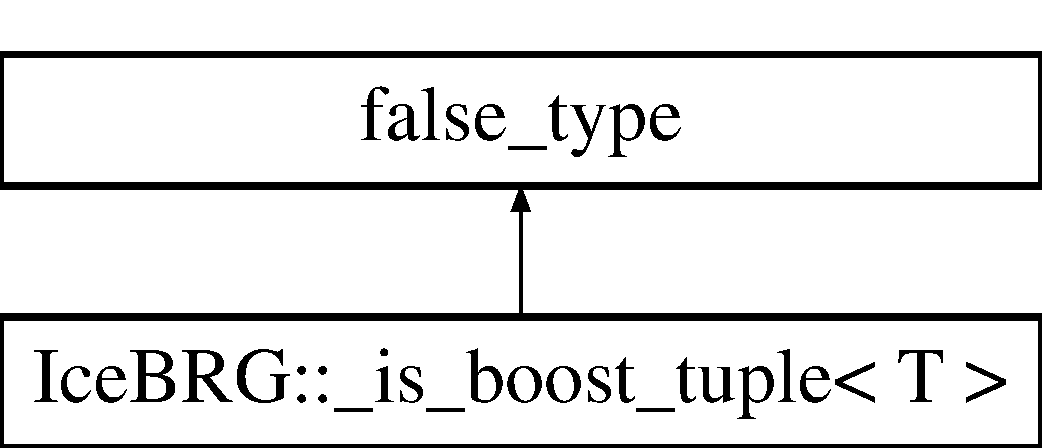
\includegraphics[height=2.000000cm]{structIceBRG_1_1__is__boost__tuple}
\end{center}
\end{figure}


The documentation for this struct was generated from the following file\+:\begin{DoxyCompactItemize}
\item 
/disk2/brg/git/\+Magnification\+\_\+\+Public/src/lib/\+Ice\+B\+R\+G\+\_\+main/container/\hyperlink{is__boost__tuple_8hpp}{is\+\_\+boost\+\_\+tuple.\+hpp}\end{DoxyCompactItemize}

\hypertarget{structIceBRG_1_1__is__boost__tuple_3_01boost_1_1tuple_3_01T0_00_01T1_00_01T2_00_01T3_00_01T4_00_aeaacd25f11a77396b5b6e53a5953fba}{}\section{Ice\+B\+R\+G\+:\+:\+\_\+is\+\_\+boost\+\_\+tuple$<$ boost\+:\+:tuple$<$ T0, T1, T2, T3, T4, T5, T6, T7, T8, T9 $>$ $>$ Struct Template Reference}
\label{structIceBRG_1_1__is__boost__tuple_3_01boost_1_1tuple_3_01T0_00_01T1_00_01T2_00_01T3_00_01T4_00_aeaacd25f11a77396b5b6e53a5953fba}\index{Ice\+B\+R\+G\+::\+\_\+is\+\_\+boost\+\_\+tuple$<$ boost\+::tuple$<$ T0, T1, T2, T3, T4, T5, T6, T7, T8, T9 $>$ $>$@{Ice\+B\+R\+G\+::\+\_\+is\+\_\+boost\+\_\+tuple$<$ boost\+::tuple$<$ T0, T1, T2, T3, T4, T5, T6, T7, T8, T9 $>$ $>$}}


{\ttfamily \#include $<$is\+\_\+boost\+\_\+tuple.\+hpp$>$}

Inheritance diagram for Ice\+B\+R\+G\+:\+:\+\_\+is\+\_\+boost\+\_\+tuple$<$ boost\+:\+:tuple$<$ T0, T1, T2, T3, T4, T5, T6, T7, T8, T9 $>$ $>$\+:\begin{figure}[H]
\begin{center}
\leavevmode
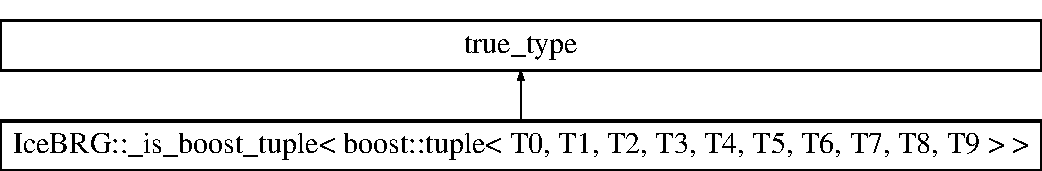
\includegraphics[height=2.000000cm]{structIceBRG_1_1__is__boost__tuple_3_01boost_1_1tuple_3_01T0_00_01T1_00_01T2_00_01T3_00_01T4_00_aeaacd25f11a77396b5b6e53a5953fba}
\end{center}
\end{figure}


The documentation for this struct was generated from the following file\+:\begin{DoxyCompactItemize}
\item 
/disk2/brg/git/\+Magnification\+\_\+\+Public/src/lib/\+Ice\+B\+R\+G\+\_\+main/container/\hyperlink{is__boost__tuple_8hpp}{is\+\_\+boost\+\_\+tuple.\+hpp}\end{DoxyCompactItemize}

\hypertarget{structIceBRG_1_1__is__boost__tuple_3_01boost_1_1tuples_1_1cons_3_01TH_00_01TT_01_4_01_4}{}\section{Ice\+B\+R\+G\+:\+:\+\_\+is\+\_\+boost\+\_\+tuple$<$ boost\+:\+:tuples\+:\+:cons$<$ T\+H, T\+T $>$ $>$ Struct Template Reference}
\label{structIceBRG_1_1__is__boost__tuple_3_01boost_1_1tuples_1_1cons_3_01TH_00_01TT_01_4_01_4}\index{Ice\+B\+R\+G\+::\+\_\+is\+\_\+boost\+\_\+tuple$<$ boost\+::tuples\+::cons$<$ T\+H, T\+T $>$ $>$@{Ice\+B\+R\+G\+::\+\_\+is\+\_\+boost\+\_\+tuple$<$ boost\+::tuples\+::cons$<$ T\+H, T\+T $>$ $>$}}


{\ttfamily \#include $<$is\+\_\+boost\+\_\+tuple.\+hpp$>$}

Inheritance diagram for Ice\+B\+R\+G\+:\+:\+\_\+is\+\_\+boost\+\_\+tuple$<$ boost\+:\+:tuples\+:\+:cons$<$ T\+H, T\+T $>$ $>$\+:\begin{figure}[H]
\begin{center}
\leavevmode
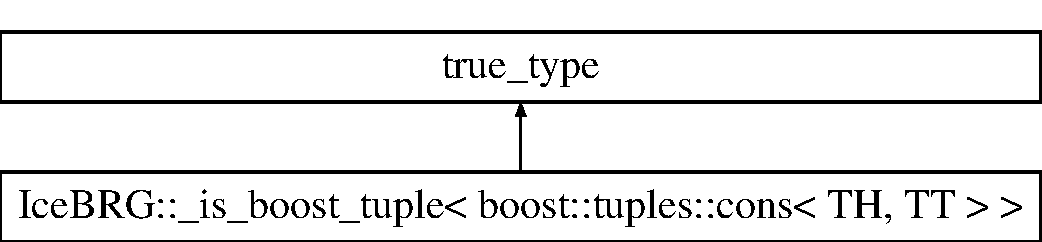
\includegraphics[height=2.000000cm]{structIceBRG_1_1__is__boost__tuple_3_01boost_1_1tuples_1_1cons_3_01TH_00_01TT_01_4_01_4}
\end{center}
\end{figure}


The documentation for this struct was generated from the following file\+:\begin{DoxyCompactItemize}
\item 
/disk2/brg/git/\+Magnification\+\_\+\+Public/src/lib/\+Ice\+B\+R\+G\+\_\+main/container/\hyperlink{is__boost__tuple_8hpp}{is\+\_\+boost\+\_\+tuple.\+hpp}\end{DoxyCompactItemize}

\hypertarget{structIceBRG_1_1__is__boost__tuple_3_01boost_1_1tuples_1_1null__type_01_4}{}\section{Ice\+B\+R\+G\+:\+:\+\_\+is\+\_\+boost\+\_\+tuple$<$ boost\+:\+:tuples\+:\+:null\+\_\+type $>$ Struct Template Reference}
\label{structIceBRG_1_1__is__boost__tuple_3_01boost_1_1tuples_1_1null__type_01_4}\index{Ice\+B\+R\+G\+::\+\_\+is\+\_\+boost\+\_\+tuple$<$ boost\+::tuples\+::null\+\_\+type $>$@{Ice\+B\+R\+G\+::\+\_\+is\+\_\+boost\+\_\+tuple$<$ boost\+::tuples\+::null\+\_\+type $>$}}


{\ttfamily \#include $<$is\+\_\+boost\+\_\+tuple.\+hpp$>$}

Inheritance diagram for Ice\+B\+R\+G\+:\+:\+\_\+is\+\_\+boost\+\_\+tuple$<$ boost\+:\+:tuples\+:\+:null\+\_\+type $>$\+:\begin{figure}[H]
\begin{center}
\leavevmode
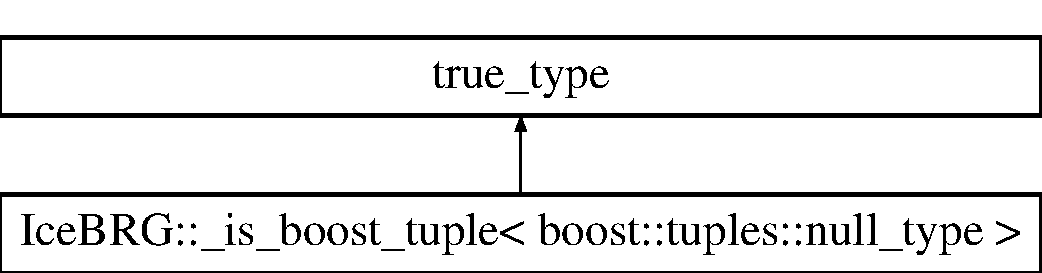
\includegraphics[height=2.000000cm]{structIceBRG_1_1__is__boost__tuple_3_01boost_1_1tuples_1_1null__type_01_4}
\end{center}
\end{figure}


The documentation for this struct was generated from the following file\+:\begin{DoxyCompactItemize}
\item 
/disk2/brg/git/\+Magnification\+\_\+\+Public/src/lib/\+Ice\+B\+R\+G\+\_\+main/container/\hyperlink{is__boost__tuple_8hpp}{is\+\_\+boost\+\_\+tuple.\+hpp}\end{DoxyCompactItemize}

\hypertarget{structIceBRG_1_1__is__null__type}{}\section{Ice\+B\+R\+G\+:\+:\+\_\+is\+\_\+null\+\_\+type$<$ T $>$ Struct Template Reference}
\label{structIceBRG_1_1__is__null__type}\index{Ice\+B\+R\+G\+::\+\_\+is\+\_\+null\+\_\+type$<$ T $>$@{Ice\+B\+R\+G\+::\+\_\+is\+\_\+null\+\_\+type$<$ T $>$}}


{\ttfamily \#include $<$is\+\_\+boost\+\_\+tuple.\+hpp$>$}

Inheritance diagram for Ice\+B\+R\+G\+:\+:\+\_\+is\+\_\+null\+\_\+type$<$ T $>$\+:\begin{figure}[H]
\begin{center}
\leavevmode
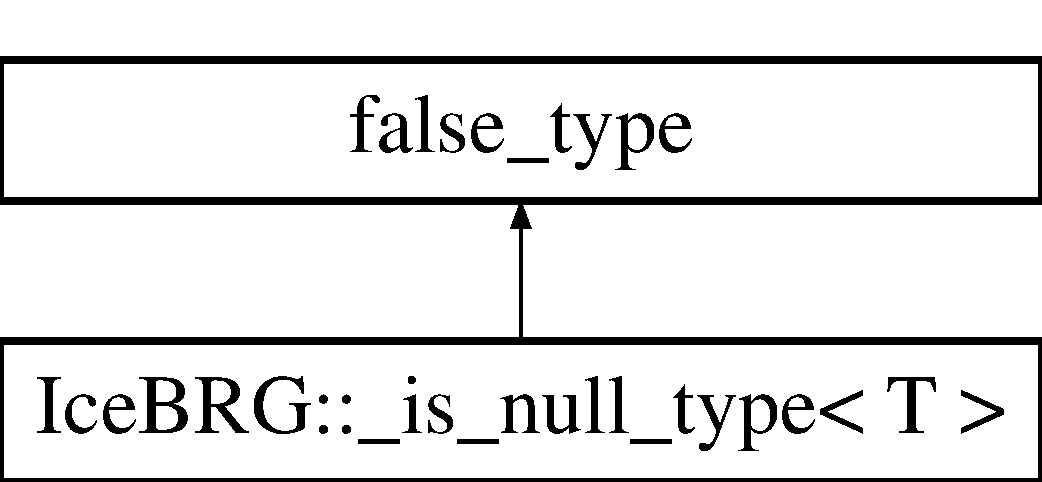
\includegraphics[height=2.000000cm]{structIceBRG_1_1__is__null__type}
\end{center}
\end{figure}


The documentation for this struct was generated from the following file\+:\begin{DoxyCompactItemize}
\item 
/disk2/brg/git/\+Magnification\+\_\+\+Public/src/lib/\+Ice\+B\+R\+G\+\_\+main/container/\hyperlink{is__boost__tuple_8hpp}{is\+\_\+boost\+\_\+tuple.\+hpp}\end{DoxyCompactItemize}

\hypertarget{structIceBRG_1_1__is__null__type_3_01boost_1_1tuples_1_1null__type_01_4}{}\section{Ice\+B\+R\+G\+:\+:\+\_\+is\+\_\+null\+\_\+type$<$ boost\+:\+:tuples\+:\+:null\+\_\+type $>$ Struct Template Reference}
\label{structIceBRG_1_1__is__null__type_3_01boost_1_1tuples_1_1null__type_01_4}\index{Ice\+B\+R\+G\+::\+\_\+is\+\_\+null\+\_\+type$<$ boost\+::tuples\+::null\+\_\+type $>$@{Ice\+B\+R\+G\+::\+\_\+is\+\_\+null\+\_\+type$<$ boost\+::tuples\+::null\+\_\+type $>$}}


{\ttfamily \#include $<$is\+\_\+boost\+\_\+tuple.\+hpp$>$}

Inheritance diagram for Ice\+B\+R\+G\+:\+:\+\_\+is\+\_\+null\+\_\+type$<$ boost\+:\+:tuples\+:\+:null\+\_\+type $>$\+:\begin{figure}[H]
\begin{center}
\leavevmode
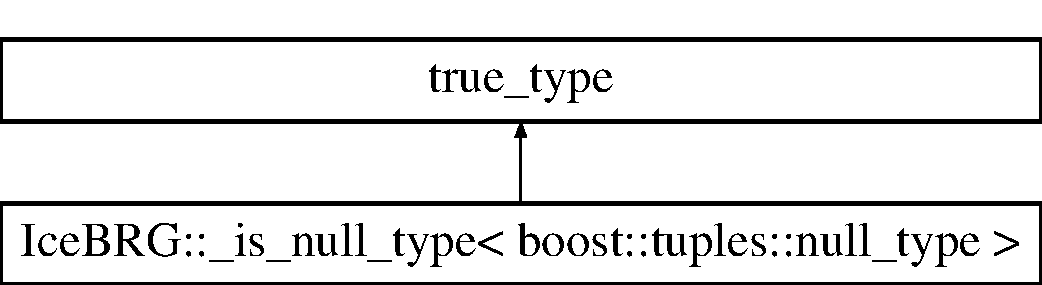
\includegraphics[height=2.000000cm]{structIceBRG_1_1__is__null__type_3_01boost_1_1tuples_1_1null__type_01_4}
\end{center}
\end{figure}


The documentation for this struct was generated from the following file\+:\begin{DoxyCompactItemize}
\item 
/disk2/brg/git/\+Magnification\+\_\+\+Public/src/lib/\+Ice\+B\+R\+G\+\_\+main/container/\hyperlink{is__boost__tuple_8hpp}{is\+\_\+boost\+\_\+tuple.\+hpp}\end{DoxyCompactItemize}

\hypertarget{classIceBRG_1_1accel__functor}{}\section{Ice\+B\+R\+G\+:\+:accel\+\_\+functor Class Reference}
\label{classIceBRG_1_1accel__functor}\index{Ice\+B\+R\+G\+::accel\+\_\+functor@{Ice\+B\+R\+G\+::accel\+\_\+functor}}


{\ttfamily \#include $<$density\+\_\+profile\+\_\+functors.\+h$>$}

\subsection*{Public Member Functions}
\begin{DoxyCompactItemize}
\item 
void \hyperlink{classIceBRG_1_1accel__functor_aa932fee0fb4feb33a1e8ec7ce830ef18}{set\+\_\+host\+\_\+ptr} (const \hyperlink{classIceBRG_1_1density__profile}{density\+\_\+profile} $\ast$new\+\_\+host\+\_\+ptr)
\item 
const \hyperlink{classIceBRG_1_1density__profile}{density\+\_\+profile} $\ast$ \hyperlink{classIceBRG_1_1accel__functor_a6c39598344f5e26c7c804a16e9bb1f71}{host\+\_\+ptr} ()
\item 
\hyperlink{namespaceIceBRG_ab10fe6d8fe6432a7dc0aa5a8ecac6a14}{acceleration\+\_\+type} \hyperlink{classIceBRG_1_1accel__functor_aa277cd8ec6adc04041b4f2b58720ea59}{operator()} (const \hyperlink{namespaceIceBRG_a45499647eb87e24c10ab32c628711cec}{distance\+\_\+type} \&in\+\_\+param) const 
\item 
\hyperlink{classIceBRG_1_1accel__functor_ae3a62fffa00404d4b25143e5139b4cdc}{accel\+\_\+functor} ()
\item 
\hyperlink{classIceBRG_1_1accel__functor_a73d7e481cf3d4373ac6bb1f04da90bbe}{accel\+\_\+functor} (const \hyperlink{classIceBRG_1_1density__profile}{density\+\_\+profile} $\ast$init\+\_\+host\+\_\+ptr)
\item 
virtual \hyperlink{classIceBRG_1_1accel__functor_ab9681db13d78a1b6187b85a0f47095e5}{$\sim$accel\+\_\+functor} ()
\end{DoxyCompactItemize}


\subsection{Constructor \& Destructor Documentation}
\hypertarget{classIceBRG_1_1accel__functor_ae3a62fffa00404d4b25143e5139b4cdc}{}\index{Ice\+B\+R\+G\+::accel\+\_\+functor@{Ice\+B\+R\+G\+::accel\+\_\+functor}!accel\+\_\+functor@{accel\+\_\+functor}}
\index{accel\+\_\+functor@{accel\+\_\+functor}!Ice\+B\+R\+G\+::accel\+\_\+functor@{Ice\+B\+R\+G\+::accel\+\_\+functor}}
\subsubsection[{accel\+\_\+functor()}]{\setlength{\rightskip}{0pt plus 5cm}Ice\+B\+R\+G\+::accel\+\_\+functor\+::accel\+\_\+functor (
\begin{DoxyParamCaption}
{}
\end{DoxyParamCaption}
)}\label{classIceBRG_1_1accel__functor_ae3a62fffa00404d4b25143e5139b4cdc}
\hypertarget{classIceBRG_1_1accel__functor_a73d7e481cf3d4373ac6bb1f04da90bbe}{}\index{Ice\+B\+R\+G\+::accel\+\_\+functor@{Ice\+B\+R\+G\+::accel\+\_\+functor}!accel\+\_\+functor@{accel\+\_\+functor}}
\index{accel\+\_\+functor@{accel\+\_\+functor}!Ice\+B\+R\+G\+::accel\+\_\+functor@{Ice\+B\+R\+G\+::accel\+\_\+functor}}
\subsubsection[{accel\+\_\+functor(const density\+\_\+profile $\ast$init\+\_\+host\+\_\+ptr)}]{\setlength{\rightskip}{0pt plus 5cm}Ice\+B\+R\+G\+::accel\+\_\+functor\+::accel\+\_\+functor (
\begin{DoxyParamCaption}
\item[{const {\bf density\+\_\+profile} $\ast$}]{init\+\_\+host\+\_\+ptr}
\end{DoxyParamCaption}
)}\label{classIceBRG_1_1accel__functor_a73d7e481cf3d4373ac6bb1f04da90bbe}
\hypertarget{classIceBRG_1_1accel__functor_ab9681db13d78a1b6187b85a0f47095e5}{}\index{Ice\+B\+R\+G\+::accel\+\_\+functor@{Ice\+B\+R\+G\+::accel\+\_\+functor}!````~accel\+\_\+functor@{$\sim$accel\+\_\+functor}}
\index{````~accel\+\_\+functor@{$\sim$accel\+\_\+functor}!Ice\+B\+R\+G\+::accel\+\_\+functor@{Ice\+B\+R\+G\+::accel\+\_\+functor}}
\subsubsection[{$\sim$accel\+\_\+functor()}]{\setlength{\rightskip}{0pt plus 5cm}virtual Ice\+B\+R\+G\+::accel\+\_\+functor\+::$\sim$accel\+\_\+functor (
\begin{DoxyParamCaption}
{}
\end{DoxyParamCaption}
)\hspace{0.3cm}{\ttfamily [inline]}, {\ttfamily [virtual]}}\label{classIceBRG_1_1accel__functor_ab9681db13d78a1b6187b85a0f47095e5}


\subsection{Member Function Documentation}
\hypertarget{classIceBRG_1_1accel__functor_a6c39598344f5e26c7c804a16e9bb1f71}{}\index{Ice\+B\+R\+G\+::accel\+\_\+functor@{Ice\+B\+R\+G\+::accel\+\_\+functor}!host\+\_\+ptr@{host\+\_\+ptr}}
\index{host\+\_\+ptr@{host\+\_\+ptr}!Ice\+B\+R\+G\+::accel\+\_\+functor@{Ice\+B\+R\+G\+::accel\+\_\+functor}}
\subsubsection[{host\+\_\+ptr()}]{\setlength{\rightskip}{0pt plus 5cm}const {\bf density\+\_\+profile}$\ast$ Ice\+B\+R\+G\+::accel\+\_\+functor\+::host\+\_\+ptr (
\begin{DoxyParamCaption}
{}
\end{DoxyParamCaption}
)\hspace{0.3cm}{\ttfamily [inline]}}\label{classIceBRG_1_1accel__functor_a6c39598344f5e26c7c804a16e9bb1f71}
\hypertarget{classIceBRG_1_1accel__functor_aa277cd8ec6adc04041b4f2b58720ea59}{}\index{Ice\+B\+R\+G\+::accel\+\_\+functor@{Ice\+B\+R\+G\+::accel\+\_\+functor}!operator()@{operator()}}
\index{operator()@{operator()}!Ice\+B\+R\+G\+::accel\+\_\+functor@{Ice\+B\+R\+G\+::accel\+\_\+functor}}
\subsubsection[{operator()(const distance\+\_\+type \&in\+\_\+param) const }]{\setlength{\rightskip}{0pt plus 5cm}{\bf Ice\+B\+R\+G\+::acceleration\+\_\+type} Ice\+B\+R\+G\+::accel\+\_\+functor\+::operator() (
\begin{DoxyParamCaption}
\item[{const {\bf distance\+\_\+type} \&}]{in\+\_\+param}
\end{DoxyParamCaption}
) const}\label{classIceBRG_1_1accel__functor_aa277cd8ec6adc04041b4f2b58720ea59}
\hypertarget{classIceBRG_1_1accel__functor_aa932fee0fb4feb33a1e8ec7ce830ef18}{}\index{Ice\+B\+R\+G\+::accel\+\_\+functor@{Ice\+B\+R\+G\+::accel\+\_\+functor}!set\+\_\+host\+\_\+ptr@{set\+\_\+host\+\_\+ptr}}
\index{set\+\_\+host\+\_\+ptr@{set\+\_\+host\+\_\+ptr}!Ice\+B\+R\+G\+::accel\+\_\+functor@{Ice\+B\+R\+G\+::accel\+\_\+functor}}
\subsubsection[{set\+\_\+host\+\_\+ptr(const density\+\_\+profile $\ast$new\+\_\+host\+\_\+ptr)}]{\setlength{\rightskip}{0pt plus 5cm}void Ice\+B\+R\+G\+::accel\+\_\+functor\+::set\+\_\+host\+\_\+ptr (
\begin{DoxyParamCaption}
\item[{const {\bf density\+\_\+profile} $\ast$}]{new\+\_\+host\+\_\+ptr}
\end{DoxyParamCaption}
)}\label{classIceBRG_1_1accel__functor_aa932fee0fb4feb33a1e8ec7ce830ef18}


The documentation for this class was generated from the following files\+:\begin{DoxyCompactItemize}
\item 
/disk2/brg/git/\+Magnification\+\_\+\+Public/src/lib/\+Ice\+B\+R\+G\+\_\+physics/density\+\_\+profile/\hyperlink{density__profile__functors_8h}{density\+\_\+profile\+\_\+functors.\+h}\item 
/disk2/brg/git/\+Magnification\+\_\+\+Public/src/lib/\+Ice\+B\+R\+G\+\_\+physics/density\+\_\+profile/\hyperlink{density__profile__functors_8cpp}{density\+\_\+profile\+\_\+functors.\+cpp}\end{DoxyCompactItemize}

\hypertarget{classIceBRG_1_1add__cache}{}\section{Ice\+B\+R\+G\+:\+:add\+\_\+cache Class Reference}
\label{classIceBRG_1_1add__cache}\index{Ice\+B\+R\+G\+::add\+\_\+cache@{Ice\+B\+R\+G\+::add\+\_\+cache}}


{\ttfamily \#include $<$astro\+\_\+caches.\+h$>$}

Inheritance diagram for Ice\+B\+R\+G\+:\+:add\+\_\+cache\+:\begin{figure}[H]
\begin{center}
\leavevmode
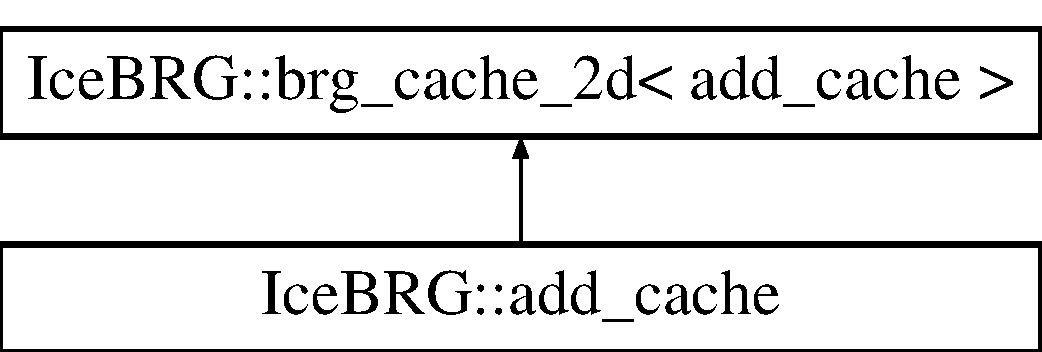
\includegraphics[height=2.000000cm]{classIceBRG_1_1add__cache}
\end{center}
\end{figure}
\subsection*{Public Member Functions}
\begin{DoxyCompactItemize}
\item 
\hyperlink{classIceBRG_1_1add__cache_af08acb2ae5fbc6e933e76fbb5eb075d1}{$\sim$add\+\_\+cache} ()
\end{DoxyCompactItemize}
\subsection*{Protected Member Functions}
\begin{DoxyCompactItemize}
\item 
std\+::string \hyperlink{classIceBRG_1_1add__cache_a26ea452f7970b9a3e38c2f544dfca78e}{\+\_\+name\+\_\+base} () const 
\item 
\hyperlink{lib_2IceBRG__main_2common_8h_ad0f130a56eeb944d9ef2692ee881ecc4}{flt\+\_\+type} \hyperlink{classIceBRG_1_1add__cache_a9b231de4bf15e84a597e2d379daaadda}{\+\_\+calculate} (const \hyperlink{lib_2IceBRG__main_2common_8h_ad0f130a56eeb944d9ef2692ee881ecc4}{flt\+\_\+type} \&in\+\_\+param\+\_\+1, const \hyperlink{lib_2IceBRG__main_2common_8h_ad0f130a56eeb944d9ef2692ee881ecc4}{flt\+\_\+type} \&in\+\_\+param\+\_\+2) const 
\end{DoxyCompactItemize}
\subsection*{Friends}
\begin{DoxyCompactItemize}
\item 
class \hyperlink{classIceBRG_1_1add__cache_a5488840165a3177405ea84ef773fc1f5}{brg\+\_\+cache\+\_\+2d$<$ add\+\_\+cache $>$}
\end{DoxyCompactItemize}


\subsection{Constructor \& Destructor Documentation}
\hypertarget{classIceBRG_1_1add__cache_af08acb2ae5fbc6e933e76fbb5eb075d1}{}\index{Ice\+B\+R\+G\+::add\+\_\+cache@{Ice\+B\+R\+G\+::add\+\_\+cache}!````~add\+\_\+cache@{$\sim$add\+\_\+cache}}
\index{````~add\+\_\+cache@{$\sim$add\+\_\+cache}!Ice\+B\+R\+G\+::add\+\_\+cache@{Ice\+B\+R\+G\+::add\+\_\+cache}}
\subsubsection[{$\sim$add\+\_\+cache()}]{\setlength{\rightskip}{0pt plus 5cm}Ice\+B\+R\+G\+::add\+\_\+cache\+::$\sim$add\+\_\+cache (
\begin{DoxyParamCaption}
{}
\end{DoxyParamCaption}
)\hspace{0.3cm}{\ttfamily [inline]}}\label{classIceBRG_1_1add__cache_af08acb2ae5fbc6e933e76fbb5eb075d1}


\subsection{Member Function Documentation}
\hypertarget{classIceBRG_1_1add__cache_a9b231de4bf15e84a597e2d379daaadda}{}\index{Ice\+B\+R\+G\+::add\+\_\+cache@{Ice\+B\+R\+G\+::add\+\_\+cache}!\+\_\+calculate@{\+\_\+calculate}}
\index{\+\_\+calculate@{\+\_\+calculate}!Ice\+B\+R\+G\+::add\+\_\+cache@{Ice\+B\+R\+G\+::add\+\_\+cache}}
\subsubsection[{\+\_\+calculate(const flt\+\_\+type \&in\+\_\+param\+\_\+1, const flt\+\_\+type \&in\+\_\+param\+\_\+2) const }]{\setlength{\rightskip}{0pt plus 5cm}{\bf flt\+\_\+type} Ice\+B\+R\+G\+::add\+\_\+cache\+::\+\_\+calculate (
\begin{DoxyParamCaption}
\item[{const {\bf flt\+\_\+type} \&}]{in\+\_\+param\+\_\+1, }
\item[{const {\bf flt\+\_\+type} \&}]{in\+\_\+param\+\_\+2}
\end{DoxyParamCaption}
) const\hspace{0.3cm}{\ttfamily [protected]}}\label{classIceBRG_1_1add__cache_a9b231de4bf15e84a597e2d379daaadda}
\hypertarget{classIceBRG_1_1add__cache_a26ea452f7970b9a3e38c2f544dfca78e}{}\index{Ice\+B\+R\+G\+::add\+\_\+cache@{Ice\+B\+R\+G\+::add\+\_\+cache}!\+\_\+name\+\_\+base@{\+\_\+name\+\_\+base}}
\index{\+\_\+name\+\_\+base@{\+\_\+name\+\_\+base}!Ice\+B\+R\+G\+::add\+\_\+cache@{Ice\+B\+R\+G\+::add\+\_\+cache}}
\subsubsection[{\+\_\+name\+\_\+base() const }]{\setlength{\rightskip}{0pt plus 5cm}std\+::string Ice\+B\+R\+G\+::add\+\_\+cache\+::\+\_\+name\+\_\+base (
\begin{DoxyParamCaption}
{}
\end{DoxyParamCaption}
) const\hspace{0.3cm}{\ttfamily [inline]}, {\ttfamily [protected]}}\label{classIceBRG_1_1add__cache_a26ea452f7970b9a3e38c2f544dfca78e}


\subsection{Friends And Related Function Documentation}
\hypertarget{classIceBRG_1_1add__cache_a5488840165a3177405ea84ef773fc1f5}{}\index{Ice\+B\+R\+G\+::add\+\_\+cache@{Ice\+B\+R\+G\+::add\+\_\+cache}!brg\+\_\+cache\+\_\+2d$<$ add\+\_\+cache $>$@{brg\+\_\+cache\+\_\+2d$<$ add\+\_\+cache $>$}}
\index{brg\+\_\+cache\+\_\+2d$<$ add\+\_\+cache $>$@{brg\+\_\+cache\+\_\+2d$<$ add\+\_\+cache $>$}!Ice\+B\+R\+G\+::add\+\_\+cache@{Ice\+B\+R\+G\+::add\+\_\+cache}}
\subsubsection[{brg\+\_\+cache\+\_\+2d$<$ add\+\_\+cache $>$}]{\setlength{\rightskip}{0pt plus 5cm}friend class {\bf brg\+\_\+cache\+\_\+2d}$<$ {\bf add\+\_\+cache} $>$\hspace{0.3cm}{\ttfamily [friend]}}\label{classIceBRG_1_1add__cache_a5488840165a3177405ea84ef773fc1f5}


The documentation for this class was generated from the following files\+:\begin{DoxyCompactItemize}
\item 
/disk2/brg/git/\+Magnification\+\_\+\+Public/src/lib/\+Ice\+B\+R\+G\+\_\+physics/\hyperlink{astro__caches_8h}{astro\+\_\+caches.\+h}\item 
/disk2/brg/git/\+Magnification\+\_\+\+Public/src/lib/\+Ice\+B\+R\+G\+\_\+physics/\hyperlink{astro__caches_8cpp}{astro\+\_\+caches.\+cpp}\end{DoxyCompactItemize}

\hypertarget{structIceBRG_1_1assignment__coercer}{}\section{Ice\+B\+R\+G\+:\+:assignment\+\_\+coercer$<$ d, container $>$ Struct Template Reference}
\label{structIceBRG_1_1assignment__coercer}\index{Ice\+B\+R\+G\+::assignment\+\_\+coercer$<$ d, container $>$@{Ice\+B\+R\+G\+::assignment\+\_\+coercer$<$ d, container $>$}}


{\ttfamily \#include $<$coerce.\+hpp$>$}

\subsection*{Public Member Functions}
\begin{DoxyCompactItemize}
\item 
\hyperlink{structIceBRG_1_1assignment__coercer_a3513d23ca76c9e50b091e0c5e91aa44a}{assignment\+\_\+coercer} ()=delete
\item 
\hyperlink{structIceBRG_1_1assignment__coercer_ad558e38330226f19a1e0e93c0e59e049}{assignment\+\_\+coercer} (const \hyperlink{structIceBRG_1_1assignment__coercer}{assignment\+\_\+coercer} \&)=delete
\item 
\hyperlink{structIceBRG_1_1assignment__coercer_a031c075b714c8f4b2e694d714a523564}{assignment\+\_\+coercer} (\hyperlink{structIceBRG_1_1assignment__coercer}{assignment\+\_\+coercer} \&\&)=delete
\item 
\hyperlink{structIceBRG_1_1assignment__coercer}{assignment\+\_\+coercer} \& \hyperlink{structIceBRG_1_1assignment__coercer_a175bbe2cb99ae3fe9e4f6ce8b4f21af7}{operator=} (const \hyperlink{structIceBRG_1_1assignment__coercer}{assignment\+\_\+coercer} \&)=delete
\item 
\hyperlink{structIceBRG_1_1assignment__coercer}{assignment\+\_\+coercer} \& \hyperlink{structIceBRG_1_1assignment__coercer_ab3f4fe861313dfc9aeb212f4a0c59ad2}{operator=} (\hyperlink{structIceBRG_1_1assignment__coercer}{assignment\+\_\+coercer} \&\&)=delete
\item 
{\footnotesize template$<$typename oc , typename std\+::enable\+\_\+if$<$(\+Ice\+B\+R\+G\+::is\+\_\+stl\+\_\+container$<$ oc $>$\+::value \&\&\+Ice\+B\+R\+G\+::is\+\_\+stl\+\_\+container$<$ container $>$\+::value), oc $>$\+::type $\ast$  = nullptr$>$ }\\\hyperlink{structIceBRG_1_1assignment__coercer_a60696e227f70dd34928f9af6cc8b56f5}{assignment\+\_\+coercer} (container \&obj, const oc \&other\+\_\+obj)
\item 
{\footnotesize template$<$typename oc , typename std\+::enable\+\_\+if$<$!(\+Ice\+B\+R\+G\+::is\+\_\+stl\+\_\+container$<$ oc $>$\+::value \&\&\+Ice\+B\+R\+G\+::is\+\_\+stl\+\_\+container$<$ container $>$\+::value), oc $>$\+::type $\ast$  = nullptr$>$ }\\\hyperlink{structIceBRG_1_1assignment__coercer_a60696e227f70dd34928f9af6cc8b56f5}{assignment\+\_\+coercer} (container \&obj, const oc \&other\+\_\+obj)
\end{DoxyCompactItemize}


\subsection{Detailed Description}
\subsubsection*{template$<$int\+\_\+type d, typename container$>$struct Ice\+B\+R\+G\+::assignment\+\_\+coercer$<$ d, container $>$}

\hyperlink{structIceBRG_1_1assignment__coercer}{assignment\+\_\+coercer} -\/ a structure which performs coercion of one type to another as a side-\/effect of its constructor. 

\subsection{Constructor \& Destructor Documentation}
\hypertarget{structIceBRG_1_1assignment__coercer_a3513d23ca76c9e50b091e0c5e91aa44a}{}\index{Ice\+B\+R\+G\+::assignment\+\_\+coercer@{Ice\+B\+R\+G\+::assignment\+\_\+coercer}!assignment\+\_\+coercer@{assignment\+\_\+coercer}}
\index{assignment\+\_\+coercer@{assignment\+\_\+coercer}!Ice\+B\+R\+G\+::assignment\+\_\+coercer@{Ice\+B\+R\+G\+::assignment\+\_\+coercer}}
\subsubsection[{assignment\+\_\+coercer()=delete}]{\setlength{\rightskip}{0pt plus 5cm}template$<$int\+\_\+type d, typename container$>$ {\bf Ice\+B\+R\+G\+::assignment\+\_\+coercer}$<$ d, container $>$\+::{\bf assignment\+\_\+coercer} (
\begin{DoxyParamCaption}
{}
\end{DoxyParamCaption}
)\hspace{0.3cm}{\ttfamily [delete]}}\label{structIceBRG_1_1assignment__coercer_a3513d23ca76c9e50b091e0c5e91aa44a}
\hypertarget{structIceBRG_1_1assignment__coercer_ad558e38330226f19a1e0e93c0e59e049}{}\index{Ice\+B\+R\+G\+::assignment\+\_\+coercer@{Ice\+B\+R\+G\+::assignment\+\_\+coercer}!assignment\+\_\+coercer@{assignment\+\_\+coercer}}
\index{assignment\+\_\+coercer@{assignment\+\_\+coercer}!Ice\+B\+R\+G\+::assignment\+\_\+coercer@{Ice\+B\+R\+G\+::assignment\+\_\+coercer}}
\subsubsection[{assignment\+\_\+coercer(const assignment\+\_\+coercer \&)=delete}]{\setlength{\rightskip}{0pt plus 5cm}template$<$int\+\_\+type d, typename container$>$ {\bf Ice\+B\+R\+G\+::assignment\+\_\+coercer}$<$ d, container $>$\+::{\bf assignment\+\_\+coercer} (
\begin{DoxyParamCaption}
\item[{const {\bf assignment\+\_\+coercer}$<$ d, container $>$ \&}]{}
\end{DoxyParamCaption}
)\hspace{0.3cm}{\ttfamily [delete]}}\label{structIceBRG_1_1assignment__coercer_ad558e38330226f19a1e0e93c0e59e049}
\hypertarget{structIceBRG_1_1assignment__coercer_a031c075b714c8f4b2e694d714a523564}{}\index{Ice\+B\+R\+G\+::assignment\+\_\+coercer@{Ice\+B\+R\+G\+::assignment\+\_\+coercer}!assignment\+\_\+coercer@{assignment\+\_\+coercer}}
\index{assignment\+\_\+coercer@{assignment\+\_\+coercer}!Ice\+B\+R\+G\+::assignment\+\_\+coercer@{Ice\+B\+R\+G\+::assignment\+\_\+coercer}}
\subsubsection[{assignment\+\_\+coercer(assignment\+\_\+coercer \&\&)=delete}]{\setlength{\rightskip}{0pt plus 5cm}template$<$int\+\_\+type d, typename container$>$ {\bf Ice\+B\+R\+G\+::assignment\+\_\+coercer}$<$ d, container $>$\+::{\bf assignment\+\_\+coercer} (
\begin{DoxyParamCaption}
\item[{{\bf assignment\+\_\+coercer}$<$ d, container $>$ \&\&}]{}
\end{DoxyParamCaption}
)\hspace{0.3cm}{\ttfamily [delete]}}\label{structIceBRG_1_1assignment__coercer_a031c075b714c8f4b2e694d714a523564}
\hypertarget{structIceBRG_1_1assignment__coercer_a60696e227f70dd34928f9af6cc8b56f5}{}\index{Ice\+B\+R\+G\+::assignment\+\_\+coercer@{Ice\+B\+R\+G\+::assignment\+\_\+coercer}!assignment\+\_\+coercer@{assignment\+\_\+coercer}}
\index{assignment\+\_\+coercer@{assignment\+\_\+coercer}!Ice\+B\+R\+G\+::assignment\+\_\+coercer@{Ice\+B\+R\+G\+::assignment\+\_\+coercer}}
\subsubsection[{assignment\+\_\+coercer(container \&obj, const oc \&other\+\_\+obj)}]{\setlength{\rightskip}{0pt plus 5cm}template$<$int\+\_\+type d, typename container$>$ template$<$typename oc , typename std\+::enable\+\_\+if$<$(\+Ice\+B\+R\+G\+::is\+\_\+stl\+\_\+container$<$ oc $>$\+::value \&\&\+Ice\+B\+R\+G\+::is\+\_\+stl\+\_\+container$<$ container $>$\+::value), oc $>$\+::type $\ast$  = nullptr$>$ {\bf Ice\+B\+R\+G\+::assignment\+\_\+coercer}$<$ d, container $>$\+::{\bf assignment\+\_\+coercer} (
\begin{DoxyParamCaption}
\item[{container \&}]{obj, }
\item[{const oc \&}]{other\+\_\+obj}
\end{DoxyParamCaption}
)\hspace{0.3cm}{\ttfamily [inline]}}\label{structIceBRG_1_1assignment__coercer_a60696e227f70dd34928f9af6cc8b56f5}
\hypertarget{structIceBRG_1_1assignment__coercer_a60696e227f70dd34928f9af6cc8b56f5}{}\index{Ice\+B\+R\+G\+::assignment\+\_\+coercer@{Ice\+B\+R\+G\+::assignment\+\_\+coercer}!assignment\+\_\+coercer@{assignment\+\_\+coercer}}
\index{assignment\+\_\+coercer@{assignment\+\_\+coercer}!Ice\+B\+R\+G\+::assignment\+\_\+coercer@{Ice\+B\+R\+G\+::assignment\+\_\+coercer}}
\subsubsection[{assignment\+\_\+coercer(container \&obj, const oc \&other\+\_\+obj)}]{\setlength{\rightskip}{0pt plus 5cm}template$<$int\+\_\+type d, typename container$>$ template$<$typename oc , typename std\+::enable\+\_\+if$<$!(\+Ice\+B\+R\+G\+::is\+\_\+stl\+\_\+container$<$ oc $>$\+::value \&\&\+Ice\+B\+R\+G\+::is\+\_\+stl\+\_\+container$<$ container $>$\+::value), oc $>$\+::type $\ast$  = nullptr$>$ {\bf Ice\+B\+R\+G\+::assignment\+\_\+coercer}$<$ d, container $>$\+::{\bf assignment\+\_\+coercer} (
\begin{DoxyParamCaption}
\item[{container \&}]{obj, }
\item[{const oc \&}]{other\+\_\+obj}
\end{DoxyParamCaption}
)\hspace{0.3cm}{\ttfamily [inline]}}\label{structIceBRG_1_1assignment__coercer_a60696e227f70dd34928f9af6cc8b56f5}


\subsection{Member Function Documentation}
\hypertarget{structIceBRG_1_1assignment__coercer_a175bbe2cb99ae3fe9e4f6ce8b4f21af7}{}\index{Ice\+B\+R\+G\+::assignment\+\_\+coercer@{Ice\+B\+R\+G\+::assignment\+\_\+coercer}!operator=@{operator=}}
\index{operator=@{operator=}!Ice\+B\+R\+G\+::assignment\+\_\+coercer@{Ice\+B\+R\+G\+::assignment\+\_\+coercer}}
\subsubsection[{operator=(const assignment\+\_\+coercer \&)=delete}]{\setlength{\rightskip}{0pt plus 5cm}template$<$int\+\_\+type d, typename container$>$ {\bf assignment\+\_\+coercer}\& {\bf Ice\+B\+R\+G\+::assignment\+\_\+coercer}$<$ d, container $>$\+::operator= (
\begin{DoxyParamCaption}
\item[{const {\bf assignment\+\_\+coercer}$<$ d, container $>$ \&}]{}
\end{DoxyParamCaption}
)\hspace{0.3cm}{\ttfamily [delete]}}\label{structIceBRG_1_1assignment__coercer_a175bbe2cb99ae3fe9e4f6ce8b4f21af7}
\hypertarget{structIceBRG_1_1assignment__coercer_ab3f4fe861313dfc9aeb212f4a0c59ad2}{}\index{Ice\+B\+R\+G\+::assignment\+\_\+coercer@{Ice\+B\+R\+G\+::assignment\+\_\+coercer}!operator=@{operator=}}
\index{operator=@{operator=}!Ice\+B\+R\+G\+::assignment\+\_\+coercer@{Ice\+B\+R\+G\+::assignment\+\_\+coercer}}
\subsubsection[{operator=(assignment\+\_\+coercer \&\&)=delete}]{\setlength{\rightskip}{0pt plus 5cm}template$<$int\+\_\+type d, typename container$>$ {\bf assignment\+\_\+coercer}\& {\bf Ice\+B\+R\+G\+::assignment\+\_\+coercer}$<$ d, container $>$\+::operator= (
\begin{DoxyParamCaption}
\item[{{\bf assignment\+\_\+coercer}$<$ d, container $>$ \&\&}]{}
\end{DoxyParamCaption}
)\hspace{0.3cm}{\ttfamily [delete]}}\label{structIceBRG_1_1assignment__coercer_ab3f4fe861313dfc9aeb212f4a0c59ad2}


The documentation for this struct was generated from the following file\+:\begin{DoxyCompactItemize}
\item 
/disk2/brg/git/\+Magnification\+\_\+\+Public/src/lib/\+Ice\+B\+R\+G\+\_\+main/container/\hyperlink{coerce_8hpp}{coerce.\+hpp}\end{DoxyCompactItemize}

\hypertarget{structIceBRG_1_1assignment__coercer_3_010_00_01container_01_4}{}\section{Ice\+B\+R\+G\+:\+:assignment\+\_\+coercer$<$ 0, container $>$ Struct Template Reference}
\label{structIceBRG_1_1assignment__coercer_3_010_00_01container_01_4}\index{Ice\+B\+R\+G\+::assignment\+\_\+coercer$<$ 0, container $>$@{Ice\+B\+R\+G\+::assignment\+\_\+coercer$<$ 0, container $>$}}


{\ttfamily \#include $<$coerce.\+hpp$>$}

\subsection*{Public Member Functions}
\begin{DoxyCompactItemize}
\item 
\hyperlink{structIceBRG_1_1assignment__coercer_3_010_00_01container_01_4_a0f622fef256976a0cd4d6726f7fcd0b3}{assignment\+\_\+coercer} ()=delete
\item 
\hyperlink{structIceBRG_1_1assignment__coercer_3_010_00_01container_01_4_a275c83e135f0b5deb04e4f95652865b6}{assignment\+\_\+coercer} (const \hyperlink{structIceBRG_1_1assignment__coercer}{assignment\+\_\+coercer} \&)=delete
\item 
\hyperlink{structIceBRG_1_1assignment__coercer_3_010_00_01container_01_4_ab866af07befe8f3ddd8b07c55d549ae5}{assignment\+\_\+coercer} (\hyperlink{structIceBRG_1_1assignment__coercer}{assignment\+\_\+coercer} \&\&)=delete
\item 
\hyperlink{structIceBRG_1_1assignment__coercer}{assignment\+\_\+coercer} \& \hyperlink{structIceBRG_1_1assignment__coercer_3_010_00_01container_01_4_a7929ca93d78b599cf32b9416b0241348}{operator=} (const \hyperlink{structIceBRG_1_1assignment__coercer}{assignment\+\_\+coercer} \&)=delete
\item 
\hyperlink{structIceBRG_1_1assignment__coercer}{assignment\+\_\+coercer} \& \hyperlink{structIceBRG_1_1assignment__coercer_3_010_00_01container_01_4_a4f4dd698ea56ad9b0215b306d73acdb2}{operator=} (\hyperlink{structIceBRG_1_1assignment__coercer}{assignment\+\_\+coercer} \&\&)=delete
\item 
{\footnotesize template$<$typename oc $>$ }\\\hyperlink{structIceBRG_1_1assignment__coercer_3_010_00_01container_01_4_a923bafa9af6f885bd297962fff6c9ed4}{assignment\+\_\+coercer} (container \&obj, const oc \&other\+\_\+obj)
\end{DoxyCompactItemize}


\subsection{Detailed Description}
\subsubsection*{template$<$typename container$>$struct Ice\+B\+R\+G\+::assignment\+\_\+coercer$<$ 0, container $>$}

d=0 partial specialization of \hyperlink{structIceBRG_1_1assignment__coercer}{assignment\+\_\+coercer}. Uses simple assignment to coerce. 

\subsection{Constructor \& Destructor Documentation}
\hypertarget{structIceBRG_1_1assignment__coercer_3_010_00_01container_01_4_a0f622fef256976a0cd4d6726f7fcd0b3}{}\index{Ice\+B\+R\+G\+::assignment\+\_\+coercer$<$ 0, container $>$@{Ice\+B\+R\+G\+::assignment\+\_\+coercer$<$ 0, container $>$}!assignment\+\_\+coercer@{assignment\+\_\+coercer}}
\index{assignment\+\_\+coercer@{assignment\+\_\+coercer}!Ice\+B\+R\+G\+::assignment\+\_\+coercer$<$ 0, container $>$@{Ice\+B\+R\+G\+::assignment\+\_\+coercer$<$ 0, container $>$}}
\subsubsection[{assignment\+\_\+coercer()=delete}]{\setlength{\rightskip}{0pt plus 5cm}template$<$typename container $>$ {\bf Ice\+B\+R\+G\+::assignment\+\_\+coercer}$<$ 0, container $>$\+::{\bf assignment\+\_\+coercer} (
\begin{DoxyParamCaption}
{}
\end{DoxyParamCaption}
)\hspace{0.3cm}{\ttfamily [delete]}}\label{structIceBRG_1_1assignment__coercer_3_010_00_01container_01_4_a0f622fef256976a0cd4d6726f7fcd0b3}
\hypertarget{structIceBRG_1_1assignment__coercer_3_010_00_01container_01_4_a275c83e135f0b5deb04e4f95652865b6}{}\index{Ice\+B\+R\+G\+::assignment\+\_\+coercer$<$ 0, container $>$@{Ice\+B\+R\+G\+::assignment\+\_\+coercer$<$ 0, container $>$}!assignment\+\_\+coercer@{assignment\+\_\+coercer}}
\index{assignment\+\_\+coercer@{assignment\+\_\+coercer}!Ice\+B\+R\+G\+::assignment\+\_\+coercer$<$ 0, container $>$@{Ice\+B\+R\+G\+::assignment\+\_\+coercer$<$ 0, container $>$}}
\subsubsection[{assignment\+\_\+coercer(const assignment\+\_\+coercer \&)=delete}]{\setlength{\rightskip}{0pt plus 5cm}template$<$typename container $>$ {\bf Ice\+B\+R\+G\+::assignment\+\_\+coercer}$<$ 0, container $>$\+::{\bf assignment\+\_\+coercer} (
\begin{DoxyParamCaption}
\item[{const {\bf assignment\+\_\+coercer}$<$ 0, container $>$ \&}]{}
\end{DoxyParamCaption}
)\hspace{0.3cm}{\ttfamily [delete]}}\label{structIceBRG_1_1assignment__coercer_3_010_00_01container_01_4_a275c83e135f0b5deb04e4f95652865b6}
\hypertarget{structIceBRG_1_1assignment__coercer_3_010_00_01container_01_4_ab866af07befe8f3ddd8b07c55d549ae5}{}\index{Ice\+B\+R\+G\+::assignment\+\_\+coercer$<$ 0, container $>$@{Ice\+B\+R\+G\+::assignment\+\_\+coercer$<$ 0, container $>$}!assignment\+\_\+coercer@{assignment\+\_\+coercer}}
\index{assignment\+\_\+coercer@{assignment\+\_\+coercer}!Ice\+B\+R\+G\+::assignment\+\_\+coercer$<$ 0, container $>$@{Ice\+B\+R\+G\+::assignment\+\_\+coercer$<$ 0, container $>$}}
\subsubsection[{assignment\+\_\+coercer(assignment\+\_\+coercer \&\&)=delete}]{\setlength{\rightskip}{0pt plus 5cm}template$<$typename container $>$ {\bf Ice\+B\+R\+G\+::assignment\+\_\+coercer}$<$ 0, container $>$\+::{\bf assignment\+\_\+coercer} (
\begin{DoxyParamCaption}
\item[{{\bf assignment\+\_\+coercer}$<$ 0, container $>$ \&\&}]{}
\end{DoxyParamCaption}
)\hspace{0.3cm}{\ttfamily [delete]}}\label{structIceBRG_1_1assignment__coercer_3_010_00_01container_01_4_ab866af07befe8f3ddd8b07c55d549ae5}
\hypertarget{structIceBRG_1_1assignment__coercer_3_010_00_01container_01_4_a923bafa9af6f885bd297962fff6c9ed4}{}\index{Ice\+B\+R\+G\+::assignment\+\_\+coercer$<$ 0, container $>$@{Ice\+B\+R\+G\+::assignment\+\_\+coercer$<$ 0, container $>$}!assignment\+\_\+coercer@{assignment\+\_\+coercer}}
\index{assignment\+\_\+coercer@{assignment\+\_\+coercer}!Ice\+B\+R\+G\+::assignment\+\_\+coercer$<$ 0, container $>$@{Ice\+B\+R\+G\+::assignment\+\_\+coercer$<$ 0, container $>$}}
\subsubsection[{assignment\+\_\+coercer(container \&obj, const oc \&other\+\_\+obj)}]{\setlength{\rightskip}{0pt plus 5cm}template$<$typename container $>$ template$<$typename oc $>$ {\bf Ice\+B\+R\+G\+::assignment\+\_\+coercer}$<$ 0, container $>$\+::{\bf assignment\+\_\+coercer} (
\begin{DoxyParamCaption}
\item[{container \&}]{obj, }
\item[{const oc \&}]{other\+\_\+obj}
\end{DoxyParamCaption}
)\hspace{0.3cm}{\ttfamily [inline]}}\label{structIceBRG_1_1assignment__coercer_3_010_00_01container_01_4_a923bafa9af6f885bd297962fff6c9ed4}


\subsection{Member Function Documentation}
\hypertarget{structIceBRG_1_1assignment__coercer_3_010_00_01container_01_4_a7929ca93d78b599cf32b9416b0241348}{}\index{Ice\+B\+R\+G\+::assignment\+\_\+coercer$<$ 0, container $>$@{Ice\+B\+R\+G\+::assignment\+\_\+coercer$<$ 0, container $>$}!operator=@{operator=}}
\index{operator=@{operator=}!Ice\+B\+R\+G\+::assignment\+\_\+coercer$<$ 0, container $>$@{Ice\+B\+R\+G\+::assignment\+\_\+coercer$<$ 0, container $>$}}
\subsubsection[{operator=(const assignment\+\_\+coercer \&)=delete}]{\setlength{\rightskip}{0pt plus 5cm}template$<$typename container $>$ {\bf assignment\+\_\+coercer}\& {\bf Ice\+B\+R\+G\+::assignment\+\_\+coercer}$<$ 0, container $>$\+::operator= (
\begin{DoxyParamCaption}
\item[{const {\bf assignment\+\_\+coercer}$<$ 0, container $>$ \&}]{}
\end{DoxyParamCaption}
)\hspace{0.3cm}{\ttfamily [delete]}}\label{structIceBRG_1_1assignment__coercer_3_010_00_01container_01_4_a7929ca93d78b599cf32b9416b0241348}
\hypertarget{structIceBRG_1_1assignment__coercer_3_010_00_01container_01_4_a4f4dd698ea56ad9b0215b306d73acdb2}{}\index{Ice\+B\+R\+G\+::assignment\+\_\+coercer$<$ 0, container $>$@{Ice\+B\+R\+G\+::assignment\+\_\+coercer$<$ 0, container $>$}!operator=@{operator=}}
\index{operator=@{operator=}!Ice\+B\+R\+G\+::assignment\+\_\+coercer$<$ 0, container $>$@{Ice\+B\+R\+G\+::assignment\+\_\+coercer$<$ 0, container $>$}}
\subsubsection[{operator=(assignment\+\_\+coercer \&\&)=delete}]{\setlength{\rightskip}{0pt plus 5cm}template$<$typename container $>$ {\bf assignment\+\_\+coercer}\& {\bf Ice\+B\+R\+G\+::assignment\+\_\+coercer}$<$ 0, container $>$\+::operator= (
\begin{DoxyParamCaption}
\item[{{\bf assignment\+\_\+coercer}$<$ 0, container $>$ \&\&}]{}
\end{DoxyParamCaption}
)\hspace{0.3cm}{\ttfamily [delete]}}\label{structIceBRG_1_1assignment__coercer_3_010_00_01container_01_4_a4f4dd698ea56ad9b0215b306d73acdb2}


The documentation for this struct was generated from the following file\+:\begin{DoxyCompactItemize}
\item 
/disk2/brg/git/\+Magnification\+\_\+\+Public/src/lib/\+Ice\+B\+R\+G\+\_\+main/container/\hyperlink{coerce_8hpp}{coerce.\+hpp}\end{DoxyCompactItemize}

\hypertarget{classtk_1_1band__matrix}{}\section{tk\+:\+:band\+\_\+matrix Class Reference}
\label{classtk_1_1band__matrix}\index{tk\+::band\+\_\+matrix@{tk\+::band\+\_\+matrix}}


{\ttfamily \#include $<$tk\+\_\+spline.\+h$>$}

\subsection*{Public Member Functions}
\begin{DoxyCompactItemize}
\item 
\hyperlink{classtk_1_1band__matrix_a5a62f404ad5ae5cf01229e975eb3f2e6}{band\+\_\+matrix} ()
\item 
\hyperlink{classtk_1_1band__matrix_afd7ec8606a784f26fa3e4ba8eba38fd4}{band\+\_\+matrix} (\hyperlink{lib_2IceBRG__main_2common_8h_ac4de9d9335536ac22821171deec8d39e}{int\+\_\+type} \hyperlink{classtk_1_1band__matrix_a0e30948695f91e4f05ce0821ca727de9}{dim}, \hyperlink{lib_2IceBRG__main_2common_8h_ac4de9d9335536ac22821171deec8d39e}{int\+\_\+type} n\+\_\+u, \hyperlink{lib_2IceBRG__main_2common_8h_ac4de9d9335536ac22821171deec8d39e}{int\+\_\+type} n\+\_\+l)
\item 
\hyperlink{classtk_1_1band__matrix_a1d5af61e7df839f41ca2957176ca4cff}{$\sim$band\+\_\+matrix} ()
\item 
void \hyperlink{classtk_1_1band__matrix_a3a8be5ed65fe4e744547aa4b4687faa2}{resize} (\hyperlink{lib_2IceBRG__main_2common_8h_ac4de9d9335536ac22821171deec8d39e}{int\+\_\+type} \hyperlink{classtk_1_1band__matrix_a0e30948695f91e4f05ce0821ca727de9}{dim}, \hyperlink{lib_2IceBRG__main_2common_8h_ac4de9d9335536ac22821171deec8d39e}{int\+\_\+type} n\+\_\+u, \hyperlink{lib_2IceBRG__main_2common_8h_ac4de9d9335536ac22821171deec8d39e}{int\+\_\+type} n\+\_\+l)
\item 
\hyperlink{lib_2IceBRG__main_2common_8h_ac4de9d9335536ac22821171deec8d39e}{int\+\_\+type} \hyperlink{classtk_1_1band__matrix_a0e30948695f91e4f05ce0821ca727de9}{dim} () const 
\item 
\hyperlink{lib_2IceBRG__main_2common_8h_ac4de9d9335536ac22821171deec8d39e}{int\+\_\+type} \hyperlink{classtk_1_1band__matrix_a1634d67ea1342197c96f7b20ba15a693}{num\+\_\+upper} () const 
\item 
\hyperlink{lib_2IceBRG__main_2common_8h_ac4de9d9335536ac22821171deec8d39e}{int\+\_\+type} \hyperlink{classtk_1_1band__matrix_a6d99ecb9a597e3784c0c928771a2c0b5}{num\+\_\+lower} () const 
\item 
\hyperlink{lib_2IceBRG__main_2common_8h_ad0f130a56eeb944d9ef2692ee881ecc4}{flt\+\_\+type} \& \hyperlink{classtk_1_1band__matrix_a3649997a5269e71326957f37ea57edec}{operator()} (\hyperlink{lib_2IceBRG__main_2common_8h_ac4de9d9335536ac22821171deec8d39e}{int\+\_\+type} i, \hyperlink{lib_2IceBRG__main_2common_8h_ac4de9d9335536ac22821171deec8d39e}{int\+\_\+type} j)
\item 
\hyperlink{lib_2IceBRG__main_2common_8h_ad0f130a56eeb944d9ef2692ee881ecc4}{flt\+\_\+type} \hyperlink{classtk_1_1band__matrix_a661aa4b55f5d1aab75acf4fc6b47b961}{operator()} (\hyperlink{lib_2IceBRG__main_2common_8h_ac4de9d9335536ac22821171deec8d39e}{int\+\_\+type} i, \hyperlink{lib_2IceBRG__main_2common_8h_ac4de9d9335536ac22821171deec8d39e}{int\+\_\+type} j) const 
\item 
\hyperlink{lib_2IceBRG__main_2common_8h_ad0f130a56eeb944d9ef2692ee881ecc4}{flt\+\_\+type} \& \hyperlink{classtk_1_1band__matrix_aef88622f8ed1de988f627f77272a9814}{saved\+\_\+diag} (\hyperlink{lib_2IceBRG__main_2common_8h_ac4de9d9335536ac22821171deec8d39e}{int\+\_\+type} i)
\item 
\hyperlink{lib_2IceBRG__main_2common_8h_ad0f130a56eeb944d9ef2692ee881ecc4}{flt\+\_\+type} \hyperlink{classtk_1_1band__matrix_ab9d4e9df93a6755858374301ba44174c}{saved\+\_\+diag} (\hyperlink{lib_2IceBRG__main_2common_8h_ac4de9d9335536ac22821171deec8d39e}{int\+\_\+type} i) const 
\item 
void \hyperlink{classtk_1_1band__matrix_a58c5621f3a2b81621b8a52d2e7fd2da5}{lu\+\_\+decompose} ()
\item 
std\+::vector$<$ \hyperlink{lib_2IceBRG__main_2common_8h_ad0f130a56eeb944d9ef2692ee881ecc4}{flt\+\_\+type} $>$ \hyperlink{classtk_1_1band__matrix_a3626d6f87f19035b6c8732fb1cebb3b4}{r\+\_\+solve} (const std\+::vector$<$ \hyperlink{lib_2IceBRG__main_2common_8h_ad0f130a56eeb944d9ef2692ee881ecc4}{flt\+\_\+type} $>$ \&b) const 
\item 
std\+::vector$<$ \hyperlink{lib_2IceBRG__main_2common_8h_ad0f130a56eeb944d9ef2692ee881ecc4}{flt\+\_\+type} $>$ \hyperlink{classtk_1_1band__matrix_a0721ac3418dd32ad416fa7bac68ced0e}{l\+\_\+solve} (const std\+::vector$<$ \hyperlink{lib_2IceBRG__main_2common_8h_ad0f130a56eeb944d9ef2692ee881ecc4}{flt\+\_\+type} $>$ \&b) const 
\item 
std\+::vector$<$ \hyperlink{lib_2IceBRG__main_2common_8h_ad0f130a56eeb944d9ef2692ee881ecc4}{flt\+\_\+type} $>$ \hyperlink{classtk_1_1band__matrix_acdf1bef7330c077929e5c414b002fa83}{lu\+\_\+solve} (const std\+::vector$<$ \hyperlink{lib_2IceBRG__main_2common_8h_ad0f130a56eeb944d9ef2692ee881ecc4}{flt\+\_\+type} $>$ \&b, bool is\+\_\+lu\+\_\+decomposed=false)
\end{DoxyCompactItemize}


\subsection{Constructor \& Destructor Documentation}
\hypertarget{classtk_1_1band__matrix_a5a62f404ad5ae5cf01229e975eb3f2e6}{}\index{tk\+::band\+\_\+matrix@{tk\+::band\+\_\+matrix}!band\+\_\+matrix@{band\+\_\+matrix}}
\index{band\+\_\+matrix@{band\+\_\+matrix}!tk\+::band\+\_\+matrix@{tk\+::band\+\_\+matrix}}
\subsubsection[{band\+\_\+matrix()}]{\setlength{\rightskip}{0pt plus 5cm}tk\+::band\+\_\+matrix\+::band\+\_\+matrix (
\begin{DoxyParamCaption}
{}
\end{DoxyParamCaption}
)\hspace{0.3cm}{\ttfamily [inline]}}\label{classtk_1_1band__matrix_a5a62f404ad5ae5cf01229e975eb3f2e6}
\hypertarget{classtk_1_1band__matrix_afd7ec8606a784f26fa3e4ba8eba38fd4}{}\index{tk\+::band\+\_\+matrix@{tk\+::band\+\_\+matrix}!band\+\_\+matrix@{band\+\_\+matrix}}
\index{band\+\_\+matrix@{band\+\_\+matrix}!tk\+::band\+\_\+matrix@{tk\+::band\+\_\+matrix}}
\subsubsection[{band\+\_\+matrix(int\+\_\+type dim, int\+\_\+type n\+\_\+u, int\+\_\+type n\+\_\+l)}]{\setlength{\rightskip}{0pt plus 5cm}tk\+::band\+\_\+matrix\+::band\+\_\+matrix (
\begin{DoxyParamCaption}
\item[{{\bf int\+\_\+type}}]{dim, }
\item[{{\bf int\+\_\+type}}]{n\+\_\+u, }
\item[{{\bf int\+\_\+type}}]{n\+\_\+l}
\end{DoxyParamCaption}
)}\label{classtk_1_1band__matrix_afd7ec8606a784f26fa3e4ba8eba38fd4}
\hypertarget{classtk_1_1band__matrix_a1d5af61e7df839f41ca2957176ca4cff}{}\index{tk\+::band\+\_\+matrix@{tk\+::band\+\_\+matrix}!````~band\+\_\+matrix@{$\sim$band\+\_\+matrix}}
\index{````~band\+\_\+matrix@{$\sim$band\+\_\+matrix}!tk\+::band\+\_\+matrix@{tk\+::band\+\_\+matrix}}
\subsubsection[{$\sim$band\+\_\+matrix()}]{\setlength{\rightskip}{0pt plus 5cm}tk\+::band\+\_\+matrix\+::$\sim$band\+\_\+matrix (
\begin{DoxyParamCaption}
{}
\end{DoxyParamCaption}
)\hspace{0.3cm}{\ttfamily [inline]}}\label{classtk_1_1band__matrix_a1d5af61e7df839f41ca2957176ca4cff}


\subsection{Member Function Documentation}
\hypertarget{classtk_1_1band__matrix_a0e30948695f91e4f05ce0821ca727de9}{}\index{tk\+::band\+\_\+matrix@{tk\+::band\+\_\+matrix}!dim@{dim}}
\index{dim@{dim}!tk\+::band\+\_\+matrix@{tk\+::band\+\_\+matrix}}
\subsubsection[{dim() const }]{\setlength{\rightskip}{0pt plus 5cm}{\bf int\+\_\+type} tk\+::band\+\_\+matrix\+::dim (
\begin{DoxyParamCaption}
{}
\end{DoxyParamCaption}
) const}\label{classtk_1_1band__matrix_a0e30948695f91e4f05ce0821ca727de9}
\hypertarget{classtk_1_1band__matrix_a0721ac3418dd32ad416fa7bac68ced0e}{}\index{tk\+::band\+\_\+matrix@{tk\+::band\+\_\+matrix}!l\+\_\+solve@{l\+\_\+solve}}
\index{l\+\_\+solve@{l\+\_\+solve}!tk\+::band\+\_\+matrix@{tk\+::band\+\_\+matrix}}
\subsubsection[{l\+\_\+solve(const std\+::vector$<$ flt\+\_\+type $>$ \&b) const }]{\setlength{\rightskip}{0pt plus 5cm}std\+::vector$<$ {\bf flt\+\_\+type} $>$ tk\+::band\+\_\+matrix\+::l\+\_\+solve (
\begin{DoxyParamCaption}
\item[{const std\+::vector$<$ {\bf flt\+\_\+type} $>$ \&}]{b}
\end{DoxyParamCaption}
) const}\label{classtk_1_1band__matrix_a0721ac3418dd32ad416fa7bac68ced0e}
\hypertarget{classtk_1_1band__matrix_a58c5621f3a2b81621b8a52d2e7fd2da5}{}\index{tk\+::band\+\_\+matrix@{tk\+::band\+\_\+matrix}!lu\+\_\+decompose@{lu\+\_\+decompose}}
\index{lu\+\_\+decompose@{lu\+\_\+decompose}!tk\+::band\+\_\+matrix@{tk\+::band\+\_\+matrix}}
\subsubsection[{lu\+\_\+decompose()}]{\setlength{\rightskip}{0pt plus 5cm}void tk\+::band\+\_\+matrix\+::lu\+\_\+decompose (
\begin{DoxyParamCaption}
{}
\end{DoxyParamCaption}
)}\label{classtk_1_1band__matrix_a58c5621f3a2b81621b8a52d2e7fd2da5}
\hypertarget{classtk_1_1band__matrix_acdf1bef7330c077929e5c414b002fa83}{}\index{tk\+::band\+\_\+matrix@{tk\+::band\+\_\+matrix}!lu\+\_\+solve@{lu\+\_\+solve}}
\index{lu\+\_\+solve@{lu\+\_\+solve}!tk\+::band\+\_\+matrix@{tk\+::band\+\_\+matrix}}
\subsubsection[{lu\+\_\+solve(const std\+::vector$<$ flt\+\_\+type $>$ \&b, bool is\+\_\+lu\+\_\+decomposed=false)}]{\setlength{\rightskip}{0pt plus 5cm}std\+::vector$<$ {\bf flt\+\_\+type} $>$ tk\+::band\+\_\+matrix\+::lu\+\_\+solve (
\begin{DoxyParamCaption}
\item[{const std\+::vector$<$ {\bf flt\+\_\+type} $>$ \&}]{b, }
\item[{bool}]{is\+\_\+lu\+\_\+decomposed = {\ttfamily false}}
\end{DoxyParamCaption}
)}\label{classtk_1_1band__matrix_acdf1bef7330c077929e5c414b002fa83}
\hypertarget{classtk_1_1band__matrix_a6d99ecb9a597e3784c0c928771a2c0b5}{}\index{tk\+::band\+\_\+matrix@{tk\+::band\+\_\+matrix}!num\+\_\+lower@{num\+\_\+lower}}
\index{num\+\_\+lower@{num\+\_\+lower}!tk\+::band\+\_\+matrix@{tk\+::band\+\_\+matrix}}
\subsubsection[{num\+\_\+lower() const }]{\setlength{\rightskip}{0pt plus 5cm}{\bf int\+\_\+type} tk\+::band\+\_\+matrix\+::num\+\_\+lower (
\begin{DoxyParamCaption}
{}
\end{DoxyParamCaption}
) const\hspace{0.3cm}{\ttfamily [inline]}}\label{classtk_1_1band__matrix_a6d99ecb9a597e3784c0c928771a2c0b5}
\hypertarget{classtk_1_1band__matrix_a1634d67ea1342197c96f7b20ba15a693}{}\index{tk\+::band\+\_\+matrix@{tk\+::band\+\_\+matrix}!num\+\_\+upper@{num\+\_\+upper}}
\index{num\+\_\+upper@{num\+\_\+upper}!tk\+::band\+\_\+matrix@{tk\+::band\+\_\+matrix}}
\subsubsection[{num\+\_\+upper() const }]{\setlength{\rightskip}{0pt plus 5cm}{\bf int\+\_\+type} tk\+::band\+\_\+matrix\+::num\+\_\+upper (
\begin{DoxyParamCaption}
{}
\end{DoxyParamCaption}
) const\hspace{0.3cm}{\ttfamily [inline]}}\label{classtk_1_1band__matrix_a1634d67ea1342197c96f7b20ba15a693}
\hypertarget{classtk_1_1band__matrix_a3649997a5269e71326957f37ea57edec}{}\index{tk\+::band\+\_\+matrix@{tk\+::band\+\_\+matrix}!operator()@{operator()}}
\index{operator()@{operator()}!tk\+::band\+\_\+matrix@{tk\+::band\+\_\+matrix}}
\subsubsection[{operator()(int\+\_\+type i, int\+\_\+type j)}]{\setlength{\rightskip}{0pt plus 5cm}{\bf flt\+\_\+type} \& tk\+::band\+\_\+matrix\+::operator() (
\begin{DoxyParamCaption}
\item[{{\bf int\+\_\+type}}]{i, }
\item[{{\bf int\+\_\+type}}]{j}
\end{DoxyParamCaption}
)}\label{classtk_1_1band__matrix_a3649997a5269e71326957f37ea57edec}
\hypertarget{classtk_1_1band__matrix_a661aa4b55f5d1aab75acf4fc6b47b961}{}\index{tk\+::band\+\_\+matrix@{tk\+::band\+\_\+matrix}!operator()@{operator()}}
\index{operator()@{operator()}!tk\+::band\+\_\+matrix@{tk\+::band\+\_\+matrix}}
\subsubsection[{operator()(int\+\_\+type i, int\+\_\+type j) const }]{\setlength{\rightskip}{0pt plus 5cm}{\bf flt\+\_\+type} tk\+::band\+\_\+matrix\+::operator() (
\begin{DoxyParamCaption}
\item[{{\bf int\+\_\+type}}]{i, }
\item[{{\bf int\+\_\+type}}]{j}
\end{DoxyParamCaption}
) const}\label{classtk_1_1band__matrix_a661aa4b55f5d1aab75acf4fc6b47b961}
\hypertarget{classtk_1_1band__matrix_a3626d6f87f19035b6c8732fb1cebb3b4}{}\index{tk\+::band\+\_\+matrix@{tk\+::band\+\_\+matrix}!r\+\_\+solve@{r\+\_\+solve}}
\index{r\+\_\+solve@{r\+\_\+solve}!tk\+::band\+\_\+matrix@{tk\+::band\+\_\+matrix}}
\subsubsection[{r\+\_\+solve(const std\+::vector$<$ flt\+\_\+type $>$ \&b) const }]{\setlength{\rightskip}{0pt plus 5cm}std\+::vector$<$ {\bf flt\+\_\+type} $>$ tk\+::band\+\_\+matrix\+::r\+\_\+solve (
\begin{DoxyParamCaption}
\item[{const std\+::vector$<$ {\bf flt\+\_\+type} $>$ \&}]{b}
\end{DoxyParamCaption}
) const}\label{classtk_1_1band__matrix_a3626d6f87f19035b6c8732fb1cebb3b4}
\hypertarget{classtk_1_1band__matrix_a3a8be5ed65fe4e744547aa4b4687faa2}{}\index{tk\+::band\+\_\+matrix@{tk\+::band\+\_\+matrix}!resize@{resize}}
\index{resize@{resize}!tk\+::band\+\_\+matrix@{tk\+::band\+\_\+matrix}}
\subsubsection[{resize(int\+\_\+type dim, int\+\_\+type n\+\_\+u, int\+\_\+type n\+\_\+l)}]{\setlength{\rightskip}{0pt plus 5cm}void tk\+::band\+\_\+matrix\+::resize (
\begin{DoxyParamCaption}
\item[{{\bf int\+\_\+type}}]{dim, }
\item[{{\bf int\+\_\+type}}]{n\+\_\+u, }
\item[{{\bf int\+\_\+type}}]{n\+\_\+l}
\end{DoxyParamCaption}
)}\label{classtk_1_1band__matrix_a3a8be5ed65fe4e744547aa4b4687faa2}
\hypertarget{classtk_1_1band__matrix_aef88622f8ed1de988f627f77272a9814}{}\index{tk\+::band\+\_\+matrix@{tk\+::band\+\_\+matrix}!saved\+\_\+diag@{saved\+\_\+diag}}
\index{saved\+\_\+diag@{saved\+\_\+diag}!tk\+::band\+\_\+matrix@{tk\+::band\+\_\+matrix}}
\subsubsection[{saved\+\_\+diag(int\+\_\+type i)}]{\setlength{\rightskip}{0pt plus 5cm}{\bf flt\+\_\+type} \& tk\+::band\+\_\+matrix\+::saved\+\_\+diag (
\begin{DoxyParamCaption}
\item[{{\bf int\+\_\+type}}]{i}
\end{DoxyParamCaption}
)}\label{classtk_1_1band__matrix_aef88622f8ed1de988f627f77272a9814}
\hypertarget{classtk_1_1band__matrix_ab9d4e9df93a6755858374301ba44174c}{}\index{tk\+::band\+\_\+matrix@{tk\+::band\+\_\+matrix}!saved\+\_\+diag@{saved\+\_\+diag}}
\index{saved\+\_\+diag@{saved\+\_\+diag}!tk\+::band\+\_\+matrix@{tk\+::band\+\_\+matrix}}
\subsubsection[{saved\+\_\+diag(int\+\_\+type i) const }]{\setlength{\rightskip}{0pt plus 5cm}{\bf flt\+\_\+type} tk\+::band\+\_\+matrix\+::saved\+\_\+diag (
\begin{DoxyParamCaption}
\item[{{\bf int\+\_\+type}}]{i}
\end{DoxyParamCaption}
) const}\label{classtk_1_1band__matrix_ab9d4e9df93a6755858374301ba44174c}


The documentation for this class was generated from the following files\+:\begin{DoxyCompactItemize}
\item 
/disk2/brg/git/\+Magnification\+\_\+\+Public/src/lib/\+Ice\+B\+R\+G\+\_\+main/external/\hyperlink{tk__spline_8h}{tk\+\_\+spline.\+h}\item 
/disk2/brg/git/\+Magnification\+\_\+\+Public/src/lib/\+Ice\+B\+R\+G\+\_\+main/external/\hyperlink{tk__spline_8cpp}{tk\+\_\+spline.\+cpp}\end{DoxyCompactItemize}

\hypertarget{structIceBRG_1_1tuples_1_1binary__rand__typeof__helper_3_01f_00_01T1_00_01T2_00_01BRG__S__IS__TU17fb7ccd40b5d61da5648c1c2c034d10}{}\section{Ice\+B\+R\+G\+:\+:tuples\+:\+:binary\+\_\+rand\+\_\+typeof\+\_\+helper$<$ f, T1, T2, B\+R\+G\+\_\+\+S\+\_\+\+I\+S\+\_\+\+T\+U\+P\+L\+E(T1), B\+R\+G\+\_\+\+S\+\_\+\+I\+S\+\_\+\+T\+U\+P\+L\+E(T2)$>$ Struct Template Reference}
\label{structIceBRG_1_1tuples_1_1binary__rand__typeof__helper_3_01f_00_01T1_00_01T2_00_01BRG__S__IS__TU17fb7ccd40b5d61da5648c1c2c034d10}\index{Ice\+B\+R\+G\+::tuples\+::binary\+\_\+rand\+\_\+typeof\+\_\+helper$<$ f, T1, T2, B\+R\+G\+\_\+\+S\+\_\+\+I\+S\+\_\+\+T\+U\+P\+L\+E(\+T1), B\+R\+G\+\_\+\+S\+\_\+\+I\+S\+\_\+\+T\+U\+P\+L\+E(\+T2)$>$@{Ice\+B\+R\+G\+::tuples\+::binary\+\_\+rand\+\_\+typeof\+\_\+helper$<$ f, T1, T2, B\+R\+G\+\_\+\+S\+\_\+\+I\+S\+\_\+\+T\+U\+P\+L\+E(\+T1), B\+R\+G\+\_\+\+S\+\_\+\+I\+S\+\_\+\+T\+U\+P\+L\+E(\+T2)$>$}}


{\ttfamily \#include $<$tuple.\+hpp$>$}

\subsection*{Public Types}
\begin{DoxyCompactItemize}
\item 
typedef std\+::decay$<$ T1 $>$\+::\hyperlink{structIceBRG_1_1tuples_1_1binary__rand__typeof__helper_3_01f_00_01T1_00_01T2_00_01BRG__S__IS__TU17fb7ccd40b5d61da5648c1c2c034d10_a61cbebee9807ea6b3a33eeb06d2ef241}{type} \hyperlink{structIceBRG_1_1tuples_1_1binary__rand__typeof__helper_3_01f_00_01T1_00_01T2_00_01BRG__S__IS__TU17fb7ccd40b5d61da5648c1c2c034d10_a653323a43b4996048e8dcef6fff7069e}{T1d}
\item 
typedef std\+::decay$<$ T2 $>$\+::\hyperlink{structIceBRG_1_1tuples_1_1binary__rand__typeof__helper_3_01f_00_01T1_00_01T2_00_01BRG__S__IS__TU17fb7ccd40b5d61da5648c1c2c034d10_a61cbebee9807ea6b3a33eeb06d2ef241}{type} \hyperlink{structIceBRG_1_1tuples_1_1binary__rand__typeof__helper_3_01f_00_01T1_00_01T2_00_01BRG__S__IS__TU17fb7ccd40b5d61da5648c1c2c034d10_a2420a925e99c75598b0f37e7d343611a}{T2d}
\item 
typedef boost\+::tuples\+::cons$<$ decltype(std\+::declval$<$ f $>$)(\hyperlink{structIceBRG_1_1tuples_1_1binary__rand__typeof__helper_3_01f_00_01T1_00_01T2_00_01BRG__S__IS__TU17fb7ccd40b5d61da5648c1c2c034d10_a653323a43b4996048e8dcef6fff7069e}{T1d}().get\+\_\+head(), \hyperlink{structIceBRG_1_1tuples_1_1binary__rand__typeof__helper_3_01f_00_01T1_00_01T2_00_01BRG__S__IS__TU17fb7ccd40b5d61da5648c1c2c034d10_a2420a925e99c75598b0f37e7d343611a}{T2d}().get\+\_\+head())), typename \hyperlink{namespaceIceBRG_1_1tuples_structIceBRG_1_1tuples_1_1binary__rand__typeof__helper}{binary\+\_\+rand\+\_\+typeof\+\_\+helper}$<$ f, decltype(\hyperlink{structIceBRG_1_1tuples_1_1binary__rand__typeof__helper_3_01f_00_01T1_00_01T2_00_01BRG__S__IS__TU17fb7ccd40b5d61da5648c1c2c034d10_a653323a43b4996048e8dcef6fff7069e}{T1d}().get\+\_\+tail()), decltype(\hyperlink{structIceBRG_1_1tuples_1_1binary__rand__typeof__helper_3_01f_00_01T1_00_01T2_00_01BRG__S__IS__TU17fb7ccd40b5d61da5648c1c2c034d10_a2420a925e99c75598b0f37e7d343611a}{T2d}().get\+\_\+tail())$>$\+::\hyperlink{structIceBRG_1_1tuples_1_1binary__rand__typeof__helper_3_01f_00_01T1_00_01T2_00_01BRG__S__IS__TU17fb7ccd40b5d61da5648c1c2c034d10_a61cbebee9807ea6b3a33eeb06d2ef241}{type} $>$ \hyperlink{structIceBRG_1_1tuples_1_1binary__rand__typeof__helper_3_01f_00_01T1_00_01T2_00_01BRG__S__IS__TU17fb7ccd40b5d61da5648c1c2c034d10_a61cbebee9807ea6b3a33eeb06d2ef241}{type}
\end{DoxyCompactItemize}


\subsection{Detailed Description}
\subsubsection*{template$<$class f, class T1, class T2$>$struct Ice\+B\+R\+G\+::tuples\+::binary\+\_\+rand\+\_\+typeof\+\_\+helper$<$ f, T1, T2, B\+R\+G\+\_\+\+S\+\_\+\+I\+S\+\_\+\+T\+U\+P\+L\+E(\+T1), B\+R\+G\+\_\+\+S\+\_\+\+I\+S\+\_\+\+T\+U\+P\+L\+E(\+T2)$>$}

Helper structure to determine the type of generating a random tuple from a function. This is needed since the compiler won\textquotesingle{}t fully recurse function decltypes, but it will fully recurse a structure. 

\subsection{Member Typedef Documentation}
\hypertarget{structIceBRG_1_1tuples_1_1binary__rand__typeof__helper_3_01f_00_01T1_00_01T2_00_01BRG__S__IS__TU17fb7ccd40b5d61da5648c1c2c034d10_a653323a43b4996048e8dcef6fff7069e}{}\index{Ice\+B\+R\+G\+::tuples\+::binary\+\_\+rand\+\_\+typeof\+\_\+helper$<$ f, T1, T2, B\+R\+G\+\_\+\+S\+\_\+\+I\+S\+\_\+\+T\+U\+P\+L\+E(\+T1), B\+R\+G\+\_\+\+S\+\_\+\+I\+S\+\_\+\+T\+U\+P\+L\+E(\+T2)$>$@{Ice\+B\+R\+G\+::tuples\+::binary\+\_\+rand\+\_\+typeof\+\_\+helper$<$ f, T1, T2, B\+R\+G\+\_\+\+S\+\_\+\+I\+S\+\_\+\+T\+U\+P\+L\+E(\+T1), B\+R\+G\+\_\+\+S\+\_\+\+I\+S\+\_\+\+T\+U\+P\+L\+E(\+T2)$>$}!T1d@{T1d}}
\index{T1d@{T1d}!Ice\+B\+R\+G\+::tuples\+::binary\+\_\+rand\+\_\+typeof\+\_\+helper$<$ f, T1, T2, B\+R\+G\+\_\+\+S\+\_\+\+I\+S\+\_\+\+T\+U\+P\+L\+E(\+T1), B\+R\+G\+\_\+\+S\+\_\+\+I\+S\+\_\+\+T\+U\+P\+L\+E(\+T2)$>$@{Ice\+B\+R\+G\+::tuples\+::binary\+\_\+rand\+\_\+typeof\+\_\+helper$<$ f, T1, T2, B\+R\+G\+\_\+\+S\+\_\+\+I\+S\+\_\+\+T\+U\+P\+L\+E(\+T1), B\+R\+G\+\_\+\+S\+\_\+\+I\+S\+\_\+\+T\+U\+P\+L\+E(\+T2)$>$}}
\subsubsection[{T1d}]{\setlength{\rightskip}{0pt plus 5cm}template$<$class f , class T1 , class T2 $>$ typedef std\+::decay$<$T1$>$\+::{\bf type} {\bf Ice\+B\+R\+G\+::tuples\+::binary\+\_\+rand\+\_\+typeof\+\_\+helper}$<$ f, T1, T2, {\bf B\+R\+G\+\_\+\+S\+\_\+\+I\+S\+\_\+\+T\+U\+P\+L\+E}(T1), {\bf B\+R\+G\+\_\+\+S\+\_\+\+I\+S\+\_\+\+T\+U\+P\+L\+E}(T2)$>$\+::{\bf T1d}}\label{structIceBRG_1_1tuples_1_1binary__rand__typeof__helper_3_01f_00_01T1_00_01T2_00_01BRG__S__IS__TU17fb7ccd40b5d61da5648c1c2c034d10_a653323a43b4996048e8dcef6fff7069e}
\hypertarget{structIceBRG_1_1tuples_1_1binary__rand__typeof__helper_3_01f_00_01T1_00_01T2_00_01BRG__S__IS__TU17fb7ccd40b5d61da5648c1c2c034d10_a2420a925e99c75598b0f37e7d343611a}{}\index{Ice\+B\+R\+G\+::tuples\+::binary\+\_\+rand\+\_\+typeof\+\_\+helper$<$ f, T1, T2, B\+R\+G\+\_\+\+S\+\_\+\+I\+S\+\_\+\+T\+U\+P\+L\+E(\+T1), B\+R\+G\+\_\+\+S\+\_\+\+I\+S\+\_\+\+T\+U\+P\+L\+E(\+T2)$>$@{Ice\+B\+R\+G\+::tuples\+::binary\+\_\+rand\+\_\+typeof\+\_\+helper$<$ f, T1, T2, B\+R\+G\+\_\+\+S\+\_\+\+I\+S\+\_\+\+T\+U\+P\+L\+E(\+T1), B\+R\+G\+\_\+\+S\+\_\+\+I\+S\+\_\+\+T\+U\+P\+L\+E(\+T2)$>$}!T2d@{T2d}}
\index{T2d@{T2d}!Ice\+B\+R\+G\+::tuples\+::binary\+\_\+rand\+\_\+typeof\+\_\+helper$<$ f, T1, T2, B\+R\+G\+\_\+\+S\+\_\+\+I\+S\+\_\+\+T\+U\+P\+L\+E(\+T1), B\+R\+G\+\_\+\+S\+\_\+\+I\+S\+\_\+\+T\+U\+P\+L\+E(\+T2)$>$@{Ice\+B\+R\+G\+::tuples\+::binary\+\_\+rand\+\_\+typeof\+\_\+helper$<$ f, T1, T2, B\+R\+G\+\_\+\+S\+\_\+\+I\+S\+\_\+\+T\+U\+P\+L\+E(\+T1), B\+R\+G\+\_\+\+S\+\_\+\+I\+S\+\_\+\+T\+U\+P\+L\+E(\+T2)$>$}}
\subsubsection[{T2d}]{\setlength{\rightskip}{0pt plus 5cm}template$<$class f , class T1 , class T2 $>$ typedef std\+::decay$<$T2$>$\+::{\bf type} {\bf Ice\+B\+R\+G\+::tuples\+::binary\+\_\+rand\+\_\+typeof\+\_\+helper}$<$ f, T1, T2, {\bf B\+R\+G\+\_\+\+S\+\_\+\+I\+S\+\_\+\+T\+U\+P\+L\+E}(T1), {\bf B\+R\+G\+\_\+\+S\+\_\+\+I\+S\+\_\+\+T\+U\+P\+L\+E}(T2)$>$\+::{\bf T2d}}\label{structIceBRG_1_1tuples_1_1binary__rand__typeof__helper_3_01f_00_01T1_00_01T2_00_01BRG__S__IS__TU17fb7ccd40b5d61da5648c1c2c034d10_a2420a925e99c75598b0f37e7d343611a}
\hypertarget{structIceBRG_1_1tuples_1_1binary__rand__typeof__helper_3_01f_00_01T1_00_01T2_00_01BRG__S__IS__TU17fb7ccd40b5d61da5648c1c2c034d10_a61cbebee9807ea6b3a33eeb06d2ef241}{}\index{Ice\+B\+R\+G\+::tuples\+::binary\+\_\+rand\+\_\+typeof\+\_\+helper$<$ f, T1, T2, B\+R\+G\+\_\+\+S\+\_\+\+I\+S\+\_\+\+T\+U\+P\+L\+E(\+T1), B\+R\+G\+\_\+\+S\+\_\+\+I\+S\+\_\+\+T\+U\+P\+L\+E(\+T2)$>$@{Ice\+B\+R\+G\+::tuples\+::binary\+\_\+rand\+\_\+typeof\+\_\+helper$<$ f, T1, T2, B\+R\+G\+\_\+\+S\+\_\+\+I\+S\+\_\+\+T\+U\+P\+L\+E(\+T1), B\+R\+G\+\_\+\+S\+\_\+\+I\+S\+\_\+\+T\+U\+P\+L\+E(\+T2)$>$}!type@{type}}
\index{type@{type}!Ice\+B\+R\+G\+::tuples\+::binary\+\_\+rand\+\_\+typeof\+\_\+helper$<$ f, T1, T2, B\+R\+G\+\_\+\+S\+\_\+\+I\+S\+\_\+\+T\+U\+P\+L\+E(\+T1), B\+R\+G\+\_\+\+S\+\_\+\+I\+S\+\_\+\+T\+U\+P\+L\+E(\+T2)$>$@{Ice\+B\+R\+G\+::tuples\+::binary\+\_\+rand\+\_\+typeof\+\_\+helper$<$ f, T1, T2, B\+R\+G\+\_\+\+S\+\_\+\+I\+S\+\_\+\+T\+U\+P\+L\+E(\+T1), B\+R\+G\+\_\+\+S\+\_\+\+I\+S\+\_\+\+T\+U\+P\+L\+E(\+T2)$>$}}
\subsubsection[{type}]{\setlength{\rightskip}{0pt plus 5cm}template$<$class f , class T1 , class T2 $>$ typedef boost\+::tuples\+::cons$<$decltype(std\+::declval$<$f$>$)({\bf T1d}().get\+\_\+head(),{\bf T2d}().get\+\_\+head())), typename {\bf binary\+\_\+rand\+\_\+typeof\+\_\+helper}$<$f,decltype({\bf T1d}().get\+\_\+tail()),decltype({\bf T2d}().get\+\_\+tail())$>$\+::{\bf type}$>$ {\bf Ice\+B\+R\+G\+::tuples\+::binary\+\_\+rand\+\_\+typeof\+\_\+helper}$<$ f, T1, T2, {\bf B\+R\+G\+\_\+\+S\+\_\+\+I\+S\+\_\+\+T\+U\+P\+L\+E}(T1), {\bf B\+R\+G\+\_\+\+S\+\_\+\+I\+S\+\_\+\+T\+U\+P\+L\+E}(T2)$>$\+::{\bf type}}\label{structIceBRG_1_1tuples_1_1binary__rand__typeof__helper_3_01f_00_01T1_00_01T2_00_01BRG__S__IS__TU17fb7ccd40b5d61da5648c1c2c034d10_a61cbebee9807ea6b3a33eeb06d2ef241}


The documentation for this struct was generated from the following file\+:\begin{DoxyCompactItemize}
\item 
/disk2/brg/git/\+Magnification\+\_\+\+Public/src/lib/\+Ice\+B\+R\+G\+\_\+main/container/\hyperlink{tuple_8hpp}{tuple.\+hpp}\end{DoxyCompactItemize}

\hypertarget{structIceBRG_1_1tuples_1_1binary__rand__typeof__helper_3_01f_00_01T1_00_01T2_00_01BRG__S__IS__TU0ef4e05af1a56449fbbcc207cdc65c2c}{}\section{Ice\+B\+R\+G\+:\+:tuples\+:\+:binary\+\_\+rand\+\_\+typeof\+\_\+helper$<$ f, T1, T2, B\+R\+G\+\_\+\+S\+\_\+\+I\+S\+\_\+\+T\+U\+P\+L\+E(T1), B\+R\+G\+\_\+\+S\+\_\+\+N\+O\+T\+\_\+\+T\+U\+P\+L\+E(T2)$>$ Struct Template Reference}
\label{structIceBRG_1_1tuples_1_1binary__rand__typeof__helper_3_01f_00_01T1_00_01T2_00_01BRG__S__IS__TU0ef4e05af1a56449fbbcc207cdc65c2c}\index{Ice\+B\+R\+G\+::tuples\+::binary\+\_\+rand\+\_\+typeof\+\_\+helper$<$ f, T1, T2, B\+R\+G\+\_\+\+S\+\_\+\+I\+S\+\_\+\+T\+U\+P\+L\+E(\+T1), B\+R\+G\+\_\+\+S\+\_\+\+N\+O\+T\+\_\+\+T\+U\+P\+L\+E(\+T2)$>$@{Ice\+B\+R\+G\+::tuples\+::binary\+\_\+rand\+\_\+typeof\+\_\+helper$<$ f, T1, T2, B\+R\+G\+\_\+\+S\+\_\+\+I\+S\+\_\+\+T\+U\+P\+L\+E(\+T1), B\+R\+G\+\_\+\+S\+\_\+\+N\+O\+T\+\_\+\+T\+U\+P\+L\+E(\+T2)$>$}}


{\ttfamily \#include $<$tuple.\+hpp$>$}

\subsection*{Public Types}
\begin{DoxyCompactItemize}
\item 
typedef std\+::decay$<$ T1 $>$\+::\hyperlink{structIceBRG_1_1tuples_1_1binary__rand__typeof__helper_3_01f_00_01T1_00_01T2_00_01BRG__S__IS__TU0ef4e05af1a56449fbbcc207cdc65c2c_a2a9c1f9d7659014bcf48e89fffdc0996}{type} \hyperlink{structIceBRG_1_1tuples_1_1binary__rand__typeof__helper_3_01f_00_01T1_00_01T2_00_01BRG__S__IS__TU0ef4e05af1a56449fbbcc207cdc65c2c_ab02588e3475a5d41b58a5bbea30b5676}{T1d}
\item 
typedef std\+::decay$<$ T2 $>$\+::\hyperlink{structIceBRG_1_1tuples_1_1binary__rand__typeof__helper_3_01f_00_01T1_00_01T2_00_01BRG__S__IS__TU0ef4e05af1a56449fbbcc207cdc65c2c_a2a9c1f9d7659014bcf48e89fffdc0996}{type} \hyperlink{structIceBRG_1_1tuples_1_1binary__rand__typeof__helper_3_01f_00_01T1_00_01T2_00_01BRG__S__IS__TU0ef4e05af1a56449fbbcc207cdc65c2c_af1be0eb66d8e56e081b0c64fb6d881f3}{T2d}
\item 
typedef boost\+::tuples\+::cons$<$ decltype(std\+::declval$<$ f $>$)(\hyperlink{structIceBRG_1_1tuples_1_1binary__rand__typeof__helper_3_01f_00_01T1_00_01T2_00_01BRG__S__IS__TU0ef4e05af1a56449fbbcc207cdc65c2c_ab02588e3475a5d41b58a5bbea30b5676}{T1d}().get\+\_\+head(), \hyperlink{structIceBRG_1_1tuples_1_1binary__rand__typeof__helper_3_01f_00_01T1_00_01T2_00_01BRG__S__IS__TU0ef4e05af1a56449fbbcc207cdc65c2c_af1be0eb66d8e56e081b0c64fb6d881f3}{T2d}())), typename \hyperlink{namespaceIceBRG_1_1tuples_structIceBRG_1_1tuples_1_1binary__rand__typeof__helper}{binary\+\_\+rand\+\_\+typeof\+\_\+helper}$<$ f, decltype(\hyperlink{structIceBRG_1_1tuples_1_1binary__rand__typeof__helper_3_01f_00_01T1_00_01T2_00_01BRG__S__IS__TU0ef4e05af1a56449fbbcc207cdc65c2c_ab02588e3475a5d41b58a5bbea30b5676}{T1d}().get\+\_\+tail()), T2 $>$\+::\hyperlink{structIceBRG_1_1tuples_1_1binary__rand__typeof__helper_3_01f_00_01T1_00_01T2_00_01BRG__S__IS__TU0ef4e05af1a56449fbbcc207cdc65c2c_a2a9c1f9d7659014bcf48e89fffdc0996}{type} $>$ \hyperlink{structIceBRG_1_1tuples_1_1binary__rand__typeof__helper_3_01f_00_01T1_00_01T2_00_01BRG__S__IS__TU0ef4e05af1a56449fbbcc207cdc65c2c_a2a9c1f9d7659014bcf48e89fffdc0996}{type}
\end{DoxyCompactItemize}


\subsection{Detailed Description}
\subsubsection*{template$<$class f, class T1, class T2$>$struct Ice\+B\+R\+G\+::tuples\+::binary\+\_\+rand\+\_\+typeof\+\_\+helper$<$ f, T1, T2, B\+R\+G\+\_\+\+S\+\_\+\+I\+S\+\_\+\+T\+U\+P\+L\+E(\+T1), B\+R\+G\+\_\+\+S\+\_\+\+N\+O\+T\+\_\+\+T\+U\+P\+L\+E(\+T2)$>$}

Helper structure to determine the type of generating a random tuple from a function. This is needed since the compiler won\textquotesingle{}t fully recurse function decltypes, but it will fully recurse a structure. 

\subsection{Member Typedef Documentation}
\hypertarget{structIceBRG_1_1tuples_1_1binary__rand__typeof__helper_3_01f_00_01T1_00_01T2_00_01BRG__S__IS__TU0ef4e05af1a56449fbbcc207cdc65c2c_ab02588e3475a5d41b58a5bbea30b5676}{}\index{Ice\+B\+R\+G\+::tuples\+::binary\+\_\+rand\+\_\+typeof\+\_\+helper$<$ f, T1, T2, B\+R\+G\+\_\+\+S\+\_\+\+I\+S\+\_\+\+T\+U\+P\+L\+E(\+T1), B\+R\+G\+\_\+\+S\+\_\+\+N\+O\+T\+\_\+\+T\+U\+P\+L\+E(\+T2)$>$@{Ice\+B\+R\+G\+::tuples\+::binary\+\_\+rand\+\_\+typeof\+\_\+helper$<$ f, T1, T2, B\+R\+G\+\_\+\+S\+\_\+\+I\+S\+\_\+\+T\+U\+P\+L\+E(\+T1), B\+R\+G\+\_\+\+S\+\_\+\+N\+O\+T\+\_\+\+T\+U\+P\+L\+E(\+T2)$>$}!T1d@{T1d}}
\index{T1d@{T1d}!Ice\+B\+R\+G\+::tuples\+::binary\+\_\+rand\+\_\+typeof\+\_\+helper$<$ f, T1, T2, B\+R\+G\+\_\+\+S\+\_\+\+I\+S\+\_\+\+T\+U\+P\+L\+E(\+T1), B\+R\+G\+\_\+\+S\+\_\+\+N\+O\+T\+\_\+\+T\+U\+P\+L\+E(\+T2)$>$@{Ice\+B\+R\+G\+::tuples\+::binary\+\_\+rand\+\_\+typeof\+\_\+helper$<$ f, T1, T2, B\+R\+G\+\_\+\+S\+\_\+\+I\+S\+\_\+\+T\+U\+P\+L\+E(\+T1), B\+R\+G\+\_\+\+S\+\_\+\+N\+O\+T\+\_\+\+T\+U\+P\+L\+E(\+T2)$>$}}
\subsubsection[{T1d}]{\setlength{\rightskip}{0pt plus 5cm}template$<$class f , class T1 , class T2 $>$ typedef std\+::decay$<$T1$>$\+::{\bf type} {\bf Ice\+B\+R\+G\+::tuples\+::binary\+\_\+rand\+\_\+typeof\+\_\+helper}$<$ f, T1, T2, {\bf B\+R\+G\+\_\+\+S\+\_\+\+I\+S\+\_\+\+T\+U\+P\+L\+E}(T1), {\bf B\+R\+G\+\_\+\+S\+\_\+\+N\+O\+T\+\_\+\+T\+U\+P\+L\+E}(T2)$>$\+::{\bf T1d}}\label{structIceBRG_1_1tuples_1_1binary__rand__typeof__helper_3_01f_00_01T1_00_01T2_00_01BRG__S__IS__TU0ef4e05af1a56449fbbcc207cdc65c2c_ab02588e3475a5d41b58a5bbea30b5676}
\hypertarget{structIceBRG_1_1tuples_1_1binary__rand__typeof__helper_3_01f_00_01T1_00_01T2_00_01BRG__S__IS__TU0ef4e05af1a56449fbbcc207cdc65c2c_af1be0eb66d8e56e081b0c64fb6d881f3}{}\index{Ice\+B\+R\+G\+::tuples\+::binary\+\_\+rand\+\_\+typeof\+\_\+helper$<$ f, T1, T2, B\+R\+G\+\_\+\+S\+\_\+\+I\+S\+\_\+\+T\+U\+P\+L\+E(\+T1), B\+R\+G\+\_\+\+S\+\_\+\+N\+O\+T\+\_\+\+T\+U\+P\+L\+E(\+T2)$>$@{Ice\+B\+R\+G\+::tuples\+::binary\+\_\+rand\+\_\+typeof\+\_\+helper$<$ f, T1, T2, B\+R\+G\+\_\+\+S\+\_\+\+I\+S\+\_\+\+T\+U\+P\+L\+E(\+T1), B\+R\+G\+\_\+\+S\+\_\+\+N\+O\+T\+\_\+\+T\+U\+P\+L\+E(\+T2)$>$}!T2d@{T2d}}
\index{T2d@{T2d}!Ice\+B\+R\+G\+::tuples\+::binary\+\_\+rand\+\_\+typeof\+\_\+helper$<$ f, T1, T2, B\+R\+G\+\_\+\+S\+\_\+\+I\+S\+\_\+\+T\+U\+P\+L\+E(\+T1), B\+R\+G\+\_\+\+S\+\_\+\+N\+O\+T\+\_\+\+T\+U\+P\+L\+E(\+T2)$>$@{Ice\+B\+R\+G\+::tuples\+::binary\+\_\+rand\+\_\+typeof\+\_\+helper$<$ f, T1, T2, B\+R\+G\+\_\+\+S\+\_\+\+I\+S\+\_\+\+T\+U\+P\+L\+E(\+T1), B\+R\+G\+\_\+\+S\+\_\+\+N\+O\+T\+\_\+\+T\+U\+P\+L\+E(\+T2)$>$}}
\subsubsection[{T2d}]{\setlength{\rightskip}{0pt plus 5cm}template$<$class f , class T1 , class T2 $>$ typedef std\+::decay$<$T2$>$\+::{\bf type} {\bf Ice\+B\+R\+G\+::tuples\+::binary\+\_\+rand\+\_\+typeof\+\_\+helper}$<$ f, T1, T2, {\bf B\+R\+G\+\_\+\+S\+\_\+\+I\+S\+\_\+\+T\+U\+P\+L\+E}(T1), {\bf B\+R\+G\+\_\+\+S\+\_\+\+N\+O\+T\+\_\+\+T\+U\+P\+L\+E}(T2)$>$\+::{\bf T2d}}\label{structIceBRG_1_1tuples_1_1binary__rand__typeof__helper_3_01f_00_01T1_00_01T2_00_01BRG__S__IS__TU0ef4e05af1a56449fbbcc207cdc65c2c_af1be0eb66d8e56e081b0c64fb6d881f3}
\hypertarget{structIceBRG_1_1tuples_1_1binary__rand__typeof__helper_3_01f_00_01T1_00_01T2_00_01BRG__S__IS__TU0ef4e05af1a56449fbbcc207cdc65c2c_a2a9c1f9d7659014bcf48e89fffdc0996}{}\index{Ice\+B\+R\+G\+::tuples\+::binary\+\_\+rand\+\_\+typeof\+\_\+helper$<$ f, T1, T2, B\+R\+G\+\_\+\+S\+\_\+\+I\+S\+\_\+\+T\+U\+P\+L\+E(\+T1), B\+R\+G\+\_\+\+S\+\_\+\+N\+O\+T\+\_\+\+T\+U\+P\+L\+E(\+T2)$>$@{Ice\+B\+R\+G\+::tuples\+::binary\+\_\+rand\+\_\+typeof\+\_\+helper$<$ f, T1, T2, B\+R\+G\+\_\+\+S\+\_\+\+I\+S\+\_\+\+T\+U\+P\+L\+E(\+T1), B\+R\+G\+\_\+\+S\+\_\+\+N\+O\+T\+\_\+\+T\+U\+P\+L\+E(\+T2)$>$}!type@{type}}
\index{type@{type}!Ice\+B\+R\+G\+::tuples\+::binary\+\_\+rand\+\_\+typeof\+\_\+helper$<$ f, T1, T2, B\+R\+G\+\_\+\+S\+\_\+\+I\+S\+\_\+\+T\+U\+P\+L\+E(\+T1), B\+R\+G\+\_\+\+S\+\_\+\+N\+O\+T\+\_\+\+T\+U\+P\+L\+E(\+T2)$>$@{Ice\+B\+R\+G\+::tuples\+::binary\+\_\+rand\+\_\+typeof\+\_\+helper$<$ f, T1, T2, B\+R\+G\+\_\+\+S\+\_\+\+I\+S\+\_\+\+T\+U\+P\+L\+E(\+T1), B\+R\+G\+\_\+\+S\+\_\+\+N\+O\+T\+\_\+\+T\+U\+P\+L\+E(\+T2)$>$}}
\subsubsection[{type}]{\setlength{\rightskip}{0pt plus 5cm}template$<$class f , class T1 , class T2 $>$ typedef boost\+::tuples\+::cons$<$decltype(std\+::declval$<$f$>$)({\bf T1d}().get\+\_\+head(),{\bf T2d}())), typename {\bf binary\+\_\+rand\+\_\+typeof\+\_\+helper}$<$f,decltype({\bf T1d}().get\+\_\+tail()),T2$>$\+::{\bf type}$>$ {\bf Ice\+B\+R\+G\+::tuples\+::binary\+\_\+rand\+\_\+typeof\+\_\+helper}$<$ f, T1, T2, {\bf B\+R\+G\+\_\+\+S\+\_\+\+I\+S\+\_\+\+T\+U\+P\+L\+E}(T1), {\bf B\+R\+G\+\_\+\+S\+\_\+\+N\+O\+T\+\_\+\+T\+U\+P\+L\+E}(T2)$>$\+::{\bf type}}\label{structIceBRG_1_1tuples_1_1binary__rand__typeof__helper_3_01f_00_01T1_00_01T2_00_01BRG__S__IS__TU0ef4e05af1a56449fbbcc207cdc65c2c_a2a9c1f9d7659014bcf48e89fffdc0996}


The documentation for this struct was generated from the following file\+:\begin{DoxyCompactItemize}
\item 
/disk2/brg/git/\+Magnification\+\_\+\+Public/src/lib/\+Ice\+B\+R\+G\+\_\+main/container/\hyperlink{tuple_8hpp}{tuple.\+hpp}\end{DoxyCompactItemize}

\hypertarget{structIceBRG_1_1tuples_1_1binary__rand__typeof__helper_3_01f_00_01T1_00_01T2_00_01BRG__S__NOT__Taf66ad01f9236805ac3540fbfcbdbe8d}{}\section{Ice\+B\+R\+G\+:\+:tuples\+:\+:binary\+\_\+rand\+\_\+typeof\+\_\+helper$<$ f, T1, T2, B\+R\+G\+\_\+\+S\+\_\+\+N\+O\+T\+\_\+\+T\+U\+P\+L\+E(T1), B\+R\+G\+\_\+\+S\+\_\+\+I\+S\+\_\+\+T\+U\+P\+L\+E(T2)$>$ Struct Template Reference}
\label{structIceBRG_1_1tuples_1_1binary__rand__typeof__helper_3_01f_00_01T1_00_01T2_00_01BRG__S__NOT__Taf66ad01f9236805ac3540fbfcbdbe8d}\index{Ice\+B\+R\+G\+::tuples\+::binary\+\_\+rand\+\_\+typeof\+\_\+helper$<$ f, T1, T2, B\+R\+G\+\_\+\+S\+\_\+\+N\+O\+T\+\_\+\+T\+U\+P\+L\+E(\+T1), B\+R\+G\+\_\+\+S\+\_\+\+I\+S\+\_\+\+T\+U\+P\+L\+E(\+T2)$>$@{Ice\+B\+R\+G\+::tuples\+::binary\+\_\+rand\+\_\+typeof\+\_\+helper$<$ f, T1, T2, B\+R\+G\+\_\+\+S\+\_\+\+N\+O\+T\+\_\+\+T\+U\+P\+L\+E(\+T1), B\+R\+G\+\_\+\+S\+\_\+\+I\+S\+\_\+\+T\+U\+P\+L\+E(\+T2)$>$}}


{\ttfamily \#include $<$tuple.\+hpp$>$}

\subsection*{Public Types}
\begin{DoxyCompactItemize}
\item 
typedef std\+::decay$<$ T1 $>$\+::\hyperlink{structIceBRG_1_1tuples_1_1binary__rand__typeof__helper_3_01f_00_01T1_00_01T2_00_01BRG__S__NOT__Taf66ad01f9236805ac3540fbfcbdbe8d_a16ebb24bf69cdcfb4eee44b77e3abe71}{type} \hyperlink{structIceBRG_1_1tuples_1_1binary__rand__typeof__helper_3_01f_00_01T1_00_01T2_00_01BRG__S__NOT__Taf66ad01f9236805ac3540fbfcbdbe8d_aefe27e06230a6397c9af7254c0dd1ea9}{T1d}
\item 
typedef std\+::decay$<$ T2 $>$\+::\hyperlink{structIceBRG_1_1tuples_1_1binary__rand__typeof__helper_3_01f_00_01T1_00_01T2_00_01BRG__S__NOT__Taf66ad01f9236805ac3540fbfcbdbe8d_a16ebb24bf69cdcfb4eee44b77e3abe71}{type} \hyperlink{structIceBRG_1_1tuples_1_1binary__rand__typeof__helper_3_01f_00_01T1_00_01T2_00_01BRG__S__NOT__Taf66ad01f9236805ac3540fbfcbdbe8d_a3a164206134c4a96b7580904a5e0d8f4}{T2d}
\item 
typedef boost\+::tuples\+::cons$<$ decltype(std\+::declval$<$ f $>$)(\hyperlink{structIceBRG_1_1tuples_1_1binary__rand__typeof__helper_3_01f_00_01T1_00_01T2_00_01BRG__S__NOT__Taf66ad01f9236805ac3540fbfcbdbe8d_aefe27e06230a6397c9af7254c0dd1ea9}{T1d}(), \hyperlink{structIceBRG_1_1tuples_1_1binary__rand__typeof__helper_3_01f_00_01T1_00_01T2_00_01BRG__S__NOT__Taf66ad01f9236805ac3540fbfcbdbe8d_a3a164206134c4a96b7580904a5e0d8f4}{T2d}().get\+\_\+head())), typename \hyperlink{namespaceIceBRG_1_1tuples_structIceBRG_1_1tuples_1_1binary__rand__typeof__helper}{binary\+\_\+rand\+\_\+typeof\+\_\+helper}$<$ f, \hyperlink{structIceBRG_1_1tuples_1_1binary__rand__typeof__helper_3_01f_00_01T1_00_01T2_00_01BRG__S__NOT__Taf66ad01f9236805ac3540fbfcbdbe8d_aefe27e06230a6397c9af7254c0dd1ea9}{T1d}, decltype(\hyperlink{structIceBRG_1_1tuples_1_1binary__rand__typeof__helper_3_01f_00_01T1_00_01T2_00_01BRG__S__NOT__Taf66ad01f9236805ac3540fbfcbdbe8d_a3a164206134c4a96b7580904a5e0d8f4}{T2d}().get\+\_\+tail())$>$\+::\hyperlink{structIceBRG_1_1tuples_1_1binary__rand__typeof__helper_3_01f_00_01T1_00_01T2_00_01BRG__S__NOT__Taf66ad01f9236805ac3540fbfcbdbe8d_a16ebb24bf69cdcfb4eee44b77e3abe71}{type} $>$ \hyperlink{structIceBRG_1_1tuples_1_1binary__rand__typeof__helper_3_01f_00_01T1_00_01T2_00_01BRG__S__NOT__Taf66ad01f9236805ac3540fbfcbdbe8d_a16ebb24bf69cdcfb4eee44b77e3abe71}{type}
\end{DoxyCompactItemize}


\subsection{Detailed Description}
\subsubsection*{template$<$class f, class T1, class T2$>$struct Ice\+B\+R\+G\+::tuples\+::binary\+\_\+rand\+\_\+typeof\+\_\+helper$<$ f, T1, T2, B\+R\+G\+\_\+\+S\+\_\+\+N\+O\+T\+\_\+\+T\+U\+P\+L\+E(\+T1), B\+R\+G\+\_\+\+S\+\_\+\+I\+S\+\_\+\+T\+U\+P\+L\+E(\+T2)$>$}

Helper structure to determine the type of generating a random tuple from a function. This is needed since the compiler won\textquotesingle{}t fully recurse function decltypes, but it will fully recurse a structure. 

\subsection{Member Typedef Documentation}
\hypertarget{structIceBRG_1_1tuples_1_1binary__rand__typeof__helper_3_01f_00_01T1_00_01T2_00_01BRG__S__NOT__Taf66ad01f9236805ac3540fbfcbdbe8d_aefe27e06230a6397c9af7254c0dd1ea9}{}\index{Ice\+B\+R\+G\+::tuples\+::binary\+\_\+rand\+\_\+typeof\+\_\+helper$<$ f, T1, T2, B\+R\+G\+\_\+\+S\+\_\+\+N\+O\+T\+\_\+\+T\+U\+P\+L\+E(\+T1), B\+R\+G\+\_\+\+S\+\_\+\+I\+S\+\_\+\+T\+U\+P\+L\+E(\+T2)$>$@{Ice\+B\+R\+G\+::tuples\+::binary\+\_\+rand\+\_\+typeof\+\_\+helper$<$ f, T1, T2, B\+R\+G\+\_\+\+S\+\_\+\+N\+O\+T\+\_\+\+T\+U\+P\+L\+E(\+T1), B\+R\+G\+\_\+\+S\+\_\+\+I\+S\+\_\+\+T\+U\+P\+L\+E(\+T2)$>$}!T1d@{T1d}}
\index{T1d@{T1d}!Ice\+B\+R\+G\+::tuples\+::binary\+\_\+rand\+\_\+typeof\+\_\+helper$<$ f, T1, T2, B\+R\+G\+\_\+\+S\+\_\+\+N\+O\+T\+\_\+\+T\+U\+P\+L\+E(\+T1), B\+R\+G\+\_\+\+S\+\_\+\+I\+S\+\_\+\+T\+U\+P\+L\+E(\+T2)$>$@{Ice\+B\+R\+G\+::tuples\+::binary\+\_\+rand\+\_\+typeof\+\_\+helper$<$ f, T1, T2, B\+R\+G\+\_\+\+S\+\_\+\+N\+O\+T\+\_\+\+T\+U\+P\+L\+E(\+T1), B\+R\+G\+\_\+\+S\+\_\+\+I\+S\+\_\+\+T\+U\+P\+L\+E(\+T2)$>$}}
\subsubsection[{T1d}]{\setlength{\rightskip}{0pt plus 5cm}template$<$class f , class T1 , class T2 $>$ typedef std\+::decay$<$T1$>$\+::{\bf type} {\bf Ice\+B\+R\+G\+::tuples\+::binary\+\_\+rand\+\_\+typeof\+\_\+helper}$<$ f, T1, T2, {\bf B\+R\+G\+\_\+\+S\+\_\+\+N\+O\+T\+\_\+\+T\+U\+P\+L\+E}(T1), {\bf B\+R\+G\+\_\+\+S\+\_\+\+I\+S\+\_\+\+T\+U\+P\+L\+E}(T2)$>$\+::{\bf T1d}}\label{structIceBRG_1_1tuples_1_1binary__rand__typeof__helper_3_01f_00_01T1_00_01T2_00_01BRG__S__NOT__Taf66ad01f9236805ac3540fbfcbdbe8d_aefe27e06230a6397c9af7254c0dd1ea9}
\hypertarget{structIceBRG_1_1tuples_1_1binary__rand__typeof__helper_3_01f_00_01T1_00_01T2_00_01BRG__S__NOT__Taf66ad01f9236805ac3540fbfcbdbe8d_a3a164206134c4a96b7580904a5e0d8f4}{}\index{Ice\+B\+R\+G\+::tuples\+::binary\+\_\+rand\+\_\+typeof\+\_\+helper$<$ f, T1, T2, B\+R\+G\+\_\+\+S\+\_\+\+N\+O\+T\+\_\+\+T\+U\+P\+L\+E(\+T1), B\+R\+G\+\_\+\+S\+\_\+\+I\+S\+\_\+\+T\+U\+P\+L\+E(\+T2)$>$@{Ice\+B\+R\+G\+::tuples\+::binary\+\_\+rand\+\_\+typeof\+\_\+helper$<$ f, T1, T2, B\+R\+G\+\_\+\+S\+\_\+\+N\+O\+T\+\_\+\+T\+U\+P\+L\+E(\+T1), B\+R\+G\+\_\+\+S\+\_\+\+I\+S\+\_\+\+T\+U\+P\+L\+E(\+T2)$>$}!T2d@{T2d}}
\index{T2d@{T2d}!Ice\+B\+R\+G\+::tuples\+::binary\+\_\+rand\+\_\+typeof\+\_\+helper$<$ f, T1, T2, B\+R\+G\+\_\+\+S\+\_\+\+N\+O\+T\+\_\+\+T\+U\+P\+L\+E(\+T1), B\+R\+G\+\_\+\+S\+\_\+\+I\+S\+\_\+\+T\+U\+P\+L\+E(\+T2)$>$@{Ice\+B\+R\+G\+::tuples\+::binary\+\_\+rand\+\_\+typeof\+\_\+helper$<$ f, T1, T2, B\+R\+G\+\_\+\+S\+\_\+\+N\+O\+T\+\_\+\+T\+U\+P\+L\+E(\+T1), B\+R\+G\+\_\+\+S\+\_\+\+I\+S\+\_\+\+T\+U\+P\+L\+E(\+T2)$>$}}
\subsubsection[{T2d}]{\setlength{\rightskip}{0pt plus 5cm}template$<$class f , class T1 , class T2 $>$ typedef std\+::decay$<$T2$>$\+::{\bf type} {\bf Ice\+B\+R\+G\+::tuples\+::binary\+\_\+rand\+\_\+typeof\+\_\+helper}$<$ f, T1, T2, {\bf B\+R\+G\+\_\+\+S\+\_\+\+N\+O\+T\+\_\+\+T\+U\+P\+L\+E}(T1), {\bf B\+R\+G\+\_\+\+S\+\_\+\+I\+S\+\_\+\+T\+U\+P\+L\+E}(T2)$>$\+::{\bf T2d}}\label{structIceBRG_1_1tuples_1_1binary__rand__typeof__helper_3_01f_00_01T1_00_01T2_00_01BRG__S__NOT__Taf66ad01f9236805ac3540fbfcbdbe8d_a3a164206134c4a96b7580904a5e0d8f4}
\hypertarget{structIceBRG_1_1tuples_1_1binary__rand__typeof__helper_3_01f_00_01T1_00_01T2_00_01BRG__S__NOT__Taf66ad01f9236805ac3540fbfcbdbe8d_a16ebb24bf69cdcfb4eee44b77e3abe71}{}\index{Ice\+B\+R\+G\+::tuples\+::binary\+\_\+rand\+\_\+typeof\+\_\+helper$<$ f, T1, T2, B\+R\+G\+\_\+\+S\+\_\+\+N\+O\+T\+\_\+\+T\+U\+P\+L\+E(\+T1), B\+R\+G\+\_\+\+S\+\_\+\+I\+S\+\_\+\+T\+U\+P\+L\+E(\+T2)$>$@{Ice\+B\+R\+G\+::tuples\+::binary\+\_\+rand\+\_\+typeof\+\_\+helper$<$ f, T1, T2, B\+R\+G\+\_\+\+S\+\_\+\+N\+O\+T\+\_\+\+T\+U\+P\+L\+E(\+T1), B\+R\+G\+\_\+\+S\+\_\+\+I\+S\+\_\+\+T\+U\+P\+L\+E(\+T2)$>$}!type@{type}}
\index{type@{type}!Ice\+B\+R\+G\+::tuples\+::binary\+\_\+rand\+\_\+typeof\+\_\+helper$<$ f, T1, T2, B\+R\+G\+\_\+\+S\+\_\+\+N\+O\+T\+\_\+\+T\+U\+P\+L\+E(\+T1), B\+R\+G\+\_\+\+S\+\_\+\+I\+S\+\_\+\+T\+U\+P\+L\+E(\+T2)$>$@{Ice\+B\+R\+G\+::tuples\+::binary\+\_\+rand\+\_\+typeof\+\_\+helper$<$ f, T1, T2, B\+R\+G\+\_\+\+S\+\_\+\+N\+O\+T\+\_\+\+T\+U\+P\+L\+E(\+T1), B\+R\+G\+\_\+\+S\+\_\+\+I\+S\+\_\+\+T\+U\+P\+L\+E(\+T2)$>$}}
\subsubsection[{type}]{\setlength{\rightskip}{0pt plus 5cm}template$<$class f , class T1 , class T2 $>$ typedef boost\+::tuples\+::cons$<$decltype(std\+::declval$<$f$>$)({\bf T1d}(),{\bf T2d}().get\+\_\+head())), typename {\bf binary\+\_\+rand\+\_\+typeof\+\_\+helper}$<$f,{\bf T1d},decltype({\bf T2d}().get\+\_\+tail())$>$\+::{\bf type}$>$ {\bf Ice\+B\+R\+G\+::tuples\+::binary\+\_\+rand\+\_\+typeof\+\_\+helper}$<$ f, T1, T2, {\bf B\+R\+G\+\_\+\+S\+\_\+\+N\+O\+T\+\_\+\+T\+U\+P\+L\+E}(T1), {\bf B\+R\+G\+\_\+\+S\+\_\+\+I\+S\+\_\+\+T\+U\+P\+L\+E}(T2)$>$\+::{\bf type}}\label{structIceBRG_1_1tuples_1_1binary__rand__typeof__helper_3_01f_00_01T1_00_01T2_00_01BRG__S__NOT__Taf66ad01f9236805ac3540fbfcbdbe8d_a16ebb24bf69cdcfb4eee44b77e3abe71}


The documentation for this struct was generated from the following file\+:\begin{DoxyCompactItemize}
\item 
/disk2/brg/git/\+Magnification\+\_\+\+Public/src/lib/\+Ice\+B\+R\+G\+\_\+main/container/\hyperlink{tuple_8hpp}{tuple.\+hpp}\end{DoxyCompactItemize}

\hypertarget{classIceBRG_1_1bootstrap}{}\section{Ice\+B\+R\+G\+:\+:bootstrap$<$ T\+\_\+vec, T\+\_\+func, T\+\_\+gen $>$ Class Template Reference}
\label{classIceBRG_1_1bootstrap}\index{Ice\+B\+R\+G\+::bootstrap$<$ T\+\_\+vec, T\+\_\+func, T\+\_\+gen $>$@{Ice\+B\+R\+G\+::bootstrap$<$ T\+\_\+vec, T\+\_\+func, T\+\_\+gen $>$}}


{\ttfamily \#include $<$resampling.\+hpp$>$}

\subsection*{Public Types}
\begin{DoxyCompactItemize}
\item 
typedef T\+\_\+vec \hyperlink{classIceBRG_1_1bootstrap_ad055f31f4e3e35b1cb99ea2f846f2f91}{array\+\_\+type}
\item 
typedef T\+\_\+func \hyperlink{classIceBRG_1_1bootstrap_a4031940b86921fbeb3db1d05a823c7e7}{func\+\_\+type}
\item 
typedef Eigen\+::\+Array$<$ \hyperlink{classIceBRG_1_1bootstrap_a1639d76d292b98b3e4369a944d7bc13b}{func\+\_\+output\+\_\+type}, 1, Eigen\+::\+Dynamic $>$ \hyperlink{classIceBRG_1_1bootstrap_ac0d254f146b5ea54905304d2e54d9cac}{func\+\_\+output\+\_\+array\+\_\+type}
\item 
typedef T\+\_\+gen \hyperlink{classIceBRG_1_1bootstrap_a020ba191b3581f1896c0f4b968f7c5b6}{gen\+\_\+type}
\end{DoxyCompactItemize}
\subsection*{Public Member Functions}
\begin{DoxyCompactItemize}
\item 
\hyperlink{classIceBRG_1_1bootstrap_a4e5d75942f9e2387a4a767314ce684b4}{bootstrap} (const T\+\_\+vec \&data, const T\+\_\+func \&callback=\mbox{[}$\,$\mbox{]}(const \hyperlink{classIceBRG_1_1bootstrap_ad055f31f4e3e35b1cb99ea2f846f2f91}{array\+\_\+type} \&vec)\{return vec.\+mean();\}, const \hyperlink{lib_2IceBRG__main_2common_8h_ac4de9d9335536ac22821171deec8d39e}{int\+\_\+type} \&num\+\_\+resamples=\+\_\+default\+\_\+num\+\_\+resamples\+\_\+, \hyperlink{classIceBRG_1_1bootstrap_a020ba191b3581f1896c0f4b968f7c5b6}{gen\+\_\+type} \&gen=\hyperlink{namespaceIceBRG_a43349d2fe56e49b46f2da45c2472137d}{rng})
\item 
\hyperlink{classIceBRG_1_1bootstrap_a9daa28326739a0874d53ad146cc6f5b2}{bootstrap} ()
\item 
const \hyperlink{classIceBRG_1_1bootstrap_a4031940b86921fbeb3db1d05a823c7e7}{func\+\_\+type} \& \hyperlink{classIceBRG_1_1bootstrap_adce1acf32ab05d025eafb64b51796cec}{get\+\_\+callback} () const 
\item 
void \hyperlink{classIceBRG_1_1bootstrap_a9fd244b68f983b537704ec5e470cf356}{set\+\_\+callback} (const \hyperlink{classIceBRG_1_1bootstrap_a4031940b86921fbeb3db1d05a823c7e7}{func\+\_\+type} \&callback)
\item 
const \hyperlink{classIceBRG_1_1bootstrap_ad055f31f4e3e35b1cb99ea2f846f2f91}{array\+\_\+type} \& \hyperlink{classIceBRG_1_1bootstrap_aead38346ac8b76ef969beddd03ec02d4}{get\+\_\+data} () const 
\item 
void \hyperlink{classIceBRG_1_1bootstrap_ad508062011d50b90b0111fc898036a00}{set\+\_\+data} (const \hyperlink{classIceBRG_1_1bootstrap_ad055f31f4e3e35b1cb99ea2f846f2f91}{array\+\_\+type} \&data)
\item 
\hyperlink{classIceBRG_1_1bootstrap_a020ba191b3581f1896c0f4b968f7c5b6}{gen\+\_\+type} \& \hyperlink{classIceBRG_1_1bootstrap_a3dfbbadb5553f020cfe0cd03e682a799}{get\+\_\+gen} () const 
\item 
void \hyperlink{classIceBRG_1_1bootstrap_a289afcca28870c8871576f78483de140}{set\+\_\+gen} (\hyperlink{classIceBRG_1_1bootstrap_a020ba191b3581f1896c0f4b968f7c5b6}{gen\+\_\+type} \&gen)
\item 
const \hyperlink{lib_2IceBRG__main_2common_8h_ac4de9d9335536ac22821171deec8d39e}{int\+\_\+type} \& \hyperlink{classIceBRG_1_1bootstrap_a5e6f851ead11399fe933121a41a537bd}{get\+\_\+num\+\_\+resamples} () const  noexcept
\item 
void \hyperlink{classIceBRG_1_1bootstrap_afb9fc871c2a47bcb87de5bdf403b8bf6}{set\+\_\+num\+\_\+resamples} (const \hyperlink{lib_2IceBRG__main_2common_8h_ac4de9d9335536ac22821171deec8d39e}{int\+\_\+type} \&num\+\_\+resamples)
\item 
\hyperlink{classIceBRG_1_1bootstrap_a1639d76d292b98b3e4369a944d7bc13b}{func\+\_\+output\+\_\+type} \hyperlink{classIceBRG_1_1bootstrap_ad708a2b89ef927ea06abfc2393b73f49}{get\+\_\+mean} ()
\item 
\hyperlink{classIceBRG_1_1bootstrap_a1639d76d292b98b3e4369a944d7bc13b}{func\+\_\+output\+\_\+type} \hyperlink{classIceBRG_1_1bootstrap_aecec773649e47e5991621fa3a8f24dc3}{get\+\_\+std} ()
\end{DoxyCompactItemize}
\subsection*{Public Attributes}
\begin{DoxyCompactItemize}
\item 
decltype(\hyperlink{classIceBRG_1_1bootstrap_ad055f31f4e3e35b1cb99ea2f846f2f91}{array\+\_\+type}()\mbox{[}0\mbox{]}) typedef \hyperlink{classIceBRG_1_1bootstrap_a484f51dd78ae0dffeb18ef22bfdc4c6f}{value\+\_\+type}
\item 
decltype(\hyperlink{classIceBRG_1_1bootstrap_a4031940b86921fbeb3db1d05a823c7e7}{func\+\_\+type}(\hyperlink{classIceBRG_1_1bootstrap_ad055f31f4e3e35b1cb99ea2f846f2f91}{array\+\_\+type}())) typedef \hyperlink{classIceBRG_1_1bootstrap_a1639d76d292b98b3e4369a944d7bc13b}{func\+\_\+output\+\_\+type}
\end{DoxyCompactItemize}


\subsection{Member Typedef Documentation}
\hypertarget{classIceBRG_1_1bootstrap_ad055f31f4e3e35b1cb99ea2f846f2f91}{}\index{Ice\+B\+R\+G\+::bootstrap@{Ice\+B\+R\+G\+::bootstrap}!array\+\_\+type@{array\+\_\+type}}
\index{array\+\_\+type@{array\+\_\+type}!Ice\+B\+R\+G\+::bootstrap@{Ice\+B\+R\+G\+::bootstrap}}
\subsubsection[{array\+\_\+type}]{\setlength{\rightskip}{0pt plus 5cm}template$<$typename T\+\_\+vec , typename T\+\_\+func  = std\+::function$<$decltype(\+T\+\_\+vec().\+mean())(const T\+\_\+vec \&)$>$, typename T\+\_\+gen  = decltype(rng)$>$ typedef T\+\_\+vec {\bf Ice\+B\+R\+G\+::bootstrap}$<$ T\+\_\+vec, T\+\_\+func, T\+\_\+gen $>$\+::{\bf array\+\_\+type}}\label{classIceBRG_1_1bootstrap_ad055f31f4e3e35b1cb99ea2f846f2f91}
\hypertarget{classIceBRG_1_1bootstrap_ac0d254f146b5ea54905304d2e54d9cac}{}\index{Ice\+B\+R\+G\+::bootstrap@{Ice\+B\+R\+G\+::bootstrap}!func\+\_\+output\+\_\+array\+\_\+type@{func\+\_\+output\+\_\+array\+\_\+type}}
\index{func\+\_\+output\+\_\+array\+\_\+type@{func\+\_\+output\+\_\+array\+\_\+type}!Ice\+B\+R\+G\+::bootstrap@{Ice\+B\+R\+G\+::bootstrap}}
\subsubsection[{func\+\_\+output\+\_\+array\+\_\+type}]{\setlength{\rightskip}{0pt plus 5cm}template$<$typename T\+\_\+vec , typename T\+\_\+func  = std\+::function$<$decltype(\+T\+\_\+vec().\+mean())(const T\+\_\+vec \&)$>$, typename T\+\_\+gen  = decltype(rng)$>$ typedef Eigen\+::\+Array$<${\bf func\+\_\+output\+\_\+type},1,Eigen\+::\+Dynamic$>$ {\bf Ice\+B\+R\+G\+::bootstrap}$<$ T\+\_\+vec, T\+\_\+func, T\+\_\+gen $>$\+::{\bf func\+\_\+output\+\_\+array\+\_\+type}}\label{classIceBRG_1_1bootstrap_ac0d254f146b5ea54905304d2e54d9cac}
\hypertarget{classIceBRG_1_1bootstrap_a4031940b86921fbeb3db1d05a823c7e7}{}\index{Ice\+B\+R\+G\+::bootstrap@{Ice\+B\+R\+G\+::bootstrap}!func\+\_\+type@{func\+\_\+type}}
\index{func\+\_\+type@{func\+\_\+type}!Ice\+B\+R\+G\+::bootstrap@{Ice\+B\+R\+G\+::bootstrap}}
\subsubsection[{func\+\_\+type}]{\setlength{\rightskip}{0pt plus 5cm}template$<$typename T\+\_\+vec , typename T\+\_\+func  = std\+::function$<$decltype(\+T\+\_\+vec().\+mean())(const T\+\_\+vec \&)$>$, typename T\+\_\+gen  = decltype(rng)$>$ typedef T\+\_\+func {\bf Ice\+B\+R\+G\+::bootstrap}$<$ T\+\_\+vec, T\+\_\+func, T\+\_\+gen $>$\+::{\bf func\+\_\+type}}\label{classIceBRG_1_1bootstrap_a4031940b86921fbeb3db1d05a823c7e7}
\hypertarget{classIceBRG_1_1bootstrap_a020ba191b3581f1896c0f4b968f7c5b6}{}\index{Ice\+B\+R\+G\+::bootstrap@{Ice\+B\+R\+G\+::bootstrap}!gen\+\_\+type@{gen\+\_\+type}}
\index{gen\+\_\+type@{gen\+\_\+type}!Ice\+B\+R\+G\+::bootstrap@{Ice\+B\+R\+G\+::bootstrap}}
\subsubsection[{gen\+\_\+type}]{\setlength{\rightskip}{0pt plus 5cm}template$<$typename T\+\_\+vec , typename T\+\_\+func  = std\+::function$<$decltype(\+T\+\_\+vec().\+mean())(const T\+\_\+vec \&)$>$, typename T\+\_\+gen  = decltype(rng)$>$ typedef T\+\_\+gen {\bf Ice\+B\+R\+G\+::bootstrap}$<$ T\+\_\+vec, T\+\_\+func, T\+\_\+gen $>$\+::{\bf gen\+\_\+type}}\label{classIceBRG_1_1bootstrap_a020ba191b3581f1896c0f4b968f7c5b6}


\subsection{Constructor \& Destructor Documentation}
\hypertarget{classIceBRG_1_1bootstrap_a4e5d75942f9e2387a4a767314ce684b4}{}\index{Ice\+B\+R\+G\+::bootstrap@{Ice\+B\+R\+G\+::bootstrap}!bootstrap@{bootstrap}}
\index{bootstrap@{bootstrap}!Ice\+B\+R\+G\+::bootstrap@{Ice\+B\+R\+G\+::bootstrap}}
\subsubsection[{bootstrap(const T\+\_\+vec \&data, const T\+\_\+func \&callback=[](const array\+\_\+type \&vec)\lcurly{}return vec.\+mean();\rcurly{}, const int\+\_\+type \&num\+\_\+resamples=\+\_\+default\+\_\+num\+\_\+resamples\+\_\+, gen\+\_\+type \&gen=rng)}]{\setlength{\rightskip}{0pt plus 5cm}template$<$typename T\+\_\+vec , typename T\+\_\+func  = std\+::function$<$decltype(\+T\+\_\+vec().\+mean())(const T\+\_\+vec \&)$>$, typename T\+\_\+gen  = decltype(rng)$>$ {\bf Ice\+B\+R\+G\+::bootstrap}$<$ T\+\_\+vec, T\+\_\+func, T\+\_\+gen $>$\+::{\bf bootstrap} (
\begin{DoxyParamCaption}
\item[{const T\+\_\+vec \&}]{data, }
\item[{const T\+\_\+func \&}]{callback = {\ttfamily \mbox{[}\mbox{]}~(const~{\bf array\+\_\+type}~\&~vec)~\{return~vec.mean();\}}, }
\item[{const {\bf int\+\_\+type} \&}]{num\+\_\+resamples = {\ttfamily \+\_\+default\+\_\+num\+\_\+resamples\+\_\+}, }
\item[{{\bf gen\+\_\+type} \&}]{gen = {\ttfamily {\bf rng}}}
\end{DoxyParamCaption}
)\hspace{0.3cm}{\ttfamily [inline]}}\label{classIceBRG_1_1bootstrap_a4e5d75942f9e2387a4a767314ce684b4}
\hypertarget{classIceBRG_1_1bootstrap_a9daa28326739a0874d53ad146cc6f5b2}{}\index{Ice\+B\+R\+G\+::bootstrap@{Ice\+B\+R\+G\+::bootstrap}!bootstrap@{bootstrap}}
\index{bootstrap@{bootstrap}!Ice\+B\+R\+G\+::bootstrap@{Ice\+B\+R\+G\+::bootstrap}}
\subsubsection[{bootstrap()}]{\setlength{\rightskip}{0pt plus 5cm}template$<$typename T\+\_\+vec , typename T\+\_\+func  = std\+::function$<$decltype(\+T\+\_\+vec().\+mean())(const T\+\_\+vec \&)$>$, typename T\+\_\+gen  = decltype(rng)$>$ {\bf Ice\+B\+R\+G\+::bootstrap}$<$ T\+\_\+vec, T\+\_\+func, T\+\_\+gen $>$\+::{\bf bootstrap} (
\begin{DoxyParamCaption}
{}
\end{DoxyParamCaption}
)\hspace{0.3cm}{\ttfamily [inline]}}\label{classIceBRG_1_1bootstrap_a9daa28326739a0874d53ad146cc6f5b2}


\subsection{Member Function Documentation}
\hypertarget{classIceBRG_1_1bootstrap_adce1acf32ab05d025eafb64b51796cec}{}\index{Ice\+B\+R\+G\+::bootstrap@{Ice\+B\+R\+G\+::bootstrap}!get\+\_\+callback@{get\+\_\+callback}}
\index{get\+\_\+callback@{get\+\_\+callback}!Ice\+B\+R\+G\+::bootstrap@{Ice\+B\+R\+G\+::bootstrap}}
\subsubsection[{get\+\_\+callback() const }]{\setlength{\rightskip}{0pt plus 5cm}template$<$typename T\+\_\+vec , typename T\+\_\+func  = std\+::function$<$decltype(\+T\+\_\+vec().\+mean())(const T\+\_\+vec \&)$>$, typename T\+\_\+gen  = decltype(rng)$>$ const {\bf func\+\_\+type}\& {\bf Ice\+B\+R\+G\+::bootstrap}$<$ T\+\_\+vec, T\+\_\+func, T\+\_\+gen $>$\+::get\+\_\+callback (
\begin{DoxyParamCaption}
{}
\end{DoxyParamCaption}
) const\hspace{0.3cm}{\ttfamily [inline]}}\label{classIceBRG_1_1bootstrap_adce1acf32ab05d025eafb64b51796cec}
\hypertarget{classIceBRG_1_1bootstrap_aead38346ac8b76ef969beddd03ec02d4}{}\index{Ice\+B\+R\+G\+::bootstrap@{Ice\+B\+R\+G\+::bootstrap}!get\+\_\+data@{get\+\_\+data}}
\index{get\+\_\+data@{get\+\_\+data}!Ice\+B\+R\+G\+::bootstrap@{Ice\+B\+R\+G\+::bootstrap}}
\subsubsection[{get\+\_\+data() const }]{\setlength{\rightskip}{0pt plus 5cm}template$<$typename T\+\_\+vec , typename T\+\_\+func  = std\+::function$<$decltype(\+T\+\_\+vec().\+mean())(const T\+\_\+vec \&)$>$, typename T\+\_\+gen  = decltype(rng)$>$ const {\bf array\+\_\+type}\& {\bf Ice\+B\+R\+G\+::bootstrap}$<$ T\+\_\+vec, T\+\_\+func, T\+\_\+gen $>$\+::get\+\_\+data (
\begin{DoxyParamCaption}
{}
\end{DoxyParamCaption}
) const\hspace{0.3cm}{\ttfamily [inline]}}\label{classIceBRG_1_1bootstrap_aead38346ac8b76ef969beddd03ec02d4}
\hypertarget{classIceBRG_1_1bootstrap_a3dfbbadb5553f020cfe0cd03e682a799}{}\index{Ice\+B\+R\+G\+::bootstrap@{Ice\+B\+R\+G\+::bootstrap}!get\+\_\+gen@{get\+\_\+gen}}
\index{get\+\_\+gen@{get\+\_\+gen}!Ice\+B\+R\+G\+::bootstrap@{Ice\+B\+R\+G\+::bootstrap}}
\subsubsection[{get\+\_\+gen() const }]{\setlength{\rightskip}{0pt plus 5cm}template$<$typename T\+\_\+vec , typename T\+\_\+func  = std\+::function$<$decltype(\+T\+\_\+vec().\+mean())(const T\+\_\+vec \&)$>$, typename T\+\_\+gen  = decltype(rng)$>$ {\bf gen\+\_\+type}\& {\bf Ice\+B\+R\+G\+::bootstrap}$<$ T\+\_\+vec, T\+\_\+func, T\+\_\+gen $>$\+::get\+\_\+gen (
\begin{DoxyParamCaption}
{}
\end{DoxyParamCaption}
) const\hspace{0.3cm}{\ttfamily [inline]}}\label{classIceBRG_1_1bootstrap_a3dfbbadb5553f020cfe0cd03e682a799}
\hypertarget{classIceBRG_1_1bootstrap_ad708a2b89ef927ea06abfc2393b73f49}{}\index{Ice\+B\+R\+G\+::bootstrap@{Ice\+B\+R\+G\+::bootstrap}!get\+\_\+mean@{get\+\_\+mean}}
\index{get\+\_\+mean@{get\+\_\+mean}!Ice\+B\+R\+G\+::bootstrap@{Ice\+B\+R\+G\+::bootstrap}}
\subsubsection[{get\+\_\+mean()}]{\setlength{\rightskip}{0pt plus 5cm}template$<$typename T\+\_\+vec , typename T\+\_\+func  = std\+::function$<$decltype(\+T\+\_\+vec().\+mean())(const T\+\_\+vec \&)$>$, typename T\+\_\+gen  = decltype(rng)$>$ {\bf func\+\_\+output\+\_\+type} {\bf Ice\+B\+R\+G\+::bootstrap}$<$ T\+\_\+vec, T\+\_\+func, T\+\_\+gen $>$\+::get\+\_\+mean (
\begin{DoxyParamCaption}
{}
\end{DoxyParamCaption}
)\hspace{0.3cm}{\ttfamily [inline]}}\label{classIceBRG_1_1bootstrap_ad708a2b89ef927ea06abfc2393b73f49}
\hypertarget{classIceBRG_1_1bootstrap_a5e6f851ead11399fe933121a41a537bd}{}\index{Ice\+B\+R\+G\+::bootstrap@{Ice\+B\+R\+G\+::bootstrap}!get\+\_\+num\+\_\+resamples@{get\+\_\+num\+\_\+resamples}}
\index{get\+\_\+num\+\_\+resamples@{get\+\_\+num\+\_\+resamples}!Ice\+B\+R\+G\+::bootstrap@{Ice\+B\+R\+G\+::bootstrap}}
\subsubsection[{get\+\_\+num\+\_\+resamples() const  noexcept}]{\setlength{\rightskip}{0pt plus 5cm}template$<$typename T\+\_\+vec , typename T\+\_\+func  = std\+::function$<$decltype(\+T\+\_\+vec().\+mean())(const T\+\_\+vec \&)$>$, typename T\+\_\+gen  = decltype(rng)$>$ const {\bf int\+\_\+type}\& {\bf Ice\+B\+R\+G\+::bootstrap}$<$ T\+\_\+vec, T\+\_\+func, T\+\_\+gen $>$\+::get\+\_\+num\+\_\+resamples (
\begin{DoxyParamCaption}
{}
\end{DoxyParamCaption}
) const\hspace{0.3cm}{\ttfamily [inline]}, {\ttfamily [noexcept]}}\label{classIceBRG_1_1bootstrap_a5e6f851ead11399fe933121a41a537bd}
\hypertarget{classIceBRG_1_1bootstrap_aecec773649e47e5991621fa3a8f24dc3}{}\index{Ice\+B\+R\+G\+::bootstrap@{Ice\+B\+R\+G\+::bootstrap}!get\+\_\+std@{get\+\_\+std}}
\index{get\+\_\+std@{get\+\_\+std}!Ice\+B\+R\+G\+::bootstrap@{Ice\+B\+R\+G\+::bootstrap}}
\subsubsection[{get\+\_\+std()}]{\setlength{\rightskip}{0pt plus 5cm}template$<$typename T\+\_\+vec , typename T\+\_\+func  = std\+::function$<$decltype(\+T\+\_\+vec().\+mean())(const T\+\_\+vec \&)$>$, typename T\+\_\+gen  = decltype(rng)$>$ {\bf func\+\_\+output\+\_\+type} {\bf Ice\+B\+R\+G\+::bootstrap}$<$ T\+\_\+vec, T\+\_\+func, T\+\_\+gen $>$\+::get\+\_\+std (
\begin{DoxyParamCaption}
{}
\end{DoxyParamCaption}
)\hspace{0.3cm}{\ttfamily [inline]}}\label{classIceBRG_1_1bootstrap_aecec773649e47e5991621fa3a8f24dc3}
\hypertarget{classIceBRG_1_1bootstrap_a9fd244b68f983b537704ec5e470cf356}{}\index{Ice\+B\+R\+G\+::bootstrap@{Ice\+B\+R\+G\+::bootstrap}!set\+\_\+callback@{set\+\_\+callback}}
\index{set\+\_\+callback@{set\+\_\+callback}!Ice\+B\+R\+G\+::bootstrap@{Ice\+B\+R\+G\+::bootstrap}}
\subsubsection[{set\+\_\+callback(const func\+\_\+type \&callback)}]{\setlength{\rightskip}{0pt plus 5cm}template$<$typename T\+\_\+vec , typename T\+\_\+func  = std\+::function$<$decltype(\+T\+\_\+vec().\+mean())(const T\+\_\+vec \&)$>$, typename T\+\_\+gen  = decltype(rng)$>$ void {\bf Ice\+B\+R\+G\+::bootstrap}$<$ T\+\_\+vec, T\+\_\+func, T\+\_\+gen $>$\+::set\+\_\+callback (
\begin{DoxyParamCaption}
\item[{const {\bf func\+\_\+type} \&}]{callback}
\end{DoxyParamCaption}
)\hspace{0.3cm}{\ttfamily [inline]}}\label{classIceBRG_1_1bootstrap_a9fd244b68f983b537704ec5e470cf356}
\hypertarget{classIceBRG_1_1bootstrap_ad508062011d50b90b0111fc898036a00}{}\index{Ice\+B\+R\+G\+::bootstrap@{Ice\+B\+R\+G\+::bootstrap}!set\+\_\+data@{set\+\_\+data}}
\index{set\+\_\+data@{set\+\_\+data}!Ice\+B\+R\+G\+::bootstrap@{Ice\+B\+R\+G\+::bootstrap}}
\subsubsection[{set\+\_\+data(const array\+\_\+type \&data)}]{\setlength{\rightskip}{0pt plus 5cm}template$<$typename T\+\_\+vec , typename T\+\_\+func  = std\+::function$<$decltype(\+T\+\_\+vec().\+mean())(const T\+\_\+vec \&)$>$, typename T\+\_\+gen  = decltype(rng)$>$ void {\bf Ice\+B\+R\+G\+::bootstrap}$<$ T\+\_\+vec, T\+\_\+func, T\+\_\+gen $>$\+::set\+\_\+data (
\begin{DoxyParamCaption}
\item[{const {\bf array\+\_\+type} \&}]{data}
\end{DoxyParamCaption}
)\hspace{0.3cm}{\ttfamily [inline]}}\label{classIceBRG_1_1bootstrap_ad508062011d50b90b0111fc898036a00}
\hypertarget{classIceBRG_1_1bootstrap_a289afcca28870c8871576f78483de140}{}\index{Ice\+B\+R\+G\+::bootstrap@{Ice\+B\+R\+G\+::bootstrap}!set\+\_\+gen@{set\+\_\+gen}}
\index{set\+\_\+gen@{set\+\_\+gen}!Ice\+B\+R\+G\+::bootstrap@{Ice\+B\+R\+G\+::bootstrap}}
\subsubsection[{set\+\_\+gen(gen\+\_\+type \&gen)}]{\setlength{\rightskip}{0pt plus 5cm}template$<$typename T\+\_\+vec , typename T\+\_\+func  = std\+::function$<$decltype(\+T\+\_\+vec().\+mean())(const T\+\_\+vec \&)$>$, typename T\+\_\+gen  = decltype(rng)$>$ void {\bf Ice\+B\+R\+G\+::bootstrap}$<$ T\+\_\+vec, T\+\_\+func, T\+\_\+gen $>$\+::set\+\_\+gen (
\begin{DoxyParamCaption}
\item[{{\bf gen\+\_\+type} \&}]{gen}
\end{DoxyParamCaption}
)\hspace{0.3cm}{\ttfamily [inline]}}\label{classIceBRG_1_1bootstrap_a289afcca28870c8871576f78483de140}
\hypertarget{classIceBRG_1_1bootstrap_afb9fc871c2a47bcb87de5bdf403b8bf6}{}\index{Ice\+B\+R\+G\+::bootstrap@{Ice\+B\+R\+G\+::bootstrap}!set\+\_\+num\+\_\+resamples@{set\+\_\+num\+\_\+resamples}}
\index{set\+\_\+num\+\_\+resamples@{set\+\_\+num\+\_\+resamples}!Ice\+B\+R\+G\+::bootstrap@{Ice\+B\+R\+G\+::bootstrap}}
\subsubsection[{set\+\_\+num\+\_\+resamples(const int\+\_\+type \&num\+\_\+resamples)}]{\setlength{\rightskip}{0pt plus 5cm}template$<$typename T\+\_\+vec , typename T\+\_\+func  = std\+::function$<$decltype(\+T\+\_\+vec().\+mean())(const T\+\_\+vec \&)$>$, typename T\+\_\+gen  = decltype(rng)$>$ void {\bf Ice\+B\+R\+G\+::bootstrap}$<$ T\+\_\+vec, T\+\_\+func, T\+\_\+gen $>$\+::set\+\_\+num\+\_\+resamples (
\begin{DoxyParamCaption}
\item[{const {\bf int\+\_\+type} \&}]{num\+\_\+resamples}
\end{DoxyParamCaption}
)\hspace{0.3cm}{\ttfamily [inline]}}\label{classIceBRG_1_1bootstrap_afb9fc871c2a47bcb87de5bdf403b8bf6}


\subsection{Member Data Documentation}
\hypertarget{classIceBRG_1_1bootstrap_a1639d76d292b98b3e4369a944d7bc13b}{}\index{Ice\+B\+R\+G\+::bootstrap@{Ice\+B\+R\+G\+::bootstrap}!func\+\_\+output\+\_\+type@{func\+\_\+output\+\_\+type}}
\index{func\+\_\+output\+\_\+type@{func\+\_\+output\+\_\+type}!Ice\+B\+R\+G\+::bootstrap@{Ice\+B\+R\+G\+::bootstrap}}
\subsubsection[{func\+\_\+output\+\_\+type}]{\setlength{\rightskip}{0pt plus 5cm}template$<$typename T\+\_\+vec , typename T\+\_\+func  = std\+::function$<$decltype(\+T\+\_\+vec().\+mean())(const T\+\_\+vec \&)$>$, typename T\+\_\+gen  = decltype(rng)$>$ decltype({\bf func\+\_\+type}({\bf array\+\_\+type}())) typedef {\bf Ice\+B\+R\+G\+::bootstrap}$<$ T\+\_\+vec, T\+\_\+func, T\+\_\+gen $>$\+::func\+\_\+output\+\_\+type}\label{classIceBRG_1_1bootstrap_a1639d76d292b98b3e4369a944d7bc13b}
\hypertarget{classIceBRG_1_1bootstrap_a484f51dd78ae0dffeb18ef22bfdc4c6f}{}\index{Ice\+B\+R\+G\+::bootstrap@{Ice\+B\+R\+G\+::bootstrap}!value\+\_\+type@{value\+\_\+type}}
\index{value\+\_\+type@{value\+\_\+type}!Ice\+B\+R\+G\+::bootstrap@{Ice\+B\+R\+G\+::bootstrap}}
\subsubsection[{value\+\_\+type}]{\setlength{\rightskip}{0pt plus 5cm}template$<$typename T\+\_\+vec , typename T\+\_\+func  = std\+::function$<$decltype(\+T\+\_\+vec().\+mean())(const T\+\_\+vec \&)$>$, typename T\+\_\+gen  = decltype(rng)$>$ decltype({\bf array\+\_\+type}()\mbox{[}0\mbox{]}) typedef {\bf Ice\+B\+R\+G\+::bootstrap}$<$ T\+\_\+vec, T\+\_\+func, T\+\_\+gen $>$\+::value\+\_\+type}\label{classIceBRG_1_1bootstrap_a484f51dd78ae0dffeb18ef22bfdc4c6f}


The documentation for this class was generated from the following file\+:\begin{DoxyCompactItemize}
\item 
/disk2/brg/git/\+Magnification\+\_\+\+Public/src/lib/\+Ice\+B\+R\+G\+\_\+main/math/statistics/\hyperlink{resampling_8hpp}{resampling.\+hpp}\end{DoxyCompactItemize}

\hypertarget{classIceBRG_1_1brg__cache}{}\section{Ice\+B\+R\+G\+:\+:brg\+\_\+cache$<$ name $>$ Class Template Reference}
\label{classIceBRG_1_1brg__cache}\index{Ice\+B\+R\+G\+::brg\+\_\+cache$<$ name $>$@{Ice\+B\+R\+G\+::brg\+\_\+cache$<$ name $>$}}


{\ttfamily \#include $<$cache.\+hpp$>$}

Inheritance diagram for Ice\+B\+R\+G\+:\+:brg\+\_\+cache$<$ name $>$\+:\begin{figure}[H]
\begin{center}
\leavevmode
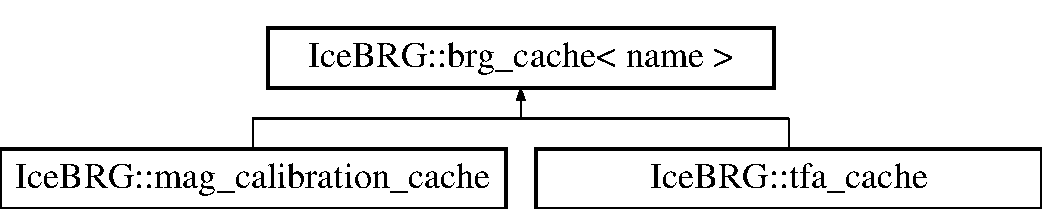
\includegraphics[height=2.000000cm]{classIceBRG_1_1brg__cache}
\end{center}
\end{figure}
\subsection*{Public Member Functions}
\begin{DoxyCompactItemize}
\item 
void \hyperlink{classIceBRG_1_1brg__cache_a319322b7933cebb56a0efaafde8e8530}{set\+\_\+file\+\_\+name} (const std\+::string \&new\+\_\+name)
\item 
void \hyperlink{classIceBRG_1_1brg__cache_a16bfd53b9b2c67d5797176c62c7d36d1}{set\+\_\+range} (const \hyperlink{lib_2IceBRG__main_2common_8h_ad0f130a56eeb944d9ef2692ee881ecc4}{flt\+\_\+type} \&new\+\_\+mins, const \hyperlink{lib_2IceBRG__main_2common_8h_ad0f130a56eeb944d9ef2692ee881ecc4}{flt\+\_\+type} \&new\+\_\+maxes, const \hyperlink{lib_2IceBRG__main_2common_8h_ad0f130a56eeb944d9ef2692ee881ecc4}{flt\+\_\+type} \&new\+\_\+steps)
\item 
void \hyperlink{classIceBRG_1_1brg__cache_a9ffe4a3efac6a30761f78feb453a3644}{set\+\_\+precision} (const size\+\_\+t new\+\_\+precision)
\item 
{\footnotesize template$<$typename otype $>$ }\\void \hyperlink{classIceBRG_1_1brg__cache_a203d556e29e1f277809ec09e89b22439}{print} (otype \&out) const 
\item 
{\footnotesize template$<$typename Tx $>$ }\\const \hyperlink{namespaceIceBRG_a3101fc159e191fa99c4ec14e445df96e}{any\+\_\+units\+\_\+type} \hyperlink{classIceBRG_1_1brg__cache_a8be8ab65cdb161de7145649eb86e60f5}{get} (const Tx \&init\+\_\+x) const 
\item 
const \hyperlink{namespaceIceBRG_a3101fc159e191fa99c4ec14e445df96e}{any\+\_\+units\+\_\+type} \hyperlink{classIceBRG_1_1brg__cache_af011fa69aeebc51a28fbea40de9212ec}{inverse\+\_\+get} (const \hyperlink{lib_2IceBRG__main_2common_8h_ad0f130a56eeb944d9ef2692ee881ecc4}{flt\+\_\+type} \&y) const 
\item 
void \hyperlink{classIceBRG_1_1brg__cache_a45ca108f1964da3f821cc8d36fe1153f}{recalc} () const 
\item 
\hyperlink{classIceBRG_1_1brg__cache_ac365e93dd0b7c3b91125c4dff3530f49}{brg\+\_\+cache} ()
\item 
virtual \hyperlink{classIceBRG_1_1brg__cache_ab4556e59993e9c60c5937fbece2248b4}{$\sim$brg\+\_\+cache} ()
\end{DoxyCompactItemize}
\subsection*{Protected Member Functions}
\begin{DoxyCompactItemize}
\item 
std\+::string \hyperlink{classIceBRG_1_1brg__cache_a4453ff8ebded318cabaa332e9533ec40}{\+\_\+name\+\_\+base} () const 
\item 
\hyperlink{lib_2IceBRG__main_2common_8h_ad0f130a56eeb944d9ef2692ee881ecc4}{flt\+\_\+type} \hyperlink{classIceBRG_1_1brg__cache_afde9cc8f297a354727a4df9c16ab7a12}{\+\_\+calculate} (const \hyperlink{lib_2IceBRG__main_2common_8h_ad0f130a56eeb944d9ef2692ee881ecc4}{flt\+\_\+type} \&x) const 
\item 
void \hyperlink{classIceBRG_1_1brg__cache_a020dbbd2a1b93b103e15043f6424242b}{\+\_\+load\+\_\+cache\+\_\+dependencies} () const 
\end{DoxyCompactItemize}


\subsection{Constructor \& Destructor Documentation}
\hypertarget{classIceBRG_1_1brg__cache_ac365e93dd0b7c3b91125c4dff3530f49}{}\index{Ice\+B\+R\+G\+::brg\+\_\+cache@{Ice\+B\+R\+G\+::brg\+\_\+cache}!brg\+\_\+cache@{brg\+\_\+cache}}
\index{brg\+\_\+cache@{brg\+\_\+cache}!Ice\+B\+R\+G\+::brg\+\_\+cache@{Ice\+B\+R\+G\+::brg\+\_\+cache}}
\subsubsection[{brg\+\_\+cache()}]{\setlength{\rightskip}{0pt plus 5cm}template$<$typename name$>$ {\bf Ice\+B\+R\+G\+::brg\+\_\+cache}$<$ name $>$\+::{\bf brg\+\_\+cache} (
\begin{DoxyParamCaption}
{}
\end{DoxyParamCaption}
)\hspace{0.3cm}{\ttfamily [inline]}}\label{classIceBRG_1_1brg__cache_ac365e93dd0b7c3b91125c4dff3530f49}
\hypertarget{classIceBRG_1_1brg__cache_ab4556e59993e9c60c5937fbece2248b4}{}\index{Ice\+B\+R\+G\+::brg\+\_\+cache@{Ice\+B\+R\+G\+::brg\+\_\+cache}!````~brg\+\_\+cache@{$\sim$brg\+\_\+cache}}
\index{````~brg\+\_\+cache@{$\sim$brg\+\_\+cache}!Ice\+B\+R\+G\+::brg\+\_\+cache@{Ice\+B\+R\+G\+::brg\+\_\+cache}}
\subsubsection[{$\sim$brg\+\_\+cache()}]{\setlength{\rightskip}{0pt plus 5cm}template$<$typename name$>$ virtual {\bf Ice\+B\+R\+G\+::brg\+\_\+cache}$<$ name $>$\+::$\sim${\bf brg\+\_\+cache} (
\begin{DoxyParamCaption}
{}
\end{DoxyParamCaption}
)\hspace{0.3cm}{\ttfamily [inline]}, {\ttfamily [virtual]}}\label{classIceBRG_1_1brg__cache_ab4556e59993e9c60c5937fbece2248b4}


\subsection{Member Function Documentation}
\hypertarget{classIceBRG_1_1brg__cache_afde9cc8f297a354727a4df9c16ab7a12}{}\index{Ice\+B\+R\+G\+::brg\+\_\+cache@{Ice\+B\+R\+G\+::brg\+\_\+cache}!\+\_\+calculate@{\+\_\+calculate}}
\index{\+\_\+calculate@{\+\_\+calculate}!Ice\+B\+R\+G\+::brg\+\_\+cache@{Ice\+B\+R\+G\+::brg\+\_\+cache}}
\subsubsection[{\+\_\+calculate(const flt\+\_\+type \&x) const }]{\setlength{\rightskip}{0pt plus 5cm}template$<$typename name$>$ {\bf flt\+\_\+type} {\bf Ice\+B\+R\+G\+::brg\+\_\+cache}$<$ name $>$\+::\+\_\+calculate (
\begin{DoxyParamCaption}
\item[{const {\bf flt\+\_\+type} \&}]{x}
\end{DoxyParamCaption}
) const\hspace{0.3cm}{\ttfamily [protected]}}\label{classIceBRG_1_1brg__cache_afde9cc8f297a354727a4df9c16ab7a12}
\hypertarget{classIceBRG_1_1brg__cache_a020dbbd2a1b93b103e15043f6424242b}{}\index{Ice\+B\+R\+G\+::brg\+\_\+cache@{Ice\+B\+R\+G\+::brg\+\_\+cache}!\+\_\+load\+\_\+cache\+\_\+dependencies@{\+\_\+load\+\_\+cache\+\_\+dependencies}}
\index{\+\_\+load\+\_\+cache\+\_\+dependencies@{\+\_\+load\+\_\+cache\+\_\+dependencies}!Ice\+B\+R\+G\+::brg\+\_\+cache@{Ice\+B\+R\+G\+::brg\+\_\+cache}}
\subsubsection[{\+\_\+load\+\_\+cache\+\_\+dependencies() const }]{\setlength{\rightskip}{0pt plus 5cm}template$<$typename name$>$ void {\bf Ice\+B\+R\+G\+::brg\+\_\+cache}$<$ name $>$\+::\+\_\+load\+\_\+cache\+\_\+dependencies (
\begin{DoxyParamCaption}
{}
\end{DoxyParamCaption}
) const\hspace{0.3cm}{\ttfamily [inline]}, {\ttfamily [protected]}}\label{classIceBRG_1_1brg__cache_a020dbbd2a1b93b103e15043f6424242b}
\hypertarget{classIceBRG_1_1brg__cache_a4453ff8ebded318cabaa332e9533ec40}{}\index{Ice\+B\+R\+G\+::brg\+\_\+cache@{Ice\+B\+R\+G\+::brg\+\_\+cache}!\+\_\+name\+\_\+base@{\+\_\+name\+\_\+base}}
\index{\+\_\+name\+\_\+base@{\+\_\+name\+\_\+base}!Ice\+B\+R\+G\+::brg\+\_\+cache@{Ice\+B\+R\+G\+::brg\+\_\+cache}}
\subsubsection[{\+\_\+name\+\_\+base() const }]{\setlength{\rightskip}{0pt plus 5cm}template$<$typename name$>$ std\+::string {\bf Ice\+B\+R\+G\+::brg\+\_\+cache}$<$ name $>$\+::\+\_\+name\+\_\+base (
\begin{DoxyParamCaption}
{}
\end{DoxyParamCaption}
) const\hspace{0.3cm}{\ttfamily [protected]}}\label{classIceBRG_1_1brg__cache_a4453ff8ebded318cabaa332e9533ec40}
\hypertarget{classIceBRG_1_1brg__cache_a8be8ab65cdb161de7145649eb86e60f5}{}\index{Ice\+B\+R\+G\+::brg\+\_\+cache@{Ice\+B\+R\+G\+::brg\+\_\+cache}!get@{get}}
\index{get@{get}!Ice\+B\+R\+G\+::brg\+\_\+cache@{Ice\+B\+R\+G\+::brg\+\_\+cache}}
\subsubsection[{get(const Tx \&init\+\_\+x) const }]{\setlength{\rightskip}{0pt plus 5cm}template$<$typename name$>$ template$<$typename Tx $>$ const {\bf any\+\_\+units\+\_\+type} {\bf Ice\+B\+R\+G\+::brg\+\_\+cache}$<$ name $>$\+::get (
\begin{DoxyParamCaption}
\item[{const Tx \&}]{init\+\_\+x}
\end{DoxyParamCaption}
) const\hspace{0.3cm}{\ttfamily [inline]}}\label{classIceBRG_1_1brg__cache_a8be8ab65cdb161de7145649eb86e60f5}
\hypertarget{classIceBRG_1_1brg__cache_af011fa69aeebc51a28fbea40de9212ec}{}\index{Ice\+B\+R\+G\+::brg\+\_\+cache@{Ice\+B\+R\+G\+::brg\+\_\+cache}!inverse\+\_\+get@{inverse\+\_\+get}}
\index{inverse\+\_\+get@{inverse\+\_\+get}!Ice\+B\+R\+G\+::brg\+\_\+cache@{Ice\+B\+R\+G\+::brg\+\_\+cache}}
\subsubsection[{inverse\+\_\+get(const flt\+\_\+type \&y) const }]{\setlength{\rightskip}{0pt plus 5cm}template$<$typename name$>$ const {\bf any\+\_\+units\+\_\+type} {\bf Ice\+B\+R\+G\+::brg\+\_\+cache}$<$ name $>$\+::inverse\+\_\+get (
\begin{DoxyParamCaption}
\item[{const {\bf flt\+\_\+type} \&}]{y}
\end{DoxyParamCaption}
) const\hspace{0.3cm}{\ttfamily [inline]}}\label{classIceBRG_1_1brg__cache_af011fa69aeebc51a28fbea40de9212ec}
\hypertarget{classIceBRG_1_1brg__cache_a203d556e29e1f277809ec09e89b22439}{}\index{Ice\+B\+R\+G\+::brg\+\_\+cache@{Ice\+B\+R\+G\+::brg\+\_\+cache}!print@{print}}
\index{print@{print}!Ice\+B\+R\+G\+::brg\+\_\+cache@{Ice\+B\+R\+G\+::brg\+\_\+cache}}
\subsubsection[{print(otype \&out) const }]{\setlength{\rightskip}{0pt plus 5cm}template$<$typename name$>$ template$<$typename otype $>$ void {\bf Ice\+B\+R\+G\+::brg\+\_\+cache}$<$ name $>$\+::print (
\begin{DoxyParamCaption}
\item[{otype \&}]{out}
\end{DoxyParamCaption}
) const\hspace{0.3cm}{\ttfamily [inline]}}\label{classIceBRG_1_1brg__cache_a203d556e29e1f277809ec09e89b22439}
\hypertarget{classIceBRG_1_1brg__cache_a45ca108f1964da3f821cc8d36fe1153f}{}\index{Ice\+B\+R\+G\+::brg\+\_\+cache@{Ice\+B\+R\+G\+::brg\+\_\+cache}!recalc@{recalc}}
\index{recalc@{recalc}!Ice\+B\+R\+G\+::brg\+\_\+cache@{Ice\+B\+R\+G\+::brg\+\_\+cache}}
\subsubsection[{recalc() const }]{\setlength{\rightskip}{0pt plus 5cm}template$<$typename name$>$ void {\bf Ice\+B\+R\+G\+::brg\+\_\+cache}$<$ name $>$\+::recalc (
\begin{DoxyParamCaption}
{}
\end{DoxyParamCaption}
) const\hspace{0.3cm}{\ttfamily [inline]}}\label{classIceBRG_1_1brg__cache_a45ca108f1964da3f821cc8d36fe1153f}
\hypertarget{classIceBRG_1_1brg__cache_a319322b7933cebb56a0efaafde8e8530}{}\index{Ice\+B\+R\+G\+::brg\+\_\+cache@{Ice\+B\+R\+G\+::brg\+\_\+cache}!set\+\_\+file\+\_\+name@{set\+\_\+file\+\_\+name}}
\index{set\+\_\+file\+\_\+name@{set\+\_\+file\+\_\+name}!Ice\+B\+R\+G\+::brg\+\_\+cache@{Ice\+B\+R\+G\+::brg\+\_\+cache}}
\subsubsection[{set\+\_\+file\+\_\+name(const std\+::string \&new\+\_\+name)}]{\setlength{\rightskip}{0pt plus 5cm}template$<$typename name$>$ void {\bf Ice\+B\+R\+G\+::brg\+\_\+cache}$<$ name $>$\+::set\+\_\+file\+\_\+name (
\begin{DoxyParamCaption}
\item[{const std\+::string \&}]{new\+\_\+name}
\end{DoxyParamCaption}
)\hspace{0.3cm}{\ttfamily [inline]}}\label{classIceBRG_1_1brg__cache_a319322b7933cebb56a0efaafde8e8530}
\hypertarget{classIceBRG_1_1brg__cache_a9ffe4a3efac6a30761f78feb453a3644}{}\index{Ice\+B\+R\+G\+::brg\+\_\+cache@{Ice\+B\+R\+G\+::brg\+\_\+cache}!set\+\_\+precision@{set\+\_\+precision}}
\index{set\+\_\+precision@{set\+\_\+precision}!Ice\+B\+R\+G\+::brg\+\_\+cache@{Ice\+B\+R\+G\+::brg\+\_\+cache}}
\subsubsection[{set\+\_\+precision(const size\+\_\+t new\+\_\+precision)}]{\setlength{\rightskip}{0pt plus 5cm}template$<$typename name$>$ void {\bf Ice\+B\+R\+G\+::brg\+\_\+cache}$<$ name $>$\+::set\+\_\+precision (
\begin{DoxyParamCaption}
\item[{const size\+\_\+t}]{new\+\_\+precision}
\end{DoxyParamCaption}
)\hspace{0.3cm}{\ttfamily [inline]}}\label{classIceBRG_1_1brg__cache_a9ffe4a3efac6a30761f78feb453a3644}
\hypertarget{classIceBRG_1_1brg__cache_a16bfd53b9b2c67d5797176c62c7d36d1}{}\index{Ice\+B\+R\+G\+::brg\+\_\+cache@{Ice\+B\+R\+G\+::brg\+\_\+cache}!set\+\_\+range@{set\+\_\+range}}
\index{set\+\_\+range@{set\+\_\+range}!Ice\+B\+R\+G\+::brg\+\_\+cache@{Ice\+B\+R\+G\+::brg\+\_\+cache}}
\subsubsection[{set\+\_\+range(const flt\+\_\+type \&new\+\_\+mins, const flt\+\_\+type \&new\+\_\+maxes, const flt\+\_\+type \&new\+\_\+steps)}]{\setlength{\rightskip}{0pt plus 5cm}template$<$typename name$>$ void {\bf Ice\+B\+R\+G\+::brg\+\_\+cache}$<$ name $>$\+::set\+\_\+range (
\begin{DoxyParamCaption}
\item[{const {\bf flt\+\_\+type} \&}]{new\+\_\+mins, }
\item[{const {\bf flt\+\_\+type} \&}]{new\+\_\+maxes, }
\item[{const {\bf flt\+\_\+type} \&}]{new\+\_\+steps}
\end{DoxyParamCaption}
)\hspace{0.3cm}{\ttfamily [inline]}}\label{classIceBRG_1_1brg__cache_a16bfd53b9b2c67d5797176c62c7d36d1}


The documentation for this class was generated from the following file\+:\begin{DoxyCompactItemize}
\item 
/disk2/brg/git/\+Magnification\+\_\+\+Public/src/lib/\+Ice\+B\+R\+G\+\_\+main/math/cache/\hyperlink{cache_8hpp}{cache.\+hpp}\end{DoxyCompactItemize}

\hypertarget{classIceBRG_1_1brg__cache__2d}{}\section{Ice\+B\+R\+G\+:\+:brg\+\_\+cache\+\_\+2d$<$ name $>$ Class Template Reference}
\label{classIceBRG_1_1brg__cache__2d}\index{Ice\+B\+R\+G\+::brg\+\_\+cache\+\_\+2d$<$ name $>$@{Ice\+B\+R\+G\+::brg\+\_\+cache\+\_\+2d$<$ name $>$}}


{\ttfamily \#include $<$cache\+\_\+2d.\+hpp$>$}

Inheritance diagram for Ice\+B\+R\+G\+:\+:brg\+\_\+cache\+\_\+2d$<$ name $>$\+:\begin{figure}[H]
\begin{center}
\leavevmode
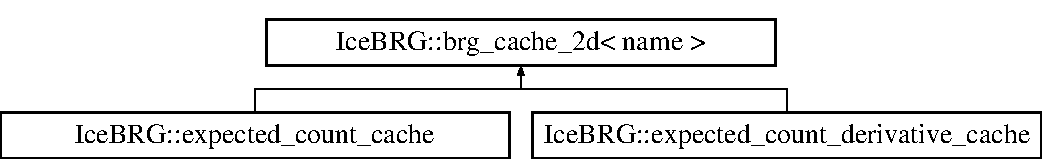
\includegraphics[height=2.000000cm]{classIceBRG_1_1brg__cache__2d}
\end{center}
\end{figure}
\subsection*{Public Member Functions}
\begin{DoxyCompactItemize}
\item 
void \hyperlink{classIceBRG_1_1brg__cache__2d_ac0169a69f122655da1fece04a5e12962}{set\+\_\+file\+\_\+name} (const std\+::string new\+\_\+name)
\item 
void \hyperlink{classIceBRG_1_1brg__cache__2d_a3047c524b7a4297b8fff4a3bdeb2afb5}{set\+\_\+range} (const \hyperlink{lib_2IceBRG__main_2common_8h_ad0f130a56eeb944d9ef2692ee881ecc4}{flt\+\_\+type} \&new\+\_\+min\+\_\+1, const \hyperlink{lib_2IceBRG__main_2common_8h_ad0f130a56eeb944d9ef2692ee881ecc4}{flt\+\_\+type} \&new\+\_\+max\+\_\+1, const \hyperlink{lib_2IceBRG__main_2common_8h_ad0f130a56eeb944d9ef2692ee881ecc4}{flt\+\_\+type} \&new\+\_\+step\+\_\+1, const \hyperlink{lib_2IceBRG__main_2common_8h_ad0f130a56eeb944d9ef2692ee881ecc4}{flt\+\_\+type} \&new\+\_\+min\+\_\+2, const \hyperlink{lib_2IceBRG__main_2common_8h_ad0f130a56eeb944d9ef2692ee881ecc4}{flt\+\_\+type} \&new\+\_\+max\+\_\+2, const \hyperlink{lib_2IceBRG__main_2common_8h_ad0f130a56eeb944d9ef2692ee881ecc4}{flt\+\_\+type} \&new\+\_\+step\+\_\+2)
\item 
{\footnotesize template$<$typename otype $>$ }\\void \hyperlink{classIceBRG_1_1brg__cache__2d_ae6da7b6bda41ec9ea2002867951b5349}{print} (otype \&out) const 
\item 
{\footnotesize template$<$typename Tx1 , typename Tx2 $>$ }\\\hyperlink{namespaceIceBRG_a3101fc159e191fa99c4ec14e445df96e}{any\+\_\+units\+\_\+type} \hyperlink{classIceBRG_1_1brg__cache__2d_ab4a16e8ebe873a58b806eb91a3ef9791}{get} (const Tx1 \&init\+\_\+x\+\_\+1, const Tx2 \&init\+\_\+x\+\_\+2) const 
\item 
void \hyperlink{classIceBRG_1_1brg__cache__2d_a36c39cd418b844b64502be417dfef917}{recalc} () const 
\item 
\hyperlink{classIceBRG_1_1brg__cache__2d_a0a129acdbacb34f016c6c50135164348}{brg\+\_\+cache\+\_\+2d} ()
\item 
virtual \hyperlink{classIceBRG_1_1brg__cache__2d_a8e9f954bbe80395793ac2c8c24c2888f}{$\sim$brg\+\_\+cache\+\_\+2d} ()
\end{DoxyCompactItemize}
\subsection*{Protected Member Functions}
\begin{DoxyCompactItemize}
\item 
\hyperlink{namespaceIceBRG_a3101fc159e191fa99c4ec14e445df96e}{any\+\_\+units\+\_\+type} \hyperlink{classIceBRG_1_1brg__cache__2d_a2205399c8c5d61ba80039352ff447d3b}{\+\_\+units} (const \hyperlink{lib_2IceBRG__main_2common_8h_ad0f130a56eeb944d9ef2692ee881ecc4}{flt\+\_\+type} \&v) const 
\item 
\hyperlink{lib_2IceBRG__main_2common_8h_ad0f130a56eeb944d9ef2692ee881ecc4}{flt\+\_\+type} \hyperlink{classIceBRG_1_1brg__cache__2d_ade75dde33039e36209c2887e0eaf2a32}{\+\_\+calculate} (const \hyperlink{lib_2IceBRG__main_2common_8h_ad0f130a56eeb944d9ef2692ee881ecc4}{flt\+\_\+type} \&x\+\_\+1, const \hyperlink{lib_2IceBRG__main_2common_8h_ad0f130a56eeb944d9ef2692ee881ecc4}{flt\+\_\+type} \&x\+\_\+2) const 
\item 
std\+::string \hyperlink{classIceBRG_1_1brg__cache__2d_a09696dae89337d3f669a4a2d744708a7}{\+\_\+name\+\_\+base} () const 
\item 
void \hyperlink{classIceBRG_1_1brg__cache__2d_a74cd593f9bbf3a501a4132b791a110b9}{\+\_\+load\+\_\+cache\+\_\+dependencies} () const 
\end{DoxyCompactItemize}


\subsection{Constructor \& Destructor Documentation}
\hypertarget{classIceBRG_1_1brg__cache__2d_a0a129acdbacb34f016c6c50135164348}{}\index{Ice\+B\+R\+G\+::brg\+\_\+cache\+\_\+2d@{Ice\+B\+R\+G\+::brg\+\_\+cache\+\_\+2d}!brg\+\_\+cache\+\_\+2d@{brg\+\_\+cache\+\_\+2d}}
\index{brg\+\_\+cache\+\_\+2d@{brg\+\_\+cache\+\_\+2d}!Ice\+B\+R\+G\+::brg\+\_\+cache\+\_\+2d@{Ice\+B\+R\+G\+::brg\+\_\+cache\+\_\+2d}}
\subsubsection[{brg\+\_\+cache\+\_\+2d()}]{\setlength{\rightskip}{0pt plus 5cm}template$<$typename name$>$ {\bf Ice\+B\+R\+G\+::brg\+\_\+cache\+\_\+2d}$<$ name $>$\+::{\bf brg\+\_\+cache\+\_\+2d} (
\begin{DoxyParamCaption}
{}
\end{DoxyParamCaption}
)\hspace{0.3cm}{\ttfamily [inline]}}\label{classIceBRG_1_1brg__cache__2d_a0a129acdbacb34f016c6c50135164348}
\hypertarget{classIceBRG_1_1brg__cache__2d_a8e9f954bbe80395793ac2c8c24c2888f}{}\index{Ice\+B\+R\+G\+::brg\+\_\+cache\+\_\+2d@{Ice\+B\+R\+G\+::brg\+\_\+cache\+\_\+2d}!````~brg\+\_\+cache\+\_\+2d@{$\sim$brg\+\_\+cache\+\_\+2d}}
\index{````~brg\+\_\+cache\+\_\+2d@{$\sim$brg\+\_\+cache\+\_\+2d}!Ice\+B\+R\+G\+::brg\+\_\+cache\+\_\+2d@{Ice\+B\+R\+G\+::brg\+\_\+cache\+\_\+2d}}
\subsubsection[{$\sim$brg\+\_\+cache\+\_\+2d()}]{\setlength{\rightskip}{0pt plus 5cm}template$<$typename name$>$ virtual {\bf Ice\+B\+R\+G\+::brg\+\_\+cache\+\_\+2d}$<$ name $>$\+::$\sim${\bf brg\+\_\+cache\+\_\+2d} (
\begin{DoxyParamCaption}
{}
\end{DoxyParamCaption}
)\hspace{0.3cm}{\ttfamily [inline]}, {\ttfamily [virtual]}}\label{classIceBRG_1_1brg__cache__2d_a8e9f954bbe80395793ac2c8c24c2888f}


\subsection{Member Function Documentation}
\hypertarget{classIceBRG_1_1brg__cache__2d_ade75dde33039e36209c2887e0eaf2a32}{}\index{Ice\+B\+R\+G\+::brg\+\_\+cache\+\_\+2d@{Ice\+B\+R\+G\+::brg\+\_\+cache\+\_\+2d}!\+\_\+calculate@{\+\_\+calculate}}
\index{\+\_\+calculate@{\+\_\+calculate}!Ice\+B\+R\+G\+::brg\+\_\+cache\+\_\+2d@{Ice\+B\+R\+G\+::brg\+\_\+cache\+\_\+2d}}
\subsubsection[{\+\_\+calculate(const flt\+\_\+type \&x\+\_\+1, const flt\+\_\+type \&x\+\_\+2) const }]{\setlength{\rightskip}{0pt plus 5cm}template$<$typename name$>$ {\bf flt\+\_\+type} {\bf Ice\+B\+R\+G\+::brg\+\_\+cache\+\_\+2d}$<$ name $>$\+::\+\_\+calculate (
\begin{DoxyParamCaption}
\item[{const {\bf flt\+\_\+type} \&}]{x\+\_\+1, }
\item[{const {\bf flt\+\_\+type} \&}]{x\+\_\+2}
\end{DoxyParamCaption}
) const\hspace{0.3cm}{\ttfamily [protected]}}\label{classIceBRG_1_1brg__cache__2d_ade75dde33039e36209c2887e0eaf2a32}
\hypertarget{classIceBRG_1_1brg__cache__2d_a74cd593f9bbf3a501a4132b791a110b9}{}\index{Ice\+B\+R\+G\+::brg\+\_\+cache\+\_\+2d@{Ice\+B\+R\+G\+::brg\+\_\+cache\+\_\+2d}!\+\_\+load\+\_\+cache\+\_\+dependencies@{\+\_\+load\+\_\+cache\+\_\+dependencies}}
\index{\+\_\+load\+\_\+cache\+\_\+dependencies@{\+\_\+load\+\_\+cache\+\_\+dependencies}!Ice\+B\+R\+G\+::brg\+\_\+cache\+\_\+2d@{Ice\+B\+R\+G\+::brg\+\_\+cache\+\_\+2d}}
\subsubsection[{\+\_\+load\+\_\+cache\+\_\+dependencies() const }]{\setlength{\rightskip}{0pt plus 5cm}template$<$typename name$>$ void {\bf Ice\+B\+R\+G\+::brg\+\_\+cache\+\_\+2d}$<$ name $>$\+::\+\_\+load\+\_\+cache\+\_\+dependencies (
\begin{DoxyParamCaption}
{}
\end{DoxyParamCaption}
) const\hspace{0.3cm}{\ttfamily [inline]}, {\ttfamily [protected]}}\label{classIceBRG_1_1brg__cache__2d_a74cd593f9bbf3a501a4132b791a110b9}
\hypertarget{classIceBRG_1_1brg__cache__2d_a09696dae89337d3f669a4a2d744708a7}{}\index{Ice\+B\+R\+G\+::brg\+\_\+cache\+\_\+2d@{Ice\+B\+R\+G\+::brg\+\_\+cache\+\_\+2d}!\+\_\+name\+\_\+base@{\+\_\+name\+\_\+base}}
\index{\+\_\+name\+\_\+base@{\+\_\+name\+\_\+base}!Ice\+B\+R\+G\+::brg\+\_\+cache\+\_\+2d@{Ice\+B\+R\+G\+::brg\+\_\+cache\+\_\+2d}}
\subsubsection[{\+\_\+name\+\_\+base() const }]{\setlength{\rightskip}{0pt plus 5cm}template$<$typename name$>$ std\+::string {\bf Ice\+B\+R\+G\+::brg\+\_\+cache\+\_\+2d}$<$ name $>$\+::\+\_\+name\+\_\+base (
\begin{DoxyParamCaption}
{}
\end{DoxyParamCaption}
) const\hspace{0.3cm}{\ttfamily [protected]}}\label{classIceBRG_1_1brg__cache__2d_a09696dae89337d3f669a4a2d744708a7}
\hypertarget{classIceBRG_1_1brg__cache__2d_a2205399c8c5d61ba80039352ff447d3b}{}\index{Ice\+B\+R\+G\+::brg\+\_\+cache\+\_\+2d@{Ice\+B\+R\+G\+::brg\+\_\+cache\+\_\+2d}!\+\_\+units@{\+\_\+units}}
\index{\+\_\+units@{\+\_\+units}!Ice\+B\+R\+G\+::brg\+\_\+cache\+\_\+2d@{Ice\+B\+R\+G\+::brg\+\_\+cache\+\_\+2d}}
\subsubsection[{\+\_\+units(const flt\+\_\+type \&v) const }]{\setlength{\rightskip}{0pt plus 5cm}template$<$typename name$>$ {\bf any\+\_\+units\+\_\+type} {\bf Ice\+B\+R\+G\+::brg\+\_\+cache\+\_\+2d}$<$ name $>$\+::\+\_\+units (
\begin{DoxyParamCaption}
\item[{const {\bf flt\+\_\+type} \&}]{v}
\end{DoxyParamCaption}
) const\hspace{0.3cm}{\ttfamily [inline]}, {\ttfamily [protected]}}\label{classIceBRG_1_1brg__cache__2d_a2205399c8c5d61ba80039352ff447d3b}
\hypertarget{classIceBRG_1_1brg__cache__2d_ab4a16e8ebe873a58b806eb91a3ef9791}{}\index{Ice\+B\+R\+G\+::brg\+\_\+cache\+\_\+2d@{Ice\+B\+R\+G\+::brg\+\_\+cache\+\_\+2d}!get@{get}}
\index{get@{get}!Ice\+B\+R\+G\+::brg\+\_\+cache\+\_\+2d@{Ice\+B\+R\+G\+::brg\+\_\+cache\+\_\+2d}}
\subsubsection[{get(const Tx1 \&init\+\_\+x\+\_\+1, const Tx2 \&init\+\_\+x\+\_\+2) const }]{\setlength{\rightskip}{0pt plus 5cm}template$<$typename name$>$ template$<$typename Tx1 , typename Tx2 $>$ {\bf any\+\_\+units\+\_\+type} {\bf Ice\+B\+R\+G\+::brg\+\_\+cache\+\_\+2d}$<$ name $>$\+::get (
\begin{DoxyParamCaption}
\item[{const Tx1 \&}]{init\+\_\+x\+\_\+1, }
\item[{const Tx2 \&}]{init\+\_\+x\+\_\+2}
\end{DoxyParamCaption}
) const\hspace{0.3cm}{\ttfamily [inline]}}\label{classIceBRG_1_1brg__cache__2d_ab4a16e8ebe873a58b806eb91a3ef9791}
\hypertarget{classIceBRG_1_1brg__cache__2d_ae6da7b6bda41ec9ea2002867951b5349}{}\index{Ice\+B\+R\+G\+::brg\+\_\+cache\+\_\+2d@{Ice\+B\+R\+G\+::brg\+\_\+cache\+\_\+2d}!print@{print}}
\index{print@{print}!Ice\+B\+R\+G\+::brg\+\_\+cache\+\_\+2d@{Ice\+B\+R\+G\+::brg\+\_\+cache\+\_\+2d}}
\subsubsection[{print(otype \&out) const }]{\setlength{\rightskip}{0pt plus 5cm}template$<$typename name$>$ template$<$typename otype $>$ void {\bf Ice\+B\+R\+G\+::brg\+\_\+cache\+\_\+2d}$<$ name $>$\+::print (
\begin{DoxyParamCaption}
\item[{otype \&}]{out}
\end{DoxyParamCaption}
) const\hspace{0.3cm}{\ttfamily [inline]}}\label{classIceBRG_1_1brg__cache__2d_ae6da7b6bda41ec9ea2002867951b5349}
\hypertarget{classIceBRG_1_1brg__cache__2d_a36c39cd418b844b64502be417dfef917}{}\index{Ice\+B\+R\+G\+::brg\+\_\+cache\+\_\+2d@{Ice\+B\+R\+G\+::brg\+\_\+cache\+\_\+2d}!recalc@{recalc}}
\index{recalc@{recalc}!Ice\+B\+R\+G\+::brg\+\_\+cache\+\_\+2d@{Ice\+B\+R\+G\+::brg\+\_\+cache\+\_\+2d}}
\subsubsection[{recalc() const }]{\setlength{\rightskip}{0pt plus 5cm}template$<$typename name$>$ void {\bf Ice\+B\+R\+G\+::brg\+\_\+cache\+\_\+2d}$<$ name $>$\+::recalc (
\begin{DoxyParamCaption}
{}
\end{DoxyParamCaption}
) const\hspace{0.3cm}{\ttfamily [inline]}}\label{classIceBRG_1_1brg__cache__2d_a36c39cd418b844b64502be417dfef917}
\hypertarget{classIceBRG_1_1brg__cache__2d_ac0169a69f122655da1fece04a5e12962}{}\index{Ice\+B\+R\+G\+::brg\+\_\+cache\+\_\+2d@{Ice\+B\+R\+G\+::brg\+\_\+cache\+\_\+2d}!set\+\_\+file\+\_\+name@{set\+\_\+file\+\_\+name}}
\index{set\+\_\+file\+\_\+name@{set\+\_\+file\+\_\+name}!Ice\+B\+R\+G\+::brg\+\_\+cache\+\_\+2d@{Ice\+B\+R\+G\+::brg\+\_\+cache\+\_\+2d}}
\subsubsection[{set\+\_\+file\+\_\+name(const std\+::string new\+\_\+name)}]{\setlength{\rightskip}{0pt plus 5cm}template$<$typename name$>$ void {\bf Ice\+B\+R\+G\+::brg\+\_\+cache\+\_\+2d}$<$ name $>$\+::set\+\_\+file\+\_\+name (
\begin{DoxyParamCaption}
\item[{const std\+::string}]{new\+\_\+name}
\end{DoxyParamCaption}
)\hspace{0.3cm}{\ttfamily [inline]}}\label{classIceBRG_1_1brg__cache__2d_ac0169a69f122655da1fece04a5e12962}
\hypertarget{classIceBRG_1_1brg__cache__2d_a3047c524b7a4297b8fff4a3bdeb2afb5}{}\index{Ice\+B\+R\+G\+::brg\+\_\+cache\+\_\+2d@{Ice\+B\+R\+G\+::brg\+\_\+cache\+\_\+2d}!set\+\_\+range@{set\+\_\+range}}
\index{set\+\_\+range@{set\+\_\+range}!Ice\+B\+R\+G\+::brg\+\_\+cache\+\_\+2d@{Ice\+B\+R\+G\+::brg\+\_\+cache\+\_\+2d}}
\subsubsection[{set\+\_\+range(const flt\+\_\+type \&new\+\_\+min\+\_\+1, const flt\+\_\+type \&new\+\_\+max\+\_\+1, const flt\+\_\+type \&new\+\_\+step\+\_\+1, const flt\+\_\+type \&new\+\_\+min\+\_\+2, const flt\+\_\+type \&new\+\_\+max\+\_\+2, const flt\+\_\+type \&new\+\_\+step\+\_\+2)}]{\setlength{\rightskip}{0pt plus 5cm}template$<$typename name$>$ void {\bf Ice\+B\+R\+G\+::brg\+\_\+cache\+\_\+2d}$<$ name $>$\+::set\+\_\+range (
\begin{DoxyParamCaption}
\item[{const {\bf flt\+\_\+type} \&}]{new\+\_\+min\+\_\+1, }
\item[{const {\bf flt\+\_\+type} \&}]{new\+\_\+max\+\_\+1, }
\item[{const {\bf flt\+\_\+type} \&}]{new\+\_\+step\+\_\+1, }
\item[{const {\bf flt\+\_\+type} \&}]{new\+\_\+min\+\_\+2, }
\item[{const {\bf flt\+\_\+type} \&}]{new\+\_\+max\+\_\+2, }
\item[{const {\bf flt\+\_\+type} \&}]{new\+\_\+step\+\_\+2}
\end{DoxyParamCaption}
)\hspace{0.3cm}{\ttfamily [inline]}}\label{classIceBRG_1_1brg__cache__2d_a3047c524b7a4297b8fff4a3bdeb2afb5}


The documentation for this class was generated from the following file\+:\begin{DoxyCompactItemize}
\item 
/disk2/brg/git/\+Magnification\+\_\+\+Public/src/lib/\+Ice\+B\+R\+G\+\_\+main/math/cache/\hyperlink{cache__2d_8hpp}{cache\+\_\+2d.\+hpp}\end{DoxyCompactItemize}

\hypertarget{classIceBRG_1_1brg__cache__3d}{}\section{Ice\+B\+R\+G\+:\+:brg\+\_\+cache\+\_\+3d$<$ name $>$ Class Template Reference}
\label{classIceBRG_1_1brg__cache__3d}\index{Ice\+B\+R\+G\+::brg\+\_\+cache\+\_\+3d$<$ name $>$@{Ice\+B\+R\+G\+::brg\+\_\+cache\+\_\+3d$<$ name $>$}}


{\ttfamily \#include $<$cache\+\_\+3d.\+hpp$>$}

\subsection*{Public Member Functions}
\begin{DoxyCompactItemize}
\item 
void \hyperlink{classIceBRG_1_1brg__cache__3d_a2cb9d485713aed3e56667013f9309d54}{set\+\_\+file\+\_\+name} (const std\+::string new\+\_\+name)
\item 
void \hyperlink{classIceBRG_1_1brg__cache__3d_af3aafe0ab4f5757a0beefaee5067e013}{set\+\_\+range} (const \hyperlink{lib_2IceBRG__main_2common_8h_ad0f130a56eeb944d9ef2692ee881ecc4}{flt\+\_\+type} \&new\+\_\+min\+\_\+1, const \hyperlink{lib_2IceBRG__main_2common_8h_ad0f130a56eeb944d9ef2692ee881ecc4}{flt\+\_\+type} \&new\+\_\+max\+\_\+1, const \hyperlink{lib_2IceBRG__main_2common_8h_ad0f130a56eeb944d9ef2692ee881ecc4}{flt\+\_\+type} \&new\+\_\+step\+\_\+1, const \hyperlink{lib_2IceBRG__main_2common_8h_ad0f130a56eeb944d9ef2692ee881ecc4}{flt\+\_\+type} \&new\+\_\+min\+\_\+2, const \hyperlink{lib_2IceBRG__main_2common_8h_ad0f130a56eeb944d9ef2692ee881ecc4}{flt\+\_\+type} \&new\+\_\+max\+\_\+2, const \hyperlink{lib_2IceBRG__main_2common_8h_ad0f130a56eeb944d9ef2692ee881ecc4}{flt\+\_\+type} \&new\+\_\+step\+\_\+2, const \hyperlink{lib_2IceBRG__main_2common_8h_ad0f130a56eeb944d9ef2692ee881ecc4}{flt\+\_\+type} \&new\+\_\+min\+\_\+3, const \hyperlink{lib_2IceBRG__main_2common_8h_ad0f130a56eeb944d9ef2692ee881ecc4}{flt\+\_\+type} \&new\+\_\+max\+\_\+3, const \hyperlink{lib_2IceBRG__main_2common_8h_ad0f130a56eeb944d9ef2692ee881ecc4}{flt\+\_\+type} \&new\+\_\+step\+\_\+3)
\item 
{\footnotesize template$<$typename otype $>$ }\\void \hyperlink{classIceBRG_1_1brg__cache__3d_a514ff3b5f9bec00706eaceeefa82d3a2}{print} (otype \&out) const 
\item 
{\footnotesize template$<$typename Tx1 , typename Tx2 , typename Tx3 $>$ }\\\hyperlink{namespaceIceBRG_a3101fc159e191fa99c4ec14e445df96e}{any\+\_\+units\+\_\+type} \hyperlink{classIceBRG_1_1brg__cache__3d_aa7c731a33469c00810417598a942dbc9}{get} (const Tx1 \&init\+\_\+x\+\_\+1, const Tx2 \&init\+\_\+x\+\_\+2, const Tx3 \&init\+\_\+x\+\_\+3) const 
\item 
void \hyperlink{classIceBRG_1_1brg__cache__3d_a7bd0994797bb6ae070b7a0e39d13e19f}{recalc} () const 
\item 
\hyperlink{classIceBRG_1_1brg__cache__3d_acba2966dffaf228ae82a96f23f8f3a88}{brg\+\_\+cache\+\_\+3d} ()
\item 
virtual \hyperlink{classIceBRG_1_1brg__cache__3d_a1609b9ff5f250df90c304f2615a404b9}{$\sim$brg\+\_\+cache\+\_\+3d} ()
\end{DoxyCompactItemize}
\subsection*{Protected Member Functions}
\begin{DoxyCompactItemize}
\item 
\hyperlink{lib_2IceBRG__main_2common_8h_ad0f130a56eeb944d9ef2692ee881ecc4}{flt\+\_\+type} \hyperlink{classIceBRG_1_1brg__cache__3d_aa3b16c143f747fc9b8adb2a9ca435b9d}{\+\_\+calculate} (const \hyperlink{lib_2IceBRG__main_2common_8h_ad0f130a56eeb944d9ef2692ee881ecc4}{flt\+\_\+type} \&x\+\_\+1, const \hyperlink{lib_2IceBRG__main_2common_8h_ad0f130a56eeb944d9ef2692ee881ecc4}{flt\+\_\+type} \&x\+\_\+2, const \hyperlink{lib_2IceBRG__main_2common_8h_ad0f130a56eeb944d9ef2692ee881ecc4}{flt\+\_\+type} \&x\+\_\+3) const 
\item 
const std\+::string \hyperlink{classIceBRG_1_1brg__cache__3d_af934bb6a675f2a38b4da4092b35c6120}{\+\_\+name\+\_\+base} () const 
\item 
void \hyperlink{classIceBRG_1_1brg__cache__3d_af2bae1e53b83a8622392b264ab629843}{\+\_\+load\+\_\+cache\+\_\+dependencies} () const 
\end{DoxyCompactItemize}


\subsection{Constructor \& Destructor Documentation}
\hypertarget{classIceBRG_1_1brg__cache__3d_acba2966dffaf228ae82a96f23f8f3a88}{}\index{Ice\+B\+R\+G\+::brg\+\_\+cache\+\_\+3d@{Ice\+B\+R\+G\+::brg\+\_\+cache\+\_\+3d}!brg\+\_\+cache\+\_\+3d@{brg\+\_\+cache\+\_\+3d}}
\index{brg\+\_\+cache\+\_\+3d@{brg\+\_\+cache\+\_\+3d}!Ice\+B\+R\+G\+::brg\+\_\+cache\+\_\+3d@{Ice\+B\+R\+G\+::brg\+\_\+cache\+\_\+3d}}
\subsubsection[{brg\+\_\+cache\+\_\+3d()}]{\setlength{\rightskip}{0pt plus 5cm}template$<$typename name$>$ {\bf Ice\+B\+R\+G\+::brg\+\_\+cache\+\_\+3d}$<$ name $>$\+::{\bf brg\+\_\+cache\+\_\+3d} (
\begin{DoxyParamCaption}
{}
\end{DoxyParamCaption}
)\hspace{0.3cm}{\ttfamily [inline]}}\label{classIceBRG_1_1brg__cache__3d_acba2966dffaf228ae82a96f23f8f3a88}
\hypertarget{classIceBRG_1_1brg__cache__3d_a1609b9ff5f250df90c304f2615a404b9}{}\index{Ice\+B\+R\+G\+::brg\+\_\+cache\+\_\+3d@{Ice\+B\+R\+G\+::brg\+\_\+cache\+\_\+3d}!````~brg\+\_\+cache\+\_\+3d@{$\sim$brg\+\_\+cache\+\_\+3d}}
\index{````~brg\+\_\+cache\+\_\+3d@{$\sim$brg\+\_\+cache\+\_\+3d}!Ice\+B\+R\+G\+::brg\+\_\+cache\+\_\+3d@{Ice\+B\+R\+G\+::brg\+\_\+cache\+\_\+3d}}
\subsubsection[{$\sim$brg\+\_\+cache\+\_\+3d()}]{\setlength{\rightskip}{0pt plus 5cm}template$<$typename name$>$ virtual {\bf Ice\+B\+R\+G\+::brg\+\_\+cache\+\_\+3d}$<$ name $>$\+::$\sim${\bf brg\+\_\+cache\+\_\+3d} (
\begin{DoxyParamCaption}
{}
\end{DoxyParamCaption}
)\hspace{0.3cm}{\ttfamily [inline]}, {\ttfamily [virtual]}}\label{classIceBRG_1_1brg__cache__3d_a1609b9ff5f250df90c304f2615a404b9}


\subsection{Member Function Documentation}
\hypertarget{classIceBRG_1_1brg__cache__3d_aa3b16c143f747fc9b8adb2a9ca435b9d}{}\index{Ice\+B\+R\+G\+::brg\+\_\+cache\+\_\+3d@{Ice\+B\+R\+G\+::brg\+\_\+cache\+\_\+3d}!\+\_\+calculate@{\+\_\+calculate}}
\index{\+\_\+calculate@{\+\_\+calculate}!Ice\+B\+R\+G\+::brg\+\_\+cache\+\_\+3d@{Ice\+B\+R\+G\+::brg\+\_\+cache\+\_\+3d}}
\subsubsection[{\+\_\+calculate(const flt\+\_\+type \&x\+\_\+1, const flt\+\_\+type \&x\+\_\+2, const flt\+\_\+type \&x\+\_\+3) const }]{\setlength{\rightskip}{0pt plus 5cm}template$<$typename name$>$ {\bf flt\+\_\+type} {\bf Ice\+B\+R\+G\+::brg\+\_\+cache\+\_\+3d}$<$ name $>$\+::\+\_\+calculate (
\begin{DoxyParamCaption}
\item[{const {\bf flt\+\_\+type} \&}]{x\+\_\+1, }
\item[{const {\bf flt\+\_\+type} \&}]{x\+\_\+2, }
\item[{const {\bf flt\+\_\+type} \&}]{x\+\_\+3}
\end{DoxyParamCaption}
) const\hspace{0.3cm}{\ttfamily [protected]}}\label{classIceBRG_1_1brg__cache__3d_aa3b16c143f747fc9b8adb2a9ca435b9d}
\hypertarget{classIceBRG_1_1brg__cache__3d_af2bae1e53b83a8622392b264ab629843}{}\index{Ice\+B\+R\+G\+::brg\+\_\+cache\+\_\+3d@{Ice\+B\+R\+G\+::brg\+\_\+cache\+\_\+3d}!\+\_\+load\+\_\+cache\+\_\+dependencies@{\+\_\+load\+\_\+cache\+\_\+dependencies}}
\index{\+\_\+load\+\_\+cache\+\_\+dependencies@{\+\_\+load\+\_\+cache\+\_\+dependencies}!Ice\+B\+R\+G\+::brg\+\_\+cache\+\_\+3d@{Ice\+B\+R\+G\+::brg\+\_\+cache\+\_\+3d}}
\subsubsection[{\+\_\+load\+\_\+cache\+\_\+dependencies() const }]{\setlength{\rightskip}{0pt plus 5cm}template$<$typename name$>$ void {\bf Ice\+B\+R\+G\+::brg\+\_\+cache\+\_\+3d}$<$ name $>$\+::\+\_\+load\+\_\+cache\+\_\+dependencies (
\begin{DoxyParamCaption}
{}
\end{DoxyParamCaption}
) const\hspace{0.3cm}{\ttfamily [inline]}, {\ttfamily [protected]}}\label{classIceBRG_1_1brg__cache__3d_af2bae1e53b83a8622392b264ab629843}
\hypertarget{classIceBRG_1_1brg__cache__3d_af934bb6a675f2a38b4da4092b35c6120}{}\index{Ice\+B\+R\+G\+::brg\+\_\+cache\+\_\+3d@{Ice\+B\+R\+G\+::brg\+\_\+cache\+\_\+3d}!\+\_\+name\+\_\+base@{\+\_\+name\+\_\+base}}
\index{\+\_\+name\+\_\+base@{\+\_\+name\+\_\+base}!Ice\+B\+R\+G\+::brg\+\_\+cache\+\_\+3d@{Ice\+B\+R\+G\+::brg\+\_\+cache\+\_\+3d}}
\subsubsection[{\+\_\+name\+\_\+base() const }]{\setlength{\rightskip}{0pt plus 5cm}template$<$typename name$>$ const std\+::string {\bf Ice\+B\+R\+G\+::brg\+\_\+cache\+\_\+3d}$<$ name $>$\+::\+\_\+name\+\_\+base (
\begin{DoxyParamCaption}
{}
\end{DoxyParamCaption}
) const\hspace{0.3cm}{\ttfamily [protected]}}\label{classIceBRG_1_1brg__cache__3d_af934bb6a675f2a38b4da4092b35c6120}
\hypertarget{classIceBRG_1_1brg__cache__3d_aa7c731a33469c00810417598a942dbc9}{}\index{Ice\+B\+R\+G\+::brg\+\_\+cache\+\_\+3d@{Ice\+B\+R\+G\+::brg\+\_\+cache\+\_\+3d}!get@{get}}
\index{get@{get}!Ice\+B\+R\+G\+::brg\+\_\+cache\+\_\+3d@{Ice\+B\+R\+G\+::brg\+\_\+cache\+\_\+3d}}
\subsubsection[{get(const Tx1 \&init\+\_\+x\+\_\+1, const Tx2 \&init\+\_\+x\+\_\+2, const Tx3 \&init\+\_\+x\+\_\+3) const }]{\setlength{\rightskip}{0pt plus 5cm}template$<$typename name$>$ template$<$typename Tx1 , typename Tx2 , typename Tx3 $>$ {\bf any\+\_\+units\+\_\+type} {\bf Ice\+B\+R\+G\+::brg\+\_\+cache\+\_\+3d}$<$ name $>$\+::get (
\begin{DoxyParamCaption}
\item[{const Tx1 \&}]{init\+\_\+x\+\_\+1, }
\item[{const Tx2 \&}]{init\+\_\+x\+\_\+2, }
\item[{const Tx3 \&}]{init\+\_\+x\+\_\+3}
\end{DoxyParamCaption}
) const\hspace{0.3cm}{\ttfamily [inline]}}\label{classIceBRG_1_1brg__cache__3d_aa7c731a33469c00810417598a942dbc9}
\hypertarget{classIceBRG_1_1brg__cache__3d_a514ff3b5f9bec00706eaceeefa82d3a2}{}\index{Ice\+B\+R\+G\+::brg\+\_\+cache\+\_\+3d@{Ice\+B\+R\+G\+::brg\+\_\+cache\+\_\+3d}!print@{print}}
\index{print@{print}!Ice\+B\+R\+G\+::brg\+\_\+cache\+\_\+3d@{Ice\+B\+R\+G\+::brg\+\_\+cache\+\_\+3d}}
\subsubsection[{print(otype \&out) const }]{\setlength{\rightskip}{0pt plus 5cm}template$<$typename name$>$ template$<$typename otype $>$ void {\bf Ice\+B\+R\+G\+::brg\+\_\+cache\+\_\+3d}$<$ name $>$\+::print (
\begin{DoxyParamCaption}
\item[{otype \&}]{out}
\end{DoxyParamCaption}
) const\hspace{0.3cm}{\ttfamily [inline]}}\label{classIceBRG_1_1brg__cache__3d_a514ff3b5f9bec00706eaceeefa82d3a2}
\hypertarget{classIceBRG_1_1brg__cache__3d_a7bd0994797bb6ae070b7a0e39d13e19f}{}\index{Ice\+B\+R\+G\+::brg\+\_\+cache\+\_\+3d@{Ice\+B\+R\+G\+::brg\+\_\+cache\+\_\+3d}!recalc@{recalc}}
\index{recalc@{recalc}!Ice\+B\+R\+G\+::brg\+\_\+cache\+\_\+3d@{Ice\+B\+R\+G\+::brg\+\_\+cache\+\_\+3d}}
\subsubsection[{recalc() const }]{\setlength{\rightskip}{0pt plus 5cm}template$<$typename name$>$ void {\bf Ice\+B\+R\+G\+::brg\+\_\+cache\+\_\+3d}$<$ name $>$\+::recalc (
\begin{DoxyParamCaption}
{}
\end{DoxyParamCaption}
) const\hspace{0.3cm}{\ttfamily [inline]}}\label{classIceBRG_1_1brg__cache__3d_a7bd0994797bb6ae070b7a0e39d13e19f}
\hypertarget{classIceBRG_1_1brg__cache__3d_a2cb9d485713aed3e56667013f9309d54}{}\index{Ice\+B\+R\+G\+::brg\+\_\+cache\+\_\+3d@{Ice\+B\+R\+G\+::brg\+\_\+cache\+\_\+3d}!set\+\_\+file\+\_\+name@{set\+\_\+file\+\_\+name}}
\index{set\+\_\+file\+\_\+name@{set\+\_\+file\+\_\+name}!Ice\+B\+R\+G\+::brg\+\_\+cache\+\_\+3d@{Ice\+B\+R\+G\+::brg\+\_\+cache\+\_\+3d}}
\subsubsection[{set\+\_\+file\+\_\+name(const std\+::string new\+\_\+name)}]{\setlength{\rightskip}{0pt plus 5cm}template$<$typename name$>$ void {\bf Ice\+B\+R\+G\+::brg\+\_\+cache\+\_\+3d}$<$ name $>$\+::set\+\_\+file\+\_\+name (
\begin{DoxyParamCaption}
\item[{const std\+::string}]{new\+\_\+name}
\end{DoxyParamCaption}
)\hspace{0.3cm}{\ttfamily [inline]}}\label{classIceBRG_1_1brg__cache__3d_a2cb9d485713aed3e56667013f9309d54}
\hypertarget{classIceBRG_1_1brg__cache__3d_af3aafe0ab4f5757a0beefaee5067e013}{}\index{Ice\+B\+R\+G\+::brg\+\_\+cache\+\_\+3d@{Ice\+B\+R\+G\+::brg\+\_\+cache\+\_\+3d}!set\+\_\+range@{set\+\_\+range}}
\index{set\+\_\+range@{set\+\_\+range}!Ice\+B\+R\+G\+::brg\+\_\+cache\+\_\+3d@{Ice\+B\+R\+G\+::brg\+\_\+cache\+\_\+3d}}
\subsubsection[{set\+\_\+range(const flt\+\_\+type \&new\+\_\+min\+\_\+1, const flt\+\_\+type \&new\+\_\+max\+\_\+1, const flt\+\_\+type \&new\+\_\+step\+\_\+1, const flt\+\_\+type \&new\+\_\+min\+\_\+2, const flt\+\_\+type \&new\+\_\+max\+\_\+2, const flt\+\_\+type \&new\+\_\+step\+\_\+2, const flt\+\_\+type \&new\+\_\+min\+\_\+3, const flt\+\_\+type \&new\+\_\+max\+\_\+3, const flt\+\_\+type \&new\+\_\+step\+\_\+3)}]{\setlength{\rightskip}{0pt plus 5cm}template$<$typename name$>$ void {\bf Ice\+B\+R\+G\+::brg\+\_\+cache\+\_\+3d}$<$ name $>$\+::set\+\_\+range (
\begin{DoxyParamCaption}
\item[{const {\bf flt\+\_\+type} \&}]{new\+\_\+min\+\_\+1, }
\item[{const {\bf flt\+\_\+type} \&}]{new\+\_\+max\+\_\+1, }
\item[{const {\bf flt\+\_\+type} \&}]{new\+\_\+step\+\_\+1, }
\item[{const {\bf flt\+\_\+type} \&}]{new\+\_\+min\+\_\+2, }
\item[{const {\bf flt\+\_\+type} \&}]{new\+\_\+max\+\_\+2, }
\item[{const {\bf flt\+\_\+type} \&}]{new\+\_\+step\+\_\+2, }
\item[{const {\bf flt\+\_\+type} \&}]{new\+\_\+min\+\_\+3, }
\item[{const {\bf flt\+\_\+type} \&}]{new\+\_\+max\+\_\+3, }
\item[{const {\bf flt\+\_\+type} \&}]{new\+\_\+step\+\_\+3}
\end{DoxyParamCaption}
)\hspace{0.3cm}{\ttfamily [inline]}}\label{classIceBRG_1_1brg__cache__3d_af3aafe0ab4f5757a0beefaee5067e013}


The documentation for this class was generated from the following file\+:\begin{DoxyCompactItemize}
\item 
/disk2/brg/git/\+Magnification\+\_\+\+Public/src/lib/\+Ice\+B\+R\+G\+\_\+main/math/cache/\hyperlink{cache__3d_8hpp}{cache\+\_\+3d.\+hpp}\end{DoxyCompactItemize}

\hypertarget{classIceBRG_1_1brg__cache__4d}{}\section{Ice\+B\+R\+G\+:\+:brg\+\_\+cache\+\_\+4d$<$ name $>$ Class Template Reference}
\label{classIceBRG_1_1brg__cache__4d}\index{Ice\+B\+R\+G\+::brg\+\_\+cache\+\_\+4d$<$ name $>$@{Ice\+B\+R\+G\+::brg\+\_\+cache\+\_\+4d$<$ name $>$}}


{\ttfamily \#include $<$cache\+\_\+4d.\+hpp$>$}

\subsection*{Public Member Functions}
\begin{DoxyCompactItemize}
\item 
void \hyperlink{classIceBRG_1_1brg__cache__4d_aa897d7b7fbd62b61164b70c2cc459cba}{set\+\_\+file\+\_\+name} (const std\+::string new\+\_\+name)
\item 
void \hyperlink{classIceBRG_1_1brg__cache__4d_a6f06238133bbe2aa1dcd0b806f337665}{set\+\_\+range} (const \hyperlink{lib_2IceBRG__main_2common_8h_ad0f130a56eeb944d9ef2692ee881ecc4}{flt\+\_\+type} \&new\+\_\+min\+\_\+1, const \hyperlink{lib_2IceBRG__main_2common_8h_ad0f130a56eeb944d9ef2692ee881ecc4}{flt\+\_\+type} \&new\+\_\+max\+\_\+1, const \hyperlink{lib_2IceBRG__main_2common_8h_ad0f130a56eeb944d9ef2692ee881ecc4}{flt\+\_\+type} \&new\+\_\+step\+\_\+1, const \hyperlink{lib_2IceBRG__main_2common_8h_ad0f130a56eeb944d9ef2692ee881ecc4}{flt\+\_\+type} \&new\+\_\+min\+\_\+2, const \hyperlink{lib_2IceBRG__main_2common_8h_ad0f130a56eeb944d9ef2692ee881ecc4}{flt\+\_\+type} \&new\+\_\+max\+\_\+2, const \hyperlink{lib_2IceBRG__main_2common_8h_ad0f130a56eeb944d9ef2692ee881ecc4}{flt\+\_\+type} \&new\+\_\+step\+\_\+2, const \hyperlink{lib_2IceBRG__main_2common_8h_ad0f130a56eeb944d9ef2692ee881ecc4}{flt\+\_\+type} \&new\+\_\+min\+\_\+3, const \hyperlink{lib_2IceBRG__main_2common_8h_ad0f130a56eeb944d9ef2692ee881ecc4}{flt\+\_\+type} \&new\+\_\+max\+\_\+3, const \hyperlink{lib_2IceBRG__main_2common_8h_ad0f130a56eeb944d9ef2692ee881ecc4}{flt\+\_\+type} \&new\+\_\+step\+\_\+3, const \hyperlink{lib_2IceBRG__main_2common_8h_ad0f130a56eeb944d9ef2692ee881ecc4}{flt\+\_\+type} \&new\+\_\+min\+\_\+4, const \hyperlink{lib_2IceBRG__main_2common_8h_ad0f130a56eeb944d9ef2692ee881ecc4}{flt\+\_\+type} \&new\+\_\+max\+\_\+4, const \hyperlink{lib_2IceBRG__main_2common_8h_ad0f130a56eeb944d9ef2692ee881ecc4}{flt\+\_\+type} \&new\+\_\+step\+\_\+4)
\item 
{\footnotesize template$<$typename otype $>$ }\\void \hyperlink{classIceBRG_1_1brg__cache__4d_a74712ddedeecdca2c8ad01e589286f61}{print} (otype \&out) const 
\item 
{\footnotesize template$<$typename Tx1 , typename Tx2 , typename Tx3 , typename Tx4 $>$ }\\\hyperlink{namespaceIceBRG_a3101fc159e191fa99c4ec14e445df96e}{any\+\_\+units\+\_\+type} \hyperlink{classIceBRG_1_1brg__cache__4d_ae81df26be32f9eb8baf33e1b4ce8a9e4}{get} (const Tx1 \&init\+\_\+x\+\_\+1, const Tx2 \&init\+\_\+x\+\_\+2, const Tx3 \&init\+\_\+x\+\_\+3, const Tx4 \&init\+\_\+x\+\_\+4) const 
\item 
void \hyperlink{classIceBRG_1_1brg__cache__4d_aeceab734e4890f5c4322a47b8ba22abb}{recalc} () const 
\item 
\hyperlink{classIceBRG_1_1brg__cache__4d_a3bafa85228c9cac7e919303d4637a510}{brg\+\_\+cache\+\_\+4d} ()
\item 
virtual \hyperlink{classIceBRG_1_1brg__cache__4d_a1d78a4f84020a8fdf7ef85b0e7d7772c}{$\sim$brg\+\_\+cache\+\_\+4d} ()
\end{DoxyCompactItemize}
\subsection*{Protected Member Functions}
\begin{DoxyCompactItemize}
\item 
\hyperlink{lib_2IceBRG__main_2common_8h_ad0f130a56eeb944d9ef2692ee881ecc4}{flt\+\_\+type} \hyperlink{classIceBRG_1_1brg__cache__4d_a7c73fe2ee294ba85fe0d6d51dd0f1156}{\+\_\+calculate} (const \hyperlink{lib_2IceBRG__main_2common_8h_ad0f130a56eeb944d9ef2692ee881ecc4}{flt\+\_\+type} \&x\+\_\+1, const \hyperlink{lib_2IceBRG__main_2common_8h_ad0f130a56eeb944d9ef2692ee881ecc4}{flt\+\_\+type} \&x\+\_\+2, const \hyperlink{lib_2IceBRG__main_2common_8h_ad0f130a56eeb944d9ef2692ee881ecc4}{flt\+\_\+type} \&x\+\_\+3, const \hyperlink{lib_2IceBRG__main_2common_8h_ad0f130a56eeb944d9ef2692ee881ecc4}{flt\+\_\+type} \&x\+\_\+4) const 
\item 
const std\+::string \hyperlink{classIceBRG_1_1brg__cache__4d_a422e37f487c9c39ce42d26e3b1866693}{\+\_\+name\+\_\+base} () const 
\item 
void \hyperlink{classIceBRG_1_1brg__cache__4d_af79c67f2dfccfdfbfcfed081d65e07af}{\+\_\+load\+\_\+cache\+\_\+dependencies} () const 
\end{DoxyCompactItemize}


\subsection{Constructor \& Destructor Documentation}
\hypertarget{classIceBRG_1_1brg__cache__4d_a3bafa85228c9cac7e919303d4637a510}{}\index{Ice\+B\+R\+G\+::brg\+\_\+cache\+\_\+4d@{Ice\+B\+R\+G\+::brg\+\_\+cache\+\_\+4d}!brg\+\_\+cache\+\_\+4d@{brg\+\_\+cache\+\_\+4d}}
\index{brg\+\_\+cache\+\_\+4d@{brg\+\_\+cache\+\_\+4d}!Ice\+B\+R\+G\+::brg\+\_\+cache\+\_\+4d@{Ice\+B\+R\+G\+::brg\+\_\+cache\+\_\+4d}}
\subsubsection[{brg\+\_\+cache\+\_\+4d()}]{\setlength{\rightskip}{0pt plus 5cm}template$<$typename name$>$ {\bf Ice\+B\+R\+G\+::brg\+\_\+cache\+\_\+4d}$<$ name $>$\+::{\bf brg\+\_\+cache\+\_\+4d} (
\begin{DoxyParamCaption}
{}
\end{DoxyParamCaption}
)\hspace{0.3cm}{\ttfamily [inline]}}\label{classIceBRG_1_1brg__cache__4d_a3bafa85228c9cac7e919303d4637a510}
\hypertarget{classIceBRG_1_1brg__cache__4d_a1d78a4f84020a8fdf7ef85b0e7d7772c}{}\index{Ice\+B\+R\+G\+::brg\+\_\+cache\+\_\+4d@{Ice\+B\+R\+G\+::brg\+\_\+cache\+\_\+4d}!````~brg\+\_\+cache\+\_\+4d@{$\sim$brg\+\_\+cache\+\_\+4d}}
\index{````~brg\+\_\+cache\+\_\+4d@{$\sim$brg\+\_\+cache\+\_\+4d}!Ice\+B\+R\+G\+::brg\+\_\+cache\+\_\+4d@{Ice\+B\+R\+G\+::brg\+\_\+cache\+\_\+4d}}
\subsubsection[{$\sim$brg\+\_\+cache\+\_\+4d()}]{\setlength{\rightskip}{0pt plus 5cm}template$<$typename name$>$ virtual {\bf Ice\+B\+R\+G\+::brg\+\_\+cache\+\_\+4d}$<$ name $>$\+::$\sim${\bf brg\+\_\+cache\+\_\+4d} (
\begin{DoxyParamCaption}
{}
\end{DoxyParamCaption}
)\hspace{0.3cm}{\ttfamily [inline]}, {\ttfamily [virtual]}}\label{classIceBRG_1_1brg__cache__4d_a1d78a4f84020a8fdf7ef85b0e7d7772c}


\subsection{Member Function Documentation}
\hypertarget{classIceBRG_1_1brg__cache__4d_a7c73fe2ee294ba85fe0d6d51dd0f1156}{}\index{Ice\+B\+R\+G\+::brg\+\_\+cache\+\_\+4d@{Ice\+B\+R\+G\+::brg\+\_\+cache\+\_\+4d}!\+\_\+calculate@{\+\_\+calculate}}
\index{\+\_\+calculate@{\+\_\+calculate}!Ice\+B\+R\+G\+::brg\+\_\+cache\+\_\+4d@{Ice\+B\+R\+G\+::brg\+\_\+cache\+\_\+4d}}
\subsubsection[{\+\_\+calculate(const flt\+\_\+type \&x\+\_\+1, const flt\+\_\+type \&x\+\_\+2, const flt\+\_\+type \&x\+\_\+3, const flt\+\_\+type \&x\+\_\+4) const }]{\setlength{\rightskip}{0pt plus 5cm}template$<$typename name$>$ {\bf flt\+\_\+type} {\bf Ice\+B\+R\+G\+::brg\+\_\+cache\+\_\+4d}$<$ name $>$\+::\+\_\+calculate (
\begin{DoxyParamCaption}
\item[{const {\bf flt\+\_\+type} \&}]{x\+\_\+1, }
\item[{const {\bf flt\+\_\+type} \&}]{x\+\_\+2, }
\item[{const {\bf flt\+\_\+type} \&}]{x\+\_\+3, }
\item[{const {\bf flt\+\_\+type} \&}]{x\+\_\+4}
\end{DoxyParamCaption}
) const\hspace{0.3cm}{\ttfamily [protected]}}\label{classIceBRG_1_1brg__cache__4d_a7c73fe2ee294ba85fe0d6d51dd0f1156}
\hypertarget{classIceBRG_1_1brg__cache__4d_af79c67f2dfccfdfbfcfed081d65e07af}{}\index{Ice\+B\+R\+G\+::brg\+\_\+cache\+\_\+4d@{Ice\+B\+R\+G\+::brg\+\_\+cache\+\_\+4d}!\+\_\+load\+\_\+cache\+\_\+dependencies@{\+\_\+load\+\_\+cache\+\_\+dependencies}}
\index{\+\_\+load\+\_\+cache\+\_\+dependencies@{\+\_\+load\+\_\+cache\+\_\+dependencies}!Ice\+B\+R\+G\+::brg\+\_\+cache\+\_\+4d@{Ice\+B\+R\+G\+::brg\+\_\+cache\+\_\+4d}}
\subsubsection[{\+\_\+load\+\_\+cache\+\_\+dependencies() const }]{\setlength{\rightskip}{0pt plus 5cm}template$<$typename name$>$ void {\bf Ice\+B\+R\+G\+::brg\+\_\+cache\+\_\+4d}$<$ name $>$\+::\+\_\+load\+\_\+cache\+\_\+dependencies (
\begin{DoxyParamCaption}
{}
\end{DoxyParamCaption}
) const\hspace{0.3cm}{\ttfamily [inline]}, {\ttfamily [protected]}}\label{classIceBRG_1_1brg__cache__4d_af79c67f2dfccfdfbfcfed081d65e07af}
\hypertarget{classIceBRG_1_1brg__cache__4d_a422e37f487c9c39ce42d26e3b1866693}{}\index{Ice\+B\+R\+G\+::brg\+\_\+cache\+\_\+4d@{Ice\+B\+R\+G\+::brg\+\_\+cache\+\_\+4d}!\+\_\+name\+\_\+base@{\+\_\+name\+\_\+base}}
\index{\+\_\+name\+\_\+base@{\+\_\+name\+\_\+base}!Ice\+B\+R\+G\+::brg\+\_\+cache\+\_\+4d@{Ice\+B\+R\+G\+::brg\+\_\+cache\+\_\+4d}}
\subsubsection[{\+\_\+name\+\_\+base() const }]{\setlength{\rightskip}{0pt plus 5cm}template$<$typename name$>$ const std\+::string {\bf Ice\+B\+R\+G\+::brg\+\_\+cache\+\_\+4d}$<$ name $>$\+::\+\_\+name\+\_\+base (
\begin{DoxyParamCaption}
{}
\end{DoxyParamCaption}
) const\hspace{0.3cm}{\ttfamily [protected]}}\label{classIceBRG_1_1brg__cache__4d_a422e37f487c9c39ce42d26e3b1866693}
\hypertarget{classIceBRG_1_1brg__cache__4d_ae81df26be32f9eb8baf33e1b4ce8a9e4}{}\index{Ice\+B\+R\+G\+::brg\+\_\+cache\+\_\+4d@{Ice\+B\+R\+G\+::brg\+\_\+cache\+\_\+4d}!get@{get}}
\index{get@{get}!Ice\+B\+R\+G\+::brg\+\_\+cache\+\_\+4d@{Ice\+B\+R\+G\+::brg\+\_\+cache\+\_\+4d}}
\subsubsection[{get(const Tx1 \&init\+\_\+x\+\_\+1, const Tx2 \&init\+\_\+x\+\_\+2, const Tx3 \&init\+\_\+x\+\_\+3, const Tx4 \&init\+\_\+x\+\_\+4) const }]{\setlength{\rightskip}{0pt plus 5cm}template$<$typename name$>$ template$<$typename Tx1 , typename Tx2 , typename Tx3 , typename Tx4 $>$ {\bf any\+\_\+units\+\_\+type} {\bf Ice\+B\+R\+G\+::brg\+\_\+cache\+\_\+4d}$<$ name $>$\+::get (
\begin{DoxyParamCaption}
\item[{const Tx1 \&}]{init\+\_\+x\+\_\+1, }
\item[{const Tx2 \&}]{init\+\_\+x\+\_\+2, }
\item[{const Tx3 \&}]{init\+\_\+x\+\_\+3, }
\item[{const Tx4 \&}]{init\+\_\+x\+\_\+4}
\end{DoxyParamCaption}
) const\hspace{0.3cm}{\ttfamily [inline]}}\label{classIceBRG_1_1brg__cache__4d_ae81df26be32f9eb8baf33e1b4ce8a9e4}
\hypertarget{classIceBRG_1_1brg__cache__4d_a74712ddedeecdca2c8ad01e589286f61}{}\index{Ice\+B\+R\+G\+::brg\+\_\+cache\+\_\+4d@{Ice\+B\+R\+G\+::brg\+\_\+cache\+\_\+4d}!print@{print}}
\index{print@{print}!Ice\+B\+R\+G\+::brg\+\_\+cache\+\_\+4d@{Ice\+B\+R\+G\+::brg\+\_\+cache\+\_\+4d}}
\subsubsection[{print(otype \&out) const }]{\setlength{\rightskip}{0pt plus 5cm}template$<$typename name$>$ template$<$typename otype $>$ void {\bf Ice\+B\+R\+G\+::brg\+\_\+cache\+\_\+4d}$<$ name $>$\+::print (
\begin{DoxyParamCaption}
\item[{otype \&}]{out}
\end{DoxyParamCaption}
) const\hspace{0.3cm}{\ttfamily [inline]}}\label{classIceBRG_1_1brg__cache__4d_a74712ddedeecdca2c8ad01e589286f61}
\hypertarget{classIceBRG_1_1brg__cache__4d_aeceab734e4890f5c4322a47b8ba22abb}{}\index{Ice\+B\+R\+G\+::brg\+\_\+cache\+\_\+4d@{Ice\+B\+R\+G\+::brg\+\_\+cache\+\_\+4d}!recalc@{recalc}}
\index{recalc@{recalc}!Ice\+B\+R\+G\+::brg\+\_\+cache\+\_\+4d@{Ice\+B\+R\+G\+::brg\+\_\+cache\+\_\+4d}}
\subsubsection[{recalc() const }]{\setlength{\rightskip}{0pt plus 5cm}template$<$typename name$>$ void {\bf Ice\+B\+R\+G\+::brg\+\_\+cache\+\_\+4d}$<$ name $>$\+::recalc (
\begin{DoxyParamCaption}
{}
\end{DoxyParamCaption}
) const\hspace{0.3cm}{\ttfamily [inline]}}\label{classIceBRG_1_1brg__cache__4d_aeceab734e4890f5c4322a47b8ba22abb}
\hypertarget{classIceBRG_1_1brg__cache__4d_aa897d7b7fbd62b61164b70c2cc459cba}{}\index{Ice\+B\+R\+G\+::brg\+\_\+cache\+\_\+4d@{Ice\+B\+R\+G\+::brg\+\_\+cache\+\_\+4d}!set\+\_\+file\+\_\+name@{set\+\_\+file\+\_\+name}}
\index{set\+\_\+file\+\_\+name@{set\+\_\+file\+\_\+name}!Ice\+B\+R\+G\+::brg\+\_\+cache\+\_\+4d@{Ice\+B\+R\+G\+::brg\+\_\+cache\+\_\+4d}}
\subsubsection[{set\+\_\+file\+\_\+name(const std\+::string new\+\_\+name)}]{\setlength{\rightskip}{0pt plus 5cm}template$<$typename name$>$ void {\bf Ice\+B\+R\+G\+::brg\+\_\+cache\+\_\+4d}$<$ name $>$\+::set\+\_\+file\+\_\+name (
\begin{DoxyParamCaption}
\item[{const std\+::string}]{new\+\_\+name}
\end{DoxyParamCaption}
)\hspace{0.3cm}{\ttfamily [inline]}}\label{classIceBRG_1_1brg__cache__4d_aa897d7b7fbd62b61164b70c2cc459cba}
\hypertarget{classIceBRG_1_1brg__cache__4d_a6f06238133bbe2aa1dcd0b806f337665}{}\index{Ice\+B\+R\+G\+::brg\+\_\+cache\+\_\+4d@{Ice\+B\+R\+G\+::brg\+\_\+cache\+\_\+4d}!set\+\_\+range@{set\+\_\+range}}
\index{set\+\_\+range@{set\+\_\+range}!Ice\+B\+R\+G\+::brg\+\_\+cache\+\_\+4d@{Ice\+B\+R\+G\+::brg\+\_\+cache\+\_\+4d}}
\subsubsection[{set\+\_\+range(const flt\+\_\+type \&new\+\_\+min\+\_\+1, const flt\+\_\+type \&new\+\_\+max\+\_\+1, const flt\+\_\+type \&new\+\_\+step\+\_\+1, const flt\+\_\+type \&new\+\_\+min\+\_\+2, const flt\+\_\+type \&new\+\_\+max\+\_\+2, const flt\+\_\+type \&new\+\_\+step\+\_\+2, const flt\+\_\+type \&new\+\_\+min\+\_\+3, const flt\+\_\+type \&new\+\_\+max\+\_\+3, const flt\+\_\+type \&new\+\_\+step\+\_\+3, const flt\+\_\+type \&new\+\_\+min\+\_\+4, const flt\+\_\+type \&new\+\_\+max\+\_\+4, const flt\+\_\+type \&new\+\_\+step\+\_\+4)}]{\setlength{\rightskip}{0pt plus 5cm}template$<$typename name$>$ void {\bf Ice\+B\+R\+G\+::brg\+\_\+cache\+\_\+4d}$<$ name $>$\+::set\+\_\+range (
\begin{DoxyParamCaption}
\item[{const {\bf flt\+\_\+type} \&}]{new\+\_\+min\+\_\+1, }
\item[{const {\bf flt\+\_\+type} \&}]{new\+\_\+max\+\_\+1, }
\item[{const {\bf flt\+\_\+type} \&}]{new\+\_\+step\+\_\+1, }
\item[{const {\bf flt\+\_\+type} \&}]{new\+\_\+min\+\_\+2, }
\item[{const {\bf flt\+\_\+type} \&}]{new\+\_\+max\+\_\+2, }
\item[{const {\bf flt\+\_\+type} \&}]{new\+\_\+step\+\_\+2, }
\item[{const {\bf flt\+\_\+type} \&}]{new\+\_\+min\+\_\+3, }
\item[{const {\bf flt\+\_\+type} \&}]{new\+\_\+max\+\_\+3, }
\item[{const {\bf flt\+\_\+type} \&}]{new\+\_\+step\+\_\+3, }
\item[{const {\bf flt\+\_\+type} \&}]{new\+\_\+min\+\_\+4, }
\item[{const {\bf flt\+\_\+type} \&}]{new\+\_\+max\+\_\+4, }
\item[{const {\bf flt\+\_\+type} \&}]{new\+\_\+step\+\_\+4}
\end{DoxyParamCaption}
)\hspace{0.3cm}{\ttfamily [inline]}}\label{classIceBRG_1_1brg__cache__4d_a6f06238133bbe2aa1dcd0b806f337665}


The documentation for this class was generated from the following file\+:\begin{DoxyCompactItemize}
\item 
/disk2/brg/git/\+Magnification\+\_\+\+Public/src/lib/\+Ice\+B\+R\+G\+\_\+main/math/cache/\hyperlink{cache__4d_8hpp}{cache\+\_\+4d.\+hpp}\end{DoxyCompactItemize}

\hypertarget{classIceBRG_1_1brg__cache__nd}{}\section{Ice\+B\+R\+G\+:\+:brg\+\_\+cache\+\_\+nd$<$ name $>$ Class Template Reference}
\label{classIceBRG_1_1brg__cache__nd}\index{Ice\+B\+R\+G\+::brg\+\_\+cache\+\_\+nd$<$ name $>$@{Ice\+B\+R\+G\+::brg\+\_\+cache\+\_\+nd$<$ name $>$}}


{\ttfamily \#include $<$cache\+\_\+nd.\+hpp$>$}

\subsection*{Public Member Functions}
\begin{DoxyCompactItemize}
\item 
void \hyperlink{classIceBRG_1_1brg__cache__nd_a5b43eb5c8201bbfbc505ec3b1ff2aeec}{set\+\_\+file\+\_\+name} (const std\+::string new\+\_\+name)
\item 
void \hyperlink{classIceBRG_1_1brg__cache__nd_ac512caa8a339a6d2dcbbee63889af649}{set\+\_\+range} (const \hyperlink{classIceBRG_1_1multi__vector}{Ice\+B\+R\+G\+::multi\+\_\+vector}$<$ \hyperlink{lib_2IceBRG__main_2common_8h_ad0f130a56eeb944d9ef2692ee881ecc4}{flt\+\_\+type} $>$ \&new\+\_\+mins, const \hyperlink{classIceBRG_1_1multi__vector}{Ice\+B\+R\+G\+::multi\+\_\+vector}$<$ \hyperlink{lib_2IceBRG__main_2common_8h_ad0f130a56eeb944d9ef2692ee881ecc4}{flt\+\_\+type} $>$ \&new\+\_\+maxes, const \hyperlink{classIceBRG_1_1multi__vector}{Ice\+B\+R\+G\+::multi\+\_\+vector}$<$ \hyperlink{lib_2IceBRG__main_2common_8h_ad0f130a56eeb944d9ef2692ee881ecc4}{flt\+\_\+type} $>$ \&new\+\_\+steps,)
\item 
const \hyperlink{namespaceIceBRG_a3101fc159e191fa99c4ec14e445df96e}{any\+\_\+units\+\_\+type} \hyperlink{classIceBRG_1_1brg__cache__nd_a2a064a74a2521fad4b98ba26ccee7ca2}{get} (const \hyperlink{classIceBRG_1_1multi__vector}{Ice\+B\+R\+G\+::multi\+\_\+vector}$<$ \hyperlink{lib_2IceBRG__main_2common_8h_ad0f130a56eeb944d9ef2692ee881ecc4}{flt\+\_\+type} $>$ \&x,) const 
\item 
void \hyperlink{classIceBRG_1_1brg__cache__nd_a72a38d3e26f357a52e8c112eff4ed1a4}{recalc} () const 
\item 
\hyperlink{classIceBRG_1_1brg__cache__nd_a72ca34bfd8921763d25db0dacaf4b7d8}{brg\+\_\+cache\+\_\+nd} ()
\item 
\hyperlink{classIceBRG_1_1brg__cache__nd_ab571680706c24a8fb418463ba834aed1}{$\sim$brg\+\_\+cache\+\_\+nd} ()
\end{DoxyCompactItemize}
\subsection*{Protected Member Functions}
\begin{DoxyCompactItemize}
\item 
\hyperlink{lib_2IceBRG__main_2common_8h_ad0f130a56eeb944d9ef2692ee881ecc4}{flt\+\_\+type} \hyperlink{classIceBRG_1_1brg__cache__nd_ac99df28f73bd601b16c7a4be1c188147}{\+\_\+calculate} (const \hyperlink{classIceBRG_1_1multi__vector}{Ice\+B\+R\+G\+::multi\+\_\+vector}$<$ \hyperlink{lib_2IceBRG__main_2common_8h_ad0f130a56eeb944d9ef2692ee881ecc4}{flt\+\_\+type} $>$ \&x) const 
\item 
std\+::string \hyperlink{classIceBRG_1_1brg__cache__nd_aad8bbf63597bbe1f440a638a80c11850}{\+\_\+name\+\_\+base} () const 
\item 
void \hyperlink{classIceBRG_1_1brg__cache__nd_ae8aaf621553143ee778028420cd90ca8}{\+\_\+load\+\_\+cache\+\_\+dependencies} () const 
\end{DoxyCompactItemize}


\subsection{Constructor \& Destructor Documentation}
\hypertarget{classIceBRG_1_1brg__cache__nd_a72ca34bfd8921763d25db0dacaf4b7d8}{}\index{Ice\+B\+R\+G\+::brg\+\_\+cache\+\_\+nd@{Ice\+B\+R\+G\+::brg\+\_\+cache\+\_\+nd}!brg\+\_\+cache\+\_\+nd@{brg\+\_\+cache\+\_\+nd}}
\index{brg\+\_\+cache\+\_\+nd@{brg\+\_\+cache\+\_\+nd}!Ice\+B\+R\+G\+::brg\+\_\+cache\+\_\+nd@{Ice\+B\+R\+G\+::brg\+\_\+cache\+\_\+nd}}
\subsubsection[{brg\+\_\+cache\+\_\+nd()}]{\setlength{\rightskip}{0pt plus 5cm}template$<$typename name $>$ {\bf Ice\+B\+R\+G\+::brg\+\_\+cache\+\_\+nd}$<$ name $>$\+::{\bf brg\+\_\+cache\+\_\+nd} (
\begin{DoxyParamCaption}
{}
\end{DoxyParamCaption}
)\hspace{0.3cm}{\ttfamily [inline]}}\label{classIceBRG_1_1brg__cache__nd_a72ca34bfd8921763d25db0dacaf4b7d8}
\hypertarget{classIceBRG_1_1brg__cache__nd_ab571680706c24a8fb418463ba834aed1}{}\index{Ice\+B\+R\+G\+::brg\+\_\+cache\+\_\+nd@{Ice\+B\+R\+G\+::brg\+\_\+cache\+\_\+nd}!````~brg\+\_\+cache\+\_\+nd@{$\sim$brg\+\_\+cache\+\_\+nd}}
\index{````~brg\+\_\+cache\+\_\+nd@{$\sim$brg\+\_\+cache\+\_\+nd}!Ice\+B\+R\+G\+::brg\+\_\+cache\+\_\+nd@{Ice\+B\+R\+G\+::brg\+\_\+cache\+\_\+nd}}
\subsubsection[{$\sim$brg\+\_\+cache\+\_\+nd()}]{\setlength{\rightskip}{0pt plus 5cm}template$<$typename name $>$ {\bf Ice\+B\+R\+G\+::brg\+\_\+cache\+\_\+nd}$<$ name $>$\+::$\sim${\bf brg\+\_\+cache\+\_\+nd} (
\begin{DoxyParamCaption}
{}
\end{DoxyParamCaption}
)\hspace{0.3cm}{\ttfamily [inline]}}\label{classIceBRG_1_1brg__cache__nd_ab571680706c24a8fb418463ba834aed1}


\subsection{Member Function Documentation}
\hypertarget{classIceBRG_1_1brg__cache__nd_ac99df28f73bd601b16c7a4be1c188147}{}\index{Ice\+B\+R\+G\+::brg\+\_\+cache\+\_\+nd@{Ice\+B\+R\+G\+::brg\+\_\+cache\+\_\+nd}!\+\_\+calculate@{\+\_\+calculate}}
\index{\+\_\+calculate@{\+\_\+calculate}!Ice\+B\+R\+G\+::brg\+\_\+cache\+\_\+nd@{Ice\+B\+R\+G\+::brg\+\_\+cache\+\_\+nd}}
\subsubsection[{\+\_\+calculate(const Ice\+B\+R\+G\+::multi\+\_\+vector$<$ flt\+\_\+type $>$ \&x) const }]{\setlength{\rightskip}{0pt plus 5cm}template$<$typename name $>$ {\bf flt\+\_\+type} {\bf Ice\+B\+R\+G\+::brg\+\_\+cache\+\_\+nd}$<$ name $>$\+::\+\_\+calculate (
\begin{DoxyParamCaption}
\item[{const {\bf Ice\+B\+R\+G\+::multi\+\_\+vector}$<$ {\bf flt\+\_\+type} $>$ \&}]{x}
\end{DoxyParamCaption}
) const\hspace{0.3cm}{\ttfamily [protected]}}\label{classIceBRG_1_1brg__cache__nd_ac99df28f73bd601b16c7a4be1c188147}
\hypertarget{classIceBRG_1_1brg__cache__nd_ae8aaf621553143ee778028420cd90ca8}{}\index{Ice\+B\+R\+G\+::brg\+\_\+cache\+\_\+nd@{Ice\+B\+R\+G\+::brg\+\_\+cache\+\_\+nd}!\+\_\+load\+\_\+cache\+\_\+dependencies@{\+\_\+load\+\_\+cache\+\_\+dependencies}}
\index{\+\_\+load\+\_\+cache\+\_\+dependencies@{\+\_\+load\+\_\+cache\+\_\+dependencies}!Ice\+B\+R\+G\+::brg\+\_\+cache\+\_\+nd@{Ice\+B\+R\+G\+::brg\+\_\+cache\+\_\+nd}}
\subsubsection[{\+\_\+load\+\_\+cache\+\_\+dependencies() const }]{\setlength{\rightskip}{0pt plus 5cm}template$<$typename name $>$ void {\bf Ice\+B\+R\+G\+::brg\+\_\+cache\+\_\+nd}$<$ name $>$\+::\+\_\+load\+\_\+cache\+\_\+dependencies (
\begin{DoxyParamCaption}
{}
\end{DoxyParamCaption}
) const\hspace{0.3cm}{\ttfamily [inline]}, {\ttfamily [protected]}}\label{classIceBRG_1_1brg__cache__nd_ae8aaf621553143ee778028420cd90ca8}
\hypertarget{classIceBRG_1_1brg__cache__nd_aad8bbf63597bbe1f440a638a80c11850}{}\index{Ice\+B\+R\+G\+::brg\+\_\+cache\+\_\+nd@{Ice\+B\+R\+G\+::brg\+\_\+cache\+\_\+nd}!\+\_\+name\+\_\+base@{\+\_\+name\+\_\+base}}
\index{\+\_\+name\+\_\+base@{\+\_\+name\+\_\+base}!Ice\+B\+R\+G\+::brg\+\_\+cache\+\_\+nd@{Ice\+B\+R\+G\+::brg\+\_\+cache\+\_\+nd}}
\subsubsection[{\+\_\+name\+\_\+base() const }]{\setlength{\rightskip}{0pt plus 5cm}template$<$typename name $>$ std\+::string {\bf Ice\+B\+R\+G\+::brg\+\_\+cache\+\_\+nd}$<$ name $>$\+::\+\_\+name\+\_\+base (
\begin{DoxyParamCaption}
{}
\end{DoxyParamCaption}
) const\hspace{0.3cm}{\ttfamily [protected]}}\label{classIceBRG_1_1brg__cache__nd_aad8bbf63597bbe1f440a638a80c11850}
\hypertarget{classIceBRG_1_1brg__cache__nd_a2a064a74a2521fad4b98ba26ccee7ca2}{}\index{Ice\+B\+R\+G\+::brg\+\_\+cache\+\_\+nd@{Ice\+B\+R\+G\+::brg\+\_\+cache\+\_\+nd}!get@{get}}
\index{get@{get}!Ice\+B\+R\+G\+::brg\+\_\+cache\+\_\+nd@{Ice\+B\+R\+G\+::brg\+\_\+cache\+\_\+nd}}
\subsubsection[{get(const Ice\+B\+R\+G\+::multi\+\_\+vector$<$ flt\+\_\+type $>$ \&x,) const }]{\setlength{\rightskip}{0pt plus 5cm}template$<$typename name $>$ const {\bf any\+\_\+units\+\_\+type} {\bf Ice\+B\+R\+G\+::brg\+\_\+cache\+\_\+nd}$<$ name $>$\+::get (
\begin{DoxyParamCaption}
\item[{const {\bf Ice\+B\+R\+G\+::multi\+\_\+vector}$<$ {\bf flt\+\_\+type} $>$ \&}]{x}
\end{DoxyParamCaption}
) const\hspace{0.3cm}{\ttfamily [inline]}}\label{classIceBRG_1_1brg__cache__nd_a2a064a74a2521fad4b98ba26ccee7ca2}
\hypertarget{classIceBRG_1_1brg__cache__nd_a72a38d3e26f357a52e8c112eff4ed1a4}{}\index{Ice\+B\+R\+G\+::brg\+\_\+cache\+\_\+nd@{Ice\+B\+R\+G\+::brg\+\_\+cache\+\_\+nd}!recalc@{recalc}}
\index{recalc@{recalc}!Ice\+B\+R\+G\+::brg\+\_\+cache\+\_\+nd@{Ice\+B\+R\+G\+::brg\+\_\+cache\+\_\+nd}}
\subsubsection[{recalc() const }]{\setlength{\rightskip}{0pt plus 5cm}template$<$typename name $>$ void {\bf Ice\+B\+R\+G\+::brg\+\_\+cache\+\_\+nd}$<$ name $>$\+::recalc (
\begin{DoxyParamCaption}
{}
\end{DoxyParamCaption}
) const\hspace{0.3cm}{\ttfamily [inline]}}\label{classIceBRG_1_1brg__cache__nd_a72a38d3e26f357a52e8c112eff4ed1a4}
\hypertarget{classIceBRG_1_1brg__cache__nd_a5b43eb5c8201bbfbc505ec3b1ff2aeec}{}\index{Ice\+B\+R\+G\+::brg\+\_\+cache\+\_\+nd@{Ice\+B\+R\+G\+::brg\+\_\+cache\+\_\+nd}!set\+\_\+file\+\_\+name@{set\+\_\+file\+\_\+name}}
\index{set\+\_\+file\+\_\+name@{set\+\_\+file\+\_\+name}!Ice\+B\+R\+G\+::brg\+\_\+cache\+\_\+nd@{Ice\+B\+R\+G\+::brg\+\_\+cache\+\_\+nd}}
\subsubsection[{set\+\_\+file\+\_\+name(const std\+::string new\+\_\+name)}]{\setlength{\rightskip}{0pt plus 5cm}template$<$typename name $>$ void {\bf Ice\+B\+R\+G\+::brg\+\_\+cache\+\_\+nd}$<$ name $>$\+::set\+\_\+file\+\_\+name (
\begin{DoxyParamCaption}
\item[{const std\+::string}]{new\+\_\+name}
\end{DoxyParamCaption}
)\hspace{0.3cm}{\ttfamily [inline]}}\label{classIceBRG_1_1brg__cache__nd_a5b43eb5c8201bbfbc505ec3b1ff2aeec}
\hypertarget{classIceBRG_1_1brg__cache__nd_ac512caa8a339a6d2dcbbee63889af649}{}\index{Ice\+B\+R\+G\+::brg\+\_\+cache\+\_\+nd@{Ice\+B\+R\+G\+::brg\+\_\+cache\+\_\+nd}!set\+\_\+range@{set\+\_\+range}}
\index{set\+\_\+range@{set\+\_\+range}!Ice\+B\+R\+G\+::brg\+\_\+cache\+\_\+nd@{Ice\+B\+R\+G\+::brg\+\_\+cache\+\_\+nd}}
\subsubsection[{set\+\_\+range(const Ice\+B\+R\+G\+::multi\+\_\+vector$<$ flt\+\_\+type $>$ \&new\+\_\+mins, const Ice\+B\+R\+G\+::multi\+\_\+vector$<$ flt\+\_\+type $>$ \&new\+\_\+maxes, const Ice\+B\+R\+G\+::multi\+\_\+vector$<$ flt\+\_\+type $>$ \&new\+\_\+steps,)}]{\setlength{\rightskip}{0pt plus 5cm}template$<$typename name $>$ void {\bf Ice\+B\+R\+G\+::brg\+\_\+cache\+\_\+nd}$<$ name $>$\+::set\+\_\+range (
\begin{DoxyParamCaption}
\item[{const {\bf Ice\+B\+R\+G\+::multi\+\_\+vector}$<$ {\bf flt\+\_\+type} $>$ \&}]{new\+\_\+mins, }
\item[{const {\bf Ice\+B\+R\+G\+::multi\+\_\+vector}$<$ {\bf flt\+\_\+type} $>$ \&}]{new\+\_\+maxes, }
\item[{const {\bf Ice\+B\+R\+G\+::multi\+\_\+vector}$<$ {\bf flt\+\_\+type} $>$ \&}]{new\+\_\+steps}
\end{DoxyParamCaption}
)\hspace{0.3cm}{\ttfamily [inline]}}\label{classIceBRG_1_1brg__cache__nd_ac512caa8a339a6d2dcbbee63889af649}


The documentation for this class was generated from the following file\+:\begin{DoxyCompactItemize}
\item 
/disk2/brg/git/\+Magnification\+\_\+\+Public/src/lib/\+Ice\+B\+R\+G\+\_\+main/math/cache/\hyperlink{cache__nd_8hpp}{cache\+\_\+nd.\+hpp}\end{DoxyCompactItemize}

\hypertarget{structcorr__func__bin}{}\section{corr\+\_\+func\+\_\+bin Struct Reference}
\label{structcorr__func__bin}\index{corr\+\_\+func\+\_\+bin@{corr\+\_\+func\+\_\+bin}}


{\ttfamily \#include $<$corr\+\_\+func\+\_\+bin.\+hpp$>$}

\subsection*{Public Types}
\begin{DoxyCompactItemize}
\item 
typedef std\+::vector$<$ std\+::tuple$<$ \hyperlink{namespaceIceBRG_a688eeb0811a2474b20b667ed2e9625a1}{Ice\+B\+R\+G\+::angle\+\_\+type}, \hyperlink{namespaceIceBRG_a688eeb0811a2474b20b667ed2e9625a1}{Ice\+B\+R\+G\+::angle\+\_\+type}, \hyperlink{lib_2IceBRG__main_2common_8h_ad0f130a56eeb944d9ef2692ee881ecc4}{flt\+\_\+type}, \hyperlink{lib_2IceBRG__main_2common_8h_ad0f130a56eeb944d9ef2692ee881ecc4}{flt\+\_\+type} $>$ $>$ \hyperlink{structcorr__func__bin_a683c7075740b3dcae9ebb1ac758c0bfa}{pos\+\_\+vec}
\item 
typedef Eigen\+::\+Array\+Xd \hyperlink{structcorr__func__bin_a266e654606807bf423b915c6ef9ff7ab}{array}
\end{DoxyCompactItemize}
\subsection*{Public Member Functions}
\begin{DoxyCompactItemize}
\item 
void \hyperlink{structcorr__func__bin_a8ee2dfe994831ccd565d2afaf6559d1c}{initialize} (const size\+\_\+t \&size)
\item 
void \hyperlink{structcorr__func__bin_acee1fef21f10e33c8ca6c374982eb313}{initialize} (const \hyperlink{classIceBRG_1_1limit__vector}{Ice\+B\+R\+G\+::limit\+\_\+vector}$<$ \hyperlink{namespaceIceBRG_a45499647eb87e24c10ab32c628711cec}{Ice\+B\+R\+G\+::distance\+\_\+type} $>$ \&R\+\_\+limits)
\item 
void \hyperlink{structcorr__func__bin_a1f64500034d0f8e227cf1e96c2bfed14}{add\+\_\+monopole} (const \hyperlink{classIceBRG_1_1limit__vector}{Ice\+B\+R\+G\+::limit\+\_\+vector}$<$ \hyperlink{namespaceIceBRG_a45499647eb87e24c10ab32c628711cec}{Ice\+B\+R\+G\+::distance\+\_\+type} $>$ \&phys\+\_\+\+R\+\_\+limits, const double \&mean\+\_\+z, const double \&weight=1.)
\item 
void \hyperlink{structcorr__func__bin_a888e1a946ff971f9ccf60a7d7e3aa2af}{add\+\_\+all} (\hyperlink{classIceBRG_1_1limit__vector}{Ice\+B\+R\+G\+::limit\+\_\+vector}$<$ \hyperlink{namespaceIceBRG_a45499647eb87e24c10ab32c628711cec}{Ice\+B\+R\+G\+::distance\+\_\+type} $>$ phys\+\_\+\+R\+\_\+limits, const double \&mean\+\_\+z, const double \&weight=1.)
\item 
void \hyperlink{structcorr__func__bin_a4d7626836ca9329d179520ca72d6af0d}{normalize} ()
\item 
\hyperlink{structcorr__func__bin_a32ec71e0d9ae366bc3b103260e662567}{corr\+\_\+func\+\_\+bin} (const int \&R\+\_\+steps=0)
\item 
\hyperlink{structcorr__func__bin_adc153b1daa54da93bdb3a47c8d1873ea}{corr\+\_\+func\+\_\+bin} (const int \&R\+\_\+steps, \hyperlink{structcorr__func__bin_a683c7075740b3dcae9ebb1ac758c0bfa}{pos\+\_\+vec} \&\&new\+\_\+lens\+\_\+positions, const \hyperlink{structcorr__func__bin_a683c7075740b3dcae9ebb1ac758c0bfa}{pos\+\_\+vec} \&new\+\_\+source\+\_\+positions, const \hyperlink{structcorr__func__bin_a683c7075740b3dcae9ebb1ac758c0bfa}{pos\+\_\+vec} \&new\+\_\+mock\+\_\+lens\+\_\+positions, const \hyperlink{structcorr__func__bin_a683c7075740b3dcae9ebb1ac758c0bfa}{pos\+\_\+vec} \&new\+\_\+mock\+\_\+source\+\_\+positions, const bool \&new\+\_\+lensing\+\_\+style=true, const double \&new\+\_\+z\+\_\+buffer=0)
\item 
\hyperlink{structcorr__func__bin_ac4625f1ff7e13e360836611e64a8f22a}{corr\+\_\+func\+\_\+bin} (const int \&R\+\_\+steps, const \hyperlink{structcorr__func__bin_a683c7075740b3dcae9ebb1ac758c0bfa}{pos\+\_\+vec} \&new\+\_\+lens\+\_\+positions, const \hyperlink{structcorr__func__bin_a683c7075740b3dcae9ebb1ac758c0bfa}{pos\+\_\+vec} \&new\+\_\+source\+\_\+positions, const \hyperlink{structcorr__func__bin_a683c7075740b3dcae9ebb1ac758c0bfa}{pos\+\_\+vec} \&new\+\_\+mock\+\_\+lens\+\_\+positions, const \hyperlink{structcorr__func__bin_a683c7075740b3dcae9ebb1ac758c0bfa}{pos\+\_\+vec} \&new\+\_\+mock\+\_\+source\+\_\+positions, const bool \&new\+\_\+lensing\+\_\+style=true, const double \&new\+\_\+z\+\_\+buffer=0)
\item 
\hyperlink{structcorr__func__bin_abe404510805b11498212bd1268daa2ed}{operator bool} ()
\item 
\hyperlink{structcorr__func__bin}{corr\+\_\+func\+\_\+bin} \& \hyperlink{structcorr__func__bin_a9f617c1efaa70492e2abffcf940b6353}{operator+=} (const \hyperlink{structcorr__func__bin}{corr\+\_\+func\+\_\+bin} \&other)
\item 
\hyperlink{structcorr__func__bin}{corr\+\_\+func\+\_\+bin} \hyperlink{structcorr__func__bin_a6684a7372d074c139864d2c0891f769e}{operator+} (\hyperlink{structcorr__func__bin}{corr\+\_\+func\+\_\+bin} other)
\end{DoxyCompactItemize}
\subsection*{Public Attributes}
\begin{DoxyCompactItemize}
\item 
boost\+::optional$<$ \hyperlink{structcorr__func__bin_a683c7075740b3dcae9ebb1ac758c0bfa}{pos\+\_\+vec} $>$ \hyperlink{structcorr__func__bin_afa9c5927c01bf7e14184ac04343cf1fc}{lens\+\_\+positions}
\item 
const \hyperlink{structcorr__func__bin_a683c7075740b3dcae9ebb1ac758c0bfa}{pos\+\_\+vec} $\ast$ \hyperlink{structcorr__func__bin_a6bf79ee0d0e960fb9d909869cd76ac04}{source\+\_\+positions}
\item 
const \hyperlink{structcorr__func__bin_a683c7075740b3dcae9ebb1ac758c0bfa}{pos\+\_\+vec} $\ast$ \hyperlink{structcorr__func__bin_ae856cc01cc5f5b4a0e78865e29f1872d}{mock\+\_\+lens\+\_\+positions}
\item 
const \hyperlink{structcorr__func__bin_a683c7075740b3dcae9ebb1ac758c0bfa}{pos\+\_\+vec} $\ast$ \hyperlink{structcorr__func__bin_abad4ec4b0d9b164e00f58c0caa28fb8b}{mock\+\_\+source\+\_\+positions}
\item 
short \hyperlink{structcorr__func__bin_a65d8550c1986a01d457c96280f1f0cee}{lensing\+\_\+style}
\item 
double \hyperlink{structcorr__func__bin_a84d10388283c2977e9338534303e355b}{z\+\_\+buffer}
\item 
\hyperlink{structcorr__func__bin_a266e654606807bf423b915c6ef9ff7ab}{array} \hyperlink{structcorr__func__bin_af930e7039de00d0c73dfcb6f6a24c25b}{monopole\+\_\+corr\+\_\+func\+\_\+sum}
\item 
\hyperlink{structcorr__func__bin_a266e654606807bf423b915c6ef9ff7ab}{array} \hyperlink{structcorr__func__bin_aa8da5da871a5bc83c19a11fabf7061f4}{corr\+\_\+func\+\_\+weight\+\_\+sum}
\item 
\hyperlink{structcorr__func__bin_a266e654606807bf423b915c6ef9ff7ab}{array} \hyperlink{structcorr__func__bin_a68c613176dafabef7c1b0b617867d8e7}{dipole\+\_\+1\+\_\+corr\+\_\+func\+\_\+sum}
\item 
\hyperlink{structcorr__func__bin_a266e654606807bf423b915c6ef9ff7ab}{array} \hyperlink{structcorr__func__bin_accf926a9793c65672206befc997e55f7}{dipole\+\_\+2\+\_\+corr\+\_\+func\+\_\+sum}
\item 
\hyperlink{structcorr__func__bin_a266e654606807bf423b915c6ef9ff7ab}{array} \hyperlink{structcorr__func__bin_ac0e011470789b147de20bbe457a65716}{quadrupole\+\_\+1\+\_\+corr\+\_\+func\+\_\+sum}
\item 
\hyperlink{structcorr__func__bin_a266e654606807bf423b915c6ef9ff7ab}{array} \hyperlink{structcorr__func__bin_a3b61d1f4b48cb5a55ba3486bdfd0da2d}{quadrupole\+\_\+2\+\_\+corr\+\_\+func\+\_\+sum}
\item 
\hyperlink{structcorr__func__bin_a266e654606807bf423b915c6ef9ff7ab}{array} \hyperlink{structcorr__func__bin_a56b3e2512c17dcdbdbb2c580ffc2edcf}{octopole\+\_\+1\+\_\+corr\+\_\+func\+\_\+sum}
\item 
\hyperlink{structcorr__func__bin_a266e654606807bf423b915c6ef9ff7ab}{array} \hyperlink{structcorr__func__bin_ae880521104f5c188a992c2b2b1359591}{octopole\+\_\+2\+\_\+corr\+\_\+func\+\_\+sum}
\end{DoxyCompactItemize}


\subsection{Member Typedef Documentation}
\hypertarget{structcorr__func__bin_a266e654606807bf423b915c6ef9ff7ab}{}\index{corr\+\_\+func\+\_\+bin@{corr\+\_\+func\+\_\+bin}!array@{array}}
\index{array@{array}!corr\+\_\+func\+\_\+bin@{corr\+\_\+func\+\_\+bin}}
\subsubsection[{array}]{\setlength{\rightskip}{0pt plus 5cm}typedef Eigen\+::\+Array\+Xd {\bf corr\+\_\+func\+\_\+bin\+::array}}\label{structcorr__func__bin_a266e654606807bf423b915c6ef9ff7ab}
\hypertarget{structcorr__func__bin_a683c7075740b3dcae9ebb1ac758c0bfa}{}\index{corr\+\_\+func\+\_\+bin@{corr\+\_\+func\+\_\+bin}!pos\+\_\+vec@{pos\+\_\+vec}}
\index{pos\+\_\+vec@{pos\+\_\+vec}!corr\+\_\+func\+\_\+bin@{corr\+\_\+func\+\_\+bin}}
\subsubsection[{pos\+\_\+vec}]{\setlength{\rightskip}{0pt plus 5cm}typedef std\+::vector$<$std\+::tuple$<${\bf Ice\+B\+R\+G\+::angle\+\_\+type},{\bf Ice\+B\+R\+G\+::angle\+\_\+type},{\bf flt\+\_\+type},{\bf flt\+\_\+type}$>$ $>$ {\bf corr\+\_\+func\+\_\+bin\+::pos\+\_\+vec}}\label{structcorr__func__bin_a683c7075740b3dcae9ebb1ac758c0bfa}


\subsection{Constructor \& Destructor Documentation}
\hypertarget{structcorr__func__bin_a32ec71e0d9ae366bc3b103260e662567}{}\index{corr\+\_\+func\+\_\+bin@{corr\+\_\+func\+\_\+bin}!corr\+\_\+func\+\_\+bin@{corr\+\_\+func\+\_\+bin}}
\index{corr\+\_\+func\+\_\+bin@{corr\+\_\+func\+\_\+bin}!corr\+\_\+func\+\_\+bin@{corr\+\_\+func\+\_\+bin}}
\subsubsection[{corr\+\_\+func\+\_\+bin(const int \&\+R\+\_\+steps=0)}]{\setlength{\rightskip}{0pt plus 5cm}corr\+\_\+func\+\_\+bin\+::corr\+\_\+func\+\_\+bin (
\begin{DoxyParamCaption}
\item[{const int \&}]{R\+\_\+steps = {\ttfamily 0}}
\end{DoxyParamCaption}
)\hspace{0.3cm}{\ttfamily [inline]}}\label{structcorr__func__bin_a32ec71e0d9ae366bc3b103260e662567}
\hypertarget{structcorr__func__bin_adc153b1daa54da93bdb3a47c8d1873ea}{}\index{corr\+\_\+func\+\_\+bin@{corr\+\_\+func\+\_\+bin}!corr\+\_\+func\+\_\+bin@{corr\+\_\+func\+\_\+bin}}
\index{corr\+\_\+func\+\_\+bin@{corr\+\_\+func\+\_\+bin}!corr\+\_\+func\+\_\+bin@{corr\+\_\+func\+\_\+bin}}
\subsubsection[{corr\+\_\+func\+\_\+bin(const int \&\+R\+\_\+steps, pos\+\_\+vec \&\&new\+\_\+lens\+\_\+positions, const pos\+\_\+vec \&new\+\_\+source\+\_\+positions, const pos\+\_\+vec \&new\+\_\+mock\+\_\+lens\+\_\+positions, const pos\+\_\+vec \&new\+\_\+mock\+\_\+source\+\_\+positions, const bool \&new\+\_\+lensing\+\_\+style=true, const double \&new\+\_\+z\+\_\+buffer=0)}]{\setlength{\rightskip}{0pt plus 5cm}corr\+\_\+func\+\_\+bin\+::corr\+\_\+func\+\_\+bin (
\begin{DoxyParamCaption}
\item[{const int \&}]{R\+\_\+steps, }
\item[{{\bf pos\+\_\+vec} \&\&}]{new\+\_\+lens\+\_\+positions, }
\item[{const {\bf pos\+\_\+vec} \&}]{new\+\_\+source\+\_\+positions, }
\item[{const {\bf pos\+\_\+vec} \&}]{new\+\_\+mock\+\_\+lens\+\_\+positions, }
\item[{const {\bf pos\+\_\+vec} \&}]{new\+\_\+mock\+\_\+source\+\_\+positions, }
\item[{const bool \&}]{new\+\_\+lensing\+\_\+style = {\ttfamily true}, }
\item[{const double \&}]{new\+\_\+z\+\_\+buffer = {\ttfamily 0}}
\end{DoxyParamCaption}
)\hspace{0.3cm}{\ttfamily [inline]}}\label{structcorr__func__bin_adc153b1daa54da93bdb3a47c8d1873ea}
\hypertarget{structcorr__func__bin_ac4625f1ff7e13e360836611e64a8f22a}{}\index{corr\+\_\+func\+\_\+bin@{corr\+\_\+func\+\_\+bin}!corr\+\_\+func\+\_\+bin@{corr\+\_\+func\+\_\+bin}}
\index{corr\+\_\+func\+\_\+bin@{corr\+\_\+func\+\_\+bin}!corr\+\_\+func\+\_\+bin@{corr\+\_\+func\+\_\+bin}}
\subsubsection[{corr\+\_\+func\+\_\+bin(const int \&\+R\+\_\+steps, const pos\+\_\+vec \&new\+\_\+lens\+\_\+positions, const pos\+\_\+vec \&new\+\_\+source\+\_\+positions, const pos\+\_\+vec \&new\+\_\+mock\+\_\+lens\+\_\+positions, const pos\+\_\+vec \&new\+\_\+mock\+\_\+source\+\_\+positions, const bool \&new\+\_\+lensing\+\_\+style=true, const double \&new\+\_\+z\+\_\+buffer=0)}]{\setlength{\rightskip}{0pt plus 5cm}corr\+\_\+func\+\_\+bin\+::corr\+\_\+func\+\_\+bin (
\begin{DoxyParamCaption}
\item[{const int \&}]{R\+\_\+steps, }
\item[{const {\bf pos\+\_\+vec} \&}]{new\+\_\+lens\+\_\+positions, }
\item[{const {\bf pos\+\_\+vec} \&}]{new\+\_\+source\+\_\+positions, }
\item[{const {\bf pos\+\_\+vec} \&}]{new\+\_\+mock\+\_\+lens\+\_\+positions, }
\item[{const {\bf pos\+\_\+vec} \&}]{new\+\_\+mock\+\_\+source\+\_\+positions, }
\item[{const bool \&}]{new\+\_\+lensing\+\_\+style = {\ttfamily true}, }
\item[{const double \&}]{new\+\_\+z\+\_\+buffer = {\ttfamily 0}}
\end{DoxyParamCaption}
)\hspace{0.3cm}{\ttfamily [inline]}}\label{structcorr__func__bin_ac4625f1ff7e13e360836611e64a8f22a}


\subsection{Member Function Documentation}
\hypertarget{structcorr__func__bin_a888e1a946ff971f9ccf60a7d7e3aa2af}{}\index{corr\+\_\+func\+\_\+bin@{corr\+\_\+func\+\_\+bin}!add\+\_\+all@{add\+\_\+all}}
\index{add\+\_\+all@{add\+\_\+all}!corr\+\_\+func\+\_\+bin@{corr\+\_\+func\+\_\+bin}}
\subsubsection[{add\+\_\+all(\+Ice\+B\+R\+G\+::limit\+\_\+vector$<$ Ice\+B\+R\+G\+::distance\+\_\+type $>$ phys\+\_\+\+R\+\_\+limits, const double \&mean\+\_\+z, const double \&weight=1.)}]{\setlength{\rightskip}{0pt plus 5cm}void corr\+\_\+func\+\_\+bin\+::add\+\_\+all (
\begin{DoxyParamCaption}
\item[{{\bf Ice\+B\+R\+G\+::limit\+\_\+vector}$<$ {\bf Ice\+B\+R\+G\+::distance\+\_\+type} $>$}]{phys\+\_\+\+R\+\_\+limits, }
\item[{const double \&}]{mean\+\_\+z, }
\item[{const double \&}]{weight = {\ttfamily 1.}}
\end{DoxyParamCaption}
)\hspace{0.3cm}{\ttfamily [inline]}}\label{structcorr__func__bin_a888e1a946ff971f9ccf60a7d7e3aa2af}
\hypertarget{structcorr__func__bin_a1f64500034d0f8e227cf1e96c2bfed14}{}\index{corr\+\_\+func\+\_\+bin@{corr\+\_\+func\+\_\+bin}!add\+\_\+monopole@{add\+\_\+monopole}}
\index{add\+\_\+monopole@{add\+\_\+monopole}!corr\+\_\+func\+\_\+bin@{corr\+\_\+func\+\_\+bin}}
\subsubsection[{add\+\_\+monopole(const Ice\+B\+R\+G\+::limit\+\_\+vector$<$ Ice\+B\+R\+G\+::distance\+\_\+type $>$ \&phys\+\_\+\+R\+\_\+limits, const double \&mean\+\_\+z, const double \&weight=1.)}]{\setlength{\rightskip}{0pt plus 5cm}void corr\+\_\+func\+\_\+bin\+::add\+\_\+monopole (
\begin{DoxyParamCaption}
\item[{const {\bf Ice\+B\+R\+G\+::limit\+\_\+vector}$<$ {\bf Ice\+B\+R\+G\+::distance\+\_\+type} $>$ \&}]{phys\+\_\+\+R\+\_\+limits, }
\item[{const double \&}]{mean\+\_\+z, }
\item[{const double \&}]{weight = {\ttfamily 1.}}
\end{DoxyParamCaption}
)\hspace{0.3cm}{\ttfamily [inline]}}\label{structcorr__func__bin_a1f64500034d0f8e227cf1e96c2bfed14}
\hypertarget{structcorr__func__bin_a8ee2dfe994831ccd565d2afaf6559d1c}{}\index{corr\+\_\+func\+\_\+bin@{corr\+\_\+func\+\_\+bin}!initialize@{initialize}}
\index{initialize@{initialize}!corr\+\_\+func\+\_\+bin@{corr\+\_\+func\+\_\+bin}}
\subsubsection[{initialize(const size\+\_\+t \&size)}]{\setlength{\rightskip}{0pt plus 5cm}void corr\+\_\+func\+\_\+bin\+::initialize (
\begin{DoxyParamCaption}
\item[{const size\+\_\+t \&}]{size}
\end{DoxyParamCaption}
)\hspace{0.3cm}{\ttfamily [inline]}}\label{structcorr__func__bin_a8ee2dfe994831ccd565d2afaf6559d1c}
\hypertarget{structcorr__func__bin_acee1fef21f10e33c8ca6c374982eb313}{}\index{corr\+\_\+func\+\_\+bin@{corr\+\_\+func\+\_\+bin}!initialize@{initialize}}
\index{initialize@{initialize}!corr\+\_\+func\+\_\+bin@{corr\+\_\+func\+\_\+bin}}
\subsubsection[{initialize(const Ice\+B\+R\+G\+::limit\+\_\+vector$<$ Ice\+B\+R\+G\+::distance\+\_\+type $>$ \&\+R\+\_\+limits)}]{\setlength{\rightskip}{0pt plus 5cm}void corr\+\_\+func\+\_\+bin\+::initialize (
\begin{DoxyParamCaption}
\item[{const {\bf Ice\+B\+R\+G\+::limit\+\_\+vector}$<$ {\bf Ice\+B\+R\+G\+::distance\+\_\+type} $>$ \&}]{R\+\_\+limits}
\end{DoxyParamCaption}
)\hspace{0.3cm}{\ttfamily [inline]}}\label{structcorr__func__bin_acee1fef21f10e33c8ca6c374982eb313}
\hypertarget{structcorr__func__bin_a4d7626836ca9329d179520ca72d6af0d}{}\index{corr\+\_\+func\+\_\+bin@{corr\+\_\+func\+\_\+bin}!normalize@{normalize}}
\index{normalize@{normalize}!corr\+\_\+func\+\_\+bin@{corr\+\_\+func\+\_\+bin}}
\subsubsection[{normalize()}]{\setlength{\rightskip}{0pt plus 5cm}void corr\+\_\+func\+\_\+bin\+::normalize (
\begin{DoxyParamCaption}
{}
\end{DoxyParamCaption}
)\hspace{0.3cm}{\ttfamily [inline]}}\label{structcorr__func__bin_a4d7626836ca9329d179520ca72d6af0d}
\hypertarget{structcorr__func__bin_abe404510805b11498212bd1268daa2ed}{}\index{corr\+\_\+func\+\_\+bin@{corr\+\_\+func\+\_\+bin}!operator bool@{operator bool}}
\index{operator bool@{operator bool}!corr\+\_\+func\+\_\+bin@{corr\+\_\+func\+\_\+bin}}
\subsubsection[{operator bool()}]{\setlength{\rightskip}{0pt plus 5cm}corr\+\_\+func\+\_\+bin\+::operator bool (
\begin{DoxyParamCaption}
{}
\end{DoxyParamCaption}
)\hspace{0.3cm}{\ttfamily [inline]}}\label{structcorr__func__bin_abe404510805b11498212bd1268daa2ed}
\hypertarget{structcorr__func__bin_a6684a7372d074c139864d2c0891f769e}{}\index{corr\+\_\+func\+\_\+bin@{corr\+\_\+func\+\_\+bin}!operator+@{operator+}}
\index{operator+@{operator+}!corr\+\_\+func\+\_\+bin@{corr\+\_\+func\+\_\+bin}}
\subsubsection[{operator+(corr\+\_\+func\+\_\+bin other)}]{\setlength{\rightskip}{0pt plus 5cm}{\bf corr\+\_\+func\+\_\+bin} corr\+\_\+func\+\_\+bin\+::operator+ (
\begin{DoxyParamCaption}
\item[{{\bf corr\+\_\+func\+\_\+bin}}]{other}
\end{DoxyParamCaption}
)\hspace{0.3cm}{\ttfamily [inline]}}\label{structcorr__func__bin_a6684a7372d074c139864d2c0891f769e}
\hypertarget{structcorr__func__bin_a9f617c1efaa70492e2abffcf940b6353}{}\index{corr\+\_\+func\+\_\+bin@{corr\+\_\+func\+\_\+bin}!operator+=@{operator+=}}
\index{operator+=@{operator+=}!corr\+\_\+func\+\_\+bin@{corr\+\_\+func\+\_\+bin}}
\subsubsection[{operator+=(const corr\+\_\+func\+\_\+bin \&other)}]{\setlength{\rightskip}{0pt plus 5cm}{\bf corr\+\_\+func\+\_\+bin}\& corr\+\_\+func\+\_\+bin\+::operator+= (
\begin{DoxyParamCaption}
\item[{const {\bf corr\+\_\+func\+\_\+bin} \&}]{other}
\end{DoxyParamCaption}
)\hspace{0.3cm}{\ttfamily [inline]}}\label{structcorr__func__bin_a9f617c1efaa70492e2abffcf940b6353}


\subsection{Member Data Documentation}
\hypertarget{structcorr__func__bin_aa8da5da871a5bc83c19a11fabf7061f4}{}\index{corr\+\_\+func\+\_\+bin@{corr\+\_\+func\+\_\+bin}!corr\+\_\+func\+\_\+weight\+\_\+sum@{corr\+\_\+func\+\_\+weight\+\_\+sum}}
\index{corr\+\_\+func\+\_\+weight\+\_\+sum@{corr\+\_\+func\+\_\+weight\+\_\+sum}!corr\+\_\+func\+\_\+bin@{corr\+\_\+func\+\_\+bin}}
\subsubsection[{corr\+\_\+func\+\_\+weight\+\_\+sum}]{\setlength{\rightskip}{0pt plus 5cm}{\bf array} corr\+\_\+func\+\_\+bin\+::corr\+\_\+func\+\_\+weight\+\_\+sum}\label{structcorr__func__bin_aa8da5da871a5bc83c19a11fabf7061f4}
\hypertarget{structcorr__func__bin_a68c613176dafabef7c1b0b617867d8e7}{}\index{corr\+\_\+func\+\_\+bin@{corr\+\_\+func\+\_\+bin}!dipole\+\_\+1\+\_\+corr\+\_\+func\+\_\+sum@{dipole\+\_\+1\+\_\+corr\+\_\+func\+\_\+sum}}
\index{dipole\+\_\+1\+\_\+corr\+\_\+func\+\_\+sum@{dipole\+\_\+1\+\_\+corr\+\_\+func\+\_\+sum}!corr\+\_\+func\+\_\+bin@{corr\+\_\+func\+\_\+bin}}
\subsubsection[{dipole\+\_\+1\+\_\+corr\+\_\+func\+\_\+sum}]{\setlength{\rightskip}{0pt plus 5cm}{\bf array} corr\+\_\+func\+\_\+bin\+::dipole\+\_\+1\+\_\+corr\+\_\+func\+\_\+sum}\label{structcorr__func__bin_a68c613176dafabef7c1b0b617867d8e7}
\hypertarget{structcorr__func__bin_accf926a9793c65672206befc997e55f7}{}\index{corr\+\_\+func\+\_\+bin@{corr\+\_\+func\+\_\+bin}!dipole\+\_\+2\+\_\+corr\+\_\+func\+\_\+sum@{dipole\+\_\+2\+\_\+corr\+\_\+func\+\_\+sum}}
\index{dipole\+\_\+2\+\_\+corr\+\_\+func\+\_\+sum@{dipole\+\_\+2\+\_\+corr\+\_\+func\+\_\+sum}!corr\+\_\+func\+\_\+bin@{corr\+\_\+func\+\_\+bin}}
\subsubsection[{dipole\+\_\+2\+\_\+corr\+\_\+func\+\_\+sum}]{\setlength{\rightskip}{0pt plus 5cm}{\bf array} corr\+\_\+func\+\_\+bin\+::dipole\+\_\+2\+\_\+corr\+\_\+func\+\_\+sum}\label{structcorr__func__bin_accf926a9793c65672206befc997e55f7}
\hypertarget{structcorr__func__bin_afa9c5927c01bf7e14184ac04343cf1fc}{}\index{corr\+\_\+func\+\_\+bin@{corr\+\_\+func\+\_\+bin}!lens\+\_\+positions@{lens\+\_\+positions}}
\index{lens\+\_\+positions@{lens\+\_\+positions}!corr\+\_\+func\+\_\+bin@{corr\+\_\+func\+\_\+bin}}
\subsubsection[{lens\+\_\+positions}]{\setlength{\rightskip}{0pt plus 5cm}boost\+::optional$<${\bf pos\+\_\+vec}$>$ corr\+\_\+func\+\_\+bin\+::lens\+\_\+positions}\label{structcorr__func__bin_afa9c5927c01bf7e14184ac04343cf1fc}
\hypertarget{structcorr__func__bin_a65d8550c1986a01d457c96280f1f0cee}{}\index{corr\+\_\+func\+\_\+bin@{corr\+\_\+func\+\_\+bin}!lensing\+\_\+style@{lensing\+\_\+style}}
\index{lensing\+\_\+style@{lensing\+\_\+style}!corr\+\_\+func\+\_\+bin@{corr\+\_\+func\+\_\+bin}}
\subsubsection[{lensing\+\_\+style}]{\setlength{\rightskip}{0pt plus 5cm}short corr\+\_\+func\+\_\+bin\+::lensing\+\_\+style}\label{structcorr__func__bin_a65d8550c1986a01d457c96280f1f0cee}
\hypertarget{structcorr__func__bin_ae856cc01cc5f5b4a0e78865e29f1872d}{}\index{corr\+\_\+func\+\_\+bin@{corr\+\_\+func\+\_\+bin}!mock\+\_\+lens\+\_\+positions@{mock\+\_\+lens\+\_\+positions}}
\index{mock\+\_\+lens\+\_\+positions@{mock\+\_\+lens\+\_\+positions}!corr\+\_\+func\+\_\+bin@{corr\+\_\+func\+\_\+bin}}
\subsubsection[{mock\+\_\+lens\+\_\+positions}]{\setlength{\rightskip}{0pt plus 5cm}const {\bf pos\+\_\+vec}$\ast$ corr\+\_\+func\+\_\+bin\+::mock\+\_\+lens\+\_\+positions}\label{structcorr__func__bin_ae856cc01cc5f5b4a0e78865e29f1872d}
\hypertarget{structcorr__func__bin_abad4ec4b0d9b164e00f58c0caa28fb8b}{}\index{corr\+\_\+func\+\_\+bin@{corr\+\_\+func\+\_\+bin}!mock\+\_\+source\+\_\+positions@{mock\+\_\+source\+\_\+positions}}
\index{mock\+\_\+source\+\_\+positions@{mock\+\_\+source\+\_\+positions}!corr\+\_\+func\+\_\+bin@{corr\+\_\+func\+\_\+bin}}
\subsubsection[{mock\+\_\+source\+\_\+positions}]{\setlength{\rightskip}{0pt plus 5cm}const {\bf pos\+\_\+vec}$\ast$ corr\+\_\+func\+\_\+bin\+::mock\+\_\+source\+\_\+positions}\label{structcorr__func__bin_abad4ec4b0d9b164e00f58c0caa28fb8b}
\hypertarget{structcorr__func__bin_af930e7039de00d0c73dfcb6f6a24c25b}{}\index{corr\+\_\+func\+\_\+bin@{corr\+\_\+func\+\_\+bin}!monopole\+\_\+corr\+\_\+func\+\_\+sum@{monopole\+\_\+corr\+\_\+func\+\_\+sum}}
\index{monopole\+\_\+corr\+\_\+func\+\_\+sum@{monopole\+\_\+corr\+\_\+func\+\_\+sum}!corr\+\_\+func\+\_\+bin@{corr\+\_\+func\+\_\+bin}}
\subsubsection[{monopole\+\_\+corr\+\_\+func\+\_\+sum}]{\setlength{\rightskip}{0pt plus 5cm}{\bf array} corr\+\_\+func\+\_\+bin\+::monopole\+\_\+corr\+\_\+func\+\_\+sum}\label{structcorr__func__bin_af930e7039de00d0c73dfcb6f6a24c25b}
\hypertarget{structcorr__func__bin_a56b3e2512c17dcdbdbb2c580ffc2edcf}{}\index{corr\+\_\+func\+\_\+bin@{corr\+\_\+func\+\_\+bin}!octopole\+\_\+1\+\_\+corr\+\_\+func\+\_\+sum@{octopole\+\_\+1\+\_\+corr\+\_\+func\+\_\+sum}}
\index{octopole\+\_\+1\+\_\+corr\+\_\+func\+\_\+sum@{octopole\+\_\+1\+\_\+corr\+\_\+func\+\_\+sum}!corr\+\_\+func\+\_\+bin@{corr\+\_\+func\+\_\+bin}}
\subsubsection[{octopole\+\_\+1\+\_\+corr\+\_\+func\+\_\+sum}]{\setlength{\rightskip}{0pt plus 5cm}{\bf array} corr\+\_\+func\+\_\+bin\+::octopole\+\_\+1\+\_\+corr\+\_\+func\+\_\+sum}\label{structcorr__func__bin_a56b3e2512c17dcdbdbb2c580ffc2edcf}
\hypertarget{structcorr__func__bin_ae880521104f5c188a992c2b2b1359591}{}\index{corr\+\_\+func\+\_\+bin@{corr\+\_\+func\+\_\+bin}!octopole\+\_\+2\+\_\+corr\+\_\+func\+\_\+sum@{octopole\+\_\+2\+\_\+corr\+\_\+func\+\_\+sum}}
\index{octopole\+\_\+2\+\_\+corr\+\_\+func\+\_\+sum@{octopole\+\_\+2\+\_\+corr\+\_\+func\+\_\+sum}!corr\+\_\+func\+\_\+bin@{corr\+\_\+func\+\_\+bin}}
\subsubsection[{octopole\+\_\+2\+\_\+corr\+\_\+func\+\_\+sum}]{\setlength{\rightskip}{0pt plus 5cm}{\bf array} corr\+\_\+func\+\_\+bin\+::octopole\+\_\+2\+\_\+corr\+\_\+func\+\_\+sum}\label{structcorr__func__bin_ae880521104f5c188a992c2b2b1359591}
\hypertarget{structcorr__func__bin_ac0e011470789b147de20bbe457a65716}{}\index{corr\+\_\+func\+\_\+bin@{corr\+\_\+func\+\_\+bin}!quadrupole\+\_\+1\+\_\+corr\+\_\+func\+\_\+sum@{quadrupole\+\_\+1\+\_\+corr\+\_\+func\+\_\+sum}}
\index{quadrupole\+\_\+1\+\_\+corr\+\_\+func\+\_\+sum@{quadrupole\+\_\+1\+\_\+corr\+\_\+func\+\_\+sum}!corr\+\_\+func\+\_\+bin@{corr\+\_\+func\+\_\+bin}}
\subsubsection[{quadrupole\+\_\+1\+\_\+corr\+\_\+func\+\_\+sum}]{\setlength{\rightskip}{0pt plus 5cm}{\bf array} corr\+\_\+func\+\_\+bin\+::quadrupole\+\_\+1\+\_\+corr\+\_\+func\+\_\+sum}\label{structcorr__func__bin_ac0e011470789b147de20bbe457a65716}
\hypertarget{structcorr__func__bin_a3b61d1f4b48cb5a55ba3486bdfd0da2d}{}\index{corr\+\_\+func\+\_\+bin@{corr\+\_\+func\+\_\+bin}!quadrupole\+\_\+2\+\_\+corr\+\_\+func\+\_\+sum@{quadrupole\+\_\+2\+\_\+corr\+\_\+func\+\_\+sum}}
\index{quadrupole\+\_\+2\+\_\+corr\+\_\+func\+\_\+sum@{quadrupole\+\_\+2\+\_\+corr\+\_\+func\+\_\+sum}!corr\+\_\+func\+\_\+bin@{corr\+\_\+func\+\_\+bin}}
\subsubsection[{quadrupole\+\_\+2\+\_\+corr\+\_\+func\+\_\+sum}]{\setlength{\rightskip}{0pt plus 5cm}{\bf array} corr\+\_\+func\+\_\+bin\+::quadrupole\+\_\+2\+\_\+corr\+\_\+func\+\_\+sum}\label{structcorr__func__bin_a3b61d1f4b48cb5a55ba3486bdfd0da2d}
\hypertarget{structcorr__func__bin_a6bf79ee0d0e960fb9d909869cd76ac04}{}\index{corr\+\_\+func\+\_\+bin@{corr\+\_\+func\+\_\+bin}!source\+\_\+positions@{source\+\_\+positions}}
\index{source\+\_\+positions@{source\+\_\+positions}!corr\+\_\+func\+\_\+bin@{corr\+\_\+func\+\_\+bin}}
\subsubsection[{source\+\_\+positions}]{\setlength{\rightskip}{0pt plus 5cm}const {\bf pos\+\_\+vec}$\ast$ corr\+\_\+func\+\_\+bin\+::source\+\_\+positions}\label{structcorr__func__bin_a6bf79ee0d0e960fb9d909869cd76ac04}
\hypertarget{structcorr__func__bin_a84d10388283c2977e9338534303e355b}{}\index{corr\+\_\+func\+\_\+bin@{corr\+\_\+func\+\_\+bin}!z\+\_\+buffer@{z\+\_\+buffer}}
\index{z\+\_\+buffer@{z\+\_\+buffer}!corr\+\_\+func\+\_\+bin@{corr\+\_\+func\+\_\+bin}}
\subsubsection[{z\+\_\+buffer}]{\setlength{\rightskip}{0pt plus 5cm}double corr\+\_\+func\+\_\+bin\+::z\+\_\+buffer}\label{structcorr__func__bin_a84d10388283c2977e9338534303e355b}


The documentation for this struct was generated from the following file\+:\begin{DoxyCompactItemize}
\item 
/disk2/brg/git/\+Magnification\+\_\+\+Public/src/exec/\+C\+F\+H\+T\+Len\+S\+\_\+corr\+\_\+func/\hyperlink{corr__func__bin_8hpp}{corr\+\_\+func\+\_\+bin.\+hpp}\end{DoxyCompactItemize}

\hypertarget{structcorr__func__config}{}\section{corr\+\_\+func\+\_\+config Struct Reference}
\label{structcorr__func__config}\index{corr\+\_\+func\+\_\+config@{corr\+\_\+func\+\_\+config}}


{\ttfamily \#include $<$corr\+\_\+func\+\_\+config.\+h$>$}

\subsection*{Public Member Functions}
\begin{DoxyCompactItemize}
\item 
\hyperlink{structcorr__func__config_a1d1717cef2daadfc19c4483323377d08}{corr\+\_\+func\+\_\+config} (const int argc=0, const char $\ast$argv\mbox{[}$\,$\mbox{]}=nullptr)
\item 
virtual \hyperlink{structcorr__func__config_a8cfc94f47cce05f0d4b30e53c6afd3d3}{$\sim$corr\+\_\+func\+\_\+config} ()
\end{DoxyCompactItemize}
\subsection*{Public Attributes}
\begin{DoxyCompactItemize}
\item 
\hyperlink{namespaceIceBRG_a45499647eb87e24c10ab32c628711cec}{Ice\+B\+R\+G\+::distance\+\_\+type} \hyperlink{structcorr__func__config_a96d6144c4e505099c1cfe7a684bc04fe}{R\+\_\+min}
\item 
\hyperlink{namespaceIceBRG_a45499647eb87e24c10ab32c628711cec}{Ice\+B\+R\+G\+::distance\+\_\+type} \hyperlink{structcorr__func__config_aff81b65fcb8bd33994e15cc6e9f055e6}{R\+\_\+max}
\item 
\hyperlink{namespaceIceBRG_a1be72ac4918a9b029f2eefa084213e35}{Ice\+B\+R\+G\+::mass\+\_\+type} \hyperlink{structcorr__func__config_a1024dce359a71584b457e9336d8b582e}{m\+\_\+min}
\item 
\hyperlink{namespaceIceBRG_a1be72ac4918a9b029f2eefa084213e35}{Ice\+B\+R\+G\+::mass\+\_\+type} \hyperlink{structcorr__func__config_ab08f8d621b4511265b819a1596534310}{m\+\_\+max}
\item 
double \hyperlink{structcorr__func__config_a5ec34a08df3a75740e1c5d39a76a6071}{z\+\_\+min}
\item 
double \hyperlink{structcorr__func__config_aa80df2d7d3aed8c418992ff4648808b6}{z\+\_\+max}
\item 
double \hyperlink{structcorr__func__config_a8ba7b184c01024561a77311ee8cab8f2}{mag\+\_\+min}
\item 
double \hyperlink{structcorr__func__config_a0868149e3bf677097272d0138deda3bb}{mag\+\_\+max}
\item 
size\+\_\+t \hyperlink{structcorr__func__config_af53ff82362ef469976b178d875d0b669}{R\+\_\+bins}
\item 
size\+\_\+t \hyperlink{structcorr__func__config_a0a0f61ffece04838e70e7db635dd214d}{m\+\_\+bins}
\item 
size\+\_\+t \hyperlink{structcorr__func__config_ae9f3db83bee5cac291da7de89bdd6297}{z\+\_\+bins}
\item 
size\+\_\+t \hyperlink{structcorr__func__config_a6bc5de4237d8756c11b86645c6ef66a7}{mag\+\_\+bins}
\item 
bool \hyperlink{structcorr__func__config_a269de7bc2b6288df975786b443001700}{R\+\_\+log}
\item 
bool \hyperlink{structcorr__func__config_a3666c660142e59a9811d5c6dc2cf6da4}{m\+\_\+log}
\item 
bool \hyperlink{structcorr__func__config_a5204dc51747bc18ada4f2c9e26e2ae22}{z\+\_\+log}
\item 
bool \hyperlink{structcorr__func__config_a961d18f857407c0475a0c9ccb5b96455}{mag\+\_\+log}
\item 
double \hyperlink{structcorr__func__config_a17340f8a3eaea4875259c98beb8fec7a}{z\+\_\+buffer}
\item 
short \hyperlink{structcorr__func__config_a8672d6954054bf86f366785aef5a5ea8}{lensing\+\_\+style}
\end{DoxyCompactItemize}
\subsection*{Static Public Attributes}
\begin{DoxyCompactItemize}
\item 
static constexpr size\+\_\+t \hyperlink{structcorr__func__config_ad0520000d9935694c994090415c6d08d}{num\+\_\+config\+\_\+params} = 18
\end{DoxyCompactItemize}


\subsection{Constructor \& Destructor Documentation}
\hypertarget{structcorr__func__config_a1d1717cef2daadfc19c4483323377d08}{}\index{corr\+\_\+func\+\_\+config@{corr\+\_\+func\+\_\+config}!corr\+\_\+func\+\_\+config@{corr\+\_\+func\+\_\+config}}
\index{corr\+\_\+func\+\_\+config@{corr\+\_\+func\+\_\+config}!corr\+\_\+func\+\_\+config@{corr\+\_\+func\+\_\+config}}
\subsubsection[{corr\+\_\+func\+\_\+config(const int argc=0, const char $\ast$argv[]=nullptr)}]{\setlength{\rightskip}{0pt plus 5cm}corr\+\_\+func\+\_\+config\+::corr\+\_\+func\+\_\+config (
\begin{DoxyParamCaption}
\item[{const int}]{argc = {\ttfamily 0}, }
\item[{const char $\ast$}]{argv\mbox{[}$\,$\mbox{]} = {\ttfamily nullptr}}
\end{DoxyParamCaption}
)}\label{structcorr__func__config_a1d1717cef2daadfc19c4483323377d08}
\hypertarget{structcorr__func__config_a8cfc94f47cce05f0d4b30e53c6afd3d3}{}\index{corr\+\_\+func\+\_\+config@{corr\+\_\+func\+\_\+config}!````~corr\+\_\+func\+\_\+config@{$\sim$corr\+\_\+func\+\_\+config}}
\index{````~corr\+\_\+func\+\_\+config@{$\sim$corr\+\_\+func\+\_\+config}!corr\+\_\+func\+\_\+config@{corr\+\_\+func\+\_\+config}}
\subsubsection[{$\sim$corr\+\_\+func\+\_\+config()}]{\setlength{\rightskip}{0pt plus 5cm}virtual corr\+\_\+func\+\_\+config\+::$\sim$corr\+\_\+func\+\_\+config (
\begin{DoxyParamCaption}
{}
\end{DoxyParamCaption}
)\hspace{0.3cm}{\ttfamily [inline]}, {\ttfamily [virtual]}}\label{structcorr__func__config_a8cfc94f47cce05f0d4b30e53c6afd3d3}


\subsection{Member Data Documentation}
\hypertarget{structcorr__func__config_a8672d6954054bf86f366785aef5a5ea8}{}\index{corr\+\_\+func\+\_\+config@{corr\+\_\+func\+\_\+config}!lensing\+\_\+style@{lensing\+\_\+style}}
\index{lensing\+\_\+style@{lensing\+\_\+style}!corr\+\_\+func\+\_\+config@{corr\+\_\+func\+\_\+config}}
\subsubsection[{lensing\+\_\+style}]{\setlength{\rightskip}{0pt plus 5cm}short corr\+\_\+func\+\_\+config\+::lensing\+\_\+style}\label{structcorr__func__config_a8672d6954054bf86f366785aef5a5ea8}
\hypertarget{structcorr__func__config_a0a0f61ffece04838e70e7db635dd214d}{}\index{corr\+\_\+func\+\_\+config@{corr\+\_\+func\+\_\+config}!m\+\_\+bins@{m\+\_\+bins}}
\index{m\+\_\+bins@{m\+\_\+bins}!corr\+\_\+func\+\_\+config@{corr\+\_\+func\+\_\+config}}
\subsubsection[{m\+\_\+bins}]{\setlength{\rightskip}{0pt plus 5cm}size\+\_\+t corr\+\_\+func\+\_\+config\+::m\+\_\+bins}\label{structcorr__func__config_a0a0f61ffece04838e70e7db635dd214d}
\hypertarget{structcorr__func__config_a3666c660142e59a9811d5c6dc2cf6da4}{}\index{corr\+\_\+func\+\_\+config@{corr\+\_\+func\+\_\+config}!m\+\_\+log@{m\+\_\+log}}
\index{m\+\_\+log@{m\+\_\+log}!corr\+\_\+func\+\_\+config@{corr\+\_\+func\+\_\+config}}
\subsubsection[{m\+\_\+log}]{\setlength{\rightskip}{0pt plus 5cm}bool corr\+\_\+func\+\_\+config\+::m\+\_\+log}\label{structcorr__func__config_a3666c660142e59a9811d5c6dc2cf6da4}
\hypertarget{structcorr__func__config_ab08f8d621b4511265b819a1596534310}{}\index{corr\+\_\+func\+\_\+config@{corr\+\_\+func\+\_\+config}!m\+\_\+max@{m\+\_\+max}}
\index{m\+\_\+max@{m\+\_\+max}!corr\+\_\+func\+\_\+config@{corr\+\_\+func\+\_\+config}}
\subsubsection[{m\+\_\+max}]{\setlength{\rightskip}{0pt plus 5cm}{\bf Ice\+B\+R\+G\+::mass\+\_\+type} corr\+\_\+func\+\_\+config\+::m\+\_\+max}\label{structcorr__func__config_ab08f8d621b4511265b819a1596534310}
\hypertarget{structcorr__func__config_a1024dce359a71584b457e9336d8b582e}{}\index{corr\+\_\+func\+\_\+config@{corr\+\_\+func\+\_\+config}!m\+\_\+min@{m\+\_\+min}}
\index{m\+\_\+min@{m\+\_\+min}!corr\+\_\+func\+\_\+config@{corr\+\_\+func\+\_\+config}}
\subsubsection[{m\+\_\+min}]{\setlength{\rightskip}{0pt plus 5cm}{\bf Ice\+B\+R\+G\+::mass\+\_\+type} corr\+\_\+func\+\_\+config\+::m\+\_\+min}\label{structcorr__func__config_a1024dce359a71584b457e9336d8b582e}
\hypertarget{structcorr__func__config_a6bc5de4237d8756c11b86645c6ef66a7}{}\index{corr\+\_\+func\+\_\+config@{corr\+\_\+func\+\_\+config}!mag\+\_\+bins@{mag\+\_\+bins}}
\index{mag\+\_\+bins@{mag\+\_\+bins}!corr\+\_\+func\+\_\+config@{corr\+\_\+func\+\_\+config}}
\subsubsection[{mag\+\_\+bins}]{\setlength{\rightskip}{0pt plus 5cm}size\+\_\+t corr\+\_\+func\+\_\+config\+::mag\+\_\+bins}\label{structcorr__func__config_a6bc5de4237d8756c11b86645c6ef66a7}
\hypertarget{structcorr__func__config_a961d18f857407c0475a0c9ccb5b96455}{}\index{corr\+\_\+func\+\_\+config@{corr\+\_\+func\+\_\+config}!mag\+\_\+log@{mag\+\_\+log}}
\index{mag\+\_\+log@{mag\+\_\+log}!corr\+\_\+func\+\_\+config@{corr\+\_\+func\+\_\+config}}
\subsubsection[{mag\+\_\+log}]{\setlength{\rightskip}{0pt plus 5cm}bool corr\+\_\+func\+\_\+config\+::mag\+\_\+log}\label{structcorr__func__config_a961d18f857407c0475a0c9ccb5b96455}
\hypertarget{structcorr__func__config_a0868149e3bf677097272d0138deda3bb}{}\index{corr\+\_\+func\+\_\+config@{corr\+\_\+func\+\_\+config}!mag\+\_\+max@{mag\+\_\+max}}
\index{mag\+\_\+max@{mag\+\_\+max}!corr\+\_\+func\+\_\+config@{corr\+\_\+func\+\_\+config}}
\subsubsection[{mag\+\_\+max}]{\setlength{\rightskip}{0pt plus 5cm}double corr\+\_\+func\+\_\+config\+::mag\+\_\+max}\label{structcorr__func__config_a0868149e3bf677097272d0138deda3bb}
\hypertarget{structcorr__func__config_a8ba7b184c01024561a77311ee8cab8f2}{}\index{corr\+\_\+func\+\_\+config@{corr\+\_\+func\+\_\+config}!mag\+\_\+min@{mag\+\_\+min}}
\index{mag\+\_\+min@{mag\+\_\+min}!corr\+\_\+func\+\_\+config@{corr\+\_\+func\+\_\+config}}
\subsubsection[{mag\+\_\+min}]{\setlength{\rightskip}{0pt plus 5cm}double corr\+\_\+func\+\_\+config\+::mag\+\_\+min}\label{structcorr__func__config_a8ba7b184c01024561a77311ee8cab8f2}
\hypertarget{structcorr__func__config_ad0520000d9935694c994090415c6d08d}{}\index{corr\+\_\+func\+\_\+config@{corr\+\_\+func\+\_\+config}!num\+\_\+config\+\_\+params@{num\+\_\+config\+\_\+params}}
\index{num\+\_\+config\+\_\+params@{num\+\_\+config\+\_\+params}!corr\+\_\+func\+\_\+config@{corr\+\_\+func\+\_\+config}}
\subsubsection[{num\+\_\+config\+\_\+params}]{\setlength{\rightskip}{0pt plus 5cm}constexpr size\+\_\+t corr\+\_\+func\+\_\+config\+::num\+\_\+config\+\_\+params = 18\hspace{0.3cm}{\ttfamily [static]}}\label{structcorr__func__config_ad0520000d9935694c994090415c6d08d}
\hypertarget{structcorr__func__config_af53ff82362ef469976b178d875d0b669}{}\index{corr\+\_\+func\+\_\+config@{corr\+\_\+func\+\_\+config}!R\+\_\+bins@{R\+\_\+bins}}
\index{R\+\_\+bins@{R\+\_\+bins}!corr\+\_\+func\+\_\+config@{corr\+\_\+func\+\_\+config}}
\subsubsection[{R\+\_\+bins}]{\setlength{\rightskip}{0pt plus 5cm}size\+\_\+t corr\+\_\+func\+\_\+config\+::\+R\+\_\+bins}\label{structcorr__func__config_af53ff82362ef469976b178d875d0b669}
\hypertarget{structcorr__func__config_a269de7bc2b6288df975786b443001700}{}\index{corr\+\_\+func\+\_\+config@{corr\+\_\+func\+\_\+config}!R\+\_\+log@{R\+\_\+log}}
\index{R\+\_\+log@{R\+\_\+log}!corr\+\_\+func\+\_\+config@{corr\+\_\+func\+\_\+config}}
\subsubsection[{R\+\_\+log}]{\setlength{\rightskip}{0pt plus 5cm}bool corr\+\_\+func\+\_\+config\+::\+R\+\_\+log}\label{structcorr__func__config_a269de7bc2b6288df975786b443001700}
\hypertarget{structcorr__func__config_aff81b65fcb8bd33994e15cc6e9f055e6}{}\index{corr\+\_\+func\+\_\+config@{corr\+\_\+func\+\_\+config}!R\+\_\+max@{R\+\_\+max}}
\index{R\+\_\+max@{R\+\_\+max}!corr\+\_\+func\+\_\+config@{corr\+\_\+func\+\_\+config}}
\subsubsection[{R\+\_\+max}]{\setlength{\rightskip}{0pt plus 5cm}{\bf Ice\+B\+R\+G\+::distance\+\_\+type} corr\+\_\+func\+\_\+config\+::\+R\+\_\+max}\label{structcorr__func__config_aff81b65fcb8bd33994e15cc6e9f055e6}
\hypertarget{structcorr__func__config_a96d6144c4e505099c1cfe7a684bc04fe}{}\index{corr\+\_\+func\+\_\+config@{corr\+\_\+func\+\_\+config}!R\+\_\+min@{R\+\_\+min}}
\index{R\+\_\+min@{R\+\_\+min}!corr\+\_\+func\+\_\+config@{corr\+\_\+func\+\_\+config}}
\subsubsection[{R\+\_\+min}]{\setlength{\rightskip}{0pt plus 5cm}{\bf Ice\+B\+R\+G\+::distance\+\_\+type} corr\+\_\+func\+\_\+config\+::\+R\+\_\+min}\label{structcorr__func__config_a96d6144c4e505099c1cfe7a684bc04fe}
\hypertarget{structcorr__func__config_ae9f3db83bee5cac291da7de89bdd6297}{}\index{corr\+\_\+func\+\_\+config@{corr\+\_\+func\+\_\+config}!z\+\_\+bins@{z\+\_\+bins}}
\index{z\+\_\+bins@{z\+\_\+bins}!corr\+\_\+func\+\_\+config@{corr\+\_\+func\+\_\+config}}
\subsubsection[{z\+\_\+bins}]{\setlength{\rightskip}{0pt plus 5cm}size\+\_\+t corr\+\_\+func\+\_\+config\+::z\+\_\+bins}\label{structcorr__func__config_ae9f3db83bee5cac291da7de89bdd6297}
\hypertarget{structcorr__func__config_a17340f8a3eaea4875259c98beb8fec7a}{}\index{corr\+\_\+func\+\_\+config@{corr\+\_\+func\+\_\+config}!z\+\_\+buffer@{z\+\_\+buffer}}
\index{z\+\_\+buffer@{z\+\_\+buffer}!corr\+\_\+func\+\_\+config@{corr\+\_\+func\+\_\+config}}
\subsubsection[{z\+\_\+buffer}]{\setlength{\rightskip}{0pt plus 5cm}double corr\+\_\+func\+\_\+config\+::z\+\_\+buffer}\label{structcorr__func__config_a17340f8a3eaea4875259c98beb8fec7a}
\hypertarget{structcorr__func__config_a5204dc51747bc18ada4f2c9e26e2ae22}{}\index{corr\+\_\+func\+\_\+config@{corr\+\_\+func\+\_\+config}!z\+\_\+log@{z\+\_\+log}}
\index{z\+\_\+log@{z\+\_\+log}!corr\+\_\+func\+\_\+config@{corr\+\_\+func\+\_\+config}}
\subsubsection[{z\+\_\+log}]{\setlength{\rightskip}{0pt plus 5cm}bool corr\+\_\+func\+\_\+config\+::z\+\_\+log}\label{structcorr__func__config_a5204dc51747bc18ada4f2c9e26e2ae22}
\hypertarget{structcorr__func__config_aa80df2d7d3aed8c418992ff4648808b6}{}\index{corr\+\_\+func\+\_\+config@{corr\+\_\+func\+\_\+config}!z\+\_\+max@{z\+\_\+max}}
\index{z\+\_\+max@{z\+\_\+max}!corr\+\_\+func\+\_\+config@{corr\+\_\+func\+\_\+config}}
\subsubsection[{z\+\_\+max}]{\setlength{\rightskip}{0pt plus 5cm}double corr\+\_\+func\+\_\+config\+::z\+\_\+max}\label{structcorr__func__config_aa80df2d7d3aed8c418992ff4648808b6}
\hypertarget{structcorr__func__config_a5ec34a08df3a75740e1c5d39a76a6071}{}\index{corr\+\_\+func\+\_\+config@{corr\+\_\+func\+\_\+config}!z\+\_\+min@{z\+\_\+min}}
\index{z\+\_\+min@{z\+\_\+min}!corr\+\_\+func\+\_\+config@{corr\+\_\+func\+\_\+config}}
\subsubsection[{z\+\_\+min}]{\setlength{\rightskip}{0pt plus 5cm}double corr\+\_\+func\+\_\+config\+::z\+\_\+min}\label{structcorr__func__config_a5ec34a08df3a75740e1c5d39a76a6071}


The documentation for this struct was generated from the following files\+:\begin{DoxyCompactItemize}
\item 
/disk2/brg/git/\+Magnification\+\_\+\+Public/src/exec/\+C\+F\+H\+T\+Len\+S\+\_\+corr\+\_\+func/\hyperlink{corr__func__config_8h}{corr\+\_\+func\+\_\+config.\+h}\item 
/disk2/brg/git/\+Magnification\+\_\+\+Public/src/exec/\+C\+F\+H\+T\+Len\+S\+\_\+corr\+\_\+func/\hyperlink{corr__func__config_8cpp}{corr\+\_\+func\+\_\+config.\+cpp}\end{DoxyCompactItemize}

\hypertarget{classIceBRG_1_1correlation__function__estimator}{}\section{Ice\+B\+R\+G\+:\+:correlation\+\_\+function\+\_\+estimator Class Reference}
\label{classIceBRG_1_1correlation__function__estimator}\index{Ice\+B\+R\+G\+::correlation\+\_\+function\+\_\+estimator@{Ice\+B\+R\+G\+::correlation\+\_\+function\+\_\+estimator}}


{\ttfamily \#include $<$correlation\+\_\+function\+\_\+estimator.\+h$>$}

\subsection*{Public Member Functions}
\begin{DoxyCompactItemize}
\item 
\hyperlink{classIceBRG_1_1correlation__function__estimator_a52c4f409a89854934fd34afad5166566}{correlation\+\_\+function\+\_\+estimator} ()
\begin{DoxyCompactList}\small\item\em Default constructor. Will not be set up for calculation. \end{DoxyCompactList}\item 
{\footnotesize template$<$typename T $>$ }\\\hyperlink{classIceBRG_1_1correlation__function__estimator_a26f8e8c187185aec13fc53ba9593be35}{correlation\+\_\+function\+\_\+estimator} (T \&\&D\+\_\+bin\+\_\+limits, const \hyperlink{lib_2IceBRG__main_2common_8h_ad0f130a56eeb944d9ef2692ee881ecc4}{flt\+\_\+type} \&\hyperlink{magic__values_8hpp_a424f49a8036e9de5962c718fb785356f}{z\+\_\+buffer}=0)
\begin{DoxyCompactList}\small\item\em Construct with only bin limits. Will not set up for calculation. \end{DoxyCompactList}\item 
{\footnotesize template$<$typename T\+R1 , typename T\+R2 , typename T\+M1 , typename T\+M2 $>$ }\\\hyperlink{classIceBRG_1_1correlation__function__estimator_ac4d2c23263bdf8ea610e29e01a0bda5f}{correlation\+\_\+function\+\_\+estimator} (T\+R1 \&\&D1\+\_\+pos\+\_\+list, T\+R2 \&\&D2\+\_\+pos\+\_\+list, T\+M1 \&\&R1\+\_\+pos\+\_\+list, T\+M2 \&\&R2\+\_\+pos\+\_\+list, const \hyperlink{lib_2IceBRG__main_2common_8h_ad0f130a56eeb944d9ef2692ee881ecc4}{flt\+\_\+type} \&\hyperlink{magic__values_8hpp_a424f49a8036e9de5962c718fb785356f}{z\+\_\+buffer}=0)
\begin{DoxyCompactList}\small\item\em Construct with only position lists. \end{DoxyCompactList}\item 
{\footnotesize template$<$typename T , typename T\+R1 , typename T\+R2 , typename T\+M1 , typename T\+M2 $>$ }\\\hyperlink{classIceBRG_1_1correlation__function__estimator_a59237c5a746877067a4369b78e6f8ae9}{correlation\+\_\+function\+\_\+estimator} (T \&\&D\+\_\+bin\+\_\+limits, T\+R1 \&\&D1\+\_\+pos\+\_\+list, T\+R2 \&\&D2\+\_\+pos\+\_\+list, T\+M1 \&\&R1\+\_\+pos\+\_\+list, T\+M2 \&\&R2\+\_\+pos\+\_\+list, const \hyperlink{lib_2IceBRG__main_2common_8h_ad0f130a56eeb944d9ef2692ee881ecc4}{flt\+\_\+type} \&\hyperlink{magic__values_8hpp_a424f49a8036e9de5962c718fb785356f}{z\+\_\+buffer}=0)
\begin{DoxyCompactList}\small\item\em Construct with bin limits and position lists. \end{DoxyCompactList}\item 
virtual \hyperlink{classIceBRG_1_1correlation__function__estimator_a42ac5dffcb70b053754013d239e74a35}{$\sim$correlation\+\_\+function\+\_\+estimator} ()
\item 
Eigen\+::\+Array\+Xd \hyperlink{classIceBRG_1_1correlation__function__estimator_af8bf6a9491ce8f79794217aa184e6ca2}{calculate} () const 
\begin{DoxyCompactList}\small\item\em Standard calculation function, using Hamilton estimator. \end{DoxyCompactList}\item 
Eigen\+::\+Array\+Xd \hyperlink{classIceBRG_1_1correlation__function__estimator_a7ade911a81bda90e1d4b22f948dc3334}{weights} () const 
\begin{DoxyCompactList}\small\item\em Get bin weights for standard calculation function. \end{DoxyCompactList}\item 
Eigen\+::\+Array\+Xd \hyperlink{classIceBRG_1_1correlation__function__estimator_a069ffe500eed94e05d5900b75ac5ac9c}{errors} () const 
\begin{DoxyCompactList}\small\item\em Get errors for standard calculation function. \end{DoxyCompactList}\item 
Eigen\+::\+Array\+Xd \hyperlink{classIceBRG_1_1correlation__function__estimator_ac3952b540562a8bc2076ad50fd739c23}{calculate\+\_\+weighted} (const std\+::function$<$ \hyperlink{lib_2IceBRG__main_2common_8h_ad0f130a56eeb944d9ef2692ee881ecc4}{flt\+\_\+type}(\hyperlink{namespaceIceBRG_a688eeb0811a2474b20b667ed2e9625a1}{angle\+\_\+type})$>$ \&weight\+\_\+function=\mbox{[}$\,$\mbox{]}(const \hyperlink{namespaceIceBRG_a688eeb0811a2474b20b667ed2e9625a1}{angle\+\_\+type} \&theta)\{return 1.;\}) const 
\item 
Eigen\+::\+Array\+Xd \hyperlink{classIceBRG_1_1correlation__function__estimator_abfd5bb3e305a32a7c4b1e3a1674f411a}{calculate\+\_\+dipole} (const \hyperlink{lib_2IceBRG__main_2common_8h_ad0f130a56eeb944d9ef2692ee881ecc4}{flt\+\_\+type} \&offset=0) const 
\item 
Eigen\+::\+Array\+Xd \hyperlink{classIceBRG_1_1correlation__function__estimator_a973ae7c7a26b966609f675fb671fac4d}{calculate\+\_\+quadrupole} (const \hyperlink{lib_2IceBRG__main_2common_8h_ad0f130a56eeb944d9ef2692ee881ecc4}{flt\+\_\+type} \&offset=0) const 
\item 
Eigen\+::\+Array\+Xd \hyperlink{classIceBRG_1_1correlation__function__estimator_aaf29ef2a510737315bbe72da3d4e1fde}{calculate\+\_\+octopole} (const \hyperlink{lib_2IceBRG__main_2common_8h_ad0f130a56eeb944d9ef2692ee881ecc4}{flt\+\_\+type} \&offset=0) const 
\end{DoxyCompactItemize}


\subsection{Constructor \& Destructor Documentation}
\hypertarget{classIceBRG_1_1correlation__function__estimator_a52c4f409a89854934fd34afad5166566}{}\index{Ice\+B\+R\+G\+::correlation\+\_\+function\+\_\+estimator@{Ice\+B\+R\+G\+::correlation\+\_\+function\+\_\+estimator}!correlation\+\_\+function\+\_\+estimator@{correlation\+\_\+function\+\_\+estimator}}
\index{correlation\+\_\+function\+\_\+estimator@{correlation\+\_\+function\+\_\+estimator}!Ice\+B\+R\+G\+::correlation\+\_\+function\+\_\+estimator@{Ice\+B\+R\+G\+::correlation\+\_\+function\+\_\+estimator}}
\subsubsection[{correlation\+\_\+function\+\_\+estimator()}]{\setlength{\rightskip}{0pt plus 5cm}Ice\+B\+R\+G\+::correlation\+\_\+function\+\_\+estimator\+::correlation\+\_\+function\+\_\+estimator (
\begin{DoxyParamCaption}
{}
\end{DoxyParamCaption}
)\hspace{0.3cm}{\ttfamily [inline]}}\label{classIceBRG_1_1correlation__function__estimator_a52c4f409a89854934fd34afad5166566}


Default constructor. Will not be set up for calculation. 

\hypertarget{classIceBRG_1_1correlation__function__estimator_a26f8e8c187185aec13fc53ba9593be35}{}\index{Ice\+B\+R\+G\+::correlation\+\_\+function\+\_\+estimator@{Ice\+B\+R\+G\+::correlation\+\_\+function\+\_\+estimator}!correlation\+\_\+function\+\_\+estimator@{correlation\+\_\+function\+\_\+estimator}}
\index{correlation\+\_\+function\+\_\+estimator@{correlation\+\_\+function\+\_\+estimator}!Ice\+B\+R\+G\+::correlation\+\_\+function\+\_\+estimator@{Ice\+B\+R\+G\+::correlation\+\_\+function\+\_\+estimator}}
\subsubsection[{correlation\+\_\+function\+\_\+estimator(\+T \&\&\+D\+\_\+bin\+\_\+limits, const flt\+\_\+type \&z\+\_\+buffer=0)}]{\setlength{\rightskip}{0pt plus 5cm}template$<$typename T $>$ Ice\+B\+R\+G\+::correlation\+\_\+function\+\_\+estimator\+::correlation\+\_\+function\+\_\+estimator (
\begin{DoxyParamCaption}
\item[{T \&\&}]{D\+\_\+bin\+\_\+limits, }
\item[{const {\bf flt\+\_\+type} \&}]{z\+\_\+buffer = {\ttfamily 0}}
\end{DoxyParamCaption}
)\hspace{0.3cm}{\ttfamily [inline]}}\label{classIceBRG_1_1correlation__function__estimator_a26f8e8c187185aec13fc53ba9593be35}


Construct with only bin limits. Will not set up for calculation. 

\hypertarget{classIceBRG_1_1correlation__function__estimator_ac4d2c23263bdf8ea610e29e01a0bda5f}{}\index{Ice\+B\+R\+G\+::correlation\+\_\+function\+\_\+estimator@{Ice\+B\+R\+G\+::correlation\+\_\+function\+\_\+estimator}!correlation\+\_\+function\+\_\+estimator@{correlation\+\_\+function\+\_\+estimator}}
\index{correlation\+\_\+function\+\_\+estimator@{correlation\+\_\+function\+\_\+estimator}!Ice\+B\+R\+G\+::correlation\+\_\+function\+\_\+estimator@{Ice\+B\+R\+G\+::correlation\+\_\+function\+\_\+estimator}}
\subsubsection[{correlation\+\_\+function\+\_\+estimator(\+T\+R1 \&\&\+D1\+\_\+pos\+\_\+list, T\+R2 \&\&\+D2\+\_\+pos\+\_\+list, T\+M1 \&\&\+R1\+\_\+pos\+\_\+list, T\+M2 \&\&\+R2\+\_\+pos\+\_\+list, const flt\+\_\+type \&z\+\_\+buffer=0)}]{\setlength{\rightskip}{0pt plus 5cm}template$<$typename T\+R1 , typename T\+R2 , typename T\+M1 , typename T\+M2 $>$ Ice\+B\+R\+G\+::correlation\+\_\+function\+\_\+estimator\+::correlation\+\_\+function\+\_\+estimator (
\begin{DoxyParamCaption}
\item[{T\+R1 \&\&}]{D1\+\_\+pos\+\_\+list, }
\item[{T\+R2 \&\&}]{D2\+\_\+pos\+\_\+list, }
\item[{T\+M1 \&\&}]{R1\+\_\+pos\+\_\+list, }
\item[{T\+M2 \&\&}]{R2\+\_\+pos\+\_\+list, }
\item[{const {\bf flt\+\_\+type} \&}]{z\+\_\+buffer = {\ttfamily 0}}
\end{DoxyParamCaption}
)\hspace{0.3cm}{\ttfamily [inline]}}\label{classIceBRG_1_1correlation__function__estimator_ac4d2c23263bdf8ea610e29e01a0bda5f}


Construct with only position lists. 

\hypertarget{classIceBRG_1_1correlation__function__estimator_a59237c5a746877067a4369b78e6f8ae9}{}\index{Ice\+B\+R\+G\+::correlation\+\_\+function\+\_\+estimator@{Ice\+B\+R\+G\+::correlation\+\_\+function\+\_\+estimator}!correlation\+\_\+function\+\_\+estimator@{correlation\+\_\+function\+\_\+estimator}}
\index{correlation\+\_\+function\+\_\+estimator@{correlation\+\_\+function\+\_\+estimator}!Ice\+B\+R\+G\+::correlation\+\_\+function\+\_\+estimator@{Ice\+B\+R\+G\+::correlation\+\_\+function\+\_\+estimator}}
\subsubsection[{correlation\+\_\+function\+\_\+estimator(\+T \&\&\+D\+\_\+bin\+\_\+limits, T\+R1 \&\&\+D1\+\_\+pos\+\_\+list, T\+R2 \&\&\+D2\+\_\+pos\+\_\+list, T\+M1 \&\&\+R1\+\_\+pos\+\_\+list, T\+M2 \&\&\+R2\+\_\+pos\+\_\+list, const flt\+\_\+type \&z\+\_\+buffer=0)}]{\setlength{\rightskip}{0pt plus 5cm}template$<$typename T , typename T\+R1 , typename T\+R2 , typename T\+M1 , typename T\+M2 $>$ Ice\+B\+R\+G\+::correlation\+\_\+function\+\_\+estimator\+::correlation\+\_\+function\+\_\+estimator (
\begin{DoxyParamCaption}
\item[{T \&\&}]{D\+\_\+bin\+\_\+limits, }
\item[{T\+R1 \&\&}]{D1\+\_\+pos\+\_\+list, }
\item[{T\+R2 \&\&}]{D2\+\_\+pos\+\_\+list, }
\item[{T\+M1 \&\&}]{R1\+\_\+pos\+\_\+list, }
\item[{T\+M2 \&\&}]{R2\+\_\+pos\+\_\+list, }
\item[{const {\bf flt\+\_\+type} \&}]{z\+\_\+buffer = {\ttfamily 0}}
\end{DoxyParamCaption}
)\hspace{0.3cm}{\ttfamily [inline]}}\label{classIceBRG_1_1correlation__function__estimator_a59237c5a746877067a4369b78e6f8ae9}


Construct with bin limits and position lists. 

\hypertarget{classIceBRG_1_1correlation__function__estimator_a42ac5dffcb70b053754013d239e74a35}{}\index{Ice\+B\+R\+G\+::correlation\+\_\+function\+\_\+estimator@{Ice\+B\+R\+G\+::correlation\+\_\+function\+\_\+estimator}!````~correlation\+\_\+function\+\_\+estimator@{$\sim$correlation\+\_\+function\+\_\+estimator}}
\index{````~correlation\+\_\+function\+\_\+estimator@{$\sim$correlation\+\_\+function\+\_\+estimator}!Ice\+B\+R\+G\+::correlation\+\_\+function\+\_\+estimator@{Ice\+B\+R\+G\+::correlation\+\_\+function\+\_\+estimator}}
\subsubsection[{$\sim$correlation\+\_\+function\+\_\+estimator()}]{\setlength{\rightskip}{0pt plus 5cm}virtual Ice\+B\+R\+G\+::correlation\+\_\+function\+\_\+estimator\+::$\sim$correlation\+\_\+function\+\_\+estimator (
\begin{DoxyParamCaption}
{}
\end{DoxyParamCaption}
)\hspace{0.3cm}{\ttfamily [inline]}, {\ttfamily [virtual]}}\label{classIceBRG_1_1correlation__function__estimator_a42ac5dffcb70b053754013d239e74a35}


\subsection{Member Function Documentation}
\hypertarget{classIceBRG_1_1correlation__function__estimator_af8bf6a9491ce8f79794217aa184e6ca2}{}\index{Ice\+B\+R\+G\+::correlation\+\_\+function\+\_\+estimator@{Ice\+B\+R\+G\+::correlation\+\_\+function\+\_\+estimator}!calculate@{calculate}}
\index{calculate@{calculate}!Ice\+B\+R\+G\+::correlation\+\_\+function\+\_\+estimator@{Ice\+B\+R\+G\+::correlation\+\_\+function\+\_\+estimator}}
\subsubsection[{calculate() const }]{\setlength{\rightskip}{0pt plus 5cm}Eigen\+::\+Array\+Xd Ice\+B\+R\+G\+::correlation\+\_\+function\+\_\+estimator\+::calculate (
\begin{DoxyParamCaption}
{}
\end{DoxyParamCaption}
) const}\label{classIceBRG_1_1correlation__function__estimator_af8bf6a9491ce8f79794217aa184e6ca2}


Standard calculation function, using Hamilton estimator. 

\hypertarget{classIceBRG_1_1correlation__function__estimator_abfd5bb3e305a32a7c4b1e3a1674f411a}{}\index{Ice\+B\+R\+G\+::correlation\+\_\+function\+\_\+estimator@{Ice\+B\+R\+G\+::correlation\+\_\+function\+\_\+estimator}!calculate\+\_\+dipole@{calculate\+\_\+dipole}}
\index{calculate\+\_\+dipole@{calculate\+\_\+dipole}!Ice\+B\+R\+G\+::correlation\+\_\+function\+\_\+estimator@{Ice\+B\+R\+G\+::correlation\+\_\+function\+\_\+estimator}}
\subsubsection[{calculate\+\_\+dipole(const flt\+\_\+type \&offset=0) const }]{\setlength{\rightskip}{0pt plus 5cm}Eigen\+::\+Array\+Xd Ice\+B\+R\+G\+::correlation\+\_\+function\+\_\+estimator\+::calculate\+\_\+dipole (
\begin{DoxyParamCaption}
\item[{const {\bf flt\+\_\+type} \&}]{offset = {\ttfamily 0}}
\end{DoxyParamCaption}
) const}\label{classIceBRG_1_1correlation__function__estimator_abfd5bb3e305a32a7c4b1e3a1674f411a}
Calculation function for dipole correlation function with a given offset. The offset should vary from \mbox{[}0,1) or \mbox{[}-\/0.\+5,0.\+5) for unique results. \hypertarget{classIceBRG_1_1correlation__function__estimator_aaf29ef2a510737315bbe72da3d4e1fde}{}\index{Ice\+B\+R\+G\+::correlation\+\_\+function\+\_\+estimator@{Ice\+B\+R\+G\+::correlation\+\_\+function\+\_\+estimator}!calculate\+\_\+octopole@{calculate\+\_\+octopole}}
\index{calculate\+\_\+octopole@{calculate\+\_\+octopole}!Ice\+B\+R\+G\+::correlation\+\_\+function\+\_\+estimator@{Ice\+B\+R\+G\+::correlation\+\_\+function\+\_\+estimator}}
\subsubsection[{calculate\+\_\+octopole(const flt\+\_\+type \&offset=0) const }]{\setlength{\rightskip}{0pt plus 5cm}Eigen\+::\+Array\+Xd Ice\+B\+R\+G\+::correlation\+\_\+function\+\_\+estimator\+::calculate\+\_\+octopole (
\begin{DoxyParamCaption}
\item[{const {\bf flt\+\_\+type} \&}]{offset = {\ttfamily 0}}
\end{DoxyParamCaption}
) const}\label{classIceBRG_1_1correlation__function__estimator_aaf29ef2a510737315bbe72da3d4e1fde}
Calculation function for octopole correlation function with a given offset. The offset should vary from \mbox{[}0,1) or \mbox{[}-\/0.\+5,0.\+5) for unique results. \hypertarget{classIceBRG_1_1correlation__function__estimator_a973ae7c7a26b966609f675fb671fac4d}{}\index{Ice\+B\+R\+G\+::correlation\+\_\+function\+\_\+estimator@{Ice\+B\+R\+G\+::correlation\+\_\+function\+\_\+estimator}!calculate\+\_\+quadrupole@{calculate\+\_\+quadrupole}}
\index{calculate\+\_\+quadrupole@{calculate\+\_\+quadrupole}!Ice\+B\+R\+G\+::correlation\+\_\+function\+\_\+estimator@{Ice\+B\+R\+G\+::correlation\+\_\+function\+\_\+estimator}}
\subsubsection[{calculate\+\_\+quadrupole(const flt\+\_\+type \&offset=0) const }]{\setlength{\rightskip}{0pt plus 5cm}Eigen\+::\+Array\+Xd Ice\+B\+R\+G\+::correlation\+\_\+function\+\_\+estimator\+::calculate\+\_\+quadrupole (
\begin{DoxyParamCaption}
\item[{const {\bf flt\+\_\+type} \&}]{offset = {\ttfamily 0}}
\end{DoxyParamCaption}
) const}\label{classIceBRG_1_1correlation__function__estimator_a973ae7c7a26b966609f675fb671fac4d}
Calculation function for quadrupole correlation function with a given offset. The offset should vary from \mbox{[}0,1) or \mbox{[}-\/0.\+5,0.\+5) for unique results. \hypertarget{classIceBRG_1_1correlation__function__estimator_ac3952b540562a8bc2076ad50fd739c23}{}\index{Ice\+B\+R\+G\+::correlation\+\_\+function\+\_\+estimator@{Ice\+B\+R\+G\+::correlation\+\_\+function\+\_\+estimator}!calculate\+\_\+weighted@{calculate\+\_\+weighted}}
\index{calculate\+\_\+weighted@{calculate\+\_\+weighted}!Ice\+B\+R\+G\+::correlation\+\_\+function\+\_\+estimator@{Ice\+B\+R\+G\+::correlation\+\_\+function\+\_\+estimator}}
\subsubsection[{calculate\+\_\+weighted(const std\+::function$<$ flt\+\_\+type(angle\+\_\+type)$>$ \&weight\+\_\+function=[](const angle\+\_\+type \&theta)\lcurly{}return 1.;\rcurly{}) const }]{\setlength{\rightskip}{0pt plus 5cm}Eigen\+::\+Array\+Xd Ice\+B\+R\+G\+::correlation\+\_\+function\+\_\+estimator\+::calculate\+\_\+weighted (
\begin{DoxyParamCaption}
\item[{const std\+::function$<$ {\bf flt\+\_\+type}({\bf angle\+\_\+type})$>$ \&}]{weight\+\_\+function = {\ttfamily \mbox{[}\mbox{]}~(const~{\bf angle\+\_\+type}~\&~theta)~\{return~1.;\}}}
\end{DoxyParamCaption}
) const}\label{classIceBRG_1_1correlation__function__estimator_ac3952b540562a8bc2076ad50fd739c23}
Weighted calculation function, using a Hamilton-\/like estimator. This assumes the weight function passed here has an expected value of zero. \hypertarget{classIceBRG_1_1correlation__function__estimator_a069ffe500eed94e05d5900b75ac5ac9c}{}\index{Ice\+B\+R\+G\+::correlation\+\_\+function\+\_\+estimator@{Ice\+B\+R\+G\+::correlation\+\_\+function\+\_\+estimator}!errors@{errors}}
\index{errors@{errors}!Ice\+B\+R\+G\+::correlation\+\_\+function\+\_\+estimator@{Ice\+B\+R\+G\+::correlation\+\_\+function\+\_\+estimator}}
\subsubsection[{errors() const }]{\setlength{\rightskip}{0pt plus 5cm}Eigen\+::\+Array\+Xd Ice\+B\+R\+G\+::correlation\+\_\+function\+\_\+estimator\+::errors (
\begin{DoxyParamCaption}
{}
\end{DoxyParamCaption}
) const}\label{classIceBRG_1_1correlation__function__estimator_a069ffe500eed94e05d5900b75ac5ac9c}


Get errors for standard calculation function. 

\hypertarget{classIceBRG_1_1correlation__function__estimator_a7ade911a81bda90e1d4b22f948dc3334}{}\index{Ice\+B\+R\+G\+::correlation\+\_\+function\+\_\+estimator@{Ice\+B\+R\+G\+::correlation\+\_\+function\+\_\+estimator}!weights@{weights}}
\index{weights@{weights}!Ice\+B\+R\+G\+::correlation\+\_\+function\+\_\+estimator@{Ice\+B\+R\+G\+::correlation\+\_\+function\+\_\+estimator}}
\subsubsection[{weights() const }]{\setlength{\rightskip}{0pt plus 5cm}Eigen\+::\+Array\+Xd Ice\+B\+R\+G\+::correlation\+\_\+function\+\_\+estimator\+::weights (
\begin{DoxyParamCaption}
{}
\end{DoxyParamCaption}
) const}\label{classIceBRG_1_1correlation__function__estimator_a7ade911a81bda90e1d4b22f948dc3334}


Get bin weights for standard calculation function. 



The documentation for this class was generated from the following files\+:\begin{DoxyCompactItemize}
\item 
/disk2/brg/git/\+Magnification\+\_\+\+Public/src/lib/\+Ice\+B\+R\+G\+\_\+physics/\hyperlink{correlation__function__estimator_8h}{correlation\+\_\+function\+\_\+estimator.\+h}\item 
/disk2/brg/git/\+Magnification\+\_\+\+Public/src/lib/\+Ice\+B\+R\+G\+\_\+physics/\hyperlink{correlation__function__estimator_8cpp}{correlation\+\_\+function\+\_\+estimator.\+cpp}\end{DoxyCompactItemize}

\hypertarget{classIceBRG_1_1count__fitting__functor}{\section{Ice\-B\-R\-G\-:\-:count\-\_\-fitting\-\_\-functor$<$ Tf $>$ Class Template Reference}
\label{classIceBRG_1_1count__fitting__functor}\index{Ice\-B\-R\-G\-::count\-\_\-fitting\-\_\-functor$<$ Tf $>$@{Ice\-B\-R\-G\-::count\-\_\-fitting\-\_\-functor$<$ Tf $>$}}
}


{\ttfamily \#include $<$count\-\_\-fitting\-\_\-functor.\-hpp$>$}

\subsection*{Public Types}
\begin{DoxyCompactItemize}
\item 
typedef Tf \hyperlink{classIceBRG_1_1count__fitting__functor_a681f2697a3ad0a5aa13882f0fba0e170}{functor\-\_\-type}
\end{DoxyCompactItemize}
\subsection*{Public Member Functions}
\begin{DoxyCompactItemize}
\item 
\hyperlink{classIceBRG_1_1count__fitting__functor_ab7dc64ad092fc074141479f3666a9aee}{count\-\_\-fitting\-\_\-functor} ()
\item 
\hyperlink{classIceBRG_1_1count__fitting__functor_ae65d78957fb615402de9e542fbfe53bc}{count\-\_\-fitting\-\_\-functor} (\hyperlink{classIceBRG_1_1count__fitting__functor_a681f2697a3ad0a5aa13882f0fba0e170}{functor\-\_\-type} $\ast$init\-\_\-f=nullptr, std\-::string init\-\_\-filename=\char`\"{}\char`\"{}, square\-\_\-angle\-\_\-type init\-\_\-field\-\_\-size=1 $\ast$\hyperlink{namespaceIceBRG_af78fec3f42ee23d596793328b8991468}{radian} $\ast$\hyperlink{namespaceIceBRG_af78fec3f42ee23d596793328b8991468}{radian}, double init\-\_\-z\-\_\-bin\-\_\-size=1)
\item 
virtual \hyperlink{classIceBRG_1_1count__fitting__functor_a6fb7fb4646ea0e7fca54a8663d2336be}{$\sim$count\-\_\-fitting\-\_\-functor} ()
\item 
void \hyperlink{classIceBRG_1_1count__fitting__functor_a4ddac394a07fc2c97dd9424088d93e8b}{set\-\_\-function} (\hyperlink{classIceBRG_1_1count__fitting__functor_a681f2697a3ad0a5aa13882f0fba0e170}{functor\-\_\-type} $\ast$new\-\_\-f)
\item 
void \hyperlink{classIceBRG_1_1count__fitting__functor_a306d2910021a49de54701d9b760716fb}{set\-\_\-filename} (std\-::string new\-\_\-filename)
\item 
void \hyperlink{classIceBRG_1_1count__fitting__functor_a9157659c3f62c4c8f174abbab2ef410c}{set\-\_\-field\-\_\-size} (const square\-\_\-angle\-\_\-type \&new\-\_\-field\-\_\-size)
\item 
void \hyperlink{classIceBRG_1_1count__fitting__functor_aa403b820e17878432d88505a47b17b38}{set\-\_\-z\-\_\-bin\-\_\-size\-\_\-size} (double new\-\_\-z\-\_\-bin\-\_\-size)
\item 
const \hyperlink{classIceBRG_1_1count__fitting__functor_a681f2697a3ad0a5aa13882f0fba0e170}{functor\-\_\-type} $\ast$ \hyperlink{classIceBRG_1_1count__fitting__functor_a2358d05da15333f122fed12e54d68e89}{function} ()
\item 
const std\-::string \& \hyperlink{classIceBRG_1_1count__fitting__functor_aef06cb7ea01e1fce2486a0748660525e}{filename} ()
\item 
const square\-\_\-angle\-\_\-type \& \hyperlink{classIceBRG_1_1count__fitting__functor_a844118d000e1ba187c616680279ab7b3}{field\-\_\-size} () const 
\item 
double \hyperlink{classIceBRG_1_1count__fitting__functor_a9e8a338d7df32350b3656ced348f7d28}{z\-\_\-bin\-\_\-size} () const 
\item 
double \hyperlink{classIceBRG_1_1count__fitting__functor_a1c394be90cfb3cb75dc57c52d386208d}{operator()} (const typename functor\-\_\-type\-::params\-\_\-type \&in\-\_\-params) const 
\end{DoxyCompactItemize}


\subsection{Member Typedef Documentation}
\hypertarget{classIceBRG_1_1count__fitting__functor_a681f2697a3ad0a5aa13882f0fba0e170}{\index{Ice\-B\-R\-G\-::count\-\_\-fitting\-\_\-functor@{Ice\-B\-R\-G\-::count\-\_\-fitting\-\_\-functor}!functor\-\_\-type@{functor\-\_\-type}}
\index{functor\-\_\-type@{functor\-\_\-type}!IceBRG::count_fitting_functor@{Ice\-B\-R\-G\-::count\-\_\-fitting\-\_\-functor}}
\subsubsection[{functor\-\_\-type}]{\setlength{\rightskip}{0pt plus 5cm}template$<$typename Tf $>$ typedef Tf {\bf Ice\-B\-R\-G\-::count\-\_\-fitting\-\_\-functor}$<$ Tf $>$\-::{\bf functor\-\_\-type}}}\label{classIceBRG_1_1count__fitting__functor_a681f2697a3ad0a5aa13882f0fba0e170}


\subsection{Constructor \& Destructor Documentation}
\hypertarget{classIceBRG_1_1count__fitting__functor_ab7dc64ad092fc074141479f3666a9aee}{\index{Ice\-B\-R\-G\-::count\-\_\-fitting\-\_\-functor@{Ice\-B\-R\-G\-::count\-\_\-fitting\-\_\-functor}!count\-\_\-fitting\-\_\-functor@{count\-\_\-fitting\-\_\-functor}}
\index{count\-\_\-fitting\-\_\-functor@{count\-\_\-fitting\-\_\-functor}!IceBRG::count_fitting_functor@{Ice\-B\-R\-G\-::count\-\_\-fitting\-\_\-functor}}
\subsubsection[{count\-\_\-fitting\-\_\-functor}]{\setlength{\rightskip}{0pt plus 5cm}template$<$typename Tf $>$ {\bf Ice\-B\-R\-G\-::count\-\_\-fitting\-\_\-functor}$<$ Tf $>$\-::{\bf count\-\_\-fitting\-\_\-functor} (
\begin{DoxyParamCaption}
{}
\end{DoxyParamCaption}
)\hspace{0.3cm}{\ttfamily [inline]}}}\label{classIceBRG_1_1count__fitting__functor_ab7dc64ad092fc074141479f3666a9aee}
\hypertarget{classIceBRG_1_1count__fitting__functor_ae65d78957fb615402de9e542fbfe53bc}{\index{Ice\-B\-R\-G\-::count\-\_\-fitting\-\_\-functor@{Ice\-B\-R\-G\-::count\-\_\-fitting\-\_\-functor}!count\-\_\-fitting\-\_\-functor@{count\-\_\-fitting\-\_\-functor}}
\index{count\-\_\-fitting\-\_\-functor@{count\-\_\-fitting\-\_\-functor}!IceBRG::count_fitting_functor@{Ice\-B\-R\-G\-::count\-\_\-fitting\-\_\-functor}}
\subsubsection[{count\-\_\-fitting\-\_\-functor}]{\setlength{\rightskip}{0pt plus 5cm}template$<$typename Tf $>$ {\bf Ice\-B\-R\-G\-::count\-\_\-fitting\-\_\-functor}$<$ Tf $>$\-::{\bf count\-\_\-fitting\-\_\-functor} (
\begin{DoxyParamCaption}
\item[{{\bf functor\-\_\-type} $\ast$}]{init\-\_\-f = {\ttfamily nullptr}, }
\item[{std\-::string}]{init\-\_\-filename = {\ttfamily \char`\"{}\char`\"{}}, }
\item[{square\-\_\-angle\-\_\-type}]{init\-\_\-field\-\_\-size = {\ttfamily 1$\ast${\bf radian}$\ast${\bf radian}}, }
\item[{double}]{init\-\_\-z\-\_\-bin\-\_\-size = {\ttfamily 1}}
\end{DoxyParamCaption}
)\hspace{0.3cm}{\ttfamily [inline]}}}\label{classIceBRG_1_1count__fitting__functor_ae65d78957fb615402de9e542fbfe53bc}
\hypertarget{classIceBRG_1_1count__fitting__functor_a6fb7fb4646ea0e7fca54a8663d2336be}{\index{Ice\-B\-R\-G\-::count\-\_\-fitting\-\_\-functor@{Ice\-B\-R\-G\-::count\-\_\-fitting\-\_\-functor}!$\sim$count\-\_\-fitting\-\_\-functor@{$\sim$count\-\_\-fitting\-\_\-functor}}
\index{$\sim$count\-\_\-fitting\-\_\-functor@{$\sim$count\-\_\-fitting\-\_\-functor}!IceBRG::count_fitting_functor@{Ice\-B\-R\-G\-::count\-\_\-fitting\-\_\-functor}}
\subsubsection[{$\sim$count\-\_\-fitting\-\_\-functor}]{\setlength{\rightskip}{0pt plus 5cm}template$<$typename Tf $>$ virtual {\bf Ice\-B\-R\-G\-::count\-\_\-fitting\-\_\-functor}$<$ Tf $>$\-::$\sim${\bf count\-\_\-fitting\-\_\-functor} (
\begin{DoxyParamCaption}
{}
\end{DoxyParamCaption}
)\hspace{0.3cm}{\ttfamily [inline]}, {\ttfamily [virtual]}}}\label{classIceBRG_1_1count__fitting__functor_a6fb7fb4646ea0e7fca54a8663d2336be}


\subsection{Member Function Documentation}
\hypertarget{classIceBRG_1_1count__fitting__functor_a844118d000e1ba187c616680279ab7b3}{\index{Ice\-B\-R\-G\-::count\-\_\-fitting\-\_\-functor@{Ice\-B\-R\-G\-::count\-\_\-fitting\-\_\-functor}!field\-\_\-size@{field\-\_\-size}}
\index{field\-\_\-size@{field\-\_\-size}!IceBRG::count_fitting_functor@{Ice\-B\-R\-G\-::count\-\_\-fitting\-\_\-functor}}
\subsubsection[{field\-\_\-size}]{\setlength{\rightskip}{0pt plus 5cm}template$<$typename Tf $>$ const square\-\_\-angle\-\_\-type\& {\bf Ice\-B\-R\-G\-::count\-\_\-fitting\-\_\-functor}$<$ Tf $>$\-::field\-\_\-size (
\begin{DoxyParamCaption}
{}
\end{DoxyParamCaption}
) const\hspace{0.3cm}{\ttfamily [inline]}}}\label{classIceBRG_1_1count__fitting__functor_a844118d000e1ba187c616680279ab7b3}
\hypertarget{classIceBRG_1_1count__fitting__functor_aef06cb7ea01e1fce2486a0748660525e}{\index{Ice\-B\-R\-G\-::count\-\_\-fitting\-\_\-functor@{Ice\-B\-R\-G\-::count\-\_\-fitting\-\_\-functor}!filename@{filename}}
\index{filename@{filename}!IceBRG::count_fitting_functor@{Ice\-B\-R\-G\-::count\-\_\-fitting\-\_\-functor}}
\subsubsection[{filename}]{\setlength{\rightskip}{0pt plus 5cm}template$<$typename Tf $>$ const std\-::string\& {\bf Ice\-B\-R\-G\-::count\-\_\-fitting\-\_\-functor}$<$ Tf $>$\-::filename (
\begin{DoxyParamCaption}
{}
\end{DoxyParamCaption}
)\hspace{0.3cm}{\ttfamily [inline]}}}\label{classIceBRG_1_1count__fitting__functor_aef06cb7ea01e1fce2486a0748660525e}
\hypertarget{classIceBRG_1_1count__fitting__functor_a2358d05da15333f122fed12e54d68e89}{\index{Ice\-B\-R\-G\-::count\-\_\-fitting\-\_\-functor@{Ice\-B\-R\-G\-::count\-\_\-fitting\-\_\-functor}!function@{function}}
\index{function@{function}!IceBRG::count_fitting_functor@{Ice\-B\-R\-G\-::count\-\_\-fitting\-\_\-functor}}
\subsubsection[{function}]{\setlength{\rightskip}{0pt plus 5cm}template$<$typename Tf $>$ const {\bf functor\-\_\-type}$\ast$ {\bf Ice\-B\-R\-G\-::count\-\_\-fitting\-\_\-functor}$<$ Tf $>$\-::function (
\begin{DoxyParamCaption}
{}
\end{DoxyParamCaption}
)\hspace{0.3cm}{\ttfamily [inline]}}}\label{classIceBRG_1_1count__fitting__functor_a2358d05da15333f122fed12e54d68e89}
\hypertarget{classIceBRG_1_1count__fitting__functor_a1c394be90cfb3cb75dc57c52d386208d}{\index{Ice\-B\-R\-G\-::count\-\_\-fitting\-\_\-functor@{Ice\-B\-R\-G\-::count\-\_\-fitting\-\_\-functor}!operator()@{operator()}}
\index{operator()@{operator()}!IceBRG::count_fitting_functor@{Ice\-B\-R\-G\-::count\-\_\-fitting\-\_\-functor}}
\subsubsection[{operator()}]{\setlength{\rightskip}{0pt plus 5cm}template$<$typename Tf $>$ double {\bf Ice\-B\-R\-G\-::count\-\_\-fitting\-\_\-functor}$<$ Tf $>$\-::operator() (
\begin{DoxyParamCaption}
\item[{const typename functor\-\_\-type\-::params\-\_\-type \&}]{in\-\_\-params}
\end{DoxyParamCaption}
) const\hspace{0.3cm}{\ttfamily [inline]}}}\label{classIceBRG_1_1count__fitting__functor_a1c394be90cfb3cb75dc57c52d386208d}
\hypertarget{classIceBRG_1_1count__fitting__functor_a9157659c3f62c4c8f174abbab2ef410c}{\index{Ice\-B\-R\-G\-::count\-\_\-fitting\-\_\-functor@{Ice\-B\-R\-G\-::count\-\_\-fitting\-\_\-functor}!set\-\_\-field\-\_\-size@{set\-\_\-field\-\_\-size}}
\index{set\-\_\-field\-\_\-size@{set\-\_\-field\-\_\-size}!IceBRG::count_fitting_functor@{Ice\-B\-R\-G\-::count\-\_\-fitting\-\_\-functor}}
\subsubsection[{set\-\_\-field\-\_\-size}]{\setlength{\rightskip}{0pt plus 5cm}template$<$typename Tf $>$ void {\bf Ice\-B\-R\-G\-::count\-\_\-fitting\-\_\-functor}$<$ Tf $>$\-::set\-\_\-field\-\_\-size (
\begin{DoxyParamCaption}
\item[{const square\-\_\-angle\-\_\-type \&}]{new\-\_\-field\-\_\-size}
\end{DoxyParamCaption}
)\hspace{0.3cm}{\ttfamily [inline]}}}\label{classIceBRG_1_1count__fitting__functor_a9157659c3f62c4c8f174abbab2ef410c}
\hypertarget{classIceBRG_1_1count__fitting__functor_a306d2910021a49de54701d9b760716fb}{\index{Ice\-B\-R\-G\-::count\-\_\-fitting\-\_\-functor@{Ice\-B\-R\-G\-::count\-\_\-fitting\-\_\-functor}!set\-\_\-filename@{set\-\_\-filename}}
\index{set\-\_\-filename@{set\-\_\-filename}!IceBRG::count_fitting_functor@{Ice\-B\-R\-G\-::count\-\_\-fitting\-\_\-functor}}
\subsubsection[{set\-\_\-filename}]{\setlength{\rightskip}{0pt plus 5cm}template$<$typename Tf $>$ void {\bf Ice\-B\-R\-G\-::count\-\_\-fitting\-\_\-functor}$<$ Tf $>$\-::set\-\_\-filename (
\begin{DoxyParamCaption}
\item[{std\-::string}]{new\-\_\-filename}
\end{DoxyParamCaption}
)\hspace{0.3cm}{\ttfamily [inline]}}}\label{classIceBRG_1_1count__fitting__functor_a306d2910021a49de54701d9b760716fb}
\hypertarget{classIceBRG_1_1count__fitting__functor_a4ddac394a07fc2c97dd9424088d93e8b}{\index{Ice\-B\-R\-G\-::count\-\_\-fitting\-\_\-functor@{Ice\-B\-R\-G\-::count\-\_\-fitting\-\_\-functor}!set\-\_\-function@{set\-\_\-function}}
\index{set\-\_\-function@{set\-\_\-function}!IceBRG::count_fitting_functor@{Ice\-B\-R\-G\-::count\-\_\-fitting\-\_\-functor}}
\subsubsection[{set\-\_\-function}]{\setlength{\rightskip}{0pt plus 5cm}template$<$typename Tf $>$ void {\bf Ice\-B\-R\-G\-::count\-\_\-fitting\-\_\-functor}$<$ Tf $>$\-::set\-\_\-function (
\begin{DoxyParamCaption}
\item[{{\bf functor\-\_\-type} $\ast$}]{new\-\_\-f}
\end{DoxyParamCaption}
)\hspace{0.3cm}{\ttfamily [inline]}}}\label{classIceBRG_1_1count__fitting__functor_a4ddac394a07fc2c97dd9424088d93e8b}
\hypertarget{classIceBRG_1_1count__fitting__functor_aa403b820e17878432d88505a47b17b38}{\index{Ice\-B\-R\-G\-::count\-\_\-fitting\-\_\-functor@{Ice\-B\-R\-G\-::count\-\_\-fitting\-\_\-functor}!set\-\_\-z\-\_\-bin\-\_\-size\-\_\-size@{set\-\_\-z\-\_\-bin\-\_\-size\-\_\-size}}
\index{set\-\_\-z\-\_\-bin\-\_\-size\-\_\-size@{set\-\_\-z\-\_\-bin\-\_\-size\-\_\-size}!IceBRG::count_fitting_functor@{Ice\-B\-R\-G\-::count\-\_\-fitting\-\_\-functor}}
\subsubsection[{set\-\_\-z\-\_\-bin\-\_\-size\-\_\-size}]{\setlength{\rightskip}{0pt plus 5cm}template$<$typename Tf $>$ void {\bf Ice\-B\-R\-G\-::count\-\_\-fitting\-\_\-functor}$<$ Tf $>$\-::set\-\_\-z\-\_\-bin\-\_\-size\-\_\-size (
\begin{DoxyParamCaption}
\item[{double}]{new\-\_\-z\-\_\-bin\-\_\-size}
\end{DoxyParamCaption}
)\hspace{0.3cm}{\ttfamily [inline]}}}\label{classIceBRG_1_1count__fitting__functor_aa403b820e17878432d88505a47b17b38}
\hypertarget{classIceBRG_1_1count__fitting__functor_a9e8a338d7df32350b3656ced348f7d28}{\index{Ice\-B\-R\-G\-::count\-\_\-fitting\-\_\-functor@{Ice\-B\-R\-G\-::count\-\_\-fitting\-\_\-functor}!z\-\_\-bin\-\_\-size@{z\-\_\-bin\-\_\-size}}
\index{z\-\_\-bin\-\_\-size@{z\-\_\-bin\-\_\-size}!IceBRG::count_fitting_functor@{Ice\-B\-R\-G\-::count\-\_\-fitting\-\_\-functor}}
\subsubsection[{z\-\_\-bin\-\_\-size}]{\setlength{\rightskip}{0pt plus 5cm}template$<$typename Tf $>$ double {\bf Ice\-B\-R\-G\-::count\-\_\-fitting\-\_\-functor}$<$ Tf $>$\-::z\-\_\-bin\-\_\-size (
\begin{DoxyParamCaption}
{}
\end{DoxyParamCaption}
) const\hspace{0.3cm}{\ttfamily [inline]}}}\label{classIceBRG_1_1count__fitting__functor_a9e8a338d7df32350b3656ced348f7d28}


The documentation for this class was generated from the following file\-:\begin{DoxyCompactItemize}
\item 
/disk2/brg/git/\-Magnification\-\_\-\-Public/src/exec/\-C\-F\-H\-T\-Len\-S\-\_\-source\-\_\-count\-\_\-fitting/\hyperlink{count__fitting__functor_8hpp}{count\-\_\-fitting\-\_\-functor.\-hpp}\end{DoxyCompactItemize}

\hypertarget{classIceBRG_1_1cylindrical__density__functor}{}\section{Ice\+B\+R\+G\+:\+:cylindrical\+\_\+density\+\_\+functor$<$ name $>$ Class Template Reference}
\label{classIceBRG_1_1cylindrical__density__functor}\index{Ice\+B\+R\+G\+::cylindrical\+\_\+density\+\_\+functor$<$ name $>$@{Ice\+B\+R\+G\+::cylindrical\+\_\+density\+\_\+functor$<$ name $>$}}


{\ttfamily \#include $<$lensing\+\_\+profile\+\_\+extension\+\_\+functors.\+hpp$>$}

\subsection*{Public Member Functions}
\begin{DoxyCompactItemize}
\item 
void \hyperlink{classIceBRG_1_1cylindrical__density__functor_a599f26f17d250c82adfb88e1fbdfabff}{set\+\_\+host\+\_\+ptr} (const name $\ast$new\+\_\+host\+\_\+ptr)
\item 
const name $\ast$ \hyperlink{classIceBRG_1_1cylindrical__density__functor_a40f0ba02764d0749cc7dcdd3d2673b0a}{host\+\_\+ptr} ()
\item 
\hyperlink{namespaceIceBRG_a896bc1bf7e8db5ca045b9cf35912ca5e}{custom\+\_\+unit\+\_\+type}$<$-\/1, 0, 1, 0, 0 $>$ \hyperlink{classIceBRG_1_1cylindrical__density__functor_ab86926c7bd917d867d105fe5d8d79506}{operator()} (const \hyperlink{namespaceIceBRG_a45499647eb87e24c10ab32c628711cec}{distance\+\_\+type} \&in\+\_\+param) const 
\item 
\hyperlink{classIceBRG_1_1cylindrical__density__functor_a9f32a3aa13fbadc314dbf36fa870ea65}{cylindrical\+\_\+density\+\_\+functor} (const name $\ast$init\+\_\+host=\hyperlink{lib_2IceBRG__main_2common_8h_a070d2ce7b6bb7e5c05602aa8c308d0c4}{N\+U\+L\+L})
\item 
virtual \hyperlink{classIceBRG_1_1cylindrical__density__functor_a5c0d681ec3253c39576f5645b05d8205}{$\sim$cylindrical\+\_\+density\+\_\+functor} ()
\end{DoxyCompactItemize}


\subsection{Constructor \& Destructor Documentation}
\hypertarget{classIceBRG_1_1cylindrical__density__functor_a9f32a3aa13fbadc314dbf36fa870ea65}{}\index{Ice\+B\+R\+G\+::cylindrical\+\_\+density\+\_\+functor@{Ice\+B\+R\+G\+::cylindrical\+\_\+density\+\_\+functor}!cylindrical\+\_\+density\+\_\+functor@{cylindrical\+\_\+density\+\_\+functor}}
\index{cylindrical\+\_\+density\+\_\+functor@{cylindrical\+\_\+density\+\_\+functor}!Ice\+B\+R\+G\+::cylindrical\+\_\+density\+\_\+functor@{Ice\+B\+R\+G\+::cylindrical\+\_\+density\+\_\+functor}}
\subsubsection[{cylindrical\+\_\+density\+\_\+functor(const name $\ast$init\+\_\+host=\+N\+U\+L\+L)}]{\setlength{\rightskip}{0pt plus 5cm}template$<$typename name$>$ {\bf Ice\+B\+R\+G\+::cylindrical\+\_\+density\+\_\+functor}$<$ name $>$\+::{\bf cylindrical\+\_\+density\+\_\+functor} (
\begin{DoxyParamCaption}
\item[{const name $\ast$}]{init\+\_\+host = {\ttfamily {\bf N\+U\+L\+L}}}
\end{DoxyParamCaption}
)\hspace{0.3cm}{\ttfamily [inline]}}\label{classIceBRG_1_1cylindrical__density__functor_a9f32a3aa13fbadc314dbf36fa870ea65}
\hypertarget{classIceBRG_1_1cylindrical__density__functor_a5c0d681ec3253c39576f5645b05d8205}{}\index{Ice\+B\+R\+G\+::cylindrical\+\_\+density\+\_\+functor@{Ice\+B\+R\+G\+::cylindrical\+\_\+density\+\_\+functor}!````~cylindrical\+\_\+density\+\_\+functor@{$\sim$cylindrical\+\_\+density\+\_\+functor}}
\index{````~cylindrical\+\_\+density\+\_\+functor@{$\sim$cylindrical\+\_\+density\+\_\+functor}!Ice\+B\+R\+G\+::cylindrical\+\_\+density\+\_\+functor@{Ice\+B\+R\+G\+::cylindrical\+\_\+density\+\_\+functor}}
\subsubsection[{$\sim$cylindrical\+\_\+density\+\_\+functor()}]{\setlength{\rightskip}{0pt plus 5cm}template$<$typename name$>$ virtual {\bf Ice\+B\+R\+G\+::cylindrical\+\_\+density\+\_\+functor}$<$ name $>$\+::$\sim${\bf cylindrical\+\_\+density\+\_\+functor} (
\begin{DoxyParamCaption}
{}
\end{DoxyParamCaption}
)\hspace{0.3cm}{\ttfamily [inline]}, {\ttfamily [virtual]}}\label{classIceBRG_1_1cylindrical__density__functor_a5c0d681ec3253c39576f5645b05d8205}


\subsection{Member Function Documentation}
\hypertarget{classIceBRG_1_1cylindrical__density__functor_a40f0ba02764d0749cc7dcdd3d2673b0a}{}\index{Ice\+B\+R\+G\+::cylindrical\+\_\+density\+\_\+functor@{Ice\+B\+R\+G\+::cylindrical\+\_\+density\+\_\+functor}!host\+\_\+ptr@{host\+\_\+ptr}}
\index{host\+\_\+ptr@{host\+\_\+ptr}!Ice\+B\+R\+G\+::cylindrical\+\_\+density\+\_\+functor@{Ice\+B\+R\+G\+::cylindrical\+\_\+density\+\_\+functor}}
\subsubsection[{host\+\_\+ptr()}]{\setlength{\rightskip}{0pt plus 5cm}template$<$typename name$>$ const name$\ast$ {\bf Ice\+B\+R\+G\+::cylindrical\+\_\+density\+\_\+functor}$<$ name $>$\+::host\+\_\+ptr (
\begin{DoxyParamCaption}
{}
\end{DoxyParamCaption}
)\hspace{0.3cm}{\ttfamily [inline]}}\label{classIceBRG_1_1cylindrical__density__functor_a40f0ba02764d0749cc7dcdd3d2673b0a}
\hypertarget{classIceBRG_1_1cylindrical__density__functor_ab86926c7bd917d867d105fe5d8d79506}{}\index{Ice\+B\+R\+G\+::cylindrical\+\_\+density\+\_\+functor@{Ice\+B\+R\+G\+::cylindrical\+\_\+density\+\_\+functor}!operator()@{operator()}}
\index{operator()@{operator()}!Ice\+B\+R\+G\+::cylindrical\+\_\+density\+\_\+functor@{Ice\+B\+R\+G\+::cylindrical\+\_\+density\+\_\+functor}}
\subsubsection[{operator()(const distance\+\_\+type \&in\+\_\+param) const }]{\setlength{\rightskip}{0pt plus 5cm}template$<$typename name$>$ {\bf custom\+\_\+unit\+\_\+type}$<$-\/1,0,1,0,0$>$ {\bf Ice\+B\+R\+G\+::cylindrical\+\_\+density\+\_\+functor}$<$ name $>$\+::operator() (
\begin{DoxyParamCaption}
\item[{const {\bf distance\+\_\+type} \&}]{in\+\_\+param}
\end{DoxyParamCaption}
) const\hspace{0.3cm}{\ttfamily [inline]}}\label{classIceBRG_1_1cylindrical__density__functor_ab86926c7bd917d867d105fe5d8d79506}
\hypertarget{classIceBRG_1_1cylindrical__density__functor_a599f26f17d250c82adfb88e1fbdfabff}{}\index{Ice\+B\+R\+G\+::cylindrical\+\_\+density\+\_\+functor@{Ice\+B\+R\+G\+::cylindrical\+\_\+density\+\_\+functor}!set\+\_\+host\+\_\+ptr@{set\+\_\+host\+\_\+ptr}}
\index{set\+\_\+host\+\_\+ptr@{set\+\_\+host\+\_\+ptr}!Ice\+B\+R\+G\+::cylindrical\+\_\+density\+\_\+functor@{Ice\+B\+R\+G\+::cylindrical\+\_\+density\+\_\+functor}}
\subsubsection[{set\+\_\+host\+\_\+ptr(const name $\ast$new\+\_\+host\+\_\+ptr)}]{\setlength{\rightskip}{0pt plus 5cm}template$<$typename name$>$ void {\bf Ice\+B\+R\+G\+::cylindrical\+\_\+density\+\_\+functor}$<$ name $>$\+::set\+\_\+host\+\_\+ptr (
\begin{DoxyParamCaption}
\item[{const name $\ast$}]{new\+\_\+host\+\_\+ptr}
\end{DoxyParamCaption}
)\hspace{0.3cm}{\ttfamily [inline]}}\label{classIceBRG_1_1cylindrical__density__functor_a599f26f17d250c82adfb88e1fbdfabff}


The documentation for this class was generated from the following file\+:\begin{DoxyCompactItemize}
\item 
/disk2/brg/git/\+Magnification\+\_\+\+Public/src/lib/\+Ice\+B\+R\+G\+\_\+lensing/\hyperlink{lensing__profile__extension__functors_8hpp}{lensing\+\_\+profile\+\_\+extension\+\_\+functors.\+hpp}\end{DoxyCompactItemize}

\hypertarget{classIceBRG_1_1density__profile}{}\section{Ice\+B\+R\+G\+:\+:density\+\_\+profile Class Reference}
\label{classIceBRG_1_1density__profile}\index{Ice\+B\+R\+G\+::density\+\_\+profile@{Ice\+B\+R\+G\+::density\+\_\+profile}}


{\ttfamily \#include $<$density\+\_\+profile.\+h$>$}

Inheritance diagram for Ice\+B\+R\+G\+:\+:density\+\_\+profile\+:\begin{figure}[H]
\begin{center}
\leavevmode
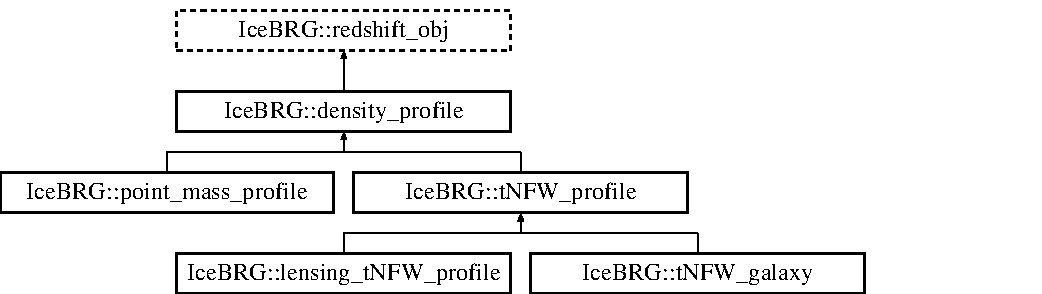
\includegraphics[height=3.950617cm]{classIceBRG_1_1density__profile}
\end{center}
\end{figure}
\subsection*{Public Member Functions}
\begin{DoxyCompactItemize}
\item 
\hyperlink{classIceBRG_1_1density__profile_ad1ee6b3b861e5b46c958e516ccea87fc}{density\+\_\+profile} ()
\item 
virtual \hyperlink{classIceBRG_1_1density__profile_a4bc455459dcfcf20b659beeccae7f66c}{$\sim$density\+\_\+profile} ()
\item 
virtual \hyperlink{namespaceIceBRG_a1be72ac4918a9b029f2eefa084213e35}{mass\+\_\+type} \hyperlink{classIceBRG_1_1density__profile_aa62204b8ca04779f4477183f873b2aff}{mvir} () const  =0
\item 
virtual \hyperlink{namespaceIceBRG_a9f5e5cdd641bb4c06f7305dfb5ae0238}{density\+\_\+type} \hyperlink{classIceBRG_1_1density__profile_ac47dc183eb719a6aea32e981a6f79a30}{dens} (const \hyperlink{namespaceIceBRG_a45499647eb87e24c10ab32c628711cec}{distance\+\_\+type} \&r) const  =0
\item 
virtual \hyperlink{classIceBRG_1_1density__profile}{density\+\_\+profile} $\ast$ \hyperlink{classIceBRG_1_1density__profile_a8a6a4033eeadf4b70ee174f293639c80}{density\+\_\+profile\+\_\+clone} () const  =0
\item 
virtual void \hyperlink{classIceBRG_1_1density__profile_ae0230aa967a251d3ce5f360514e1690d}{set\+\_\+mvir} (const \hyperlink{namespaceIceBRG_a1be72ac4918a9b029f2eefa084213e35}{mass\+\_\+type} \&new\+\_\+mvir)
\item 
virtual void \hyperlink{classIceBRG_1_1density__profile_ae96d1142416f1eec0cf5e953c9dd19d4}{set\+\_\+vvir} (const \hyperlink{namespaceIceBRG_a34f8ef3b46f3408301e3c28197095eff}{velocity\+\_\+type} \&new\+\_\+vvir)
\item 
virtual void \hyperlink{classIceBRG_1_1density__profile_af98da3e96b5a4a023f749d3f5467afb0}{set\+\_\+rvir} (const \hyperlink{namespaceIceBRG_a45499647eb87e24c10ab32c628711cec}{distance\+\_\+type} \&new\+\_\+rvir)
\item 
virtual void \hyperlink{classIceBRG_1_1density__profile_a75a38a12721b8fcf359e768d1e2986b0}{set\+\_\+rs} (const \hyperlink{namespaceIceBRG_a45499647eb87e24c10ab32c628711cec}{distance\+\_\+type} \&new\+\_\+rs)
\item 
virtual void \hyperlink{classIceBRG_1_1density__profile_ae740e08ea853866ee90323193877f5e7}{set\+\_\+rt} (const \hyperlink{namespaceIceBRG_a45499647eb87e24c10ab32c628711cec}{distance\+\_\+type} \&new\+\_\+rt)
\item 
virtual void \hyperlink{classIceBRG_1_1density__profile_af58ebb218c2abe35cfaa261cd29ba35c}{set\+\_\+parameters} (const std\+::vector$<$ \hyperlink{namespaceIceBRG_a3101fc159e191fa99c4ec14e445df96e}{any\+\_\+units\+\_\+type} $>$ \&parameters)
\item 
virtual void \hyperlink{classIceBRG_1_1density__profile_ac555b90ef308964a086b94aff857c0ea}{set\+\_\+tau} (const \hyperlink{lib_2IceBRG__main_2common_8h_ad0f130a56eeb944d9ef2692ee881ecc4}{flt\+\_\+type} \&new\+\_\+tau)
\item 
virtual void \hyperlink{classIceBRG_1_1density__profile_a667b94f29c17889c6e987e39ecacd8ad}{set\+\_\+c} (const \hyperlink{lib_2IceBRG__main_2common_8h_ad0f130a56eeb944d9ef2692ee881ecc4}{flt\+\_\+type} \&new\+\_\+c)
\item 
void \hyperlink{classIceBRG_1_1density__profile_aaf60b6259f530a6beb6424723d89b4b0}{override\+\_\+rhmvir} (const \hyperlink{namespaceIceBRG_a45499647eb87e24c10ab32c628711cec}{distance\+\_\+type} \&new\+\_\+rhmvir)
\item 
void \hyperlink{classIceBRG_1_1density__profile_a8e1f443d0b47285bd0342f101d2148d9}{override\+\_\+rhmtot} (const \hyperlink{namespaceIceBRG_a45499647eb87e24c10ab32c628711cec}{distance\+\_\+type} \&new\+\_\+rhmtot)
\item 
virtual \hyperlink{namespaceIceBRG_a1be72ac4918a9b029f2eefa084213e35}{mass\+\_\+type} \hyperlink{classIceBRG_1_1density__profile_ada763e0637edc2efb168a9fa42daa580}{mtot} () const 
\item 
virtual \hyperlink{namespaceIceBRG_a45499647eb87e24c10ab32c628711cec}{distance\+\_\+type} \hyperlink{classIceBRG_1_1density__profile_a53c528b9d6de8506175faece58361c23}{rt} () const 
\item 
virtual size\+\_\+t \hyperlink{classIceBRG_1_1density__profile_ad63fb55be18802ec2ab1d4a0a9d49236}{num\+\_\+parameters} () const 
\item 
virtual std\+::vector$<$ \hyperlink{namespaceIceBRG_a3101fc159e191fa99c4ec14e445df96e}{any\+\_\+units\+\_\+type} $>$ \hyperlink{classIceBRG_1_1density__profile_a661c4e91260285e70290c8b454a0f0d9}{get\+\_\+parameters} () const 
\item 
virtual std\+::vector$<$ std\+::string $>$ \hyperlink{classIceBRG_1_1density__profile_ae773cdab093dfc22ff9dc01dd2de09f4}{get\+\_\+parameter\+\_\+names} () const 
\item 
virtual \hyperlink{namespaceIceBRG_a1be72ac4918a9b029f2eefa084213e35}{mass\+\_\+type} \hyperlink{classIceBRG_1_1density__profile_a090e214c2228f99019c75e7fede37ae5}{enc\+\_\+mass} (const \hyperlink{namespaceIceBRG_a45499647eb87e24c10ab32c628711cec}{distance\+\_\+type} \&r) const 
\item 
virtual \hyperlink{namespaceIceBRG_a45499647eb87e24c10ab32c628711cec}{distance\+\_\+type} \hyperlink{classIceBRG_1_1density__profile_a34312cb028a2c481cb72224a12b4a287}{rvir} () const 
\item 
\hyperlink{namespaceIceBRG_a1be72ac4918a9b029f2eefa084213e35}{mass\+\_\+type} \hyperlink{classIceBRG_1_1density__profile_ad4d6e483327bfd378fc74b0e2e7b72f3}{hmvir} () const 
\item 
\hyperlink{namespaceIceBRG_a1be72ac4918a9b029f2eefa084213e35}{mass\+\_\+type} \hyperlink{classIceBRG_1_1density__profile_ad3f33f3d21729121e3752cc505622afb}{hmtot} () const 
\item 
virtual \hyperlink{namespaceIceBRG_a1be72ac4918a9b029f2eefa084213e35}{mass\+\_\+type} \hyperlink{classIceBRG_1_1density__profile_afaf5718b4786ef793ace33f9ea861444}{hm} () const 
\item 
virtual \hyperlink{namespaceIceBRG_a9f5e5cdd641bb4c06f7305dfb5ae0238}{density\+\_\+type} \hyperlink{classIceBRG_1_1density__profile_abe453f2128f3ee4030092e20b8c6e380}{enc\+\_\+dens} (const \hyperlink{namespaceIceBRG_a45499647eb87e24c10ab32c628711cec}{distance\+\_\+type} \&r) const 
\item 
virtual \hyperlink{namespaceIceBRG_a45499647eb87e24c10ab32c628711cec}{distance\+\_\+type} \hyperlink{classIceBRG_1_1density__profile_a6cd236235c8d36ec6de5cbcdce4cc57b}{rhmvir} () const 
\item 
virtual \hyperlink{namespaceIceBRG_a45499647eb87e24c10ab32c628711cec}{distance\+\_\+type} \hyperlink{classIceBRG_1_1density__profile_a99f066c6b0b737eb0be438d485cfc105}{rhmtot} () const 
\item 
virtual \hyperlink{namespaceIceBRG_a45499647eb87e24c10ab32c628711cec}{distance\+\_\+type} \hyperlink{classIceBRG_1_1density__profile_a20faa531d9db7d917939d598693372d7}{rhm} () const 
\item 
virtual \hyperlink{namespaceIceBRG_a34f8ef3b46f3408301e3c28197095eff}{velocity\+\_\+type} \hyperlink{classIceBRG_1_1density__profile_a09dec0ec4468e10e87b7b30f2069c108}{vvir} () const 
\item 
virtual \hyperlink{namespaceIceBRG_a34f8ef3b46f3408301e3c28197095eff}{velocity\+\_\+type} \hyperlink{classIceBRG_1_1density__profile_a5f4ceb70b5af5c816f25f08a62c50b89}{vhmvir} () const 
\item 
virtual \hyperlink{namespaceIceBRG_a34f8ef3b46f3408301e3c28197095eff}{velocity\+\_\+type} \hyperlink{classIceBRG_1_1density__profile_aa6a6bcba29d629b5d711e6141ecafd7a}{vhmtot} () const 
\item 
virtual \hyperlink{namespaceIceBRG_a34f8ef3b46f3408301e3c28197095eff}{velocity\+\_\+type} \hyperlink{classIceBRG_1_1density__profile_a9ecd0afe7e8fa7050efe2d984240c0ec}{vhm} () const 
\item 
virtual \hyperlink{namespaceIceBRG_a34f8ef3b46f3408301e3c28197095eff}{velocity\+\_\+type} \hyperlink{classIceBRG_1_1density__profile_a11564ec6ea6103493654000c81ce4bfb}{vt} () const 
\item 
\hyperlink{namespaceIceBRG_abf6c442a2e180ef52c5cefe18e47c327}{time\+\_\+type} \hyperlink{classIceBRG_1_1density__profile_a0215cd84252abdb85682fbcc7eee19f4}{otvir} () const 
\item 
\hyperlink{namespaceIceBRG_abf6c442a2e180ef52c5cefe18e47c327}{time\+\_\+type} \hyperlink{classIceBRG_1_1density__profile_aad4e976a6e5d77b85ecb39d481d87d51}{othmvir} () const 
\item 
\hyperlink{namespaceIceBRG_abf6c442a2e180ef52c5cefe18e47c327}{time\+\_\+type} \hyperlink{classIceBRG_1_1density__profile_a88b1209927b800d5eb367bfc9469a139}{othmtot} () const 
\item 
\hyperlink{namespaceIceBRG_abf6c442a2e180ef52c5cefe18e47c327}{time\+\_\+type} \hyperlink{classIceBRG_1_1density__profile_a8ab2f8bffed3c330959f47f18174fa29}{othm} () const 
\item 
\hyperlink{namespaceIceBRG_abf6c442a2e180ef52c5cefe18e47c327}{time\+\_\+type} \hyperlink{classIceBRG_1_1density__profile_a8055fc7c1ce9cf0628ff4e849c4ff99b}{ott} () const 
\item 
void \hyperlink{classIceBRG_1_1density__profile_a8dea593a6ecb0f07e3106574f3ceb169}{set\+\_\+hm\+\_\+type} (\hyperlink{lib_2IceBRG__main_2common_8h_ac4de9d9335536ac22821171deec8d39e}{int\+\_\+type} new\+\_\+hm\+\_\+type)
\item 
\hyperlink{namespaceIceBRG_ab10fe6d8fe6432a7dc0aa5a8ecac6a14}{acceleration\+\_\+type} \hyperlink{classIceBRG_1_1density__profile_a7503bcdce1e01051b027da3e53ac487e}{accel} (const \hyperlink{namespaceIceBRG_a45499647eb87e24c10ab32c628711cec}{distance\+\_\+type} \&r) const 
\item 
virtual \hyperlink{namespaceIceBRG_a896bc1bf7e8db5ca045b9cf35912ca5e}{custom\+\_\+unit\+\_\+type}$<$ 0,-\/2, 0, 0, 0 $>$ \hyperlink{classIceBRG_1_1density__profile_a9f3a8f3c294f3c07159effde5a32d528}{Daccel} (const \hyperlink{namespaceIceBRG_a45499647eb87e24c10ab32c628711cec}{distance\+\_\+type} \&r) const 
\item 
virtual void \hyperlink{classIceBRG_1_1density__profile_ac7b6a0bf55ce53aeeccbf7322a49e54c}{truncate\+\_\+to\+\_\+fraction} (const \hyperlink{lib_2IceBRG__main_2common_8h_ad0f130a56eeb944d9ef2692ee881ecc4}{flt\+\_\+type} \&fraction)
\end{DoxyCompactItemize}
\subsection*{Protected Attributes}
\begin{DoxyCompactItemize}
\item 
bool \hyperlink{classIceBRG_1_1density__profile_a8a91facce74344d679864ee5267ed371}{hmvir\+\_\+cached}
\item 
bool \hyperlink{classIceBRG_1_1density__profile_a6a6d3924d61145f1ad74a4d93fefd3ff}{hmtot\+\_\+cached}
\end{DoxyCompactItemize}


\subsection{Constructor \& Destructor Documentation}
\hypertarget{classIceBRG_1_1density__profile_ad1ee6b3b861e5b46c958e516ccea87fc}{}\index{Ice\+B\+R\+G\+::density\+\_\+profile@{Ice\+B\+R\+G\+::density\+\_\+profile}!density\+\_\+profile@{density\+\_\+profile}}
\index{density\+\_\+profile@{density\+\_\+profile}!Ice\+B\+R\+G\+::density\+\_\+profile@{Ice\+B\+R\+G\+::density\+\_\+profile}}
\subsubsection[{density\+\_\+profile()}]{\setlength{\rightskip}{0pt plus 5cm}Ice\+B\+R\+G\+::density\+\_\+profile\+::density\+\_\+profile (
\begin{DoxyParamCaption}
{}
\end{DoxyParamCaption}
)\hspace{0.3cm}{\ttfamily [inline]}}\label{classIceBRG_1_1density__profile_ad1ee6b3b861e5b46c958e516ccea87fc}
\hypertarget{classIceBRG_1_1density__profile_a4bc455459dcfcf20b659beeccae7f66c}{}\index{Ice\+B\+R\+G\+::density\+\_\+profile@{Ice\+B\+R\+G\+::density\+\_\+profile}!````~density\+\_\+profile@{$\sim$density\+\_\+profile}}
\index{````~density\+\_\+profile@{$\sim$density\+\_\+profile}!Ice\+B\+R\+G\+::density\+\_\+profile@{Ice\+B\+R\+G\+::density\+\_\+profile}}
\subsubsection[{$\sim$density\+\_\+profile()}]{\setlength{\rightskip}{0pt plus 5cm}Ice\+B\+R\+G\+::density\+\_\+profile\+::$\sim$density\+\_\+profile (
\begin{DoxyParamCaption}
{}
\end{DoxyParamCaption}
)\hspace{0.3cm}{\ttfamily [virtual]}}\label{classIceBRG_1_1density__profile_a4bc455459dcfcf20b659beeccae7f66c}


\subsection{Member Function Documentation}
\hypertarget{classIceBRG_1_1density__profile_a7503bcdce1e01051b027da3e53ac487e}{}\index{Ice\+B\+R\+G\+::density\+\_\+profile@{Ice\+B\+R\+G\+::density\+\_\+profile}!accel@{accel}}
\index{accel@{accel}!Ice\+B\+R\+G\+::density\+\_\+profile@{Ice\+B\+R\+G\+::density\+\_\+profile}}
\subsubsection[{accel(const distance\+\_\+type \&r) const }]{\setlength{\rightskip}{0pt plus 5cm}{\bf acceleration\+\_\+type} Ice\+B\+R\+G\+::density\+\_\+profile\+::accel (
\begin{DoxyParamCaption}
\item[{const {\bf distance\+\_\+type} \&}]{r}
\end{DoxyParamCaption}
) const\hspace{0.3cm}{\ttfamily [inline]}}\label{classIceBRG_1_1density__profile_a7503bcdce1e01051b027da3e53ac487e}
\hypertarget{classIceBRG_1_1density__profile_a9f3a8f3c294f3c07159effde5a32d528}{}\index{Ice\+B\+R\+G\+::density\+\_\+profile@{Ice\+B\+R\+G\+::density\+\_\+profile}!Daccel@{Daccel}}
\index{Daccel@{Daccel}!Ice\+B\+R\+G\+::density\+\_\+profile@{Ice\+B\+R\+G\+::density\+\_\+profile}}
\subsubsection[{Daccel(const distance\+\_\+type \&r) const }]{\setlength{\rightskip}{0pt plus 5cm}{\bf Ice\+B\+R\+G\+::custom\+\_\+unit\+\_\+type}$<$ 0,-\/2, 0, 0, 0 $>$ Ice\+B\+R\+G\+::density\+\_\+profile\+::\+Daccel (
\begin{DoxyParamCaption}
\item[{const {\bf distance\+\_\+type} \&}]{r}
\end{DoxyParamCaption}
) const\hspace{0.3cm}{\ttfamily [virtual]}}\label{classIceBRG_1_1density__profile_a9f3a8f3c294f3c07159effde5a32d528}
\hypertarget{classIceBRG_1_1density__profile_ac47dc183eb719a6aea32e981a6f79a30}{}\index{Ice\+B\+R\+G\+::density\+\_\+profile@{Ice\+B\+R\+G\+::density\+\_\+profile}!dens@{dens}}
\index{dens@{dens}!Ice\+B\+R\+G\+::density\+\_\+profile@{Ice\+B\+R\+G\+::density\+\_\+profile}}
\subsubsection[{dens(const distance\+\_\+type \&r) const  =0}]{\setlength{\rightskip}{0pt plus 5cm}virtual {\bf density\+\_\+type} Ice\+B\+R\+G\+::density\+\_\+profile\+::dens (
\begin{DoxyParamCaption}
\item[{const {\bf distance\+\_\+type} \&}]{r}
\end{DoxyParamCaption}
) const\hspace{0.3cm}{\ttfamily [pure virtual]}}\label{classIceBRG_1_1density__profile_ac47dc183eb719a6aea32e981a6f79a30}


Implemented in \hyperlink{classIceBRG_1_1tNFW__profile_a1ab9b1e6c9e677b51efa72980f7c59a6}{Ice\+B\+R\+G\+::t\+N\+F\+W\+\_\+profile}, and \hyperlink{classIceBRG_1_1point__mass__profile_aa689ec66a40e36d9886c1b8077488161}{Ice\+B\+R\+G\+::point\+\_\+mass\+\_\+profile}.

\hypertarget{classIceBRG_1_1density__profile_a8a6a4033eeadf4b70ee174f293639c80}{}\index{Ice\+B\+R\+G\+::density\+\_\+profile@{Ice\+B\+R\+G\+::density\+\_\+profile}!density\+\_\+profile\+\_\+clone@{density\+\_\+profile\+\_\+clone}}
\index{density\+\_\+profile\+\_\+clone@{density\+\_\+profile\+\_\+clone}!Ice\+B\+R\+G\+::density\+\_\+profile@{Ice\+B\+R\+G\+::density\+\_\+profile}}
\subsubsection[{density\+\_\+profile\+\_\+clone() const  =0}]{\setlength{\rightskip}{0pt plus 5cm}virtual {\bf density\+\_\+profile}$\ast$ Ice\+B\+R\+G\+::density\+\_\+profile\+::density\+\_\+profile\+\_\+clone (
\begin{DoxyParamCaption}
{}
\end{DoxyParamCaption}
) const\hspace{0.3cm}{\ttfamily [pure virtual]}}\label{classIceBRG_1_1density__profile_a8a6a4033eeadf4b70ee174f293639c80}


Implemented in \hyperlink{classIceBRG_1_1tNFW__profile_abf08721d23c2f612f92c1e97e6bf6453}{Ice\+B\+R\+G\+::t\+N\+F\+W\+\_\+profile}, \hyperlink{classIceBRG_1_1point__mass__profile_a0e02fa9204b4d6718fb0a27b61b38b69}{Ice\+B\+R\+G\+::point\+\_\+mass\+\_\+profile}, \hyperlink{classIceBRG_1_1lensing__tNFW__profile_af196f26f5ed61c128e2931157676eb3a}{Ice\+B\+R\+G\+::lensing\+\_\+t\+N\+F\+W\+\_\+profile}, and \hyperlink{classIceBRG_1_1tNFW__galaxy_aa571e02cd48ac9f97f205077d29dfcf5}{Ice\+B\+R\+G\+::t\+N\+F\+W\+\_\+galaxy}.

\hypertarget{classIceBRG_1_1density__profile_abe453f2128f3ee4030092e20b8c6e380}{}\index{Ice\+B\+R\+G\+::density\+\_\+profile@{Ice\+B\+R\+G\+::density\+\_\+profile}!enc\+\_\+dens@{enc\+\_\+dens}}
\index{enc\+\_\+dens@{enc\+\_\+dens}!Ice\+B\+R\+G\+::density\+\_\+profile@{Ice\+B\+R\+G\+::density\+\_\+profile}}
\subsubsection[{enc\+\_\+dens(const distance\+\_\+type \&r) const }]{\setlength{\rightskip}{0pt plus 5cm}virtual {\bf density\+\_\+type} Ice\+B\+R\+G\+::density\+\_\+profile\+::enc\+\_\+dens (
\begin{DoxyParamCaption}
\item[{const {\bf distance\+\_\+type} \&}]{r}
\end{DoxyParamCaption}
) const\hspace{0.3cm}{\ttfamily [inline]}, {\ttfamily [virtual]}}\label{classIceBRG_1_1density__profile_abe453f2128f3ee4030092e20b8c6e380}


Reimplemented in \hyperlink{classIceBRG_1_1point__mass__profile_ab52d614d0c7c163085d70ae78e6b1eed}{Ice\+B\+R\+G\+::point\+\_\+mass\+\_\+profile}.

\hypertarget{classIceBRG_1_1density__profile_a090e214c2228f99019c75e7fede37ae5}{}\index{Ice\+B\+R\+G\+::density\+\_\+profile@{Ice\+B\+R\+G\+::density\+\_\+profile}!enc\+\_\+mass@{enc\+\_\+mass}}
\index{enc\+\_\+mass@{enc\+\_\+mass}!Ice\+B\+R\+G\+::density\+\_\+profile@{Ice\+B\+R\+G\+::density\+\_\+profile}}
\subsubsection[{enc\+\_\+mass(const distance\+\_\+type \&r) const }]{\setlength{\rightskip}{0pt plus 5cm}{\bf Ice\+B\+R\+G\+::mass\+\_\+type} Ice\+B\+R\+G\+::density\+\_\+profile\+::enc\+\_\+mass (
\begin{DoxyParamCaption}
\item[{const {\bf distance\+\_\+type} \&}]{r}
\end{DoxyParamCaption}
) const\hspace{0.3cm}{\ttfamily [virtual]}}\label{classIceBRG_1_1density__profile_a090e214c2228f99019c75e7fede37ae5}


Reimplemented in \hyperlink{classIceBRG_1_1tNFW__profile_a13939b7320cf1fd3be20343212d0e663}{Ice\+B\+R\+G\+::t\+N\+F\+W\+\_\+profile}, and \hyperlink{classIceBRG_1_1point__mass__profile_a2e72fef9bc04039bd9119453f4aa6b13}{Ice\+B\+R\+G\+::point\+\_\+mass\+\_\+profile}.

\hypertarget{classIceBRG_1_1density__profile_ae773cdab093dfc22ff9dc01dd2de09f4}{}\index{Ice\+B\+R\+G\+::density\+\_\+profile@{Ice\+B\+R\+G\+::density\+\_\+profile}!get\+\_\+parameter\+\_\+names@{get\+\_\+parameter\+\_\+names}}
\index{get\+\_\+parameter\+\_\+names@{get\+\_\+parameter\+\_\+names}!Ice\+B\+R\+G\+::density\+\_\+profile@{Ice\+B\+R\+G\+::density\+\_\+profile}}
\subsubsection[{get\+\_\+parameter\+\_\+names() const }]{\setlength{\rightskip}{0pt plus 5cm}virtual std\+::vector$<$ std\+::string $>$ Ice\+B\+R\+G\+::density\+\_\+profile\+::get\+\_\+parameter\+\_\+names (
\begin{DoxyParamCaption}
{}
\end{DoxyParamCaption}
) const\hspace{0.3cm}{\ttfamily [inline]}, {\ttfamily [virtual]}}\label{classIceBRG_1_1density__profile_ae773cdab093dfc22ff9dc01dd2de09f4}


Reimplemented in \hyperlink{classIceBRG_1_1tNFW__profile_a89938a2cecd5905c558e35fd295335cd}{Ice\+B\+R\+G\+::t\+N\+F\+W\+\_\+profile}, and \hyperlink{classIceBRG_1_1point__mass__profile_a58ddc44e9a7fa78f1ec07e35db5bc141}{Ice\+B\+R\+G\+::point\+\_\+mass\+\_\+profile}.

\hypertarget{classIceBRG_1_1density__profile_a661c4e91260285e70290c8b454a0f0d9}{}\index{Ice\+B\+R\+G\+::density\+\_\+profile@{Ice\+B\+R\+G\+::density\+\_\+profile}!get\+\_\+parameters@{get\+\_\+parameters}}
\index{get\+\_\+parameters@{get\+\_\+parameters}!Ice\+B\+R\+G\+::density\+\_\+profile@{Ice\+B\+R\+G\+::density\+\_\+profile}}
\subsubsection[{get\+\_\+parameters() const }]{\setlength{\rightskip}{0pt plus 5cm}virtual std\+::vector$<$ {\bf any\+\_\+units\+\_\+type} $>$ Ice\+B\+R\+G\+::density\+\_\+profile\+::get\+\_\+parameters (
\begin{DoxyParamCaption}
{}
\end{DoxyParamCaption}
) const\hspace{0.3cm}{\ttfamily [inline]}, {\ttfamily [virtual]}}\label{classIceBRG_1_1density__profile_a661c4e91260285e70290c8b454a0f0d9}


Reimplemented in \hyperlink{classIceBRG_1_1tNFW__profile_ab659523c00e3fabc0350b8d9a423aefd}{Ice\+B\+R\+G\+::t\+N\+F\+W\+\_\+profile}, and \hyperlink{classIceBRG_1_1point__mass__profile_a52bdbf1072d13ddef48df90339366ab3}{Ice\+B\+R\+G\+::point\+\_\+mass\+\_\+profile}.

\hypertarget{classIceBRG_1_1density__profile_afaf5718b4786ef793ace33f9ea861444}{}\index{Ice\+B\+R\+G\+::density\+\_\+profile@{Ice\+B\+R\+G\+::density\+\_\+profile}!hm@{hm}}
\index{hm@{hm}!Ice\+B\+R\+G\+::density\+\_\+profile@{Ice\+B\+R\+G\+::density\+\_\+profile}}
\subsubsection[{hm() const }]{\setlength{\rightskip}{0pt plus 5cm}virtual {\bf mass\+\_\+type} Ice\+B\+R\+G\+::density\+\_\+profile\+::hm (
\begin{DoxyParamCaption}
{}
\end{DoxyParamCaption}
) const\hspace{0.3cm}{\ttfamily [inline]}, {\ttfamily [virtual]}}\label{classIceBRG_1_1density__profile_afaf5718b4786ef793ace33f9ea861444}
\hypertarget{classIceBRG_1_1density__profile_ad3f33f3d21729121e3752cc505622afb}{}\index{Ice\+B\+R\+G\+::density\+\_\+profile@{Ice\+B\+R\+G\+::density\+\_\+profile}!hmtot@{hmtot}}
\index{hmtot@{hmtot}!Ice\+B\+R\+G\+::density\+\_\+profile@{Ice\+B\+R\+G\+::density\+\_\+profile}}
\subsubsection[{hmtot() const }]{\setlength{\rightskip}{0pt plus 5cm}{\bf mass\+\_\+type} Ice\+B\+R\+G\+::density\+\_\+profile\+::hmtot (
\begin{DoxyParamCaption}
{}
\end{DoxyParamCaption}
) const\hspace{0.3cm}{\ttfamily [inline]}}\label{classIceBRG_1_1density__profile_ad3f33f3d21729121e3752cc505622afb}
\hypertarget{classIceBRG_1_1density__profile_ad4d6e483327bfd378fc74b0e2e7b72f3}{}\index{Ice\+B\+R\+G\+::density\+\_\+profile@{Ice\+B\+R\+G\+::density\+\_\+profile}!hmvir@{hmvir}}
\index{hmvir@{hmvir}!Ice\+B\+R\+G\+::density\+\_\+profile@{Ice\+B\+R\+G\+::density\+\_\+profile}}
\subsubsection[{hmvir() const }]{\setlength{\rightskip}{0pt plus 5cm}{\bf mass\+\_\+type} Ice\+B\+R\+G\+::density\+\_\+profile\+::hmvir (
\begin{DoxyParamCaption}
{}
\end{DoxyParamCaption}
) const\hspace{0.3cm}{\ttfamily [inline]}}\label{classIceBRG_1_1density__profile_ad4d6e483327bfd378fc74b0e2e7b72f3}
\hypertarget{classIceBRG_1_1density__profile_ada763e0637edc2efb168a9fa42daa580}{}\index{Ice\+B\+R\+G\+::density\+\_\+profile@{Ice\+B\+R\+G\+::density\+\_\+profile}!mtot@{mtot}}
\index{mtot@{mtot}!Ice\+B\+R\+G\+::density\+\_\+profile@{Ice\+B\+R\+G\+::density\+\_\+profile}}
\subsubsection[{mtot() const }]{\setlength{\rightskip}{0pt plus 5cm}virtual {\bf mass\+\_\+type} Ice\+B\+R\+G\+::density\+\_\+profile\+::mtot (
\begin{DoxyParamCaption}
{}
\end{DoxyParamCaption}
) const\hspace{0.3cm}{\ttfamily [inline]}, {\ttfamily [virtual]}}\label{classIceBRG_1_1density__profile_ada763e0637edc2efb168a9fa42daa580}


Reimplemented in \hyperlink{classIceBRG_1_1tNFW__profile_a8bb04b5e598b5d7ecb7d54c99383fdf6}{Ice\+B\+R\+G\+::t\+N\+F\+W\+\_\+profile}, and \hyperlink{classIceBRG_1_1point__mass__profile_a1454cc006571f6a245e8e5046ee20bc5}{Ice\+B\+R\+G\+::point\+\_\+mass\+\_\+profile}.

\hypertarget{classIceBRG_1_1density__profile_aa62204b8ca04779f4477183f873b2aff}{}\index{Ice\+B\+R\+G\+::density\+\_\+profile@{Ice\+B\+R\+G\+::density\+\_\+profile}!mvir@{mvir}}
\index{mvir@{mvir}!Ice\+B\+R\+G\+::density\+\_\+profile@{Ice\+B\+R\+G\+::density\+\_\+profile}}
\subsubsection[{mvir() const  =0}]{\setlength{\rightskip}{0pt plus 5cm}virtual {\bf mass\+\_\+type} Ice\+B\+R\+G\+::density\+\_\+profile\+::mvir (
\begin{DoxyParamCaption}
{}
\end{DoxyParamCaption}
) const\hspace{0.3cm}{\ttfamily [pure virtual]}}\label{classIceBRG_1_1density__profile_aa62204b8ca04779f4477183f873b2aff}


Implemented in \hyperlink{classIceBRG_1_1tNFW__profile_aaa10d679c4d68b608213391ad207a9e8}{Ice\+B\+R\+G\+::t\+N\+F\+W\+\_\+profile}, and \hyperlink{classIceBRG_1_1point__mass__profile_a8f9a6a1fafe39c216349ff92e1046b53}{Ice\+B\+R\+G\+::point\+\_\+mass\+\_\+profile}.

\hypertarget{classIceBRG_1_1density__profile_ad63fb55be18802ec2ab1d4a0a9d49236}{}\index{Ice\+B\+R\+G\+::density\+\_\+profile@{Ice\+B\+R\+G\+::density\+\_\+profile}!num\+\_\+parameters@{num\+\_\+parameters}}
\index{num\+\_\+parameters@{num\+\_\+parameters}!Ice\+B\+R\+G\+::density\+\_\+profile@{Ice\+B\+R\+G\+::density\+\_\+profile}}
\subsubsection[{num\+\_\+parameters() const }]{\setlength{\rightskip}{0pt plus 5cm}virtual size\+\_\+t Ice\+B\+R\+G\+::density\+\_\+profile\+::num\+\_\+parameters (
\begin{DoxyParamCaption}
{}
\end{DoxyParamCaption}
) const\hspace{0.3cm}{\ttfamily [inline]}, {\ttfamily [virtual]}}\label{classIceBRG_1_1density__profile_ad63fb55be18802ec2ab1d4a0a9d49236}


Reimplemented in \hyperlink{classIceBRG_1_1tNFW__profile_a3317838b91dfafb06fc61343ad63b365}{Ice\+B\+R\+G\+::t\+N\+F\+W\+\_\+profile}, and \hyperlink{classIceBRG_1_1point__mass__profile_a71f96138938e5e9edd0c755f131ddf5e}{Ice\+B\+R\+G\+::point\+\_\+mass\+\_\+profile}.

\hypertarget{classIceBRG_1_1density__profile_a8ab2f8bffed3c330959f47f18174fa29}{}\index{Ice\+B\+R\+G\+::density\+\_\+profile@{Ice\+B\+R\+G\+::density\+\_\+profile}!othm@{othm}}
\index{othm@{othm}!Ice\+B\+R\+G\+::density\+\_\+profile@{Ice\+B\+R\+G\+::density\+\_\+profile}}
\subsubsection[{othm() const }]{\setlength{\rightskip}{0pt plus 5cm}{\bf time\+\_\+type} Ice\+B\+R\+G\+::density\+\_\+profile\+::othm (
\begin{DoxyParamCaption}
{}
\end{DoxyParamCaption}
) const\hspace{0.3cm}{\ttfamily [inline]}}\label{classIceBRG_1_1density__profile_a8ab2f8bffed3c330959f47f18174fa29}
\hypertarget{classIceBRG_1_1density__profile_a88b1209927b800d5eb367bfc9469a139}{}\index{Ice\+B\+R\+G\+::density\+\_\+profile@{Ice\+B\+R\+G\+::density\+\_\+profile}!othmtot@{othmtot}}
\index{othmtot@{othmtot}!Ice\+B\+R\+G\+::density\+\_\+profile@{Ice\+B\+R\+G\+::density\+\_\+profile}}
\subsubsection[{othmtot() const }]{\setlength{\rightskip}{0pt plus 5cm}{\bf time\+\_\+type} Ice\+B\+R\+G\+::density\+\_\+profile\+::othmtot (
\begin{DoxyParamCaption}
{}
\end{DoxyParamCaption}
) const\hspace{0.3cm}{\ttfamily [inline]}}\label{classIceBRG_1_1density__profile_a88b1209927b800d5eb367bfc9469a139}
\hypertarget{classIceBRG_1_1density__profile_aad4e976a6e5d77b85ecb39d481d87d51}{}\index{Ice\+B\+R\+G\+::density\+\_\+profile@{Ice\+B\+R\+G\+::density\+\_\+profile}!othmvir@{othmvir}}
\index{othmvir@{othmvir}!Ice\+B\+R\+G\+::density\+\_\+profile@{Ice\+B\+R\+G\+::density\+\_\+profile}}
\subsubsection[{othmvir() const }]{\setlength{\rightskip}{0pt plus 5cm}{\bf time\+\_\+type} Ice\+B\+R\+G\+::density\+\_\+profile\+::othmvir (
\begin{DoxyParamCaption}
{}
\end{DoxyParamCaption}
) const\hspace{0.3cm}{\ttfamily [inline]}}\label{classIceBRG_1_1density__profile_aad4e976a6e5d77b85ecb39d481d87d51}
\hypertarget{classIceBRG_1_1density__profile_a8055fc7c1ce9cf0628ff4e849c4ff99b}{}\index{Ice\+B\+R\+G\+::density\+\_\+profile@{Ice\+B\+R\+G\+::density\+\_\+profile}!ott@{ott}}
\index{ott@{ott}!Ice\+B\+R\+G\+::density\+\_\+profile@{Ice\+B\+R\+G\+::density\+\_\+profile}}
\subsubsection[{ott() const }]{\setlength{\rightskip}{0pt plus 5cm}{\bf time\+\_\+type} Ice\+B\+R\+G\+::density\+\_\+profile\+::ott (
\begin{DoxyParamCaption}
{}
\end{DoxyParamCaption}
) const\hspace{0.3cm}{\ttfamily [inline]}}\label{classIceBRG_1_1density__profile_a8055fc7c1ce9cf0628ff4e849c4ff99b}
\hypertarget{classIceBRG_1_1density__profile_a0215cd84252abdb85682fbcc7eee19f4}{}\index{Ice\+B\+R\+G\+::density\+\_\+profile@{Ice\+B\+R\+G\+::density\+\_\+profile}!otvir@{otvir}}
\index{otvir@{otvir}!Ice\+B\+R\+G\+::density\+\_\+profile@{Ice\+B\+R\+G\+::density\+\_\+profile}}
\subsubsection[{otvir() const }]{\setlength{\rightskip}{0pt plus 5cm}{\bf time\+\_\+type} Ice\+B\+R\+G\+::density\+\_\+profile\+::otvir (
\begin{DoxyParamCaption}
{}
\end{DoxyParamCaption}
) const\hspace{0.3cm}{\ttfamily [inline]}}\label{classIceBRG_1_1density__profile_a0215cd84252abdb85682fbcc7eee19f4}
\hypertarget{classIceBRG_1_1density__profile_a8e1f443d0b47285bd0342f101d2148d9}{}\index{Ice\+B\+R\+G\+::density\+\_\+profile@{Ice\+B\+R\+G\+::density\+\_\+profile}!override\+\_\+rhmtot@{override\+\_\+rhmtot}}
\index{override\+\_\+rhmtot@{override\+\_\+rhmtot}!Ice\+B\+R\+G\+::density\+\_\+profile@{Ice\+B\+R\+G\+::density\+\_\+profile}}
\subsubsection[{override\+\_\+rhmtot(const distance\+\_\+type \&new\+\_\+rhmtot)}]{\setlength{\rightskip}{0pt plus 5cm}void Ice\+B\+R\+G\+::density\+\_\+profile\+::override\+\_\+rhmtot (
\begin{DoxyParamCaption}
\item[{const {\bf distance\+\_\+type} \&}]{new\+\_\+rhmtot}
\end{DoxyParamCaption}
)\hspace{0.3cm}{\ttfamily [inline]}}\label{classIceBRG_1_1density__profile_a8e1f443d0b47285bd0342f101d2148d9}
\hypertarget{classIceBRG_1_1density__profile_aaf60b6259f530a6beb6424723d89b4b0}{}\index{Ice\+B\+R\+G\+::density\+\_\+profile@{Ice\+B\+R\+G\+::density\+\_\+profile}!override\+\_\+rhmvir@{override\+\_\+rhmvir}}
\index{override\+\_\+rhmvir@{override\+\_\+rhmvir}!Ice\+B\+R\+G\+::density\+\_\+profile@{Ice\+B\+R\+G\+::density\+\_\+profile}}
\subsubsection[{override\+\_\+rhmvir(const distance\+\_\+type \&new\+\_\+rhmvir)}]{\setlength{\rightskip}{0pt plus 5cm}void Ice\+B\+R\+G\+::density\+\_\+profile\+::override\+\_\+rhmvir (
\begin{DoxyParamCaption}
\item[{const {\bf distance\+\_\+type} \&}]{new\+\_\+rhmvir}
\end{DoxyParamCaption}
)\hspace{0.3cm}{\ttfamily [inline]}}\label{classIceBRG_1_1density__profile_aaf60b6259f530a6beb6424723d89b4b0}
\hypertarget{classIceBRG_1_1density__profile_a20faa531d9db7d917939d598693372d7}{}\index{Ice\+B\+R\+G\+::density\+\_\+profile@{Ice\+B\+R\+G\+::density\+\_\+profile}!rhm@{rhm}}
\index{rhm@{rhm}!Ice\+B\+R\+G\+::density\+\_\+profile@{Ice\+B\+R\+G\+::density\+\_\+profile}}
\subsubsection[{rhm() const }]{\setlength{\rightskip}{0pt plus 5cm}virtual {\bf distance\+\_\+type} Ice\+B\+R\+G\+::density\+\_\+profile\+::rhm (
\begin{DoxyParamCaption}
{}
\end{DoxyParamCaption}
) const\hspace{0.3cm}{\ttfamily [inline]}, {\ttfamily [virtual]}}\label{classIceBRG_1_1density__profile_a20faa531d9db7d917939d598693372d7}
\hypertarget{classIceBRG_1_1density__profile_a99f066c6b0b737eb0be438d485cfc105}{}\index{Ice\+B\+R\+G\+::density\+\_\+profile@{Ice\+B\+R\+G\+::density\+\_\+profile}!rhmtot@{rhmtot}}
\index{rhmtot@{rhmtot}!Ice\+B\+R\+G\+::density\+\_\+profile@{Ice\+B\+R\+G\+::density\+\_\+profile}}
\subsubsection[{rhmtot() const }]{\setlength{\rightskip}{0pt plus 5cm}{\bf Ice\+B\+R\+G\+::distance\+\_\+type} Ice\+B\+R\+G\+::density\+\_\+profile\+::rhmtot (
\begin{DoxyParamCaption}
{}
\end{DoxyParamCaption}
) const\hspace{0.3cm}{\ttfamily [virtual]}}\label{classIceBRG_1_1density__profile_a99f066c6b0b737eb0be438d485cfc105}
\hypertarget{classIceBRG_1_1density__profile_a6cd236235c8d36ec6de5cbcdce4cc57b}{}\index{Ice\+B\+R\+G\+::density\+\_\+profile@{Ice\+B\+R\+G\+::density\+\_\+profile}!rhmvir@{rhmvir}}
\index{rhmvir@{rhmvir}!Ice\+B\+R\+G\+::density\+\_\+profile@{Ice\+B\+R\+G\+::density\+\_\+profile}}
\subsubsection[{rhmvir() const }]{\setlength{\rightskip}{0pt plus 5cm}{\bf Ice\+B\+R\+G\+::distance\+\_\+type} Ice\+B\+R\+G\+::density\+\_\+profile\+::rhmvir (
\begin{DoxyParamCaption}
{}
\end{DoxyParamCaption}
) const\hspace{0.3cm}{\ttfamily [virtual]}}\label{classIceBRG_1_1density__profile_a6cd236235c8d36ec6de5cbcdce4cc57b}
\hypertarget{classIceBRG_1_1density__profile_a53c528b9d6de8506175faece58361c23}{}\index{Ice\+B\+R\+G\+::density\+\_\+profile@{Ice\+B\+R\+G\+::density\+\_\+profile}!rt@{rt}}
\index{rt@{rt}!Ice\+B\+R\+G\+::density\+\_\+profile@{Ice\+B\+R\+G\+::density\+\_\+profile}}
\subsubsection[{rt() const }]{\setlength{\rightskip}{0pt plus 5cm}virtual {\bf distance\+\_\+type} Ice\+B\+R\+G\+::density\+\_\+profile\+::rt (
\begin{DoxyParamCaption}
{}
\end{DoxyParamCaption}
) const\hspace{0.3cm}{\ttfamily [inline]}, {\ttfamily [virtual]}}\label{classIceBRG_1_1density__profile_a53c528b9d6de8506175faece58361c23}


Reimplemented in \hyperlink{classIceBRG_1_1tNFW__profile_a5174a3f3cd9479b84369b7eef1f14a46}{Ice\+B\+R\+G\+::t\+N\+F\+W\+\_\+profile}, and \hyperlink{classIceBRG_1_1point__mass__profile_a313b65ebd5fcba8e073edabe82484b18}{Ice\+B\+R\+G\+::point\+\_\+mass\+\_\+profile}.

\hypertarget{classIceBRG_1_1density__profile_a34312cb028a2c481cb72224a12b4a287}{}\index{Ice\+B\+R\+G\+::density\+\_\+profile@{Ice\+B\+R\+G\+::density\+\_\+profile}!rvir@{rvir}}
\index{rvir@{rvir}!Ice\+B\+R\+G\+::density\+\_\+profile@{Ice\+B\+R\+G\+::density\+\_\+profile}}
\subsubsection[{rvir() const }]{\setlength{\rightskip}{0pt plus 5cm}virtual {\bf distance\+\_\+type} Ice\+B\+R\+G\+::density\+\_\+profile\+::rvir (
\begin{DoxyParamCaption}
{}
\end{DoxyParamCaption}
) const\hspace{0.3cm}{\ttfamily [inline]}, {\ttfamily [virtual]}}\label{classIceBRG_1_1density__profile_a34312cb028a2c481cb72224a12b4a287}


Reimplemented in \hyperlink{classIceBRG_1_1tNFW__profile_a11c1a61f078c840a851e5a94c5b11fa9}{Ice\+B\+R\+G\+::t\+N\+F\+W\+\_\+profile}, and \hyperlink{classIceBRG_1_1point__mass__profile_a987603509622d26dbc20181954271c26}{Ice\+B\+R\+G\+::point\+\_\+mass\+\_\+profile}.

\hypertarget{classIceBRG_1_1density__profile_a667b94f29c17889c6e987e39ecacd8ad}{}\index{Ice\+B\+R\+G\+::density\+\_\+profile@{Ice\+B\+R\+G\+::density\+\_\+profile}!set\+\_\+c@{set\+\_\+c}}
\index{set\+\_\+c@{set\+\_\+c}!Ice\+B\+R\+G\+::density\+\_\+profile@{Ice\+B\+R\+G\+::density\+\_\+profile}}
\subsubsection[{set\+\_\+c(const flt\+\_\+type \&new\+\_\+c)}]{\setlength{\rightskip}{0pt plus 5cm}virtual void Ice\+B\+R\+G\+::density\+\_\+profile\+::set\+\_\+c (
\begin{DoxyParamCaption}
\item[{const {\bf flt\+\_\+type} \&}]{new\+\_\+c}
\end{DoxyParamCaption}
)\hspace{0.3cm}{\ttfamily [inline]}, {\ttfamily [virtual]}}\label{classIceBRG_1_1density__profile_a667b94f29c17889c6e987e39ecacd8ad}


Reimplemented in \hyperlink{classIceBRG_1_1tNFW__profile_a1bfe72b182d4794a16bdd827ad5bcd79}{Ice\+B\+R\+G\+::t\+N\+F\+W\+\_\+profile}.

\hypertarget{classIceBRG_1_1density__profile_a8dea593a6ecb0f07e3106574f3ceb169}{}\index{Ice\+B\+R\+G\+::density\+\_\+profile@{Ice\+B\+R\+G\+::density\+\_\+profile}!set\+\_\+hm\+\_\+type@{set\+\_\+hm\+\_\+type}}
\index{set\+\_\+hm\+\_\+type@{set\+\_\+hm\+\_\+type}!Ice\+B\+R\+G\+::density\+\_\+profile@{Ice\+B\+R\+G\+::density\+\_\+profile}}
\subsubsection[{set\+\_\+hm\+\_\+type(int\+\_\+type new\+\_\+hm\+\_\+type)}]{\setlength{\rightskip}{0pt plus 5cm}void Ice\+B\+R\+G\+::density\+\_\+profile\+::set\+\_\+hm\+\_\+type (
\begin{DoxyParamCaption}
\item[{{\bf int\+\_\+type}}]{new\+\_\+hm\+\_\+type}
\end{DoxyParamCaption}
)\hspace{0.3cm}{\ttfamily [inline]}}\label{classIceBRG_1_1density__profile_a8dea593a6ecb0f07e3106574f3ceb169}
\hypertarget{classIceBRG_1_1density__profile_ae0230aa967a251d3ce5f360514e1690d}{}\index{Ice\+B\+R\+G\+::density\+\_\+profile@{Ice\+B\+R\+G\+::density\+\_\+profile}!set\+\_\+mvir@{set\+\_\+mvir}}
\index{set\+\_\+mvir@{set\+\_\+mvir}!Ice\+B\+R\+G\+::density\+\_\+profile@{Ice\+B\+R\+G\+::density\+\_\+profile}}
\subsubsection[{set\+\_\+mvir(const mass\+\_\+type \&new\+\_\+mvir)}]{\setlength{\rightskip}{0pt plus 5cm}virtual void Ice\+B\+R\+G\+::density\+\_\+profile\+::set\+\_\+mvir (
\begin{DoxyParamCaption}
\item[{const {\bf mass\+\_\+type} \&}]{new\+\_\+mvir}
\end{DoxyParamCaption}
)\hspace{0.3cm}{\ttfamily [inline]}, {\ttfamily [virtual]}}\label{classIceBRG_1_1density__profile_ae0230aa967a251d3ce5f360514e1690d}


Reimplemented in \hyperlink{classIceBRG_1_1tNFW__profile_ab2a95dcaff2589e25d4892267fe765ce}{Ice\+B\+R\+G\+::t\+N\+F\+W\+\_\+profile}, and \hyperlink{classIceBRG_1_1point__mass__profile_adafe681034de7a44632a7b37e8109e1e}{Ice\+B\+R\+G\+::point\+\_\+mass\+\_\+profile}.

\hypertarget{classIceBRG_1_1density__profile_af58ebb218c2abe35cfaa261cd29ba35c}{}\index{Ice\+B\+R\+G\+::density\+\_\+profile@{Ice\+B\+R\+G\+::density\+\_\+profile}!set\+\_\+parameters@{set\+\_\+parameters}}
\index{set\+\_\+parameters@{set\+\_\+parameters}!Ice\+B\+R\+G\+::density\+\_\+profile@{Ice\+B\+R\+G\+::density\+\_\+profile}}
\subsubsection[{set\+\_\+parameters(const std\+::vector$<$ any\+\_\+units\+\_\+type $>$ \&parameters)}]{\setlength{\rightskip}{0pt plus 5cm}virtual void Ice\+B\+R\+G\+::density\+\_\+profile\+::set\+\_\+parameters (
\begin{DoxyParamCaption}
\item[{const std\+::vector$<$ {\bf any\+\_\+units\+\_\+type} $>$ \&}]{parameters}
\end{DoxyParamCaption}
)\hspace{0.3cm}{\ttfamily [inline]}, {\ttfamily [virtual]}}\label{classIceBRG_1_1density__profile_af58ebb218c2abe35cfaa261cd29ba35c}


Reimplemented in \hyperlink{classIceBRG_1_1tNFW__profile_a80de1f502ac7deb9d8d993564fefb5cd}{Ice\+B\+R\+G\+::t\+N\+F\+W\+\_\+profile}, and \hyperlink{classIceBRG_1_1point__mass__profile_ac0577c7e2ff4877d57074c10ae18342d}{Ice\+B\+R\+G\+::point\+\_\+mass\+\_\+profile}.

\hypertarget{classIceBRG_1_1density__profile_a75a38a12721b8fcf359e768d1e2986b0}{}\index{Ice\+B\+R\+G\+::density\+\_\+profile@{Ice\+B\+R\+G\+::density\+\_\+profile}!set\+\_\+rs@{set\+\_\+rs}}
\index{set\+\_\+rs@{set\+\_\+rs}!Ice\+B\+R\+G\+::density\+\_\+profile@{Ice\+B\+R\+G\+::density\+\_\+profile}}
\subsubsection[{set\+\_\+rs(const distance\+\_\+type \&new\+\_\+rs)}]{\setlength{\rightskip}{0pt plus 5cm}virtual void Ice\+B\+R\+G\+::density\+\_\+profile\+::set\+\_\+rs (
\begin{DoxyParamCaption}
\item[{const {\bf distance\+\_\+type} \&}]{new\+\_\+rs}
\end{DoxyParamCaption}
)\hspace{0.3cm}{\ttfamily [inline]}, {\ttfamily [virtual]}}\label{classIceBRG_1_1density__profile_a75a38a12721b8fcf359e768d1e2986b0}
\hypertarget{classIceBRG_1_1density__profile_ae740e08ea853866ee90323193877f5e7}{}\index{Ice\+B\+R\+G\+::density\+\_\+profile@{Ice\+B\+R\+G\+::density\+\_\+profile}!set\+\_\+rt@{set\+\_\+rt}}
\index{set\+\_\+rt@{set\+\_\+rt}!Ice\+B\+R\+G\+::density\+\_\+profile@{Ice\+B\+R\+G\+::density\+\_\+profile}}
\subsubsection[{set\+\_\+rt(const distance\+\_\+type \&new\+\_\+rt)}]{\setlength{\rightskip}{0pt plus 5cm}virtual void Ice\+B\+R\+G\+::density\+\_\+profile\+::set\+\_\+rt (
\begin{DoxyParamCaption}
\item[{const {\bf distance\+\_\+type} \&}]{new\+\_\+rt}
\end{DoxyParamCaption}
)\hspace{0.3cm}{\ttfamily [inline]}, {\ttfamily [virtual]}}\label{classIceBRG_1_1density__profile_ae740e08ea853866ee90323193877f5e7}
\hypertarget{classIceBRG_1_1density__profile_af98da3e96b5a4a023f749d3f5467afb0}{}\index{Ice\+B\+R\+G\+::density\+\_\+profile@{Ice\+B\+R\+G\+::density\+\_\+profile}!set\+\_\+rvir@{set\+\_\+rvir}}
\index{set\+\_\+rvir@{set\+\_\+rvir}!Ice\+B\+R\+G\+::density\+\_\+profile@{Ice\+B\+R\+G\+::density\+\_\+profile}}
\subsubsection[{set\+\_\+rvir(const distance\+\_\+type \&new\+\_\+rvir)}]{\setlength{\rightskip}{0pt plus 5cm}virtual void Ice\+B\+R\+G\+::density\+\_\+profile\+::set\+\_\+rvir (
\begin{DoxyParamCaption}
\item[{const {\bf distance\+\_\+type} \&}]{new\+\_\+rvir}
\end{DoxyParamCaption}
)\hspace{0.3cm}{\ttfamily [inline]}, {\ttfamily [virtual]}}\label{classIceBRG_1_1density__profile_af98da3e96b5a4a023f749d3f5467afb0}
\hypertarget{classIceBRG_1_1density__profile_ac555b90ef308964a086b94aff857c0ea}{}\index{Ice\+B\+R\+G\+::density\+\_\+profile@{Ice\+B\+R\+G\+::density\+\_\+profile}!set\+\_\+tau@{set\+\_\+tau}}
\index{set\+\_\+tau@{set\+\_\+tau}!Ice\+B\+R\+G\+::density\+\_\+profile@{Ice\+B\+R\+G\+::density\+\_\+profile}}
\subsubsection[{set\+\_\+tau(const flt\+\_\+type \&new\+\_\+tau)}]{\setlength{\rightskip}{0pt plus 5cm}virtual void Ice\+B\+R\+G\+::density\+\_\+profile\+::set\+\_\+tau (
\begin{DoxyParamCaption}
\item[{const {\bf flt\+\_\+type} \&}]{new\+\_\+tau}
\end{DoxyParamCaption}
)\hspace{0.3cm}{\ttfamily [inline]}, {\ttfamily [virtual]}}\label{classIceBRG_1_1density__profile_ac555b90ef308964a086b94aff857c0ea}


Reimplemented in \hyperlink{classIceBRG_1_1tNFW__profile_ae17b380bde747f52bd09ccd9137b8f80}{Ice\+B\+R\+G\+::t\+N\+F\+W\+\_\+profile}.

\hypertarget{classIceBRG_1_1density__profile_ae96d1142416f1eec0cf5e953c9dd19d4}{}\index{Ice\+B\+R\+G\+::density\+\_\+profile@{Ice\+B\+R\+G\+::density\+\_\+profile}!set\+\_\+vvir@{set\+\_\+vvir}}
\index{set\+\_\+vvir@{set\+\_\+vvir}!Ice\+B\+R\+G\+::density\+\_\+profile@{Ice\+B\+R\+G\+::density\+\_\+profile}}
\subsubsection[{set\+\_\+vvir(const velocity\+\_\+type \&new\+\_\+vvir)}]{\setlength{\rightskip}{0pt plus 5cm}virtual void Ice\+B\+R\+G\+::density\+\_\+profile\+::set\+\_\+vvir (
\begin{DoxyParamCaption}
\item[{const {\bf velocity\+\_\+type} \&}]{new\+\_\+vvir}
\end{DoxyParamCaption}
)\hspace{0.3cm}{\ttfamily [inline]}, {\ttfamily [virtual]}}\label{classIceBRG_1_1density__profile_ae96d1142416f1eec0cf5e953c9dd19d4}
\hypertarget{classIceBRG_1_1density__profile_ac7b6a0bf55ce53aeeccbf7322a49e54c}{}\index{Ice\+B\+R\+G\+::density\+\_\+profile@{Ice\+B\+R\+G\+::density\+\_\+profile}!truncate\+\_\+to\+\_\+fraction@{truncate\+\_\+to\+\_\+fraction}}
\index{truncate\+\_\+to\+\_\+fraction@{truncate\+\_\+to\+\_\+fraction}!Ice\+B\+R\+G\+::density\+\_\+profile@{Ice\+B\+R\+G\+::density\+\_\+profile}}
\subsubsection[{truncate\+\_\+to\+\_\+fraction(const flt\+\_\+type \&fraction)}]{\setlength{\rightskip}{0pt plus 5cm}virtual void Ice\+B\+R\+G\+::density\+\_\+profile\+::truncate\+\_\+to\+\_\+fraction (
\begin{DoxyParamCaption}
\item[{const {\bf flt\+\_\+type} \&}]{fraction}
\end{DoxyParamCaption}
)\hspace{0.3cm}{\ttfamily [inline]}, {\ttfamily [virtual]}}\label{classIceBRG_1_1density__profile_ac7b6a0bf55ce53aeeccbf7322a49e54c}


Reimplemented in \hyperlink{classIceBRG_1_1tNFW__profile_a163f67ff1329a1a251d7fb8c99a32d17}{Ice\+B\+R\+G\+::t\+N\+F\+W\+\_\+profile}, and \hyperlink{classIceBRG_1_1point__mass__profile_a17f71bc76434aea87a2043fbc526af63}{Ice\+B\+R\+G\+::point\+\_\+mass\+\_\+profile}.

\hypertarget{classIceBRG_1_1density__profile_a9ecd0afe7e8fa7050efe2d984240c0ec}{}\index{Ice\+B\+R\+G\+::density\+\_\+profile@{Ice\+B\+R\+G\+::density\+\_\+profile}!vhm@{vhm}}
\index{vhm@{vhm}!Ice\+B\+R\+G\+::density\+\_\+profile@{Ice\+B\+R\+G\+::density\+\_\+profile}}
\subsubsection[{vhm() const }]{\setlength{\rightskip}{0pt plus 5cm}virtual {\bf velocity\+\_\+type} Ice\+B\+R\+G\+::density\+\_\+profile\+::vhm (
\begin{DoxyParamCaption}
{}
\end{DoxyParamCaption}
) const\hspace{0.3cm}{\ttfamily [inline]}, {\ttfamily [virtual]}}\label{classIceBRG_1_1density__profile_a9ecd0afe7e8fa7050efe2d984240c0ec}
\hypertarget{classIceBRG_1_1density__profile_aa6a6bcba29d629b5d711e6141ecafd7a}{}\index{Ice\+B\+R\+G\+::density\+\_\+profile@{Ice\+B\+R\+G\+::density\+\_\+profile}!vhmtot@{vhmtot}}
\index{vhmtot@{vhmtot}!Ice\+B\+R\+G\+::density\+\_\+profile@{Ice\+B\+R\+G\+::density\+\_\+profile}}
\subsubsection[{vhmtot() const }]{\setlength{\rightskip}{0pt plus 5cm}virtual {\bf velocity\+\_\+type} Ice\+B\+R\+G\+::density\+\_\+profile\+::vhmtot (
\begin{DoxyParamCaption}
{}
\end{DoxyParamCaption}
) const\hspace{0.3cm}{\ttfamily [inline]}, {\ttfamily [virtual]}}\label{classIceBRG_1_1density__profile_aa6a6bcba29d629b5d711e6141ecafd7a}
\hypertarget{classIceBRG_1_1density__profile_a5f4ceb70b5af5c816f25f08a62c50b89}{}\index{Ice\+B\+R\+G\+::density\+\_\+profile@{Ice\+B\+R\+G\+::density\+\_\+profile}!vhmvir@{vhmvir}}
\index{vhmvir@{vhmvir}!Ice\+B\+R\+G\+::density\+\_\+profile@{Ice\+B\+R\+G\+::density\+\_\+profile}}
\subsubsection[{vhmvir() const }]{\setlength{\rightskip}{0pt plus 5cm}virtual {\bf velocity\+\_\+type} Ice\+B\+R\+G\+::density\+\_\+profile\+::vhmvir (
\begin{DoxyParamCaption}
{}
\end{DoxyParamCaption}
) const\hspace{0.3cm}{\ttfamily [inline]}, {\ttfamily [virtual]}}\label{classIceBRG_1_1density__profile_a5f4ceb70b5af5c816f25f08a62c50b89}
\hypertarget{classIceBRG_1_1density__profile_a11564ec6ea6103493654000c81ce4bfb}{}\index{Ice\+B\+R\+G\+::density\+\_\+profile@{Ice\+B\+R\+G\+::density\+\_\+profile}!vt@{vt}}
\index{vt@{vt}!Ice\+B\+R\+G\+::density\+\_\+profile@{Ice\+B\+R\+G\+::density\+\_\+profile}}
\subsubsection[{vt() const }]{\setlength{\rightskip}{0pt plus 5cm}virtual {\bf velocity\+\_\+type} Ice\+B\+R\+G\+::density\+\_\+profile\+::vt (
\begin{DoxyParamCaption}
{}
\end{DoxyParamCaption}
) const\hspace{0.3cm}{\ttfamily [inline]}, {\ttfamily [virtual]}}\label{classIceBRG_1_1density__profile_a11564ec6ea6103493654000c81ce4bfb}
\hypertarget{classIceBRG_1_1density__profile_a09dec0ec4468e10e87b7b30f2069c108}{}\index{Ice\+B\+R\+G\+::density\+\_\+profile@{Ice\+B\+R\+G\+::density\+\_\+profile}!vvir@{vvir}}
\index{vvir@{vvir}!Ice\+B\+R\+G\+::density\+\_\+profile@{Ice\+B\+R\+G\+::density\+\_\+profile}}
\subsubsection[{vvir() const }]{\setlength{\rightskip}{0pt plus 5cm}virtual {\bf velocity\+\_\+type} Ice\+B\+R\+G\+::density\+\_\+profile\+::vvir (
\begin{DoxyParamCaption}
{}
\end{DoxyParamCaption}
) const\hspace{0.3cm}{\ttfamily [inline]}, {\ttfamily [virtual]}}\label{classIceBRG_1_1density__profile_a09dec0ec4468e10e87b7b30f2069c108}


Reimplemented in \hyperlink{classIceBRG_1_1tNFW__profile_a40db21729ec339b460b391b7a7b8e573}{Ice\+B\+R\+G\+::t\+N\+F\+W\+\_\+profile}, and \hyperlink{classIceBRG_1_1point__mass__profile_a04bc365103dcae1b248b9e2487edd7ad}{Ice\+B\+R\+G\+::point\+\_\+mass\+\_\+profile}.



\subsection{Member Data Documentation}
\hypertarget{classIceBRG_1_1density__profile_a6a6d3924d61145f1ad74a4d93fefd3ff}{}\index{Ice\+B\+R\+G\+::density\+\_\+profile@{Ice\+B\+R\+G\+::density\+\_\+profile}!hmtot\+\_\+cached@{hmtot\+\_\+cached}}
\index{hmtot\+\_\+cached@{hmtot\+\_\+cached}!Ice\+B\+R\+G\+::density\+\_\+profile@{Ice\+B\+R\+G\+::density\+\_\+profile}}
\subsubsection[{hmtot\+\_\+cached}]{\setlength{\rightskip}{0pt plus 5cm}bool Ice\+B\+R\+G\+::density\+\_\+profile\+::hmtot\+\_\+cached\hspace{0.3cm}{\ttfamily [mutable]}, {\ttfamily [protected]}}\label{classIceBRG_1_1density__profile_a6a6d3924d61145f1ad74a4d93fefd3ff}
\hypertarget{classIceBRG_1_1density__profile_a8a91facce74344d679864ee5267ed371}{}\index{Ice\+B\+R\+G\+::density\+\_\+profile@{Ice\+B\+R\+G\+::density\+\_\+profile}!hmvir\+\_\+cached@{hmvir\+\_\+cached}}
\index{hmvir\+\_\+cached@{hmvir\+\_\+cached}!Ice\+B\+R\+G\+::density\+\_\+profile@{Ice\+B\+R\+G\+::density\+\_\+profile}}
\subsubsection[{hmvir\+\_\+cached}]{\setlength{\rightskip}{0pt plus 5cm}bool Ice\+B\+R\+G\+::density\+\_\+profile\+::hmvir\+\_\+cached\hspace{0.3cm}{\ttfamily [mutable]}, {\ttfamily [protected]}}\label{classIceBRG_1_1density__profile_a8a91facce74344d679864ee5267ed371}


The documentation for this class was generated from the following files\+:\begin{DoxyCompactItemize}
\item 
/disk2/brg/git/\+Magnification\+\_\+\+Public/src/lib/\+Ice\+B\+R\+G\+\_\+physics/density\+\_\+profile/\hyperlink{density__profile_8h}{density\+\_\+profile.\+h}\item 
/disk2/brg/git/\+Magnification\+\_\+\+Public/src/lib/\+Ice\+B\+R\+G\+\_\+physics/density\+\_\+profile/\hyperlink{density__profile_8cpp}{density\+\_\+profile.\+cpp}\end{DoxyCompactItemize}

\hypertarget{classIceBRG_1_1dfa__cache}{}\section{Ice\+B\+R\+G\+:\+:dfa\+\_\+cache Class Reference}
\label{classIceBRG_1_1dfa__cache}\index{Ice\+B\+R\+G\+::dfa\+\_\+cache@{Ice\+B\+R\+G\+::dfa\+\_\+cache}}


{\ttfamily \#include $<$astro\+\_\+caches.\+h$>$}

Inheritance diagram for Ice\+B\+R\+G\+:\+:dfa\+\_\+cache\+:\begin{figure}[H]
\begin{center}
\leavevmode
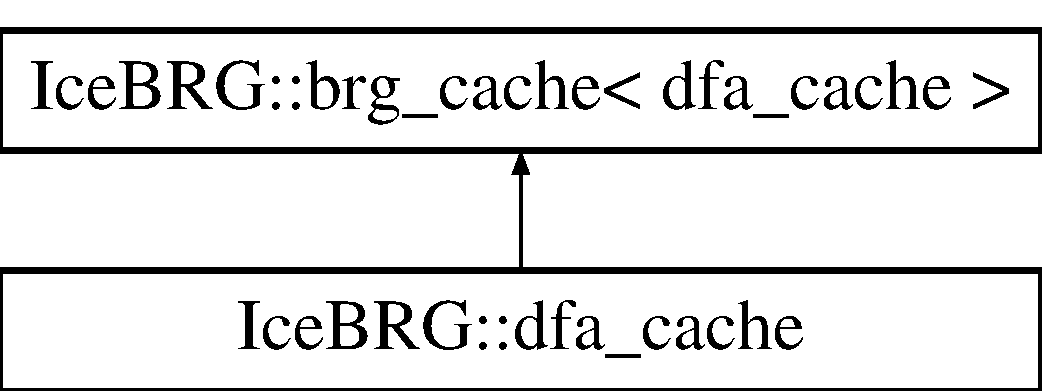
\includegraphics[height=2.000000cm]{classIceBRG_1_1dfa__cache}
\end{center}
\end{figure}
\subsection*{Public Member Functions}
\begin{DoxyCompactItemize}
\item 
\hyperlink{classIceBRG_1_1dfa__cache_a18b061367455a52cb3b3aed54449494a}{$\sim$dfa\+\_\+cache} ()
\end{DoxyCompactItemize}
\subsection*{Protected Member Functions}
\begin{DoxyCompactItemize}
\item 
std\+::string \hyperlink{classIceBRG_1_1dfa__cache_abcd1aa788d51b43e58f5e323c0bf8900}{\+\_\+name\+\_\+base} () const 
\item 
\hyperlink{lib_2IceBRG__main_2common_8h_ad0f130a56eeb944d9ef2692ee881ecc4}{flt\+\_\+type} \hyperlink{classIceBRG_1_1dfa__cache_afe887c4a62aaba1061a6084f8e352832}{\+\_\+calculate} (const \hyperlink{lib_2IceBRG__main_2common_8h_ad0f130a56eeb944d9ef2692ee881ecc4}{flt\+\_\+type} \&in\+\_\+param) const 
\end{DoxyCompactItemize}
\subsection*{Friends}
\begin{DoxyCompactItemize}
\item 
class \hyperlink{classIceBRG_1_1dfa__cache_a5a91119ea41de9dd3784d610f0214396}{brg\+\_\+cache$<$ dfa\+\_\+cache $>$}
\end{DoxyCompactItemize}


\subsection{Constructor \& Destructor Documentation}
\hypertarget{classIceBRG_1_1dfa__cache_a18b061367455a52cb3b3aed54449494a}{}\index{Ice\+B\+R\+G\+::dfa\+\_\+cache@{Ice\+B\+R\+G\+::dfa\+\_\+cache}!````~dfa\+\_\+cache@{$\sim$dfa\+\_\+cache}}
\index{````~dfa\+\_\+cache@{$\sim$dfa\+\_\+cache}!Ice\+B\+R\+G\+::dfa\+\_\+cache@{Ice\+B\+R\+G\+::dfa\+\_\+cache}}
\subsubsection[{$\sim$dfa\+\_\+cache()}]{\setlength{\rightskip}{0pt plus 5cm}Ice\+B\+R\+G\+::dfa\+\_\+cache\+::$\sim$dfa\+\_\+cache (
\begin{DoxyParamCaption}
{}
\end{DoxyParamCaption}
)\hspace{0.3cm}{\ttfamily [inline]}}\label{classIceBRG_1_1dfa__cache_a18b061367455a52cb3b3aed54449494a}


\subsection{Member Function Documentation}
\hypertarget{classIceBRG_1_1dfa__cache_afe887c4a62aaba1061a6084f8e352832}{}\index{Ice\+B\+R\+G\+::dfa\+\_\+cache@{Ice\+B\+R\+G\+::dfa\+\_\+cache}!\+\_\+calculate@{\+\_\+calculate}}
\index{\+\_\+calculate@{\+\_\+calculate}!Ice\+B\+R\+G\+::dfa\+\_\+cache@{Ice\+B\+R\+G\+::dfa\+\_\+cache}}
\subsubsection[{\+\_\+calculate(const flt\+\_\+type \&in\+\_\+param) const }]{\setlength{\rightskip}{0pt plus 5cm}{\bf flt\+\_\+type} Ice\+B\+R\+G\+::dfa\+\_\+cache\+::\+\_\+calculate (
\begin{DoxyParamCaption}
\item[{const {\bf flt\+\_\+type} \&}]{in\+\_\+param}
\end{DoxyParamCaption}
) const\hspace{0.3cm}{\ttfamily [protected]}}\label{classIceBRG_1_1dfa__cache_afe887c4a62aaba1061a6084f8e352832}
Class Method Definitions \hypertarget{classIceBRG_1_1dfa__cache_abcd1aa788d51b43e58f5e323c0bf8900}{}\index{Ice\+B\+R\+G\+::dfa\+\_\+cache@{Ice\+B\+R\+G\+::dfa\+\_\+cache}!\+\_\+name\+\_\+base@{\+\_\+name\+\_\+base}}
\index{\+\_\+name\+\_\+base@{\+\_\+name\+\_\+base}!Ice\+B\+R\+G\+::dfa\+\_\+cache@{Ice\+B\+R\+G\+::dfa\+\_\+cache}}
\subsubsection[{\+\_\+name\+\_\+base() const }]{\setlength{\rightskip}{0pt plus 5cm}std\+::string Ice\+B\+R\+G\+::dfa\+\_\+cache\+::\+\_\+name\+\_\+base (
\begin{DoxyParamCaption}
{}
\end{DoxyParamCaption}
) const\hspace{0.3cm}{\ttfamily [inline]}, {\ttfamily [protected]}}\label{classIceBRG_1_1dfa__cache_abcd1aa788d51b43e58f5e323c0bf8900}


\subsection{Friends And Related Function Documentation}
\hypertarget{classIceBRG_1_1dfa__cache_a5a91119ea41de9dd3784d610f0214396}{}\index{Ice\+B\+R\+G\+::dfa\+\_\+cache@{Ice\+B\+R\+G\+::dfa\+\_\+cache}!brg\+\_\+cache$<$ dfa\+\_\+cache $>$@{brg\+\_\+cache$<$ dfa\+\_\+cache $>$}}
\index{brg\+\_\+cache$<$ dfa\+\_\+cache $>$@{brg\+\_\+cache$<$ dfa\+\_\+cache $>$}!Ice\+B\+R\+G\+::dfa\+\_\+cache@{Ice\+B\+R\+G\+::dfa\+\_\+cache}}
\subsubsection[{brg\+\_\+cache$<$ dfa\+\_\+cache $>$}]{\setlength{\rightskip}{0pt plus 5cm}friend class {\bf brg\+\_\+cache}$<$ {\bf dfa\+\_\+cache} $>$\hspace{0.3cm}{\ttfamily [friend]}}\label{classIceBRG_1_1dfa__cache_a5a91119ea41de9dd3784d610f0214396}


The documentation for this class was generated from the following files\+:\begin{DoxyCompactItemize}
\item 
/disk2/brg/git/\+Magnification\+\_\+\+Public/src/lib/\+Ice\+B\+R\+G\+\_\+physics/\hyperlink{astro__caches_8h}{astro\+\_\+caches.\+h}\item 
/disk2/brg/git/\+Magnification\+\_\+\+Public/src/lib/\+Ice\+B\+R\+G\+\_\+physics/\hyperlink{astro__caches_8cpp}{astro\+\_\+caches.\+cpp}\end{DoxyCompactItemize}

\hypertarget{structboost_1_1accumulators_1_1tag_1_1effective__count}{}\section{boost\+:\+:accumulators\+:\+:tag\+:\+:effective\+\_\+count Struct Reference}
\label{structboost_1_1accumulators_1_1tag_1_1effective__count}\index{boost\+::accumulators\+::tag\+::effective\+\_\+count@{boost\+::accumulators\+::tag\+::effective\+\_\+count}}


{\ttfamily \#include $<$effective\+\_\+count.\+hpp$>$}

Inheritance diagram for boost\+:\+:accumulators\+:\+:tag\+:\+:effective\+\_\+count\+:\begin{figure}[H]
\begin{center}
\leavevmode
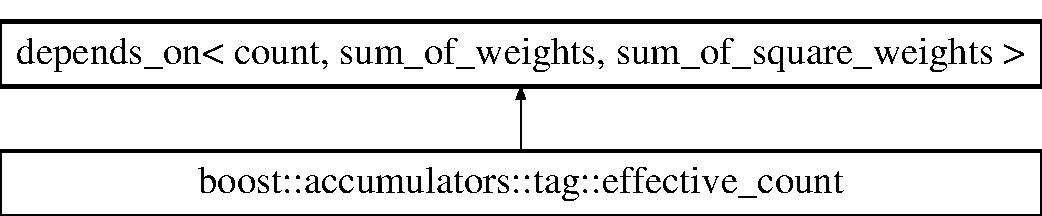
\includegraphics[height=2.000000cm]{structboost_1_1accumulators_1_1tag_1_1effective__count}
\end{center}
\end{figure}
\subsection*{Public Types}
\begin{DoxyCompactItemize}
\item 
typedef mpl\+::true\+\_\+ \hyperlink{structboost_1_1accumulators_1_1tag_1_1effective__count_ac4274fac6b1cf2217291494cd34d67d2}{is\+\_\+weight\+\_\+accumulator}
\item 
typedef \hyperlink{structboost_1_1accumulators_1_1impl_1_1effective__count__accumulator}{accumulators\+::impl\+::effective\+\_\+count\+\_\+accumulator}$<$ mpl\+::\+\_\+1 $>$ \hyperlink{structboost_1_1accumulators_1_1tag_1_1effective__count_afb8cd525da641f5b3f81759f2c614350}{impl}
\end{DoxyCompactItemize}


\subsection{Member Typedef Documentation}
\hypertarget{structboost_1_1accumulators_1_1tag_1_1effective__count_afb8cd525da641f5b3f81759f2c614350}{}\index{boost\+::accumulators\+::tag\+::effective\+\_\+count@{boost\+::accumulators\+::tag\+::effective\+\_\+count}!impl@{impl}}
\index{impl@{impl}!boost\+::accumulators\+::tag\+::effective\+\_\+count@{boost\+::accumulators\+::tag\+::effective\+\_\+count}}
\subsubsection[{impl}]{\setlength{\rightskip}{0pt plus 5cm}typedef {\bf accumulators\+::impl\+::effective\+\_\+count\+\_\+accumulator}$<$ mpl\+::\+\_\+1 $>$ {\bf boost\+::accumulators\+::tag\+::effective\+\_\+count\+::impl}}\label{structboost_1_1accumulators_1_1tag_1_1effective__count_afb8cd525da641f5b3f81759f2c614350}
\hypertarget{structboost_1_1accumulators_1_1tag_1_1effective__count_ac4274fac6b1cf2217291494cd34d67d2}{}\index{boost\+::accumulators\+::tag\+::effective\+\_\+count@{boost\+::accumulators\+::tag\+::effective\+\_\+count}!is\+\_\+weight\+\_\+accumulator@{is\+\_\+weight\+\_\+accumulator}}
\index{is\+\_\+weight\+\_\+accumulator@{is\+\_\+weight\+\_\+accumulator}!boost\+::accumulators\+::tag\+::effective\+\_\+count@{boost\+::accumulators\+::tag\+::effective\+\_\+count}}
\subsubsection[{is\+\_\+weight\+\_\+accumulator}]{\setlength{\rightskip}{0pt plus 5cm}typedef mpl\+::true\+\_\+ {\bf boost\+::accumulators\+::tag\+::effective\+\_\+count\+::is\+\_\+weight\+\_\+accumulator}}\label{structboost_1_1accumulators_1_1tag_1_1effective__count_ac4274fac6b1cf2217291494cd34d67d2}


The documentation for this struct was generated from the following file\+:\begin{DoxyCompactItemize}
\item 
/disk2/brg/git/\+Magnification\+\_\+\+Public/src/lib/\+Ice\+B\+R\+G\+\_\+main/math/statistics/\hyperlink{effective__count_8hpp}{effective\+\_\+count.\+hpp}\end{DoxyCompactItemize}

\hypertarget{structboost_1_1accumulators_1_1impl_1_1effective__count__accumulator}{}\section{boost\+:\+:accumulators\+:\+:impl\+:\+:effective\+\_\+count\+\_\+accumulator$<$ Sample $>$ Struct Template Reference}
\label{structboost_1_1accumulators_1_1impl_1_1effective__count__accumulator}\index{boost\+::accumulators\+::impl\+::effective\+\_\+count\+\_\+accumulator$<$ Sample $>$@{boost\+::accumulators\+::impl\+::effective\+\_\+count\+\_\+accumulator$<$ Sample $>$}}


{\ttfamily \#include $<$effective\+\_\+count.\+hpp$>$}

Inheritance diagram for boost\+:\+:accumulators\+:\+:impl\+:\+:effective\+\_\+count\+\_\+accumulator$<$ Sample $>$\+:\begin{figure}[H]
\begin{center}
\leavevmode
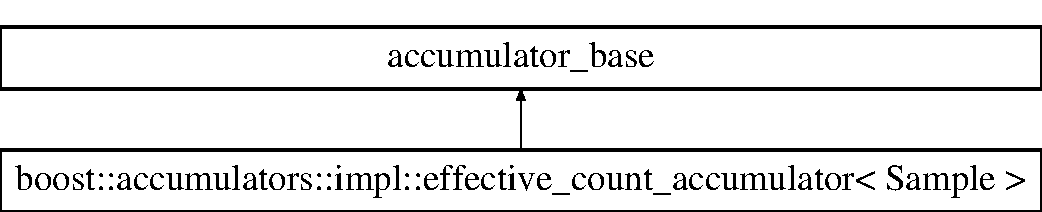
\includegraphics[height=2.000000cm]{structboost_1_1accumulators_1_1impl_1_1effective__count__accumulator}
\end{center}
\end{figure}
\subsection*{Public Types}
\begin{DoxyCompactItemize}
\item 
typedef \hyperlink{lib_2IceBRG__main_2common_8h_ad0f130a56eeb944d9ef2692ee881ecc4}{flt\+\_\+type} \hyperlink{structboost_1_1accumulators_1_1impl_1_1effective__count__accumulator_a5516ab157ca383ec0cea01649c3d9879}{result\+\_\+type}
\end{DoxyCompactItemize}
\subsection*{Public Member Functions}
\begin{DoxyCompactItemize}
\item 
\hyperlink{structboost_1_1accumulators_1_1impl_1_1effective__count__accumulator_ae3d2dd9daf6faa19d0f6cdee64af6a47}{effective\+\_\+count\+\_\+accumulator} (dont\+\_\+care)
\item 
{\footnotesize template$<$typename Args $>$ }\\\hyperlink{structboost_1_1accumulators_1_1impl_1_1effective__count__accumulator_a5516ab157ca383ec0cea01649c3d9879}{result\+\_\+type} \hyperlink{structboost_1_1accumulators_1_1impl_1_1effective__count__accumulator_a136494d144b3456c4c30ae7ae562b99b}{result} (Args const \&args) const 
\end{DoxyCompactItemize}


\subsection{Member Typedef Documentation}
\hypertarget{structboost_1_1accumulators_1_1impl_1_1effective__count__accumulator_a5516ab157ca383ec0cea01649c3d9879}{}\index{boost\+::accumulators\+::impl\+::effective\+\_\+count\+\_\+accumulator@{boost\+::accumulators\+::impl\+::effective\+\_\+count\+\_\+accumulator}!result\+\_\+type@{result\+\_\+type}}
\index{result\+\_\+type@{result\+\_\+type}!boost\+::accumulators\+::impl\+::effective\+\_\+count\+\_\+accumulator@{boost\+::accumulators\+::impl\+::effective\+\_\+count\+\_\+accumulator}}
\subsubsection[{result\+\_\+type}]{\setlength{\rightskip}{0pt plus 5cm}template$<$typename Sample $>$ typedef {\bf flt\+\_\+type} {\bf boost\+::accumulators\+::impl\+::effective\+\_\+count\+\_\+accumulator}$<$ Sample $>$\+::{\bf result\+\_\+type}}\label{structboost_1_1accumulators_1_1impl_1_1effective__count__accumulator_a5516ab157ca383ec0cea01649c3d9879}


\subsection{Constructor \& Destructor Documentation}
\hypertarget{structboost_1_1accumulators_1_1impl_1_1effective__count__accumulator_ae3d2dd9daf6faa19d0f6cdee64af6a47}{}\index{boost\+::accumulators\+::impl\+::effective\+\_\+count\+\_\+accumulator@{boost\+::accumulators\+::impl\+::effective\+\_\+count\+\_\+accumulator}!effective\+\_\+count\+\_\+accumulator@{effective\+\_\+count\+\_\+accumulator}}
\index{effective\+\_\+count\+\_\+accumulator@{effective\+\_\+count\+\_\+accumulator}!boost\+::accumulators\+::impl\+::effective\+\_\+count\+\_\+accumulator@{boost\+::accumulators\+::impl\+::effective\+\_\+count\+\_\+accumulator}}
\subsubsection[{effective\+\_\+count\+\_\+accumulator(dont\+\_\+care)}]{\setlength{\rightskip}{0pt plus 5cm}template$<$typename Sample $>$ {\bf boost\+::accumulators\+::impl\+::effective\+\_\+count\+\_\+accumulator}$<$ Sample $>$\+::{\bf effective\+\_\+count\+\_\+accumulator} (
\begin{DoxyParamCaption}
\item[{dont\+\_\+care}]{}
\end{DoxyParamCaption}
)\hspace{0.3cm}{\ttfamily [inline]}}\label{structboost_1_1accumulators_1_1impl_1_1effective__count__accumulator_ae3d2dd9daf6faa19d0f6cdee64af6a47}


\subsection{Member Function Documentation}
\hypertarget{structboost_1_1accumulators_1_1impl_1_1effective__count__accumulator_a136494d144b3456c4c30ae7ae562b99b}{}\index{boost\+::accumulators\+::impl\+::effective\+\_\+count\+\_\+accumulator@{boost\+::accumulators\+::impl\+::effective\+\_\+count\+\_\+accumulator}!result@{result}}
\index{result@{result}!boost\+::accumulators\+::impl\+::effective\+\_\+count\+\_\+accumulator@{boost\+::accumulators\+::impl\+::effective\+\_\+count\+\_\+accumulator}}
\subsubsection[{result(\+Args const \&args) const }]{\setlength{\rightskip}{0pt plus 5cm}template$<$typename Sample $>$ template$<$typename Args $>$ {\bf result\+\_\+type} {\bf boost\+::accumulators\+::impl\+::effective\+\_\+count\+\_\+accumulator}$<$ Sample $>$\+::result (
\begin{DoxyParamCaption}
\item[{Args const \&}]{args}
\end{DoxyParamCaption}
) const\hspace{0.3cm}{\ttfamily [inline]}}\label{structboost_1_1accumulators_1_1impl_1_1effective__count__accumulator_a136494d144b3456c4c30ae7ae562b99b}


The documentation for this struct was generated from the following file\+:\begin{DoxyCompactItemize}
\item 
/disk2/brg/git/\+Magnification\+\_\+\+Public/src/lib/\+Ice\+B\+R\+G\+\_\+main/math/statistics/\hyperlink{effective__count_8hpp}{effective\+\_\+count.\+hpp}\end{DoxyCompactItemize}

\hypertarget{classIceBRG_1_1element__accessor}{}\section{Ice\+B\+R\+G\+:\+:element\+\_\+accessor$<$ Container\+Type $>$ Class Template Reference}
\label{classIceBRG_1_1element__accessor}\index{Ice\+B\+R\+G\+::element\+\_\+accessor$<$ Container\+Type $>$@{Ice\+B\+R\+G\+::element\+\_\+accessor$<$ Container\+Type $>$}}


{\ttfamily \#include $<$element\+\_\+accessor.\+hpp$>$}

\subsection*{Public Types}
\begin{DoxyCompactItemize}
\item 
typedef Container\+Type\+::value\+\_\+type \hyperlink{classIceBRG_1_1element__accessor_ab6c9120cd75bb9ea751fab09967baee9}{value\+\_\+type}
\item 
typedef Container\+Type\+::allocator\+\_\+type \hyperlink{classIceBRG_1_1element__accessor_ad50e47085815aadfb3fa84cd845266ba}{allocator\+\_\+type}
\item 
typedef Container\+Type\+::reference \hyperlink{classIceBRG_1_1element__accessor_ae31e9fe4b35d76ed6055052fb788de13}{reference}
\item 
typedef Container\+Type\+::const\+\_\+reference \hyperlink{classIceBRG_1_1element__accessor_aa5a74be2decaa60d9080c4f1b4d3dcb8}{const\+\_\+reference}
\item 
typedef Container\+Type\+::pointer \hyperlink{classIceBRG_1_1element__accessor_a9d67afd8fb73e97d728564567ff42609}{pointer}
\item 
typedef Container\+Type\+::const\+\_\+pointer \hyperlink{classIceBRG_1_1element__accessor_ad2f50d3e3d10c61c85c167512221c7d1}{const\+\_\+pointer}
\item 
typedef Container\+Type\+::iterator \hyperlink{classIceBRG_1_1element__accessor_a464911efedf30917f238c5fb4746cd09}{iterator}
\item 
typedef Container\+Type\+::const\+\_\+iterator \hyperlink{classIceBRG_1_1element__accessor_ab9a6ca4866a0758171a4ffa7b0935cd2}{const\+\_\+iterator}
\item 
typedef Container\+Type\+::reverse\+\_\+iterator \hyperlink{classIceBRG_1_1element__accessor_a8fc4c41438daa950d66dac2f7613ea18}{reverse\+\_\+iterator}
\item 
typedef Container\+Type\+::const\+\_\+reverse\+\_\+iterator \hyperlink{classIceBRG_1_1element__accessor_a32ea1ca6966b5093370f8944efedc471}{const\+\_\+reverse\+\_\+iterator}
\item 
typedef Container\+Type\+::difference\+\_\+type \hyperlink{classIceBRG_1_1element__accessor_a2f4224314d26679948777aa2b1121148}{difference\+\_\+type}
\item 
typedef Container\+Type\+::size\+\_\+type \hyperlink{classIceBRG_1_1element__accessor_aec3d016f3c5e84e7f9248669a9571208}{size\+\_\+type}
\end{DoxyCompactItemize}
\subsection*{Public Member Functions}
\begin{DoxyCompactItemize}
\item 
\hyperlink{classIceBRG_1_1element__accessor_aef4b30778521e1039780961e06c22491}{element\+\_\+accessor} (Container\+Type \&\hyperlink{classIceBRG_1_1element__accessor_ae31e9fe4b35d76ed6055052fb788de13}{reference})
\begin{DoxyCompactList}\small\item\em Constructor. Requires a non-\/const reference to a container of the proper type. \end{DoxyCompactList}\item 
virtual \hyperlink{classIceBRG_1_1element__accessor_acf809c62734281f7329aa4631cc87421}{$\sim$element\+\_\+accessor} ()
\begin{DoxyCompactList}\small\item\em Virtual destructor. \end{DoxyCompactList}\item 
\hyperlink{classIceBRG_1_1element__accessor_af0a32cf064352559df47dfa7b56a70a8}{element\+\_\+accessor} (const \hyperlink{classIceBRG_1_1element__accessor}{element\+\_\+accessor} \&other)=delete
\begin{DoxyCompactList}\small\item\em Delete default copy and move constructors and assignments. \end{DoxyCompactList}\item 
\hyperlink{classIceBRG_1_1element__accessor_a24e24c2c4b7b75f61dda38a70ee1ff12}{element\+\_\+accessor} (\hyperlink{classIceBRG_1_1element__accessor}{element\+\_\+accessor} \&\&other)=delete
\item 
\hyperlink{classIceBRG_1_1element__accessor}{element\+\_\+accessor} \& \hyperlink{classIceBRG_1_1element__accessor_aee519f816c6811d7e4b5f0dfa262c7f3}{operator=} (const \hyperlink{classIceBRG_1_1element__accessor}{element\+\_\+accessor} \&other)=delete
\item 
\hyperlink{classIceBRG_1_1element__accessor}{element\+\_\+accessor} \& \hyperlink{classIceBRG_1_1element__accessor_ac9a71ff5dec73f2008259e2b96714369}{operator=} (\hyperlink{classIceBRG_1_1element__accessor}{element\+\_\+accessor} \&\&other)=delete
\item 
\hyperlink{classIceBRG_1_1element__accessor_ab9a6ca4866a0758171a4ffa7b0935cd2}{const\+\_\+iterator} \hyperlink{classIceBRG_1_1element__accessor_a11d89804615361e5bbd639a23fa04d46}{begin} () const  noexcept
\begin{DoxyCompactList}\small\item\em begin \end{DoxyCompactList}\item 
\hyperlink{classIceBRG_1_1element__accessor_a464911efedf30917f238c5fb4746cd09}{iterator} \hyperlink{classIceBRG_1_1element__accessor_a309a6182605449b81292ed2ff1cfb9df}{begin} () noexcept
\begin{DoxyCompactList}\small\item\em begin \end{DoxyCompactList}\item 
\hyperlink{classIceBRG_1_1element__accessor_ab9a6ca4866a0758171a4ffa7b0935cd2}{const\+\_\+iterator} \hyperlink{classIceBRG_1_1element__accessor_a9e095921326171995c319f3f44108472}{end} () const  noexcept
\begin{DoxyCompactList}\small\item\em end \end{DoxyCompactList}\item 
\hyperlink{classIceBRG_1_1element__accessor_a464911efedf30917f238c5fb4746cd09}{iterator} \hyperlink{classIceBRG_1_1element__accessor_a2d08fdb03734cb32bef953853be973fa}{end} () noexcept
\begin{DoxyCompactList}\small\item\em end \end{DoxyCompactList}\item 
\hyperlink{classIceBRG_1_1element__accessor_ab9a6ca4866a0758171a4ffa7b0935cd2}{const\+\_\+iterator} \hyperlink{classIceBRG_1_1element__accessor_a6911dfd28822d3c8e8008e7f79d455b7}{rbegin} () const  noexcept
\begin{DoxyCompactList}\small\item\em rbegin \end{DoxyCompactList}\item 
\hyperlink{classIceBRG_1_1element__accessor_a464911efedf30917f238c5fb4746cd09}{iterator} \hyperlink{classIceBRG_1_1element__accessor_ac16d8f00aa5b8f31f53b0a19c103dc9e}{rbegin} () noexcept
\begin{DoxyCompactList}\small\item\em rbegin \end{DoxyCompactList}\item 
\hyperlink{classIceBRG_1_1element__accessor_ab9a6ca4866a0758171a4ffa7b0935cd2}{const\+\_\+iterator} \hyperlink{classIceBRG_1_1element__accessor_a945ca43d1f99631647b1d4deb7499d72}{rend} () const  noexcept
\begin{DoxyCompactList}\small\item\em rend \end{DoxyCompactList}\item 
\hyperlink{classIceBRG_1_1element__accessor_a464911efedf30917f238c5fb4746cd09}{iterator} \hyperlink{classIceBRG_1_1element__accessor_afb9c46d9df82f458063501bdf7e55a39}{rend} () noexcept
\begin{DoxyCompactList}\small\item\em rend \end{DoxyCompactList}\item 
\hyperlink{classIceBRG_1_1element__accessor_ab9a6ca4866a0758171a4ffa7b0935cd2}{const\+\_\+iterator} \hyperlink{classIceBRG_1_1element__accessor_aad89c91911287ce94874b95e7d387ca9}{cbegin} () const  noexcept
\begin{DoxyCompactList}\small\item\em cbegin \end{DoxyCompactList}\item 
\hyperlink{classIceBRG_1_1element__accessor_ab9a6ca4866a0758171a4ffa7b0935cd2}{const\+\_\+iterator} \hyperlink{classIceBRG_1_1element__accessor_a63245eb2ae629a99d783eee946712ba8}{cend} () const  noexcept
\begin{DoxyCompactList}\small\item\em cend \end{DoxyCompactList}\item 
\hyperlink{classIceBRG_1_1element__accessor_ab9a6ca4866a0758171a4ffa7b0935cd2}{const\+\_\+iterator} \hyperlink{classIceBRG_1_1element__accessor_a1467e420b5eeb2939e83104747c1d2ca}{crbegin} () const  noexcept
\begin{DoxyCompactList}\small\item\em crbegin \end{DoxyCompactList}\item 
\hyperlink{classIceBRG_1_1element__accessor_ab9a6ca4866a0758171a4ffa7b0935cd2}{const\+\_\+iterator} \hyperlink{classIceBRG_1_1element__accessor_a88d68973f607f9baa64c2804f4f5d01e}{crend} () const  noexcept
\begin{DoxyCompactList}\small\item\em crend \end{DoxyCompactList}\item 
\hyperlink{classIceBRG_1_1element__accessor_aec3d016f3c5e84e7f9248669a9571208}{size\+\_\+type} \hyperlink{classIceBRG_1_1element__accessor_aee036852e878483ead629bbd56a02db9}{size} () const  noexcept
\begin{DoxyCompactList}\small\item\em size \end{DoxyCompactList}\item 
\hyperlink{classIceBRG_1_1element__accessor_aec3d016f3c5e84e7f9248669a9571208}{size\+\_\+type} \hyperlink{classIceBRG_1_1element__accessor_a7c9d2d8c46ed2f24d5f7c479b993c914}{max\+\_\+size} () const  noexcept
\begin{DoxyCompactList}\small\item\em max\+\_\+size \end{DoxyCompactList}\item 
\hyperlink{classIceBRG_1_1element__accessor_aec3d016f3c5e84e7f9248669a9571208}{size\+\_\+type} \hyperlink{classIceBRG_1_1element__accessor_af83ebf16e5c15948dac43776deb205e6}{capacity} () const  noexcept
\begin{DoxyCompactList}\small\item\em capacity \end{DoxyCompactList}\item 
bool \hyperlink{classIceBRG_1_1element__accessor_ac542247120ab0494244604e4748156b1}{empty} () const  noexcept
\begin{DoxyCompactList}\small\item\em empty \end{DoxyCompactList}\item 
void \hyperlink{classIceBRG_1_1element__accessor_a48a19bf110f89d01d5104b3eab0eeda6}{shrink\+\_\+to\+\_\+fit} () const 
\begin{DoxyCompactList}\small\item\em shrink\+\_\+to\+\_\+fit (allowed since there\textquotesingle{}s a reason to let the user conserve memory) \end{DoxyCompactList}\item 
\hyperlink{classIceBRG_1_1element__accessor_aa5a74be2decaa60d9080c4f1b4d3dcb8}{const\+\_\+reference} \hyperlink{classIceBRG_1_1element__accessor_a0b191a649b47afaa129561fcceb135a6}{operator\mbox{[}$\,$\mbox{]}} (const \hyperlink{classIceBRG_1_1element__accessor_aec3d016f3c5e84e7f9248669a9571208}{size\+\_\+type} \&n) const 
\begin{DoxyCompactList}\small\item\em Element access. \end{DoxyCompactList}\item 
\hyperlink{classIceBRG_1_1element__accessor_ae31e9fe4b35d76ed6055052fb788de13}{reference} \hyperlink{classIceBRG_1_1element__accessor_afae05c291dc57fa1c6d9602ca64d497f}{operator\mbox{[}$\,$\mbox{]}} (const \hyperlink{classIceBRG_1_1element__accessor_aec3d016f3c5e84e7f9248669a9571208}{size\+\_\+type} \&n)
\begin{DoxyCompactList}\small\item\em Element access. \end{DoxyCompactList}\item 
\hyperlink{classIceBRG_1_1element__accessor_aa5a74be2decaa60d9080c4f1b4d3dcb8}{const\+\_\+reference} \hyperlink{classIceBRG_1_1element__accessor_a07ec2d2306e072f847d1adab77bf825d}{at} (const \hyperlink{classIceBRG_1_1element__accessor_aec3d016f3c5e84e7f9248669a9571208}{size\+\_\+type} \&n) const 
\begin{DoxyCompactList}\small\item\em Range-\/checked element access. \end{DoxyCompactList}\item 
\hyperlink{classIceBRG_1_1element__accessor_ae31e9fe4b35d76ed6055052fb788de13}{reference} \hyperlink{classIceBRG_1_1element__accessor_aaa4ed7ea60a206ce193115e8b5c7c558}{at} (const \hyperlink{classIceBRG_1_1element__accessor_aec3d016f3c5e84e7f9248669a9571208}{size\+\_\+type} \&n)
\begin{DoxyCompactList}\small\item\em Range-\/checked element access. \end{DoxyCompactList}\item 
\hyperlink{classIceBRG_1_1element__accessor_aa5a74be2decaa60d9080c4f1b4d3dcb8}{const\+\_\+reference} \hyperlink{classIceBRG_1_1element__accessor_a2595c51f419c4a0bbeb93c917d4269a9}{front} () const 
\begin{DoxyCompactList}\small\item\em Access first element. \end{DoxyCompactList}\item 
\hyperlink{classIceBRG_1_1element__accessor_ae31e9fe4b35d76ed6055052fb788de13}{reference} \hyperlink{classIceBRG_1_1element__accessor_aa335b47981fd9d132077256abf95c47e}{front} ()
\begin{DoxyCompactList}\small\item\em Access first element. \end{DoxyCompactList}\item 
\hyperlink{classIceBRG_1_1element__accessor_aa5a74be2decaa60d9080c4f1b4d3dcb8}{const\+\_\+reference} \hyperlink{classIceBRG_1_1element__accessor_a15ceb15000c2fb5079cb9bce6c956aa5}{back} () const 
\begin{DoxyCompactList}\small\item\em Access last element. \end{DoxyCompactList}\item 
\hyperlink{classIceBRG_1_1element__accessor_ae31e9fe4b35d76ed6055052fb788de13}{reference} \hyperlink{classIceBRG_1_1element__accessor_a1949693135631a260930a5ae9326ccd7}{back} ()
\begin{DoxyCompactList}\small\item\em Access last element. \end{DoxyCompactList}\item 
const \hyperlink{classIceBRG_1_1element__accessor_ab6c9120cd75bb9ea751fab09967baee9}{value\+\_\+type} $\ast$ \hyperlink{classIceBRG_1_1element__accessor_a9fe00642b678ee4abe3847ff59160253}{data} () const  noexcept
\begin{DoxyCompactList}\small\item\em Access data. \end{DoxyCompactList}\item 
\hyperlink{classIceBRG_1_1element__accessor_ab6c9120cd75bb9ea751fab09967baee9}{value\+\_\+type} $\ast$ \hyperlink{classIceBRG_1_1element__accessor_a5cd35360d840d7f443d002951c6a9337}{data} () noexcept
\begin{DoxyCompactList}\small\item\em Access data. \end{DoxyCompactList}\item 
\hyperlink{classIceBRG_1_1element__accessor_a5ddde5b6d5a1e40f3f674cd3a2f8cea3}{operator const Container\+Type \&} () const 
\begin{DoxyCompactList}\small\item\em Cast to Container\+Type (the result will always be const so it can\textquotesingle{}t be resized) \end{DoxyCompactList}\end{DoxyCompactItemize}


\subsection{Member Typedef Documentation}
\hypertarget{classIceBRG_1_1element__accessor_ad50e47085815aadfb3fa84cd845266ba}{}\index{Ice\+B\+R\+G\+::element\+\_\+accessor@{Ice\+B\+R\+G\+::element\+\_\+accessor}!allocator\+\_\+type@{allocator\+\_\+type}}
\index{allocator\+\_\+type@{allocator\+\_\+type}!Ice\+B\+R\+G\+::element\+\_\+accessor@{Ice\+B\+R\+G\+::element\+\_\+accessor}}
\subsubsection[{allocator\+\_\+type}]{\setlength{\rightskip}{0pt plus 5cm}template$<$typename Container\+Type $>$ typedef Container\+Type\+::allocator\+\_\+type {\bf Ice\+B\+R\+G\+::element\+\_\+accessor}$<$ Container\+Type $>$\+::{\bf allocator\+\_\+type}}\label{classIceBRG_1_1element__accessor_ad50e47085815aadfb3fa84cd845266ba}
\hypertarget{classIceBRG_1_1element__accessor_ab9a6ca4866a0758171a4ffa7b0935cd2}{}\index{Ice\+B\+R\+G\+::element\+\_\+accessor@{Ice\+B\+R\+G\+::element\+\_\+accessor}!const\+\_\+iterator@{const\+\_\+iterator}}
\index{const\+\_\+iterator@{const\+\_\+iterator}!Ice\+B\+R\+G\+::element\+\_\+accessor@{Ice\+B\+R\+G\+::element\+\_\+accessor}}
\subsubsection[{const\+\_\+iterator}]{\setlength{\rightskip}{0pt plus 5cm}template$<$typename Container\+Type $>$ typedef Container\+Type\+::const\+\_\+iterator {\bf Ice\+B\+R\+G\+::element\+\_\+accessor}$<$ Container\+Type $>$\+::{\bf const\+\_\+iterator}}\label{classIceBRG_1_1element__accessor_ab9a6ca4866a0758171a4ffa7b0935cd2}
\hypertarget{classIceBRG_1_1element__accessor_ad2f50d3e3d10c61c85c167512221c7d1}{}\index{Ice\+B\+R\+G\+::element\+\_\+accessor@{Ice\+B\+R\+G\+::element\+\_\+accessor}!const\+\_\+pointer@{const\+\_\+pointer}}
\index{const\+\_\+pointer@{const\+\_\+pointer}!Ice\+B\+R\+G\+::element\+\_\+accessor@{Ice\+B\+R\+G\+::element\+\_\+accessor}}
\subsubsection[{const\+\_\+pointer}]{\setlength{\rightskip}{0pt plus 5cm}template$<$typename Container\+Type $>$ typedef Container\+Type\+::const\+\_\+pointer {\bf Ice\+B\+R\+G\+::element\+\_\+accessor}$<$ Container\+Type $>$\+::{\bf const\+\_\+pointer}}\label{classIceBRG_1_1element__accessor_ad2f50d3e3d10c61c85c167512221c7d1}
\hypertarget{classIceBRG_1_1element__accessor_aa5a74be2decaa60d9080c4f1b4d3dcb8}{}\index{Ice\+B\+R\+G\+::element\+\_\+accessor@{Ice\+B\+R\+G\+::element\+\_\+accessor}!const\+\_\+reference@{const\+\_\+reference}}
\index{const\+\_\+reference@{const\+\_\+reference}!Ice\+B\+R\+G\+::element\+\_\+accessor@{Ice\+B\+R\+G\+::element\+\_\+accessor}}
\subsubsection[{const\+\_\+reference}]{\setlength{\rightskip}{0pt plus 5cm}template$<$typename Container\+Type $>$ typedef Container\+Type\+::const\+\_\+reference {\bf Ice\+B\+R\+G\+::element\+\_\+accessor}$<$ Container\+Type $>$\+::{\bf const\+\_\+reference}}\label{classIceBRG_1_1element__accessor_aa5a74be2decaa60d9080c4f1b4d3dcb8}
\hypertarget{classIceBRG_1_1element__accessor_a32ea1ca6966b5093370f8944efedc471}{}\index{Ice\+B\+R\+G\+::element\+\_\+accessor@{Ice\+B\+R\+G\+::element\+\_\+accessor}!const\+\_\+reverse\+\_\+iterator@{const\+\_\+reverse\+\_\+iterator}}
\index{const\+\_\+reverse\+\_\+iterator@{const\+\_\+reverse\+\_\+iterator}!Ice\+B\+R\+G\+::element\+\_\+accessor@{Ice\+B\+R\+G\+::element\+\_\+accessor}}
\subsubsection[{const\+\_\+reverse\+\_\+iterator}]{\setlength{\rightskip}{0pt plus 5cm}template$<$typename Container\+Type $>$ typedef Container\+Type\+::const\+\_\+reverse\+\_\+iterator {\bf Ice\+B\+R\+G\+::element\+\_\+accessor}$<$ Container\+Type $>$\+::{\bf const\+\_\+reverse\+\_\+iterator}}\label{classIceBRG_1_1element__accessor_a32ea1ca6966b5093370f8944efedc471}
\hypertarget{classIceBRG_1_1element__accessor_a2f4224314d26679948777aa2b1121148}{}\index{Ice\+B\+R\+G\+::element\+\_\+accessor@{Ice\+B\+R\+G\+::element\+\_\+accessor}!difference\+\_\+type@{difference\+\_\+type}}
\index{difference\+\_\+type@{difference\+\_\+type}!Ice\+B\+R\+G\+::element\+\_\+accessor@{Ice\+B\+R\+G\+::element\+\_\+accessor}}
\subsubsection[{difference\+\_\+type}]{\setlength{\rightskip}{0pt plus 5cm}template$<$typename Container\+Type $>$ typedef Container\+Type\+::difference\+\_\+type {\bf Ice\+B\+R\+G\+::element\+\_\+accessor}$<$ Container\+Type $>$\+::{\bf difference\+\_\+type}}\label{classIceBRG_1_1element__accessor_a2f4224314d26679948777aa2b1121148}
\hypertarget{classIceBRG_1_1element__accessor_a464911efedf30917f238c5fb4746cd09}{}\index{Ice\+B\+R\+G\+::element\+\_\+accessor@{Ice\+B\+R\+G\+::element\+\_\+accessor}!iterator@{iterator}}
\index{iterator@{iterator}!Ice\+B\+R\+G\+::element\+\_\+accessor@{Ice\+B\+R\+G\+::element\+\_\+accessor}}
\subsubsection[{iterator}]{\setlength{\rightskip}{0pt plus 5cm}template$<$typename Container\+Type $>$ typedef Container\+Type\+::iterator {\bf Ice\+B\+R\+G\+::element\+\_\+accessor}$<$ Container\+Type $>$\+::{\bf iterator}}\label{classIceBRG_1_1element__accessor_a464911efedf30917f238c5fb4746cd09}
\hypertarget{classIceBRG_1_1element__accessor_a9d67afd8fb73e97d728564567ff42609}{}\index{Ice\+B\+R\+G\+::element\+\_\+accessor@{Ice\+B\+R\+G\+::element\+\_\+accessor}!pointer@{pointer}}
\index{pointer@{pointer}!Ice\+B\+R\+G\+::element\+\_\+accessor@{Ice\+B\+R\+G\+::element\+\_\+accessor}}
\subsubsection[{pointer}]{\setlength{\rightskip}{0pt plus 5cm}template$<$typename Container\+Type $>$ typedef Container\+Type\+::pointer {\bf Ice\+B\+R\+G\+::element\+\_\+accessor}$<$ Container\+Type $>$\+::{\bf pointer}}\label{classIceBRG_1_1element__accessor_a9d67afd8fb73e97d728564567ff42609}
\hypertarget{classIceBRG_1_1element__accessor_ae31e9fe4b35d76ed6055052fb788de13}{}\index{Ice\+B\+R\+G\+::element\+\_\+accessor@{Ice\+B\+R\+G\+::element\+\_\+accessor}!reference@{reference}}
\index{reference@{reference}!Ice\+B\+R\+G\+::element\+\_\+accessor@{Ice\+B\+R\+G\+::element\+\_\+accessor}}
\subsubsection[{reference}]{\setlength{\rightskip}{0pt plus 5cm}template$<$typename Container\+Type $>$ typedef Container\+Type\+::reference {\bf Ice\+B\+R\+G\+::element\+\_\+accessor}$<$ Container\+Type $>$\+::{\bf reference}}\label{classIceBRG_1_1element__accessor_ae31e9fe4b35d76ed6055052fb788de13}
\hypertarget{classIceBRG_1_1element__accessor_a8fc4c41438daa950d66dac2f7613ea18}{}\index{Ice\+B\+R\+G\+::element\+\_\+accessor@{Ice\+B\+R\+G\+::element\+\_\+accessor}!reverse\+\_\+iterator@{reverse\+\_\+iterator}}
\index{reverse\+\_\+iterator@{reverse\+\_\+iterator}!Ice\+B\+R\+G\+::element\+\_\+accessor@{Ice\+B\+R\+G\+::element\+\_\+accessor}}
\subsubsection[{reverse\+\_\+iterator}]{\setlength{\rightskip}{0pt plus 5cm}template$<$typename Container\+Type $>$ typedef Container\+Type\+::reverse\+\_\+iterator {\bf Ice\+B\+R\+G\+::element\+\_\+accessor}$<$ Container\+Type $>$\+::{\bf reverse\+\_\+iterator}}\label{classIceBRG_1_1element__accessor_a8fc4c41438daa950d66dac2f7613ea18}
\hypertarget{classIceBRG_1_1element__accessor_aec3d016f3c5e84e7f9248669a9571208}{}\index{Ice\+B\+R\+G\+::element\+\_\+accessor@{Ice\+B\+R\+G\+::element\+\_\+accessor}!size\+\_\+type@{size\+\_\+type}}
\index{size\+\_\+type@{size\+\_\+type}!Ice\+B\+R\+G\+::element\+\_\+accessor@{Ice\+B\+R\+G\+::element\+\_\+accessor}}
\subsubsection[{size\+\_\+type}]{\setlength{\rightskip}{0pt plus 5cm}template$<$typename Container\+Type $>$ typedef Container\+Type\+::size\+\_\+type {\bf Ice\+B\+R\+G\+::element\+\_\+accessor}$<$ Container\+Type $>$\+::{\bf size\+\_\+type}}\label{classIceBRG_1_1element__accessor_aec3d016f3c5e84e7f9248669a9571208}
\hypertarget{classIceBRG_1_1element__accessor_ab6c9120cd75bb9ea751fab09967baee9}{}\index{Ice\+B\+R\+G\+::element\+\_\+accessor@{Ice\+B\+R\+G\+::element\+\_\+accessor}!value\+\_\+type@{value\+\_\+type}}
\index{value\+\_\+type@{value\+\_\+type}!Ice\+B\+R\+G\+::element\+\_\+accessor@{Ice\+B\+R\+G\+::element\+\_\+accessor}}
\subsubsection[{value\+\_\+type}]{\setlength{\rightskip}{0pt plus 5cm}template$<$typename Container\+Type $>$ typedef Container\+Type\+::value\+\_\+type {\bf Ice\+B\+R\+G\+::element\+\_\+accessor}$<$ Container\+Type $>$\+::{\bf value\+\_\+type}}\label{classIceBRG_1_1element__accessor_ab6c9120cd75bb9ea751fab09967baee9}


\subsection{Constructor \& Destructor Documentation}
\hypertarget{classIceBRG_1_1element__accessor_aef4b30778521e1039780961e06c22491}{}\index{Ice\+B\+R\+G\+::element\+\_\+accessor@{Ice\+B\+R\+G\+::element\+\_\+accessor}!element\+\_\+accessor@{element\+\_\+accessor}}
\index{element\+\_\+accessor@{element\+\_\+accessor}!Ice\+B\+R\+G\+::element\+\_\+accessor@{Ice\+B\+R\+G\+::element\+\_\+accessor}}
\subsubsection[{element\+\_\+accessor(\+Container\+Type \&reference)}]{\setlength{\rightskip}{0pt plus 5cm}template$<$typename Container\+Type $>$ {\bf Ice\+B\+R\+G\+::element\+\_\+accessor}$<$ Container\+Type $>$\+::{\bf element\+\_\+accessor} (
\begin{DoxyParamCaption}
\item[{Container\+Type \&}]{reference}
\end{DoxyParamCaption}
)\hspace{0.3cm}{\ttfamily [inline]}}\label{classIceBRG_1_1element__accessor_aef4b30778521e1039780961e06c22491}


Constructor. Requires a non-\/const reference to a container of the proper type. 

\hypertarget{classIceBRG_1_1element__accessor_acf809c62734281f7329aa4631cc87421}{}\index{Ice\+B\+R\+G\+::element\+\_\+accessor@{Ice\+B\+R\+G\+::element\+\_\+accessor}!````~element\+\_\+accessor@{$\sim$element\+\_\+accessor}}
\index{````~element\+\_\+accessor@{$\sim$element\+\_\+accessor}!Ice\+B\+R\+G\+::element\+\_\+accessor@{Ice\+B\+R\+G\+::element\+\_\+accessor}}
\subsubsection[{$\sim$element\+\_\+accessor()}]{\setlength{\rightskip}{0pt plus 5cm}template$<$typename Container\+Type $>$ virtual {\bf Ice\+B\+R\+G\+::element\+\_\+accessor}$<$ Container\+Type $>$\+::$\sim${\bf element\+\_\+accessor} (
\begin{DoxyParamCaption}
{}
\end{DoxyParamCaption}
)\hspace{0.3cm}{\ttfamily [inline]}, {\ttfamily [virtual]}}\label{classIceBRG_1_1element__accessor_acf809c62734281f7329aa4631cc87421}


Virtual destructor. 

\hypertarget{classIceBRG_1_1element__accessor_af0a32cf064352559df47dfa7b56a70a8}{}\index{Ice\+B\+R\+G\+::element\+\_\+accessor@{Ice\+B\+R\+G\+::element\+\_\+accessor}!element\+\_\+accessor@{element\+\_\+accessor}}
\index{element\+\_\+accessor@{element\+\_\+accessor}!Ice\+B\+R\+G\+::element\+\_\+accessor@{Ice\+B\+R\+G\+::element\+\_\+accessor}}
\subsubsection[{element\+\_\+accessor(const element\+\_\+accessor \&other)=delete}]{\setlength{\rightskip}{0pt plus 5cm}template$<$typename Container\+Type $>$ {\bf Ice\+B\+R\+G\+::element\+\_\+accessor}$<$ Container\+Type $>$\+::{\bf element\+\_\+accessor} (
\begin{DoxyParamCaption}
\item[{const {\bf element\+\_\+accessor}$<$ Container\+Type $>$ \&}]{other}
\end{DoxyParamCaption}
)\hspace{0.3cm}{\ttfamily [delete]}}\label{classIceBRG_1_1element__accessor_af0a32cf064352559df47dfa7b56a70a8}


Delete default copy and move constructors and assignments. 

\hypertarget{classIceBRG_1_1element__accessor_a24e24c2c4b7b75f61dda38a70ee1ff12}{}\index{Ice\+B\+R\+G\+::element\+\_\+accessor@{Ice\+B\+R\+G\+::element\+\_\+accessor}!element\+\_\+accessor@{element\+\_\+accessor}}
\index{element\+\_\+accessor@{element\+\_\+accessor}!Ice\+B\+R\+G\+::element\+\_\+accessor@{Ice\+B\+R\+G\+::element\+\_\+accessor}}
\subsubsection[{element\+\_\+accessor(element\+\_\+accessor \&\&other)=delete}]{\setlength{\rightskip}{0pt plus 5cm}template$<$typename Container\+Type $>$ {\bf Ice\+B\+R\+G\+::element\+\_\+accessor}$<$ Container\+Type $>$\+::{\bf element\+\_\+accessor} (
\begin{DoxyParamCaption}
\item[{{\bf element\+\_\+accessor}$<$ Container\+Type $>$ \&\&}]{other}
\end{DoxyParamCaption}
)\hspace{0.3cm}{\ttfamily [delete]}}\label{classIceBRG_1_1element__accessor_a24e24c2c4b7b75f61dda38a70ee1ff12}


\subsection{Member Function Documentation}
\hypertarget{classIceBRG_1_1element__accessor_a07ec2d2306e072f847d1adab77bf825d}{}\index{Ice\+B\+R\+G\+::element\+\_\+accessor@{Ice\+B\+R\+G\+::element\+\_\+accessor}!at@{at}}
\index{at@{at}!Ice\+B\+R\+G\+::element\+\_\+accessor@{Ice\+B\+R\+G\+::element\+\_\+accessor}}
\subsubsection[{at(const size\+\_\+type \&n) const }]{\setlength{\rightskip}{0pt plus 5cm}template$<$typename Container\+Type $>$ {\bf const\+\_\+reference} {\bf Ice\+B\+R\+G\+::element\+\_\+accessor}$<$ Container\+Type $>$\+::at (
\begin{DoxyParamCaption}
\item[{const {\bf size\+\_\+type} \&}]{n}
\end{DoxyParamCaption}
) const\hspace{0.3cm}{\ttfamily [inline]}}\label{classIceBRG_1_1element__accessor_a07ec2d2306e072f847d1adab77bf825d}


Range-\/checked element access. 

\hypertarget{classIceBRG_1_1element__accessor_aaa4ed7ea60a206ce193115e8b5c7c558}{}\index{Ice\+B\+R\+G\+::element\+\_\+accessor@{Ice\+B\+R\+G\+::element\+\_\+accessor}!at@{at}}
\index{at@{at}!Ice\+B\+R\+G\+::element\+\_\+accessor@{Ice\+B\+R\+G\+::element\+\_\+accessor}}
\subsubsection[{at(const size\+\_\+type \&n)}]{\setlength{\rightskip}{0pt plus 5cm}template$<$typename Container\+Type $>$ {\bf reference} {\bf Ice\+B\+R\+G\+::element\+\_\+accessor}$<$ Container\+Type $>$\+::at (
\begin{DoxyParamCaption}
\item[{const {\bf size\+\_\+type} \&}]{n}
\end{DoxyParamCaption}
)\hspace{0.3cm}{\ttfamily [inline]}}\label{classIceBRG_1_1element__accessor_aaa4ed7ea60a206ce193115e8b5c7c558}


Range-\/checked element access. 

\hypertarget{classIceBRG_1_1element__accessor_a15ceb15000c2fb5079cb9bce6c956aa5}{}\index{Ice\+B\+R\+G\+::element\+\_\+accessor@{Ice\+B\+R\+G\+::element\+\_\+accessor}!back@{back}}
\index{back@{back}!Ice\+B\+R\+G\+::element\+\_\+accessor@{Ice\+B\+R\+G\+::element\+\_\+accessor}}
\subsubsection[{back() const }]{\setlength{\rightskip}{0pt plus 5cm}template$<$typename Container\+Type $>$ {\bf const\+\_\+reference} {\bf Ice\+B\+R\+G\+::element\+\_\+accessor}$<$ Container\+Type $>$\+::back (
\begin{DoxyParamCaption}
{}
\end{DoxyParamCaption}
) const\hspace{0.3cm}{\ttfamily [inline]}}\label{classIceBRG_1_1element__accessor_a15ceb15000c2fb5079cb9bce6c956aa5}


Access last element. 

\hypertarget{classIceBRG_1_1element__accessor_a1949693135631a260930a5ae9326ccd7}{}\index{Ice\+B\+R\+G\+::element\+\_\+accessor@{Ice\+B\+R\+G\+::element\+\_\+accessor}!back@{back}}
\index{back@{back}!Ice\+B\+R\+G\+::element\+\_\+accessor@{Ice\+B\+R\+G\+::element\+\_\+accessor}}
\subsubsection[{back()}]{\setlength{\rightskip}{0pt plus 5cm}template$<$typename Container\+Type $>$ {\bf reference} {\bf Ice\+B\+R\+G\+::element\+\_\+accessor}$<$ Container\+Type $>$\+::back (
\begin{DoxyParamCaption}
{}
\end{DoxyParamCaption}
)\hspace{0.3cm}{\ttfamily [inline]}}\label{classIceBRG_1_1element__accessor_a1949693135631a260930a5ae9326ccd7}


Access last element. 

\hypertarget{classIceBRG_1_1element__accessor_a11d89804615361e5bbd639a23fa04d46}{}\index{Ice\+B\+R\+G\+::element\+\_\+accessor@{Ice\+B\+R\+G\+::element\+\_\+accessor}!begin@{begin}}
\index{begin@{begin}!Ice\+B\+R\+G\+::element\+\_\+accessor@{Ice\+B\+R\+G\+::element\+\_\+accessor}}
\subsubsection[{begin() const  noexcept}]{\setlength{\rightskip}{0pt plus 5cm}template$<$typename Container\+Type $>$ {\bf const\+\_\+iterator} {\bf Ice\+B\+R\+G\+::element\+\_\+accessor}$<$ Container\+Type $>$\+::begin (
\begin{DoxyParamCaption}
{}
\end{DoxyParamCaption}
) const\hspace{0.3cm}{\ttfamily [inline]}, {\ttfamily [noexcept]}}\label{classIceBRG_1_1element__accessor_a11d89804615361e5bbd639a23fa04d46}


begin 

\hypertarget{classIceBRG_1_1element__accessor_a309a6182605449b81292ed2ff1cfb9df}{}\index{Ice\+B\+R\+G\+::element\+\_\+accessor@{Ice\+B\+R\+G\+::element\+\_\+accessor}!begin@{begin}}
\index{begin@{begin}!Ice\+B\+R\+G\+::element\+\_\+accessor@{Ice\+B\+R\+G\+::element\+\_\+accessor}}
\subsubsection[{begin() noexcept}]{\setlength{\rightskip}{0pt plus 5cm}template$<$typename Container\+Type $>$ {\bf iterator} {\bf Ice\+B\+R\+G\+::element\+\_\+accessor}$<$ Container\+Type $>$\+::begin (
\begin{DoxyParamCaption}
{}
\end{DoxyParamCaption}
)\hspace{0.3cm}{\ttfamily [inline]}, {\ttfamily [noexcept]}}\label{classIceBRG_1_1element__accessor_a309a6182605449b81292ed2ff1cfb9df}


begin 

\hypertarget{classIceBRG_1_1element__accessor_af83ebf16e5c15948dac43776deb205e6}{}\index{Ice\+B\+R\+G\+::element\+\_\+accessor@{Ice\+B\+R\+G\+::element\+\_\+accessor}!capacity@{capacity}}
\index{capacity@{capacity}!Ice\+B\+R\+G\+::element\+\_\+accessor@{Ice\+B\+R\+G\+::element\+\_\+accessor}}
\subsubsection[{capacity() const  noexcept}]{\setlength{\rightskip}{0pt plus 5cm}template$<$typename Container\+Type $>$ {\bf size\+\_\+type} {\bf Ice\+B\+R\+G\+::element\+\_\+accessor}$<$ Container\+Type $>$\+::capacity (
\begin{DoxyParamCaption}
{}
\end{DoxyParamCaption}
) const\hspace{0.3cm}{\ttfamily [inline]}, {\ttfamily [noexcept]}}\label{classIceBRG_1_1element__accessor_af83ebf16e5c15948dac43776deb205e6}


capacity 

\hypertarget{classIceBRG_1_1element__accessor_aad89c91911287ce94874b95e7d387ca9}{}\index{Ice\+B\+R\+G\+::element\+\_\+accessor@{Ice\+B\+R\+G\+::element\+\_\+accessor}!cbegin@{cbegin}}
\index{cbegin@{cbegin}!Ice\+B\+R\+G\+::element\+\_\+accessor@{Ice\+B\+R\+G\+::element\+\_\+accessor}}
\subsubsection[{cbegin() const  noexcept}]{\setlength{\rightskip}{0pt plus 5cm}template$<$typename Container\+Type $>$ {\bf const\+\_\+iterator} {\bf Ice\+B\+R\+G\+::element\+\_\+accessor}$<$ Container\+Type $>$\+::cbegin (
\begin{DoxyParamCaption}
{}
\end{DoxyParamCaption}
) const\hspace{0.3cm}{\ttfamily [inline]}, {\ttfamily [noexcept]}}\label{classIceBRG_1_1element__accessor_aad89c91911287ce94874b95e7d387ca9}


cbegin 

\hypertarget{classIceBRG_1_1element__accessor_a63245eb2ae629a99d783eee946712ba8}{}\index{Ice\+B\+R\+G\+::element\+\_\+accessor@{Ice\+B\+R\+G\+::element\+\_\+accessor}!cend@{cend}}
\index{cend@{cend}!Ice\+B\+R\+G\+::element\+\_\+accessor@{Ice\+B\+R\+G\+::element\+\_\+accessor}}
\subsubsection[{cend() const  noexcept}]{\setlength{\rightskip}{0pt plus 5cm}template$<$typename Container\+Type $>$ {\bf const\+\_\+iterator} {\bf Ice\+B\+R\+G\+::element\+\_\+accessor}$<$ Container\+Type $>$\+::cend (
\begin{DoxyParamCaption}
{}
\end{DoxyParamCaption}
) const\hspace{0.3cm}{\ttfamily [inline]}, {\ttfamily [noexcept]}}\label{classIceBRG_1_1element__accessor_a63245eb2ae629a99d783eee946712ba8}


cend 

\hypertarget{classIceBRG_1_1element__accessor_a1467e420b5eeb2939e83104747c1d2ca}{}\index{Ice\+B\+R\+G\+::element\+\_\+accessor@{Ice\+B\+R\+G\+::element\+\_\+accessor}!crbegin@{crbegin}}
\index{crbegin@{crbegin}!Ice\+B\+R\+G\+::element\+\_\+accessor@{Ice\+B\+R\+G\+::element\+\_\+accessor}}
\subsubsection[{crbegin() const  noexcept}]{\setlength{\rightskip}{0pt plus 5cm}template$<$typename Container\+Type $>$ {\bf const\+\_\+iterator} {\bf Ice\+B\+R\+G\+::element\+\_\+accessor}$<$ Container\+Type $>$\+::crbegin (
\begin{DoxyParamCaption}
{}
\end{DoxyParamCaption}
) const\hspace{0.3cm}{\ttfamily [inline]}, {\ttfamily [noexcept]}}\label{classIceBRG_1_1element__accessor_a1467e420b5eeb2939e83104747c1d2ca}


crbegin 

\hypertarget{classIceBRG_1_1element__accessor_a88d68973f607f9baa64c2804f4f5d01e}{}\index{Ice\+B\+R\+G\+::element\+\_\+accessor@{Ice\+B\+R\+G\+::element\+\_\+accessor}!crend@{crend}}
\index{crend@{crend}!Ice\+B\+R\+G\+::element\+\_\+accessor@{Ice\+B\+R\+G\+::element\+\_\+accessor}}
\subsubsection[{crend() const  noexcept}]{\setlength{\rightskip}{0pt plus 5cm}template$<$typename Container\+Type $>$ {\bf const\+\_\+iterator} {\bf Ice\+B\+R\+G\+::element\+\_\+accessor}$<$ Container\+Type $>$\+::crend (
\begin{DoxyParamCaption}
{}
\end{DoxyParamCaption}
) const\hspace{0.3cm}{\ttfamily [inline]}, {\ttfamily [noexcept]}}\label{classIceBRG_1_1element__accessor_a88d68973f607f9baa64c2804f4f5d01e}


crend 

\hypertarget{classIceBRG_1_1element__accessor_a9fe00642b678ee4abe3847ff59160253}{}\index{Ice\+B\+R\+G\+::element\+\_\+accessor@{Ice\+B\+R\+G\+::element\+\_\+accessor}!data@{data}}
\index{data@{data}!Ice\+B\+R\+G\+::element\+\_\+accessor@{Ice\+B\+R\+G\+::element\+\_\+accessor}}
\subsubsection[{data() const  noexcept}]{\setlength{\rightskip}{0pt plus 5cm}template$<$typename Container\+Type $>$ const {\bf value\+\_\+type}$\ast$ {\bf Ice\+B\+R\+G\+::element\+\_\+accessor}$<$ Container\+Type $>$\+::data (
\begin{DoxyParamCaption}
{}
\end{DoxyParamCaption}
) const\hspace{0.3cm}{\ttfamily [inline]}, {\ttfamily [noexcept]}}\label{classIceBRG_1_1element__accessor_a9fe00642b678ee4abe3847ff59160253}


Access data. 

\hypertarget{classIceBRG_1_1element__accessor_a5cd35360d840d7f443d002951c6a9337}{}\index{Ice\+B\+R\+G\+::element\+\_\+accessor@{Ice\+B\+R\+G\+::element\+\_\+accessor}!data@{data}}
\index{data@{data}!Ice\+B\+R\+G\+::element\+\_\+accessor@{Ice\+B\+R\+G\+::element\+\_\+accessor}}
\subsubsection[{data() noexcept}]{\setlength{\rightskip}{0pt plus 5cm}template$<$typename Container\+Type $>$ {\bf value\+\_\+type}$\ast$ {\bf Ice\+B\+R\+G\+::element\+\_\+accessor}$<$ Container\+Type $>$\+::data (
\begin{DoxyParamCaption}
{}
\end{DoxyParamCaption}
)\hspace{0.3cm}{\ttfamily [inline]}, {\ttfamily [noexcept]}}\label{classIceBRG_1_1element__accessor_a5cd35360d840d7f443d002951c6a9337}


Access data. 

\hypertarget{classIceBRG_1_1element__accessor_ac542247120ab0494244604e4748156b1}{}\index{Ice\+B\+R\+G\+::element\+\_\+accessor@{Ice\+B\+R\+G\+::element\+\_\+accessor}!empty@{empty}}
\index{empty@{empty}!Ice\+B\+R\+G\+::element\+\_\+accessor@{Ice\+B\+R\+G\+::element\+\_\+accessor}}
\subsubsection[{empty() const  noexcept}]{\setlength{\rightskip}{0pt plus 5cm}template$<$typename Container\+Type $>$ bool {\bf Ice\+B\+R\+G\+::element\+\_\+accessor}$<$ Container\+Type $>$\+::empty (
\begin{DoxyParamCaption}
{}
\end{DoxyParamCaption}
) const\hspace{0.3cm}{\ttfamily [inline]}, {\ttfamily [noexcept]}}\label{classIceBRG_1_1element__accessor_ac542247120ab0494244604e4748156b1}


empty 

\hypertarget{classIceBRG_1_1element__accessor_a9e095921326171995c319f3f44108472}{}\index{Ice\+B\+R\+G\+::element\+\_\+accessor@{Ice\+B\+R\+G\+::element\+\_\+accessor}!end@{end}}
\index{end@{end}!Ice\+B\+R\+G\+::element\+\_\+accessor@{Ice\+B\+R\+G\+::element\+\_\+accessor}}
\subsubsection[{end() const  noexcept}]{\setlength{\rightskip}{0pt plus 5cm}template$<$typename Container\+Type $>$ {\bf const\+\_\+iterator} {\bf Ice\+B\+R\+G\+::element\+\_\+accessor}$<$ Container\+Type $>$\+::end (
\begin{DoxyParamCaption}
{}
\end{DoxyParamCaption}
) const\hspace{0.3cm}{\ttfamily [inline]}, {\ttfamily [noexcept]}}\label{classIceBRG_1_1element__accessor_a9e095921326171995c319f3f44108472}


end 

\hypertarget{classIceBRG_1_1element__accessor_a2d08fdb03734cb32bef953853be973fa}{}\index{Ice\+B\+R\+G\+::element\+\_\+accessor@{Ice\+B\+R\+G\+::element\+\_\+accessor}!end@{end}}
\index{end@{end}!Ice\+B\+R\+G\+::element\+\_\+accessor@{Ice\+B\+R\+G\+::element\+\_\+accessor}}
\subsubsection[{end() noexcept}]{\setlength{\rightskip}{0pt plus 5cm}template$<$typename Container\+Type $>$ {\bf iterator} {\bf Ice\+B\+R\+G\+::element\+\_\+accessor}$<$ Container\+Type $>$\+::end (
\begin{DoxyParamCaption}
{}
\end{DoxyParamCaption}
)\hspace{0.3cm}{\ttfamily [inline]}, {\ttfamily [noexcept]}}\label{classIceBRG_1_1element__accessor_a2d08fdb03734cb32bef953853be973fa}


end 

\hypertarget{classIceBRG_1_1element__accessor_a2595c51f419c4a0bbeb93c917d4269a9}{}\index{Ice\+B\+R\+G\+::element\+\_\+accessor@{Ice\+B\+R\+G\+::element\+\_\+accessor}!front@{front}}
\index{front@{front}!Ice\+B\+R\+G\+::element\+\_\+accessor@{Ice\+B\+R\+G\+::element\+\_\+accessor}}
\subsubsection[{front() const }]{\setlength{\rightskip}{0pt plus 5cm}template$<$typename Container\+Type $>$ {\bf const\+\_\+reference} {\bf Ice\+B\+R\+G\+::element\+\_\+accessor}$<$ Container\+Type $>$\+::front (
\begin{DoxyParamCaption}
{}
\end{DoxyParamCaption}
) const\hspace{0.3cm}{\ttfamily [inline]}}\label{classIceBRG_1_1element__accessor_a2595c51f419c4a0bbeb93c917d4269a9}


Access first element. 

\hypertarget{classIceBRG_1_1element__accessor_aa335b47981fd9d132077256abf95c47e}{}\index{Ice\+B\+R\+G\+::element\+\_\+accessor@{Ice\+B\+R\+G\+::element\+\_\+accessor}!front@{front}}
\index{front@{front}!Ice\+B\+R\+G\+::element\+\_\+accessor@{Ice\+B\+R\+G\+::element\+\_\+accessor}}
\subsubsection[{front()}]{\setlength{\rightskip}{0pt plus 5cm}template$<$typename Container\+Type $>$ {\bf reference} {\bf Ice\+B\+R\+G\+::element\+\_\+accessor}$<$ Container\+Type $>$\+::front (
\begin{DoxyParamCaption}
{}
\end{DoxyParamCaption}
)\hspace{0.3cm}{\ttfamily [inline]}}\label{classIceBRG_1_1element__accessor_aa335b47981fd9d132077256abf95c47e}


Access first element. 

\hypertarget{classIceBRG_1_1element__accessor_a7c9d2d8c46ed2f24d5f7c479b993c914}{}\index{Ice\+B\+R\+G\+::element\+\_\+accessor@{Ice\+B\+R\+G\+::element\+\_\+accessor}!max\+\_\+size@{max\+\_\+size}}
\index{max\+\_\+size@{max\+\_\+size}!Ice\+B\+R\+G\+::element\+\_\+accessor@{Ice\+B\+R\+G\+::element\+\_\+accessor}}
\subsubsection[{max\+\_\+size() const  noexcept}]{\setlength{\rightskip}{0pt plus 5cm}template$<$typename Container\+Type $>$ {\bf size\+\_\+type} {\bf Ice\+B\+R\+G\+::element\+\_\+accessor}$<$ Container\+Type $>$\+::max\+\_\+size (
\begin{DoxyParamCaption}
{}
\end{DoxyParamCaption}
) const\hspace{0.3cm}{\ttfamily [inline]}, {\ttfamily [noexcept]}}\label{classIceBRG_1_1element__accessor_a7c9d2d8c46ed2f24d5f7c479b993c914}


max\+\_\+size 

\hypertarget{classIceBRG_1_1element__accessor_a5ddde5b6d5a1e40f3f674cd3a2f8cea3}{}\index{Ice\+B\+R\+G\+::element\+\_\+accessor@{Ice\+B\+R\+G\+::element\+\_\+accessor}!operator const Container\+Type \&@{operator const Container\+Type \&}}
\index{operator const Container\+Type \&@{operator const Container\+Type \&}!Ice\+B\+R\+G\+::element\+\_\+accessor@{Ice\+B\+R\+G\+::element\+\_\+accessor}}
\subsubsection[{operator const Container\+Type \&() const }]{\setlength{\rightskip}{0pt plus 5cm}template$<$typename Container\+Type $>$ {\bf Ice\+B\+R\+G\+::element\+\_\+accessor}$<$ Container\+Type $>$\+::operator const Container\+Type \& (
\begin{DoxyParamCaption}
{}
\end{DoxyParamCaption}
) const\hspace{0.3cm}{\ttfamily [inline]}}\label{classIceBRG_1_1element__accessor_a5ddde5b6d5a1e40f3f674cd3a2f8cea3}


Cast to Container\+Type (the result will always be const so it can\textquotesingle{}t be resized) 

\hypertarget{classIceBRG_1_1element__accessor_aee519f816c6811d7e4b5f0dfa262c7f3}{}\index{Ice\+B\+R\+G\+::element\+\_\+accessor@{Ice\+B\+R\+G\+::element\+\_\+accessor}!operator=@{operator=}}
\index{operator=@{operator=}!Ice\+B\+R\+G\+::element\+\_\+accessor@{Ice\+B\+R\+G\+::element\+\_\+accessor}}
\subsubsection[{operator=(const element\+\_\+accessor \&other)=delete}]{\setlength{\rightskip}{0pt plus 5cm}template$<$typename Container\+Type $>$ {\bf element\+\_\+accessor}\& {\bf Ice\+B\+R\+G\+::element\+\_\+accessor}$<$ Container\+Type $>$\+::operator= (
\begin{DoxyParamCaption}
\item[{const {\bf element\+\_\+accessor}$<$ Container\+Type $>$ \&}]{other}
\end{DoxyParamCaption}
)\hspace{0.3cm}{\ttfamily [delete]}}\label{classIceBRG_1_1element__accessor_aee519f816c6811d7e4b5f0dfa262c7f3}
\hypertarget{classIceBRG_1_1element__accessor_ac9a71ff5dec73f2008259e2b96714369}{}\index{Ice\+B\+R\+G\+::element\+\_\+accessor@{Ice\+B\+R\+G\+::element\+\_\+accessor}!operator=@{operator=}}
\index{operator=@{operator=}!Ice\+B\+R\+G\+::element\+\_\+accessor@{Ice\+B\+R\+G\+::element\+\_\+accessor}}
\subsubsection[{operator=(element\+\_\+accessor \&\&other)=delete}]{\setlength{\rightskip}{0pt plus 5cm}template$<$typename Container\+Type $>$ {\bf element\+\_\+accessor}\& {\bf Ice\+B\+R\+G\+::element\+\_\+accessor}$<$ Container\+Type $>$\+::operator= (
\begin{DoxyParamCaption}
\item[{{\bf element\+\_\+accessor}$<$ Container\+Type $>$ \&\&}]{other}
\end{DoxyParamCaption}
)\hspace{0.3cm}{\ttfamily [delete]}}\label{classIceBRG_1_1element__accessor_ac9a71ff5dec73f2008259e2b96714369}
\hypertarget{classIceBRG_1_1element__accessor_a0b191a649b47afaa129561fcceb135a6}{}\index{Ice\+B\+R\+G\+::element\+\_\+accessor@{Ice\+B\+R\+G\+::element\+\_\+accessor}!operator\mbox{[}$\,$\mbox{]}@{operator[]}}
\index{operator\mbox{[}$\,$\mbox{]}@{operator[]}!Ice\+B\+R\+G\+::element\+\_\+accessor@{Ice\+B\+R\+G\+::element\+\_\+accessor}}
\subsubsection[{operator[](const size\+\_\+type \&n) const }]{\setlength{\rightskip}{0pt plus 5cm}template$<$typename Container\+Type $>$ {\bf const\+\_\+reference} {\bf Ice\+B\+R\+G\+::element\+\_\+accessor}$<$ Container\+Type $>$\+::operator\mbox{[}$\,$\mbox{]} (
\begin{DoxyParamCaption}
\item[{const {\bf size\+\_\+type} \&}]{n}
\end{DoxyParamCaption}
) const\hspace{0.3cm}{\ttfamily [inline]}}\label{classIceBRG_1_1element__accessor_a0b191a649b47afaa129561fcceb135a6}


Element access. 

\hypertarget{classIceBRG_1_1element__accessor_afae05c291dc57fa1c6d9602ca64d497f}{}\index{Ice\+B\+R\+G\+::element\+\_\+accessor@{Ice\+B\+R\+G\+::element\+\_\+accessor}!operator\mbox{[}$\,$\mbox{]}@{operator[]}}
\index{operator\mbox{[}$\,$\mbox{]}@{operator[]}!Ice\+B\+R\+G\+::element\+\_\+accessor@{Ice\+B\+R\+G\+::element\+\_\+accessor}}
\subsubsection[{operator[](const size\+\_\+type \&n)}]{\setlength{\rightskip}{0pt plus 5cm}template$<$typename Container\+Type $>$ {\bf reference} {\bf Ice\+B\+R\+G\+::element\+\_\+accessor}$<$ Container\+Type $>$\+::operator\mbox{[}$\,$\mbox{]} (
\begin{DoxyParamCaption}
\item[{const {\bf size\+\_\+type} \&}]{n}
\end{DoxyParamCaption}
)\hspace{0.3cm}{\ttfamily [inline]}}\label{classIceBRG_1_1element__accessor_afae05c291dc57fa1c6d9602ca64d497f}


Element access. 

\hypertarget{classIceBRG_1_1element__accessor_a6911dfd28822d3c8e8008e7f79d455b7}{}\index{Ice\+B\+R\+G\+::element\+\_\+accessor@{Ice\+B\+R\+G\+::element\+\_\+accessor}!rbegin@{rbegin}}
\index{rbegin@{rbegin}!Ice\+B\+R\+G\+::element\+\_\+accessor@{Ice\+B\+R\+G\+::element\+\_\+accessor}}
\subsubsection[{rbegin() const  noexcept}]{\setlength{\rightskip}{0pt plus 5cm}template$<$typename Container\+Type $>$ {\bf const\+\_\+iterator} {\bf Ice\+B\+R\+G\+::element\+\_\+accessor}$<$ Container\+Type $>$\+::rbegin (
\begin{DoxyParamCaption}
{}
\end{DoxyParamCaption}
) const\hspace{0.3cm}{\ttfamily [inline]}, {\ttfamily [noexcept]}}\label{classIceBRG_1_1element__accessor_a6911dfd28822d3c8e8008e7f79d455b7}


rbegin 

\hypertarget{classIceBRG_1_1element__accessor_ac16d8f00aa5b8f31f53b0a19c103dc9e}{}\index{Ice\+B\+R\+G\+::element\+\_\+accessor@{Ice\+B\+R\+G\+::element\+\_\+accessor}!rbegin@{rbegin}}
\index{rbegin@{rbegin}!Ice\+B\+R\+G\+::element\+\_\+accessor@{Ice\+B\+R\+G\+::element\+\_\+accessor}}
\subsubsection[{rbegin() noexcept}]{\setlength{\rightskip}{0pt plus 5cm}template$<$typename Container\+Type $>$ {\bf iterator} {\bf Ice\+B\+R\+G\+::element\+\_\+accessor}$<$ Container\+Type $>$\+::rbegin (
\begin{DoxyParamCaption}
{}
\end{DoxyParamCaption}
)\hspace{0.3cm}{\ttfamily [inline]}, {\ttfamily [noexcept]}}\label{classIceBRG_1_1element__accessor_ac16d8f00aa5b8f31f53b0a19c103dc9e}


rbegin 

\hypertarget{classIceBRG_1_1element__accessor_a945ca43d1f99631647b1d4deb7499d72}{}\index{Ice\+B\+R\+G\+::element\+\_\+accessor@{Ice\+B\+R\+G\+::element\+\_\+accessor}!rend@{rend}}
\index{rend@{rend}!Ice\+B\+R\+G\+::element\+\_\+accessor@{Ice\+B\+R\+G\+::element\+\_\+accessor}}
\subsubsection[{rend() const  noexcept}]{\setlength{\rightskip}{0pt plus 5cm}template$<$typename Container\+Type $>$ {\bf const\+\_\+iterator} {\bf Ice\+B\+R\+G\+::element\+\_\+accessor}$<$ Container\+Type $>$\+::rend (
\begin{DoxyParamCaption}
{}
\end{DoxyParamCaption}
) const\hspace{0.3cm}{\ttfamily [inline]}, {\ttfamily [noexcept]}}\label{classIceBRG_1_1element__accessor_a945ca43d1f99631647b1d4deb7499d72}


rend 

\hypertarget{classIceBRG_1_1element__accessor_afb9c46d9df82f458063501bdf7e55a39}{}\index{Ice\+B\+R\+G\+::element\+\_\+accessor@{Ice\+B\+R\+G\+::element\+\_\+accessor}!rend@{rend}}
\index{rend@{rend}!Ice\+B\+R\+G\+::element\+\_\+accessor@{Ice\+B\+R\+G\+::element\+\_\+accessor}}
\subsubsection[{rend() noexcept}]{\setlength{\rightskip}{0pt plus 5cm}template$<$typename Container\+Type $>$ {\bf iterator} {\bf Ice\+B\+R\+G\+::element\+\_\+accessor}$<$ Container\+Type $>$\+::rend (
\begin{DoxyParamCaption}
{}
\end{DoxyParamCaption}
)\hspace{0.3cm}{\ttfamily [inline]}, {\ttfamily [noexcept]}}\label{classIceBRG_1_1element__accessor_afb9c46d9df82f458063501bdf7e55a39}


rend 

\hypertarget{classIceBRG_1_1element__accessor_a48a19bf110f89d01d5104b3eab0eeda6}{}\index{Ice\+B\+R\+G\+::element\+\_\+accessor@{Ice\+B\+R\+G\+::element\+\_\+accessor}!shrink\+\_\+to\+\_\+fit@{shrink\+\_\+to\+\_\+fit}}
\index{shrink\+\_\+to\+\_\+fit@{shrink\+\_\+to\+\_\+fit}!Ice\+B\+R\+G\+::element\+\_\+accessor@{Ice\+B\+R\+G\+::element\+\_\+accessor}}
\subsubsection[{shrink\+\_\+to\+\_\+fit() const }]{\setlength{\rightskip}{0pt plus 5cm}template$<$typename Container\+Type $>$ void {\bf Ice\+B\+R\+G\+::element\+\_\+accessor}$<$ Container\+Type $>$\+::shrink\+\_\+to\+\_\+fit (
\begin{DoxyParamCaption}
{}
\end{DoxyParamCaption}
) const\hspace{0.3cm}{\ttfamily [inline]}}\label{classIceBRG_1_1element__accessor_a48a19bf110f89d01d5104b3eab0eeda6}


shrink\+\_\+to\+\_\+fit (allowed since there\textquotesingle{}s a reason to let the user conserve memory) 

\hypertarget{classIceBRG_1_1element__accessor_aee036852e878483ead629bbd56a02db9}{}\index{Ice\+B\+R\+G\+::element\+\_\+accessor@{Ice\+B\+R\+G\+::element\+\_\+accessor}!size@{size}}
\index{size@{size}!Ice\+B\+R\+G\+::element\+\_\+accessor@{Ice\+B\+R\+G\+::element\+\_\+accessor}}
\subsubsection[{size() const  noexcept}]{\setlength{\rightskip}{0pt plus 5cm}template$<$typename Container\+Type $>$ {\bf size\+\_\+type} {\bf Ice\+B\+R\+G\+::element\+\_\+accessor}$<$ Container\+Type $>$\+::size (
\begin{DoxyParamCaption}
{}
\end{DoxyParamCaption}
) const\hspace{0.3cm}{\ttfamily [inline]}, {\ttfamily [noexcept]}}\label{classIceBRG_1_1element__accessor_aee036852e878483ead629bbd56a02db9}


size 



The documentation for this class was generated from the following file\+:\begin{DoxyCompactItemize}
\item 
/disk2/brg/git/\+Magnification\+\_\+\+Public/src/lib/\+Ice\+B\+R\+G\+\_\+main/container/\hyperlink{element__accessor_8hpp}{element\+\_\+accessor.\+hpp}\end{DoxyCompactItemize}

\hypertarget{structboost_1_1accumulators_1_1tag_1_1error__of__weighted__mean}{\section{boost\-:\-:accumulators\-:\-:tag\-:\-:error\-\_\-of\-\_\-weighted\-\_\-mean Struct Reference}
\label{structboost_1_1accumulators_1_1tag_1_1error__of__weighted__mean}\index{boost\-::accumulators\-::tag\-::error\-\_\-of\-\_\-weighted\-\_\-mean@{boost\-::accumulators\-::tag\-::error\-\_\-of\-\_\-weighted\-\_\-mean}}
}


{\ttfamily \#include $<$error\-\_\-of\-\_\-weighted\-\_\-mean.\-hpp$>$}

\subsection*{Public Types}
\begin{DoxyCompactItemize}
\item 
typedef mpl\-::true\-\_\- \hyperlink{structboost_1_1accumulators_1_1tag_1_1error__of__weighted__mean_a2e976c79a2aa15620a504bd4c87ee9bf}{is\-\_\-weight\-\_\-accumulator}
\item 
typedef \\*
\hyperlink{structboost_1_1accumulators_1_1impl_1_1error__of__weighted__mean__accumulator}{accumulators\-::impl\-::error\-\_\-of\-\_\-weighted\-\_\-mean\-\_\-accumulator}\\*
$<$ mpl\-::\-\_\-1 $>$ \hyperlink{structboost_1_1accumulators_1_1tag_1_1error__of__weighted__mean_a9e77d0056f0d9b30589fbf40c57cf25d}{impl}
\end{DoxyCompactItemize}


\subsection{Member Typedef Documentation}
\hypertarget{structboost_1_1accumulators_1_1tag_1_1error__of__weighted__mean_a9e77d0056f0d9b30589fbf40c57cf25d}{\index{boost\-::accumulators\-::tag\-::error\-\_\-of\-\_\-weighted\-\_\-mean@{boost\-::accumulators\-::tag\-::error\-\_\-of\-\_\-weighted\-\_\-mean}!impl@{impl}}
\index{impl@{impl}!boost::accumulators::tag::error_of_weighted_mean@{boost\-::accumulators\-::tag\-::error\-\_\-of\-\_\-weighted\-\_\-mean}}
\subsubsection[{impl}]{\setlength{\rightskip}{0pt plus 5cm}typedef {\bf accumulators\-::impl\-::error\-\_\-of\-\_\-weighted\-\_\-mean\-\_\-accumulator}$<$ mpl\-::\-\_\-1 $>$ {\bf boost\-::accumulators\-::tag\-::error\-\_\-of\-\_\-weighted\-\_\-mean\-::impl}}}\label{structboost_1_1accumulators_1_1tag_1_1error__of__weighted__mean_a9e77d0056f0d9b30589fbf40c57cf25d}
\hypertarget{structboost_1_1accumulators_1_1tag_1_1error__of__weighted__mean_a2e976c79a2aa15620a504bd4c87ee9bf}{\index{boost\-::accumulators\-::tag\-::error\-\_\-of\-\_\-weighted\-\_\-mean@{boost\-::accumulators\-::tag\-::error\-\_\-of\-\_\-weighted\-\_\-mean}!is\-\_\-weight\-\_\-accumulator@{is\-\_\-weight\-\_\-accumulator}}
\index{is\-\_\-weight\-\_\-accumulator@{is\-\_\-weight\-\_\-accumulator}!boost::accumulators::tag::error_of_weighted_mean@{boost\-::accumulators\-::tag\-::error\-\_\-of\-\_\-weighted\-\_\-mean}}
\subsubsection[{is\-\_\-weight\-\_\-accumulator}]{\setlength{\rightskip}{0pt plus 5cm}typedef mpl\-::true\-\_\- {\bf boost\-::accumulators\-::tag\-::error\-\_\-of\-\_\-weighted\-\_\-mean\-::is\-\_\-weight\-\_\-accumulator}}}\label{structboost_1_1accumulators_1_1tag_1_1error__of__weighted__mean_a2e976c79a2aa15620a504bd4c87ee9bf}


The documentation for this struct was generated from the following file\-:\begin{DoxyCompactItemize}
\item 
/disk2/brg/git/\-Magnification\-\_\-\-Public/src/lib/\-Ice\-B\-R\-G\-\_\-main/math/statistics/\hyperlink{error__of__weighted__mean_8hpp}{error\-\_\-of\-\_\-weighted\-\_\-mean.\-hpp}\end{DoxyCompactItemize}

\hypertarget{structboost_1_1accumulators_1_1impl_1_1error__of__weighted__mean__accumulator}{\section{boost\-:\-:accumulators\-:\-:impl\-:\-:error\-\_\-of\-\_\-weighted\-\_\-mean\-\_\-accumulator$<$ Sample $>$ Struct Template Reference}
\label{structboost_1_1accumulators_1_1impl_1_1error__of__weighted__mean__accumulator}\index{boost\-::accumulators\-::impl\-::error\-\_\-of\-\_\-weighted\-\_\-mean\-\_\-accumulator$<$ Sample $>$@{boost\-::accumulators\-::impl\-::error\-\_\-of\-\_\-weighted\-\_\-mean\-\_\-accumulator$<$ Sample $>$}}
}


{\ttfamily \#include $<$error\-\_\-of\-\_\-weighted\-\_\-mean.\-hpp$>$}

\subsection*{Public Types}
\begin{DoxyCompactItemize}
\item 
typedef Sample \hyperlink{structboost_1_1accumulators_1_1impl_1_1error__of__weighted__mean__accumulator_ab3d7f50fee0fc4db6027b1c6d3be5452}{result\-\_\-type}
\end{DoxyCompactItemize}
\subsection*{Public Member Functions}
\begin{DoxyCompactItemize}
\item 
\hyperlink{structboost_1_1accumulators_1_1impl_1_1error__of__weighted__mean__accumulator_a8a36180d9550b410b62049742f63ad39}{error\-\_\-of\-\_\-weighted\-\_\-mean\-\_\-accumulator} (dont\-\_\-care)
\item 
{\footnotesize template$<$typename Args $>$ }\\\hyperlink{structboost_1_1accumulators_1_1impl_1_1error__of__weighted__mean__accumulator_ab3d7f50fee0fc4db6027b1c6d3be5452}{result\-\_\-type} \hyperlink{structboost_1_1accumulators_1_1impl_1_1error__of__weighted__mean__accumulator_a5178718380e2f52c0b14b3a82eb63ce7}{result} (Args const \&args) const 
\end{DoxyCompactItemize}


\subsection{Member Typedef Documentation}
\hypertarget{structboost_1_1accumulators_1_1impl_1_1error__of__weighted__mean__accumulator_ab3d7f50fee0fc4db6027b1c6d3be5452}{\index{boost\-::accumulators\-::impl\-::error\-\_\-of\-\_\-weighted\-\_\-mean\-\_\-accumulator@{boost\-::accumulators\-::impl\-::error\-\_\-of\-\_\-weighted\-\_\-mean\-\_\-accumulator}!result\-\_\-type@{result\-\_\-type}}
\index{result\-\_\-type@{result\-\_\-type}!boost::accumulators::impl::error_of_weighted_mean_accumulator@{boost\-::accumulators\-::impl\-::error\-\_\-of\-\_\-weighted\-\_\-mean\-\_\-accumulator}}
\subsubsection[{result\-\_\-type}]{\setlength{\rightskip}{0pt plus 5cm}template$<$typename Sample $>$ typedef Sample {\bf boost\-::accumulators\-::impl\-::error\-\_\-of\-\_\-weighted\-\_\-mean\-\_\-accumulator}$<$ Sample $>$\-::{\bf result\-\_\-type}}}\label{structboost_1_1accumulators_1_1impl_1_1error__of__weighted__mean__accumulator_ab3d7f50fee0fc4db6027b1c6d3be5452}


\subsection{Constructor \& Destructor Documentation}
\hypertarget{structboost_1_1accumulators_1_1impl_1_1error__of__weighted__mean__accumulator_a8a36180d9550b410b62049742f63ad39}{\index{boost\-::accumulators\-::impl\-::error\-\_\-of\-\_\-weighted\-\_\-mean\-\_\-accumulator@{boost\-::accumulators\-::impl\-::error\-\_\-of\-\_\-weighted\-\_\-mean\-\_\-accumulator}!error\-\_\-of\-\_\-weighted\-\_\-mean\-\_\-accumulator@{error\-\_\-of\-\_\-weighted\-\_\-mean\-\_\-accumulator}}
\index{error\-\_\-of\-\_\-weighted\-\_\-mean\-\_\-accumulator@{error\-\_\-of\-\_\-weighted\-\_\-mean\-\_\-accumulator}!boost::accumulators::impl::error_of_weighted_mean_accumulator@{boost\-::accumulators\-::impl\-::error\-\_\-of\-\_\-weighted\-\_\-mean\-\_\-accumulator}}
\subsubsection[{error\-\_\-of\-\_\-weighted\-\_\-mean\-\_\-accumulator}]{\setlength{\rightskip}{0pt plus 5cm}template$<$typename Sample $>$ {\bf boost\-::accumulators\-::impl\-::error\-\_\-of\-\_\-weighted\-\_\-mean\-\_\-accumulator}$<$ Sample $>$\-::{\bf error\-\_\-of\-\_\-weighted\-\_\-mean\-\_\-accumulator} (
\begin{DoxyParamCaption}
\item[{dont\-\_\-care}]{}
\end{DoxyParamCaption}
)\hspace{0.3cm}{\ttfamily [inline]}}}\label{structboost_1_1accumulators_1_1impl_1_1error__of__weighted__mean__accumulator_a8a36180d9550b410b62049742f63ad39}


\subsection{Member Function Documentation}
\hypertarget{structboost_1_1accumulators_1_1impl_1_1error__of__weighted__mean__accumulator_a5178718380e2f52c0b14b3a82eb63ce7}{\index{boost\-::accumulators\-::impl\-::error\-\_\-of\-\_\-weighted\-\_\-mean\-\_\-accumulator@{boost\-::accumulators\-::impl\-::error\-\_\-of\-\_\-weighted\-\_\-mean\-\_\-accumulator}!result@{result}}
\index{result@{result}!boost::accumulators::impl::error_of_weighted_mean_accumulator@{boost\-::accumulators\-::impl\-::error\-\_\-of\-\_\-weighted\-\_\-mean\-\_\-accumulator}}
\subsubsection[{result}]{\setlength{\rightskip}{0pt plus 5cm}template$<$typename Sample $>$ template$<$typename Args $>$ {\bf result\-\_\-type} {\bf boost\-::accumulators\-::impl\-::error\-\_\-of\-\_\-weighted\-\_\-mean\-\_\-accumulator}$<$ Sample $>$\-::result (
\begin{DoxyParamCaption}
\item[{Args const \&}]{args}
\end{DoxyParamCaption}
) const\hspace{0.3cm}{\ttfamily [inline]}}}\label{structboost_1_1accumulators_1_1impl_1_1error__of__weighted__mean__accumulator_a5178718380e2f52c0b14b3a82eb63ce7}


The documentation for this struct was generated from the following file\-:\begin{DoxyCompactItemize}
\item 
/disk2/brg/git/\-Magnification\-\_\-\-Public/src/lib/\-Ice\-B\-R\-G\-\_\-main/math/statistics/\hyperlink{error__of__weighted__mean_8hpp}{error\-\_\-of\-\_\-weighted\-\_\-mean.\-hpp}\end{DoxyCompactItemize}

\hypertarget{classIceBRG_1_1expected__count__cache}{}\section{Ice\+B\+R\+G\+:\+:expected\+\_\+count\+\_\+cache Class Reference}
\label{classIceBRG_1_1expected__count__cache}\index{Ice\+B\+R\+G\+::expected\+\_\+count\+\_\+cache@{Ice\+B\+R\+G\+::expected\+\_\+count\+\_\+cache}}


{\ttfamily \#include $<$expected\+\_\+count\+\_\+cache.\+h$>$}

Inheritance diagram for Ice\+B\+R\+G\+:\+:expected\+\_\+count\+\_\+cache\+:\begin{figure}[H]
\begin{center}
\leavevmode
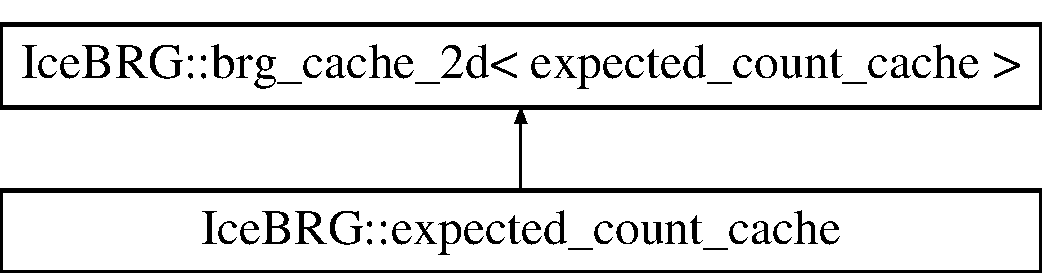
\includegraphics[height=2.000000cm]{classIceBRG_1_1expected__count__cache}
\end{center}
\end{figure}
\subsection*{Public Member Functions}
\begin{DoxyCompactItemize}
\item 
\hyperlink{classIceBRG_1_1expected__count__cache_a2f0071d1fddd08d805724fc199631fd1}{expected\+\_\+count\+\_\+cache} ()
\item 
\hyperlink{classIceBRG_1_1expected__count__cache_a817a41f05b8d36b3791924ceb47a6f5b}{$\sim$expected\+\_\+count\+\_\+cache} ()
\end{DoxyCompactItemize}
\subsection*{Protected Member Functions}
\begin{DoxyCompactItemize}
\item 
std\+::string \hyperlink{classIceBRG_1_1expected__count__cache_a07cb2c99bf0bfba61a2da77300a6061f}{\+\_\+name\+\_\+base} () const 
\item 
\hyperlink{lib_2IceBRG__main_2common_8h_ad0f130a56eeb944d9ef2692ee881ecc4}{flt\+\_\+type} \hyperlink{classIceBRG_1_1expected__count__cache_a9b18a3e02060bd0cde404eff18fb8343}{\+\_\+calculate} (const \hyperlink{lib_2IceBRG__main_2common_8h_ad0f130a56eeb944d9ef2692ee881ecc4}{flt\+\_\+type} \&in\+\_\+param\+\_\+1, const \hyperlink{lib_2IceBRG__main_2common_8h_ad0f130a56eeb944d9ef2692ee881ecc4}{flt\+\_\+type} \&in\+\_\+param\+\_\+2) const 
\item 
void \hyperlink{classIceBRG_1_1expected__count__cache_a6047eeb391a812c90e190b712d2a33fc}{\+\_\+load\+\_\+cache\+\_\+dependencies} () const 
\end{DoxyCompactItemize}
\subsection*{Friends}
\begin{DoxyCompactItemize}
\item 
class \hyperlink{classIceBRG_1_1expected__count__cache_a075975b934daaee5d607cdc06190e819}{brg\+\_\+cache\+\_\+2d$<$ expected\+\_\+count\+\_\+cache $>$}
\end{DoxyCompactItemize}


\subsection{Constructor \& Destructor Documentation}
\hypertarget{classIceBRG_1_1expected__count__cache_a2f0071d1fddd08d805724fc199631fd1}{}\index{Ice\+B\+R\+G\+::expected\+\_\+count\+\_\+cache@{Ice\+B\+R\+G\+::expected\+\_\+count\+\_\+cache}!expected\+\_\+count\+\_\+cache@{expected\+\_\+count\+\_\+cache}}
\index{expected\+\_\+count\+\_\+cache@{expected\+\_\+count\+\_\+cache}!Ice\+B\+R\+G\+::expected\+\_\+count\+\_\+cache@{Ice\+B\+R\+G\+::expected\+\_\+count\+\_\+cache}}
\subsubsection[{expected\+\_\+count\+\_\+cache()}]{\setlength{\rightskip}{0pt plus 5cm}Ice\+B\+R\+G\+::expected\+\_\+count\+\_\+cache\+::expected\+\_\+count\+\_\+cache (
\begin{DoxyParamCaption}
{}
\end{DoxyParamCaption}
)\hspace{0.3cm}{\ttfamily [inline]}}\label{classIceBRG_1_1expected__count__cache_a2f0071d1fddd08d805724fc199631fd1}
\hypertarget{classIceBRG_1_1expected__count__cache_a817a41f05b8d36b3791924ceb47a6f5b}{}\index{Ice\+B\+R\+G\+::expected\+\_\+count\+\_\+cache@{Ice\+B\+R\+G\+::expected\+\_\+count\+\_\+cache}!````~expected\+\_\+count\+\_\+cache@{$\sim$expected\+\_\+count\+\_\+cache}}
\index{````~expected\+\_\+count\+\_\+cache@{$\sim$expected\+\_\+count\+\_\+cache}!Ice\+B\+R\+G\+::expected\+\_\+count\+\_\+cache@{Ice\+B\+R\+G\+::expected\+\_\+count\+\_\+cache}}
\subsubsection[{$\sim$expected\+\_\+count\+\_\+cache()}]{\setlength{\rightskip}{0pt plus 5cm}Ice\+B\+R\+G\+::expected\+\_\+count\+\_\+cache\+::$\sim$expected\+\_\+count\+\_\+cache (
\begin{DoxyParamCaption}
{}
\end{DoxyParamCaption}
)\hspace{0.3cm}{\ttfamily [inline]}}\label{classIceBRG_1_1expected__count__cache_a817a41f05b8d36b3791924ceb47a6f5b}


\subsection{Member Function Documentation}
\hypertarget{classIceBRG_1_1expected__count__cache_a9b18a3e02060bd0cde404eff18fb8343}{}\index{Ice\+B\+R\+G\+::expected\+\_\+count\+\_\+cache@{Ice\+B\+R\+G\+::expected\+\_\+count\+\_\+cache}!\+\_\+calculate@{\+\_\+calculate}}
\index{\+\_\+calculate@{\+\_\+calculate}!Ice\+B\+R\+G\+::expected\+\_\+count\+\_\+cache@{Ice\+B\+R\+G\+::expected\+\_\+count\+\_\+cache}}
\subsubsection[{\+\_\+calculate(const flt\+\_\+type \&in\+\_\+param\+\_\+1, const flt\+\_\+type \&in\+\_\+param\+\_\+2) const }]{\setlength{\rightskip}{0pt plus 5cm}{\bf flt\+\_\+type} Ice\+B\+R\+G\+::expected\+\_\+count\+\_\+cache\+::\+\_\+calculate (
\begin{DoxyParamCaption}
\item[{const {\bf flt\+\_\+type} \&}]{in\+\_\+param\+\_\+1, }
\item[{const {\bf flt\+\_\+type} \&}]{in\+\_\+param\+\_\+2}
\end{DoxyParamCaption}
) const\hspace{0.3cm}{\ttfamily [protected]}}\label{classIceBRG_1_1expected__count__cache_a9b18a3e02060bd0cde404eff18fb8343}
\hypertarget{classIceBRG_1_1expected__count__cache_a6047eeb391a812c90e190b712d2a33fc}{}\index{Ice\+B\+R\+G\+::expected\+\_\+count\+\_\+cache@{Ice\+B\+R\+G\+::expected\+\_\+count\+\_\+cache}!\+\_\+load\+\_\+cache\+\_\+dependencies@{\+\_\+load\+\_\+cache\+\_\+dependencies}}
\index{\+\_\+load\+\_\+cache\+\_\+dependencies@{\+\_\+load\+\_\+cache\+\_\+dependencies}!Ice\+B\+R\+G\+::expected\+\_\+count\+\_\+cache@{Ice\+B\+R\+G\+::expected\+\_\+count\+\_\+cache}}
\subsubsection[{\+\_\+load\+\_\+cache\+\_\+dependencies() const }]{\setlength{\rightskip}{0pt plus 5cm}void Ice\+B\+R\+G\+::expected\+\_\+count\+\_\+cache\+::\+\_\+load\+\_\+cache\+\_\+dependencies (
\begin{DoxyParamCaption}
{}
\end{DoxyParamCaption}
) const\hspace{0.3cm}{\ttfamily [protected]}}\label{classIceBRG_1_1expected__count__cache_a6047eeb391a812c90e190b712d2a33fc}
\hypertarget{classIceBRG_1_1expected__count__cache_a07cb2c99bf0bfba61a2da77300a6061f}{}\index{Ice\+B\+R\+G\+::expected\+\_\+count\+\_\+cache@{Ice\+B\+R\+G\+::expected\+\_\+count\+\_\+cache}!\+\_\+name\+\_\+base@{\+\_\+name\+\_\+base}}
\index{\+\_\+name\+\_\+base@{\+\_\+name\+\_\+base}!Ice\+B\+R\+G\+::expected\+\_\+count\+\_\+cache@{Ice\+B\+R\+G\+::expected\+\_\+count\+\_\+cache}}
\subsubsection[{\+\_\+name\+\_\+base() const }]{\setlength{\rightskip}{0pt plus 5cm}std\+::string Ice\+B\+R\+G\+::expected\+\_\+count\+\_\+cache\+::\+\_\+name\+\_\+base (
\begin{DoxyParamCaption}
{}
\end{DoxyParamCaption}
) const\hspace{0.3cm}{\ttfamily [inline]}, {\ttfamily [protected]}}\label{classIceBRG_1_1expected__count__cache_a07cb2c99bf0bfba61a2da77300a6061f}


\subsection{Friends And Related Function Documentation}
\hypertarget{classIceBRG_1_1expected__count__cache_a075975b934daaee5d607cdc06190e819}{}\index{Ice\+B\+R\+G\+::expected\+\_\+count\+\_\+cache@{Ice\+B\+R\+G\+::expected\+\_\+count\+\_\+cache}!brg\+\_\+cache\+\_\+2d$<$ expected\+\_\+count\+\_\+cache $>$@{brg\+\_\+cache\+\_\+2d$<$ expected\+\_\+count\+\_\+cache $>$}}
\index{brg\+\_\+cache\+\_\+2d$<$ expected\+\_\+count\+\_\+cache $>$@{brg\+\_\+cache\+\_\+2d$<$ expected\+\_\+count\+\_\+cache $>$}!Ice\+B\+R\+G\+::expected\+\_\+count\+\_\+cache@{Ice\+B\+R\+G\+::expected\+\_\+count\+\_\+cache}}
\subsubsection[{brg\+\_\+cache\+\_\+2d$<$ expected\+\_\+count\+\_\+cache $>$}]{\setlength{\rightskip}{0pt plus 5cm}friend class {\bf brg\+\_\+cache\+\_\+2d}$<$ {\bf expected\+\_\+count\+\_\+cache} $>$\hspace{0.3cm}{\ttfamily [friend]}}\label{classIceBRG_1_1expected__count__cache_a075975b934daaee5d607cdc06190e819}


The documentation for this class was generated from the following files\+:\begin{DoxyCompactItemize}
\item 
/disk2/brg/git/\+Magnification\+\_\+\+Public/src/lib/\+Ice\+B\+R\+G\+\_\+lensing/magnification/\hyperlink{expected__count__cache_8h}{expected\+\_\+count\+\_\+cache.\+h}\item 
/disk2/brg/git/\+Magnification\+\_\+\+Public/src/lib/\+Ice\+B\+R\+G\+\_\+lensing/magnification/\hyperlink{expected__count__cache_8cpp}{expected\+\_\+count\+\_\+cache.\+cpp}\end{DoxyCompactItemize}

\hypertarget{classIceBRG_1_1expected__count__derivative__cache}{\section{Ice\-B\-R\-G\-:\-:expected\-\_\-count\-\_\-derivative\-\_\-cache Class Reference}
\label{classIceBRG_1_1expected__count__derivative__cache}\index{Ice\-B\-R\-G\-::expected\-\_\-count\-\_\-derivative\-\_\-cache@{Ice\-B\-R\-G\-::expected\-\_\-count\-\_\-derivative\-\_\-cache}}
}


{\ttfamily \#include $<$expected\-\_\-count\-\_\-derivative\-\_\-cache.\-h$>$}

Inheritance diagram for Ice\-B\-R\-G\-:\-:expected\-\_\-count\-\_\-derivative\-\_\-cache\-:\begin{figure}[H]
\begin{center}
\leavevmode
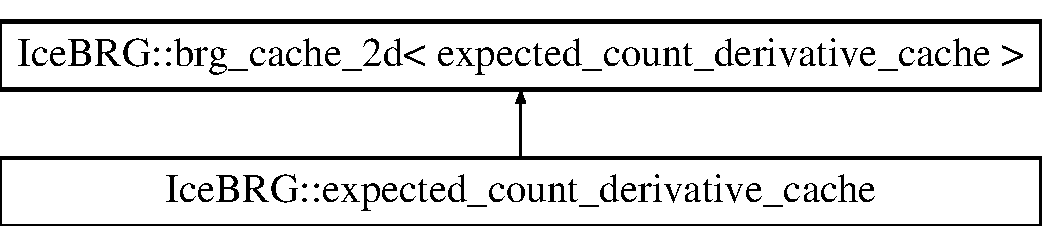
\includegraphics[height=2.000000cm]{classIceBRG_1_1expected__count__derivative__cache}
\end{center}
\end{figure}
\subsection*{Public Member Functions}
\begin{DoxyCompactItemize}
\item 
\hyperlink{classIceBRG_1_1expected__count__derivative__cache_a63a6e862842c52e5bf31ffea28828733}{expected\-\_\-count\-\_\-derivative\-\_\-cache} ()
\item 
\hyperlink{classIceBRG_1_1expected__count__derivative__cache_a006d6761d4ad94e582a565079035ac17}{$\sim$expected\-\_\-count\-\_\-derivative\-\_\-cache} ()
\end{DoxyCompactItemize}
\subsection*{Protected Member Functions}
\begin{DoxyCompactItemize}
\item 
std\-::string \hyperlink{classIceBRG_1_1expected__count__derivative__cache_abb662544efc6301f169336a3cb6fa08a}{\-\_\-name\-\_\-base} () const 
\item 
\hyperlink{lib_2IceBRG__main_2common_8h_ad0f130a56eeb944d9ef2692ee881ecc4}{flt\-\_\-type} \hyperlink{classIceBRG_1_1expected__count__derivative__cache_abc9c512709d23669a982a40c8e0613cf}{\-\_\-calculate} (const \hyperlink{lib_2IceBRG__main_2common_8h_ad0f130a56eeb944d9ef2692ee881ecc4}{flt\-\_\-type} \&in\-\_\-param\-\_\-1, const \hyperlink{lib_2IceBRG__main_2common_8h_ad0f130a56eeb944d9ef2692ee881ecc4}{flt\-\_\-type} \&in\-\_\-param\-\_\-2) const 
\item 
void \hyperlink{classIceBRG_1_1expected__count__derivative__cache_a3f883c9118416c4bca3fbca8327a6267}{\-\_\-load\-\_\-cache\-\_\-dependencies} () const 
\end{DoxyCompactItemize}
\subsection*{Friends}
\begin{DoxyCompactItemize}
\item 
class \hyperlink{classIceBRG_1_1expected__count__derivative__cache_a6cb64b05ca65e864c79c1c875fbfcf6c}{brg\-\_\-cache\-\_\-2d$<$ expected\-\_\-count\-\_\-derivative\-\_\-cache $>$}
\end{DoxyCompactItemize}


\subsection{Constructor \& Destructor Documentation}
\hypertarget{classIceBRG_1_1expected__count__derivative__cache_a63a6e862842c52e5bf31ffea28828733}{\index{Ice\-B\-R\-G\-::expected\-\_\-count\-\_\-derivative\-\_\-cache@{Ice\-B\-R\-G\-::expected\-\_\-count\-\_\-derivative\-\_\-cache}!expected\-\_\-count\-\_\-derivative\-\_\-cache@{expected\-\_\-count\-\_\-derivative\-\_\-cache}}
\index{expected\-\_\-count\-\_\-derivative\-\_\-cache@{expected\-\_\-count\-\_\-derivative\-\_\-cache}!IceBRG::expected_count_derivative_cache@{Ice\-B\-R\-G\-::expected\-\_\-count\-\_\-derivative\-\_\-cache}}
\subsubsection[{expected\-\_\-count\-\_\-derivative\-\_\-cache}]{\setlength{\rightskip}{0pt plus 5cm}Ice\-B\-R\-G\-::expected\-\_\-count\-\_\-derivative\-\_\-cache\-::expected\-\_\-count\-\_\-derivative\-\_\-cache (
\begin{DoxyParamCaption}
{}
\end{DoxyParamCaption}
)\hspace{0.3cm}{\ttfamily [inline]}}}\label{classIceBRG_1_1expected__count__derivative__cache_a63a6e862842c52e5bf31ffea28828733}
\hypertarget{classIceBRG_1_1expected__count__derivative__cache_a006d6761d4ad94e582a565079035ac17}{\index{Ice\-B\-R\-G\-::expected\-\_\-count\-\_\-derivative\-\_\-cache@{Ice\-B\-R\-G\-::expected\-\_\-count\-\_\-derivative\-\_\-cache}!$\sim$expected\-\_\-count\-\_\-derivative\-\_\-cache@{$\sim$expected\-\_\-count\-\_\-derivative\-\_\-cache}}
\index{$\sim$expected\-\_\-count\-\_\-derivative\-\_\-cache@{$\sim$expected\-\_\-count\-\_\-derivative\-\_\-cache}!IceBRG::expected_count_derivative_cache@{Ice\-B\-R\-G\-::expected\-\_\-count\-\_\-derivative\-\_\-cache}}
\subsubsection[{$\sim$expected\-\_\-count\-\_\-derivative\-\_\-cache}]{\setlength{\rightskip}{0pt plus 5cm}Ice\-B\-R\-G\-::expected\-\_\-count\-\_\-derivative\-\_\-cache\-::$\sim$expected\-\_\-count\-\_\-derivative\-\_\-cache (
\begin{DoxyParamCaption}
{}
\end{DoxyParamCaption}
)\hspace{0.3cm}{\ttfamily [inline]}}}\label{classIceBRG_1_1expected__count__derivative__cache_a006d6761d4ad94e582a565079035ac17}


\subsection{Member Function Documentation}
\hypertarget{classIceBRG_1_1expected__count__derivative__cache_abc9c512709d23669a982a40c8e0613cf}{\index{Ice\-B\-R\-G\-::expected\-\_\-count\-\_\-derivative\-\_\-cache@{Ice\-B\-R\-G\-::expected\-\_\-count\-\_\-derivative\-\_\-cache}!\-\_\-calculate@{\-\_\-calculate}}
\index{\-\_\-calculate@{\-\_\-calculate}!IceBRG::expected_count_derivative_cache@{Ice\-B\-R\-G\-::expected\-\_\-count\-\_\-derivative\-\_\-cache}}
\subsubsection[{\-\_\-calculate}]{\setlength{\rightskip}{0pt plus 5cm}{\bf flt\-\_\-type} Ice\-B\-R\-G\-::expected\-\_\-count\-\_\-derivative\-\_\-cache\-::\-\_\-calculate (
\begin{DoxyParamCaption}
\item[{const {\bf flt\-\_\-type} \&}]{in\-\_\-param\-\_\-1, }
\item[{const {\bf flt\-\_\-type} \&}]{in\-\_\-param\-\_\-2}
\end{DoxyParamCaption}
) const\hspace{0.3cm}{\ttfamily [protected]}}}\label{classIceBRG_1_1expected__count__derivative__cache_abc9c512709d23669a982a40c8e0613cf}


Reimplemented from \hyperlink{classIceBRG_1_1brg__cache__2d_ade75dde33039e36209c2887e0eaf2a32}{Ice\-B\-R\-G\-::brg\-\_\-cache\-\_\-2d$<$ name $>$}.

\hypertarget{classIceBRG_1_1expected__count__derivative__cache_a3f883c9118416c4bca3fbca8327a6267}{\index{Ice\-B\-R\-G\-::expected\-\_\-count\-\_\-derivative\-\_\-cache@{Ice\-B\-R\-G\-::expected\-\_\-count\-\_\-derivative\-\_\-cache}!\-\_\-load\-\_\-cache\-\_\-dependencies@{\-\_\-load\-\_\-cache\-\_\-dependencies}}
\index{\-\_\-load\-\_\-cache\-\_\-dependencies@{\-\_\-load\-\_\-cache\-\_\-dependencies}!IceBRG::expected_count_derivative_cache@{Ice\-B\-R\-G\-::expected\-\_\-count\-\_\-derivative\-\_\-cache}}
\subsubsection[{\-\_\-load\-\_\-cache\-\_\-dependencies}]{\setlength{\rightskip}{0pt plus 5cm}void Ice\-B\-R\-G\-::expected\-\_\-count\-\_\-derivative\-\_\-cache\-::\-\_\-load\-\_\-cache\-\_\-dependencies (
\begin{DoxyParamCaption}
{}
\end{DoxyParamCaption}
) const\hspace{0.3cm}{\ttfamily [protected]}}}\label{classIceBRG_1_1expected__count__derivative__cache_a3f883c9118416c4bca3fbca8327a6267}


Reimplemented from \hyperlink{classIceBRG_1_1brg__cache__2d_a74cd593f9bbf3a501a4132b791a110b9}{Ice\-B\-R\-G\-::brg\-\_\-cache\-\_\-2d$<$ name $>$}.

\hypertarget{classIceBRG_1_1expected__count__derivative__cache_abb662544efc6301f169336a3cb6fa08a}{\index{Ice\-B\-R\-G\-::expected\-\_\-count\-\_\-derivative\-\_\-cache@{Ice\-B\-R\-G\-::expected\-\_\-count\-\_\-derivative\-\_\-cache}!\-\_\-name\-\_\-base@{\-\_\-name\-\_\-base}}
\index{\-\_\-name\-\_\-base@{\-\_\-name\-\_\-base}!IceBRG::expected_count_derivative_cache@{Ice\-B\-R\-G\-::expected\-\_\-count\-\_\-derivative\-\_\-cache}}
\subsubsection[{\-\_\-name\-\_\-base}]{\setlength{\rightskip}{0pt plus 5cm}std\-::string Ice\-B\-R\-G\-::expected\-\_\-count\-\_\-derivative\-\_\-cache\-::\-\_\-name\-\_\-base (
\begin{DoxyParamCaption}
{}
\end{DoxyParamCaption}
) const\hspace{0.3cm}{\ttfamily [inline]}, {\ttfamily [protected]}}}\label{classIceBRG_1_1expected__count__derivative__cache_abb662544efc6301f169336a3cb6fa08a}


Reimplemented from \hyperlink{classIceBRG_1_1brg__cache__2d_a09696dae89337d3f669a4a2d744708a7}{Ice\-B\-R\-G\-::brg\-\_\-cache\-\_\-2d$<$ name $>$}.



\subsection{Friends And Related Function Documentation}
\hypertarget{classIceBRG_1_1expected__count__derivative__cache_a6cb64b05ca65e864c79c1c875fbfcf6c}{\index{Ice\-B\-R\-G\-::expected\-\_\-count\-\_\-derivative\-\_\-cache@{Ice\-B\-R\-G\-::expected\-\_\-count\-\_\-derivative\-\_\-cache}!brg\-\_\-cache\-\_\-2d$<$ expected\-\_\-count\-\_\-derivative\-\_\-cache $>$@{brg\-\_\-cache\-\_\-2d$<$ expected\-\_\-count\-\_\-derivative\-\_\-cache $>$}}
\index{brg\-\_\-cache\-\_\-2d$<$ expected\-\_\-count\-\_\-derivative\-\_\-cache $>$@{brg\-\_\-cache\-\_\-2d$<$ expected\-\_\-count\-\_\-derivative\-\_\-cache $>$}!IceBRG::expected_count_derivative_cache@{Ice\-B\-R\-G\-::expected\-\_\-count\-\_\-derivative\-\_\-cache}}
\subsubsection[{brg\-\_\-cache\-\_\-2d$<$ expected\-\_\-count\-\_\-derivative\-\_\-cache $>$}]{\setlength{\rightskip}{0pt plus 5cm}friend class {\bf brg\-\_\-cache\-\_\-2d}$<$ {\bf expected\-\_\-count\-\_\-derivative\-\_\-cache} $>$\hspace{0.3cm}{\ttfamily [friend]}}}\label{classIceBRG_1_1expected__count__derivative__cache_a6cb64b05ca65e864c79c1c875fbfcf6c}


The documentation for this class was generated from the following files\-:\begin{DoxyCompactItemize}
\item 
/disk2/brg/git/\-Magnification\-\_\-\-Public/src/lib/\-Ice\-B\-R\-G\-\_\-lensing/magnification/\hyperlink{expected__count__derivative__cache_8h}{expected\-\_\-count\-\_\-derivative\-\_\-cache.\-h}\item 
/disk2/brg/git/\-Magnification\-\_\-\-Public/src/lib/\-Ice\-B\-R\-G\-\_\-lensing/magnification/\hyperlink{expected__count__derivative__cache_8cpp}{expected\-\_\-count\-\_\-derivative\-\_\-cache.\-cpp}\end{DoxyCompactItemize}

\hypertarget{classIceBRG_1_1expected__count__fit__loader}{\section{Ice\-B\-R\-G\-:\-:expected\-\_\-count\-\_\-fit\-\_\-loader Class Reference}
\label{classIceBRG_1_1expected__count__fit__loader}\index{Ice\-B\-R\-G\-::expected\-\_\-count\-\_\-fit\-\_\-loader@{Ice\-B\-R\-G\-::expected\-\_\-count\-\_\-fit\-\_\-loader}}
}


{\ttfamily \#include $<$expected\-\_\-count\-\_\-fit\-\_\-loader.\-h$>$}

\subsection*{Static Public Member Functions}
\begin{DoxyCompactItemize}
\item 
static std\-::vector$<$ \hyperlink{lib_2IceBRG__main_2common_8h_ad0f130a56eeb944d9ef2692ee881ecc4}{flt\-\_\-type} $>$ \hyperlink{classIceBRG_1_1expected__count__fit__loader_a98b772ace86125bcf96a843614981943}{get} (const \hyperlink{lib_2IceBRG__main_2common_8h_ad0f130a56eeb944d9ef2692ee881ecc4}{flt\-\_\-type} \&z)
\item 
static void \hyperlink{classIceBRG_1_1expected__count__fit__loader_a940c206daf47104618ff75efdf843a76}{unload} ()
\end{DoxyCompactItemize}


\subsection{Member Function Documentation}
\hypertarget{classIceBRG_1_1expected__count__fit__loader_a98b772ace86125bcf96a843614981943}{\index{Ice\-B\-R\-G\-::expected\-\_\-count\-\_\-fit\-\_\-loader@{Ice\-B\-R\-G\-::expected\-\_\-count\-\_\-fit\-\_\-loader}!get@{get}}
\index{get@{get}!IceBRG::expected_count_fit_loader@{Ice\-B\-R\-G\-::expected\-\_\-count\-\_\-fit\-\_\-loader}}
\subsubsection[{get}]{\setlength{\rightskip}{0pt plus 5cm}std\-::vector$<$ {\bf flt\-\_\-type} $>$ Ice\-B\-R\-G\-::expected\-\_\-count\-\_\-fit\-\_\-loader\-::get (
\begin{DoxyParamCaption}
\item[{const {\bf flt\-\_\-type} \&}]{z}
\end{DoxyParamCaption}
)\hspace{0.3cm}{\ttfamily [static]}}}\label{classIceBRG_1_1expected__count__fit__loader_a98b772ace86125bcf96a843614981943}
\hypertarget{classIceBRG_1_1expected__count__fit__loader_a940c206daf47104618ff75efdf843a76}{\index{Ice\-B\-R\-G\-::expected\-\_\-count\-\_\-fit\-\_\-loader@{Ice\-B\-R\-G\-::expected\-\_\-count\-\_\-fit\-\_\-loader}!unload@{unload}}
\index{unload@{unload}!IceBRG::expected_count_fit_loader@{Ice\-B\-R\-G\-::expected\-\_\-count\-\_\-fit\-\_\-loader}}
\subsubsection[{unload}]{\setlength{\rightskip}{0pt plus 5cm}void Ice\-B\-R\-G\-::expected\-\_\-count\-\_\-fit\-\_\-loader\-::unload (
\begin{DoxyParamCaption}
{}
\end{DoxyParamCaption}
)\hspace{0.3cm}{\ttfamily [static]}}}\label{classIceBRG_1_1expected__count__fit__loader_a940c206daf47104618ff75efdf843a76}


The documentation for this class was generated from the following files\-:\begin{DoxyCompactItemize}
\item 
/disk2/brg/git/\-Magnification\-\_\-\-Public/src/lib/\-Ice\-B\-R\-G\-\_\-lensing/magnification/\hyperlink{expected__count__fit__loader_8h}{expected\-\_\-count\-\_\-fit\-\_\-loader.\-h}\item 
/disk2/brg/git/\-Magnification\-\_\-\-Public/src/lib/\-Ice\-B\-R\-G\-\_\-lensing/magnification/\hyperlink{expected__count__fit__loader_8cpp}{expected\-\_\-count\-\_\-fit\-\_\-loader.\-cpp}\end{DoxyCompactItemize}

\hypertarget{classIceBRG_1_1expected__count__loader}{}\section{Ice\+B\+R\+G\+:\+:expected\+\_\+count\+\_\+loader Class Reference}
\label{classIceBRG_1_1expected__count__loader}\index{Ice\+B\+R\+G\+::expected\+\_\+count\+\_\+loader@{Ice\+B\+R\+G\+::expected\+\_\+count\+\_\+loader}}


{\ttfamily \#include $<$expected\+\_\+count\+\_\+loader.\+h$>$}

\subsection*{Static Public Member Functions}
\begin{DoxyCompactItemize}
\item 
static void \hyperlink{classIceBRG_1_1expected__count__loader_ad7e776799292cb4660f98384a2f4505f}{set\+\_\+z\+\_\+limits} (const std\+::vector$<$ \hyperlink{lib_2IceBRG__main_2common_8h_ad0f130a56eeb944d9ef2692ee881ecc4}{flt\+\_\+type} $>$ \&new\+\_\+limits\+\_\+vector)
\item 
static void \hyperlink{classIceBRG_1_1expected__count__loader_ae8b333ac395d75b65c145d606b5c159b}{set\+\_\+z\+\_\+limits} (std\+::vector$<$ \hyperlink{lib_2IceBRG__main_2common_8h_ad0f130a56eeb944d9ef2692ee881ecc4}{flt\+\_\+type} $>$ \&\&new\+\_\+limits\+\_\+vector)
\item 
static void \hyperlink{classIceBRG_1_1expected__count__loader_a5dcd85e898db66b1ebc3f50462388dd3}{set\+\_\+filename\+\_\+base} (const std\+::string \&new\+\_\+filename\+\_\+base)
\item 
static void \hyperlink{classIceBRG_1_1expected__count__loader_a8cae32efecceecb9d257ba4393f1ba21}{set\+\_\+filename\+\_\+base} (std\+::string \&\&new\+\_\+filename\+\_\+base)
\item 
static void \hyperlink{classIceBRG_1_1expected__count__loader_a0acbb6a0590f2b6447b0a9c9584a92eb}{set\+\_\+filename\+\_\+tail} (const std\+::string \&new\+\_\+filename\+\_\+tail)
\item 
static void \hyperlink{classIceBRG_1_1expected__count__loader_af8d28d202cf91f98301e60bc58f8582e}{set\+\_\+filename\+\_\+tail} (std\+::string \&\&new\+\_\+filename\+\_\+tail)
\item 
static \hyperlink{lib_2IceBRG__main_2common_8h_ad0f130a56eeb944d9ef2692ee881ecc4}{flt\+\_\+type} \hyperlink{classIceBRG_1_1expected__count__loader_a653df13eb1c195306d1369a391c26cdb}{get\+\_\+count} (const \hyperlink{lib_2IceBRG__main_2common_8h_ad0f130a56eeb944d9ef2692ee881ecc4}{flt\+\_\+type} \&mag, const \hyperlink{lib_2IceBRG__main_2common_8h_ad0f130a56eeb944d9ef2692ee881ecc4}{flt\+\_\+type} \&z)
\item 
static \hyperlink{lib_2IceBRG__main_2common_8h_ad0f130a56eeb944d9ef2692ee881ecc4}{flt\+\_\+type} \hyperlink{classIceBRG_1_1expected__count__loader_aa96daa351eb4cb0fec82ba6a28f9827c}{get\+\_\+derivative} (const \hyperlink{lib_2IceBRG__main_2common_8h_ad0f130a56eeb944d9ef2692ee881ecc4}{flt\+\_\+type} \&mag, const \hyperlink{lib_2IceBRG__main_2common_8h_ad0f130a56eeb944d9ef2692ee881ecc4}{flt\+\_\+type} \&z)
\item 
static void \hyperlink{classIceBRG_1_1expected__count__loader_a3c4fd80f47109f5ac052ad2359dbdcec}{unload} ()
\end{DoxyCompactItemize}


\subsection{Member Function Documentation}
\hypertarget{classIceBRG_1_1expected__count__loader_a653df13eb1c195306d1369a391c26cdb}{}\index{Ice\+B\+R\+G\+::expected\+\_\+count\+\_\+loader@{Ice\+B\+R\+G\+::expected\+\_\+count\+\_\+loader}!get\+\_\+count@{get\+\_\+count}}
\index{get\+\_\+count@{get\+\_\+count}!Ice\+B\+R\+G\+::expected\+\_\+count\+\_\+loader@{Ice\+B\+R\+G\+::expected\+\_\+count\+\_\+loader}}
\subsubsection[{get\+\_\+count(const flt\+\_\+type \&mag, const flt\+\_\+type \&z)}]{\setlength{\rightskip}{0pt plus 5cm}{\bf flt\+\_\+type} Ice\+B\+R\+G\+::expected\+\_\+count\+\_\+loader\+::get\+\_\+count (
\begin{DoxyParamCaption}
\item[{const {\bf flt\+\_\+type} \&}]{mag, }
\item[{const {\bf flt\+\_\+type} \&}]{z}
\end{DoxyParamCaption}
)\hspace{0.3cm}{\ttfamily [static]}}\label{classIceBRG_1_1expected__count__loader_a653df13eb1c195306d1369a391c26cdb}
\hypertarget{classIceBRG_1_1expected__count__loader_aa96daa351eb4cb0fec82ba6a28f9827c}{}\index{Ice\+B\+R\+G\+::expected\+\_\+count\+\_\+loader@{Ice\+B\+R\+G\+::expected\+\_\+count\+\_\+loader}!get\+\_\+derivative@{get\+\_\+derivative}}
\index{get\+\_\+derivative@{get\+\_\+derivative}!Ice\+B\+R\+G\+::expected\+\_\+count\+\_\+loader@{Ice\+B\+R\+G\+::expected\+\_\+count\+\_\+loader}}
\subsubsection[{get\+\_\+derivative(const flt\+\_\+type \&mag, const flt\+\_\+type \&z)}]{\setlength{\rightskip}{0pt plus 5cm}{\bf flt\+\_\+type} Ice\+B\+R\+G\+::expected\+\_\+count\+\_\+loader\+::get\+\_\+derivative (
\begin{DoxyParamCaption}
\item[{const {\bf flt\+\_\+type} \&}]{mag, }
\item[{const {\bf flt\+\_\+type} \&}]{z}
\end{DoxyParamCaption}
)\hspace{0.3cm}{\ttfamily [static]}}\label{classIceBRG_1_1expected__count__loader_aa96daa351eb4cb0fec82ba6a28f9827c}
\hypertarget{classIceBRG_1_1expected__count__loader_a5dcd85e898db66b1ebc3f50462388dd3}{}\index{Ice\+B\+R\+G\+::expected\+\_\+count\+\_\+loader@{Ice\+B\+R\+G\+::expected\+\_\+count\+\_\+loader}!set\+\_\+filename\+\_\+base@{set\+\_\+filename\+\_\+base}}
\index{set\+\_\+filename\+\_\+base@{set\+\_\+filename\+\_\+base}!Ice\+B\+R\+G\+::expected\+\_\+count\+\_\+loader@{Ice\+B\+R\+G\+::expected\+\_\+count\+\_\+loader}}
\subsubsection[{set\+\_\+filename\+\_\+base(const std\+::string \&new\+\_\+filename\+\_\+base)}]{\setlength{\rightskip}{0pt plus 5cm}void Ice\+B\+R\+G\+::expected\+\_\+count\+\_\+loader\+::set\+\_\+filename\+\_\+base (
\begin{DoxyParamCaption}
\item[{const std\+::string \&}]{new\+\_\+filename\+\_\+base}
\end{DoxyParamCaption}
)\hspace{0.3cm}{\ttfamily [static]}}\label{classIceBRG_1_1expected__count__loader_a5dcd85e898db66b1ebc3f50462388dd3}
\hypertarget{classIceBRG_1_1expected__count__loader_a8cae32efecceecb9d257ba4393f1ba21}{}\index{Ice\+B\+R\+G\+::expected\+\_\+count\+\_\+loader@{Ice\+B\+R\+G\+::expected\+\_\+count\+\_\+loader}!set\+\_\+filename\+\_\+base@{set\+\_\+filename\+\_\+base}}
\index{set\+\_\+filename\+\_\+base@{set\+\_\+filename\+\_\+base}!Ice\+B\+R\+G\+::expected\+\_\+count\+\_\+loader@{Ice\+B\+R\+G\+::expected\+\_\+count\+\_\+loader}}
\subsubsection[{set\+\_\+filename\+\_\+base(std\+::string \&\&new\+\_\+filename\+\_\+base)}]{\setlength{\rightskip}{0pt plus 5cm}void Ice\+B\+R\+G\+::expected\+\_\+count\+\_\+loader\+::set\+\_\+filename\+\_\+base (
\begin{DoxyParamCaption}
\item[{std\+::string \&\&}]{new\+\_\+filename\+\_\+base}
\end{DoxyParamCaption}
)\hspace{0.3cm}{\ttfamily [static]}}\label{classIceBRG_1_1expected__count__loader_a8cae32efecceecb9d257ba4393f1ba21}
\hypertarget{classIceBRG_1_1expected__count__loader_a0acbb6a0590f2b6447b0a9c9584a92eb}{}\index{Ice\+B\+R\+G\+::expected\+\_\+count\+\_\+loader@{Ice\+B\+R\+G\+::expected\+\_\+count\+\_\+loader}!set\+\_\+filename\+\_\+tail@{set\+\_\+filename\+\_\+tail}}
\index{set\+\_\+filename\+\_\+tail@{set\+\_\+filename\+\_\+tail}!Ice\+B\+R\+G\+::expected\+\_\+count\+\_\+loader@{Ice\+B\+R\+G\+::expected\+\_\+count\+\_\+loader}}
\subsubsection[{set\+\_\+filename\+\_\+tail(const std\+::string \&new\+\_\+filename\+\_\+tail)}]{\setlength{\rightskip}{0pt plus 5cm}void Ice\+B\+R\+G\+::expected\+\_\+count\+\_\+loader\+::set\+\_\+filename\+\_\+tail (
\begin{DoxyParamCaption}
\item[{const std\+::string \&}]{new\+\_\+filename\+\_\+tail}
\end{DoxyParamCaption}
)\hspace{0.3cm}{\ttfamily [static]}}\label{classIceBRG_1_1expected__count__loader_a0acbb6a0590f2b6447b0a9c9584a92eb}
\hypertarget{classIceBRG_1_1expected__count__loader_af8d28d202cf91f98301e60bc58f8582e}{}\index{Ice\+B\+R\+G\+::expected\+\_\+count\+\_\+loader@{Ice\+B\+R\+G\+::expected\+\_\+count\+\_\+loader}!set\+\_\+filename\+\_\+tail@{set\+\_\+filename\+\_\+tail}}
\index{set\+\_\+filename\+\_\+tail@{set\+\_\+filename\+\_\+tail}!Ice\+B\+R\+G\+::expected\+\_\+count\+\_\+loader@{Ice\+B\+R\+G\+::expected\+\_\+count\+\_\+loader}}
\subsubsection[{set\+\_\+filename\+\_\+tail(std\+::string \&\&new\+\_\+filename\+\_\+tail)}]{\setlength{\rightskip}{0pt plus 5cm}void Ice\+B\+R\+G\+::expected\+\_\+count\+\_\+loader\+::set\+\_\+filename\+\_\+tail (
\begin{DoxyParamCaption}
\item[{std\+::string \&\&}]{new\+\_\+filename\+\_\+tail}
\end{DoxyParamCaption}
)\hspace{0.3cm}{\ttfamily [static]}}\label{classIceBRG_1_1expected__count__loader_af8d28d202cf91f98301e60bc58f8582e}
\hypertarget{classIceBRG_1_1expected__count__loader_ad7e776799292cb4660f98384a2f4505f}{}\index{Ice\+B\+R\+G\+::expected\+\_\+count\+\_\+loader@{Ice\+B\+R\+G\+::expected\+\_\+count\+\_\+loader}!set\+\_\+z\+\_\+limits@{set\+\_\+z\+\_\+limits}}
\index{set\+\_\+z\+\_\+limits@{set\+\_\+z\+\_\+limits}!Ice\+B\+R\+G\+::expected\+\_\+count\+\_\+loader@{Ice\+B\+R\+G\+::expected\+\_\+count\+\_\+loader}}
\subsubsection[{set\+\_\+z\+\_\+limits(const std\+::vector$<$ flt\+\_\+type $>$ \&new\+\_\+limits\+\_\+vector)}]{\setlength{\rightskip}{0pt plus 5cm}void Ice\+B\+R\+G\+::expected\+\_\+count\+\_\+loader\+::set\+\_\+z\+\_\+limits (
\begin{DoxyParamCaption}
\item[{const std\+::vector$<$ {\bf flt\+\_\+type} $>$ \&}]{new\+\_\+limits\+\_\+vector}
\end{DoxyParamCaption}
)\hspace{0.3cm}{\ttfamily [static]}}\label{classIceBRG_1_1expected__count__loader_ad7e776799292cb4660f98384a2f4505f}
\hypertarget{classIceBRG_1_1expected__count__loader_ae8b333ac395d75b65c145d606b5c159b}{}\index{Ice\+B\+R\+G\+::expected\+\_\+count\+\_\+loader@{Ice\+B\+R\+G\+::expected\+\_\+count\+\_\+loader}!set\+\_\+z\+\_\+limits@{set\+\_\+z\+\_\+limits}}
\index{set\+\_\+z\+\_\+limits@{set\+\_\+z\+\_\+limits}!Ice\+B\+R\+G\+::expected\+\_\+count\+\_\+loader@{Ice\+B\+R\+G\+::expected\+\_\+count\+\_\+loader}}
\subsubsection[{set\+\_\+z\+\_\+limits(std\+::vector$<$ flt\+\_\+type $>$ \&\&new\+\_\+limits\+\_\+vector)}]{\setlength{\rightskip}{0pt plus 5cm}void Ice\+B\+R\+G\+::expected\+\_\+count\+\_\+loader\+::set\+\_\+z\+\_\+limits (
\begin{DoxyParamCaption}
\item[{std\+::vector$<$ {\bf flt\+\_\+type} $>$ \&\&}]{new\+\_\+limits\+\_\+vector}
\end{DoxyParamCaption}
)\hspace{0.3cm}{\ttfamily [static]}}\label{classIceBRG_1_1expected__count__loader_ae8b333ac395d75b65c145d606b5c159b}
\hypertarget{classIceBRG_1_1expected__count__loader_a3c4fd80f47109f5ac052ad2359dbdcec}{}\index{Ice\+B\+R\+G\+::expected\+\_\+count\+\_\+loader@{Ice\+B\+R\+G\+::expected\+\_\+count\+\_\+loader}!unload@{unload}}
\index{unload@{unload}!Ice\+B\+R\+G\+::expected\+\_\+count\+\_\+loader@{Ice\+B\+R\+G\+::expected\+\_\+count\+\_\+loader}}
\subsubsection[{unload()}]{\setlength{\rightskip}{0pt plus 5cm}static void Ice\+B\+R\+G\+::expected\+\_\+count\+\_\+loader\+::unload (
\begin{DoxyParamCaption}
{}
\end{DoxyParamCaption}
)\hspace{0.3cm}{\ttfamily [static]}}\label{classIceBRG_1_1expected__count__loader_a3c4fd80f47109f5ac052ad2359dbdcec}


The documentation for this class was generated from the following files\+:\begin{DoxyCompactItemize}
\item 
/disk2/brg/git/\+Magnification\+\_\+\+Public/src/lib/\+Ice\+B\+R\+G\+\_\+lensing/magnification/\hyperlink{expected__count__loader_8h}{expected\+\_\+count\+\_\+loader.\+h}\item 
/disk2/brg/git/\+Magnification\+\_\+\+Public/src/lib/\+Ice\+B\+R\+G\+\_\+lensing/magnification/\hyperlink{expected__count__loader_8cpp}{expected\+\_\+count\+\_\+loader.\+cpp}\end{DoxyCompactItemize}

\hypertarget{structIceBRG_1_1Fourier_1_1fftw__array__deleter}{}\section{Ice\+B\+R\+G\+:\+:Fourier\+:\+:fftw\+\_\+array\+\_\+deleter$<$ T $>$ Struct Template Reference}
\label{structIceBRG_1_1Fourier_1_1fftw__array__deleter}\index{Ice\+B\+R\+G\+::\+Fourier\+::fftw\+\_\+array\+\_\+deleter$<$ T $>$@{Ice\+B\+R\+G\+::\+Fourier\+::fftw\+\_\+array\+\_\+deleter$<$ T $>$}}


{\ttfamily \#include $<$management.\+hpp$>$}

\subsection*{Public Member Functions}
\begin{DoxyCompactItemize}
\item 
void \hyperlink{structIceBRG_1_1Fourier_1_1fftw__array__deleter_ab9cf8063aece536b926492fb97d6c46b}{operator()} (T $\ast$p)
\end{DoxyCompactItemize}


\subsection{Detailed Description}
\subsubsection*{template$<$typename T$>$struct Ice\+B\+R\+G\+::\+Fourier\+::fftw\+\_\+array\+\_\+deleter$<$ T $>$}

A deleter for an array created by fftw\+\_\+malloc, so we can put these arrays into managed pointers. 

\subsection{Member Function Documentation}
\hypertarget{structIceBRG_1_1Fourier_1_1fftw__array__deleter_ab9cf8063aece536b926492fb97d6c46b}{}\index{Ice\+B\+R\+G\+::\+Fourier\+::fftw\+\_\+array\+\_\+deleter@{Ice\+B\+R\+G\+::\+Fourier\+::fftw\+\_\+array\+\_\+deleter}!operator()@{operator()}}
\index{operator()@{operator()}!Ice\+B\+R\+G\+::\+Fourier\+::fftw\+\_\+array\+\_\+deleter@{Ice\+B\+R\+G\+::\+Fourier\+::fftw\+\_\+array\+\_\+deleter}}
\subsubsection[{operator()(\+T $\ast$p)}]{\setlength{\rightskip}{0pt plus 5cm}template$<$typename T $>$ void {\bf Ice\+B\+R\+G\+::\+Fourier\+::fftw\+\_\+array\+\_\+deleter}$<$ T $>$\+::operator() (
\begin{DoxyParamCaption}
\item[{T $\ast$}]{p}
\end{DoxyParamCaption}
)\hspace{0.3cm}{\ttfamily [inline]}}\label{structIceBRG_1_1Fourier_1_1fftw__array__deleter_ab9cf8063aece536b926492fb97d6c46b}


The documentation for this struct was generated from the following file\+:\begin{DoxyCompactItemize}
\item 
/disk2/brg/git/\+Magnification\+\_\+\+Public/src/lib/\+Ice\+B\+R\+G\+\_\+main/math/\+Fourier/\hyperlink{management_8hpp}{management.\+hpp}\end{DoxyCompactItemize}

\hypertarget{classIceBRG_1_1Fourier_1_1fftw__wisdom__accumulator}{}\section{Ice\+B\+R\+G\+:\+:Fourier\+:\+:fftw\+\_\+wisdom\+\_\+accumulator Class Reference}
\label{classIceBRG_1_1Fourier_1_1fftw__wisdom__accumulator}\index{Ice\+B\+R\+G\+::\+Fourier\+::fftw\+\_\+wisdom\+\_\+accumulator@{Ice\+B\+R\+G\+::\+Fourier\+::fftw\+\_\+wisdom\+\_\+accumulator}}


{\ttfamily \#include $<$management.\+hpp$>$}

\subsection*{Public Member Functions}
\begin{DoxyCompactItemize}
\item 
\hyperlink{classIceBRG_1_1Fourier_1_1fftw__wisdom__accumulator_a2f3a1919baa2c613f9786b7e3ace4311}{fftw\+\_\+wisdom\+\_\+accumulator} (std\+::string \&\&filename)
\item 
\hyperlink{classIceBRG_1_1Fourier_1_1fftw__wisdom__accumulator_a449dd247cce3ecda28ba58461093a158}{fftw\+\_\+wisdom\+\_\+accumulator} (const std\+::string \&filename)
\item 
\hyperlink{classIceBRG_1_1Fourier_1_1fftw__wisdom__accumulator_a0c574284491de2442457c97b023262ef}{fftw\+\_\+wisdom\+\_\+accumulator} ()
\item 
\hyperlink{classIceBRG_1_1Fourier_1_1fftw__wisdom__accumulator_af314a39125c3e7a661f476e72f32737c}{fftw\+\_\+wisdom\+\_\+accumulator} (\hyperlink{classIceBRG_1_1Fourier_1_1fftw__wisdom__accumulator}{fftw\+\_\+wisdom\+\_\+accumulator} \&\&other)
\item 
\hyperlink{classIceBRG_1_1Fourier_1_1fftw__wisdom__accumulator_a45e97903bf3d7f87ed0e87f8a9954126}{fftw\+\_\+wisdom\+\_\+accumulator} (const \hyperlink{classIceBRG_1_1Fourier_1_1fftw__wisdom__accumulator}{fftw\+\_\+wisdom\+\_\+accumulator} \&other)=delete
\item 
\hyperlink{classIceBRG_1_1Fourier_1_1fftw__wisdom__accumulator}{fftw\+\_\+wisdom\+\_\+accumulator} \& \hyperlink{classIceBRG_1_1Fourier_1_1fftw__wisdom__accumulator_aebeeccec2a3094e5423b01bbbbaa502f}{operator=} (const \hyperlink{classIceBRG_1_1Fourier_1_1fftw__wisdom__accumulator}{fftw\+\_\+wisdom\+\_\+accumulator} \&)=delete
\item 
\hyperlink{classIceBRG_1_1Fourier_1_1fftw__wisdom__accumulator}{fftw\+\_\+wisdom\+\_\+accumulator} \& \hyperlink{classIceBRG_1_1Fourier_1_1fftw__wisdom__accumulator_a87e71230dafa9031d316ac11bcdc7b5c}{operator=} (\hyperlink{classIceBRG_1_1Fourier_1_1fftw__wisdom__accumulator}{fftw\+\_\+wisdom\+\_\+accumulator} \&\&other)
\item 
void \hyperlink{classIceBRG_1_1Fourier_1_1fftw__wisdom__accumulator_aabab9fa23e98ee529e3b83548505843d}{load} (const std\+::string \&filename)
\item 
void \hyperlink{classIceBRG_1_1Fourier_1_1fftw__wisdom__accumulator_acec2cff9fb097d02610e032967836816}{save} (const std\+::string \&filename)
\item 
\hyperlink{classIceBRG_1_1Fourier_1_1fftw__wisdom__accumulator_a7c126ac36e2c8d0708b9336727379b33}{$\sim$fftw\+\_\+wisdom\+\_\+accumulator} ()
\end{DoxyCompactItemize}


\subsection{Detailed Description}
A class for managing fftw\+\_\+wisdom stored in a file. It reads in from a file on construction and outputs any gained wisdom back to that file on destruction. 

\subsection{Constructor \& Destructor Documentation}
\hypertarget{classIceBRG_1_1Fourier_1_1fftw__wisdom__accumulator_a2f3a1919baa2c613f9786b7e3ace4311}{}\index{Ice\+B\+R\+G\+::\+Fourier\+::fftw\+\_\+wisdom\+\_\+accumulator@{Ice\+B\+R\+G\+::\+Fourier\+::fftw\+\_\+wisdom\+\_\+accumulator}!fftw\+\_\+wisdom\+\_\+accumulator@{fftw\+\_\+wisdom\+\_\+accumulator}}
\index{fftw\+\_\+wisdom\+\_\+accumulator@{fftw\+\_\+wisdom\+\_\+accumulator}!Ice\+B\+R\+G\+::\+Fourier\+::fftw\+\_\+wisdom\+\_\+accumulator@{Ice\+B\+R\+G\+::\+Fourier\+::fftw\+\_\+wisdom\+\_\+accumulator}}
\subsubsection[{fftw\+\_\+wisdom\+\_\+accumulator(std\+::string \&\&filename)}]{\setlength{\rightskip}{0pt plus 5cm}Ice\+B\+R\+G\+::\+Fourier\+::fftw\+\_\+wisdom\+\_\+accumulator\+::fftw\+\_\+wisdom\+\_\+accumulator (
\begin{DoxyParamCaption}
\item[{std\+::string \&\&}]{filename}
\end{DoxyParamCaption}
)\hspace{0.3cm}{\ttfamily [inline]}}\label{classIceBRG_1_1Fourier_1_1fftw__wisdom__accumulator_a2f3a1919baa2c613f9786b7e3ace4311}
\hypertarget{classIceBRG_1_1Fourier_1_1fftw__wisdom__accumulator_a449dd247cce3ecda28ba58461093a158}{}\index{Ice\+B\+R\+G\+::\+Fourier\+::fftw\+\_\+wisdom\+\_\+accumulator@{Ice\+B\+R\+G\+::\+Fourier\+::fftw\+\_\+wisdom\+\_\+accumulator}!fftw\+\_\+wisdom\+\_\+accumulator@{fftw\+\_\+wisdom\+\_\+accumulator}}
\index{fftw\+\_\+wisdom\+\_\+accumulator@{fftw\+\_\+wisdom\+\_\+accumulator}!Ice\+B\+R\+G\+::\+Fourier\+::fftw\+\_\+wisdom\+\_\+accumulator@{Ice\+B\+R\+G\+::\+Fourier\+::fftw\+\_\+wisdom\+\_\+accumulator}}
\subsubsection[{fftw\+\_\+wisdom\+\_\+accumulator(const std\+::string \&filename)}]{\setlength{\rightskip}{0pt plus 5cm}Ice\+B\+R\+G\+::\+Fourier\+::fftw\+\_\+wisdom\+\_\+accumulator\+::fftw\+\_\+wisdom\+\_\+accumulator (
\begin{DoxyParamCaption}
\item[{const std\+::string \&}]{filename}
\end{DoxyParamCaption}
)\hspace{0.3cm}{\ttfamily [inline]}}\label{classIceBRG_1_1Fourier_1_1fftw__wisdom__accumulator_a449dd247cce3ecda28ba58461093a158}
\hypertarget{classIceBRG_1_1Fourier_1_1fftw__wisdom__accumulator_a0c574284491de2442457c97b023262ef}{}\index{Ice\+B\+R\+G\+::\+Fourier\+::fftw\+\_\+wisdom\+\_\+accumulator@{Ice\+B\+R\+G\+::\+Fourier\+::fftw\+\_\+wisdom\+\_\+accumulator}!fftw\+\_\+wisdom\+\_\+accumulator@{fftw\+\_\+wisdom\+\_\+accumulator}}
\index{fftw\+\_\+wisdom\+\_\+accumulator@{fftw\+\_\+wisdom\+\_\+accumulator}!Ice\+B\+R\+G\+::\+Fourier\+::fftw\+\_\+wisdom\+\_\+accumulator@{Ice\+B\+R\+G\+::\+Fourier\+::fftw\+\_\+wisdom\+\_\+accumulator}}
\subsubsection[{fftw\+\_\+wisdom\+\_\+accumulator()}]{\setlength{\rightskip}{0pt plus 5cm}Ice\+B\+R\+G\+::\+Fourier\+::fftw\+\_\+wisdom\+\_\+accumulator\+::fftw\+\_\+wisdom\+\_\+accumulator (
\begin{DoxyParamCaption}
{}
\end{DoxyParamCaption}
)\hspace{0.3cm}{\ttfamily [inline]}}\label{classIceBRG_1_1Fourier_1_1fftw__wisdom__accumulator_a0c574284491de2442457c97b023262ef}
\hypertarget{classIceBRG_1_1Fourier_1_1fftw__wisdom__accumulator_af314a39125c3e7a661f476e72f32737c}{}\index{Ice\+B\+R\+G\+::\+Fourier\+::fftw\+\_\+wisdom\+\_\+accumulator@{Ice\+B\+R\+G\+::\+Fourier\+::fftw\+\_\+wisdom\+\_\+accumulator}!fftw\+\_\+wisdom\+\_\+accumulator@{fftw\+\_\+wisdom\+\_\+accumulator}}
\index{fftw\+\_\+wisdom\+\_\+accumulator@{fftw\+\_\+wisdom\+\_\+accumulator}!Ice\+B\+R\+G\+::\+Fourier\+::fftw\+\_\+wisdom\+\_\+accumulator@{Ice\+B\+R\+G\+::\+Fourier\+::fftw\+\_\+wisdom\+\_\+accumulator}}
\subsubsection[{fftw\+\_\+wisdom\+\_\+accumulator(fftw\+\_\+wisdom\+\_\+accumulator \&\&other)}]{\setlength{\rightskip}{0pt plus 5cm}Ice\+B\+R\+G\+::\+Fourier\+::fftw\+\_\+wisdom\+\_\+accumulator\+::fftw\+\_\+wisdom\+\_\+accumulator (
\begin{DoxyParamCaption}
\item[{{\bf fftw\+\_\+wisdom\+\_\+accumulator} \&\&}]{other}
\end{DoxyParamCaption}
)\hspace{0.3cm}{\ttfamily [inline]}}\label{classIceBRG_1_1Fourier_1_1fftw__wisdom__accumulator_af314a39125c3e7a661f476e72f32737c}
\hypertarget{classIceBRG_1_1Fourier_1_1fftw__wisdom__accumulator_a45e97903bf3d7f87ed0e87f8a9954126}{}\index{Ice\+B\+R\+G\+::\+Fourier\+::fftw\+\_\+wisdom\+\_\+accumulator@{Ice\+B\+R\+G\+::\+Fourier\+::fftw\+\_\+wisdom\+\_\+accumulator}!fftw\+\_\+wisdom\+\_\+accumulator@{fftw\+\_\+wisdom\+\_\+accumulator}}
\index{fftw\+\_\+wisdom\+\_\+accumulator@{fftw\+\_\+wisdom\+\_\+accumulator}!Ice\+B\+R\+G\+::\+Fourier\+::fftw\+\_\+wisdom\+\_\+accumulator@{Ice\+B\+R\+G\+::\+Fourier\+::fftw\+\_\+wisdom\+\_\+accumulator}}
\subsubsection[{fftw\+\_\+wisdom\+\_\+accumulator(const fftw\+\_\+wisdom\+\_\+accumulator \&other)=delete}]{\setlength{\rightskip}{0pt plus 5cm}Ice\+B\+R\+G\+::\+Fourier\+::fftw\+\_\+wisdom\+\_\+accumulator\+::fftw\+\_\+wisdom\+\_\+accumulator (
\begin{DoxyParamCaption}
\item[{const {\bf fftw\+\_\+wisdom\+\_\+accumulator} \&}]{other}
\end{DoxyParamCaption}
)\hspace{0.3cm}{\ttfamily [delete]}}\label{classIceBRG_1_1Fourier_1_1fftw__wisdom__accumulator_a45e97903bf3d7f87ed0e87f8a9954126}
\hypertarget{classIceBRG_1_1Fourier_1_1fftw__wisdom__accumulator_a7c126ac36e2c8d0708b9336727379b33}{}\index{Ice\+B\+R\+G\+::\+Fourier\+::fftw\+\_\+wisdom\+\_\+accumulator@{Ice\+B\+R\+G\+::\+Fourier\+::fftw\+\_\+wisdom\+\_\+accumulator}!````~fftw\+\_\+wisdom\+\_\+accumulator@{$\sim$fftw\+\_\+wisdom\+\_\+accumulator}}
\index{````~fftw\+\_\+wisdom\+\_\+accumulator@{$\sim$fftw\+\_\+wisdom\+\_\+accumulator}!Ice\+B\+R\+G\+::\+Fourier\+::fftw\+\_\+wisdom\+\_\+accumulator@{Ice\+B\+R\+G\+::\+Fourier\+::fftw\+\_\+wisdom\+\_\+accumulator}}
\subsubsection[{$\sim$fftw\+\_\+wisdom\+\_\+accumulator()}]{\setlength{\rightskip}{0pt plus 5cm}Ice\+B\+R\+G\+::\+Fourier\+::fftw\+\_\+wisdom\+\_\+accumulator\+::$\sim$fftw\+\_\+wisdom\+\_\+accumulator (
\begin{DoxyParamCaption}
{}
\end{DoxyParamCaption}
)\hspace{0.3cm}{\ttfamily [inline]}}\label{classIceBRG_1_1Fourier_1_1fftw__wisdom__accumulator_a7c126ac36e2c8d0708b9336727379b33}


\subsection{Member Function Documentation}
\hypertarget{classIceBRG_1_1Fourier_1_1fftw__wisdom__accumulator_aabab9fa23e98ee529e3b83548505843d}{}\index{Ice\+B\+R\+G\+::\+Fourier\+::fftw\+\_\+wisdom\+\_\+accumulator@{Ice\+B\+R\+G\+::\+Fourier\+::fftw\+\_\+wisdom\+\_\+accumulator}!load@{load}}
\index{load@{load}!Ice\+B\+R\+G\+::\+Fourier\+::fftw\+\_\+wisdom\+\_\+accumulator@{Ice\+B\+R\+G\+::\+Fourier\+::fftw\+\_\+wisdom\+\_\+accumulator}}
\subsubsection[{load(const std\+::string \&filename)}]{\setlength{\rightskip}{0pt plus 5cm}void Ice\+B\+R\+G\+::\+Fourier\+::fftw\+\_\+wisdom\+\_\+accumulator\+::load (
\begin{DoxyParamCaption}
\item[{const std\+::string \&}]{filename}
\end{DoxyParamCaption}
)\hspace{0.3cm}{\ttfamily [inline]}}\label{classIceBRG_1_1Fourier_1_1fftw__wisdom__accumulator_aabab9fa23e98ee529e3b83548505843d}
\hypertarget{classIceBRG_1_1Fourier_1_1fftw__wisdom__accumulator_aebeeccec2a3094e5423b01bbbbaa502f}{}\index{Ice\+B\+R\+G\+::\+Fourier\+::fftw\+\_\+wisdom\+\_\+accumulator@{Ice\+B\+R\+G\+::\+Fourier\+::fftw\+\_\+wisdom\+\_\+accumulator}!operator=@{operator=}}
\index{operator=@{operator=}!Ice\+B\+R\+G\+::\+Fourier\+::fftw\+\_\+wisdom\+\_\+accumulator@{Ice\+B\+R\+G\+::\+Fourier\+::fftw\+\_\+wisdom\+\_\+accumulator}}
\subsubsection[{operator=(const fftw\+\_\+wisdom\+\_\+accumulator \&)=delete}]{\setlength{\rightskip}{0pt plus 5cm}{\bf fftw\+\_\+wisdom\+\_\+accumulator}\& Ice\+B\+R\+G\+::\+Fourier\+::fftw\+\_\+wisdom\+\_\+accumulator\+::operator= (
\begin{DoxyParamCaption}
\item[{const {\bf fftw\+\_\+wisdom\+\_\+accumulator} \&}]{}
\end{DoxyParamCaption}
)\hspace{0.3cm}{\ttfamily [delete]}}\label{classIceBRG_1_1Fourier_1_1fftw__wisdom__accumulator_aebeeccec2a3094e5423b01bbbbaa502f}
\hypertarget{classIceBRG_1_1Fourier_1_1fftw__wisdom__accumulator_a87e71230dafa9031d316ac11bcdc7b5c}{}\index{Ice\+B\+R\+G\+::\+Fourier\+::fftw\+\_\+wisdom\+\_\+accumulator@{Ice\+B\+R\+G\+::\+Fourier\+::fftw\+\_\+wisdom\+\_\+accumulator}!operator=@{operator=}}
\index{operator=@{operator=}!Ice\+B\+R\+G\+::\+Fourier\+::fftw\+\_\+wisdom\+\_\+accumulator@{Ice\+B\+R\+G\+::\+Fourier\+::fftw\+\_\+wisdom\+\_\+accumulator}}
\subsubsection[{operator=(fftw\+\_\+wisdom\+\_\+accumulator \&\&other)}]{\setlength{\rightskip}{0pt plus 5cm}{\bf fftw\+\_\+wisdom\+\_\+accumulator}\& Ice\+B\+R\+G\+::\+Fourier\+::fftw\+\_\+wisdom\+\_\+accumulator\+::operator= (
\begin{DoxyParamCaption}
\item[{{\bf fftw\+\_\+wisdom\+\_\+accumulator} \&\&}]{other}
\end{DoxyParamCaption}
)\hspace{0.3cm}{\ttfamily [inline]}}\label{classIceBRG_1_1Fourier_1_1fftw__wisdom__accumulator_a87e71230dafa9031d316ac11bcdc7b5c}
\hypertarget{classIceBRG_1_1Fourier_1_1fftw__wisdom__accumulator_acec2cff9fb097d02610e032967836816}{}\index{Ice\+B\+R\+G\+::\+Fourier\+::fftw\+\_\+wisdom\+\_\+accumulator@{Ice\+B\+R\+G\+::\+Fourier\+::fftw\+\_\+wisdom\+\_\+accumulator}!save@{save}}
\index{save@{save}!Ice\+B\+R\+G\+::\+Fourier\+::fftw\+\_\+wisdom\+\_\+accumulator@{Ice\+B\+R\+G\+::\+Fourier\+::fftw\+\_\+wisdom\+\_\+accumulator}}
\subsubsection[{save(const std\+::string \&filename)}]{\setlength{\rightskip}{0pt plus 5cm}void Ice\+B\+R\+G\+::\+Fourier\+::fftw\+\_\+wisdom\+\_\+accumulator\+::save (
\begin{DoxyParamCaption}
\item[{const std\+::string \&}]{filename}
\end{DoxyParamCaption}
)\hspace{0.3cm}{\ttfamily [inline]}}\label{classIceBRG_1_1Fourier_1_1fftw__wisdom__accumulator_acec2cff9fb097d02610e032967836816}


The documentation for this class was generated from the following file\+:\begin{DoxyCompactItemize}
\item 
/disk2/brg/git/\+Magnification\+\_\+\+Public/src/lib/\+Ice\+B\+R\+G\+\_\+main/math/\+Fourier/\hyperlink{management_8hpp}{management.\+hpp}\end{DoxyCompactItemize}

\hypertarget{structfitting__bin}{\section{fitting\-\_\-bin Struct Reference}
\label{structfitting__bin}\index{fitting\-\_\-bin@{fitting\-\_\-bin}}
}


{\ttfamily \#include $<$fitting\-\_\-bin.\-hpp$>$}

\subsection*{Public Member Functions}
\begin{DoxyCompactItemize}
\item 
{\footnotesize template$<$typename Tx  = flt\-\_\-type, typename Ty\-\_\-mean  = flt\-\_\-type, typename Ty\-\_\-stderr  = flt\-\_\-type$>$ }\\\hyperlink{structfitting__bin_a39e40a834cd7624af91b3c56fe162729}{fitting\-\_\-bin} (Tx \&\&\hyperlink{structfitting__bin_a7b98fe0d678f3a4fcf198240bc3b93ad}{x}=0., Ty\-\_\-mean \&\&\hyperlink{structfitting__bin_a96cd30fcacd3caad74b5467adb552acf}{y\-\_\-mean}=0., Ty\-\_\-stderr \&\&\hyperlink{structfitting__bin_a94fbb052ddb257465dfd714a06614817}{y\-\_\-stderr}=1.)
\end{DoxyCompactItemize}
\subsection*{Data Fields}
\begin{DoxyCompactItemize}
\item 
\hyperlink{lib_2IceBRG__main_2common_8h_ad0f130a56eeb944d9ef2692ee881ecc4}{flt\-\_\-type} \hyperlink{structfitting__bin_a7b98fe0d678f3a4fcf198240bc3b93ad}{x}
\item 
\hyperlink{lib_2IceBRG__main_2common_8h_ad0f130a56eeb944d9ef2692ee881ecc4}{flt\-\_\-type} \hyperlink{structfitting__bin_a96cd30fcacd3caad74b5467adb552acf}{y\-\_\-mean}
\item 
\hyperlink{lib_2IceBRG__main_2common_8h_ad0f130a56eeb944d9ef2692ee881ecc4}{flt\-\_\-type} \hyperlink{structfitting__bin_a94fbb052ddb257465dfd714a06614817}{y\-\_\-stderr}
\end{DoxyCompactItemize}


\subsection{Constructor \& Destructor Documentation}
\hypertarget{structfitting__bin_a39e40a834cd7624af91b3c56fe162729}{\index{fitting\-\_\-bin@{fitting\-\_\-bin}!fitting\-\_\-bin@{fitting\-\_\-bin}}
\index{fitting\-\_\-bin@{fitting\-\_\-bin}!fitting_bin@{fitting\-\_\-bin}}
\subsubsection[{fitting\-\_\-bin}]{\setlength{\rightskip}{0pt plus 5cm}template$<$typename Tx  = flt\-\_\-type, typename Ty\-\_\-mean  = flt\-\_\-type, typename Ty\-\_\-stderr  = flt\-\_\-type$>$ fitting\-\_\-bin\-::fitting\-\_\-bin (
\begin{DoxyParamCaption}
\item[{Tx \&\&}]{x = {\ttfamily 0.}, }
\item[{Ty\-\_\-mean \&\&}]{y\-\_\-mean = {\ttfamily 0.}, }
\item[{Ty\-\_\-stderr \&\&}]{y\-\_\-stderr = {\ttfamily 1.}}
\end{DoxyParamCaption}
)\hspace{0.3cm}{\ttfamily [inline]}}}\label{structfitting__bin_a39e40a834cd7624af91b3c56fe162729}


\subsection{Field Documentation}
\hypertarget{structfitting__bin_a7b98fe0d678f3a4fcf198240bc3b93ad}{\index{fitting\-\_\-bin@{fitting\-\_\-bin}!x@{x}}
\index{x@{x}!fitting_bin@{fitting\-\_\-bin}}
\subsubsection[{x}]{\setlength{\rightskip}{0pt plus 5cm}{\bf flt\-\_\-type} fitting\-\_\-bin\-::x}}\label{structfitting__bin_a7b98fe0d678f3a4fcf198240bc3b93ad}
\hypertarget{structfitting__bin_a96cd30fcacd3caad74b5467adb552acf}{\index{fitting\-\_\-bin@{fitting\-\_\-bin}!y\-\_\-mean@{y\-\_\-mean}}
\index{y\-\_\-mean@{y\-\_\-mean}!fitting_bin@{fitting\-\_\-bin}}
\subsubsection[{y\-\_\-mean}]{\setlength{\rightskip}{0pt plus 5cm}{\bf flt\-\_\-type} fitting\-\_\-bin\-::y\-\_\-mean}}\label{structfitting__bin_a96cd30fcacd3caad74b5467adb552acf}
\hypertarget{structfitting__bin_a94fbb052ddb257465dfd714a06614817}{\index{fitting\-\_\-bin@{fitting\-\_\-bin}!y\-\_\-stderr@{y\-\_\-stderr}}
\index{y\-\_\-stderr@{y\-\_\-stderr}!fitting_bin@{fitting\-\_\-bin}}
\subsubsection[{y\-\_\-stderr}]{\setlength{\rightskip}{0pt plus 5cm}{\bf flt\-\_\-type} fitting\-\_\-bin\-::y\-\_\-stderr}}\label{structfitting__bin_a94fbb052ddb257465dfd714a06614817}


The documentation for this struct was generated from the following file\-:\begin{DoxyCompactItemize}
\item 
/disk2/brg/git/\-Magnification\-\_\-\-Public/src/exec/\-C\-F\-H\-T\-Len\-S\-\_\-fit\-\_\-lensing\-\_\-models/\hyperlink{fitting__bin_8hpp}{fitting\-\_\-bin.\-hpp}\end{DoxyCompactItemize}

\hypertarget{classIceBRG_1_1sgsmooth_1_1float__mat}{}\section{Ice\+B\+R\+G\+:\+:sgsmooth\+:\+:float\+\_\+mat Class Reference}
\label{classIceBRG_1_1sgsmooth_1_1float__mat}\index{Ice\+B\+R\+G\+::sgsmooth\+::float\+\_\+mat@{Ice\+B\+R\+G\+::sgsmooth\+::float\+\_\+mat}}


two dimensional floating point array  


Inheritance diagram for Ice\+B\+R\+G\+:\+:sgsmooth\+:\+:float\+\_\+mat\+:\begin{figure}[H]
\begin{center}
\leavevmode
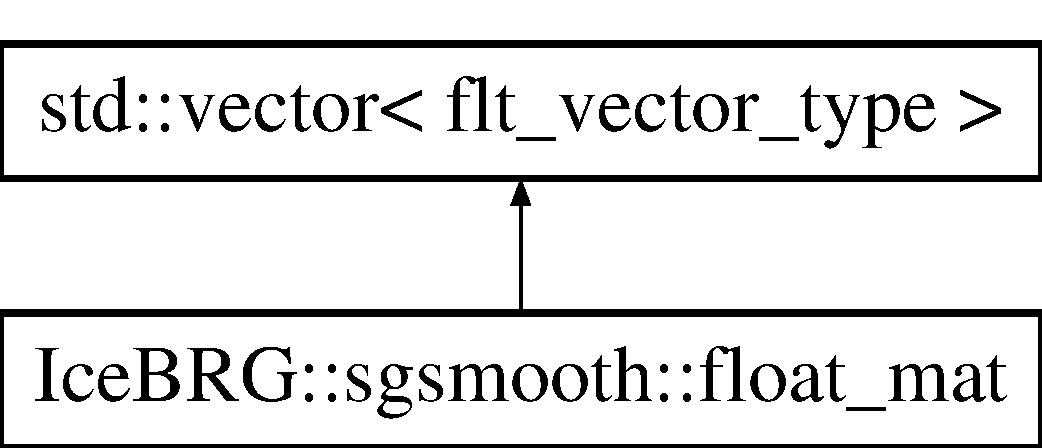
\includegraphics[height=2.000000cm]{classIceBRG_1_1sgsmooth_1_1float__mat}
\end{center}
\end{figure}
\subsection*{Public Member Functions}
\begin{DoxyCompactItemize}
\item 
\hyperlink{classIceBRG_1_1sgsmooth_1_1float__mat_aadcf2088badc653044d76db9fa92c8f6}{float\+\_\+mat} (const size\+\_\+t rows, const size\+\_\+t cols, const \hyperlink{lib_2IceBRG__main_2common_8h_ad0f130a56eeb944d9ef2692ee881ecc4}{flt\+\_\+type} \&def=0.\+0)
\begin{DoxyCompactList}\small\item\em constructor with sizes \end{DoxyCompactList}\item 
\hyperlink{classIceBRG_1_1sgsmooth_1_1float__mat_a0b8a9a2f6c0cde0981937ea074ddbf26}{float\+\_\+mat} (const \hyperlink{classIceBRG_1_1sgsmooth_1_1float__mat}{float\+\_\+mat} \&\hyperlink{namespaceIceBRG_ada6365c5d16106f0608afbd34f010bcc}{m})
\begin{DoxyCompactList}\small\item\em copy constructor for matrix \end{DoxyCompactList}\item 
\hyperlink{classIceBRG_1_1sgsmooth_1_1float__mat_a6534c2f7d23dc74f143d737eaff9966a}{float\+\_\+mat} (const \hyperlink{lib_2IceBRG__main_2common_8h_ab7b04bb475996b18d7653bb03d72f2c6}{flt\+\_\+vector\+\_\+type} \&v)
\begin{DoxyCompactList}\small\item\em copy constructor for vector \end{DoxyCompactList}\item 
size\+\_\+t \hyperlink{classIceBRG_1_1sgsmooth_1_1float__mat_a529d1c4e6c3099d1605a210e9af15d27}{nr\+\_\+rows} (void) const 
\begin{DoxyCompactList}\small\item\em use default destructor \end{DoxyCompactList}\item 
size\+\_\+t \hyperlink{classIceBRG_1_1sgsmooth_1_1float__mat_aefce21794625942d8be758522644d1c1}{nr\+\_\+cols} (void) const 
\begin{DoxyCompactList}\small\item\em get size \end{DoxyCompactList}\end{DoxyCompactItemize}


\subsection{Detailed Description}
two dimensional floating point array 

matrix class.

This is a matrix class derived from a vector of float\+\_\+vects. Note that the matrix elements indexed \mbox{[}row\mbox{]}\mbox{[}column\mbox{]} with indices starting at 0 (c style). Also note that because of its design looping through rows should be faster than looping through columns. 

\subsection{Constructor \& Destructor Documentation}
\hypertarget{classIceBRG_1_1sgsmooth_1_1float__mat_aadcf2088badc653044d76db9fa92c8f6}{}\index{Ice\+B\+R\+G\+::sgsmooth\+::float\+\_\+mat@{Ice\+B\+R\+G\+::sgsmooth\+::float\+\_\+mat}!float\+\_\+mat@{float\+\_\+mat}}
\index{float\+\_\+mat@{float\+\_\+mat}!Ice\+B\+R\+G\+::sgsmooth\+::float\+\_\+mat@{Ice\+B\+R\+G\+::sgsmooth\+::float\+\_\+mat}}
\subsubsection[{float\+\_\+mat(const size\+\_\+t rows, const size\+\_\+t cols, const flt\+\_\+type \&def=0.\+0)}]{\setlength{\rightskip}{0pt plus 5cm}Ice\+B\+R\+G\+::sgsmooth\+::float\+\_\+mat\+::float\+\_\+mat (
\begin{DoxyParamCaption}
\item[{const size\+\_\+t}]{rows, }
\item[{const size\+\_\+t}]{cols, }
\item[{const {\bf flt\+\_\+type} \&}]{def = {\ttfamily 0.0}}
\end{DoxyParamCaption}
)}\label{classIceBRG_1_1sgsmooth_1_1float__mat_aadcf2088badc653044d76db9fa92c8f6}


constructor with sizes 

\hypertarget{classIceBRG_1_1sgsmooth_1_1float__mat_a0b8a9a2f6c0cde0981937ea074ddbf26}{}\index{Ice\+B\+R\+G\+::sgsmooth\+::float\+\_\+mat@{Ice\+B\+R\+G\+::sgsmooth\+::float\+\_\+mat}!float\+\_\+mat@{float\+\_\+mat}}
\index{float\+\_\+mat@{float\+\_\+mat}!Ice\+B\+R\+G\+::sgsmooth\+::float\+\_\+mat@{Ice\+B\+R\+G\+::sgsmooth\+::float\+\_\+mat}}
\subsubsection[{float\+\_\+mat(const float\+\_\+mat \&m)}]{\setlength{\rightskip}{0pt plus 5cm}Ice\+B\+R\+G\+::sgsmooth\+::float\+\_\+mat\+::float\+\_\+mat (
\begin{DoxyParamCaption}
\item[{const {\bf float\+\_\+mat} \&}]{m}
\end{DoxyParamCaption}
)}\label{classIceBRG_1_1sgsmooth_1_1float__mat_a0b8a9a2f6c0cde0981937ea074ddbf26}


copy constructor for matrix 

\hypertarget{classIceBRG_1_1sgsmooth_1_1float__mat_a6534c2f7d23dc74f143d737eaff9966a}{}\index{Ice\+B\+R\+G\+::sgsmooth\+::float\+\_\+mat@{Ice\+B\+R\+G\+::sgsmooth\+::float\+\_\+mat}!float\+\_\+mat@{float\+\_\+mat}}
\index{float\+\_\+mat@{float\+\_\+mat}!Ice\+B\+R\+G\+::sgsmooth\+::float\+\_\+mat@{Ice\+B\+R\+G\+::sgsmooth\+::float\+\_\+mat}}
\subsubsection[{float\+\_\+mat(const flt\+\_\+vector\+\_\+type \&v)}]{\setlength{\rightskip}{0pt plus 5cm}Ice\+B\+R\+G\+::sgsmooth\+::float\+\_\+mat\+::float\+\_\+mat (
\begin{DoxyParamCaption}
\item[{const {\bf flt\+\_\+vector\+\_\+type} \&}]{v}
\end{DoxyParamCaption}
)}\label{classIceBRG_1_1sgsmooth_1_1float__mat_a6534c2f7d23dc74f143d737eaff9966a}


copy constructor for vector 



\subsection{Member Function Documentation}
\hypertarget{classIceBRG_1_1sgsmooth_1_1float__mat_aefce21794625942d8be758522644d1c1}{}\index{Ice\+B\+R\+G\+::sgsmooth\+::float\+\_\+mat@{Ice\+B\+R\+G\+::sgsmooth\+::float\+\_\+mat}!nr\+\_\+cols@{nr\+\_\+cols}}
\index{nr\+\_\+cols@{nr\+\_\+cols}!Ice\+B\+R\+G\+::sgsmooth\+::float\+\_\+mat@{Ice\+B\+R\+G\+::sgsmooth\+::float\+\_\+mat}}
\subsubsection[{nr\+\_\+cols(void) const }]{\setlength{\rightskip}{0pt plus 5cm}size\+\_\+t Ice\+B\+R\+G\+::sgsmooth\+::float\+\_\+mat\+::nr\+\_\+cols (
\begin{DoxyParamCaption}
\item[{void}]{}
\end{DoxyParamCaption}
) const\hspace{0.3cm}{\ttfamily [inline]}}\label{classIceBRG_1_1sgsmooth_1_1float__mat_aefce21794625942d8be758522644d1c1}


get size 

\hypertarget{classIceBRG_1_1sgsmooth_1_1float__mat_a529d1c4e6c3099d1605a210e9af15d27}{}\index{Ice\+B\+R\+G\+::sgsmooth\+::float\+\_\+mat@{Ice\+B\+R\+G\+::sgsmooth\+::float\+\_\+mat}!nr\+\_\+rows@{nr\+\_\+rows}}
\index{nr\+\_\+rows@{nr\+\_\+rows}!Ice\+B\+R\+G\+::sgsmooth\+::float\+\_\+mat@{Ice\+B\+R\+G\+::sgsmooth\+::float\+\_\+mat}}
\subsubsection[{nr\+\_\+rows(void) const }]{\setlength{\rightskip}{0pt plus 5cm}size\+\_\+t Ice\+B\+R\+G\+::sgsmooth\+::float\+\_\+mat\+::nr\+\_\+rows (
\begin{DoxyParamCaption}
\item[{void}]{}
\end{DoxyParamCaption}
) const\hspace{0.3cm}{\ttfamily [inline]}}\label{classIceBRG_1_1sgsmooth_1_1float__mat_a529d1c4e6c3099d1605a210e9af15d27}


use default destructor 

get size 

The documentation for this class was generated from the following file\+:\begin{DoxyCompactItemize}
\item 
/disk2/brg/git/\+Magnification\+\_\+\+Public/src/lib/\+Ice\+B\+R\+G\+\_\+main/external/\hyperlink{sgsmooth_8cpp}{sgsmooth.\+cpp}\end{DoxyCompactItemize}

\hypertarget{classIceBRG_1_1functor}{}\section{Ice\+B\+R\+G\+:\+:functor$<$ Tin, Tout, param\+\_\+struct $>$ Class Template Reference}
\label{classIceBRG_1_1functor}\index{Ice\+B\+R\+G\+::functor$<$ Tin, Tout, param\+\_\+struct $>$@{Ice\+B\+R\+G\+::functor$<$ Tin, Tout, param\+\_\+struct $>$}}


{\ttfamily \#include $<$functor.\+hpp$>$}

\subsection*{Public Member Functions}
\begin{DoxyCompactItemize}
\item 
\hyperlink{classIceBRG_1_1functor_a7657016f84dc413c8681c43078a6acaf}{functor} ()
\item 
\hyperlink{classIceBRG_1_1functor_ac1de0c6a2aed3cf32278e3ca5d1cfa04}{functor} (param\+\_\+struct init\+\_\+params)
\item 
virtual \hyperlink{classIceBRG_1_1functor_aa702a653f474cf9f2f7f4a7699967421}{$\sim$functor} ()
\item 
{\footnotesize template$<$typename other\+\_\+param\+\_\+struct $>$ }\\void \hyperlink{classIceBRG_1_1functor_abc4c0c3f1704d4bfefae5fce79b09bd1}{set\+\_\+params} (other\+\_\+param\+\_\+struct \&\&new\+\_\+params)
\item 
const param\+\_\+struct \& \hyperlink{classIceBRG_1_1functor_aa26e65bbcaa6403a4033de396de14597}{params} () const 
\item 
virtual Tout \hyperlink{classIceBRG_1_1functor_a299cdb8972790082a99a244a4255381b}{operator()} (const Tin \&in\+\_\+param) const  =0
\end{DoxyCompactItemize}


\subsection{Detailed Description}
\subsubsection*{template$<$typename Tin, typename Tout, typename param\+\_\+struct = char$>$class Ice\+B\+R\+G\+::functor$<$ Tin, Tout, param\+\_\+struct $>$}

An abstract base class representing a functor which can store parameters in a \char`\"{}param\+\_\+struct\char`\"{} object. 

\subsection{Constructor \& Destructor Documentation}
\hypertarget{classIceBRG_1_1functor_a7657016f84dc413c8681c43078a6acaf}{}\index{Ice\+B\+R\+G\+::functor@{Ice\+B\+R\+G\+::functor}!functor@{functor}}
\index{functor@{functor}!Ice\+B\+R\+G\+::functor@{Ice\+B\+R\+G\+::functor}}
\subsubsection[{functor()}]{\setlength{\rightskip}{0pt plus 5cm}template$<$typename Tin, typename Tout, typename param\+\_\+struct = char$>$ {\bf Ice\+B\+R\+G\+::functor}$<$ Tin, Tout, param\+\_\+struct $>$\+::{\bf functor} (
\begin{DoxyParamCaption}
{}
\end{DoxyParamCaption}
)\hspace{0.3cm}{\ttfamily [inline]}}\label{classIceBRG_1_1functor_a7657016f84dc413c8681c43078a6acaf}
\hypertarget{classIceBRG_1_1functor_ac1de0c6a2aed3cf32278e3ca5d1cfa04}{}\index{Ice\+B\+R\+G\+::functor@{Ice\+B\+R\+G\+::functor}!functor@{functor}}
\index{functor@{functor}!Ice\+B\+R\+G\+::functor@{Ice\+B\+R\+G\+::functor}}
\subsubsection[{functor(param\+\_\+struct init\+\_\+params)}]{\setlength{\rightskip}{0pt plus 5cm}template$<$typename Tin, typename Tout, typename param\+\_\+struct = char$>$ {\bf Ice\+B\+R\+G\+::functor}$<$ Tin, Tout, param\+\_\+struct $>$\+::{\bf functor} (
\begin{DoxyParamCaption}
\item[{param\+\_\+struct}]{init\+\_\+params}
\end{DoxyParamCaption}
)\hspace{0.3cm}{\ttfamily [inline]}}\label{classIceBRG_1_1functor_ac1de0c6a2aed3cf32278e3ca5d1cfa04}
\hypertarget{classIceBRG_1_1functor_aa702a653f474cf9f2f7f4a7699967421}{}\index{Ice\+B\+R\+G\+::functor@{Ice\+B\+R\+G\+::functor}!````~functor@{$\sim$functor}}
\index{````~functor@{$\sim$functor}!Ice\+B\+R\+G\+::functor@{Ice\+B\+R\+G\+::functor}}
\subsubsection[{$\sim$functor()}]{\setlength{\rightskip}{0pt plus 5cm}template$<$typename Tin, typename Tout, typename param\+\_\+struct = char$>$ virtual {\bf Ice\+B\+R\+G\+::functor}$<$ Tin, Tout, param\+\_\+struct $>$\+::$\sim${\bf functor} (
\begin{DoxyParamCaption}
{}
\end{DoxyParamCaption}
)\hspace{0.3cm}{\ttfamily [inline]}, {\ttfamily [virtual]}}\label{classIceBRG_1_1functor_aa702a653f474cf9f2f7f4a7699967421}


\subsection{Member Function Documentation}
\hypertarget{classIceBRG_1_1functor_a299cdb8972790082a99a244a4255381b}{}\index{Ice\+B\+R\+G\+::functor@{Ice\+B\+R\+G\+::functor}!operator()@{operator()}}
\index{operator()@{operator()}!Ice\+B\+R\+G\+::functor@{Ice\+B\+R\+G\+::functor}}
\subsubsection[{operator()(const Tin \&in\+\_\+param) const  =0}]{\setlength{\rightskip}{0pt plus 5cm}template$<$typename Tin, typename Tout, typename param\+\_\+struct = char$>$ virtual Tout {\bf Ice\+B\+R\+G\+::functor}$<$ Tin, Tout, param\+\_\+struct $>$\+::operator() (
\begin{DoxyParamCaption}
\item[{const Tin \&}]{in\+\_\+param}
\end{DoxyParamCaption}
) const\hspace{0.3cm}{\ttfamily [pure virtual]}}\label{classIceBRG_1_1functor_a299cdb8972790082a99a244a4255381b}


Implemented in \hyperlink{classIceBRG_1_1Schechter__like__functor_af58cca1d9091086949437f9c07e1f8f9}{Ice\+B\+R\+G\+::\+Schechter\+\_\+like\+\_\+functor}.

\hypertarget{classIceBRG_1_1functor_aa26e65bbcaa6403a4033de396de14597}{}\index{Ice\+B\+R\+G\+::functor@{Ice\+B\+R\+G\+::functor}!params@{params}}
\index{params@{params}!Ice\+B\+R\+G\+::functor@{Ice\+B\+R\+G\+::functor}}
\subsubsection[{params() const }]{\setlength{\rightskip}{0pt plus 5cm}template$<$typename Tin, typename Tout, typename param\+\_\+struct = char$>$ const param\+\_\+struct\& {\bf Ice\+B\+R\+G\+::functor}$<$ Tin, Tout, param\+\_\+struct $>$\+::params (
\begin{DoxyParamCaption}
{}
\end{DoxyParamCaption}
) const\hspace{0.3cm}{\ttfamily [inline]}}\label{classIceBRG_1_1functor_aa26e65bbcaa6403a4033de396de14597}
\hypertarget{classIceBRG_1_1functor_abc4c0c3f1704d4bfefae5fce79b09bd1}{}\index{Ice\+B\+R\+G\+::functor@{Ice\+B\+R\+G\+::functor}!set\+\_\+params@{set\+\_\+params}}
\index{set\+\_\+params@{set\+\_\+params}!Ice\+B\+R\+G\+::functor@{Ice\+B\+R\+G\+::functor}}
\subsubsection[{set\+\_\+params(other\+\_\+param\+\_\+struct \&\&new\+\_\+params)}]{\setlength{\rightskip}{0pt plus 5cm}template$<$typename Tin, typename Tout, typename param\+\_\+struct = char$>$ template$<$typename other\+\_\+param\+\_\+struct $>$ void {\bf Ice\+B\+R\+G\+::functor}$<$ Tin, Tout, param\+\_\+struct $>$\+::set\+\_\+params (
\begin{DoxyParamCaption}
\item[{other\+\_\+param\+\_\+struct \&\&}]{new\+\_\+params}
\end{DoxyParamCaption}
)\hspace{0.3cm}{\ttfamily [inline]}}\label{classIceBRG_1_1functor_abc4c0c3f1704d4bfefae5fce79b09bd1}


The documentation for this class was generated from the following file\+:\begin{DoxyCompactItemize}
\item 
/disk2/brg/git/\+Magnification\+\_\+\+Public/src/lib/\+Ice\+B\+R\+G\+\_\+main/math/functor/\hyperlink{functor_8hpp}{functor.\+hpp}\end{DoxyCompactItemize}

\hypertarget{classIceBRG_1_1functor__product}{}\section{Ice\+B\+R\+G\+:\+:functor\+\_\+product$<$ f1, f2, T $>$ Class Template Reference}
\label{classIceBRG_1_1functor__product}\index{Ice\+B\+R\+G\+::functor\+\_\+product$<$ f1, f2, T $>$@{Ice\+B\+R\+G\+::functor\+\_\+product$<$ f1, f2, T $>$}}


{\ttfamily \#include $<$functor\+\_\+product.\+hpp$>$}

\subsection*{Public Member Functions}
\begin{DoxyCompactItemize}
\item 
\hyperlink{classIceBRG_1_1functor__product_a263de47cbf8a828c15f4e74177f59801}{functor\+\_\+product} ()
\item 
\hyperlink{classIceBRG_1_1functor__product_a09c511535f0c64722a2ba05312a86972}{functor\+\_\+product} (const f1 $\ast$new\+\_\+f1, const f2 $\ast$new\+\_\+f2)
\item 
\hyperlink{classIceBRG_1_1functor__product_ad8b48fe7acc524c6803ee44d93735849}{functor\+\_\+product} (const f1 $\ast$new\+\_\+f1, const f2 \&new\+\_\+f2)
\item 
\hyperlink{classIceBRG_1_1functor__product_af440c00b90f2026af6c627536b5ae783}{functor\+\_\+product} (const f1 \&new\+\_\+f1, const f2 $\ast$new\+\_\+f2)
\item 
\hyperlink{classIceBRG_1_1functor__product_ae7c7c8478cc7163d137d9bd24dcca21b}{functor\+\_\+product} (const f1 \&new\+\_\+f1, const f2 \&new\+\_\+f2)
\item 
virtual \hyperlink{classIceBRG_1_1functor__product_a701c252e665501ab0f3361cb7874b66c}{$\sim$functor\+\_\+product} ()
\item 
void \hyperlink{classIceBRG_1_1functor__product_a5ad86153805d2a59b313cf192afb290f}{set\+\_\+f1\+\_\+ptr} (const f1 $\ast$new\+\_\+f1\+\_\+ptr)
\item 
void \hyperlink{classIceBRG_1_1functor__product_acb3f32a97cae6e9f01fe3d1f4ec3cbfc}{set\+\_\+f1\+\_\+ptr} (const f1 \&new\+\_\+f1\+\_\+ptr)
\item 
void \hyperlink{classIceBRG_1_1functor__product_aa3ac11de767b491c8cb6ab0ba2d0d0cd}{set\+\_\+f2\+\_\+ptr} (const f2 $\ast$new\+\_\+f2\+\_\+ptr)
\item 
void \hyperlink{classIceBRG_1_1functor__product_a56f57103f03c25a90d04d585a9955633}{set\+\_\+f2\+\_\+ptr} (const f2 \&new\+\_\+f2\+\_\+ptr)
\item 
void \hyperlink{classIceBRG_1_1functor__product_a3072914bbe8c66121a78f805c0d31863}{set\+\_\+f1\+\_\+f2\+\_\+ptrs} (const f1 $\ast$new\+\_\+f1\+\_\+ptr, const f2 $\ast$new\+\_\+f2\+\_\+ptr)
\item 
void \hyperlink{classIceBRG_1_1functor__product_ab9fe7a8e4510075b196868f5ae9d1898}{set\+\_\+f1\+\_\+f2\+\_\+ptrs} (const f1 $\ast$new\+\_\+f1\+\_\+ptr, const f2 \&new\+\_\+f2\+\_\+ptr)
\item 
void \hyperlink{classIceBRG_1_1functor__product_a9000d20f7ec8b19e3c060667732f6884}{set\+\_\+f1\+\_\+f2\+\_\+ptrs} (const f1 \&new\+\_\+f1\+\_\+ptr, const f2 $\ast$new\+\_\+f2\+\_\+ptr)
\item 
void \hyperlink{classIceBRG_1_1functor__product_af0d675d9ce214c766dc6b92b20373bfc}{set\+\_\+f1\+\_\+f2\+\_\+ptrs} (const f1 \&new\+\_\+f1\+\_\+ptr, const f2 \&new\+\_\+f2\+\_\+ptr)
\end{DoxyCompactItemize}
\subsection*{Public Attributes}
\begin{DoxyCompactItemize}
\item 
decltype(\hyperlink{namespaceIceBRG_ab535c998baac3ffc8412fdbae750b7d1}{multiply}(($\ast$\+\_\+f1\+\_\+ptr\+\_\+)(T()),($\ast$\+\_\+f2\+\_\+ptr\+\_\+)(T()))) \hyperlink{classIceBRG_1_1functor__product_a4f55bb9a66aba664a8c73f8c5172ac24}{operator()} (const T \&in\+\_\+param) const 
\end{DoxyCompactItemize}


\subsection{Detailed Description}
\subsubsection*{template$<$typename f1, typename f2, typename T = flt\+\_\+type$>$class Ice\+B\+R\+G\+::functor\+\_\+product$<$ f1, f2, T $>$}

Class definitions 

\subsection{Constructor \& Destructor Documentation}
\hypertarget{classIceBRG_1_1functor__product_a263de47cbf8a828c15f4e74177f59801}{}\index{Ice\+B\+R\+G\+::functor\+\_\+product@{Ice\+B\+R\+G\+::functor\+\_\+product}!functor\+\_\+product@{functor\+\_\+product}}
\index{functor\+\_\+product@{functor\+\_\+product}!Ice\+B\+R\+G\+::functor\+\_\+product@{Ice\+B\+R\+G\+::functor\+\_\+product}}
\subsubsection[{functor\+\_\+product()}]{\setlength{\rightskip}{0pt plus 5cm}template$<$typename f1, typename f2, typename T = flt\+\_\+type$>$ {\bf Ice\+B\+R\+G\+::functor\+\_\+product}$<$ f1, f2, T $>$\+::{\bf functor\+\_\+product} (
\begin{DoxyParamCaption}
{}
\end{DoxyParamCaption}
)\hspace{0.3cm}{\ttfamily [inline]}}\label{classIceBRG_1_1functor__product_a263de47cbf8a828c15f4e74177f59801}
\hypertarget{classIceBRG_1_1functor__product_a09c511535f0c64722a2ba05312a86972}{}\index{Ice\+B\+R\+G\+::functor\+\_\+product@{Ice\+B\+R\+G\+::functor\+\_\+product}!functor\+\_\+product@{functor\+\_\+product}}
\index{functor\+\_\+product@{functor\+\_\+product}!Ice\+B\+R\+G\+::functor\+\_\+product@{Ice\+B\+R\+G\+::functor\+\_\+product}}
\subsubsection[{functor\+\_\+product(const f1 $\ast$new\+\_\+f1, const f2 $\ast$new\+\_\+f2)}]{\setlength{\rightskip}{0pt plus 5cm}template$<$typename f1, typename f2, typename T = flt\+\_\+type$>$ {\bf Ice\+B\+R\+G\+::functor\+\_\+product}$<$ f1, f2, T $>$\+::{\bf functor\+\_\+product} (
\begin{DoxyParamCaption}
\item[{const f1 $\ast$}]{new\+\_\+f1, }
\item[{const f2 $\ast$}]{new\+\_\+f2}
\end{DoxyParamCaption}
)\hspace{0.3cm}{\ttfamily [inline]}}\label{classIceBRG_1_1functor__product_a09c511535f0c64722a2ba05312a86972}
\hypertarget{classIceBRG_1_1functor__product_ad8b48fe7acc524c6803ee44d93735849}{}\index{Ice\+B\+R\+G\+::functor\+\_\+product@{Ice\+B\+R\+G\+::functor\+\_\+product}!functor\+\_\+product@{functor\+\_\+product}}
\index{functor\+\_\+product@{functor\+\_\+product}!Ice\+B\+R\+G\+::functor\+\_\+product@{Ice\+B\+R\+G\+::functor\+\_\+product}}
\subsubsection[{functor\+\_\+product(const f1 $\ast$new\+\_\+f1, const f2 \&new\+\_\+f2)}]{\setlength{\rightskip}{0pt plus 5cm}template$<$typename f1, typename f2, typename T = flt\+\_\+type$>$ {\bf Ice\+B\+R\+G\+::functor\+\_\+product}$<$ f1, f2, T $>$\+::{\bf functor\+\_\+product} (
\begin{DoxyParamCaption}
\item[{const f1 $\ast$}]{new\+\_\+f1, }
\item[{const f2 \&}]{new\+\_\+f2}
\end{DoxyParamCaption}
)\hspace{0.3cm}{\ttfamily [inline]}}\label{classIceBRG_1_1functor__product_ad8b48fe7acc524c6803ee44d93735849}
\hypertarget{classIceBRG_1_1functor__product_af440c00b90f2026af6c627536b5ae783}{}\index{Ice\+B\+R\+G\+::functor\+\_\+product@{Ice\+B\+R\+G\+::functor\+\_\+product}!functor\+\_\+product@{functor\+\_\+product}}
\index{functor\+\_\+product@{functor\+\_\+product}!Ice\+B\+R\+G\+::functor\+\_\+product@{Ice\+B\+R\+G\+::functor\+\_\+product}}
\subsubsection[{functor\+\_\+product(const f1 \&new\+\_\+f1, const f2 $\ast$new\+\_\+f2)}]{\setlength{\rightskip}{0pt plus 5cm}template$<$typename f1, typename f2, typename T = flt\+\_\+type$>$ {\bf Ice\+B\+R\+G\+::functor\+\_\+product}$<$ f1, f2, T $>$\+::{\bf functor\+\_\+product} (
\begin{DoxyParamCaption}
\item[{const f1 \&}]{new\+\_\+f1, }
\item[{const f2 $\ast$}]{new\+\_\+f2}
\end{DoxyParamCaption}
)\hspace{0.3cm}{\ttfamily [inline]}}\label{classIceBRG_1_1functor__product_af440c00b90f2026af6c627536b5ae783}
\hypertarget{classIceBRG_1_1functor__product_ae7c7c8478cc7163d137d9bd24dcca21b}{}\index{Ice\+B\+R\+G\+::functor\+\_\+product@{Ice\+B\+R\+G\+::functor\+\_\+product}!functor\+\_\+product@{functor\+\_\+product}}
\index{functor\+\_\+product@{functor\+\_\+product}!Ice\+B\+R\+G\+::functor\+\_\+product@{Ice\+B\+R\+G\+::functor\+\_\+product}}
\subsubsection[{functor\+\_\+product(const f1 \&new\+\_\+f1, const f2 \&new\+\_\+f2)}]{\setlength{\rightskip}{0pt plus 5cm}template$<$typename f1, typename f2, typename T = flt\+\_\+type$>$ {\bf Ice\+B\+R\+G\+::functor\+\_\+product}$<$ f1, f2, T $>$\+::{\bf functor\+\_\+product} (
\begin{DoxyParamCaption}
\item[{const f1 \&}]{new\+\_\+f1, }
\item[{const f2 \&}]{new\+\_\+f2}
\end{DoxyParamCaption}
)\hspace{0.3cm}{\ttfamily [inline]}}\label{classIceBRG_1_1functor__product_ae7c7c8478cc7163d137d9bd24dcca21b}
\hypertarget{classIceBRG_1_1functor__product_a701c252e665501ab0f3361cb7874b66c}{}\index{Ice\+B\+R\+G\+::functor\+\_\+product@{Ice\+B\+R\+G\+::functor\+\_\+product}!````~functor\+\_\+product@{$\sim$functor\+\_\+product}}
\index{````~functor\+\_\+product@{$\sim$functor\+\_\+product}!Ice\+B\+R\+G\+::functor\+\_\+product@{Ice\+B\+R\+G\+::functor\+\_\+product}}
\subsubsection[{$\sim$functor\+\_\+product()}]{\setlength{\rightskip}{0pt plus 5cm}template$<$typename f1, typename f2, typename T = flt\+\_\+type$>$ virtual {\bf Ice\+B\+R\+G\+::functor\+\_\+product}$<$ f1, f2, T $>$\+::$\sim${\bf functor\+\_\+product} (
\begin{DoxyParamCaption}
{}
\end{DoxyParamCaption}
)\hspace{0.3cm}{\ttfamily [inline]}, {\ttfamily [virtual]}}\label{classIceBRG_1_1functor__product_a701c252e665501ab0f3361cb7874b66c}


\subsection{Member Function Documentation}
\hypertarget{classIceBRG_1_1functor__product_a3072914bbe8c66121a78f805c0d31863}{}\index{Ice\+B\+R\+G\+::functor\+\_\+product@{Ice\+B\+R\+G\+::functor\+\_\+product}!set\+\_\+f1\+\_\+f2\+\_\+ptrs@{set\+\_\+f1\+\_\+f2\+\_\+ptrs}}
\index{set\+\_\+f1\+\_\+f2\+\_\+ptrs@{set\+\_\+f1\+\_\+f2\+\_\+ptrs}!Ice\+B\+R\+G\+::functor\+\_\+product@{Ice\+B\+R\+G\+::functor\+\_\+product}}
\subsubsection[{set\+\_\+f1\+\_\+f2\+\_\+ptrs(const f1 $\ast$new\+\_\+f1\+\_\+ptr, const f2 $\ast$new\+\_\+f2\+\_\+ptr)}]{\setlength{\rightskip}{0pt plus 5cm}template$<$typename f1, typename f2, typename T = flt\+\_\+type$>$ void {\bf Ice\+B\+R\+G\+::functor\+\_\+product}$<$ f1, f2, T $>$\+::set\+\_\+f1\+\_\+f2\+\_\+ptrs (
\begin{DoxyParamCaption}
\item[{const f1 $\ast$}]{new\+\_\+f1\+\_\+ptr, }
\item[{const f2 $\ast$}]{new\+\_\+f2\+\_\+ptr}
\end{DoxyParamCaption}
)\hspace{0.3cm}{\ttfamily [inline]}}\label{classIceBRG_1_1functor__product_a3072914bbe8c66121a78f805c0d31863}
\hypertarget{classIceBRG_1_1functor__product_ab9fe7a8e4510075b196868f5ae9d1898}{}\index{Ice\+B\+R\+G\+::functor\+\_\+product@{Ice\+B\+R\+G\+::functor\+\_\+product}!set\+\_\+f1\+\_\+f2\+\_\+ptrs@{set\+\_\+f1\+\_\+f2\+\_\+ptrs}}
\index{set\+\_\+f1\+\_\+f2\+\_\+ptrs@{set\+\_\+f1\+\_\+f2\+\_\+ptrs}!Ice\+B\+R\+G\+::functor\+\_\+product@{Ice\+B\+R\+G\+::functor\+\_\+product}}
\subsubsection[{set\+\_\+f1\+\_\+f2\+\_\+ptrs(const f1 $\ast$new\+\_\+f1\+\_\+ptr, const f2 \&new\+\_\+f2\+\_\+ptr)}]{\setlength{\rightskip}{0pt plus 5cm}template$<$typename f1, typename f2, typename T = flt\+\_\+type$>$ void {\bf Ice\+B\+R\+G\+::functor\+\_\+product}$<$ f1, f2, T $>$\+::set\+\_\+f1\+\_\+f2\+\_\+ptrs (
\begin{DoxyParamCaption}
\item[{const f1 $\ast$}]{new\+\_\+f1\+\_\+ptr, }
\item[{const f2 \&}]{new\+\_\+f2\+\_\+ptr}
\end{DoxyParamCaption}
)\hspace{0.3cm}{\ttfamily [inline]}}\label{classIceBRG_1_1functor__product_ab9fe7a8e4510075b196868f5ae9d1898}
\hypertarget{classIceBRG_1_1functor__product_a9000d20f7ec8b19e3c060667732f6884}{}\index{Ice\+B\+R\+G\+::functor\+\_\+product@{Ice\+B\+R\+G\+::functor\+\_\+product}!set\+\_\+f1\+\_\+f2\+\_\+ptrs@{set\+\_\+f1\+\_\+f2\+\_\+ptrs}}
\index{set\+\_\+f1\+\_\+f2\+\_\+ptrs@{set\+\_\+f1\+\_\+f2\+\_\+ptrs}!Ice\+B\+R\+G\+::functor\+\_\+product@{Ice\+B\+R\+G\+::functor\+\_\+product}}
\subsubsection[{set\+\_\+f1\+\_\+f2\+\_\+ptrs(const f1 \&new\+\_\+f1\+\_\+ptr, const f2 $\ast$new\+\_\+f2\+\_\+ptr)}]{\setlength{\rightskip}{0pt plus 5cm}template$<$typename f1, typename f2, typename T = flt\+\_\+type$>$ void {\bf Ice\+B\+R\+G\+::functor\+\_\+product}$<$ f1, f2, T $>$\+::set\+\_\+f1\+\_\+f2\+\_\+ptrs (
\begin{DoxyParamCaption}
\item[{const f1 \&}]{new\+\_\+f1\+\_\+ptr, }
\item[{const f2 $\ast$}]{new\+\_\+f2\+\_\+ptr}
\end{DoxyParamCaption}
)\hspace{0.3cm}{\ttfamily [inline]}}\label{classIceBRG_1_1functor__product_a9000d20f7ec8b19e3c060667732f6884}
\hypertarget{classIceBRG_1_1functor__product_af0d675d9ce214c766dc6b92b20373bfc}{}\index{Ice\+B\+R\+G\+::functor\+\_\+product@{Ice\+B\+R\+G\+::functor\+\_\+product}!set\+\_\+f1\+\_\+f2\+\_\+ptrs@{set\+\_\+f1\+\_\+f2\+\_\+ptrs}}
\index{set\+\_\+f1\+\_\+f2\+\_\+ptrs@{set\+\_\+f1\+\_\+f2\+\_\+ptrs}!Ice\+B\+R\+G\+::functor\+\_\+product@{Ice\+B\+R\+G\+::functor\+\_\+product}}
\subsubsection[{set\+\_\+f1\+\_\+f2\+\_\+ptrs(const f1 \&new\+\_\+f1\+\_\+ptr, const f2 \&new\+\_\+f2\+\_\+ptr)}]{\setlength{\rightskip}{0pt plus 5cm}template$<$typename f1, typename f2, typename T = flt\+\_\+type$>$ void {\bf Ice\+B\+R\+G\+::functor\+\_\+product}$<$ f1, f2, T $>$\+::set\+\_\+f1\+\_\+f2\+\_\+ptrs (
\begin{DoxyParamCaption}
\item[{const f1 \&}]{new\+\_\+f1\+\_\+ptr, }
\item[{const f2 \&}]{new\+\_\+f2\+\_\+ptr}
\end{DoxyParamCaption}
)\hspace{0.3cm}{\ttfamily [inline]}}\label{classIceBRG_1_1functor__product_af0d675d9ce214c766dc6b92b20373bfc}
\hypertarget{classIceBRG_1_1functor__product_a5ad86153805d2a59b313cf192afb290f}{}\index{Ice\+B\+R\+G\+::functor\+\_\+product@{Ice\+B\+R\+G\+::functor\+\_\+product}!set\+\_\+f1\+\_\+ptr@{set\+\_\+f1\+\_\+ptr}}
\index{set\+\_\+f1\+\_\+ptr@{set\+\_\+f1\+\_\+ptr}!Ice\+B\+R\+G\+::functor\+\_\+product@{Ice\+B\+R\+G\+::functor\+\_\+product}}
\subsubsection[{set\+\_\+f1\+\_\+ptr(const f1 $\ast$new\+\_\+f1\+\_\+ptr)}]{\setlength{\rightskip}{0pt plus 5cm}template$<$typename f1, typename f2, typename T = flt\+\_\+type$>$ void {\bf Ice\+B\+R\+G\+::functor\+\_\+product}$<$ f1, f2, T $>$\+::set\+\_\+f1\+\_\+ptr (
\begin{DoxyParamCaption}
\item[{const f1 $\ast$}]{new\+\_\+f1\+\_\+ptr}
\end{DoxyParamCaption}
)\hspace{0.3cm}{\ttfamily [inline]}}\label{classIceBRG_1_1functor__product_a5ad86153805d2a59b313cf192afb290f}
\hypertarget{classIceBRG_1_1functor__product_acb3f32a97cae6e9f01fe3d1f4ec3cbfc}{}\index{Ice\+B\+R\+G\+::functor\+\_\+product@{Ice\+B\+R\+G\+::functor\+\_\+product}!set\+\_\+f1\+\_\+ptr@{set\+\_\+f1\+\_\+ptr}}
\index{set\+\_\+f1\+\_\+ptr@{set\+\_\+f1\+\_\+ptr}!Ice\+B\+R\+G\+::functor\+\_\+product@{Ice\+B\+R\+G\+::functor\+\_\+product}}
\subsubsection[{set\+\_\+f1\+\_\+ptr(const f1 \&new\+\_\+f1\+\_\+ptr)}]{\setlength{\rightskip}{0pt plus 5cm}template$<$typename f1, typename f2, typename T = flt\+\_\+type$>$ void {\bf Ice\+B\+R\+G\+::functor\+\_\+product}$<$ f1, f2, T $>$\+::set\+\_\+f1\+\_\+ptr (
\begin{DoxyParamCaption}
\item[{const f1 \&}]{new\+\_\+f1\+\_\+ptr}
\end{DoxyParamCaption}
)\hspace{0.3cm}{\ttfamily [inline]}}\label{classIceBRG_1_1functor__product_acb3f32a97cae6e9f01fe3d1f4ec3cbfc}
\hypertarget{classIceBRG_1_1functor__product_aa3ac11de767b491c8cb6ab0ba2d0d0cd}{}\index{Ice\+B\+R\+G\+::functor\+\_\+product@{Ice\+B\+R\+G\+::functor\+\_\+product}!set\+\_\+f2\+\_\+ptr@{set\+\_\+f2\+\_\+ptr}}
\index{set\+\_\+f2\+\_\+ptr@{set\+\_\+f2\+\_\+ptr}!Ice\+B\+R\+G\+::functor\+\_\+product@{Ice\+B\+R\+G\+::functor\+\_\+product}}
\subsubsection[{set\+\_\+f2\+\_\+ptr(const f2 $\ast$new\+\_\+f2\+\_\+ptr)}]{\setlength{\rightskip}{0pt plus 5cm}template$<$typename f1, typename f2, typename T = flt\+\_\+type$>$ void {\bf Ice\+B\+R\+G\+::functor\+\_\+product}$<$ f1, f2, T $>$\+::set\+\_\+f2\+\_\+ptr (
\begin{DoxyParamCaption}
\item[{const f2 $\ast$}]{new\+\_\+f2\+\_\+ptr}
\end{DoxyParamCaption}
)\hspace{0.3cm}{\ttfamily [inline]}}\label{classIceBRG_1_1functor__product_aa3ac11de767b491c8cb6ab0ba2d0d0cd}
\hypertarget{classIceBRG_1_1functor__product_a56f57103f03c25a90d04d585a9955633}{}\index{Ice\+B\+R\+G\+::functor\+\_\+product@{Ice\+B\+R\+G\+::functor\+\_\+product}!set\+\_\+f2\+\_\+ptr@{set\+\_\+f2\+\_\+ptr}}
\index{set\+\_\+f2\+\_\+ptr@{set\+\_\+f2\+\_\+ptr}!Ice\+B\+R\+G\+::functor\+\_\+product@{Ice\+B\+R\+G\+::functor\+\_\+product}}
\subsubsection[{set\+\_\+f2\+\_\+ptr(const f2 \&new\+\_\+f2\+\_\+ptr)}]{\setlength{\rightskip}{0pt plus 5cm}template$<$typename f1, typename f2, typename T = flt\+\_\+type$>$ void {\bf Ice\+B\+R\+G\+::functor\+\_\+product}$<$ f1, f2, T $>$\+::set\+\_\+f2\+\_\+ptr (
\begin{DoxyParamCaption}
\item[{const f2 \&}]{new\+\_\+f2\+\_\+ptr}
\end{DoxyParamCaption}
)\hspace{0.3cm}{\ttfamily [inline]}}\label{classIceBRG_1_1functor__product_a56f57103f03c25a90d04d585a9955633}


\subsection{Member Data Documentation}
\hypertarget{classIceBRG_1_1functor__product_a4f55bb9a66aba664a8c73f8c5172ac24}{}\index{Ice\+B\+R\+G\+::functor\+\_\+product@{Ice\+B\+R\+G\+::functor\+\_\+product}!operator()@{operator()}}
\index{operator()@{operator()}!Ice\+B\+R\+G\+::functor\+\_\+product@{Ice\+B\+R\+G\+::functor\+\_\+product}}
\subsubsection[{operator()}]{\setlength{\rightskip}{0pt plus 5cm}template$<$typename f1, typename f2, typename T = flt\+\_\+type$>$ decltype({\bf multiply}(($\ast$\+\_\+f1\+\_\+ptr\+\_\+)( T() ),($\ast$\+\_\+f2\+\_\+ptr\+\_\+)( T() ))) {\bf Ice\+B\+R\+G\+::functor\+\_\+product}$<$ f1, f2, T $>$\+::operator()(const T \&in\+\_\+param) const \hspace{0.3cm}{\ttfamily [inline]}}\label{classIceBRG_1_1functor__product_a4f55bb9a66aba664a8c73f8c5172ac24}


The documentation for this class was generated from the following file\+:\begin{DoxyCompactItemize}
\item 
/disk2/brg/git/\+Magnification\+\_\+\+Public/src/lib/\+Ice\+B\+R\+G\+\_\+main/math/functor/\hyperlink{functor__product_8hpp}{functor\+\_\+product.\+hpp}\end{DoxyCompactItemize}

\hypertarget{classIceBRG_1_1galaxy}{}\section{Ice\+B\+R\+G\+:\+:galaxy Class Reference}
\label{classIceBRG_1_1galaxy}\index{Ice\+B\+R\+G\+::galaxy@{Ice\+B\+R\+G\+::galaxy}}


{\ttfamily \#include $<$galaxy.\+h$>$}

Inheritance diagram for Ice\+B\+R\+G\+:\+:galaxy\+:\begin{figure}[H]
\begin{center}
\leavevmode
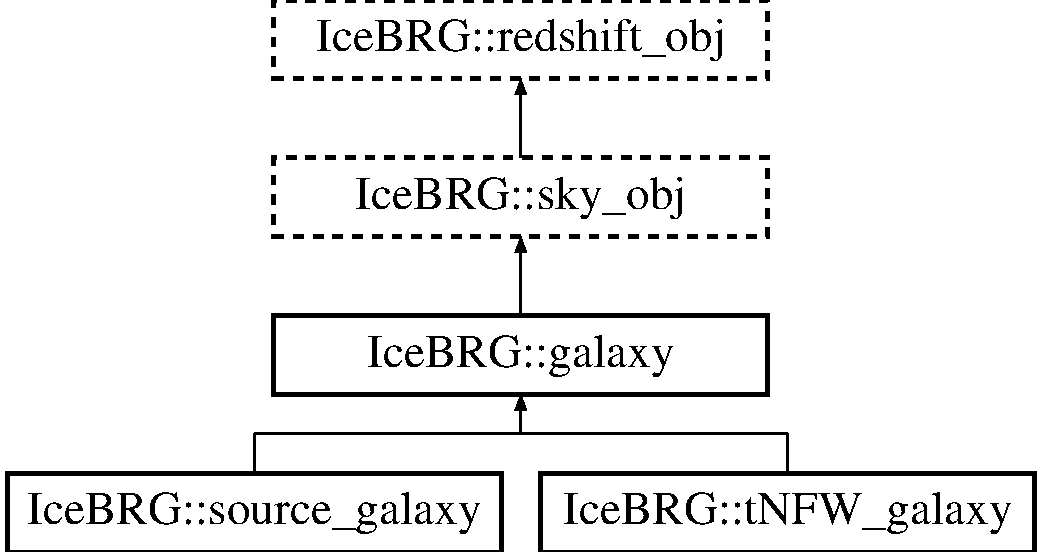
\includegraphics[height=4.000000cm]{classIceBRG_1_1galaxy}
\end{center}
\end{figure}
\subsection*{Public Member Functions}
\begin{DoxyCompactItemize}
\item 
\hyperlink{classIceBRG_1_1galaxy_addd35301cca549dd4ed3631a4dcb628e}{galaxy} (const \hyperlink{namespaceIceBRG_a688eeb0811a2474b20b667ed2e9625a1}{angle\+\_\+type} \&init\+\_\+ra=0, const \hyperlink{namespaceIceBRG_a688eeb0811a2474b20b667ed2e9625a1}{angle\+\_\+type} \&init\+\_\+dec=0, \hyperlink{lib_2IceBRG__main_2common_8h_ad0f130a56eeb944d9ef2692ee881ecc4}{flt\+\_\+type} init\+\_\+z=0, const \hyperlink{namespaceIceBRG_a688eeb0811a2474b20b667ed2e9625a1}{angle\+\_\+type} \&init\+\_\+ra\+\_\+err=0, const \hyperlink{namespaceIceBRG_a688eeb0811a2474b20b667ed2e9625a1}{angle\+\_\+type} \&init\+\_\+dec\+\_\+err=0, \hyperlink{lib_2IceBRG__main_2common_8h_ad0f130a56eeb944d9ef2692ee881ecc4}{flt\+\_\+type} init\+\_\+z\+\_\+err=0, const \hyperlink{namespaceIceBRG_a1be72ac4918a9b029f2eefa084213e35}{mass\+\_\+type} \&init\+\_\+stellar\+\_\+mass=0, \hyperlink{lib_2IceBRG__main_2common_8h_ad0f130a56eeb944d9ef2692ee881ecc4}{flt\+\_\+type} init\+\_\+mag=0, \hyperlink{lib_2IceBRG__main_2common_8h_ad0f130a56eeb944d9ef2692ee881ecc4}{flt\+\_\+type} init\+\_\+mag\+\_\+err=0)
\item 
virtual \hyperlink{classIceBRG_1_1galaxy_ac4ff33070ba5b93e4a380dbf1a4bc383}{$\sim$galaxy} ()
\item 
\hyperlink{namespaceIceBRG_a1be72ac4918a9b029f2eefa084213e35}{mass\+\_\+type} \hyperlink{classIceBRG_1_1galaxy_abbe29ca14e53a5d12201be91aa1b4b30}{m} () const 
\item 
\hyperlink{lib_2IceBRG__main_2common_8h_ad0f130a56eeb944d9ef2692ee881ecc4}{flt\+\_\+type} \hyperlink{classIceBRG_1_1galaxy_ac4f8b983ac10ad86df0a2f90ce7f7593}{mag} () const 
\item 
virtual void \hyperlink{classIceBRG_1_1galaxy_a6a37d60a5b748e99f0c9dfac82b8ae4c}{clear} ()
\item 
virtual \hyperlink{classIceBRG_1_1redshift__obj}{redshift\+\_\+obj} $\ast$ \hyperlink{classIceBRG_1_1galaxy_a0874bd3cb3133f244a86d6101aa1ec65}{redshift\+\_\+obj\+\_\+clone} () const 
\item 
virtual \hyperlink{classIceBRG_1_1sky__obj}{sky\+\_\+obj} $\ast$ \hyperlink{classIceBRG_1_1galaxy_ae6c5cfc58523edcffcf9e8bdd90bc1ad}{sky\+\_\+obj\+\_\+clone} () const 
\item 
virtual \hyperlink{classIceBRG_1_1galaxy}{galaxy} $\ast$ \hyperlink{classIceBRG_1_1galaxy_a58037140e845c9cd31c51e5751c28792}{galaxy\+\_\+clone} () const 
\end{DoxyCompactItemize}
\subsection*{Public Attributes}
\begin{DoxyCompactItemize}
\item 
\hyperlink{namespaceIceBRG_a1be72ac4918a9b029f2eefa084213e35}{mass\+\_\+type} \hyperlink{classIceBRG_1_1galaxy_accb57e7ff137cc2bd09aebdc3d5aaa43}{stellar\+\_\+mass}
\item 
\hyperlink{lib_2IceBRG__main_2common_8h_ad0f130a56eeb944d9ef2692ee881ecc4}{flt\+\_\+type} \hyperlink{classIceBRG_1_1galaxy_a8c1d46d86d0ee163331f1cb3b905a7a8}{umag}
\item 
\hyperlink{lib_2IceBRG__main_2common_8h_ad0f130a56eeb944d9ef2692ee881ecc4}{flt\+\_\+type} \hyperlink{classIceBRG_1_1galaxy_a30b942361741bef78d8ddcad7617c183}{umag\+\_\+err}
\item 
\hyperlink{lib_2IceBRG__main_2common_8h_ad0f130a56eeb944d9ef2692ee881ecc4}{flt\+\_\+type} \hyperlink{classIceBRG_1_1galaxy_a9273cbd42f3b2927e994230eed2c0dd6}{gmag}
\item 
\hyperlink{lib_2IceBRG__main_2common_8h_ad0f130a56eeb944d9ef2692ee881ecc4}{flt\+\_\+type} \hyperlink{classIceBRG_1_1galaxy_a90f6efb8fc3220a76d7eed58d0a62bcb}{gmag\+\_\+err}
\item 
\hyperlink{lib_2IceBRG__main_2common_8h_ad0f130a56eeb944d9ef2692ee881ecc4}{flt\+\_\+type} \hyperlink{classIceBRG_1_1galaxy_a729d2a9df2f6996fae5c73d325d6cf2d}{rmag}
\item 
\hyperlink{lib_2IceBRG__main_2common_8h_ad0f130a56eeb944d9ef2692ee881ecc4}{flt\+\_\+type} \hyperlink{classIceBRG_1_1galaxy_a75c57028022cafa65dd0295dc4efbfbc}{rmag\+\_\+err}
\item 
\hyperlink{lib_2IceBRG__main_2common_8h_ad0f130a56eeb944d9ef2692ee881ecc4}{flt\+\_\+type} \hyperlink{classIceBRG_1_1galaxy_a7b0be527ac5528a8998c12c1ac8bf25c}{imag}
\item 
\hyperlink{lib_2IceBRG__main_2common_8h_ad0f130a56eeb944d9ef2692ee881ecc4}{flt\+\_\+type} \hyperlink{classIceBRG_1_1galaxy_a33db0f4f7734e96456f36f91277cd00d}{imag\+\_\+err}
\item 
\hyperlink{lib_2IceBRG__main_2common_8h_ad0f130a56eeb944d9ef2692ee881ecc4}{flt\+\_\+type} \hyperlink{classIceBRG_1_1galaxy_a7280a37dab3a5b216d142fc09aeb9e66}{zmag}
\item 
\hyperlink{lib_2IceBRG__main_2common_8h_ad0f130a56eeb944d9ef2692ee881ecc4}{flt\+\_\+type} \hyperlink{classIceBRG_1_1galaxy_a10f5d8641137459cd7f6dc8e58b4aa39}{zmag\+\_\+err}
\item 
\hyperlink{lib_2IceBRG__main_2common_8h_ad0f130a56eeb944d9ef2692ee881ecc4}{flt\+\_\+type} \hyperlink{classIceBRG_1_1galaxy_a0b3002808e23ef0e4f4d2f59c8d5a17c}{z\+\_\+phot}
\item 
\hyperlink{lib_2IceBRG__main_2common_8h_ad0f130a56eeb944d9ef2692ee881ecc4}{flt\+\_\+type} \hyperlink{classIceBRG_1_1galaxy_a5e57bc37cf982498c52e5c6c3c878f4c}{z\+\_\+phot\+\_\+err}
\item 
\hyperlink{lib_2IceBRG__main_2common_8h_ad0f130a56eeb944d9ef2692ee881ecc4}{flt\+\_\+type} \hyperlink{classIceBRG_1_1galaxy_a2082d872c11623ab2e7f9b56ee83de67}{odds}
\item 
\hyperlink{lib_2IceBRG__main_2common_8h_ad0f130a56eeb944d9ef2692ee881ecc4}{flt\+\_\+type} \hyperlink{classIceBRG_1_1galaxy_a4813caea7e6a4c3f72432d8ede2c1b78}{phot\+\_\+template}
\item 
\hyperlink{classIceBRG_1_1galaxy__group}{galaxy\+\_\+group} $\ast$ \hyperlink{classIceBRG_1_1galaxy_ae2d1ad9d4a67d7a8cc9ad04b982d9357}{host\+\_\+group}
\item 
\hyperlink{lib_2IceBRG__main_2common_8h_ac4de9d9335536ac22821171deec8d39e}{int\+\_\+type} \hyperlink{classIceBRG_1_1galaxy_ac876724577eece4895e7b0c174ec26bf}{host\+\_\+group\+\_\+index}
\end{DoxyCompactItemize}


\subsection{Constructor \& Destructor Documentation}
\hypertarget{classIceBRG_1_1galaxy_addd35301cca549dd4ed3631a4dcb628e}{}\index{Ice\+B\+R\+G\+::galaxy@{Ice\+B\+R\+G\+::galaxy}!galaxy@{galaxy}}
\index{galaxy@{galaxy}!Ice\+B\+R\+G\+::galaxy@{Ice\+B\+R\+G\+::galaxy}}
\subsubsection[{galaxy(const angle\+\_\+type \&init\+\_\+ra=0, const angle\+\_\+type \&init\+\_\+dec=0, flt\+\_\+type init\+\_\+z=0, const angle\+\_\+type \&init\+\_\+ra\+\_\+err=0, const angle\+\_\+type \&init\+\_\+dec\+\_\+err=0, flt\+\_\+type init\+\_\+z\+\_\+err=0, const mass\+\_\+type \&init\+\_\+stellar\+\_\+mass=0, flt\+\_\+type init\+\_\+mag=0, flt\+\_\+type init\+\_\+mag\+\_\+err=0)}]{\setlength{\rightskip}{0pt plus 5cm}Ice\+B\+R\+G\+::galaxy\+::galaxy (
\begin{DoxyParamCaption}
\item[{const {\bf angle\+\_\+type} \&}]{init\+\_\+ra = {\ttfamily 0}, }
\item[{const {\bf angle\+\_\+type} \&}]{init\+\_\+dec = {\ttfamily 0}, }
\item[{{\bf flt\+\_\+type}}]{init\+\_\+z = {\ttfamily 0}, }
\item[{const {\bf angle\+\_\+type} \&}]{init\+\_\+ra\+\_\+err = {\ttfamily 0}, }
\item[{const {\bf angle\+\_\+type} \&}]{init\+\_\+dec\+\_\+err = {\ttfamily 0}, }
\item[{{\bf flt\+\_\+type}}]{init\+\_\+z\+\_\+err = {\ttfamily 0}, }
\item[{const {\bf mass\+\_\+type} \&}]{init\+\_\+stellar\+\_\+mass = {\ttfamily 0}, }
\item[{{\bf flt\+\_\+type}}]{init\+\_\+mag = {\ttfamily 0}, }
\item[{{\bf flt\+\_\+type}}]{init\+\_\+mag\+\_\+err = {\ttfamily 0}}
\end{DoxyParamCaption}
)}\label{classIceBRG_1_1galaxy_addd35301cca549dd4ed3631a4dcb628e}
\hypertarget{classIceBRG_1_1galaxy_ac4ff33070ba5b93e4a380dbf1a4bc383}{}\index{Ice\+B\+R\+G\+::galaxy@{Ice\+B\+R\+G\+::galaxy}!````~galaxy@{$\sim$galaxy}}
\index{````~galaxy@{$\sim$galaxy}!Ice\+B\+R\+G\+::galaxy@{Ice\+B\+R\+G\+::galaxy}}
\subsubsection[{$\sim$galaxy()}]{\setlength{\rightskip}{0pt plus 5cm}virtual Ice\+B\+R\+G\+::galaxy\+::$\sim$galaxy (
\begin{DoxyParamCaption}
{}
\end{DoxyParamCaption}
)\hspace{0.3cm}{\ttfamily [inline]}, {\ttfamily [virtual]}}\label{classIceBRG_1_1galaxy_ac4ff33070ba5b93e4a380dbf1a4bc383}


\subsection{Member Function Documentation}
\hypertarget{classIceBRG_1_1galaxy_a6a37d60a5b748e99f0c9dfac82b8ae4c}{}\index{Ice\+B\+R\+G\+::galaxy@{Ice\+B\+R\+G\+::galaxy}!clear@{clear}}
\index{clear@{clear}!Ice\+B\+R\+G\+::galaxy@{Ice\+B\+R\+G\+::galaxy}}
\subsubsection[{clear()}]{\setlength{\rightskip}{0pt plus 5cm}void Ice\+B\+R\+G\+::galaxy\+::clear (
\begin{DoxyParamCaption}
{}
\end{DoxyParamCaption}
)\hspace{0.3cm}{\ttfamily [virtual]}}\label{classIceBRG_1_1galaxy_a6a37d60a5b748e99f0c9dfac82b8ae4c}


Reimplemented from \hyperlink{classIceBRG_1_1sky__obj_ad38ff17a187253f6f2fb4ef81ea03c59}{Ice\+B\+R\+G\+::sky\+\_\+obj}.

\hypertarget{classIceBRG_1_1galaxy_a58037140e845c9cd31c51e5751c28792}{}\index{Ice\+B\+R\+G\+::galaxy@{Ice\+B\+R\+G\+::galaxy}!galaxy\+\_\+clone@{galaxy\+\_\+clone}}
\index{galaxy\+\_\+clone@{galaxy\+\_\+clone}!Ice\+B\+R\+G\+::galaxy@{Ice\+B\+R\+G\+::galaxy}}
\subsubsection[{galaxy\+\_\+clone() const }]{\setlength{\rightskip}{0pt plus 5cm}virtual {\bf galaxy}$\ast$ Ice\+B\+R\+G\+::galaxy\+::galaxy\+\_\+clone (
\begin{DoxyParamCaption}
{}
\end{DoxyParamCaption}
) const\hspace{0.3cm}{\ttfamily [inline]}, {\ttfamily [virtual]}}\label{classIceBRG_1_1galaxy_a58037140e845c9cd31c51e5751c28792}


Reimplemented in \hyperlink{classIceBRG_1_1source__galaxy_acd7fb2dea893e8f22e85f5e228b9aaba}{Ice\+B\+R\+G\+::source\+\_\+galaxy}, and \hyperlink{classIceBRG_1_1tNFW__galaxy_a636dcf8380204b86e7d850ba2465a3c1}{Ice\+B\+R\+G\+::t\+N\+F\+W\+\_\+galaxy}.

\hypertarget{classIceBRG_1_1galaxy_abbe29ca14e53a5d12201be91aa1b4b30}{}\index{Ice\+B\+R\+G\+::galaxy@{Ice\+B\+R\+G\+::galaxy}!m@{m}}
\index{m@{m}!Ice\+B\+R\+G\+::galaxy@{Ice\+B\+R\+G\+::galaxy}}
\subsubsection[{m() const }]{\setlength{\rightskip}{0pt plus 5cm}{\bf mass\+\_\+type} Ice\+B\+R\+G\+::galaxy\+::m (
\begin{DoxyParamCaption}
{}
\end{DoxyParamCaption}
) const\hspace{0.3cm}{\ttfamily [inline]}, {\ttfamily [virtual]}}\label{classIceBRG_1_1galaxy_abbe29ca14e53a5d12201be91aa1b4b30}


Implements \hyperlink{classIceBRG_1_1sky__obj_a5296e44c7c9d809c31d9326197527d17}{Ice\+B\+R\+G\+::sky\+\_\+obj}.

\hypertarget{classIceBRG_1_1galaxy_ac4f8b983ac10ad86df0a2f90ce7f7593}{}\index{Ice\+B\+R\+G\+::galaxy@{Ice\+B\+R\+G\+::galaxy}!mag@{mag}}
\index{mag@{mag}!Ice\+B\+R\+G\+::galaxy@{Ice\+B\+R\+G\+::galaxy}}
\subsubsection[{mag() const }]{\setlength{\rightskip}{0pt plus 5cm}{\bf flt\+\_\+type} Ice\+B\+R\+G\+::galaxy\+::mag (
\begin{DoxyParamCaption}
{}
\end{DoxyParamCaption}
) const\hspace{0.3cm}{\ttfamily [inline]}, {\ttfamily [virtual]}}\label{classIceBRG_1_1galaxy_ac4f8b983ac10ad86df0a2f90ce7f7593}


Implements \hyperlink{classIceBRG_1_1sky__obj_a40496172864c36f89d07bf54a52a9dc6}{Ice\+B\+R\+G\+::sky\+\_\+obj}.

\hypertarget{classIceBRG_1_1galaxy_a0874bd3cb3133f244a86d6101aa1ec65}{}\index{Ice\+B\+R\+G\+::galaxy@{Ice\+B\+R\+G\+::galaxy}!redshift\+\_\+obj\+\_\+clone@{redshift\+\_\+obj\+\_\+clone}}
\index{redshift\+\_\+obj\+\_\+clone@{redshift\+\_\+obj\+\_\+clone}!Ice\+B\+R\+G\+::galaxy@{Ice\+B\+R\+G\+::galaxy}}
\subsubsection[{redshift\+\_\+obj\+\_\+clone() const }]{\setlength{\rightskip}{0pt plus 5cm}virtual {\bf redshift\+\_\+obj}$\ast$ Ice\+B\+R\+G\+::galaxy\+::redshift\+\_\+obj\+\_\+clone (
\begin{DoxyParamCaption}
{}
\end{DoxyParamCaption}
) const\hspace{0.3cm}{\ttfamily [inline]}, {\ttfamily [virtual]}}\label{classIceBRG_1_1galaxy_a0874bd3cb3133f244a86d6101aa1ec65}


Implements \hyperlink{classIceBRG_1_1sky__obj_a6efa97b5c6edb6c4ea741b06338ff5bc}{Ice\+B\+R\+G\+::sky\+\_\+obj}.



Reimplemented in \hyperlink{classIceBRG_1_1source__galaxy_a59d08611112a2118f49ce569271524e7}{Ice\+B\+R\+G\+::source\+\_\+galaxy}, and \hyperlink{classIceBRG_1_1tNFW__galaxy_a0ac2852b6fad29184222f58e18aff3b3}{Ice\+B\+R\+G\+::t\+N\+F\+W\+\_\+galaxy}.

\hypertarget{classIceBRG_1_1galaxy_ae6c5cfc58523edcffcf9e8bdd90bc1ad}{}\index{Ice\+B\+R\+G\+::galaxy@{Ice\+B\+R\+G\+::galaxy}!sky\+\_\+obj\+\_\+clone@{sky\+\_\+obj\+\_\+clone}}
\index{sky\+\_\+obj\+\_\+clone@{sky\+\_\+obj\+\_\+clone}!Ice\+B\+R\+G\+::galaxy@{Ice\+B\+R\+G\+::galaxy}}
\subsubsection[{sky\+\_\+obj\+\_\+clone() const }]{\setlength{\rightskip}{0pt plus 5cm}virtual {\bf sky\+\_\+obj}$\ast$ Ice\+B\+R\+G\+::galaxy\+::sky\+\_\+obj\+\_\+clone (
\begin{DoxyParamCaption}
{}
\end{DoxyParamCaption}
) const\hspace{0.3cm}{\ttfamily [inline]}, {\ttfamily [virtual]}}\label{classIceBRG_1_1galaxy_ae6c5cfc58523edcffcf9e8bdd90bc1ad}


Implements \hyperlink{classIceBRG_1_1sky__obj_a4b221bb8efb8ad5df2b03e53a077eeaa}{Ice\+B\+R\+G\+::sky\+\_\+obj}.



Reimplemented in \hyperlink{classIceBRG_1_1source__galaxy_abf946b4f026c3ff45bfd4909a34bbbd7}{Ice\+B\+R\+G\+::source\+\_\+galaxy}, and \hyperlink{classIceBRG_1_1tNFW__galaxy_a6699f38c68e4d330a68c2319e9429138}{Ice\+B\+R\+G\+::t\+N\+F\+W\+\_\+galaxy}.



\subsection{Member Data Documentation}
\hypertarget{classIceBRG_1_1galaxy_a9273cbd42f3b2927e994230eed2c0dd6}{}\index{Ice\+B\+R\+G\+::galaxy@{Ice\+B\+R\+G\+::galaxy}!gmag@{gmag}}
\index{gmag@{gmag}!Ice\+B\+R\+G\+::galaxy@{Ice\+B\+R\+G\+::galaxy}}
\subsubsection[{gmag}]{\setlength{\rightskip}{0pt plus 5cm}{\bf flt\+\_\+type} Ice\+B\+R\+G\+::galaxy\+::gmag}\label{classIceBRG_1_1galaxy_a9273cbd42f3b2927e994230eed2c0dd6}
\hypertarget{classIceBRG_1_1galaxy_a90f6efb8fc3220a76d7eed58d0a62bcb}{}\index{Ice\+B\+R\+G\+::galaxy@{Ice\+B\+R\+G\+::galaxy}!gmag\+\_\+err@{gmag\+\_\+err}}
\index{gmag\+\_\+err@{gmag\+\_\+err}!Ice\+B\+R\+G\+::galaxy@{Ice\+B\+R\+G\+::galaxy}}
\subsubsection[{gmag\+\_\+err}]{\setlength{\rightskip}{0pt plus 5cm}{\bf flt\+\_\+type} Ice\+B\+R\+G\+::galaxy\+::gmag\+\_\+err}\label{classIceBRG_1_1galaxy_a90f6efb8fc3220a76d7eed58d0a62bcb}
\hypertarget{classIceBRG_1_1galaxy_ae2d1ad9d4a67d7a8cc9ad04b982d9357}{}\index{Ice\+B\+R\+G\+::galaxy@{Ice\+B\+R\+G\+::galaxy}!host\+\_\+group@{host\+\_\+group}}
\index{host\+\_\+group@{host\+\_\+group}!Ice\+B\+R\+G\+::galaxy@{Ice\+B\+R\+G\+::galaxy}}
\subsubsection[{host\+\_\+group}]{\setlength{\rightskip}{0pt plus 5cm}{\bf galaxy\+\_\+group}$\ast$ Ice\+B\+R\+G\+::galaxy\+::host\+\_\+group}\label{classIceBRG_1_1galaxy_ae2d1ad9d4a67d7a8cc9ad04b982d9357}
\hypertarget{classIceBRG_1_1galaxy_ac876724577eece4895e7b0c174ec26bf}{}\index{Ice\+B\+R\+G\+::galaxy@{Ice\+B\+R\+G\+::galaxy}!host\+\_\+group\+\_\+index@{host\+\_\+group\+\_\+index}}
\index{host\+\_\+group\+\_\+index@{host\+\_\+group\+\_\+index}!Ice\+B\+R\+G\+::galaxy@{Ice\+B\+R\+G\+::galaxy}}
\subsubsection[{host\+\_\+group\+\_\+index}]{\setlength{\rightskip}{0pt plus 5cm}{\bf int\+\_\+type} Ice\+B\+R\+G\+::galaxy\+::host\+\_\+group\+\_\+index}\label{classIceBRG_1_1galaxy_ac876724577eece4895e7b0c174ec26bf}
\hypertarget{classIceBRG_1_1galaxy_a7b0be527ac5528a8998c12c1ac8bf25c}{}\index{Ice\+B\+R\+G\+::galaxy@{Ice\+B\+R\+G\+::galaxy}!imag@{imag}}
\index{imag@{imag}!Ice\+B\+R\+G\+::galaxy@{Ice\+B\+R\+G\+::galaxy}}
\subsubsection[{imag}]{\setlength{\rightskip}{0pt plus 5cm}{\bf flt\+\_\+type} Ice\+B\+R\+G\+::galaxy\+::imag}\label{classIceBRG_1_1galaxy_a7b0be527ac5528a8998c12c1ac8bf25c}
\hypertarget{classIceBRG_1_1galaxy_a33db0f4f7734e96456f36f91277cd00d}{}\index{Ice\+B\+R\+G\+::galaxy@{Ice\+B\+R\+G\+::galaxy}!imag\+\_\+err@{imag\+\_\+err}}
\index{imag\+\_\+err@{imag\+\_\+err}!Ice\+B\+R\+G\+::galaxy@{Ice\+B\+R\+G\+::galaxy}}
\subsubsection[{imag\+\_\+err}]{\setlength{\rightskip}{0pt plus 5cm}{\bf flt\+\_\+type} Ice\+B\+R\+G\+::galaxy\+::imag\+\_\+err}\label{classIceBRG_1_1galaxy_a33db0f4f7734e96456f36f91277cd00d}
\hypertarget{classIceBRG_1_1galaxy_a2082d872c11623ab2e7f9b56ee83de67}{}\index{Ice\+B\+R\+G\+::galaxy@{Ice\+B\+R\+G\+::galaxy}!odds@{odds}}
\index{odds@{odds}!Ice\+B\+R\+G\+::galaxy@{Ice\+B\+R\+G\+::galaxy}}
\subsubsection[{odds}]{\setlength{\rightskip}{0pt plus 5cm}{\bf flt\+\_\+type} Ice\+B\+R\+G\+::galaxy\+::odds}\label{classIceBRG_1_1galaxy_a2082d872c11623ab2e7f9b56ee83de67}
\hypertarget{classIceBRG_1_1galaxy_a4813caea7e6a4c3f72432d8ede2c1b78}{}\index{Ice\+B\+R\+G\+::galaxy@{Ice\+B\+R\+G\+::galaxy}!phot\+\_\+template@{phot\+\_\+template}}
\index{phot\+\_\+template@{phot\+\_\+template}!Ice\+B\+R\+G\+::galaxy@{Ice\+B\+R\+G\+::galaxy}}
\subsubsection[{phot\+\_\+template}]{\setlength{\rightskip}{0pt plus 5cm}{\bf flt\+\_\+type} Ice\+B\+R\+G\+::galaxy\+::phot\+\_\+template}\label{classIceBRG_1_1galaxy_a4813caea7e6a4c3f72432d8ede2c1b78}
\hypertarget{classIceBRG_1_1galaxy_a729d2a9df2f6996fae5c73d325d6cf2d}{}\index{Ice\+B\+R\+G\+::galaxy@{Ice\+B\+R\+G\+::galaxy}!rmag@{rmag}}
\index{rmag@{rmag}!Ice\+B\+R\+G\+::galaxy@{Ice\+B\+R\+G\+::galaxy}}
\subsubsection[{rmag}]{\setlength{\rightskip}{0pt plus 5cm}{\bf flt\+\_\+type} Ice\+B\+R\+G\+::galaxy\+::rmag}\label{classIceBRG_1_1galaxy_a729d2a9df2f6996fae5c73d325d6cf2d}
\hypertarget{classIceBRG_1_1galaxy_a75c57028022cafa65dd0295dc4efbfbc}{}\index{Ice\+B\+R\+G\+::galaxy@{Ice\+B\+R\+G\+::galaxy}!rmag\+\_\+err@{rmag\+\_\+err}}
\index{rmag\+\_\+err@{rmag\+\_\+err}!Ice\+B\+R\+G\+::galaxy@{Ice\+B\+R\+G\+::galaxy}}
\subsubsection[{rmag\+\_\+err}]{\setlength{\rightskip}{0pt plus 5cm}{\bf flt\+\_\+type} Ice\+B\+R\+G\+::galaxy\+::rmag\+\_\+err}\label{classIceBRG_1_1galaxy_a75c57028022cafa65dd0295dc4efbfbc}
\hypertarget{classIceBRG_1_1galaxy_accb57e7ff137cc2bd09aebdc3d5aaa43}{}\index{Ice\+B\+R\+G\+::galaxy@{Ice\+B\+R\+G\+::galaxy}!stellar\+\_\+mass@{stellar\+\_\+mass}}
\index{stellar\+\_\+mass@{stellar\+\_\+mass}!Ice\+B\+R\+G\+::galaxy@{Ice\+B\+R\+G\+::galaxy}}
\subsubsection[{stellar\+\_\+mass}]{\setlength{\rightskip}{0pt plus 5cm}{\bf mass\+\_\+type} Ice\+B\+R\+G\+::galaxy\+::stellar\+\_\+mass}\label{classIceBRG_1_1galaxy_accb57e7ff137cc2bd09aebdc3d5aaa43}
\hypertarget{classIceBRG_1_1galaxy_a8c1d46d86d0ee163331f1cb3b905a7a8}{}\index{Ice\+B\+R\+G\+::galaxy@{Ice\+B\+R\+G\+::galaxy}!umag@{umag}}
\index{umag@{umag}!Ice\+B\+R\+G\+::galaxy@{Ice\+B\+R\+G\+::galaxy}}
\subsubsection[{umag}]{\setlength{\rightskip}{0pt plus 5cm}{\bf flt\+\_\+type} Ice\+B\+R\+G\+::galaxy\+::umag}\label{classIceBRG_1_1galaxy_a8c1d46d86d0ee163331f1cb3b905a7a8}
\hypertarget{classIceBRG_1_1galaxy_a30b942361741bef78d8ddcad7617c183}{}\index{Ice\+B\+R\+G\+::galaxy@{Ice\+B\+R\+G\+::galaxy}!umag\+\_\+err@{umag\+\_\+err}}
\index{umag\+\_\+err@{umag\+\_\+err}!Ice\+B\+R\+G\+::galaxy@{Ice\+B\+R\+G\+::galaxy}}
\subsubsection[{umag\+\_\+err}]{\setlength{\rightskip}{0pt plus 5cm}{\bf flt\+\_\+type} Ice\+B\+R\+G\+::galaxy\+::umag\+\_\+err}\label{classIceBRG_1_1galaxy_a30b942361741bef78d8ddcad7617c183}
\hypertarget{classIceBRG_1_1galaxy_a0b3002808e23ef0e4f4d2f59c8d5a17c}{}\index{Ice\+B\+R\+G\+::galaxy@{Ice\+B\+R\+G\+::galaxy}!z\+\_\+phot@{z\+\_\+phot}}
\index{z\+\_\+phot@{z\+\_\+phot}!Ice\+B\+R\+G\+::galaxy@{Ice\+B\+R\+G\+::galaxy}}
\subsubsection[{z\+\_\+phot}]{\setlength{\rightskip}{0pt plus 5cm}{\bf flt\+\_\+type} Ice\+B\+R\+G\+::galaxy\+::z\+\_\+phot}\label{classIceBRG_1_1galaxy_a0b3002808e23ef0e4f4d2f59c8d5a17c}
\hypertarget{classIceBRG_1_1galaxy_a5e57bc37cf982498c52e5c6c3c878f4c}{}\index{Ice\+B\+R\+G\+::galaxy@{Ice\+B\+R\+G\+::galaxy}!z\+\_\+phot\+\_\+err@{z\+\_\+phot\+\_\+err}}
\index{z\+\_\+phot\+\_\+err@{z\+\_\+phot\+\_\+err}!Ice\+B\+R\+G\+::galaxy@{Ice\+B\+R\+G\+::galaxy}}
\subsubsection[{z\+\_\+phot\+\_\+err}]{\setlength{\rightskip}{0pt plus 5cm}{\bf flt\+\_\+type} Ice\+B\+R\+G\+::galaxy\+::z\+\_\+phot\+\_\+err}\label{classIceBRG_1_1galaxy_a5e57bc37cf982498c52e5c6c3c878f4c}
\hypertarget{classIceBRG_1_1galaxy_a7280a37dab3a5b216d142fc09aeb9e66}{}\index{Ice\+B\+R\+G\+::galaxy@{Ice\+B\+R\+G\+::galaxy}!zmag@{zmag}}
\index{zmag@{zmag}!Ice\+B\+R\+G\+::galaxy@{Ice\+B\+R\+G\+::galaxy}}
\subsubsection[{zmag}]{\setlength{\rightskip}{0pt plus 5cm}{\bf flt\+\_\+type} Ice\+B\+R\+G\+::galaxy\+::zmag}\label{classIceBRG_1_1galaxy_a7280a37dab3a5b216d142fc09aeb9e66}
\hypertarget{classIceBRG_1_1galaxy_a10f5d8641137459cd7f6dc8e58b4aa39}{}\index{Ice\+B\+R\+G\+::galaxy@{Ice\+B\+R\+G\+::galaxy}!zmag\+\_\+err@{zmag\+\_\+err}}
\index{zmag\+\_\+err@{zmag\+\_\+err}!Ice\+B\+R\+G\+::galaxy@{Ice\+B\+R\+G\+::galaxy}}
\subsubsection[{zmag\+\_\+err}]{\setlength{\rightskip}{0pt plus 5cm}{\bf flt\+\_\+type} Ice\+B\+R\+G\+::galaxy\+::zmag\+\_\+err}\label{classIceBRG_1_1galaxy_a10f5d8641137459cd7f6dc8e58b4aa39}


The documentation for this class was generated from the following files\+:\begin{DoxyCompactItemize}
\item 
/disk2/brg/git/\+Magnification\+\_\+\+Public/src/lib/\+Ice\+B\+R\+G\+\_\+physics/sky\+\_\+obj/\hyperlink{galaxy_8h}{galaxy.\+h}\item 
/disk2/brg/git/\+Magnification\+\_\+\+Public/src/lib/\+Ice\+B\+R\+G\+\_\+physics/sky\+\_\+obj/\hyperlink{galaxy_8cpp}{galaxy.\+cpp}\end{DoxyCompactItemize}

\hypertarget{classIceBRG_1_1galaxy__group}{}\section{Ice\+B\+R\+G\+:\+:galaxy\+\_\+group Class Reference}
\label{classIceBRG_1_1galaxy__group}\index{Ice\+B\+R\+G\+::galaxy\+\_\+group@{Ice\+B\+R\+G\+::galaxy\+\_\+group}}


{\ttfamily \#include $<$galaxy\+\_\+group.\+h$>$}

Inheritance diagram for Ice\+B\+R\+G\+:\+:galaxy\+\_\+group\+:\begin{figure}[H]
\begin{center}
\leavevmode
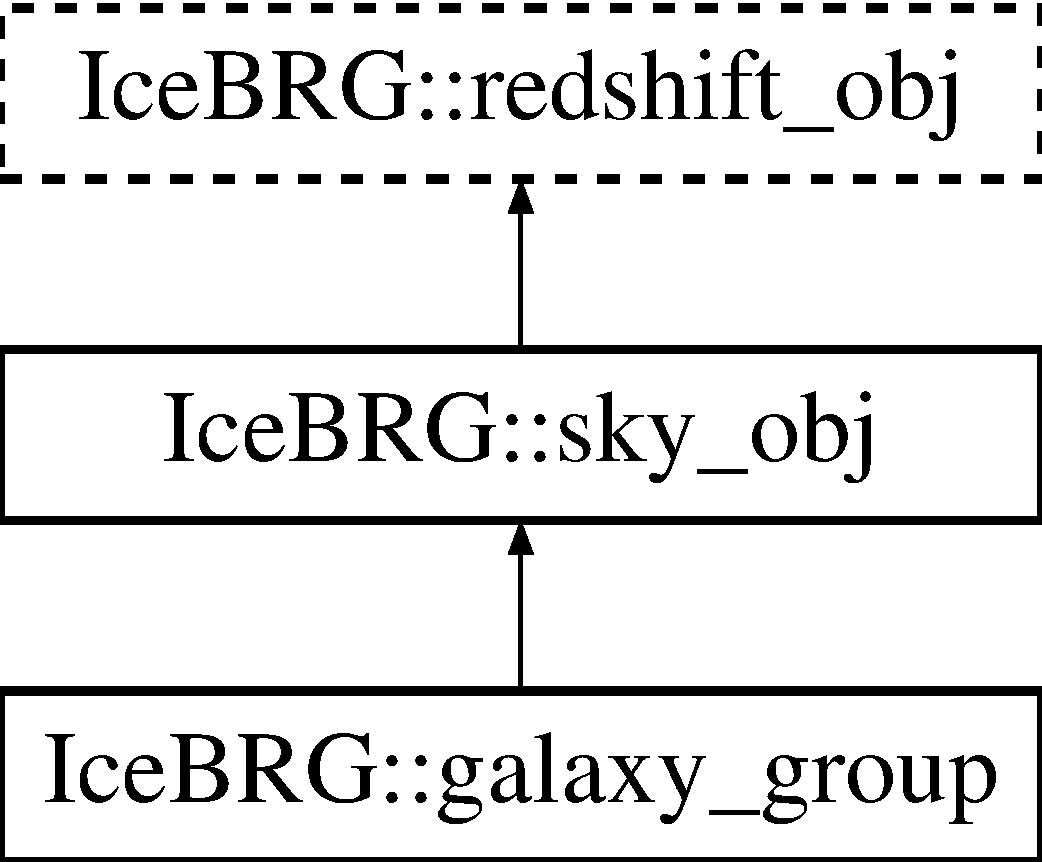
\includegraphics[height=3.000000cm]{classIceBRG_1_1galaxy__group}
\end{center}
\end{figure}
\subsection*{Public Member Functions}
\begin{DoxyCompactItemize}
\item 
\hyperlink{classIceBRG_1_1galaxy__group_aca191f61edf00e2231ea9d1dc1920b7b}{galaxy\+\_\+group} (size\+\_\+t init\+\_\+num\+\_\+members=0)
\item 
\hyperlink{classIceBRG_1_1galaxy__group_af846959d0371506f4b5c250722094cdc}{galaxy\+\_\+group} (\hyperlink{lib_2IceBRG__main_2common_8h_ad0f130a56eeb944d9ef2692ee881ecc4}{flt\+\_\+type} init\+\_\+mass, \hyperlink{lib_2IceBRG__main_2common_8h_ad0f130a56eeb944d9ef2692ee881ecc4}{flt\+\_\+type} init\+\_\+z, \hyperlink{lib_2IceBRG__main_2common_8h_ad0f130a56eeb944d9ef2692ee881ecc4}{flt\+\_\+type} init\+\_\+c=-\/1, \hyperlink{lib_2IceBRG__main_2common_8h_ad0f130a56eeb944d9ef2692ee881ecc4}{flt\+\_\+type} init\+\_\+tau=-\/1)
\item 
virtual \hyperlink{classIceBRG_1_1galaxy__group_a6be6c53727fea15311b820d1fcb7909c}{$\sim$galaxy\+\_\+group} ()
\item 
virtual void \hyperlink{classIceBRG_1_1galaxy__group_af1be93cc734995c7fbfe6eb992094262}{clear} ()
\item 
virtual void \hyperlink{classIceBRG_1_1galaxy__group_a2e037901d1380a536dccf927611d68dc}{resize} (size\+\_\+t new\+\_\+num\+\_\+members)
\item 
virtual void \hyperlink{classIceBRG_1_1galaxy__group_aa34100e556ce7824e06e942b1141d9cc}{set\+\_\+member} (size\+\_\+t \hyperlink{classIceBRG_1_1sky__obj_ad25abf998cc346d25b085440509128bc}{index}, \hyperlink{classIceBRG_1_1galaxy}{galaxy} $\ast$new\+\_\+member)
\item 
virtual void \hyperlink{classIceBRG_1_1galaxy__group_a34987028c9a8b23f6c7e07b4e70de8e1}{set\+\_\+member\+\_\+index} (size\+\_\+t \hyperlink{classIceBRG_1_1sky__obj_ad25abf998cc346d25b085440509128bc}{index}, size\+\_\+t new\+\_\+member\+\_\+index)
\item 
virtual void \hyperlink{classIceBRG_1_1galaxy__group_a8bfb0e388047df1a783b59ef4b22a0d1}{add\+\_\+member} (\hyperlink{classIceBRG_1_1galaxy}{galaxy} $\ast$new\+\_\+member=false)
\item 
virtual void \hyperlink{classIceBRG_1_1galaxy__group_abc13746253a4e204604b533f7bdf2b0b}{remove\+\_\+member} (\hyperlink{classIceBRG_1_1galaxy}{galaxy} $\ast$rem\+\_\+member=false)
\item 
\hyperlink{namespaceIceBRG_a1be72ac4918a9b029f2eefa084213e35}{mass\+\_\+type} \hyperlink{classIceBRG_1_1galaxy__group_a8fe2611b0f227d213768b8ef4b6b1150}{m} () const 
\item 
\hyperlink{lib_2IceBRG__main_2common_8h_ad0f130a56eeb944d9ef2692ee881ecc4}{flt\+\_\+type} \hyperlink{classIceBRG_1_1galaxy__group_aae14446ee20e2b7216317c1e8c7f4aeb}{mag} () const 
\item 
virtual \hyperlink{classIceBRG_1_1redshift__obj}{redshift\+\_\+obj} $\ast$ \hyperlink{classIceBRG_1_1galaxy__group_af0ee2e7b336371e8a8f098c3bfe7372d}{redshift\+\_\+obj\+\_\+clone} () const 
\item 
virtual \hyperlink{classIceBRG_1_1sky__obj}{sky\+\_\+obj} $\ast$ \hyperlink{classIceBRG_1_1galaxy__group_aa13d25256931c89489891ae8431672c7}{sky\+\_\+obj\+\_\+clone} () const 
\item 
virtual \hyperlink{classIceBRG_1_1galaxy__group}{galaxy\+\_\+group} $\ast$ \hyperlink{classIceBRG_1_1galaxy__group_a6ff6cbd19bc3d744ffeb33e3f376cb19}{galaxy\+\_\+group\+\_\+clone} () const 
\end{DoxyCompactItemize}
\subsection*{Public Attributes}
\begin{DoxyCompactItemize}
\item 
\hyperlink{lib_2IceBRG__main_2common_8h_ad0f130a56eeb944d9ef2692ee881ecc4}{flt\+\_\+type} \hyperlink{classIceBRG_1_1galaxy__group_a5ce7db4f858d59074efd715ea205269b}{z\+\_\+phot}
\item 
\hyperlink{lib_2IceBRG__main_2common_8h_ad0f130a56eeb944d9ef2692ee881ecc4}{flt\+\_\+type} \hyperlink{classIceBRG_1_1galaxy__group_a6696a2e58e33e858f1dd40a285cf432a}{z\+\_\+phot\+\_\+err}
\item 
\hyperlink{lib_2IceBRG__main_2common_8h_ad0f130a56eeb944d9ef2692ee881ecc4}{flt\+\_\+type} \hyperlink{classIceBRG_1_1galaxy__group_a3dd2782cd0deb0fbe61c319d806c3fc5}{odds}
\item 
size\+\_\+t \hyperlink{classIceBRG_1_1galaxy__group_a61cded26fb8fca3131583ca6a41a3b8e}{B\+C\+G\+\_\+index}
\item 
size\+\_\+t \hyperlink{classIceBRG_1_1galaxy__group_aca3ba15cea4121df150b6e03f59c32b2}{num\+\_\+members}
\item 
std\+::vector$<$ size\+\_\+t $>$ \hyperlink{classIceBRG_1_1galaxy__group_ab44f3aa3551d17e31d909615004d5508}{member\+\_\+indices}
\item 
std\+::vector$<$ \hyperlink{classIceBRG_1_1galaxy}{galaxy} $\ast$ $>$ \hyperlink{classIceBRG_1_1galaxy__group_a1c2634adaa0d697d1d533d76fd949411}{members}
\end{DoxyCompactItemize}


\subsection{Constructor \& Destructor Documentation}
\hypertarget{classIceBRG_1_1galaxy__group_aca191f61edf00e2231ea9d1dc1920b7b}{}\index{Ice\+B\+R\+G\+::galaxy\+\_\+group@{Ice\+B\+R\+G\+::galaxy\+\_\+group}!galaxy\+\_\+group@{galaxy\+\_\+group}}
\index{galaxy\+\_\+group@{galaxy\+\_\+group}!Ice\+B\+R\+G\+::galaxy\+\_\+group@{Ice\+B\+R\+G\+::galaxy\+\_\+group}}
\subsubsection[{galaxy\+\_\+group(size\+\_\+t init\+\_\+num\+\_\+members=0)}]{\setlength{\rightskip}{0pt plus 5cm}Ice\+B\+R\+G\+::galaxy\+\_\+group\+::galaxy\+\_\+group (
\begin{DoxyParamCaption}
\item[{size\+\_\+t}]{init\+\_\+num\+\_\+members = {\ttfamily 0}}
\end{DoxyParamCaption}
)}\label{classIceBRG_1_1galaxy__group_aca191f61edf00e2231ea9d1dc1920b7b}
\hypertarget{classIceBRG_1_1galaxy__group_af846959d0371506f4b5c250722094cdc}{}\index{Ice\+B\+R\+G\+::galaxy\+\_\+group@{Ice\+B\+R\+G\+::galaxy\+\_\+group}!galaxy\+\_\+group@{galaxy\+\_\+group}}
\index{galaxy\+\_\+group@{galaxy\+\_\+group}!Ice\+B\+R\+G\+::galaxy\+\_\+group@{Ice\+B\+R\+G\+::galaxy\+\_\+group}}
\subsubsection[{galaxy\+\_\+group(flt\+\_\+type init\+\_\+mass, flt\+\_\+type init\+\_\+z, flt\+\_\+type init\+\_\+c=-\/1, flt\+\_\+type init\+\_\+tau=-\/1)}]{\setlength{\rightskip}{0pt plus 5cm}Ice\+B\+R\+G\+::galaxy\+\_\+group\+::galaxy\+\_\+group (
\begin{DoxyParamCaption}
\item[{{\bf flt\+\_\+type}}]{init\+\_\+mass, }
\item[{{\bf flt\+\_\+type}}]{init\+\_\+z, }
\item[{{\bf flt\+\_\+type}}]{init\+\_\+c = {\ttfamily -\/1}, }
\item[{{\bf flt\+\_\+type}}]{init\+\_\+tau = {\ttfamily -\/1}}
\end{DoxyParamCaption}
)}\label{classIceBRG_1_1galaxy__group_af846959d0371506f4b5c250722094cdc}
\hypertarget{classIceBRG_1_1galaxy__group_a6be6c53727fea15311b820d1fcb7909c}{}\index{Ice\+B\+R\+G\+::galaxy\+\_\+group@{Ice\+B\+R\+G\+::galaxy\+\_\+group}!````~galaxy\+\_\+group@{$\sim$galaxy\+\_\+group}}
\index{````~galaxy\+\_\+group@{$\sim$galaxy\+\_\+group}!Ice\+B\+R\+G\+::galaxy\+\_\+group@{Ice\+B\+R\+G\+::galaxy\+\_\+group}}
\subsubsection[{$\sim$galaxy\+\_\+group()}]{\setlength{\rightskip}{0pt plus 5cm}Ice\+B\+R\+G\+::galaxy\+\_\+group\+::$\sim$galaxy\+\_\+group (
\begin{DoxyParamCaption}
{}
\end{DoxyParamCaption}
)\hspace{0.3cm}{\ttfamily [virtual]}}\label{classIceBRG_1_1galaxy__group_a6be6c53727fea15311b820d1fcb7909c}


\subsection{Member Function Documentation}
\hypertarget{classIceBRG_1_1galaxy__group_a8bfb0e388047df1a783b59ef4b22a0d1}{}\index{Ice\+B\+R\+G\+::galaxy\+\_\+group@{Ice\+B\+R\+G\+::galaxy\+\_\+group}!add\+\_\+member@{add\+\_\+member}}
\index{add\+\_\+member@{add\+\_\+member}!Ice\+B\+R\+G\+::galaxy\+\_\+group@{Ice\+B\+R\+G\+::galaxy\+\_\+group}}
\subsubsection[{add\+\_\+member(galaxy $\ast$new\+\_\+member=false)}]{\setlength{\rightskip}{0pt plus 5cm}void Ice\+B\+R\+G\+::galaxy\+\_\+group\+::add\+\_\+member (
\begin{DoxyParamCaption}
\item[{{\bf galaxy} $\ast$}]{new\+\_\+member = {\ttfamily false}}
\end{DoxyParamCaption}
)\hspace{0.3cm}{\ttfamily [virtual]}}\label{classIceBRG_1_1galaxy__group_a8bfb0e388047df1a783b59ef4b22a0d1}
\hypertarget{classIceBRG_1_1galaxy__group_af1be93cc734995c7fbfe6eb992094262}{}\index{Ice\+B\+R\+G\+::galaxy\+\_\+group@{Ice\+B\+R\+G\+::galaxy\+\_\+group}!clear@{clear}}
\index{clear@{clear}!Ice\+B\+R\+G\+::galaxy\+\_\+group@{Ice\+B\+R\+G\+::galaxy\+\_\+group}}
\subsubsection[{clear()}]{\setlength{\rightskip}{0pt plus 5cm}void Ice\+B\+R\+G\+::galaxy\+\_\+group\+::clear (
\begin{DoxyParamCaption}
{}
\end{DoxyParamCaption}
)\hspace{0.3cm}{\ttfamily [virtual]}}\label{classIceBRG_1_1galaxy__group_af1be93cc734995c7fbfe6eb992094262}


Reimplemented from \hyperlink{classIceBRG_1_1sky__obj_ad38ff17a187253f6f2fb4ef81ea03c59}{Ice\+B\+R\+G\+::sky\+\_\+obj}.

\hypertarget{classIceBRG_1_1galaxy__group_a6ff6cbd19bc3d744ffeb33e3f376cb19}{}\index{Ice\+B\+R\+G\+::galaxy\+\_\+group@{Ice\+B\+R\+G\+::galaxy\+\_\+group}!galaxy\+\_\+group\+\_\+clone@{galaxy\+\_\+group\+\_\+clone}}
\index{galaxy\+\_\+group\+\_\+clone@{galaxy\+\_\+group\+\_\+clone}!Ice\+B\+R\+G\+::galaxy\+\_\+group@{Ice\+B\+R\+G\+::galaxy\+\_\+group}}
\subsubsection[{galaxy\+\_\+group\+\_\+clone() const }]{\setlength{\rightskip}{0pt plus 5cm}virtual {\bf galaxy\+\_\+group}$\ast$ Ice\+B\+R\+G\+::galaxy\+\_\+group\+::galaxy\+\_\+group\+\_\+clone (
\begin{DoxyParamCaption}
{}
\end{DoxyParamCaption}
) const\hspace{0.3cm}{\ttfamily [inline]}, {\ttfamily [virtual]}}\label{classIceBRG_1_1galaxy__group_a6ff6cbd19bc3d744ffeb33e3f376cb19}
\hypertarget{classIceBRG_1_1galaxy__group_a8fe2611b0f227d213768b8ef4b6b1150}{}\index{Ice\+B\+R\+G\+::galaxy\+\_\+group@{Ice\+B\+R\+G\+::galaxy\+\_\+group}!m@{m}}
\index{m@{m}!Ice\+B\+R\+G\+::galaxy\+\_\+group@{Ice\+B\+R\+G\+::galaxy\+\_\+group}}
\subsubsection[{m() const }]{\setlength{\rightskip}{0pt plus 5cm}{\bf mass\+\_\+type} Ice\+B\+R\+G\+::galaxy\+\_\+group\+::m (
\begin{DoxyParamCaption}
{}
\end{DoxyParamCaption}
) const\hspace{0.3cm}{\ttfamily [inline]}, {\ttfamily [virtual]}}\label{classIceBRG_1_1galaxy__group_a8fe2611b0f227d213768b8ef4b6b1150}


Implements \hyperlink{classIceBRG_1_1sky__obj_a5296e44c7c9d809c31d9326197527d17}{Ice\+B\+R\+G\+::sky\+\_\+obj}.

\hypertarget{classIceBRG_1_1galaxy__group_aae14446ee20e2b7216317c1e8c7f4aeb}{}\index{Ice\+B\+R\+G\+::galaxy\+\_\+group@{Ice\+B\+R\+G\+::galaxy\+\_\+group}!mag@{mag}}
\index{mag@{mag}!Ice\+B\+R\+G\+::galaxy\+\_\+group@{Ice\+B\+R\+G\+::galaxy\+\_\+group}}
\subsubsection[{mag() const }]{\setlength{\rightskip}{0pt plus 5cm}{\bf flt\+\_\+type} Ice\+B\+R\+G\+::galaxy\+\_\+group\+::mag (
\begin{DoxyParamCaption}
{}
\end{DoxyParamCaption}
) const\hspace{0.3cm}{\ttfamily [inline]}, {\ttfamily [virtual]}}\label{classIceBRG_1_1galaxy__group_aae14446ee20e2b7216317c1e8c7f4aeb}


Implements \hyperlink{classIceBRG_1_1sky__obj_a40496172864c36f89d07bf54a52a9dc6}{Ice\+B\+R\+G\+::sky\+\_\+obj}.

\hypertarget{classIceBRG_1_1galaxy__group_af0ee2e7b336371e8a8f098c3bfe7372d}{}\index{Ice\+B\+R\+G\+::galaxy\+\_\+group@{Ice\+B\+R\+G\+::galaxy\+\_\+group}!redshift\+\_\+obj\+\_\+clone@{redshift\+\_\+obj\+\_\+clone}}
\index{redshift\+\_\+obj\+\_\+clone@{redshift\+\_\+obj\+\_\+clone}!Ice\+B\+R\+G\+::galaxy\+\_\+group@{Ice\+B\+R\+G\+::galaxy\+\_\+group}}
\subsubsection[{redshift\+\_\+obj\+\_\+clone() const }]{\setlength{\rightskip}{0pt plus 5cm}virtual {\bf redshift\+\_\+obj}$\ast$ Ice\+B\+R\+G\+::galaxy\+\_\+group\+::redshift\+\_\+obj\+\_\+clone (
\begin{DoxyParamCaption}
{}
\end{DoxyParamCaption}
) const\hspace{0.3cm}{\ttfamily [inline]}, {\ttfamily [virtual]}}\label{classIceBRG_1_1galaxy__group_af0ee2e7b336371e8a8f098c3bfe7372d}


Implements \hyperlink{classIceBRG_1_1sky__obj_a6efa97b5c6edb6c4ea741b06338ff5bc}{Ice\+B\+R\+G\+::sky\+\_\+obj}.

\hypertarget{classIceBRG_1_1galaxy__group_abc13746253a4e204604b533f7bdf2b0b}{}\index{Ice\+B\+R\+G\+::galaxy\+\_\+group@{Ice\+B\+R\+G\+::galaxy\+\_\+group}!remove\+\_\+member@{remove\+\_\+member}}
\index{remove\+\_\+member@{remove\+\_\+member}!Ice\+B\+R\+G\+::galaxy\+\_\+group@{Ice\+B\+R\+G\+::galaxy\+\_\+group}}
\subsubsection[{remove\+\_\+member(galaxy $\ast$rem\+\_\+member=false)}]{\setlength{\rightskip}{0pt plus 5cm}void Ice\+B\+R\+G\+::galaxy\+\_\+group\+::remove\+\_\+member (
\begin{DoxyParamCaption}
\item[{{\bf galaxy} $\ast$}]{rem\+\_\+member = {\ttfamily false}}
\end{DoxyParamCaption}
)\hspace{0.3cm}{\ttfamily [virtual]}}\label{classIceBRG_1_1galaxy__group_abc13746253a4e204604b533f7bdf2b0b}
\hypertarget{classIceBRG_1_1galaxy__group_a2e037901d1380a536dccf927611d68dc}{}\index{Ice\+B\+R\+G\+::galaxy\+\_\+group@{Ice\+B\+R\+G\+::galaxy\+\_\+group}!resize@{resize}}
\index{resize@{resize}!Ice\+B\+R\+G\+::galaxy\+\_\+group@{Ice\+B\+R\+G\+::galaxy\+\_\+group}}
\subsubsection[{resize(size\+\_\+t new\+\_\+num\+\_\+members)}]{\setlength{\rightskip}{0pt plus 5cm}void Ice\+B\+R\+G\+::galaxy\+\_\+group\+::resize (
\begin{DoxyParamCaption}
\item[{size\+\_\+t}]{new\+\_\+num\+\_\+members}
\end{DoxyParamCaption}
)\hspace{0.3cm}{\ttfamily [virtual]}}\label{classIceBRG_1_1galaxy__group_a2e037901d1380a536dccf927611d68dc}
\hypertarget{classIceBRG_1_1galaxy__group_aa34100e556ce7824e06e942b1141d9cc}{}\index{Ice\+B\+R\+G\+::galaxy\+\_\+group@{Ice\+B\+R\+G\+::galaxy\+\_\+group}!set\+\_\+member@{set\+\_\+member}}
\index{set\+\_\+member@{set\+\_\+member}!Ice\+B\+R\+G\+::galaxy\+\_\+group@{Ice\+B\+R\+G\+::galaxy\+\_\+group}}
\subsubsection[{set\+\_\+member(size\+\_\+t index, galaxy $\ast$new\+\_\+member)}]{\setlength{\rightskip}{0pt plus 5cm}void Ice\+B\+R\+G\+::galaxy\+\_\+group\+::set\+\_\+member (
\begin{DoxyParamCaption}
\item[{size\+\_\+t}]{index, }
\item[{{\bf galaxy} $\ast$}]{new\+\_\+member}
\end{DoxyParamCaption}
)\hspace{0.3cm}{\ttfamily [virtual]}}\label{classIceBRG_1_1galaxy__group_aa34100e556ce7824e06e942b1141d9cc}
\hypertarget{classIceBRG_1_1galaxy__group_a34987028c9a8b23f6c7e07b4e70de8e1}{}\index{Ice\+B\+R\+G\+::galaxy\+\_\+group@{Ice\+B\+R\+G\+::galaxy\+\_\+group}!set\+\_\+member\+\_\+index@{set\+\_\+member\+\_\+index}}
\index{set\+\_\+member\+\_\+index@{set\+\_\+member\+\_\+index}!Ice\+B\+R\+G\+::galaxy\+\_\+group@{Ice\+B\+R\+G\+::galaxy\+\_\+group}}
\subsubsection[{set\+\_\+member\+\_\+index(size\+\_\+t index, size\+\_\+t new\+\_\+member\+\_\+index)}]{\setlength{\rightskip}{0pt plus 5cm}void Ice\+B\+R\+G\+::galaxy\+\_\+group\+::set\+\_\+member\+\_\+index (
\begin{DoxyParamCaption}
\item[{size\+\_\+t}]{index, }
\item[{size\+\_\+t}]{new\+\_\+member\+\_\+index}
\end{DoxyParamCaption}
)\hspace{0.3cm}{\ttfamily [virtual]}}\label{classIceBRG_1_1galaxy__group_a34987028c9a8b23f6c7e07b4e70de8e1}
\hypertarget{classIceBRG_1_1galaxy__group_aa13d25256931c89489891ae8431672c7}{}\index{Ice\+B\+R\+G\+::galaxy\+\_\+group@{Ice\+B\+R\+G\+::galaxy\+\_\+group}!sky\+\_\+obj\+\_\+clone@{sky\+\_\+obj\+\_\+clone}}
\index{sky\+\_\+obj\+\_\+clone@{sky\+\_\+obj\+\_\+clone}!Ice\+B\+R\+G\+::galaxy\+\_\+group@{Ice\+B\+R\+G\+::galaxy\+\_\+group}}
\subsubsection[{sky\+\_\+obj\+\_\+clone() const }]{\setlength{\rightskip}{0pt plus 5cm}virtual {\bf sky\+\_\+obj}$\ast$ Ice\+B\+R\+G\+::galaxy\+\_\+group\+::sky\+\_\+obj\+\_\+clone (
\begin{DoxyParamCaption}
{}
\end{DoxyParamCaption}
) const\hspace{0.3cm}{\ttfamily [inline]}, {\ttfamily [virtual]}}\label{classIceBRG_1_1galaxy__group_aa13d25256931c89489891ae8431672c7}


Implements \hyperlink{classIceBRG_1_1sky__obj_a4b221bb8efb8ad5df2b03e53a077eeaa}{Ice\+B\+R\+G\+::sky\+\_\+obj}.



\subsection{Member Data Documentation}
\hypertarget{classIceBRG_1_1galaxy__group_a61cded26fb8fca3131583ca6a41a3b8e}{}\index{Ice\+B\+R\+G\+::galaxy\+\_\+group@{Ice\+B\+R\+G\+::galaxy\+\_\+group}!B\+C\+G\+\_\+index@{B\+C\+G\+\_\+index}}
\index{B\+C\+G\+\_\+index@{B\+C\+G\+\_\+index}!Ice\+B\+R\+G\+::galaxy\+\_\+group@{Ice\+B\+R\+G\+::galaxy\+\_\+group}}
\subsubsection[{B\+C\+G\+\_\+index}]{\setlength{\rightskip}{0pt plus 5cm}size\+\_\+t Ice\+B\+R\+G\+::galaxy\+\_\+group\+::\+B\+C\+G\+\_\+index}\label{classIceBRG_1_1galaxy__group_a61cded26fb8fca3131583ca6a41a3b8e}
\hypertarget{classIceBRG_1_1galaxy__group_ab44f3aa3551d17e31d909615004d5508}{}\index{Ice\+B\+R\+G\+::galaxy\+\_\+group@{Ice\+B\+R\+G\+::galaxy\+\_\+group}!member\+\_\+indices@{member\+\_\+indices}}
\index{member\+\_\+indices@{member\+\_\+indices}!Ice\+B\+R\+G\+::galaxy\+\_\+group@{Ice\+B\+R\+G\+::galaxy\+\_\+group}}
\subsubsection[{member\+\_\+indices}]{\setlength{\rightskip}{0pt plus 5cm}std\+::vector$<$ size\+\_\+t $>$ Ice\+B\+R\+G\+::galaxy\+\_\+group\+::member\+\_\+indices}\label{classIceBRG_1_1galaxy__group_ab44f3aa3551d17e31d909615004d5508}
\hypertarget{classIceBRG_1_1galaxy__group_a1c2634adaa0d697d1d533d76fd949411}{}\index{Ice\+B\+R\+G\+::galaxy\+\_\+group@{Ice\+B\+R\+G\+::galaxy\+\_\+group}!members@{members}}
\index{members@{members}!Ice\+B\+R\+G\+::galaxy\+\_\+group@{Ice\+B\+R\+G\+::galaxy\+\_\+group}}
\subsubsection[{members}]{\setlength{\rightskip}{0pt plus 5cm}std\+::vector$<$ {\bf galaxy} $\ast$ $>$ Ice\+B\+R\+G\+::galaxy\+\_\+group\+::members}\label{classIceBRG_1_1galaxy__group_a1c2634adaa0d697d1d533d76fd949411}
\hypertarget{classIceBRG_1_1galaxy__group_aca3ba15cea4121df150b6e03f59c32b2}{}\index{Ice\+B\+R\+G\+::galaxy\+\_\+group@{Ice\+B\+R\+G\+::galaxy\+\_\+group}!num\+\_\+members@{num\+\_\+members}}
\index{num\+\_\+members@{num\+\_\+members}!Ice\+B\+R\+G\+::galaxy\+\_\+group@{Ice\+B\+R\+G\+::galaxy\+\_\+group}}
\subsubsection[{num\+\_\+members}]{\setlength{\rightskip}{0pt plus 5cm}size\+\_\+t Ice\+B\+R\+G\+::galaxy\+\_\+group\+::num\+\_\+members}\label{classIceBRG_1_1galaxy__group_aca3ba15cea4121df150b6e03f59c32b2}
\hypertarget{classIceBRG_1_1galaxy__group_a3dd2782cd0deb0fbe61c319d806c3fc5}{}\index{Ice\+B\+R\+G\+::galaxy\+\_\+group@{Ice\+B\+R\+G\+::galaxy\+\_\+group}!odds@{odds}}
\index{odds@{odds}!Ice\+B\+R\+G\+::galaxy\+\_\+group@{Ice\+B\+R\+G\+::galaxy\+\_\+group}}
\subsubsection[{odds}]{\setlength{\rightskip}{0pt plus 5cm}{\bf flt\+\_\+type} Ice\+B\+R\+G\+::galaxy\+\_\+group\+::odds}\label{classIceBRG_1_1galaxy__group_a3dd2782cd0deb0fbe61c319d806c3fc5}
\hypertarget{classIceBRG_1_1galaxy__group_a5ce7db4f858d59074efd715ea205269b}{}\index{Ice\+B\+R\+G\+::galaxy\+\_\+group@{Ice\+B\+R\+G\+::galaxy\+\_\+group}!z\+\_\+phot@{z\+\_\+phot}}
\index{z\+\_\+phot@{z\+\_\+phot}!Ice\+B\+R\+G\+::galaxy\+\_\+group@{Ice\+B\+R\+G\+::galaxy\+\_\+group}}
\subsubsection[{z\+\_\+phot}]{\setlength{\rightskip}{0pt plus 5cm}{\bf flt\+\_\+type} Ice\+B\+R\+G\+::galaxy\+\_\+group\+::z\+\_\+phot}\label{classIceBRG_1_1galaxy__group_a5ce7db4f858d59074efd715ea205269b}
\hypertarget{classIceBRG_1_1galaxy__group_a6696a2e58e33e858f1dd40a285cf432a}{}\index{Ice\+B\+R\+G\+::galaxy\+\_\+group@{Ice\+B\+R\+G\+::galaxy\+\_\+group}!z\+\_\+phot\+\_\+err@{z\+\_\+phot\+\_\+err}}
\index{z\+\_\+phot\+\_\+err@{z\+\_\+phot\+\_\+err}!Ice\+B\+R\+G\+::galaxy\+\_\+group@{Ice\+B\+R\+G\+::galaxy\+\_\+group}}
\subsubsection[{z\+\_\+phot\+\_\+err}]{\setlength{\rightskip}{0pt plus 5cm}{\bf flt\+\_\+type} Ice\+B\+R\+G\+::galaxy\+\_\+group\+::z\+\_\+phot\+\_\+err}\label{classIceBRG_1_1galaxy__group_a6696a2e58e33e858f1dd40a285cf432a}


The documentation for this class was generated from the following files\+:\begin{DoxyCompactItemize}
\item 
/disk2/brg/git/\+Magnification\+\_\+\+Public/src/lib/\+Ice\+B\+R\+G\+\_\+physics/sky\+\_\+obj/\hyperlink{galaxy__group_8h}{galaxy\+\_\+group.\+h}\item 
/disk2/brg/git/\+Magnification\+\_\+\+Public/src/lib/\+Ice\+B\+R\+G\+\_\+physics/sky\+\_\+obj/\hyperlink{galaxy__group_8cpp}{galaxy\+\_\+group.\+cpp}\end{DoxyCompactItemize}

\hypertarget{structgg__lensing__config}{\section{gg\-\_\-lensing\-\_\-config Struct Reference}
\label{structgg__lensing__config}\index{gg\-\_\-lensing\-\_\-config@{gg\-\_\-lensing\-\_\-config}}
}


{\ttfamily \#include $<$gg\-\_\-lensing\-\_\-config.\-h$>$}

\subsection*{Public Member Functions}
\begin{DoxyCompactItemize}
\item 
\hyperlink{structgg__lensing__config_a808f3d67c49d7bbcb6e8345fdf6eecdd}{gg\-\_\-lensing\-\_\-config} (const int argc=0, const char $\ast$argv\mbox{[}$\,$\mbox{]}=nullptr)
\item 
virtual \hyperlink{structgg__lensing__config_aec78098e3fa604b03f785edfb2b5066c}{$\sim$gg\-\_\-lensing\-\_\-config} ()
\end{DoxyCompactItemize}
\subsection*{Data Fields}
\begin{DoxyCompactItemize}
\item 
bool \hyperlink{structgg__lensing__config_a3fe4ca186ed399f741d499e1e0e4acf8}{use\-\_\-precalculated\-\_\-data}
\item 
std\-::string \hyperlink{structgg__lensing__config_a8bc252029c599446dfbba897920eca0f}{precalculated\-\_\-data\-\_\-filename}
\item 
\hyperlink{namespaceIceBRG_a45499647eb87e24c10ab32c628711cec}{Ice\-B\-R\-G\-::distance\-\_\-type} \hyperlink{structgg__lensing__config_a14445ac28a5b6e168d407b5a862fa186}{R\-\_\-min}
\item 
\hyperlink{namespaceIceBRG_a45499647eb87e24c10ab32c628711cec}{Ice\-B\-R\-G\-::distance\-\_\-type} \hyperlink{structgg__lensing__config_a18e40e60fa8b0f06e7550eb3c0411a8b}{R\-\_\-max}
\item 
\hyperlink{namespaceIceBRG_a1be72ac4918a9b029f2eefa084213e35}{Ice\-B\-R\-G\-::mass\-\_\-type} \hyperlink{structgg__lensing__config_af80680456a55ac0efca1fa309d1611f2}{m\-\_\-min}
\item 
\hyperlink{namespaceIceBRG_a1be72ac4918a9b029f2eefa084213e35}{Ice\-B\-R\-G\-::mass\-\_\-type} \hyperlink{structgg__lensing__config_a0b33d2e197f1972c8164567295f83f87}{m\-\_\-max}
\item 
double \hyperlink{structgg__lensing__config_a983f7b673fc379bfcc96e69820057f8e}{z\-\_\-min}
\item 
double \hyperlink{structgg__lensing__config_a16239d6e2c8ad5c3850abf9a47096701}{z\-\_\-max}
\item 
double \hyperlink{structgg__lensing__config_a51c75e4b7d5da1bb3dff5979131259c9}{mag\-\_\-min}
\item 
double \hyperlink{structgg__lensing__config_a3f234006efbd74be8b82a79ca4bda522}{mag\-\_\-max}
\item 
size\-\_\-t \hyperlink{structgg__lensing__config_a0222122d7470e67e7aeb52096fcb6f90}{R\-\_\-bins}
\item 
size\-\_\-t \hyperlink{structgg__lensing__config_a80fc5e7efdd390f1d3d96898471802cc}{m\-\_\-bins}
\item 
size\-\_\-t \hyperlink{structgg__lensing__config_aff53350063b74ef73c8cea9b89a8780e}{z\-\_\-bins}
\item 
size\-\_\-t \hyperlink{structgg__lensing__config_a3c82853304ede01b0697d0c05d0db1d0}{mag\-\_\-bins}
\item 
bool \hyperlink{structgg__lensing__config_a4ca415b5664d589eadea71166aaba4bc}{R\-\_\-log}
\item 
bool \hyperlink{structgg__lensing__config_ad92bfc552d828962e8a5525999ae0a6b}{m\-\_\-log}
\item 
bool \hyperlink{structgg__lensing__config_a454b771c419a63d1512bbd220257b095}{z\-\_\-log}
\item 
bool \hyperlink{structgg__lensing__config_aefcae2d2981313e2c3ef4f9e378d9976}{mag\-\_\-log}
\end{DoxyCompactItemize}
\subsection*{Static Public Attributes}
\begin{DoxyCompactItemize}
\item 
static constexpr size\-\_\-t \hyperlink{structgg__lensing__config_a7082cdfc7c6623985427e4c4ebb6d8e3}{num\-\_\-config\-\_\-params} = 18
\end{DoxyCompactItemize}


\subsection{Constructor \& Destructor Documentation}
\hypertarget{structgg__lensing__config_a808f3d67c49d7bbcb6e8345fdf6eecdd}{\index{gg\-\_\-lensing\-\_\-config@{gg\-\_\-lensing\-\_\-config}!gg\-\_\-lensing\-\_\-config@{gg\-\_\-lensing\-\_\-config}}
\index{gg\-\_\-lensing\-\_\-config@{gg\-\_\-lensing\-\_\-config}!gg_lensing_config@{gg\-\_\-lensing\-\_\-config}}
\subsubsection[{gg\-\_\-lensing\-\_\-config}]{\setlength{\rightskip}{0pt plus 5cm}gg\-\_\-lensing\-\_\-config\-::gg\-\_\-lensing\-\_\-config (
\begin{DoxyParamCaption}
\item[{const int}]{argc = {\ttfamily 0}, }
\item[{const char $\ast$}]{argv\mbox{[}$\,$\mbox{]} = {\ttfamily nullptr}}
\end{DoxyParamCaption}
)}}\label{structgg__lensing__config_a808f3d67c49d7bbcb6e8345fdf6eecdd}
\hypertarget{structgg__lensing__config_aec78098e3fa604b03f785edfb2b5066c}{\index{gg\-\_\-lensing\-\_\-config@{gg\-\_\-lensing\-\_\-config}!$\sim$gg\-\_\-lensing\-\_\-config@{$\sim$gg\-\_\-lensing\-\_\-config}}
\index{$\sim$gg\-\_\-lensing\-\_\-config@{$\sim$gg\-\_\-lensing\-\_\-config}!gg_lensing_config@{gg\-\_\-lensing\-\_\-config}}
\subsubsection[{$\sim$gg\-\_\-lensing\-\_\-config}]{\setlength{\rightskip}{0pt plus 5cm}virtual gg\-\_\-lensing\-\_\-config\-::$\sim$gg\-\_\-lensing\-\_\-config (
\begin{DoxyParamCaption}
{}
\end{DoxyParamCaption}
)\hspace{0.3cm}{\ttfamily [inline]}, {\ttfamily [virtual]}}}\label{structgg__lensing__config_aec78098e3fa604b03f785edfb2b5066c}


\subsection{Field Documentation}
\hypertarget{structgg__lensing__config_a80fc5e7efdd390f1d3d96898471802cc}{\index{gg\-\_\-lensing\-\_\-config@{gg\-\_\-lensing\-\_\-config}!m\-\_\-bins@{m\-\_\-bins}}
\index{m\-\_\-bins@{m\-\_\-bins}!gg_lensing_config@{gg\-\_\-lensing\-\_\-config}}
\subsubsection[{m\-\_\-bins}]{\setlength{\rightskip}{0pt plus 5cm}size\-\_\-t gg\-\_\-lensing\-\_\-config\-::m\-\_\-bins}}\label{structgg__lensing__config_a80fc5e7efdd390f1d3d96898471802cc}
\hypertarget{structgg__lensing__config_ad92bfc552d828962e8a5525999ae0a6b}{\index{gg\-\_\-lensing\-\_\-config@{gg\-\_\-lensing\-\_\-config}!m\-\_\-log@{m\-\_\-log}}
\index{m\-\_\-log@{m\-\_\-log}!gg_lensing_config@{gg\-\_\-lensing\-\_\-config}}
\subsubsection[{m\-\_\-log}]{\setlength{\rightskip}{0pt plus 5cm}bool gg\-\_\-lensing\-\_\-config\-::m\-\_\-log}}\label{structgg__lensing__config_ad92bfc552d828962e8a5525999ae0a6b}
\hypertarget{structgg__lensing__config_a0b33d2e197f1972c8164567295f83f87}{\index{gg\-\_\-lensing\-\_\-config@{gg\-\_\-lensing\-\_\-config}!m\-\_\-max@{m\-\_\-max}}
\index{m\-\_\-max@{m\-\_\-max}!gg_lensing_config@{gg\-\_\-lensing\-\_\-config}}
\subsubsection[{m\-\_\-max}]{\setlength{\rightskip}{0pt plus 5cm}{\bf Ice\-B\-R\-G\-::mass\-\_\-type} gg\-\_\-lensing\-\_\-config\-::m\-\_\-max}}\label{structgg__lensing__config_a0b33d2e197f1972c8164567295f83f87}
\hypertarget{structgg__lensing__config_af80680456a55ac0efca1fa309d1611f2}{\index{gg\-\_\-lensing\-\_\-config@{gg\-\_\-lensing\-\_\-config}!m\-\_\-min@{m\-\_\-min}}
\index{m\-\_\-min@{m\-\_\-min}!gg_lensing_config@{gg\-\_\-lensing\-\_\-config}}
\subsubsection[{m\-\_\-min}]{\setlength{\rightskip}{0pt plus 5cm}{\bf Ice\-B\-R\-G\-::mass\-\_\-type} gg\-\_\-lensing\-\_\-config\-::m\-\_\-min}}\label{structgg__lensing__config_af80680456a55ac0efca1fa309d1611f2}
\hypertarget{structgg__lensing__config_a3c82853304ede01b0697d0c05d0db1d0}{\index{gg\-\_\-lensing\-\_\-config@{gg\-\_\-lensing\-\_\-config}!mag\-\_\-bins@{mag\-\_\-bins}}
\index{mag\-\_\-bins@{mag\-\_\-bins}!gg_lensing_config@{gg\-\_\-lensing\-\_\-config}}
\subsubsection[{mag\-\_\-bins}]{\setlength{\rightskip}{0pt plus 5cm}size\-\_\-t gg\-\_\-lensing\-\_\-config\-::mag\-\_\-bins}}\label{structgg__lensing__config_a3c82853304ede01b0697d0c05d0db1d0}
\hypertarget{structgg__lensing__config_aefcae2d2981313e2c3ef4f9e378d9976}{\index{gg\-\_\-lensing\-\_\-config@{gg\-\_\-lensing\-\_\-config}!mag\-\_\-log@{mag\-\_\-log}}
\index{mag\-\_\-log@{mag\-\_\-log}!gg_lensing_config@{gg\-\_\-lensing\-\_\-config}}
\subsubsection[{mag\-\_\-log}]{\setlength{\rightskip}{0pt plus 5cm}bool gg\-\_\-lensing\-\_\-config\-::mag\-\_\-log}}\label{structgg__lensing__config_aefcae2d2981313e2c3ef4f9e378d9976}
\hypertarget{structgg__lensing__config_a3f234006efbd74be8b82a79ca4bda522}{\index{gg\-\_\-lensing\-\_\-config@{gg\-\_\-lensing\-\_\-config}!mag\-\_\-max@{mag\-\_\-max}}
\index{mag\-\_\-max@{mag\-\_\-max}!gg_lensing_config@{gg\-\_\-lensing\-\_\-config}}
\subsubsection[{mag\-\_\-max}]{\setlength{\rightskip}{0pt plus 5cm}double gg\-\_\-lensing\-\_\-config\-::mag\-\_\-max}}\label{structgg__lensing__config_a3f234006efbd74be8b82a79ca4bda522}
\hypertarget{structgg__lensing__config_a51c75e4b7d5da1bb3dff5979131259c9}{\index{gg\-\_\-lensing\-\_\-config@{gg\-\_\-lensing\-\_\-config}!mag\-\_\-min@{mag\-\_\-min}}
\index{mag\-\_\-min@{mag\-\_\-min}!gg_lensing_config@{gg\-\_\-lensing\-\_\-config}}
\subsubsection[{mag\-\_\-min}]{\setlength{\rightskip}{0pt plus 5cm}double gg\-\_\-lensing\-\_\-config\-::mag\-\_\-min}}\label{structgg__lensing__config_a51c75e4b7d5da1bb3dff5979131259c9}
\hypertarget{structgg__lensing__config_a7082cdfc7c6623985427e4c4ebb6d8e3}{\index{gg\-\_\-lensing\-\_\-config@{gg\-\_\-lensing\-\_\-config}!num\-\_\-config\-\_\-params@{num\-\_\-config\-\_\-params}}
\index{num\-\_\-config\-\_\-params@{num\-\_\-config\-\_\-params}!gg_lensing_config@{gg\-\_\-lensing\-\_\-config}}
\subsubsection[{num\-\_\-config\-\_\-params}]{\setlength{\rightskip}{0pt plus 5cm}constexpr size\-\_\-t gg\-\_\-lensing\-\_\-config\-::num\-\_\-config\-\_\-params = 18\hspace{0.3cm}{\ttfamily [static]}}}\label{structgg__lensing__config_a7082cdfc7c6623985427e4c4ebb6d8e3}
\hypertarget{structgg__lensing__config_a8bc252029c599446dfbba897920eca0f}{\index{gg\-\_\-lensing\-\_\-config@{gg\-\_\-lensing\-\_\-config}!precalculated\-\_\-data\-\_\-filename@{precalculated\-\_\-data\-\_\-filename}}
\index{precalculated\-\_\-data\-\_\-filename@{precalculated\-\_\-data\-\_\-filename}!gg_lensing_config@{gg\-\_\-lensing\-\_\-config}}
\subsubsection[{precalculated\-\_\-data\-\_\-filename}]{\setlength{\rightskip}{0pt plus 5cm}std\-::string gg\-\_\-lensing\-\_\-config\-::precalculated\-\_\-data\-\_\-filename}}\label{structgg__lensing__config_a8bc252029c599446dfbba897920eca0f}
\hypertarget{structgg__lensing__config_a0222122d7470e67e7aeb52096fcb6f90}{\index{gg\-\_\-lensing\-\_\-config@{gg\-\_\-lensing\-\_\-config}!R\-\_\-bins@{R\-\_\-bins}}
\index{R\-\_\-bins@{R\-\_\-bins}!gg_lensing_config@{gg\-\_\-lensing\-\_\-config}}
\subsubsection[{R\-\_\-bins}]{\setlength{\rightskip}{0pt plus 5cm}size\-\_\-t gg\-\_\-lensing\-\_\-config\-::\-R\-\_\-bins}}\label{structgg__lensing__config_a0222122d7470e67e7aeb52096fcb6f90}
\hypertarget{structgg__lensing__config_a4ca415b5664d589eadea71166aaba4bc}{\index{gg\-\_\-lensing\-\_\-config@{gg\-\_\-lensing\-\_\-config}!R\-\_\-log@{R\-\_\-log}}
\index{R\-\_\-log@{R\-\_\-log}!gg_lensing_config@{gg\-\_\-lensing\-\_\-config}}
\subsubsection[{R\-\_\-log}]{\setlength{\rightskip}{0pt plus 5cm}bool gg\-\_\-lensing\-\_\-config\-::\-R\-\_\-log}}\label{structgg__lensing__config_a4ca415b5664d589eadea71166aaba4bc}
\hypertarget{structgg__lensing__config_a18e40e60fa8b0f06e7550eb3c0411a8b}{\index{gg\-\_\-lensing\-\_\-config@{gg\-\_\-lensing\-\_\-config}!R\-\_\-max@{R\-\_\-max}}
\index{R\-\_\-max@{R\-\_\-max}!gg_lensing_config@{gg\-\_\-lensing\-\_\-config}}
\subsubsection[{R\-\_\-max}]{\setlength{\rightskip}{0pt plus 5cm}{\bf Ice\-B\-R\-G\-::distance\-\_\-type} gg\-\_\-lensing\-\_\-config\-::\-R\-\_\-max}}\label{structgg__lensing__config_a18e40e60fa8b0f06e7550eb3c0411a8b}
\hypertarget{structgg__lensing__config_a14445ac28a5b6e168d407b5a862fa186}{\index{gg\-\_\-lensing\-\_\-config@{gg\-\_\-lensing\-\_\-config}!R\-\_\-min@{R\-\_\-min}}
\index{R\-\_\-min@{R\-\_\-min}!gg_lensing_config@{gg\-\_\-lensing\-\_\-config}}
\subsubsection[{R\-\_\-min}]{\setlength{\rightskip}{0pt plus 5cm}{\bf Ice\-B\-R\-G\-::distance\-\_\-type} gg\-\_\-lensing\-\_\-config\-::\-R\-\_\-min}}\label{structgg__lensing__config_a14445ac28a5b6e168d407b5a862fa186}
\hypertarget{structgg__lensing__config_a3fe4ca186ed399f741d499e1e0e4acf8}{\index{gg\-\_\-lensing\-\_\-config@{gg\-\_\-lensing\-\_\-config}!use\-\_\-precalculated\-\_\-data@{use\-\_\-precalculated\-\_\-data}}
\index{use\-\_\-precalculated\-\_\-data@{use\-\_\-precalculated\-\_\-data}!gg_lensing_config@{gg\-\_\-lensing\-\_\-config}}
\subsubsection[{use\-\_\-precalculated\-\_\-data}]{\setlength{\rightskip}{0pt plus 5cm}bool gg\-\_\-lensing\-\_\-config\-::use\-\_\-precalculated\-\_\-data}}\label{structgg__lensing__config_a3fe4ca186ed399f741d499e1e0e4acf8}
\hypertarget{structgg__lensing__config_aff53350063b74ef73c8cea9b89a8780e}{\index{gg\-\_\-lensing\-\_\-config@{gg\-\_\-lensing\-\_\-config}!z\-\_\-bins@{z\-\_\-bins}}
\index{z\-\_\-bins@{z\-\_\-bins}!gg_lensing_config@{gg\-\_\-lensing\-\_\-config}}
\subsubsection[{z\-\_\-bins}]{\setlength{\rightskip}{0pt plus 5cm}size\-\_\-t gg\-\_\-lensing\-\_\-config\-::z\-\_\-bins}}\label{structgg__lensing__config_aff53350063b74ef73c8cea9b89a8780e}
\hypertarget{structgg__lensing__config_a454b771c419a63d1512bbd220257b095}{\index{gg\-\_\-lensing\-\_\-config@{gg\-\_\-lensing\-\_\-config}!z\-\_\-log@{z\-\_\-log}}
\index{z\-\_\-log@{z\-\_\-log}!gg_lensing_config@{gg\-\_\-lensing\-\_\-config}}
\subsubsection[{z\-\_\-log}]{\setlength{\rightskip}{0pt plus 5cm}bool gg\-\_\-lensing\-\_\-config\-::z\-\_\-log}}\label{structgg__lensing__config_a454b771c419a63d1512bbd220257b095}
\hypertarget{structgg__lensing__config_a16239d6e2c8ad5c3850abf9a47096701}{\index{gg\-\_\-lensing\-\_\-config@{gg\-\_\-lensing\-\_\-config}!z\-\_\-max@{z\-\_\-max}}
\index{z\-\_\-max@{z\-\_\-max}!gg_lensing_config@{gg\-\_\-lensing\-\_\-config}}
\subsubsection[{z\-\_\-max}]{\setlength{\rightskip}{0pt plus 5cm}double gg\-\_\-lensing\-\_\-config\-::z\-\_\-max}}\label{structgg__lensing__config_a16239d6e2c8ad5c3850abf9a47096701}
\hypertarget{structgg__lensing__config_a983f7b673fc379bfcc96e69820057f8e}{\index{gg\-\_\-lensing\-\_\-config@{gg\-\_\-lensing\-\_\-config}!z\-\_\-min@{z\-\_\-min}}
\index{z\-\_\-min@{z\-\_\-min}!gg_lensing_config@{gg\-\_\-lensing\-\_\-config}}
\subsubsection[{z\-\_\-min}]{\setlength{\rightskip}{0pt plus 5cm}double gg\-\_\-lensing\-\_\-config\-::z\-\_\-min}}\label{structgg__lensing__config_a983f7b673fc379bfcc96e69820057f8e}


The documentation for this struct was generated from the following files\-:\begin{DoxyCompactItemize}
\item 
/disk2/brg/git/\-Magnification\-\_\-\-Public/src/exec/\-C\-F\-H\-T\-Len\-S\-\_\-gg\-\_\-lensing/\hyperlink{gg__lensing__config_8h}{gg\-\_\-lensing\-\_\-config.\-h}\item 
/disk2/brg/git/\-Magnification\-\_\-\-Public/src/exec/\-C\-F\-H\-T\-Len\-S\-\_\-gg\-\_\-lensing/\hyperlink{gg__lensing__config_8cpp}{gg\-\_\-lensing\-\_\-config.\-cpp}\end{DoxyCompactItemize}

\hypertarget{classIceBRG_1_1grid__cache}{}\section{Ice\+B\+R\+G\+:\+:grid\+\_\+cache Class Reference}
\label{classIceBRG_1_1grid__cache}\index{Ice\+B\+R\+G\+::grid\+\_\+cache@{Ice\+B\+R\+G\+::grid\+\_\+cache}}


{\ttfamily \#include $<$position\+\_\+grid\+\_\+cache.\+h$>$}

\subsection*{Static Public Member Functions}
\begin{DoxyCompactItemize}
\item 
static void \hyperlink{classIceBRG_1_1grid__cache_a5da72ed9107ec519400d77e06bab2c7d}{set\+\_\+ra\+\_\+grid} (const \hyperlink{namespaceIceBRG_a688eeb0811a2474b20b667ed2e9625a1}{angle\+\_\+type} \&new\+\_\+ra\+\_\+grid\+\_\+min, const \hyperlink{namespaceIceBRG_a688eeb0811a2474b20b667ed2e9625a1}{angle\+\_\+type} \&new\+\_\+ra\+\_\+grid\+\_\+max, const \hyperlink{namespaceIceBRG_a688eeb0811a2474b20b667ed2e9625a1}{angle\+\_\+type} \&new\+\_\+ra\+\_\+grid\+\_\+step)
\item 
static void \hyperlink{classIceBRG_1_1grid__cache_aa7f3525ea2dfdba55384f44d758cb70a}{set\+\_\+dec\+\_\+grid} (const \hyperlink{namespaceIceBRG_a688eeb0811a2474b20b667ed2e9625a1}{angle\+\_\+type} \&new\+\_\+dec\+\_\+grid\+\_\+min, const \hyperlink{namespaceIceBRG_a688eeb0811a2474b20b667ed2e9625a1}{angle\+\_\+type} \&new\+\_\+dec\+\_\+grid\+\_\+max, const \hyperlink{namespaceIceBRG_a688eeb0811a2474b20b667ed2e9625a1}{angle\+\_\+type} \&new\+\_\+dec\+\_\+grid\+\_\+step)
\item 
static void \hyperlink{classIceBRG_1_1grid__cache_aea9ca8dd0b5fca1be55aec1e0dbbe7be}{set\+\_\+z\+\_\+grid} (const \hyperlink{lib_2IceBRG__main_2common_8h_ad0f130a56eeb944d9ef2692ee881ecc4}{flt\+\_\+type} \&new\+\_\+z\+\_\+grid\+\_\+min, const \hyperlink{lib_2IceBRG__main_2common_8h_ad0f130a56eeb944d9ef2692ee881ecc4}{flt\+\_\+type} \&new\+\_\+z\+\_\+grid\+\_\+max, const \hyperlink{lib_2IceBRG__main_2common_8h_ad0f130a56eeb944d9ef2692ee881ecc4}{flt\+\_\+type} \&new\+\_\+z\+\_\+grid\+\_\+step)
\item 
static const \hyperlink{lib_2IceBRG__main_2common_8h_ac4de9d9335536ac22821171deec8d39e}{int\+\_\+type} \hyperlink{classIceBRG_1_1grid__cache_a32deaffdf7dde6de1e9bfb5355e10f3f}{ra\+\_\+grid\+\_\+change\+\_\+num} ()
\item 
static const \hyperlink{lib_2IceBRG__main_2common_8h_ac4de9d9335536ac22821171deec8d39e}{int\+\_\+type} \hyperlink{classIceBRG_1_1grid__cache_a32d9f607f99263b74339fc94a2213d6d}{dec\+\_\+grid\+\_\+change\+\_\+num} ()
\item 
static const \hyperlink{lib_2IceBRG__main_2common_8h_ac4de9d9335536ac22821171deec8d39e}{int\+\_\+type} \hyperlink{classIceBRG_1_1grid__cache_a825719f3d22c010cd3bbd7bc25cdae8d}{z\+\_\+grid\+\_\+change\+\_\+num} ()
\item 
static const \hyperlink{namespaceIceBRG_a688eeb0811a2474b20b667ed2e9625a1}{angle\+\_\+type} \& \hyperlink{classIceBRG_1_1grid__cache_acbd6c71e0dc0f706ae605e8aab92127f}{ra\+\_\+grid\+\_\+min} ()
\item 
static const \hyperlink{namespaceIceBRG_a688eeb0811a2474b20b667ed2e9625a1}{angle\+\_\+type} \& \hyperlink{classIceBRG_1_1grid__cache_a48166f80252d850c85da171776b99f40}{dec\+\_\+grid\+\_\+min} ()
\item 
static const \hyperlink{lib_2IceBRG__main_2common_8h_ad0f130a56eeb944d9ef2692ee881ecc4}{flt\+\_\+type} \& \hyperlink{classIceBRG_1_1grid__cache_ae3fe893d9e4f07c900bda3af15328607}{z\+\_\+grid\+\_\+min} ()
\item 
static const \hyperlink{namespaceIceBRG_a688eeb0811a2474b20b667ed2e9625a1}{angle\+\_\+type} \& \hyperlink{classIceBRG_1_1grid__cache_a914a2766a5a2dd0093a34ffc37000ed3}{ra\+\_\+grid\+\_\+max} ()
\item 
static const \hyperlink{namespaceIceBRG_a688eeb0811a2474b20b667ed2e9625a1}{angle\+\_\+type} \& \hyperlink{classIceBRG_1_1grid__cache_a6ebaa23f3e4a97713cc4f77c9baf1b20}{dec\+\_\+grid\+\_\+max} ()
\item 
static const \hyperlink{lib_2IceBRG__main_2common_8h_ad0f130a56eeb944d9ef2692ee881ecc4}{flt\+\_\+type} \& \hyperlink{classIceBRG_1_1grid__cache_a911112631ecf499a8e0680b14495ecde}{z\+\_\+grid\+\_\+max} ()
\item 
static const \hyperlink{namespaceIceBRG_a688eeb0811a2474b20b667ed2e9625a1}{angle\+\_\+type} \& \hyperlink{classIceBRG_1_1grid__cache_a515c025fd50c70fec628d11354351fe4}{ra\+\_\+grid\+\_\+step} ()
\item 
static const \hyperlink{namespaceIceBRG_a688eeb0811a2474b20b667ed2e9625a1}{angle\+\_\+type} \& \hyperlink{classIceBRG_1_1grid__cache_af0bd2492509c0622a8679ca90f80bac1}{dec\+\_\+grid\+\_\+step} ()
\item 
static const \hyperlink{lib_2IceBRG__main_2common_8h_ad0f130a56eeb944d9ef2692ee881ecc4}{flt\+\_\+type} \& \hyperlink{classIceBRG_1_1grid__cache_a13037327b1767c94b75fe7ab29e1306b}{z\+\_\+grid\+\_\+step} ()
\item 
static \hyperlink{lib_2IceBRG__main_2common_8h_ac4de9d9335536ac22821171deec8d39e}{int\+\_\+type} \hyperlink{classIceBRG_1_1grid__cache_a99e68e6d3de451e515a9323b8738f911}{get\+\_\+ra\+\_\+grid} (const \hyperlink{namespaceIceBRG_a688eeb0811a2474b20b667ed2e9625a1}{angle\+\_\+type} \&ra)
\item 
static \hyperlink{lib_2IceBRG__main_2common_8h_ac4de9d9335536ac22821171deec8d39e}{int\+\_\+type} \hyperlink{classIceBRG_1_1grid__cache_a390ccd3c58cdf3d740f8bf8ba6785a39}{get\+\_\+dec\+\_\+grid} (const \hyperlink{namespaceIceBRG_a688eeb0811a2474b20b667ed2e9625a1}{angle\+\_\+type} \&dec)
\item 
static \hyperlink{lib_2IceBRG__main_2common_8h_ac4de9d9335536ac22821171deec8d39e}{int\+\_\+type} \hyperlink{classIceBRG_1_1grid__cache_aededb38d8850a1ea3cb98e671fb02d97}{get\+\_\+z\+\_\+grid} (const \hyperlink{lib_2IceBRG__main_2common_8h_ad0f130a56eeb944d9ef2692ee881ecc4}{flt\+\_\+type} \&z)
\item 
static \hyperlink{namespaceIceBRG_a688eeb0811a2474b20b667ed2e9625a1}{angle\+\_\+type} \hyperlink{classIceBRG_1_1grid__cache_ab847c052599638eaec37291eeba189a0}{get\+\_\+ra\+\_\+grid\+\_\+lower} (const \hyperlink{lib_2IceBRG__main_2common_8h_ac4de9d9335536ac22821171deec8d39e}{int\+\_\+type} ra\+\_\+grid)
\item 
static \hyperlink{namespaceIceBRG_a688eeb0811a2474b20b667ed2e9625a1}{angle\+\_\+type} \hyperlink{classIceBRG_1_1grid__cache_ae8a70f90e5c7ce955cb6d4339454cab2}{get\+\_\+dec\+\_\+grid\+\_\+lower} (const \hyperlink{lib_2IceBRG__main_2common_8h_ac4de9d9335536ac22821171deec8d39e}{int\+\_\+type} dec\+\_\+grid)
\item 
static \hyperlink{lib_2IceBRG__main_2common_8h_ad0f130a56eeb944d9ef2692ee881ecc4}{flt\+\_\+type} \hyperlink{classIceBRG_1_1grid__cache_aee5577be1df38051eb7fa256cb6173a2}{get\+\_\+z\+\_\+grid\+\_\+lower} (const \hyperlink{lib_2IceBRG__main_2common_8h_ac4de9d9335536ac22821171deec8d39e}{int\+\_\+type} z\+\_\+grid)
\item 
static \hyperlink{namespaceIceBRG_a688eeb0811a2474b20b667ed2e9625a1}{angle\+\_\+type} \hyperlink{classIceBRG_1_1grid__cache_a6272fabdfca4de6147402006bb9dd91e}{get\+\_\+ra\+\_\+grid\+\_\+upper} (const \hyperlink{lib_2IceBRG__main_2common_8h_ac4de9d9335536ac22821171deec8d39e}{int\+\_\+type} ra\+\_\+grid)
\item 
static \hyperlink{namespaceIceBRG_a688eeb0811a2474b20b667ed2e9625a1}{angle\+\_\+type} \hyperlink{classIceBRG_1_1grid__cache_ae413497cc6fce7a79deffe2737b06c54}{get\+\_\+dec\+\_\+grid\+\_\+upper} (const \hyperlink{lib_2IceBRG__main_2common_8h_ac4de9d9335536ac22821171deec8d39e}{int\+\_\+type} dec\+\_\+grid)
\item 
static \hyperlink{lib_2IceBRG__main_2common_8h_ad0f130a56eeb944d9ef2692ee881ecc4}{flt\+\_\+type} \hyperlink{classIceBRG_1_1grid__cache_a471ebca4463274ede6e1d3dc4b50f99c}{get\+\_\+z\+\_\+grid\+\_\+upper} (const \hyperlink{lib_2IceBRG__main_2common_8h_ac4de9d9335536ac22821171deec8d39e}{int\+\_\+type} z\+\_\+grid)
\item 
static \hyperlink{namespaceIceBRG_a688eeb0811a2474b20b667ed2e9625a1}{angle\+\_\+type} \hyperlink{classIceBRG_1_1grid__cache_ac1ed6ef808fc33e7e7840668667ffc3b}{get\+\_\+ra\+\_\+grid\+\_\+mid} (const \hyperlink{lib_2IceBRG__main_2common_8h_ac4de9d9335536ac22821171deec8d39e}{int\+\_\+type} ra\+\_\+grid)
\item 
static \hyperlink{namespaceIceBRG_a688eeb0811a2474b20b667ed2e9625a1}{angle\+\_\+type} \hyperlink{classIceBRG_1_1grid__cache_af54b20db44cf9002d46b3fed86ada348}{get\+\_\+dec\+\_\+grid\+\_\+mid} (const \hyperlink{lib_2IceBRG__main_2common_8h_ac4de9d9335536ac22821171deec8d39e}{int\+\_\+type} dec\+\_\+grid)
\item 
static \hyperlink{lib_2IceBRG__main_2common_8h_ad0f130a56eeb944d9ef2692ee881ecc4}{flt\+\_\+type} \hyperlink{classIceBRG_1_1grid__cache_a700c0c4a5463c7f66046ec89dd600fad}{get\+\_\+z\+\_\+grid\+\_\+mid} (const \hyperlink{lib_2IceBRG__main_2common_8h_ac4de9d9335536ac22821171deec8d39e}{int\+\_\+type} z\+\_\+grid)
\end{DoxyCompactItemize}


\subsection{Member Function Documentation}
\hypertarget{classIceBRG_1_1grid__cache_a32d9f607f99263b74339fc94a2213d6d}{}\index{Ice\+B\+R\+G\+::grid\+\_\+cache@{Ice\+B\+R\+G\+::grid\+\_\+cache}!dec\+\_\+grid\+\_\+change\+\_\+num@{dec\+\_\+grid\+\_\+change\+\_\+num}}
\index{dec\+\_\+grid\+\_\+change\+\_\+num@{dec\+\_\+grid\+\_\+change\+\_\+num}!Ice\+B\+R\+G\+::grid\+\_\+cache@{Ice\+B\+R\+G\+::grid\+\_\+cache}}
\subsubsection[{dec\+\_\+grid\+\_\+change\+\_\+num()}]{\setlength{\rightskip}{0pt plus 5cm}static const {\bf int\+\_\+type} Ice\+B\+R\+G\+::grid\+\_\+cache\+::dec\+\_\+grid\+\_\+change\+\_\+num (
\begin{DoxyParamCaption}
{}
\end{DoxyParamCaption}
)\hspace{0.3cm}{\ttfamily [inline]}, {\ttfamily [static]}}\label{classIceBRG_1_1grid__cache_a32d9f607f99263b74339fc94a2213d6d}
\hypertarget{classIceBRG_1_1grid__cache_a6ebaa23f3e4a97713cc4f77c9baf1b20}{}\index{Ice\+B\+R\+G\+::grid\+\_\+cache@{Ice\+B\+R\+G\+::grid\+\_\+cache}!dec\+\_\+grid\+\_\+max@{dec\+\_\+grid\+\_\+max}}
\index{dec\+\_\+grid\+\_\+max@{dec\+\_\+grid\+\_\+max}!Ice\+B\+R\+G\+::grid\+\_\+cache@{Ice\+B\+R\+G\+::grid\+\_\+cache}}
\subsubsection[{dec\+\_\+grid\+\_\+max()}]{\setlength{\rightskip}{0pt plus 5cm}static const {\bf angle\+\_\+type}\& Ice\+B\+R\+G\+::grid\+\_\+cache\+::dec\+\_\+grid\+\_\+max (
\begin{DoxyParamCaption}
{}
\end{DoxyParamCaption}
)\hspace{0.3cm}{\ttfamily [inline]}, {\ttfamily [static]}}\label{classIceBRG_1_1grid__cache_a6ebaa23f3e4a97713cc4f77c9baf1b20}
\hypertarget{classIceBRG_1_1grid__cache_a48166f80252d850c85da171776b99f40}{}\index{Ice\+B\+R\+G\+::grid\+\_\+cache@{Ice\+B\+R\+G\+::grid\+\_\+cache}!dec\+\_\+grid\+\_\+min@{dec\+\_\+grid\+\_\+min}}
\index{dec\+\_\+grid\+\_\+min@{dec\+\_\+grid\+\_\+min}!Ice\+B\+R\+G\+::grid\+\_\+cache@{Ice\+B\+R\+G\+::grid\+\_\+cache}}
\subsubsection[{dec\+\_\+grid\+\_\+min()}]{\setlength{\rightskip}{0pt plus 5cm}static const {\bf angle\+\_\+type}\& Ice\+B\+R\+G\+::grid\+\_\+cache\+::dec\+\_\+grid\+\_\+min (
\begin{DoxyParamCaption}
{}
\end{DoxyParamCaption}
)\hspace{0.3cm}{\ttfamily [inline]}, {\ttfamily [static]}}\label{classIceBRG_1_1grid__cache_a48166f80252d850c85da171776b99f40}
\hypertarget{classIceBRG_1_1grid__cache_af0bd2492509c0622a8679ca90f80bac1}{}\index{Ice\+B\+R\+G\+::grid\+\_\+cache@{Ice\+B\+R\+G\+::grid\+\_\+cache}!dec\+\_\+grid\+\_\+step@{dec\+\_\+grid\+\_\+step}}
\index{dec\+\_\+grid\+\_\+step@{dec\+\_\+grid\+\_\+step}!Ice\+B\+R\+G\+::grid\+\_\+cache@{Ice\+B\+R\+G\+::grid\+\_\+cache}}
\subsubsection[{dec\+\_\+grid\+\_\+step()}]{\setlength{\rightskip}{0pt plus 5cm}static const {\bf angle\+\_\+type}\& Ice\+B\+R\+G\+::grid\+\_\+cache\+::dec\+\_\+grid\+\_\+step (
\begin{DoxyParamCaption}
{}
\end{DoxyParamCaption}
)\hspace{0.3cm}{\ttfamily [inline]}, {\ttfamily [static]}}\label{classIceBRG_1_1grid__cache_af0bd2492509c0622a8679ca90f80bac1}
\hypertarget{classIceBRG_1_1grid__cache_a390ccd3c58cdf3d740f8bf8ba6785a39}{}\index{Ice\+B\+R\+G\+::grid\+\_\+cache@{Ice\+B\+R\+G\+::grid\+\_\+cache}!get\+\_\+dec\+\_\+grid@{get\+\_\+dec\+\_\+grid}}
\index{get\+\_\+dec\+\_\+grid@{get\+\_\+dec\+\_\+grid}!Ice\+B\+R\+G\+::grid\+\_\+cache@{Ice\+B\+R\+G\+::grid\+\_\+cache}}
\subsubsection[{get\+\_\+dec\+\_\+grid(const angle\+\_\+type \&dec)}]{\setlength{\rightskip}{0pt plus 5cm}static {\bf int\+\_\+type} Ice\+B\+R\+G\+::grid\+\_\+cache\+::get\+\_\+dec\+\_\+grid (
\begin{DoxyParamCaption}
\item[{const {\bf angle\+\_\+type} \&}]{dec}
\end{DoxyParamCaption}
)\hspace{0.3cm}{\ttfamily [inline]}, {\ttfamily [static]}}\label{classIceBRG_1_1grid__cache_a390ccd3c58cdf3d740f8bf8ba6785a39}
\hypertarget{classIceBRG_1_1grid__cache_ae8a70f90e5c7ce955cb6d4339454cab2}{}\index{Ice\+B\+R\+G\+::grid\+\_\+cache@{Ice\+B\+R\+G\+::grid\+\_\+cache}!get\+\_\+dec\+\_\+grid\+\_\+lower@{get\+\_\+dec\+\_\+grid\+\_\+lower}}
\index{get\+\_\+dec\+\_\+grid\+\_\+lower@{get\+\_\+dec\+\_\+grid\+\_\+lower}!Ice\+B\+R\+G\+::grid\+\_\+cache@{Ice\+B\+R\+G\+::grid\+\_\+cache}}
\subsubsection[{get\+\_\+dec\+\_\+grid\+\_\+lower(const int\+\_\+type dec\+\_\+grid)}]{\setlength{\rightskip}{0pt plus 5cm}static {\bf angle\+\_\+type} Ice\+B\+R\+G\+::grid\+\_\+cache\+::get\+\_\+dec\+\_\+grid\+\_\+lower (
\begin{DoxyParamCaption}
\item[{const {\bf int\+\_\+type}}]{dec\+\_\+grid}
\end{DoxyParamCaption}
)\hspace{0.3cm}{\ttfamily [inline]}, {\ttfamily [static]}}\label{classIceBRG_1_1grid__cache_ae8a70f90e5c7ce955cb6d4339454cab2}
\hypertarget{classIceBRG_1_1grid__cache_af54b20db44cf9002d46b3fed86ada348}{}\index{Ice\+B\+R\+G\+::grid\+\_\+cache@{Ice\+B\+R\+G\+::grid\+\_\+cache}!get\+\_\+dec\+\_\+grid\+\_\+mid@{get\+\_\+dec\+\_\+grid\+\_\+mid}}
\index{get\+\_\+dec\+\_\+grid\+\_\+mid@{get\+\_\+dec\+\_\+grid\+\_\+mid}!Ice\+B\+R\+G\+::grid\+\_\+cache@{Ice\+B\+R\+G\+::grid\+\_\+cache}}
\subsubsection[{get\+\_\+dec\+\_\+grid\+\_\+mid(const int\+\_\+type dec\+\_\+grid)}]{\setlength{\rightskip}{0pt plus 5cm}static {\bf angle\+\_\+type} Ice\+B\+R\+G\+::grid\+\_\+cache\+::get\+\_\+dec\+\_\+grid\+\_\+mid (
\begin{DoxyParamCaption}
\item[{const {\bf int\+\_\+type}}]{dec\+\_\+grid}
\end{DoxyParamCaption}
)\hspace{0.3cm}{\ttfamily [inline]}, {\ttfamily [static]}}\label{classIceBRG_1_1grid__cache_af54b20db44cf9002d46b3fed86ada348}
\hypertarget{classIceBRG_1_1grid__cache_ae413497cc6fce7a79deffe2737b06c54}{}\index{Ice\+B\+R\+G\+::grid\+\_\+cache@{Ice\+B\+R\+G\+::grid\+\_\+cache}!get\+\_\+dec\+\_\+grid\+\_\+upper@{get\+\_\+dec\+\_\+grid\+\_\+upper}}
\index{get\+\_\+dec\+\_\+grid\+\_\+upper@{get\+\_\+dec\+\_\+grid\+\_\+upper}!Ice\+B\+R\+G\+::grid\+\_\+cache@{Ice\+B\+R\+G\+::grid\+\_\+cache}}
\subsubsection[{get\+\_\+dec\+\_\+grid\+\_\+upper(const int\+\_\+type dec\+\_\+grid)}]{\setlength{\rightskip}{0pt plus 5cm}static {\bf angle\+\_\+type} Ice\+B\+R\+G\+::grid\+\_\+cache\+::get\+\_\+dec\+\_\+grid\+\_\+upper (
\begin{DoxyParamCaption}
\item[{const {\bf int\+\_\+type}}]{dec\+\_\+grid}
\end{DoxyParamCaption}
)\hspace{0.3cm}{\ttfamily [inline]}, {\ttfamily [static]}}\label{classIceBRG_1_1grid__cache_ae413497cc6fce7a79deffe2737b06c54}
\hypertarget{classIceBRG_1_1grid__cache_a99e68e6d3de451e515a9323b8738f911}{}\index{Ice\+B\+R\+G\+::grid\+\_\+cache@{Ice\+B\+R\+G\+::grid\+\_\+cache}!get\+\_\+ra\+\_\+grid@{get\+\_\+ra\+\_\+grid}}
\index{get\+\_\+ra\+\_\+grid@{get\+\_\+ra\+\_\+grid}!Ice\+B\+R\+G\+::grid\+\_\+cache@{Ice\+B\+R\+G\+::grid\+\_\+cache}}
\subsubsection[{get\+\_\+ra\+\_\+grid(const angle\+\_\+type \&ra)}]{\setlength{\rightskip}{0pt plus 5cm}static {\bf int\+\_\+type} Ice\+B\+R\+G\+::grid\+\_\+cache\+::get\+\_\+ra\+\_\+grid (
\begin{DoxyParamCaption}
\item[{const {\bf angle\+\_\+type} \&}]{ra}
\end{DoxyParamCaption}
)\hspace{0.3cm}{\ttfamily [inline]}, {\ttfamily [static]}}\label{classIceBRG_1_1grid__cache_a99e68e6d3de451e515a9323b8738f911}
\hypertarget{classIceBRG_1_1grid__cache_ab847c052599638eaec37291eeba189a0}{}\index{Ice\+B\+R\+G\+::grid\+\_\+cache@{Ice\+B\+R\+G\+::grid\+\_\+cache}!get\+\_\+ra\+\_\+grid\+\_\+lower@{get\+\_\+ra\+\_\+grid\+\_\+lower}}
\index{get\+\_\+ra\+\_\+grid\+\_\+lower@{get\+\_\+ra\+\_\+grid\+\_\+lower}!Ice\+B\+R\+G\+::grid\+\_\+cache@{Ice\+B\+R\+G\+::grid\+\_\+cache}}
\subsubsection[{get\+\_\+ra\+\_\+grid\+\_\+lower(const int\+\_\+type ra\+\_\+grid)}]{\setlength{\rightskip}{0pt plus 5cm}static {\bf angle\+\_\+type} Ice\+B\+R\+G\+::grid\+\_\+cache\+::get\+\_\+ra\+\_\+grid\+\_\+lower (
\begin{DoxyParamCaption}
\item[{const {\bf int\+\_\+type}}]{ra\+\_\+grid}
\end{DoxyParamCaption}
)\hspace{0.3cm}{\ttfamily [inline]}, {\ttfamily [static]}}\label{classIceBRG_1_1grid__cache_ab847c052599638eaec37291eeba189a0}
\hypertarget{classIceBRG_1_1grid__cache_ac1ed6ef808fc33e7e7840668667ffc3b}{}\index{Ice\+B\+R\+G\+::grid\+\_\+cache@{Ice\+B\+R\+G\+::grid\+\_\+cache}!get\+\_\+ra\+\_\+grid\+\_\+mid@{get\+\_\+ra\+\_\+grid\+\_\+mid}}
\index{get\+\_\+ra\+\_\+grid\+\_\+mid@{get\+\_\+ra\+\_\+grid\+\_\+mid}!Ice\+B\+R\+G\+::grid\+\_\+cache@{Ice\+B\+R\+G\+::grid\+\_\+cache}}
\subsubsection[{get\+\_\+ra\+\_\+grid\+\_\+mid(const int\+\_\+type ra\+\_\+grid)}]{\setlength{\rightskip}{0pt plus 5cm}static {\bf angle\+\_\+type} Ice\+B\+R\+G\+::grid\+\_\+cache\+::get\+\_\+ra\+\_\+grid\+\_\+mid (
\begin{DoxyParamCaption}
\item[{const {\bf int\+\_\+type}}]{ra\+\_\+grid}
\end{DoxyParamCaption}
)\hspace{0.3cm}{\ttfamily [inline]}, {\ttfamily [static]}}\label{classIceBRG_1_1grid__cache_ac1ed6ef808fc33e7e7840668667ffc3b}
\hypertarget{classIceBRG_1_1grid__cache_a6272fabdfca4de6147402006bb9dd91e}{}\index{Ice\+B\+R\+G\+::grid\+\_\+cache@{Ice\+B\+R\+G\+::grid\+\_\+cache}!get\+\_\+ra\+\_\+grid\+\_\+upper@{get\+\_\+ra\+\_\+grid\+\_\+upper}}
\index{get\+\_\+ra\+\_\+grid\+\_\+upper@{get\+\_\+ra\+\_\+grid\+\_\+upper}!Ice\+B\+R\+G\+::grid\+\_\+cache@{Ice\+B\+R\+G\+::grid\+\_\+cache}}
\subsubsection[{get\+\_\+ra\+\_\+grid\+\_\+upper(const int\+\_\+type ra\+\_\+grid)}]{\setlength{\rightskip}{0pt plus 5cm}static {\bf angle\+\_\+type} Ice\+B\+R\+G\+::grid\+\_\+cache\+::get\+\_\+ra\+\_\+grid\+\_\+upper (
\begin{DoxyParamCaption}
\item[{const {\bf int\+\_\+type}}]{ra\+\_\+grid}
\end{DoxyParamCaption}
)\hspace{0.3cm}{\ttfamily [inline]}, {\ttfamily [static]}}\label{classIceBRG_1_1grid__cache_a6272fabdfca4de6147402006bb9dd91e}
\hypertarget{classIceBRG_1_1grid__cache_aededb38d8850a1ea3cb98e671fb02d97}{}\index{Ice\+B\+R\+G\+::grid\+\_\+cache@{Ice\+B\+R\+G\+::grid\+\_\+cache}!get\+\_\+z\+\_\+grid@{get\+\_\+z\+\_\+grid}}
\index{get\+\_\+z\+\_\+grid@{get\+\_\+z\+\_\+grid}!Ice\+B\+R\+G\+::grid\+\_\+cache@{Ice\+B\+R\+G\+::grid\+\_\+cache}}
\subsubsection[{get\+\_\+z\+\_\+grid(const flt\+\_\+type \&z)}]{\setlength{\rightskip}{0pt plus 5cm}static {\bf int\+\_\+type} Ice\+B\+R\+G\+::grid\+\_\+cache\+::get\+\_\+z\+\_\+grid (
\begin{DoxyParamCaption}
\item[{const {\bf flt\+\_\+type} \&}]{z}
\end{DoxyParamCaption}
)\hspace{0.3cm}{\ttfamily [inline]}, {\ttfamily [static]}}\label{classIceBRG_1_1grid__cache_aededb38d8850a1ea3cb98e671fb02d97}
\hypertarget{classIceBRG_1_1grid__cache_aee5577be1df38051eb7fa256cb6173a2}{}\index{Ice\+B\+R\+G\+::grid\+\_\+cache@{Ice\+B\+R\+G\+::grid\+\_\+cache}!get\+\_\+z\+\_\+grid\+\_\+lower@{get\+\_\+z\+\_\+grid\+\_\+lower}}
\index{get\+\_\+z\+\_\+grid\+\_\+lower@{get\+\_\+z\+\_\+grid\+\_\+lower}!Ice\+B\+R\+G\+::grid\+\_\+cache@{Ice\+B\+R\+G\+::grid\+\_\+cache}}
\subsubsection[{get\+\_\+z\+\_\+grid\+\_\+lower(const int\+\_\+type z\+\_\+grid)}]{\setlength{\rightskip}{0pt plus 5cm}static {\bf flt\+\_\+type} Ice\+B\+R\+G\+::grid\+\_\+cache\+::get\+\_\+z\+\_\+grid\+\_\+lower (
\begin{DoxyParamCaption}
\item[{const {\bf int\+\_\+type}}]{z\+\_\+grid}
\end{DoxyParamCaption}
)\hspace{0.3cm}{\ttfamily [inline]}, {\ttfamily [static]}}\label{classIceBRG_1_1grid__cache_aee5577be1df38051eb7fa256cb6173a2}
\hypertarget{classIceBRG_1_1grid__cache_a700c0c4a5463c7f66046ec89dd600fad}{}\index{Ice\+B\+R\+G\+::grid\+\_\+cache@{Ice\+B\+R\+G\+::grid\+\_\+cache}!get\+\_\+z\+\_\+grid\+\_\+mid@{get\+\_\+z\+\_\+grid\+\_\+mid}}
\index{get\+\_\+z\+\_\+grid\+\_\+mid@{get\+\_\+z\+\_\+grid\+\_\+mid}!Ice\+B\+R\+G\+::grid\+\_\+cache@{Ice\+B\+R\+G\+::grid\+\_\+cache}}
\subsubsection[{get\+\_\+z\+\_\+grid\+\_\+mid(const int\+\_\+type z\+\_\+grid)}]{\setlength{\rightskip}{0pt plus 5cm}static {\bf flt\+\_\+type} Ice\+B\+R\+G\+::grid\+\_\+cache\+::get\+\_\+z\+\_\+grid\+\_\+mid (
\begin{DoxyParamCaption}
\item[{const {\bf int\+\_\+type}}]{z\+\_\+grid}
\end{DoxyParamCaption}
)\hspace{0.3cm}{\ttfamily [inline]}, {\ttfamily [static]}}\label{classIceBRG_1_1grid__cache_a700c0c4a5463c7f66046ec89dd600fad}
\hypertarget{classIceBRG_1_1grid__cache_a471ebca4463274ede6e1d3dc4b50f99c}{}\index{Ice\+B\+R\+G\+::grid\+\_\+cache@{Ice\+B\+R\+G\+::grid\+\_\+cache}!get\+\_\+z\+\_\+grid\+\_\+upper@{get\+\_\+z\+\_\+grid\+\_\+upper}}
\index{get\+\_\+z\+\_\+grid\+\_\+upper@{get\+\_\+z\+\_\+grid\+\_\+upper}!Ice\+B\+R\+G\+::grid\+\_\+cache@{Ice\+B\+R\+G\+::grid\+\_\+cache}}
\subsubsection[{get\+\_\+z\+\_\+grid\+\_\+upper(const int\+\_\+type z\+\_\+grid)}]{\setlength{\rightskip}{0pt plus 5cm}static {\bf flt\+\_\+type} Ice\+B\+R\+G\+::grid\+\_\+cache\+::get\+\_\+z\+\_\+grid\+\_\+upper (
\begin{DoxyParamCaption}
\item[{const {\bf int\+\_\+type}}]{z\+\_\+grid}
\end{DoxyParamCaption}
)\hspace{0.3cm}{\ttfamily [inline]}, {\ttfamily [static]}}\label{classIceBRG_1_1grid__cache_a471ebca4463274ede6e1d3dc4b50f99c}
\hypertarget{classIceBRG_1_1grid__cache_a32deaffdf7dde6de1e9bfb5355e10f3f}{}\index{Ice\+B\+R\+G\+::grid\+\_\+cache@{Ice\+B\+R\+G\+::grid\+\_\+cache}!ra\+\_\+grid\+\_\+change\+\_\+num@{ra\+\_\+grid\+\_\+change\+\_\+num}}
\index{ra\+\_\+grid\+\_\+change\+\_\+num@{ra\+\_\+grid\+\_\+change\+\_\+num}!Ice\+B\+R\+G\+::grid\+\_\+cache@{Ice\+B\+R\+G\+::grid\+\_\+cache}}
\subsubsection[{ra\+\_\+grid\+\_\+change\+\_\+num()}]{\setlength{\rightskip}{0pt plus 5cm}static const {\bf int\+\_\+type} Ice\+B\+R\+G\+::grid\+\_\+cache\+::ra\+\_\+grid\+\_\+change\+\_\+num (
\begin{DoxyParamCaption}
{}
\end{DoxyParamCaption}
)\hspace{0.3cm}{\ttfamily [inline]}, {\ttfamily [static]}}\label{classIceBRG_1_1grid__cache_a32deaffdf7dde6de1e9bfb5355e10f3f}
\hypertarget{classIceBRG_1_1grid__cache_a914a2766a5a2dd0093a34ffc37000ed3}{}\index{Ice\+B\+R\+G\+::grid\+\_\+cache@{Ice\+B\+R\+G\+::grid\+\_\+cache}!ra\+\_\+grid\+\_\+max@{ra\+\_\+grid\+\_\+max}}
\index{ra\+\_\+grid\+\_\+max@{ra\+\_\+grid\+\_\+max}!Ice\+B\+R\+G\+::grid\+\_\+cache@{Ice\+B\+R\+G\+::grid\+\_\+cache}}
\subsubsection[{ra\+\_\+grid\+\_\+max()}]{\setlength{\rightskip}{0pt plus 5cm}static const {\bf angle\+\_\+type}\& Ice\+B\+R\+G\+::grid\+\_\+cache\+::ra\+\_\+grid\+\_\+max (
\begin{DoxyParamCaption}
{}
\end{DoxyParamCaption}
)\hspace{0.3cm}{\ttfamily [inline]}, {\ttfamily [static]}}\label{classIceBRG_1_1grid__cache_a914a2766a5a2dd0093a34ffc37000ed3}
\hypertarget{classIceBRG_1_1grid__cache_acbd6c71e0dc0f706ae605e8aab92127f}{}\index{Ice\+B\+R\+G\+::grid\+\_\+cache@{Ice\+B\+R\+G\+::grid\+\_\+cache}!ra\+\_\+grid\+\_\+min@{ra\+\_\+grid\+\_\+min}}
\index{ra\+\_\+grid\+\_\+min@{ra\+\_\+grid\+\_\+min}!Ice\+B\+R\+G\+::grid\+\_\+cache@{Ice\+B\+R\+G\+::grid\+\_\+cache}}
\subsubsection[{ra\+\_\+grid\+\_\+min()}]{\setlength{\rightskip}{0pt plus 5cm}static const {\bf angle\+\_\+type}\& Ice\+B\+R\+G\+::grid\+\_\+cache\+::ra\+\_\+grid\+\_\+min (
\begin{DoxyParamCaption}
{}
\end{DoxyParamCaption}
)\hspace{0.3cm}{\ttfamily [inline]}, {\ttfamily [static]}}\label{classIceBRG_1_1grid__cache_acbd6c71e0dc0f706ae605e8aab92127f}
\hypertarget{classIceBRG_1_1grid__cache_a515c025fd50c70fec628d11354351fe4}{}\index{Ice\+B\+R\+G\+::grid\+\_\+cache@{Ice\+B\+R\+G\+::grid\+\_\+cache}!ra\+\_\+grid\+\_\+step@{ra\+\_\+grid\+\_\+step}}
\index{ra\+\_\+grid\+\_\+step@{ra\+\_\+grid\+\_\+step}!Ice\+B\+R\+G\+::grid\+\_\+cache@{Ice\+B\+R\+G\+::grid\+\_\+cache}}
\subsubsection[{ra\+\_\+grid\+\_\+step()}]{\setlength{\rightskip}{0pt plus 5cm}static const {\bf angle\+\_\+type}\& Ice\+B\+R\+G\+::grid\+\_\+cache\+::ra\+\_\+grid\+\_\+step (
\begin{DoxyParamCaption}
{}
\end{DoxyParamCaption}
)\hspace{0.3cm}{\ttfamily [inline]}, {\ttfamily [static]}}\label{classIceBRG_1_1grid__cache_a515c025fd50c70fec628d11354351fe4}
\hypertarget{classIceBRG_1_1grid__cache_aa7f3525ea2dfdba55384f44d758cb70a}{}\index{Ice\+B\+R\+G\+::grid\+\_\+cache@{Ice\+B\+R\+G\+::grid\+\_\+cache}!set\+\_\+dec\+\_\+grid@{set\+\_\+dec\+\_\+grid}}
\index{set\+\_\+dec\+\_\+grid@{set\+\_\+dec\+\_\+grid}!Ice\+B\+R\+G\+::grid\+\_\+cache@{Ice\+B\+R\+G\+::grid\+\_\+cache}}
\subsubsection[{set\+\_\+dec\+\_\+grid(const angle\+\_\+type \&new\+\_\+dec\+\_\+grid\+\_\+min, const angle\+\_\+type \&new\+\_\+dec\+\_\+grid\+\_\+max, const angle\+\_\+type \&new\+\_\+dec\+\_\+grid\+\_\+step)}]{\setlength{\rightskip}{0pt plus 5cm}static void Ice\+B\+R\+G\+::grid\+\_\+cache\+::set\+\_\+dec\+\_\+grid (
\begin{DoxyParamCaption}
\item[{const {\bf angle\+\_\+type} \&}]{new\+\_\+dec\+\_\+grid\+\_\+min, }
\item[{const {\bf angle\+\_\+type} \&}]{new\+\_\+dec\+\_\+grid\+\_\+max, }
\item[{const {\bf angle\+\_\+type} \&}]{new\+\_\+dec\+\_\+grid\+\_\+step}
\end{DoxyParamCaption}
)\hspace{0.3cm}{\ttfamily [inline]}, {\ttfamily [static]}}\label{classIceBRG_1_1grid__cache_aa7f3525ea2dfdba55384f44d758cb70a}
\hypertarget{classIceBRG_1_1grid__cache_a5da72ed9107ec519400d77e06bab2c7d}{}\index{Ice\+B\+R\+G\+::grid\+\_\+cache@{Ice\+B\+R\+G\+::grid\+\_\+cache}!set\+\_\+ra\+\_\+grid@{set\+\_\+ra\+\_\+grid}}
\index{set\+\_\+ra\+\_\+grid@{set\+\_\+ra\+\_\+grid}!Ice\+B\+R\+G\+::grid\+\_\+cache@{Ice\+B\+R\+G\+::grid\+\_\+cache}}
\subsubsection[{set\+\_\+ra\+\_\+grid(const angle\+\_\+type \&new\+\_\+ra\+\_\+grid\+\_\+min, const angle\+\_\+type \&new\+\_\+ra\+\_\+grid\+\_\+max, const angle\+\_\+type \&new\+\_\+ra\+\_\+grid\+\_\+step)}]{\setlength{\rightskip}{0pt plus 5cm}static void Ice\+B\+R\+G\+::grid\+\_\+cache\+::set\+\_\+ra\+\_\+grid (
\begin{DoxyParamCaption}
\item[{const {\bf angle\+\_\+type} \&}]{new\+\_\+ra\+\_\+grid\+\_\+min, }
\item[{const {\bf angle\+\_\+type} \&}]{new\+\_\+ra\+\_\+grid\+\_\+max, }
\item[{const {\bf angle\+\_\+type} \&}]{new\+\_\+ra\+\_\+grid\+\_\+step}
\end{DoxyParamCaption}
)\hspace{0.3cm}{\ttfamily [inline]}, {\ttfamily [static]}}\label{classIceBRG_1_1grid__cache_a5da72ed9107ec519400d77e06bab2c7d}
\hypertarget{classIceBRG_1_1grid__cache_aea9ca8dd0b5fca1be55aec1e0dbbe7be}{}\index{Ice\+B\+R\+G\+::grid\+\_\+cache@{Ice\+B\+R\+G\+::grid\+\_\+cache}!set\+\_\+z\+\_\+grid@{set\+\_\+z\+\_\+grid}}
\index{set\+\_\+z\+\_\+grid@{set\+\_\+z\+\_\+grid}!Ice\+B\+R\+G\+::grid\+\_\+cache@{Ice\+B\+R\+G\+::grid\+\_\+cache}}
\subsubsection[{set\+\_\+z\+\_\+grid(const flt\+\_\+type \&new\+\_\+z\+\_\+grid\+\_\+min, const flt\+\_\+type \&new\+\_\+z\+\_\+grid\+\_\+max, const flt\+\_\+type \&new\+\_\+z\+\_\+grid\+\_\+step)}]{\setlength{\rightskip}{0pt plus 5cm}static void Ice\+B\+R\+G\+::grid\+\_\+cache\+::set\+\_\+z\+\_\+grid (
\begin{DoxyParamCaption}
\item[{const {\bf flt\+\_\+type} \&}]{new\+\_\+z\+\_\+grid\+\_\+min, }
\item[{const {\bf flt\+\_\+type} \&}]{new\+\_\+z\+\_\+grid\+\_\+max, }
\item[{const {\bf flt\+\_\+type} \&}]{new\+\_\+z\+\_\+grid\+\_\+step}
\end{DoxyParamCaption}
)\hspace{0.3cm}{\ttfamily [inline]}, {\ttfamily [static]}}\label{classIceBRG_1_1grid__cache_aea9ca8dd0b5fca1be55aec1e0dbbe7be}
\hypertarget{classIceBRG_1_1grid__cache_a825719f3d22c010cd3bbd7bc25cdae8d}{}\index{Ice\+B\+R\+G\+::grid\+\_\+cache@{Ice\+B\+R\+G\+::grid\+\_\+cache}!z\+\_\+grid\+\_\+change\+\_\+num@{z\+\_\+grid\+\_\+change\+\_\+num}}
\index{z\+\_\+grid\+\_\+change\+\_\+num@{z\+\_\+grid\+\_\+change\+\_\+num}!Ice\+B\+R\+G\+::grid\+\_\+cache@{Ice\+B\+R\+G\+::grid\+\_\+cache}}
\subsubsection[{z\+\_\+grid\+\_\+change\+\_\+num()}]{\setlength{\rightskip}{0pt plus 5cm}static const {\bf int\+\_\+type} Ice\+B\+R\+G\+::grid\+\_\+cache\+::z\+\_\+grid\+\_\+change\+\_\+num (
\begin{DoxyParamCaption}
{}
\end{DoxyParamCaption}
)\hspace{0.3cm}{\ttfamily [inline]}, {\ttfamily [static]}}\label{classIceBRG_1_1grid__cache_a825719f3d22c010cd3bbd7bc25cdae8d}
\hypertarget{classIceBRG_1_1grid__cache_a911112631ecf499a8e0680b14495ecde}{}\index{Ice\+B\+R\+G\+::grid\+\_\+cache@{Ice\+B\+R\+G\+::grid\+\_\+cache}!z\+\_\+grid\+\_\+max@{z\+\_\+grid\+\_\+max}}
\index{z\+\_\+grid\+\_\+max@{z\+\_\+grid\+\_\+max}!Ice\+B\+R\+G\+::grid\+\_\+cache@{Ice\+B\+R\+G\+::grid\+\_\+cache}}
\subsubsection[{z\+\_\+grid\+\_\+max()}]{\setlength{\rightskip}{0pt plus 5cm}static const {\bf flt\+\_\+type}\& Ice\+B\+R\+G\+::grid\+\_\+cache\+::z\+\_\+grid\+\_\+max (
\begin{DoxyParamCaption}
{}
\end{DoxyParamCaption}
)\hspace{0.3cm}{\ttfamily [inline]}, {\ttfamily [static]}}\label{classIceBRG_1_1grid__cache_a911112631ecf499a8e0680b14495ecde}
\hypertarget{classIceBRG_1_1grid__cache_ae3fe893d9e4f07c900bda3af15328607}{}\index{Ice\+B\+R\+G\+::grid\+\_\+cache@{Ice\+B\+R\+G\+::grid\+\_\+cache}!z\+\_\+grid\+\_\+min@{z\+\_\+grid\+\_\+min}}
\index{z\+\_\+grid\+\_\+min@{z\+\_\+grid\+\_\+min}!Ice\+B\+R\+G\+::grid\+\_\+cache@{Ice\+B\+R\+G\+::grid\+\_\+cache}}
\subsubsection[{z\+\_\+grid\+\_\+min()}]{\setlength{\rightskip}{0pt plus 5cm}static const {\bf flt\+\_\+type}\& Ice\+B\+R\+G\+::grid\+\_\+cache\+::z\+\_\+grid\+\_\+min (
\begin{DoxyParamCaption}
{}
\end{DoxyParamCaption}
)\hspace{0.3cm}{\ttfamily [inline]}, {\ttfamily [static]}}\label{classIceBRG_1_1grid__cache_ae3fe893d9e4f07c900bda3af15328607}
\hypertarget{classIceBRG_1_1grid__cache_a13037327b1767c94b75fe7ab29e1306b}{}\index{Ice\+B\+R\+G\+::grid\+\_\+cache@{Ice\+B\+R\+G\+::grid\+\_\+cache}!z\+\_\+grid\+\_\+step@{z\+\_\+grid\+\_\+step}}
\index{z\+\_\+grid\+\_\+step@{z\+\_\+grid\+\_\+step}!Ice\+B\+R\+G\+::grid\+\_\+cache@{Ice\+B\+R\+G\+::grid\+\_\+cache}}
\subsubsection[{z\+\_\+grid\+\_\+step()}]{\setlength{\rightskip}{0pt plus 5cm}static const {\bf flt\+\_\+type}\& Ice\+B\+R\+G\+::grid\+\_\+cache\+::z\+\_\+grid\+\_\+step (
\begin{DoxyParamCaption}
{}
\end{DoxyParamCaption}
)\hspace{0.3cm}{\ttfamily [inline]}, {\ttfamily [static]}}\label{classIceBRG_1_1grid__cache_a13037327b1767c94b75fe7ab29e1306b}


The documentation for this class was generated from the following files\+:\begin{DoxyCompactItemize}
\item 
/disk2/brg/git/\+Magnification\+\_\+\+Public/src/lib/\+Ice\+B\+R\+G\+\_\+physics/sky\+\_\+obj/\hyperlink{position__grid__cache_8h}{position\+\_\+grid\+\_\+cache.\+h}\item 
/disk2/brg/git/\+Magnification\+\_\+\+Public/src/lib/\+Ice\+B\+R\+G\+\_\+physics/sky\+\_\+obj/\hyperlink{position__grid__cache_8cpp}{position\+\_\+grid\+\_\+cache.\+cpp}\end{DoxyCompactItemize}

\hypertarget{classIceBRG_1_1group__Delta__Sigma__weight__functor}{\section{Ice\-B\-R\-G\-:\-:group\-\_\-\-Delta\-\_\-\-Sigma\-\_\-weight\-\_\-functor$<$ name $>$ Class Template Reference}
\label{classIceBRG_1_1group__Delta__Sigma__weight__functor}\index{Ice\-B\-R\-G\-::group\-\_\-\-Delta\-\_\-\-Sigma\-\_\-weight\-\_\-functor$<$ name $>$@{Ice\-B\-R\-G\-::group\-\_\-\-Delta\-\_\-\-Sigma\-\_\-weight\-\_\-functor$<$ name $>$}}
}


{\ttfamily \#include $<$lensing\-\_\-profile\-\_\-extension\-\_\-functors.\-hpp$>$}

\subsection*{Public Member Functions}
\begin{DoxyCompactItemize}
\item 
void \hyperlink{classIceBRG_1_1group__Delta__Sigma__weight__functor_a7604f13fcc78df74617c382c5fb5c5d6}{set\-\_\-host\-\_\-ptr} (const name $\ast$new\-\_\-host\-\_\-ptr)
\item 
const name $\ast$ \hyperlink{classIceBRG_1_1group__Delta__Sigma__weight__functor_a743ad713470220e5ef291fb3a51f1665}{host\-\_\-ptr} ()
\item 
void \hyperlink{classIceBRG_1_1group__Delta__Sigma__weight__functor_aeb4f683bdc69e22b52df8c393815cc5c}{set\-\_\-c} (const \hyperlink{lib_2IceBRG__main_2common_8h_ad0f130a56eeb944d9ef2692ee881ecc4}{flt\-\_\-type} \&new\-\_\-c)
\item 
const \hyperlink{lib_2IceBRG__main_2common_8h_ad0f130a56eeb944d9ef2692ee881ecc4}{flt\-\_\-type} \& \hyperlink{classIceBRG_1_1group__Delta__Sigma__weight__functor_a895307cc8ca91afe783e4003cd31f158}{c} () noexcept
\item 
\hyperlink{lib_2IceBRG__main_2common_8h_ad0f130a56eeb944d9ef2692ee881ecc4}{flt\-\_\-type} \hyperlink{classIceBRG_1_1group__Delta__Sigma__weight__functor_acfd67130c53a190b42addf42be6ad48a}{operator()} (const \hyperlink{namespaceIceBRG_a45499647eb87e24c10ab32c628711cec}{distance\-\_\-type} \&in\-\_\-param) const 
\item 
\hyperlink{classIceBRG_1_1group__Delta__Sigma__weight__functor_ad13731848c1217c780caa3b7e6320e0e}{group\-\_\-\-Delta\-\_\-\-Sigma\-\_\-weight\-\_\-functor} (const name $\ast$init\-\_\-host=\hyperlink{lib_2IceBRG__main_2common_8h_a070d2ce7b6bb7e5c05602aa8c308d0c4}{N\-U\-L\-L}, const \hyperlink{lib_2IceBRG__main_2common_8h_ad0f130a56eeb944d9ef2692ee881ecc4}{flt\-\_\-type} \&init\-\_\-c=-\/1)
\end{DoxyCompactItemize}


\subsection{Constructor \& Destructor Documentation}
\hypertarget{classIceBRG_1_1group__Delta__Sigma__weight__functor_ad13731848c1217c780caa3b7e6320e0e}{\index{Ice\-B\-R\-G\-::group\-\_\-\-Delta\-\_\-\-Sigma\-\_\-weight\-\_\-functor@{Ice\-B\-R\-G\-::group\-\_\-\-Delta\-\_\-\-Sigma\-\_\-weight\-\_\-functor}!group\-\_\-\-Delta\-\_\-\-Sigma\-\_\-weight\-\_\-functor@{group\-\_\-\-Delta\-\_\-\-Sigma\-\_\-weight\-\_\-functor}}
\index{group\-\_\-\-Delta\-\_\-\-Sigma\-\_\-weight\-\_\-functor@{group\-\_\-\-Delta\-\_\-\-Sigma\-\_\-weight\-\_\-functor}!IceBRG::group_Delta_Sigma_weight_functor@{Ice\-B\-R\-G\-::group\-\_\-\-Delta\-\_\-\-Sigma\-\_\-weight\-\_\-functor}}
\subsubsection[{group\-\_\-\-Delta\-\_\-\-Sigma\-\_\-weight\-\_\-functor}]{\setlength{\rightskip}{0pt plus 5cm}template$<$typename name$>$ {\bf Ice\-B\-R\-G\-::group\-\_\-\-Delta\-\_\-\-Sigma\-\_\-weight\-\_\-functor}$<$ name $>$\-::{\bf group\-\_\-\-Delta\-\_\-\-Sigma\-\_\-weight\-\_\-functor} (
\begin{DoxyParamCaption}
\item[{const name $\ast$}]{init\-\_\-host = {\ttfamily {\bf N\-U\-L\-L}}, }
\item[{const {\bf flt\-\_\-type} \&}]{init\-\_\-c = {\ttfamily -\/1}}
\end{DoxyParamCaption}
)\hspace{0.3cm}{\ttfamily [inline]}}}\label{classIceBRG_1_1group__Delta__Sigma__weight__functor_ad13731848c1217c780caa3b7e6320e0e}


\subsection{Member Function Documentation}
\hypertarget{classIceBRG_1_1group__Delta__Sigma__weight__functor_a895307cc8ca91afe783e4003cd31f158}{\index{Ice\-B\-R\-G\-::group\-\_\-\-Delta\-\_\-\-Sigma\-\_\-weight\-\_\-functor@{Ice\-B\-R\-G\-::group\-\_\-\-Delta\-\_\-\-Sigma\-\_\-weight\-\_\-functor}!c@{c}}
\index{c@{c}!IceBRG::group_Delta_Sigma_weight_functor@{Ice\-B\-R\-G\-::group\-\_\-\-Delta\-\_\-\-Sigma\-\_\-weight\-\_\-functor}}
\subsubsection[{c}]{\setlength{\rightskip}{0pt plus 5cm}template$<$typename name$>$ const {\bf flt\-\_\-type}\& {\bf Ice\-B\-R\-G\-::group\-\_\-\-Delta\-\_\-\-Sigma\-\_\-weight\-\_\-functor}$<$ name $>$\-::c (
\begin{DoxyParamCaption}
{}
\end{DoxyParamCaption}
)\hspace{0.3cm}{\ttfamily [inline]}}}\label{classIceBRG_1_1group__Delta__Sigma__weight__functor_a895307cc8ca91afe783e4003cd31f158}
\hypertarget{classIceBRG_1_1group__Delta__Sigma__weight__functor_a743ad713470220e5ef291fb3a51f1665}{\index{Ice\-B\-R\-G\-::group\-\_\-\-Delta\-\_\-\-Sigma\-\_\-weight\-\_\-functor@{Ice\-B\-R\-G\-::group\-\_\-\-Delta\-\_\-\-Sigma\-\_\-weight\-\_\-functor}!host\-\_\-ptr@{host\-\_\-ptr}}
\index{host\-\_\-ptr@{host\-\_\-ptr}!IceBRG::group_Delta_Sigma_weight_functor@{Ice\-B\-R\-G\-::group\-\_\-\-Delta\-\_\-\-Sigma\-\_\-weight\-\_\-functor}}
\subsubsection[{host\-\_\-ptr}]{\setlength{\rightskip}{0pt plus 5cm}template$<$typename name$>$ const name$\ast$ {\bf Ice\-B\-R\-G\-::group\-\_\-\-Delta\-\_\-\-Sigma\-\_\-weight\-\_\-functor}$<$ name $>$\-::host\-\_\-ptr (
\begin{DoxyParamCaption}
{}
\end{DoxyParamCaption}
)\hspace{0.3cm}{\ttfamily [inline]}}}\label{classIceBRG_1_1group__Delta__Sigma__weight__functor_a743ad713470220e5ef291fb3a51f1665}
\hypertarget{classIceBRG_1_1group__Delta__Sigma__weight__functor_acfd67130c53a190b42addf42be6ad48a}{\index{Ice\-B\-R\-G\-::group\-\_\-\-Delta\-\_\-\-Sigma\-\_\-weight\-\_\-functor@{Ice\-B\-R\-G\-::group\-\_\-\-Delta\-\_\-\-Sigma\-\_\-weight\-\_\-functor}!operator()@{operator()}}
\index{operator()@{operator()}!IceBRG::group_Delta_Sigma_weight_functor@{Ice\-B\-R\-G\-::group\-\_\-\-Delta\-\_\-\-Sigma\-\_\-weight\-\_\-functor}}
\subsubsection[{operator()}]{\setlength{\rightskip}{0pt plus 5cm}template$<$typename name$>$ {\bf flt\-\_\-type} {\bf Ice\-B\-R\-G\-::group\-\_\-\-Delta\-\_\-\-Sigma\-\_\-weight\-\_\-functor}$<$ name $>$\-::operator() (
\begin{DoxyParamCaption}
\item[{const {\bf distance\-\_\-type} \&}]{in\-\_\-param}
\end{DoxyParamCaption}
) const\hspace{0.3cm}{\ttfamily [inline]}}}\label{classIceBRG_1_1group__Delta__Sigma__weight__functor_acfd67130c53a190b42addf42be6ad48a}
\hypertarget{classIceBRG_1_1group__Delta__Sigma__weight__functor_aeb4f683bdc69e22b52df8c393815cc5c}{\index{Ice\-B\-R\-G\-::group\-\_\-\-Delta\-\_\-\-Sigma\-\_\-weight\-\_\-functor@{Ice\-B\-R\-G\-::group\-\_\-\-Delta\-\_\-\-Sigma\-\_\-weight\-\_\-functor}!set\-\_\-c@{set\-\_\-c}}
\index{set\-\_\-c@{set\-\_\-c}!IceBRG::group_Delta_Sigma_weight_functor@{Ice\-B\-R\-G\-::group\-\_\-\-Delta\-\_\-\-Sigma\-\_\-weight\-\_\-functor}}
\subsubsection[{set\-\_\-c}]{\setlength{\rightskip}{0pt plus 5cm}template$<$typename name$>$ void {\bf Ice\-B\-R\-G\-::group\-\_\-\-Delta\-\_\-\-Sigma\-\_\-weight\-\_\-functor}$<$ name $>$\-::set\-\_\-c (
\begin{DoxyParamCaption}
\item[{const {\bf flt\-\_\-type} \&}]{new\-\_\-c}
\end{DoxyParamCaption}
)\hspace{0.3cm}{\ttfamily [inline]}}}\label{classIceBRG_1_1group__Delta__Sigma__weight__functor_aeb4f683bdc69e22b52df8c393815cc5c}
\hypertarget{classIceBRG_1_1group__Delta__Sigma__weight__functor_a7604f13fcc78df74617c382c5fb5c5d6}{\index{Ice\-B\-R\-G\-::group\-\_\-\-Delta\-\_\-\-Sigma\-\_\-weight\-\_\-functor@{Ice\-B\-R\-G\-::group\-\_\-\-Delta\-\_\-\-Sigma\-\_\-weight\-\_\-functor}!set\-\_\-host\-\_\-ptr@{set\-\_\-host\-\_\-ptr}}
\index{set\-\_\-host\-\_\-ptr@{set\-\_\-host\-\_\-ptr}!IceBRG::group_Delta_Sigma_weight_functor@{Ice\-B\-R\-G\-::group\-\_\-\-Delta\-\_\-\-Sigma\-\_\-weight\-\_\-functor}}
\subsubsection[{set\-\_\-host\-\_\-ptr}]{\setlength{\rightskip}{0pt plus 5cm}template$<$typename name$>$ void {\bf Ice\-B\-R\-G\-::group\-\_\-\-Delta\-\_\-\-Sigma\-\_\-weight\-\_\-functor}$<$ name $>$\-::set\-\_\-host\-\_\-ptr (
\begin{DoxyParamCaption}
\item[{const name $\ast$}]{new\-\_\-host\-\_\-ptr}
\end{DoxyParamCaption}
)\hspace{0.3cm}{\ttfamily [inline]}}}\label{classIceBRG_1_1group__Delta__Sigma__weight__functor_a7604f13fcc78df74617c382c5fb5c5d6}


The documentation for this class was generated from the following file\-:\begin{DoxyCompactItemize}
\item 
/disk2/brg/git/\-Magnification\-\_\-\-Public/src/lib/\-Ice\-B\-R\-G\-\_\-lensing/\hyperlink{lensing__profile__extension__functors_8hpp}{lensing\-\_\-profile\-\_\-extension\-\_\-functors.\-hpp}\end{DoxyCompactItemize}

\hypertarget{structIceBRG_1_1has__begin__end}{}\section{Ice\+B\+R\+G\+:\+:has\+\_\+begin\+\_\+end$<$ T $>$ Struct Template Reference}
\label{structIceBRG_1_1has__begin__end}\index{Ice\+B\+R\+G\+::has\+\_\+begin\+\_\+end$<$ T $>$@{Ice\+B\+R\+G\+::has\+\_\+begin\+\_\+end$<$ T $>$}}


{\ttfamily \#include $<$is\+\_\+stl\+\_\+container.\+hpp$>$}

\subsection*{Static Public Member Functions}
\begin{DoxyCompactItemize}
\item 
{\footnotesize template$<$typename C $>$ }\\static char(\& \hyperlink{structIceBRG_1_1has__begin__end_af2c472341ebab0217fdb23cb02ffa10b}{f} (typename std\+::enable\+\_\+if$<$ std\+::is\+\_\+same$<$ decltype(static\+\_\+cast$<$ typename C\+::const\+\_\+iterator(C\+::$\ast$)() const  $>$(\&\hyperlink{Eigen_8hpp_aa9d189cae4a0d465ace0d4979cee3fbe}{C\+::begin})), typename C\+::const\+\_\+iterator(C\+::$\ast$)() const  $>$\+::value, void $>$\+::type $\ast$))\mbox{[}1\mbox{]}
\item 
{\footnotesize template$<$typename C $>$ }\\static char(\& \hyperlink{structIceBRG_1_1has__begin__end_ac994dd248de2afca056d6f4b1f38d724}{f} (...))\mbox{[}2\mbox{]}
\item 
{\footnotesize template$<$typename C $>$ }\\static char(\& \hyperlink{structIceBRG_1_1has__begin__end_a717c7e921029da74f7bae417afcef808}{g} (typename std\+::enable\+\_\+if$<$ std\+::is\+\_\+same$<$ decltype(static\+\_\+cast$<$ typename C\+::const\+\_\+iterator(C\+::$\ast$)() const  $>$(\&\hyperlink{Eigen_8hpp_a0a9525f97eb5ce5a8a5c160844fea001}{C\+::end})), typename C\+::const\+\_\+iterator(C\+::$\ast$)() const  $>$\+::value, void $>$\+::type $\ast$))\mbox{[}1\mbox{]}
\item 
{\footnotesize template$<$typename C $>$ }\\static char(\& \hyperlink{structIceBRG_1_1has__begin__end_a96fd2b646f0b256d9a8a04b38ae0565c}{g} (...))\mbox{[}2\mbox{]}
\end{DoxyCompactItemize}
\subsection*{Static Public Attributes}
\begin{DoxyCompactItemize}
\item 
static bool const \hyperlink{structIceBRG_1_1has__begin__end_a7faff69f42f66120c4951827bc42ae31}{beg\+\_\+value} = sizeof(\hyperlink{structIceBRG_1_1has__begin__end_af2c472341ebab0217fdb23cb02ffa10b}{f}$<$T$>$(0)) == 1
\item 
static bool const \hyperlink{structIceBRG_1_1has__begin__end_a97583e8fb3ea442fd92e26047d8381fc}{end\+\_\+value} = sizeof(\hyperlink{structIceBRG_1_1has__begin__end_a717c7e921029da74f7bae417afcef808}{g}$<$T$>$(0)) == 1
\end{DoxyCompactItemize}


\subsection{Member Function Documentation}
\hypertarget{structIceBRG_1_1has__begin__end_af2c472341ebab0217fdb23cb02ffa10b}{}\index{Ice\+B\+R\+G\+::has\+\_\+begin\+\_\+end@{Ice\+B\+R\+G\+::has\+\_\+begin\+\_\+end}!f@{f}}
\index{f@{f}!Ice\+B\+R\+G\+::has\+\_\+begin\+\_\+end@{Ice\+B\+R\+G\+::has\+\_\+begin\+\_\+end}}
\subsubsection[{f(typename std\+::enable\+\_\+if$<$ std\+::is\+\_\+same$<$ decltype(static\+\_\+cast$<$ typename C\+::const\+\_\+iterator(\+C\+::$\ast$)() const  $>$(\&\+C\+::begin)), typename C\+::const\+\_\+iterator(\+C\+::$\ast$)() const  $>$\+::value, void $>$\+::type $\ast$))[1]}]{\setlength{\rightskip}{0pt plus 5cm}template$<$typename T $>$ template$<$typename C $>$ static char(\& {\bf Ice\+B\+R\+G\+::has\+\_\+begin\+\_\+end}$<$ T $>$\+::f (
\begin{DoxyParamCaption}
\item[{typename std\+::enable\+\_\+if$<$ std\+::is\+\_\+same$<$ decltype(static\+\_\+cast$<$ typename C\+::const\+\_\+iterator(C\+::$\ast$)() const  $>$(\&{\bf C\+::begin})), typename C\+::const\+\_\+iterator(C\+::$\ast$)() const  $>$\+::value, void $>$\+::type $\ast$}]{}
\end{DoxyParamCaption}
))\mbox{[}1\mbox{]}\hspace{0.3cm}{\ttfamily [static]}}\label{structIceBRG_1_1has__begin__end_af2c472341ebab0217fdb23cb02ffa10b}
\hypertarget{structIceBRG_1_1has__begin__end_ac994dd248de2afca056d6f4b1f38d724}{}\index{Ice\+B\+R\+G\+::has\+\_\+begin\+\_\+end@{Ice\+B\+R\+G\+::has\+\_\+begin\+\_\+end}!f@{f}}
\index{f@{f}!Ice\+B\+R\+G\+::has\+\_\+begin\+\_\+end@{Ice\+B\+R\+G\+::has\+\_\+begin\+\_\+end}}
\subsubsection[{f(...))[2]}]{\setlength{\rightskip}{0pt plus 5cm}template$<$typename T $>$ template$<$typename C $>$ static char(\& {\bf Ice\+B\+R\+G\+::has\+\_\+begin\+\_\+end}$<$ T $>$\+::f (
\begin{DoxyParamCaption}
\item[{}]{...}
\end{DoxyParamCaption}
))\mbox{[}2\mbox{]}\hspace{0.3cm}{\ttfamily [static]}}\label{structIceBRG_1_1has__begin__end_ac994dd248de2afca056d6f4b1f38d724}
\hypertarget{structIceBRG_1_1has__begin__end_a717c7e921029da74f7bae417afcef808}{}\index{Ice\+B\+R\+G\+::has\+\_\+begin\+\_\+end@{Ice\+B\+R\+G\+::has\+\_\+begin\+\_\+end}!g@{g}}
\index{g@{g}!Ice\+B\+R\+G\+::has\+\_\+begin\+\_\+end@{Ice\+B\+R\+G\+::has\+\_\+begin\+\_\+end}}
\subsubsection[{g(typename std\+::enable\+\_\+if$<$ std\+::is\+\_\+same$<$ decltype(static\+\_\+cast$<$ typename C\+::const\+\_\+iterator(\+C\+::$\ast$)() const  $>$(\&\+C\+::end)), typename C\+::const\+\_\+iterator(\+C\+::$\ast$)() const  $>$\+::value, void $>$\+::type $\ast$))[1]}]{\setlength{\rightskip}{0pt plus 5cm}template$<$typename T $>$ template$<$typename C $>$ static char(\& {\bf Ice\+B\+R\+G\+::has\+\_\+begin\+\_\+end}$<$ T $>$\+::g (
\begin{DoxyParamCaption}
\item[{typename std\+::enable\+\_\+if$<$ std\+::is\+\_\+same$<$ decltype(static\+\_\+cast$<$ typename C\+::const\+\_\+iterator(C\+::$\ast$)() const  $>$(\&{\bf C\+::end})), typename C\+::const\+\_\+iterator(C\+::$\ast$)() const  $>$\+::value, void $>$\+::type $\ast$}]{}
\end{DoxyParamCaption}
))\mbox{[}1\mbox{]}\hspace{0.3cm}{\ttfamily [static]}}\label{structIceBRG_1_1has__begin__end_a717c7e921029da74f7bae417afcef808}
\hypertarget{structIceBRG_1_1has__begin__end_a96fd2b646f0b256d9a8a04b38ae0565c}{}\index{Ice\+B\+R\+G\+::has\+\_\+begin\+\_\+end@{Ice\+B\+R\+G\+::has\+\_\+begin\+\_\+end}!g@{g}}
\index{g@{g}!Ice\+B\+R\+G\+::has\+\_\+begin\+\_\+end@{Ice\+B\+R\+G\+::has\+\_\+begin\+\_\+end}}
\subsubsection[{g(...))[2]}]{\setlength{\rightskip}{0pt plus 5cm}template$<$typename T $>$ template$<$typename C $>$ static char(\& {\bf Ice\+B\+R\+G\+::has\+\_\+begin\+\_\+end}$<$ T $>$\+::g (
\begin{DoxyParamCaption}
\item[{}]{...}
\end{DoxyParamCaption}
))\mbox{[}2\mbox{]}\hspace{0.3cm}{\ttfamily [static]}}\label{structIceBRG_1_1has__begin__end_a96fd2b646f0b256d9a8a04b38ae0565c}


\subsection{Member Data Documentation}
\hypertarget{structIceBRG_1_1has__begin__end_a7faff69f42f66120c4951827bc42ae31}{}\index{Ice\+B\+R\+G\+::has\+\_\+begin\+\_\+end@{Ice\+B\+R\+G\+::has\+\_\+begin\+\_\+end}!beg\+\_\+value@{beg\+\_\+value}}
\index{beg\+\_\+value@{beg\+\_\+value}!Ice\+B\+R\+G\+::has\+\_\+begin\+\_\+end@{Ice\+B\+R\+G\+::has\+\_\+begin\+\_\+end}}
\subsubsection[{beg\+\_\+value}]{\setlength{\rightskip}{0pt plus 5cm}template$<$typename T $>$ bool const {\bf Ice\+B\+R\+G\+::has\+\_\+begin\+\_\+end}$<$ T $>$\+::beg\+\_\+value = sizeof({\bf f}$<$T$>$(0)) == 1\hspace{0.3cm}{\ttfamily [static]}}\label{structIceBRG_1_1has__begin__end_a7faff69f42f66120c4951827bc42ae31}
\hypertarget{structIceBRG_1_1has__begin__end_a97583e8fb3ea442fd92e26047d8381fc}{}\index{Ice\+B\+R\+G\+::has\+\_\+begin\+\_\+end@{Ice\+B\+R\+G\+::has\+\_\+begin\+\_\+end}!end\+\_\+value@{end\+\_\+value}}
\index{end\+\_\+value@{end\+\_\+value}!Ice\+B\+R\+G\+::has\+\_\+begin\+\_\+end@{Ice\+B\+R\+G\+::has\+\_\+begin\+\_\+end}}
\subsubsection[{end\+\_\+value}]{\setlength{\rightskip}{0pt plus 5cm}template$<$typename T $>$ bool const {\bf Ice\+B\+R\+G\+::has\+\_\+begin\+\_\+end}$<$ T $>$\+::end\+\_\+value = sizeof({\bf g}$<$T$>$(0)) == 1\hspace{0.3cm}{\ttfamily [static]}}\label{structIceBRG_1_1has__begin__end_a97583e8fb3ea442fd92e26047d8381fc}


The documentation for this struct was generated from the following file\+:\begin{DoxyCompactItemize}
\item 
/disk2/brg/git/\+Magnification\+\_\+\+Public/src/lib/\+Ice\+B\+R\+G\+\_\+main/container/\hyperlink{is__stl__container_8hpp}{is\+\_\+stl\+\_\+container.\+hpp}\end{DoxyCompactItemize}

\hypertarget{structIceBRG_1_1has__const__iterator}{}\section{Ice\+B\+R\+G\+:\+:has\+\_\+const\+\_\+iterator$<$ T $>$ Struct Template Reference}
\label{structIceBRG_1_1has__const__iterator}\index{Ice\+B\+R\+G\+::has\+\_\+const\+\_\+iterator$<$ T $>$@{Ice\+B\+R\+G\+::has\+\_\+const\+\_\+iterator$<$ T $>$}}


{\ttfamily \#include $<$is\+\_\+stl\+\_\+container.\+hpp$>$}

\subsection*{Public Types}
\begin{DoxyCompactItemize}
\item 
typedef T \hyperlink{structIceBRG_1_1has__const__iterator_afbff11e5791bea701acbaa0ae46cb361}{type}
\end{DoxyCompactItemize}
\subsection*{Static Public Attributes}
\begin{DoxyCompactItemize}
\item 
static const bool \hyperlink{structIceBRG_1_1has__const__iterator_a1eb21b02a08ba62ddb94c4fb8247f1db}{value} = sizeof(test$<$T$>$(0)) == sizeof(yes)
\end{DoxyCompactItemize}


\subsection{Member Typedef Documentation}
\hypertarget{structIceBRG_1_1has__const__iterator_afbff11e5791bea701acbaa0ae46cb361}{}\index{Ice\+B\+R\+G\+::has\+\_\+const\+\_\+iterator@{Ice\+B\+R\+G\+::has\+\_\+const\+\_\+iterator}!type@{type}}
\index{type@{type}!Ice\+B\+R\+G\+::has\+\_\+const\+\_\+iterator@{Ice\+B\+R\+G\+::has\+\_\+const\+\_\+iterator}}
\subsubsection[{type}]{\setlength{\rightskip}{0pt plus 5cm}template$<$typename T $>$ typedef T {\bf Ice\+B\+R\+G\+::has\+\_\+const\+\_\+iterator}$<$ T $>$\+::{\bf type}}\label{structIceBRG_1_1has__const__iterator_afbff11e5791bea701acbaa0ae46cb361}


\subsection{Member Data Documentation}
\hypertarget{structIceBRG_1_1has__const__iterator_a1eb21b02a08ba62ddb94c4fb8247f1db}{}\index{Ice\+B\+R\+G\+::has\+\_\+const\+\_\+iterator@{Ice\+B\+R\+G\+::has\+\_\+const\+\_\+iterator}!value@{value}}
\index{value@{value}!Ice\+B\+R\+G\+::has\+\_\+const\+\_\+iterator@{Ice\+B\+R\+G\+::has\+\_\+const\+\_\+iterator}}
\subsubsection[{value}]{\setlength{\rightskip}{0pt plus 5cm}template$<$typename T $>$ const bool {\bf Ice\+B\+R\+G\+::has\+\_\+const\+\_\+iterator}$<$ T $>$\+::value = sizeof(test$<$T$>$(0)) == sizeof(yes)\hspace{0.3cm}{\ttfamily [static]}}\label{structIceBRG_1_1has__const__iterator_a1eb21b02a08ba62ddb94c4fb8247f1db}


The documentation for this struct was generated from the following file\+:\begin{DoxyCompactItemize}
\item 
/disk2/brg/git/\+Magnification\+\_\+\+Public/src/lib/\+Ice\+B\+R\+G\+\_\+main/container/\hyperlink{is__stl__container_8hpp}{is\+\_\+stl\+\_\+container.\+hpp}\end{DoxyCompactItemize}

\hypertarget{structIceBRG_1_1has__iterator}{}\section{Ice\+B\+R\+G\+:\+:has\+\_\+iterator$<$ T $>$ Struct Template Reference}
\label{structIceBRG_1_1has__iterator}\index{Ice\+B\+R\+G\+::has\+\_\+iterator$<$ T $>$@{Ice\+B\+R\+G\+::has\+\_\+iterator$<$ T $>$}}


{\ttfamily \#include $<$is\+\_\+stl\+\_\+container.\+hpp$>$}

\subsection*{Public Types}
\begin{DoxyCompactItemize}
\item 
typedef T \hyperlink{structIceBRG_1_1has__iterator_a007a7e16f2b02452a5bc163ef8d876a9}{type}
\end{DoxyCompactItemize}
\subsection*{Static Public Attributes}
\begin{DoxyCompactItemize}
\item 
static const bool \hyperlink{structIceBRG_1_1has__iterator_a36bdd1f7f821776f7a1bb84a6749b2c6}{value} = sizeof(test$<$T$>$(0)) == sizeof(yes)
\end{DoxyCompactItemize}


\subsection{Member Typedef Documentation}
\hypertarget{structIceBRG_1_1has__iterator_a007a7e16f2b02452a5bc163ef8d876a9}{}\index{Ice\+B\+R\+G\+::has\+\_\+iterator@{Ice\+B\+R\+G\+::has\+\_\+iterator}!type@{type}}
\index{type@{type}!Ice\+B\+R\+G\+::has\+\_\+iterator@{Ice\+B\+R\+G\+::has\+\_\+iterator}}
\subsubsection[{type}]{\setlength{\rightskip}{0pt plus 5cm}template$<$typename T $>$ typedef T {\bf Ice\+B\+R\+G\+::has\+\_\+iterator}$<$ T $>$\+::{\bf type}}\label{structIceBRG_1_1has__iterator_a007a7e16f2b02452a5bc163ef8d876a9}


\subsection{Member Data Documentation}
\hypertarget{structIceBRG_1_1has__iterator_a36bdd1f7f821776f7a1bb84a6749b2c6}{}\index{Ice\+B\+R\+G\+::has\+\_\+iterator@{Ice\+B\+R\+G\+::has\+\_\+iterator}!value@{value}}
\index{value@{value}!Ice\+B\+R\+G\+::has\+\_\+iterator@{Ice\+B\+R\+G\+::has\+\_\+iterator}}
\subsubsection[{value}]{\setlength{\rightskip}{0pt plus 5cm}template$<$typename T $>$ const bool {\bf Ice\+B\+R\+G\+::has\+\_\+iterator}$<$ T $>$\+::value = sizeof(test$<$T$>$(0)) == sizeof(yes)\hspace{0.3cm}{\ttfamily [static]}}\label{structIceBRG_1_1has__iterator_a36bdd1f7f821776f7a1bb84a6749b2c6}


The documentation for this struct was generated from the following file\+:\begin{DoxyCompactItemize}
\item 
/disk2/brg/git/\+Magnification\+\_\+\+Public/src/lib/\+Ice\+B\+R\+G\+\_\+main/container/\hyperlink{is__stl__container_8hpp}{is\+\_\+stl\+\_\+container.\+hpp}\end{DoxyCompactItemize}

\hypertarget{classIceBRG_1_1insertion__ordered__map}{}\section{Ice\+B\+R\+G\+:\+:insertion\+\_\+ordered\+\_\+map$<$ T\+\_\+key\+\_\+type, T\+\_\+mapped\+\_\+type $>$ Class Template Reference}
\label{classIceBRG_1_1insertion__ordered__map}\index{Ice\+B\+R\+G\+::insertion\+\_\+ordered\+\_\+map$<$ T\+\_\+key\+\_\+type, T\+\_\+mapped\+\_\+type $>$@{Ice\+B\+R\+G\+::insertion\+\_\+ordered\+\_\+map$<$ T\+\_\+key\+\_\+type, T\+\_\+mapped\+\_\+type $>$}}


{\ttfamily \#include $<$insertion\+\_\+ordered\+\_\+map.\+hpp$>$}

\subsection*{Public Types}
\begin{DoxyCompactItemize}
\item 
typedef T\+\_\+key\+\_\+type \hyperlink{classIceBRG_1_1insertion__ordered__map_a89f1c1aa5a0c6d1a681a0957092bb738}{key\+\_\+type}
\item 
typedef T\+\_\+mapped\+\_\+type \hyperlink{classIceBRG_1_1insertion__ordered__map_a4ab99f9f37138d3239735b5ff4aac2e5}{mapped\+\_\+type}
\item 
typedef std\+::pair$<$ \hyperlink{classIceBRG_1_1insertion__ordered__map_a89f1c1aa5a0c6d1a681a0957092bb738}{key\+\_\+type}, \hyperlink{classIceBRG_1_1insertion__ordered__map_a4ab99f9f37138d3239735b5ff4aac2e5}{mapped\+\_\+type} $>$ \hyperlink{classIceBRG_1_1insertion__ordered__map_a3d6c2c7983b7feaab115020ca240d73c}{value\+\_\+type}
\item 
typedef std\+::vector$<$ \hyperlink{classIceBRG_1_1insertion__ordered__map_a3d6c2c7983b7feaab115020ca240d73c}{value\+\_\+type} $>$ \hyperlink{classIceBRG_1_1insertion__ordered__map_afac747acefbbac2509113178f93cee10}{base\+\_\+type}
\item 
typedef std\+::unordered\+\_\+map$<$ \hyperlink{classIceBRG_1_1insertion__ordered__map_a89f1c1aa5a0c6d1a681a0957092bb738}{key\+\_\+type}, size\+\_\+t $>$ \hyperlink{classIceBRG_1_1insertion__ordered__map_a934f40368284ca35feac3413f95fe4a9}{map\+\_\+type}
\item 
typedef base\+\_\+type\+::allocator\+\_\+type \hyperlink{classIceBRG_1_1insertion__ordered__map_affacbb9577d346f764974b169f73e762}{allocator\+\_\+type}
\item 
typedef base\+\_\+type\+::reference \hyperlink{classIceBRG_1_1insertion__ordered__map_a22138af723d72d95d476af6baae7c130}{reference}
\item 
typedef base\+\_\+type\+::const\+\_\+reference \hyperlink{classIceBRG_1_1insertion__ordered__map_a31d0718377868da407efc5e3c099bb72}{const\+\_\+reference}
\item 
typedef base\+\_\+type\+::pointer \hyperlink{classIceBRG_1_1insertion__ordered__map_a55d30074a56e43059e08952287eec04a}{pointer}
\item 
typedef base\+\_\+type\+::const\+\_\+pointer \hyperlink{classIceBRG_1_1insertion__ordered__map_a7cea6f693fc996cb361c9e18a3073db2}{const\+\_\+pointer}
\item 
typedef base\+\_\+type\+::iterator \hyperlink{classIceBRG_1_1insertion__ordered__map_ac41b1e73bdb41c7b45da36e8eca7fb70}{iterator}
\item 
typedef base\+\_\+type\+::const\+\_\+iterator \hyperlink{classIceBRG_1_1insertion__ordered__map_a69d0d661aae3e27da8aafc22b6db8950}{const\+\_\+iterator}
\item 
typedef base\+\_\+type\+::reverse\+\_\+iterator \hyperlink{classIceBRG_1_1insertion__ordered__map_ae040bd2bd5e69ae6288849f97d666a24}{reverse\+\_\+iterator}
\item 
typedef base\+\_\+type\+::const\+\_\+reverse\+\_\+iterator \hyperlink{classIceBRG_1_1insertion__ordered__map_a6ea4c81c64ddc62cc283edcf681d892e}{const\+\_\+reverse\+\_\+iterator}
\item 
typedef base\+\_\+type\+::difference\+\_\+type \hyperlink{classIceBRG_1_1insertion__ordered__map_acf3d07daab9a17d295825ba88e86f9b6}{difference\+\_\+type}
\item 
typedef base\+\_\+type\+::size\+\_\+type \hyperlink{classIceBRG_1_1insertion__ordered__map_a1572dc5358a75c3908382208e74af12d}{size\+\_\+type}
\end{DoxyCompactItemize}
\subsection*{Public Member Functions}
\begin{DoxyCompactItemize}
\item 
\hyperlink{classIceBRG_1_1insertion__ordered__map_a25ef7dfc57b16788fefef374b5bfbe0f}{insertion\+\_\+ordered\+\_\+map} ()
\item 
\hyperlink{classIceBRG_1_1insertion__ordered__map_a19d1c23882b2d97535279259b3e6a966}{insertion\+\_\+ordered\+\_\+map} (const typename base\+\_\+type\+::allocator\+\_\+type \&alloc)
\item 
{\footnotesize template$<$class Input\+Iterator $>$ }\\\hyperlink{classIceBRG_1_1insertion__ordered__map_a70fd49480c10d052ac533f8262cb2060}{insertion\+\_\+ordered\+\_\+map} (Input\+Iterator first, Input\+Iterator last, const typename base\+\_\+type\+::allocator\+\_\+type \&alloc=typename base\+\_\+type\+::allocator\+\_\+type())
\item 
virtual \hyperlink{classIceBRG_1_1insertion__ordered__map_a46dbf4c21c1448d57e172592aaa5f0af}{$\sim$insertion\+\_\+ordered\+\_\+map} ()
\item 
void \hyperlink{classIceBRG_1_1insertion__ordered__map_a44c1e51972b49c7702ef06c1bb37c442}{swap} (\hyperlink{classIceBRG_1_1insertion__ordered__map}{insertion\+\_\+ordered\+\_\+map} \&other)
\item 
void \hyperlink{classIceBRG_1_1insertion__ordered__map_ad315869cd423018e43329cb4055c896c}{swap} (\hyperlink{classIceBRG_1_1insertion__ordered__map}{insertion\+\_\+ordered\+\_\+map} \&\&other)
\item 
\hyperlink{classIceBRG_1_1insertion__ordered__map_a45ede697550fad83d89e1df6d7bc1203}{insertion\+\_\+ordered\+\_\+map} (const \hyperlink{classIceBRG_1_1insertion__ordered__map}{insertion\+\_\+ordered\+\_\+map} \&other)
\item 
\hyperlink{classIceBRG_1_1insertion__ordered__map_a1f8306d844d66c11bf6277405ac4f871}{insertion\+\_\+ordered\+\_\+map} (\hyperlink{classIceBRG_1_1insertion__ordered__map}{insertion\+\_\+ordered\+\_\+map} \&\&other)
\item 
\hyperlink{classIceBRG_1_1insertion__ordered__map}{insertion\+\_\+ordered\+\_\+map} \& \hyperlink{classIceBRG_1_1insertion__ordered__map_ae791b058e7ff4f1425be97b1bc62f3b9}{operator=} (const \hyperlink{classIceBRG_1_1insertion__ordered__map}{insertion\+\_\+ordered\+\_\+map} \&other)
\item 
\hyperlink{classIceBRG_1_1insertion__ordered__map}{insertion\+\_\+ordered\+\_\+map} \& \hyperlink{classIceBRG_1_1insertion__ordered__map_a178ee1f5b892403fe3fe1084c65f2d0c}{operator=} (\hyperlink{classIceBRG_1_1insertion__ordered__map}{insertion\+\_\+ordered\+\_\+map} \&\&other)
\item 
\hyperlink{classIceBRG_1_1insertion__ordered__map_a4ab99f9f37138d3239735b5ff4aac2e5}{mapped\+\_\+type} \& \hyperlink{classIceBRG_1_1insertion__ordered__map_aef97a47f0b2bdcdaa37bcb3dee9fd8b6}{at} (const \hyperlink{classIceBRG_1_1insertion__ordered__map_a89f1c1aa5a0c6d1a681a0957092bb738}{key\+\_\+type} \&k)
\item 
const \hyperlink{classIceBRG_1_1insertion__ordered__map_a4ab99f9f37138d3239735b5ff4aac2e5}{mapped\+\_\+type} \& \hyperlink{classIceBRG_1_1insertion__ordered__map_af812acebdf449029907f7dacce4b5da0}{at} (const \hyperlink{classIceBRG_1_1insertion__ordered__map_a89f1c1aa5a0c6d1a681a0957092bb738}{key\+\_\+type} \&k) const 
\item 
base\+\_\+type\+::iterator \hyperlink{classIceBRG_1_1insertion__ordered__map_a78dfab2ce10559843aeb83d817dd9171}{find} (const \hyperlink{classIceBRG_1_1insertion__ordered__map_a89f1c1aa5a0c6d1a681a0957092bb738}{key\+\_\+type} \&k)
\item 
base\+\_\+type\+::const\+\_\+iterator \hyperlink{classIceBRG_1_1insertion__ordered__map_a4453d88b81a7ec0c786542b9eee19f46}{find} (const \hyperlink{classIceBRG_1_1insertion__ordered__map_a89f1c1aa5a0c6d1a681a0957092bb738}{key\+\_\+type} \&k) const 
\item 
\hyperlink{lib_2IceBRG__main_2common_8h_a566c61f2ca17211f4ba8557f3f65e8d3}{base\+\_\+type\+::size\+\_\+type} \hyperlink{classIceBRG_1_1insertion__ordered__map_a3c728c0dee432431a5354a5a4f90e46b}{count} (const \hyperlink{classIceBRG_1_1insertion__ordered__map_a89f1c1aa5a0c6d1a681a0957092bb738}{key\+\_\+type} \&k) const 
\item 
std\+::pair$<$ typename base\+\_\+type\+::const\+\_\+iterator, typename base\+\_\+type\+::const\+\_\+iterator $>$ \hyperlink{classIceBRG_1_1insertion__ordered__map_a862013899251bdcfe2a0d577206a9937}{equal\+\_\+range} (const \hyperlink{classIceBRG_1_1insertion__ordered__map_a89f1c1aa5a0c6d1a681a0957092bb738}{key\+\_\+type} \&k) const 
\item 
std\+::pair$<$ typename base\+\_\+type\+::iterator, typename base\+\_\+type\+::iterator $>$ \hyperlink{classIceBRG_1_1insertion__ordered__map_a0cd1e5de494b9499089ab3b2ccecd0cd}{equal\+\_\+range} (const \hyperlink{classIceBRG_1_1insertion__ordered__map_a89f1c1aa5a0c6d1a681a0957092bb738}{key\+\_\+type} \&k)
\item 
{\footnotesize template$<$typename new\+\_\+key\+\_\+type $>$ }\\\hyperlink{classIceBRG_1_1insertion__ordered__map_a4ab99f9f37138d3239735b5ff4aac2e5}{mapped\+\_\+type} \& \hyperlink{classIceBRG_1_1insertion__ordered__map_a5f5aeac415ad2b4162731f6c08488918}{operator\mbox{[}$\,$\mbox{]}} (new\+\_\+key\+\_\+type \&\&key)
\item 
{\footnotesize template$<$typename new\+\_\+val\+\_\+type , typename std\+::enable\+\_\+if$<$ std\+::is\+\_\+convertible$<$ new\+\_\+val\+\_\+type, value\+\_\+type $>$\+::value, new\+\_\+val\+\_\+type $>$\+::type $\ast$  = nullptr$>$ }\\std\+::pair$<$ typename base\+\_\+type\+::iterator, bool $>$ \hyperlink{classIceBRG_1_1insertion__ordered__map_acabf6130fcb8b1ee1053f295f15576a8}{insert} (new\+\_\+val\+\_\+type \&\&val)
\item 
{\footnotesize template$<$typename new\+\_\+mapped\+\_\+type , typename other\+\_\+map\+\_\+type  = insertion\+\_\+ordered\+\_\+map$<$key\+\_\+type,mapped\+\_\+type$>$, typename std\+::enable\+\_\+if$<$!std\+::is\+\_\+convertible$<$ new\+\_\+mapped\+\_\+type, value\+\_\+type $>$\+::value, char $>$\+::type  = 0, typename std\+::enable\+\_\+if$<$ std\+::is\+\_\+convertible$<$ new\+\_\+mapped\+\_\+type, mapped\+\_\+type $>$\+::value, char $>$\+::type  = 0, typename std\+::enable\+\_\+if$<$ std\+::is\+\_\+convertible$<$ key\+\_\+type, typename other\+\_\+map\+\_\+type\+::key\+\_\+type $>$\+::value, char $>$\+::type  = 0$>$ }\\std\+::pair$<$ typename base\+\_\+type\+::iterator, bool $>$ \hyperlink{classIceBRG_1_1insertion__ordered__map_a3cf8c0bddcdab93acedd5849c17faf18}{insert} (new\+\_\+mapped\+\_\+type \&\&val, const other\+\_\+map\+\_\+type \&other\+\_\+map=other\+\_\+map\+\_\+type())
\item 
{\footnotesize template$<$class... Args$>$ }\\std\+::pair$<$ typename base\+\_\+type\+::iterator, bool $>$ \hyperlink{classIceBRG_1_1insertion__ordered__map_aec47c4c13110aa5b8b8c54f2e93f409c}{emplace} (Args \&\&...args)
\item 
void \hyperlink{classIceBRG_1_1insertion__ordered__map_a296af7873f2c543c802bc246a0d19a7e}{erase} (typename base\+\_\+type\+::iterator position)
\item 
\hyperlink{lib_2IceBRG__main_2common_8h_a566c61f2ca17211f4ba8557f3f65e8d3}{base\+\_\+type\+::size\+\_\+type} \hyperlink{classIceBRG_1_1insertion__ordered__map_a116d6afa13598b786f3d9ded19d09af9}{erase} (const \hyperlink{classIceBRG_1_1insertion__ordered__map_a89f1c1aa5a0c6d1a681a0957092bb738}{key\+\_\+type} \&k)
\item 
void \hyperlink{classIceBRG_1_1insertion__ordered__map_abb85fef2c1e44d0520e2efdb7699db7d}{erase} (typename base\+\_\+type\+::iterator first, typename base\+\_\+type\+::iterator last)
\item 
void \hyperlink{classIceBRG_1_1insertion__ordered__map_a3a6fa53a6c6578733b7f729d49e2c391}{clear} ()
\item 
base\+\_\+type\+::iterator \hyperlink{classIceBRG_1_1insertion__ordered__map_a0bd85eb4ac19d20755a9fbca7bd8db23}{begin} ()
\item 
base\+\_\+type\+::const\+\_\+iterator \hyperlink{classIceBRG_1_1insertion__ordered__map_a6646f2d8d8a08f81f493e2219a1d52dd}{begin} () const 
\item 
base\+\_\+type\+::iterator \hyperlink{classIceBRG_1_1insertion__ordered__map_afeeef9703456b344be94f4e56c022f43}{end} ()
\item 
base\+\_\+type\+::const\+\_\+iterator \hyperlink{classIceBRG_1_1insertion__ordered__map_a5f7e155d87a08ccbd3653c551b3a5798}{end} () const 
\item 
base\+\_\+type\+::reverse\+\_\+iterator \hyperlink{classIceBRG_1_1insertion__ordered__map_a76b8f47594ac40b1e9bec80200d5ca9b}{rbegin} ()
\item 
base\+\_\+type\+::const\+\_\+reverse\+\_\+iterator \hyperlink{classIceBRG_1_1insertion__ordered__map_af409619627087dd11590efa689d87dfa}{rbegin} () const 
\item 
base\+\_\+type\+::reverse\+\_\+iterator \hyperlink{classIceBRG_1_1insertion__ordered__map_a458a31e9b5d99590a065941afdf96d7f}{rend} ()
\item 
base\+\_\+type\+::const\+\_\+reverse\+\_\+iterator \hyperlink{classIceBRG_1_1insertion__ordered__map_ae6ab82fa2fc00e18ff85b581ee25f8a0}{rend} () const 
\item 
base\+\_\+type\+::const\+\_\+iterator \hyperlink{classIceBRG_1_1insertion__ordered__map_a593d829149fca5a801f3d7b7d96ee20c}{cbegin} () const  noexcept
\item 
base\+\_\+type\+::const\+\_\+iterator \hyperlink{classIceBRG_1_1insertion__ordered__map_afa62e1a0c2aa91ed355368a4f392c25b}{cend} () const  noexcept
\item 
base\+\_\+type\+::const\+\_\+reverse\+\_\+iterator \hyperlink{classIceBRG_1_1insertion__ordered__map_a7ace245ef4b1550af7a030b72841c205}{crbegin} () const  noexcept
\item 
base\+\_\+type\+::const\+\_\+reverse\+\_\+iterator \hyperlink{classIceBRG_1_1insertion__ordered__map_abe4b2fcd77cbea56e737b9e9d47865a2}{crend} () const  noexcept
\item 
bool \hyperlink{classIceBRG_1_1insertion__ordered__map_aa7d7a107137c30963714a3759fe29ccb}{empty} () const 
\item 
\hyperlink{lib_2IceBRG__main_2common_8h_a566c61f2ca17211f4ba8557f3f65e8d3}{base\+\_\+type\+::size\+\_\+type} \hyperlink{classIceBRG_1_1insertion__ordered__map_a08ee5071a2b00333968c93e7b232d2a1}{size} () const 
\item 
\hyperlink{lib_2IceBRG__main_2common_8h_a566c61f2ca17211f4ba8557f3f65e8d3}{base\+\_\+type\+::size\+\_\+type} \hyperlink{classIceBRG_1_1insertion__ordered__map_a3c0c4b8b24877398dc27421bcce3f48d}{max\+\_\+size} () const 
\item 
{\footnotesize template$<$typename new\+\_\+key\+\_\+type $>$ }\\char \hyperlink{classIceBRG_1_1insertion__ordered__map_a7ffb4a518ffdc66281691d94ee75de23}{change\+\_\+key} (const \hyperlink{classIceBRG_1_1insertion__ordered__map_a89f1c1aa5a0c6d1a681a0957092bb738}{key\+\_\+type} \&init\+\_\+key, new\+\_\+key\+\_\+type \&\&new\+\_\+key)
\end{DoxyCompactItemize}


\subsection{Member Typedef Documentation}
\hypertarget{classIceBRG_1_1insertion__ordered__map_affacbb9577d346f764974b169f73e762}{}\index{Ice\+B\+R\+G\+::insertion\+\_\+ordered\+\_\+map@{Ice\+B\+R\+G\+::insertion\+\_\+ordered\+\_\+map}!allocator\+\_\+type@{allocator\+\_\+type}}
\index{allocator\+\_\+type@{allocator\+\_\+type}!Ice\+B\+R\+G\+::insertion\+\_\+ordered\+\_\+map@{Ice\+B\+R\+G\+::insertion\+\_\+ordered\+\_\+map}}
\subsubsection[{allocator\+\_\+type}]{\setlength{\rightskip}{0pt plus 5cm}template$<$typename T\+\_\+key\+\_\+type, typename T\+\_\+mapped\+\_\+type$>$ typedef base\+\_\+type\+::allocator\+\_\+type {\bf Ice\+B\+R\+G\+::insertion\+\_\+ordered\+\_\+map}$<$ T\+\_\+key\+\_\+type, T\+\_\+mapped\+\_\+type $>$\+::{\bf allocator\+\_\+type}}\label{classIceBRG_1_1insertion__ordered__map_affacbb9577d346f764974b169f73e762}
\hypertarget{classIceBRG_1_1insertion__ordered__map_afac747acefbbac2509113178f93cee10}{}\index{Ice\+B\+R\+G\+::insertion\+\_\+ordered\+\_\+map@{Ice\+B\+R\+G\+::insertion\+\_\+ordered\+\_\+map}!base\+\_\+type@{base\+\_\+type}}
\index{base\+\_\+type@{base\+\_\+type}!Ice\+B\+R\+G\+::insertion\+\_\+ordered\+\_\+map@{Ice\+B\+R\+G\+::insertion\+\_\+ordered\+\_\+map}}
\subsubsection[{base\+\_\+type}]{\setlength{\rightskip}{0pt plus 5cm}template$<$typename T\+\_\+key\+\_\+type, typename T\+\_\+mapped\+\_\+type$>$ typedef std\+::vector$<${\bf value\+\_\+type}$>$ {\bf Ice\+B\+R\+G\+::insertion\+\_\+ordered\+\_\+map}$<$ T\+\_\+key\+\_\+type, T\+\_\+mapped\+\_\+type $>$\+::{\bf base\+\_\+type}}\label{classIceBRG_1_1insertion__ordered__map_afac747acefbbac2509113178f93cee10}
\hypertarget{classIceBRG_1_1insertion__ordered__map_a69d0d661aae3e27da8aafc22b6db8950}{}\index{Ice\+B\+R\+G\+::insertion\+\_\+ordered\+\_\+map@{Ice\+B\+R\+G\+::insertion\+\_\+ordered\+\_\+map}!const\+\_\+iterator@{const\+\_\+iterator}}
\index{const\+\_\+iterator@{const\+\_\+iterator}!Ice\+B\+R\+G\+::insertion\+\_\+ordered\+\_\+map@{Ice\+B\+R\+G\+::insertion\+\_\+ordered\+\_\+map}}
\subsubsection[{const\+\_\+iterator}]{\setlength{\rightskip}{0pt plus 5cm}template$<$typename T\+\_\+key\+\_\+type, typename T\+\_\+mapped\+\_\+type$>$ typedef base\+\_\+type\+::const\+\_\+iterator {\bf Ice\+B\+R\+G\+::insertion\+\_\+ordered\+\_\+map}$<$ T\+\_\+key\+\_\+type, T\+\_\+mapped\+\_\+type $>$\+::{\bf const\+\_\+iterator}}\label{classIceBRG_1_1insertion__ordered__map_a69d0d661aae3e27da8aafc22b6db8950}
\hypertarget{classIceBRG_1_1insertion__ordered__map_a7cea6f693fc996cb361c9e18a3073db2}{}\index{Ice\+B\+R\+G\+::insertion\+\_\+ordered\+\_\+map@{Ice\+B\+R\+G\+::insertion\+\_\+ordered\+\_\+map}!const\+\_\+pointer@{const\+\_\+pointer}}
\index{const\+\_\+pointer@{const\+\_\+pointer}!Ice\+B\+R\+G\+::insertion\+\_\+ordered\+\_\+map@{Ice\+B\+R\+G\+::insertion\+\_\+ordered\+\_\+map}}
\subsubsection[{const\+\_\+pointer}]{\setlength{\rightskip}{0pt plus 5cm}template$<$typename T\+\_\+key\+\_\+type, typename T\+\_\+mapped\+\_\+type$>$ typedef base\+\_\+type\+::const\+\_\+pointer {\bf Ice\+B\+R\+G\+::insertion\+\_\+ordered\+\_\+map}$<$ T\+\_\+key\+\_\+type, T\+\_\+mapped\+\_\+type $>$\+::{\bf const\+\_\+pointer}}\label{classIceBRG_1_1insertion__ordered__map_a7cea6f693fc996cb361c9e18a3073db2}
\hypertarget{classIceBRG_1_1insertion__ordered__map_a31d0718377868da407efc5e3c099bb72}{}\index{Ice\+B\+R\+G\+::insertion\+\_\+ordered\+\_\+map@{Ice\+B\+R\+G\+::insertion\+\_\+ordered\+\_\+map}!const\+\_\+reference@{const\+\_\+reference}}
\index{const\+\_\+reference@{const\+\_\+reference}!Ice\+B\+R\+G\+::insertion\+\_\+ordered\+\_\+map@{Ice\+B\+R\+G\+::insertion\+\_\+ordered\+\_\+map}}
\subsubsection[{const\+\_\+reference}]{\setlength{\rightskip}{0pt plus 5cm}template$<$typename T\+\_\+key\+\_\+type, typename T\+\_\+mapped\+\_\+type$>$ typedef base\+\_\+type\+::const\+\_\+reference {\bf Ice\+B\+R\+G\+::insertion\+\_\+ordered\+\_\+map}$<$ T\+\_\+key\+\_\+type, T\+\_\+mapped\+\_\+type $>$\+::{\bf const\+\_\+reference}}\label{classIceBRG_1_1insertion__ordered__map_a31d0718377868da407efc5e3c099bb72}
\hypertarget{classIceBRG_1_1insertion__ordered__map_a6ea4c81c64ddc62cc283edcf681d892e}{}\index{Ice\+B\+R\+G\+::insertion\+\_\+ordered\+\_\+map@{Ice\+B\+R\+G\+::insertion\+\_\+ordered\+\_\+map}!const\+\_\+reverse\+\_\+iterator@{const\+\_\+reverse\+\_\+iterator}}
\index{const\+\_\+reverse\+\_\+iterator@{const\+\_\+reverse\+\_\+iterator}!Ice\+B\+R\+G\+::insertion\+\_\+ordered\+\_\+map@{Ice\+B\+R\+G\+::insertion\+\_\+ordered\+\_\+map}}
\subsubsection[{const\+\_\+reverse\+\_\+iterator}]{\setlength{\rightskip}{0pt plus 5cm}template$<$typename T\+\_\+key\+\_\+type, typename T\+\_\+mapped\+\_\+type$>$ typedef base\+\_\+type\+::const\+\_\+reverse\+\_\+iterator {\bf Ice\+B\+R\+G\+::insertion\+\_\+ordered\+\_\+map}$<$ T\+\_\+key\+\_\+type, T\+\_\+mapped\+\_\+type $>$\+::{\bf const\+\_\+reverse\+\_\+iterator}}\label{classIceBRG_1_1insertion__ordered__map_a6ea4c81c64ddc62cc283edcf681d892e}
\hypertarget{classIceBRG_1_1insertion__ordered__map_acf3d07daab9a17d295825ba88e86f9b6}{}\index{Ice\+B\+R\+G\+::insertion\+\_\+ordered\+\_\+map@{Ice\+B\+R\+G\+::insertion\+\_\+ordered\+\_\+map}!difference\+\_\+type@{difference\+\_\+type}}
\index{difference\+\_\+type@{difference\+\_\+type}!Ice\+B\+R\+G\+::insertion\+\_\+ordered\+\_\+map@{Ice\+B\+R\+G\+::insertion\+\_\+ordered\+\_\+map}}
\subsubsection[{difference\+\_\+type}]{\setlength{\rightskip}{0pt plus 5cm}template$<$typename T\+\_\+key\+\_\+type, typename T\+\_\+mapped\+\_\+type$>$ typedef base\+\_\+type\+::difference\+\_\+type {\bf Ice\+B\+R\+G\+::insertion\+\_\+ordered\+\_\+map}$<$ T\+\_\+key\+\_\+type, T\+\_\+mapped\+\_\+type $>$\+::{\bf difference\+\_\+type}}\label{classIceBRG_1_1insertion__ordered__map_acf3d07daab9a17d295825ba88e86f9b6}
\hypertarget{classIceBRG_1_1insertion__ordered__map_ac41b1e73bdb41c7b45da36e8eca7fb70}{}\index{Ice\+B\+R\+G\+::insertion\+\_\+ordered\+\_\+map@{Ice\+B\+R\+G\+::insertion\+\_\+ordered\+\_\+map}!iterator@{iterator}}
\index{iterator@{iterator}!Ice\+B\+R\+G\+::insertion\+\_\+ordered\+\_\+map@{Ice\+B\+R\+G\+::insertion\+\_\+ordered\+\_\+map}}
\subsubsection[{iterator}]{\setlength{\rightskip}{0pt plus 5cm}template$<$typename T\+\_\+key\+\_\+type, typename T\+\_\+mapped\+\_\+type$>$ typedef base\+\_\+type\+::iterator {\bf Ice\+B\+R\+G\+::insertion\+\_\+ordered\+\_\+map}$<$ T\+\_\+key\+\_\+type, T\+\_\+mapped\+\_\+type $>$\+::{\bf iterator}}\label{classIceBRG_1_1insertion__ordered__map_ac41b1e73bdb41c7b45da36e8eca7fb70}
\hypertarget{classIceBRG_1_1insertion__ordered__map_a89f1c1aa5a0c6d1a681a0957092bb738}{}\index{Ice\+B\+R\+G\+::insertion\+\_\+ordered\+\_\+map@{Ice\+B\+R\+G\+::insertion\+\_\+ordered\+\_\+map}!key\+\_\+type@{key\+\_\+type}}
\index{key\+\_\+type@{key\+\_\+type}!Ice\+B\+R\+G\+::insertion\+\_\+ordered\+\_\+map@{Ice\+B\+R\+G\+::insertion\+\_\+ordered\+\_\+map}}
\subsubsection[{key\+\_\+type}]{\setlength{\rightskip}{0pt plus 5cm}template$<$typename T\+\_\+key\+\_\+type, typename T\+\_\+mapped\+\_\+type$>$ typedef T\+\_\+key\+\_\+type {\bf Ice\+B\+R\+G\+::insertion\+\_\+ordered\+\_\+map}$<$ T\+\_\+key\+\_\+type, T\+\_\+mapped\+\_\+type $>$\+::{\bf key\+\_\+type}}\label{classIceBRG_1_1insertion__ordered__map_a89f1c1aa5a0c6d1a681a0957092bb738}
\hypertarget{classIceBRG_1_1insertion__ordered__map_a934f40368284ca35feac3413f95fe4a9}{}\index{Ice\+B\+R\+G\+::insertion\+\_\+ordered\+\_\+map@{Ice\+B\+R\+G\+::insertion\+\_\+ordered\+\_\+map}!map\+\_\+type@{map\+\_\+type}}
\index{map\+\_\+type@{map\+\_\+type}!Ice\+B\+R\+G\+::insertion\+\_\+ordered\+\_\+map@{Ice\+B\+R\+G\+::insertion\+\_\+ordered\+\_\+map}}
\subsubsection[{map\+\_\+type}]{\setlength{\rightskip}{0pt plus 5cm}template$<$typename T\+\_\+key\+\_\+type, typename T\+\_\+mapped\+\_\+type$>$ typedef std\+::unordered\+\_\+map$<${\bf key\+\_\+type},size\+\_\+t$>$ {\bf Ice\+B\+R\+G\+::insertion\+\_\+ordered\+\_\+map}$<$ T\+\_\+key\+\_\+type, T\+\_\+mapped\+\_\+type $>$\+::{\bf map\+\_\+type}}\label{classIceBRG_1_1insertion__ordered__map_a934f40368284ca35feac3413f95fe4a9}
\hypertarget{classIceBRG_1_1insertion__ordered__map_a4ab99f9f37138d3239735b5ff4aac2e5}{}\index{Ice\+B\+R\+G\+::insertion\+\_\+ordered\+\_\+map@{Ice\+B\+R\+G\+::insertion\+\_\+ordered\+\_\+map}!mapped\+\_\+type@{mapped\+\_\+type}}
\index{mapped\+\_\+type@{mapped\+\_\+type}!Ice\+B\+R\+G\+::insertion\+\_\+ordered\+\_\+map@{Ice\+B\+R\+G\+::insertion\+\_\+ordered\+\_\+map}}
\subsubsection[{mapped\+\_\+type}]{\setlength{\rightskip}{0pt plus 5cm}template$<$typename T\+\_\+key\+\_\+type, typename T\+\_\+mapped\+\_\+type$>$ typedef T\+\_\+mapped\+\_\+type {\bf Ice\+B\+R\+G\+::insertion\+\_\+ordered\+\_\+map}$<$ T\+\_\+key\+\_\+type, T\+\_\+mapped\+\_\+type $>$\+::{\bf mapped\+\_\+type}}\label{classIceBRG_1_1insertion__ordered__map_a4ab99f9f37138d3239735b5ff4aac2e5}
\hypertarget{classIceBRG_1_1insertion__ordered__map_a55d30074a56e43059e08952287eec04a}{}\index{Ice\+B\+R\+G\+::insertion\+\_\+ordered\+\_\+map@{Ice\+B\+R\+G\+::insertion\+\_\+ordered\+\_\+map}!pointer@{pointer}}
\index{pointer@{pointer}!Ice\+B\+R\+G\+::insertion\+\_\+ordered\+\_\+map@{Ice\+B\+R\+G\+::insertion\+\_\+ordered\+\_\+map}}
\subsubsection[{pointer}]{\setlength{\rightskip}{0pt plus 5cm}template$<$typename T\+\_\+key\+\_\+type, typename T\+\_\+mapped\+\_\+type$>$ typedef base\+\_\+type\+::pointer {\bf Ice\+B\+R\+G\+::insertion\+\_\+ordered\+\_\+map}$<$ T\+\_\+key\+\_\+type, T\+\_\+mapped\+\_\+type $>$\+::{\bf pointer}}\label{classIceBRG_1_1insertion__ordered__map_a55d30074a56e43059e08952287eec04a}
\hypertarget{classIceBRG_1_1insertion__ordered__map_a22138af723d72d95d476af6baae7c130}{}\index{Ice\+B\+R\+G\+::insertion\+\_\+ordered\+\_\+map@{Ice\+B\+R\+G\+::insertion\+\_\+ordered\+\_\+map}!reference@{reference}}
\index{reference@{reference}!Ice\+B\+R\+G\+::insertion\+\_\+ordered\+\_\+map@{Ice\+B\+R\+G\+::insertion\+\_\+ordered\+\_\+map}}
\subsubsection[{reference}]{\setlength{\rightskip}{0pt plus 5cm}template$<$typename T\+\_\+key\+\_\+type, typename T\+\_\+mapped\+\_\+type$>$ typedef base\+\_\+type\+::reference {\bf Ice\+B\+R\+G\+::insertion\+\_\+ordered\+\_\+map}$<$ T\+\_\+key\+\_\+type, T\+\_\+mapped\+\_\+type $>$\+::{\bf reference}}\label{classIceBRG_1_1insertion__ordered__map_a22138af723d72d95d476af6baae7c130}
\hypertarget{classIceBRG_1_1insertion__ordered__map_ae040bd2bd5e69ae6288849f97d666a24}{}\index{Ice\+B\+R\+G\+::insertion\+\_\+ordered\+\_\+map@{Ice\+B\+R\+G\+::insertion\+\_\+ordered\+\_\+map}!reverse\+\_\+iterator@{reverse\+\_\+iterator}}
\index{reverse\+\_\+iterator@{reverse\+\_\+iterator}!Ice\+B\+R\+G\+::insertion\+\_\+ordered\+\_\+map@{Ice\+B\+R\+G\+::insertion\+\_\+ordered\+\_\+map}}
\subsubsection[{reverse\+\_\+iterator}]{\setlength{\rightskip}{0pt plus 5cm}template$<$typename T\+\_\+key\+\_\+type, typename T\+\_\+mapped\+\_\+type$>$ typedef base\+\_\+type\+::reverse\+\_\+iterator {\bf Ice\+B\+R\+G\+::insertion\+\_\+ordered\+\_\+map}$<$ T\+\_\+key\+\_\+type, T\+\_\+mapped\+\_\+type $>$\+::{\bf reverse\+\_\+iterator}}\label{classIceBRG_1_1insertion__ordered__map_ae040bd2bd5e69ae6288849f97d666a24}
\hypertarget{classIceBRG_1_1insertion__ordered__map_a1572dc5358a75c3908382208e74af12d}{}\index{Ice\+B\+R\+G\+::insertion\+\_\+ordered\+\_\+map@{Ice\+B\+R\+G\+::insertion\+\_\+ordered\+\_\+map}!size\+\_\+type@{size\+\_\+type}}
\index{size\+\_\+type@{size\+\_\+type}!Ice\+B\+R\+G\+::insertion\+\_\+ordered\+\_\+map@{Ice\+B\+R\+G\+::insertion\+\_\+ordered\+\_\+map}}
\subsubsection[{size\+\_\+type}]{\setlength{\rightskip}{0pt plus 5cm}template$<$typename T\+\_\+key\+\_\+type, typename T\+\_\+mapped\+\_\+type$>$ typedef base\+\_\+type\+::size\+\_\+type {\bf Ice\+B\+R\+G\+::insertion\+\_\+ordered\+\_\+map}$<$ T\+\_\+key\+\_\+type, T\+\_\+mapped\+\_\+type $>$\+::{\bf size\+\_\+type}}\label{classIceBRG_1_1insertion__ordered__map_a1572dc5358a75c3908382208e74af12d}
\hypertarget{classIceBRG_1_1insertion__ordered__map_a3d6c2c7983b7feaab115020ca240d73c}{}\index{Ice\+B\+R\+G\+::insertion\+\_\+ordered\+\_\+map@{Ice\+B\+R\+G\+::insertion\+\_\+ordered\+\_\+map}!value\+\_\+type@{value\+\_\+type}}
\index{value\+\_\+type@{value\+\_\+type}!Ice\+B\+R\+G\+::insertion\+\_\+ordered\+\_\+map@{Ice\+B\+R\+G\+::insertion\+\_\+ordered\+\_\+map}}
\subsubsection[{value\+\_\+type}]{\setlength{\rightskip}{0pt plus 5cm}template$<$typename T\+\_\+key\+\_\+type, typename T\+\_\+mapped\+\_\+type$>$ typedef std\+::pair$<${\bf key\+\_\+type},{\bf mapped\+\_\+type}$>$ {\bf Ice\+B\+R\+G\+::insertion\+\_\+ordered\+\_\+map}$<$ T\+\_\+key\+\_\+type, T\+\_\+mapped\+\_\+type $>$\+::{\bf value\+\_\+type}}\label{classIceBRG_1_1insertion__ordered__map_a3d6c2c7983b7feaab115020ca240d73c}


\subsection{Constructor \& Destructor Documentation}
\hypertarget{classIceBRG_1_1insertion__ordered__map_a25ef7dfc57b16788fefef374b5bfbe0f}{}\index{Ice\+B\+R\+G\+::insertion\+\_\+ordered\+\_\+map@{Ice\+B\+R\+G\+::insertion\+\_\+ordered\+\_\+map}!insertion\+\_\+ordered\+\_\+map@{insertion\+\_\+ordered\+\_\+map}}
\index{insertion\+\_\+ordered\+\_\+map@{insertion\+\_\+ordered\+\_\+map}!Ice\+B\+R\+G\+::insertion\+\_\+ordered\+\_\+map@{Ice\+B\+R\+G\+::insertion\+\_\+ordered\+\_\+map}}
\subsubsection[{insertion\+\_\+ordered\+\_\+map()}]{\setlength{\rightskip}{0pt plus 5cm}template$<$typename T\+\_\+key\+\_\+type, typename T\+\_\+mapped\+\_\+type$>$ {\bf Ice\+B\+R\+G\+::insertion\+\_\+ordered\+\_\+map}$<$ T\+\_\+key\+\_\+type, T\+\_\+mapped\+\_\+type $>$\+::{\bf insertion\+\_\+ordered\+\_\+map} (
\begin{DoxyParamCaption}
{}
\end{DoxyParamCaption}
)\hspace{0.3cm}{\ttfamily [inline]}}\label{classIceBRG_1_1insertion__ordered__map_a25ef7dfc57b16788fefef374b5bfbe0f}
\hypertarget{classIceBRG_1_1insertion__ordered__map_a19d1c23882b2d97535279259b3e6a966}{}\index{Ice\+B\+R\+G\+::insertion\+\_\+ordered\+\_\+map@{Ice\+B\+R\+G\+::insertion\+\_\+ordered\+\_\+map}!insertion\+\_\+ordered\+\_\+map@{insertion\+\_\+ordered\+\_\+map}}
\index{insertion\+\_\+ordered\+\_\+map@{insertion\+\_\+ordered\+\_\+map}!Ice\+B\+R\+G\+::insertion\+\_\+ordered\+\_\+map@{Ice\+B\+R\+G\+::insertion\+\_\+ordered\+\_\+map}}
\subsubsection[{insertion\+\_\+ordered\+\_\+map(const typename base\+\_\+type\+::allocator\+\_\+type \&alloc)}]{\setlength{\rightskip}{0pt plus 5cm}template$<$typename T\+\_\+key\+\_\+type, typename T\+\_\+mapped\+\_\+type$>$ {\bf Ice\+B\+R\+G\+::insertion\+\_\+ordered\+\_\+map}$<$ T\+\_\+key\+\_\+type, T\+\_\+mapped\+\_\+type $>$\+::{\bf insertion\+\_\+ordered\+\_\+map} (
\begin{DoxyParamCaption}
\item[{const typename base\+\_\+type\+::allocator\+\_\+type \&}]{alloc}
\end{DoxyParamCaption}
)\hspace{0.3cm}{\ttfamily [inline]}, {\ttfamily [explicit]}}\label{classIceBRG_1_1insertion__ordered__map_a19d1c23882b2d97535279259b3e6a966}
\hypertarget{classIceBRG_1_1insertion__ordered__map_a70fd49480c10d052ac533f8262cb2060}{}\index{Ice\+B\+R\+G\+::insertion\+\_\+ordered\+\_\+map@{Ice\+B\+R\+G\+::insertion\+\_\+ordered\+\_\+map}!insertion\+\_\+ordered\+\_\+map@{insertion\+\_\+ordered\+\_\+map}}
\index{insertion\+\_\+ordered\+\_\+map@{insertion\+\_\+ordered\+\_\+map}!Ice\+B\+R\+G\+::insertion\+\_\+ordered\+\_\+map@{Ice\+B\+R\+G\+::insertion\+\_\+ordered\+\_\+map}}
\subsubsection[{insertion\+\_\+ordered\+\_\+map(\+Input\+Iterator first, Input\+Iterator last, const typename base\+\_\+type\+::allocator\+\_\+type \&alloc=typename base\+\_\+type\+::allocator\+\_\+type())}]{\setlength{\rightskip}{0pt plus 5cm}template$<$typename T\+\_\+key\+\_\+type, typename T\+\_\+mapped\+\_\+type$>$ template$<$class Input\+Iterator $>$ {\bf Ice\+B\+R\+G\+::insertion\+\_\+ordered\+\_\+map}$<$ T\+\_\+key\+\_\+type, T\+\_\+mapped\+\_\+type $>$\+::{\bf insertion\+\_\+ordered\+\_\+map} (
\begin{DoxyParamCaption}
\item[{Input\+Iterator}]{first, }
\item[{Input\+Iterator}]{last, }
\item[{const typename base\+\_\+type\+::allocator\+\_\+type \&}]{alloc = {\ttfamily typename~base\+\_\+type\+:\+:allocator\+\_\+type()}}
\end{DoxyParamCaption}
)\hspace{0.3cm}{\ttfamily [inline]}}\label{classIceBRG_1_1insertion__ordered__map_a70fd49480c10d052ac533f8262cb2060}
\hypertarget{classIceBRG_1_1insertion__ordered__map_a46dbf4c21c1448d57e172592aaa5f0af}{}\index{Ice\+B\+R\+G\+::insertion\+\_\+ordered\+\_\+map@{Ice\+B\+R\+G\+::insertion\+\_\+ordered\+\_\+map}!````~insertion\+\_\+ordered\+\_\+map@{$\sim$insertion\+\_\+ordered\+\_\+map}}
\index{````~insertion\+\_\+ordered\+\_\+map@{$\sim$insertion\+\_\+ordered\+\_\+map}!Ice\+B\+R\+G\+::insertion\+\_\+ordered\+\_\+map@{Ice\+B\+R\+G\+::insertion\+\_\+ordered\+\_\+map}}
\subsubsection[{$\sim$insertion\+\_\+ordered\+\_\+map()}]{\setlength{\rightskip}{0pt plus 5cm}template$<$typename T\+\_\+key\+\_\+type, typename T\+\_\+mapped\+\_\+type$>$ virtual {\bf Ice\+B\+R\+G\+::insertion\+\_\+ordered\+\_\+map}$<$ T\+\_\+key\+\_\+type, T\+\_\+mapped\+\_\+type $>$\+::$\sim${\bf insertion\+\_\+ordered\+\_\+map} (
\begin{DoxyParamCaption}
{}
\end{DoxyParamCaption}
)\hspace{0.3cm}{\ttfamily [inline]}, {\ttfamily [virtual]}}\label{classIceBRG_1_1insertion__ordered__map_a46dbf4c21c1448d57e172592aaa5f0af}
\hypertarget{classIceBRG_1_1insertion__ordered__map_a45ede697550fad83d89e1df6d7bc1203}{}\index{Ice\+B\+R\+G\+::insertion\+\_\+ordered\+\_\+map@{Ice\+B\+R\+G\+::insertion\+\_\+ordered\+\_\+map}!insertion\+\_\+ordered\+\_\+map@{insertion\+\_\+ordered\+\_\+map}}
\index{insertion\+\_\+ordered\+\_\+map@{insertion\+\_\+ordered\+\_\+map}!Ice\+B\+R\+G\+::insertion\+\_\+ordered\+\_\+map@{Ice\+B\+R\+G\+::insertion\+\_\+ordered\+\_\+map}}
\subsubsection[{insertion\+\_\+ordered\+\_\+map(const insertion\+\_\+ordered\+\_\+map \&other)}]{\setlength{\rightskip}{0pt plus 5cm}template$<$typename T\+\_\+key\+\_\+type, typename T\+\_\+mapped\+\_\+type$>$ {\bf Ice\+B\+R\+G\+::insertion\+\_\+ordered\+\_\+map}$<$ T\+\_\+key\+\_\+type, T\+\_\+mapped\+\_\+type $>$\+::{\bf insertion\+\_\+ordered\+\_\+map} (
\begin{DoxyParamCaption}
\item[{const {\bf insertion\+\_\+ordered\+\_\+map}$<$ T\+\_\+key\+\_\+type, T\+\_\+mapped\+\_\+type $>$ \&}]{other}
\end{DoxyParamCaption}
)\hspace{0.3cm}{\ttfamily [inline]}}\label{classIceBRG_1_1insertion__ordered__map_a45ede697550fad83d89e1df6d7bc1203}
\hypertarget{classIceBRG_1_1insertion__ordered__map_a1f8306d844d66c11bf6277405ac4f871}{}\index{Ice\+B\+R\+G\+::insertion\+\_\+ordered\+\_\+map@{Ice\+B\+R\+G\+::insertion\+\_\+ordered\+\_\+map}!insertion\+\_\+ordered\+\_\+map@{insertion\+\_\+ordered\+\_\+map}}
\index{insertion\+\_\+ordered\+\_\+map@{insertion\+\_\+ordered\+\_\+map}!Ice\+B\+R\+G\+::insertion\+\_\+ordered\+\_\+map@{Ice\+B\+R\+G\+::insertion\+\_\+ordered\+\_\+map}}
\subsubsection[{insertion\+\_\+ordered\+\_\+map(insertion\+\_\+ordered\+\_\+map \&\&other)}]{\setlength{\rightskip}{0pt plus 5cm}template$<$typename T\+\_\+key\+\_\+type, typename T\+\_\+mapped\+\_\+type$>$ {\bf Ice\+B\+R\+G\+::insertion\+\_\+ordered\+\_\+map}$<$ T\+\_\+key\+\_\+type, T\+\_\+mapped\+\_\+type $>$\+::{\bf insertion\+\_\+ordered\+\_\+map} (
\begin{DoxyParamCaption}
\item[{{\bf insertion\+\_\+ordered\+\_\+map}$<$ T\+\_\+key\+\_\+type, T\+\_\+mapped\+\_\+type $>$ \&\&}]{other}
\end{DoxyParamCaption}
)\hspace{0.3cm}{\ttfamily [inline]}}\label{classIceBRG_1_1insertion__ordered__map_a1f8306d844d66c11bf6277405ac4f871}


\subsection{Member Function Documentation}
\hypertarget{classIceBRG_1_1insertion__ordered__map_aef97a47f0b2bdcdaa37bcb3dee9fd8b6}{}\index{Ice\+B\+R\+G\+::insertion\+\_\+ordered\+\_\+map@{Ice\+B\+R\+G\+::insertion\+\_\+ordered\+\_\+map}!at@{at}}
\index{at@{at}!Ice\+B\+R\+G\+::insertion\+\_\+ordered\+\_\+map@{Ice\+B\+R\+G\+::insertion\+\_\+ordered\+\_\+map}}
\subsubsection[{at(const key\+\_\+type \&k)}]{\setlength{\rightskip}{0pt plus 5cm}template$<$typename T\+\_\+key\+\_\+type, typename T\+\_\+mapped\+\_\+type$>$ {\bf mapped\+\_\+type}\& {\bf Ice\+B\+R\+G\+::insertion\+\_\+ordered\+\_\+map}$<$ T\+\_\+key\+\_\+type, T\+\_\+mapped\+\_\+type $>$\+::at (
\begin{DoxyParamCaption}
\item[{const {\bf key\+\_\+type} \&}]{k}
\end{DoxyParamCaption}
)\hspace{0.3cm}{\ttfamily [inline]}}\label{classIceBRG_1_1insertion__ordered__map_aef97a47f0b2bdcdaa37bcb3dee9fd8b6}
\hypertarget{classIceBRG_1_1insertion__ordered__map_af812acebdf449029907f7dacce4b5da0}{}\index{Ice\+B\+R\+G\+::insertion\+\_\+ordered\+\_\+map@{Ice\+B\+R\+G\+::insertion\+\_\+ordered\+\_\+map}!at@{at}}
\index{at@{at}!Ice\+B\+R\+G\+::insertion\+\_\+ordered\+\_\+map@{Ice\+B\+R\+G\+::insertion\+\_\+ordered\+\_\+map}}
\subsubsection[{at(const key\+\_\+type \&k) const }]{\setlength{\rightskip}{0pt plus 5cm}template$<$typename T\+\_\+key\+\_\+type, typename T\+\_\+mapped\+\_\+type$>$ const {\bf mapped\+\_\+type}\& {\bf Ice\+B\+R\+G\+::insertion\+\_\+ordered\+\_\+map}$<$ T\+\_\+key\+\_\+type, T\+\_\+mapped\+\_\+type $>$\+::at (
\begin{DoxyParamCaption}
\item[{const {\bf key\+\_\+type} \&}]{k}
\end{DoxyParamCaption}
) const\hspace{0.3cm}{\ttfamily [inline]}}\label{classIceBRG_1_1insertion__ordered__map_af812acebdf449029907f7dacce4b5da0}
\hypertarget{classIceBRG_1_1insertion__ordered__map_a0bd85eb4ac19d20755a9fbca7bd8db23}{}\index{Ice\+B\+R\+G\+::insertion\+\_\+ordered\+\_\+map@{Ice\+B\+R\+G\+::insertion\+\_\+ordered\+\_\+map}!begin@{begin}}
\index{begin@{begin}!Ice\+B\+R\+G\+::insertion\+\_\+ordered\+\_\+map@{Ice\+B\+R\+G\+::insertion\+\_\+ordered\+\_\+map}}
\subsubsection[{begin()}]{\setlength{\rightskip}{0pt plus 5cm}template$<$typename T\+\_\+key\+\_\+type, typename T\+\_\+mapped\+\_\+type$>$ base\+\_\+type\+::iterator {\bf Ice\+B\+R\+G\+::insertion\+\_\+ordered\+\_\+map}$<$ T\+\_\+key\+\_\+type, T\+\_\+mapped\+\_\+type $>$\+::begin (
\begin{DoxyParamCaption}
{}
\end{DoxyParamCaption}
)\hspace{0.3cm}{\ttfamily [inline]}}\label{classIceBRG_1_1insertion__ordered__map_a0bd85eb4ac19d20755a9fbca7bd8db23}
\hypertarget{classIceBRG_1_1insertion__ordered__map_a6646f2d8d8a08f81f493e2219a1d52dd}{}\index{Ice\+B\+R\+G\+::insertion\+\_\+ordered\+\_\+map@{Ice\+B\+R\+G\+::insertion\+\_\+ordered\+\_\+map}!begin@{begin}}
\index{begin@{begin}!Ice\+B\+R\+G\+::insertion\+\_\+ordered\+\_\+map@{Ice\+B\+R\+G\+::insertion\+\_\+ordered\+\_\+map}}
\subsubsection[{begin() const }]{\setlength{\rightskip}{0pt plus 5cm}template$<$typename T\+\_\+key\+\_\+type, typename T\+\_\+mapped\+\_\+type$>$ base\+\_\+type\+::const\+\_\+iterator {\bf Ice\+B\+R\+G\+::insertion\+\_\+ordered\+\_\+map}$<$ T\+\_\+key\+\_\+type, T\+\_\+mapped\+\_\+type $>$\+::begin (
\begin{DoxyParamCaption}
{}
\end{DoxyParamCaption}
) const\hspace{0.3cm}{\ttfamily [inline]}}\label{classIceBRG_1_1insertion__ordered__map_a6646f2d8d8a08f81f493e2219a1d52dd}
\hypertarget{classIceBRG_1_1insertion__ordered__map_a593d829149fca5a801f3d7b7d96ee20c}{}\index{Ice\+B\+R\+G\+::insertion\+\_\+ordered\+\_\+map@{Ice\+B\+R\+G\+::insertion\+\_\+ordered\+\_\+map}!cbegin@{cbegin}}
\index{cbegin@{cbegin}!Ice\+B\+R\+G\+::insertion\+\_\+ordered\+\_\+map@{Ice\+B\+R\+G\+::insertion\+\_\+ordered\+\_\+map}}
\subsubsection[{cbegin() const  noexcept}]{\setlength{\rightskip}{0pt plus 5cm}template$<$typename T\+\_\+key\+\_\+type, typename T\+\_\+mapped\+\_\+type$>$ base\+\_\+type\+::const\+\_\+iterator {\bf Ice\+B\+R\+G\+::insertion\+\_\+ordered\+\_\+map}$<$ T\+\_\+key\+\_\+type, T\+\_\+mapped\+\_\+type $>$\+::cbegin (
\begin{DoxyParamCaption}
{}
\end{DoxyParamCaption}
) const\hspace{0.3cm}{\ttfamily [inline]}, {\ttfamily [noexcept]}}\label{classIceBRG_1_1insertion__ordered__map_a593d829149fca5a801f3d7b7d96ee20c}
\hypertarget{classIceBRG_1_1insertion__ordered__map_afa62e1a0c2aa91ed355368a4f392c25b}{}\index{Ice\+B\+R\+G\+::insertion\+\_\+ordered\+\_\+map@{Ice\+B\+R\+G\+::insertion\+\_\+ordered\+\_\+map}!cend@{cend}}
\index{cend@{cend}!Ice\+B\+R\+G\+::insertion\+\_\+ordered\+\_\+map@{Ice\+B\+R\+G\+::insertion\+\_\+ordered\+\_\+map}}
\subsubsection[{cend() const  noexcept}]{\setlength{\rightskip}{0pt plus 5cm}template$<$typename T\+\_\+key\+\_\+type, typename T\+\_\+mapped\+\_\+type$>$ base\+\_\+type\+::const\+\_\+iterator {\bf Ice\+B\+R\+G\+::insertion\+\_\+ordered\+\_\+map}$<$ T\+\_\+key\+\_\+type, T\+\_\+mapped\+\_\+type $>$\+::cend (
\begin{DoxyParamCaption}
{}
\end{DoxyParamCaption}
) const\hspace{0.3cm}{\ttfamily [inline]}, {\ttfamily [noexcept]}}\label{classIceBRG_1_1insertion__ordered__map_afa62e1a0c2aa91ed355368a4f392c25b}
\hypertarget{classIceBRG_1_1insertion__ordered__map_a7ffb4a518ffdc66281691d94ee75de23}{}\index{Ice\+B\+R\+G\+::insertion\+\_\+ordered\+\_\+map@{Ice\+B\+R\+G\+::insertion\+\_\+ordered\+\_\+map}!change\+\_\+key@{change\+\_\+key}}
\index{change\+\_\+key@{change\+\_\+key}!Ice\+B\+R\+G\+::insertion\+\_\+ordered\+\_\+map@{Ice\+B\+R\+G\+::insertion\+\_\+ordered\+\_\+map}}
\subsubsection[{change\+\_\+key(const key\+\_\+type \&init\+\_\+key, new\+\_\+key\+\_\+type \&\&new\+\_\+key)}]{\setlength{\rightskip}{0pt plus 5cm}template$<$typename T\+\_\+key\+\_\+type, typename T\+\_\+mapped\+\_\+type$>$ template$<$typename new\+\_\+key\+\_\+type $>$ char {\bf Ice\+B\+R\+G\+::insertion\+\_\+ordered\+\_\+map}$<$ T\+\_\+key\+\_\+type, T\+\_\+mapped\+\_\+type $>$\+::change\+\_\+key (
\begin{DoxyParamCaption}
\item[{const {\bf key\+\_\+type} \&}]{init\+\_\+key, }
\item[{new\+\_\+key\+\_\+type \&\&}]{new\+\_\+key}
\end{DoxyParamCaption}
)\hspace{0.3cm}{\ttfamily [inline]}}\label{classIceBRG_1_1insertion__ordered__map_a7ffb4a518ffdc66281691d94ee75de23}
Changes a key to another, without altering its mapped data or position.


\begin{DoxyParams}{Parameters}
{\em init\+\_\+key} & \\
\hline
{\em new\+\_\+key} & \\
\hline
\end{DoxyParams}
\begin{DoxyReturn}{Returns}
char -\/ 0 if successful 1 if init\+\_\+key doesn\textquotesingle{}t exist in map 2 if new\+\_\+key already exists in map 
\end{DoxyReturn}
\hypertarget{classIceBRG_1_1insertion__ordered__map_a3a6fa53a6c6578733b7f729d49e2c391}{}\index{Ice\+B\+R\+G\+::insertion\+\_\+ordered\+\_\+map@{Ice\+B\+R\+G\+::insertion\+\_\+ordered\+\_\+map}!clear@{clear}}
\index{clear@{clear}!Ice\+B\+R\+G\+::insertion\+\_\+ordered\+\_\+map@{Ice\+B\+R\+G\+::insertion\+\_\+ordered\+\_\+map}}
\subsubsection[{clear()}]{\setlength{\rightskip}{0pt plus 5cm}template$<$typename T\+\_\+key\+\_\+type, typename T\+\_\+mapped\+\_\+type$>$ void {\bf Ice\+B\+R\+G\+::insertion\+\_\+ordered\+\_\+map}$<$ T\+\_\+key\+\_\+type, T\+\_\+mapped\+\_\+type $>$\+::clear (
\begin{DoxyParamCaption}
{}
\end{DoxyParamCaption}
)\hspace{0.3cm}{\ttfamily [inline]}}\label{classIceBRG_1_1insertion__ordered__map_a3a6fa53a6c6578733b7f729d49e2c391}
\hypertarget{classIceBRG_1_1insertion__ordered__map_a3c728c0dee432431a5354a5a4f90e46b}{}\index{Ice\+B\+R\+G\+::insertion\+\_\+ordered\+\_\+map@{Ice\+B\+R\+G\+::insertion\+\_\+ordered\+\_\+map}!count@{count}}
\index{count@{count}!Ice\+B\+R\+G\+::insertion\+\_\+ordered\+\_\+map@{Ice\+B\+R\+G\+::insertion\+\_\+ordered\+\_\+map}}
\subsubsection[{count(const key\+\_\+type \&k) const }]{\setlength{\rightskip}{0pt plus 5cm}template$<$typename T\+\_\+key\+\_\+type, typename T\+\_\+mapped\+\_\+type$>$ {\bf base\+\_\+type\+::size\+\_\+type} {\bf Ice\+B\+R\+G\+::insertion\+\_\+ordered\+\_\+map}$<$ T\+\_\+key\+\_\+type, T\+\_\+mapped\+\_\+type $>$\+::count (
\begin{DoxyParamCaption}
\item[{const {\bf key\+\_\+type} \&}]{k}
\end{DoxyParamCaption}
) const\hspace{0.3cm}{\ttfamily [inline]}}\label{classIceBRG_1_1insertion__ordered__map_a3c728c0dee432431a5354a5a4f90e46b}
\hypertarget{classIceBRG_1_1insertion__ordered__map_a7ace245ef4b1550af7a030b72841c205}{}\index{Ice\+B\+R\+G\+::insertion\+\_\+ordered\+\_\+map@{Ice\+B\+R\+G\+::insertion\+\_\+ordered\+\_\+map}!crbegin@{crbegin}}
\index{crbegin@{crbegin}!Ice\+B\+R\+G\+::insertion\+\_\+ordered\+\_\+map@{Ice\+B\+R\+G\+::insertion\+\_\+ordered\+\_\+map}}
\subsubsection[{crbegin() const  noexcept}]{\setlength{\rightskip}{0pt plus 5cm}template$<$typename T\+\_\+key\+\_\+type, typename T\+\_\+mapped\+\_\+type$>$ base\+\_\+type\+::const\+\_\+reverse\+\_\+iterator {\bf Ice\+B\+R\+G\+::insertion\+\_\+ordered\+\_\+map}$<$ T\+\_\+key\+\_\+type, T\+\_\+mapped\+\_\+type $>$\+::crbegin (
\begin{DoxyParamCaption}
{}
\end{DoxyParamCaption}
) const\hspace{0.3cm}{\ttfamily [inline]}, {\ttfamily [noexcept]}}\label{classIceBRG_1_1insertion__ordered__map_a7ace245ef4b1550af7a030b72841c205}
\hypertarget{classIceBRG_1_1insertion__ordered__map_abe4b2fcd77cbea56e737b9e9d47865a2}{}\index{Ice\+B\+R\+G\+::insertion\+\_\+ordered\+\_\+map@{Ice\+B\+R\+G\+::insertion\+\_\+ordered\+\_\+map}!crend@{crend}}
\index{crend@{crend}!Ice\+B\+R\+G\+::insertion\+\_\+ordered\+\_\+map@{Ice\+B\+R\+G\+::insertion\+\_\+ordered\+\_\+map}}
\subsubsection[{crend() const  noexcept}]{\setlength{\rightskip}{0pt plus 5cm}template$<$typename T\+\_\+key\+\_\+type, typename T\+\_\+mapped\+\_\+type$>$ base\+\_\+type\+::const\+\_\+reverse\+\_\+iterator {\bf Ice\+B\+R\+G\+::insertion\+\_\+ordered\+\_\+map}$<$ T\+\_\+key\+\_\+type, T\+\_\+mapped\+\_\+type $>$\+::crend (
\begin{DoxyParamCaption}
{}
\end{DoxyParamCaption}
) const\hspace{0.3cm}{\ttfamily [inline]}, {\ttfamily [noexcept]}}\label{classIceBRG_1_1insertion__ordered__map_abe4b2fcd77cbea56e737b9e9d47865a2}
\hypertarget{classIceBRG_1_1insertion__ordered__map_aec47c4c13110aa5b8b8c54f2e93f409c}{}\index{Ice\+B\+R\+G\+::insertion\+\_\+ordered\+\_\+map@{Ice\+B\+R\+G\+::insertion\+\_\+ordered\+\_\+map}!emplace@{emplace}}
\index{emplace@{emplace}!Ice\+B\+R\+G\+::insertion\+\_\+ordered\+\_\+map@{Ice\+B\+R\+G\+::insertion\+\_\+ordered\+\_\+map}}
\subsubsection[{emplace(\+Args \&\&...\+args)}]{\setlength{\rightskip}{0pt plus 5cm}template$<$typename T\+\_\+key\+\_\+type, typename T\+\_\+mapped\+\_\+type$>$ template$<$class... Args$>$ std\+::pair$<$typename base\+\_\+type\+::iterator,bool$>$ {\bf Ice\+B\+R\+G\+::insertion\+\_\+ordered\+\_\+map}$<$ T\+\_\+key\+\_\+type, T\+\_\+mapped\+\_\+type $>$\+::emplace (
\begin{DoxyParamCaption}
\item[{Args \&\&...}]{args}
\end{DoxyParamCaption}
)\hspace{0.3cm}{\ttfamily [inline]}}\label{classIceBRG_1_1insertion__ordered__map_aec47c4c13110aa5b8b8c54f2e93f409c}
\hypertarget{classIceBRG_1_1insertion__ordered__map_aa7d7a107137c30963714a3759fe29ccb}{}\index{Ice\+B\+R\+G\+::insertion\+\_\+ordered\+\_\+map@{Ice\+B\+R\+G\+::insertion\+\_\+ordered\+\_\+map}!empty@{empty}}
\index{empty@{empty}!Ice\+B\+R\+G\+::insertion\+\_\+ordered\+\_\+map@{Ice\+B\+R\+G\+::insertion\+\_\+ordered\+\_\+map}}
\subsubsection[{empty() const }]{\setlength{\rightskip}{0pt plus 5cm}template$<$typename T\+\_\+key\+\_\+type, typename T\+\_\+mapped\+\_\+type$>$ bool {\bf Ice\+B\+R\+G\+::insertion\+\_\+ordered\+\_\+map}$<$ T\+\_\+key\+\_\+type, T\+\_\+mapped\+\_\+type $>$\+::empty (
\begin{DoxyParamCaption}
{}
\end{DoxyParamCaption}
) const\hspace{0.3cm}{\ttfamily [inline]}}\label{classIceBRG_1_1insertion__ordered__map_aa7d7a107137c30963714a3759fe29ccb}
\hypertarget{classIceBRG_1_1insertion__ordered__map_afeeef9703456b344be94f4e56c022f43}{}\index{Ice\+B\+R\+G\+::insertion\+\_\+ordered\+\_\+map@{Ice\+B\+R\+G\+::insertion\+\_\+ordered\+\_\+map}!end@{end}}
\index{end@{end}!Ice\+B\+R\+G\+::insertion\+\_\+ordered\+\_\+map@{Ice\+B\+R\+G\+::insertion\+\_\+ordered\+\_\+map}}
\subsubsection[{end()}]{\setlength{\rightskip}{0pt plus 5cm}template$<$typename T\+\_\+key\+\_\+type, typename T\+\_\+mapped\+\_\+type$>$ base\+\_\+type\+::iterator {\bf Ice\+B\+R\+G\+::insertion\+\_\+ordered\+\_\+map}$<$ T\+\_\+key\+\_\+type, T\+\_\+mapped\+\_\+type $>$\+::end (
\begin{DoxyParamCaption}
{}
\end{DoxyParamCaption}
)\hspace{0.3cm}{\ttfamily [inline]}}\label{classIceBRG_1_1insertion__ordered__map_afeeef9703456b344be94f4e56c022f43}
\hypertarget{classIceBRG_1_1insertion__ordered__map_a5f7e155d87a08ccbd3653c551b3a5798}{}\index{Ice\+B\+R\+G\+::insertion\+\_\+ordered\+\_\+map@{Ice\+B\+R\+G\+::insertion\+\_\+ordered\+\_\+map}!end@{end}}
\index{end@{end}!Ice\+B\+R\+G\+::insertion\+\_\+ordered\+\_\+map@{Ice\+B\+R\+G\+::insertion\+\_\+ordered\+\_\+map}}
\subsubsection[{end() const }]{\setlength{\rightskip}{0pt plus 5cm}template$<$typename T\+\_\+key\+\_\+type, typename T\+\_\+mapped\+\_\+type$>$ base\+\_\+type\+::const\+\_\+iterator {\bf Ice\+B\+R\+G\+::insertion\+\_\+ordered\+\_\+map}$<$ T\+\_\+key\+\_\+type, T\+\_\+mapped\+\_\+type $>$\+::end (
\begin{DoxyParamCaption}
{}
\end{DoxyParamCaption}
) const\hspace{0.3cm}{\ttfamily [inline]}}\label{classIceBRG_1_1insertion__ordered__map_a5f7e155d87a08ccbd3653c551b3a5798}
\hypertarget{classIceBRG_1_1insertion__ordered__map_a862013899251bdcfe2a0d577206a9937}{}\index{Ice\+B\+R\+G\+::insertion\+\_\+ordered\+\_\+map@{Ice\+B\+R\+G\+::insertion\+\_\+ordered\+\_\+map}!equal\+\_\+range@{equal\+\_\+range}}
\index{equal\+\_\+range@{equal\+\_\+range}!Ice\+B\+R\+G\+::insertion\+\_\+ordered\+\_\+map@{Ice\+B\+R\+G\+::insertion\+\_\+ordered\+\_\+map}}
\subsubsection[{equal\+\_\+range(const key\+\_\+type \&k) const }]{\setlength{\rightskip}{0pt plus 5cm}template$<$typename T\+\_\+key\+\_\+type, typename T\+\_\+mapped\+\_\+type$>$ std\+::pair$<$typename base\+\_\+type\+::const\+\_\+iterator,typename base\+\_\+type\+::const\+\_\+iterator$>$ {\bf Ice\+B\+R\+G\+::insertion\+\_\+ordered\+\_\+map}$<$ T\+\_\+key\+\_\+type, T\+\_\+mapped\+\_\+type $>$\+::equal\+\_\+range (
\begin{DoxyParamCaption}
\item[{const {\bf key\+\_\+type} \&}]{k}
\end{DoxyParamCaption}
) const\hspace{0.3cm}{\ttfamily [inline]}}\label{classIceBRG_1_1insertion__ordered__map_a862013899251bdcfe2a0d577206a9937}
\hypertarget{classIceBRG_1_1insertion__ordered__map_a0cd1e5de494b9499089ab3b2ccecd0cd}{}\index{Ice\+B\+R\+G\+::insertion\+\_\+ordered\+\_\+map@{Ice\+B\+R\+G\+::insertion\+\_\+ordered\+\_\+map}!equal\+\_\+range@{equal\+\_\+range}}
\index{equal\+\_\+range@{equal\+\_\+range}!Ice\+B\+R\+G\+::insertion\+\_\+ordered\+\_\+map@{Ice\+B\+R\+G\+::insertion\+\_\+ordered\+\_\+map}}
\subsubsection[{equal\+\_\+range(const key\+\_\+type \&k)}]{\setlength{\rightskip}{0pt plus 5cm}template$<$typename T\+\_\+key\+\_\+type, typename T\+\_\+mapped\+\_\+type$>$ std\+::pair$<$typename base\+\_\+type\+::iterator,typename base\+\_\+type\+::iterator$>$ {\bf Ice\+B\+R\+G\+::insertion\+\_\+ordered\+\_\+map}$<$ T\+\_\+key\+\_\+type, T\+\_\+mapped\+\_\+type $>$\+::equal\+\_\+range (
\begin{DoxyParamCaption}
\item[{const {\bf key\+\_\+type} \&}]{k}
\end{DoxyParamCaption}
)\hspace{0.3cm}{\ttfamily [inline]}}\label{classIceBRG_1_1insertion__ordered__map_a0cd1e5de494b9499089ab3b2ccecd0cd}
\hypertarget{classIceBRG_1_1insertion__ordered__map_a296af7873f2c543c802bc246a0d19a7e}{}\index{Ice\+B\+R\+G\+::insertion\+\_\+ordered\+\_\+map@{Ice\+B\+R\+G\+::insertion\+\_\+ordered\+\_\+map}!erase@{erase}}
\index{erase@{erase}!Ice\+B\+R\+G\+::insertion\+\_\+ordered\+\_\+map@{Ice\+B\+R\+G\+::insertion\+\_\+ordered\+\_\+map}}
\subsubsection[{erase(typename base\+\_\+type\+::iterator position)}]{\setlength{\rightskip}{0pt plus 5cm}template$<$typename T\+\_\+key\+\_\+type, typename T\+\_\+mapped\+\_\+type$>$ void {\bf Ice\+B\+R\+G\+::insertion\+\_\+ordered\+\_\+map}$<$ T\+\_\+key\+\_\+type, T\+\_\+mapped\+\_\+type $>$\+::erase (
\begin{DoxyParamCaption}
\item[{typename base\+\_\+type\+::iterator}]{position}
\end{DoxyParamCaption}
)\hspace{0.3cm}{\ttfamily [inline]}}\label{classIceBRG_1_1insertion__ordered__map_a296af7873f2c543c802bc246a0d19a7e}
\hypertarget{classIceBRG_1_1insertion__ordered__map_a116d6afa13598b786f3d9ded19d09af9}{}\index{Ice\+B\+R\+G\+::insertion\+\_\+ordered\+\_\+map@{Ice\+B\+R\+G\+::insertion\+\_\+ordered\+\_\+map}!erase@{erase}}
\index{erase@{erase}!Ice\+B\+R\+G\+::insertion\+\_\+ordered\+\_\+map@{Ice\+B\+R\+G\+::insertion\+\_\+ordered\+\_\+map}}
\subsubsection[{erase(const key\+\_\+type \&k)}]{\setlength{\rightskip}{0pt plus 5cm}template$<$typename T\+\_\+key\+\_\+type, typename T\+\_\+mapped\+\_\+type$>$ {\bf base\+\_\+type\+::size\+\_\+type} {\bf Ice\+B\+R\+G\+::insertion\+\_\+ordered\+\_\+map}$<$ T\+\_\+key\+\_\+type, T\+\_\+mapped\+\_\+type $>$\+::erase (
\begin{DoxyParamCaption}
\item[{const {\bf key\+\_\+type} \&}]{k}
\end{DoxyParamCaption}
)\hspace{0.3cm}{\ttfamily [inline]}}\label{classIceBRG_1_1insertion__ordered__map_a116d6afa13598b786f3d9ded19d09af9}
\hypertarget{classIceBRG_1_1insertion__ordered__map_abb85fef2c1e44d0520e2efdb7699db7d}{}\index{Ice\+B\+R\+G\+::insertion\+\_\+ordered\+\_\+map@{Ice\+B\+R\+G\+::insertion\+\_\+ordered\+\_\+map}!erase@{erase}}
\index{erase@{erase}!Ice\+B\+R\+G\+::insertion\+\_\+ordered\+\_\+map@{Ice\+B\+R\+G\+::insertion\+\_\+ordered\+\_\+map}}
\subsubsection[{erase(typename base\+\_\+type\+::iterator first, typename base\+\_\+type\+::iterator last)}]{\setlength{\rightskip}{0pt plus 5cm}template$<$typename T\+\_\+key\+\_\+type, typename T\+\_\+mapped\+\_\+type$>$ void {\bf Ice\+B\+R\+G\+::insertion\+\_\+ordered\+\_\+map}$<$ T\+\_\+key\+\_\+type, T\+\_\+mapped\+\_\+type $>$\+::erase (
\begin{DoxyParamCaption}
\item[{typename base\+\_\+type\+::iterator}]{first, }
\item[{typename base\+\_\+type\+::iterator}]{last}
\end{DoxyParamCaption}
)\hspace{0.3cm}{\ttfamily [inline]}}\label{classIceBRG_1_1insertion__ordered__map_abb85fef2c1e44d0520e2efdb7699db7d}
\hypertarget{classIceBRG_1_1insertion__ordered__map_a78dfab2ce10559843aeb83d817dd9171}{}\index{Ice\+B\+R\+G\+::insertion\+\_\+ordered\+\_\+map@{Ice\+B\+R\+G\+::insertion\+\_\+ordered\+\_\+map}!find@{find}}
\index{find@{find}!Ice\+B\+R\+G\+::insertion\+\_\+ordered\+\_\+map@{Ice\+B\+R\+G\+::insertion\+\_\+ordered\+\_\+map}}
\subsubsection[{find(const key\+\_\+type \&k)}]{\setlength{\rightskip}{0pt plus 5cm}template$<$typename T\+\_\+key\+\_\+type, typename T\+\_\+mapped\+\_\+type$>$ base\+\_\+type\+::iterator {\bf Ice\+B\+R\+G\+::insertion\+\_\+ordered\+\_\+map}$<$ T\+\_\+key\+\_\+type, T\+\_\+mapped\+\_\+type $>$\+::find (
\begin{DoxyParamCaption}
\item[{const {\bf key\+\_\+type} \&}]{k}
\end{DoxyParamCaption}
)\hspace{0.3cm}{\ttfamily [inline]}}\label{classIceBRG_1_1insertion__ordered__map_a78dfab2ce10559843aeb83d817dd9171}
\hypertarget{classIceBRG_1_1insertion__ordered__map_a4453d88b81a7ec0c786542b9eee19f46}{}\index{Ice\+B\+R\+G\+::insertion\+\_\+ordered\+\_\+map@{Ice\+B\+R\+G\+::insertion\+\_\+ordered\+\_\+map}!find@{find}}
\index{find@{find}!Ice\+B\+R\+G\+::insertion\+\_\+ordered\+\_\+map@{Ice\+B\+R\+G\+::insertion\+\_\+ordered\+\_\+map}}
\subsubsection[{find(const key\+\_\+type \&k) const }]{\setlength{\rightskip}{0pt plus 5cm}template$<$typename T\+\_\+key\+\_\+type, typename T\+\_\+mapped\+\_\+type$>$ base\+\_\+type\+::const\+\_\+iterator {\bf Ice\+B\+R\+G\+::insertion\+\_\+ordered\+\_\+map}$<$ T\+\_\+key\+\_\+type, T\+\_\+mapped\+\_\+type $>$\+::find (
\begin{DoxyParamCaption}
\item[{const {\bf key\+\_\+type} \&}]{k}
\end{DoxyParamCaption}
) const\hspace{0.3cm}{\ttfamily [inline]}}\label{classIceBRG_1_1insertion__ordered__map_a4453d88b81a7ec0c786542b9eee19f46}
\hypertarget{classIceBRG_1_1insertion__ordered__map_acabf6130fcb8b1ee1053f295f15576a8}{}\index{Ice\+B\+R\+G\+::insertion\+\_\+ordered\+\_\+map@{Ice\+B\+R\+G\+::insertion\+\_\+ordered\+\_\+map}!insert@{insert}}
\index{insert@{insert}!Ice\+B\+R\+G\+::insertion\+\_\+ordered\+\_\+map@{Ice\+B\+R\+G\+::insertion\+\_\+ordered\+\_\+map}}
\subsubsection[{insert(new\+\_\+val\+\_\+type \&\&val)}]{\setlength{\rightskip}{0pt plus 5cm}template$<$typename T\+\_\+key\+\_\+type, typename T\+\_\+mapped\+\_\+type$>$ template$<$typename new\+\_\+val\+\_\+type , typename std\+::enable\+\_\+if$<$ std\+::is\+\_\+convertible$<$ new\+\_\+val\+\_\+type, value\+\_\+type $>$\+::value, new\+\_\+val\+\_\+type $>$\+::type $\ast$  = nullptr$>$ std\+::pair$<$typename base\+\_\+type\+::iterator,bool$>$ {\bf Ice\+B\+R\+G\+::insertion\+\_\+ordered\+\_\+map}$<$ T\+\_\+key\+\_\+type, T\+\_\+mapped\+\_\+type $>$\+::insert (
\begin{DoxyParamCaption}
\item[{new\+\_\+val\+\_\+type \&\&}]{val}
\end{DoxyParamCaption}
)\hspace{0.3cm}{\ttfamily [inline]}}\label{classIceBRG_1_1insertion__ordered__map_acabf6130fcb8b1ee1053f295f15576a8}
\hypertarget{classIceBRG_1_1insertion__ordered__map_a3cf8c0bddcdab93acedd5849c17faf18}{}\index{Ice\+B\+R\+G\+::insertion\+\_\+ordered\+\_\+map@{Ice\+B\+R\+G\+::insertion\+\_\+ordered\+\_\+map}!insert@{insert}}
\index{insert@{insert}!Ice\+B\+R\+G\+::insertion\+\_\+ordered\+\_\+map@{Ice\+B\+R\+G\+::insertion\+\_\+ordered\+\_\+map}}
\subsubsection[{insert(new\+\_\+mapped\+\_\+type \&\&val, const other\+\_\+map\+\_\+type \&other\+\_\+map=other\+\_\+map\+\_\+type())}]{\setlength{\rightskip}{0pt plus 5cm}template$<$typename T\+\_\+key\+\_\+type, typename T\+\_\+mapped\+\_\+type$>$ template$<$typename new\+\_\+mapped\+\_\+type , typename other\+\_\+map\+\_\+type  = insertion\+\_\+ordered\+\_\+map$<$key\+\_\+type,mapped\+\_\+type$>$, typename std\+::enable\+\_\+if$<$!std\+::is\+\_\+convertible$<$ new\+\_\+mapped\+\_\+type, value\+\_\+type $>$\+::value, char $>$\+::type  = 0, typename std\+::enable\+\_\+if$<$ std\+::is\+\_\+convertible$<$ new\+\_\+mapped\+\_\+type, mapped\+\_\+type $>$\+::value, char $>$\+::type  = 0, typename std\+::enable\+\_\+if$<$ std\+::is\+\_\+convertible$<$ key\+\_\+type, typename other\+\_\+map\+\_\+type\+::key\+\_\+type $>$\+::value, char $>$\+::type  = 0$>$ std\+::pair$<$typename base\+\_\+type\+::iterator,bool$>$ {\bf Ice\+B\+R\+G\+::insertion\+\_\+ordered\+\_\+map}$<$ T\+\_\+key\+\_\+type, T\+\_\+mapped\+\_\+type $>$\+::insert (
\begin{DoxyParamCaption}
\item[{new\+\_\+mapped\+\_\+type \&\&}]{val, }
\item[{const other\+\_\+map\+\_\+type \&}]{other\+\_\+map = {\ttfamily other\+\_\+map\+\_\+type()}}
\end{DoxyParamCaption}
)\hspace{0.3cm}{\ttfamily [inline]}}\label{classIceBRG_1_1insertion__ordered__map_a3cf8c0bddcdab93acedd5849c17faf18}
\hypertarget{classIceBRG_1_1insertion__ordered__map_a3c0c4b8b24877398dc27421bcce3f48d}{}\index{Ice\+B\+R\+G\+::insertion\+\_\+ordered\+\_\+map@{Ice\+B\+R\+G\+::insertion\+\_\+ordered\+\_\+map}!max\+\_\+size@{max\+\_\+size}}
\index{max\+\_\+size@{max\+\_\+size}!Ice\+B\+R\+G\+::insertion\+\_\+ordered\+\_\+map@{Ice\+B\+R\+G\+::insertion\+\_\+ordered\+\_\+map}}
\subsubsection[{max\+\_\+size() const }]{\setlength{\rightskip}{0pt plus 5cm}template$<$typename T\+\_\+key\+\_\+type, typename T\+\_\+mapped\+\_\+type$>$ {\bf base\+\_\+type\+::size\+\_\+type} {\bf Ice\+B\+R\+G\+::insertion\+\_\+ordered\+\_\+map}$<$ T\+\_\+key\+\_\+type, T\+\_\+mapped\+\_\+type $>$\+::max\+\_\+size (
\begin{DoxyParamCaption}
{}
\end{DoxyParamCaption}
) const\hspace{0.3cm}{\ttfamily [inline]}}\label{classIceBRG_1_1insertion__ordered__map_a3c0c4b8b24877398dc27421bcce3f48d}
\hypertarget{classIceBRG_1_1insertion__ordered__map_ae791b058e7ff4f1425be97b1bc62f3b9}{}\index{Ice\+B\+R\+G\+::insertion\+\_\+ordered\+\_\+map@{Ice\+B\+R\+G\+::insertion\+\_\+ordered\+\_\+map}!operator=@{operator=}}
\index{operator=@{operator=}!Ice\+B\+R\+G\+::insertion\+\_\+ordered\+\_\+map@{Ice\+B\+R\+G\+::insertion\+\_\+ordered\+\_\+map}}
\subsubsection[{operator=(const insertion\+\_\+ordered\+\_\+map \&other)}]{\setlength{\rightskip}{0pt plus 5cm}template$<$typename T\+\_\+key\+\_\+type, typename T\+\_\+mapped\+\_\+type$>$ {\bf insertion\+\_\+ordered\+\_\+map}\& {\bf Ice\+B\+R\+G\+::insertion\+\_\+ordered\+\_\+map}$<$ T\+\_\+key\+\_\+type, T\+\_\+mapped\+\_\+type $>$\+::operator= (
\begin{DoxyParamCaption}
\item[{const {\bf insertion\+\_\+ordered\+\_\+map}$<$ T\+\_\+key\+\_\+type, T\+\_\+mapped\+\_\+type $>$ \&}]{other}
\end{DoxyParamCaption}
)\hspace{0.3cm}{\ttfamily [inline]}}\label{classIceBRG_1_1insertion__ordered__map_ae791b058e7ff4f1425be97b1bc62f3b9}
\hypertarget{classIceBRG_1_1insertion__ordered__map_a178ee1f5b892403fe3fe1084c65f2d0c}{}\index{Ice\+B\+R\+G\+::insertion\+\_\+ordered\+\_\+map@{Ice\+B\+R\+G\+::insertion\+\_\+ordered\+\_\+map}!operator=@{operator=}}
\index{operator=@{operator=}!Ice\+B\+R\+G\+::insertion\+\_\+ordered\+\_\+map@{Ice\+B\+R\+G\+::insertion\+\_\+ordered\+\_\+map}}
\subsubsection[{operator=(insertion\+\_\+ordered\+\_\+map \&\&other)}]{\setlength{\rightskip}{0pt plus 5cm}template$<$typename T\+\_\+key\+\_\+type, typename T\+\_\+mapped\+\_\+type$>$ {\bf insertion\+\_\+ordered\+\_\+map}\& {\bf Ice\+B\+R\+G\+::insertion\+\_\+ordered\+\_\+map}$<$ T\+\_\+key\+\_\+type, T\+\_\+mapped\+\_\+type $>$\+::operator= (
\begin{DoxyParamCaption}
\item[{{\bf insertion\+\_\+ordered\+\_\+map}$<$ T\+\_\+key\+\_\+type, T\+\_\+mapped\+\_\+type $>$ \&\&}]{other}
\end{DoxyParamCaption}
)\hspace{0.3cm}{\ttfamily [inline]}}\label{classIceBRG_1_1insertion__ordered__map_a178ee1f5b892403fe3fe1084c65f2d0c}
\hypertarget{classIceBRG_1_1insertion__ordered__map_a5f5aeac415ad2b4162731f6c08488918}{}\index{Ice\+B\+R\+G\+::insertion\+\_\+ordered\+\_\+map@{Ice\+B\+R\+G\+::insertion\+\_\+ordered\+\_\+map}!operator\mbox{[}$\,$\mbox{]}@{operator[]}}
\index{operator\mbox{[}$\,$\mbox{]}@{operator[]}!Ice\+B\+R\+G\+::insertion\+\_\+ordered\+\_\+map@{Ice\+B\+R\+G\+::insertion\+\_\+ordered\+\_\+map}}
\subsubsection[{operator[](new\+\_\+key\+\_\+type \&\&key)}]{\setlength{\rightskip}{0pt plus 5cm}template$<$typename T\+\_\+key\+\_\+type, typename T\+\_\+mapped\+\_\+type$>$ template$<$typename new\+\_\+key\+\_\+type $>$ {\bf mapped\+\_\+type}\& {\bf Ice\+B\+R\+G\+::insertion\+\_\+ordered\+\_\+map}$<$ T\+\_\+key\+\_\+type, T\+\_\+mapped\+\_\+type $>$\+::operator\mbox{[}$\,$\mbox{]} (
\begin{DoxyParamCaption}
\item[{new\+\_\+key\+\_\+type \&\&}]{key}
\end{DoxyParamCaption}
)\hspace{0.3cm}{\ttfamily [inline]}}\label{classIceBRG_1_1insertion__ordered__map_a5f5aeac415ad2b4162731f6c08488918}
\hypertarget{classIceBRG_1_1insertion__ordered__map_a76b8f47594ac40b1e9bec80200d5ca9b}{}\index{Ice\+B\+R\+G\+::insertion\+\_\+ordered\+\_\+map@{Ice\+B\+R\+G\+::insertion\+\_\+ordered\+\_\+map}!rbegin@{rbegin}}
\index{rbegin@{rbegin}!Ice\+B\+R\+G\+::insertion\+\_\+ordered\+\_\+map@{Ice\+B\+R\+G\+::insertion\+\_\+ordered\+\_\+map}}
\subsubsection[{rbegin()}]{\setlength{\rightskip}{0pt plus 5cm}template$<$typename T\+\_\+key\+\_\+type, typename T\+\_\+mapped\+\_\+type$>$ base\+\_\+type\+::reverse\+\_\+iterator {\bf Ice\+B\+R\+G\+::insertion\+\_\+ordered\+\_\+map}$<$ T\+\_\+key\+\_\+type, T\+\_\+mapped\+\_\+type $>$\+::rbegin (
\begin{DoxyParamCaption}
{}
\end{DoxyParamCaption}
)\hspace{0.3cm}{\ttfamily [inline]}}\label{classIceBRG_1_1insertion__ordered__map_a76b8f47594ac40b1e9bec80200d5ca9b}
\hypertarget{classIceBRG_1_1insertion__ordered__map_af409619627087dd11590efa689d87dfa}{}\index{Ice\+B\+R\+G\+::insertion\+\_\+ordered\+\_\+map@{Ice\+B\+R\+G\+::insertion\+\_\+ordered\+\_\+map}!rbegin@{rbegin}}
\index{rbegin@{rbegin}!Ice\+B\+R\+G\+::insertion\+\_\+ordered\+\_\+map@{Ice\+B\+R\+G\+::insertion\+\_\+ordered\+\_\+map}}
\subsubsection[{rbegin() const }]{\setlength{\rightskip}{0pt plus 5cm}template$<$typename T\+\_\+key\+\_\+type, typename T\+\_\+mapped\+\_\+type$>$ base\+\_\+type\+::const\+\_\+reverse\+\_\+iterator {\bf Ice\+B\+R\+G\+::insertion\+\_\+ordered\+\_\+map}$<$ T\+\_\+key\+\_\+type, T\+\_\+mapped\+\_\+type $>$\+::rbegin (
\begin{DoxyParamCaption}
{}
\end{DoxyParamCaption}
) const\hspace{0.3cm}{\ttfamily [inline]}}\label{classIceBRG_1_1insertion__ordered__map_af409619627087dd11590efa689d87dfa}
\hypertarget{classIceBRG_1_1insertion__ordered__map_a458a31e9b5d99590a065941afdf96d7f}{}\index{Ice\+B\+R\+G\+::insertion\+\_\+ordered\+\_\+map@{Ice\+B\+R\+G\+::insertion\+\_\+ordered\+\_\+map}!rend@{rend}}
\index{rend@{rend}!Ice\+B\+R\+G\+::insertion\+\_\+ordered\+\_\+map@{Ice\+B\+R\+G\+::insertion\+\_\+ordered\+\_\+map}}
\subsubsection[{rend()}]{\setlength{\rightskip}{0pt plus 5cm}template$<$typename T\+\_\+key\+\_\+type, typename T\+\_\+mapped\+\_\+type$>$ base\+\_\+type\+::reverse\+\_\+iterator {\bf Ice\+B\+R\+G\+::insertion\+\_\+ordered\+\_\+map}$<$ T\+\_\+key\+\_\+type, T\+\_\+mapped\+\_\+type $>$\+::rend (
\begin{DoxyParamCaption}
{}
\end{DoxyParamCaption}
)\hspace{0.3cm}{\ttfamily [inline]}}\label{classIceBRG_1_1insertion__ordered__map_a458a31e9b5d99590a065941afdf96d7f}
\hypertarget{classIceBRG_1_1insertion__ordered__map_ae6ab82fa2fc00e18ff85b581ee25f8a0}{}\index{Ice\+B\+R\+G\+::insertion\+\_\+ordered\+\_\+map@{Ice\+B\+R\+G\+::insertion\+\_\+ordered\+\_\+map}!rend@{rend}}
\index{rend@{rend}!Ice\+B\+R\+G\+::insertion\+\_\+ordered\+\_\+map@{Ice\+B\+R\+G\+::insertion\+\_\+ordered\+\_\+map}}
\subsubsection[{rend() const }]{\setlength{\rightskip}{0pt plus 5cm}template$<$typename T\+\_\+key\+\_\+type, typename T\+\_\+mapped\+\_\+type$>$ base\+\_\+type\+::const\+\_\+reverse\+\_\+iterator {\bf Ice\+B\+R\+G\+::insertion\+\_\+ordered\+\_\+map}$<$ T\+\_\+key\+\_\+type, T\+\_\+mapped\+\_\+type $>$\+::rend (
\begin{DoxyParamCaption}
{}
\end{DoxyParamCaption}
) const\hspace{0.3cm}{\ttfamily [inline]}}\label{classIceBRG_1_1insertion__ordered__map_ae6ab82fa2fc00e18ff85b581ee25f8a0}
\hypertarget{classIceBRG_1_1insertion__ordered__map_a08ee5071a2b00333968c93e7b232d2a1}{}\index{Ice\+B\+R\+G\+::insertion\+\_\+ordered\+\_\+map@{Ice\+B\+R\+G\+::insertion\+\_\+ordered\+\_\+map}!size@{size}}
\index{size@{size}!Ice\+B\+R\+G\+::insertion\+\_\+ordered\+\_\+map@{Ice\+B\+R\+G\+::insertion\+\_\+ordered\+\_\+map}}
\subsubsection[{size() const }]{\setlength{\rightskip}{0pt plus 5cm}template$<$typename T\+\_\+key\+\_\+type, typename T\+\_\+mapped\+\_\+type$>$ {\bf base\+\_\+type\+::size\+\_\+type} {\bf Ice\+B\+R\+G\+::insertion\+\_\+ordered\+\_\+map}$<$ T\+\_\+key\+\_\+type, T\+\_\+mapped\+\_\+type $>$\+::size (
\begin{DoxyParamCaption}
{}
\end{DoxyParamCaption}
) const\hspace{0.3cm}{\ttfamily [inline]}}\label{classIceBRG_1_1insertion__ordered__map_a08ee5071a2b00333968c93e7b232d2a1}
\hypertarget{classIceBRG_1_1insertion__ordered__map_a44c1e51972b49c7702ef06c1bb37c442}{}\index{Ice\+B\+R\+G\+::insertion\+\_\+ordered\+\_\+map@{Ice\+B\+R\+G\+::insertion\+\_\+ordered\+\_\+map}!swap@{swap}}
\index{swap@{swap}!Ice\+B\+R\+G\+::insertion\+\_\+ordered\+\_\+map@{Ice\+B\+R\+G\+::insertion\+\_\+ordered\+\_\+map}}
\subsubsection[{swap(insertion\+\_\+ordered\+\_\+map \&other)}]{\setlength{\rightskip}{0pt plus 5cm}template$<$typename T\+\_\+key\+\_\+type, typename T\+\_\+mapped\+\_\+type$>$ void {\bf Ice\+B\+R\+G\+::insertion\+\_\+ordered\+\_\+map}$<$ T\+\_\+key\+\_\+type, T\+\_\+mapped\+\_\+type $>$\+::swap (
\begin{DoxyParamCaption}
\item[{{\bf insertion\+\_\+ordered\+\_\+map}$<$ T\+\_\+key\+\_\+type, T\+\_\+mapped\+\_\+type $>$ \&}]{other}
\end{DoxyParamCaption}
)\hspace{0.3cm}{\ttfamily [inline]}}\label{classIceBRG_1_1insertion__ordered__map_a44c1e51972b49c7702ef06c1bb37c442}
\hypertarget{classIceBRG_1_1insertion__ordered__map_ad315869cd423018e43329cb4055c896c}{}\index{Ice\+B\+R\+G\+::insertion\+\_\+ordered\+\_\+map@{Ice\+B\+R\+G\+::insertion\+\_\+ordered\+\_\+map}!swap@{swap}}
\index{swap@{swap}!Ice\+B\+R\+G\+::insertion\+\_\+ordered\+\_\+map@{Ice\+B\+R\+G\+::insertion\+\_\+ordered\+\_\+map}}
\subsubsection[{swap(insertion\+\_\+ordered\+\_\+map \&\&other)}]{\setlength{\rightskip}{0pt plus 5cm}template$<$typename T\+\_\+key\+\_\+type, typename T\+\_\+mapped\+\_\+type$>$ void {\bf Ice\+B\+R\+G\+::insertion\+\_\+ordered\+\_\+map}$<$ T\+\_\+key\+\_\+type, T\+\_\+mapped\+\_\+type $>$\+::swap (
\begin{DoxyParamCaption}
\item[{{\bf insertion\+\_\+ordered\+\_\+map}$<$ T\+\_\+key\+\_\+type, T\+\_\+mapped\+\_\+type $>$ \&\&}]{other}
\end{DoxyParamCaption}
)\hspace{0.3cm}{\ttfamily [inline]}}\label{classIceBRG_1_1insertion__ordered__map_ad315869cd423018e43329cb4055c896c}


The documentation for this class was generated from the following file\+:\begin{DoxyCompactItemize}
\item 
/disk2/brg/git/\+Magnification\+\_\+\+Public/src/lib/\+Ice\+B\+R\+G\+\_\+main/container/\hyperlink{insertion__ordered__map_8hpp}{insertion\+\_\+ordered\+\_\+map.\+hpp}\end{DoxyCompactItemize}

\hypertarget{classIceBRG_1_1interpolator}{}\section{Ice\+B\+R\+G\+:\+:interpolator Class Reference}
\label{classIceBRG_1_1interpolator}\index{Ice\+B\+R\+G\+::interpolator@{Ice\+B\+R\+G\+::interpolator}}


{\ttfamily \#include $<$interpolator.\+h$>$}

\subsection*{Public Types}
\begin{DoxyCompactItemize}
\item 
enum \hyperlink{classIceBRG_1_1interpolator_af85c1c6a292cff6fa033c8884377544a}{allowed\+\_\+interpolation\+\_\+type} \{ \hyperlink{classIceBRG_1_1interpolator_af85c1c6a292cff6fa033c8884377544aa0e985c423ddff0958b7c077f040e5910}{L\+O\+W\+E\+R}, 
\hyperlink{classIceBRG_1_1interpolator_af85c1c6a292cff6fa033c8884377544aaef8ca61ed663ed472fff05ac0eb84e2c}{U\+P\+P\+E\+R}, 
\hyperlink{classIceBRG_1_1interpolator_af85c1c6a292cff6fa033c8884377544aae6ba3f064dbbd6f454104dd90acb04d4}{L\+I\+N\+E\+A\+R}, 
\hyperlink{classIceBRG_1_1interpolator_af85c1c6a292cff6fa033c8884377544aaca79b1f8a9979bf41b4216bc8030232d}{S\+P\+L\+I\+N\+E}
 \}
\end{DoxyCompactItemize}
\subsection*{Public Member Functions}
\begin{DoxyCompactItemize}
\item 
void \hyperlink{classIceBRG_1_1interpolator_a488f11b2ff91e3f456262044751605c1}{swap} (\hyperlink{classIceBRG_1_1interpolator}{interpolator} \&other)
\item 
\hyperlink{classIceBRG_1_1interpolator_af9b52bd9f9bff5bcf2b889bf85c1403e}{interpolator} ()
\item 
\hyperlink{classIceBRG_1_1interpolator_a719e0c86158635e78a37832af704e099}{interpolator} (const \hyperlink{classIceBRG_1_1interpolator}{interpolator} \&other)
\item 
virtual \hyperlink{classIceBRG_1_1interpolator_a52f31fe44b62983db86549c3c97773e9}{$\sim$interpolator} ()
\item 
\hyperlink{classIceBRG_1_1interpolator}{interpolator} \& \hyperlink{classIceBRG_1_1interpolator_ad65df5a080aa25a23fa25b5d7b9554e0}{operator=} (\hyperlink{classIceBRG_1_1interpolator}{interpolator} other)
\item 
void \hyperlink{classIceBRG_1_1interpolator_a747f23ddfe74f619735585b0b3066f24}{clear} ()
\item 
void \hyperlink{classIceBRG_1_1interpolator_aad3a72c0c8903d0fad7e60b6dd348ba3}{clear\+\_\+points} ()
\item 
const \hyperlink{classIceBRG_1_1interpolator_af85c1c6a292cff6fa033c8884377544a}{allowed\+\_\+interpolation\+\_\+type} \hyperlink{classIceBRG_1_1interpolator_a8caf984a6aec487fcc5f1afc54fa6f00}{interpolation\+\_\+type} () const 
\item 
void \hyperlink{classIceBRG_1_1interpolator_a3651662a03abe69c94c6c92cae5bb93b}{set\+\_\+default\+\_\+interpolation\+\_\+type} (const \hyperlink{classIceBRG_1_1interpolator_af85c1c6a292cff6fa033c8884377544a}{allowed\+\_\+interpolation\+\_\+type} new\+\_\+default\+\_\+type, const bool override\+\_\+current)
\item 
void \hyperlink{classIceBRG_1_1interpolator_ada00768286864c05246f3bbe2862093e}{set\+\_\+interpolation\+\_\+type} (const \hyperlink{classIceBRG_1_1interpolator_af85c1c6a292cff6fa033c8884377544a}{allowed\+\_\+interpolation\+\_\+type} new\+\_\+type)
\item 
void \hyperlink{classIceBRG_1_1interpolator_a8ef091301e4ca894181bc1b267b5d42a}{add\+\_\+point} (const \hyperlink{lib_2IceBRG__main_2common_8h_ad0f130a56eeb944d9ef2692ee881ecc4}{flt\+\_\+type} \&x, const \hyperlink{lib_2IceBRG__main_2common_8h_ad0f130a56eeb944d9ef2692ee881ecc4}{flt\+\_\+type} \&y)
\item 
void \hyperlink{classIceBRG_1_1interpolator_a1ee08ef4a77324cea79a34179cf89347}{try\+\_\+add\+\_\+point} (const \hyperlink{lib_2IceBRG__main_2common_8h_ad0f130a56eeb944d9ef2692ee881ecc4}{flt\+\_\+type} \&x, const \hyperlink{lib_2IceBRG__main_2common_8h_ad0f130a56eeb944d9ef2692ee881ecc4}{flt\+\_\+type} \&y)
\item 
\hyperlink{lib_2IceBRG__main_2common_8h_ab322a3e50421dc5f0c43316b1b373592}{ssize\+\_\+t} \hyperlink{classIceBRG_1_1interpolator_a38db60d597a090cfe8b11a33b2df16ae}{size} () const 
\item 
bool \hyperlink{classIceBRG_1_1interpolator_a3611e6f3180070759001cb579e642aef}{empty} () const 
\item 
std\+::vector$<$ std\+::pair$<$ \hyperlink{lib_2IceBRG__main_2common_8h_ad0f130a56eeb944d9ef2692ee881ecc4}{flt\+\_\+type}, \hyperlink{lib_2IceBRG__main_2common_8h_ad0f130a56eeb944d9ef2692ee881ecc4}{flt\+\_\+type} $>$ $>$ \& \hyperlink{classIceBRG_1_1interpolator_a5c376ba6ae01d622f11e536ed0ddde18}{sorted\+\_\+data} () const 
\item 
\hyperlink{lib_2IceBRG__main_2common_8h_ad0f130a56eeb944d9ef2692ee881ecc4}{flt\+\_\+type} \hyperlink{classIceBRG_1_1interpolator_a28f5f8c6a6021ba711305cd7750ae8d7}{operator()} (const \hyperlink{lib_2IceBRG__main_2common_8h_ad0f130a56eeb944d9ef2692ee881ecc4}{flt\+\_\+type} \&x) const 
\end{DoxyCompactItemize}
\subsection*{Static Public Member Functions}
\begin{DoxyCompactItemize}
\item 
static const \hyperlink{classIceBRG_1_1interpolator_af85c1c6a292cff6fa033c8884377544a}{allowed\+\_\+interpolation\+\_\+type} \hyperlink{classIceBRG_1_1interpolator_a64e227abbf2dae875a06a043b828650e}{default\+\_\+interpolation\+\_\+type} ()
\item 
static void \hyperlink{classIceBRG_1_1interpolator_ad4b3b2f74d79a055a07a8fcf3869512a}{set\+\_\+default\+\_\+interpolation\+\_\+type} (const \hyperlink{classIceBRG_1_1interpolator_af85c1c6a292cff6fa033c8884377544a}{allowed\+\_\+interpolation\+\_\+type} new\+\_\+default\+\_\+type)
\end{DoxyCompactItemize}
\subsection*{Friends}
\begin{DoxyCompactItemize}
\item 
void \hyperlink{classIceBRG_1_1interpolator_a0152b79b14a90108930558d46563e7c0}{swap} (\hyperlink{classIceBRG_1_1interpolator}{interpolator} \&same, \hyperlink{classIceBRG_1_1interpolator}{interpolator} \&other)
\end{DoxyCompactItemize}


\subsection{Member Enumeration Documentation}
\hypertarget{classIceBRG_1_1interpolator_af85c1c6a292cff6fa033c8884377544a}{}\index{Ice\+B\+R\+G\+::interpolator@{Ice\+B\+R\+G\+::interpolator}!allowed\+\_\+interpolation\+\_\+type@{allowed\+\_\+interpolation\+\_\+type}}
\index{allowed\+\_\+interpolation\+\_\+type@{allowed\+\_\+interpolation\+\_\+type}!Ice\+B\+R\+G\+::interpolator@{Ice\+B\+R\+G\+::interpolator}}
\subsubsection[{allowed\+\_\+interpolation\+\_\+type}]{\setlength{\rightskip}{0pt plus 5cm}enum {\bf Ice\+B\+R\+G\+::interpolator\+::allowed\+\_\+interpolation\+\_\+type}}\label{classIceBRG_1_1interpolator_af85c1c6a292cff6fa033c8884377544a}
\begin{Desc}
\item[Enumerator]\par
\begin{description}
\index{L\+O\+W\+E\+R@{L\+O\+W\+E\+R}!Ice\+B\+R\+G\+::interpolator@{Ice\+B\+R\+G\+::interpolator}}\index{Ice\+B\+R\+G\+::interpolator@{Ice\+B\+R\+G\+::interpolator}!L\+O\+W\+E\+R@{L\+O\+W\+E\+R}}\item[{\em 
\hypertarget{classIceBRG_1_1interpolator_af85c1c6a292cff6fa033c8884377544aa0e985c423ddff0958b7c077f040e5910}{}L\+O\+W\+E\+R\label{classIceBRG_1_1interpolator_af85c1c6a292cff6fa033c8884377544aa0e985c423ddff0958b7c077f040e5910}
}]\index{U\+P\+P\+E\+R@{U\+P\+P\+E\+R}!Ice\+B\+R\+G\+::interpolator@{Ice\+B\+R\+G\+::interpolator}}\index{Ice\+B\+R\+G\+::interpolator@{Ice\+B\+R\+G\+::interpolator}!U\+P\+P\+E\+R@{U\+P\+P\+E\+R}}\item[{\em 
\hypertarget{classIceBRG_1_1interpolator_af85c1c6a292cff6fa033c8884377544aaef8ca61ed663ed472fff05ac0eb84e2c}{}U\+P\+P\+E\+R\label{classIceBRG_1_1interpolator_af85c1c6a292cff6fa033c8884377544aaef8ca61ed663ed472fff05ac0eb84e2c}
}]\index{L\+I\+N\+E\+A\+R@{L\+I\+N\+E\+A\+R}!Ice\+B\+R\+G\+::interpolator@{Ice\+B\+R\+G\+::interpolator}}\index{Ice\+B\+R\+G\+::interpolator@{Ice\+B\+R\+G\+::interpolator}!L\+I\+N\+E\+A\+R@{L\+I\+N\+E\+A\+R}}\item[{\em 
\hypertarget{classIceBRG_1_1interpolator_af85c1c6a292cff6fa033c8884377544aae6ba3f064dbbd6f454104dd90acb04d4}{}L\+I\+N\+E\+A\+R\label{classIceBRG_1_1interpolator_af85c1c6a292cff6fa033c8884377544aae6ba3f064dbbd6f454104dd90acb04d4}
}]\index{S\+P\+L\+I\+N\+E@{S\+P\+L\+I\+N\+E}!Ice\+B\+R\+G\+::interpolator@{Ice\+B\+R\+G\+::interpolator}}\index{Ice\+B\+R\+G\+::interpolator@{Ice\+B\+R\+G\+::interpolator}!S\+P\+L\+I\+N\+E@{S\+P\+L\+I\+N\+E}}\item[{\em 
\hypertarget{classIceBRG_1_1interpolator_af85c1c6a292cff6fa033c8884377544aaca79b1f8a9979bf41b4216bc8030232d}{}S\+P\+L\+I\+N\+E\label{classIceBRG_1_1interpolator_af85c1c6a292cff6fa033c8884377544aaca79b1f8a9979bf41b4216bc8030232d}
}]\end{description}
\end{Desc}


\subsection{Constructor \& Destructor Documentation}
\hypertarget{classIceBRG_1_1interpolator_af9b52bd9f9bff5bcf2b889bf85c1403e}{}\index{Ice\+B\+R\+G\+::interpolator@{Ice\+B\+R\+G\+::interpolator}!interpolator@{interpolator}}
\index{interpolator@{interpolator}!Ice\+B\+R\+G\+::interpolator@{Ice\+B\+R\+G\+::interpolator}}
\subsubsection[{interpolator()}]{\setlength{\rightskip}{0pt plus 5cm}Ice\+B\+R\+G\+::interpolator\+::interpolator (
\begin{DoxyParamCaption}
{}
\end{DoxyParamCaption}
)}\label{classIceBRG_1_1interpolator_af9b52bd9f9bff5bcf2b889bf85c1403e}
\hypertarget{classIceBRG_1_1interpolator_a719e0c86158635e78a37832af704e099}{}\index{Ice\+B\+R\+G\+::interpolator@{Ice\+B\+R\+G\+::interpolator}!interpolator@{interpolator}}
\index{interpolator@{interpolator}!Ice\+B\+R\+G\+::interpolator@{Ice\+B\+R\+G\+::interpolator}}
\subsubsection[{interpolator(const interpolator \&other)}]{\setlength{\rightskip}{0pt plus 5cm}Ice\+B\+R\+G\+::interpolator\+::interpolator (
\begin{DoxyParamCaption}
\item[{const {\bf interpolator} \&}]{other}
\end{DoxyParamCaption}
)}\label{classIceBRG_1_1interpolator_a719e0c86158635e78a37832af704e099}
\hypertarget{classIceBRG_1_1interpolator_a52f31fe44b62983db86549c3c97773e9}{}\index{Ice\+B\+R\+G\+::interpolator@{Ice\+B\+R\+G\+::interpolator}!````~interpolator@{$\sim$interpolator}}
\index{````~interpolator@{$\sim$interpolator}!Ice\+B\+R\+G\+::interpolator@{Ice\+B\+R\+G\+::interpolator}}
\subsubsection[{$\sim$interpolator()}]{\setlength{\rightskip}{0pt plus 5cm}virtual Ice\+B\+R\+G\+::interpolator\+::$\sim$interpolator (
\begin{DoxyParamCaption}
{}
\end{DoxyParamCaption}
)\hspace{0.3cm}{\ttfamily [inline]}, {\ttfamily [virtual]}}\label{classIceBRG_1_1interpolator_a52f31fe44b62983db86549c3c97773e9}


\subsection{Member Function Documentation}
\hypertarget{classIceBRG_1_1interpolator_a8ef091301e4ca894181bc1b267b5d42a}{}\index{Ice\+B\+R\+G\+::interpolator@{Ice\+B\+R\+G\+::interpolator}!add\+\_\+point@{add\+\_\+point}}
\index{add\+\_\+point@{add\+\_\+point}!Ice\+B\+R\+G\+::interpolator@{Ice\+B\+R\+G\+::interpolator}}
\subsubsection[{add\+\_\+point(const flt\+\_\+type \&x, const flt\+\_\+type \&y)}]{\setlength{\rightskip}{0pt plus 5cm}void Ice\+B\+R\+G\+::interpolator\+::add\+\_\+point (
\begin{DoxyParamCaption}
\item[{const {\bf flt\+\_\+type} \&}]{x, }
\item[{const {\bf flt\+\_\+type} \&}]{y}
\end{DoxyParamCaption}
)}\label{classIceBRG_1_1interpolator_a8ef091301e4ca894181bc1b267b5d42a}
\hypertarget{classIceBRG_1_1interpolator_a747f23ddfe74f619735585b0b3066f24}{}\index{Ice\+B\+R\+G\+::interpolator@{Ice\+B\+R\+G\+::interpolator}!clear@{clear}}
\index{clear@{clear}!Ice\+B\+R\+G\+::interpolator@{Ice\+B\+R\+G\+::interpolator}}
\subsubsection[{clear()}]{\setlength{\rightskip}{0pt plus 5cm}void Ice\+B\+R\+G\+::interpolator\+::clear (
\begin{DoxyParamCaption}
{}
\end{DoxyParamCaption}
)}\label{classIceBRG_1_1interpolator_a747f23ddfe74f619735585b0b3066f24}
\hypertarget{classIceBRG_1_1interpolator_aad3a72c0c8903d0fad7e60b6dd348ba3}{}\index{Ice\+B\+R\+G\+::interpolator@{Ice\+B\+R\+G\+::interpolator}!clear\+\_\+points@{clear\+\_\+points}}
\index{clear\+\_\+points@{clear\+\_\+points}!Ice\+B\+R\+G\+::interpolator@{Ice\+B\+R\+G\+::interpolator}}
\subsubsection[{clear\+\_\+points()}]{\setlength{\rightskip}{0pt plus 5cm}void Ice\+B\+R\+G\+::interpolator\+::clear\+\_\+points (
\begin{DoxyParamCaption}
{}
\end{DoxyParamCaption}
)}\label{classIceBRG_1_1interpolator_aad3a72c0c8903d0fad7e60b6dd348ba3}
\hypertarget{classIceBRG_1_1interpolator_a64e227abbf2dae875a06a043b828650e}{}\index{Ice\+B\+R\+G\+::interpolator@{Ice\+B\+R\+G\+::interpolator}!default\+\_\+interpolation\+\_\+type@{default\+\_\+interpolation\+\_\+type}}
\index{default\+\_\+interpolation\+\_\+type@{default\+\_\+interpolation\+\_\+type}!Ice\+B\+R\+G\+::interpolator@{Ice\+B\+R\+G\+::interpolator}}
\subsubsection[{default\+\_\+interpolation\+\_\+type()}]{\setlength{\rightskip}{0pt plus 5cm}static const {\bf allowed\+\_\+interpolation\+\_\+type} Ice\+B\+R\+G\+::interpolator\+::default\+\_\+interpolation\+\_\+type (
\begin{DoxyParamCaption}
{}
\end{DoxyParamCaption}
)\hspace{0.3cm}{\ttfamily [inline]}, {\ttfamily [static]}}\label{classIceBRG_1_1interpolator_a64e227abbf2dae875a06a043b828650e}
\hypertarget{classIceBRG_1_1interpolator_a3611e6f3180070759001cb579e642aef}{}\index{Ice\+B\+R\+G\+::interpolator@{Ice\+B\+R\+G\+::interpolator}!empty@{empty}}
\index{empty@{empty}!Ice\+B\+R\+G\+::interpolator@{Ice\+B\+R\+G\+::interpolator}}
\subsubsection[{empty() const }]{\setlength{\rightskip}{0pt plus 5cm}bool Ice\+B\+R\+G\+::interpolator\+::empty (
\begin{DoxyParamCaption}
{}
\end{DoxyParamCaption}
) const\hspace{0.3cm}{\ttfamily [inline]}}\label{classIceBRG_1_1interpolator_a3611e6f3180070759001cb579e642aef}
\hypertarget{classIceBRG_1_1interpolator_a8caf984a6aec487fcc5f1afc54fa6f00}{}\index{Ice\+B\+R\+G\+::interpolator@{Ice\+B\+R\+G\+::interpolator}!interpolation\+\_\+type@{interpolation\+\_\+type}}
\index{interpolation\+\_\+type@{interpolation\+\_\+type}!Ice\+B\+R\+G\+::interpolator@{Ice\+B\+R\+G\+::interpolator}}
\subsubsection[{interpolation\+\_\+type() const }]{\setlength{\rightskip}{0pt plus 5cm}const {\bf allowed\+\_\+interpolation\+\_\+type} Ice\+B\+R\+G\+::interpolator\+::interpolation\+\_\+type (
\begin{DoxyParamCaption}
{}
\end{DoxyParamCaption}
) const\hspace{0.3cm}{\ttfamily [inline]}}\label{classIceBRG_1_1interpolator_a8caf984a6aec487fcc5f1afc54fa6f00}
\hypertarget{classIceBRG_1_1interpolator_a28f5f8c6a6021ba711305cd7750ae8d7}{}\index{Ice\+B\+R\+G\+::interpolator@{Ice\+B\+R\+G\+::interpolator}!operator()@{operator()}}
\index{operator()@{operator()}!Ice\+B\+R\+G\+::interpolator@{Ice\+B\+R\+G\+::interpolator}}
\subsubsection[{operator()(const flt\+\_\+type \&x) const }]{\setlength{\rightskip}{0pt plus 5cm}{\bf flt\+\_\+type} Ice\+B\+R\+G\+::interpolator\+::operator() (
\begin{DoxyParamCaption}
\item[{const {\bf flt\+\_\+type} \&}]{x}
\end{DoxyParamCaption}
) const}\label{classIceBRG_1_1interpolator_a28f5f8c6a6021ba711305cd7750ae8d7}
\hypertarget{classIceBRG_1_1interpolator_ad65df5a080aa25a23fa25b5d7b9554e0}{}\index{Ice\+B\+R\+G\+::interpolator@{Ice\+B\+R\+G\+::interpolator}!operator=@{operator=}}
\index{operator=@{operator=}!Ice\+B\+R\+G\+::interpolator@{Ice\+B\+R\+G\+::interpolator}}
\subsubsection[{operator=(interpolator other)}]{\setlength{\rightskip}{0pt plus 5cm}{\bf Ice\+B\+R\+G\+::interpolator} \& Ice\+B\+R\+G\+::interpolator\+::operator= (
\begin{DoxyParamCaption}
\item[{{\bf interpolator}}]{other}
\end{DoxyParamCaption}
)}\label{classIceBRG_1_1interpolator_ad65df5a080aa25a23fa25b5d7b9554e0}
\hypertarget{classIceBRG_1_1interpolator_ad4b3b2f74d79a055a07a8fcf3869512a}{}\index{Ice\+B\+R\+G\+::interpolator@{Ice\+B\+R\+G\+::interpolator}!set\+\_\+default\+\_\+interpolation\+\_\+type@{set\+\_\+default\+\_\+interpolation\+\_\+type}}
\index{set\+\_\+default\+\_\+interpolation\+\_\+type@{set\+\_\+default\+\_\+interpolation\+\_\+type}!Ice\+B\+R\+G\+::interpolator@{Ice\+B\+R\+G\+::interpolator}}
\subsubsection[{set\+\_\+default\+\_\+interpolation\+\_\+type(const allowed\+\_\+interpolation\+\_\+type new\+\_\+default\+\_\+type)}]{\setlength{\rightskip}{0pt plus 5cm}void Ice\+B\+R\+G\+::interpolator\+::set\+\_\+default\+\_\+interpolation\+\_\+type (
\begin{DoxyParamCaption}
\item[{const {\bf allowed\+\_\+interpolation\+\_\+type}}]{new\+\_\+default\+\_\+type}
\end{DoxyParamCaption}
)\hspace{0.3cm}{\ttfamily [static]}}\label{classIceBRG_1_1interpolator_ad4b3b2f74d79a055a07a8fcf3869512a}
\hypertarget{classIceBRG_1_1interpolator_a3651662a03abe69c94c6c92cae5bb93b}{}\index{Ice\+B\+R\+G\+::interpolator@{Ice\+B\+R\+G\+::interpolator}!set\+\_\+default\+\_\+interpolation\+\_\+type@{set\+\_\+default\+\_\+interpolation\+\_\+type}}
\index{set\+\_\+default\+\_\+interpolation\+\_\+type@{set\+\_\+default\+\_\+interpolation\+\_\+type}!Ice\+B\+R\+G\+::interpolator@{Ice\+B\+R\+G\+::interpolator}}
\subsubsection[{set\+\_\+default\+\_\+interpolation\+\_\+type(const allowed\+\_\+interpolation\+\_\+type new\+\_\+default\+\_\+type, const bool override\+\_\+current)}]{\setlength{\rightskip}{0pt plus 5cm}void Ice\+B\+R\+G\+::interpolator\+::set\+\_\+default\+\_\+interpolation\+\_\+type (
\begin{DoxyParamCaption}
\item[{const {\bf allowed\+\_\+interpolation\+\_\+type}}]{new\+\_\+default\+\_\+type, }
\item[{const bool}]{override\+\_\+current}
\end{DoxyParamCaption}
)}\label{classIceBRG_1_1interpolator_a3651662a03abe69c94c6c92cae5bb93b}
\hypertarget{classIceBRG_1_1interpolator_ada00768286864c05246f3bbe2862093e}{}\index{Ice\+B\+R\+G\+::interpolator@{Ice\+B\+R\+G\+::interpolator}!set\+\_\+interpolation\+\_\+type@{set\+\_\+interpolation\+\_\+type}}
\index{set\+\_\+interpolation\+\_\+type@{set\+\_\+interpolation\+\_\+type}!Ice\+B\+R\+G\+::interpolator@{Ice\+B\+R\+G\+::interpolator}}
\subsubsection[{set\+\_\+interpolation\+\_\+type(const allowed\+\_\+interpolation\+\_\+type new\+\_\+type)}]{\setlength{\rightskip}{0pt plus 5cm}void Ice\+B\+R\+G\+::interpolator\+::set\+\_\+interpolation\+\_\+type (
\begin{DoxyParamCaption}
\item[{const {\bf allowed\+\_\+interpolation\+\_\+type}}]{new\+\_\+type}
\end{DoxyParamCaption}
)}\label{classIceBRG_1_1interpolator_ada00768286864c05246f3bbe2862093e}
\hypertarget{classIceBRG_1_1interpolator_a38db60d597a090cfe8b11a33b2df16ae}{}\index{Ice\+B\+R\+G\+::interpolator@{Ice\+B\+R\+G\+::interpolator}!size@{size}}
\index{size@{size}!Ice\+B\+R\+G\+::interpolator@{Ice\+B\+R\+G\+::interpolator}}
\subsubsection[{size() const }]{\setlength{\rightskip}{0pt plus 5cm}{\bf ssize\+\_\+t} Ice\+B\+R\+G\+::interpolator\+::size (
\begin{DoxyParamCaption}
{}
\end{DoxyParamCaption}
) const\hspace{0.3cm}{\ttfamily [inline]}}\label{classIceBRG_1_1interpolator_a38db60d597a090cfe8b11a33b2df16ae}
\hypertarget{classIceBRG_1_1interpolator_a5c376ba6ae01d622f11e536ed0ddde18}{}\index{Ice\+B\+R\+G\+::interpolator@{Ice\+B\+R\+G\+::interpolator}!sorted\+\_\+data@{sorted\+\_\+data}}
\index{sorted\+\_\+data@{sorted\+\_\+data}!Ice\+B\+R\+G\+::interpolator@{Ice\+B\+R\+G\+::interpolator}}
\subsubsection[{sorted\+\_\+data() const }]{\setlength{\rightskip}{0pt plus 5cm}std\+::vector$<$ std\+::pair$<$ {\bf flt\+\_\+type}, {\bf flt\+\_\+type} $>$ $>$ \& Ice\+B\+R\+G\+::interpolator\+::sorted\+\_\+data (
\begin{DoxyParamCaption}
{}
\end{DoxyParamCaption}
) const}\label{classIceBRG_1_1interpolator_a5c376ba6ae01d622f11e536ed0ddde18}
\hypertarget{classIceBRG_1_1interpolator_a488f11b2ff91e3f456262044751605c1}{}\index{Ice\+B\+R\+G\+::interpolator@{Ice\+B\+R\+G\+::interpolator}!swap@{swap}}
\index{swap@{swap}!Ice\+B\+R\+G\+::interpolator@{Ice\+B\+R\+G\+::interpolator}}
\subsubsection[{swap(interpolator \&other)}]{\setlength{\rightskip}{0pt plus 5cm}void Ice\+B\+R\+G\+::interpolator\+::swap (
\begin{DoxyParamCaption}
\item[{{\bf interpolator} \&}]{other}
\end{DoxyParamCaption}
)}\label{classIceBRG_1_1interpolator_a488f11b2ff91e3f456262044751605c1}
\hypertarget{classIceBRG_1_1interpolator_a1ee08ef4a77324cea79a34179cf89347}{}\index{Ice\+B\+R\+G\+::interpolator@{Ice\+B\+R\+G\+::interpolator}!try\+\_\+add\+\_\+point@{try\+\_\+add\+\_\+point}}
\index{try\+\_\+add\+\_\+point@{try\+\_\+add\+\_\+point}!Ice\+B\+R\+G\+::interpolator@{Ice\+B\+R\+G\+::interpolator}}
\subsubsection[{try\+\_\+add\+\_\+point(const flt\+\_\+type \&x, const flt\+\_\+type \&y)}]{\setlength{\rightskip}{0pt plus 5cm}void Ice\+B\+R\+G\+::interpolator\+::try\+\_\+add\+\_\+point (
\begin{DoxyParamCaption}
\item[{const {\bf flt\+\_\+type} \&}]{x, }
\item[{const {\bf flt\+\_\+type} \&}]{y}
\end{DoxyParamCaption}
)}\label{classIceBRG_1_1interpolator_a1ee08ef4a77324cea79a34179cf89347}


\subsection{Friends And Related Function Documentation}
\hypertarget{classIceBRG_1_1interpolator_a0152b79b14a90108930558d46563e7c0}{}\index{Ice\+B\+R\+G\+::interpolator@{Ice\+B\+R\+G\+::interpolator}!swap@{swap}}
\index{swap@{swap}!Ice\+B\+R\+G\+::interpolator@{Ice\+B\+R\+G\+::interpolator}}
\subsubsection[{swap}]{\setlength{\rightskip}{0pt plus 5cm}void swap (
\begin{DoxyParamCaption}
\item[{{\bf interpolator} \&}]{same, }
\item[{{\bf interpolator} \&}]{other}
\end{DoxyParamCaption}
)\hspace{0.3cm}{\ttfamily [friend]}}\label{classIceBRG_1_1interpolator_a0152b79b14a90108930558d46563e7c0}


The documentation for this class was generated from the following files\+:\begin{DoxyCompactItemize}
\item 
/disk2/brg/git/\+Magnification\+\_\+\+Public/src/lib/\+Ice\+B\+R\+G\+\_\+main/math/interpolator/\hyperlink{interpolator_8h}{interpolator.\+h}\item 
/disk2/brg/git/\+Magnification\+\_\+\+Public/src/lib/\+Ice\+B\+R\+G\+\_\+main/math/interpolator/\hyperlink{interpolator_8cpp}{interpolator.\+cpp}\end{DoxyCompactItemize}

\hypertarget{classIceBRG_1_1interpolator__derivative}{}\section{Ice\+B\+R\+G\+:\+:interpolator\+\_\+derivative Class Reference}
\label{classIceBRG_1_1interpolator__derivative}\index{Ice\+B\+R\+G\+::interpolator\+\_\+derivative@{Ice\+B\+R\+G\+::interpolator\+\_\+derivative}}


{\ttfamily \#include $<$interpolator\+\_\+derivative.\+h$>$}

\subsection*{Public Member Functions}
\begin{DoxyCompactItemize}
\item 
void \hyperlink{classIceBRG_1_1interpolator__derivative_a59480c69b2e3512ac20c5fdf63bc9bf5}{swap} (\hyperlink{classIceBRG_1_1interpolator__derivative}{interpolator\+\_\+derivative} \&other)
\item 
\hyperlink{classIceBRG_1_1interpolator__derivative_abd5850c4412171559d4aa969496518f0}{interpolator\+\_\+derivative} ()
\item 
\hyperlink{classIceBRG_1_1interpolator__derivative_a447e5dd6baffb334c2d26095e0a32eb3}{interpolator\+\_\+derivative} (const \hyperlink{classIceBRG_1_1interpolator__derivative}{interpolator\+\_\+derivative} \&other)
\item 
\hyperlink{classIceBRG_1_1interpolator__derivative_ab0e98f98e310e1c2b3a3f0b6aa25298c}{interpolator\+\_\+derivative} (\hyperlink{classIceBRG_1_1interpolator}{Ice\+B\+R\+G\+::interpolator} $\ast$init\+\_\+interpolator\+\_\+ptr)
\item 
virtual \hyperlink{classIceBRG_1_1interpolator__derivative_abfc27866b76d259b09f996d03e7442bf}{$\sim$interpolator\+\_\+derivative} ()
\item 
\hyperlink{classIceBRG_1_1interpolator__derivative}{interpolator\+\_\+derivative} \& \hyperlink{classIceBRG_1_1interpolator__derivative_ae99c1f30d0dbd9fe385d9b96a2ba5cc6}{operator=} (\hyperlink{classIceBRG_1_1interpolator__derivative}{interpolator\+\_\+derivative} other)
\item 
void \hyperlink{classIceBRG_1_1interpolator__derivative_a02bd90421e715a5044fe1b98e6cc9d8d}{set\+\_\+spline\+\_\+ptr} (\hyperlink{classIceBRG_1_1interpolator}{Ice\+B\+R\+G\+::interpolator} $\ast$new\+\_\+interpolator\+\_\+ptr)
\item 
void \hyperlink{classIceBRG_1_1interpolator__derivative_aca8bc27001b7a41ee20346cc8a315e3a}{clear\+\_\+spline\+\_\+ptr} ()
\item 
void \hyperlink{classIceBRG_1_1interpolator__derivative_a626f3afc4eb2914fd03448cee55f1c0a}{set\+\_\+default\+\_\+sample\+\_\+scale} (\hyperlink{lib_2IceBRG__main_2common_8h_ad0f130a56eeb944d9ef2692ee881ecc4}{flt\+\_\+type} new\+\_\+default\+\_\+sample\+\_\+scale)
\item 
void \hyperlink{classIceBRG_1_1interpolator__derivative_a02d5c44e6d5a71e12e4d7bd07787bfc9}{set\+\_\+default\+\_\+sample\+\_\+max\+\_\+width} (\hyperlink{lib_2IceBRG__main_2common_8h_ad0f130a56eeb944d9ef2692ee881ecc4}{flt\+\_\+type} new\+\_\+default\+\_\+sample\+\_\+max\+\_\+width)
\item 
void \hyperlink{classIceBRG_1_1interpolator__derivative_a53a00f6c302b5f4a754e4274361fbd0e}{set\+\_\+sample\+\_\+scale} (\hyperlink{lib_2IceBRG__main_2common_8h_ad0f130a56eeb944d9ef2692ee881ecc4}{flt\+\_\+type} new\+\_\+sample\+\_\+scale)
\item 
void \hyperlink{classIceBRG_1_1interpolator__derivative_a44ea2c1dfe2fc70feef1e1bc3ed14ae1}{set\+\_\+sample\+\_\+max\+\_\+width} (\hyperlink{lib_2IceBRG__main_2common_8h_ad0f130a56eeb944d9ef2692ee881ecc4}{flt\+\_\+type} new\+\_\+sample\+\_\+max\+\_\+width)
\item 
void \hyperlink{classIceBRG_1_1interpolator__derivative_ac7af1733b2e1d0d0d712cd5d48be90f9}{reset\+\_\+sample\+\_\+scale} ()
\item 
void \hyperlink{classIceBRG_1_1interpolator__derivative_a32c7264c3963118ff9e4c79fd8026b85}{reset\+\_\+sample\+\_\+max\+\_\+width} ()
\item 
void \hyperlink{classIceBRG_1_1interpolator__derivative_a8ceb82dfab0402bee0aa73d04ecc0bf4}{set\+\_\+interpolation\+\_\+type} (\hyperlink{classIceBRG_1_1interpolator_af85c1c6a292cff6fa033c8884377544a}{Ice\+B\+R\+G\+::interpolator\+::allowed\+\_\+interpolation\+\_\+type} new\+\_\+interpolation\+\_\+type)
\item 
void \hyperlink{classIceBRG_1_1interpolator__derivative_a64af9890e220e1fede93254d1c98e5c8}{reset\+\_\+interpolation\+\_\+type} ()
\item 
void \hyperlink{classIceBRG_1_1interpolator__derivative_a548a8194603e520429722a5b2126bdb7}{add\+\_\+point} (const \hyperlink{lib_2IceBRG__main_2common_8h_ad0f130a56eeb944d9ef2692ee881ecc4}{flt\+\_\+type} \&t, const \hyperlink{lib_2IceBRG__main_2common_8h_ad0f130a56eeb944d9ef2692ee881ecc4}{flt\+\_\+type} \&x)
\item 
void \hyperlink{classIceBRG_1_1interpolator__derivative_a66415f79cc6541525b88b4b4671f61c6}{add\+\_\+unknown\+\_\+point} (const \hyperlink{lib_2IceBRG__main_2common_8h_ad0f130a56eeb944d9ef2692ee881ecc4}{flt\+\_\+type} \&t)
\item 
void \hyperlink{classIceBRG_1_1interpolator__derivative_a152a94328c90713d3ede015779241b8b}{clear\+\_\+known\+\_\+points} ()
\item 
void \hyperlink{classIceBRG_1_1interpolator__derivative_abde12b268e7ec924a29558b90056810c}{clear\+\_\+unknown\+\_\+points} ()
\item 
void \hyperlink{classIceBRG_1_1interpolator__derivative_a3b4deafebb35ac9e3b591b2eff32ffa3}{clear\+\_\+points} ()
\item 
void \hyperlink{classIceBRG_1_1interpolator__derivative_a18cc5776fa8d1142687d53f8d07c16a2}{clear} ()
\item 
\hyperlink{lib_2IceBRG__main_2common_8h_ad0f130a56eeb944d9ef2692ee881ecc4}{flt\+\_\+type} \hyperlink{classIceBRG_1_1interpolator__derivative_af10d5307357c8d3e4164885a66962a79}{operator()} (\hyperlink{lib_2IceBRG__main_2common_8h_ad0f130a56eeb944d9ef2692ee881ecc4}{flt\+\_\+type} xval=false) const 
\item 
\hyperlink{lib_2IceBRG__main_2common_8h_ab322a3e50421dc5f0c43316b1b373592}{ssize\+\_\+t} \hyperlink{classIceBRG_1_1interpolator__derivative_ae25cb02754b3597a53b8346f1dc36599}{size} () const 
\end{DoxyCompactItemize}
\subsection*{Friends}
\begin{DoxyCompactItemize}
\item 
void \hyperlink{classIceBRG_1_1interpolator__derivative_ab428fdd5da9a3c82daaa46de8204f389}{swap} (\hyperlink{classIceBRG_1_1interpolator__derivative}{interpolator\+\_\+derivative} \&same, \hyperlink{classIceBRG_1_1interpolator__derivative}{interpolator\+\_\+derivative} \&other)
\end{DoxyCompactItemize}


\subsection{Constructor \& Destructor Documentation}
\hypertarget{classIceBRG_1_1interpolator__derivative_abd5850c4412171559d4aa969496518f0}{}\index{Ice\+B\+R\+G\+::interpolator\+\_\+derivative@{Ice\+B\+R\+G\+::interpolator\+\_\+derivative}!interpolator\+\_\+derivative@{interpolator\+\_\+derivative}}
\index{interpolator\+\_\+derivative@{interpolator\+\_\+derivative}!Ice\+B\+R\+G\+::interpolator\+\_\+derivative@{Ice\+B\+R\+G\+::interpolator\+\_\+derivative}}
\subsubsection[{interpolator\+\_\+derivative()}]{\setlength{\rightskip}{0pt plus 5cm}Ice\+B\+R\+G\+::interpolator\+\_\+derivative\+::interpolator\+\_\+derivative (
\begin{DoxyParamCaption}
{}
\end{DoxyParamCaption}
)}\label{classIceBRG_1_1interpolator__derivative_abd5850c4412171559d4aa969496518f0}
\hypertarget{classIceBRG_1_1interpolator__derivative_a447e5dd6baffb334c2d26095e0a32eb3}{}\index{Ice\+B\+R\+G\+::interpolator\+\_\+derivative@{Ice\+B\+R\+G\+::interpolator\+\_\+derivative}!interpolator\+\_\+derivative@{interpolator\+\_\+derivative}}
\index{interpolator\+\_\+derivative@{interpolator\+\_\+derivative}!Ice\+B\+R\+G\+::interpolator\+\_\+derivative@{Ice\+B\+R\+G\+::interpolator\+\_\+derivative}}
\subsubsection[{interpolator\+\_\+derivative(const interpolator\+\_\+derivative \&other)}]{\setlength{\rightskip}{0pt plus 5cm}Ice\+B\+R\+G\+::interpolator\+\_\+derivative\+::interpolator\+\_\+derivative (
\begin{DoxyParamCaption}
\item[{const {\bf interpolator\+\_\+derivative} \&}]{other}
\end{DoxyParamCaption}
)}\label{classIceBRG_1_1interpolator__derivative_a447e5dd6baffb334c2d26095e0a32eb3}
\hypertarget{classIceBRG_1_1interpolator__derivative_ab0e98f98e310e1c2b3a3f0b6aa25298c}{}\index{Ice\+B\+R\+G\+::interpolator\+\_\+derivative@{Ice\+B\+R\+G\+::interpolator\+\_\+derivative}!interpolator\+\_\+derivative@{interpolator\+\_\+derivative}}
\index{interpolator\+\_\+derivative@{interpolator\+\_\+derivative}!Ice\+B\+R\+G\+::interpolator\+\_\+derivative@{Ice\+B\+R\+G\+::interpolator\+\_\+derivative}}
\subsubsection[{interpolator\+\_\+derivative(\+Ice\+B\+R\+G\+::interpolator $\ast$init\+\_\+interpolator\+\_\+ptr)}]{\setlength{\rightskip}{0pt plus 5cm}Ice\+B\+R\+G\+::interpolator\+\_\+derivative\+::interpolator\+\_\+derivative (
\begin{DoxyParamCaption}
\item[{{\bf Ice\+B\+R\+G\+::interpolator} $\ast$}]{init\+\_\+interpolator\+\_\+ptr}
\end{DoxyParamCaption}
)}\label{classIceBRG_1_1interpolator__derivative_ab0e98f98e310e1c2b3a3f0b6aa25298c}
\hypertarget{classIceBRG_1_1interpolator__derivative_abfc27866b76d259b09f996d03e7442bf}{}\index{Ice\+B\+R\+G\+::interpolator\+\_\+derivative@{Ice\+B\+R\+G\+::interpolator\+\_\+derivative}!````~interpolator\+\_\+derivative@{$\sim$interpolator\+\_\+derivative}}
\index{````~interpolator\+\_\+derivative@{$\sim$interpolator\+\_\+derivative}!Ice\+B\+R\+G\+::interpolator\+\_\+derivative@{Ice\+B\+R\+G\+::interpolator\+\_\+derivative}}
\subsubsection[{$\sim$interpolator\+\_\+derivative()}]{\setlength{\rightskip}{0pt plus 5cm}virtual Ice\+B\+R\+G\+::interpolator\+\_\+derivative\+::$\sim$interpolator\+\_\+derivative (
\begin{DoxyParamCaption}
{}
\end{DoxyParamCaption}
)\hspace{0.3cm}{\ttfamily [inline]}, {\ttfamily [virtual]}}\label{classIceBRG_1_1interpolator__derivative_abfc27866b76d259b09f996d03e7442bf}


\subsection{Member Function Documentation}
\hypertarget{classIceBRG_1_1interpolator__derivative_a548a8194603e520429722a5b2126bdb7}{}\index{Ice\+B\+R\+G\+::interpolator\+\_\+derivative@{Ice\+B\+R\+G\+::interpolator\+\_\+derivative}!add\+\_\+point@{add\+\_\+point}}
\index{add\+\_\+point@{add\+\_\+point}!Ice\+B\+R\+G\+::interpolator\+\_\+derivative@{Ice\+B\+R\+G\+::interpolator\+\_\+derivative}}
\subsubsection[{add\+\_\+point(const flt\+\_\+type \&t, const flt\+\_\+type \&x)}]{\setlength{\rightskip}{0pt plus 5cm}void Ice\+B\+R\+G\+::interpolator\+\_\+derivative\+::add\+\_\+point (
\begin{DoxyParamCaption}
\item[{const {\bf flt\+\_\+type} \&}]{t, }
\item[{const {\bf flt\+\_\+type} \&}]{x}
\end{DoxyParamCaption}
)}\label{classIceBRG_1_1interpolator__derivative_a548a8194603e520429722a5b2126bdb7}
\hypertarget{classIceBRG_1_1interpolator__derivative_a66415f79cc6541525b88b4b4671f61c6}{}\index{Ice\+B\+R\+G\+::interpolator\+\_\+derivative@{Ice\+B\+R\+G\+::interpolator\+\_\+derivative}!add\+\_\+unknown\+\_\+point@{add\+\_\+unknown\+\_\+point}}
\index{add\+\_\+unknown\+\_\+point@{add\+\_\+unknown\+\_\+point}!Ice\+B\+R\+G\+::interpolator\+\_\+derivative@{Ice\+B\+R\+G\+::interpolator\+\_\+derivative}}
\subsubsection[{add\+\_\+unknown\+\_\+point(const flt\+\_\+type \&t)}]{\setlength{\rightskip}{0pt plus 5cm}void Ice\+B\+R\+G\+::interpolator\+\_\+derivative\+::add\+\_\+unknown\+\_\+point (
\begin{DoxyParamCaption}
\item[{const {\bf flt\+\_\+type} \&}]{t}
\end{DoxyParamCaption}
)}\label{classIceBRG_1_1interpolator__derivative_a66415f79cc6541525b88b4b4671f61c6}
\hypertarget{classIceBRG_1_1interpolator__derivative_a18cc5776fa8d1142687d53f8d07c16a2}{}\index{Ice\+B\+R\+G\+::interpolator\+\_\+derivative@{Ice\+B\+R\+G\+::interpolator\+\_\+derivative}!clear@{clear}}
\index{clear@{clear}!Ice\+B\+R\+G\+::interpolator\+\_\+derivative@{Ice\+B\+R\+G\+::interpolator\+\_\+derivative}}
\subsubsection[{clear()}]{\setlength{\rightskip}{0pt plus 5cm}void Ice\+B\+R\+G\+::interpolator\+\_\+derivative\+::clear (
\begin{DoxyParamCaption}
{}
\end{DoxyParamCaption}
)}\label{classIceBRG_1_1interpolator__derivative_a18cc5776fa8d1142687d53f8d07c16a2}
\hypertarget{classIceBRG_1_1interpolator__derivative_a152a94328c90713d3ede015779241b8b}{}\index{Ice\+B\+R\+G\+::interpolator\+\_\+derivative@{Ice\+B\+R\+G\+::interpolator\+\_\+derivative}!clear\+\_\+known\+\_\+points@{clear\+\_\+known\+\_\+points}}
\index{clear\+\_\+known\+\_\+points@{clear\+\_\+known\+\_\+points}!Ice\+B\+R\+G\+::interpolator\+\_\+derivative@{Ice\+B\+R\+G\+::interpolator\+\_\+derivative}}
\subsubsection[{clear\+\_\+known\+\_\+points()}]{\setlength{\rightskip}{0pt plus 5cm}void Ice\+B\+R\+G\+::interpolator\+\_\+derivative\+::clear\+\_\+known\+\_\+points (
\begin{DoxyParamCaption}
{}
\end{DoxyParamCaption}
)}\label{classIceBRG_1_1interpolator__derivative_a152a94328c90713d3ede015779241b8b}
\hypertarget{classIceBRG_1_1interpolator__derivative_a3b4deafebb35ac9e3b591b2eff32ffa3}{}\index{Ice\+B\+R\+G\+::interpolator\+\_\+derivative@{Ice\+B\+R\+G\+::interpolator\+\_\+derivative}!clear\+\_\+points@{clear\+\_\+points}}
\index{clear\+\_\+points@{clear\+\_\+points}!Ice\+B\+R\+G\+::interpolator\+\_\+derivative@{Ice\+B\+R\+G\+::interpolator\+\_\+derivative}}
\subsubsection[{clear\+\_\+points()}]{\setlength{\rightskip}{0pt plus 5cm}void Ice\+B\+R\+G\+::interpolator\+\_\+derivative\+::clear\+\_\+points (
\begin{DoxyParamCaption}
{}
\end{DoxyParamCaption}
)}\label{classIceBRG_1_1interpolator__derivative_a3b4deafebb35ac9e3b591b2eff32ffa3}
\hypertarget{classIceBRG_1_1interpolator__derivative_aca8bc27001b7a41ee20346cc8a315e3a}{}\index{Ice\+B\+R\+G\+::interpolator\+\_\+derivative@{Ice\+B\+R\+G\+::interpolator\+\_\+derivative}!clear\+\_\+spline\+\_\+ptr@{clear\+\_\+spline\+\_\+ptr}}
\index{clear\+\_\+spline\+\_\+ptr@{clear\+\_\+spline\+\_\+ptr}!Ice\+B\+R\+G\+::interpolator\+\_\+derivative@{Ice\+B\+R\+G\+::interpolator\+\_\+derivative}}
\subsubsection[{clear\+\_\+spline\+\_\+ptr()}]{\setlength{\rightskip}{0pt plus 5cm}void Ice\+B\+R\+G\+::interpolator\+\_\+derivative\+::clear\+\_\+spline\+\_\+ptr (
\begin{DoxyParamCaption}
{}
\end{DoxyParamCaption}
)}\label{classIceBRG_1_1interpolator__derivative_aca8bc27001b7a41ee20346cc8a315e3a}
\hypertarget{classIceBRG_1_1interpolator__derivative_abde12b268e7ec924a29558b90056810c}{}\index{Ice\+B\+R\+G\+::interpolator\+\_\+derivative@{Ice\+B\+R\+G\+::interpolator\+\_\+derivative}!clear\+\_\+unknown\+\_\+points@{clear\+\_\+unknown\+\_\+points}}
\index{clear\+\_\+unknown\+\_\+points@{clear\+\_\+unknown\+\_\+points}!Ice\+B\+R\+G\+::interpolator\+\_\+derivative@{Ice\+B\+R\+G\+::interpolator\+\_\+derivative}}
\subsubsection[{clear\+\_\+unknown\+\_\+points()}]{\setlength{\rightskip}{0pt plus 5cm}void Ice\+B\+R\+G\+::interpolator\+\_\+derivative\+::clear\+\_\+unknown\+\_\+points (
\begin{DoxyParamCaption}
{}
\end{DoxyParamCaption}
)}\label{classIceBRG_1_1interpolator__derivative_abde12b268e7ec924a29558b90056810c}
\hypertarget{classIceBRG_1_1interpolator__derivative_af10d5307357c8d3e4164885a66962a79}{}\index{Ice\+B\+R\+G\+::interpolator\+\_\+derivative@{Ice\+B\+R\+G\+::interpolator\+\_\+derivative}!operator()@{operator()}}
\index{operator()@{operator()}!Ice\+B\+R\+G\+::interpolator\+\_\+derivative@{Ice\+B\+R\+G\+::interpolator\+\_\+derivative}}
\subsubsection[{operator()(flt\+\_\+type xval=false) const }]{\setlength{\rightskip}{0pt plus 5cm}{\bf flt\+\_\+type} Ice\+B\+R\+G\+::interpolator\+\_\+derivative\+::operator() (
\begin{DoxyParamCaption}
\item[{{\bf flt\+\_\+type}}]{xval = {\ttfamily false}}
\end{DoxyParamCaption}
) const}\label{classIceBRG_1_1interpolator__derivative_af10d5307357c8d3e4164885a66962a79}
\hypertarget{classIceBRG_1_1interpolator__derivative_ae99c1f30d0dbd9fe385d9b96a2ba5cc6}{}\index{Ice\+B\+R\+G\+::interpolator\+\_\+derivative@{Ice\+B\+R\+G\+::interpolator\+\_\+derivative}!operator=@{operator=}}
\index{operator=@{operator=}!Ice\+B\+R\+G\+::interpolator\+\_\+derivative@{Ice\+B\+R\+G\+::interpolator\+\_\+derivative}}
\subsubsection[{operator=(interpolator\+\_\+derivative other)}]{\setlength{\rightskip}{0pt plus 5cm}{\bf Ice\+B\+R\+G\+::interpolator\+\_\+derivative} \& Ice\+B\+R\+G\+::interpolator\+\_\+derivative\+::operator= (
\begin{DoxyParamCaption}
\item[{{\bf interpolator\+\_\+derivative}}]{other}
\end{DoxyParamCaption}
)}\label{classIceBRG_1_1interpolator__derivative_ae99c1f30d0dbd9fe385d9b96a2ba5cc6}
\hypertarget{classIceBRG_1_1interpolator__derivative_a64af9890e220e1fede93254d1c98e5c8}{}\index{Ice\+B\+R\+G\+::interpolator\+\_\+derivative@{Ice\+B\+R\+G\+::interpolator\+\_\+derivative}!reset\+\_\+interpolation\+\_\+type@{reset\+\_\+interpolation\+\_\+type}}
\index{reset\+\_\+interpolation\+\_\+type@{reset\+\_\+interpolation\+\_\+type}!Ice\+B\+R\+G\+::interpolator\+\_\+derivative@{Ice\+B\+R\+G\+::interpolator\+\_\+derivative}}
\subsubsection[{reset\+\_\+interpolation\+\_\+type()}]{\setlength{\rightskip}{0pt plus 5cm}void Ice\+B\+R\+G\+::interpolator\+\_\+derivative\+::reset\+\_\+interpolation\+\_\+type (
\begin{DoxyParamCaption}
{}
\end{DoxyParamCaption}
)}\label{classIceBRG_1_1interpolator__derivative_a64af9890e220e1fede93254d1c98e5c8}
\hypertarget{classIceBRG_1_1interpolator__derivative_a32c7264c3963118ff9e4c79fd8026b85}{}\index{Ice\+B\+R\+G\+::interpolator\+\_\+derivative@{Ice\+B\+R\+G\+::interpolator\+\_\+derivative}!reset\+\_\+sample\+\_\+max\+\_\+width@{reset\+\_\+sample\+\_\+max\+\_\+width}}
\index{reset\+\_\+sample\+\_\+max\+\_\+width@{reset\+\_\+sample\+\_\+max\+\_\+width}!Ice\+B\+R\+G\+::interpolator\+\_\+derivative@{Ice\+B\+R\+G\+::interpolator\+\_\+derivative}}
\subsubsection[{reset\+\_\+sample\+\_\+max\+\_\+width()}]{\setlength{\rightskip}{0pt plus 5cm}void Ice\+B\+R\+G\+::interpolator\+\_\+derivative\+::reset\+\_\+sample\+\_\+max\+\_\+width (
\begin{DoxyParamCaption}
{}
\end{DoxyParamCaption}
)}\label{classIceBRG_1_1interpolator__derivative_a32c7264c3963118ff9e4c79fd8026b85}
\hypertarget{classIceBRG_1_1interpolator__derivative_ac7af1733b2e1d0d0d712cd5d48be90f9}{}\index{Ice\+B\+R\+G\+::interpolator\+\_\+derivative@{Ice\+B\+R\+G\+::interpolator\+\_\+derivative}!reset\+\_\+sample\+\_\+scale@{reset\+\_\+sample\+\_\+scale}}
\index{reset\+\_\+sample\+\_\+scale@{reset\+\_\+sample\+\_\+scale}!Ice\+B\+R\+G\+::interpolator\+\_\+derivative@{Ice\+B\+R\+G\+::interpolator\+\_\+derivative}}
\subsubsection[{reset\+\_\+sample\+\_\+scale()}]{\setlength{\rightskip}{0pt plus 5cm}void Ice\+B\+R\+G\+::interpolator\+\_\+derivative\+::reset\+\_\+sample\+\_\+scale (
\begin{DoxyParamCaption}
{}
\end{DoxyParamCaption}
)}\label{classIceBRG_1_1interpolator__derivative_ac7af1733b2e1d0d0d712cd5d48be90f9}
\hypertarget{classIceBRG_1_1interpolator__derivative_a02d5c44e6d5a71e12e4d7bd07787bfc9}{}\index{Ice\+B\+R\+G\+::interpolator\+\_\+derivative@{Ice\+B\+R\+G\+::interpolator\+\_\+derivative}!set\+\_\+default\+\_\+sample\+\_\+max\+\_\+width@{set\+\_\+default\+\_\+sample\+\_\+max\+\_\+width}}
\index{set\+\_\+default\+\_\+sample\+\_\+max\+\_\+width@{set\+\_\+default\+\_\+sample\+\_\+max\+\_\+width}!Ice\+B\+R\+G\+::interpolator\+\_\+derivative@{Ice\+B\+R\+G\+::interpolator\+\_\+derivative}}
\subsubsection[{set\+\_\+default\+\_\+sample\+\_\+max\+\_\+width(flt\+\_\+type new\+\_\+default\+\_\+sample\+\_\+max\+\_\+width)}]{\setlength{\rightskip}{0pt plus 5cm}void Ice\+B\+R\+G\+::interpolator\+\_\+derivative\+::set\+\_\+default\+\_\+sample\+\_\+max\+\_\+width (
\begin{DoxyParamCaption}
\item[{{\bf flt\+\_\+type}}]{new\+\_\+default\+\_\+sample\+\_\+max\+\_\+width}
\end{DoxyParamCaption}
)}\label{classIceBRG_1_1interpolator__derivative_a02d5c44e6d5a71e12e4d7bd07787bfc9}
\hypertarget{classIceBRG_1_1interpolator__derivative_a626f3afc4eb2914fd03448cee55f1c0a}{}\index{Ice\+B\+R\+G\+::interpolator\+\_\+derivative@{Ice\+B\+R\+G\+::interpolator\+\_\+derivative}!set\+\_\+default\+\_\+sample\+\_\+scale@{set\+\_\+default\+\_\+sample\+\_\+scale}}
\index{set\+\_\+default\+\_\+sample\+\_\+scale@{set\+\_\+default\+\_\+sample\+\_\+scale}!Ice\+B\+R\+G\+::interpolator\+\_\+derivative@{Ice\+B\+R\+G\+::interpolator\+\_\+derivative}}
\subsubsection[{set\+\_\+default\+\_\+sample\+\_\+scale(flt\+\_\+type new\+\_\+default\+\_\+sample\+\_\+scale)}]{\setlength{\rightskip}{0pt plus 5cm}void Ice\+B\+R\+G\+::interpolator\+\_\+derivative\+::set\+\_\+default\+\_\+sample\+\_\+scale (
\begin{DoxyParamCaption}
\item[{{\bf flt\+\_\+type}}]{new\+\_\+default\+\_\+sample\+\_\+scale}
\end{DoxyParamCaption}
)}\label{classIceBRG_1_1interpolator__derivative_a626f3afc4eb2914fd03448cee55f1c0a}
\hypertarget{classIceBRG_1_1interpolator__derivative_a8ceb82dfab0402bee0aa73d04ecc0bf4}{}\index{Ice\+B\+R\+G\+::interpolator\+\_\+derivative@{Ice\+B\+R\+G\+::interpolator\+\_\+derivative}!set\+\_\+interpolation\+\_\+type@{set\+\_\+interpolation\+\_\+type}}
\index{set\+\_\+interpolation\+\_\+type@{set\+\_\+interpolation\+\_\+type}!Ice\+B\+R\+G\+::interpolator\+\_\+derivative@{Ice\+B\+R\+G\+::interpolator\+\_\+derivative}}
\subsubsection[{set\+\_\+interpolation\+\_\+type(\+Ice\+B\+R\+G\+::interpolator\+::allowed\+\_\+interpolation\+\_\+type new\+\_\+interpolation\+\_\+type)}]{\setlength{\rightskip}{0pt plus 5cm}void Ice\+B\+R\+G\+::interpolator\+\_\+derivative\+::set\+\_\+interpolation\+\_\+type (
\begin{DoxyParamCaption}
\item[{{\bf Ice\+B\+R\+G\+::interpolator\+::allowed\+\_\+interpolation\+\_\+type}}]{new\+\_\+interpolation\+\_\+type}
\end{DoxyParamCaption}
)}\label{classIceBRG_1_1interpolator__derivative_a8ceb82dfab0402bee0aa73d04ecc0bf4}
\hypertarget{classIceBRG_1_1interpolator__derivative_a44ea2c1dfe2fc70feef1e1bc3ed14ae1}{}\index{Ice\+B\+R\+G\+::interpolator\+\_\+derivative@{Ice\+B\+R\+G\+::interpolator\+\_\+derivative}!set\+\_\+sample\+\_\+max\+\_\+width@{set\+\_\+sample\+\_\+max\+\_\+width}}
\index{set\+\_\+sample\+\_\+max\+\_\+width@{set\+\_\+sample\+\_\+max\+\_\+width}!Ice\+B\+R\+G\+::interpolator\+\_\+derivative@{Ice\+B\+R\+G\+::interpolator\+\_\+derivative}}
\subsubsection[{set\+\_\+sample\+\_\+max\+\_\+width(flt\+\_\+type new\+\_\+sample\+\_\+max\+\_\+width)}]{\setlength{\rightskip}{0pt plus 5cm}void Ice\+B\+R\+G\+::interpolator\+\_\+derivative\+::set\+\_\+sample\+\_\+max\+\_\+width (
\begin{DoxyParamCaption}
\item[{{\bf flt\+\_\+type}}]{new\+\_\+sample\+\_\+max\+\_\+width}
\end{DoxyParamCaption}
)}\label{classIceBRG_1_1interpolator__derivative_a44ea2c1dfe2fc70feef1e1bc3ed14ae1}
\hypertarget{classIceBRG_1_1interpolator__derivative_a53a00f6c302b5f4a754e4274361fbd0e}{}\index{Ice\+B\+R\+G\+::interpolator\+\_\+derivative@{Ice\+B\+R\+G\+::interpolator\+\_\+derivative}!set\+\_\+sample\+\_\+scale@{set\+\_\+sample\+\_\+scale}}
\index{set\+\_\+sample\+\_\+scale@{set\+\_\+sample\+\_\+scale}!Ice\+B\+R\+G\+::interpolator\+\_\+derivative@{Ice\+B\+R\+G\+::interpolator\+\_\+derivative}}
\subsubsection[{set\+\_\+sample\+\_\+scale(flt\+\_\+type new\+\_\+sample\+\_\+scale)}]{\setlength{\rightskip}{0pt plus 5cm}void Ice\+B\+R\+G\+::interpolator\+\_\+derivative\+::set\+\_\+sample\+\_\+scale (
\begin{DoxyParamCaption}
\item[{{\bf flt\+\_\+type}}]{new\+\_\+sample\+\_\+scale}
\end{DoxyParamCaption}
)}\label{classIceBRG_1_1interpolator__derivative_a53a00f6c302b5f4a754e4274361fbd0e}
\hypertarget{classIceBRG_1_1interpolator__derivative_a02bd90421e715a5044fe1b98e6cc9d8d}{}\index{Ice\+B\+R\+G\+::interpolator\+\_\+derivative@{Ice\+B\+R\+G\+::interpolator\+\_\+derivative}!set\+\_\+spline\+\_\+ptr@{set\+\_\+spline\+\_\+ptr}}
\index{set\+\_\+spline\+\_\+ptr@{set\+\_\+spline\+\_\+ptr}!Ice\+B\+R\+G\+::interpolator\+\_\+derivative@{Ice\+B\+R\+G\+::interpolator\+\_\+derivative}}
\subsubsection[{set\+\_\+spline\+\_\+ptr(\+Ice\+B\+R\+G\+::interpolator $\ast$new\+\_\+interpolator\+\_\+ptr)}]{\setlength{\rightskip}{0pt plus 5cm}void Ice\+B\+R\+G\+::interpolator\+\_\+derivative\+::set\+\_\+spline\+\_\+ptr (
\begin{DoxyParamCaption}
\item[{{\bf Ice\+B\+R\+G\+::interpolator} $\ast$}]{new\+\_\+interpolator\+\_\+ptr}
\end{DoxyParamCaption}
)}\label{classIceBRG_1_1interpolator__derivative_a02bd90421e715a5044fe1b98e6cc9d8d}
\hypertarget{classIceBRG_1_1interpolator__derivative_ae25cb02754b3597a53b8346f1dc36599}{}\index{Ice\+B\+R\+G\+::interpolator\+\_\+derivative@{Ice\+B\+R\+G\+::interpolator\+\_\+derivative}!size@{size}}
\index{size@{size}!Ice\+B\+R\+G\+::interpolator\+\_\+derivative@{Ice\+B\+R\+G\+::interpolator\+\_\+derivative}}
\subsubsection[{size() const }]{\setlength{\rightskip}{0pt plus 5cm}{\bf ssize\+\_\+t} Ice\+B\+R\+G\+::interpolator\+\_\+derivative\+::size (
\begin{DoxyParamCaption}
{}
\end{DoxyParamCaption}
) const\hspace{0.3cm}{\ttfamily [inline]}}\label{classIceBRG_1_1interpolator__derivative_ae25cb02754b3597a53b8346f1dc36599}
\hypertarget{classIceBRG_1_1interpolator__derivative_a59480c69b2e3512ac20c5fdf63bc9bf5}{}\index{Ice\+B\+R\+G\+::interpolator\+\_\+derivative@{Ice\+B\+R\+G\+::interpolator\+\_\+derivative}!swap@{swap}}
\index{swap@{swap}!Ice\+B\+R\+G\+::interpolator\+\_\+derivative@{Ice\+B\+R\+G\+::interpolator\+\_\+derivative}}
\subsubsection[{swap(interpolator\+\_\+derivative \&other)}]{\setlength{\rightskip}{0pt plus 5cm}void Ice\+B\+R\+G\+::interpolator\+\_\+derivative\+::swap (
\begin{DoxyParamCaption}
\item[{{\bf interpolator\+\_\+derivative} \&}]{other}
\end{DoxyParamCaption}
)}\label{classIceBRG_1_1interpolator__derivative_a59480c69b2e3512ac20c5fdf63bc9bf5}


\subsection{Friends And Related Function Documentation}
\hypertarget{classIceBRG_1_1interpolator__derivative_ab428fdd5da9a3c82daaa46de8204f389}{}\index{Ice\+B\+R\+G\+::interpolator\+\_\+derivative@{Ice\+B\+R\+G\+::interpolator\+\_\+derivative}!swap@{swap}}
\index{swap@{swap}!Ice\+B\+R\+G\+::interpolator\+\_\+derivative@{Ice\+B\+R\+G\+::interpolator\+\_\+derivative}}
\subsubsection[{swap}]{\setlength{\rightskip}{0pt plus 5cm}void swap (
\begin{DoxyParamCaption}
\item[{{\bf Ice\+B\+R\+G\+::interpolator\+\_\+derivative} \&}]{same, }
\item[{{\bf Ice\+B\+R\+G\+::interpolator\+\_\+derivative} \&}]{other}
\end{DoxyParamCaption}
)\hspace{0.3cm}{\ttfamily [friend]}}\label{classIceBRG_1_1interpolator__derivative_ab428fdd5da9a3c82daaa46de8204f389}


The documentation for this class was generated from the following files\+:\begin{DoxyCompactItemize}
\item 
/disk2/brg/git/\+Magnification\+\_\+\+Public/src/lib/\+Ice\+B\+R\+G\+\_\+main/math/interpolator/\hyperlink{interpolator__derivative_8h}{interpolator\+\_\+derivative.\+h}\item 
/disk2/brg/git/\+Magnification\+\_\+\+Public/src/lib/\+Ice\+B\+R\+G\+\_\+main/math/interpolator/\hyperlink{interpolator__derivative_8cpp}{interpolator\+\_\+derivative.\+cpp}\end{DoxyCompactItemize}

\hypertarget{structIceBRG_1_1is__boost__tuple}{}\section{Ice\+B\+R\+G\+:\+:is\+\_\+boost\+\_\+tuple$<$ T $>$ Struct Template Reference}
\label{structIceBRG_1_1is__boost__tuple}\index{Ice\+B\+R\+G\+::is\+\_\+boost\+\_\+tuple$<$ T $>$@{Ice\+B\+R\+G\+::is\+\_\+boost\+\_\+tuple$<$ T $>$}}


{\ttfamily \#include $<$is\+\_\+boost\+\_\+tuple.\+hpp$>$}

Inheritance diagram for Ice\+B\+R\+G\+:\+:is\+\_\+boost\+\_\+tuple$<$ T $>$\+:\begin{figure}[H]
\begin{center}
\leavevmode
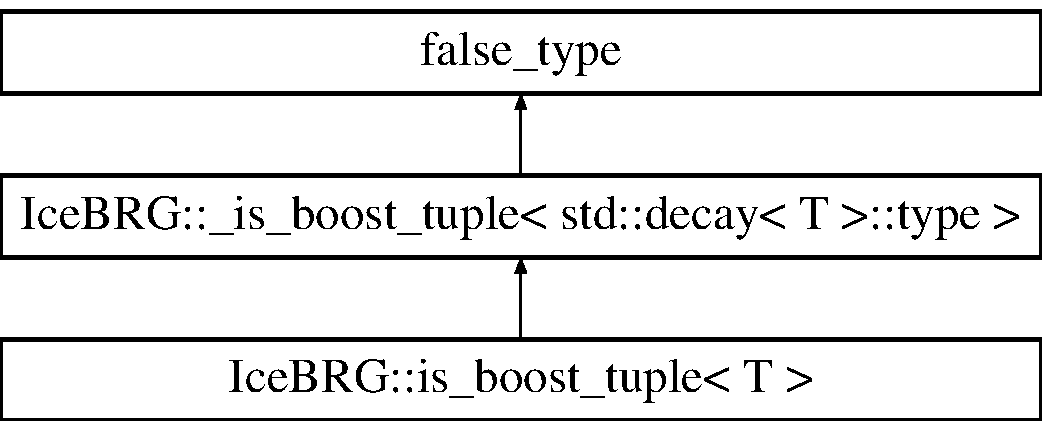
\includegraphics[height=3.000000cm]{structIceBRG_1_1is__boost__tuple}
\end{center}
\end{figure}


The documentation for this struct was generated from the following file\+:\begin{DoxyCompactItemize}
\item 
/disk2/brg/git/\+Magnification\+\_\+\+Public/src/lib/\+Ice\+B\+R\+G\+\_\+main/container/\hyperlink{is__boost__tuple_8hpp}{is\+\_\+boost\+\_\+tuple.\+hpp}\end{DoxyCompactItemize}

\hypertarget{structIceBRG_1_1is__container}{}\section{Ice\+B\+R\+G\+:\+:is\+\_\+container$<$ T $>$ Struct Template Reference}
\label{structIceBRG_1_1is__container}\index{Ice\+B\+R\+G\+::is\+\_\+container$<$ T $>$@{Ice\+B\+R\+G\+::is\+\_\+container$<$ T $>$}}


{\ttfamily \#include $<$is\+\_\+container.\+hpp$>$}

Inheritance diagram for Ice\+B\+R\+G\+:\+:is\+\_\+container$<$ T $>$\+:\begin{figure}[H]
\begin{center}
\leavevmode
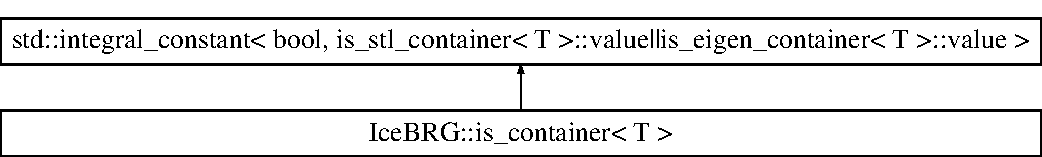
\includegraphics[height=2.000000cm]{structIceBRG_1_1is__container}
\end{center}
\end{figure}


The documentation for this struct was generated from the following file\+:\begin{DoxyCompactItemize}
\item 
/disk2/brg/git/\+Magnification\+\_\+\+Public/src/lib/\+Ice\+B\+R\+G\+\_\+main/container/\hyperlink{is__container_8hpp}{is\+\_\+container.\+hpp}\end{DoxyCompactItemize}

\hypertarget{structIceBRG_1_1is__container__or__boost__tuple}{}\section{Ice\+B\+R\+G\+:\+:is\+\_\+container\+\_\+or\+\_\+boost\+\_\+tuple$<$ T $>$ Struct Template Reference}
\label{structIceBRG_1_1is__container__or__boost__tuple}\index{Ice\+B\+R\+G\+::is\+\_\+container\+\_\+or\+\_\+boost\+\_\+tuple$<$ T $>$@{Ice\+B\+R\+G\+::is\+\_\+container\+\_\+or\+\_\+boost\+\_\+tuple$<$ T $>$}}


{\ttfamily \#include $<$is\+\_\+container.\+hpp$>$}

Inheritance diagram for Ice\+B\+R\+G\+:\+:is\+\_\+container\+\_\+or\+\_\+boost\+\_\+tuple$<$ T $>$\+:\begin{figure}[H]
\begin{center}
\leavevmode
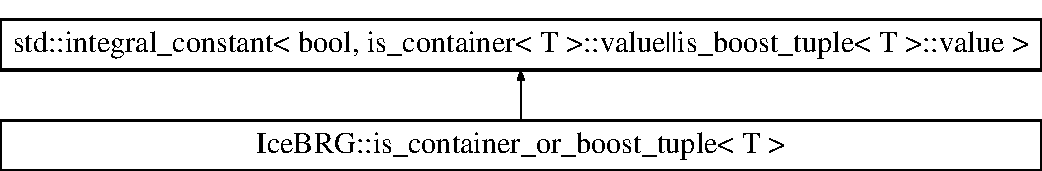
\includegraphics[height=2.000000cm]{structIceBRG_1_1is__container__or__boost__tuple}
\end{center}
\end{figure}


The documentation for this struct was generated from the following file\+:\begin{DoxyCompactItemize}
\item 
/disk2/brg/git/\+Magnification\+\_\+\+Public/src/lib/\+Ice\+B\+R\+G\+\_\+main/container/\hyperlink{is__container_8hpp}{is\+\_\+container.\+hpp}\end{DoxyCompactItemize}

\hypertarget{structIceBRG_1_1is__eigen__container}{}\section{Ice\+B\+R\+G\+:\+:is\+\_\+eigen\+\_\+container$<$ T $>$ Struct Template Reference}
\label{structIceBRG_1_1is__eigen__container}\index{Ice\+B\+R\+G\+::is\+\_\+eigen\+\_\+container$<$ T $>$@{Ice\+B\+R\+G\+::is\+\_\+eigen\+\_\+container$<$ T $>$}}


{\ttfamily \#include $<$is\+\_\+eigen\+\_\+container.\+hpp$>$}

Inheritance diagram for Ice\+B\+R\+G\+:\+:is\+\_\+eigen\+\_\+container$<$ T $>$\+:\begin{figure}[H]
\begin{center}
\leavevmode
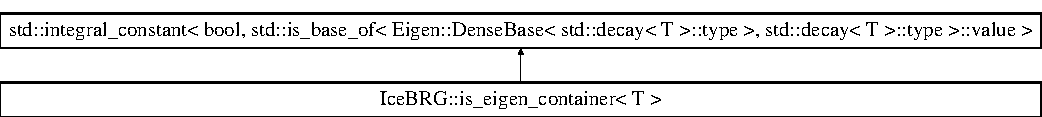
\includegraphics[height=1.577465cm]{structIceBRG_1_1is__eigen__container}
\end{center}
\end{figure}


The documentation for this struct was generated from the following file\+:\begin{DoxyCompactItemize}
\item 
/disk2/brg/git/\+Magnification\+\_\+\+Public/src/lib/\+Ice\+B\+R\+G\+\_\+main/container/\hyperlink{is__eigen__container_8hpp}{is\+\_\+eigen\+\_\+container.\+hpp}\end{DoxyCompactItemize}

\hypertarget{structIceBRG_1_1is__null__type}{}\section{Ice\+B\+R\+G\+:\+:is\+\_\+null\+\_\+type$<$ T $>$ Struct Template Reference}
\label{structIceBRG_1_1is__null__type}\index{Ice\+B\+R\+G\+::is\+\_\+null\+\_\+type$<$ T $>$@{Ice\+B\+R\+G\+::is\+\_\+null\+\_\+type$<$ T $>$}}


{\ttfamily \#include $<$is\+\_\+boost\+\_\+tuple.\+hpp$>$}

Inheritance diagram for Ice\+B\+R\+G\+:\+:is\+\_\+null\+\_\+type$<$ T $>$\+:\begin{figure}[H]
\begin{center}
\leavevmode
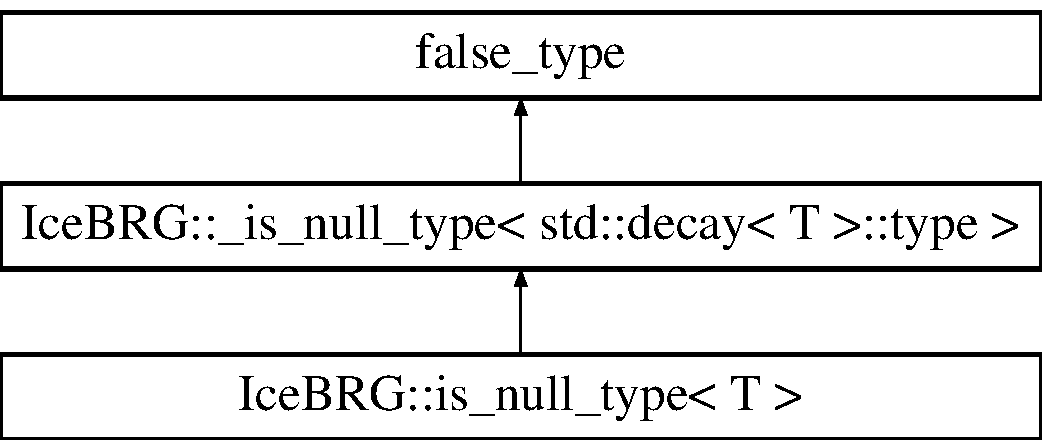
\includegraphics[height=3.000000cm]{structIceBRG_1_1is__null__type}
\end{center}
\end{figure}


The documentation for this struct was generated from the following file\+:\begin{DoxyCompactItemize}
\item 
/disk2/brg/git/\+Magnification\+\_\+\+Public/src/lib/\+Ice\+B\+R\+G\+\_\+main/container/\hyperlink{is__boost__tuple_8hpp}{is\+\_\+boost\+\_\+tuple.\+hpp}\end{DoxyCompactItemize}

\hypertarget{structIceBRG_1_1is__scalar}{}\section{Ice\+B\+R\+G\+:\+:is\+\_\+scalar$<$ T $>$ Struct Template Reference}
\label{structIceBRG_1_1is__scalar}\index{Ice\+B\+R\+G\+::is\+\_\+scalar$<$ T $>$@{Ice\+B\+R\+G\+::is\+\_\+scalar$<$ T $>$}}


{\ttfamily \#include $<$is\+\_\+container.\+hpp$>$}

Inheritance diagram for Ice\+B\+R\+G\+:\+:is\+\_\+scalar$<$ T $>$\+:\begin{figure}[H]
\begin{center}
\leavevmode
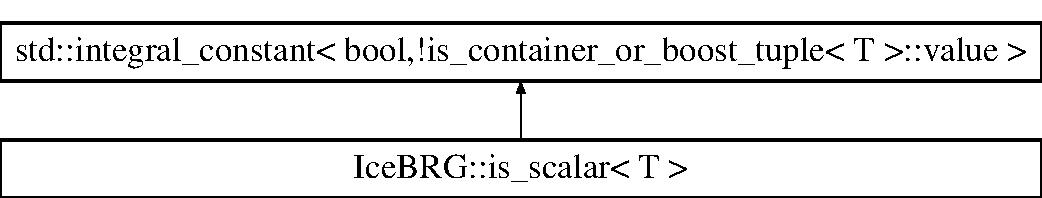
\includegraphics[height=2.000000cm]{structIceBRG_1_1is__scalar}
\end{center}
\end{figure}


The documentation for this struct was generated from the following file\+:\begin{DoxyCompactItemize}
\item 
/disk2/brg/git/\+Magnification\+\_\+\+Public/src/lib/\+Ice\+B\+R\+G\+\_\+main/container/\hyperlink{is__container_8hpp}{is\+\_\+container.\+hpp}\end{DoxyCompactItemize}

\hypertarget{structIceBRG_1_1is__scalar__or__eigen}{}\section{Ice\+B\+R\+G\+:\+:is\+\_\+scalar\+\_\+or\+\_\+eigen$<$ T $>$ Struct Template Reference}
\label{structIceBRG_1_1is__scalar__or__eigen}\index{Ice\+B\+R\+G\+::is\+\_\+scalar\+\_\+or\+\_\+eigen$<$ T $>$@{Ice\+B\+R\+G\+::is\+\_\+scalar\+\_\+or\+\_\+eigen$<$ T $>$}}


{\ttfamily \#include $<$is\+\_\+container.\+hpp$>$}

Inheritance diagram for Ice\+B\+R\+G\+:\+:is\+\_\+scalar\+\_\+or\+\_\+eigen$<$ T $>$\+:\begin{figure}[H]
\begin{center}
\leavevmode
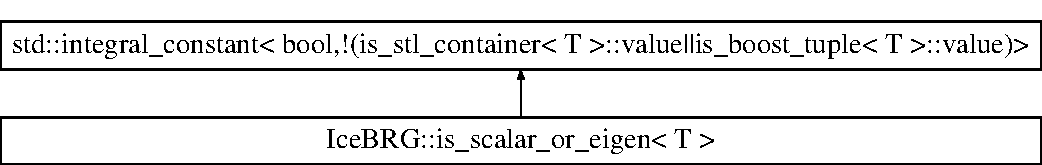
\includegraphics[height=2.000000cm]{structIceBRG_1_1is__scalar__or__eigen}
\end{center}
\end{figure}


The documentation for this struct was generated from the following file\+:\begin{DoxyCompactItemize}
\item 
/disk2/brg/git/\+Magnification\+\_\+\+Public/src/lib/\+Ice\+B\+R\+G\+\_\+main/container/\hyperlink{is__container_8hpp}{is\+\_\+container.\+hpp}\end{DoxyCompactItemize}

\hypertarget{structIceBRG_1_1is__stl__container}{}\section{Ice\+B\+R\+G\+:\+:is\+\_\+stl\+\_\+container$<$ T $>$ Struct Template Reference}
\label{structIceBRG_1_1is__stl__container}\index{Ice\+B\+R\+G\+::is\+\_\+stl\+\_\+container$<$ T $>$@{Ice\+B\+R\+G\+::is\+\_\+stl\+\_\+container$<$ T $>$}}


{\ttfamily \#include $<$is\+\_\+stl\+\_\+container.\+hpp$>$}

Inheritance diagram for Ice\+B\+R\+G\+:\+:is\+\_\+stl\+\_\+container$<$ T $>$\+:\begin{figure}[H]
\begin{center}
\leavevmode
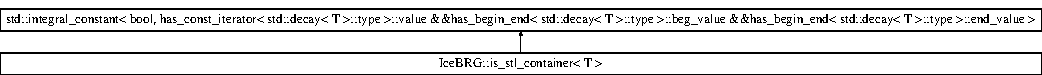
\includegraphics[height=1.009009cm]{structIceBRG_1_1is__stl__container}
\end{center}
\end{figure}


The documentation for this struct was generated from the following file\+:\begin{DoxyCompactItemize}
\item 
/disk2/brg/git/\+Magnification\+\_\+\+Public/src/lib/\+Ice\+B\+R\+G\+\_\+main/container/\hyperlink{is__stl__container_8hpp}{is\+\_\+stl\+\_\+container.\+hpp}\end{DoxyCompactItemize}

\hypertarget{classIceBRG_1_1jackknife}{}\section{Ice\+B\+R\+G\+:\+:jackknife$<$ T\+\_\+vec, T\+\_\+func $>$ Class Template Reference}
\label{classIceBRG_1_1jackknife}\index{Ice\+B\+R\+G\+::jackknife$<$ T\+\_\+vec, T\+\_\+func $>$@{Ice\+B\+R\+G\+::jackknife$<$ T\+\_\+vec, T\+\_\+func $>$}}


{\ttfamily \#include $<$resampling.\+hpp$>$}

\subsection*{Public Types}
\begin{DoxyCompactItemize}
\item 
typedef T\+\_\+vec \hyperlink{classIceBRG_1_1jackknife_ad2892a939f8fc89723db89ac837317be}{array\+\_\+type}
\item 
typedef T\+\_\+func \hyperlink{classIceBRG_1_1jackknife_a3399a8fe403193ec9f56ef991dcbfce2}{func\+\_\+type}
\item 
typedef Eigen\+::\+Array$<$ \hyperlink{classIceBRG_1_1jackknife_a1b24a65a9543f5708c9fc895620c031b}{func\+\_\+output\+\_\+type}, 1, Eigen\+::\+Dynamic $>$ \hyperlink{classIceBRG_1_1jackknife_a6eb000e6a82a691bfab8ca344e17186a}{func\+\_\+output\+\_\+array\+\_\+type}
\end{DoxyCompactItemize}
\subsection*{Public Member Functions}
\begin{DoxyCompactItemize}
\item 
\hyperlink{classIceBRG_1_1jackknife_ab87402dec3d7de00bf60cfe19d2bf195}{jackknife} (const T\+\_\+vec \&data, const T\+\_\+func \&callback=\mbox{[}$\,$\mbox{]}(const \hyperlink{classIceBRG_1_1jackknife_ad2892a939f8fc89723db89ac837317be}{array\+\_\+type} \&vec)\{return vec.\+mean();\}, const \hyperlink{lib_2IceBRG__main_2common_8h_ac4de9d9335536ac22821171deec8d39e}{int\+\_\+type} \&num\+\_\+resamples=\+\_\+default\+\_\+num\+\_\+resamples\+\_\+)
\item 
\hyperlink{classIceBRG_1_1jackknife_aba85e962f5b9becab351894c21d0c056}{jackknife} ()
\item 
const \hyperlink{classIceBRG_1_1jackknife_a3399a8fe403193ec9f56ef991dcbfce2}{func\+\_\+type} \& \hyperlink{classIceBRG_1_1jackknife_a643ad793ebc2b214f6a13342fadfc47a}{get\+\_\+callback} () const 
\item 
void \hyperlink{classIceBRG_1_1jackknife_a1cf7aba18cb9f506b0f47985cb365666}{set\+\_\+callback} (const \hyperlink{classIceBRG_1_1jackknife_a3399a8fe403193ec9f56ef991dcbfce2}{func\+\_\+type} \&callback)
\item 
const \hyperlink{classIceBRG_1_1jackknife_ad2892a939f8fc89723db89ac837317be}{array\+\_\+type} \& \hyperlink{classIceBRG_1_1jackknife_af70af47b98a1b0fe2f5c747f65227078}{get\+\_\+data} () const 
\item 
void \hyperlink{classIceBRG_1_1jackknife_a267913efacadadadc0205238ce943815}{set\+\_\+data} (const \hyperlink{classIceBRG_1_1jackknife_ad2892a939f8fc89723db89ac837317be}{array\+\_\+type} \&data)
\item 
const \hyperlink{lib_2IceBRG__main_2common_8h_ac4de9d9335536ac22821171deec8d39e}{int\+\_\+type} \& \hyperlink{classIceBRG_1_1jackknife_a9f8fbf1baa67a41be4f01206095ef7a0}{get\+\_\+num\+\_\+resamples} () const  noexcept
\item 
void \hyperlink{classIceBRG_1_1jackknife_a02369d76326d80f4be3e2c9e25a5ae5a}{set\+\_\+num\+\_\+resamples} (const \hyperlink{lib_2IceBRG__main_2common_8h_ac4de9d9335536ac22821171deec8d39e}{int\+\_\+type} \&num\+\_\+resamples)
\item 
\hyperlink{classIceBRG_1_1jackknife_a1b24a65a9543f5708c9fc895620c031b}{func\+\_\+output\+\_\+type} \hyperlink{classIceBRG_1_1jackknife_a44707243682f3c068baa7e94ae96f463}{get\+\_\+mean} ()
\item 
\hyperlink{classIceBRG_1_1jackknife_a1b24a65a9543f5708c9fc895620c031b}{func\+\_\+output\+\_\+type} \hyperlink{classIceBRG_1_1jackknife_a62db452d89c776879d6488aee2532c45}{get\+\_\+std} ()
\end{DoxyCompactItemize}
\subsection*{Public Attributes}
\begin{DoxyCompactItemize}
\item 
decltype(\hyperlink{classIceBRG_1_1jackknife_ad2892a939f8fc89723db89ac837317be}{array\+\_\+type}()\mbox{[}0\mbox{]}) typedef \hyperlink{classIceBRG_1_1jackknife_a31ed80992ab0c76c0b84122eb4186c92}{value\+\_\+type}
\item 
decltype(\hyperlink{classIceBRG_1_1jackknife_a3399a8fe403193ec9f56ef991dcbfce2}{func\+\_\+type}(\hyperlink{classIceBRG_1_1jackknife_ad2892a939f8fc89723db89ac837317be}{array\+\_\+type}())) typedef \hyperlink{classIceBRG_1_1jackknife_a1b24a65a9543f5708c9fc895620c031b}{func\+\_\+output\+\_\+type}
\end{DoxyCompactItemize}


\subsection{Member Typedef Documentation}
\hypertarget{classIceBRG_1_1jackknife_ad2892a939f8fc89723db89ac837317be}{}\index{Ice\+B\+R\+G\+::jackknife@{Ice\+B\+R\+G\+::jackknife}!array\+\_\+type@{array\+\_\+type}}
\index{array\+\_\+type@{array\+\_\+type}!Ice\+B\+R\+G\+::jackknife@{Ice\+B\+R\+G\+::jackknife}}
\subsubsection[{array\+\_\+type}]{\setlength{\rightskip}{0pt plus 5cm}template$<$typename T\+\_\+vec , typename T\+\_\+func  = std\+::function$<$decltype(\+T\+\_\+vec().\+mean())(const T\+\_\+vec \&)$>$$>$ typedef T\+\_\+vec {\bf Ice\+B\+R\+G\+::jackknife}$<$ T\+\_\+vec, T\+\_\+func $>$\+::{\bf array\+\_\+type}}\label{classIceBRG_1_1jackknife_ad2892a939f8fc89723db89ac837317be}
\hypertarget{classIceBRG_1_1jackknife_a6eb000e6a82a691bfab8ca344e17186a}{}\index{Ice\+B\+R\+G\+::jackknife@{Ice\+B\+R\+G\+::jackknife}!func\+\_\+output\+\_\+array\+\_\+type@{func\+\_\+output\+\_\+array\+\_\+type}}
\index{func\+\_\+output\+\_\+array\+\_\+type@{func\+\_\+output\+\_\+array\+\_\+type}!Ice\+B\+R\+G\+::jackknife@{Ice\+B\+R\+G\+::jackknife}}
\subsubsection[{func\+\_\+output\+\_\+array\+\_\+type}]{\setlength{\rightskip}{0pt plus 5cm}template$<$typename T\+\_\+vec , typename T\+\_\+func  = std\+::function$<$decltype(\+T\+\_\+vec().\+mean())(const T\+\_\+vec \&)$>$$>$ typedef Eigen\+::\+Array$<${\bf func\+\_\+output\+\_\+type},1,Eigen\+::\+Dynamic$>$ {\bf Ice\+B\+R\+G\+::jackknife}$<$ T\+\_\+vec, T\+\_\+func $>$\+::{\bf func\+\_\+output\+\_\+array\+\_\+type}}\label{classIceBRG_1_1jackknife_a6eb000e6a82a691bfab8ca344e17186a}
\hypertarget{classIceBRG_1_1jackknife_a3399a8fe403193ec9f56ef991dcbfce2}{}\index{Ice\+B\+R\+G\+::jackknife@{Ice\+B\+R\+G\+::jackknife}!func\+\_\+type@{func\+\_\+type}}
\index{func\+\_\+type@{func\+\_\+type}!Ice\+B\+R\+G\+::jackknife@{Ice\+B\+R\+G\+::jackknife}}
\subsubsection[{func\+\_\+type}]{\setlength{\rightskip}{0pt plus 5cm}template$<$typename T\+\_\+vec , typename T\+\_\+func  = std\+::function$<$decltype(\+T\+\_\+vec().\+mean())(const T\+\_\+vec \&)$>$$>$ typedef T\+\_\+func {\bf Ice\+B\+R\+G\+::jackknife}$<$ T\+\_\+vec, T\+\_\+func $>$\+::{\bf func\+\_\+type}}\label{classIceBRG_1_1jackknife_a3399a8fe403193ec9f56ef991dcbfce2}


\subsection{Constructor \& Destructor Documentation}
\hypertarget{classIceBRG_1_1jackknife_ab87402dec3d7de00bf60cfe19d2bf195}{}\index{Ice\+B\+R\+G\+::jackknife@{Ice\+B\+R\+G\+::jackknife}!jackknife@{jackknife}}
\index{jackknife@{jackknife}!Ice\+B\+R\+G\+::jackknife@{Ice\+B\+R\+G\+::jackknife}}
\subsubsection[{jackknife(const T\+\_\+vec \&data, const T\+\_\+func \&callback=[](const array\+\_\+type \&vec)\lcurly{}return vec.\+mean();\rcurly{}, const int\+\_\+type \&num\+\_\+resamples=\+\_\+default\+\_\+num\+\_\+resamples\+\_\+)}]{\setlength{\rightskip}{0pt plus 5cm}template$<$typename T\+\_\+vec , typename T\+\_\+func  = std\+::function$<$decltype(\+T\+\_\+vec().\+mean())(const T\+\_\+vec \&)$>$$>$ {\bf Ice\+B\+R\+G\+::jackknife}$<$ T\+\_\+vec, T\+\_\+func $>$\+::{\bf jackknife} (
\begin{DoxyParamCaption}
\item[{const T\+\_\+vec \&}]{data, }
\item[{const T\+\_\+func \&}]{callback = {\ttfamily \mbox{[}\mbox{]}~(const~{\bf array\+\_\+type}~\&~vec)~\{return~vec.mean();\}}, }
\item[{const {\bf int\+\_\+type} \&}]{num\+\_\+resamples = {\ttfamily \+\_\+default\+\_\+num\+\_\+resamples\+\_\+}}
\end{DoxyParamCaption}
)\hspace{0.3cm}{\ttfamily [inline]}}\label{classIceBRG_1_1jackknife_ab87402dec3d7de00bf60cfe19d2bf195}
\hypertarget{classIceBRG_1_1jackknife_aba85e962f5b9becab351894c21d0c056}{}\index{Ice\+B\+R\+G\+::jackknife@{Ice\+B\+R\+G\+::jackknife}!jackknife@{jackknife}}
\index{jackknife@{jackknife}!Ice\+B\+R\+G\+::jackknife@{Ice\+B\+R\+G\+::jackknife}}
\subsubsection[{jackknife()}]{\setlength{\rightskip}{0pt plus 5cm}template$<$typename T\+\_\+vec , typename T\+\_\+func  = std\+::function$<$decltype(\+T\+\_\+vec().\+mean())(const T\+\_\+vec \&)$>$$>$ {\bf Ice\+B\+R\+G\+::jackknife}$<$ T\+\_\+vec, T\+\_\+func $>$\+::{\bf jackknife} (
\begin{DoxyParamCaption}
{}
\end{DoxyParamCaption}
)\hspace{0.3cm}{\ttfamily [inline]}}\label{classIceBRG_1_1jackknife_aba85e962f5b9becab351894c21d0c056}


\subsection{Member Function Documentation}
\hypertarget{classIceBRG_1_1jackknife_a643ad793ebc2b214f6a13342fadfc47a}{}\index{Ice\+B\+R\+G\+::jackknife@{Ice\+B\+R\+G\+::jackknife}!get\+\_\+callback@{get\+\_\+callback}}
\index{get\+\_\+callback@{get\+\_\+callback}!Ice\+B\+R\+G\+::jackknife@{Ice\+B\+R\+G\+::jackknife}}
\subsubsection[{get\+\_\+callback() const }]{\setlength{\rightskip}{0pt plus 5cm}template$<$typename T\+\_\+vec , typename T\+\_\+func  = std\+::function$<$decltype(\+T\+\_\+vec().\+mean())(const T\+\_\+vec \&)$>$$>$ const {\bf func\+\_\+type}\& {\bf Ice\+B\+R\+G\+::jackknife}$<$ T\+\_\+vec, T\+\_\+func $>$\+::get\+\_\+callback (
\begin{DoxyParamCaption}
{}
\end{DoxyParamCaption}
) const\hspace{0.3cm}{\ttfamily [inline]}}\label{classIceBRG_1_1jackknife_a643ad793ebc2b214f6a13342fadfc47a}
\hypertarget{classIceBRG_1_1jackknife_af70af47b98a1b0fe2f5c747f65227078}{}\index{Ice\+B\+R\+G\+::jackknife@{Ice\+B\+R\+G\+::jackknife}!get\+\_\+data@{get\+\_\+data}}
\index{get\+\_\+data@{get\+\_\+data}!Ice\+B\+R\+G\+::jackknife@{Ice\+B\+R\+G\+::jackknife}}
\subsubsection[{get\+\_\+data() const }]{\setlength{\rightskip}{0pt plus 5cm}template$<$typename T\+\_\+vec , typename T\+\_\+func  = std\+::function$<$decltype(\+T\+\_\+vec().\+mean())(const T\+\_\+vec \&)$>$$>$ const {\bf array\+\_\+type}\& {\bf Ice\+B\+R\+G\+::jackknife}$<$ T\+\_\+vec, T\+\_\+func $>$\+::get\+\_\+data (
\begin{DoxyParamCaption}
{}
\end{DoxyParamCaption}
) const\hspace{0.3cm}{\ttfamily [inline]}}\label{classIceBRG_1_1jackknife_af70af47b98a1b0fe2f5c747f65227078}
\hypertarget{classIceBRG_1_1jackknife_a44707243682f3c068baa7e94ae96f463}{}\index{Ice\+B\+R\+G\+::jackknife@{Ice\+B\+R\+G\+::jackknife}!get\+\_\+mean@{get\+\_\+mean}}
\index{get\+\_\+mean@{get\+\_\+mean}!Ice\+B\+R\+G\+::jackknife@{Ice\+B\+R\+G\+::jackknife}}
\subsubsection[{get\+\_\+mean()}]{\setlength{\rightskip}{0pt plus 5cm}template$<$typename T\+\_\+vec , typename T\+\_\+func  = std\+::function$<$decltype(\+T\+\_\+vec().\+mean())(const T\+\_\+vec \&)$>$$>$ {\bf func\+\_\+output\+\_\+type} {\bf Ice\+B\+R\+G\+::jackknife}$<$ T\+\_\+vec, T\+\_\+func $>$\+::get\+\_\+mean (
\begin{DoxyParamCaption}
{}
\end{DoxyParamCaption}
)\hspace{0.3cm}{\ttfamily [inline]}}\label{classIceBRG_1_1jackknife_a44707243682f3c068baa7e94ae96f463}
\hypertarget{classIceBRG_1_1jackknife_a9f8fbf1baa67a41be4f01206095ef7a0}{}\index{Ice\+B\+R\+G\+::jackknife@{Ice\+B\+R\+G\+::jackknife}!get\+\_\+num\+\_\+resamples@{get\+\_\+num\+\_\+resamples}}
\index{get\+\_\+num\+\_\+resamples@{get\+\_\+num\+\_\+resamples}!Ice\+B\+R\+G\+::jackknife@{Ice\+B\+R\+G\+::jackknife}}
\subsubsection[{get\+\_\+num\+\_\+resamples() const  noexcept}]{\setlength{\rightskip}{0pt plus 5cm}template$<$typename T\+\_\+vec , typename T\+\_\+func  = std\+::function$<$decltype(\+T\+\_\+vec().\+mean())(const T\+\_\+vec \&)$>$$>$ const {\bf int\+\_\+type}\& {\bf Ice\+B\+R\+G\+::jackknife}$<$ T\+\_\+vec, T\+\_\+func $>$\+::get\+\_\+num\+\_\+resamples (
\begin{DoxyParamCaption}
{}
\end{DoxyParamCaption}
) const\hspace{0.3cm}{\ttfamily [inline]}, {\ttfamily [noexcept]}}\label{classIceBRG_1_1jackknife_a9f8fbf1baa67a41be4f01206095ef7a0}
\hypertarget{classIceBRG_1_1jackknife_a62db452d89c776879d6488aee2532c45}{}\index{Ice\+B\+R\+G\+::jackknife@{Ice\+B\+R\+G\+::jackknife}!get\+\_\+std@{get\+\_\+std}}
\index{get\+\_\+std@{get\+\_\+std}!Ice\+B\+R\+G\+::jackknife@{Ice\+B\+R\+G\+::jackknife}}
\subsubsection[{get\+\_\+std()}]{\setlength{\rightskip}{0pt plus 5cm}template$<$typename T\+\_\+vec , typename T\+\_\+func  = std\+::function$<$decltype(\+T\+\_\+vec().\+mean())(const T\+\_\+vec \&)$>$$>$ {\bf func\+\_\+output\+\_\+type} {\bf Ice\+B\+R\+G\+::jackknife}$<$ T\+\_\+vec, T\+\_\+func $>$\+::get\+\_\+std (
\begin{DoxyParamCaption}
{}
\end{DoxyParamCaption}
)\hspace{0.3cm}{\ttfamily [inline]}}\label{classIceBRG_1_1jackknife_a62db452d89c776879d6488aee2532c45}
\hypertarget{classIceBRG_1_1jackknife_a1cf7aba18cb9f506b0f47985cb365666}{}\index{Ice\+B\+R\+G\+::jackknife@{Ice\+B\+R\+G\+::jackknife}!set\+\_\+callback@{set\+\_\+callback}}
\index{set\+\_\+callback@{set\+\_\+callback}!Ice\+B\+R\+G\+::jackknife@{Ice\+B\+R\+G\+::jackknife}}
\subsubsection[{set\+\_\+callback(const func\+\_\+type \&callback)}]{\setlength{\rightskip}{0pt plus 5cm}template$<$typename T\+\_\+vec , typename T\+\_\+func  = std\+::function$<$decltype(\+T\+\_\+vec().\+mean())(const T\+\_\+vec \&)$>$$>$ void {\bf Ice\+B\+R\+G\+::jackknife}$<$ T\+\_\+vec, T\+\_\+func $>$\+::set\+\_\+callback (
\begin{DoxyParamCaption}
\item[{const {\bf func\+\_\+type} \&}]{callback}
\end{DoxyParamCaption}
)\hspace{0.3cm}{\ttfamily [inline]}}\label{classIceBRG_1_1jackknife_a1cf7aba18cb9f506b0f47985cb365666}
\hypertarget{classIceBRG_1_1jackknife_a267913efacadadadc0205238ce943815}{}\index{Ice\+B\+R\+G\+::jackknife@{Ice\+B\+R\+G\+::jackknife}!set\+\_\+data@{set\+\_\+data}}
\index{set\+\_\+data@{set\+\_\+data}!Ice\+B\+R\+G\+::jackknife@{Ice\+B\+R\+G\+::jackknife}}
\subsubsection[{set\+\_\+data(const array\+\_\+type \&data)}]{\setlength{\rightskip}{0pt plus 5cm}template$<$typename T\+\_\+vec , typename T\+\_\+func  = std\+::function$<$decltype(\+T\+\_\+vec().\+mean())(const T\+\_\+vec \&)$>$$>$ void {\bf Ice\+B\+R\+G\+::jackknife}$<$ T\+\_\+vec, T\+\_\+func $>$\+::set\+\_\+data (
\begin{DoxyParamCaption}
\item[{const {\bf array\+\_\+type} \&}]{data}
\end{DoxyParamCaption}
)\hspace{0.3cm}{\ttfamily [inline]}}\label{classIceBRG_1_1jackknife_a267913efacadadadc0205238ce943815}
\hypertarget{classIceBRG_1_1jackknife_a02369d76326d80f4be3e2c9e25a5ae5a}{}\index{Ice\+B\+R\+G\+::jackknife@{Ice\+B\+R\+G\+::jackknife}!set\+\_\+num\+\_\+resamples@{set\+\_\+num\+\_\+resamples}}
\index{set\+\_\+num\+\_\+resamples@{set\+\_\+num\+\_\+resamples}!Ice\+B\+R\+G\+::jackknife@{Ice\+B\+R\+G\+::jackknife}}
\subsubsection[{set\+\_\+num\+\_\+resamples(const int\+\_\+type \&num\+\_\+resamples)}]{\setlength{\rightskip}{0pt plus 5cm}template$<$typename T\+\_\+vec , typename T\+\_\+func  = std\+::function$<$decltype(\+T\+\_\+vec().\+mean())(const T\+\_\+vec \&)$>$$>$ void {\bf Ice\+B\+R\+G\+::jackknife}$<$ T\+\_\+vec, T\+\_\+func $>$\+::set\+\_\+num\+\_\+resamples (
\begin{DoxyParamCaption}
\item[{const {\bf int\+\_\+type} \&}]{num\+\_\+resamples}
\end{DoxyParamCaption}
)\hspace{0.3cm}{\ttfamily [inline]}}\label{classIceBRG_1_1jackknife_a02369d76326d80f4be3e2c9e25a5ae5a}


\subsection{Member Data Documentation}
\hypertarget{classIceBRG_1_1jackknife_a1b24a65a9543f5708c9fc895620c031b}{}\index{Ice\+B\+R\+G\+::jackknife@{Ice\+B\+R\+G\+::jackknife}!func\+\_\+output\+\_\+type@{func\+\_\+output\+\_\+type}}
\index{func\+\_\+output\+\_\+type@{func\+\_\+output\+\_\+type}!Ice\+B\+R\+G\+::jackknife@{Ice\+B\+R\+G\+::jackknife}}
\subsubsection[{func\+\_\+output\+\_\+type}]{\setlength{\rightskip}{0pt plus 5cm}template$<$typename T\+\_\+vec , typename T\+\_\+func  = std\+::function$<$decltype(\+T\+\_\+vec().\+mean())(const T\+\_\+vec \&)$>$$>$ decltype({\bf func\+\_\+type}({\bf array\+\_\+type}())) typedef {\bf Ice\+B\+R\+G\+::jackknife}$<$ T\+\_\+vec, T\+\_\+func $>$\+::func\+\_\+output\+\_\+type}\label{classIceBRG_1_1jackknife_a1b24a65a9543f5708c9fc895620c031b}
\hypertarget{classIceBRG_1_1jackknife_a31ed80992ab0c76c0b84122eb4186c92}{}\index{Ice\+B\+R\+G\+::jackknife@{Ice\+B\+R\+G\+::jackknife}!value\+\_\+type@{value\+\_\+type}}
\index{value\+\_\+type@{value\+\_\+type}!Ice\+B\+R\+G\+::jackknife@{Ice\+B\+R\+G\+::jackknife}}
\subsubsection[{value\+\_\+type}]{\setlength{\rightskip}{0pt plus 5cm}template$<$typename T\+\_\+vec , typename T\+\_\+func  = std\+::function$<$decltype(\+T\+\_\+vec().\+mean())(const T\+\_\+vec \&)$>$$>$ decltype({\bf array\+\_\+type}()\mbox{[}0\mbox{]}) typedef {\bf Ice\+B\+R\+G\+::jackknife}$<$ T\+\_\+vec, T\+\_\+func $>$\+::value\+\_\+type}\label{classIceBRG_1_1jackknife_a31ed80992ab0c76c0b84122eb4186c92}


The documentation for this class was generated from the following file\+:\begin{DoxyCompactItemize}
\item 
/disk2/brg/git/\+Magnification\+\_\+\+Public/src/lib/\+Ice\+B\+R\+G\+\_\+main/math/statistics/\hyperlink{resampling_8hpp}{resampling.\+hpp}\end{DoxyCompactItemize}

\hypertarget{classIceBRG_1_1labeled__array}{}\section{Ice\+B\+R\+G\+:\+:labeled\+\_\+array$<$ T\+\_\+value\+\_\+type, T\+\_\+major\+\_\+tag, T\+\_\+label\+\_\+type $>$ Class Template Reference}
\label{classIceBRG_1_1labeled__array}\index{Ice\+B\+R\+G\+::labeled\+\_\+array$<$ T\+\_\+value\+\_\+type, T\+\_\+major\+\_\+tag, T\+\_\+label\+\_\+type $>$@{Ice\+B\+R\+G\+::labeled\+\_\+array$<$ T\+\_\+value\+\_\+type, T\+\_\+major\+\_\+tag, T\+\_\+label\+\_\+type $>$}}


{\ttfamily \#include $<$labeled\+\_\+array.\+hpp$>$}

\subsection*{Public Types}
\begin{DoxyCompactItemize}
\item 
typedef Eigen\+::\+Array$<$ T\+\_\+value\+\_\+type, Eigen\+::\+Dynamic, Eigen\+::\+Dynamic, T\+\_\+major\+\_\+tag $>$ \hyperlink{classIceBRG_1_1labeled__array_a43d1c710fe591f9610ab9e9827aabba6}{data\+\_\+table\+\_\+type}
\item 
typedef Eigen\+::\+Array$<$ const T\+\_\+value\+\_\+type, Eigen\+::\+Dynamic, Eigen\+::\+Dynamic, T\+\_\+major\+\_\+tag $>$ \hyperlink{classIceBRG_1_1labeled__array_a004378b6978779cae2c375a3a83001a2}{const\+\_\+data\+\_\+table\+\_\+type}
\item 
typedef T\+\_\+value\+\_\+type \hyperlink{classIceBRG_1_1labeled__array_a183002e8991647a6fbed8c13b64ff8f4}{value\+\_\+type}
\item 
typedef const \hyperlink{classIceBRG_1_1labeled__array_a183002e8991647a6fbed8c13b64ff8f4}{value\+\_\+type} \hyperlink{classIceBRG_1_1labeled__array_a4b9270762c39bd24b1f7855a7e21a63d}{const\+\_\+value\+\_\+type}
\item 
typedef \hyperlink{classIceBRG_1_1labeled__array_a183002e8991647a6fbed8c13b64ff8f4}{value\+\_\+type} \& \hyperlink{classIceBRG_1_1labeled__array_a2842648890bc2655f359ccfd4cb5ed63}{reference}
\item 
typedef \hyperlink{classIceBRG_1_1labeled__array_a4b9270762c39bd24b1f7855a7e21a63d}{const\+\_\+value\+\_\+type} \& \hyperlink{classIceBRG_1_1labeled__array_a334a51a867cad5d5c4ad682ebe1fd5a9}{const\+\_\+reference}
\item 
typedef T\+\_\+label\+\_\+type \hyperlink{classIceBRG_1_1labeled__array_a6355a8e274be241162cfe4717bcd907f}{label\+\_\+type}
\item 
typedef const \hyperlink{classIceBRG_1_1labeled__array_a6355a8e274be241162cfe4717bcd907f}{label\+\_\+type} \hyperlink{classIceBRG_1_1labeled__array_ae6050b70db84d1f34fefc241f46320f5}{const\+\_\+label\+\_\+type}
\item 
typedef ptrdiff\+\_\+t \hyperlink{classIceBRG_1_1labeled__array_af916a9e5d8e921f4fd310618f065e0fd}{difference\+\_\+type}
\item 
typedef data\+\_\+table\+\_\+type\+::\+Col\+Xpr \hyperlink{classIceBRG_1_1labeled__array_a4ee8f2983b8f309f1a8a470c12f56f2f}{col\+\_\+type}
\item 
typedef data\+\_\+table\+\_\+type\+::\+Const\+Col\+Xpr \hyperlink{classIceBRG_1_1labeled__array_aeba72c01006c312aedb340192a56901a}{const\+\_\+col\+\_\+type}
\item 
typedef \hyperlink{classIceBRG_1_1labeled__array__col__reference}{labeled\+\_\+array\+\_\+col\+\_\+reference}$<$ \hyperlink{classIceBRG_1_1labeled__array}{labeled\+\_\+array}$<$ \hyperlink{classIceBRG_1_1labeled__array_a183002e8991647a6fbed8c13b64ff8f4}{value\+\_\+type}, T\+\_\+major\+\_\+tag, \hyperlink{classIceBRG_1_1labeled__array_a6355a8e274be241162cfe4717bcd907f}{label\+\_\+type} $>$, \hyperlink{classIceBRG_1_1labeled__array_a4ee8f2983b8f309f1a8a470c12f56f2f}{col\+\_\+type} $>$ \hyperlink{classIceBRG_1_1labeled__array_aa7217b6c3b4a663d16f579aebab5e5cf}{col\+\_\+reference}
\item 
typedef \hyperlink{classIceBRG_1_1labeled__array__col__reference}{labeled\+\_\+array\+\_\+col\+\_\+reference}$<$ const \hyperlink{classIceBRG_1_1labeled__array}{labeled\+\_\+array}$<$ \hyperlink{classIceBRG_1_1labeled__array_a183002e8991647a6fbed8c13b64ff8f4}{value\+\_\+type}, T\+\_\+major\+\_\+tag, \hyperlink{classIceBRG_1_1labeled__array_a6355a8e274be241162cfe4717bcd907f}{label\+\_\+type} $>$, \hyperlink{classIceBRG_1_1labeled__array_aeba72c01006c312aedb340192a56901a}{const\+\_\+col\+\_\+type} $>$ \hyperlink{classIceBRG_1_1labeled__array_ac655d340cc0011b66a5b8433c76841e3}{const\+\_\+col\+\_\+reference}
\item 
typedef \hyperlink{classIceBRG_1_1labeled__array__col__iterator}{labeled\+\_\+array\+\_\+col\+\_\+iterator}$<$ \hyperlink{classIceBRG_1_1labeled__array}{labeled\+\_\+array}$<$ \hyperlink{classIceBRG_1_1labeled__array_a183002e8991647a6fbed8c13b64ff8f4}{value\+\_\+type}, T\+\_\+major\+\_\+tag, \hyperlink{classIceBRG_1_1labeled__array_a6355a8e274be241162cfe4717bcd907f}{label\+\_\+type} $>$, \hyperlink{classIceBRG_1_1labeled__array_a4ee8f2983b8f309f1a8a470c12f56f2f}{col\+\_\+type}, \hyperlink{classIceBRG_1_1labeled__array_aa7217b6c3b4a663d16f579aebab5e5cf}{col\+\_\+reference} $>$ \hyperlink{classIceBRG_1_1labeled__array_a5013bbfc828083b72537e79ded5fe56d}{col\+\_\+iterator}
\item 
typedef \hyperlink{classIceBRG_1_1labeled__array__col__iterator}{labeled\+\_\+array\+\_\+col\+\_\+iterator}$<$ const \hyperlink{classIceBRG_1_1labeled__array}{labeled\+\_\+array}$<$ \hyperlink{classIceBRG_1_1labeled__array_a183002e8991647a6fbed8c13b64ff8f4}{value\+\_\+type}, T\+\_\+major\+\_\+tag, \hyperlink{classIceBRG_1_1labeled__array_a6355a8e274be241162cfe4717bcd907f}{label\+\_\+type} $>$, \hyperlink{classIceBRG_1_1labeled__array_aeba72c01006c312aedb340192a56901a}{const\+\_\+col\+\_\+type}, \hyperlink{classIceBRG_1_1labeled__array_ac655d340cc0011b66a5b8433c76841e3}{const\+\_\+col\+\_\+reference} $>$ \hyperlink{classIceBRG_1_1labeled__array_a2fd3d1ad11efc9bbfb307619cda3a695}{const\+\_\+col\+\_\+iterator}
\item 
typedef boost\+::reverse\+\_\+iterator$<$ \hyperlink{classIceBRG_1_1labeled__array_a5013bbfc828083b72537e79ded5fe56d}{col\+\_\+iterator} $>$ \hyperlink{classIceBRG_1_1labeled__array_a5837943c80f4cb557b41278ee0e339f4}{reverse\+\_\+col\+\_\+iterator}
\item 
typedef boost\+::reverse\+\_\+iterator$<$ \hyperlink{classIceBRG_1_1labeled__array_a2fd3d1ad11efc9bbfb307619cda3a695}{const\+\_\+col\+\_\+iterator} $>$ \hyperlink{classIceBRG_1_1labeled__array_a7b4b912b75ec933905708199ea2f639d}{const\+\_\+reverse\+\_\+col\+\_\+iterator}
\item 
typedef \hyperlink{classIceBRG_1_1labeled__array__vecs}{labeled\+\_\+array\+\_\+vecs}$<$ \hyperlink{classIceBRG_1_1labeled__array}{labeled\+\_\+array}$<$ \hyperlink{classIceBRG_1_1labeled__array_a183002e8991647a6fbed8c13b64ff8f4}{value\+\_\+type}, T\+\_\+major\+\_\+tag, \hyperlink{classIceBRG_1_1labeled__array_a6355a8e274be241162cfe4717bcd907f}{label\+\_\+type} $>$, \hyperlink{classIceBRG_1_1labeled__array_a4ee8f2983b8f309f1a8a470c12f56f2f}{col\+\_\+type}, \hyperlink{classIceBRG_1_1labeled__array_aeba72c01006c312aedb340192a56901a}{const\+\_\+col\+\_\+type}, \hyperlink{classIceBRG_1_1labeled__array_aa7217b6c3b4a663d16f579aebab5e5cf}{col\+\_\+reference}, \hyperlink{classIceBRG_1_1labeled__array_ac655d340cc0011b66a5b8433c76841e3}{const\+\_\+col\+\_\+reference}, \hyperlink{classIceBRG_1_1labeled__array_a5013bbfc828083b72537e79ded5fe56d}{col\+\_\+iterator}, \hyperlink{classIceBRG_1_1labeled__array_a2fd3d1ad11efc9bbfb307619cda3a695}{const\+\_\+col\+\_\+iterator} $>$ \hyperlink{classIceBRG_1_1labeled__array_a4592932c9e975c4777e0d89990ac4e5a}{cols\+\_\+type}
\item 
typedef \hyperlink{classIceBRG_1_1labeled__array__vecs}{labeled\+\_\+array\+\_\+vecs}$<$ const \hyperlink{classIceBRG_1_1labeled__array}{labeled\+\_\+array}$<$ \hyperlink{classIceBRG_1_1labeled__array_a183002e8991647a6fbed8c13b64ff8f4}{value\+\_\+type}, T\+\_\+major\+\_\+tag, \hyperlink{classIceBRG_1_1labeled__array_a6355a8e274be241162cfe4717bcd907f}{label\+\_\+type} $>$, \hyperlink{classIceBRG_1_1labeled__array_aeba72c01006c312aedb340192a56901a}{const\+\_\+col\+\_\+type}, \hyperlink{classIceBRG_1_1labeled__array_aeba72c01006c312aedb340192a56901a}{const\+\_\+col\+\_\+type}, \hyperlink{classIceBRG_1_1labeled__array_ac655d340cc0011b66a5b8433c76841e3}{const\+\_\+col\+\_\+reference}, \hyperlink{classIceBRG_1_1labeled__array_ac655d340cc0011b66a5b8433c76841e3}{const\+\_\+col\+\_\+reference}, \hyperlink{classIceBRG_1_1labeled__array_a2fd3d1ad11efc9bbfb307619cda3a695}{const\+\_\+col\+\_\+iterator}, \hyperlink{classIceBRG_1_1labeled__array_a2fd3d1ad11efc9bbfb307619cda3a695}{const\+\_\+col\+\_\+iterator} $>$ \hyperlink{classIceBRG_1_1labeled__array_a69553829b7e85c125b24e1e72dcc5491}{const\+\_\+cols\+\_\+type}
\item 
typedef \hyperlink{classIceBRG_1_1labeled__array__vecs}{labeled\+\_\+array\+\_\+vecs}$<$ \hyperlink{classIceBRG_1_1labeled__array}{labeled\+\_\+array}$<$ \hyperlink{classIceBRG_1_1labeled__array_a183002e8991647a6fbed8c13b64ff8f4}{value\+\_\+type}, T\+\_\+major\+\_\+tag, \hyperlink{classIceBRG_1_1labeled__array_a6355a8e274be241162cfe4717bcd907f}{label\+\_\+type} $>$, \hyperlink{classIceBRG_1_1labeled__array_a4ee8f2983b8f309f1a8a470c12f56f2f}{col\+\_\+type}, \hyperlink{classIceBRG_1_1labeled__array_aeba72c01006c312aedb340192a56901a}{const\+\_\+col\+\_\+type}, \hyperlink{classIceBRG_1_1labeled__array_aa7217b6c3b4a663d16f579aebab5e5cf}{col\+\_\+reference}, \hyperlink{classIceBRG_1_1labeled__array_ac655d340cc0011b66a5b8433c76841e3}{const\+\_\+col\+\_\+reference}, \hyperlink{classIceBRG_1_1labeled__array_a5013bbfc828083b72537e79ded5fe56d}{col\+\_\+iterator}, \hyperlink{classIceBRG_1_1labeled__array_a2fd3d1ad11efc9bbfb307619cda3a695}{const\+\_\+col\+\_\+iterator}, \hyperlink{namespaceIceBRG_a3f2c2517005b9902e3eb97894b072f91a9793d1e2c6b63e17ed62034e78307b63}{reverse\+\_\+tag} $>$ \hyperlink{classIceBRG_1_1labeled__array_ae1a285122696e956d2bf21b147f94f9d}{reverse\+\_\+cols\+\_\+type}
\item 
typedef \hyperlink{classIceBRG_1_1labeled__array__vecs}{labeled\+\_\+array\+\_\+vecs}$<$ const \hyperlink{classIceBRG_1_1labeled__array}{labeled\+\_\+array}$<$ \hyperlink{classIceBRG_1_1labeled__array_a183002e8991647a6fbed8c13b64ff8f4}{value\+\_\+type}, T\+\_\+major\+\_\+tag, \hyperlink{classIceBRG_1_1labeled__array_a6355a8e274be241162cfe4717bcd907f}{label\+\_\+type} $>$, \hyperlink{classIceBRG_1_1labeled__array_aeba72c01006c312aedb340192a56901a}{const\+\_\+col\+\_\+type}, \hyperlink{classIceBRG_1_1labeled__array_aeba72c01006c312aedb340192a56901a}{const\+\_\+col\+\_\+type}, \hyperlink{classIceBRG_1_1labeled__array_ac655d340cc0011b66a5b8433c76841e3}{const\+\_\+col\+\_\+reference}, \hyperlink{classIceBRG_1_1labeled__array_ac655d340cc0011b66a5b8433c76841e3}{const\+\_\+col\+\_\+reference}, \hyperlink{classIceBRG_1_1labeled__array_a2fd3d1ad11efc9bbfb307619cda3a695}{const\+\_\+col\+\_\+iterator}, \hyperlink{classIceBRG_1_1labeled__array_a2fd3d1ad11efc9bbfb307619cda3a695}{const\+\_\+col\+\_\+iterator}, \hyperlink{namespaceIceBRG_a3f2c2517005b9902e3eb97894b072f91a9793d1e2c6b63e17ed62034e78307b63}{reverse\+\_\+tag} $>$ \hyperlink{classIceBRG_1_1labeled__array_ac510eb93a7d0a73793dc7b381e8684ff}{const\+\_\+reverse\+\_\+cols\+\_\+type}
\item 
typedef \hyperlink{classIceBRG_1_1labeled__array__raw__col__iterator}{labeled\+\_\+array\+\_\+raw\+\_\+col\+\_\+iterator}$<$ \hyperlink{classIceBRG_1_1labeled__array}{labeled\+\_\+array}$<$ \hyperlink{classIceBRG_1_1labeled__array_a183002e8991647a6fbed8c13b64ff8f4}{value\+\_\+type}, T\+\_\+major\+\_\+tag, \hyperlink{classIceBRG_1_1labeled__array_a6355a8e274be241162cfe4717bcd907f}{label\+\_\+type} $>$, \hyperlink{classIceBRG_1_1labeled__array_a4ee8f2983b8f309f1a8a470c12f56f2f}{col\+\_\+type}, \hyperlink{classIceBRG_1_1labeled__array_a4ee8f2983b8f309f1a8a470c12f56f2f}{col\+\_\+type} $>$ \hyperlink{classIceBRG_1_1labeled__array_a61c797b83845ec6cc53d2ecb73899ad1}{raw\+\_\+col\+\_\+iterator}
\item 
typedef \hyperlink{classIceBRG_1_1labeled__array__raw__col__iterator}{labeled\+\_\+array\+\_\+raw\+\_\+col\+\_\+iterator}$<$ const \hyperlink{classIceBRG_1_1labeled__array}{labeled\+\_\+array}$<$ \hyperlink{classIceBRG_1_1labeled__array_a183002e8991647a6fbed8c13b64ff8f4}{value\+\_\+type}, T\+\_\+major\+\_\+tag, \hyperlink{classIceBRG_1_1labeled__array_a6355a8e274be241162cfe4717bcd907f}{label\+\_\+type} $>$, \hyperlink{classIceBRG_1_1labeled__array_aeba72c01006c312aedb340192a56901a}{const\+\_\+col\+\_\+type}, \hyperlink{classIceBRG_1_1labeled__array_aeba72c01006c312aedb340192a56901a}{const\+\_\+col\+\_\+type} $>$ \hyperlink{classIceBRG_1_1labeled__array_acfa6b748c386d02309a161e84f02e59d}{const\+\_\+raw\+\_\+col\+\_\+iterator}
\item 
typedef boost\+::reverse\+\_\+iterator$<$ \hyperlink{classIceBRG_1_1labeled__array_a61c797b83845ec6cc53d2ecb73899ad1}{raw\+\_\+col\+\_\+iterator} $>$ \hyperlink{classIceBRG_1_1labeled__array_a5c4132b2acc103385909ec165cd1a040}{reverse\+\_\+raw\+\_\+col\+\_\+iterator}
\item 
typedef boost\+::reverse\+\_\+iterator$<$ \hyperlink{classIceBRG_1_1labeled__array_acfa6b748c386d02309a161e84f02e59d}{const\+\_\+raw\+\_\+col\+\_\+iterator} $>$ \hyperlink{classIceBRG_1_1labeled__array_a397a1dbf20485f08dcf6b6a7b746d403}{const\+\_\+reverse\+\_\+raw\+\_\+col\+\_\+iterator}
\item 
typedef \hyperlink{classIceBRG_1_1labeled__array__vecs}{labeled\+\_\+array\+\_\+vecs}$<$ \hyperlink{classIceBRG_1_1labeled__array}{labeled\+\_\+array}$<$ \hyperlink{classIceBRG_1_1labeled__array_a183002e8991647a6fbed8c13b64ff8f4}{value\+\_\+type}, T\+\_\+major\+\_\+tag, \hyperlink{classIceBRG_1_1labeled__array_a6355a8e274be241162cfe4717bcd907f}{label\+\_\+type} $>$, \hyperlink{classIceBRG_1_1labeled__array_a4ee8f2983b8f309f1a8a470c12f56f2f}{col\+\_\+type}, \hyperlink{classIceBRG_1_1labeled__array_aeba72c01006c312aedb340192a56901a}{const\+\_\+col\+\_\+type}, \hyperlink{classIceBRG_1_1labeled__array_aa7217b6c3b4a663d16f579aebab5e5cf}{col\+\_\+reference}, \hyperlink{classIceBRG_1_1labeled__array_ac655d340cc0011b66a5b8433c76841e3}{const\+\_\+col\+\_\+reference}, \hyperlink{classIceBRG_1_1labeled__array_a61c797b83845ec6cc53d2ecb73899ad1}{raw\+\_\+col\+\_\+iterator}, \hyperlink{classIceBRG_1_1labeled__array_acfa6b748c386d02309a161e84f02e59d}{const\+\_\+raw\+\_\+col\+\_\+iterator} $>$ \hyperlink{classIceBRG_1_1labeled__array_a5135379d418bba0a185e5c26a9774f78}{raw\+\_\+cols\+\_\+type}
\item 
typedef \hyperlink{classIceBRG_1_1labeled__array__vecs}{labeled\+\_\+array\+\_\+vecs}$<$ const \hyperlink{classIceBRG_1_1labeled__array}{labeled\+\_\+array}$<$ \hyperlink{classIceBRG_1_1labeled__array_a183002e8991647a6fbed8c13b64ff8f4}{value\+\_\+type}, T\+\_\+major\+\_\+tag, \hyperlink{classIceBRG_1_1labeled__array_a6355a8e274be241162cfe4717bcd907f}{label\+\_\+type} $>$, \hyperlink{classIceBRG_1_1labeled__array_aeba72c01006c312aedb340192a56901a}{const\+\_\+col\+\_\+type}, \hyperlink{classIceBRG_1_1labeled__array_aeba72c01006c312aedb340192a56901a}{const\+\_\+col\+\_\+type}, \hyperlink{classIceBRG_1_1labeled__array_ac655d340cc0011b66a5b8433c76841e3}{const\+\_\+col\+\_\+reference}, \hyperlink{classIceBRG_1_1labeled__array_ac655d340cc0011b66a5b8433c76841e3}{const\+\_\+col\+\_\+reference}, \hyperlink{classIceBRG_1_1labeled__array_acfa6b748c386d02309a161e84f02e59d}{const\+\_\+raw\+\_\+col\+\_\+iterator}, \hyperlink{classIceBRG_1_1labeled__array_acfa6b748c386d02309a161e84f02e59d}{const\+\_\+raw\+\_\+col\+\_\+iterator} $>$ \hyperlink{classIceBRG_1_1labeled__array_a6aed831097e39e3fdd483625fea14042}{const\+\_\+raw\+\_\+cols\+\_\+type}
\item 
typedef \hyperlink{classIceBRG_1_1labeled__array__vecs}{labeled\+\_\+array\+\_\+vecs}$<$ \hyperlink{classIceBRG_1_1labeled__array}{labeled\+\_\+array}$<$ \hyperlink{classIceBRG_1_1labeled__array_a183002e8991647a6fbed8c13b64ff8f4}{value\+\_\+type}, T\+\_\+major\+\_\+tag, \hyperlink{classIceBRG_1_1labeled__array_a6355a8e274be241162cfe4717bcd907f}{label\+\_\+type} $>$, \hyperlink{classIceBRG_1_1labeled__array_a4ee8f2983b8f309f1a8a470c12f56f2f}{col\+\_\+type}, \hyperlink{classIceBRG_1_1labeled__array_aeba72c01006c312aedb340192a56901a}{const\+\_\+col\+\_\+type}, \hyperlink{classIceBRG_1_1labeled__array_aa7217b6c3b4a663d16f579aebab5e5cf}{col\+\_\+reference}, \hyperlink{classIceBRG_1_1labeled__array_ac655d340cc0011b66a5b8433c76841e3}{const\+\_\+col\+\_\+reference}, \hyperlink{classIceBRG_1_1labeled__array_a61c797b83845ec6cc53d2ecb73899ad1}{raw\+\_\+col\+\_\+iterator}, \hyperlink{classIceBRG_1_1labeled__array_acfa6b748c386d02309a161e84f02e59d}{const\+\_\+raw\+\_\+col\+\_\+iterator}, \hyperlink{namespaceIceBRG_a3f2c2517005b9902e3eb97894b072f91a9793d1e2c6b63e17ed62034e78307b63}{reverse\+\_\+tag} $>$ \hyperlink{classIceBRG_1_1labeled__array_a38a503b3f572b6be9ec11f817f61bb17}{reverse\+\_\+raw\+\_\+cols\+\_\+type}
\item 
typedef \hyperlink{classIceBRG_1_1labeled__array__vecs}{labeled\+\_\+array\+\_\+vecs}$<$ const \hyperlink{classIceBRG_1_1labeled__array}{labeled\+\_\+array}$<$ \hyperlink{classIceBRG_1_1labeled__array_a183002e8991647a6fbed8c13b64ff8f4}{value\+\_\+type}, T\+\_\+major\+\_\+tag, \hyperlink{classIceBRG_1_1labeled__array_a6355a8e274be241162cfe4717bcd907f}{label\+\_\+type} $>$, \hyperlink{classIceBRG_1_1labeled__array_aeba72c01006c312aedb340192a56901a}{const\+\_\+col\+\_\+type}, \hyperlink{classIceBRG_1_1labeled__array_aeba72c01006c312aedb340192a56901a}{const\+\_\+col\+\_\+type}, \hyperlink{classIceBRG_1_1labeled__array_ac655d340cc0011b66a5b8433c76841e3}{const\+\_\+col\+\_\+reference}, \hyperlink{classIceBRG_1_1labeled__array_ac655d340cc0011b66a5b8433c76841e3}{const\+\_\+col\+\_\+reference}, \hyperlink{classIceBRG_1_1labeled__array_acfa6b748c386d02309a161e84f02e59d}{const\+\_\+raw\+\_\+col\+\_\+iterator}, \hyperlink{classIceBRG_1_1labeled__array_acfa6b748c386d02309a161e84f02e59d}{const\+\_\+raw\+\_\+col\+\_\+iterator}, \hyperlink{namespaceIceBRG_a3f2c2517005b9902e3eb97894b072f91a9793d1e2c6b63e17ed62034e78307b63}{reverse\+\_\+tag} $>$ \hyperlink{classIceBRG_1_1labeled__array_ae4061b413f50fe4f35caacf5318ba324}{const\+\_\+reverse\+\_\+raw\+\_\+cols\+\_\+type}
\item 
typedef data\+\_\+table\+\_\+type\+::\+Row\+Xpr \hyperlink{classIceBRG_1_1labeled__array_a49606864eaff0c45136282a32dd6f44f}{row\+\_\+type}
\item 
typedef data\+\_\+table\+\_\+type\+::\+Const\+Row\+Xpr \hyperlink{classIceBRG_1_1labeled__array_adc26b87565fcd554a2b1f82adf965084}{const\+\_\+row\+\_\+type}
\item 
typedef \hyperlink{classIceBRG_1_1labeled__array__row__reference}{labeled\+\_\+array\+\_\+row\+\_\+reference}$<$ \hyperlink{classIceBRG_1_1labeled__array}{labeled\+\_\+array}$<$ \hyperlink{classIceBRG_1_1labeled__array_a183002e8991647a6fbed8c13b64ff8f4}{value\+\_\+type}, T\+\_\+major\+\_\+tag, \hyperlink{classIceBRG_1_1labeled__array_a6355a8e274be241162cfe4717bcd907f}{label\+\_\+type} $>$, \hyperlink{classIceBRG_1_1labeled__array_a49606864eaff0c45136282a32dd6f44f}{row\+\_\+type} $>$ \hyperlink{classIceBRG_1_1labeled__array_a1bcd1efbba3ca49030c7acd8910195e6}{row\+\_\+reference}
\item 
typedef \hyperlink{classIceBRG_1_1labeled__array__row__reference}{labeled\+\_\+array\+\_\+row\+\_\+reference}$<$ const \hyperlink{classIceBRG_1_1labeled__array}{labeled\+\_\+array}$<$ \hyperlink{classIceBRG_1_1labeled__array_a183002e8991647a6fbed8c13b64ff8f4}{value\+\_\+type}, T\+\_\+major\+\_\+tag, \hyperlink{classIceBRG_1_1labeled__array_a6355a8e274be241162cfe4717bcd907f}{label\+\_\+type} $>$, \hyperlink{classIceBRG_1_1labeled__array_adc26b87565fcd554a2b1f82adf965084}{const\+\_\+row\+\_\+type} $>$ \hyperlink{classIceBRG_1_1labeled__array_ac210266c8ef4db02af31dd1a1a2625f5}{const\+\_\+row\+\_\+reference}
\item 
typedef \hyperlink{classIceBRG_1_1labeled__array__row__iterator}{labeled\+\_\+array\+\_\+row\+\_\+iterator}$<$ \hyperlink{classIceBRG_1_1labeled__array}{labeled\+\_\+array}$<$ \hyperlink{classIceBRG_1_1labeled__array_a183002e8991647a6fbed8c13b64ff8f4}{value\+\_\+type}, T\+\_\+major\+\_\+tag, \hyperlink{classIceBRG_1_1labeled__array_a6355a8e274be241162cfe4717bcd907f}{label\+\_\+type} $>$, \hyperlink{classIceBRG_1_1labeled__array_a49606864eaff0c45136282a32dd6f44f}{row\+\_\+type}, \hyperlink{classIceBRG_1_1labeled__array_a1bcd1efbba3ca49030c7acd8910195e6}{row\+\_\+reference} $>$ \hyperlink{classIceBRG_1_1labeled__array_a53f977307768e8a9f19dae19ebfbea8c}{row\+\_\+iterator}
\item 
typedef \hyperlink{classIceBRG_1_1labeled__array__row__iterator}{labeled\+\_\+array\+\_\+row\+\_\+iterator}$<$ const \hyperlink{classIceBRG_1_1labeled__array}{labeled\+\_\+array}$<$ \hyperlink{classIceBRG_1_1labeled__array_a183002e8991647a6fbed8c13b64ff8f4}{value\+\_\+type}, T\+\_\+major\+\_\+tag, \hyperlink{classIceBRG_1_1labeled__array_a6355a8e274be241162cfe4717bcd907f}{label\+\_\+type} $>$, \hyperlink{classIceBRG_1_1labeled__array_adc26b87565fcd554a2b1f82adf965084}{const\+\_\+row\+\_\+type}, \hyperlink{classIceBRG_1_1labeled__array_ac210266c8ef4db02af31dd1a1a2625f5}{const\+\_\+row\+\_\+reference} $>$ \hyperlink{classIceBRG_1_1labeled__array_a81050e4e902b564b0c06224224a5c066}{const\+\_\+row\+\_\+iterator}
\item 
typedef boost\+::reverse\+\_\+iterator$<$ \hyperlink{classIceBRG_1_1labeled__array_a53f977307768e8a9f19dae19ebfbea8c}{row\+\_\+iterator} $>$ \hyperlink{classIceBRG_1_1labeled__array_a8c245b61b1a5c2d9ea440da50d734676}{reverse\+\_\+row\+\_\+iterator}
\item 
typedef boost\+::reverse\+\_\+iterator$<$ \hyperlink{classIceBRG_1_1labeled__array_a81050e4e902b564b0c06224224a5c066}{const\+\_\+row\+\_\+iterator} $>$ \hyperlink{classIceBRG_1_1labeled__array_a5f03fa967c469ac1a6d16f7eccf48943}{const\+\_\+reverse\+\_\+row\+\_\+iterator}
\item 
typedef \hyperlink{classIceBRG_1_1labeled__array__vecs}{labeled\+\_\+array\+\_\+vecs}$<$ \hyperlink{classIceBRG_1_1labeled__array}{labeled\+\_\+array}$<$ \hyperlink{classIceBRG_1_1labeled__array_a183002e8991647a6fbed8c13b64ff8f4}{value\+\_\+type}, T\+\_\+major\+\_\+tag, \hyperlink{classIceBRG_1_1labeled__array_a6355a8e274be241162cfe4717bcd907f}{label\+\_\+type} $>$, \hyperlink{classIceBRG_1_1labeled__array_a49606864eaff0c45136282a32dd6f44f}{row\+\_\+type}, \hyperlink{classIceBRG_1_1labeled__array_adc26b87565fcd554a2b1f82adf965084}{const\+\_\+row\+\_\+type}, \hyperlink{classIceBRG_1_1labeled__array_a1bcd1efbba3ca49030c7acd8910195e6}{row\+\_\+reference}, \hyperlink{classIceBRG_1_1labeled__array_ac210266c8ef4db02af31dd1a1a2625f5}{const\+\_\+row\+\_\+reference}, \hyperlink{classIceBRG_1_1labeled__array_a53f977307768e8a9f19dae19ebfbea8c}{row\+\_\+iterator}, \hyperlink{classIceBRG_1_1labeled__array_a81050e4e902b564b0c06224224a5c066}{const\+\_\+row\+\_\+iterator} $>$ \hyperlink{classIceBRG_1_1labeled__array_a9d293f119488089606bb583de7d22b7c}{rows\+\_\+type}
\item 
typedef \hyperlink{classIceBRG_1_1labeled__array__vecs}{labeled\+\_\+array\+\_\+vecs}$<$ const \hyperlink{classIceBRG_1_1labeled__array}{labeled\+\_\+array}$<$ \hyperlink{classIceBRG_1_1labeled__array_a183002e8991647a6fbed8c13b64ff8f4}{value\+\_\+type}, T\+\_\+major\+\_\+tag, \hyperlink{classIceBRG_1_1labeled__array_a6355a8e274be241162cfe4717bcd907f}{label\+\_\+type} $>$, \hyperlink{classIceBRG_1_1labeled__array_adc26b87565fcd554a2b1f82adf965084}{const\+\_\+row\+\_\+type}, \hyperlink{classIceBRG_1_1labeled__array_adc26b87565fcd554a2b1f82adf965084}{const\+\_\+row\+\_\+type}, \hyperlink{classIceBRG_1_1labeled__array_ac210266c8ef4db02af31dd1a1a2625f5}{const\+\_\+row\+\_\+reference}, \hyperlink{classIceBRG_1_1labeled__array_ac210266c8ef4db02af31dd1a1a2625f5}{const\+\_\+row\+\_\+reference}, \hyperlink{classIceBRG_1_1labeled__array_a81050e4e902b564b0c06224224a5c066}{const\+\_\+row\+\_\+iterator}, \hyperlink{classIceBRG_1_1labeled__array_a81050e4e902b564b0c06224224a5c066}{const\+\_\+row\+\_\+iterator} $>$ \hyperlink{classIceBRG_1_1labeled__array_a6aec05e454845b2750b446c00fd4c9fb}{const\+\_\+rows\+\_\+type}
\item 
typedef \hyperlink{classIceBRG_1_1labeled__array__vecs}{labeled\+\_\+array\+\_\+vecs}$<$ \hyperlink{classIceBRG_1_1labeled__array}{labeled\+\_\+array}$<$ \hyperlink{classIceBRG_1_1labeled__array_a183002e8991647a6fbed8c13b64ff8f4}{value\+\_\+type}, T\+\_\+major\+\_\+tag, \hyperlink{classIceBRG_1_1labeled__array_a6355a8e274be241162cfe4717bcd907f}{label\+\_\+type} $>$, \hyperlink{classIceBRG_1_1labeled__array_a49606864eaff0c45136282a32dd6f44f}{row\+\_\+type}, \hyperlink{classIceBRG_1_1labeled__array_adc26b87565fcd554a2b1f82adf965084}{const\+\_\+row\+\_\+type}, \hyperlink{classIceBRG_1_1labeled__array_a1bcd1efbba3ca49030c7acd8910195e6}{row\+\_\+reference}, \hyperlink{classIceBRG_1_1labeled__array_ac210266c8ef4db02af31dd1a1a2625f5}{const\+\_\+row\+\_\+reference}, \hyperlink{classIceBRG_1_1labeled__array_a53f977307768e8a9f19dae19ebfbea8c}{row\+\_\+iterator}, \hyperlink{classIceBRG_1_1labeled__array_a81050e4e902b564b0c06224224a5c066}{const\+\_\+row\+\_\+iterator}, \hyperlink{namespaceIceBRG_a3f2c2517005b9902e3eb97894b072f91a9793d1e2c6b63e17ed62034e78307b63}{reverse\+\_\+tag} $>$ \hyperlink{classIceBRG_1_1labeled__array_a24ccb02827e9be94dadbcf647c663b03}{reverse\+\_\+rows\+\_\+type}
\item 
typedef \hyperlink{classIceBRG_1_1labeled__array__vecs}{labeled\+\_\+array\+\_\+vecs}$<$ const \hyperlink{classIceBRG_1_1labeled__array}{labeled\+\_\+array}$<$ \hyperlink{classIceBRG_1_1labeled__array_a183002e8991647a6fbed8c13b64ff8f4}{value\+\_\+type}, T\+\_\+major\+\_\+tag, \hyperlink{classIceBRG_1_1labeled__array_a6355a8e274be241162cfe4717bcd907f}{label\+\_\+type} $>$, \hyperlink{classIceBRG_1_1labeled__array_adc26b87565fcd554a2b1f82adf965084}{const\+\_\+row\+\_\+type}, \hyperlink{classIceBRG_1_1labeled__array_adc26b87565fcd554a2b1f82adf965084}{const\+\_\+row\+\_\+type}, \hyperlink{classIceBRG_1_1labeled__array_ac210266c8ef4db02af31dd1a1a2625f5}{const\+\_\+row\+\_\+reference}, \hyperlink{classIceBRG_1_1labeled__array_ac210266c8ef4db02af31dd1a1a2625f5}{const\+\_\+row\+\_\+reference}, \hyperlink{classIceBRG_1_1labeled__array_a81050e4e902b564b0c06224224a5c066}{const\+\_\+row\+\_\+iterator}, \hyperlink{classIceBRG_1_1labeled__array_a81050e4e902b564b0c06224224a5c066}{const\+\_\+row\+\_\+iterator}, \hyperlink{namespaceIceBRG_a3f2c2517005b9902e3eb97894b072f91a9793d1e2c6b63e17ed62034e78307b63}{reverse\+\_\+tag} $>$ \hyperlink{classIceBRG_1_1labeled__array_a4d8f245def66ea4352beb6299a657bfb}{const\+\_\+reverse\+\_\+rows\+\_\+type}
\item 
typedef \hyperlink{classIceBRG_1_1labeled__array__raw__row__iterator}{labeled\+\_\+array\+\_\+raw\+\_\+row\+\_\+iterator}$<$ \hyperlink{classIceBRG_1_1labeled__array}{labeled\+\_\+array}$<$ \hyperlink{classIceBRG_1_1labeled__array_a183002e8991647a6fbed8c13b64ff8f4}{value\+\_\+type}, T\+\_\+major\+\_\+tag, \hyperlink{classIceBRG_1_1labeled__array_a6355a8e274be241162cfe4717bcd907f}{label\+\_\+type} $>$, \hyperlink{classIceBRG_1_1labeled__array_a49606864eaff0c45136282a32dd6f44f}{row\+\_\+type}, \hyperlink{classIceBRG_1_1labeled__array_a49606864eaff0c45136282a32dd6f44f}{row\+\_\+type} $>$ \hyperlink{classIceBRG_1_1labeled__array_ade890503843cb998a2d611e2dc56eefb}{raw\+\_\+row\+\_\+iterator}
\item 
typedef \hyperlink{classIceBRG_1_1labeled__array__raw__row__iterator}{labeled\+\_\+array\+\_\+raw\+\_\+row\+\_\+iterator}$<$ const \hyperlink{classIceBRG_1_1labeled__array}{labeled\+\_\+array}$<$ \hyperlink{classIceBRG_1_1labeled__array_a183002e8991647a6fbed8c13b64ff8f4}{value\+\_\+type}, T\+\_\+major\+\_\+tag, \hyperlink{classIceBRG_1_1labeled__array_a6355a8e274be241162cfe4717bcd907f}{label\+\_\+type} $>$, \hyperlink{classIceBRG_1_1labeled__array_adc26b87565fcd554a2b1f82adf965084}{const\+\_\+row\+\_\+type}, \hyperlink{classIceBRG_1_1labeled__array_adc26b87565fcd554a2b1f82adf965084}{const\+\_\+row\+\_\+type} $>$ \hyperlink{classIceBRG_1_1labeled__array_aeac7979069eab6c371dca3e6f3dd9ee9}{const\+\_\+raw\+\_\+row\+\_\+iterator}
\item 
typedef boost\+::reverse\+\_\+iterator$<$ \hyperlink{classIceBRG_1_1labeled__array_ade890503843cb998a2d611e2dc56eefb}{raw\+\_\+row\+\_\+iterator} $>$ \hyperlink{classIceBRG_1_1labeled__array_a211a4c8c7435da2eea6481b434bfdef1}{reverse\+\_\+raw\+\_\+row\+\_\+iterator}
\item 
typedef boost\+::reverse\+\_\+iterator$<$ \hyperlink{classIceBRG_1_1labeled__array_aeac7979069eab6c371dca3e6f3dd9ee9}{const\+\_\+raw\+\_\+row\+\_\+iterator} $>$ \hyperlink{classIceBRG_1_1labeled__array_a4f41b194ac74740bac37a7e0ff051a4f}{const\+\_\+reverse\+\_\+raw\+\_\+row\+\_\+iterator}
\item 
typedef \hyperlink{classIceBRG_1_1labeled__array__vecs}{labeled\+\_\+array\+\_\+vecs}$<$ \hyperlink{classIceBRG_1_1labeled__array}{labeled\+\_\+array}$<$ \hyperlink{classIceBRG_1_1labeled__array_a183002e8991647a6fbed8c13b64ff8f4}{value\+\_\+type}, T\+\_\+major\+\_\+tag, \hyperlink{classIceBRG_1_1labeled__array_a6355a8e274be241162cfe4717bcd907f}{label\+\_\+type} $>$, \hyperlink{classIceBRG_1_1labeled__array_a49606864eaff0c45136282a32dd6f44f}{row\+\_\+type}, \hyperlink{classIceBRG_1_1labeled__array_adc26b87565fcd554a2b1f82adf965084}{const\+\_\+row\+\_\+type}, \hyperlink{classIceBRG_1_1labeled__array_a1bcd1efbba3ca49030c7acd8910195e6}{row\+\_\+reference}, \hyperlink{classIceBRG_1_1labeled__array_ac210266c8ef4db02af31dd1a1a2625f5}{const\+\_\+row\+\_\+reference}, \hyperlink{classIceBRG_1_1labeled__array_ade890503843cb998a2d611e2dc56eefb}{raw\+\_\+row\+\_\+iterator}, \hyperlink{classIceBRG_1_1labeled__array_aeac7979069eab6c371dca3e6f3dd9ee9}{const\+\_\+raw\+\_\+row\+\_\+iterator} $>$ \hyperlink{classIceBRG_1_1labeled__array_a87c569635102ad3390845861bc9cf5cc}{raw\+\_\+rows\+\_\+type}
\item 
typedef \hyperlink{classIceBRG_1_1labeled__array__vecs}{labeled\+\_\+array\+\_\+vecs}$<$ const \hyperlink{classIceBRG_1_1labeled__array}{labeled\+\_\+array}$<$ \hyperlink{classIceBRG_1_1labeled__array_a183002e8991647a6fbed8c13b64ff8f4}{value\+\_\+type}, T\+\_\+major\+\_\+tag, \hyperlink{classIceBRG_1_1labeled__array_a6355a8e274be241162cfe4717bcd907f}{label\+\_\+type} $>$, \hyperlink{classIceBRG_1_1labeled__array_adc26b87565fcd554a2b1f82adf965084}{const\+\_\+row\+\_\+type}, \hyperlink{classIceBRG_1_1labeled__array_adc26b87565fcd554a2b1f82adf965084}{const\+\_\+row\+\_\+type}, \hyperlink{classIceBRG_1_1labeled__array_ac210266c8ef4db02af31dd1a1a2625f5}{const\+\_\+row\+\_\+reference}, \hyperlink{classIceBRG_1_1labeled__array_ac210266c8ef4db02af31dd1a1a2625f5}{const\+\_\+row\+\_\+reference}, \hyperlink{classIceBRG_1_1labeled__array_aeac7979069eab6c371dca3e6f3dd9ee9}{const\+\_\+raw\+\_\+row\+\_\+iterator}, \hyperlink{classIceBRG_1_1labeled__array_aeac7979069eab6c371dca3e6f3dd9ee9}{const\+\_\+raw\+\_\+row\+\_\+iterator} $>$ \hyperlink{classIceBRG_1_1labeled__array_adecd8b6c6343a2618a1c47c6f15b9ea2}{const\+\_\+raw\+\_\+rows\+\_\+type}
\item 
typedef \hyperlink{classIceBRG_1_1labeled__array__vecs}{labeled\+\_\+array\+\_\+vecs}$<$ \hyperlink{classIceBRG_1_1labeled__array}{labeled\+\_\+array}$<$ \hyperlink{classIceBRG_1_1labeled__array_a183002e8991647a6fbed8c13b64ff8f4}{value\+\_\+type}, T\+\_\+major\+\_\+tag, \hyperlink{classIceBRG_1_1labeled__array_a6355a8e274be241162cfe4717bcd907f}{label\+\_\+type} $>$, \hyperlink{classIceBRG_1_1labeled__array_a49606864eaff0c45136282a32dd6f44f}{row\+\_\+type}, \hyperlink{classIceBRG_1_1labeled__array_adc26b87565fcd554a2b1f82adf965084}{const\+\_\+row\+\_\+type}, \hyperlink{classIceBRG_1_1labeled__array_a1bcd1efbba3ca49030c7acd8910195e6}{row\+\_\+reference}, \hyperlink{classIceBRG_1_1labeled__array_ac210266c8ef4db02af31dd1a1a2625f5}{const\+\_\+row\+\_\+reference}, \hyperlink{classIceBRG_1_1labeled__array_ade890503843cb998a2d611e2dc56eefb}{raw\+\_\+row\+\_\+iterator}, \hyperlink{classIceBRG_1_1labeled__array_aeac7979069eab6c371dca3e6f3dd9ee9}{const\+\_\+raw\+\_\+row\+\_\+iterator}, \hyperlink{namespaceIceBRG_a3f2c2517005b9902e3eb97894b072f91a9793d1e2c6b63e17ed62034e78307b63}{reverse\+\_\+tag} $>$ \hyperlink{classIceBRG_1_1labeled__array_ae4ef7537f1bfb799048e17588ccd2be0}{reverse\+\_\+raw\+\_\+rows\+\_\+type}
\item 
typedef \hyperlink{classIceBRG_1_1labeled__array__vecs}{labeled\+\_\+array\+\_\+vecs}$<$ const \hyperlink{classIceBRG_1_1labeled__array}{labeled\+\_\+array}$<$ \hyperlink{classIceBRG_1_1labeled__array_a183002e8991647a6fbed8c13b64ff8f4}{value\+\_\+type}, T\+\_\+major\+\_\+tag, \hyperlink{classIceBRG_1_1labeled__array_a6355a8e274be241162cfe4717bcd907f}{label\+\_\+type} $>$, \hyperlink{classIceBRG_1_1labeled__array_adc26b87565fcd554a2b1f82adf965084}{const\+\_\+row\+\_\+type}, \hyperlink{classIceBRG_1_1labeled__array_adc26b87565fcd554a2b1f82adf965084}{const\+\_\+row\+\_\+type}, \hyperlink{classIceBRG_1_1labeled__array_ac210266c8ef4db02af31dd1a1a2625f5}{const\+\_\+row\+\_\+reference}, \hyperlink{classIceBRG_1_1labeled__array_ac210266c8ef4db02af31dd1a1a2625f5}{const\+\_\+row\+\_\+reference}, \hyperlink{classIceBRG_1_1labeled__array_aeac7979069eab6c371dca3e6f3dd9ee9}{const\+\_\+raw\+\_\+row\+\_\+iterator}, \hyperlink{classIceBRG_1_1labeled__array_aeac7979069eab6c371dca3e6f3dd9ee9}{const\+\_\+raw\+\_\+row\+\_\+iterator}, \hyperlink{namespaceIceBRG_a3f2c2517005b9902e3eb97894b072f91a9793d1e2c6b63e17ed62034e78307b63}{reverse\+\_\+tag} $>$ \hyperlink{classIceBRG_1_1labeled__array_a83872d8babf4f2e0db65776cac90aa38}{const\+\_\+reverse\+\_\+raw\+\_\+rows\+\_\+type}
\item 
typedef \hyperlink{classIceBRG_1_1labeled__array_a183002e8991647a6fbed8c13b64ff8f4}{value\+\_\+type} $\ast$ \hyperlink{classIceBRG_1_1labeled__array_a15c8011c5051008033578e5e50e25820}{iterator}
\item 
typedef \hyperlink{classIceBRG_1_1labeled__array_a4b9270762c39bd24b1f7855a7e21a63d}{const\+\_\+value\+\_\+type} $\ast$ \hyperlink{classIceBRG_1_1labeled__array_ae50c667e3ccb32675f43d38b9132a212}{const\+\_\+iterator}
\item 
typedef boost\+::reverse\+\_\+iterator$<$ \hyperlink{classIceBRG_1_1labeled__array_a15c8011c5051008033578e5e50e25820}{iterator} $>$ \hyperlink{classIceBRG_1_1labeled__array_a5125d18747cdbb29f32a4a46c97d348e}{reverse\+\_\+iterator}
\item 
typedef boost\+::reverse\+\_\+iterator$<$ \hyperlink{classIceBRG_1_1labeled__array_ae50c667e3ccb32675f43d38b9132a212}{const\+\_\+iterator} $>$ \hyperlink{classIceBRG_1_1labeled__array_a5088e7c1e054a6f2d6067664ee29fafb}{const\+\_\+reverse\+\_\+iterator}
\item 
typedef \hyperlink{namespaceIceBRG_structIceBRG_1_1labeled__array__iterator__chooser}{labeled\+\_\+array\+\_\+iterator\+\_\+chooser}$<$ \hyperlink{classIceBRG_1_1labeled__array_a183002e8991647a6fbed8c13b64ff8f4}{value\+\_\+type}, T\+\_\+major\+\_\+tag $>$\+::\hyperlink{classIceBRG_1_1labeled__array_a8f65ba678f8d25c85109d51dd522950d}{col\+\_\+element\+\_\+iterator} \hyperlink{classIceBRG_1_1labeled__array_a8f65ba678f8d25c85109d51dd522950d}{col\+\_\+element\+\_\+iterator}
\item 
typedef \hyperlink{namespaceIceBRG_structIceBRG_1_1labeled__array__iterator__chooser}{labeled\+\_\+array\+\_\+iterator\+\_\+chooser}$<$ \hyperlink{classIceBRG_1_1labeled__array_a4b9270762c39bd24b1f7855a7e21a63d}{const\+\_\+value\+\_\+type}, T\+\_\+major\+\_\+tag $>$\+::\hyperlink{classIceBRG_1_1labeled__array_a8f65ba678f8d25c85109d51dd522950d}{col\+\_\+element\+\_\+iterator} \hyperlink{classIceBRG_1_1labeled__array_a6f847eeeec0a510c85832e235923f374}{const\+\_\+col\+\_\+element\+\_\+iterator}
\item 
typedef boost\+::reverse\+\_\+iterator$<$ \hyperlink{classIceBRG_1_1labeled__array_a8f65ba678f8d25c85109d51dd522950d}{col\+\_\+element\+\_\+iterator} $>$ \hyperlink{classIceBRG_1_1labeled__array_aacd98fdd793a8e3e937485151d8ecf27}{reverse\+\_\+col\+\_\+element\+\_\+iterator}
\item 
typedef boost\+::reverse\+\_\+iterator$<$ \hyperlink{classIceBRG_1_1labeled__array_a6f847eeeec0a510c85832e235923f374}{const\+\_\+col\+\_\+element\+\_\+iterator} $>$ \hyperlink{classIceBRG_1_1labeled__array_a35c6fb77c743e26339b8bb8481861da9}{const\+\_\+reverse\+\_\+col\+\_\+element\+\_\+iterator}
\item 
typedef \hyperlink{namespaceIceBRG_structIceBRG_1_1labeled__array__iterator__chooser}{labeled\+\_\+array\+\_\+iterator\+\_\+chooser}$<$ \hyperlink{classIceBRG_1_1labeled__array_a183002e8991647a6fbed8c13b64ff8f4}{value\+\_\+type}, T\+\_\+major\+\_\+tag $>$\+::\hyperlink{classIceBRG_1_1labeled__array_a9b24e3ef822b100eeffa9aedea0a362a}{row\+\_\+element\+\_\+iterator} \hyperlink{classIceBRG_1_1labeled__array_a9b24e3ef822b100eeffa9aedea0a362a}{row\+\_\+element\+\_\+iterator}
\item 
typedef \hyperlink{namespaceIceBRG_structIceBRG_1_1labeled__array__iterator__chooser}{labeled\+\_\+array\+\_\+iterator\+\_\+chooser}$<$ \hyperlink{classIceBRG_1_1labeled__array_a4b9270762c39bd24b1f7855a7e21a63d}{const\+\_\+value\+\_\+type}, T\+\_\+major\+\_\+tag $>$\+::\hyperlink{classIceBRG_1_1labeled__array_a9b24e3ef822b100eeffa9aedea0a362a}{row\+\_\+element\+\_\+iterator} \hyperlink{classIceBRG_1_1labeled__array_a15c0340b56b118a2a9f4b3e644de7d71}{const\+\_\+row\+\_\+element\+\_\+iterator}
\item 
typedef boost\+::reverse\+\_\+iterator$<$ \hyperlink{classIceBRG_1_1labeled__array_a9b24e3ef822b100eeffa9aedea0a362a}{row\+\_\+element\+\_\+iterator} $>$ \hyperlink{classIceBRG_1_1labeled__array_a00f3c91706206fdb42140d6b2d30839b}{reverse\+\_\+row\+\_\+element\+\_\+iterator}
\item 
typedef boost\+::reverse\+\_\+iterator$<$ \hyperlink{classIceBRG_1_1labeled__array_a15c0340b56b118a2a9f4b3e644de7d71}{const\+\_\+row\+\_\+element\+\_\+iterator} $>$ \hyperlink{classIceBRG_1_1labeled__array_a585569389ad58ee93baab2bc1dc09a48}{const\+\_\+reverse\+\_\+row\+\_\+element\+\_\+iterator}
\end{DoxyCompactItemize}
\subsection*{Public Member Functions}
\begin{DoxyCompactItemize}
\item 
\hyperlink{classIceBRG_1_1labeled__array_a952ad3beb41665e96521d7ec6ccf5315}{labeled\+\_\+array} ()
\begin{DoxyCompactList}\small\item\em Default constructor. \end{DoxyCompactList}\item 
{\footnotesize template$<$typename other\+\_\+table\+\_\+map\+\_\+type , typename std\+::enable\+\_\+if$<$ Ice\+B\+R\+G\+::is\+\_\+stl\+\_\+container$<$ typename Ice\+B\+R\+G\+::ct$<$ other\+\_\+table\+\_\+map\+\_\+type $>$\+::type $>$\+::value, char $>$\+::type  = 0, typename std\+::enable\+\_\+if$<$ Ice\+B\+R\+G\+::is\+\_\+stl\+\_\+container$<$ typename Ice\+B\+R\+G\+::ct$<$ other\+\_\+table\+\_\+map\+\_\+type $>$\+::type\+::mapped\+\_\+type $>$\+::value, char $>$\+::type  = 0$>$ }\\\hyperlink{classIceBRG_1_1labeled__array_aa2f6fc1c2ea98136855e2e513ce97cf2}{labeled\+\_\+array} (other\+\_\+table\+\_\+map\+\_\+type \&\&init\+\_\+column\+\_\+buffer)
\begin{DoxyCompactList}\small\item\em Copy/move from table\+\_\+map. \end{DoxyCompactList}\item 
{\footnotesize template$<$typename other\+\_\+table\+\_\+map\+\_\+type , typename std\+::enable\+\_\+if$<$ std\+::is\+\_\+convertible$<$ typename Ice\+B\+R\+G\+::ct$<$ other\+\_\+table\+\_\+map\+\_\+type $>$\+::type, row\+\_\+buffer\+\_\+type $>$\+::value, char $>$\+::type  = 0$>$ }\\\hyperlink{classIceBRG_1_1labeled__array_a0c950a3512b1ada5b8e2fa5464847153}{labeled\+\_\+array} (other\+\_\+table\+\_\+map\+\_\+type \&\&init\+\_\+row\+\_\+buffer)
\begin{DoxyCompactList}\small\item\em Copy/move from vector of vectors. \end{DoxyCompactList}\item 
{\footnotesize template$<$typename other\+\_\+table\+\_\+map\+\_\+type , typename init\+\_\+label\+\_\+map\+\_\+type , typename std\+::enable\+\_\+if$<$ std\+::is\+\_\+convertible$<$ typename Ice\+B\+R\+G\+::ct$<$ other\+\_\+table\+\_\+map\+\_\+type $>$\+::type, row\+\_\+buffer\+\_\+type $>$\+::value, char $>$\+::type  = 0, typename std\+::enable\+\_\+if$<$ std\+::is\+\_\+convertible$<$ typename Ice\+B\+R\+G\+::ct$<$ init\+\_\+label\+\_\+map\+\_\+type $>$\+::type\+::value\+\_\+type, label\+\_\+type $>$\+::value$\vert$$\vert$                                                       std\+::is\+\_\+convertible$<$ typename Ice\+B\+R\+G\+::ct$<$ init\+\_\+label\+\_\+map\+\_\+type $>$\+::type\+::value\+\_\+type, typename map\+\_\+type\+::left\+\_\+value\+\_\+type $>$\+::value$\vert$$\vert$std\+::is\+\_\+convertible$<$ typename Ice\+B\+R\+G\+::ct$<$ init\+\_\+label\+\_\+map\+\_\+type $>$\+::type, map\+\_\+type $>$\+::value, char $>$\+::type  = 0$>$ }\\\hyperlink{classIceBRG_1_1labeled__array_a9b5b3500da074ee66edd4fc96eb4e0fb}{labeled\+\_\+array} (other\+\_\+table\+\_\+map\+\_\+type \&\&init\+\_\+row\+\_\+buffer, init\+\_\+label\+\_\+map\+\_\+type \&\&init\+\_\+label\+\_\+map)
\begin{DoxyCompactList}\small\item\em Copy/move from vector of vectors and copy label map. \end{DoxyCompactList}\item 
{\footnotesize template$<$typename other\+\_\+data\+\_\+table\+\_\+type , typename std\+::enable\+\_\+if$<$ Ice\+B\+R\+G\+::is\+\_\+eigen\+\_\+container$<$ typename Ice\+B\+R\+G\+::ct$<$ other\+\_\+data\+\_\+table\+\_\+type $>$\+::type $>$\+::value, char $>$\+::type  = 0$>$ }\\\hyperlink{classIceBRG_1_1labeled__array_a6f3b13a1782005e8a630e604eedbdb18}{labeled\+\_\+array} (other\+\_\+data\+\_\+table\+\_\+type \&\&other\+\_\+data\+\_\+table)
\begin{DoxyCompactList}\small\item\em Copy/move from array. \end{DoxyCompactList}\item 
{\footnotesize template$<$typename other\+\_\+data\+\_\+table\+\_\+type , typename init\+\_\+label\+\_\+map\+\_\+type , typename std\+::enable\+\_\+if$<$ Ice\+B\+R\+G\+::is\+\_\+eigen\+\_\+container$<$ typename Ice\+B\+R\+G\+::ct$<$ other\+\_\+data\+\_\+table\+\_\+type $>$\+::type $>$\+::value, char $>$\+::type  = 0, typename std\+::enable\+\_\+if$<$ std\+::is\+\_\+convertible$<$ typename Ice\+B\+R\+G\+::ct$<$ init\+\_\+label\+\_\+map\+\_\+type $>$\+::type\+::value\+\_\+type, label\+\_\+type $>$\+::value$\vert$$\vert$                                                       std\+::is\+\_\+convertible$<$ typename Ice\+B\+R\+G\+::ct$<$ init\+\_\+label\+\_\+map\+\_\+type $>$\+::type\+::value\+\_\+type, typename map\+\_\+type\+::left\+\_\+value\+\_\+type $>$\+::value$\vert$$\vert$std\+::is\+\_\+convertible$<$ typename Ice\+B\+R\+G\+::ct$<$ init\+\_\+label\+\_\+map\+\_\+type $>$\+::type, map\+\_\+type $>$\+::value, char $>$\+::type  = 0$>$ }\\\hyperlink{classIceBRG_1_1labeled__array_aba48df814d51c2b0f665ad22818b13d4}{labeled\+\_\+array} (other\+\_\+data\+\_\+table\+\_\+type \&\&other\+\_\+data\+\_\+table, init\+\_\+label\+\_\+map\+\_\+type \&\&init\+\_\+label\+\_\+map)
\begin{DoxyCompactList}\small\item\em Copy/move from array and copy label map. \end{DoxyCompactList}\item 
\hyperlink{classIceBRG_1_1labeled__array_a7b261ea12e9138e54f90969eadfd8b33}{labeled\+\_\+array} (std\+::istream \&fi)
\begin{DoxyCompactList}\small\item\em Load from file stream. \end{DoxyCompactList}\item 
\hyperlink{classIceBRG_1_1labeled__array_ad6d72a71b3dae8788353a7e2c458b539}{labeled\+\_\+array} (const std\+::string \&file\+\_\+name)
\begin{DoxyCompactList}\small\item\em Load from file name. \end{DoxyCompactList}\item 
const \hyperlink{classIceBRG_1_1labeled__array_a43d1c710fe591f9610ab9e9827aabba6}{data\+\_\+table\+\_\+type} \& \hyperlink{classIceBRG_1_1labeled__array_aaed5ce56dc807bffbf7d5521d0e6fc2f}{data\+\_\+table} () const 
\item 
\hyperlink{classIceBRG_1_1labeled__array_aa7217b6c3b4a663d16f579aebab5e5cf}{col\+\_\+reference} \hyperlink{classIceBRG_1_1labeled__array_a9d86679af14cc5718a943abaa4a67616}{col} (const \hyperlink{lib_2IceBRG__main_2common_8h_a566c61f2ca17211f4ba8557f3f65e8d3}{size\+\_\+type} \&index)
\item 
\hyperlink{classIceBRG_1_1labeled__array_ac655d340cc0011b66a5b8433c76841e3}{const\+\_\+col\+\_\+reference} \hyperlink{classIceBRG_1_1labeled__array_aa26ca536c82a0a3f494b13e13fdb6dc3}{col} (const \hyperlink{lib_2IceBRG__main_2common_8h_a566c61f2ca17211f4ba8557f3f65e8d3}{size\+\_\+type} \&index) const 
\item 
\hyperlink{classIceBRG_1_1labeled__array_a4ee8f2983b8f309f1a8a470c12f56f2f}{col\+\_\+type} \hyperlink{classIceBRG_1_1labeled__array_a5ffbc532713bb119824f06e5f3ad6b74}{raw\+\_\+col} (const \hyperlink{lib_2IceBRG__main_2common_8h_a566c61f2ca17211f4ba8557f3f65e8d3}{size\+\_\+type} \&index)
\item 
\hyperlink{classIceBRG_1_1labeled__array_aeba72c01006c312aedb340192a56901a}{const\+\_\+col\+\_\+type} \hyperlink{classIceBRG_1_1labeled__array_aeda8c3485ccfda7e19b9a0696614638f}{raw\+\_\+col} (const \hyperlink{lib_2IceBRG__main_2common_8h_a566c61f2ca17211f4ba8557f3f65e8d3}{size\+\_\+type} \&index) const 
\item 
\hyperlink{classIceBRG_1_1labeled__array_aa7217b6c3b4a663d16f579aebab5e5cf}{col\+\_\+reference} \hyperlink{classIceBRG_1_1labeled__array_a80617c9a65674ac1114ddab287a2dcd2}{at\+\_\+label} (const \hyperlink{classIceBRG_1_1labeled__array_a6355a8e274be241162cfe4717bcd907f}{label\+\_\+type} \&label)
\item 
\hyperlink{classIceBRG_1_1labeled__array_ac655d340cc0011b66a5b8433c76841e3}{const\+\_\+col\+\_\+reference} \hyperlink{classIceBRG_1_1labeled__array_a2bc07081691865ab6cde6ce4fe09c33d}{at\+\_\+label} (const \hyperlink{classIceBRG_1_1labeled__array_a6355a8e274be241162cfe4717bcd907f}{label\+\_\+type} \&label) const 
\item 
\hyperlink{classIceBRG_1_1labeled__array_a69553829b7e85c125b24e1e72dcc5491}{const\+\_\+cols\+\_\+type} \hyperlink{classIceBRG_1_1labeled__array_a15ad5d315a71ff65ade9b8097563f5c8}{cols} () const 
\item 
\hyperlink{classIceBRG_1_1labeled__array_a4592932c9e975c4777e0d89990ac4e5a}{cols\+\_\+type} \hyperlink{classIceBRG_1_1labeled__array_ac6363d587ba78c361f872dd906fa7e4a}{cols} ()
\item 
\hyperlink{classIceBRG_1_1labeled__array_a69553829b7e85c125b24e1e72dcc5491}{const\+\_\+cols\+\_\+type} \hyperlink{classIceBRG_1_1labeled__array_a2199f3ee6f90c9cd7c86cf34b0fd3c18}{const\+\_\+cols} () const 
\item 
\hyperlink{classIceBRG_1_1labeled__array_ac510eb93a7d0a73793dc7b381e8684ff}{const\+\_\+reverse\+\_\+cols\+\_\+type} \hyperlink{classIceBRG_1_1labeled__array_a144a82cab790faf6c2f16f42f37c8604}{reverse\+\_\+cols} () const 
\item 
\hyperlink{classIceBRG_1_1labeled__array_ae1a285122696e956d2bf21b147f94f9d}{reverse\+\_\+cols\+\_\+type} \hyperlink{classIceBRG_1_1labeled__array_a966302d8d6076e81e83f91e1499af7ec}{reverse\+\_\+cols} ()
\item 
\hyperlink{classIceBRG_1_1labeled__array_ac510eb93a7d0a73793dc7b381e8684ff}{const\+\_\+reverse\+\_\+cols\+\_\+type} \hyperlink{classIceBRG_1_1labeled__array_aa2644da3c9148940a51465e07536710b}{const\+\_\+reverse\+\_\+cols} () const 
\item 
\hyperlink{classIceBRG_1_1labeled__array_a6aed831097e39e3fdd483625fea14042}{const\+\_\+raw\+\_\+cols\+\_\+type} \hyperlink{classIceBRG_1_1labeled__array_a569c235253cf98a00d6d18c283f647c4}{raw\+\_\+cols} () const 
\item 
\hyperlink{classIceBRG_1_1labeled__array_a5135379d418bba0a185e5c26a9774f78}{raw\+\_\+cols\+\_\+type} \hyperlink{classIceBRG_1_1labeled__array_a8c84d7a61411ac2eaa7ad4879905b885}{raw\+\_\+cols} ()
\item 
\hyperlink{classIceBRG_1_1labeled__array_a6aed831097e39e3fdd483625fea14042}{const\+\_\+raw\+\_\+cols\+\_\+type} \hyperlink{classIceBRG_1_1labeled__array_a6fd5061f0ffd0d1cb3682fedd6d221b1}{const\+\_\+raw\+\_\+cols} () const 
\item 
\hyperlink{classIceBRG_1_1labeled__array_ae4061b413f50fe4f35caacf5318ba324}{const\+\_\+reverse\+\_\+raw\+\_\+cols\+\_\+type} \hyperlink{classIceBRG_1_1labeled__array_ab4227a19e5370b2412dfa561b39d7c3f}{reverse\+\_\+raw\+\_\+cols} () const 
\item 
\hyperlink{classIceBRG_1_1labeled__array_a38a503b3f572b6be9ec11f817f61bb17}{reverse\+\_\+raw\+\_\+cols\+\_\+type} \hyperlink{classIceBRG_1_1labeled__array_a80e2b57fbf2be63be17ee5dfb75a9266}{reverse\+\_\+raw\+\_\+cols} ()
\item 
\hyperlink{classIceBRG_1_1labeled__array_ae4061b413f50fe4f35caacf5318ba324}{const\+\_\+reverse\+\_\+raw\+\_\+cols\+\_\+type} \hyperlink{classIceBRG_1_1labeled__array_a8fd0ee3706d2c48d93fbc7b13691bdc4}{const\+\_\+reverse\+\_\+raw\+\_\+cols} () const 
\item 
\hyperlink{classIceBRG_1_1labeled__array_a6aec05e454845b2750b446c00fd4c9fb}{const\+\_\+rows\+\_\+type} \hyperlink{classIceBRG_1_1labeled__array_a579a6d73cac4545daeecfe4a3ef6d948}{rows} () const 
\item 
\hyperlink{classIceBRG_1_1labeled__array_a9d293f119488089606bb583de7d22b7c}{rows\+\_\+type} \hyperlink{classIceBRG_1_1labeled__array_a1dbf23ce1f1afd60294a97800a8915ad}{rows} ()
\item 
\hyperlink{classIceBRG_1_1labeled__array_a6aec05e454845b2750b446c00fd4c9fb}{const\+\_\+rows\+\_\+type} \hyperlink{classIceBRG_1_1labeled__array_a459e93ba49dd55743341faf01a885668}{const\+\_\+rows} () const 
\item 
\hyperlink{classIceBRG_1_1labeled__array_a4d8f245def66ea4352beb6299a657bfb}{const\+\_\+reverse\+\_\+rows\+\_\+type} \hyperlink{classIceBRG_1_1labeled__array_acc985e5e4129c16f8bedea72a82c6812}{reverse\+\_\+rows} () const 
\item 
\hyperlink{classIceBRG_1_1labeled__array_a24ccb02827e9be94dadbcf647c663b03}{reverse\+\_\+rows\+\_\+type} \hyperlink{classIceBRG_1_1labeled__array_aae7fb0f5a753948803e0a415d6b9fff2}{reverse\+\_\+rows} ()
\item 
\hyperlink{classIceBRG_1_1labeled__array_a4d8f245def66ea4352beb6299a657bfb}{const\+\_\+reverse\+\_\+rows\+\_\+type} \hyperlink{classIceBRG_1_1labeled__array_a789eeeaa20e277ea9d7ff9bfa481c2d4}{const\+\_\+reverse\+\_\+rows} () const 
\item 
\hyperlink{classIceBRG_1_1labeled__array_adecd8b6c6343a2618a1c47c6f15b9ea2}{const\+\_\+raw\+\_\+rows\+\_\+type} \hyperlink{classIceBRG_1_1labeled__array_a6a5bd5901e73694377b61173c6319648}{raw\+\_\+rows} () const 
\item 
\hyperlink{classIceBRG_1_1labeled__array_a87c569635102ad3390845861bc9cf5cc}{raw\+\_\+rows\+\_\+type} \hyperlink{classIceBRG_1_1labeled__array_a54c0925eff34445ac862bc54c90b5875}{raw\+\_\+rows} ()
\item 
\hyperlink{classIceBRG_1_1labeled__array_adecd8b6c6343a2618a1c47c6f15b9ea2}{const\+\_\+raw\+\_\+rows\+\_\+type} \hyperlink{classIceBRG_1_1labeled__array_abded3481bcef303ae5f58aa075c2dcb8}{const\+\_\+raw\+\_\+rows} () const 
\item 
\hyperlink{classIceBRG_1_1labeled__array_a83872d8babf4f2e0db65776cac90aa38}{const\+\_\+reverse\+\_\+raw\+\_\+rows\+\_\+type} \hyperlink{classIceBRG_1_1labeled__array_a07c933d209f4a5a3a212efb971d06e6e}{reverse\+\_\+raw\+\_\+rows} () const 
\item 
\hyperlink{classIceBRG_1_1labeled__array_ae4ef7537f1bfb799048e17588ccd2be0}{reverse\+\_\+raw\+\_\+rows\+\_\+type} \hyperlink{classIceBRG_1_1labeled__array_ad7d8871cdff75a82004c955c24f99862}{reverse\+\_\+raw\+\_\+rows} ()
\item 
\hyperlink{classIceBRG_1_1labeled__array_a83872d8babf4f2e0db65776cac90aa38}{const\+\_\+reverse\+\_\+raw\+\_\+rows\+\_\+type} \hyperlink{classIceBRG_1_1labeled__array_a0431c9effba88adf9dd5af9f7767c89f}{const\+\_\+reverse\+\_\+raw\+\_\+rows} () const 
\item 
{\footnotesize template$<$typename new\+\_\+column\+\_\+type , typename std\+::enable\+\_\+if$<$ std\+::is\+\_\+convertible$<$ typename Ice\+B\+R\+G\+::ct$<$ new\+\_\+column\+\_\+type $>$\+::type, column\+\_\+buffer\+\_\+column\+\_\+type $>$\+::value$\vert$$\vert$std\+::is\+\_\+convertible$<$ typename Ice\+B\+R\+G\+::ct$<$ new\+\_\+column\+\_\+type $>$\+::type, column\+\_\+buffer\+\_\+labeled\+\_\+column\+\_\+type $>$\+::value, char $>$\+::type  = 0$>$ }\\void \hyperlink{classIceBRG_1_1labeled__array_a8e723034edbd6445725a6fa54a968295}{insert\+\_\+col} (new\+\_\+column\+\_\+type \&\&new\+\_\+column)
\item 
{\footnotesize template$<$typename new\+\_\+column\+\_\+type , typename std\+::enable\+\_\+if$<$!(std\+::is\+\_\+convertible$<$ typename Ice\+B\+R\+G\+::ct$<$ new\+\_\+column\+\_\+type $>$\+::type, column\+\_\+buffer\+\_\+column\+\_\+type $>$\+::value$\vert$$\vert$std\+::is\+\_\+convertible$<$ typename Ice\+B\+R\+G\+::ct$<$ new\+\_\+column\+\_\+type $>$\+::type, column\+\_\+buffer\+\_\+labeled\+\_\+column\+\_\+type $>$\+::value), char $>$\+::type  = 0, typename std\+::enable\+\_\+if$<$ Ice\+B\+R\+G\+::is\+\_\+stl\+\_\+container$<$ typename Ice\+B\+R\+G\+::ct$<$ new\+\_\+column\+\_\+type $>$\+::type $>$\+::value, char $>$\+::type  = 0$>$ }\\void \hyperlink{classIceBRG_1_1labeled__array_a5d21be9c26c21961cab3a2404c68aab1}{insert\+\_\+col} (new\+\_\+column\+\_\+type \&\&new\+\_\+column)
\item 
{\footnotesize template$<$typename new\+\_\+column\+\_\+type , typename std\+::enable\+\_\+if$<$!(std\+::is\+\_\+convertible$<$ typename Ice\+B\+R\+G\+::ct$<$ new\+\_\+column\+\_\+type $>$\+::type, column\+\_\+buffer\+\_\+column\+\_\+type $>$\+::value$\vert$$\vert$std\+::is\+\_\+convertible$<$ typename Ice\+B\+R\+G\+::ct$<$ new\+\_\+column\+\_\+type $>$\+::type, column\+\_\+buffer\+\_\+labeled\+\_\+column\+\_\+type $>$\+::value), char $>$\+::type  = 0, typename std\+::enable\+\_\+if$<$!\+Ice\+B\+R\+G\+::is\+\_\+stl\+\_\+container$<$ typename Ice\+B\+R\+G\+::ct$<$ new\+\_\+column\+\_\+type $>$\+::type $>$\+::value, char $>$\+::type  = 0$>$ }\\void \hyperlink{classIceBRG_1_1labeled__array_a5d21be9c26c21961cab3a2404c68aab1}{insert\+\_\+col} (new\+\_\+column\+\_\+type \&\&new\+\_\+column)
\item 
{\footnotesize template$<$typename new\+\_\+columns\+\_\+type , typename std\+::enable\+\_\+if$<$ Ice\+B\+R\+G\+::is\+\_\+stl\+\_\+container$<$ typename Ice\+B\+R\+G\+::ct$<$ new\+\_\+columns\+\_\+type $>$\+::type $>$\+::value, char $>$\+::type  = 0, typename std\+::enable\+\_\+if$<$ std\+::is\+\_\+convertible$<$ typename Ice\+B\+R\+G\+::ct$<$ new\+\_\+columns\+\_\+type $>$\+::type\+::value\+\_\+type, column\+\_\+buffer\+\_\+column\+\_\+type $>$\+::value$\vert$$\vert$std\+::is\+\_\+convertible$<$ typename Ice\+B\+R\+G\+::ct$<$ new\+\_\+columns\+\_\+type $>$\+::type\+::value\+\_\+type, column\+\_\+buffer\+\_\+labeled\+\_\+column\+\_\+type $>$\+::value, char $>$\+::type  = 0$>$ }\\void \hyperlink{classIceBRG_1_1labeled__array_ac94bdf232b1860c1aa9cfb3634f8de0a}{insert\+\_\+cols} (const new\+\_\+columns\+\_\+type \&new\+\_\+columns)
\item 
{\footnotesize template$<$typename new\+\_\+columns\+\_\+type , typename std\+::enable\+\_\+if$<$ Ice\+B\+R\+G\+::is\+\_\+stl\+\_\+container$<$ typename Ice\+B\+R\+G\+::ct$<$ new\+\_\+columns\+\_\+type $>$\+::type $>$\+::value, char $>$\+::type  = 0, typename std\+::enable\+\_\+if$<$ std\+::is\+\_\+convertible$<$ typename Ice\+B\+R\+G\+::ct$<$ new\+\_\+columns\+\_\+type $>$\+::type\+::value\+\_\+type, column\+\_\+buffer\+\_\+column\+\_\+type $>$\+::value$\vert$$\vert$std\+::is\+\_\+convertible$<$ typename Ice\+B\+R\+G\+::ct$<$ new\+\_\+columns\+\_\+type $>$\+::type\+::value\+\_\+type, column\+\_\+buffer\+\_\+labeled\+\_\+column\+\_\+type $>$\+::value, char $>$\+::type  = 0$>$ }\\void \hyperlink{classIceBRG_1_1labeled__array_a02cdba41cc8ff003900f60a7ccfd57a9}{insert\+\_\+cols} (new\+\_\+columns\+\_\+type \&\&new\+\_\+columns)
\item 
{\footnotesize template$<$typename new\+\_\+columns\+\_\+type , typename std\+::enable\+\_\+if$<$ Ice\+B\+R\+G\+::is\+\_\+stl\+\_\+container$<$ typename Ice\+B\+R\+G\+::ct$<$ new\+\_\+columns\+\_\+type $>$\+::type $>$\+::value, char $>$\+::type  = 0, typename std\+::enable\+\_\+if$<$!(std\+::is\+\_\+convertible$<$ typename Ice\+B\+R\+G\+::ct$<$ new\+\_\+columns\+\_\+type $>$\+::type\+::value\+\_\+type, column\+\_\+buffer\+\_\+column\+\_\+type $>$\+::value$\vert$$\vert$std\+::is\+\_\+convertible$<$ typename Ice\+B\+R\+G\+::ct$<$ new\+\_\+columns\+\_\+type $>$\+::type\+::value\+\_\+type, column\+\_\+buffer\+\_\+labeled\+\_\+column\+\_\+type $>$\+::value), char $>$\+::type  = 0, typename std\+::enable\+\_\+if$<$ Ice\+B\+R\+G\+::is\+\_\+stl\+\_\+container$<$ typename Ice\+B\+R\+G\+::ct$<$ new\+\_\+columns\+\_\+type $>$\+::type\+::value\+\_\+type $>$\+::value, char $>$\+::type  = 0$>$ }\\void \hyperlink{classIceBRG_1_1labeled__array_ab9e96c3e7ad8655c958816b1cddf232e}{insert\+\_\+cols} (const new\+\_\+columns\+\_\+type \&new\+\_\+columns)
\item 
{\footnotesize template$<$typename new\+\_\+columns\+\_\+type , typename std\+::enable\+\_\+if$<$ Ice\+B\+R\+G\+::is\+\_\+stl\+\_\+container$<$ typename Ice\+B\+R\+G\+::ct$<$ new\+\_\+columns\+\_\+type $>$\+::type $>$\+::value, char $>$\+::type  = 0, typename std\+::enable\+\_\+if$<$!(std\+::is\+\_\+convertible$<$ typename Ice\+B\+R\+G\+::ct$<$ new\+\_\+columns\+\_\+type $>$\+::type\+::value\+\_\+type, column\+\_\+buffer\+\_\+column\+\_\+type $>$\+::value$\vert$$\vert$std\+::is\+\_\+convertible$<$ typename Ice\+B\+R\+G\+::ct$<$ new\+\_\+columns\+\_\+type $>$\+::type\+::value\+\_\+type, column\+\_\+buffer\+\_\+labeled\+\_\+column\+\_\+type $>$\+::value), char $>$\+::type  = 0, typename std\+::enable\+\_\+if$<$ Ice\+B\+R\+G\+::is\+\_\+stl\+\_\+container$<$ typename Ice\+B\+R\+G\+::ct$<$ typename new\+\_\+columns\+\_\+type\+::value\+\_\+type $>$\+::type $>$\+::value, char $>$\+::type  = 0$>$ }\\void \hyperlink{classIceBRG_1_1labeled__array_a0a2ca02ed9a253b7ae55c585302ccbc7}{insert\+\_\+cols} (new\+\_\+columns\+\_\+type \&\&new\+\_\+columns)
\item 
{\footnotesize template$<$typename new\+\_\+row\+\_\+type , typename std\+::enable\+\_\+if$<$ std\+::is\+\_\+convertible$<$ typename Ice\+B\+R\+G\+::ct$<$ new\+\_\+row\+\_\+type $>$\+::type, row\+\_\+buffer\+\_\+row\+\_\+type $>$\+::value$\vert$$\vert$std\+::is\+\_\+convertible$<$ typename Ice\+B\+R\+G\+::ct$<$ new\+\_\+row\+\_\+type $>$\+::type, row\+\_\+buffer\+\_\+labeled\+\_\+row\+\_\+type $>$\+::value, char $>$\+::type  = 0$>$ }\\void \hyperlink{classIceBRG_1_1labeled__array_a95ca96a982630ea7be7849f66079fe68}{insert\+\_\+row} (new\+\_\+row\+\_\+type \&\&new\+\_\+row)
\item 
{\footnotesize template$<$typename new\+\_\+row\+\_\+type , typename std\+::enable\+\_\+if$<$!(std\+::is\+\_\+convertible$<$ typename Ice\+B\+R\+G\+::ct$<$ new\+\_\+row\+\_\+type $>$\+::type, row\+\_\+buffer\+\_\+row\+\_\+type $>$\+::value$\vert$$\vert$std\+::is\+\_\+convertible$<$ typename Ice\+B\+R\+G\+::ct$<$ new\+\_\+row\+\_\+type $>$\+::type, row\+\_\+buffer\+\_\+row\+\_\+type $>$\+::value), char $>$\+::type  = 0, typename std\+::enable\+\_\+if$<$ Ice\+B\+R\+G\+::is\+\_\+stl\+\_\+container$<$ typename Ice\+B\+R\+G\+::ct$<$ new\+\_\+row\+\_\+type $>$\+::type $>$\+::value, char $>$\+::type  = 0$>$ }\\void \hyperlink{classIceBRG_1_1labeled__array_a7d84396e552a244eef839d1b09bfa4ba}{insert\+\_\+row} (new\+\_\+row\+\_\+type \&\&new\+\_\+column)
\item 
{\footnotesize template$<$typename new\+\_\+rows\+\_\+type , typename std\+::enable\+\_\+if$<$ Ice\+B\+R\+G\+::is\+\_\+stl\+\_\+container$<$ typename Ice\+B\+R\+G\+::ct$<$ new\+\_\+rows\+\_\+type $>$\+::type $>$\+::value, char $>$\+::type  = 0, typename std\+::enable\+\_\+if$<$ std\+::is\+\_\+convertible$<$ typename Ice\+B\+R\+G\+::ct$<$ new\+\_\+rows\+\_\+type $>$\+::type\+::value\+\_\+type, row\+\_\+buffer\+\_\+row\+\_\+type $>$\+::value$\vert$$\vert$std\+::is\+\_\+convertible$<$ typename Ice\+B\+R\+G\+::ct$<$ new\+\_\+rows\+\_\+type $>$\+::type\+::value\+\_\+type, row\+\_\+buffer\+\_\+labeled\+\_\+row\+\_\+type $>$\+::value, char $>$\+::type  = 0$>$ }\\void \hyperlink{classIceBRG_1_1labeled__array_ae40b5176ae8390b9aba672ce23316212}{insert\+\_\+rows} (const new\+\_\+rows\+\_\+type \&new\+\_\+rows)
\item 
{\footnotesize template$<$typename new\+\_\+rows\+\_\+type , typename std\+::enable\+\_\+if$<$ Ice\+B\+R\+G\+::is\+\_\+stl\+\_\+container$<$ typename Ice\+B\+R\+G\+::ct$<$ new\+\_\+rows\+\_\+type $>$\+::type $>$\+::value, char $>$\+::type  = 0, typename std\+::enable\+\_\+if$<$ std\+::is\+\_\+convertible$<$ typename Ice\+B\+R\+G\+::ct$<$ new\+\_\+rows\+\_\+type $>$\+::type\+::value\+\_\+type, row\+\_\+buffer\+\_\+row\+\_\+type $>$\+::value$\vert$$\vert$std\+::is\+\_\+convertible$<$ typename Ice\+B\+R\+G\+::ct$<$ new\+\_\+rows\+\_\+type $>$\+::type\+::value\+\_\+type, row\+\_\+buffer\+\_\+labeled\+\_\+row\+\_\+type $>$\+::value, char $>$\+::type  = 0$>$ }\\void \hyperlink{classIceBRG_1_1labeled__array_aa49dcd3680d3fa0ee318d6188186eaea}{insert\+\_\+rows} (new\+\_\+rows\+\_\+type \&\&new\+\_\+rows)
\item 
{\footnotesize template$<$typename new\+\_\+rows\+\_\+type , typename std\+::enable\+\_\+if$<$ Ice\+B\+R\+G\+::is\+\_\+stl\+\_\+container$<$ typename Ice\+B\+R\+G\+::ct$<$ new\+\_\+rows\+\_\+type $>$\+::type $>$\+::value, char $>$\+::type  = 0, typename std\+::enable\+\_\+if$<$!(std\+::is\+\_\+convertible$<$ typename Ice\+B\+R\+G\+::ct$<$ new\+\_\+rows\+\_\+type $>$\+::type\+::value\+\_\+type, row\+\_\+buffer\+\_\+row\+\_\+type $>$\+::value$\vert$$\vert$std\+::is\+\_\+convertible$<$ typename Ice\+B\+R\+G\+::ct$<$ new\+\_\+rows\+\_\+type $>$\+::type\+::value\+\_\+type, row\+\_\+buffer\+\_\+row\+\_\+type $>$\+::value), char $>$\+::type  = 0, typename std\+::enable\+\_\+if$<$ Ice\+B\+R\+G\+::is\+\_\+stl\+\_\+container$<$ typename Ice\+B\+R\+G\+::ct$<$ typename new\+\_\+rows\+\_\+type\+::value\+\_\+type $>$\+::type $>$\+::value, char $>$\+::type  = 0$>$ }\\void \hyperlink{classIceBRG_1_1labeled__array_a41459da1dd6563bfb30146d1f7907abe}{insert\+\_\+rows} (const new\+\_\+rows\+\_\+type \&new\+\_\+rows)
\item 
{\footnotesize template$<$typename new\+\_\+rows\+\_\+type , typename std\+::enable\+\_\+if$<$ Ice\+B\+R\+G\+::is\+\_\+stl\+\_\+container$<$ typename Ice\+B\+R\+G\+::ct$<$ new\+\_\+rows\+\_\+type $>$\+::type $>$\+::value, char $>$\+::type  = 0, typename std\+::enable\+\_\+if$<$!(std\+::is\+\_\+convertible$<$ typename Ice\+B\+R\+G\+::ct$<$ new\+\_\+rows\+\_\+type $>$\+::type\+::value\+\_\+type, row\+\_\+buffer\+\_\+row\+\_\+type $>$\+::value$\vert$$\vert$std\+::is\+\_\+convertible$<$ typename Ice\+B\+R\+G\+::ct$<$ new\+\_\+rows\+\_\+type $>$\+::type\+::value\+\_\+type, row\+\_\+buffer\+\_\+row\+\_\+type $>$\+::value), char $>$\+::type  = 0, typename std\+::enable\+\_\+if$<$ Ice\+B\+R\+G\+::is\+\_\+stl\+\_\+container$<$ typename Ice\+B\+R\+G\+::ct$<$ typename new\+\_\+rows\+\_\+type\+::value\+\_\+type $>$\+::type $>$\+::value, char $>$\+::type  = 0$>$ }\\void \hyperlink{classIceBRG_1_1labeled__array_ab44aaff86f1ba7bc5970511421eff4ab}{insert\+\_\+rows} (new\+\_\+rows\+\_\+type \&\&new\+\_\+rows)
\item 
\hyperlink{classIceBRG_1_1labeled__array_a4ee8f2983b8f309f1a8a470c12f56f2f}{col\+\_\+type} \hyperlink{classIceBRG_1_1labeled__array_a9a6e216b68910cb9cacd546d789c6b92}{operator\mbox{[}$\,$\mbox{]}} (const \hyperlink{classIceBRG_1_1labeled__array_a6355a8e274be241162cfe4717bcd907f}{label\+\_\+type} \&label)
\item 
\hyperlink{classIceBRG_1_1labeled__array_a1bcd1efbba3ca49030c7acd8910195e6}{row\+\_\+reference} \hyperlink{classIceBRG_1_1labeled__array_a1670dd70eb7f972e6d7e1b9dbfdc2ecf}{row} (const \hyperlink{lib_2IceBRG__main_2common_8h_a566c61f2ca17211f4ba8557f3f65e8d3}{size\+\_\+type} \&index)
\item 
\hyperlink{classIceBRG_1_1labeled__array_ac210266c8ef4db02af31dd1a1a2625f5}{const\+\_\+row\+\_\+reference} \hyperlink{classIceBRG_1_1labeled__array_a0545dec781032c1f7dd763dc14eb8cb2}{row} (const \hyperlink{lib_2IceBRG__main_2common_8h_a566c61f2ca17211f4ba8557f3f65e8d3}{size\+\_\+type} \&index) const 
\item 
\hyperlink{classIceBRG_1_1labeled__array_a1bcd1efbba3ca49030c7acd8910195e6}{row\+\_\+reference} \hyperlink{classIceBRG_1_1labeled__array_a1dea7ee14604aad3fbc6b358578337a7}{operator\mbox{[}$\,$\mbox{]}} (const \hyperlink{lib_2IceBRG__main_2common_8h_a566c61f2ca17211f4ba8557f3f65e8d3}{size\+\_\+type} \&index)
\item 
\hyperlink{classIceBRG_1_1labeled__array_ac210266c8ef4db02af31dd1a1a2625f5}{const\+\_\+row\+\_\+reference} \hyperlink{classIceBRG_1_1labeled__array_aa49729a3afb8f89c73f92a8f983dbae1}{operator\mbox{[}$\,$\mbox{]}} (const \hyperlink{lib_2IceBRG__main_2common_8h_a566c61f2ca17211f4ba8557f3f65e8d3}{size\+\_\+type} \&index) const 
\item 
\hyperlink{classIceBRG_1_1labeled__array_a1bcd1efbba3ca49030c7acd8910195e6}{row\+\_\+reference} \hyperlink{classIceBRG_1_1labeled__array_a6c76089f2c974130b287b657ad0a0c93}{operator()} (const \hyperlink{lib_2IceBRG__main_2common_8h_a566c61f2ca17211f4ba8557f3f65e8d3}{size\+\_\+type} \&index)
\item 
\hyperlink{classIceBRG_1_1labeled__array_ac210266c8ef4db02af31dd1a1a2625f5}{const\+\_\+row\+\_\+reference} \hyperlink{classIceBRG_1_1labeled__array_ae2b67a7d8fd433b0e541c0f523b9a85d}{operator()} (const \hyperlink{lib_2IceBRG__main_2common_8h_a566c61f2ca17211f4ba8557f3f65e8d3}{size\+\_\+type} \&index) const 
\item 
\hyperlink{classIceBRG_1_1labeled__array_a49606864eaff0c45136282a32dd6f44f}{row\+\_\+type} \hyperlink{classIceBRG_1_1labeled__array_a6b642c2ad562b95ec68fddd17b5c8099}{raw\+\_\+row} (const \hyperlink{lib_2IceBRG__main_2common_8h_a566c61f2ca17211f4ba8557f3f65e8d3}{size\+\_\+type} \&index)
\item 
\hyperlink{classIceBRG_1_1labeled__array_adc26b87565fcd554a2b1f82adf965084}{const\+\_\+row\+\_\+type} \hyperlink{classIceBRG_1_1labeled__array_a0093c747a40f311314178e2323ed3637}{raw\+\_\+row} (const \hyperlink{lib_2IceBRG__main_2common_8h_a566c61f2ca17211f4ba8557f3f65e8d3}{size\+\_\+type} \&index) const 
\item 
\hyperlink{classIceBRG_1_1labeled__array_a334a51a867cad5d5c4ad682ebe1fd5a9}{const\+\_\+reference} \hyperlink{classIceBRG_1_1labeled__array_a74108c9da45de6d48a461ca1c0cc93b9}{operator()} (const \hyperlink{lib_2IceBRG__main_2common_8h_a566c61f2ca17211f4ba8557f3f65e8d3}{size\+\_\+type} \&row\+\_\+index, const \hyperlink{lib_2IceBRG__main_2common_8h_a566c61f2ca17211f4ba8557f3f65e8d3}{size\+\_\+type} \&col\+\_\+index) const 
\item 
\hyperlink{classIceBRG_1_1labeled__array_a2842648890bc2655f359ccfd4cb5ed63}{reference} \hyperlink{classIceBRG_1_1labeled__array_acabbc2f4f7334dfb9255f38914e64316}{operator()} (const \hyperlink{lib_2IceBRG__main_2common_8h_a566c61f2ca17211f4ba8557f3f65e8d3}{size\+\_\+type} \&row\+\_\+index, const \hyperlink{lib_2IceBRG__main_2common_8h_a566c61f2ca17211f4ba8557f3f65e8d3}{size\+\_\+type} \&col\+\_\+index)
\item 
const \hyperlink{classIceBRG_1_1labeled__array_a43d1c710fe591f9610ab9e9827aabba6}{data\+\_\+table\+\_\+type} \& \hyperlink{classIceBRG_1_1labeled__array_af7521b8381d27f67bdbf6c4ad40d25a3}{base} () const 
\item 
\hyperlink{classIceBRG_1_1labeled__array_a43d1c710fe591f9610ab9e9827aabba6}{data\+\_\+table\+\_\+type} \& \hyperlink{classIceBRG_1_1labeled__array_a335944dff6089e8b31e1a2abef879fcc}{base} ()
\item 
\hyperlink{classIceBRG_1_1labeled__array_a004378b6978779cae2c375a3a83001a2}{const\+\_\+data\+\_\+table\+\_\+type} \& \hyperlink{classIceBRG_1_1labeled__array_a74158f11b14bdb9f73ed690097141d6e}{raw} () const 
\item 
\hyperlink{classIceBRG_1_1labeled__array_a43d1c710fe591f9610ab9e9827aabba6}{data\+\_\+table\+\_\+type} \& \hyperlink{classIceBRG_1_1labeled__array_a0a568cc1e8d3134fbd01d5127bf126f3}{raw} ()
\item 
\hyperlink{classIceBRG_1_1labeled__array_a004378b6978779cae2c375a3a83001a2}{const\+\_\+data\+\_\+table\+\_\+type} \& \hyperlink{classIceBRG_1_1labeled__array_a54a40b3b2c7e0db83079bedf66ca72f5}{base\+\_\+bypass\+\_\+buffer} () const  noexcept
\item 
\hyperlink{classIceBRG_1_1labeled__array_a43d1c710fe591f9610ab9e9827aabba6}{data\+\_\+table\+\_\+type} \& \hyperlink{classIceBRG_1_1labeled__array_a150ba55f699833ac24c035ef7cf6bf3a}{base\+\_\+bypass\+\_\+buffer} () noexcept
\item 
\hyperlink{classIceBRG_1_1labeled__array_a004378b6978779cae2c375a3a83001a2}{const\+\_\+data\+\_\+table\+\_\+type} \& \hyperlink{classIceBRG_1_1labeled__array_a2203a69599a6e956a8dff0d874b1496f}{raw\+\_\+bypass\+\_\+buffer} () const  noexcept
\item 
\hyperlink{classIceBRG_1_1labeled__array_a43d1c710fe591f9610ab9e9827aabba6}{data\+\_\+table\+\_\+type} \& \hyperlink{classIceBRG_1_1labeled__array_a8f7ab59dc891a00acccd2584fd1ddfec}{raw\+\_\+bypass\+\_\+buffer} () noexcept
\item 
\hyperlink{classIceBRG_1_1labeled__array_a4b9270762c39bd24b1f7855a7e21a63d}{const\+\_\+value\+\_\+type} $\ast$ \hyperlink{classIceBRG_1_1labeled__array_a0d9cacfb67075689e5bd64ed08a0cc48}{data} () const 
\item 
\hyperlink{classIceBRG_1_1labeled__array_a183002e8991647a6fbed8c13b64ff8f4}{value\+\_\+type} $\ast$ \hyperlink{classIceBRG_1_1labeled__array_a31ca5d8fc78e83da17bb14c58de4cc7c}{data} ()
\item 
\hyperlink{classIceBRG_1_1labeled__array_a4b9270762c39bd24b1f7855a7e21a63d}{const\+\_\+value\+\_\+type} $\ast$ \hyperlink{classIceBRG_1_1labeled__array_ac6a261461ec115ae6a9b802a71e26156}{data\+\_\+bypass\+\_\+buffer} () const  noexcept
\item 
\hyperlink{classIceBRG_1_1labeled__array_a183002e8991647a6fbed8c13b64ff8f4}{value\+\_\+type} $\ast$ \hyperlink{classIceBRG_1_1labeled__array_a91ad0a7662f07dcc3691e9cb26dcc67b}{data\+\_\+bypass\+\_\+buffer} () noexcept
\item 
void \hyperlink{classIceBRG_1_1labeled__array_aa7bce0100b872f2c20c337a5ead22624}{clear} ()
\item 
{\footnotesize template$<$typename new\+\_\+rows\+\_\+type , typename std\+::enable\+\_\+if$<$ std\+::is\+\_\+convertible$<$ typename Ice\+B\+R\+G\+::ct$<$ new\+\_\+rows\+\_\+type $>$\+::type, row\+\_\+buffer\+\_\+type $>$\+::value, char $>$\+::type  = 0$>$ }\\void \hyperlink{classIceBRG_1_1labeled__array_a33762d54abb65698c22b82f0692f054f}{set\+\_\+rows} (new\+\_\+rows\+\_\+type \&\&new\+\_\+rows)
\item 
{\footnotesize template$<$typename new\+\_\+rows\+\_\+type , typename std\+::enable\+\_\+if$<$!std\+::is\+\_\+convertible$<$ typename Ice\+B\+R\+G\+::ct$<$ new\+\_\+rows\+\_\+type $>$\+::type, row\+\_\+buffer\+\_\+type $>$\+::value, char $>$\+::type  = 0, typename std\+::enable\+\_\+if$<$ Ice\+B\+R\+G\+::is\+\_\+stl\+\_\+container$<$ typename Ice\+B\+R\+G\+::ct$<$ new\+\_\+rows\+\_\+type $>$\+::type $>$\+::value, char $>$\+::type  = 0, typename std\+::enable\+\_\+if$<$ std\+::is\+\_\+convertible$<$ typename Ice\+B\+R\+G\+::ct$<$ new\+\_\+rows\+\_\+type $>$\+::type\+::value\+\_\+type, row\+\_\+buffer\+\_\+row\+\_\+type $>$\+::value$\vert$$\vert$std\+::is\+\_\+convertible$<$ typename Ice\+B\+R\+G\+::ct$<$ new\+\_\+rows\+\_\+type $>$\+::type\+::value\+\_\+type, row\+\_\+buffer\+\_\+labeled\+\_\+row\+\_\+type $>$\+::value, char $>$\+::type  = 0$>$ }\\void \hyperlink{classIceBRG_1_1labeled__array_a2cff1411f54ff24f36d8497c9f543475}{set\+\_\+rows} (const new\+\_\+rows\+\_\+type \&new\+\_\+rows)
\item 
{\footnotesize template$<$typename new\+\_\+rows\+\_\+type , typename std\+::enable\+\_\+if$<$!std\+::is\+\_\+convertible$<$ typename Ice\+B\+R\+G\+::ct$<$ new\+\_\+rows\+\_\+type $>$\+::type, row\+\_\+buffer\+\_\+type $>$\+::value, char $>$\+::type  = 0, typename std\+::enable\+\_\+if$<$ Ice\+B\+R\+G\+::is\+\_\+stl\+\_\+container$<$ typename Ice\+B\+R\+G\+::ct$<$ new\+\_\+rows\+\_\+type $>$\+::type $>$\+::value, char $>$\+::type  = 0, typename std\+::enable\+\_\+if$<$ std\+::is\+\_\+convertible$<$ typename Ice\+B\+R\+G\+::ct$<$ new\+\_\+rows\+\_\+type $>$\+::type\+::value\+\_\+type, row\+\_\+buffer\+\_\+row\+\_\+type $>$\+::value$\vert$$\vert$std\+::is\+\_\+convertible$<$ typename Ice\+B\+R\+G\+::ct$<$ new\+\_\+rows\+\_\+type $>$\+::type\+::value\+\_\+type, row\+\_\+buffer\+\_\+labeled\+\_\+row\+\_\+type $>$\+::value, char $>$\+::type  = 0$>$ }\\void \hyperlink{classIceBRG_1_1labeled__array_ad7c325e9d85b4508d5b782e80b3d9cba}{set\+\_\+rows} (new\+\_\+rows\+\_\+type \&\&new\+\_\+rows)
\item 
{\footnotesize template$<$typename new\+\_\+rows\+\_\+type , typename std\+::enable\+\_\+if$<$!std\+::is\+\_\+convertible$<$ typename Ice\+B\+R\+G\+::ct$<$ new\+\_\+rows\+\_\+type $>$\+::type, row\+\_\+buffer\+\_\+type $>$\+::value, char $>$\+::type  = 0, typename std\+::enable\+\_\+if$<$ Ice\+B\+R\+G\+::is\+\_\+stl\+\_\+container$<$ typename Ice\+B\+R\+G\+::ct$<$ new\+\_\+rows\+\_\+type $>$\+::type $>$\+::value, char $>$\+::type  = 0, typename std\+::enable\+\_\+if$<$!(std\+::is\+\_\+convertible$<$ typename Ice\+B\+R\+G\+::ct$<$ new\+\_\+rows\+\_\+type $>$\+::type\+::value\+\_\+type, row\+\_\+buffer\+\_\+row\+\_\+type $>$\+::value$\vert$$\vert$std\+::is\+\_\+convertible$<$ typename Ice\+B\+R\+G\+::ct$<$ new\+\_\+rows\+\_\+type $>$\+::type\+::value\+\_\+type, row\+\_\+buffer\+\_\+row\+\_\+type $>$\+::value), char $>$\+::type  = 0, typename std\+::enable\+\_\+if$<$ Ice\+B\+R\+G\+::is\+\_\+stl\+\_\+container$<$ typename Ice\+B\+R\+G\+::ct$<$ typename new\+\_\+rows\+\_\+type\+::value\+\_\+type $>$\+::type $>$\+::value, char $>$\+::type  = 0$>$ }\\void \hyperlink{classIceBRG_1_1labeled__array_a9a0d7fd5a61c17cbfe63da474a3c1fc4}{set\+\_\+rows} (const new\+\_\+rows\+\_\+type \&new\+\_\+rows)
\item 
{\footnotesize template$<$typename new\+\_\+rows\+\_\+type , typename std\+::enable\+\_\+if$<$!std\+::is\+\_\+convertible$<$ typename Ice\+B\+R\+G\+::ct$<$ new\+\_\+rows\+\_\+type $>$\+::type, row\+\_\+buffer\+\_\+type $>$\+::value, char $>$\+::type  = 0, typename std\+::enable\+\_\+if$<$ Ice\+B\+R\+G\+::is\+\_\+stl\+\_\+container$<$ typename Ice\+B\+R\+G\+::ct$<$ new\+\_\+rows\+\_\+type $>$\+::type $>$\+::value, char $>$\+::type  = 0, typename std\+::enable\+\_\+if$<$!(std\+::is\+\_\+convertible$<$ typename Ice\+B\+R\+G\+::ct$<$ new\+\_\+rows\+\_\+type $>$\+::type\+::value\+\_\+type, row\+\_\+buffer\+\_\+row\+\_\+type $>$\+::value$\vert$$\vert$std\+::is\+\_\+convertible$<$ typename Ice\+B\+R\+G\+::ct$<$ new\+\_\+rows\+\_\+type $>$\+::type\+::value\+\_\+type, row\+\_\+buffer\+\_\+row\+\_\+type $>$\+::value), char $>$\+::type  = 0, typename std\+::enable\+\_\+if$<$ Ice\+B\+R\+G\+::is\+\_\+stl\+\_\+container$<$ typename Ice\+B\+R\+G\+::ct$<$ typename new\+\_\+rows\+\_\+type\+::value\+\_\+type $>$\+::type $>$\+::value, char $>$\+::type  = 0$>$ }\\void \hyperlink{classIceBRG_1_1labeled__array_ace0dc5458cbb2a6f1b9f5ce10734e90d}{set\+\_\+rows} (new\+\_\+rows\+\_\+type \&\&new\+\_\+rows)
\item 
{\footnotesize template$<$typename new\+\_\+columns\+\_\+type , typename std\+::enable\+\_\+if$<$ std\+::is\+\_\+convertible$<$ typename Ice\+B\+R\+G\+::ct$<$ new\+\_\+columns\+\_\+type $>$\+::type, column\+\_\+buffer\+\_\+type $>$\+::value, char $>$\+::type  = 0$>$ }\\void \hyperlink{classIceBRG_1_1labeled__array_af78a2d14599513072cffe0a4807bfc65}{set\+\_\+cols} (new\+\_\+columns\+\_\+type \&\&new\+\_\+cols)
\item 
{\footnotesize template$<$typename new\+\_\+columns\+\_\+type , typename std\+::enable\+\_\+if$<$!std\+::is\+\_\+convertible$<$ typename Ice\+B\+R\+G\+::ct$<$ new\+\_\+columns\+\_\+type $>$\+::type, column\+\_\+buffer\+\_\+type $>$\+::value, char $>$\+::type  = 0, typename std\+::enable\+\_\+if$<$ Ice\+B\+R\+G\+::is\+\_\+stl\+\_\+container$<$ typename Ice\+B\+R\+G\+::ct$<$ new\+\_\+columns\+\_\+type $>$\+::type $>$\+::value, char $>$\+::type  = 0, typename std\+::enable\+\_\+if$<$ std\+::is\+\_\+convertible$<$ typename Ice\+B\+R\+G\+::ct$<$ new\+\_\+columns\+\_\+type $>$\+::type\+::value\+\_\+type, column\+\_\+buffer\+\_\+column\+\_\+type $>$\+::value$\vert$$\vert$std\+::is\+\_\+convertible$<$ typename Ice\+B\+R\+G\+::ct$<$ new\+\_\+columns\+\_\+type $>$\+::type\+::value\+\_\+type, column\+\_\+buffer\+\_\+labeled\+\_\+column\+\_\+type $>$\+::value, char $>$\+::type  = 0$>$ }\\void \hyperlink{classIceBRG_1_1labeled__array_a1c548e3d14b657b1353b22c45661a9fd}{set\+\_\+cols} (const new\+\_\+columns\+\_\+type \&new\+\_\+columns)
\item 
{\footnotesize template$<$typename new\+\_\+columns\+\_\+type , typename std\+::enable\+\_\+if$<$!std\+::is\+\_\+convertible$<$ typename Ice\+B\+R\+G\+::ct$<$ new\+\_\+columns\+\_\+type $>$\+::type, column\+\_\+buffer\+\_\+type $>$\+::value, char $>$\+::type  = 0, typename std\+::enable\+\_\+if$<$ Ice\+B\+R\+G\+::is\+\_\+stl\+\_\+container$<$ typename Ice\+B\+R\+G\+::ct$<$ new\+\_\+columns\+\_\+type $>$\+::type $>$\+::value, char $>$\+::type  = 0, typename std\+::enable\+\_\+if$<$ std\+::is\+\_\+convertible$<$ typename Ice\+B\+R\+G\+::ct$<$ new\+\_\+columns\+\_\+type $>$\+::type\+::value\+\_\+type, column\+\_\+buffer\+\_\+column\+\_\+type $>$\+::value$\vert$$\vert$std\+::is\+\_\+convertible$<$ typename Ice\+B\+R\+G\+::ct$<$ new\+\_\+columns\+\_\+type $>$\+::type\+::value\+\_\+type, column\+\_\+buffer\+\_\+labeled\+\_\+column\+\_\+type $>$\+::value, char $>$\+::type  = 0$>$ }\\void \hyperlink{classIceBRG_1_1labeled__array_aa1c3f38fe019e4c3f6573533a7e0e6c1}{set\+\_\+cols} (new\+\_\+columns\+\_\+type \&\&new\+\_\+columns)
\item 
{\footnotesize template$<$typename new\+\_\+columns\+\_\+type , typename std\+::enable\+\_\+if$<$!std\+::is\+\_\+convertible$<$ typename Ice\+B\+R\+G\+::ct$<$ new\+\_\+columns\+\_\+type $>$\+::type, column\+\_\+buffer\+\_\+type $>$\+::value, char $>$\+::type  = 0, typename std\+::enable\+\_\+if$<$ Ice\+B\+R\+G\+::is\+\_\+stl\+\_\+container$<$ typename Ice\+B\+R\+G\+::ct$<$ new\+\_\+columns\+\_\+type $>$\+::type $>$\+::value, char $>$\+::type  = 0, typename std\+::enable\+\_\+if$<$!(std\+::is\+\_\+convertible$<$ typename Ice\+B\+R\+G\+::ct$<$ new\+\_\+columns\+\_\+type $>$\+::type\+::value\+\_\+type, column\+\_\+buffer\+\_\+column\+\_\+type $>$\+::value$\vert$$\vert$std\+::is\+\_\+convertible$<$ typename Ice\+B\+R\+G\+::ct$<$ new\+\_\+columns\+\_\+type $>$\+::type\+::value\+\_\+type, column\+\_\+buffer\+\_\+labeled\+\_\+column\+\_\+type $>$\+::value), char $>$\+::type  = 0, typename std\+::enable\+\_\+if$<$ Ice\+B\+R\+G\+::is\+\_\+stl\+\_\+container$<$ typename Ice\+B\+R\+G\+::ct$<$ typename new\+\_\+columns\+\_\+type\+::value\+\_\+type $>$\+::type $>$\+::value, char $>$\+::type  = 0$>$ }\\void \hyperlink{classIceBRG_1_1labeled__array_a7f509f2380a194ceb80fed39a10eff06}{set\+\_\+cols} (const new\+\_\+columns\+\_\+type \&new\+\_\+columns)
\item 
{\footnotesize template$<$typename new\+\_\+columns\+\_\+type , typename std\+::enable\+\_\+if$<$!std\+::is\+\_\+convertible$<$ typename Ice\+B\+R\+G\+::ct$<$ new\+\_\+columns\+\_\+type $>$\+::type, column\+\_\+buffer\+\_\+type $>$\+::value, char $>$\+::type  = 0, typename std\+::enable\+\_\+if$<$ Ice\+B\+R\+G\+::is\+\_\+stl\+\_\+container$<$ typename Ice\+B\+R\+G\+::ct$<$ new\+\_\+columns\+\_\+type $>$\+::type $>$\+::value, char $>$\+::type  = 0, typename std\+::enable\+\_\+if$<$!(std\+::is\+\_\+convertible$<$ typename Ice\+B\+R\+G\+::ct$<$ new\+\_\+columns\+\_\+type $>$\+::type\+::value\+\_\+type, column\+\_\+buffer\+\_\+column\+\_\+type $>$\+::value$\vert$$\vert$std\+::is\+\_\+convertible$<$ typename Ice\+B\+R\+G\+::ct$<$ new\+\_\+columns\+\_\+type $>$\+::type\+::value\+\_\+type, column\+\_\+buffer\+\_\+labeled\+\_\+column\+\_\+type $>$\+::value), char $>$\+::type  = 0, typename std\+::enable\+\_\+if$<$ Ice\+B\+R\+G\+::is\+\_\+stl\+\_\+container$<$ typename Ice\+B\+R\+G\+::ct$<$ typename new\+\_\+columns\+\_\+type\+::value\+\_\+type $>$\+::type $>$\+::value, char $>$\+::type  = 0$>$ }\\void \hyperlink{classIceBRG_1_1labeled__array_abfc8ab1fb751a4d640985b4c2b1ec73c}{set\+\_\+cols} (new\+\_\+columns\+\_\+type \&\&new\+\_\+columns)
\item 
\hyperlink{lib_2IceBRG__main_2common_8h_a566c61f2ca17211f4ba8557f3f65e8d3}{size\+\_\+type} \hyperlink{classIceBRG_1_1labeled__array_a3fcf6732adf2ec5ee51838495832988d}{nrow} () const 
\item 
\hyperlink{lib_2IceBRG__main_2common_8h_a566c61f2ca17211f4ba8557f3f65e8d3}{size\+\_\+type} \hyperlink{classIceBRG_1_1labeled__array_a78df0fe784b16bd7d90abb2ccefd1be2}{nrows} () const 
\item 
\hyperlink{lib_2IceBRG__main_2common_8h_a566c61f2ca17211f4ba8557f3f65e8d3}{size\+\_\+type} \hyperlink{classIceBRG_1_1labeled__array_a2b119ba5aeca24ee05dc7f2a84e2e41a}{num\+\_\+rows} () const 
\item 
\hyperlink{lib_2IceBRG__main_2common_8h_a566c61f2ca17211f4ba8557f3f65e8d3}{size\+\_\+type} \hyperlink{classIceBRG_1_1labeled__array_ae3eac2dbde870c6b454d79b1c1662e55}{ncol} () const 
\item 
\hyperlink{lib_2IceBRG__main_2common_8h_a566c61f2ca17211f4ba8557f3f65e8d3}{size\+\_\+type} \hyperlink{classIceBRG_1_1labeled__array_aebc774531e148fd7d4f4669abdabda5b}{ncols} () const 
\item 
\hyperlink{lib_2IceBRG__main_2common_8h_a566c61f2ca17211f4ba8557f3f65e8d3}{size\+\_\+type} \hyperlink{classIceBRG_1_1labeled__array_aba4f3d74a042e46afe6bf436cafb3a78}{num\+\_\+cols} () const 
\item 
\hyperlink{lib_2IceBRG__main_2common_8h_a566c61f2ca17211f4ba8557f3f65e8d3}{size\+\_\+type} \hyperlink{classIceBRG_1_1labeled__array_af9805f7fba13fe7d4e98ec601b0fd836}{size} () const 
\item 
bool \hyperlink{classIceBRG_1_1labeled__array_a3958e26cbf60cb0a915dc86c9d9eae1f}{empty} () const 
\item 
char \hyperlink{classIceBRG_1_1labeled__array_abc5e780a143def2394b0e160409ebca4}{count} (const \hyperlink{classIceBRG_1_1labeled__array_a6355a8e274be241162cfe4717bcd907f}{label\+\_\+type} \&k) const 
\item 
const \hyperlink{classIceBRG_1_1labeled__array_a6355a8e274be241162cfe4717bcd907f}{label\+\_\+type} \& \hyperlink{classIceBRG_1_1labeled__array_aeed3bc92b4e6e9094b20a29e55eb72d2}{get\+\_\+label\+\_\+for\+\_\+column} (const \hyperlink{lib_2IceBRG__main_2common_8h_a566c61f2ca17211f4ba8557f3f65e8d3}{size\+\_\+type} \&index) const 
\item 
const \hyperlink{lib_2IceBRG__main_2common_8h_a566c61f2ca17211f4ba8557f3f65e8d3}{size\+\_\+type} \& \hyperlink{classIceBRG_1_1labeled__array_a1e199d3f467d9ffbd17f0f579a130d71}{get\+\_\+index\+\_\+for\+\_\+label} (const \hyperlink{classIceBRG_1_1labeled__array_a6355a8e274be241162cfe4717bcd907f}{label\+\_\+type} \&label) const 
\item 
{\footnotesize template$<$typename T\+\_\+res\+\_\+label\+\_\+type  = label\+\_\+type$>$ }\\std\+::vector$<$ T\+\_\+res\+\_\+label\+\_\+type $>$ \hyperlink{classIceBRG_1_1labeled__array_a0fa88e0a53141a60ace18cd1e4bd8283}{get\+\_\+labels} () const 
\item 
{\footnotesize template$<$typename new\+\_\+label\+\_\+type $>$ }\\char \hyperlink{classIceBRG_1_1labeled__array_af9c07104255691cc706834c8d3b78f08}{change\+\_\+label} (const \hyperlink{classIceBRG_1_1labeled__array_a6355a8e274be241162cfe4717bcd907f}{label\+\_\+type} \&init\+\_\+label, new\+\_\+label\+\_\+type \&\&new\+\_\+label)
\item 
{\footnotesize template$<$typename label\+\_\+container\+\_\+type , typename std\+::enable\+\_\+if$<$ std\+::is\+\_\+convertible$<$ typename Ice\+B\+R\+G\+::ct$<$ label\+\_\+container\+\_\+type $>$\+::type\+::value\+\_\+type, label\+\_\+type $>$\+::value$\vert$$\vert$                                                       std\+::is\+\_\+convertible$<$ typename Ice\+B\+R\+G\+::ct$<$ label\+\_\+container\+\_\+type $>$\+::type\+::value\+\_\+type, typename map\+\_\+type\+::left\+\_\+value\+\_\+type $>$\+::value$\vert$$\vert$std\+::is\+\_\+convertible$<$ typename Ice\+B\+R\+G\+::ct$<$ label\+\_\+container\+\_\+type $>$\+::type, map\+\_\+type $>$\+::value, char $>$\+::type  = 0$>$ }\\char \hyperlink{classIceBRG_1_1labeled__array_a8b6d041e7382eb8f7f4f393450e0812f}{set\+\_\+labels} (label\+\_\+container\+\_\+type \&\&new\+\_\+labels)
\item 
{\footnotesize template$<$typename unitconvs $>$ }\\void \hyperlink{classIceBRG_1_1labeled__array_ac72d3dc4024e71a637eaed2b4f8e70fc}{apply\+\_\+unitconvs} (const unitconvs \&u\+\_\+map)
\item 
{\footnotesize template$<$typename unitconvs $>$ }\\void \hyperlink{classIceBRG_1_1labeled__array_aea737a97db861dfa63edb911369cea22}{apply\+\_\+inverse\+\_\+unitconvs} (const unitconvs \&u\+\_\+map)
\item 
void \hyperlink{classIceBRG_1_1labeled__array_ad6941ad55d70de5b74a80f7805d34b0d}{fixbad} ()
\item 
void \hyperlink{classIceBRG_1_1labeled__array_ae2c89a1de931fe6c503941e81db8c809}{save} (std\+::ostream \&fo, bool formatted=false) const 
\item 
void \hyperlink{classIceBRG_1_1labeled__array_a6aeff6d6aa966a7a57ae5297e248a447}{save} (const std\+::string \&file\+\_\+name, bool formatted=false) const 
\item 
void \hyperlink{classIceBRG_1_1labeled__array_a41be1863e25c56ea0674df40bd90d7b8}{load} (std\+::istream \&fi)
\item 
void \hyperlink{classIceBRG_1_1labeled__array_a4517ebc01641c579ab1aa7aba026a96a}{load} (const std\+::string \&file\+\_\+name)
\end{DoxyCompactItemize}
\subsection*{Public Attributes}
\begin{DoxyCompactItemize}
\item 
decltype(\hyperlink{namespaceIceBRG_a1c98028bf4680f4efbc1e733387e8372}{ssize}(\hyperlink{classIceBRG_1_1labeled__array_a43d1c710fe591f9610ab9e9827aabba6}{data\+\_\+table\+\_\+type}())) typedef \hyperlink{classIceBRG_1_1labeled__array_a9c667890832a65f117cd2806686ff3ef}{size\+\_\+type}
\end{DoxyCompactItemize}


\subsection{Member Typedef Documentation}
\hypertarget{classIceBRG_1_1labeled__array_a8f65ba678f8d25c85109d51dd522950d}{}\index{Ice\+B\+R\+G\+::labeled\+\_\+array@{Ice\+B\+R\+G\+::labeled\+\_\+array}!col\+\_\+element\+\_\+iterator@{col\+\_\+element\+\_\+iterator}}
\index{col\+\_\+element\+\_\+iterator@{col\+\_\+element\+\_\+iterator}!Ice\+B\+R\+G\+::labeled\+\_\+array@{Ice\+B\+R\+G\+::labeled\+\_\+array}}
\subsubsection[{col\+\_\+element\+\_\+iterator}]{\setlength{\rightskip}{0pt plus 5cm}template$<$typename T\+\_\+value\+\_\+type = flt\+\_\+type, char T\+\_\+major\+\_\+tag = Eigen\+::\+Row\+Major, typename T\+\_\+label\+\_\+type = std\+::string$>$ typedef {\bf labeled\+\_\+array\+\_\+iterator\+\_\+chooser}$<${\bf value\+\_\+type},T\+\_\+major\+\_\+tag$>$\+::{\bf col\+\_\+element\+\_\+iterator} {\bf Ice\+B\+R\+G\+::labeled\+\_\+array}$<$ T\+\_\+value\+\_\+type, T\+\_\+major\+\_\+tag, T\+\_\+label\+\_\+type $>$\+::{\bf col\+\_\+element\+\_\+iterator}}\label{classIceBRG_1_1labeled__array_a8f65ba678f8d25c85109d51dd522950d}
\hypertarget{classIceBRG_1_1labeled__array_a5013bbfc828083b72537e79ded5fe56d}{}\index{Ice\+B\+R\+G\+::labeled\+\_\+array@{Ice\+B\+R\+G\+::labeled\+\_\+array}!col\+\_\+iterator@{col\+\_\+iterator}}
\index{col\+\_\+iterator@{col\+\_\+iterator}!Ice\+B\+R\+G\+::labeled\+\_\+array@{Ice\+B\+R\+G\+::labeled\+\_\+array}}
\subsubsection[{col\+\_\+iterator}]{\setlength{\rightskip}{0pt plus 5cm}template$<$typename T\+\_\+value\+\_\+type = flt\+\_\+type, char T\+\_\+major\+\_\+tag = Eigen\+::\+Row\+Major, typename T\+\_\+label\+\_\+type = std\+::string$>$ typedef {\bf labeled\+\_\+array\+\_\+col\+\_\+iterator}$<${\bf labeled\+\_\+array}$<${\bf value\+\_\+type},T\+\_\+major\+\_\+tag,{\bf label\+\_\+type}$>$, {\bf col\+\_\+type},{\bf col\+\_\+reference}$>$ {\bf Ice\+B\+R\+G\+::labeled\+\_\+array}$<$ T\+\_\+value\+\_\+type, T\+\_\+major\+\_\+tag, T\+\_\+label\+\_\+type $>$\+::{\bf col\+\_\+iterator}}\label{classIceBRG_1_1labeled__array_a5013bbfc828083b72537e79ded5fe56d}
\hypertarget{classIceBRG_1_1labeled__array_aa7217b6c3b4a663d16f579aebab5e5cf}{}\index{Ice\+B\+R\+G\+::labeled\+\_\+array@{Ice\+B\+R\+G\+::labeled\+\_\+array}!col\+\_\+reference@{col\+\_\+reference}}
\index{col\+\_\+reference@{col\+\_\+reference}!Ice\+B\+R\+G\+::labeled\+\_\+array@{Ice\+B\+R\+G\+::labeled\+\_\+array}}
\subsubsection[{col\+\_\+reference}]{\setlength{\rightskip}{0pt plus 5cm}template$<$typename T\+\_\+value\+\_\+type = flt\+\_\+type, char T\+\_\+major\+\_\+tag = Eigen\+::\+Row\+Major, typename T\+\_\+label\+\_\+type = std\+::string$>$ typedef {\bf labeled\+\_\+array\+\_\+col\+\_\+reference}$<${\bf labeled\+\_\+array}$<${\bf value\+\_\+type},T\+\_\+major\+\_\+tag,{\bf label\+\_\+type}$>$,{\bf col\+\_\+type}$>$ {\bf Ice\+B\+R\+G\+::labeled\+\_\+array}$<$ T\+\_\+value\+\_\+type, T\+\_\+major\+\_\+tag, T\+\_\+label\+\_\+type $>$\+::{\bf col\+\_\+reference}}\label{classIceBRG_1_1labeled__array_aa7217b6c3b4a663d16f579aebab5e5cf}
\hypertarget{classIceBRG_1_1labeled__array_a4ee8f2983b8f309f1a8a470c12f56f2f}{}\index{Ice\+B\+R\+G\+::labeled\+\_\+array@{Ice\+B\+R\+G\+::labeled\+\_\+array}!col\+\_\+type@{col\+\_\+type}}
\index{col\+\_\+type@{col\+\_\+type}!Ice\+B\+R\+G\+::labeled\+\_\+array@{Ice\+B\+R\+G\+::labeled\+\_\+array}}
\subsubsection[{col\+\_\+type}]{\setlength{\rightskip}{0pt plus 5cm}template$<$typename T\+\_\+value\+\_\+type = flt\+\_\+type, char T\+\_\+major\+\_\+tag = Eigen\+::\+Row\+Major, typename T\+\_\+label\+\_\+type = std\+::string$>$ typedef data\+\_\+table\+\_\+type\+::\+Col\+Xpr {\bf Ice\+B\+R\+G\+::labeled\+\_\+array}$<$ T\+\_\+value\+\_\+type, T\+\_\+major\+\_\+tag, T\+\_\+label\+\_\+type $>$\+::{\bf col\+\_\+type}}\label{classIceBRG_1_1labeled__array_a4ee8f2983b8f309f1a8a470c12f56f2f}
\hypertarget{classIceBRG_1_1labeled__array_a4592932c9e975c4777e0d89990ac4e5a}{}\index{Ice\+B\+R\+G\+::labeled\+\_\+array@{Ice\+B\+R\+G\+::labeled\+\_\+array}!cols\+\_\+type@{cols\+\_\+type}}
\index{cols\+\_\+type@{cols\+\_\+type}!Ice\+B\+R\+G\+::labeled\+\_\+array@{Ice\+B\+R\+G\+::labeled\+\_\+array}}
\subsubsection[{cols\+\_\+type}]{\setlength{\rightskip}{0pt plus 5cm}template$<$typename T\+\_\+value\+\_\+type = flt\+\_\+type, char T\+\_\+major\+\_\+tag = Eigen\+::\+Row\+Major, typename T\+\_\+label\+\_\+type = std\+::string$>$ typedef {\bf labeled\+\_\+array\+\_\+vecs}$<${\bf labeled\+\_\+array}$<${\bf value\+\_\+type},T\+\_\+major\+\_\+tag,{\bf label\+\_\+type}$>$, {\bf col\+\_\+type},{\bf const\+\_\+col\+\_\+type},{\bf col\+\_\+reference},{\bf const\+\_\+col\+\_\+reference},{\bf col\+\_\+iterator},{\bf const\+\_\+col\+\_\+iterator}$>$ {\bf Ice\+B\+R\+G\+::labeled\+\_\+array}$<$ T\+\_\+value\+\_\+type, T\+\_\+major\+\_\+tag, T\+\_\+label\+\_\+type $>$\+::{\bf cols\+\_\+type}}\label{classIceBRG_1_1labeled__array_a4592932c9e975c4777e0d89990ac4e5a}
\hypertarget{classIceBRG_1_1labeled__array_a6f847eeeec0a510c85832e235923f374}{}\index{Ice\+B\+R\+G\+::labeled\+\_\+array@{Ice\+B\+R\+G\+::labeled\+\_\+array}!const\+\_\+col\+\_\+element\+\_\+iterator@{const\+\_\+col\+\_\+element\+\_\+iterator}}
\index{const\+\_\+col\+\_\+element\+\_\+iterator@{const\+\_\+col\+\_\+element\+\_\+iterator}!Ice\+B\+R\+G\+::labeled\+\_\+array@{Ice\+B\+R\+G\+::labeled\+\_\+array}}
\subsubsection[{const\+\_\+col\+\_\+element\+\_\+iterator}]{\setlength{\rightskip}{0pt plus 5cm}template$<$typename T\+\_\+value\+\_\+type = flt\+\_\+type, char T\+\_\+major\+\_\+tag = Eigen\+::\+Row\+Major, typename T\+\_\+label\+\_\+type = std\+::string$>$ typedef {\bf labeled\+\_\+array\+\_\+iterator\+\_\+chooser}$<${\bf const\+\_\+value\+\_\+type},T\+\_\+major\+\_\+tag$>$\+::{\bf col\+\_\+element\+\_\+iterator} {\bf Ice\+B\+R\+G\+::labeled\+\_\+array}$<$ T\+\_\+value\+\_\+type, T\+\_\+major\+\_\+tag, T\+\_\+label\+\_\+type $>$\+::{\bf const\+\_\+col\+\_\+element\+\_\+iterator}}\label{classIceBRG_1_1labeled__array_a6f847eeeec0a510c85832e235923f374}
\hypertarget{classIceBRG_1_1labeled__array_a2fd3d1ad11efc9bbfb307619cda3a695}{}\index{Ice\+B\+R\+G\+::labeled\+\_\+array@{Ice\+B\+R\+G\+::labeled\+\_\+array}!const\+\_\+col\+\_\+iterator@{const\+\_\+col\+\_\+iterator}}
\index{const\+\_\+col\+\_\+iterator@{const\+\_\+col\+\_\+iterator}!Ice\+B\+R\+G\+::labeled\+\_\+array@{Ice\+B\+R\+G\+::labeled\+\_\+array}}
\subsubsection[{const\+\_\+col\+\_\+iterator}]{\setlength{\rightskip}{0pt plus 5cm}template$<$typename T\+\_\+value\+\_\+type = flt\+\_\+type, char T\+\_\+major\+\_\+tag = Eigen\+::\+Row\+Major, typename T\+\_\+label\+\_\+type = std\+::string$>$ typedef {\bf labeled\+\_\+array\+\_\+col\+\_\+iterator}$<$const {\bf labeled\+\_\+array}$<${\bf value\+\_\+type},T\+\_\+major\+\_\+tag,{\bf label\+\_\+type}$>$, {\bf const\+\_\+col\+\_\+type},{\bf const\+\_\+col\+\_\+reference}$>$ {\bf Ice\+B\+R\+G\+::labeled\+\_\+array}$<$ T\+\_\+value\+\_\+type, T\+\_\+major\+\_\+tag, T\+\_\+label\+\_\+type $>$\+::{\bf const\+\_\+col\+\_\+iterator}}\label{classIceBRG_1_1labeled__array_a2fd3d1ad11efc9bbfb307619cda3a695}
\hypertarget{classIceBRG_1_1labeled__array_ac655d340cc0011b66a5b8433c76841e3}{}\index{Ice\+B\+R\+G\+::labeled\+\_\+array@{Ice\+B\+R\+G\+::labeled\+\_\+array}!const\+\_\+col\+\_\+reference@{const\+\_\+col\+\_\+reference}}
\index{const\+\_\+col\+\_\+reference@{const\+\_\+col\+\_\+reference}!Ice\+B\+R\+G\+::labeled\+\_\+array@{Ice\+B\+R\+G\+::labeled\+\_\+array}}
\subsubsection[{const\+\_\+col\+\_\+reference}]{\setlength{\rightskip}{0pt plus 5cm}template$<$typename T\+\_\+value\+\_\+type = flt\+\_\+type, char T\+\_\+major\+\_\+tag = Eigen\+::\+Row\+Major, typename T\+\_\+label\+\_\+type = std\+::string$>$ typedef {\bf labeled\+\_\+array\+\_\+col\+\_\+reference}$<$const {\bf labeled\+\_\+array}$<${\bf value\+\_\+type},T\+\_\+major\+\_\+tag,{\bf label\+\_\+type}$>$,{\bf const\+\_\+col\+\_\+type}$>$ {\bf Ice\+B\+R\+G\+::labeled\+\_\+array}$<$ T\+\_\+value\+\_\+type, T\+\_\+major\+\_\+tag, T\+\_\+label\+\_\+type $>$\+::{\bf const\+\_\+col\+\_\+reference}}\label{classIceBRG_1_1labeled__array_ac655d340cc0011b66a5b8433c76841e3}
\hypertarget{classIceBRG_1_1labeled__array_aeba72c01006c312aedb340192a56901a}{}\index{Ice\+B\+R\+G\+::labeled\+\_\+array@{Ice\+B\+R\+G\+::labeled\+\_\+array}!const\+\_\+col\+\_\+type@{const\+\_\+col\+\_\+type}}
\index{const\+\_\+col\+\_\+type@{const\+\_\+col\+\_\+type}!Ice\+B\+R\+G\+::labeled\+\_\+array@{Ice\+B\+R\+G\+::labeled\+\_\+array}}
\subsubsection[{const\+\_\+col\+\_\+type}]{\setlength{\rightskip}{0pt plus 5cm}template$<$typename T\+\_\+value\+\_\+type = flt\+\_\+type, char T\+\_\+major\+\_\+tag = Eigen\+::\+Row\+Major, typename T\+\_\+label\+\_\+type = std\+::string$>$ typedef data\+\_\+table\+\_\+type\+::\+Const\+Col\+Xpr {\bf Ice\+B\+R\+G\+::labeled\+\_\+array}$<$ T\+\_\+value\+\_\+type, T\+\_\+major\+\_\+tag, T\+\_\+label\+\_\+type $>$\+::{\bf const\+\_\+col\+\_\+type}}\label{classIceBRG_1_1labeled__array_aeba72c01006c312aedb340192a56901a}
\hypertarget{classIceBRG_1_1labeled__array_a69553829b7e85c125b24e1e72dcc5491}{}\index{Ice\+B\+R\+G\+::labeled\+\_\+array@{Ice\+B\+R\+G\+::labeled\+\_\+array}!const\+\_\+cols\+\_\+type@{const\+\_\+cols\+\_\+type}}
\index{const\+\_\+cols\+\_\+type@{const\+\_\+cols\+\_\+type}!Ice\+B\+R\+G\+::labeled\+\_\+array@{Ice\+B\+R\+G\+::labeled\+\_\+array}}
\subsubsection[{const\+\_\+cols\+\_\+type}]{\setlength{\rightskip}{0pt plus 5cm}template$<$typename T\+\_\+value\+\_\+type = flt\+\_\+type, char T\+\_\+major\+\_\+tag = Eigen\+::\+Row\+Major, typename T\+\_\+label\+\_\+type = std\+::string$>$ typedef {\bf labeled\+\_\+array\+\_\+vecs}$<$const {\bf labeled\+\_\+array}$<${\bf value\+\_\+type},T\+\_\+major\+\_\+tag,{\bf label\+\_\+type}$>$, {\bf const\+\_\+col\+\_\+type},{\bf const\+\_\+col\+\_\+type},{\bf const\+\_\+col\+\_\+reference},{\bf const\+\_\+col\+\_\+reference},{\bf const\+\_\+col\+\_\+iterator},{\bf const\+\_\+col\+\_\+iterator}$>$ {\bf Ice\+B\+R\+G\+::labeled\+\_\+array}$<$ T\+\_\+value\+\_\+type, T\+\_\+major\+\_\+tag, T\+\_\+label\+\_\+type $>$\+::{\bf const\+\_\+cols\+\_\+type}}\label{classIceBRG_1_1labeled__array_a69553829b7e85c125b24e1e72dcc5491}
\hypertarget{classIceBRG_1_1labeled__array_a004378b6978779cae2c375a3a83001a2}{}\index{Ice\+B\+R\+G\+::labeled\+\_\+array@{Ice\+B\+R\+G\+::labeled\+\_\+array}!const\+\_\+data\+\_\+table\+\_\+type@{const\+\_\+data\+\_\+table\+\_\+type}}
\index{const\+\_\+data\+\_\+table\+\_\+type@{const\+\_\+data\+\_\+table\+\_\+type}!Ice\+B\+R\+G\+::labeled\+\_\+array@{Ice\+B\+R\+G\+::labeled\+\_\+array}}
\subsubsection[{const\+\_\+data\+\_\+table\+\_\+type}]{\setlength{\rightskip}{0pt plus 5cm}template$<$typename T\+\_\+value\+\_\+type = flt\+\_\+type, char T\+\_\+major\+\_\+tag = Eigen\+::\+Row\+Major, typename T\+\_\+label\+\_\+type = std\+::string$>$ typedef Eigen\+::\+Array$<$const T\+\_\+value\+\_\+type,Eigen\+::\+Dynamic,Eigen\+::\+Dynamic,T\+\_\+major\+\_\+tag$>$ {\bf Ice\+B\+R\+G\+::labeled\+\_\+array}$<$ T\+\_\+value\+\_\+type, T\+\_\+major\+\_\+tag, T\+\_\+label\+\_\+type $>$\+::{\bf const\+\_\+data\+\_\+table\+\_\+type}}\label{classIceBRG_1_1labeled__array_a004378b6978779cae2c375a3a83001a2}
\hypertarget{classIceBRG_1_1labeled__array_ae50c667e3ccb32675f43d38b9132a212}{}\index{Ice\+B\+R\+G\+::labeled\+\_\+array@{Ice\+B\+R\+G\+::labeled\+\_\+array}!const\+\_\+iterator@{const\+\_\+iterator}}
\index{const\+\_\+iterator@{const\+\_\+iterator}!Ice\+B\+R\+G\+::labeled\+\_\+array@{Ice\+B\+R\+G\+::labeled\+\_\+array}}
\subsubsection[{const\+\_\+iterator}]{\setlength{\rightskip}{0pt plus 5cm}template$<$typename T\+\_\+value\+\_\+type = flt\+\_\+type, char T\+\_\+major\+\_\+tag = Eigen\+::\+Row\+Major, typename T\+\_\+label\+\_\+type = std\+::string$>$ typedef {\bf const\+\_\+value\+\_\+type}$\ast$ {\bf Ice\+B\+R\+G\+::labeled\+\_\+array}$<$ T\+\_\+value\+\_\+type, T\+\_\+major\+\_\+tag, T\+\_\+label\+\_\+type $>$\+::{\bf const\+\_\+iterator}}\label{classIceBRG_1_1labeled__array_ae50c667e3ccb32675f43d38b9132a212}
\hypertarget{classIceBRG_1_1labeled__array_ae6050b70db84d1f34fefc241f46320f5}{}\index{Ice\+B\+R\+G\+::labeled\+\_\+array@{Ice\+B\+R\+G\+::labeled\+\_\+array}!const\+\_\+label\+\_\+type@{const\+\_\+label\+\_\+type}}
\index{const\+\_\+label\+\_\+type@{const\+\_\+label\+\_\+type}!Ice\+B\+R\+G\+::labeled\+\_\+array@{Ice\+B\+R\+G\+::labeled\+\_\+array}}
\subsubsection[{const\+\_\+label\+\_\+type}]{\setlength{\rightskip}{0pt plus 5cm}template$<$typename T\+\_\+value\+\_\+type = flt\+\_\+type, char T\+\_\+major\+\_\+tag = Eigen\+::\+Row\+Major, typename T\+\_\+label\+\_\+type = std\+::string$>$ typedef const {\bf label\+\_\+type} {\bf Ice\+B\+R\+G\+::labeled\+\_\+array}$<$ T\+\_\+value\+\_\+type, T\+\_\+major\+\_\+tag, T\+\_\+label\+\_\+type $>$\+::{\bf const\+\_\+label\+\_\+type}}\label{classIceBRG_1_1labeled__array_ae6050b70db84d1f34fefc241f46320f5}
\hypertarget{classIceBRG_1_1labeled__array_acfa6b748c386d02309a161e84f02e59d}{}\index{Ice\+B\+R\+G\+::labeled\+\_\+array@{Ice\+B\+R\+G\+::labeled\+\_\+array}!const\+\_\+raw\+\_\+col\+\_\+iterator@{const\+\_\+raw\+\_\+col\+\_\+iterator}}
\index{const\+\_\+raw\+\_\+col\+\_\+iterator@{const\+\_\+raw\+\_\+col\+\_\+iterator}!Ice\+B\+R\+G\+::labeled\+\_\+array@{Ice\+B\+R\+G\+::labeled\+\_\+array}}
\subsubsection[{const\+\_\+raw\+\_\+col\+\_\+iterator}]{\setlength{\rightskip}{0pt plus 5cm}template$<$typename T\+\_\+value\+\_\+type = flt\+\_\+type, char T\+\_\+major\+\_\+tag = Eigen\+::\+Row\+Major, typename T\+\_\+label\+\_\+type = std\+::string$>$ typedef {\bf labeled\+\_\+array\+\_\+raw\+\_\+col\+\_\+iterator}$<$const {\bf labeled\+\_\+array}$<${\bf value\+\_\+type},T\+\_\+major\+\_\+tag,{\bf label\+\_\+type}$>$, {\bf const\+\_\+col\+\_\+type},{\bf const\+\_\+col\+\_\+type}$>$ {\bf Ice\+B\+R\+G\+::labeled\+\_\+array}$<$ T\+\_\+value\+\_\+type, T\+\_\+major\+\_\+tag, T\+\_\+label\+\_\+type $>$\+::{\bf const\+\_\+raw\+\_\+col\+\_\+iterator}}\label{classIceBRG_1_1labeled__array_acfa6b748c386d02309a161e84f02e59d}
\hypertarget{classIceBRG_1_1labeled__array_a6aed831097e39e3fdd483625fea14042}{}\index{Ice\+B\+R\+G\+::labeled\+\_\+array@{Ice\+B\+R\+G\+::labeled\+\_\+array}!const\+\_\+raw\+\_\+cols\+\_\+type@{const\+\_\+raw\+\_\+cols\+\_\+type}}
\index{const\+\_\+raw\+\_\+cols\+\_\+type@{const\+\_\+raw\+\_\+cols\+\_\+type}!Ice\+B\+R\+G\+::labeled\+\_\+array@{Ice\+B\+R\+G\+::labeled\+\_\+array}}
\subsubsection[{const\+\_\+raw\+\_\+cols\+\_\+type}]{\setlength{\rightskip}{0pt plus 5cm}template$<$typename T\+\_\+value\+\_\+type = flt\+\_\+type, char T\+\_\+major\+\_\+tag = Eigen\+::\+Row\+Major, typename T\+\_\+label\+\_\+type = std\+::string$>$ typedef {\bf labeled\+\_\+array\+\_\+vecs}$<$const {\bf labeled\+\_\+array}$<${\bf value\+\_\+type},T\+\_\+major\+\_\+tag,{\bf label\+\_\+type}$>$, {\bf const\+\_\+col\+\_\+type},{\bf const\+\_\+col\+\_\+type},{\bf const\+\_\+col\+\_\+reference},{\bf const\+\_\+col\+\_\+reference}, {\bf const\+\_\+raw\+\_\+col\+\_\+iterator},{\bf const\+\_\+raw\+\_\+col\+\_\+iterator}$>$ {\bf Ice\+B\+R\+G\+::labeled\+\_\+array}$<$ T\+\_\+value\+\_\+type, T\+\_\+major\+\_\+tag, T\+\_\+label\+\_\+type $>$\+::{\bf const\+\_\+raw\+\_\+cols\+\_\+type}}\label{classIceBRG_1_1labeled__array_a6aed831097e39e3fdd483625fea14042}
\hypertarget{classIceBRG_1_1labeled__array_aeac7979069eab6c371dca3e6f3dd9ee9}{}\index{Ice\+B\+R\+G\+::labeled\+\_\+array@{Ice\+B\+R\+G\+::labeled\+\_\+array}!const\+\_\+raw\+\_\+row\+\_\+iterator@{const\+\_\+raw\+\_\+row\+\_\+iterator}}
\index{const\+\_\+raw\+\_\+row\+\_\+iterator@{const\+\_\+raw\+\_\+row\+\_\+iterator}!Ice\+B\+R\+G\+::labeled\+\_\+array@{Ice\+B\+R\+G\+::labeled\+\_\+array}}
\subsubsection[{const\+\_\+raw\+\_\+row\+\_\+iterator}]{\setlength{\rightskip}{0pt plus 5cm}template$<$typename T\+\_\+value\+\_\+type = flt\+\_\+type, char T\+\_\+major\+\_\+tag = Eigen\+::\+Row\+Major, typename T\+\_\+label\+\_\+type = std\+::string$>$ typedef {\bf labeled\+\_\+array\+\_\+raw\+\_\+row\+\_\+iterator}$<$const {\bf labeled\+\_\+array}$<${\bf value\+\_\+type},T\+\_\+major\+\_\+tag,{\bf label\+\_\+type}$>$, {\bf const\+\_\+row\+\_\+type},{\bf const\+\_\+row\+\_\+type}$>$ {\bf Ice\+B\+R\+G\+::labeled\+\_\+array}$<$ T\+\_\+value\+\_\+type, T\+\_\+major\+\_\+tag, T\+\_\+label\+\_\+type $>$\+::{\bf const\+\_\+raw\+\_\+row\+\_\+iterator}}\label{classIceBRG_1_1labeled__array_aeac7979069eab6c371dca3e6f3dd9ee9}
\hypertarget{classIceBRG_1_1labeled__array_adecd8b6c6343a2618a1c47c6f15b9ea2}{}\index{Ice\+B\+R\+G\+::labeled\+\_\+array@{Ice\+B\+R\+G\+::labeled\+\_\+array}!const\+\_\+raw\+\_\+rows\+\_\+type@{const\+\_\+raw\+\_\+rows\+\_\+type}}
\index{const\+\_\+raw\+\_\+rows\+\_\+type@{const\+\_\+raw\+\_\+rows\+\_\+type}!Ice\+B\+R\+G\+::labeled\+\_\+array@{Ice\+B\+R\+G\+::labeled\+\_\+array}}
\subsubsection[{const\+\_\+raw\+\_\+rows\+\_\+type}]{\setlength{\rightskip}{0pt plus 5cm}template$<$typename T\+\_\+value\+\_\+type = flt\+\_\+type, char T\+\_\+major\+\_\+tag = Eigen\+::\+Row\+Major, typename T\+\_\+label\+\_\+type = std\+::string$>$ typedef {\bf labeled\+\_\+array\+\_\+vecs}$<$const {\bf labeled\+\_\+array}$<${\bf value\+\_\+type},T\+\_\+major\+\_\+tag,{\bf label\+\_\+type}$>$, {\bf const\+\_\+row\+\_\+type},{\bf const\+\_\+row\+\_\+type},{\bf const\+\_\+row\+\_\+reference},{\bf const\+\_\+row\+\_\+reference}, {\bf const\+\_\+raw\+\_\+row\+\_\+iterator},{\bf const\+\_\+raw\+\_\+row\+\_\+iterator}$>$ {\bf Ice\+B\+R\+G\+::labeled\+\_\+array}$<$ T\+\_\+value\+\_\+type, T\+\_\+major\+\_\+tag, T\+\_\+label\+\_\+type $>$\+::{\bf const\+\_\+raw\+\_\+rows\+\_\+type}}\label{classIceBRG_1_1labeled__array_adecd8b6c6343a2618a1c47c6f15b9ea2}
\hypertarget{classIceBRG_1_1labeled__array_a334a51a867cad5d5c4ad682ebe1fd5a9}{}\index{Ice\+B\+R\+G\+::labeled\+\_\+array@{Ice\+B\+R\+G\+::labeled\+\_\+array}!const\+\_\+reference@{const\+\_\+reference}}
\index{const\+\_\+reference@{const\+\_\+reference}!Ice\+B\+R\+G\+::labeled\+\_\+array@{Ice\+B\+R\+G\+::labeled\+\_\+array}}
\subsubsection[{const\+\_\+reference}]{\setlength{\rightskip}{0pt plus 5cm}template$<$typename T\+\_\+value\+\_\+type = flt\+\_\+type, char T\+\_\+major\+\_\+tag = Eigen\+::\+Row\+Major, typename T\+\_\+label\+\_\+type = std\+::string$>$ typedef {\bf const\+\_\+value\+\_\+type}\& {\bf Ice\+B\+R\+G\+::labeled\+\_\+array}$<$ T\+\_\+value\+\_\+type, T\+\_\+major\+\_\+tag, T\+\_\+label\+\_\+type $>$\+::{\bf const\+\_\+reference}}\label{classIceBRG_1_1labeled__array_a334a51a867cad5d5c4ad682ebe1fd5a9}
\hypertarget{classIceBRG_1_1labeled__array_a35c6fb77c743e26339b8bb8481861da9}{}\index{Ice\+B\+R\+G\+::labeled\+\_\+array@{Ice\+B\+R\+G\+::labeled\+\_\+array}!const\+\_\+reverse\+\_\+col\+\_\+element\+\_\+iterator@{const\+\_\+reverse\+\_\+col\+\_\+element\+\_\+iterator}}
\index{const\+\_\+reverse\+\_\+col\+\_\+element\+\_\+iterator@{const\+\_\+reverse\+\_\+col\+\_\+element\+\_\+iterator}!Ice\+B\+R\+G\+::labeled\+\_\+array@{Ice\+B\+R\+G\+::labeled\+\_\+array}}
\subsubsection[{const\+\_\+reverse\+\_\+col\+\_\+element\+\_\+iterator}]{\setlength{\rightskip}{0pt plus 5cm}template$<$typename T\+\_\+value\+\_\+type = flt\+\_\+type, char T\+\_\+major\+\_\+tag = Eigen\+::\+Row\+Major, typename T\+\_\+label\+\_\+type = std\+::string$>$ typedef boost\+::reverse\+\_\+iterator$<${\bf const\+\_\+col\+\_\+element\+\_\+iterator}$>$ {\bf Ice\+B\+R\+G\+::labeled\+\_\+array}$<$ T\+\_\+value\+\_\+type, T\+\_\+major\+\_\+tag, T\+\_\+label\+\_\+type $>$\+::{\bf const\+\_\+reverse\+\_\+col\+\_\+element\+\_\+iterator}}\label{classIceBRG_1_1labeled__array_a35c6fb77c743e26339b8bb8481861da9}
\hypertarget{classIceBRG_1_1labeled__array_a7b4b912b75ec933905708199ea2f639d}{}\index{Ice\+B\+R\+G\+::labeled\+\_\+array@{Ice\+B\+R\+G\+::labeled\+\_\+array}!const\+\_\+reverse\+\_\+col\+\_\+iterator@{const\+\_\+reverse\+\_\+col\+\_\+iterator}}
\index{const\+\_\+reverse\+\_\+col\+\_\+iterator@{const\+\_\+reverse\+\_\+col\+\_\+iterator}!Ice\+B\+R\+G\+::labeled\+\_\+array@{Ice\+B\+R\+G\+::labeled\+\_\+array}}
\subsubsection[{const\+\_\+reverse\+\_\+col\+\_\+iterator}]{\setlength{\rightskip}{0pt plus 5cm}template$<$typename T\+\_\+value\+\_\+type = flt\+\_\+type, char T\+\_\+major\+\_\+tag = Eigen\+::\+Row\+Major, typename T\+\_\+label\+\_\+type = std\+::string$>$ typedef boost\+::reverse\+\_\+iterator$<${\bf const\+\_\+col\+\_\+iterator}$>$ {\bf Ice\+B\+R\+G\+::labeled\+\_\+array}$<$ T\+\_\+value\+\_\+type, T\+\_\+major\+\_\+tag, T\+\_\+label\+\_\+type $>$\+::{\bf const\+\_\+reverse\+\_\+col\+\_\+iterator}}\label{classIceBRG_1_1labeled__array_a7b4b912b75ec933905708199ea2f639d}
\hypertarget{classIceBRG_1_1labeled__array_ac510eb93a7d0a73793dc7b381e8684ff}{}\index{Ice\+B\+R\+G\+::labeled\+\_\+array@{Ice\+B\+R\+G\+::labeled\+\_\+array}!const\+\_\+reverse\+\_\+cols\+\_\+type@{const\+\_\+reverse\+\_\+cols\+\_\+type}}
\index{const\+\_\+reverse\+\_\+cols\+\_\+type@{const\+\_\+reverse\+\_\+cols\+\_\+type}!Ice\+B\+R\+G\+::labeled\+\_\+array@{Ice\+B\+R\+G\+::labeled\+\_\+array}}
\subsubsection[{const\+\_\+reverse\+\_\+cols\+\_\+type}]{\setlength{\rightskip}{0pt plus 5cm}template$<$typename T\+\_\+value\+\_\+type = flt\+\_\+type, char T\+\_\+major\+\_\+tag = Eigen\+::\+Row\+Major, typename T\+\_\+label\+\_\+type = std\+::string$>$ typedef {\bf labeled\+\_\+array\+\_\+vecs}$<$const {\bf labeled\+\_\+array}$<${\bf value\+\_\+type},T\+\_\+major\+\_\+tag,{\bf label\+\_\+type}$>$, {\bf const\+\_\+col\+\_\+type},{\bf const\+\_\+col\+\_\+type},{\bf const\+\_\+col\+\_\+reference},{\bf const\+\_\+col\+\_\+reference},{\bf const\+\_\+col\+\_\+iterator},{\bf const\+\_\+col\+\_\+iterator},{\bf reverse\+\_\+tag}$>$ {\bf Ice\+B\+R\+G\+::labeled\+\_\+array}$<$ T\+\_\+value\+\_\+type, T\+\_\+major\+\_\+tag, T\+\_\+label\+\_\+type $>$\+::{\bf const\+\_\+reverse\+\_\+cols\+\_\+type}}\label{classIceBRG_1_1labeled__array_ac510eb93a7d0a73793dc7b381e8684ff}
\hypertarget{classIceBRG_1_1labeled__array_a5088e7c1e054a6f2d6067664ee29fafb}{}\index{Ice\+B\+R\+G\+::labeled\+\_\+array@{Ice\+B\+R\+G\+::labeled\+\_\+array}!const\+\_\+reverse\+\_\+iterator@{const\+\_\+reverse\+\_\+iterator}}
\index{const\+\_\+reverse\+\_\+iterator@{const\+\_\+reverse\+\_\+iterator}!Ice\+B\+R\+G\+::labeled\+\_\+array@{Ice\+B\+R\+G\+::labeled\+\_\+array}}
\subsubsection[{const\+\_\+reverse\+\_\+iterator}]{\setlength{\rightskip}{0pt plus 5cm}template$<$typename T\+\_\+value\+\_\+type = flt\+\_\+type, char T\+\_\+major\+\_\+tag = Eigen\+::\+Row\+Major, typename T\+\_\+label\+\_\+type = std\+::string$>$ typedef boost\+::reverse\+\_\+iterator$<${\bf const\+\_\+iterator}$>$ {\bf Ice\+B\+R\+G\+::labeled\+\_\+array}$<$ T\+\_\+value\+\_\+type, T\+\_\+major\+\_\+tag, T\+\_\+label\+\_\+type $>$\+::{\bf const\+\_\+reverse\+\_\+iterator}}\label{classIceBRG_1_1labeled__array_a5088e7c1e054a6f2d6067664ee29fafb}
\hypertarget{classIceBRG_1_1labeled__array_a397a1dbf20485f08dcf6b6a7b746d403}{}\index{Ice\+B\+R\+G\+::labeled\+\_\+array@{Ice\+B\+R\+G\+::labeled\+\_\+array}!const\+\_\+reverse\+\_\+raw\+\_\+col\+\_\+iterator@{const\+\_\+reverse\+\_\+raw\+\_\+col\+\_\+iterator}}
\index{const\+\_\+reverse\+\_\+raw\+\_\+col\+\_\+iterator@{const\+\_\+reverse\+\_\+raw\+\_\+col\+\_\+iterator}!Ice\+B\+R\+G\+::labeled\+\_\+array@{Ice\+B\+R\+G\+::labeled\+\_\+array}}
\subsubsection[{const\+\_\+reverse\+\_\+raw\+\_\+col\+\_\+iterator}]{\setlength{\rightskip}{0pt plus 5cm}template$<$typename T\+\_\+value\+\_\+type = flt\+\_\+type, char T\+\_\+major\+\_\+tag = Eigen\+::\+Row\+Major, typename T\+\_\+label\+\_\+type = std\+::string$>$ typedef boost\+::reverse\+\_\+iterator$<${\bf const\+\_\+raw\+\_\+col\+\_\+iterator}$>$ {\bf Ice\+B\+R\+G\+::labeled\+\_\+array}$<$ T\+\_\+value\+\_\+type, T\+\_\+major\+\_\+tag, T\+\_\+label\+\_\+type $>$\+::{\bf const\+\_\+reverse\+\_\+raw\+\_\+col\+\_\+iterator}}\label{classIceBRG_1_1labeled__array_a397a1dbf20485f08dcf6b6a7b746d403}
\hypertarget{classIceBRG_1_1labeled__array_ae4061b413f50fe4f35caacf5318ba324}{}\index{Ice\+B\+R\+G\+::labeled\+\_\+array@{Ice\+B\+R\+G\+::labeled\+\_\+array}!const\+\_\+reverse\+\_\+raw\+\_\+cols\+\_\+type@{const\+\_\+reverse\+\_\+raw\+\_\+cols\+\_\+type}}
\index{const\+\_\+reverse\+\_\+raw\+\_\+cols\+\_\+type@{const\+\_\+reverse\+\_\+raw\+\_\+cols\+\_\+type}!Ice\+B\+R\+G\+::labeled\+\_\+array@{Ice\+B\+R\+G\+::labeled\+\_\+array}}
\subsubsection[{const\+\_\+reverse\+\_\+raw\+\_\+cols\+\_\+type}]{\setlength{\rightskip}{0pt plus 5cm}template$<$typename T\+\_\+value\+\_\+type = flt\+\_\+type, char T\+\_\+major\+\_\+tag = Eigen\+::\+Row\+Major, typename T\+\_\+label\+\_\+type = std\+::string$>$ typedef {\bf labeled\+\_\+array\+\_\+vecs}$<$const {\bf labeled\+\_\+array}$<${\bf value\+\_\+type},T\+\_\+major\+\_\+tag,{\bf label\+\_\+type}$>$, {\bf const\+\_\+col\+\_\+type},{\bf const\+\_\+col\+\_\+type},{\bf const\+\_\+col\+\_\+reference},{\bf const\+\_\+col\+\_\+reference}, {\bf const\+\_\+raw\+\_\+col\+\_\+iterator},{\bf const\+\_\+raw\+\_\+col\+\_\+iterator},{\bf reverse\+\_\+tag}$>$ {\bf Ice\+B\+R\+G\+::labeled\+\_\+array}$<$ T\+\_\+value\+\_\+type, T\+\_\+major\+\_\+tag, T\+\_\+label\+\_\+type $>$\+::{\bf const\+\_\+reverse\+\_\+raw\+\_\+cols\+\_\+type}}\label{classIceBRG_1_1labeled__array_ae4061b413f50fe4f35caacf5318ba324}
\hypertarget{classIceBRG_1_1labeled__array_a4f41b194ac74740bac37a7e0ff051a4f}{}\index{Ice\+B\+R\+G\+::labeled\+\_\+array@{Ice\+B\+R\+G\+::labeled\+\_\+array}!const\+\_\+reverse\+\_\+raw\+\_\+row\+\_\+iterator@{const\+\_\+reverse\+\_\+raw\+\_\+row\+\_\+iterator}}
\index{const\+\_\+reverse\+\_\+raw\+\_\+row\+\_\+iterator@{const\+\_\+reverse\+\_\+raw\+\_\+row\+\_\+iterator}!Ice\+B\+R\+G\+::labeled\+\_\+array@{Ice\+B\+R\+G\+::labeled\+\_\+array}}
\subsubsection[{const\+\_\+reverse\+\_\+raw\+\_\+row\+\_\+iterator}]{\setlength{\rightskip}{0pt plus 5cm}template$<$typename T\+\_\+value\+\_\+type = flt\+\_\+type, char T\+\_\+major\+\_\+tag = Eigen\+::\+Row\+Major, typename T\+\_\+label\+\_\+type = std\+::string$>$ typedef boost\+::reverse\+\_\+iterator$<${\bf const\+\_\+raw\+\_\+row\+\_\+iterator}$>$ {\bf Ice\+B\+R\+G\+::labeled\+\_\+array}$<$ T\+\_\+value\+\_\+type, T\+\_\+major\+\_\+tag, T\+\_\+label\+\_\+type $>$\+::{\bf const\+\_\+reverse\+\_\+raw\+\_\+row\+\_\+iterator}}\label{classIceBRG_1_1labeled__array_a4f41b194ac74740bac37a7e0ff051a4f}
\hypertarget{classIceBRG_1_1labeled__array_a83872d8babf4f2e0db65776cac90aa38}{}\index{Ice\+B\+R\+G\+::labeled\+\_\+array@{Ice\+B\+R\+G\+::labeled\+\_\+array}!const\+\_\+reverse\+\_\+raw\+\_\+rows\+\_\+type@{const\+\_\+reverse\+\_\+raw\+\_\+rows\+\_\+type}}
\index{const\+\_\+reverse\+\_\+raw\+\_\+rows\+\_\+type@{const\+\_\+reverse\+\_\+raw\+\_\+rows\+\_\+type}!Ice\+B\+R\+G\+::labeled\+\_\+array@{Ice\+B\+R\+G\+::labeled\+\_\+array}}
\subsubsection[{const\+\_\+reverse\+\_\+raw\+\_\+rows\+\_\+type}]{\setlength{\rightskip}{0pt plus 5cm}template$<$typename T\+\_\+value\+\_\+type = flt\+\_\+type, char T\+\_\+major\+\_\+tag = Eigen\+::\+Row\+Major, typename T\+\_\+label\+\_\+type = std\+::string$>$ typedef {\bf labeled\+\_\+array\+\_\+vecs}$<$const {\bf labeled\+\_\+array}$<${\bf value\+\_\+type},T\+\_\+major\+\_\+tag,{\bf label\+\_\+type}$>$, {\bf const\+\_\+row\+\_\+type},{\bf const\+\_\+row\+\_\+type},{\bf const\+\_\+row\+\_\+reference},{\bf const\+\_\+row\+\_\+reference}, {\bf const\+\_\+raw\+\_\+row\+\_\+iterator},{\bf const\+\_\+raw\+\_\+row\+\_\+iterator},{\bf reverse\+\_\+tag}$>$ {\bf Ice\+B\+R\+G\+::labeled\+\_\+array}$<$ T\+\_\+value\+\_\+type, T\+\_\+major\+\_\+tag, T\+\_\+label\+\_\+type $>$\+::{\bf const\+\_\+reverse\+\_\+raw\+\_\+rows\+\_\+type}}\label{classIceBRG_1_1labeled__array_a83872d8babf4f2e0db65776cac90aa38}
\hypertarget{classIceBRG_1_1labeled__array_a585569389ad58ee93baab2bc1dc09a48}{}\index{Ice\+B\+R\+G\+::labeled\+\_\+array@{Ice\+B\+R\+G\+::labeled\+\_\+array}!const\+\_\+reverse\+\_\+row\+\_\+element\+\_\+iterator@{const\+\_\+reverse\+\_\+row\+\_\+element\+\_\+iterator}}
\index{const\+\_\+reverse\+\_\+row\+\_\+element\+\_\+iterator@{const\+\_\+reverse\+\_\+row\+\_\+element\+\_\+iterator}!Ice\+B\+R\+G\+::labeled\+\_\+array@{Ice\+B\+R\+G\+::labeled\+\_\+array}}
\subsubsection[{const\+\_\+reverse\+\_\+row\+\_\+element\+\_\+iterator}]{\setlength{\rightskip}{0pt plus 5cm}template$<$typename T\+\_\+value\+\_\+type = flt\+\_\+type, char T\+\_\+major\+\_\+tag = Eigen\+::\+Row\+Major, typename T\+\_\+label\+\_\+type = std\+::string$>$ typedef boost\+::reverse\+\_\+iterator$<${\bf const\+\_\+row\+\_\+element\+\_\+iterator}$>$ {\bf Ice\+B\+R\+G\+::labeled\+\_\+array}$<$ T\+\_\+value\+\_\+type, T\+\_\+major\+\_\+tag, T\+\_\+label\+\_\+type $>$\+::{\bf const\+\_\+reverse\+\_\+row\+\_\+element\+\_\+iterator}}\label{classIceBRG_1_1labeled__array_a585569389ad58ee93baab2bc1dc09a48}
\hypertarget{classIceBRG_1_1labeled__array_a5f03fa967c469ac1a6d16f7eccf48943}{}\index{Ice\+B\+R\+G\+::labeled\+\_\+array@{Ice\+B\+R\+G\+::labeled\+\_\+array}!const\+\_\+reverse\+\_\+row\+\_\+iterator@{const\+\_\+reverse\+\_\+row\+\_\+iterator}}
\index{const\+\_\+reverse\+\_\+row\+\_\+iterator@{const\+\_\+reverse\+\_\+row\+\_\+iterator}!Ice\+B\+R\+G\+::labeled\+\_\+array@{Ice\+B\+R\+G\+::labeled\+\_\+array}}
\subsubsection[{const\+\_\+reverse\+\_\+row\+\_\+iterator}]{\setlength{\rightskip}{0pt plus 5cm}template$<$typename T\+\_\+value\+\_\+type = flt\+\_\+type, char T\+\_\+major\+\_\+tag = Eigen\+::\+Row\+Major, typename T\+\_\+label\+\_\+type = std\+::string$>$ typedef boost\+::reverse\+\_\+iterator$<${\bf const\+\_\+row\+\_\+iterator}$>$ {\bf Ice\+B\+R\+G\+::labeled\+\_\+array}$<$ T\+\_\+value\+\_\+type, T\+\_\+major\+\_\+tag, T\+\_\+label\+\_\+type $>$\+::{\bf const\+\_\+reverse\+\_\+row\+\_\+iterator}}\label{classIceBRG_1_1labeled__array_a5f03fa967c469ac1a6d16f7eccf48943}
\hypertarget{classIceBRG_1_1labeled__array_a4d8f245def66ea4352beb6299a657bfb}{}\index{Ice\+B\+R\+G\+::labeled\+\_\+array@{Ice\+B\+R\+G\+::labeled\+\_\+array}!const\+\_\+reverse\+\_\+rows\+\_\+type@{const\+\_\+reverse\+\_\+rows\+\_\+type}}
\index{const\+\_\+reverse\+\_\+rows\+\_\+type@{const\+\_\+reverse\+\_\+rows\+\_\+type}!Ice\+B\+R\+G\+::labeled\+\_\+array@{Ice\+B\+R\+G\+::labeled\+\_\+array}}
\subsubsection[{const\+\_\+reverse\+\_\+rows\+\_\+type}]{\setlength{\rightskip}{0pt plus 5cm}template$<$typename T\+\_\+value\+\_\+type = flt\+\_\+type, char T\+\_\+major\+\_\+tag = Eigen\+::\+Row\+Major, typename T\+\_\+label\+\_\+type = std\+::string$>$ typedef {\bf labeled\+\_\+array\+\_\+vecs}$<$const {\bf labeled\+\_\+array}$<${\bf value\+\_\+type},T\+\_\+major\+\_\+tag,{\bf label\+\_\+type}$>$, {\bf const\+\_\+row\+\_\+type},{\bf const\+\_\+row\+\_\+type},{\bf const\+\_\+row\+\_\+reference},{\bf const\+\_\+row\+\_\+reference},{\bf const\+\_\+row\+\_\+iterator},{\bf const\+\_\+row\+\_\+iterator},{\bf reverse\+\_\+tag}$>$ {\bf Ice\+B\+R\+G\+::labeled\+\_\+array}$<$ T\+\_\+value\+\_\+type, T\+\_\+major\+\_\+tag, T\+\_\+label\+\_\+type $>$\+::{\bf const\+\_\+reverse\+\_\+rows\+\_\+type}}\label{classIceBRG_1_1labeled__array_a4d8f245def66ea4352beb6299a657bfb}
\hypertarget{classIceBRG_1_1labeled__array_a15c0340b56b118a2a9f4b3e644de7d71}{}\index{Ice\+B\+R\+G\+::labeled\+\_\+array@{Ice\+B\+R\+G\+::labeled\+\_\+array}!const\+\_\+row\+\_\+element\+\_\+iterator@{const\+\_\+row\+\_\+element\+\_\+iterator}}
\index{const\+\_\+row\+\_\+element\+\_\+iterator@{const\+\_\+row\+\_\+element\+\_\+iterator}!Ice\+B\+R\+G\+::labeled\+\_\+array@{Ice\+B\+R\+G\+::labeled\+\_\+array}}
\subsubsection[{const\+\_\+row\+\_\+element\+\_\+iterator}]{\setlength{\rightskip}{0pt plus 5cm}template$<$typename T\+\_\+value\+\_\+type = flt\+\_\+type, char T\+\_\+major\+\_\+tag = Eigen\+::\+Row\+Major, typename T\+\_\+label\+\_\+type = std\+::string$>$ typedef {\bf labeled\+\_\+array\+\_\+iterator\+\_\+chooser}$<${\bf const\+\_\+value\+\_\+type},T\+\_\+major\+\_\+tag$>$\+::{\bf row\+\_\+element\+\_\+iterator} {\bf Ice\+B\+R\+G\+::labeled\+\_\+array}$<$ T\+\_\+value\+\_\+type, T\+\_\+major\+\_\+tag, T\+\_\+label\+\_\+type $>$\+::{\bf const\+\_\+row\+\_\+element\+\_\+iterator}}\label{classIceBRG_1_1labeled__array_a15c0340b56b118a2a9f4b3e644de7d71}
\hypertarget{classIceBRG_1_1labeled__array_a81050e4e902b564b0c06224224a5c066}{}\index{Ice\+B\+R\+G\+::labeled\+\_\+array@{Ice\+B\+R\+G\+::labeled\+\_\+array}!const\+\_\+row\+\_\+iterator@{const\+\_\+row\+\_\+iterator}}
\index{const\+\_\+row\+\_\+iterator@{const\+\_\+row\+\_\+iterator}!Ice\+B\+R\+G\+::labeled\+\_\+array@{Ice\+B\+R\+G\+::labeled\+\_\+array}}
\subsubsection[{const\+\_\+row\+\_\+iterator}]{\setlength{\rightskip}{0pt plus 5cm}template$<$typename T\+\_\+value\+\_\+type = flt\+\_\+type, char T\+\_\+major\+\_\+tag = Eigen\+::\+Row\+Major, typename T\+\_\+label\+\_\+type = std\+::string$>$ typedef {\bf labeled\+\_\+array\+\_\+row\+\_\+iterator}$<$const {\bf labeled\+\_\+array}$<${\bf value\+\_\+type},T\+\_\+major\+\_\+tag,{\bf label\+\_\+type}$>$, {\bf const\+\_\+row\+\_\+type},{\bf const\+\_\+row\+\_\+reference}$>$ {\bf Ice\+B\+R\+G\+::labeled\+\_\+array}$<$ T\+\_\+value\+\_\+type, T\+\_\+major\+\_\+tag, T\+\_\+label\+\_\+type $>$\+::{\bf const\+\_\+row\+\_\+iterator}}\label{classIceBRG_1_1labeled__array_a81050e4e902b564b0c06224224a5c066}
\hypertarget{classIceBRG_1_1labeled__array_ac210266c8ef4db02af31dd1a1a2625f5}{}\index{Ice\+B\+R\+G\+::labeled\+\_\+array@{Ice\+B\+R\+G\+::labeled\+\_\+array}!const\+\_\+row\+\_\+reference@{const\+\_\+row\+\_\+reference}}
\index{const\+\_\+row\+\_\+reference@{const\+\_\+row\+\_\+reference}!Ice\+B\+R\+G\+::labeled\+\_\+array@{Ice\+B\+R\+G\+::labeled\+\_\+array}}
\subsubsection[{const\+\_\+row\+\_\+reference}]{\setlength{\rightskip}{0pt plus 5cm}template$<$typename T\+\_\+value\+\_\+type = flt\+\_\+type, char T\+\_\+major\+\_\+tag = Eigen\+::\+Row\+Major, typename T\+\_\+label\+\_\+type = std\+::string$>$ typedef {\bf labeled\+\_\+array\+\_\+row\+\_\+reference}$<$const {\bf labeled\+\_\+array}$<${\bf value\+\_\+type},T\+\_\+major\+\_\+tag,{\bf label\+\_\+type}$>$,{\bf const\+\_\+row\+\_\+type}$>$ {\bf Ice\+B\+R\+G\+::labeled\+\_\+array}$<$ T\+\_\+value\+\_\+type, T\+\_\+major\+\_\+tag, T\+\_\+label\+\_\+type $>$\+::{\bf const\+\_\+row\+\_\+reference}}\label{classIceBRG_1_1labeled__array_ac210266c8ef4db02af31dd1a1a2625f5}
\hypertarget{classIceBRG_1_1labeled__array_adc26b87565fcd554a2b1f82adf965084}{}\index{Ice\+B\+R\+G\+::labeled\+\_\+array@{Ice\+B\+R\+G\+::labeled\+\_\+array}!const\+\_\+row\+\_\+type@{const\+\_\+row\+\_\+type}}
\index{const\+\_\+row\+\_\+type@{const\+\_\+row\+\_\+type}!Ice\+B\+R\+G\+::labeled\+\_\+array@{Ice\+B\+R\+G\+::labeled\+\_\+array}}
\subsubsection[{const\+\_\+row\+\_\+type}]{\setlength{\rightskip}{0pt plus 5cm}template$<$typename T\+\_\+value\+\_\+type = flt\+\_\+type, char T\+\_\+major\+\_\+tag = Eigen\+::\+Row\+Major, typename T\+\_\+label\+\_\+type = std\+::string$>$ typedef data\+\_\+table\+\_\+type\+::\+Const\+Row\+Xpr {\bf Ice\+B\+R\+G\+::labeled\+\_\+array}$<$ T\+\_\+value\+\_\+type, T\+\_\+major\+\_\+tag, T\+\_\+label\+\_\+type $>$\+::{\bf const\+\_\+row\+\_\+type}}\label{classIceBRG_1_1labeled__array_adc26b87565fcd554a2b1f82adf965084}
\hypertarget{classIceBRG_1_1labeled__array_a6aec05e454845b2750b446c00fd4c9fb}{}\index{Ice\+B\+R\+G\+::labeled\+\_\+array@{Ice\+B\+R\+G\+::labeled\+\_\+array}!const\+\_\+rows\+\_\+type@{const\+\_\+rows\+\_\+type}}
\index{const\+\_\+rows\+\_\+type@{const\+\_\+rows\+\_\+type}!Ice\+B\+R\+G\+::labeled\+\_\+array@{Ice\+B\+R\+G\+::labeled\+\_\+array}}
\subsubsection[{const\+\_\+rows\+\_\+type}]{\setlength{\rightskip}{0pt plus 5cm}template$<$typename T\+\_\+value\+\_\+type = flt\+\_\+type, char T\+\_\+major\+\_\+tag = Eigen\+::\+Row\+Major, typename T\+\_\+label\+\_\+type = std\+::string$>$ typedef {\bf labeled\+\_\+array\+\_\+vecs}$<$const {\bf labeled\+\_\+array}$<${\bf value\+\_\+type},T\+\_\+major\+\_\+tag,{\bf label\+\_\+type}$>$, {\bf const\+\_\+row\+\_\+type},{\bf const\+\_\+row\+\_\+type},{\bf const\+\_\+row\+\_\+reference},{\bf const\+\_\+row\+\_\+reference},{\bf const\+\_\+row\+\_\+iterator},{\bf const\+\_\+row\+\_\+iterator}$>$ {\bf Ice\+B\+R\+G\+::labeled\+\_\+array}$<$ T\+\_\+value\+\_\+type, T\+\_\+major\+\_\+tag, T\+\_\+label\+\_\+type $>$\+::{\bf const\+\_\+rows\+\_\+type}}\label{classIceBRG_1_1labeled__array_a6aec05e454845b2750b446c00fd4c9fb}
\hypertarget{classIceBRG_1_1labeled__array_a4b9270762c39bd24b1f7855a7e21a63d}{}\index{Ice\+B\+R\+G\+::labeled\+\_\+array@{Ice\+B\+R\+G\+::labeled\+\_\+array}!const\+\_\+value\+\_\+type@{const\+\_\+value\+\_\+type}}
\index{const\+\_\+value\+\_\+type@{const\+\_\+value\+\_\+type}!Ice\+B\+R\+G\+::labeled\+\_\+array@{Ice\+B\+R\+G\+::labeled\+\_\+array}}
\subsubsection[{const\+\_\+value\+\_\+type}]{\setlength{\rightskip}{0pt plus 5cm}template$<$typename T\+\_\+value\+\_\+type = flt\+\_\+type, char T\+\_\+major\+\_\+tag = Eigen\+::\+Row\+Major, typename T\+\_\+label\+\_\+type = std\+::string$>$ typedef const {\bf value\+\_\+type} {\bf Ice\+B\+R\+G\+::labeled\+\_\+array}$<$ T\+\_\+value\+\_\+type, T\+\_\+major\+\_\+tag, T\+\_\+label\+\_\+type $>$\+::{\bf const\+\_\+value\+\_\+type}}\label{classIceBRG_1_1labeled__array_a4b9270762c39bd24b1f7855a7e21a63d}
\hypertarget{classIceBRG_1_1labeled__array_a43d1c710fe591f9610ab9e9827aabba6}{}\index{Ice\+B\+R\+G\+::labeled\+\_\+array@{Ice\+B\+R\+G\+::labeled\+\_\+array}!data\+\_\+table\+\_\+type@{data\+\_\+table\+\_\+type}}
\index{data\+\_\+table\+\_\+type@{data\+\_\+table\+\_\+type}!Ice\+B\+R\+G\+::labeled\+\_\+array@{Ice\+B\+R\+G\+::labeled\+\_\+array}}
\subsubsection[{data\+\_\+table\+\_\+type}]{\setlength{\rightskip}{0pt plus 5cm}template$<$typename T\+\_\+value\+\_\+type = flt\+\_\+type, char T\+\_\+major\+\_\+tag = Eigen\+::\+Row\+Major, typename T\+\_\+label\+\_\+type = std\+::string$>$ typedef Eigen\+::\+Array$<$T\+\_\+value\+\_\+type,Eigen\+::\+Dynamic,Eigen\+::\+Dynamic,T\+\_\+major\+\_\+tag$>$ {\bf Ice\+B\+R\+G\+::labeled\+\_\+array}$<$ T\+\_\+value\+\_\+type, T\+\_\+major\+\_\+tag, T\+\_\+label\+\_\+type $>$\+::{\bf data\+\_\+table\+\_\+type}}\label{classIceBRG_1_1labeled__array_a43d1c710fe591f9610ab9e9827aabba6}
\hypertarget{classIceBRG_1_1labeled__array_af916a9e5d8e921f4fd310618f065e0fd}{}\index{Ice\+B\+R\+G\+::labeled\+\_\+array@{Ice\+B\+R\+G\+::labeled\+\_\+array}!difference\+\_\+type@{difference\+\_\+type}}
\index{difference\+\_\+type@{difference\+\_\+type}!Ice\+B\+R\+G\+::labeled\+\_\+array@{Ice\+B\+R\+G\+::labeled\+\_\+array}}
\subsubsection[{difference\+\_\+type}]{\setlength{\rightskip}{0pt plus 5cm}template$<$typename T\+\_\+value\+\_\+type = flt\+\_\+type, char T\+\_\+major\+\_\+tag = Eigen\+::\+Row\+Major, typename T\+\_\+label\+\_\+type = std\+::string$>$ typedef ptrdiff\+\_\+t {\bf Ice\+B\+R\+G\+::labeled\+\_\+array}$<$ T\+\_\+value\+\_\+type, T\+\_\+major\+\_\+tag, T\+\_\+label\+\_\+type $>$\+::{\bf difference\+\_\+type}}\label{classIceBRG_1_1labeled__array_af916a9e5d8e921f4fd310618f065e0fd}
\hypertarget{classIceBRG_1_1labeled__array_a15c8011c5051008033578e5e50e25820}{}\index{Ice\+B\+R\+G\+::labeled\+\_\+array@{Ice\+B\+R\+G\+::labeled\+\_\+array}!iterator@{iterator}}
\index{iterator@{iterator}!Ice\+B\+R\+G\+::labeled\+\_\+array@{Ice\+B\+R\+G\+::labeled\+\_\+array}}
\subsubsection[{iterator}]{\setlength{\rightskip}{0pt plus 5cm}template$<$typename T\+\_\+value\+\_\+type = flt\+\_\+type, char T\+\_\+major\+\_\+tag = Eigen\+::\+Row\+Major, typename T\+\_\+label\+\_\+type = std\+::string$>$ typedef {\bf value\+\_\+type}$\ast$ {\bf Ice\+B\+R\+G\+::labeled\+\_\+array}$<$ T\+\_\+value\+\_\+type, T\+\_\+major\+\_\+tag, T\+\_\+label\+\_\+type $>$\+::{\bf iterator}}\label{classIceBRG_1_1labeled__array_a15c8011c5051008033578e5e50e25820}
\hypertarget{classIceBRG_1_1labeled__array_a6355a8e274be241162cfe4717bcd907f}{}\index{Ice\+B\+R\+G\+::labeled\+\_\+array@{Ice\+B\+R\+G\+::labeled\+\_\+array}!label\+\_\+type@{label\+\_\+type}}
\index{label\+\_\+type@{label\+\_\+type}!Ice\+B\+R\+G\+::labeled\+\_\+array@{Ice\+B\+R\+G\+::labeled\+\_\+array}}
\subsubsection[{label\+\_\+type}]{\setlength{\rightskip}{0pt plus 5cm}template$<$typename T\+\_\+value\+\_\+type = flt\+\_\+type, char T\+\_\+major\+\_\+tag = Eigen\+::\+Row\+Major, typename T\+\_\+label\+\_\+type = std\+::string$>$ typedef T\+\_\+label\+\_\+type {\bf Ice\+B\+R\+G\+::labeled\+\_\+array}$<$ T\+\_\+value\+\_\+type, T\+\_\+major\+\_\+tag, T\+\_\+label\+\_\+type $>$\+::{\bf label\+\_\+type}}\label{classIceBRG_1_1labeled__array_a6355a8e274be241162cfe4717bcd907f}
\hypertarget{classIceBRG_1_1labeled__array_a61c797b83845ec6cc53d2ecb73899ad1}{}\index{Ice\+B\+R\+G\+::labeled\+\_\+array@{Ice\+B\+R\+G\+::labeled\+\_\+array}!raw\+\_\+col\+\_\+iterator@{raw\+\_\+col\+\_\+iterator}}
\index{raw\+\_\+col\+\_\+iterator@{raw\+\_\+col\+\_\+iterator}!Ice\+B\+R\+G\+::labeled\+\_\+array@{Ice\+B\+R\+G\+::labeled\+\_\+array}}
\subsubsection[{raw\+\_\+col\+\_\+iterator}]{\setlength{\rightskip}{0pt plus 5cm}template$<$typename T\+\_\+value\+\_\+type = flt\+\_\+type, char T\+\_\+major\+\_\+tag = Eigen\+::\+Row\+Major, typename T\+\_\+label\+\_\+type = std\+::string$>$ typedef {\bf labeled\+\_\+array\+\_\+raw\+\_\+col\+\_\+iterator}$<${\bf labeled\+\_\+array}$<${\bf value\+\_\+type},T\+\_\+major\+\_\+tag,{\bf label\+\_\+type}$>$, {\bf col\+\_\+type},{\bf col\+\_\+type}$>$ {\bf Ice\+B\+R\+G\+::labeled\+\_\+array}$<$ T\+\_\+value\+\_\+type, T\+\_\+major\+\_\+tag, T\+\_\+label\+\_\+type $>$\+::{\bf raw\+\_\+col\+\_\+iterator}}\label{classIceBRG_1_1labeled__array_a61c797b83845ec6cc53d2ecb73899ad1}
\hypertarget{classIceBRG_1_1labeled__array_a5135379d418bba0a185e5c26a9774f78}{}\index{Ice\+B\+R\+G\+::labeled\+\_\+array@{Ice\+B\+R\+G\+::labeled\+\_\+array}!raw\+\_\+cols\+\_\+type@{raw\+\_\+cols\+\_\+type}}
\index{raw\+\_\+cols\+\_\+type@{raw\+\_\+cols\+\_\+type}!Ice\+B\+R\+G\+::labeled\+\_\+array@{Ice\+B\+R\+G\+::labeled\+\_\+array}}
\subsubsection[{raw\+\_\+cols\+\_\+type}]{\setlength{\rightskip}{0pt plus 5cm}template$<$typename T\+\_\+value\+\_\+type = flt\+\_\+type, char T\+\_\+major\+\_\+tag = Eigen\+::\+Row\+Major, typename T\+\_\+label\+\_\+type = std\+::string$>$ typedef {\bf labeled\+\_\+array\+\_\+vecs}$<${\bf labeled\+\_\+array}$<${\bf value\+\_\+type},T\+\_\+major\+\_\+tag,{\bf label\+\_\+type}$>$, {\bf col\+\_\+type},{\bf const\+\_\+col\+\_\+type},{\bf col\+\_\+reference},{\bf const\+\_\+col\+\_\+reference}, {\bf raw\+\_\+col\+\_\+iterator},{\bf const\+\_\+raw\+\_\+col\+\_\+iterator}$>$ {\bf Ice\+B\+R\+G\+::labeled\+\_\+array}$<$ T\+\_\+value\+\_\+type, T\+\_\+major\+\_\+tag, T\+\_\+label\+\_\+type $>$\+::{\bf raw\+\_\+cols\+\_\+type}}\label{classIceBRG_1_1labeled__array_a5135379d418bba0a185e5c26a9774f78}
\hypertarget{classIceBRG_1_1labeled__array_ade890503843cb998a2d611e2dc56eefb}{}\index{Ice\+B\+R\+G\+::labeled\+\_\+array@{Ice\+B\+R\+G\+::labeled\+\_\+array}!raw\+\_\+row\+\_\+iterator@{raw\+\_\+row\+\_\+iterator}}
\index{raw\+\_\+row\+\_\+iterator@{raw\+\_\+row\+\_\+iterator}!Ice\+B\+R\+G\+::labeled\+\_\+array@{Ice\+B\+R\+G\+::labeled\+\_\+array}}
\subsubsection[{raw\+\_\+row\+\_\+iterator}]{\setlength{\rightskip}{0pt plus 5cm}template$<$typename T\+\_\+value\+\_\+type = flt\+\_\+type, char T\+\_\+major\+\_\+tag = Eigen\+::\+Row\+Major, typename T\+\_\+label\+\_\+type = std\+::string$>$ typedef {\bf labeled\+\_\+array\+\_\+raw\+\_\+row\+\_\+iterator}$<${\bf labeled\+\_\+array}$<${\bf value\+\_\+type},T\+\_\+major\+\_\+tag,{\bf label\+\_\+type}$>$, {\bf row\+\_\+type},{\bf row\+\_\+type}$>$ {\bf Ice\+B\+R\+G\+::labeled\+\_\+array}$<$ T\+\_\+value\+\_\+type, T\+\_\+major\+\_\+tag, T\+\_\+label\+\_\+type $>$\+::{\bf raw\+\_\+row\+\_\+iterator}}\label{classIceBRG_1_1labeled__array_ade890503843cb998a2d611e2dc56eefb}
\hypertarget{classIceBRG_1_1labeled__array_a87c569635102ad3390845861bc9cf5cc}{}\index{Ice\+B\+R\+G\+::labeled\+\_\+array@{Ice\+B\+R\+G\+::labeled\+\_\+array}!raw\+\_\+rows\+\_\+type@{raw\+\_\+rows\+\_\+type}}
\index{raw\+\_\+rows\+\_\+type@{raw\+\_\+rows\+\_\+type}!Ice\+B\+R\+G\+::labeled\+\_\+array@{Ice\+B\+R\+G\+::labeled\+\_\+array}}
\subsubsection[{raw\+\_\+rows\+\_\+type}]{\setlength{\rightskip}{0pt plus 5cm}template$<$typename T\+\_\+value\+\_\+type = flt\+\_\+type, char T\+\_\+major\+\_\+tag = Eigen\+::\+Row\+Major, typename T\+\_\+label\+\_\+type = std\+::string$>$ typedef {\bf labeled\+\_\+array\+\_\+vecs}$<${\bf labeled\+\_\+array}$<${\bf value\+\_\+type},T\+\_\+major\+\_\+tag,{\bf label\+\_\+type}$>$, {\bf row\+\_\+type},{\bf const\+\_\+row\+\_\+type},{\bf row\+\_\+reference},{\bf const\+\_\+row\+\_\+reference}, {\bf raw\+\_\+row\+\_\+iterator},{\bf const\+\_\+raw\+\_\+row\+\_\+iterator}$>$ {\bf Ice\+B\+R\+G\+::labeled\+\_\+array}$<$ T\+\_\+value\+\_\+type, T\+\_\+major\+\_\+tag, T\+\_\+label\+\_\+type $>$\+::{\bf raw\+\_\+rows\+\_\+type}}\label{classIceBRG_1_1labeled__array_a87c569635102ad3390845861bc9cf5cc}
\hypertarget{classIceBRG_1_1labeled__array_a2842648890bc2655f359ccfd4cb5ed63}{}\index{Ice\+B\+R\+G\+::labeled\+\_\+array@{Ice\+B\+R\+G\+::labeled\+\_\+array}!reference@{reference}}
\index{reference@{reference}!Ice\+B\+R\+G\+::labeled\+\_\+array@{Ice\+B\+R\+G\+::labeled\+\_\+array}}
\subsubsection[{reference}]{\setlength{\rightskip}{0pt plus 5cm}template$<$typename T\+\_\+value\+\_\+type = flt\+\_\+type, char T\+\_\+major\+\_\+tag = Eigen\+::\+Row\+Major, typename T\+\_\+label\+\_\+type = std\+::string$>$ typedef {\bf value\+\_\+type}\& {\bf Ice\+B\+R\+G\+::labeled\+\_\+array}$<$ T\+\_\+value\+\_\+type, T\+\_\+major\+\_\+tag, T\+\_\+label\+\_\+type $>$\+::{\bf reference}}\label{classIceBRG_1_1labeled__array_a2842648890bc2655f359ccfd4cb5ed63}
\hypertarget{classIceBRG_1_1labeled__array_aacd98fdd793a8e3e937485151d8ecf27}{}\index{Ice\+B\+R\+G\+::labeled\+\_\+array@{Ice\+B\+R\+G\+::labeled\+\_\+array}!reverse\+\_\+col\+\_\+element\+\_\+iterator@{reverse\+\_\+col\+\_\+element\+\_\+iterator}}
\index{reverse\+\_\+col\+\_\+element\+\_\+iterator@{reverse\+\_\+col\+\_\+element\+\_\+iterator}!Ice\+B\+R\+G\+::labeled\+\_\+array@{Ice\+B\+R\+G\+::labeled\+\_\+array}}
\subsubsection[{reverse\+\_\+col\+\_\+element\+\_\+iterator}]{\setlength{\rightskip}{0pt plus 5cm}template$<$typename T\+\_\+value\+\_\+type = flt\+\_\+type, char T\+\_\+major\+\_\+tag = Eigen\+::\+Row\+Major, typename T\+\_\+label\+\_\+type = std\+::string$>$ typedef boost\+::reverse\+\_\+iterator$<${\bf col\+\_\+element\+\_\+iterator}$>$ {\bf Ice\+B\+R\+G\+::labeled\+\_\+array}$<$ T\+\_\+value\+\_\+type, T\+\_\+major\+\_\+tag, T\+\_\+label\+\_\+type $>$\+::{\bf reverse\+\_\+col\+\_\+element\+\_\+iterator}}\label{classIceBRG_1_1labeled__array_aacd98fdd793a8e3e937485151d8ecf27}
\hypertarget{classIceBRG_1_1labeled__array_a5837943c80f4cb557b41278ee0e339f4}{}\index{Ice\+B\+R\+G\+::labeled\+\_\+array@{Ice\+B\+R\+G\+::labeled\+\_\+array}!reverse\+\_\+col\+\_\+iterator@{reverse\+\_\+col\+\_\+iterator}}
\index{reverse\+\_\+col\+\_\+iterator@{reverse\+\_\+col\+\_\+iterator}!Ice\+B\+R\+G\+::labeled\+\_\+array@{Ice\+B\+R\+G\+::labeled\+\_\+array}}
\subsubsection[{reverse\+\_\+col\+\_\+iterator}]{\setlength{\rightskip}{0pt plus 5cm}template$<$typename T\+\_\+value\+\_\+type = flt\+\_\+type, char T\+\_\+major\+\_\+tag = Eigen\+::\+Row\+Major, typename T\+\_\+label\+\_\+type = std\+::string$>$ typedef boost\+::reverse\+\_\+iterator$<${\bf col\+\_\+iterator}$>$ {\bf Ice\+B\+R\+G\+::labeled\+\_\+array}$<$ T\+\_\+value\+\_\+type, T\+\_\+major\+\_\+tag, T\+\_\+label\+\_\+type $>$\+::{\bf reverse\+\_\+col\+\_\+iterator}}\label{classIceBRG_1_1labeled__array_a5837943c80f4cb557b41278ee0e339f4}
\hypertarget{classIceBRG_1_1labeled__array_ae1a285122696e956d2bf21b147f94f9d}{}\index{Ice\+B\+R\+G\+::labeled\+\_\+array@{Ice\+B\+R\+G\+::labeled\+\_\+array}!reverse\+\_\+cols\+\_\+type@{reverse\+\_\+cols\+\_\+type}}
\index{reverse\+\_\+cols\+\_\+type@{reverse\+\_\+cols\+\_\+type}!Ice\+B\+R\+G\+::labeled\+\_\+array@{Ice\+B\+R\+G\+::labeled\+\_\+array}}
\subsubsection[{reverse\+\_\+cols\+\_\+type}]{\setlength{\rightskip}{0pt plus 5cm}template$<$typename T\+\_\+value\+\_\+type = flt\+\_\+type, char T\+\_\+major\+\_\+tag = Eigen\+::\+Row\+Major, typename T\+\_\+label\+\_\+type = std\+::string$>$ typedef {\bf labeled\+\_\+array\+\_\+vecs}$<${\bf labeled\+\_\+array}$<${\bf value\+\_\+type},T\+\_\+major\+\_\+tag,{\bf label\+\_\+type}$>$, {\bf col\+\_\+type},{\bf const\+\_\+col\+\_\+type},{\bf col\+\_\+reference},{\bf const\+\_\+col\+\_\+reference},{\bf col\+\_\+iterator},{\bf const\+\_\+col\+\_\+iterator},{\bf reverse\+\_\+tag}$>$ {\bf Ice\+B\+R\+G\+::labeled\+\_\+array}$<$ T\+\_\+value\+\_\+type, T\+\_\+major\+\_\+tag, T\+\_\+label\+\_\+type $>$\+::{\bf reverse\+\_\+cols\+\_\+type}}\label{classIceBRG_1_1labeled__array_ae1a285122696e956d2bf21b147f94f9d}
\hypertarget{classIceBRG_1_1labeled__array_a5125d18747cdbb29f32a4a46c97d348e}{}\index{Ice\+B\+R\+G\+::labeled\+\_\+array@{Ice\+B\+R\+G\+::labeled\+\_\+array}!reverse\+\_\+iterator@{reverse\+\_\+iterator}}
\index{reverse\+\_\+iterator@{reverse\+\_\+iterator}!Ice\+B\+R\+G\+::labeled\+\_\+array@{Ice\+B\+R\+G\+::labeled\+\_\+array}}
\subsubsection[{reverse\+\_\+iterator}]{\setlength{\rightskip}{0pt plus 5cm}template$<$typename T\+\_\+value\+\_\+type = flt\+\_\+type, char T\+\_\+major\+\_\+tag = Eigen\+::\+Row\+Major, typename T\+\_\+label\+\_\+type = std\+::string$>$ typedef boost\+::reverse\+\_\+iterator$<${\bf iterator}$>$ {\bf Ice\+B\+R\+G\+::labeled\+\_\+array}$<$ T\+\_\+value\+\_\+type, T\+\_\+major\+\_\+tag, T\+\_\+label\+\_\+type $>$\+::{\bf reverse\+\_\+iterator}}\label{classIceBRG_1_1labeled__array_a5125d18747cdbb29f32a4a46c97d348e}
\hypertarget{classIceBRG_1_1labeled__array_a5c4132b2acc103385909ec165cd1a040}{}\index{Ice\+B\+R\+G\+::labeled\+\_\+array@{Ice\+B\+R\+G\+::labeled\+\_\+array}!reverse\+\_\+raw\+\_\+col\+\_\+iterator@{reverse\+\_\+raw\+\_\+col\+\_\+iterator}}
\index{reverse\+\_\+raw\+\_\+col\+\_\+iterator@{reverse\+\_\+raw\+\_\+col\+\_\+iterator}!Ice\+B\+R\+G\+::labeled\+\_\+array@{Ice\+B\+R\+G\+::labeled\+\_\+array}}
\subsubsection[{reverse\+\_\+raw\+\_\+col\+\_\+iterator}]{\setlength{\rightskip}{0pt plus 5cm}template$<$typename T\+\_\+value\+\_\+type = flt\+\_\+type, char T\+\_\+major\+\_\+tag = Eigen\+::\+Row\+Major, typename T\+\_\+label\+\_\+type = std\+::string$>$ typedef boost\+::reverse\+\_\+iterator$<${\bf raw\+\_\+col\+\_\+iterator}$>$ {\bf Ice\+B\+R\+G\+::labeled\+\_\+array}$<$ T\+\_\+value\+\_\+type, T\+\_\+major\+\_\+tag, T\+\_\+label\+\_\+type $>$\+::{\bf reverse\+\_\+raw\+\_\+col\+\_\+iterator}}\label{classIceBRG_1_1labeled__array_a5c4132b2acc103385909ec165cd1a040}
\hypertarget{classIceBRG_1_1labeled__array_a38a503b3f572b6be9ec11f817f61bb17}{}\index{Ice\+B\+R\+G\+::labeled\+\_\+array@{Ice\+B\+R\+G\+::labeled\+\_\+array}!reverse\+\_\+raw\+\_\+cols\+\_\+type@{reverse\+\_\+raw\+\_\+cols\+\_\+type}}
\index{reverse\+\_\+raw\+\_\+cols\+\_\+type@{reverse\+\_\+raw\+\_\+cols\+\_\+type}!Ice\+B\+R\+G\+::labeled\+\_\+array@{Ice\+B\+R\+G\+::labeled\+\_\+array}}
\subsubsection[{reverse\+\_\+raw\+\_\+cols\+\_\+type}]{\setlength{\rightskip}{0pt plus 5cm}template$<$typename T\+\_\+value\+\_\+type = flt\+\_\+type, char T\+\_\+major\+\_\+tag = Eigen\+::\+Row\+Major, typename T\+\_\+label\+\_\+type = std\+::string$>$ typedef {\bf labeled\+\_\+array\+\_\+vecs}$<${\bf labeled\+\_\+array}$<${\bf value\+\_\+type},T\+\_\+major\+\_\+tag,{\bf label\+\_\+type}$>$, {\bf col\+\_\+type},{\bf const\+\_\+col\+\_\+type},{\bf col\+\_\+reference},{\bf const\+\_\+col\+\_\+reference}, {\bf raw\+\_\+col\+\_\+iterator},{\bf const\+\_\+raw\+\_\+col\+\_\+iterator},{\bf reverse\+\_\+tag}$>$ {\bf Ice\+B\+R\+G\+::labeled\+\_\+array}$<$ T\+\_\+value\+\_\+type, T\+\_\+major\+\_\+tag, T\+\_\+label\+\_\+type $>$\+::{\bf reverse\+\_\+raw\+\_\+cols\+\_\+type}}\label{classIceBRG_1_1labeled__array_a38a503b3f572b6be9ec11f817f61bb17}
\hypertarget{classIceBRG_1_1labeled__array_a211a4c8c7435da2eea6481b434bfdef1}{}\index{Ice\+B\+R\+G\+::labeled\+\_\+array@{Ice\+B\+R\+G\+::labeled\+\_\+array}!reverse\+\_\+raw\+\_\+row\+\_\+iterator@{reverse\+\_\+raw\+\_\+row\+\_\+iterator}}
\index{reverse\+\_\+raw\+\_\+row\+\_\+iterator@{reverse\+\_\+raw\+\_\+row\+\_\+iterator}!Ice\+B\+R\+G\+::labeled\+\_\+array@{Ice\+B\+R\+G\+::labeled\+\_\+array}}
\subsubsection[{reverse\+\_\+raw\+\_\+row\+\_\+iterator}]{\setlength{\rightskip}{0pt plus 5cm}template$<$typename T\+\_\+value\+\_\+type = flt\+\_\+type, char T\+\_\+major\+\_\+tag = Eigen\+::\+Row\+Major, typename T\+\_\+label\+\_\+type = std\+::string$>$ typedef boost\+::reverse\+\_\+iterator$<${\bf raw\+\_\+row\+\_\+iterator}$>$ {\bf Ice\+B\+R\+G\+::labeled\+\_\+array}$<$ T\+\_\+value\+\_\+type, T\+\_\+major\+\_\+tag, T\+\_\+label\+\_\+type $>$\+::{\bf reverse\+\_\+raw\+\_\+row\+\_\+iterator}}\label{classIceBRG_1_1labeled__array_a211a4c8c7435da2eea6481b434bfdef1}
\hypertarget{classIceBRG_1_1labeled__array_ae4ef7537f1bfb799048e17588ccd2be0}{}\index{Ice\+B\+R\+G\+::labeled\+\_\+array@{Ice\+B\+R\+G\+::labeled\+\_\+array}!reverse\+\_\+raw\+\_\+rows\+\_\+type@{reverse\+\_\+raw\+\_\+rows\+\_\+type}}
\index{reverse\+\_\+raw\+\_\+rows\+\_\+type@{reverse\+\_\+raw\+\_\+rows\+\_\+type}!Ice\+B\+R\+G\+::labeled\+\_\+array@{Ice\+B\+R\+G\+::labeled\+\_\+array}}
\subsubsection[{reverse\+\_\+raw\+\_\+rows\+\_\+type}]{\setlength{\rightskip}{0pt plus 5cm}template$<$typename T\+\_\+value\+\_\+type = flt\+\_\+type, char T\+\_\+major\+\_\+tag = Eigen\+::\+Row\+Major, typename T\+\_\+label\+\_\+type = std\+::string$>$ typedef {\bf labeled\+\_\+array\+\_\+vecs}$<${\bf labeled\+\_\+array}$<${\bf value\+\_\+type},T\+\_\+major\+\_\+tag,{\bf label\+\_\+type}$>$, {\bf row\+\_\+type},{\bf const\+\_\+row\+\_\+type},{\bf row\+\_\+reference},{\bf const\+\_\+row\+\_\+reference}, {\bf raw\+\_\+row\+\_\+iterator},{\bf const\+\_\+raw\+\_\+row\+\_\+iterator},{\bf reverse\+\_\+tag}$>$ {\bf Ice\+B\+R\+G\+::labeled\+\_\+array}$<$ T\+\_\+value\+\_\+type, T\+\_\+major\+\_\+tag, T\+\_\+label\+\_\+type $>$\+::{\bf reverse\+\_\+raw\+\_\+rows\+\_\+type}}\label{classIceBRG_1_1labeled__array_ae4ef7537f1bfb799048e17588ccd2be0}
\hypertarget{classIceBRG_1_1labeled__array_a00f3c91706206fdb42140d6b2d30839b}{}\index{Ice\+B\+R\+G\+::labeled\+\_\+array@{Ice\+B\+R\+G\+::labeled\+\_\+array}!reverse\+\_\+row\+\_\+element\+\_\+iterator@{reverse\+\_\+row\+\_\+element\+\_\+iterator}}
\index{reverse\+\_\+row\+\_\+element\+\_\+iterator@{reverse\+\_\+row\+\_\+element\+\_\+iterator}!Ice\+B\+R\+G\+::labeled\+\_\+array@{Ice\+B\+R\+G\+::labeled\+\_\+array}}
\subsubsection[{reverse\+\_\+row\+\_\+element\+\_\+iterator}]{\setlength{\rightskip}{0pt plus 5cm}template$<$typename T\+\_\+value\+\_\+type = flt\+\_\+type, char T\+\_\+major\+\_\+tag = Eigen\+::\+Row\+Major, typename T\+\_\+label\+\_\+type = std\+::string$>$ typedef boost\+::reverse\+\_\+iterator$<${\bf row\+\_\+element\+\_\+iterator}$>$ {\bf Ice\+B\+R\+G\+::labeled\+\_\+array}$<$ T\+\_\+value\+\_\+type, T\+\_\+major\+\_\+tag, T\+\_\+label\+\_\+type $>$\+::{\bf reverse\+\_\+row\+\_\+element\+\_\+iterator}}\label{classIceBRG_1_1labeled__array_a00f3c91706206fdb42140d6b2d30839b}
\hypertarget{classIceBRG_1_1labeled__array_a8c245b61b1a5c2d9ea440da50d734676}{}\index{Ice\+B\+R\+G\+::labeled\+\_\+array@{Ice\+B\+R\+G\+::labeled\+\_\+array}!reverse\+\_\+row\+\_\+iterator@{reverse\+\_\+row\+\_\+iterator}}
\index{reverse\+\_\+row\+\_\+iterator@{reverse\+\_\+row\+\_\+iterator}!Ice\+B\+R\+G\+::labeled\+\_\+array@{Ice\+B\+R\+G\+::labeled\+\_\+array}}
\subsubsection[{reverse\+\_\+row\+\_\+iterator}]{\setlength{\rightskip}{0pt plus 5cm}template$<$typename T\+\_\+value\+\_\+type = flt\+\_\+type, char T\+\_\+major\+\_\+tag = Eigen\+::\+Row\+Major, typename T\+\_\+label\+\_\+type = std\+::string$>$ typedef boost\+::reverse\+\_\+iterator$<${\bf row\+\_\+iterator}$>$ {\bf Ice\+B\+R\+G\+::labeled\+\_\+array}$<$ T\+\_\+value\+\_\+type, T\+\_\+major\+\_\+tag, T\+\_\+label\+\_\+type $>$\+::{\bf reverse\+\_\+row\+\_\+iterator}}\label{classIceBRG_1_1labeled__array_a8c245b61b1a5c2d9ea440da50d734676}
\hypertarget{classIceBRG_1_1labeled__array_a24ccb02827e9be94dadbcf647c663b03}{}\index{Ice\+B\+R\+G\+::labeled\+\_\+array@{Ice\+B\+R\+G\+::labeled\+\_\+array}!reverse\+\_\+rows\+\_\+type@{reverse\+\_\+rows\+\_\+type}}
\index{reverse\+\_\+rows\+\_\+type@{reverse\+\_\+rows\+\_\+type}!Ice\+B\+R\+G\+::labeled\+\_\+array@{Ice\+B\+R\+G\+::labeled\+\_\+array}}
\subsubsection[{reverse\+\_\+rows\+\_\+type}]{\setlength{\rightskip}{0pt plus 5cm}template$<$typename T\+\_\+value\+\_\+type = flt\+\_\+type, char T\+\_\+major\+\_\+tag = Eigen\+::\+Row\+Major, typename T\+\_\+label\+\_\+type = std\+::string$>$ typedef {\bf labeled\+\_\+array\+\_\+vecs}$<${\bf labeled\+\_\+array}$<${\bf value\+\_\+type},T\+\_\+major\+\_\+tag,{\bf label\+\_\+type}$>$, {\bf row\+\_\+type},{\bf const\+\_\+row\+\_\+type},{\bf row\+\_\+reference},{\bf const\+\_\+row\+\_\+reference},{\bf row\+\_\+iterator},{\bf const\+\_\+row\+\_\+iterator},{\bf reverse\+\_\+tag}$>$ {\bf Ice\+B\+R\+G\+::labeled\+\_\+array}$<$ T\+\_\+value\+\_\+type, T\+\_\+major\+\_\+tag, T\+\_\+label\+\_\+type $>$\+::{\bf reverse\+\_\+rows\+\_\+type}}\label{classIceBRG_1_1labeled__array_a24ccb02827e9be94dadbcf647c663b03}
\hypertarget{classIceBRG_1_1labeled__array_a9b24e3ef822b100eeffa9aedea0a362a}{}\index{Ice\+B\+R\+G\+::labeled\+\_\+array@{Ice\+B\+R\+G\+::labeled\+\_\+array}!row\+\_\+element\+\_\+iterator@{row\+\_\+element\+\_\+iterator}}
\index{row\+\_\+element\+\_\+iterator@{row\+\_\+element\+\_\+iterator}!Ice\+B\+R\+G\+::labeled\+\_\+array@{Ice\+B\+R\+G\+::labeled\+\_\+array}}
\subsubsection[{row\+\_\+element\+\_\+iterator}]{\setlength{\rightskip}{0pt plus 5cm}template$<$typename T\+\_\+value\+\_\+type = flt\+\_\+type, char T\+\_\+major\+\_\+tag = Eigen\+::\+Row\+Major, typename T\+\_\+label\+\_\+type = std\+::string$>$ typedef {\bf labeled\+\_\+array\+\_\+iterator\+\_\+chooser}$<${\bf value\+\_\+type},T\+\_\+major\+\_\+tag$>$\+::{\bf row\+\_\+element\+\_\+iterator} {\bf Ice\+B\+R\+G\+::labeled\+\_\+array}$<$ T\+\_\+value\+\_\+type, T\+\_\+major\+\_\+tag, T\+\_\+label\+\_\+type $>$\+::{\bf row\+\_\+element\+\_\+iterator}}\label{classIceBRG_1_1labeled__array_a9b24e3ef822b100eeffa9aedea0a362a}
\hypertarget{classIceBRG_1_1labeled__array_a53f977307768e8a9f19dae19ebfbea8c}{}\index{Ice\+B\+R\+G\+::labeled\+\_\+array@{Ice\+B\+R\+G\+::labeled\+\_\+array}!row\+\_\+iterator@{row\+\_\+iterator}}
\index{row\+\_\+iterator@{row\+\_\+iterator}!Ice\+B\+R\+G\+::labeled\+\_\+array@{Ice\+B\+R\+G\+::labeled\+\_\+array}}
\subsubsection[{row\+\_\+iterator}]{\setlength{\rightskip}{0pt plus 5cm}template$<$typename T\+\_\+value\+\_\+type = flt\+\_\+type, char T\+\_\+major\+\_\+tag = Eigen\+::\+Row\+Major, typename T\+\_\+label\+\_\+type = std\+::string$>$ typedef {\bf labeled\+\_\+array\+\_\+row\+\_\+iterator}$<${\bf labeled\+\_\+array}$<${\bf value\+\_\+type},T\+\_\+major\+\_\+tag,{\bf label\+\_\+type}$>$, {\bf row\+\_\+type},{\bf row\+\_\+reference}$>$ {\bf Ice\+B\+R\+G\+::labeled\+\_\+array}$<$ T\+\_\+value\+\_\+type, T\+\_\+major\+\_\+tag, T\+\_\+label\+\_\+type $>$\+::{\bf row\+\_\+iterator}}\label{classIceBRG_1_1labeled__array_a53f977307768e8a9f19dae19ebfbea8c}
\hypertarget{classIceBRG_1_1labeled__array_a1bcd1efbba3ca49030c7acd8910195e6}{}\index{Ice\+B\+R\+G\+::labeled\+\_\+array@{Ice\+B\+R\+G\+::labeled\+\_\+array}!row\+\_\+reference@{row\+\_\+reference}}
\index{row\+\_\+reference@{row\+\_\+reference}!Ice\+B\+R\+G\+::labeled\+\_\+array@{Ice\+B\+R\+G\+::labeled\+\_\+array}}
\subsubsection[{row\+\_\+reference}]{\setlength{\rightskip}{0pt plus 5cm}template$<$typename T\+\_\+value\+\_\+type = flt\+\_\+type, char T\+\_\+major\+\_\+tag = Eigen\+::\+Row\+Major, typename T\+\_\+label\+\_\+type = std\+::string$>$ typedef {\bf labeled\+\_\+array\+\_\+row\+\_\+reference}$<${\bf labeled\+\_\+array}$<${\bf value\+\_\+type},T\+\_\+major\+\_\+tag,{\bf label\+\_\+type}$>$,{\bf row\+\_\+type}$>$ {\bf Ice\+B\+R\+G\+::labeled\+\_\+array}$<$ T\+\_\+value\+\_\+type, T\+\_\+major\+\_\+tag, T\+\_\+label\+\_\+type $>$\+::{\bf row\+\_\+reference}}\label{classIceBRG_1_1labeled__array_a1bcd1efbba3ca49030c7acd8910195e6}
\hypertarget{classIceBRG_1_1labeled__array_a49606864eaff0c45136282a32dd6f44f}{}\index{Ice\+B\+R\+G\+::labeled\+\_\+array@{Ice\+B\+R\+G\+::labeled\+\_\+array}!row\+\_\+type@{row\+\_\+type}}
\index{row\+\_\+type@{row\+\_\+type}!Ice\+B\+R\+G\+::labeled\+\_\+array@{Ice\+B\+R\+G\+::labeled\+\_\+array}}
\subsubsection[{row\+\_\+type}]{\setlength{\rightskip}{0pt plus 5cm}template$<$typename T\+\_\+value\+\_\+type = flt\+\_\+type, char T\+\_\+major\+\_\+tag = Eigen\+::\+Row\+Major, typename T\+\_\+label\+\_\+type = std\+::string$>$ typedef data\+\_\+table\+\_\+type\+::\+Row\+Xpr {\bf Ice\+B\+R\+G\+::labeled\+\_\+array}$<$ T\+\_\+value\+\_\+type, T\+\_\+major\+\_\+tag, T\+\_\+label\+\_\+type $>$\+::{\bf row\+\_\+type}}\label{classIceBRG_1_1labeled__array_a49606864eaff0c45136282a32dd6f44f}
\hypertarget{classIceBRG_1_1labeled__array_a9d293f119488089606bb583de7d22b7c}{}\index{Ice\+B\+R\+G\+::labeled\+\_\+array@{Ice\+B\+R\+G\+::labeled\+\_\+array}!rows\+\_\+type@{rows\+\_\+type}}
\index{rows\+\_\+type@{rows\+\_\+type}!Ice\+B\+R\+G\+::labeled\+\_\+array@{Ice\+B\+R\+G\+::labeled\+\_\+array}}
\subsubsection[{rows\+\_\+type}]{\setlength{\rightskip}{0pt plus 5cm}template$<$typename T\+\_\+value\+\_\+type = flt\+\_\+type, char T\+\_\+major\+\_\+tag = Eigen\+::\+Row\+Major, typename T\+\_\+label\+\_\+type = std\+::string$>$ typedef {\bf labeled\+\_\+array\+\_\+vecs}$<${\bf labeled\+\_\+array}$<${\bf value\+\_\+type},T\+\_\+major\+\_\+tag,{\bf label\+\_\+type}$>$, {\bf row\+\_\+type},{\bf const\+\_\+row\+\_\+type},{\bf row\+\_\+reference},{\bf const\+\_\+row\+\_\+reference},{\bf row\+\_\+iterator},{\bf const\+\_\+row\+\_\+iterator}$>$ {\bf Ice\+B\+R\+G\+::labeled\+\_\+array}$<$ T\+\_\+value\+\_\+type, T\+\_\+major\+\_\+tag, T\+\_\+label\+\_\+type $>$\+::{\bf rows\+\_\+type}}\label{classIceBRG_1_1labeled__array_a9d293f119488089606bb583de7d22b7c}
\hypertarget{classIceBRG_1_1labeled__array_a183002e8991647a6fbed8c13b64ff8f4}{}\index{Ice\+B\+R\+G\+::labeled\+\_\+array@{Ice\+B\+R\+G\+::labeled\+\_\+array}!value\+\_\+type@{value\+\_\+type}}
\index{value\+\_\+type@{value\+\_\+type}!Ice\+B\+R\+G\+::labeled\+\_\+array@{Ice\+B\+R\+G\+::labeled\+\_\+array}}
\subsubsection[{value\+\_\+type}]{\setlength{\rightskip}{0pt plus 5cm}template$<$typename T\+\_\+value\+\_\+type = flt\+\_\+type, char T\+\_\+major\+\_\+tag = Eigen\+::\+Row\+Major, typename T\+\_\+label\+\_\+type = std\+::string$>$ typedef T\+\_\+value\+\_\+type {\bf Ice\+B\+R\+G\+::labeled\+\_\+array}$<$ T\+\_\+value\+\_\+type, T\+\_\+major\+\_\+tag, T\+\_\+label\+\_\+type $>$\+::{\bf value\+\_\+type}}\label{classIceBRG_1_1labeled__array_a183002e8991647a6fbed8c13b64ff8f4}


\subsection{Constructor \& Destructor Documentation}
\hypertarget{classIceBRG_1_1labeled__array_a952ad3beb41665e96521d7ec6ccf5315}{}\index{Ice\+B\+R\+G\+::labeled\+\_\+array@{Ice\+B\+R\+G\+::labeled\+\_\+array}!labeled\+\_\+array@{labeled\+\_\+array}}
\index{labeled\+\_\+array@{labeled\+\_\+array}!Ice\+B\+R\+G\+::labeled\+\_\+array@{Ice\+B\+R\+G\+::labeled\+\_\+array}}
\subsubsection[{labeled\+\_\+array()}]{\setlength{\rightskip}{0pt plus 5cm}template$<$typename T\+\_\+value\+\_\+type = flt\+\_\+type, char T\+\_\+major\+\_\+tag = Eigen\+::\+Row\+Major, typename T\+\_\+label\+\_\+type = std\+::string$>$ {\bf Ice\+B\+R\+G\+::labeled\+\_\+array}$<$ T\+\_\+value\+\_\+type, T\+\_\+major\+\_\+tag, T\+\_\+label\+\_\+type $>$\+::{\bf labeled\+\_\+array} (
\begin{DoxyParamCaption}
{}
\end{DoxyParamCaption}
)\hspace{0.3cm}{\ttfamily [inline]}}\label{classIceBRG_1_1labeled__array_a952ad3beb41665e96521d7ec6ccf5315}


Default constructor. 

\hypertarget{classIceBRG_1_1labeled__array_aa2f6fc1c2ea98136855e2e513ce97cf2}{}\index{Ice\+B\+R\+G\+::labeled\+\_\+array@{Ice\+B\+R\+G\+::labeled\+\_\+array}!labeled\+\_\+array@{labeled\+\_\+array}}
\index{labeled\+\_\+array@{labeled\+\_\+array}!Ice\+B\+R\+G\+::labeled\+\_\+array@{Ice\+B\+R\+G\+::labeled\+\_\+array}}
\subsubsection[{labeled\+\_\+array(other\+\_\+table\+\_\+map\+\_\+type \&\&init\+\_\+column\+\_\+buffer)}]{\setlength{\rightskip}{0pt plus 5cm}template$<$typename T\+\_\+value\+\_\+type = flt\+\_\+type, char T\+\_\+major\+\_\+tag = Eigen\+::\+Row\+Major, typename T\+\_\+label\+\_\+type = std\+::string$>$ template$<$typename other\+\_\+table\+\_\+map\+\_\+type , typename std\+::enable\+\_\+if$<$ Ice\+B\+R\+G\+::is\+\_\+stl\+\_\+container$<$ typename Ice\+B\+R\+G\+::ct$<$ other\+\_\+table\+\_\+map\+\_\+type $>$\+::type $>$\+::value, char $>$\+::type  = 0, typename std\+::enable\+\_\+if$<$ Ice\+B\+R\+G\+::is\+\_\+stl\+\_\+container$<$ typename Ice\+B\+R\+G\+::ct$<$ other\+\_\+table\+\_\+map\+\_\+type $>$\+::type\+::mapped\+\_\+type $>$\+::value, char $>$\+::type  = 0$>$ {\bf Ice\+B\+R\+G\+::labeled\+\_\+array}$<$ T\+\_\+value\+\_\+type, T\+\_\+major\+\_\+tag, T\+\_\+label\+\_\+type $>$\+::{\bf labeled\+\_\+array} (
\begin{DoxyParamCaption}
\item[{other\+\_\+table\+\_\+map\+\_\+type \&\&}]{init\+\_\+column\+\_\+buffer}
\end{DoxyParamCaption}
)\hspace{0.3cm}{\ttfamily [inline]}, {\ttfamily [explicit]}}\label{classIceBRG_1_1labeled__array_aa2f6fc1c2ea98136855e2e513ce97cf2}


Copy/move from table\+\_\+map. 

\hypertarget{classIceBRG_1_1labeled__array_a0c950a3512b1ada5b8e2fa5464847153}{}\index{Ice\+B\+R\+G\+::labeled\+\_\+array@{Ice\+B\+R\+G\+::labeled\+\_\+array}!labeled\+\_\+array@{labeled\+\_\+array}}
\index{labeled\+\_\+array@{labeled\+\_\+array}!Ice\+B\+R\+G\+::labeled\+\_\+array@{Ice\+B\+R\+G\+::labeled\+\_\+array}}
\subsubsection[{labeled\+\_\+array(other\+\_\+table\+\_\+map\+\_\+type \&\&init\+\_\+row\+\_\+buffer)}]{\setlength{\rightskip}{0pt plus 5cm}template$<$typename T\+\_\+value\+\_\+type = flt\+\_\+type, char T\+\_\+major\+\_\+tag = Eigen\+::\+Row\+Major, typename T\+\_\+label\+\_\+type = std\+::string$>$ template$<$typename other\+\_\+table\+\_\+map\+\_\+type , typename std\+::enable\+\_\+if$<$ std\+::is\+\_\+convertible$<$ typename Ice\+B\+R\+G\+::ct$<$ other\+\_\+table\+\_\+map\+\_\+type $>$\+::type, row\+\_\+buffer\+\_\+type $>$\+::value, char $>$\+::type  = 0$>$ {\bf Ice\+B\+R\+G\+::labeled\+\_\+array}$<$ T\+\_\+value\+\_\+type, T\+\_\+major\+\_\+tag, T\+\_\+label\+\_\+type $>$\+::{\bf labeled\+\_\+array} (
\begin{DoxyParamCaption}
\item[{other\+\_\+table\+\_\+map\+\_\+type \&\&}]{init\+\_\+row\+\_\+buffer}
\end{DoxyParamCaption}
)\hspace{0.3cm}{\ttfamily [inline]}, {\ttfamily [explicit]}}\label{classIceBRG_1_1labeled__array_a0c950a3512b1ada5b8e2fa5464847153}


Copy/move from vector of vectors. 

\hypertarget{classIceBRG_1_1labeled__array_a9b5b3500da074ee66edd4fc96eb4e0fb}{}\index{Ice\+B\+R\+G\+::labeled\+\_\+array@{Ice\+B\+R\+G\+::labeled\+\_\+array}!labeled\+\_\+array@{labeled\+\_\+array}}
\index{labeled\+\_\+array@{labeled\+\_\+array}!Ice\+B\+R\+G\+::labeled\+\_\+array@{Ice\+B\+R\+G\+::labeled\+\_\+array}}
\subsubsection[{labeled\+\_\+array(other\+\_\+table\+\_\+map\+\_\+type \&\&init\+\_\+row\+\_\+buffer, init\+\_\+label\+\_\+map\+\_\+type \&\&init\+\_\+label\+\_\+map)}]{\setlength{\rightskip}{0pt plus 5cm}template$<$typename T\+\_\+value\+\_\+type = flt\+\_\+type, char T\+\_\+major\+\_\+tag = Eigen\+::\+Row\+Major, typename T\+\_\+label\+\_\+type = std\+::string$>$ template$<$typename other\+\_\+table\+\_\+map\+\_\+type , typename init\+\_\+label\+\_\+map\+\_\+type , typename std\+::enable\+\_\+if$<$ std\+::is\+\_\+convertible$<$ typename Ice\+B\+R\+G\+::ct$<$ other\+\_\+table\+\_\+map\+\_\+type $>$\+::type, row\+\_\+buffer\+\_\+type $>$\+::value, char $>$\+::type  = 0, typename std\+::enable\+\_\+if$<$ std\+::is\+\_\+convertible$<$ typename Ice\+B\+R\+G\+::ct$<$ init\+\_\+label\+\_\+map\+\_\+type $>$\+::type\+::value\+\_\+type, label\+\_\+type $>$\+::value$\vert$$\vert$                                                       std\+::is\+\_\+convertible$<$ typename Ice\+B\+R\+G\+::ct$<$ init\+\_\+label\+\_\+map\+\_\+type $>$\+::type\+::value\+\_\+type, typename map\+\_\+type\+::left\+\_\+value\+\_\+type $>$\+::value$\vert$$\vert$std\+::is\+\_\+convertible$<$ typename Ice\+B\+R\+G\+::ct$<$ init\+\_\+label\+\_\+map\+\_\+type $>$\+::type, map\+\_\+type $>$\+::value, char $>$\+::type  = 0$>$ {\bf Ice\+B\+R\+G\+::labeled\+\_\+array}$<$ T\+\_\+value\+\_\+type, T\+\_\+major\+\_\+tag, T\+\_\+label\+\_\+type $>$\+::{\bf labeled\+\_\+array} (
\begin{DoxyParamCaption}
\item[{other\+\_\+table\+\_\+map\+\_\+type \&\&}]{init\+\_\+row\+\_\+buffer, }
\item[{init\+\_\+label\+\_\+map\+\_\+type \&\&}]{init\+\_\+label\+\_\+map}
\end{DoxyParamCaption}
)\hspace{0.3cm}{\ttfamily [inline]}, {\ttfamily [explicit]}}\label{classIceBRG_1_1labeled__array_a9b5b3500da074ee66edd4fc96eb4e0fb}


Copy/move from vector of vectors and copy label map. 

\hypertarget{classIceBRG_1_1labeled__array_a6f3b13a1782005e8a630e604eedbdb18}{}\index{Ice\+B\+R\+G\+::labeled\+\_\+array@{Ice\+B\+R\+G\+::labeled\+\_\+array}!labeled\+\_\+array@{labeled\+\_\+array}}
\index{labeled\+\_\+array@{labeled\+\_\+array}!Ice\+B\+R\+G\+::labeled\+\_\+array@{Ice\+B\+R\+G\+::labeled\+\_\+array}}
\subsubsection[{labeled\+\_\+array(other\+\_\+data\+\_\+table\+\_\+type \&\&other\+\_\+data\+\_\+table)}]{\setlength{\rightskip}{0pt plus 5cm}template$<$typename T\+\_\+value\+\_\+type = flt\+\_\+type, char T\+\_\+major\+\_\+tag = Eigen\+::\+Row\+Major, typename T\+\_\+label\+\_\+type = std\+::string$>$ template$<$typename other\+\_\+data\+\_\+table\+\_\+type , typename std\+::enable\+\_\+if$<$ Ice\+B\+R\+G\+::is\+\_\+eigen\+\_\+container$<$ typename Ice\+B\+R\+G\+::ct$<$ other\+\_\+data\+\_\+table\+\_\+type $>$\+::type $>$\+::value, char $>$\+::type  = 0$>$ {\bf Ice\+B\+R\+G\+::labeled\+\_\+array}$<$ T\+\_\+value\+\_\+type, T\+\_\+major\+\_\+tag, T\+\_\+label\+\_\+type $>$\+::{\bf labeled\+\_\+array} (
\begin{DoxyParamCaption}
\item[{other\+\_\+data\+\_\+table\+\_\+type \&\&}]{other\+\_\+data\+\_\+table}
\end{DoxyParamCaption}
)\hspace{0.3cm}{\ttfamily [inline]}, {\ttfamily [explicit]}}\label{classIceBRG_1_1labeled__array_a6f3b13a1782005e8a630e604eedbdb18}


Copy/move from array. 

\hypertarget{classIceBRG_1_1labeled__array_aba48df814d51c2b0f665ad22818b13d4}{}\index{Ice\+B\+R\+G\+::labeled\+\_\+array@{Ice\+B\+R\+G\+::labeled\+\_\+array}!labeled\+\_\+array@{labeled\+\_\+array}}
\index{labeled\+\_\+array@{labeled\+\_\+array}!Ice\+B\+R\+G\+::labeled\+\_\+array@{Ice\+B\+R\+G\+::labeled\+\_\+array}}
\subsubsection[{labeled\+\_\+array(other\+\_\+data\+\_\+table\+\_\+type \&\&other\+\_\+data\+\_\+table, init\+\_\+label\+\_\+map\+\_\+type \&\&init\+\_\+label\+\_\+map)}]{\setlength{\rightskip}{0pt plus 5cm}template$<$typename T\+\_\+value\+\_\+type = flt\+\_\+type, char T\+\_\+major\+\_\+tag = Eigen\+::\+Row\+Major, typename T\+\_\+label\+\_\+type = std\+::string$>$ template$<$typename other\+\_\+data\+\_\+table\+\_\+type , typename init\+\_\+label\+\_\+map\+\_\+type , typename std\+::enable\+\_\+if$<$ Ice\+B\+R\+G\+::is\+\_\+eigen\+\_\+container$<$ typename Ice\+B\+R\+G\+::ct$<$ other\+\_\+data\+\_\+table\+\_\+type $>$\+::type $>$\+::value, char $>$\+::type  = 0, typename std\+::enable\+\_\+if$<$ std\+::is\+\_\+convertible$<$ typename Ice\+B\+R\+G\+::ct$<$ init\+\_\+label\+\_\+map\+\_\+type $>$\+::type\+::value\+\_\+type, label\+\_\+type $>$\+::value$\vert$$\vert$                                                       std\+::is\+\_\+convertible$<$ typename Ice\+B\+R\+G\+::ct$<$ init\+\_\+label\+\_\+map\+\_\+type $>$\+::type\+::value\+\_\+type, typename map\+\_\+type\+::left\+\_\+value\+\_\+type $>$\+::value$\vert$$\vert$std\+::is\+\_\+convertible$<$ typename Ice\+B\+R\+G\+::ct$<$ init\+\_\+label\+\_\+map\+\_\+type $>$\+::type, map\+\_\+type $>$\+::value, char $>$\+::type  = 0$>$ {\bf Ice\+B\+R\+G\+::labeled\+\_\+array}$<$ T\+\_\+value\+\_\+type, T\+\_\+major\+\_\+tag, T\+\_\+label\+\_\+type $>$\+::{\bf labeled\+\_\+array} (
\begin{DoxyParamCaption}
\item[{other\+\_\+data\+\_\+table\+\_\+type \&\&}]{other\+\_\+data\+\_\+table, }
\item[{init\+\_\+label\+\_\+map\+\_\+type \&\&}]{init\+\_\+label\+\_\+map}
\end{DoxyParamCaption}
)\hspace{0.3cm}{\ttfamily [inline]}, {\ttfamily [explicit]}}\label{classIceBRG_1_1labeled__array_aba48df814d51c2b0f665ad22818b13d4}


Copy/move from array and copy label map. 

\hypertarget{classIceBRG_1_1labeled__array_a7b261ea12e9138e54f90969eadfd8b33}{}\index{Ice\+B\+R\+G\+::labeled\+\_\+array@{Ice\+B\+R\+G\+::labeled\+\_\+array}!labeled\+\_\+array@{labeled\+\_\+array}}
\index{labeled\+\_\+array@{labeled\+\_\+array}!Ice\+B\+R\+G\+::labeled\+\_\+array@{Ice\+B\+R\+G\+::labeled\+\_\+array}}
\subsubsection[{labeled\+\_\+array(std\+::istream \&fi)}]{\setlength{\rightskip}{0pt plus 5cm}template$<$typename T\+\_\+value\+\_\+type = flt\+\_\+type, char T\+\_\+major\+\_\+tag = Eigen\+::\+Row\+Major, typename T\+\_\+label\+\_\+type = std\+::string$>$ {\bf Ice\+B\+R\+G\+::labeled\+\_\+array}$<$ T\+\_\+value\+\_\+type, T\+\_\+major\+\_\+tag, T\+\_\+label\+\_\+type $>$\+::{\bf labeled\+\_\+array} (
\begin{DoxyParamCaption}
\item[{std\+::istream \&}]{fi}
\end{DoxyParamCaption}
)\hspace{0.3cm}{\ttfamily [inline]}, {\ttfamily [explicit]}}\label{classIceBRG_1_1labeled__array_a7b261ea12e9138e54f90969eadfd8b33}


Load from file stream. 

\hypertarget{classIceBRG_1_1labeled__array_ad6d72a71b3dae8788353a7e2c458b539}{}\index{Ice\+B\+R\+G\+::labeled\+\_\+array@{Ice\+B\+R\+G\+::labeled\+\_\+array}!labeled\+\_\+array@{labeled\+\_\+array}}
\index{labeled\+\_\+array@{labeled\+\_\+array}!Ice\+B\+R\+G\+::labeled\+\_\+array@{Ice\+B\+R\+G\+::labeled\+\_\+array}}
\subsubsection[{labeled\+\_\+array(const std\+::string \&file\+\_\+name)}]{\setlength{\rightskip}{0pt plus 5cm}template$<$typename T\+\_\+value\+\_\+type = flt\+\_\+type, char T\+\_\+major\+\_\+tag = Eigen\+::\+Row\+Major, typename T\+\_\+label\+\_\+type = std\+::string$>$ {\bf Ice\+B\+R\+G\+::labeled\+\_\+array}$<$ T\+\_\+value\+\_\+type, T\+\_\+major\+\_\+tag, T\+\_\+label\+\_\+type $>$\+::{\bf labeled\+\_\+array} (
\begin{DoxyParamCaption}
\item[{const std\+::string \&}]{file\+\_\+name}
\end{DoxyParamCaption}
)\hspace{0.3cm}{\ttfamily [inline]}, {\ttfamily [explicit]}}\label{classIceBRG_1_1labeled__array_ad6d72a71b3dae8788353a7e2c458b539}


Load from file name. 



\subsection{Member Function Documentation}
\hypertarget{classIceBRG_1_1labeled__array_aea737a97db861dfa63edb911369cea22}{}\index{Ice\+B\+R\+G\+::labeled\+\_\+array@{Ice\+B\+R\+G\+::labeled\+\_\+array}!apply\+\_\+inverse\+\_\+unitconvs@{apply\+\_\+inverse\+\_\+unitconvs}}
\index{apply\+\_\+inverse\+\_\+unitconvs@{apply\+\_\+inverse\+\_\+unitconvs}!Ice\+B\+R\+G\+::labeled\+\_\+array@{Ice\+B\+R\+G\+::labeled\+\_\+array}}
\subsubsection[{apply\+\_\+inverse\+\_\+unitconvs(const unitconvs \&u\+\_\+map)}]{\setlength{\rightskip}{0pt plus 5cm}template$<$typename T\+\_\+value\+\_\+type = flt\+\_\+type, char T\+\_\+major\+\_\+tag = Eigen\+::\+Row\+Major, typename T\+\_\+label\+\_\+type = std\+::string$>$ template$<$typename unitconvs $>$ void {\bf Ice\+B\+R\+G\+::labeled\+\_\+array}$<$ T\+\_\+value\+\_\+type, T\+\_\+major\+\_\+tag, T\+\_\+label\+\_\+type $>$\+::apply\+\_\+inverse\+\_\+unitconvs (
\begin{DoxyParamCaption}
\item[{const unitconvs \&}]{u\+\_\+map}
\end{DoxyParamCaption}
)\hspace{0.3cm}{\ttfamily [inline]}}\label{classIceBRG_1_1labeled__array_aea737a97db861dfa63edb911369cea22}
\hypertarget{classIceBRG_1_1labeled__array_ac72d3dc4024e71a637eaed2b4f8e70fc}{}\index{Ice\+B\+R\+G\+::labeled\+\_\+array@{Ice\+B\+R\+G\+::labeled\+\_\+array}!apply\+\_\+unitconvs@{apply\+\_\+unitconvs}}
\index{apply\+\_\+unitconvs@{apply\+\_\+unitconvs}!Ice\+B\+R\+G\+::labeled\+\_\+array@{Ice\+B\+R\+G\+::labeled\+\_\+array}}
\subsubsection[{apply\+\_\+unitconvs(const unitconvs \&u\+\_\+map)}]{\setlength{\rightskip}{0pt plus 5cm}template$<$typename T\+\_\+value\+\_\+type = flt\+\_\+type, char T\+\_\+major\+\_\+tag = Eigen\+::\+Row\+Major, typename T\+\_\+label\+\_\+type = std\+::string$>$ template$<$typename unitconvs $>$ void {\bf Ice\+B\+R\+G\+::labeled\+\_\+array}$<$ T\+\_\+value\+\_\+type, T\+\_\+major\+\_\+tag, T\+\_\+label\+\_\+type $>$\+::apply\+\_\+unitconvs (
\begin{DoxyParamCaption}
\item[{const unitconvs \&}]{u\+\_\+map}
\end{DoxyParamCaption}
)\hspace{0.3cm}{\ttfamily [inline]}}\label{classIceBRG_1_1labeled__array_ac72d3dc4024e71a637eaed2b4f8e70fc}
\hypertarget{classIceBRG_1_1labeled__array_a80617c9a65674ac1114ddab287a2dcd2}{}\index{Ice\+B\+R\+G\+::labeled\+\_\+array@{Ice\+B\+R\+G\+::labeled\+\_\+array}!at\+\_\+label@{at\+\_\+label}}
\index{at\+\_\+label@{at\+\_\+label}!Ice\+B\+R\+G\+::labeled\+\_\+array@{Ice\+B\+R\+G\+::labeled\+\_\+array}}
\subsubsection[{at\+\_\+label(const label\+\_\+type \&label)}]{\setlength{\rightskip}{0pt plus 5cm}template$<$typename T\+\_\+value\+\_\+type = flt\+\_\+type, char T\+\_\+major\+\_\+tag = Eigen\+::\+Row\+Major, typename T\+\_\+label\+\_\+type = std\+::string$>$ {\bf col\+\_\+reference} {\bf Ice\+B\+R\+G\+::labeled\+\_\+array}$<$ T\+\_\+value\+\_\+type, T\+\_\+major\+\_\+tag, T\+\_\+label\+\_\+type $>$\+::at\+\_\+label (
\begin{DoxyParamCaption}
\item[{const {\bf label\+\_\+type} \&}]{label}
\end{DoxyParamCaption}
)\hspace{0.3cm}{\ttfamily [inline]}}\label{classIceBRG_1_1labeled__array_a80617c9a65674ac1114ddab287a2dcd2}
\hypertarget{classIceBRG_1_1labeled__array_a2bc07081691865ab6cde6ce4fe09c33d}{}\index{Ice\+B\+R\+G\+::labeled\+\_\+array@{Ice\+B\+R\+G\+::labeled\+\_\+array}!at\+\_\+label@{at\+\_\+label}}
\index{at\+\_\+label@{at\+\_\+label}!Ice\+B\+R\+G\+::labeled\+\_\+array@{Ice\+B\+R\+G\+::labeled\+\_\+array}}
\subsubsection[{at\+\_\+label(const label\+\_\+type \&label) const }]{\setlength{\rightskip}{0pt plus 5cm}template$<$typename T\+\_\+value\+\_\+type = flt\+\_\+type, char T\+\_\+major\+\_\+tag = Eigen\+::\+Row\+Major, typename T\+\_\+label\+\_\+type = std\+::string$>$ {\bf const\+\_\+col\+\_\+reference} {\bf Ice\+B\+R\+G\+::labeled\+\_\+array}$<$ T\+\_\+value\+\_\+type, T\+\_\+major\+\_\+tag, T\+\_\+label\+\_\+type $>$\+::at\+\_\+label (
\begin{DoxyParamCaption}
\item[{const {\bf label\+\_\+type} \&}]{label}
\end{DoxyParamCaption}
) const\hspace{0.3cm}{\ttfamily [inline]}}\label{classIceBRG_1_1labeled__array_a2bc07081691865ab6cde6ce4fe09c33d}
\hypertarget{classIceBRG_1_1labeled__array_af7521b8381d27f67bdbf6c4ad40d25a3}{}\index{Ice\+B\+R\+G\+::labeled\+\_\+array@{Ice\+B\+R\+G\+::labeled\+\_\+array}!base@{base}}
\index{base@{base}!Ice\+B\+R\+G\+::labeled\+\_\+array@{Ice\+B\+R\+G\+::labeled\+\_\+array}}
\subsubsection[{base() const }]{\setlength{\rightskip}{0pt plus 5cm}template$<$typename T\+\_\+value\+\_\+type = flt\+\_\+type, char T\+\_\+major\+\_\+tag = Eigen\+::\+Row\+Major, typename T\+\_\+label\+\_\+type = std\+::string$>$ const {\bf data\+\_\+table\+\_\+type}\& {\bf Ice\+B\+R\+G\+::labeled\+\_\+array}$<$ T\+\_\+value\+\_\+type, T\+\_\+major\+\_\+tag, T\+\_\+label\+\_\+type $>$\+::base (
\begin{DoxyParamCaption}
{}
\end{DoxyParamCaption}
) const\hspace{0.3cm}{\ttfamily [inline]}}\label{classIceBRG_1_1labeled__array_af7521b8381d27f67bdbf6c4ad40d25a3}
\hypertarget{classIceBRG_1_1labeled__array_a335944dff6089e8b31e1a2abef879fcc}{}\index{Ice\+B\+R\+G\+::labeled\+\_\+array@{Ice\+B\+R\+G\+::labeled\+\_\+array}!base@{base}}
\index{base@{base}!Ice\+B\+R\+G\+::labeled\+\_\+array@{Ice\+B\+R\+G\+::labeled\+\_\+array}}
\subsubsection[{base()}]{\setlength{\rightskip}{0pt plus 5cm}template$<$typename T\+\_\+value\+\_\+type = flt\+\_\+type, char T\+\_\+major\+\_\+tag = Eigen\+::\+Row\+Major, typename T\+\_\+label\+\_\+type = std\+::string$>$ {\bf data\+\_\+table\+\_\+type}\& {\bf Ice\+B\+R\+G\+::labeled\+\_\+array}$<$ T\+\_\+value\+\_\+type, T\+\_\+major\+\_\+tag, T\+\_\+label\+\_\+type $>$\+::base (
\begin{DoxyParamCaption}
{}
\end{DoxyParamCaption}
)\hspace{0.3cm}{\ttfamily [inline]}}\label{classIceBRG_1_1labeled__array_a335944dff6089e8b31e1a2abef879fcc}
\hypertarget{classIceBRG_1_1labeled__array_a54a40b3b2c7e0db83079bedf66ca72f5}{}\index{Ice\+B\+R\+G\+::labeled\+\_\+array@{Ice\+B\+R\+G\+::labeled\+\_\+array}!base\+\_\+bypass\+\_\+buffer@{base\+\_\+bypass\+\_\+buffer}}
\index{base\+\_\+bypass\+\_\+buffer@{base\+\_\+bypass\+\_\+buffer}!Ice\+B\+R\+G\+::labeled\+\_\+array@{Ice\+B\+R\+G\+::labeled\+\_\+array}}
\subsubsection[{base\+\_\+bypass\+\_\+buffer() const  noexcept}]{\setlength{\rightskip}{0pt plus 5cm}template$<$typename T\+\_\+value\+\_\+type = flt\+\_\+type, char T\+\_\+major\+\_\+tag = Eigen\+::\+Row\+Major, typename T\+\_\+label\+\_\+type = std\+::string$>$ {\bf const\+\_\+data\+\_\+table\+\_\+type}\& {\bf Ice\+B\+R\+G\+::labeled\+\_\+array}$<$ T\+\_\+value\+\_\+type, T\+\_\+major\+\_\+tag, T\+\_\+label\+\_\+type $>$\+::base\+\_\+bypass\+\_\+buffer (
\begin{DoxyParamCaption}
{}
\end{DoxyParamCaption}
) const\hspace{0.3cm}{\ttfamily [inline]}, {\ttfamily [noexcept]}}\label{classIceBRG_1_1labeled__array_a54a40b3b2c7e0db83079bedf66ca72f5}
\hypertarget{classIceBRG_1_1labeled__array_a150ba55f699833ac24c035ef7cf6bf3a}{}\index{Ice\+B\+R\+G\+::labeled\+\_\+array@{Ice\+B\+R\+G\+::labeled\+\_\+array}!base\+\_\+bypass\+\_\+buffer@{base\+\_\+bypass\+\_\+buffer}}
\index{base\+\_\+bypass\+\_\+buffer@{base\+\_\+bypass\+\_\+buffer}!Ice\+B\+R\+G\+::labeled\+\_\+array@{Ice\+B\+R\+G\+::labeled\+\_\+array}}
\subsubsection[{base\+\_\+bypass\+\_\+buffer() noexcept}]{\setlength{\rightskip}{0pt plus 5cm}template$<$typename T\+\_\+value\+\_\+type = flt\+\_\+type, char T\+\_\+major\+\_\+tag = Eigen\+::\+Row\+Major, typename T\+\_\+label\+\_\+type = std\+::string$>$ {\bf data\+\_\+table\+\_\+type}\& {\bf Ice\+B\+R\+G\+::labeled\+\_\+array}$<$ T\+\_\+value\+\_\+type, T\+\_\+major\+\_\+tag, T\+\_\+label\+\_\+type $>$\+::base\+\_\+bypass\+\_\+buffer (
\begin{DoxyParamCaption}
{}
\end{DoxyParamCaption}
)\hspace{0.3cm}{\ttfamily [inline]}, {\ttfamily [noexcept]}}\label{classIceBRG_1_1labeled__array_a150ba55f699833ac24c035ef7cf6bf3a}
\hypertarget{classIceBRG_1_1labeled__array_af9c07104255691cc706834c8d3b78f08}{}\index{Ice\+B\+R\+G\+::labeled\+\_\+array@{Ice\+B\+R\+G\+::labeled\+\_\+array}!change\+\_\+label@{change\+\_\+label}}
\index{change\+\_\+label@{change\+\_\+label}!Ice\+B\+R\+G\+::labeled\+\_\+array@{Ice\+B\+R\+G\+::labeled\+\_\+array}}
\subsubsection[{change\+\_\+label(const label\+\_\+type \&init\+\_\+label, new\+\_\+label\+\_\+type \&\&new\+\_\+label)}]{\setlength{\rightskip}{0pt plus 5cm}template$<$typename T\+\_\+value\+\_\+type = flt\+\_\+type, char T\+\_\+major\+\_\+tag = Eigen\+::\+Row\+Major, typename T\+\_\+label\+\_\+type = std\+::string$>$ template$<$typename new\+\_\+label\+\_\+type $>$ char {\bf Ice\+B\+R\+G\+::labeled\+\_\+array}$<$ T\+\_\+value\+\_\+type, T\+\_\+major\+\_\+tag, T\+\_\+label\+\_\+type $>$\+::change\+\_\+label (
\begin{DoxyParamCaption}
\item[{const {\bf label\+\_\+type} \&}]{init\+\_\+label, }
\item[{new\+\_\+label\+\_\+type \&\&}]{new\+\_\+label}
\end{DoxyParamCaption}
)\hspace{0.3cm}{\ttfamily [inline]}}\label{classIceBRG_1_1labeled__array_af9c07104255691cc706834c8d3b78f08}
Changes a label to another, without altering its mapped data or position.


\begin{DoxyParams}{Parameters}
{\em init\+\_\+label} & \\
\hline
{\em new\+\_\+label} & \\
\hline
\end{DoxyParams}
\begin{DoxyReturn}{Returns}
char -\/ 0 if successful 1 if init\+\_\+label doesn\textquotesingle{}t exist in map 2 if new\+\_\+label already exists in map 
\end{DoxyReturn}
\hypertarget{classIceBRG_1_1labeled__array_aa7bce0100b872f2c20c337a5ead22624}{}\index{Ice\+B\+R\+G\+::labeled\+\_\+array@{Ice\+B\+R\+G\+::labeled\+\_\+array}!clear@{clear}}
\index{clear@{clear}!Ice\+B\+R\+G\+::labeled\+\_\+array@{Ice\+B\+R\+G\+::labeled\+\_\+array}}
\subsubsection[{clear()}]{\setlength{\rightskip}{0pt plus 5cm}template$<$typename T\+\_\+value\+\_\+type = flt\+\_\+type, char T\+\_\+major\+\_\+tag = Eigen\+::\+Row\+Major, typename T\+\_\+label\+\_\+type = std\+::string$>$ void {\bf Ice\+B\+R\+G\+::labeled\+\_\+array}$<$ T\+\_\+value\+\_\+type, T\+\_\+major\+\_\+tag, T\+\_\+label\+\_\+type $>$\+::clear (
\begin{DoxyParamCaption}
{}
\end{DoxyParamCaption}
)\hspace{0.3cm}{\ttfamily [inline]}}\label{classIceBRG_1_1labeled__array_aa7bce0100b872f2c20c337a5ead22624}
\hypertarget{classIceBRG_1_1labeled__array_a9d86679af14cc5718a943abaa4a67616}{}\index{Ice\+B\+R\+G\+::labeled\+\_\+array@{Ice\+B\+R\+G\+::labeled\+\_\+array}!col@{col}}
\index{col@{col}!Ice\+B\+R\+G\+::labeled\+\_\+array@{Ice\+B\+R\+G\+::labeled\+\_\+array}}
\subsubsection[{col(const size\+\_\+type \&index)}]{\setlength{\rightskip}{0pt plus 5cm}template$<$typename T\+\_\+value\+\_\+type = flt\+\_\+type, char T\+\_\+major\+\_\+tag = Eigen\+::\+Row\+Major, typename T\+\_\+label\+\_\+type = std\+::string$>$ {\bf col\+\_\+reference} {\bf Ice\+B\+R\+G\+::labeled\+\_\+array}$<$ T\+\_\+value\+\_\+type, T\+\_\+major\+\_\+tag, T\+\_\+label\+\_\+type $>$\+::col (
\begin{DoxyParamCaption}
\item[{const {\bf size\+\_\+type} \&}]{index}
\end{DoxyParamCaption}
)\hspace{0.3cm}{\ttfamily [inline]}}\label{classIceBRG_1_1labeled__array_a9d86679af14cc5718a943abaa4a67616}
\hypertarget{classIceBRG_1_1labeled__array_aa26ca536c82a0a3f494b13e13fdb6dc3}{}\index{Ice\+B\+R\+G\+::labeled\+\_\+array@{Ice\+B\+R\+G\+::labeled\+\_\+array}!col@{col}}
\index{col@{col}!Ice\+B\+R\+G\+::labeled\+\_\+array@{Ice\+B\+R\+G\+::labeled\+\_\+array}}
\subsubsection[{col(const size\+\_\+type \&index) const }]{\setlength{\rightskip}{0pt plus 5cm}template$<$typename T\+\_\+value\+\_\+type = flt\+\_\+type, char T\+\_\+major\+\_\+tag = Eigen\+::\+Row\+Major, typename T\+\_\+label\+\_\+type = std\+::string$>$ {\bf const\+\_\+col\+\_\+reference} {\bf Ice\+B\+R\+G\+::labeled\+\_\+array}$<$ T\+\_\+value\+\_\+type, T\+\_\+major\+\_\+tag, T\+\_\+label\+\_\+type $>$\+::col (
\begin{DoxyParamCaption}
\item[{const {\bf size\+\_\+type} \&}]{index}
\end{DoxyParamCaption}
) const\hspace{0.3cm}{\ttfamily [inline]}}\label{classIceBRG_1_1labeled__array_aa26ca536c82a0a3f494b13e13fdb6dc3}
\hypertarget{classIceBRG_1_1labeled__array_a15ad5d315a71ff65ade9b8097563f5c8}{}\index{Ice\+B\+R\+G\+::labeled\+\_\+array@{Ice\+B\+R\+G\+::labeled\+\_\+array}!cols@{cols}}
\index{cols@{cols}!Ice\+B\+R\+G\+::labeled\+\_\+array@{Ice\+B\+R\+G\+::labeled\+\_\+array}}
\subsubsection[{cols() const }]{\setlength{\rightskip}{0pt plus 5cm}template$<$typename T\+\_\+value\+\_\+type = flt\+\_\+type, char T\+\_\+major\+\_\+tag = Eigen\+::\+Row\+Major, typename T\+\_\+label\+\_\+type = std\+::string$>$ {\bf const\+\_\+cols\+\_\+type} {\bf Ice\+B\+R\+G\+::labeled\+\_\+array}$<$ T\+\_\+value\+\_\+type, T\+\_\+major\+\_\+tag, T\+\_\+label\+\_\+type $>$\+::cols (
\begin{DoxyParamCaption}
{}
\end{DoxyParamCaption}
) const\hspace{0.3cm}{\ttfamily [inline]}}\label{classIceBRG_1_1labeled__array_a15ad5d315a71ff65ade9b8097563f5c8}
\hypertarget{classIceBRG_1_1labeled__array_ac6363d587ba78c361f872dd906fa7e4a}{}\index{Ice\+B\+R\+G\+::labeled\+\_\+array@{Ice\+B\+R\+G\+::labeled\+\_\+array}!cols@{cols}}
\index{cols@{cols}!Ice\+B\+R\+G\+::labeled\+\_\+array@{Ice\+B\+R\+G\+::labeled\+\_\+array}}
\subsubsection[{cols()}]{\setlength{\rightskip}{0pt plus 5cm}template$<$typename T\+\_\+value\+\_\+type = flt\+\_\+type, char T\+\_\+major\+\_\+tag = Eigen\+::\+Row\+Major, typename T\+\_\+label\+\_\+type = std\+::string$>$ {\bf cols\+\_\+type} {\bf Ice\+B\+R\+G\+::labeled\+\_\+array}$<$ T\+\_\+value\+\_\+type, T\+\_\+major\+\_\+tag, T\+\_\+label\+\_\+type $>$\+::cols (
\begin{DoxyParamCaption}
{}
\end{DoxyParamCaption}
)\hspace{0.3cm}{\ttfamily [inline]}}\label{classIceBRG_1_1labeled__array_ac6363d587ba78c361f872dd906fa7e4a}
\hypertarget{classIceBRG_1_1labeled__array_a2199f3ee6f90c9cd7c86cf34b0fd3c18}{}\index{Ice\+B\+R\+G\+::labeled\+\_\+array@{Ice\+B\+R\+G\+::labeled\+\_\+array}!const\+\_\+cols@{const\+\_\+cols}}
\index{const\+\_\+cols@{const\+\_\+cols}!Ice\+B\+R\+G\+::labeled\+\_\+array@{Ice\+B\+R\+G\+::labeled\+\_\+array}}
\subsubsection[{const\+\_\+cols() const }]{\setlength{\rightskip}{0pt plus 5cm}template$<$typename T\+\_\+value\+\_\+type = flt\+\_\+type, char T\+\_\+major\+\_\+tag = Eigen\+::\+Row\+Major, typename T\+\_\+label\+\_\+type = std\+::string$>$ {\bf const\+\_\+cols\+\_\+type} {\bf Ice\+B\+R\+G\+::labeled\+\_\+array}$<$ T\+\_\+value\+\_\+type, T\+\_\+major\+\_\+tag, T\+\_\+label\+\_\+type $>$\+::const\+\_\+cols (
\begin{DoxyParamCaption}
{}
\end{DoxyParamCaption}
) const\hspace{0.3cm}{\ttfamily [inline]}}\label{classIceBRG_1_1labeled__array_a2199f3ee6f90c9cd7c86cf34b0fd3c18}
\hypertarget{classIceBRG_1_1labeled__array_a6fd5061f0ffd0d1cb3682fedd6d221b1}{}\index{Ice\+B\+R\+G\+::labeled\+\_\+array@{Ice\+B\+R\+G\+::labeled\+\_\+array}!const\+\_\+raw\+\_\+cols@{const\+\_\+raw\+\_\+cols}}
\index{const\+\_\+raw\+\_\+cols@{const\+\_\+raw\+\_\+cols}!Ice\+B\+R\+G\+::labeled\+\_\+array@{Ice\+B\+R\+G\+::labeled\+\_\+array}}
\subsubsection[{const\+\_\+raw\+\_\+cols() const }]{\setlength{\rightskip}{0pt plus 5cm}template$<$typename T\+\_\+value\+\_\+type = flt\+\_\+type, char T\+\_\+major\+\_\+tag = Eigen\+::\+Row\+Major, typename T\+\_\+label\+\_\+type = std\+::string$>$ {\bf const\+\_\+raw\+\_\+cols\+\_\+type} {\bf Ice\+B\+R\+G\+::labeled\+\_\+array}$<$ T\+\_\+value\+\_\+type, T\+\_\+major\+\_\+tag, T\+\_\+label\+\_\+type $>$\+::const\+\_\+raw\+\_\+cols (
\begin{DoxyParamCaption}
{}
\end{DoxyParamCaption}
) const\hspace{0.3cm}{\ttfamily [inline]}}\label{classIceBRG_1_1labeled__array_a6fd5061f0ffd0d1cb3682fedd6d221b1}
\hypertarget{classIceBRG_1_1labeled__array_abded3481bcef303ae5f58aa075c2dcb8}{}\index{Ice\+B\+R\+G\+::labeled\+\_\+array@{Ice\+B\+R\+G\+::labeled\+\_\+array}!const\+\_\+raw\+\_\+rows@{const\+\_\+raw\+\_\+rows}}
\index{const\+\_\+raw\+\_\+rows@{const\+\_\+raw\+\_\+rows}!Ice\+B\+R\+G\+::labeled\+\_\+array@{Ice\+B\+R\+G\+::labeled\+\_\+array}}
\subsubsection[{const\+\_\+raw\+\_\+rows() const }]{\setlength{\rightskip}{0pt plus 5cm}template$<$typename T\+\_\+value\+\_\+type = flt\+\_\+type, char T\+\_\+major\+\_\+tag = Eigen\+::\+Row\+Major, typename T\+\_\+label\+\_\+type = std\+::string$>$ {\bf const\+\_\+raw\+\_\+rows\+\_\+type} {\bf Ice\+B\+R\+G\+::labeled\+\_\+array}$<$ T\+\_\+value\+\_\+type, T\+\_\+major\+\_\+tag, T\+\_\+label\+\_\+type $>$\+::const\+\_\+raw\+\_\+rows (
\begin{DoxyParamCaption}
{}
\end{DoxyParamCaption}
) const\hspace{0.3cm}{\ttfamily [inline]}}\label{classIceBRG_1_1labeled__array_abded3481bcef303ae5f58aa075c2dcb8}
\hypertarget{classIceBRG_1_1labeled__array_aa2644da3c9148940a51465e07536710b}{}\index{Ice\+B\+R\+G\+::labeled\+\_\+array@{Ice\+B\+R\+G\+::labeled\+\_\+array}!const\+\_\+reverse\+\_\+cols@{const\+\_\+reverse\+\_\+cols}}
\index{const\+\_\+reverse\+\_\+cols@{const\+\_\+reverse\+\_\+cols}!Ice\+B\+R\+G\+::labeled\+\_\+array@{Ice\+B\+R\+G\+::labeled\+\_\+array}}
\subsubsection[{const\+\_\+reverse\+\_\+cols() const }]{\setlength{\rightskip}{0pt plus 5cm}template$<$typename T\+\_\+value\+\_\+type = flt\+\_\+type, char T\+\_\+major\+\_\+tag = Eigen\+::\+Row\+Major, typename T\+\_\+label\+\_\+type = std\+::string$>$ {\bf const\+\_\+reverse\+\_\+cols\+\_\+type} {\bf Ice\+B\+R\+G\+::labeled\+\_\+array}$<$ T\+\_\+value\+\_\+type, T\+\_\+major\+\_\+tag, T\+\_\+label\+\_\+type $>$\+::const\+\_\+reverse\+\_\+cols (
\begin{DoxyParamCaption}
{}
\end{DoxyParamCaption}
) const\hspace{0.3cm}{\ttfamily [inline]}}\label{classIceBRG_1_1labeled__array_aa2644da3c9148940a51465e07536710b}
\hypertarget{classIceBRG_1_1labeled__array_a8fd0ee3706d2c48d93fbc7b13691bdc4}{}\index{Ice\+B\+R\+G\+::labeled\+\_\+array@{Ice\+B\+R\+G\+::labeled\+\_\+array}!const\+\_\+reverse\+\_\+raw\+\_\+cols@{const\+\_\+reverse\+\_\+raw\+\_\+cols}}
\index{const\+\_\+reverse\+\_\+raw\+\_\+cols@{const\+\_\+reverse\+\_\+raw\+\_\+cols}!Ice\+B\+R\+G\+::labeled\+\_\+array@{Ice\+B\+R\+G\+::labeled\+\_\+array}}
\subsubsection[{const\+\_\+reverse\+\_\+raw\+\_\+cols() const }]{\setlength{\rightskip}{0pt plus 5cm}template$<$typename T\+\_\+value\+\_\+type = flt\+\_\+type, char T\+\_\+major\+\_\+tag = Eigen\+::\+Row\+Major, typename T\+\_\+label\+\_\+type = std\+::string$>$ {\bf const\+\_\+reverse\+\_\+raw\+\_\+cols\+\_\+type} {\bf Ice\+B\+R\+G\+::labeled\+\_\+array}$<$ T\+\_\+value\+\_\+type, T\+\_\+major\+\_\+tag, T\+\_\+label\+\_\+type $>$\+::const\+\_\+reverse\+\_\+raw\+\_\+cols (
\begin{DoxyParamCaption}
{}
\end{DoxyParamCaption}
) const\hspace{0.3cm}{\ttfamily [inline]}}\label{classIceBRG_1_1labeled__array_a8fd0ee3706d2c48d93fbc7b13691bdc4}
\hypertarget{classIceBRG_1_1labeled__array_a0431c9effba88adf9dd5af9f7767c89f}{}\index{Ice\+B\+R\+G\+::labeled\+\_\+array@{Ice\+B\+R\+G\+::labeled\+\_\+array}!const\+\_\+reverse\+\_\+raw\+\_\+rows@{const\+\_\+reverse\+\_\+raw\+\_\+rows}}
\index{const\+\_\+reverse\+\_\+raw\+\_\+rows@{const\+\_\+reverse\+\_\+raw\+\_\+rows}!Ice\+B\+R\+G\+::labeled\+\_\+array@{Ice\+B\+R\+G\+::labeled\+\_\+array}}
\subsubsection[{const\+\_\+reverse\+\_\+raw\+\_\+rows() const }]{\setlength{\rightskip}{0pt plus 5cm}template$<$typename T\+\_\+value\+\_\+type = flt\+\_\+type, char T\+\_\+major\+\_\+tag = Eigen\+::\+Row\+Major, typename T\+\_\+label\+\_\+type = std\+::string$>$ {\bf const\+\_\+reverse\+\_\+raw\+\_\+rows\+\_\+type} {\bf Ice\+B\+R\+G\+::labeled\+\_\+array}$<$ T\+\_\+value\+\_\+type, T\+\_\+major\+\_\+tag, T\+\_\+label\+\_\+type $>$\+::const\+\_\+reverse\+\_\+raw\+\_\+rows (
\begin{DoxyParamCaption}
{}
\end{DoxyParamCaption}
) const\hspace{0.3cm}{\ttfamily [inline]}}\label{classIceBRG_1_1labeled__array_a0431c9effba88adf9dd5af9f7767c89f}
\hypertarget{classIceBRG_1_1labeled__array_a789eeeaa20e277ea9d7ff9bfa481c2d4}{}\index{Ice\+B\+R\+G\+::labeled\+\_\+array@{Ice\+B\+R\+G\+::labeled\+\_\+array}!const\+\_\+reverse\+\_\+rows@{const\+\_\+reverse\+\_\+rows}}
\index{const\+\_\+reverse\+\_\+rows@{const\+\_\+reverse\+\_\+rows}!Ice\+B\+R\+G\+::labeled\+\_\+array@{Ice\+B\+R\+G\+::labeled\+\_\+array}}
\subsubsection[{const\+\_\+reverse\+\_\+rows() const }]{\setlength{\rightskip}{0pt plus 5cm}template$<$typename T\+\_\+value\+\_\+type = flt\+\_\+type, char T\+\_\+major\+\_\+tag = Eigen\+::\+Row\+Major, typename T\+\_\+label\+\_\+type = std\+::string$>$ {\bf const\+\_\+reverse\+\_\+rows\+\_\+type} {\bf Ice\+B\+R\+G\+::labeled\+\_\+array}$<$ T\+\_\+value\+\_\+type, T\+\_\+major\+\_\+tag, T\+\_\+label\+\_\+type $>$\+::const\+\_\+reverse\+\_\+rows (
\begin{DoxyParamCaption}
{}
\end{DoxyParamCaption}
) const\hspace{0.3cm}{\ttfamily [inline]}}\label{classIceBRG_1_1labeled__array_a789eeeaa20e277ea9d7ff9bfa481c2d4}
\hypertarget{classIceBRG_1_1labeled__array_a459e93ba49dd55743341faf01a885668}{}\index{Ice\+B\+R\+G\+::labeled\+\_\+array@{Ice\+B\+R\+G\+::labeled\+\_\+array}!const\+\_\+rows@{const\+\_\+rows}}
\index{const\+\_\+rows@{const\+\_\+rows}!Ice\+B\+R\+G\+::labeled\+\_\+array@{Ice\+B\+R\+G\+::labeled\+\_\+array}}
\subsubsection[{const\+\_\+rows() const }]{\setlength{\rightskip}{0pt plus 5cm}template$<$typename T\+\_\+value\+\_\+type = flt\+\_\+type, char T\+\_\+major\+\_\+tag = Eigen\+::\+Row\+Major, typename T\+\_\+label\+\_\+type = std\+::string$>$ {\bf const\+\_\+rows\+\_\+type} {\bf Ice\+B\+R\+G\+::labeled\+\_\+array}$<$ T\+\_\+value\+\_\+type, T\+\_\+major\+\_\+tag, T\+\_\+label\+\_\+type $>$\+::const\+\_\+rows (
\begin{DoxyParamCaption}
{}
\end{DoxyParamCaption}
) const\hspace{0.3cm}{\ttfamily [inline]}}\label{classIceBRG_1_1labeled__array_a459e93ba49dd55743341faf01a885668}
\hypertarget{classIceBRG_1_1labeled__array_abc5e780a143def2394b0e160409ebca4}{}\index{Ice\+B\+R\+G\+::labeled\+\_\+array@{Ice\+B\+R\+G\+::labeled\+\_\+array}!count@{count}}
\index{count@{count}!Ice\+B\+R\+G\+::labeled\+\_\+array@{Ice\+B\+R\+G\+::labeled\+\_\+array}}
\subsubsection[{count(const label\+\_\+type \&k) const }]{\setlength{\rightskip}{0pt plus 5cm}template$<$typename T\+\_\+value\+\_\+type = flt\+\_\+type, char T\+\_\+major\+\_\+tag = Eigen\+::\+Row\+Major, typename T\+\_\+label\+\_\+type = std\+::string$>$ char {\bf Ice\+B\+R\+G\+::labeled\+\_\+array}$<$ T\+\_\+value\+\_\+type, T\+\_\+major\+\_\+tag, T\+\_\+label\+\_\+type $>$\+::count (
\begin{DoxyParamCaption}
\item[{const {\bf label\+\_\+type} \&}]{k}
\end{DoxyParamCaption}
) const\hspace{0.3cm}{\ttfamily [inline]}}\label{classIceBRG_1_1labeled__array_abc5e780a143def2394b0e160409ebca4}
\hypertarget{classIceBRG_1_1labeled__array_a0d9cacfb67075689e5bd64ed08a0cc48}{}\index{Ice\+B\+R\+G\+::labeled\+\_\+array@{Ice\+B\+R\+G\+::labeled\+\_\+array}!data@{data}}
\index{data@{data}!Ice\+B\+R\+G\+::labeled\+\_\+array@{Ice\+B\+R\+G\+::labeled\+\_\+array}}
\subsubsection[{data() const }]{\setlength{\rightskip}{0pt plus 5cm}template$<$typename T\+\_\+value\+\_\+type = flt\+\_\+type, char T\+\_\+major\+\_\+tag = Eigen\+::\+Row\+Major, typename T\+\_\+label\+\_\+type = std\+::string$>$ {\bf const\+\_\+value\+\_\+type}$\ast$ {\bf Ice\+B\+R\+G\+::labeled\+\_\+array}$<$ T\+\_\+value\+\_\+type, T\+\_\+major\+\_\+tag, T\+\_\+label\+\_\+type $>$\+::data (
\begin{DoxyParamCaption}
{}
\end{DoxyParamCaption}
) const\hspace{0.3cm}{\ttfamily [inline]}}\label{classIceBRG_1_1labeled__array_a0d9cacfb67075689e5bd64ed08a0cc48}
\hypertarget{classIceBRG_1_1labeled__array_a31ca5d8fc78e83da17bb14c58de4cc7c}{}\index{Ice\+B\+R\+G\+::labeled\+\_\+array@{Ice\+B\+R\+G\+::labeled\+\_\+array}!data@{data}}
\index{data@{data}!Ice\+B\+R\+G\+::labeled\+\_\+array@{Ice\+B\+R\+G\+::labeled\+\_\+array}}
\subsubsection[{data()}]{\setlength{\rightskip}{0pt plus 5cm}template$<$typename T\+\_\+value\+\_\+type = flt\+\_\+type, char T\+\_\+major\+\_\+tag = Eigen\+::\+Row\+Major, typename T\+\_\+label\+\_\+type = std\+::string$>$ {\bf value\+\_\+type}$\ast$ {\bf Ice\+B\+R\+G\+::labeled\+\_\+array}$<$ T\+\_\+value\+\_\+type, T\+\_\+major\+\_\+tag, T\+\_\+label\+\_\+type $>$\+::data (
\begin{DoxyParamCaption}
{}
\end{DoxyParamCaption}
)\hspace{0.3cm}{\ttfamily [inline]}}\label{classIceBRG_1_1labeled__array_a31ca5d8fc78e83da17bb14c58de4cc7c}
\hypertarget{classIceBRG_1_1labeled__array_ac6a261461ec115ae6a9b802a71e26156}{}\index{Ice\+B\+R\+G\+::labeled\+\_\+array@{Ice\+B\+R\+G\+::labeled\+\_\+array}!data\+\_\+bypass\+\_\+buffer@{data\+\_\+bypass\+\_\+buffer}}
\index{data\+\_\+bypass\+\_\+buffer@{data\+\_\+bypass\+\_\+buffer}!Ice\+B\+R\+G\+::labeled\+\_\+array@{Ice\+B\+R\+G\+::labeled\+\_\+array}}
\subsubsection[{data\+\_\+bypass\+\_\+buffer() const  noexcept}]{\setlength{\rightskip}{0pt plus 5cm}template$<$typename T\+\_\+value\+\_\+type = flt\+\_\+type, char T\+\_\+major\+\_\+tag = Eigen\+::\+Row\+Major, typename T\+\_\+label\+\_\+type = std\+::string$>$ {\bf const\+\_\+value\+\_\+type}$\ast$ {\bf Ice\+B\+R\+G\+::labeled\+\_\+array}$<$ T\+\_\+value\+\_\+type, T\+\_\+major\+\_\+tag, T\+\_\+label\+\_\+type $>$\+::data\+\_\+bypass\+\_\+buffer (
\begin{DoxyParamCaption}
{}
\end{DoxyParamCaption}
) const\hspace{0.3cm}{\ttfamily [inline]}, {\ttfamily [noexcept]}}\label{classIceBRG_1_1labeled__array_ac6a261461ec115ae6a9b802a71e26156}
\hypertarget{classIceBRG_1_1labeled__array_a91ad0a7662f07dcc3691e9cb26dcc67b}{}\index{Ice\+B\+R\+G\+::labeled\+\_\+array@{Ice\+B\+R\+G\+::labeled\+\_\+array}!data\+\_\+bypass\+\_\+buffer@{data\+\_\+bypass\+\_\+buffer}}
\index{data\+\_\+bypass\+\_\+buffer@{data\+\_\+bypass\+\_\+buffer}!Ice\+B\+R\+G\+::labeled\+\_\+array@{Ice\+B\+R\+G\+::labeled\+\_\+array}}
\subsubsection[{data\+\_\+bypass\+\_\+buffer() noexcept}]{\setlength{\rightskip}{0pt plus 5cm}template$<$typename T\+\_\+value\+\_\+type = flt\+\_\+type, char T\+\_\+major\+\_\+tag = Eigen\+::\+Row\+Major, typename T\+\_\+label\+\_\+type = std\+::string$>$ {\bf value\+\_\+type}$\ast$ {\bf Ice\+B\+R\+G\+::labeled\+\_\+array}$<$ T\+\_\+value\+\_\+type, T\+\_\+major\+\_\+tag, T\+\_\+label\+\_\+type $>$\+::data\+\_\+bypass\+\_\+buffer (
\begin{DoxyParamCaption}
{}
\end{DoxyParamCaption}
)\hspace{0.3cm}{\ttfamily [inline]}, {\ttfamily [noexcept]}}\label{classIceBRG_1_1labeled__array_a91ad0a7662f07dcc3691e9cb26dcc67b}
\hypertarget{classIceBRG_1_1labeled__array_aaed5ce56dc807bffbf7d5521d0e6fc2f}{}\index{Ice\+B\+R\+G\+::labeled\+\_\+array@{Ice\+B\+R\+G\+::labeled\+\_\+array}!data\+\_\+table@{data\+\_\+table}}
\index{data\+\_\+table@{data\+\_\+table}!Ice\+B\+R\+G\+::labeled\+\_\+array@{Ice\+B\+R\+G\+::labeled\+\_\+array}}
\subsubsection[{data\+\_\+table() const }]{\setlength{\rightskip}{0pt plus 5cm}template$<$typename T\+\_\+value\+\_\+type = flt\+\_\+type, char T\+\_\+major\+\_\+tag = Eigen\+::\+Row\+Major, typename T\+\_\+label\+\_\+type = std\+::string$>$ const {\bf data\+\_\+table\+\_\+type}\& {\bf Ice\+B\+R\+G\+::labeled\+\_\+array}$<$ T\+\_\+value\+\_\+type, T\+\_\+major\+\_\+tag, T\+\_\+label\+\_\+type $>$\+::data\+\_\+table (
\begin{DoxyParamCaption}
{}
\end{DoxyParamCaption}
) const\hspace{0.3cm}{\ttfamily [inline]}}\label{classIceBRG_1_1labeled__array_aaed5ce56dc807bffbf7d5521d0e6fc2f}
\hypertarget{classIceBRG_1_1labeled__array_a3958e26cbf60cb0a915dc86c9d9eae1f}{}\index{Ice\+B\+R\+G\+::labeled\+\_\+array@{Ice\+B\+R\+G\+::labeled\+\_\+array}!empty@{empty}}
\index{empty@{empty}!Ice\+B\+R\+G\+::labeled\+\_\+array@{Ice\+B\+R\+G\+::labeled\+\_\+array}}
\subsubsection[{empty() const }]{\setlength{\rightskip}{0pt plus 5cm}template$<$typename T\+\_\+value\+\_\+type = flt\+\_\+type, char T\+\_\+major\+\_\+tag = Eigen\+::\+Row\+Major, typename T\+\_\+label\+\_\+type = std\+::string$>$ bool {\bf Ice\+B\+R\+G\+::labeled\+\_\+array}$<$ T\+\_\+value\+\_\+type, T\+\_\+major\+\_\+tag, T\+\_\+label\+\_\+type $>$\+::empty (
\begin{DoxyParamCaption}
{}
\end{DoxyParamCaption}
) const\hspace{0.3cm}{\ttfamily [inline]}}\label{classIceBRG_1_1labeled__array_a3958e26cbf60cb0a915dc86c9d9eae1f}
\hypertarget{classIceBRG_1_1labeled__array_ad6941ad55d70de5b74a80f7805d34b0d}{}\index{Ice\+B\+R\+G\+::labeled\+\_\+array@{Ice\+B\+R\+G\+::labeled\+\_\+array}!fixbad@{fixbad}}
\index{fixbad@{fixbad}!Ice\+B\+R\+G\+::labeled\+\_\+array@{Ice\+B\+R\+G\+::labeled\+\_\+array}}
\subsubsection[{fixbad()}]{\setlength{\rightskip}{0pt plus 5cm}template$<$typename T\+\_\+value\+\_\+type = flt\+\_\+type, char T\+\_\+major\+\_\+tag = Eigen\+::\+Row\+Major, typename T\+\_\+label\+\_\+type = std\+::string$>$ void {\bf Ice\+B\+R\+G\+::labeled\+\_\+array}$<$ T\+\_\+value\+\_\+type, T\+\_\+major\+\_\+tag, T\+\_\+label\+\_\+type $>$\+::fixbad (
\begin{DoxyParamCaption}
{}
\end{DoxyParamCaption}
)\hspace{0.3cm}{\ttfamily [inline]}}\label{classIceBRG_1_1labeled__array_ad6941ad55d70de5b74a80f7805d34b0d}
\hypertarget{classIceBRG_1_1labeled__array_a1e199d3f467d9ffbd17f0f579a130d71}{}\index{Ice\+B\+R\+G\+::labeled\+\_\+array@{Ice\+B\+R\+G\+::labeled\+\_\+array}!get\+\_\+index\+\_\+for\+\_\+label@{get\+\_\+index\+\_\+for\+\_\+label}}
\index{get\+\_\+index\+\_\+for\+\_\+label@{get\+\_\+index\+\_\+for\+\_\+label}!Ice\+B\+R\+G\+::labeled\+\_\+array@{Ice\+B\+R\+G\+::labeled\+\_\+array}}
\subsubsection[{get\+\_\+index\+\_\+for\+\_\+label(const label\+\_\+type \&label) const }]{\setlength{\rightskip}{0pt plus 5cm}template$<$typename T\+\_\+value\+\_\+type = flt\+\_\+type, char T\+\_\+major\+\_\+tag = Eigen\+::\+Row\+Major, typename T\+\_\+label\+\_\+type = std\+::string$>$ const {\bf size\+\_\+type}\& {\bf Ice\+B\+R\+G\+::labeled\+\_\+array}$<$ T\+\_\+value\+\_\+type, T\+\_\+major\+\_\+tag, T\+\_\+label\+\_\+type $>$\+::get\+\_\+index\+\_\+for\+\_\+label (
\begin{DoxyParamCaption}
\item[{const {\bf label\+\_\+type} \&}]{label}
\end{DoxyParamCaption}
) const\hspace{0.3cm}{\ttfamily [inline]}}\label{classIceBRG_1_1labeled__array_a1e199d3f467d9ffbd17f0f579a130d71}
\hypertarget{classIceBRG_1_1labeled__array_aeed3bc92b4e6e9094b20a29e55eb72d2}{}\index{Ice\+B\+R\+G\+::labeled\+\_\+array@{Ice\+B\+R\+G\+::labeled\+\_\+array}!get\+\_\+label\+\_\+for\+\_\+column@{get\+\_\+label\+\_\+for\+\_\+column}}
\index{get\+\_\+label\+\_\+for\+\_\+column@{get\+\_\+label\+\_\+for\+\_\+column}!Ice\+B\+R\+G\+::labeled\+\_\+array@{Ice\+B\+R\+G\+::labeled\+\_\+array}}
\subsubsection[{get\+\_\+label\+\_\+for\+\_\+column(const size\+\_\+type \&index) const }]{\setlength{\rightskip}{0pt plus 5cm}template$<$typename T\+\_\+value\+\_\+type = flt\+\_\+type, char T\+\_\+major\+\_\+tag = Eigen\+::\+Row\+Major, typename T\+\_\+label\+\_\+type = std\+::string$>$ const {\bf label\+\_\+type}\& {\bf Ice\+B\+R\+G\+::labeled\+\_\+array}$<$ T\+\_\+value\+\_\+type, T\+\_\+major\+\_\+tag, T\+\_\+label\+\_\+type $>$\+::get\+\_\+label\+\_\+for\+\_\+column (
\begin{DoxyParamCaption}
\item[{const {\bf size\+\_\+type} \&}]{index}
\end{DoxyParamCaption}
) const\hspace{0.3cm}{\ttfamily [inline]}}\label{classIceBRG_1_1labeled__array_aeed3bc92b4e6e9094b20a29e55eb72d2}
\hypertarget{classIceBRG_1_1labeled__array_a0fa88e0a53141a60ace18cd1e4bd8283}{}\index{Ice\+B\+R\+G\+::labeled\+\_\+array@{Ice\+B\+R\+G\+::labeled\+\_\+array}!get\+\_\+labels@{get\+\_\+labels}}
\index{get\+\_\+labels@{get\+\_\+labels}!Ice\+B\+R\+G\+::labeled\+\_\+array@{Ice\+B\+R\+G\+::labeled\+\_\+array}}
\subsubsection[{get\+\_\+labels() const }]{\setlength{\rightskip}{0pt plus 5cm}template$<$typename T\+\_\+value\+\_\+type = flt\+\_\+type, char T\+\_\+major\+\_\+tag = Eigen\+::\+Row\+Major, typename T\+\_\+label\+\_\+type = std\+::string$>$ template$<$typename T\+\_\+res\+\_\+label\+\_\+type  = label\+\_\+type$>$ std\+::vector$<$T\+\_\+res\+\_\+label\+\_\+type$>$ {\bf Ice\+B\+R\+G\+::labeled\+\_\+array}$<$ T\+\_\+value\+\_\+type, T\+\_\+major\+\_\+tag, T\+\_\+label\+\_\+type $>$\+::get\+\_\+labels (
\begin{DoxyParamCaption}
{}
\end{DoxyParamCaption}
) const\hspace{0.3cm}{\ttfamily [inline]}}\label{classIceBRG_1_1labeled__array_a0fa88e0a53141a60ace18cd1e4bd8283}
\hypertarget{classIceBRG_1_1labeled__array_a8e723034edbd6445725a6fa54a968295}{}\index{Ice\+B\+R\+G\+::labeled\+\_\+array@{Ice\+B\+R\+G\+::labeled\+\_\+array}!insert\+\_\+col@{insert\+\_\+col}}
\index{insert\+\_\+col@{insert\+\_\+col}!Ice\+B\+R\+G\+::labeled\+\_\+array@{Ice\+B\+R\+G\+::labeled\+\_\+array}}
\subsubsection[{insert\+\_\+col(new\+\_\+column\+\_\+type \&\&new\+\_\+column)}]{\setlength{\rightskip}{0pt plus 5cm}template$<$typename T\+\_\+value\+\_\+type = flt\+\_\+type, char T\+\_\+major\+\_\+tag = Eigen\+::\+Row\+Major, typename T\+\_\+label\+\_\+type = std\+::string$>$ template$<$typename new\+\_\+column\+\_\+type , typename std\+::enable\+\_\+if$<$ std\+::is\+\_\+convertible$<$ typename Ice\+B\+R\+G\+::ct$<$ new\+\_\+column\+\_\+type $>$\+::type, column\+\_\+buffer\+\_\+column\+\_\+type $>$\+::value$\vert$$\vert$std\+::is\+\_\+convertible$<$ typename Ice\+B\+R\+G\+::ct$<$ new\+\_\+column\+\_\+type $>$\+::type, column\+\_\+buffer\+\_\+labeled\+\_\+column\+\_\+type $>$\+::value, char $>$\+::type  = 0$>$ void {\bf Ice\+B\+R\+G\+::labeled\+\_\+array}$<$ T\+\_\+value\+\_\+type, T\+\_\+major\+\_\+tag, T\+\_\+label\+\_\+type $>$\+::insert\+\_\+col (
\begin{DoxyParamCaption}
\item[{new\+\_\+column\+\_\+type \&\&}]{new\+\_\+column}
\end{DoxyParamCaption}
)\hspace{0.3cm}{\ttfamily [inline]}}\label{classIceBRG_1_1labeled__array_a8e723034edbd6445725a6fa54a968295}
\hypertarget{classIceBRG_1_1labeled__array_a5d21be9c26c21961cab3a2404c68aab1}{}\index{Ice\+B\+R\+G\+::labeled\+\_\+array@{Ice\+B\+R\+G\+::labeled\+\_\+array}!insert\+\_\+col@{insert\+\_\+col}}
\index{insert\+\_\+col@{insert\+\_\+col}!Ice\+B\+R\+G\+::labeled\+\_\+array@{Ice\+B\+R\+G\+::labeled\+\_\+array}}
\subsubsection[{insert\+\_\+col(new\+\_\+column\+\_\+type \&\&new\+\_\+column)}]{\setlength{\rightskip}{0pt plus 5cm}template$<$typename T\+\_\+value\+\_\+type = flt\+\_\+type, char T\+\_\+major\+\_\+tag = Eigen\+::\+Row\+Major, typename T\+\_\+label\+\_\+type = std\+::string$>$ template$<$typename new\+\_\+column\+\_\+type , typename std\+::enable\+\_\+if$<$!(std\+::is\+\_\+convertible$<$ typename Ice\+B\+R\+G\+::ct$<$ new\+\_\+column\+\_\+type $>$\+::type, column\+\_\+buffer\+\_\+column\+\_\+type $>$\+::value$\vert$$\vert$std\+::is\+\_\+convertible$<$ typename Ice\+B\+R\+G\+::ct$<$ new\+\_\+column\+\_\+type $>$\+::type, column\+\_\+buffer\+\_\+labeled\+\_\+column\+\_\+type $>$\+::value), char $>$\+::type  = 0, typename std\+::enable\+\_\+if$<$ Ice\+B\+R\+G\+::is\+\_\+stl\+\_\+container$<$ typename Ice\+B\+R\+G\+::ct$<$ new\+\_\+column\+\_\+type $>$\+::type $>$\+::value, char $>$\+::type  = 0$>$ void {\bf Ice\+B\+R\+G\+::labeled\+\_\+array}$<$ T\+\_\+value\+\_\+type, T\+\_\+major\+\_\+tag, T\+\_\+label\+\_\+type $>$\+::insert\+\_\+col (
\begin{DoxyParamCaption}
\item[{new\+\_\+column\+\_\+type \&\&}]{new\+\_\+column}
\end{DoxyParamCaption}
)\hspace{0.3cm}{\ttfamily [inline]}}\label{classIceBRG_1_1labeled__array_a5d21be9c26c21961cab3a2404c68aab1}
\hypertarget{classIceBRG_1_1labeled__array_a5d21be9c26c21961cab3a2404c68aab1}{}\index{Ice\+B\+R\+G\+::labeled\+\_\+array@{Ice\+B\+R\+G\+::labeled\+\_\+array}!insert\+\_\+col@{insert\+\_\+col}}
\index{insert\+\_\+col@{insert\+\_\+col}!Ice\+B\+R\+G\+::labeled\+\_\+array@{Ice\+B\+R\+G\+::labeled\+\_\+array}}
\subsubsection[{insert\+\_\+col(new\+\_\+column\+\_\+type \&\&new\+\_\+column)}]{\setlength{\rightskip}{0pt plus 5cm}template$<$typename T\+\_\+value\+\_\+type = flt\+\_\+type, char T\+\_\+major\+\_\+tag = Eigen\+::\+Row\+Major, typename T\+\_\+label\+\_\+type = std\+::string$>$ template$<$typename new\+\_\+column\+\_\+type , typename std\+::enable\+\_\+if$<$!(std\+::is\+\_\+convertible$<$ typename Ice\+B\+R\+G\+::ct$<$ new\+\_\+column\+\_\+type $>$\+::type, column\+\_\+buffer\+\_\+column\+\_\+type $>$\+::value$\vert$$\vert$std\+::is\+\_\+convertible$<$ typename Ice\+B\+R\+G\+::ct$<$ new\+\_\+column\+\_\+type $>$\+::type, column\+\_\+buffer\+\_\+labeled\+\_\+column\+\_\+type $>$\+::value), char $>$\+::type  = 0, typename std\+::enable\+\_\+if$<$!\+Ice\+B\+R\+G\+::is\+\_\+stl\+\_\+container$<$ typename Ice\+B\+R\+G\+::ct$<$ new\+\_\+column\+\_\+type $>$\+::type $>$\+::value, char $>$\+::type  = 0$>$ void {\bf Ice\+B\+R\+G\+::labeled\+\_\+array}$<$ T\+\_\+value\+\_\+type, T\+\_\+major\+\_\+tag, T\+\_\+label\+\_\+type $>$\+::insert\+\_\+col (
\begin{DoxyParamCaption}
\item[{new\+\_\+column\+\_\+type \&\&}]{new\+\_\+column}
\end{DoxyParamCaption}
)\hspace{0.3cm}{\ttfamily [inline]}}\label{classIceBRG_1_1labeled__array_a5d21be9c26c21961cab3a2404c68aab1}
\hypertarget{classIceBRG_1_1labeled__array_ac94bdf232b1860c1aa9cfb3634f8de0a}{}\index{Ice\+B\+R\+G\+::labeled\+\_\+array@{Ice\+B\+R\+G\+::labeled\+\_\+array}!insert\+\_\+cols@{insert\+\_\+cols}}
\index{insert\+\_\+cols@{insert\+\_\+cols}!Ice\+B\+R\+G\+::labeled\+\_\+array@{Ice\+B\+R\+G\+::labeled\+\_\+array}}
\subsubsection[{insert\+\_\+cols(const new\+\_\+columns\+\_\+type \&new\+\_\+columns)}]{\setlength{\rightskip}{0pt plus 5cm}template$<$typename T\+\_\+value\+\_\+type = flt\+\_\+type, char T\+\_\+major\+\_\+tag = Eigen\+::\+Row\+Major, typename T\+\_\+label\+\_\+type = std\+::string$>$ template$<$typename new\+\_\+columns\+\_\+type , typename std\+::enable\+\_\+if$<$ Ice\+B\+R\+G\+::is\+\_\+stl\+\_\+container$<$ typename Ice\+B\+R\+G\+::ct$<$ new\+\_\+columns\+\_\+type $>$\+::type $>$\+::value, char $>$\+::type  = 0, typename std\+::enable\+\_\+if$<$ std\+::is\+\_\+convertible$<$ typename Ice\+B\+R\+G\+::ct$<$ new\+\_\+columns\+\_\+type $>$\+::type\+::value\+\_\+type, column\+\_\+buffer\+\_\+column\+\_\+type $>$\+::value$\vert$$\vert$std\+::is\+\_\+convertible$<$ typename Ice\+B\+R\+G\+::ct$<$ new\+\_\+columns\+\_\+type $>$\+::type\+::value\+\_\+type, column\+\_\+buffer\+\_\+labeled\+\_\+column\+\_\+type $>$\+::value, char $>$\+::type  = 0$>$ void {\bf Ice\+B\+R\+G\+::labeled\+\_\+array}$<$ T\+\_\+value\+\_\+type, T\+\_\+major\+\_\+tag, T\+\_\+label\+\_\+type $>$\+::insert\+\_\+cols (
\begin{DoxyParamCaption}
\item[{const new\+\_\+columns\+\_\+type \&}]{new\+\_\+columns}
\end{DoxyParamCaption}
)\hspace{0.3cm}{\ttfamily [inline]}}\label{classIceBRG_1_1labeled__array_ac94bdf232b1860c1aa9cfb3634f8de0a}
\hypertarget{classIceBRG_1_1labeled__array_a02cdba41cc8ff003900f60a7ccfd57a9}{}\index{Ice\+B\+R\+G\+::labeled\+\_\+array@{Ice\+B\+R\+G\+::labeled\+\_\+array}!insert\+\_\+cols@{insert\+\_\+cols}}
\index{insert\+\_\+cols@{insert\+\_\+cols}!Ice\+B\+R\+G\+::labeled\+\_\+array@{Ice\+B\+R\+G\+::labeled\+\_\+array}}
\subsubsection[{insert\+\_\+cols(new\+\_\+columns\+\_\+type \&\&new\+\_\+columns)}]{\setlength{\rightskip}{0pt plus 5cm}template$<$typename T\+\_\+value\+\_\+type = flt\+\_\+type, char T\+\_\+major\+\_\+tag = Eigen\+::\+Row\+Major, typename T\+\_\+label\+\_\+type = std\+::string$>$ template$<$typename new\+\_\+columns\+\_\+type , typename std\+::enable\+\_\+if$<$ Ice\+B\+R\+G\+::is\+\_\+stl\+\_\+container$<$ typename Ice\+B\+R\+G\+::ct$<$ new\+\_\+columns\+\_\+type $>$\+::type $>$\+::value, char $>$\+::type  = 0, typename std\+::enable\+\_\+if$<$ std\+::is\+\_\+convertible$<$ typename Ice\+B\+R\+G\+::ct$<$ new\+\_\+columns\+\_\+type $>$\+::type\+::value\+\_\+type, column\+\_\+buffer\+\_\+column\+\_\+type $>$\+::value$\vert$$\vert$std\+::is\+\_\+convertible$<$ typename Ice\+B\+R\+G\+::ct$<$ new\+\_\+columns\+\_\+type $>$\+::type\+::value\+\_\+type, column\+\_\+buffer\+\_\+labeled\+\_\+column\+\_\+type $>$\+::value, char $>$\+::type  = 0$>$ void {\bf Ice\+B\+R\+G\+::labeled\+\_\+array}$<$ T\+\_\+value\+\_\+type, T\+\_\+major\+\_\+tag, T\+\_\+label\+\_\+type $>$\+::insert\+\_\+cols (
\begin{DoxyParamCaption}
\item[{new\+\_\+columns\+\_\+type \&\&}]{new\+\_\+columns}
\end{DoxyParamCaption}
)\hspace{0.3cm}{\ttfamily [inline]}}\label{classIceBRG_1_1labeled__array_a02cdba41cc8ff003900f60a7ccfd57a9}
\hypertarget{classIceBRG_1_1labeled__array_ab9e96c3e7ad8655c958816b1cddf232e}{}\index{Ice\+B\+R\+G\+::labeled\+\_\+array@{Ice\+B\+R\+G\+::labeled\+\_\+array}!insert\+\_\+cols@{insert\+\_\+cols}}
\index{insert\+\_\+cols@{insert\+\_\+cols}!Ice\+B\+R\+G\+::labeled\+\_\+array@{Ice\+B\+R\+G\+::labeled\+\_\+array}}
\subsubsection[{insert\+\_\+cols(const new\+\_\+columns\+\_\+type \&new\+\_\+columns)}]{\setlength{\rightskip}{0pt plus 5cm}template$<$typename T\+\_\+value\+\_\+type = flt\+\_\+type, char T\+\_\+major\+\_\+tag = Eigen\+::\+Row\+Major, typename T\+\_\+label\+\_\+type = std\+::string$>$ template$<$typename new\+\_\+columns\+\_\+type , typename std\+::enable\+\_\+if$<$ Ice\+B\+R\+G\+::is\+\_\+stl\+\_\+container$<$ typename Ice\+B\+R\+G\+::ct$<$ new\+\_\+columns\+\_\+type $>$\+::type $>$\+::value, char $>$\+::type  = 0, typename std\+::enable\+\_\+if$<$!(std\+::is\+\_\+convertible$<$ typename Ice\+B\+R\+G\+::ct$<$ new\+\_\+columns\+\_\+type $>$\+::type\+::value\+\_\+type, column\+\_\+buffer\+\_\+column\+\_\+type $>$\+::value$\vert$$\vert$std\+::is\+\_\+convertible$<$ typename Ice\+B\+R\+G\+::ct$<$ new\+\_\+columns\+\_\+type $>$\+::type\+::value\+\_\+type, column\+\_\+buffer\+\_\+labeled\+\_\+column\+\_\+type $>$\+::value), char $>$\+::type  = 0, typename std\+::enable\+\_\+if$<$ Ice\+B\+R\+G\+::is\+\_\+stl\+\_\+container$<$ typename Ice\+B\+R\+G\+::ct$<$ new\+\_\+columns\+\_\+type $>$\+::type\+::value\+\_\+type $>$\+::value, char $>$\+::type  = 0$>$ void {\bf Ice\+B\+R\+G\+::labeled\+\_\+array}$<$ T\+\_\+value\+\_\+type, T\+\_\+major\+\_\+tag, T\+\_\+label\+\_\+type $>$\+::insert\+\_\+cols (
\begin{DoxyParamCaption}
\item[{const new\+\_\+columns\+\_\+type \&}]{new\+\_\+columns}
\end{DoxyParamCaption}
)\hspace{0.3cm}{\ttfamily [inline]}}\label{classIceBRG_1_1labeled__array_ab9e96c3e7ad8655c958816b1cddf232e}
\hypertarget{classIceBRG_1_1labeled__array_a0a2ca02ed9a253b7ae55c585302ccbc7}{}\index{Ice\+B\+R\+G\+::labeled\+\_\+array@{Ice\+B\+R\+G\+::labeled\+\_\+array}!insert\+\_\+cols@{insert\+\_\+cols}}
\index{insert\+\_\+cols@{insert\+\_\+cols}!Ice\+B\+R\+G\+::labeled\+\_\+array@{Ice\+B\+R\+G\+::labeled\+\_\+array}}
\subsubsection[{insert\+\_\+cols(new\+\_\+columns\+\_\+type \&\&new\+\_\+columns)}]{\setlength{\rightskip}{0pt plus 5cm}template$<$typename T\+\_\+value\+\_\+type = flt\+\_\+type, char T\+\_\+major\+\_\+tag = Eigen\+::\+Row\+Major, typename T\+\_\+label\+\_\+type = std\+::string$>$ template$<$typename new\+\_\+columns\+\_\+type , typename std\+::enable\+\_\+if$<$ Ice\+B\+R\+G\+::is\+\_\+stl\+\_\+container$<$ typename Ice\+B\+R\+G\+::ct$<$ new\+\_\+columns\+\_\+type $>$\+::type $>$\+::value, char $>$\+::type  = 0, typename std\+::enable\+\_\+if$<$!(std\+::is\+\_\+convertible$<$ typename Ice\+B\+R\+G\+::ct$<$ new\+\_\+columns\+\_\+type $>$\+::type\+::value\+\_\+type, column\+\_\+buffer\+\_\+column\+\_\+type $>$\+::value$\vert$$\vert$std\+::is\+\_\+convertible$<$ typename Ice\+B\+R\+G\+::ct$<$ new\+\_\+columns\+\_\+type $>$\+::type\+::value\+\_\+type, column\+\_\+buffer\+\_\+labeled\+\_\+column\+\_\+type $>$\+::value), char $>$\+::type  = 0, typename std\+::enable\+\_\+if$<$ Ice\+B\+R\+G\+::is\+\_\+stl\+\_\+container$<$ typename Ice\+B\+R\+G\+::ct$<$ typename new\+\_\+columns\+\_\+type\+::value\+\_\+type $>$\+::type $>$\+::value, char $>$\+::type  = 0$>$ void {\bf Ice\+B\+R\+G\+::labeled\+\_\+array}$<$ T\+\_\+value\+\_\+type, T\+\_\+major\+\_\+tag, T\+\_\+label\+\_\+type $>$\+::insert\+\_\+cols (
\begin{DoxyParamCaption}
\item[{new\+\_\+columns\+\_\+type \&\&}]{new\+\_\+columns}
\end{DoxyParamCaption}
)\hspace{0.3cm}{\ttfamily [inline]}}\label{classIceBRG_1_1labeled__array_a0a2ca02ed9a253b7ae55c585302ccbc7}
\hypertarget{classIceBRG_1_1labeled__array_a95ca96a982630ea7be7849f66079fe68}{}\index{Ice\+B\+R\+G\+::labeled\+\_\+array@{Ice\+B\+R\+G\+::labeled\+\_\+array}!insert\+\_\+row@{insert\+\_\+row}}
\index{insert\+\_\+row@{insert\+\_\+row}!Ice\+B\+R\+G\+::labeled\+\_\+array@{Ice\+B\+R\+G\+::labeled\+\_\+array}}
\subsubsection[{insert\+\_\+row(new\+\_\+row\+\_\+type \&\&new\+\_\+row)}]{\setlength{\rightskip}{0pt plus 5cm}template$<$typename T\+\_\+value\+\_\+type = flt\+\_\+type, char T\+\_\+major\+\_\+tag = Eigen\+::\+Row\+Major, typename T\+\_\+label\+\_\+type = std\+::string$>$ template$<$typename new\+\_\+row\+\_\+type , typename std\+::enable\+\_\+if$<$ std\+::is\+\_\+convertible$<$ typename Ice\+B\+R\+G\+::ct$<$ new\+\_\+row\+\_\+type $>$\+::type, row\+\_\+buffer\+\_\+row\+\_\+type $>$\+::value$\vert$$\vert$std\+::is\+\_\+convertible$<$ typename Ice\+B\+R\+G\+::ct$<$ new\+\_\+row\+\_\+type $>$\+::type, row\+\_\+buffer\+\_\+labeled\+\_\+row\+\_\+type $>$\+::value, char $>$\+::type  = 0$>$ void {\bf Ice\+B\+R\+G\+::labeled\+\_\+array}$<$ T\+\_\+value\+\_\+type, T\+\_\+major\+\_\+tag, T\+\_\+label\+\_\+type $>$\+::insert\+\_\+row (
\begin{DoxyParamCaption}
\item[{new\+\_\+row\+\_\+type \&\&}]{new\+\_\+row}
\end{DoxyParamCaption}
)\hspace{0.3cm}{\ttfamily [inline]}}\label{classIceBRG_1_1labeled__array_a95ca96a982630ea7be7849f66079fe68}
\hypertarget{classIceBRG_1_1labeled__array_a7d84396e552a244eef839d1b09bfa4ba}{}\index{Ice\+B\+R\+G\+::labeled\+\_\+array@{Ice\+B\+R\+G\+::labeled\+\_\+array}!insert\+\_\+row@{insert\+\_\+row}}
\index{insert\+\_\+row@{insert\+\_\+row}!Ice\+B\+R\+G\+::labeled\+\_\+array@{Ice\+B\+R\+G\+::labeled\+\_\+array}}
\subsubsection[{insert\+\_\+row(new\+\_\+row\+\_\+type \&\&new\+\_\+column)}]{\setlength{\rightskip}{0pt plus 5cm}template$<$typename T\+\_\+value\+\_\+type = flt\+\_\+type, char T\+\_\+major\+\_\+tag = Eigen\+::\+Row\+Major, typename T\+\_\+label\+\_\+type = std\+::string$>$ template$<$typename new\+\_\+row\+\_\+type , typename std\+::enable\+\_\+if$<$!(std\+::is\+\_\+convertible$<$ typename Ice\+B\+R\+G\+::ct$<$ new\+\_\+row\+\_\+type $>$\+::type, row\+\_\+buffer\+\_\+row\+\_\+type $>$\+::value$\vert$$\vert$std\+::is\+\_\+convertible$<$ typename Ice\+B\+R\+G\+::ct$<$ new\+\_\+row\+\_\+type $>$\+::type, row\+\_\+buffer\+\_\+row\+\_\+type $>$\+::value), char $>$\+::type  = 0, typename std\+::enable\+\_\+if$<$ Ice\+B\+R\+G\+::is\+\_\+stl\+\_\+container$<$ typename Ice\+B\+R\+G\+::ct$<$ new\+\_\+row\+\_\+type $>$\+::type $>$\+::value, char $>$\+::type  = 0$>$ void {\bf Ice\+B\+R\+G\+::labeled\+\_\+array}$<$ T\+\_\+value\+\_\+type, T\+\_\+major\+\_\+tag, T\+\_\+label\+\_\+type $>$\+::insert\+\_\+row (
\begin{DoxyParamCaption}
\item[{new\+\_\+row\+\_\+type \&\&}]{new\+\_\+column}
\end{DoxyParamCaption}
)\hspace{0.3cm}{\ttfamily [inline]}}\label{classIceBRG_1_1labeled__array_a7d84396e552a244eef839d1b09bfa4ba}
\hypertarget{classIceBRG_1_1labeled__array_ae40b5176ae8390b9aba672ce23316212}{}\index{Ice\+B\+R\+G\+::labeled\+\_\+array@{Ice\+B\+R\+G\+::labeled\+\_\+array}!insert\+\_\+rows@{insert\+\_\+rows}}
\index{insert\+\_\+rows@{insert\+\_\+rows}!Ice\+B\+R\+G\+::labeled\+\_\+array@{Ice\+B\+R\+G\+::labeled\+\_\+array}}
\subsubsection[{insert\+\_\+rows(const new\+\_\+rows\+\_\+type \&new\+\_\+rows)}]{\setlength{\rightskip}{0pt plus 5cm}template$<$typename T\+\_\+value\+\_\+type = flt\+\_\+type, char T\+\_\+major\+\_\+tag = Eigen\+::\+Row\+Major, typename T\+\_\+label\+\_\+type = std\+::string$>$ template$<$typename new\+\_\+rows\+\_\+type , typename std\+::enable\+\_\+if$<$ Ice\+B\+R\+G\+::is\+\_\+stl\+\_\+container$<$ typename Ice\+B\+R\+G\+::ct$<$ new\+\_\+rows\+\_\+type $>$\+::type $>$\+::value, char $>$\+::type  = 0, typename std\+::enable\+\_\+if$<$ std\+::is\+\_\+convertible$<$ typename Ice\+B\+R\+G\+::ct$<$ new\+\_\+rows\+\_\+type $>$\+::type\+::value\+\_\+type, row\+\_\+buffer\+\_\+row\+\_\+type $>$\+::value$\vert$$\vert$std\+::is\+\_\+convertible$<$ typename Ice\+B\+R\+G\+::ct$<$ new\+\_\+rows\+\_\+type $>$\+::type\+::value\+\_\+type, row\+\_\+buffer\+\_\+labeled\+\_\+row\+\_\+type $>$\+::value, char $>$\+::type  = 0$>$ void {\bf Ice\+B\+R\+G\+::labeled\+\_\+array}$<$ T\+\_\+value\+\_\+type, T\+\_\+major\+\_\+tag, T\+\_\+label\+\_\+type $>$\+::insert\+\_\+rows (
\begin{DoxyParamCaption}
\item[{const new\+\_\+rows\+\_\+type \&}]{new\+\_\+rows}
\end{DoxyParamCaption}
)\hspace{0.3cm}{\ttfamily [inline]}}\label{classIceBRG_1_1labeled__array_ae40b5176ae8390b9aba672ce23316212}
\hypertarget{classIceBRG_1_1labeled__array_aa49dcd3680d3fa0ee318d6188186eaea}{}\index{Ice\+B\+R\+G\+::labeled\+\_\+array@{Ice\+B\+R\+G\+::labeled\+\_\+array}!insert\+\_\+rows@{insert\+\_\+rows}}
\index{insert\+\_\+rows@{insert\+\_\+rows}!Ice\+B\+R\+G\+::labeled\+\_\+array@{Ice\+B\+R\+G\+::labeled\+\_\+array}}
\subsubsection[{insert\+\_\+rows(new\+\_\+rows\+\_\+type \&\&new\+\_\+rows)}]{\setlength{\rightskip}{0pt plus 5cm}template$<$typename T\+\_\+value\+\_\+type = flt\+\_\+type, char T\+\_\+major\+\_\+tag = Eigen\+::\+Row\+Major, typename T\+\_\+label\+\_\+type = std\+::string$>$ template$<$typename new\+\_\+rows\+\_\+type , typename std\+::enable\+\_\+if$<$ Ice\+B\+R\+G\+::is\+\_\+stl\+\_\+container$<$ typename Ice\+B\+R\+G\+::ct$<$ new\+\_\+rows\+\_\+type $>$\+::type $>$\+::value, char $>$\+::type  = 0, typename std\+::enable\+\_\+if$<$ std\+::is\+\_\+convertible$<$ typename Ice\+B\+R\+G\+::ct$<$ new\+\_\+rows\+\_\+type $>$\+::type\+::value\+\_\+type, row\+\_\+buffer\+\_\+row\+\_\+type $>$\+::value$\vert$$\vert$std\+::is\+\_\+convertible$<$ typename Ice\+B\+R\+G\+::ct$<$ new\+\_\+rows\+\_\+type $>$\+::type\+::value\+\_\+type, row\+\_\+buffer\+\_\+labeled\+\_\+row\+\_\+type $>$\+::value, char $>$\+::type  = 0$>$ void {\bf Ice\+B\+R\+G\+::labeled\+\_\+array}$<$ T\+\_\+value\+\_\+type, T\+\_\+major\+\_\+tag, T\+\_\+label\+\_\+type $>$\+::insert\+\_\+rows (
\begin{DoxyParamCaption}
\item[{new\+\_\+rows\+\_\+type \&\&}]{new\+\_\+rows}
\end{DoxyParamCaption}
)\hspace{0.3cm}{\ttfamily [inline]}}\label{classIceBRG_1_1labeled__array_aa49dcd3680d3fa0ee318d6188186eaea}
\hypertarget{classIceBRG_1_1labeled__array_a41459da1dd6563bfb30146d1f7907abe}{}\index{Ice\+B\+R\+G\+::labeled\+\_\+array@{Ice\+B\+R\+G\+::labeled\+\_\+array}!insert\+\_\+rows@{insert\+\_\+rows}}
\index{insert\+\_\+rows@{insert\+\_\+rows}!Ice\+B\+R\+G\+::labeled\+\_\+array@{Ice\+B\+R\+G\+::labeled\+\_\+array}}
\subsubsection[{insert\+\_\+rows(const new\+\_\+rows\+\_\+type \&new\+\_\+rows)}]{\setlength{\rightskip}{0pt plus 5cm}template$<$typename T\+\_\+value\+\_\+type = flt\+\_\+type, char T\+\_\+major\+\_\+tag = Eigen\+::\+Row\+Major, typename T\+\_\+label\+\_\+type = std\+::string$>$ template$<$typename new\+\_\+rows\+\_\+type , typename std\+::enable\+\_\+if$<$ Ice\+B\+R\+G\+::is\+\_\+stl\+\_\+container$<$ typename Ice\+B\+R\+G\+::ct$<$ new\+\_\+rows\+\_\+type $>$\+::type $>$\+::value, char $>$\+::type  = 0, typename std\+::enable\+\_\+if$<$!(std\+::is\+\_\+convertible$<$ typename Ice\+B\+R\+G\+::ct$<$ new\+\_\+rows\+\_\+type $>$\+::type\+::value\+\_\+type, row\+\_\+buffer\+\_\+row\+\_\+type $>$\+::value$\vert$$\vert$std\+::is\+\_\+convertible$<$ typename Ice\+B\+R\+G\+::ct$<$ new\+\_\+rows\+\_\+type $>$\+::type\+::value\+\_\+type, row\+\_\+buffer\+\_\+row\+\_\+type $>$\+::value), char $>$\+::type  = 0, typename std\+::enable\+\_\+if$<$ Ice\+B\+R\+G\+::is\+\_\+stl\+\_\+container$<$ typename Ice\+B\+R\+G\+::ct$<$ typename new\+\_\+rows\+\_\+type\+::value\+\_\+type $>$\+::type $>$\+::value, char $>$\+::type  = 0$>$ void {\bf Ice\+B\+R\+G\+::labeled\+\_\+array}$<$ T\+\_\+value\+\_\+type, T\+\_\+major\+\_\+tag, T\+\_\+label\+\_\+type $>$\+::insert\+\_\+rows (
\begin{DoxyParamCaption}
\item[{const new\+\_\+rows\+\_\+type \&}]{new\+\_\+rows}
\end{DoxyParamCaption}
)\hspace{0.3cm}{\ttfamily [inline]}}\label{classIceBRG_1_1labeled__array_a41459da1dd6563bfb30146d1f7907abe}
\hypertarget{classIceBRG_1_1labeled__array_ab44aaff86f1ba7bc5970511421eff4ab}{}\index{Ice\+B\+R\+G\+::labeled\+\_\+array@{Ice\+B\+R\+G\+::labeled\+\_\+array}!insert\+\_\+rows@{insert\+\_\+rows}}
\index{insert\+\_\+rows@{insert\+\_\+rows}!Ice\+B\+R\+G\+::labeled\+\_\+array@{Ice\+B\+R\+G\+::labeled\+\_\+array}}
\subsubsection[{insert\+\_\+rows(new\+\_\+rows\+\_\+type \&\&new\+\_\+rows)}]{\setlength{\rightskip}{0pt plus 5cm}template$<$typename T\+\_\+value\+\_\+type = flt\+\_\+type, char T\+\_\+major\+\_\+tag = Eigen\+::\+Row\+Major, typename T\+\_\+label\+\_\+type = std\+::string$>$ template$<$typename new\+\_\+rows\+\_\+type , typename std\+::enable\+\_\+if$<$ Ice\+B\+R\+G\+::is\+\_\+stl\+\_\+container$<$ typename Ice\+B\+R\+G\+::ct$<$ new\+\_\+rows\+\_\+type $>$\+::type $>$\+::value, char $>$\+::type  = 0, typename std\+::enable\+\_\+if$<$!(std\+::is\+\_\+convertible$<$ typename Ice\+B\+R\+G\+::ct$<$ new\+\_\+rows\+\_\+type $>$\+::type\+::value\+\_\+type, row\+\_\+buffer\+\_\+row\+\_\+type $>$\+::value$\vert$$\vert$std\+::is\+\_\+convertible$<$ typename Ice\+B\+R\+G\+::ct$<$ new\+\_\+rows\+\_\+type $>$\+::type\+::value\+\_\+type, row\+\_\+buffer\+\_\+row\+\_\+type $>$\+::value), char $>$\+::type  = 0, typename std\+::enable\+\_\+if$<$ Ice\+B\+R\+G\+::is\+\_\+stl\+\_\+container$<$ typename Ice\+B\+R\+G\+::ct$<$ typename new\+\_\+rows\+\_\+type\+::value\+\_\+type $>$\+::type $>$\+::value, char $>$\+::type  = 0$>$ void {\bf Ice\+B\+R\+G\+::labeled\+\_\+array}$<$ T\+\_\+value\+\_\+type, T\+\_\+major\+\_\+tag, T\+\_\+label\+\_\+type $>$\+::insert\+\_\+rows (
\begin{DoxyParamCaption}
\item[{new\+\_\+rows\+\_\+type \&\&}]{new\+\_\+rows}
\end{DoxyParamCaption}
)\hspace{0.3cm}{\ttfamily [inline]}}\label{classIceBRG_1_1labeled__array_ab44aaff86f1ba7bc5970511421eff4ab}
\hypertarget{classIceBRG_1_1labeled__array_a41be1863e25c56ea0674df40bd90d7b8}{}\index{Ice\+B\+R\+G\+::labeled\+\_\+array@{Ice\+B\+R\+G\+::labeled\+\_\+array}!load@{load}}
\index{load@{load}!Ice\+B\+R\+G\+::labeled\+\_\+array@{Ice\+B\+R\+G\+::labeled\+\_\+array}}
\subsubsection[{load(std\+::istream \&fi)}]{\setlength{\rightskip}{0pt plus 5cm}template$<$typename T\+\_\+value\+\_\+type = flt\+\_\+type, char T\+\_\+major\+\_\+tag = Eigen\+::\+Row\+Major, typename T\+\_\+label\+\_\+type = std\+::string$>$ void {\bf Ice\+B\+R\+G\+::labeled\+\_\+array}$<$ T\+\_\+value\+\_\+type, T\+\_\+major\+\_\+tag, T\+\_\+label\+\_\+type $>$\+::load (
\begin{DoxyParamCaption}
\item[{std\+::istream \&}]{fi}
\end{DoxyParamCaption}
)\hspace{0.3cm}{\ttfamily [inline]}}\label{classIceBRG_1_1labeled__array_a41be1863e25c56ea0674df40bd90d7b8}
\hypertarget{classIceBRG_1_1labeled__array_a4517ebc01641c579ab1aa7aba026a96a}{}\index{Ice\+B\+R\+G\+::labeled\+\_\+array@{Ice\+B\+R\+G\+::labeled\+\_\+array}!load@{load}}
\index{load@{load}!Ice\+B\+R\+G\+::labeled\+\_\+array@{Ice\+B\+R\+G\+::labeled\+\_\+array}}
\subsubsection[{load(const std\+::string \&file\+\_\+name)}]{\setlength{\rightskip}{0pt plus 5cm}template$<$typename T\+\_\+value\+\_\+type = flt\+\_\+type, char T\+\_\+major\+\_\+tag = Eigen\+::\+Row\+Major, typename T\+\_\+label\+\_\+type = std\+::string$>$ void {\bf Ice\+B\+R\+G\+::labeled\+\_\+array}$<$ T\+\_\+value\+\_\+type, T\+\_\+major\+\_\+tag, T\+\_\+label\+\_\+type $>$\+::load (
\begin{DoxyParamCaption}
\item[{const std\+::string \&}]{file\+\_\+name}
\end{DoxyParamCaption}
)\hspace{0.3cm}{\ttfamily [inline]}}\label{classIceBRG_1_1labeled__array_a4517ebc01641c579ab1aa7aba026a96a}
\hypertarget{classIceBRG_1_1labeled__array_ae3eac2dbde870c6b454d79b1c1662e55}{}\index{Ice\+B\+R\+G\+::labeled\+\_\+array@{Ice\+B\+R\+G\+::labeled\+\_\+array}!ncol@{ncol}}
\index{ncol@{ncol}!Ice\+B\+R\+G\+::labeled\+\_\+array@{Ice\+B\+R\+G\+::labeled\+\_\+array}}
\subsubsection[{ncol() const }]{\setlength{\rightskip}{0pt plus 5cm}template$<$typename T\+\_\+value\+\_\+type = flt\+\_\+type, char T\+\_\+major\+\_\+tag = Eigen\+::\+Row\+Major, typename T\+\_\+label\+\_\+type = std\+::string$>$ {\bf size\+\_\+type} {\bf Ice\+B\+R\+G\+::labeled\+\_\+array}$<$ T\+\_\+value\+\_\+type, T\+\_\+major\+\_\+tag, T\+\_\+label\+\_\+type $>$\+::ncol (
\begin{DoxyParamCaption}
{}
\end{DoxyParamCaption}
) const\hspace{0.3cm}{\ttfamily [inline]}}\label{classIceBRG_1_1labeled__array_ae3eac2dbde870c6b454d79b1c1662e55}
\hypertarget{classIceBRG_1_1labeled__array_aebc774531e148fd7d4f4669abdabda5b}{}\index{Ice\+B\+R\+G\+::labeled\+\_\+array@{Ice\+B\+R\+G\+::labeled\+\_\+array}!ncols@{ncols}}
\index{ncols@{ncols}!Ice\+B\+R\+G\+::labeled\+\_\+array@{Ice\+B\+R\+G\+::labeled\+\_\+array}}
\subsubsection[{ncols() const }]{\setlength{\rightskip}{0pt plus 5cm}template$<$typename T\+\_\+value\+\_\+type = flt\+\_\+type, char T\+\_\+major\+\_\+tag = Eigen\+::\+Row\+Major, typename T\+\_\+label\+\_\+type = std\+::string$>$ {\bf size\+\_\+type} {\bf Ice\+B\+R\+G\+::labeled\+\_\+array}$<$ T\+\_\+value\+\_\+type, T\+\_\+major\+\_\+tag, T\+\_\+label\+\_\+type $>$\+::ncols (
\begin{DoxyParamCaption}
{}
\end{DoxyParamCaption}
) const\hspace{0.3cm}{\ttfamily [inline]}}\label{classIceBRG_1_1labeled__array_aebc774531e148fd7d4f4669abdabda5b}
\hypertarget{classIceBRG_1_1labeled__array_a3fcf6732adf2ec5ee51838495832988d}{}\index{Ice\+B\+R\+G\+::labeled\+\_\+array@{Ice\+B\+R\+G\+::labeled\+\_\+array}!nrow@{nrow}}
\index{nrow@{nrow}!Ice\+B\+R\+G\+::labeled\+\_\+array@{Ice\+B\+R\+G\+::labeled\+\_\+array}}
\subsubsection[{nrow() const }]{\setlength{\rightskip}{0pt plus 5cm}template$<$typename T\+\_\+value\+\_\+type = flt\+\_\+type, char T\+\_\+major\+\_\+tag = Eigen\+::\+Row\+Major, typename T\+\_\+label\+\_\+type = std\+::string$>$ {\bf size\+\_\+type} {\bf Ice\+B\+R\+G\+::labeled\+\_\+array}$<$ T\+\_\+value\+\_\+type, T\+\_\+major\+\_\+tag, T\+\_\+label\+\_\+type $>$\+::nrow (
\begin{DoxyParamCaption}
{}
\end{DoxyParamCaption}
) const\hspace{0.3cm}{\ttfamily [inline]}}\label{classIceBRG_1_1labeled__array_a3fcf6732adf2ec5ee51838495832988d}
\hypertarget{classIceBRG_1_1labeled__array_a78df0fe784b16bd7d90abb2ccefd1be2}{}\index{Ice\+B\+R\+G\+::labeled\+\_\+array@{Ice\+B\+R\+G\+::labeled\+\_\+array}!nrows@{nrows}}
\index{nrows@{nrows}!Ice\+B\+R\+G\+::labeled\+\_\+array@{Ice\+B\+R\+G\+::labeled\+\_\+array}}
\subsubsection[{nrows() const }]{\setlength{\rightskip}{0pt plus 5cm}template$<$typename T\+\_\+value\+\_\+type = flt\+\_\+type, char T\+\_\+major\+\_\+tag = Eigen\+::\+Row\+Major, typename T\+\_\+label\+\_\+type = std\+::string$>$ {\bf size\+\_\+type} {\bf Ice\+B\+R\+G\+::labeled\+\_\+array}$<$ T\+\_\+value\+\_\+type, T\+\_\+major\+\_\+tag, T\+\_\+label\+\_\+type $>$\+::nrows (
\begin{DoxyParamCaption}
{}
\end{DoxyParamCaption}
) const\hspace{0.3cm}{\ttfamily [inline]}}\label{classIceBRG_1_1labeled__array_a78df0fe784b16bd7d90abb2ccefd1be2}
\hypertarget{classIceBRG_1_1labeled__array_aba4f3d74a042e46afe6bf436cafb3a78}{}\index{Ice\+B\+R\+G\+::labeled\+\_\+array@{Ice\+B\+R\+G\+::labeled\+\_\+array}!num\+\_\+cols@{num\+\_\+cols}}
\index{num\+\_\+cols@{num\+\_\+cols}!Ice\+B\+R\+G\+::labeled\+\_\+array@{Ice\+B\+R\+G\+::labeled\+\_\+array}}
\subsubsection[{num\+\_\+cols() const }]{\setlength{\rightskip}{0pt plus 5cm}template$<$typename T\+\_\+value\+\_\+type = flt\+\_\+type, char T\+\_\+major\+\_\+tag = Eigen\+::\+Row\+Major, typename T\+\_\+label\+\_\+type = std\+::string$>$ {\bf size\+\_\+type} {\bf Ice\+B\+R\+G\+::labeled\+\_\+array}$<$ T\+\_\+value\+\_\+type, T\+\_\+major\+\_\+tag, T\+\_\+label\+\_\+type $>$\+::num\+\_\+cols (
\begin{DoxyParamCaption}
{}
\end{DoxyParamCaption}
) const\hspace{0.3cm}{\ttfamily [inline]}}\label{classIceBRG_1_1labeled__array_aba4f3d74a042e46afe6bf436cafb3a78}
\hypertarget{classIceBRG_1_1labeled__array_a2b119ba5aeca24ee05dc7f2a84e2e41a}{}\index{Ice\+B\+R\+G\+::labeled\+\_\+array@{Ice\+B\+R\+G\+::labeled\+\_\+array}!num\+\_\+rows@{num\+\_\+rows}}
\index{num\+\_\+rows@{num\+\_\+rows}!Ice\+B\+R\+G\+::labeled\+\_\+array@{Ice\+B\+R\+G\+::labeled\+\_\+array}}
\subsubsection[{num\+\_\+rows() const }]{\setlength{\rightskip}{0pt plus 5cm}template$<$typename T\+\_\+value\+\_\+type = flt\+\_\+type, char T\+\_\+major\+\_\+tag = Eigen\+::\+Row\+Major, typename T\+\_\+label\+\_\+type = std\+::string$>$ {\bf size\+\_\+type} {\bf Ice\+B\+R\+G\+::labeled\+\_\+array}$<$ T\+\_\+value\+\_\+type, T\+\_\+major\+\_\+tag, T\+\_\+label\+\_\+type $>$\+::num\+\_\+rows (
\begin{DoxyParamCaption}
{}
\end{DoxyParamCaption}
) const\hspace{0.3cm}{\ttfamily [inline]}}\label{classIceBRG_1_1labeled__array_a2b119ba5aeca24ee05dc7f2a84e2e41a}
\hypertarget{classIceBRG_1_1labeled__array_a6c76089f2c974130b287b657ad0a0c93}{}\index{Ice\+B\+R\+G\+::labeled\+\_\+array@{Ice\+B\+R\+G\+::labeled\+\_\+array}!operator()@{operator()}}
\index{operator()@{operator()}!Ice\+B\+R\+G\+::labeled\+\_\+array@{Ice\+B\+R\+G\+::labeled\+\_\+array}}
\subsubsection[{operator()(const size\+\_\+type \&index)}]{\setlength{\rightskip}{0pt plus 5cm}template$<$typename T\+\_\+value\+\_\+type = flt\+\_\+type, char T\+\_\+major\+\_\+tag = Eigen\+::\+Row\+Major, typename T\+\_\+label\+\_\+type = std\+::string$>$ {\bf row\+\_\+reference} {\bf Ice\+B\+R\+G\+::labeled\+\_\+array}$<$ T\+\_\+value\+\_\+type, T\+\_\+major\+\_\+tag, T\+\_\+label\+\_\+type $>$\+::operator() (
\begin{DoxyParamCaption}
\item[{const {\bf size\+\_\+type} \&}]{index}
\end{DoxyParamCaption}
)\hspace{0.3cm}{\ttfamily [inline]}}\label{classIceBRG_1_1labeled__array_a6c76089f2c974130b287b657ad0a0c93}
\hypertarget{classIceBRG_1_1labeled__array_ae2b67a7d8fd433b0e541c0f523b9a85d}{}\index{Ice\+B\+R\+G\+::labeled\+\_\+array@{Ice\+B\+R\+G\+::labeled\+\_\+array}!operator()@{operator()}}
\index{operator()@{operator()}!Ice\+B\+R\+G\+::labeled\+\_\+array@{Ice\+B\+R\+G\+::labeled\+\_\+array}}
\subsubsection[{operator()(const size\+\_\+type \&index) const }]{\setlength{\rightskip}{0pt plus 5cm}template$<$typename T\+\_\+value\+\_\+type = flt\+\_\+type, char T\+\_\+major\+\_\+tag = Eigen\+::\+Row\+Major, typename T\+\_\+label\+\_\+type = std\+::string$>$ {\bf const\+\_\+row\+\_\+reference} {\bf Ice\+B\+R\+G\+::labeled\+\_\+array}$<$ T\+\_\+value\+\_\+type, T\+\_\+major\+\_\+tag, T\+\_\+label\+\_\+type $>$\+::operator() (
\begin{DoxyParamCaption}
\item[{const {\bf size\+\_\+type} \&}]{index}
\end{DoxyParamCaption}
) const\hspace{0.3cm}{\ttfamily [inline]}}\label{classIceBRG_1_1labeled__array_ae2b67a7d8fd433b0e541c0f523b9a85d}
\hypertarget{classIceBRG_1_1labeled__array_a74108c9da45de6d48a461ca1c0cc93b9}{}\index{Ice\+B\+R\+G\+::labeled\+\_\+array@{Ice\+B\+R\+G\+::labeled\+\_\+array}!operator()@{operator()}}
\index{operator()@{operator()}!Ice\+B\+R\+G\+::labeled\+\_\+array@{Ice\+B\+R\+G\+::labeled\+\_\+array}}
\subsubsection[{operator()(const size\+\_\+type \&row\+\_\+index, const size\+\_\+type \&col\+\_\+index) const }]{\setlength{\rightskip}{0pt plus 5cm}template$<$typename T\+\_\+value\+\_\+type = flt\+\_\+type, char T\+\_\+major\+\_\+tag = Eigen\+::\+Row\+Major, typename T\+\_\+label\+\_\+type = std\+::string$>$ {\bf const\+\_\+reference} {\bf Ice\+B\+R\+G\+::labeled\+\_\+array}$<$ T\+\_\+value\+\_\+type, T\+\_\+major\+\_\+tag, T\+\_\+label\+\_\+type $>$\+::operator() (
\begin{DoxyParamCaption}
\item[{const {\bf size\+\_\+type} \&}]{row\+\_\+index, }
\item[{const {\bf size\+\_\+type} \&}]{col\+\_\+index}
\end{DoxyParamCaption}
) const\hspace{0.3cm}{\ttfamily [inline]}}\label{classIceBRG_1_1labeled__array_a74108c9da45de6d48a461ca1c0cc93b9}
\hypertarget{classIceBRG_1_1labeled__array_acabbc2f4f7334dfb9255f38914e64316}{}\index{Ice\+B\+R\+G\+::labeled\+\_\+array@{Ice\+B\+R\+G\+::labeled\+\_\+array}!operator()@{operator()}}
\index{operator()@{operator()}!Ice\+B\+R\+G\+::labeled\+\_\+array@{Ice\+B\+R\+G\+::labeled\+\_\+array}}
\subsubsection[{operator()(const size\+\_\+type \&row\+\_\+index, const size\+\_\+type \&col\+\_\+index)}]{\setlength{\rightskip}{0pt plus 5cm}template$<$typename T\+\_\+value\+\_\+type = flt\+\_\+type, char T\+\_\+major\+\_\+tag = Eigen\+::\+Row\+Major, typename T\+\_\+label\+\_\+type = std\+::string$>$ {\bf reference} {\bf Ice\+B\+R\+G\+::labeled\+\_\+array}$<$ T\+\_\+value\+\_\+type, T\+\_\+major\+\_\+tag, T\+\_\+label\+\_\+type $>$\+::operator() (
\begin{DoxyParamCaption}
\item[{const {\bf size\+\_\+type} \&}]{row\+\_\+index, }
\item[{const {\bf size\+\_\+type} \&}]{col\+\_\+index}
\end{DoxyParamCaption}
)\hspace{0.3cm}{\ttfamily [inline]}}\label{classIceBRG_1_1labeled__array_acabbc2f4f7334dfb9255f38914e64316}
\hypertarget{classIceBRG_1_1labeled__array_a9a6e216b68910cb9cacd546d789c6b92}{}\index{Ice\+B\+R\+G\+::labeled\+\_\+array@{Ice\+B\+R\+G\+::labeled\+\_\+array}!operator\mbox{[}$\,$\mbox{]}@{operator[]}}
\index{operator\mbox{[}$\,$\mbox{]}@{operator[]}!Ice\+B\+R\+G\+::labeled\+\_\+array@{Ice\+B\+R\+G\+::labeled\+\_\+array}}
\subsubsection[{operator[](const label\+\_\+type \&label)}]{\setlength{\rightskip}{0pt plus 5cm}template$<$typename T\+\_\+value\+\_\+type = flt\+\_\+type, char T\+\_\+major\+\_\+tag = Eigen\+::\+Row\+Major, typename T\+\_\+label\+\_\+type = std\+::string$>$ {\bf col\+\_\+type} {\bf Ice\+B\+R\+G\+::labeled\+\_\+array}$<$ T\+\_\+value\+\_\+type, T\+\_\+major\+\_\+tag, T\+\_\+label\+\_\+type $>$\+::operator\mbox{[}$\,$\mbox{]} (
\begin{DoxyParamCaption}
\item[{const {\bf label\+\_\+type} \&}]{label}
\end{DoxyParamCaption}
)\hspace{0.3cm}{\ttfamily [inline]}}\label{classIceBRG_1_1labeled__array_a9a6e216b68910cb9cacd546d789c6b92}
\hypertarget{classIceBRG_1_1labeled__array_a1dea7ee14604aad3fbc6b358578337a7}{}\index{Ice\+B\+R\+G\+::labeled\+\_\+array@{Ice\+B\+R\+G\+::labeled\+\_\+array}!operator\mbox{[}$\,$\mbox{]}@{operator[]}}
\index{operator\mbox{[}$\,$\mbox{]}@{operator[]}!Ice\+B\+R\+G\+::labeled\+\_\+array@{Ice\+B\+R\+G\+::labeled\+\_\+array}}
\subsubsection[{operator[](const size\+\_\+type \&index)}]{\setlength{\rightskip}{0pt plus 5cm}template$<$typename T\+\_\+value\+\_\+type = flt\+\_\+type, char T\+\_\+major\+\_\+tag = Eigen\+::\+Row\+Major, typename T\+\_\+label\+\_\+type = std\+::string$>$ {\bf row\+\_\+reference} {\bf Ice\+B\+R\+G\+::labeled\+\_\+array}$<$ T\+\_\+value\+\_\+type, T\+\_\+major\+\_\+tag, T\+\_\+label\+\_\+type $>$\+::operator\mbox{[}$\,$\mbox{]} (
\begin{DoxyParamCaption}
\item[{const {\bf size\+\_\+type} \&}]{index}
\end{DoxyParamCaption}
)\hspace{0.3cm}{\ttfamily [inline]}}\label{classIceBRG_1_1labeled__array_a1dea7ee14604aad3fbc6b358578337a7}
\hypertarget{classIceBRG_1_1labeled__array_aa49729a3afb8f89c73f92a8f983dbae1}{}\index{Ice\+B\+R\+G\+::labeled\+\_\+array@{Ice\+B\+R\+G\+::labeled\+\_\+array}!operator\mbox{[}$\,$\mbox{]}@{operator[]}}
\index{operator\mbox{[}$\,$\mbox{]}@{operator[]}!Ice\+B\+R\+G\+::labeled\+\_\+array@{Ice\+B\+R\+G\+::labeled\+\_\+array}}
\subsubsection[{operator[](const size\+\_\+type \&index) const }]{\setlength{\rightskip}{0pt plus 5cm}template$<$typename T\+\_\+value\+\_\+type = flt\+\_\+type, char T\+\_\+major\+\_\+tag = Eigen\+::\+Row\+Major, typename T\+\_\+label\+\_\+type = std\+::string$>$ {\bf const\+\_\+row\+\_\+reference} {\bf Ice\+B\+R\+G\+::labeled\+\_\+array}$<$ T\+\_\+value\+\_\+type, T\+\_\+major\+\_\+tag, T\+\_\+label\+\_\+type $>$\+::operator\mbox{[}$\,$\mbox{]} (
\begin{DoxyParamCaption}
\item[{const {\bf size\+\_\+type} \&}]{index}
\end{DoxyParamCaption}
) const\hspace{0.3cm}{\ttfamily [inline]}}\label{classIceBRG_1_1labeled__array_aa49729a3afb8f89c73f92a8f983dbae1}
\hypertarget{classIceBRG_1_1labeled__array_a74158f11b14bdb9f73ed690097141d6e}{}\index{Ice\+B\+R\+G\+::labeled\+\_\+array@{Ice\+B\+R\+G\+::labeled\+\_\+array}!raw@{raw}}
\index{raw@{raw}!Ice\+B\+R\+G\+::labeled\+\_\+array@{Ice\+B\+R\+G\+::labeled\+\_\+array}}
\subsubsection[{raw() const }]{\setlength{\rightskip}{0pt plus 5cm}template$<$typename T\+\_\+value\+\_\+type = flt\+\_\+type, char T\+\_\+major\+\_\+tag = Eigen\+::\+Row\+Major, typename T\+\_\+label\+\_\+type = std\+::string$>$ {\bf const\+\_\+data\+\_\+table\+\_\+type}\& {\bf Ice\+B\+R\+G\+::labeled\+\_\+array}$<$ T\+\_\+value\+\_\+type, T\+\_\+major\+\_\+tag, T\+\_\+label\+\_\+type $>$\+::raw (
\begin{DoxyParamCaption}
{}
\end{DoxyParamCaption}
) const\hspace{0.3cm}{\ttfamily [inline]}}\label{classIceBRG_1_1labeled__array_a74158f11b14bdb9f73ed690097141d6e}
\hypertarget{classIceBRG_1_1labeled__array_a0a568cc1e8d3134fbd01d5127bf126f3}{}\index{Ice\+B\+R\+G\+::labeled\+\_\+array@{Ice\+B\+R\+G\+::labeled\+\_\+array}!raw@{raw}}
\index{raw@{raw}!Ice\+B\+R\+G\+::labeled\+\_\+array@{Ice\+B\+R\+G\+::labeled\+\_\+array}}
\subsubsection[{raw()}]{\setlength{\rightskip}{0pt plus 5cm}template$<$typename T\+\_\+value\+\_\+type = flt\+\_\+type, char T\+\_\+major\+\_\+tag = Eigen\+::\+Row\+Major, typename T\+\_\+label\+\_\+type = std\+::string$>$ {\bf data\+\_\+table\+\_\+type}\& {\bf Ice\+B\+R\+G\+::labeled\+\_\+array}$<$ T\+\_\+value\+\_\+type, T\+\_\+major\+\_\+tag, T\+\_\+label\+\_\+type $>$\+::raw (
\begin{DoxyParamCaption}
{}
\end{DoxyParamCaption}
)\hspace{0.3cm}{\ttfamily [inline]}}\label{classIceBRG_1_1labeled__array_a0a568cc1e8d3134fbd01d5127bf126f3}
\hypertarget{classIceBRG_1_1labeled__array_a2203a69599a6e956a8dff0d874b1496f}{}\index{Ice\+B\+R\+G\+::labeled\+\_\+array@{Ice\+B\+R\+G\+::labeled\+\_\+array}!raw\+\_\+bypass\+\_\+buffer@{raw\+\_\+bypass\+\_\+buffer}}
\index{raw\+\_\+bypass\+\_\+buffer@{raw\+\_\+bypass\+\_\+buffer}!Ice\+B\+R\+G\+::labeled\+\_\+array@{Ice\+B\+R\+G\+::labeled\+\_\+array}}
\subsubsection[{raw\+\_\+bypass\+\_\+buffer() const  noexcept}]{\setlength{\rightskip}{0pt plus 5cm}template$<$typename T\+\_\+value\+\_\+type = flt\+\_\+type, char T\+\_\+major\+\_\+tag = Eigen\+::\+Row\+Major, typename T\+\_\+label\+\_\+type = std\+::string$>$ {\bf const\+\_\+data\+\_\+table\+\_\+type}\& {\bf Ice\+B\+R\+G\+::labeled\+\_\+array}$<$ T\+\_\+value\+\_\+type, T\+\_\+major\+\_\+tag, T\+\_\+label\+\_\+type $>$\+::raw\+\_\+bypass\+\_\+buffer (
\begin{DoxyParamCaption}
{}
\end{DoxyParamCaption}
) const\hspace{0.3cm}{\ttfamily [inline]}, {\ttfamily [noexcept]}}\label{classIceBRG_1_1labeled__array_a2203a69599a6e956a8dff0d874b1496f}
\hypertarget{classIceBRG_1_1labeled__array_a8f7ab59dc891a00acccd2584fd1ddfec}{}\index{Ice\+B\+R\+G\+::labeled\+\_\+array@{Ice\+B\+R\+G\+::labeled\+\_\+array}!raw\+\_\+bypass\+\_\+buffer@{raw\+\_\+bypass\+\_\+buffer}}
\index{raw\+\_\+bypass\+\_\+buffer@{raw\+\_\+bypass\+\_\+buffer}!Ice\+B\+R\+G\+::labeled\+\_\+array@{Ice\+B\+R\+G\+::labeled\+\_\+array}}
\subsubsection[{raw\+\_\+bypass\+\_\+buffer() noexcept}]{\setlength{\rightskip}{0pt plus 5cm}template$<$typename T\+\_\+value\+\_\+type = flt\+\_\+type, char T\+\_\+major\+\_\+tag = Eigen\+::\+Row\+Major, typename T\+\_\+label\+\_\+type = std\+::string$>$ {\bf data\+\_\+table\+\_\+type}\& {\bf Ice\+B\+R\+G\+::labeled\+\_\+array}$<$ T\+\_\+value\+\_\+type, T\+\_\+major\+\_\+tag, T\+\_\+label\+\_\+type $>$\+::raw\+\_\+bypass\+\_\+buffer (
\begin{DoxyParamCaption}
{}
\end{DoxyParamCaption}
)\hspace{0.3cm}{\ttfamily [inline]}, {\ttfamily [noexcept]}}\label{classIceBRG_1_1labeled__array_a8f7ab59dc891a00acccd2584fd1ddfec}
\hypertarget{classIceBRG_1_1labeled__array_a5ffbc532713bb119824f06e5f3ad6b74}{}\index{Ice\+B\+R\+G\+::labeled\+\_\+array@{Ice\+B\+R\+G\+::labeled\+\_\+array}!raw\+\_\+col@{raw\+\_\+col}}
\index{raw\+\_\+col@{raw\+\_\+col}!Ice\+B\+R\+G\+::labeled\+\_\+array@{Ice\+B\+R\+G\+::labeled\+\_\+array}}
\subsubsection[{raw\+\_\+col(const size\+\_\+type \&index)}]{\setlength{\rightskip}{0pt plus 5cm}template$<$typename T\+\_\+value\+\_\+type = flt\+\_\+type, char T\+\_\+major\+\_\+tag = Eigen\+::\+Row\+Major, typename T\+\_\+label\+\_\+type = std\+::string$>$ {\bf col\+\_\+type} {\bf Ice\+B\+R\+G\+::labeled\+\_\+array}$<$ T\+\_\+value\+\_\+type, T\+\_\+major\+\_\+tag, T\+\_\+label\+\_\+type $>$\+::raw\+\_\+col (
\begin{DoxyParamCaption}
\item[{const {\bf size\+\_\+type} \&}]{index}
\end{DoxyParamCaption}
)\hspace{0.3cm}{\ttfamily [inline]}}\label{classIceBRG_1_1labeled__array_a5ffbc532713bb119824f06e5f3ad6b74}
\hypertarget{classIceBRG_1_1labeled__array_aeda8c3485ccfda7e19b9a0696614638f}{}\index{Ice\+B\+R\+G\+::labeled\+\_\+array@{Ice\+B\+R\+G\+::labeled\+\_\+array}!raw\+\_\+col@{raw\+\_\+col}}
\index{raw\+\_\+col@{raw\+\_\+col}!Ice\+B\+R\+G\+::labeled\+\_\+array@{Ice\+B\+R\+G\+::labeled\+\_\+array}}
\subsubsection[{raw\+\_\+col(const size\+\_\+type \&index) const }]{\setlength{\rightskip}{0pt plus 5cm}template$<$typename T\+\_\+value\+\_\+type = flt\+\_\+type, char T\+\_\+major\+\_\+tag = Eigen\+::\+Row\+Major, typename T\+\_\+label\+\_\+type = std\+::string$>$ {\bf const\+\_\+col\+\_\+type} {\bf Ice\+B\+R\+G\+::labeled\+\_\+array}$<$ T\+\_\+value\+\_\+type, T\+\_\+major\+\_\+tag, T\+\_\+label\+\_\+type $>$\+::raw\+\_\+col (
\begin{DoxyParamCaption}
\item[{const {\bf size\+\_\+type} \&}]{index}
\end{DoxyParamCaption}
) const\hspace{0.3cm}{\ttfamily [inline]}}\label{classIceBRG_1_1labeled__array_aeda8c3485ccfda7e19b9a0696614638f}
\hypertarget{classIceBRG_1_1labeled__array_a569c235253cf98a00d6d18c283f647c4}{}\index{Ice\+B\+R\+G\+::labeled\+\_\+array@{Ice\+B\+R\+G\+::labeled\+\_\+array}!raw\+\_\+cols@{raw\+\_\+cols}}
\index{raw\+\_\+cols@{raw\+\_\+cols}!Ice\+B\+R\+G\+::labeled\+\_\+array@{Ice\+B\+R\+G\+::labeled\+\_\+array}}
\subsubsection[{raw\+\_\+cols() const }]{\setlength{\rightskip}{0pt plus 5cm}template$<$typename T\+\_\+value\+\_\+type = flt\+\_\+type, char T\+\_\+major\+\_\+tag = Eigen\+::\+Row\+Major, typename T\+\_\+label\+\_\+type = std\+::string$>$ {\bf const\+\_\+raw\+\_\+cols\+\_\+type} {\bf Ice\+B\+R\+G\+::labeled\+\_\+array}$<$ T\+\_\+value\+\_\+type, T\+\_\+major\+\_\+tag, T\+\_\+label\+\_\+type $>$\+::raw\+\_\+cols (
\begin{DoxyParamCaption}
{}
\end{DoxyParamCaption}
) const\hspace{0.3cm}{\ttfamily [inline]}}\label{classIceBRG_1_1labeled__array_a569c235253cf98a00d6d18c283f647c4}
\hypertarget{classIceBRG_1_1labeled__array_a8c84d7a61411ac2eaa7ad4879905b885}{}\index{Ice\+B\+R\+G\+::labeled\+\_\+array@{Ice\+B\+R\+G\+::labeled\+\_\+array}!raw\+\_\+cols@{raw\+\_\+cols}}
\index{raw\+\_\+cols@{raw\+\_\+cols}!Ice\+B\+R\+G\+::labeled\+\_\+array@{Ice\+B\+R\+G\+::labeled\+\_\+array}}
\subsubsection[{raw\+\_\+cols()}]{\setlength{\rightskip}{0pt plus 5cm}template$<$typename T\+\_\+value\+\_\+type = flt\+\_\+type, char T\+\_\+major\+\_\+tag = Eigen\+::\+Row\+Major, typename T\+\_\+label\+\_\+type = std\+::string$>$ {\bf raw\+\_\+cols\+\_\+type} {\bf Ice\+B\+R\+G\+::labeled\+\_\+array}$<$ T\+\_\+value\+\_\+type, T\+\_\+major\+\_\+tag, T\+\_\+label\+\_\+type $>$\+::raw\+\_\+cols (
\begin{DoxyParamCaption}
{}
\end{DoxyParamCaption}
)\hspace{0.3cm}{\ttfamily [inline]}}\label{classIceBRG_1_1labeled__array_a8c84d7a61411ac2eaa7ad4879905b885}
\hypertarget{classIceBRG_1_1labeled__array_a6b642c2ad562b95ec68fddd17b5c8099}{}\index{Ice\+B\+R\+G\+::labeled\+\_\+array@{Ice\+B\+R\+G\+::labeled\+\_\+array}!raw\+\_\+row@{raw\+\_\+row}}
\index{raw\+\_\+row@{raw\+\_\+row}!Ice\+B\+R\+G\+::labeled\+\_\+array@{Ice\+B\+R\+G\+::labeled\+\_\+array}}
\subsubsection[{raw\+\_\+row(const size\+\_\+type \&index)}]{\setlength{\rightskip}{0pt plus 5cm}template$<$typename T\+\_\+value\+\_\+type = flt\+\_\+type, char T\+\_\+major\+\_\+tag = Eigen\+::\+Row\+Major, typename T\+\_\+label\+\_\+type = std\+::string$>$ {\bf row\+\_\+type} {\bf Ice\+B\+R\+G\+::labeled\+\_\+array}$<$ T\+\_\+value\+\_\+type, T\+\_\+major\+\_\+tag, T\+\_\+label\+\_\+type $>$\+::raw\+\_\+row (
\begin{DoxyParamCaption}
\item[{const {\bf size\+\_\+type} \&}]{index}
\end{DoxyParamCaption}
)\hspace{0.3cm}{\ttfamily [inline]}}\label{classIceBRG_1_1labeled__array_a6b642c2ad562b95ec68fddd17b5c8099}
\hypertarget{classIceBRG_1_1labeled__array_a0093c747a40f311314178e2323ed3637}{}\index{Ice\+B\+R\+G\+::labeled\+\_\+array@{Ice\+B\+R\+G\+::labeled\+\_\+array}!raw\+\_\+row@{raw\+\_\+row}}
\index{raw\+\_\+row@{raw\+\_\+row}!Ice\+B\+R\+G\+::labeled\+\_\+array@{Ice\+B\+R\+G\+::labeled\+\_\+array}}
\subsubsection[{raw\+\_\+row(const size\+\_\+type \&index) const }]{\setlength{\rightskip}{0pt plus 5cm}template$<$typename T\+\_\+value\+\_\+type = flt\+\_\+type, char T\+\_\+major\+\_\+tag = Eigen\+::\+Row\+Major, typename T\+\_\+label\+\_\+type = std\+::string$>$ {\bf const\+\_\+row\+\_\+type} {\bf Ice\+B\+R\+G\+::labeled\+\_\+array}$<$ T\+\_\+value\+\_\+type, T\+\_\+major\+\_\+tag, T\+\_\+label\+\_\+type $>$\+::raw\+\_\+row (
\begin{DoxyParamCaption}
\item[{const {\bf size\+\_\+type} \&}]{index}
\end{DoxyParamCaption}
) const\hspace{0.3cm}{\ttfamily [inline]}}\label{classIceBRG_1_1labeled__array_a0093c747a40f311314178e2323ed3637}
\hypertarget{classIceBRG_1_1labeled__array_a6a5bd5901e73694377b61173c6319648}{}\index{Ice\+B\+R\+G\+::labeled\+\_\+array@{Ice\+B\+R\+G\+::labeled\+\_\+array}!raw\+\_\+rows@{raw\+\_\+rows}}
\index{raw\+\_\+rows@{raw\+\_\+rows}!Ice\+B\+R\+G\+::labeled\+\_\+array@{Ice\+B\+R\+G\+::labeled\+\_\+array}}
\subsubsection[{raw\+\_\+rows() const }]{\setlength{\rightskip}{0pt plus 5cm}template$<$typename T\+\_\+value\+\_\+type = flt\+\_\+type, char T\+\_\+major\+\_\+tag = Eigen\+::\+Row\+Major, typename T\+\_\+label\+\_\+type = std\+::string$>$ {\bf const\+\_\+raw\+\_\+rows\+\_\+type} {\bf Ice\+B\+R\+G\+::labeled\+\_\+array}$<$ T\+\_\+value\+\_\+type, T\+\_\+major\+\_\+tag, T\+\_\+label\+\_\+type $>$\+::raw\+\_\+rows (
\begin{DoxyParamCaption}
{}
\end{DoxyParamCaption}
) const\hspace{0.3cm}{\ttfamily [inline]}}\label{classIceBRG_1_1labeled__array_a6a5bd5901e73694377b61173c6319648}
\hypertarget{classIceBRG_1_1labeled__array_a54c0925eff34445ac862bc54c90b5875}{}\index{Ice\+B\+R\+G\+::labeled\+\_\+array@{Ice\+B\+R\+G\+::labeled\+\_\+array}!raw\+\_\+rows@{raw\+\_\+rows}}
\index{raw\+\_\+rows@{raw\+\_\+rows}!Ice\+B\+R\+G\+::labeled\+\_\+array@{Ice\+B\+R\+G\+::labeled\+\_\+array}}
\subsubsection[{raw\+\_\+rows()}]{\setlength{\rightskip}{0pt plus 5cm}template$<$typename T\+\_\+value\+\_\+type = flt\+\_\+type, char T\+\_\+major\+\_\+tag = Eigen\+::\+Row\+Major, typename T\+\_\+label\+\_\+type = std\+::string$>$ {\bf raw\+\_\+rows\+\_\+type} {\bf Ice\+B\+R\+G\+::labeled\+\_\+array}$<$ T\+\_\+value\+\_\+type, T\+\_\+major\+\_\+tag, T\+\_\+label\+\_\+type $>$\+::raw\+\_\+rows (
\begin{DoxyParamCaption}
{}
\end{DoxyParamCaption}
)\hspace{0.3cm}{\ttfamily [inline]}}\label{classIceBRG_1_1labeled__array_a54c0925eff34445ac862bc54c90b5875}
\hypertarget{classIceBRG_1_1labeled__array_a144a82cab790faf6c2f16f42f37c8604}{}\index{Ice\+B\+R\+G\+::labeled\+\_\+array@{Ice\+B\+R\+G\+::labeled\+\_\+array}!reverse\+\_\+cols@{reverse\+\_\+cols}}
\index{reverse\+\_\+cols@{reverse\+\_\+cols}!Ice\+B\+R\+G\+::labeled\+\_\+array@{Ice\+B\+R\+G\+::labeled\+\_\+array}}
\subsubsection[{reverse\+\_\+cols() const }]{\setlength{\rightskip}{0pt plus 5cm}template$<$typename T\+\_\+value\+\_\+type = flt\+\_\+type, char T\+\_\+major\+\_\+tag = Eigen\+::\+Row\+Major, typename T\+\_\+label\+\_\+type = std\+::string$>$ {\bf const\+\_\+reverse\+\_\+cols\+\_\+type} {\bf Ice\+B\+R\+G\+::labeled\+\_\+array}$<$ T\+\_\+value\+\_\+type, T\+\_\+major\+\_\+tag, T\+\_\+label\+\_\+type $>$\+::reverse\+\_\+cols (
\begin{DoxyParamCaption}
{}
\end{DoxyParamCaption}
) const\hspace{0.3cm}{\ttfamily [inline]}}\label{classIceBRG_1_1labeled__array_a144a82cab790faf6c2f16f42f37c8604}
\hypertarget{classIceBRG_1_1labeled__array_a966302d8d6076e81e83f91e1499af7ec}{}\index{Ice\+B\+R\+G\+::labeled\+\_\+array@{Ice\+B\+R\+G\+::labeled\+\_\+array}!reverse\+\_\+cols@{reverse\+\_\+cols}}
\index{reverse\+\_\+cols@{reverse\+\_\+cols}!Ice\+B\+R\+G\+::labeled\+\_\+array@{Ice\+B\+R\+G\+::labeled\+\_\+array}}
\subsubsection[{reverse\+\_\+cols()}]{\setlength{\rightskip}{0pt plus 5cm}template$<$typename T\+\_\+value\+\_\+type = flt\+\_\+type, char T\+\_\+major\+\_\+tag = Eigen\+::\+Row\+Major, typename T\+\_\+label\+\_\+type = std\+::string$>$ {\bf reverse\+\_\+cols\+\_\+type} {\bf Ice\+B\+R\+G\+::labeled\+\_\+array}$<$ T\+\_\+value\+\_\+type, T\+\_\+major\+\_\+tag, T\+\_\+label\+\_\+type $>$\+::reverse\+\_\+cols (
\begin{DoxyParamCaption}
{}
\end{DoxyParamCaption}
)\hspace{0.3cm}{\ttfamily [inline]}}\label{classIceBRG_1_1labeled__array_a966302d8d6076e81e83f91e1499af7ec}
\hypertarget{classIceBRG_1_1labeled__array_ab4227a19e5370b2412dfa561b39d7c3f}{}\index{Ice\+B\+R\+G\+::labeled\+\_\+array@{Ice\+B\+R\+G\+::labeled\+\_\+array}!reverse\+\_\+raw\+\_\+cols@{reverse\+\_\+raw\+\_\+cols}}
\index{reverse\+\_\+raw\+\_\+cols@{reverse\+\_\+raw\+\_\+cols}!Ice\+B\+R\+G\+::labeled\+\_\+array@{Ice\+B\+R\+G\+::labeled\+\_\+array}}
\subsubsection[{reverse\+\_\+raw\+\_\+cols() const }]{\setlength{\rightskip}{0pt plus 5cm}template$<$typename T\+\_\+value\+\_\+type = flt\+\_\+type, char T\+\_\+major\+\_\+tag = Eigen\+::\+Row\+Major, typename T\+\_\+label\+\_\+type = std\+::string$>$ {\bf const\+\_\+reverse\+\_\+raw\+\_\+cols\+\_\+type} {\bf Ice\+B\+R\+G\+::labeled\+\_\+array}$<$ T\+\_\+value\+\_\+type, T\+\_\+major\+\_\+tag, T\+\_\+label\+\_\+type $>$\+::reverse\+\_\+raw\+\_\+cols (
\begin{DoxyParamCaption}
{}
\end{DoxyParamCaption}
) const\hspace{0.3cm}{\ttfamily [inline]}}\label{classIceBRG_1_1labeled__array_ab4227a19e5370b2412dfa561b39d7c3f}
\hypertarget{classIceBRG_1_1labeled__array_a80e2b57fbf2be63be17ee5dfb75a9266}{}\index{Ice\+B\+R\+G\+::labeled\+\_\+array@{Ice\+B\+R\+G\+::labeled\+\_\+array}!reverse\+\_\+raw\+\_\+cols@{reverse\+\_\+raw\+\_\+cols}}
\index{reverse\+\_\+raw\+\_\+cols@{reverse\+\_\+raw\+\_\+cols}!Ice\+B\+R\+G\+::labeled\+\_\+array@{Ice\+B\+R\+G\+::labeled\+\_\+array}}
\subsubsection[{reverse\+\_\+raw\+\_\+cols()}]{\setlength{\rightskip}{0pt plus 5cm}template$<$typename T\+\_\+value\+\_\+type = flt\+\_\+type, char T\+\_\+major\+\_\+tag = Eigen\+::\+Row\+Major, typename T\+\_\+label\+\_\+type = std\+::string$>$ {\bf reverse\+\_\+raw\+\_\+cols\+\_\+type} {\bf Ice\+B\+R\+G\+::labeled\+\_\+array}$<$ T\+\_\+value\+\_\+type, T\+\_\+major\+\_\+tag, T\+\_\+label\+\_\+type $>$\+::reverse\+\_\+raw\+\_\+cols (
\begin{DoxyParamCaption}
{}
\end{DoxyParamCaption}
)\hspace{0.3cm}{\ttfamily [inline]}}\label{classIceBRG_1_1labeled__array_a80e2b57fbf2be63be17ee5dfb75a9266}
\hypertarget{classIceBRG_1_1labeled__array_a07c933d209f4a5a3a212efb971d06e6e}{}\index{Ice\+B\+R\+G\+::labeled\+\_\+array@{Ice\+B\+R\+G\+::labeled\+\_\+array}!reverse\+\_\+raw\+\_\+rows@{reverse\+\_\+raw\+\_\+rows}}
\index{reverse\+\_\+raw\+\_\+rows@{reverse\+\_\+raw\+\_\+rows}!Ice\+B\+R\+G\+::labeled\+\_\+array@{Ice\+B\+R\+G\+::labeled\+\_\+array}}
\subsubsection[{reverse\+\_\+raw\+\_\+rows() const }]{\setlength{\rightskip}{0pt plus 5cm}template$<$typename T\+\_\+value\+\_\+type = flt\+\_\+type, char T\+\_\+major\+\_\+tag = Eigen\+::\+Row\+Major, typename T\+\_\+label\+\_\+type = std\+::string$>$ {\bf const\+\_\+reverse\+\_\+raw\+\_\+rows\+\_\+type} {\bf Ice\+B\+R\+G\+::labeled\+\_\+array}$<$ T\+\_\+value\+\_\+type, T\+\_\+major\+\_\+tag, T\+\_\+label\+\_\+type $>$\+::reverse\+\_\+raw\+\_\+rows (
\begin{DoxyParamCaption}
{}
\end{DoxyParamCaption}
) const\hspace{0.3cm}{\ttfamily [inline]}}\label{classIceBRG_1_1labeled__array_a07c933d209f4a5a3a212efb971d06e6e}
\hypertarget{classIceBRG_1_1labeled__array_ad7d8871cdff75a82004c955c24f99862}{}\index{Ice\+B\+R\+G\+::labeled\+\_\+array@{Ice\+B\+R\+G\+::labeled\+\_\+array}!reverse\+\_\+raw\+\_\+rows@{reverse\+\_\+raw\+\_\+rows}}
\index{reverse\+\_\+raw\+\_\+rows@{reverse\+\_\+raw\+\_\+rows}!Ice\+B\+R\+G\+::labeled\+\_\+array@{Ice\+B\+R\+G\+::labeled\+\_\+array}}
\subsubsection[{reverse\+\_\+raw\+\_\+rows()}]{\setlength{\rightskip}{0pt plus 5cm}template$<$typename T\+\_\+value\+\_\+type = flt\+\_\+type, char T\+\_\+major\+\_\+tag = Eigen\+::\+Row\+Major, typename T\+\_\+label\+\_\+type = std\+::string$>$ {\bf reverse\+\_\+raw\+\_\+rows\+\_\+type} {\bf Ice\+B\+R\+G\+::labeled\+\_\+array}$<$ T\+\_\+value\+\_\+type, T\+\_\+major\+\_\+tag, T\+\_\+label\+\_\+type $>$\+::reverse\+\_\+raw\+\_\+rows (
\begin{DoxyParamCaption}
{}
\end{DoxyParamCaption}
)\hspace{0.3cm}{\ttfamily [inline]}}\label{classIceBRG_1_1labeled__array_ad7d8871cdff75a82004c955c24f99862}
\hypertarget{classIceBRG_1_1labeled__array_acc985e5e4129c16f8bedea72a82c6812}{}\index{Ice\+B\+R\+G\+::labeled\+\_\+array@{Ice\+B\+R\+G\+::labeled\+\_\+array}!reverse\+\_\+rows@{reverse\+\_\+rows}}
\index{reverse\+\_\+rows@{reverse\+\_\+rows}!Ice\+B\+R\+G\+::labeled\+\_\+array@{Ice\+B\+R\+G\+::labeled\+\_\+array}}
\subsubsection[{reverse\+\_\+rows() const }]{\setlength{\rightskip}{0pt plus 5cm}template$<$typename T\+\_\+value\+\_\+type = flt\+\_\+type, char T\+\_\+major\+\_\+tag = Eigen\+::\+Row\+Major, typename T\+\_\+label\+\_\+type = std\+::string$>$ {\bf const\+\_\+reverse\+\_\+rows\+\_\+type} {\bf Ice\+B\+R\+G\+::labeled\+\_\+array}$<$ T\+\_\+value\+\_\+type, T\+\_\+major\+\_\+tag, T\+\_\+label\+\_\+type $>$\+::reverse\+\_\+rows (
\begin{DoxyParamCaption}
{}
\end{DoxyParamCaption}
) const\hspace{0.3cm}{\ttfamily [inline]}}\label{classIceBRG_1_1labeled__array_acc985e5e4129c16f8bedea72a82c6812}
\hypertarget{classIceBRG_1_1labeled__array_aae7fb0f5a753948803e0a415d6b9fff2}{}\index{Ice\+B\+R\+G\+::labeled\+\_\+array@{Ice\+B\+R\+G\+::labeled\+\_\+array}!reverse\+\_\+rows@{reverse\+\_\+rows}}
\index{reverse\+\_\+rows@{reverse\+\_\+rows}!Ice\+B\+R\+G\+::labeled\+\_\+array@{Ice\+B\+R\+G\+::labeled\+\_\+array}}
\subsubsection[{reverse\+\_\+rows()}]{\setlength{\rightskip}{0pt plus 5cm}template$<$typename T\+\_\+value\+\_\+type = flt\+\_\+type, char T\+\_\+major\+\_\+tag = Eigen\+::\+Row\+Major, typename T\+\_\+label\+\_\+type = std\+::string$>$ {\bf reverse\+\_\+rows\+\_\+type} {\bf Ice\+B\+R\+G\+::labeled\+\_\+array}$<$ T\+\_\+value\+\_\+type, T\+\_\+major\+\_\+tag, T\+\_\+label\+\_\+type $>$\+::reverse\+\_\+rows (
\begin{DoxyParamCaption}
{}
\end{DoxyParamCaption}
)\hspace{0.3cm}{\ttfamily [inline]}}\label{classIceBRG_1_1labeled__array_aae7fb0f5a753948803e0a415d6b9fff2}
\hypertarget{classIceBRG_1_1labeled__array_a1670dd70eb7f972e6d7e1b9dbfdc2ecf}{}\index{Ice\+B\+R\+G\+::labeled\+\_\+array@{Ice\+B\+R\+G\+::labeled\+\_\+array}!row@{row}}
\index{row@{row}!Ice\+B\+R\+G\+::labeled\+\_\+array@{Ice\+B\+R\+G\+::labeled\+\_\+array}}
\subsubsection[{row(const size\+\_\+type \&index)}]{\setlength{\rightskip}{0pt plus 5cm}template$<$typename T\+\_\+value\+\_\+type = flt\+\_\+type, char T\+\_\+major\+\_\+tag = Eigen\+::\+Row\+Major, typename T\+\_\+label\+\_\+type = std\+::string$>$ {\bf row\+\_\+reference} {\bf Ice\+B\+R\+G\+::labeled\+\_\+array}$<$ T\+\_\+value\+\_\+type, T\+\_\+major\+\_\+tag, T\+\_\+label\+\_\+type $>$\+::row (
\begin{DoxyParamCaption}
\item[{const {\bf size\+\_\+type} \&}]{index}
\end{DoxyParamCaption}
)\hspace{0.3cm}{\ttfamily [inline]}}\label{classIceBRG_1_1labeled__array_a1670dd70eb7f972e6d7e1b9dbfdc2ecf}
\hypertarget{classIceBRG_1_1labeled__array_a0545dec781032c1f7dd763dc14eb8cb2}{}\index{Ice\+B\+R\+G\+::labeled\+\_\+array@{Ice\+B\+R\+G\+::labeled\+\_\+array}!row@{row}}
\index{row@{row}!Ice\+B\+R\+G\+::labeled\+\_\+array@{Ice\+B\+R\+G\+::labeled\+\_\+array}}
\subsubsection[{row(const size\+\_\+type \&index) const }]{\setlength{\rightskip}{0pt plus 5cm}template$<$typename T\+\_\+value\+\_\+type = flt\+\_\+type, char T\+\_\+major\+\_\+tag = Eigen\+::\+Row\+Major, typename T\+\_\+label\+\_\+type = std\+::string$>$ {\bf const\+\_\+row\+\_\+reference} {\bf Ice\+B\+R\+G\+::labeled\+\_\+array}$<$ T\+\_\+value\+\_\+type, T\+\_\+major\+\_\+tag, T\+\_\+label\+\_\+type $>$\+::row (
\begin{DoxyParamCaption}
\item[{const {\bf size\+\_\+type} \&}]{index}
\end{DoxyParamCaption}
) const\hspace{0.3cm}{\ttfamily [inline]}}\label{classIceBRG_1_1labeled__array_a0545dec781032c1f7dd763dc14eb8cb2}
\hypertarget{classIceBRG_1_1labeled__array_a579a6d73cac4545daeecfe4a3ef6d948}{}\index{Ice\+B\+R\+G\+::labeled\+\_\+array@{Ice\+B\+R\+G\+::labeled\+\_\+array}!rows@{rows}}
\index{rows@{rows}!Ice\+B\+R\+G\+::labeled\+\_\+array@{Ice\+B\+R\+G\+::labeled\+\_\+array}}
\subsubsection[{rows() const }]{\setlength{\rightskip}{0pt plus 5cm}template$<$typename T\+\_\+value\+\_\+type = flt\+\_\+type, char T\+\_\+major\+\_\+tag = Eigen\+::\+Row\+Major, typename T\+\_\+label\+\_\+type = std\+::string$>$ {\bf const\+\_\+rows\+\_\+type} {\bf Ice\+B\+R\+G\+::labeled\+\_\+array}$<$ T\+\_\+value\+\_\+type, T\+\_\+major\+\_\+tag, T\+\_\+label\+\_\+type $>$\+::rows (
\begin{DoxyParamCaption}
{}
\end{DoxyParamCaption}
) const\hspace{0.3cm}{\ttfamily [inline]}}\label{classIceBRG_1_1labeled__array_a579a6d73cac4545daeecfe4a3ef6d948}
\hypertarget{classIceBRG_1_1labeled__array_a1dbf23ce1f1afd60294a97800a8915ad}{}\index{Ice\+B\+R\+G\+::labeled\+\_\+array@{Ice\+B\+R\+G\+::labeled\+\_\+array}!rows@{rows}}
\index{rows@{rows}!Ice\+B\+R\+G\+::labeled\+\_\+array@{Ice\+B\+R\+G\+::labeled\+\_\+array}}
\subsubsection[{rows()}]{\setlength{\rightskip}{0pt plus 5cm}template$<$typename T\+\_\+value\+\_\+type = flt\+\_\+type, char T\+\_\+major\+\_\+tag = Eigen\+::\+Row\+Major, typename T\+\_\+label\+\_\+type = std\+::string$>$ {\bf rows\+\_\+type} {\bf Ice\+B\+R\+G\+::labeled\+\_\+array}$<$ T\+\_\+value\+\_\+type, T\+\_\+major\+\_\+tag, T\+\_\+label\+\_\+type $>$\+::rows (
\begin{DoxyParamCaption}
{}
\end{DoxyParamCaption}
)\hspace{0.3cm}{\ttfamily [inline]}}\label{classIceBRG_1_1labeled__array_a1dbf23ce1f1afd60294a97800a8915ad}
\hypertarget{classIceBRG_1_1labeled__array_ae2c89a1de931fe6c503941e81db8c809}{}\index{Ice\+B\+R\+G\+::labeled\+\_\+array@{Ice\+B\+R\+G\+::labeled\+\_\+array}!save@{save}}
\index{save@{save}!Ice\+B\+R\+G\+::labeled\+\_\+array@{Ice\+B\+R\+G\+::labeled\+\_\+array}}
\subsubsection[{save(std\+::ostream \&fo, bool formatted=false) const }]{\setlength{\rightskip}{0pt plus 5cm}template$<$typename T\+\_\+value\+\_\+type = flt\+\_\+type, char T\+\_\+major\+\_\+tag = Eigen\+::\+Row\+Major, typename T\+\_\+label\+\_\+type = std\+::string$>$ void {\bf Ice\+B\+R\+G\+::labeled\+\_\+array}$<$ T\+\_\+value\+\_\+type, T\+\_\+major\+\_\+tag, T\+\_\+label\+\_\+type $>$\+::save (
\begin{DoxyParamCaption}
\item[{std\+::ostream \&}]{fo, }
\item[{bool}]{formatted = {\ttfamily false}}
\end{DoxyParamCaption}
) const\hspace{0.3cm}{\ttfamily [inline]}}\label{classIceBRG_1_1labeled__array_ae2c89a1de931fe6c503941e81db8c809}
\hypertarget{classIceBRG_1_1labeled__array_a6aeff6d6aa966a7a57ae5297e248a447}{}\index{Ice\+B\+R\+G\+::labeled\+\_\+array@{Ice\+B\+R\+G\+::labeled\+\_\+array}!save@{save}}
\index{save@{save}!Ice\+B\+R\+G\+::labeled\+\_\+array@{Ice\+B\+R\+G\+::labeled\+\_\+array}}
\subsubsection[{save(const std\+::string \&file\+\_\+name, bool formatted=false) const }]{\setlength{\rightskip}{0pt plus 5cm}template$<$typename T\+\_\+value\+\_\+type = flt\+\_\+type, char T\+\_\+major\+\_\+tag = Eigen\+::\+Row\+Major, typename T\+\_\+label\+\_\+type = std\+::string$>$ void {\bf Ice\+B\+R\+G\+::labeled\+\_\+array}$<$ T\+\_\+value\+\_\+type, T\+\_\+major\+\_\+tag, T\+\_\+label\+\_\+type $>$\+::save (
\begin{DoxyParamCaption}
\item[{const std\+::string \&}]{file\+\_\+name, }
\item[{bool}]{formatted = {\ttfamily false}}
\end{DoxyParamCaption}
) const\hspace{0.3cm}{\ttfamily [inline]}}\label{classIceBRG_1_1labeled__array_a6aeff6d6aa966a7a57ae5297e248a447}
\hypertarget{classIceBRG_1_1labeled__array_af78a2d14599513072cffe0a4807bfc65}{}\index{Ice\+B\+R\+G\+::labeled\+\_\+array@{Ice\+B\+R\+G\+::labeled\+\_\+array}!set\+\_\+cols@{set\+\_\+cols}}
\index{set\+\_\+cols@{set\+\_\+cols}!Ice\+B\+R\+G\+::labeled\+\_\+array@{Ice\+B\+R\+G\+::labeled\+\_\+array}}
\subsubsection[{set\+\_\+cols(new\+\_\+columns\+\_\+type \&\&new\+\_\+cols)}]{\setlength{\rightskip}{0pt plus 5cm}template$<$typename T\+\_\+value\+\_\+type = flt\+\_\+type, char T\+\_\+major\+\_\+tag = Eigen\+::\+Row\+Major, typename T\+\_\+label\+\_\+type = std\+::string$>$ template$<$typename new\+\_\+columns\+\_\+type , typename std\+::enable\+\_\+if$<$ std\+::is\+\_\+convertible$<$ typename Ice\+B\+R\+G\+::ct$<$ new\+\_\+columns\+\_\+type $>$\+::type, column\+\_\+buffer\+\_\+type $>$\+::value, char $>$\+::type  = 0$>$ void {\bf Ice\+B\+R\+G\+::labeled\+\_\+array}$<$ T\+\_\+value\+\_\+type, T\+\_\+major\+\_\+tag, T\+\_\+label\+\_\+type $>$\+::set\+\_\+cols (
\begin{DoxyParamCaption}
\item[{new\+\_\+columns\+\_\+type \&\&}]{new\+\_\+cols}
\end{DoxyParamCaption}
)\hspace{0.3cm}{\ttfamily [inline]}}\label{classIceBRG_1_1labeled__array_af78a2d14599513072cffe0a4807bfc65}
\hypertarget{classIceBRG_1_1labeled__array_a1c548e3d14b657b1353b22c45661a9fd}{}\index{Ice\+B\+R\+G\+::labeled\+\_\+array@{Ice\+B\+R\+G\+::labeled\+\_\+array}!set\+\_\+cols@{set\+\_\+cols}}
\index{set\+\_\+cols@{set\+\_\+cols}!Ice\+B\+R\+G\+::labeled\+\_\+array@{Ice\+B\+R\+G\+::labeled\+\_\+array}}
\subsubsection[{set\+\_\+cols(const new\+\_\+columns\+\_\+type \&new\+\_\+columns)}]{\setlength{\rightskip}{0pt plus 5cm}template$<$typename T\+\_\+value\+\_\+type = flt\+\_\+type, char T\+\_\+major\+\_\+tag = Eigen\+::\+Row\+Major, typename T\+\_\+label\+\_\+type = std\+::string$>$ template$<$typename new\+\_\+columns\+\_\+type , typename std\+::enable\+\_\+if$<$!std\+::is\+\_\+convertible$<$ typename Ice\+B\+R\+G\+::ct$<$ new\+\_\+columns\+\_\+type $>$\+::type, column\+\_\+buffer\+\_\+type $>$\+::value, char $>$\+::type  = 0, typename std\+::enable\+\_\+if$<$ Ice\+B\+R\+G\+::is\+\_\+stl\+\_\+container$<$ typename Ice\+B\+R\+G\+::ct$<$ new\+\_\+columns\+\_\+type $>$\+::type $>$\+::value, char $>$\+::type  = 0, typename std\+::enable\+\_\+if$<$ std\+::is\+\_\+convertible$<$ typename Ice\+B\+R\+G\+::ct$<$ new\+\_\+columns\+\_\+type $>$\+::type\+::value\+\_\+type, column\+\_\+buffer\+\_\+column\+\_\+type $>$\+::value$\vert$$\vert$std\+::is\+\_\+convertible$<$ typename Ice\+B\+R\+G\+::ct$<$ new\+\_\+columns\+\_\+type $>$\+::type\+::value\+\_\+type, column\+\_\+buffer\+\_\+labeled\+\_\+column\+\_\+type $>$\+::value, char $>$\+::type  = 0$>$ void {\bf Ice\+B\+R\+G\+::labeled\+\_\+array}$<$ T\+\_\+value\+\_\+type, T\+\_\+major\+\_\+tag, T\+\_\+label\+\_\+type $>$\+::set\+\_\+cols (
\begin{DoxyParamCaption}
\item[{const new\+\_\+columns\+\_\+type \&}]{new\+\_\+columns}
\end{DoxyParamCaption}
)\hspace{0.3cm}{\ttfamily [inline]}}\label{classIceBRG_1_1labeled__array_a1c548e3d14b657b1353b22c45661a9fd}
\hypertarget{classIceBRG_1_1labeled__array_aa1c3f38fe019e4c3f6573533a7e0e6c1}{}\index{Ice\+B\+R\+G\+::labeled\+\_\+array@{Ice\+B\+R\+G\+::labeled\+\_\+array}!set\+\_\+cols@{set\+\_\+cols}}
\index{set\+\_\+cols@{set\+\_\+cols}!Ice\+B\+R\+G\+::labeled\+\_\+array@{Ice\+B\+R\+G\+::labeled\+\_\+array}}
\subsubsection[{set\+\_\+cols(new\+\_\+columns\+\_\+type \&\&new\+\_\+columns)}]{\setlength{\rightskip}{0pt plus 5cm}template$<$typename T\+\_\+value\+\_\+type = flt\+\_\+type, char T\+\_\+major\+\_\+tag = Eigen\+::\+Row\+Major, typename T\+\_\+label\+\_\+type = std\+::string$>$ template$<$typename new\+\_\+columns\+\_\+type , typename std\+::enable\+\_\+if$<$!std\+::is\+\_\+convertible$<$ typename Ice\+B\+R\+G\+::ct$<$ new\+\_\+columns\+\_\+type $>$\+::type, column\+\_\+buffer\+\_\+type $>$\+::value, char $>$\+::type  = 0, typename std\+::enable\+\_\+if$<$ Ice\+B\+R\+G\+::is\+\_\+stl\+\_\+container$<$ typename Ice\+B\+R\+G\+::ct$<$ new\+\_\+columns\+\_\+type $>$\+::type $>$\+::value, char $>$\+::type  = 0, typename std\+::enable\+\_\+if$<$ std\+::is\+\_\+convertible$<$ typename Ice\+B\+R\+G\+::ct$<$ new\+\_\+columns\+\_\+type $>$\+::type\+::value\+\_\+type, column\+\_\+buffer\+\_\+column\+\_\+type $>$\+::value$\vert$$\vert$std\+::is\+\_\+convertible$<$ typename Ice\+B\+R\+G\+::ct$<$ new\+\_\+columns\+\_\+type $>$\+::type\+::value\+\_\+type, column\+\_\+buffer\+\_\+labeled\+\_\+column\+\_\+type $>$\+::value, char $>$\+::type  = 0$>$ void {\bf Ice\+B\+R\+G\+::labeled\+\_\+array}$<$ T\+\_\+value\+\_\+type, T\+\_\+major\+\_\+tag, T\+\_\+label\+\_\+type $>$\+::set\+\_\+cols (
\begin{DoxyParamCaption}
\item[{new\+\_\+columns\+\_\+type \&\&}]{new\+\_\+columns}
\end{DoxyParamCaption}
)\hspace{0.3cm}{\ttfamily [inline]}}\label{classIceBRG_1_1labeled__array_aa1c3f38fe019e4c3f6573533a7e0e6c1}
\hypertarget{classIceBRG_1_1labeled__array_a7f509f2380a194ceb80fed39a10eff06}{}\index{Ice\+B\+R\+G\+::labeled\+\_\+array@{Ice\+B\+R\+G\+::labeled\+\_\+array}!set\+\_\+cols@{set\+\_\+cols}}
\index{set\+\_\+cols@{set\+\_\+cols}!Ice\+B\+R\+G\+::labeled\+\_\+array@{Ice\+B\+R\+G\+::labeled\+\_\+array}}
\subsubsection[{set\+\_\+cols(const new\+\_\+columns\+\_\+type \&new\+\_\+columns)}]{\setlength{\rightskip}{0pt plus 5cm}template$<$typename T\+\_\+value\+\_\+type = flt\+\_\+type, char T\+\_\+major\+\_\+tag = Eigen\+::\+Row\+Major, typename T\+\_\+label\+\_\+type = std\+::string$>$ template$<$typename new\+\_\+columns\+\_\+type , typename std\+::enable\+\_\+if$<$!std\+::is\+\_\+convertible$<$ typename Ice\+B\+R\+G\+::ct$<$ new\+\_\+columns\+\_\+type $>$\+::type, column\+\_\+buffer\+\_\+type $>$\+::value, char $>$\+::type  = 0, typename std\+::enable\+\_\+if$<$ Ice\+B\+R\+G\+::is\+\_\+stl\+\_\+container$<$ typename Ice\+B\+R\+G\+::ct$<$ new\+\_\+columns\+\_\+type $>$\+::type $>$\+::value, char $>$\+::type  = 0, typename std\+::enable\+\_\+if$<$!(std\+::is\+\_\+convertible$<$ typename Ice\+B\+R\+G\+::ct$<$ new\+\_\+columns\+\_\+type $>$\+::type\+::value\+\_\+type, column\+\_\+buffer\+\_\+column\+\_\+type $>$\+::value$\vert$$\vert$std\+::is\+\_\+convertible$<$ typename Ice\+B\+R\+G\+::ct$<$ new\+\_\+columns\+\_\+type $>$\+::type\+::value\+\_\+type, column\+\_\+buffer\+\_\+labeled\+\_\+column\+\_\+type $>$\+::value), char $>$\+::type  = 0, typename std\+::enable\+\_\+if$<$ Ice\+B\+R\+G\+::is\+\_\+stl\+\_\+container$<$ typename Ice\+B\+R\+G\+::ct$<$ typename new\+\_\+columns\+\_\+type\+::value\+\_\+type $>$\+::type $>$\+::value, char $>$\+::type  = 0$>$ void {\bf Ice\+B\+R\+G\+::labeled\+\_\+array}$<$ T\+\_\+value\+\_\+type, T\+\_\+major\+\_\+tag, T\+\_\+label\+\_\+type $>$\+::set\+\_\+cols (
\begin{DoxyParamCaption}
\item[{const new\+\_\+columns\+\_\+type \&}]{new\+\_\+columns}
\end{DoxyParamCaption}
)\hspace{0.3cm}{\ttfamily [inline]}}\label{classIceBRG_1_1labeled__array_a7f509f2380a194ceb80fed39a10eff06}
\hypertarget{classIceBRG_1_1labeled__array_abfc8ab1fb751a4d640985b4c2b1ec73c}{}\index{Ice\+B\+R\+G\+::labeled\+\_\+array@{Ice\+B\+R\+G\+::labeled\+\_\+array}!set\+\_\+cols@{set\+\_\+cols}}
\index{set\+\_\+cols@{set\+\_\+cols}!Ice\+B\+R\+G\+::labeled\+\_\+array@{Ice\+B\+R\+G\+::labeled\+\_\+array}}
\subsubsection[{set\+\_\+cols(new\+\_\+columns\+\_\+type \&\&new\+\_\+columns)}]{\setlength{\rightskip}{0pt plus 5cm}template$<$typename T\+\_\+value\+\_\+type = flt\+\_\+type, char T\+\_\+major\+\_\+tag = Eigen\+::\+Row\+Major, typename T\+\_\+label\+\_\+type = std\+::string$>$ template$<$typename new\+\_\+columns\+\_\+type , typename std\+::enable\+\_\+if$<$!std\+::is\+\_\+convertible$<$ typename Ice\+B\+R\+G\+::ct$<$ new\+\_\+columns\+\_\+type $>$\+::type, column\+\_\+buffer\+\_\+type $>$\+::value, char $>$\+::type  = 0, typename std\+::enable\+\_\+if$<$ Ice\+B\+R\+G\+::is\+\_\+stl\+\_\+container$<$ typename Ice\+B\+R\+G\+::ct$<$ new\+\_\+columns\+\_\+type $>$\+::type $>$\+::value, char $>$\+::type  = 0, typename std\+::enable\+\_\+if$<$!(std\+::is\+\_\+convertible$<$ typename Ice\+B\+R\+G\+::ct$<$ new\+\_\+columns\+\_\+type $>$\+::type\+::value\+\_\+type, column\+\_\+buffer\+\_\+column\+\_\+type $>$\+::value$\vert$$\vert$std\+::is\+\_\+convertible$<$ typename Ice\+B\+R\+G\+::ct$<$ new\+\_\+columns\+\_\+type $>$\+::type\+::value\+\_\+type, column\+\_\+buffer\+\_\+labeled\+\_\+column\+\_\+type $>$\+::value), char $>$\+::type  = 0, typename std\+::enable\+\_\+if$<$ Ice\+B\+R\+G\+::is\+\_\+stl\+\_\+container$<$ typename Ice\+B\+R\+G\+::ct$<$ typename new\+\_\+columns\+\_\+type\+::value\+\_\+type $>$\+::type $>$\+::value, char $>$\+::type  = 0$>$ void {\bf Ice\+B\+R\+G\+::labeled\+\_\+array}$<$ T\+\_\+value\+\_\+type, T\+\_\+major\+\_\+tag, T\+\_\+label\+\_\+type $>$\+::set\+\_\+cols (
\begin{DoxyParamCaption}
\item[{new\+\_\+columns\+\_\+type \&\&}]{new\+\_\+columns}
\end{DoxyParamCaption}
)\hspace{0.3cm}{\ttfamily [inline]}}\label{classIceBRG_1_1labeled__array_abfc8ab1fb751a4d640985b4c2b1ec73c}
\hypertarget{classIceBRG_1_1labeled__array_a8b6d041e7382eb8f7f4f393450e0812f}{}\index{Ice\+B\+R\+G\+::labeled\+\_\+array@{Ice\+B\+R\+G\+::labeled\+\_\+array}!set\+\_\+labels@{set\+\_\+labels}}
\index{set\+\_\+labels@{set\+\_\+labels}!Ice\+B\+R\+G\+::labeled\+\_\+array@{Ice\+B\+R\+G\+::labeled\+\_\+array}}
\subsubsection[{set\+\_\+labels(label\+\_\+container\+\_\+type \&\&new\+\_\+labels)}]{\setlength{\rightskip}{0pt plus 5cm}template$<$typename T\+\_\+value\+\_\+type = flt\+\_\+type, char T\+\_\+major\+\_\+tag = Eigen\+::\+Row\+Major, typename T\+\_\+label\+\_\+type = std\+::string$>$ template$<$typename label\+\_\+container\+\_\+type , typename std\+::enable\+\_\+if$<$ std\+::is\+\_\+convertible$<$ typename Ice\+B\+R\+G\+::ct$<$ label\+\_\+container\+\_\+type $>$\+::type\+::value\+\_\+type, label\+\_\+type $>$\+::value$\vert$$\vert$                                                       std\+::is\+\_\+convertible$<$ typename Ice\+B\+R\+G\+::ct$<$ label\+\_\+container\+\_\+type $>$\+::type\+::value\+\_\+type, typename map\+\_\+type\+::left\+\_\+value\+\_\+type $>$\+::value$\vert$$\vert$std\+::is\+\_\+convertible$<$ typename Ice\+B\+R\+G\+::ct$<$ label\+\_\+container\+\_\+type $>$\+::type, map\+\_\+type $>$\+::value, char $>$\+::type  = 0$>$ char {\bf Ice\+B\+R\+G\+::labeled\+\_\+array}$<$ T\+\_\+value\+\_\+type, T\+\_\+major\+\_\+tag, T\+\_\+label\+\_\+type $>$\+::set\+\_\+labels (
\begin{DoxyParamCaption}
\item[{label\+\_\+container\+\_\+type \&\&}]{new\+\_\+labels}
\end{DoxyParamCaption}
)\hspace{0.3cm}{\ttfamily [inline]}}\label{classIceBRG_1_1labeled__array_a8b6d041e7382eb8f7f4f393450e0812f}
\hypertarget{classIceBRG_1_1labeled__array_a33762d54abb65698c22b82f0692f054f}{}\index{Ice\+B\+R\+G\+::labeled\+\_\+array@{Ice\+B\+R\+G\+::labeled\+\_\+array}!set\+\_\+rows@{set\+\_\+rows}}
\index{set\+\_\+rows@{set\+\_\+rows}!Ice\+B\+R\+G\+::labeled\+\_\+array@{Ice\+B\+R\+G\+::labeled\+\_\+array}}
\subsubsection[{set\+\_\+rows(new\+\_\+rows\+\_\+type \&\&new\+\_\+rows)}]{\setlength{\rightskip}{0pt plus 5cm}template$<$typename T\+\_\+value\+\_\+type = flt\+\_\+type, char T\+\_\+major\+\_\+tag = Eigen\+::\+Row\+Major, typename T\+\_\+label\+\_\+type = std\+::string$>$ template$<$typename new\+\_\+rows\+\_\+type , typename std\+::enable\+\_\+if$<$ std\+::is\+\_\+convertible$<$ typename Ice\+B\+R\+G\+::ct$<$ new\+\_\+rows\+\_\+type $>$\+::type, row\+\_\+buffer\+\_\+type $>$\+::value, char $>$\+::type  = 0$>$ void {\bf Ice\+B\+R\+G\+::labeled\+\_\+array}$<$ T\+\_\+value\+\_\+type, T\+\_\+major\+\_\+tag, T\+\_\+label\+\_\+type $>$\+::set\+\_\+rows (
\begin{DoxyParamCaption}
\item[{new\+\_\+rows\+\_\+type \&\&}]{new\+\_\+rows}
\end{DoxyParamCaption}
)\hspace{0.3cm}{\ttfamily [inline]}}\label{classIceBRG_1_1labeled__array_a33762d54abb65698c22b82f0692f054f}
\hypertarget{classIceBRG_1_1labeled__array_a2cff1411f54ff24f36d8497c9f543475}{}\index{Ice\+B\+R\+G\+::labeled\+\_\+array@{Ice\+B\+R\+G\+::labeled\+\_\+array}!set\+\_\+rows@{set\+\_\+rows}}
\index{set\+\_\+rows@{set\+\_\+rows}!Ice\+B\+R\+G\+::labeled\+\_\+array@{Ice\+B\+R\+G\+::labeled\+\_\+array}}
\subsubsection[{set\+\_\+rows(const new\+\_\+rows\+\_\+type \&new\+\_\+rows)}]{\setlength{\rightskip}{0pt plus 5cm}template$<$typename T\+\_\+value\+\_\+type = flt\+\_\+type, char T\+\_\+major\+\_\+tag = Eigen\+::\+Row\+Major, typename T\+\_\+label\+\_\+type = std\+::string$>$ template$<$typename new\+\_\+rows\+\_\+type , typename std\+::enable\+\_\+if$<$!std\+::is\+\_\+convertible$<$ typename Ice\+B\+R\+G\+::ct$<$ new\+\_\+rows\+\_\+type $>$\+::type, row\+\_\+buffer\+\_\+type $>$\+::value, char $>$\+::type  = 0, typename std\+::enable\+\_\+if$<$ Ice\+B\+R\+G\+::is\+\_\+stl\+\_\+container$<$ typename Ice\+B\+R\+G\+::ct$<$ new\+\_\+rows\+\_\+type $>$\+::type $>$\+::value, char $>$\+::type  = 0, typename std\+::enable\+\_\+if$<$ std\+::is\+\_\+convertible$<$ typename Ice\+B\+R\+G\+::ct$<$ new\+\_\+rows\+\_\+type $>$\+::type\+::value\+\_\+type, row\+\_\+buffer\+\_\+row\+\_\+type $>$\+::value$\vert$$\vert$std\+::is\+\_\+convertible$<$ typename Ice\+B\+R\+G\+::ct$<$ new\+\_\+rows\+\_\+type $>$\+::type\+::value\+\_\+type, row\+\_\+buffer\+\_\+labeled\+\_\+row\+\_\+type $>$\+::value, char $>$\+::type  = 0$>$ void {\bf Ice\+B\+R\+G\+::labeled\+\_\+array}$<$ T\+\_\+value\+\_\+type, T\+\_\+major\+\_\+tag, T\+\_\+label\+\_\+type $>$\+::set\+\_\+rows (
\begin{DoxyParamCaption}
\item[{const new\+\_\+rows\+\_\+type \&}]{new\+\_\+rows}
\end{DoxyParamCaption}
)\hspace{0.3cm}{\ttfamily [inline]}}\label{classIceBRG_1_1labeled__array_a2cff1411f54ff24f36d8497c9f543475}
\hypertarget{classIceBRG_1_1labeled__array_ad7c325e9d85b4508d5b782e80b3d9cba}{}\index{Ice\+B\+R\+G\+::labeled\+\_\+array@{Ice\+B\+R\+G\+::labeled\+\_\+array}!set\+\_\+rows@{set\+\_\+rows}}
\index{set\+\_\+rows@{set\+\_\+rows}!Ice\+B\+R\+G\+::labeled\+\_\+array@{Ice\+B\+R\+G\+::labeled\+\_\+array}}
\subsubsection[{set\+\_\+rows(new\+\_\+rows\+\_\+type \&\&new\+\_\+rows)}]{\setlength{\rightskip}{0pt plus 5cm}template$<$typename T\+\_\+value\+\_\+type = flt\+\_\+type, char T\+\_\+major\+\_\+tag = Eigen\+::\+Row\+Major, typename T\+\_\+label\+\_\+type = std\+::string$>$ template$<$typename new\+\_\+rows\+\_\+type , typename std\+::enable\+\_\+if$<$!std\+::is\+\_\+convertible$<$ typename Ice\+B\+R\+G\+::ct$<$ new\+\_\+rows\+\_\+type $>$\+::type, row\+\_\+buffer\+\_\+type $>$\+::value, char $>$\+::type  = 0, typename std\+::enable\+\_\+if$<$ Ice\+B\+R\+G\+::is\+\_\+stl\+\_\+container$<$ typename Ice\+B\+R\+G\+::ct$<$ new\+\_\+rows\+\_\+type $>$\+::type $>$\+::value, char $>$\+::type  = 0, typename std\+::enable\+\_\+if$<$ std\+::is\+\_\+convertible$<$ typename Ice\+B\+R\+G\+::ct$<$ new\+\_\+rows\+\_\+type $>$\+::type\+::value\+\_\+type, row\+\_\+buffer\+\_\+row\+\_\+type $>$\+::value$\vert$$\vert$std\+::is\+\_\+convertible$<$ typename Ice\+B\+R\+G\+::ct$<$ new\+\_\+rows\+\_\+type $>$\+::type\+::value\+\_\+type, row\+\_\+buffer\+\_\+labeled\+\_\+row\+\_\+type $>$\+::value, char $>$\+::type  = 0$>$ void {\bf Ice\+B\+R\+G\+::labeled\+\_\+array}$<$ T\+\_\+value\+\_\+type, T\+\_\+major\+\_\+tag, T\+\_\+label\+\_\+type $>$\+::set\+\_\+rows (
\begin{DoxyParamCaption}
\item[{new\+\_\+rows\+\_\+type \&\&}]{new\+\_\+rows}
\end{DoxyParamCaption}
)\hspace{0.3cm}{\ttfamily [inline]}}\label{classIceBRG_1_1labeled__array_ad7c325e9d85b4508d5b782e80b3d9cba}
\hypertarget{classIceBRG_1_1labeled__array_a9a0d7fd5a61c17cbfe63da474a3c1fc4}{}\index{Ice\+B\+R\+G\+::labeled\+\_\+array@{Ice\+B\+R\+G\+::labeled\+\_\+array}!set\+\_\+rows@{set\+\_\+rows}}
\index{set\+\_\+rows@{set\+\_\+rows}!Ice\+B\+R\+G\+::labeled\+\_\+array@{Ice\+B\+R\+G\+::labeled\+\_\+array}}
\subsubsection[{set\+\_\+rows(const new\+\_\+rows\+\_\+type \&new\+\_\+rows)}]{\setlength{\rightskip}{0pt plus 5cm}template$<$typename T\+\_\+value\+\_\+type = flt\+\_\+type, char T\+\_\+major\+\_\+tag = Eigen\+::\+Row\+Major, typename T\+\_\+label\+\_\+type = std\+::string$>$ template$<$typename new\+\_\+rows\+\_\+type , typename std\+::enable\+\_\+if$<$!std\+::is\+\_\+convertible$<$ typename Ice\+B\+R\+G\+::ct$<$ new\+\_\+rows\+\_\+type $>$\+::type, row\+\_\+buffer\+\_\+type $>$\+::value, char $>$\+::type  = 0, typename std\+::enable\+\_\+if$<$ Ice\+B\+R\+G\+::is\+\_\+stl\+\_\+container$<$ typename Ice\+B\+R\+G\+::ct$<$ new\+\_\+rows\+\_\+type $>$\+::type $>$\+::value, char $>$\+::type  = 0, typename std\+::enable\+\_\+if$<$!(std\+::is\+\_\+convertible$<$ typename Ice\+B\+R\+G\+::ct$<$ new\+\_\+rows\+\_\+type $>$\+::type\+::value\+\_\+type, row\+\_\+buffer\+\_\+row\+\_\+type $>$\+::value$\vert$$\vert$std\+::is\+\_\+convertible$<$ typename Ice\+B\+R\+G\+::ct$<$ new\+\_\+rows\+\_\+type $>$\+::type\+::value\+\_\+type, row\+\_\+buffer\+\_\+row\+\_\+type $>$\+::value), char $>$\+::type  = 0, typename std\+::enable\+\_\+if$<$ Ice\+B\+R\+G\+::is\+\_\+stl\+\_\+container$<$ typename Ice\+B\+R\+G\+::ct$<$ typename new\+\_\+rows\+\_\+type\+::value\+\_\+type $>$\+::type $>$\+::value, char $>$\+::type  = 0$>$ void {\bf Ice\+B\+R\+G\+::labeled\+\_\+array}$<$ T\+\_\+value\+\_\+type, T\+\_\+major\+\_\+tag, T\+\_\+label\+\_\+type $>$\+::set\+\_\+rows (
\begin{DoxyParamCaption}
\item[{const new\+\_\+rows\+\_\+type \&}]{new\+\_\+rows}
\end{DoxyParamCaption}
)\hspace{0.3cm}{\ttfamily [inline]}}\label{classIceBRG_1_1labeled__array_a9a0d7fd5a61c17cbfe63da474a3c1fc4}
\hypertarget{classIceBRG_1_1labeled__array_ace0dc5458cbb2a6f1b9f5ce10734e90d}{}\index{Ice\+B\+R\+G\+::labeled\+\_\+array@{Ice\+B\+R\+G\+::labeled\+\_\+array}!set\+\_\+rows@{set\+\_\+rows}}
\index{set\+\_\+rows@{set\+\_\+rows}!Ice\+B\+R\+G\+::labeled\+\_\+array@{Ice\+B\+R\+G\+::labeled\+\_\+array}}
\subsubsection[{set\+\_\+rows(new\+\_\+rows\+\_\+type \&\&new\+\_\+rows)}]{\setlength{\rightskip}{0pt plus 5cm}template$<$typename T\+\_\+value\+\_\+type = flt\+\_\+type, char T\+\_\+major\+\_\+tag = Eigen\+::\+Row\+Major, typename T\+\_\+label\+\_\+type = std\+::string$>$ template$<$typename new\+\_\+rows\+\_\+type , typename std\+::enable\+\_\+if$<$!std\+::is\+\_\+convertible$<$ typename Ice\+B\+R\+G\+::ct$<$ new\+\_\+rows\+\_\+type $>$\+::type, row\+\_\+buffer\+\_\+type $>$\+::value, char $>$\+::type  = 0, typename std\+::enable\+\_\+if$<$ Ice\+B\+R\+G\+::is\+\_\+stl\+\_\+container$<$ typename Ice\+B\+R\+G\+::ct$<$ new\+\_\+rows\+\_\+type $>$\+::type $>$\+::value, char $>$\+::type  = 0, typename std\+::enable\+\_\+if$<$!(std\+::is\+\_\+convertible$<$ typename Ice\+B\+R\+G\+::ct$<$ new\+\_\+rows\+\_\+type $>$\+::type\+::value\+\_\+type, row\+\_\+buffer\+\_\+row\+\_\+type $>$\+::value$\vert$$\vert$std\+::is\+\_\+convertible$<$ typename Ice\+B\+R\+G\+::ct$<$ new\+\_\+rows\+\_\+type $>$\+::type\+::value\+\_\+type, row\+\_\+buffer\+\_\+row\+\_\+type $>$\+::value), char $>$\+::type  = 0, typename std\+::enable\+\_\+if$<$ Ice\+B\+R\+G\+::is\+\_\+stl\+\_\+container$<$ typename Ice\+B\+R\+G\+::ct$<$ typename new\+\_\+rows\+\_\+type\+::value\+\_\+type $>$\+::type $>$\+::value, char $>$\+::type  = 0$>$ void {\bf Ice\+B\+R\+G\+::labeled\+\_\+array}$<$ T\+\_\+value\+\_\+type, T\+\_\+major\+\_\+tag, T\+\_\+label\+\_\+type $>$\+::set\+\_\+rows (
\begin{DoxyParamCaption}
\item[{new\+\_\+rows\+\_\+type \&\&}]{new\+\_\+rows}
\end{DoxyParamCaption}
)\hspace{0.3cm}{\ttfamily [inline]}}\label{classIceBRG_1_1labeled__array_ace0dc5458cbb2a6f1b9f5ce10734e90d}
\hypertarget{classIceBRG_1_1labeled__array_af9805f7fba13fe7d4e98ec601b0fd836}{}\index{Ice\+B\+R\+G\+::labeled\+\_\+array@{Ice\+B\+R\+G\+::labeled\+\_\+array}!size@{size}}
\index{size@{size}!Ice\+B\+R\+G\+::labeled\+\_\+array@{Ice\+B\+R\+G\+::labeled\+\_\+array}}
\subsubsection[{size() const }]{\setlength{\rightskip}{0pt plus 5cm}template$<$typename T\+\_\+value\+\_\+type = flt\+\_\+type, char T\+\_\+major\+\_\+tag = Eigen\+::\+Row\+Major, typename T\+\_\+label\+\_\+type = std\+::string$>$ {\bf size\+\_\+type} {\bf Ice\+B\+R\+G\+::labeled\+\_\+array}$<$ T\+\_\+value\+\_\+type, T\+\_\+major\+\_\+tag, T\+\_\+label\+\_\+type $>$\+::size (
\begin{DoxyParamCaption}
{}
\end{DoxyParamCaption}
) const\hspace{0.3cm}{\ttfamily [inline]}}\label{classIceBRG_1_1labeled__array_af9805f7fba13fe7d4e98ec601b0fd836}


\subsection{Member Data Documentation}
\hypertarget{classIceBRG_1_1labeled__array_a9c667890832a65f117cd2806686ff3ef}{}\index{Ice\+B\+R\+G\+::labeled\+\_\+array@{Ice\+B\+R\+G\+::labeled\+\_\+array}!size\+\_\+type@{size\+\_\+type}}
\index{size\+\_\+type@{size\+\_\+type}!Ice\+B\+R\+G\+::labeled\+\_\+array@{Ice\+B\+R\+G\+::labeled\+\_\+array}}
\subsubsection[{size\+\_\+type}]{\setlength{\rightskip}{0pt plus 5cm}template$<$typename T\+\_\+value\+\_\+type = flt\+\_\+type, char T\+\_\+major\+\_\+tag = Eigen\+::\+Row\+Major, typename T\+\_\+label\+\_\+type = std\+::string$>$ decltype({\bf ssize}({\bf data\+\_\+table\+\_\+type}())) typedef {\bf Ice\+B\+R\+G\+::labeled\+\_\+array}$<$ T\+\_\+value\+\_\+type, T\+\_\+major\+\_\+tag, T\+\_\+label\+\_\+type $>$\+::{\bf size\+\_\+type}}\label{classIceBRG_1_1labeled__array_a9c667890832a65f117cd2806686ff3ef}


The documentation for this class was generated from the following file\+:\begin{DoxyCompactItemize}
\item 
/disk2/brg/git/\+Magnification\+\_\+\+Public/src/lib/\+Ice\+B\+R\+G\+\_\+main/container/\hyperlink{labeled__array_8hpp}{labeled\+\_\+array.\+hpp}\end{DoxyCompactItemize}

\hypertarget{classIceBRG_1_1labeled__array__col__iterator}{}\section{Ice\+B\+R\+G\+:\+:labeled\+\_\+array\+\_\+col\+\_\+iterator$<$ labeled\+\_\+array\+\_\+type, T, T\+\_\+reference $>$ Class Template Reference}
\label{classIceBRG_1_1labeled__array__col__iterator}\index{Ice\+B\+R\+G\+::labeled\+\_\+array\+\_\+col\+\_\+iterator$<$ labeled\+\_\+array\+\_\+type, T, T\+\_\+reference $>$@{Ice\+B\+R\+G\+::labeled\+\_\+array\+\_\+col\+\_\+iterator$<$ labeled\+\_\+array\+\_\+type, T, T\+\_\+reference $>$}}


{\ttfamily \#include $<$labeled\+\_\+array\+\_\+col\+\_\+iterator.\+hpp$>$}

Inheritance diagram for Ice\+B\+R\+G\+:\+:labeled\+\_\+array\+\_\+col\+\_\+iterator$<$ labeled\+\_\+array\+\_\+type, T, T\+\_\+reference $>$\+:\begin{figure}[H]
\begin{center}
\leavevmode
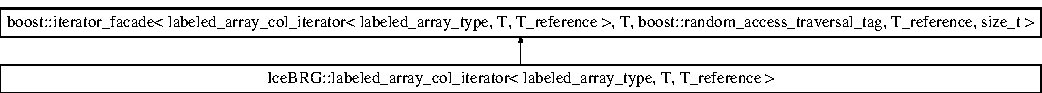
\includegraphics[height=1.250000cm]{classIceBRG_1_1labeled__array__col__iterator}
\end{center}
\end{figure}
\subsection*{Public Types}
\begin{DoxyCompactItemize}
\item 
typedef base\+::difference\+\_\+type \hyperlink{classIceBRG_1_1labeled__array__col__iterator_a90300154d7c3040eff6fd81b14ca4245}{difference\+\_\+type}
\end{DoxyCompactItemize}
\subsection*{Public Member Functions}
\begin{DoxyCompactItemize}
\item 
\hyperlink{classIceBRG_1_1labeled__array__col__iterator_a5f22796d8673d9f136a91a9d3a71d56f}{labeled\+\_\+array\+\_\+col\+\_\+iterator} ()
\item 
\hyperlink{classIceBRG_1_1labeled__array__col__iterator_a2a996e66c27707a770f8899671da29de}{labeled\+\_\+array\+\_\+col\+\_\+iterator} (labeled\+\_\+array\+\_\+type $\ast$base, const size\+\_\+t \&col\+\_\+index)
\item 
{\footnotesize template$<$class T\+\_\+o , typename T\+\_\+o\+\_\+reference $>$ }\\\hyperlink{classIceBRG_1_1labeled__array__col__iterator_a82fd920af321f7422a5564343fc489d7}{labeled\+\_\+array\+\_\+col\+\_\+iterator} (const \hyperlink{classIceBRG_1_1labeled__array__col__iterator}{labeled\+\_\+array\+\_\+col\+\_\+iterator}$<$ labeled\+\_\+array\+\_\+type, T\+\_\+o, T\+\_\+o\+\_\+reference $>$ \&other, typename std\+::enable\+\_\+if$<$ std\+::is\+\_\+convertible$<$ T\+\_\+o\+\_\+reference, T\+\_\+reference $>$\+::value, T\+\_\+o\+\_\+reference $\ast$ $>$\+::type=nullptr)
\end{DoxyCompactItemize}
\subsection*{Friends}
\begin{DoxyCompactItemize}
\item 
class \hyperlink{classIceBRG_1_1labeled__array__col__iterator_ac09f73e325921cc50ebcd96bed0f8096}{boost\+::iterator\+\_\+core\+\_\+access}
\end{DoxyCompactItemize}


\subsection{Member Typedef Documentation}
\hypertarget{classIceBRG_1_1labeled__array__col__iterator_a90300154d7c3040eff6fd81b14ca4245}{}\index{Ice\+B\+R\+G\+::labeled\+\_\+array\+\_\+col\+\_\+iterator@{Ice\+B\+R\+G\+::labeled\+\_\+array\+\_\+col\+\_\+iterator}!difference\+\_\+type@{difference\+\_\+type}}
\index{difference\+\_\+type@{difference\+\_\+type}!Ice\+B\+R\+G\+::labeled\+\_\+array\+\_\+col\+\_\+iterator@{Ice\+B\+R\+G\+::labeled\+\_\+array\+\_\+col\+\_\+iterator}}
\subsubsection[{difference\+\_\+type}]{\setlength{\rightskip}{0pt plus 5cm}template$<$typename labeled\+\_\+array\+\_\+type, typename T, typename T\+\_\+reference$>$ typedef base\+::difference\+\_\+type {\bf Ice\+B\+R\+G\+::labeled\+\_\+array\+\_\+col\+\_\+iterator}$<$ labeled\+\_\+array\+\_\+type, T, T\+\_\+reference $>$\+::{\bf difference\+\_\+type}}\label{classIceBRG_1_1labeled__array__col__iterator_a90300154d7c3040eff6fd81b14ca4245}


\subsection{Constructor \& Destructor Documentation}
\hypertarget{classIceBRG_1_1labeled__array__col__iterator_a5f22796d8673d9f136a91a9d3a71d56f}{}\index{Ice\+B\+R\+G\+::labeled\+\_\+array\+\_\+col\+\_\+iterator@{Ice\+B\+R\+G\+::labeled\+\_\+array\+\_\+col\+\_\+iterator}!labeled\+\_\+array\+\_\+col\+\_\+iterator@{labeled\+\_\+array\+\_\+col\+\_\+iterator}}
\index{labeled\+\_\+array\+\_\+col\+\_\+iterator@{labeled\+\_\+array\+\_\+col\+\_\+iterator}!Ice\+B\+R\+G\+::labeled\+\_\+array\+\_\+col\+\_\+iterator@{Ice\+B\+R\+G\+::labeled\+\_\+array\+\_\+col\+\_\+iterator}}
\subsubsection[{labeled\+\_\+array\+\_\+col\+\_\+iterator()}]{\setlength{\rightskip}{0pt plus 5cm}template$<$typename labeled\+\_\+array\+\_\+type, typename T, typename T\+\_\+reference$>$ {\bf Ice\+B\+R\+G\+::labeled\+\_\+array\+\_\+col\+\_\+iterator}$<$ labeled\+\_\+array\+\_\+type, T, T\+\_\+reference $>$\+::{\bf labeled\+\_\+array\+\_\+col\+\_\+iterator} (
\begin{DoxyParamCaption}
{}
\end{DoxyParamCaption}
)\hspace{0.3cm}{\ttfamily [inline]}}\label{classIceBRG_1_1labeled__array__col__iterator_a5f22796d8673d9f136a91a9d3a71d56f}
\hypertarget{classIceBRG_1_1labeled__array__col__iterator_a2a996e66c27707a770f8899671da29de}{}\index{Ice\+B\+R\+G\+::labeled\+\_\+array\+\_\+col\+\_\+iterator@{Ice\+B\+R\+G\+::labeled\+\_\+array\+\_\+col\+\_\+iterator}!labeled\+\_\+array\+\_\+col\+\_\+iterator@{labeled\+\_\+array\+\_\+col\+\_\+iterator}}
\index{labeled\+\_\+array\+\_\+col\+\_\+iterator@{labeled\+\_\+array\+\_\+col\+\_\+iterator}!Ice\+B\+R\+G\+::labeled\+\_\+array\+\_\+col\+\_\+iterator@{Ice\+B\+R\+G\+::labeled\+\_\+array\+\_\+col\+\_\+iterator}}
\subsubsection[{labeled\+\_\+array\+\_\+col\+\_\+iterator(labeled\+\_\+array\+\_\+type $\ast$base, const size\+\_\+t \&col\+\_\+index)}]{\setlength{\rightskip}{0pt plus 5cm}template$<$typename labeled\+\_\+array\+\_\+type, typename T, typename T\+\_\+reference$>$ {\bf Ice\+B\+R\+G\+::labeled\+\_\+array\+\_\+col\+\_\+iterator}$<$ labeled\+\_\+array\+\_\+type, T, T\+\_\+reference $>$\+::{\bf labeled\+\_\+array\+\_\+col\+\_\+iterator} (
\begin{DoxyParamCaption}
\item[{labeled\+\_\+array\+\_\+type $\ast$}]{base, }
\item[{const size\+\_\+t \&}]{col\+\_\+index}
\end{DoxyParamCaption}
)\hspace{0.3cm}{\ttfamily [inline]}}\label{classIceBRG_1_1labeled__array__col__iterator_a2a996e66c27707a770f8899671da29de}
\hypertarget{classIceBRG_1_1labeled__array__col__iterator_a82fd920af321f7422a5564343fc489d7}{}\index{Ice\+B\+R\+G\+::labeled\+\_\+array\+\_\+col\+\_\+iterator@{Ice\+B\+R\+G\+::labeled\+\_\+array\+\_\+col\+\_\+iterator}!labeled\+\_\+array\+\_\+col\+\_\+iterator@{labeled\+\_\+array\+\_\+col\+\_\+iterator}}
\index{labeled\+\_\+array\+\_\+col\+\_\+iterator@{labeled\+\_\+array\+\_\+col\+\_\+iterator}!Ice\+B\+R\+G\+::labeled\+\_\+array\+\_\+col\+\_\+iterator@{Ice\+B\+R\+G\+::labeled\+\_\+array\+\_\+col\+\_\+iterator}}
\subsubsection[{labeled\+\_\+array\+\_\+col\+\_\+iterator(const labeled\+\_\+array\+\_\+col\+\_\+iterator$<$ labeled\+\_\+array\+\_\+type, T\+\_\+o, T\+\_\+o\+\_\+reference $>$ \&other, typename std\+::enable\+\_\+if$<$ std\+::is\+\_\+convertible$<$ T\+\_\+o\+\_\+reference, T\+\_\+reference $>$\+::value, T\+\_\+o\+\_\+reference $\ast$ $>$\+::type=nullptr)}]{\setlength{\rightskip}{0pt plus 5cm}template$<$typename labeled\+\_\+array\+\_\+type, typename T, typename T\+\_\+reference$>$ template$<$class T\+\_\+o , typename T\+\_\+o\+\_\+reference $>$ {\bf Ice\+B\+R\+G\+::labeled\+\_\+array\+\_\+col\+\_\+iterator}$<$ labeled\+\_\+array\+\_\+type, T, T\+\_\+reference $>$\+::{\bf labeled\+\_\+array\+\_\+col\+\_\+iterator} (
\begin{DoxyParamCaption}
\item[{const {\bf labeled\+\_\+array\+\_\+col\+\_\+iterator}$<$ labeled\+\_\+array\+\_\+type, T\+\_\+o, T\+\_\+o\+\_\+reference $>$ \&}]{other, }
\item[{typename std\+::enable\+\_\+if$<$ std\+::is\+\_\+convertible$<$ T\+\_\+o\+\_\+reference, T\+\_\+reference $>$\+::value, T\+\_\+o\+\_\+reference $\ast$ $>$\+::type}]{ = {\ttfamily nullptr}}
\end{DoxyParamCaption}
)\hspace{0.3cm}{\ttfamily [inline]}}\label{classIceBRG_1_1labeled__array__col__iterator_a82fd920af321f7422a5564343fc489d7}


\subsection{Friends And Related Function Documentation}
\hypertarget{classIceBRG_1_1labeled__array__col__iterator_ac09f73e325921cc50ebcd96bed0f8096}{}\index{Ice\+B\+R\+G\+::labeled\+\_\+array\+\_\+col\+\_\+iterator@{Ice\+B\+R\+G\+::labeled\+\_\+array\+\_\+col\+\_\+iterator}!boost\+::iterator\+\_\+core\+\_\+access@{boost\+::iterator\+\_\+core\+\_\+access}}
\index{boost\+::iterator\+\_\+core\+\_\+access@{boost\+::iterator\+\_\+core\+\_\+access}!Ice\+B\+R\+G\+::labeled\+\_\+array\+\_\+col\+\_\+iterator@{Ice\+B\+R\+G\+::labeled\+\_\+array\+\_\+col\+\_\+iterator}}
\subsubsection[{boost\+::iterator\+\_\+core\+\_\+access}]{\setlength{\rightskip}{0pt plus 5cm}template$<$typename labeled\+\_\+array\+\_\+type, typename T, typename T\+\_\+reference$>$ friend class boost\+::iterator\+\_\+core\+\_\+access\hspace{0.3cm}{\ttfamily [friend]}}\label{classIceBRG_1_1labeled__array__col__iterator_ac09f73e325921cc50ebcd96bed0f8096}


The documentation for this class was generated from the following file\+:\begin{DoxyCompactItemize}
\item 
/disk2/brg/git/\+Magnification\+\_\+\+Public/src/lib/\+Ice\+B\+R\+G\+\_\+main/container/labeled\+\_\+array/\hyperlink{labeled__array__col__iterator_8hpp}{labeled\+\_\+array\+\_\+col\+\_\+iterator.\+hpp}\end{DoxyCompactItemize}

\hypertarget{classIceBRG_1_1labeled__array__col__reference}{}\section{Ice\+B\+R\+G\+:\+:labeled\+\_\+array\+\_\+col\+\_\+reference$<$ labeled\+\_\+array\+\_\+type, T\+\_\+col\+\_\+type $>$ Class Template Reference}
\label{classIceBRG_1_1labeled__array__col__reference}\index{Ice\+B\+R\+G\+::labeled\+\_\+array\+\_\+col\+\_\+reference$<$ labeled\+\_\+array\+\_\+type, T\+\_\+col\+\_\+type $>$@{Ice\+B\+R\+G\+::labeled\+\_\+array\+\_\+col\+\_\+reference$<$ labeled\+\_\+array\+\_\+type, T\+\_\+col\+\_\+type $>$}}


{\ttfamily \#include $<$labeled\+\_\+array\+\_\+col\+\_\+reference.\+hpp$>$}

\subsection*{Public Types}
\begin{DoxyCompactItemize}
\item 
typedef labeled\+\_\+array\+\_\+type\+::const\+\_\+label\+\_\+type \hyperlink{classIceBRG_1_1labeled__array__col__reference_a8dc48f0fd0cd4b9813289a8b6db0f9b6}{label\+\_\+type}
\item 
typedef labeled\+\_\+array\+\_\+type\+::value\+\_\+type \hyperlink{classIceBRG_1_1labeled__array__col__reference_ab9d93b07ec3e0fbfb0604ac8b135d04d}{value\+\_\+type}
\item 
typedef labeled\+\_\+array\+\_\+type\+::const\+\_\+value\+\_\+type \hyperlink{classIceBRG_1_1labeled__array__col__reference_a035a727159f4298ef4f4a360e6bc8aa8}{const\+\_\+value\+\_\+type}
\item 
typedef labeled\+\_\+array\+\_\+type\+::size\+\_\+type \hyperlink{classIceBRG_1_1labeled__array__col__reference_a5b8295af3ddffec129715ff6b7744b7e}{size\+\_\+type}
\item 
typedef T\+\_\+col\+\_\+type \hyperlink{classIceBRG_1_1labeled__array__col__reference_ad55f27046974468dea6e20647571e4e0}{col\+\_\+type}
\item 
typedef const \hyperlink{classIceBRG_1_1labeled__array__col__reference_ad55f27046974468dea6e20647571e4e0}{col\+\_\+type} \hyperlink{classIceBRG_1_1labeled__array__col__reference_a00d71fc36336ea5879c401a111ac53f4}{const\+\_\+col\+\_\+type}
\item 
typedef labeled\+\_\+array\+\_\+type\+::reference \hyperlink{classIceBRG_1_1labeled__array__col__reference_aab5b1a7515a3d5bb8e5ead3f3a8319f6}{reference}
\item 
typedef labeled\+\_\+array\+\_\+type\+::const\+\_\+reference \hyperlink{classIceBRG_1_1labeled__array__col__reference_a2c7ae3d3e5b937e934ad83ea1269127d}{const\+\_\+reference}
\item 
typedef labeled\+\_\+array\+\_\+type\+::col\+\_\+element\+\_\+iterator \hyperlink{classIceBRG_1_1labeled__array__col__reference_a02a1708be2729e266d767b9a58d1880e}{iterator}
\item 
typedef labeled\+\_\+array\+\_\+type\+::const\+\_\+col\+\_\+element\+\_\+iterator \hyperlink{classIceBRG_1_1labeled__array__col__reference_ab7d7f397a1e5f1d9bfc2c61604dda841}{const\+\_\+iterator}
\item 
typedef labeled\+\_\+array\+\_\+type\+::reverse\+\_\+col\+\_\+element\+\_\+iterator \hyperlink{classIceBRG_1_1labeled__array__col__reference_af3dd2856e6301c59896b6219b2c3e3a1}{reverse\+\_\+iterator}
\item 
typedef labeled\+\_\+array\+\_\+type\+::const\+\_\+reverse\+\_\+col\+\_\+element\+\_\+iterator \hyperlink{classIceBRG_1_1labeled__array__col__reference_af8c36128050cef0220fcf8269ecb86da}{const\+\_\+reverse\+\_\+iterator}
\item 
typedef size\+\_\+t \hyperlink{classIceBRG_1_1labeled__array__col__reference_a8b2c27327495b8f17cf4ac9fbf667d54}{difference\+\_\+type}
\end{DoxyCompactItemize}
\subsection*{Public Member Functions}
\begin{DoxyCompactItemize}
\item 
{\footnotesize template$<$typename T\+\_\+init\+\_\+col\+\_\+type $>$ }\\\hyperlink{classIceBRG_1_1labeled__array__col__reference_a487a048a6a6d1f26a128a58845675aa9}{labeled\+\_\+array\+\_\+col\+\_\+reference} (\hyperlink{classIceBRG_1_1labeled__array__col__reference_a8dc48f0fd0cd4b9813289a8b6db0f9b6}{label\+\_\+type} $\ast$\hyperlink{classIceBRG_1_1labeled__array__col__reference_a5221fd3e7f0cc79bea2977b99b43702c}{label}, T\+\_\+init\+\_\+col\+\_\+type \&\&col, \hyperlink{classIceBRG_1_1labeled__array__col__reference_a5b8295af3ddffec129715ff6b7744b7e}{size\+\_\+type} num\+\_\+rows)
\begin{DoxyCompactList}\small\item\em Constructor. Requires a pointer to a \hyperlink{classIceBRG_1_1labeled__array}{labeled\+\_\+array}\textquotesingle{}s label, the column, and the number of rows. \end{DoxyCompactList}\item 
virtual \hyperlink{classIceBRG_1_1labeled__array__col__reference_af08e8e753fe19e1e49267914b81529c3}{$\sim$labeled\+\_\+array\+\_\+col\+\_\+reference} ()
\begin{DoxyCompactList}\small\item\em Virtual destructor. \end{DoxyCompactList}\item 
{\footnotesize template$<$typename T\+\_\+iterator  = const\+\_\+iterator, typename std\+::enable\+\_\+if$<$!std\+::is\+\_\+same$<$ T\+\_\+iterator, const\+\_\+value\+\_\+type $\ast$ $>$\+::value, char $>$\+::type  = 0$>$ }\\T\+\_\+iterator \hyperlink{classIceBRG_1_1labeled__array__col__reference_a07b988e5a4f590833c6935c4f3193801}{begin} () const  noexcept
\begin{DoxyCompactList}\small\item\em begin (const) \end{DoxyCompactList}\item 
{\footnotesize template$<$typename T\+\_\+iterator  = const\+\_\+iterator, typename std\+::enable\+\_\+if$<$ std\+::is\+\_\+same$<$ T\+\_\+iterator, const\+\_\+value\+\_\+type $\ast$ $>$\+::value, char $>$\+::type  = 0$>$ }\\T\+\_\+iterator \hyperlink{classIceBRG_1_1labeled__array__col__reference_a07b988e5a4f590833c6935c4f3193801}{begin} () const  noexcept
\item 
{\footnotesize template$<$typename T\+\_\+iterator  = iterator, typename std\+::enable\+\_\+if$<$!std\+::is\+\_\+same$<$ T\+\_\+iterator, value\+\_\+type $\ast$ $>$\+::value, char $>$\+::type  = 0$>$ }\\T\+\_\+iterator \hyperlink{classIceBRG_1_1labeled__array__col__reference_ae62e4e4b5b8431a5b2c7e68b0e8e6231}{begin} () noexcept
\begin{DoxyCompactList}\small\item\em begin \end{DoxyCompactList}\item 
{\footnotesize template$<$typename T\+\_\+iterator  = iterator, typename std\+::enable\+\_\+if$<$ std\+::is\+\_\+same$<$ T\+\_\+iterator, value\+\_\+type $\ast$ $>$\+::value, char $>$\+::type  = 0$>$ }\\T\+\_\+iterator \hyperlink{classIceBRG_1_1labeled__array__col__reference_ae62e4e4b5b8431a5b2c7e68b0e8e6231}{begin} () noexcept
\item 
{\footnotesize template$<$typename T\+\_\+iterator  = const\+\_\+iterator, typename std\+::enable\+\_\+if$<$!std\+::is\+\_\+same$<$ T\+\_\+iterator, const\+\_\+value\+\_\+type $\ast$ $>$\+::value, char $>$\+::type  = 0$>$ }\\T\+\_\+iterator \hyperlink{classIceBRG_1_1labeled__array__col__reference_a2cbc0421b5e4ad3d14197cc44efcb5ea}{end} () const  noexcept
\begin{DoxyCompactList}\small\item\em end (const) \end{DoxyCompactList}\item 
{\footnotesize template$<$typename T\+\_\+iterator  = const\+\_\+iterator, typename std\+::enable\+\_\+if$<$ std\+::is\+\_\+same$<$ T\+\_\+iterator, const\+\_\+value\+\_\+type $\ast$ $>$\+::value, char $>$\+::type  = 0$>$ }\\T\+\_\+iterator \hyperlink{classIceBRG_1_1labeled__array__col__reference_a2cbc0421b5e4ad3d14197cc44efcb5ea}{end} () const  noexcept
\item 
{\footnotesize template$<$typename T\+\_\+iterator  = iterator, typename std\+::enable\+\_\+if$<$!std\+::is\+\_\+same$<$ T\+\_\+iterator, value\+\_\+type $\ast$ $>$\+::value, char $>$\+::type  = 0$>$ }\\T\+\_\+iterator \hyperlink{classIceBRG_1_1labeled__array__col__reference_a6a658c030fd15dc17e39542b80b78d4c}{end} () noexcept
\begin{DoxyCompactList}\small\item\em end \end{DoxyCompactList}\item 
{\footnotesize template$<$typename T\+\_\+iterator  = iterator, typename std\+::enable\+\_\+if$<$ std\+::is\+\_\+same$<$ T\+\_\+iterator, value\+\_\+type $\ast$ $>$\+::value, char $>$\+::type  = 0$>$ }\\T\+\_\+iterator \hyperlink{classIceBRG_1_1labeled__array__col__reference_a6a658c030fd15dc17e39542b80b78d4c}{end} () noexcept
\item 
{\footnotesize template$<$typename T\+\_\+iterator  = const\+\_\+reverse\+\_\+iterator, typename std\+::enable\+\_\+if$<$!std\+::is\+\_\+same$<$ T\+\_\+iterator, const\+\_\+value\+\_\+type $\ast$ $>$\+::value, char $>$\+::type  = 0$>$ }\\T\+\_\+iterator \hyperlink{classIceBRG_1_1labeled__array__col__reference_af2361ee6bb59b591e6df0149de8cede6}{rbegin} () const  noexcept
\begin{DoxyCompactList}\small\item\em rbegin (const) \end{DoxyCompactList}\item 
{\footnotesize template$<$typename T\+\_\+iterator  = const\+\_\+reverse\+\_\+iterator, typename std\+::enable\+\_\+if$<$ std\+::is\+\_\+same$<$ T\+\_\+iterator, const\+\_\+value\+\_\+type $\ast$ $>$\+::value, char $>$\+::type  = 0$>$ }\\T\+\_\+iterator \hyperlink{classIceBRG_1_1labeled__array__col__reference_af2361ee6bb59b591e6df0149de8cede6}{rbegin} () const  noexcept
\item 
{\footnotesize template$<$typename T\+\_\+iterator  = reverse\+\_\+iterator, typename std\+::enable\+\_\+if$<$!std\+::is\+\_\+same$<$ T\+\_\+iterator, value\+\_\+type $\ast$ $>$\+::value, char $>$\+::type  = 0$>$ }\\T\+\_\+iterator \hyperlink{classIceBRG_1_1labeled__array__col__reference_abaf079140281932aa7abdea39d6555c1}{rbegin} () noexcept
\begin{DoxyCompactList}\small\item\em rbegin \end{DoxyCompactList}\item 
{\footnotesize template$<$typename T\+\_\+iterator  = reverse\+\_\+iterator, typename std\+::enable\+\_\+if$<$ std\+::is\+\_\+same$<$ T\+\_\+iterator, value\+\_\+type $\ast$ $>$\+::value, char $>$\+::type  = 0$>$ }\\T\+\_\+iterator \hyperlink{classIceBRG_1_1labeled__array__col__reference_abaf079140281932aa7abdea39d6555c1}{rbegin} () noexcept
\item 
{\footnotesize template$<$typename T\+\_\+iterator  = const\+\_\+reverse\+\_\+iterator, typename std\+::enable\+\_\+if$<$!std\+::is\+\_\+same$<$ T\+\_\+iterator, const\+\_\+value\+\_\+type $\ast$ $>$\+::value, char $>$\+::type  = 0$>$ }\\T\+\_\+iterator \hyperlink{classIceBRG_1_1labeled__array__col__reference_aea119e7ca31efc687e57ede7f9e663dc}{rend} () const  noexcept
\begin{DoxyCompactList}\small\item\em rend (const) \end{DoxyCompactList}\item 
{\footnotesize template$<$typename T\+\_\+iterator  = const\+\_\+reverse\+\_\+iterator, typename std\+::enable\+\_\+if$<$ std\+::is\+\_\+same$<$ T\+\_\+iterator, const\+\_\+value\+\_\+type $\ast$ $>$\+::value, char $>$\+::type  = 0$>$ }\\T\+\_\+iterator \hyperlink{classIceBRG_1_1labeled__array__col__reference_aea119e7ca31efc687e57ede7f9e663dc}{rend} () const  noexcept
\item 
{\footnotesize template$<$typename T\+\_\+iterator  = reverse\+\_\+iterator, typename std\+::enable\+\_\+if$<$!std\+::is\+\_\+same$<$ T\+\_\+iterator, value\+\_\+type $\ast$ $>$\+::value, char $>$\+::type  = 0$>$ }\\T\+\_\+iterator \hyperlink{classIceBRG_1_1labeled__array__col__reference_aea119e7ca31efc687e57ede7f9e663dc}{rend} () const  noexcept
\begin{DoxyCompactList}\small\item\em rend \end{DoxyCompactList}\item 
{\footnotesize template$<$typename T\+\_\+iterator  = reverse\+\_\+iterator, typename std\+::enable\+\_\+if$<$ std\+::is\+\_\+same$<$ T\+\_\+iterator, value\+\_\+type $\ast$ $>$\+::value, char $>$\+::type  = 0$>$ }\\T\+\_\+iterator \hyperlink{classIceBRG_1_1labeled__array__col__reference_aea119e7ca31efc687e57ede7f9e663dc}{rend} () const  noexcept
\item 
{\footnotesize template$<$typename T\+\_\+iterator  = const\+\_\+iterator, typename std\+::enable\+\_\+if$<$!std\+::is\+\_\+same$<$ T\+\_\+iterator, const\+\_\+value\+\_\+type $\ast$ $>$\+::value, char $>$\+::type  = 0$>$ }\\T\+\_\+iterator \hyperlink{classIceBRG_1_1labeled__array__col__reference_aeeb0d8f9610b7050480b56154b0d1c0e}{cbegin} () const  noexcept
\begin{DoxyCompactList}\small\item\em cbegin \end{DoxyCompactList}\item 
{\footnotesize template$<$typename T\+\_\+iterator  = const\+\_\+iterator, typename std\+::enable\+\_\+if$<$ std\+::is\+\_\+same$<$ T\+\_\+iterator, const\+\_\+value\+\_\+type $\ast$ $>$\+::value, char $>$\+::type  = 0$>$ }\\T\+\_\+iterator \hyperlink{classIceBRG_1_1labeled__array__col__reference_aeeb0d8f9610b7050480b56154b0d1c0e}{cbegin} () const  noexcept
\item 
{\footnotesize template$<$typename T\+\_\+iterator  = const\+\_\+iterator, typename std\+::enable\+\_\+if$<$!std\+::is\+\_\+same$<$ T\+\_\+iterator, const\+\_\+value\+\_\+type $\ast$ $>$\+::value, char $>$\+::type  = 0$>$ }\\T\+\_\+iterator \hyperlink{classIceBRG_1_1labeled__array__col__reference_a16d0319816f57cba47d083247e161b5a}{cend} () const  noexcept
\begin{DoxyCompactList}\small\item\em cend \end{DoxyCompactList}\item 
{\footnotesize template$<$typename T\+\_\+iterator  = const\+\_\+iterator, typename std\+::enable\+\_\+if$<$ std\+::is\+\_\+same$<$ T\+\_\+iterator, const\+\_\+value\+\_\+type $\ast$ $>$\+::value, char $>$\+::type  = 0$>$ }\\T\+\_\+iterator \hyperlink{classIceBRG_1_1labeled__array__col__reference_a16d0319816f57cba47d083247e161b5a}{cend} () const  noexcept
\item 
{\footnotesize template$<$typename T\+\_\+iterator  = const\+\_\+reverse\+\_\+iterator, typename std\+::enable\+\_\+if$<$!std\+::is\+\_\+same$<$ T\+\_\+iterator, const\+\_\+value\+\_\+type $\ast$ $>$\+::value, char $>$\+::type  = 0$>$ }\\T\+\_\+iterator \hyperlink{classIceBRG_1_1labeled__array__col__reference_aa4c4d4e0fa027184b7df5c86c0886ae5}{crbegin} () const  noexcept
\begin{DoxyCompactList}\small\item\em crbegin \end{DoxyCompactList}\item 
{\footnotesize template$<$typename T\+\_\+iterator  = const\+\_\+reverse\+\_\+iterator, typename std\+::enable\+\_\+if$<$ std\+::is\+\_\+same$<$ T\+\_\+iterator, const\+\_\+value\+\_\+type $\ast$ $>$\+::value, char $>$\+::type  = 0$>$ }\\T\+\_\+iterator \hyperlink{classIceBRG_1_1labeled__array__col__reference_aa4c4d4e0fa027184b7df5c86c0886ae5}{crbegin} () const  noexcept
\item 
{\footnotesize template$<$typename T\+\_\+iterator  = const\+\_\+reverse\+\_\+iterator, typename std\+::enable\+\_\+if$<$!std\+::is\+\_\+same$<$ T\+\_\+iterator, const\+\_\+value\+\_\+type $\ast$ $>$\+::value, char $>$\+::type  = 0$>$ }\\T\+\_\+iterator \hyperlink{classIceBRG_1_1labeled__array__col__reference_a0f27d46dfc2dabc41437b83967b70087}{crend} () const  noexcept
\begin{DoxyCompactList}\small\item\em crend \end{DoxyCompactList}\item 
{\footnotesize template$<$typename T\+\_\+iterator  = const\+\_\+reverse\+\_\+iterator, typename std\+::enable\+\_\+if$<$ std\+::is\+\_\+same$<$ T\+\_\+iterator, const\+\_\+value\+\_\+type $\ast$ $>$\+::value, char $>$\+::type  = 0$>$ }\\T\+\_\+iterator \hyperlink{classIceBRG_1_1labeled__array__col__reference_a0f27d46dfc2dabc41437b83967b70087}{crend} () const  noexcept
\item 
\hyperlink{classIceBRG_1_1labeled__array__col__reference_a5b8295af3ddffec129715ff6b7744b7e}{size\+\_\+type} \hyperlink{classIceBRG_1_1labeled__array__col__reference_a40659e8bbcf1b42031bc43a20311c720}{size} () const  noexcept
\begin{DoxyCompactList}\small\item\em size \end{DoxyCompactList}\item 
bool \hyperlink{classIceBRG_1_1labeled__array__col__reference_a9e8344e6659502ee5e2d66bb6ebd56c3}{empty} () const  noexcept
\begin{DoxyCompactList}\small\item\em empty \end{DoxyCompactList}\item 
\hyperlink{classIceBRG_1_1labeled__array__col__reference_a2c7ae3d3e5b937e934ad83ea1269127d}{const\+\_\+reference} \hyperlink{classIceBRG_1_1labeled__array__col__reference_acd00c09cf37a061ed974d65e53c93db1}{operator\mbox{[}$\,$\mbox{]}} (const \hyperlink{classIceBRG_1_1labeled__array__col__reference_a5b8295af3ddffec129715ff6b7744b7e}{size\+\_\+type} \&n) const 
\begin{DoxyCompactList}\small\item\em Element access. \end{DoxyCompactList}\item 
\hyperlink{classIceBRG_1_1labeled__array__col__reference_aab5b1a7515a3d5bb8e5ead3f3a8319f6}{reference} \hyperlink{classIceBRG_1_1labeled__array__col__reference_a688cb048bffa353f74b8c76ee366f8d9}{operator\mbox{[}$\,$\mbox{]}} (const \hyperlink{classIceBRG_1_1labeled__array__col__reference_a5b8295af3ddffec129715ff6b7744b7e}{size\+\_\+type} \&n)
\begin{DoxyCompactList}\small\item\em Element access. \end{DoxyCompactList}\item 
\hyperlink{classIceBRG_1_1labeled__array__col__reference_a2c7ae3d3e5b937e934ad83ea1269127d}{const\+\_\+reference} \hyperlink{classIceBRG_1_1labeled__array__col__reference_ad6042757f3e860c38c7080fed0e38334}{row} (const \hyperlink{classIceBRG_1_1labeled__array__col__reference_a5b8295af3ddffec129715ff6b7744b7e}{size\+\_\+type} \&n) const 
\begin{DoxyCompactList}\small\item\em Range-\/checked element access. \end{DoxyCompactList}\item 
\hyperlink{classIceBRG_1_1labeled__array__col__reference_aab5b1a7515a3d5bb8e5ead3f3a8319f6}{reference} \hyperlink{classIceBRG_1_1labeled__array__col__reference_aa0ec69d3b02b25034289f7c0ce0f963a}{row} (const \hyperlink{classIceBRG_1_1labeled__array__col__reference_a5b8295af3ddffec129715ff6b7744b7e}{size\+\_\+type} \&n)
\begin{DoxyCompactList}\small\item\em Range-\/checked element access. \end{DoxyCompactList}\item 
\hyperlink{classIceBRG_1_1labeled__array__col__reference_a2c7ae3d3e5b937e934ad83ea1269127d}{const\+\_\+reference} \hyperlink{classIceBRG_1_1labeled__array__col__reference_ab59a5e2a39b10fd66fe13f8b923dbec9}{at} (const \hyperlink{classIceBRG_1_1labeled__array__col__reference_a5b8295af3ddffec129715ff6b7744b7e}{size\+\_\+type} \&n) const 
\begin{DoxyCompactList}\small\item\em Range-\/checked element access. \end{DoxyCompactList}\item 
\hyperlink{classIceBRG_1_1labeled__array__col__reference_aab5b1a7515a3d5bb8e5ead3f3a8319f6}{reference} \hyperlink{classIceBRG_1_1labeled__array__col__reference_ac7645e9f93bed25c8b88d1ce0e88322d}{at} (const \hyperlink{classIceBRG_1_1labeled__array__col__reference_a5b8295af3ddffec129715ff6b7744b7e}{size\+\_\+type} \&n)
\begin{DoxyCompactList}\small\item\em Range-\/checked element access. \end{DoxyCompactList}\item 
\hyperlink{classIceBRG_1_1labeled__array__col__reference_a2c7ae3d3e5b937e934ad83ea1269127d}{const\+\_\+reference} \hyperlink{classIceBRG_1_1labeled__array__col__reference_a6517cef5f5a841954f71fec924ddd7f6}{operator()} (const \hyperlink{classIceBRG_1_1labeled__array__col__reference_a5b8295af3ddffec129715ff6b7744b7e}{size\+\_\+type} \&n) const 
\begin{DoxyCompactList}\small\item\em Range-\/checked element access. \end{DoxyCompactList}\item 
\hyperlink{classIceBRG_1_1labeled__array__col__reference_aab5b1a7515a3d5bb8e5ead3f3a8319f6}{reference} \hyperlink{classIceBRG_1_1labeled__array__col__reference_ad9c3ce54c9d1f8d168f46c3f582f6938}{operator()} (const \hyperlink{classIceBRG_1_1labeled__array__col__reference_a5b8295af3ddffec129715ff6b7744b7e}{size\+\_\+type} \&n)
\begin{DoxyCompactList}\small\item\em Range-\/checked element access. \end{DoxyCompactList}\item 
\hyperlink{classIceBRG_1_1labeled__array__col__reference_a2c7ae3d3e5b937e934ad83ea1269127d}{const\+\_\+reference} \hyperlink{classIceBRG_1_1labeled__array__col__reference_ad6ed0320730fca285a785f8aba4debf0}{front} () const 
\begin{DoxyCompactList}\small\item\em Access first element. \end{DoxyCompactList}\item 
\hyperlink{classIceBRG_1_1labeled__array__col__reference_aab5b1a7515a3d5bb8e5ead3f3a8319f6}{reference} \hyperlink{classIceBRG_1_1labeled__array__col__reference_aa284cff0a7a7a6a7e7dbe0c185b1d37d}{front} ()
\begin{DoxyCompactList}\small\item\em Access first element. \end{DoxyCompactList}\item 
\hyperlink{classIceBRG_1_1labeled__array__col__reference_a2c7ae3d3e5b937e934ad83ea1269127d}{const\+\_\+reference} \hyperlink{classIceBRG_1_1labeled__array__col__reference_a029b8b26aad53e4bff9e3d59a70d17a1}{back} () const 
\begin{DoxyCompactList}\small\item\em Access last element. \end{DoxyCompactList}\item 
\hyperlink{classIceBRG_1_1labeled__array__col__reference_aab5b1a7515a3d5bb8e5ead3f3a8319f6}{reference} \hyperlink{classIceBRG_1_1labeled__array__col__reference_a680da5bf0bcc4d3bd7b605a9b9b026c3}{back} ()
\begin{DoxyCompactList}\small\item\em Access last element. \end{DoxyCompactList}\item 
const \hyperlink{classIceBRG_1_1labeled__array__col__reference_ab9d93b07ec3e0fbfb0604ac8b135d04d}{value\+\_\+type} $\ast$ \hyperlink{classIceBRG_1_1labeled__array__col__reference_a3a9429016032503f90d2b648d9858551}{data} () const  noexcept
\begin{DoxyCompactList}\small\item\em Access data. \end{DoxyCompactList}\item 
\hyperlink{classIceBRG_1_1labeled__array__col__reference_ab9d93b07ec3e0fbfb0604ac8b135d04d}{value\+\_\+type} $\ast$ \hyperlink{classIceBRG_1_1labeled__array__col__reference_a85f72aed7d943652a7dd64a959c664b3}{data} () noexcept
\begin{DoxyCompactList}\small\item\em Access data. \end{DoxyCompactList}\item 
const \hyperlink{classIceBRG_1_1labeled__array__col__reference_a8dc48f0fd0cd4b9813289a8b6db0f9b6}{label\+\_\+type} \& \hyperlink{classIceBRG_1_1labeled__array__col__reference_a5221fd3e7f0cc79bea2977b99b43702c}{label} () const  noexcept
\begin{DoxyCompactList}\small\item\em Get the label. \end{DoxyCompactList}\item 
\hyperlink{classIceBRG_1_1labeled__array__col__reference_ab0f5033ddc844b59868ca542ab74503b}{operator const\+\_\+col\+\_\+type} () const  noexcept
\begin{DoxyCompactList}\small\item\em Cast to col\+\_\+type. \end{DoxyCompactList}\item 
\hyperlink{classIceBRG_1_1labeled__array__col__reference_ab8491b8d81eab37154a5d397bb7424e4}{operator col\+\_\+type} () noexcept
\item 
\hyperlink{classIceBRG_1_1labeled__array__col__reference_a00d71fc36336ea5879c401a111ac53f4}{const\+\_\+col\+\_\+type} \hyperlink{classIceBRG_1_1labeled__array__col__reference_a7312c12e21c8f266999384df3e06106e}{raw} () const  noexcept
\item 
\hyperlink{classIceBRG_1_1labeled__array__col__reference_ad55f27046974468dea6e20647571e4e0}{col\+\_\+type} \hyperlink{classIceBRG_1_1labeled__array__col__reference_a2e1f06f1f7546457b3efb4474ab8dc70}{raw} () noexcept
\item 
{\footnotesize template$<$typename other\+\_\+col\+\_\+type , typename std\+::enable\+\_\+if$<$ std\+::is\+\_\+convertible$<$ other\+\_\+col\+\_\+type, col\+\_\+type $>$\+::value, other\+\_\+col\+\_\+type $>$\+::type $\ast$  = nullptr$>$ }\\\hyperlink{classIceBRG_1_1labeled__array__col__reference_ac4aea66aa3a541ea9a8d00701564d0ce}{labeled\+\_\+array\+\_\+col\+\_\+reference} (const \hyperlink{classIceBRG_1_1labeled__array__col__reference}{labeled\+\_\+array\+\_\+col\+\_\+reference}$<$ labeled\+\_\+array\+\_\+type, other\+\_\+col\+\_\+type $>$ \&other)
\begin{DoxyCompactList}\small\item\em Cast non-\/const version to const version. \end{DoxyCompactList}\end{DoxyCompactItemize}


\subsection{Member Typedef Documentation}
\hypertarget{classIceBRG_1_1labeled__array__col__reference_ad55f27046974468dea6e20647571e4e0}{}\index{Ice\+B\+R\+G\+::labeled\+\_\+array\+\_\+col\+\_\+reference@{Ice\+B\+R\+G\+::labeled\+\_\+array\+\_\+col\+\_\+reference}!col\+\_\+type@{col\+\_\+type}}
\index{col\+\_\+type@{col\+\_\+type}!Ice\+B\+R\+G\+::labeled\+\_\+array\+\_\+col\+\_\+reference@{Ice\+B\+R\+G\+::labeled\+\_\+array\+\_\+col\+\_\+reference}}
\subsubsection[{col\+\_\+type}]{\setlength{\rightskip}{0pt plus 5cm}template$<$typename labeled\+\_\+array\+\_\+type, typename T\+\_\+col\+\_\+type$>$ typedef T\+\_\+col\+\_\+type {\bf Ice\+B\+R\+G\+::labeled\+\_\+array\+\_\+col\+\_\+reference}$<$ labeled\+\_\+array\+\_\+type, T\+\_\+col\+\_\+type $>$\+::{\bf col\+\_\+type}}\label{classIceBRG_1_1labeled__array__col__reference_ad55f27046974468dea6e20647571e4e0}
\hypertarget{classIceBRG_1_1labeled__array__col__reference_a00d71fc36336ea5879c401a111ac53f4}{}\index{Ice\+B\+R\+G\+::labeled\+\_\+array\+\_\+col\+\_\+reference@{Ice\+B\+R\+G\+::labeled\+\_\+array\+\_\+col\+\_\+reference}!const\+\_\+col\+\_\+type@{const\+\_\+col\+\_\+type}}
\index{const\+\_\+col\+\_\+type@{const\+\_\+col\+\_\+type}!Ice\+B\+R\+G\+::labeled\+\_\+array\+\_\+col\+\_\+reference@{Ice\+B\+R\+G\+::labeled\+\_\+array\+\_\+col\+\_\+reference}}
\subsubsection[{const\+\_\+col\+\_\+type}]{\setlength{\rightskip}{0pt plus 5cm}template$<$typename labeled\+\_\+array\+\_\+type, typename T\+\_\+col\+\_\+type$>$ typedef const {\bf col\+\_\+type} {\bf Ice\+B\+R\+G\+::labeled\+\_\+array\+\_\+col\+\_\+reference}$<$ labeled\+\_\+array\+\_\+type, T\+\_\+col\+\_\+type $>$\+::{\bf const\+\_\+col\+\_\+type}}\label{classIceBRG_1_1labeled__array__col__reference_a00d71fc36336ea5879c401a111ac53f4}
\hypertarget{classIceBRG_1_1labeled__array__col__reference_ab7d7f397a1e5f1d9bfc2c61604dda841}{}\index{Ice\+B\+R\+G\+::labeled\+\_\+array\+\_\+col\+\_\+reference@{Ice\+B\+R\+G\+::labeled\+\_\+array\+\_\+col\+\_\+reference}!const\+\_\+iterator@{const\+\_\+iterator}}
\index{const\+\_\+iterator@{const\+\_\+iterator}!Ice\+B\+R\+G\+::labeled\+\_\+array\+\_\+col\+\_\+reference@{Ice\+B\+R\+G\+::labeled\+\_\+array\+\_\+col\+\_\+reference}}
\subsubsection[{const\+\_\+iterator}]{\setlength{\rightskip}{0pt plus 5cm}template$<$typename labeled\+\_\+array\+\_\+type, typename T\+\_\+col\+\_\+type$>$ typedef labeled\+\_\+array\+\_\+type\+::const\+\_\+col\+\_\+element\+\_\+iterator {\bf Ice\+B\+R\+G\+::labeled\+\_\+array\+\_\+col\+\_\+reference}$<$ labeled\+\_\+array\+\_\+type, T\+\_\+col\+\_\+type $>$\+::{\bf const\+\_\+iterator}}\label{classIceBRG_1_1labeled__array__col__reference_ab7d7f397a1e5f1d9bfc2c61604dda841}
\hypertarget{classIceBRG_1_1labeled__array__col__reference_a2c7ae3d3e5b937e934ad83ea1269127d}{}\index{Ice\+B\+R\+G\+::labeled\+\_\+array\+\_\+col\+\_\+reference@{Ice\+B\+R\+G\+::labeled\+\_\+array\+\_\+col\+\_\+reference}!const\+\_\+reference@{const\+\_\+reference}}
\index{const\+\_\+reference@{const\+\_\+reference}!Ice\+B\+R\+G\+::labeled\+\_\+array\+\_\+col\+\_\+reference@{Ice\+B\+R\+G\+::labeled\+\_\+array\+\_\+col\+\_\+reference}}
\subsubsection[{const\+\_\+reference}]{\setlength{\rightskip}{0pt plus 5cm}template$<$typename labeled\+\_\+array\+\_\+type, typename T\+\_\+col\+\_\+type$>$ typedef labeled\+\_\+array\+\_\+type\+::const\+\_\+reference {\bf Ice\+B\+R\+G\+::labeled\+\_\+array\+\_\+col\+\_\+reference}$<$ labeled\+\_\+array\+\_\+type, T\+\_\+col\+\_\+type $>$\+::{\bf const\+\_\+reference}}\label{classIceBRG_1_1labeled__array__col__reference_a2c7ae3d3e5b937e934ad83ea1269127d}
\hypertarget{classIceBRG_1_1labeled__array__col__reference_af8c36128050cef0220fcf8269ecb86da}{}\index{Ice\+B\+R\+G\+::labeled\+\_\+array\+\_\+col\+\_\+reference@{Ice\+B\+R\+G\+::labeled\+\_\+array\+\_\+col\+\_\+reference}!const\+\_\+reverse\+\_\+iterator@{const\+\_\+reverse\+\_\+iterator}}
\index{const\+\_\+reverse\+\_\+iterator@{const\+\_\+reverse\+\_\+iterator}!Ice\+B\+R\+G\+::labeled\+\_\+array\+\_\+col\+\_\+reference@{Ice\+B\+R\+G\+::labeled\+\_\+array\+\_\+col\+\_\+reference}}
\subsubsection[{const\+\_\+reverse\+\_\+iterator}]{\setlength{\rightskip}{0pt plus 5cm}template$<$typename labeled\+\_\+array\+\_\+type, typename T\+\_\+col\+\_\+type$>$ typedef labeled\+\_\+array\+\_\+type\+::const\+\_\+reverse\+\_\+col\+\_\+element\+\_\+iterator {\bf Ice\+B\+R\+G\+::labeled\+\_\+array\+\_\+col\+\_\+reference}$<$ labeled\+\_\+array\+\_\+type, T\+\_\+col\+\_\+type $>$\+::{\bf const\+\_\+reverse\+\_\+iterator}}\label{classIceBRG_1_1labeled__array__col__reference_af8c36128050cef0220fcf8269ecb86da}
\hypertarget{classIceBRG_1_1labeled__array__col__reference_a035a727159f4298ef4f4a360e6bc8aa8}{}\index{Ice\+B\+R\+G\+::labeled\+\_\+array\+\_\+col\+\_\+reference@{Ice\+B\+R\+G\+::labeled\+\_\+array\+\_\+col\+\_\+reference}!const\+\_\+value\+\_\+type@{const\+\_\+value\+\_\+type}}
\index{const\+\_\+value\+\_\+type@{const\+\_\+value\+\_\+type}!Ice\+B\+R\+G\+::labeled\+\_\+array\+\_\+col\+\_\+reference@{Ice\+B\+R\+G\+::labeled\+\_\+array\+\_\+col\+\_\+reference}}
\subsubsection[{const\+\_\+value\+\_\+type}]{\setlength{\rightskip}{0pt plus 5cm}template$<$typename labeled\+\_\+array\+\_\+type, typename T\+\_\+col\+\_\+type$>$ typedef labeled\+\_\+array\+\_\+type\+::const\+\_\+value\+\_\+type {\bf Ice\+B\+R\+G\+::labeled\+\_\+array\+\_\+col\+\_\+reference}$<$ labeled\+\_\+array\+\_\+type, T\+\_\+col\+\_\+type $>$\+::{\bf const\+\_\+value\+\_\+type}}\label{classIceBRG_1_1labeled__array__col__reference_a035a727159f4298ef4f4a360e6bc8aa8}
\hypertarget{classIceBRG_1_1labeled__array__col__reference_a8b2c27327495b8f17cf4ac9fbf667d54}{}\index{Ice\+B\+R\+G\+::labeled\+\_\+array\+\_\+col\+\_\+reference@{Ice\+B\+R\+G\+::labeled\+\_\+array\+\_\+col\+\_\+reference}!difference\+\_\+type@{difference\+\_\+type}}
\index{difference\+\_\+type@{difference\+\_\+type}!Ice\+B\+R\+G\+::labeled\+\_\+array\+\_\+col\+\_\+reference@{Ice\+B\+R\+G\+::labeled\+\_\+array\+\_\+col\+\_\+reference}}
\subsubsection[{difference\+\_\+type}]{\setlength{\rightskip}{0pt plus 5cm}template$<$typename labeled\+\_\+array\+\_\+type, typename T\+\_\+col\+\_\+type$>$ typedef size\+\_\+t {\bf Ice\+B\+R\+G\+::labeled\+\_\+array\+\_\+col\+\_\+reference}$<$ labeled\+\_\+array\+\_\+type, T\+\_\+col\+\_\+type $>$\+::{\bf difference\+\_\+type}}\label{classIceBRG_1_1labeled__array__col__reference_a8b2c27327495b8f17cf4ac9fbf667d54}
\hypertarget{classIceBRG_1_1labeled__array__col__reference_a02a1708be2729e266d767b9a58d1880e}{}\index{Ice\+B\+R\+G\+::labeled\+\_\+array\+\_\+col\+\_\+reference@{Ice\+B\+R\+G\+::labeled\+\_\+array\+\_\+col\+\_\+reference}!iterator@{iterator}}
\index{iterator@{iterator}!Ice\+B\+R\+G\+::labeled\+\_\+array\+\_\+col\+\_\+reference@{Ice\+B\+R\+G\+::labeled\+\_\+array\+\_\+col\+\_\+reference}}
\subsubsection[{iterator}]{\setlength{\rightskip}{0pt plus 5cm}template$<$typename labeled\+\_\+array\+\_\+type, typename T\+\_\+col\+\_\+type$>$ typedef labeled\+\_\+array\+\_\+type\+::col\+\_\+element\+\_\+iterator {\bf Ice\+B\+R\+G\+::labeled\+\_\+array\+\_\+col\+\_\+reference}$<$ labeled\+\_\+array\+\_\+type, T\+\_\+col\+\_\+type $>$\+::{\bf iterator}}\label{classIceBRG_1_1labeled__array__col__reference_a02a1708be2729e266d767b9a58d1880e}
\hypertarget{classIceBRG_1_1labeled__array__col__reference_a8dc48f0fd0cd4b9813289a8b6db0f9b6}{}\index{Ice\+B\+R\+G\+::labeled\+\_\+array\+\_\+col\+\_\+reference@{Ice\+B\+R\+G\+::labeled\+\_\+array\+\_\+col\+\_\+reference}!label\+\_\+type@{label\+\_\+type}}
\index{label\+\_\+type@{label\+\_\+type}!Ice\+B\+R\+G\+::labeled\+\_\+array\+\_\+col\+\_\+reference@{Ice\+B\+R\+G\+::labeled\+\_\+array\+\_\+col\+\_\+reference}}
\subsubsection[{label\+\_\+type}]{\setlength{\rightskip}{0pt plus 5cm}template$<$typename labeled\+\_\+array\+\_\+type, typename T\+\_\+col\+\_\+type$>$ typedef labeled\+\_\+array\+\_\+type\+::const\+\_\+label\+\_\+type {\bf Ice\+B\+R\+G\+::labeled\+\_\+array\+\_\+col\+\_\+reference}$<$ labeled\+\_\+array\+\_\+type, T\+\_\+col\+\_\+type $>$\+::{\bf label\+\_\+type}}\label{classIceBRG_1_1labeled__array__col__reference_a8dc48f0fd0cd4b9813289a8b6db0f9b6}
\hypertarget{classIceBRG_1_1labeled__array__col__reference_aab5b1a7515a3d5bb8e5ead3f3a8319f6}{}\index{Ice\+B\+R\+G\+::labeled\+\_\+array\+\_\+col\+\_\+reference@{Ice\+B\+R\+G\+::labeled\+\_\+array\+\_\+col\+\_\+reference}!reference@{reference}}
\index{reference@{reference}!Ice\+B\+R\+G\+::labeled\+\_\+array\+\_\+col\+\_\+reference@{Ice\+B\+R\+G\+::labeled\+\_\+array\+\_\+col\+\_\+reference}}
\subsubsection[{reference}]{\setlength{\rightskip}{0pt plus 5cm}template$<$typename labeled\+\_\+array\+\_\+type, typename T\+\_\+col\+\_\+type$>$ typedef labeled\+\_\+array\+\_\+type\+::reference {\bf Ice\+B\+R\+G\+::labeled\+\_\+array\+\_\+col\+\_\+reference}$<$ labeled\+\_\+array\+\_\+type, T\+\_\+col\+\_\+type $>$\+::{\bf reference}}\label{classIceBRG_1_1labeled__array__col__reference_aab5b1a7515a3d5bb8e5ead3f3a8319f6}
\hypertarget{classIceBRG_1_1labeled__array__col__reference_af3dd2856e6301c59896b6219b2c3e3a1}{}\index{Ice\+B\+R\+G\+::labeled\+\_\+array\+\_\+col\+\_\+reference@{Ice\+B\+R\+G\+::labeled\+\_\+array\+\_\+col\+\_\+reference}!reverse\+\_\+iterator@{reverse\+\_\+iterator}}
\index{reverse\+\_\+iterator@{reverse\+\_\+iterator}!Ice\+B\+R\+G\+::labeled\+\_\+array\+\_\+col\+\_\+reference@{Ice\+B\+R\+G\+::labeled\+\_\+array\+\_\+col\+\_\+reference}}
\subsubsection[{reverse\+\_\+iterator}]{\setlength{\rightskip}{0pt plus 5cm}template$<$typename labeled\+\_\+array\+\_\+type, typename T\+\_\+col\+\_\+type$>$ typedef labeled\+\_\+array\+\_\+type\+::reverse\+\_\+col\+\_\+element\+\_\+iterator {\bf Ice\+B\+R\+G\+::labeled\+\_\+array\+\_\+col\+\_\+reference}$<$ labeled\+\_\+array\+\_\+type, T\+\_\+col\+\_\+type $>$\+::{\bf reverse\+\_\+iterator}}\label{classIceBRG_1_1labeled__array__col__reference_af3dd2856e6301c59896b6219b2c3e3a1}
\hypertarget{classIceBRG_1_1labeled__array__col__reference_a5b8295af3ddffec129715ff6b7744b7e}{}\index{Ice\+B\+R\+G\+::labeled\+\_\+array\+\_\+col\+\_\+reference@{Ice\+B\+R\+G\+::labeled\+\_\+array\+\_\+col\+\_\+reference}!size\+\_\+type@{size\+\_\+type}}
\index{size\+\_\+type@{size\+\_\+type}!Ice\+B\+R\+G\+::labeled\+\_\+array\+\_\+col\+\_\+reference@{Ice\+B\+R\+G\+::labeled\+\_\+array\+\_\+col\+\_\+reference}}
\subsubsection[{size\+\_\+type}]{\setlength{\rightskip}{0pt plus 5cm}template$<$typename labeled\+\_\+array\+\_\+type, typename T\+\_\+col\+\_\+type$>$ typedef labeled\+\_\+array\+\_\+type\+::size\+\_\+type {\bf Ice\+B\+R\+G\+::labeled\+\_\+array\+\_\+col\+\_\+reference}$<$ labeled\+\_\+array\+\_\+type, T\+\_\+col\+\_\+type $>$\+::{\bf size\+\_\+type}}\label{classIceBRG_1_1labeled__array__col__reference_a5b8295af3ddffec129715ff6b7744b7e}
\hypertarget{classIceBRG_1_1labeled__array__col__reference_ab9d93b07ec3e0fbfb0604ac8b135d04d}{}\index{Ice\+B\+R\+G\+::labeled\+\_\+array\+\_\+col\+\_\+reference@{Ice\+B\+R\+G\+::labeled\+\_\+array\+\_\+col\+\_\+reference}!value\+\_\+type@{value\+\_\+type}}
\index{value\+\_\+type@{value\+\_\+type}!Ice\+B\+R\+G\+::labeled\+\_\+array\+\_\+col\+\_\+reference@{Ice\+B\+R\+G\+::labeled\+\_\+array\+\_\+col\+\_\+reference}}
\subsubsection[{value\+\_\+type}]{\setlength{\rightskip}{0pt plus 5cm}template$<$typename labeled\+\_\+array\+\_\+type, typename T\+\_\+col\+\_\+type$>$ typedef labeled\+\_\+array\+\_\+type\+::value\+\_\+type {\bf Ice\+B\+R\+G\+::labeled\+\_\+array\+\_\+col\+\_\+reference}$<$ labeled\+\_\+array\+\_\+type, T\+\_\+col\+\_\+type $>$\+::{\bf value\+\_\+type}}\label{classIceBRG_1_1labeled__array__col__reference_ab9d93b07ec3e0fbfb0604ac8b135d04d}


\subsection{Constructor \& Destructor Documentation}
\hypertarget{classIceBRG_1_1labeled__array__col__reference_a487a048a6a6d1f26a128a58845675aa9}{}\index{Ice\+B\+R\+G\+::labeled\+\_\+array\+\_\+col\+\_\+reference@{Ice\+B\+R\+G\+::labeled\+\_\+array\+\_\+col\+\_\+reference}!labeled\+\_\+array\+\_\+col\+\_\+reference@{labeled\+\_\+array\+\_\+col\+\_\+reference}}
\index{labeled\+\_\+array\+\_\+col\+\_\+reference@{labeled\+\_\+array\+\_\+col\+\_\+reference}!Ice\+B\+R\+G\+::labeled\+\_\+array\+\_\+col\+\_\+reference@{Ice\+B\+R\+G\+::labeled\+\_\+array\+\_\+col\+\_\+reference}}
\subsubsection[{labeled\+\_\+array\+\_\+col\+\_\+reference(label\+\_\+type $\ast$label, T\+\_\+init\+\_\+col\+\_\+type \&\&col, size\+\_\+type num\+\_\+rows)}]{\setlength{\rightskip}{0pt plus 5cm}template$<$typename labeled\+\_\+array\+\_\+type, typename T\+\_\+col\+\_\+type$>$ template$<$typename T\+\_\+init\+\_\+col\+\_\+type $>$ {\bf Ice\+B\+R\+G\+::labeled\+\_\+array\+\_\+col\+\_\+reference}$<$ labeled\+\_\+array\+\_\+type, T\+\_\+col\+\_\+type $>$\+::{\bf labeled\+\_\+array\+\_\+col\+\_\+reference} (
\begin{DoxyParamCaption}
\item[{{\bf label\+\_\+type} $\ast$}]{label, }
\item[{T\+\_\+init\+\_\+col\+\_\+type \&\&}]{col, }
\item[{{\bf size\+\_\+type}}]{num\+\_\+rows}
\end{DoxyParamCaption}
)\hspace{0.3cm}{\ttfamily [inline]}}\label{classIceBRG_1_1labeled__array__col__reference_a487a048a6a6d1f26a128a58845675aa9}


Constructor. Requires a pointer to a \hyperlink{classIceBRG_1_1labeled__array}{labeled\+\_\+array}\textquotesingle{}s label, the column, and the number of rows. 

\hypertarget{classIceBRG_1_1labeled__array__col__reference_af08e8e753fe19e1e49267914b81529c3}{}\index{Ice\+B\+R\+G\+::labeled\+\_\+array\+\_\+col\+\_\+reference@{Ice\+B\+R\+G\+::labeled\+\_\+array\+\_\+col\+\_\+reference}!````~labeled\+\_\+array\+\_\+col\+\_\+reference@{$\sim$labeled\+\_\+array\+\_\+col\+\_\+reference}}
\index{````~labeled\+\_\+array\+\_\+col\+\_\+reference@{$\sim$labeled\+\_\+array\+\_\+col\+\_\+reference}!Ice\+B\+R\+G\+::labeled\+\_\+array\+\_\+col\+\_\+reference@{Ice\+B\+R\+G\+::labeled\+\_\+array\+\_\+col\+\_\+reference}}
\subsubsection[{$\sim$labeled\+\_\+array\+\_\+col\+\_\+reference()}]{\setlength{\rightskip}{0pt plus 5cm}template$<$typename labeled\+\_\+array\+\_\+type, typename T\+\_\+col\+\_\+type$>$ virtual {\bf Ice\+B\+R\+G\+::labeled\+\_\+array\+\_\+col\+\_\+reference}$<$ labeled\+\_\+array\+\_\+type, T\+\_\+col\+\_\+type $>$\+::$\sim${\bf labeled\+\_\+array\+\_\+col\+\_\+reference} (
\begin{DoxyParamCaption}
{}
\end{DoxyParamCaption}
)\hspace{0.3cm}{\ttfamily [inline]}, {\ttfamily [virtual]}}\label{classIceBRG_1_1labeled__array__col__reference_af08e8e753fe19e1e49267914b81529c3}


Virtual destructor. 

\hypertarget{classIceBRG_1_1labeled__array__col__reference_ac4aea66aa3a541ea9a8d00701564d0ce}{}\index{Ice\+B\+R\+G\+::labeled\+\_\+array\+\_\+col\+\_\+reference@{Ice\+B\+R\+G\+::labeled\+\_\+array\+\_\+col\+\_\+reference}!labeled\+\_\+array\+\_\+col\+\_\+reference@{labeled\+\_\+array\+\_\+col\+\_\+reference}}
\index{labeled\+\_\+array\+\_\+col\+\_\+reference@{labeled\+\_\+array\+\_\+col\+\_\+reference}!Ice\+B\+R\+G\+::labeled\+\_\+array\+\_\+col\+\_\+reference@{Ice\+B\+R\+G\+::labeled\+\_\+array\+\_\+col\+\_\+reference}}
\subsubsection[{labeled\+\_\+array\+\_\+col\+\_\+reference(const labeled\+\_\+array\+\_\+col\+\_\+reference$<$ labeled\+\_\+array\+\_\+type, other\+\_\+col\+\_\+type $>$ \&other)}]{\setlength{\rightskip}{0pt plus 5cm}template$<$typename labeled\+\_\+array\+\_\+type, typename T\+\_\+col\+\_\+type$>$ template$<$typename other\+\_\+col\+\_\+type , typename std\+::enable\+\_\+if$<$ std\+::is\+\_\+convertible$<$ other\+\_\+col\+\_\+type, col\+\_\+type $>$\+::value, other\+\_\+col\+\_\+type $>$\+::type $\ast$  = nullptr$>$ {\bf Ice\+B\+R\+G\+::labeled\+\_\+array\+\_\+col\+\_\+reference}$<$ labeled\+\_\+array\+\_\+type, T\+\_\+col\+\_\+type $>$\+::{\bf labeled\+\_\+array\+\_\+col\+\_\+reference} (
\begin{DoxyParamCaption}
\item[{const {\bf labeled\+\_\+array\+\_\+col\+\_\+reference}$<$ labeled\+\_\+array\+\_\+type, other\+\_\+col\+\_\+type $>$ \&}]{other}
\end{DoxyParamCaption}
)\hspace{0.3cm}{\ttfamily [inline]}}\label{classIceBRG_1_1labeled__array__col__reference_ac4aea66aa3a541ea9a8d00701564d0ce}


Cast non-\/const version to const version. 



\subsection{Member Function Documentation}
\hypertarget{classIceBRG_1_1labeled__array__col__reference_ab59a5e2a39b10fd66fe13f8b923dbec9}{}\index{Ice\+B\+R\+G\+::labeled\+\_\+array\+\_\+col\+\_\+reference@{Ice\+B\+R\+G\+::labeled\+\_\+array\+\_\+col\+\_\+reference}!at@{at}}
\index{at@{at}!Ice\+B\+R\+G\+::labeled\+\_\+array\+\_\+col\+\_\+reference@{Ice\+B\+R\+G\+::labeled\+\_\+array\+\_\+col\+\_\+reference}}
\subsubsection[{at(const size\+\_\+type \&n) const }]{\setlength{\rightskip}{0pt plus 5cm}template$<$typename labeled\+\_\+array\+\_\+type, typename T\+\_\+col\+\_\+type$>$ {\bf const\+\_\+reference} {\bf Ice\+B\+R\+G\+::labeled\+\_\+array\+\_\+col\+\_\+reference}$<$ labeled\+\_\+array\+\_\+type, T\+\_\+col\+\_\+type $>$\+::at (
\begin{DoxyParamCaption}
\item[{const {\bf size\+\_\+type} \&}]{n}
\end{DoxyParamCaption}
) const\hspace{0.3cm}{\ttfamily [inline]}}\label{classIceBRG_1_1labeled__array__col__reference_ab59a5e2a39b10fd66fe13f8b923dbec9}


Range-\/checked element access. 

\hypertarget{classIceBRG_1_1labeled__array__col__reference_ac7645e9f93bed25c8b88d1ce0e88322d}{}\index{Ice\+B\+R\+G\+::labeled\+\_\+array\+\_\+col\+\_\+reference@{Ice\+B\+R\+G\+::labeled\+\_\+array\+\_\+col\+\_\+reference}!at@{at}}
\index{at@{at}!Ice\+B\+R\+G\+::labeled\+\_\+array\+\_\+col\+\_\+reference@{Ice\+B\+R\+G\+::labeled\+\_\+array\+\_\+col\+\_\+reference}}
\subsubsection[{at(const size\+\_\+type \&n)}]{\setlength{\rightskip}{0pt plus 5cm}template$<$typename labeled\+\_\+array\+\_\+type, typename T\+\_\+col\+\_\+type$>$ {\bf reference} {\bf Ice\+B\+R\+G\+::labeled\+\_\+array\+\_\+col\+\_\+reference}$<$ labeled\+\_\+array\+\_\+type, T\+\_\+col\+\_\+type $>$\+::at (
\begin{DoxyParamCaption}
\item[{const {\bf size\+\_\+type} \&}]{n}
\end{DoxyParamCaption}
)\hspace{0.3cm}{\ttfamily [inline]}}\label{classIceBRG_1_1labeled__array__col__reference_ac7645e9f93bed25c8b88d1ce0e88322d}


Range-\/checked element access. 

\hypertarget{classIceBRG_1_1labeled__array__col__reference_a029b8b26aad53e4bff9e3d59a70d17a1}{}\index{Ice\+B\+R\+G\+::labeled\+\_\+array\+\_\+col\+\_\+reference@{Ice\+B\+R\+G\+::labeled\+\_\+array\+\_\+col\+\_\+reference}!back@{back}}
\index{back@{back}!Ice\+B\+R\+G\+::labeled\+\_\+array\+\_\+col\+\_\+reference@{Ice\+B\+R\+G\+::labeled\+\_\+array\+\_\+col\+\_\+reference}}
\subsubsection[{back() const }]{\setlength{\rightskip}{0pt plus 5cm}template$<$typename labeled\+\_\+array\+\_\+type, typename T\+\_\+col\+\_\+type$>$ {\bf const\+\_\+reference} {\bf Ice\+B\+R\+G\+::labeled\+\_\+array\+\_\+col\+\_\+reference}$<$ labeled\+\_\+array\+\_\+type, T\+\_\+col\+\_\+type $>$\+::back (
\begin{DoxyParamCaption}
{}
\end{DoxyParamCaption}
) const\hspace{0.3cm}{\ttfamily [inline]}}\label{classIceBRG_1_1labeled__array__col__reference_a029b8b26aad53e4bff9e3d59a70d17a1}


Access last element. 

\hypertarget{classIceBRG_1_1labeled__array__col__reference_a680da5bf0bcc4d3bd7b605a9b9b026c3}{}\index{Ice\+B\+R\+G\+::labeled\+\_\+array\+\_\+col\+\_\+reference@{Ice\+B\+R\+G\+::labeled\+\_\+array\+\_\+col\+\_\+reference}!back@{back}}
\index{back@{back}!Ice\+B\+R\+G\+::labeled\+\_\+array\+\_\+col\+\_\+reference@{Ice\+B\+R\+G\+::labeled\+\_\+array\+\_\+col\+\_\+reference}}
\subsubsection[{back()}]{\setlength{\rightskip}{0pt plus 5cm}template$<$typename labeled\+\_\+array\+\_\+type, typename T\+\_\+col\+\_\+type$>$ {\bf reference} {\bf Ice\+B\+R\+G\+::labeled\+\_\+array\+\_\+col\+\_\+reference}$<$ labeled\+\_\+array\+\_\+type, T\+\_\+col\+\_\+type $>$\+::back (
\begin{DoxyParamCaption}
{}
\end{DoxyParamCaption}
)\hspace{0.3cm}{\ttfamily [inline]}}\label{classIceBRG_1_1labeled__array__col__reference_a680da5bf0bcc4d3bd7b605a9b9b026c3}


Access last element. 

\hypertarget{classIceBRG_1_1labeled__array__col__reference_a07b988e5a4f590833c6935c4f3193801}{}\index{Ice\+B\+R\+G\+::labeled\+\_\+array\+\_\+col\+\_\+reference@{Ice\+B\+R\+G\+::labeled\+\_\+array\+\_\+col\+\_\+reference}!begin@{begin}}
\index{begin@{begin}!Ice\+B\+R\+G\+::labeled\+\_\+array\+\_\+col\+\_\+reference@{Ice\+B\+R\+G\+::labeled\+\_\+array\+\_\+col\+\_\+reference}}
\subsubsection[{begin() const  noexcept}]{\setlength{\rightskip}{0pt plus 5cm}template$<$typename labeled\+\_\+array\+\_\+type, typename T\+\_\+col\+\_\+type$>$ template$<$typename T\+\_\+iterator  = const\+\_\+iterator, typename std\+::enable\+\_\+if$<$!std\+::is\+\_\+same$<$ T\+\_\+iterator, const\+\_\+value\+\_\+type $\ast$ $>$\+::value, char $>$\+::type  = 0$>$ T\+\_\+iterator {\bf Ice\+B\+R\+G\+::labeled\+\_\+array\+\_\+col\+\_\+reference}$<$ labeled\+\_\+array\+\_\+type, T\+\_\+col\+\_\+type $>$\+::begin (
\begin{DoxyParamCaption}
{}
\end{DoxyParamCaption}
) const\hspace{0.3cm}{\ttfamily [inline]}, {\ttfamily [noexcept]}}\label{classIceBRG_1_1labeled__array__col__reference_a07b988e5a4f590833c6935c4f3193801}


begin (const) 

\hypertarget{classIceBRG_1_1labeled__array__col__reference_a07b988e5a4f590833c6935c4f3193801}{}\index{Ice\+B\+R\+G\+::labeled\+\_\+array\+\_\+col\+\_\+reference@{Ice\+B\+R\+G\+::labeled\+\_\+array\+\_\+col\+\_\+reference}!begin@{begin}}
\index{begin@{begin}!Ice\+B\+R\+G\+::labeled\+\_\+array\+\_\+col\+\_\+reference@{Ice\+B\+R\+G\+::labeled\+\_\+array\+\_\+col\+\_\+reference}}
\subsubsection[{begin() const  noexcept}]{\setlength{\rightskip}{0pt plus 5cm}template$<$typename labeled\+\_\+array\+\_\+type, typename T\+\_\+col\+\_\+type$>$ template$<$typename T\+\_\+iterator  = const\+\_\+iterator, typename std\+::enable\+\_\+if$<$ std\+::is\+\_\+same$<$ T\+\_\+iterator, const\+\_\+value\+\_\+type $\ast$ $>$\+::value, char $>$\+::type  = 0$>$ T\+\_\+iterator {\bf Ice\+B\+R\+G\+::labeled\+\_\+array\+\_\+col\+\_\+reference}$<$ labeled\+\_\+array\+\_\+type, T\+\_\+col\+\_\+type $>$\+::begin (
\begin{DoxyParamCaption}
{}
\end{DoxyParamCaption}
) const\hspace{0.3cm}{\ttfamily [inline]}, {\ttfamily [noexcept]}}\label{classIceBRG_1_1labeled__array__col__reference_a07b988e5a4f590833c6935c4f3193801}
\hypertarget{classIceBRG_1_1labeled__array__col__reference_ae62e4e4b5b8431a5b2c7e68b0e8e6231}{}\index{Ice\+B\+R\+G\+::labeled\+\_\+array\+\_\+col\+\_\+reference@{Ice\+B\+R\+G\+::labeled\+\_\+array\+\_\+col\+\_\+reference}!begin@{begin}}
\index{begin@{begin}!Ice\+B\+R\+G\+::labeled\+\_\+array\+\_\+col\+\_\+reference@{Ice\+B\+R\+G\+::labeled\+\_\+array\+\_\+col\+\_\+reference}}
\subsubsection[{begin() noexcept}]{\setlength{\rightskip}{0pt plus 5cm}template$<$typename labeled\+\_\+array\+\_\+type, typename T\+\_\+col\+\_\+type$>$ template$<$typename T\+\_\+iterator  = iterator, typename std\+::enable\+\_\+if$<$!std\+::is\+\_\+same$<$ T\+\_\+iterator, value\+\_\+type $\ast$ $>$\+::value, char $>$\+::type  = 0$>$ T\+\_\+iterator {\bf Ice\+B\+R\+G\+::labeled\+\_\+array\+\_\+col\+\_\+reference}$<$ labeled\+\_\+array\+\_\+type, T\+\_\+col\+\_\+type $>$\+::begin (
\begin{DoxyParamCaption}
{}
\end{DoxyParamCaption}
)\hspace{0.3cm}{\ttfamily [inline]}, {\ttfamily [noexcept]}}\label{classIceBRG_1_1labeled__array__col__reference_ae62e4e4b5b8431a5b2c7e68b0e8e6231}


begin 

\hypertarget{classIceBRG_1_1labeled__array__col__reference_ae62e4e4b5b8431a5b2c7e68b0e8e6231}{}\index{Ice\+B\+R\+G\+::labeled\+\_\+array\+\_\+col\+\_\+reference@{Ice\+B\+R\+G\+::labeled\+\_\+array\+\_\+col\+\_\+reference}!begin@{begin}}
\index{begin@{begin}!Ice\+B\+R\+G\+::labeled\+\_\+array\+\_\+col\+\_\+reference@{Ice\+B\+R\+G\+::labeled\+\_\+array\+\_\+col\+\_\+reference}}
\subsubsection[{begin() noexcept}]{\setlength{\rightskip}{0pt plus 5cm}template$<$typename labeled\+\_\+array\+\_\+type, typename T\+\_\+col\+\_\+type$>$ template$<$typename T\+\_\+iterator  = iterator, typename std\+::enable\+\_\+if$<$ std\+::is\+\_\+same$<$ T\+\_\+iterator, value\+\_\+type $\ast$ $>$\+::value, char $>$\+::type  = 0$>$ T\+\_\+iterator {\bf Ice\+B\+R\+G\+::labeled\+\_\+array\+\_\+col\+\_\+reference}$<$ labeled\+\_\+array\+\_\+type, T\+\_\+col\+\_\+type $>$\+::begin (
\begin{DoxyParamCaption}
{}
\end{DoxyParamCaption}
)\hspace{0.3cm}{\ttfamily [inline]}, {\ttfamily [noexcept]}}\label{classIceBRG_1_1labeled__array__col__reference_ae62e4e4b5b8431a5b2c7e68b0e8e6231}
\hypertarget{classIceBRG_1_1labeled__array__col__reference_aeeb0d8f9610b7050480b56154b0d1c0e}{}\index{Ice\+B\+R\+G\+::labeled\+\_\+array\+\_\+col\+\_\+reference@{Ice\+B\+R\+G\+::labeled\+\_\+array\+\_\+col\+\_\+reference}!cbegin@{cbegin}}
\index{cbegin@{cbegin}!Ice\+B\+R\+G\+::labeled\+\_\+array\+\_\+col\+\_\+reference@{Ice\+B\+R\+G\+::labeled\+\_\+array\+\_\+col\+\_\+reference}}
\subsubsection[{cbegin() const  noexcept}]{\setlength{\rightskip}{0pt plus 5cm}template$<$typename labeled\+\_\+array\+\_\+type, typename T\+\_\+col\+\_\+type$>$ template$<$typename T\+\_\+iterator  = const\+\_\+iterator, typename std\+::enable\+\_\+if$<$!std\+::is\+\_\+same$<$ T\+\_\+iterator, const\+\_\+value\+\_\+type $\ast$ $>$\+::value, char $>$\+::type  = 0$>$ T\+\_\+iterator {\bf Ice\+B\+R\+G\+::labeled\+\_\+array\+\_\+col\+\_\+reference}$<$ labeled\+\_\+array\+\_\+type, T\+\_\+col\+\_\+type $>$\+::cbegin (
\begin{DoxyParamCaption}
{}
\end{DoxyParamCaption}
) const\hspace{0.3cm}{\ttfamily [inline]}, {\ttfamily [noexcept]}}\label{classIceBRG_1_1labeled__array__col__reference_aeeb0d8f9610b7050480b56154b0d1c0e}


cbegin 

\hypertarget{classIceBRG_1_1labeled__array__col__reference_aeeb0d8f9610b7050480b56154b0d1c0e}{}\index{Ice\+B\+R\+G\+::labeled\+\_\+array\+\_\+col\+\_\+reference@{Ice\+B\+R\+G\+::labeled\+\_\+array\+\_\+col\+\_\+reference}!cbegin@{cbegin}}
\index{cbegin@{cbegin}!Ice\+B\+R\+G\+::labeled\+\_\+array\+\_\+col\+\_\+reference@{Ice\+B\+R\+G\+::labeled\+\_\+array\+\_\+col\+\_\+reference}}
\subsubsection[{cbegin() const  noexcept}]{\setlength{\rightskip}{0pt plus 5cm}template$<$typename labeled\+\_\+array\+\_\+type, typename T\+\_\+col\+\_\+type$>$ template$<$typename T\+\_\+iterator  = const\+\_\+iterator, typename std\+::enable\+\_\+if$<$ std\+::is\+\_\+same$<$ T\+\_\+iterator, const\+\_\+value\+\_\+type $\ast$ $>$\+::value, char $>$\+::type  = 0$>$ T\+\_\+iterator {\bf Ice\+B\+R\+G\+::labeled\+\_\+array\+\_\+col\+\_\+reference}$<$ labeled\+\_\+array\+\_\+type, T\+\_\+col\+\_\+type $>$\+::cbegin (
\begin{DoxyParamCaption}
{}
\end{DoxyParamCaption}
) const\hspace{0.3cm}{\ttfamily [inline]}, {\ttfamily [noexcept]}}\label{classIceBRG_1_1labeled__array__col__reference_aeeb0d8f9610b7050480b56154b0d1c0e}
\hypertarget{classIceBRG_1_1labeled__array__col__reference_a16d0319816f57cba47d083247e161b5a}{}\index{Ice\+B\+R\+G\+::labeled\+\_\+array\+\_\+col\+\_\+reference@{Ice\+B\+R\+G\+::labeled\+\_\+array\+\_\+col\+\_\+reference}!cend@{cend}}
\index{cend@{cend}!Ice\+B\+R\+G\+::labeled\+\_\+array\+\_\+col\+\_\+reference@{Ice\+B\+R\+G\+::labeled\+\_\+array\+\_\+col\+\_\+reference}}
\subsubsection[{cend() const  noexcept}]{\setlength{\rightskip}{0pt plus 5cm}template$<$typename labeled\+\_\+array\+\_\+type, typename T\+\_\+col\+\_\+type$>$ template$<$typename T\+\_\+iterator  = const\+\_\+iterator, typename std\+::enable\+\_\+if$<$!std\+::is\+\_\+same$<$ T\+\_\+iterator, const\+\_\+value\+\_\+type $\ast$ $>$\+::value, char $>$\+::type  = 0$>$ T\+\_\+iterator {\bf Ice\+B\+R\+G\+::labeled\+\_\+array\+\_\+col\+\_\+reference}$<$ labeled\+\_\+array\+\_\+type, T\+\_\+col\+\_\+type $>$\+::cend (
\begin{DoxyParamCaption}
{}
\end{DoxyParamCaption}
) const\hspace{0.3cm}{\ttfamily [inline]}, {\ttfamily [noexcept]}}\label{classIceBRG_1_1labeled__array__col__reference_a16d0319816f57cba47d083247e161b5a}


cend 

\hypertarget{classIceBRG_1_1labeled__array__col__reference_a16d0319816f57cba47d083247e161b5a}{}\index{Ice\+B\+R\+G\+::labeled\+\_\+array\+\_\+col\+\_\+reference@{Ice\+B\+R\+G\+::labeled\+\_\+array\+\_\+col\+\_\+reference}!cend@{cend}}
\index{cend@{cend}!Ice\+B\+R\+G\+::labeled\+\_\+array\+\_\+col\+\_\+reference@{Ice\+B\+R\+G\+::labeled\+\_\+array\+\_\+col\+\_\+reference}}
\subsubsection[{cend() const  noexcept}]{\setlength{\rightskip}{0pt plus 5cm}template$<$typename labeled\+\_\+array\+\_\+type, typename T\+\_\+col\+\_\+type$>$ template$<$typename T\+\_\+iterator  = const\+\_\+iterator, typename std\+::enable\+\_\+if$<$ std\+::is\+\_\+same$<$ T\+\_\+iterator, const\+\_\+value\+\_\+type $\ast$ $>$\+::value, char $>$\+::type  = 0$>$ T\+\_\+iterator {\bf Ice\+B\+R\+G\+::labeled\+\_\+array\+\_\+col\+\_\+reference}$<$ labeled\+\_\+array\+\_\+type, T\+\_\+col\+\_\+type $>$\+::cend (
\begin{DoxyParamCaption}
{}
\end{DoxyParamCaption}
) const\hspace{0.3cm}{\ttfamily [inline]}, {\ttfamily [noexcept]}}\label{classIceBRG_1_1labeled__array__col__reference_a16d0319816f57cba47d083247e161b5a}
\hypertarget{classIceBRG_1_1labeled__array__col__reference_aa4c4d4e0fa027184b7df5c86c0886ae5}{}\index{Ice\+B\+R\+G\+::labeled\+\_\+array\+\_\+col\+\_\+reference@{Ice\+B\+R\+G\+::labeled\+\_\+array\+\_\+col\+\_\+reference}!crbegin@{crbegin}}
\index{crbegin@{crbegin}!Ice\+B\+R\+G\+::labeled\+\_\+array\+\_\+col\+\_\+reference@{Ice\+B\+R\+G\+::labeled\+\_\+array\+\_\+col\+\_\+reference}}
\subsubsection[{crbegin() const  noexcept}]{\setlength{\rightskip}{0pt plus 5cm}template$<$typename labeled\+\_\+array\+\_\+type, typename T\+\_\+col\+\_\+type$>$ template$<$typename T\+\_\+iterator  = const\+\_\+reverse\+\_\+iterator, typename std\+::enable\+\_\+if$<$!std\+::is\+\_\+same$<$ T\+\_\+iterator, const\+\_\+value\+\_\+type $\ast$ $>$\+::value, char $>$\+::type  = 0$>$ T\+\_\+iterator {\bf Ice\+B\+R\+G\+::labeled\+\_\+array\+\_\+col\+\_\+reference}$<$ labeled\+\_\+array\+\_\+type, T\+\_\+col\+\_\+type $>$\+::crbegin (
\begin{DoxyParamCaption}
{}
\end{DoxyParamCaption}
) const\hspace{0.3cm}{\ttfamily [inline]}, {\ttfamily [noexcept]}}\label{classIceBRG_1_1labeled__array__col__reference_aa4c4d4e0fa027184b7df5c86c0886ae5}


crbegin 

\hypertarget{classIceBRG_1_1labeled__array__col__reference_aa4c4d4e0fa027184b7df5c86c0886ae5}{}\index{Ice\+B\+R\+G\+::labeled\+\_\+array\+\_\+col\+\_\+reference@{Ice\+B\+R\+G\+::labeled\+\_\+array\+\_\+col\+\_\+reference}!crbegin@{crbegin}}
\index{crbegin@{crbegin}!Ice\+B\+R\+G\+::labeled\+\_\+array\+\_\+col\+\_\+reference@{Ice\+B\+R\+G\+::labeled\+\_\+array\+\_\+col\+\_\+reference}}
\subsubsection[{crbegin() const  noexcept}]{\setlength{\rightskip}{0pt plus 5cm}template$<$typename labeled\+\_\+array\+\_\+type, typename T\+\_\+col\+\_\+type$>$ template$<$typename T\+\_\+iterator  = const\+\_\+reverse\+\_\+iterator, typename std\+::enable\+\_\+if$<$ std\+::is\+\_\+same$<$ T\+\_\+iterator, const\+\_\+value\+\_\+type $\ast$ $>$\+::value, char $>$\+::type  = 0$>$ T\+\_\+iterator {\bf Ice\+B\+R\+G\+::labeled\+\_\+array\+\_\+col\+\_\+reference}$<$ labeled\+\_\+array\+\_\+type, T\+\_\+col\+\_\+type $>$\+::crbegin (
\begin{DoxyParamCaption}
{}
\end{DoxyParamCaption}
) const\hspace{0.3cm}{\ttfamily [inline]}, {\ttfamily [noexcept]}}\label{classIceBRG_1_1labeled__array__col__reference_aa4c4d4e0fa027184b7df5c86c0886ae5}
\hypertarget{classIceBRG_1_1labeled__array__col__reference_a0f27d46dfc2dabc41437b83967b70087}{}\index{Ice\+B\+R\+G\+::labeled\+\_\+array\+\_\+col\+\_\+reference@{Ice\+B\+R\+G\+::labeled\+\_\+array\+\_\+col\+\_\+reference}!crend@{crend}}
\index{crend@{crend}!Ice\+B\+R\+G\+::labeled\+\_\+array\+\_\+col\+\_\+reference@{Ice\+B\+R\+G\+::labeled\+\_\+array\+\_\+col\+\_\+reference}}
\subsubsection[{crend() const  noexcept}]{\setlength{\rightskip}{0pt plus 5cm}template$<$typename labeled\+\_\+array\+\_\+type, typename T\+\_\+col\+\_\+type$>$ template$<$typename T\+\_\+iterator  = const\+\_\+reverse\+\_\+iterator, typename std\+::enable\+\_\+if$<$!std\+::is\+\_\+same$<$ T\+\_\+iterator, const\+\_\+value\+\_\+type $\ast$ $>$\+::value, char $>$\+::type  = 0$>$ T\+\_\+iterator {\bf Ice\+B\+R\+G\+::labeled\+\_\+array\+\_\+col\+\_\+reference}$<$ labeled\+\_\+array\+\_\+type, T\+\_\+col\+\_\+type $>$\+::crend (
\begin{DoxyParamCaption}
{}
\end{DoxyParamCaption}
) const\hspace{0.3cm}{\ttfamily [inline]}, {\ttfamily [noexcept]}}\label{classIceBRG_1_1labeled__array__col__reference_a0f27d46dfc2dabc41437b83967b70087}


crend 

\hypertarget{classIceBRG_1_1labeled__array__col__reference_a0f27d46dfc2dabc41437b83967b70087}{}\index{Ice\+B\+R\+G\+::labeled\+\_\+array\+\_\+col\+\_\+reference@{Ice\+B\+R\+G\+::labeled\+\_\+array\+\_\+col\+\_\+reference}!crend@{crend}}
\index{crend@{crend}!Ice\+B\+R\+G\+::labeled\+\_\+array\+\_\+col\+\_\+reference@{Ice\+B\+R\+G\+::labeled\+\_\+array\+\_\+col\+\_\+reference}}
\subsubsection[{crend() const  noexcept}]{\setlength{\rightskip}{0pt plus 5cm}template$<$typename labeled\+\_\+array\+\_\+type, typename T\+\_\+col\+\_\+type$>$ template$<$typename T\+\_\+iterator  = const\+\_\+reverse\+\_\+iterator, typename std\+::enable\+\_\+if$<$ std\+::is\+\_\+same$<$ T\+\_\+iterator, const\+\_\+value\+\_\+type $\ast$ $>$\+::value, char $>$\+::type  = 0$>$ T\+\_\+iterator {\bf Ice\+B\+R\+G\+::labeled\+\_\+array\+\_\+col\+\_\+reference}$<$ labeled\+\_\+array\+\_\+type, T\+\_\+col\+\_\+type $>$\+::crend (
\begin{DoxyParamCaption}
{}
\end{DoxyParamCaption}
) const\hspace{0.3cm}{\ttfamily [inline]}, {\ttfamily [noexcept]}}\label{classIceBRG_1_1labeled__array__col__reference_a0f27d46dfc2dabc41437b83967b70087}
\hypertarget{classIceBRG_1_1labeled__array__col__reference_a3a9429016032503f90d2b648d9858551}{}\index{Ice\+B\+R\+G\+::labeled\+\_\+array\+\_\+col\+\_\+reference@{Ice\+B\+R\+G\+::labeled\+\_\+array\+\_\+col\+\_\+reference}!data@{data}}
\index{data@{data}!Ice\+B\+R\+G\+::labeled\+\_\+array\+\_\+col\+\_\+reference@{Ice\+B\+R\+G\+::labeled\+\_\+array\+\_\+col\+\_\+reference}}
\subsubsection[{data() const  noexcept}]{\setlength{\rightskip}{0pt plus 5cm}template$<$typename labeled\+\_\+array\+\_\+type, typename T\+\_\+col\+\_\+type$>$ const {\bf value\+\_\+type}$\ast$ {\bf Ice\+B\+R\+G\+::labeled\+\_\+array\+\_\+col\+\_\+reference}$<$ labeled\+\_\+array\+\_\+type, T\+\_\+col\+\_\+type $>$\+::data (
\begin{DoxyParamCaption}
{}
\end{DoxyParamCaption}
) const\hspace{0.3cm}{\ttfamily [inline]}, {\ttfamily [noexcept]}}\label{classIceBRG_1_1labeled__array__col__reference_a3a9429016032503f90d2b648d9858551}


Access data. 

\hypertarget{classIceBRG_1_1labeled__array__col__reference_a85f72aed7d943652a7dd64a959c664b3}{}\index{Ice\+B\+R\+G\+::labeled\+\_\+array\+\_\+col\+\_\+reference@{Ice\+B\+R\+G\+::labeled\+\_\+array\+\_\+col\+\_\+reference}!data@{data}}
\index{data@{data}!Ice\+B\+R\+G\+::labeled\+\_\+array\+\_\+col\+\_\+reference@{Ice\+B\+R\+G\+::labeled\+\_\+array\+\_\+col\+\_\+reference}}
\subsubsection[{data() noexcept}]{\setlength{\rightskip}{0pt plus 5cm}template$<$typename labeled\+\_\+array\+\_\+type, typename T\+\_\+col\+\_\+type$>$ {\bf value\+\_\+type}$\ast$ {\bf Ice\+B\+R\+G\+::labeled\+\_\+array\+\_\+col\+\_\+reference}$<$ labeled\+\_\+array\+\_\+type, T\+\_\+col\+\_\+type $>$\+::data (
\begin{DoxyParamCaption}
{}
\end{DoxyParamCaption}
)\hspace{0.3cm}{\ttfamily [inline]}, {\ttfamily [noexcept]}}\label{classIceBRG_1_1labeled__array__col__reference_a85f72aed7d943652a7dd64a959c664b3}


Access data. 

\hypertarget{classIceBRG_1_1labeled__array__col__reference_a9e8344e6659502ee5e2d66bb6ebd56c3}{}\index{Ice\+B\+R\+G\+::labeled\+\_\+array\+\_\+col\+\_\+reference@{Ice\+B\+R\+G\+::labeled\+\_\+array\+\_\+col\+\_\+reference}!empty@{empty}}
\index{empty@{empty}!Ice\+B\+R\+G\+::labeled\+\_\+array\+\_\+col\+\_\+reference@{Ice\+B\+R\+G\+::labeled\+\_\+array\+\_\+col\+\_\+reference}}
\subsubsection[{empty() const  noexcept}]{\setlength{\rightskip}{0pt plus 5cm}template$<$typename labeled\+\_\+array\+\_\+type, typename T\+\_\+col\+\_\+type$>$ bool {\bf Ice\+B\+R\+G\+::labeled\+\_\+array\+\_\+col\+\_\+reference}$<$ labeled\+\_\+array\+\_\+type, T\+\_\+col\+\_\+type $>$\+::empty (
\begin{DoxyParamCaption}
{}
\end{DoxyParamCaption}
) const\hspace{0.3cm}{\ttfamily [inline]}, {\ttfamily [noexcept]}}\label{classIceBRG_1_1labeled__array__col__reference_a9e8344e6659502ee5e2d66bb6ebd56c3}


empty 

\hypertarget{classIceBRG_1_1labeled__array__col__reference_a2cbc0421b5e4ad3d14197cc44efcb5ea}{}\index{Ice\+B\+R\+G\+::labeled\+\_\+array\+\_\+col\+\_\+reference@{Ice\+B\+R\+G\+::labeled\+\_\+array\+\_\+col\+\_\+reference}!end@{end}}
\index{end@{end}!Ice\+B\+R\+G\+::labeled\+\_\+array\+\_\+col\+\_\+reference@{Ice\+B\+R\+G\+::labeled\+\_\+array\+\_\+col\+\_\+reference}}
\subsubsection[{end() const  noexcept}]{\setlength{\rightskip}{0pt plus 5cm}template$<$typename labeled\+\_\+array\+\_\+type, typename T\+\_\+col\+\_\+type$>$ template$<$typename T\+\_\+iterator  = const\+\_\+iterator, typename std\+::enable\+\_\+if$<$!std\+::is\+\_\+same$<$ T\+\_\+iterator, const\+\_\+value\+\_\+type $\ast$ $>$\+::value, char $>$\+::type  = 0$>$ T\+\_\+iterator {\bf Ice\+B\+R\+G\+::labeled\+\_\+array\+\_\+col\+\_\+reference}$<$ labeled\+\_\+array\+\_\+type, T\+\_\+col\+\_\+type $>$\+::end (
\begin{DoxyParamCaption}
{}
\end{DoxyParamCaption}
) const\hspace{0.3cm}{\ttfamily [inline]}, {\ttfamily [noexcept]}}\label{classIceBRG_1_1labeled__array__col__reference_a2cbc0421b5e4ad3d14197cc44efcb5ea}


end (const) 

\hypertarget{classIceBRG_1_1labeled__array__col__reference_a2cbc0421b5e4ad3d14197cc44efcb5ea}{}\index{Ice\+B\+R\+G\+::labeled\+\_\+array\+\_\+col\+\_\+reference@{Ice\+B\+R\+G\+::labeled\+\_\+array\+\_\+col\+\_\+reference}!end@{end}}
\index{end@{end}!Ice\+B\+R\+G\+::labeled\+\_\+array\+\_\+col\+\_\+reference@{Ice\+B\+R\+G\+::labeled\+\_\+array\+\_\+col\+\_\+reference}}
\subsubsection[{end() const  noexcept}]{\setlength{\rightskip}{0pt plus 5cm}template$<$typename labeled\+\_\+array\+\_\+type, typename T\+\_\+col\+\_\+type$>$ template$<$typename T\+\_\+iterator  = const\+\_\+iterator, typename std\+::enable\+\_\+if$<$ std\+::is\+\_\+same$<$ T\+\_\+iterator, const\+\_\+value\+\_\+type $\ast$ $>$\+::value, char $>$\+::type  = 0$>$ T\+\_\+iterator {\bf Ice\+B\+R\+G\+::labeled\+\_\+array\+\_\+col\+\_\+reference}$<$ labeled\+\_\+array\+\_\+type, T\+\_\+col\+\_\+type $>$\+::end (
\begin{DoxyParamCaption}
{}
\end{DoxyParamCaption}
) const\hspace{0.3cm}{\ttfamily [inline]}, {\ttfamily [noexcept]}}\label{classIceBRG_1_1labeled__array__col__reference_a2cbc0421b5e4ad3d14197cc44efcb5ea}
\hypertarget{classIceBRG_1_1labeled__array__col__reference_a6a658c030fd15dc17e39542b80b78d4c}{}\index{Ice\+B\+R\+G\+::labeled\+\_\+array\+\_\+col\+\_\+reference@{Ice\+B\+R\+G\+::labeled\+\_\+array\+\_\+col\+\_\+reference}!end@{end}}
\index{end@{end}!Ice\+B\+R\+G\+::labeled\+\_\+array\+\_\+col\+\_\+reference@{Ice\+B\+R\+G\+::labeled\+\_\+array\+\_\+col\+\_\+reference}}
\subsubsection[{end() noexcept}]{\setlength{\rightskip}{0pt plus 5cm}template$<$typename labeled\+\_\+array\+\_\+type, typename T\+\_\+col\+\_\+type$>$ template$<$typename T\+\_\+iterator  = iterator, typename std\+::enable\+\_\+if$<$!std\+::is\+\_\+same$<$ T\+\_\+iterator, value\+\_\+type $\ast$ $>$\+::value, char $>$\+::type  = 0$>$ T\+\_\+iterator {\bf Ice\+B\+R\+G\+::labeled\+\_\+array\+\_\+col\+\_\+reference}$<$ labeled\+\_\+array\+\_\+type, T\+\_\+col\+\_\+type $>$\+::end (
\begin{DoxyParamCaption}
{}
\end{DoxyParamCaption}
)\hspace{0.3cm}{\ttfamily [inline]}, {\ttfamily [noexcept]}}\label{classIceBRG_1_1labeled__array__col__reference_a6a658c030fd15dc17e39542b80b78d4c}


end 

\hypertarget{classIceBRG_1_1labeled__array__col__reference_a6a658c030fd15dc17e39542b80b78d4c}{}\index{Ice\+B\+R\+G\+::labeled\+\_\+array\+\_\+col\+\_\+reference@{Ice\+B\+R\+G\+::labeled\+\_\+array\+\_\+col\+\_\+reference}!end@{end}}
\index{end@{end}!Ice\+B\+R\+G\+::labeled\+\_\+array\+\_\+col\+\_\+reference@{Ice\+B\+R\+G\+::labeled\+\_\+array\+\_\+col\+\_\+reference}}
\subsubsection[{end() noexcept}]{\setlength{\rightskip}{0pt plus 5cm}template$<$typename labeled\+\_\+array\+\_\+type, typename T\+\_\+col\+\_\+type$>$ template$<$typename T\+\_\+iterator  = iterator, typename std\+::enable\+\_\+if$<$ std\+::is\+\_\+same$<$ T\+\_\+iterator, value\+\_\+type $\ast$ $>$\+::value, char $>$\+::type  = 0$>$ T\+\_\+iterator {\bf Ice\+B\+R\+G\+::labeled\+\_\+array\+\_\+col\+\_\+reference}$<$ labeled\+\_\+array\+\_\+type, T\+\_\+col\+\_\+type $>$\+::end (
\begin{DoxyParamCaption}
{}
\end{DoxyParamCaption}
)\hspace{0.3cm}{\ttfamily [inline]}, {\ttfamily [noexcept]}}\label{classIceBRG_1_1labeled__array__col__reference_a6a658c030fd15dc17e39542b80b78d4c}
\hypertarget{classIceBRG_1_1labeled__array__col__reference_ad6ed0320730fca285a785f8aba4debf0}{}\index{Ice\+B\+R\+G\+::labeled\+\_\+array\+\_\+col\+\_\+reference@{Ice\+B\+R\+G\+::labeled\+\_\+array\+\_\+col\+\_\+reference}!front@{front}}
\index{front@{front}!Ice\+B\+R\+G\+::labeled\+\_\+array\+\_\+col\+\_\+reference@{Ice\+B\+R\+G\+::labeled\+\_\+array\+\_\+col\+\_\+reference}}
\subsubsection[{front() const }]{\setlength{\rightskip}{0pt plus 5cm}template$<$typename labeled\+\_\+array\+\_\+type, typename T\+\_\+col\+\_\+type$>$ {\bf const\+\_\+reference} {\bf Ice\+B\+R\+G\+::labeled\+\_\+array\+\_\+col\+\_\+reference}$<$ labeled\+\_\+array\+\_\+type, T\+\_\+col\+\_\+type $>$\+::front (
\begin{DoxyParamCaption}
{}
\end{DoxyParamCaption}
) const\hspace{0.3cm}{\ttfamily [inline]}}\label{classIceBRG_1_1labeled__array__col__reference_ad6ed0320730fca285a785f8aba4debf0}


Access first element. 

\hypertarget{classIceBRG_1_1labeled__array__col__reference_aa284cff0a7a7a6a7e7dbe0c185b1d37d}{}\index{Ice\+B\+R\+G\+::labeled\+\_\+array\+\_\+col\+\_\+reference@{Ice\+B\+R\+G\+::labeled\+\_\+array\+\_\+col\+\_\+reference}!front@{front}}
\index{front@{front}!Ice\+B\+R\+G\+::labeled\+\_\+array\+\_\+col\+\_\+reference@{Ice\+B\+R\+G\+::labeled\+\_\+array\+\_\+col\+\_\+reference}}
\subsubsection[{front()}]{\setlength{\rightskip}{0pt plus 5cm}template$<$typename labeled\+\_\+array\+\_\+type, typename T\+\_\+col\+\_\+type$>$ {\bf reference} {\bf Ice\+B\+R\+G\+::labeled\+\_\+array\+\_\+col\+\_\+reference}$<$ labeled\+\_\+array\+\_\+type, T\+\_\+col\+\_\+type $>$\+::front (
\begin{DoxyParamCaption}
{}
\end{DoxyParamCaption}
)\hspace{0.3cm}{\ttfamily [inline]}}\label{classIceBRG_1_1labeled__array__col__reference_aa284cff0a7a7a6a7e7dbe0c185b1d37d}


Access first element. 

\hypertarget{classIceBRG_1_1labeled__array__col__reference_a5221fd3e7f0cc79bea2977b99b43702c}{}\index{Ice\+B\+R\+G\+::labeled\+\_\+array\+\_\+col\+\_\+reference@{Ice\+B\+R\+G\+::labeled\+\_\+array\+\_\+col\+\_\+reference}!label@{label}}
\index{label@{label}!Ice\+B\+R\+G\+::labeled\+\_\+array\+\_\+col\+\_\+reference@{Ice\+B\+R\+G\+::labeled\+\_\+array\+\_\+col\+\_\+reference}}
\subsubsection[{label() const  noexcept}]{\setlength{\rightskip}{0pt plus 5cm}template$<$typename labeled\+\_\+array\+\_\+type, typename T\+\_\+col\+\_\+type$>$ const {\bf label\+\_\+type}\& {\bf Ice\+B\+R\+G\+::labeled\+\_\+array\+\_\+col\+\_\+reference}$<$ labeled\+\_\+array\+\_\+type, T\+\_\+col\+\_\+type $>$\+::label (
\begin{DoxyParamCaption}
{}
\end{DoxyParamCaption}
) const\hspace{0.3cm}{\ttfamily [inline]}, {\ttfamily [noexcept]}}\label{classIceBRG_1_1labeled__array__col__reference_a5221fd3e7f0cc79bea2977b99b43702c}


Get the label. 

\hypertarget{classIceBRG_1_1labeled__array__col__reference_ab8491b8d81eab37154a5d397bb7424e4}{}\index{Ice\+B\+R\+G\+::labeled\+\_\+array\+\_\+col\+\_\+reference@{Ice\+B\+R\+G\+::labeled\+\_\+array\+\_\+col\+\_\+reference}!operator col\+\_\+type@{operator col\+\_\+type}}
\index{operator col\+\_\+type@{operator col\+\_\+type}!Ice\+B\+R\+G\+::labeled\+\_\+array\+\_\+col\+\_\+reference@{Ice\+B\+R\+G\+::labeled\+\_\+array\+\_\+col\+\_\+reference}}
\subsubsection[{operator col\+\_\+type() noexcept}]{\setlength{\rightskip}{0pt plus 5cm}template$<$typename labeled\+\_\+array\+\_\+type, typename T\+\_\+col\+\_\+type$>$ {\bf Ice\+B\+R\+G\+::labeled\+\_\+array\+\_\+col\+\_\+reference}$<$ labeled\+\_\+array\+\_\+type, T\+\_\+col\+\_\+type $>$\+::operator {\bf col\+\_\+type} (
\begin{DoxyParamCaption}
{}
\end{DoxyParamCaption}
)\hspace{0.3cm}{\ttfamily [inline]}, {\ttfamily [noexcept]}}\label{classIceBRG_1_1labeled__array__col__reference_ab8491b8d81eab37154a5d397bb7424e4}
\hypertarget{classIceBRG_1_1labeled__array__col__reference_ab0f5033ddc844b59868ca542ab74503b}{}\index{Ice\+B\+R\+G\+::labeled\+\_\+array\+\_\+col\+\_\+reference@{Ice\+B\+R\+G\+::labeled\+\_\+array\+\_\+col\+\_\+reference}!operator const\+\_\+col\+\_\+type@{operator const\+\_\+col\+\_\+type}}
\index{operator const\+\_\+col\+\_\+type@{operator const\+\_\+col\+\_\+type}!Ice\+B\+R\+G\+::labeled\+\_\+array\+\_\+col\+\_\+reference@{Ice\+B\+R\+G\+::labeled\+\_\+array\+\_\+col\+\_\+reference}}
\subsubsection[{operator const\+\_\+col\+\_\+type() const  noexcept}]{\setlength{\rightskip}{0pt plus 5cm}template$<$typename labeled\+\_\+array\+\_\+type, typename T\+\_\+col\+\_\+type$>$ {\bf Ice\+B\+R\+G\+::labeled\+\_\+array\+\_\+col\+\_\+reference}$<$ labeled\+\_\+array\+\_\+type, T\+\_\+col\+\_\+type $>$\+::operator {\bf const\+\_\+col\+\_\+type} (
\begin{DoxyParamCaption}
{}
\end{DoxyParamCaption}
) const\hspace{0.3cm}{\ttfamily [inline]}, {\ttfamily [noexcept]}}\label{classIceBRG_1_1labeled__array__col__reference_ab0f5033ddc844b59868ca542ab74503b}


Cast to col\+\_\+type. 

\hypertarget{classIceBRG_1_1labeled__array__col__reference_a6517cef5f5a841954f71fec924ddd7f6}{}\index{Ice\+B\+R\+G\+::labeled\+\_\+array\+\_\+col\+\_\+reference@{Ice\+B\+R\+G\+::labeled\+\_\+array\+\_\+col\+\_\+reference}!operator()@{operator()}}
\index{operator()@{operator()}!Ice\+B\+R\+G\+::labeled\+\_\+array\+\_\+col\+\_\+reference@{Ice\+B\+R\+G\+::labeled\+\_\+array\+\_\+col\+\_\+reference}}
\subsubsection[{operator()(const size\+\_\+type \&n) const }]{\setlength{\rightskip}{0pt plus 5cm}template$<$typename labeled\+\_\+array\+\_\+type, typename T\+\_\+col\+\_\+type$>$ {\bf const\+\_\+reference} {\bf Ice\+B\+R\+G\+::labeled\+\_\+array\+\_\+col\+\_\+reference}$<$ labeled\+\_\+array\+\_\+type, T\+\_\+col\+\_\+type $>$\+::operator() (
\begin{DoxyParamCaption}
\item[{const {\bf size\+\_\+type} \&}]{n}
\end{DoxyParamCaption}
) const\hspace{0.3cm}{\ttfamily [inline]}}\label{classIceBRG_1_1labeled__array__col__reference_a6517cef5f5a841954f71fec924ddd7f6}


Range-\/checked element access. 

\hypertarget{classIceBRG_1_1labeled__array__col__reference_ad9c3ce54c9d1f8d168f46c3f582f6938}{}\index{Ice\+B\+R\+G\+::labeled\+\_\+array\+\_\+col\+\_\+reference@{Ice\+B\+R\+G\+::labeled\+\_\+array\+\_\+col\+\_\+reference}!operator()@{operator()}}
\index{operator()@{operator()}!Ice\+B\+R\+G\+::labeled\+\_\+array\+\_\+col\+\_\+reference@{Ice\+B\+R\+G\+::labeled\+\_\+array\+\_\+col\+\_\+reference}}
\subsubsection[{operator()(const size\+\_\+type \&n)}]{\setlength{\rightskip}{0pt plus 5cm}template$<$typename labeled\+\_\+array\+\_\+type, typename T\+\_\+col\+\_\+type$>$ {\bf reference} {\bf Ice\+B\+R\+G\+::labeled\+\_\+array\+\_\+col\+\_\+reference}$<$ labeled\+\_\+array\+\_\+type, T\+\_\+col\+\_\+type $>$\+::operator() (
\begin{DoxyParamCaption}
\item[{const {\bf size\+\_\+type} \&}]{n}
\end{DoxyParamCaption}
)\hspace{0.3cm}{\ttfamily [inline]}}\label{classIceBRG_1_1labeled__array__col__reference_ad9c3ce54c9d1f8d168f46c3f582f6938}


Range-\/checked element access. 

\hypertarget{classIceBRG_1_1labeled__array__col__reference_acd00c09cf37a061ed974d65e53c93db1}{}\index{Ice\+B\+R\+G\+::labeled\+\_\+array\+\_\+col\+\_\+reference@{Ice\+B\+R\+G\+::labeled\+\_\+array\+\_\+col\+\_\+reference}!operator\mbox{[}$\,$\mbox{]}@{operator[]}}
\index{operator\mbox{[}$\,$\mbox{]}@{operator[]}!Ice\+B\+R\+G\+::labeled\+\_\+array\+\_\+col\+\_\+reference@{Ice\+B\+R\+G\+::labeled\+\_\+array\+\_\+col\+\_\+reference}}
\subsubsection[{operator[](const size\+\_\+type \&n) const }]{\setlength{\rightskip}{0pt plus 5cm}template$<$typename labeled\+\_\+array\+\_\+type, typename T\+\_\+col\+\_\+type$>$ {\bf const\+\_\+reference} {\bf Ice\+B\+R\+G\+::labeled\+\_\+array\+\_\+col\+\_\+reference}$<$ labeled\+\_\+array\+\_\+type, T\+\_\+col\+\_\+type $>$\+::operator\mbox{[}$\,$\mbox{]} (
\begin{DoxyParamCaption}
\item[{const {\bf size\+\_\+type} \&}]{n}
\end{DoxyParamCaption}
) const\hspace{0.3cm}{\ttfamily [inline]}}\label{classIceBRG_1_1labeled__array__col__reference_acd00c09cf37a061ed974d65e53c93db1}


Element access. 

\hypertarget{classIceBRG_1_1labeled__array__col__reference_a688cb048bffa353f74b8c76ee366f8d9}{}\index{Ice\+B\+R\+G\+::labeled\+\_\+array\+\_\+col\+\_\+reference@{Ice\+B\+R\+G\+::labeled\+\_\+array\+\_\+col\+\_\+reference}!operator\mbox{[}$\,$\mbox{]}@{operator[]}}
\index{operator\mbox{[}$\,$\mbox{]}@{operator[]}!Ice\+B\+R\+G\+::labeled\+\_\+array\+\_\+col\+\_\+reference@{Ice\+B\+R\+G\+::labeled\+\_\+array\+\_\+col\+\_\+reference}}
\subsubsection[{operator[](const size\+\_\+type \&n)}]{\setlength{\rightskip}{0pt plus 5cm}template$<$typename labeled\+\_\+array\+\_\+type, typename T\+\_\+col\+\_\+type$>$ {\bf reference} {\bf Ice\+B\+R\+G\+::labeled\+\_\+array\+\_\+col\+\_\+reference}$<$ labeled\+\_\+array\+\_\+type, T\+\_\+col\+\_\+type $>$\+::operator\mbox{[}$\,$\mbox{]} (
\begin{DoxyParamCaption}
\item[{const {\bf size\+\_\+type} \&}]{n}
\end{DoxyParamCaption}
)\hspace{0.3cm}{\ttfamily [inline]}}\label{classIceBRG_1_1labeled__array__col__reference_a688cb048bffa353f74b8c76ee366f8d9}


Element access. 

\hypertarget{classIceBRG_1_1labeled__array__col__reference_a7312c12e21c8f266999384df3e06106e}{}\index{Ice\+B\+R\+G\+::labeled\+\_\+array\+\_\+col\+\_\+reference@{Ice\+B\+R\+G\+::labeled\+\_\+array\+\_\+col\+\_\+reference}!raw@{raw}}
\index{raw@{raw}!Ice\+B\+R\+G\+::labeled\+\_\+array\+\_\+col\+\_\+reference@{Ice\+B\+R\+G\+::labeled\+\_\+array\+\_\+col\+\_\+reference}}
\subsubsection[{raw() const  noexcept}]{\setlength{\rightskip}{0pt plus 5cm}template$<$typename labeled\+\_\+array\+\_\+type, typename T\+\_\+col\+\_\+type$>$ {\bf const\+\_\+col\+\_\+type} {\bf Ice\+B\+R\+G\+::labeled\+\_\+array\+\_\+col\+\_\+reference}$<$ labeled\+\_\+array\+\_\+type, T\+\_\+col\+\_\+type $>$\+::raw (
\begin{DoxyParamCaption}
{}
\end{DoxyParamCaption}
) const\hspace{0.3cm}{\ttfamily [inline]}, {\ttfamily [noexcept]}}\label{classIceBRG_1_1labeled__array__col__reference_a7312c12e21c8f266999384df3e06106e}
\hypertarget{classIceBRG_1_1labeled__array__col__reference_a2e1f06f1f7546457b3efb4474ab8dc70}{}\index{Ice\+B\+R\+G\+::labeled\+\_\+array\+\_\+col\+\_\+reference@{Ice\+B\+R\+G\+::labeled\+\_\+array\+\_\+col\+\_\+reference}!raw@{raw}}
\index{raw@{raw}!Ice\+B\+R\+G\+::labeled\+\_\+array\+\_\+col\+\_\+reference@{Ice\+B\+R\+G\+::labeled\+\_\+array\+\_\+col\+\_\+reference}}
\subsubsection[{raw() noexcept}]{\setlength{\rightskip}{0pt plus 5cm}template$<$typename labeled\+\_\+array\+\_\+type, typename T\+\_\+col\+\_\+type$>$ {\bf col\+\_\+type} {\bf Ice\+B\+R\+G\+::labeled\+\_\+array\+\_\+col\+\_\+reference}$<$ labeled\+\_\+array\+\_\+type, T\+\_\+col\+\_\+type $>$\+::raw (
\begin{DoxyParamCaption}
{}
\end{DoxyParamCaption}
)\hspace{0.3cm}{\ttfamily [inline]}, {\ttfamily [noexcept]}}\label{classIceBRG_1_1labeled__array__col__reference_a2e1f06f1f7546457b3efb4474ab8dc70}
\hypertarget{classIceBRG_1_1labeled__array__col__reference_af2361ee6bb59b591e6df0149de8cede6}{}\index{Ice\+B\+R\+G\+::labeled\+\_\+array\+\_\+col\+\_\+reference@{Ice\+B\+R\+G\+::labeled\+\_\+array\+\_\+col\+\_\+reference}!rbegin@{rbegin}}
\index{rbegin@{rbegin}!Ice\+B\+R\+G\+::labeled\+\_\+array\+\_\+col\+\_\+reference@{Ice\+B\+R\+G\+::labeled\+\_\+array\+\_\+col\+\_\+reference}}
\subsubsection[{rbegin() const  noexcept}]{\setlength{\rightskip}{0pt plus 5cm}template$<$typename labeled\+\_\+array\+\_\+type, typename T\+\_\+col\+\_\+type$>$ template$<$typename T\+\_\+iterator  = const\+\_\+reverse\+\_\+iterator, typename std\+::enable\+\_\+if$<$!std\+::is\+\_\+same$<$ T\+\_\+iterator, const\+\_\+value\+\_\+type $\ast$ $>$\+::value, char $>$\+::type  = 0$>$ T\+\_\+iterator {\bf Ice\+B\+R\+G\+::labeled\+\_\+array\+\_\+col\+\_\+reference}$<$ labeled\+\_\+array\+\_\+type, T\+\_\+col\+\_\+type $>$\+::rbegin (
\begin{DoxyParamCaption}
{}
\end{DoxyParamCaption}
) const\hspace{0.3cm}{\ttfamily [inline]}, {\ttfamily [noexcept]}}\label{classIceBRG_1_1labeled__array__col__reference_af2361ee6bb59b591e6df0149de8cede6}


rbegin (const) 

\hypertarget{classIceBRG_1_1labeled__array__col__reference_af2361ee6bb59b591e6df0149de8cede6}{}\index{Ice\+B\+R\+G\+::labeled\+\_\+array\+\_\+col\+\_\+reference@{Ice\+B\+R\+G\+::labeled\+\_\+array\+\_\+col\+\_\+reference}!rbegin@{rbegin}}
\index{rbegin@{rbegin}!Ice\+B\+R\+G\+::labeled\+\_\+array\+\_\+col\+\_\+reference@{Ice\+B\+R\+G\+::labeled\+\_\+array\+\_\+col\+\_\+reference}}
\subsubsection[{rbegin() const  noexcept}]{\setlength{\rightskip}{0pt plus 5cm}template$<$typename labeled\+\_\+array\+\_\+type, typename T\+\_\+col\+\_\+type$>$ template$<$typename T\+\_\+iterator  = const\+\_\+reverse\+\_\+iterator, typename std\+::enable\+\_\+if$<$ std\+::is\+\_\+same$<$ T\+\_\+iterator, const\+\_\+value\+\_\+type $\ast$ $>$\+::value, char $>$\+::type  = 0$>$ T\+\_\+iterator {\bf Ice\+B\+R\+G\+::labeled\+\_\+array\+\_\+col\+\_\+reference}$<$ labeled\+\_\+array\+\_\+type, T\+\_\+col\+\_\+type $>$\+::rbegin (
\begin{DoxyParamCaption}
{}
\end{DoxyParamCaption}
) const\hspace{0.3cm}{\ttfamily [inline]}, {\ttfamily [noexcept]}}\label{classIceBRG_1_1labeled__array__col__reference_af2361ee6bb59b591e6df0149de8cede6}
\hypertarget{classIceBRG_1_1labeled__array__col__reference_abaf079140281932aa7abdea39d6555c1}{}\index{Ice\+B\+R\+G\+::labeled\+\_\+array\+\_\+col\+\_\+reference@{Ice\+B\+R\+G\+::labeled\+\_\+array\+\_\+col\+\_\+reference}!rbegin@{rbegin}}
\index{rbegin@{rbegin}!Ice\+B\+R\+G\+::labeled\+\_\+array\+\_\+col\+\_\+reference@{Ice\+B\+R\+G\+::labeled\+\_\+array\+\_\+col\+\_\+reference}}
\subsubsection[{rbegin() noexcept}]{\setlength{\rightskip}{0pt plus 5cm}template$<$typename labeled\+\_\+array\+\_\+type, typename T\+\_\+col\+\_\+type$>$ template$<$typename T\+\_\+iterator  = reverse\+\_\+iterator, typename std\+::enable\+\_\+if$<$!std\+::is\+\_\+same$<$ T\+\_\+iterator, value\+\_\+type $\ast$ $>$\+::value, char $>$\+::type  = 0$>$ T\+\_\+iterator {\bf Ice\+B\+R\+G\+::labeled\+\_\+array\+\_\+col\+\_\+reference}$<$ labeled\+\_\+array\+\_\+type, T\+\_\+col\+\_\+type $>$\+::rbegin (
\begin{DoxyParamCaption}
{}
\end{DoxyParamCaption}
)\hspace{0.3cm}{\ttfamily [inline]}, {\ttfamily [noexcept]}}\label{classIceBRG_1_1labeled__array__col__reference_abaf079140281932aa7abdea39d6555c1}


rbegin 

\hypertarget{classIceBRG_1_1labeled__array__col__reference_abaf079140281932aa7abdea39d6555c1}{}\index{Ice\+B\+R\+G\+::labeled\+\_\+array\+\_\+col\+\_\+reference@{Ice\+B\+R\+G\+::labeled\+\_\+array\+\_\+col\+\_\+reference}!rbegin@{rbegin}}
\index{rbegin@{rbegin}!Ice\+B\+R\+G\+::labeled\+\_\+array\+\_\+col\+\_\+reference@{Ice\+B\+R\+G\+::labeled\+\_\+array\+\_\+col\+\_\+reference}}
\subsubsection[{rbegin() noexcept}]{\setlength{\rightskip}{0pt plus 5cm}template$<$typename labeled\+\_\+array\+\_\+type, typename T\+\_\+col\+\_\+type$>$ template$<$typename T\+\_\+iterator  = reverse\+\_\+iterator, typename std\+::enable\+\_\+if$<$ std\+::is\+\_\+same$<$ T\+\_\+iterator, value\+\_\+type $\ast$ $>$\+::value, char $>$\+::type  = 0$>$ T\+\_\+iterator {\bf Ice\+B\+R\+G\+::labeled\+\_\+array\+\_\+col\+\_\+reference}$<$ labeled\+\_\+array\+\_\+type, T\+\_\+col\+\_\+type $>$\+::rbegin (
\begin{DoxyParamCaption}
{}
\end{DoxyParamCaption}
)\hspace{0.3cm}{\ttfamily [inline]}, {\ttfamily [noexcept]}}\label{classIceBRG_1_1labeled__array__col__reference_abaf079140281932aa7abdea39d6555c1}
\hypertarget{classIceBRG_1_1labeled__array__col__reference_aea119e7ca31efc687e57ede7f9e663dc}{}\index{Ice\+B\+R\+G\+::labeled\+\_\+array\+\_\+col\+\_\+reference@{Ice\+B\+R\+G\+::labeled\+\_\+array\+\_\+col\+\_\+reference}!rend@{rend}}
\index{rend@{rend}!Ice\+B\+R\+G\+::labeled\+\_\+array\+\_\+col\+\_\+reference@{Ice\+B\+R\+G\+::labeled\+\_\+array\+\_\+col\+\_\+reference}}
\subsubsection[{rend() const  noexcept}]{\setlength{\rightskip}{0pt plus 5cm}template$<$typename labeled\+\_\+array\+\_\+type, typename T\+\_\+col\+\_\+type$>$ template$<$typename T\+\_\+iterator  = const\+\_\+reverse\+\_\+iterator, typename std\+::enable\+\_\+if$<$!std\+::is\+\_\+same$<$ T\+\_\+iterator, const\+\_\+value\+\_\+type $\ast$ $>$\+::value, char $>$\+::type  = 0$>$ T\+\_\+iterator {\bf Ice\+B\+R\+G\+::labeled\+\_\+array\+\_\+col\+\_\+reference}$<$ labeled\+\_\+array\+\_\+type, T\+\_\+col\+\_\+type $>$\+::rend (
\begin{DoxyParamCaption}
{}
\end{DoxyParamCaption}
) const\hspace{0.3cm}{\ttfamily [inline]}, {\ttfamily [noexcept]}}\label{classIceBRG_1_1labeled__array__col__reference_aea119e7ca31efc687e57ede7f9e663dc}


rend (const) 

\hypertarget{classIceBRG_1_1labeled__array__col__reference_aea119e7ca31efc687e57ede7f9e663dc}{}\index{Ice\+B\+R\+G\+::labeled\+\_\+array\+\_\+col\+\_\+reference@{Ice\+B\+R\+G\+::labeled\+\_\+array\+\_\+col\+\_\+reference}!rend@{rend}}
\index{rend@{rend}!Ice\+B\+R\+G\+::labeled\+\_\+array\+\_\+col\+\_\+reference@{Ice\+B\+R\+G\+::labeled\+\_\+array\+\_\+col\+\_\+reference}}
\subsubsection[{rend() const  noexcept}]{\setlength{\rightskip}{0pt plus 5cm}template$<$typename labeled\+\_\+array\+\_\+type, typename T\+\_\+col\+\_\+type$>$ template$<$typename T\+\_\+iterator  = const\+\_\+reverse\+\_\+iterator, typename std\+::enable\+\_\+if$<$ std\+::is\+\_\+same$<$ T\+\_\+iterator, const\+\_\+value\+\_\+type $\ast$ $>$\+::value, char $>$\+::type  = 0$>$ T\+\_\+iterator {\bf Ice\+B\+R\+G\+::labeled\+\_\+array\+\_\+col\+\_\+reference}$<$ labeled\+\_\+array\+\_\+type, T\+\_\+col\+\_\+type $>$\+::rend (
\begin{DoxyParamCaption}
{}
\end{DoxyParamCaption}
) const\hspace{0.3cm}{\ttfamily [inline]}, {\ttfamily [noexcept]}}\label{classIceBRG_1_1labeled__array__col__reference_aea119e7ca31efc687e57ede7f9e663dc}
\hypertarget{classIceBRG_1_1labeled__array__col__reference_aea119e7ca31efc687e57ede7f9e663dc}{}\index{Ice\+B\+R\+G\+::labeled\+\_\+array\+\_\+col\+\_\+reference@{Ice\+B\+R\+G\+::labeled\+\_\+array\+\_\+col\+\_\+reference}!rend@{rend}}
\index{rend@{rend}!Ice\+B\+R\+G\+::labeled\+\_\+array\+\_\+col\+\_\+reference@{Ice\+B\+R\+G\+::labeled\+\_\+array\+\_\+col\+\_\+reference}}
\subsubsection[{rend() const  noexcept}]{\setlength{\rightskip}{0pt plus 5cm}template$<$typename labeled\+\_\+array\+\_\+type, typename T\+\_\+col\+\_\+type$>$ template$<$typename T\+\_\+iterator  = reverse\+\_\+iterator, typename std\+::enable\+\_\+if$<$!std\+::is\+\_\+same$<$ T\+\_\+iterator, value\+\_\+type $\ast$ $>$\+::value, char $>$\+::type  = 0$>$ T\+\_\+iterator {\bf Ice\+B\+R\+G\+::labeled\+\_\+array\+\_\+col\+\_\+reference}$<$ labeled\+\_\+array\+\_\+type, T\+\_\+col\+\_\+type $>$\+::rend (
\begin{DoxyParamCaption}
{}
\end{DoxyParamCaption}
) const\hspace{0.3cm}{\ttfamily [inline]}, {\ttfamily [noexcept]}}\label{classIceBRG_1_1labeled__array__col__reference_aea119e7ca31efc687e57ede7f9e663dc}


rend 

\hypertarget{classIceBRG_1_1labeled__array__col__reference_aea119e7ca31efc687e57ede7f9e663dc}{}\index{Ice\+B\+R\+G\+::labeled\+\_\+array\+\_\+col\+\_\+reference@{Ice\+B\+R\+G\+::labeled\+\_\+array\+\_\+col\+\_\+reference}!rend@{rend}}
\index{rend@{rend}!Ice\+B\+R\+G\+::labeled\+\_\+array\+\_\+col\+\_\+reference@{Ice\+B\+R\+G\+::labeled\+\_\+array\+\_\+col\+\_\+reference}}
\subsubsection[{rend() const  noexcept}]{\setlength{\rightskip}{0pt plus 5cm}template$<$typename labeled\+\_\+array\+\_\+type, typename T\+\_\+col\+\_\+type$>$ template$<$typename T\+\_\+iterator  = reverse\+\_\+iterator, typename std\+::enable\+\_\+if$<$ std\+::is\+\_\+same$<$ T\+\_\+iterator, value\+\_\+type $\ast$ $>$\+::value, char $>$\+::type  = 0$>$ T\+\_\+iterator {\bf Ice\+B\+R\+G\+::labeled\+\_\+array\+\_\+col\+\_\+reference}$<$ labeled\+\_\+array\+\_\+type, T\+\_\+col\+\_\+type $>$\+::rend (
\begin{DoxyParamCaption}
{}
\end{DoxyParamCaption}
) const\hspace{0.3cm}{\ttfamily [inline]}, {\ttfamily [noexcept]}}\label{classIceBRG_1_1labeled__array__col__reference_aea119e7ca31efc687e57ede7f9e663dc}
\hypertarget{classIceBRG_1_1labeled__array__col__reference_ad6042757f3e860c38c7080fed0e38334}{}\index{Ice\+B\+R\+G\+::labeled\+\_\+array\+\_\+col\+\_\+reference@{Ice\+B\+R\+G\+::labeled\+\_\+array\+\_\+col\+\_\+reference}!row@{row}}
\index{row@{row}!Ice\+B\+R\+G\+::labeled\+\_\+array\+\_\+col\+\_\+reference@{Ice\+B\+R\+G\+::labeled\+\_\+array\+\_\+col\+\_\+reference}}
\subsubsection[{row(const size\+\_\+type \&n) const }]{\setlength{\rightskip}{0pt plus 5cm}template$<$typename labeled\+\_\+array\+\_\+type, typename T\+\_\+col\+\_\+type$>$ {\bf const\+\_\+reference} {\bf Ice\+B\+R\+G\+::labeled\+\_\+array\+\_\+col\+\_\+reference}$<$ labeled\+\_\+array\+\_\+type, T\+\_\+col\+\_\+type $>$\+::row (
\begin{DoxyParamCaption}
\item[{const {\bf size\+\_\+type} \&}]{n}
\end{DoxyParamCaption}
) const\hspace{0.3cm}{\ttfamily [inline]}}\label{classIceBRG_1_1labeled__array__col__reference_ad6042757f3e860c38c7080fed0e38334}


Range-\/checked element access. 

\hypertarget{classIceBRG_1_1labeled__array__col__reference_aa0ec69d3b02b25034289f7c0ce0f963a}{}\index{Ice\+B\+R\+G\+::labeled\+\_\+array\+\_\+col\+\_\+reference@{Ice\+B\+R\+G\+::labeled\+\_\+array\+\_\+col\+\_\+reference}!row@{row}}
\index{row@{row}!Ice\+B\+R\+G\+::labeled\+\_\+array\+\_\+col\+\_\+reference@{Ice\+B\+R\+G\+::labeled\+\_\+array\+\_\+col\+\_\+reference}}
\subsubsection[{row(const size\+\_\+type \&n)}]{\setlength{\rightskip}{0pt plus 5cm}template$<$typename labeled\+\_\+array\+\_\+type, typename T\+\_\+col\+\_\+type$>$ {\bf reference} {\bf Ice\+B\+R\+G\+::labeled\+\_\+array\+\_\+col\+\_\+reference}$<$ labeled\+\_\+array\+\_\+type, T\+\_\+col\+\_\+type $>$\+::row (
\begin{DoxyParamCaption}
\item[{const {\bf size\+\_\+type} \&}]{n}
\end{DoxyParamCaption}
)\hspace{0.3cm}{\ttfamily [inline]}}\label{classIceBRG_1_1labeled__array__col__reference_aa0ec69d3b02b25034289f7c0ce0f963a}


Range-\/checked element access. 

\hypertarget{classIceBRG_1_1labeled__array__col__reference_a40659e8bbcf1b42031bc43a20311c720}{}\index{Ice\+B\+R\+G\+::labeled\+\_\+array\+\_\+col\+\_\+reference@{Ice\+B\+R\+G\+::labeled\+\_\+array\+\_\+col\+\_\+reference}!size@{size}}
\index{size@{size}!Ice\+B\+R\+G\+::labeled\+\_\+array\+\_\+col\+\_\+reference@{Ice\+B\+R\+G\+::labeled\+\_\+array\+\_\+col\+\_\+reference}}
\subsubsection[{size() const  noexcept}]{\setlength{\rightskip}{0pt plus 5cm}template$<$typename labeled\+\_\+array\+\_\+type, typename T\+\_\+col\+\_\+type$>$ {\bf size\+\_\+type} {\bf Ice\+B\+R\+G\+::labeled\+\_\+array\+\_\+col\+\_\+reference}$<$ labeled\+\_\+array\+\_\+type, T\+\_\+col\+\_\+type $>$\+::size (
\begin{DoxyParamCaption}
{}
\end{DoxyParamCaption}
) const\hspace{0.3cm}{\ttfamily [inline]}, {\ttfamily [noexcept]}}\label{classIceBRG_1_1labeled__array__col__reference_a40659e8bbcf1b42031bc43a20311c720}


size 



The documentation for this class was generated from the following file\+:\begin{DoxyCompactItemize}
\item 
/disk2/brg/git/\+Magnification\+\_\+\+Public/src/lib/\+Ice\+B\+R\+G\+\_\+main/container/labeled\+\_\+array/\hyperlink{labeled__array__col__reference_8hpp}{labeled\+\_\+array\+\_\+col\+\_\+reference.\+hpp}\end{DoxyCompactItemize}

\hypertarget{classIceBRG_1_1labeled__array__element__iterator}{}\section{Ice\+B\+R\+G\+:\+:labeled\+\_\+array\+\_\+element\+\_\+iterator$<$ value\+\_\+type $>$ Class Template Reference}
\label{classIceBRG_1_1labeled__array__element__iterator}\index{Ice\+B\+R\+G\+::labeled\+\_\+array\+\_\+element\+\_\+iterator$<$ value\+\_\+type $>$@{Ice\+B\+R\+G\+::labeled\+\_\+array\+\_\+element\+\_\+iterator$<$ value\+\_\+type $>$}}


{\ttfamily \#include $<$labeled\+\_\+array\+\_\+element\+\_\+iterator.\+hpp$>$}

Inheritance diagram for Ice\+B\+R\+G\+:\+:labeled\+\_\+array\+\_\+element\+\_\+iterator$<$ value\+\_\+type $>$\+:\begin{figure}[H]
\begin{center}
\leavevmode
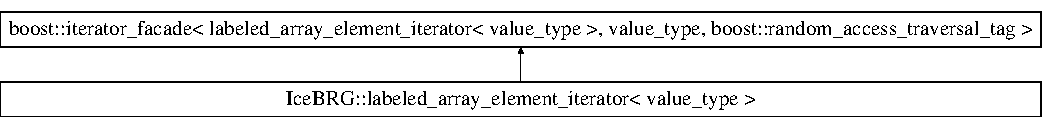
\includegraphics[height=1.568627cm]{classIceBRG_1_1labeled__array__element__iterator}
\end{center}
\end{figure}
\subsection*{Public Types}
\begin{DoxyCompactItemize}
\item 
typedef base\+::difference\+\_\+type \hyperlink{classIceBRG_1_1labeled__array__element__iterator_acd537ab832f1eb85fb69f1653ad208c5}{difference\+\_\+type}
\end{DoxyCompactItemize}
\subsection*{Public Member Functions}
\begin{DoxyCompactItemize}
\item 
\hyperlink{classIceBRG_1_1labeled__array__element__iterator_a7f33ffdec6e7a0585b07c8947907bffe}{labeled\+\_\+array\+\_\+element\+\_\+iterator} ()
\item 
\hyperlink{classIceBRG_1_1labeled__array__element__iterator_afa3c49499457f050f6d30e7161083fc7}{labeled\+\_\+array\+\_\+element\+\_\+iterator} (value\+\_\+type $\ast$ptr, const \hyperlink{lib_2IceBRG__main_2common_8h_ac4de9d9335536ac22821171deec8d39e}{int\+\_\+type} \&multiplier=1)
\item 
{\footnotesize template$<$typename T\+\_\+o\+\_\+value\+\_\+type $>$ }\\\hyperlink{classIceBRG_1_1labeled__array__element__iterator_ad2e8da30ea6d98f79a94282a50d00388}{labeled\+\_\+array\+\_\+element\+\_\+iterator} (const \hyperlink{classIceBRG_1_1labeled__array__element__iterator}{labeled\+\_\+array\+\_\+element\+\_\+iterator}$<$ value\+\_\+type $>$ \&other, typename std\+::enable\+\_\+if$<$ std\+::is\+\_\+convertible$<$ T\+\_\+o\+\_\+value\+\_\+type, value\+\_\+type $>$\+::value, T\+\_\+o\+\_\+value\+\_\+type $\ast$ $>$\+::type=nullptr)
\end{DoxyCompactItemize}
\subsection*{Friends}
\begin{DoxyCompactItemize}
\item 
class \hyperlink{classIceBRG_1_1labeled__array__element__iterator_ac09f73e325921cc50ebcd96bed0f8096}{boost\+::iterator\+\_\+core\+\_\+access}
\end{DoxyCompactItemize}


\subsection{Member Typedef Documentation}
\hypertarget{classIceBRG_1_1labeled__array__element__iterator_acd537ab832f1eb85fb69f1653ad208c5}{}\index{Ice\+B\+R\+G\+::labeled\+\_\+array\+\_\+element\+\_\+iterator@{Ice\+B\+R\+G\+::labeled\+\_\+array\+\_\+element\+\_\+iterator}!difference\+\_\+type@{difference\+\_\+type}}
\index{difference\+\_\+type@{difference\+\_\+type}!Ice\+B\+R\+G\+::labeled\+\_\+array\+\_\+element\+\_\+iterator@{Ice\+B\+R\+G\+::labeled\+\_\+array\+\_\+element\+\_\+iterator}}
\subsubsection[{difference\+\_\+type}]{\setlength{\rightskip}{0pt plus 5cm}template$<$typename value\+\_\+type$>$ typedef base\+::difference\+\_\+type {\bf Ice\+B\+R\+G\+::labeled\+\_\+array\+\_\+element\+\_\+iterator}$<$ value\+\_\+type $>$\+::{\bf difference\+\_\+type}}\label{classIceBRG_1_1labeled__array__element__iterator_acd537ab832f1eb85fb69f1653ad208c5}


\subsection{Constructor \& Destructor Documentation}
\hypertarget{classIceBRG_1_1labeled__array__element__iterator_a7f33ffdec6e7a0585b07c8947907bffe}{}\index{Ice\+B\+R\+G\+::labeled\+\_\+array\+\_\+element\+\_\+iterator@{Ice\+B\+R\+G\+::labeled\+\_\+array\+\_\+element\+\_\+iterator}!labeled\+\_\+array\+\_\+element\+\_\+iterator@{labeled\+\_\+array\+\_\+element\+\_\+iterator}}
\index{labeled\+\_\+array\+\_\+element\+\_\+iterator@{labeled\+\_\+array\+\_\+element\+\_\+iterator}!Ice\+B\+R\+G\+::labeled\+\_\+array\+\_\+element\+\_\+iterator@{Ice\+B\+R\+G\+::labeled\+\_\+array\+\_\+element\+\_\+iterator}}
\subsubsection[{labeled\+\_\+array\+\_\+element\+\_\+iterator()}]{\setlength{\rightskip}{0pt plus 5cm}template$<$typename value\+\_\+type$>$ {\bf Ice\+B\+R\+G\+::labeled\+\_\+array\+\_\+element\+\_\+iterator}$<$ value\+\_\+type $>$\+::{\bf labeled\+\_\+array\+\_\+element\+\_\+iterator} (
\begin{DoxyParamCaption}
{}
\end{DoxyParamCaption}
)\hspace{0.3cm}{\ttfamily [inline]}}\label{classIceBRG_1_1labeled__array__element__iterator_a7f33ffdec6e7a0585b07c8947907bffe}
\hypertarget{classIceBRG_1_1labeled__array__element__iterator_afa3c49499457f050f6d30e7161083fc7}{}\index{Ice\+B\+R\+G\+::labeled\+\_\+array\+\_\+element\+\_\+iterator@{Ice\+B\+R\+G\+::labeled\+\_\+array\+\_\+element\+\_\+iterator}!labeled\+\_\+array\+\_\+element\+\_\+iterator@{labeled\+\_\+array\+\_\+element\+\_\+iterator}}
\index{labeled\+\_\+array\+\_\+element\+\_\+iterator@{labeled\+\_\+array\+\_\+element\+\_\+iterator}!Ice\+B\+R\+G\+::labeled\+\_\+array\+\_\+element\+\_\+iterator@{Ice\+B\+R\+G\+::labeled\+\_\+array\+\_\+element\+\_\+iterator}}
\subsubsection[{labeled\+\_\+array\+\_\+element\+\_\+iterator(value\+\_\+type $\ast$ptr, const int\+\_\+type \&multiplier=1)}]{\setlength{\rightskip}{0pt plus 5cm}template$<$typename value\+\_\+type$>$ {\bf Ice\+B\+R\+G\+::labeled\+\_\+array\+\_\+element\+\_\+iterator}$<$ value\+\_\+type $>$\+::{\bf labeled\+\_\+array\+\_\+element\+\_\+iterator} (
\begin{DoxyParamCaption}
\item[{value\+\_\+type $\ast$}]{ptr, }
\item[{const {\bf int\+\_\+type} \&}]{multiplier = {\ttfamily 1}}
\end{DoxyParamCaption}
)\hspace{0.3cm}{\ttfamily [inline]}}\label{classIceBRG_1_1labeled__array__element__iterator_afa3c49499457f050f6d30e7161083fc7}
\hypertarget{classIceBRG_1_1labeled__array__element__iterator_ad2e8da30ea6d98f79a94282a50d00388}{}\index{Ice\+B\+R\+G\+::labeled\+\_\+array\+\_\+element\+\_\+iterator@{Ice\+B\+R\+G\+::labeled\+\_\+array\+\_\+element\+\_\+iterator}!labeled\+\_\+array\+\_\+element\+\_\+iterator@{labeled\+\_\+array\+\_\+element\+\_\+iterator}}
\index{labeled\+\_\+array\+\_\+element\+\_\+iterator@{labeled\+\_\+array\+\_\+element\+\_\+iterator}!Ice\+B\+R\+G\+::labeled\+\_\+array\+\_\+element\+\_\+iterator@{Ice\+B\+R\+G\+::labeled\+\_\+array\+\_\+element\+\_\+iterator}}
\subsubsection[{labeled\+\_\+array\+\_\+element\+\_\+iterator(const labeled\+\_\+array\+\_\+element\+\_\+iterator$<$ value\+\_\+type $>$ \&other, typename std\+::enable\+\_\+if$<$ std\+::is\+\_\+convertible$<$ T\+\_\+o\+\_\+value\+\_\+type, value\+\_\+type $>$\+::value, T\+\_\+o\+\_\+value\+\_\+type $\ast$ $>$\+::type=nullptr)}]{\setlength{\rightskip}{0pt plus 5cm}template$<$typename value\+\_\+type$>$ template$<$typename T\+\_\+o\+\_\+value\+\_\+type $>$ {\bf Ice\+B\+R\+G\+::labeled\+\_\+array\+\_\+element\+\_\+iterator}$<$ value\+\_\+type $>$\+::{\bf labeled\+\_\+array\+\_\+element\+\_\+iterator} (
\begin{DoxyParamCaption}
\item[{const {\bf labeled\+\_\+array\+\_\+element\+\_\+iterator}$<$ value\+\_\+type $>$ \&}]{other, }
\item[{typename std\+::enable\+\_\+if$<$ std\+::is\+\_\+convertible$<$ T\+\_\+o\+\_\+value\+\_\+type, value\+\_\+type $>$\+::value, T\+\_\+o\+\_\+value\+\_\+type $\ast$ $>$\+::type}]{ = {\ttfamily nullptr}}
\end{DoxyParamCaption}
)\hspace{0.3cm}{\ttfamily [inline]}}\label{classIceBRG_1_1labeled__array__element__iterator_ad2e8da30ea6d98f79a94282a50d00388}


\subsection{Friends And Related Function Documentation}
\hypertarget{classIceBRG_1_1labeled__array__element__iterator_ac09f73e325921cc50ebcd96bed0f8096}{}\index{Ice\+B\+R\+G\+::labeled\+\_\+array\+\_\+element\+\_\+iterator@{Ice\+B\+R\+G\+::labeled\+\_\+array\+\_\+element\+\_\+iterator}!boost\+::iterator\+\_\+core\+\_\+access@{boost\+::iterator\+\_\+core\+\_\+access}}
\index{boost\+::iterator\+\_\+core\+\_\+access@{boost\+::iterator\+\_\+core\+\_\+access}!Ice\+B\+R\+G\+::labeled\+\_\+array\+\_\+element\+\_\+iterator@{Ice\+B\+R\+G\+::labeled\+\_\+array\+\_\+element\+\_\+iterator}}
\subsubsection[{boost\+::iterator\+\_\+core\+\_\+access}]{\setlength{\rightskip}{0pt plus 5cm}template$<$typename value\+\_\+type$>$ friend class boost\+::iterator\+\_\+core\+\_\+access\hspace{0.3cm}{\ttfamily [friend]}}\label{classIceBRG_1_1labeled__array__element__iterator_ac09f73e325921cc50ebcd96bed0f8096}


The documentation for this class was generated from the following file\+:\begin{DoxyCompactItemize}
\item 
/disk2/brg/git/\+Magnification\+\_\+\+Public/src/lib/\+Ice\+B\+R\+G\+\_\+main/container/labeled\+\_\+array/\hyperlink{labeled__array__element__iterator_8hpp}{labeled\+\_\+array\+\_\+element\+\_\+iterator.\+hpp}\end{DoxyCompactItemize}

\hypertarget{classIceBRG_1_1labeled__array__raw__col__iterator}{}\section{Ice\+B\+R\+G\+:\+:labeled\+\_\+array\+\_\+raw\+\_\+col\+\_\+iterator$<$ labeled\+\_\+array\+\_\+type, T, T\+\_\+reference $>$ Class Template Reference}
\label{classIceBRG_1_1labeled__array__raw__col__iterator}\index{Ice\+B\+R\+G\+::labeled\+\_\+array\+\_\+raw\+\_\+col\+\_\+iterator$<$ labeled\+\_\+array\+\_\+type, T, T\+\_\+reference $>$@{Ice\+B\+R\+G\+::labeled\+\_\+array\+\_\+raw\+\_\+col\+\_\+iterator$<$ labeled\+\_\+array\+\_\+type, T, T\+\_\+reference $>$}}


{\ttfamily \#include $<$labeled\+\_\+array\+\_\+raw\+\_\+col\+\_\+iterator.\+hpp$>$}

Inheritance diagram for Ice\+B\+R\+G\+:\+:labeled\+\_\+array\+\_\+raw\+\_\+col\+\_\+iterator$<$ labeled\+\_\+array\+\_\+type, T, T\+\_\+reference $>$\+:\begin{figure}[H]
\begin{center}
\leavevmode
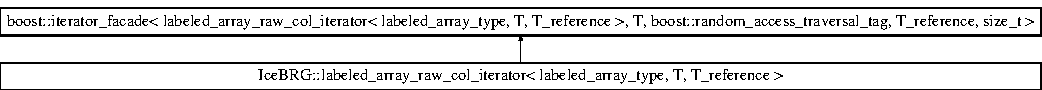
\includegraphics[height=1.212121cm]{classIceBRG_1_1labeled__array__raw__col__iterator}
\end{center}
\end{figure}
\subsection*{Public Types}
\begin{DoxyCompactItemize}
\item 
typedef base\+::difference\+\_\+type \hyperlink{classIceBRG_1_1labeled__array__raw__col__iterator_aadef267d0a30f898af83e9ebf6716b46}{difference\+\_\+type}
\end{DoxyCompactItemize}
\subsection*{Public Member Functions}
\begin{DoxyCompactItemize}
\item 
\hyperlink{classIceBRG_1_1labeled__array__raw__col__iterator_a11d12297c01226486507f3233a91aae2}{labeled\+\_\+array\+\_\+raw\+\_\+col\+\_\+iterator} ()
\item 
\hyperlink{classIceBRG_1_1labeled__array__raw__col__iterator_afd1ea008ebc610e8ab7dbe1f4a6d2283}{labeled\+\_\+array\+\_\+raw\+\_\+col\+\_\+iterator} (labeled\+\_\+array\+\_\+type $\ast$base, const size\+\_\+t \&col\+\_\+index)
\item 
{\footnotesize template$<$class T\+\_\+o , typename T\+\_\+o\+\_\+reference $>$ }\\\hyperlink{classIceBRG_1_1labeled__array__raw__col__iterator_adfe2e2d7155394f36b742406d7d7293b}{labeled\+\_\+array\+\_\+raw\+\_\+col\+\_\+iterator} (const \hyperlink{classIceBRG_1_1labeled__array__raw__col__iterator}{labeled\+\_\+array\+\_\+raw\+\_\+col\+\_\+iterator}$<$ labeled\+\_\+array\+\_\+type, T\+\_\+o, T\+\_\+o\+\_\+reference $>$ \&other, typename std\+::enable\+\_\+if$<$ std\+::is\+\_\+convertible$<$ T\+\_\+o\+\_\+reference, T\+\_\+reference $>$\+::value, T\+\_\+o\+\_\+reference $>$\+::type $\ast$=nullptr)
\end{DoxyCompactItemize}
\subsection*{Friends}
\begin{DoxyCompactItemize}
\item 
class \hyperlink{classIceBRG_1_1labeled__array__raw__col__iterator_ac09f73e325921cc50ebcd96bed0f8096}{boost\+::iterator\+\_\+core\+\_\+access}
\end{DoxyCompactItemize}


\subsection{Member Typedef Documentation}
\hypertarget{classIceBRG_1_1labeled__array__raw__col__iterator_aadef267d0a30f898af83e9ebf6716b46}{}\index{Ice\+B\+R\+G\+::labeled\+\_\+array\+\_\+raw\+\_\+col\+\_\+iterator@{Ice\+B\+R\+G\+::labeled\+\_\+array\+\_\+raw\+\_\+col\+\_\+iterator}!difference\+\_\+type@{difference\+\_\+type}}
\index{difference\+\_\+type@{difference\+\_\+type}!Ice\+B\+R\+G\+::labeled\+\_\+array\+\_\+raw\+\_\+col\+\_\+iterator@{Ice\+B\+R\+G\+::labeled\+\_\+array\+\_\+raw\+\_\+col\+\_\+iterator}}
\subsubsection[{difference\+\_\+type}]{\setlength{\rightskip}{0pt plus 5cm}template$<$typename labeled\+\_\+array\+\_\+type, typename T, typename T\+\_\+reference$>$ typedef base\+::difference\+\_\+type {\bf Ice\+B\+R\+G\+::labeled\+\_\+array\+\_\+raw\+\_\+col\+\_\+iterator}$<$ labeled\+\_\+array\+\_\+type, T, T\+\_\+reference $>$\+::{\bf difference\+\_\+type}}\label{classIceBRG_1_1labeled__array__raw__col__iterator_aadef267d0a30f898af83e9ebf6716b46}


\subsection{Constructor \& Destructor Documentation}
\hypertarget{classIceBRG_1_1labeled__array__raw__col__iterator_a11d12297c01226486507f3233a91aae2}{}\index{Ice\+B\+R\+G\+::labeled\+\_\+array\+\_\+raw\+\_\+col\+\_\+iterator@{Ice\+B\+R\+G\+::labeled\+\_\+array\+\_\+raw\+\_\+col\+\_\+iterator}!labeled\+\_\+array\+\_\+raw\+\_\+col\+\_\+iterator@{labeled\+\_\+array\+\_\+raw\+\_\+col\+\_\+iterator}}
\index{labeled\+\_\+array\+\_\+raw\+\_\+col\+\_\+iterator@{labeled\+\_\+array\+\_\+raw\+\_\+col\+\_\+iterator}!Ice\+B\+R\+G\+::labeled\+\_\+array\+\_\+raw\+\_\+col\+\_\+iterator@{Ice\+B\+R\+G\+::labeled\+\_\+array\+\_\+raw\+\_\+col\+\_\+iterator}}
\subsubsection[{labeled\+\_\+array\+\_\+raw\+\_\+col\+\_\+iterator()}]{\setlength{\rightskip}{0pt plus 5cm}template$<$typename labeled\+\_\+array\+\_\+type, typename T, typename T\+\_\+reference$>$ {\bf Ice\+B\+R\+G\+::labeled\+\_\+array\+\_\+raw\+\_\+col\+\_\+iterator}$<$ labeled\+\_\+array\+\_\+type, T, T\+\_\+reference $>$\+::{\bf labeled\+\_\+array\+\_\+raw\+\_\+col\+\_\+iterator} (
\begin{DoxyParamCaption}
{}
\end{DoxyParamCaption}
)\hspace{0.3cm}{\ttfamily [inline]}}\label{classIceBRG_1_1labeled__array__raw__col__iterator_a11d12297c01226486507f3233a91aae2}
\hypertarget{classIceBRG_1_1labeled__array__raw__col__iterator_afd1ea008ebc610e8ab7dbe1f4a6d2283}{}\index{Ice\+B\+R\+G\+::labeled\+\_\+array\+\_\+raw\+\_\+col\+\_\+iterator@{Ice\+B\+R\+G\+::labeled\+\_\+array\+\_\+raw\+\_\+col\+\_\+iterator}!labeled\+\_\+array\+\_\+raw\+\_\+col\+\_\+iterator@{labeled\+\_\+array\+\_\+raw\+\_\+col\+\_\+iterator}}
\index{labeled\+\_\+array\+\_\+raw\+\_\+col\+\_\+iterator@{labeled\+\_\+array\+\_\+raw\+\_\+col\+\_\+iterator}!Ice\+B\+R\+G\+::labeled\+\_\+array\+\_\+raw\+\_\+col\+\_\+iterator@{Ice\+B\+R\+G\+::labeled\+\_\+array\+\_\+raw\+\_\+col\+\_\+iterator}}
\subsubsection[{labeled\+\_\+array\+\_\+raw\+\_\+col\+\_\+iterator(labeled\+\_\+array\+\_\+type $\ast$base, const size\+\_\+t \&col\+\_\+index)}]{\setlength{\rightskip}{0pt plus 5cm}template$<$typename labeled\+\_\+array\+\_\+type, typename T, typename T\+\_\+reference$>$ {\bf Ice\+B\+R\+G\+::labeled\+\_\+array\+\_\+raw\+\_\+col\+\_\+iterator}$<$ labeled\+\_\+array\+\_\+type, T, T\+\_\+reference $>$\+::{\bf labeled\+\_\+array\+\_\+raw\+\_\+col\+\_\+iterator} (
\begin{DoxyParamCaption}
\item[{labeled\+\_\+array\+\_\+type $\ast$}]{base, }
\item[{const size\+\_\+t \&}]{col\+\_\+index}
\end{DoxyParamCaption}
)\hspace{0.3cm}{\ttfamily [inline]}}\label{classIceBRG_1_1labeled__array__raw__col__iterator_afd1ea008ebc610e8ab7dbe1f4a6d2283}
\hypertarget{classIceBRG_1_1labeled__array__raw__col__iterator_adfe2e2d7155394f36b742406d7d7293b}{}\index{Ice\+B\+R\+G\+::labeled\+\_\+array\+\_\+raw\+\_\+col\+\_\+iterator@{Ice\+B\+R\+G\+::labeled\+\_\+array\+\_\+raw\+\_\+col\+\_\+iterator}!labeled\+\_\+array\+\_\+raw\+\_\+col\+\_\+iterator@{labeled\+\_\+array\+\_\+raw\+\_\+col\+\_\+iterator}}
\index{labeled\+\_\+array\+\_\+raw\+\_\+col\+\_\+iterator@{labeled\+\_\+array\+\_\+raw\+\_\+col\+\_\+iterator}!Ice\+B\+R\+G\+::labeled\+\_\+array\+\_\+raw\+\_\+col\+\_\+iterator@{Ice\+B\+R\+G\+::labeled\+\_\+array\+\_\+raw\+\_\+col\+\_\+iterator}}
\subsubsection[{labeled\+\_\+array\+\_\+raw\+\_\+col\+\_\+iterator(const labeled\+\_\+array\+\_\+raw\+\_\+col\+\_\+iterator$<$ labeled\+\_\+array\+\_\+type, T\+\_\+o, T\+\_\+o\+\_\+reference $>$ \&other, typename std\+::enable\+\_\+if$<$ std\+::is\+\_\+convertible$<$ T\+\_\+o\+\_\+reference, T\+\_\+reference $>$\+::value, T\+\_\+o\+\_\+reference $>$\+::type $\ast$=nullptr)}]{\setlength{\rightskip}{0pt plus 5cm}template$<$typename labeled\+\_\+array\+\_\+type, typename T, typename T\+\_\+reference$>$ template$<$class T\+\_\+o , typename T\+\_\+o\+\_\+reference $>$ {\bf Ice\+B\+R\+G\+::labeled\+\_\+array\+\_\+raw\+\_\+col\+\_\+iterator}$<$ labeled\+\_\+array\+\_\+type, T, T\+\_\+reference $>$\+::{\bf labeled\+\_\+array\+\_\+raw\+\_\+col\+\_\+iterator} (
\begin{DoxyParamCaption}
\item[{const {\bf labeled\+\_\+array\+\_\+raw\+\_\+col\+\_\+iterator}$<$ labeled\+\_\+array\+\_\+type, T\+\_\+o, T\+\_\+o\+\_\+reference $>$ \&}]{other, }
\item[{typename std\+::enable\+\_\+if$<$ std\+::is\+\_\+convertible$<$ T\+\_\+o\+\_\+reference, T\+\_\+reference $>$\+::value, T\+\_\+o\+\_\+reference $>$\+::type $\ast$}]{ = {\ttfamily nullptr}}
\end{DoxyParamCaption}
)\hspace{0.3cm}{\ttfamily [inline]}}\label{classIceBRG_1_1labeled__array__raw__col__iterator_adfe2e2d7155394f36b742406d7d7293b}


\subsection{Friends And Related Function Documentation}
\hypertarget{classIceBRG_1_1labeled__array__raw__col__iterator_ac09f73e325921cc50ebcd96bed0f8096}{}\index{Ice\+B\+R\+G\+::labeled\+\_\+array\+\_\+raw\+\_\+col\+\_\+iterator@{Ice\+B\+R\+G\+::labeled\+\_\+array\+\_\+raw\+\_\+col\+\_\+iterator}!boost\+::iterator\+\_\+core\+\_\+access@{boost\+::iterator\+\_\+core\+\_\+access}}
\index{boost\+::iterator\+\_\+core\+\_\+access@{boost\+::iterator\+\_\+core\+\_\+access}!Ice\+B\+R\+G\+::labeled\+\_\+array\+\_\+raw\+\_\+col\+\_\+iterator@{Ice\+B\+R\+G\+::labeled\+\_\+array\+\_\+raw\+\_\+col\+\_\+iterator}}
\subsubsection[{boost\+::iterator\+\_\+core\+\_\+access}]{\setlength{\rightskip}{0pt plus 5cm}template$<$typename labeled\+\_\+array\+\_\+type, typename T, typename T\+\_\+reference$>$ friend class boost\+::iterator\+\_\+core\+\_\+access\hspace{0.3cm}{\ttfamily [friend]}}\label{classIceBRG_1_1labeled__array__raw__col__iterator_ac09f73e325921cc50ebcd96bed0f8096}


The documentation for this class was generated from the following file\+:\begin{DoxyCompactItemize}
\item 
/disk2/brg/git/\+Magnification\+\_\+\+Public/src/lib/\+Ice\+B\+R\+G\+\_\+main/container/labeled\+\_\+array/\hyperlink{labeled__array__raw__col__iterator_8hpp}{labeled\+\_\+array\+\_\+raw\+\_\+col\+\_\+iterator.\+hpp}\end{DoxyCompactItemize}

\hypertarget{classIceBRG_1_1labeled__array__raw__row__iterator}{}\section{Ice\+B\+R\+G\+:\+:labeled\+\_\+array\+\_\+raw\+\_\+row\+\_\+iterator$<$ labeled\+\_\+array\+\_\+type, T, T\+\_\+reference $>$ Class Template Reference}
\label{classIceBRG_1_1labeled__array__raw__row__iterator}\index{Ice\+B\+R\+G\+::labeled\+\_\+array\+\_\+raw\+\_\+row\+\_\+iterator$<$ labeled\+\_\+array\+\_\+type, T, T\+\_\+reference $>$@{Ice\+B\+R\+G\+::labeled\+\_\+array\+\_\+raw\+\_\+row\+\_\+iterator$<$ labeled\+\_\+array\+\_\+type, T, T\+\_\+reference $>$}}


{\ttfamily \#include $<$labeled\+\_\+array\+\_\+raw\+\_\+row\+\_\+iterator.\+hpp$>$}

Inheritance diagram for Ice\+B\+R\+G\+:\+:labeled\+\_\+array\+\_\+raw\+\_\+row\+\_\+iterator$<$ labeled\+\_\+array\+\_\+type, T, T\+\_\+reference $>$\+:\begin{figure}[H]
\begin{center}
\leavevmode
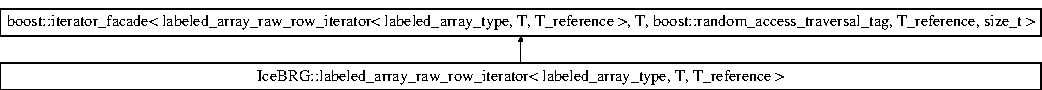
\includegraphics[height=1.206897cm]{classIceBRG_1_1labeled__array__raw__row__iterator}
\end{center}
\end{figure}
\subsection*{Public Types}
\begin{DoxyCompactItemize}
\item 
typedef base\+::difference\+\_\+type \hyperlink{classIceBRG_1_1labeled__array__raw__row__iterator_af87be9b30e0d95c012db53c65365c3dd}{difference\+\_\+type}
\end{DoxyCompactItemize}
\subsection*{Public Member Functions}
\begin{DoxyCompactItemize}
\item 
\hyperlink{classIceBRG_1_1labeled__array__raw__row__iterator_ae1038eb4645953cfc365d48414d94698}{labeled\+\_\+array\+\_\+raw\+\_\+row\+\_\+iterator} ()
\item 
\hyperlink{classIceBRG_1_1labeled__array__raw__row__iterator_a0e12ade83e1be91d0cc1234a50f950d6}{labeled\+\_\+array\+\_\+raw\+\_\+row\+\_\+iterator} (labeled\+\_\+array\+\_\+type $\ast$base, const size\+\_\+t \&row\+\_\+index)
\item 
{\footnotesize template$<$class T\+\_\+o , typename T\+\_\+o\+\_\+reference $>$ }\\\hyperlink{classIceBRG_1_1labeled__array__raw__row__iterator_a84cb7571712941200f3855cfa136edde}{labeled\+\_\+array\+\_\+raw\+\_\+row\+\_\+iterator} (const \hyperlink{classIceBRG_1_1labeled__array__raw__row__iterator}{labeled\+\_\+array\+\_\+raw\+\_\+row\+\_\+iterator}$<$ labeled\+\_\+array\+\_\+type, T\+\_\+o, T\+\_\+o\+\_\+reference $>$ \&other, typename std\+::enable\+\_\+if$<$ std\+::is\+\_\+convertible$<$ T\+\_\+o\+\_\+reference, T\+\_\+reference $>$\+::value, T\+\_\+o\+\_\+reference $>$\+::type $\ast$=nullptr)
\end{DoxyCompactItemize}
\subsection*{Friends}
\begin{DoxyCompactItemize}
\item 
class \hyperlink{classIceBRG_1_1labeled__array__raw__row__iterator_ac09f73e325921cc50ebcd96bed0f8096}{boost\+::iterator\+\_\+core\+\_\+access}
\end{DoxyCompactItemize}


\subsection{Member Typedef Documentation}
\hypertarget{classIceBRG_1_1labeled__array__raw__row__iterator_af87be9b30e0d95c012db53c65365c3dd}{}\index{Ice\+B\+R\+G\+::labeled\+\_\+array\+\_\+raw\+\_\+row\+\_\+iterator@{Ice\+B\+R\+G\+::labeled\+\_\+array\+\_\+raw\+\_\+row\+\_\+iterator}!difference\+\_\+type@{difference\+\_\+type}}
\index{difference\+\_\+type@{difference\+\_\+type}!Ice\+B\+R\+G\+::labeled\+\_\+array\+\_\+raw\+\_\+row\+\_\+iterator@{Ice\+B\+R\+G\+::labeled\+\_\+array\+\_\+raw\+\_\+row\+\_\+iterator}}
\subsubsection[{difference\+\_\+type}]{\setlength{\rightskip}{0pt plus 5cm}template$<$typename labeled\+\_\+array\+\_\+type, typename T, typename T\+\_\+reference$>$ typedef base\+::difference\+\_\+type {\bf Ice\+B\+R\+G\+::labeled\+\_\+array\+\_\+raw\+\_\+row\+\_\+iterator}$<$ labeled\+\_\+array\+\_\+type, T, T\+\_\+reference $>$\+::{\bf difference\+\_\+type}}\label{classIceBRG_1_1labeled__array__raw__row__iterator_af87be9b30e0d95c012db53c65365c3dd}


\subsection{Constructor \& Destructor Documentation}
\hypertarget{classIceBRG_1_1labeled__array__raw__row__iterator_ae1038eb4645953cfc365d48414d94698}{}\index{Ice\+B\+R\+G\+::labeled\+\_\+array\+\_\+raw\+\_\+row\+\_\+iterator@{Ice\+B\+R\+G\+::labeled\+\_\+array\+\_\+raw\+\_\+row\+\_\+iterator}!labeled\+\_\+array\+\_\+raw\+\_\+row\+\_\+iterator@{labeled\+\_\+array\+\_\+raw\+\_\+row\+\_\+iterator}}
\index{labeled\+\_\+array\+\_\+raw\+\_\+row\+\_\+iterator@{labeled\+\_\+array\+\_\+raw\+\_\+row\+\_\+iterator}!Ice\+B\+R\+G\+::labeled\+\_\+array\+\_\+raw\+\_\+row\+\_\+iterator@{Ice\+B\+R\+G\+::labeled\+\_\+array\+\_\+raw\+\_\+row\+\_\+iterator}}
\subsubsection[{labeled\+\_\+array\+\_\+raw\+\_\+row\+\_\+iterator()}]{\setlength{\rightskip}{0pt plus 5cm}template$<$typename labeled\+\_\+array\+\_\+type, typename T, typename T\+\_\+reference$>$ {\bf Ice\+B\+R\+G\+::labeled\+\_\+array\+\_\+raw\+\_\+row\+\_\+iterator}$<$ labeled\+\_\+array\+\_\+type, T, T\+\_\+reference $>$\+::{\bf labeled\+\_\+array\+\_\+raw\+\_\+row\+\_\+iterator} (
\begin{DoxyParamCaption}
{}
\end{DoxyParamCaption}
)\hspace{0.3cm}{\ttfamily [inline]}}\label{classIceBRG_1_1labeled__array__raw__row__iterator_ae1038eb4645953cfc365d48414d94698}
\hypertarget{classIceBRG_1_1labeled__array__raw__row__iterator_a0e12ade83e1be91d0cc1234a50f950d6}{}\index{Ice\+B\+R\+G\+::labeled\+\_\+array\+\_\+raw\+\_\+row\+\_\+iterator@{Ice\+B\+R\+G\+::labeled\+\_\+array\+\_\+raw\+\_\+row\+\_\+iterator}!labeled\+\_\+array\+\_\+raw\+\_\+row\+\_\+iterator@{labeled\+\_\+array\+\_\+raw\+\_\+row\+\_\+iterator}}
\index{labeled\+\_\+array\+\_\+raw\+\_\+row\+\_\+iterator@{labeled\+\_\+array\+\_\+raw\+\_\+row\+\_\+iterator}!Ice\+B\+R\+G\+::labeled\+\_\+array\+\_\+raw\+\_\+row\+\_\+iterator@{Ice\+B\+R\+G\+::labeled\+\_\+array\+\_\+raw\+\_\+row\+\_\+iterator}}
\subsubsection[{labeled\+\_\+array\+\_\+raw\+\_\+row\+\_\+iterator(labeled\+\_\+array\+\_\+type $\ast$base, const size\+\_\+t \&row\+\_\+index)}]{\setlength{\rightskip}{0pt plus 5cm}template$<$typename labeled\+\_\+array\+\_\+type, typename T, typename T\+\_\+reference$>$ {\bf Ice\+B\+R\+G\+::labeled\+\_\+array\+\_\+raw\+\_\+row\+\_\+iterator}$<$ labeled\+\_\+array\+\_\+type, T, T\+\_\+reference $>$\+::{\bf labeled\+\_\+array\+\_\+raw\+\_\+row\+\_\+iterator} (
\begin{DoxyParamCaption}
\item[{labeled\+\_\+array\+\_\+type $\ast$}]{base, }
\item[{const size\+\_\+t \&}]{row\+\_\+index}
\end{DoxyParamCaption}
)\hspace{0.3cm}{\ttfamily [inline]}}\label{classIceBRG_1_1labeled__array__raw__row__iterator_a0e12ade83e1be91d0cc1234a50f950d6}
\hypertarget{classIceBRG_1_1labeled__array__raw__row__iterator_a84cb7571712941200f3855cfa136edde}{}\index{Ice\+B\+R\+G\+::labeled\+\_\+array\+\_\+raw\+\_\+row\+\_\+iterator@{Ice\+B\+R\+G\+::labeled\+\_\+array\+\_\+raw\+\_\+row\+\_\+iterator}!labeled\+\_\+array\+\_\+raw\+\_\+row\+\_\+iterator@{labeled\+\_\+array\+\_\+raw\+\_\+row\+\_\+iterator}}
\index{labeled\+\_\+array\+\_\+raw\+\_\+row\+\_\+iterator@{labeled\+\_\+array\+\_\+raw\+\_\+row\+\_\+iterator}!Ice\+B\+R\+G\+::labeled\+\_\+array\+\_\+raw\+\_\+row\+\_\+iterator@{Ice\+B\+R\+G\+::labeled\+\_\+array\+\_\+raw\+\_\+row\+\_\+iterator}}
\subsubsection[{labeled\+\_\+array\+\_\+raw\+\_\+row\+\_\+iterator(const labeled\+\_\+array\+\_\+raw\+\_\+row\+\_\+iterator$<$ labeled\+\_\+array\+\_\+type, T\+\_\+o, T\+\_\+o\+\_\+reference $>$ \&other, typename std\+::enable\+\_\+if$<$ std\+::is\+\_\+convertible$<$ T\+\_\+o\+\_\+reference, T\+\_\+reference $>$\+::value, T\+\_\+o\+\_\+reference $>$\+::type $\ast$=nullptr)}]{\setlength{\rightskip}{0pt plus 5cm}template$<$typename labeled\+\_\+array\+\_\+type, typename T, typename T\+\_\+reference$>$ template$<$class T\+\_\+o , typename T\+\_\+o\+\_\+reference $>$ {\bf Ice\+B\+R\+G\+::labeled\+\_\+array\+\_\+raw\+\_\+row\+\_\+iterator}$<$ labeled\+\_\+array\+\_\+type, T, T\+\_\+reference $>$\+::{\bf labeled\+\_\+array\+\_\+raw\+\_\+row\+\_\+iterator} (
\begin{DoxyParamCaption}
\item[{const {\bf labeled\+\_\+array\+\_\+raw\+\_\+row\+\_\+iterator}$<$ labeled\+\_\+array\+\_\+type, T\+\_\+o, T\+\_\+o\+\_\+reference $>$ \&}]{other, }
\item[{typename std\+::enable\+\_\+if$<$ std\+::is\+\_\+convertible$<$ T\+\_\+o\+\_\+reference, T\+\_\+reference $>$\+::value, T\+\_\+o\+\_\+reference $>$\+::type $\ast$}]{ = {\ttfamily nullptr}}
\end{DoxyParamCaption}
)\hspace{0.3cm}{\ttfamily [inline]}}\label{classIceBRG_1_1labeled__array__raw__row__iterator_a84cb7571712941200f3855cfa136edde}


\subsection{Friends And Related Function Documentation}
\hypertarget{classIceBRG_1_1labeled__array__raw__row__iterator_ac09f73e325921cc50ebcd96bed0f8096}{}\index{Ice\+B\+R\+G\+::labeled\+\_\+array\+\_\+raw\+\_\+row\+\_\+iterator@{Ice\+B\+R\+G\+::labeled\+\_\+array\+\_\+raw\+\_\+row\+\_\+iterator}!boost\+::iterator\+\_\+core\+\_\+access@{boost\+::iterator\+\_\+core\+\_\+access}}
\index{boost\+::iterator\+\_\+core\+\_\+access@{boost\+::iterator\+\_\+core\+\_\+access}!Ice\+B\+R\+G\+::labeled\+\_\+array\+\_\+raw\+\_\+row\+\_\+iterator@{Ice\+B\+R\+G\+::labeled\+\_\+array\+\_\+raw\+\_\+row\+\_\+iterator}}
\subsubsection[{boost\+::iterator\+\_\+core\+\_\+access}]{\setlength{\rightskip}{0pt plus 5cm}template$<$typename labeled\+\_\+array\+\_\+type, typename T, typename T\+\_\+reference$>$ friend class boost\+::iterator\+\_\+core\+\_\+access\hspace{0.3cm}{\ttfamily [friend]}}\label{classIceBRG_1_1labeled__array__raw__row__iterator_ac09f73e325921cc50ebcd96bed0f8096}


The documentation for this class was generated from the following file\+:\begin{DoxyCompactItemize}
\item 
/disk2/brg/git/\+Magnification\+\_\+\+Public/src/lib/\+Ice\+B\+R\+G\+\_\+main/container/labeled\+\_\+array/\hyperlink{labeled__array__raw__row__iterator_8hpp}{labeled\+\_\+array\+\_\+raw\+\_\+row\+\_\+iterator.\+hpp}\end{DoxyCompactItemize}

\hypertarget{classIceBRG_1_1labeled__array__row__iterator}{}\section{Ice\+B\+R\+G\+:\+:labeled\+\_\+array\+\_\+row\+\_\+iterator$<$ labeled\+\_\+array\+\_\+type, T, T\+\_\+reference $>$ Class Template Reference}
\label{classIceBRG_1_1labeled__array__row__iterator}\index{Ice\+B\+R\+G\+::labeled\+\_\+array\+\_\+row\+\_\+iterator$<$ labeled\+\_\+array\+\_\+type, T, T\+\_\+reference $>$@{Ice\+B\+R\+G\+::labeled\+\_\+array\+\_\+row\+\_\+iterator$<$ labeled\+\_\+array\+\_\+type, T, T\+\_\+reference $>$}}


{\ttfamily \#include $<$labeled\+\_\+array\+\_\+row\+\_\+iterator.\+hpp$>$}

Inheritance diagram for Ice\+B\+R\+G\+:\+:labeled\+\_\+array\+\_\+row\+\_\+iterator$<$ labeled\+\_\+array\+\_\+type, T, T\+\_\+reference $>$\+:\begin{figure}[H]
\begin{center}
\leavevmode
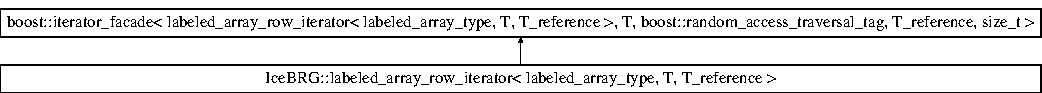
\includegraphics[height=1.244444cm]{classIceBRG_1_1labeled__array__row__iterator}
\end{center}
\end{figure}
\subsection*{Public Types}
\begin{DoxyCompactItemize}
\item 
typedef base\+::difference\+\_\+type \hyperlink{classIceBRG_1_1labeled__array__row__iterator_a3ac7f5a854882d443faaef1ae3ef3c9d}{difference\+\_\+type}
\end{DoxyCompactItemize}
\subsection*{Public Member Functions}
\begin{DoxyCompactItemize}
\item 
\hyperlink{classIceBRG_1_1labeled__array__row__iterator_adc441238b4a562135defd2c6c95bb887}{labeled\+\_\+array\+\_\+row\+\_\+iterator} ()
\item 
\hyperlink{classIceBRG_1_1labeled__array__row__iterator_a629176c37571e2f2ca3ca87ca39558af}{labeled\+\_\+array\+\_\+row\+\_\+iterator} (labeled\+\_\+array\+\_\+type $\ast$base, const size\+\_\+t \&row\+\_\+index)
\item 
{\footnotesize template$<$class T\+\_\+o , typename T\+\_\+o\+\_\+reference , typename T\+\_\+o\+\_\+labeled\+\_\+array\+\_\+type $>$ }\\\hyperlink{classIceBRG_1_1labeled__array__row__iterator_a18186784ffabffb098a7c1c9889f4bb6}{labeled\+\_\+array\+\_\+row\+\_\+iterator} (const \hyperlink{classIceBRG_1_1labeled__array__row__iterator}{labeled\+\_\+array\+\_\+row\+\_\+iterator}$<$ T\+\_\+o\+\_\+labeled\+\_\+array\+\_\+type, T\+\_\+o, T\+\_\+o\+\_\+reference $>$ \&other, typename std\+::enable\+\_\+if$<$ std\+::is\+\_\+convertible$<$ T\+\_\+o\+\_\+reference, T\+\_\+reference $>$\+::value \&\&std\+::is\+\_\+convertible$<$ T\+\_\+o\+\_\+labeled\+\_\+array\+\_\+type, labeled\+\_\+array\+\_\+type $>$\+::value, char $>$\+::type=0)
\end{DoxyCompactItemize}
\subsection*{Friends}
\begin{DoxyCompactItemize}
\item 
class \hyperlink{classIceBRG_1_1labeled__array__row__iterator_ac09f73e325921cc50ebcd96bed0f8096}{boost\+::iterator\+\_\+core\+\_\+access}
\end{DoxyCompactItemize}


\subsection{Member Typedef Documentation}
\hypertarget{classIceBRG_1_1labeled__array__row__iterator_a3ac7f5a854882d443faaef1ae3ef3c9d}{}\index{Ice\+B\+R\+G\+::labeled\+\_\+array\+\_\+row\+\_\+iterator@{Ice\+B\+R\+G\+::labeled\+\_\+array\+\_\+row\+\_\+iterator}!difference\+\_\+type@{difference\+\_\+type}}
\index{difference\+\_\+type@{difference\+\_\+type}!Ice\+B\+R\+G\+::labeled\+\_\+array\+\_\+row\+\_\+iterator@{Ice\+B\+R\+G\+::labeled\+\_\+array\+\_\+row\+\_\+iterator}}
\subsubsection[{difference\+\_\+type}]{\setlength{\rightskip}{0pt plus 5cm}template$<$typename labeled\+\_\+array\+\_\+type, typename T, typename T\+\_\+reference$>$ typedef base\+::difference\+\_\+type {\bf Ice\+B\+R\+G\+::labeled\+\_\+array\+\_\+row\+\_\+iterator}$<$ labeled\+\_\+array\+\_\+type, T, T\+\_\+reference $>$\+::{\bf difference\+\_\+type}}\label{classIceBRG_1_1labeled__array__row__iterator_a3ac7f5a854882d443faaef1ae3ef3c9d}


\subsection{Constructor \& Destructor Documentation}
\hypertarget{classIceBRG_1_1labeled__array__row__iterator_adc441238b4a562135defd2c6c95bb887}{}\index{Ice\+B\+R\+G\+::labeled\+\_\+array\+\_\+row\+\_\+iterator@{Ice\+B\+R\+G\+::labeled\+\_\+array\+\_\+row\+\_\+iterator}!labeled\+\_\+array\+\_\+row\+\_\+iterator@{labeled\+\_\+array\+\_\+row\+\_\+iterator}}
\index{labeled\+\_\+array\+\_\+row\+\_\+iterator@{labeled\+\_\+array\+\_\+row\+\_\+iterator}!Ice\+B\+R\+G\+::labeled\+\_\+array\+\_\+row\+\_\+iterator@{Ice\+B\+R\+G\+::labeled\+\_\+array\+\_\+row\+\_\+iterator}}
\subsubsection[{labeled\+\_\+array\+\_\+row\+\_\+iterator()}]{\setlength{\rightskip}{0pt plus 5cm}template$<$typename labeled\+\_\+array\+\_\+type, typename T, typename T\+\_\+reference$>$ {\bf Ice\+B\+R\+G\+::labeled\+\_\+array\+\_\+row\+\_\+iterator}$<$ labeled\+\_\+array\+\_\+type, T, T\+\_\+reference $>$\+::{\bf labeled\+\_\+array\+\_\+row\+\_\+iterator} (
\begin{DoxyParamCaption}
{}
\end{DoxyParamCaption}
)\hspace{0.3cm}{\ttfamily [inline]}}\label{classIceBRG_1_1labeled__array__row__iterator_adc441238b4a562135defd2c6c95bb887}
\hypertarget{classIceBRG_1_1labeled__array__row__iterator_a629176c37571e2f2ca3ca87ca39558af}{}\index{Ice\+B\+R\+G\+::labeled\+\_\+array\+\_\+row\+\_\+iterator@{Ice\+B\+R\+G\+::labeled\+\_\+array\+\_\+row\+\_\+iterator}!labeled\+\_\+array\+\_\+row\+\_\+iterator@{labeled\+\_\+array\+\_\+row\+\_\+iterator}}
\index{labeled\+\_\+array\+\_\+row\+\_\+iterator@{labeled\+\_\+array\+\_\+row\+\_\+iterator}!Ice\+B\+R\+G\+::labeled\+\_\+array\+\_\+row\+\_\+iterator@{Ice\+B\+R\+G\+::labeled\+\_\+array\+\_\+row\+\_\+iterator}}
\subsubsection[{labeled\+\_\+array\+\_\+row\+\_\+iterator(labeled\+\_\+array\+\_\+type $\ast$base, const size\+\_\+t \&row\+\_\+index)}]{\setlength{\rightskip}{0pt plus 5cm}template$<$typename labeled\+\_\+array\+\_\+type, typename T, typename T\+\_\+reference$>$ {\bf Ice\+B\+R\+G\+::labeled\+\_\+array\+\_\+row\+\_\+iterator}$<$ labeled\+\_\+array\+\_\+type, T, T\+\_\+reference $>$\+::{\bf labeled\+\_\+array\+\_\+row\+\_\+iterator} (
\begin{DoxyParamCaption}
\item[{labeled\+\_\+array\+\_\+type $\ast$}]{base, }
\item[{const size\+\_\+t \&}]{row\+\_\+index}
\end{DoxyParamCaption}
)\hspace{0.3cm}{\ttfamily [inline]}}\label{classIceBRG_1_1labeled__array__row__iterator_a629176c37571e2f2ca3ca87ca39558af}
\hypertarget{classIceBRG_1_1labeled__array__row__iterator_a18186784ffabffb098a7c1c9889f4bb6}{}\index{Ice\+B\+R\+G\+::labeled\+\_\+array\+\_\+row\+\_\+iterator@{Ice\+B\+R\+G\+::labeled\+\_\+array\+\_\+row\+\_\+iterator}!labeled\+\_\+array\+\_\+row\+\_\+iterator@{labeled\+\_\+array\+\_\+row\+\_\+iterator}}
\index{labeled\+\_\+array\+\_\+row\+\_\+iterator@{labeled\+\_\+array\+\_\+row\+\_\+iterator}!Ice\+B\+R\+G\+::labeled\+\_\+array\+\_\+row\+\_\+iterator@{Ice\+B\+R\+G\+::labeled\+\_\+array\+\_\+row\+\_\+iterator}}
\subsubsection[{labeled\+\_\+array\+\_\+row\+\_\+iterator(const labeled\+\_\+array\+\_\+row\+\_\+iterator$<$ T\+\_\+o\+\_\+labeled\+\_\+array\+\_\+type, T\+\_\+o, T\+\_\+o\+\_\+reference $>$ \&other, typename std\+::enable\+\_\+if$<$ std\+::is\+\_\+convertible$<$ T\+\_\+o\+\_\+reference, T\+\_\+reference $>$\+::value \&\&std\+::is\+\_\+convertible$<$ T\+\_\+o\+\_\+labeled\+\_\+array\+\_\+type, labeled\+\_\+array\+\_\+type $>$\+::value, char $>$\+::type=0)}]{\setlength{\rightskip}{0pt plus 5cm}template$<$typename labeled\+\_\+array\+\_\+type, typename T, typename T\+\_\+reference$>$ template$<$class T\+\_\+o , typename T\+\_\+o\+\_\+reference , typename T\+\_\+o\+\_\+labeled\+\_\+array\+\_\+type $>$ {\bf Ice\+B\+R\+G\+::labeled\+\_\+array\+\_\+row\+\_\+iterator}$<$ labeled\+\_\+array\+\_\+type, T, T\+\_\+reference $>$\+::{\bf labeled\+\_\+array\+\_\+row\+\_\+iterator} (
\begin{DoxyParamCaption}
\item[{const {\bf labeled\+\_\+array\+\_\+row\+\_\+iterator}$<$ T\+\_\+o\+\_\+labeled\+\_\+array\+\_\+type, T\+\_\+o, T\+\_\+o\+\_\+reference $>$ \&}]{other, }
\item[{typename std\+::enable\+\_\+if$<$ std\+::is\+\_\+convertible$<$ T\+\_\+o\+\_\+reference, T\+\_\+reference $>$\+::value \&\&std\+::is\+\_\+convertible$<$ T\+\_\+o\+\_\+labeled\+\_\+array\+\_\+type, labeled\+\_\+array\+\_\+type $>$\+::value, char $>$\+::type}]{ = {\ttfamily 0}}
\end{DoxyParamCaption}
)\hspace{0.3cm}{\ttfamily [inline]}}\label{classIceBRG_1_1labeled__array__row__iterator_a18186784ffabffb098a7c1c9889f4bb6}


\subsection{Friends And Related Function Documentation}
\hypertarget{classIceBRG_1_1labeled__array__row__iterator_ac09f73e325921cc50ebcd96bed0f8096}{}\index{Ice\+B\+R\+G\+::labeled\+\_\+array\+\_\+row\+\_\+iterator@{Ice\+B\+R\+G\+::labeled\+\_\+array\+\_\+row\+\_\+iterator}!boost\+::iterator\+\_\+core\+\_\+access@{boost\+::iterator\+\_\+core\+\_\+access}}
\index{boost\+::iterator\+\_\+core\+\_\+access@{boost\+::iterator\+\_\+core\+\_\+access}!Ice\+B\+R\+G\+::labeled\+\_\+array\+\_\+row\+\_\+iterator@{Ice\+B\+R\+G\+::labeled\+\_\+array\+\_\+row\+\_\+iterator}}
\subsubsection[{boost\+::iterator\+\_\+core\+\_\+access}]{\setlength{\rightskip}{0pt plus 5cm}template$<$typename labeled\+\_\+array\+\_\+type, typename T, typename T\+\_\+reference$>$ friend class boost\+::iterator\+\_\+core\+\_\+access\hspace{0.3cm}{\ttfamily [friend]}}\label{classIceBRG_1_1labeled__array__row__iterator_ac09f73e325921cc50ebcd96bed0f8096}


The documentation for this class was generated from the following file\+:\begin{DoxyCompactItemize}
\item 
/disk2/brg/git/\+Magnification\+\_\+\+Public/src/lib/\+Ice\+B\+R\+G\+\_\+main/container/labeled\+\_\+array/\hyperlink{labeled__array__row__iterator_8hpp}{labeled\+\_\+array\+\_\+row\+\_\+iterator.\+hpp}\end{DoxyCompactItemize}

\hypertarget{classIceBRG_1_1labeled__array__row__reference}{}\section{Ice\+B\+R\+G\+:\+:labeled\+\_\+array\+\_\+row\+\_\+reference$<$ labeled\+\_\+array\+\_\+type, T\+\_\+row\+\_\+type $>$ Class Template Reference}
\label{classIceBRG_1_1labeled__array__row__reference}\index{Ice\+B\+R\+G\+::labeled\+\_\+array\+\_\+row\+\_\+reference$<$ labeled\+\_\+array\+\_\+type, T\+\_\+row\+\_\+type $>$@{Ice\+B\+R\+G\+::labeled\+\_\+array\+\_\+row\+\_\+reference$<$ labeled\+\_\+array\+\_\+type, T\+\_\+row\+\_\+type $>$}}


{\ttfamily \#include $<$labeled\+\_\+array\+\_\+row\+\_\+reference.\+hpp$>$}

\subsection*{Public Types}
\begin{DoxyCompactItemize}
\item 
typedef labeled\+\_\+array\+\_\+type\+::label\+\_\+type \hyperlink{classIceBRG_1_1labeled__array__row__reference_a0b7e29867009277fee9102863be2d63a}{label\+\_\+type}
\item 
typedef labeled\+\_\+array\+\_\+type\+::value\+\_\+type \hyperlink{classIceBRG_1_1labeled__array__row__reference_ae6cfe4bdcb3bc59c3d7613193633f063}{value\+\_\+type}
\item 
typedef labeled\+\_\+array\+\_\+type\+::const\+\_\+value\+\_\+type \hyperlink{classIceBRG_1_1labeled__array__row__reference_a3eaf76b7cd84107e68c41cd4fc056c39}{const\+\_\+value\+\_\+type}
\item 
typedef labeled\+\_\+array\+\_\+type\+::size\+\_\+type \hyperlink{classIceBRG_1_1labeled__array__row__reference_a80c5d11ebfa639fa27894ce288633df0}{size\+\_\+type}
\item 
typedef T\+\_\+row\+\_\+type \hyperlink{classIceBRG_1_1labeled__array__row__reference_a5b537072b2f12f7a4ea9484e2e26986d}{row\+\_\+type}
\item 
typedef labeled\+\_\+array\+\_\+type\+::const\+\_\+row\+\_\+type \hyperlink{classIceBRG_1_1labeled__array__row__reference_a80b2a3ea3231a22bf8c493841ad8cf3a}{const\+\_\+row\+\_\+type}
\item 
typedef labeled\+\_\+array\+\_\+type\+::reference \hyperlink{classIceBRG_1_1labeled__array__row__reference_a24c2694c9ca46757f21f7024a229c925}{reference}
\item 
typedef labeled\+\_\+array\+\_\+type\+::const\+\_\+reference \hyperlink{classIceBRG_1_1labeled__array__row__reference_a7343692e3cbf28a9edfff61f6812f355}{const\+\_\+reference}
\item 
typedef labeled\+\_\+array\+\_\+type\+::row\+\_\+element\+\_\+iterator \hyperlink{classIceBRG_1_1labeled__array__row__reference_a6019a8a167f6816b145f39478b2fb691}{iterator}
\item 
typedef labeled\+\_\+array\+\_\+type\+::const\+\_\+row\+\_\+element\+\_\+iterator \hyperlink{classIceBRG_1_1labeled__array__row__reference_a32426fe25a4b7f8659eb5fe2b58ecba2}{const\+\_\+iterator}
\item 
typedef labeled\+\_\+array\+\_\+type\+::reverse\+\_\+row\+\_\+element\+\_\+iterator \hyperlink{classIceBRG_1_1labeled__array__row__reference_a69e88ba1f1071a47fa00e4ec45f8147d}{reverse\+\_\+iterator}
\item 
typedef labeled\+\_\+array\+\_\+type\+::const\+\_\+reverse\+\_\+row\+\_\+element\+\_\+iterator \hyperlink{classIceBRG_1_1labeled__array__row__reference_a4bb091c3a6d8be3b433acbc02745fa0a}{const\+\_\+reverse\+\_\+iterator}
\item 
typedef size\+\_\+t \hyperlink{classIceBRG_1_1labeled__array__row__reference_a3c4333001dfc05e470766b9c2786f630}{difference\+\_\+type}
\end{DoxyCompactItemize}
\subsection*{Public Member Functions}
\begin{DoxyCompactItemize}
\item 
{\footnotesize template$<$typename T\+\_\+init\+\_\+row\+\_\+type $>$ }\\\hyperlink{classIceBRG_1_1labeled__array__row__reference_aa5b99a997fb1c6a92aff73d093300bca}{labeled\+\_\+array\+\_\+row\+\_\+reference} (map\+\_\+type $\ast$label\+\_\+map, T\+\_\+init\+\_\+row\+\_\+type \&\&row, const \hyperlink{classIceBRG_1_1labeled__array__row__reference_a80c5d11ebfa639fa27894ce288633df0}{size\+\_\+type} \&num\+\_\+cols)
\begin{DoxyCompactList}\small\item\em Constructor. Requires a pointer to a \hyperlink{classIceBRG_1_1labeled__array}{labeled\+\_\+array}\textquotesingle{}s label map and row. \end{DoxyCompactList}\item 
virtual \hyperlink{classIceBRG_1_1labeled__array__row__reference_a87c88e311e4178e7d945eac0349f16ec}{$\sim$labeled\+\_\+array\+\_\+row\+\_\+reference} ()
\begin{DoxyCompactList}\small\item\em Virtual destructor. \end{DoxyCompactList}\item 
{\footnotesize template$<$typename T\+\_\+iterator  = const\+\_\+iterator, typename std\+::enable\+\_\+if$<$!std\+::is\+\_\+same$<$ T\+\_\+iterator, const\+\_\+value\+\_\+type $\ast$ $>$\+::value, char $>$\+::type  = 0$>$ }\\T\+\_\+iterator \hyperlink{classIceBRG_1_1labeled__array__row__reference_a3e3cf78cfef5f00b83417cbbfb692443}{begin} () const  noexcept
\begin{DoxyCompactList}\small\item\em begin (const) \end{DoxyCompactList}\item 
{\footnotesize template$<$typename T\+\_\+iterator  = const\+\_\+iterator, typename std\+::enable\+\_\+if$<$ std\+::is\+\_\+same$<$ T\+\_\+iterator, const\+\_\+value\+\_\+type $\ast$ $>$\+::value, char $>$\+::type  = 0$>$ }\\T\+\_\+iterator \hyperlink{classIceBRG_1_1labeled__array__row__reference_a3e3cf78cfef5f00b83417cbbfb692443}{begin} () const  noexcept
\item 
{\footnotesize template$<$typename T\+\_\+iterator  = iterator, typename std\+::enable\+\_\+if$<$!std\+::is\+\_\+same$<$ T\+\_\+iterator, value\+\_\+type $\ast$ $>$\+::value, char $>$\+::type  = 0$>$ }\\T\+\_\+iterator \hyperlink{classIceBRG_1_1labeled__array__row__reference_a5fa54eb388d4240ce4700a20882c4616}{begin} () noexcept
\begin{DoxyCompactList}\small\item\em begin \end{DoxyCompactList}\item 
{\footnotesize template$<$typename T\+\_\+iterator  = iterator, typename std\+::enable\+\_\+if$<$ std\+::is\+\_\+same$<$ T\+\_\+iterator, value\+\_\+type $\ast$ $>$\+::value, char $>$\+::type  = 0$>$ }\\T\+\_\+iterator \hyperlink{classIceBRG_1_1labeled__array__row__reference_a5fa54eb388d4240ce4700a20882c4616}{begin} () noexcept
\item 
{\footnotesize template$<$typename T\+\_\+iterator  = const\+\_\+iterator, typename std\+::enable\+\_\+if$<$!std\+::is\+\_\+same$<$ T\+\_\+iterator, const\+\_\+value\+\_\+type $\ast$ $>$\+::value, char $>$\+::type  = 0$>$ }\\T\+\_\+iterator \hyperlink{classIceBRG_1_1labeled__array__row__reference_ad8387c725079b50f2364109245fec8c1}{end} () const  noexcept
\begin{DoxyCompactList}\small\item\em end (const) \end{DoxyCompactList}\item 
{\footnotesize template$<$typename T\+\_\+iterator  = const\+\_\+iterator, typename std\+::enable\+\_\+if$<$ std\+::is\+\_\+same$<$ T\+\_\+iterator, const\+\_\+value\+\_\+type $\ast$ $>$\+::value, char $>$\+::type  = 0$>$ }\\T\+\_\+iterator \hyperlink{classIceBRG_1_1labeled__array__row__reference_ad8387c725079b50f2364109245fec8c1}{end} () const  noexcept
\item 
{\footnotesize template$<$typename T\+\_\+iterator  = iterator, typename std\+::enable\+\_\+if$<$!std\+::is\+\_\+same$<$ T\+\_\+iterator, value\+\_\+type $\ast$ $>$\+::value, char $>$\+::type  = 0$>$ }\\T\+\_\+iterator \hyperlink{classIceBRG_1_1labeled__array__row__reference_a24df418e36063069ab29cd3a33e95154}{end} () noexcept
\begin{DoxyCompactList}\small\item\em end \end{DoxyCompactList}\item 
{\footnotesize template$<$typename T\+\_\+iterator  = iterator, typename std\+::enable\+\_\+if$<$ std\+::is\+\_\+same$<$ T\+\_\+iterator, value\+\_\+type $\ast$ $>$\+::value, char $>$\+::type  = 0$>$ }\\T\+\_\+iterator \hyperlink{classIceBRG_1_1labeled__array__row__reference_a24df418e36063069ab29cd3a33e95154}{end} () noexcept
\item 
{\footnotesize template$<$typename T\+\_\+iterator  = const\+\_\+reverse\+\_\+iterator, typename std\+::enable\+\_\+if$<$!std\+::is\+\_\+same$<$ T\+\_\+iterator, const\+\_\+value\+\_\+type $\ast$ $>$\+::value, char $>$\+::type  = 0$>$ }\\T\+\_\+iterator \hyperlink{classIceBRG_1_1labeled__array__row__reference_af456f66a8f20ba0ba7a0d0af09cd24d3}{rbegin} () const  noexcept
\begin{DoxyCompactList}\small\item\em rbegin (const) \end{DoxyCompactList}\item 
{\footnotesize template$<$typename T\+\_\+iterator  = const\+\_\+reverse\+\_\+iterator, typename std\+::enable\+\_\+if$<$ std\+::is\+\_\+same$<$ T\+\_\+iterator, const\+\_\+value\+\_\+type $\ast$ $>$\+::value, char $>$\+::type  = 0$>$ }\\T\+\_\+iterator \hyperlink{classIceBRG_1_1labeled__array__row__reference_af456f66a8f20ba0ba7a0d0af09cd24d3}{rbegin} () const  noexcept
\item 
{\footnotesize template$<$typename T\+\_\+iterator  = reverse\+\_\+iterator, typename std\+::enable\+\_\+if$<$!std\+::is\+\_\+same$<$ T\+\_\+iterator, value\+\_\+type $\ast$ $>$\+::value, char $>$\+::type  = 0$>$ }\\T\+\_\+iterator \hyperlink{classIceBRG_1_1labeled__array__row__reference_a6f4b44fd665e3de18cf66acbf7e7a684}{rbegin} () noexcept
\begin{DoxyCompactList}\small\item\em rbegin \end{DoxyCompactList}\item 
{\footnotesize template$<$typename T\+\_\+iterator  = reverse\+\_\+iterator, typename std\+::enable\+\_\+if$<$ std\+::is\+\_\+same$<$ T\+\_\+iterator, value\+\_\+type $\ast$ $>$\+::value, char $>$\+::type  = 0$>$ }\\T\+\_\+iterator \hyperlink{classIceBRG_1_1labeled__array__row__reference_a6f4b44fd665e3de18cf66acbf7e7a684}{rbegin} () noexcept
\item 
{\footnotesize template$<$typename T\+\_\+iterator  = const\+\_\+reverse\+\_\+iterator, typename std\+::enable\+\_\+if$<$!std\+::is\+\_\+same$<$ T\+\_\+iterator, const\+\_\+value\+\_\+type $\ast$ $>$\+::value, char $>$\+::type  = 0$>$ }\\T\+\_\+iterator \hyperlink{classIceBRG_1_1labeled__array__row__reference_a5a033e4890a28fc1fc854e69892865dd}{rend} () const  noexcept
\begin{DoxyCompactList}\small\item\em rend (const) \end{DoxyCompactList}\item 
{\footnotesize template$<$typename T\+\_\+iterator  = const\+\_\+reverse\+\_\+iterator, typename std\+::enable\+\_\+if$<$ std\+::is\+\_\+same$<$ T\+\_\+iterator, const\+\_\+value\+\_\+type $\ast$ $>$\+::value, char $>$\+::type  = 0$>$ }\\T\+\_\+iterator \hyperlink{classIceBRG_1_1labeled__array__row__reference_a5a033e4890a28fc1fc854e69892865dd}{rend} () const  noexcept
\item 
{\footnotesize template$<$typename T\+\_\+iterator  = reverse\+\_\+iterator, typename std\+::enable\+\_\+if$<$!std\+::is\+\_\+same$<$ T\+\_\+iterator, value\+\_\+type $\ast$ $>$\+::value, char $>$\+::type  = 0$>$ }\\T\+\_\+iterator \hyperlink{classIceBRG_1_1labeled__array__row__reference_a5a033e4890a28fc1fc854e69892865dd}{rend} () const  noexcept
\begin{DoxyCompactList}\small\item\em rend \end{DoxyCompactList}\item 
{\footnotesize template$<$typename T\+\_\+iterator  = reverse\+\_\+iterator, typename std\+::enable\+\_\+if$<$ std\+::is\+\_\+same$<$ T\+\_\+iterator, value\+\_\+type $\ast$ $>$\+::value, char $>$\+::type  = 0$>$ }\\T\+\_\+iterator \hyperlink{classIceBRG_1_1labeled__array__row__reference_a5a033e4890a28fc1fc854e69892865dd}{rend} () const  noexcept
\item 
{\footnotesize template$<$typename T\+\_\+iterator  = const\+\_\+iterator, typename std\+::enable\+\_\+if$<$!std\+::is\+\_\+same$<$ T\+\_\+iterator, const\+\_\+value\+\_\+type $\ast$ $>$\+::value, char $>$\+::type  = 0$>$ }\\T\+\_\+iterator \hyperlink{classIceBRG_1_1labeled__array__row__reference_a8b451f17a7ae6b69e324fc131a599635}{cbegin} () const  noexcept
\begin{DoxyCompactList}\small\item\em cbegin \end{DoxyCompactList}\item 
{\footnotesize template$<$typename T\+\_\+iterator  = const\+\_\+iterator, typename std\+::enable\+\_\+if$<$ std\+::is\+\_\+same$<$ T\+\_\+iterator, const\+\_\+value\+\_\+type $\ast$ $>$\+::value, char $>$\+::type  = 0$>$ }\\T\+\_\+iterator \hyperlink{classIceBRG_1_1labeled__array__row__reference_a8b451f17a7ae6b69e324fc131a599635}{cbegin} () const  noexcept
\item 
{\footnotesize template$<$typename T\+\_\+iterator  = const\+\_\+iterator, typename std\+::enable\+\_\+if$<$!std\+::is\+\_\+same$<$ T\+\_\+iterator, const\+\_\+value\+\_\+type $\ast$ $>$\+::value, char $>$\+::type  = 0$>$ }\\T\+\_\+iterator \hyperlink{classIceBRG_1_1labeled__array__row__reference_ac51579aff50e4f6c41fa94be1028b387}{cend} () const  noexcept
\begin{DoxyCompactList}\small\item\em cend \end{DoxyCompactList}\item 
{\footnotesize template$<$typename T\+\_\+iterator  = const\+\_\+iterator, typename std\+::enable\+\_\+if$<$ std\+::is\+\_\+same$<$ T\+\_\+iterator, const\+\_\+value\+\_\+type $\ast$ $>$\+::value, char $>$\+::type  = 0$>$ }\\T\+\_\+iterator \hyperlink{classIceBRG_1_1labeled__array__row__reference_ac51579aff50e4f6c41fa94be1028b387}{cend} () const  noexcept
\item 
{\footnotesize template$<$typename T\+\_\+iterator  = const\+\_\+reverse\+\_\+iterator, typename std\+::enable\+\_\+if$<$!std\+::is\+\_\+same$<$ T\+\_\+iterator, const\+\_\+value\+\_\+type $\ast$ $>$\+::value, char $>$\+::type  = 0$>$ }\\T\+\_\+iterator \hyperlink{classIceBRG_1_1labeled__array__row__reference_a991b98e4c2251b590ef4db8c800b1d40}{crbegin} () const  noexcept
\begin{DoxyCompactList}\small\item\em crbegin \end{DoxyCompactList}\item 
{\footnotesize template$<$typename T\+\_\+iterator  = const\+\_\+reverse\+\_\+iterator, typename std\+::enable\+\_\+if$<$ std\+::is\+\_\+same$<$ T\+\_\+iterator, const\+\_\+value\+\_\+type $\ast$ $>$\+::value, char $>$\+::type  = 0$>$ }\\T\+\_\+iterator \hyperlink{classIceBRG_1_1labeled__array__row__reference_a991b98e4c2251b590ef4db8c800b1d40}{crbegin} () const  noexcept
\item 
{\footnotesize template$<$typename T\+\_\+iterator  = const\+\_\+reverse\+\_\+iterator, typename std\+::enable\+\_\+if$<$!std\+::is\+\_\+same$<$ T\+\_\+iterator, const\+\_\+value\+\_\+type $\ast$ $>$\+::value, char $>$\+::type  = 0$>$ }\\T\+\_\+iterator \hyperlink{classIceBRG_1_1labeled__array__row__reference_a2a2500834824ec67a61f748375e66c62}{crend} () const  noexcept
\begin{DoxyCompactList}\small\item\em crend \end{DoxyCompactList}\item 
{\footnotesize template$<$typename T\+\_\+iterator  = const\+\_\+reverse\+\_\+iterator, typename std\+::enable\+\_\+if$<$ std\+::is\+\_\+same$<$ T\+\_\+iterator, const\+\_\+value\+\_\+type $\ast$ $>$\+::value, char $>$\+::type  = 0$>$ }\\T\+\_\+iterator \hyperlink{classIceBRG_1_1labeled__array__row__reference_a2a2500834824ec67a61f748375e66c62}{crend} () const  noexcept
\item 
\hyperlink{classIceBRG_1_1labeled__array__row__reference_a80c5d11ebfa639fa27894ce288633df0}{size\+\_\+type} \hyperlink{classIceBRG_1_1labeled__array__row__reference_ab4e97720dc6fe2d271e3e0b14457089a}{size} () const  noexcept
\begin{DoxyCompactList}\small\item\em size \end{DoxyCompactList}\item 
bool \hyperlink{classIceBRG_1_1labeled__array__row__reference_ab220e53aa76e04b91490b69d2a96c80c}{empty} () const  noexcept
\begin{DoxyCompactList}\small\item\em empty \end{DoxyCompactList}\item 
\hyperlink{classIceBRG_1_1labeled__array__row__reference_ae6cfe4bdcb3bc59c3d7613193633f063}{value\+\_\+type} \hyperlink{classIceBRG_1_1labeled__array__row__reference_a7901cf2168312de2ecc2c76f1ab48626}{operator\mbox{[}$\,$\mbox{]}} (const \hyperlink{classIceBRG_1_1labeled__array__row__reference_a80c5d11ebfa639fa27894ce288633df0}{size\+\_\+type} \&n) const 
\begin{DoxyCompactList}\small\item\em Element access. \end{DoxyCompactList}\item 
\hyperlink{classIceBRG_1_1labeled__array__row__reference_a24c2694c9ca46757f21f7024a229c925}{reference} \hyperlink{classIceBRG_1_1labeled__array__row__reference_a4ec0100a9da99645d7a920af8c540adb}{operator\mbox{[}$\,$\mbox{]}} (const \hyperlink{classIceBRG_1_1labeled__array__row__reference_a80c5d11ebfa639fa27894ce288633df0}{size\+\_\+type} \&n)
\begin{DoxyCompactList}\small\item\em Element access. \end{DoxyCompactList}\item 
\hyperlink{classIceBRG_1_1labeled__array__row__reference_ae6cfe4bdcb3bc59c3d7613193633f063}{value\+\_\+type} \hyperlink{classIceBRG_1_1labeled__array__row__reference_a63481c81c06930bbc3fbc89fe46566c1}{operator()} (const \hyperlink{classIceBRG_1_1labeled__array__row__reference_a80c5d11ebfa639fa27894ce288633df0}{size\+\_\+type} \&n) const 
\begin{DoxyCompactList}\small\item\em Range-\/checked element access. \end{DoxyCompactList}\item 
\hyperlink{classIceBRG_1_1labeled__array__row__reference_a24c2694c9ca46757f21f7024a229c925}{reference} \hyperlink{classIceBRG_1_1labeled__array__row__reference_addc6a4c323eee903550283cf2643e4dc}{operator()} (const \hyperlink{classIceBRG_1_1labeled__array__row__reference_a80c5d11ebfa639fa27894ce288633df0}{size\+\_\+type} \&n)
\begin{DoxyCompactList}\small\item\em Range-\/checked element access. \end{DoxyCompactList}\item 
\hyperlink{classIceBRG_1_1labeled__array__row__reference_ae6cfe4bdcb3bc59c3d7613193633f063}{value\+\_\+type} \hyperlink{classIceBRG_1_1labeled__array__row__reference_ac0d1bdec63585d14f9db3a23fe884634}{at} (const \hyperlink{classIceBRG_1_1labeled__array__row__reference_a80c5d11ebfa639fa27894ce288633df0}{size\+\_\+type} \&n) const 
\begin{DoxyCompactList}\small\item\em Range-\/checked element access. \end{DoxyCompactList}\item 
\hyperlink{classIceBRG_1_1labeled__array__row__reference_a24c2694c9ca46757f21f7024a229c925}{reference} \hyperlink{classIceBRG_1_1labeled__array__row__reference_ace6c86966dbf1b4792773335c537bb5d}{at} (const \hyperlink{classIceBRG_1_1labeled__array__row__reference_a80c5d11ebfa639fa27894ce288633df0}{size\+\_\+type} \&n)
\begin{DoxyCompactList}\small\item\em Range-\/checked element access. \end{DoxyCompactList}\item 
\hyperlink{classIceBRG_1_1labeled__array__row__reference_ae6cfe4bdcb3bc59c3d7613193633f063}{value\+\_\+type} \hyperlink{classIceBRG_1_1labeled__array__row__reference_a8946e390ed977e79ac9f42f9155fe16c}{col} (const \hyperlink{classIceBRG_1_1labeled__array__row__reference_a80c5d11ebfa639fa27894ce288633df0}{size\+\_\+type} \&n) const 
\begin{DoxyCompactList}\small\item\em Range-\/checked element access. \end{DoxyCompactList}\item 
\hyperlink{classIceBRG_1_1labeled__array__row__reference_a24c2694c9ca46757f21f7024a229c925}{reference} \hyperlink{classIceBRG_1_1labeled__array__row__reference_afd8adae270f4df67924de96ccc5beaa0}{col} (const \hyperlink{classIceBRG_1_1labeled__array__row__reference_a80c5d11ebfa639fa27894ce288633df0}{size\+\_\+type} \&n)
\begin{DoxyCompactList}\small\item\em Range-\/checked element access. \end{DoxyCompactList}\item 
\hyperlink{classIceBRG_1_1labeled__array__row__reference_ae6cfe4bdcb3bc59c3d7613193633f063}{value\+\_\+type} \hyperlink{classIceBRG_1_1labeled__array__row__reference_a91c3c3f275b448e443bc27f72b494216}{at\+\_\+label} (const \hyperlink{classIceBRG_1_1labeled__array__row__reference_a0b7e29867009277fee9102863be2d63a}{label\+\_\+type} \&\hyperlink{classIceBRG_1_1labeled__array__row__reference_a1280fd88579bdf943ac18d547b8805de}{label}) const 
\begin{DoxyCompactList}\small\item\em Range-\/checked element access. \end{DoxyCompactList}\item 
\hyperlink{classIceBRG_1_1labeled__array__row__reference_a24c2694c9ca46757f21f7024a229c925}{reference} \hyperlink{classIceBRG_1_1labeled__array__row__reference_addae59ee5af7d76586bd6695f6a2a171}{at\+\_\+label} (const \hyperlink{classIceBRG_1_1labeled__array__row__reference_a0b7e29867009277fee9102863be2d63a}{label\+\_\+type} \&\hyperlink{classIceBRG_1_1labeled__array__row__reference_a1280fd88579bdf943ac18d547b8805de}{label})
\begin{DoxyCompactList}\small\item\em Range-\/checked element access. \end{DoxyCompactList}\item 
\hyperlink{classIceBRG_1_1labeled__array__row__reference_ae6cfe4bdcb3bc59c3d7613193633f063}{value\+\_\+type} \hyperlink{classIceBRG_1_1labeled__array__row__reference_aa7a42a670dab9f96920066c653421cbd}{front} () const 
\begin{DoxyCompactList}\small\item\em Access first element. \end{DoxyCompactList}\item 
\hyperlink{classIceBRG_1_1labeled__array__row__reference_a24c2694c9ca46757f21f7024a229c925}{reference} \hyperlink{classIceBRG_1_1labeled__array__row__reference_aa46c594742690fec656a424ca271350d}{front} ()
\begin{DoxyCompactList}\small\item\em Access first element. \end{DoxyCompactList}\item 
\hyperlink{classIceBRG_1_1labeled__array__row__reference_ae6cfe4bdcb3bc59c3d7613193633f063}{value\+\_\+type} \hyperlink{classIceBRG_1_1labeled__array__row__reference_a770181450611ea00a8d502bc0ac56bfb}{back} () const 
\begin{DoxyCompactList}\small\item\em Access last element. \end{DoxyCompactList}\item 
\hyperlink{classIceBRG_1_1labeled__array__row__reference_a24c2694c9ca46757f21f7024a229c925}{reference} \hyperlink{classIceBRG_1_1labeled__array__row__reference_aca02f3abb7e1cd0e09eca061d7692d3e}{back} ()
\begin{DoxyCompactList}\small\item\em Access last element. \end{DoxyCompactList}\item 
const \hyperlink{classIceBRG_1_1labeled__array__row__reference_ae6cfe4bdcb3bc59c3d7613193633f063}{value\+\_\+type} $\ast$ \hyperlink{classIceBRG_1_1labeled__array__row__reference_ad6361e121660139ffb358731c4899f0b}{data} () const  noexcept
\begin{DoxyCompactList}\small\item\em Access data. \end{DoxyCompactList}\item 
\hyperlink{classIceBRG_1_1labeled__array__row__reference_ae6cfe4bdcb3bc59c3d7613193633f063}{value\+\_\+type} $\ast$ \hyperlink{classIceBRG_1_1labeled__array__row__reference_ae6bc6a700188db9404b6b98da8d4bb09}{data} () noexcept
\begin{DoxyCompactList}\small\item\em Access data. \end{DoxyCompactList}\item 
\hyperlink{classIceBRG_1_1labeled__array__row__reference_a0b7e29867009277fee9102863be2d63a}{label\+\_\+type} \hyperlink{classIceBRG_1_1labeled__array__row__reference_a1280fd88579bdf943ac18d547b8805de}{label} (const \hyperlink{classIceBRG_1_1labeled__array__row__reference_a80c5d11ebfa639fa27894ce288633df0}{size\+\_\+type} \&n) const 
\item 
\hyperlink{classIceBRG_1_1labeled__array__row__reference_a0e900a8b5986ca2cb340474a3f418f5d}{operator const\+\_\+row\+\_\+type} () const  noexcept
\begin{DoxyCompactList}\small\item\em Cast to row\+\_\+type. \end{DoxyCompactList}\item 
\hyperlink{classIceBRG_1_1labeled__array__row__reference_ab82d5549f91955afcd109b1cd3e993ed}{operator row\+\_\+type} () noexcept
\item 
\hyperlink{classIceBRG_1_1labeled__array__row__reference_a80b2a3ea3231a22bf8c493841ad8cf3a}{const\+\_\+row\+\_\+type} \hyperlink{classIceBRG_1_1labeled__array__row__reference_af46b03ffffb0b010f6e8e5363a7d67b9}{raw} () const  noexcept
\item 
\hyperlink{classIceBRG_1_1labeled__array__row__reference_a5b537072b2f12f7a4ea9484e2e26986d}{row\+\_\+type} \hyperlink{classIceBRG_1_1labeled__array__row__reference_a958f842412775c063fbc4b1c6a17d2fc}{raw} () noexcept
\item 
{\footnotesize template$<$typename other\+\_\+row\+\_\+type , typename std\+::enable\+\_\+if$<$ std\+::is\+\_\+convertible$<$ other\+\_\+row\+\_\+type, row\+\_\+type $>$\+::value, other\+\_\+row\+\_\+type $>$\+::type $\ast$  = nullptr$>$ }\\\hyperlink{classIceBRG_1_1labeled__array__row__reference_abac40a2fd198e90d70557a349453def9}{labeled\+\_\+array\+\_\+row\+\_\+reference} (const \hyperlink{classIceBRG_1_1labeled__array__row__reference}{labeled\+\_\+array\+\_\+row\+\_\+reference}$<$ labeled\+\_\+array\+\_\+type, other\+\_\+row\+\_\+type $>$ \&other)
\begin{DoxyCompactList}\small\item\em Cast non-\/const version to const version. \end{DoxyCompactList}\end{DoxyCompactItemize}


\subsection{Member Typedef Documentation}
\hypertarget{classIceBRG_1_1labeled__array__row__reference_a32426fe25a4b7f8659eb5fe2b58ecba2}{}\index{Ice\+B\+R\+G\+::labeled\+\_\+array\+\_\+row\+\_\+reference@{Ice\+B\+R\+G\+::labeled\+\_\+array\+\_\+row\+\_\+reference}!const\+\_\+iterator@{const\+\_\+iterator}}
\index{const\+\_\+iterator@{const\+\_\+iterator}!Ice\+B\+R\+G\+::labeled\+\_\+array\+\_\+row\+\_\+reference@{Ice\+B\+R\+G\+::labeled\+\_\+array\+\_\+row\+\_\+reference}}
\subsubsection[{const\+\_\+iterator}]{\setlength{\rightskip}{0pt plus 5cm}template$<$typename labeled\+\_\+array\+\_\+type, typename T\+\_\+row\+\_\+type$>$ typedef labeled\+\_\+array\+\_\+type\+::const\+\_\+row\+\_\+element\+\_\+iterator {\bf Ice\+B\+R\+G\+::labeled\+\_\+array\+\_\+row\+\_\+reference}$<$ labeled\+\_\+array\+\_\+type, T\+\_\+row\+\_\+type $>$\+::{\bf const\+\_\+iterator}}\label{classIceBRG_1_1labeled__array__row__reference_a32426fe25a4b7f8659eb5fe2b58ecba2}
\hypertarget{classIceBRG_1_1labeled__array__row__reference_a7343692e3cbf28a9edfff61f6812f355}{}\index{Ice\+B\+R\+G\+::labeled\+\_\+array\+\_\+row\+\_\+reference@{Ice\+B\+R\+G\+::labeled\+\_\+array\+\_\+row\+\_\+reference}!const\+\_\+reference@{const\+\_\+reference}}
\index{const\+\_\+reference@{const\+\_\+reference}!Ice\+B\+R\+G\+::labeled\+\_\+array\+\_\+row\+\_\+reference@{Ice\+B\+R\+G\+::labeled\+\_\+array\+\_\+row\+\_\+reference}}
\subsubsection[{const\+\_\+reference}]{\setlength{\rightskip}{0pt plus 5cm}template$<$typename labeled\+\_\+array\+\_\+type, typename T\+\_\+row\+\_\+type$>$ typedef labeled\+\_\+array\+\_\+type\+::const\+\_\+reference {\bf Ice\+B\+R\+G\+::labeled\+\_\+array\+\_\+row\+\_\+reference}$<$ labeled\+\_\+array\+\_\+type, T\+\_\+row\+\_\+type $>$\+::{\bf const\+\_\+reference}}\label{classIceBRG_1_1labeled__array__row__reference_a7343692e3cbf28a9edfff61f6812f355}
\hypertarget{classIceBRG_1_1labeled__array__row__reference_a4bb091c3a6d8be3b433acbc02745fa0a}{}\index{Ice\+B\+R\+G\+::labeled\+\_\+array\+\_\+row\+\_\+reference@{Ice\+B\+R\+G\+::labeled\+\_\+array\+\_\+row\+\_\+reference}!const\+\_\+reverse\+\_\+iterator@{const\+\_\+reverse\+\_\+iterator}}
\index{const\+\_\+reverse\+\_\+iterator@{const\+\_\+reverse\+\_\+iterator}!Ice\+B\+R\+G\+::labeled\+\_\+array\+\_\+row\+\_\+reference@{Ice\+B\+R\+G\+::labeled\+\_\+array\+\_\+row\+\_\+reference}}
\subsubsection[{const\+\_\+reverse\+\_\+iterator}]{\setlength{\rightskip}{0pt plus 5cm}template$<$typename labeled\+\_\+array\+\_\+type, typename T\+\_\+row\+\_\+type$>$ typedef labeled\+\_\+array\+\_\+type\+::const\+\_\+reverse\+\_\+row\+\_\+element\+\_\+iterator {\bf Ice\+B\+R\+G\+::labeled\+\_\+array\+\_\+row\+\_\+reference}$<$ labeled\+\_\+array\+\_\+type, T\+\_\+row\+\_\+type $>$\+::{\bf const\+\_\+reverse\+\_\+iterator}}\label{classIceBRG_1_1labeled__array__row__reference_a4bb091c3a6d8be3b433acbc02745fa0a}
\hypertarget{classIceBRG_1_1labeled__array__row__reference_a80b2a3ea3231a22bf8c493841ad8cf3a}{}\index{Ice\+B\+R\+G\+::labeled\+\_\+array\+\_\+row\+\_\+reference@{Ice\+B\+R\+G\+::labeled\+\_\+array\+\_\+row\+\_\+reference}!const\+\_\+row\+\_\+type@{const\+\_\+row\+\_\+type}}
\index{const\+\_\+row\+\_\+type@{const\+\_\+row\+\_\+type}!Ice\+B\+R\+G\+::labeled\+\_\+array\+\_\+row\+\_\+reference@{Ice\+B\+R\+G\+::labeled\+\_\+array\+\_\+row\+\_\+reference}}
\subsubsection[{const\+\_\+row\+\_\+type}]{\setlength{\rightskip}{0pt plus 5cm}template$<$typename labeled\+\_\+array\+\_\+type, typename T\+\_\+row\+\_\+type$>$ typedef labeled\+\_\+array\+\_\+type\+::const\+\_\+row\+\_\+type {\bf Ice\+B\+R\+G\+::labeled\+\_\+array\+\_\+row\+\_\+reference}$<$ labeled\+\_\+array\+\_\+type, T\+\_\+row\+\_\+type $>$\+::{\bf const\+\_\+row\+\_\+type}}\label{classIceBRG_1_1labeled__array__row__reference_a80b2a3ea3231a22bf8c493841ad8cf3a}
\hypertarget{classIceBRG_1_1labeled__array__row__reference_a3eaf76b7cd84107e68c41cd4fc056c39}{}\index{Ice\+B\+R\+G\+::labeled\+\_\+array\+\_\+row\+\_\+reference@{Ice\+B\+R\+G\+::labeled\+\_\+array\+\_\+row\+\_\+reference}!const\+\_\+value\+\_\+type@{const\+\_\+value\+\_\+type}}
\index{const\+\_\+value\+\_\+type@{const\+\_\+value\+\_\+type}!Ice\+B\+R\+G\+::labeled\+\_\+array\+\_\+row\+\_\+reference@{Ice\+B\+R\+G\+::labeled\+\_\+array\+\_\+row\+\_\+reference}}
\subsubsection[{const\+\_\+value\+\_\+type}]{\setlength{\rightskip}{0pt plus 5cm}template$<$typename labeled\+\_\+array\+\_\+type, typename T\+\_\+row\+\_\+type$>$ typedef labeled\+\_\+array\+\_\+type\+::const\+\_\+value\+\_\+type {\bf Ice\+B\+R\+G\+::labeled\+\_\+array\+\_\+row\+\_\+reference}$<$ labeled\+\_\+array\+\_\+type, T\+\_\+row\+\_\+type $>$\+::{\bf const\+\_\+value\+\_\+type}}\label{classIceBRG_1_1labeled__array__row__reference_a3eaf76b7cd84107e68c41cd4fc056c39}
\hypertarget{classIceBRG_1_1labeled__array__row__reference_a3c4333001dfc05e470766b9c2786f630}{}\index{Ice\+B\+R\+G\+::labeled\+\_\+array\+\_\+row\+\_\+reference@{Ice\+B\+R\+G\+::labeled\+\_\+array\+\_\+row\+\_\+reference}!difference\+\_\+type@{difference\+\_\+type}}
\index{difference\+\_\+type@{difference\+\_\+type}!Ice\+B\+R\+G\+::labeled\+\_\+array\+\_\+row\+\_\+reference@{Ice\+B\+R\+G\+::labeled\+\_\+array\+\_\+row\+\_\+reference}}
\subsubsection[{difference\+\_\+type}]{\setlength{\rightskip}{0pt plus 5cm}template$<$typename labeled\+\_\+array\+\_\+type, typename T\+\_\+row\+\_\+type$>$ typedef size\+\_\+t {\bf Ice\+B\+R\+G\+::labeled\+\_\+array\+\_\+row\+\_\+reference}$<$ labeled\+\_\+array\+\_\+type, T\+\_\+row\+\_\+type $>$\+::{\bf difference\+\_\+type}}\label{classIceBRG_1_1labeled__array__row__reference_a3c4333001dfc05e470766b9c2786f630}
\hypertarget{classIceBRG_1_1labeled__array__row__reference_a6019a8a167f6816b145f39478b2fb691}{}\index{Ice\+B\+R\+G\+::labeled\+\_\+array\+\_\+row\+\_\+reference@{Ice\+B\+R\+G\+::labeled\+\_\+array\+\_\+row\+\_\+reference}!iterator@{iterator}}
\index{iterator@{iterator}!Ice\+B\+R\+G\+::labeled\+\_\+array\+\_\+row\+\_\+reference@{Ice\+B\+R\+G\+::labeled\+\_\+array\+\_\+row\+\_\+reference}}
\subsubsection[{iterator}]{\setlength{\rightskip}{0pt plus 5cm}template$<$typename labeled\+\_\+array\+\_\+type, typename T\+\_\+row\+\_\+type$>$ typedef labeled\+\_\+array\+\_\+type\+::row\+\_\+element\+\_\+iterator {\bf Ice\+B\+R\+G\+::labeled\+\_\+array\+\_\+row\+\_\+reference}$<$ labeled\+\_\+array\+\_\+type, T\+\_\+row\+\_\+type $>$\+::{\bf iterator}}\label{classIceBRG_1_1labeled__array__row__reference_a6019a8a167f6816b145f39478b2fb691}
\hypertarget{classIceBRG_1_1labeled__array__row__reference_a0b7e29867009277fee9102863be2d63a}{}\index{Ice\+B\+R\+G\+::labeled\+\_\+array\+\_\+row\+\_\+reference@{Ice\+B\+R\+G\+::labeled\+\_\+array\+\_\+row\+\_\+reference}!label\+\_\+type@{label\+\_\+type}}
\index{label\+\_\+type@{label\+\_\+type}!Ice\+B\+R\+G\+::labeled\+\_\+array\+\_\+row\+\_\+reference@{Ice\+B\+R\+G\+::labeled\+\_\+array\+\_\+row\+\_\+reference}}
\subsubsection[{label\+\_\+type}]{\setlength{\rightskip}{0pt plus 5cm}template$<$typename labeled\+\_\+array\+\_\+type, typename T\+\_\+row\+\_\+type$>$ typedef labeled\+\_\+array\+\_\+type\+::label\+\_\+type {\bf Ice\+B\+R\+G\+::labeled\+\_\+array\+\_\+row\+\_\+reference}$<$ labeled\+\_\+array\+\_\+type, T\+\_\+row\+\_\+type $>$\+::{\bf label\+\_\+type}}\label{classIceBRG_1_1labeled__array__row__reference_a0b7e29867009277fee9102863be2d63a}
\hypertarget{classIceBRG_1_1labeled__array__row__reference_a24c2694c9ca46757f21f7024a229c925}{}\index{Ice\+B\+R\+G\+::labeled\+\_\+array\+\_\+row\+\_\+reference@{Ice\+B\+R\+G\+::labeled\+\_\+array\+\_\+row\+\_\+reference}!reference@{reference}}
\index{reference@{reference}!Ice\+B\+R\+G\+::labeled\+\_\+array\+\_\+row\+\_\+reference@{Ice\+B\+R\+G\+::labeled\+\_\+array\+\_\+row\+\_\+reference}}
\subsubsection[{reference}]{\setlength{\rightskip}{0pt plus 5cm}template$<$typename labeled\+\_\+array\+\_\+type, typename T\+\_\+row\+\_\+type$>$ typedef labeled\+\_\+array\+\_\+type\+::reference {\bf Ice\+B\+R\+G\+::labeled\+\_\+array\+\_\+row\+\_\+reference}$<$ labeled\+\_\+array\+\_\+type, T\+\_\+row\+\_\+type $>$\+::{\bf reference}}\label{classIceBRG_1_1labeled__array__row__reference_a24c2694c9ca46757f21f7024a229c925}
\hypertarget{classIceBRG_1_1labeled__array__row__reference_a69e88ba1f1071a47fa00e4ec45f8147d}{}\index{Ice\+B\+R\+G\+::labeled\+\_\+array\+\_\+row\+\_\+reference@{Ice\+B\+R\+G\+::labeled\+\_\+array\+\_\+row\+\_\+reference}!reverse\+\_\+iterator@{reverse\+\_\+iterator}}
\index{reverse\+\_\+iterator@{reverse\+\_\+iterator}!Ice\+B\+R\+G\+::labeled\+\_\+array\+\_\+row\+\_\+reference@{Ice\+B\+R\+G\+::labeled\+\_\+array\+\_\+row\+\_\+reference}}
\subsubsection[{reverse\+\_\+iterator}]{\setlength{\rightskip}{0pt plus 5cm}template$<$typename labeled\+\_\+array\+\_\+type, typename T\+\_\+row\+\_\+type$>$ typedef labeled\+\_\+array\+\_\+type\+::reverse\+\_\+row\+\_\+element\+\_\+iterator {\bf Ice\+B\+R\+G\+::labeled\+\_\+array\+\_\+row\+\_\+reference}$<$ labeled\+\_\+array\+\_\+type, T\+\_\+row\+\_\+type $>$\+::{\bf reverse\+\_\+iterator}}\label{classIceBRG_1_1labeled__array__row__reference_a69e88ba1f1071a47fa00e4ec45f8147d}
\hypertarget{classIceBRG_1_1labeled__array__row__reference_a5b537072b2f12f7a4ea9484e2e26986d}{}\index{Ice\+B\+R\+G\+::labeled\+\_\+array\+\_\+row\+\_\+reference@{Ice\+B\+R\+G\+::labeled\+\_\+array\+\_\+row\+\_\+reference}!row\+\_\+type@{row\+\_\+type}}
\index{row\+\_\+type@{row\+\_\+type}!Ice\+B\+R\+G\+::labeled\+\_\+array\+\_\+row\+\_\+reference@{Ice\+B\+R\+G\+::labeled\+\_\+array\+\_\+row\+\_\+reference}}
\subsubsection[{row\+\_\+type}]{\setlength{\rightskip}{0pt plus 5cm}template$<$typename labeled\+\_\+array\+\_\+type, typename T\+\_\+row\+\_\+type$>$ typedef T\+\_\+row\+\_\+type {\bf Ice\+B\+R\+G\+::labeled\+\_\+array\+\_\+row\+\_\+reference}$<$ labeled\+\_\+array\+\_\+type, T\+\_\+row\+\_\+type $>$\+::{\bf row\+\_\+type}}\label{classIceBRG_1_1labeled__array__row__reference_a5b537072b2f12f7a4ea9484e2e26986d}
\hypertarget{classIceBRG_1_1labeled__array__row__reference_a80c5d11ebfa639fa27894ce288633df0}{}\index{Ice\+B\+R\+G\+::labeled\+\_\+array\+\_\+row\+\_\+reference@{Ice\+B\+R\+G\+::labeled\+\_\+array\+\_\+row\+\_\+reference}!size\+\_\+type@{size\+\_\+type}}
\index{size\+\_\+type@{size\+\_\+type}!Ice\+B\+R\+G\+::labeled\+\_\+array\+\_\+row\+\_\+reference@{Ice\+B\+R\+G\+::labeled\+\_\+array\+\_\+row\+\_\+reference}}
\subsubsection[{size\+\_\+type}]{\setlength{\rightskip}{0pt plus 5cm}template$<$typename labeled\+\_\+array\+\_\+type, typename T\+\_\+row\+\_\+type$>$ typedef labeled\+\_\+array\+\_\+type\+::size\+\_\+type {\bf Ice\+B\+R\+G\+::labeled\+\_\+array\+\_\+row\+\_\+reference}$<$ labeled\+\_\+array\+\_\+type, T\+\_\+row\+\_\+type $>$\+::{\bf size\+\_\+type}}\label{classIceBRG_1_1labeled__array__row__reference_a80c5d11ebfa639fa27894ce288633df0}
\hypertarget{classIceBRG_1_1labeled__array__row__reference_ae6cfe4bdcb3bc59c3d7613193633f063}{}\index{Ice\+B\+R\+G\+::labeled\+\_\+array\+\_\+row\+\_\+reference@{Ice\+B\+R\+G\+::labeled\+\_\+array\+\_\+row\+\_\+reference}!value\+\_\+type@{value\+\_\+type}}
\index{value\+\_\+type@{value\+\_\+type}!Ice\+B\+R\+G\+::labeled\+\_\+array\+\_\+row\+\_\+reference@{Ice\+B\+R\+G\+::labeled\+\_\+array\+\_\+row\+\_\+reference}}
\subsubsection[{value\+\_\+type}]{\setlength{\rightskip}{0pt plus 5cm}template$<$typename labeled\+\_\+array\+\_\+type, typename T\+\_\+row\+\_\+type$>$ typedef labeled\+\_\+array\+\_\+type\+::value\+\_\+type {\bf Ice\+B\+R\+G\+::labeled\+\_\+array\+\_\+row\+\_\+reference}$<$ labeled\+\_\+array\+\_\+type, T\+\_\+row\+\_\+type $>$\+::{\bf value\+\_\+type}}\label{classIceBRG_1_1labeled__array__row__reference_ae6cfe4bdcb3bc59c3d7613193633f063}


\subsection{Constructor \& Destructor Documentation}
\hypertarget{classIceBRG_1_1labeled__array__row__reference_aa5b99a997fb1c6a92aff73d093300bca}{}\index{Ice\+B\+R\+G\+::labeled\+\_\+array\+\_\+row\+\_\+reference@{Ice\+B\+R\+G\+::labeled\+\_\+array\+\_\+row\+\_\+reference}!labeled\+\_\+array\+\_\+row\+\_\+reference@{labeled\+\_\+array\+\_\+row\+\_\+reference}}
\index{labeled\+\_\+array\+\_\+row\+\_\+reference@{labeled\+\_\+array\+\_\+row\+\_\+reference}!Ice\+B\+R\+G\+::labeled\+\_\+array\+\_\+row\+\_\+reference@{Ice\+B\+R\+G\+::labeled\+\_\+array\+\_\+row\+\_\+reference}}
\subsubsection[{labeled\+\_\+array\+\_\+row\+\_\+reference(map\+\_\+type $\ast$label\+\_\+map, T\+\_\+init\+\_\+row\+\_\+type \&\&row, const size\+\_\+type \&num\+\_\+cols)}]{\setlength{\rightskip}{0pt plus 5cm}template$<$typename labeled\+\_\+array\+\_\+type, typename T\+\_\+row\+\_\+type$>$ template$<$typename T\+\_\+init\+\_\+row\+\_\+type $>$ {\bf Ice\+B\+R\+G\+::labeled\+\_\+array\+\_\+row\+\_\+reference}$<$ labeled\+\_\+array\+\_\+type, T\+\_\+row\+\_\+type $>$\+::{\bf labeled\+\_\+array\+\_\+row\+\_\+reference} (
\begin{DoxyParamCaption}
\item[{map\+\_\+type $\ast$}]{label\+\_\+map, }
\item[{T\+\_\+init\+\_\+row\+\_\+type \&\&}]{row, }
\item[{const {\bf size\+\_\+type} \&}]{num\+\_\+cols}
\end{DoxyParamCaption}
)\hspace{0.3cm}{\ttfamily [inline]}}\label{classIceBRG_1_1labeled__array__row__reference_aa5b99a997fb1c6a92aff73d093300bca}


Constructor. Requires a pointer to a \hyperlink{classIceBRG_1_1labeled__array}{labeled\+\_\+array}\textquotesingle{}s label map and row. 

\hypertarget{classIceBRG_1_1labeled__array__row__reference_a87c88e311e4178e7d945eac0349f16ec}{}\index{Ice\+B\+R\+G\+::labeled\+\_\+array\+\_\+row\+\_\+reference@{Ice\+B\+R\+G\+::labeled\+\_\+array\+\_\+row\+\_\+reference}!````~labeled\+\_\+array\+\_\+row\+\_\+reference@{$\sim$labeled\+\_\+array\+\_\+row\+\_\+reference}}
\index{````~labeled\+\_\+array\+\_\+row\+\_\+reference@{$\sim$labeled\+\_\+array\+\_\+row\+\_\+reference}!Ice\+B\+R\+G\+::labeled\+\_\+array\+\_\+row\+\_\+reference@{Ice\+B\+R\+G\+::labeled\+\_\+array\+\_\+row\+\_\+reference}}
\subsubsection[{$\sim$labeled\+\_\+array\+\_\+row\+\_\+reference()}]{\setlength{\rightskip}{0pt plus 5cm}template$<$typename labeled\+\_\+array\+\_\+type, typename T\+\_\+row\+\_\+type$>$ virtual {\bf Ice\+B\+R\+G\+::labeled\+\_\+array\+\_\+row\+\_\+reference}$<$ labeled\+\_\+array\+\_\+type, T\+\_\+row\+\_\+type $>$\+::$\sim${\bf labeled\+\_\+array\+\_\+row\+\_\+reference} (
\begin{DoxyParamCaption}
{}
\end{DoxyParamCaption}
)\hspace{0.3cm}{\ttfamily [inline]}, {\ttfamily [virtual]}}\label{classIceBRG_1_1labeled__array__row__reference_a87c88e311e4178e7d945eac0349f16ec}


Virtual destructor. 

\hypertarget{classIceBRG_1_1labeled__array__row__reference_abac40a2fd198e90d70557a349453def9}{}\index{Ice\+B\+R\+G\+::labeled\+\_\+array\+\_\+row\+\_\+reference@{Ice\+B\+R\+G\+::labeled\+\_\+array\+\_\+row\+\_\+reference}!labeled\+\_\+array\+\_\+row\+\_\+reference@{labeled\+\_\+array\+\_\+row\+\_\+reference}}
\index{labeled\+\_\+array\+\_\+row\+\_\+reference@{labeled\+\_\+array\+\_\+row\+\_\+reference}!Ice\+B\+R\+G\+::labeled\+\_\+array\+\_\+row\+\_\+reference@{Ice\+B\+R\+G\+::labeled\+\_\+array\+\_\+row\+\_\+reference}}
\subsubsection[{labeled\+\_\+array\+\_\+row\+\_\+reference(const labeled\+\_\+array\+\_\+row\+\_\+reference$<$ labeled\+\_\+array\+\_\+type, other\+\_\+row\+\_\+type $>$ \&other)}]{\setlength{\rightskip}{0pt plus 5cm}template$<$typename labeled\+\_\+array\+\_\+type, typename T\+\_\+row\+\_\+type$>$ template$<$typename other\+\_\+row\+\_\+type , typename std\+::enable\+\_\+if$<$ std\+::is\+\_\+convertible$<$ other\+\_\+row\+\_\+type, row\+\_\+type $>$\+::value, other\+\_\+row\+\_\+type $>$\+::type $\ast$  = nullptr$>$ {\bf Ice\+B\+R\+G\+::labeled\+\_\+array\+\_\+row\+\_\+reference}$<$ labeled\+\_\+array\+\_\+type, T\+\_\+row\+\_\+type $>$\+::{\bf labeled\+\_\+array\+\_\+row\+\_\+reference} (
\begin{DoxyParamCaption}
\item[{const {\bf labeled\+\_\+array\+\_\+row\+\_\+reference}$<$ labeled\+\_\+array\+\_\+type, other\+\_\+row\+\_\+type $>$ \&}]{other}
\end{DoxyParamCaption}
)\hspace{0.3cm}{\ttfamily [inline]}}\label{classIceBRG_1_1labeled__array__row__reference_abac40a2fd198e90d70557a349453def9}


Cast non-\/const version to const version. 



\subsection{Member Function Documentation}
\hypertarget{classIceBRG_1_1labeled__array__row__reference_ac0d1bdec63585d14f9db3a23fe884634}{}\index{Ice\+B\+R\+G\+::labeled\+\_\+array\+\_\+row\+\_\+reference@{Ice\+B\+R\+G\+::labeled\+\_\+array\+\_\+row\+\_\+reference}!at@{at}}
\index{at@{at}!Ice\+B\+R\+G\+::labeled\+\_\+array\+\_\+row\+\_\+reference@{Ice\+B\+R\+G\+::labeled\+\_\+array\+\_\+row\+\_\+reference}}
\subsubsection[{at(const size\+\_\+type \&n) const }]{\setlength{\rightskip}{0pt plus 5cm}template$<$typename labeled\+\_\+array\+\_\+type, typename T\+\_\+row\+\_\+type$>$ {\bf value\+\_\+type} {\bf Ice\+B\+R\+G\+::labeled\+\_\+array\+\_\+row\+\_\+reference}$<$ labeled\+\_\+array\+\_\+type, T\+\_\+row\+\_\+type $>$\+::at (
\begin{DoxyParamCaption}
\item[{const {\bf size\+\_\+type} \&}]{n}
\end{DoxyParamCaption}
) const\hspace{0.3cm}{\ttfamily [inline]}}\label{classIceBRG_1_1labeled__array__row__reference_ac0d1bdec63585d14f9db3a23fe884634}


Range-\/checked element access. 

\hypertarget{classIceBRG_1_1labeled__array__row__reference_ace6c86966dbf1b4792773335c537bb5d}{}\index{Ice\+B\+R\+G\+::labeled\+\_\+array\+\_\+row\+\_\+reference@{Ice\+B\+R\+G\+::labeled\+\_\+array\+\_\+row\+\_\+reference}!at@{at}}
\index{at@{at}!Ice\+B\+R\+G\+::labeled\+\_\+array\+\_\+row\+\_\+reference@{Ice\+B\+R\+G\+::labeled\+\_\+array\+\_\+row\+\_\+reference}}
\subsubsection[{at(const size\+\_\+type \&n)}]{\setlength{\rightskip}{0pt plus 5cm}template$<$typename labeled\+\_\+array\+\_\+type, typename T\+\_\+row\+\_\+type$>$ {\bf reference} {\bf Ice\+B\+R\+G\+::labeled\+\_\+array\+\_\+row\+\_\+reference}$<$ labeled\+\_\+array\+\_\+type, T\+\_\+row\+\_\+type $>$\+::at (
\begin{DoxyParamCaption}
\item[{const {\bf size\+\_\+type} \&}]{n}
\end{DoxyParamCaption}
)\hspace{0.3cm}{\ttfamily [inline]}}\label{classIceBRG_1_1labeled__array__row__reference_ace6c86966dbf1b4792773335c537bb5d}


Range-\/checked element access. 

\hypertarget{classIceBRG_1_1labeled__array__row__reference_a91c3c3f275b448e443bc27f72b494216}{}\index{Ice\+B\+R\+G\+::labeled\+\_\+array\+\_\+row\+\_\+reference@{Ice\+B\+R\+G\+::labeled\+\_\+array\+\_\+row\+\_\+reference}!at\+\_\+label@{at\+\_\+label}}
\index{at\+\_\+label@{at\+\_\+label}!Ice\+B\+R\+G\+::labeled\+\_\+array\+\_\+row\+\_\+reference@{Ice\+B\+R\+G\+::labeled\+\_\+array\+\_\+row\+\_\+reference}}
\subsubsection[{at\+\_\+label(const label\+\_\+type \&label) const }]{\setlength{\rightskip}{0pt plus 5cm}template$<$typename labeled\+\_\+array\+\_\+type, typename T\+\_\+row\+\_\+type$>$ {\bf value\+\_\+type} {\bf Ice\+B\+R\+G\+::labeled\+\_\+array\+\_\+row\+\_\+reference}$<$ labeled\+\_\+array\+\_\+type, T\+\_\+row\+\_\+type $>$\+::at\+\_\+label (
\begin{DoxyParamCaption}
\item[{const {\bf label\+\_\+type} \&}]{label}
\end{DoxyParamCaption}
) const\hspace{0.3cm}{\ttfamily [inline]}}\label{classIceBRG_1_1labeled__array__row__reference_a91c3c3f275b448e443bc27f72b494216}


Range-\/checked element access. 

\hypertarget{classIceBRG_1_1labeled__array__row__reference_addae59ee5af7d76586bd6695f6a2a171}{}\index{Ice\+B\+R\+G\+::labeled\+\_\+array\+\_\+row\+\_\+reference@{Ice\+B\+R\+G\+::labeled\+\_\+array\+\_\+row\+\_\+reference}!at\+\_\+label@{at\+\_\+label}}
\index{at\+\_\+label@{at\+\_\+label}!Ice\+B\+R\+G\+::labeled\+\_\+array\+\_\+row\+\_\+reference@{Ice\+B\+R\+G\+::labeled\+\_\+array\+\_\+row\+\_\+reference}}
\subsubsection[{at\+\_\+label(const label\+\_\+type \&label)}]{\setlength{\rightskip}{0pt plus 5cm}template$<$typename labeled\+\_\+array\+\_\+type, typename T\+\_\+row\+\_\+type$>$ {\bf reference} {\bf Ice\+B\+R\+G\+::labeled\+\_\+array\+\_\+row\+\_\+reference}$<$ labeled\+\_\+array\+\_\+type, T\+\_\+row\+\_\+type $>$\+::at\+\_\+label (
\begin{DoxyParamCaption}
\item[{const {\bf label\+\_\+type} \&}]{label}
\end{DoxyParamCaption}
)\hspace{0.3cm}{\ttfamily [inline]}}\label{classIceBRG_1_1labeled__array__row__reference_addae59ee5af7d76586bd6695f6a2a171}


Range-\/checked element access. 

\hypertarget{classIceBRG_1_1labeled__array__row__reference_a770181450611ea00a8d502bc0ac56bfb}{}\index{Ice\+B\+R\+G\+::labeled\+\_\+array\+\_\+row\+\_\+reference@{Ice\+B\+R\+G\+::labeled\+\_\+array\+\_\+row\+\_\+reference}!back@{back}}
\index{back@{back}!Ice\+B\+R\+G\+::labeled\+\_\+array\+\_\+row\+\_\+reference@{Ice\+B\+R\+G\+::labeled\+\_\+array\+\_\+row\+\_\+reference}}
\subsubsection[{back() const }]{\setlength{\rightskip}{0pt plus 5cm}template$<$typename labeled\+\_\+array\+\_\+type, typename T\+\_\+row\+\_\+type$>$ {\bf value\+\_\+type} {\bf Ice\+B\+R\+G\+::labeled\+\_\+array\+\_\+row\+\_\+reference}$<$ labeled\+\_\+array\+\_\+type, T\+\_\+row\+\_\+type $>$\+::back (
\begin{DoxyParamCaption}
{}
\end{DoxyParamCaption}
) const\hspace{0.3cm}{\ttfamily [inline]}}\label{classIceBRG_1_1labeled__array__row__reference_a770181450611ea00a8d502bc0ac56bfb}


Access last element. 

\hypertarget{classIceBRG_1_1labeled__array__row__reference_aca02f3abb7e1cd0e09eca061d7692d3e}{}\index{Ice\+B\+R\+G\+::labeled\+\_\+array\+\_\+row\+\_\+reference@{Ice\+B\+R\+G\+::labeled\+\_\+array\+\_\+row\+\_\+reference}!back@{back}}
\index{back@{back}!Ice\+B\+R\+G\+::labeled\+\_\+array\+\_\+row\+\_\+reference@{Ice\+B\+R\+G\+::labeled\+\_\+array\+\_\+row\+\_\+reference}}
\subsubsection[{back()}]{\setlength{\rightskip}{0pt plus 5cm}template$<$typename labeled\+\_\+array\+\_\+type, typename T\+\_\+row\+\_\+type$>$ {\bf reference} {\bf Ice\+B\+R\+G\+::labeled\+\_\+array\+\_\+row\+\_\+reference}$<$ labeled\+\_\+array\+\_\+type, T\+\_\+row\+\_\+type $>$\+::back (
\begin{DoxyParamCaption}
{}
\end{DoxyParamCaption}
)\hspace{0.3cm}{\ttfamily [inline]}}\label{classIceBRG_1_1labeled__array__row__reference_aca02f3abb7e1cd0e09eca061d7692d3e}


Access last element. 

\hypertarget{classIceBRG_1_1labeled__array__row__reference_a3e3cf78cfef5f00b83417cbbfb692443}{}\index{Ice\+B\+R\+G\+::labeled\+\_\+array\+\_\+row\+\_\+reference@{Ice\+B\+R\+G\+::labeled\+\_\+array\+\_\+row\+\_\+reference}!begin@{begin}}
\index{begin@{begin}!Ice\+B\+R\+G\+::labeled\+\_\+array\+\_\+row\+\_\+reference@{Ice\+B\+R\+G\+::labeled\+\_\+array\+\_\+row\+\_\+reference}}
\subsubsection[{begin() const  noexcept}]{\setlength{\rightskip}{0pt plus 5cm}template$<$typename labeled\+\_\+array\+\_\+type, typename T\+\_\+row\+\_\+type$>$ template$<$typename T\+\_\+iterator  = const\+\_\+iterator, typename std\+::enable\+\_\+if$<$!std\+::is\+\_\+same$<$ T\+\_\+iterator, const\+\_\+value\+\_\+type $\ast$ $>$\+::value, char $>$\+::type  = 0$>$ T\+\_\+iterator {\bf Ice\+B\+R\+G\+::labeled\+\_\+array\+\_\+row\+\_\+reference}$<$ labeled\+\_\+array\+\_\+type, T\+\_\+row\+\_\+type $>$\+::begin (
\begin{DoxyParamCaption}
{}
\end{DoxyParamCaption}
) const\hspace{0.3cm}{\ttfamily [inline]}, {\ttfamily [noexcept]}}\label{classIceBRG_1_1labeled__array__row__reference_a3e3cf78cfef5f00b83417cbbfb692443}


begin (const) 

\hypertarget{classIceBRG_1_1labeled__array__row__reference_a3e3cf78cfef5f00b83417cbbfb692443}{}\index{Ice\+B\+R\+G\+::labeled\+\_\+array\+\_\+row\+\_\+reference@{Ice\+B\+R\+G\+::labeled\+\_\+array\+\_\+row\+\_\+reference}!begin@{begin}}
\index{begin@{begin}!Ice\+B\+R\+G\+::labeled\+\_\+array\+\_\+row\+\_\+reference@{Ice\+B\+R\+G\+::labeled\+\_\+array\+\_\+row\+\_\+reference}}
\subsubsection[{begin() const  noexcept}]{\setlength{\rightskip}{0pt plus 5cm}template$<$typename labeled\+\_\+array\+\_\+type, typename T\+\_\+row\+\_\+type$>$ template$<$typename T\+\_\+iterator  = const\+\_\+iterator, typename std\+::enable\+\_\+if$<$ std\+::is\+\_\+same$<$ T\+\_\+iterator, const\+\_\+value\+\_\+type $\ast$ $>$\+::value, char $>$\+::type  = 0$>$ T\+\_\+iterator {\bf Ice\+B\+R\+G\+::labeled\+\_\+array\+\_\+row\+\_\+reference}$<$ labeled\+\_\+array\+\_\+type, T\+\_\+row\+\_\+type $>$\+::begin (
\begin{DoxyParamCaption}
{}
\end{DoxyParamCaption}
) const\hspace{0.3cm}{\ttfamily [inline]}, {\ttfamily [noexcept]}}\label{classIceBRG_1_1labeled__array__row__reference_a3e3cf78cfef5f00b83417cbbfb692443}
\hypertarget{classIceBRG_1_1labeled__array__row__reference_a5fa54eb388d4240ce4700a20882c4616}{}\index{Ice\+B\+R\+G\+::labeled\+\_\+array\+\_\+row\+\_\+reference@{Ice\+B\+R\+G\+::labeled\+\_\+array\+\_\+row\+\_\+reference}!begin@{begin}}
\index{begin@{begin}!Ice\+B\+R\+G\+::labeled\+\_\+array\+\_\+row\+\_\+reference@{Ice\+B\+R\+G\+::labeled\+\_\+array\+\_\+row\+\_\+reference}}
\subsubsection[{begin() noexcept}]{\setlength{\rightskip}{0pt plus 5cm}template$<$typename labeled\+\_\+array\+\_\+type, typename T\+\_\+row\+\_\+type$>$ template$<$typename T\+\_\+iterator  = iterator, typename std\+::enable\+\_\+if$<$!std\+::is\+\_\+same$<$ T\+\_\+iterator, value\+\_\+type $\ast$ $>$\+::value, char $>$\+::type  = 0$>$ T\+\_\+iterator {\bf Ice\+B\+R\+G\+::labeled\+\_\+array\+\_\+row\+\_\+reference}$<$ labeled\+\_\+array\+\_\+type, T\+\_\+row\+\_\+type $>$\+::begin (
\begin{DoxyParamCaption}
{}
\end{DoxyParamCaption}
)\hspace{0.3cm}{\ttfamily [inline]}, {\ttfamily [noexcept]}}\label{classIceBRG_1_1labeled__array__row__reference_a5fa54eb388d4240ce4700a20882c4616}


begin 

\hypertarget{classIceBRG_1_1labeled__array__row__reference_a5fa54eb388d4240ce4700a20882c4616}{}\index{Ice\+B\+R\+G\+::labeled\+\_\+array\+\_\+row\+\_\+reference@{Ice\+B\+R\+G\+::labeled\+\_\+array\+\_\+row\+\_\+reference}!begin@{begin}}
\index{begin@{begin}!Ice\+B\+R\+G\+::labeled\+\_\+array\+\_\+row\+\_\+reference@{Ice\+B\+R\+G\+::labeled\+\_\+array\+\_\+row\+\_\+reference}}
\subsubsection[{begin() noexcept}]{\setlength{\rightskip}{0pt plus 5cm}template$<$typename labeled\+\_\+array\+\_\+type, typename T\+\_\+row\+\_\+type$>$ template$<$typename T\+\_\+iterator  = iterator, typename std\+::enable\+\_\+if$<$ std\+::is\+\_\+same$<$ T\+\_\+iterator, value\+\_\+type $\ast$ $>$\+::value, char $>$\+::type  = 0$>$ T\+\_\+iterator {\bf Ice\+B\+R\+G\+::labeled\+\_\+array\+\_\+row\+\_\+reference}$<$ labeled\+\_\+array\+\_\+type, T\+\_\+row\+\_\+type $>$\+::begin (
\begin{DoxyParamCaption}
{}
\end{DoxyParamCaption}
)\hspace{0.3cm}{\ttfamily [inline]}, {\ttfamily [noexcept]}}\label{classIceBRG_1_1labeled__array__row__reference_a5fa54eb388d4240ce4700a20882c4616}
\hypertarget{classIceBRG_1_1labeled__array__row__reference_a8b451f17a7ae6b69e324fc131a599635}{}\index{Ice\+B\+R\+G\+::labeled\+\_\+array\+\_\+row\+\_\+reference@{Ice\+B\+R\+G\+::labeled\+\_\+array\+\_\+row\+\_\+reference}!cbegin@{cbegin}}
\index{cbegin@{cbegin}!Ice\+B\+R\+G\+::labeled\+\_\+array\+\_\+row\+\_\+reference@{Ice\+B\+R\+G\+::labeled\+\_\+array\+\_\+row\+\_\+reference}}
\subsubsection[{cbegin() const  noexcept}]{\setlength{\rightskip}{0pt plus 5cm}template$<$typename labeled\+\_\+array\+\_\+type, typename T\+\_\+row\+\_\+type$>$ template$<$typename T\+\_\+iterator  = const\+\_\+iterator, typename std\+::enable\+\_\+if$<$!std\+::is\+\_\+same$<$ T\+\_\+iterator, const\+\_\+value\+\_\+type $\ast$ $>$\+::value, char $>$\+::type  = 0$>$ T\+\_\+iterator {\bf Ice\+B\+R\+G\+::labeled\+\_\+array\+\_\+row\+\_\+reference}$<$ labeled\+\_\+array\+\_\+type, T\+\_\+row\+\_\+type $>$\+::cbegin (
\begin{DoxyParamCaption}
{}
\end{DoxyParamCaption}
) const\hspace{0.3cm}{\ttfamily [inline]}, {\ttfamily [noexcept]}}\label{classIceBRG_1_1labeled__array__row__reference_a8b451f17a7ae6b69e324fc131a599635}


cbegin 

\hypertarget{classIceBRG_1_1labeled__array__row__reference_a8b451f17a7ae6b69e324fc131a599635}{}\index{Ice\+B\+R\+G\+::labeled\+\_\+array\+\_\+row\+\_\+reference@{Ice\+B\+R\+G\+::labeled\+\_\+array\+\_\+row\+\_\+reference}!cbegin@{cbegin}}
\index{cbegin@{cbegin}!Ice\+B\+R\+G\+::labeled\+\_\+array\+\_\+row\+\_\+reference@{Ice\+B\+R\+G\+::labeled\+\_\+array\+\_\+row\+\_\+reference}}
\subsubsection[{cbegin() const  noexcept}]{\setlength{\rightskip}{0pt plus 5cm}template$<$typename labeled\+\_\+array\+\_\+type, typename T\+\_\+row\+\_\+type$>$ template$<$typename T\+\_\+iterator  = const\+\_\+iterator, typename std\+::enable\+\_\+if$<$ std\+::is\+\_\+same$<$ T\+\_\+iterator, const\+\_\+value\+\_\+type $\ast$ $>$\+::value, char $>$\+::type  = 0$>$ T\+\_\+iterator {\bf Ice\+B\+R\+G\+::labeled\+\_\+array\+\_\+row\+\_\+reference}$<$ labeled\+\_\+array\+\_\+type, T\+\_\+row\+\_\+type $>$\+::cbegin (
\begin{DoxyParamCaption}
{}
\end{DoxyParamCaption}
) const\hspace{0.3cm}{\ttfamily [inline]}, {\ttfamily [noexcept]}}\label{classIceBRG_1_1labeled__array__row__reference_a8b451f17a7ae6b69e324fc131a599635}
\hypertarget{classIceBRG_1_1labeled__array__row__reference_ac51579aff50e4f6c41fa94be1028b387}{}\index{Ice\+B\+R\+G\+::labeled\+\_\+array\+\_\+row\+\_\+reference@{Ice\+B\+R\+G\+::labeled\+\_\+array\+\_\+row\+\_\+reference}!cend@{cend}}
\index{cend@{cend}!Ice\+B\+R\+G\+::labeled\+\_\+array\+\_\+row\+\_\+reference@{Ice\+B\+R\+G\+::labeled\+\_\+array\+\_\+row\+\_\+reference}}
\subsubsection[{cend() const  noexcept}]{\setlength{\rightskip}{0pt plus 5cm}template$<$typename labeled\+\_\+array\+\_\+type, typename T\+\_\+row\+\_\+type$>$ template$<$typename T\+\_\+iterator  = const\+\_\+iterator, typename std\+::enable\+\_\+if$<$!std\+::is\+\_\+same$<$ T\+\_\+iterator, const\+\_\+value\+\_\+type $\ast$ $>$\+::value, char $>$\+::type  = 0$>$ T\+\_\+iterator {\bf Ice\+B\+R\+G\+::labeled\+\_\+array\+\_\+row\+\_\+reference}$<$ labeled\+\_\+array\+\_\+type, T\+\_\+row\+\_\+type $>$\+::cend (
\begin{DoxyParamCaption}
{}
\end{DoxyParamCaption}
) const\hspace{0.3cm}{\ttfamily [inline]}, {\ttfamily [noexcept]}}\label{classIceBRG_1_1labeled__array__row__reference_ac51579aff50e4f6c41fa94be1028b387}


cend 

\hypertarget{classIceBRG_1_1labeled__array__row__reference_ac51579aff50e4f6c41fa94be1028b387}{}\index{Ice\+B\+R\+G\+::labeled\+\_\+array\+\_\+row\+\_\+reference@{Ice\+B\+R\+G\+::labeled\+\_\+array\+\_\+row\+\_\+reference}!cend@{cend}}
\index{cend@{cend}!Ice\+B\+R\+G\+::labeled\+\_\+array\+\_\+row\+\_\+reference@{Ice\+B\+R\+G\+::labeled\+\_\+array\+\_\+row\+\_\+reference}}
\subsubsection[{cend() const  noexcept}]{\setlength{\rightskip}{0pt plus 5cm}template$<$typename labeled\+\_\+array\+\_\+type, typename T\+\_\+row\+\_\+type$>$ template$<$typename T\+\_\+iterator  = const\+\_\+iterator, typename std\+::enable\+\_\+if$<$ std\+::is\+\_\+same$<$ T\+\_\+iterator, const\+\_\+value\+\_\+type $\ast$ $>$\+::value, char $>$\+::type  = 0$>$ T\+\_\+iterator {\bf Ice\+B\+R\+G\+::labeled\+\_\+array\+\_\+row\+\_\+reference}$<$ labeled\+\_\+array\+\_\+type, T\+\_\+row\+\_\+type $>$\+::cend (
\begin{DoxyParamCaption}
{}
\end{DoxyParamCaption}
) const\hspace{0.3cm}{\ttfamily [inline]}, {\ttfamily [noexcept]}}\label{classIceBRG_1_1labeled__array__row__reference_ac51579aff50e4f6c41fa94be1028b387}
\hypertarget{classIceBRG_1_1labeled__array__row__reference_a8946e390ed977e79ac9f42f9155fe16c}{}\index{Ice\+B\+R\+G\+::labeled\+\_\+array\+\_\+row\+\_\+reference@{Ice\+B\+R\+G\+::labeled\+\_\+array\+\_\+row\+\_\+reference}!col@{col}}
\index{col@{col}!Ice\+B\+R\+G\+::labeled\+\_\+array\+\_\+row\+\_\+reference@{Ice\+B\+R\+G\+::labeled\+\_\+array\+\_\+row\+\_\+reference}}
\subsubsection[{col(const size\+\_\+type \&n) const }]{\setlength{\rightskip}{0pt plus 5cm}template$<$typename labeled\+\_\+array\+\_\+type, typename T\+\_\+row\+\_\+type$>$ {\bf value\+\_\+type} {\bf Ice\+B\+R\+G\+::labeled\+\_\+array\+\_\+row\+\_\+reference}$<$ labeled\+\_\+array\+\_\+type, T\+\_\+row\+\_\+type $>$\+::col (
\begin{DoxyParamCaption}
\item[{const {\bf size\+\_\+type} \&}]{n}
\end{DoxyParamCaption}
) const\hspace{0.3cm}{\ttfamily [inline]}}\label{classIceBRG_1_1labeled__array__row__reference_a8946e390ed977e79ac9f42f9155fe16c}


Range-\/checked element access. 

\hypertarget{classIceBRG_1_1labeled__array__row__reference_afd8adae270f4df67924de96ccc5beaa0}{}\index{Ice\+B\+R\+G\+::labeled\+\_\+array\+\_\+row\+\_\+reference@{Ice\+B\+R\+G\+::labeled\+\_\+array\+\_\+row\+\_\+reference}!col@{col}}
\index{col@{col}!Ice\+B\+R\+G\+::labeled\+\_\+array\+\_\+row\+\_\+reference@{Ice\+B\+R\+G\+::labeled\+\_\+array\+\_\+row\+\_\+reference}}
\subsubsection[{col(const size\+\_\+type \&n)}]{\setlength{\rightskip}{0pt plus 5cm}template$<$typename labeled\+\_\+array\+\_\+type, typename T\+\_\+row\+\_\+type$>$ {\bf reference} {\bf Ice\+B\+R\+G\+::labeled\+\_\+array\+\_\+row\+\_\+reference}$<$ labeled\+\_\+array\+\_\+type, T\+\_\+row\+\_\+type $>$\+::col (
\begin{DoxyParamCaption}
\item[{const {\bf size\+\_\+type} \&}]{n}
\end{DoxyParamCaption}
)\hspace{0.3cm}{\ttfamily [inline]}}\label{classIceBRG_1_1labeled__array__row__reference_afd8adae270f4df67924de96ccc5beaa0}


Range-\/checked element access. 

\hypertarget{classIceBRG_1_1labeled__array__row__reference_a991b98e4c2251b590ef4db8c800b1d40}{}\index{Ice\+B\+R\+G\+::labeled\+\_\+array\+\_\+row\+\_\+reference@{Ice\+B\+R\+G\+::labeled\+\_\+array\+\_\+row\+\_\+reference}!crbegin@{crbegin}}
\index{crbegin@{crbegin}!Ice\+B\+R\+G\+::labeled\+\_\+array\+\_\+row\+\_\+reference@{Ice\+B\+R\+G\+::labeled\+\_\+array\+\_\+row\+\_\+reference}}
\subsubsection[{crbegin() const  noexcept}]{\setlength{\rightskip}{0pt plus 5cm}template$<$typename labeled\+\_\+array\+\_\+type, typename T\+\_\+row\+\_\+type$>$ template$<$typename T\+\_\+iterator  = const\+\_\+reverse\+\_\+iterator, typename std\+::enable\+\_\+if$<$!std\+::is\+\_\+same$<$ T\+\_\+iterator, const\+\_\+value\+\_\+type $\ast$ $>$\+::value, char $>$\+::type  = 0$>$ T\+\_\+iterator {\bf Ice\+B\+R\+G\+::labeled\+\_\+array\+\_\+row\+\_\+reference}$<$ labeled\+\_\+array\+\_\+type, T\+\_\+row\+\_\+type $>$\+::crbegin (
\begin{DoxyParamCaption}
{}
\end{DoxyParamCaption}
) const\hspace{0.3cm}{\ttfamily [inline]}, {\ttfamily [noexcept]}}\label{classIceBRG_1_1labeled__array__row__reference_a991b98e4c2251b590ef4db8c800b1d40}


crbegin 

\hypertarget{classIceBRG_1_1labeled__array__row__reference_a991b98e4c2251b590ef4db8c800b1d40}{}\index{Ice\+B\+R\+G\+::labeled\+\_\+array\+\_\+row\+\_\+reference@{Ice\+B\+R\+G\+::labeled\+\_\+array\+\_\+row\+\_\+reference}!crbegin@{crbegin}}
\index{crbegin@{crbegin}!Ice\+B\+R\+G\+::labeled\+\_\+array\+\_\+row\+\_\+reference@{Ice\+B\+R\+G\+::labeled\+\_\+array\+\_\+row\+\_\+reference}}
\subsubsection[{crbegin() const  noexcept}]{\setlength{\rightskip}{0pt plus 5cm}template$<$typename labeled\+\_\+array\+\_\+type, typename T\+\_\+row\+\_\+type$>$ template$<$typename T\+\_\+iterator  = const\+\_\+reverse\+\_\+iterator, typename std\+::enable\+\_\+if$<$ std\+::is\+\_\+same$<$ T\+\_\+iterator, const\+\_\+value\+\_\+type $\ast$ $>$\+::value, char $>$\+::type  = 0$>$ T\+\_\+iterator {\bf Ice\+B\+R\+G\+::labeled\+\_\+array\+\_\+row\+\_\+reference}$<$ labeled\+\_\+array\+\_\+type, T\+\_\+row\+\_\+type $>$\+::crbegin (
\begin{DoxyParamCaption}
{}
\end{DoxyParamCaption}
) const\hspace{0.3cm}{\ttfamily [inline]}, {\ttfamily [noexcept]}}\label{classIceBRG_1_1labeled__array__row__reference_a991b98e4c2251b590ef4db8c800b1d40}
\hypertarget{classIceBRG_1_1labeled__array__row__reference_a2a2500834824ec67a61f748375e66c62}{}\index{Ice\+B\+R\+G\+::labeled\+\_\+array\+\_\+row\+\_\+reference@{Ice\+B\+R\+G\+::labeled\+\_\+array\+\_\+row\+\_\+reference}!crend@{crend}}
\index{crend@{crend}!Ice\+B\+R\+G\+::labeled\+\_\+array\+\_\+row\+\_\+reference@{Ice\+B\+R\+G\+::labeled\+\_\+array\+\_\+row\+\_\+reference}}
\subsubsection[{crend() const  noexcept}]{\setlength{\rightskip}{0pt plus 5cm}template$<$typename labeled\+\_\+array\+\_\+type, typename T\+\_\+row\+\_\+type$>$ template$<$typename T\+\_\+iterator  = const\+\_\+reverse\+\_\+iterator, typename std\+::enable\+\_\+if$<$!std\+::is\+\_\+same$<$ T\+\_\+iterator, const\+\_\+value\+\_\+type $\ast$ $>$\+::value, char $>$\+::type  = 0$>$ T\+\_\+iterator {\bf Ice\+B\+R\+G\+::labeled\+\_\+array\+\_\+row\+\_\+reference}$<$ labeled\+\_\+array\+\_\+type, T\+\_\+row\+\_\+type $>$\+::crend (
\begin{DoxyParamCaption}
{}
\end{DoxyParamCaption}
) const\hspace{0.3cm}{\ttfamily [inline]}, {\ttfamily [noexcept]}}\label{classIceBRG_1_1labeled__array__row__reference_a2a2500834824ec67a61f748375e66c62}


crend 

\hypertarget{classIceBRG_1_1labeled__array__row__reference_a2a2500834824ec67a61f748375e66c62}{}\index{Ice\+B\+R\+G\+::labeled\+\_\+array\+\_\+row\+\_\+reference@{Ice\+B\+R\+G\+::labeled\+\_\+array\+\_\+row\+\_\+reference}!crend@{crend}}
\index{crend@{crend}!Ice\+B\+R\+G\+::labeled\+\_\+array\+\_\+row\+\_\+reference@{Ice\+B\+R\+G\+::labeled\+\_\+array\+\_\+row\+\_\+reference}}
\subsubsection[{crend() const  noexcept}]{\setlength{\rightskip}{0pt plus 5cm}template$<$typename labeled\+\_\+array\+\_\+type, typename T\+\_\+row\+\_\+type$>$ template$<$typename T\+\_\+iterator  = const\+\_\+reverse\+\_\+iterator, typename std\+::enable\+\_\+if$<$ std\+::is\+\_\+same$<$ T\+\_\+iterator, const\+\_\+value\+\_\+type $\ast$ $>$\+::value, char $>$\+::type  = 0$>$ T\+\_\+iterator {\bf Ice\+B\+R\+G\+::labeled\+\_\+array\+\_\+row\+\_\+reference}$<$ labeled\+\_\+array\+\_\+type, T\+\_\+row\+\_\+type $>$\+::crend (
\begin{DoxyParamCaption}
{}
\end{DoxyParamCaption}
) const\hspace{0.3cm}{\ttfamily [inline]}, {\ttfamily [noexcept]}}\label{classIceBRG_1_1labeled__array__row__reference_a2a2500834824ec67a61f748375e66c62}
\hypertarget{classIceBRG_1_1labeled__array__row__reference_ad6361e121660139ffb358731c4899f0b}{}\index{Ice\+B\+R\+G\+::labeled\+\_\+array\+\_\+row\+\_\+reference@{Ice\+B\+R\+G\+::labeled\+\_\+array\+\_\+row\+\_\+reference}!data@{data}}
\index{data@{data}!Ice\+B\+R\+G\+::labeled\+\_\+array\+\_\+row\+\_\+reference@{Ice\+B\+R\+G\+::labeled\+\_\+array\+\_\+row\+\_\+reference}}
\subsubsection[{data() const  noexcept}]{\setlength{\rightskip}{0pt plus 5cm}template$<$typename labeled\+\_\+array\+\_\+type, typename T\+\_\+row\+\_\+type$>$ const {\bf value\+\_\+type}$\ast$ {\bf Ice\+B\+R\+G\+::labeled\+\_\+array\+\_\+row\+\_\+reference}$<$ labeled\+\_\+array\+\_\+type, T\+\_\+row\+\_\+type $>$\+::data (
\begin{DoxyParamCaption}
{}
\end{DoxyParamCaption}
) const\hspace{0.3cm}{\ttfamily [inline]}, {\ttfamily [noexcept]}}\label{classIceBRG_1_1labeled__array__row__reference_ad6361e121660139ffb358731c4899f0b}


Access data. 

\hypertarget{classIceBRG_1_1labeled__array__row__reference_ae6bc6a700188db9404b6b98da8d4bb09}{}\index{Ice\+B\+R\+G\+::labeled\+\_\+array\+\_\+row\+\_\+reference@{Ice\+B\+R\+G\+::labeled\+\_\+array\+\_\+row\+\_\+reference}!data@{data}}
\index{data@{data}!Ice\+B\+R\+G\+::labeled\+\_\+array\+\_\+row\+\_\+reference@{Ice\+B\+R\+G\+::labeled\+\_\+array\+\_\+row\+\_\+reference}}
\subsubsection[{data() noexcept}]{\setlength{\rightskip}{0pt plus 5cm}template$<$typename labeled\+\_\+array\+\_\+type, typename T\+\_\+row\+\_\+type$>$ {\bf value\+\_\+type}$\ast$ {\bf Ice\+B\+R\+G\+::labeled\+\_\+array\+\_\+row\+\_\+reference}$<$ labeled\+\_\+array\+\_\+type, T\+\_\+row\+\_\+type $>$\+::data (
\begin{DoxyParamCaption}
{}
\end{DoxyParamCaption}
)\hspace{0.3cm}{\ttfamily [inline]}, {\ttfamily [noexcept]}}\label{classIceBRG_1_1labeled__array__row__reference_ae6bc6a700188db9404b6b98da8d4bb09}


Access data. 

\hypertarget{classIceBRG_1_1labeled__array__row__reference_ab220e53aa76e04b91490b69d2a96c80c}{}\index{Ice\+B\+R\+G\+::labeled\+\_\+array\+\_\+row\+\_\+reference@{Ice\+B\+R\+G\+::labeled\+\_\+array\+\_\+row\+\_\+reference}!empty@{empty}}
\index{empty@{empty}!Ice\+B\+R\+G\+::labeled\+\_\+array\+\_\+row\+\_\+reference@{Ice\+B\+R\+G\+::labeled\+\_\+array\+\_\+row\+\_\+reference}}
\subsubsection[{empty() const  noexcept}]{\setlength{\rightskip}{0pt plus 5cm}template$<$typename labeled\+\_\+array\+\_\+type, typename T\+\_\+row\+\_\+type$>$ bool {\bf Ice\+B\+R\+G\+::labeled\+\_\+array\+\_\+row\+\_\+reference}$<$ labeled\+\_\+array\+\_\+type, T\+\_\+row\+\_\+type $>$\+::empty (
\begin{DoxyParamCaption}
{}
\end{DoxyParamCaption}
) const\hspace{0.3cm}{\ttfamily [inline]}, {\ttfamily [noexcept]}}\label{classIceBRG_1_1labeled__array__row__reference_ab220e53aa76e04b91490b69d2a96c80c}


empty 

\hypertarget{classIceBRG_1_1labeled__array__row__reference_ad8387c725079b50f2364109245fec8c1}{}\index{Ice\+B\+R\+G\+::labeled\+\_\+array\+\_\+row\+\_\+reference@{Ice\+B\+R\+G\+::labeled\+\_\+array\+\_\+row\+\_\+reference}!end@{end}}
\index{end@{end}!Ice\+B\+R\+G\+::labeled\+\_\+array\+\_\+row\+\_\+reference@{Ice\+B\+R\+G\+::labeled\+\_\+array\+\_\+row\+\_\+reference}}
\subsubsection[{end() const  noexcept}]{\setlength{\rightskip}{0pt plus 5cm}template$<$typename labeled\+\_\+array\+\_\+type, typename T\+\_\+row\+\_\+type$>$ template$<$typename T\+\_\+iterator  = const\+\_\+iterator, typename std\+::enable\+\_\+if$<$!std\+::is\+\_\+same$<$ T\+\_\+iterator, const\+\_\+value\+\_\+type $\ast$ $>$\+::value, char $>$\+::type  = 0$>$ T\+\_\+iterator {\bf Ice\+B\+R\+G\+::labeled\+\_\+array\+\_\+row\+\_\+reference}$<$ labeled\+\_\+array\+\_\+type, T\+\_\+row\+\_\+type $>$\+::end (
\begin{DoxyParamCaption}
{}
\end{DoxyParamCaption}
) const\hspace{0.3cm}{\ttfamily [inline]}, {\ttfamily [noexcept]}}\label{classIceBRG_1_1labeled__array__row__reference_ad8387c725079b50f2364109245fec8c1}


end (const) 

\hypertarget{classIceBRG_1_1labeled__array__row__reference_ad8387c725079b50f2364109245fec8c1}{}\index{Ice\+B\+R\+G\+::labeled\+\_\+array\+\_\+row\+\_\+reference@{Ice\+B\+R\+G\+::labeled\+\_\+array\+\_\+row\+\_\+reference}!end@{end}}
\index{end@{end}!Ice\+B\+R\+G\+::labeled\+\_\+array\+\_\+row\+\_\+reference@{Ice\+B\+R\+G\+::labeled\+\_\+array\+\_\+row\+\_\+reference}}
\subsubsection[{end() const  noexcept}]{\setlength{\rightskip}{0pt plus 5cm}template$<$typename labeled\+\_\+array\+\_\+type, typename T\+\_\+row\+\_\+type$>$ template$<$typename T\+\_\+iterator  = const\+\_\+iterator, typename std\+::enable\+\_\+if$<$ std\+::is\+\_\+same$<$ T\+\_\+iterator, const\+\_\+value\+\_\+type $\ast$ $>$\+::value, char $>$\+::type  = 0$>$ T\+\_\+iterator {\bf Ice\+B\+R\+G\+::labeled\+\_\+array\+\_\+row\+\_\+reference}$<$ labeled\+\_\+array\+\_\+type, T\+\_\+row\+\_\+type $>$\+::end (
\begin{DoxyParamCaption}
{}
\end{DoxyParamCaption}
) const\hspace{0.3cm}{\ttfamily [inline]}, {\ttfamily [noexcept]}}\label{classIceBRG_1_1labeled__array__row__reference_ad8387c725079b50f2364109245fec8c1}
\hypertarget{classIceBRG_1_1labeled__array__row__reference_a24df418e36063069ab29cd3a33e95154}{}\index{Ice\+B\+R\+G\+::labeled\+\_\+array\+\_\+row\+\_\+reference@{Ice\+B\+R\+G\+::labeled\+\_\+array\+\_\+row\+\_\+reference}!end@{end}}
\index{end@{end}!Ice\+B\+R\+G\+::labeled\+\_\+array\+\_\+row\+\_\+reference@{Ice\+B\+R\+G\+::labeled\+\_\+array\+\_\+row\+\_\+reference}}
\subsubsection[{end() noexcept}]{\setlength{\rightskip}{0pt plus 5cm}template$<$typename labeled\+\_\+array\+\_\+type, typename T\+\_\+row\+\_\+type$>$ template$<$typename T\+\_\+iterator  = iterator, typename std\+::enable\+\_\+if$<$!std\+::is\+\_\+same$<$ T\+\_\+iterator, value\+\_\+type $\ast$ $>$\+::value, char $>$\+::type  = 0$>$ T\+\_\+iterator {\bf Ice\+B\+R\+G\+::labeled\+\_\+array\+\_\+row\+\_\+reference}$<$ labeled\+\_\+array\+\_\+type, T\+\_\+row\+\_\+type $>$\+::end (
\begin{DoxyParamCaption}
{}
\end{DoxyParamCaption}
)\hspace{0.3cm}{\ttfamily [inline]}, {\ttfamily [noexcept]}}\label{classIceBRG_1_1labeled__array__row__reference_a24df418e36063069ab29cd3a33e95154}


end 

\hypertarget{classIceBRG_1_1labeled__array__row__reference_a24df418e36063069ab29cd3a33e95154}{}\index{Ice\+B\+R\+G\+::labeled\+\_\+array\+\_\+row\+\_\+reference@{Ice\+B\+R\+G\+::labeled\+\_\+array\+\_\+row\+\_\+reference}!end@{end}}
\index{end@{end}!Ice\+B\+R\+G\+::labeled\+\_\+array\+\_\+row\+\_\+reference@{Ice\+B\+R\+G\+::labeled\+\_\+array\+\_\+row\+\_\+reference}}
\subsubsection[{end() noexcept}]{\setlength{\rightskip}{0pt plus 5cm}template$<$typename labeled\+\_\+array\+\_\+type, typename T\+\_\+row\+\_\+type$>$ template$<$typename T\+\_\+iterator  = iterator, typename std\+::enable\+\_\+if$<$ std\+::is\+\_\+same$<$ T\+\_\+iterator, value\+\_\+type $\ast$ $>$\+::value, char $>$\+::type  = 0$>$ T\+\_\+iterator {\bf Ice\+B\+R\+G\+::labeled\+\_\+array\+\_\+row\+\_\+reference}$<$ labeled\+\_\+array\+\_\+type, T\+\_\+row\+\_\+type $>$\+::end (
\begin{DoxyParamCaption}
{}
\end{DoxyParamCaption}
)\hspace{0.3cm}{\ttfamily [inline]}, {\ttfamily [noexcept]}}\label{classIceBRG_1_1labeled__array__row__reference_a24df418e36063069ab29cd3a33e95154}
\hypertarget{classIceBRG_1_1labeled__array__row__reference_aa7a42a670dab9f96920066c653421cbd}{}\index{Ice\+B\+R\+G\+::labeled\+\_\+array\+\_\+row\+\_\+reference@{Ice\+B\+R\+G\+::labeled\+\_\+array\+\_\+row\+\_\+reference}!front@{front}}
\index{front@{front}!Ice\+B\+R\+G\+::labeled\+\_\+array\+\_\+row\+\_\+reference@{Ice\+B\+R\+G\+::labeled\+\_\+array\+\_\+row\+\_\+reference}}
\subsubsection[{front() const }]{\setlength{\rightskip}{0pt plus 5cm}template$<$typename labeled\+\_\+array\+\_\+type, typename T\+\_\+row\+\_\+type$>$ {\bf value\+\_\+type} {\bf Ice\+B\+R\+G\+::labeled\+\_\+array\+\_\+row\+\_\+reference}$<$ labeled\+\_\+array\+\_\+type, T\+\_\+row\+\_\+type $>$\+::front (
\begin{DoxyParamCaption}
{}
\end{DoxyParamCaption}
) const\hspace{0.3cm}{\ttfamily [inline]}}\label{classIceBRG_1_1labeled__array__row__reference_aa7a42a670dab9f96920066c653421cbd}


Access first element. 

\hypertarget{classIceBRG_1_1labeled__array__row__reference_aa46c594742690fec656a424ca271350d}{}\index{Ice\+B\+R\+G\+::labeled\+\_\+array\+\_\+row\+\_\+reference@{Ice\+B\+R\+G\+::labeled\+\_\+array\+\_\+row\+\_\+reference}!front@{front}}
\index{front@{front}!Ice\+B\+R\+G\+::labeled\+\_\+array\+\_\+row\+\_\+reference@{Ice\+B\+R\+G\+::labeled\+\_\+array\+\_\+row\+\_\+reference}}
\subsubsection[{front()}]{\setlength{\rightskip}{0pt plus 5cm}template$<$typename labeled\+\_\+array\+\_\+type, typename T\+\_\+row\+\_\+type$>$ {\bf reference} {\bf Ice\+B\+R\+G\+::labeled\+\_\+array\+\_\+row\+\_\+reference}$<$ labeled\+\_\+array\+\_\+type, T\+\_\+row\+\_\+type $>$\+::front (
\begin{DoxyParamCaption}
{}
\end{DoxyParamCaption}
)\hspace{0.3cm}{\ttfamily [inline]}}\label{classIceBRG_1_1labeled__array__row__reference_aa46c594742690fec656a424ca271350d}


Access first element. 

\hypertarget{classIceBRG_1_1labeled__array__row__reference_a1280fd88579bdf943ac18d547b8805de}{}\index{Ice\+B\+R\+G\+::labeled\+\_\+array\+\_\+row\+\_\+reference@{Ice\+B\+R\+G\+::labeled\+\_\+array\+\_\+row\+\_\+reference}!label@{label}}
\index{label@{label}!Ice\+B\+R\+G\+::labeled\+\_\+array\+\_\+row\+\_\+reference@{Ice\+B\+R\+G\+::labeled\+\_\+array\+\_\+row\+\_\+reference}}
\subsubsection[{label(const size\+\_\+type \&n) const }]{\setlength{\rightskip}{0pt plus 5cm}template$<$typename labeled\+\_\+array\+\_\+type, typename T\+\_\+row\+\_\+type$>$ {\bf label\+\_\+type} {\bf Ice\+B\+R\+G\+::labeled\+\_\+array\+\_\+row\+\_\+reference}$<$ labeled\+\_\+array\+\_\+type, T\+\_\+row\+\_\+type $>$\+::label (
\begin{DoxyParamCaption}
\item[{const {\bf size\+\_\+type} \&}]{n}
\end{DoxyParamCaption}
) const\hspace{0.3cm}{\ttfamily [inline]}}\label{classIceBRG_1_1labeled__array__row__reference_a1280fd88579bdf943ac18d547b8805de}
\hypertarget{classIceBRG_1_1labeled__array__row__reference_a0e900a8b5986ca2cb340474a3f418f5d}{}\index{Ice\+B\+R\+G\+::labeled\+\_\+array\+\_\+row\+\_\+reference@{Ice\+B\+R\+G\+::labeled\+\_\+array\+\_\+row\+\_\+reference}!operator const\+\_\+row\+\_\+type@{operator const\+\_\+row\+\_\+type}}
\index{operator const\+\_\+row\+\_\+type@{operator const\+\_\+row\+\_\+type}!Ice\+B\+R\+G\+::labeled\+\_\+array\+\_\+row\+\_\+reference@{Ice\+B\+R\+G\+::labeled\+\_\+array\+\_\+row\+\_\+reference}}
\subsubsection[{operator const\+\_\+row\+\_\+type() const  noexcept}]{\setlength{\rightskip}{0pt plus 5cm}template$<$typename labeled\+\_\+array\+\_\+type, typename T\+\_\+row\+\_\+type$>$ {\bf Ice\+B\+R\+G\+::labeled\+\_\+array\+\_\+row\+\_\+reference}$<$ labeled\+\_\+array\+\_\+type, T\+\_\+row\+\_\+type $>$\+::operator {\bf const\+\_\+row\+\_\+type} (
\begin{DoxyParamCaption}
{}
\end{DoxyParamCaption}
) const\hspace{0.3cm}{\ttfamily [inline]}, {\ttfamily [noexcept]}}\label{classIceBRG_1_1labeled__array__row__reference_a0e900a8b5986ca2cb340474a3f418f5d}


Cast to row\+\_\+type. 

\hypertarget{classIceBRG_1_1labeled__array__row__reference_ab82d5549f91955afcd109b1cd3e993ed}{}\index{Ice\+B\+R\+G\+::labeled\+\_\+array\+\_\+row\+\_\+reference@{Ice\+B\+R\+G\+::labeled\+\_\+array\+\_\+row\+\_\+reference}!operator row\+\_\+type@{operator row\+\_\+type}}
\index{operator row\+\_\+type@{operator row\+\_\+type}!Ice\+B\+R\+G\+::labeled\+\_\+array\+\_\+row\+\_\+reference@{Ice\+B\+R\+G\+::labeled\+\_\+array\+\_\+row\+\_\+reference}}
\subsubsection[{operator row\+\_\+type() noexcept}]{\setlength{\rightskip}{0pt plus 5cm}template$<$typename labeled\+\_\+array\+\_\+type, typename T\+\_\+row\+\_\+type$>$ {\bf Ice\+B\+R\+G\+::labeled\+\_\+array\+\_\+row\+\_\+reference}$<$ labeled\+\_\+array\+\_\+type, T\+\_\+row\+\_\+type $>$\+::operator {\bf row\+\_\+type} (
\begin{DoxyParamCaption}
{}
\end{DoxyParamCaption}
)\hspace{0.3cm}{\ttfamily [inline]}, {\ttfamily [noexcept]}}\label{classIceBRG_1_1labeled__array__row__reference_ab82d5549f91955afcd109b1cd3e993ed}
\hypertarget{classIceBRG_1_1labeled__array__row__reference_a63481c81c06930bbc3fbc89fe46566c1}{}\index{Ice\+B\+R\+G\+::labeled\+\_\+array\+\_\+row\+\_\+reference@{Ice\+B\+R\+G\+::labeled\+\_\+array\+\_\+row\+\_\+reference}!operator()@{operator()}}
\index{operator()@{operator()}!Ice\+B\+R\+G\+::labeled\+\_\+array\+\_\+row\+\_\+reference@{Ice\+B\+R\+G\+::labeled\+\_\+array\+\_\+row\+\_\+reference}}
\subsubsection[{operator()(const size\+\_\+type \&n) const }]{\setlength{\rightskip}{0pt plus 5cm}template$<$typename labeled\+\_\+array\+\_\+type, typename T\+\_\+row\+\_\+type$>$ {\bf value\+\_\+type} {\bf Ice\+B\+R\+G\+::labeled\+\_\+array\+\_\+row\+\_\+reference}$<$ labeled\+\_\+array\+\_\+type, T\+\_\+row\+\_\+type $>$\+::operator() (
\begin{DoxyParamCaption}
\item[{const {\bf size\+\_\+type} \&}]{n}
\end{DoxyParamCaption}
) const\hspace{0.3cm}{\ttfamily [inline]}}\label{classIceBRG_1_1labeled__array__row__reference_a63481c81c06930bbc3fbc89fe46566c1}


Range-\/checked element access. 

\hypertarget{classIceBRG_1_1labeled__array__row__reference_addc6a4c323eee903550283cf2643e4dc}{}\index{Ice\+B\+R\+G\+::labeled\+\_\+array\+\_\+row\+\_\+reference@{Ice\+B\+R\+G\+::labeled\+\_\+array\+\_\+row\+\_\+reference}!operator()@{operator()}}
\index{operator()@{operator()}!Ice\+B\+R\+G\+::labeled\+\_\+array\+\_\+row\+\_\+reference@{Ice\+B\+R\+G\+::labeled\+\_\+array\+\_\+row\+\_\+reference}}
\subsubsection[{operator()(const size\+\_\+type \&n)}]{\setlength{\rightskip}{0pt plus 5cm}template$<$typename labeled\+\_\+array\+\_\+type, typename T\+\_\+row\+\_\+type$>$ {\bf reference} {\bf Ice\+B\+R\+G\+::labeled\+\_\+array\+\_\+row\+\_\+reference}$<$ labeled\+\_\+array\+\_\+type, T\+\_\+row\+\_\+type $>$\+::operator() (
\begin{DoxyParamCaption}
\item[{const {\bf size\+\_\+type} \&}]{n}
\end{DoxyParamCaption}
)\hspace{0.3cm}{\ttfamily [inline]}}\label{classIceBRG_1_1labeled__array__row__reference_addc6a4c323eee903550283cf2643e4dc}


Range-\/checked element access. 

\hypertarget{classIceBRG_1_1labeled__array__row__reference_a7901cf2168312de2ecc2c76f1ab48626}{}\index{Ice\+B\+R\+G\+::labeled\+\_\+array\+\_\+row\+\_\+reference@{Ice\+B\+R\+G\+::labeled\+\_\+array\+\_\+row\+\_\+reference}!operator\mbox{[}$\,$\mbox{]}@{operator[]}}
\index{operator\mbox{[}$\,$\mbox{]}@{operator[]}!Ice\+B\+R\+G\+::labeled\+\_\+array\+\_\+row\+\_\+reference@{Ice\+B\+R\+G\+::labeled\+\_\+array\+\_\+row\+\_\+reference}}
\subsubsection[{operator[](const size\+\_\+type \&n) const }]{\setlength{\rightskip}{0pt plus 5cm}template$<$typename labeled\+\_\+array\+\_\+type, typename T\+\_\+row\+\_\+type$>$ {\bf value\+\_\+type} {\bf Ice\+B\+R\+G\+::labeled\+\_\+array\+\_\+row\+\_\+reference}$<$ labeled\+\_\+array\+\_\+type, T\+\_\+row\+\_\+type $>$\+::operator\mbox{[}$\,$\mbox{]} (
\begin{DoxyParamCaption}
\item[{const {\bf size\+\_\+type} \&}]{n}
\end{DoxyParamCaption}
) const\hspace{0.3cm}{\ttfamily [inline]}}\label{classIceBRG_1_1labeled__array__row__reference_a7901cf2168312de2ecc2c76f1ab48626}


Element access. 

\hypertarget{classIceBRG_1_1labeled__array__row__reference_a4ec0100a9da99645d7a920af8c540adb}{}\index{Ice\+B\+R\+G\+::labeled\+\_\+array\+\_\+row\+\_\+reference@{Ice\+B\+R\+G\+::labeled\+\_\+array\+\_\+row\+\_\+reference}!operator\mbox{[}$\,$\mbox{]}@{operator[]}}
\index{operator\mbox{[}$\,$\mbox{]}@{operator[]}!Ice\+B\+R\+G\+::labeled\+\_\+array\+\_\+row\+\_\+reference@{Ice\+B\+R\+G\+::labeled\+\_\+array\+\_\+row\+\_\+reference}}
\subsubsection[{operator[](const size\+\_\+type \&n)}]{\setlength{\rightskip}{0pt plus 5cm}template$<$typename labeled\+\_\+array\+\_\+type, typename T\+\_\+row\+\_\+type$>$ {\bf reference} {\bf Ice\+B\+R\+G\+::labeled\+\_\+array\+\_\+row\+\_\+reference}$<$ labeled\+\_\+array\+\_\+type, T\+\_\+row\+\_\+type $>$\+::operator\mbox{[}$\,$\mbox{]} (
\begin{DoxyParamCaption}
\item[{const {\bf size\+\_\+type} \&}]{n}
\end{DoxyParamCaption}
)\hspace{0.3cm}{\ttfamily [inline]}}\label{classIceBRG_1_1labeled__array__row__reference_a4ec0100a9da99645d7a920af8c540adb}


Element access. 

\hypertarget{classIceBRG_1_1labeled__array__row__reference_af46b03ffffb0b010f6e8e5363a7d67b9}{}\index{Ice\+B\+R\+G\+::labeled\+\_\+array\+\_\+row\+\_\+reference@{Ice\+B\+R\+G\+::labeled\+\_\+array\+\_\+row\+\_\+reference}!raw@{raw}}
\index{raw@{raw}!Ice\+B\+R\+G\+::labeled\+\_\+array\+\_\+row\+\_\+reference@{Ice\+B\+R\+G\+::labeled\+\_\+array\+\_\+row\+\_\+reference}}
\subsubsection[{raw() const  noexcept}]{\setlength{\rightskip}{0pt plus 5cm}template$<$typename labeled\+\_\+array\+\_\+type, typename T\+\_\+row\+\_\+type$>$ {\bf const\+\_\+row\+\_\+type} {\bf Ice\+B\+R\+G\+::labeled\+\_\+array\+\_\+row\+\_\+reference}$<$ labeled\+\_\+array\+\_\+type, T\+\_\+row\+\_\+type $>$\+::raw (
\begin{DoxyParamCaption}
{}
\end{DoxyParamCaption}
) const\hspace{0.3cm}{\ttfamily [inline]}, {\ttfamily [noexcept]}}\label{classIceBRG_1_1labeled__array__row__reference_af46b03ffffb0b010f6e8e5363a7d67b9}
\hypertarget{classIceBRG_1_1labeled__array__row__reference_a958f842412775c063fbc4b1c6a17d2fc}{}\index{Ice\+B\+R\+G\+::labeled\+\_\+array\+\_\+row\+\_\+reference@{Ice\+B\+R\+G\+::labeled\+\_\+array\+\_\+row\+\_\+reference}!raw@{raw}}
\index{raw@{raw}!Ice\+B\+R\+G\+::labeled\+\_\+array\+\_\+row\+\_\+reference@{Ice\+B\+R\+G\+::labeled\+\_\+array\+\_\+row\+\_\+reference}}
\subsubsection[{raw() noexcept}]{\setlength{\rightskip}{0pt plus 5cm}template$<$typename labeled\+\_\+array\+\_\+type, typename T\+\_\+row\+\_\+type$>$ {\bf row\+\_\+type} {\bf Ice\+B\+R\+G\+::labeled\+\_\+array\+\_\+row\+\_\+reference}$<$ labeled\+\_\+array\+\_\+type, T\+\_\+row\+\_\+type $>$\+::raw (
\begin{DoxyParamCaption}
{}
\end{DoxyParamCaption}
)\hspace{0.3cm}{\ttfamily [inline]}, {\ttfamily [noexcept]}}\label{classIceBRG_1_1labeled__array__row__reference_a958f842412775c063fbc4b1c6a17d2fc}
\hypertarget{classIceBRG_1_1labeled__array__row__reference_af456f66a8f20ba0ba7a0d0af09cd24d3}{}\index{Ice\+B\+R\+G\+::labeled\+\_\+array\+\_\+row\+\_\+reference@{Ice\+B\+R\+G\+::labeled\+\_\+array\+\_\+row\+\_\+reference}!rbegin@{rbegin}}
\index{rbegin@{rbegin}!Ice\+B\+R\+G\+::labeled\+\_\+array\+\_\+row\+\_\+reference@{Ice\+B\+R\+G\+::labeled\+\_\+array\+\_\+row\+\_\+reference}}
\subsubsection[{rbegin() const  noexcept}]{\setlength{\rightskip}{0pt plus 5cm}template$<$typename labeled\+\_\+array\+\_\+type, typename T\+\_\+row\+\_\+type$>$ template$<$typename T\+\_\+iterator  = const\+\_\+reverse\+\_\+iterator, typename std\+::enable\+\_\+if$<$!std\+::is\+\_\+same$<$ T\+\_\+iterator, const\+\_\+value\+\_\+type $\ast$ $>$\+::value, char $>$\+::type  = 0$>$ T\+\_\+iterator {\bf Ice\+B\+R\+G\+::labeled\+\_\+array\+\_\+row\+\_\+reference}$<$ labeled\+\_\+array\+\_\+type, T\+\_\+row\+\_\+type $>$\+::rbegin (
\begin{DoxyParamCaption}
{}
\end{DoxyParamCaption}
) const\hspace{0.3cm}{\ttfamily [inline]}, {\ttfamily [noexcept]}}\label{classIceBRG_1_1labeled__array__row__reference_af456f66a8f20ba0ba7a0d0af09cd24d3}


rbegin (const) 

\hypertarget{classIceBRG_1_1labeled__array__row__reference_af456f66a8f20ba0ba7a0d0af09cd24d3}{}\index{Ice\+B\+R\+G\+::labeled\+\_\+array\+\_\+row\+\_\+reference@{Ice\+B\+R\+G\+::labeled\+\_\+array\+\_\+row\+\_\+reference}!rbegin@{rbegin}}
\index{rbegin@{rbegin}!Ice\+B\+R\+G\+::labeled\+\_\+array\+\_\+row\+\_\+reference@{Ice\+B\+R\+G\+::labeled\+\_\+array\+\_\+row\+\_\+reference}}
\subsubsection[{rbegin() const  noexcept}]{\setlength{\rightskip}{0pt plus 5cm}template$<$typename labeled\+\_\+array\+\_\+type, typename T\+\_\+row\+\_\+type$>$ template$<$typename T\+\_\+iterator  = const\+\_\+reverse\+\_\+iterator, typename std\+::enable\+\_\+if$<$ std\+::is\+\_\+same$<$ T\+\_\+iterator, const\+\_\+value\+\_\+type $\ast$ $>$\+::value, char $>$\+::type  = 0$>$ T\+\_\+iterator {\bf Ice\+B\+R\+G\+::labeled\+\_\+array\+\_\+row\+\_\+reference}$<$ labeled\+\_\+array\+\_\+type, T\+\_\+row\+\_\+type $>$\+::rbegin (
\begin{DoxyParamCaption}
{}
\end{DoxyParamCaption}
) const\hspace{0.3cm}{\ttfamily [inline]}, {\ttfamily [noexcept]}}\label{classIceBRG_1_1labeled__array__row__reference_af456f66a8f20ba0ba7a0d0af09cd24d3}
\hypertarget{classIceBRG_1_1labeled__array__row__reference_a6f4b44fd665e3de18cf66acbf7e7a684}{}\index{Ice\+B\+R\+G\+::labeled\+\_\+array\+\_\+row\+\_\+reference@{Ice\+B\+R\+G\+::labeled\+\_\+array\+\_\+row\+\_\+reference}!rbegin@{rbegin}}
\index{rbegin@{rbegin}!Ice\+B\+R\+G\+::labeled\+\_\+array\+\_\+row\+\_\+reference@{Ice\+B\+R\+G\+::labeled\+\_\+array\+\_\+row\+\_\+reference}}
\subsubsection[{rbegin() noexcept}]{\setlength{\rightskip}{0pt plus 5cm}template$<$typename labeled\+\_\+array\+\_\+type, typename T\+\_\+row\+\_\+type$>$ template$<$typename T\+\_\+iterator  = reverse\+\_\+iterator, typename std\+::enable\+\_\+if$<$!std\+::is\+\_\+same$<$ T\+\_\+iterator, value\+\_\+type $\ast$ $>$\+::value, char $>$\+::type  = 0$>$ T\+\_\+iterator {\bf Ice\+B\+R\+G\+::labeled\+\_\+array\+\_\+row\+\_\+reference}$<$ labeled\+\_\+array\+\_\+type, T\+\_\+row\+\_\+type $>$\+::rbegin (
\begin{DoxyParamCaption}
{}
\end{DoxyParamCaption}
)\hspace{0.3cm}{\ttfamily [inline]}, {\ttfamily [noexcept]}}\label{classIceBRG_1_1labeled__array__row__reference_a6f4b44fd665e3de18cf66acbf7e7a684}


rbegin 

\hypertarget{classIceBRG_1_1labeled__array__row__reference_a6f4b44fd665e3de18cf66acbf7e7a684}{}\index{Ice\+B\+R\+G\+::labeled\+\_\+array\+\_\+row\+\_\+reference@{Ice\+B\+R\+G\+::labeled\+\_\+array\+\_\+row\+\_\+reference}!rbegin@{rbegin}}
\index{rbegin@{rbegin}!Ice\+B\+R\+G\+::labeled\+\_\+array\+\_\+row\+\_\+reference@{Ice\+B\+R\+G\+::labeled\+\_\+array\+\_\+row\+\_\+reference}}
\subsubsection[{rbegin() noexcept}]{\setlength{\rightskip}{0pt plus 5cm}template$<$typename labeled\+\_\+array\+\_\+type, typename T\+\_\+row\+\_\+type$>$ template$<$typename T\+\_\+iterator  = reverse\+\_\+iterator, typename std\+::enable\+\_\+if$<$ std\+::is\+\_\+same$<$ T\+\_\+iterator, value\+\_\+type $\ast$ $>$\+::value, char $>$\+::type  = 0$>$ T\+\_\+iterator {\bf Ice\+B\+R\+G\+::labeled\+\_\+array\+\_\+row\+\_\+reference}$<$ labeled\+\_\+array\+\_\+type, T\+\_\+row\+\_\+type $>$\+::rbegin (
\begin{DoxyParamCaption}
{}
\end{DoxyParamCaption}
)\hspace{0.3cm}{\ttfamily [inline]}, {\ttfamily [noexcept]}}\label{classIceBRG_1_1labeled__array__row__reference_a6f4b44fd665e3de18cf66acbf7e7a684}
\hypertarget{classIceBRG_1_1labeled__array__row__reference_a5a033e4890a28fc1fc854e69892865dd}{}\index{Ice\+B\+R\+G\+::labeled\+\_\+array\+\_\+row\+\_\+reference@{Ice\+B\+R\+G\+::labeled\+\_\+array\+\_\+row\+\_\+reference}!rend@{rend}}
\index{rend@{rend}!Ice\+B\+R\+G\+::labeled\+\_\+array\+\_\+row\+\_\+reference@{Ice\+B\+R\+G\+::labeled\+\_\+array\+\_\+row\+\_\+reference}}
\subsubsection[{rend() const  noexcept}]{\setlength{\rightskip}{0pt plus 5cm}template$<$typename labeled\+\_\+array\+\_\+type, typename T\+\_\+row\+\_\+type$>$ template$<$typename T\+\_\+iterator  = const\+\_\+reverse\+\_\+iterator, typename std\+::enable\+\_\+if$<$!std\+::is\+\_\+same$<$ T\+\_\+iterator, const\+\_\+value\+\_\+type $\ast$ $>$\+::value, char $>$\+::type  = 0$>$ T\+\_\+iterator {\bf Ice\+B\+R\+G\+::labeled\+\_\+array\+\_\+row\+\_\+reference}$<$ labeled\+\_\+array\+\_\+type, T\+\_\+row\+\_\+type $>$\+::rend (
\begin{DoxyParamCaption}
{}
\end{DoxyParamCaption}
) const\hspace{0.3cm}{\ttfamily [inline]}, {\ttfamily [noexcept]}}\label{classIceBRG_1_1labeled__array__row__reference_a5a033e4890a28fc1fc854e69892865dd}


rend (const) 

\hypertarget{classIceBRG_1_1labeled__array__row__reference_a5a033e4890a28fc1fc854e69892865dd}{}\index{Ice\+B\+R\+G\+::labeled\+\_\+array\+\_\+row\+\_\+reference@{Ice\+B\+R\+G\+::labeled\+\_\+array\+\_\+row\+\_\+reference}!rend@{rend}}
\index{rend@{rend}!Ice\+B\+R\+G\+::labeled\+\_\+array\+\_\+row\+\_\+reference@{Ice\+B\+R\+G\+::labeled\+\_\+array\+\_\+row\+\_\+reference}}
\subsubsection[{rend() const  noexcept}]{\setlength{\rightskip}{0pt plus 5cm}template$<$typename labeled\+\_\+array\+\_\+type, typename T\+\_\+row\+\_\+type$>$ template$<$typename T\+\_\+iterator  = const\+\_\+reverse\+\_\+iterator, typename std\+::enable\+\_\+if$<$ std\+::is\+\_\+same$<$ T\+\_\+iterator, const\+\_\+value\+\_\+type $\ast$ $>$\+::value, char $>$\+::type  = 0$>$ T\+\_\+iterator {\bf Ice\+B\+R\+G\+::labeled\+\_\+array\+\_\+row\+\_\+reference}$<$ labeled\+\_\+array\+\_\+type, T\+\_\+row\+\_\+type $>$\+::rend (
\begin{DoxyParamCaption}
{}
\end{DoxyParamCaption}
) const\hspace{0.3cm}{\ttfamily [inline]}, {\ttfamily [noexcept]}}\label{classIceBRG_1_1labeled__array__row__reference_a5a033e4890a28fc1fc854e69892865dd}
\hypertarget{classIceBRG_1_1labeled__array__row__reference_a5a033e4890a28fc1fc854e69892865dd}{}\index{Ice\+B\+R\+G\+::labeled\+\_\+array\+\_\+row\+\_\+reference@{Ice\+B\+R\+G\+::labeled\+\_\+array\+\_\+row\+\_\+reference}!rend@{rend}}
\index{rend@{rend}!Ice\+B\+R\+G\+::labeled\+\_\+array\+\_\+row\+\_\+reference@{Ice\+B\+R\+G\+::labeled\+\_\+array\+\_\+row\+\_\+reference}}
\subsubsection[{rend() const  noexcept}]{\setlength{\rightskip}{0pt plus 5cm}template$<$typename labeled\+\_\+array\+\_\+type, typename T\+\_\+row\+\_\+type$>$ template$<$typename T\+\_\+iterator  = reverse\+\_\+iterator, typename std\+::enable\+\_\+if$<$!std\+::is\+\_\+same$<$ T\+\_\+iterator, value\+\_\+type $\ast$ $>$\+::value, char $>$\+::type  = 0$>$ T\+\_\+iterator {\bf Ice\+B\+R\+G\+::labeled\+\_\+array\+\_\+row\+\_\+reference}$<$ labeled\+\_\+array\+\_\+type, T\+\_\+row\+\_\+type $>$\+::rend (
\begin{DoxyParamCaption}
{}
\end{DoxyParamCaption}
) const\hspace{0.3cm}{\ttfamily [inline]}, {\ttfamily [noexcept]}}\label{classIceBRG_1_1labeled__array__row__reference_a5a033e4890a28fc1fc854e69892865dd}


rend 

\hypertarget{classIceBRG_1_1labeled__array__row__reference_a5a033e4890a28fc1fc854e69892865dd}{}\index{Ice\+B\+R\+G\+::labeled\+\_\+array\+\_\+row\+\_\+reference@{Ice\+B\+R\+G\+::labeled\+\_\+array\+\_\+row\+\_\+reference}!rend@{rend}}
\index{rend@{rend}!Ice\+B\+R\+G\+::labeled\+\_\+array\+\_\+row\+\_\+reference@{Ice\+B\+R\+G\+::labeled\+\_\+array\+\_\+row\+\_\+reference}}
\subsubsection[{rend() const  noexcept}]{\setlength{\rightskip}{0pt plus 5cm}template$<$typename labeled\+\_\+array\+\_\+type, typename T\+\_\+row\+\_\+type$>$ template$<$typename T\+\_\+iterator  = reverse\+\_\+iterator, typename std\+::enable\+\_\+if$<$ std\+::is\+\_\+same$<$ T\+\_\+iterator, value\+\_\+type $\ast$ $>$\+::value, char $>$\+::type  = 0$>$ T\+\_\+iterator {\bf Ice\+B\+R\+G\+::labeled\+\_\+array\+\_\+row\+\_\+reference}$<$ labeled\+\_\+array\+\_\+type, T\+\_\+row\+\_\+type $>$\+::rend (
\begin{DoxyParamCaption}
{}
\end{DoxyParamCaption}
) const\hspace{0.3cm}{\ttfamily [inline]}, {\ttfamily [noexcept]}}\label{classIceBRG_1_1labeled__array__row__reference_a5a033e4890a28fc1fc854e69892865dd}
\hypertarget{classIceBRG_1_1labeled__array__row__reference_ab4e97720dc6fe2d271e3e0b14457089a}{}\index{Ice\+B\+R\+G\+::labeled\+\_\+array\+\_\+row\+\_\+reference@{Ice\+B\+R\+G\+::labeled\+\_\+array\+\_\+row\+\_\+reference}!size@{size}}
\index{size@{size}!Ice\+B\+R\+G\+::labeled\+\_\+array\+\_\+row\+\_\+reference@{Ice\+B\+R\+G\+::labeled\+\_\+array\+\_\+row\+\_\+reference}}
\subsubsection[{size() const  noexcept}]{\setlength{\rightskip}{0pt plus 5cm}template$<$typename labeled\+\_\+array\+\_\+type, typename T\+\_\+row\+\_\+type$>$ {\bf size\+\_\+type} {\bf Ice\+B\+R\+G\+::labeled\+\_\+array\+\_\+row\+\_\+reference}$<$ labeled\+\_\+array\+\_\+type, T\+\_\+row\+\_\+type $>$\+::size (
\begin{DoxyParamCaption}
{}
\end{DoxyParamCaption}
) const\hspace{0.3cm}{\ttfamily [inline]}, {\ttfamily [noexcept]}}\label{classIceBRG_1_1labeled__array__row__reference_ab4e97720dc6fe2d271e3e0b14457089a}


size 



The documentation for this class was generated from the following file\+:\begin{DoxyCompactItemize}
\item 
/disk2/brg/git/\+Magnification\+\_\+\+Public/src/lib/\+Ice\+B\+R\+G\+\_\+main/container/labeled\+\_\+array/\hyperlink{labeled__array__row__reference_8hpp}{labeled\+\_\+array\+\_\+row\+\_\+reference.\+hpp}\end{DoxyCompactItemize}

\hypertarget{classIceBRG_1_1labeled__array__vecs}{}\section{Ice\+B\+R\+G\+:\+:labeled\+\_\+array\+\_\+vecs$<$ labeled\+\_\+array\+\_\+type, T\+\_\+vec\+\_\+type, T\+\_\+const\+\_\+vec\+\_\+type, T\+\_\+reference, T\+\_\+const\+\_\+reference, T\+\_\+iterator, T\+\_\+const\+\_\+iterator, T\+\_\+direction\+\_\+tag $>$ Class Template Reference}
\label{classIceBRG_1_1labeled__array__vecs}\index{Ice\+B\+R\+G\+::labeled\+\_\+array\+\_\+vecs$<$ labeled\+\_\+array\+\_\+type, T\+\_\+vec\+\_\+type, T\+\_\+const\+\_\+vec\+\_\+type, T\+\_\+reference, T\+\_\+const\+\_\+reference, T\+\_\+iterator, T\+\_\+const\+\_\+iterator, T\+\_\+direction\+\_\+tag $>$@{Ice\+B\+R\+G\+::labeled\+\_\+array\+\_\+vecs$<$ labeled\+\_\+array\+\_\+type, T\+\_\+vec\+\_\+type, T\+\_\+const\+\_\+vec\+\_\+type, T\+\_\+reference, T\+\_\+const\+\_\+reference, T\+\_\+iterator, T\+\_\+const\+\_\+iterator, T\+\_\+direction\+\_\+tag $>$}}


{\ttfamily \#include $<$labeled\+\_\+array\+\_\+vecs.\+hpp$>$}

\subsection*{Public Types}
\begin{DoxyCompactItemize}
\item 
typedef labeled\+\_\+array\+\_\+type\+::label\+\_\+type \hyperlink{classIceBRG_1_1labeled__array__vecs_a2bbe62200750107fc665bd86753bff4f}{label\+\_\+type}
\item 
typedef labeled\+\_\+array\+\_\+type\+::value\+\_\+type \hyperlink{classIceBRG_1_1labeled__array__vecs_ac065b9242f4296223c4415479ca5f5c6}{value\+\_\+type}
\item 
typedef labeled\+\_\+array\+\_\+type\+::size\+\_\+type \hyperlink{classIceBRG_1_1labeled__array__vecs_a9395382460f12145dc0c835e78283fdd}{size\+\_\+type}
\item 
typedef T\+\_\+vec\+\_\+type \hyperlink{classIceBRG_1_1labeled__array__vecs_aa0fdd516085cd0ab638b05ff66cae352}{vec\+\_\+type}
\item 
typedef T\+\_\+const\+\_\+vec\+\_\+type \hyperlink{classIceBRG_1_1labeled__array__vecs_a02abd04f15383823d790ea596eee00ed}{const\+\_\+vec\+\_\+type}
\item 
typedef T\+\_\+reference \hyperlink{classIceBRG_1_1labeled__array__vecs_a83e2aad33d65d344a7df84aab091e48d}{reference}
\item 
typedef T\+\_\+const\+\_\+reference \hyperlink{classIceBRG_1_1labeled__array__vecs_a5ab1d23d61a03d4f64756b59f5773d41}{const\+\_\+reference}
\item 
typedef T\+\_\+iterator \hyperlink{classIceBRG_1_1labeled__array__vecs_a989cbe0a7bc0b96a206c52ddd3513a23}{iterator}
\item 
typedef T\+\_\+const\+\_\+iterator \hyperlink{classIceBRG_1_1labeled__array__vecs_a6003abed56d6f931ce74524cda329972}{const\+\_\+iterator}
\item 
typedef boost\+::reverse\+\_\+iterator$<$ \hyperlink{classIceBRG_1_1labeled__array__vecs_a989cbe0a7bc0b96a206c52ddd3513a23}{iterator} $>$ \hyperlink{classIceBRG_1_1labeled__array__vecs_ab3d90428e6ba03e8a3bcb3b44629e3f5}{reverse\+\_\+iterator}
\item 
typedef boost\+::reverse\+\_\+iterator$<$ \hyperlink{classIceBRG_1_1labeled__array__vecs_a6003abed56d6f931ce74524cda329972}{const\+\_\+iterator} $>$ \hyperlink{classIceBRG_1_1labeled__array__vecs_aefecf82bcd5d24b2c6fc29b4f8930054}{const\+\_\+reverse\+\_\+iterator}
\item 
typedef labeled\+\_\+array\+\_\+type\+::difference\+\_\+type \hyperlink{classIceBRG_1_1labeled__array__vecs_ab3914361470feba7994ebc0f84ea683b}{difference\+\_\+type}
\end{DoxyCompactItemize}
\subsection*{Public Member Functions}
\begin{DoxyCompactItemize}
\item 
\hyperlink{classIceBRG_1_1labeled__array__vecs_a67951d0908cdc5b4b2dea5f56cbed4b8}{labeled\+\_\+array\+\_\+vecs} (labeled\+\_\+array\+\_\+type $\ast$init\+\_\+array, const \hyperlink{classIceBRG_1_1labeled__array__vecs_a9395382460f12145dc0c835e78283fdd}{size\+\_\+type} \&init\+\_\+size)
\begin{DoxyCompactList}\small\item\em Constructor. Requires a pointer to a labeled array. \end{DoxyCompactList}\item 
virtual \hyperlink{classIceBRG_1_1labeled__array__vecs_a689bb4e7c9fad2abfa58a84d36be4974}{$\sim$labeled\+\_\+array\+\_\+vecs} ()
\begin{DoxyCompactList}\small\item\em Virtual destructor. \end{DoxyCompactList}\item 
{\footnotesize template$<$int\+\_\+type direction\+\_\+tag = T\+\_\+direction\+\_\+tag$>$ }\\std\+::enable\+\_\+if$<$ direction\+\_\+tag==\hyperlink{namespaceIceBRG_a3f2c2517005b9902e3eb97894b072f91ac4e94566c20918ca2fe2c7ccdfdec928}{forward\+\_\+tag}, \hyperlink{classIceBRG_1_1labeled__array__vecs_a6003abed56d6f931ce74524cda329972}{const\+\_\+iterator} $>$\+::type \hyperlink{classIceBRG_1_1labeled__array__vecs_a1680867685a6c6efef5da6401a54fe2f}{begin} () const  noexcept
\begin{DoxyCompactList}\small\item\em begin (const) \end{DoxyCompactList}\item 
{\footnotesize template$<$int\+\_\+type direction\+\_\+tag = T\+\_\+direction\+\_\+tag$>$ }\\std\+::enable\+\_\+if$<$ direction\+\_\+tag==\hyperlink{namespaceIceBRG_a3f2c2517005b9902e3eb97894b072f91ac4e94566c20918ca2fe2c7ccdfdec928}{forward\+\_\+tag}, \hyperlink{classIceBRG_1_1labeled__array__vecs_a989cbe0a7bc0b96a206c52ddd3513a23}{iterator} $>$\+::type \hyperlink{classIceBRG_1_1labeled__array__vecs_a2773eae89ddb063f1ae8ff759752a494}{begin} () noexcept
\begin{DoxyCompactList}\small\item\em begin \end{DoxyCompactList}\item 
{\footnotesize template$<$int\+\_\+type direction\+\_\+tag = T\+\_\+direction\+\_\+tag$>$ }\\std\+::enable\+\_\+if$<$ direction\+\_\+tag==\hyperlink{namespaceIceBRG_a3f2c2517005b9902e3eb97894b072f91ac4e94566c20918ca2fe2c7ccdfdec928}{forward\+\_\+tag}, \hyperlink{classIceBRG_1_1labeled__array__vecs_a6003abed56d6f931ce74524cda329972}{const\+\_\+iterator} $>$\+::type \hyperlink{classIceBRG_1_1labeled__array__vecs_ac9f9dbf3e4dcf8f73273257ef1d6a088}{end} () const  noexcept
\begin{DoxyCompactList}\small\item\em end (const) \end{DoxyCompactList}\item 
{\footnotesize template$<$int\+\_\+type direction\+\_\+tag = T\+\_\+direction\+\_\+tag$>$ }\\std\+::enable\+\_\+if$<$ direction\+\_\+tag==\hyperlink{namespaceIceBRG_a3f2c2517005b9902e3eb97894b072f91ac4e94566c20918ca2fe2c7ccdfdec928}{forward\+\_\+tag}, \hyperlink{classIceBRG_1_1labeled__array__vecs_a989cbe0a7bc0b96a206c52ddd3513a23}{iterator} $>$\+::type \hyperlink{classIceBRG_1_1labeled__array__vecs_a6f3a2fe9cd8a98935622c092520251a9}{end} () noexcept
\begin{DoxyCompactList}\small\item\em end \end{DoxyCompactList}\item 
{\footnotesize template$<$int\+\_\+type direction\+\_\+tag = T\+\_\+direction\+\_\+tag$>$ }\\std\+::enable\+\_\+if$<$ direction\+\_\+tag==\hyperlink{namespaceIceBRG_a3f2c2517005b9902e3eb97894b072f91ac4e94566c20918ca2fe2c7ccdfdec928}{forward\+\_\+tag}, \hyperlink{classIceBRG_1_1labeled__array__vecs_aefecf82bcd5d24b2c6fc29b4f8930054}{const\+\_\+reverse\+\_\+iterator} $>$\+::type \hyperlink{classIceBRG_1_1labeled__array__vecs_a807f22042b0a4ccfcdc97070dcca575f}{rbegin} () const  noexcept
\begin{DoxyCompactList}\small\item\em rbegin (const) \end{DoxyCompactList}\item 
{\footnotesize template$<$int\+\_\+type direction\+\_\+tag = T\+\_\+direction\+\_\+tag$>$ }\\std\+::enable\+\_\+if$<$ direction\+\_\+tag==\hyperlink{namespaceIceBRG_a3f2c2517005b9902e3eb97894b072f91ac4e94566c20918ca2fe2c7ccdfdec928}{forward\+\_\+tag}, \hyperlink{classIceBRG_1_1labeled__array__vecs_ab3d90428e6ba03e8a3bcb3b44629e3f5}{reverse\+\_\+iterator} $>$\+::type \hyperlink{classIceBRG_1_1labeled__array__vecs_ac891b09def145b0b3ea31d52fc328307}{rbegin} () noexcept
\begin{DoxyCompactList}\small\item\em rbegin \end{DoxyCompactList}\item 
{\footnotesize template$<$int\+\_\+type direction\+\_\+tag = T\+\_\+direction\+\_\+tag$>$ }\\std\+::enable\+\_\+if$<$ direction\+\_\+tag==\hyperlink{namespaceIceBRG_a3f2c2517005b9902e3eb97894b072f91ac4e94566c20918ca2fe2c7ccdfdec928}{forward\+\_\+tag}, \hyperlink{classIceBRG_1_1labeled__array__vecs_aefecf82bcd5d24b2c6fc29b4f8930054}{const\+\_\+reverse\+\_\+iterator} $>$\+::type \hyperlink{classIceBRG_1_1labeled__array__vecs_a481e3df0f50b71ed4470b7cc4acecf6c}{rend} () const  noexcept
\begin{DoxyCompactList}\small\item\em rend (const) \end{DoxyCompactList}\item 
{\footnotesize template$<$int\+\_\+type direction\+\_\+tag = T\+\_\+direction\+\_\+tag$>$ }\\std\+::enable\+\_\+if$<$ direction\+\_\+tag==\hyperlink{namespaceIceBRG_a3f2c2517005b9902e3eb97894b072f91ac4e94566c20918ca2fe2c7ccdfdec928}{forward\+\_\+tag}, \hyperlink{classIceBRG_1_1labeled__array__vecs_ab3d90428e6ba03e8a3bcb3b44629e3f5}{reverse\+\_\+iterator} $>$\+::type \hyperlink{classIceBRG_1_1labeled__array__vecs_af0400571b7c32060ac2a48cfb55bcd53}{rend} () noexcept
\begin{DoxyCompactList}\small\item\em rend \end{DoxyCompactList}\item 
{\footnotesize template$<$int\+\_\+type direction\+\_\+tag = T\+\_\+direction\+\_\+tag$>$ }\\std\+::enable\+\_\+if$<$ direction\+\_\+tag==\hyperlink{namespaceIceBRG_a3f2c2517005b9902e3eb97894b072f91ac4e94566c20918ca2fe2c7ccdfdec928}{forward\+\_\+tag}, \hyperlink{classIceBRG_1_1labeled__array__vecs_a6003abed56d6f931ce74524cda329972}{const\+\_\+iterator} $>$\+::type \hyperlink{classIceBRG_1_1labeled__array__vecs_a0fd935fbb80e4929ecb7c90074eaa076}{cbegin} () const  noexcept
\begin{DoxyCompactList}\small\item\em cbegin \end{DoxyCompactList}\item 
{\footnotesize template$<$int\+\_\+type direction\+\_\+tag = T\+\_\+direction\+\_\+tag$>$ }\\std\+::enable\+\_\+if$<$ direction\+\_\+tag==\hyperlink{namespaceIceBRG_a3f2c2517005b9902e3eb97894b072f91ac4e94566c20918ca2fe2c7ccdfdec928}{forward\+\_\+tag}, \hyperlink{classIceBRG_1_1labeled__array__vecs_a6003abed56d6f931ce74524cda329972}{const\+\_\+iterator} $>$\+::type \hyperlink{classIceBRG_1_1labeled__array__vecs_aaa11a779bcf4aed83b89832566096646}{cend} () const  noexcept
\begin{DoxyCompactList}\small\item\em cend \end{DoxyCompactList}\item 
{\footnotesize template$<$int\+\_\+type direction\+\_\+tag = T\+\_\+direction\+\_\+tag$>$ }\\std\+::enable\+\_\+if$<$ direction\+\_\+tag==\hyperlink{namespaceIceBRG_a3f2c2517005b9902e3eb97894b072f91ac4e94566c20918ca2fe2c7ccdfdec928}{forward\+\_\+tag}, \hyperlink{classIceBRG_1_1labeled__array__vecs_aefecf82bcd5d24b2c6fc29b4f8930054}{const\+\_\+reverse\+\_\+iterator} $>$\+::type \hyperlink{classIceBRG_1_1labeled__array__vecs_a60f922c0bb7a9bd91d721823dfb6c07e}{crbegin} () const  noexcept
\begin{DoxyCompactList}\small\item\em crbegin \end{DoxyCompactList}\item 
{\footnotesize template$<$int\+\_\+type direction\+\_\+tag = T\+\_\+direction\+\_\+tag$>$ }\\std\+::enable\+\_\+if$<$ direction\+\_\+tag==\hyperlink{namespaceIceBRG_a3f2c2517005b9902e3eb97894b072f91ac4e94566c20918ca2fe2c7ccdfdec928}{forward\+\_\+tag}, \hyperlink{classIceBRG_1_1labeled__array__vecs_aefecf82bcd5d24b2c6fc29b4f8930054}{const\+\_\+reverse\+\_\+iterator} $>$\+::type \hyperlink{classIceBRG_1_1labeled__array__vecs_a6f46d6e7f48c18f32d928115338457ea}{crend} () const  noexcept
\begin{DoxyCompactList}\small\item\em crend \end{DoxyCompactList}\item 
{\footnotesize template$<$int\+\_\+type direction\+\_\+tag = T\+\_\+direction\+\_\+tag$>$ }\\std\+::enable\+\_\+if$<$ direction\+\_\+tag==\hyperlink{namespaceIceBRG_a3f2c2517005b9902e3eb97894b072f91a9793d1e2c6b63e17ed62034e78307b63}{reverse\+\_\+tag}, \hyperlink{classIceBRG_1_1labeled__array__vecs_aefecf82bcd5d24b2c6fc29b4f8930054}{const\+\_\+reverse\+\_\+iterator} $>$\+::type \hyperlink{classIceBRG_1_1labeled__array__vecs_ad3ed4cc81eddc2737699cf48522917ac}{begin} () const  noexcept
\begin{DoxyCompactList}\small\item\em begin (const) \end{DoxyCompactList}\item 
{\footnotesize template$<$int\+\_\+type direction\+\_\+tag = T\+\_\+direction\+\_\+tag$>$ }\\std\+::enable\+\_\+if$<$ direction\+\_\+tag==\hyperlink{namespaceIceBRG_a3f2c2517005b9902e3eb97894b072f91a9793d1e2c6b63e17ed62034e78307b63}{reverse\+\_\+tag}, \hyperlink{classIceBRG_1_1labeled__array__vecs_ab3d90428e6ba03e8a3bcb3b44629e3f5}{reverse\+\_\+iterator} $>$\+::type \hyperlink{classIceBRG_1_1labeled__array__vecs_a61696c6a614ebce96581fa774c4dc8b4}{begin} () noexcept
\begin{DoxyCompactList}\small\item\em begin \end{DoxyCompactList}\item 
{\footnotesize template$<$int\+\_\+type direction\+\_\+tag = T\+\_\+direction\+\_\+tag$>$ }\\std\+::enable\+\_\+if$<$ direction\+\_\+tag==\hyperlink{namespaceIceBRG_a3f2c2517005b9902e3eb97894b072f91a9793d1e2c6b63e17ed62034e78307b63}{reverse\+\_\+tag}, \hyperlink{classIceBRG_1_1labeled__array__vecs_aefecf82bcd5d24b2c6fc29b4f8930054}{const\+\_\+reverse\+\_\+iterator} $>$\+::type \hyperlink{classIceBRG_1_1labeled__array__vecs_ae465f0c700df40b9b812dac7e5d36551}{end} () const  noexcept
\begin{DoxyCompactList}\small\item\em end (const) \end{DoxyCompactList}\item 
{\footnotesize template$<$int\+\_\+type direction\+\_\+tag = T\+\_\+direction\+\_\+tag$>$ }\\std\+::enable\+\_\+if$<$ direction\+\_\+tag==\hyperlink{namespaceIceBRG_a3f2c2517005b9902e3eb97894b072f91a9793d1e2c6b63e17ed62034e78307b63}{reverse\+\_\+tag}, \hyperlink{classIceBRG_1_1labeled__array__vecs_ab3d90428e6ba03e8a3bcb3b44629e3f5}{reverse\+\_\+iterator} $>$\+::type \hyperlink{classIceBRG_1_1labeled__array__vecs_a1561f5d623f9a85a67611c3639030759}{end} () noexcept
\begin{DoxyCompactList}\small\item\em end \end{DoxyCompactList}\item 
{\footnotesize template$<$int\+\_\+type direction\+\_\+tag = T\+\_\+direction\+\_\+tag$>$ }\\std\+::enable\+\_\+if$<$ direction\+\_\+tag==\hyperlink{namespaceIceBRG_a3f2c2517005b9902e3eb97894b072f91a9793d1e2c6b63e17ed62034e78307b63}{reverse\+\_\+tag}, \hyperlink{classIceBRG_1_1labeled__array__vecs_a6003abed56d6f931ce74524cda329972}{const\+\_\+iterator} $>$\+::type \hyperlink{classIceBRG_1_1labeled__array__vecs_a7dc0b675a7fc85d2c7a98e750b70f7bc}{rbegin} () const  noexcept
\begin{DoxyCompactList}\small\item\em rbegin (const) \end{DoxyCompactList}\item 
{\footnotesize template$<$int\+\_\+type direction\+\_\+tag = T\+\_\+direction\+\_\+tag$>$ }\\std\+::enable\+\_\+if$<$ direction\+\_\+tag==\hyperlink{namespaceIceBRG_a3f2c2517005b9902e3eb97894b072f91a9793d1e2c6b63e17ed62034e78307b63}{reverse\+\_\+tag}, \hyperlink{classIceBRG_1_1labeled__array__vecs_a989cbe0a7bc0b96a206c52ddd3513a23}{iterator} $>$\+::type \hyperlink{classIceBRG_1_1labeled__array__vecs_ad374db7356fdca78708d5d187f35ad71}{rbegin} () noexcept
\begin{DoxyCompactList}\small\item\em rbegin \end{DoxyCompactList}\item 
{\footnotesize template$<$int\+\_\+type direction\+\_\+tag = T\+\_\+direction\+\_\+tag$>$ }\\std\+::enable\+\_\+if$<$ direction\+\_\+tag==\hyperlink{namespaceIceBRG_a3f2c2517005b9902e3eb97894b072f91a9793d1e2c6b63e17ed62034e78307b63}{reverse\+\_\+tag}, \hyperlink{classIceBRG_1_1labeled__array__vecs_a6003abed56d6f931ce74524cda329972}{const\+\_\+iterator} $>$\+::type \hyperlink{classIceBRG_1_1labeled__array__vecs_ab09541f2a597e6e87c73c709ece9f02f}{rend} () const  noexcept
\begin{DoxyCompactList}\small\item\em rend (const) \end{DoxyCompactList}\item 
{\footnotesize template$<$int\+\_\+type direction\+\_\+tag = T\+\_\+direction\+\_\+tag$>$ }\\std\+::enable\+\_\+if$<$ direction\+\_\+tag==\hyperlink{namespaceIceBRG_a3f2c2517005b9902e3eb97894b072f91a9793d1e2c6b63e17ed62034e78307b63}{reverse\+\_\+tag}, \hyperlink{classIceBRG_1_1labeled__array__vecs_a989cbe0a7bc0b96a206c52ddd3513a23}{iterator} $>$\+::type \hyperlink{classIceBRG_1_1labeled__array__vecs_a1dc9a9fb257c1c6410bab3f2b765fd12}{rend} () noexcept
\begin{DoxyCompactList}\small\item\em rend \end{DoxyCompactList}\item 
{\footnotesize template$<$int\+\_\+type direction\+\_\+tag = T\+\_\+direction\+\_\+tag$>$ }\\std\+::enable\+\_\+if$<$ direction\+\_\+tag==\hyperlink{namespaceIceBRG_a3f2c2517005b9902e3eb97894b072f91a9793d1e2c6b63e17ed62034e78307b63}{reverse\+\_\+tag}, \hyperlink{classIceBRG_1_1labeled__array__vecs_aefecf82bcd5d24b2c6fc29b4f8930054}{const\+\_\+reverse\+\_\+iterator} $>$\+::type \hyperlink{classIceBRG_1_1labeled__array__vecs_a67d12cc0b711b72c4da300909a3a3692}{cbegin} () const  noexcept
\begin{DoxyCompactList}\small\item\em cbegin \end{DoxyCompactList}\item 
{\footnotesize template$<$int\+\_\+type direction\+\_\+tag = T\+\_\+direction\+\_\+tag$>$ }\\std\+::enable\+\_\+if$<$ direction\+\_\+tag==\hyperlink{namespaceIceBRG_a3f2c2517005b9902e3eb97894b072f91a9793d1e2c6b63e17ed62034e78307b63}{reverse\+\_\+tag}, \hyperlink{classIceBRG_1_1labeled__array__vecs_aefecf82bcd5d24b2c6fc29b4f8930054}{const\+\_\+reverse\+\_\+iterator} $>$\+::type \hyperlink{classIceBRG_1_1labeled__array__vecs_ae7aec5a8b78a9135b0815364e4c48951}{cend} () const  noexcept
\begin{DoxyCompactList}\small\item\em cend \end{DoxyCompactList}\item 
{\footnotesize template$<$int\+\_\+type direction\+\_\+tag = T\+\_\+direction\+\_\+tag$>$ }\\std\+::enable\+\_\+if$<$ direction\+\_\+tag==\hyperlink{namespaceIceBRG_a3f2c2517005b9902e3eb97894b072f91a9793d1e2c6b63e17ed62034e78307b63}{reverse\+\_\+tag}, \hyperlink{classIceBRG_1_1labeled__array__vecs_a6003abed56d6f931ce74524cda329972}{const\+\_\+iterator} $>$\+::type \hyperlink{classIceBRG_1_1labeled__array__vecs_afabf85abbc1a32c96514ad95cc2a8247}{crbegin} () const  noexcept
\begin{DoxyCompactList}\small\item\em crbegin \end{DoxyCompactList}\item 
{\footnotesize template$<$int\+\_\+type direction\+\_\+tag = T\+\_\+direction\+\_\+tag$>$ }\\std\+::enable\+\_\+if$<$ direction\+\_\+tag==\hyperlink{namespaceIceBRG_a3f2c2517005b9902e3eb97894b072f91a9793d1e2c6b63e17ed62034e78307b63}{reverse\+\_\+tag}, \hyperlink{classIceBRG_1_1labeled__array__vecs_a6003abed56d6f931ce74524cda329972}{const\+\_\+iterator} $>$\+::type \hyperlink{classIceBRG_1_1labeled__array__vecs_a08abbec5a8dbd327521ed6a793b87d83}{crend} () const  noexcept
\begin{DoxyCompactList}\small\item\em crend \end{DoxyCompactList}\item 
const \hyperlink{classIceBRG_1_1labeled__array__vecs_a9395382460f12145dc0c835e78283fdd}{size\+\_\+type} \& \hyperlink{classIceBRG_1_1labeled__array__vecs_a7ddf32112a8b25509f1c8be953f4c2ba}{size} () const  noexcept
\begin{DoxyCompactList}\small\item\em size \end{DoxyCompactList}\item 
bool \hyperlink{classIceBRG_1_1labeled__array__vecs_ae7390338a779738f1d262346c58fb5fd}{empty} () const 
\begin{DoxyCompactList}\small\item\em empty \end{DoxyCompactList}\item 
\hyperlink{classIceBRG_1_1labeled__array__vecs_a5ab1d23d61a03d4f64756b59f5773d41}{const\+\_\+reference} \hyperlink{classIceBRG_1_1labeled__array__vecs_aeb7746b3c184475a19f6fd9bcb1b02ca}{operator\mbox{[}$\,$\mbox{]}} (const \hyperlink{classIceBRG_1_1labeled__array__vecs_a9395382460f12145dc0c835e78283fdd}{size\+\_\+type} \&n) const 
\begin{DoxyCompactList}\small\item\em Element access. \end{DoxyCompactList}\item 
\hyperlink{classIceBRG_1_1labeled__array__vecs_a83e2aad33d65d344a7df84aab091e48d}{reference} \hyperlink{classIceBRG_1_1labeled__array__vecs_a8d38425a36c60808674fbd8db59d868b}{operator\mbox{[}$\,$\mbox{]}} (const \hyperlink{classIceBRG_1_1labeled__array__vecs_a9395382460f12145dc0c835e78283fdd}{size\+\_\+type} \&n)
\begin{DoxyCompactList}\small\item\em Element access. \end{DoxyCompactList}\item 
\hyperlink{classIceBRG_1_1labeled__array__vecs_a5ab1d23d61a03d4f64756b59f5773d41}{const\+\_\+reference} \hyperlink{classIceBRG_1_1labeled__array__vecs_a8178a1581f73ac8686c551280d0bda44}{at} (const \hyperlink{classIceBRG_1_1labeled__array__vecs_a9395382460f12145dc0c835e78283fdd}{size\+\_\+type} \&n) const 
\begin{DoxyCompactList}\small\item\em Range-\/checked element access. \end{DoxyCompactList}\item 
\hyperlink{classIceBRG_1_1labeled__array__vecs_a83e2aad33d65d344a7df84aab091e48d}{reference} \hyperlink{classIceBRG_1_1labeled__array__vecs_afa6747759c1fdb4dba4d7636d6a30eac}{at} (const \hyperlink{classIceBRG_1_1labeled__array__vecs_a9395382460f12145dc0c835e78283fdd}{size\+\_\+type} \&n)
\begin{DoxyCompactList}\small\item\em Range-\/checked element access. \end{DoxyCompactList}\item 
\hyperlink{classIceBRG_1_1labeled__array__vecs_a5ab1d23d61a03d4f64756b59f5773d41}{const\+\_\+reference} \hyperlink{classIceBRG_1_1labeled__array__vecs_a9356083abfd390c7a04d7dfd4796c85f}{front} () const 
\begin{DoxyCompactList}\small\item\em Access first element. \end{DoxyCompactList}\item 
\hyperlink{classIceBRG_1_1labeled__array__vecs_a83e2aad33d65d344a7df84aab091e48d}{reference} \hyperlink{classIceBRG_1_1labeled__array__vecs_acdd9797396e19001756b9d2f48adb72b}{front} ()
\begin{DoxyCompactList}\small\item\em Access first element. \end{DoxyCompactList}\item 
\hyperlink{classIceBRG_1_1labeled__array__vecs_a5ab1d23d61a03d4f64756b59f5773d41}{const\+\_\+reference} \hyperlink{classIceBRG_1_1labeled__array__vecs_a86c46110ad7a7f3b37066f125b1742dd}{back} () const 
\begin{DoxyCompactList}\small\item\em Access last element. \end{DoxyCompactList}\item 
\hyperlink{classIceBRG_1_1labeled__array__vecs_a83e2aad33d65d344a7df84aab091e48d}{reference} \hyperlink{classIceBRG_1_1labeled__array__vecs_ae46c4984caff111cea2afbe0f9114829}{back} ()
\begin{DoxyCompactList}\small\item\em Access last element. \end{DoxyCompactList}\item 
const labeled\+\_\+array\+\_\+type \& \hyperlink{classIceBRG_1_1labeled__array__vecs_a4341cdc8903def87df4e16635c169af9}{base} () const 
\begin{DoxyCompactList}\small\item\em Access base array. \end{DoxyCompactList}\item 
labeled\+\_\+array\+\_\+type \& \hyperlink{classIceBRG_1_1labeled__array__vecs_a73765e0f5dcf4545e3c3afb2d3c7b21e}{base} ()
\begin{DoxyCompactList}\small\item\em Access base array. \end{DoxyCompactList}\item 
const \hyperlink{classIceBRG_1_1labeled__array__vecs_ac065b9242f4296223c4415479ca5f5c6}{value\+\_\+type} $\ast$ \hyperlink{classIceBRG_1_1labeled__array__vecs_a88fa4ff71cc90ea59562de3feb0d8090}{data} () const 
\begin{DoxyCompactList}\small\item\em Access data. \end{DoxyCompactList}\item 
\hyperlink{classIceBRG_1_1labeled__array__vecs_ac065b9242f4296223c4415479ca5f5c6}{value\+\_\+type} $\ast$ \hyperlink{classIceBRG_1_1labeled__array__vecs_a2629aa006cb9f09e97fad2b720f25caf}{data} ()
\begin{DoxyCompactList}\small\item\em Access data. \end{DoxyCompactList}\item 
{\footnotesize template$<$typename other\+\_\+vec\+\_\+type , typename other\+\_\+reference , typename other\+\_\+iterator , int\+\_\+type other\+\_\+direction\+\_\+tag, typename std\+::enable\+\_\+if$<$ std\+::is\+\_\+convertible$<$ other\+\_\+vec\+\_\+type, vec\+\_\+type $>$\+::value, other\+\_\+vec\+\_\+type $\ast$ $>$\+::type  = nullptr, typename std\+::enable\+\_\+if$<$ std\+::is\+\_\+convertible$<$ other\+\_\+reference, reference $>$\+::value, other\+\_\+reference $\ast$ $>$\+::type  = nullptr, typename std\+::enable\+\_\+if$<$ std\+::is\+\_\+convertible$<$ other\+\_\+iterator, iterator $>$\+::value, other\+\_\+iterator $\ast$ $>$\+::type  = nullptr$>$ }\\\hyperlink{classIceBRG_1_1labeled__array__vecs_a7def03289ea8410a14142a73fa3aa62e}{labeled\+\_\+array\+\_\+vecs} (const \hyperlink{classIceBRG_1_1labeled__array__vecs}{labeled\+\_\+array\+\_\+vecs}$<$ labeled\+\_\+array\+\_\+type, other\+\_\+vec\+\_\+type, \hyperlink{classIceBRG_1_1labeled__array__vecs_a02abd04f15383823d790ea596eee00ed}{const\+\_\+vec\+\_\+type}, other\+\_\+reference, \hyperlink{classIceBRG_1_1labeled__array__vecs_a5ab1d23d61a03d4f64756b59f5773d41}{const\+\_\+reference}, other\+\_\+iterator, \hyperlink{classIceBRG_1_1labeled__array__vecs_a6003abed56d6f931ce74524cda329972}{const\+\_\+iterator}, other\+\_\+direction\+\_\+tag $>$ \&other)
\begin{DoxyCompactList}\small\item\em Cast non-\/const version to const version. \end{DoxyCompactList}\end{DoxyCompactItemize}


\subsection{Member Typedef Documentation}
\hypertarget{classIceBRG_1_1labeled__array__vecs_a6003abed56d6f931ce74524cda329972}{}\index{Ice\+B\+R\+G\+::labeled\+\_\+array\+\_\+vecs@{Ice\+B\+R\+G\+::labeled\+\_\+array\+\_\+vecs}!const\+\_\+iterator@{const\+\_\+iterator}}
\index{const\+\_\+iterator@{const\+\_\+iterator}!Ice\+B\+R\+G\+::labeled\+\_\+array\+\_\+vecs@{Ice\+B\+R\+G\+::labeled\+\_\+array\+\_\+vecs}}
\subsubsection[{const\+\_\+iterator}]{\setlength{\rightskip}{0pt plus 5cm}template$<$typename labeled\+\_\+array\+\_\+type , typename T\+\_\+vec\+\_\+type , typename T\+\_\+const\+\_\+vec\+\_\+type , typename T\+\_\+reference , typename T\+\_\+const\+\_\+reference , typename T\+\_\+iterator , typename T\+\_\+const\+\_\+iterator , int\+\_\+type T\+\_\+direction\+\_\+tag = forward\+\_\+tag$>$ typedef T\+\_\+const\+\_\+iterator {\bf Ice\+B\+R\+G\+::labeled\+\_\+array\+\_\+vecs}$<$ labeled\+\_\+array\+\_\+type, T\+\_\+vec\+\_\+type, T\+\_\+const\+\_\+vec\+\_\+type, T\+\_\+reference, T\+\_\+const\+\_\+reference, T\+\_\+iterator, T\+\_\+const\+\_\+iterator, T\+\_\+direction\+\_\+tag $>$\+::{\bf const\+\_\+iterator}}\label{classIceBRG_1_1labeled__array__vecs_a6003abed56d6f931ce74524cda329972}
\hypertarget{classIceBRG_1_1labeled__array__vecs_a5ab1d23d61a03d4f64756b59f5773d41}{}\index{Ice\+B\+R\+G\+::labeled\+\_\+array\+\_\+vecs@{Ice\+B\+R\+G\+::labeled\+\_\+array\+\_\+vecs}!const\+\_\+reference@{const\+\_\+reference}}
\index{const\+\_\+reference@{const\+\_\+reference}!Ice\+B\+R\+G\+::labeled\+\_\+array\+\_\+vecs@{Ice\+B\+R\+G\+::labeled\+\_\+array\+\_\+vecs}}
\subsubsection[{const\+\_\+reference}]{\setlength{\rightskip}{0pt plus 5cm}template$<$typename labeled\+\_\+array\+\_\+type , typename T\+\_\+vec\+\_\+type , typename T\+\_\+const\+\_\+vec\+\_\+type , typename T\+\_\+reference , typename T\+\_\+const\+\_\+reference , typename T\+\_\+iterator , typename T\+\_\+const\+\_\+iterator , int\+\_\+type T\+\_\+direction\+\_\+tag = forward\+\_\+tag$>$ typedef T\+\_\+const\+\_\+reference {\bf Ice\+B\+R\+G\+::labeled\+\_\+array\+\_\+vecs}$<$ labeled\+\_\+array\+\_\+type, T\+\_\+vec\+\_\+type, T\+\_\+const\+\_\+vec\+\_\+type, T\+\_\+reference, T\+\_\+const\+\_\+reference, T\+\_\+iterator, T\+\_\+const\+\_\+iterator, T\+\_\+direction\+\_\+tag $>$\+::{\bf const\+\_\+reference}}\label{classIceBRG_1_1labeled__array__vecs_a5ab1d23d61a03d4f64756b59f5773d41}
\hypertarget{classIceBRG_1_1labeled__array__vecs_aefecf82bcd5d24b2c6fc29b4f8930054}{}\index{Ice\+B\+R\+G\+::labeled\+\_\+array\+\_\+vecs@{Ice\+B\+R\+G\+::labeled\+\_\+array\+\_\+vecs}!const\+\_\+reverse\+\_\+iterator@{const\+\_\+reverse\+\_\+iterator}}
\index{const\+\_\+reverse\+\_\+iterator@{const\+\_\+reverse\+\_\+iterator}!Ice\+B\+R\+G\+::labeled\+\_\+array\+\_\+vecs@{Ice\+B\+R\+G\+::labeled\+\_\+array\+\_\+vecs}}
\subsubsection[{const\+\_\+reverse\+\_\+iterator}]{\setlength{\rightskip}{0pt plus 5cm}template$<$typename labeled\+\_\+array\+\_\+type , typename T\+\_\+vec\+\_\+type , typename T\+\_\+const\+\_\+vec\+\_\+type , typename T\+\_\+reference , typename T\+\_\+const\+\_\+reference , typename T\+\_\+iterator , typename T\+\_\+const\+\_\+iterator , int\+\_\+type T\+\_\+direction\+\_\+tag = forward\+\_\+tag$>$ typedef boost\+::reverse\+\_\+iterator$<${\bf const\+\_\+iterator}$>$ {\bf Ice\+B\+R\+G\+::labeled\+\_\+array\+\_\+vecs}$<$ labeled\+\_\+array\+\_\+type, T\+\_\+vec\+\_\+type, T\+\_\+const\+\_\+vec\+\_\+type, T\+\_\+reference, T\+\_\+const\+\_\+reference, T\+\_\+iterator, T\+\_\+const\+\_\+iterator, T\+\_\+direction\+\_\+tag $>$\+::{\bf const\+\_\+reverse\+\_\+iterator}}\label{classIceBRG_1_1labeled__array__vecs_aefecf82bcd5d24b2c6fc29b4f8930054}
\hypertarget{classIceBRG_1_1labeled__array__vecs_a02abd04f15383823d790ea596eee00ed}{}\index{Ice\+B\+R\+G\+::labeled\+\_\+array\+\_\+vecs@{Ice\+B\+R\+G\+::labeled\+\_\+array\+\_\+vecs}!const\+\_\+vec\+\_\+type@{const\+\_\+vec\+\_\+type}}
\index{const\+\_\+vec\+\_\+type@{const\+\_\+vec\+\_\+type}!Ice\+B\+R\+G\+::labeled\+\_\+array\+\_\+vecs@{Ice\+B\+R\+G\+::labeled\+\_\+array\+\_\+vecs}}
\subsubsection[{const\+\_\+vec\+\_\+type}]{\setlength{\rightskip}{0pt plus 5cm}template$<$typename labeled\+\_\+array\+\_\+type , typename T\+\_\+vec\+\_\+type , typename T\+\_\+const\+\_\+vec\+\_\+type , typename T\+\_\+reference , typename T\+\_\+const\+\_\+reference , typename T\+\_\+iterator , typename T\+\_\+const\+\_\+iterator , int\+\_\+type T\+\_\+direction\+\_\+tag = forward\+\_\+tag$>$ typedef T\+\_\+const\+\_\+vec\+\_\+type {\bf Ice\+B\+R\+G\+::labeled\+\_\+array\+\_\+vecs}$<$ labeled\+\_\+array\+\_\+type, T\+\_\+vec\+\_\+type, T\+\_\+const\+\_\+vec\+\_\+type, T\+\_\+reference, T\+\_\+const\+\_\+reference, T\+\_\+iterator, T\+\_\+const\+\_\+iterator, T\+\_\+direction\+\_\+tag $>$\+::{\bf const\+\_\+vec\+\_\+type}}\label{classIceBRG_1_1labeled__array__vecs_a02abd04f15383823d790ea596eee00ed}
\hypertarget{classIceBRG_1_1labeled__array__vecs_ab3914361470feba7994ebc0f84ea683b}{}\index{Ice\+B\+R\+G\+::labeled\+\_\+array\+\_\+vecs@{Ice\+B\+R\+G\+::labeled\+\_\+array\+\_\+vecs}!difference\+\_\+type@{difference\+\_\+type}}
\index{difference\+\_\+type@{difference\+\_\+type}!Ice\+B\+R\+G\+::labeled\+\_\+array\+\_\+vecs@{Ice\+B\+R\+G\+::labeled\+\_\+array\+\_\+vecs}}
\subsubsection[{difference\+\_\+type}]{\setlength{\rightskip}{0pt plus 5cm}template$<$typename labeled\+\_\+array\+\_\+type , typename T\+\_\+vec\+\_\+type , typename T\+\_\+const\+\_\+vec\+\_\+type , typename T\+\_\+reference , typename T\+\_\+const\+\_\+reference , typename T\+\_\+iterator , typename T\+\_\+const\+\_\+iterator , int\+\_\+type T\+\_\+direction\+\_\+tag = forward\+\_\+tag$>$ typedef labeled\+\_\+array\+\_\+type\+::difference\+\_\+type {\bf Ice\+B\+R\+G\+::labeled\+\_\+array\+\_\+vecs}$<$ labeled\+\_\+array\+\_\+type, T\+\_\+vec\+\_\+type, T\+\_\+const\+\_\+vec\+\_\+type, T\+\_\+reference, T\+\_\+const\+\_\+reference, T\+\_\+iterator, T\+\_\+const\+\_\+iterator, T\+\_\+direction\+\_\+tag $>$\+::{\bf difference\+\_\+type}}\label{classIceBRG_1_1labeled__array__vecs_ab3914361470feba7994ebc0f84ea683b}
\hypertarget{classIceBRG_1_1labeled__array__vecs_a989cbe0a7bc0b96a206c52ddd3513a23}{}\index{Ice\+B\+R\+G\+::labeled\+\_\+array\+\_\+vecs@{Ice\+B\+R\+G\+::labeled\+\_\+array\+\_\+vecs}!iterator@{iterator}}
\index{iterator@{iterator}!Ice\+B\+R\+G\+::labeled\+\_\+array\+\_\+vecs@{Ice\+B\+R\+G\+::labeled\+\_\+array\+\_\+vecs}}
\subsubsection[{iterator}]{\setlength{\rightskip}{0pt plus 5cm}template$<$typename labeled\+\_\+array\+\_\+type , typename T\+\_\+vec\+\_\+type , typename T\+\_\+const\+\_\+vec\+\_\+type , typename T\+\_\+reference , typename T\+\_\+const\+\_\+reference , typename T\+\_\+iterator , typename T\+\_\+const\+\_\+iterator , int\+\_\+type T\+\_\+direction\+\_\+tag = forward\+\_\+tag$>$ typedef T\+\_\+iterator {\bf Ice\+B\+R\+G\+::labeled\+\_\+array\+\_\+vecs}$<$ labeled\+\_\+array\+\_\+type, T\+\_\+vec\+\_\+type, T\+\_\+const\+\_\+vec\+\_\+type, T\+\_\+reference, T\+\_\+const\+\_\+reference, T\+\_\+iterator, T\+\_\+const\+\_\+iterator, T\+\_\+direction\+\_\+tag $>$\+::{\bf iterator}}\label{classIceBRG_1_1labeled__array__vecs_a989cbe0a7bc0b96a206c52ddd3513a23}
\hypertarget{classIceBRG_1_1labeled__array__vecs_a2bbe62200750107fc665bd86753bff4f}{}\index{Ice\+B\+R\+G\+::labeled\+\_\+array\+\_\+vecs@{Ice\+B\+R\+G\+::labeled\+\_\+array\+\_\+vecs}!label\+\_\+type@{label\+\_\+type}}
\index{label\+\_\+type@{label\+\_\+type}!Ice\+B\+R\+G\+::labeled\+\_\+array\+\_\+vecs@{Ice\+B\+R\+G\+::labeled\+\_\+array\+\_\+vecs}}
\subsubsection[{label\+\_\+type}]{\setlength{\rightskip}{0pt plus 5cm}template$<$typename labeled\+\_\+array\+\_\+type , typename T\+\_\+vec\+\_\+type , typename T\+\_\+const\+\_\+vec\+\_\+type , typename T\+\_\+reference , typename T\+\_\+const\+\_\+reference , typename T\+\_\+iterator , typename T\+\_\+const\+\_\+iterator , int\+\_\+type T\+\_\+direction\+\_\+tag = forward\+\_\+tag$>$ typedef labeled\+\_\+array\+\_\+type\+::label\+\_\+type {\bf Ice\+B\+R\+G\+::labeled\+\_\+array\+\_\+vecs}$<$ labeled\+\_\+array\+\_\+type, T\+\_\+vec\+\_\+type, T\+\_\+const\+\_\+vec\+\_\+type, T\+\_\+reference, T\+\_\+const\+\_\+reference, T\+\_\+iterator, T\+\_\+const\+\_\+iterator, T\+\_\+direction\+\_\+tag $>$\+::{\bf label\+\_\+type}}\label{classIceBRG_1_1labeled__array__vecs_a2bbe62200750107fc665bd86753bff4f}
\hypertarget{classIceBRG_1_1labeled__array__vecs_a83e2aad33d65d344a7df84aab091e48d}{}\index{Ice\+B\+R\+G\+::labeled\+\_\+array\+\_\+vecs@{Ice\+B\+R\+G\+::labeled\+\_\+array\+\_\+vecs}!reference@{reference}}
\index{reference@{reference}!Ice\+B\+R\+G\+::labeled\+\_\+array\+\_\+vecs@{Ice\+B\+R\+G\+::labeled\+\_\+array\+\_\+vecs}}
\subsubsection[{reference}]{\setlength{\rightskip}{0pt plus 5cm}template$<$typename labeled\+\_\+array\+\_\+type , typename T\+\_\+vec\+\_\+type , typename T\+\_\+const\+\_\+vec\+\_\+type , typename T\+\_\+reference , typename T\+\_\+const\+\_\+reference , typename T\+\_\+iterator , typename T\+\_\+const\+\_\+iterator , int\+\_\+type T\+\_\+direction\+\_\+tag = forward\+\_\+tag$>$ typedef T\+\_\+reference {\bf Ice\+B\+R\+G\+::labeled\+\_\+array\+\_\+vecs}$<$ labeled\+\_\+array\+\_\+type, T\+\_\+vec\+\_\+type, T\+\_\+const\+\_\+vec\+\_\+type, T\+\_\+reference, T\+\_\+const\+\_\+reference, T\+\_\+iterator, T\+\_\+const\+\_\+iterator, T\+\_\+direction\+\_\+tag $>$\+::{\bf reference}}\label{classIceBRG_1_1labeled__array__vecs_a83e2aad33d65d344a7df84aab091e48d}
\hypertarget{classIceBRG_1_1labeled__array__vecs_ab3d90428e6ba03e8a3bcb3b44629e3f5}{}\index{Ice\+B\+R\+G\+::labeled\+\_\+array\+\_\+vecs@{Ice\+B\+R\+G\+::labeled\+\_\+array\+\_\+vecs}!reverse\+\_\+iterator@{reverse\+\_\+iterator}}
\index{reverse\+\_\+iterator@{reverse\+\_\+iterator}!Ice\+B\+R\+G\+::labeled\+\_\+array\+\_\+vecs@{Ice\+B\+R\+G\+::labeled\+\_\+array\+\_\+vecs}}
\subsubsection[{reverse\+\_\+iterator}]{\setlength{\rightskip}{0pt plus 5cm}template$<$typename labeled\+\_\+array\+\_\+type , typename T\+\_\+vec\+\_\+type , typename T\+\_\+const\+\_\+vec\+\_\+type , typename T\+\_\+reference , typename T\+\_\+const\+\_\+reference , typename T\+\_\+iterator , typename T\+\_\+const\+\_\+iterator , int\+\_\+type T\+\_\+direction\+\_\+tag = forward\+\_\+tag$>$ typedef boost\+::reverse\+\_\+iterator$<${\bf iterator}$>$ {\bf Ice\+B\+R\+G\+::labeled\+\_\+array\+\_\+vecs}$<$ labeled\+\_\+array\+\_\+type, T\+\_\+vec\+\_\+type, T\+\_\+const\+\_\+vec\+\_\+type, T\+\_\+reference, T\+\_\+const\+\_\+reference, T\+\_\+iterator, T\+\_\+const\+\_\+iterator, T\+\_\+direction\+\_\+tag $>$\+::{\bf reverse\+\_\+iterator}}\label{classIceBRG_1_1labeled__array__vecs_ab3d90428e6ba03e8a3bcb3b44629e3f5}
\hypertarget{classIceBRG_1_1labeled__array__vecs_a9395382460f12145dc0c835e78283fdd}{}\index{Ice\+B\+R\+G\+::labeled\+\_\+array\+\_\+vecs@{Ice\+B\+R\+G\+::labeled\+\_\+array\+\_\+vecs}!size\+\_\+type@{size\+\_\+type}}
\index{size\+\_\+type@{size\+\_\+type}!Ice\+B\+R\+G\+::labeled\+\_\+array\+\_\+vecs@{Ice\+B\+R\+G\+::labeled\+\_\+array\+\_\+vecs}}
\subsubsection[{size\+\_\+type}]{\setlength{\rightskip}{0pt plus 5cm}template$<$typename labeled\+\_\+array\+\_\+type , typename T\+\_\+vec\+\_\+type , typename T\+\_\+const\+\_\+vec\+\_\+type , typename T\+\_\+reference , typename T\+\_\+const\+\_\+reference , typename T\+\_\+iterator , typename T\+\_\+const\+\_\+iterator , int\+\_\+type T\+\_\+direction\+\_\+tag = forward\+\_\+tag$>$ typedef labeled\+\_\+array\+\_\+type\+::size\+\_\+type {\bf Ice\+B\+R\+G\+::labeled\+\_\+array\+\_\+vecs}$<$ labeled\+\_\+array\+\_\+type, T\+\_\+vec\+\_\+type, T\+\_\+const\+\_\+vec\+\_\+type, T\+\_\+reference, T\+\_\+const\+\_\+reference, T\+\_\+iterator, T\+\_\+const\+\_\+iterator, T\+\_\+direction\+\_\+tag $>$\+::{\bf size\+\_\+type}}\label{classIceBRG_1_1labeled__array__vecs_a9395382460f12145dc0c835e78283fdd}
\hypertarget{classIceBRG_1_1labeled__array__vecs_ac065b9242f4296223c4415479ca5f5c6}{}\index{Ice\+B\+R\+G\+::labeled\+\_\+array\+\_\+vecs@{Ice\+B\+R\+G\+::labeled\+\_\+array\+\_\+vecs}!value\+\_\+type@{value\+\_\+type}}
\index{value\+\_\+type@{value\+\_\+type}!Ice\+B\+R\+G\+::labeled\+\_\+array\+\_\+vecs@{Ice\+B\+R\+G\+::labeled\+\_\+array\+\_\+vecs}}
\subsubsection[{value\+\_\+type}]{\setlength{\rightskip}{0pt plus 5cm}template$<$typename labeled\+\_\+array\+\_\+type , typename T\+\_\+vec\+\_\+type , typename T\+\_\+const\+\_\+vec\+\_\+type , typename T\+\_\+reference , typename T\+\_\+const\+\_\+reference , typename T\+\_\+iterator , typename T\+\_\+const\+\_\+iterator , int\+\_\+type T\+\_\+direction\+\_\+tag = forward\+\_\+tag$>$ typedef labeled\+\_\+array\+\_\+type\+::value\+\_\+type {\bf Ice\+B\+R\+G\+::labeled\+\_\+array\+\_\+vecs}$<$ labeled\+\_\+array\+\_\+type, T\+\_\+vec\+\_\+type, T\+\_\+const\+\_\+vec\+\_\+type, T\+\_\+reference, T\+\_\+const\+\_\+reference, T\+\_\+iterator, T\+\_\+const\+\_\+iterator, T\+\_\+direction\+\_\+tag $>$\+::{\bf value\+\_\+type}}\label{classIceBRG_1_1labeled__array__vecs_ac065b9242f4296223c4415479ca5f5c6}
\hypertarget{classIceBRG_1_1labeled__array__vecs_aa0fdd516085cd0ab638b05ff66cae352}{}\index{Ice\+B\+R\+G\+::labeled\+\_\+array\+\_\+vecs@{Ice\+B\+R\+G\+::labeled\+\_\+array\+\_\+vecs}!vec\+\_\+type@{vec\+\_\+type}}
\index{vec\+\_\+type@{vec\+\_\+type}!Ice\+B\+R\+G\+::labeled\+\_\+array\+\_\+vecs@{Ice\+B\+R\+G\+::labeled\+\_\+array\+\_\+vecs}}
\subsubsection[{vec\+\_\+type}]{\setlength{\rightskip}{0pt plus 5cm}template$<$typename labeled\+\_\+array\+\_\+type , typename T\+\_\+vec\+\_\+type , typename T\+\_\+const\+\_\+vec\+\_\+type , typename T\+\_\+reference , typename T\+\_\+const\+\_\+reference , typename T\+\_\+iterator , typename T\+\_\+const\+\_\+iterator , int\+\_\+type T\+\_\+direction\+\_\+tag = forward\+\_\+tag$>$ typedef T\+\_\+vec\+\_\+type {\bf Ice\+B\+R\+G\+::labeled\+\_\+array\+\_\+vecs}$<$ labeled\+\_\+array\+\_\+type, T\+\_\+vec\+\_\+type, T\+\_\+const\+\_\+vec\+\_\+type, T\+\_\+reference, T\+\_\+const\+\_\+reference, T\+\_\+iterator, T\+\_\+const\+\_\+iterator, T\+\_\+direction\+\_\+tag $>$\+::{\bf vec\+\_\+type}}\label{classIceBRG_1_1labeled__array__vecs_aa0fdd516085cd0ab638b05ff66cae352}


\subsection{Constructor \& Destructor Documentation}
\hypertarget{classIceBRG_1_1labeled__array__vecs_a67951d0908cdc5b4b2dea5f56cbed4b8}{}\index{Ice\+B\+R\+G\+::labeled\+\_\+array\+\_\+vecs@{Ice\+B\+R\+G\+::labeled\+\_\+array\+\_\+vecs}!labeled\+\_\+array\+\_\+vecs@{labeled\+\_\+array\+\_\+vecs}}
\index{labeled\+\_\+array\+\_\+vecs@{labeled\+\_\+array\+\_\+vecs}!Ice\+B\+R\+G\+::labeled\+\_\+array\+\_\+vecs@{Ice\+B\+R\+G\+::labeled\+\_\+array\+\_\+vecs}}
\subsubsection[{labeled\+\_\+array\+\_\+vecs(labeled\+\_\+array\+\_\+type $\ast$init\+\_\+array, const size\+\_\+type \&init\+\_\+size)}]{\setlength{\rightskip}{0pt plus 5cm}template$<$typename labeled\+\_\+array\+\_\+type , typename T\+\_\+vec\+\_\+type , typename T\+\_\+const\+\_\+vec\+\_\+type , typename T\+\_\+reference , typename T\+\_\+const\+\_\+reference , typename T\+\_\+iterator , typename T\+\_\+const\+\_\+iterator , int\+\_\+type T\+\_\+direction\+\_\+tag = forward\+\_\+tag$>$ {\bf Ice\+B\+R\+G\+::labeled\+\_\+array\+\_\+vecs}$<$ labeled\+\_\+array\+\_\+type, T\+\_\+vec\+\_\+type, T\+\_\+const\+\_\+vec\+\_\+type, T\+\_\+reference, T\+\_\+const\+\_\+reference, T\+\_\+iterator, T\+\_\+const\+\_\+iterator, T\+\_\+direction\+\_\+tag $>$\+::{\bf labeled\+\_\+array\+\_\+vecs} (
\begin{DoxyParamCaption}
\item[{labeled\+\_\+array\+\_\+type $\ast$}]{init\+\_\+array, }
\item[{const {\bf size\+\_\+type} \&}]{init\+\_\+size}
\end{DoxyParamCaption}
)\hspace{0.3cm}{\ttfamily [inline]}}\label{classIceBRG_1_1labeled__array__vecs_a67951d0908cdc5b4b2dea5f56cbed4b8}


Constructor. Requires a pointer to a labeled array. 

\hypertarget{classIceBRG_1_1labeled__array__vecs_a689bb4e7c9fad2abfa58a84d36be4974}{}\index{Ice\+B\+R\+G\+::labeled\+\_\+array\+\_\+vecs@{Ice\+B\+R\+G\+::labeled\+\_\+array\+\_\+vecs}!````~labeled\+\_\+array\+\_\+vecs@{$\sim$labeled\+\_\+array\+\_\+vecs}}
\index{````~labeled\+\_\+array\+\_\+vecs@{$\sim$labeled\+\_\+array\+\_\+vecs}!Ice\+B\+R\+G\+::labeled\+\_\+array\+\_\+vecs@{Ice\+B\+R\+G\+::labeled\+\_\+array\+\_\+vecs}}
\subsubsection[{$\sim$labeled\+\_\+array\+\_\+vecs()}]{\setlength{\rightskip}{0pt plus 5cm}template$<$typename labeled\+\_\+array\+\_\+type , typename T\+\_\+vec\+\_\+type , typename T\+\_\+const\+\_\+vec\+\_\+type , typename T\+\_\+reference , typename T\+\_\+const\+\_\+reference , typename T\+\_\+iterator , typename T\+\_\+const\+\_\+iterator , int\+\_\+type T\+\_\+direction\+\_\+tag = forward\+\_\+tag$>$ virtual {\bf Ice\+B\+R\+G\+::labeled\+\_\+array\+\_\+vecs}$<$ labeled\+\_\+array\+\_\+type, T\+\_\+vec\+\_\+type, T\+\_\+const\+\_\+vec\+\_\+type, T\+\_\+reference, T\+\_\+const\+\_\+reference, T\+\_\+iterator, T\+\_\+const\+\_\+iterator, T\+\_\+direction\+\_\+tag $>$\+::$\sim${\bf labeled\+\_\+array\+\_\+vecs} (
\begin{DoxyParamCaption}
{}
\end{DoxyParamCaption}
)\hspace{0.3cm}{\ttfamily [inline]}, {\ttfamily [virtual]}}\label{classIceBRG_1_1labeled__array__vecs_a689bb4e7c9fad2abfa58a84d36be4974}


Virtual destructor. 

\hypertarget{classIceBRG_1_1labeled__array__vecs_a7def03289ea8410a14142a73fa3aa62e}{}\index{Ice\+B\+R\+G\+::labeled\+\_\+array\+\_\+vecs@{Ice\+B\+R\+G\+::labeled\+\_\+array\+\_\+vecs}!labeled\+\_\+array\+\_\+vecs@{labeled\+\_\+array\+\_\+vecs}}
\index{labeled\+\_\+array\+\_\+vecs@{labeled\+\_\+array\+\_\+vecs}!Ice\+B\+R\+G\+::labeled\+\_\+array\+\_\+vecs@{Ice\+B\+R\+G\+::labeled\+\_\+array\+\_\+vecs}}
\subsubsection[{labeled\+\_\+array\+\_\+vecs(const labeled\+\_\+array\+\_\+vecs$<$ labeled\+\_\+array\+\_\+type, other\+\_\+vec\+\_\+type, const\+\_\+vec\+\_\+type, other\+\_\+reference, const\+\_\+reference, other\+\_\+iterator, const\+\_\+iterator, other\+\_\+direction\+\_\+tag $>$ \&other)}]{\setlength{\rightskip}{0pt plus 5cm}template$<$typename labeled\+\_\+array\+\_\+type , typename T\+\_\+vec\+\_\+type , typename T\+\_\+const\+\_\+vec\+\_\+type , typename T\+\_\+reference , typename T\+\_\+const\+\_\+reference , typename T\+\_\+iterator , typename T\+\_\+const\+\_\+iterator , int\+\_\+type T\+\_\+direction\+\_\+tag = forward\+\_\+tag$>$ template$<$typename other\+\_\+vec\+\_\+type , typename other\+\_\+reference , typename other\+\_\+iterator , int\+\_\+type other\+\_\+direction\+\_\+tag, typename std\+::enable\+\_\+if$<$ std\+::is\+\_\+convertible$<$ other\+\_\+vec\+\_\+type, vec\+\_\+type $>$\+::value, other\+\_\+vec\+\_\+type $\ast$ $>$\+::type  = nullptr, typename std\+::enable\+\_\+if$<$ std\+::is\+\_\+convertible$<$ other\+\_\+reference, reference $>$\+::value, other\+\_\+reference $\ast$ $>$\+::type  = nullptr, typename std\+::enable\+\_\+if$<$ std\+::is\+\_\+convertible$<$ other\+\_\+iterator, iterator $>$\+::value, other\+\_\+iterator $\ast$ $>$\+::type  = nullptr$>$ {\bf Ice\+B\+R\+G\+::labeled\+\_\+array\+\_\+vecs}$<$ labeled\+\_\+array\+\_\+type, T\+\_\+vec\+\_\+type, T\+\_\+const\+\_\+vec\+\_\+type, T\+\_\+reference, T\+\_\+const\+\_\+reference, T\+\_\+iterator, T\+\_\+const\+\_\+iterator, T\+\_\+direction\+\_\+tag $>$\+::{\bf labeled\+\_\+array\+\_\+vecs} (
\begin{DoxyParamCaption}
\item[{const {\bf labeled\+\_\+array\+\_\+vecs}$<$ labeled\+\_\+array\+\_\+type, other\+\_\+vec\+\_\+type, {\bf const\+\_\+vec\+\_\+type}, other\+\_\+reference, {\bf const\+\_\+reference}, other\+\_\+iterator, {\bf const\+\_\+iterator}, other\+\_\+direction\+\_\+tag $>$ \&}]{other}
\end{DoxyParamCaption}
)\hspace{0.3cm}{\ttfamily [inline]}}\label{classIceBRG_1_1labeled__array__vecs_a7def03289ea8410a14142a73fa3aa62e}


Cast non-\/const version to const version. 



\subsection{Member Function Documentation}
\hypertarget{classIceBRG_1_1labeled__array__vecs_a8178a1581f73ac8686c551280d0bda44}{}\index{Ice\+B\+R\+G\+::labeled\+\_\+array\+\_\+vecs@{Ice\+B\+R\+G\+::labeled\+\_\+array\+\_\+vecs}!at@{at}}
\index{at@{at}!Ice\+B\+R\+G\+::labeled\+\_\+array\+\_\+vecs@{Ice\+B\+R\+G\+::labeled\+\_\+array\+\_\+vecs}}
\subsubsection[{at(const size\+\_\+type \&n) const }]{\setlength{\rightskip}{0pt plus 5cm}template$<$typename labeled\+\_\+array\+\_\+type , typename T\+\_\+vec\+\_\+type , typename T\+\_\+const\+\_\+vec\+\_\+type , typename T\+\_\+reference , typename T\+\_\+const\+\_\+reference , typename T\+\_\+iterator , typename T\+\_\+const\+\_\+iterator , int\+\_\+type T\+\_\+direction\+\_\+tag = forward\+\_\+tag$>$ {\bf const\+\_\+reference} {\bf Ice\+B\+R\+G\+::labeled\+\_\+array\+\_\+vecs}$<$ labeled\+\_\+array\+\_\+type, T\+\_\+vec\+\_\+type, T\+\_\+const\+\_\+vec\+\_\+type, T\+\_\+reference, T\+\_\+const\+\_\+reference, T\+\_\+iterator, T\+\_\+const\+\_\+iterator, T\+\_\+direction\+\_\+tag $>$\+::at (
\begin{DoxyParamCaption}
\item[{const {\bf size\+\_\+type} \&}]{n}
\end{DoxyParamCaption}
) const\hspace{0.3cm}{\ttfamily [inline]}}\label{classIceBRG_1_1labeled__array__vecs_a8178a1581f73ac8686c551280d0bda44}


Range-\/checked element access. 

\hypertarget{classIceBRG_1_1labeled__array__vecs_afa6747759c1fdb4dba4d7636d6a30eac}{}\index{Ice\+B\+R\+G\+::labeled\+\_\+array\+\_\+vecs@{Ice\+B\+R\+G\+::labeled\+\_\+array\+\_\+vecs}!at@{at}}
\index{at@{at}!Ice\+B\+R\+G\+::labeled\+\_\+array\+\_\+vecs@{Ice\+B\+R\+G\+::labeled\+\_\+array\+\_\+vecs}}
\subsubsection[{at(const size\+\_\+type \&n)}]{\setlength{\rightskip}{0pt plus 5cm}template$<$typename labeled\+\_\+array\+\_\+type , typename T\+\_\+vec\+\_\+type , typename T\+\_\+const\+\_\+vec\+\_\+type , typename T\+\_\+reference , typename T\+\_\+const\+\_\+reference , typename T\+\_\+iterator , typename T\+\_\+const\+\_\+iterator , int\+\_\+type T\+\_\+direction\+\_\+tag = forward\+\_\+tag$>$ {\bf reference} {\bf Ice\+B\+R\+G\+::labeled\+\_\+array\+\_\+vecs}$<$ labeled\+\_\+array\+\_\+type, T\+\_\+vec\+\_\+type, T\+\_\+const\+\_\+vec\+\_\+type, T\+\_\+reference, T\+\_\+const\+\_\+reference, T\+\_\+iterator, T\+\_\+const\+\_\+iterator, T\+\_\+direction\+\_\+tag $>$\+::at (
\begin{DoxyParamCaption}
\item[{const {\bf size\+\_\+type} \&}]{n}
\end{DoxyParamCaption}
)\hspace{0.3cm}{\ttfamily [inline]}}\label{classIceBRG_1_1labeled__array__vecs_afa6747759c1fdb4dba4d7636d6a30eac}


Range-\/checked element access. 

\hypertarget{classIceBRG_1_1labeled__array__vecs_a86c46110ad7a7f3b37066f125b1742dd}{}\index{Ice\+B\+R\+G\+::labeled\+\_\+array\+\_\+vecs@{Ice\+B\+R\+G\+::labeled\+\_\+array\+\_\+vecs}!back@{back}}
\index{back@{back}!Ice\+B\+R\+G\+::labeled\+\_\+array\+\_\+vecs@{Ice\+B\+R\+G\+::labeled\+\_\+array\+\_\+vecs}}
\subsubsection[{back() const }]{\setlength{\rightskip}{0pt plus 5cm}template$<$typename labeled\+\_\+array\+\_\+type , typename T\+\_\+vec\+\_\+type , typename T\+\_\+const\+\_\+vec\+\_\+type , typename T\+\_\+reference , typename T\+\_\+const\+\_\+reference , typename T\+\_\+iterator , typename T\+\_\+const\+\_\+iterator , int\+\_\+type T\+\_\+direction\+\_\+tag = forward\+\_\+tag$>$ {\bf const\+\_\+reference} {\bf Ice\+B\+R\+G\+::labeled\+\_\+array\+\_\+vecs}$<$ labeled\+\_\+array\+\_\+type, T\+\_\+vec\+\_\+type, T\+\_\+const\+\_\+vec\+\_\+type, T\+\_\+reference, T\+\_\+const\+\_\+reference, T\+\_\+iterator, T\+\_\+const\+\_\+iterator, T\+\_\+direction\+\_\+tag $>$\+::back (
\begin{DoxyParamCaption}
{}
\end{DoxyParamCaption}
) const\hspace{0.3cm}{\ttfamily [inline]}}\label{classIceBRG_1_1labeled__array__vecs_a86c46110ad7a7f3b37066f125b1742dd}


Access last element. 

\hypertarget{classIceBRG_1_1labeled__array__vecs_ae46c4984caff111cea2afbe0f9114829}{}\index{Ice\+B\+R\+G\+::labeled\+\_\+array\+\_\+vecs@{Ice\+B\+R\+G\+::labeled\+\_\+array\+\_\+vecs}!back@{back}}
\index{back@{back}!Ice\+B\+R\+G\+::labeled\+\_\+array\+\_\+vecs@{Ice\+B\+R\+G\+::labeled\+\_\+array\+\_\+vecs}}
\subsubsection[{back()}]{\setlength{\rightskip}{0pt plus 5cm}template$<$typename labeled\+\_\+array\+\_\+type , typename T\+\_\+vec\+\_\+type , typename T\+\_\+const\+\_\+vec\+\_\+type , typename T\+\_\+reference , typename T\+\_\+const\+\_\+reference , typename T\+\_\+iterator , typename T\+\_\+const\+\_\+iterator , int\+\_\+type T\+\_\+direction\+\_\+tag = forward\+\_\+tag$>$ {\bf reference} {\bf Ice\+B\+R\+G\+::labeled\+\_\+array\+\_\+vecs}$<$ labeled\+\_\+array\+\_\+type, T\+\_\+vec\+\_\+type, T\+\_\+const\+\_\+vec\+\_\+type, T\+\_\+reference, T\+\_\+const\+\_\+reference, T\+\_\+iterator, T\+\_\+const\+\_\+iterator, T\+\_\+direction\+\_\+tag $>$\+::back (
\begin{DoxyParamCaption}
{}
\end{DoxyParamCaption}
)\hspace{0.3cm}{\ttfamily [inline]}}\label{classIceBRG_1_1labeled__array__vecs_ae46c4984caff111cea2afbe0f9114829}


Access last element. 

\hypertarget{classIceBRG_1_1labeled__array__vecs_a4341cdc8903def87df4e16635c169af9}{}\index{Ice\+B\+R\+G\+::labeled\+\_\+array\+\_\+vecs@{Ice\+B\+R\+G\+::labeled\+\_\+array\+\_\+vecs}!base@{base}}
\index{base@{base}!Ice\+B\+R\+G\+::labeled\+\_\+array\+\_\+vecs@{Ice\+B\+R\+G\+::labeled\+\_\+array\+\_\+vecs}}
\subsubsection[{base() const }]{\setlength{\rightskip}{0pt plus 5cm}template$<$typename labeled\+\_\+array\+\_\+type , typename T\+\_\+vec\+\_\+type , typename T\+\_\+const\+\_\+vec\+\_\+type , typename T\+\_\+reference , typename T\+\_\+const\+\_\+reference , typename T\+\_\+iterator , typename T\+\_\+const\+\_\+iterator , int\+\_\+type T\+\_\+direction\+\_\+tag = forward\+\_\+tag$>$ const labeled\+\_\+array\+\_\+type\& {\bf Ice\+B\+R\+G\+::labeled\+\_\+array\+\_\+vecs}$<$ labeled\+\_\+array\+\_\+type, T\+\_\+vec\+\_\+type, T\+\_\+const\+\_\+vec\+\_\+type, T\+\_\+reference, T\+\_\+const\+\_\+reference, T\+\_\+iterator, T\+\_\+const\+\_\+iterator, T\+\_\+direction\+\_\+tag $>$\+::base (
\begin{DoxyParamCaption}
{}
\end{DoxyParamCaption}
) const\hspace{0.3cm}{\ttfamily [inline]}}\label{classIceBRG_1_1labeled__array__vecs_a4341cdc8903def87df4e16635c169af9}


Access base array. 

\hypertarget{classIceBRG_1_1labeled__array__vecs_a73765e0f5dcf4545e3c3afb2d3c7b21e}{}\index{Ice\+B\+R\+G\+::labeled\+\_\+array\+\_\+vecs@{Ice\+B\+R\+G\+::labeled\+\_\+array\+\_\+vecs}!base@{base}}
\index{base@{base}!Ice\+B\+R\+G\+::labeled\+\_\+array\+\_\+vecs@{Ice\+B\+R\+G\+::labeled\+\_\+array\+\_\+vecs}}
\subsubsection[{base()}]{\setlength{\rightskip}{0pt plus 5cm}template$<$typename labeled\+\_\+array\+\_\+type , typename T\+\_\+vec\+\_\+type , typename T\+\_\+const\+\_\+vec\+\_\+type , typename T\+\_\+reference , typename T\+\_\+const\+\_\+reference , typename T\+\_\+iterator , typename T\+\_\+const\+\_\+iterator , int\+\_\+type T\+\_\+direction\+\_\+tag = forward\+\_\+tag$>$ labeled\+\_\+array\+\_\+type\& {\bf Ice\+B\+R\+G\+::labeled\+\_\+array\+\_\+vecs}$<$ labeled\+\_\+array\+\_\+type, T\+\_\+vec\+\_\+type, T\+\_\+const\+\_\+vec\+\_\+type, T\+\_\+reference, T\+\_\+const\+\_\+reference, T\+\_\+iterator, T\+\_\+const\+\_\+iterator, T\+\_\+direction\+\_\+tag $>$\+::base (
\begin{DoxyParamCaption}
{}
\end{DoxyParamCaption}
)\hspace{0.3cm}{\ttfamily [inline]}}\label{classIceBRG_1_1labeled__array__vecs_a73765e0f5dcf4545e3c3afb2d3c7b21e}


Access base array. 

\hypertarget{classIceBRG_1_1labeled__array__vecs_a1680867685a6c6efef5da6401a54fe2f}{}\index{Ice\+B\+R\+G\+::labeled\+\_\+array\+\_\+vecs@{Ice\+B\+R\+G\+::labeled\+\_\+array\+\_\+vecs}!begin@{begin}}
\index{begin@{begin}!Ice\+B\+R\+G\+::labeled\+\_\+array\+\_\+vecs@{Ice\+B\+R\+G\+::labeled\+\_\+array\+\_\+vecs}}
\subsubsection[{begin() const  noexcept}]{\setlength{\rightskip}{0pt plus 5cm}template$<$typename labeled\+\_\+array\+\_\+type , typename T\+\_\+vec\+\_\+type , typename T\+\_\+const\+\_\+vec\+\_\+type , typename T\+\_\+reference , typename T\+\_\+const\+\_\+reference , typename T\+\_\+iterator , typename T\+\_\+const\+\_\+iterator , int\+\_\+type T\+\_\+direction\+\_\+tag = forward\+\_\+tag$>$ template$<$int\+\_\+type direction\+\_\+tag = T\+\_\+direction\+\_\+tag$>$ std\+::enable\+\_\+if$<$direction\+\_\+tag=={\bf forward\+\_\+tag}, {\bf const\+\_\+iterator}$>$\+::type {\bf Ice\+B\+R\+G\+::labeled\+\_\+array\+\_\+vecs}$<$ labeled\+\_\+array\+\_\+type, T\+\_\+vec\+\_\+type, T\+\_\+const\+\_\+vec\+\_\+type, T\+\_\+reference, T\+\_\+const\+\_\+reference, T\+\_\+iterator, T\+\_\+const\+\_\+iterator, T\+\_\+direction\+\_\+tag $>$\+::begin (
\begin{DoxyParamCaption}
{}
\end{DoxyParamCaption}
) const\hspace{0.3cm}{\ttfamily [inline]}, {\ttfamily [noexcept]}}\label{classIceBRG_1_1labeled__array__vecs_a1680867685a6c6efef5da6401a54fe2f}


begin (const) 

\hypertarget{classIceBRG_1_1labeled__array__vecs_a2773eae89ddb063f1ae8ff759752a494}{}\index{Ice\+B\+R\+G\+::labeled\+\_\+array\+\_\+vecs@{Ice\+B\+R\+G\+::labeled\+\_\+array\+\_\+vecs}!begin@{begin}}
\index{begin@{begin}!Ice\+B\+R\+G\+::labeled\+\_\+array\+\_\+vecs@{Ice\+B\+R\+G\+::labeled\+\_\+array\+\_\+vecs}}
\subsubsection[{begin() noexcept}]{\setlength{\rightskip}{0pt plus 5cm}template$<$typename labeled\+\_\+array\+\_\+type , typename T\+\_\+vec\+\_\+type , typename T\+\_\+const\+\_\+vec\+\_\+type , typename T\+\_\+reference , typename T\+\_\+const\+\_\+reference , typename T\+\_\+iterator , typename T\+\_\+const\+\_\+iterator , int\+\_\+type T\+\_\+direction\+\_\+tag = forward\+\_\+tag$>$ template$<$int\+\_\+type direction\+\_\+tag = T\+\_\+direction\+\_\+tag$>$ std\+::enable\+\_\+if$<$direction\+\_\+tag=={\bf forward\+\_\+tag}, {\bf iterator}$>$\+::type {\bf Ice\+B\+R\+G\+::labeled\+\_\+array\+\_\+vecs}$<$ labeled\+\_\+array\+\_\+type, T\+\_\+vec\+\_\+type, T\+\_\+const\+\_\+vec\+\_\+type, T\+\_\+reference, T\+\_\+const\+\_\+reference, T\+\_\+iterator, T\+\_\+const\+\_\+iterator, T\+\_\+direction\+\_\+tag $>$\+::begin (
\begin{DoxyParamCaption}
{}
\end{DoxyParamCaption}
)\hspace{0.3cm}{\ttfamily [inline]}, {\ttfamily [noexcept]}}\label{classIceBRG_1_1labeled__array__vecs_a2773eae89ddb063f1ae8ff759752a494}


begin 

\hypertarget{classIceBRG_1_1labeled__array__vecs_ad3ed4cc81eddc2737699cf48522917ac}{}\index{Ice\+B\+R\+G\+::labeled\+\_\+array\+\_\+vecs@{Ice\+B\+R\+G\+::labeled\+\_\+array\+\_\+vecs}!begin@{begin}}
\index{begin@{begin}!Ice\+B\+R\+G\+::labeled\+\_\+array\+\_\+vecs@{Ice\+B\+R\+G\+::labeled\+\_\+array\+\_\+vecs}}
\subsubsection[{begin() const  noexcept}]{\setlength{\rightskip}{0pt plus 5cm}template$<$typename labeled\+\_\+array\+\_\+type , typename T\+\_\+vec\+\_\+type , typename T\+\_\+const\+\_\+vec\+\_\+type , typename T\+\_\+reference , typename T\+\_\+const\+\_\+reference , typename T\+\_\+iterator , typename T\+\_\+const\+\_\+iterator , int\+\_\+type T\+\_\+direction\+\_\+tag = forward\+\_\+tag$>$ template$<$int\+\_\+type direction\+\_\+tag = T\+\_\+direction\+\_\+tag$>$ std\+::enable\+\_\+if$<$direction\+\_\+tag=={\bf reverse\+\_\+tag}, {\bf const\+\_\+reverse\+\_\+iterator}$>$\+::type {\bf Ice\+B\+R\+G\+::labeled\+\_\+array\+\_\+vecs}$<$ labeled\+\_\+array\+\_\+type, T\+\_\+vec\+\_\+type, T\+\_\+const\+\_\+vec\+\_\+type, T\+\_\+reference, T\+\_\+const\+\_\+reference, T\+\_\+iterator, T\+\_\+const\+\_\+iterator, T\+\_\+direction\+\_\+tag $>$\+::begin (
\begin{DoxyParamCaption}
{}
\end{DoxyParamCaption}
) const\hspace{0.3cm}{\ttfamily [inline]}, {\ttfamily [noexcept]}}\label{classIceBRG_1_1labeled__array__vecs_ad3ed4cc81eddc2737699cf48522917ac}


begin (const) 

\hypertarget{classIceBRG_1_1labeled__array__vecs_a61696c6a614ebce96581fa774c4dc8b4}{}\index{Ice\+B\+R\+G\+::labeled\+\_\+array\+\_\+vecs@{Ice\+B\+R\+G\+::labeled\+\_\+array\+\_\+vecs}!begin@{begin}}
\index{begin@{begin}!Ice\+B\+R\+G\+::labeled\+\_\+array\+\_\+vecs@{Ice\+B\+R\+G\+::labeled\+\_\+array\+\_\+vecs}}
\subsubsection[{begin() noexcept}]{\setlength{\rightskip}{0pt plus 5cm}template$<$typename labeled\+\_\+array\+\_\+type , typename T\+\_\+vec\+\_\+type , typename T\+\_\+const\+\_\+vec\+\_\+type , typename T\+\_\+reference , typename T\+\_\+const\+\_\+reference , typename T\+\_\+iterator , typename T\+\_\+const\+\_\+iterator , int\+\_\+type T\+\_\+direction\+\_\+tag = forward\+\_\+tag$>$ template$<$int\+\_\+type direction\+\_\+tag = T\+\_\+direction\+\_\+tag$>$ std\+::enable\+\_\+if$<$direction\+\_\+tag=={\bf reverse\+\_\+tag}, {\bf reverse\+\_\+iterator}$>$\+::type {\bf Ice\+B\+R\+G\+::labeled\+\_\+array\+\_\+vecs}$<$ labeled\+\_\+array\+\_\+type, T\+\_\+vec\+\_\+type, T\+\_\+const\+\_\+vec\+\_\+type, T\+\_\+reference, T\+\_\+const\+\_\+reference, T\+\_\+iterator, T\+\_\+const\+\_\+iterator, T\+\_\+direction\+\_\+tag $>$\+::begin (
\begin{DoxyParamCaption}
{}
\end{DoxyParamCaption}
)\hspace{0.3cm}{\ttfamily [inline]}, {\ttfamily [noexcept]}}\label{classIceBRG_1_1labeled__array__vecs_a61696c6a614ebce96581fa774c4dc8b4}


begin 

\hypertarget{classIceBRG_1_1labeled__array__vecs_a0fd935fbb80e4929ecb7c90074eaa076}{}\index{Ice\+B\+R\+G\+::labeled\+\_\+array\+\_\+vecs@{Ice\+B\+R\+G\+::labeled\+\_\+array\+\_\+vecs}!cbegin@{cbegin}}
\index{cbegin@{cbegin}!Ice\+B\+R\+G\+::labeled\+\_\+array\+\_\+vecs@{Ice\+B\+R\+G\+::labeled\+\_\+array\+\_\+vecs}}
\subsubsection[{cbegin() const  noexcept}]{\setlength{\rightskip}{0pt plus 5cm}template$<$typename labeled\+\_\+array\+\_\+type , typename T\+\_\+vec\+\_\+type , typename T\+\_\+const\+\_\+vec\+\_\+type , typename T\+\_\+reference , typename T\+\_\+const\+\_\+reference , typename T\+\_\+iterator , typename T\+\_\+const\+\_\+iterator , int\+\_\+type T\+\_\+direction\+\_\+tag = forward\+\_\+tag$>$ template$<$int\+\_\+type direction\+\_\+tag = T\+\_\+direction\+\_\+tag$>$ std\+::enable\+\_\+if$<$direction\+\_\+tag=={\bf forward\+\_\+tag}, {\bf const\+\_\+iterator}$>$\+::type {\bf Ice\+B\+R\+G\+::labeled\+\_\+array\+\_\+vecs}$<$ labeled\+\_\+array\+\_\+type, T\+\_\+vec\+\_\+type, T\+\_\+const\+\_\+vec\+\_\+type, T\+\_\+reference, T\+\_\+const\+\_\+reference, T\+\_\+iterator, T\+\_\+const\+\_\+iterator, T\+\_\+direction\+\_\+tag $>$\+::cbegin (
\begin{DoxyParamCaption}
{}
\end{DoxyParamCaption}
) const\hspace{0.3cm}{\ttfamily [inline]}, {\ttfamily [noexcept]}}\label{classIceBRG_1_1labeled__array__vecs_a0fd935fbb80e4929ecb7c90074eaa076}


cbegin 

\hypertarget{classIceBRG_1_1labeled__array__vecs_a67d12cc0b711b72c4da300909a3a3692}{}\index{Ice\+B\+R\+G\+::labeled\+\_\+array\+\_\+vecs@{Ice\+B\+R\+G\+::labeled\+\_\+array\+\_\+vecs}!cbegin@{cbegin}}
\index{cbegin@{cbegin}!Ice\+B\+R\+G\+::labeled\+\_\+array\+\_\+vecs@{Ice\+B\+R\+G\+::labeled\+\_\+array\+\_\+vecs}}
\subsubsection[{cbegin() const  noexcept}]{\setlength{\rightskip}{0pt plus 5cm}template$<$typename labeled\+\_\+array\+\_\+type , typename T\+\_\+vec\+\_\+type , typename T\+\_\+const\+\_\+vec\+\_\+type , typename T\+\_\+reference , typename T\+\_\+const\+\_\+reference , typename T\+\_\+iterator , typename T\+\_\+const\+\_\+iterator , int\+\_\+type T\+\_\+direction\+\_\+tag = forward\+\_\+tag$>$ template$<$int\+\_\+type direction\+\_\+tag = T\+\_\+direction\+\_\+tag$>$ std\+::enable\+\_\+if$<$direction\+\_\+tag=={\bf reverse\+\_\+tag}, {\bf const\+\_\+reverse\+\_\+iterator}$>$\+::type {\bf Ice\+B\+R\+G\+::labeled\+\_\+array\+\_\+vecs}$<$ labeled\+\_\+array\+\_\+type, T\+\_\+vec\+\_\+type, T\+\_\+const\+\_\+vec\+\_\+type, T\+\_\+reference, T\+\_\+const\+\_\+reference, T\+\_\+iterator, T\+\_\+const\+\_\+iterator, T\+\_\+direction\+\_\+tag $>$\+::cbegin (
\begin{DoxyParamCaption}
{}
\end{DoxyParamCaption}
) const\hspace{0.3cm}{\ttfamily [inline]}, {\ttfamily [noexcept]}}\label{classIceBRG_1_1labeled__array__vecs_a67d12cc0b711b72c4da300909a3a3692}


cbegin 

\hypertarget{classIceBRG_1_1labeled__array__vecs_aaa11a779bcf4aed83b89832566096646}{}\index{Ice\+B\+R\+G\+::labeled\+\_\+array\+\_\+vecs@{Ice\+B\+R\+G\+::labeled\+\_\+array\+\_\+vecs}!cend@{cend}}
\index{cend@{cend}!Ice\+B\+R\+G\+::labeled\+\_\+array\+\_\+vecs@{Ice\+B\+R\+G\+::labeled\+\_\+array\+\_\+vecs}}
\subsubsection[{cend() const  noexcept}]{\setlength{\rightskip}{0pt plus 5cm}template$<$typename labeled\+\_\+array\+\_\+type , typename T\+\_\+vec\+\_\+type , typename T\+\_\+const\+\_\+vec\+\_\+type , typename T\+\_\+reference , typename T\+\_\+const\+\_\+reference , typename T\+\_\+iterator , typename T\+\_\+const\+\_\+iterator , int\+\_\+type T\+\_\+direction\+\_\+tag = forward\+\_\+tag$>$ template$<$int\+\_\+type direction\+\_\+tag = T\+\_\+direction\+\_\+tag$>$ std\+::enable\+\_\+if$<$direction\+\_\+tag=={\bf forward\+\_\+tag}, {\bf const\+\_\+iterator}$>$\+::type {\bf Ice\+B\+R\+G\+::labeled\+\_\+array\+\_\+vecs}$<$ labeled\+\_\+array\+\_\+type, T\+\_\+vec\+\_\+type, T\+\_\+const\+\_\+vec\+\_\+type, T\+\_\+reference, T\+\_\+const\+\_\+reference, T\+\_\+iterator, T\+\_\+const\+\_\+iterator, T\+\_\+direction\+\_\+tag $>$\+::cend (
\begin{DoxyParamCaption}
{}
\end{DoxyParamCaption}
) const\hspace{0.3cm}{\ttfamily [inline]}, {\ttfamily [noexcept]}}\label{classIceBRG_1_1labeled__array__vecs_aaa11a779bcf4aed83b89832566096646}


cend 

\hypertarget{classIceBRG_1_1labeled__array__vecs_ae7aec5a8b78a9135b0815364e4c48951}{}\index{Ice\+B\+R\+G\+::labeled\+\_\+array\+\_\+vecs@{Ice\+B\+R\+G\+::labeled\+\_\+array\+\_\+vecs}!cend@{cend}}
\index{cend@{cend}!Ice\+B\+R\+G\+::labeled\+\_\+array\+\_\+vecs@{Ice\+B\+R\+G\+::labeled\+\_\+array\+\_\+vecs}}
\subsubsection[{cend() const  noexcept}]{\setlength{\rightskip}{0pt plus 5cm}template$<$typename labeled\+\_\+array\+\_\+type , typename T\+\_\+vec\+\_\+type , typename T\+\_\+const\+\_\+vec\+\_\+type , typename T\+\_\+reference , typename T\+\_\+const\+\_\+reference , typename T\+\_\+iterator , typename T\+\_\+const\+\_\+iterator , int\+\_\+type T\+\_\+direction\+\_\+tag = forward\+\_\+tag$>$ template$<$int\+\_\+type direction\+\_\+tag = T\+\_\+direction\+\_\+tag$>$ std\+::enable\+\_\+if$<$direction\+\_\+tag=={\bf reverse\+\_\+tag}, {\bf const\+\_\+reverse\+\_\+iterator}$>$\+::type {\bf Ice\+B\+R\+G\+::labeled\+\_\+array\+\_\+vecs}$<$ labeled\+\_\+array\+\_\+type, T\+\_\+vec\+\_\+type, T\+\_\+const\+\_\+vec\+\_\+type, T\+\_\+reference, T\+\_\+const\+\_\+reference, T\+\_\+iterator, T\+\_\+const\+\_\+iterator, T\+\_\+direction\+\_\+tag $>$\+::cend (
\begin{DoxyParamCaption}
{}
\end{DoxyParamCaption}
) const\hspace{0.3cm}{\ttfamily [inline]}, {\ttfamily [noexcept]}}\label{classIceBRG_1_1labeled__array__vecs_ae7aec5a8b78a9135b0815364e4c48951}


cend 

\hypertarget{classIceBRG_1_1labeled__array__vecs_a60f922c0bb7a9bd91d721823dfb6c07e}{}\index{Ice\+B\+R\+G\+::labeled\+\_\+array\+\_\+vecs@{Ice\+B\+R\+G\+::labeled\+\_\+array\+\_\+vecs}!crbegin@{crbegin}}
\index{crbegin@{crbegin}!Ice\+B\+R\+G\+::labeled\+\_\+array\+\_\+vecs@{Ice\+B\+R\+G\+::labeled\+\_\+array\+\_\+vecs}}
\subsubsection[{crbegin() const  noexcept}]{\setlength{\rightskip}{0pt plus 5cm}template$<$typename labeled\+\_\+array\+\_\+type , typename T\+\_\+vec\+\_\+type , typename T\+\_\+const\+\_\+vec\+\_\+type , typename T\+\_\+reference , typename T\+\_\+const\+\_\+reference , typename T\+\_\+iterator , typename T\+\_\+const\+\_\+iterator , int\+\_\+type T\+\_\+direction\+\_\+tag = forward\+\_\+tag$>$ template$<$int\+\_\+type direction\+\_\+tag = T\+\_\+direction\+\_\+tag$>$ std\+::enable\+\_\+if$<$direction\+\_\+tag=={\bf forward\+\_\+tag}, {\bf const\+\_\+reverse\+\_\+iterator}$>$\+::type {\bf Ice\+B\+R\+G\+::labeled\+\_\+array\+\_\+vecs}$<$ labeled\+\_\+array\+\_\+type, T\+\_\+vec\+\_\+type, T\+\_\+const\+\_\+vec\+\_\+type, T\+\_\+reference, T\+\_\+const\+\_\+reference, T\+\_\+iterator, T\+\_\+const\+\_\+iterator, T\+\_\+direction\+\_\+tag $>$\+::crbegin (
\begin{DoxyParamCaption}
{}
\end{DoxyParamCaption}
) const\hspace{0.3cm}{\ttfamily [inline]}, {\ttfamily [noexcept]}}\label{classIceBRG_1_1labeled__array__vecs_a60f922c0bb7a9bd91d721823dfb6c07e}


crbegin 

\hypertarget{classIceBRG_1_1labeled__array__vecs_afabf85abbc1a32c96514ad95cc2a8247}{}\index{Ice\+B\+R\+G\+::labeled\+\_\+array\+\_\+vecs@{Ice\+B\+R\+G\+::labeled\+\_\+array\+\_\+vecs}!crbegin@{crbegin}}
\index{crbegin@{crbegin}!Ice\+B\+R\+G\+::labeled\+\_\+array\+\_\+vecs@{Ice\+B\+R\+G\+::labeled\+\_\+array\+\_\+vecs}}
\subsubsection[{crbegin() const  noexcept}]{\setlength{\rightskip}{0pt plus 5cm}template$<$typename labeled\+\_\+array\+\_\+type , typename T\+\_\+vec\+\_\+type , typename T\+\_\+const\+\_\+vec\+\_\+type , typename T\+\_\+reference , typename T\+\_\+const\+\_\+reference , typename T\+\_\+iterator , typename T\+\_\+const\+\_\+iterator , int\+\_\+type T\+\_\+direction\+\_\+tag = forward\+\_\+tag$>$ template$<$int\+\_\+type direction\+\_\+tag = T\+\_\+direction\+\_\+tag$>$ std\+::enable\+\_\+if$<$direction\+\_\+tag=={\bf reverse\+\_\+tag}, {\bf const\+\_\+iterator}$>$\+::type {\bf Ice\+B\+R\+G\+::labeled\+\_\+array\+\_\+vecs}$<$ labeled\+\_\+array\+\_\+type, T\+\_\+vec\+\_\+type, T\+\_\+const\+\_\+vec\+\_\+type, T\+\_\+reference, T\+\_\+const\+\_\+reference, T\+\_\+iterator, T\+\_\+const\+\_\+iterator, T\+\_\+direction\+\_\+tag $>$\+::crbegin (
\begin{DoxyParamCaption}
{}
\end{DoxyParamCaption}
) const\hspace{0.3cm}{\ttfamily [inline]}, {\ttfamily [noexcept]}}\label{classIceBRG_1_1labeled__array__vecs_afabf85abbc1a32c96514ad95cc2a8247}


crbegin 

\hypertarget{classIceBRG_1_1labeled__array__vecs_a6f46d6e7f48c18f32d928115338457ea}{}\index{Ice\+B\+R\+G\+::labeled\+\_\+array\+\_\+vecs@{Ice\+B\+R\+G\+::labeled\+\_\+array\+\_\+vecs}!crend@{crend}}
\index{crend@{crend}!Ice\+B\+R\+G\+::labeled\+\_\+array\+\_\+vecs@{Ice\+B\+R\+G\+::labeled\+\_\+array\+\_\+vecs}}
\subsubsection[{crend() const  noexcept}]{\setlength{\rightskip}{0pt plus 5cm}template$<$typename labeled\+\_\+array\+\_\+type , typename T\+\_\+vec\+\_\+type , typename T\+\_\+const\+\_\+vec\+\_\+type , typename T\+\_\+reference , typename T\+\_\+const\+\_\+reference , typename T\+\_\+iterator , typename T\+\_\+const\+\_\+iterator , int\+\_\+type T\+\_\+direction\+\_\+tag = forward\+\_\+tag$>$ template$<$int\+\_\+type direction\+\_\+tag = T\+\_\+direction\+\_\+tag$>$ std\+::enable\+\_\+if$<$direction\+\_\+tag=={\bf forward\+\_\+tag}, {\bf const\+\_\+reverse\+\_\+iterator}$>$\+::type {\bf Ice\+B\+R\+G\+::labeled\+\_\+array\+\_\+vecs}$<$ labeled\+\_\+array\+\_\+type, T\+\_\+vec\+\_\+type, T\+\_\+const\+\_\+vec\+\_\+type, T\+\_\+reference, T\+\_\+const\+\_\+reference, T\+\_\+iterator, T\+\_\+const\+\_\+iterator, T\+\_\+direction\+\_\+tag $>$\+::crend (
\begin{DoxyParamCaption}
{}
\end{DoxyParamCaption}
) const\hspace{0.3cm}{\ttfamily [inline]}, {\ttfamily [noexcept]}}\label{classIceBRG_1_1labeled__array__vecs_a6f46d6e7f48c18f32d928115338457ea}


crend 

\hypertarget{classIceBRG_1_1labeled__array__vecs_a08abbec5a8dbd327521ed6a793b87d83}{}\index{Ice\+B\+R\+G\+::labeled\+\_\+array\+\_\+vecs@{Ice\+B\+R\+G\+::labeled\+\_\+array\+\_\+vecs}!crend@{crend}}
\index{crend@{crend}!Ice\+B\+R\+G\+::labeled\+\_\+array\+\_\+vecs@{Ice\+B\+R\+G\+::labeled\+\_\+array\+\_\+vecs}}
\subsubsection[{crend() const  noexcept}]{\setlength{\rightskip}{0pt plus 5cm}template$<$typename labeled\+\_\+array\+\_\+type , typename T\+\_\+vec\+\_\+type , typename T\+\_\+const\+\_\+vec\+\_\+type , typename T\+\_\+reference , typename T\+\_\+const\+\_\+reference , typename T\+\_\+iterator , typename T\+\_\+const\+\_\+iterator , int\+\_\+type T\+\_\+direction\+\_\+tag = forward\+\_\+tag$>$ template$<$int\+\_\+type direction\+\_\+tag = T\+\_\+direction\+\_\+tag$>$ std\+::enable\+\_\+if$<$direction\+\_\+tag=={\bf reverse\+\_\+tag}, {\bf const\+\_\+iterator}$>$\+::type {\bf Ice\+B\+R\+G\+::labeled\+\_\+array\+\_\+vecs}$<$ labeled\+\_\+array\+\_\+type, T\+\_\+vec\+\_\+type, T\+\_\+const\+\_\+vec\+\_\+type, T\+\_\+reference, T\+\_\+const\+\_\+reference, T\+\_\+iterator, T\+\_\+const\+\_\+iterator, T\+\_\+direction\+\_\+tag $>$\+::crend (
\begin{DoxyParamCaption}
{}
\end{DoxyParamCaption}
) const\hspace{0.3cm}{\ttfamily [inline]}, {\ttfamily [noexcept]}}\label{classIceBRG_1_1labeled__array__vecs_a08abbec5a8dbd327521ed6a793b87d83}


crend 

\hypertarget{classIceBRG_1_1labeled__array__vecs_a88fa4ff71cc90ea59562de3feb0d8090}{}\index{Ice\+B\+R\+G\+::labeled\+\_\+array\+\_\+vecs@{Ice\+B\+R\+G\+::labeled\+\_\+array\+\_\+vecs}!data@{data}}
\index{data@{data}!Ice\+B\+R\+G\+::labeled\+\_\+array\+\_\+vecs@{Ice\+B\+R\+G\+::labeled\+\_\+array\+\_\+vecs}}
\subsubsection[{data() const }]{\setlength{\rightskip}{0pt plus 5cm}template$<$typename labeled\+\_\+array\+\_\+type , typename T\+\_\+vec\+\_\+type , typename T\+\_\+const\+\_\+vec\+\_\+type , typename T\+\_\+reference , typename T\+\_\+const\+\_\+reference , typename T\+\_\+iterator , typename T\+\_\+const\+\_\+iterator , int\+\_\+type T\+\_\+direction\+\_\+tag = forward\+\_\+tag$>$ const {\bf value\+\_\+type}$\ast$ {\bf Ice\+B\+R\+G\+::labeled\+\_\+array\+\_\+vecs}$<$ labeled\+\_\+array\+\_\+type, T\+\_\+vec\+\_\+type, T\+\_\+const\+\_\+vec\+\_\+type, T\+\_\+reference, T\+\_\+const\+\_\+reference, T\+\_\+iterator, T\+\_\+const\+\_\+iterator, T\+\_\+direction\+\_\+tag $>$\+::data (
\begin{DoxyParamCaption}
{}
\end{DoxyParamCaption}
) const\hspace{0.3cm}{\ttfamily [inline]}}\label{classIceBRG_1_1labeled__array__vecs_a88fa4ff71cc90ea59562de3feb0d8090}


Access data. 

\hypertarget{classIceBRG_1_1labeled__array__vecs_a2629aa006cb9f09e97fad2b720f25caf}{}\index{Ice\+B\+R\+G\+::labeled\+\_\+array\+\_\+vecs@{Ice\+B\+R\+G\+::labeled\+\_\+array\+\_\+vecs}!data@{data}}
\index{data@{data}!Ice\+B\+R\+G\+::labeled\+\_\+array\+\_\+vecs@{Ice\+B\+R\+G\+::labeled\+\_\+array\+\_\+vecs}}
\subsubsection[{data()}]{\setlength{\rightskip}{0pt plus 5cm}template$<$typename labeled\+\_\+array\+\_\+type , typename T\+\_\+vec\+\_\+type , typename T\+\_\+const\+\_\+vec\+\_\+type , typename T\+\_\+reference , typename T\+\_\+const\+\_\+reference , typename T\+\_\+iterator , typename T\+\_\+const\+\_\+iterator , int\+\_\+type T\+\_\+direction\+\_\+tag = forward\+\_\+tag$>$ {\bf value\+\_\+type}$\ast$ {\bf Ice\+B\+R\+G\+::labeled\+\_\+array\+\_\+vecs}$<$ labeled\+\_\+array\+\_\+type, T\+\_\+vec\+\_\+type, T\+\_\+const\+\_\+vec\+\_\+type, T\+\_\+reference, T\+\_\+const\+\_\+reference, T\+\_\+iterator, T\+\_\+const\+\_\+iterator, T\+\_\+direction\+\_\+tag $>$\+::data (
\begin{DoxyParamCaption}
{}
\end{DoxyParamCaption}
)\hspace{0.3cm}{\ttfamily [inline]}}\label{classIceBRG_1_1labeled__array__vecs_a2629aa006cb9f09e97fad2b720f25caf}


Access data. 

\hypertarget{classIceBRG_1_1labeled__array__vecs_ae7390338a779738f1d262346c58fb5fd}{}\index{Ice\+B\+R\+G\+::labeled\+\_\+array\+\_\+vecs@{Ice\+B\+R\+G\+::labeled\+\_\+array\+\_\+vecs}!empty@{empty}}
\index{empty@{empty}!Ice\+B\+R\+G\+::labeled\+\_\+array\+\_\+vecs@{Ice\+B\+R\+G\+::labeled\+\_\+array\+\_\+vecs}}
\subsubsection[{empty() const }]{\setlength{\rightskip}{0pt plus 5cm}template$<$typename labeled\+\_\+array\+\_\+type , typename T\+\_\+vec\+\_\+type , typename T\+\_\+const\+\_\+vec\+\_\+type , typename T\+\_\+reference , typename T\+\_\+const\+\_\+reference , typename T\+\_\+iterator , typename T\+\_\+const\+\_\+iterator , int\+\_\+type T\+\_\+direction\+\_\+tag = forward\+\_\+tag$>$ bool {\bf Ice\+B\+R\+G\+::labeled\+\_\+array\+\_\+vecs}$<$ labeled\+\_\+array\+\_\+type, T\+\_\+vec\+\_\+type, T\+\_\+const\+\_\+vec\+\_\+type, T\+\_\+reference, T\+\_\+const\+\_\+reference, T\+\_\+iterator, T\+\_\+const\+\_\+iterator, T\+\_\+direction\+\_\+tag $>$\+::empty (
\begin{DoxyParamCaption}
{}
\end{DoxyParamCaption}
) const\hspace{0.3cm}{\ttfamily [inline]}}\label{classIceBRG_1_1labeled__array__vecs_ae7390338a779738f1d262346c58fb5fd}


empty 

\hypertarget{classIceBRG_1_1labeled__array__vecs_ac9f9dbf3e4dcf8f73273257ef1d6a088}{}\index{Ice\+B\+R\+G\+::labeled\+\_\+array\+\_\+vecs@{Ice\+B\+R\+G\+::labeled\+\_\+array\+\_\+vecs}!end@{end}}
\index{end@{end}!Ice\+B\+R\+G\+::labeled\+\_\+array\+\_\+vecs@{Ice\+B\+R\+G\+::labeled\+\_\+array\+\_\+vecs}}
\subsubsection[{end() const  noexcept}]{\setlength{\rightskip}{0pt plus 5cm}template$<$typename labeled\+\_\+array\+\_\+type , typename T\+\_\+vec\+\_\+type , typename T\+\_\+const\+\_\+vec\+\_\+type , typename T\+\_\+reference , typename T\+\_\+const\+\_\+reference , typename T\+\_\+iterator , typename T\+\_\+const\+\_\+iterator , int\+\_\+type T\+\_\+direction\+\_\+tag = forward\+\_\+tag$>$ template$<$int\+\_\+type direction\+\_\+tag = T\+\_\+direction\+\_\+tag$>$ std\+::enable\+\_\+if$<$direction\+\_\+tag=={\bf forward\+\_\+tag}, {\bf const\+\_\+iterator}$>$\+::type {\bf Ice\+B\+R\+G\+::labeled\+\_\+array\+\_\+vecs}$<$ labeled\+\_\+array\+\_\+type, T\+\_\+vec\+\_\+type, T\+\_\+const\+\_\+vec\+\_\+type, T\+\_\+reference, T\+\_\+const\+\_\+reference, T\+\_\+iterator, T\+\_\+const\+\_\+iterator, T\+\_\+direction\+\_\+tag $>$\+::end (
\begin{DoxyParamCaption}
{}
\end{DoxyParamCaption}
) const\hspace{0.3cm}{\ttfamily [inline]}, {\ttfamily [noexcept]}}\label{classIceBRG_1_1labeled__array__vecs_ac9f9dbf3e4dcf8f73273257ef1d6a088}


end (const) 

\hypertarget{classIceBRG_1_1labeled__array__vecs_a6f3a2fe9cd8a98935622c092520251a9}{}\index{Ice\+B\+R\+G\+::labeled\+\_\+array\+\_\+vecs@{Ice\+B\+R\+G\+::labeled\+\_\+array\+\_\+vecs}!end@{end}}
\index{end@{end}!Ice\+B\+R\+G\+::labeled\+\_\+array\+\_\+vecs@{Ice\+B\+R\+G\+::labeled\+\_\+array\+\_\+vecs}}
\subsubsection[{end() noexcept}]{\setlength{\rightskip}{0pt plus 5cm}template$<$typename labeled\+\_\+array\+\_\+type , typename T\+\_\+vec\+\_\+type , typename T\+\_\+const\+\_\+vec\+\_\+type , typename T\+\_\+reference , typename T\+\_\+const\+\_\+reference , typename T\+\_\+iterator , typename T\+\_\+const\+\_\+iterator , int\+\_\+type T\+\_\+direction\+\_\+tag = forward\+\_\+tag$>$ template$<$int\+\_\+type direction\+\_\+tag = T\+\_\+direction\+\_\+tag$>$ std\+::enable\+\_\+if$<$direction\+\_\+tag=={\bf forward\+\_\+tag}, {\bf iterator}$>$\+::type {\bf Ice\+B\+R\+G\+::labeled\+\_\+array\+\_\+vecs}$<$ labeled\+\_\+array\+\_\+type, T\+\_\+vec\+\_\+type, T\+\_\+const\+\_\+vec\+\_\+type, T\+\_\+reference, T\+\_\+const\+\_\+reference, T\+\_\+iterator, T\+\_\+const\+\_\+iterator, T\+\_\+direction\+\_\+tag $>$\+::end (
\begin{DoxyParamCaption}
{}
\end{DoxyParamCaption}
)\hspace{0.3cm}{\ttfamily [inline]}, {\ttfamily [noexcept]}}\label{classIceBRG_1_1labeled__array__vecs_a6f3a2fe9cd8a98935622c092520251a9}


end 

\hypertarget{classIceBRG_1_1labeled__array__vecs_ae465f0c700df40b9b812dac7e5d36551}{}\index{Ice\+B\+R\+G\+::labeled\+\_\+array\+\_\+vecs@{Ice\+B\+R\+G\+::labeled\+\_\+array\+\_\+vecs}!end@{end}}
\index{end@{end}!Ice\+B\+R\+G\+::labeled\+\_\+array\+\_\+vecs@{Ice\+B\+R\+G\+::labeled\+\_\+array\+\_\+vecs}}
\subsubsection[{end() const  noexcept}]{\setlength{\rightskip}{0pt plus 5cm}template$<$typename labeled\+\_\+array\+\_\+type , typename T\+\_\+vec\+\_\+type , typename T\+\_\+const\+\_\+vec\+\_\+type , typename T\+\_\+reference , typename T\+\_\+const\+\_\+reference , typename T\+\_\+iterator , typename T\+\_\+const\+\_\+iterator , int\+\_\+type T\+\_\+direction\+\_\+tag = forward\+\_\+tag$>$ template$<$int\+\_\+type direction\+\_\+tag = T\+\_\+direction\+\_\+tag$>$ std\+::enable\+\_\+if$<$direction\+\_\+tag=={\bf reverse\+\_\+tag}, {\bf const\+\_\+reverse\+\_\+iterator}$>$\+::type {\bf Ice\+B\+R\+G\+::labeled\+\_\+array\+\_\+vecs}$<$ labeled\+\_\+array\+\_\+type, T\+\_\+vec\+\_\+type, T\+\_\+const\+\_\+vec\+\_\+type, T\+\_\+reference, T\+\_\+const\+\_\+reference, T\+\_\+iterator, T\+\_\+const\+\_\+iterator, T\+\_\+direction\+\_\+tag $>$\+::end (
\begin{DoxyParamCaption}
{}
\end{DoxyParamCaption}
) const\hspace{0.3cm}{\ttfamily [inline]}, {\ttfamily [noexcept]}}\label{classIceBRG_1_1labeled__array__vecs_ae465f0c700df40b9b812dac7e5d36551}


end (const) 

\hypertarget{classIceBRG_1_1labeled__array__vecs_a1561f5d623f9a85a67611c3639030759}{}\index{Ice\+B\+R\+G\+::labeled\+\_\+array\+\_\+vecs@{Ice\+B\+R\+G\+::labeled\+\_\+array\+\_\+vecs}!end@{end}}
\index{end@{end}!Ice\+B\+R\+G\+::labeled\+\_\+array\+\_\+vecs@{Ice\+B\+R\+G\+::labeled\+\_\+array\+\_\+vecs}}
\subsubsection[{end() noexcept}]{\setlength{\rightskip}{0pt plus 5cm}template$<$typename labeled\+\_\+array\+\_\+type , typename T\+\_\+vec\+\_\+type , typename T\+\_\+const\+\_\+vec\+\_\+type , typename T\+\_\+reference , typename T\+\_\+const\+\_\+reference , typename T\+\_\+iterator , typename T\+\_\+const\+\_\+iterator , int\+\_\+type T\+\_\+direction\+\_\+tag = forward\+\_\+tag$>$ template$<$int\+\_\+type direction\+\_\+tag = T\+\_\+direction\+\_\+tag$>$ std\+::enable\+\_\+if$<$direction\+\_\+tag=={\bf reverse\+\_\+tag}, {\bf reverse\+\_\+iterator}$>$\+::type {\bf Ice\+B\+R\+G\+::labeled\+\_\+array\+\_\+vecs}$<$ labeled\+\_\+array\+\_\+type, T\+\_\+vec\+\_\+type, T\+\_\+const\+\_\+vec\+\_\+type, T\+\_\+reference, T\+\_\+const\+\_\+reference, T\+\_\+iterator, T\+\_\+const\+\_\+iterator, T\+\_\+direction\+\_\+tag $>$\+::end (
\begin{DoxyParamCaption}
{}
\end{DoxyParamCaption}
)\hspace{0.3cm}{\ttfamily [inline]}, {\ttfamily [noexcept]}}\label{classIceBRG_1_1labeled__array__vecs_a1561f5d623f9a85a67611c3639030759}


end 

\hypertarget{classIceBRG_1_1labeled__array__vecs_a9356083abfd390c7a04d7dfd4796c85f}{}\index{Ice\+B\+R\+G\+::labeled\+\_\+array\+\_\+vecs@{Ice\+B\+R\+G\+::labeled\+\_\+array\+\_\+vecs}!front@{front}}
\index{front@{front}!Ice\+B\+R\+G\+::labeled\+\_\+array\+\_\+vecs@{Ice\+B\+R\+G\+::labeled\+\_\+array\+\_\+vecs}}
\subsubsection[{front() const }]{\setlength{\rightskip}{0pt plus 5cm}template$<$typename labeled\+\_\+array\+\_\+type , typename T\+\_\+vec\+\_\+type , typename T\+\_\+const\+\_\+vec\+\_\+type , typename T\+\_\+reference , typename T\+\_\+const\+\_\+reference , typename T\+\_\+iterator , typename T\+\_\+const\+\_\+iterator , int\+\_\+type T\+\_\+direction\+\_\+tag = forward\+\_\+tag$>$ {\bf const\+\_\+reference} {\bf Ice\+B\+R\+G\+::labeled\+\_\+array\+\_\+vecs}$<$ labeled\+\_\+array\+\_\+type, T\+\_\+vec\+\_\+type, T\+\_\+const\+\_\+vec\+\_\+type, T\+\_\+reference, T\+\_\+const\+\_\+reference, T\+\_\+iterator, T\+\_\+const\+\_\+iterator, T\+\_\+direction\+\_\+tag $>$\+::front (
\begin{DoxyParamCaption}
{}
\end{DoxyParamCaption}
) const\hspace{0.3cm}{\ttfamily [inline]}}\label{classIceBRG_1_1labeled__array__vecs_a9356083abfd390c7a04d7dfd4796c85f}


Access first element. 

\hypertarget{classIceBRG_1_1labeled__array__vecs_acdd9797396e19001756b9d2f48adb72b}{}\index{Ice\+B\+R\+G\+::labeled\+\_\+array\+\_\+vecs@{Ice\+B\+R\+G\+::labeled\+\_\+array\+\_\+vecs}!front@{front}}
\index{front@{front}!Ice\+B\+R\+G\+::labeled\+\_\+array\+\_\+vecs@{Ice\+B\+R\+G\+::labeled\+\_\+array\+\_\+vecs}}
\subsubsection[{front()}]{\setlength{\rightskip}{0pt plus 5cm}template$<$typename labeled\+\_\+array\+\_\+type , typename T\+\_\+vec\+\_\+type , typename T\+\_\+const\+\_\+vec\+\_\+type , typename T\+\_\+reference , typename T\+\_\+const\+\_\+reference , typename T\+\_\+iterator , typename T\+\_\+const\+\_\+iterator , int\+\_\+type T\+\_\+direction\+\_\+tag = forward\+\_\+tag$>$ {\bf reference} {\bf Ice\+B\+R\+G\+::labeled\+\_\+array\+\_\+vecs}$<$ labeled\+\_\+array\+\_\+type, T\+\_\+vec\+\_\+type, T\+\_\+const\+\_\+vec\+\_\+type, T\+\_\+reference, T\+\_\+const\+\_\+reference, T\+\_\+iterator, T\+\_\+const\+\_\+iterator, T\+\_\+direction\+\_\+tag $>$\+::front (
\begin{DoxyParamCaption}
{}
\end{DoxyParamCaption}
)\hspace{0.3cm}{\ttfamily [inline]}}\label{classIceBRG_1_1labeled__array__vecs_acdd9797396e19001756b9d2f48adb72b}


Access first element. 

\hypertarget{classIceBRG_1_1labeled__array__vecs_aeb7746b3c184475a19f6fd9bcb1b02ca}{}\index{Ice\+B\+R\+G\+::labeled\+\_\+array\+\_\+vecs@{Ice\+B\+R\+G\+::labeled\+\_\+array\+\_\+vecs}!operator\mbox{[}$\,$\mbox{]}@{operator[]}}
\index{operator\mbox{[}$\,$\mbox{]}@{operator[]}!Ice\+B\+R\+G\+::labeled\+\_\+array\+\_\+vecs@{Ice\+B\+R\+G\+::labeled\+\_\+array\+\_\+vecs}}
\subsubsection[{operator[](const size\+\_\+type \&n) const }]{\setlength{\rightskip}{0pt plus 5cm}template$<$typename labeled\+\_\+array\+\_\+type , typename T\+\_\+vec\+\_\+type , typename T\+\_\+const\+\_\+vec\+\_\+type , typename T\+\_\+reference , typename T\+\_\+const\+\_\+reference , typename T\+\_\+iterator , typename T\+\_\+const\+\_\+iterator , int\+\_\+type T\+\_\+direction\+\_\+tag = forward\+\_\+tag$>$ {\bf const\+\_\+reference} {\bf Ice\+B\+R\+G\+::labeled\+\_\+array\+\_\+vecs}$<$ labeled\+\_\+array\+\_\+type, T\+\_\+vec\+\_\+type, T\+\_\+const\+\_\+vec\+\_\+type, T\+\_\+reference, T\+\_\+const\+\_\+reference, T\+\_\+iterator, T\+\_\+const\+\_\+iterator, T\+\_\+direction\+\_\+tag $>$\+::operator\mbox{[}$\,$\mbox{]} (
\begin{DoxyParamCaption}
\item[{const {\bf size\+\_\+type} \&}]{n}
\end{DoxyParamCaption}
) const\hspace{0.3cm}{\ttfamily [inline]}}\label{classIceBRG_1_1labeled__array__vecs_aeb7746b3c184475a19f6fd9bcb1b02ca}


Element access. 

\hypertarget{classIceBRG_1_1labeled__array__vecs_a8d38425a36c60808674fbd8db59d868b}{}\index{Ice\+B\+R\+G\+::labeled\+\_\+array\+\_\+vecs@{Ice\+B\+R\+G\+::labeled\+\_\+array\+\_\+vecs}!operator\mbox{[}$\,$\mbox{]}@{operator[]}}
\index{operator\mbox{[}$\,$\mbox{]}@{operator[]}!Ice\+B\+R\+G\+::labeled\+\_\+array\+\_\+vecs@{Ice\+B\+R\+G\+::labeled\+\_\+array\+\_\+vecs}}
\subsubsection[{operator[](const size\+\_\+type \&n)}]{\setlength{\rightskip}{0pt plus 5cm}template$<$typename labeled\+\_\+array\+\_\+type , typename T\+\_\+vec\+\_\+type , typename T\+\_\+const\+\_\+vec\+\_\+type , typename T\+\_\+reference , typename T\+\_\+const\+\_\+reference , typename T\+\_\+iterator , typename T\+\_\+const\+\_\+iterator , int\+\_\+type T\+\_\+direction\+\_\+tag = forward\+\_\+tag$>$ {\bf reference} {\bf Ice\+B\+R\+G\+::labeled\+\_\+array\+\_\+vecs}$<$ labeled\+\_\+array\+\_\+type, T\+\_\+vec\+\_\+type, T\+\_\+const\+\_\+vec\+\_\+type, T\+\_\+reference, T\+\_\+const\+\_\+reference, T\+\_\+iterator, T\+\_\+const\+\_\+iterator, T\+\_\+direction\+\_\+tag $>$\+::operator\mbox{[}$\,$\mbox{]} (
\begin{DoxyParamCaption}
\item[{const {\bf size\+\_\+type} \&}]{n}
\end{DoxyParamCaption}
)\hspace{0.3cm}{\ttfamily [inline]}}\label{classIceBRG_1_1labeled__array__vecs_a8d38425a36c60808674fbd8db59d868b}


Element access. 

\hypertarget{classIceBRG_1_1labeled__array__vecs_a807f22042b0a4ccfcdc97070dcca575f}{}\index{Ice\+B\+R\+G\+::labeled\+\_\+array\+\_\+vecs@{Ice\+B\+R\+G\+::labeled\+\_\+array\+\_\+vecs}!rbegin@{rbegin}}
\index{rbegin@{rbegin}!Ice\+B\+R\+G\+::labeled\+\_\+array\+\_\+vecs@{Ice\+B\+R\+G\+::labeled\+\_\+array\+\_\+vecs}}
\subsubsection[{rbegin() const  noexcept}]{\setlength{\rightskip}{0pt plus 5cm}template$<$typename labeled\+\_\+array\+\_\+type , typename T\+\_\+vec\+\_\+type , typename T\+\_\+const\+\_\+vec\+\_\+type , typename T\+\_\+reference , typename T\+\_\+const\+\_\+reference , typename T\+\_\+iterator , typename T\+\_\+const\+\_\+iterator , int\+\_\+type T\+\_\+direction\+\_\+tag = forward\+\_\+tag$>$ template$<$int\+\_\+type direction\+\_\+tag = T\+\_\+direction\+\_\+tag$>$ std\+::enable\+\_\+if$<$direction\+\_\+tag=={\bf forward\+\_\+tag}, {\bf const\+\_\+reverse\+\_\+iterator}$>$\+::type {\bf Ice\+B\+R\+G\+::labeled\+\_\+array\+\_\+vecs}$<$ labeled\+\_\+array\+\_\+type, T\+\_\+vec\+\_\+type, T\+\_\+const\+\_\+vec\+\_\+type, T\+\_\+reference, T\+\_\+const\+\_\+reference, T\+\_\+iterator, T\+\_\+const\+\_\+iterator, T\+\_\+direction\+\_\+tag $>$\+::rbegin (
\begin{DoxyParamCaption}
{}
\end{DoxyParamCaption}
) const\hspace{0.3cm}{\ttfamily [inline]}, {\ttfamily [noexcept]}}\label{classIceBRG_1_1labeled__array__vecs_a807f22042b0a4ccfcdc97070dcca575f}


rbegin (const) 

\hypertarget{classIceBRG_1_1labeled__array__vecs_ac891b09def145b0b3ea31d52fc328307}{}\index{Ice\+B\+R\+G\+::labeled\+\_\+array\+\_\+vecs@{Ice\+B\+R\+G\+::labeled\+\_\+array\+\_\+vecs}!rbegin@{rbegin}}
\index{rbegin@{rbegin}!Ice\+B\+R\+G\+::labeled\+\_\+array\+\_\+vecs@{Ice\+B\+R\+G\+::labeled\+\_\+array\+\_\+vecs}}
\subsubsection[{rbegin() noexcept}]{\setlength{\rightskip}{0pt plus 5cm}template$<$typename labeled\+\_\+array\+\_\+type , typename T\+\_\+vec\+\_\+type , typename T\+\_\+const\+\_\+vec\+\_\+type , typename T\+\_\+reference , typename T\+\_\+const\+\_\+reference , typename T\+\_\+iterator , typename T\+\_\+const\+\_\+iterator , int\+\_\+type T\+\_\+direction\+\_\+tag = forward\+\_\+tag$>$ template$<$int\+\_\+type direction\+\_\+tag = T\+\_\+direction\+\_\+tag$>$ std\+::enable\+\_\+if$<$direction\+\_\+tag=={\bf forward\+\_\+tag}, {\bf reverse\+\_\+iterator}$>$\+::type {\bf Ice\+B\+R\+G\+::labeled\+\_\+array\+\_\+vecs}$<$ labeled\+\_\+array\+\_\+type, T\+\_\+vec\+\_\+type, T\+\_\+const\+\_\+vec\+\_\+type, T\+\_\+reference, T\+\_\+const\+\_\+reference, T\+\_\+iterator, T\+\_\+const\+\_\+iterator, T\+\_\+direction\+\_\+tag $>$\+::rbegin (
\begin{DoxyParamCaption}
{}
\end{DoxyParamCaption}
)\hspace{0.3cm}{\ttfamily [inline]}, {\ttfamily [noexcept]}}\label{classIceBRG_1_1labeled__array__vecs_ac891b09def145b0b3ea31d52fc328307}


rbegin 

\hypertarget{classIceBRG_1_1labeled__array__vecs_a7dc0b675a7fc85d2c7a98e750b70f7bc}{}\index{Ice\+B\+R\+G\+::labeled\+\_\+array\+\_\+vecs@{Ice\+B\+R\+G\+::labeled\+\_\+array\+\_\+vecs}!rbegin@{rbegin}}
\index{rbegin@{rbegin}!Ice\+B\+R\+G\+::labeled\+\_\+array\+\_\+vecs@{Ice\+B\+R\+G\+::labeled\+\_\+array\+\_\+vecs}}
\subsubsection[{rbegin() const  noexcept}]{\setlength{\rightskip}{0pt plus 5cm}template$<$typename labeled\+\_\+array\+\_\+type , typename T\+\_\+vec\+\_\+type , typename T\+\_\+const\+\_\+vec\+\_\+type , typename T\+\_\+reference , typename T\+\_\+const\+\_\+reference , typename T\+\_\+iterator , typename T\+\_\+const\+\_\+iterator , int\+\_\+type T\+\_\+direction\+\_\+tag = forward\+\_\+tag$>$ template$<$int\+\_\+type direction\+\_\+tag = T\+\_\+direction\+\_\+tag$>$ std\+::enable\+\_\+if$<$direction\+\_\+tag=={\bf reverse\+\_\+tag}, {\bf const\+\_\+iterator}$>$\+::type {\bf Ice\+B\+R\+G\+::labeled\+\_\+array\+\_\+vecs}$<$ labeled\+\_\+array\+\_\+type, T\+\_\+vec\+\_\+type, T\+\_\+const\+\_\+vec\+\_\+type, T\+\_\+reference, T\+\_\+const\+\_\+reference, T\+\_\+iterator, T\+\_\+const\+\_\+iterator, T\+\_\+direction\+\_\+tag $>$\+::rbegin (
\begin{DoxyParamCaption}
{}
\end{DoxyParamCaption}
) const\hspace{0.3cm}{\ttfamily [inline]}, {\ttfamily [noexcept]}}\label{classIceBRG_1_1labeled__array__vecs_a7dc0b675a7fc85d2c7a98e750b70f7bc}


rbegin (const) 

\hypertarget{classIceBRG_1_1labeled__array__vecs_ad374db7356fdca78708d5d187f35ad71}{}\index{Ice\+B\+R\+G\+::labeled\+\_\+array\+\_\+vecs@{Ice\+B\+R\+G\+::labeled\+\_\+array\+\_\+vecs}!rbegin@{rbegin}}
\index{rbegin@{rbegin}!Ice\+B\+R\+G\+::labeled\+\_\+array\+\_\+vecs@{Ice\+B\+R\+G\+::labeled\+\_\+array\+\_\+vecs}}
\subsubsection[{rbegin() noexcept}]{\setlength{\rightskip}{0pt plus 5cm}template$<$typename labeled\+\_\+array\+\_\+type , typename T\+\_\+vec\+\_\+type , typename T\+\_\+const\+\_\+vec\+\_\+type , typename T\+\_\+reference , typename T\+\_\+const\+\_\+reference , typename T\+\_\+iterator , typename T\+\_\+const\+\_\+iterator , int\+\_\+type T\+\_\+direction\+\_\+tag = forward\+\_\+tag$>$ template$<$int\+\_\+type direction\+\_\+tag = T\+\_\+direction\+\_\+tag$>$ std\+::enable\+\_\+if$<$direction\+\_\+tag=={\bf reverse\+\_\+tag}, {\bf iterator}$>$\+::type {\bf Ice\+B\+R\+G\+::labeled\+\_\+array\+\_\+vecs}$<$ labeled\+\_\+array\+\_\+type, T\+\_\+vec\+\_\+type, T\+\_\+const\+\_\+vec\+\_\+type, T\+\_\+reference, T\+\_\+const\+\_\+reference, T\+\_\+iterator, T\+\_\+const\+\_\+iterator, T\+\_\+direction\+\_\+tag $>$\+::rbegin (
\begin{DoxyParamCaption}
{}
\end{DoxyParamCaption}
)\hspace{0.3cm}{\ttfamily [inline]}, {\ttfamily [noexcept]}}\label{classIceBRG_1_1labeled__array__vecs_ad374db7356fdca78708d5d187f35ad71}


rbegin 

\hypertarget{classIceBRG_1_1labeled__array__vecs_a481e3df0f50b71ed4470b7cc4acecf6c}{}\index{Ice\+B\+R\+G\+::labeled\+\_\+array\+\_\+vecs@{Ice\+B\+R\+G\+::labeled\+\_\+array\+\_\+vecs}!rend@{rend}}
\index{rend@{rend}!Ice\+B\+R\+G\+::labeled\+\_\+array\+\_\+vecs@{Ice\+B\+R\+G\+::labeled\+\_\+array\+\_\+vecs}}
\subsubsection[{rend() const  noexcept}]{\setlength{\rightskip}{0pt plus 5cm}template$<$typename labeled\+\_\+array\+\_\+type , typename T\+\_\+vec\+\_\+type , typename T\+\_\+const\+\_\+vec\+\_\+type , typename T\+\_\+reference , typename T\+\_\+const\+\_\+reference , typename T\+\_\+iterator , typename T\+\_\+const\+\_\+iterator , int\+\_\+type T\+\_\+direction\+\_\+tag = forward\+\_\+tag$>$ template$<$int\+\_\+type direction\+\_\+tag = T\+\_\+direction\+\_\+tag$>$ std\+::enable\+\_\+if$<$direction\+\_\+tag=={\bf forward\+\_\+tag}, {\bf const\+\_\+reverse\+\_\+iterator}$>$\+::type {\bf Ice\+B\+R\+G\+::labeled\+\_\+array\+\_\+vecs}$<$ labeled\+\_\+array\+\_\+type, T\+\_\+vec\+\_\+type, T\+\_\+const\+\_\+vec\+\_\+type, T\+\_\+reference, T\+\_\+const\+\_\+reference, T\+\_\+iterator, T\+\_\+const\+\_\+iterator, T\+\_\+direction\+\_\+tag $>$\+::rend (
\begin{DoxyParamCaption}
{}
\end{DoxyParamCaption}
) const\hspace{0.3cm}{\ttfamily [inline]}, {\ttfamily [noexcept]}}\label{classIceBRG_1_1labeled__array__vecs_a481e3df0f50b71ed4470b7cc4acecf6c}


rend (const) 

\hypertarget{classIceBRG_1_1labeled__array__vecs_af0400571b7c32060ac2a48cfb55bcd53}{}\index{Ice\+B\+R\+G\+::labeled\+\_\+array\+\_\+vecs@{Ice\+B\+R\+G\+::labeled\+\_\+array\+\_\+vecs}!rend@{rend}}
\index{rend@{rend}!Ice\+B\+R\+G\+::labeled\+\_\+array\+\_\+vecs@{Ice\+B\+R\+G\+::labeled\+\_\+array\+\_\+vecs}}
\subsubsection[{rend() noexcept}]{\setlength{\rightskip}{0pt plus 5cm}template$<$typename labeled\+\_\+array\+\_\+type , typename T\+\_\+vec\+\_\+type , typename T\+\_\+const\+\_\+vec\+\_\+type , typename T\+\_\+reference , typename T\+\_\+const\+\_\+reference , typename T\+\_\+iterator , typename T\+\_\+const\+\_\+iterator , int\+\_\+type T\+\_\+direction\+\_\+tag = forward\+\_\+tag$>$ template$<$int\+\_\+type direction\+\_\+tag = T\+\_\+direction\+\_\+tag$>$ std\+::enable\+\_\+if$<$direction\+\_\+tag=={\bf forward\+\_\+tag}, {\bf reverse\+\_\+iterator}$>$\+::type {\bf Ice\+B\+R\+G\+::labeled\+\_\+array\+\_\+vecs}$<$ labeled\+\_\+array\+\_\+type, T\+\_\+vec\+\_\+type, T\+\_\+const\+\_\+vec\+\_\+type, T\+\_\+reference, T\+\_\+const\+\_\+reference, T\+\_\+iterator, T\+\_\+const\+\_\+iterator, T\+\_\+direction\+\_\+tag $>$\+::rend (
\begin{DoxyParamCaption}
{}
\end{DoxyParamCaption}
)\hspace{0.3cm}{\ttfamily [inline]}, {\ttfamily [noexcept]}}\label{classIceBRG_1_1labeled__array__vecs_af0400571b7c32060ac2a48cfb55bcd53}


rend 

\hypertarget{classIceBRG_1_1labeled__array__vecs_ab09541f2a597e6e87c73c709ece9f02f}{}\index{Ice\+B\+R\+G\+::labeled\+\_\+array\+\_\+vecs@{Ice\+B\+R\+G\+::labeled\+\_\+array\+\_\+vecs}!rend@{rend}}
\index{rend@{rend}!Ice\+B\+R\+G\+::labeled\+\_\+array\+\_\+vecs@{Ice\+B\+R\+G\+::labeled\+\_\+array\+\_\+vecs}}
\subsubsection[{rend() const  noexcept}]{\setlength{\rightskip}{0pt plus 5cm}template$<$typename labeled\+\_\+array\+\_\+type , typename T\+\_\+vec\+\_\+type , typename T\+\_\+const\+\_\+vec\+\_\+type , typename T\+\_\+reference , typename T\+\_\+const\+\_\+reference , typename T\+\_\+iterator , typename T\+\_\+const\+\_\+iterator , int\+\_\+type T\+\_\+direction\+\_\+tag = forward\+\_\+tag$>$ template$<$int\+\_\+type direction\+\_\+tag = T\+\_\+direction\+\_\+tag$>$ std\+::enable\+\_\+if$<$direction\+\_\+tag=={\bf reverse\+\_\+tag}, {\bf const\+\_\+iterator}$>$\+::type {\bf Ice\+B\+R\+G\+::labeled\+\_\+array\+\_\+vecs}$<$ labeled\+\_\+array\+\_\+type, T\+\_\+vec\+\_\+type, T\+\_\+const\+\_\+vec\+\_\+type, T\+\_\+reference, T\+\_\+const\+\_\+reference, T\+\_\+iterator, T\+\_\+const\+\_\+iterator, T\+\_\+direction\+\_\+tag $>$\+::rend (
\begin{DoxyParamCaption}
{}
\end{DoxyParamCaption}
) const\hspace{0.3cm}{\ttfamily [inline]}, {\ttfamily [noexcept]}}\label{classIceBRG_1_1labeled__array__vecs_ab09541f2a597e6e87c73c709ece9f02f}


rend (const) 

\hypertarget{classIceBRG_1_1labeled__array__vecs_a1dc9a9fb257c1c6410bab3f2b765fd12}{}\index{Ice\+B\+R\+G\+::labeled\+\_\+array\+\_\+vecs@{Ice\+B\+R\+G\+::labeled\+\_\+array\+\_\+vecs}!rend@{rend}}
\index{rend@{rend}!Ice\+B\+R\+G\+::labeled\+\_\+array\+\_\+vecs@{Ice\+B\+R\+G\+::labeled\+\_\+array\+\_\+vecs}}
\subsubsection[{rend() noexcept}]{\setlength{\rightskip}{0pt plus 5cm}template$<$typename labeled\+\_\+array\+\_\+type , typename T\+\_\+vec\+\_\+type , typename T\+\_\+const\+\_\+vec\+\_\+type , typename T\+\_\+reference , typename T\+\_\+const\+\_\+reference , typename T\+\_\+iterator , typename T\+\_\+const\+\_\+iterator , int\+\_\+type T\+\_\+direction\+\_\+tag = forward\+\_\+tag$>$ template$<$int\+\_\+type direction\+\_\+tag = T\+\_\+direction\+\_\+tag$>$ std\+::enable\+\_\+if$<$direction\+\_\+tag=={\bf reverse\+\_\+tag}, {\bf iterator}$>$\+::type {\bf Ice\+B\+R\+G\+::labeled\+\_\+array\+\_\+vecs}$<$ labeled\+\_\+array\+\_\+type, T\+\_\+vec\+\_\+type, T\+\_\+const\+\_\+vec\+\_\+type, T\+\_\+reference, T\+\_\+const\+\_\+reference, T\+\_\+iterator, T\+\_\+const\+\_\+iterator, T\+\_\+direction\+\_\+tag $>$\+::rend (
\begin{DoxyParamCaption}
{}
\end{DoxyParamCaption}
)\hspace{0.3cm}{\ttfamily [inline]}, {\ttfamily [noexcept]}}\label{classIceBRG_1_1labeled__array__vecs_a1dc9a9fb257c1c6410bab3f2b765fd12}


rend 

\hypertarget{classIceBRG_1_1labeled__array__vecs_a7ddf32112a8b25509f1c8be953f4c2ba}{}\index{Ice\+B\+R\+G\+::labeled\+\_\+array\+\_\+vecs@{Ice\+B\+R\+G\+::labeled\+\_\+array\+\_\+vecs}!size@{size}}
\index{size@{size}!Ice\+B\+R\+G\+::labeled\+\_\+array\+\_\+vecs@{Ice\+B\+R\+G\+::labeled\+\_\+array\+\_\+vecs}}
\subsubsection[{size() const  noexcept}]{\setlength{\rightskip}{0pt plus 5cm}template$<$typename labeled\+\_\+array\+\_\+type , typename T\+\_\+vec\+\_\+type , typename T\+\_\+const\+\_\+vec\+\_\+type , typename T\+\_\+reference , typename T\+\_\+const\+\_\+reference , typename T\+\_\+iterator , typename T\+\_\+const\+\_\+iterator , int\+\_\+type T\+\_\+direction\+\_\+tag = forward\+\_\+tag$>$ const {\bf size\+\_\+type}\& {\bf Ice\+B\+R\+G\+::labeled\+\_\+array\+\_\+vecs}$<$ labeled\+\_\+array\+\_\+type, T\+\_\+vec\+\_\+type, T\+\_\+const\+\_\+vec\+\_\+type, T\+\_\+reference, T\+\_\+const\+\_\+reference, T\+\_\+iterator, T\+\_\+const\+\_\+iterator, T\+\_\+direction\+\_\+tag $>$\+::size (
\begin{DoxyParamCaption}
{}
\end{DoxyParamCaption}
) const\hspace{0.3cm}{\ttfamily [inline]}, {\ttfamily [noexcept]}}\label{classIceBRG_1_1labeled__array__vecs_a7ddf32112a8b25509f1c8be953f4c2ba}


size 



The documentation for this class was generated from the following file\+:\begin{DoxyCompactItemize}
\item 
/disk2/brg/git/\+Magnification\+\_\+\+Public/src/lib/\+Ice\+B\+R\+G\+\_\+main/container/labeled\+\_\+array/\hyperlink{labeled__array__vecs_8hpp}{labeled\+\_\+array\+\_\+vecs.\+hpp}\end{DoxyCompactItemize}

\hypertarget{structIceBRG_1_1lens__id}{\section{Ice\-B\-R\-G\-:\-:lens\-\_\-id Struct Reference}
\label{structIceBRG_1_1lens__id}\index{Ice\-B\-R\-G\-::lens\-\_\-id@{Ice\-B\-R\-G\-::lens\-\_\-id}}
}


{\ttfamily \#include $<$pair\-\_\-bin.\-h$>$}

\subsection*{Public Member Functions}
\begin{DoxyCompactItemize}
\item 
\hyperlink{lib_2IceBRG__main_2common_8h_ad0f130a56eeb944d9ef2692ee881ecc4}{flt\-\_\-type} \hyperlink{structIceBRG_1_1lens__id_a2c6395fe4131dd780569fdcb14ad2767}{unmasked\-\_\-frac} (const \hyperlink{namespaceIceBRG_a45499647eb87e24c10ab32c628711cec}{distance\-\_\-type} \&R\-\_\-proj) const 
\item 
\hyperlink{structIceBRG_1_1lens__id_aae9828867a9d13f043820f9084661b00}{lens\-\_\-id} (const \hyperlink{lib_2IceBRG__main_2common_8h_ab322a3e50421dc5f0c43316b1b373592}{ssize\-\_\-t} \&\hyperlink{structIceBRG_1_1lens__id_afd7ce5f12f3675c0c63e2b741c177652}{id}, const \hyperlink{namespaceIceBRG_a1be72ac4918a9b029f2eefa084213e35}{mass\-\_\-type} \&\hyperlink{structIceBRG_1_1lens__id_af2551e9da4443bc56540c32dee75fbb5}{m}, const \hyperlink{lib_2IceBRG__main_2common_8h_ad0f130a56eeb944d9ef2692ee881ecc4}{flt\-\_\-type} \&\hyperlink{structIceBRG_1_1lens__id_aedfbb8478463687a0aa5982105a9f8fc}{z}, const \hyperlink{lib_2IceBRG__main_2common_8h_ad0f130a56eeb944d9ef2692ee881ecc4}{flt\-\_\-type} \&\hyperlink{structIceBRG_1_1lens__id_a9685ba64aac6b662881132968034d32a}{mag}, const std\-::vector$<$ \hyperlink{namespaceIceBRG_a45499647eb87e24c10ab32c628711cec}{distance\-\_\-type} $>$ \&\hyperlink{structIceBRG_1_1lens__id_a6a4f65e3e6e010a6d3ad0e27ba84ad9b}{unmasked\-\_\-frac\-\_\-bin\-\_\-limits}, const std\-::vector$<$ \hyperlink{lib_2IceBRG__main_2common_8h_ad0f130a56eeb944d9ef2692ee881ecc4}{flt\-\_\-type} $>$ \&\hyperlink{structIceBRG_1_1lens__id_a9a3d312cb37f480aa07d94e5a39d714b}{unmasked\-\_\-fracs}, const \hyperlink{lib_2IceBRG__main_2common_8h_ad0f130a56eeb944d9ef2692ee881ecc4}{flt\-\_\-type} \&\hyperlink{structIceBRG_1_1lens__id_ab1474c2d0c19469e6bb8c333b2123586}{weight}=1)
\end{DoxyCompactItemize}
\subsection*{Data Fields}
\begin{DoxyCompactItemize}
\item 
\hyperlink{lib_2IceBRG__main_2common_8h_ab322a3e50421dc5f0c43316b1b373592}{ssize\-\_\-t} \hyperlink{structIceBRG_1_1lens__id_afd7ce5f12f3675c0c63e2b741c177652}{id}
\item 
\hyperlink{namespaceIceBRG_a1be72ac4918a9b029f2eefa084213e35}{mass\-\_\-type} \hyperlink{structIceBRG_1_1lens__id_af2551e9da4443bc56540c32dee75fbb5}{m}
\item 
\hyperlink{lib_2IceBRG__main_2common_8h_ad0f130a56eeb944d9ef2692ee881ecc4}{flt\-\_\-type} \hyperlink{structIceBRG_1_1lens__id_aedfbb8478463687a0aa5982105a9f8fc}{z}
\item 
\hyperlink{lib_2IceBRG__main_2common_8h_ad0f130a56eeb944d9ef2692ee881ecc4}{flt\-\_\-type} \hyperlink{structIceBRG_1_1lens__id_a9685ba64aac6b662881132968034d32a}{mag}
\item 
\hyperlink{lib_2IceBRG__main_2common_8h_ad0f130a56eeb944d9ef2692ee881ecc4}{flt\-\_\-type} \hyperlink{structIceBRG_1_1lens__id_ab1474c2d0c19469e6bb8c333b2123586}{weight}
\item 
\hyperlink{classIceBRG_1_1limit__vector}{Ice\-B\-R\-G\-::limit\-\_\-vector}\\*
$<$ \hyperlink{namespaceIceBRG_a45499647eb87e24c10ab32c628711cec}{distance\-\_\-type} $>$ \hyperlink{structIceBRG_1_1lens__id_a6a4f65e3e6e010a6d3ad0e27ba84ad9b}{unmasked\-\_\-frac\-\_\-bin\-\_\-limits}
\item 
std\-::vector$<$ \hyperlink{lib_2IceBRG__main_2common_8h_ad0f130a56eeb944d9ef2692ee881ecc4}{flt\-\_\-type} $>$ \hyperlink{structIceBRG_1_1lens__id_a9a3d312cb37f480aa07d94e5a39d714b}{unmasked\-\_\-fracs}
\end{DoxyCompactItemize}


\subsection{Constructor \& Destructor Documentation}
\hypertarget{structIceBRG_1_1lens__id_aae9828867a9d13f043820f9084661b00}{\index{Ice\-B\-R\-G\-::lens\-\_\-id@{Ice\-B\-R\-G\-::lens\-\_\-id}!lens\-\_\-id@{lens\-\_\-id}}
\index{lens\-\_\-id@{lens\-\_\-id}!IceBRG::lens_id@{Ice\-B\-R\-G\-::lens\-\_\-id}}
\subsubsection[{lens\-\_\-id}]{\setlength{\rightskip}{0pt plus 5cm}Ice\-B\-R\-G\-::lens\-\_\-id\-::lens\-\_\-id (
\begin{DoxyParamCaption}
\item[{const {\bf ssize\-\_\-t} \&}]{id, }
\item[{const {\bf mass\-\_\-type} \&}]{m, }
\item[{const {\bf flt\-\_\-type} \&}]{z, }
\item[{const {\bf flt\-\_\-type} \&}]{mag, }
\item[{const std\-::vector$<$ {\bf distance\-\_\-type} $>$ \&}]{unmasked\-\_\-frac\-\_\-bin\-\_\-limits, }
\item[{const std\-::vector$<$ {\bf flt\-\_\-type} $>$ \&}]{unmasked\-\_\-fracs, }
\item[{const {\bf flt\-\_\-type} \&}]{weight = {\ttfamily 1}}
\end{DoxyParamCaption}
)\hspace{0.3cm}{\ttfamily [inline]}}}\label{structIceBRG_1_1lens__id_aae9828867a9d13f043820f9084661b00}


\subsection{Member Function Documentation}
\hypertarget{structIceBRG_1_1lens__id_a2c6395fe4131dd780569fdcb14ad2767}{\index{Ice\-B\-R\-G\-::lens\-\_\-id@{Ice\-B\-R\-G\-::lens\-\_\-id}!unmasked\-\_\-frac@{unmasked\-\_\-frac}}
\index{unmasked\-\_\-frac@{unmasked\-\_\-frac}!IceBRG::lens_id@{Ice\-B\-R\-G\-::lens\-\_\-id}}
\subsubsection[{unmasked\-\_\-frac}]{\setlength{\rightskip}{0pt plus 5cm}{\bf flt\-\_\-type} Ice\-B\-R\-G\-::lens\-\_\-id\-::unmasked\-\_\-frac (
\begin{DoxyParamCaption}
\item[{const {\bf distance\-\_\-type} \&}]{R\-\_\-proj}
\end{DoxyParamCaption}
) const}}\label{structIceBRG_1_1lens__id_a2c6395fe4131dd780569fdcb14ad2767}


\subsection{Field Documentation}
\hypertarget{structIceBRG_1_1lens__id_afd7ce5f12f3675c0c63e2b741c177652}{\index{Ice\-B\-R\-G\-::lens\-\_\-id@{Ice\-B\-R\-G\-::lens\-\_\-id}!id@{id}}
\index{id@{id}!IceBRG::lens_id@{Ice\-B\-R\-G\-::lens\-\_\-id}}
\subsubsection[{id}]{\setlength{\rightskip}{0pt plus 5cm}{\bf ssize\-\_\-t} Ice\-B\-R\-G\-::lens\-\_\-id\-::id}}\label{structIceBRG_1_1lens__id_afd7ce5f12f3675c0c63e2b741c177652}
\hypertarget{structIceBRG_1_1lens__id_af2551e9da4443bc56540c32dee75fbb5}{\index{Ice\-B\-R\-G\-::lens\-\_\-id@{Ice\-B\-R\-G\-::lens\-\_\-id}!m@{m}}
\index{m@{m}!IceBRG::lens_id@{Ice\-B\-R\-G\-::lens\-\_\-id}}
\subsubsection[{m}]{\setlength{\rightskip}{0pt plus 5cm}{\bf mass\-\_\-type} Ice\-B\-R\-G\-::lens\-\_\-id\-::m}}\label{structIceBRG_1_1lens__id_af2551e9da4443bc56540c32dee75fbb5}
\hypertarget{structIceBRG_1_1lens__id_a9685ba64aac6b662881132968034d32a}{\index{Ice\-B\-R\-G\-::lens\-\_\-id@{Ice\-B\-R\-G\-::lens\-\_\-id}!mag@{mag}}
\index{mag@{mag}!IceBRG::lens_id@{Ice\-B\-R\-G\-::lens\-\_\-id}}
\subsubsection[{mag}]{\setlength{\rightskip}{0pt plus 5cm}{\bf flt\-\_\-type} Ice\-B\-R\-G\-::lens\-\_\-id\-::mag}}\label{structIceBRG_1_1lens__id_a9685ba64aac6b662881132968034d32a}
\hypertarget{structIceBRG_1_1lens__id_a6a4f65e3e6e010a6d3ad0e27ba84ad9b}{\index{Ice\-B\-R\-G\-::lens\-\_\-id@{Ice\-B\-R\-G\-::lens\-\_\-id}!unmasked\-\_\-frac\-\_\-bin\-\_\-limits@{unmasked\-\_\-frac\-\_\-bin\-\_\-limits}}
\index{unmasked\-\_\-frac\-\_\-bin\-\_\-limits@{unmasked\-\_\-frac\-\_\-bin\-\_\-limits}!IceBRG::lens_id@{Ice\-B\-R\-G\-::lens\-\_\-id}}
\subsubsection[{unmasked\-\_\-frac\-\_\-bin\-\_\-limits}]{\setlength{\rightskip}{0pt plus 5cm}{\bf Ice\-B\-R\-G\-::limit\-\_\-vector}$<${\bf distance\-\_\-type}$>$ Ice\-B\-R\-G\-::lens\-\_\-id\-::unmasked\-\_\-frac\-\_\-bin\-\_\-limits}}\label{structIceBRG_1_1lens__id_a6a4f65e3e6e010a6d3ad0e27ba84ad9b}
\hypertarget{structIceBRG_1_1lens__id_a9a3d312cb37f480aa07d94e5a39d714b}{\index{Ice\-B\-R\-G\-::lens\-\_\-id@{Ice\-B\-R\-G\-::lens\-\_\-id}!unmasked\-\_\-fracs@{unmasked\-\_\-fracs}}
\index{unmasked\-\_\-fracs@{unmasked\-\_\-fracs}!IceBRG::lens_id@{Ice\-B\-R\-G\-::lens\-\_\-id}}
\subsubsection[{unmasked\-\_\-fracs}]{\setlength{\rightskip}{0pt plus 5cm}std\-::vector$<${\bf flt\-\_\-type}$>$ Ice\-B\-R\-G\-::lens\-\_\-id\-::unmasked\-\_\-fracs}}\label{structIceBRG_1_1lens__id_a9a3d312cb37f480aa07d94e5a39d714b}
\hypertarget{structIceBRG_1_1lens__id_ab1474c2d0c19469e6bb8c333b2123586}{\index{Ice\-B\-R\-G\-::lens\-\_\-id@{Ice\-B\-R\-G\-::lens\-\_\-id}!weight@{weight}}
\index{weight@{weight}!IceBRG::lens_id@{Ice\-B\-R\-G\-::lens\-\_\-id}}
\subsubsection[{weight}]{\setlength{\rightskip}{0pt plus 5cm}{\bf flt\-\_\-type} Ice\-B\-R\-G\-::lens\-\_\-id\-::weight}}\label{structIceBRG_1_1lens__id_ab1474c2d0c19469e6bb8c333b2123586}
\hypertarget{structIceBRG_1_1lens__id_aedfbb8478463687a0aa5982105a9f8fc}{\index{Ice\-B\-R\-G\-::lens\-\_\-id@{Ice\-B\-R\-G\-::lens\-\_\-id}!z@{z}}
\index{z@{z}!IceBRG::lens_id@{Ice\-B\-R\-G\-::lens\-\_\-id}}
\subsubsection[{z}]{\setlength{\rightskip}{0pt plus 5cm}{\bf flt\-\_\-type} Ice\-B\-R\-G\-::lens\-\_\-id\-::z}}\label{structIceBRG_1_1lens__id_aedfbb8478463687a0aa5982105a9f8fc}


The documentation for this struct was generated from the following files\-:\begin{DoxyCompactItemize}
\item 
/disk2/brg/git/\-Magnification\-\_\-\-Public/src/lib/\-Ice\-B\-R\-G\-\_\-lensing/\hyperlink{pair__bin_8h}{pair\-\_\-bin.\-h}\item 
/disk2/brg/git/\-Magnification\-\_\-\-Public/src/lib/\-Ice\-B\-R\-G\-\_\-lensing/\hyperlink{pair__binner_8cpp}{pair\-\_\-binner.\-cpp}\end{DoxyCompactItemize}

\hypertarget{structIceBRG_1_1lens__id__lt}{\section{Ice\-B\-R\-G\-:\-:lens\-\_\-id\-\_\-lt Struct Reference}
\label{structIceBRG_1_1lens__id__lt}\index{Ice\-B\-R\-G\-::lens\-\_\-id\-\_\-lt@{Ice\-B\-R\-G\-::lens\-\_\-id\-\_\-lt}}
}


{\ttfamily \#include $<$pair\-\_\-binner.\-h$>$}

\subsection*{Public Member Functions}
\begin{DoxyCompactItemize}
\item 
bool \hyperlink{structIceBRG_1_1lens__id__lt_af32a70460878cbd40a52ae9b4daaeb2d}{operator()} (const \hyperlink{structIceBRG_1_1lens__id}{lens\-\_\-id} \&lens1, const \hyperlink{structIceBRG_1_1lens__id}{lens\-\_\-id} \&lens2) const 
\end{DoxyCompactItemize}


\subsection{Member Function Documentation}
\hypertarget{structIceBRG_1_1lens__id__lt_af32a70460878cbd40a52ae9b4daaeb2d}{\index{Ice\-B\-R\-G\-::lens\-\_\-id\-\_\-lt@{Ice\-B\-R\-G\-::lens\-\_\-id\-\_\-lt}!operator()@{operator()}}
\index{operator()@{operator()}!IceBRG::lens_id_lt@{Ice\-B\-R\-G\-::lens\-\_\-id\-\_\-lt}}
\subsubsection[{operator()}]{\setlength{\rightskip}{0pt plus 5cm}bool Ice\-B\-R\-G\-::lens\-\_\-id\-\_\-lt\-::operator() (
\begin{DoxyParamCaption}
\item[{const {\bf lens\-\_\-id} \&}]{lens1, }
\item[{const {\bf lens\-\_\-id} \&}]{lens2}
\end{DoxyParamCaption}
) const\hspace{0.3cm}{\ttfamily [inline]}}}\label{structIceBRG_1_1lens__id__lt_af32a70460878cbd40a52ae9b4daaeb2d}


The documentation for this struct was generated from the following file\-:\begin{DoxyCompactItemize}
\item 
/disk2/brg/git/\-Magnification\-\_\-\-Public/src/lib/\-Ice\-B\-R\-G\-\_\-lensing/\hyperlink{pair__binner_8h}{pair\-\_\-binner.\-h}\end{DoxyCompactItemize}

\hypertarget{classIceBRG_1_1lens__source__pair}{}\section{Ice\+B\+R\+G\+:\+:lens\+\_\+source\+\_\+pair Class Reference}
\label{classIceBRG_1_1lens__source__pair}\index{Ice\+B\+R\+G\+::lens\+\_\+source\+\_\+pair@{Ice\+B\+R\+G\+::lens\+\_\+source\+\_\+pair}}


{\ttfamily \#include $<$lens\+\_\+source\+\_\+pair.\+h$>$}

\subsection*{Public Member Functions}
\begin{DoxyCompactItemize}
\item 
void \hyperlink{classIceBRG_1_1lens__source__pair_a922a24e5425d386cc94a00675723c34a}{store\+\_\+data} () const 
\item 
\hyperlink{classIceBRG_1_1lens__source__pair_ac645e063e02854ed96f79b53cccbb05e}{lens\+\_\+source\+\_\+pair} ()
\item 
\hyperlink{classIceBRG_1_1lens__source__pair_a495d0ad78258ad99e1a1606fcd2e862c}{lens\+\_\+source\+\_\+pair} (const \hyperlink{classIceBRG_1_1sky__obj}{sky\+\_\+obj} $\ast$lens\+\_\+ptr, const \hyperlink{classIceBRG_1_1source__obj}{source\+\_\+obj} $\ast$source\+\_\+ptr, \hyperlink{lib_2IceBRG__main_2common_8h_ad0f130a56eeb944d9ef2692ee881ecc4}{flt\+\_\+type} init\+\_\+weight\+\_\+pair=1, bool make\+\_\+clones=false)
\item 
virtual \hyperlink{classIceBRG_1_1lens__source__pair_a28127d9807cb756d7623662d9c2597a7}{$\sim$lens\+\_\+source\+\_\+pair} ()
\item 
void \hyperlink{classIceBRG_1_1lens__source__pair_ab4e86eb02371c806ca4692586e5a3316}{set\+\_\+lens} (const \hyperlink{classIceBRG_1_1sky__obj}{sky\+\_\+obj} $\ast$lens\+\_\+ptr, const bool make\+\_\+clone=false)
\item 
void \hyperlink{classIceBRG_1_1lens__source__pair_a1529e7fe0d45ac750fb0e1025ddd1c82}{set\+\_\+source} (const \hyperlink{classIceBRG_1_1source__obj}{source\+\_\+obj} $\ast$source\+\_\+ptr, const bool make\+\_\+clone=false)
\item 
void \hyperlink{classIceBRG_1_1lens__source__pair_af948d45a92d4142d6f6fb47c04af69fc}{set\+\_\+weight\+\_\+pair} (\hyperlink{lib_2IceBRG__main_2common_8h_ad0f130a56eeb944d9ef2692ee881ecc4}{flt\+\_\+type} new\+\_\+weight\+\_\+pair)
\item 
const \hyperlink{classIceBRG_1_1sky__obj}{sky\+\_\+obj} $\ast$ \hyperlink{classIceBRG_1_1lens__source__pair_a022e53beafa858ceabee3e0057789aad}{lens} () const 
\item 
const \hyperlink{classIceBRG_1_1source__obj}{source\+\_\+obj} $\ast$ \hyperlink{classIceBRG_1_1lens__source__pair_abf9d8610328f251d81294ff04e7de965}{source} () const 
\item 
const \hyperlink{lib_2IceBRG__main_2common_8h_ad0f130a56eeb944d9ef2692ee881ecc4}{flt\+\_\+type} \& \hyperlink{classIceBRG_1_1lens__source__pair_ae921f32bdc336d0586559e23c7661751}{z\+\_\+lens} () const 
\item 
const \hyperlink{lib_2IceBRG__main_2common_8h_ad0f130a56eeb944d9ef2692ee881ecc4}{flt\+\_\+type} \& \hyperlink{classIceBRG_1_1lens__source__pair_a272eb4e298aab21a62b875550b20ac08}{z\+\_\+source} () const 
\item 
\hyperlink{lib_2IceBRG__main_2common_8h_ad0f130a56eeb944d9ef2692ee881ecc4}{flt\+\_\+type} \hyperlink{classIceBRG_1_1lens__source__pair_a4d5fea4019dd9e40a20a4afe30887868}{z\+\_\+diff} () const 
\item 
const \hyperlink{namespaceIceBRG_a1be72ac4918a9b029f2eefa084213e35}{mass\+\_\+type} \& \hyperlink{classIceBRG_1_1lens__source__pair_a2c45a06b2aad7ee24f798783e0d4887f}{m\+\_\+lens} () const 
\item 
const size\+\_\+t \& \hyperlink{classIceBRG_1_1lens__source__pair_a63299f9606f22d37783e111ab371f111}{id\+\_\+lens} () const 
\item 
const \hyperlink{lib_2IceBRG__main_2common_8h_ad0f130a56eeb944d9ef2692ee881ecc4}{flt\+\_\+type} \& \hyperlink{classIceBRG_1_1lens__source__pair_ae7ab47a5607e950195560097cb166009}{mag\+\_\+lens} () const 
\item 
const \hyperlink{lib_2IceBRG__main_2common_8h_ad0f130a56eeb944d9ef2692ee881ecc4}{flt\+\_\+type} \& \hyperlink{classIceBRG_1_1lens__source__pair_ac220ca3065e606d0fa6a50f8d9552015}{mag\+\_\+source} () const 
\item 
const \hyperlink{namespaceIceBRG_a45499647eb87e24c10ab32c628711cec}{distance\+\_\+type} \& \hyperlink{classIceBRG_1_1lens__source__pair_aa3e239e1092826d6f00c28c55be4f6c4}{R\+\_\+proj} () const 
\item 
const \hyperlink{namespaceIceBRG_a688eeb0811a2474b20b667ed2e9625a1}{angle\+\_\+type} \& \hyperlink{classIceBRG_1_1lens__source__pair_a61d66d613b824f655092df321f160637}{theta} () const 
\item 
const \hyperlink{lib_2IceBRG__main_2common_8h_ad0f130a56eeb944d9ef2692ee881ecc4}{flt\+\_\+type} \& \hyperlink{classIceBRG_1_1lens__source__pair_a5cb6e86cb42fe3a97d1c32415867ccfb}{gamma\+\_\+t} () const 
\item 
const \hyperlink{lib_2IceBRG__main_2common_8h_ad0f130a56eeb944d9ef2692ee881ecc4}{flt\+\_\+type} \& \hyperlink{classIceBRG_1_1lens__source__pair_af59a57794b44b61a067a738cd509c6a8}{gamma\+\_\+x} () const 
\item 
const \hyperlink{lib_2IceBRG__main_2common_8h_ad0f130a56eeb944d9ef2692ee881ecc4}{flt\+\_\+type} \& \hyperlink{classIceBRG_1_1lens__source__pair_a10e331a9f505c85cdae973536492eb25}{weight\+\_\+lens} () const 
\item 
const \hyperlink{lib_2IceBRG__main_2common_8h_ad0f130a56eeb944d9ef2692ee881ecc4}{flt\+\_\+type} \& \hyperlink{classIceBRG_1_1lens__source__pair_aa4167fccfaa01c0eaeb878d8549cc4bc}{weight\+\_\+source} () const 
\item 
const \hyperlink{lib_2IceBRG__main_2common_8h_ad0f130a56eeb944d9ef2692ee881ecc4}{flt\+\_\+type} \& \hyperlink{classIceBRG_1_1lens__source__pair_a0772a7b53e2c472d44dc037aa539f41e}{weight\+\_\+pair} () const 
\item 
\hyperlink{lib_2IceBRG__main_2common_8h_ad0f130a56eeb944d9ef2692ee881ecc4}{flt\+\_\+type} \hyperlink{classIceBRG_1_1lens__source__pair_afa440c72c88f251192c0482ab44822e8}{shear\+\_\+weight} () const 
\item 
\hyperlink{lib_2IceBRG__main_2common_8h_ad0f130a56eeb944d9ef2692ee881ecc4}{flt\+\_\+type} \hyperlink{classIceBRG_1_1lens__source__pair_a680f4fe6cc932d227f2b24b6f031775a}{mag\+\_\+weight} () const 
\item 
\hyperlink{namespaceIceBRG_a80c597ef5ba0a32491d32a9f0083b02d}{surface\+\_\+density\+\_\+type} \hyperlink{classIceBRG_1_1lens__source__pair_a6af844a480b060353c6b88d2cb2a294c}{sigma\+\_\+crit} () const 
\item 
\hyperlink{namespaceIceBRG_a80c597ef5ba0a32491d32a9f0083b02d}{surface\+\_\+density\+\_\+type} \hyperlink{classIceBRG_1_1lens__source__pair_a47e8ee643906f15d6652c1f0ae9edbd8}{delta\+\_\+\+Sigma\+\_\+t} () const 
\item 
\hyperlink{namespaceIceBRG_a80c597ef5ba0a32491d32a9f0083b02d}{surface\+\_\+density\+\_\+type} \hyperlink{classIceBRG_1_1lens__source__pair_a673110752d77f2bb9f1868057b041dc7}{delta\+\_\+\+Sigma\+\_\+x} () const 
\end{DoxyCompactItemize}


\subsection{Constructor \& Destructor Documentation}
\hypertarget{classIceBRG_1_1lens__source__pair_ac645e063e02854ed96f79b53cccbb05e}{}\index{Ice\+B\+R\+G\+::lens\+\_\+source\+\_\+pair@{Ice\+B\+R\+G\+::lens\+\_\+source\+\_\+pair}!lens\+\_\+source\+\_\+pair@{lens\+\_\+source\+\_\+pair}}
\index{lens\+\_\+source\+\_\+pair@{lens\+\_\+source\+\_\+pair}!Ice\+B\+R\+G\+::lens\+\_\+source\+\_\+pair@{Ice\+B\+R\+G\+::lens\+\_\+source\+\_\+pair}}
\subsubsection[{lens\+\_\+source\+\_\+pair()}]{\setlength{\rightskip}{0pt plus 5cm}Ice\+B\+R\+G\+::lens\+\_\+source\+\_\+pair\+::lens\+\_\+source\+\_\+pair (
\begin{DoxyParamCaption}
{}
\end{DoxyParamCaption}
)}\label{classIceBRG_1_1lens__source__pair_ac645e063e02854ed96f79b53cccbb05e}
\hypertarget{classIceBRG_1_1lens__source__pair_a495d0ad78258ad99e1a1606fcd2e862c}{}\index{Ice\+B\+R\+G\+::lens\+\_\+source\+\_\+pair@{Ice\+B\+R\+G\+::lens\+\_\+source\+\_\+pair}!lens\+\_\+source\+\_\+pair@{lens\+\_\+source\+\_\+pair}}
\index{lens\+\_\+source\+\_\+pair@{lens\+\_\+source\+\_\+pair}!Ice\+B\+R\+G\+::lens\+\_\+source\+\_\+pair@{Ice\+B\+R\+G\+::lens\+\_\+source\+\_\+pair}}
\subsubsection[{lens\+\_\+source\+\_\+pair(const sky\+\_\+obj $\ast$lens\+\_\+ptr, const source\+\_\+obj $\ast$source\+\_\+ptr, flt\+\_\+type init\+\_\+weight\+\_\+pair=1, bool make\+\_\+clones=false)}]{\setlength{\rightskip}{0pt plus 5cm}Ice\+B\+R\+G\+::lens\+\_\+source\+\_\+pair\+::lens\+\_\+source\+\_\+pair (
\begin{DoxyParamCaption}
\item[{const {\bf sky\+\_\+obj} $\ast$}]{lens\+\_\+ptr, }
\item[{const {\bf source\+\_\+obj} $\ast$}]{source\+\_\+ptr, }
\item[{{\bf flt\+\_\+type}}]{init\+\_\+weight\+\_\+pair = {\ttfamily 1}, }
\item[{bool}]{make\+\_\+clones = {\ttfamily false}}
\end{DoxyParamCaption}
)}\label{classIceBRG_1_1lens__source__pair_a495d0ad78258ad99e1a1606fcd2e862c}
\hypertarget{classIceBRG_1_1lens__source__pair_a28127d9807cb756d7623662d9c2597a7}{}\index{Ice\+B\+R\+G\+::lens\+\_\+source\+\_\+pair@{Ice\+B\+R\+G\+::lens\+\_\+source\+\_\+pair}!````~lens\+\_\+source\+\_\+pair@{$\sim$lens\+\_\+source\+\_\+pair}}
\index{````~lens\+\_\+source\+\_\+pair@{$\sim$lens\+\_\+source\+\_\+pair}!Ice\+B\+R\+G\+::lens\+\_\+source\+\_\+pair@{Ice\+B\+R\+G\+::lens\+\_\+source\+\_\+pair}}
\subsubsection[{$\sim$lens\+\_\+source\+\_\+pair()}]{\setlength{\rightskip}{0pt plus 5cm}Ice\+B\+R\+G\+::lens\+\_\+source\+\_\+pair\+::$\sim$lens\+\_\+source\+\_\+pair (
\begin{DoxyParamCaption}
{}
\end{DoxyParamCaption}
)\hspace{0.3cm}{\ttfamily [virtual]}}\label{classIceBRG_1_1lens__source__pair_a28127d9807cb756d7623662d9c2597a7}


\subsection{Member Function Documentation}
\hypertarget{classIceBRG_1_1lens__source__pair_a47e8ee643906f15d6652c1f0ae9edbd8}{}\index{Ice\+B\+R\+G\+::lens\+\_\+source\+\_\+pair@{Ice\+B\+R\+G\+::lens\+\_\+source\+\_\+pair}!delta\+\_\+\+Sigma\+\_\+t@{delta\+\_\+\+Sigma\+\_\+t}}
\index{delta\+\_\+\+Sigma\+\_\+t@{delta\+\_\+\+Sigma\+\_\+t}!Ice\+B\+R\+G\+::lens\+\_\+source\+\_\+pair@{Ice\+B\+R\+G\+::lens\+\_\+source\+\_\+pair}}
\subsubsection[{delta\+\_\+\+Sigma\+\_\+t() const }]{\setlength{\rightskip}{0pt plus 5cm}{\bf surface\+\_\+density\+\_\+type} Ice\+B\+R\+G\+::lens\+\_\+source\+\_\+pair\+::delta\+\_\+\+Sigma\+\_\+t (
\begin{DoxyParamCaption}
{}
\end{DoxyParamCaption}
) const}\label{classIceBRG_1_1lens__source__pair_a47e8ee643906f15d6652c1f0ae9edbd8}
\hypertarget{classIceBRG_1_1lens__source__pair_a673110752d77f2bb9f1868057b041dc7}{}\index{Ice\+B\+R\+G\+::lens\+\_\+source\+\_\+pair@{Ice\+B\+R\+G\+::lens\+\_\+source\+\_\+pair}!delta\+\_\+\+Sigma\+\_\+x@{delta\+\_\+\+Sigma\+\_\+x}}
\index{delta\+\_\+\+Sigma\+\_\+x@{delta\+\_\+\+Sigma\+\_\+x}!Ice\+B\+R\+G\+::lens\+\_\+source\+\_\+pair@{Ice\+B\+R\+G\+::lens\+\_\+source\+\_\+pair}}
\subsubsection[{delta\+\_\+\+Sigma\+\_\+x() const }]{\setlength{\rightskip}{0pt plus 5cm}{\bf surface\+\_\+density\+\_\+type} Ice\+B\+R\+G\+::lens\+\_\+source\+\_\+pair\+::delta\+\_\+\+Sigma\+\_\+x (
\begin{DoxyParamCaption}
{}
\end{DoxyParamCaption}
) const}\label{classIceBRG_1_1lens__source__pair_a673110752d77f2bb9f1868057b041dc7}
\hypertarget{classIceBRG_1_1lens__source__pair_a5cb6e86cb42fe3a97d1c32415867ccfb}{}\index{Ice\+B\+R\+G\+::lens\+\_\+source\+\_\+pair@{Ice\+B\+R\+G\+::lens\+\_\+source\+\_\+pair}!gamma\+\_\+t@{gamma\+\_\+t}}
\index{gamma\+\_\+t@{gamma\+\_\+t}!Ice\+B\+R\+G\+::lens\+\_\+source\+\_\+pair@{Ice\+B\+R\+G\+::lens\+\_\+source\+\_\+pair}}
\subsubsection[{gamma\+\_\+t() const }]{\setlength{\rightskip}{0pt plus 5cm}const {\bf flt\+\_\+type} \& Ice\+B\+R\+G\+::lens\+\_\+source\+\_\+pair\+::gamma\+\_\+t (
\begin{DoxyParamCaption}
{}
\end{DoxyParamCaption}
) const}\label{classIceBRG_1_1lens__source__pair_a5cb6e86cb42fe3a97d1c32415867ccfb}
\hypertarget{classIceBRG_1_1lens__source__pair_af59a57794b44b61a067a738cd509c6a8}{}\index{Ice\+B\+R\+G\+::lens\+\_\+source\+\_\+pair@{Ice\+B\+R\+G\+::lens\+\_\+source\+\_\+pair}!gamma\+\_\+x@{gamma\+\_\+x}}
\index{gamma\+\_\+x@{gamma\+\_\+x}!Ice\+B\+R\+G\+::lens\+\_\+source\+\_\+pair@{Ice\+B\+R\+G\+::lens\+\_\+source\+\_\+pair}}
\subsubsection[{gamma\+\_\+x() const }]{\setlength{\rightskip}{0pt plus 5cm}const {\bf flt\+\_\+type} \& Ice\+B\+R\+G\+::lens\+\_\+source\+\_\+pair\+::gamma\+\_\+x (
\begin{DoxyParamCaption}
{}
\end{DoxyParamCaption}
) const}\label{classIceBRG_1_1lens__source__pair_af59a57794b44b61a067a738cd509c6a8}
\hypertarget{classIceBRG_1_1lens__source__pair_a63299f9606f22d37783e111ab371f111}{}\index{Ice\+B\+R\+G\+::lens\+\_\+source\+\_\+pair@{Ice\+B\+R\+G\+::lens\+\_\+source\+\_\+pair}!id\+\_\+lens@{id\+\_\+lens}}
\index{id\+\_\+lens@{id\+\_\+lens}!Ice\+B\+R\+G\+::lens\+\_\+source\+\_\+pair@{Ice\+B\+R\+G\+::lens\+\_\+source\+\_\+pair}}
\subsubsection[{id\+\_\+lens() const }]{\setlength{\rightskip}{0pt plus 5cm}const size\+\_\+t \& Ice\+B\+R\+G\+::lens\+\_\+source\+\_\+pair\+::id\+\_\+lens (
\begin{DoxyParamCaption}
{}
\end{DoxyParamCaption}
) const}\label{classIceBRG_1_1lens__source__pair_a63299f9606f22d37783e111ab371f111}
\hypertarget{classIceBRG_1_1lens__source__pair_a022e53beafa858ceabee3e0057789aad}{}\index{Ice\+B\+R\+G\+::lens\+\_\+source\+\_\+pair@{Ice\+B\+R\+G\+::lens\+\_\+source\+\_\+pair}!lens@{lens}}
\index{lens@{lens}!Ice\+B\+R\+G\+::lens\+\_\+source\+\_\+pair@{Ice\+B\+R\+G\+::lens\+\_\+source\+\_\+pair}}
\subsubsection[{lens() const }]{\setlength{\rightskip}{0pt plus 5cm}const {\bf sky\+\_\+obj} $\ast$ Ice\+B\+R\+G\+::lens\+\_\+source\+\_\+pair\+::lens (
\begin{DoxyParamCaption}
{}
\end{DoxyParamCaption}
) const}\label{classIceBRG_1_1lens__source__pair_a022e53beafa858ceabee3e0057789aad}
\hypertarget{classIceBRG_1_1lens__source__pair_a2c45a06b2aad7ee24f798783e0d4887f}{}\index{Ice\+B\+R\+G\+::lens\+\_\+source\+\_\+pair@{Ice\+B\+R\+G\+::lens\+\_\+source\+\_\+pair}!m\+\_\+lens@{m\+\_\+lens}}
\index{m\+\_\+lens@{m\+\_\+lens}!Ice\+B\+R\+G\+::lens\+\_\+source\+\_\+pair@{Ice\+B\+R\+G\+::lens\+\_\+source\+\_\+pair}}
\subsubsection[{m\+\_\+lens() const }]{\setlength{\rightskip}{0pt plus 5cm}const {\bf mass\+\_\+type} \& Ice\+B\+R\+G\+::lens\+\_\+source\+\_\+pair\+::m\+\_\+lens (
\begin{DoxyParamCaption}
{}
\end{DoxyParamCaption}
) const}\label{classIceBRG_1_1lens__source__pair_a2c45a06b2aad7ee24f798783e0d4887f}
\hypertarget{classIceBRG_1_1lens__source__pair_ae7ab47a5607e950195560097cb166009}{}\index{Ice\+B\+R\+G\+::lens\+\_\+source\+\_\+pair@{Ice\+B\+R\+G\+::lens\+\_\+source\+\_\+pair}!mag\+\_\+lens@{mag\+\_\+lens}}
\index{mag\+\_\+lens@{mag\+\_\+lens}!Ice\+B\+R\+G\+::lens\+\_\+source\+\_\+pair@{Ice\+B\+R\+G\+::lens\+\_\+source\+\_\+pair}}
\subsubsection[{mag\+\_\+lens() const }]{\setlength{\rightskip}{0pt plus 5cm}const {\bf flt\+\_\+type} \& Ice\+B\+R\+G\+::lens\+\_\+source\+\_\+pair\+::mag\+\_\+lens (
\begin{DoxyParamCaption}
{}
\end{DoxyParamCaption}
) const}\label{classIceBRG_1_1lens__source__pair_ae7ab47a5607e950195560097cb166009}
\hypertarget{classIceBRG_1_1lens__source__pair_ac220ca3065e606d0fa6a50f8d9552015}{}\index{Ice\+B\+R\+G\+::lens\+\_\+source\+\_\+pair@{Ice\+B\+R\+G\+::lens\+\_\+source\+\_\+pair}!mag\+\_\+source@{mag\+\_\+source}}
\index{mag\+\_\+source@{mag\+\_\+source}!Ice\+B\+R\+G\+::lens\+\_\+source\+\_\+pair@{Ice\+B\+R\+G\+::lens\+\_\+source\+\_\+pair}}
\subsubsection[{mag\+\_\+source() const }]{\setlength{\rightskip}{0pt plus 5cm}const {\bf flt\+\_\+type} \& Ice\+B\+R\+G\+::lens\+\_\+source\+\_\+pair\+::mag\+\_\+source (
\begin{DoxyParamCaption}
{}
\end{DoxyParamCaption}
) const}\label{classIceBRG_1_1lens__source__pair_ac220ca3065e606d0fa6a50f8d9552015}
\hypertarget{classIceBRG_1_1lens__source__pair_a680f4fe6cc932d227f2b24b6f031775a}{}\index{Ice\+B\+R\+G\+::lens\+\_\+source\+\_\+pair@{Ice\+B\+R\+G\+::lens\+\_\+source\+\_\+pair}!mag\+\_\+weight@{mag\+\_\+weight}}
\index{mag\+\_\+weight@{mag\+\_\+weight}!Ice\+B\+R\+G\+::lens\+\_\+source\+\_\+pair@{Ice\+B\+R\+G\+::lens\+\_\+source\+\_\+pair}}
\subsubsection[{mag\+\_\+weight() const }]{\setlength{\rightskip}{0pt plus 5cm}{\bf flt\+\_\+type} Ice\+B\+R\+G\+::lens\+\_\+source\+\_\+pair\+::mag\+\_\+weight (
\begin{DoxyParamCaption}
{}
\end{DoxyParamCaption}
) const}\label{classIceBRG_1_1lens__source__pair_a680f4fe6cc932d227f2b24b6f031775a}
\hypertarget{classIceBRG_1_1lens__source__pair_aa3e239e1092826d6f00c28c55be4f6c4}{}\index{Ice\+B\+R\+G\+::lens\+\_\+source\+\_\+pair@{Ice\+B\+R\+G\+::lens\+\_\+source\+\_\+pair}!R\+\_\+proj@{R\+\_\+proj}}
\index{R\+\_\+proj@{R\+\_\+proj}!Ice\+B\+R\+G\+::lens\+\_\+source\+\_\+pair@{Ice\+B\+R\+G\+::lens\+\_\+source\+\_\+pair}}
\subsubsection[{R\+\_\+proj() const }]{\setlength{\rightskip}{0pt plus 5cm}const {\bf distance\+\_\+type} \& Ice\+B\+R\+G\+::lens\+\_\+source\+\_\+pair\+::\+R\+\_\+proj (
\begin{DoxyParamCaption}
{}
\end{DoxyParamCaption}
) const}\label{classIceBRG_1_1lens__source__pair_aa3e239e1092826d6f00c28c55be4f6c4}
\hypertarget{classIceBRG_1_1lens__source__pair_ab4e86eb02371c806ca4692586e5a3316}{}\index{Ice\+B\+R\+G\+::lens\+\_\+source\+\_\+pair@{Ice\+B\+R\+G\+::lens\+\_\+source\+\_\+pair}!set\+\_\+lens@{set\+\_\+lens}}
\index{set\+\_\+lens@{set\+\_\+lens}!Ice\+B\+R\+G\+::lens\+\_\+source\+\_\+pair@{Ice\+B\+R\+G\+::lens\+\_\+source\+\_\+pair}}
\subsubsection[{set\+\_\+lens(const sky\+\_\+obj $\ast$lens\+\_\+ptr, const bool make\+\_\+clone=false)}]{\setlength{\rightskip}{0pt plus 5cm}void Ice\+B\+R\+G\+::lens\+\_\+source\+\_\+pair\+::set\+\_\+lens (
\begin{DoxyParamCaption}
\item[{const {\bf sky\+\_\+obj} $\ast$}]{lens\+\_\+ptr, }
\item[{const bool}]{make\+\_\+clone = {\ttfamily false}}
\end{DoxyParamCaption}
)}\label{classIceBRG_1_1lens__source__pair_ab4e86eb02371c806ca4692586e5a3316}
\hypertarget{classIceBRG_1_1lens__source__pair_a1529e7fe0d45ac750fb0e1025ddd1c82}{}\index{Ice\+B\+R\+G\+::lens\+\_\+source\+\_\+pair@{Ice\+B\+R\+G\+::lens\+\_\+source\+\_\+pair}!set\+\_\+source@{set\+\_\+source}}
\index{set\+\_\+source@{set\+\_\+source}!Ice\+B\+R\+G\+::lens\+\_\+source\+\_\+pair@{Ice\+B\+R\+G\+::lens\+\_\+source\+\_\+pair}}
\subsubsection[{set\+\_\+source(const source\+\_\+obj $\ast$source\+\_\+ptr, const bool make\+\_\+clone=false)}]{\setlength{\rightskip}{0pt plus 5cm}void Ice\+B\+R\+G\+::lens\+\_\+source\+\_\+pair\+::set\+\_\+source (
\begin{DoxyParamCaption}
\item[{const {\bf source\+\_\+obj} $\ast$}]{source\+\_\+ptr, }
\item[{const bool}]{make\+\_\+clone = {\ttfamily false}}
\end{DoxyParamCaption}
)}\label{classIceBRG_1_1lens__source__pair_a1529e7fe0d45ac750fb0e1025ddd1c82}
\hypertarget{classIceBRG_1_1lens__source__pair_af948d45a92d4142d6f6fb47c04af69fc}{}\index{Ice\+B\+R\+G\+::lens\+\_\+source\+\_\+pair@{Ice\+B\+R\+G\+::lens\+\_\+source\+\_\+pair}!set\+\_\+weight\+\_\+pair@{set\+\_\+weight\+\_\+pair}}
\index{set\+\_\+weight\+\_\+pair@{set\+\_\+weight\+\_\+pair}!Ice\+B\+R\+G\+::lens\+\_\+source\+\_\+pair@{Ice\+B\+R\+G\+::lens\+\_\+source\+\_\+pair}}
\subsubsection[{set\+\_\+weight\+\_\+pair(flt\+\_\+type new\+\_\+weight\+\_\+pair)}]{\setlength{\rightskip}{0pt plus 5cm}void Ice\+B\+R\+G\+::lens\+\_\+source\+\_\+pair\+::set\+\_\+weight\+\_\+pair (
\begin{DoxyParamCaption}
\item[{{\bf flt\+\_\+type}}]{new\+\_\+weight\+\_\+pair}
\end{DoxyParamCaption}
)}\label{classIceBRG_1_1lens__source__pair_af948d45a92d4142d6f6fb47c04af69fc}
\hypertarget{classIceBRG_1_1lens__source__pair_afa440c72c88f251192c0482ab44822e8}{}\index{Ice\+B\+R\+G\+::lens\+\_\+source\+\_\+pair@{Ice\+B\+R\+G\+::lens\+\_\+source\+\_\+pair}!shear\+\_\+weight@{shear\+\_\+weight}}
\index{shear\+\_\+weight@{shear\+\_\+weight}!Ice\+B\+R\+G\+::lens\+\_\+source\+\_\+pair@{Ice\+B\+R\+G\+::lens\+\_\+source\+\_\+pair}}
\subsubsection[{shear\+\_\+weight() const }]{\setlength{\rightskip}{0pt plus 5cm}{\bf flt\+\_\+type} Ice\+B\+R\+G\+::lens\+\_\+source\+\_\+pair\+::shear\+\_\+weight (
\begin{DoxyParamCaption}
{}
\end{DoxyParamCaption}
) const}\label{classIceBRG_1_1lens__source__pair_afa440c72c88f251192c0482ab44822e8}
\hypertarget{classIceBRG_1_1lens__source__pair_a6af844a480b060353c6b88d2cb2a294c}{}\index{Ice\+B\+R\+G\+::lens\+\_\+source\+\_\+pair@{Ice\+B\+R\+G\+::lens\+\_\+source\+\_\+pair}!sigma\+\_\+crit@{sigma\+\_\+crit}}
\index{sigma\+\_\+crit@{sigma\+\_\+crit}!Ice\+B\+R\+G\+::lens\+\_\+source\+\_\+pair@{Ice\+B\+R\+G\+::lens\+\_\+source\+\_\+pair}}
\subsubsection[{sigma\+\_\+crit() const }]{\setlength{\rightskip}{0pt plus 5cm}{\bf surface\+\_\+density\+\_\+type} Ice\+B\+R\+G\+::lens\+\_\+source\+\_\+pair\+::sigma\+\_\+crit (
\begin{DoxyParamCaption}
{}
\end{DoxyParamCaption}
) const}\label{classIceBRG_1_1lens__source__pair_a6af844a480b060353c6b88d2cb2a294c}
\hypertarget{classIceBRG_1_1lens__source__pair_abf9d8610328f251d81294ff04e7de965}{}\index{Ice\+B\+R\+G\+::lens\+\_\+source\+\_\+pair@{Ice\+B\+R\+G\+::lens\+\_\+source\+\_\+pair}!source@{source}}
\index{source@{source}!Ice\+B\+R\+G\+::lens\+\_\+source\+\_\+pair@{Ice\+B\+R\+G\+::lens\+\_\+source\+\_\+pair}}
\subsubsection[{source() const }]{\setlength{\rightskip}{0pt plus 5cm}const {\bf source\+\_\+obj} $\ast$ Ice\+B\+R\+G\+::lens\+\_\+source\+\_\+pair\+::source (
\begin{DoxyParamCaption}
{}
\end{DoxyParamCaption}
) const}\label{classIceBRG_1_1lens__source__pair_abf9d8610328f251d81294ff04e7de965}
\hypertarget{classIceBRG_1_1lens__source__pair_a922a24e5425d386cc94a00675723c34a}{}\index{Ice\+B\+R\+G\+::lens\+\_\+source\+\_\+pair@{Ice\+B\+R\+G\+::lens\+\_\+source\+\_\+pair}!store\+\_\+data@{store\+\_\+data}}
\index{store\+\_\+data@{store\+\_\+data}!Ice\+B\+R\+G\+::lens\+\_\+source\+\_\+pair@{Ice\+B\+R\+G\+::lens\+\_\+source\+\_\+pair}}
\subsubsection[{store\+\_\+data() const }]{\setlength{\rightskip}{0pt plus 5cm}void Ice\+B\+R\+G\+::lens\+\_\+source\+\_\+pair\+::store\+\_\+data (
\begin{DoxyParamCaption}
{}
\end{DoxyParamCaption}
) const}\label{classIceBRG_1_1lens__source__pair_a922a24e5425d386cc94a00675723c34a}
\hypertarget{classIceBRG_1_1lens__source__pair_a61d66d613b824f655092df321f160637}{}\index{Ice\+B\+R\+G\+::lens\+\_\+source\+\_\+pair@{Ice\+B\+R\+G\+::lens\+\_\+source\+\_\+pair}!theta@{theta}}
\index{theta@{theta}!Ice\+B\+R\+G\+::lens\+\_\+source\+\_\+pair@{Ice\+B\+R\+G\+::lens\+\_\+source\+\_\+pair}}
\subsubsection[{theta() const }]{\setlength{\rightskip}{0pt plus 5cm}const {\bf angle\+\_\+type} \& Ice\+B\+R\+G\+::lens\+\_\+source\+\_\+pair\+::theta (
\begin{DoxyParamCaption}
{}
\end{DoxyParamCaption}
) const}\label{classIceBRG_1_1lens__source__pair_a61d66d613b824f655092df321f160637}
\hypertarget{classIceBRG_1_1lens__source__pair_a10e331a9f505c85cdae973536492eb25}{}\index{Ice\+B\+R\+G\+::lens\+\_\+source\+\_\+pair@{Ice\+B\+R\+G\+::lens\+\_\+source\+\_\+pair}!weight\+\_\+lens@{weight\+\_\+lens}}
\index{weight\+\_\+lens@{weight\+\_\+lens}!Ice\+B\+R\+G\+::lens\+\_\+source\+\_\+pair@{Ice\+B\+R\+G\+::lens\+\_\+source\+\_\+pair}}
\subsubsection[{weight\+\_\+lens() const }]{\setlength{\rightskip}{0pt plus 5cm}const {\bf flt\+\_\+type} \& Ice\+B\+R\+G\+::lens\+\_\+source\+\_\+pair\+::weight\+\_\+lens (
\begin{DoxyParamCaption}
{}
\end{DoxyParamCaption}
) const}\label{classIceBRG_1_1lens__source__pair_a10e331a9f505c85cdae973536492eb25}
\hypertarget{classIceBRG_1_1lens__source__pair_a0772a7b53e2c472d44dc037aa539f41e}{}\index{Ice\+B\+R\+G\+::lens\+\_\+source\+\_\+pair@{Ice\+B\+R\+G\+::lens\+\_\+source\+\_\+pair}!weight\+\_\+pair@{weight\+\_\+pair}}
\index{weight\+\_\+pair@{weight\+\_\+pair}!Ice\+B\+R\+G\+::lens\+\_\+source\+\_\+pair@{Ice\+B\+R\+G\+::lens\+\_\+source\+\_\+pair}}
\subsubsection[{weight\+\_\+pair() const }]{\setlength{\rightskip}{0pt plus 5cm}const {\bf flt\+\_\+type} \& Ice\+B\+R\+G\+::lens\+\_\+source\+\_\+pair\+::weight\+\_\+pair (
\begin{DoxyParamCaption}
{}
\end{DoxyParamCaption}
) const}\label{classIceBRG_1_1lens__source__pair_a0772a7b53e2c472d44dc037aa539f41e}
\hypertarget{classIceBRG_1_1lens__source__pair_aa4167fccfaa01c0eaeb878d8549cc4bc}{}\index{Ice\+B\+R\+G\+::lens\+\_\+source\+\_\+pair@{Ice\+B\+R\+G\+::lens\+\_\+source\+\_\+pair}!weight\+\_\+source@{weight\+\_\+source}}
\index{weight\+\_\+source@{weight\+\_\+source}!Ice\+B\+R\+G\+::lens\+\_\+source\+\_\+pair@{Ice\+B\+R\+G\+::lens\+\_\+source\+\_\+pair}}
\subsubsection[{weight\+\_\+source() const }]{\setlength{\rightskip}{0pt plus 5cm}const {\bf flt\+\_\+type} \& Ice\+B\+R\+G\+::lens\+\_\+source\+\_\+pair\+::weight\+\_\+source (
\begin{DoxyParamCaption}
{}
\end{DoxyParamCaption}
) const}\label{classIceBRG_1_1lens__source__pair_aa4167fccfaa01c0eaeb878d8549cc4bc}
\hypertarget{classIceBRG_1_1lens__source__pair_a4d5fea4019dd9e40a20a4afe30887868}{}\index{Ice\+B\+R\+G\+::lens\+\_\+source\+\_\+pair@{Ice\+B\+R\+G\+::lens\+\_\+source\+\_\+pair}!z\+\_\+diff@{z\+\_\+diff}}
\index{z\+\_\+diff@{z\+\_\+diff}!Ice\+B\+R\+G\+::lens\+\_\+source\+\_\+pair@{Ice\+B\+R\+G\+::lens\+\_\+source\+\_\+pair}}
\subsubsection[{z\+\_\+diff() const }]{\setlength{\rightskip}{0pt plus 5cm}{\bf flt\+\_\+type} Ice\+B\+R\+G\+::lens\+\_\+source\+\_\+pair\+::z\+\_\+diff (
\begin{DoxyParamCaption}
{}
\end{DoxyParamCaption}
) const}\label{classIceBRG_1_1lens__source__pair_a4d5fea4019dd9e40a20a4afe30887868}
\hypertarget{classIceBRG_1_1lens__source__pair_ae921f32bdc336d0586559e23c7661751}{}\index{Ice\+B\+R\+G\+::lens\+\_\+source\+\_\+pair@{Ice\+B\+R\+G\+::lens\+\_\+source\+\_\+pair}!z\+\_\+lens@{z\+\_\+lens}}
\index{z\+\_\+lens@{z\+\_\+lens}!Ice\+B\+R\+G\+::lens\+\_\+source\+\_\+pair@{Ice\+B\+R\+G\+::lens\+\_\+source\+\_\+pair}}
\subsubsection[{z\+\_\+lens() const }]{\setlength{\rightskip}{0pt plus 5cm}const {\bf flt\+\_\+type} \& Ice\+B\+R\+G\+::lens\+\_\+source\+\_\+pair\+::z\+\_\+lens (
\begin{DoxyParamCaption}
{}
\end{DoxyParamCaption}
) const}\label{classIceBRG_1_1lens__source__pair_ae921f32bdc336d0586559e23c7661751}
\hypertarget{classIceBRG_1_1lens__source__pair_a272eb4e298aab21a62b875550b20ac08}{}\index{Ice\+B\+R\+G\+::lens\+\_\+source\+\_\+pair@{Ice\+B\+R\+G\+::lens\+\_\+source\+\_\+pair}!z\+\_\+source@{z\+\_\+source}}
\index{z\+\_\+source@{z\+\_\+source}!Ice\+B\+R\+G\+::lens\+\_\+source\+\_\+pair@{Ice\+B\+R\+G\+::lens\+\_\+source\+\_\+pair}}
\subsubsection[{z\+\_\+source() const }]{\setlength{\rightskip}{0pt plus 5cm}const {\bf flt\+\_\+type} \& Ice\+B\+R\+G\+::lens\+\_\+source\+\_\+pair\+::z\+\_\+source (
\begin{DoxyParamCaption}
{}
\end{DoxyParamCaption}
) const}\label{classIceBRG_1_1lens__source__pair_a272eb4e298aab21a62b875550b20ac08}


The documentation for this class was generated from the following files\+:\begin{DoxyCompactItemize}
\item 
/disk2/brg/git/\+Magnification\+\_\+\+Public/src/lib/\+Ice\+B\+R\+G\+\_\+lensing/\hyperlink{lens__source__pair_8h}{lens\+\_\+source\+\_\+pair.\+h}\item 
/disk2/brg/git/\+Magnification\+\_\+\+Public/src/lib/\+Ice\+B\+R\+G\+\_\+lensing/\hyperlink{lens__source__pair_8cpp}{lens\+\_\+source\+\_\+pair.\+cpp}\end{DoxyCompactItemize}

\hypertarget{classIceBRG_1_1lensing__correlation__function__estimator}{}\section{Ice\+B\+R\+G\+:\+:lensing\+\_\+correlation\+\_\+function\+\_\+estimator Class Reference}
\label{classIceBRG_1_1lensing__correlation__function__estimator}\index{Ice\+B\+R\+G\+::lensing\+\_\+correlation\+\_\+function\+\_\+estimator@{Ice\+B\+R\+G\+::lensing\+\_\+correlation\+\_\+function\+\_\+estimator}}


{\ttfamily \#include $<$lensing\+\_\+correlation\+\_\+function\+\_\+estimator.\+h$>$}

\subsection*{Public Member Functions}
\begin{DoxyCompactItemize}
\item 
\hyperlink{classIceBRG_1_1lensing__correlation__function__estimator_a7297428c28def8afef1063a35fc19e73}{lensing\+\_\+correlation\+\_\+function\+\_\+estimator} ()
\begin{DoxyCompactList}\small\item\em Default constructor. Will not be set up for calculation. \end{DoxyCompactList}\item 
{\footnotesize template$<$typename T $>$ }\\\hyperlink{classIceBRG_1_1lensing__correlation__function__estimator_a96ce3b043c0e55bfcf75f18c2843c950}{lensing\+\_\+correlation\+\_\+function\+\_\+estimator} (T \&\&D\+\_\+bin\+\_\+limits, const \hyperlink{lib_2IceBRG__main_2common_8h_ad0f130a56eeb944d9ef2692ee881ecc4}{flt\+\_\+type} \&\hyperlink{magic__values_8hpp_a424f49a8036e9de5962c718fb785356f}{z\+\_\+buffer}=0)
\begin{DoxyCompactList}\small\item\em Construct with only bin limits. Will not set up for calculation. \end{DoxyCompactList}\item 
{\footnotesize template$<$typename T\+R1 , typename T\+R2 , typename T\+M1 , typename T\+M2 $>$ }\\\hyperlink{classIceBRG_1_1lensing__correlation__function__estimator_a671269915830f2a76ab95073448d6ec0}{lensing\+\_\+correlation\+\_\+function\+\_\+estimator} (T\+R1 \&\&D1\+\_\+pos\+\_\+list, T\+R2 \&\&D2\+\_\+pos\+\_\+list, T\+M1 \&\&R1\+\_\+pos\+\_\+list, T\+M2 \&\&R2\+\_\+pos\+\_\+list, const \hyperlink{lib_2IceBRG__main_2common_8h_ad0f130a56eeb944d9ef2692ee881ecc4}{flt\+\_\+type} \&\hyperlink{magic__values_8hpp_a424f49a8036e9de5962c718fb785356f}{z\+\_\+buffer}=0)
\begin{DoxyCompactList}\small\item\em Construct with only position lists. \end{DoxyCompactList}\item 
{\footnotesize template$<$typename T , typename T\+R1 , typename T\+R2 , typename T\+M1 , typename T\+M2 $>$ }\\\hyperlink{classIceBRG_1_1lensing__correlation__function__estimator_a5a8fdec85a0d6251e7578635b313157b}{lensing\+\_\+correlation\+\_\+function\+\_\+estimator} (T \&\&D\+\_\+bin\+\_\+limits, T\+R1 \&\&D1\+\_\+pos\+\_\+list, T\+R2 \&\&D2\+\_\+pos\+\_\+list, T\+M1 \&\&R1\+\_\+pos\+\_\+list, T\+M2 \&\&R2\+\_\+pos\+\_\+list, const \hyperlink{lib_2IceBRG__main_2common_8h_ad0f130a56eeb944d9ef2692ee881ecc4}{flt\+\_\+type} \&\hyperlink{magic__values_8hpp_a424f49a8036e9de5962c718fb785356f}{z\+\_\+buffer}=0)
\begin{DoxyCompactList}\small\item\em Construct with bin limits and position lists. \end{DoxyCompactList}\item 
virtual \hyperlink{classIceBRG_1_1lensing__correlation__function__estimator_aaf27a7674e42ae2374c0811a9ee60f6b}{$\sim$lensing\+\_\+correlation\+\_\+function\+\_\+estimator} ()
\item 
Eigen\+::\+Array\+Xd \hyperlink{classIceBRG_1_1lensing__correlation__function__estimator_a22799f94d3c0775d3cf3a090625d547c}{calculate} () const 
\begin{DoxyCompactList}\small\item\em Standard calculation function, using Hamilton estimator. \end{DoxyCompactList}\item 
Eigen\+::\+Array\+Xd \hyperlink{classIceBRG_1_1lensing__correlation__function__estimator_a799236f67bbcd55458facf1e537516f8}{weights} () const 
\begin{DoxyCompactList}\small\item\em Get bin weights for standard calculation function. \end{DoxyCompactList}\item 
Eigen\+::\+Array\+Xd \hyperlink{classIceBRG_1_1lensing__correlation__function__estimator_aaebc4933a7fc0a2b6bcbaac93100c2d7}{errors} () const 
\begin{DoxyCompactList}\small\item\em Get errors for standard calculation function. \end{DoxyCompactList}\item 
Eigen\+::\+Array\+Xd \hyperlink{classIceBRG_1_1lensing__correlation__function__estimator_a22ba98be7ea785587d05b2381951b569}{calculate\+\_\+weighted} (const std\+::function$<$ \hyperlink{lib_2IceBRG__main_2common_8h_ad0f130a56eeb944d9ef2692ee881ecc4}{flt\+\_\+type}(\hyperlink{namespaceIceBRG_a688eeb0811a2474b20b667ed2e9625a1}{angle\+\_\+type})$>$ \&weight\+\_\+function=\mbox{[}$\,$\mbox{]}(const \hyperlink{namespaceIceBRG_a688eeb0811a2474b20b667ed2e9625a1}{angle\+\_\+type} \&theta)\{return 1.;\}) const 
\item 
Eigen\+::\+Array\+Xd \hyperlink{classIceBRG_1_1lensing__correlation__function__estimator_a3affd4412dfe205d24d2a9632d26feca}{calculate\+\_\+dipole} (const \hyperlink{lib_2IceBRG__main_2common_8h_ad0f130a56eeb944d9ef2692ee881ecc4}{flt\+\_\+type} \&offset=0) const 
\item 
Eigen\+::\+Array\+Xd \hyperlink{classIceBRG_1_1lensing__correlation__function__estimator_ac759a8afd50dc41d7e492344593cf86d}{calculate\+\_\+quadrupole} (const \hyperlink{lib_2IceBRG__main_2common_8h_ad0f130a56eeb944d9ef2692ee881ecc4}{flt\+\_\+type} \&offset=0) const 
\item 
Eigen\+::\+Array\+Xd \hyperlink{classIceBRG_1_1lensing__correlation__function__estimator_a98cdfed231b5a03fc27c5f6aef27ea47}{calculate\+\_\+octopole} (const \hyperlink{lib_2IceBRG__main_2common_8h_ad0f130a56eeb944d9ef2692ee881ecc4}{flt\+\_\+type} \&offset=0) const 
\end{DoxyCompactItemize}


\subsection{Constructor \& Destructor Documentation}
\hypertarget{classIceBRG_1_1lensing__correlation__function__estimator_a7297428c28def8afef1063a35fc19e73}{}\index{Ice\+B\+R\+G\+::lensing\+\_\+correlation\+\_\+function\+\_\+estimator@{Ice\+B\+R\+G\+::lensing\+\_\+correlation\+\_\+function\+\_\+estimator}!lensing\+\_\+correlation\+\_\+function\+\_\+estimator@{lensing\+\_\+correlation\+\_\+function\+\_\+estimator}}
\index{lensing\+\_\+correlation\+\_\+function\+\_\+estimator@{lensing\+\_\+correlation\+\_\+function\+\_\+estimator}!Ice\+B\+R\+G\+::lensing\+\_\+correlation\+\_\+function\+\_\+estimator@{Ice\+B\+R\+G\+::lensing\+\_\+correlation\+\_\+function\+\_\+estimator}}
\subsubsection[{lensing\+\_\+correlation\+\_\+function\+\_\+estimator()}]{\setlength{\rightskip}{0pt plus 5cm}Ice\+B\+R\+G\+::lensing\+\_\+correlation\+\_\+function\+\_\+estimator\+::lensing\+\_\+correlation\+\_\+function\+\_\+estimator (
\begin{DoxyParamCaption}
{}
\end{DoxyParamCaption}
)\hspace{0.3cm}{\ttfamily [inline]}}\label{classIceBRG_1_1lensing__correlation__function__estimator_a7297428c28def8afef1063a35fc19e73}


Default constructor. Will not be set up for calculation. 

\hypertarget{classIceBRG_1_1lensing__correlation__function__estimator_a96ce3b043c0e55bfcf75f18c2843c950}{}\index{Ice\+B\+R\+G\+::lensing\+\_\+correlation\+\_\+function\+\_\+estimator@{Ice\+B\+R\+G\+::lensing\+\_\+correlation\+\_\+function\+\_\+estimator}!lensing\+\_\+correlation\+\_\+function\+\_\+estimator@{lensing\+\_\+correlation\+\_\+function\+\_\+estimator}}
\index{lensing\+\_\+correlation\+\_\+function\+\_\+estimator@{lensing\+\_\+correlation\+\_\+function\+\_\+estimator}!Ice\+B\+R\+G\+::lensing\+\_\+correlation\+\_\+function\+\_\+estimator@{Ice\+B\+R\+G\+::lensing\+\_\+correlation\+\_\+function\+\_\+estimator}}
\subsubsection[{lensing\+\_\+correlation\+\_\+function\+\_\+estimator(\+T \&\&\+D\+\_\+bin\+\_\+limits, const flt\+\_\+type \&z\+\_\+buffer=0)}]{\setlength{\rightskip}{0pt plus 5cm}template$<$typename T $>$ Ice\+B\+R\+G\+::lensing\+\_\+correlation\+\_\+function\+\_\+estimator\+::lensing\+\_\+correlation\+\_\+function\+\_\+estimator (
\begin{DoxyParamCaption}
\item[{T \&\&}]{D\+\_\+bin\+\_\+limits, }
\item[{const {\bf flt\+\_\+type} \&}]{z\+\_\+buffer = {\ttfamily 0}}
\end{DoxyParamCaption}
)\hspace{0.3cm}{\ttfamily [inline]}}\label{classIceBRG_1_1lensing__correlation__function__estimator_a96ce3b043c0e55bfcf75f18c2843c950}


Construct with only bin limits. Will not set up for calculation. 

\hypertarget{classIceBRG_1_1lensing__correlation__function__estimator_a671269915830f2a76ab95073448d6ec0}{}\index{Ice\+B\+R\+G\+::lensing\+\_\+correlation\+\_\+function\+\_\+estimator@{Ice\+B\+R\+G\+::lensing\+\_\+correlation\+\_\+function\+\_\+estimator}!lensing\+\_\+correlation\+\_\+function\+\_\+estimator@{lensing\+\_\+correlation\+\_\+function\+\_\+estimator}}
\index{lensing\+\_\+correlation\+\_\+function\+\_\+estimator@{lensing\+\_\+correlation\+\_\+function\+\_\+estimator}!Ice\+B\+R\+G\+::lensing\+\_\+correlation\+\_\+function\+\_\+estimator@{Ice\+B\+R\+G\+::lensing\+\_\+correlation\+\_\+function\+\_\+estimator}}
\subsubsection[{lensing\+\_\+correlation\+\_\+function\+\_\+estimator(\+T\+R1 \&\&\+D1\+\_\+pos\+\_\+list, T\+R2 \&\&\+D2\+\_\+pos\+\_\+list, T\+M1 \&\&\+R1\+\_\+pos\+\_\+list, T\+M2 \&\&\+R2\+\_\+pos\+\_\+list, const flt\+\_\+type \&z\+\_\+buffer=0)}]{\setlength{\rightskip}{0pt plus 5cm}template$<$typename T\+R1 , typename T\+R2 , typename T\+M1 , typename T\+M2 $>$ Ice\+B\+R\+G\+::lensing\+\_\+correlation\+\_\+function\+\_\+estimator\+::lensing\+\_\+correlation\+\_\+function\+\_\+estimator (
\begin{DoxyParamCaption}
\item[{T\+R1 \&\&}]{D1\+\_\+pos\+\_\+list, }
\item[{T\+R2 \&\&}]{D2\+\_\+pos\+\_\+list, }
\item[{T\+M1 \&\&}]{R1\+\_\+pos\+\_\+list, }
\item[{T\+M2 \&\&}]{R2\+\_\+pos\+\_\+list, }
\item[{const {\bf flt\+\_\+type} \&}]{z\+\_\+buffer = {\ttfamily 0}}
\end{DoxyParamCaption}
)\hspace{0.3cm}{\ttfamily [inline]}}\label{classIceBRG_1_1lensing__correlation__function__estimator_a671269915830f2a76ab95073448d6ec0}


Construct with only position lists. 

\hypertarget{classIceBRG_1_1lensing__correlation__function__estimator_a5a8fdec85a0d6251e7578635b313157b}{}\index{Ice\+B\+R\+G\+::lensing\+\_\+correlation\+\_\+function\+\_\+estimator@{Ice\+B\+R\+G\+::lensing\+\_\+correlation\+\_\+function\+\_\+estimator}!lensing\+\_\+correlation\+\_\+function\+\_\+estimator@{lensing\+\_\+correlation\+\_\+function\+\_\+estimator}}
\index{lensing\+\_\+correlation\+\_\+function\+\_\+estimator@{lensing\+\_\+correlation\+\_\+function\+\_\+estimator}!Ice\+B\+R\+G\+::lensing\+\_\+correlation\+\_\+function\+\_\+estimator@{Ice\+B\+R\+G\+::lensing\+\_\+correlation\+\_\+function\+\_\+estimator}}
\subsubsection[{lensing\+\_\+correlation\+\_\+function\+\_\+estimator(\+T \&\&\+D\+\_\+bin\+\_\+limits, T\+R1 \&\&\+D1\+\_\+pos\+\_\+list, T\+R2 \&\&\+D2\+\_\+pos\+\_\+list, T\+M1 \&\&\+R1\+\_\+pos\+\_\+list, T\+M2 \&\&\+R2\+\_\+pos\+\_\+list, const flt\+\_\+type \&z\+\_\+buffer=0)}]{\setlength{\rightskip}{0pt plus 5cm}template$<$typename T , typename T\+R1 , typename T\+R2 , typename T\+M1 , typename T\+M2 $>$ Ice\+B\+R\+G\+::lensing\+\_\+correlation\+\_\+function\+\_\+estimator\+::lensing\+\_\+correlation\+\_\+function\+\_\+estimator (
\begin{DoxyParamCaption}
\item[{T \&\&}]{D\+\_\+bin\+\_\+limits, }
\item[{T\+R1 \&\&}]{D1\+\_\+pos\+\_\+list, }
\item[{T\+R2 \&\&}]{D2\+\_\+pos\+\_\+list, }
\item[{T\+M1 \&\&}]{R1\+\_\+pos\+\_\+list, }
\item[{T\+M2 \&\&}]{R2\+\_\+pos\+\_\+list, }
\item[{const {\bf flt\+\_\+type} \&}]{z\+\_\+buffer = {\ttfamily 0}}
\end{DoxyParamCaption}
)\hspace{0.3cm}{\ttfamily [inline]}}\label{classIceBRG_1_1lensing__correlation__function__estimator_a5a8fdec85a0d6251e7578635b313157b}


Construct with bin limits and position lists. 

\hypertarget{classIceBRG_1_1lensing__correlation__function__estimator_aaf27a7674e42ae2374c0811a9ee60f6b}{}\index{Ice\+B\+R\+G\+::lensing\+\_\+correlation\+\_\+function\+\_\+estimator@{Ice\+B\+R\+G\+::lensing\+\_\+correlation\+\_\+function\+\_\+estimator}!````~lensing\+\_\+correlation\+\_\+function\+\_\+estimator@{$\sim$lensing\+\_\+correlation\+\_\+function\+\_\+estimator}}
\index{````~lensing\+\_\+correlation\+\_\+function\+\_\+estimator@{$\sim$lensing\+\_\+correlation\+\_\+function\+\_\+estimator}!Ice\+B\+R\+G\+::lensing\+\_\+correlation\+\_\+function\+\_\+estimator@{Ice\+B\+R\+G\+::lensing\+\_\+correlation\+\_\+function\+\_\+estimator}}
\subsubsection[{$\sim$lensing\+\_\+correlation\+\_\+function\+\_\+estimator()}]{\setlength{\rightskip}{0pt plus 5cm}virtual Ice\+B\+R\+G\+::lensing\+\_\+correlation\+\_\+function\+\_\+estimator\+::$\sim$lensing\+\_\+correlation\+\_\+function\+\_\+estimator (
\begin{DoxyParamCaption}
{}
\end{DoxyParamCaption}
)\hspace{0.3cm}{\ttfamily [inline]}, {\ttfamily [virtual]}}\label{classIceBRG_1_1lensing__correlation__function__estimator_aaf27a7674e42ae2374c0811a9ee60f6b}


\subsection{Member Function Documentation}
\hypertarget{classIceBRG_1_1lensing__correlation__function__estimator_a22799f94d3c0775d3cf3a090625d547c}{}\index{Ice\+B\+R\+G\+::lensing\+\_\+correlation\+\_\+function\+\_\+estimator@{Ice\+B\+R\+G\+::lensing\+\_\+correlation\+\_\+function\+\_\+estimator}!calculate@{calculate}}
\index{calculate@{calculate}!Ice\+B\+R\+G\+::lensing\+\_\+correlation\+\_\+function\+\_\+estimator@{Ice\+B\+R\+G\+::lensing\+\_\+correlation\+\_\+function\+\_\+estimator}}
\subsubsection[{calculate() const }]{\setlength{\rightskip}{0pt plus 5cm}Eigen\+::\+Array\+Xd Ice\+B\+R\+G\+::lensing\+\_\+correlation\+\_\+function\+\_\+estimator\+::calculate (
\begin{DoxyParamCaption}
{}
\end{DoxyParamCaption}
) const}\label{classIceBRG_1_1lensing__correlation__function__estimator_a22799f94d3c0775d3cf3a090625d547c}


Standard calculation function, using Hamilton estimator. 

\hypertarget{classIceBRG_1_1lensing__correlation__function__estimator_a3affd4412dfe205d24d2a9632d26feca}{}\index{Ice\+B\+R\+G\+::lensing\+\_\+correlation\+\_\+function\+\_\+estimator@{Ice\+B\+R\+G\+::lensing\+\_\+correlation\+\_\+function\+\_\+estimator}!calculate\+\_\+dipole@{calculate\+\_\+dipole}}
\index{calculate\+\_\+dipole@{calculate\+\_\+dipole}!Ice\+B\+R\+G\+::lensing\+\_\+correlation\+\_\+function\+\_\+estimator@{Ice\+B\+R\+G\+::lensing\+\_\+correlation\+\_\+function\+\_\+estimator}}
\subsubsection[{calculate\+\_\+dipole(const flt\+\_\+type \&offset=0) const }]{\setlength{\rightskip}{0pt plus 5cm}Eigen\+::\+Array\+Xd Ice\+B\+R\+G\+::lensing\+\_\+correlation\+\_\+function\+\_\+estimator\+::calculate\+\_\+dipole (
\begin{DoxyParamCaption}
\item[{const {\bf flt\+\_\+type} \&}]{offset = {\ttfamily 0}}
\end{DoxyParamCaption}
) const}\label{classIceBRG_1_1lensing__correlation__function__estimator_a3affd4412dfe205d24d2a9632d26feca}
Calculation function for dipole correlation function with a given offset. The offset should vary from \mbox{[}0,1) or \mbox{[}-\/0.\+5,0.\+5) for unique results. \hypertarget{classIceBRG_1_1lensing__correlation__function__estimator_a98cdfed231b5a03fc27c5f6aef27ea47}{}\index{Ice\+B\+R\+G\+::lensing\+\_\+correlation\+\_\+function\+\_\+estimator@{Ice\+B\+R\+G\+::lensing\+\_\+correlation\+\_\+function\+\_\+estimator}!calculate\+\_\+octopole@{calculate\+\_\+octopole}}
\index{calculate\+\_\+octopole@{calculate\+\_\+octopole}!Ice\+B\+R\+G\+::lensing\+\_\+correlation\+\_\+function\+\_\+estimator@{Ice\+B\+R\+G\+::lensing\+\_\+correlation\+\_\+function\+\_\+estimator}}
\subsubsection[{calculate\+\_\+octopole(const flt\+\_\+type \&offset=0) const }]{\setlength{\rightskip}{0pt plus 5cm}Eigen\+::\+Array\+Xd Ice\+B\+R\+G\+::lensing\+\_\+correlation\+\_\+function\+\_\+estimator\+::calculate\+\_\+octopole (
\begin{DoxyParamCaption}
\item[{const {\bf flt\+\_\+type} \&}]{offset = {\ttfamily 0}}
\end{DoxyParamCaption}
) const}\label{classIceBRG_1_1lensing__correlation__function__estimator_a98cdfed231b5a03fc27c5f6aef27ea47}
Calculation function for octopole correlation function with a given offset. The offset should vary from \mbox{[}0,1) or \mbox{[}-\/0.\+5,0.\+5) for unique results. \hypertarget{classIceBRG_1_1lensing__correlation__function__estimator_ac759a8afd50dc41d7e492344593cf86d}{}\index{Ice\+B\+R\+G\+::lensing\+\_\+correlation\+\_\+function\+\_\+estimator@{Ice\+B\+R\+G\+::lensing\+\_\+correlation\+\_\+function\+\_\+estimator}!calculate\+\_\+quadrupole@{calculate\+\_\+quadrupole}}
\index{calculate\+\_\+quadrupole@{calculate\+\_\+quadrupole}!Ice\+B\+R\+G\+::lensing\+\_\+correlation\+\_\+function\+\_\+estimator@{Ice\+B\+R\+G\+::lensing\+\_\+correlation\+\_\+function\+\_\+estimator}}
\subsubsection[{calculate\+\_\+quadrupole(const flt\+\_\+type \&offset=0) const }]{\setlength{\rightskip}{0pt plus 5cm}Eigen\+::\+Array\+Xd Ice\+B\+R\+G\+::lensing\+\_\+correlation\+\_\+function\+\_\+estimator\+::calculate\+\_\+quadrupole (
\begin{DoxyParamCaption}
\item[{const {\bf flt\+\_\+type} \&}]{offset = {\ttfamily 0}}
\end{DoxyParamCaption}
) const}\label{classIceBRG_1_1lensing__correlation__function__estimator_ac759a8afd50dc41d7e492344593cf86d}
Calculation function for quadrupole correlation function with a given offset. The offset should vary from \mbox{[}0,1) or \mbox{[}-\/0.\+5,0.\+5) for unique results. \hypertarget{classIceBRG_1_1lensing__correlation__function__estimator_a22ba98be7ea785587d05b2381951b569}{}\index{Ice\+B\+R\+G\+::lensing\+\_\+correlation\+\_\+function\+\_\+estimator@{Ice\+B\+R\+G\+::lensing\+\_\+correlation\+\_\+function\+\_\+estimator}!calculate\+\_\+weighted@{calculate\+\_\+weighted}}
\index{calculate\+\_\+weighted@{calculate\+\_\+weighted}!Ice\+B\+R\+G\+::lensing\+\_\+correlation\+\_\+function\+\_\+estimator@{Ice\+B\+R\+G\+::lensing\+\_\+correlation\+\_\+function\+\_\+estimator}}
\subsubsection[{calculate\+\_\+weighted(const std\+::function$<$ flt\+\_\+type(angle\+\_\+type)$>$ \&weight\+\_\+function=[](const angle\+\_\+type \&theta)\lcurly{}return 1.;\rcurly{}) const }]{\setlength{\rightskip}{0pt plus 5cm}Eigen\+::\+Array\+Xd Ice\+B\+R\+G\+::lensing\+\_\+correlation\+\_\+function\+\_\+estimator\+::calculate\+\_\+weighted (
\begin{DoxyParamCaption}
\item[{const std\+::function$<$ {\bf flt\+\_\+type}({\bf angle\+\_\+type})$>$ \&}]{weight\+\_\+function = {\ttfamily \mbox{[}\mbox{]}~(const~{\bf angle\+\_\+type}~\&~theta)~\{return~1.;\}}}
\end{DoxyParamCaption}
) const}\label{classIceBRG_1_1lensing__correlation__function__estimator_a22ba98be7ea785587d05b2381951b569}
Weighted calculation function, using a Hamilton-\/like estimator. This assumes the weight function passed here has an expected value of zero. \hypertarget{classIceBRG_1_1lensing__correlation__function__estimator_aaebc4933a7fc0a2b6bcbaac93100c2d7}{}\index{Ice\+B\+R\+G\+::lensing\+\_\+correlation\+\_\+function\+\_\+estimator@{Ice\+B\+R\+G\+::lensing\+\_\+correlation\+\_\+function\+\_\+estimator}!errors@{errors}}
\index{errors@{errors}!Ice\+B\+R\+G\+::lensing\+\_\+correlation\+\_\+function\+\_\+estimator@{Ice\+B\+R\+G\+::lensing\+\_\+correlation\+\_\+function\+\_\+estimator}}
\subsubsection[{errors() const }]{\setlength{\rightskip}{0pt plus 5cm}Eigen\+::\+Array\+Xd Ice\+B\+R\+G\+::lensing\+\_\+correlation\+\_\+function\+\_\+estimator\+::errors (
\begin{DoxyParamCaption}
{}
\end{DoxyParamCaption}
) const}\label{classIceBRG_1_1lensing__correlation__function__estimator_aaebc4933a7fc0a2b6bcbaac93100c2d7}


Get errors for standard calculation function. 

\hypertarget{classIceBRG_1_1lensing__correlation__function__estimator_a799236f67bbcd55458facf1e537516f8}{}\index{Ice\+B\+R\+G\+::lensing\+\_\+correlation\+\_\+function\+\_\+estimator@{Ice\+B\+R\+G\+::lensing\+\_\+correlation\+\_\+function\+\_\+estimator}!weights@{weights}}
\index{weights@{weights}!Ice\+B\+R\+G\+::lensing\+\_\+correlation\+\_\+function\+\_\+estimator@{Ice\+B\+R\+G\+::lensing\+\_\+correlation\+\_\+function\+\_\+estimator}}
\subsubsection[{weights() const }]{\setlength{\rightskip}{0pt plus 5cm}Eigen\+::\+Array\+Xd Ice\+B\+R\+G\+::lensing\+\_\+correlation\+\_\+function\+\_\+estimator\+::weights (
\begin{DoxyParamCaption}
{}
\end{DoxyParamCaption}
) const}\label{classIceBRG_1_1lensing__correlation__function__estimator_a799236f67bbcd55458facf1e537516f8}


Get bin weights for standard calculation function. 



The documentation for this class was generated from the following files\+:\begin{DoxyCompactItemize}
\item 
/disk2/brg/git/\+Magnification\+\_\+\+Public/src/lib/\+Ice\+B\+R\+G\+\_\+physics/\hyperlink{lensing__correlation__function__estimator_8h}{lensing\+\_\+correlation\+\_\+function\+\_\+estimator.\+h}\item 
/disk2/brg/git/\+Magnification\+\_\+\+Public/src/lib/\+Ice\+B\+R\+G\+\_\+physics/\hyperlink{lensing__correlation__function__estimator_8cpp}{lensing\+\_\+correlation\+\_\+function\+\_\+estimator.\+cpp}\end{DoxyCompactItemize}

\hypertarget{classlensing__fitting__bin}{}\section{lensing\+\_\+fitting\+\_\+bin Class Reference}
\label{classlensing__fitting__bin}\index{lensing\+\_\+fitting\+\_\+bin@{lensing\+\_\+fitting\+\_\+bin}}


{\ttfamily \#include $<$lensing\+\_\+fitting\+\_\+bin.\+hpp$>$}

\subsection*{Public Member Functions}
\begin{DoxyCompactItemize}
\item 
\hyperlink{classlensing__fitting__bin_a07c2e5fbe3b49afcd5942e5eb77b9b0c}{lensing\+\_\+fitting\+\_\+bin} ()
\item 
\hyperlink{classlensing__fitting__bin_aff68c63086756b4270fe2c5a668e68b1}{lensing\+\_\+fitting\+\_\+bin} (const \hyperlink{classIceBRG_1_1labeled__array}{Ice\+B\+R\+G\+::labeled\+\_\+array}$<$ \hyperlink{lib_2IceBRG__main_2common_8h_ad0f130a56eeb944d9ef2692ee881ecc4}{flt\+\_\+type} $>$\+::row\+\_\+reference \&row)
\item 
virtual \hyperlink{classlensing__fitting__bin_a3ad3ccade2555b458efa76c832fcf948}{$\sim$lensing\+\_\+fitting\+\_\+bin} ()
\item 
void \hyperlink{classlensing__fitting__bin_af10c4cbbf9edc182e604812679828641}{set\+\_\+bounds} (const \hyperlink{classIceBRG_1_1labeled__array}{Ice\+B\+R\+G\+::labeled\+\_\+array}$<$ \hyperlink{lib_2IceBRG__main_2common_8h_ad0f130a56eeb944d9ef2692ee881ecc4}{flt\+\_\+type} $>$\+::row\+\_\+reference \&row)
\item 
{\footnotesize template$<$typename Tz1 , typename Tz2 , typename Tm1 , typename Tm2 $>$ }\\void \hyperlink{classlensing__fitting__bin_a716b1b130506a8aae58b3c0f26b0c166}{set\+\_\+bounds} (Tz1 \&\&new\+\_\+z\+\_\+min, Tz2 \&\&new\+\_\+z\+\_\+max, Tm1 \&\&new\+\_\+m\+\_\+min, Tm2 \&\&new\+\_\+m\+\_\+max)
\item 
void \hyperlink{classlensing__fitting__bin_ac2d8bdb9de64ae102e431e5ad903edaa}{insert} (const \hyperlink{classIceBRG_1_1labeled__array}{Ice\+B\+R\+G\+::labeled\+\_\+array}$<$ \hyperlink{lib_2IceBRG__main_2common_8h_ad0f130a56eeb944d9ef2692ee881ecc4}{flt\+\_\+type} $>$\+::row\+\_\+reference \&row)
\item 
const \hyperlink{lib_2IceBRG__main_2common_8h_ad0f130a56eeb944d9ef2692ee881ecc4}{flt\+\_\+type} \& \hyperlink{classlensing__fitting__bin_a269de73e0eb9e2633f6c88f091e2c3eb}{z\+\_\+min} () const 
\item 
const \hyperlink{lib_2IceBRG__main_2common_8h_ad0f130a56eeb944d9ef2692ee881ecc4}{flt\+\_\+type} \& \hyperlink{classlensing__fitting__bin_a6c564531cd0aa131b2e94216f9080b5b}{z\+\_\+max} () const 
\item 
const \hyperlink{lib_2IceBRG__main_2common_8h_ad0f130a56eeb944d9ef2692ee881ecc4}{flt\+\_\+type} \& \hyperlink{classlensing__fitting__bin_aad144b49db0b2b526de25177a1ab6278}{m\+\_\+min} () const 
\item 
const \hyperlink{lib_2IceBRG__main_2common_8h_ad0f130a56eeb944d9ef2692ee881ecc4}{flt\+\_\+type} \& \hyperlink{classlensing__fitting__bin_ad6a14402fa01167833af2aef5245a6c9}{m\+\_\+max} () const 
\item 
const \hyperlink{lib_2IceBRG__main_2common_8h_ad0f130a56eeb944d9ef2692ee881ecc4}{flt\+\_\+type} \& \hyperlink{classlensing__fitting__bin_aa1f8c8200ee999b406eb8c50734f7c16}{Sigma\+\_\+crit} () const 
\item 
\hyperlink{lib_2IceBRG__main_2common_8h_ad0f130a56eeb944d9ef2692ee881ecc4}{flt\+\_\+type} \hyperlink{classlensing__fitting__bin_a258e95543205304a21d50d711f4dafaf}{z\+\_\+mid} () const 
\item 
\hyperlink{lib_2IceBRG__main_2common_8h_ad0f130a56eeb944d9ef2692ee881ecc4}{flt\+\_\+type} \hyperlink{classlensing__fitting__bin_a1c95ea71a49ed1337fc7c032e851bd2d}{m\+\_\+mid} () const 
\item 
void \hyperlink{classlensing__fitting__bin_a68886acb64ab7612cbc22b8a79f17cf0}{clear} ()
\item 
{\footnotesize template$<$typename func $>$ }\\\hyperlink{lib_2IceBRG__main_2common_8h_ad0f130a56eeb944d9ef2692ee881ecc4}{flt\+\_\+type} \hyperlink{classlensing__fitting__bin_a6bc4ded478442146200420a9ac70c0db}{get\+\_\+shear\+\_\+chi\+\_\+squared} (const func \&f) const 
\item 
{\footnotesize template$<$typename func $>$ }\\\hyperlink{lib_2IceBRG__main_2common_8h_ad0f130a56eeb944d9ef2692ee881ecc4}{flt\+\_\+type} \hyperlink{classlensing__fitting__bin_ad185a642437c2104c4c5af328e33feaf}{get\+\_\+magf\+\_\+chi\+\_\+squared} (const func \&f) const 
\end{DoxyCompactItemize}


\subsection{Constructor \& Destructor Documentation}
\hypertarget{classlensing__fitting__bin_a07c2e5fbe3b49afcd5942e5eb77b9b0c}{}\index{lensing\+\_\+fitting\+\_\+bin@{lensing\+\_\+fitting\+\_\+bin}!lensing\+\_\+fitting\+\_\+bin@{lensing\+\_\+fitting\+\_\+bin}}
\index{lensing\+\_\+fitting\+\_\+bin@{lensing\+\_\+fitting\+\_\+bin}!lensing\+\_\+fitting\+\_\+bin@{lensing\+\_\+fitting\+\_\+bin}}
\subsubsection[{lensing\+\_\+fitting\+\_\+bin()}]{\setlength{\rightskip}{0pt plus 5cm}lensing\+\_\+fitting\+\_\+bin\+::lensing\+\_\+fitting\+\_\+bin (
\begin{DoxyParamCaption}
{}
\end{DoxyParamCaption}
)\hspace{0.3cm}{\ttfamily [inline]}}\label{classlensing__fitting__bin_a07c2e5fbe3b49afcd5942e5eb77b9b0c}
\hypertarget{classlensing__fitting__bin_aff68c63086756b4270fe2c5a668e68b1}{}\index{lensing\+\_\+fitting\+\_\+bin@{lensing\+\_\+fitting\+\_\+bin}!lensing\+\_\+fitting\+\_\+bin@{lensing\+\_\+fitting\+\_\+bin}}
\index{lensing\+\_\+fitting\+\_\+bin@{lensing\+\_\+fitting\+\_\+bin}!lensing\+\_\+fitting\+\_\+bin@{lensing\+\_\+fitting\+\_\+bin}}
\subsubsection[{lensing\+\_\+fitting\+\_\+bin(const Ice\+B\+R\+G\+::labeled\+\_\+array$<$ flt\+\_\+type $>$\+::row\+\_\+reference \&row)}]{\setlength{\rightskip}{0pt plus 5cm}lensing\+\_\+fitting\+\_\+bin\+::lensing\+\_\+fitting\+\_\+bin (
\begin{DoxyParamCaption}
\item[{const {\bf Ice\+B\+R\+G\+::labeled\+\_\+array}$<$ {\bf flt\+\_\+type} $>$\+::row\+\_\+reference \&}]{row}
\end{DoxyParamCaption}
)\hspace{0.3cm}{\ttfamily [inline]}}\label{classlensing__fitting__bin_aff68c63086756b4270fe2c5a668e68b1}
\hypertarget{classlensing__fitting__bin_a3ad3ccade2555b458efa76c832fcf948}{}\index{lensing\+\_\+fitting\+\_\+bin@{lensing\+\_\+fitting\+\_\+bin}!````~lensing\+\_\+fitting\+\_\+bin@{$\sim$lensing\+\_\+fitting\+\_\+bin}}
\index{````~lensing\+\_\+fitting\+\_\+bin@{$\sim$lensing\+\_\+fitting\+\_\+bin}!lensing\+\_\+fitting\+\_\+bin@{lensing\+\_\+fitting\+\_\+bin}}
\subsubsection[{$\sim$lensing\+\_\+fitting\+\_\+bin()}]{\setlength{\rightskip}{0pt plus 5cm}virtual lensing\+\_\+fitting\+\_\+bin\+::$\sim$lensing\+\_\+fitting\+\_\+bin (
\begin{DoxyParamCaption}
{}
\end{DoxyParamCaption}
)\hspace{0.3cm}{\ttfamily [inline]}, {\ttfamily [virtual]}}\label{classlensing__fitting__bin_a3ad3ccade2555b458efa76c832fcf948}


\subsection{Member Function Documentation}
\hypertarget{classlensing__fitting__bin_a68886acb64ab7612cbc22b8a79f17cf0}{}\index{lensing\+\_\+fitting\+\_\+bin@{lensing\+\_\+fitting\+\_\+bin}!clear@{clear}}
\index{clear@{clear}!lensing\+\_\+fitting\+\_\+bin@{lensing\+\_\+fitting\+\_\+bin}}
\subsubsection[{clear()}]{\setlength{\rightskip}{0pt plus 5cm}void lensing\+\_\+fitting\+\_\+bin\+::clear (
\begin{DoxyParamCaption}
{}
\end{DoxyParamCaption}
)\hspace{0.3cm}{\ttfamily [inline]}}\label{classlensing__fitting__bin_a68886acb64ab7612cbc22b8a79f17cf0}
\hypertarget{classlensing__fitting__bin_ad185a642437c2104c4c5af328e33feaf}{}\index{lensing\+\_\+fitting\+\_\+bin@{lensing\+\_\+fitting\+\_\+bin}!get\+\_\+magf\+\_\+chi\+\_\+squared@{get\+\_\+magf\+\_\+chi\+\_\+squared}}
\index{get\+\_\+magf\+\_\+chi\+\_\+squared@{get\+\_\+magf\+\_\+chi\+\_\+squared}!lensing\+\_\+fitting\+\_\+bin@{lensing\+\_\+fitting\+\_\+bin}}
\subsubsection[{get\+\_\+magf\+\_\+chi\+\_\+squared(const func \&f) const }]{\setlength{\rightskip}{0pt plus 5cm}template$<$typename func $>$ {\bf flt\+\_\+type} lensing\+\_\+fitting\+\_\+bin\+::get\+\_\+magf\+\_\+chi\+\_\+squared (
\begin{DoxyParamCaption}
\item[{const func \&}]{f}
\end{DoxyParamCaption}
) const\hspace{0.3cm}{\ttfamily [inline]}}\label{classlensing__fitting__bin_ad185a642437c2104c4c5af328e33feaf}
\hypertarget{classlensing__fitting__bin_a6bc4ded478442146200420a9ac70c0db}{}\index{lensing\+\_\+fitting\+\_\+bin@{lensing\+\_\+fitting\+\_\+bin}!get\+\_\+shear\+\_\+chi\+\_\+squared@{get\+\_\+shear\+\_\+chi\+\_\+squared}}
\index{get\+\_\+shear\+\_\+chi\+\_\+squared@{get\+\_\+shear\+\_\+chi\+\_\+squared}!lensing\+\_\+fitting\+\_\+bin@{lensing\+\_\+fitting\+\_\+bin}}
\subsubsection[{get\+\_\+shear\+\_\+chi\+\_\+squared(const func \&f) const }]{\setlength{\rightskip}{0pt plus 5cm}template$<$typename func $>$ {\bf flt\+\_\+type} lensing\+\_\+fitting\+\_\+bin\+::get\+\_\+shear\+\_\+chi\+\_\+squared (
\begin{DoxyParamCaption}
\item[{const func \&}]{f}
\end{DoxyParamCaption}
) const\hspace{0.3cm}{\ttfamily [inline]}}\label{classlensing__fitting__bin_a6bc4ded478442146200420a9ac70c0db}
\hypertarget{classlensing__fitting__bin_ac2d8bdb9de64ae102e431e5ad903edaa}{}\index{lensing\+\_\+fitting\+\_\+bin@{lensing\+\_\+fitting\+\_\+bin}!insert@{insert}}
\index{insert@{insert}!lensing\+\_\+fitting\+\_\+bin@{lensing\+\_\+fitting\+\_\+bin}}
\subsubsection[{insert(const Ice\+B\+R\+G\+::labeled\+\_\+array$<$ flt\+\_\+type $>$\+::row\+\_\+reference \&row)}]{\setlength{\rightskip}{0pt plus 5cm}void lensing\+\_\+fitting\+\_\+bin\+::insert (
\begin{DoxyParamCaption}
\item[{const {\bf Ice\+B\+R\+G\+::labeled\+\_\+array}$<$ {\bf flt\+\_\+type} $>$\+::row\+\_\+reference \&}]{row}
\end{DoxyParamCaption}
)\hspace{0.3cm}{\ttfamily [inline]}}\label{classlensing__fitting__bin_ac2d8bdb9de64ae102e431e5ad903edaa}
\hypertarget{classlensing__fitting__bin_ad6a14402fa01167833af2aef5245a6c9}{}\index{lensing\+\_\+fitting\+\_\+bin@{lensing\+\_\+fitting\+\_\+bin}!m\+\_\+max@{m\+\_\+max}}
\index{m\+\_\+max@{m\+\_\+max}!lensing\+\_\+fitting\+\_\+bin@{lensing\+\_\+fitting\+\_\+bin}}
\subsubsection[{m\+\_\+max() const }]{\setlength{\rightskip}{0pt plus 5cm}const {\bf flt\+\_\+type}\& lensing\+\_\+fitting\+\_\+bin\+::m\+\_\+max (
\begin{DoxyParamCaption}
{}
\end{DoxyParamCaption}
) const\hspace{0.3cm}{\ttfamily [inline]}}\label{classlensing__fitting__bin_ad6a14402fa01167833af2aef5245a6c9}
\hypertarget{classlensing__fitting__bin_a1c95ea71a49ed1337fc7c032e851bd2d}{}\index{lensing\+\_\+fitting\+\_\+bin@{lensing\+\_\+fitting\+\_\+bin}!m\+\_\+mid@{m\+\_\+mid}}
\index{m\+\_\+mid@{m\+\_\+mid}!lensing\+\_\+fitting\+\_\+bin@{lensing\+\_\+fitting\+\_\+bin}}
\subsubsection[{m\+\_\+mid() const }]{\setlength{\rightskip}{0pt plus 5cm}{\bf flt\+\_\+type} lensing\+\_\+fitting\+\_\+bin\+::m\+\_\+mid (
\begin{DoxyParamCaption}
{}
\end{DoxyParamCaption}
) const\hspace{0.3cm}{\ttfamily [inline]}}\label{classlensing__fitting__bin_a1c95ea71a49ed1337fc7c032e851bd2d}
\hypertarget{classlensing__fitting__bin_aad144b49db0b2b526de25177a1ab6278}{}\index{lensing\+\_\+fitting\+\_\+bin@{lensing\+\_\+fitting\+\_\+bin}!m\+\_\+min@{m\+\_\+min}}
\index{m\+\_\+min@{m\+\_\+min}!lensing\+\_\+fitting\+\_\+bin@{lensing\+\_\+fitting\+\_\+bin}}
\subsubsection[{m\+\_\+min() const }]{\setlength{\rightskip}{0pt plus 5cm}const {\bf flt\+\_\+type}\& lensing\+\_\+fitting\+\_\+bin\+::m\+\_\+min (
\begin{DoxyParamCaption}
{}
\end{DoxyParamCaption}
) const\hspace{0.3cm}{\ttfamily [inline]}}\label{classlensing__fitting__bin_aad144b49db0b2b526de25177a1ab6278}
\hypertarget{classlensing__fitting__bin_af10c4cbbf9edc182e604812679828641}{}\index{lensing\+\_\+fitting\+\_\+bin@{lensing\+\_\+fitting\+\_\+bin}!set\+\_\+bounds@{set\+\_\+bounds}}
\index{set\+\_\+bounds@{set\+\_\+bounds}!lensing\+\_\+fitting\+\_\+bin@{lensing\+\_\+fitting\+\_\+bin}}
\subsubsection[{set\+\_\+bounds(const Ice\+B\+R\+G\+::labeled\+\_\+array$<$ flt\+\_\+type $>$\+::row\+\_\+reference \&row)}]{\setlength{\rightskip}{0pt plus 5cm}void lensing\+\_\+fitting\+\_\+bin\+::set\+\_\+bounds (
\begin{DoxyParamCaption}
\item[{const {\bf Ice\+B\+R\+G\+::labeled\+\_\+array}$<$ {\bf flt\+\_\+type} $>$\+::row\+\_\+reference \&}]{row}
\end{DoxyParamCaption}
)\hspace{0.3cm}{\ttfamily [inline]}}\label{classlensing__fitting__bin_af10c4cbbf9edc182e604812679828641}
\hypertarget{classlensing__fitting__bin_a716b1b130506a8aae58b3c0f26b0c166}{}\index{lensing\+\_\+fitting\+\_\+bin@{lensing\+\_\+fitting\+\_\+bin}!set\+\_\+bounds@{set\+\_\+bounds}}
\index{set\+\_\+bounds@{set\+\_\+bounds}!lensing\+\_\+fitting\+\_\+bin@{lensing\+\_\+fitting\+\_\+bin}}
\subsubsection[{set\+\_\+bounds(\+Tz1 \&\&new\+\_\+z\+\_\+min, Tz2 \&\&new\+\_\+z\+\_\+max, Tm1 \&\&new\+\_\+m\+\_\+min, Tm2 \&\&new\+\_\+m\+\_\+max)}]{\setlength{\rightskip}{0pt plus 5cm}template$<$typename Tz1 , typename Tz2 , typename Tm1 , typename Tm2 $>$ void lensing\+\_\+fitting\+\_\+bin\+::set\+\_\+bounds (
\begin{DoxyParamCaption}
\item[{Tz1 \&\&}]{new\+\_\+z\+\_\+min, }
\item[{Tz2 \&\&}]{new\+\_\+z\+\_\+max, }
\item[{Tm1 \&\&}]{new\+\_\+m\+\_\+min, }
\item[{Tm2 \&\&}]{new\+\_\+m\+\_\+max}
\end{DoxyParamCaption}
)\hspace{0.3cm}{\ttfamily [inline]}}\label{classlensing__fitting__bin_a716b1b130506a8aae58b3c0f26b0c166}
\hypertarget{classlensing__fitting__bin_aa1f8c8200ee999b406eb8c50734f7c16}{}\index{lensing\+\_\+fitting\+\_\+bin@{lensing\+\_\+fitting\+\_\+bin}!Sigma\+\_\+crit@{Sigma\+\_\+crit}}
\index{Sigma\+\_\+crit@{Sigma\+\_\+crit}!lensing\+\_\+fitting\+\_\+bin@{lensing\+\_\+fitting\+\_\+bin}}
\subsubsection[{Sigma\+\_\+crit() const }]{\setlength{\rightskip}{0pt plus 5cm}const {\bf flt\+\_\+type}\& lensing\+\_\+fitting\+\_\+bin\+::\+Sigma\+\_\+crit (
\begin{DoxyParamCaption}
{}
\end{DoxyParamCaption}
) const\hspace{0.3cm}{\ttfamily [inline]}}\label{classlensing__fitting__bin_aa1f8c8200ee999b406eb8c50734f7c16}
\hypertarget{classlensing__fitting__bin_a6c564531cd0aa131b2e94216f9080b5b}{}\index{lensing\+\_\+fitting\+\_\+bin@{lensing\+\_\+fitting\+\_\+bin}!z\+\_\+max@{z\+\_\+max}}
\index{z\+\_\+max@{z\+\_\+max}!lensing\+\_\+fitting\+\_\+bin@{lensing\+\_\+fitting\+\_\+bin}}
\subsubsection[{z\+\_\+max() const }]{\setlength{\rightskip}{0pt plus 5cm}const {\bf flt\+\_\+type}\& lensing\+\_\+fitting\+\_\+bin\+::z\+\_\+max (
\begin{DoxyParamCaption}
{}
\end{DoxyParamCaption}
) const\hspace{0.3cm}{\ttfamily [inline]}}\label{classlensing__fitting__bin_a6c564531cd0aa131b2e94216f9080b5b}
\hypertarget{classlensing__fitting__bin_a258e95543205304a21d50d711f4dafaf}{}\index{lensing\+\_\+fitting\+\_\+bin@{lensing\+\_\+fitting\+\_\+bin}!z\+\_\+mid@{z\+\_\+mid}}
\index{z\+\_\+mid@{z\+\_\+mid}!lensing\+\_\+fitting\+\_\+bin@{lensing\+\_\+fitting\+\_\+bin}}
\subsubsection[{z\+\_\+mid() const }]{\setlength{\rightskip}{0pt plus 5cm}{\bf flt\+\_\+type} lensing\+\_\+fitting\+\_\+bin\+::z\+\_\+mid (
\begin{DoxyParamCaption}
{}
\end{DoxyParamCaption}
) const\hspace{0.3cm}{\ttfamily [inline]}}\label{classlensing__fitting__bin_a258e95543205304a21d50d711f4dafaf}
\hypertarget{classlensing__fitting__bin_a269de73e0eb9e2633f6c88f091e2c3eb}{}\index{lensing\+\_\+fitting\+\_\+bin@{lensing\+\_\+fitting\+\_\+bin}!z\+\_\+min@{z\+\_\+min}}
\index{z\+\_\+min@{z\+\_\+min}!lensing\+\_\+fitting\+\_\+bin@{lensing\+\_\+fitting\+\_\+bin}}
\subsubsection[{z\+\_\+min() const }]{\setlength{\rightskip}{0pt plus 5cm}const {\bf flt\+\_\+type}\& lensing\+\_\+fitting\+\_\+bin\+::z\+\_\+min (
\begin{DoxyParamCaption}
{}
\end{DoxyParamCaption}
) const\hspace{0.3cm}{\ttfamily [inline]}}\label{classlensing__fitting__bin_a269de73e0eb9e2633f6c88f091e2c3eb}


The documentation for this class was generated from the following file\+:\begin{DoxyCompactItemize}
\item 
/disk2/brg/git/\+Magnification\+\_\+\+Public/src/exec/\+C\+F\+H\+T\+Len\+S\+\_\+fit\+\_\+lensing\+\_\+models/\hyperlink{lensing__fitting__bin_8hpp}{lensing\+\_\+fitting\+\_\+bin.\+hpp}\end{DoxyCompactItemize}

\hypertarget{classIceBRG_1_1lensing__profile__extension}{}\section{Ice\+B\+R\+G\+:\+:lensing\+\_\+profile\+\_\+extension$<$ name $>$ Class Template Reference}
\label{classIceBRG_1_1lensing__profile__extension}\index{Ice\+B\+R\+G\+::lensing\+\_\+profile\+\_\+extension$<$ name $>$@{Ice\+B\+R\+G\+::lensing\+\_\+profile\+\_\+extension$<$ name $>$}}


{\ttfamily \#include $<$lensing\+\_\+profile\+\_\+extension.\+hpp$>$}

\subsection*{Public Member Functions}
\begin{DoxyCompactItemize}
\item 
\hyperlink{classIceBRG_1_1lensing__profile__extension_adeb6f629b5ed4c1a736ff4ffc6ed2812}{lensing\+\_\+profile\+\_\+extension} ()
\item 
\hyperlink{classIceBRG_1_1lensing__profile__extension_a5107ff816ca51042158cdd4bd00674c8}{$\sim$lensing\+\_\+profile\+\_\+extension} ()
\item 
name $\ast$ \hyperlink{classIceBRG_1_1lensing__profile__extension_ac82a0292013dde065e28c0b5922727f8}{lensing\+\_\+profile\+\_\+extension\+\_\+clone} () const 
\item 
\hyperlink{namespaceIceBRG_a80c597ef5ba0a32491d32a9f0083b02d}{surface\+\_\+density\+\_\+type} \hyperlink{classIceBRG_1_1lensing__profile__extension_a304474bb2ef5d0a45bd0b916ea7d1e19}{proj\+\_\+dens} (const \hyperlink{namespaceIceBRG_a45499647eb87e24c10ab32c628711cec}{distance\+\_\+type} \&R) const 
\item 
\hyperlink{lib_2IceBRG__main_2common_8h_ad0f130a56eeb944d9ef2692ee881ecc4}{flt\+\_\+type} \hyperlink{classIceBRG_1_1lensing__profile__extension_a92acfaacb68a0c8118a41ad2e881c920}{proj\+\_\+enc\+\_\+mass} (const \hyperlink{namespaceIceBRG_a45499647eb87e24c10ab32c628711cec}{distance\+\_\+type} \&R) const 
\item 
\hyperlink{namespaceIceBRG_a80c597ef5ba0a32491d32a9f0083b02d}{surface\+\_\+density\+\_\+type} \hyperlink{classIceBRG_1_1lensing__profile__extension_a1dbac03a5d151f664be31af6d475dec8}{proj\+\_\+enc\+\_\+dens} (const \hyperlink{namespaceIceBRG_a45499647eb87e24c10ab32c628711cec}{distance\+\_\+type} \&R) const 
\item 
\hyperlink{namespaceIceBRG_a80c597ef5ba0a32491d32a9f0083b02d}{surface\+\_\+density\+\_\+type} \hyperlink{classIceBRG_1_1lensing__profile__extension_a1e90be0176ced0a03d94ba632caca497}{Delta\+\_\+\+Sigma} (const \hyperlink{namespaceIceBRG_a45499647eb87e24c10ab32c628711cec}{distance\+\_\+type} \&R) const 
\item 
\hyperlink{namespaceIceBRG_a80c597ef5ba0a32491d32a9f0083b02d}{surface\+\_\+density\+\_\+type} \hyperlink{classIceBRG_1_1lensing__profile__extension_a0b950e8cee7faf2c1e1c2bf64bf2cf75}{quick\+\_\+\+Delta\+\_\+\+Sigma} (const \hyperlink{namespaceIceBRG_a45499647eb87e24c10ab32c628711cec}{distance\+\_\+type} \&R) const 
\item 
\hyperlink{namespaceIceBRG_a80c597ef5ba0a32491d32a9f0083b02d}{surface\+\_\+density\+\_\+type} \hyperlink{classIceBRG_1_1lensing__profile__extension_aefc7c55a0d767a972361cad00b1d3719}{offset\+\_\+\+Delta\+\_\+\+Sigma} (const \hyperlink{namespaceIceBRG_a45499647eb87e24c10ab32c628711cec}{distance\+\_\+type} \&R, const \hyperlink{namespaceIceBRG_a45499647eb87e24c10ab32c628711cec}{distance\+\_\+type} \&offset\+\_\+\+R) const 
\item 
\hyperlink{namespaceIceBRG_a80c597ef5ba0a32491d32a9f0083b02d}{surface\+\_\+density\+\_\+type} \hyperlink{classIceBRG_1_1lensing__profile__extension_a8b0e5f63d78f8b5b1fe57ff3cd99b3bd}{quick\+\_\+offset\+\_\+\+Delta\+\_\+\+Sigma} (const \hyperlink{namespaceIceBRG_a45499647eb87e24c10ab32c628711cec}{distance\+\_\+type} \&R, const \hyperlink{namespaceIceBRG_a45499647eb87e24c10ab32c628711cec}{distance\+\_\+type} \&offset\+\_\+\+R) const 
\item 
\hyperlink{namespaceIceBRG_a80c597ef5ba0a32491d32a9f0083b02d}{surface\+\_\+density\+\_\+type} \hyperlink{classIceBRG_1_1lensing__profile__extension_a3d999f7604502abde8299dc8fb0fe6b0}{group\+\_\+\+Delta\+\_\+\+Sigma} (const \hyperlink{namespaceIceBRG_a45499647eb87e24c10ab32c628711cec}{distance\+\_\+type} \&R, const \hyperlink{lib_2IceBRG__main_2common_8h_ad0f130a56eeb944d9ef2692ee881ecc4}{flt\+\_\+type} \&group\+\_\+c=2.\+5) const 
\item 
\hyperlink{namespaceIceBRG_a80c597ef5ba0a32491d32a9f0083b02d}{surface\+\_\+density\+\_\+type} \hyperlink{classIceBRG_1_1lensing__profile__extension_aa639895935b45fb171d5758d3964085d}{semiquick\+\_\+group\+\_\+\+Delta\+\_\+\+Sigma} (const \hyperlink{namespaceIceBRG_a45499647eb87e24c10ab32c628711cec}{distance\+\_\+type} \&R, const \hyperlink{lib_2IceBRG__main_2common_8h_ad0f130a56eeb944d9ef2692ee881ecc4}{flt\+\_\+type} \&group\+\_\+c=2.\+5) const 
\item 
\hyperlink{namespaceIceBRG_a80c597ef5ba0a32491d32a9f0083b02d}{surface\+\_\+density\+\_\+type} \hyperlink{classIceBRG_1_1lensing__profile__extension_ae8f57fbc0c0cbc697d3973d831337295}{quick\+\_\+group\+\_\+\+Delta\+\_\+\+Sigma} (const \hyperlink{namespaceIceBRG_a45499647eb87e24c10ab32c628711cec}{distance\+\_\+type} \&R, const \hyperlink{lib_2IceBRG__main_2common_8h_ad0f130a56eeb944d9ef2692ee881ecc4}{flt\+\_\+type} \&group\+\_\+c=2.\+5) const 
\item 
\hyperlink{namespaceIceBRG_a80c597ef5ba0a32491d32a9f0083b02d}{surface\+\_\+density\+\_\+type} \hyperlink{classIceBRG_1_1lensing__profile__extension_a43b6010d594f6462480b8e8c58d5234e}{two\+\_\+halo\+\_\+\+Delta\+\_\+\+Sigma} (const \hyperlink{namespaceIceBRG_a45499647eb87e24c10ab32c628711cec}{distance\+\_\+type} \&R) const 
\item 
\hyperlink{namespaceIceBRG_a80c597ef5ba0a32491d32a9f0083b02d}{surface\+\_\+density\+\_\+type} \hyperlink{classIceBRG_1_1lensing__profile__extension_a895df13fa395114d05376c89cf60f61f}{quick\+\_\+two\+\_\+halo\+\_\+\+Delta\+\_\+\+Sigma} (const \hyperlink{namespaceIceBRG_a45499647eb87e24c10ab32c628711cec}{distance\+\_\+type} \&R) const 
\item 
\hyperlink{lib_2IceBRG__main_2common_8h_ad0f130a56eeb944d9ef2692ee881ecc4}{flt\+\_\+type} \hyperlink{classIceBRG_1_1lensing__profile__extension_a63a6825b6bd340976734cc6b89a4752a}{shift\+\_\+factor} (const \hyperlink{namespaceIceBRG_a45499647eb87e24c10ab32c628711cec}{distance\+\_\+type} \&R) const 
\item 
\hyperlink{namespaceIceBRG_a80c597ef5ba0a32491d32a9f0083b02d}{surface\+\_\+density\+\_\+type} \hyperlink{classIceBRG_1_1lensing__profile__extension_a1542f499631c589f28973b78eff4d322}{shifted\+\_\+\+Delta\+\_\+\+Sigma} (const \hyperlink{namespaceIceBRG_a45499647eb87e24c10ab32c628711cec}{distance\+\_\+type} \&R) const 
\item 
\hyperlink{namespaceIceBRG_a80c597ef5ba0a32491d32a9f0083b02d}{surface\+\_\+density\+\_\+type} \hyperlink{classIceBRG_1_1lensing__profile__extension_a444e4cc3923b1d0daa38bc07afcaf17e}{semiquick\+\_\+shifted\+\_\+\+Delta\+\_\+\+Sigma} (const \hyperlink{namespaceIceBRG_a45499647eb87e24c10ab32c628711cec}{distance\+\_\+type} \&R) const 
\item 
\hyperlink{namespaceIceBRG_a80c597ef5ba0a32491d32a9f0083b02d}{surface\+\_\+density\+\_\+type} \hyperlink{classIceBRG_1_1lensing__profile__extension_a76221dfb28d6c796f22e8b33a1fa3076}{quick\+\_\+shifted\+\_\+\+Delta\+\_\+\+Sigma} (const \hyperlink{namespaceIceBRG_a45499647eb87e24c10ab32c628711cec}{distance\+\_\+type} \&R) const 
\item 
\hyperlink{namespaceIceBRG_a80c597ef5ba0a32491d32a9f0083b02d}{surface\+\_\+density\+\_\+type} \hyperlink{classIceBRG_1_1lensing__profile__extension_a487fb1100188df2406f850327621560f}{Sigma} (const \hyperlink{namespaceIceBRG_a45499647eb87e24c10ab32c628711cec}{distance\+\_\+type} \&R) const 
\item 
\hyperlink{namespaceIceBRG_a80c597ef5ba0a32491d32a9f0083b02d}{surface\+\_\+density\+\_\+type} \hyperlink{classIceBRG_1_1lensing__profile__extension_ab379ef52392e02006be17d63dc9fc143}{quick\+\_\+\+Sigma} (const \hyperlink{namespaceIceBRG_a45499647eb87e24c10ab32c628711cec}{distance\+\_\+type} \&R) const 
\item 
\hyperlink{namespaceIceBRG_a80c597ef5ba0a32491d32a9f0083b02d}{surface\+\_\+density\+\_\+type} \hyperlink{classIceBRG_1_1lensing__profile__extension_a6d741bd28b43b2ac39878dc2330920f8}{offset\+\_\+\+Sigma} (const \hyperlink{namespaceIceBRG_a45499647eb87e24c10ab32c628711cec}{distance\+\_\+type} \&R, const \hyperlink{namespaceIceBRG_a45499647eb87e24c10ab32c628711cec}{distance\+\_\+type} \&offset\+\_\+\+R) const 
\item 
\hyperlink{namespaceIceBRG_a80c597ef5ba0a32491d32a9f0083b02d}{surface\+\_\+density\+\_\+type} \hyperlink{classIceBRG_1_1lensing__profile__extension_ad923f4a13fd5de67e32540e14ccff912}{quick\+\_\+offset\+\_\+\+Sigma} (const \hyperlink{namespaceIceBRG_a45499647eb87e24c10ab32c628711cec}{distance\+\_\+type} \&R, const \hyperlink{namespaceIceBRG_a45499647eb87e24c10ab32c628711cec}{distance\+\_\+type} \&offset\+\_\+\+R) const 
\item 
\hyperlink{namespaceIceBRG_a80c597ef5ba0a32491d32a9f0083b02d}{surface\+\_\+density\+\_\+type} \hyperlink{classIceBRG_1_1lensing__profile__extension_a7a16cb407e28ed4b6969e73c7c47d97d}{group\+\_\+\+Sigma} (const \hyperlink{namespaceIceBRG_a45499647eb87e24c10ab32c628711cec}{distance\+\_\+type} \&R, const \hyperlink{lib_2IceBRG__main_2common_8h_ad0f130a56eeb944d9ef2692ee881ecc4}{flt\+\_\+type} \&group\+\_\+c=2.\+5) const 
\item 
\hyperlink{namespaceIceBRG_a80c597ef5ba0a32491d32a9f0083b02d}{surface\+\_\+density\+\_\+type} \hyperlink{classIceBRG_1_1lensing__profile__extension_acd9166e92f17f86129e9eeecdeba2c95}{semiquick\+\_\+group\+\_\+\+Sigma} (const \hyperlink{namespaceIceBRG_a45499647eb87e24c10ab32c628711cec}{distance\+\_\+type} \&R, const \hyperlink{lib_2IceBRG__main_2common_8h_ad0f130a56eeb944d9ef2692ee881ecc4}{flt\+\_\+type} \&group\+\_\+c=2.\+5) const 
\item 
\hyperlink{namespaceIceBRG_a80c597ef5ba0a32491d32a9f0083b02d}{surface\+\_\+density\+\_\+type} \hyperlink{classIceBRG_1_1lensing__profile__extension_a3a0baaa307aa442681088e7a2e771287}{quick\+\_\+group\+\_\+\+Sigma} (const \hyperlink{namespaceIceBRG_a45499647eb87e24c10ab32c628711cec}{distance\+\_\+type} \&R, const \hyperlink{lib_2IceBRG__main_2common_8h_ad0f130a56eeb944d9ef2692ee881ecc4}{flt\+\_\+type} \&group\+\_\+c=2.\+5) const 
\item 
\hyperlink{namespaceIceBRG_a80c597ef5ba0a32491d32a9f0083b02d}{surface\+\_\+density\+\_\+type} \hyperlink{classIceBRG_1_1lensing__profile__extension_a2ad8bda699231a203d2a6a7ebd7bce40}{two\+\_\+halo\+\_\+\+Sigma} (const \hyperlink{namespaceIceBRG_a45499647eb87e24c10ab32c628711cec}{distance\+\_\+type} \&R) const 
\item 
\hyperlink{namespaceIceBRG_a80c597ef5ba0a32491d32a9f0083b02d}{surface\+\_\+density\+\_\+type} \hyperlink{classIceBRG_1_1lensing__profile__extension_af1449a62f0910ddf6e1732b8ef655b52}{quick\+\_\+two\+\_\+halo\+\_\+\+Sigma} (const \hyperlink{namespaceIceBRG_a45499647eb87e24c10ab32c628711cec}{distance\+\_\+type} \&R) const 
\end{DoxyCompactItemize}


\subsection{Constructor \& Destructor Documentation}
\hypertarget{classIceBRG_1_1lensing__profile__extension_adeb6f629b5ed4c1a736ff4ffc6ed2812}{}\index{Ice\+B\+R\+G\+::lensing\+\_\+profile\+\_\+extension@{Ice\+B\+R\+G\+::lensing\+\_\+profile\+\_\+extension}!lensing\+\_\+profile\+\_\+extension@{lensing\+\_\+profile\+\_\+extension}}
\index{lensing\+\_\+profile\+\_\+extension@{lensing\+\_\+profile\+\_\+extension}!Ice\+B\+R\+G\+::lensing\+\_\+profile\+\_\+extension@{Ice\+B\+R\+G\+::lensing\+\_\+profile\+\_\+extension}}
\subsubsection[{lensing\+\_\+profile\+\_\+extension()}]{\setlength{\rightskip}{0pt plus 5cm}template$<$typename name$>$ {\bf Ice\+B\+R\+G\+::lensing\+\_\+profile\+\_\+extension}$<$ name $>$\+::{\bf lensing\+\_\+profile\+\_\+extension} (
\begin{DoxyParamCaption}
{}
\end{DoxyParamCaption}
)\hspace{0.3cm}{\ttfamily [inline]}}\label{classIceBRG_1_1lensing__profile__extension_adeb6f629b5ed4c1a736ff4ffc6ed2812}
\hypertarget{classIceBRG_1_1lensing__profile__extension_a5107ff816ca51042158cdd4bd00674c8}{}\index{Ice\+B\+R\+G\+::lensing\+\_\+profile\+\_\+extension@{Ice\+B\+R\+G\+::lensing\+\_\+profile\+\_\+extension}!````~lensing\+\_\+profile\+\_\+extension@{$\sim$lensing\+\_\+profile\+\_\+extension}}
\index{````~lensing\+\_\+profile\+\_\+extension@{$\sim$lensing\+\_\+profile\+\_\+extension}!Ice\+B\+R\+G\+::lensing\+\_\+profile\+\_\+extension@{Ice\+B\+R\+G\+::lensing\+\_\+profile\+\_\+extension}}
\subsubsection[{$\sim$lensing\+\_\+profile\+\_\+extension()}]{\setlength{\rightskip}{0pt plus 5cm}template$<$typename name$>$ {\bf Ice\+B\+R\+G\+::lensing\+\_\+profile\+\_\+extension}$<$ name $>$\+::$\sim${\bf lensing\+\_\+profile\+\_\+extension} (
\begin{DoxyParamCaption}
{}
\end{DoxyParamCaption}
)\hspace{0.3cm}{\ttfamily [inline]}}\label{classIceBRG_1_1lensing__profile__extension_a5107ff816ca51042158cdd4bd00674c8}


\subsection{Member Function Documentation}
\hypertarget{classIceBRG_1_1lensing__profile__extension_a1e90be0176ced0a03d94ba632caca497}{}\index{Ice\+B\+R\+G\+::lensing\+\_\+profile\+\_\+extension@{Ice\+B\+R\+G\+::lensing\+\_\+profile\+\_\+extension}!Delta\+\_\+\+Sigma@{Delta\+\_\+\+Sigma}}
\index{Delta\+\_\+\+Sigma@{Delta\+\_\+\+Sigma}!Ice\+B\+R\+G\+::lensing\+\_\+profile\+\_\+extension@{Ice\+B\+R\+G\+::lensing\+\_\+profile\+\_\+extension}}
\subsubsection[{Delta\+\_\+\+Sigma(const distance\+\_\+type \&\+R) const }]{\setlength{\rightskip}{0pt plus 5cm}template$<$typename name$>$ {\bf surface\+\_\+density\+\_\+type} {\bf Ice\+B\+R\+G\+::lensing\+\_\+profile\+\_\+extension}$<$ name $>$\+::Delta\+\_\+\+Sigma (
\begin{DoxyParamCaption}
\item[{const {\bf distance\+\_\+type} \&}]{R}
\end{DoxyParamCaption}
) const\hspace{0.3cm}{\ttfamily [inline]}}\label{classIceBRG_1_1lensing__profile__extension_a1e90be0176ced0a03d94ba632caca497}
\hypertarget{classIceBRG_1_1lensing__profile__extension_a3d999f7604502abde8299dc8fb0fe6b0}{}\index{Ice\+B\+R\+G\+::lensing\+\_\+profile\+\_\+extension@{Ice\+B\+R\+G\+::lensing\+\_\+profile\+\_\+extension}!group\+\_\+\+Delta\+\_\+\+Sigma@{group\+\_\+\+Delta\+\_\+\+Sigma}}
\index{group\+\_\+\+Delta\+\_\+\+Sigma@{group\+\_\+\+Delta\+\_\+\+Sigma}!Ice\+B\+R\+G\+::lensing\+\_\+profile\+\_\+extension@{Ice\+B\+R\+G\+::lensing\+\_\+profile\+\_\+extension}}
\subsubsection[{group\+\_\+\+Delta\+\_\+\+Sigma(const distance\+\_\+type \&\+R, const flt\+\_\+type \&group\+\_\+c=2.\+5) const }]{\setlength{\rightskip}{0pt plus 5cm}template$<$typename name$>$ {\bf surface\+\_\+density\+\_\+type} {\bf Ice\+B\+R\+G\+::lensing\+\_\+profile\+\_\+extension}$<$ name $>$\+::group\+\_\+\+Delta\+\_\+\+Sigma (
\begin{DoxyParamCaption}
\item[{const {\bf distance\+\_\+type} \&}]{R, }
\item[{const {\bf flt\+\_\+type} \&}]{group\+\_\+c = {\ttfamily 2.5}}
\end{DoxyParamCaption}
) const\hspace{0.3cm}{\ttfamily [inline]}}\label{classIceBRG_1_1lensing__profile__extension_a3d999f7604502abde8299dc8fb0fe6b0}
\hypertarget{classIceBRG_1_1lensing__profile__extension_a7a16cb407e28ed4b6969e73c7c47d97d}{}\index{Ice\+B\+R\+G\+::lensing\+\_\+profile\+\_\+extension@{Ice\+B\+R\+G\+::lensing\+\_\+profile\+\_\+extension}!group\+\_\+\+Sigma@{group\+\_\+\+Sigma}}
\index{group\+\_\+\+Sigma@{group\+\_\+\+Sigma}!Ice\+B\+R\+G\+::lensing\+\_\+profile\+\_\+extension@{Ice\+B\+R\+G\+::lensing\+\_\+profile\+\_\+extension}}
\subsubsection[{group\+\_\+\+Sigma(const distance\+\_\+type \&\+R, const flt\+\_\+type \&group\+\_\+c=2.\+5) const }]{\setlength{\rightskip}{0pt plus 5cm}template$<$typename name$>$ {\bf surface\+\_\+density\+\_\+type} {\bf Ice\+B\+R\+G\+::lensing\+\_\+profile\+\_\+extension}$<$ name $>$\+::group\+\_\+\+Sigma (
\begin{DoxyParamCaption}
\item[{const {\bf distance\+\_\+type} \&}]{R, }
\item[{const {\bf flt\+\_\+type} \&}]{group\+\_\+c = {\ttfamily 2.5}}
\end{DoxyParamCaption}
) const\hspace{0.3cm}{\ttfamily [inline]}}\label{classIceBRG_1_1lensing__profile__extension_a7a16cb407e28ed4b6969e73c7c47d97d}
\hypertarget{classIceBRG_1_1lensing__profile__extension_ac82a0292013dde065e28c0b5922727f8}{}\index{Ice\+B\+R\+G\+::lensing\+\_\+profile\+\_\+extension@{Ice\+B\+R\+G\+::lensing\+\_\+profile\+\_\+extension}!lensing\+\_\+profile\+\_\+extension\+\_\+clone@{lensing\+\_\+profile\+\_\+extension\+\_\+clone}}
\index{lensing\+\_\+profile\+\_\+extension\+\_\+clone@{lensing\+\_\+profile\+\_\+extension\+\_\+clone}!Ice\+B\+R\+G\+::lensing\+\_\+profile\+\_\+extension@{Ice\+B\+R\+G\+::lensing\+\_\+profile\+\_\+extension}}
\subsubsection[{lensing\+\_\+profile\+\_\+extension\+\_\+clone() const }]{\setlength{\rightskip}{0pt plus 5cm}template$<$typename name$>$ name$\ast$ {\bf Ice\+B\+R\+G\+::lensing\+\_\+profile\+\_\+extension}$<$ name $>$\+::lensing\+\_\+profile\+\_\+extension\+\_\+clone (
\begin{DoxyParamCaption}
{}
\end{DoxyParamCaption}
) const\hspace{0.3cm}{\ttfamily [inline]}}\label{classIceBRG_1_1lensing__profile__extension_ac82a0292013dde065e28c0b5922727f8}
\hypertarget{classIceBRG_1_1lensing__profile__extension_aefc7c55a0d767a972361cad00b1d3719}{}\index{Ice\+B\+R\+G\+::lensing\+\_\+profile\+\_\+extension@{Ice\+B\+R\+G\+::lensing\+\_\+profile\+\_\+extension}!offset\+\_\+\+Delta\+\_\+\+Sigma@{offset\+\_\+\+Delta\+\_\+\+Sigma}}
\index{offset\+\_\+\+Delta\+\_\+\+Sigma@{offset\+\_\+\+Delta\+\_\+\+Sigma}!Ice\+B\+R\+G\+::lensing\+\_\+profile\+\_\+extension@{Ice\+B\+R\+G\+::lensing\+\_\+profile\+\_\+extension}}
\subsubsection[{offset\+\_\+\+Delta\+\_\+\+Sigma(const distance\+\_\+type \&\+R, const distance\+\_\+type \&offset\+\_\+\+R) const }]{\setlength{\rightskip}{0pt plus 5cm}template$<$typename name$>$ {\bf surface\+\_\+density\+\_\+type} {\bf Ice\+B\+R\+G\+::lensing\+\_\+profile\+\_\+extension}$<$ name $>$\+::offset\+\_\+\+Delta\+\_\+\+Sigma (
\begin{DoxyParamCaption}
\item[{const {\bf distance\+\_\+type} \&}]{R, }
\item[{const {\bf distance\+\_\+type} \&}]{offset\+\_\+\+R}
\end{DoxyParamCaption}
) const\hspace{0.3cm}{\ttfamily [inline]}}\label{classIceBRG_1_1lensing__profile__extension_aefc7c55a0d767a972361cad00b1d3719}
\hypertarget{classIceBRG_1_1lensing__profile__extension_a6d741bd28b43b2ac39878dc2330920f8}{}\index{Ice\+B\+R\+G\+::lensing\+\_\+profile\+\_\+extension@{Ice\+B\+R\+G\+::lensing\+\_\+profile\+\_\+extension}!offset\+\_\+\+Sigma@{offset\+\_\+\+Sigma}}
\index{offset\+\_\+\+Sigma@{offset\+\_\+\+Sigma}!Ice\+B\+R\+G\+::lensing\+\_\+profile\+\_\+extension@{Ice\+B\+R\+G\+::lensing\+\_\+profile\+\_\+extension}}
\subsubsection[{offset\+\_\+\+Sigma(const distance\+\_\+type \&\+R, const distance\+\_\+type \&offset\+\_\+\+R) const }]{\setlength{\rightskip}{0pt plus 5cm}template$<$typename name$>$ {\bf surface\+\_\+density\+\_\+type} {\bf Ice\+B\+R\+G\+::lensing\+\_\+profile\+\_\+extension}$<$ name $>$\+::offset\+\_\+\+Sigma (
\begin{DoxyParamCaption}
\item[{const {\bf distance\+\_\+type} \&}]{R, }
\item[{const {\bf distance\+\_\+type} \&}]{offset\+\_\+\+R}
\end{DoxyParamCaption}
) const\hspace{0.3cm}{\ttfamily [inline]}}\label{classIceBRG_1_1lensing__profile__extension_a6d741bd28b43b2ac39878dc2330920f8}
\hypertarget{classIceBRG_1_1lensing__profile__extension_a304474bb2ef5d0a45bd0b916ea7d1e19}{}\index{Ice\+B\+R\+G\+::lensing\+\_\+profile\+\_\+extension@{Ice\+B\+R\+G\+::lensing\+\_\+profile\+\_\+extension}!proj\+\_\+dens@{proj\+\_\+dens}}
\index{proj\+\_\+dens@{proj\+\_\+dens}!Ice\+B\+R\+G\+::lensing\+\_\+profile\+\_\+extension@{Ice\+B\+R\+G\+::lensing\+\_\+profile\+\_\+extension}}
\subsubsection[{proj\+\_\+dens(const distance\+\_\+type \&\+R) const }]{\setlength{\rightskip}{0pt plus 5cm}template$<$typename name$>$ {\bf surface\+\_\+density\+\_\+type} {\bf Ice\+B\+R\+G\+::lensing\+\_\+profile\+\_\+extension}$<$ name $>$\+::proj\+\_\+dens (
\begin{DoxyParamCaption}
\item[{const {\bf distance\+\_\+type} \&}]{R}
\end{DoxyParamCaption}
) const\hspace{0.3cm}{\ttfamily [inline]}}\label{classIceBRG_1_1lensing__profile__extension_a304474bb2ef5d0a45bd0b916ea7d1e19}
\hypertarget{classIceBRG_1_1lensing__profile__extension_a1dbac03a5d151f664be31af6d475dec8}{}\index{Ice\+B\+R\+G\+::lensing\+\_\+profile\+\_\+extension@{Ice\+B\+R\+G\+::lensing\+\_\+profile\+\_\+extension}!proj\+\_\+enc\+\_\+dens@{proj\+\_\+enc\+\_\+dens}}
\index{proj\+\_\+enc\+\_\+dens@{proj\+\_\+enc\+\_\+dens}!Ice\+B\+R\+G\+::lensing\+\_\+profile\+\_\+extension@{Ice\+B\+R\+G\+::lensing\+\_\+profile\+\_\+extension}}
\subsubsection[{proj\+\_\+enc\+\_\+dens(const distance\+\_\+type \&\+R) const }]{\setlength{\rightskip}{0pt plus 5cm}template$<$typename name$>$ {\bf surface\+\_\+density\+\_\+type} {\bf Ice\+B\+R\+G\+::lensing\+\_\+profile\+\_\+extension}$<$ name $>$\+::proj\+\_\+enc\+\_\+dens (
\begin{DoxyParamCaption}
\item[{const {\bf distance\+\_\+type} \&}]{R}
\end{DoxyParamCaption}
) const\hspace{0.3cm}{\ttfamily [inline]}}\label{classIceBRG_1_1lensing__profile__extension_a1dbac03a5d151f664be31af6d475dec8}
\hypertarget{classIceBRG_1_1lensing__profile__extension_a92acfaacb68a0c8118a41ad2e881c920}{}\index{Ice\+B\+R\+G\+::lensing\+\_\+profile\+\_\+extension@{Ice\+B\+R\+G\+::lensing\+\_\+profile\+\_\+extension}!proj\+\_\+enc\+\_\+mass@{proj\+\_\+enc\+\_\+mass}}
\index{proj\+\_\+enc\+\_\+mass@{proj\+\_\+enc\+\_\+mass}!Ice\+B\+R\+G\+::lensing\+\_\+profile\+\_\+extension@{Ice\+B\+R\+G\+::lensing\+\_\+profile\+\_\+extension}}
\subsubsection[{proj\+\_\+enc\+\_\+mass(const distance\+\_\+type \&\+R) const }]{\setlength{\rightskip}{0pt plus 5cm}template$<$typename name$>$ {\bf flt\+\_\+type} {\bf Ice\+B\+R\+G\+::lensing\+\_\+profile\+\_\+extension}$<$ name $>$\+::proj\+\_\+enc\+\_\+mass (
\begin{DoxyParamCaption}
\item[{const {\bf distance\+\_\+type} \&}]{R}
\end{DoxyParamCaption}
) const\hspace{0.3cm}{\ttfamily [inline]}}\label{classIceBRG_1_1lensing__profile__extension_a92acfaacb68a0c8118a41ad2e881c920}
\hypertarget{classIceBRG_1_1lensing__profile__extension_a0b950e8cee7faf2c1e1c2bf64bf2cf75}{}\index{Ice\+B\+R\+G\+::lensing\+\_\+profile\+\_\+extension@{Ice\+B\+R\+G\+::lensing\+\_\+profile\+\_\+extension}!quick\+\_\+\+Delta\+\_\+\+Sigma@{quick\+\_\+\+Delta\+\_\+\+Sigma}}
\index{quick\+\_\+\+Delta\+\_\+\+Sigma@{quick\+\_\+\+Delta\+\_\+\+Sigma}!Ice\+B\+R\+G\+::lensing\+\_\+profile\+\_\+extension@{Ice\+B\+R\+G\+::lensing\+\_\+profile\+\_\+extension}}
\subsubsection[{quick\+\_\+\+Delta\+\_\+\+Sigma(const distance\+\_\+type \&\+R) const }]{\setlength{\rightskip}{0pt plus 5cm}template$<$typename name$>$ {\bf surface\+\_\+density\+\_\+type} {\bf Ice\+B\+R\+G\+::lensing\+\_\+profile\+\_\+extension}$<$ name $>$\+::quick\+\_\+\+Delta\+\_\+\+Sigma (
\begin{DoxyParamCaption}
\item[{const {\bf distance\+\_\+type} \&}]{R}
\end{DoxyParamCaption}
) const\hspace{0.3cm}{\ttfamily [inline]}}\label{classIceBRG_1_1lensing__profile__extension_a0b950e8cee7faf2c1e1c2bf64bf2cf75}
\hypertarget{classIceBRG_1_1lensing__profile__extension_ae8f57fbc0c0cbc697d3973d831337295}{}\index{Ice\+B\+R\+G\+::lensing\+\_\+profile\+\_\+extension@{Ice\+B\+R\+G\+::lensing\+\_\+profile\+\_\+extension}!quick\+\_\+group\+\_\+\+Delta\+\_\+\+Sigma@{quick\+\_\+group\+\_\+\+Delta\+\_\+\+Sigma}}
\index{quick\+\_\+group\+\_\+\+Delta\+\_\+\+Sigma@{quick\+\_\+group\+\_\+\+Delta\+\_\+\+Sigma}!Ice\+B\+R\+G\+::lensing\+\_\+profile\+\_\+extension@{Ice\+B\+R\+G\+::lensing\+\_\+profile\+\_\+extension}}
\subsubsection[{quick\+\_\+group\+\_\+\+Delta\+\_\+\+Sigma(const distance\+\_\+type \&\+R, const flt\+\_\+type \&group\+\_\+c=2.\+5) const }]{\setlength{\rightskip}{0pt plus 5cm}template$<$typename name$>$ {\bf surface\+\_\+density\+\_\+type} {\bf Ice\+B\+R\+G\+::lensing\+\_\+profile\+\_\+extension}$<$ name $>$\+::quick\+\_\+group\+\_\+\+Delta\+\_\+\+Sigma (
\begin{DoxyParamCaption}
\item[{const {\bf distance\+\_\+type} \&}]{R, }
\item[{const {\bf flt\+\_\+type} \&}]{group\+\_\+c = {\ttfamily 2.5}}
\end{DoxyParamCaption}
) const\hspace{0.3cm}{\ttfamily [inline]}}\label{classIceBRG_1_1lensing__profile__extension_ae8f57fbc0c0cbc697d3973d831337295}
\hypertarget{classIceBRG_1_1lensing__profile__extension_a3a0baaa307aa442681088e7a2e771287}{}\index{Ice\+B\+R\+G\+::lensing\+\_\+profile\+\_\+extension@{Ice\+B\+R\+G\+::lensing\+\_\+profile\+\_\+extension}!quick\+\_\+group\+\_\+\+Sigma@{quick\+\_\+group\+\_\+\+Sigma}}
\index{quick\+\_\+group\+\_\+\+Sigma@{quick\+\_\+group\+\_\+\+Sigma}!Ice\+B\+R\+G\+::lensing\+\_\+profile\+\_\+extension@{Ice\+B\+R\+G\+::lensing\+\_\+profile\+\_\+extension}}
\subsubsection[{quick\+\_\+group\+\_\+\+Sigma(const distance\+\_\+type \&\+R, const flt\+\_\+type \&group\+\_\+c=2.\+5) const }]{\setlength{\rightskip}{0pt plus 5cm}template$<$typename name$>$ {\bf surface\+\_\+density\+\_\+type} {\bf Ice\+B\+R\+G\+::lensing\+\_\+profile\+\_\+extension}$<$ name $>$\+::quick\+\_\+group\+\_\+\+Sigma (
\begin{DoxyParamCaption}
\item[{const {\bf distance\+\_\+type} \&}]{R, }
\item[{const {\bf flt\+\_\+type} \&}]{group\+\_\+c = {\ttfamily 2.5}}
\end{DoxyParamCaption}
) const\hspace{0.3cm}{\ttfamily [inline]}}\label{classIceBRG_1_1lensing__profile__extension_a3a0baaa307aa442681088e7a2e771287}
\hypertarget{classIceBRG_1_1lensing__profile__extension_a8b0e5f63d78f8b5b1fe57ff3cd99b3bd}{}\index{Ice\+B\+R\+G\+::lensing\+\_\+profile\+\_\+extension@{Ice\+B\+R\+G\+::lensing\+\_\+profile\+\_\+extension}!quick\+\_\+offset\+\_\+\+Delta\+\_\+\+Sigma@{quick\+\_\+offset\+\_\+\+Delta\+\_\+\+Sigma}}
\index{quick\+\_\+offset\+\_\+\+Delta\+\_\+\+Sigma@{quick\+\_\+offset\+\_\+\+Delta\+\_\+\+Sigma}!Ice\+B\+R\+G\+::lensing\+\_\+profile\+\_\+extension@{Ice\+B\+R\+G\+::lensing\+\_\+profile\+\_\+extension}}
\subsubsection[{quick\+\_\+offset\+\_\+\+Delta\+\_\+\+Sigma(const distance\+\_\+type \&\+R, const distance\+\_\+type \&offset\+\_\+\+R) const }]{\setlength{\rightskip}{0pt plus 5cm}template$<$typename name$>$ {\bf surface\+\_\+density\+\_\+type} {\bf Ice\+B\+R\+G\+::lensing\+\_\+profile\+\_\+extension}$<$ name $>$\+::quick\+\_\+offset\+\_\+\+Delta\+\_\+\+Sigma (
\begin{DoxyParamCaption}
\item[{const {\bf distance\+\_\+type} \&}]{R, }
\item[{const {\bf distance\+\_\+type} \&}]{offset\+\_\+\+R}
\end{DoxyParamCaption}
) const\hspace{0.3cm}{\ttfamily [inline]}}\label{classIceBRG_1_1lensing__profile__extension_a8b0e5f63d78f8b5b1fe57ff3cd99b3bd}
\hypertarget{classIceBRG_1_1lensing__profile__extension_ad923f4a13fd5de67e32540e14ccff912}{}\index{Ice\+B\+R\+G\+::lensing\+\_\+profile\+\_\+extension@{Ice\+B\+R\+G\+::lensing\+\_\+profile\+\_\+extension}!quick\+\_\+offset\+\_\+\+Sigma@{quick\+\_\+offset\+\_\+\+Sigma}}
\index{quick\+\_\+offset\+\_\+\+Sigma@{quick\+\_\+offset\+\_\+\+Sigma}!Ice\+B\+R\+G\+::lensing\+\_\+profile\+\_\+extension@{Ice\+B\+R\+G\+::lensing\+\_\+profile\+\_\+extension}}
\subsubsection[{quick\+\_\+offset\+\_\+\+Sigma(const distance\+\_\+type \&\+R, const distance\+\_\+type \&offset\+\_\+\+R) const }]{\setlength{\rightskip}{0pt plus 5cm}template$<$typename name$>$ {\bf surface\+\_\+density\+\_\+type} {\bf Ice\+B\+R\+G\+::lensing\+\_\+profile\+\_\+extension}$<$ name $>$\+::quick\+\_\+offset\+\_\+\+Sigma (
\begin{DoxyParamCaption}
\item[{const {\bf distance\+\_\+type} \&}]{R, }
\item[{const {\bf distance\+\_\+type} \&}]{offset\+\_\+\+R}
\end{DoxyParamCaption}
) const\hspace{0.3cm}{\ttfamily [inline]}}\label{classIceBRG_1_1lensing__profile__extension_ad923f4a13fd5de67e32540e14ccff912}
\hypertarget{classIceBRG_1_1lensing__profile__extension_a76221dfb28d6c796f22e8b33a1fa3076}{}\index{Ice\+B\+R\+G\+::lensing\+\_\+profile\+\_\+extension@{Ice\+B\+R\+G\+::lensing\+\_\+profile\+\_\+extension}!quick\+\_\+shifted\+\_\+\+Delta\+\_\+\+Sigma@{quick\+\_\+shifted\+\_\+\+Delta\+\_\+\+Sigma}}
\index{quick\+\_\+shifted\+\_\+\+Delta\+\_\+\+Sigma@{quick\+\_\+shifted\+\_\+\+Delta\+\_\+\+Sigma}!Ice\+B\+R\+G\+::lensing\+\_\+profile\+\_\+extension@{Ice\+B\+R\+G\+::lensing\+\_\+profile\+\_\+extension}}
\subsubsection[{quick\+\_\+shifted\+\_\+\+Delta\+\_\+\+Sigma(const distance\+\_\+type \&\+R) const }]{\setlength{\rightskip}{0pt plus 5cm}template$<$typename name$>$ {\bf surface\+\_\+density\+\_\+type} {\bf Ice\+B\+R\+G\+::lensing\+\_\+profile\+\_\+extension}$<$ name $>$\+::quick\+\_\+shifted\+\_\+\+Delta\+\_\+\+Sigma (
\begin{DoxyParamCaption}
\item[{const {\bf distance\+\_\+type} \&}]{R}
\end{DoxyParamCaption}
) const\hspace{0.3cm}{\ttfamily [inline]}}\label{classIceBRG_1_1lensing__profile__extension_a76221dfb28d6c796f22e8b33a1fa3076}
\hypertarget{classIceBRG_1_1lensing__profile__extension_ab379ef52392e02006be17d63dc9fc143}{}\index{Ice\+B\+R\+G\+::lensing\+\_\+profile\+\_\+extension@{Ice\+B\+R\+G\+::lensing\+\_\+profile\+\_\+extension}!quick\+\_\+\+Sigma@{quick\+\_\+\+Sigma}}
\index{quick\+\_\+\+Sigma@{quick\+\_\+\+Sigma}!Ice\+B\+R\+G\+::lensing\+\_\+profile\+\_\+extension@{Ice\+B\+R\+G\+::lensing\+\_\+profile\+\_\+extension}}
\subsubsection[{quick\+\_\+\+Sigma(const distance\+\_\+type \&\+R) const }]{\setlength{\rightskip}{0pt plus 5cm}template$<$typename name$>$ {\bf surface\+\_\+density\+\_\+type} {\bf Ice\+B\+R\+G\+::lensing\+\_\+profile\+\_\+extension}$<$ name $>$\+::quick\+\_\+\+Sigma (
\begin{DoxyParamCaption}
\item[{const {\bf distance\+\_\+type} \&}]{R}
\end{DoxyParamCaption}
) const\hspace{0.3cm}{\ttfamily [inline]}}\label{classIceBRG_1_1lensing__profile__extension_ab379ef52392e02006be17d63dc9fc143}
\hypertarget{classIceBRG_1_1lensing__profile__extension_a895df13fa395114d05376c89cf60f61f}{}\index{Ice\+B\+R\+G\+::lensing\+\_\+profile\+\_\+extension@{Ice\+B\+R\+G\+::lensing\+\_\+profile\+\_\+extension}!quick\+\_\+two\+\_\+halo\+\_\+\+Delta\+\_\+\+Sigma@{quick\+\_\+two\+\_\+halo\+\_\+\+Delta\+\_\+\+Sigma}}
\index{quick\+\_\+two\+\_\+halo\+\_\+\+Delta\+\_\+\+Sigma@{quick\+\_\+two\+\_\+halo\+\_\+\+Delta\+\_\+\+Sigma}!Ice\+B\+R\+G\+::lensing\+\_\+profile\+\_\+extension@{Ice\+B\+R\+G\+::lensing\+\_\+profile\+\_\+extension}}
\subsubsection[{quick\+\_\+two\+\_\+halo\+\_\+\+Delta\+\_\+\+Sigma(const distance\+\_\+type \&\+R) const }]{\setlength{\rightskip}{0pt plus 5cm}template$<$typename name$>$ {\bf surface\+\_\+density\+\_\+type} {\bf Ice\+B\+R\+G\+::lensing\+\_\+profile\+\_\+extension}$<$ name $>$\+::quick\+\_\+two\+\_\+halo\+\_\+\+Delta\+\_\+\+Sigma (
\begin{DoxyParamCaption}
\item[{const {\bf distance\+\_\+type} \&}]{R}
\end{DoxyParamCaption}
) const\hspace{0.3cm}{\ttfamily [inline]}}\label{classIceBRG_1_1lensing__profile__extension_a895df13fa395114d05376c89cf60f61f}
\hypertarget{classIceBRG_1_1lensing__profile__extension_af1449a62f0910ddf6e1732b8ef655b52}{}\index{Ice\+B\+R\+G\+::lensing\+\_\+profile\+\_\+extension@{Ice\+B\+R\+G\+::lensing\+\_\+profile\+\_\+extension}!quick\+\_\+two\+\_\+halo\+\_\+\+Sigma@{quick\+\_\+two\+\_\+halo\+\_\+\+Sigma}}
\index{quick\+\_\+two\+\_\+halo\+\_\+\+Sigma@{quick\+\_\+two\+\_\+halo\+\_\+\+Sigma}!Ice\+B\+R\+G\+::lensing\+\_\+profile\+\_\+extension@{Ice\+B\+R\+G\+::lensing\+\_\+profile\+\_\+extension}}
\subsubsection[{quick\+\_\+two\+\_\+halo\+\_\+\+Sigma(const distance\+\_\+type \&\+R) const }]{\setlength{\rightskip}{0pt plus 5cm}template$<$typename name$>$ {\bf surface\+\_\+density\+\_\+type} {\bf Ice\+B\+R\+G\+::lensing\+\_\+profile\+\_\+extension}$<$ name $>$\+::quick\+\_\+two\+\_\+halo\+\_\+\+Sigma (
\begin{DoxyParamCaption}
\item[{const {\bf distance\+\_\+type} \&}]{R}
\end{DoxyParamCaption}
) const\hspace{0.3cm}{\ttfamily [inline]}}\label{classIceBRG_1_1lensing__profile__extension_af1449a62f0910ddf6e1732b8ef655b52}
\hypertarget{classIceBRG_1_1lensing__profile__extension_aa639895935b45fb171d5758d3964085d}{}\index{Ice\+B\+R\+G\+::lensing\+\_\+profile\+\_\+extension@{Ice\+B\+R\+G\+::lensing\+\_\+profile\+\_\+extension}!semiquick\+\_\+group\+\_\+\+Delta\+\_\+\+Sigma@{semiquick\+\_\+group\+\_\+\+Delta\+\_\+\+Sigma}}
\index{semiquick\+\_\+group\+\_\+\+Delta\+\_\+\+Sigma@{semiquick\+\_\+group\+\_\+\+Delta\+\_\+\+Sigma}!Ice\+B\+R\+G\+::lensing\+\_\+profile\+\_\+extension@{Ice\+B\+R\+G\+::lensing\+\_\+profile\+\_\+extension}}
\subsubsection[{semiquick\+\_\+group\+\_\+\+Delta\+\_\+\+Sigma(const distance\+\_\+type \&\+R, const flt\+\_\+type \&group\+\_\+c=2.\+5) const }]{\setlength{\rightskip}{0pt plus 5cm}template$<$typename name$>$ {\bf surface\+\_\+density\+\_\+type} {\bf Ice\+B\+R\+G\+::lensing\+\_\+profile\+\_\+extension}$<$ name $>$\+::semiquick\+\_\+group\+\_\+\+Delta\+\_\+\+Sigma (
\begin{DoxyParamCaption}
\item[{const {\bf distance\+\_\+type} \&}]{R, }
\item[{const {\bf flt\+\_\+type} \&}]{group\+\_\+c = {\ttfamily 2.5}}
\end{DoxyParamCaption}
) const\hspace{0.3cm}{\ttfamily [inline]}}\label{classIceBRG_1_1lensing__profile__extension_aa639895935b45fb171d5758d3964085d}
\hypertarget{classIceBRG_1_1lensing__profile__extension_acd9166e92f17f86129e9eeecdeba2c95}{}\index{Ice\+B\+R\+G\+::lensing\+\_\+profile\+\_\+extension@{Ice\+B\+R\+G\+::lensing\+\_\+profile\+\_\+extension}!semiquick\+\_\+group\+\_\+\+Sigma@{semiquick\+\_\+group\+\_\+\+Sigma}}
\index{semiquick\+\_\+group\+\_\+\+Sigma@{semiquick\+\_\+group\+\_\+\+Sigma}!Ice\+B\+R\+G\+::lensing\+\_\+profile\+\_\+extension@{Ice\+B\+R\+G\+::lensing\+\_\+profile\+\_\+extension}}
\subsubsection[{semiquick\+\_\+group\+\_\+\+Sigma(const distance\+\_\+type \&\+R, const flt\+\_\+type \&group\+\_\+c=2.\+5) const }]{\setlength{\rightskip}{0pt plus 5cm}template$<$typename name$>$ {\bf surface\+\_\+density\+\_\+type} {\bf Ice\+B\+R\+G\+::lensing\+\_\+profile\+\_\+extension}$<$ name $>$\+::semiquick\+\_\+group\+\_\+\+Sigma (
\begin{DoxyParamCaption}
\item[{const {\bf distance\+\_\+type} \&}]{R, }
\item[{const {\bf flt\+\_\+type} \&}]{group\+\_\+c = {\ttfamily 2.5}}
\end{DoxyParamCaption}
) const\hspace{0.3cm}{\ttfamily [inline]}}\label{classIceBRG_1_1lensing__profile__extension_acd9166e92f17f86129e9eeecdeba2c95}
\hypertarget{classIceBRG_1_1lensing__profile__extension_a444e4cc3923b1d0daa38bc07afcaf17e}{}\index{Ice\+B\+R\+G\+::lensing\+\_\+profile\+\_\+extension@{Ice\+B\+R\+G\+::lensing\+\_\+profile\+\_\+extension}!semiquick\+\_\+shifted\+\_\+\+Delta\+\_\+\+Sigma@{semiquick\+\_\+shifted\+\_\+\+Delta\+\_\+\+Sigma}}
\index{semiquick\+\_\+shifted\+\_\+\+Delta\+\_\+\+Sigma@{semiquick\+\_\+shifted\+\_\+\+Delta\+\_\+\+Sigma}!Ice\+B\+R\+G\+::lensing\+\_\+profile\+\_\+extension@{Ice\+B\+R\+G\+::lensing\+\_\+profile\+\_\+extension}}
\subsubsection[{semiquick\+\_\+shifted\+\_\+\+Delta\+\_\+\+Sigma(const distance\+\_\+type \&\+R) const }]{\setlength{\rightskip}{0pt plus 5cm}template$<$typename name$>$ {\bf surface\+\_\+density\+\_\+type} {\bf Ice\+B\+R\+G\+::lensing\+\_\+profile\+\_\+extension}$<$ name $>$\+::semiquick\+\_\+shifted\+\_\+\+Delta\+\_\+\+Sigma (
\begin{DoxyParamCaption}
\item[{const {\bf distance\+\_\+type} \&}]{R}
\end{DoxyParamCaption}
) const\hspace{0.3cm}{\ttfamily [inline]}}\label{classIceBRG_1_1lensing__profile__extension_a444e4cc3923b1d0daa38bc07afcaf17e}
\hypertarget{classIceBRG_1_1lensing__profile__extension_a63a6825b6bd340976734cc6b89a4752a}{}\index{Ice\+B\+R\+G\+::lensing\+\_\+profile\+\_\+extension@{Ice\+B\+R\+G\+::lensing\+\_\+profile\+\_\+extension}!shift\+\_\+factor@{shift\+\_\+factor}}
\index{shift\+\_\+factor@{shift\+\_\+factor}!Ice\+B\+R\+G\+::lensing\+\_\+profile\+\_\+extension@{Ice\+B\+R\+G\+::lensing\+\_\+profile\+\_\+extension}}
\subsubsection[{shift\+\_\+factor(const distance\+\_\+type \&\+R) const }]{\setlength{\rightskip}{0pt plus 5cm}template$<$typename name$>$ {\bf flt\+\_\+type} {\bf Ice\+B\+R\+G\+::lensing\+\_\+profile\+\_\+extension}$<$ name $>$\+::shift\+\_\+factor (
\begin{DoxyParamCaption}
\item[{const {\bf distance\+\_\+type} \&}]{R}
\end{DoxyParamCaption}
) const\hspace{0.3cm}{\ttfamily [inline]}}\label{classIceBRG_1_1lensing__profile__extension_a63a6825b6bd340976734cc6b89a4752a}
\hypertarget{classIceBRG_1_1lensing__profile__extension_a1542f499631c589f28973b78eff4d322}{}\index{Ice\+B\+R\+G\+::lensing\+\_\+profile\+\_\+extension@{Ice\+B\+R\+G\+::lensing\+\_\+profile\+\_\+extension}!shifted\+\_\+\+Delta\+\_\+\+Sigma@{shifted\+\_\+\+Delta\+\_\+\+Sigma}}
\index{shifted\+\_\+\+Delta\+\_\+\+Sigma@{shifted\+\_\+\+Delta\+\_\+\+Sigma}!Ice\+B\+R\+G\+::lensing\+\_\+profile\+\_\+extension@{Ice\+B\+R\+G\+::lensing\+\_\+profile\+\_\+extension}}
\subsubsection[{shifted\+\_\+\+Delta\+\_\+\+Sigma(const distance\+\_\+type \&\+R) const }]{\setlength{\rightskip}{0pt plus 5cm}template$<$typename name$>$ {\bf surface\+\_\+density\+\_\+type} {\bf Ice\+B\+R\+G\+::lensing\+\_\+profile\+\_\+extension}$<$ name $>$\+::shifted\+\_\+\+Delta\+\_\+\+Sigma (
\begin{DoxyParamCaption}
\item[{const {\bf distance\+\_\+type} \&}]{R}
\end{DoxyParamCaption}
) const\hspace{0.3cm}{\ttfamily [inline]}}\label{classIceBRG_1_1lensing__profile__extension_a1542f499631c589f28973b78eff4d322}
\hypertarget{classIceBRG_1_1lensing__profile__extension_a487fb1100188df2406f850327621560f}{}\index{Ice\+B\+R\+G\+::lensing\+\_\+profile\+\_\+extension@{Ice\+B\+R\+G\+::lensing\+\_\+profile\+\_\+extension}!Sigma@{Sigma}}
\index{Sigma@{Sigma}!Ice\+B\+R\+G\+::lensing\+\_\+profile\+\_\+extension@{Ice\+B\+R\+G\+::lensing\+\_\+profile\+\_\+extension}}
\subsubsection[{Sigma(const distance\+\_\+type \&\+R) const }]{\setlength{\rightskip}{0pt plus 5cm}template$<$typename name$>$ {\bf surface\+\_\+density\+\_\+type} {\bf Ice\+B\+R\+G\+::lensing\+\_\+profile\+\_\+extension}$<$ name $>$\+::Sigma (
\begin{DoxyParamCaption}
\item[{const {\bf distance\+\_\+type} \&}]{R}
\end{DoxyParamCaption}
) const\hspace{0.3cm}{\ttfamily [inline]}}\label{classIceBRG_1_1lensing__profile__extension_a487fb1100188df2406f850327621560f}
\hypertarget{classIceBRG_1_1lensing__profile__extension_a43b6010d594f6462480b8e8c58d5234e}{}\index{Ice\+B\+R\+G\+::lensing\+\_\+profile\+\_\+extension@{Ice\+B\+R\+G\+::lensing\+\_\+profile\+\_\+extension}!two\+\_\+halo\+\_\+\+Delta\+\_\+\+Sigma@{two\+\_\+halo\+\_\+\+Delta\+\_\+\+Sigma}}
\index{two\+\_\+halo\+\_\+\+Delta\+\_\+\+Sigma@{two\+\_\+halo\+\_\+\+Delta\+\_\+\+Sigma}!Ice\+B\+R\+G\+::lensing\+\_\+profile\+\_\+extension@{Ice\+B\+R\+G\+::lensing\+\_\+profile\+\_\+extension}}
\subsubsection[{two\+\_\+halo\+\_\+\+Delta\+\_\+\+Sigma(const distance\+\_\+type \&\+R) const }]{\setlength{\rightskip}{0pt plus 5cm}template$<$typename name$>$ {\bf surface\+\_\+density\+\_\+type} {\bf Ice\+B\+R\+G\+::lensing\+\_\+profile\+\_\+extension}$<$ name $>$\+::two\+\_\+halo\+\_\+\+Delta\+\_\+\+Sigma (
\begin{DoxyParamCaption}
\item[{const {\bf distance\+\_\+type} \&}]{R}
\end{DoxyParamCaption}
) const\hspace{0.3cm}{\ttfamily [inline]}}\label{classIceBRG_1_1lensing__profile__extension_a43b6010d594f6462480b8e8c58d5234e}
\hypertarget{classIceBRG_1_1lensing__profile__extension_a2ad8bda699231a203d2a6a7ebd7bce40}{}\index{Ice\+B\+R\+G\+::lensing\+\_\+profile\+\_\+extension@{Ice\+B\+R\+G\+::lensing\+\_\+profile\+\_\+extension}!two\+\_\+halo\+\_\+\+Sigma@{two\+\_\+halo\+\_\+\+Sigma}}
\index{two\+\_\+halo\+\_\+\+Sigma@{two\+\_\+halo\+\_\+\+Sigma}!Ice\+B\+R\+G\+::lensing\+\_\+profile\+\_\+extension@{Ice\+B\+R\+G\+::lensing\+\_\+profile\+\_\+extension}}
\subsubsection[{two\+\_\+halo\+\_\+\+Sigma(const distance\+\_\+type \&\+R) const }]{\setlength{\rightskip}{0pt plus 5cm}template$<$typename name$>$ {\bf surface\+\_\+density\+\_\+type} {\bf Ice\+B\+R\+G\+::lensing\+\_\+profile\+\_\+extension}$<$ name $>$\+::two\+\_\+halo\+\_\+\+Sigma (
\begin{DoxyParamCaption}
\item[{const {\bf distance\+\_\+type} \&}]{R}
\end{DoxyParamCaption}
) const\hspace{0.3cm}{\ttfamily [inline]}}\label{classIceBRG_1_1lensing__profile__extension_a2ad8bda699231a203d2a6a7ebd7bce40}


The documentation for this class was generated from the following file\+:\begin{DoxyCompactItemize}
\item 
/disk2/brg/git/\+Magnification\+\_\+\+Public/src/lib/\+Ice\+B\+R\+G\+\_\+lensing/\hyperlink{lensing__profile__extension_8hpp}{lensing\+\_\+profile\+\_\+extension.\+hpp}\end{DoxyCompactItemize}

\hypertarget{classIceBRG_1_1lensing__tNFW__profile}{\section{Ice\-B\-R\-G\-:\-:lensing\-\_\-t\-N\-F\-W\-\_\-profile Class Reference}
\label{classIceBRG_1_1lensing__tNFW__profile}\index{Ice\-B\-R\-G\-::lensing\-\_\-t\-N\-F\-W\-\_\-profile@{Ice\-B\-R\-G\-::lensing\-\_\-t\-N\-F\-W\-\_\-profile}}
}


{\ttfamily \#include $<$lensing\-\_\-t\-N\-F\-W\-\_\-profile.\-h$>$}

Inheritance diagram for Ice\-B\-R\-G\-:\-:lensing\-\_\-t\-N\-F\-W\-\_\-profile\-:\begin{figure}[H]
\begin{center}
\leavevmode
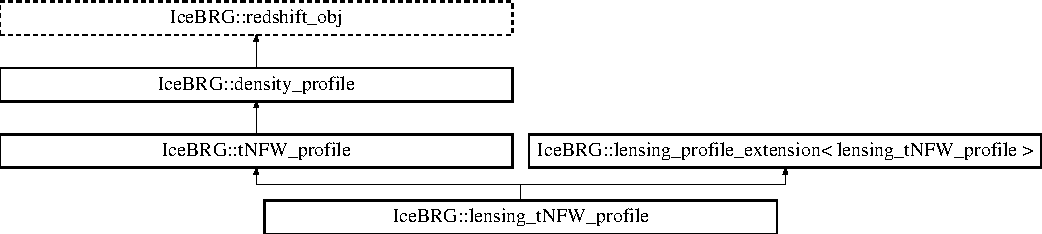
\includegraphics[height=3.146068cm]{classIceBRG_1_1lensing__tNFW__profile}
\end{center}
\end{figure}
\subsection*{Public Member Functions}
\begin{DoxyCompactItemize}
\item 
\hyperlink{classIceBRG_1_1lensing__tNFW__profile_a5fe1c91ba555af2dce8af625e544331b}{lensing\-\_\-t\-N\-F\-W\-\_\-profile} ()
\item 
\hyperlink{classIceBRG_1_1lensing__tNFW__profile_a65bbc405f339adc927f41b778ca3bcc8}{lensing\-\_\-t\-N\-F\-W\-\_\-profile} (const \hyperlink{namespaceIceBRG_a1be72ac4918a9b029f2eefa084213e35}{mass\-\_\-type} \&init\-\_\-mvir0, const \hyperlink{lib_2IceBRG__main_2common_8h_ad0f130a56eeb944d9ef2692ee881ecc4}{flt\-\_\-type} \&init\-\_\-z, const \hyperlink{lib_2IceBRG__main_2common_8h_ad0f130a56eeb944d9ef2692ee881ecc4}{flt\-\_\-type} \&init\-\_\-c=-\/1, const \hyperlink{lib_2IceBRG__main_2common_8h_ad0f130a56eeb944d9ef2692ee881ecc4}{flt\-\_\-type} \&init\-\_\-tau=-\/1)
\item 
virtual \hyperlink{classIceBRG_1_1lensing__tNFW__profile_ab80da109e4628eb0b1d0915b241cb668}{$\sim$lensing\-\_\-t\-N\-F\-W\-\_\-profile} ()
\item 
virtual \hyperlink{classIceBRG_1_1density__profile}{density\-\_\-profile} $\ast$ \hyperlink{classIceBRG_1_1lensing__tNFW__profile_af196f26f5ed61c128e2931157676eb3a}{density\-\_\-profile\-\_\-clone} () const 
\item 
virtual \hyperlink{classIceBRG_1_1tNFW__profile}{t\-N\-F\-W\-\_\-profile} $\ast$ \hyperlink{classIceBRG_1_1lensing__tNFW__profile_a6954e2ab7524e90a2b1f61b7387982d7}{t\-N\-F\-W\-\_\-profile\-\_\-clone} () const 
\end{DoxyCompactItemize}
\subsection*{Friends}
\begin{DoxyCompactItemize}
\item 
class \hyperlink{classIceBRG_1_1lensing__tNFW__profile_a959d8115518ab64335bb4b660a91e4e3}{lensing\-\_\-profile\-\_\-extension$<$ lensing\-\_\-t\-N\-F\-W\-\_\-profile $>$}
\end{DoxyCompactItemize}
\subsection*{Additional Inherited Members}


\subsection{Constructor \& Destructor Documentation}
\hypertarget{classIceBRG_1_1lensing__tNFW__profile_a5fe1c91ba555af2dce8af625e544331b}{\index{Ice\-B\-R\-G\-::lensing\-\_\-t\-N\-F\-W\-\_\-profile@{Ice\-B\-R\-G\-::lensing\-\_\-t\-N\-F\-W\-\_\-profile}!lensing\-\_\-t\-N\-F\-W\-\_\-profile@{lensing\-\_\-t\-N\-F\-W\-\_\-profile}}
\index{lensing\-\_\-t\-N\-F\-W\-\_\-profile@{lensing\-\_\-t\-N\-F\-W\-\_\-profile}!IceBRG::lensing_tNFW_profile@{Ice\-B\-R\-G\-::lensing\-\_\-t\-N\-F\-W\-\_\-profile}}
\subsubsection[{lensing\-\_\-t\-N\-F\-W\-\_\-profile}]{\setlength{\rightskip}{0pt plus 5cm}Ice\-B\-R\-G\-::lensing\-\_\-t\-N\-F\-W\-\_\-profile\-::lensing\-\_\-t\-N\-F\-W\-\_\-profile (
\begin{DoxyParamCaption}
{}
\end{DoxyParamCaption}
)\hspace{0.3cm}{\ttfamily [inline]}}}\label{classIceBRG_1_1lensing__tNFW__profile_a5fe1c91ba555af2dce8af625e544331b}
\hypertarget{classIceBRG_1_1lensing__tNFW__profile_a65bbc405f339adc927f41b778ca3bcc8}{\index{Ice\-B\-R\-G\-::lensing\-\_\-t\-N\-F\-W\-\_\-profile@{Ice\-B\-R\-G\-::lensing\-\_\-t\-N\-F\-W\-\_\-profile}!lensing\-\_\-t\-N\-F\-W\-\_\-profile@{lensing\-\_\-t\-N\-F\-W\-\_\-profile}}
\index{lensing\-\_\-t\-N\-F\-W\-\_\-profile@{lensing\-\_\-t\-N\-F\-W\-\_\-profile}!IceBRG::lensing_tNFW_profile@{Ice\-B\-R\-G\-::lensing\-\_\-t\-N\-F\-W\-\_\-profile}}
\subsubsection[{lensing\-\_\-t\-N\-F\-W\-\_\-profile}]{\setlength{\rightskip}{0pt plus 5cm}Ice\-B\-R\-G\-::lensing\-\_\-t\-N\-F\-W\-\_\-profile\-::lensing\-\_\-t\-N\-F\-W\-\_\-profile (
\begin{DoxyParamCaption}
\item[{const {\bf mass\-\_\-type} \&}]{init\-\_\-mvir0, }
\item[{const {\bf flt\-\_\-type} \&}]{init\-\_\-z, }
\item[{const {\bf flt\-\_\-type} \&}]{init\-\_\-c = {\ttfamily -\/1}, }
\item[{const {\bf flt\-\_\-type} \&}]{init\-\_\-tau = {\ttfamily -\/1}}
\end{DoxyParamCaption}
)\hspace{0.3cm}{\ttfamily [inline]}}}\label{classIceBRG_1_1lensing__tNFW__profile_a65bbc405f339adc927f41b778ca3bcc8}
\hypertarget{classIceBRG_1_1lensing__tNFW__profile_ab80da109e4628eb0b1d0915b241cb668}{\index{Ice\-B\-R\-G\-::lensing\-\_\-t\-N\-F\-W\-\_\-profile@{Ice\-B\-R\-G\-::lensing\-\_\-t\-N\-F\-W\-\_\-profile}!$\sim$lensing\-\_\-t\-N\-F\-W\-\_\-profile@{$\sim$lensing\-\_\-t\-N\-F\-W\-\_\-profile}}
\index{$\sim$lensing\-\_\-t\-N\-F\-W\-\_\-profile@{$\sim$lensing\-\_\-t\-N\-F\-W\-\_\-profile}!IceBRG::lensing_tNFW_profile@{Ice\-B\-R\-G\-::lensing\-\_\-t\-N\-F\-W\-\_\-profile}}
\subsubsection[{$\sim$lensing\-\_\-t\-N\-F\-W\-\_\-profile}]{\setlength{\rightskip}{0pt plus 5cm}virtual Ice\-B\-R\-G\-::lensing\-\_\-t\-N\-F\-W\-\_\-profile\-::$\sim$lensing\-\_\-t\-N\-F\-W\-\_\-profile (
\begin{DoxyParamCaption}
{}
\end{DoxyParamCaption}
)\hspace{0.3cm}{\ttfamily [inline]}, {\ttfamily [virtual]}}}\label{classIceBRG_1_1lensing__tNFW__profile_ab80da109e4628eb0b1d0915b241cb668}


\subsection{Member Function Documentation}
\hypertarget{classIceBRG_1_1lensing__tNFW__profile_af196f26f5ed61c128e2931157676eb3a}{\index{Ice\-B\-R\-G\-::lensing\-\_\-t\-N\-F\-W\-\_\-profile@{Ice\-B\-R\-G\-::lensing\-\_\-t\-N\-F\-W\-\_\-profile}!density\-\_\-profile\-\_\-clone@{density\-\_\-profile\-\_\-clone}}
\index{density\-\_\-profile\-\_\-clone@{density\-\_\-profile\-\_\-clone}!IceBRG::lensing_tNFW_profile@{Ice\-B\-R\-G\-::lensing\-\_\-t\-N\-F\-W\-\_\-profile}}
\subsubsection[{density\-\_\-profile\-\_\-clone}]{\setlength{\rightskip}{0pt plus 5cm}virtual {\bf density\-\_\-profile}$\ast$ Ice\-B\-R\-G\-::lensing\-\_\-t\-N\-F\-W\-\_\-profile\-::density\-\_\-profile\-\_\-clone (
\begin{DoxyParamCaption}
{}
\end{DoxyParamCaption}
) const\hspace{0.3cm}{\ttfamily [inline]}, {\ttfamily [virtual]}}}\label{classIceBRG_1_1lensing__tNFW__profile_af196f26f5ed61c128e2931157676eb3a}


Reimplemented from \hyperlink{classIceBRG_1_1tNFW__profile_a97c4f2e1a25bc58ba690e714eaa42be3}{Ice\-B\-R\-G\-::t\-N\-F\-W\-\_\-profile}.

\hypertarget{classIceBRG_1_1lensing__tNFW__profile_a6954e2ab7524e90a2b1f61b7387982d7}{\index{Ice\-B\-R\-G\-::lensing\-\_\-t\-N\-F\-W\-\_\-profile@{Ice\-B\-R\-G\-::lensing\-\_\-t\-N\-F\-W\-\_\-profile}!t\-N\-F\-W\-\_\-profile\-\_\-clone@{t\-N\-F\-W\-\_\-profile\-\_\-clone}}
\index{t\-N\-F\-W\-\_\-profile\-\_\-clone@{t\-N\-F\-W\-\_\-profile\-\_\-clone}!IceBRG::lensing_tNFW_profile@{Ice\-B\-R\-G\-::lensing\-\_\-t\-N\-F\-W\-\_\-profile}}
\subsubsection[{t\-N\-F\-W\-\_\-profile\-\_\-clone}]{\setlength{\rightskip}{0pt plus 5cm}virtual {\bf t\-N\-F\-W\-\_\-profile}$\ast$ Ice\-B\-R\-G\-::lensing\-\_\-t\-N\-F\-W\-\_\-profile\-::t\-N\-F\-W\-\_\-profile\-\_\-clone (
\begin{DoxyParamCaption}
{}
\end{DoxyParamCaption}
) const\hspace{0.3cm}{\ttfamily [inline]}, {\ttfamily [virtual]}}}\label{classIceBRG_1_1lensing__tNFW__profile_a6954e2ab7524e90a2b1f61b7387982d7}


Reimplemented from \hyperlink{classIceBRG_1_1tNFW__profile_a7b652f93aa159c0bdffa657f4bfa1c46}{Ice\-B\-R\-G\-::t\-N\-F\-W\-\_\-profile}.



\subsection{Friends And Related Function Documentation}
\hypertarget{classIceBRG_1_1lensing__tNFW__profile_a959d8115518ab64335bb4b660a91e4e3}{\index{Ice\-B\-R\-G\-::lensing\-\_\-t\-N\-F\-W\-\_\-profile@{Ice\-B\-R\-G\-::lensing\-\_\-t\-N\-F\-W\-\_\-profile}!lensing\-\_\-profile\-\_\-extension$<$ lensing\-\_\-t\-N\-F\-W\-\_\-profile $>$@{lensing\-\_\-profile\-\_\-extension$<$ lensing\-\_\-t\-N\-F\-W\-\_\-profile $>$}}
\index{lensing\-\_\-profile\-\_\-extension$<$ lensing\-\_\-t\-N\-F\-W\-\_\-profile $>$@{lensing\-\_\-profile\-\_\-extension$<$ lensing\-\_\-t\-N\-F\-W\-\_\-profile $>$}!IceBRG::lensing_tNFW_profile@{Ice\-B\-R\-G\-::lensing\-\_\-t\-N\-F\-W\-\_\-profile}}
\subsubsection[{lensing\-\_\-profile\-\_\-extension$<$ lensing\-\_\-t\-N\-F\-W\-\_\-profile $>$}]{\setlength{\rightskip}{0pt plus 5cm}friend class {\bf lensing\-\_\-profile\-\_\-extension}$<$ {\bf lensing\-\_\-t\-N\-F\-W\-\_\-profile} $>$\hspace{0.3cm}{\ttfamily [friend]}}}\label{classIceBRG_1_1lensing__tNFW__profile_a959d8115518ab64335bb4b660a91e4e3}


The documentation for this class was generated from the following files\-:\begin{DoxyCompactItemize}
\item 
/disk2/brg/git/\-Magnification\-\_\-\-Public/src/lib/\-Ice\-B\-R\-G\-\_\-lensing/\hyperlink{lensing__tNFW__profile_8h}{lensing\-\_\-t\-N\-F\-W\-\_\-profile.\-h}\item 
/disk2/brg/git/\-Magnification\-\_\-\-Public/src/lib/\-Ice\-B\-R\-G\-\_\-lensing/\hyperlink{lensing__tNFW__profile_8cpp}{lensing\-\_\-t\-N\-F\-W\-\_\-profile.\-cpp}\end{DoxyCompactItemize}

\hypertarget{classIceBRG_1_1limit__vector}{}\section{Ice\+B\+R\+G\+:\+:limit\+\_\+vector$<$ T, A $>$ Class Template Reference}
\label{classIceBRG_1_1limit__vector}\index{Ice\+B\+R\+G\+::limit\+\_\+vector$<$ T, A $>$@{Ice\+B\+R\+G\+::limit\+\_\+vector$<$ T, A $>$}}


{\ttfamily \#include $<$limit\+\_\+vector.\+hpp$>$}

\subsection*{Public Types}
\begin{DoxyCompactItemize}
\item 
enum \hyperlink{classIceBRG_1_1limit__vector_a67ad5ccda3b716a3aca2fa6223e75681}{type} \{ \hyperlink{classIceBRG_1_1limit__vector_a67ad5ccda3b716a3aca2fa6223e75681ab61773b9b3968a9988d765d728985862}{type\+::\+G\+E\+N\+E\+R\+A\+L}, 
\hyperlink{classIceBRG_1_1limit__vector_a67ad5ccda3b716a3aca2fa6223e75681aaac544aacc3615aada24897a215f5046}{type\+::\+L\+I\+N\+E\+A\+R}, 
\hyperlink{classIceBRG_1_1limit__vector_a67ad5ccda3b716a3aca2fa6223e75681a4b5ffcdaf38ce4d463171f5c977c5ab3}{type\+::\+L\+O\+G}, 
\hyperlink{classIceBRG_1_1limit__vector_a67ad5ccda3b716a3aca2fa6223e75681a63548de92aab6aa127df46cfbed9e23f}{type\+::\+D\+I\+S\+J\+O\+I\+N\+T}
 \}
\item 
typedef std\+::vector$<$ T, A $>$ \hyperlink{classIceBRG_1_1limit__vector_a8f5c1d622276ed2d9835feab9538b96e}{base\+\_\+type}
\item 
typedef base\+\_\+type\+::value\+\_\+type \hyperlink{classIceBRG_1_1limit__vector_a9b1e2f022c18b0227b25bb571741bb28}{value\+\_\+type}
\item 
typedef base\+\_\+type\+::allocator\+\_\+type \hyperlink{classIceBRG_1_1limit__vector_ac75a579f04baed676ee916b0ad3dfec0}{allocator\+\_\+type}
\item 
typedef base\+\_\+type\+::reference \hyperlink{classIceBRG_1_1limit__vector_af3acb98a381ba86ca927f099591d1512}{reference}
\item 
typedef base\+\_\+type\+::const\+\_\+reference \hyperlink{classIceBRG_1_1limit__vector_aed6fc504d7987040be16d150089c7893}{const\+\_\+reference}
\item 
typedef base\+\_\+type\+::pointer \hyperlink{classIceBRG_1_1limit__vector_a87f3142bb69e755ba61e51ddfa7e6eae}{pointer}
\item 
typedef base\+\_\+type\+::const\+\_\+pointer \hyperlink{classIceBRG_1_1limit__vector_a06b68c790b5e5692b6e302d5478be33f}{const\+\_\+pointer}
\item 
typedef base\+\_\+type\+::iterator \hyperlink{classIceBRG_1_1limit__vector_aea9e186f4c5fb359da52895bafba6335}{iterator}
\item 
typedef base\+\_\+type\+::const\+\_\+iterator \hyperlink{classIceBRG_1_1limit__vector_ae7acd983de8fc074624eb50450a01e30}{const\+\_\+iterator}
\item 
typedef base\+\_\+type\+::reverse\+\_\+iterator \hyperlink{classIceBRG_1_1limit__vector_af4ba6b26317b4b6f8b0a5dc2e5a1d268}{reverse\+\_\+iterator}
\item 
typedef base\+\_\+type\+::const\+\_\+reverse\+\_\+iterator \hyperlink{classIceBRG_1_1limit__vector_a4feb81d3ff27e274df451f2fe85cd21a}{const\+\_\+reverse\+\_\+iterator}
\item 
typedef base\+\_\+type\+::difference\+\_\+type \hyperlink{classIceBRG_1_1limit__vector_ab5e21e09f06ae1a5327e9d47f31ef6b4}{difference\+\_\+type}
\item 
typedef std\+::make\+\_\+signed$<$ typename base\+\_\+type\+::size\+\_\+type $>$\+::\hyperlink{classIceBRG_1_1limit__vector_a67ad5ccda3b716a3aca2fa6223e75681}{type} \hyperlink{classIceBRG_1_1limit__vector_a81be3eb6cd519b3f5279ef735ccc4c2f}{size\+\_\+type}
\end{DoxyCompactItemize}
\subsection*{Public Member Functions}
\begin{DoxyCompactItemize}
\item 
\hyperlink{classIceBRG_1_1limit__vector_a327dc940f2b7380e9af32935d449c911}{limit\+\_\+vector} (const \hyperlink{classIceBRG_1_1limit__vector_ac75a579f04baed676ee916b0ad3dfec0}{allocator\+\_\+type} \&alloc=\hyperlink{classIceBRG_1_1limit__vector_ac75a579f04baed676ee916b0ad3dfec0}{allocator\+\_\+type}())
\begin{DoxyCompactList}\small\item\em Default constructor. \end{DoxyCompactList}\item 
\hyperlink{classIceBRG_1_1limit__vector_a4f32922dba34667d42bb84d7dc041470}{limit\+\_\+vector} (const T \&\hyperlink{classIceBRG_1_1limit__vector_a6dddba344399189344e410ddca2615d6}{min}, const T \&\hyperlink{classIceBRG_1_1limit__vector_a4f020c6f3e092f6cbfdc3c015de83667}{max}, const \hyperlink{classIceBRG_1_1limit__vector_a81be3eb6cd519b3f5279ef735ccc4c2f}{size\+\_\+type} \&\hyperlink{classIceBRG_1_1limit__vector_af09ecb88fd55929c0b08faa63c9a3e1c}{num\+\_\+bins}, const \hyperlink{classIceBRG_1_1limit__vector_ac75a579f04baed676ee916b0ad3dfec0}{allocator\+\_\+type} \&alloc=\hyperlink{classIceBRG_1_1limit__vector_ac75a579f04baed676ee916b0ad3dfec0}{allocator\+\_\+type}())
\begin{DoxyCompactList}\small\item\em Construct as linear format. \end{DoxyCompactList}\item 
\hyperlink{classIceBRG_1_1limit__vector_a29d9cb5b0fe483c5d70642a999423af9}{limit\+\_\+vector} (const \hyperlink{classIceBRG_1_1limit__vector_a67ad5ccda3b716a3aca2fa6223e75681}{type} \&init\+\_\+type, const T \&\hyperlink{classIceBRG_1_1limit__vector_a6dddba344399189344e410ddca2615d6}{min}, const T \&\hyperlink{classIceBRG_1_1limit__vector_a4f020c6f3e092f6cbfdc3c015de83667}{max}, const \hyperlink{classIceBRG_1_1limit__vector_a81be3eb6cd519b3f5279ef735ccc4c2f}{size\+\_\+type} \&\hyperlink{classIceBRG_1_1limit__vector_af09ecb88fd55929c0b08faa63c9a3e1c}{num\+\_\+bins}, const \hyperlink{classIceBRG_1_1limit__vector_ac75a579f04baed676ee916b0ad3dfec0}{allocator\+\_\+type} \&alloc=\hyperlink{classIceBRG_1_1limit__vector_ac75a579f04baed676ee916b0ad3dfec0}{allocator\+\_\+type}())
\begin{DoxyCompactList}\small\item\em Construct as linear or log format. \end{DoxyCompactList}\item 
{\footnotesize template$<$class Input\+Iterator $>$ }\\\hyperlink{classIceBRG_1_1limit__vector_a28cc72fd30edd1fd9b6a0fba2793e18d}{limit\+\_\+vector} (Input\+Iterator first, Input\+Iterator last, const \hyperlink{classIceBRG_1_1limit__vector_ac75a579f04baed676ee916b0ad3dfec0}{allocator\+\_\+type} \&alloc=\hyperlink{classIceBRG_1_1limit__vector_ac75a579f04baed676ee916b0ad3dfec0}{allocator\+\_\+type}())
\begin{DoxyCompactList}\small\item\em Range constructor. \end{DoxyCompactList}\item 
\hyperlink{classIceBRG_1_1limit__vector_ae25a8bfadeba89edbd4b3c62bfcf2455}{limit\+\_\+vector} (const \hyperlink{classIceBRG_1_1limit__vector}{limit\+\_\+vector}$<$ T, A $>$ \&other)=default
\begin{DoxyCompactList}\small\item\em Copy constructor. \end{DoxyCompactList}\item 
\hyperlink{classIceBRG_1_1limit__vector_a6cc469394ec08a62f8a2a09e15d81ae2}{limit\+\_\+vector} (const \hyperlink{classIceBRG_1_1limit__vector}{limit\+\_\+vector}$<$ T, A $>$ \&other, const \hyperlink{classIceBRG_1_1limit__vector_ac75a579f04baed676ee916b0ad3dfec0}{allocator\+\_\+type} \&alloc)
\begin{DoxyCompactList}\small\item\em Copy and set allocator. \end{DoxyCompactList}\item 
\hyperlink{classIceBRG_1_1limit__vector_a155c43501fd2a683cbc7aa04ae484cbe}{limit\+\_\+vector} (const std\+::vector$<$ T, A $>$ \&other)
\begin{DoxyCompactList}\small\item\em Construct from vector. \end{DoxyCompactList}\item 
\hyperlink{classIceBRG_1_1limit__vector_ad051401ed395c6fe5e556d51e16416ef}{limit\+\_\+vector} (const std\+::vector$<$ T, A $>$ \&other, const \hyperlink{classIceBRG_1_1limit__vector_ac75a579f04baed676ee916b0ad3dfec0}{allocator\+\_\+type} \&alloc)
\begin{DoxyCompactList}\small\item\em Construct from vector and set allocator. \end{DoxyCompactList}\item 
{\footnotesize template$<$typename To , typename Ao $>$ }\\\hyperlink{classIceBRG_1_1limit__vector_ad49259faea655cb776389d009c5d30a1}{limit\+\_\+vector} (const std\+::vector$<$ To, Ao $>$ \&other, const \hyperlink{classIceBRG_1_1limit__vector_a67ad5ccda3b716a3aca2fa6223e75681}{type} \&init\+\_\+type=\hyperlink{classIceBRG_1_1limit__vector_a67ad5ccda3b716a3aca2fa6223e75681ab61773b9b3968a9988d765d728985862}{type\+::\+G\+E\+N\+E\+R\+A\+L})
\begin{DoxyCompactList}\small\item\em Coerce from vector. \end{DoxyCompactList}\item 
{\footnotesize template$<$typename To , typename Ao $>$ }\\\hyperlink{classIceBRG_1_1limit__vector_a5a9e118da630e7a7a038e376e41049f7}{limit\+\_\+vector} (const std\+::vector$<$ To, Ao $>$ \&other, const \hyperlink{classIceBRG_1_1limit__vector_ac75a579f04baed676ee916b0ad3dfec0}{allocator\+\_\+type} \&alloc, const \hyperlink{classIceBRG_1_1limit__vector_a67ad5ccda3b716a3aca2fa6223e75681}{type} \&init\+\_\+type=\hyperlink{classIceBRG_1_1limit__vector_a67ad5ccda3b716a3aca2fa6223e75681ab61773b9b3968a9988d765d728985862}{type\+::\+G\+E\+N\+E\+R\+A\+L})
\begin{DoxyCompactList}\small\item\em Coerce from vector and set allocator. \end{DoxyCompactList}\item 
\hyperlink{classIceBRG_1_1limit__vector_af9a42556163fef40c2c623494c7d7908}{limit\+\_\+vector} (\hyperlink{classIceBRG_1_1limit__vector}{limit\+\_\+vector}$<$ T, A $>$ \&\&other)=default
\begin{DoxyCompactList}\small\item\em Move constructor. \end{DoxyCompactList}\item 
\hyperlink{classIceBRG_1_1limit__vector_afebcca7a397bf0da6020039edf255a31}{limit\+\_\+vector} (\hyperlink{classIceBRG_1_1limit__vector}{limit\+\_\+vector}$<$ T, A $>$ \&\&other, const \hyperlink{classIceBRG_1_1limit__vector_ac75a579f04baed676ee916b0ad3dfec0}{allocator\+\_\+type} \&alloc)
\begin{DoxyCompactList}\small\item\em Move and set allocator. \end{DoxyCompactList}\item 
\hyperlink{classIceBRG_1_1limit__vector_a2520a38aa5e633dd6ebc716ced0791b2}{limit\+\_\+vector} (std\+::vector$<$ T, A $>$ \&\&other)
\begin{DoxyCompactList}\small\item\em Move from vector. \end{DoxyCompactList}\item 
\hyperlink{classIceBRG_1_1limit__vector_a6297026c0b0ea0c00c2ad891f5d38b32}{limit\+\_\+vector} (std\+::vector$<$ T, A $>$ \&\&other, const \hyperlink{classIceBRG_1_1limit__vector_ac75a579f04baed676ee916b0ad3dfec0}{allocator\+\_\+type} \&alloc)
\begin{DoxyCompactList}\small\item\em Move from vector and set allocator. \end{DoxyCompactList}\item 
\hyperlink{classIceBRG_1_1limit__vector_ac73207daaf033e6e4be9b028fa86b435}{limit\+\_\+vector} (const std\+::initializer\+\_\+list$<$ \hyperlink{classIceBRG_1_1limit__vector_a9b1e2f022c18b0227b25bb571741bb28}{value\+\_\+type} $>$ \&il, const \hyperlink{classIceBRG_1_1limit__vector_ac75a579f04baed676ee916b0ad3dfec0}{allocator\+\_\+type} \&alloc=\hyperlink{classIceBRG_1_1limit__vector_ac75a579f04baed676ee916b0ad3dfec0}{allocator\+\_\+type}())
\begin{DoxyCompactList}\small\item\em Construct from initializer list. \end{DoxyCompactList}\item 
virtual \hyperlink{classIceBRG_1_1limit__vector_a7464af68a55bc97d7303c2a393ed8722}{$\sim$limit\+\_\+vector} ()
\begin{DoxyCompactList}\small\item\em Virtual destructor. \end{DoxyCompactList}\item 
void \hyperlink{classIceBRG_1_1limit__vector_a8e81ad5d96b7593d54f52d94110e2ed8}{reconstruct} (const \hyperlink{classIceBRG_1_1limit__vector_a67ad5ccda3b716a3aca2fa6223e75681}{type} \&init\+\_\+type, const T \&\hyperlink{classIceBRG_1_1limit__vector_a6dddba344399189344e410ddca2615d6}{min}, const T \&\hyperlink{classIceBRG_1_1limit__vector_a4f020c6f3e092f6cbfdc3c015de83667}{max}, const \hyperlink{classIceBRG_1_1limit__vector_a81be3eb6cd519b3f5279ef735ccc4c2f}{size\+\_\+type} \&\hyperlink{classIceBRG_1_1limit__vector_af09ecb88fd55929c0b08faa63c9a3e1c}{num\+\_\+bins})
\begin{DoxyCompactList}\small\item\em Reconstruct as linear or log format. \end{DoxyCompactList}\item 
{\footnotesize template$<$typename To , typename Ao $>$ }\\void \hyperlink{classIceBRG_1_1limit__vector_ad3e63fd248648734c9694e8426c507df}{reconstruct\+\_\+from\+\_\+bin\+\_\+mids} (const std\+::vector$<$ To, Ao $>$ \&vec)
\item 
{\footnotesize template$<$typename To , typename Ao $>$ }\\void \hyperlink{classIceBRG_1_1limit__vector_a2f0e8cf8aa4e31b55453634ea90afd64}{reconstruct\+\_\+from\+\_\+bin\+\_\+mids} (std\+::vector$<$ To, Ao $>$ \&\&vec)
\item 
{\footnotesize template$<$typename To $>$ }\\void \hyperlink{classIceBRG_1_1limit__vector_a27ec6eed7873706348a0b29b26d79ee5}{reconstruct\+\_\+as\+\_\+disjoint} (To \&\&vec)
\begin{DoxyCompactList}\small\item\em Reconstruct as disjoint. \end{DoxyCompactList}\item 
void \hyperlink{classIceBRG_1_1limit__vector_aa8eb9d4b25be0022ccea9e06bef3cb05}{make\+\_\+general} ()
\item 
void \hyperlink{classIceBRG_1_1limit__vector_a8328c477d791a4425a8461476d4b393f}{make\+\_\+disjoint} ()
\item 
\hyperlink{classIceBRG_1_1limit__vector}{limit\+\_\+vector}$<$ T, A $>$ \& \hyperlink{classIceBRG_1_1limit__vector_a3fece2b98d9b4b859d4d386976ff78c9}{operator=} (\hyperlink{classIceBRG_1_1limit__vector}{limit\+\_\+vector}$<$ T, A $>$ other)
\begin{DoxyCompactList}\small\item\em Copy assignment. \end{DoxyCompactList}\item 
\hyperlink{classIceBRG_1_1limit__vector}{limit\+\_\+vector}$<$ T, A $>$ \& \hyperlink{classIceBRG_1_1limit__vector_aab9b832c6156dbd4d7425be36894c71d}{operator=} (const std\+::vector$<$ T, A $>$ \&new\+\_\+base)
\begin{DoxyCompactList}\small\item\em Copy from vector. \end{DoxyCompactList}\item 
{\footnotesize template$<$typename Container\+Type $>$ }\\\hyperlink{classIceBRG_1_1limit__vector}{limit\+\_\+vector}$<$ T, A $>$ \& \hyperlink{classIceBRG_1_1limit__vector_ae49114008d4b1141d6911747283abc04}{operator=} (const Container\+Type \&other)
\begin{DoxyCompactList}\small\item\em Coerce copy from container. \end{DoxyCompactList}\item 
\hyperlink{classIceBRG_1_1limit__vector}{limit\+\_\+vector}$<$ T, A $>$ \& \hyperlink{classIceBRG_1_1limit__vector_a6c9ffe039efa71858e5aea175f8b9f7d}{operator=} (\hyperlink{classIceBRG_1_1limit__vector}{limit\+\_\+vector}$<$ T, A $>$ \&\&other)
\begin{DoxyCompactList}\small\item\em Move assignment. \end{DoxyCompactList}\item 
\hyperlink{classIceBRG_1_1limit__vector}{limit\+\_\+vector}$<$ T, A $>$ \& \hyperlink{classIceBRG_1_1limit__vector_a28d7a79eb78abec3957e757ab2262532}{operator=} (std\+::vector$<$ T, A $>$ \&\&new\+\_\+base)
\begin{DoxyCompactList}\small\item\em Move from vector. \end{DoxyCompactList}\item 
\hyperlink{classIceBRG_1_1limit__vector}{limit\+\_\+vector}$<$ T, A $>$ \& \hyperlink{classIceBRG_1_1limit__vector_a23594cf6dd3e8e036c4bb3c7e5f02f8a}{operator=} (const std\+::initializer\+\_\+list$<$ \hyperlink{classIceBRG_1_1limit__vector_a9b1e2f022c18b0227b25bb571741bb28}{value\+\_\+type} $>$ \&il)
\begin{DoxyCompactList}\small\item\em Assign from initializer\+\_\+list. \end{DoxyCompactList}\item 
\hyperlink{classIceBRG_1_1limit__vector_ae7acd983de8fc074624eb50450a01e30}{const\+\_\+iterator} \hyperlink{classIceBRG_1_1limit__vector_ac777b677396a9e35f8c9e20c692c5ece}{begin} () const  noexcept
\begin{DoxyCompactList}\small\item\em begin (only const version allowed) \end{DoxyCompactList}\item 
\hyperlink{classIceBRG_1_1limit__vector_ae7acd983de8fc074624eb50450a01e30}{const\+\_\+iterator} \hyperlink{classIceBRG_1_1limit__vector_a83c8a935495a3b160331b34ab22fe3f5}{end} () const  noexcept
\begin{DoxyCompactList}\small\item\em end (only const version allowed) \end{DoxyCompactList}\item 
\hyperlink{classIceBRG_1_1limit__vector_ae7acd983de8fc074624eb50450a01e30}{const\+\_\+iterator} \hyperlink{classIceBRG_1_1limit__vector_af1d46879c772026fb810ddf95a574d8f}{rbegin} () const  noexcept
\begin{DoxyCompactList}\small\item\em rbegin (only const version allowed) \end{DoxyCompactList}\item 
\hyperlink{classIceBRG_1_1limit__vector_ae7acd983de8fc074624eb50450a01e30}{const\+\_\+iterator} \hyperlink{classIceBRG_1_1limit__vector_a16efe52b79ef8ca10a45b6a2706f2a62}{rend} () const  noexcept
\begin{DoxyCompactList}\small\item\em rend (only const version allowed) \end{DoxyCompactList}\item 
\hyperlink{classIceBRG_1_1limit__vector_ae7acd983de8fc074624eb50450a01e30}{const\+\_\+iterator} \hyperlink{classIceBRG_1_1limit__vector_a90458c08bb863d24a26b2b8ff79bbdb0}{cbegin} () const  noexcept
\begin{DoxyCompactList}\small\item\em cbegin \end{DoxyCompactList}\item 
\hyperlink{classIceBRG_1_1limit__vector_ae7acd983de8fc074624eb50450a01e30}{const\+\_\+iterator} \hyperlink{classIceBRG_1_1limit__vector_a4bdda61b8d16c1aa23dc4de95dbec933}{cend} () const  noexcept
\begin{DoxyCompactList}\small\item\em cend \end{DoxyCompactList}\item 
\hyperlink{classIceBRG_1_1limit__vector_ae7acd983de8fc074624eb50450a01e30}{const\+\_\+iterator} \hyperlink{classIceBRG_1_1limit__vector_afbc08d1c3cd4928e69846b1aeef82777}{crbegin} () const  noexcept
\begin{DoxyCompactList}\small\item\em crbegin \end{DoxyCompactList}\item 
\hyperlink{classIceBRG_1_1limit__vector_ae7acd983de8fc074624eb50450a01e30}{const\+\_\+iterator} \hyperlink{classIceBRG_1_1limit__vector_a6c05d24152373919acf910bfd474cba2}{crend} () const  noexcept
\begin{DoxyCompactList}\small\item\em crend \end{DoxyCompactList}\item 
\hyperlink{classIceBRG_1_1limit__vector_a81be3eb6cd519b3f5279ef735ccc4c2f}{size\+\_\+type} \hyperlink{classIceBRG_1_1limit__vector_a13a4acf96ebfd7b8d6a5354ada368f79}{size} () const  noexcept
\begin{DoxyCompactList}\small\item\em Get size of the base vector. \end{DoxyCompactList}\item 
\hyperlink{classIceBRG_1_1limit__vector_a81be3eb6cd519b3f5279ef735ccc4c2f}{size\+\_\+type} \hyperlink{classIceBRG_1_1limit__vector_af09ecb88fd55929c0b08faa63c9a3e1c}{num\+\_\+bins} () const 
\begin{DoxyCompactList}\small\item\em Get number of bins. \end{DoxyCompactList}\item 
\hyperlink{classIceBRG_1_1limit__vector_a81be3eb6cd519b3f5279ef735ccc4c2f}{size\+\_\+type} \hyperlink{classIceBRG_1_1limit__vector_a589edd5c2ab9c4a2c55af0081a8fb01e}{max\+\_\+size} () const  noexcept
\begin{DoxyCompactList}\small\item\em Get max size of the base vector. \end{DoxyCompactList}\item 
\hyperlink{classIceBRG_1_1limit__vector_a81be3eb6cd519b3f5279ef735ccc4c2f}{size\+\_\+type} \hyperlink{classIceBRG_1_1limit__vector_aa5e914c26779bab6daf66acb4c3de21a}{capacity} () const  noexcept
\begin{DoxyCompactList}\small\item\em Get capacity of the base vector. \end{DoxyCompactList}\item 
bool \hyperlink{classIceBRG_1_1limit__vector_aa0ca192c0495d25b2a7419bf2b4afaac}{empty} () const  noexcept
\begin{DoxyCompactList}\small\item\em Empty test -\/ will always be false (included here for compatibility) \end{DoxyCompactList}\item 
void \hyperlink{classIceBRG_1_1limit__vector_ad21b2f4f9e93bb508dba05f3f04c72ab}{reserve} (const \hyperlink{classIceBRG_1_1limit__vector_a81be3eb6cd519b3f5279ef735ccc4c2f}{size\+\_\+type} \&n)
\begin{DoxyCompactList}\small\item\em Request a change in capacity of the base vector. \end{DoxyCompactList}\item 
void \hyperlink{classIceBRG_1_1limit__vector_ac3ad1f9902e86e93b48e34502b7b65b6}{shrink\+\_\+to\+\_\+fit} () const 
\begin{DoxyCompactList}\small\item\em Reduce base capacity to fit its size. \end{DoxyCompactList}\item 
\hyperlink{classIceBRG_1_1limit__vector_aed6fc504d7987040be16d150089c7893}{const\+\_\+reference} \hyperlink{classIceBRG_1_1limit__vector_a6dc04a7b7340b2e8e0467e493698ea4b}{operator\mbox{[}$\,$\mbox{]}} (const \hyperlink{classIceBRG_1_1limit__vector_a81be3eb6cd519b3f5279ef735ccc4c2f}{size\+\_\+type} \&n) const 
\begin{DoxyCompactList}\small\item\em Element access (const only) \end{DoxyCompactList}\item 
\hyperlink{classIceBRG_1_1limit__vector_aed6fc504d7987040be16d150089c7893}{const\+\_\+reference} \hyperlink{classIceBRG_1_1limit__vector_a6353bec6a3ab558a50fe9255e9ace992}{at} (const \hyperlink{classIceBRG_1_1limit__vector_a81be3eb6cd519b3f5279ef735ccc4c2f}{size\+\_\+type} \&n) const 
\begin{DoxyCompactList}\small\item\em Range-\/checked element access (const only) \end{DoxyCompactList}\item 
\hyperlink{classIceBRG_1_1limit__vector_aed6fc504d7987040be16d150089c7893}{const\+\_\+reference} \hyperlink{classIceBRG_1_1limit__vector_a5c0fe22ffdce8122100cf24d0f8daf98}{front} () const 
\begin{DoxyCompactList}\small\item\em Access first element (const only) \end{DoxyCompactList}\item 
\hyperlink{classIceBRG_1_1limit__vector_aed6fc504d7987040be16d150089c7893}{const\+\_\+reference} \hyperlink{classIceBRG_1_1limit__vector_a6b64da787bb41c0da27e6ae6cd82fee2}{back} () const 
\begin{DoxyCompactList}\small\item\em Access last element (const only) \end{DoxyCompactList}\item 
const \hyperlink{classIceBRG_1_1limit__vector_a9b1e2f022c18b0227b25bb571741bb28}{value\+\_\+type} $\ast$ \hyperlink{classIceBRG_1_1limit__vector_a67977f6da2aeab8ef1d77dcc0fe9bebb}{data} () const  noexcept
\begin{DoxyCompactList}\small\item\em Access data (const only) \end{DoxyCompactList}\item 
void \hyperlink{classIceBRG_1_1limit__vector_a35083732ec606851566d3ca6c56769a3}{swap} (\hyperlink{classIceBRG_1_1limit__vector}{limit\+\_\+vector}$<$ T, A $>$ \&other)
\begin{DoxyCompactList}\small\item\em Swap with another \hyperlink{classIceBRG_1_1limit__vector}{limit\+\_\+vector}. \end{DoxyCompactList}\item 
void \hyperlink{classIceBRG_1_1limit__vector_a1b2f88e47b1db40b5ae72ba560b584bc}{clear} ()
\begin{DoxyCompactList}\small\item\em Clear function -\/ leaves it in initial state. \end{DoxyCompactList}\item 
void \hyperlink{classIceBRG_1_1limit__vector_ae34c3659f8203ea285a5f81c9a5beb21}{fixbad} ()
\item 
void \hyperlink{classIceBRG_1_1limit__vector_a325027b05e079aa836725e4e66576026}{multiply} (const \hyperlink{lib_2IceBRG__main_2common_8h_ad0f130a56eeb944d9ef2692ee881ecc4}{flt\+\_\+type} \&val)
\begin{DoxyCompactList}\small\item\em Multiply the whole vector by a constant. \end{DoxyCompactList}\item 
{\footnotesize template$<$typename Tv $>$ }\\auto \hyperlink{classIceBRG_1_1limit__vector_aeb944f9e344296d0b8c8501f2b2cf360}{get\+\_\+multiplied} (const Tv \&val) const  -\/$>$ \hyperlink{classIceBRG_1_1limit__vector}{limit\+\_\+vector}$<$ decltype(val $\ast$T())$>$
\begin{DoxyCompactList}\small\item\em Multiply the whole vector by a constant. \end{DoxyCompactList}\item 
void \hyperlink{classIceBRG_1_1limit__vector_a1564579561d66d38f339bd109d2a25fd}{divide} (const \hyperlink{lib_2IceBRG__main_2common_8h_ad0f130a56eeb944d9ef2692ee881ecc4}{flt\+\_\+type} \&val)
\begin{DoxyCompactList}\small\item\em Divide the whole vector by a constant. \end{DoxyCompactList}\item 
{\footnotesize template$<$typename Tv $>$ }\\auto \hyperlink{classIceBRG_1_1limit__vector_ae30b0b186d5121820e050f9e8a84fb03}{get\+\_\+divided} (const Tv \&val) const  -\/$>$ \hyperlink{classIceBRG_1_1limit__vector}{limit\+\_\+vector}$<$ decltype(T()/val)$>$
\begin{DoxyCompactList}\small\item\em Multiply the whole vector by a constant. \end{DoxyCompactList}\item 
\hyperlink{classIceBRG_1_1limit__vector_aed6fc504d7987040be16d150089c7893}{const\+\_\+reference} \hyperlink{classIceBRG_1_1limit__vector_a6dddba344399189344e410ddca2615d6}{min} () const  noexcept
\begin{DoxyCompactList}\small\item\em Returns minimum limit. \end{DoxyCompactList}\item 
\hyperlink{classIceBRG_1_1limit__vector_aed6fc504d7987040be16d150089c7893}{const\+\_\+reference} \hyperlink{classIceBRG_1_1limit__vector_a4f020c6f3e092f6cbfdc3c015de83667}{max} () const  noexcept
\begin{DoxyCompactList}\small\item\em Returns maximum limit. \end{DoxyCompactList}\item 
\hyperlink{classIceBRG_1_1limit__vector_aed6fc504d7987040be16d150089c7893}{const\+\_\+reference} \hyperlink{classIceBRG_1_1limit__vector_a90ae58089ebe3e59ca3ec43d8233370e}{lower\+\_\+limit} (const \hyperlink{classIceBRG_1_1limit__vector_a81be3eb6cd519b3f5279ef735ccc4c2f}{size\+\_\+type} \&i) const  noexcept
\begin{DoxyCompactList}\small\item\em Get lower limit of specific bin. \end{DoxyCompactList}\item 
\hyperlink{classIceBRG_1_1limit__vector_aed6fc504d7987040be16d150089c7893}{const\+\_\+reference} \hyperlink{classIceBRG_1_1limit__vector_aeaf77a5825130f2022fbebf1b9118d52}{upper\+\_\+limit} (const \hyperlink{classIceBRG_1_1limit__vector_a81be3eb6cd519b3f5279ef735ccc4c2f}{size\+\_\+type} \&i) const  noexcept
\begin{DoxyCompactList}\small\item\em Get upper limit of specific bin. \end{DoxyCompactList}\item 
\hyperlink{classIceBRG_1_1limit__vector_a9b1e2f022c18b0227b25bb571741bb28}{value\+\_\+type} \hyperlink{classIceBRG_1_1limit__vector_adf6aa961b37c72f2e25d16d66e9cc859}{bin\+\_\+mid} (const \hyperlink{classIceBRG_1_1limit__vector_a81be3eb6cd519b3f5279ef735ccc4c2f}{size\+\_\+type} \&i) const 
\item 
bool \hyperlink{classIceBRG_1_1limit__vector_a7975521646ad8dbaca8254d8a33e43b8}{above\+\_\+limits} (const T \&val) const  noexcept
\begin{DoxyCompactList}\small\item\em Returns true if val is equal to or greater than the maximum limit of this vector. \end{DoxyCompactList}\item 
bool \hyperlink{classIceBRG_1_1limit__vector_adb1b5ba25a11cfcfb4bc1979488014f5}{under\+\_\+limits} (const T \&val) const  noexcept
\begin{DoxyCompactList}\small\item\em Returns true if val is less than the minimum limit of this vector. \end{DoxyCompactList}\item 
bool \hyperlink{classIceBRG_1_1limit__vector_a0ea5ac6558cc90a4812ba93c7e57054b}{outside\+\_\+limits} (const T \&val) const  noexcept
\item 
bool \hyperlink{classIceBRG_1_1limit__vector_a9b47d4b5dc675e647e5a3633d57a69b6}{inside\+\_\+limits} (const T \&val) const  noexcept
\begin{DoxyCompactList}\small\item\em Returns true if val is inside the limits of the vector. \end{DoxyCompactList}\item 
\hyperlink{classIceBRG_1_1limit__vector_a81be3eb6cd519b3f5279ef735ccc4c2f}{size\+\_\+type} \hyperlink{classIceBRG_1_1limit__vector_a13cbaeedb094eebb7e602e81e8112ba7}{get\+\_\+bin\+\_\+index} (const T \&val) const 
\item 
{\footnotesize template$<$typename Tv , typename To $>$ }\\auto \hyperlink{classIceBRG_1_1limit__vector_aad97d38929225a580ae79d495e260630}{interpolate\+\_\+bins} (const Tv \&val, const To \&val\+\_\+vec) const  -\/$>$ typename std\+::decay$<$ decltype(val\+\_\+vec\mbox{[}0\mbox{]})$>$\+::\hyperlink{classIceBRG_1_1limit__vector_a67ad5ccda3b716a3aca2fa6223e75681}{type}
\begin{DoxyCompactList}\small\item\em Interpolate between values for successive bins. \end{DoxyCompactList}\item 
std\+::vector$<$ T, A $>$ \hyperlink{classIceBRG_1_1limit__vector_a0f1c7bc6424a5c498bf9dfdc14312bc4}{get\+\_\+bin\+\_\+mids} () const 
\item 
std\+::vector$<$ T, A $>$ \hyperlink{classIceBRG_1_1limit__vector_a10b4227a05effb6a814bd9cda3c8e778}{lower\+\_\+limits} () const 
\item 
std\+::vector$<$ T, A $>$ \hyperlink{classIceBRG_1_1limit__vector_a1a0c448dbef103bb20f84d99fd1f9bc7}{upper\+\_\+limits} () const 
\item 
\hyperlink{classIceBRG_1_1limit__vector_a7ef5df716da2ceb3ec3ff35f0cd8086b}{operator std\+::vector$<$ T, A $>$} () const 
\begin{DoxyCompactList}\small\item\em Cast to vector. \end{DoxyCompactList}\item 
{\footnotesize template$<$typename To  = T, typename Ao  = A$>$ }\\std\+::vector$<$ To, Ao $>$ \hyperlink{classIceBRG_1_1limit__vector_a129eb3186886eaa417b687774227dd19}{to\+\_\+vector} () const 
\begin{DoxyCompactList}\small\item\em Coerce to vector. \end{DoxyCompactList}\item 
{\footnotesize template$<$typename To  = T$>$ }\\std\+::valarray$<$ To $>$ \hyperlink{classIceBRG_1_1limit__vector_a7e8940e7524a8db501a7496b39c19b56}{to\+\_\+array} () const 
\begin{DoxyCompactList}\small\item\em Coerce to Eigen\+::array. \end{DoxyCompactList}\item 
bool \hyperlink{classIceBRG_1_1limit__vector_ac543b65b10569f4ad956958698269f67}{operator==} (const \hyperlink{classIceBRG_1_1limit__vector}{Ice\+B\+R\+G\+::limit\+\_\+vector}$<$ T, A $>$ \&other) const 
\item 
{\footnotesize template$<$class Archive $>$ }\\void \hyperlink{classIceBRG_1_1limit__vector_aa99a30f3018b8a0916d2597dafbcadca}{serialize} (Archive \&ar, const \hyperlink{lib_2IceBRG__main_2common_8h_ac4de9d9335536ac22821171deec8d39e}{int\+\_\+type} version)
\end{DoxyCompactItemize}
\subsection*{Friends}
\begin{DoxyCompactItemize}
\item 
class \hyperlink{classIceBRG_1_1limit__vector_ac98d07dd8f7b70e16ccb9a01abf56b9c}{boost\+::serialization\+::access}
\end{DoxyCompactItemize}


\subsection{Member Typedef Documentation}
\hypertarget{classIceBRG_1_1limit__vector_ac75a579f04baed676ee916b0ad3dfec0}{}\index{Ice\+B\+R\+G\+::limit\+\_\+vector@{Ice\+B\+R\+G\+::limit\+\_\+vector}!allocator\+\_\+type@{allocator\+\_\+type}}
\index{allocator\+\_\+type@{allocator\+\_\+type}!Ice\+B\+R\+G\+::limit\+\_\+vector@{Ice\+B\+R\+G\+::limit\+\_\+vector}}
\subsubsection[{allocator\+\_\+type}]{\setlength{\rightskip}{0pt plus 5cm}template$<$class T, class A = std\+::allocator$<$\+T$>$$>$ typedef base\+\_\+type\+::allocator\+\_\+type {\bf Ice\+B\+R\+G\+::limit\+\_\+vector}$<$ T, A $>$\+::{\bf allocator\+\_\+type}}\label{classIceBRG_1_1limit__vector_ac75a579f04baed676ee916b0ad3dfec0}
\hypertarget{classIceBRG_1_1limit__vector_a8f5c1d622276ed2d9835feab9538b96e}{}\index{Ice\+B\+R\+G\+::limit\+\_\+vector@{Ice\+B\+R\+G\+::limit\+\_\+vector}!base\+\_\+type@{base\+\_\+type}}
\index{base\+\_\+type@{base\+\_\+type}!Ice\+B\+R\+G\+::limit\+\_\+vector@{Ice\+B\+R\+G\+::limit\+\_\+vector}}
\subsubsection[{base\+\_\+type}]{\setlength{\rightskip}{0pt plus 5cm}template$<$class T, class A = std\+::allocator$<$\+T$>$$>$ typedef std\+::vector$<$T,A$>$ {\bf Ice\+B\+R\+G\+::limit\+\_\+vector}$<$ T, A $>$\+::{\bf base\+\_\+type}}\label{classIceBRG_1_1limit__vector_a8f5c1d622276ed2d9835feab9538b96e}
\hypertarget{classIceBRG_1_1limit__vector_ae7acd983de8fc074624eb50450a01e30}{}\index{Ice\+B\+R\+G\+::limit\+\_\+vector@{Ice\+B\+R\+G\+::limit\+\_\+vector}!const\+\_\+iterator@{const\+\_\+iterator}}
\index{const\+\_\+iterator@{const\+\_\+iterator}!Ice\+B\+R\+G\+::limit\+\_\+vector@{Ice\+B\+R\+G\+::limit\+\_\+vector}}
\subsubsection[{const\+\_\+iterator}]{\setlength{\rightskip}{0pt plus 5cm}template$<$class T, class A = std\+::allocator$<$\+T$>$$>$ typedef base\+\_\+type\+::const\+\_\+iterator {\bf Ice\+B\+R\+G\+::limit\+\_\+vector}$<$ T, A $>$\+::{\bf const\+\_\+iterator}}\label{classIceBRG_1_1limit__vector_ae7acd983de8fc074624eb50450a01e30}
\hypertarget{classIceBRG_1_1limit__vector_a06b68c790b5e5692b6e302d5478be33f}{}\index{Ice\+B\+R\+G\+::limit\+\_\+vector@{Ice\+B\+R\+G\+::limit\+\_\+vector}!const\+\_\+pointer@{const\+\_\+pointer}}
\index{const\+\_\+pointer@{const\+\_\+pointer}!Ice\+B\+R\+G\+::limit\+\_\+vector@{Ice\+B\+R\+G\+::limit\+\_\+vector}}
\subsubsection[{const\+\_\+pointer}]{\setlength{\rightskip}{0pt plus 5cm}template$<$class T, class A = std\+::allocator$<$\+T$>$$>$ typedef base\+\_\+type\+::const\+\_\+pointer {\bf Ice\+B\+R\+G\+::limit\+\_\+vector}$<$ T, A $>$\+::{\bf const\+\_\+pointer}}\label{classIceBRG_1_1limit__vector_a06b68c790b5e5692b6e302d5478be33f}
\hypertarget{classIceBRG_1_1limit__vector_aed6fc504d7987040be16d150089c7893}{}\index{Ice\+B\+R\+G\+::limit\+\_\+vector@{Ice\+B\+R\+G\+::limit\+\_\+vector}!const\+\_\+reference@{const\+\_\+reference}}
\index{const\+\_\+reference@{const\+\_\+reference}!Ice\+B\+R\+G\+::limit\+\_\+vector@{Ice\+B\+R\+G\+::limit\+\_\+vector}}
\subsubsection[{const\+\_\+reference}]{\setlength{\rightskip}{0pt plus 5cm}template$<$class T, class A = std\+::allocator$<$\+T$>$$>$ typedef base\+\_\+type\+::const\+\_\+reference {\bf Ice\+B\+R\+G\+::limit\+\_\+vector}$<$ T, A $>$\+::{\bf const\+\_\+reference}}\label{classIceBRG_1_1limit__vector_aed6fc504d7987040be16d150089c7893}
\hypertarget{classIceBRG_1_1limit__vector_a4feb81d3ff27e274df451f2fe85cd21a}{}\index{Ice\+B\+R\+G\+::limit\+\_\+vector@{Ice\+B\+R\+G\+::limit\+\_\+vector}!const\+\_\+reverse\+\_\+iterator@{const\+\_\+reverse\+\_\+iterator}}
\index{const\+\_\+reverse\+\_\+iterator@{const\+\_\+reverse\+\_\+iterator}!Ice\+B\+R\+G\+::limit\+\_\+vector@{Ice\+B\+R\+G\+::limit\+\_\+vector}}
\subsubsection[{const\+\_\+reverse\+\_\+iterator}]{\setlength{\rightskip}{0pt plus 5cm}template$<$class T, class A = std\+::allocator$<$\+T$>$$>$ typedef base\+\_\+type\+::const\+\_\+reverse\+\_\+iterator {\bf Ice\+B\+R\+G\+::limit\+\_\+vector}$<$ T, A $>$\+::{\bf const\+\_\+reverse\+\_\+iterator}}\label{classIceBRG_1_1limit__vector_a4feb81d3ff27e274df451f2fe85cd21a}
\hypertarget{classIceBRG_1_1limit__vector_ab5e21e09f06ae1a5327e9d47f31ef6b4}{}\index{Ice\+B\+R\+G\+::limit\+\_\+vector@{Ice\+B\+R\+G\+::limit\+\_\+vector}!difference\+\_\+type@{difference\+\_\+type}}
\index{difference\+\_\+type@{difference\+\_\+type}!Ice\+B\+R\+G\+::limit\+\_\+vector@{Ice\+B\+R\+G\+::limit\+\_\+vector}}
\subsubsection[{difference\+\_\+type}]{\setlength{\rightskip}{0pt plus 5cm}template$<$class T, class A = std\+::allocator$<$\+T$>$$>$ typedef base\+\_\+type\+::difference\+\_\+type {\bf Ice\+B\+R\+G\+::limit\+\_\+vector}$<$ T, A $>$\+::{\bf difference\+\_\+type}}\label{classIceBRG_1_1limit__vector_ab5e21e09f06ae1a5327e9d47f31ef6b4}
\hypertarget{classIceBRG_1_1limit__vector_aea9e186f4c5fb359da52895bafba6335}{}\index{Ice\+B\+R\+G\+::limit\+\_\+vector@{Ice\+B\+R\+G\+::limit\+\_\+vector}!iterator@{iterator}}
\index{iterator@{iterator}!Ice\+B\+R\+G\+::limit\+\_\+vector@{Ice\+B\+R\+G\+::limit\+\_\+vector}}
\subsubsection[{iterator}]{\setlength{\rightskip}{0pt plus 5cm}template$<$class T, class A = std\+::allocator$<$\+T$>$$>$ typedef base\+\_\+type\+::iterator {\bf Ice\+B\+R\+G\+::limit\+\_\+vector}$<$ T, A $>$\+::{\bf iterator}}\label{classIceBRG_1_1limit__vector_aea9e186f4c5fb359da52895bafba6335}
\hypertarget{classIceBRG_1_1limit__vector_a87f3142bb69e755ba61e51ddfa7e6eae}{}\index{Ice\+B\+R\+G\+::limit\+\_\+vector@{Ice\+B\+R\+G\+::limit\+\_\+vector}!pointer@{pointer}}
\index{pointer@{pointer}!Ice\+B\+R\+G\+::limit\+\_\+vector@{Ice\+B\+R\+G\+::limit\+\_\+vector}}
\subsubsection[{pointer}]{\setlength{\rightskip}{0pt plus 5cm}template$<$class T, class A = std\+::allocator$<$\+T$>$$>$ typedef base\+\_\+type\+::pointer {\bf Ice\+B\+R\+G\+::limit\+\_\+vector}$<$ T, A $>$\+::{\bf pointer}}\label{classIceBRG_1_1limit__vector_a87f3142bb69e755ba61e51ddfa7e6eae}
\hypertarget{classIceBRG_1_1limit__vector_af3acb98a381ba86ca927f099591d1512}{}\index{Ice\+B\+R\+G\+::limit\+\_\+vector@{Ice\+B\+R\+G\+::limit\+\_\+vector}!reference@{reference}}
\index{reference@{reference}!Ice\+B\+R\+G\+::limit\+\_\+vector@{Ice\+B\+R\+G\+::limit\+\_\+vector}}
\subsubsection[{reference}]{\setlength{\rightskip}{0pt plus 5cm}template$<$class T, class A = std\+::allocator$<$\+T$>$$>$ typedef base\+\_\+type\+::reference {\bf Ice\+B\+R\+G\+::limit\+\_\+vector}$<$ T, A $>$\+::{\bf reference}}\label{classIceBRG_1_1limit__vector_af3acb98a381ba86ca927f099591d1512}
\hypertarget{classIceBRG_1_1limit__vector_af4ba6b26317b4b6f8b0a5dc2e5a1d268}{}\index{Ice\+B\+R\+G\+::limit\+\_\+vector@{Ice\+B\+R\+G\+::limit\+\_\+vector}!reverse\+\_\+iterator@{reverse\+\_\+iterator}}
\index{reverse\+\_\+iterator@{reverse\+\_\+iterator}!Ice\+B\+R\+G\+::limit\+\_\+vector@{Ice\+B\+R\+G\+::limit\+\_\+vector}}
\subsubsection[{reverse\+\_\+iterator}]{\setlength{\rightskip}{0pt plus 5cm}template$<$class T, class A = std\+::allocator$<$\+T$>$$>$ typedef base\+\_\+type\+::reverse\+\_\+iterator {\bf Ice\+B\+R\+G\+::limit\+\_\+vector}$<$ T, A $>$\+::{\bf reverse\+\_\+iterator}}\label{classIceBRG_1_1limit__vector_af4ba6b26317b4b6f8b0a5dc2e5a1d268}
\hypertarget{classIceBRG_1_1limit__vector_a81be3eb6cd519b3f5279ef735ccc4c2f}{}\index{Ice\+B\+R\+G\+::limit\+\_\+vector@{Ice\+B\+R\+G\+::limit\+\_\+vector}!size\+\_\+type@{size\+\_\+type}}
\index{size\+\_\+type@{size\+\_\+type}!Ice\+B\+R\+G\+::limit\+\_\+vector@{Ice\+B\+R\+G\+::limit\+\_\+vector}}
\subsubsection[{size\+\_\+type}]{\setlength{\rightskip}{0pt plus 5cm}template$<$class T, class A = std\+::allocator$<$\+T$>$$>$ typedef std\+::make\+\_\+signed$<$typename base\+\_\+type\+::size\+\_\+type$>$\+::{\bf type} {\bf Ice\+B\+R\+G\+::limit\+\_\+vector}$<$ T, A $>$\+::{\bf size\+\_\+type}}\label{classIceBRG_1_1limit__vector_a81be3eb6cd519b3f5279ef735ccc4c2f}
\hypertarget{classIceBRG_1_1limit__vector_a9b1e2f022c18b0227b25bb571741bb28}{}\index{Ice\+B\+R\+G\+::limit\+\_\+vector@{Ice\+B\+R\+G\+::limit\+\_\+vector}!value\+\_\+type@{value\+\_\+type}}
\index{value\+\_\+type@{value\+\_\+type}!Ice\+B\+R\+G\+::limit\+\_\+vector@{Ice\+B\+R\+G\+::limit\+\_\+vector}}
\subsubsection[{value\+\_\+type}]{\setlength{\rightskip}{0pt plus 5cm}template$<$class T, class A = std\+::allocator$<$\+T$>$$>$ typedef base\+\_\+type\+::value\+\_\+type {\bf Ice\+B\+R\+G\+::limit\+\_\+vector}$<$ T, A $>$\+::{\bf value\+\_\+type}}\label{classIceBRG_1_1limit__vector_a9b1e2f022c18b0227b25bb571741bb28}


\subsection{Member Enumeration Documentation}
\hypertarget{classIceBRG_1_1limit__vector_a67ad5ccda3b716a3aca2fa6223e75681}{}\index{Ice\+B\+R\+G\+::limit\+\_\+vector@{Ice\+B\+R\+G\+::limit\+\_\+vector}!type@{type}}
\index{type@{type}!Ice\+B\+R\+G\+::limit\+\_\+vector@{Ice\+B\+R\+G\+::limit\+\_\+vector}}
\subsubsection[{type}]{\setlength{\rightskip}{0pt plus 5cm}template$<$class T, class A = std\+::allocator$<$\+T$>$$>$ enum {\bf Ice\+B\+R\+G\+::limit\+\_\+vector\+::type}\hspace{0.3cm}{\ttfamily [strong]}}\label{classIceBRG_1_1limit__vector_a67ad5ccda3b716a3aca2fa6223e75681}
\begin{Desc}
\item[Enumerator]\par
\begin{description}
\index{G\+E\+N\+E\+R\+A\+L@{G\+E\+N\+E\+R\+A\+L}!Ice\+B\+R\+G\+::limit\+\_\+vector@{Ice\+B\+R\+G\+::limit\+\_\+vector}}\index{Ice\+B\+R\+G\+::limit\+\_\+vector@{Ice\+B\+R\+G\+::limit\+\_\+vector}!G\+E\+N\+E\+R\+A\+L@{G\+E\+N\+E\+R\+A\+L}}\item[{\em 
\hypertarget{classIceBRG_1_1limit__vector_a67ad5ccda3b716a3aca2fa6223e75681ab61773b9b3968a9988d765d728985862}{}G\+E\+N\+E\+R\+A\+L\label{classIceBRG_1_1limit__vector_a67ad5ccda3b716a3aca2fa6223e75681ab61773b9b3968a9988d765d728985862}
}]\index{L\+I\+N\+E\+A\+R@{L\+I\+N\+E\+A\+R}!Ice\+B\+R\+G\+::limit\+\_\+vector@{Ice\+B\+R\+G\+::limit\+\_\+vector}}\index{Ice\+B\+R\+G\+::limit\+\_\+vector@{Ice\+B\+R\+G\+::limit\+\_\+vector}!L\+I\+N\+E\+A\+R@{L\+I\+N\+E\+A\+R}}\item[{\em 
\hypertarget{classIceBRG_1_1limit__vector_a67ad5ccda3b716a3aca2fa6223e75681aaac544aacc3615aada24897a215f5046}{}L\+I\+N\+E\+A\+R\label{classIceBRG_1_1limit__vector_a67ad5ccda3b716a3aca2fa6223e75681aaac544aacc3615aada24897a215f5046}
}]\index{L\+O\+G@{L\+O\+G}!Ice\+B\+R\+G\+::limit\+\_\+vector@{Ice\+B\+R\+G\+::limit\+\_\+vector}}\index{Ice\+B\+R\+G\+::limit\+\_\+vector@{Ice\+B\+R\+G\+::limit\+\_\+vector}!L\+O\+G@{L\+O\+G}}\item[{\em 
\hypertarget{classIceBRG_1_1limit__vector_a67ad5ccda3b716a3aca2fa6223e75681a4b5ffcdaf38ce4d463171f5c977c5ab3}{}L\+O\+G\label{classIceBRG_1_1limit__vector_a67ad5ccda3b716a3aca2fa6223e75681a4b5ffcdaf38ce4d463171f5c977c5ab3}
}]\index{D\+I\+S\+J\+O\+I\+N\+T@{D\+I\+S\+J\+O\+I\+N\+T}!Ice\+B\+R\+G\+::limit\+\_\+vector@{Ice\+B\+R\+G\+::limit\+\_\+vector}}\index{Ice\+B\+R\+G\+::limit\+\_\+vector@{Ice\+B\+R\+G\+::limit\+\_\+vector}!D\+I\+S\+J\+O\+I\+N\+T@{D\+I\+S\+J\+O\+I\+N\+T}}\item[{\em 
\hypertarget{classIceBRG_1_1limit__vector_a67ad5ccda3b716a3aca2fa6223e75681a63548de92aab6aa127df46cfbed9e23f}{}D\+I\+S\+J\+O\+I\+N\+T\label{classIceBRG_1_1limit__vector_a67ad5ccda3b716a3aca2fa6223e75681a63548de92aab6aa127df46cfbed9e23f}
}]\end{description}
\end{Desc}


\subsection{Constructor \& Destructor Documentation}
\hypertarget{classIceBRG_1_1limit__vector_a327dc940f2b7380e9af32935d449c911}{}\index{Ice\+B\+R\+G\+::limit\+\_\+vector@{Ice\+B\+R\+G\+::limit\+\_\+vector}!limit\+\_\+vector@{limit\+\_\+vector}}
\index{limit\+\_\+vector@{limit\+\_\+vector}!Ice\+B\+R\+G\+::limit\+\_\+vector@{Ice\+B\+R\+G\+::limit\+\_\+vector}}
\subsubsection[{limit\+\_\+vector(const allocator\+\_\+type \&alloc=allocator\+\_\+type())}]{\setlength{\rightskip}{0pt plus 5cm}template$<$class T, class A = std\+::allocator$<$\+T$>$$>$ {\bf Ice\+B\+R\+G\+::limit\+\_\+vector}$<$ T, A $>$\+::{\bf limit\+\_\+vector} (
\begin{DoxyParamCaption}
\item[{const {\bf allocator\+\_\+type} \&}]{alloc = {\ttfamily {\bf allocator\+\_\+type}()}}
\end{DoxyParamCaption}
)\hspace{0.3cm}{\ttfamily [inline]}, {\ttfamily [explicit]}}\label{classIceBRG_1_1limit__vector_a327dc940f2b7380e9af32935d449c911}


Default constructor. 

\hypertarget{classIceBRG_1_1limit__vector_a4f32922dba34667d42bb84d7dc041470}{}\index{Ice\+B\+R\+G\+::limit\+\_\+vector@{Ice\+B\+R\+G\+::limit\+\_\+vector}!limit\+\_\+vector@{limit\+\_\+vector}}
\index{limit\+\_\+vector@{limit\+\_\+vector}!Ice\+B\+R\+G\+::limit\+\_\+vector@{Ice\+B\+R\+G\+::limit\+\_\+vector}}
\subsubsection[{limit\+\_\+vector(const T \&min, const T \&max, const size\+\_\+type \&num\+\_\+bins, const allocator\+\_\+type \&alloc=allocator\+\_\+type())}]{\setlength{\rightskip}{0pt plus 5cm}template$<$class T, class A = std\+::allocator$<$\+T$>$$>$ {\bf Ice\+B\+R\+G\+::limit\+\_\+vector}$<$ T, A $>$\+::{\bf limit\+\_\+vector} (
\begin{DoxyParamCaption}
\item[{const T \&}]{min, }
\item[{const T \&}]{max, }
\item[{const {\bf size\+\_\+type} \&}]{num\+\_\+bins, }
\item[{const {\bf allocator\+\_\+type} \&}]{alloc = {\ttfamily {\bf allocator\+\_\+type}()}}
\end{DoxyParamCaption}
)\hspace{0.3cm}{\ttfamily [inline]}}\label{classIceBRG_1_1limit__vector_a4f32922dba34667d42bb84d7dc041470}


Construct as linear format. 

\hypertarget{classIceBRG_1_1limit__vector_a29d9cb5b0fe483c5d70642a999423af9}{}\index{Ice\+B\+R\+G\+::limit\+\_\+vector@{Ice\+B\+R\+G\+::limit\+\_\+vector}!limit\+\_\+vector@{limit\+\_\+vector}}
\index{limit\+\_\+vector@{limit\+\_\+vector}!Ice\+B\+R\+G\+::limit\+\_\+vector@{Ice\+B\+R\+G\+::limit\+\_\+vector}}
\subsubsection[{limit\+\_\+vector(const type \&init\+\_\+type, const T \&min, const T \&max, const size\+\_\+type \&num\+\_\+bins, const allocator\+\_\+type \&alloc=allocator\+\_\+type())}]{\setlength{\rightskip}{0pt plus 5cm}template$<$class T, class A = std\+::allocator$<$\+T$>$$>$ {\bf Ice\+B\+R\+G\+::limit\+\_\+vector}$<$ T, A $>$\+::{\bf limit\+\_\+vector} (
\begin{DoxyParamCaption}
\item[{const {\bf type} \&}]{init\+\_\+type, }
\item[{const T \&}]{min, }
\item[{const T \&}]{max, }
\item[{const {\bf size\+\_\+type} \&}]{num\+\_\+bins, }
\item[{const {\bf allocator\+\_\+type} \&}]{alloc = {\ttfamily {\bf allocator\+\_\+type}()}}
\end{DoxyParamCaption}
)\hspace{0.3cm}{\ttfamily [inline]}}\label{classIceBRG_1_1limit__vector_a29d9cb5b0fe483c5d70642a999423af9}


Construct as linear or log format. 

\hypertarget{classIceBRG_1_1limit__vector_a28cc72fd30edd1fd9b6a0fba2793e18d}{}\index{Ice\+B\+R\+G\+::limit\+\_\+vector@{Ice\+B\+R\+G\+::limit\+\_\+vector}!limit\+\_\+vector@{limit\+\_\+vector}}
\index{limit\+\_\+vector@{limit\+\_\+vector}!Ice\+B\+R\+G\+::limit\+\_\+vector@{Ice\+B\+R\+G\+::limit\+\_\+vector}}
\subsubsection[{limit\+\_\+vector(\+Input\+Iterator first, Input\+Iterator last, const allocator\+\_\+type \&alloc=allocator\+\_\+type())}]{\setlength{\rightskip}{0pt plus 5cm}template$<$class T, class A = std\+::allocator$<$\+T$>$$>$ template$<$class Input\+Iterator $>$ {\bf Ice\+B\+R\+G\+::limit\+\_\+vector}$<$ T, A $>$\+::{\bf limit\+\_\+vector} (
\begin{DoxyParamCaption}
\item[{Input\+Iterator}]{first, }
\item[{Input\+Iterator}]{last, }
\item[{const {\bf allocator\+\_\+type} \&}]{alloc = {\ttfamily {\bf allocator\+\_\+type}()}}
\end{DoxyParamCaption}
)\hspace{0.3cm}{\ttfamily [inline]}}\label{classIceBRG_1_1limit__vector_a28cc72fd30edd1fd9b6a0fba2793e18d}


Range constructor. 

\hypertarget{classIceBRG_1_1limit__vector_ae25a8bfadeba89edbd4b3c62bfcf2455}{}\index{Ice\+B\+R\+G\+::limit\+\_\+vector@{Ice\+B\+R\+G\+::limit\+\_\+vector}!limit\+\_\+vector@{limit\+\_\+vector}}
\index{limit\+\_\+vector@{limit\+\_\+vector}!Ice\+B\+R\+G\+::limit\+\_\+vector@{Ice\+B\+R\+G\+::limit\+\_\+vector}}
\subsubsection[{limit\+\_\+vector(const limit\+\_\+vector$<$ T, A $>$ \&other)=default}]{\setlength{\rightskip}{0pt plus 5cm}template$<$class T, class A = std\+::allocator$<$\+T$>$$>$ {\bf Ice\+B\+R\+G\+::limit\+\_\+vector}$<$ T, A $>$\+::{\bf limit\+\_\+vector} (
\begin{DoxyParamCaption}
\item[{const {\bf limit\+\_\+vector}$<$ T, A $>$ \&}]{other}
\end{DoxyParamCaption}
)\hspace{0.3cm}{\ttfamily [default]}}\label{classIceBRG_1_1limit__vector_ae25a8bfadeba89edbd4b3c62bfcf2455}


Copy constructor. 

\hypertarget{classIceBRG_1_1limit__vector_a6cc469394ec08a62f8a2a09e15d81ae2}{}\index{Ice\+B\+R\+G\+::limit\+\_\+vector@{Ice\+B\+R\+G\+::limit\+\_\+vector}!limit\+\_\+vector@{limit\+\_\+vector}}
\index{limit\+\_\+vector@{limit\+\_\+vector}!Ice\+B\+R\+G\+::limit\+\_\+vector@{Ice\+B\+R\+G\+::limit\+\_\+vector}}
\subsubsection[{limit\+\_\+vector(const limit\+\_\+vector$<$ T, A $>$ \&other, const allocator\+\_\+type \&alloc)}]{\setlength{\rightskip}{0pt plus 5cm}template$<$class T, class A = std\+::allocator$<$\+T$>$$>$ {\bf Ice\+B\+R\+G\+::limit\+\_\+vector}$<$ T, A $>$\+::{\bf limit\+\_\+vector} (
\begin{DoxyParamCaption}
\item[{const {\bf limit\+\_\+vector}$<$ T, A $>$ \&}]{other, }
\item[{const {\bf allocator\+\_\+type} \&}]{alloc}
\end{DoxyParamCaption}
)\hspace{0.3cm}{\ttfamily [inline]}}\label{classIceBRG_1_1limit__vector_a6cc469394ec08a62f8a2a09e15d81ae2}


Copy and set allocator. 

\hypertarget{classIceBRG_1_1limit__vector_a155c43501fd2a683cbc7aa04ae484cbe}{}\index{Ice\+B\+R\+G\+::limit\+\_\+vector@{Ice\+B\+R\+G\+::limit\+\_\+vector}!limit\+\_\+vector@{limit\+\_\+vector}}
\index{limit\+\_\+vector@{limit\+\_\+vector}!Ice\+B\+R\+G\+::limit\+\_\+vector@{Ice\+B\+R\+G\+::limit\+\_\+vector}}
\subsubsection[{limit\+\_\+vector(const std\+::vector$<$ T, A $>$ \&other)}]{\setlength{\rightskip}{0pt plus 5cm}template$<$class T, class A = std\+::allocator$<$\+T$>$$>$ {\bf Ice\+B\+R\+G\+::limit\+\_\+vector}$<$ T, A $>$\+::{\bf limit\+\_\+vector} (
\begin{DoxyParamCaption}
\item[{const std\+::vector$<$ T, A $>$ \&}]{other}
\end{DoxyParamCaption}
)\hspace{0.3cm}{\ttfamily [inline]}, {\ttfamily [explicit]}}\label{classIceBRG_1_1limit__vector_a155c43501fd2a683cbc7aa04ae484cbe}


Construct from vector. 

\hypertarget{classIceBRG_1_1limit__vector_ad051401ed395c6fe5e556d51e16416ef}{}\index{Ice\+B\+R\+G\+::limit\+\_\+vector@{Ice\+B\+R\+G\+::limit\+\_\+vector}!limit\+\_\+vector@{limit\+\_\+vector}}
\index{limit\+\_\+vector@{limit\+\_\+vector}!Ice\+B\+R\+G\+::limit\+\_\+vector@{Ice\+B\+R\+G\+::limit\+\_\+vector}}
\subsubsection[{limit\+\_\+vector(const std\+::vector$<$ T, A $>$ \&other, const allocator\+\_\+type \&alloc)}]{\setlength{\rightskip}{0pt plus 5cm}template$<$class T, class A = std\+::allocator$<$\+T$>$$>$ {\bf Ice\+B\+R\+G\+::limit\+\_\+vector}$<$ T, A $>$\+::{\bf limit\+\_\+vector} (
\begin{DoxyParamCaption}
\item[{const std\+::vector$<$ T, A $>$ \&}]{other, }
\item[{const {\bf allocator\+\_\+type} \&}]{alloc}
\end{DoxyParamCaption}
)\hspace{0.3cm}{\ttfamily [inline]}}\label{classIceBRG_1_1limit__vector_ad051401ed395c6fe5e556d51e16416ef}


Construct from vector and set allocator. 

\hypertarget{classIceBRG_1_1limit__vector_ad49259faea655cb776389d009c5d30a1}{}\index{Ice\+B\+R\+G\+::limit\+\_\+vector@{Ice\+B\+R\+G\+::limit\+\_\+vector}!limit\+\_\+vector@{limit\+\_\+vector}}
\index{limit\+\_\+vector@{limit\+\_\+vector}!Ice\+B\+R\+G\+::limit\+\_\+vector@{Ice\+B\+R\+G\+::limit\+\_\+vector}}
\subsubsection[{limit\+\_\+vector(const std\+::vector$<$ To, Ao $>$ \&other, const type \&init\+\_\+type=type\+::\+G\+E\+N\+E\+R\+A\+L)}]{\setlength{\rightskip}{0pt plus 5cm}template$<$class T, class A = std\+::allocator$<$\+T$>$$>$ template$<$typename To , typename Ao $>$ {\bf Ice\+B\+R\+G\+::limit\+\_\+vector}$<$ T, A $>$\+::{\bf limit\+\_\+vector} (
\begin{DoxyParamCaption}
\item[{const std\+::vector$<$ To, Ao $>$ \&}]{other, }
\item[{const {\bf type} \&}]{init\+\_\+type = {\ttfamily {\bf type\+::\+G\+E\+N\+E\+R\+A\+L}}}
\end{DoxyParamCaption}
)\hspace{0.3cm}{\ttfamily [inline]}, {\ttfamily [explicit]}}\label{classIceBRG_1_1limit__vector_ad49259faea655cb776389d009c5d30a1}


Coerce from vector. 

\hypertarget{classIceBRG_1_1limit__vector_a5a9e118da630e7a7a038e376e41049f7}{}\index{Ice\+B\+R\+G\+::limit\+\_\+vector@{Ice\+B\+R\+G\+::limit\+\_\+vector}!limit\+\_\+vector@{limit\+\_\+vector}}
\index{limit\+\_\+vector@{limit\+\_\+vector}!Ice\+B\+R\+G\+::limit\+\_\+vector@{Ice\+B\+R\+G\+::limit\+\_\+vector}}
\subsubsection[{limit\+\_\+vector(const std\+::vector$<$ To, Ao $>$ \&other, const allocator\+\_\+type \&alloc, const type \&init\+\_\+type=type\+::\+G\+E\+N\+E\+R\+A\+L)}]{\setlength{\rightskip}{0pt plus 5cm}template$<$class T, class A = std\+::allocator$<$\+T$>$$>$ template$<$typename To , typename Ao $>$ {\bf Ice\+B\+R\+G\+::limit\+\_\+vector}$<$ T, A $>$\+::{\bf limit\+\_\+vector} (
\begin{DoxyParamCaption}
\item[{const std\+::vector$<$ To, Ao $>$ \&}]{other, }
\item[{const {\bf allocator\+\_\+type} \&}]{alloc, }
\item[{const {\bf type} \&}]{init\+\_\+type = {\ttfamily {\bf type\+::\+G\+E\+N\+E\+R\+A\+L}}}
\end{DoxyParamCaption}
)\hspace{0.3cm}{\ttfamily [inline]}}\label{classIceBRG_1_1limit__vector_a5a9e118da630e7a7a038e376e41049f7}


Coerce from vector and set allocator. 

\hypertarget{classIceBRG_1_1limit__vector_af9a42556163fef40c2c623494c7d7908}{}\index{Ice\+B\+R\+G\+::limit\+\_\+vector@{Ice\+B\+R\+G\+::limit\+\_\+vector}!limit\+\_\+vector@{limit\+\_\+vector}}
\index{limit\+\_\+vector@{limit\+\_\+vector}!Ice\+B\+R\+G\+::limit\+\_\+vector@{Ice\+B\+R\+G\+::limit\+\_\+vector}}
\subsubsection[{limit\+\_\+vector(limit\+\_\+vector$<$ T, A $>$ \&\&other)=default}]{\setlength{\rightskip}{0pt plus 5cm}template$<$class T, class A = std\+::allocator$<$\+T$>$$>$ {\bf Ice\+B\+R\+G\+::limit\+\_\+vector}$<$ T, A $>$\+::{\bf limit\+\_\+vector} (
\begin{DoxyParamCaption}
\item[{{\bf limit\+\_\+vector}$<$ T, A $>$ \&\&}]{other}
\end{DoxyParamCaption}
)\hspace{0.3cm}{\ttfamily [default]}}\label{classIceBRG_1_1limit__vector_af9a42556163fef40c2c623494c7d7908}


Move constructor. 

\hypertarget{classIceBRG_1_1limit__vector_afebcca7a397bf0da6020039edf255a31}{}\index{Ice\+B\+R\+G\+::limit\+\_\+vector@{Ice\+B\+R\+G\+::limit\+\_\+vector}!limit\+\_\+vector@{limit\+\_\+vector}}
\index{limit\+\_\+vector@{limit\+\_\+vector}!Ice\+B\+R\+G\+::limit\+\_\+vector@{Ice\+B\+R\+G\+::limit\+\_\+vector}}
\subsubsection[{limit\+\_\+vector(limit\+\_\+vector$<$ T, A $>$ \&\&other, const allocator\+\_\+type \&alloc)}]{\setlength{\rightskip}{0pt plus 5cm}template$<$class T, class A = std\+::allocator$<$\+T$>$$>$ {\bf Ice\+B\+R\+G\+::limit\+\_\+vector}$<$ T, A $>$\+::{\bf limit\+\_\+vector} (
\begin{DoxyParamCaption}
\item[{{\bf limit\+\_\+vector}$<$ T, A $>$ \&\&}]{other, }
\item[{const {\bf allocator\+\_\+type} \&}]{alloc}
\end{DoxyParamCaption}
)\hspace{0.3cm}{\ttfamily [inline]}}\label{classIceBRG_1_1limit__vector_afebcca7a397bf0da6020039edf255a31}


Move and set allocator. 

\hypertarget{classIceBRG_1_1limit__vector_a2520a38aa5e633dd6ebc716ced0791b2}{}\index{Ice\+B\+R\+G\+::limit\+\_\+vector@{Ice\+B\+R\+G\+::limit\+\_\+vector}!limit\+\_\+vector@{limit\+\_\+vector}}
\index{limit\+\_\+vector@{limit\+\_\+vector}!Ice\+B\+R\+G\+::limit\+\_\+vector@{Ice\+B\+R\+G\+::limit\+\_\+vector}}
\subsubsection[{limit\+\_\+vector(std\+::vector$<$ T, A $>$ \&\&other)}]{\setlength{\rightskip}{0pt plus 5cm}template$<$class T, class A = std\+::allocator$<$\+T$>$$>$ {\bf Ice\+B\+R\+G\+::limit\+\_\+vector}$<$ T, A $>$\+::{\bf limit\+\_\+vector} (
\begin{DoxyParamCaption}
\item[{std\+::vector$<$ T, A $>$ \&\&}]{other}
\end{DoxyParamCaption}
)\hspace{0.3cm}{\ttfamily [inline]}, {\ttfamily [explicit]}}\label{classIceBRG_1_1limit__vector_a2520a38aa5e633dd6ebc716ced0791b2}


Move from vector. 

\hypertarget{classIceBRG_1_1limit__vector_a6297026c0b0ea0c00c2ad891f5d38b32}{}\index{Ice\+B\+R\+G\+::limit\+\_\+vector@{Ice\+B\+R\+G\+::limit\+\_\+vector}!limit\+\_\+vector@{limit\+\_\+vector}}
\index{limit\+\_\+vector@{limit\+\_\+vector}!Ice\+B\+R\+G\+::limit\+\_\+vector@{Ice\+B\+R\+G\+::limit\+\_\+vector}}
\subsubsection[{limit\+\_\+vector(std\+::vector$<$ T, A $>$ \&\&other, const allocator\+\_\+type \&alloc)}]{\setlength{\rightskip}{0pt plus 5cm}template$<$class T, class A = std\+::allocator$<$\+T$>$$>$ {\bf Ice\+B\+R\+G\+::limit\+\_\+vector}$<$ T, A $>$\+::{\bf limit\+\_\+vector} (
\begin{DoxyParamCaption}
\item[{std\+::vector$<$ T, A $>$ \&\&}]{other, }
\item[{const {\bf allocator\+\_\+type} \&}]{alloc}
\end{DoxyParamCaption}
)\hspace{0.3cm}{\ttfamily [inline]}}\label{classIceBRG_1_1limit__vector_a6297026c0b0ea0c00c2ad891f5d38b32}


Move from vector and set allocator. 

\hypertarget{classIceBRG_1_1limit__vector_ac73207daaf033e6e4be9b028fa86b435}{}\index{Ice\+B\+R\+G\+::limit\+\_\+vector@{Ice\+B\+R\+G\+::limit\+\_\+vector}!limit\+\_\+vector@{limit\+\_\+vector}}
\index{limit\+\_\+vector@{limit\+\_\+vector}!Ice\+B\+R\+G\+::limit\+\_\+vector@{Ice\+B\+R\+G\+::limit\+\_\+vector}}
\subsubsection[{limit\+\_\+vector(const std\+::initializer\+\_\+list$<$ value\+\_\+type $>$ \&il, const allocator\+\_\+type \&alloc=allocator\+\_\+type())}]{\setlength{\rightskip}{0pt plus 5cm}template$<$class T, class A = std\+::allocator$<$\+T$>$$>$ {\bf Ice\+B\+R\+G\+::limit\+\_\+vector}$<$ T, A $>$\+::{\bf limit\+\_\+vector} (
\begin{DoxyParamCaption}
\item[{const std\+::initializer\+\_\+list$<$ {\bf value\+\_\+type} $>$ \&}]{il, }
\item[{const {\bf allocator\+\_\+type} \&}]{alloc = {\ttfamily {\bf allocator\+\_\+type}()}}
\end{DoxyParamCaption}
)\hspace{0.3cm}{\ttfamily [inline]}, {\ttfamily [explicit]}}\label{classIceBRG_1_1limit__vector_ac73207daaf033e6e4be9b028fa86b435}


Construct from initializer list. 

\hypertarget{classIceBRG_1_1limit__vector_a7464af68a55bc97d7303c2a393ed8722}{}\index{Ice\+B\+R\+G\+::limit\+\_\+vector@{Ice\+B\+R\+G\+::limit\+\_\+vector}!````~limit\+\_\+vector@{$\sim$limit\+\_\+vector}}
\index{````~limit\+\_\+vector@{$\sim$limit\+\_\+vector}!Ice\+B\+R\+G\+::limit\+\_\+vector@{Ice\+B\+R\+G\+::limit\+\_\+vector}}
\subsubsection[{$\sim$limit\+\_\+vector()}]{\setlength{\rightskip}{0pt plus 5cm}template$<$class T, class A = std\+::allocator$<$\+T$>$$>$ virtual {\bf Ice\+B\+R\+G\+::limit\+\_\+vector}$<$ T, A $>$\+::$\sim${\bf limit\+\_\+vector} (
\begin{DoxyParamCaption}
{}
\end{DoxyParamCaption}
)\hspace{0.3cm}{\ttfamily [inline]}, {\ttfamily [virtual]}}\label{classIceBRG_1_1limit__vector_a7464af68a55bc97d7303c2a393ed8722}


Virtual destructor. 



\subsection{Member Function Documentation}
\hypertarget{classIceBRG_1_1limit__vector_a7975521646ad8dbaca8254d8a33e43b8}{}\index{Ice\+B\+R\+G\+::limit\+\_\+vector@{Ice\+B\+R\+G\+::limit\+\_\+vector}!above\+\_\+limits@{above\+\_\+limits}}
\index{above\+\_\+limits@{above\+\_\+limits}!Ice\+B\+R\+G\+::limit\+\_\+vector@{Ice\+B\+R\+G\+::limit\+\_\+vector}}
\subsubsection[{above\+\_\+limits(const T \&val) const  noexcept}]{\setlength{\rightskip}{0pt plus 5cm}template$<$class T, class A = std\+::allocator$<$\+T$>$$>$ bool {\bf Ice\+B\+R\+G\+::limit\+\_\+vector}$<$ T, A $>$\+::above\+\_\+limits (
\begin{DoxyParamCaption}
\item[{const T \&}]{val}
\end{DoxyParamCaption}
) const\hspace{0.3cm}{\ttfamily [inline]}, {\ttfamily [noexcept]}}\label{classIceBRG_1_1limit__vector_a7975521646ad8dbaca8254d8a33e43b8}


Returns true if val is equal to or greater than the maximum limit of this vector. 

\hypertarget{classIceBRG_1_1limit__vector_a6353bec6a3ab558a50fe9255e9ace992}{}\index{Ice\+B\+R\+G\+::limit\+\_\+vector@{Ice\+B\+R\+G\+::limit\+\_\+vector}!at@{at}}
\index{at@{at}!Ice\+B\+R\+G\+::limit\+\_\+vector@{Ice\+B\+R\+G\+::limit\+\_\+vector}}
\subsubsection[{at(const size\+\_\+type \&n) const }]{\setlength{\rightskip}{0pt plus 5cm}template$<$class T, class A = std\+::allocator$<$\+T$>$$>$ {\bf const\+\_\+reference} {\bf Ice\+B\+R\+G\+::limit\+\_\+vector}$<$ T, A $>$\+::at (
\begin{DoxyParamCaption}
\item[{const {\bf size\+\_\+type} \&}]{n}
\end{DoxyParamCaption}
) const\hspace{0.3cm}{\ttfamily [inline]}}\label{classIceBRG_1_1limit__vector_a6353bec6a3ab558a50fe9255e9ace992}


Range-\/checked element access (const only) 

\hypertarget{classIceBRG_1_1limit__vector_a6b64da787bb41c0da27e6ae6cd82fee2}{}\index{Ice\+B\+R\+G\+::limit\+\_\+vector@{Ice\+B\+R\+G\+::limit\+\_\+vector}!back@{back}}
\index{back@{back}!Ice\+B\+R\+G\+::limit\+\_\+vector@{Ice\+B\+R\+G\+::limit\+\_\+vector}}
\subsubsection[{back() const }]{\setlength{\rightskip}{0pt plus 5cm}template$<$class T, class A = std\+::allocator$<$\+T$>$$>$ {\bf const\+\_\+reference} {\bf Ice\+B\+R\+G\+::limit\+\_\+vector}$<$ T, A $>$\+::back (
\begin{DoxyParamCaption}
{}
\end{DoxyParamCaption}
) const\hspace{0.3cm}{\ttfamily [inline]}}\label{classIceBRG_1_1limit__vector_a6b64da787bb41c0da27e6ae6cd82fee2}


Access last element (const only) 

\hypertarget{classIceBRG_1_1limit__vector_ac777b677396a9e35f8c9e20c692c5ece}{}\index{Ice\+B\+R\+G\+::limit\+\_\+vector@{Ice\+B\+R\+G\+::limit\+\_\+vector}!begin@{begin}}
\index{begin@{begin}!Ice\+B\+R\+G\+::limit\+\_\+vector@{Ice\+B\+R\+G\+::limit\+\_\+vector}}
\subsubsection[{begin() const  noexcept}]{\setlength{\rightskip}{0pt plus 5cm}template$<$class T, class A = std\+::allocator$<$\+T$>$$>$ {\bf const\+\_\+iterator} {\bf Ice\+B\+R\+G\+::limit\+\_\+vector}$<$ T, A $>$\+::begin (
\begin{DoxyParamCaption}
{}
\end{DoxyParamCaption}
) const\hspace{0.3cm}{\ttfamily [inline]}, {\ttfamily [noexcept]}}\label{classIceBRG_1_1limit__vector_ac777b677396a9e35f8c9e20c692c5ece}


begin (only const version allowed) 

\hypertarget{classIceBRG_1_1limit__vector_adf6aa961b37c72f2e25d16d66e9cc859}{}\index{Ice\+B\+R\+G\+::limit\+\_\+vector@{Ice\+B\+R\+G\+::limit\+\_\+vector}!bin\+\_\+mid@{bin\+\_\+mid}}
\index{bin\+\_\+mid@{bin\+\_\+mid}!Ice\+B\+R\+G\+::limit\+\_\+vector@{Ice\+B\+R\+G\+::limit\+\_\+vector}}
\subsubsection[{bin\+\_\+mid(const size\+\_\+type \&i) const }]{\setlength{\rightskip}{0pt plus 5cm}template$<$class T, class A = std\+::allocator$<$\+T$>$$>$ {\bf value\+\_\+type} {\bf Ice\+B\+R\+G\+::limit\+\_\+vector}$<$ T, A $>$\+::bin\+\_\+mid (
\begin{DoxyParamCaption}
\item[{const {\bf size\+\_\+type} \&}]{i}
\end{DoxyParamCaption}
) const\hspace{0.3cm}{\ttfamily [inline]}}\label{classIceBRG_1_1limit__vector_adf6aa961b37c72f2e25d16d66e9cc859}
\hypertarget{classIceBRG_1_1limit__vector_aa5e914c26779bab6daf66acb4c3de21a}{}\index{Ice\+B\+R\+G\+::limit\+\_\+vector@{Ice\+B\+R\+G\+::limit\+\_\+vector}!capacity@{capacity}}
\index{capacity@{capacity}!Ice\+B\+R\+G\+::limit\+\_\+vector@{Ice\+B\+R\+G\+::limit\+\_\+vector}}
\subsubsection[{capacity() const  noexcept}]{\setlength{\rightskip}{0pt plus 5cm}template$<$class T, class A = std\+::allocator$<$\+T$>$$>$ {\bf size\+\_\+type} {\bf Ice\+B\+R\+G\+::limit\+\_\+vector}$<$ T, A $>$\+::capacity (
\begin{DoxyParamCaption}
{}
\end{DoxyParamCaption}
) const\hspace{0.3cm}{\ttfamily [inline]}, {\ttfamily [noexcept]}}\label{classIceBRG_1_1limit__vector_aa5e914c26779bab6daf66acb4c3de21a}


Get capacity of the base vector. 

\hypertarget{classIceBRG_1_1limit__vector_a90458c08bb863d24a26b2b8ff79bbdb0}{}\index{Ice\+B\+R\+G\+::limit\+\_\+vector@{Ice\+B\+R\+G\+::limit\+\_\+vector}!cbegin@{cbegin}}
\index{cbegin@{cbegin}!Ice\+B\+R\+G\+::limit\+\_\+vector@{Ice\+B\+R\+G\+::limit\+\_\+vector}}
\subsubsection[{cbegin() const  noexcept}]{\setlength{\rightskip}{0pt plus 5cm}template$<$class T, class A = std\+::allocator$<$\+T$>$$>$ {\bf const\+\_\+iterator} {\bf Ice\+B\+R\+G\+::limit\+\_\+vector}$<$ T, A $>$\+::cbegin (
\begin{DoxyParamCaption}
{}
\end{DoxyParamCaption}
) const\hspace{0.3cm}{\ttfamily [inline]}, {\ttfamily [noexcept]}}\label{classIceBRG_1_1limit__vector_a90458c08bb863d24a26b2b8ff79bbdb0}


cbegin 

\hypertarget{classIceBRG_1_1limit__vector_a4bdda61b8d16c1aa23dc4de95dbec933}{}\index{Ice\+B\+R\+G\+::limit\+\_\+vector@{Ice\+B\+R\+G\+::limit\+\_\+vector}!cend@{cend}}
\index{cend@{cend}!Ice\+B\+R\+G\+::limit\+\_\+vector@{Ice\+B\+R\+G\+::limit\+\_\+vector}}
\subsubsection[{cend() const  noexcept}]{\setlength{\rightskip}{0pt plus 5cm}template$<$class T, class A = std\+::allocator$<$\+T$>$$>$ {\bf const\+\_\+iterator} {\bf Ice\+B\+R\+G\+::limit\+\_\+vector}$<$ T, A $>$\+::cend (
\begin{DoxyParamCaption}
{}
\end{DoxyParamCaption}
) const\hspace{0.3cm}{\ttfamily [inline]}, {\ttfamily [noexcept]}}\label{classIceBRG_1_1limit__vector_a4bdda61b8d16c1aa23dc4de95dbec933}


cend 

\hypertarget{classIceBRG_1_1limit__vector_a1b2f88e47b1db40b5ae72ba560b584bc}{}\index{Ice\+B\+R\+G\+::limit\+\_\+vector@{Ice\+B\+R\+G\+::limit\+\_\+vector}!clear@{clear}}
\index{clear@{clear}!Ice\+B\+R\+G\+::limit\+\_\+vector@{Ice\+B\+R\+G\+::limit\+\_\+vector}}
\subsubsection[{clear()}]{\setlength{\rightskip}{0pt plus 5cm}template$<$class T, class A = std\+::allocator$<$\+T$>$$>$ void {\bf Ice\+B\+R\+G\+::limit\+\_\+vector}$<$ T, A $>$\+::clear (
\begin{DoxyParamCaption}
{}
\end{DoxyParamCaption}
)\hspace{0.3cm}{\ttfamily [inline]}}\label{classIceBRG_1_1limit__vector_a1b2f88e47b1db40b5ae72ba560b584bc}


Clear function -\/ leaves it in initial state. 

\hypertarget{classIceBRG_1_1limit__vector_afbc08d1c3cd4928e69846b1aeef82777}{}\index{Ice\+B\+R\+G\+::limit\+\_\+vector@{Ice\+B\+R\+G\+::limit\+\_\+vector}!crbegin@{crbegin}}
\index{crbegin@{crbegin}!Ice\+B\+R\+G\+::limit\+\_\+vector@{Ice\+B\+R\+G\+::limit\+\_\+vector}}
\subsubsection[{crbegin() const  noexcept}]{\setlength{\rightskip}{0pt plus 5cm}template$<$class T, class A = std\+::allocator$<$\+T$>$$>$ {\bf const\+\_\+iterator} {\bf Ice\+B\+R\+G\+::limit\+\_\+vector}$<$ T, A $>$\+::crbegin (
\begin{DoxyParamCaption}
{}
\end{DoxyParamCaption}
) const\hspace{0.3cm}{\ttfamily [inline]}, {\ttfamily [noexcept]}}\label{classIceBRG_1_1limit__vector_afbc08d1c3cd4928e69846b1aeef82777}


crbegin 

\hypertarget{classIceBRG_1_1limit__vector_a6c05d24152373919acf910bfd474cba2}{}\index{Ice\+B\+R\+G\+::limit\+\_\+vector@{Ice\+B\+R\+G\+::limit\+\_\+vector}!crend@{crend}}
\index{crend@{crend}!Ice\+B\+R\+G\+::limit\+\_\+vector@{Ice\+B\+R\+G\+::limit\+\_\+vector}}
\subsubsection[{crend() const  noexcept}]{\setlength{\rightskip}{0pt plus 5cm}template$<$class T, class A = std\+::allocator$<$\+T$>$$>$ {\bf const\+\_\+iterator} {\bf Ice\+B\+R\+G\+::limit\+\_\+vector}$<$ T, A $>$\+::crend (
\begin{DoxyParamCaption}
{}
\end{DoxyParamCaption}
) const\hspace{0.3cm}{\ttfamily [inline]}, {\ttfamily [noexcept]}}\label{classIceBRG_1_1limit__vector_a6c05d24152373919acf910bfd474cba2}


crend 

\hypertarget{classIceBRG_1_1limit__vector_a67977f6da2aeab8ef1d77dcc0fe9bebb}{}\index{Ice\+B\+R\+G\+::limit\+\_\+vector@{Ice\+B\+R\+G\+::limit\+\_\+vector}!data@{data}}
\index{data@{data}!Ice\+B\+R\+G\+::limit\+\_\+vector@{Ice\+B\+R\+G\+::limit\+\_\+vector}}
\subsubsection[{data() const  noexcept}]{\setlength{\rightskip}{0pt plus 5cm}template$<$class T, class A = std\+::allocator$<$\+T$>$$>$ const {\bf value\+\_\+type}$\ast$ {\bf Ice\+B\+R\+G\+::limit\+\_\+vector}$<$ T, A $>$\+::data (
\begin{DoxyParamCaption}
{}
\end{DoxyParamCaption}
) const\hspace{0.3cm}{\ttfamily [inline]}, {\ttfamily [noexcept]}}\label{classIceBRG_1_1limit__vector_a67977f6da2aeab8ef1d77dcc0fe9bebb}


Access data (const only) 

\hypertarget{classIceBRG_1_1limit__vector_a1564579561d66d38f339bd109d2a25fd}{}\index{Ice\+B\+R\+G\+::limit\+\_\+vector@{Ice\+B\+R\+G\+::limit\+\_\+vector}!divide@{divide}}
\index{divide@{divide}!Ice\+B\+R\+G\+::limit\+\_\+vector@{Ice\+B\+R\+G\+::limit\+\_\+vector}}
\subsubsection[{divide(const flt\+\_\+type \&val)}]{\setlength{\rightskip}{0pt plus 5cm}template$<$class T, class A = std\+::allocator$<$\+T$>$$>$ void {\bf Ice\+B\+R\+G\+::limit\+\_\+vector}$<$ T, A $>$\+::divide (
\begin{DoxyParamCaption}
\item[{const {\bf flt\+\_\+type} \&}]{val}
\end{DoxyParamCaption}
)\hspace{0.3cm}{\ttfamily [inline]}}\label{classIceBRG_1_1limit__vector_a1564579561d66d38f339bd109d2a25fd}


Divide the whole vector by a constant. 

\hypertarget{classIceBRG_1_1limit__vector_aa0ca192c0495d25b2a7419bf2b4afaac}{}\index{Ice\+B\+R\+G\+::limit\+\_\+vector@{Ice\+B\+R\+G\+::limit\+\_\+vector}!empty@{empty}}
\index{empty@{empty}!Ice\+B\+R\+G\+::limit\+\_\+vector@{Ice\+B\+R\+G\+::limit\+\_\+vector}}
\subsubsection[{empty() const  noexcept}]{\setlength{\rightskip}{0pt plus 5cm}template$<$class T, class A = std\+::allocator$<$\+T$>$$>$ bool {\bf Ice\+B\+R\+G\+::limit\+\_\+vector}$<$ T, A $>$\+::empty (
\begin{DoxyParamCaption}
{}
\end{DoxyParamCaption}
) const\hspace{0.3cm}{\ttfamily [inline]}, {\ttfamily [noexcept]}}\label{classIceBRG_1_1limit__vector_aa0ca192c0495d25b2a7419bf2b4afaac}


Empty test -\/ will always be false (included here for compatibility) 

\hypertarget{classIceBRG_1_1limit__vector_a83c8a935495a3b160331b34ab22fe3f5}{}\index{Ice\+B\+R\+G\+::limit\+\_\+vector@{Ice\+B\+R\+G\+::limit\+\_\+vector}!end@{end}}
\index{end@{end}!Ice\+B\+R\+G\+::limit\+\_\+vector@{Ice\+B\+R\+G\+::limit\+\_\+vector}}
\subsubsection[{end() const  noexcept}]{\setlength{\rightskip}{0pt plus 5cm}template$<$class T, class A = std\+::allocator$<$\+T$>$$>$ {\bf const\+\_\+iterator} {\bf Ice\+B\+R\+G\+::limit\+\_\+vector}$<$ T, A $>$\+::end (
\begin{DoxyParamCaption}
{}
\end{DoxyParamCaption}
) const\hspace{0.3cm}{\ttfamily [inline]}, {\ttfamily [noexcept]}}\label{classIceBRG_1_1limit__vector_a83c8a935495a3b160331b34ab22fe3f5}


end (only const version allowed) 

\hypertarget{classIceBRG_1_1limit__vector_ae34c3659f8203ea285a5f81c9a5beb21}{}\index{Ice\+B\+R\+G\+::limit\+\_\+vector@{Ice\+B\+R\+G\+::limit\+\_\+vector}!fixbad@{fixbad}}
\index{fixbad@{fixbad}!Ice\+B\+R\+G\+::limit\+\_\+vector@{Ice\+B\+R\+G\+::limit\+\_\+vector}}
\subsubsection[{fixbad()}]{\setlength{\rightskip}{0pt plus 5cm}template$<$class T, class A = std\+::allocator$<$\+T$>$$>$ void {\bf Ice\+B\+R\+G\+::limit\+\_\+vector}$<$ T, A $>$\+::fixbad (
\begin{DoxyParamCaption}
{}
\end{DoxyParamCaption}
)\hspace{0.3cm}{\ttfamily [inline]}}\label{classIceBRG_1_1limit__vector_ae34c3659f8203ea285a5f81c9a5beb21}
Fix bad values -\/ use before serializing so it can be saved and reloaded. Any Na\+N of inf values will be valid extreme values of the variable type \hypertarget{classIceBRG_1_1limit__vector_a5c0fe22ffdce8122100cf24d0f8daf98}{}\index{Ice\+B\+R\+G\+::limit\+\_\+vector@{Ice\+B\+R\+G\+::limit\+\_\+vector}!front@{front}}
\index{front@{front}!Ice\+B\+R\+G\+::limit\+\_\+vector@{Ice\+B\+R\+G\+::limit\+\_\+vector}}
\subsubsection[{front() const }]{\setlength{\rightskip}{0pt plus 5cm}template$<$class T, class A = std\+::allocator$<$\+T$>$$>$ {\bf const\+\_\+reference} {\bf Ice\+B\+R\+G\+::limit\+\_\+vector}$<$ T, A $>$\+::front (
\begin{DoxyParamCaption}
{}
\end{DoxyParamCaption}
) const\hspace{0.3cm}{\ttfamily [inline]}}\label{classIceBRG_1_1limit__vector_a5c0fe22ffdce8122100cf24d0f8daf98}


Access first element (const only) 

\hypertarget{classIceBRG_1_1limit__vector_a13cbaeedb094eebb7e602e81e8112ba7}{}\index{Ice\+B\+R\+G\+::limit\+\_\+vector@{Ice\+B\+R\+G\+::limit\+\_\+vector}!get\+\_\+bin\+\_\+index@{get\+\_\+bin\+\_\+index}}
\index{get\+\_\+bin\+\_\+index@{get\+\_\+bin\+\_\+index}!Ice\+B\+R\+G\+::limit\+\_\+vector@{Ice\+B\+R\+G\+::limit\+\_\+vector}}
\subsubsection[{get\+\_\+bin\+\_\+index(const T \&val) const }]{\setlength{\rightskip}{0pt plus 5cm}template$<$class T, class A = std\+::allocator$<$\+T$>$$>$ {\bf size\+\_\+type} {\bf Ice\+B\+R\+G\+::limit\+\_\+vector}$<$ T, A $>$\+::get\+\_\+bin\+\_\+index (
\begin{DoxyParamCaption}
\item[{const T \&}]{val}
\end{DoxyParamCaption}
) const\hspace{0.3cm}{\ttfamily [inline]}}\label{classIceBRG_1_1limit__vector_a13cbaeedb094eebb7e602e81e8112ba7}
Gets the bin number val falls within. 0 implies lowest valid bin, \hyperlink{classIceBRG_1_1limit__vector_af09ecb88fd55929c0b08faa63c9a3e1c}{num\+\_\+bins()}-\/1 implies highest valid bin, \hyperlink{classIceBRG_1_1limit__vector_af09ecb88fd55929c0b08faa63c9a3e1c}{num\+\_\+bins()} implies below limits, \hyperlink{classIceBRG_1_1limit__vector_af09ecb88fd55929c0b08faa63c9a3e1c}{num\+\_\+bins()}+1 implies above limits. \hypertarget{classIceBRG_1_1limit__vector_a0f1c7bc6424a5c498bf9dfdc14312bc4}{}\index{Ice\+B\+R\+G\+::limit\+\_\+vector@{Ice\+B\+R\+G\+::limit\+\_\+vector}!get\+\_\+bin\+\_\+mids@{get\+\_\+bin\+\_\+mids}}
\index{get\+\_\+bin\+\_\+mids@{get\+\_\+bin\+\_\+mids}!Ice\+B\+R\+G\+::limit\+\_\+vector@{Ice\+B\+R\+G\+::limit\+\_\+vector}}
\subsubsection[{get\+\_\+bin\+\_\+mids() const }]{\setlength{\rightskip}{0pt plus 5cm}template$<$class T, class A = std\+::allocator$<$\+T$>$$>$ std\+::vector$<$T,A$>$ {\bf Ice\+B\+R\+G\+::limit\+\_\+vector}$<$ T, A $>$\+::get\+\_\+bin\+\_\+mids (
\begin{DoxyParamCaption}
{}
\end{DoxyParamCaption}
) const\hspace{0.3cm}{\ttfamily [inline]}}\label{classIceBRG_1_1limit__vector_a0f1c7bc6424a5c498bf9dfdc14312bc4}
\hypertarget{classIceBRG_1_1limit__vector_ae30b0b186d5121820e050f9e8a84fb03}{}\index{Ice\+B\+R\+G\+::limit\+\_\+vector@{Ice\+B\+R\+G\+::limit\+\_\+vector}!get\+\_\+divided@{get\+\_\+divided}}
\index{get\+\_\+divided@{get\+\_\+divided}!Ice\+B\+R\+G\+::limit\+\_\+vector@{Ice\+B\+R\+G\+::limit\+\_\+vector}}
\subsubsection[{get\+\_\+divided(const Tv \&val) const  -\/$>$ limit\+\_\+vector$<$ decltype(\+T()/val)$>$}]{\setlength{\rightskip}{0pt plus 5cm}template$<$class T, class A = std\+::allocator$<$\+T$>$$>$ template$<$typename Tv $>$ auto {\bf Ice\+B\+R\+G\+::limit\+\_\+vector}$<$ T, A $>$\+::get\+\_\+divided (
\begin{DoxyParamCaption}
\item[{const Tv \&}]{val}
\end{DoxyParamCaption}
) const -\/$>$ {\bf limit\+\_\+vector}$<$decltype(T()/val)$>$
	\hspace{0.3cm}{\ttfamily [inline]}}\label{classIceBRG_1_1limit__vector_ae30b0b186d5121820e050f9e8a84fb03}


Multiply the whole vector by a constant. 

\hypertarget{classIceBRG_1_1limit__vector_aeb944f9e344296d0b8c8501f2b2cf360}{}\index{Ice\+B\+R\+G\+::limit\+\_\+vector@{Ice\+B\+R\+G\+::limit\+\_\+vector}!get\+\_\+multiplied@{get\+\_\+multiplied}}
\index{get\+\_\+multiplied@{get\+\_\+multiplied}!Ice\+B\+R\+G\+::limit\+\_\+vector@{Ice\+B\+R\+G\+::limit\+\_\+vector}}
\subsubsection[{get\+\_\+multiplied(const Tv \&val) const  -\/$>$ limit\+\_\+vector$<$ decltype(val $\ast$\+T())$>$}]{\setlength{\rightskip}{0pt plus 5cm}template$<$class T, class A = std\+::allocator$<$\+T$>$$>$ template$<$typename Tv $>$ auto {\bf Ice\+B\+R\+G\+::limit\+\_\+vector}$<$ T, A $>$\+::get\+\_\+multiplied (
\begin{DoxyParamCaption}
\item[{const Tv \&}]{val}
\end{DoxyParamCaption}
) const -\/$>$ {\bf limit\+\_\+vector}$<$decltype(val$\ast$T())$>$
	\hspace{0.3cm}{\ttfamily [inline]}}\label{classIceBRG_1_1limit__vector_aeb944f9e344296d0b8c8501f2b2cf360}


Multiply the whole vector by a constant. 

\hypertarget{classIceBRG_1_1limit__vector_a9b47d4b5dc675e647e5a3633d57a69b6}{}\index{Ice\+B\+R\+G\+::limit\+\_\+vector@{Ice\+B\+R\+G\+::limit\+\_\+vector}!inside\+\_\+limits@{inside\+\_\+limits}}
\index{inside\+\_\+limits@{inside\+\_\+limits}!Ice\+B\+R\+G\+::limit\+\_\+vector@{Ice\+B\+R\+G\+::limit\+\_\+vector}}
\subsubsection[{inside\+\_\+limits(const T \&val) const  noexcept}]{\setlength{\rightskip}{0pt plus 5cm}template$<$class T, class A = std\+::allocator$<$\+T$>$$>$ bool {\bf Ice\+B\+R\+G\+::limit\+\_\+vector}$<$ T, A $>$\+::inside\+\_\+limits (
\begin{DoxyParamCaption}
\item[{const T \&}]{val}
\end{DoxyParamCaption}
) const\hspace{0.3cm}{\ttfamily [inline]}, {\ttfamily [noexcept]}}\label{classIceBRG_1_1limit__vector_a9b47d4b5dc675e647e5a3633d57a69b6}


Returns true if val is inside the limits of the vector. 

\hypertarget{classIceBRG_1_1limit__vector_aad97d38929225a580ae79d495e260630}{}\index{Ice\+B\+R\+G\+::limit\+\_\+vector@{Ice\+B\+R\+G\+::limit\+\_\+vector}!interpolate\+\_\+bins@{interpolate\+\_\+bins}}
\index{interpolate\+\_\+bins@{interpolate\+\_\+bins}!Ice\+B\+R\+G\+::limit\+\_\+vector@{Ice\+B\+R\+G\+::limit\+\_\+vector}}
\subsubsection[{interpolate\+\_\+bins(const Tv \&val, const To \&val\+\_\+vec) const  -\/$>$ typename std\+::decay$<$ decltype(val\+\_\+vec[0])$>$\+::type}]{\setlength{\rightskip}{0pt plus 5cm}template$<$class T, class A = std\+::allocator$<$\+T$>$$>$ template$<$typename Tv , typename To $>$ auto {\bf Ice\+B\+R\+G\+::limit\+\_\+vector}$<$ T, A $>$\+::interpolate\+\_\+bins (
\begin{DoxyParamCaption}
\item[{const Tv \&}]{val, }
\item[{const To \&}]{val\+\_\+vec}
\end{DoxyParamCaption}
) const -\/$>$ typename std\+::decay$<$decltype(val\+\_\+vec\mbox{[}0\mbox{]})$>$\+::{\bf type}
	\hspace{0.3cm}{\ttfamily [inline]}}\label{classIceBRG_1_1limit__vector_aad97d38929225a580ae79d495e260630}


Interpolate between values for successive bins. 

\hypertarget{classIceBRG_1_1limit__vector_a90ae58089ebe3e59ca3ec43d8233370e}{}\index{Ice\+B\+R\+G\+::limit\+\_\+vector@{Ice\+B\+R\+G\+::limit\+\_\+vector}!lower\+\_\+limit@{lower\+\_\+limit}}
\index{lower\+\_\+limit@{lower\+\_\+limit}!Ice\+B\+R\+G\+::limit\+\_\+vector@{Ice\+B\+R\+G\+::limit\+\_\+vector}}
\subsubsection[{lower\+\_\+limit(const size\+\_\+type \&i) const  noexcept}]{\setlength{\rightskip}{0pt plus 5cm}template$<$class T, class A = std\+::allocator$<$\+T$>$$>$ {\bf const\+\_\+reference} {\bf Ice\+B\+R\+G\+::limit\+\_\+vector}$<$ T, A $>$\+::lower\+\_\+limit (
\begin{DoxyParamCaption}
\item[{const {\bf size\+\_\+type} \&}]{i}
\end{DoxyParamCaption}
) const\hspace{0.3cm}{\ttfamily [inline]}, {\ttfamily [noexcept]}}\label{classIceBRG_1_1limit__vector_a90ae58089ebe3e59ca3ec43d8233370e}


Get lower limit of specific bin. 

\hypertarget{classIceBRG_1_1limit__vector_a10b4227a05effb6a814bd9cda3c8e778}{}\index{Ice\+B\+R\+G\+::limit\+\_\+vector@{Ice\+B\+R\+G\+::limit\+\_\+vector}!lower\+\_\+limits@{lower\+\_\+limits}}
\index{lower\+\_\+limits@{lower\+\_\+limits}!Ice\+B\+R\+G\+::limit\+\_\+vector@{Ice\+B\+R\+G\+::limit\+\_\+vector}}
\subsubsection[{lower\+\_\+limits() const }]{\setlength{\rightskip}{0pt plus 5cm}template$<$class T, class A = std\+::allocator$<$\+T$>$$>$ std\+::vector$<$T,A$>$ {\bf Ice\+B\+R\+G\+::limit\+\_\+vector}$<$ T, A $>$\+::lower\+\_\+limits (
\begin{DoxyParamCaption}
{}
\end{DoxyParamCaption}
) const\hspace{0.3cm}{\ttfamily [inline]}}\label{classIceBRG_1_1limit__vector_a10b4227a05effb6a814bd9cda3c8e778}
\hypertarget{classIceBRG_1_1limit__vector_a8328c477d791a4425a8461476d4b393f}{}\index{Ice\+B\+R\+G\+::limit\+\_\+vector@{Ice\+B\+R\+G\+::limit\+\_\+vector}!make\+\_\+disjoint@{make\+\_\+disjoint}}
\index{make\+\_\+disjoint@{make\+\_\+disjoint}!Ice\+B\+R\+G\+::limit\+\_\+vector@{Ice\+B\+R\+G\+::limit\+\_\+vector}}
\subsubsection[{make\+\_\+disjoint()}]{\setlength{\rightskip}{0pt plus 5cm}template$<$class T, class A = std\+::allocator$<$\+T$>$$>$ void {\bf Ice\+B\+R\+G\+::limit\+\_\+vector}$<$ T, A $>$\+::make\+\_\+disjoint (
\begin{DoxyParamCaption}
{}
\end{DoxyParamCaption}
)\hspace{0.3cm}{\ttfamily [inline]}}\label{classIceBRG_1_1limit__vector_a8328c477d791a4425a8461476d4b393f}
\hypertarget{classIceBRG_1_1limit__vector_aa8eb9d4b25be0022ccea9e06bef3cb05}{}\index{Ice\+B\+R\+G\+::limit\+\_\+vector@{Ice\+B\+R\+G\+::limit\+\_\+vector}!make\+\_\+general@{make\+\_\+general}}
\index{make\+\_\+general@{make\+\_\+general}!Ice\+B\+R\+G\+::limit\+\_\+vector@{Ice\+B\+R\+G\+::limit\+\_\+vector}}
\subsubsection[{make\+\_\+general()}]{\setlength{\rightskip}{0pt plus 5cm}template$<$class T, class A = std\+::allocator$<$\+T$>$$>$ void {\bf Ice\+B\+R\+G\+::limit\+\_\+vector}$<$ T, A $>$\+::make\+\_\+general (
\begin{DoxyParamCaption}
{}
\end{DoxyParamCaption}
)\hspace{0.3cm}{\ttfamily [inline]}}\label{classIceBRG_1_1limit__vector_aa8eb9d4b25be0022ccea9e06bef3cb05}
\hypertarget{classIceBRG_1_1limit__vector_a4f020c6f3e092f6cbfdc3c015de83667}{}\index{Ice\+B\+R\+G\+::limit\+\_\+vector@{Ice\+B\+R\+G\+::limit\+\_\+vector}!max@{max}}
\index{max@{max}!Ice\+B\+R\+G\+::limit\+\_\+vector@{Ice\+B\+R\+G\+::limit\+\_\+vector}}
\subsubsection[{max() const  noexcept}]{\setlength{\rightskip}{0pt plus 5cm}template$<$class T, class A = std\+::allocator$<$\+T$>$$>$ {\bf const\+\_\+reference} {\bf Ice\+B\+R\+G\+::limit\+\_\+vector}$<$ T, A $>$\+::max (
\begin{DoxyParamCaption}
{}
\end{DoxyParamCaption}
) const\hspace{0.3cm}{\ttfamily [inline]}, {\ttfamily [noexcept]}}\label{classIceBRG_1_1limit__vector_a4f020c6f3e092f6cbfdc3c015de83667}


Returns maximum limit. 

\hypertarget{classIceBRG_1_1limit__vector_a589edd5c2ab9c4a2c55af0081a8fb01e}{}\index{Ice\+B\+R\+G\+::limit\+\_\+vector@{Ice\+B\+R\+G\+::limit\+\_\+vector}!max\+\_\+size@{max\+\_\+size}}
\index{max\+\_\+size@{max\+\_\+size}!Ice\+B\+R\+G\+::limit\+\_\+vector@{Ice\+B\+R\+G\+::limit\+\_\+vector}}
\subsubsection[{max\+\_\+size() const  noexcept}]{\setlength{\rightskip}{0pt plus 5cm}template$<$class T, class A = std\+::allocator$<$\+T$>$$>$ {\bf size\+\_\+type} {\bf Ice\+B\+R\+G\+::limit\+\_\+vector}$<$ T, A $>$\+::max\+\_\+size (
\begin{DoxyParamCaption}
{}
\end{DoxyParamCaption}
) const\hspace{0.3cm}{\ttfamily [inline]}, {\ttfamily [noexcept]}}\label{classIceBRG_1_1limit__vector_a589edd5c2ab9c4a2c55af0081a8fb01e}


Get max size of the base vector. 

\hypertarget{classIceBRG_1_1limit__vector_a6dddba344399189344e410ddca2615d6}{}\index{Ice\+B\+R\+G\+::limit\+\_\+vector@{Ice\+B\+R\+G\+::limit\+\_\+vector}!min@{min}}
\index{min@{min}!Ice\+B\+R\+G\+::limit\+\_\+vector@{Ice\+B\+R\+G\+::limit\+\_\+vector}}
\subsubsection[{min() const  noexcept}]{\setlength{\rightskip}{0pt plus 5cm}template$<$class T, class A = std\+::allocator$<$\+T$>$$>$ {\bf const\+\_\+reference} {\bf Ice\+B\+R\+G\+::limit\+\_\+vector}$<$ T, A $>$\+::min (
\begin{DoxyParamCaption}
{}
\end{DoxyParamCaption}
) const\hspace{0.3cm}{\ttfamily [inline]}, {\ttfamily [noexcept]}}\label{classIceBRG_1_1limit__vector_a6dddba344399189344e410ddca2615d6}


Returns minimum limit. 

\hypertarget{classIceBRG_1_1limit__vector_a325027b05e079aa836725e4e66576026}{}\index{Ice\+B\+R\+G\+::limit\+\_\+vector@{Ice\+B\+R\+G\+::limit\+\_\+vector}!multiply@{multiply}}
\index{multiply@{multiply}!Ice\+B\+R\+G\+::limit\+\_\+vector@{Ice\+B\+R\+G\+::limit\+\_\+vector}}
\subsubsection[{multiply(const flt\+\_\+type \&val)}]{\setlength{\rightskip}{0pt plus 5cm}template$<$class T, class A = std\+::allocator$<$\+T$>$$>$ void {\bf Ice\+B\+R\+G\+::limit\+\_\+vector}$<$ T, A $>$\+::multiply (
\begin{DoxyParamCaption}
\item[{const {\bf flt\+\_\+type} \&}]{val}
\end{DoxyParamCaption}
)\hspace{0.3cm}{\ttfamily [inline]}}\label{classIceBRG_1_1limit__vector_a325027b05e079aa836725e4e66576026}


Multiply the whole vector by a constant. 

\hypertarget{classIceBRG_1_1limit__vector_af09ecb88fd55929c0b08faa63c9a3e1c}{}\index{Ice\+B\+R\+G\+::limit\+\_\+vector@{Ice\+B\+R\+G\+::limit\+\_\+vector}!num\+\_\+bins@{num\+\_\+bins}}
\index{num\+\_\+bins@{num\+\_\+bins}!Ice\+B\+R\+G\+::limit\+\_\+vector@{Ice\+B\+R\+G\+::limit\+\_\+vector}}
\subsubsection[{num\+\_\+bins() const }]{\setlength{\rightskip}{0pt plus 5cm}template$<$class T, class A = std\+::allocator$<$\+T$>$$>$ {\bf size\+\_\+type} {\bf Ice\+B\+R\+G\+::limit\+\_\+vector}$<$ T, A $>$\+::num\+\_\+bins (
\begin{DoxyParamCaption}
{}
\end{DoxyParamCaption}
) const\hspace{0.3cm}{\ttfamily [inline]}}\label{classIceBRG_1_1limit__vector_af09ecb88fd55929c0b08faa63c9a3e1c}


Get number of bins. 

\hypertarget{classIceBRG_1_1limit__vector_a7ef5df716da2ceb3ec3ff35f0cd8086b}{}\index{Ice\+B\+R\+G\+::limit\+\_\+vector@{Ice\+B\+R\+G\+::limit\+\_\+vector}!operator std\+::vector$<$ T, A $>$@{operator std\+::vector$<$ T, A $>$}}
\index{operator std\+::vector$<$ T, A $>$@{operator std\+::vector$<$ T, A $>$}!Ice\+B\+R\+G\+::limit\+\_\+vector@{Ice\+B\+R\+G\+::limit\+\_\+vector}}
\subsubsection[{operator std\+::vector$<$ T, A $>$() const }]{\setlength{\rightskip}{0pt plus 5cm}template$<$class T, class A = std\+::allocator$<$\+T$>$$>$ {\bf Ice\+B\+R\+G\+::limit\+\_\+vector}$<$ T, A $>$\+::operator std\+::vector$<$ T, A $>$ (
\begin{DoxyParamCaption}
{}
\end{DoxyParamCaption}
) const\hspace{0.3cm}{\ttfamily [inline]}}\label{classIceBRG_1_1limit__vector_a7ef5df716da2ceb3ec3ff35f0cd8086b}


Cast to vector. 

\hypertarget{classIceBRG_1_1limit__vector_a3fece2b98d9b4b859d4d386976ff78c9}{}\index{Ice\+B\+R\+G\+::limit\+\_\+vector@{Ice\+B\+R\+G\+::limit\+\_\+vector}!operator=@{operator=}}
\index{operator=@{operator=}!Ice\+B\+R\+G\+::limit\+\_\+vector@{Ice\+B\+R\+G\+::limit\+\_\+vector}}
\subsubsection[{operator=(limit\+\_\+vector$<$ T, A $>$ other)}]{\setlength{\rightskip}{0pt plus 5cm}template$<$class T, class A = std\+::allocator$<$\+T$>$$>$ {\bf limit\+\_\+vector}$<$T,A$>$\& {\bf Ice\+B\+R\+G\+::limit\+\_\+vector}$<$ T, A $>$\+::operator= (
\begin{DoxyParamCaption}
\item[{{\bf limit\+\_\+vector}$<$ T, A $>$}]{other}
\end{DoxyParamCaption}
)\hspace{0.3cm}{\ttfamily [inline]}}\label{classIceBRG_1_1limit__vector_a3fece2b98d9b4b859d4d386976ff78c9}


Copy assignment. 

\hypertarget{classIceBRG_1_1limit__vector_aab9b832c6156dbd4d7425be36894c71d}{}\index{Ice\+B\+R\+G\+::limit\+\_\+vector@{Ice\+B\+R\+G\+::limit\+\_\+vector}!operator=@{operator=}}
\index{operator=@{operator=}!Ice\+B\+R\+G\+::limit\+\_\+vector@{Ice\+B\+R\+G\+::limit\+\_\+vector}}
\subsubsection[{operator=(const std\+::vector$<$ T, A $>$ \&new\+\_\+base)}]{\setlength{\rightskip}{0pt plus 5cm}template$<$class T, class A = std\+::allocator$<$\+T$>$$>$ {\bf limit\+\_\+vector}$<$T,A$>$\& {\bf Ice\+B\+R\+G\+::limit\+\_\+vector}$<$ T, A $>$\+::operator= (
\begin{DoxyParamCaption}
\item[{const std\+::vector$<$ T, A $>$ \&}]{new\+\_\+base}
\end{DoxyParamCaption}
)\hspace{0.3cm}{\ttfamily [inline]}}\label{classIceBRG_1_1limit__vector_aab9b832c6156dbd4d7425be36894c71d}


Copy from vector. 

\hypertarget{classIceBRG_1_1limit__vector_ae49114008d4b1141d6911747283abc04}{}\index{Ice\+B\+R\+G\+::limit\+\_\+vector@{Ice\+B\+R\+G\+::limit\+\_\+vector}!operator=@{operator=}}
\index{operator=@{operator=}!Ice\+B\+R\+G\+::limit\+\_\+vector@{Ice\+B\+R\+G\+::limit\+\_\+vector}}
\subsubsection[{operator=(const Container\+Type \&other)}]{\setlength{\rightskip}{0pt plus 5cm}template$<$class T, class A = std\+::allocator$<$\+T$>$$>$ template$<$typename Container\+Type $>$ {\bf limit\+\_\+vector}$<$T,A$>$\& {\bf Ice\+B\+R\+G\+::limit\+\_\+vector}$<$ T, A $>$\+::operator= (
\begin{DoxyParamCaption}
\item[{const Container\+Type \&}]{other}
\end{DoxyParamCaption}
)\hspace{0.3cm}{\ttfamily [inline]}}\label{classIceBRG_1_1limit__vector_ae49114008d4b1141d6911747283abc04}


Coerce copy from container. 

\hypertarget{classIceBRG_1_1limit__vector_a6c9ffe039efa71858e5aea175f8b9f7d}{}\index{Ice\+B\+R\+G\+::limit\+\_\+vector@{Ice\+B\+R\+G\+::limit\+\_\+vector}!operator=@{operator=}}
\index{operator=@{operator=}!Ice\+B\+R\+G\+::limit\+\_\+vector@{Ice\+B\+R\+G\+::limit\+\_\+vector}}
\subsubsection[{operator=(limit\+\_\+vector$<$ T, A $>$ \&\&other)}]{\setlength{\rightskip}{0pt plus 5cm}template$<$class T, class A = std\+::allocator$<$\+T$>$$>$ {\bf limit\+\_\+vector}$<$T,A$>$\& {\bf Ice\+B\+R\+G\+::limit\+\_\+vector}$<$ T, A $>$\+::operator= (
\begin{DoxyParamCaption}
\item[{{\bf limit\+\_\+vector}$<$ T, A $>$ \&\&}]{other}
\end{DoxyParamCaption}
)\hspace{0.3cm}{\ttfamily [inline]}}\label{classIceBRG_1_1limit__vector_a6c9ffe039efa71858e5aea175f8b9f7d}


Move assignment. 

\hypertarget{classIceBRG_1_1limit__vector_a28d7a79eb78abec3957e757ab2262532}{}\index{Ice\+B\+R\+G\+::limit\+\_\+vector@{Ice\+B\+R\+G\+::limit\+\_\+vector}!operator=@{operator=}}
\index{operator=@{operator=}!Ice\+B\+R\+G\+::limit\+\_\+vector@{Ice\+B\+R\+G\+::limit\+\_\+vector}}
\subsubsection[{operator=(std\+::vector$<$ T, A $>$ \&\&new\+\_\+base)}]{\setlength{\rightskip}{0pt plus 5cm}template$<$class T, class A = std\+::allocator$<$\+T$>$$>$ {\bf limit\+\_\+vector}$<$T,A$>$\& {\bf Ice\+B\+R\+G\+::limit\+\_\+vector}$<$ T, A $>$\+::operator= (
\begin{DoxyParamCaption}
\item[{std\+::vector$<$ T, A $>$ \&\&}]{new\+\_\+base}
\end{DoxyParamCaption}
)\hspace{0.3cm}{\ttfamily [inline]}}\label{classIceBRG_1_1limit__vector_a28d7a79eb78abec3957e757ab2262532}


Move from vector. 

\hypertarget{classIceBRG_1_1limit__vector_a23594cf6dd3e8e036c4bb3c7e5f02f8a}{}\index{Ice\+B\+R\+G\+::limit\+\_\+vector@{Ice\+B\+R\+G\+::limit\+\_\+vector}!operator=@{operator=}}
\index{operator=@{operator=}!Ice\+B\+R\+G\+::limit\+\_\+vector@{Ice\+B\+R\+G\+::limit\+\_\+vector}}
\subsubsection[{operator=(const std\+::initializer\+\_\+list$<$ value\+\_\+type $>$ \&il)}]{\setlength{\rightskip}{0pt plus 5cm}template$<$class T, class A = std\+::allocator$<$\+T$>$$>$ {\bf limit\+\_\+vector}$<$T,A$>$\& {\bf Ice\+B\+R\+G\+::limit\+\_\+vector}$<$ T, A $>$\+::operator= (
\begin{DoxyParamCaption}
\item[{const std\+::initializer\+\_\+list$<$ {\bf value\+\_\+type} $>$ \&}]{il}
\end{DoxyParamCaption}
)\hspace{0.3cm}{\ttfamily [inline]}}\label{classIceBRG_1_1limit__vector_a23594cf6dd3e8e036c4bb3c7e5f02f8a}


Assign from initializer\+\_\+list. 

\hypertarget{classIceBRG_1_1limit__vector_ac543b65b10569f4ad956958698269f67}{}\index{Ice\+B\+R\+G\+::limit\+\_\+vector@{Ice\+B\+R\+G\+::limit\+\_\+vector}!operator==@{operator==}}
\index{operator==@{operator==}!Ice\+B\+R\+G\+::limit\+\_\+vector@{Ice\+B\+R\+G\+::limit\+\_\+vector}}
\subsubsection[{operator==(const Ice\+B\+R\+G\+::limit\+\_\+vector$<$ T, A $>$ \&other) const }]{\setlength{\rightskip}{0pt plus 5cm}template$<$class T, class A = std\+::allocator$<$\+T$>$$>$ bool {\bf Ice\+B\+R\+G\+::limit\+\_\+vector}$<$ T, A $>$\+::operator== (
\begin{DoxyParamCaption}
\item[{const {\bf Ice\+B\+R\+G\+::limit\+\_\+vector}$<$ T, A $>$ \&}]{other}
\end{DoxyParamCaption}
) const\hspace{0.3cm}{\ttfamily [inline]}}\label{classIceBRG_1_1limit__vector_ac543b65b10569f4ad956958698269f67}
\hypertarget{classIceBRG_1_1limit__vector_a6dc04a7b7340b2e8e0467e493698ea4b}{}\index{Ice\+B\+R\+G\+::limit\+\_\+vector@{Ice\+B\+R\+G\+::limit\+\_\+vector}!operator\mbox{[}$\,$\mbox{]}@{operator[]}}
\index{operator\mbox{[}$\,$\mbox{]}@{operator[]}!Ice\+B\+R\+G\+::limit\+\_\+vector@{Ice\+B\+R\+G\+::limit\+\_\+vector}}
\subsubsection[{operator[](const size\+\_\+type \&n) const }]{\setlength{\rightskip}{0pt plus 5cm}template$<$class T, class A = std\+::allocator$<$\+T$>$$>$ {\bf const\+\_\+reference} {\bf Ice\+B\+R\+G\+::limit\+\_\+vector}$<$ T, A $>$\+::operator\mbox{[}$\,$\mbox{]} (
\begin{DoxyParamCaption}
\item[{const {\bf size\+\_\+type} \&}]{n}
\end{DoxyParamCaption}
) const\hspace{0.3cm}{\ttfamily [inline]}}\label{classIceBRG_1_1limit__vector_a6dc04a7b7340b2e8e0467e493698ea4b}


Element access (const only) 

\hypertarget{classIceBRG_1_1limit__vector_a0ea5ac6558cc90a4812ba93c7e57054b}{}\index{Ice\+B\+R\+G\+::limit\+\_\+vector@{Ice\+B\+R\+G\+::limit\+\_\+vector}!outside\+\_\+limits@{outside\+\_\+limits}}
\index{outside\+\_\+limits@{outside\+\_\+limits}!Ice\+B\+R\+G\+::limit\+\_\+vector@{Ice\+B\+R\+G\+::limit\+\_\+vector}}
\subsubsection[{outside\+\_\+limits(const T \&val) const  noexcept}]{\setlength{\rightskip}{0pt plus 5cm}template$<$class T, class A = std\+::allocator$<$\+T$>$$>$ bool {\bf Ice\+B\+R\+G\+::limit\+\_\+vector}$<$ T, A $>$\+::outside\+\_\+limits (
\begin{DoxyParamCaption}
\item[{const T \&}]{val}
\end{DoxyParamCaption}
) const\hspace{0.3cm}{\ttfamily [inline]}, {\ttfamily [noexcept]}}\label{classIceBRG_1_1limit__vector_a0ea5ac6558cc90a4812ba93c7e57054b}
Returns true if val is outside the limits of this vector. Equivalent to above\+\_\+limits O\+R below\+\_\+limits. \hypertarget{classIceBRG_1_1limit__vector_af1d46879c772026fb810ddf95a574d8f}{}\index{Ice\+B\+R\+G\+::limit\+\_\+vector@{Ice\+B\+R\+G\+::limit\+\_\+vector}!rbegin@{rbegin}}
\index{rbegin@{rbegin}!Ice\+B\+R\+G\+::limit\+\_\+vector@{Ice\+B\+R\+G\+::limit\+\_\+vector}}
\subsubsection[{rbegin() const  noexcept}]{\setlength{\rightskip}{0pt plus 5cm}template$<$class T, class A = std\+::allocator$<$\+T$>$$>$ {\bf const\+\_\+iterator} {\bf Ice\+B\+R\+G\+::limit\+\_\+vector}$<$ T, A $>$\+::rbegin (
\begin{DoxyParamCaption}
{}
\end{DoxyParamCaption}
) const\hspace{0.3cm}{\ttfamily [inline]}, {\ttfamily [noexcept]}}\label{classIceBRG_1_1limit__vector_af1d46879c772026fb810ddf95a574d8f}


rbegin (only const version allowed) 

\hypertarget{classIceBRG_1_1limit__vector_a8e81ad5d96b7593d54f52d94110e2ed8}{}\index{Ice\+B\+R\+G\+::limit\+\_\+vector@{Ice\+B\+R\+G\+::limit\+\_\+vector}!reconstruct@{reconstruct}}
\index{reconstruct@{reconstruct}!Ice\+B\+R\+G\+::limit\+\_\+vector@{Ice\+B\+R\+G\+::limit\+\_\+vector}}
\subsubsection[{reconstruct(const type \&init\+\_\+type, const T \&min, const T \&max, const size\+\_\+type \&num\+\_\+bins)}]{\setlength{\rightskip}{0pt plus 5cm}template$<$class T, class A = std\+::allocator$<$\+T$>$$>$ void {\bf Ice\+B\+R\+G\+::limit\+\_\+vector}$<$ T, A $>$\+::reconstruct (
\begin{DoxyParamCaption}
\item[{const {\bf type} \&}]{init\+\_\+type, }
\item[{const T \&}]{min, }
\item[{const T \&}]{max, }
\item[{const {\bf size\+\_\+type} \&}]{num\+\_\+bins}
\end{DoxyParamCaption}
)\hspace{0.3cm}{\ttfamily [inline]}}\label{classIceBRG_1_1limit__vector_a8e81ad5d96b7593d54f52d94110e2ed8}


Reconstruct as linear or log format. 

\hypertarget{classIceBRG_1_1limit__vector_a27ec6eed7873706348a0b29b26d79ee5}{}\index{Ice\+B\+R\+G\+::limit\+\_\+vector@{Ice\+B\+R\+G\+::limit\+\_\+vector}!reconstruct\+\_\+as\+\_\+disjoint@{reconstruct\+\_\+as\+\_\+disjoint}}
\index{reconstruct\+\_\+as\+\_\+disjoint@{reconstruct\+\_\+as\+\_\+disjoint}!Ice\+B\+R\+G\+::limit\+\_\+vector@{Ice\+B\+R\+G\+::limit\+\_\+vector}}
\subsubsection[{reconstruct\+\_\+as\+\_\+disjoint(\+To \&\&vec)}]{\setlength{\rightskip}{0pt plus 5cm}template$<$class T, class A = std\+::allocator$<$\+T$>$$>$ template$<$typename To $>$ void {\bf Ice\+B\+R\+G\+::limit\+\_\+vector}$<$ T, A $>$\+::reconstruct\+\_\+as\+\_\+disjoint (
\begin{DoxyParamCaption}
\item[{To \&\&}]{vec}
\end{DoxyParamCaption}
)\hspace{0.3cm}{\ttfamily [inline]}}\label{classIceBRG_1_1limit__vector_a27ec6eed7873706348a0b29b26d79ee5}


Reconstruct as disjoint. 

\hypertarget{classIceBRG_1_1limit__vector_ad3e63fd248648734c9694e8426c507df}{}\index{Ice\+B\+R\+G\+::limit\+\_\+vector@{Ice\+B\+R\+G\+::limit\+\_\+vector}!reconstruct\+\_\+from\+\_\+bin\+\_\+mids@{reconstruct\+\_\+from\+\_\+bin\+\_\+mids}}
\index{reconstruct\+\_\+from\+\_\+bin\+\_\+mids@{reconstruct\+\_\+from\+\_\+bin\+\_\+mids}!Ice\+B\+R\+G\+::limit\+\_\+vector@{Ice\+B\+R\+G\+::limit\+\_\+vector}}
\subsubsection[{reconstruct\+\_\+from\+\_\+bin\+\_\+mids(const std\+::vector$<$ To, Ao $>$ \&vec)}]{\setlength{\rightskip}{0pt plus 5cm}template$<$class T, class A = std\+::allocator$<$\+T$>$$>$ template$<$typename To , typename Ao $>$ void {\bf Ice\+B\+R\+G\+::limit\+\_\+vector}$<$ T, A $>$\+::reconstruct\+\_\+from\+\_\+bin\+\_\+mids (
\begin{DoxyParamCaption}
\item[{const std\+::vector$<$ To, Ao $>$ \&}]{vec}
\end{DoxyParamCaption}
)\hspace{0.3cm}{\ttfamily [inline]}}\label{classIceBRG_1_1limit__vector_ad3e63fd248648734c9694e8426c507df}
Reconstruct from a vector of the bin middles. Since some information is lost here, the method has to take some guesses. \hypertarget{classIceBRG_1_1limit__vector_a2f0e8cf8aa4e31b55453634ea90afd64}{}\index{Ice\+B\+R\+G\+::limit\+\_\+vector@{Ice\+B\+R\+G\+::limit\+\_\+vector}!reconstruct\+\_\+from\+\_\+bin\+\_\+mids@{reconstruct\+\_\+from\+\_\+bin\+\_\+mids}}
\index{reconstruct\+\_\+from\+\_\+bin\+\_\+mids@{reconstruct\+\_\+from\+\_\+bin\+\_\+mids}!Ice\+B\+R\+G\+::limit\+\_\+vector@{Ice\+B\+R\+G\+::limit\+\_\+vector}}
\subsubsection[{reconstruct\+\_\+from\+\_\+bin\+\_\+mids(std\+::vector$<$ To, Ao $>$ \&\&vec)}]{\setlength{\rightskip}{0pt plus 5cm}template$<$class T, class A = std\+::allocator$<$\+T$>$$>$ template$<$typename To , typename Ao $>$ void {\bf Ice\+B\+R\+G\+::limit\+\_\+vector}$<$ T, A $>$\+::reconstruct\+\_\+from\+\_\+bin\+\_\+mids (
\begin{DoxyParamCaption}
\item[{std\+::vector$<$ To, Ao $>$ \&\&}]{vec}
\end{DoxyParamCaption}
)\hspace{0.3cm}{\ttfamily [inline]}}\label{classIceBRG_1_1limit__vector_a2f0e8cf8aa4e31b55453634ea90afd64}
Reconstruct from a vector of the bin middles (move version). Since some information is lost here, the method has to take some guesses. \hypertarget{classIceBRG_1_1limit__vector_a16efe52b79ef8ca10a45b6a2706f2a62}{}\index{Ice\+B\+R\+G\+::limit\+\_\+vector@{Ice\+B\+R\+G\+::limit\+\_\+vector}!rend@{rend}}
\index{rend@{rend}!Ice\+B\+R\+G\+::limit\+\_\+vector@{Ice\+B\+R\+G\+::limit\+\_\+vector}}
\subsubsection[{rend() const  noexcept}]{\setlength{\rightskip}{0pt plus 5cm}template$<$class T, class A = std\+::allocator$<$\+T$>$$>$ {\bf const\+\_\+iterator} {\bf Ice\+B\+R\+G\+::limit\+\_\+vector}$<$ T, A $>$\+::rend (
\begin{DoxyParamCaption}
{}
\end{DoxyParamCaption}
) const\hspace{0.3cm}{\ttfamily [inline]}, {\ttfamily [noexcept]}}\label{classIceBRG_1_1limit__vector_a16efe52b79ef8ca10a45b6a2706f2a62}


rend (only const version allowed) 

\hypertarget{classIceBRG_1_1limit__vector_ad21b2f4f9e93bb508dba05f3f04c72ab}{}\index{Ice\+B\+R\+G\+::limit\+\_\+vector@{Ice\+B\+R\+G\+::limit\+\_\+vector}!reserve@{reserve}}
\index{reserve@{reserve}!Ice\+B\+R\+G\+::limit\+\_\+vector@{Ice\+B\+R\+G\+::limit\+\_\+vector}}
\subsubsection[{reserve(const size\+\_\+type \&n)}]{\setlength{\rightskip}{0pt plus 5cm}template$<$class T, class A = std\+::allocator$<$\+T$>$$>$ void {\bf Ice\+B\+R\+G\+::limit\+\_\+vector}$<$ T, A $>$\+::reserve (
\begin{DoxyParamCaption}
\item[{const {\bf size\+\_\+type} \&}]{n}
\end{DoxyParamCaption}
)\hspace{0.3cm}{\ttfamily [inline]}}\label{classIceBRG_1_1limit__vector_ad21b2f4f9e93bb508dba05f3f04c72ab}


Request a change in capacity of the base vector. 

\hypertarget{classIceBRG_1_1limit__vector_aa99a30f3018b8a0916d2597dafbcadca}{}\index{Ice\+B\+R\+G\+::limit\+\_\+vector@{Ice\+B\+R\+G\+::limit\+\_\+vector}!serialize@{serialize}}
\index{serialize@{serialize}!Ice\+B\+R\+G\+::limit\+\_\+vector@{Ice\+B\+R\+G\+::limit\+\_\+vector}}
\subsubsection[{serialize(\+Archive \&ar, const int\+\_\+type version)}]{\setlength{\rightskip}{0pt plus 5cm}template$<$class T, class A = std\+::allocator$<$\+T$>$$>$ template$<$class Archive $>$ void {\bf Ice\+B\+R\+G\+::limit\+\_\+vector}$<$ T, A $>$\+::serialize (
\begin{DoxyParamCaption}
\item[{Archive \&}]{ar, }
\item[{const {\bf int\+\_\+type}}]{version}
\end{DoxyParamCaption}
)\hspace{0.3cm}{\ttfamily [inline]}}\label{classIceBRG_1_1limit__vector_aa99a30f3018b8a0916d2597dafbcadca}
\hypertarget{classIceBRG_1_1limit__vector_ac3ad1f9902e86e93b48e34502b7b65b6}{}\index{Ice\+B\+R\+G\+::limit\+\_\+vector@{Ice\+B\+R\+G\+::limit\+\_\+vector}!shrink\+\_\+to\+\_\+fit@{shrink\+\_\+to\+\_\+fit}}
\index{shrink\+\_\+to\+\_\+fit@{shrink\+\_\+to\+\_\+fit}!Ice\+B\+R\+G\+::limit\+\_\+vector@{Ice\+B\+R\+G\+::limit\+\_\+vector}}
\subsubsection[{shrink\+\_\+to\+\_\+fit() const }]{\setlength{\rightskip}{0pt plus 5cm}template$<$class T, class A = std\+::allocator$<$\+T$>$$>$ void {\bf Ice\+B\+R\+G\+::limit\+\_\+vector}$<$ T, A $>$\+::shrink\+\_\+to\+\_\+fit (
\begin{DoxyParamCaption}
{}
\end{DoxyParamCaption}
) const\hspace{0.3cm}{\ttfamily [inline]}}\label{classIceBRG_1_1limit__vector_ac3ad1f9902e86e93b48e34502b7b65b6}


Reduce base capacity to fit its size. 

\hypertarget{classIceBRG_1_1limit__vector_a13a4acf96ebfd7b8d6a5354ada368f79}{}\index{Ice\+B\+R\+G\+::limit\+\_\+vector@{Ice\+B\+R\+G\+::limit\+\_\+vector}!size@{size}}
\index{size@{size}!Ice\+B\+R\+G\+::limit\+\_\+vector@{Ice\+B\+R\+G\+::limit\+\_\+vector}}
\subsubsection[{size() const  noexcept}]{\setlength{\rightskip}{0pt plus 5cm}template$<$class T, class A = std\+::allocator$<$\+T$>$$>$ {\bf size\+\_\+type} {\bf Ice\+B\+R\+G\+::limit\+\_\+vector}$<$ T, A $>$\+::size (
\begin{DoxyParamCaption}
{}
\end{DoxyParamCaption}
) const\hspace{0.3cm}{\ttfamily [inline]}, {\ttfamily [noexcept]}}\label{classIceBRG_1_1limit__vector_a13a4acf96ebfd7b8d6a5354ada368f79}


Get size of the base vector. 

\hypertarget{classIceBRG_1_1limit__vector_a35083732ec606851566d3ca6c56769a3}{}\index{Ice\+B\+R\+G\+::limit\+\_\+vector@{Ice\+B\+R\+G\+::limit\+\_\+vector}!swap@{swap}}
\index{swap@{swap}!Ice\+B\+R\+G\+::limit\+\_\+vector@{Ice\+B\+R\+G\+::limit\+\_\+vector}}
\subsubsection[{swap(limit\+\_\+vector$<$ T, A $>$ \&other)}]{\setlength{\rightskip}{0pt plus 5cm}template$<$class T, class A = std\+::allocator$<$\+T$>$$>$ void {\bf Ice\+B\+R\+G\+::limit\+\_\+vector}$<$ T, A $>$\+::swap (
\begin{DoxyParamCaption}
\item[{{\bf limit\+\_\+vector}$<$ T, A $>$ \&}]{other}
\end{DoxyParamCaption}
)\hspace{0.3cm}{\ttfamily [inline]}}\label{classIceBRG_1_1limit__vector_a35083732ec606851566d3ca6c56769a3}


Swap with another \hyperlink{classIceBRG_1_1limit__vector}{limit\+\_\+vector}. 

\hypertarget{classIceBRG_1_1limit__vector_a7e8940e7524a8db501a7496b39c19b56}{}\index{Ice\+B\+R\+G\+::limit\+\_\+vector@{Ice\+B\+R\+G\+::limit\+\_\+vector}!to\+\_\+array@{to\+\_\+array}}
\index{to\+\_\+array@{to\+\_\+array}!Ice\+B\+R\+G\+::limit\+\_\+vector@{Ice\+B\+R\+G\+::limit\+\_\+vector}}
\subsubsection[{to\+\_\+array() const }]{\setlength{\rightskip}{0pt plus 5cm}template$<$class T, class A = std\+::allocator$<$\+T$>$$>$ template$<$typename To  = T$>$ std\+::valarray$<$To$>$ {\bf Ice\+B\+R\+G\+::limit\+\_\+vector}$<$ T, A $>$\+::to\+\_\+array (
\begin{DoxyParamCaption}
{}
\end{DoxyParamCaption}
) const\hspace{0.3cm}{\ttfamily [inline]}}\label{classIceBRG_1_1limit__vector_a7e8940e7524a8db501a7496b39c19b56}


Coerce to Eigen\+::array. 

\hypertarget{classIceBRG_1_1limit__vector_a129eb3186886eaa417b687774227dd19}{}\index{Ice\+B\+R\+G\+::limit\+\_\+vector@{Ice\+B\+R\+G\+::limit\+\_\+vector}!to\+\_\+vector@{to\+\_\+vector}}
\index{to\+\_\+vector@{to\+\_\+vector}!Ice\+B\+R\+G\+::limit\+\_\+vector@{Ice\+B\+R\+G\+::limit\+\_\+vector}}
\subsubsection[{to\+\_\+vector() const }]{\setlength{\rightskip}{0pt plus 5cm}template$<$class T, class A = std\+::allocator$<$\+T$>$$>$ template$<$typename To  = T, typename Ao  = A$>$ std\+::vector$<$To,Ao$>$ {\bf Ice\+B\+R\+G\+::limit\+\_\+vector}$<$ T, A $>$\+::to\+\_\+vector (
\begin{DoxyParamCaption}
{}
\end{DoxyParamCaption}
) const\hspace{0.3cm}{\ttfamily [inline]}}\label{classIceBRG_1_1limit__vector_a129eb3186886eaa417b687774227dd19}


Coerce to vector. 

\hypertarget{classIceBRG_1_1limit__vector_adb1b5ba25a11cfcfb4bc1979488014f5}{}\index{Ice\+B\+R\+G\+::limit\+\_\+vector@{Ice\+B\+R\+G\+::limit\+\_\+vector}!under\+\_\+limits@{under\+\_\+limits}}
\index{under\+\_\+limits@{under\+\_\+limits}!Ice\+B\+R\+G\+::limit\+\_\+vector@{Ice\+B\+R\+G\+::limit\+\_\+vector}}
\subsubsection[{under\+\_\+limits(const T \&val) const  noexcept}]{\setlength{\rightskip}{0pt plus 5cm}template$<$class T, class A = std\+::allocator$<$\+T$>$$>$ bool {\bf Ice\+B\+R\+G\+::limit\+\_\+vector}$<$ T, A $>$\+::under\+\_\+limits (
\begin{DoxyParamCaption}
\item[{const T \&}]{val}
\end{DoxyParamCaption}
) const\hspace{0.3cm}{\ttfamily [inline]}, {\ttfamily [noexcept]}}\label{classIceBRG_1_1limit__vector_adb1b5ba25a11cfcfb4bc1979488014f5}


Returns true if val is less than the minimum limit of this vector. 

\hypertarget{classIceBRG_1_1limit__vector_aeaf77a5825130f2022fbebf1b9118d52}{}\index{Ice\+B\+R\+G\+::limit\+\_\+vector@{Ice\+B\+R\+G\+::limit\+\_\+vector}!upper\+\_\+limit@{upper\+\_\+limit}}
\index{upper\+\_\+limit@{upper\+\_\+limit}!Ice\+B\+R\+G\+::limit\+\_\+vector@{Ice\+B\+R\+G\+::limit\+\_\+vector}}
\subsubsection[{upper\+\_\+limit(const size\+\_\+type \&i) const  noexcept}]{\setlength{\rightskip}{0pt plus 5cm}template$<$class T, class A = std\+::allocator$<$\+T$>$$>$ {\bf const\+\_\+reference} {\bf Ice\+B\+R\+G\+::limit\+\_\+vector}$<$ T, A $>$\+::upper\+\_\+limit (
\begin{DoxyParamCaption}
\item[{const {\bf size\+\_\+type} \&}]{i}
\end{DoxyParamCaption}
) const\hspace{0.3cm}{\ttfamily [inline]}, {\ttfamily [noexcept]}}\label{classIceBRG_1_1limit__vector_aeaf77a5825130f2022fbebf1b9118d52}


Get upper limit of specific bin. 

\hypertarget{classIceBRG_1_1limit__vector_a1a0c448dbef103bb20f84d99fd1f9bc7}{}\index{Ice\+B\+R\+G\+::limit\+\_\+vector@{Ice\+B\+R\+G\+::limit\+\_\+vector}!upper\+\_\+limits@{upper\+\_\+limits}}
\index{upper\+\_\+limits@{upper\+\_\+limits}!Ice\+B\+R\+G\+::limit\+\_\+vector@{Ice\+B\+R\+G\+::limit\+\_\+vector}}
\subsubsection[{upper\+\_\+limits() const }]{\setlength{\rightskip}{0pt plus 5cm}template$<$class T, class A = std\+::allocator$<$\+T$>$$>$ std\+::vector$<$T,A$>$ {\bf Ice\+B\+R\+G\+::limit\+\_\+vector}$<$ T, A $>$\+::upper\+\_\+limits (
\begin{DoxyParamCaption}
{}
\end{DoxyParamCaption}
) const\hspace{0.3cm}{\ttfamily [inline]}}\label{classIceBRG_1_1limit__vector_a1a0c448dbef103bb20f84d99fd1f9bc7}


\subsection{Friends And Related Function Documentation}
\hypertarget{classIceBRG_1_1limit__vector_ac98d07dd8f7b70e16ccb9a01abf56b9c}{}\index{Ice\+B\+R\+G\+::limit\+\_\+vector@{Ice\+B\+R\+G\+::limit\+\_\+vector}!boost\+::serialization\+::access@{boost\+::serialization\+::access}}
\index{boost\+::serialization\+::access@{boost\+::serialization\+::access}!Ice\+B\+R\+G\+::limit\+\_\+vector@{Ice\+B\+R\+G\+::limit\+\_\+vector}}
\subsubsection[{boost\+::serialization\+::access}]{\setlength{\rightskip}{0pt plus 5cm}template$<$class T, class A = std\+::allocator$<$\+T$>$$>$ friend class boost\+::serialization\+::access\hspace{0.3cm}{\ttfamily [friend]}}\label{classIceBRG_1_1limit__vector_ac98d07dd8f7b70e16ccb9a01abf56b9c}


The documentation for this class was generated from the following file\+:\begin{DoxyCompactItemize}
\item 
/disk2/brg/git/\+Magnification\+\_\+\+Public/src/lib/\+Ice\+B\+R\+G\+\_\+main/vector/\hyperlink{limit__vector_8hpp}{limit\+\_\+vector.\+hpp}\end{DoxyCompactItemize}

\hypertarget{classIceBRG_1_1mag__calibration__cache}{\section{Ice\-B\-R\-G\-:\-:mag\-\_\-calibration\-\_\-cache Class Reference}
\label{classIceBRG_1_1mag__calibration__cache}\index{Ice\-B\-R\-G\-::mag\-\_\-calibration\-\_\-cache@{Ice\-B\-R\-G\-::mag\-\_\-calibration\-\_\-cache}}
}


{\ttfamily \#include $<$mag\-\_\-calibration\-\_\-cache.\-h$>$}

Inheritance diagram for Ice\-B\-R\-G\-:\-:mag\-\_\-calibration\-\_\-cache\-:\begin{figure}[H]
\begin{center}
\leavevmode
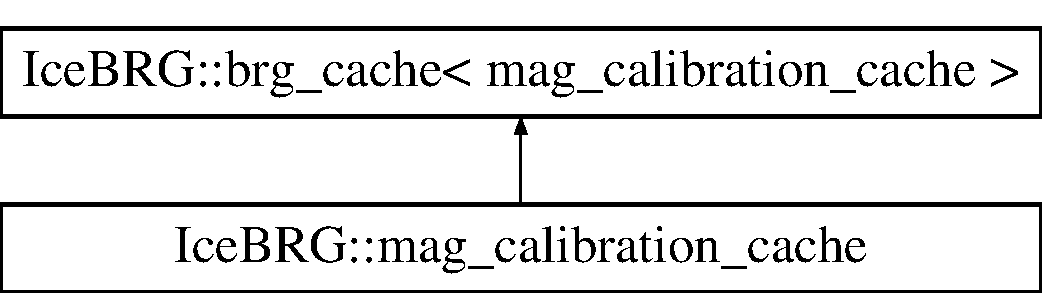
\includegraphics[height=2.000000cm]{classIceBRG_1_1mag__calibration__cache}
\end{center}
\end{figure}
\subsection*{Public Member Functions}
\begin{DoxyCompactItemize}
\item 
\hyperlink{classIceBRG_1_1mag__calibration__cache_a99d33bd36e6243810e1a5bc6dc262c08}{mag\-\_\-calibration\-\_\-cache} ()
\item 
\hyperlink{classIceBRG_1_1mag__calibration__cache_ad666da3efdda13aa3951e1cf54b5a17c}{$\sim$mag\-\_\-calibration\-\_\-cache} ()
\end{DoxyCompactItemize}
\subsection*{Protected Member Functions}
\begin{DoxyCompactItemize}
\item 
std\-::string \hyperlink{classIceBRG_1_1mag__calibration__cache_acd287d8811a0d0dfe63b39a7025bf065}{\-\_\-name\-\_\-base} () const 
\item 
\hyperlink{lib_2IceBRG__main_2common_8h_ad0f130a56eeb944d9ef2692ee881ecc4}{flt\-\_\-type} \hyperlink{classIceBRG_1_1mag__calibration__cache_a0ea0cf2413d6046542b5211f13bb9922}{\-\_\-calculate} (const \hyperlink{lib_2IceBRG__main_2common_8h_ad0f130a56eeb944d9ef2692ee881ecc4}{flt\-\_\-type} \&in\-\_\-param\-\_\-1) const 
\end{DoxyCompactItemize}
\subsection*{Friends}
\begin{DoxyCompactItemize}
\item 
class \hyperlink{classIceBRG_1_1mag__calibration__cache_aee5820d4cd188a3af58576bafc2fc246}{brg\-\_\-cache$<$ mag\-\_\-calibration\-\_\-cache $>$}
\end{DoxyCompactItemize}


\subsection{Constructor \& Destructor Documentation}
\hypertarget{classIceBRG_1_1mag__calibration__cache_a99d33bd36e6243810e1a5bc6dc262c08}{\index{Ice\-B\-R\-G\-::mag\-\_\-calibration\-\_\-cache@{Ice\-B\-R\-G\-::mag\-\_\-calibration\-\_\-cache}!mag\-\_\-calibration\-\_\-cache@{mag\-\_\-calibration\-\_\-cache}}
\index{mag\-\_\-calibration\-\_\-cache@{mag\-\_\-calibration\-\_\-cache}!IceBRG::mag_calibration_cache@{Ice\-B\-R\-G\-::mag\-\_\-calibration\-\_\-cache}}
\subsubsection[{mag\-\_\-calibration\-\_\-cache}]{\setlength{\rightskip}{0pt plus 5cm}Ice\-B\-R\-G\-::mag\-\_\-calibration\-\_\-cache\-::mag\-\_\-calibration\-\_\-cache (
\begin{DoxyParamCaption}
{}
\end{DoxyParamCaption}
)\hspace{0.3cm}{\ttfamily [inline]}}}\label{classIceBRG_1_1mag__calibration__cache_a99d33bd36e6243810e1a5bc6dc262c08}
\hypertarget{classIceBRG_1_1mag__calibration__cache_ad666da3efdda13aa3951e1cf54b5a17c}{\index{Ice\-B\-R\-G\-::mag\-\_\-calibration\-\_\-cache@{Ice\-B\-R\-G\-::mag\-\_\-calibration\-\_\-cache}!$\sim$mag\-\_\-calibration\-\_\-cache@{$\sim$mag\-\_\-calibration\-\_\-cache}}
\index{$\sim$mag\-\_\-calibration\-\_\-cache@{$\sim$mag\-\_\-calibration\-\_\-cache}!IceBRG::mag_calibration_cache@{Ice\-B\-R\-G\-::mag\-\_\-calibration\-\_\-cache}}
\subsubsection[{$\sim$mag\-\_\-calibration\-\_\-cache}]{\setlength{\rightskip}{0pt plus 5cm}Ice\-B\-R\-G\-::mag\-\_\-calibration\-\_\-cache\-::$\sim$mag\-\_\-calibration\-\_\-cache (
\begin{DoxyParamCaption}
{}
\end{DoxyParamCaption}
)\hspace{0.3cm}{\ttfamily [inline]}}}\label{classIceBRG_1_1mag__calibration__cache_ad666da3efdda13aa3951e1cf54b5a17c}


\subsection{Member Function Documentation}
\hypertarget{classIceBRG_1_1mag__calibration__cache_a0ea0cf2413d6046542b5211f13bb9922}{\index{Ice\-B\-R\-G\-::mag\-\_\-calibration\-\_\-cache@{Ice\-B\-R\-G\-::mag\-\_\-calibration\-\_\-cache}!\-\_\-calculate@{\-\_\-calculate}}
\index{\-\_\-calculate@{\-\_\-calculate}!IceBRG::mag_calibration_cache@{Ice\-B\-R\-G\-::mag\-\_\-calibration\-\_\-cache}}
\subsubsection[{\-\_\-calculate}]{\setlength{\rightskip}{0pt plus 5cm}{\bf flt\-\_\-type} Ice\-B\-R\-G\-::mag\-\_\-calibration\-\_\-cache\-::\-\_\-calculate (
\begin{DoxyParamCaption}
\item[{const {\bf flt\-\_\-type} \&}]{in\-\_\-param\-\_\-1}
\end{DoxyParamCaption}
) const\hspace{0.3cm}{\ttfamily [protected]}}}\label{classIceBRG_1_1mag__calibration__cache_a0ea0cf2413d6046542b5211f13bb9922}


Reimplemented from \hyperlink{classIceBRG_1_1brg__cache_afde9cc8f297a354727a4df9c16ab7a12}{Ice\-B\-R\-G\-::brg\-\_\-cache$<$ name $>$}.

\hypertarget{classIceBRG_1_1mag__calibration__cache_acd287d8811a0d0dfe63b39a7025bf065}{\index{Ice\-B\-R\-G\-::mag\-\_\-calibration\-\_\-cache@{Ice\-B\-R\-G\-::mag\-\_\-calibration\-\_\-cache}!\-\_\-name\-\_\-base@{\-\_\-name\-\_\-base}}
\index{\-\_\-name\-\_\-base@{\-\_\-name\-\_\-base}!IceBRG::mag_calibration_cache@{Ice\-B\-R\-G\-::mag\-\_\-calibration\-\_\-cache}}
\subsubsection[{\-\_\-name\-\_\-base}]{\setlength{\rightskip}{0pt plus 5cm}std\-::string Ice\-B\-R\-G\-::mag\-\_\-calibration\-\_\-cache\-::\-\_\-name\-\_\-base (
\begin{DoxyParamCaption}
{}
\end{DoxyParamCaption}
) const\hspace{0.3cm}{\ttfamily [inline]}, {\ttfamily [protected]}}}\label{classIceBRG_1_1mag__calibration__cache_acd287d8811a0d0dfe63b39a7025bf065}


Reimplemented from \hyperlink{classIceBRG_1_1brg__cache_a4453ff8ebded318cabaa332e9533ec40}{Ice\-B\-R\-G\-::brg\-\_\-cache$<$ name $>$}.



\subsection{Friends And Related Function Documentation}
\hypertarget{classIceBRG_1_1mag__calibration__cache_aee5820d4cd188a3af58576bafc2fc246}{\index{Ice\-B\-R\-G\-::mag\-\_\-calibration\-\_\-cache@{Ice\-B\-R\-G\-::mag\-\_\-calibration\-\_\-cache}!brg\-\_\-cache$<$ mag\-\_\-calibration\-\_\-cache $>$@{brg\-\_\-cache$<$ mag\-\_\-calibration\-\_\-cache $>$}}
\index{brg\-\_\-cache$<$ mag\-\_\-calibration\-\_\-cache $>$@{brg\-\_\-cache$<$ mag\-\_\-calibration\-\_\-cache $>$}!IceBRG::mag_calibration_cache@{Ice\-B\-R\-G\-::mag\-\_\-calibration\-\_\-cache}}
\subsubsection[{brg\-\_\-cache$<$ mag\-\_\-calibration\-\_\-cache $>$}]{\setlength{\rightskip}{0pt plus 5cm}friend class {\bf brg\-\_\-cache}$<$ {\bf mag\-\_\-calibration\-\_\-cache} $>$\hspace{0.3cm}{\ttfamily [friend]}}}\label{classIceBRG_1_1mag__calibration__cache_aee5820d4cd188a3af58576bafc2fc246}


The documentation for this class was generated from the following files\-:\begin{DoxyCompactItemize}
\item 
/disk2/brg/git/\-Magnification\-\_\-\-Public/src/lib/\-Ice\-B\-R\-G\-\_\-lensing/magnification/\hyperlink{mag__calibration__cache_8h}{mag\-\_\-calibration\-\_\-cache.\-h}\item 
/disk2/brg/git/\-Magnification\-\_\-\-Public/src/lib/\-Ice\-B\-R\-G\-\_\-lensing/magnification/\hyperlink{mag__calibration__cache_8cpp}{mag\-\_\-calibration\-\_\-cache.\-cpp}\end{DoxyCompactItemize}

\hypertarget{classIceBRG_1_1mag__calibration__loader}{\section{Ice\-B\-R\-G\-:\-:mag\-\_\-calibration\-\_\-loader Class Reference}
\label{classIceBRG_1_1mag__calibration__loader}\index{Ice\-B\-R\-G\-::mag\-\_\-calibration\-\_\-loader@{Ice\-B\-R\-G\-::mag\-\_\-calibration\-\_\-loader}}
}


{\ttfamily \#include $<$mag\-\_\-calibration\-\_\-loader.\-h$>$}

\subsection*{Static Public Member Functions}
\begin{DoxyCompactItemize}
\item 
static void \hyperlink{classIceBRG_1_1mag__calibration__loader_af276f91edf2a3a40189983c705092c37}{set\-\_\-z\-\_\-mins} (const std\-::vector$<$ \hyperlink{lib_2IceBRG__main_2common_8h_ad0f130a56eeb944d9ef2692ee881ecc4}{flt\-\_\-type} $>$ \&new\-\_\-limits\-\_\-vector)
\item 
static void \hyperlink{classIceBRG_1_1mag__calibration__loader_ace15d6820dfc88c0501c0b1a8cfdd32f}{set\-\_\-z\-\_\-mins} (std\-::vector$<$ \hyperlink{lib_2IceBRG__main_2common_8h_ad0f130a56eeb944d9ef2692ee881ecc4}{flt\-\_\-type} $>$ \&\&new\-\_\-limits\-\_\-vector)
\item 
static void \hyperlink{classIceBRG_1_1mag__calibration__loader_a6d8f09bdfb5a75ed3d25370bda3ca545}{set\-\_\-filename} (const std\-::string \&new\-\_\-filename)
\item 
static void \hyperlink{classIceBRG_1_1mag__calibration__loader_ad79c4c5eb6ccab5d2212bfe77633e03a}{set\-\_\-filename} (std\-::string \&\&new\-\_\-filename)
\item 
static \hyperlink{lib_2IceBRG__main_2common_8h_ad0f130a56eeb944d9ef2692ee881ecc4}{flt\-\_\-type} \hyperlink{classIceBRG_1_1mag__calibration__loader_a2e1d2ff7d05458a304ceb7f993448aa7}{get} (const \hyperlink{lib_2IceBRG__main_2common_8h_ad0f130a56eeb944d9ef2692ee881ecc4}{flt\-\_\-type} \&z)
\item 
static void \hyperlink{classIceBRG_1_1mag__calibration__loader_a71a4df8564cc427b21b3583ebd58b15d}{unload} ()
\end{DoxyCompactItemize}


\subsection{Member Function Documentation}
\hypertarget{classIceBRG_1_1mag__calibration__loader_a2e1d2ff7d05458a304ceb7f993448aa7}{\index{Ice\-B\-R\-G\-::mag\-\_\-calibration\-\_\-loader@{Ice\-B\-R\-G\-::mag\-\_\-calibration\-\_\-loader}!get@{get}}
\index{get@{get}!IceBRG::mag_calibration_loader@{Ice\-B\-R\-G\-::mag\-\_\-calibration\-\_\-loader}}
\subsubsection[{get}]{\setlength{\rightskip}{0pt plus 5cm}{\bf flt\-\_\-type} Ice\-B\-R\-G\-::mag\-\_\-calibration\-\_\-loader\-::get (
\begin{DoxyParamCaption}
\item[{const {\bf flt\-\_\-type} \&}]{z}
\end{DoxyParamCaption}
)\hspace{0.3cm}{\ttfamily [static]}}}\label{classIceBRG_1_1mag__calibration__loader_a2e1d2ff7d05458a304ceb7f993448aa7}
\hypertarget{classIceBRG_1_1mag__calibration__loader_a6d8f09bdfb5a75ed3d25370bda3ca545}{\index{Ice\-B\-R\-G\-::mag\-\_\-calibration\-\_\-loader@{Ice\-B\-R\-G\-::mag\-\_\-calibration\-\_\-loader}!set\-\_\-filename@{set\-\_\-filename}}
\index{set\-\_\-filename@{set\-\_\-filename}!IceBRG::mag_calibration_loader@{Ice\-B\-R\-G\-::mag\-\_\-calibration\-\_\-loader}}
\subsubsection[{set\-\_\-filename}]{\setlength{\rightskip}{0pt plus 5cm}void Ice\-B\-R\-G\-::mag\-\_\-calibration\-\_\-loader\-::set\-\_\-filename (
\begin{DoxyParamCaption}
\item[{const std\-::string \&}]{new\-\_\-filename}
\end{DoxyParamCaption}
)\hspace{0.3cm}{\ttfamily [static]}}}\label{classIceBRG_1_1mag__calibration__loader_a6d8f09bdfb5a75ed3d25370bda3ca545}
\hypertarget{classIceBRG_1_1mag__calibration__loader_ad79c4c5eb6ccab5d2212bfe77633e03a}{\index{Ice\-B\-R\-G\-::mag\-\_\-calibration\-\_\-loader@{Ice\-B\-R\-G\-::mag\-\_\-calibration\-\_\-loader}!set\-\_\-filename@{set\-\_\-filename}}
\index{set\-\_\-filename@{set\-\_\-filename}!IceBRG::mag_calibration_loader@{Ice\-B\-R\-G\-::mag\-\_\-calibration\-\_\-loader}}
\subsubsection[{set\-\_\-filename}]{\setlength{\rightskip}{0pt plus 5cm}void Ice\-B\-R\-G\-::mag\-\_\-calibration\-\_\-loader\-::set\-\_\-filename (
\begin{DoxyParamCaption}
\item[{std\-::string \&\&}]{new\-\_\-filename}
\end{DoxyParamCaption}
)\hspace{0.3cm}{\ttfamily [static]}}}\label{classIceBRG_1_1mag__calibration__loader_ad79c4c5eb6ccab5d2212bfe77633e03a}
\hypertarget{classIceBRG_1_1mag__calibration__loader_af276f91edf2a3a40189983c705092c37}{\index{Ice\-B\-R\-G\-::mag\-\_\-calibration\-\_\-loader@{Ice\-B\-R\-G\-::mag\-\_\-calibration\-\_\-loader}!set\-\_\-z\-\_\-mins@{set\-\_\-z\-\_\-mins}}
\index{set\-\_\-z\-\_\-mins@{set\-\_\-z\-\_\-mins}!IceBRG::mag_calibration_loader@{Ice\-B\-R\-G\-::mag\-\_\-calibration\-\_\-loader}}
\subsubsection[{set\-\_\-z\-\_\-mins}]{\setlength{\rightskip}{0pt plus 5cm}void Ice\-B\-R\-G\-::mag\-\_\-calibration\-\_\-loader\-::set\-\_\-z\-\_\-mins (
\begin{DoxyParamCaption}
\item[{const std\-::vector$<$ {\bf flt\-\_\-type} $>$ \&}]{new\-\_\-limits\-\_\-vector}
\end{DoxyParamCaption}
)\hspace{0.3cm}{\ttfamily [static]}}}\label{classIceBRG_1_1mag__calibration__loader_af276f91edf2a3a40189983c705092c37}
\hypertarget{classIceBRG_1_1mag__calibration__loader_ace15d6820dfc88c0501c0b1a8cfdd32f}{\index{Ice\-B\-R\-G\-::mag\-\_\-calibration\-\_\-loader@{Ice\-B\-R\-G\-::mag\-\_\-calibration\-\_\-loader}!set\-\_\-z\-\_\-mins@{set\-\_\-z\-\_\-mins}}
\index{set\-\_\-z\-\_\-mins@{set\-\_\-z\-\_\-mins}!IceBRG::mag_calibration_loader@{Ice\-B\-R\-G\-::mag\-\_\-calibration\-\_\-loader}}
\subsubsection[{set\-\_\-z\-\_\-mins}]{\setlength{\rightskip}{0pt plus 5cm}void Ice\-B\-R\-G\-::mag\-\_\-calibration\-\_\-loader\-::set\-\_\-z\-\_\-mins (
\begin{DoxyParamCaption}
\item[{std\-::vector$<$ {\bf flt\-\_\-type} $>$ \&\&}]{new\-\_\-limits\-\_\-vector}
\end{DoxyParamCaption}
)\hspace{0.3cm}{\ttfamily [static]}}}\label{classIceBRG_1_1mag__calibration__loader_ace15d6820dfc88c0501c0b1a8cfdd32f}
\hypertarget{classIceBRG_1_1mag__calibration__loader_a71a4df8564cc427b21b3583ebd58b15d}{\index{Ice\-B\-R\-G\-::mag\-\_\-calibration\-\_\-loader@{Ice\-B\-R\-G\-::mag\-\_\-calibration\-\_\-loader}!unload@{unload}}
\index{unload@{unload}!IceBRG::mag_calibration_loader@{Ice\-B\-R\-G\-::mag\-\_\-calibration\-\_\-loader}}
\subsubsection[{unload}]{\setlength{\rightskip}{0pt plus 5cm}void Ice\-B\-R\-G\-::mag\-\_\-calibration\-\_\-loader\-::unload (
\begin{DoxyParamCaption}
{}
\end{DoxyParamCaption}
)\hspace{0.3cm}{\ttfamily [static]}}}\label{classIceBRG_1_1mag__calibration__loader_a71a4df8564cc427b21b3583ebd58b15d}


The documentation for this class was generated from the following files\-:\begin{DoxyCompactItemize}
\item 
/disk2/brg/git/\-Magnification\-\_\-\-Public/src/lib/\-Ice\-B\-R\-G\-\_\-lensing/magnification/\hyperlink{mag__calibration__loader_8h}{mag\-\_\-calibration\-\_\-loader.\-h}\item 
/disk2/brg/git/\-Magnification\-\_\-\-Public/src/lib/\-Ice\-B\-R\-G\-\_\-lensing/magnification/\hyperlink{mag__calibration__loader_8cpp}{mag\-\_\-calibration\-\_\-loader.\-cpp}\end{DoxyCompactItemize}

\hypertarget{classIceBRG_1_1mag__correlation__function__estimator}{\section{Ice\-B\-R\-G\-:\-:mag\-\_\-correlation\-\_\-function\-\_\-estimator Class Reference}
\label{classIceBRG_1_1mag__correlation__function__estimator}\index{Ice\-B\-R\-G\-::mag\-\_\-correlation\-\_\-function\-\_\-estimator@{Ice\-B\-R\-G\-::mag\-\_\-correlation\-\_\-function\-\_\-estimator}}
}


{\ttfamily \#include $<$mag\-\_\-correlation\-\_\-function\-\_\-estimator.\-h$>$}

\subsection*{Public Member Functions}
\begin{DoxyCompactItemize}
\item 
\hyperlink{classIceBRG_1_1mag__correlation__function__estimator_abb52bbca993182ccb4174301c34b114c}{mag\-\_\-correlation\-\_\-function\-\_\-estimator} ()
\begin{DoxyCompactList}\small\item\em Default constructor. Will not be set up for calculation. \end{DoxyCompactList}\item 
{\footnotesize template$<$typename T $>$ }\\\hyperlink{classIceBRG_1_1mag__correlation__function__estimator_af5467ccdbc613e37395d541d3560523b}{mag\-\_\-correlation\-\_\-function\-\_\-estimator} (T \&\&D\-\_\-bin\-\_\-limits, const \hyperlink{lib_2IceBRG__main_2common_8h_ad0f130a56eeb944d9ef2692ee881ecc4}{flt\-\_\-type} \&\hyperlink{magic__values_8hpp_a424f49a8036e9de5962c718fb785356f}{z\-\_\-buffer}=0)
\begin{DoxyCompactList}\small\item\em Construct with only bin limits. Will not set up for calculation. \end{DoxyCompactList}\item 
{\footnotesize template$<$typename T\-R1 , typename T\-R2 , typename T\-M1 , typename T\-M2 $>$ }\\\hyperlink{classIceBRG_1_1mag__correlation__function__estimator_a2593a1c26ad9bd49311f996fb3b23cea}{mag\-\_\-correlation\-\_\-function\-\_\-estimator} (T\-R1 \&\&D1\-\_\-pos\-\_\-list, T\-R2 \&\&D2\-\_\-pos\-\_\-list, T\-M1 \&\&R1\-\_\-pos\-\_\-list, T\-M2 \&\&R2\-\_\-pos\-\_\-list, const \hyperlink{lib_2IceBRG__main_2common_8h_ad0f130a56eeb944d9ef2692ee881ecc4}{flt\-\_\-type} \&\hyperlink{magic__values_8hpp_a424f49a8036e9de5962c718fb785356f}{z\-\_\-buffer}=0)
\begin{DoxyCompactList}\small\item\em Construct with only position lists. \end{DoxyCompactList}\item 
{\footnotesize template$<$typename T , typename T\-R1 , typename T\-R2 , typename T\-M1 , typename T\-M2 $>$ }\\\hyperlink{classIceBRG_1_1mag__correlation__function__estimator_a77ea4cbd453bb57666dbe4f8f6322632}{mag\-\_\-correlation\-\_\-function\-\_\-estimator} (T \&\&D\-\_\-bin\-\_\-limits, T\-R1 \&\&D1\-\_\-pos\-\_\-list, T\-R2 \&\&D2\-\_\-pos\-\_\-list, T\-M1 \&\&R1\-\_\-pos\-\_\-list, T\-M2 \&\&R2\-\_\-pos\-\_\-list, const \hyperlink{lib_2IceBRG__main_2common_8h_ad0f130a56eeb944d9ef2692ee881ecc4}{flt\-\_\-type} \&\hyperlink{magic__values_8hpp_a424f49a8036e9de5962c718fb785356f}{z\-\_\-buffer}=0)
\begin{DoxyCompactList}\small\item\em Construct with bin limits and position lists. \end{DoxyCompactList}\item 
virtual \hyperlink{classIceBRG_1_1mag__correlation__function__estimator_a8d3457d60040f2a4b8114bd960578602}{$\sim$mag\-\_\-correlation\-\_\-function\-\_\-estimator} ()
\item 
Eigen\-::\-Array\-Xd \hyperlink{classIceBRG_1_1mag__correlation__function__estimator_a0cad08d37e08c2ef1397e87609647f30}{calculate} () const 
\begin{DoxyCompactList}\small\item\em Standard calculation function, using Hamilton estimator. \end{DoxyCompactList}\item 
Eigen\-::\-Array\-Xd \hyperlink{classIceBRG_1_1mag__correlation__function__estimator_a75f844fbabc0b370ef6eafac119ac487}{weights} () const 
\begin{DoxyCompactList}\small\item\em Get bin weights for standard calculation function. \end{DoxyCompactList}\item 
Eigen\-::\-Array\-Xd \hyperlink{classIceBRG_1_1mag__correlation__function__estimator_a5255e1f640ca3ec3eed500290b48551e}{errors} () const 
\begin{DoxyCompactList}\small\item\em Get errors for standard calculation function. \end{DoxyCompactList}\item 
Eigen\-::\-Array\-Xd \hyperlink{classIceBRG_1_1mag__correlation__function__estimator_af2088b0c2fe2d5c6c33d25419fd0fab3}{calculate\-\_\-weighted} (const std\-::function$<$ \hyperlink{lib_2IceBRG__main_2common_8h_ad0f130a56eeb944d9ef2692ee881ecc4}{flt\-\_\-type}(\hyperlink{namespaceIceBRG_a688eeb0811a2474b20b667ed2e9625a1}{angle\-\_\-type})$>$ \&weight\-\_\-function=\mbox{[}$\,$\mbox{]}(const \hyperlink{namespaceIceBRG_a688eeb0811a2474b20b667ed2e9625a1}{angle\-\_\-type} \&theta)\{return 1.;\}) const 
\item 
Eigen\-::\-Array\-Xd \hyperlink{classIceBRG_1_1mag__correlation__function__estimator_a4c851a8f4cee148e4334c810c5e418be}{calculate\-\_\-dipole} (const \hyperlink{lib_2IceBRG__main_2common_8h_ad0f130a56eeb944d9ef2692ee881ecc4}{flt\-\_\-type} \&offset=0) const 
\item 
Eigen\-::\-Array\-Xd \hyperlink{classIceBRG_1_1mag__correlation__function__estimator_aaffcdd4f844aa6f5ec507a413d7cdf0c}{calculate\-\_\-quadrupole} (const \hyperlink{lib_2IceBRG__main_2common_8h_ad0f130a56eeb944d9ef2692ee881ecc4}{flt\-\_\-type} \&offset=0) const 
\item 
Eigen\-::\-Array\-Xd \hyperlink{classIceBRG_1_1mag__correlation__function__estimator_a3ccc3e13d9e80433a0f5a476f57aa5b4}{calculate\-\_\-octopole} (const \hyperlink{lib_2IceBRG__main_2common_8h_ad0f130a56eeb944d9ef2692ee881ecc4}{flt\-\_\-type} \&offset=0) const 
\end{DoxyCompactItemize}


\subsection{Constructor \& Destructor Documentation}
\hypertarget{classIceBRG_1_1mag__correlation__function__estimator_abb52bbca993182ccb4174301c34b114c}{\index{Ice\-B\-R\-G\-::mag\-\_\-correlation\-\_\-function\-\_\-estimator@{Ice\-B\-R\-G\-::mag\-\_\-correlation\-\_\-function\-\_\-estimator}!mag\-\_\-correlation\-\_\-function\-\_\-estimator@{mag\-\_\-correlation\-\_\-function\-\_\-estimator}}
\index{mag\-\_\-correlation\-\_\-function\-\_\-estimator@{mag\-\_\-correlation\-\_\-function\-\_\-estimator}!IceBRG::mag_correlation_function_estimator@{Ice\-B\-R\-G\-::mag\-\_\-correlation\-\_\-function\-\_\-estimator}}
\subsubsection[{mag\-\_\-correlation\-\_\-function\-\_\-estimator}]{\setlength{\rightskip}{0pt plus 5cm}Ice\-B\-R\-G\-::mag\-\_\-correlation\-\_\-function\-\_\-estimator\-::mag\-\_\-correlation\-\_\-function\-\_\-estimator (
\begin{DoxyParamCaption}
{}
\end{DoxyParamCaption}
)\hspace{0.3cm}{\ttfamily [inline]}}}\label{classIceBRG_1_1mag__correlation__function__estimator_abb52bbca993182ccb4174301c34b114c}


Default constructor. Will not be set up for calculation. 

\hypertarget{classIceBRG_1_1mag__correlation__function__estimator_af5467ccdbc613e37395d541d3560523b}{\index{Ice\-B\-R\-G\-::mag\-\_\-correlation\-\_\-function\-\_\-estimator@{Ice\-B\-R\-G\-::mag\-\_\-correlation\-\_\-function\-\_\-estimator}!mag\-\_\-correlation\-\_\-function\-\_\-estimator@{mag\-\_\-correlation\-\_\-function\-\_\-estimator}}
\index{mag\-\_\-correlation\-\_\-function\-\_\-estimator@{mag\-\_\-correlation\-\_\-function\-\_\-estimator}!IceBRG::mag_correlation_function_estimator@{Ice\-B\-R\-G\-::mag\-\_\-correlation\-\_\-function\-\_\-estimator}}
\subsubsection[{mag\-\_\-correlation\-\_\-function\-\_\-estimator}]{\setlength{\rightskip}{0pt plus 5cm}template$<$typename T $>$ Ice\-B\-R\-G\-::mag\-\_\-correlation\-\_\-function\-\_\-estimator\-::mag\-\_\-correlation\-\_\-function\-\_\-estimator (
\begin{DoxyParamCaption}
\item[{T \&\&}]{D\-\_\-bin\-\_\-limits, }
\item[{const {\bf flt\-\_\-type} \&}]{z\-\_\-buffer = {\ttfamily 0}}
\end{DoxyParamCaption}
)\hspace{0.3cm}{\ttfamily [inline]}}}\label{classIceBRG_1_1mag__correlation__function__estimator_af5467ccdbc613e37395d541d3560523b}


Construct with only bin limits. Will not set up for calculation. 

\hypertarget{classIceBRG_1_1mag__correlation__function__estimator_a2593a1c26ad9bd49311f996fb3b23cea}{\index{Ice\-B\-R\-G\-::mag\-\_\-correlation\-\_\-function\-\_\-estimator@{Ice\-B\-R\-G\-::mag\-\_\-correlation\-\_\-function\-\_\-estimator}!mag\-\_\-correlation\-\_\-function\-\_\-estimator@{mag\-\_\-correlation\-\_\-function\-\_\-estimator}}
\index{mag\-\_\-correlation\-\_\-function\-\_\-estimator@{mag\-\_\-correlation\-\_\-function\-\_\-estimator}!IceBRG::mag_correlation_function_estimator@{Ice\-B\-R\-G\-::mag\-\_\-correlation\-\_\-function\-\_\-estimator}}
\subsubsection[{mag\-\_\-correlation\-\_\-function\-\_\-estimator}]{\setlength{\rightskip}{0pt plus 5cm}template$<$typename T\-R1 , typename T\-R2 , typename T\-M1 , typename T\-M2 $>$ Ice\-B\-R\-G\-::mag\-\_\-correlation\-\_\-function\-\_\-estimator\-::mag\-\_\-correlation\-\_\-function\-\_\-estimator (
\begin{DoxyParamCaption}
\item[{T\-R1 \&\&}]{D1\-\_\-pos\-\_\-list, }
\item[{T\-R2 \&\&}]{D2\-\_\-pos\-\_\-list, }
\item[{T\-M1 \&\&}]{R1\-\_\-pos\-\_\-list, }
\item[{T\-M2 \&\&}]{R2\-\_\-pos\-\_\-list, }
\item[{const {\bf flt\-\_\-type} \&}]{z\-\_\-buffer = {\ttfamily 0}}
\end{DoxyParamCaption}
)\hspace{0.3cm}{\ttfamily [inline]}}}\label{classIceBRG_1_1mag__correlation__function__estimator_a2593a1c26ad9bd49311f996fb3b23cea}


Construct with only position lists. 

\hypertarget{classIceBRG_1_1mag__correlation__function__estimator_a77ea4cbd453bb57666dbe4f8f6322632}{\index{Ice\-B\-R\-G\-::mag\-\_\-correlation\-\_\-function\-\_\-estimator@{Ice\-B\-R\-G\-::mag\-\_\-correlation\-\_\-function\-\_\-estimator}!mag\-\_\-correlation\-\_\-function\-\_\-estimator@{mag\-\_\-correlation\-\_\-function\-\_\-estimator}}
\index{mag\-\_\-correlation\-\_\-function\-\_\-estimator@{mag\-\_\-correlation\-\_\-function\-\_\-estimator}!IceBRG::mag_correlation_function_estimator@{Ice\-B\-R\-G\-::mag\-\_\-correlation\-\_\-function\-\_\-estimator}}
\subsubsection[{mag\-\_\-correlation\-\_\-function\-\_\-estimator}]{\setlength{\rightskip}{0pt plus 5cm}template$<$typename T , typename T\-R1 , typename T\-R2 , typename T\-M1 , typename T\-M2 $>$ Ice\-B\-R\-G\-::mag\-\_\-correlation\-\_\-function\-\_\-estimator\-::mag\-\_\-correlation\-\_\-function\-\_\-estimator (
\begin{DoxyParamCaption}
\item[{T \&\&}]{D\-\_\-bin\-\_\-limits, }
\item[{T\-R1 \&\&}]{D1\-\_\-pos\-\_\-list, }
\item[{T\-R2 \&\&}]{D2\-\_\-pos\-\_\-list, }
\item[{T\-M1 \&\&}]{R1\-\_\-pos\-\_\-list, }
\item[{T\-M2 \&\&}]{R2\-\_\-pos\-\_\-list, }
\item[{const {\bf flt\-\_\-type} \&}]{z\-\_\-buffer = {\ttfamily 0}}
\end{DoxyParamCaption}
)\hspace{0.3cm}{\ttfamily [inline]}}}\label{classIceBRG_1_1mag__correlation__function__estimator_a77ea4cbd453bb57666dbe4f8f6322632}


Construct with bin limits and position lists. 

\hypertarget{classIceBRG_1_1mag__correlation__function__estimator_a8d3457d60040f2a4b8114bd960578602}{\index{Ice\-B\-R\-G\-::mag\-\_\-correlation\-\_\-function\-\_\-estimator@{Ice\-B\-R\-G\-::mag\-\_\-correlation\-\_\-function\-\_\-estimator}!$\sim$mag\-\_\-correlation\-\_\-function\-\_\-estimator@{$\sim$mag\-\_\-correlation\-\_\-function\-\_\-estimator}}
\index{$\sim$mag\-\_\-correlation\-\_\-function\-\_\-estimator@{$\sim$mag\-\_\-correlation\-\_\-function\-\_\-estimator}!IceBRG::mag_correlation_function_estimator@{Ice\-B\-R\-G\-::mag\-\_\-correlation\-\_\-function\-\_\-estimator}}
\subsubsection[{$\sim$mag\-\_\-correlation\-\_\-function\-\_\-estimator}]{\setlength{\rightskip}{0pt plus 5cm}virtual Ice\-B\-R\-G\-::mag\-\_\-correlation\-\_\-function\-\_\-estimator\-::$\sim$mag\-\_\-correlation\-\_\-function\-\_\-estimator (
\begin{DoxyParamCaption}
{}
\end{DoxyParamCaption}
)\hspace{0.3cm}{\ttfamily [inline]}, {\ttfamily [virtual]}}}\label{classIceBRG_1_1mag__correlation__function__estimator_a8d3457d60040f2a4b8114bd960578602}


\subsection{Member Function Documentation}
\hypertarget{classIceBRG_1_1mag__correlation__function__estimator_a0cad08d37e08c2ef1397e87609647f30}{\index{Ice\-B\-R\-G\-::mag\-\_\-correlation\-\_\-function\-\_\-estimator@{Ice\-B\-R\-G\-::mag\-\_\-correlation\-\_\-function\-\_\-estimator}!calculate@{calculate}}
\index{calculate@{calculate}!IceBRG::mag_correlation_function_estimator@{Ice\-B\-R\-G\-::mag\-\_\-correlation\-\_\-function\-\_\-estimator}}
\subsubsection[{calculate}]{\setlength{\rightskip}{0pt plus 5cm}Eigen\-::\-Array\-Xd Ice\-B\-R\-G\-::mag\-\_\-correlation\-\_\-function\-\_\-estimator\-::calculate (
\begin{DoxyParamCaption}
{}
\end{DoxyParamCaption}
) const}}\label{classIceBRG_1_1mag__correlation__function__estimator_a0cad08d37e08c2ef1397e87609647f30}


Standard calculation function, using Hamilton estimator. 

\hypertarget{classIceBRG_1_1mag__correlation__function__estimator_a4c851a8f4cee148e4334c810c5e418be}{\index{Ice\-B\-R\-G\-::mag\-\_\-correlation\-\_\-function\-\_\-estimator@{Ice\-B\-R\-G\-::mag\-\_\-correlation\-\_\-function\-\_\-estimator}!calculate\-\_\-dipole@{calculate\-\_\-dipole}}
\index{calculate\-\_\-dipole@{calculate\-\_\-dipole}!IceBRG::mag_correlation_function_estimator@{Ice\-B\-R\-G\-::mag\-\_\-correlation\-\_\-function\-\_\-estimator}}
\subsubsection[{calculate\-\_\-dipole}]{\setlength{\rightskip}{0pt plus 5cm}Eigen\-::\-Array\-Xd Ice\-B\-R\-G\-::mag\-\_\-correlation\-\_\-function\-\_\-estimator\-::calculate\-\_\-dipole (
\begin{DoxyParamCaption}
\item[{const {\bf flt\-\_\-type} \&}]{offset = {\ttfamily 0}}
\end{DoxyParamCaption}
) const}}\label{classIceBRG_1_1mag__correlation__function__estimator_a4c851a8f4cee148e4334c810c5e418be}
Calculation function for dipole correlation function with a given offset. The offset should vary from \mbox{[}0,1) or \mbox{[}-\/0.\-5,0.\-5) for unique results. \hypertarget{classIceBRG_1_1mag__correlation__function__estimator_a3ccc3e13d9e80433a0f5a476f57aa5b4}{\index{Ice\-B\-R\-G\-::mag\-\_\-correlation\-\_\-function\-\_\-estimator@{Ice\-B\-R\-G\-::mag\-\_\-correlation\-\_\-function\-\_\-estimator}!calculate\-\_\-octopole@{calculate\-\_\-octopole}}
\index{calculate\-\_\-octopole@{calculate\-\_\-octopole}!IceBRG::mag_correlation_function_estimator@{Ice\-B\-R\-G\-::mag\-\_\-correlation\-\_\-function\-\_\-estimator}}
\subsubsection[{calculate\-\_\-octopole}]{\setlength{\rightskip}{0pt plus 5cm}Eigen\-::\-Array\-Xd Ice\-B\-R\-G\-::mag\-\_\-correlation\-\_\-function\-\_\-estimator\-::calculate\-\_\-octopole (
\begin{DoxyParamCaption}
\item[{const {\bf flt\-\_\-type} \&}]{offset = {\ttfamily 0}}
\end{DoxyParamCaption}
) const}}\label{classIceBRG_1_1mag__correlation__function__estimator_a3ccc3e13d9e80433a0f5a476f57aa5b4}
Calculation function for octopole correlation function with a given offset. The offset should vary from \mbox{[}0,1) or \mbox{[}-\/0.\-5,0.\-5) for unique results. \hypertarget{classIceBRG_1_1mag__correlation__function__estimator_aaffcdd4f844aa6f5ec507a413d7cdf0c}{\index{Ice\-B\-R\-G\-::mag\-\_\-correlation\-\_\-function\-\_\-estimator@{Ice\-B\-R\-G\-::mag\-\_\-correlation\-\_\-function\-\_\-estimator}!calculate\-\_\-quadrupole@{calculate\-\_\-quadrupole}}
\index{calculate\-\_\-quadrupole@{calculate\-\_\-quadrupole}!IceBRG::mag_correlation_function_estimator@{Ice\-B\-R\-G\-::mag\-\_\-correlation\-\_\-function\-\_\-estimator}}
\subsubsection[{calculate\-\_\-quadrupole}]{\setlength{\rightskip}{0pt plus 5cm}Eigen\-::\-Array\-Xd Ice\-B\-R\-G\-::mag\-\_\-correlation\-\_\-function\-\_\-estimator\-::calculate\-\_\-quadrupole (
\begin{DoxyParamCaption}
\item[{const {\bf flt\-\_\-type} \&}]{offset = {\ttfamily 0}}
\end{DoxyParamCaption}
) const}}\label{classIceBRG_1_1mag__correlation__function__estimator_aaffcdd4f844aa6f5ec507a413d7cdf0c}
Calculation function for quadrupole correlation function with a given offset. The offset should vary from \mbox{[}0,1) or \mbox{[}-\/0.\-5,0.\-5) for unique results. \hypertarget{classIceBRG_1_1mag__correlation__function__estimator_af2088b0c2fe2d5c6c33d25419fd0fab3}{\index{Ice\-B\-R\-G\-::mag\-\_\-correlation\-\_\-function\-\_\-estimator@{Ice\-B\-R\-G\-::mag\-\_\-correlation\-\_\-function\-\_\-estimator}!calculate\-\_\-weighted@{calculate\-\_\-weighted}}
\index{calculate\-\_\-weighted@{calculate\-\_\-weighted}!IceBRG::mag_correlation_function_estimator@{Ice\-B\-R\-G\-::mag\-\_\-correlation\-\_\-function\-\_\-estimator}}
\subsubsection[{calculate\-\_\-weighted}]{\setlength{\rightskip}{0pt plus 5cm}Eigen\-::\-Array\-Xd Ice\-B\-R\-G\-::mag\-\_\-correlation\-\_\-function\-\_\-estimator\-::calculate\-\_\-weighted (
\begin{DoxyParamCaption}
{}
\end{DoxyParamCaption}
) const}}\label{classIceBRG_1_1mag__correlation__function__estimator_af2088b0c2fe2d5c6c33d25419fd0fab3}
Weighted calculation function, using a Hamilton-\/like estimator. This assumes the weight function passed here has an expected value of zero. \hypertarget{classIceBRG_1_1mag__correlation__function__estimator_a5255e1f640ca3ec3eed500290b48551e}{\index{Ice\-B\-R\-G\-::mag\-\_\-correlation\-\_\-function\-\_\-estimator@{Ice\-B\-R\-G\-::mag\-\_\-correlation\-\_\-function\-\_\-estimator}!errors@{errors}}
\index{errors@{errors}!IceBRG::mag_correlation_function_estimator@{Ice\-B\-R\-G\-::mag\-\_\-correlation\-\_\-function\-\_\-estimator}}
\subsubsection[{errors}]{\setlength{\rightskip}{0pt plus 5cm}Eigen\-::\-Array\-Xd Ice\-B\-R\-G\-::mag\-\_\-correlation\-\_\-function\-\_\-estimator\-::errors (
\begin{DoxyParamCaption}
{}
\end{DoxyParamCaption}
) const}}\label{classIceBRG_1_1mag__correlation__function__estimator_a5255e1f640ca3ec3eed500290b48551e}


Get errors for standard calculation function. 

\hypertarget{classIceBRG_1_1mag__correlation__function__estimator_a75f844fbabc0b370ef6eafac119ac487}{\index{Ice\-B\-R\-G\-::mag\-\_\-correlation\-\_\-function\-\_\-estimator@{Ice\-B\-R\-G\-::mag\-\_\-correlation\-\_\-function\-\_\-estimator}!weights@{weights}}
\index{weights@{weights}!IceBRG::mag_correlation_function_estimator@{Ice\-B\-R\-G\-::mag\-\_\-correlation\-\_\-function\-\_\-estimator}}
\subsubsection[{weights}]{\setlength{\rightskip}{0pt plus 5cm}Eigen\-::\-Array\-Xd Ice\-B\-R\-G\-::mag\-\_\-correlation\-\_\-function\-\_\-estimator\-::weights (
\begin{DoxyParamCaption}
{}
\end{DoxyParamCaption}
) const}}\label{classIceBRG_1_1mag__correlation__function__estimator_a75f844fbabc0b370ef6eafac119ac487}


Get bin weights for standard calculation function. 



The documentation for this class was generated from the following files\-:\begin{DoxyCompactItemize}
\item 
/disk2/brg/git/\-Magnification\-\_\-\-Public/src/lib/\-Ice\-B\-R\-G\-\_\-lensing/magnification/\hyperlink{mag__correlation__function__estimator_8h}{mag\-\_\-correlation\-\_\-function\-\_\-estimator.\-h}\item 
/disk2/brg/git/\-Magnification\-\_\-\-Public/src/lib/\-Ice\-B\-R\-G\-\_\-lensing/magnification/\hyperlink{mag__correlation__function__estimator_8cpp}{mag\-\_\-correlation\-\_\-function\-\_\-estimator.\-cpp}\end{DoxyCompactItemize}

\hypertarget{classIceBRG_1_1mag__expected__count__functor}{}\section{Ice\+B\+R\+G\+:\+:mag\+\_\+expected\+\_\+count\+\_\+functor Class Reference}
\label{classIceBRG_1_1mag__expected__count__functor}\index{Ice\+B\+R\+G\+::mag\+\_\+expected\+\_\+count\+\_\+functor@{Ice\+B\+R\+G\+::mag\+\_\+expected\+\_\+count\+\_\+functor}}


{\ttfamily \#include $<$magnification\+\_\+functors.\+h$>$}

\subsection*{Public Member Functions}
\begin{DoxyCompactItemize}
\item 
\hyperlink{classIceBRG_1_1mag__expected__count__functor_ae8cfd011211991dd4d66d3aa26b228e2}{mag\+\_\+expected\+\_\+count\+\_\+functor} (\hyperlink{lib_2IceBRG__main_2common_8h_ad0f130a56eeb944d9ef2692ee881ecc4}{flt\+\_\+type} init\+\_\+z=0)
\item 
virtual \hyperlink{classIceBRG_1_1mag__expected__count__functor_ad371e59c7eccf99936b1464eab520234}{$\sim$mag\+\_\+expected\+\_\+count\+\_\+functor} ()
\item 
\hyperlink{lib_2IceBRG__main_2common_8h_ad0f130a56eeb944d9ef2692ee881ecc4}{flt\+\_\+type} \hyperlink{classIceBRG_1_1mag__expected__count__functor_a1634698c687459cc3476fac2f548384d}{operator()} (const \hyperlink{lib_2IceBRG__main_2common_8h_a7040956e7e1b504d34a9ccfb4253bdce}{long\+\_\+flt\+\_\+type} \&\hyperlink{namespaceIceBRG_ada6365c5d16106f0608afbd34f010bcc}{m}=true) const 
\end{DoxyCompactItemize}


\subsection{Constructor \& Destructor Documentation}
\hypertarget{classIceBRG_1_1mag__expected__count__functor_ae8cfd011211991dd4d66d3aa26b228e2}{}\index{Ice\+B\+R\+G\+::mag\+\_\+expected\+\_\+count\+\_\+functor@{Ice\+B\+R\+G\+::mag\+\_\+expected\+\_\+count\+\_\+functor}!mag\+\_\+expected\+\_\+count\+\_\+functor@{mag\+\_\+expected\+\_\+count\+\_\+functor}}
\index{mag\+\_\+expected\+\_\+count\+\_\+functor@{mag\+\_\+expected\+\_\+count\+\_\+functor}!Ice\+B\+R\+G\+::mag\+\_\+expected\+\_\+count\+\_\+functor@{Ice\+B\+R\+G\+::mag\+\_\+expected\+\_\+count\+\_\+functor}}
\subsubsection[{mag\+\_\+expected\+\_\+count\+\_\+functor(flt\+\_\+type init\+\_\+z=0)}]{\setlength{\rightskip}{0pt plus 5cm}Ice\+B\+R\+G\+::mag\+\_\+expected\+\_\+count\+\_\+functor\+::mag\+\_\+expected\+\_\+count\+\_\+functor (
\begin{DoxyParamCaption}
\item[{{\bf flt\+\_\+type}}]{init\+\_\+z = {\ttfamily 0}}
\end{DoxyParamCaption}
)\hspace{0.3cm}{\ttfamily [inline]}}\label{classIceBRG_1_1mag__expected__count__functor_ae8cfd011211991dd4d66d3aa26b228e2}
\hypertarget{classIceBRG_1_1mag__expected__count__functor_ad371e59c7eccf99936b1464eab520234}{}\index{Ice\+B\+R\+G\+::mag\+\_\+expected\+\_\+count\+\_\+functor@{Ice\+B\+R\+G\+::mag\+\_\+expected\+\_\+count\+\_\+functor}!````~mag\+\_\+expected\+\_\+count\+\_\+functor@{$\sim$mag\+\_\+expected\+\_\+count\+\_\+functor}}
\index{````~mag\+\_\+expected\+\_\+count\+\_\+functor@{$\sim$mag\+\_\+expected\+\_\+count\+\_\+functor}!Ice\+B\+R\+G\+::mag\+\_\+expected\+\_\+count\+\_\+functor@{Ice\+B\+R\+G\+::mag\+\_\+expected\+\_\+count\+\_\+functor}}
\subsubsection[{$\sim$mag\+\_\+expected\+\_\+count\+\_\+functor()}]{\setlength{\rightskip}{0pt plus 5cm}virtual Ice\+B\+R\+G\+::mag\+\_\+expected\+\_\+count\+\_\+functor\+::$\sim$mag\+\_\+expected\+\_\+count\+\_\+functor (
\begin{DoxyParamCaption}
{}
\end{DoxyParamCaption}
)\hspace{0.3cm}{\ttfamily [inline]}, {\ttfamily [virtual]}}\label{classIceBRG_1_1mag__expected__count__functor_ad371e59c7eccf99936b1464eab520234}


\subsection{Member Function Documentation}
\hypertarget{classIceBRG_1_1mag__expected__count__functor_a1634698c687459cc3476fac2f548384d}{}\index{Ice\+B\+R\+G\+::mag\+\_\+expected\+\_\+count\+\_\+functor@{Ice\+B\+R\+G\+::mag\+\_\+expected\+\_\+count\+\_\+functor}!operator()@{operator()}}
\index{operator()@{operator()}!Ice\+B\+R\+G\+::mag\+\_\+expected\+\_\+count\+\_\+functor@{Ice\+B\+R\+G\+::mag\+\_\+expected\+\_\+count\+\_\+functor}}
\subsubsection[{operator()(const long\+\_\+flt\+\_\+type \&m=true) const }]{\setlength{\rightskip}{0pt plus 5cm}{\bf flt\+\_\+type} Ice\+B\+R\+G\+::mag\+\_\+expected\+\_\+count\+\_\+functor\+::operator() (
\begin{DoxyParamCaption}
\item[{const {\bf long\+\_\+flt\+\_\+type} \&}]{m = {\ttfamily true}}
\end{DoxyParamCaption}
) const}\label{classIceBRG_1_1mag__expected__count__functor_a1634698c687459cc3476fac2f548384d}


The documentation for this class was generated from the following files\+:\begin{DoxyCompactItemize}
\item 
/disk2/brg/git/\+Magnification\+\_\+\+Public/src/lib/\+Ice\+B\+R\+G\+\_\+lensing/magnification/\hyperlink{magnification__functors_8h}{magnification\+\_\+functors.\+h}\item 
/disk2/brg/git/\+Magnification\+\_\+\+Public/src/lib/\+Ice\+B\+R\+G\+\_\+lensing/magnification/\hyperlink{magnification__functors_8cpp}{magnification\+\_\+functors.\+cpp}\end{DoxyCompactItemize}

\hypertarget{classIceBRG_1_1mag__signal__integral__cache}{\section{Ice\-B\-R\-G\-:\-:mag\-\_\-signal\-\_\-integral\-\_\-cache Class Reference}
\label{classIceBRG_1_1mag__signal__integral__cache}\index{Ice\-B\-R\-G\-::mag\-\_\-signal\-\_\-integral\-\_\-cache@{Ice\-B\-R\-G\-::mag\-\_\-signal\-\_\-integral\-\_\-cache}}
}


{\ttfamily \#include $<$mag\-\_\-signal\-\_\-integral\-\_\-cache.\-h$>$}

Inheritance diagram for Ice\-B\-R\-G\-:\-:mag\-\_\-signal\-\_\-integral\-\_\-cache\-:\begin{figure}[H]
\begin{center}
\leavevmode
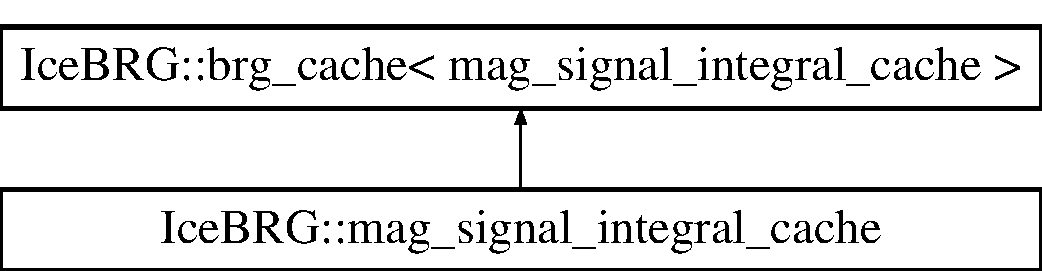
\includegraphics[height=2.000000cm]{classIceBRG_1_1mag__signal__integral__cache}
\end{center}
\end{figure}
\subsection*{Public Member Functions}
\begin{DoxyCompactItemize}
\item 
\hyperlink{classIceBRG_1_1mag__signal__integral__cache_afa83d06fc1f822daa7090672932a2628}{mag\-\_\-signal\-\_\-integral\-\_\-cache} ()
\item 
\hyperlink{classIceBRG_1_1mag__signal__integral__cache_a7b9e8bef6cf4be45d2433d1d67456935}{$\sim$mag\-\_\-signal\-\_\-integral\-\_\-cache} ()
\end{DoxyCompactItemize}
\subsection*{Protected Member Functions}
\begin{DoxyCompactItemize}
\item 
std\-::string \hyperlink{classIceBRG_1_1mag__signal__integral__cache_a0fba2d585686eeb7df8ad63a12467286}{\-\_\-name\-\_\-base} () const 
\item 
\hyperlink{lib_2IceBRG__main_2common_8h_ad0f130a56eeb944d9ef2692ee881ecc4}{flt\-\_\-type} \hyperlink{classIceBRG_1_1mag__signal__integral__cache_a580ab95b1c68dab69c368bf5bda1f741}{\-\_\-calculate} (const \hyperlink{lib_2IceBRG__main_2common_8h_ad0f130a56eeb944d9ef2692ee881ecc4}{flt\-\_\-type} \&in\-\_\-param\-\_\-1) const 
\item 
void \hyperlink{classIceBRG_1_1mag__signal__integral__cache_a9f027f5fd56a5997d374586c0a035b4c}{\-\_\-load\-\_\-cache\-\_\-dependencies} () const 
\end{DoxyCompactItemize}
\subsection*{Friends}
\begin{DoxyCompactItemize}
\item 
class \hyperlink{classIceBRG_1_1mag__signal__integral__cache_aba2eb4394fb3d06400d88a6b3af988cb}{brg\-\_\-cache$<$ mag\-\_\-signal\-\_\-integral\-\_\-cache $>$}
\end{DoxyCompactItemize}


\subsection{Constructor \& Destructor Documentation}
\hypertarget{classIceBRG_1_1mag__signal__integral__cache_afa83d06fc1f822daa7090672932a2628}{\index{Ice\-B\-R\-G\-::mag\-\_\-signal\-\_\-integral\-\_\-cache@{Ice\-B\-R\-G\-::mag\-\_\-signal\-\_\-integral\-\_\-cache}!mag\-\_\-signal\-\_\-integral\-\_\-cache@{mag\-\_\-signal\-\_\-integral\-\_\-cache}}
\index{mag\-\_\-signal\-\_\-integral\-\_\-cache@{mag\-\_\-signal\-\_\-integral\-\_\-cache}!IceBRG::mag_signal_integral_cache@{Ice\-B\-R\-G\-::mag\-\_\-signal\-\_\-integral\-\_\-cache}}
\subsubsection[{mag\-\_\-signal\-\_\-integral\-\_\-cache}]{\setlength{\rightskip}{0pt plus 5cm}Ice\-B\-R\-G\-::mag\-\_\-signal\-\_\-integral\-\_\-cache\-::mag\-\_\-signal\-\_\-integral\-\_\-cache (
\begin{DoxyParamCaption}
{}
\end{DoxyParamCaption}
)\hspace{0.3cm}{\ttfamily [inline]}}}\label{classIceBRG_1_1mag__signal__integral__cache_afa83d06fc1f822daa7090672932a2628}
\hypertarget{classIceBRG_1_1mag__signal__integral__cache_a7b9e8bef6cf4be45d2433d1d67456935}{\index{Ice\-B\-R\-G\-::mag\-\_\-signal\-\_\-integral\-\_\-cache@{Ice\-B\-R\-G\-::mag\-\_\-signal\-\_\-integral\-\_\-cache}!$\sim$mag\-\_\-signal\-\_\-integral\-\_\-cache@{$\sim$mag\-\_\-signal\-\_\-integral\-\_\-cache}}
\index{$\sim$mag\-\_\-signal\-\_\-integral\-\_\-cache@{$\sim$mag\-\_\-signal\-\_\-integral\-\_\-cache}!IceBRG::mag_signal_integral_cache@{Ice\-B\-R\-G\-::mag\-\_\-signal\-\_\-integral\-\_\-cache}}
\subsubsection[{$\sim$mag\-\_\-signal\-\_\-integral\-\_\-cache}]{\setlength{\rightskip}{0pt plus 5cm}Ice\-B\-R\-G\-::mag\-\_\-signal\-\_\-integral\-\_\-cache\-::$\sim$mag\-\_\-signal\-\_\-integral\-\_\-cache (
\begin{DoxyParamCaption}
{}
\end{DoxyParamCaption}
)\hspace{0.3cm}{\ttfamily [inline]}}}\label{classIceBRG_1_1mag__signal__integral__cache_a7b9e8bef6cf4be45d2433d1d67456935}


\subsection{Member Function Documentation}
\hypertarget{classIceBRG_1_1mag__signal__integral__cache_a580ab95b1c68dab69c368bf5bda1f741}{\index{Ice\-B\-R\-G\-::mag\-\_\-signal\-\_\-integral\-\_\-cache@{Ice\-B\-R\-G\-::mag\-\_\-signal\-\_\-integral\-\_\-cache}!\-\_\-calculate@{\-\_\-calculate}}
\index{\-\_\-calculate@{\-\_\-calculate}!IceBRG::mag_signal_integral_cache@{Ice\-B\-R\-G\-::mag\-\_\-signal\-\_\-integral\-\_\-cache}}
\subsubsection[{\-\_\-calculate}]{\setlength{\rightskip}{0pt plus 5cm}{\bf flt\-\_\-type} Ice\-B\-R\-G\-::mag\-\_\-signal\-\_\-integral\-\_\-cache\-::\-\_\-calculate (
\begin{DoxyParamCaption}
\item[{const {\bf flt\-\_\-type} \&}]{in\-\_\-param\-\_\-1}
\end{DoxyParamCaption}
) const\hspace{0.3cm}{\ttfamily [protected]}}}\label{classIceBRG_1_1mag__signal__integral__cache_a580ab95b1c68dab69c368bf5bda1f741}


Reimplemented from \hyperlink{classIceBRG_1_1brg__cache_afde9cc8f297a354727a4df9c16ab7a12}{Ice\-B\-R\-G\-::brg\-\_\-cache$<$ mag\-\_\-signal\-\_\-integral\-\_\-cache $>$}.

\hypertarget{classIceBRG_1_1mag__signal__integral__cache_a9f027f5fd56a5997d374586c0a035b4c}{\index{Ice\-B\-R\-G\-::mag\-\_\-signal\-\_\-integral\-\_\-cache@{Ice\-B\-R\-G\-::mag\-\_\-signal\-\_\-integral\-\_\-cache}!\-\_\-load\-\_\-cache\-\_\-dependencies@{\-\_\-load\-\_\-cache\-\_\-dependencies}}
\index{\-\_\-load\-\_\-cache\-\_\-dependencies@{\-\_\-load\-\_\-cache\-\_\-dependencies}!IceBRG::mag_signal_integral_cache@{Ice\-B\-R\-G\-::mag\-\_\-signal\-\_\-integral\-\_\-cache}}
\subsubsection[{\-\_\-load\-\_\-cache\-\_\-dependencies}]{\setlength{\rightskip}{0pt plus 5cm}void Ice\-B\-R\-G\-::mag\-\_\-signal\-\_\-integral\-\_\-cache\-::\-\_\-load\-\_\-cache\-\_\-dependencies (
\begin{DoxyParamCaption}
{}
\end{DoxyParamCaption}
) const\hspace{0.3cm}{\ttfamily [protected]}}}\label{classIceBRG_1_1mag__signal__integral__cache_a9f027f5fd56a5997d374586c0a035b4c}


Reimplemented from \hyperlink{classIceBRG_1_1brg__cache_a020dbbd2a1b93b103e15043f6424242b}{Ice\-B\-R\-G\-::brg\-\_\-cache$<$ mag\-\_\-signal\-\_\-integral\-\_\-cache $>$}.

\hypertarget{classIceBRG_1_1mag__signal__integral__cache_a0fba2d585686eeb7df8ad63a12467286}{\index{Ice\-B\-R\-G\-::mag\-\_\-signal\-\_\-integral\-\_\-cache@{Ice\-B\-R\-G\-::mag\-\_\-signal\-\_\-integral\-\_\-cache}!\-\_\-name\-\_\-base@{\-\_\-name\-\_\-base}}
\index{\-\_\-name\-\_\-base@{\-\_\-name\-\_\-base}!IceBRG::mag_signal_integral_cache@{Ice\-B\-R\-G\-::mag\-\_\-signal\-\_\-integral\-\_\-cache}}
\subsubsection[{\-\_\-name\-\_\-base}]{\setlength{\rightskip}{0pt plus 5cm}std\-::string Ice\-B\-R\-G\-::mag\-\_\-signal\-\_\-integral\-\_\-cache\-::\-\_\-name\-\_\-base (
\begin{DoxyParamCaption}
{}
\end{DoxyParamCaption}
) const\hspace{0.3cm}{\ttfamily [inline]}, {\ttfamily [protected]}}}\label{classIceBRG_1_1mag__signal__integral__cache_a0fba2d585686eeb7df8ad63a12467286}


Reimplemented from \hyperlink{classIceBRG_1_1brg__cache_a4453ff8ebded318cabaa332e9533ec40}{Ice\-B\-R\-G\-::brg\-\_\-cache$<$ mag\-\_\-signal\-\_\-integral\-\_\-cache $>$}.



\subsection{Friends And Related Function Documentation}
\hypertarget{classIceBRG_1_1mag__signal__integral__cache_aba2eb4394fb3d06400d88a6b3af988cb}{\index{Ice\-B\-R\-G\-::mag\-\_\-signal\-\_\-integral\-\_\-cache@{Ice\-B\-R\-G\-::mag\-\_\-signal\-\_\-integral\-\_\-cache}!brg\-\_\-cache$<$ mag\-\_\-signal\-\_\-integral\-\_\-cache $>$@{brg\-\_\-cache$<$ mag\-\_\-signal\-\_\-integral\-\_\-cache $>$}}
\index{brg\-\_\-cache$<$ mag\-\_\-signal\-\_\-integral\-\_\-cache $>$@{brg\-\_\-cache$<$ mag\-\_\-signal\-\_\-integral\-\_\-cache $>$}!IceBRG::mag_signal_integral_cache@{Ice\-B\-R\-G\-::mag\-\_\-signal\-\_\-integral\-\_\-cache}}
\subsubsection[{brg\-\_\-cache$<$ mag\-\_\-signal\-\_\-integral\-\_\-cache $>$}]{\setlength{\rightskip}{0pt plus 5cm}friend class {\bf brg\-\_\-cache}$<$ {\bf mag\-\_\-signal\-\_\-integral\-\_\-cache} $>$\hspace{0.3cm}{\ttfamily [friend]}}}\label{classIceBRG_1_1mag__signal__integral__cache_aba2eb4394fb3d06400d88a6b3af988cb}


The documentation for this class was generated from the following files\-:\begin{DoxyCompactItemize}
\item 
/disk2/brg/git/\-Magnification\-\_\-\-Public/src/lib/\-Ice\-B\-R\-G\-\_\-lensing/magnification/\hyperlink{mag__signal__integral__cache_8h}{mag\-\_\-signal\-\_\-integral\-\_\-cache.\-h}\item 
/disk2/brg/git/\-Magnification\-\_\-\-Public/src/lib/\-Ice\-B\-R\-G\-\_\-lensing/magnification/\hyperlink{mag__signal__integral__cache_8cpp}{mag\-\_\-signal\-\_\-integral\-\_\-cache.\-cpp}\end{DoxyCompactItemize}

\hypertarget{classIceBRG_1_1mag__weight__integral__cache}{\section{Ice\-B\-R\-G\-:\-:mag\-\_\-weight\-\_\-integral\-\_\-cache Class Reference}
\label{classIceBRG_1_1mag__weight__integral__cache}\index{Ice\-B\-R\-G\-::mag\-\_\-weight\-\_\-integral\-\_\-cache@{Ice\-B\-R\-G\-::mag\-\_\-weight\-\_\-integral\-\_\-cache}}
}


{\ttfamily \#include $<$mag\-\_\-weight\-\_\-integral\-\_\-cache.\-h$>$}

Inheritance diagram for Ice\-B\-R\-G\-:\-:mag\-\_\-weight\-\_\-integral\-\_\-cache\-:\begin{figure}[H]
\begin{center}
\leavevmode
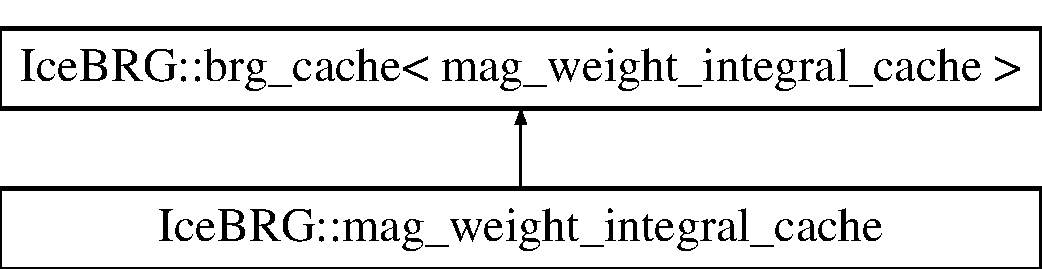
\includegraphics[height=2.000000cm]{classIceBRG_1_1mag__weight__integral__cache}
\end{center}
\end{figure}
\subsection*{Public Member Functions}
\begin{DoxyCompactItemize}
\item 
\hyperlink{classIceBRG_1_1mag__weight__integral__cache_ab891c0d594154de0145e41bc2c1b98f4}{mag\-\_\-weight\-\_\-integral\-\_\-cache} ()
\item 
\hyperlink{classIceBRG_1_1mag__weight__integral__cache_a743fcaa1cdbde9d28d19e0d916e49c8d}{$\sim$mag\-\_\-weight\-\_\-integral\-\_\-cache} ()
\end{DoxyCompactItemize}
\subsection*{Protected Member Functions}
\begin{DoxyCompactItemize}
\item 
std\-::string \hyperlink{classIceBRG_1_1mag__weight__integral__cache_aeab1aa78cf663d1e255fffb2746f1e79}{\-\_\-name\-\_\-base} () const 
\item 
\hyperlink{lib_2IceBRG__main_2common_8h_ad0f130a56eeb944d9ef2692ee881ecc4}{flt\-\_\-type} \hyperlink{classIceBRG_1_1mag__weight__integral__cache_a27435d81e53ee8cba625e76986e4da7b}{\-\_\-calculate} (const \hyperlink{lib_2IceBRG__main_2common_8h_ad0f130a56eeb944d9ef2692ee881ecc4}{flt\-\_\-type} \&in\-\_\-param\-\_\-1) const 
\item 
void \hyperlink{classIceBRG_1_1mag__weight__integral__cache_a77b23616c7c1942f45998e4b016ef1f7}{\-\_\-load\-\_\-cache\-\_\-dependencies} () const 
\end{DoxyCompactItemize}
\subsection*{Friends}
\begin{DoxyCompactItemize}
\item 
class \hyperlink{classIceBRG_1_1mag__weight__integral__cache_a3754c6d00fa4752a7fbe65db039c270b}{brg\-\_\-cache$<$ mag\-\_\-weight\-\_\-integral\-\_\-cache $>$}
\end{DoxyCompactItemize}


\subsection{Constructor \& Destructor Documentation}
\hypertarget{classIceBRG_1_1mag__weight__integral__cache_ab891c0d594154de0145e41bc2c1b98f4}{\index{Ice\-B\-R\-G\-::mag\-\_\-weight\-\_\-integral\-\_\-cache@{Ice\-B\-R\-G\-::mag\-\_\-weight\-\_\-integral\-\_\-cache}!mag\-\_\-weight\-\_\-integral\-\_\-cache@{mag\-\_\-weight\-\_\-integral\-\_\-cache}}
\index{mag\-\_\-weight\-\_\-integral\-\_\-cache@{mag\-\_\-weight\-\_\-integral\-\_\-cache}!IceBRG::mag_weight_integral_cache@{Ice\-B\-R\-G\-::mag\-\_\-weight\-\_\-integral\-\_\-cache}}
\subsubsection[{mag\-\_\-weight\-\_\-integral\-\_\-cache}]{\setlength{\rightskip}{0pt plus 5cm}Ice\-B\-R\-G\-::mag\-\_\-weight\-\_\-integral\-\_\-cache\-::mag\-\_\-weight\-\_\-integral\-\_\-cache (
\begin{DoxyParamCaption}
{}
\end{DoxyParamCaption}
)\hspace{0.3cm}{\ttfamily [inline]}}}\label{classIceBRG_1_1mag__weight__integral__cache_ab891c0d594154de0145e41bc2c1b98f4}
\hypertarget{classIceBRG_1_1mag__weight__integral__cache_a743fcaa1cdbde9d28d19e0d916e49c8d}{\index{Ice\-B\-R\-G\-::mag\-\_\-weight\-\_\-integral\-\_\-cache@{Ice\-B\-R\-G\-::mag\-\_\-weight\-\_\-integral\-\_\-cache}!$\sim$mag\-\_\-weight\-\_\-integral\-\_\-cache@{$\sim$mag\-\_\-weight\-\_\-integral\-\_\-cache}}
\index{$\sim$mag\-\_\-weight\-\_\-integral\-\_\-cache@{$\sim$mag\-\_\-weight\-\_\-integral\-\_\-cache}!IceBRG::mag_weight_integral_cache@{Ice\-B\-R\-G\-::mag\-\_\-weight\-\_\-integral\-\_\-cache}}
\subsubsection[{$\sim$mag\-\_\-weight\-\_\-integral\-\_\-cache}]{\setlength{\rightskip}{0pt plus 5cm}Ice\-B\-R\-G\-::mag\-\_\-weight\-\_\-integral\-\_\-cache\-::$\sim$mag\-\_\-weight\-\_\-integral\-\_\-cache (
\begin{DoxyParamCaption}
{}
\end{DoxyParamCaption}
)\hspace{0.3cm}{\ttfamily [inline]}}}\label{classIceBRG_1_1mag__weight__integral__cache_a743fcaa1cdbde9d28d19e0d916e49c8d}


\subsection{Member Function Documentation}
\hypertarget{classIceBRG_1_1mag__weight__integral__cache_a27435d81e53ee8cba625e76986e4da7b}{\index{Ice\-B\-R\-G\-::mag\-\_\-weight\-\_\-integral\-\_\-cache@{Ice\-B\-R\-G\-::mag\-\_\-weight\-\_\-integral\-\_\-cache}!\-\_\-calculate@{\-\_\-calculate}}
\index{\-\_\-calculate@{\-\_\-calculate}!IceBRG::mag_weight_integral_cache@{Ice\-B\-R\-G\-::mag\-\_\-weight\-\_\-integral\-\_\-cache}}
\subsubsection[{\-\_\-calculate}]{\setlength{\rightskip}{0pt plus 5cm}{\bf flt\-\_\-type} Ice\-B\-R\-G\-::mag\-\_\-weight\-\_\-integral\-\_\-cache\-::\-\_\-calculate (
\begin{DoxyParamCaption}
\item[{const {\bf flt\-\_\-type} \&}]{in\-\_\-param\-\_\-1}
\end{DoxyParamCaption}
) const\hspace{0.3cm}{\ttfamily [protected]}}}\label{classIceBRG_1_1mag__weight__integral__cache_a27435d81e53ee8cba625e76986e4da7b}


Reimplemented from \hyperlink{classIceBRG_1_1brg__cache_afde9cc8f297a354727a4df9c16ab7a12}{Ice\-B\-R\-G\-::brg\-\_\-cache$<$ mag\-\_\-weight\-\_\-integral\-\_\-cache $>$}.

\hypertarget{classIceBRG_1_1mag__weight__integral__cache_a77b23616c7c1942f45998e4b016ef1f7}{\index{Ice\-B\-R\-G\-::mag\-\_\-weight\-\_\-integral\-\_\-cache@{Ice\-B\-R\-G\-::mag\-\_\-weight\-\_\-integral\-\_\-cache}!\-\_\-load\-\_\-cache\-\_\-dependencies@{\-\_\-load\-\_\-cache\-\_\-dependencies}}
\index{\-\_\-load\-\_\-cache\-\_\-dependencies@{\-\_\-load\-\_\-cache\-\_\-dependencies}!IceBRG::mag_weight_integral_cache@{Ice\-B\-R\-G\-::mag\-\_\-weight\-\_\-integral\-\_\-cache}}
\subsubsection[{\-\_\-load\-\_\-cache\-\_\-dependencies}]{\setlength{\rightskip}{0pt plus 5cm}void Ice\-B\-R\-G\-::mag\-\_\-weight\-\_\-integral\-\_\-cache\-::\-\_\-load\-\_\-cache\-\_\-dependencies (
\begin{DoxyParamCaption}
{}
\end{DoxyParamCaption}
) const\hspace{0.3cm}{\ttfamily [protected]}}}\label{classIceBRG_1_1mag__weight__integral__cache_a77b23616c7c1942f45998e4b016ef1f7}


Reimplemented from \hyperlink{classIceBRG_1_1brg__cache_a020dbbd2a1b93b103e15043f6424242b}{Ice\-B\-R\-G\-::brg\-\_\-cache$<$ mag\-\_\-weight\-\_\-integral\-\_\-cache $>$}.

\hypertarget{classIceBRG_1_1mag__weight__integral__cache_aeab1aa78cf663d1e255fffb2746f1e79}{\index{Ice\-B\-R\-G\-::mag\-\_\-weight\-\_\-integral\-\_\-cache@{Ice\-B\-R\-G\-::mag\-\_\-weight\-\_\-integral\-\_\-cache}!\-\_\-name\-\_\-base@{\-\_\-name\-\_\-base}}
\index{\-\_\-name\-\_\-base@{\-\_\-name\-\_\-base}!IceBRG::mag_weight_integral_cache@{Ice\-B\-R\-G\-::mag\-\_\-weight\-\_\-integral\-\_\-cache}}
\subsubsection[{\-\_\-name\-\_\-base}]{\setlength{\rightskip}{0pt plus 5cm}std\-::string Ice\-B\-R\-G\-::mag\-\_\-weight\-\_\-integral\-\_\-cache\-::\-\_\-name\-\_\-base (
\begin{DoxyParamCaption}
{}
\end{DoxyParamCaption}
) const\hspace{0.3cm}{\ttfamily [inline]}, {\ttfamily [protected]}}}\label{classIceBRG_1_1mag__weight__integral__cache_aeab1aa78cf663d1e255fffb2746f1e79}


Reimplemented from \hyperlink{classIceBRG_1_1brg__cache_a4453ff8ebded318cabaa332e9533ec40}{Ice\-B\-R\-G\-::brg\-\_\-cache$<$ mag\-\_\-weight\-\_\-integral\-\_\-cache $>$}.



\subsection{Friends And Related Function Documentation}
\hypertarget{classIceBRG_1_1mag__weight__integral__cache_a3754c6d00fa4752a7fbe65db039c270b}{\index{Ice\-B\-R\-G\-::mag\-\_\-weight\-\_\-integral\-\_\-cache@{Ice\-B\-R\-G\-::mag\-\_\-weight\-\_\-integral\-\_\-cache}!brg\-\_\-cache$<$ mag\-\_\-weight\-\_\-integral\-\_\-cache $>$@{brg\-\_\-cache$<$ mag\-\_\-weight\-\_\-integral\-\_\-cache $>$}}
\index{brg\-\_\-cache$<$ mag\-\_\-weight\-\_\-integral\-\_\-cache $>$@{brg\-\_\-cache$<$ mag\-\_\-weight\-\_\-integral\-\_\-cache $>$}!IceBRG::mag_weight_integral_cache@{Ice\-B\-R\-G\-::mag\-\_\-weight\-\_\-integral\-\_\-cache}}
\subsubsection[{brg\-\_\-cache$<$ mag\-\_\-weight\-\_\-integral\-\_\-cache $>$}]{\setlength{\rightskip}{0pt plus 5cm}friend class {\bf brg\-\_\-cache}$<$ {\bf mag\-\_\-weight\-\_\-integral\-\_\-cache} $>$\hspace{0.3cm}{\ttfamily [friend]}}}\label{classIceBRG_1_1mag__weight__integral__cache_a3754c6d00fa4752a7fbe65db039c270b}


The documentation for this class was generated from the following files\-:\begin{DoxyCompactItemize}
\item 
/disk2/brg/git/\-Magnification\-\_\-\-Public/src/lib/\-Ice\-B\-R\-G\-\_\-lensing/magnification/\hyperlink{mag__weight__integral__cache_8h}{mag\-\_\-weight\-\_\-integral\-\_\-cache.\-h}\item 
/disk2/brg/git/\-Magnification\-\_\-\-Public/src/lib/\-Ice\-B\-R\-G\-\_\-lensing/magnification/\hyperlink{mag__weight__integral__cache_8cpp}{mag\-\_\-weight\-\_\-integral\-\_\-cache.\-cpp}\end{DoxyCompactItemize}

\hypertarget{classIceBRG_1_1Fourier_1_1managed__fftw__plan}{}\section{Ice\+B\+R\+G\+:\+:Fourier\+:\+:managed\+\_\+fftw\+\_\+plan Class Reference}
\label{classIceBRG_1_1Fourier_1_1managed__fftw__plan}\index{Ice\+B\+R\+G\+::\+Fourier\+::managed\+\_\+fftw\+\_\+plan@{Ice\+B\+R\+G\+::\+Fourier\+::managed\+\_\+fftw\+\_\+plan}}


{\ttfamily \#include $<$management.\+hpp$>$}

\subsection*{Public Member Functions}
\begin{DoxyCompactItemize}
\item 
\hyperlink{classIceBRG_1_1Fourier_1_1managed__fftw__plan_aa74e4d70d701caf7e91df9f4fcc66d2f}{managed\+\_\+fftw\+\_\+plan} ()
\item 
\hyperlink{classIceBRG_1_1Fourier_1_1managed__fftw__plan_a7547232594624c7ae2fd34b6b7678ac3}{managed\+\_\+fftw\+\_\+plan} (\hyperlink{classIceBRG_1_1Fourier_1_1managed__fftw__plan}{managed\+\_\+fftw\+\_\+plan} \&\&other)
\item 
\hyperlink{classIceBRG_1_1Fourier_1_1managed__fftw__plan_a983042eea7e191220f0cb6698e0352b4}{managed\+\_\+fftw\+\_\+plan} (const \hyperlink{classIceBRG_1_1Fourier_1_1managed__fftw__plan}{managed\+\_\+fftw\+\_\+plan} \&other)=delete
\item 
\hyperlink{classIceBRG_1_1Fourier_1_1managed__fftw__plan_aafab54381a7b5a4c70ef5dda0db36333}{managed\+\_\+fftw\+\_\+plan} (fftw\+\_\+plan \&\&p)
\item 
\hyperlink{classIceBRG_1_1Fourier_1_1managed__fftw__plan_a53efa350723d5c18331591b260518466}{managed\+\_\+fftw\+\_\+plan} (const fftw\+\_\+plan \&p)
\item 
\hyperlink{classIceBRG_1_1Fourier_1_1managed__fftw__plan_afa8a38eb58a89782b2f376778dc87648}{$\sim$managed\+\_\+fftw\+\_\+plan} ()
\item 
void \hyperlink{classIceBRG_1_1Fourier_1_1managed__fftw__plan_ada8a304473896d3b8a95b70f44ad529b}{destroy} ()
\item 
\hyperlink{classIceBRG_1_1Fourier_1_1managed__fftw__plan}{managed\+\_\+fftw\+\_\+plan} \& \hyperlink{classIceBRG_1_1Fourier_1_1managed__fftw__plan_a4fa6e150aedbfb5d1e008ca6fc179e0b}{operator=} (const \hyperlink{classIceBRG_1_1Fourier_1_1managed__fftw__plan}{managed\+\_\+fftw\+\_\+plan} \&)=delete
\item 
\hyperlink{classIceBRG_1_1Fourier_1_1managed__fftw__plan}{managed\+\_\+fftw\+\_\+plan} \& \hyperlink{classIceBRG_1_1Fourier_1_1managed__fftw__plan_aa93333000802c75497044f0bf6d1a92b}{operator=} (\hyperlink{classIceBRG_1_1Fourier_1_1managed__fftw__plan}{managed\+\_\+fftw\+\_\+plan} \&\&other)
\item 
void \hyperlink{classIceBRG_1_1Fourier_1_1managed__fftw__plan_a993448b0fc42004f752d7a449d759ca6}{execute} ()
\item 
fftw\+\_\+plan \& \hyperlink{classIceBRG_1_1Fourier_1_1managed__fftw__plan_aff6715dac2bada6752561065363c150e}{get\+\_\+plan} () noexcept
\item 
\hyperlink{classIceBRG_1_1Fourier_1_1managed__fftw__plan_ad3b8a8e128f89cc1ad41543056f7cce3}{operator fftw\+\_\+plan \&} () noexcept
\end{DoxyCompactItemize}


\subsection{Detailed Description}
A class which manages an fftw\+\_\+plan, making sure it is properly deleted when this object goes out of scope. This class is movable but not copyable. 

\subsection{Constructor \& Destructor Documentation}
\hypertarget{classIceBRG_1_1Fourier_1_1managed__fftw__plan_aa74e4d70d701caf7e91df9f4fcc66d2f}{}\index{Ice\+B\+R\+G\+::\+Fourier\+::managed\+\_\+fftw\+\_\+plan@{Ice\+B\+R\+G\+::\+Fourier\+::managed\+\_\+fftw\+\_\+plan}!managed\+\_\+fftw\+\_\+plan@{managed\+\_\+fftw\+\_\+plan}}
\index{managed\+\_\+fftw\+\_\+plan@{managed\+\_\+fftw\+\_\+plan}!Ice\+B\+R\+G\+::\+Fourier\+::managed\+\_\+fftw\+\_\+plan@{Ice\+B\+R\+G\+::\+Fourier\+::managed\+\_\+fftw\+\_\+plan}}
\subsubsection[{managed\+\_\+fftw\+\_\+plan()}]{\setlength{\rightskip}{0pt plus 5cm}Ice\+B\+R\+G\+::\+Fourier\+::managed\+\_\+fftw\+\_\+plan\+::managed\+\_\+fftw\+\_\+plan (
\begin{DoxyParamCaption}
{}
\end{DoxyParamCaption}
)\hspace{0.3cm}{\ttfamily [inline]}}\label{classIceBRG_1_1Fourier_1_1managed__fftw__plan_aa74e4d70d701caf7e91df9f4fcc66d2f}
\hypertarget{classIceBRG_1_1Fourier_1_1managed__fftw__plan_a7547232594624c7ae2fd34b6b7678ac3}{}\index{Ice\+B\+R\+G\+::\+Fourier\+::managed\+\_\+fftw\+\_\+plan@{Ice\+B\+R\+G\+::\+Fourier\+::managed\+\_\+fftw\+\_\+plan}!managed\+\_\+fftw\+\_\+plan@{managed\+\_\+fftw\+\_\+plan}}
\index{managed\+\_\+fftw\+\_\+plan@{managed\+\_\+fftw\+\_\+plan}!Ice\+B\+R\+G\+::\+Fourier\+::managed\+\_\+fftw\+\_\+plan@{Ice\+B\+R\+G\+::\+Fourier\+::managed\+\_\+fftw\+\_\+plan}}
\subsubsection[{managed\+\_\+fftw\+\_\+plan(managed\+\_\+fftw\+\_\+plan \&\&other)}]{\setlength{\rightskip}{0pt plus 5cm}Ice\+B\+R\+G\+::\+Fourier\+::managed\+\_\+fftw\+\_\+plan\+::managed\+\_\+fftw\+\_\+plan (
\begin{DoxyParamCaption}
\item[{{\bf managed\+\_\+fftw\+\_\+plan} \&\&}]{other}
\end{DoxyParamCaption}
)\hspace{0.3cm}{\ttfamily [inline]}}\label{classIceBRG_1_1Fourier_1_1managed__fftw__plan_a7547232594624c7ae2fd34b6b7678ac3}
\hypertarget{classIceBRG_1_1Fourier_1_1managed__fftw__plan_a983042eea7e191220f0cb6698e0352b4}{}\index{Ice\+B\+R\+G\+::\+Fourier\+::managed\+\_\+fftw\+\_\+plan@{Ice\+B\+R\+G\+::\+Fourier\+::managed\+\_\+fftw\+\_\+plan}!managed\+\_\+fftw\+\_\+plan@{managed\+\_\+fftw\+\_\+plan}}
\index{managed\+\_\+fftw\+\_\+plan@{managed\+\_\+fftw\+\_\+plan}!Ice\+B\+R\+G\+::\+Fourier\+::managed\+\_\+fftw\+\_\+plan@{Ice\+B\+R\+G\+::\+Fourier\+::managed\+\_\+fftw\+\_\+plan}}
\subsubsection[{managed\+\_\+fftw\+\_\+plan(const managed\+\_\+fftw\+\_\+plan \&other)=delete}]{\setlength{\rightskip}{0pt plus 5cm}Ice\+B\+R\+G\+::\+Fourier\+::managed\+\_\+fftw\+\_\+plan\+::managed\+\_\+fftw\+\_\+plan (
\begin{DoxyParamCaption}
\item[{const {\bf managed\+\_\+fftw\+\_\+plan} \&}]{other}
\end{DoxyParamCaption}
)\hspace{0.3cm}{\ttfamily [delete]}}\label{classIceBRG_1_1Fourier_1_1managed__fftw__plan_a983042eea7e191220f0cb6698e0352b4}
\hypertarget{classIceBRG_1_1Fourier_1_1managed__fftw__plan_aafab54381a7b5a4c70ef5dda0db36333}{}\index{Ice\+B\+R\+G\+::\+Fourier\+::managed\+\_\+fftw\+\_\+plan@{Ice\+B\+R\+G\+::\+Fourier\+::managed\+\_\+fftw\+\_\+plan}!managed\+\_\+fftw\+\_\+plan@{managed\+\_\+fftw\+\_\+plan}}
\index{managed\+\_\+fftw\+\_\+plan@{managed\+\_\+fftw\+\_\+plan}!Ice\+B\+R\+G\+::\+Fourier\+::managed\+\_\+fftw\+\_\+plan@{Ice\+B\+R\+G\+::\+Fourier\+::managed\+\_\+fftw\+\_\+plan}}
\subsubsection[{managed\+\_\+fftw\+\_\+plan(fftw\+\_\+plan \&\&p)}]{\setlength{\rightskip}{0pt plus 5cm}Ice\+B\+R\+G\+::\+Fourier\+::managed\+\_\+fftw\+\_\+plan\+::managed\+\_\+fftw\+\_\+plan (
\begin{DoxyParamCaption}
\item[{fftw\+\_\+plan \&\&}]{p}
\end{DoxyParamCaption}
)\hspace{0.3cm}{\ttfamily [inline]}}\label{classIceBRG_1_1Fourier_1_1managed__fftw__plan_aafab54381a7b5a4c70ef5dda0db36333}
\hypertarget{classIceBRG_1_1Fourier_1_1managed__fftw__plan_a53efa350723d5c18331591b260518466}{}\index{Ice\+B\+R\+G\+::\+Fourier\+::managed\+\_\+fftw\+\_\+plan@{Ice\+B\+R\+G\+::\+Fourier\+::managed\+\_\+fftw\+\_\+plan}!managed\+\_\+fftw\+\_\+plan@{managed\+\_\+fftw\+\_\+plan}}
\index{managed\+\_\+fftw\+\_\+plan@{managed\+\_\+fftw\+\_\+plan}!Ice\+B\+R\+G\+::\+Fourier\+::managed\+\_\+fftw\+\_\+plan@{Ice\+B\+R\+G\+::\+Fourier\+::managed\+\_\+fftw\+\_\+plan}}
\subsubsection[{managed\+\_\+fftw\+\_\+plan(const fftw\+\_\+plan \&p)}]{\setlength{\rightskip}{0pt plus 5cm}Ice\+B\+R\+G\+::\+Fourier\+::managed\+\_\+fftw\+\_\+plan\+::managed\+\_\+fftw\+\_\+plan (
\begin{DoxyParamCaption}
\item[{const fftw\+\_\+plan \&}]{p}
\end{DoxyParamCaption}
)\hspace{0.3cm}{\ttfamily [inline]}}\label{classIceBRG_1_1Fourier_1_1managed__fftw__plan_a53efa350723d5c18331591b260518466}
\hypertarget{classIceBRG_1_1Fourier_1_1managed__fftw__plan_afa8a38eb58a89782b2f376778dc87648}{}\index{Ice\+B\+R\+G\+::\+Fourier\+::managed\+\_\+fftw\+\_\+plan@{Ice\+B\+R\+G\+::\+Fourier\+::managed\+\_\+fftw\+\_\+plan}!````~managed\+\_\+fftw\+\_\+plan@{$\sim$managed\+\_\+fftw\+\_\+plan}}
\index{````~managed\+\_\+fftw\+\_\+plan@{$\sim$managed\+\_\+fftw\+\_\+plan}!Ice\+B\+R\+G\+::\+Fourier\+::managed\+\_\+fftw\+\_\+plan@{Ice\+B\+R\+G\+::\+Fourier\+::managed\+\_\+fftw\+\_\+plan}}
\subsubsection[{$\sim$managed\+\_\+fftw\+\_\+plan()}]{\setlength{\rightskip}{0pt plus 5cm}Ice\+B\+R\+G\+::\+Fourier\+::managed\+\_\+fftw\+\_\+plan\+::$\sim$managed\+\_\+fftw\+\_\+plan (
\begin{DoxyParamCaption}
{}
\end{DoxyParamCaption}
)\hspace{0.3cm}{\ttfamily [inline]}}\label{classIceBRG_1_1Fourier_1_1managed__fftw__plan_afa8a38eb58a89782b2f376778dc87648}


\subsection{Member Function Documentation}
\hypertarget{classIceBRG_1_1Fourier_1_1managed__fftw__plan_ada8a304473896d3b8a95b70f44ad529b}{}\index{Ice\+B\+R\+G\+::\+Fourier\+::managed\+\_\+fftw\+\_\+plan@{Ice\+B\+R\+G\+::\+Fourier\+::managed\+\_\+fftw\+\_\+plan}!destroy@{destroy}}
\index{destroy@{destroy}!Ice\+B\+R\+G\+::\+Fourier\+::managed\+\_\+fftw\+\_\+plan@{Ice\+B\+R\+G\+::\+Fourier\+::managed\+\_\+fftw\+\_\+plan}}
\subsubsection[{destroy()}]{\setlength{\rightskip}{0pt plus 5cm}void Ice\+B\+R\+G\+::\+Fourier\+::managed\+\_\+fftw\+\_\+plan\+::destroy (
\begin{DoxyParamCaption}
{}
\end{DoxyParamCaption}
)\hspace{0.3cm}{\ttfamily [inline]}}\label{classIceBRG_1_1Fourier_1_1managed__fftw__plan_ada8a304473896d3b8a95b70f44ad529b}
\hypertarget{classIceBRG_1_1Fourier_1_1managed__fftw__plan_a993448b0fc42004f752d7a449d759ca6}{}\index{Ice\+B\+R\+G\+::\+Fourier\+::managed\+\_\+fftw\+\_\+plan@{Ice\+B\+R\+G\+::\+Fourier\+::managed\+\_\+fftw\+\_\+plan}!execute@{execute}}
\index{execute@{execute}!Ice\+B\+R\+G\+::\+Fourier\+::managed\+\_\+fftw\+\_\+plan@{Ice\+B\+R\+G\+::\+Fourier\+::managed\+\_\+fftw\+\_\+plan}}
\subsubsection[{execute()}]{\setlength{\rightskip}{0pt plus 5cm}void Ice\+B\+R\+G\+::\+Fourier\+::managed\+\_\+fftw\+\_\+plan\+::execute (
\begin{DoxyParamCaption}
{}
\end{DoxyParamCaption}
)\hspace{0.3cm}{\ttfamily [inline]}}\label{classIceBRG_1_1Fourier_1_1managed__fftw__plan_a993448b0fc42004f752d7a449d759ca6}
\hypertarget{classIceBRG_1_1Fourier_1_1managed__fftw__plan_aff6715dac2bada6752561065363c150e}{}\index{Ice\+B\+R\+G\+::\+Fourier\+::managed\+\_\+fftw\+\_\+plan@{Ice\+B\+R\+G\+::\+Fourier\+::managed\+\_\+fftw\+\_\+plan}!get\+\_\+plan@{get\+\_\+plan}}
\index{get\+\_\+plan@{get\+\_\+plan}!Ice\+B\+R\+G\+::\+Fourier\+::managed\+\_\+fftw\+\_\+plan@{Ice\+B\+R\+G\+::\+Fourier\+::managed\+\_\+fftw\+\_\+plan}}
\subsubsection[{get\+\_\+plan() noexcept}]{\setlength{\rightskip}{0pt plus 5cm}fftw\+\_\+plan\& Ice\+B\+R\+G\+::\+Fourier\+::managed\+\_\+fftw\+\_\+plan\+::get\+\_\+plan (
\begin{DoxyParamCaption}
{}
\end{DoxyParamCaption}
)\hspace{0.3cm}{\ttfamily [inline]}, {\ttfamily [noexcept]}}\label{classIceBRG_1_1Fourier_1_1managed__fftw__plan_aff6715dac2bada6752561065363c150e}
\hypertarget{classIceBRG_1_1Fourier_1_1managed__fftw__plan_ad3b8a8e128f89cc1ad41543056f7cce3}{}\index{Ice\+B\+R\+G\+::\+Fourier\+::managed\+\_\+fftw\+\_\+plan@{Ice\+B\+R\+G\+::\+Fourier\+::managed\+\_\+fftw\+\_\+plan}!operator fftw\+\_\+plan \&@{operator fftw\+\_\+plan \&}}
\index{operator fftw\+\_\+plan \&@{operator fftw\+\_\+plan \&}!Ice\+B\+R\+G\+::\+Fourier\+::managed\+\_\+fftw\+\_\+plan@{Ice\+B\+R\+G\+::\+Fourier\+::managed\+\_\+fftw\+\_\+plan}}
\subsubsection[{operator fftw\+\_\+plan \&() noexcept}]{\setlength{\rightskip}{0pt plus 5cm}Ice\+B\+R\+G\+::\+Fourier\+::managed\+\_\+fftw\+\_\+plan\+::operator fftw\+\_\+plan \& (
\begin{DoxyParamCaption}
{}
\end{DoxyParamCaption}
)\hspace{0.3cm}{\ttfamily [inline]}, {\ttfamily [noexcept]}}\label{classIceBRG_1_1Fourier_1_1managed__fftw__plan_ad3b8a8e128f89cc1ad41543056f7cce3}
\hypertarget{classIceBRG_1_1Fourier_1_1managed__fftw__plan_a4fa6e150aedbfb5d1e008ca6fc179e0b}{}\index{Ice\+B\+R\+G\+::\+Fourier\+::managed\+\_\+fftw\+\_\+plan@{Ice\+B\+R\+G\+::\+Fourier\+::managed\+\_\+fftw\+\_\+plan}!operator=@{operator=}}
\index{operator=@{operator=}!Ice\+B\+R\+G\+::\+Fourier\+::managed\+\_\+fftw\+\_\+plan@{Ice\+B\+R\+G\+::\+Fourier\+::managed\+\_\+fftw\+\_\+plan}}
\subsubsection[{operator=(const managed\+\_\+fftw\+\_\+plan \&)=delete}]{\setlength{\rightskip}{0pt plus 5cm}{\bf managed\+\_\+fftw\+\_\+plan}\& Ice\+B\+R\+G\+::\+Fourier\+::managed\+\_\+fftw\+\_\+plan\+::operator= (
\begin{DoxyParamCaption}
\item[{const {\bf managed\+\_\+fftw\+\_\+plan} \&}]{}
\end{DoxyParamCaption}
)\hspace{0.3cm}{\ttfamily [delete]}}\label{classIceBRG_1_1Fourier_1_1managed__fftw__plan_a4fa6e150aedbfb5d1e008ca6fc179e0b}
\hypertarget{classIceBRG_1_1Fourier_1_1managed__fftw__plan_aa93333000802c75497044f0bf6d1a92b}{}\index{Ice\+B\+R\+G\+::\+Fourier\+::managed\+\_\+fftw\+\_\+plan@{Ice\+B\+R\+G\+::\+Fourier\+::managed\+\_\+fftw\+\_\+plan}!operator=@{operator=}}
\index{operator=@{operator=}!Ice\+B\+R\+G\+::\+Fourier\+::managed\+\_\+fftw\+\_\+plan@{Ice\+B\+R\+G\+::\+Fourier\+::managed\+\_\+fftw\+\_\+plan}}
\subsubsection[{operator=(managed\+\_\+fftw\+\_\+plan \&\&other)}]{\setlength{\rightskip}{0pt plus 5cm}{\bf managed\+\_\+fftw\+\_\+plan}\& Ice\+B\+R\+G\+::\+Fourier\+::managed\+\_\+fftw\+\_\+plan\+::operator= (
\begin{DoxyParamCaption}
\item[{{\bf managed\+\_\+fftw\+\_\+plan} \&\&}]{other}
\end{DoxyParamCaption}
)\hspace{0.3cm}{\ttfamily [inline]}}\label{classIceBRG_1_1Fourier_1_1managed__fftw__plan_aa93333000802c75497044f0bf6d1a92b}


The documentation for this class was generated from the following file\+:\begin{DoxyCompactItemize}
\item 
/disk2/brg/git/\+Magnification\+\_\+\+Public/src/lib/\+Ice\+B\+R\+G\+\_\+main/math/\+Fourier/\hyperlink{management_8hpp}{management.\+hpp}\end{DoxyCompactItemize}

\hypertarget{classIceBRG_1_1MCMC__solver}{}\section{Ice\+B\+R\+G\+:\+:M\+C\+M\+C\+\_\+solver$<$ T\+\_\+value\+\_\+type, T\+\_\+num\+\_\+params $>$ Class Template Reference}
\label{classIceBRG_1_1MCMC__solver}\index{Ice\+B\+R\+G\+::\+M\+C\+M\+C\+\_\+solver$<$ T\+\_\+value\+\_\+type, T\+\_\+num\+\_\+params $>$@{Ice\+B\+R\+G\+::\+M\+C\+M\+C\+\_\+solver$<$ T\+\_\+value\+\_\+type, T\+\_\+num\+\_\+params $>$}}


{\ttfamily \#include $<$solver\+\_\+classes.\+hpp$>$}

\subsection*{Public Types}
\begin{DoxyCompactItemize}
\item 
typedef T\+\_\+value\+\_\+type \hyperlink{classIceBRG_1_1MCMC__solver_a900afb5655f8fd450d507b642c4a5a8b}{value\+\_\+type}
\item 
typedef Eigen\+::\+Array$<$ \hyperlink{classIceBRG_1_1MCMC__solver_a900afb5655f8fd450d507b642c4a5a8b}{value\+\_\+type}, T\+\_\+num\+\_\+params, 1 $>$ \hyperlink{classIceBRG_1_1MCMC__solver_ad97acf248381de04fa6fc4bdcd3f9a63}{array\+\_\+type}
\item 
typedef Eigen\+::\+Array$<$ \hyperlink{classIceBRG_1_1MCMC__solver_a900afb5655f8fd450d507b642c4a5a8b}{value\+\_\+type}, T\+\_\+num\+\_\+params, Eigen\+::\+Dynamic $>$ \hyperlink{classIceBRG_1_1MCMC__solver_a078c222e71acc977dd50aa67f50a9983}{array2d\+\_\+type}
\end{DoxyCompactItemize}
\subsection*{Public Member Functions}
\begin{DoxyCompactItemize}
\item 
void \hyperlink{classIceBRG_1_1MCMC__solver_a1ee26d93eb8fd10986b93c2e0cd533d8}{clear} ()
\item 
{\footnotesize template$<$typename f $>$ }\\const \hyperlink{classIceBRG_1_1MCMC__solver_ad97acf248381de04fa6fc4bdcd3f9a63}{array\+\_\+type} \& \hyperlink{classIceBRG_1_1MCMC__solver_a57b3d82d6e72f096558db141bd7e7620}{solve} (const f \&func, const \hyperlink{classIceBRG_1_1MCMC__solver_ad97acf248381de04fa6fc4bdcd3f9a63}{array\+\_\+type} \&init\+\_\+in\+\_\+params, const \hyperlink{classIceBRG_1_1MCMC__solver_ad97acf248381de04fa6fc4bdcd3f9a63}{array\+\_\+type} \&init\+\_\+min\+\_\+in\+\_\+params, const \hyperlink{classIceBRG_1_1MCMC__solver_ad97acf248381de04fa6fc4bdcd3f9a63}{array\+\_\+type} \&init\+\_\+max\+\_\+in\+\_\+params, const \hyperlink{classIceBRG_1_1MCMC__solver_ad97acf248381de04fa6fc4bdcd3f9a63}{array\+\_\+type} \&init\+\_\+in\+\_\+param\+\_\+step\+\_\+sigmas, const \hyperlink{lib_2IceBRG__main_2common_8h_a566c61f2ca17211f4ba8557f3f65e8d3}{size\+\_\+type} \&max\+\_\+steps=1000000, const \hyperlink{lib_2IceBRG__main_2common_8h_a566c61f2ca17211f4ba8557f3f65e8d3}{size\+\_\+type} \&annealing\+\_\+period=100000, const \hyperlink{lib_2IceBRG__main_2common_8h_ad0f130a56eeb944d9ef2692ee881ecc4}{flt\+\_\+type} \&annealing\+\_\+factor=4, const \hyperlink{lib_2IceBRG__main_2common_8h_a566c61f2ca17211f4ba8557f3f65e8d3}{size\+\_\+type} \&skip\+\_\+factor=10)
\item 
const \hyperlink{classIceBRG_1_1MCMC__solver_a078c222e71acc977dd50aa67f50a9983}{array2d\+\_\+type} \& \hyperlink{classIceBRG_1_1MCMC__solver_a1e85a59dffdc1589e133154a1c0465f2}{get\+\_\+test\+\_\+run\+\_\+points} () const 
\item 
const \hyperlink{classIceBRG_1_1MCMC__solver_ad97acf248381de04fa6fc4bdcd3f9a63}{array\+\_\+type} \& \hyperlink{classIceBRG_1_1MCMC__solver_a8f5964ff67e7cebf7074debece4ffb3c}{get\+\_\+means} () const 
\item 
const \hyperlink{classIceBRG_1_1MCMC__solver_ad97acf248381de04fa6fc4bdcd3f9a63}{array\+\_\+type} \& \hyperlink{classIceBRG_1_1MCMC__solver_a8fbaaf4322f46115befd0069cc8e52c0}{get\+\_\+best\+\_\+fits} () const 
\item 
const \hyperlink{classIceBRG_1_1MCMC__solver_a078c222e71acc977dd50aa67f50a9983}{array2d\+\_\+type} \& \hyperlink{classIceBRG_1_1MCMC__solver_a1c818ada4e4f307c36ef16d5ff9433a7}{get\+\_\+covars} () const 
\item 
const \hyperlink{classIceBRG_1_1MCMC__solver_ad97acf248381de04fa6fc4bdcd3f9a63}{array\+\_\+type} \& \hyperlink{classIceBRG_1_1MCMC__solver_a1702ce0edb7ed78b7a18513c3333c180}{get\+\_\+stddevs} () const 
\end{DoxyCompactItemize}
\subsection*{Public Attributes}
\begin{DoxyCompactItemize}
\item 
decltype(\hyperlink{classIceBRG_1_1MCMC__solver_ad97acf248381de04fa6fc4bdcd3f9a63}{array\+\_\+type}().size()) typedef \hyperlink{classIceBRG_1_1MCMC__solver_ae03c5e41621464a1bfcc7aac7cace475}{size\+\_\+type}
\end{DoxyCompactItemize}


\subsection{Member Typedef Documentation}
\hypertarget{classIceBRG_1_1MCMC__solver_a078c222e71acc977dd50aa67f50a9983}{}\index{Ice\+B\+R\+G\+::\+M\+C\+M\+C\+\_\+solver@{Ice\+B\+R\+G\+::\+M\+C\+M\+C\+\_\+solver}!array2d\+\_\+type@{array2d\+\_\+type}}
\index{array2d\+\_\+type@{array2d\+\_\+type}!Ice\+B\+R\+G\+::\+M\+C\+M\+C\+\_\+solver@{Ice\+B\+R\+G\+::\+M\+C\+M\+C\+\_\+solver}}
\subsubsection[{array2d\+\_\+type}]{\setlength{\rightskip}{0pt plus 5cm}template$<$typename T\+\_\+value\+\_\+type , int\+\_\+type T\+\_\+num\+\_\+params = Eigen\+::\+Dynamic$>$ typedef Eigen\+::\+Array$<${\bf value\+\_\+type},T\+\_\+num\+\_\+params,Eigen\+::\+Dynamic$>$ {\bf Ice\+B\+R\+G\+::\+M\+C\+M\+C\+\_\+solver}$<$ T\+\_\+value\+\_\+type, T\+\_\+num\+\_\+params $>$\+::{\bf array2d\+\_\+type}}\label{classIceBRG_1_1MCMC__solver_a078c222e71acc977dd50aa67f50a9983}
\hypertarget{classIceBRG_1_1MCMC__solver_ad97acf248381de04fa6fc4bdcd3f9a63}{}\index{Ice\+B\+R\+G\+::\+M\+C\+M\+C\+\_\+solver@{Ice\+B\+R\+G\+::\+M\+C\+M\+C\+\_\+solver}!array\+\_\+type@{array\+\_\+type}}
\index{array\+\_\+type@{array\+\_\+type}!Ice\+B\+R\+G\+::\+M\+C\+M\+C\+\_\+solver@{Ice\+B\+R\+G\+::\+M\+C\+M\+C\+\_\+solver}}
\subsubsection[{array\+\_\+type}]{\setlength{\rightskip}{0pt plus 5cm}template$<$typename T\+\_\+value\+\_\+type , int\+\_\+type T\+\_\+num\+\_\+params = Eigen\+::\+Dynamic$>$ typedef Eigen\+::\+Array$<${\bf value\+\_\+type},T\+\_\+num\+\_\+params,1$>$ {\bf Ice\+B\+R\+G\+::\+M\+C\+M\+C\+\_\+solver}$<$ T\+\_\+value\+\_\+type, T\+\_\+num\+\_\+params $>$\+::{\bf array\+\_\+type}}\label{classIceBRG_1_1MCMC__solver_ad97acf248381de04fa6fc4bdcd3f9a63}
\hypertarget{classIceBRG_1_1MCMC__solver_a900afb5655f8fd450d507b642c4a5a8b}{}\index{Ice\+B\+R\+G\+::\+M\+C\+M\+C\+\_\+solver@{Ice\+B\+R\+G\+::\+M\+C\+M\+C\+\_\+solver}!value\+\_\+type@{value\+\_\+type}}
\index{value\+\_\+type@{value\+\_\+type}!Ice\+B\+R\+G\+::\+M\+C\+M\+C\+\_\+solver@{Ice\+B\+R\+G\+::\+M\+C\+M\+C\+\_\+solver}}
\subsubsection[{value\+\_\+type}]{\setlength{\rightskip}{0pt plus 5cm}template$<$typename T\+\_\+value\+\_\+type , int\+\_\+type T\+\_\+num\+\_\+params = Eigen\+::\+Dynamic$>$ typedef T\+\_\+value\+\_\+type {\bf Ice\+B\+R\+G\+::\+M\+C\+M\+C\+\_\+solver}$<$ T\+\_\+value\+\_\+type, T\+\_\+num\+\_\+params $>$\+::{\bf value\+\_\+type}}\label{classIceBRG_1_1MCMC__solver_a900afb5655f8fd450d507b642c4a5a8b}


\subsection{Member Function Documentation}
\hypertarget{classIceBRG_1_1MCMC__solver_a1ee26d93eb8fd10986b93c2e0cd533d8}{}\index{Ice\+B\+R\+G\+::\+M\+C\+M\+C\+\_\+solver@{Ice\+B\+R\+G\+::\+M\+C\+M\+C\+\_\+solver}!clear@{clear}}
\index{clear@{clear}!Ice\+B\+R\+G\+::\+M\+C\+M\+C\+\_\+solver@{Ice\+B\+R\+G\+::\+M\+C\+M\+C\+\_\+solver}}
\subsubsection[{clear()}]{\setlength{\rightskip}{0pt plus 5cm}template$<$typename T\+\_\+value\+\_\+type , int\+\_\+type T\+\_\+num\+\_\+params = Eigen\+::\+Dynamic$>$ void {\bf Ice\+B\+R\+G\+::\+M\+C\+M\+C\+\_\+solver}$<$ T\+\_\+value\+\_\+type, T\+\_\+num\+\_\+params $>$\+::clear (
\begin{DoxyParamCaption}
{}
\end{DoxyParamCaption}
)\hspace{0.3cm}{\ttfamily [inline]}}\label{classIceBRG_1_1MCMC__solver_a1ee26d93eb8fd10986b93c2e0cd533d8}
\hypertarget{classIceBRG_1_1MCMC__solver_a8fbaaf4322f46115befd0069cc8e52c0}{}\index{Ice\+B\+R\+G\+::\+M\+C\+M\+C\+\_\+solver@{Ice\+B\+R\+G\+::\+M\+C\+M\+C\+\_\+solver}!get\+\_\+best\+\_\+fits@{get\+\_\+best\+\_\+fits}}
\index{get\+\_\+best\+\_\+fits@{get\+\_\+best\+\_\+fits}!Ice\+B\+R\+G\+::\+M\+C\+M\+C\+\_\+solver@{Ice\+B\+R\+G\+::\+M\+C\+M\+C\+\_\+solver}}
\subsubsection[{get\+\_\+best\+\_\+fits() const }]{\setlength{\rightskip}{0pt plus 5cm}template$<$typename T\+\_\+value\+\_\+type , int\+\_\+type T\+\_\+num\+\_\+params = Eigen\+::\+Dynamic$>$ const {\bf array\+\_\+type}\& {\bf Ice\+B\+R\+G\+::\+M\+C\+M\+C\+\_\+solver}$<$ T\+\_\+value\+\_\+type, T\+\_\+num\+\_\+params $>$\+::get\+\_\+best\+\_\+fits (
\begin{DoxyParamCaption}
{}
\end{DoxyParamCaption}
) const\hspace{0.3cm}{\ttfamily [inline]}}\label{classIceBRG_1_1MCMC__solver_a8fbaaf4322f46115befd0069cc8e52c0}
\hypertarget{classIceBRG_1_1MCMC__solver_a1c818ada4e4f307c36ef16d5ff9433a7}{}\index{Ice\+B\+R\+G\+::\+M\+C\+M\+C\+\_\+solver@{Ice\+B\+R\+G\+::\+M\+C\+M\+C\+\_\+solver}!get\+\_\+covars@{get\+\_\+covars}}
\index{get\+\_\+covars@{get\+\_\+covars}!Ice\+B\+R\+G\+::\+M\+C\+M\+C\+\_\+solver@{Ice\+B\+R\+G\+::\+M\+C\+M\+C\+\_\+solver}}
\subsubsection[{get\+\_\+covars() const }]{\setlength{\rightskip}{0pt plus 5cm}template$<$typename T\+\_\+value\+\_\+type , int\+\_\+type T\+\_\+num\+\_\+params = Eigen\+::\+Dynamic$>$ const {\bf array2d\+\_\+type}\& {\bf Ice\+B\+R\+G\+::\+M\+C\+M\+C\+\_\+solver}$<$ T\+\_\+value\+\_\+type, T\+\_\+num\+\_\+params $>$\+::get\+\_\+covars (
\begin{DoxyParamCaption}
{}
\end{DoxyParamCaption}
) const\hspace{0.3cm}{\ttfamily [inline]}}\label{classIceBRG_1_1MCMC__solver_a1c818ada4e4f307c36ef16d5ff9433a7}
\hypertarget{classIceBRG_1_1MCMC__solver_a8f5964ff67e7cebf7074debece4ffb3c}{}\index{Ice\+B\+R\+G\+::\+M\+C\+M\+C\+\_\+solver@{Ice\+B\+R\+G\+::\+M\+C\+M\+C\+\_\+solver}!get\+\_\+means@{get\+\_\+means}}
\index{get\+\_\+means@{get\+\_\+means}!Ice\+B\+R\+G\+::\+M\+C\+M\+C\+\_\+solver@{Ice\+B\+R\+G\+::\+M\+C\+M\+C\+\_\+solver}}
\subsubsection[{get\+\_\+means() const }]{\setlength{\rightskip}{0pt plus 5cm}template$<$typename T\+\_\+value\+\_\+type , int\+\_\+type T\+\_\+num\+\_\+params = Eigen\+::\+Dynamic$>$ const {\bf array\+\_\+type}\& {\bf Ice\+B\+R\+G\+::\+M\+C\+M\+C\+\_\+solver}$<$ T\+\_\+value\+\_\+type, T\+\_\+num\+\_\+params $>$\+::get\+\_\+means (
\begin{DoxyParamCaption}
{}
\end{DoxyParamCaption}
) const\hspace{0.3cm}{\ttfamily [inline]}}\label{classIceBRG_1_1MCMC__solver_a8f5964ff67e7cebf7074debece4ffb3c}
\hypertarget{classIceBRG_1_1MCMC__solver_a1702ce0edb7ed78b7a18513c3333c180}{}\index{Ice\+B\+R\+G\+::\+M\+C\+M\+C\+\_\+solver@{Ice\+B\+R\+G\+::\+M\+C\+M\+C\+\_\+solver}!get\+\_\+stddevs@{get\+\_\+stddevs}}
\index{get\+\_\+stddevs@{get\+\_\+stddevs}!Ice\+B\+R\+G\+::\+M\+C\+M\+C\+\_\+solver@{Ice\+B\+R\+G\+::\+M\+C\+M\+C\+\_\+solver}}
\subsubsection[{get\+\_\+stddevs() const }]{\setlength{\rightskip}{0pt plus 5cm}template$<$typename T\+\_\+value\+\_\+type , int\+\_\+type T\+\_\+num\+\_\+params = Eigen\+::\+Dynamic$>$ const {\bf array\+\_\+type}\& {\bf Ice\+B\+R\+G\+::\+M\+C\+M\+C\+\_\+solver}$<$ T\+\_\+value\+\_\+type, T\+\_\+num\+\_\+params $>$\+::get\+\_\+stddevs (
\begin{DoxyParamCaption}
{}
\end{DoxyParamCaption}
) const\hspace{0.3cm}{\ttfamily [inline]}}\label{classIceBRG_1_1MCMC__solver_a1702ce0edb7ed78b7a18513c3333c180}
\hypertarget{classIceBRG_1_1MCMC__solver_a1e85a59dffdc1589e133154a1c0465f2}{}\index{Ice\+B\+R\+G\+::\+M\+C\+M\+C\+\_\+solver@{Ice\+B\+R\+G\+::\+M\+C\+M\+C\+\_\+solver}!get\+\_\+test\+\_\+run\+\_\+points@{get\+\_\+test\+\_\+run\+\_\+points}}
\index{get\+\_\+test\+\_\+run\+\_\+points@{get\+\_\+test\+\_\+run\+\_\+points}!Ice\+B\+R\+G\+::\+M\+C\+M\+C\+\_\+solver@{Ice\+B\+R\+G\+::\+M\+C\+M\+C\+\_\+solver}}
\subsubsection[{get\+\_\+test\+\_\+run\+\_\+points() const }]{\setlength{\rightskip}{0pt plus 5cm}template$<$typename T\+\_\+value\+\_\+type , int\+\_\+type T\+\_\+num\+\_\+params = Eigen\+::\+Dynamic$>$ const {\bf array2d\+\_\+type}\& {\bf Ice\+B\+R\+G\+::\+M\+C\+M\+C\+\_\+solver}$<$ T\+\_\+value\+\_\+type, T\+\_\+num\+\_\+params $>$\+::get\+\_\+test\+\_\+run\+\_\+points (
\begin{DoxyParamCaption}
{}
\end{DoxyParamCaption}
) const\hspace{0.3cm}{\ttfamily [inline]}}\label{classIceBRG_1_1MCMC__solver_a1e85a59dffdc1589e133154a1c0465f2}
\hypertarget{classIceBRG_1_1MCMC__solver_a57b3d82d6e72f096558db141bd7e7620}{}\index{Ice\+B\+R\+G\+::\+M\+C\+M\+C\+\_\+solver@{Ice\+B\+R\+G\+::\+M\+C\+M\+C\+\_\+solver}!solve@{solve}}
\index{solve@{solve}!Ice\+B\+R\+G\+::\+M\+C\+M\+C\+\_\+solver@{Ice\+B\+R\+G\+::\+M\+C\+M\+C\+\_\+solver}}
\subsubsection[{solve(const f \&func, const array\+\_\+type \&init\+\_\+in\+\_\+params, const array\+\_\+type \&init\+\_\+min\+\_\+in\+\_\+params, const array\+\_\+type \&init\+\_\+max\+\_\+in\+\_\+params, const array\+\_\+type \&init\+\_\+in\+\_\+param\+\_\+step\+\_\+sigmas, const size\+\_\+type \&max\+\_\+steps=1000000, const size\+\_\+type \&annealing\+\_\+period=100000, const flt\+\_\+type \&annealing\+\_\+factor=4, const size\+\_\+type \&skip\+\_\+factor=10)}]{\setlength{\rightskip}{0pt plus 5cm}template$<$typename T\+\_\+value\+\_\+type , int\+\_\+type T\+\_\+num\+\_\+params = Eigen\+::\+Dynamic$>$ template$<$typename f $>$ const {\bf array\+\_\+type}\& {\bf Ice\+B\+R\+G\+::\+M\+C\+M\+C\+\_\+solver}$<$ T\+\_\+value\+\_\+type, T\+\_\+num\+\_\+params $>$\+::solve (
\begin{DoxyParamCaption}
\item[{const f \&}]{func, }
\item[{const {\bf array\+\_\+type} \&}]{init\+\_\+in\+\_\+params, }
\item[{const {\bf array\+\_\+type} \&}]{init\+\_\+min\+\_\+in\+\_\+params, }
\item[{const {\bf array\+\_\+type} \&}]{init\+\_\+max\+\_\+in\+\_\+params, }
\item[{const {\bf array\+\_\+type} \&}]{init\+\_\+in\+\_\+param\+\_\+step\+\_\+sigmas, }
\item[{const {\bf size\+\_\+type} \&}]{max\+\_\+steps = {\ttfamily 1000000}, }
\item[{const {\bf size\+\_\+type} \&}]{annealing\+\_\+period = {\ttfamily 100000}, }
\item[{const {\bf flt\+\_\+type} \&}]{annealing\+\_\+factor = {\ttfamily 4}, }
\item[{const {\bf size\+\_\+type} \&}]{skip\+\_\+factor = {\ttfamily 10}}
\end{DoxyParamCaption}
)\hspace{0.3cm}{\ttfamily [inline]}}\label{classIceBRG_1_1MCMC__solver_a57b3d82d6e72f096558db141bd7e7620}


\subsection{Member Data Documentation}
\hypertarget{classIceBRG_1_1MCMC__solver_ae03c5e41621464a1bfcc7aac7cace475}{}\index{Ice\+B\+R\+G\+::\+M\+C\+M\+C\+\_\+solver@{Ice\+B\+R\+G\+::\+M\+C\+M\+C\+\_\+solver}!size\+\_\+type@{size\+\_\+type}}
\index{size\+\_\+type@{size\+\_\+type}!Ice\+B\+R\+G\+::\+M\+C\+M\+C\+\_\+solver@{Ice\+B\+R\+G\+::\+M\+C\+M\+C\+\_\+solver}}
\subsubsection[{size\+\_\+type}]{\setlength{\rightskip}{0pt plus 5cm}template$<$typename T\+\_\+value\+\_\+type , int\+\_\+type T\+\_\+num\+\_\+params = Eigen\+::\+Dynamic$>$ decltype({\bf array\+\_\+type}().size()) typedef {\bf Ice\+B\+R\+G\+::\+M\+C\+M\+C\+\_\+solver}$<$ T\+\_\+value\+\_\+type, T\+\_\+num\+\_\+params $>$\+::{\bf size\+\_\+type}}\label{classIceBRG_1_1MCMC__solver_ae03c5e41621464a1bfcc7aac7cace475}


The documentation for this class was generated from the following file\+:\begin{DoxyCompactItemize}
\item 
/disk2/brg/git/\+Magnification\+\_\+\+Public/src/lib/\+Ice\+B\+R\+G\+\_\+main/math/solvers/\hyperlink{solver__classes_8hpp}{solver\+\_\+classes.\+hpp}\end{DoxyCompactItemize}

\hypertarget{structboost_1_1accumulators_1_1tag_1_1mean__weight}{\section{boost\-:\-:accumulators\-:\-:tag\-:\-:mean\-\_\-weight Struct Reference}
\label{structboost_1_1accumulators_1_1tag_1_1mean__weight}\index{boost\-::accumulators\-::tag\-::mean\-\_\-weight@{boost\-::accumulators\-::tag\-::mean\-\_\-weight}}
}


{\ttfamily \#include $<$mean\-\_\-weight.\-hpp$>$}

\subsection*{Public Types}
\begin{DoxyCompactItemize}
\item 
typedef mpl\-::true\-\_\- \hyperlink{structboost_1_1accumulators_1_1tag_1_1mean__weight_a0eb6a612218600bcc4fd32f08cf9cc70}{is\-\_\-weight\-\_\-accumulator}
\item 
typedef \\*
\hyperlink{structboost_1_1accumulators_1_1impl_1_1mean__weight__accumulator}{accumulators\-::impl\-::mean\-\_\-weight\-\_\-accumulator}\\*
$<$ mpl\-::\-\_\-1 $>$ \hyperlink{structboost_1_1accumulators_1_1tag_1_1mean__weight_a050aa975e9ff22bae68cb1b2d2ccb5d8}{impl}
\end{DoxyCompactItemize}


\subsection{Member Typedef Documentation}
\hypertarget{structboost_1_1accumulators_1_1tag_1_1mean__weight_a050aa975e9ff22bae68cb1b2d2ccb5d8}{\index{boost\-::accumulators\-::tag\-::mean\-\_\-weight@{boost\-::accumulators\-::tag\-::mean\-\_\-weight}!impl@{impl}}
\index{impl@{impl}!boost::accumulators::tag::mean_weight@{boost\-::accumulators\-::tag\-::mean\-\_\-weight}}
\subsubsection[{impl}]{\setlength{\rightskip}{0pt plus 5cm}typedef {\bf accumulators\-::impl\-::mean\-\_\-weight\-\_\-accumulator}$<$ mpl\-::\-\_\-1 $>$ {\bf boost\-::accumulators\-::tag\-::mean\-\_\-weight\-::impl}}}\label{structboost_1_1accumulators_1_1tag_1_1mean__weight_a050aa975e9ff22bae68cb1b2d2ccb5d8}
\hypertarget{structboost_1_1accumulators_1_1tag_1_1mean__weight_a0eb6a612218600bcc4fd32f08cf9cc70}{\index{boost\-::accumulators\-::tag\-::mean\-\_\-weight@{boost\-::accumulators\-::tag\-::mean\-\_\-weight}!is\-\_\-weight\-\_\-accumulator@{is\-\_\-weight\-\_\-accumulator}}
\index{is\-\_\-weight\-\_\-accumulator@{is\-\_\-weight\-\_\-accumulator}!boost::accumulators::tag::mean_weight@{boost\-::accumulators\-::tag\-::mean\-\_\-weight}}
\subsubsection[{is\-\_\-weight\-\_\-accumulator}]{\setlength{\rightskip}{0pt plus 5cm}typedef mpl\-::true\-\_\- {\bf boost\-::accumulators\-::tag\-::mean\-\_\-weight\-::is\-\_\-weight\-\_\-accumulator}}}\label{structboost_1_1accumulators_1_1tag_1_1mean__weight_a0eb6a612218600bcc4fd32f08cf9cc70}


The documentation for this struct was generated from the following file\-:\begin{DoxyCompactItemize}
\item 
/disk2/brg/git/\-Magnification\-\_\-\-Public/src/lib/\-Ice\-B\-R\-G\-\_\-main/math/statistics/\hyperlink{mean__weight_8hpp}{mean\-\_\-weight.\-hpp}\end{DoxyCompactItemize}

\hypertarget{structboost_1_1accumulators_1_1impl_1_1mean__weight__accumulator}{}\section{boost\+:\+:accumulators\+:\+:impl\+:\+:mean\+\_\+weight\+\_\+accumulator$<$ Sample $>$ Struct Template Reference}
\label{structboost_1_1accumulators_1_1impl_1_1mean__weight__accumulator}\index{boost\+::accumulators\+::impl\+::mean\+\_\+weight\+\_\+accumulator$<$ Sample $>$@{boost\+::accumulators\+::impl\+::mean\+\_\+weight\+\_\+accumulator$<$ Sample $>$}}


{\ttfamily \#include $<$mean\+\_\+weight.\+hpp$>$}

Inheritance diagram for boost\+:\+:accumulators\+:\+:impl\+:\+:mean\+\_\+weight\+\_\+accumulator$<$ Sample $>$\+:\begin{figure}[H]
\begin{center}
\leavevmode
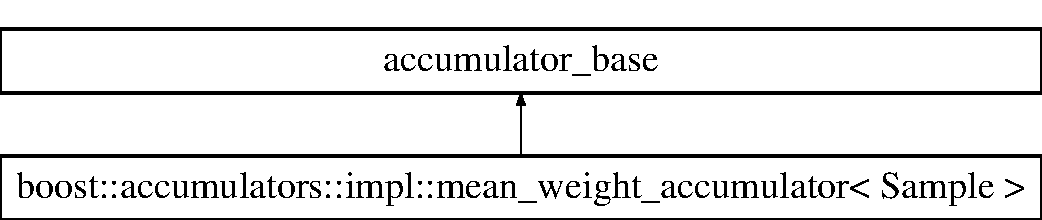
\includegraphics[height=2.000000cm]{structboost_1_1accumulators_1_1impl_1_1mean__weight__accumulator}
\end{center}
\end{figure}
\subsection*{Public Types}
\begin{DoxyCompactItemize}
\item 
typedef \hyperlink{lib_2IceBRG__main_2common_8h_ad0f130a56eeb944d9ef2692ee881ecc4}{flt\+\_\+type} \hyperlink{structboost_1_1accumulators_1_1impl_1_1mean__weight__accumulator_aa801a0036d51f922b4ac392309a2ca37}{result\+\_\+type}
\end{DoxyCompactItemize}
\subsection*{Public Member Functions}
\begin{DoxyCompactItemize}
\item 
\hyperlink{structboost_1_1accumulators_1_1impl_1_1mean__weight__accumulator_a0aa2176eab9ce6eec07f8eca2e29922d}{mean\+\_\+weight\+\_\+accumulator} (dont\+\_\+care)
\item 
{\footnotesize template$<$typename Args $>$ }\\\hyperlink{structboost_1_1accumulators_1_1impl_1_1mean__weight__accumulator_aa801a0036d51f922b4ac392309a2ca37}{result\+\_\+type} \hyperlink{structboost_1_1accumulators_1_1impl_1_1mean__weight__accumulator_a480b0bbb3ad6634179ea7e7e7d4aa7ce}{result} (Args const \&args) const 
\end{DoxyCompactItemize}


\subsection{Member Typedef Documentation}
\hypertarget{structboost_1_1accumulators_1_1impl_1_1mean__weight__accumulator_aa801a0036d51f922b4ac392309a2ca37}{}\index{boost\+::accumulators\+::impl\+::mean\+\_\+weight\+\_\+accumulator@{boost\+::accumulators\+::impl\+::mean\+\_\+weight\+\_\+accumulator}!result\+\_\+type@{result\+\_\+type}}
\index{result\+\_\+type@{result\+\_\+type}!boost\+::accumulators\+::impl\+::mean\+\_\+weight\+\_\+accumulator@{boost\+::accumulators\+::impl\+::mean\+\_\+weight\+\_\+accumulator}}
\subsubsection[{result\+\_\+type}]{\setlength{\rightskip}{0pt plus 5cm}template$<$typename Sample $>$ typedef {\bf flt\+\_\+type} {\bf boost\+::accumulators\+::impl\+::mean\+\_\+weight\+\_\+accumulator}$<$ Sample $>$\+::{\bf result\+\_\+type}}\label{structboost_1_1accumulators_1_1impl_1_1mean__weight__accumulator_aa801a0036d51f922b4ac392309a2ca37}


\subsection{Constructor \& Destructor Documentation}
\hypertarget{structboost_1_1accumulators_1_1impl_1_1mean__weight__accumulator_a0aa2176eab9ce6eec07f8eca2e29922d}{}\index{boost\+::accumulators\+::impl\+::mean\+\_\+weight\+\_\+accumulator@{boost\+::accumulators\+::impl\+::mean\+\_\+weight\+\_\+accumulator}!mean\+\_\+weight\+\_\+accumulator@{mean\+\_\+weight\+\_\+accumulator}}
\index{mean\+\_\+weight\+\_\+accumulator@{mean\+\_\+weight\+\_\+accumulator}!boost\+::accumulators\+::impl\+::mean\+\_\+weight\+\_\+accumulator@{boost\+::accumulators\+::impl\+::mean\+\_\+weight\+\_\+accumulator}}
\subsubsection[{mean\+\_\+weight\+\_\+accumulator(dont\+\_\+care)}]{\setlength{\rightskip}{0pt plus 5cm}template$<$typename Sample $>$ {\bf boost\+::accumulators\+::impl\+::mean\+\_\+weight\+\_\+accumulator}$<$ Sample $>$\+::{\bf mean\+\_\+weight\+\_\+accumulator} (
\begin{DoxyParamCaption}
\item[{dont\+\_\+care}]{}
\end{DoxyParamCaption}
)\hspace{0.3cm}{\ttfamily [inline]}}\label{structboost_1_1accumulators_1_1impl_1_1mean__weight__accumulator_a0aa2176eab9ce6eec07f8eca2e29922d}


\subsection{Member Function Documentation}
\hypertarget{structboost_1_1accumulators_1_1impl_1_1mean__weight__accumulator_a480b0bbb3ad6634179ea7e7e7d4aa7ce}{}\index{boost\+::accumulators\+::impl\+::mean\+\_\+weight\+\_\+accumulator@{boost\+::accumulators\+::impl\+::mean\+\_\+weight\+\_\+accumulator}!result@{result}}
\index{result@{result}!boost\+::accumulators\+::impl\+::mean\+\_\+weight\+\_\+accumulator@{boost\+::accumulators\+::impl\+::mean\+\_\+weight\+\_\+accumulator}}
\subsubsection[{result(\+Args const \&args) const }]{\setlength{\rightskip}{0pt plus 5cm}template$<$typename Sample $>$ template$<$typename Args $>$ {\bf result\+\_\+type} {\bf boost\+::accumulators\+::impl\+::mean\+\_\+weight\+\_\+accumulator}$<$ Sample $>$\+::result (
\begin{DoxyParamCaption}
\item[{Args const \&}]{args}
\end{DoxyParamCaption}
) const\hspace{0.3cm}{\ttfamily [inline]}}\label{structboost_1_1accumulators_1_1impl_1_1mean__weight__accumulator_a480b0bbb3ad6634179ea7e7e7d4aa7ce}


The documentation for this struct was generated from the following file\+:\begin{DoxyCompactItemize}
\item 
/disk2/brg/git/\+Magnification\+\_\+\+Public/src/lib/\+Ice\+B\+R\+G\+\_\+main/math/statistics/\hyperlink{mean__weight_8hpp}{mean\+\_\+weight.\+hpp}\end{DoxyCompactItemize}

\hypertarget{classIceBRG_1_1mu__signal__integration__functor}{}\section{Ice\+B\+R\+G\+:\+:mu\+\_\+signal\+\_\+integration\+\_\+functor Class Reference}
\label{classIceBRG_1_1mu__signal__integration__functor}\index{Ice\+B\+R\+G\+::mu\+\_\+signal\+\_\+integration\+\_\+functor@{Ice\+B\+R\+G\+::mu\+\_\+signal\+\_\+integration\+\_\+functor}}


{\ttfamily \#include $<$magnification\+\_\+functors.\+h$>$}

\subsection*{Public Member Functions}
\begin{DoxyCompactItemize}
\item 
\hyperlink{classIceBRG_1_1mu__signal__integration__functor_adcf7391f693e91147be3556c3d7a0cd0}{mu\+\_\+signal\+\_\+integration\+\_\+functor} (\hyperlink{lib_2IceBRG__main_2common_8h_ad0f130a56eeb944d9ef2692ee881ecc4}{flt\+\_\+type} init\+\_\+z=0)
\item 
virtual \hyperlink{classIceBRG_1_1mu__signal__integration__functor_ab688531f79c3c3f8e3946e6bff1079ed}{$\sim$mu\+\_\+signal\+\_\+integration\+\_\+functor} ()
\item 
\hyperlink{lib_2IceBRG__main_2common_8h_ad0f130a56eeb944d9ef2692ee881ecc4}{flt\+\_\+type} \hyperlink{classIceBRG_1_1mu__signal__integration__functor_ad30a82f71d64b7d7141e6a3ffc2e6377}{operator()} (const \hyperlink{lib_2IceBRG__main_2common_8h_a7040956e7e1b504d34a9ccfb4253bdce}{long\+\_\+flt\+\_\+type} \&\hyperlink{namespaceIceBRG_ada6365c5d16106f0608afbd34f010bcc}{m}=true) const 
\end{DoxyCompactItemize}


\subsection{Constructor \& Destructor Documentation}
\hypertarget{classIceBRG_1_1mu__signal__integration__functor_adcf7391f693e91147be3556c3d7a0cd0}{}\index{Ice\+B\+R\+G\+::mu\+\_\+signal\+\_\+integration\+\_\+functor@{Ice\+B\+R\+G\+::mu\+\_\+signal\+\_\+integration\+\_\+functor}!mu\+\_\+signal\+\_\+integration\+\_\+functor@{mu\+\_\+signal\+\_\+integration\+\_\+functor}}
\index{mu\+\_\+signal\+\_\+integration\+\_\+functor@{mu\+\_\+signal\+\_\+integration\+\_\+functor}!Ice\+B\+R\+G\+::mu\+\_\+signal\+\_\+integration\+\_\+functor@{Ice\+B\+R\+G\+::mu\+\_\+signal\+\_\+integration\+\_\+functor}}
\subsubsection[{mu\+\_\+signal\+\_\+integration\+\_\+functor(flt\+\_\+type init\+\_\+z=0)}]{\setlength{\rightskip}{0pt plus 5cm}Ice\+B\+R\+G\+::mu\+\_\+signal\+\_\+integration\+\_\+functor\+::mu\+\_\+signal\+\_\+integration\+\_\+functor (
\begin{DoxyParamCaption}
\item[{{\bf flt\+\_\+type}}]{init\+\_\+z = {\ttfamily 0}}
\end{DoxyParamCaption}
)\hspace{0.3cm}{\ttfamily [inline]}}\label{classIceBRG_1_1mu__signal__integration__functor_adcf7391f693e91147be3556c3d7a0cd0}
\hypertarget{classIceBRG_1_1mu__signal__integration__functor_ab688531f79c3c3f8e3946e6bff1079ed}{}\index{Ice\+B\+R\+G\+::mu\+\_\+signal\+\_\+integration\+\_\+functor@{Ice\+B\+R\+G\+::mu\+\_\+signal\+\_\+integration\+\_\+functor}!````~mu\+\_\+signal\+\_\+integration\+\_\+functor@{$\sim$mu\+\_\+signal\+\_\+integration\+\_\+functor}}
\index{````~mu\+\_\+signal\+\_\+integration\+\_\+functor@{$\sim$mu\+\_\+signal\+\_\+integration\+\_\+functor}!Ice\+B\+R\+G\+::mu\+\_\+signal\+\_\+integration\+\_\+functor@{Ice\+B\+R\+G\+::mu\+\_\+signal\+\_\+integration\+\_\+functor}}
\subsubsection[{$\sim$mu\+\_\+signal\+\_\+integration\+\_\+functor()}]{\setlength{\rightskip}{0pt plus 5cm}virtual Ice\+B\+R\+G\+::mu\+\_\+signal\+\_\+integration\+\_\+functor\+::$\sim$mu\+\_\+signal\+\_\+integration\+\_\+functor (
\begin{DoxyParamCaption}
{}
\end{DoxyParamCaption}
)\hspace{0.3cm}{\ttfamily [inline]}, {\ttfamily [virtual]}}\label{classIceBRG_1_1mu__signal__integration__functor_ab688531f79c3c3f8e3946e6bff1079ed}


\subsection{Member Function Documentation}
\hypertarget{classIceBRG_1_1mu__signal__integration__functor_ad30a82f71d64b7d7141e6a3ffc2e6377}{}\index{Ice\+B\+R\+G\+::mu\+\_\+signal\+\_\+integration\+\_\+functor@{Ice\+B\+R\+G\+::mu\+\_\+signal\+\_\+integration\+\_\+functor}!operator()@{operator()}}
\index{operator()@{operator()}!Ice\+B\+R\+G\+::mu\+\_\+signal\+\_\+integration\+\_\+functor@{Ice\+B\+R\+G\+::mu\+\_\+signal\+\_\+integration\+\_\+functor}}
\subsubsection[{operator()(const long\+\_\+flt\+\_\+type \&m=true) const }]{\setlength{\rightskip}{0pt plus 5cm}{\bf flt\+\_\+type} Ice\+B\+R\+G\+::mu\+\_\+signal\+\_\+integration\+\_\+functor\+::operator() (
\begin{DoxyParamCaption}
\item[{const {\bf long\+\_\+flt\+\_\+type} \&}]{m = {\ttfamily true}}
\end{DoxyParamCaption}
) const}\label{classIceBRG_1_1mu__signal__integration__functor_ad30a82f71d64b7d7141e6a3ffc2e6377}


The documentation for this class was generated from the following files\+:\begin{DoxyCompactItemize}
\item 
/disk2/brg/git/\+Magnification\+\_\+\+Public/src/lib/\+Ice\+B\+R\+G\+\_\+lensing/magnification/\hyperlink{magnification__functors_8h}{magnification\+\_\+functors.\+h}\item 
/disk2/brg/git/\+Magnification\+\_\+\+Public/src/lib/\+Ice\+B\+R\+G\+\_\+lensing/magnification/\hyperlink{magnification__functors_8cpp}{magnification\+\_\+functors.\+cpp}\end{DoxyCompactItemize}

\hypertarget{classIceBRG_1_1mu__weight__integration__functor}{}\section{Ice\+B\+R\+G\+:\+:mu\+\_\+weight\+\_\+integration\+\_\+functor Class Reference}
\label{classIceBRG_1_1mu__weight__integration__functor}\index{Ice\+B\+R\+G\+::mu\+\_\+weight\+\_\+integration\+\_\+functor@{Ice\+B\+R\+G\+::mu\+\_\+weight\+\_\+integration\+\_\+functor}}


{\ttfamily \#include $<$magnification\+\_\+functors.\+h$>$}

\subsection*{Public Member Functions}
\begin{DoxyCompactItemize}
\item 
\hyperlink{classIceBRG_1_1mu__weight__integration__functor_abc1c2feebc153cc714461341e1677b98}{mu\+\_\+weight\+\_\+integration\+\_\+functor} (\hyperlink{lib_2IceBRG__main_2common_8h_ad0f130a56eeb944d9ef2692ee881ecc4}{flt\+\_\+type} init\+\_\+z=0)
\item 
virtual \hyperlink{classIceBRG_1_1mu__weight__integration__functor_af95375b93119d9f6cbab297d3b357a66}{$\sim$mu\+\_\+weight\+\_\+integration\+\_\+functor} ()
\item 
\hyperlink{lib_2IceBRG__main_2common_8h_ad0f130a56eeb944d9ef2692ee881ecc4}{flt\+\_\+type} \hyperlink{classIceBRG_1_1mu__weight__integration__functor_af0d9d5e75b915dcf7a20f48c88d47145}{operator()} (const \hyperlink{lib_2IceBRG__main_2common_8h_a7040956e7e1b504d34a9ccfb4253bdce}{long\+\_\+flt\+\_\+type} \&\hyperlink{namespaceIceBRG_ada6365c5d16106f0608afbd34f010bcc}{m}=true) const 
\end{DoxyCompactItemize}


\subsection{Constructor \& Destructor Documentation}
\hypertarget{classIceBRG_1_1mu__weight__integration__functor_abc1c2feebc153cc714461341e1677b98}{}\index{Ice\+B\+R\+G\+::mu\+\_\+weight\+\_\+integration\+\_\+functor@{Ice\+B\+R\+G\+::mu\+\_\+weight\+\_\+integration\+\_\+functor}!mu\+\_\+weight\+\_\+integration\+\_\+functor@{mu\+\_\+weight\+\_\+integration\+\_\+functor}}
\index{mu\+\_\+weight\+\_\+integration\+\_\+functor@{mu\+\_\+weight\+\_\+integration\+\_\+functor}!Ice\+B\+R\+G\+::mu\+\_\+weight\+\_\+integration\+\_\+functor@{Ice\+B\+R\+G\+::mu\+\_\+weight\+\_\+integration\+\_\+functor}}
\subsubsection[{mu\+\_\+weight\+\_\+integration\+\_\+functor(flt\+\_\+type init\+\_\+z=0)}]{\setlength{\rightskip}{0pt plus 5cm}Ice\+B\+R\+G\+::mu\+\_\+weight\+\_\+integration\+\_\+functor\+::mu\+\_\+weight\+\_\+integration\+\_\+functor (
\begin{DoxyParamCaption}
\item[{{\bf flt\+\_\+type}}]{init\+\_\+z = {\ttfamily 0}}
\end{DoxyParamCaption}
)\hspace{0.3cm}{\ttfamily [inline]}}\label{classIceBRG_1_1mu__weight__integration__functor_abc1c2feebc153cc714461341e1677b98}
\hypertarget{classIceBRG_1_1mu__weight__integration__functor_af95375b93119d9f6cbab297d3b357a66}{}\index{Ice\+B\+R\+G\+::mu\+\_\+weight\+\_\+integration\+\_\+functor@{Ice\+B\+R\+G\+::mu\+\_\+weight\+\_\+integration\+\_\+functor}!````~mu\+\_\+weight\+\_\+integration\+\_\+functor@{$\sim$mu\+\_\+weight\+\_\+integration\+\_\+functor}}
\index{````~mu\+\_\+weight\+\_\+integration\+\_\+functor@{$\sim$mu\+\_\+weight\+\_\+integration\+\_\+functor}!Ice\+B\+R\+G\+::mu\+\_\+weight\+\_\+integration\+\_\+functor@{Ice\+B\+R\+G\+::mu\+\_\+weight\+\_\+integration\+\_\+functor}}
\subsubsection[{$\sim$mu\+\_\+weight\+\_\+integration\+\_\+functor()}]{\setlength{\rightskip}{0pt plus 5cm}virtual Ice\+B\+R\+G\+::mu\+\_\+weight\+\_\+integration\+\_\+functor\+::$\sim$mu\+\_\+weight\+\_\+integration\+\_\+functor (
\begin{DoxyParamCaption}
{}
\end{DoxyParamCaption}
)\hspace{0.3cm}{\ttfamily [inline]}, {\ttfamily [virtual]}}\label{classIceBRG_1_1mu__weight__integration__functor_af95375b93119d9f6cbab297d3b357a66}


\subsection{Member Function Documentation}
\hypertarget{classIceBRG_1_1mu__weight__integration__functor_af0d9d5e75b915dcf7a20f48c88d47145}{}\index{Ice\+B\+R\+G\+::mu\+\_\+weight\+\_\+integration\+\_\+functor@{Ice\+B\+R\+G\+::mu\+\_\+weight\+\_\+integration\+\_\+functor}!operator()@{operator()}}
\index{operator()@{operator()}!Ice\+B\+R\+G\+::mu\+\_\+weight\+\_\+integration\+\_\+functor@{Ice\+B\+R\+G\+::mu\+\_\+weight\+\_\+integration\+\_\+functor}}
\subsubsection[{operator()(const long\+\_\+flt\+\_\+type \&m=true) const }]{\setlength{\rightskip}{0pt plus 5cm}{\bf flt\+\_\+type} Ice\+B\+R\+G\+::mu\+\_\+weight\+\_\+integration\+\_\+functor\+::operator() (
\begin{DoxyParamCaption}
\item[{const {\bf long\+\_\+flt\+\_\+type} \&}]{m = {\ttfamily true}}
\end{DoxyParamCaption}
) const}\label{classIceBRG_1_1mu__weight__integration__functor_af0d9d5e75b915dcf7a20f48c88d47145}


The documentation for this class was generated from the following files\+:\begin{DoxyCompactItemize}
\item 
/disk2/brg/git/\+Magnification\+\_\+\+Public/src/lib/\+Ice\+B\+R\+G\+\_\+lensing/magnification/\hyperlink{magnification__functors_8h}{magnification\+\_\+functors.\+h}\item 
/disk2/brg/git/\+Magnification\+\_\+\+Public/src/lib/\+Ice\+B\+R\+G\+\_\+lensing/magnification/\hyperlink{magnification__functors_8cpp}{magnification\+\_\+functors.\+cpp}\end{DoxyCompactItemize}

\hypertarget{classIceBRG_1_1multi__vector}{}\section{Ice\+B\+R\+G\+:\+:multi\+\_\+vector$<$ T, A $>$ Class Template Reference}
\label{classIceBRG_1_1multi__vector}\index{Ice\+B\+R\+G\+::multi\+\_\+vector$<$ T, A $>$@{Ice\+B\+R\+G\+::multi\+\_\+vector$<$ T, A $>$}}


{\ttfamily \#include $<$multi\+\_\+vector.\+hpp$>$}

Inheritance diagram for Ice\+B\+R\+G\+:\+:multi\+\_\+vector$<$ T, A $>$\+:\begin{figure}[H]
\begin{center}
\leavevmode
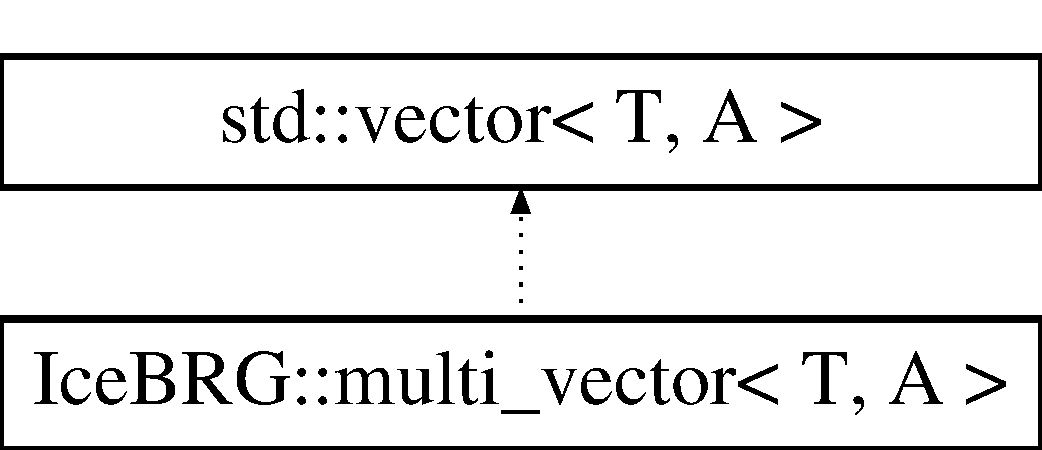
\includegraphics[height=2.000000cm]{classIceBRG_1_1multi__vector}
\end{center}
\end{figure}
\subsection*{Public Types}
\begin{DoxyCompactItemize}
\item 
typedef std\+::vector$<$ T, A $>$\+::\hyperlink{lib_2IceBRG__main_2common_8h_a566c61f2ca17211f4ba8557f3f65e8d3}{size\+\_\+type} \hyperlink{classIceBRG_1_1multi__vector_abcc3d84f2afbb3e4239cea8c2c4923c3}{vsize\+\_\+t}
\item 
typedef \hyperlink{lib_2IceBRG__main_2common_8h_ac4de9d9335536ac22821171deec8d39e}{int\+\_\+type} \hyperlink{classIceBRG_1_1multi__vector_af2666369daa5e69abfbadbe365c200e9}{dsize\+\_\+t}
\item 
typedef \hyperlink{lib_2IceBRG__main_2common_8h_ac4de9d9335536ac22821171deec8d39e}{int\+\_\+type} \hyperlink{classIceBRG_1_1multi__vector_a9ad43f84f33367955b45ca260ea5882b}{ssize\+\_\+t}
\item 
typedef std\+::vector$<$ \hyperlink{lib_2IceBRG__main_2common_8h_ac4de9d9335536ac22821171deec8d39e}{int\+\_\+type} $>$ \hyperlink{classIceBRG_1_1multi__vector_a468a7f934274e7aa75e01c94ac58f3ea}{shape\+\_\+t}
\end{DoxyCompactItemize}
\subsection*{Public Member Functions}
\begin{DoxyCompactItemize}
\item 
{\footnotesize template$<$class Input\+Iterator $>$ }\\void \hyperlink{classIceBRG_1_1multi__vector_ae1a89438380ac2b5aeb898e171ed9364}{assign} (Input\+Iterator first, Input\+Iterator last)
\item 
void \hyperlink{classIceBRG_1_1multi__vector_a5dfdcc780219ad607ced1e3e894945f5}{assign} (typename \hyperlink{lib_2IceBRG__main_2common_8h_a566c61f2ca17211f4ba8557f3f65e8d3}{vec\+::size\+\_\+type} n, const T \&val)
\item 
\hyperlink{classIceBRG_1_1multi__vector}{multi\+\_\+vector}$<$ T, A $>$ \& \hyperlink{classIceBRG_1_1multi__vector_a2f86b23b2ed4a23e20fb1292624e2da9}{push\+\_\+back} (const T \&val)
\item 
vec\+::iterator \hyperlink{classIceBRG_1_1multi__vector_a7db7da470a601e122fc74f2f9523ed04}{insert} (typename vec\+::iterator position, const T \&val)
\item 
void \hyperlink{classIceBRG_1_1multi__vector_ad7b717cff0ee7405af4837e29ecdf868}{insert} (typename vec\+::iterator position, typename \hyperlink{lib_2IceBRG__main_2common_8h_a566c61f2ca17211f4ba8557f3f65e8d3}{vec\+::size\+\_\+type} n, const typename vec\+::value\+\_\+type \&val)
\item 
{\footnotesize template$<$class Input\+Iterator $>$ }\\void \hyperlink{classIceBRG_1_1multi__vector_a8f74fe60c6358817ccf81d5c973cc93f}{insert} (typename vec\+::iterator position, Input\+Iterator first, Input\+Iterator last)
\item 
vec\+::iterator \hyperlink{classIceBRG_1_1multi__vector_aba38804447222d41c4ca7c49feac8cab}{erase} (typename vec\+::iterator position)
\item 
vec\+::iterator \hyperlink{classIceBRG_1_1multi__vector_a64188c90861ee5ad87b4ec9fcd265f20}{erase} (typename vec\+::iterator first, typename vec\+::iterator last)
\item 
void \hyperlink{classIceBRG_1_1multi__vector_a08b4f9d36263e9e35c753842716b04dc}{resize} (\hyperlink{classIceBRG_1_1multi__vector_abcc3d84f2afbb3e4239cea8c2c4923c3}{vsize\+\_\+t} n, T val=T())
\item 
const T \& \hyperlink{classIceBRG_1_1multi__vector_a5fafc6a7c33d88dc5d772365baf6cd40}{pop\+\_\+back} ()
\item 
void \hyperlink{classIceBRG_1_1multi__vector_accc4290ed0ee20edf847e26805cd54f2}{del\+\_\+back} ()
\item 
void \hyperlink{classIceBRG_1_1multi__vector_a12b96cd198798ebb0506dbf1b0475c57}{clear} ()
\item 
\hyperlink{classIceBRG_1_1multi__vector}{multi\+\_\+vector}$<$ T, A $>$ \& \hyperlink{classIceBRG_1_1multi__vector_abcfd8d5fcc0c020f3b2df4a7e9f8a86d}{operator=} (\hyperlink{classIceBRG_1_1multi__vector}{multi\+\_\+vector}$<$ T, A $>$ other)
\item 
\hyperlink{classIceBRG_1_1multi__vector}{multi\+\_\+vector}$<$ T, A $>$ \& \hyperlink{classIceBRG_1_1multi__vector_a92c909bfd31a10254ec5c490283bff73}{copy} (\hyperlink{classIceBRG_1_1multi__vector}{multi\+\_\+vector}$<$ T, A $>$ other)
\item 
\hyperlink{classIceBRG_1_1multi__vector}{multi\+\_\+vector}$<$ T, A $>$ \& \hyperlink{classIceBRG_1_1multi__vector_ade66bbf2a7c88dab7578117828cbf51a}{swap} (\hyperlink{classIceBRG_1_1multi__vector}{multi\+\_\+vector}$<$ T, A $>$ \&other)
\item 
\hyperlink{classIceBRG_1_1multi__vector_a94d3f4a0aeb3e0a10deff3facab26ead}{operator T} () const 
\item 
{\footnotesize template$<$typename T\+\_\+o , typename A\+\_\+o $>$ }\\\hyperlink{classIceBRG_1_1multi__vector}{multi\+\_\+vector}$<$ T, A $>$ \& \hyperlink{classIceBRG_1_1multi__vector_ac98362c51641079300aea3e0e7b2c394}{operator+=} (const \hyperlink{classIceBRG_1_1multi__vector}{multi\+\_\+vector}$<$ T\+\_\+o, A\+\_\+o $>$ \&other)
\item 
{\footnotesize template$<$typename T\+\_\+o , typename A\+\_\+o $>$ }\\\hyperlink{classIceBRG_1_1multi__vector}{multi\+\_\+vector}$<$ T, A $>$ \& \hyperlink{classIceBRG_1_1multi__vector_a33e36547fa2a5a016652287d38b23eb1}{operator+=} (const std\+::vector$<$ T\+\_\+o, A\+\_\+o $>$ \&other)
\item 
{\footnotesize template$<$typename T\+\_\+o $>$ }\\\hyperlink{classIceBRG_1_1multi__vector}{multi\+\_\+vector}$<$ T, A $>$ \& \hyperlink{classIceBRG_1_1multi__vector_a100c7fe9b7eb28552d61ad9670da560b}{operator+=} (T\+\_\+o other)
\item 
{\footnotesize template$<$typename T\+\_\+o , typename A\+\_\+o $>$ }\\\hyperlink{classIceBRG_1_1multi__vector}{multi\+\_\+vector}$<$ T, A $>$ \& \hyperlink{classIceBRG_1_1multi__vector_a1f8e2ea7d8cfbe4dab3a00d83dfc057f}{operator-\/=} (const \hyperlink{classIceBRG_1_1multi__vector}{multi\+\_\+vector}$<$ T\+\_\+o, A\+\_\+o $>$ \&other)
\item 
{\footnotesize template$<$typename T\+\_\+o , typename A\+\_\+o $>$ }\\\hyperlink{classIceBRG_1_1multi__vector}{multi\+\_\+vector}$<$ T, A $>$ \& \hyperlink{classIceBRG_1_1multi__vector_ad2805cc6dfd1d7e5a6c3ddccf8e05217}{operator-\/=} (const std\+::vector$<$ T\+\_\+o, A\+\_\+o $>$ \&other)
\item 
{\footnotesize template$<$typename T\+\_\+o $>$ }\\\hyperlink{classIceBRG_1_1multi__vector}{multi\+\_\+vector}$<$ T, A $>$ \& \hyperlink{classIceBRG_1_1multi__vector_aff6dc155260c3184e867fd791f90f4b2}{operator-\/=} (T\+\_\+o other)
\item 
{\footnotesize template$<$typename T\+\_\+o , typename A\+\_\+o $>$ }\\\hyperlink{classIceBRG_1_1multi__vector}{multi\+\_\+vector}$<$ T, A $>$ \& \hyperlink{classIceBRG_1_1multi__vector_a73496e141636d17cb8518bf9349bcc61}{operator$\ast$=} (const \hyperlink{classIceBRG_1_1multi__vector}{multi\+\_\+vector}$<$ T\+\_\+o, A\+\_\+o $>$ \&other)
\item 
{\footnotesize template$<$typename T\+\_\+o , typename A\+\_\+o $>$ }\\\hyperlink{classIceBRG_1_1multi__vector}{multi\+\_\+vector}$<$ T, A $>$ \& \hyperlink{classIceBRG_1_1multi__vector_ae18d0d68a054316add7134b34364504e}{operator$\ast$=} (const std\+::vector$<$ T\+\_\+o, A\+\_\+o $>$ \&other)
\item 
{\footnotesize template$<$typename T\+\_\+o $>$ }\\\hyperlink{classIceBRG_1_1multi__vector}{multi\+\_\+vector}$<$ T, A $>$ \& \hyperlink{classIceBRG_1_1multi__vector_a828d13398771ee0cb3618aa72023c414}{operator$\ast$=} (T\+\_\+o other)
\item 
{\footnotesize template$<$typename T\+\_\+o , typename A\+\_\+o $>$ }\\\hyperlink{classIceBRG_1_1multi__vector}{multi\+\_\+vector}$<$ T, A $>$ \& \hyperlink{classIceBRG_1_1multi__vector_ae6912cd1b408b33e4f6e616b394f6375}{operator/=} (const \hyperlink{classIceBRG_1_1multi__vector}{multi\+\_\+vector}$<$ T\+\_\+o, A\+\_\+o $>$ \&other)
\item 
{\footnotesize template$<$typename T\+\_\+o , typename A\+\_\+o $>$ }\\\hyperlink{classIceBRG_1_1multi__vector}{multi\+\_\+vector}$<$ T, A $>$ \& \hyperlink{classIceBRG_1_1multi__vector_aea2029e62a8c71e4ce078002bbcf5a01}{operator/=} (const std\+::vector$<$ T\+\_\+o, A\+\_\+o $>$ \&other)
\item 
{\footnotesize template$<$typename T\+\_\+o $>$ }\\\hyperlink{classIceBRG_1_1multi__vector}{multi\+\_\+vector}$<$ T, A $>$ \& \hyperlink{classIceBRG_1_1multi__vector_aef3fb151f960eff2cd162b9986229c46}{operator/=} (T\+\_\+o other)
\item 
\hyperlink{classIceBRG_1_1multi__vector}{multi\+\_\+vector}$<$ T, A $>$ \& \hyperlink{classIceBRG_1_1multi__vector_a472689a6e3130c24d066c314bf6a8409}{operator++} ()
\item 
const \hyperlink{classIceBRG_1_1multi__vector}{multi\+\_\+vector}$<$ T, A $>$ \& \hyperlink{classIceBRG_1_1multi__vector_adc1298f6bfb1b3d47bb6cb23230ca527}{operator++} (\hyperlink{lib_2IceBRG__main_2common_8h_ac4de9d9335536ac22821171deec8d39e}{int\+\_\+type})
\item 
std\+::vector$<$ T, A $>$ \hyperlink{classIceBRG_1_1multi__vector_a91f5eebc48c8849b8c27e7992e17701b}{v} () const 
\item 
const \hyperlink{classIceBRG_1_1multi__vector_a468a7f934274e7aa75e01c94ac58f3ea}{shape\+\_\+t} \& \hyperlink{classIceBRG_1_1multi__vector_ad5fb113982dce9456f724ca9072e42c9}{shape} () const 
\item 
const \hyperlink{classIceBRG_1_1multi__vector_af2666369daa5e69abfbadbe365c200e9}{dsize\+\_\+t} \& \hyperlink{classIceBRG_1_1multi__vector_a0beaee05722b4fd40af1452d452f4fe7}{num\+\_\+dim} () const 
\item 
T \& \hyperlink{classIceBRG_1_1multi__vector_a58de7745b168b4831cb1f0b20d933684}{operator()} (const \hyperlink{classIceBRG_1_1multi__vector_a468a7f934274e7aa75e01c94ac58f3ea}{shape\+\_\+t} \&position)
\item 
const T \& \hyperlink{classIceBRG_1_1multi__vector_a472ebe4b4a132452caf3cd98edb64e2c}{operator()} (const \hyperlink{classIceBRG_1_1multi__vector_a468a7f934274e7aa75e01c94ac58f3ea}{shape\+\_\+t} \&position) const 
\item 
T \& \hyperlink{classIceBRG_1_1multi__vector_aad5f4f2ced67278183d44ff906f3b654}{operator()} (const \hyperlink{classIceBRG_1_1multi__vector}{multi\+\_\+vector}$<$ \hyperlink{lib_2IceBRG__main_2common_8h_ac4de9d9335536ac22821171deec8d39e}{int\+\_\+type} $>$ \&position)
\item 
const T \& \hyperlink{classIceBRG_1_1multi__vector_a61766162e95d0896e9dd45b894cbd0f8}{operator()} (const \hyperlink{classIceBRG_1_1multi__vector}{multi\+\_\+vector}$<$ \hyperlink{lib_2IceBRG__main_2common_8h_ac4de9d9335536ac22821171deec8d39e}{int\+\_\+type} $>$ \&position) const 
\item 
T \& \hyperlink{classIceBRG_1_1multi__vector_ac3c759345706a78af2c1a8a8cde072c7}{at} (const \hyperlink{classIceBRG_1_1multi__vector_a468a7f934274e7aa75e01c94ac58f3ea}{shape\+\_\+t} \&position)
\item 
const T \& \hyperlink{classIceBRG_1_1multi__vector_af3f5a492939e45c036c73d0286ae8505}{at} (const \hyperlink{classIceBRG_1_1multi__vector_a468a7f934274e7aa75e01c94ac58f3ea}{shape\+\_\+t} \&position) const 
\item 
T \& \hyperlink{classIceBRG_1_1multi__vector_a107ef0e6fea9601c2a1cd0fea5bef200}{at} (const \hyperlink{classIceBRG_1_1multi__vector}{multi\+\_\+vector}$<$ \hyperlink{lib_2IceBRG__main_2common_8h_ac4de9d9335536ac22821171deec8d39e}{int\+\_\+type} $>$ \&position)
\item 
const T \& \hyperlink{classIceBRG_1_1multi__vector_aa50615a83dad050c93098950894d8fa5}{at} (const \hyperlink{classIceBRG_1_1multi__vector}{multi\+\_\+vector}$<$ \hyperlink{lib_2IceBRG__main_2common_8h_ac4de9d9335536ac22821171deec8d39e}{int\+\_\+type} $>$ \&position) const 
\item 
void \hyperlink{classIceBRG_1_1multi__vector_a3eceee96718f7144bd056caa4486023e}{reshape} (const \hyperlink{classIceBRG_1_1multi__vector_a468a7f934274e7aa75e01c94ac58f3ea}{shape\+\_\+t} \&new\+\_\+shape, const T \&new\+\_\+val=T())
\item 
\hyperlink{classIceBRG_1_1multi__vector_a6ba7614c52e0dc623fc190d868f8b6ed}{multi\+\_\+vector} (const A \&alloc=A())
\item 
\hyperlink{classIceBRG_1_1multi__vector_a7bdea87bcffcdc2053cd65ba21dd3e95}{multi\+\_\+vector} (\hyperlink{classIceBRG_1_1multi__vector_abcc3d84f2afbb3e4239cea8c2c4923c3}{vsize\+\_\+t} init\+\_\+size, T init\+\_\+val, const A \&alloc=A())
\item 
\hyperlink{classIceBRG_1_1multi__vector_ae94a23b09a6f6bc737481c132332346b}{multi\+\_\+vector} (\hyperlink{classIceBRG_1_1multi__vector_a468a7f934274e7aa75e01c94ac58f3ea}{shape\+\_\+t} init\+\_\+shape, T init\+\_\+val, const A \&alloc=A())
\item 
\hyperlink{classIceBRG_1_1multi__vector_aafd73188953583a68c242bbb201311ae}{multi\+\_\+vector} (const \hyperlink{classIceBRG_1_1multi__vector}{multi\+\_\+vector}$<$ T, A $>$ \&other)
\item 
{\footnotesize template$<$typename T\+\_\+o , typename A\+\_\+o $>$ }\\\hyperlink{classIceBRG_1_1multi__vector_a1fcceaa14320c72bc437883f8d194bc2}{multi\+\_\+vector} (const \hyperlink{classIceBRG_1_1multi__vector}{multi\+\_\+vector}$<$ T\+\_\+o, A\+\_\+o $>$ \&other)
\item 
{\footnotesize template$<$typename T\+\_\+o , typename A\+\_\+o $>$ }\\\hyperlink{classIceBRG_1_1multi__vector_ac300dd742268ef19405ce2ac8c9c3752}{multi\+\_\+vector} (const std\+::vector$<$ T\+\_\+o, A\+\_\+o $>$ \&other)
\item 
{\footnotesize template$<$typename T\+\_\+o , size\+\_\+t N$>$ }\\\hyperlink{classIceBRG_1_1multi__vector_a29f4de67e11d47b98b5ff2e81df0dc7f}{multi\+\_\+vector} (const T\+\_\+o(\&array)\mbox{[}N\mbox{]}, const A \&alloc=A())
\item 
{\footnotesize template$<$typename T\+\_\+o $>$ }\\\hyperlink{classIceBRG_1_1multi__vector_ac1d11f942532985324c8c3acb5801bec}{multi\+\_\+vector} (const T\+\_\+o \&other, const A \&alloc=A())
\item 
{\footnotesize template$<$typename i\+T\+\_\+o $>$ }\\\hyperlink{classIceBRG_1_1multi__vector_ad91e124b6658894a6e8162f85b1ddd8f}{multi\+\_\+vector} (i\+T\+\_\+o first, i\+T\+\_\+o last, const A \&alloc=A())
\item 
virtual \hyperlink{classIceBRG_1_1multi__vector_a5838dc2869a700c864ab13c2abd65277}{$\sim$multi\+\_\+vector} ()
\end{DoxyCompactItemize}


\subsection{Member Typedef Documentation}
\hypertarget{classIceBRG_1_1multi__vector_af2666369daa5e69abfbadbe365c200e9}{}\index{Ice\+B\+R\+G\+::multi\+\_\+vector@{Ice\+B\+R\+G\+::multi\+\_\+vector}!dsize\+\_\+t@{dsize\+\_\+t}}
\index{dsize\+\_\+t@{dsize\+\_\+t}!Ice\+B\+R\+G\+::multi\+\_\+vector@{Ice\+B\+R\+G\+::multi\+\_\+vector}}
\subsubsection[{dsize\+\_\+t}]{\setlength{\rightskip}{0pt plus 5cm}template$<$class T, class A = std\+::allocator$<$\+T$>$$>$ typedef {\bf int\+\_\+type} {\bf Ice\+B\+R\+G\+::multi\+\_\+vector}$<$ T, A $>$\+::{\bf dsize\+\_\+t}}\label{classIceBRG_1_1multi__vector_af2666369daa5e69abfbadbe365c200e9}
\hypertarget{classIceBRG_1_1multi__vector_a468a7f934274e7aa75e01c94ac58f3ea}{}\index{Ice\+B\+R\+G\+::multi\+\_\+vector@{Ice\+B\+R\+G\+::multi\+\_\+vector}!shape\+\_\+t@{shape\+\_\+t}}
\index{shape\+\_\+t@{shape\+\_\+t}!Ice\+B\+R\+G\+::multi\+\_\+vector@{Ice\+B\+R\+G\+::multi\+\_\+vector}}
\subsubsection[{shape\+\_\+t}]{\setlength{\rightskip}{0pt plus 5cm}template$<$class T, class A = std\+::allocator$<$\+T$>$$>$ typedef std\+::vector$<$ {\bf int\+\_\+type} $>$ {\bf Ice\+B\+R\+G\+::multi\+\_\+vector}$<$ T, A $>$\+::{\bf shape\+\_\+t}}\label{classIceBRG_1_1multi__vector_a468a7f934274e7aa75e01c94ac58f3ea}
\hypertarget{classIceBRG_1_1multi__vector_a9ad43f84f33367955b45ca260ea5882b}{}\index{Ice\+B\+R\+G\+::multi\+\_\+vector@{Ice\+B\+R\+G\+::multi\+\_\+vector}!ssize\+\_\+t@{ssize\+\_\+t}}
\index{ssize\+\_\+t@{ssize\+\_\+t}!Ice\+B\+R\+G\+::multi\+\_\+vector@{Ice\+B\+R\+G\+::multi\+\_\+vector}}
\subsubsection[{ssize\+\_\+t}]{\setlength{\rightskip}{0pt plus 5cm}template$<$class T, class A = std\+::allocator$<$\+T$>$$>$ typedef {\bf int\+\_\+type} {\bf Ice\+B\+R\+G\+::multi\+\_\+vector}$<$ T, A $>$\+::{\bf ssize\+\_\+t}}\label{classIceBRG_1_1multi__vector_a9ad43f84f33367955b45ca260ea5882b}
\hypertarget{classIceBRG_1_1multi__vector_abcc3d84f2afbb3e4239cea8c2c4923c3}{}\index{Ice\+B\+R\+G\+::multi\+\_\+vector@{Ice\+B\+R\+G\+::multi\+\_\+vector}!vsize\+\_\+t@{vsize\+\_\+t}}
\index{vsize\+\_\+t@{vsize\+\_\+t}!Ice\+B\+R\+G\+::multi\+\_\+vector@{Ice\+B\+R\+G\+::multi\+\_\+vector}}
\subsubsection[{vsize\+\_\+t}]{\setlength{\rightskip}{0pt plus 5cm}template$<$class T, class A = std\+::allocator$<$\+T$>$$>$ typedef std\+::vector$<$T,A$>$\+::{\bf size\+\_\+type} {\bf Ice\+B\+R\+G\+::multi\+\_\+vector}$<$ T, A $>$\+::{\bf vsize\+\_\+t}}\label{classIceBRG_1_1multi__vector_abcc3d84f2afbb3e4239cea8c2c4923c3}


\subsection{Constructor \& Destructor Documentation}
\hypertarget{classIceBRG_1_1multi__vector_a6ba7614c52e0dc623fc190d868f8b6ed}{}\index{Ice\+B\+R\+G\+::multi\+\_\+vector@{Ice\+B\+R\+G\+::multi\+\_\+vector}!multi\+\_\+vector@{multi\+\_\+vector}}
\index{multi\+\_\+vector@{multi\+\_\+vector}!Ice\+B\+R\+G\+::multi\+\_\+vector@{Ice\+B\+R\+G\+::multi\+\_\+vector}}
\subsubsection[{multi\+\_\+vector(const A \&alloc=\+A())}]{\setlength{\rightskip}{0pt plus 5cm}template$<$class T, class A = std\+::allocator$<$\+T$>$$>$ {\bf Ice\+B\+R\+G\+::multi\+\_\+vector}$<$ T, A $>$\+::{\bf multi\+\_\+vector} (
\begin{DoxyParamCaption}
\item[{const A \&}]{alloc = {\ttfamily A()}}
\end{DoxyParamCaption}
)\hspace{0.3cm}{\ttfamily [inline]}}\label{classIceBRG_1_1multi__vector_a6ba7614c52e0dc623fc190d868f8b6ed}
\hypertarget{classIceBRG_1_1multi__vector_a7bdea87bcffcdc2053cd65ba21dd3e95}{}\index{Ice\+B\+R\+G\+::multi\+\_\+vector@{Ice\+B\+R\+G\+::multi\+\_\+vector}!multi\+\_\+vector@{multi\+\_\+vector}}
\index{multi\+\_\+vector@{multi\+\_\+vector}!Ice\+B\+R\+G\+::multi\+\_\+vector@{Ice\+B\+R\+G\+::multi\+\_\+vector}}
\subsubsection[{multi\+\_\+vector(vsize\+\_\+t init\+\_\+size, T init\+\_\+val, const A \&alloc=\+A())}]{\setlength{\rightskip}{0pt plus 5cm}template$<$class T, class A = std\+::allocator$<$\+T$>$$>$ {\bf Ice\+B\+R\+G\+::multi\+\_\+vector}$<$ T, A $>$\+::{\bf multi\+\_\+vector} (
\begin{DoxyParamCaption}
\item[{{\bf vsize\+\_\+t}}]{init\+\_\+size, }
\item[{T}]{init\+\_\+val, }
\item[{const A \&}]{alloc = {\ttfamily A()}}
\end{DoxyParamCaption}
)\hspace{0.3cm}{\ttfamily [inline]}}\label{classIceBRG_1_1multi__vector_a7bdea87bcffcdc2053cd65ba21dd3e95}
\hypertarget{classIceBRG_1_1multi__vector_ae94a23b09a6f6bc737481c132332346b}{}\index{Ice\+B\+R\+G\+::multi\+\_\+vector@{Ice\+B\+R\+G\+::multi\+\_\+vector}!multi\+\_\+vector@{multi\+\_\+vector}}
\index{multi\+\_\+vector@{multi\+\_\+vector}!Ice\+B\+R\+G\+::multi\+\_\+vector@{Ice\+B\+R\+G\+::multi\+\_\+vector}}
\subsubsection[{multi\+\_\+vector(shape\+\_\+t init\+\_\+shape, T init\+\_\+val, const A \&alloc=\+A())}]{\setlength{\rightskip}{0pt plus 5cm}template$<$class T, class A = std\+::allocator$<$\+T$>$$>$ {\bf Ice\+B\+R\+G\+::multi\+\_\+vector}$<$ T, A $>$\+::{\bf multi\+\_\+vector} (
\begin{DoxyParamCaption}
\item[{{\bf shape\+\_\+t}}]{init\+\_\+shape, }
\item[{T}]{init\+\_\+val, }
\item[{const A \&}]{alloc = {\ttfamily A()}}
\end{DoxyParamCaption}
)\hspace{0.3cm}{\ttfamily [inline]}}\label{classIceBRG_1_1multi__vector_ae94a23b09a6f6bc737481c132332346b}
\hypertarget{classIceBRG_1_1multi__vector_aafd73188953583a68c242bbb201311ae}{}\index{Ice\+B\+R\+G\+::multi\+\_\+vector@{Ice\+B\+R\+G\+::multi\+\_\+vector}!multi\+\_\+vector@{multi\+\_\+vector}}
\index{multi\+\_\+vector@{multi\+\_\+vector}!Ice\+B\+R\+G\+::multi\+\_\+vector@{Ice\+B\+R\+G\+::multi\+\_\+vector}}
\subsubsection[{multi\+\_\+vector(const multi\+\_\+vector$<$ T, A $>$ \&other)}]{\setlength{\rightskip}{0pt plus 5cm}template$<$class T, class A = std\+::allocator$<$\+T$>$$>$ {\bf Ice\+B\+R\+G\+::multi\+\_\+vector}$<$ T, A $>$\+::{\bf multi\+\_\+vector} (
\begin{DoxyParamCaption}
\item[{const {\bf multi\+\_\+vector}$<$ T, A $>$ \&}]{other}
\end{DoxyParamCaption}
)\hspace{0.3cm}{\ttfamily [inline]}}\label{classIceBRG_1_1multi__vector_aafd73188953583a68c242bbb201311ae}
\hypertarget{classIceBRG_1_1multi__vector_a1fcceaa14320c72bc437883f8d194bc2}{}\index{Ice\+B\+R\+G\+::multi\+\_\+vector@{Ice\+B\+R\+G\+::multi\+\_\+vector}!multi\+\_\+vector@{multi\+\_\+vector}}
\index{multi\+\_\+vector@{multi\+\_\+vector}!Ice\+B\+R\+G\+::multi\+\_\+vector@{Ice\+B\+R\+G\+::multi\+\_\+vector}}
\subsubsection[{multi\+\_\+vector(const multi\+\_\+vector$<$ T\+\_\+o, A\+\_\+o $>$ \&other)}]{\setlength{\rightskip}{0pt plus 5cm}template$<$class T, class A = std\+::allocator$<$\+T$>$$>$ template$<$typename T\+\_\+o , typename A\+\_\+o $>$ {\bf Ice\+B\+R\+G\+::multi\+\_\+vector}$<$ T, A $>$\+::{\bf multi\+\_\+vector} (
\begin{DoxyParamCaption}
\item[{const {\bf multi\+\_\+vector}$<$ T\+\_\+o, A\+\_\+o $>$ \&}]{other}
\end{DoxyParamCaption}
)\hspace{0.3cm}{\ttfamily [inline]}}\label{classIceBRG_1_1multi__vector_a1fcceaa14320c72bc437883f8d194bc2}
\hypertarget{classIceBRG_1_1multi__vector_ac300dd742268ef19405ce2ac8c9c3752}{}\index{Ice\+B\+R\+G\+::multi\+\_\+vector@{Ice\+B\+R\+G\+::multi\+\_\+vector}!multi\+\_\+vector@{multi\+\_\+vector}}
\index{multi\+\_\+vector@{multi\+\_\+vector}!Ice\+B\+R\+G\+::multi\+\_\+vector@{Ice\+B\+R\+G\+::multi\+\_\+vector}}
\subsubsection[{multi\+\_\+vector(const std\+::vector$<$ T\+\_\+o, A\+\_\+o $>$ \&other)}]{\setlength{\rightskip}{0pt plus 5cm}template$<$class T, class A = std\+::allocator$<$\+T$>$$>$ template$<$typename T\+\_\+o , typename A\+\_\+o $>$ {\bf Ice\+B\+R\+G\+::multi\+\_\+vector}$<$ T, A $>$\+::{\bf multi\+\_\+vector} (
\begin{DoxyParamCaption}
\item[{const std\+::vector$<$ T\+\_\+o, A\+\_\+o $>$ \&}]{other}
\end{DoxyParamCaption}
)\hspace{0.3cm}{\ttfamily [inline]}}\label{classIceBRG_1_1multi__vector_ac300dd742268ef19405ce2ac8c9c3752}
\hypertarget{classIceBRG_1_1multi__vector_a29f4de67e11d47b98b5ff2e81df0dc7f}{}\index{Ice\+B\+R\+G\+::multi\+\_\+vector@{Ice\+B\+R\+G\+::multi\+\_\+vector}!multi\+\_\+vector@{multi\+\_\+vector}}
\index{multi\+\_\+vector@{multi\+\_\+vector}!Ice\+B\+R\+G\+::multi\+\_\+vector@{Ice\+B\+R\+G\+::multi\+\_\+vector}}
\subsubsection[{multi\+\_\+vector(const T\+\_\+o(\&array)[N], const A \&alloc=\+A())}]{\setlength{\rightskip}{0pt plus 5cm}template$<$class T, class A = std\+::allocator$<$\+T$>$$>$ template$<$typename T\+\_\+o , size\+\_\+t N$>$ {\bf Ice\+B\+R\+G\+::multi\+\_\+vector}$<$ T, A $>$\+::{\bf multi\+\_\+vector} (
\begin{DoxyParamCaption}
\item[{const T\+\_\+o(\&)}]{array\mbox{[}\+N\mbox{]}, }
\item[{const A \&}]{alloc = {\ttfamily A()}}
\end{DoxyParamCaption}
)\hspace{0.3cm}{\ttfamily [inline]}}\label{classIceBRG_1_1multi__vector_a29f4de67e11d47b98b5ff2e81df0dc7f}
\hypertarget{classIceBRG_1_1multi__vector_ac1d11f942532985324c8c3acb5801bec}{}\index{Ice\+B\+R\+G\+::multi\+\_\+vector@{Ice\+B\+R\+G\+::multi\+\_\+vector}!multi\+\_\+vector@{multi\+\_\+vector}}
\index{multi\+\_\+vector@{multi\+\_\+vector}!Ice\+B\+R\+G\+::multi\+\_\+vector@{Ice\+B\+R\+G\+::multi\+\_\+vector}}
\subsubsection[{multi\+\_\+vector(const T\+\_\+o \&other, const A \&alloc=\+A())}]{\setlength{\rightskip}{0pt plus 5cm}template$<$class T, class A = std\+::allocator$<$\+T$>$$>$ template$<$typename T\+\_\+o $>$ {\bf Ice\+B\+R\+G\+::multi\+\_\+vector}$<$ T, A $>$\+::{\bf multi\+\_\+vector} (
\begin{DoxyParamCaption}
\item[{const T\+\_\+o \&}]{other, }
\item[{const A \&}]{alloc = {\ttfamily A()}}
\end{DoxyParamCaption}
)\hspace{0.3cm}{\ttfamily [inline]}}\label{classIceBRG_1_1multi__vector_ac1d11f942532985324c8c3acb5801bec}
\hypertarget{classIceBRG_1_1multi__vector_ad91e124b6658894a6e8162f85b1ddd8f}{}\index{Ice\+B\+R\+G\+::multi\+\_\+vector@{Ice\+B\+R\+G\+::multi\+\_\+vector}!multi\+\_\+vector@{multi\+\_\+vector}}
\index{multi\+\_\+vector@{multi\+\_\+vector}!Ice\+B\+R\+G\+::multi\+\_\+vector@{Ice\+B\+R\+G\+::multi\+\_\+vector}}
\subsubsection[{multi\+\_\+vector(i\+T\+\_\+o first, i\+T\+\_\+o last, const A \&alloc=\+A())}]{\setlength{\rightskip}{0pt plus 5cm}template$<$class T, class A = std\+::allocator$<$\+T$>$$>$ template$<$typename i\+T\+\_\+o $>$ {\bf Ice\+B\+R\+G\+::multi\+\_\+vector}$<$ T, A $>$\+::{\bf multi\+\_\+vector} (
\begin{DoxyParamCaption}
\item[{i\+T\+\_\+o}]{first, }
\item[{i\+T\+\_\+o}]{last, }
\item[{const A \&}]{alloc = {\ttfamily A()}}
\end{DoxyParamCaption}
)\hspace{0.3cm}{\ttfamily [inline]}}\label{classIceBRG_1_1multi__vector_ad91e124b6658894a6e8162f85b1ddd8f}
\hypertarget{classIceBRG_1_1multi__vector_a5838dc2869a700c864ab13c2abd65277}{}\index{Ice\+B\+R\+G\+::multi\+\_\+vector@{Ice\+B\+R\+G\+::multi\+\_\+vector}!````~multi\+\_\+vector@{$\sim$multi\+\_\+vector}}
\index{````~multi\+\_\+vector@{$\sim$multi\+\_\+vector}!Ice\+B\+R\+G\+::multi\+\_\+vector@{Ice\+B\+R\+G\+::multi\+\_\+vector}}
\subsubsection[{$\sim$multi\+\_\+vector()}]{\setlength{\rightskip}{0pt plus 5cm}template$<$class T, class A = std\+::allocator$<$\+T$>$$>$ virtual {\bf Ice\+B\+R\+G\+::multi\+\_\+vector}$<$ T, A $>$\+::$\sim${\bf multi\+\_\+vector} (
\begin{DoxyParamCaption}
{}
\end{DoxyParamCaption}
)\hspace{0.3cm}{\ttfamily [inline]}, {\ttfamily [virtual]}}\label{classIceBRG_1_1multi__vector_a5838dc2869a700c864ab13c2abd65277}


\subsection{Member Function Documentation}
\hypertarget{classIceBRG_1_1multi__vector_ae1a89438380ac2b5aeb898e171ed9364}{}\index{Ice\+B\+R\+G\+::multi\+\_\+vector@{Ice\+B\+R\+G\+::multi\+\_\+vector}!assign@{assign}}
\index{assign@{assign}!Ice\+B\+R\+G\+::multi\+\_\+vector@{Ice\+B\+R\+G\+::multi\+\_\+vector}}
\subsubsection[{assign(\+Input\+Iterator first, Input\+Iterator last)}]{\setlength{\rightskip}{0pt plus 5cm}template$<$class T, class A = std\+::allocator$<$\+T$>$$>$ template$<$class Input\+Iterator $>$ void {\bf Ice\+B\+R\+G\+::multi\+\_\+vector}$<$ T, A $>$\+::assign (
\begin{DoxyParamCaption}
\item[{Input\+Iterator}]{first, }
\item[{Input\+Iterator}]{last}
\end{DoxyParamCaption}
)\hspace{0.3cm}{\ttfamily [inline]}}\label{classIceBRG_1_1multi__vector_ae1a89438380ac2b5aeb898e171ed9364}
\hypertarget{classIceBRG_1_1multi__vector_a5dfdcc780219ad607ced1e3e894945f5}{}\index{Ice\+B\+R\+G\+::multi\+\_\+vector@{Ice\+B\+R\+G\+::multi\+\_\+vector}!assign@{assign}}
\index{assign@{assign}!Ice\+B\+R\+G\+::multi\+\_\+vector@{Ice\+B\+R\+G\+::multi\+\_\+vector}}
\subsubsection[{assign(typename vec\+::size\+\_\+type n, const T \&val)}]{\setlength{\rightskip}{0pt plus 5cm}template$<$class T, class A = std\+::allocator$<$\+T$>$$>$ void {\bf Ice\+B\+R\+G\+::multi\+\_\+vector}$<$ T, A $>$\+::assign (
\begin{DoxyParamCaption}
\item[{typename {\bf vec\+::size\+\_\+type}}]{n, }
\item[{const T \&}]{val}
\end{DoxyParamCaption}
)\hspace{0.3cm}{\ttfamily [inline]}}\label{classIceBRG_1_1multi__vector_a5dfdcc780219ad607ced1e3e894945f5}
\hypertarget{classIceBRG_1_1multi__vector_ac3c759345706a78af2c1a8a8cde072c7}{}\index{Ice\+B\+R\+G\+::multi\+\_\+vector@{Ice\+B\+R\+G\+::multi\+\_\+vector}!at@{at}}
\index{at@{at}!Ice\+B\+R\+G\+::multi\+\_\+vector@{Ice\+B\+R\+G\+::multi\+\_\+vector}}
\subsubsection[{at(const shape\+\_\+t \&position)}]{\setlength{\rightskip}{0pt plus 5cm}template$<$class T, class A = std\+::allocator$<$\+T$>$$>$ T\& {\bf Ice\+B\+R\+G\+::multi\+\_\+vector}$<$ T, A $>$\+::at (
\begin{DoxyParamCaption}
\item[{const {\bf shape\+\_\+t} \&}]{position}
\end{DoxyParamCaption}
)\hspace{0.3cm}{\ttfamily [inline]}}\label{classIceBRG_1_1multi__vector_ac3c759345706a78af2c1a8a8cde072c7}
\hypertarget{classIceBRG_1_1multi__vector_af3f5a492939e45c036c73d0286ae8505}{}\index{Ice\+B\+R\+G\+::multi\+\_\+vector@{Ice\+B\+R\+G\+::multi\+\_\+vector}!at@{at}}
\index{at@{at}!Ice\+B\+R\+G\+::multi\+\_\+vector@{Ice\+B\+R\+G\+::multi\+\_\+vector}}
\subsubsection[{at(const shape\+\_\+t \&position) const }]{\setlength{\rightskip}{0pt plus 5cm}template$<$class T, class A = std\+::allocator$<$\+T$>$$>$ const T\& {\bf Ice\+B\+R\+G\+::multi\+\_\+vector}$<$ T, A $>$\+::at (
\begin{DoxyParamCaption}
\item[{const {\bf shape\+\_\+t} \&}]{position}
\end{DoxyParamCaption}
) const\hspace{0.3cm}{\ttfamily [inline]}}\label{classIceBRG_1_1multi__vector_af3f5a492939e45c036c73d0286ae8505}
\hypertarget{classIceBRG_1_1multi__vector_a107ef0e6fea9601c2a1cd0fea5bef200}{}\index{Ice\+B\+R\+G\+::multi\+\_\+vector@{Ice\+B\+R\+G\+::multi\+\_\+vector}!at@{at}}
\index{at@{at}!Ice\+B\+R\+G\+::multi\+\_\+vector@{Ice\+B\+R\+G\+::multi\+\_\+vector}}
\subsubsection[{at(const multi\+\_\+vector$<$ int\+\_\+type $>$ \&position)}]{\setlength{\rightskip}{0pt plus 5cm}template$<$class T, class A = std\+::allocator$<$\+T$>$$>$ T\& {\bf Ice\+B\+R\+G\+::multi\+\_\+vector}$<$ T, A $>$\+::at (
\begin{DoxyParamCaption}
\item[{const {\bf multi\+\_\+vector}$<$ {\bf int\+\_\+type} $>$ \&}]{position}
\end{DoxyParamCaption}
)\hspace{0.3cm}{\ttfamily [inline]}}\label{classIceBRG_1_1multi__vector_a107ef0e6fea9601c2a1cd0fea5bef200}
\hypertarget{classIceBRG_1_1multi__vector_aa50615a83dad050c93098950894d8fa5}{}\index{Ice\+B\+R\+G\+::multi\+\_\+vector@{Ice\+B\+R\+G\+::multi\+\_\+vector}!at@{at}}
\index{at@{at}!Ice\+B\+R\+G\+::multi\+\_\+vector@{Ice\+B\+R\+G\+::multi\+\_\+vector}}
\subsubsection[{at(const multi\+\_\+vector$<$ int\+\_\+type $>$ \&position) const }]{\setlength{\rightskip}{0pt plus 5cm}template$<$class T, class A = std\+::allocator$<$\+T$>$$>$ const T\& {\bf Ice\+B\+R\+G\+::multi\+\_\+vector}$<$ T, A $>$\+::at (
\begin{DoxyParamCaption}
\item[{const {\bf multi\+\_\+vector}$<$ {\bf int\+\_\+type} $>$ \&}]{position}
\end{DoxyParamCaption}
) const\hspace{0.3cm}{\ttfamily [inline]}}\label{classIceBRG_1_1multi__vector_aa50615a83dad050c93098950894d8fa5}
\hypertarget{classIceBRG_1_1multi__vector_a12b96cd198798ebb0506dbf1b0475c57}{}\index{Ice\+B\+R\+G\+::multi\+\_\+vector@{Ice\+B\+R\+G\+::multi\+\_\+vector}!clear@{clear}}
\index{clear@{clear}!Ice\+B\+R\+G\+::multi\+\_\+vector@{Ice\+B\+R\+G\+::multi\+\_\+vector}}
\subsubsection[{clear()}]{\setlength{\rightskip}{0pt plus 5cm}template$<$class T, class A = std\+::allocator$<$\+T$>$$>$ void {\bf Ice\+B\+R\+G\+::multi\+\_\+vector}$<$ T, A $>$\+::clear (
\begin{DoxyParamCaption}
{}
\end{DoxyParamCaption}
)\hspace{0.3cm}{\ttfamily [inline]}}\label{classIceBRG_1_1multi__vector_a12b96cd198798ebb0506dbf1b0475c57}
\hypertarget{classIceBRG_1_1multi__vector_a92c909bfd31a10254ec5c490283bff73}{}\index{Ice\+B\+R\+G\+::multi\+\_\+vector@{Ice\+B\+R\+G\+::multi\+\_\+vector}!copy@{copy}}
\index{copy@{copy}!Ice\+B\+R\+G\+::multi\+\_\+vector@{Ice\+B\+R\+G\+::multi\+\_\+vector}}
\subsubsection[{copy(multi\+\_\+vector$<$ T, A $>$ other)}]{\setlength{\rightskip}{0pt plus 5cm}template$<$class T, class A = std\+::allocator$<$\+T$>$$>$ {\bf multi\+\_\+vector}$<$T, A$>$\& {\bf Ice\+B\+R\+G\+::multi\+\_\+vector}$<$ T, A $>$\+::copy (
\begin{DoxyParamCaption}
\item[{{\bf multi\+\_\+vector}$<$ T, A $>$}]{other}
\end{DoxyParamCaption}
)\hspace{0.3cm}{\ttfamily [inline]}}\label{classIceBRG_1_1multi__vector_a92c909bfd31a10254ec5c490283bff73}
\hypertarget{classIceBRG_1_1multi__vector_accc4290ed0ee20edf847e26805cd54f2}{}\index{Ice\+B\+R\+G\+::multi\+\_\+vector@{Ice\+B\+R\+G\+::multi\+\_\+vector}!del\+\_\+back@{del\+\_\+back}}
\index{del\+\_\+back@{del\+\_\+back}!Ice\+B\+R\+G\+::multi\+\_\+vector@{Ice\+B\+R\+G\+::multi\+\_\+vector}}
\subsubsection[{del\+\_\+back()}]{\setlength{\rightskip}{0pt plus 5cm}template$<$class T, class A = std\+::allocator$<$\+T$>$$>$ void {\bf Ice\+B\+R\+G\+::multi\+\_\+vector}$<$ T, A $>$\+::del\+\_\+back (
\begin{DoxyParamCaption}
{}
\end{DoxyParamCaption}
)\hspace{0.3cm}{\ttfamily [inline]}}\label{classIceBRG_1_1multi__vector_accc4290ed0ee20edf847e26805cd54f2}
\hypertarget{classIceBRG_1_1multi__vector_aba38804447222d41c4ca7c49feac8cab}{}\index{Ice\+B\+R\+G\+::multi\+\_\+vector@{Ice\+B\+R\+G\+::multi\+\_\+vector}!erase@{erase}}
\index{erase@{erase}!Ice\+B\+R\+G\+::multi\+\_\+vector@{Ice\+B\+R\+G\+::multi\+\_\+vector}}
\subsubsection[{erase(typename vec\+::iterator position)}]{\setlength{\rightskip}{0pt plus 5cm}template$<$class T, class A = std\+::allocator$<$\+T$>$$>$ vec\+::iterator {\bf Ice\+B\+R\+G\+::multi\+\_\+vector}$<$ T, A $>$\+::erase (
\begin{DoxyParamCaption}
\item[{typename vec\+::iterator}]{position}
\end{DoxyParamCaption}
)\hspace{0.3cm}{\ttfamily [inline]}}\label{classIceBRG_1_1multi__vector_aba38804447222d41c4ca7c49feac8cab}
\hypertarget{classIceBRG_1_1multi__vector_a64188c90861ee5ad87b4ec9fcd265f20}{}\index{Ice\+B\+R\+G\+::multi\+\_\+vector@{Ice\+B\+R\+G\+::multi\+\_\+vector}!erase@{erase}}
\index{erase@{erase}!Ice\+B\+R\+G\+::multi\+\_\+vector@{Ice\+B\+R\+G\+::multi\+\_\+vector}}
\subsubsection[{erase(typename vec\+::iterator first, typename vec\+::iterator last)}]{\setlength{\rightskip}{0pt plus 5cm}template$<$class T, class A = std\+::allocator$<$\+T$>$$>$ vec\+::iterator {\bf Ice\+B\+R\+G\+::multi\+\_\+vector}$<$ T, A $>$\+::erase (
\begin{DoxyParamCaption}
\item[{typename vec\+::iterator}]{first, }
\item[{typename vec\+::iterator}]{last}
\end{DoxyParamCaption}
)\hspace{0.3cm}{\ttfamily [inline]}}\label{classIceBRG_1_1multi__vector_a64188c90861ee5ad87b4ec9fcd265f20}
\hypertarget{classIceBRG_1_1multi__vector_a7db7da470a601e122fc74f2f9523ed04}{}\index{Ice\+B\+R\+G\+::multi\+\_\+vector@{Ice\+B\+R\+G\+::multi\+\_\+vector}!insert@{insert}}
\index{insert@{insert}!Ice\+B\+R\+G\+::multi\+\_\+vector@{Ice\+B\+R\+G\+::multi\+\_\+vector}}
\subsubsection[{insert(typename vec\+::iterator position, const T \&val)}]{\setlength{\rightskip}{0pt plus 5cm}template$<$class T, class A = std\+::allocator$<$\+T$>$$>$ vec\+::iterator {\bf Ice\+B\+R\+G\+::multi\+\_\+vector}$<$ T, A $>$\+::insert (
\begin{DoxyParamCaption}
\item[{typename vec\+::iterator}]{position, }
\item[{const T \&}]{val}
\end{DoxyParamCaption}
)\hspace{0.3cm}{\ttfamily [inline]}}\label{classIceBRG_1_1multi__vector_a7db7da470a601e122fc74f2f9523ed04}
\hypertarget{classIceBRG_1_1multi__vector_ad7b717cff0ee7405af4837e29ecdf868}{}\index{Ice\+B\+R\+G\+::multi\+\_\+vector@{Ice\+B\+R\+G\+::multi\+\_\+vector}!insert@{insert}}
\index{insert@{insert}!Ice\+B\+R\+G\+::multi\+\_\+vector@{Ice\+B\+R\+G\+::multi\+\_\+vector}}
\subsubsection[{insert(typename vec\+::iterator position, typename vec\+::size\+\_\+type n, const typename vec\+::value\+\_\+type \&val)}]{\setlength{\rightskip}{0pt plus 5cm}template$<$class T, class A = std\+::allocator$<$\+T$>$$>$ void {\bf Ice\+B\+R\+G\+::multi\+\_\+vector}$<$ T, A $>$\+::insert (
\begin{DoxyParamCaption}
\item[{typename vec\+::iterator}]{position, }
\item[{typename {\bf vec\+::size\+\_\+type}}]{n, }
\item[{const typename vec\+::value\+\_\+type \&}]{val}
\end{DoxyParamCaption}
)\hspace{0.3cm}{\ttfamily [inline]}}\label{classIceBRG_1_1multi__vector_ad7b717cff0ee7405af4837e29ecdf868}
\hypertarget{classIceBRG_1_1multi__vector_a8f74fe60c6358817ccf81d5c973cc93f}{}\index{Ice\+B\+R\+G\+::multi\+\_\+vector@{Ice\+B\+R\+G\+::multi\+\_\+vector}!insert@{insert}}
\index{insert@{insert}!Ice\+B\+R\+G\+::multi\+\_\+vector@{Ice\+B\+R\+G\+::multi\+\_\+vector}}
\subsubsection[{insert(typename vec\+::iterator position, Input\+Iterator first, Input\+Iterator last)}]{\setlength{\rightskip}{0pt plus 5cm}template$<$class T, class A = std\+::allocator$<$\+T$>$$>$ template$<$class Input\+Iterator $>$ void {\bf Ice\+B\+R\+G\+::multi\+\_\+vector}$<$ T, A $>$\+::insert (
\begin{DoxyParamCaption}
\item[{typename vec\+::iterator}]{position, }
\item[{Input\+Iterator}]{first, }
\item[{Input\+Iterator}]{last}
\end{DoxyParamCaption}
)\hspace{0.3cm}{\ttfamily [inline]}}\label{classIceBRG_1_1multi__vector_a8f74fe60c6358817ccf81d5c973cc93f}
\hypertarget{classIceBRG_1_1multi__vector_a0beaee05722b4fd40af1452d452f4fe7}{}\index{Ice\+B\+R\+G\+::multi\+\_\+vector@{Ice\+B\+R\+G\+::multi\+\_\+vector}!num\+\_\+dim@{num\+\_\+dim}}
\index{num\+\_\+dim@{num\+\_\+dim}!Ice\+B\+R\+G\+::multi\+\_\+vector@{Ice\+B\+R\+G\+::multi\+\_\+vector}}
\subsubsection[{num\+\_\+dim() const }]{\setlength{\rightskip}{0pt plus 5cm}template$<$class T, class A = std\+::allocator$<$\+T$>$$>$ const {\bf dsize\+\_\+t}\& {\bf Ice\+B\+R\+G\+::multi\+\_\+vector}$<$ T, A $>$\+::num\+\_\+dim (
\begin{DoxyParamCaption}
{}
\end{DoxyParamCaption}
) const\hspace{0.3cm}{\ttfamily [inline]}}\label{classIceBRG_1_1multi__vector_a0beaee05722b4fd40af1452d452f4fe7}
\hypertarget{classIceBRG_1_1multi__vector_a94d3f4a0aeb3e0a10deff3facab26ead}{}\index{Ice\+B\+R\+G\+::multi\+\_\+vector@{Ice\+B\+R\+G\+::multi\+\_\+vector}!operator T@{operator T}}
\index{operator T@{operator T}!Ice\+B\+R\+G\+::multi\+\_\+vector@{Ice\+B\+R\+G\+::multi\+\_\+vector}}
\subsubsection[{operator T() const }]{\setlength{\rightskip}{0pt plus 5cm}template$<$class T, class A = std\+::allocator$<$\+T$>$$>$ {\bf Ice\+B\+R\+G\+::multi\+\_\+vector}$<$ T, A $>$\+::operator T (
\begin{DoxyParamCaption}
{}
\end{DoxyParamCaption}
) const\hspace{0.3cm}{\ttfamily [inline]}}\label{classIceBRG_1_1multi__vector_a94d3f4a0aeb3e0a10deff3facab26ead}
\hypertarget{classIceBRG_1_1multi__vector_a58de7745b168b4831cb1f0b20d933684}{}\index{Ice\+B\+R\+G\+::multi\+\_\+vector@{Ice\+B\+R\+G\+::multi\+\_\+vector}!operator()@{operator()}}
\index{operator()@{operator()}!Ice\+B\+R\+G\+::multi\+\_\+vector@{Ice\+B\+R\+G\+::multi\+\_\+vector}}
\subsubsection[{operator()(const shape\+\_\+t \&position)}]{\setlength{\rightskip}{0pt plus 5cm}template$<$class T, class A = std\+::allocator$<$\+T$>$$>$ T\& {\bf Ice\+B\+R\+G\+::multi\+\_\+vector}$<$ T, A $>$\+::operator() (
\begin{DoxyParamCaption}
\item[{const {\bf shape\+\_\+t} \&}]{position}
\end{DoxyParamCaption}
)\hspace{0.3cm}{\ttfamily [inline]}}\label{classIceBRG_1_1multi__vector_a58de7745b168b4831cb1f0b20d933684}
\hypertarget{classIceBRG_1_1multi__vector_a472ebe4b4a132452caf3cd98edb64e2c}{}\index{Ice\+B\+R\+G\+::multi\+\_\+vector@{Ice\+B\+R\+G\+::multi\+\_\+vector}!operator()@{operator()}}
\index{operator()@{operator()}!Ice\+B\+R\+G\+::multi\+\_\+vector@{Ice\+B\+R\+G\+::multi\+\_\+vector}}
\subsubsection[{operator()(const shape\+\_\+t \&position) const }]{\setlength{\rightskip}{0pt plus 5cm}template$<$class T, class A = std\+::allocator$<$\+T$>$$>$ const T\& {\bf Ice\+B\+R\+G\+::multi\+\_\+vector}$<$ T, A $>$\+::operator() (
\begin{DoxyParamCaption}
\item[{const {\bf shape\+\_\+t} \&}]{position}
\end{DoxyParamCaption}
) const\hspace{0.3cm}{\ttfamily [inline]}}\label{classIceBRG_1_1multi__vector_a472ebe4b4a132452caf3cd98edb64e2c}
\hypertarget{classIceBRG_1_1multi__vector_aad5f4f2ced67278183d44ff906f3b654}{}\index{Ice\+B\+R\+G\+::multi\+\_\+vector@{Ice\+B\+R\+G\+::multi\+\_\+vector}!operator()@{operator()}}
\index{operator()@{operator()}!Ice\+B\+R\+G\+::multi\+\_\+vector@{Ice\+B\+R\+G\+::multi\+\_\+vector}}
\subsubsection[{operator()(const multi\+\_\+vector$<$ int\+\_\+type $>$ \&position)}]{\setlength{\rightskip}{0pt plus 5cm}template$<$class T, class A = std\+::allocator$<$\+T$>$$>$ T\& {\bf Ice\+B\+R\+G\+::multi\+\_\+vector}$<$ T, A $>$\+::operator() (
\begin{DoxyParamCaption}
\item[{const {\bf multi\+\_\+vector}$<$ {\bf int\+\_\+type} $>$ \&}]{position}
\end{DoxyParamCaption}
)\hspace{0.3cm}{\ttfamily [inline]}}\label{classIceBRG_1_1multi__vector_aad5f4f2ced67278183d44ff906f3b654}
\hypertarget{classIceBRG_1_1multi__vector_a61766162e95d0896e9dd45b894cbd0f8}{}\index{Ice\+B\+R\+G\+::multi\+\_\+vector@{Ice\+B\+R\+G\+::multi\+\_\+vector}!operator()@{operator()}}
\index{operator()@{operator()}!Ice\+B\+R\+G\+::multi\+\_\+vector@{Ice\+B\+R\+G\+::multi\+\_\+vector}}
\subsubsection[{operator()(const multi\+\_\+vector$<$ int\+\_\+type $>$ \&position) const }]{\setlength{\rightskip}{0pt plus 5cm}template$<$class T, class A = std\+::allocator$<$\+T$>$$>$ const T\& {\bf Ice\+B\+R\+G\+::multi\+\_\+vector}$<$ T, A $>$\+::operator() (
\begin{DoxyParamCaption}
\item[{const {\bf multi\+\_\+vector}$<$ {\bf int\+\_\+type} $>$ \&}]{position}
\end{DoxyParamCaption}
) const\hspace{0.3cm}{\ttfamily [inline]}}\label{classIceBRG_1_1multi__vector_a61766162e95d0896e9dd45b894cbd0f8}
\hypertarget{classIceBRG_1_1multi__vector_a73496e141636d17cb8518bf9349bcc61}{}\index{Ice\+B\+R\+G\+::multi\+\_\+vector@{Ice\+B\+R\+G\+::multi\+\_\+vector}!operator$\ast$=@{operator$\ast$=}}
\index{operator$\ast$=@{operator$\ast$=}!Ice\+B\+R\+G\+::multi\+\_\+vector@{Ice\+B\+R\+G\+::multi\+\_\+vector}}
\subsubsection[{operator$\ast$=(const multi\+\_\+vector$<$ T\+\_\+o, A\+\_\+o $>$ \&other)}]{\setlength{\rightskip}{0pt plus 5cm}template$<$class T, class A = std\+::allocator$<$\+T$>$$>$ template$<$typename T\+\_\+o , typename A\+\_\+o $>$ {\bf multi\+\_\+vector}$<$T, A$>$\& {\bf Ice\+B\+R\+G\+::multi\+\_\+vector}$<$ T, A $>$\+::operator$\ast$= (
\begin{DoxyParamCaption}
\item[{const {\bf multi\+\_\+vector}$<$ T\+\_\+o, A\+\_\+o $>$ \&}]{other}
\end{DoxyParamCaption}
)\hspace{0.3cm}{\ttfamily [inline]}}\label{classIceBRG_1_1multi__vector_a73496e141636d17cb8518bf9349bcc61}
\hypertarget{classIceBRG_1_1multi__vector_ae18d0d68a054316add7134b34364504e}{}\index{Ice\+B\+R\+G\+::multi\+\_\+vector@{Ice\+B\+R\+G\+::multi\+\_\+vector}!operator$\ast$=@{operator$\ast$=}}
\index{operator$\ast$=@{operator$\ast$=}!Ice\+B\+R\+G\+::multi\+\_\+vector@{Ice\+B\+R\+G\+::multi\+\_\+vector}}
\subsubsection[{operator$\ast$=(const std\+::vector$<$ T\+\_\+o, A\+\_\+o $>$ \&other)}]{\setlength{\rightskip}{0pt plus 5cm}template$<$class T, class A = std\+::allocator$<$\+T$>$$>$ template$<$typename T\+\_\+o , typename A\+\_\+o $>$ {\bf multi\+\_\+vector}$<$T, A$>$\& {\bf Ice\+B\+R\+G\+::multi\+\_\+vector}$<$ T, A $>$\+::operator$\ast$= (
\begin{DoxyParamCaption}
\item[{const std\+::vector$<$ T\+\_\+o, A\+\_\+o $>$ \&}]{other}
\end{DoxyParamCaption}
)\hspace{0.3cm}{\ttfamily [inline]}}\label{classIceBRG_1_1multi__vector_ae18d0d68a054316add7134b34364504e}
\hypertarget{classIceBRG_1_1multi__vector_a828d13398771ee0cb3618aa72023c414}{}\index{Ice\+B\+R\+G\+::multi\+\_\+vector@{Ice\+B\+R\+G\+::multi\+\_\+vector}!operator$\ast$=@{operator$\ast$=}}
\index{operator$\ast$=@{operator$\ast$=}!Ice\+B\+R\+G\+::multi\+\_\+vector@{Ice\+B\+R\+G\+::multi\+\_\+vector}}
\subsubsection[{operator$\ast$=(\+T\+\_\+o other)}]{\setlength{\rightskip}{0pt plus 5cm}template$<$class T, class A = std\+::allocator$<$\+T$>$$>$ template$<$typename T\+\_\+o $>$ {\bf multi\+\_\+vector}$<$T, A$>$\& {\bf Ice\+B\+R\+G\+::multi\+\_\+vector}$<$ T, A $>$\+::operator$\ast$= (
\begin{DoxyParamCaption}
\item[{T\+\_\+o}]{other}
\end{DoxyParamCaption}
)\hspace{0.3cm}{\ttfamily [inline]}}\label{classIceBRG_1_1multi__vector_a828d13398771ee0cb3618aa72023c414}
\hypertarget{classIceBRG_1_1multi__vector_a472689a6e3130c24d066c314bf6a8409}{}\index{Ice\+B\+R\+G\+::multi\+\_\+vector@{Ice\+B\+R\+G\+::multi\+\_\+vector}!operator++@{operator++}}
\index{operator++@{operator++}!Ice\+B\+R\+G\+::multi\+\_\+vector@{Ice\+B\+R\+G\+::multi\+\_\+vector}}
\subsubsection[{operator++()}]{\setlength{\rightskip}{0pt plus 5cm}template$<$class T, class A = std\+::allocator$<$\+T$>$$>$ {\bf multi\+\_\+vector}$<$T, A$>$\& {\bf Ice\+B\+R\+G\+::multi\+\_\+vector}$<$ T, A $>$\+::operator++ (
\begin{DoxyParamCaption}
{}
\end{DoxyParamCaption}
)\hspace{0.3cm}{\ttfamily [inline]}}\label{classIceBRG_1_1multi__vector_a472689a6e3130c24d066c314bf6a8409}
\hypertarget{classIceBRG_1_1multi__vector_adc1298f6bfb1b3d47bb6cb23230ca527}{}\index{Ice\+B\+R\+G\+::multi\+\_\+vector@{Ice\+B\+R\+G\+::multi\+\_\+vector}!operator++@{operator++}}
\index{operator++@{operator++}!Ice\+B\+R\+G\+::multi\+\_\+vector@{Ice\+B\+R\+G\+::multi\+\_\+vector}}
\subsubsection[{operator++(int\+\_\+type)}]{\setlength{\rightskip}{0pt plus 5cm}template$<$class T, class A = std\+::allocator$<$\+T$>$$>$ const {\bf multi\+\_\+vector}$<$T, A$>$\& {\bf Ice\+B\+R\+G\+::multi\+\_\+vector}$<$ T, A $>$\+::operator++ (
\begin{DoxyParamCaption}
\item[{{\bf int\+\_\+type}}]{}
\end{DoxyParamCaption}
)\hspace{0.3cm}{\ttfamily [inline]}}\label{classIceBRG_1_1multi__vector_adc1298f6bfb1b3d47bb6cb23230ca527}
\hypertarget{classIceBRG_1_1multi__vector_ac98362c51641079300aea3e0e7b2c394}{}\index{Ice\+B\+R\+G\+::multi\+\_\+vector@{Ice\+B\+R\+G\+::multi\+\_\+vector}!operator+=@{operator+=}}
\index{operator+=@{operator+=}!Ice\+B\+R\+G\+::multi\+\_\+vector@{Ice\+B\+R\+G\+::multi\+\_\+vector}}
\subsubsection[{operator+=(const multi\+\_\+vector$<$ T\+\_\+o, A\+\_\+o $>$ \&other)}]{\setlength{\rightskip}{0pt plus 5cm}template$<$class T, class A = std\+::allocator$<$\+T$>$$>$ template$<$typename T\+\_\+o , typename A\+\_\+o $>$ {\bf multi\+\_\+vector}$<$T, A$>$\& {\bf Ice\+B\+R\+G\+::multi\+\_\+vector}$<$ T, A $>$\+::operator+= (
\begin{DoxyParamCaption}
\item[{const {\bf multi\+\_\+vector}$<$ T\+\_\+o, A\+\_\+o $>$ \&}]{other}
\end{DoxyParamCaption}
)\hspace{0.3cm}{\ttfamily [inline]}}\label{classIceBRG_1_1multi__vector_ac98362c51641079300aea3e0e7b2c394}
\hypertarget{classIceBRG_1_1multi__vector_a33e36547fa2a5a016652287d38b23eb1}{}\index{Ice\+B\+R\+G\+::multi\+\_\+vector@{Ice\+B\+R\+G\+::multi\+\_\+vector}!operator+=@{operator+=}}
\index{operator+=@{operator+=}!Ice\+B\+R\+G\+::multi\+\_\+vector@{Ice\+B\+R\+G\+::multi\+\_\+vector}}
\subsubsection[{operator+=(const std\+::vector$<$ T\+\_\+o, A\+\_\+o $>$ \&other)}]{\setlength{\rightskip}{0pt plus 5cm}template$<$class T, class A = std\+::allocator$<$\+T$>$$>$ template$<$typename T\+\_\+o , typename A\+\_\+o $>$ {\bf multi\+\_\+vector}$<$T, A$>$\& {\bf Ice\+B\+R\+G\+::multi\+\_\+vector}$<$ T, A $>$\+::operator+= (
\begin{DoxyParamCaption}
\item[{const std\+::vector$<$ T\+\_\+o, A\+\_\+o $>$ \&}]{other}
\end{DoxyParamCaption}
)\hspace{0.3cm}{\ttfamily [inline]}}\label{classIceBRG_1_1multi__vector_a33e36547fa2a5a016652287d38b23eb1}
\hypertarget{classIceBRG_1_1multi__vector_a100c7fe9b7eb28552d61ad9670da560b}{}\index{Ice\+B\+R\+G\+::multi\+\_\+vector@{Ice\+B\+R\+G\+::multi\+\_\+vector}!operator+=@{operator+=}}
\index{operator+=@{operator+=}!Ice\+B\+R\+G\+::multi\+\_\+vector@{Ice\+B\+R\+G\+::multi\+\_\+vector}}
\subsubsection[{operator+=(\+T\+\_\+o other)}]{\setlength{\rightskip}{0pt plus 5cm}template$<$class T, class A = std\+::allocator$<$\+T$>$$>$ template$<$typename T\+\_\+o $>$ {\bf multi\+\_\+vector}$<$T, A$>$\& {\bf Ice\+B\+R\+G\+::multi\+\_\+vector}$<$ T, A $>$\+::operator+= (
\begin{DoxyParamCaption}
\item[{T\+\_\+o}]{other}
\end{DoxyParamCaption}
)\hspace{0.3cm}{\ttfamily [inline]}}\label{classIceBRG_1_1multi__vector_a100c7fe9b7eb28552d61ad9670da560b}
\hypertarget{classIceBRG_1_1multi__vector_a1f8e2ea7d8cfbe4dab3a00d83dfc057f}{}\index{Ice\+B\+R\+G\+::multi\+\_\+vector@{Ice\+B\+R\+G\+::multi\+\_\+vector}!operator-\/=@{operator-\/=}}
\index{operator-\/=@{operator-\/=}!Ice\+B\+R\+G\+::multi\+\_\+vector@{Ice\+B\+R\+G\+::multi\+\_\+vector}}
\subsubsection[{operator-\/=(const multi\+\_\+vector$<$ T\+\_\+o, A\+\_\+o $>$ \&other)}]{\setlength{\rightskip}{0pt plus 5cm}template$<$class T, class A = std\+::allocator$<$\+T$>$$>$ template$<$typename T\+\_\+o , typename A\+\_\+o $>$ {\bf multi\+\_\+vector}$<$T, A$>$\& {\bf Ice\+B\+R\+G\+::multi\+\_\+vector}$<$ T, A $>$\+::operator-\/= (
\begin{DoxyParamCaption}
\item[{const {\bf multi\+\_\+vector}$<$ T\+\_\+o, A\+\_\+o $>$ \&}]{other}
\end{DoxyParamCaption}
)\hspace{0.3cm}{\ttfamily [inline]}}\label{classIceBRG_1_1multi__vector_a1f8e2ea7d8cfbe4dab3a00d83dfc057f}
\hypertarget{classIceBRG_1_1multi__vector_ad2805cc6dfd1d7e5a6c3ddccf8e05217}{}\index{Ice\+B\+R\+G\+::multi\+\_\+vector@{Ice\+B\+R\+G\+::multi\+\_\+vector}!operator-\/=@{operator-\/=}}
\index{operator-\/=@{operator-\/=}!Ice\+B\+R\+G\+::multi\+\_\+vector@{Ice\+B\+R\+G\+::multi\+\_\+vector}}
\subsubsection[{operator-\/=(const std\+::vector$<$ T\+\_\+o, A\+\_\+o $>$ \&other)}]{\setlength{\rightskip}{0pt plus 5cm}template$<$class T, class A = std\+::allocator$<$\+T$>$$>$ template$<$typename T\+\_\+o , typename A\+\_\+o $>$ {\bf multi\+\_\+vector}$<$T, A$>$\& {\bf Ice\+B\+R\+G\+::multi\+\_\+vector}$<$ T, A $>$\+::operator-\/= (
\begin{DoxyParamCaption}
\item[{const std\+::vector$<$ T\+\_\+o, A\+\_\+o $>$ \&}]{other}
\end{DoxyParamCaption}
)\hspace{0.3cm}{\ttfamily [inline]}}\label{classIceBRG_1_1multi__vector_ad2805cc6dfd1d7e5a6c3ddccf8e05217}
\hypertarget{classIceBRG_1_1multi__vector_aff6dc155260c3184e867fd791f90f4b2}{}\index{Ice\+B\+R\+G\+::multi\+\_\+vector@{Ice\+B\+R\+G\+::multi\+\_\+vector}!operator-\/=@{operator-\/=}}
\index{operator-\/=@{operator-\/=}!Ice\+B\+R\+G\+::multi\+\_\+vector@{Ice\+B\+R\+G\+::multi\+\_\+vector}}
\subsubsection[{operator-\/=(\+T\+\_\+o other)}]{\setlength{\rightskip}{0pt plus 5cm}template$<$class T, class A = std\+::allocator$<$\+T$>$$>$ template$<$typename T\+\_\+o $>$ {\bf multi\+\_\+vector}$<$T, A$>$\& {\bf Ice\+B\+R\+G\+::multi\+\_\+vector}$<$ T, A $>$\+::operator-\/= (
\begin{DoxyParamCaption}
\item[{T\+\_\+o}]{other}
\end{DoxyParamCaption}
)\hspace{0.3cm}{\ttfamily [inline]}}\label{classIceBRG_1_1multi__vector_aff6dc155260c3184e867fd791f90f4b2}
\hypertarget{classIceBRG_1_1multi__vector_ae6912cd1b408b33e4f6e616b394f6375}{}\index{Ice\+B\+R\+G\+::multi\+\_\+vector@{Ice\+B\+R\+G\+::multi\+\_\+vector}!operator/=@{operator/=}}
\index{operator/=@{operator/=}!Ice\+B\+R\+G\+::multi\+\_\+vector@{Ice\+B\+R\+G\+::multi\+\_\+vector}}
\subsubsection[{operator/=(const multi\+\_\+vector$<$ T\+\_\+o, A\+\_\+o $>$ \&other)}]{\setlength{\rightskip}{0pt plus 5cm}template$<$class T, class A = std\+::allocator$<$\+T$>$$>$ template$<$typename T\+\_\+o , typename A\+\_\+o $>$ {\bf multi\+\_\+vector}$<$T, A$>$\& {\bf Ice\+B\+R\+G\+::multi\+\_\+vector}$<$ T, A $>$\+::operator/= (
\begin{DoxyParamCaption}
\item[{const {\bf multi\+\_\+vector}$<$ T\+\_\+o, A\+\_\+o $>$ \&}]{other}
\end{DoxyParamCaption}
)\hspace{0.3cm}{\ttfamily [inline]}}\label{classIceBRG_1_1multi__vector_ae6912cd1b408b33e4f6e616b394f6375}
\hypertarget{classIceBRG_1_1multi__vector_aea2029e62a8c71e4ce078002bbcf5a01}{}\index{Ice\+B\+R\+G\+::multi\+\_\+vector@{Ice\+B\+R\+G\+::multi\+\_\+vector}!operator/=@{operator/=}}
\index{operator/=@{operator/=}!Ice\+B\+R\+G\+::multi\+\_\+vector@{Ice\+B\+R\+G\+::multi\+\_\+vector}}
\subsubsection[{operator/=(const std\+::vector$<$ T\+\_\+o, A\+\_\+o $>$ \&other)}]{\setlength{\rightskip}{0pt plus 5cm}template$<$class T, class A = std\+::allocator$<$\+T$>$$>$ template$<$typename T\+\_\+o , typename A\+\_\+o $>$ {\bf multi\+\_\+vector}$<$T, A$>$\& {\bf Ice\+B\+R\+G\+::multi\+\_\+vector}$<$ T, A $>$\+::operator/= (
\begin{DoxyParamCaption}
\item[{const std\+::vector$<$ T\+\_\+o, A\+\_\+o $>$ \&}]{other}
\end{DoxyParamCaption}
)\hspace{0.3cm}{\ttfamily [inline]}}\label{classIceBRG_1_1multi__vector_aea2029e62a8c71e4ce078002bbcf5a01}
\hypertarget{classIceBRG_1_1multi__vector_aef3fb151f960eff2cd162b9986229c46}{}\index{Ice\+B\+R\+G\+::multi\+\_\+vector@{Ice\+B\+R\+G\+::multi\+\_\+vector}!operator/=@{operator/=}}
\index{operator/=@{operator/=}!Ice\+B\+R\+G\+::multi\+\_\+vector@{Ice\+B\+R\+G\+::multi\+\_\+vector}}
\subsubsection[{operator/=(\+T\+\_\+o other)}]{\setlength{\rightskip}{0pt plus 5cm}template$<$class T, class A = std\+::allocator$<$\+T$>$$>$ template$<$typename T\+\_\+o $>$ {\bf multi\+\_\+vector}$<$T, A$>$\& {\bf Ice\+B\+R\+G\+::multi\+\_\+vector}$<$ T, A $>$\+::operator/= (
\begin{DoxyParamCaption}
\item[{T\+\_\+o}]{other}
\end{DoxyParamCaption}
)\hspace{0.3cm}{\ttfamily [inline]}}\label{classIceBRG_1_1multi__vector_aef3fb151f960eff2cd162b9986229c46}
\hypertarget{classIceBRG_1_1multi__vector_abcfd8d5fcc0c020f3b2df4a7e9f8a86d}{}\index{Ice\+B\+R\+G\+::multi\+\_\+vector@{Ice\+B\+R\+G\+::multi\+\_\+vector}!operator=@{operator=}}
\index{operator=@{operator=}!Ice\+B\+R\+G\+::multi\+\_\+vector@{Ice\+B\+R\+G\+::multi\+\_\+vector}}
\subsubsection[{operator=(multi\+\_\+vector$<$ T, A $>$ other)}]{\setlength{\rightskip}{0pt plus 5cm}template$<$class T, class A = std\+::allocator$<$\+T$>$$>$ {\bf multi\+\_\+vector}$<$T, A$>$\& {\bf Ice\+B\+R\+G\+::multi\+\_\+vector}$<$ T, A $>$\+::operator= (
\begin{DoxyParamCaption}
\item[{{\bf multi\+\_\+vector}$<$ T, A $>$}]{other}
\end{DoxyParamCaption}
)\hspace{0.3cm}{\ttfamily [inline]}}\label{classIceBRG_1_1multi__vector_abcfd8d5fcc0c020f3b2df4a7e9f8a86d}
\hypertarget{classIceBRG_1_1multi__vector_a5fafc6a7c33d88dc5d772365baf6cd40}{}\index{Ice\+B\+R\+G\+::multi\+\_\+vector@{Ice\+B\+R\+G\+::multi\+\_\+vector}!pop\+\_\+back@{pop\+\_\+back}}
\index{pop\+\_\+back@{pop\+\_\+back}!Ice\+B\+R\+G\+::multi\+\_\+vector@{Ice\+B\+R\+G\+::multi\+\_\+vector}}
\subsubsection[{pop\+\_\+back()}]{\setlength{\rightskip}{0pt plus 5cm}template$<$class T, class A = std\+::allocator$<$\+T$>$$>$ const T\& {\bf Ice\+B\+R\+G\+::multi\+\_\+vector}$<$ T, A $>$\+::pop\+\_\+back (
\begin{DoxyParamCaption}
{}
\end{DoxyParamCaption}
)\hspace{0.3cm}{\ttfamily [inline]}}\label{classIceBRG_1_1multi__vector_a5fafc6a7c33d88dc5d772365baf6cd40}
\hypertarget{classIceBRG_1_1multi__vector_a2f86b23b2ed4a23e20fb1292624e2da9}{}\index{Ice\+B\+R\+G\+::multi\+\_\+vector@{Ice\+B\+R\+G\+::multi\+\_\+vector}!push\+\_\+back@{push\+\_\+back}}
\index{push\+\_\+back@{push\+\_\+back}!Ice\+B\+R\+G\+::multi\+\_\+vector@{Ice\+B\+R\+G\+::multi\+\_\+vector}}
\subsubsection[{push\+\_\+back(const T \&val)}]{\setlength{\rightskip}{0pt plus 5cm}template$<$class T, class A = std\+::allocator$<$\+T$>$$>$ {\bf multi\+\_\+vector}$<$T,A$>$\& {\bf Ice\+B\+R\+G\+::multi\+\_\+vector}$<$ T, A $>$\+::push\+\_\+back (
\begin{DoxyParamCaption}
\item[{const T \&}]{val}
\end{DoxyParamCaption}
)\hspace{0.3cm}{\ttfamily [inline]}}\label{classIceBRG_1_1multi__vector_a2f86b23b2ed4a23e20fb1292624e2da9}
\hypertarget{classIceBRG_1_1multi__vector_a3eceee96718f7144bd056caa4486023e}{}\index{Ice\+B\+R\+G\+::multi\+\_\+vector@{Ice\+B\+R\+G\+::multi\+\_\+vector}!reshape@{reshape}}
\index{reshape@{reshape}!Ice\+B\+R\+G\+::multi\+\_\+vector@{Ice\+B\+R\+G\+::multi\+\_\+vector}}
\subsubsection[{reshape(const shape\+\_\+t \&new\+\_\+shape, const T \&new\+\_\+val=\+T())}]{\setlength{\rightskip}{0pt plus 5cm}template$<$class T, class A = std\+::allocator$<$\+T$>$$>$ void {\bf Ice\+B\+R\+G\+::multi\+\_\+vector}$<$ T, A $>$\+::reshape (
\begin{DoxyParamCaption}
\item[{const {\bf shape\+\_\+t} \&}]{new\+\_\+shape, }
\item[{const T \&}]{new\+\_\+val = {\ttfamily T()}}
\end{DoxyParamCaption}
)\hspace{0.3cm}{\ttfamily [inline]}}\label{classIceBRG_1_1multi__vector_a3eceee96718f7144bd056caa4486023e}
\hypertarget{classIceBRG_1_1multi__vector_a08b4f9d36263e9e35c753842716b04dc}{}\index{Ice\+B\+R\+G\+::multi\+\_\+vector@{Ice\+B\+R\+G\+::multi\+\_\+vector}!resize@{resize}}
\index{resize@{resize}!Ice\+B\+R\+G\+::multi\+\_\+vector@{Ice\+B\+R\+G\+::multi\+\_\+vector}}
\subsubsection[{resize(vsize\+\_\+t n, T val=\+T())}]{\setlength{\rightskip}{0pt plus 5cm}template$<$class T, class A = std\+::allocator$<$\+T$>$$>$ void {\bf Ice\+B\+R\+G\+::multi\+\_\+vector}$<$ T, A $>$\+::resize (
\begin{DoxyParamCaption}
\item[{{\bf vsize\+\_\+t}}]{n, }
\item[{T}]{val = {\ttfamily T()}}
\end{DoxyParamCaption}
)\hspace{0.3cm}{\ttfamily [inline]}}\label{classIceBRG_1_1multi__vector_a08b4f9d36263e9e35c753842716b04dc}
\hypertarget{classIceBRG_1_1multi__vector_ad5fb113982dce9456f724ca9072e42c9}{}\index{Ice\+B\+R\+G\+::multi\+\_\+vector@{Ice\+B\+R\+G\+::multi\+\_\+vector}!shape@{shape}}
\index{shape@{shape}!Ice\+B\+R\+G\+::multi\+\_\+vector@{Ice\+B\+R\+G\+::multi\+\_\+vector}}
\subsubsection[{shape() const }]{\setlength{\rightskip}{0pt plus 5cm}template$<$class T, class A = std\+::allocator$<$\+T$>$$>$ const {\bf shape\+\_\+t}\& {\bf Ice\+B\+R\+G\+::multi\+\_\+vector}$<$ T, A $>$\+::shape (
\begin{DoxyParamCaption}
{}
\end{DoxyParamCaption}
) const\hspace{0.3cm}{\ttfamily [inline]}}\label{classIceBRG_1_1multi__vector_ad5fb113982dce9456f724ca9072e42c9}
\hypertarget{classIceBRG_1_1multi__vector_ade66bbf2a7c88dab7578117828cbf51a}{}\index{Ice\+B\+R\+G\+::multi\+\_\+vector@{Ice\+B\+R\+G\+::multi\+\_\+vector}!swap@{swap}}
\index{swap@{swap}!Ice\+B\+R\+G\+::multi\+\_\+vector@{Ice\+B\+R\+G\+::multi\+\_\+vector}}
\subsubsection[{swap(multi\+\_\+vector$<$ T, A $>$ \&other)}]{\setlength{\rightskip}{0pt plus 5cm}template$<$class T, class A = std\+::allocator$<$\+T$>$$>$ {\bf multi\+\_\+vector}$<$T, A$>$\& {\bf Ice\+B\+R\+G\+::multi\+\_\+vector}$<$ T, A $>$\+::swap (
\begin{DoxyParamCaption}
\item[{{\bf multi\+\_\+vector}$<$ T, A $>$ \&}]{other}
\end{DoxyParamCaption}
)\hspace{0.3cm}{\ttfamily [inline]}}\label{classIceBRG_1_1multi__vector_ade66bbf2a7c88dab7578117828cbf51a}
\hypertarget{classIceBRG_1_1multi__vector_a91f5eebc48c8849b8c27e7992e17701b}{}\index{Ice\+B\+R\+G\+::multi\+\_\+vector@{Ice\+B\+R\+G\+::multi\+\_\+vector}!v@{v}}
\index{v@{v}!Ice\+B\+R\+G\+::multi\+\_\+vector@{Ice\+B\+R\+G\+::multi\+\_\+vector}}
\subsubsection[{v() const }]{\setlength{\rightskip}{0pt plus 5cm}template$<$class T, class A = std\+::allocator$<$\+T$>$$>$ std\+::vector$<$T,A$>$ {\bf Ice\+B\+R\+G\+::multi\+\_\+vector}$<$ T, A $>$\+::v (
\begin{DoxyParamCaption}
{}
\end{DoxyParamCaption}
) const\hspace{0.3cm}{\ttfamily [inline]}}\label{classIceBRG_1_1multi__vector_a91f5eebc48c8849b8c27e7992e17701b}


The documentation for this class was generated from the following file\+:\begin{DoxyCompactItemize}
\item 
/disk2/brg/git/\+Magnification\+\_\+\+Public/src/lib/\+Ice\+B\+R\+G\+\_\+main/vector/\hyperlink{multi__vector_8hpp}{multi\+\_\+vector.\+hpp}\end{DoxyCompactItemize}

\hypertarget{classIceBRG_1_1offset__circ__dens__functor}{}\section{Ice\+B\+R\+G\+:\+:offset\+\_\+circ\+\_\+dens\+\_\+functor$<$ name $>$ Class Template Reference}
\label{classIceBRG_1_1offset__circ__dens__functor}\index{Ice\+B\+R\+G\+::offset\+\_\+circ\+\_\+dens\+\_\+functor$<$ name $>$@{Ice\+B\+R\+G\+::offset\+\_\+circ\+\_\+dens\+\_\+functor$<$ name $>$}}


{\ttfamily \#include $<$lensing\+\_\+profile\+\_\+extension\+\_\+functors.\+hpp$>$}

\subsection*{Public Member Functions}
\begin{DoxyCompactItemize}
\item 
void \hyperlink{classIceBRG_1_1offset__circ__dens__functor_ad3482bde1a5e93af9f0c735a826d58a8}{set\+\_\+host\+\_\+ptr} (const name $\ast$new\+\_\+host\+\_\+ptr)
\item 
const name $\ast$ \hyperlink{classIceBRG_1_1offset__circ__dens__functor_a88cdff42c46c90342f06d0ffca4a9ba2}{host\+\_\+ptr} ()
\item 
void \hyperlink{classIceBRG_1_1offset__circ__dens__functor_ab411bc3a5f90438879f244f3843fd068}{set\+\_\+\+R0} (const \hyperlink{namespaceIceBRG_a45499647eb87e24c10ab32c628711cec}{distance\+\_\+type} \&new\+\_\+\+R0)
\item 
const \hyperlink{namespaceIceBRG_a45499647eb87e24c10ab32c628711cec}{distance\+\_\+type} \& \hyperlink{classIceBRG_1_1offset__circ__dens__functor_a5c12b0eb12bdfdf95eac9d20fac98f7c}{R0} ()
\item 
void \hyperlink{classIceBRG_1_1offset__circ__dens__functor_a761a4a76394476f484953ebac9c5c748}{set\+\_\+\+R} (const \hyperlink{namespaceIceBRG_a45499647eb87e24c10ab32c628711cec}{distance\+\_\+type} \&new\+\_\+\+R)
\item 
const \hyperlink{namespaceIceBRG_a45499647eb87e24c10ab32c628711cec}{distance\+\_\+type} \& \hyperlink{classIceBRG_1_1offset__circ__dens__functor_a2b76922c77ba42400bc8e82bcc94e3be}{R} ()
\item 
\hyperlink{namespaceIceBRG_a896bc1bf7e8db5ca045b9cf35912ca5e}{custom\+\_\+unit\+\_\+type}$<$-\/1, 0, 1, 0, 0 $>$ \hyperlink{classIceBRG_1_1offset__circ__dens__functor_a8b9fda572534c46cbe33851d775100f0}{operator()} (const \hyperlink{namespaceIceBRG_a45499647eb87e24c10ab32c628711cec}{distance\+\_\+type} \&in\+\_\+param) const 
\item 
\hyperlink{classIceBRG_1_1offset__circ__dens__functor_a4cd1ff81a3ca4d67f8b1fc8bd4a670f7}{offset\+\_\+circ\+\_\+dens\+\_\+functor} (const name $\ast$new\+\_\+host=\hyperlink{lib_2IceBRG__main_2common_8h_a070d2ce7b6bb7e5c05602aa8c308d0c4}{N\+U\+L\+L}, const \hyperlink{namespaceIceBRG_a45499647eb87e24c10ab32c628711cec}{distance\+\_\+type} \&new\+\_\+\+R0=0, const \hyperlink{namespaceIceBRG_a45499647eb87e24c10ab32c628711cec}{distance\+\_\+type} \&new\+\_\+\+R=0)
\end{DoxyCompactItemize}


\subsection{Constructor \& Destructor Documentation}
\hypertarget{classIceBRG_1_1offset__circ__dens__functor_a4cd1ff81a3ca4d67f8b1fc8bd4a670f7}{}\index{Ice\+B\+R\+G\+::offset\+\_\+circ\+\_\+dens\+\_\+functor@{Ice\+B\+R\+G\+::offset\+\_\+circ\+\_\+dens\+\_\+functor}!offset\+\_\+circ\+\_\+dens\+\_\+functor@{offset\+\_\+circ\+\_\+dens\+\_\+functor}}
\index{offset\+\_\+circ\+\_\+dens\+\_\+functor@{offset\+\_\+circ\+\_\+dens\+\_\+functor}!Ice\+B\+R\+G\+::offset\+\_\+circ\+\_\+dens\+\_\+functor@{Ice\+B\+R\+G\+::offset\+\_\+circ\+\_\+dens\+\_\+functor}}
\subsubsection[{offset\+\_\+circ\+\_\+dens\+\_\+functor(const name $\ast$new\+\_\+host=\+N\+U\+L\+L, const distance\+\_\+type \&new\+\_\+\+R0=0, const distance\+\_\+type \&new\+\_\+\+R=0)}]{\setlength{\rightskip}{0pt plus 5cm}template$<$typename name$>$ {\bf Ice\+B\+R\+G\+::offset\+\_\+circ\+\_\+dens\+\_\+functor}$<$ name $>$\+::{\bf offset\+\_\+circ\+\_\+dens\+\_\+functor} (
\begin{DoxyParamCaption}
\item[{const name $\ast$}]{new\+\_\+host = {\ttfamily {\bf N\+U\+L\+L}}, }
\item[{const {\bf distance\+\_\+type} \&}]{new\+\_\+\+R0 = {\ttfamily 0}, }
\item[{const {\bf distance\+\_\+type} \&}]{new\+\_\+\+R = {\ttfamily 0}}
\end{DoxyParamCaption}
)\hspace{0.3cm}{\ttfamily [inline]}}\label{classIceBRG_1_1offset__circ__dens__functor_a4cd1ff81a3ca4d67f8b1fc8bd4a670f7}


\subsection{Member Function Documentation}
\hypertarget{classIceBRG_1_1offset__circ__dens__functor_a88cdff42c46c90342f06d0ffca4a9ba2}{}\index{Ice\+B\+R\+G\+::offset\+\_\+circ\+\_\+dens\+\_\+functor@{Ice\+B\+R\+G\+::offset\+\_\+circ\+\_\+dens\+\_\+functor}!host\+\_\+ptr@{host\+\_\+ptr}}
\index{host\+\_\+ptr@{host\+\_\+ptr}!Ice\+B\+R\+G\+::offset\+\_\+circ\+\_\+dens\+\_\+functor@{Ice\+B\+R\+G\+::offset\+\_\+circ\+\_\+dens\+\_\+functor}}
\subsubsection[{host\+\_\+ptr()}]{\setlength{\rightskip}{0pt plus 5cm}template$<$typename name$>$ const name$\ast$ {\bf Ice\+B\+R\+G\+::offset\+\_\+circ\+\_\+dens\+\_\+functor}$<$ name $>$\+::host\+\_\+ptr (
\begin{DoxyParamCaption}
{}
\end{DoxyParamCaption}
)\hspace{0.3cm}{\ttfamily [inline]}}\label{classIceBRG_1_1offset__circ__dens__functor_a88cdff42c46c90342f06d0ffca4a9ba2}
\hypertarget{classIceBRG_1_1offset__circ__dens__functor_a8b9fda572534c46cbe33851d775100f0}{}\index{Ice\+B\+R\+G\+::offset\+\_\+circ\+\_\+dens\+\_\+functor@{Ice\+B\+R\+G\+::offset\+\_\+circ\+\_\+dens\+\_\+functor}!operator()@{operator()}}
\index{operator()@{operator()}!Ice\+B\+R\+G\+::offset\+\_\+circ\+\_\+dens\+\_\+functor@{Ice\+B\+R\+G\+::offset\+\_\+circ\+\_\+dens\+\_\+functor}}
\subsubsection[{operator()(const distance\+\_\+type \&in\+\_\+param) const }]{\setlength{\rightskip}{0pt plus 5cm}template$<$typename name$>$ {\bf custom\+\_\+unit\+\_\+type}$<$-\/1,0,1,0,0$>$ {\bf Ice\+B\+R\+G\+::offset\+\_\+circ\+\_\+dens\+\_\+functor}$<$ name $>$\+::operator() (
\begin{DoxyParamCaption}
\item[{const {\bf distance\+\_\+type} \&}]{in\+\_\+param}
\end{DoxyParamCaption}
) const\hspace{0.3cm}{\ttfamily [inline]}}\label{classIceBRG_1_1offset__circ__dens__functor_a8b9fda572534c46cbe33851d775100f0}
\hypertarget{classIceBRG_1_1offset__circ__dens__functor_a2b76922c77ba42400bc8e82bcc94e3be}{}\index{Ice\+B\+R\+G\+::offset\+\_\+circ\+\_\+dens\+\_\+functor@{Ice\+B\+R\+G\+::offset\+\_\+circ\+\_\+dens\+\_\+functor}!R@{R}}
\index{R@{R}!Ice\+B\+R\+G\+::offset\+\_\+circ\+\_\+dens\+\_\+functor@{Ice\+B\+R\+G\+::offset\+\_\+circ\+\_\+dens\+\_\+functor}}
\subsubsection[{R()}]{\setlength{\rightskip}{0pt plus 5cm}template$<$typename name$>$ const {\bf distance\+\_\+type}\& {\bf Ice\+B\+R\+G\+::offset\+\_\+circ\+\_\+dens\+\_\+functor}$<$ name $>$\+::R (
\begin{DoxyParamCaption}
{}
\end{DoxyParamCaption}
)\hspace{0.3cm}{\ttfamily [inline]}}\label{classIceBRG_1_1offset__circ__dens__functor_a2b76922c77ba42400bc8e82bcc94e3be}
\hypertarget{classIceBRG_1_1offset__circ__dens__functor_a5c12b0eb12bdfdf95eac9d20fac98f7c}{}\index{Ice\+B\+R\+G\+::offset\+\_\+circ\+\_\+dens\+\_\+functor@{Ice\+B\+R\+G\+::offset\+\_\+circ\+\_\+dens\+\_\+functor}!R0@{R0}}
\index{R0@{R0}!Ice\+B\+R\+G\+::offset\+\_\+circ\+\_\+dens\+\_\+functor@{Ice\+B\+R\+G\+::offset\+\_\+circ\+\_\+dens\+\_\+functor}}
\subsubsection[{R0()}]{\setlength{\rightskip}{0pt plus 5cm}template$<$typename name$>$ const {\bf distance\+\_\+type}\& {\bf Ice\+B\+R\+G\+::offset\+\_\+circ\+\_\+dens\+\_\+functor}$<$ name $>$\+::R0 (
\begin{DoxyParamCaption}
{}
\end{DoxyParamCaption}
)\hspace{0.3cm}{\ttfamily [inline]}}\label{classIceBRG_1_1offset__circ__dens__functor_a5c12b0eb12bdfdf95eac9d20fac98f7c}
\hypertarget{classIceBRG_1_1offset__circ__dens__functor_ad3482bde1a5e93af9f0c735a826d58a8}{}\index{Ice\+B\+R\+G\+::offset\+\_\+circ\+\_\+dens\+\_\+functor@{Ice\+B\+R\+G\+::offset\+\_\+circ\+\_\+dens\+\_\+functor}!set\+\_\+host\+\_\+ptr@{set\+\_\+host\+\_\+ptr}}
\index{set\+\_\+host\+\_\+ptr@{set\+\_\+host\+\_\+ptr}!Ice\+B\+R\+G\+::offset\+\_\+circ\+\_\+dens\+\_\+functor@{Ice\+B\+R\+G\+::offset\+\_\+circ\+\_\+dens\+\_\+functor}}
\subsubsection[{set\+\_\+host\+\_\+ptr(const name $\ast$new\+\_\+host\+\_\+ptr)}]{\setlength{\rightskip}{0pt plus 5cm}template$<$typename name$>$ void {\bf Ice\+B\+R\+G\+::offset\+\_\+circ\+\_\+dens\+\_\+functor}$<$ name $>$\+::set\+\_\+host\+\_\+ptr (
\begin{DoxyParamCaption}
\item[{const name $\ast$}]{new\+\_\+host\+\_\+ptr}
\end{DoxyParamCaption}
)\hspace{0.3cm}{\ttfamily [inline]}}\label{classIceBRG_1_1offset__circ__dens__functor_ad3482bde1a5e93af9f0c735a826d58a8}
\hypertarget{classIceBRG_1_1offset__circ__dens__functor_a761a4a76394476f484953ebac9c5c748}{}\index{Ice\+B\+R\+G\+::offset\+\_\+circ\+\_\+dens\+\_\+functor@{Ice\+B\+R\+G\+::offset\+\_\+circ\+\_\+dens\+\_\+functor}!set\+\_\+\+R@{set\+\_\+\+R}}
\index{set\+\_\+\+R@{set\+\_\+\+R}!Ice\+B\+R\+G\+::offset\+\_\+circ\+\_\+dens\+\_\+functor@{Ice\+B\+R\+G\+::offset\+\_\+circ\+\_\+dens\+\_\+functor}}
\subsubsection[{set\+\_\+\+R(const distance\+\_\+type \&new\+\_\+\+R)}]{\setlength{\rightskip}{0pt plus 5cm}template$<$typename name$>$ void {\bf Ice\+B\+R\+G\+::offset\+\_\+circ\+\_\+dens\+\_\+functor}$<$ name $>$\+::set\+\_\+\+R (
\begin{DoxyParamCaption}
\item[{const {\bf distance\+\_\+type} \&}]{new\+\_\+\+R}
\end{DoxyParamCaption}
)\hspace{0.3cm}{\ttfamily [inline]}}\label{classIceBRG_1_1offset__circ__dens__functor_a761a4a76394476f484953ebac9c5c748}
\hypertarget{classIceBRG_1_1offset__circ__dens__functor_ab411bc3a5f90438879f244f3843fd068}{}\index{Ice\+B\+R\+G\+::offset\+\_\+circ\+\_\+dens\+\_\+functor@{Ice\+B\+R\+G\+::offset\+\_\+circ\+\_\+dens\+\_\+functor}!set\+\_\+\+R0@{set\+\_\+\+R0}}
\index{set\+\_\+\+R0@{set\+\_\+\+R0}!Ice\+B\+R\+G\+::offset\+\_\+circ\+\_\+dens\+\_\+functor@{Ice\+B\+R\+G\+::offset\+\_\+circ\+\_\+dens\+\_\+functor}}
\subsubsection[{set\+\_\+\+R0(const distance\+\_\+type \&new\+\_\+\+R0)}]{\setlength{\rightskip}{0pt plus 5cm}template$<$typename name$>$ void {\bf Ice\+B\+R\+G\+::offset\+\_\+circ\+\_\+dens\+\_\+functor}$<$ name $>$\+::set\+\_\+\+R0 (
\begin{DoxyParamCaption}
\item[{const {\bf distance\+\_\+type} \&}]{new\+\_\+\+R0}
\end{DoxyParamCaption}
)\hspace{0.3cm}{\ttfamily [inline]}}\label{classIceBRG_1_1offset__circ__dens__functor_ab411bc3a5f90438879f244f3843fd068}


The documentation for this class was generated from the following file\+:\begin{DoxyCompactItemize}
\item 
/disk2/brg/git/\+Magnification\+\_\+\+Public/src/lib/\+Ice\+B\+R\+G\+\_\+lensing/\hyperlink{lensing__profile__extension__functors_8hpp}{lensing\+\_\+profile\+\_\+extension\+\_\+functors.\+hpp}\end{DoxyCompactItemize}

\hypertarget{classIceBRG_1_1offset__Delta__Sigma__functor}{}\section{Ice\+B\+R\+G\+:\+:offset\+\_\+\+Delta\+\_\+\+Sigma\+\_\+functor$<$ name $>$ Class Template Reference}
\label{classIceBRG_1_1offset__Delta__Sigma__functor}\index{Ice\+B\+R\+G\+::offset\+\_\+\+Delta\+\_\+\+Sigma\+\_\+functor$<$ name $>$@{Ice\+B\+R\+G\+::offset\+\_\+\+Delta\+\_\+\+Sigma\+\_\+functor$<$ name $>$}}


{\ttfamily \#include $<$lensing\+\_\+profile\+\_\+extension\+\_\+functors.\+hpp$>$}

\subsection*{Public Member Functions}
\begin{DoxyCompactItemize}
\item 
void \hyperlink{classIceBRG_1_1offset__Delta__Sigma__functor_aa4be0b3f2d504a8e1f99dd20ab87d656}{set\+\_\+host\+\_\+ptr} (const name $\ast$new\+\_\+host\+\_\+ptr)
\item 
const name $\ast$ \hyperlink{classIceBRG_1_1offset__Delta__Sigma__functor_a7179cc58e43c2aa8a5396e9587494f07}{host\+\_\+ptr} ()
\item 
void \hyperlink{classIceBRG_1_1offset__Delta__Sigma__functor_aed929b1761fd7089fcf317ed23f91a08}{set\+\_\+\+R} (const \hyperlink{namespaceIceBRG_a45499647eb87e24c10ab32c628711cec}{distance\+\_\+type} \&new\+\_\+\+R)
\item 
const \hyperlink{namespaceIceBRG_a45499647eb87e24c10ab32c628711cec}{distance\+\_\+type} \& \hyperlink{classIceBRG_1_1offset__Delta__Sigma__functor_a000cbceadda70237df9fd0d50a8c470f}{R} ()
\item 
\hyperlink{namespaceIceBRG_a80c597ef5ba0a32491d32a9f0083b02d}{surface\+\_\+density\+\_\+type} \hyperlink{classIceBRG_1_1offset__Delta__Sigma__functor_a1f55fab2442343aabbeed1905fd82a0c}{operator()} (const \hyperlink{namespaceIceBRG_a45499647eb87e24c10ab32c628711cec}{distance\+\_\+type} \&in\+\_\+param) const 
\item 
\hyperlink{classIceBRG_1_1offset__Delta__Sigma__functor_adf29297b922726aeb9a29754ed367a49}{offset\+\_\+\+Delta\+\_\+\+Sigma\+\_\+functor} (const name $\ast$init\+\_\+host=\hyperlink{lib_2IceBRG__main_2common_8h_a070d2ce7b6bb7e5c05602aa8c308d0c4}{N\+U\+L\+L}, const \hyperlink{namespaceIceBRG_a45499647eb87e24c10ab32c628711cec}{distance\+\_\+type} \&init\+\_\+\+R=0)
\end{DoxyCompactItemize}


\subsection{Constructor \& Destructor Documentation}
\hypertarget{classIceBRG_1_1offset__Delta__Sigma__functor_adf29297b922726aeb9a29754ed367a49}{}\index{Ice\+B\+R\+G\+::offset\+\_\+\+Delta\+\_\+\+Sigma\+\_\+functor@{Ice\+B\+R\+G\+::offset\+\_\+\+Delta\+\_\+\+Sigma\+\_\+functor}!offset\+\_\+\+Delta\+\_\+\+Sigma\+\_\+functor@{offset\+\_\+\+Delta\+\_\+\+Sigma\+\_\+functor}}
\index{offset\+\_\+\+Delta\+\_\+\+Sigma\+\_\+functor@{offset\+\_\+\+Delta\+\_\+\+Sigma\+\_\+functor}!Ice\+B\+R\+G\+::offset\+\_\+\+Delta\+\_\+\+Sigma\+\_\+functor@{Ice\+B\+R\+G\+::offset\+\_\+\+Delta\+\_\+\+Sigma\+\_\+functor}}
\subsubsection[{offset\+\_\+\+Delta\+\_\+\+Sigma\+\_\+functor(const name $\ast$init\+\_\+host=\+N\+U\+L\+L, const distance\+\_\+type \&init\+\_\+\+R=0)}]{\setlength{\rightskip}{0pt plus 5cm}template$<$typename name$>$ {\bf Ice\+B\+R\+G\+::offset\+\_\+\+Delta\+\_\+\+Sigma\+\_\+functor}$<$ name $>$\+::{\bf offset\+\_\+\+Delta\+\_\+\+Sigma\+\_\+functor} (
\begin{DoxyParamCaption}
\item[{const name $\ast$}]{init\+\_\+host = {\ttfamily {\bf N\+U\+L\+L}}, }
\item[{const {\bf distance\+\_\+type} \&}]{init\+\_\+\+R = {\ttfamily 0}}
\end{DoxyParamCaption}
)\hspace{0.3cm}{\ttfamily [inline]}}\label{classIceBRG_1_1offset__Delta__Sigma__functor_adf29297b922726aeb9a29754ed367a49}


\subsection{Member Function Documentation}
\hypertarget{classIceBRG_1_1offset__Delta__Sigma__functor_a7179cc58e43c2aa8a5396e9587494f07}{}\index{Ice\+B\+R\+G\+::offset\+\_\+\+Delta\+\_\+\+Sigma\+\_\+functor@{Ice\+B\+R\+G\+::offset\+\_\+\+Delta\+\_\+\+Sigma\+\_\+functor}!host\+\_\+ptr@{host\+\_\+ptr}}
\index{host\+\_\+ptr@{host\+\_\+ptr}!Ice\+B\+R\+G\+::offset\+\_\+\+Delta\+\_\+\+Sigma\+\_\+functor@{Ice\+B\+R\+G\+::offset\+\_\+\+Delta\+\_\+\+Sigma\+\_\+functor}}
\subsubsection[{host\+\_\+ptr()}]{\setlength{\rightskip}{0pt plus 5cm}template$<$typename name$>$ const name$\ast$ {\bf Ice\+B\+R\+G\+::offset\+\_\+\+Delta\+\_\+\+Sigma\+\_\+functor}$<$ name $>$\+::host\+\_\+ptr (
\begin{DoxyParamCaption}
{}
\end{DoxyParamCaption}
)\hspace{0.3cm}{\ttfamily [inline]}}\label{classIceBRG_1_1offset__Delta__Sigma__functor_a7179cc58e43c2aa8a5396e9587494f07}
\hypertarget{classIceBRG_1_1offset__Delta__Sigma__functor_a1f55fab2442343aabbeed1905fd82a0c}{}\index{Ice\+B\+R\+G\+::offset\+\_\+\+Delta\+\_\+\+Sigma\+\_\+functor@{Ice\+B\+R\+G\+::offset\+\_\+\+Delta\+\_\+\+Sigma\+\_\+functor}!operator()@{operator()}}
\index{operator()@{operator()}!Ice\+B\+R\+G\+::offset\+\_\+\+Delta\+\_\+\+Sigma\+\_\+functor@{Ice\+B\+R\+G\+::offset\+\_\+\+Delta\+\_\+\+Sigma\+\_\+functor}}
\subsubsection[{operator()(const distance\+\_\+type \&in\+\_\+param) const }]{\setlength{\rightskip}{0pt plus 5cm}template$<$typename name$>$ {\bf surface\+\_\+density\+\_\+type} {\bf Ice\+B\+R\+G\+::offset\+\_\+\+Delta\+\_\+\+Sigma\+\_\+functor}$<$ name $>$\+::operator() (
\begin{DoxyParamCaption}
\item[{const {\bf distance\+\_\+type} \&}]{in\+\_\+param}
\end{DoxyParamCaption}
) const\hspace{0.3cm}{\ttfamily [inline]}}\label{classIceBRG_1_1offset__Delta__Sigma__functor_a1f55fab2442343aabbeed1905fd82a0c}
\hypertarget{classIceBRG_1_1offset__Delta__Sigma__functor_a000cbceadda70237df9fd0d50a8c470f}{}\index{Ice\+B\+R\+G\+::offset\+\_\+\+Delta\+\_\+\+Sigma\+\_\+functor@{Ice\+B\+R\+G\+::offset\+\_\+\+Delta\+\_\+\+Sigma\+\_\+functor}!R@{R}}
\index{R@{R}!Ice\+B\+R\+G\+::offset\+\_\+\+Delta\+\_\+\+Sigma\+\_\+functor@{Ice\+B\+R\+G\+::offset\+\_\+\+Delta\+\_\+\+Sigma\+\_\+functor}}
\subsubsection[{R()}]{\setlength{\rightskip}{0pt plus 5cm}template$<$typename name$>$ const {\bf distance\+\_\+type}\& {\bf Ice\+B\+R\+G\+::offset\+\_\+\+Delta\+\_\+\+Sigma\+\_\+functor}$<$ name $>$\+::R (
\begin{DoxyParamCaption}
{}
\end{DoxyParamCaption}
)\hspace{0.3cm}{\ttfamily [inline]}}\label{classIceBRG_1_1offset__Delta__Sigma__functor_a000cbceadda70237df9fd0d50a8c470f}
\hypertarget{classIceBRG_1_1offset__Delta__Sigma__functor_aa4be0b3f2d504a8e1f99dd20ab87d656}{}\index{Ice\+B\+R\+G\+::offset\+\_\+\+Delta\+\_\+\+Sigma\+\_\+functor@{Ice\+B\+R\+G\+::offset\+\_\+\+Delta\+\_\+\+Sigma\+\_\+functor}!set\+\_\+host\+\_\+ptr@{set\+\_\+host\+\_\+ptr}}
\index{set\+\_\+host\+\_\+ptr@{set\+\_\+host\+\_\+ptr}!Ice\+B\+R\+G\+::offset\+\_\+\+Delta\+\_\+\+Sigma\+\_\+functor@{Ice\+B\+R\+G\+::offset\+\_\+\+Delta\+\_\+\+Sigma\+\_\+functor}}
\subsubsection[{set\+\_\+host\+\_\+ptr(const name $\ast$new\+\_\+host\+\_\+ptr)}]{\setlength{\rightskip}{0pt plus 5cm}template$<$typename name$>$ void {\bf Ice\+B\+R\+G\+::offset\+\_\+\+Delta\+\_\+\+Sigma\+\_\+functor}$<$ name $>$\+::set\+\_\+host\+\_\+ptr (
\begin{DoxyParamCaption}
\item[{const name $\ast$}]{new\+\_\+host\+\_\+ptr}
\end{DoxyParamCaption}
)\hspace{0.3cm}{\ttfamily [inline]}}\label{classIceBRG_1_1offset__Delta__Sigma__functor_aa4be0b3f2d504a8e1f99dd20ab87d656}
\hypertarget{classIceBRG_1_1offset__Delta__Sigma__functor_aed929b1761fd7089fcf317ed23f91a08}{}\index{Ice\+B\+R\+G\+::offset\+\_\+\+Delta\+\_\+\+Sigma\+\_\+functor@{Ice\+B\+R\+G\+::offset\+\_\+\+Delta\+\_\+\+Sigma\+\_\+functor}!set\+\_\+\+R@{set\+\_\+\+R}}
\index{set\+\_\+\+R@{set\+\_\+\+R}!Ice\+B\+R\+G\+::offset\+\_\+\+Delta\+\_\+\+Sigma\+\_\+functor@{Ice\+B\+R\+G\+::offset\+\_\+\+Delta\+\_\+\+Sigma\+\_\+functor}}
\subsubsection[{set\+\_\+\+R(const distance\+\_\+type \&new\+\_\+\+R)}]{\setlength{\rightskip}{0pt plus 5cm}template$<$typename name$>$ void {\bf Ice\+B\+R\+G\+::offset\+\_\+\+Delta\+\_\+\+Sigma\+\_\+functor}$<$ name $>$\+::set\+\_\+\+R (
\begin{DoxyParamCaption}
\item[{const {\bf distance\+\_\+type} \&}]{new\+\_\+\+R}
\end{DoxyParamCaption}
)\hspace{0.3cm}{\ttfamily [inline]}}\label{classIceBRG_1_1offset__Delta__Sigma__functor_aed929b1761fd7089fcf317ed23f91a08}


The documentation for this class was generated from the following file\+:\begin{DoxyCompactItemize}
\item 
/disk2/brg/git/\+Magnification\+\_\+\+Public/src/lib/\+Ice\+B\+R\+G\+\_\+lensing/\hyperlink{lensing__profile__extension__functors_8hpp}{lensing\+\_\+profile\+\_\+extension\+\_\+functors.\+hpp}\end{DoxyCompactItemize}

\hypertarget{classIceBRG_1_1offset__ring__dens__functor}{}\section{Ice\+B\+R\+G\+:\+:offset\+\_\+ring\+\_\+dens\+\_\+functor$<$ name $>$ Class Template Reference}
\label{classIceBRG_1_1offset__ring__dens__functor}\index{Ice\+B\+R\+G\+::offset\+\_\+ring\+\_\+dens\+\_\+functor$<$ name $>$@{Ice\+B\+R\+G\+::offset\+\_\+ring\+\_\+dens\+\_\+functor$<$ name $>$}}


{\ttfamily \#include $<$lensing\+\_\+profile\+\_\+extension\+\_\+functors.\+hpp$>$}

\subsection*{Public Member Functions}
\begin{DoxyCompactItemize}
\item 
void \hyperlink{classIceBRG_1_1offset__ring__dens__functor_a11e9887925f22c6acf2ed3b8f78f89ce}{set\+\_\+host\+\_\+ptr} (const name $\ast$new\+\_\+host\+\_\+ptr)
\item 
const name $\ast$ \hyperlink{classIceBRG_1_1offset__ring__dens__functor_a0b94e34137310f46887a7cb7df9627de}{host\+\_\+ptr} ()
\item 
void \hyperlink{classIceBRG_1_1offset__ring__dens__functor_a4f8bf37c7e60aff1ef5329814f9beb95}{set\+\_\+\+R0} (const \hyperlink{namespaceIceBRG_a45499647eb87e24c10ab32c628711cec}{distance\+\_\+type} \&new\+\_\+\+R0)
\item 
const \hyperlink{namespaceIceBRG_a45499647eb87e24c10ab32c628711cec}{distance\+\_\+type} \& \hyperlink{classIceBRG_1_1offset__ring__dens__functor_a8a1ea1a37e86c825198036c95a0ee9e3}{R0} ()
\item 
void \hyperlink{classIceBRG_1_1offset__ring__dens__functor_aa3223071b9e65b71402ffefab2d83eb5}{set\+\_\+\+R} (const \hyperlink{namespaceIceBRG_a45499647eb87e24c10ab32c628711cec}{distance\+\_\+type} \&new\+\_\+\+R)
\item 
const \hyperlink{namespaceIceBRG_a45499647eb87e24c10ab32c628711cec}{distance\+\_\+type} \& \hyperlink{classIceBRG_1_1offset__ring__dens__functor_add4b837a1fd48884eafd829b3fbbce03}{R} ()
\item 
\hyperlink{namespaceIceBRG_a80c597ef5ba0a32491d32a9f0083b02d}{surface\+\_\+density\+\_\+type} \hyperlink{classIceBRG_1_1offset__ring__dens__functor_aabb2d2e6a0eb4d61e7ae3004afb70354}{operator()} (const \hyperlink{namespaceIceBRG_a688eeb0811a2474b20b667ed2e9625a1}{angle\+\_\+type} \&in\+\_\+param) const 
\item 
\hyperlink{classIceBRG_1_1offset__ring__dens__functor_ab587512a09eb711a807d57bd58acdcfe}{offset\+\_\+ring\+\_\+dens\+\_\+functor} (const name $\ast$new\+\_\+host=\hyperlink{lib_2IceBRG__main_2common_8h_a070d2ce7b6bb7e5c05602aa8c308d0c4}{N\+U\+L\+L}, const \hyperlink{namespaceIceBRG_a45499647eb87e24c10ab32c628711cec}{distance\+\_\+type} \&new\+\_\+\+R\+\_\+0=0, const \hyperlink{namespaceIceBRG_a45499647eb87e24c10ab32c628711cec}{distance\+\_\+type} \&new\+\_\+\+R=0)
\end{DoxyCompactItemize}


\subsection{Constructor \& Destructor Documentation}
\hypertarget{classIceBRG_1_1offset__ring__dens__functor_ab587512a09eb711a807d57bd58acdcfe}{}\index{Ice\+B\+R\+G\+::offset\+\_\+ring\+\_\+dens\+\_\+functor@{Ice\+B\+R\+G\+::offset\+\_\+ring\+\_\+dens\+\_\+functor}!offset\+\_\+ring\+\_\+dens\+\_\+functor@{offset\+\_\+ring\+\_\+dens\+\_\+functor}}
\index{offset\+\_\+ring\+\_\+dens\+\_\+functor@{offset\+\_\+ring\+\_\+dens\+\_\+functor}!Ice\+B\+R\+G\+::offset\+\_\+ring\+\_\+dens\+\_\+functor@{Ice\+B\+R\+G\+::offset\+\_\+ring\+\_\+dens\+\_\+functor}}
\subsubsection[{offset\+\_\+ring\+\_\+dens\+\_\+functor(const name $\ast$new\+\_\+host=\+N\+U\+L\+L, const distance\+\_\+type \&new\+\_\+\+R\+\_\+0=0, const distance\+\_\+type \&new\+\_\+\+R=0)}]{\setlength{\rightskip}{0pt plus 5cm}template$<$typename name$>$ {\bf Ice\+B\+R\+G\+::offset\+\_\+ring\+\_\+dens\+\_\+functor}$<$ name $>$\+::{\bf offset\+\_\+ring\+\_\+dens\+\_\+functor} (
\begin{DoxyParamCaption}
\item[{const name $\ast$}]{new\+\_\+host = {\ttfamily {\bf N\+U\+L\+L}}, }
\item[{const {\bf distance\+\_\+type} \&}]{new\+\_\+\+R\+\_\+0 = {\ttfamily 0}, }
\item[{const {\bf distance\+\_\+type} \&}]{new\+\_\+\+R = {\ttfamily 0}}
\end{DoxyParamCaption}
)\hspace{0.3cm}{\ttfamily [inline]}}\label{classIceBRG_1_1offset__ring__dens__functor_ab587512a09eb711a807d57bd58acdcfe}


\subsection{Member Function Documentation}
\hypertarget{classIceBRG_1_1offset__ring__dens__functor_a0b94e34137310f46887a7cb7df9627de}{}\index{Ice\+B\+R\+G\+::offset\+\_\+ring\+\_\+dens\+\_\+functor@{Ice\+B\+R\+G\+::offset\+\_\+ring\+\_\+dens\+\_\+functor}!host\+\_\+ptr@{host\+\_\+ptr}}
\index{host\+\_\+ptr@{host\+\_\+ptr}!Ice\+B\+R\+G\+::offset\+\_\+ring\+\_\+dens\+\_\+functor@{Ice\+B\+R\+G\+::offset\+\_\+ring\+\_\+dens\+\_\+functor}}
\subsubsection[{host\+\_\+ptr()}]{\setlength{\rightskip}{0pt plus 5cm}template$<$typename name$>$ const name$\ast$ {\bf Ice\+B\+R\+G\+::offset\+\_\+ring\+\_\+dens\+\_\+functor}$<$ name $>$\+::host\+\_\+ptr (
\begin{DoxyParamCaption}
{}
\end{DoxyParamCaption}
)\hspace{0.3cm}{\ttfamily [inline]}}\label{classIceBRG_1_1offset__ring__dens__functor_a0b94e34137310f46887a7cb7df9627de}
\hypertarget{classIceBRG_1_1offset__ring__dens__functor_aabb2d2e6a0eb4d61e7ae3004afb70354}{}\index{Ice\+B\+R\+G\+::offset\+\_\+ring\+\_\+dens\+\_\+functor@{Ice\+B\+R\+G\+::offset\+\_\+ring\+\_\+dens\+\_\+functor}!operator()@{operator()}}
\index{operator()@{operator()}!Ice\+B\+R\+G\+::offset\+\_\+ring\+\_\+dens\+\_\+functor@{Ice\+B\+R\+G\+::offset\+\_\+ring\+\_\+dens\+\_\+functor}}
\subsubsection[{operator()(const angle\+\_\+type \&in\+\_\+param) const }]{\setlength{\rightskip}{0pt plus 5cm}template$<$typename name$>$ {\bf surface\+\_\+density\+\_\+type} {\bf Ice\+B\+R\+G\+::offset\+\_\+ring\+\_\+dens\+\_\+functor}$<$ name $>$\+::operator() (
\begin{DoxyParamCaption}
\item[{const {\bf angle\+\_\+type} \&}]{in\+\_\+param}
\end{DoxyParamCaption}
) const\hspace{0.3cm}{\ttfamily [inline]}}\label{classIceBRG_1_1offset__ring__dens__functor_aabb2d2e6a0eb4d61e7ae3004afb70354}
\hypertarget{classIceBRG_1_1offset__ring__dens__functor_add4b837a1fd48884eafd829b3fbbce03}{}\index{Ice\+B\+R\+G\+::offset\+\_\+ring\+\_\+dens\+\_\+functor@{Ice\+B\+R\+G\+::offset\+\_\+ring\+\_\+dens\+\_\+functor}!R@{R}}
\index{R@{R}!Ice\+B\+R\+G\+::offset\+\_\+ring\+\_\+dens\+\_\+functor@{Ice\+B\+R\+G\+::offset\+\_\+ring\+\_\+dens\+\_\+functor}}
\subsubsection[{R()}]{\setlength{\rightskip}{0pt plus 5cm}template$<$typename name$>$ const {\bf distance\+\_\+type}\& {\bf Ice\+B\+R\+G\+::offset\+\_\+ring\+\_\+dens\+\_\+functor}$<$ name $>$\+::R (
\begin{DoxyParamCaption}
{}
\end{DoxyParamCaption}
)\hspace{0.3cm}{\ttfamily [inline]}}\label{classIceBRG_1_1offset__ring__dens__functor_add4b837a1fd48884eafd829b3fbbce03}
\hypertarget{classIceBRG_1_1offset__ring__dens__functor_a8a1ea1a37e86c825198036c95a0ee9e3}{}\index{Ice\+B\+R\+G\+::offset\+\_\+ring\+\_\+dens\+\_\+functor@{Ice\+B\+R\+G\+::offset\+\_\+ring\+\_\+dens\+\_\+functor}!R0@{R0}}
\index{R0@{R0}!Ice\+B\+R\+G\+::offset\+\_\+ring\+\_\+dens\+\_\+functor@{Ice\+B\+R\+G\+::offset\+\_\+ring\+\_\+dens\+\_\+functor}}
\subsubsection[{R0()}]{\setlength{\rightskip}{0pt plus 5cm}template$<$typename name$>$ const {\bf distance\+\_\+type}\& {\bf Ice\+B\+R\+G\+::offset\+\_\+ring\+\_\+dens\+\_\+functor}$<$ name $>$\+::R0 (
\begin{DoxyParamCaption}
{}
\end{DoxyParamCaption}
)\hspace{0.3cm}{\ttfamily [inline]}}\label{classIceBRG_1_1offset__ring__dens__functor_a8a1ea1a37e86c825198036c95a0ee9e3}
\hypertarget{classIceBRG_1_1offset__ring__dens__functor_a11e9887925f22c6acf2ed3b8f78f89ce}{}\index{Ice\+B\+R\+G\+::offset\+\_\+ring\+\_\+dens\+\_\+functor@{Ice\+B\+R\+G\+::offset\+\_\+ring\+\_\+dens\+\_\+functor}!set\+\_\+host\+\_\+ptr@{set\+\_\+host\+\_\+ptr}}
\index{set\+\_\+host\+\_\+ptr@{set\+\_\+host\+\_\+ptr}!Ice\+B\+R\+G\+::offset\+\_\+ring\+\_\+dens\+\_\+functor@{Ice\+B\+R\+G\+::offset\+\_\+ring\+\_\+dens\+\_\+functor}}
\subsubsection[{set\+\_\+host\+\_\+ptr(const name $\ast$new\+\_\+host\+\_\+ptr)}]{\setlength{\rightskip}{0pt plus 5cm}template$<$typename name$>$ void {\bf Ice\+B\+R\+G\+::offset\+\_\+ring\+\_\+dens\+\_\+functor}$<$ name $>$\+::set\+\_\+host\+\_\+ptr (
\begin{DoxyParamCaption}
\item[{const name $\ast$}]{new\+\_\+host\+\_\+ptr}
\end{DoxyParamCaption}
)\hspace{0.3cm}{\ttfamily [inline]}}\label{classIceBRG_1_1offset__ring__dens__functor_a11e9887925f22c6acf2ed3b8f78f89ce}
\hypertarget{classIceBRG_1_1offset__ring__dens__functor_aa3223071b9e65b71402ffefab2d83eb5}{}\index{Ice\+B\+R\+G\+::offset\+\_\+ring\+\_\+dens\+\_\+functor@{Ice\+B\+R\+G\+::offset\+\_\+ring\+\_\+dens\+\_\+functor}!set\+\_\+\+R@{set\+\_\+\+R}}
\index{set\+\_\+\+R@{set\+\_\+\+R}!Ice\+B\+R\+G\+::offset\+\_\+ring\+\_\+dens\+\_\+functor@{Ice\+B\+R\+G\+::offset\+\_\+ring\+\_\+dens\+\_\+functor}}
\subsubsection[{set\+\_\+\+R(const distance\+\_\+type \&new\+\_\+\+R)}]{\setlength{\rightskip}{0pt plus 5cm}template$<$typename name$>$ void {\bf Ice\+B\+R\+G\+::offset\+\_\+ring\+\_\+dens\+\_\+functor}$<$ name $>$\+::set\+\_\+\+R (
\begin{DoxyParamCaption}
\item[{const {\bf distance\+\_\+type} \&}]{new\+\_\+\+R}
\end{DoxyParamCaption}
)\hspace{0.3cm}{\ttfamily [inline]}}\label{classIceBRG_1_1offset__ring__dens__functor_aa3223071b9e65b71402ffefab2d83eb5}
\hypertarget{classIceBRG_1_1offset__ring__dens__functor_a4f8bf37c7e60aff1ef5329814f9beb95}{}\index{Ice\+B\+R\+G\+::offset\+\_\+ring\+\_\+dens\+\_\+functor@{Ice\+B\+R\+G\+::offset\+\_\+ring\+\_\+dens\+\_\+functor}!set\+\_\+\+R0@{set\+\_\+\+R0}}
\index{set\+\_\+\+R0@{set\+\_\+\+R0}!Ice\+B\+R\+G\+::offset\+\_\+ring\+\_\+dens\+\_\+functor@{Ice\+B\+R\+G\+::offset\+\_\+ring\+\_\+dens\+\_\+functor}}
\subsubsection[{set\+\_\+\+R0(const distance\+\_\+type \&new\+\_\+\+R0)}]{\setlength{\rightskip}{0pt plus 5cm}template$<$typename name$>$ void {\bf Ice\+B\+R\+G\+::offset\+\_\+ring\+\_\+dens\+\_\+functor}$<$ name $>$\+::set\+\_\+\+R0 (
\begin{DoxyParamCaption}
\item[{const {\bf distance\+\_\+type} \&}]{new\+\_\+\+R0}
\end{DoxyParamCaption}
)\hspace{0.3cm}{\ttfamily [inline]}}\label{classIceBRG_1_1offset__ring__dens__functor_a4f8bf37c7e60aff1ef5329814f9beb95}


The documentation for this class was generated from the following file\+:\begin{DoxyCompactItemize}
\item 
/disk2/brg/git/\+Magnification\+\_\+\+Public/src/lib/\+Ice\+B\+R\+G\+\_\+lensing/\hyperlink{lensing__profile__extension__functors_8hpp}{lensing\+\_\+profile\+\_\+extension\+\_\+functors.\+hpp}\end{DoxyCompactItemize}

\hypertarget{classIceBRG_1_1pair__bin}{\section{Ice\-B\-R\-G\-:\-:pair\-\_\-bin Class Reference}
\label{classIceBRG_1_1pair__bin}\index{Ice\-B\-R\-G\-::pair\-\_\-bin@{Ice\-B\-R\-G\-::pair\-\_\-bin}}
}


{\ttfamily \#include $<$pair\-\_\-bin.\-h$>$}

Inheritance diagram for Ice\-B\-R\-G\-:\-:pair\-\_\-bin\-:\begin{figure}[H]
\begin{center}
\leavevmode
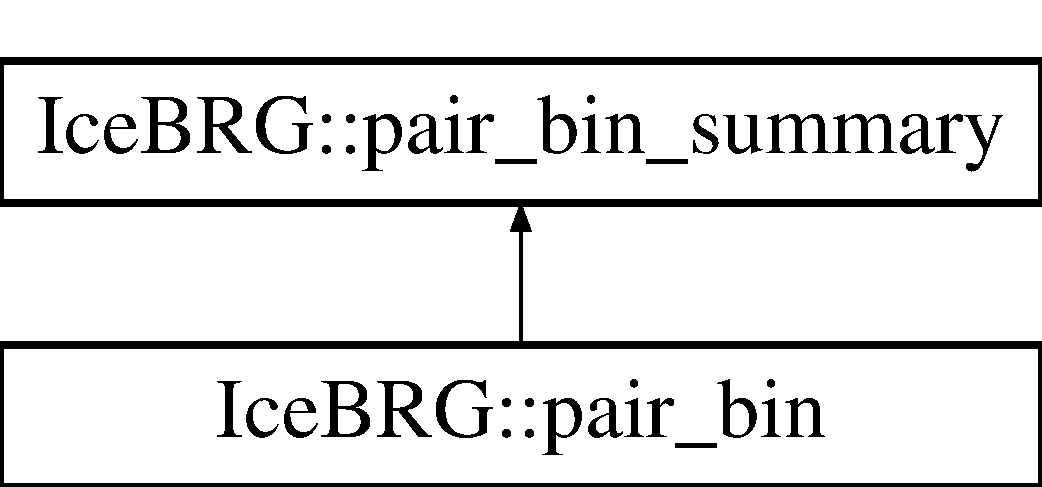
\includegraphics[height=2.000000cm]{classIceBRG_1_1pair__bin}
\end{center}
\end{figure}
\subsection*{Public Member Functions}
\begin{DoxyCompactItemize}
\item 
\hyperlink{classIceBRG_1_1pair__bin_ab951efb7c961a3910cd30e4eab58fbbf}{pair\-\_\-bin} (const \hyperlink{namespaceIceBRG_a45499647eb87e24c10ab32c628711cec}{distance\-\_\-type} \&init\-\_\-\-R\-\_\-min=0, const \hyperlink{namespaceIceBRG_a45499647eb87e24c10ab32c628711cec}{distance\-\_\-type} \&init\-\_\-\-R\-\_\-max=0, const \hyperlink{namespaceIceBRG_a1be72ac4918a9b029f2eefa084213e35}{mass\-\_\-type} \&init\-\_\-m\-\_\-min=0, const \hyperlink{namespaceIceBRG_a1be72ac4918a9b029f2eefa084213e35}{mass\-\_\-type} \&init\-\_\-m\-\_\-max=0, const \hyperlink{lib_2IceBRG__main_2common_8h_ad0f130a56eeb944d9ef2692ee881ecc4}{flt\-\_\-type} \&init\-\_\-z\-\_\-min=0, const \hyperlink{lib_2IceBRG__main_2common_8h_ad0f130a56eeb944d9ef2692ee881ecc4}{flt\-\_\-type} \&init\-\_\-z\-\_\-max=0, const \hyperlink{lib_2IceBRG__main_2common_8h_ad0f130a56eeb944d9ef2692ee881ecc4}{flt\-\_\-type} \&init\-\_\-mag\-\_\-min=0, const \hyperlink{lib_2IceBRG__main_2common_8h_ad0f130a56eeb944d9ef2692ee881ecc4}{flt\-\_\-type} \&init\-\_\-mag\-\_\-max=0, const \hyperlink{lib_2IceBRG__main_2common_8h_ad0f130a56eeb944d9ef2692ee881ecc4}{flt\-\_\-type} \&init\-\_\-z\-\_\-buffer=\-\_\-z\-\_\-buffer\-\_\-default\-\_\-value\-\_\-)
\item 
virtual \hyperlink{classIceBRG_1_1pair__bin_a66e756e18910966d7455a3bf35e39b7d}{$\sim$pair\-\_\-bin} ()
\item 
void \hyperlink{classIceBRG_1_1pair__bin_a679b3e87b4414c9ef2f2192e46ca5dbe}{set\-\_\-z\-\_\-buffer} (const \hyperlink{lib_2IceBRG__main_2common_8h_ad0f130a56eeb944d9ef2692ee881ecc4}{flt\-\_\-type} \&new\-\_\-z\-\_\-buffer)
\item 
\hyperlink{lib_2IceBRG__main_2common_8h_ad0f130a56eeb944d9ef2692ee881ecc4}{flt\-\_\-type} \hyperlink{classIceBRG_1_1pair__bin_a3712b1f0714d9c7dbd4e3f8bb5f92bdd}{z\-\_\-buffer} () const 
\item 
void \hyperlink{classIceBRG_1_1pair__bin_a2e97e0e531f74f95285029f40af20f04}{add\-\_\-pair} (const \hyperlink{classIceBRG_1_1lens__source__pair}{lens\-\_\-source\-\_\-pair} \&new\-\_\-pair)
\item 
void \hyperlink{classIceBRG_1_1pair__bin_a64e16e56545c85dd67180c9205c554eb}{add\-\_\-lens} (const \hyperlink{structIceBRG_1_1lens__id}{lens\-\_\-id} \&lens)
\item 
virtual void \hyperlink{classIceBRG_1_1pair__bin_accb7e0a9d26acf6b3444160f2c3718c5}{clear} () override
\item 
virtual \hyperlink{lib_2IceBRG__main_2common_8h_ab322a3e50421dc5f0c43316b1b373592}{ssize\-\_\-t} \hyperlink{classIceBRG_1_1pair__bin_aa925118f3137ef62adac11917cdd43a6}{pair\-\_\-count} () const override
\item 
virtual \hyperlink{lib_2IceBRG__main_2common_8h_ab322a3e50421dc5f0c43316b1b373592}{ssize\-\_\-t} \hyperlink{classIceBRG_1_1pair__bin_ae850b22e0eebeb779abfd116ba2e9c4d}{shear\-\_\-pair\-\_\-count} () const override
\item 
virtual \hyperlink{lib_2IceBRG__main_2common_8h_ab322a3e50421dc5f0c43316b1b373592}{ssize\-\_\-t} \hyperlink{classIceBRG_1_1pair__bin_ad1d60049cc8739ceffe806ee83d5885e}{magf\-\_\-pair\-\_\-count} () const override
\item 
virtual \hyperlink{lib_2IceBRG__main_2common_8h_ad0f130a56eeb944d9ef2692ee881ecc4}{flt\-\_\-type} \hyperlink{classIceBRG_1_1pair__bin_a5d3541adaae91d9ce3e21808990fde3c}{effective\-\_\-pair\-\_\-count} () const override
\item 
virtual \hyperlink{lib_2IceBRG__main_2common_8h_ad0f130a56eeb944d9ef2692ee881ecc4}{flt\-\_\-type} \hyperlink{classIceBRG_1_1pair__bin_a2c2e3a12667cd62ae33ba9fb7cc32a6f}{shear\-\_\-effective\-\_\-pair\-\_\-count} () const override
\item 
virtual \hyperlink{lib_2IceBRG__main_2common_8h_ad0f130a56eeb944d9ef2692ee881ecc4}{flt\-\_\-type} \hyperlink{classIceBRG_1_1pair__bin_a40a7e3fb147261cd1e7a27941e539782}{sum\-\_\-of\-\_\-weights} () const override
\item 
virtual \hyperlink{lib_2IceBRG__main_2common_8h_ad0f130a56eeb944d9ef2692ee881ecc4}{flt\-\_\-type} \hyperlink{classIceBRG_1_1pair__bin_a83548bff5f98aaa82a962e399b00cc62}{shear\-\_\-sum\-\_\-of\-\_\-weights} () const override
\item 
virtual \hyperlink{lib_2IceBRG__main_2common_8h_ad0f130a56eeb944d9ef2692ee881ecc4}{flt\-\_\-type} \hyperlink{classIceBRG_1_1pair__bin_aa0628069056a8128ff35c30bcc9a4f0e}{magf\-\_\-sum\-\_\-of\-\_\-weights} () const override
\item 
virtual \hyperlink{lib_2IceBRG__main_2common_8h_ad0f130a56eeb944d9ef2692ee881ecc4}{flt\-\_\-type} \hyperlink{classIceBRG_1_1pair__bin_a561b0ec911ba8f12b49dd7fc0414945e}{sum\-\_\-of\-\_\-square\-\_\-weights} () const override
\item 
virtual \hyperlink{lib_2IceBRG__main_2common_8h_ad0f130a56eeb944d9ef2692ee881ecc4}{flt\-\_\-type} \hyperlink{classIceBRG_1_1pair__bin_a46fa56e1ed62cb416d0052f0c65bcfec}{shear\-\_\-sum\-\_\-of\-\_\-square\-\_\-weights} () const override
\item 
virtual \hyperlink{lib_2IceBRG__main_2common_8h_ad0f130a56eeb944d9ef2692ee881ecc4}{flt\-\_\-type} \hyperlink{classIceBRG_1_1pair__bin_a75c4c2e84da0dcba8cf61ab385b707d7}{magf\-\_\-sum\-\_\-of\-\_\-square\-\_\-weights} () const override
\item 
virtual \hyperlink{lib_2IceBRG__main_2common_8h_ab322a3e50421dc5f0c43316b1b373592}{ssize\-\_\-t} \hyperlink{classIceBRG_1_1pair__bin_a01423504509d85c42ea44fd57d8a7f5c}{num\-\_\-lenses} () const override
\item 
virtual \hyperlink{lib_2IceBRG__main_2common_8h_ab322a3e50421dc5f0c43316b1b373592}{ssize\-\_\-t} \hyperlink{classIceBRG_1_1pair__bin_a0b8e51e2d55e7cd29614200a15499c84}{magf\-\_\-num\-\_\-lenses} () const override
\item 
virtual \hyperlink{namespaceIceBRG_a45499647eb87e24c10ab32c628711cec}{distance\-\_\-type} \hyperlink{classIceBRG_1_1pair__bin_a152c37388d0e8f71913876163c63b00e}{R\-\_\-mean} () const override
\item 
virtual \hyperlink{namespaceIceBRG_a45499647eb87e24c10ab32c628711cec}{distance\-\_\-type} \hyperlink{classIceBRG_1_1pair__bin_a25dc02b15e390360b5e13247b64c6807}{shear\-\_\-\-R\-\_\-mean} () const override
\item 
virtual \hyperlink{namespaceIceBRG_a45499647eb87e24c10ab32c628711cec}{distance\-\_\-type} \hyperlink{classIceBRG_1_1pair__bin_a103154353b144fd1a12f4fa39a2e5a2f}{magf\-\_\-\-R\-\_\-mean} () const override
\item 
virtual \hyperlink{namespaceIceBRG_a1be72ac4918a9b029f2eefa084213e35}{mass\-\_\-type} \hyperlink{classIceBRG_1_1pair__bin_a8d58f06df8b758e40706c4c14d76dda6}{lens\-\_\-m\-\_\-mean} () const override
\item 
virtual \hyperlink{namespaceIceBRG_a1be72ac4918a9b029f2eefa084213e35}{mass\-\_\-type} \hyperlink{classIceBRG_1_1pair__bin_a9bd588d9276bc4fd9095afac84708e36}{shear\-\_\-lens\-\_\-m\-\_\-mean} () const override
\item 
virtual \hyperlink{namespaceIceBRG_a1be72ac4918a9b029f2eefa084213e35}{mass\-\_\-type} \hyperlink{classIceBRG_1_1pair__bin_a48fb57c34a1e3ae0e62908f37214db65}{magf\-\_\-lens\-\_\-m\-\_\-mean} () const override
\item 
virtual \hyperlink{lib_2IceBRG__main_2common_8h_ad0f130a56eeb944d9ef2692ee881ecc4}{flt\-\_\-type} \hyperlink{classIceBRG_1_1pair__bin_aad3491ebd1974d3e86a3f50b09719a2c}{lens\-\_\-z\-\_\-mean} () const override
\item 
virtual \hyperlink{lib_2IceBRG__main_2common_8h_ad0f130a56eeb944d9ef2692ee881ecc4}{flt\-\_\-type} \hyperlink{classIceBRG_1_1pair__bin_a64cf13aade51455237e85d97501a869f}{shear\-\_\-lens\-\_\-z\-\_\-mean} () const override
\item 
virtual \hyperlink{lib_2IceBRG__main_2common_8h_ad0f130a56eeb944d9ef2692ee881ecc4}{flt\-\_\-type} \hyperlink{classIceBRG_1_1pair__bin_ac3d2072b331e60cb080c95c70df3ef1d}{magf\-\_\-lens\-\_\-z\-\_\-mean} () const override
\item 
virtual \hyperlink{lib_2IceBRG__main_2common_8h_ad0f130a56eeb944d9ef2692ee881ecc4}{flt\-\_\-type} \hyperlink{classIceBRG_1_1pair__bin_abbdc48e06437dcf104b68aece65d42a6}{lens\-\_\-mag\-\_\-mean} () const override
\item 
virtual \hyperlink{lib_2IceBRG__main_2common_8h_ad0f130a56eeb944d9ef2692ee881ecc4}{flt\-\_\-type} \hyperlink{classIceBRG_1_1pair__bin_acb5e1c7fc10545213710584bcecf1374}{shear\-\_\-lens\-\_\-mag\-\_\-mean} () const override
\item 
virtual \hyperlink{lib_2IceBRG__main_2common_8h_ad0f130a56eeb944d9ef2692ee881ecc4}{flt\-\_\-type} \hyperlink{classIceBRG_1_1pair__bin_a6cf7966055f41881da7775bd005ea704}{magf\-\_\-lens\-\_\-mag\-\_\-mean} () const override
\item 
virtual \hyperlink{lib_2IceBRG__main_2common_8h_ad0f130a56eeb944d9ef2692ee881ecc4}{flt\-\_\-type} \hyperlink{classIceBRG_1_1pair__bin_ace5421f980b509091b31fc03eda49a20}{source\-\_\-z\-\_\-mean} () const override
\item 
virtual \hyperlink{lib_2IceBRG__main_2common_8h_ad0f130a56eeb944d9ef2692ee881ecc4}{flt\-\_\-type} \hyperlink{classIceBRG_1_1pair__bin_a0caa7e96d7b30a254fdd1f7119547e06}{shear\-\_\-source\-\_\-z\-\_\-mean} () const override
\item 
virtual \hyperlink{lib_2IceBRG__main_2common_8h_ad0f130a56eeb944d9ef2692ee881ecc4}{flt\-\_\-type} \hyperlink{classIceBRG_1_1pair__bin_a26b687b2c34a8dd88dd33dd23d642efd}{magf\-\_\-source\-\_\-z\-\_\-mean} () const override
\item 
\hyperlink{lib_2IceBRG__main_2common_8h_ad0f130a56eeb944d9ef2692ee881ecc4}{flt\-\_\-type} \hyperlink{classIceBRG_1_1pair__bin_ac1c89162f70ad44b767042e16c269983}{unmasked\-\_\-frac} () const 
\item 
virtual custom\-\_\-unit\-\_\-type$<$ 0, 0, 0, 2, 0 $>$ \hyperlink{classIceBRG_1_1pair__bin_a6711847f96e596a1855d92b1b17311c7}{area} () const override
\item 
virtual \hyperlink{namespaceIceBRG_a80c597ef5ba0a32491d32a9f0083b02d}{surface\-\_\-density\-\_\-type} \hyperlink{classIceBRG_1_1pair__bin_a0debbbbb5351fc7f7049920e9c205d50}{delta\-\_\-\-Sigma\-\_\-t\-\_\-mean} () const override
\item 
virtual \hyperlink{namespaceIceBRG_a80c597ef5ba0a32491d32a9f0083b02d}{surface\-\_\-density\-\_\-type} \hyperlink{classIceBRG_1_1pair__bin_a679e7a20930d08852c6c4fd9eca9f126}{delta\-\_\-\-Sigma\-\_\-x\-\_\-mean} () const override
\item 
virtual custom\-\_\-unit\-\_\-type$<$-\/4, 0, 2, 0, 0 $>$ \hyperlink{classIceBRG_1_1pair__bin_ad3c15af884bc5074edee7388a1da606b}{delta\-\_\-\-Sigma\-\_\-t\-\_\-mean\-\_\-square} () const override
\item 
virtual custom\-\_\-unit\-\_\-type$<$-\/4, 0, 2, 0, 0 $>$ \hyperlink{classIceBRG_1_1pair__bin_af8b30d6f2568753c7200c280cb353918}{delta\-\_\-\-Sigma\-\_\-x\-\_\-mean\-\_\-square} () const override
\item 
virtual \hyperlink{namespaceIceBRG_a80c597ef5ba0a32491d32a9f0083b02d}{surface\-\_\-density\-\_\-type} \hyperlink{classIceBRG_1_1pair__bin_a38a2f38e2f4a97ed21641c471e6011a1}{delta\-\_\-\-Sigma\-\_\-t\-\_\-std} () const override
\item 
virtual \hyperlink{namespaceIceBRG_a80c597ef5ba0a32491d32a9f0083b02d}{surface\-\_\-density\-\_\-type} \hyperlink{classIceBRG_1_1pair__bin_ab31ca9e34af863727ae642ec95174afc}{delta\-\_\-\-Sigma\-\_\-x\-\_\-std} () const override
\item 
virtual \hyperlink{namespaceIceBRG_a80c597ef5ba0a32491d32a9f0083b02d}{surface\-\_\-density\-\_\-type} \hyperlink{classIceBRG_1_1pair__bin_abd17f66f888eb808420b445b2dec2f57}{delta\-\_\-\-Sigma\-\_\-t\-\_\-stderr} () const override
\item 
virtual \hyperlink{namespaceIceBRG_a80c597ef5ba0a32491d32a9f0083b02d}{surface\-\_\-density\-\_\-type} \hyperlink{classIceBRG_1_1pair__bin_a626753cce2e35d56cd4a07a5e0d7ea16}{delta\-\_\-\-Sigma\-\_\-x\-\_\-stderr} () const override
\item 
virtual \hyperlink{lib_2IceBRG__main_2common_8h_ad0f130a56eeb944d9ef2692ee881ecc4}{flt\-\_\-type} \hyperlink{classIceBRG_1_1pair__bin_abad2af4939b8fe1c303db7af8748fa52}{mu\-\_\-hat} () const override
\item 
virtual \hyperlink{lib_2IceBRG__main_2common_8h_ad0f130a56eeb944d9ef2692ee881ecc4}{flt\-\_\-type} \hyperlink{classIceBRG_1_1pair__bin_a2b30f0bd4f0405e4b4ca86e525a1a4f9}{mu\-\_\-square\-\_\-hat} () const override
\item 
virtual \hyperlink{lib_2IceBRG__main_2common_8h_ad0f130a56eeb944d9ef2692ee881ecc4}{flt\-\_\-type} \hyperlink{classIceBRG_1_1pair__bin_a7974296df81879f06fcf62d36bdd64f4}{mu\-\_\-\-W} () const override
\end{DoxyCompactItemize}
\subsection*{Protected Member Functions}
\begin{DoxyCompactItemize}
\item 
void \hyperlink{classIceBRG_1_1pair__bin_af6ee5173022f9fa8b4528b7d6e18b0d2}{\-\_\-uncache\-\_\-values} ()
\end{DoxyCompactItemize}


\subsection{Constructor \& Destructor Documentation}
\hypertarget{classIceBRG_1_1pair__bin_ab951efb7c961a3910cd30e4eab58fbbf}{\index{Ice\-B\-R\-G\-::pair\-\_\-bin@{Ice\-B\-R\-G\-::pair\-\_\-bin}!pair\-\_\-bin@{pair\-\_\-bin}}
\index{pair\-\_\-bin@{pair\-\_\-bin}!IceBRG::pair_bin@{Ice\-B\-R\-G\-::pair\-\_\-bin}}
\subsubsection[{pair\-\_\-bin}]{\setlength{\rightskip}{0pt plus 5cm}Ice\-B\-R\-G\-::pair\-\_\-bin\-::pair\-\_\-bin (
\begin{DoxyParamCaption}
\item[{const {\bf distance\-\_\-type} \&}]{init\-\_\-\-R\-\_\-min = {\ttfamily 0}, }
\item[{const {\bf distance\-\_\-type} \&}]{init\-\_\-\-R\-\_\-max = {\ttfamily 0}, }
\item[{const {\bf mass\-\_\-type} \&}]{init\-\_\-m\-\_\-min = {\ttfamily 0}, }
\item[{const {\bf mass\-\_\-type} \&}]{init\-\_\-m\-\_\-max = {\ttfamily 0}, }
\item[{const {\bf flt\-\_\-type} \&}]{init\-\_\-z\-\_\-min = {\ttfamily 0}, }
\item[{const {\bf flt\-\_\-type} \&}]{init\-\_\-z\-\_\-max = {\ttfamily 0}, }
\item[{const {\bf flt\-\_\-type} \&}]{init\-\_\-mag\-\_\-min = {\ttfamily 0}, }
\item[{const {\bf flt\-\_\-type} \&}]{init\-\_\-mag\-\_\-max = {\ttfamily 0}, }
\item[{const {\bf flt\-\_\-type} \&}]{init\-\_\-z\-\_\-buffer = {\ttfamily \-\_\-z\-\_\-buffer\-\_\-default\-\_\-value\-\_\-}}
\end{DoxyParamCaption}
)}}\label{classIceBRG_1_1pair__bin_ab951efb7c961a3910cd30e4eab58fbbf}
\hypertarget{classIceBRG_1_1pair__bin_a66e756e18910966d7455a3bf35e39b7d}{\index{Ice\-B\-R\-G\-::pair\-\_\-bin@{Ice\-B\-R\-G\-::pair\-\_\-bin}!$\sim$pair\-\_\-bin@{$\sim$pair\-\_\-bin}}
\index{$\sim$pair\-\_\-bin@{$\sim$pair\-\_\-bin}!IceBRG::pair_bin@{Ice\-B\-R\-G\-::pair\-\_\-bin}}
\subsubsection[{$\sim$pair\-\_\-bin}]{\setlength{\rightskip}{0pt plus 5cm}virtual Ice\-B\-R\-G\-::pair\-\_\-bin\-::$\sim$pair\-\_\-bin (
\begin{DoxyParamCaption}
{}
\end{DoxyParamCaption}
)\hspace{0.3cm}{\ttfamily [inline]}, {\ttfamily [virtual]}}}\label{classIceBRG_1_1pair__bin_a66e756e18910966d7455a3bf35e39b7d}


\subsection{Member Function Documentation}
\hypertarget{classIceBRG_1_1pair__bin_af6ee5173022f9fa8b4528b7d6e18b0d2}{\index{Ice\-B\-R\-G\-::pair\-\_\-bin@{Ice\-B\-R\-G\-::pair\-\_\-bin}!\-\_\-uncache\-\_\-values@{\-\_\-uncache\-\_\-values}}
\index{\-\_\-uncache\-\_\-values@{\-\_\-uncache\-\_\-values}!IceBRG::pair_bin@{Ice\-B\-R\-G\-::pair\-\_\-bin}}
\subsubsection[{\-\_\-uncache\-\_\-values}]{\setlength{\rightskip}{0pt plus 5cm}void Ice\-B\-R\-G\-::pair\-\_\-bin\-::\-\_\-uncache\-\_\-values (
\begin{DoxyParamCaption}
{}
\end{DoxyParamCaption}
)\hspace{0.3cm}{\ttfamily [protected]}, {\ttfamily [virtual]}}}\label{classIceBRG_1_1pair__bin_af6ee5173022f9fa8b4528b7d6e18b0d2}


Reimplemented from \hyperlink{classIceBRG_1_1pair__bin__summary_a3e0113d3900e9eebb0f80d5681e6dd95}{Ice\-B\-R\-G\-::pair\-\_\-bin\-\_\-summary}.

\hypertarget{classIceBRG_1_1pair__bin_a64e16e56545c85dd67180c9205c554eb}{\index{Ice\-B\-R\-G\-::pair\-\_\-bin@{Ice\-B\-R\-G\-::pair\-\_\-bin}!add\-\_\-lens@{add\-\_\-lens}}
\index{add\-\_\-lens@{add\-\_\-lens}!IceBRG::pair_bin@{Ice\-B\-R\-G\-::pair\-\_\-bin}}
\subsubsection[{add\-\_\-lens}]{\setlength{\rightskip}{0pt plus 5cm}void Ice\-B\-R\-G\-::pair\-\_\-bin\-::add\-\_\-lens (
\begin{DoxyParamCaption}
\item[{const {\bf lens\-\_\-id} \&}]{lens}
\end{DoxyParamCaption}
)}}\label{classIceBRG_1_1pair__bin_a64e16e56545c85dd67180c9205c554eb}
\hypertarget{classIceBRG_1_1pair__bin_a2e97e0e531f74f95285029f40af20f04}{\index{Ice\-B\-R\-G\-::pair\-\_\-bin@{Ice\-B\-R\-G\-::pair\-\_\-bin}!add\-\_\-pair@{add\-\_\-pair}}
\index{add\-\_\-pair@{add\-\_\-pair}!IceBRG::pair_bin@{Ice\-B\-R\-G\-::pair\-\_\-bin}}
\subsubsection[{add\-\_\-pair}]{\setlength{\rightskip}{0pt plus 5cm}void Ice\-B\-R\-G\-::pair\-\_\-bin\-::add\-\_\-pair (
\begin{DoxyParamCaption}
\item[{const {\bf lens\-\_\-source\-\_\-pair} \&}]{new\-\_\-pair}
\end{DoxyParamCaption}
)}}\label{classIceBRG_1_1pair__bin_a2e97e0e531f74f95285029f40af20f04}
\hypertarget{classIceBRG_1_1pair__bin_a6711847f96e596a1855d92b1b17311c7}{\index{Ice\-B\-R\-G\-::pair\-\_\-bin@{Ice\-B\-R\-G\-::pair\-\_\-bin}!area@{area}}
\index{area@{area}!IceBRG::pair_bin@{Ice\-B\-R\-G\-::pair\-\_\-bin}}
\subsubsection[{area}]{\setlength{\rightskip}{0pt plus 5cm}custom\-\_\-unit\-\_\-type$<$ 0, 0, 0, 2, 0 $>$ Ice\-B\-R\-G\-::pair\-\_\-bin\-::area (
\begin{DoxyParamCaption}
{}
\end{DoxyParamCaption}
) const\hspace{0.3cm}{\ttfamily [override]}, {\ttfamily [virtual]}}}\label{classIceBRG_1_1pair__bin_a6711847f96e596a1855d92b1b17311c7}


Reimplemented from \hyperlink{classIceBRG_1_1pair__bin__summary_a6c0d9413d2cab3f09e96947dc08b6841}{Ice\-B\-R\-G\-::pair\-\_\-bin\-\_\-summary}.

\hypertarget{classIceBRG_1_1pair__bin_accb7e0a9d26acf6b3444160f2c3718c5}{\index{Ice\-B\-R\-G\-::pair\-\_\-bin@{Ice\-B\-R\-G\-::pair\-\_\-bin}!clear@{clear}}
\index{clear@{clear}!IceBRG::pair_bin@{Ice\-B\-R\-G\-::pair\-\_\-bin}}
\subsubsection[{clear}]{\setlength{\rightskip}{0pt plus 5cm}void Ice\-B\-R\-G\-::pair\-\_\-bin\-::clear (
\begin{DoxyParamCaption}
{}
\end{DoxyParamCaption}
)\hspace{0.3cm}{\ttfamily [override]}, {\ttfamily [virtual]}}}\label{classIceBRG_1_1pair__bin_accb7e0a9d26acf6b3444160f2c3718c5}


Reimplemented from \hyperlink{classIceBRG_1_1pair__bin__summary_a916bb85a5a7b6be8ec21305beddcb966}{Ice\-B\-R\-G\-::pair\-\_\-bin\-\_\-summary}.

\hypertarget{classIceBRG_1_1pair__bin_a0debbbbb5351fc7f7049920e9c205d50}{\index{Ice\-B\-R\-G\-::pair\-\_\-bin@{Ice\-B\-R\-G\-::pair\-\_\-bin}!delta\-\_\-\-Sigma\-\_\-t\-\_\-mean@{delta\-\_\-\-Sigma\-\_\-t\-\_\-mean}}
\index{delta\-\_\-\-Sigma\-\_\-t\-\_\-mean@{delta\-\_\-\-Sigma\-\_\-t\-\_\-mean}!IceBRG::pair_bin@{Ice\-B\-R\-G\-::pair\-\_\-bin}}
\subsubsection[{delta\-\_\-\-Sigma\-\_\-t\-\_\-mean}]{\setlength{\rightskip}{0pt plus 5cm}{\bf surface\-\_\-density\-\_\-type} Ice\-B\-R\-G\-::pair\-\_\-bin\-::delta\-\_\-\-Sigma\-\_\-t\-\_\-mean (
\begin{DoxyParamCaption}
{}
\end{DoxyParamCaption}
) const\hspace{0.3cm}{\ttfamily [override]}, {\ttfamily [virtual]}}}\label{classIceBRG_1_1pair__bin_a0debbbbb5351fc7f7049920e9c205d50}


Reimplemented from \hyperlink{classIceBRG_1_1pair__bin__summary_a2a1372bfa03a186425920b839ce38f4a}{Ice\-B\-R\-G\-::pair\-\_\-bin\-\_\-summary}.

\hypertarget{classIceBRG_1_1pair__bin_ad3c15af884bc5074edee7388a1da606b}{\index{Ice\-B\-R\-G\-::pair\-\_\-bin@{Ice\-B\-R\-G\-::pair\-\_\-bin}!delta\-\_\-\-Sigma\-\_\-t\-\_\-mean\-\_\-square@{delta\-\_\-\-Sigma\-\_\-t\-\_\-mean\-\_\-square}}
\index{delta\-\_\-\-Sigma\-\_\-t\-\_\-mean\-\_\-square@{delta\-\_\-\-Sigma\-\_\-t\-\_\-mean\-\_\-square}!IceBRG::pair_bin@{Ice\-B\-R\-G\-::pair\-\_\-bin}}
\subsubsection[{delta\-\_\-\-Sigma\-\_\-t\-\_\-mean\-\_\-square}]{\setlength{\rightskip}{0pt plus 5cm}custom\-\_\-unit\-\_\-type$<$-\/4, 0, 2, 0, 0 $>$ Ice\-B\-R\-G\-::pair\-\_\-bin\-::delta\-\_\-\-Sigma\-\_\-t\-\_\-mean\-\_\-square (
\begin{DoxyParamCaption}
{}
\end{DoxyParamCaption}
) const\hspace{0.3cm}{\ttfamily [override]}, {\ttfamily [virtual]}}}\label{classIceBRG_1_1pair__bin_ad3c15af884bc5074edee7388a1da606b}


Reimplemented from \hyperlink{classIceBRG_1_1pair__bin__summary_a752e84b6a079f91bbc64bfc746ec5b5d}{Ice\-B\-R\-G\-::pair\-\_\-bin\-\_\-summary}.

\hypertarget{classIceBRG_1_1pair__bin_a38a2f38e2f4a97ed21641c471e6011a1}{\index{Ice\-B\-R\-G\-::pair\-\_\-bin@{Ice\-B\-R\-G\-::pair\-\_\-bin}!delta\-\_\-\-Sigma\-\_\-t\-\_\-std@{delta\-\_\-\-Sigma\-\_\-t\-\_\-std}}
\index{delta\-\_\-\-Sigma\-\_\-t\-\_\-std@{delta\-\_\-\-Sigma\-\_\-t\-\_\-std}!IceBRG::pair_bin@{Ice\-B\-R\-G\-::pair\-\_\-bin}}
\subsubsection[{delta\-\_\-\-Sigma\-\_\-t\-\_\-std}]{\setlength{\rightskip}{0pt plus 5cm}{\bf surface\-\_\-density\-\_\-type} Ice\-B\-R\-G\-::pair\-\_\-bin\-::delta\-\_\-\-Sigma\-\_\-t\-\_\-std (
\begin{DoxyParamCaption}
{}
\end{DoxyParamCaption}
) const\hspace{0.3cm}{\ttfamily [override]}, {\ttfamily [virtual]}}}\label{classIceBRG_1_1pair__bin_a38a2f38e2f4a97ed21641c471e6011a1}


Reimplemented from \hyperlink{classIceBRG_1_1pair__bin__summary_acd510011670a535d609e4ecb2fa8257f}{Ice\-B\-R\-G\-::pair\-\_\-bin\-\_\-summary}.

\hypertarget{classIceBRG_1_1pair__bin_abd17f66f888eb808420b445b2dec2f57}{\index{Ice\-B\-R\-G\-::pair\-\_\-bin@{Ice\-B\-R\-G\-::pair\-\_\-bin}!delta\-\_\-\-Sigma\-\_\-t\-\_\-stderr@{delta\-\_\-\-Sigma\-\_\-t\-\_\-stderr}}
\index{delta\-\_\-\-Sigma\-\_\-t\-\_\-stderr@{delta\-\_\-\-Sigma\-\_\-t\-\_\-stderr}!IceBRG::pair_bin@{Ice\-B\-R\-G\-::pair\-\_\-bin}}
\subsubsection[{delta\-\_\-\-Sigma\-\_\-t\-\_\-stderr}]{\setlength{\rightskip}{0pt plus 5cm}{\bf surface\-\_\-density\-\_\-type} Ice\-B\-R\-G\-::pair\-\_\-bin\-::delta\-\_\-\-Sigma\-\_\-t\-\_\-stderr (
\begin{DoxyParamCaption}
{}
\end{DoxyParamCaption}
) const\hspace{0.3cm}{\ttfamily [override]}, {\ttfamily [virtual]}}}\label{classIceBRG_1_1pair__bin_abd17f66f888eb808420b445b2dec2f57}


Reimplemented from \hyperlink{classIceBRG_1_1pair__bin__summary_a61f9c6863d1a2440e8d8c7d794b3c8c5}{Ice\-B\-R\-G\-::pair\-\_\-bin\-\_\-summary}.

\hypertarget{classIceBRG_1_1pair__bin_a679e7a20930d08852c6c4fd9eca9f126}{\index{Ice\-B\-R\-G\-::pair\-\_\-bin@{Ice\-B\-R\-G\-::pair\-\_\-bin}!delta\-\_\-\-Sigma\-\_\-x\-\_\-mean@{delta\-\_\-\-Sigma\-\_\-x\-\_\-mean}}
\index{delta\-\_\-\-Sigma\-\_\-x\-\_\-mean@{delta\-\_\-\-Sigma\-\_\-x\-\_\-mean}!IceBRG::pair_bin@{Ice\-B\-R\-G\-::pair\-\_\-bin}}
\subsubsection[{delta\-\_\-\-Sigma\-\_\-x\-\_\-mean}]{\setlength{\rightskip}{0pt plus 5cm}{\bf surface\-\_\-density\-\_\-type} Ice\-B\-R\-G\-::pair\-\_\-bin\-::delta\-\_\-\-Sigma\-\_\-x\-\_\-mean (
\begin{DoxyParamCaption}
{}
\end{DoxyParamCaption}
) const\hspace{0.3cm}{\ttfamily [override]}, {\ttfamily [virtual]}}}\label{classIceBRG_1_1pair__bin_a679e7a20930d08852c6c4fd9eca9f126}


Reimplemented from \hyperlink{classIceBRG_1_1pair__bin__summary_a8e885aafb07552b829d1d75db54d93b4}{Ice\-B\-R\-G\-::pair\-\_\-bin\-\_\-summary}.

\hypertarget{classIceBRG_1_1pair__bin_af8b30d6f2568753c7200c280cb353918}{\index{Ice\-B\-R\-G\-::pair\-\_\-bin@{Ice\-B\-R\-G\-::pair\-\_\-bin}!delta\-\_\-\-Sigma\-\_\-x\-\_\-mean\-\_\-square@{delta\-\_\-\-Sigma\-\_\-x\-\_\-mean\-\_\-square}}
\index{delta\-\_\-\-Sigma\-\_\-x\-\_\-mean\-\_\-square@{delta\-\_\-\-Sigma\-\_\-x\-\_\-mean\-\_\-square}!IceBRG::pair_bin@{Ice\-B\-R\-G\-::pair\-\_\-bin}}
\subsubsection[{delta\-\_\-\-Sigma\-\_\-x\-\_\-mean\-\_\-square}]{\setlength{\rightskip}{0pt plus 5cm}custom\-\_\-unit\-\_\-type$<$-\/4, 0, 2, 0, 0 $>$ Ice\-B\-R\-G\-::pair\-\_\-bin\-::delta\-\_\-\-Sigma\-\_\-x\-\_\-mean\-\_\-square (
\begin{DoxyParamCaption}
{}
\end{DoxyParamCaption}
) const\hspace{0.3cm}{\ttfamily [override]}, {\ttfamily [virtual]}}}\label{classIceBRG_1_1pair__bin_af8b30d6f2568753c7200c280cb353918}


Reimplemented from \hyperlink{classIceBRG_1_1pair__bin__summary_aa16505e993ab66451519a9ed4304c9a8}{Ice\-B\-R\-G\-::pair\-\_\-bin\-\_\-summary}.

\hypertarget{classIceBRG_1_1pair__bin_ab31ca9e34af863727ae642ec95174afc}{\index{Ice\-B\-R\-G\-::pair\-\_\-bin@{Ice\-B\-R\-G\-::pair\-\_\-bin}!delta\-\_\-\-Sigma\-\_\-x\-\_\-std@{delta\-\_\-\-Sigma\-\_\-x\-\_\-std}}
\index{delta\-\_\-\-Sigma\-\_\-x\-\_\-std@{delta\-\_\-\-Sigma\-\_\-x\-\_\-std}!IceBRG::pair_bin@{Ice\-B\-R\-G\-::pair\-\_\-bin}}
\subsubsection[{delta\-\_\-\-Sigma\-\_\-x\-\_\-std}]{\setlength{\rightskip}{0pt plus 5cm}{\bf surface\-\_\-density\-\_\-type} Ice\-B\-R\-G\-::pair\-\_\-bin\-::delta\-\_\-\-Sigma\-\_\-x\-\_\-std (
\begin{DoxyParamCaption}
{}
\end{DoxyParamCaption}
) const\hspace{0.3cm}{\ttfamily [override]}, {\ttfamily [virtual]}}}\label{classIceBRG_1_1pair__bin_ab31ca9e34af863727ae642ec95174afc}


Reimplemented from \hyperlink{classIceBRG_1_1pair__bin__summary_a1779c3cbeaa111f27727d70481fb7ff9}{Ice\-B\-R\-G\-::pair\-\_\-bin\-\_\-summary}.

\hypertarget{classIceBRG_1_1pair__bin_a626753cce2e35d56cd4a07a5e0d7ea16}{\index{Ice\-B\-R\-G\-::pair\-\_\-bin@{Ice\-B\-R\-G\-::pair\-\_\-bin}!delta\-\_\-\-Sigma\-\_\-x\-\_\-stderr@{delta\-\_\-\-Sigma\-\_\-x\-\_\-stderr}}
\index{delta\-\_\-\-Sigma\-\_\-x\-\_\-stderr@{delta\-\_\-\-Sigma\-\_\-x\-\_\-stderr}!IceBRG::pair_bin@{Ice\-B\-R\-G\-::pair\-\_\-bin}}
\subsubsection[{delta\-\_\-\-Sigma\-\_\-x\-\_\-stderr}]{\setlength{\rightskip}{0pt plus 5cm}{\bf surface\-\_\-density\-\_\-type} Ice\-B\-R\-G\-::pair\-\_\-bin\-::delta\-\_\-\-Sigma\-\_\-x\-\_\-stderr (
\begin{DoxyParamCaption}
{}
\end{DoxyParamCaption}
) const\hspace{0.3cm}{\ttfamily [override]}, {\ttfamily [virtual]}}}\label{classIceBRG_1_1pair__bin_a626753cce2e35d56cd4a07a5e0d7ea16}


Reimplemented from \hyperlink{classIceBRG_1_1pair__bin__summary_a1063e8e122208a24b240fb1e669d786c}{Ice\-B\-R\-G\-::pair\-\_\-bin\-\_\-summary}.

\hypertarget{classIceBRG_1_1pair__bin_a5d3541adaae91d9ce3e21808990fde3c}{\index{Ice\-B\-R\-G\-::pair\-\_\-bin@{Ice\-B\-R\-G\-::pair\-\_\-bin}!effective\-\_\-pair\-\_\-count@{effective\-\_\-pair\-\_\-count}}
\index{effective\-\_\-pair\-\_\-count@{effective\-\_\-pair\-\_\-count}!IceBRG::pair_bin@{Ice\-B\-R\-G\-::pair\-\_\-bin}}
\subsubsection[{effective\-\_\-pair\-\_\-count}]{\setlength{\rightskip}{0pt plus 5cm}virtual {\bf flt\-\_\-type} Ice\-B\-R\-G\-::pair\-\_\-bin\-::effective\-\_\-pair\-\_\-count (
\begin{DoxyParamCaption}
{}
\end{DoxyParamCaption}
) const\hspace{0.3cm}{\ttfamily [inline]}, {\ttfamily [override]}, {\ttfamily [virtual]}}}\label{classIceBRG_1_1pair__bin_a5d3541adaae91d9ce3e21808990fde3c}


Reimplemented from \hyperlink{classIceBRG_1_1pair__bin__summary_a66f311e593f9406545ccaf92c60af40d}{Ice\-B\-R\-G\-::pair\-\_\-bin\-\_\-summary}.

\hypertarget{classIceBRG_1_1pair__bin_a8d58f06df8b758e40706c4c14d76dda6}{\index{Ice\-B\-R\-G\-::pair\-\_\-bin@{Ice\-B\-R\-G\-::pair\-\_\-bin}!lens\-\_\-m\-\_\-mean@{lens\-\_\-m\-\_\-mean}}
\index{lens\-\_\-m\-\_\-mean@{lens\-\_\-m\-\_\-mean}!IceBRG::pair_bin@{Ice\-B\-R\-G\-::pair\-\_\-bin}}
\subsubsection[{lens\-\_\-m\-\_\-mean}]{\setlength{\rightskip}{0pt plus 5cm}virtual {\bf mass\-\_\-type} Ice\-B\-R\-G\-::pair\-\_\-bin\-::lens\-\_\-m\-\_\-mean (
\begin{DoxyParamCaption}
{}
\end{DoxyParamCaption}
) const\hspace{0.3cm}{\ttfamily [inline]}, {\ttfamily [override]}, {\ttfamily [virtual]}}}\label{classIceBRG_1_1pair__bin_a8d58f06df8b758e40706c4c14d76dda6}


Reimplemented from \hyperlink{classIceBRG_1_1pair__bin__summary_a122a0ce13e6615912055317e78cbe163}{Ice\-B\-R\-G\-::pair\-\_\-bin\-\_\-summary}.

\hypertarget{classIceBRG_1_1pair__bin_abbdc48e06437dcf104b68aece65d42a6}{\index{Ice\-B\-R\-G\-::pair\-\_\-bin@{Ice\-B\-R\-G\-::pair\-\_\-bin}!lens\-\_\-mag\-\_\-mean@{lens\-\_\-mag\-\_\-mean}}
\index{lens\-\_\-mag\-\_\-mean@{lens\-\_\-mag\-\_\-mean}!IceBRG::pair_bin@{Ice\-B\-R\-G\-::pair\-\_\-bin}}
\subsubsection[{lens\-\_\-mag\-\_\-mean}]{\setlength{\rightskip}{0pt plus 5cm}virtual {\bf flt\-\_\-type} Ice\-B\-R\-G\-::pair\-\_\-bin\-::lens\-\_\-mag\-\_\-mean (
\begin{DoxyParamCaption}
{}
\end{DoxyParamCaption}
) const\hspace{0.3cm}{\ttfamily [inline]}, {\ttfamily [override]}, {\ttfamily [virtual]}}}\label{classIceBRG_1_1pair__bin_abbdc48e06437dcf104b68aece65d42a6}


Reimplemented from \hyperlink{classIceBRG_1_1pair__bin__summary_ac7f6568e96ca05b14958903473a5f65b}{Ice\-B\-R\-G\-::pair\-\_\-bin\-\_\-summary}.

\hypertarget{classIceBRG_1_1pair__bin_aad3491ebd1974d3e86a3f50b09719a2c}{\index{Ice\-B\-R\-G\-::pair\-\_\-bin@{Ice\-B\-R\-G\-::pair\-\_\-bin}!lens\-\_\-z\-\_\-mean@{lens\-\_\-z\-\_\-mean}}
\index{lens\-\_\-z\-\_\-mean@{lens\-\_\-z\-\_\-mean}!IceBRG::pair_bin@{Ice\-B\-R\-G\-::pair\-\_\-bin}}
\subsubsection[{lens\-\_\-z\-\_\-mean}]{\setlength{\rightskip}{0pt plus 5cm}virtual {\bf flt\-\_\-type} Ice\-B\-R\-G\-::pair\-\_\-bin\-::lens\-\_\-z\-\_\-mean (
\begin{DoxyParamCaption}
{}
\end{DoxyParamCaption}
) const\hspace{0.3cm}{\ttfamily [inline]}, {\ttfamily [override]}, {\ttfamily [virtual]}}}\label{classIceBRG_1_1pair__bin_aad3491ebd1974d3e86a3f50b09719a2c}


Reimplemented from \hyperlink{classIceBRG_1_1pair__bin__summary_a2b603573866a1e95c1989c9375fc7255}{Ice\-B\-R\-G\-::pair\-\_\-bin\-\_\-summary}.

\hypertarget{classIceBRG_1_1pair__bin_a48fb57c34a1e3ae0e62908f37214db65}{\index{Ice\-B\-R\-G\-::pair\-\_\-bin@{Ice\-B\-R\-G\-::pair\-\_\-bin}!magf\-\_\-lens\-\_\-m\-\_\-mean@{magf\-\_\-lens\-\_\-m\-\_\-mean}}
\index{magf\-\_\-lens\-\_\-m\-\_\-mean@{magf\-\_\-lens\-\_\-m\-\_\-mean}!IceBRG::pair_bin@{Ice\-B\-R\-G\-::pair\-\_\-bin}}
\subsubsection[{magf\-\_\-lens\-\_\-m\-\_\-mean}]{\setlength{\rightskip}{0pt plus 5cm}virtual {\bf mass\-\_\-type} Ice\-B\-R\-G\-::pair\-\_\-bin\-::magf\-\_\-lens\-\_\-m\-\_\-mean (
\begin{DoxyParamCaption}
{}
\end{DoxyParamCaption}
) const\hspace{0.3cm}{\ttfamily [inline]}, {\ttfamily [override]}, {\ttfamily [virtual]}}}\label{classIceBRG_1_1pair__bin_a48fb57c34a1e3ae0e62908f37214db65}


Reimplemented from \hyperlink{classIceBRG_1_1pair__bin__summary_a3f931903c45ca70bc32a7b740ab7746e}{Ice\-B\-R\-G\-::pair\-\_\-bin\-\_\-summary}.

\hypertarget{classIceBRG_1_1pair__bin_a6cf7966055f41881da7775bd005ea704}{\index{Ice\-B\-R\-G\-::pair\-\_\-bin@{Ice\-B\-R\-G\-::pair\-\_\-bin}!magf\-\_\-lens\-\_\-mag\-\_\-mean@{magf\-\_\-lens\-\_\-mag\-\_\-mean}}
\index{magf\-\_\-lens\-\_\-mag\-\_\-mean@{magf\-\_\-lens\-\_\-mag\-\_\-mean}!IceBRG::pair_bin@{Ice\-B\-R\-G\-::pair\-\_\-bin}}
\subsubsection[{magf\-\_\-lens\-\_\-mag\-\_\-mean}]{\setlength{\rightskip}{0pt plus 5cm}virtual {\bf flt\-\_\-type} Ice\-B\-R\-G\-::pair\-\_\-bin\-::magf\-\_\-lens\-\_\-mag\-\_\-mean (
\begin{DoxyParamCaption}
{}
\end{DoxyParamCaption}
) const\hspace{0.3cm}{\ttfamily [inline]}, {\ttfamily [override]}, {\ttfamily [virtual]}}}\label{classIceBRG_1_1pair__bin_a6cf7966055f41881da7775bd005ea704}


Reimplemented from \hyperlink{classIceBRG_1_1pair__bin__summary_aa8b997144d0aaefce6bfbb0fb0f6f138}{Ice\-B\-R\-G\-::pair\-\_\-bin\-\_\-summary}.

\hypertarget{classIceBRG_1_1pair__bin_ac3d2072b331e60cb080c95c70df3ef1d}{\index{Ice\-B\-R\-G\-::pair\-\_\-bin@{Ice\-B\-R\-G\-::pair\-\_\-bin}!magf\-\_\-lens\-\_\-z\-\_\-mean@{magf\-\_\-lens\-\_\-z\-\_\-mean}}
\index{magf\-\_\-lens\-\_\-z\-\_\-mean@{magf\-\_\-lens\-\_\-z\-\_\-mean}!IceBRG::pair_bin@{Ice\-B\-R\-G\-::pair\-\_\-bin}}
\subsubsection[{magf\-\_\-lens\-\_\-z\-\_\-mean}]{\setlength{\rightskip}{0pt plus 5cm}virtual {\bf flt\-\_\-type} Ice\-B\-R\-G\-::pair\-\_\-bin\-::magf\-\_\-lens\-\_\-z\-\_\-mean (
\begin{DoxyParamCaption}
{}
\end{DoxyParamCaption}
) const\hspace{0.3cm}{\ttfamily [inline]}, {\ttfamily [override]}, {\ttfamily [virtual]}}}\label{classIceBRG_1_1pair__bin_ac3d2072b331e60cb080c95c70df3ef1d}


Reimplemented from \hyperlink{classIceBRG_1_1pair__bin__summary_aa808472b8ea649bc962a67cea1260004}{Ice\-B\-R\-G\-::pair\-\_\-bin\-\_\-summary}.

\hypertarget{classIceBRG_1_1pair__bin_a0b8e51e2d55e7cd29614200a15499c84}{\index{Ice\-B\-R\-G\-::pair\-\_\-bin@{Ice\-B\-R\-G\-::pair\-\_\-bin}!magf\-\_\-num\-\_\-lenses@{magf\-\_\-num\-\_\-lenses}}
\index{magf\-\_\-num\-\_\-lenses@{magf\-\_\-num\-\_\-lenses}!IceBRG::pair_bin@{Ice\-B\-R\-G\-::pair\-\_\-bin}}
\subsubsection[{magf\-\_\-num\-\_\-lenses}]{\setlength{\rightskip}{0pt plus 5cm}virtual {\bf ssize\-\_\-t} Ice\-B\-R\-G\-::pair\-\_\-bin\-::magf\-\_\-num\-\_\-lenses (
\begin{DoxyParamCaption}
{}
\end{DoxyParamCaption}
) const\hspace{0.3cm}{\ttfamily [inline]}, {\ttfamily [override]}, {\ttfamily [virtual]}}}\label{classIceBRG_1_1pair__bin_a0b8e51e2d55e7cd29614200a15499c84}


Reimplemented from \hyperlink{classIceBRG_1_1pair__bin__summary_a1df27276f9953ae8f6d25dabadcb563d}{Ice\-B\-R\-G\-::pair\-\_\-bin\-\_\-summary}.

\hypertarget{classIceBRG_1_1pair__bin_ad1d60049cc8739ceffe806ee83d5885e}{\index{Ice\-B\-R\-G\-::pair\-\_\-bin@{Ice\-B\-R\-G\-::pair\-\_\-bin}!magf\-\_\-pair\-\_\-count@{magf\-\_\-pair\-\_\-count}}
\index{magf\-\_\-pair\-\_\-count@{magf\-\_\-pair\-\_\-count}!IceBRG::pair_bin@{Ice\-B\-R\-G\-::pair\-\_\-bin}}
\subsubsection[{magf\-\_\-pair\-\_\-count}]{\setlength{\rightskip}{0pt plus 5cm}virtual {\bf ssize\-\_\-t} Ice\-B\-R\-G\-::pair\-\_\-bin\-::magf\-\_\-pair\-\_\-count (
\begin{DoxyParamCaption}
{}
\end{DoxyParamCaption}
) const\hspace{0.3cm}{\ttfamily [inline]}, {\ttfamily [override]}, {\ttfamily [virtual]}}}\label{classIceBRG_1_1pair__bin_ad1d60049cc8739ceffe806ee83d5885e}


Reimplemented from \hyperlink{classIceBRG_1_1pair__bin__summary_aa411302e054c1ab2dc55f877efef03a9}{Ice\-B\-R\-G\-::pair\-\_\-bin\-\_\-summary}.

\hypertarget{classIceBRG_1_1pair__bin_a103154353b144fd1a12f4fa39a2e5a2f}{\index{Ice\-B\-R\-G\-::pair\-\_\-bin@{Ice\-B\-R\-G\-::pair\-\_\-bin}!magf\-\_\-\-R\-\_\-mean@{magf\-\_\-\-R\-\_\-mean}}
\index{magf\-\_\-\-R\-\_\-mean@{magf\-\_\-\-R\-\_\-mean}!IceBRG::pair_bin@{Ice\-B\-R\-G\-::pair\-\_\-bin}}
\subsubsection[{magf\-\_\-\-R\-\_\-mean}]{\setlength{\rightskip}{0pt plus 5cm}virtual {\bf distance\-\_\-type} Ice\-B\-R\-G\-::pair\-\_\-bin\-::magf\-\_\-\-R\-\_\-mean (
\begin{DoxyParamCaption}
{}
\end{DoxyParamCaption}
) const\hspace{0.3cm}{\ttfamily [inline]}, {\ttfamily [override]}, {\ttfamily [virtual]}}}\label{classIceBRG_1_1pair__bin_a103154353b144fd1a12f4fa39a2e5a2f}


Reimplemented from \hyperlink{classIceBRG_1_1pair__bin__summary_a17131edb4b90c3c63f386c9849419963}{Ice\-B\-R\-G\-::pair\-\_\-bin\-\_\-summary}.

\hypertarget{classIceBRG_1_1pair__bin_a26b687b2c34a8dd88dd33dd23d642efd}{\index{Ice\-B\-R\-G\-::pair\-\_\-bin@{Ice\-B\-R\-G\-::pair\-\_\-bin}!magf\-\_\-source\-\_\-z\-\_\-mean@{magf\-\_\-source\-\_\-z\-\_\-mean}}
\index{magf\-\_\-source\-\_\-z\-\_\-mean@{magf\-\_\-source\-\_\-z\-\_\-mean}!IceBRG::pair_bin@{Ice\-B\-R\-G\-::pair\-\_\-bin}}
\subsubsection[{magf\-\_\-source\-\_\-z\-\_\-mean}]{\setlength{\rightskip}{0pt plus 5cm}virtual {\bf flt\-\_\-type} Ice\-B\-R\-G\-::pair\-\_\-bin\-::magf\-\_\-source\-\_\-z\-\_\-mean (
\begin{DoxyParamCaption}
{}
\end{DoxyParamCaption}
) const\hspace{0.3cm}{\ttfamily [inline]}, {\ttfamily [override]}, {\ttfamily [virtual]}}}\label{classIceBRG_1_1pair__bin_a26b687b2c34a8dd88dd33dd23d642efd}


Reimplemented from \hyperlink{classIceBRG_1_1pair__bin__summary_a4b22342ef48562c44470e7de70ae7860}{Ice\-B\-R\-G\-::pair\-\_\-bin\-\_\-summary}.

\hypertarget{classIceBRG_1_1pair__bin_a75c4c2e84da0dcba8cf61ab385b707d7}{\index{Ice\-B\-R\-G\-::pair\-\_\-bin@{Ice\-B\-R\-G\-::pair\-\_\-bin}!magf\-\_\-sum\-\_\-of\-\_\-square\-\_\-weights@{magf\-\_\-sum\-\_\-of\-\_\-square\-\_\-weights}}
\index{magf\-\_\-sum\-\_\-of\-\_\-square\-\_\-weights@{magf\-\_\-sum\-\_\-of\-\_\-square\-\_\-weights}!IceBRG::pair_bin@{Ice\-B\-R\-G\-::pair\-\_\-bin}}
\subsubsection[{magf\-\_\-sum\-\_\-of\-\_\-square\-\_\-weights}]{\setlength{\rightskip}{0pt plus 5cm}{\bf flt\-\_\-type} Ice\-B\-R\-G\-::pair\-\_\-bin\-::magf\-\_\-sum\-\_\-of\-\_\-square\-\_\-weights (
\begin{DoxyParamCaption}
{}
\end{DoxyParamCaption}
) const\hspace{0.3cm}{\ttfamily [override]}, {\ttfamily [virtual]}}}\label{classIceBRG_1_1pair__bin_a75c4c2e84da0dcba8cf61ab385b707d7}


Reimplemented from \hyperlink{classIceBRG_1_1pair__bin__summary_adaabe872405c1f389f340a377725a2c5}{Ice\-B\-R\-G\-::pair\-\_\-bin\-\_\-summary}.

\hypertarget{classIceBRG_1_1pair__bin_aa0628069056a8128ff35c30bcc9a4f0e}{\index{Ice\-B\-R\-G\-::pair\-\_\-bin@{Ice\-B\-R\-G\-::pair\-\_\-bin}!magf\-\_\-sum\-\_\-of\-\_\-weights@{magf\-\_\-sum\-\_\-of\-\_\-weights}}
\index{magf\-\_\-sum\-\_\-of\-\_\-weights@{magf\-\_\-sum\-\_\-of\-\_\-weights}!IceBRG::pair_bin@{Ice\-B\-R\-G\-::pair\-\_\-bin}}
\subsubsection[{magf\-\_\-sum\-\_\-of\-\_\-weights}]{\setlength{\rightskip}{0pt plus 5cm}{\bf flt\-\_\-type} Ice\-B\-R\-G\-::pair\-\_\-bin\-::magf\-\_\-sum\-\_\-of\-\_\-weights (
\begin{DoxyParamCaption}
{}
\end{DoxyParamCaption}
) const\hspace{0.3cm}{\ttfamily [override]}, {\ttfamily [virtual]}}}\label{classIceBRG_1_1pair__bin_aa0628069056a8128ff35c30bcc9a4f0e}


Reimplemented from \hyperlink{classIceBRG_1_1pair__bin__summary_a9333a3ae54e73148957179aa2b18a3a7}{Ice\-B\-R\-G\-::pair\-\_\-bin\-\_\-summary}.

\hypertarget{classIceBRG_1_1pair__bin_abad2af4939b8fe1c303db7af8748fa52}{\index{Ice\-B\-R\-G\-::pair\-\_\-bin@{Ice\-B\-R\-G\-::pair\-\_\-bin}!mu\-\_\-hat@{mu\-\_\-hat}}
\index{mu\-\_\-hat@{mu\-\_\-hat}!IceBRG::pair_bin@{Ice\-B\-R\-G\-::pair\-\_\-bin}}
\subsubsection[{mu\-\_\-hat}]{\setlength{\rightskip}{0pt plus 5cm}{\bf flt\-\_\-type} Ice\-B\-R\-G\-::pair\-\_\-bin\-::mu\-\_\-hat (
\begin{DoxyParamCaption}
{}
\end{DoxyParamCaption}
) const\hspace{0.3cm}{\ttfamily [override]}, {\ttfamily [virtual]}}}\label{classIceBRG_1_1pair__bin_abad2af4939b8fe1c303db7af8748fa52}


Reimplemented from \hyperlink{classIceBRG_1_1pair__bin__summary_ab594afbd4f1d079ae155402c96a96a5c}{Ice\-B\-R\-G\-::pair\-\_\-bin\-\_\-summary}.

\hypertarget{classIceBRG_1_1pair__bin_a2b30f0bd4f0405e4b4ca86e525a1a4f9}{\index{Ice\-B\-R\-G\-::pair\-\_\-bin@{Ice\-B\-R\-G\-::pair\-\_\-bin}!mu\-\_\-square\-\_\-hat@{mu\-\_\-square\-\_\-hat}}
\index{mu\-\_\-square\-\_\-hat@{mu\-\_\-square\-\_\-hat}!IceBRG::pair_bin@{Ice\-B\-R\-G\-::pair\-\_\-bin}}
\subsubsection[{mu\-\_\-square\-\_\-hat}]{\setlength{\rightskip}{0pt plus 5cm}{\bf flt\-\_\-type} Ice\-B\-R\-G\-::pair\-\_\-bin\-::mu\-\_\-square\-\_\-hat (
\begin{DoxyParamCaption}
{}
\end{DoxyParamCaption}
) const\hspace{0.3cm}{\ttfamily [override]}, {\ttfamily [virtual]}}}\label{classIceBRG_1_1pair__bin_a2b30f0bd4f0405e4b4ca86e525a1a4f9}


Reimplemented from \hyperlink{classIceBRG_1_1pair__bin__summary_a1946f8d7063520c70f8f68b705aef8d7}{Ice\-B\-R\-G\-::pair\-\_\-bin\-\_\-summary}.

\hypertarget{classIceBRG_1_1pair__bin_a7974296df81879f06fcf62d36bdd64f4}{\index{Ice\-B\-R\-G\-::pair\-\_\-bin@{Ice\-B\-R\-G\-::pair\-\_\-bin}!mu\-\_\-\-W@{mu\-\_\-\-W}}
\index{mu\-\_\-\-W@{mu\-\_\-\-W}!IceBRG::pair_bin@{Ice\-B\-R\-G\-::pair\-\_\-bin}}
\subsubsection[{mu\-\_\-\-W}]{\setlength{\rightskip}{0pt plus 5cm}{\bf flt\-\_\-type} Ice\-B\-R\-G\-::pair\-\_\-bin\-::mu\-\_\-\-W (
\begin{DoxyParamCaption}
{}
\end{DoxyParamCaption}
) const\hspace{0.3cm}{\ttfamily [override]}, {\ttfamily [virtual]}}}\label{classIceBRG_1_1pair__bin_a7974296df81879f06fcf62d36bdd64f4}


Reimplemented from \hyperlink{classIceBRG_1_1pair__bin__summary_a88ff7f5597f4a10a16fda4bb9f726298}{Ice\-B\-R\-G\-::pair\-\_\-bin\-\_\-summary}.

\hypertarget{classIceBRG_1_1pair__bin_a01423504509d85c42ea44fd57d8a7f5c}{\index{Ice\-B\-R\-G\-::pair\-\_\-bin@{Ice\-B\-R\-G\-::pair\-\_\-bin}!num\-\_\-lenses@{num\-\_\-lenses}}
\index{num\-\_\-lenses@{num\-\_\-lenses}!IceBRG::pair_bin@{Ice\-B\-R\-G\-::pair\-\_\-bin}}
\subsubsection[{num\-\_\-lenses}]{\setlength{\rightskip}{0pt plus 5cm}virtual {\bf ssize\-\_\-t} Ice\-B\-R\-G\-::pair\-\_\-bin\-::num\-\_\-lenses (
\begin{DoxyParamCaption}
{}
\end{DoxyParamCaption}
) const\hspace{0.3cm}{\ttfamily [inline]}, {\ttfamily [override]}, {\ttfamily [virtual]}}}\label{classIceBRG_1_1pair__bin_a01423504509d85c42ea44fd57d8a7f5c}


Reimplemented from \hyperlink{classIceBRG_1_1pair__bin__summary_a36cfa054426945727a7638c7831a7f04}{Ice\-B\-R\-G\-::pair\-\_\-bin\-\_\-summary}.

\hypertarget{classIceBRG_1_1pair__bin_aa925118f3137ef62adac11917cdd43a6}{\index{Ice\-B\-R\-G\-::pair\-\_\-bin@{Ice\-B\-R\-G\-::pair\-\_\-bin}!pair\-\_\-count@{pair\-\_\-count}}
\index{pair\-\_\-count@{pair\-\_\-count}!IceBRG::pair_bin@{Ice\-B\-R\-G\-::pair\-\_\-bin}}
\subsubsection[{pair\-\_\-count}]{\setlength{\rightskip}{0pt plus 5cm}virtual {\bf ssize\-\_\-t} Ice\-B\-R\-G\-::pair\-\_\-bin\-::pair\-\_\-count (
\begin{DoxyParamCaption}
{}
\end{DoxyParamCaption}
) const\hspace{0.3cm}{\ttfamily [inline]}, {\ttfamily [override]}, {\ttfamily [virtual]}}}\label{classIceBRG_1_1pair__bin_aa925118f3137ef62adac11917cdd43a6}


Reimplemented from \hyperlink{classIceBRG_1_1pair__bin__summary_a7890320b7873410727ffa9103cac4ddf}{Ice\-B\-R\-G\-::pair\-\_\-bin\-\_\-summary}.

\hypertarget{classIceBRG_1_1pair__bin_a152c37388d0e8f71913876163c63b00e}{\index{Ice\-B\-R\-G\-::pair\-\_\-bin@{Ice\-B\-R\-G\-::pair\-\_\-bin}!R\-\_\-mean@{R\-\_\-mean}}
\index{R\-\_\-mean@{R\-\_\-mean}!IceBRG::pair_bin@{Ice\-B\-R\-G\-::pair\-\_\-bin}}
\subsubsection[{R\-\_\-mean}]{\setlength{\rightskip}{0pt plus 5cm}virtual {\bf distance\-\_\-type} Ice\-B\-R\-G\-::pair\-\_\-bin\-::\-R\-\_\-mean (
\begin{DoxyParamCaption}
{}
\end{DoxyParamCaption}
) const\hspace{0.3cm}{\ttfamily [inline]}, {\ttfamily [override]}, {\ttfamily [virtual]}}}\label{classIceBRG_1_1pair__bin_a152c37388d0e8f71913876163c63b00e}


Reimplemented from \hyperlink{classIceBRG_1_1pair__bin__summary_abe60c51fd11b24f2d92f9b273f291677}{Ice\-B\-R\-G\-::pair\-\_\-bin\-\_\-summary}.

\hypertarget{classIceBRG_1_1pair__bin_a679b3e87b4414c9ef2f2192e46ca5dbe}{\index{Ice\-B\-R\-G\-::pair\-\_\-bin@{Ice\-B\-R\-G\-::pair\-\_\-bin}!set\-\_\-z\-\_\-buffer@{set\-\_\-z\-\_\-buffer}}
\index{set\-\_\-z\-\_\-buffer@{set\-\_\-z\-\_\-buffer}!IceBRG::pair_bin@{Ice\-B\-R\-G\-::pair\-\_\-bin}}
\subsubsection[{set\-\_\-z\-\_\-buffer}]{\setlength{\rightskip}{0pt plus 5cm}void Ice\-B\-R\-G\-::pair\-\_\-bin\-::set\-\_\-z\-\_\-buffer (
\begin{DoxyParamCaption}
\item[{const {\bf flt\-\_\-type} \&}]{new\-\_\-z\-\_\-buffer}
\end{DoxyParamCaption}
)\hspace{0.3cm}{\ttfamily [inline]}}}\label{classIceBRG_1_1pair__bin_a679b3e87b4414c9ef2f2192e46ca5dbe}
\hypertarget{classIceBRG_1_1pair__bin_a2c2e3a12667cd62ae33ba9fb7cc32a6f}{\index{Ice\-B\-R\-G\-::pair\-\_\-bin@{Ice\-B\-R\-G\-::pair\-\_\-bin}!shear\-\_\-effective\-\_\-pair\-\_\-count@{shear\-\_\-effective\-\_\-pair\-\_\-count}}
\index{shear\-\_\-effective\-\_\-pair\-\_\-count@{shear\-\_\-effective\-\_\-pair\-\_\-count}!IceBRG::pair_bin@{Ice\-B\-R\-G\-::pair\-\_\-bin}}
\subsubsection[{shear\-\_\-effective\-\_\-pair\-\_\-count}]{\setlength{\rightskip}{0pt plus 5cm}virtual {\bf flt\-\_\-type} Ice\-B\-R\-G\-::pair\-\_\-bin\-::shear\-\_\-effective\-\_\-pair\-\_\-count (
\begin{DoxyParamCaption}
{}
\end{DoxyParamCaption}
) const\hspace{0.3cm}{\ttfamily [inline]}, {\ttfamily [override]}, {\ttfamily [virtual]}}}\label{classIceBRG_1_1pair__bin_a2c2e3a12667cd62ae33ba9fb7cc32a6f}


Reimplemented from \hyperlink{classIceBRG_1_1pair__bin__summary_a63e24b9c233f7b9bc25417d7f4c3e31a}{Ice\-B\-R\-G\-::pair\-\_\-bin\-\_\-summary}.

\hypertarget{classIceBRG_1_1pair__bin_a9bd588d9276bc4fd9095afac84708e36}{\index{Ice\-B\-R\-G\-::pair\-\_\-bin@{Ice\-B\-R\-G\-::pair\-\_\-bin}!shear\-\_\-lens\-\_\-m\-\_\-mean@{shear\-\_\-lens\-\_\-m\-\_\-mean}}
\index{shear\-\_\-lens\-\_\-m\-\_\-mean@{shear\-\_\-lens\-\_\-m\-\_\-mean}!IceBRG::pair_bin@{Ice\-B\-R\-G\-::pair\-\_\-bin}}
\subsubsection[{shear\-\_\-lens\-\_\-m\-\_\-mean}]{\setlength{\rightskip}{0pt plus 5cm}virtual {\bf mass\-\_\-type} Ice\-B\-R\-G\-::pair\-\_\-bin\-::shear\-\_\-lens\-\_\-m\-\_\-mean (
\begin{DoxyParamCaption}
{}
\end{DoxyParamCaption}
) const\hspace{0.3cm}{\ttfamily [inline]}, {\ttfamily [override]}, {\ttfamily [virtual]}}}\label{classIceBRG_1_1pair__bin_a9bd588d9276bc4fd9095afac84708e36}


Reimplemented from \hyperlink{classIceBRG_1_1pair__bin__summary_aa488db649eec121540f364f55467081d}{Ice\-B\-R\-G\-::pair\-\_\-bin\-\_\-summary}.

\hypertarget{classIceBRG_1_1pair__bin_acb5e1c7fc10545213710584bcecf1374}{\index{Ice\-B\-R\-G\-::pair\-\_\-bin@{Ice\-B\-R\-G\-::pair\-\_\-bin}!shear\-\_\-lens\-\_\-mag\-\_\-mean@{shear\-\_\-lens\-\_\-mag\-\_\-mean}}
\index{shear\-\_\-lens\-\_\-mag\-\_\-mean@{shear\-\_\-lens\-\_\-mag\-\_\-mean}!IceBRG::pair_bin@{Ice\-B\-R\-G\-::pair\-\_\-bin}}
\subsubsection[{shear\-\_\-lens\-\_\-mag\-\_\-mean}]{\setlength{\rightskip}{0pt plus 5cm}virtual {\bf flt\-\_\-type} Ice\-B\-R\-G\-::pair\-\_\-bin\-::shear\-\_\-lens\-\_\-mag\-\_\-mean (
\begin{DoxyParamCaption}
{}
\end{DoxyParamCaption}
) const\hspace{0.3cm}{\ttfamily [inline]}, {\ttfamily [override]}, {\ttfamily [virtual]}}}\label{classIceBRG_1_1pair__bin_acb5e1c7fc10545213710584bcecf1374}


Reimplemented from \hyperlink{classIceBRG_1_1pair__bin__summary_aa65e60d6efdb5fe7ac9d1be02c851780}{Ice\-B\-R\-G\-::pair\-\_\-bin\-\_\-summary}.

\hypertarget{classIceBRG_1_1pair__bin_a64cf13aade51455237e85d97501a869f}{\index{Ice\-B\-R\-G\-::pair\-\_\-bin@{Ice\-B\-R\-G\-::pair\-\_\-bin}!shear\-\_\-lens\-\_\-z\-\_\-mean@{shear\-\_\-lens\-\_\-z\-\_\-mean}}
\index{shear\-\_\-lens\-\_\-z\-\_\-mean@{shear\-\_\-lens\-\_\-z\-\_\-mean}!IceBRG::pair_bin@{Ice\-B\-R\-G\-::pair\-\_\-bin}}
\subsubsection[{shear\-\_\-lens\-\_\-z\-\_\-mean}]{\setlength{\rightskip}{0pt plus 5cm}virtual {\bf flt\-\_\-type} Ice\-B\-R\-G\-::pair\-\_\-bin\-::shear\-\_\-lens\-\_\-z\-\_\-mean (
\begin{DoxyParamCaption}
{}
\end{DoxyParamCaption}
) const\hspace{0.3cm}{\ttfamily [inline]}, {\ttfamily [override]}, {\ttfamily [virtual]}}}\label{classIceBRG_1_1pair__bin_a64cf13aade51455237e85d97501a869f}


Reimplemented from \hyperlink{classIceBRG_1_1pair__bin__summary_a83c3fc3e4ac58341474b2d9e4e1fba62}{Ice\-B\-R\-G\-::pair\-\_\-bin\-\_\-summary}.

\hypertarget{classIceBRG_1_1pair__bin_ae850b22e0eebeb779abfd116ba2e9c4d}{\index{Ice\-B\-R\-G\-::pair\-\_\-bin@{Ice\-B\-R\-G\-::pair\-\_\-bin}!shear\-\_\-pair\-\_\-count@{shear\-\_\-pair\-\_\-count}}
\index{shear\-\_\-pair\-\_\-count@{shear\-\_\-pair\-\_\-count}!IceBRG::pair_bin@{Ice\-B\-R\-G\-::pair\-\_\-bin}}
\subsubsection[{shear\-\_\-pair\-\_\-count}]{\setlength{\rightskip}{0pt plus 5cm}virtual {\bf ssize\-\_\-t} Ice\-B\-R\-G\-::pair\-\_\-bin\-::shear\-\_\-pair\-\_\-count (
\begin{DoxyParamCaption}
{}
\end{DoxyParamCaption}
) const\hspace{0.3cm}{\ttfamily [inline]}, {\ttfamily [override]}, {\ttfamily [virtual]}}}\label{classIceBRG_1_1pair__bin_ae850b22e0eebeb779abfd116ba2e9c4d}


Reimplemented from \hyperlink{classIceBRG_1_1pair__bin__summary_a1907d19d230646152b52771046e9bca2}{Ice\-B\-R\-G\-::pair\-\_\-bin\-\_\-summary}.

\hypertarget{classIceBRG_1_1pair__bin_a25dc02b15e390360b5e13247b64c6807}{\index{Ice\-B\-R\-G\-::pair\-\_\-bin@{Ice\-B\-R\-G\-::pair\-\_\-bin}!shear\-\_\-\-R\-\_\-mean@{shear\-\_\-\-R\-\_\-mean}}
\index{shear\-\_\-\-R\-\_\-mean@{shear\-\_\-\-R\-\_\-mean}!IceBRG::pair_bin@{Ice\-B\-R\-G\-::pair\-\_\-bin}}
\subsubsection[{shear\-\_\-\-R\-\_\-mean}]{\setlength{\rightskip}{0pt plus 5cm}virtual {\bf distance\-\_\-type} Ice\-B\-R\-G\-::pair\-\_\-bin\-::shear\-\_\-\-R\-\_\-mean (
\begin{DoxyParamCaption}
{}
\end{DoxyParamCaption}
) const\hspace{0.3cm}{\ttfamily [inline]}, {\ttfamily [override]}, {\ttfamily [virtual]}}}\label{classIceBRG_1_1pair__bin_a25dc02b15e390360b5e13247b64c6807}


Reimplemented from \hyperlink{classIceBRG_1_1pair__bin__summary_ab2eacfc9f48eebb9219aa6f1c573cefe}{Ice\-B\-R\-G\-::pair\-\_\-bin\-\_\-summary}.

\hypertarget{classIceBRG_1_1pair__bin_a0caa7e96d7b30a254fdd1f7119547e06}{\index{Ice\-B\-R\-G\-::pair\-\_\-bin@{Ice\-B\-R\-G\-::pair\-\_\-bin}!shear\-\_\-source\-\_\-z\-\_\-mean@{shear\-\_\-source\-\_\-z\-\_\-mean}}
\index{shear\-\_\-source\-\_\-z\-\_\-mean@{shear\-\_\-source\-\_\-z\-\_\-mean}!IceBRG::pair_bin@{Ice\-B\-R\-G\-::pair\-\_\-bin}}
\subsubsection[{shear\-\_\-source\-\_\-z\-\_\-mean}]{\setlength{\rightskip}{0pt plus 5cm}virtual {\bf flt\-\_\-type} Ice\-B\-R\-G\-::pair\-\_\-bin\-::shear\-\_\-source\-\_\-z\-\_\-mean (
\begin{DoxyParamCaption}
{}
\end{DoxyParamCaption}
) const\hspace{0.3cm}{\ttfamily [inline]}, {\ttfamily [override]}, {\ttfamily [virtual]}}}\label{classIceBRG_1_1pair__bin_a0caa7e96d7b30a254fdd1f7119547e06}


Reimplemented from \hyperlink{classIceBRG_1_1pair__bin__summary_ab3adc5c74bfc3c2b3e92544ba190b27e}{Ice\-B\-R\-G\-::pair\-\_\-bin\-\_\-summary}.

\hypertarget{classIceBRG_1_1pair__bin_a46fa56e1ed62cb416d0052f0c65bcfec}{\index{Ice\-B\-R\-G\-::pair\-\_\-bin@{Ice\-B\-R\-G\-::pair\-\_\-bin}!shear\-\_\-sum\-\_\-of\-\_\-square\-\_\-weights@{shear\-\_\-sum\-\_\-of\-\_\-square\-\_\-weights}}
\index{shear\-\_\-sum\-\_\-of\-\_\-square\-\_\-weights@{shear\-\_\-sum\-\_\-of\-\_\-square\-\_\-weights}!IceBRG::pair_bin@{Ice\-B\-R\-G\-::pair\-\_\-bin}}
\subsubsection[{shear\-\_\-sum\-\_\-of\-\_\-square\-\_\-weights}]{\setlength{\rightskip}{0pt plus 5cm}virtual {\bf flt\-\_\-type} Ice\-B\-R\-G\-::pair\-\_\-bin\-::shear\-\_\-sum\-\_\-of\-\_\-square\-\_\-weights (
\begin{DoxyParamCaption}
{}
\end{DoxyParamCaption}
) const\hspace{0.3cm}{\ttfamily [inline]}, {\ttfamily [override]}, {\ttfamily [virtual]}}}\label{classIceBRG_1_1pair__bin_a46fa56e1ed62cb416d0052f0c65bcfec}


Reimplemented from \hyperlink{classIceBRG_1_1pair__bin__summary_a63dd09417aa6bb32da1898e8baa0b306}{Ice\-B\-R\-G\-::pair\-\_\-bin\-\_\-summary}.

\hypertarget{classIceBRG_1_1pair__bin_a83548bff5f98aaa82a962e399b00cc62}{\index{Ice\-B\-R\-G\-::pair\-\_\-bin@{Ice\-B\-R\-G\-::pair\-\_\-bin}!shear\-\_\-sum\-\_\-of\-\_\-weights@{shear\-\_\-sum\-\_\-of\-\_\-weights}}
\index{shear\-\_\-sum\-\_\-of\-\_\-weights@{shear\-\_\-sum\-\_\-of\-\_\-weights}!IceBRG::pair_bin@{Ice\-B\-R\-G\-::pair\-\_\-bin}}
\subsubsection[{shear\-\_\-sum\-\_\-of\-\_\-weights}]{\setlength{\rightskip}{0pt plus 5cm}virtual {\bf flt\-\_\-type} Ice\-B\-R\-G\-::pair\-\_\-bin\-::shear\-\_\-sum\-\_\-of\-\_\-weights (
\begin{DoxyParamCaption}
{}
\end{DoxyParamCaption}
) const\hspace{0.3cm}{\ttfamily [inline]}, {\ttfamily [override]}, {\ttfamily [virtual]}}}\label{classIceBRG_1_1pair__bin_a83548bff5f98aaa82a962e399b00cc62}


Reimplemented from \hyperlink{classIceBRG_1_1pair__bin__summary_a9a891e623485e183eafdbb911e751b2b}{Ice\-B\-R\-G\-::pair\-\_\-bin\-\_\-summary}.

\hypertarget{classIceBRG_1_1pair__bin_ace5421f980b509091b31fc03eda49a20}{\index{Ice\-B\-R\-G\-::pair\-\_\-bin@{Ice\-B\-R\-G\-::pair\-\_\-bin}!source\-\_\-z\-\_\-mean@{source\-\_\-z\-\_\-mean}}
\index{source\-\_\-z\-\_\-mean@{source\-\_\-z\-\_\-mean}!IceBRG::pair_bin@{Ice\-B\-R\-G\-::pair\-\_\-bin}}
\subsubsection[{source\-\_\-z\-\_\-mean}]{\setlength{\rightskip}{0pt plus 5cm}virtual {\bf flt\-\_\-type} Ice\-B\-R\-G\-::pair\-\_\-bin\-::source\-\_\-z\-\_\-mean (
\begin{DoxyParamCaption}
{}
\end{DoxyParamCaption}
) const\hspace{0.3cm}{\ttfamily [inline]}, {\ttfamily [override]}, {\ttfamily [virtual]}}}\label{classIceBRG_1_1pair__bin_ace5421f980b509091b31fc03eda49a20}


Reimplemented from \hyperlink{classIceBRG_1_1pair__bin__summary_a44c3f53383b22b5a7e3a1fc8a8e16321}{Ice\-B\-R\-G\-::pair\-\_\-bin\-\_\-summary}.

\hypertarget{classIceBRG_1_1pair__bin_a561b0ec911ba8f12b49dd7fc0414945e}{\index{Ice\-B\-R\-G\-::pair\-\_\-bin@{Ice\-B\-R\-G\-::pair\-\_\-bin}!sum\-\_\-of\-\_\-square\-\_\-weights@{sum\-\_\-of\-\_\-square\-\_\-weights}}
\index{sum\-\_\-of\-\_\-square\-\_\-weights@{sum\-\_\-of\-\_\-square\-\_\-weights}!IceBRG::pair_bin@{Ice\-B\-R\-G\-::pair\-\_\-bin}}
\subsubsection[{sum\-\_\-of\-\_\-square\-\_\-weights}]{\setlength{\rightskip}{0pt plus 5cm}virtual {\bf flt\-\_\-type} Ice\-B\-R\-G\-::pair\-\_\-bin\-::sum\-\_\-of\-\_\-square\-\_\-weights (
\begin{DoxyParamCaption}
{}
\end{DoxyParamCaption}
) const\hspace{0.3cm}{\ttfamily [inline]}, {\ttfamily [override]}, {\ttfamily [virtual]}}}\label{classIceBRG_1_1pair__bin_a561b0ec911ba8f12b49dd7fc0414945e}


Reimplemented from \hyperlink{classIceBRG_1_1pair__bin__summary_a423dac74001c5a426b4e626ca6615cb4}{Ice\-B\-R\-G\-::pair\-\_\-bin\-\_\-summary}.

\hypertarget{classIceBRG_1_1pair__bin_a40a7e3fb147261cd1e7a27941e539782}{\index{Ice\-B\-R\-G\-::pair\-\_\-bin@{Ice\-B\-R\-G\-::pair\-\_\-bin}!sum\-\_\-of\-\_\-weights@{sum\-\_\-of\-\_\-weights}}
\index{sum\-\_\-of\-\_\-weights@{sum\-\_\-of\-\_\-weights}!IceBRG::pair_bin@{Ice\-B\-R\-G\-::pair\-\_\-bin}}
\subsubsection[{sum\-\_\-of\-\_\-weights}]{\setlength{\rightskip}{0pt plus 5cm}virtual {\bf flt\-\_\-type} Ice\-B\-R\-G\-::pair\-\_\-bin\-::sum\-\_\-of\-\_\-weights (
\begin{DoxyParamCaption}
{}
\end{DoxyParamCaption}
) const\hspace{0.3cm}{\ttfamily [inline]}, {\ttfamily [override]}, {\ttfamily [virtual]}}}\label{classIceBRG_1_1pair__bin_a40a7e3fb147261cd1e7a27941e539782}


Reimplemented from \hyperlink{classIceBRG_1_1pair__bin__summary_ac7de7ef519ebec709aa75e49540060b8}{Ice\-B\-R\-G\-::pair\-\_\-bin\-\_\-summary}.

\hypertarget{classIceBRG_1_1pair__bin_ac1c89162f70ad44b767042e16c269983}{\index{Ice\-B\-R\-G\-::pair\-\_\-bin@{Ice\-B\-R\-G\-::pair\-\_\-bin}!unmasked\-\_\-frac@{unmasked\-\_\-frac}}
\index{unmasked\-\_\-frac@{unmasked\-\_\-frac}!IceBRG::pair_bin@{Ice\-B\-R\-G\-::pair\-\_\-bin}}
\subsubsection[{unmasked\-\_\-frac}]{\setlength{\rightskip}{0pt plus 5cm}{\bf flt\-\_\-type} Ice\-B\-R\-G\-::pair\-\_\-bin\-::unmasked\-\_\-frac (
\begin{DoxyParamCaption}
{}
\end{DoxyParamCaption}
) const\hspace{0.3cm}{\ttfamily [inline]}}}\label{classIceBRG_1_1pair__bin_ac1c89162f70ad44b767042e16c269983}
\hypertarget{classIceBRG_1_1pair__bin_a3712b1f0714d9c7dbd4e3f8bb5f92bdd}{\index{Ice\-B\-R\-G\-::pair\-\_\-bin@{Ice\-B\-R\-G\-::pair\-\_\-bin}!z\-\_\-buffer@{z\-\_\-buffer}}
\index{z\-\_\-buffer@{z\-\_\-buffer}!IceBRG::pair_bin@{Ice\-B\-R\-G\-::pair\-\_\-bin}}
\subsubsection[{z\-\_\-buffer}]{\setlength{\rightskip}{0pt plus 5cm}{\bf flt\-\_\-type} Ice\-B\-R\-G\-::pair\-\_\-bin\-::z\-\_\-buffer (
\begin{DoxyParamCaption}
{}
\end{DoxyParamCaption}
) const\hspace{0.3cm}{\ttfamily [inline]}}}\label{classIceBRG_1_1pair__bin_a3712b1f0714d9c7dbd4e3f8bb5f92bdd}


The documentation for this class was generated from the following files\-:\begin{DoxyCompactItemize}
\item 
/disk2/brg/git/\-Magnification\-\_\-\-Public/src/lib/\-Ice\-B\-R\-G\-\_\-lensing/\hyperlink{pair__bin_8h}{pair\-\_\-bin.\-h}\item 
/disk2/brg/git/\-Magnification\-\_\-\-Public/src/lib/\-Ice\-B\-R\-G\-\_\-lensing/\hyperlink{pair__bin_8cpp}{pair\-\_\-bin.\-cpp}\end{DoxyCompactItemize}

\hypertarget{classIceBRG_1_1pair__bin__summary}{}\section{Ice\+B\+R\+G\+:\+:pair\+\_\+bin\+\_\+summary Class Reference}
\label{classIceBRG_1_1pair__bin__summary}\index{Ice\+B\+R\+G\+::pair\+\_\+bin\+\_\+summary@{Ice\+B\+R\+G\+::pair\+\_\+bin\+\_\+summary}}


{\ttfamily \#include $<$pair\+\_\+bin\+\_\+summary.\+h$>$}

Inheritance diagram for Ice\+B\+R\+G\+:\+:pair\+\_\+bin\+\_\+summary\+:\begin{figure}[H]
\begin{center}
\leavevmode
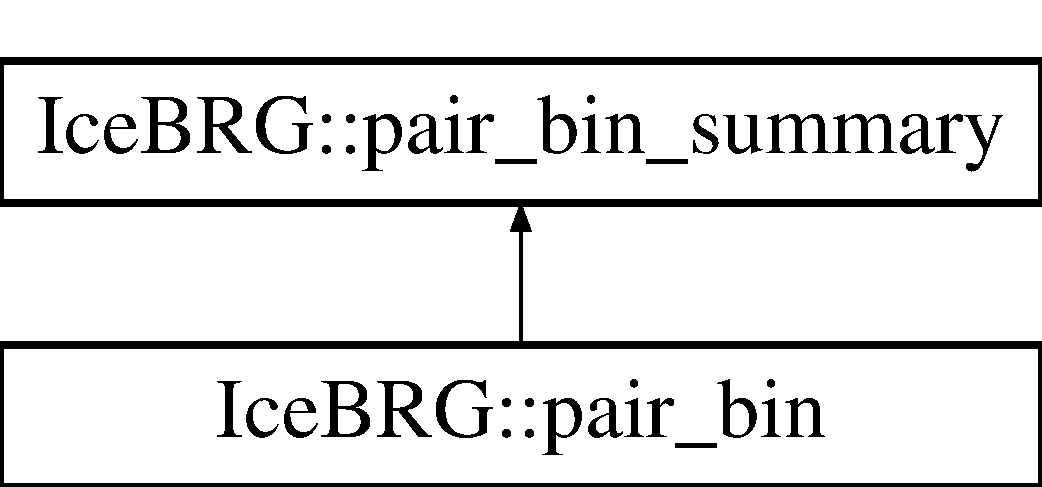
\includegraphics[height=2.000000cm]{classIceBRG_1_1pair__bin__summary}
\end{center}
\end{figure}
\subsection*{Public Member Functions}
\begin{DoxyCompactItemize}
\item 
\hyperlink{classIceBRG_1_1pair__bin__summary_a25c4a1af9dd06f9194799604d5d6ea06}{pair\+\_\+bin\+\_\+summary} (const \hyperlink{namespaceIceBRG_a45499647eb87e24c10ab32c628711cec}{distance\+\_\+type} \&init\+\_\+\+R\+\_\+min=0, const \hyperlink{namespaceIceBRG_a45499647eb87e24c10ab32c628711cec}{distance\+\_\+type} \&init\+\_\+\+R\+\_\+max=0, const \hyperlink{namespaceIceBRG_a1be72ac4918a9b029f2eefa084213e35}{mass\+\_\+type} \&init\+\_\+m\+\_\+min=0 $\ast$\hyperlink{namespaceIceBRG_a9233960f6792ea35145d7db55c13e85d}{kg}, const \hyperlink{namespaceIceBRG_a1be72ac4918a9b029f2eefa084213e35}{mass\+\_\+type} \&init\+\_\+m\+\_\+max=0 $\ast$\hyperlink{namespaceIceBRG_a9233960f6792ea35145d7db55c13e85d}{kg}, const \hyperlink{lib_2IceBRG__main_2common_8h_ad0f130a56eeb944d9ef2692ee881ecc4}{flt\+\_\+type} \&init\+\_\+z\+\_\+min=0, const \hyperlink{lib_2IceBRG__main_2common_8h_ad0f130a56eeb944d9ef2692ee881ecc4}{flt\+\_\+type} \&init\+\_\+z\+\_\+max=0, const \hyperlink{lib_2IceBRG__main_2common_8h_ad0f130a56eeb944d9ef2692ee881ecc4}{flt\+\_\+type} \&init\+\_\+mag\+\_\+min=0, const \hyperlink{lib_2IceBRG__main_2common_8h_ad0f130a56eeb944d9ef2692ee881ecc4}{flt\+\_\+type} \&init\+\_\+mag\+\_\+max=0)
\item 
\hyperlink{classIceBRG_1_1pair__bin__summary_a832ae0f4e36a7850560597b91ef5745f}{pair\+\_\+bin\+\_\+summary} (const \hyperlink{classIceBRG_1_1pair__bin}{pair\+\_\+bin} \&bin)
\item 
\hyperlink{classIceBRG_1_1pair__bin__summary_a4d91275cda5af40a8de4607df904f318}{pair\+\_\+bin\+\_\+summary} (std\+::istream \&in)
\item 
\hyperlink{classIceBRG_1_1pair__bin__summary_a0aaf039eef5a7173408bcf95dbaa3426}{pair\+\_\+bin\+\_\+summary} (std\+::string \&filename)
\item 
\hyperlink{classIceBRG_1_1pair__bin__summary}{pair\+\_\+bin\+\_\+summary} \& \hyperlink{classIceBRG_1_1pair__bin__summary_a7465f0e34354fc97d706ba3c0365e0a5}{operator=} (const \hyperlink{classIceBRG_1_1pair__bin}{pair\+\_\+bin} \&bin)
\item 
virtual \hyperlink{classIceBRG_1_1pair__bin__summary_a6a9e88649e3a606a08577205f342cf1a}{$\sim$pair\+\_\+bin\+\_\+summary} ()
\item 
{\footnotesize template$<$typename T1 , typename T2 $>$ }\\void \hyperlink{classIceBRG_1_1pair__bin__summary_a5b5dc0fc4077d5dd7b7dafbdab684661}{set\+\_\+\+R\+\_\+limits} (T1 \&\&\hyperlink{classIceBRG_1_1pair__bin__summary_af1ee4f7eeb70c23843a0ad4af2f41ef9}{R\+\_\+min}, T2 \&\&\hyperlink{classIceBRG_1_1pair__bin__summary_a26bb6d459f592d9ff9f4a11255d5884b}{R\+\_\+max})
\item 
{\footnotesize template$<$typename T1 , typename T2 $>$ }\\void \hyperlink{classIceBRG_1_1pair__bin__summary_ac7c7f0aaa8f116d0fe1209b7c5ff6559}{set\+\_\+m\+\_\+limits} (T1 \&\&\hyperlink{classIceBRG_1_1pair__bin__summary_a3d298870839005a013bbb03a51a9b596}{m\+\_\+min}, T2 \&\&\hyperlink{classIceBRG_1_1pair__bin__summary_a385862dcbf0238834d8638a9e79c37fd}{m\+\_\+max})
\item 
{\footnotesize template$<$typename T1 , typename T2 $>$ }\\void \hyperlink{classIceBRG_1_1pair__bin__summary_a218aceacdec198c9c6a1b82df250a931}{set\+\_\+z\+\_\+limits} (T1 \&\&\hyperlink{classIceBRG_1_1pair__bin__summary_aba3930b9f685f44653899d6087217530}{z\+\_\+min}, T2 \&\&\hyperlink{classIceBRG_1_1pair__bin__summary_adcc3f2b945ea7b0bef4aa3542ee230cd}{z\+\_\+max})
\item 
{\footnotesize template$<$typename T1 , typename T2 $>$ }\\void \hyperlink{classIceBRG_1_1pair__bin__summary_a681194896012615153d53eb521d93126}{set\+\_\+mag\+\_\+limits} (T1 \&\&\hyperlink{classIceBRG_1_1pair__bin__summary_a40cc6096a80b23659359b0a58f10cae2}{mag\+\_\+min}, T2 \&\&\hyperlink{classIceBRG_1_1pair__bin__summary_a9a13a840877d52c2eb0387e3ca7f9a70}{mag\+\_\+max})
\item 
{\footnotesize template$<$typename T1 , typename T2 , typename T3 , typename T4 , typename T5 , typename T6 , typename T7 , typename T8 $>$ }\\void \hyperlink{classIceBRG_1_1pair__bin__summary_ab0f435851f15bcd9ac594181be365c01}{set\+\_\+limits} (T1 \&\&\hyperlink{classIceBRG_1_1pair__bin__summary_af1ee4f7eeb70c23843a0ad4af2f41ef9}{R\+\_\+min}, T2 \&\&\hyperlink{classIceBRG_1_1pair__bin__summary_a26bb6d459f592d9ff9f4a11255d5884b}{R\+\_\+max}, T3 \&\&\hyperlink{classIceBRG_1_1pair__bin__summary_a3d298870839005a013bbb03a51a9b596}{m\+\_\+min}, T4 \&\&\hyperlink{classIceBRG_1_1pair__bin__summary_a385862dcbf0238834d8638a9e79c37fd}{m\+\_\+max}, T5 \&\&\hyperlink{classIceBRG_1_1pair__bin__summary_aba3930b9f685f44653899d6087217530}{z\+\_\+min}, T6 \&\&\hyperlink{classIceBRG_1_1pair__bin__summary_adcc3f2b945ea7b0bef4aa3542ee230cd}{z\+\_\+max}, T7 \&\&\hyperlink{classIceBRG_1_1pair__bin__summary_a40cc6096a80b23659359b0a58f10cae2}{mag\+\_\+min}, T8 \&\&\hyperlink{classIceBRG_1_1pair__bin__summary_a9a13a840877d52c2eb0387e3ca7f9a70}{mag\+\_\+max})
\item 
virtual void \hyperlink{classIceBRG_1_1pair__bin__summary_a916bb85a5a7b6be8ec21305beddcb966}{clear} ()
\item 
void \hyperlink{classIceBRG_1_1pair__bin__summary_acdfe1a76073341dc7126367f8af9a92c}{fixbad} ()
\item 
virtual \hyperlink{lib_2IceBRG__main_2common_8h_ab322a3e50421dc5f0c43316b1b373592}{ssize\+\_\+t} \hyperlink{classIceBRG_1_1pair__bin__summary_a7890320b7873410727ffa9103cac4ddf}{pair\+\_\+count} () const 
\item 
virtual \hyperlink{lib_2IceBRG__main_2common_8h_ab322a3e50421dc5f0c43316b1b373592}{ssize\+\_\+t} \hyperlink{classIceBRG_1_1pair__bin__summary_a1907d19d230646152b52771046e9bca2}{shear\+\_\+pair\+\_\+count} () const 
\item 
virtual \hyperlink{lib_2IceBRG__main_2common_8h_ab322a3e50421dc5f0c43316b1b373592}{ssize\+\_\+t} \hyperlink{classIceBRG_1_1pair__bin__summary_aa411302e054c1ab2dc55f877efef03a9}{magf\+\_\+pair\+\_\+count} () const 
\item 
virtual \hyperlink{lib_2IceBRG__main_2common_8h_ad0f130a56eeb944d9ef2692ee881ecc4}{flt\+\_\+type} \hyperlink{classIceBRG_1_1pair__bin__summary_a66f311e593f9406545ccaf92c60af40d}{effective\+\_\+pair\+\_\+count} () const 
\item 
virtual \hyperlink{lib_2IceBRG__main_2common_8h_ad0f130a56eeb944d9ef2692ee881ecc4}{flt\+\_\+type} \hyperlink{classIceBRG_1_1pair__bin__summary_a63e24b9c233f7b9bc25417d7f4c3e31a}{shear\+\_\+effective\+\_\+pair\+\_\+count} () const 
\item 
virtual \hyperlink{lib_2IceBRG__main_2common_8h_ad0f130a56eeb944d9ef2692ee881ecc4}{flt\+\_\+type} \hyperlink{classIceBRG_1_1pair__bin__summary_ac7de7ef519ebec709aa75e49540060b8}{sum\+\_\+of\+\_\+weights} () const 
\item 
virtual \hyperlink{lib_2IceBRG__main_2common_8h_ad0f130a56eeb944d9ef2692ee881ecc4}{flt\+\_\+type} \hyperlink{classIceBRG_1_1pair__bin__summary_a9a891e623485e183eafdbb911e751b2b}{shear\+\_\+sum\+\_\+of\+\_\+weights} () const 
\item 
virtual \hyperlink{lib_2IceBRG__main_2common_8h_ad0f130a56eeb944d9ef2692ee881ecc4}{flt\+\_\+type} \hyperlink{classIceBRG_1_1pair__bin__summary_a9333a3ae54e73148957179aa2b18a3a7}{magf\+\_\+sum\+\_\+of\+\_\+weights} () const 
\item 
virtual \hyperlink{lib_2IceBRG__main_2common_8h_ad0f130a56eeb944d9ef2692ee881ecc4}{flt\+\_\+type} \hyperlink{classIceBRG_1_1pair__bin__summary_a423dac74001c5a426b4e626ca6615cb4}{sum\+\_\+of\+\_\+square\+\_\+weights} () const 
\item 
virtual \hyperlink{lib_2IceBRG__main_2common_8h_ad0f130a56eeb944d9ef2692ee881ecc4}{flt\+\_\+type} \hyperlink{classIceBRG_1_1pair__bin__summary_a63dd09417aa6bb32da1898e8baa0b306}{shear\+\_\+sum\+\_\+of\+\_\+square\+\_\+weights} () const 
\item 
virtual \hyperlink{lib_2IceBRG__main_2common_8h_ad0f130a56eeb944d9ef2692ee881ecc4}{flt\+\_\+type} \hyperlink{classIceBRG_1_1pair__bin__summary_adaabe872405c1f389f340a377725a2c5}{magf\+\_\+sum\+\_\+of\+\_\+square\+\_\+weights} () const 
\item 
const \hyperlink{namespaceIceBRG_a45499647eb87e24c10ab32c628711cec}{distance\+\_\+type} \& \hyperlink{classIceBRG_1_1pair__bin__summary_af1ee4f7eeb70c23843a0ad4af2f41ef9}{R\+\_\+min} () const 
\item 
const \hyperlink{namespaceIceBRG_a45499647eb87e24c10ab32c628711cec}{distance\+\_\+type} \& \hyperlink{classIceBRG_1_1pair__bin__summary_a26bb6d459f592d9ff9f4a11255d5884b}{R\+\_\+max} () const 
\item 
\hyperlink{namespaceIceBRG_a45499647eb87e24c10ab32c628711cec}{distance\+\_\+type} \hyperlink{classIceBRG_1_1pair__bin__summary_a0ba020dcfebf4a714b48315af3b45768}{R\+\_\+mid} () const 
\item 
\hyperlink{namespaceIceBRG_a45499647eb87e24c10ab32c628711cec}{distance\+\_\+type} \hyperlink{classIceBRG_1_1pair__bin__summary_ad265e7f8613d5cccc12279a62521cf53}{R\+\_\+amid} () const 
\item 
virtual \hyperlink{namespaceIceBRG_a45499647eb87e24c10ab32c628711cec}{distance\+\_\+type} \hyperlink{classIceBRG_1_1pair__bin__summary_abe60c51fd11b24f2d92f9b273f291677}{R\+\_\+mean} () const 
\item 
virtual \hyperlink{namespaceIceBRG_a45499647eb87e24c10ab32c628711cec}{distance\+\_\+type} \hyperlink{classIceBRG_1_1pair__bin__summary_ab2eacfc9f48eebb9219aa6f1c573cefe}{shear\+\_\+\+R\+\_\+mean} () const 
\item 
virtual \hyperlink{namespaceIceBRG_a45499647eb87e24c10ab32c628711cec}{distance\+\_\+type} \hyperlink{classIceBRG_1_1pair__bin__summary_a17131edb4b90c3c63f386c9849419963}{magf\+\_\+\+R\+\_\+mean} () const 
\item 
const \hyperlink{namespaceIceBRG_a1be72ac4918a9b029f2eefa084213e35}{mass\+\_\+type} \& \hyperlink{classIceBRG_1_1pair__bin__summary_a3d298870839005a013bbb03a51a9b596}{m\+\_\+min} () const 
\item 
const \hyperlink{namespaceIceBRG_a1be72ac4918a9b029f2eefa084213e35}{mass\+\_\+type} \& \hyperlink{classIceBRG_1_1pair__bin__summary_a385862dcbf0238834d8638a9e79c37fd}{m\+\_\+max} () const 
\item 
\hyperlink{namespaceIceBRG_a1be72ac4918a9b029f2eefa084213e35}{mass\+\_\+type} \hyperlink{classIceBRG_1_1pair__bin__summary_a4e17e3e5675622afcb9882013a539b84}{m\+\_\+mid} () const 
\item 
virtual \hyperlink{namespaceIceBRG_a1be72ac4918a9b029f2eefa084213e35}{mass\+\_\+type} \hyperlink{classIceBRG_1_1pair__bin__summary_a122a0ce13e6615912055317e78cbe163}{lens\+\_\+m\+\_\+mean} () const 
\item 
virtual \hyperlink{namespaceIceBRG_a1be72ac4918a9b029f2eefa084213e35}{mass\+\_\+type} \hyperlink{classIceBRG_1_1pair__bin__summary_aa488db649eec121540f364f55467081d}{shear\+\_\+lens\+\_\+m\+\_\+mean} () const 
\item 
virtual \hyperlink{namespaceIceBRG_a1be72ac4918a9b029f2eefa084213e35}{mass\+\_\+type} \hyperlink{classIceBRG_1_1pair__bin__summary_a3f931903c45ca70bc32a7b740ab7746e}{magf\+\_\+lens\+\_\+m\+\_\+mean} () const 
\item 
\hyperlink{lib_2IceBRG__main_2common_8h_ad0f130a56eeb944d9ef2692ee881ecc4}{flt\+\_\+type} \hyperlink{classIceBRG_1_1pair__bin__summary_aba3930b9f685f44653899d6087217530}{z\+\_\+min} () const 
\item 
\hyperlink{lib_2IceBRG__main_2common_8h_ad0f130a56eeb944d9ef2692ee881ecc4}{flt\+\_\+type} \hyperlink{classIceBRG_1_1pair__bin__summary_adcc3f2b945ea7b0bef4aa3542ee230cd}{z\+\_\+max} () const 
\item 
\hyperlink{lib_2IceBRG__main_2common_8h_ad0f130a56eeb944d9ef2692ee881ecc4}{flt\+\_\+type} \hyperlink{classIceBRG_1_1pair__bin__summary_a227901308d137a607ad36b97440117cb}{z\+\_\+mid} () const 
\item 
virtual \hyperlink{lib_2IceBRG__main_2common_8h_ad0f130a56eeb944d9ef2692ee881ecc4}{flt\+\_\+type} \hyperlink{classIceBRG_1_1pair__bin__summary_a2b603573866a1e95c1989c9375fc7255}{lens\+\_\+z\+\_\+mean} () const 
\item 
virtual \hyperlink{lib_2IceBRG__main_2common_8h_ad0f130a56eeb944d9ef2692ee881ecc4}{flt\+\_\+type} \hyperlink{classIceBRG_1_1pair__bin__summary_a83c3fc3e4ac58341474b2d9e4e1fba62}{shear\+\_\+lens\+\_\+z\+\_\+mean} () const 
\item 
virtual \hyperlink{lib_2IceBRG__main_2common_8h_ad0f130a56eeb944d9ef2692ee881ecc4}{flt\+\_\+type} \hyperlink{classIceBRG_1_1pair__bin__summary_aa808472b8ea649bc962a67cea1260004}{magf\+\_\+lens\+\_\+z\+\_\+mean} () const 
\item 
virtual \hyperlink{lib_2IceBRG__main_2common_8h_ad0f130a56eeb944d9ef2692ee881ecc4}{flt\+\_\+type} \hyperlink{classIceBRG_1_1pair__bin__summary_a44c3f53383b22b5a7e3a1fc8a8e16321}{source\+\_\+z\+\_\+mean} () const 
\item 
virtual \hyperlink{lib_2IceBRG__main_2common_8h_ad0f130a56eeb944d9ef2692ee881ecc4}{flt\+\_\+type} \hyperlink{classIceBRG_1_1pair__bin__summary_ab3adc5c74bfc3c2b3e92544ba190b27e}{shear\+\_\+source\+\_\+z\+\_\+mean} () const 
\item 
virtual \hyperlink{lib_2IceBRG__main_2common_8h_ad0f130a56eeb944d9ef2692ee881ecc4}{flt\+\_\+type} \hyperlink{classIceBRG_1_1pair__bin__summary_a4b22342ef48562c44470e7de70ae7860}{magf\+\_\+source\+\_\+z\+\_\+mean} () const 
\item 
\hyperlink{lib_2IceBRG__main_2common_8h_ad0f130a56eeb944d9ef2692ee881ecc4}{flt\+\_\+type} \hyperlink{classIceBRG_1_1pair__bin__summary_a40cc6096a80b23659359b0a58f10cae2}{mag\+\_\+min} () const 
\item 
\hyperlink{lib_2IceBRG__main_2common_8h_ad0f130a56eeb944d9ef2692ee881ecc4}{flt\+\_\+type} \hyperlink{classIceBRG_1_1pair__bin__summary_a9a13a840877d52c2eb0387e3ca7f9a70}{mag\+\_\+max} () const 
\item 
\hyperlink{lib_2IceBRG__main_2common_8h_ad0f130a56eeb944d9ef2692ee881ecc4}{flt\+\_\+type} \hyperlink{classIceBRG_1_1pair__bin__summary_afe7c6362d8892d5d0183afbe81e4ccbf}{mag\+\_\+mid} () const 
\item 
virtual \hyperlink{lib_2IceBRG__main_2common_8h_ad0f130a56eeb944d9ef2692ee881ecc4}{flt\+\_\+type} \hyperlink{classIceBRG_1_1pair__bin__summary_ac7f6568e96ca05b14958903473a5f65b}{lens\+\_\+mag\+\_\+mean} () const 
\item 
virtual \hyperlink{lib_2IceBRG__main_2common_8h_ad0f130a56eeb944d9ef2692ee881ecc4}{flt\+\_\+type} \hyperlink{classIceBRG_1_1pair__bin__summary_aa65e60d6efdb5fe7ac9d1be02c851780}{shear\+\_\+lens\+\_\+mag\+\_\+mean} () const 
\item 
virtual \hyperlink{lib_2IceBRG__main_2common_8h_ad0f130a56eeb944d9ef2692ee881ecc4}{flt\+\_\+type} \hyperlink{classIceBRG_1_1pair__bin__summary_aa8b997144d0aaefce6bfbb0fb0f6f138}{magf\+\_\+lens\+\_\+mag\+\_\+mean} () const 
\item 
\hyperlink{namespaceIceBRG_a80c597ef5ba0a32491d32a9f0083b02d}{surface\+\_\+density\+\_\+type} \hyperlink{classIceBRG_1_1pair__bin__summary_a7ddaece5334f32fe97ab2e3ed0f211e9}{shear\+\_\+sigma\+\_\+crit} () const 
\item 
\hyperlink{namespaceIceBRG_a80c597ef5ba0a32491d32a9f0083b02d}{surface\+\_\+density\+\_\+type} \hyperlink{classIceBRG_1_1pair__bin__summary_a88693451cb28ec4f8e8c67eb34a270f8}{magf\+\_\+sigma\+\_\+crit} () const 
\item 
virtual \hyperlink{namespaceIceBRG_a80c597ef5ba0a32491d32a9f0083b02d}{surface\+\_\+density\+\_\+type} \hyperlink{classIceBRG_1_1pair__bin__summary_a2a1372bfa03a186425920b839ce38f4a}{delta\+\_\+\+Sigma\+\_\+t\+\_\+mean} () const 
\item 
virtual \hyperlink{namespaceIceBRG_a80c597ef5ba0a32491d32a9f0083b02d}{surface\+\_\+density\+\_\+type} \hyperlink{classIceBRG_1_1pair__bin__summary_a8e885aafb07552b829d1d75db54d93b4}{delta\+\_\+\+Sigma\+\_\+x\+\_\+mean} () const 
\item 
virtual \hyperlink{namespaceIceBRG_a896bc1bf7e8db5ca045b9cf35912ca5e}{custom\+\_\+unit\+\_\+type}$<$-\/4, 0, 2, 0, 0 $>$ \hyperlink{classIceBRG_1_1pair__bin__summary_a752e84b6a079f91bbc64bfc746ec5b5d}{delta\+\_\+\+Sigma\+\_\+t\+\_\+mean\+\_\+square} () const 
\item 
virtual \hyperlink{namespaceIceBRG_a896bc1bf7e8db5ca045b9cf35912ca5e}{custom\+\_\+unit\+\_\+type}$<$-\/4, 0, 2, 0, 0 $>$ \hyperlink{classIceBRG_1_1pair__bin__summary_aa16505e993ab66451519a9ed4304c9a8}{delta\+\_\+\+Sigma\+\_\+x\+\_\+mean\+\_\+square} () const 
\item 
virtual \hyperlink{namespaceIceBRG_a80c597ef5ba0a32491d32a9f0083b02d}{surface\+\_\+density\+\_\+type} \hyperlink{classIceBRG_1_1pair__bin__summary_acd510011670a535d609e4ecb2fa8257f}{delta\+\_\+\+Sigma\+\_\+t\+\_\+std} () const 
\item 
virtual \hyperlink{namespaceIceBRG_a80c597ef5ba0a32491d32a9f0083b02d}{surface\+\_\+density\+\_\+type} \hyperlink{classIceBRG_1_1pair__bin__summary_a1779c3cbeaa111f27727d70481fb7ff9}{delta\+\_\+\+Sigma\+\_\+x\+\_\+std} () const 
\item 
virtual \hyperlink{namespaceIceBRG_a80c597ef5ba0a32491d32a9f0083b02d}{surface\+\_\+density\+\_\+type} \hyperlink{classIceBRG_1_1pair__bin__summary_a61f9c6863d1a2440e8d8c7d794b3c8c5}{delta\+\_\+\+Sigma\+\_\+t\+\_\+stderr} () const 
\item 
virtual \hyperlink{namespaceIceBRG_a80c597ef5ba0a32491d32a9f0083b02d}{surface\+\_\+density\+\_\+type} \hyperlink{classIceBRG_1_1pair__bin__summary_a1063e8e122208a24b240fb1e669d786c}{delta\+\_\+\+Sigma\+\_\+x\+\_\+stderr} () const 
\item 
\hyperlink{lib_2IceBRG__main_2common_8h_ad0f130a56eeb944d9ef2692ee881ecc4}{flt\+\_\+type} \hyperlink{classIceBRG_1_1pair__bin__summary_a15002ebbfb7d5309d5dfb012bd7ceb81}{gamma\+\_\+t\+\_\+mean} () const 
\item 
\hyperlink{lib_2IceBRG__main_2common_8h_ad0f130a56eeb944d9ef2692ee881ecc4}{flt\+\_\+type} \hyperlink{classIceBRG_1_1pair__bin__summary_a01072e7fd074b2521332e3ccf466c1ae}{gamma\+\_\+x\+\_\+mean} () const 
\item 
\hyperlink{lib_2IceBRG__main_2common_8h_ad0f130a56eeb944d9ef2692ee881ecc4}{flt\+\_\+type} \hyperlink{classIceBRG_1_1pair__bin__summary_a845031aad82a6757c43a2199a059ce63}{gamma\+\_\+mean} () const 
\item 
\hyperlink{lib_2IceBRG__main_2common_8h_ad0f130a56eeb944d9ef2692ee881ecc4}{flt\+\_\+type} \hyperlink{classIceBRG_1_1pair__bin__summary_ae6e61497643df44dfb882614f4f8a436}{gamma\+\_\+mean\+\_\+square} () const 
\item 
\hyperlink{lib_2IceBRG__main_2common_8h_ad0f130a56eeb944d9ef2692ee881ecc4}{flt\+\_\+type} \hyperlink{classIceBRG_1_1pair__bin__summary_ac4b6d240243c897ce0bda3ccec204901}{gamma\+\_\+t\+\_\+stderr} () const 
\item 
\hyperlink{lib_2IceBRG__main_2common_8h_ad0f130a56eeb944d9ef2692ee881ecc4}{flt\+\_\+type} \hyperlink{classIceBRG_1_1pair__bin__summary_a8bfdc933188bc3253991fe257f0859b1}{gamma\+\_\+x\+\_\+stderr} () const 
\item 
\hyperlink{lib_2IceBRG__main_2common_8h_ad0f130a56eeb944d9ef2692ee881ecc4}{flt\+\_\+type} \hyperlink{classIceBRG_1_1pair__bin__summary_a0a02c950a58cc6844328266f8bc2c1fb}{gamma\+\_\+stderr} () const 
\item 
\hyperlink{lib_2IceBRG__main_2common_8h_ad0f130a56eeb944d9ef2692ee881ecc4}{flt\+\_\+type} \hyperlink{classIceBRG_1_1pair__bin__summary_ad2176d6b62e4c8cf70592252ae106d70}{gamma\+\_\+square\+\_\+stderr} () const 
\item 
\hyperlink{namespaceIceBRG_a80c597ef5ba0a32491d32a9f0083b02d}{surface\+\_\+density\+\_\+type} \hyperlink{classIceBRG_1_1pair__bin__summary_a4c15fe2fea325cc093bcd826658377c4}{model\+\_\+delta\+\_\+\+Sigma\+\_\+t} (const \hyperlink{lib_2IceBRG__main_2common_8h_ad0f130a56eeb944d9ef2692ee881ecc4}{flt\+\_\+type} \&M\+Lratio\+\_\+1h=50., const \hyperlink{namespaceIceBRG_a1be72ac4918a9b029f2eefa084213e35}{mass\+\_\+type} \&mean\+\_\+group\+\_\+mass=1e14 $\ast$unitconv\+::\+Msuntokg $\ast$kg, const flt\+\_\+type \&sat\+\_\+frac=0.\+2) const 
\item 
\hyperlink{lib_2IceBRG__main_2common_8h_ad0f130a56eeb944d9ef2692ee881ecc4}{flt\+\_\+type} \hyperlink{classIceBRG_1_1pair__bin__summary_aa49f4e7780a495607acbef6c74f2d33c}{model\+\_\+gamma\+\_\+t} (const \hyperlink{lib_2IceBRG__main_2common_8h_ad0f130a56eeb944d9ef2692ee881ecc4}{flt\+\_\+type} \&M\+Lratio\+\_\+1h=50., const \hyperlink{namespaceIceBRG_a1be72ac4918a9b029f2eefa084213e35}{mass\+\_\+type} \&mean\+\_\+group\+\_\+mass=1e14 $\ast$unitconv\+::\+Msuntokg $\ast$kg, const flt\+\_\+type \&sat\+\_\+frac=0.\+2) const 
\item 
\hyperlink{namespaceIceBRG_a80c597ef5ba0a32491d32a9f0083b02d}{surface\+\_\+density\+\_\+type} \hyperlink{classIceBRG_1_1pair__bin__summary_adbc2af143460d725fcc07537517c5119}{model\+\_\+1h\+\_\+delta\+\_\+\+Sigma\+\_\+t} (const \hyperlink{lib_2IceBRG__main_2common_8h_ad0f130a56eeb944d9ef2692ee881ecc4}{flt\+\_\+type} \&M\+Lratio\+\_\+1h=50.) const 
\item 
\hyperlink{lib_2IceBRG__main_2common_8h_ad0f130a56eeb944d9ef2692ee881ecc4}{flt\+\_\+type} \hyperlink{classIceBRG_1_1pair__bin__summary_ae0e5c883d7c00ffcd745c9b53e9fcc70}{model\+\_\+1h\+\_\+gamma\+\_\+t} (const \hyperlink{lib_2IceBRG__main_2common_8h_ad0f130a56eeb944d9ef2692ee881ecc4}{flt\+\_\+type} \&M\+Lratio\+\_\+1h=50.) const 
\item 
\hyperlink{namespaceIceBRG_a80c597ef5ba0a32491d32a9f0083b02d}{surface\+\_\+density\+\_\+type} \hyperlink{classIceBRG_1_1pair__bin__summary_a9b5aa9cbf8b82c11c9e70b585149bb47}{model\+\_\+offset\+\_\+delta\+\_\+\+Sigma\+\_\+t} (const \hyperlink{namespaceIceBRG_a1be72ac4918a9b029f2eefa084213e35}{mass\+\_\+type} \&mean\+\_\+group\+\_\+mass=1e14 $\ast$unitconv\+::\+Msuntokg $\ast$kg, const flt\+\_\+type \&sat\+\_\+frac=0.\+2) const 
\item 
\hyperlink{lib_2IceBRG__main_2common_8h_ad0f130a56eeb944d9ef2692ee881ecc4}{flt\+\_\+type} \hyperlink{classIceBRG_1_1pair__bin__summary_a2f539a8860a38bee4e54bdc27f53faaa}{model\+\_\+offset\+\_\+gamma\+\_\+t} (const \hyperlink{namespaceIceBRG_a1be72ac4918a9b029f2eefa084213e35}{mass\+\_\+type} \&mean\+\_\+group\+\_\+mass=1e14 $\ast$unitconv\+::\+Msuntokg $\ast$kg, const flt\+\_\+type \&sat\+\_\+frac=0.\+2) const 
\item 
\hyperlink{namespaceIceBRG_a896bc1bf7e8db5ca045b9cf35912ca5e}{custom\+\_\+unit\+\_\+type}$<$ 0, 0, 0, 2, 0 $>$ \hyperlink{classIceBRG_1_1pair__bin__summary_a556037a76b545b5a453595d30fdd94a6}{area\+\_\+per\+\_\+lens} () const 
\item 
virtual \hyperlink{namespaceIceBRG_a896bc1bf7e8db5ca045b9cf35912ca5e}{custom\+\_\+unit\+\_\+type}$<$ 0, 0, 0, 2, 0 $>$ \hyperlink{classIceBRG_1_1pair__bin__summary_a6c0d9413d2cab3f09e96947dc08b6841}{area} () const 
\item 
virtual \hyperlink{lib_2IceBRG__main_2common_8h_ab322a3e50421dc5f0c43316b1b373592}{ssize\+\_\+t} \hyperlink{classIceBRG_1_1pair__bin__summary_a36cfa054426945727a7638c7831a7f04}{num\+\_\+lenses} () const 
\item 
virtual \hyperlink{lib_2IceBRG__main_2common_8h_ad0f130a56eeb944d9ef2692ee881ecc4}{flt\+\_\+type} \hyperlink{classIceBRG_1_1pair__bin__summary_a71592ca23d56860395e8fe22335098ff}{magf\+\_\+effective\+\_\+num\+\_\+lenses} () const 
\item 
virtual \hyperlink{lib_2IceBRG__main_2common_8h_ab322a3e50421dc5f0c43316b1b373592}{ssize\+\_\+t} \hyperlink{classIceBRG_1_1pair__bin__summary_a1df27276f9953ae8f6d25dabadcb563d}{magf\+\_\+num\+\_\+lenses} () const 
\item 
virtual \hyperlink{lib_2IceBRG__main_2common_8h_ad0f130a56eeb944d9ef2692ee881ecc4}{flt\+\_\+type} \hyperlink{classIceBRG_1_1pair__bin__summary_ab594afbd4f1d079ae155402c96a96a5c}{mu\+\_\+hat} () const 
\item 
virtual \hyperlink{lib_2IceBRG__main_2common_8h_ad0f130a56eeb944d9ef2692ee881ecc4}{flt\+\_\+type} \hyperlink{classIceBRG_1_1pair__bin__summary_a1946f8d7063520c70f8f68b705aef8d7}{mu\+\_\+square\+\_\+hat} () const 
\item 
virtual \hyperlink{lib_2IceBRG__main_2common_8h_ad0f130a56eeb944d9ef2692ee881ecc4}{flt\+\_\+type} \hyperlink{classIceBRG_1_1pair__bin__summary_a88ff7f5597f4a10a16fda4bb9f726298}{mu\+\_\+\+W} () const 
\item 
\hyperlink{lib_2IceBRG__main_2common_8h_ad0f130a56eeb944d9ef2692ee881ecc4}{flt\+\_\+type} \hyperlink{classIceBRG_1_1pair__bin__summary_a16bcf11da5f0bd64f763c7012c4584de}{mu\+\_\+std} () const 
\item 
\hyperlink{lib_2IceBRG__main_2common_8h_ad0f130a56eeb944d9ef2692ee881ecc4}{flt\+\_\+type} \hyperlink{classIceBRG_1_1pair__bin__summary_adf391f518873ac7ae22dd0f8aeb74a3d}{mu\+\_\+stderr} () const 
\item 
\hyperlink{lib_2IceBRG__main_2common_8h_ad0f130a56eeb944d9ef2692ee881ecc4}{flt\+\_\+type} \hyperlink{classIceBRG_1_1pair__bin__summary_ae53878e5bc3fdeefd0884231a11337dd}{kappa} () const 
\item 
\hyperlink{lib_2IceBRG__main_2common_8h_ad0f130a56eeb944d9ef2692ee881ecc4}{flt\+\_\+type} \hyperlink{classIceBRG_1_1pair__bin__summary_a91ad26c5cb4049d449b217cd45603696}{kappa\+\_\+stderr} () const 
\item 
\hyperlink{namespaceIceBRG_a80c597ef5ba0a32491d32a9f0083b02d}{surface\+\_\+density\+\_\+type} \hyperlink{classIceBRG_1_1pair__bin__summary_a0e3ba1f366541d48ef94679b4352bbcd}{Sigma} () const 
\item 
\hyperlink{namespaceIceBRG_a80c597ef5ba0a32491d32a9f0083b02d}{surface\+\_\+density\+\_\+type} \hyperlink{classIceBRG_1_1pair__bin__summary_a5aa0edcb2a8528aa090e5035131703a0}{Sigma\+\_\+stderr} () const 
\item 
\hyperlink{lib_2IceBRG__main_2common_8h_ad0f130a56eeb944d9ef2692ee881ecc4}{flt\+\_\+type} \hyperlink{classIceBRG_1_1pair__bin__summary_ac0852be69cc6c7fb267d871e5119a848}{model\+\_\+mu} (const \hyperlink{lib_2IceBRG__main_2common_8h_ad0f130a56eeb944d9ef2692ee881ecc4}{flt\+\_\+type} \&M\+Lratio\+\_\+1h=50., const \hyperlink{namespaceIceBRG_a1be72ac4918a9b029f2eefa084213e35}{mass\+\_\+type} \&mean\+\_\+group\+\_\+mass=1e14 $\ast$unitconv\+::\+Msuntokg $\ast$kg, const flt\+\_\+type \&sat\+\_\+frac=0.\+2) const 
\item 
\hyperlink{lib_2IceBRG__main_2common_8h_ad0f130a56eeb944d9ef2692ee881ecc4}{flt\+\_\+type} \hyperlink{classIceBRG_1_1pair__bin__summary_aa93614ecebce56d9336d856925ed1154}{model\+\_\+kappa} (const \hyperlink{lib_2IceBRG__main_2common_8h_ad0f130a56eeb944d9ef2692ee881ecc4}{flt\+\_\+type} \&M\+Lratio\+\_\+1h=50., const \hyperlink{namespaceIceBRG_a1be72ac4918a9b029f2eefa084213e35}{mass\+\_\+type} \&mean\+\_\+group\+\_\+mass=1e14 $\ast$unitconv\+::\+Msuntokg $\ast$kg, const flt\+\_\+type \&sat\+\_\+frac=0.\+2) const 
\item 
\hyperlink{namespaceIceBRG_a80c597ef5ba0a32491d32a9f0083b02d}{surface\+\_\+density\+\_\+type} \hyperlink{classIceBRG_1_1pair__bin__summary_a1627a07bc392e0a876f5257b5b614622}{model\+\_\+\+Sigma} (const \hyperlink{lib_2IceBRG__main_2common_8h_ad0f130a56eeb944d9ef2692ee881ecc4}{flt\+\_\+type} \&M\+Lratio\+\_\+1h=50., const \hyperlink{namespaceIceBRG_a1be72ac4918a9b029f2eefa084213e35}{mass\+\_\+type} \&mean\+\_\+group\+\_\+mass=1e14 $\ast$unitconv\+::\+Msuntokg $\ast$kg, const flt\+\_\+type \&sat\+\_\+frac=0.\+2) const 
\item 
\hyperlink{lib_2IceBRG__main_2common_8h_ad0f130a56eeb944d9ef2692ee881ecc4}{flt\+\_\+type} \hyperlink{classIceBRG_1_1pair__bin__summary_a1acf154add21e045b2b58cce9eeb0a14}{model\+\_\+1h\+\_\+mu} (const \hyperlink{lib_2IceBRG__main_2common_8h_ad0f130a56eeb944d9ef2692ee881ecc4}{flt\+\_\+type} \&M\+Lratio\+\_\+1h=50.) const 
\item 
\hyperlink{lib_2IceBRG__main_2common_8h_ad0f130a56eeb944d9ef2692ee881ecc4}{flt\+\_\+type} \hyperlink{classIceBRG_1_1pair__bin__summary_a94306f4cf7cec2c34473bc9898817d6e}{model\+\_\+1h\+\_\+kappa} (const \hyperlink{lib_2IceBRG__main_2common_8h_ad0f130a56eeb944d9ef2692ee881ecc4}{flt\+\_\+type} \&M\+Lratio\+\_\+1h=50.) const 
\item 
\hyperlink{namespaceIceBRG_a80c597ef5ba0a32491d32a9f0083b02d}{surface\+\_\+density\+\_\+type} \hyperlink{classIceBRG_1_1pair__bin__summary_a3e6d7987aadd12908687bc77d0eaed09}{model\+\_\+1h\+\_\+\+Sigma} (const \hyperlink{lib_2IceBRG__main_2common_8h_ad0f130a56eeb944d9ef2692ee881ecc4}{flt\+\_\+type} \&M\+Lratio\+\_\+1h=50.) const 
\item 
\hyperlink{lib_2IceBRG__main_2common_8h_ad0f130a56eeb944d9ef2692ee881ecc4}{flt\+\_\+type} \hyperlink{classIceBRG_1_1pair__bin__summary_a1b4ff7d510022de3c9c6d5794db7ea98}{model\+\_\+offset\+\_\+mu} (const \hyperlink{namespaceIceBRG_a1be72ac4918a9b029f2eefa084213e35}{mass\+\_\+type} \&mean\+\_\+group\+\_\+mass=1e14 $\ast$unitconv\+::\+Msuntokg $\ast$kg, const flt\+\_\+type \&sat\+\_\+frac=0.\+2) const 
\item 
\hyperlink{lib_2IceBRG__main_2common_8h_ad0f130a56eeb944d9ef2692ee881ecc4}{flt\+\_\+type} \hyperlink{classIceBRG_1_1pair__bin__summary_a3f3053c2a1481739b1240dd383803f37}{model\+\_\+offset\+\_\+kappa} (const \hyperlink{namespaceIceBRG_a1be72ac4918a9b029f2eefa084213e35}{mass\+\_\+type} \&mean\+\_\+group\+\_\+mass=1e14 $\ast$unitconv\+::\+Msuntokg $\ast$kg, const flt\+\_\+type \&sat\+\_\+frac=0.\+2) const 
\item 
\hyperlink{namespaceIceBRG_a80c597ef5ba0a32491d32a9f0083b02d}{surface\+\_\+density\+\_\+type} \hyperlink{classIceBRG_1_1pair__bin__summary_a2384801bfcfa8e9fb6ef15b32f7b82ac}{model\+\_\+offset\+\_\+\+Sigma} (const \hyperlink{namespaceIceBRG_a1be72ac4918a9b029f2eefa084213e35}{mass\+\_\+type} \&mean\+\_\+group\+\_\+mass=1e14 $\ast$unitconv\+::\+Msuntokg $\ast$kg, const flt\+\_\+type \&sat\+\_\+frac=0.\+2) const 
\item 
\hyperlink{classIceBRG_1_1pair__bin__summary}{pair\+\_\+bin\+\_\+summary} \& \hyperlink{classIceBRG_1_1pair__bin__summary_aebc85a791164a79fc26ed9997cb26acf}{operator+=} (const \hyperlink{classIceBRG_1_1pair__bin__summary}{pair\+\_\+bin\+\_\+summary} \&other)
\item 
\hyperlink{classIceBRG_1_1pair__bin__summary}{pair\+\_\+bin\+\_\+summary} \hyperlink{classIceBRG_1_1pair__bin__summary_a908cb3b78cca4798d9338530c884d3bd}{operator+} (\hyperlink{classIceBRG_1_1pair__bin__summary}{pair\+\_\+bin\+\_\+summary} other) const 
\item 
void \hyperlink{classIceBRG_1_1pair__bin__summary_a818fdce6a248c3a038d5a6b0dae20cb7}{save} (std\+::ostream \&) const 
\item 
void \hyperlink{classIceBRG_1_1pair__bin__summary_adf616ef4c4ad5da5fcb8c2048cc18cec}{save} (const std\+::string \&) const 
\item 
void \hyperlink{classIceBRG_1_1pair__bin__summary_aaba4acba6e02ac0a8f3c2e79b0d3b559}{save} (std\+::ostream \&)
\item 
void \hyperlink{classIceBRG_1_1pair__bin__summary_ae531783a2847f3db8964cc530996915b}{save} (const std\+::string \&)
\item 
void \hyperlink{classIceBRG_1_1pair__bin__summary_a9189bd4f00779f2a97ed6861a403d7f8}{load} (std\+::istream \&)
\item 
void \hyperlink{classIceBRG_1_1pair__bin__summary_a074dc6d7125ba31b2bb1243d46b09f70}{load} (const std\+::string \&)
\end{DoxyCompactItemize}
\subsection*{Protected Member Functions}
\begin{DoxyCompactItemize}
\item 
virtual void \hyperlink{classIceBRG_1_1pair__bin__summary_a3e0113d3900e9eebb0f80d5681e6dd95}{\+\_\+uncache\+\_\+values} ()
\end{DoxyCompactItemize}
\subsection*{Friends}
\begin{DoxyCompactItemize}
\item 
class \hyperlink{classIceBRG_1_1pair__bin__summary_ac98d07dd8f7b70e16ccb9a01abf56b9c}{boost\+::serialization\+::access}
\end{DoxyCompactItemize}


\subsection{Constructor \& Destructor Documentation}
\hypertarget{classIceBRG_1_1pair__bin__summary_a25c4a1af9dd06f9194799604d5d6ea06}{}\index{Ice\+B\+R\+G\+::pair\+\_\+bin\+\_\+summary@{Ice\+B\+R\+G\+::pair\+\_\+bin\+\_\+summary}!pair\+\_\+bin\+\_\+summary@{pair\+\_\+bin\+\_\+summary}}
\index{pair\+\_\+bin\+\_\+summary@{pair\+\_\+bin\+\_\+summary}!Ice\+B\+R\+G\+::pair\+\_\+bin\+\_\+summary@{Ice\+B\+R\+G\+::pair\+\_\+bin\+\_\+summary}}
\subsubsection[{pair\+\_\+bin\+\_\+summary(const distance\+\_\+type \&init\+\_\+\+R\+\_\+min=0, const distance\+\_\+type \&init\+\_\+\+R\+\_\+max=0, const mass\+\_\+type \&init\+\_\+m\+\_\+min=0 $\ast$kg, const mass\+\_\+type \&init\+\_\+m\+\_\+max=0 $\ast$kg, const flt\+\_\+type \&init\+\_\+z\+\_\+min=0, const flt\+\_\+type \&init\+\_\+z\+\_\+max=0, const flt\+\_\+type \&init\+\_\+mag\+\_\+min=0, const flt\+\_\+type \&init\+\_\+mag\+\_\+max=0)}]{\setlength{\rightskip}{0pt plus 5cm}Ice\+B\+R\+G\+::pair\+\_\+bin\+\_\+summary\+::pair\+\_\+bin\+\_\+summary (
\begin{DoxyParamCaption}
\item[{const {\bf distance\+\_\+type} \&}]{init\+\_\+\+R\+\_\+min = {\ttfamily 0}, }
\item[{const {\bf distance\+\_\+type} \&}]{init\+\_\+\+R\+\_\+max = {\ttfamily 0}, }
\item[{const {\bf mass\+\_\+type} \&}]{init\+\_\+m\+\_\+min = {\ttfamily 0$\ast${\bf kg}}, }
\item[{const {\bf mass\+\_\+type} \&}]{init\+\_\+m\+\_\+max = {\ttfamily 0$\ast${\bf kg}}, }
\item[{const {\bf flt\+\_\+type} \&}]{init\+\_\+z\+\_\+min = {\ttfamily 0}, }
\item[{const {\bf flt\+\_\+type} \&}]{init\+\_\+z\+\_\+max = {\ttfamily 0}, }
\item[{const {\bf flt\+\_\+type} \&}]{init\+\_\+mag\+\_\+min = {\ttfamily 0}, }
\item[{const {\bf flt\+\_\+type} \&}]{init\+\_\+mag\+\_\+max = {\ttfamily 0}}
\end{DoxyParamCaption}
)}\label{classIceBRG_1_1pair__bin__summary_a25c4a1af9dd06f9194799604d5d6ea06}
\hypertarget{classIceBRG_1_1pair__bin__summary_a832ae0f4e36a7850560597b91ef5745f}{}\index{Ice\+B\+R\+G\+::pair\+\_\+bin\+\_\+summary@{Ice\+B\+R\+G\+::pair\+\_\+bin\+\_\+summary}!pair\+\_\+bin\+\_\+summary@{pair\+\_\+bin\+\_\+summary}}
\index{pair\+\_\+bin\+\_\+summary@{pair\+\_\+bin\+\_\+summary}!Ice\+B\+R\+G\+::pair\+\_\+bin\+\_\+summary@{Ice\+B\+R\+G\+::pair\+\_\+bin\+\_\+summary}}
\subsubsection[{pair\+\_\+bin\+\_\+summary(const pair\+\_\+bin \&bin)}]{\setlength{\rightskip}{0pt plus 5cm}Ice\+B\+R\+G\+::pair\+\_\+bin\+\_\+summary\+::pair\+\_\+bin\+\_\+summary (
\begin{DoxyParamCaption}
\item[{const {\bf pair\+\_\+bin} \&}]{bin}
\end{DoxyParamCaption}
)}\label{classIceBRG_1_1pair__bin__summary_a832ae0f4e36a7850560597b91ef5745f}
\hypertarget{classIceBRG_1_1pair__bin__summary_a4d91275cda5af40a8de4607df904f318}{}\index{Ice\+B\+R\+G\+::pair\+\_\+bin\+\_\+summary@{Ice\+B\+R\+G\+::pair\+\_\+bin\+\_\+summary}!pair\+\_\+bin\+\_\+summary@{pair\+\_\+bin\+\_\+summary}}
\index{pair\+\_\+bin\+\_\+summary@{pair\+\_\+bin\+\_\+summary}!Ice\+B\+R\+G\+::pair\+\_\+bin\+\_\+summary@{Ice\+B\+R\+G\+::pair\+\_\+bin\+\_\+summary}}
\subsubsection[{pair\+\_\+bin\+\_\+summary(std\+::istream \&in)}]{\setlength{\rightskip}{0pt plus 5cm}Ice\+B\+R\+G\+::pair\+\_\+bin\+\_\+summary\+::pair\+\_\+bin\+\_\+summary (
\begin{DoxyParamCaption}
\item[{std\+::istream \&}]{in}
\end{DoxyParamCaption}
)}\label{classIceBRG_1_1pair__bin__summary_a4d91275cda5af40a8de4607df904f318}
\hypertarget{classIceBRG_1_1pair__bin__summary_a0aaf039eef5a7173408bcf95dbaa3426}{}\index{Ice\+B\+R\+G\+::pair\+\_\+bin\+\_\+summary@{Ice\+B\+R\+G\+::pair\+\_\+bin\+\_\+summary}!pair\+\_\+bin\+\_\+summary@{pair\+\_\+bin\+\_\+summary}}
\index{pair\+\_\+bin\+\_\+summary@{pair\+\_\+bin\+\_\+summary}!Ice\+B\+R\+G\+::pair\+\_\+bin\+\_\+summary@{Ice\+B\+R\+G\+::pair\+\_\+bin\+\_\+summary}}
\subsubsection[{pair\+\_\+bin\+\_\+summary(std\+::string \&filename)}]{\setlength{\rightskip}{0pt plus 5cm}Ice\+B\+R\+G\+::pair\+\_\+bin\+\_\+summary\+::pair\+\_\+bin\+\_\+summary (
\begin{DoxyParamCaption}
\item[{std\+::string \&}]{filename}
\end{DoxyParamCaption}
)}\label{classIceBRG_1_1pair__bin__summary_a0aaf039eef5a7173408bcf95dbaa3426}
\hypertarget{classIceBRG_1_1pair__bin__summary_a6a9e88649e3a606a08577205f342cf1a}{}\index{Ice\+B\+R\+G\+::pair\+\_\+bin\+\_\+summary@{Ice\+B\+R\+G\+::pair\+\_\+bin\+\_\+summary}!````~pair\+\_\+bin\+\_\+summary@{$\sim$pair\+\_\+bin\+\_\+summary}}
\index{````~pair\+\_\+bin\+\_\+summary@{$\sim$pair\+\_\+bin\+\_\+summary}!Ice\+B\+R\+G\+::pair\+\_\+bin\+\_\+summary@{Ice\+B\+R\+G\+::pair\+\_\+bin\+\_\+summary}}
\subsubsection[{$\sim$pair\+\_\+bin\+\_\+summary()}]{\setlength{\rightskip}{0pt plus 5cm}virtual Ice\+B\+R\+G\+::pair\+\_\+bin\+\_\+summary\+::$\sim$pair\+\_\+bin\+\_\+summary (
\begin{DoxyParamCaption}
{}
\end{DoxyParamCaption}
)\hspace{0.3cm}{\ttfamily [inline]}, {\ttfamily [virtual]}}\label{classIceBRG_1_1pair__bin__summary_a6a9e88649e3a606a08577205f342cf1a}


\subsection{Member Function Documentation}
\hypertarget{classIceBRG_1_1pair__bin__summary_a3e0113d3900e9eebb0f80d5681e6dd95}{}\index{Ice\+B\+R\+G\+::pair\+\_\+bin\+\_\+summary@{Ice\+B\+R\+G\+::pair\+\_\+bin\+\_\+summary}!\+\_\+uncache\+\_\+values@{\+\_\+uncache\+\_\+values}}
\index{\+\_\+uncache\+\_\+values@{\+\_\+uncache\+\_\+values}!Ice\+B\+R\+G\+::pair\+\_\+bin\+\_\+summary@{Ice\+B\+R\+G\+::pair\+\_\+bin\+\_\+summary}}
\subsubsection[{\+\_\+uncache\+\_\+values()}]{\setlength{\rightskip}{0pt plus 5cm}virtual void Ice\+B\+R\+G\+::pair\+\_\+bin\+\_\+summary\+::\+\_\+uncache\+\_\+values (
\begin{DoxyParamCaption}
{}
\end{DoxyParamCaption}
)\hspace{0.3cm}{\ttfamily [inline]}, {\ttfamily [protected]}, {\ttfamily [virtual]}}\label{classIceBRG_1_1pair__bin__summary_a3e0113d3900e9eebb0f80d5681e6dd95}


Reimplemented in \hyperlink{classIceBRG_1_1pair__bin_af6ee5173022f9fa8b4528b7d6e18b0d2}{Ice\+B\+R\+G\+::pair\+\_\+bin}.

\hypertarget{classIceBRG_1_1pair__bin__summary_a6c0d9413d2cab3f09e96947dc08b6841}{}\index{Ice\+B\+R\+G\+::pair\+\_\+bin\+\_\+summary@{Ice\+B\+R\+G\+::pair\+\_\+bin\+\_\+summary}!area@{area}}
\index{area@{area}!Ice\+B\+R\+G\+::pair\+\_\+bin\+\_\+summary@{Ice\+B\+R\+G\+::pair\+\_\+bin\+\_\+summary}}
\subsubsection[{area() const }]{\setlength{\rightskip}{0pt plus 5cm}virtual {\bf custom\+\_\+unit\+\_\+type}$<$0,0,0,2,0$>$ Ice\+B\+R\+G\+::pair\+\_\+bin\+\_\+summary\+::area (
\begin{DoxyParamCaption}
{}
\end{DoxyParamCaption}
) const\hspace{0.3cm}{\ttfamily [inline]}, {\ttfamily [virtual]}}\label{classIceBRG_1_1pair__bin__summary_a6c0d9413d2cab3f09e96947dc08b6841}


Reimplemented in \hyperlink{classIceBRG_1_1pair__bin_aebdbc6603f8df3ea242939c22919495d}{Ice\+B\+R\+G\+::pair\+\_\+bin}.

\hypertarget{classIceBRG_1_1pair__bin__summary_a556037a76b545b5a453595d30fdd94a6}{}\index{Ice\+B\+R\+G\+::pair\+\_\+bin\+\_\+summary@{Ice\+B\+R\+G\+::pair\+\_\+bin\+\_\+summary}!area\+\_\+per\+\_\+lens@{area\+\_\+per\+\_\+lens}}
\index{area\+\_\+per\+\_\+lens@{area\+\_\+per\+\_\+lens}!Ice\+B\+R\+G\+::pair\+\_\+bin\+\_\+summary@{Ice\+B\+R\+G\+::pair\+\_\+bin\+\_\+summary}}
\subsubsection[{area\+\_\+per\+\_\+lens() const }]{\setlength{\rightskip}{0pt plus 5cm}{\bf custom\+\_\+unit\+\_\+type}$<$ 0, 0, 0, 2, 0 $>$ Ice\+B\+R\+G\+::pair\+\_\+bin\+\_\+summary\+::area\+\_\+per\+\_\+lens (
\begin{DoxyParamCaption}
{}
\end{DoxyParamCaption}
) const}\label{classIceBRG_1_1pair__bin__summary_a556037a76b545b5a453595d30fdd94a6}
\hypertarget{classIceBRG_1_1pair__bin__summary_a916bb85a5a7b6be8ec21305beddcb966}{}\index{Ice\+B\+R\+G\+::pair\+\_\+bin\+\_\+summary@{Ice\+B\+R\+G\+::pair\+\_\+bin\+\_\+summary}!clear@{clear}}
\index{clear@{clear}!Ice\+B\+R\+G\+::pair\+\_\+bin\+\_\+summary@{Ice\+B\+R\+G\+::pair\+\_\+bin\+\_\+summary}}
\subsubsection[{clear()}]{\setlength{\rightskip}{0pt plus 5cm}void Ice\+B\+R\+G\+::pair\+\_\+bin\+\_\+summary\+::clear (
\begin{DoxyParamCaption}
{}
\end{DoxyParamCaption}
)\hspace{0.3cm}{\ttfamily [virtual]}}\label{classIceBRG_1_1pair__bin__summary_a916bb85a5a7b6be8ec21305beddcb966}


Reimplemented in \hyperlink{classIceBRG_1_1pair__bin_accb7e0a9d26acf6b3444160f2c3718c5}{Ice\+B\+R\+G\+::pair\+\_\+bin}.

\hypertarget{classIceBRG_1_1pair__bin__summary_a2a1372bfa03a186425920b839ce38f4a}{}\index{Ice\+B\+R\+G\+::pair\+\_\+bin\+\_\+summary@{Ice\+B\+R\+G\+::pair\+\_\+bin\+\_\+summary}!delta\+\_\+\+Sigma\+\_\+t\+\_\+mean@{delta\+\_\+\+Sigma\+\_\+t\+\_\+mean}}
\index{delta\+\_\+\+Sigma\+\_\+t\+\_\+mean@{delta\+\_\+\+Sigma\+\_\+t\+\_\+mean}!Ice\+B\+R\+G\+::pair\+\_\+bin\+\_\+summary@{Ice\+B\+R\+G\+::pair\+\_\+bin\+\_\+summary}}
\subsubsection[{delta\+\_\+\+Sigma\+\_\+t\+\_\+mean() const }]{\setlength{\rightskip}{0pt plus 5cm}virtual {\bf surface\+\_\+density\+\_\+type} Ice\+B\+R\+G\+::pair\+\_\+bin\+\_\+summary\+::delta\+\_\+\+Sigma\+\_\+t\+\_\+mean (
\begin{DoxyParamCaption}
{}
\end{DoxyParamCaption}
) const\hspace{0.3cm}{\ttfamily [inline]}, {\ttfamily [virtual]}}\label{classIceBRG_1_1pair__bin__summary_a2a1372bfa03a186425920b839ce38f4a}


Reimplemented in \hyperlink{classIceBRG_1_1pair__bin_a135ada0d34fa0b01e1e9b80b0cd833da}{Ice\+B\+R\+G\+::pair\+\_\+bin}.

\hypertarget{classIceBRG_1_1pair__bin__summary_a752e84b6a079f91bbc64bfc746ec5b5d}{}\index{Ice\+B\+R\+G\+::pair\+\_\+bin\+\_\+summary@{Ice\+B\+R\+G\+::pair\+\_\+bin\+\_\+summary}!delta\+\_\+\+Sigma\+\_\+t\+\_\+mean\+\_\+square@{delta\+\_\+\+Sigma\+\_\+t\+\_\+mean\+\_\+square}}
\index{delta\+\_\+\+Sigma\+\_\+t\+\_\+mean\+\_\+square@{delta\+\_\+\+Sigma\+\_\+t\+\_\+mean\+\_\+square}!Ice\+B\+R\+G\+::pair\+\_\+bin\+\_\+summary@{Ice\+B\+R\+G\+::pair\+\_\+bin\+\_\+summary}}
\subsubsection[{delta\+\_\+\+Sigma\+\_\+t\+\_\+mean\+\_\+square() const }]{\setlength{\rightskip}{0pt plus 5cm}virtual {\bf custom\+\_\+unit\+\_\+type}$<$-\/4,0,2,0,0$>$ Ice\+B\+R\+G\+::pair\+\_\+bin\+\_\+summary\+::delta\+\_\+\+Sigma\+\_\+t\+\_\+mean\+\_\+square (
\begin{DoxyParamCaption}
{}
\end{DoxyParamCaption}
) const\hspace{0.3cm}{\ttfamily [inline]}, {\ttfamily [virtual]}}\label{classIceBRG_1_1pair__bin__summary_a752e84b6a079f91bbc64bfc746ec5b5d}


Reimplemented in \hyperlink{classIceBRG_1_1pair__bin_aaf35ab19f4b3ff860520955abf89b5f5}{Ice\+B\+R\+G\+::pair\+\_\+bin}.

\hypertarget{classIceBRG_1_1pair__bin__summary_acd510011670a535d609e4ecb2fa8257f}{}\index{Ice\+B\+R\+G\+::pair\+\_\+bin\+\_\+summary@{Ice\+B\+R\+G\+::pair\+\_\+bin\+\_\+summary}!delta\+\_\+\+Sigma\+\_\+t\+\_\+std@{delta\+\_\+\+Sigma\+\_\+t\+\_\+std}}
\index{delta\+\_\+\+Sigma\+\_\+t\+\_\+std@{delta\+\_\+\+Sigma\+\_\+t\+\_\+std}!Ice\+B\+R\+G\+::pair\+\_\+bin\+\_\+summary@{Ice\+B\+R\+G\+::pair\+\_\+bin\+\_\+summary}}
\subsubsection[{delta\+\_\+\+Sigma\+\_\+t\+\_\+std() const }]{\setlength{\rightskip}{0pt plus 5cm}{\bf surface\+\_\+density\+\_\+type} Ice\+B\+R\+G\+::pair\+\_\+bin\+\_\+summary\+::delta\+\_\+\+Sigma\+\_\+t\+\_\+std (
\begin{DoxyParamCaption}
{}
\end{DoxyParamCaption}
) const\hspace{0.3cm}{\ttfamily [virtual]}}\label{classIceBRG_1_1pair__bin__summary_acd510011670a535d609e4ecb2fa8257f}


Reimplemented in \hyperlink{classIceBRG_1_1pair__bin_a3906e226598ab31659de18bc1cd26224}{Ice\+B\+R\+G\+::pair\+\_\+bin}.

\hypertarget{classIceBRG_1_1pair__bin__summary_a61f9c6863d1a2440e8d8c7d794b3c8c5}{}\index{Ice\+B\+R\+G\+::pair\+\_\+bin\+\_\+summary@{Ice\+B\+R\+G\+::pair\+\_\+bin\+\_\+summary}!delta\+\_\+\+Sigma\+\_\+t\+\_\+stderr@{delta\+\_\+\+Sigma\+\_\+t\+\_\+stderr}}
\index{delta\+\_\+\+Sigma\+\_\+t\+\_\+stderr@{delta\+\_\+\+Sigma\+\_\+t\+\_\+stderr}!Ice\+B\+R\+G\+::pair\+\_\+bin\+\_\+summary@{Ice\+B\+R\+G\+::pair\+\_\+bin\+\_\+summary}}
\subsubsection[{delta\+\_\+\+Sigma\+\_\+t\+\_\+stderr() const }]{\setlength{\rightskip}{0pt plus 5cm}{\bf surface\+\_\+density\+\_\+type} Ice\+B\+R\+G\+::pair\+\_\+bin\+\_\+summary\+::delta\+\_\+\+Sigma\+\_\+t\+\_\+stderr (
\begin{DoxyParamCaption}
{}
\end{DoxyParamCaption}
) const\hspace{0.3cm}{\ttfamily [virtual]}}\label{classIceBRG_1_1pair__bin__summary_a61f9c6863d1a2440e8d8c7d794b3c8c5}


Reimplemented in \hyperlink{classIceBRG_1_1pair__bin_aee96bc08ec62350ac572c731419febdb}{Ice\+B\+R\+G\+::pair\+\_\+bin}.

\hypertarget{classIceBRG_1_1pair__bin__summary_a8e885aafb07552b829d1d75db54d93b4}{}\index{Ice\+B\+R\+G\+::pair\+\_\+bin\+\_\+summary@{Ice\+B\+R\+G\+::pair\+\_\+bin\+\_\+summary}!delta\+\_\+\+Sigma\+\_\+x\+\_\+mean@{delta\+\_\+\+Sigma\+\_\+x\+\_\+mean}}
\index{delta\+\_\+\+Sigma\+\_\+x\+\_\+mean@{delta\+\_\+\+Sigma\+\_\+x\+\_\+mean}!Ice\+B\+R\+G\+::pair\+\_\+bin\+\_\+summary@{Ice\+B\+R\+G\+::pair\+\_\+bin\+\_\+summary}}
\subsubsection[{delta\+\_\+\+Sigma\+\_\+x\+\_\+mean() const }]{\setlength{\rightskip}{0pt plus 5cm}virtual {\bf surface\+\_\+density\+\_\+type} Ice\+B\+R\+G\+::pair\+\_\+bin\+\_\+summary\+::delta\+\_\+\+Sigma\+\_\+x\+\_\+mean (
\begin{DoxyParamCaption}
{}
\end{DoxyParamCaption}
) const\hspace{0.3cm}{\ttfamily [inline]}, {\ttfamily [virtual]}}\label{classIceBRG_1_1pair__bin__summary_a8e885aafb07552b829d1d75db54d93b4}


Reimplemented in \hyperlink{classIceBRG_1_1pair__bin_afe288e336ac95efb914a57f9a97d8f3a}{Ice\+B\+R\+G\+::pair\+\_\+bin}.

\hypertarget{classIceBRG_1_1pair__bin__summary_aa16505e993ab66451519a9ed4304c9a8}{}\index{Ice\+B\+R\+G\+::pair\+\_\+bin\+\_\+summary@{Ice\+B\+R\+G\+::pair\+\_\+bin\+\_\+summary}!delta\+\_\+\+Sigma\+\_\+x\+\_\+mean\+\_\+square@{delta\+\_\+\+Sigma\+\_\+x\+\_\+mean\+\_\+square}}
\index{delta\+\_\+\+Sigma\+\_\+x\+\_\+mean\+\_\+square@{delta\+\_\+\+Sigma\+\_\+x\+\_\+mean\+\_\+square}!Ice\+B\+R\+G\+::pair\+\_\+bin\+\_\+summary@{Ice\+B\+R\+G\+::pair\+\_\+bin\+\_\+summary}}
\subsubsection[{delta\+\_\+\+Sigma\+\_\+x\+\_\+mean\+\_\+square() const }]{\setlength{\rightskip}{0pt plus 5cm}virtual {\bf custom\+\_\+unit\+\_\+type}$<$-\/4,0,2,0,0$>$ Ice\+B\+R\+G\+::pair\+\_\+bin\+\_\+summary\+::delta\+\_\+\+Sigma\+\_\+x\+\_\+mean\+\_\+square (
\begin{DoxyParamCaption}
{}
\end{DoxyParamCaption}
) const\hspace{0.3cm}{\ttfamily [inline]}, {\ttfamily [virtual]}}\label{classIceBRG_1_1pair__bin__summary_aa16505e993ab66451519a9ed4304c9a8}


Reimplemented in \hyperlink{classIceBRG_1_1pair__bin_a68e33a6c614371923299270b4cf277f1}{Ice\+B\+R\+G\+::pair\+\_\+bin}.

\hypertarget{classIceBRG_1_1pair__bin__summary_a1779c3cbeaa111f27727d70481fb7ff9}{}\index{Ice\+B\+R\+G\+::pair\+\_\+bin\+\_\+summary@{Ice\+B\+R\+G\+::pair\+\_\+bin\+\_\+summary}!delta\+\_\+\+Sigma\+\_\+x\+\_\+std@{delta\+\_\+\+Sigma\+\_\+x\+\_\+std}}
\index{delta\+\_\+\+Sigma\+\_\+x\+\_\+std@{delta\+\_\+\+Sigma\+\_\+x\+\_\+std}!Ice\+B\+R\+G\+::pair\+\_\+bin\+\_\+summary@{Ice\+B\+R\+G\+::pair\+\_\+bin\+\_\+summary}}
\subsubsection[{delta\+\_\+\+Sigma\+\_\+x\+\_\+std() const }]{\setlength{\rightskip}{0pt plus 5cm}{\bf surface\+\_\+density\+\_\+type} Ice\+B\+R\+G\+::pair\+\_\+bin\+\_\+summary\+::delta\+\_\+\+Sigma\+\_\+x\+\_\+std (
\begin{DoxyParamCaption}
{}
\end{DoxyParamCaption}
) const\hspace{0.3cm}{\ttfamily [virtual]}}\label{classIceBRG_1_1pair__bin__summary_a1779c3cbeaa111f27727d70481fb7ff9}


Reimplemented in \hyperlink{classIceBRG_1_1pair__bin_a1b16cd7d7cd9d15f330c1a1c67a8c012}{Ice\+B\+R\+G\+::pair\+\_\+bin}.

\hypertarget{classIceBRG_1_1pair__bin__summary_a1063e8e122208a24b240fb1e669d786c}{}\index{Ice\+B\+R\+G\+::pair\+\_\+bin\+\_\+summary@{Ice\+B\+R\+G\+::pair\+\_\+bin\+\_\+summary}!delta\+\_\+\+Sigma\+\_\+x\+\_\+stderr@{delta\+\_\+\+Sigma\+\_\+x\+\_\+stderr}}
\index{delta\+\_\+\+Sigma\+\_\+x\+\_\+stderr@{delta\+\_\+\+Sigma\+\_\+x\+\_\+stderr}!Ice\+B\+R\+G\+::pair\+\_\+bin\+\_\+summary@{Ice\+B\+R\+G\+::pair\+\_\+bin\+\_\+summary}}
\subsubsection[{delta\+\_\+\+Sigma\+\_\+x\+\_\+stderr() const }]{\setlength{\rightskip}{0pt plus 5cm}{\bf surface\+\_\+density\+\_\+type} Ice\+B\+R\+G\+::pair\+\_\+bin\+\_\+summary\+::delta\+\_\+\+Sigma\+\_\+x\+\_\+stderr (
\begin{DoxyParamCaption}
{}
\end{DoxyParamCaption}
) const\hspace{0.3cm}{\ttfamily [virtual]}}\label{classIceBRG_1_1pair__bin__summary_a1063e8e122208a24b240fb1e669d786c}


Reimplemented in \hyperlink{classIceBRG_1_1pair__bin_ae4447d7891d1594fdf9c6b77e1b742b3}{Ice\+B\+R\+G\+::pair\+\_\+bin}.

\hypertarget{classIceBRG_1_1pair__bin__summary_a66f311e593f9406545ccaf92c60af40d}{}\index{Ice\+B\+R\+G\+::pair\+\_\+bin\+\_\+summary@{Ice\+B\+R\+G\+::pair\+\_\+bin\+\_\+summary}!effective\+\_\+pair\+\_\+count@{effective\+\_\+pair\+\_\+count}}
\index{effective\+\_\+pair\+\_\+count@{effective\+\_\+pair\+\_\+count}!Ice\+B\+R\+G\+::pair\+\_\+bin\+\_\+summary@{Ice\+B\+R\+G\+::pair\+\_\+bin\+\_\+summary}}
\subsubsection[{effective\+\_\+pair\+\_\+count() const }]{\setlength{\rightskip}{0pt plus 5cm}virtual {\bf flt\+\_\+type} Ice\+B\+R\+G\+::pair\+\_\+bin\+\_\+summary\+::effective\+\_\+pair\+\_\+count (
\begin{DoxyParamCaption}
{}
\end{DoxyParamCaption}
) const\hspace{0.3cm}{\ttfamily [inline]}, {\ttfamily [virtual]}}\label{classIceBRG_1_1pair__bin__summary_a66f311e593f9406545ccaf92c60af40d}


Reimplemented in \hyperlink{classIceBRG_1_1pair__bin_a128b9c3139e2ffccb98ed4856b88a028}{Ice\+B\+R\+G\+::pair\+\_\+bin}.

\hypertarget{classIceBRG_1_1pair__bin__summary_acdfe1a76073341dc7126367f8af9a92c}{}\index{Ice\+B\+R\+G\+::pair\+\_\+bin\+\_\+summary@{Ice\+B\+R\+G\+::pair\+\_\+bin\+\_\+summary}!fixbad@{fixbad}}
\index{fixbad@{fixbad}!Ice\+B\+R\+G\+::pair\+\_\+bin\+\_\+summary@{Ice\+B\+R\+G\+::pair\+\_\+bin\+\_\+summary}}
\subsubsection[{fixbad()}]{\setlength{\rightskip}{0pt plus 5cm}void Ice\+B\+R\+G\+::pair\+\_\+bin\+\_\+summary\+::fixbad (
\begin{DoxyParamCaption}
{}
\end{DoxyParamCaption}
)}\label{classIceBRG_1_1pair__bin__summary_acdfe1a76073341dc7126367f8af9a92c}
\hypertarget{classIceBRG_1_1pair__bin__summary_a845031aad82a6757c43a2199a059ce63}{}\index{Ice\+B\+R\+G\+::pair\+\_\+bin\+\_\+summary@{Ice\+B\+R\+G\+::pair\+\_\+bin\+\_\+summary}!gamma\+\_\+mean@{gamma\+\_\+mean}}
\index{gamma\+\_\+mean@{gamma\+\_\+mean}!Ice\+B\+R\+G\+::pair\+\_\+bin\+\_\+summary@{Ice\+B\+R\+G\+::pair\+\_\+bin\+\_\+summary}}
\subsubsection[{gamma\+\_\+mean() const }]{\setlength{\rightskip}{0pt plus 5cm}{\bf flt\+\_\+type} Ice\+B\+R\+G\+::pair\+\_\+bin\+\_\+summary\+::gamma\+\_\+mean (
\begin{DoxyParamCaption}
{}
\end{DoxyParamCaption}
) const}\label{classIceBRG_1_1pair__bin__summary_a845031aad82a6757c43a2199a059ce63}
\hypertarget{classIceBRG_1_1pair__bin__summary_ae6e61497643df44dfb882614f4f8a436}{}\index{Ice\+B\+R\+G\+::pair\+\_\+bin\+\_\+summary@{Ice\+B\+R\+G\+::pair\+\_\+bin\+\_\+summary}!gamma\+\_\+mean\+\_\+square@{gamma\+\_\+mean\+\_\+square}}
\index{gamma\+\_\+mean\+\_\+square@{gamma\+\_\+mean\+\_\+square}!Ice\+B\+R\+G\+::pair\+\_\+bin\+\_\+summary@{Ice\+B\+R\+G\+::pair\+\_\+bin\+\_\+summary}}
\subsubsection[{gamma\+\_\+mean\+\_\+square() const }]{\setlength{\rightskip}{0pt plus 5cm}{\bf flt\+\_\+type} Ice\+B\+R\+G\+::pair\+\_\+bin\+\_\+summary\+::gamma\+\_\+mean\+\_\+square (
\begin{DoxyParamCaption}
{}
\end{DoxyParamCaption}
) const}\label{classIceBRG_1_1pair__bin__summary_ae6e61497643df44dfb882614f4f8a436}
\hypertarget{classIceBRG_1_1pair__bin__summary_ad2176d6b62e4c8cf70592252ae106d70}{}\index{Ice\+B\+R\+G\+::pair\+\_\+bin\+\_\+summary@{Ice\+B\+R\+G\+::pair\+\_\+bin\+\_\+summary}!gamma\+\_\+square\+\_\+stderr@{gamma\+\_\+square\+\_\+stderr}}
\index{gamma\+\_\+square\+\_\+stderr@{gamma\+\_\+square\+\_\+stderr}!Ice\+B\+R\+G\+::pair\+\_\+bin\+\_\+summary@{Ice\+B\+R\+G\+::pair\+\_\+bin\+\_\+summary}}
\subsubsection[{gamma\+\_\+square\+\_\+stderr() const }]{\setlength{\rightskip}{0pt plus 5cm}{\bf flt\+\_\+type} Ice\+B\+R\+G\+::pair\+\_\+bin\+\_\+summary\+::gamma\+\_\+square\+\_\+stderr (
\begin{DoxyParamCaption}
{}
\end{DoxyParamCaption}
) const}\label{classIceBRG_1_1pair__bin__summary_ad2176d6b62e4c8cf70592252ae106d70}
\hypertarget{classIceBRG_1_1pair__bin__summary_a0a02c950a58cc6844328266f8bc2c1fb}{}\index{Ice\+B\+R\+G\+::pair\+\_\+bin\+\_\+summary@{Ice\+B\+R\+G\+::pair\+\_\+bin\+\_\+summary}!gamma\+\_\+stderr@{gamma\+\_\+stderr}}
\index{gamma\+\_\+stderr@{gamma\+\_\+stderr}!Ice\+B\+R\+G\+::pair\+\_\+bin\+\_\+summary@{Ice\+B\+R\+G\+::pair\+\_\+bin\+\_\+summary}}
\subsubsection[{gamma\+\_\+stderr() const }]{\setlength{\rightskip}{0pt plus 5cm}{\bf flt\+\_\+type} Ice\+B\+R\+G\+::pair\+\_\+bin\+\_\+summary\+::gamma\+\_\+stderr (
\begin{DoxyParamCaption}
{}
\end{DoxyParamCaption}
) const}\label{classIceBRG_1_1pair__bin__summary_a0a02c950a58cc6844328266f8bc2c1fb}
\hypertarget{classIceBRG_1_1pair__bin__summary_a15002ebbfb7d5309d5dfb012bd7ceb81}{}\index{Ice\+B\+R\+G\+::pair\+\_\+bin\+\_\+summary@{Ice\+B\+R\+G\+::pair\+\_\+bin\+\_\+summary}!gamma\+\_\+t\+\_\+mean@{gamma\+\_\+t\+\_\+mean}}
\index{gamma\+\_\+t\+\_\+mean@{gamma\+\_\+t\+\_\+mean}!Ice\+B\+R\+G\+::pair\+\_\+bin\+\_\+summary@{Ice\+B\+R\+G\+::pair\+\_\+bin\+\_\+summary}}
\subsubsection[{gamma\+\_\+t\+\_\+mean() const }]{\setlength{\rightskip}{0pt plus 5cm}{\bf flt\+\_\+type} Ice\+B\+R\+G\+::pair\+\_\+bin\+\_\+summary\+::gamma\+\_\+t\+\_\+mean (
\begin{DoxyParamCaption}
{}
\end{DoxyParamCaption}
) const}\label{classIceBRG_1_1pair__bin__summary_a15002ebbfb7d5309d5dfb012bd7ceb81}
\hypertarget{classIceBRG_1_1pair__bin__summary_ac4b6d240243c897ce0bda3ccec204901}{}\index{Ice\+B\+R\+G\+::pair\+\_\+bin\+\_\+summary@{Ice\+B\+R\+G\+::pair\+\_\+bin\+\_\+summary}!gamma\+\_\+t\+\_\+stderr@{gamma\+\_\+t\+\_\+stderr}}
\index{gamma\+\_\+t\+\_\+stderr@{gamma\+\_\+t\+\_\+stderr}!Ice\+B\+R\+G\+::pair\+\_\+bin\+\_\+summary@{Ice\+B\+R\+G\+::pair\+\_\+bin\+\_\+summary}}
\subsubsection[{gamma\+\_\+t\+\_\+stderr() const }]{\setlength{\rightskip}{0pt plus 5cm}{\bf flt\+\_\+type} Ice\+B\+R\+G\+::pair\+\_\+bin\+\_\+summary\+::gamma\+\_\+t\+\_\+stderr (
\begin{DoxyParamCaption}
{}
\end{DoxyParamCaption}
) const}\label{classIceBRG_1_1pair__bin__summary_ac4b6d240243c897ce0bda3ccec204901}
\hypertarget{classIceBRG_1_1pair__bin__summary_a01072e7fd074b2521332e3ccf466c1ae}{}\index{Ice\+B\+R\+G\+::pair\+\_\+bin\+\_\+summary@{Ice\+B\+R\+G\+::pair\+\_\+bin\+\_\+summary}!gamma\+\_\+x\+\_\+mean@{gamma\+\_\+x\+\_\+mean}}
\index{gamma\+\_\+x\+\_\+mean@{gamma\+\_\+x\+\_\+mean}!Ice\+B\+R\+G\+::pair\+\_\+bin\+\_\+summary@{Ice\+B\+R\+G\+::pair\+\_\+bin\+\_\+summary}}
\subsubsection[{gamma\+\_\+x\+\_\+mean() const }]{\setlength{\rightskip}{0pt plus 5cm}{\bf flt\+\_\+type} Ice\+B\+R\+G\+::pair\+\_\+bin\+\_\+summary\+::gamma\+\_\+x\+\_\+mean (
\begin{DoxyParamCaption}
{}
\end{DoxyParamCaption}
) const}\label{classIceBRG_1_1pair__bin__summary_a01072e7fd074b2521332e3ccf466c1ae}
\hypertarget{classIceBRG_1_1pair__bin__summary_a8bfdc933188bc3253991fe257f0859b1}{}\index{Ice\+B\+R\+G\+::pair\+\_\+bin\+\_\+summary@{Ice\+B\+R\+G\+::pair\+\_\+bin\+\_\+summary}!gamma\+\_\+x\+\_\+stderr@{gamma\+\_\+x\+\_\+stderr}}
\index{gamma\+\_\+x\+\_\+stderr@{gamma\+\_\+x\+\_\+stderr}!Ice\+B\+R\+G\+::pair\+\_\+bin\+\_\+summary@{Ice\+B\+R\+G\+::pair\+\_\+bin\+\_\+summary}}
\subsubsection[{gamma\+\_\+x\+\_\+stderr() const }]{\setlength{\rightskip}{0pt plus 5cm}{\bf flt\+\_\+type} Ice\+B\+R\+G\+::pair\+\_\+bin\+\_\+summary\+::gamma\+\_\+x\+\_\+stderr (
\begin{DoxyParamCaption}
{}
\end{DoxyParamCaption}
) const}\label{classIceBRG_1_1pair__bin__summary_a8bfdc933188bc3253991fe257f0859b1}
\hypertarget{classIceBRG_1_1pair__bin__summary_ae53878e5bc3fdeefd0884231a11337dd}{}\index{Ice\+B\+R\+G\+::pair\+\_\+bin\+\_\+summary@{Ice\+B\+R\+G\+::pair\+\_\+bin\+\_\+summary}!kappa@{kappa}}
\index{kappa@{kappa}!Ice\+B\+R\+G\+::pair\+\_\+bin\+\_\+summary@{Ice\+B\+R\+G\+::pair\+\_\+bin\+\_\+summary}}
\subsubsection[{kappa() const }]{\setlength{\rightskip}{0pt plus 5cm}{\bf flt\+\_\+type} Ice\+B\+R\+G\+::pair\+\_\+bin\+\_\+summary\+::kappa (
\begin{DoxyParamCaption}
{}
\end{DoxyParamCaption}
) const}\label{classIceBRG_1_1pair__bin__summary_ae53878e5bc3fdeefd0884231a11337dd}
\hypertarget{classIceBRG_1_1pair__bin__summary_a91ad26c5cb4049d449b217cd45603696}{}\index{Ice\+B\+R\+G\+::pair\+\_\+bin\+\_\+summary@{Ice\+B\+R\+G\+::pair\+\_\+bin\+\_\+summary}!kappa\+\_\+stderr@{kappa\+\_\+stderr}}
\index{kappa\+\_\+stderr@{kappa\+\_\+stderr}!Ice\+B\+R\+G\+::pair\+\_\+bin\+\_\+summary@{Ice\+B\+R\+G\+::pair\+\_\+bin\+\_\+summary}}
\subsubsection[{kappa\+\_\+stderr() const }]{\setlength{\rightskip}{0pt plus 5cm}{\bf flt\+\_\+type} Ice\+B\+R\+G\+::pair\+\_\+bin\+\_\+summary\+::kappa\+\_\+stderr (
\begin{DoxyParamCaption}
{}
\end{DoxyParamCaption}
) const}\label{classIceBRG_1_1pair__bin__summary_a91ad26c5cb4049d449b217cd45603696}
\hypertarget{classIceBRG_1_1pair__bin__summary_a122a0ce13e6615912055317e78cbe163}{}\index{Ice\+B\+R\+G\+::pair\+\_\+bin\+\_\+summary@{Ice\+B\+R\+G\+::pair\+\_\+bin\+\_\+summary}!lens\+\_\+m\+\_\+mean@{lens\+\_\+m\+\_\+mean}}
\index{lens\+\_\+m\+\_\+mean@{lens\+\_\+m\+\_\+mean}!Ice\+B\+R\+G\+::pair\+\_\+bin\+\_\+summary@{Ice\+B\+R\+G\+::pair\+\_\+bin\+\_\+summary}}
\subsubsection[{lens\+\_\+m\+\_\+mean() const }]{\setlength{\rightskip}{0pt plus 5cm}virtual {\bf mass\+\_\+type} Ice\+B\+R\+G\+::pair\+\_\+bin\+\_\+summary\+::lens\+\_\+m\+\_\+mean (
\begin{DoxyParamCaption}
{}
\end{DoxyParamCaption}
) const\hspace{0.3cm}{\ttfamily [inline]}, {\ttfamily [virtual]}}\label{classIceBRG_1_1pair__bin__summary_a122a0ce13e6615912055317e78cbe163}


Reimplemented in \hyperlink{classIceBRG_1_1pair__bin_aa0f1d66043ee54ea3ee8786d91d921ad}{Ice\+B\+R\+G\+::pair\+\_\+bin}.

\hypertarget{classIceBRG_1_1pair__bin__summary_ac7f6568e96ca05b14958903473a5f65b}{}\index{Ice\+B\+R\+G\+::pair\+\_\+bin\+\_\+summary@{Ice\+B\+R\+G\+::pair\+\_\+bin\+\_\+summary}!lens\+\_\+mag\+\_\+mean@{lens\+\_\+mag\+\_\+mean}}
\index{lens\+\_\+mag\+\_\+mean@{lens\+\_\+mag\+\_\+mean}!Ice\+B\+R\+G\+::pair\+\_\+bin\+\_\+summary@{Ice\+B\+R\+G\+::pair\+\_\+bin\+\_\+summary}}
\subsubsection[{lens\+\_\+mag\+\_\+mean() const }]{\setlength{\rightskip}{0pt plus 5cm}virtual {\bf flt\+\_\+type} Ice\+B\+R\+G\+::pair\+\_\+bin\+\_\+summary\+::lens\+\_\+mag\+\_\+mean (
\begin{DoxyParamCaption}
{}
\end{DoxyParamCaption}
) const\hspace{0.3cm}{\ttfamily [inline]}, {\ttfamily [virtual]}}\label{classIceBRG_1_1pair__bin__summary_ac7f6568e96ca05b14958903473a5f65b}


Reimplemented in \hyperlink{classIceBRG_1_1pair__bin_a9b29d62f7aa9071a223538ec5d7d0ca1}{Ice\+B\+R\+G\+::pair\+\_\+bin}.

\hypertarget{classIceBRG_1_1pair__bin__summary_a2b603573866a1e95c1989c9375fc7255}{}\index{Ice\+B\+R\+G\+::pair\+\_\+bin\+\_\+summary@{Ice\+B\+R\+G\+::pair\+\_\+bin\+\_\+summary}!lens\+\_\+z\+\_\+mean@{lens\+\_\+z\+\_\+mean}}
\index{lens\+\_\+z\+\_\+mean@{lens\+\_\+z\+\_\+mean}!Ice\+B\+R\+G\+::pair\+\_\+bin\+\_\+summary@{Ice\+B\+R\+G\+::pair\+\_\+bin\+\_\+summary}}
\subsubsection[{lens\+\_\+z\+\_\+mean() const }]{\setlength{\rightskip}{0pt plus 5cm}virtual {\bf flt\+\_\+type} Ice\+B\+R\+G\+::pair\+\_\+bin\+\_\+summary\+::lens\+\_\+z\+\_\+mean (
\begin{DoxyParamCaption}
{}
\end{DoxyParamCaption}
) const\hspace{0.3cm}{\ttfamily [inline]}, {\ttfamily [virtual]}}\label{classIceBRG_1_1pair__bin__summary_a2b603573866a1e95c1989c9375fc7255}


Reimplemented in \hyperlink{classIceBRG_1_1pair__bin_a5b866e77dbc3e8940fe6b38cff0797ed}{Ice\+B\+R\+G\+::pair\+\_\+bin}.

\hypertarget{classIceBRG_1_1pair__bin__summary_a9189bd4f00779f2a97ed6861a403d7f8}{}\index{Ice\+B\+R\+G\+::pair\+\_\+bin\+\_\+summary@{Ice\+B\+R\+G\+::pair\+\_\+bin\+\_\+summary}!load@{load}}
\index{load@{load}!Ice\+B\+R\+G\+::pair\+\_\+bin\+\_\+summary@{Ice\+B\+R\+G\+::pair\+\_\+bin\+\_\+summary}}
\subsubsection[{load(std\+::istream \&)}]{\setlength{\rightskip}{0pt plus 5cm}void Ice\+B\+R\+G\+::pair\+\_\+bin\+\_\+summary\+::load (
\begin{DoxyParamCaption}
\item[{std\+::istream \&}]{in}
\end{DoxyParamCaption}
)}\label{classIceBRG_1_1pair__bin__summary_a9189bd4f00779f2a97ed6861a403d7f8}
\hypertarget{classIceBRG_1_1pair__bin__summary_a074dc6d7125ba31b2bb1243d46b09f70}{}\index{Ice\+B\+R\+G\+::pair\+\_\+bin\+\_\+summary@{Ice\+B\+R\+G\+::pair\+\_\+bin\+\_\+summary}!load@{load}}
\index{load@{load}!Ice\+B\+R\+G\+::pair\+\_\+bin\+\_\+summary@{Ice\+B\+R\+G\+::pair\+\_\+bin\+\_\+summary}}
\subsubsection[{load(const std\+::string \&)}]{\setlength{\rightskip}{0pt plus 5cm}void Ice\+B\+R\+G\+::pair\+\_\+bin\+\_\+summary\+::load (
\begin{DoxyParamCaption}
\item[{const std\+::string \&}]{filename}
\end{DoxyParamCaption}
)}\label{classIceBRG_1_1pair__bin__summary_a074dc6d7125ba31b2bb1243d46b09f70}
\hypertarget{classIceBRG_1_1pair__bin__summary_a385862dcbf0238834d8638a9e79c37fd}{}\index{Ice\+B\+R\+G\+::pair\+\_\+bin\+\_\+summary@{Ice\+B\+R\+G\+::pair\+\_\+bin\+\_\+summary}!m\+\_\+max@{m\+\_\+max}}
\index{m\+\_\+max@{m\+\_\+max}!Ice\+B\+R\+G\+::pair\+\_\+bin\+\_\+summary@{Ice\+B\+R\+G\+::pair\+\_\+bin\+\_\+summary}}
\subsubsection[{m\+\_\+max() const }]{\setlength{\rightskip}{0pt plus 5cm}const {\bf mass\+\_\+type}\& Ice\+B\+R\+G\+::pair\+\_\+bin\+\_\+summary\+::m\+\_\+max (
\begin{DoxyParamCaption}
{}
\end{DoxyParamCaption}
) const\hspace{0.3cm}{\ttfamily [inline]}}\label{classIceBRG_1_1pair__bin__summary_a385862dcbf0238834d8638a9e79c37fd}
\hypertarget{classIceBRG_1_1pair__bin__summary_a4e17e3e5675622afcb9882013a539b84}{}\index{Ice\+B\+R\+G\+::pair\+\_\+bin\+\_\+summary@{Ice\+B\+R\+G\+::pair\+\_\+bin\+\_\+summary}!m\+\_\+mid@{m\+\_\+mid}}
\index{m\+\_\+mid@{m\+\_\+mid}!Ice\+B\+R\+G\+::pair\+\_\+bin\+\_\+summary@{Ice\+B\+R\+G\+::pair\+\_\+bin\+\_\+summary}}
\subsubsection[{m\+\_\+mid() const }]{\setlength{\rightskip}{0pt plus 5cm}{\bf mass\+\_\+type} Ice\+B\+R\+G\+::pair\+\_\+bin\+\_\+summary\+::m\+\_\+mid (
\begin{DoxyParamCaption}
{}
\end{DoxyParamCaption}
) const\hspace{0.3cm}{\ttfamily [inline]}}\label{classIceBRG_1_1pair__bin__summary_a4e17e3e5675622afcb9882013a539b84}
\hypertarget{classIceBRG_1_1pair__bin__summary_a3d298870839005a013bbb03a51a9b596}{}\index{Ice\+B\+R\+G\+::pair\+\_\+bin\+\_\+summary@{Ice\+B\+R\+G\+::pair\+\_\+bin\+\_\+summary}!m\+\_\+min@{m\+\_\+min}}
\index{m\+\_\+min@{m\+\_\+min}!Ice\+B\+R\+G\+::pair\+\_\+bin\+\_\+summary@{Ice\+B\+R\+G\+::pair\+\_\+bin\+\_\+summary}}
\subsubsection[{m\+\_\+min() const }]{\setlength{\rightskip}{0pt plus 5cm}const {\bf mass\+\_\+type}\& Ice\+B\+R\+G\+::pair\+\_\+bin\+\_\+summary\+::m\+\_\+min (
\begin{DoxyParamCaption}
{}
\end{DoxyParamCaption}
) const\hspace{0.3cm}{\ttfamily [inline]}}\label{classIceBRG_1_1pair__bin__summary_a3d298870839005a013bbb03a51a9b596}
\hypertarget{classIceBRG_1_1pair__bin__summary_a9a13a840877d52c2eb0387e3ca7f9a70}{}\index{Ice\+B\+R\+G\+::pair\+\_\+bin\+\_\+summary@{Ice\+B\+R\+G\+::pair\+\_\+bin\+\_\+summary}!mag\+\_\+max@{mag\+\_\+max}}
\index{mag\+\_\+max@{mag\+\_\+max}!Ice\+B\+R\+G\+::pair\+\_\+bin\+\_\+summary@{Ice\+B\+R\+G\+::pair\+\_\+bin\+\_\+summary}}
\subsubsection[{mag\+\_\+max() const }]{\setlength{\rightskip}{0pt plus 5cm}{\bf flt\+\_\+type} Ice\+B\+R\+G\+::pair\+\_\+bin\+\_\+summary\+::mag\+\_\+max (
\begin{DoxyParamCaption}
{}
\end{DoxyParamCaption}
) const\hspace{0.3cm}{\ttfamily [inline]}}\label{classIceBRG_1_1pair__bin__summary_a9a13a840877d52c2eb0387e3ca7f9a70}
\hypertarget{classIceBRG_1_1pair__bin__summary_afe7c6362d8892d5d0183afbe81e4ccbf}{}\index{Ice\+B\+R\+G\+::pair\+\_\+bin\+\_\+summary@{Ice\+B\+R\+G\+::pair\+\_\+bin\+\_\+summary}!mag\+\_\+mid@{mag\+\_\+mid}}
\index{mag\+\_\+mid@{mag\+\_\+mid}!Ice\+B\+R\+G\+::pair\+\_\+bin\+\_\+summary@{Ice\+B\+R\+G\+::pair\+\_\+bin\+\_\+summary}}
\subsubsection[{mag\+\_\+mid() const }]{\setlength{\rightskip}{0pt plus 5cm}{\bf flt\+\_\+type} Ice\+B\+R\+G\+::pair\+\_\+bin\+\_\+summary\+::mag\+\_\+mid (
\begin{DoxyParamCaption}
{}
\end{DoxyParamCaption}
) const\hspace{0.3cm}{\ttfamily [inline]}}\label{classIceBRG_1_1pair__bin__summary_afe7c6362d8892d5d0183afbe81e4ccbf}
\hypertarget{classIceBRG_1_1pair__bin__summary_a40cc6096a80b23659359b0a58f10cae2}{}\index{Ice\+B\+R\+G\+::pair\+\_\+bin\+\_\+summary@{Ice\+B\+R\+G\+::pair\+\_\+bin\+\_\+summary}!mag\+\_\+min@{mag\+\_\+min}}
\index{mag\+\_\+min@{mag\+\_\+min}!Ice\+B\+R\+G\+::pair\+\_\+bin\+\_\+summary@{Ice\+B\+R\+G\+::pair\+\_\+bin\+\_\+summary}}
\subsubsection[{mag\+\_\+min() const }]{\setlength{\rightskip}{0pt plus 5cm}{\bf flt\+\_\+type} Ice\+B\+R\+G\+::pair\+\_\+bin\+\_\+summary\+::mag\+\_\+min (
\begin{DoxyParamCaption}
{}
\end{DoxyParamCaption}
) const\hspace{0.3cm}{\ttfamily [inline]}}\label{classIceBRG_1_1pair__bin__summary_a40cc6096a80b23659359b0a58f10cae2}
\hypertarget{classIceBRG_1_1pair__bin__summary_a71592ca23d56860395e8fe22335098ff}{}\index{Ice\+B\+R\+G\+::pair\+\_\+bin\+\_\+summary@{Ice\+B\+R\+G\+::pair\+\_\+bin\+\_\+summary}!magf\+\_\+effective\+\_\+num\+\_\+lenses@{magf\+\_\+effective\+\_\+num\+\_\+lenses}}
\index{magf\+\_\+effective\+\_\+num\+\_\+lenses@{magf\+\_\+effective\+\_\+num\+\_\+lenses}!Ice\+B\+R\+G\+::pair\+\_\+bin\+\_\+summary@{Ice\+B\+R\+G\+::pair\+\_\+bin\+\_\+summary}}
\subsubsection[{magf\+\_\+effective\+\_\+num\+\_\+lenses() const }]{\setlength{\rightskip}{0pt plus 5cm}virtual {\bf flt\+\_\+type} Ice\+B\+R\+G\+::pair\+\_\+bin\+\_\+summary\+::magf\+\_\+effective\+\_\+num\+\_\+lenses (
\begin{DoxyParamCaption}
{}
\end{DoxyParamCaption}
) const\hspace{0.3cm}{\ttfamily [inline]}, {\ttfamily [virtual]}}\label{classIceBRG_1_1pair__bin__summary_a71592ca23d56860395e8fe22335098ff}
\hypertarget{classIceBRG_1_1pair__bin__summary_a3f931903c45ca70bc32a7b740ab7746e}{}\index{Ice\+B\+R\+G\+::pair\+\_\+bin\+\_\+summary@{Ice\+B\+R\+G\+::pair\+\_\+bin\+\_\+summary}!magf\+\_\+lens\+\_\+m\+\_\+mean@{magf\+\_\+lens\+\_\+m\+\_\+mean}}
\index{magf\+\_\+lens\+\_\+m\+\_\+mean@{magf\+\_\+lens\+\_\+m\+\_\+mean}!Ice\+B\+R\+G\+::pair\+\_\+bin\+\_\+summary@{Ice\+B\+R\+G\+::pair\+\_\+bin\+\_\+summary}}
\subsubsection[{magf\+\_\+lens\+\_\+m\+\_\+mean() const }]{\setlength{\rightskip}{0pt plus 5cm}virtual {\bf mass\+\_\+type} Ice\+B\+R\+G\+::pair\+\_\+bin\+\_\+summary\+::magf\+\_\+lens\+\_\+m\+\_\+mean (
\begin{DoxyParamCaption}
{}
\end{DoxyParamCaption}
) const\hspace{0.3cm}{\ttfamily [inline]}, {\ttfamily [virtual]}}\label{classIceBRG_1_1pair__bin__summary_a3f931903c45ca70bc32a7b740ab7746e}


Reimplemented in \hyperlink{classIceBRG_1_1pair__bin_a107f55b9767dd7686831d27cb8a92519}{Ice\+B\+R\+G\+::pair\+\_\+bin}.

\hypertarget{classIceBRG_1_1pair__bin__summary_aa8b997144d0aaefce6bfbb0fb0f6f138}{}\index{Ice\+B\+R\+G\+::pair\+\_\+bin\+\_\+summary@{Ice\+B\+R\+G\+::pair\+\_\+bin\+\_\+summary}!magf\+\_\+lens\+\_\+mag\+\_\+mean@{magf\+\_\+lens\+\_\+mag\+\_\+mean}}
\index{magf\+\_\+lens\+\_\+mag\+\_\+mean@{magf\+\_\+lens\+\_\+mag\+\_\+mean}!Ice\+B\+R\+G\+::pair\+\_\+bin\+\_\+summary@{Ice\+B\+R\+G\+::pair\+\_\+bin\+\_\+summary}}
\subsubsection[{magf\+\_\+lens\+\_\+mag\+\_\+mean() const }]{\setlength{\rightskip}{0pt plus 5cm}virtual {\bf flt\+\_\+type} Ice\+B\+R\+G\+::pair\+\_\+bin\+\_\+summary\+::magf\+\_\+lens\+\_\+mag\+\_\+mean (
\begin{DoxyParamCaption}
{}
\end{DoxyParamCaption}
) const\hspace{0.3cm}{\ttfamily [inline]}, {\ttfamily [virtual]}}\label{classIceBRG_1_1pair__bin__summary_aa8b997144d0aaefce6bfbb0fb0f6f138}


Reimplemented in \hyperlink{classIceBRG_1_1pair__bin_a712835cab9652c4516017478b2f3a760}{Ice\+B\+R\+G\+::pair\+\_\+bin}.

\hypertarget{classIceBRG_1_1pair__bin__summary_aa808472b8ea649bc962a67cea1260004}{}\index{Ice\+B\+R\+G\+::pair\+\_\+bin\+\_\+summary@{Ice\+B\+R\+G\+::pair\+\_\+bin\+\_\+summary}!magf\+\_\+lens\+\_\+z\+\_\+mean@{magf\+\_\+lens\+\_\+z\+\_\+mean}}
\index{magf\+\_\+lens\+\_\+z\+\_\+mean@{magf\+\_\+lens\+\_\+z\+\_\+mean}!Ice\+B\+R\+G\+::pair\+\_\+bin\+\_\+summary@{Ice\+B\+R\+G\+::pair\+\_\+bin\+\_\+summary}}
\subsubsection[{magf\+\_\+lens\+\_\+z\+\_\+mean() const }]{\setlength{\rightskip}{0pt plus 5cm}virtual {\bf flt\+\_\+type} Ice\+B\+R\+G\+::pair\+\_\+bin\+\_\+summary\+::magf\+\_\+lens\+\_\+z\+\_\+mean (
\begin{DoxyParamCaption}
{}
\end{DoxyParamCaption}
) const\hspace{0.3cm}{\ttfamily [inline]}, {\ttfamily [virtual]}}\label{classIceBRG_1_1pair__bin__summary_aa808472b8ea649bc962a67cea1260004}


Reimplemented in \hyperlink{classIceBRG_1_1pair__bin_a78638c73d68374ddb55b9b33545eb5c4}{Ice\+B\+R\+G\+::pair\+\_\+bin}.

\hypertarget{classIceBRG_1_1pair__bin__summary_a1df27276f9953ae8f6d25dabadcb563d}{}\index{Ice\+B\+R\+G\+::pair\+\_\+bin\+\_\+summary@{Ice\+B\+R\+G\+::pair\+\_\+bin\+\_\+summary}!magf\+\_\+num\+\_\+lenses@{magf\+\_\+num\+\_\+lenses}}
\index{magf\+\_\+num\+\_\+lenses@{magf\+\_\+num\+\_\+lenses}!Ice\+B\+R\+G\+::pair\+\_\+bin\+\_\+summary@{Ice\+B\+R\+G\+::pair\+\_\+bin\+\_\+summary}}
\subsubsection[{magf\+\_\+num\+\_\+lenses() const }]{\setlength{\rightskip}{0pt plus 5cm}virtual {\bf ssize\+\_\+t} Ice\+B\+R\+G\+::pair\+\_\+bin\+\_\+summary\+::magf\+\_\+num\+\_\+lenses (
\begin{DoxyParamCaption}
{}
\end{DoxyParamCaption}
) const\hspace{0.3cm}{\ttfamily [inline]}, {\ttfamily [virtual]}}\label{classIceBRG_1_1pair__bin__summary_a1df27276f9953ae8f6d25dabadcb563d}


Reimplemented in \hyperlink{classIceBRG_1_1pair__bin_a3f5e9c027d8b7a59b0eed96b945ed359}{Ice\+B\+R\+G\+::pair\+\_\+bin}.

\hypertarget{classIceBRG_1_1pair__bin__summary_aa411302e054c1ab2dc55f877efef03a9}{}\index{Ice\+B\+R\+G\+::pair\+\_\+bin\+\_\+summary@{Ice\+B\+R\+G\+::pair\+\_\+bin\+\_\+summary}!magf\+\_\+pair\+\_\+count@{magf\+\_\+pair\+\_\+count}}
\index{magf\+\_\+pair\+\_\+count@{magf\+\_\+pair\+\_\+count}!Ice\+B\+R\+G\+::pair\+\_\+bin\+\_\+summary@{Ice\+B\+R\+G\+::pair\+\_\+bin\+\_\+summary}}
\subsubsection[{magf\+\_\+pair\+\_\+count() const }]{\setlength{\rightskip}{0pt plus 5cm}virtual {\bf ssize\+\_\+t} Ice\+B\+R\+G\+::pair\+\_\+bin\+\_\+summary\+::magf\+\_\+pair\+\_\+count (
\begin{DoxyParamCaption}
{}
\end{DoxyParamCaption}
) const\hspace{0.3cm}{\ttfamily [inline]}, {\ttfamily [virtual]}}\label{classIceBRG_1_1pair__bin__summary_aa411302e054c1ab2dc55f877efef03a9}


Reimplemented in \hyperlink{classIceBRG_1_1pair__bin_a6056ee4f8a8ca91d4675574f40de40d1}{Ice\+B\+R\+G\+::pair\+\_\+bin}.

\hypertarget{classIceBRG_1_1pair__bin__summary_a17131edb4b90c3c63f386c9849419963}{}\index{Ice\+B\+R\+G\+::pair\+\_\+bin\+\_\+summary@{Ice\+B\+R\+G\+::pair\+\_\+bin\+\_\+summary}!magf\+\_\+\+R\+\_\+mean@{magf\+\_\+\+R\+\_\+mean}}
\index{magf\+\_\+\+R\+\_\+mean@{magf\+\_\+\+R\+\_\+mean}!Ice\+B\+R\+G\+::pair\+\_\+bin\+\_\+summary@{Ice\+B\+R\+G\+::pair\+\_\+bin\+\_\+summary}}
\subsubsection[{magf\+\_\+\+R\+\_\+mean() const }]{\setlength{\rightskip}{0pt plus 5cm}virtual {\bf distance\+\_\+type} Ice\+B\+R\+G\+::pair\+\_\+bin\+\_\+summary\+::magf\+\_\+\+R\+\_\+mean (
\begin{DoxyParamCaption}
{}
\end{DoxyParamCaption}
) const\hspace{0.3cm}{\ttfamily [inline]}, {\ttfamily [virtual]}}\label{classIceBRG_1_1pair__bin__summary_a17131edb4b90c3c63f386c9849419963}


Reimplemented in \hyperlink{classIceBRG_1_1pair__bin_a2a1bdc144ec98c4076e4b4c6b3256669}{Ice\+B\+R\+G\+::pair\+\_\+bin}.

\hypertarget{classIceBRG_1_1pair__bin__summary_a88693451cb28ec4f8e8c67eb34a270f8}{}\index{Ice\+B\+R\+G\+::pair\+\_\+bin\+\_\+summary@{Ice\+B\+R\+G\+::pair\+\_\+bin\+\_\+summary}!magf\+\_\+sigma\+\_\+crit@{magf\+\_\+sigma\+\_\+crit}}
\index{magf\+\_\+sigma\+\_\+crit@{magf\+\_\+sigma\+\_\+crit}!Ice\+B\+R\+G\+::pair\+\_\+bin\+\_\+summary@{Ice\+B\+R\+G\+::pair\+\_\+bin\+\_\+summary}}
\subsubsection[{magf\+\_\+sigma\+\_\+crit() const }]{\setlength{\rightskip}{0pt plus 5cm}{\bf surface\+\_\+density\+\_\+type} Ice\+B\+R\+G\+::pair\+\_\+bin\+\_\+summary\+::magf\+\_\+sigma\+\_\+crit (
\begin{DoxyParamCaption}
{}
\end{DoxyParamCaption}
) const}\label{classIceBRG_1_1pair__bin__summary_a88693451cb28ec4f8e8c67eb34a270f8}
\hypertarget{classIceBRG_1_1pair__bin__summary_a4b22342ef48562c44470e7de70ae7860}{}\index{Ice\+B\+R\+G\+::pair\+\_\+bin\+\_\+summary@{Ice\+B\+R\+G\+::pair\+\_\+bin\+\_\+summary}!magf\+\_\+source\+\_\+z\+\_\+mean@{magf\+\_\+source\+\_\+z\+\_\+mean}}
\index{magf\+\_\+source\+\_\+z\+\_\+mean@{magf\+\_\+source\+\_\+z\+\_\+mean}!Ice\+B\+R\+G\+::pair\+\_\+bin\+\_\+summary@{Ice\+B\+R\+G\+::pair\+\_\+bin\+\_\+summary}}
\subsubsection[{magf\+\_\+source\+\_\+z\+\_\+mean() const }]{\setlength{\rightskip}{0pt plus 5cm}virtual {\bf flt\+\_\+type} Ice\+B\+R\+G\+::pair\+\_\+bin\+\_\+summary\+::magf\+\_\+source\+\_\+z\+\_\+mean (
\begin{DoxyParamCaption}
{}
\end{DoxyParamCaption}
) const\hspace{0.3cm}{\ttfamily [inline]}, {\ttfamily [virtual]}}\label{classIceBRG_1_1pair__bin__summary_a4b22342ef48562c44470e7de70ae7860}


Reimplemented in \hyperlink{classIceBRG_1_1pair__bin_ad8a97f771bbb008e7e1fa7f88005e378}{Ice\+B\+R\+G\+::pair\+\_\+bin}.

\hypertarget{classIceBRG_1_1pair__bin__summary_adaabe872405c1f389f340a377725a2c5}{}\index{Ice\+B\+R\+G\+::pair\+\_\+bin\+\_\+summary@{Ice\+B\+R\+G\+::pair\+\_\+bin\+\_\+summary}!magf\+\_\+sum\+\_\+of\+\_\+square\+\_\+weights@{magf\+\_\+sum\+\_\+of\+\_\+square\+\_\+weights}}
\index{magf\+\_\+sum\+\_\+of\+\_\+square\+\_\+weights@{magf\+\_\+sum\+\_\+of\+\_\+square\+\_\+weights}!Ice\+B\+R\+G\+::pair\+\_\+bin\+\_\+summary@{Ice\+B\+R\+G\+::pair\+\_\+bin\+\_\+summary}}
\subsubsection[{magf\+\_\+sum\+\_\+of\+\_\+square\+\_\+weights() const }]{\setlength{\rightskip}{0pt plus 5cm}virtual {\bf flt\+\_\+type} Ice\+B\+R\+G\+::pair\+\_\+bin\+\_\+summary\+::magf\+\_\+sum\+\_\+of\+\_\+square\+\_\+weights (
\begin{DoxyParamCaption}
{}
\end{DoxyParamCaption}
) const\hspace{0.3cm}{\ttfamily [inline]}, {\ttfamily [virtual]}}\label{classIceBRG_1_1pair__bin__summary_adaabe872405c1f389f340a377725a2c5}


Reimplemented in \hyperlink{classIceBRG_1_1pair__bin_a02143e3b6f9204926745bd7c75e98d11}{Ice\+B\+R\+G\+::pair\+\_\+bin}.

\hypertarget{classIceBRG_1_1pair__bin__summary_a9333a3ae54e73148957179aa2b18a3a7}{}\index{Ice\+B\+R\+G\+::pair\+\_\+bin\+\_\+summary@{Ice\+B\+R\+G\+::pair\+\_\+bin\+\_\+summary}!magf\+\_\+sum\+\_\+of\+\_\+weights@{magf\+\_\+sum\+\_\+of\+\_\+weights}}
\index{magf\+\_\+sum\+\_\+of\+\_\+weights@{magf\+\_\+sum\+\_\+of\+\_\+weights}!Ice\+B\+R\+G\+::pair\+\_\+bin\+\_\+summary@{Ice\+B\+R\+G\+::pair\+\_\+bin\+\_\+summary}}
\subsubsection[{magf\+\_\+sum\+\_\+of\+\_\+weights() const }]{\setlength{\rightskip}{0pt plus 5cm}virtual {\bf flt\+\_\+type} Ice\+B\+R\+G\+::pair\+\_\+bin\+\_\+summary\+::magf\+\_\+sum\+\_\+of\+\_\+weights (
\begin{DoxyParamCaption}
{}
\end{DoxyParamCaption}
) const\hspace{0.3cm}{\ttfamily [inline]}, {\ttfamily [virtual]}}\label{classIceBRG_1_1pair__bin__summary_a9333a3ae54e73148957179aa2b18a3a7}


Reimplemented in \hyperlink{classIceBRG_1_1pair__bin_aa13fdfc37c72a1a3dadbac9362c67a0c}{Ice\+B\+R\+G\+::pair\+\_\+bin}.

\hypertarget{classIceBRG_1_1pair__bin__summary_adbc2af143460d725fcc07537517c5119}{}\index{Ice\+B\+R\+G\+::pair\+\_\+bin\+\_\+summary@{Ice\+B\+R\+G\+::pair\+\_\+bin\+\_\+summary}!model\+\_\+1h\+\_\+delta\+\_\+\+Sigma\+\_\+t@{model\+\_\+1h\+\_\+delta\+\_\+\+Sigma\+\_\+t}}
\index{model\+\_\+1h\+\_\+delta\+\_\+\+Sigma\+\_\+t@{model\+\_\+1h\+\_\+delta\+\_\+\+Sigma\+\_\+t}!Ice\+B\+R\+G\+::pair\+\_\+bin\+\_\+summary@{Ice\+B\+R\+G\+::pair\+\_\+bin\+\_\+summary}}
\subsubsection[{model\+\_\+1h\+\_\+delta\+\_\+\+Sigma\+\_\+t(const flt\+\_\+type \&\+M\+Lratio\+\_\+1h=50.) const }]{\setlength{\rightskip}{0pt plus 5cm}{\bf surface\+\_\+density\+\_\+type} Ice\+B\+R\+G\+::pair\+\_\+bin\+\_\+summary\+::model\+\_\+1h\+\_\+delta\+\_\+\+Sigma\+\_\+t (
\begin{DoxyParamCaption}
\item[{const {\bf flt\+\_\+type} \&}]{M\+Lratio\+\_\+1h = {\ttfamily 50.}}
\end{DoxyParamCaption}
) const}\label{classIceBRG_1_1pair__bin__summary_adbc2af143460d725fcc07537517c5119}
\hypertarget{classIceBRG_1_1pair__bin__summary_ae0e5c883d7c00ffcd745c9b53e9fcc70}{}\index{Ice\+B\+R\+G\+::pair\+\_\+bin\+\_\+summary@{Ice\+B\+R\+G\+::pair\+\_\+bin\+\_\+summary}!model\+\_\+1h\+\_\+gamma\+\_\+t@{model\+\_\+1h\+\_\+gamma\+\_\+t}}
\index{model\+\_\+1h\+\_\+gamma\+\_\+t@{model\+\_\+1h\+\_\+gamma\+\_\+t}!Ice\+B\+R\+G\+::pair\+\_\+bin\+\_\+summary@{Ice\+B\+R\+G\+::pair\+\_\+bin\+\_\+summary}}
\subsubsection[{model\+\_\+1h\+\_\+gamma\+\_\+t(const flt\+\_\+type \&\+M\+Lratio\+\_\+1h=50.) const }]{\setlength{\rightskip}{0pt plus 5cm}{\bf flt\+\_\+type} Ice\+B\+R\+G\+::pair\+\_\+bin\+\_\+summary\+::model\+\_\+1h\+\_\+gamma\+\_\+t (
\begin{DoxyParamCaption}
\item[{const {\bf flt\+\_\+type} \&}]{M\+Lratio\+\_\+1h = {\ttfamily 50.}}
\end{DoxyParamCaption}
) const}\label{classIceBRG_1_1pair__bin__summary_ae0e5c883d7c00ffcd745c9b53e9fcc70}
\hypertarget{classIceBRG_1_1pair__bin__summary_a94306f4cf7cec2c34473bc9898817d6e}{}\index{Ice\+B\+R\+G\+::pair\+\_\+bin\+\_\+summary@{Ice\+B\+R\+G\+::pair\+\_\+bin\+\_\+summary}!model\+\_\+1h\+\_\+kappa@{model\+\_\+1h\+\_\+kappa}}
\index{model\+\_\+1h\+\_\+kappa@{model\+\_\+1h\+\_\+kappa}!Ice\+B\+R\+G\+::pair\+\_\+bin\+\_\+summary@{Ice\+B\+R\+G\+::pair\+\_\+bin\+\_\+summary}}
\subsubsection[{model\+\_\+1h\+\_\+kappa(const flt\+\_\+type \&\+M\+Lratio\+\_\+1h=50.) const }]{\setlength{\rightskip}{0pt plus 5cm}{\bf flt\+\_\+type} Ice\+B\+R\+G\+::pair\+\_\+bin\+\_\+summary\+::model\+\_\+1h\+\_\+kappa (
\begin{DoxyParamCaption}
\item[{const {\bf flt\+\_\+type} \&}]{M\+Lratio\+\_\+1h = {\ttfamily 50.}}
\end{DoxyParamCaption}
) const}\label{classIceBRG_1_1pair__bin__summary_a94306f4cf7cec2c34473bc9898817d6e}
\hypertarget{classIceBRG_1_1pair__bin__summary_a1acf154add21e045b2b58cce9eeb0a14}{}\index{Ice\+B\+R\+G\+::pair\+\_\+bin\+\_\+summary@{Ice\+B\+R\+G\+::pair\+\_\+bin\+\_\+summary}!model\+\_\+1h\+\_\+mu@{model\+\_\+1h\+\_\+mu}}
\index{model\+\_\+1h\+\_\+mu@{model\+\_\+1h\+\_\+mu}!Ice\+B\+R\+G\+::pair\+\_\+bin\+\_\+summary@{Ice\+B\+R\+G\+::pair\+\_\+bin\+\_\+summary}}
\subsubsection[{model\+\_\+1h\+\_\+mu(const flt\+\_\+type \&\+M\+Lratio\+\_\+1h=50.) const }]{\setlength{\rightskip}{0pt plus 5cm}{\bf flt\+\_\+type} Ice\+B\+R\+G\+::pair\+\_\+bin\+\_\+summary\+::model\+\_\+1h\+\_\+mu (
\begin{DoxyParamCaption}
\item[{const {\bf flt\+\_\+type} \&}]{M\+Lratio\+\_\+1h = {\ttfamily 50.}}
\end{DoxyParamCaption}
) const}\label{classIceBRG_1_1pair__bin__summary_a1acf154add21e045b2b58cce9eeb0a14}
\hypertarget{classIceBRG_1_1pair__bin__summary_a3e6d7987aadd12908687bc77d0eaed09}{}\index{Ice\+B\+R\+G\+::pair\+\_\+bin\+\_\+summary@{Ice\+B\+R\+G\+::pair\+\_\+bin\+\_\+summary}!model\+\_\+1h\+\_\+\+Sigma@{model\+\_\+1h\+\_\+\+Sigma}}
\index{model\+\_\+1h\+\_\+\+Sigma@{model\+\_\+1h\+\_\+\+Sigma}!Ice\+B\+R\+G\+::pair\+\_\+bin\+\_\+summary@{Ice\+B\+R\+G\+::pair\+\_\+bin\+\_\+summary}}
\subsubsection[{model\+\_\+1h\+\_\+\+Sigma(const flt\+\_\+type \&\+M\+Lratio\+\_\+1h=50.) const }]{\setlength{\rightskip}{0pt plus 5cm}{\bf surface\+\_\+density\+\_\+type} Ice\+B\+R\+G\+::pair\+\_\+bin\+\_\+summary\+::model\+\_\+1h\+\_\+\+Sigma (
\begin{DoxyParamCaption}
\item[{const {\bf flt\+\_\+type} \&}]{M\+Lratio\+\_\+1h = {\ttfamily 50.}}
\end{DoxyParamCaption}
) const}\label{classIceBRG_1_1pair__bin__summary_a3e6d7987aadd12908687bc77d0eaed09}
\hypertarget{classIceBRG_1_1pair__bin__summary_a4c15fe2fea325cc093bcd826658377c4}{}\index{Ice\+B\+R\+G\+::pair\+\_\+bin\+\_\+summary@{Ice\+B\+R\+G\+::pair\+\_\+bin\+\_\+summary}!model\+\_\+delta\+\_\+\+Sigma\+\_\+t@{model\+\_\+delta\+\_\+\+Sigma\+\_\+t}}
\index{model\+\_\+delta\+\_\+\+Sigma\+\_\+t@{model\+\_\+delta\+\_\+\+Sigma\+\_\+t}!Ice\+B\+R\+G\+::pair\+\_\+bin\+\_\+summary@{Ice\+B\+R\+G\+::pair\+\_\+bin\+\_\+summary}}
\subsubsection[{model\+\_\+delta\+\_\+\+Sigma\+\_\+t(const flt\+\_\+type \&\+M\+Lratio\+\_\+1h=50., const mass\+\_\+type \&mean\+\_\+group\+\_\+mass=1e14 $\ast$unitconv\+::\+Msuntokg $\ast$kg, const flt\+\_\+type \&sat\+\_\+frac=0.\+2) const }]{\setlength{\rightskip}{0pt plus 5cm}{\bf surface\+\_\+density\+\_\+type} Ice\+B\+R\+G\+::pair\+\_\+bin\+\_\+summary\+::model\+\_\+delta\+\_\+\+Sigma\+\_\+t (
\begin{DoxyParamCaption}
\item[{const {\bf flt\+\_\+type} \&}]{M\+Lratio\+\_\+1h = {\ttfamily 50.}, }
\item[{const {\bf mass\+\_\+type} \&}]{mean\+\_\+group\+\_\+mass = {\ttfamily 1e14$\ast$unitconv\+:\+:Msuntokg$\ast$kg}, }
\item[{const {\bf flt\+\_\+type} \&}]{sat\+\_\+frac = {\ttfamily 0.2}}
\end{DoxyParamCaption}
) const}\label{classIceBRG_1_1pair__bin__summary_a4c15fe2fea325cc093bcd826658377c4}
\hypertarget{classIceBRG_1_1pair__bin__summary_aa49f4e7780a495607acbef6c74f2d33c}{}\index{Ice\+B\+R\+G\+::pair\+\_\+bin\+\_\+summary@{Ice\+B\+R\+G\+::pair\+\_\+bin\+\_\+summary}!model\+\_\+gamma\+\_\+t@{model\+\_\+gamma\+\_\+t}}
\index{model\+\_\+gamma\+\_\+t@{model\+\_\+gamma\+\_\+t}!Ice\+B\+R\+G\+::pair\+\_\+bin\+\_\+summary@{Ice\+B\+R\+G\+::pair\+\_\+bin\+\_\+summary}}
\subsubsection[{model\+\_\+gamma\+\_\+t(const flt\+\_\+type \&\+M\+Lratio\+\_\+1h=50., const mass\+\_\+type \&mean\+\_\+group\+\_\+mass=1e14 $\ast$unitconv\+::\+Msuntokg $\ast$kg, const flt\+\_\+type \&sat\+\_\+frac=0.\+2) const }]{\setlength{\rightskip}{0pt plus 5cm}{\bf flt\+\_\+type} Ice\+B\+R\+G\+::pair\+\_\+bin\+\_\+summary\+::model\+\_\+gamma\+\_\+t (
\begin{DoxyParamCaption}
\item[{const {\bf flt\+\_\+type} \&}]{M\+Lratio\+\_\+1h = {\ttfamily 50.}, }
\item[{const {\bf mass\+\_\+type} \&}]{mean\+\_\+group\+\_\+mass = {\ttfamily 1e14$\ast$unitconv\+:\+:Msuntokg$\ast$kg}, }
\item[{const {\bf flt\+\_\+type} \&}]{sat\+\_\+frac = {\ttfamily 0.2}}
\end{DoxyParamCaption}
) const}\label{classIceBRG_1_1pair__bin__summary_aa49f4e7780a495607acbef6c74f2d33c}
\hypertarget{classIceBRG_1_1pair__bin__summary_aa93614ecebce56d9336d856925ed1154}{}\index{Ice\+B\+R\+G\+::pair\+\_\+bin\+\_\+summary@{Ice\+B\+R\+G\+::pair\+\_\+bin\+\_\+summary}!model\+\_\+kappa@{model\+\_\+kappa}}
\index{model\+\_\+kappa@{model\+\_\+kappa}!Ice\+B\+R\+G\+::pair\+\_\+bin\+\_\+summary@{Ice\+B\+R\+G\+::pair\+\_\+bin\+\_\+summary}}
\subsubsection[{model\+\_\+kappa(const flt\+\_\+type \&\+M\+Lratio\+\_\+1h=50., const mass\+\_\+type \&mean\+\_\+group\+\_\+mass=1e14 $\ast$unitconv\+::\+Msuntokg $\ast$kg, const flt\+\_\+type \&sat\+\_\+frac=0.\+2) const }]{\setlength{\rightskip}{0pt plus 5cm}{\bf flt\+\_\+type} Ice\+B\+R\+G\+::pair\+\_\+bin\+\_\+summary\+::model\+\_\+kappa (
\begin{DoxyParamCaption}
\item[{const {\bf flt\+\_\+type} \&}]{M\+Lratio\+\_\+1h = {\ttfamily 50.}, }
\item[{const {\bf mass\+\_\+type} \&}]{mean\+\_\+group\+\_\+mass = {\ttfamily 1e14$\ast$unitconv\+:\+:Msuntokg$\ast$kg}, }
\item[{const {\bf flt\+\_\+type} \&}]{sat\+\_\+frac = {\ttfamily 0.2}}
\end{DoxyParamCaption}
) const}\label{classIceBRG_1_1pair__bin__summary_aa93614ecebce56d9336d856925ed1154}
\hypertarget{classIceBRG_1_1pair__bin__summary_ac0852be69cc6c7fb267d871e5119a848}{}\index{Ice\+B\+R\+G\+::pair\+\_\+bin\+\_\+summary@{Ice\+B\+R\+G\+::pair\+\_\+bin\+\_\+summary}!model\+\_\+mu@{model\+\_\+mu}}
\index{model\+\_\+mu@{model\+\_\+mu}!Ice\+B\+R\+G\+::pair\+\_\+bin\+\_\+summary@{Ice\+B\+R\+G\+::pair\+\_\+bin\+\_\+summary}}
\subsubsection[{model\+\_\+mu(const flt\+\_\+type \&\+M\+Lratio\+\_\+1h=50., const mass\+\_\+type \&mean\+\_\+group\+\_\+mass=1e14 $\ast$unitconv\+::\+Msuntokg $\ast$kg, const flt\+\_\+type \&sat\+\_\+frac=0.\+2) const }]{\setlength{\rightskip}{0pt plus 5cm}{\bf flt\+\_\+type} Ice\+B\+R\+G\+::pair\+\_\+bin\+\_\+summary\+::model\+\_\+mu (
\begin{DoxyParamCaption}
\item[{const {\bf flt\+\_\+type} \&}]{M\+Lratio\+\_\+1h = {\ttfamily 50.}, }
\item[{const {\bf mass\+\_\+type} \&}]{mean\+\_\+group\+\_\+mass = {\ttfamily 1e14$\ast$unitconv\+:\+:Msuntokg$\ast$kg}, }
\item[{const {\bf flt\+\_\+type} \&}]{sat\+\_\+frac = {\ttfamily 0.2}}
\end{DoxyParamCaption}
) const}\label{classIceBRG_1_1pair__bin__summary_ac0852be69cc6c7fb267d871e5119a848}
\hypertarget{classIceBRG_1_1pair__bin__summary_a9b5aa9cbf8b82c11c9e70b585149bb47}{}\index{Ice\+B\+R\+G\+::pair\+\_\+bin\+\_\+summary@{Ice\+B\+R\+G\+::pair\+\_\+bin\+\_\+summary}!model\+\_\+offset\+\_\+delta\+\_\+\+Sigma\+\_\+t@{model\+\_\+offset\+\_\+delta\+\_\+\+Sigma\+\_\+t}}
\index{model\+\_\+offset\+\_\+delta\+\_\+\+Sigma\+\_\+t@{model\+\_\+offset\+\_\+delta\+\_\+\+Sigma\+\_\+t}!Ice\+B\+R\+G\+::pair\+\_\+bin\+\_\+summary@{Ice\+B\+R\+G\+::pair\+\_\+bin\+\_\+summary}}
\subsubsection[{model\+\_\+offset\+\_\+delta\+\_\+\+Sigma\+\_\+t(const mass\+\_\+type \&mean\+\_\+group\+\_\+mass=1e14 $\ast$unitconv\+::\+Msuntokg $\ast$kg, const flt\+\_\+type \&sat\+\_\+frac=0.\+2) const }]{\setlength{\rightskip}{0pt plus 5cm}{\bf surface\+\_\+density\+\_\+type} Ice\+B\+R\+G\+::pair\+\_\+bin\+\_\+summary\+::model\+\_\+offset\+\_\+delta\+\_\+\+Sigma\+\_\+t (
\begin{DoxyParamCaption}
\item[{const {\bf mass\+\_\+type} \&}]{mean\+\_\+group\+\_\+mass = {\ttfamily 1e14$\ast$unitconv\+:\+:Msuntokg$\ast$kg}, }
\item[{const {\bf flt\+\_\+type} \&}]{sat\+\_\+frac = {\ttfamily 0.2}}
\end{DoxyParamCaption}
) const}\label{classIceBRG_1_1pair__bin__summary_a9b5aa9cbf8b82c11c9e70b585149bb47}
\hypertarget{classIceBRG_1_1pair__bin__summary_a2f539a8860a38bee4e54bdc27f53faaa}{}\index{Ice\+B\+R\+G\+::pair\+\_\+bin\+\_\+summary@{Ice\+B\+R\+G\+::pair\+\_\+bin\+\_\+summary}!model\+\_\+offset\+\_\+gamma\+\_\+t@{model\+\_\+offset\+\_\+gamma\+\_\+t}}
\index{model\+\_\+offset\+\_\+gamma\+\_\+t@{model\+\_\+offset\+\_\+gamma\+\_\+t}!Ice\+B\+R\+G\+::pair\+\_\+bin\+\_\+summary@{Ice\+B\+R\+G\+::pair\+\_\+bin\+\_\+summary}}
\subsubsection[{model\+\_\+offset\+\_\+gamma\+\_\+t(const mass\+\_\+type \&mean\+\_\+group\+\_\+mass=1e14 $\ast$unitconv\+::\+Msuntokg $\ast$kg, const flt\+\_\+type \&sat\+\_\+frac=0.\+2) const }]{\setlength{\rightskip}{0pt plus 5cm}{\bf flt\+\_\+type} Ice\+B\+R\+G\+::pair\+\_\+bin\+\_\+summary\+::model\+\_\+offset\+\_\+gamma\+\_\+t (
\begin{DoxyParamCaption}
\item[{const {\bf mass\+\_\+type} \&}]{mean\+\_\+group\+\_\+mass = {\ttfamily 1e14$\ast$unitconv\+:\+:Msuntokg$\ast$kg}, }
\item[{const {\bf flt\+\_\+type} \&}]{sat\+\_\+frac = {\ttfamily 0.2}}
\end{DoxyParamCaption}
) const}\label{classIceBRG_1_1pair__bin__summary_a2f539a8860a38bee4e54bdc27f53faaa}
\hypertarget{classIceBRG_1_1pair__bin__summary_a3f3053c2a1481739b1240dd383803f37}{}\index{Ice\+B\+R\+G\+::pair\+\_\+bin\+\_\+summary@{Ice\+B\+R\+G\+::pair\+\_\+bin\+\_\+summary}!model\+\_\+offset\+\_\+kappa@{model\+\_\+offset\+\_\+kappa}}
\index{model\+\_\+offset\+\_\+kappa@{model\+\_\+offset\+\_\+kappa}!Ice\+B\+R\+G\+::pair\+\_\+bin\+\_\+summary@{Ice\+B\+R\+G\+::pair\+\_\+bin\+\_\+summary}}
\subsubsection[{model\+\_\+offset\+\_\+kappa(const mass\+\_\+type \&mean\+\_\+group\+\_\+mass=1e14 $\ast$unitconv\+::\+Msuntokg $\ast$kg, const flt\+\_\+type \&sat\+\_\+frac=0.\+2) const }]{\setlength{\rightskip}{0pt plus 5cm}{\bf flt\+\_\+type} Ice\+B\+R\+G\+::pair\+\_\+bin\+\_\+summary\+::model\+\_\+offset\+\_\+kappa (
\begin{DoxyParamCaption}
\item[{const {\bf mass\+\_\+type} \&}]{mean\+\_\+group\+\_\+mass = {\ttfamily 1e14$\ast$unitconv\+:\+:Msuntokg$\ast$kg}, }
\item[{const {\bf flt\+\_\+type} \&}]{sat\+\_\+frac = {\ttfamily 0.2}}
\end{DoxyParamCaption}
) const}\label{classIceBRG_1_1pair__bin__summary_a3f3053c2a1481739b1240dd383803f37}
\hypertarget{classIceBRG_1_1pair__bin__summary_a1b4ff7d510022de3c9c6d5794db7ea98}{}\index{Ice\+B\+R\+G\+::pair\+\_\+bin\+\_\+summary@{Ice\+B\+R\+G\+::pair\+\_\+bin\+\_\+summary}!model\+\_\+offset\+\_\+mu@{model\+\_\+offset\+\_\+mu}}
\index{model\+\_\+offset\+\_\+mu@{model\+\_\+offset\+\_\+mu}!Ice\+B\+R\+G\+::pair\+\_\+bin\+\_\+summary@{Ice\+B\+R\+G\+::pair\+\_\+bin\+\_\+summary}}
\subsubsection[{model\+\_\+offset\+\_\+mu(const mass\+\_\+type \&mean\+\_\+group\+\_\+mass=1e14 $\ast$unitconv\+::\+Msuntokg $\ast$kg, const flt\+\_\+type \&sat\+\_\+frac=0.\+2) const }]{\setlength{\rightskip}{0pt plus 5cm}{\bf flt\+\_\+type} Ice\+B\+R\+G\+::pair\+\_\+bin\+\_\+summary\+::model\+\_\+offset\+\_\+mu (
\begin{DoxyParamCaption}
\item[{const {\bf mass\+\_\+type} \&}]{mean\+\_\+group\+\_\+mass = {\ttfamily 1e14$\ast$unitconv\+:\+:Msuntokg$\ast$kg}, }
\item[{const {\bf flt\+\_\+type} \&}]{sat\+\_\+frac = {\ttfamily 0.2}}
\end{DoxyParamCaption}
) const}\label{classIceBRG_1_1pair__bin__summary_a1b4ff7d510022de3c9c6d5794db7ea98}
\hypertarget{classIceBRG_1_1pair__bin__summary_a2384801bfcfa8e9fb6ef15b32f7b82ac}{}\index{Ice\+B\+R\+G\+::pair\+\_\+bin\+\_\+summary@{Ice\+B\+R\+G\+::pair\+\_\+bin\+\_\+summary}!model\+\_\+offset\+\_\+\+Sigma@{model\+\_\+offset\+\_\+\+Sigma}}
\index{model\+\_\+offset\+\_\+\+Sigma@{model\+\_\+offset\+\_\+\+Sigma}!Ice\+B\+R\+G\+::pair\+\_\+bin\+\_\+summary@{Ice\+B\+R\+G\+::pair\+\_\+bin\+\_\+summary}}
\subsubsection[{model\+\_\+offset\+\_\+\+Sigma(const mass\+\_\+type \&mean\+\_\+group\+\_\+mass=1e14 $\ast$unitconv\+::\+Msuntokg $\ast$kg, const flt\+\_\+type \&sat\+\_\+frac=0.\+2) const }]{\setlength{\rightskip}{0pt plus 5cm}{\bf surface\+\_\+density\+\_\+type} Ice\+B\+R\+G\+::pair\+\_\+bin\+\_\+summary\+::model\+\_\+offset\+\_\+\+Sigma (
\begin{DoxyParamCaption}
\item[{const {\bf mass\+\_\+type} \&}]{mean\+\_\+group\+\_\+mass = {\ttfamily 1e14$\ast$unitconv\+:\+:Msuntokg$\ast$kg}, }
\item[{const {\bf flt\+\_\+type} \&}]{sat\+\_\+frac = {\ttfamily 0.2}}
\end{DoxyParamCaption}
) const}\label{classIceBRG_1_1pair__bin__summary_a2384801bfcfa8e9fb6ef15b32f7b82ac}
\hypertarget{classIceBRG_1_1pair__bin__summary_a1627a07bc392e0a876f5257b5b614622}{}\index{Ice\+B\+R\+G\+::pair\+\_\+bin\+\_\+summary@{Ice\+B\+R\+G\+::pair\+\_\+bin\+\_\+summary}!model\+\_\+\+Sigma@{model\+\_\+\+Sigma}}
\index{model\+\_\+\+Sigma@{model\+\_\+\+Sigma}!Ice\+B\+R\+G\+::pair\+\_\+bin\+\_\+summary@{Ice\+B\+R\+G\+::pair\+\_\+bin\+\_\+summary}}
\subsubsection[{model\+\_\+\+Sigma(const flt\+\_\+type \&\+M\+Lratio\+\_\+1h=50., const mass\+\_\+type \&mean\+\_\+group\+\_\+mass=1e14 $\ast$unitconv\+::\+Msuntokg $\ast$kg, const flt\+\_\+type \&sat\+\_\+frac=0.\+2) const }]{\setlength{\rightskip}{0pt plus 5cm}{\bf surface\+\_\+density\+\_\+type} Ice\+B\+R\+G\+::pair\+\_\+bin\+\_\+summary\+::model\+\_\+\+Sigma (
\begin{DoxyParamCaption}
\item[{const {\bf flt\+\_\+type} \&}]{M\+Lratio\+\_\+1h = {\ttfamily 50.}, }
\item[{const {\bf mass\+\_\+type} \&}]{mean\+\_\+group\+\_\+mass = {\ttfamily 1e14$\ast$unitconv\+:\+:Msuntokg$\ast$kg}, }
\item[{const {\bf flt\+\_\+type} \&}]{sat\+\_\+frac = {\ttfamily 0.2}}
\end{DoxyParamCaption}
) const}\label{classIceBRG_1_1pair__bin__summary_a1627a07bc392e0a876f5257b5b614622}
\hypertarget{classIceBRG_1_1pair__bin__summary_ab594afbd4f1d079ae155402c96a96a5c}{}\index{Ice\+B\+R\+G\+::pair\+\_\+bin\+\_\+summary@{Ice\+B\+R\+G\+::pair\+\_\+bin\+\_\+summary}!mu\+\_\+hat@{mu\+\_\+hat}}
\index{mu\+\_\+hat@{mu\+\_\+hat}!Ice\+B\+R\+G\+::pair\+\_\+bin\+\_\+summary@{Ice\+B\+R\+G\+::pair\+\_\+bin\+\_\+summary}}
\subsubsection[{mu\+\_\+hat() const }]{\setlength{\rightskip}{0pt plus 5cm}virtual {\bf flt\+\_\+type} Ice\+B\+R\+G\+::pair\+\_\+bin\+\_\+summary\+::mu\+\_\+hat (
\begin{DoxyParamCaption}
{}
\end{DoxyParamCaption}
) const\hspace{0.3cm}{\ttfamily [inline]}, {\ttfamily [virtual]}}\label{classIceBRG_1_1pair__bin__summary_ab594afbd4f1d079ae155402c96a96a5c}


Reimplemented in \hyperlink{classIceBRG_1_1pair__bin_a0793cbcd496d82135c5bd999a478aaea}{Ice\+B\+R\+G\+::pair\+\_\+bin}.

\hypertarget{classIceBRG_1_1pair__bin__summary_a1946f8d7063520c70f8f68b705aef8d7}{}\index{Ice\+B\+R\+G\+::pair\+\_\+bin\+\_\+summary@{Ice\+B\+R\+G\+::pair\+\_\+bin\+\_\+summary}!mu\+\_\+square\+\_\+hat@{mu\+\_\+square\+\_\+hat}}
\index{mu\+\_\+square\+\_\+hat@{mu\+\_\+square\+\_\+hat}!Ice\+B\+R\+G\+::pair\+\_\+bin\+\_\+summary@{Ice\+B\+R\+G\+::pair\+\_\+bin\+\_\+summary}}
\subsubsection[{mu\+\_\+square\+\_\+hat() const }]{\setlength{\rightskip}{0pt plus 5cm}virtual {\bf flt\+\_\+type} Ice\+B\+R\+G\+::pair\+\_\+bin\+\_\+summary\+::mu\+\_\+square\+\_\+hat (
\begin{DoxyParamCaption}
{}
\end{DoxyParamCaption}
) const\hspace{0.3cm}{\ttfamily [inline]}, {\ttfamily [virtual]}}\label{classIceBRG_1_1pair__bin__summary_a1946f8d7063520c70f8f68b705aef8d7}


Reimplemented in \hyperlink{classIceBRG_1_1pair__bin_aa5e53a1960df3f371193e3a9fb23f287}{Ice\+B\+R\+G\+::pair\+\_\+bin}.

\hypertarget{classIceBRG_1_1pair__bin__summary_a16bcf11da5f0bd64f763c7012c4584de}{}\index{Ice\+B\+R\+G\+::pair\+\_\+bin\+\_\+summary@{Ice\+B\+R\+G\+::pair\+\_\+bin\+\_\+summary}!mu\+\_\+std@{mu\+\_\+std}}
\index{mu\+\_\+std@{mu\+\_\+std}!Ice\+B\+R\+G\+::pair\+\_\+bin\+\_\+summary@{Ice\+B\+R\+G\+::pair\+\_\+bin\+\_\+summary}}
\subsubsection[{mu\+\_\+std() const }]{\setlength{\rightskip}{0pt plus 5cm}{\bf flt\+\_\+type} Ice\+B\+R\+G\+::pair\+\_\+bin\+\_\+summary\+::mu\+\_\+std (
\begin{DoxyParamCaption}
{}
\end{DoxyParamCaption}
) const}\label{classIceBRG_1_1pair__bin__summary_a16bcf11da5f0bd64f763c7012c4584de}
\hypertarget{classIceBRG_1_1pair__bin__summary_adf391f518873ac7ae22dd0f8aeb74a3d}{}\index{Ice\+B\+R\+G\+::pair\+\_\+bin\+\_\+summary@{Ice\+B\+R\+G\+::pair\+\_\+bin\+\_\+summary}!mu\+\_\+stderr@{mu\+\_\+stderr}}
\index{mu\+\_\+stderr@{mu\+\_\+stderr}!Ice\+B\+R\+G\+::pair\+\_\+bin\+\_\+summary@{Ice\+B\+R\+G\+::pair\+\_\+bin\+\_\+summary}}
\subsubsection[{mu\+\_\+stderr() const }]{\setlength{\rightskip}{0pt plus 5cm}{\bf flt\+\_\+type} Ice\+B\+R\+G\+::pair\+\_\+bin\+\_\+summary\+::mu\+\_\+stderr (
\begin{DoxyParamCaption}
{}
\end{DoxyParamCaption}
) const}\label{classIceBRG_1_1pair__bin__summary_adf391f518873ac7ae22dd0f8aeb74a3d}
\hypertarget{classIceBRG_1_1pair__bin__summary_a88ff7f5597f4a10a16fda4bb9f726298}{}\index{Ice\+B\+R\+G\+::pair\+\_\+bin\+\_\+summary@{Ice\+B\+R\+G\+::pair\+\_\+bin\+\_\+summary}!mu\+\_\+\+W@{mu\+\_\+\+W}}
\index{mu\+\_\+\+W@{mu\+\_\+\+W}!Ice\+B\+R\+G\+::pair\+\_\+bin\+\_\+summary@{Ice\+B\+R\+G\+::pair\+\_\+bin\+\_\+summary}}
\subsubsection[{mu\+\_\+\+W() const }]{\setlength{\rightskip}{0pt plus 5cm}virtual {\bf flt\+\_\+type} Ice\+B\+R\+G\+::pair\+\_\+bin\+\_\+summary\+::mu\+\_\+\+W (
\begin{DoxyParamCaption}
{}
\end{DoxyParamCaption}
) const\hspace{0.3cm}{\ttfamily [inline]}, {\ttfamily [virtual]}}\label{classIceBRG_1_1pair__bin__summary_a88ff7f5597f4a10a16fda4bb9f726298}


Reimplemented in \hyperlink{classIceBRG_1_1pair__bin_a2105a4cd3310660b973cda251605015d}{Ice\+B\+R\+G\+::pair\+\_\+bin}.

\hypertarget{classIceBRG_1_1pair__bin__summary_a36cfa054426945727a7638c7831a7f04}{}\index{Ice\+B\+R\+G\+::pair\+\_\+bin\+\_\+summary@{Ice\+B\+R\+G\+::pair\+\_\+bin\+\_\+summary}!num\+\_\+lenses@{num\+\_\+lenses}}
\index{num\+\_\+lenses@{num\+\_\+lenses}!Ice\+B\+R\+G\+::pair\+\_\+bin\+\_\+summary@{Ice\+B\+R\+G\+::pair\+\_\+bin\+\_\+summary}}
\subsubsection[{num\+\_\+lenses() const }]{\setlength{\rightskip}{0pt plus 5cm}virtual {\bf ssize\+\_\+t} Ice\+B\+R\+G\+::pair\+\_\+bin\+\_\+summary\+::num\+\_\+lenses (
\begin{DoxyParamCaption}
{}
\end{DoxyParamCaption}
) const\hspace{0.3cm}{\ttfamily [inline]}, {\ttfamily [virtual]}}\label{classIceBRG_1_1pair__bin__summary_a36cfa054426945727a7638c7831a7f04}


Reimplemented in \hyperlink{classIceBRG_1_1pair__bin_aee678cef9bc814e397086d1a0c538eda}{Ice\+B\+R\+G\+::pair\+\_\+bin}.

\hypertarget{classIceBRG_1_1pair__bin__summary_a908cb3b78cca4798d9338530c884d3bd}{}\index{Ice\+B\+R\+G\+::pair\+\_\+bin\+\_\+summary@{Ice\+B\+R\+G\+::pair\+\_\+bin\+\_\+summary}!operator+@{operator+}}
\index{operator+@{operator+}!Ice\+B\+R\+G\+::pair\+\_\+bin\+\_\+summary@{Ice\+B\+R\+G\+::pair\+\_\+bin\+\_\+summary}}
\subsubsection[{operator+(pair\+\_\+bin\+\_\+summary other) const }]{\setlength{\rightskip}{0pt plus 5cm}{\bf pair\+\_\+bin\+\_\+summary} Ice\+B\+R\+G\+::pair\+\_\+bin\+\_\+summary\+::operator+ (
\begin{DoxyParamCaption}
\item[{{\bf pair\+\_\+bin\+\_\+summary}}]{other}
\end{DoxyParamCaption}
) const\hspace{0.3cm}{\ttfamily [inline]}}\label{classIceBRG_1_1pair__bin__summary_a908cb3b78cca4798d9338530c884d3bd}
\hypertarget{classIceBRG_1_1pair__bin__summary_aebc85a791164a79fc26ed9997cb26acf}{}\index{Ice\+B\+R\+G\+::pair\+\_\+bin\+\_\+summary@{Ice\+B\+R\+G\+::pair\+\_\+bin\+\_\+summary}!operator+=@{operator+=}}
\index{operator+=@{operator+=}!Ice\+B\+R\+G\+::pair\+\_\+bin\+\_\+summary@{Ice\+B\+R\+G\+::pair\+\_\+bin\+\_\+summary}}
\subsubsection[{operator+=(const pair\+\_\+bin\+\_\+summary \&other)}]{\setlength{\rightskip}{0pt plus 5cm}{\bf pair\+\_\+bin\+\_\+summary} \& Ice\+B\+R\+G\+::pair\+\_\+bin\+\_\+summary\+::operator+= (
\begin{DoxyParamCaption}
\item[{const {\bf pair\+\_\+bin\+\_\+summary} \&}]{other}
\end{DoxyParamCaption}
)}\label{classIceBRG_1_1pair__bin__summary_aebc85a791164a79fc26ed9997cb26acf}
\hypertarget{classIceBRG_1_1pair__bin__summary_a7465f0e34354fc97d706ba3c0365e0a5}{}\index{Ice\+B\+R\+G\+::pair\+\_\+bin\+\_\+summary@{Ice\+B\+R\+G\+::pair\+\_\+bin\+\_\+summary}!operator=@{operator=}}
\index{operator=@{operator=}!Ice\+B\+R\+G\+::pair\+\_\+bin\+\_\+summary@{Ice\+B\+R\+G\+::pair\+\_\+bin\+\_\+summary}}
\subsubsection[{operator=(const pair\+\_\+bin \&bin)}]{\setlength{\rightskip}{0pt plus 5cm}{\bf pair\+\_\+bin\+\_\+summary}\& Ice\+B\+R\+G\+::pair\+\_\+bin\+\_\+summary\+::operator= (
\begin{DoxyParamCaption}
\item[{const {\bf pair\+\_\+bin} \&}]{bin}
\end{DoxyParamCaption}
)\hspace{0.3cm}{\ttfamily [inline]}}\label{classIceBRG_1_1pair__bin__summary_a7465f0e34354fc97d706ba3c0365e0a5}
\hypertarget{classIceBRG_1_1pair__bin__summary_a7890320b7873410727ffa9103cac4ddf}{}\index{Ice\+B\+R\+G\+::pair\+\_\+bin\+\_\+summary@{Ice\+B\+R\+G\+::pair\+\_\+bin\+\_\+summary}!pair\+\_\+count@{pair\+\_\+count}}
\index{pair\+\_\+count@{pair\+\_\+count}!Ice\+B\+R\+G\+::pair\+\_\+bin\+\_\+summary@{Ice\+B\+R\+G\+::pair\+\_\+bin\+\_\+summary}}
\subsubsection[{pair\+\_\+count() const }]{\setlength{\rightskip}{0pt plus 5cm}virtual {\bf ssize\+\_\+t} Ice\+B\+R\+G\+::pair\+\_\+bin\+\_\+summary\+::pair\+\_\+count (
\begin{DoxyParamCaption}
{}
\end{DoxyParamCaption}
) const\hspace{0.3cm}{\ttfamily [inline]}, {\ttfamily [virtual]}}\label{classIceBRG_1_1pair__bin__summary_a7890320b7873410727ffa9103cac4ddf}


Reimplemented in \hyperlink{classIceBRG_1_1pair__bin_a615261e23225eabf0d462d3ab3f23b0e}{Ice\+B\+R\+G\+::pair\+\_\+bin}.

\hypertarget{classIceBRG_1_1pair__bin__summary_ad265e7f8613d5cccc12279a62521cf53}{}\index{Ice\+B\+R\+G\+::pair\+\_\+bin\+\_\+summary@{Ice\+B\+R\+G\+::pair\+\_\+bin\+\_\+summary}!R\+\_\+amid@{R\+\_\+amid}}
\index{R\+\_\+amid@{R\+\_\+amid}!Ice\+B\+R\+G\+::pair\+\_\+bin\+\_\+summary@{Ice\+B\+R\+G\+::pair\+\_\+bin\+\_\+summary}}
\subsubsection[{R\+\_\+amid() const }]{\setlength{\rightskip}{0pt plus 5cm}{\bf distance\+\_\+type} Ice\+B\+R\+G\+::pair\+\_\+bin\+\_\+summary\+::\+R\+\_\+amid (
\begin{DoxyParamCaption}
{}
\end{DoxyParamCaption}
) const\hspace{0.3cm}{\ttfamily [inline]}}\label{classIceBRG_1_1pair__bin__summary_ad265e7f8613d5cccc12279a62521cf53}
\hypertarget{classIceBRG_1_1pair__bin__summary_a26bb6d459f592d9ff9f4a11255d5884b}{}\index{Ice\+B\+R\+G\+::pair\+\_\+bin\+\_\+summary@{Ice\+B\+R\+G\+::pair\+\_\+bin\+\_\+summary}!R\+\_\+max@{R\+\_\+max}}
\index{R\+\_\+max@{R\+\_\+max}!Ice\+B\+R\+G\+::pair\+\_\+bin\+\_\+summary@{Ice\+B\+R\+G\+::pair\+\_\+bin\+\_\+summary}}
\subsubsection[{R\+\_\+max() const }]{\setlength{\rightskip}{0pt plus 5cm}const {\bf distance\+\_\+type}\& Ice\+B\+R\+G\+::pair\+\_\+bin\+\_\+summary\+::\+R\+\_\+max (
\begin{DoxyParamCaption}
{}
\end{DoxyParamCaption}
) const\hspace{0.3cm}{\ttfamily [inline]}}\label{classIceBRG_1_1pair__bin__summary_a26bb6d459f592d9ff9f4a11255d5884b}
\hypertarget{classIceBRG_1_1pair__bin__summary_abe60c51fd11b24f2d92f9b273f291677}{}\index{Ice\+B\+R\+G\+::pair\+\_\+bin\+\_\+summary@{Ice\+B\+R\+G\+::pair\+\_\+bin\+\_\+summary}!R\+\_\+mean@{R\+\_\+mean}}
\index{R\+\_\+mean@{R\+\_\+mean}!Ice\+B\+R\+G\+::pair\+\_\+bin\+\_\+summary@{Ice\+B\+R\+G\+::pair\+\_\+bin\+\_\+summary}}
\subsubsection[{R\+\_\+mean() const }]{\setlength{\rightskip}{0pt plus 5cm}virtual {\bf distance\+\_\+type} Ice\+B\+R\+G\+::pair\+\_\+bin\+\_\+summary\+::\+R\+\_\+mean (
\begin{DoxyParamCaption}
{}
\end{DoxyParamCaption}
) const\hspace{0.3cm}{\ttfamily [inline]}, {\ttfamily [virtual]}}\label{classIceBRG_1_1pair__bin__summary_abe60c51fd11b24f2d92f9b273f291677}


Reimplemented in \hyperlink{classIceBRG_1_1pair__bin_a389bb8e9c0f6b404f355770c535e0c7b}{Ice\+B\+R\+G\+::pair\+\_\+bin}.

\hypertarget{classIceBRG_1_1pair__bin__summary_a0ba020dcfebf4a714b48315af3b45768}{}\index{Ice\+B\+R\+G\+::pair\+\_\+bin\+\_\+summary@{Ice\+B\+R\+G\+::pair\+\_\+bin\+\_\+summary}!R\+\_\+mid@{R\+\_\+mid}}
\index{R\+\_\+mid@{R\+\_\+mid}!Ice\+B\+R\+G\+::pair\+\_\+bin\+\_\+summary@{Ice\+B\+R\+G\+::pair\+\_\+bin\+\_\+summary}}
\subsubsection[{R\+\_\+mid() const }]{\setlength{\rightskip}{0pt plus 5cm}{\bf distance\+\_\+type} Ice\+B\+R\+G\+::pair\+\_\+bin\+\_\+summary\+::\+R\+\_\+mid (
\begin{DoxyParamCaption}
{}
\end{DoxyParamCaption}
) const\hspace{0.3cm}{\ttfamily [inline]}}\label{classIceBRG_1_1pair__bin__summary_a0ba020dcfebf4a714b48315af3b45768}
\hypertarget{classIceBRG_1_1pair__bin__summary_af1ee4f7eeb70c23843a0ad4af2f41ef9}{}\index{Ice\+B\+R\+G\+::pair\+\_\+bin\+\_\+summary@{Ice\+B\+R\+G\+::pair\+\_\+bin\+\_\+summary}!R\+\_\+min@{R\+\_\+min}}
\index{R\+\_\+min@{R\+\_\+min}!Ice\+B\+R\+G\+::pair\+\_\+bin\+\_\+summary@{Ice\+B\+R\+G\+::pair\+\_\+bin\+\_\+summary}}
\subsubsection[{R\+\_\+min() const }]{\setlength{\rightskip}{0pt plus 5cm}const {\bf distance\+\_\+type}\& Ice\+B\+R\+G\+::pair\+\_\+bin\+\_\+summary\+::\+R\+\_\+min (
\begin{DoxyParamCaption}
{}
\end{DoxyParamCaption}
) const\hspace{0.3cm}{\ttfamily [inline]}}\label{classIceBRG_1_1pair__bin__summary_af1ee4f7eeb70c23843a0ad4af2f41ef9}
\hypertarget{classIceBRG_1_1pair__bin__summary_a818fdce6a248c3a038d5a6b0dae20cb7}{}\index{Ice\+B\+R\+G\+::pair\+\_\+bin\+\_\+summary@{Ice\+B\+R\+G\+::pair\+\_\+bin\+\_\+summary}!save@{save}}
\index{save@{save}!Ice\+B\+R\+G\+::pair\+\_\+bin\+\_\+summary@{Ice\+B\+R\+G\+::pair\+\_\+bin\+\_\+summary}}
\subsubsection[{save(std\+::ostream \&) const }]{\setlength{\rightskip}{0pt plus 5cm}void Ice\+B\+R\+G\+::pair\+\_\+bin\+\_\+summary\+::save (
\begin{DoxyParamCaption}
\item[{std\+::ostream \&}]{out}
\end{DoxyParamCaption}
) const}\label{classIceBRG_1_1pair__bin__summary_a818fdce6a248c3a038d5a6b0dae20cb7}
\hypertarget{classIceBRG_1_1pair__bin__summary_adf616ef4c4ad5da5fcb8c2048cc18cec}{}\index{Ice\+B\+R\+G\+::pair\+\_\+bin\+\_\+summary@{Ice\+B\+R\+G\+::pair\+\_\+bin\+\_\+summary}!save@{save}}
\index{save@{save}!Ice\+B\+R\+G\+::pair\+\_\+bin\+\_\+summary@{Ice\+B\+R\+G\+::pair\+\_\+bin\+\_\+summary}}
\subsubsection[{save(const std\+::string \&) const }]{\setlength{\rightskip}{0pt plus 5cm}void Ice\+B\+R\+G\+::pair\+\_\+bin\+\_\+summary\+::save (
\begin{DoxyParamCaption}
\item[{const std\+::string \&}]{filename}
\end{DoxyParamCaption}
) const}\label{classIceBRG_1_1pair__bin__summary_adf616ef4c4ad5da5fcb8c2048cc18cec}
\hypertarget{classIceBRG_1_1pair__bin__summary_aaba4acba6e02ac0a8f3c2e79b0d3b559}{}\index{Ice\+B\+R\+G\+::pair\+\_\+bin\+\_\+summary@{Ice\+B\+R\+G\+::pair\+\_\+bin\+\_\+summary}!save@{save}}
\index{save@{save}!Ice\+B\+R\+G\+::pair\+\_\+bin\+\_\+summary@{Ice\+B\+R\+G\+::pair\+\_\+bin\+\_\+summary}}
\subsubsection[{save(std\+::ostream \&)}]{\setlength{\rightskip}{0pt plus 5cm}void Ice\+B\+R\+G\+::pair\+\_\+bin\+\_\+summary\+::save (
\begin{DoxyParamCaption}
\item[{std\+::ostream \&}]{out}
\end{DoxyParamCaption}
)}\label{classIceBRG_1_1pair__bin__summary_aaba4acba6e02ac0a8f3c2e79b0d3b559}
\hypertarget{classIceBRG_1_1pair__bin__summary_ae531783a2847f3db8964cc530996915b}{}\index{Ice\+B\+R\+G\+::pair\+\_\+bin\+\_\+summary@{Ice\+B\+R\+G\+::pair\+\_\+bin\+\_\+summary}!save@{save}}
\index{save@{save}!Ice\+B\+R\+G\+::pair\+\_\+bin\+\_\+summary@{Ice\+B\+R\+G\+::pair\+\_\+bin\+\_\+summary}}
\subsubsection[{save(const std\+::string \&)}]{\setlength{\rightskip}{0pt plus 5cm}void Ice\+B\+R\+G\+::pair\+\_\+bin\+\_\+summary\+::save (
\begin{DoxyParamCaption}
\item[{const std\+::string \&}]{filename}
\end{DoxyParamCaption}
)}\label{classIceBRG_1_1pair__bin__summary_ae531783a2847f3db8964cc530996915b}
\hypertarget{classIceBRG_1_1pair__bin__summary_ab0f435851f15bcd9ac594181be365c01}{}\index{Ice\+B\+R\+G\+::pair\+\_\+bin\+\_\+summary@{Ice\+B\+R\+G\+::pair\+\_\+bin\+\_\+summary}!set\+\_\+limits@{set\+\_\+limits}}
\index{set\+\_\+limits@{set\+\_\+limits}!Ice\+B\+R\+G\+::pair\+\_\+bin\+\_\+summary@{Ice\+B\+R\+G\+::pair\+\_\+bin\+\_\+summary}}
\subsubsection[{set\+\_\+limits(\+T1 \&\&\+R\+\_\+min, T2 \&\&\+R\+\_\+max, T3 \&\&m\+\_\+min, T4 \&\&m\+\_\+max, T5 \&\&z\+\_\+min, T6 \&\&z\+\_\+max, T7 \&\&mag\+\_\+min, T8 \&\&mag\+\_\+max)}]{\setlength{\rightskip}{0pt plus 5cm}template$<$typename T1 , typename T2 , typename T3 , typename T4 , typename T5 , typename T6 , typename T7 , typename T8 $>$ void Ice\+B\+R\+G\+::pair\+\_\+bin\+\_\+summary\+::set\+\_\+limits (
\begin{DoxyParamCaption}
\item[{T1 \&\&}]{R\+\_\+min, }
\item[{T2 \&\&}]{R\+\_\+max, }
\item[{T3 \&\&}]{m\+\_\+min, }
\item[{T4 \&\&}]{m\+\_\+max, }
\item[{T5 \&\&}]{z\+\_\+min, }
\item[{T6 \&\&}]{z\+\_\+max, }
\item[{T7 \&\&}]{mag\+\_\+min, }
\item[{T8 \&\&}]{mag\+\_\+max}
\end{DoxyParamCaption}
)\hspace{0.3cm}{\ttfamily [inline]}}\label{classIceBRG_1_1pair__bin__summary_ab0f435851f15bcd9ac594181be365c01}
\hypertarget{classIceBRG_1_1pair__bin__summary_ac7c7f0aaa8f116d0fe1209b7c5ff6559}{}\index{Ice\+B\+R\+G\+::pair\+\_\+bin\+\_\+summary@{Ice\+B\+R\+G\+::pair\+\_\+bin\+\_\+summary}!set\+\_\+m\+\_\+limits@{set\+\_\+m\+\_\+limits}}
\index{set\+\_\+m\+\_\+limits@{set\+\_\+m\+\_\+limits}!Ice\+B\+R\+G\+::pair\+\_\+bin\+\_\+summary@{Ice\+B\+R\+G\+::pair\+\_\+bin\+\_\+summary}}
\subsubsection[{set\+\_\+m\+\_\+limits(\+T1 \&\&m\+\_\+min, T2 \&\&m\+\_\+max)}]{\setlength{\rightskip}{0pt plus 5cm}template$<$typename T1 , typename T2 $>$ void Ice\+B\+R\+G\+::pair\+\_\+bin\+\_\+summary\+::set\+\_\+m\+\_\+limits (
\begin{DoxyParamCaption}
\item[{T1 \&\&}]{m\+\_\+min, }
\item[{T2 \&\&}]{m\+\_\+max}
\end{DoxyParamCaption}
)\hspace{0.3cm}{\ttfamily [inline]}}\label{classIceBRG_1_1pair__bin__summary_ac7c7f0aaa8f116d0fe1209b7c5ff6559}
\hypertarget{classIceBRG_1_1pair__bin__summary_a681194896012615153d53eb521d93126}{}\index{Ice\+B\+R\+G\+::pair\+\_\+bin\+\_\+summary@{Ice\+B\+R\+G\+::pair\+\_\+bin\+\_\+summary}!set\+\_\+mag\+\_\+limits@{set\+\_\+mag\+\_\+limits}}
\index{set\+\_\+mag\+\_\+limits@{set\+\_\+mag\+\_\+limits}!Ice\+B\+R\+G\+::pair\+\_\+bin\+\_\+summary@{Ice\+B\+R\+G\+::pair\+\_\+bin\+\_\+summary}}
\subsubsection[{set\+\_\+mag\+\_\+limits(\+T1 \&\&mag\+\_\+min, T2 \&\&mag\+\_\+max)}]{\setlength{\rightskip}{0pt plus 5cm}template$<$typename T1 , typename T2 $>$ void Ice\+B\+R\+G\+::pair\+\_\+bin\+\_\+summary\+::set\+\_\+mag\+\_\+limits (
\begin{DoxyParamCaption}
\item[{T1 \&\&}]{mag\+\_\+min, }
\item[{T2 \&\&}]{mag\+\_\+max}
\end{DoxyParamCaption}
)\hspace{0.3cm}{\ttfamily [inline]}}\label{classIceBRG_1_1pair__bin__summary_a681194896012615153d53eb521d93126}
\hypertarget{classIceBRG_1_1pair__bin__summary_a5b5dc0fc4077d5dd7b7dafbdab684661}{}\index{Ice\+B\+R\+G\+::pair\+\_\+bin\+\_\+summary@{Ice\+B\+R\+G\+::pair\+\_\+bin\+\_\+summary}!set\+\_\+\+R\+\_\+limits@{set\+\_\+\+R\+\_\+limits}}
\index{set\+\_\+\+R\+\_\+limits@{set\+\_\+\+R\+\_\+limits}!Ice\+B\+R\+G\+::pair\+\_\+bin\+\_\+summary@{Ice\+B\+R\+G\+::pair\+\_\+bin\+\_\+summary}}
\subsubsection[{set\+\_\+\+R\+\_\+limits(\+T1 \&\&\+R\+\_\+min, T2 \&\&\+R\+\_\+max)}]{\setlength{\rightskip}{0pt plus 5cm}template$<$typename T1 , typename T2 $>$ void Ice\+B\+R\+G\+::pair\+\_\+bin\+\_\+summary\+::set\+\_\+\+R\+\_\+limits (
\begin{DoxyParamCaption}
\item[{T1 \&\&}]{R\+\_\+min, }
\item[{T2 \&\&}]{R\+\_\+max}
\end{DoxyParamCaption}
)\hspace{0.3cm}{\ttfamily [inline]}}\label{classIceBRG_1_1pair__bin__summary_a5b5dc0fc4077d5dd7b7dafbdab684661}
\hypertarget{classIceBRG_1_1pair__bin__summary_a218aceacdec198c9c6a1b82df250a931}{}\index{Ice\+B\+R\+G\+::pair\+\_\+bin\+\_\+summary@{Ice\+B\+R\+G\+::pair\+\_\+bin\+\_\+summary}!set\+\_\+z\+\_\+limits@{set\+\_\+z\+\_\+limits}}
\index{set\+\_\+z\+\_\+limits@{set\+\_\+z\+\_\+limits}!Ice\+B\+R\+G\+::pair\+\_\+bin\+\_\+summary@{Ice\+B\+R\+G\+::pair\+\_\+bin\+\_\+summary}}
\subsubsection[{set\+\_\+z\+\_\+limits(\+T1 \&\&z\+\_\+min, T2 \&\&z\+\_\+max)}]{\setlength{\rightskip}{0pt plus 5cm}template$<$typename T1 , typename T2 $>$ void Ice\+B\+R\+G\+::pair\+\_\+bin\+\_\+summary\+::set\+\_\+z\+\_\+limits (
\begin{DoxyParamCaption}
\item[{T1 \&\&}]{z\+\_\+min, }
\item[{T2 \&\&}]{z\+\_\+max}
\end{DoxyParamCaption}
)\hspace{0.3cm}{\ttfamily [inline]}}\label{classIceBRG_1_1pair__bin__summary_a218aceacdec198c9c6a1b82df250a931}
\hypertarget{classIceBRG_1_1pair__bin__summary_a63e24b9c233f7b9bc25417d7f4c3e31a}{}\index{Ice\+B\+R\+G\+::pair\+\_\+bin\+\_\+summary@{Ice\+B\+R\+G\+::pair\+\_\+bin\+\_\+summary}!shear\+\_\+effective\+\_\+pair\+\_\+count@{shear\+\_\+effective\+\_\+pair\+\_\+count}}
\index{shear\+\_\+effective\+\_\+pair\+\_\+count@{shear\+\_\+effective\+\_\+pair\+\_\+count}!Ice\+B\+R\+G\+::pair\+\_\+bin\+\_\+summary@{Ice\+B\+R\+G\+::pair\+\_\+bin\+\_\+summary}}
\subsubsection[{shear\+\_\+effective\+\_\+pair\+\_\+count() const }]{\setlength{\rightskip}{0pt plus 5cm}virtual {\bf flt\+\_\+type} Ice\+B\+R\+G\+::pair\+\_\+bin\+\_\+summary\+::shear\+\_\+effective\+\_\+pair\+\_\+count (
\begin{DoxyParamCaption}
{}
\end{DoxyParamCaption}
) const\hspace{0.3cm}{\ttfamily [inline]}, {\ttfamily [virtual]}}\label{classIceBRG_1_1pair__bin__summary_a63e24b9c233f7b9bc25417d7f4c3e31a}


Reimplemented in \hyperlink{classIceBRG_1_1pair__bin_ae42bad2b49096eac461cad44897a4be8}{Ice\+B\+R\+G\+::pair\+\_\+bin}.

\hypertarget{classIceBRG_1_1pair__bin__summary_aa488db649eec121540f364f55467081d}{}\index{Ice\+B\+R\+G\+::pair\+\_\+bin\+\_\+summary@{Ice\+B\+R\+G\+::pair\+\_\+bin\+\_\+summary}!shear\+\_\+lens\+\_\+m\+\_\+mean@{shear\+\_\+lens\+\_\+m\+\_\+mean}}
\index{shear\+\_\+lens\+\_\+m\+\_\+mean@{shear\+\_\+lens\+\_\+m\+\_\+mean}!Ice\+B\+R\+G\+::pair\+\_\+bin\+\_\+summary@{Ice\+B\+R\+G\+::pair\+\_\+bin\+\_\+summary}}
\subsubsection[{shear\+\_\+lens\+\_\+m\+\_\+mean() const }]{\setlength{\rightskip}{0pt plus 5cm}virtual {\bf mass\+\_\+type} Ice\+B\+R\+G\+::pair\+\_\+bin\+\_\+summary\+::shear\+\_\+lens\+\_\+m\+\_\+mean (
\begin{DoxyParamCaption}
{}
\end{DoxyParamCaption}
) const\hspace{0.3cm}{\ttfamily [inline]}, {\ttfamily [virtual]}}\label{classIceBRG_1_1pair__bin__summary_aa488db649eec121540f364f55467081d}


Reimplemented in \hyperlink{classIceBRG_1_1pair__bin_abd50dd7d2630987a59f918b165dcec1e}{Ice\+B\+R\+G\+::pair\+\_\+bin}.

\hypertarget{classIceBRG_1_1pair__bin__summary_aa65e60d6efdb5fe7ac9d1be02c851780}{}\index{Ice\+B\+R\+G\+::pair\+\_\+bin\+\_\+summary@{Ice\+B\+R\+G\+::pair\+\_\+bin\+\_\+summary}!shear\+\_\+lens\+\_\+mag\+\_\+mean@{shear\+\_\+lens\+\_\+mag\+\_\+mean}}
\index{shear\+\_\+lens\+\_\+mag\+\_\+mean@{shear\+\_\+lens\+\_\+mag\+\_\+mean}!Ice\+B\+R\+G\+::pair\+\_\+bin\+\_\+summary@{Ice\+B\+R\+G\+::pair\+\_\+bin\+\_\+summary}}
\subsubsection[{shear\+\_\+lens\+\_\+mag\+\_\+mean() const }]{\setlength{\rightskip}{0pt plus 5cm}virtual {\bf flt\+\_\+type} Ice\+B\+R\+G\+::pair\+\_\+bin\+\_\+summary\+::shear\+\_\+lens\+\_\+mag\+\_\+mean (
\begin{DoxyParamCaption}
{}
\end{DoxyParamCaption}
) const\hspace{0.3cm}{\ttfamily [inline]}, {\ttfamily [virtual]}}\label{classIceBRG_1_1pair__bin__summary_aa65e60d6efdb5fe7ac9d1be02c851780}


Reimplemented in \hyperlink{classIceBRG_1_1pair__bin_a9d1964015bcfba64d353be65cf8eb3b7}{Ice\+B\+R\+G\+::pair\+\_\+bin}.

\hypertarget{classIceBRG_1_1pair__bin__summary_a83c3fc3e4ac58341474b2d9e4e1fba62}{}\index{Ice\+B\+R\+G\+::pair\+\_\+bin\+\_\+summary@{Ice\+B\+R\+G\+::pair\+\_\+bin\+\_\+summary}!shear\+\_\+lens\+\_\+z\+\_\+mean@{shear\+\_\+lens\+\_\+z\+\_\+mean}}
\index{shear\+\_\+lens\+\_\+z\+\_\+mean@{shear\+\_\+lens\+\_\+z\+\_\+mean}!Ice\+B\+R\+G\+::pair\+\_\+bin\+\_\+summary@{Ice\+B\+R\+G\+::pair\+\_\+bin\+\_\+summary}}
\subsubsection[{shear\+\_\+lens\+\_\+z\+\_\+mean() const }]{\setlength{\rightskip}{0pt plus 5cm}virtual {\bf flt\+\_\+type} Ice\+B\+R\+G\+::pair\+\_\+bin\+\_\+summary\+::shear\+\_\+lens\+\_\+z\+\_\+mean (
\begin{DoxyParamCaption}
{}
\end{DoxyParamCaption}
) const\hspace{0.3cm}{\ttfamily [inline]}, {\ttfamily [virtual]}}\label{classIceBRG_1_1pair__bin__summary_a83c3fc3e4ac58341474b2d9e4e1fba62}


Reimplemented in \hyperlink{classIceBRG_1_1pair__bin_af44116024e6c5ccfc70052489ce4c571}{Ice\+B\+R\+G\+::pair\+\_\+bin}.

\hypertarget{classIceBRG_1_1pair__bin__summary_a1907d19d230646152b52771046e9bca2}{}\index{Ice\+B\+R\+G\+::pair\+\_\+bin\+\_\+summary@{Ice\+B\+R\+G\+::pair\+\_\+bin\+\_\+summary}!shear\+\_\+pair\+\_\+count@{shear\+\_\+pair\+\_\+count}}
\index{shear\+\_\+pair\+\_\+count@{shear\+\_\+pair\+\_\+count}!Ice\+B\+R\+G\+::pair\+\_\+bin\+\_\+summary@{Ice\+B\+R\+G\+::pair\+\_\+bin\+\_\+summary}}
\subsubsection[{shear\+\_\+pair\+\_\+count() const }]{\setlength{\rightskip}{0pt plus 5cm}virtual {\bf ssize\+\_\+t} Ice\+B\+R\+G\+::pair\+\_\+bin\+\_\+summary\+::shear\+\_\+pair\+\_\+count (
\begin{DoxyParamCaption}
{}
\end{DoxyParamCaption}
) const\hspace{0.3cm}{\ttfamily [inline]}, {\ttfamily [virtual]}}\label{classIceBRG_1_1pair__bin__summary_a1907d19d230646152b52771046e9bca2}


Reimplemented in \hyperlink{classIceBRG_1_1pair__bin_a68663cca2c8663319b23be1656bba931}{Ice\+B\+R\+G\+::pair\+\_\+bin}.

\hypertarget{classIceBRG_1_1pair__bin__summary_ab2eacfc9f48eebb9219aa6f1c573cefe}{}\index{Ice\+B\+R\+G\+::pair\+\_\+bin\+\_\+summary@{Ice\+B\+R\+G\+::pair\+\_\+bin\+\_\+summary}!shear\+\_\+\+R\+\_\+mean@{shear\+\_\+\+R\+\_\+mean}}
\index{shear\+\_\+\+R\+\_\+mean@{shear\+\_\+\+R\+\_\+mean}!Ice\+B\+R\+G\+::pair\+\_\+bin\+\_\+summary@{Ice\+B\+R\+G\+::pair\+\_\+bin\+\_\+summary}}
\subsubsection[{shear\+\_\+\+R\+\_\+mean() const }]{\setlength{\rightskip}{0pt plus 5cm}virtual {\bf distance\+\_\+type} Ice\+B\+R\+G\+::pair\+\_\+bin\+\_\+summary\+::shear\+\_\+\+R\+\_\+mean (
\begin{DoxyParamCaption}
{}
\end{DoxyParamCaption}
) const\hspace{0.3cm}{\ttfamily [inline]}, {\ttfamily [virtual]}}\label{classIceBRG_1_1pair__bin__summary_ab2eacfc9f48eebb9219aa6f1c573cefe}


Reimplemented in \hyperlink{classIceBRG_1_1pair__bin_a0f1c2ad394544e29c678860edd67f647}{Ice\+B\+R\+G\+::pair\+\_\+bin}.

\hypertarget{classIceBRG_1_1pair__bin__summary_a7ddaece5334f32fe97ab2e3ed0f211e9}{}\index{Ice\+B\+R\+G\+::pair\+\_\+bin\+\_\+summary@{Ice\+B\+R\+G\+::pair\+\_\+bin\+\_\+summary}!shear\+\_\+sigma\+\_\+crit@{shear\+\_\+sigma\+\_\+crit}}
\index{shear\+\_\+sigma\+\_\+crit@{shear\+\_\+sigma\+\_\+crit}!Ice\+B\+R\+G\+::pair\+\_\+bin\+\_\+summary@{Ice\+B\+R\+G\+::pair\+\_\+bin\+\_\+summary}}
\subsubsection[{shear\+\_\+sigma\+\_\+crit() const }]{\setlength{\rightskip}{0pt plus 5cm}{\bf surface\+\_\+density\+\_\+type} Ice\+B\+R\+G\+::pair\+\_\+bin\+\_\+summary\+::shear\+\_\+sigma\+\_\+crit (
\begin{DoxyParamCaption}
{}
\end{DoxyParamCaption}
) const}\label{classIceBRG_1_1pair__bin__summary_a7ddaece5334f32fe97ab2e3ed0f211e9}
\hypertarget{classIceBRG_1_1pair__bin__summary_ab3adc5c74bfc3c2b3e92544ba190b27e}{}\index{Ice\+B\+R\+G\+::pair\+\_\+bin\+\_\+summary@{Ice\+B\+R\+G\+::pair\+\_\+bin\+\_\+summary}!shear\+\_\+source\+\_\+z\+\_\+mean@{shear\+\_\+source\+\_\+z\+\_\+mean}}
\index{shear\+\_\+source\+\_\+z\+\_\+mean@{shear\+\_\+source\+\_\+z\+\_\+mean}!Ice\+B\+R\+G\+::pair\+\_\+bin\+\_\+summary@{Ice\+B\+R\+G\+::pair\+\_\+bin\+\_\+summary}}
\subsubsection[{shear\+\_\+source\+\_\+z\+\_\+mean() const }]{\setlength{\rightskip}{0pt plus 5cm}virtual {\bf flt\+\_\+type} Ice\+B\+R\+G\+::pair\+\_\+bin\+\_\+summary\+::shear\+\_\+source\+\_\+z\+\_\+mean (
\begin{DoxyParamCaption}
{}
\end{DoxyParamCaption}
) const\hspace{0.3cm}{\ttfamily [inline]}, {\ttfamily [virtual]}}\label{classIceBRG_1_1pair__bin__summary_ab3adc5c74bfc3c2b3e92544ba190b27e}


Reimplemented in \hyperlink{classIceBRG_1_1pair__bin_a06e896cc46423bc10c05521199c878f2}{Ice\+B\+R\+G\+::pair\+\_\+bin}.

\hypertarget{classIceBRG_1_1pair__bin__summary_a63dd09417aa6bb32da1898e8baa0b306}{}\index{Ice\+B\+R\+G\+::pair\+\_\+bin\+\_\+summary@{Ice\+B\+R\+G\+::pair\+\_\+bin\+\_\+summary}!shear\+\_\+sum\+\_\+of\+\_\+square\+\_\+weights@{shear\+\_\+sum\+\_\+of\+\_\+square\+\_\+weights}}
\index{shear\+\_\+sum\+\_\+of\+\_\+square\+\_\+weights@{shear\+\_\+sum\+\_\+of\+\_\+square\+\_\+weights}!Ice\+B\+R\+G\+::pair\+\_\+bin\+\_\+summary@{Ice\+B\+R\+G\+::pair\+\_\+bin\+\_\+summary}}
\subsubsection[{shear\+\_\+sum\+\_\+of\+\_\+square\+\_\+weights() const }]{\setlength{\rightskip}{0pt plus 5cm}virtual {\bf flt\+\_\+type} Ice\+B\+R\+G\+::pair\+\_\+bin\+\_\+summary\+::shear\+\_\+sum\+\_\+of\+\_\+square\+\_\+weights (
\begin{DoxyParamCaption}
{}
\end{DoxyParamCaption}
) const\hspace{0.3cm}{\ttfamily [inline]}, {\ttfamily [virtual]}}\label{classIceBRG_1_1pair__bin__summary_a63dd09417aa6bb32da1898e8baa0b306}


Reimplemented in \hyperlink{classIceBRG_1_1pair__bin_a031341d28bd8d6f803b8f508b2acdea1}{Ice\+B\+R\+G\+::pair\+\_\+bin}.

\hypertarget{classIceBRG_1_1pair__bin__summary_a9a891e623485e183eafdbb911e751b2b}{}\index{Ice\+B\+R\+G\+::pair\+\_\+bin\+\_\+summary@{Ice\+B\+R\+G\+::pair\+\_\+bin\+\_\+summary}!shear\+\_\+sum\+\_\+of\+\_\+weights@{shear\+\_\+sum\+\_\+of\+\_\+weights}}
\index{shear\+\_\+sum\+\_\+of\+\_\+weights@{shear\+\_\+sum\+\_\+of\+\_\+weights}!Ice\+B\+R\+G\+::pair\+\_\+bin\+\_\+summary@{Ice\+B\+R\+G\+::pair\+\_\+bin\+\_\+summary}}
\subsubsection[{shear\+\_\+sum\+\_\+of\+\_\+weights() const }]{\setlength{\rightskip}{0pt plus 5cm}virtual {\bf flt\+\_\+type} Ice\+B\+R\+G\+::pair\+\_\+bin\+\_\+summary\+::shear\+\_\+sum\+\_\+of\+\_\+weights (
\begin{DoxyParamCaption}
{}
\end{DoxyParamCaption}
) const\hspace{0.3cm}{\ttfamily [inline]}, {\ttfamily [virtual]}}\label{classIceBRG_1_1pair__bin__summary_a9a891e623485e183eafdbb911e751b2b}


Reimplemented in \hyperlink{classIceBRG_1_1pair__bin_a6e407273cef5091b90d8edecfde743b5}{Ice\+B\+R\+G\+::pair\+\_\+bin}.

\hypertarget{classIceBRG_1_1pair__bin__summary_a0e3ba1f366541d48ef94679b4352bbcd}{}\index{Ice\+B\+R\+G\+::pair\+\_\+bin\+\_\+summary@{Ice\+B\+R\+G\+::pair\+\_\+bin\+\_\+summary}!Sigma@{Sigma}}
\index{Sigma@{Sigma}!Ice\+B\+R\+G\+::pair\+\_\+bin\+\_\+summary@{Ice\+B\+R\+G\+::pair\+\_\+bin\+\_\+summary}}
\subsubsection[{Sigma() const }]{\setlength{\rightskip}{0pt plus 5cm}{\bf surface\+\_\+density\+\_\+type} Ice\+B\+R\+G\+::pair\+\_\+bin\+\_\+summary\+::\+Sigma (
\begin{DoxyParamCaption}
{}
\end{DoxyParamCaption}
) const}\label{classIceBRG_1_1pair__bin__summary_a0e3ba1f366541d48ef94679b4352bbcd}
\hypertarget{classIceBRG_1_1pair__bin__summary_a5aa0edcb2a8528aa090e5035131703a0}{}\index{Ice\+B\+R\+G\+::pair\+\_\+bin\+\_\+summary@{Ice\+B\+R\+G\+::pair\+\_\+bin\+\_\+summary}!Sigma\+\_\+stderr@{Sigma\+\_\+stderr}}
\index{Sigma\+\_\+stderr@{Sigma\+\_\+stderr}!Ice\+B\+R\+G\+::pair\+\_\+bin\+\_\+summary@{Ice\+B\+R\+G\+::pair\+\_\+bin\+\_\+summary}}
\subsubsection[{Sigma\+\_\+stderr() const }]{\setlength{\rightskip}{0pt plus 5cm}{\bf surface\+\_\+density\+\_\+type} Ice\+B\+R\+G\+::pair\+\_\+bin\+\_\+summary\+::\+Sigma\+\_\+stderr (
\begin{DoxyParamCaption}
{}
\end{DoxyParamCaption}
) const}\label{classIceBRG_1_1pair__bin__summary_a5aa0edcb2a8528aa090e5035131703a0}
\hypertarget{classIceBRG_1_1pair__bin__summary_a44c3f53383b22b5a7e3a1fc8a8e16321}{}\index{Ice\+B\+R\+G\+::pair\+\_\+bin\+\_\+summary@{Ice\+B\+R\+G\+::pair\+\_\+bin\+\_\+summary}!source\+\_\+z\+\_\+mean@{source\+\_\+z\+\_\+mean}}
\index{source\+\_\+z\+\_\+mean@{source\+\_\+z\+\_\+mean}!Ice\+B\+R\+G\+::pair\+\_\+bin\+\_\+summary@{Ice\+B\+R\+G\+::pair\+\_\+bin\+\_\+summary}}
\subsubsection[{source\+\_\+z\+\_\+mean() const }]{\setlength{\rightskip}{0pt plus 5cm}virtual {\bf flt\+\_\+type} Ice\+B\+R\+G\+::pair\+\_\+bin\+\_\+summary\+::source\+\_\+z\+\_\+mean (
\begin{DoxyParamCaption}
{}
\end{DoxyParamCaption}
) const\hspace{0.3cm}{\ttfamily [inline]}, {\ttfamily [virtual]}}\label{classIceBRG_1_1pair__bin__summary_a44c3f53383b22b5a7e3a1fc8a8e16321}


Reimplemented in \hyperlink{classIceBRG_1_1pair__bin_a474b64625f7557ce1f6cdf8627da73f2}{Ice\+B\+R\+G\+::pair\+\_\+bin}.

\hypertarget{classIceBRG_1_1pair__bin__summary_a423dac74001c5a426b4e626ca6615cb4}{}\index{Ice\+B\+R\+G\+::pair\+\_\+bin\+\_\+summary@{Ice\+B\+R\+G\+::pair\+\_\+bin\+\_\+summary}!sum\+\_\+of\+\_\+square\+\_\+weights@{sum\+\_\+of\+\_\+square\+\_\+weights}}
\index{sum\+\_\+of\+\_\+square\+\_\+weights@{sum\+\_\+of\+\_\+square\+\_\+weights}!Ice\+B\+R\+G\+::pair\+\_\+bin\+\_\+summary@{Ice\+B\+R\+G\+::pair\+\_\+bin\+\_\+summary}}
\subsubsection[{sum\+\_\+of\+\_\+square\+\_\+weights() const }]{\setlength{\rightskip}{0pt plus 5cm}virtual {\bf flt\+\_\+type} Ice\+B\+R\+G\+::pair\+\_\+bin\+\_\+summary\+::sum\+\_\+of\+\_\+square\+\_\+weights (
\begin{DoxyParamCaption}
{}
\end{DoxyParamCaption}
) const\hspace{0.3cm}{\ttfamily [inline]}, {\ttfamily [virtual]}}\label{classIceBRG_1_1pair__bin__summary_a423dac74001c5a426b4e626ca6615cb4}


Reimplemented in \hyperlink{classIceBRG_1_1pair__bin_a0a85c5fb90776b70059299f39c595ccb}{Ice\+B\+R\+G\+::pair\+\_\+bin}.

\hypertarget{classIceBRG_1_1pair__bin__summary_ac7de7ef519ebec709aa75e49540060b8}{}\index{Ice\+B\+R\+G\+::pair\+\_\+bin\+\_\+summary@{Ice\+B\+R\+G\+::pair\+\_\+bin\+\_\+summary}!sum\+\_\+of\+\_\+weights@{sum\+\_\+of\+\_\+weights}}
\index{sum\+\_\+of\+\_\+weights@{sum\+\_\+of\+\_\+weights}!Ice\+B\+R\+G\+::pair\+\_\+bin\+\_\+summary@{Ice\+B\+R\+G\+::pair\+\_\+bin\+\_\+summary}}
\subsubsection[{sum\+\_\+of\+\_\+weights() const }]{\setlength{\rightskip}{0pt plus 5cm}virtual {\bf flt\+\_\+type} Ice\+B\+R\+G\+::pair\+\_\+bin\+\_\+summary\+::sum\+\_\+of\+\_\+weights (
\begin{DoxyParamCaption}
{}
\end{DoxyParamCaption}
) const\hspace{0.3cm}{\ttfamily [inline]}, {\ttfamily [virtual]}}\label{classIceBRG_1_1pair__bin__summary_ac7de7ef519ebec709aa75e49540060b8}


Reimplemented in \hyperlink{classIceBRG_1_1pair__bin_a1419121ef0e69e056ae191abee8ff96a}{Ice\+B\+R\+G\+::pair\+\_\+bin}.

\hypertarget{classIceBRG_1_1pair__bin__summary_adcc3f2b945ea7b0bef4aa3542ee230cd}{}\index{Ice\+B\+R\+G\+::pair\+\_\+bin\+\_\+summary@{Ice\+B\+R\+G\+::pair\+\_\+bin\+\_\+summary}!z\+\_\+max@{z\+\_\+max}}
\index{z\+\_\+max@{z\+\_\+max}!Ice\+B\+R\+G\+::pair\+\_\+bin\+\_\+summary@{Ice\+B\+R\+G\+::pair\+\_\+bin\+\_\+summary}}
\subsubsection[{z\+\_\+max() const }]{\setlength{\rightskip}{0pt plus 5cm}{\bf flt\+\_\+type} Ice\+B\+R\+G\+::pair\+\_\+bin\+\_\+summary\+::z\+\_\+max (
\begin{DoxyParamCaption}
{}
\end{DoxyParamCaption}
) const\hspace{0.3cm}{\ttfamily [inline]}}\label{classIceBRG_1_1pair__bin__summary_adcc3f2b945ea7b0bef4aa3542ee230cd}
\hypertarget{classIceBRG_1_1pair__bin__summary_a227901308d137a607ad36b97440117cb}{}\index{Ice\+B\+R\+G\+::pair\+\_\+bin\+\_\+summary@{Ice\+B\+R\+G\+::pair\+\_\+bin\+\_\+summary}!z\+\_\+mid@{z\+\_\+mid}}
\index{z\+\_\+mid@{z\+\_\+mid}!Ice\+B\+R\+G\+::pair\+\_\+bin\+\_\+summary@{Ice\+B\+R\+G\+::pair\+\_\+bin\+\_\+summary}}
\subsubsection[{z\+\_\+mid() const }]{\setlength{\rightskip}{0pt plus 5cm}{\bf flt\+\_\+type} Ice\+B\+R\+G\+::pair\+\_\+bin\+\_\+summary\+::z\+\_\+mid (
\begin{DoxyParamCaption}
{}
\end{DoxyParamCaption}
) const\hspace{0.3cm}{\ttfamily [inline]}}\label{classIceBRG_1_1pair__bin__summary_a227901308d137a607ad36b97440117cb}
\hypertarget{classIceBRG_1_1pair__bin__summary_aba3930b9f685f44653899d6087217530}{}\index{Ice\+B\+R\+G\+::pair\+\_\+bin\+\_\+summary@{Ice\+B\+R\+G\+::pair\+\_\+bin\+\_\+summary}!z\+\_\+min@{z\+\_\+min}}
\index{z\+\_\+min@{z\+\_\+min}!Ice\+B\+R\+G\+::pair\+\_\+bin\+\_\+summary@{Ice\+B\+R\+G\+::pair\+\_\+bin\+\_\+summary}}
\subsubsection[{z\+\_\+min() const }]{\setlength{\rightskip}{0pt plus 5cm}{\bf flt\+\_\+type} Ice\+B\+R\+G\+::pair\+\_\+bin\+\_\+summary\+::z\+\_\+min (
\begin{DoxyParamCaption}
{}
\end{DoxyParamCaption}
) const\hspace{0.3cm}{\ttfamily [inline]}}\label{classIceBRG_1_1pair__bin__summary_aba3930b9f685f44653899d6087217530}


\subsection{Friends And Related Function Documentation}
\hypertarget{classIceBRG_1_1pair__bin__summary_ac98d07dd8f7b70e16ccb9a01abf56b9c}{}\index{Ice\+B\+R\+G\+::pair\+\_\+bin\+\_\+summary@{Ice\+B\+R\+G\+::pair\+\_\+bin\+\_\+summary}!boost\+::serialization\+::access@{boost\+::serialization\+::access}}
\index{boost\+::serialization\+::access@{boost\+::serialization\+::access}!Ice\+B\+R\+G\+::pair\+\_\+bin\+\_\+summary@{Ice\+B\+R\+G\+::pair\+\_\+bin\+\_\+summary}}
\subsubsection[{boost\+::serialization\+::access}]{\setlength{\rightskip}{0pt plus 5cm}friend class boost\+::serialization\+::access\hspace{0.3cm}{\ttfamily [friend]}}\label{classIceBRG_1_1pair__bin__summary_ac98d07dd8f7b70e16ccb9a01abf56b9c}


The documentation for this class was generated from the following files\+:\begin{DoxyCompactItemize}
\item 
/disk2/brg/git/\+Magnification\+\_\+\+Public/src/lib/\+Ice\+B\+R\+G\+\_\+lensing/\hyperlink{pair__bin__summary_8h}{pair\+\_\+bin\+\_\+summary.\+h}\item 
/disk2/brg/git/\+Magnification\+\_\+\+Public/src/lib/\+Ice\+B\+R\+G\+\_\+lensing/\hyperlink{pair__bin__summary_8cpp}{pair\+\_\+bin\+\_\+summary.\+cpp}\end{DoxyCompactItemize}

\hypertarget{classIceBRG_1_1pair__binner}{\section{Ice\-B\-R\-G\-:\-:pair\-\_\-binner Class Reference}
\label{classIceBRG_1_1pair__binner}\index{Ice\-B\-R\-G\-::pair\-\_\-binner@{Ice\-B\-R\-G\-::pair\-\_\-binner}}
}


{\ttfamily \#include $<$pair\-\_\-binner.\-h$>$}

Inheritance diagram for Ice\-B\-R\-G\-:\-:pair\-\_\-binner\-:\begin{figure}[H]
\begin{center}
\leavevmode
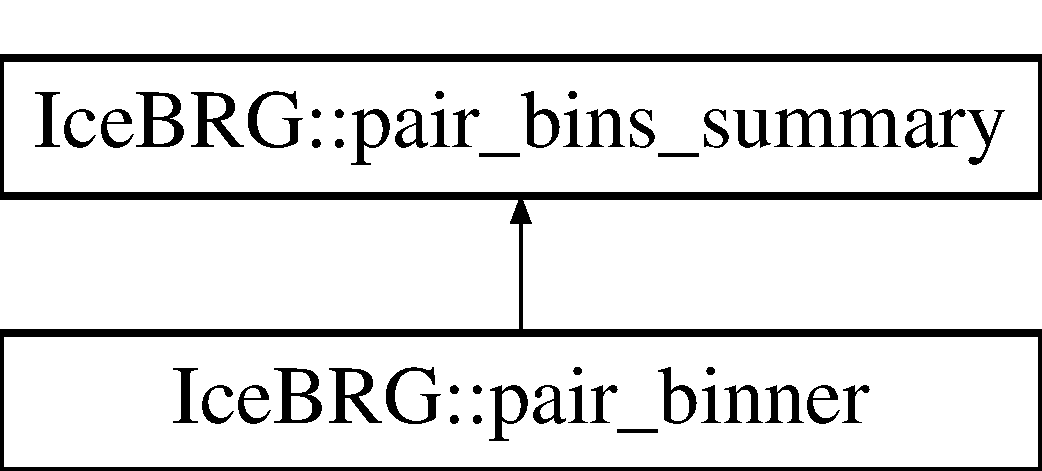
\includegraphics[height=2.000000cm]{classIceBRG_1_1pair__binner}
\end{center}
\end{figure}
\subsection*{Public Member Functions}
\begin{DoxyCompactItemize}
\item 
\hyperlink{classIceBRG_1_1pair__binner_a14fe5215ad45872e549c71ecc4e170e9}{pair\-\_\-binner} ()
\item 
\hyperlink{classIceBRG_1_1pair__binner_aa63e9ed393f3571585112990a36e58d1}{pair\-\_\-binner} (\hyperlink{classIceBRG_1_1limit__vector}{Ice\-B\-R\-G\-::limit\-\_\-vector}$<$ \hyperlink{namespaceIceBRG_a45499647eb87e24c10ab32c628711cec}{distance\-\_\-type} $>$ R\-\_\-bin\-\_\-limits, \hyperlink{classIceBRG_1_1limit__vector}{Ice\-B\-R\-G\-::limit\-\_\-vector}$<$ \hyperlink{namespaceIceBRG_a1be72ac4918a9b029f2eefa084213e35}{mass\-\_\-type} $>$ m\-\_\-bin\-\_\-limits=\hyperlink{classIceBRG_1_1limit__vector}{Ice\-B\-R\-G\-::limit\-\_\-vector}$<$ \hyperlink{namespaceIceBRG_a1be72ac4918a9b029f2eefa084213e35}{mass\-\_\-type} $>$(), \hyperlink{classIceBRG_1_1limit__vector}{Ice\-B\-R\-G\-::limit\-\_\-vector}$<$ \hyperlink{lib_2IceBRG__main_2common_8h_ad0f130a56eeb944d9ef2692ee881ecc4}{flt\-\_\-type} $>$ z\-\_\-bin\-\_\-limits=\hyperlink{classIceBRG_1_1limit__vector}{Ice\-B\-R\-G\-::limit\-\_\-vector}$<$ \hyperlink{lib_2IceBRG__main_2common_8h_ad0f130a56eeb944d9ef2692ee881ecc4}{flt\-\_\-type} $>$(), \hyperlink{classIceBRG_1_1limit__vector}{Ice\-B\-R\-G\-::limit\-\_\-vector}$<$ \hyperlink{lib_2IceBRG__main_2common_8h_ad0f130a56eeb944d9ef2692ee881ecc4}{flt\-\_\-type} $>$ mag\-\_\-bin\-\_\-limits=\hyperlink{classIceBRG_1_1limit__vector}{Ice\-B\-R\-G\-::limit\-\_\-vector}$<$ \hyperlink{lib_2IceBRG__main_2common_8h_ad0f130a56eeb944d9ef2692ee881ecc4}{flt\-\_\-type} $>$())
\item 
\hyperlink{classIceBRG_1_1pair__binner_a8fe51f7356398d6fb6f91328ff8bd70e}{pair\-\_\-binner} (const \hyperlink{namespaceIceBRG_a45499647eb87e24c10ab32c628711cec}{distance\-\_\-type} \&R\-\_\-min, const \hyperlink{namespaceIceBRG_a45499647eb87e24c10ab32c628711cec}{distance\-\_\-type} \&R\-\_\-max, const \hyperlink{lib_2IceBRG__main_2common_8h_ab322a3e50421dc5f0c43316b1b373592}{ssize\-\_\-t} \&R\-\_\-bins, const \hyperlink{namespaceIceBRG_a1be72ac4918a9b029f2eefa084213e35}{mass\-\_\-type} \&m\-\_\-min=-\/std\-::numeric\-\_\-limits$<$ \hyperlink{lib_2IceBRG__main_2common_8h_ad0f130a56eeb944d9ef2692ee881ecc4}{flt\-\_\-type} $>$\-::infinity()$\ast$\hyperlink{namespaceIceBRG_a9233960f6792ea35145d7db55c13e85d}{kg}, const \hyperlink{namespaceIceBRG_a1be72ac4918a9b029f2eefa084213e35}{mass\-\_\-type} \&m\-\_\-max=std\-::numeric\-\_\-limits$<$ \hyperlink{lib_2IceBRG__main_2common_8h_ad0f130a56eeb944d9ef2692ee881ecc4}{flt\-\_\-type} $>$\-::infinity()$\ast$\hyperlink{namespaceIceBRG_a9233960f6792ea35145d7db55c13e85d}{kg}, const \hyperlink{lib_2IceBRG__main_2common_8h_ab322a3e50421dc5f0c43316b1b373592}{ssize\-\_\-t} \&m\-\_\-bins=1, const \hyperlink{lib_2IceBRG__main_2common_8h_ad0f130a56eeb944d9ef2692ee881ecc4}{flt\-\_\-type} \&z\-\_\-min=-\/std\-::numeric\-\_\-limits$<$ \hyperlink{lib_2IceBRG__main_2common_8h_ad0f130a56eeb944d9ef2692ee881ecc4}{flt\-\_\-type} $>$\-::infinity(), const \hyperlink{lib_2IceBRG__main_2common_8h_ad0f130a56eeb944d9ef2692ee881ecc4}{flt\-\_\-type} \&z\-\_\-max=std\-::numeric\-\_\-limits$<$ \hyperlink{lib_2IceBRG__main_2common_8h_ad0f130a56eeb944d9ef2692ee881ecc4}{flt\-\_\-type} $>$\-::infinity(), const \hyperlink{lib_2IceBRG__main_2common_8h_ab322a3e50421dc5f0c43316b1b373592}{ssize\-\_\-t} \&\hyperlink{main__field__stats_8cpp_a6d4d8cfc3c2eccfe9ed5091d304e8dcd}{z\-\_\-bins}=1, const \hyperlink{lib_2IceBRG__main_2common_8h_ad0f130a56eeb944d9ef2692ee881ecc4}{flt\-\_\-type} \&mag\-\_\-min=-\/std\-::numeric\-\_\-limits$<$ \hyperlink{lib_2IceBRG__main_2common_8h_ad0f130a56eeb944d9ef2692ee881ecc4}{flt\-\_\-type} $>$\-::infinity(), const \hyperlink{lib_2IceBRG__main_2common_8h_ad0f130a56eeb944d9ef2692ee881ecc4}{flt\-\_\-type} \&mag\-\_\-max=std\-::numeric\-\_\-limits$<$ \hyperlink{lib_2IceBRG__main_2common_8h_ad0f130a56eeb944d9ef2692ee881ecc4}{flt\-\_\-type} $>$\-::infinity(), const \hyperlink{lib_2IceBRG__main_2common_8h_ab322a3e50421dc5f0c43316b1b373592}{ssize\-\_\-t} \&mag\-\_\-bins=1)
\item 
virtual \hyperlink{classIceBRG_1_1pair__binner_a308c3e94e1374784ec122dd705f7ed25}{$\sim$pair\-\_\-binner} ()
\item 
void \hyperlink{classIceBRG_1_1pair__binner_a1785f044a69bdd9376d63843248e4c17}{set\-\_\-z\-\_\-buffer} (const \hyperlink{lib_2IceBRG__main_2common_8h_ad0f130a56eeb944d9ef2692ee881ecc4}{flt\-\_\-type} \&new\-\_\-z\-\_\-buffer)
\item 
\hyperlink{lib_2IceBRG__main_2common_8h_ad0f130a56eeb944d9ef2692ee881ecc4}{flt\-\_\-type} \hyperlink{classIceBRG_1_1pair__binner_afc88be4e3536fd0f73538d2a368b1b27}{z\-\_\-buffer} () const 
\item 
bool \hyperlink{classIceBRG_1_1pair__binner_a3d0bc270b81bdf3d0fd7f5098448e7ba}{binnable} (const \hyperlink{classIceBRG_1_1galaxy}{galaxy} \&lens) const 
\item 
void \hyperlink{classIceBRG_1_1pair__binner_a8a4c12129a660eb007da7d2c8aaa1224}{add\-\_\-pair} (const \hyperlink{classIceBRG_1_1lens__source__pair}{lens\-\_\-source\-\_\-pair} \&new\-\_\-pair)
\item 
void \hyperlink{classIceBRG_1_1pair__binner_a98d977adcf1255e16c26348f1c2fe5cd}{add\-\_\-lens\-\_\-id} (const \hyperlink{lib_2IceBRG__main_2common_8h_ab322a3e50421dc5f0c43316b1b373592}{ssize\-\_\-t} \&new\-\_\-lens\-\_\-id, const \hyperlink{namespaceIceBRG_a1be72ac4918a9b029f2eefa084213e35}{mass\-\_\-type} \&\hyperlink{namespaceIceBRG_ada6365c5d16106f0608afbd34f010bcc}{m}, const \hyperlink{lib_2IceBRG__main_2common_8h_ad0f130a56eeb944d9ef2692ee881ecc4}{flt\-\_\-type} \&z, const \hyperlink{lib_2IceBRG__main_2common_8h_ad0f130a56eeb944d9ef2692ee881ecc4}{flt\-\_\-type} \&mag, const \hyperlink{lib_2IceBRG__main_2common_8h_ad0f130a56eeb944d9ef2692ee881ecc4}{flt\-\_\-type} \&weight=1)
\item 
void \hyperlink{classIceBRG_1_1pair__binner_a25c3cddd7575cb0012a301772770027d}{clear} ()
\item 
void \hyperlink{classIceBRG_1_1pair__binner_a01b62fd022293870317bbcb3d8a809ff}{empty} ()
\item 
void \hyperlink{classIceBRG_1_1pair__binner_ae164bdb3724a73f199ecdd7b4c878ee7}{sort} () const 
\item 
{\footnotesize template$<$typename Tv1 , typename Tv2 $>$ }\\void \hyperlink{classIceBRG_1_1pair__binner_aa2ab94f5347d9af9ef901fbe9519d15e}{set\-\_\-unmasked\-\_\-fractions} (Tv1 \&\&bin\-\_\-limits, Tv2 \&\&unmasked\-\_\-fractions)
\item 
\hyperlink{namespaceIceBRG_a80c597ef5ba0a32491d32a9f0083b02d}{surface\-\_\-density\-\_\-type} \hyperlink{classIceBRG_1_1pair__binner_a00a64eeb64d7d7c2bd2587371ade8a0c}{delta\-\_\-\-Sigma\-\_\-t\-\_\-mean\-\_\-for\-\_\-bin} (\hyperlink{lib_2IceBRG__main_2common_8h_ab322a3e50421dc5f0c43316b1b373592}{ssize\-\_\-t} R\-\_\-i, \hyperlink{lib_2IceBRG__main_2common_8h_ab322a3e50421dc5f0c43316b1b373592}{ssize\-\_\-t} m\-\_\-i, \hyperlink{lib_2IceBRG__main_2common_8h_ab322a3e50421dc5f0c43316b1b373592}{ssize\-\_\-t} z\-\_\-i, \hyperlink{lib_2IceBRG__main_2common_8h_ab322a3e50421dc5f0c43316b1b373592}{ssize\-\_\-t} mag\-\_\-i)
\item 
\hyperlink{namespaceIceBRG_a80c597ef5ba0a32491d32a9f0083b02d}{surface\-\_\-density\-\_\-type} \hyperlink{classIceBRG_1_1pair__binner_ab245ee13d43faaea7e9d6b23284c43e0}{delta\-\_\-\-Sigma\-\_\-x\-\_\-mean\-\_\-for\-\_\-bin} (\hyperlink{lib_2IceBRG__main_2common_8h_ab322a3e50421dc5f0c43316b1b373592}{ssize\-\_\-t} R\-\_\-i, \hyperlink{lib_2IceBRG__main_2common_8h_ab322a3e50421dc5f0c43316b1b373592}{ssize\-\_\-t} m\-\_\-i, \hyperlink{lib_2IceBRG__main_2common_8h_ab322a3e50421dc5f0c43316b1b373592}{ssize\-\_\-t} z\-\_\-i, \hyperlink{lib_2IceBRG__main_2common_8h_ab322a3e50421dc5f0c43316b1b373592}{ssize\-\_\-t} mag\-\_\-i)
\item 
\hyperlink{namespaceIceBRG_a80c597ef5ba0a32491d32a9f0083b02d}{surface\-\_\-density\-\_\-type} \hyperlink{classIceBRG_1_1pair__binner_adaf91e6ea6e19d19d51b548c86c5d430}{delta\-\_\-\-Sigma\-\_\-t\-\_\-std\-\_\-for\-\_\-bin} (\hyperlink{lib_2IceBRG__main_2common_8h_ab322a3e50421dc5f0c43316b1b373592}{ssize\-\_\-t} R\-\_\-i, \hyperlink{lib_2IceBRG__main_2common_8h_ab322a3e50421dc5f0c43316b1b373592}{ssize\-\_\-t} m\-\_\-i, \hyperlink{lib_2IceBRG__main_2common_8h_ab322a3e50421dc5f0c43316b1b373592}{ssize\-\_\-t} z\-\_\-i, \hyperlink{lib_2IceBRG__main_2common_8h_ab322a3e50421dc5f0c43316b1b373592}{ssize\-\_\-t} mag\-\_\-i)
\item 
\hyperlink{namespaceIceBRG_a80c597ef5ba0a32491d32a9f0083b02d}{surface\-\_\-density\-\_\-type} \hyperlink{classIceBRG_1_1pair__binner_a0a529338fc1366b8f476a12bf258cd3e}{delta\-\_\-\-Sigma\-\_\-x\-\_\-std\-\_\-for\-\_\-bin} (\hyperlink{lib_2IceBRG__main_2common_8h_ab322a3e50421dc5f0c43316b1b373592}{ssize\-\_\-t} R\-\_\-i, \hyperlink{lib_2IceBRG__main_2common_8h_ab322a3e50421dc5f0c43316b1b373592}{ssize\-\_\-t} m\-\_\-i, \hyperlink{lib_2IceBRG__main_2common_8h_ab322a3e50421dc5f0c43316b1b373592}{ssize\-\_\-t} z\-\_\-i, \hyperlink{lib_2IceBRG__main_2common_8h_ab322a3e50421dc5f0c43316b1b373592}{ssize\-\_\-t} mag\-\_\-i)
\item 
\hyperlink{namespaceIceBRG_a80c597ef5ba0a32491d32a9f0083b02d}{surface\-\_\-density\-\_\-type} \hyperlink{classIceBRG_1_1pair__binner_a1a9bb7d501868687f94a969f3c984c87}{delta\-\_\-\-Sigma\-\_\-t\-\_\-stderr\-\_\-for\-\_\-bin} (\hyperlink{lib_2IceBRG__main_2common_8h_ab322a3e50421dc5f0c43316b1b373592}{ssize\-\_\-t} R\-\_\-i, \hyperlink{lib_2IceBRG__main_2common_8h_ab322a3e50421dc5f0c43316b1b373592}{ssize\-\_\-t} m\-\_\-i, \hyperlink{lib_2IceBRG__main_2common_8h_ab322a3e50421dc5f0c43316b1b373592}{ssize\-\_\-t} z\-\_\-i, \hyperlink{lib_2IceBRG__main_2common_8h_ab322a3e50421dc5f0c43316b1b373592}{ssize\-\_\-t} mag\-\_\-i)
\item 
\hyperlink{namespaceIceBRG_a80c597ef5ba0a32491d32a9f0083b02d}{surface\-\_\-density\-\_\-type} \hyperlink{classIceBRG_1_1pair__binner_ab52d75566419ed06ca88893a980a29bf}{delta\-\_\-\-Sigma\-\_\-x\-\_\-stderr\-\_\-for\-\_\-bin} (\hyperlink{lib_2IceBRG__main_2common_8h_ab322a3e50421dc5f0c43316b1b373592}{ssize\-\_\-t} R\-\_\-i, \hyperlink{lib_2IceBRG__main_2common_8h_ab322a3e50421dc5f0c43316b1b373592}{ssize\-\_\-t} m\-\_\-i, \hyperlink{lib_2IceBRG__main_2common_8h_ab322a3e50421dc5f0c43316b1b373592}{ssize\-\_\-t} z\-\_\-i, \hyperlink{lib_2IceBRG__main_2common_8h_ab322a3e50421dc5f0c43316b1b373592}{ssize\-\_\-t} mag\-\_\-i)
\item 
\hyperlink{namespaceIceBRG_a80c597ef5ba0a32491d32a9f0083b02d}{surface\-\_\-density\-\_\-type} \hyperlink{classIceBRG_1_1pair__binner_a70fad21c8d543776e7e44ccb8b93b76c}{delta\-\_\-\-Sigma\-\_\-t\-\_\-mean\-\_\-for\-\_\-bin} (const \hyperlink{namespaceIceBRG_a45499647eb87e24c10ab32c628711cec}{distance\-\_\-type} \&R, const \hyperlink{namespaceIceBRG_a1be72ac4918a9b029f2eefa084213e35}{mass\-\_\-type} \&\hyperlink{namespaceIceBRG_ada6365c5d16106f0608afbd34f010bcc}{m}, const \hyperlink{lib_2IceBRG__main_2common_8h_ad0f130a56eeb944d9ef2692ee881ecc4}{flt\-\_\-type} \&z, const \hyperlink{lib_2IceBRG__main_2common_8h_ad0f130a56eeb944d9ef2692ee881ecc4}{flt\-\_\-type} \&mag)
\item 
\hyperlink{namespaceIceBRG_a80c597ef5ba0a32491d32a9f0083b02d}{surface\-\_\-density\-\_\-type} \hyperlink{classIceBRG_1_1pair__binner_ae862970ce4063909e2aec43675b5918f}{delta\-\_\-\-Sigma\-\_\-x\-\_\-mean\-\_\-for\-\_\-bin} (const \hyperlink{namespaceIceBRG_a45499647eb87e24c10ab32c628711cec}{distance\-\_\-type} \&R, const \hyperlink{namespaceIceBRG_a1be72ac4918a9b029f2eefa084213e35}{mass\-\_\-type} \&\hyperlink{namespaceIceBRG_ada6365c5d16106f0608afbd34f010bcc}{m}, const \hyperlink{lib_2IceBRG__main_2common_8h_ad0f130a56eeb944d9ef2692ee881ecc4}{flt\-\_\-type} \&z, const \hyperlink{lib_2IceBRG__main_2common_8h_ad0f130a56eeb944d9ef2692ee881ecc4}{flt\-\_\-type} \&mag)
\item 
\hyperlink{namespaceIceBRG_a80c597ef5ba0a32491d32a9f0083b02d}{surface\-\_\-density\-\_\-type} \hyperlink{classIceBRG_1_1pair__binner_a6c33e8d61df44e5a069a9e96971b7375}{delta\-\_\-\-Sigma\-\_\-t\-\_\-std\-\_\-for\-\_\-bin} (const \hyperlink{namespaceIceBRG_a45499647eb87e24c10ab32c628711cec}{distance\-\_\-type} \&R, const \hyperlink{namespaceIceBRG_a1be72ac4918a9b029f2eefa084213e35}{mass\-\_\-type} \&\hyperlink{namespaceIceBRG_ada6365c5d16106f0608afbd34f010bcc}{m}, const \hyperlink{lib_2IceBRG__main_2common_8h_ad0f130a56eeb944d9ef2692ee881ecc4}{flt\-\_\-type} \&z, const \hyperlink{lib_2IceBRG__main_2common_8h_ad0f130a56eeb944d9ef2692ee881ecc4}{flt\-\_\-type} \&mag)
\item 
\hyperlink{namespaceIceBRG_a80c597ef5ba0a32491d32a9f0083b02d}{surface\-\_\-density\-\_\-type} \hyperlink{classIceBRG_1_1pair__binner_aaa1bc2defcf7bdfe26179a089565e30c}{delta\-\_\-\-Sigma\-\_\-x\-\_\-std\-\_\-for\-\_\-bin} (const \hyperlink{namespaceIceBRG_a45499647eb87e24c10ab32c628711cec}{distance\-\_\-type} \&R, const \hyperlink{namespaceIceBRG_a1be72ac4918a9b029f2eefa084213e35}{mass\-\_\-type} \&\hyperlink{namespaceIceBRG_ada6365c5d16106f0608afbd34f010bcc}{m}, const \hyperlink{lib_2IceBRG__main_2common_8h_ad0f130a56eeb944d9ef2692ee881ecc4}{flt\-\_\-type} \&z, const \hyperlink{lib_2IceBRG__main_2common_8h_ad0f130a56eeb944d9ef2692ee881ecc4}{flt\-\_\-type} \&mag)
\item 
\hyperlink{namespaceIceBRG_a80c597ef5ba0a32491d32a9f0083b02d}{surface\-\_\-density\-\_\-type} \hyperlink{classIceBRG_1_1pair__binner_a3c32bd86aa89de0ef6ad1fca5097f41c}{delta\-\_\-\-Sigma\-\_\-t\-\_\-stderr\-\_\-for\-\_\-bin} (const \hyperlink{namespaceIceBRG_a45499647eb87e24c10ab32c628711cec}{distance\-\_\-type} \&R, const \hyperlink{namespaceIceBRG_a1be72ac4918a9b029f2eefa084213e35}{mass\-\_\-type} \&\hyperlink{namespaceIceBRG_ada6365c5d16106f0608afbd34f010bcc}{m}, const \hyperlink{lib_2IceBRG__main_2common_8h_ad0f130a56eeb944d9ef2692ee881ecc4}{flt\-\_\-type} \&z, const \hyperlink{lib_2IceBRG__main_2common_8h_ad0f130a56eeb944d9ef2692ee881ecc4}{flt\-\_\-type} \&mag)
\item 
\hyperlink{namespaceIceBRG_a80c597ef5ba0a32491d32a9f0083b02d}{surface\-\_\-density\-\_\-type} \hyperlink{classIceBRG_1_1pair__binner_aacd662f4665abf4678344f14b6e77f35}{delta\-\_\-\-Sigma\-\_\-x\-\_\-stderr\-\_\-for\-\_\-bin} (const \hyperlink{namespaceIceBRG_a45499647eb87e24c10ab32c628711cec}{distance\-\_\-type} \&R, const \hyperlink{namespaceIceBRG_a1be72ac4918a9b029f2eefa084213e35}{mass\-\_\-type} \&\hyperlink{namespaceIceBRG_ada6365c5d16106f0608afbd34f010bcc}{m}, const \hyperlink{lib_2IceBRG__main_2common_8h_ad0f130a56eeb944d9ef2692ee881ecc4}{flt\-\_\-type} \&z, const \hyperlink{lib_2IceBRG__main_2common_8h_ad0f130a56eeb944d9ef2692ee881ecc4}{flt\-\_\-type} \&mag)
\end{DoxyCompactItemize}
\subsection*{Additional Inherited Members}


\subsection{Constructor \& Destructor Documentation}
\hypertarget{classIceBRG_1_1pair__binner_a14fe5215ad45872e549c71ecc4e170e9}{\index{Ice\-B\-R\-G\-::pair\-\_\-binner@{Ice\-B\-R\-G\-::pair\-\_\-binner}!pair\-\_\-binner@{pair\-\_\-binner}}
\index{pair\-\_\-binner@{pair\-\_\-binner}!IceBRG::pair_binner@{Ice\-B\-R\-G\-::pair\-\_\-binner}}
\subsubsection[{pair\-\_\-binner}]{\setlength{\rightskip}{0pt plus 5cm}Ice\-B\-R\-G\-::pair\-\_\-binner\-::pair\-\_\-binner (
\begin{DoxyParamCaption}
{}
\end{DoxyParamCaption}
)\hspace{0.3cm}{\ttfamily [inline]}}}\label{classIceBRG_1_1pair__binner_a14fe5215ad45872e549c71ecc4e170e9}
\hypertarget{classIceBRG_1_1pair__binner_aa63e9ed393f3571585112990a36e58d1}{\index{Ice\-B\-R\-G\-::pair\-\_\-binner@{Ice\-B\-R\-G\-::pair\-\_\-binner}!pair\-\_\-binner@{pair\-\_\-binner}}
\index{pair\-\_\-binner@{pair\-\_\-binner}!IceBRG::pair_binner@{Ice\-B\-R\-G\-::pair\-\_\-binner}}
\subsubsection[{pair\-\_\-binner}]{\setlength{\rightskip}{0pt plus 5cm}Ice\-B\-R\-G\-::pair\-\_\-binner\-::pair\-\_\-binner (
\begin{DoxyParamCaption}
\item[{{\bf Ice\-B\-R\-G\-::limit\-\_\-vector}$<$ {\bf distance\-\_\-type} $>$}]{R\-\_\-bin\-\_\-limits, }
\item[{{\bf Ice\-B\-R\-G\-::limit\-\_\-vector}$<$ {\bf mass\-\_\-type} $>$}]{m\-\_\-bin\-\_\-limits = {\ttfamily {\bf Ice\-B\-R\-G\-::limit\-\_\-vector}$<${\bf mass\-\_\-type}$>$()}, }
\item[{{\bf Ice\-B\-R\-G\-::limit\-\_\-vector}$<$ {\bf flt\-\_\-type} $>$}]{z\-\_\-bin\-\_\-limits = {\ttfamily {\bf Ice\-B\-R\-G\-::limit\-\_\-vector}$<${\bf flt\-\_\-type}$>$()}, }
\item[{{\bf Ice\-B\-R\-G\-::limit\-\_\-vector}$<$ {\bf flt\-\_\-type} $>$}]{mag\-\_\-bin\-\_\-limits = {\ttfamily {\bf Ice\-B\-R\-G\-::limit\-\_\-vector}$<${\bf flt\-\_\-type}$>$()}}
\end{DoxyParamCaption}
)\hspace{0.3cm}{\ttfamily [inline]}}}\label{classIceBRG_1_1pair__binner_aa63e9ed393f3571585112990a36e58d1}
\hypertarget{classIceBRG_1_1pair__binner_a8fe51f7356398d6fb6f91328ff8bd70e}{\index{Ice\-B\-R\-G\-::pair\-\_\-binner@{Ice\-B\-R\-G\-::pair\-\_\-binner}!pair\-\_\-binner@{pair\-\_\-binner}}
\index{pair\-\_\-binner@{pair\-\_\-binner}!IceBRG::pair_binner@{Ice\-B\-R\-G\-::pair\-\_\-binner}}
\subsubsection[{pair\-\_\-binner}]{\setlength{\rightskip}{0pt plus 5cm}Ice\-B\-R\-G\-::pair\-\_\-binner\-::pair\-\_\-binner (
\begin{DoxyParamCaption}
\item[{const {\bf distance\-\_\-type} \&}]{R\-\_\-min, }
\item[{const {\bf distance\-\_\-type} \&}]{R\-\_\-max, }
\item[{const {\bf ssize\-\_\-t} \&}]{R\-\_\-bins, }
\item[{const {\bf mass\-\_\-type} \&}]{m\-\_\-min = {\ttfamily -\/std\-:\-:numeric\-\_\-limits$<${\bf flt\-\_\-type}$>$\-:\-:infinity()$\ast${\bf kg}}, }
\item[{const {\bf mass\-\_\-type} \&}]{m\-\_\-max = {\ttfamily std\-:\-:numeric\-\_\-limits$<${\bf flt\-\_\-type}$>$\-:\-:infinity()$\ast${\bf kg}}, }
\item[{const {\bf ssize\-\_\-t} \&}]{m\-\_\-bins = {\ttfamily 1}, }
\item[{const {\bf flt\-\_\-type} \&}]{z\-\_\-min = {\ttfamily -\/std\-:\-:numeric\-\_\-limits$<${\bf flt\-\_\-type}$>$\-:\-:infinity()}, }
\item[{const {\bf flt\-\_\-type} \&}]{z\-\_\-max = {\ttfamily std\-:\-:numeric\-\_\-limits$<${\bf flt\-\_\-type}$>$\-:\-:infinity()}, }
\item[{const {\bf ssize\-\_\-t} \&}]{z\-\_\-bins = {\ttfamily 1}, }
\item[{const {\bf flt\-\_\-type} \&}]{mag\-\_\-min = {\ttfamily -\/std\-:\-:numeric\-\_\-limits$<${\bf flt\-\_\-type}$>$\-:\-:infinity()}, }
\item[{const {\bf flt\-\_\-type} \&}]{mag\-\_\-max = {\ttfamily std\-:\-:numeric\-\_\-limits$<${\bf flt\-\_\-type}$>$\-:\-:infinity()}, }
\item[{const {\bf ssize\-\_\-t} \&}]{mag\-\_\-bins = {\ttfamily 1}}
\end{DoxyParamCaption}
)\hspace{0.3cm}{\ttfamily [inline]}}}\label{classIceBRG_1_1pair__binner_a8fe51f7356398d6fb6f91328ff8bd70e}
\hypertarget{classIceBRG_1_1pair__binner_a308c3e94e1374784ec122dd705f7ed25}{\index{Ice\-B\-R\-G\-::pair\-\_\-binner@{Ice\-B\-R\-G\-::pair\-\_\-binner}!$\sim$pair\-\_\-binner@{$\sim$pair\-\_\-binner}}
\index{$\sim$pair\-\_\-binner@{$\sim$pair\-\_\-binner}!IceBRG::pair_binner@{Ice\-B\-R\-G\-::pair\-\_\-binner}}
\subsubsection[{$\sim$pair\-\_\-binner}]{\setlength{\rightskip}{0pt plus 5cm}virtual Ice\-B\-R\-G\-::pair\-\_\-binner\-::$\sim$pair\-\_\-binner (
\begin{DoxyParamCaption}
{}
\end{DoxyParamCaption}
)\hspace{0.3cm}{\ttfamily [inline]}, {\ttfamily [virtual]}}}\label{classIceBRG_1_1pair__binner_a308c3e94e1374784ec122dd705f7ed25}


\subsection{Member Function Documentation}
\hypertarget{classIceBRG_1_1pair__binner_a98d977adcf1255e16c26348f1c2fe5cd}{\index{Ice\-B\-R\-G\-::pair\-\_\-binner@{Ice\-B\-R\-G\-::pair\-\_\-binner}!add\-\_\-lens\-\_\-id@{add\-\_\-lens\-\_\-id}}
\index{add\-\_\-lens\-\_\-id@{add\-\_\-lens\-\_\-id}!IceBRG::pair_binner@{Ice\-B\-R\-G\-::pair\-\_\-binner}}
\subsubsection[{add\-\_\-lens\-\_\-id}]{\setlength{\rightskip}{0pt plus 5cm}void Ice\-B\-R\-G\-::pair\-\_\-binner\-::add\-\_\-lens\-\_\-id (
\begin{DoxyParamCaption}
\item[{const {\bf ssize\-\_\-t} \&}]{new\-\_\-lens\-\_\-id, }
\item[{const {\bf mass\-\_\-type} \&}]{m, }
\item[{const {\bf flt\-\_\-type} \&}]{z, }
\item[{const {\bf flt\-\_\-type} \&}]{mag, }
\item[{const {\bf flt\-\_\-type} \&}]{weight = {\ttfamily 1}}
\end{DoxyParamCaption}
)}}\label{classIceBRG_1_1pair__binner_a98d977adcf1255e16c26348f1c2fe5cd}
\hypertarget{classIceBRG_1_1pair__binner_a8a4c12129a660eb007da7d2c8aaa1224}{\index{Ice\-B\-R\-G\-::pair\-\_\-binner@{Ice\-B\-R\-G\-::pair\-\_\-binner}!add\-\_\-pair@{add\-\_\-pair}}
\index{add\-\_\-pair@{add\-\_\-pair}!IceBRG::pair_binner@{Ice\-B\-R\-G\-::pair\-\_\-binner}}
\subsubsection[{add\-\_\-pair}]{\setlength{\rightskip}{0pt plus 5cm}void Ice\-B\-R\-G\-::pair\-\_\-binner\-::add\-\_\-pair (
\begin{DoxyParamCaption}
\item[{const {\bf lens\-\_\-source\-\_\-pair} \&}]{new\-\_\-pair}
\end{DoxyParamCaption}
)}}\label{classIceBRG_1_1pair__binner_a8a4c12129a660eb007da7d2c8aaa1224}
\hypertarget{classIceBRG_1_1pair__binner_a3d0bc270b81bdf3d0fd7f5098448e7ba}{\index{Ice\-B\-R\-G\-::pair\-\_\-binner@{Ice\-B\-R\-G\-::pair\-\_\-binner}!binnable@{binnable}}
\index{binnable@{binnable}!IceBRG::pair_binner@{Ice\-B\-R\-G\-::pair\-\_\-binner}}
\subsubsection[{binnable}]{\setlength{\rightskip}{0pt plus 5cm}bool Ice\-B\-R\-G\-::pair\-\_\-binner\-::binnable (
\begin{DoxyParamCaption}
\item[{const {\bf galaxy} \&}]{lens}
\end{DoxyParamCaption}
) const}}\label{classIceBRG_1_1pair__binner_a3d0bc270b81bdf3d0fd7f5098448e7ba}
\hypertarget{classIceBRG_1_1pair__binner_a25c3cddd7575cb0012a301772770027d}{\index{Ice\-B\-R\-G\-::pair\-\_\-binner@{Ice\-B\-R\-G\-::pair\-\_\-binner}!clear@{clear}}
\index{clear@{clear}!IceBRG::pair_binner@{Ice\-B\-R\-G\-::pair\-\_\-binner}}
\subsubsection[{clear}]{\setlength{\rightskip}{0pt plus 5cm}void Ice\-B\-R\-G\-::pair\-\_\-binner\-::clear (
\begin{DoxyParamCaption}
{}
\end{DoxyParamCaption}
)\hspace{0.3cm}{\ttfamily [virtual]}}}\label{classIceBRG_1_1pair__binner_a25c3cddd7575cb0012a301772770027d}


Reimplemented from \hyperlink{classIceBRG_1_1pair__bins__summary_a5c15793df751321aef8bed2526c3cbe6}{Ice\-B\-R\-G\-::pair\-\_\-bins\-\_\-summary}.

\hypertarget{classIceBRG_1_1pair__binner_a00a64eeb64d7d7c2bd2587371ade8a0c}{\index{Ice\-B\-R\-G\-::pair\-\_\-binner@{Ice\-B\-R\-G\-::pair\-\_\-binner}!delta\-\_\-\-Sigma\-\_\-t\-\_\-mean\-\_\-for\-\_\-bin@{delta\-\_\-\-Sigma\-\_\-t\-\_\-mean\-\_\-for\-\_\-bin}}
\index{delta\-\_\-\-Sigma\-\_\-t\-\_\-mean\-\_\-for\-\_\-bin@{delta\-\_\-\-Sigma\-\_\-t\-\_\-mean\-\_\-for\-\_\-bin}!IceBRG::pair_binner@{Ice\-B\-R\-G\-::pair\-\_\-binner}}
\subsubsection[{delta\-\_\-\-Sigma\-\_\-t\-\_\-mean\-\_\-for\-\_\-bin}]{\setlength{\rightskip}{0pt plus 5cm}{\bf surface\-\_\-density\-\_\-type} Ice\-B\-R\-G\-::pair\-\_\-binner\-::delta\-\_\-\-Sigma\-\_\-t\-\_\-mean\-\_\-for\-\_\-bin (
\begin{DoxyParamCaption}
\item[{{\bf ssize\-\_\-t}}]{R\-\_\-i, }
\item[{{\bf ssize\-\_\-t}}]{m\-\_\-i, }
\item[{{\bf ssize\-\_\-t}}]{z\-\_\-i, }
\item[{{\bf ssize\-\_\-t}}]{mag\-\_\-i}
\end{DoxyParamCaption}
)}}\label{classIceBRG_1_1pair__binner_a00a64eeb64d7d7c2bd2587371ade8a0c}
\hypertarget{classIceBRG_1_1pair__binner_a70fad21c8d543776e7e44ccb8b93b76c}{\index{Ice\-B\-R\-G\-::pair\-\_\-binner@{Ice\-B\-R\-G\-::pair\-\_\-binner}!delta\-\_\-\-Sigma\-\_\-t\-\_\-mean\-\_\-for\-\_\-bin@{delta\-\_\-\-Sigma\-\_\-t\-\_\-mean\-\_\-for\-\_\-bin}}
\index{delta\-\_\-\-Sigma\-\_\-t\-\_\-mean\-\_\-for\-\_\-bin@{delta\-\_\-\-Sigma\-\_\-t\-\_\-mean\-\_\-for\-\_\-bin}!IceBRG::pair_binner@{Ice\-B\-R\-G\-::pair\-\_\-binner}}
\subsubsection[{delta\-\_\-\-Sigma\-\_\-t\-\_\-mean\-\_\-for\-\_\-bin}]{\setlength{\rightskip}{0pt plus 5cm}{\bf surface\-\_\-density\-\_\-type} Ice\-B\-R\-G\-::pair\-\_\-binner\-::delta\-\_\-\-Sigma\-\_\-t\-\_\-mean\-\_\-for\-\_\-bin (
\begin{DoxyParamCaption}
\item[{const {\bf distance\-\_\-type} \&}]{R, }
\item[{const {\bf mass\-\_\-type} \&}]{m, }
\item[{const {\bf flt\-\_\-type} \&}]{z, }
\item[{const {\bf flt\-\_\-type} \&}]{mag}
\end{DoxyParamCaption}
)}}\label{classIceBRG_1_1pair__binner_a70fad21c8d543776e7e44ccb8b93b76c}
\hypertarget{classIceBRG_1_1pair__binner_adaf91e6ea6e19d19d51b548c86c5d430}{\index{Ice\-B\-R\-G\-::pair\-\_\-binner@{Ice\-B\-R\-G\-::pair\-\_\-binner}!delta\-\_\-\-Sigma\-\_\-t\-\_\-std\-\_\-for\-\_\-bin@{delta\-\_\-\-Sigma\-\_\-t\-\_\-std\-\_\-for\-\_\-bin}}
\index{delta\-\_\-\-Sigma\-\_\-t\-\_\-std\-\_\-for\-\_\-bin@{delta\-\_\-\-Sigma\-\_\-t\-\_\-std\-\_\-for\-\_\-bin}!IceBRG::pair_binner@{Ice\-B\-R\-G\-::pair\-\_\-binner}}
\subsubsection[{delta\-\_\-\-Sigma\-\_\-t\-\_\-std\-\_\-for\-\_\-bin}]{\setlength{\rightskip}{0pt plus 5cm}{\bf surface\-\_\-density\-\_\-type} Ice\-B\-R\-G\-::pair\-\_\-binner\-::delta\-\_\-\-Sigma\-\_\-t\-\_\-std\-\_\-for\-\_\-bin (
\begin{DoxyParamCaption}
\item[{{\bf ssize\-\_\-t}}]{R\-\_\-i, }
\item[{{\bf ssize\-\_\-t}}]{m\-\_\-i, }
\item[{{\bf ssize\-\_\-t}}]{z\-\_\-i, }
\item[{{\bf ssize\-\_\-t}}]{mag\-\_\-i}
\end{DoxyParamCaption}
)}}\label{classIceBRG_1_1pair__binner_adaf91e6ea6e19d19d51b548c86c5d430}
\hypertarget{classIceBRG_1_1pair__binner_a6c33e8d61df44e5a069a9e96971b7375}{\index{Ice\-B\-R\-G\-::pair\-\_\-binner@{Ice\-B\-R\-G\-::pair\-\_\-binner}!delta\-\_\-\-Sigma\-\_\-t\-\_\-std\-\_\-for\-\_\-bin@{delta\-\_\-\-Sigma\-\_\-t\-\_\-std\-\_\-for\-\_\-bin}}
\index{delta\-\_\-\-Sigma\-\_\-t\-\_\-std\-\_\-for\-\_\-bin@{delta\-\_\-\-Sigma\-\_\-t\-\_\-std\-\_\-for\-\_\-bin}!IceBRG::pair_binner@{Ice\-B\-R\-G\-::pair\-\_\-binner}}
\subsubsection[{delta\-\_\-\-Sigma\-\_\-t\-\_\-std\-\_\-for\-\_\-bin}]{\setlength{\rightskip}{0pt plus 5cm}{\bf surface\-\_\-density\-\_\-type} Ice\-B\-R\-G\-::pair\-\_\-binner\-::delta\-\_\-\-Sigma\-\_\-t\-\_\-std\-\_\-for\-\_\-bin (
\begin{DoxyParamCaption}
\item[{const {\bf distance\-\_\-type} \&}]{R, }
\item[{const {\bf mass\-\_\-type} \&}]{m, }
\item[{const {\bf flt\-\_\-type} \&}]{z, }
\item[{const {\bf flt\-\_\-type} \&}]{mag}
\end{DoxyParamCaption}
)}}\label{classIceBRG_1_1pair__binner_a6c33e8d61df44e5a069a9e96971b7375}
\hypertarget{classIceBRG_1_1pair__binner_a1a9bb7d501868687f94a969f3c984c87}{\index{Ice\-B\-R\-G\-::pair\-\_\-binner@{Ice\-B\-R\-G\-::pair\-\_\-binner}!delta\-\_\-\-Sigma\-\_\-t\-\_\-stderr\-\_\-for\-\_\-bin@{delta\-\_\-\-Sigma\-\_\-t\-\_\-stderr\-\_\-for\-\_\-bin}}
\index{delta\-\_\-\-Sigma\-\_\-t\-\_\-stderr\-\_\-for\-\_\-bin@{delta\-\_\-\-Sigma\-\_\-t\-\_\-stderr\-\_\-for\-\_\-bin}!IceBRG::pair_binner@{Ice\-B\-R\-G\-::pair\-\_\-binner}}
\subsubsection[{delta\-\_\-\-Sigma\-\_\-t\-\_\-stderr\-\_\-for\-\_\-bin}]{\setlength{\rightskip}{0pt plus 5cm}{\bf surface\-\_\-density\-\_\-type} Ice\-B\-R\-G\-::pair\-\_\-binner\-::delta\-\_\-\-Sigma\-\_\-t\-\_\-stderr\-\_\-for\-\_\-bin (
\begin{DoxyParamCaption}
\item[{{\bf ssize\-\_\-t}}]{R\-\_\-i, }
\item[{{\bf ssize\-\_\-t}}]{m\-\_\-i, }
\item[{{\bf ssize\-\_\-t}}]{z\-\_\-i, }
\item[{{\bf ssize\-\_\-t}}]{mag\-\_\-i}
\end{DoxyParamCaption}
)}}\label{classIceBRG_1_1pair__binner_a1a9bb7d501868687f94a969f3c984c87}
\hypertarget{classIceBRG_1_1pair__binner_a3c32bd86aa89de0ef6ad1fca5097f41c}{\index{Ice\-B\-R\-G\-::pair\-\_\-binner@{Ice\-B\-R\-G\-::pair\-\_\-binner}!delta\-\_\-\-Sigma\-\_\-t\-\_\-stderr\-\_\-for\-\_\-bin@{delta\-\_\-\-Sigma\-\_\-t\-\_\-stderr\-\_\-for\-\_\-bin}}
\index{delta\-\_\-\-Sigma\-\_\-t\-\_\-stderr\-\_\-for\-\_\-bin@{delta\-\_\-\-Sigma\-\_\-t\-\_\-stderr\-\_\-for\-\_\-bin}!IceBRG::pair_binner@{Ice\-B\-R\-G\-::pair\-\_\-binner}}
\subsubsection[{delta\-\_\-\-Sigma\-\_\-t\-\_\-stderr\-\_\-for\-\_\-bin}]{\setlength{\rightskip}{0pt plus 5cm}{\bf surface\-\_\-density\-\_\-type} Ice\-B\-R\-G\-::pair\-\_\-binner\-::delta\-\_\-\-Sigma\-\_\-t\-\_\-stderr\-\_\-for\-\_\-bin (
\begin{DoxyParamCaption}
\item[{const {\bf distance\-\_\-type} \&}]{R, }
\item[{const {\bf mass\-\_\-type} \&}]{m, }
\item[{const {\bf flt\-\_\-type} \&}]{z, }
\item[{const {\bf flt\-\_\-type} \&}]{mag}
\end{DoxyParamCaption}
)}}\label{classIceBRG_1_1pair__binner_a3c32bd86aa89de0ef6ad1fca5097f41c}
\hypertarget{classIceBRG_1_1pair__binner_ab245ee13d43faaea7e9d6b23284c43e0}{\index{Ice\-B\-R\-G\-::pair\-\_\-binner@{Ice\-B\-R\-G\-::pair\-\_\-binner}!delta\-\_\-\-Sigma\-\_\-x\-\_\-mean\-\_\-for\-\_\-bin@{delta\-\_\-\-Sigma\-\_\-x\-\_\-mean\-\_\-for\-\_\-bin}}
\index{delta\-\_\-\-Sigma\-\_\-x\-\_\-mean\-\_\-for\-\_\-bin@{delta\-\_\-\-Sigma\-\_\-x\-\_\-mean\-\_\-for\-\_\-bin}!IceBRG::pair_binner@{Ice\-B\-R\-G\-::pair\-\_\-binner}}
\subsubsection[{delta\-\_\-\-Sigma\-\_\-x\-\_\-mean\-\_\-for\-\_\-bin}]{\setlength{\rightskip}{0pt plus 5cm}{\bf surface\-\_\-density\-\_\-type} Ice\-B\-R\-G\-::pair\-\_\-binner\-::delta\-\_\-\-Sigma\-\_\-x\-\_\-mean\-\_\-for\-\_\-bin (
\begin{DoxyParamCaption}
\item[{{\bf ssize\-\_\-t}}]{R\-\_\-i, }
\item[{{\bf ssize\-\_\-t}}]{m\-\_\-i, }
\item[{{\bf ssize\-\_\-t}}]{z\-\_\-i, }
\item[{{\bf ssize\-\_\-t}}]{mag\-\_\-i}
\end{DoxyParamCaption}
)}}\label{classIceBRG_1_1pair__binner_ab245ee13d43faaea7e9d6b23284c43e0}
\hypertarget{classIceBRG_1_1pair__binner_ae862970ce4063909e2aec43675b5918f}{\index{Ice\-B\-R\-G\-::pair\-\_\-binner@{Ice\-B\-R\-G\-::pair\-\_\-binner}!delta\-\_\-\-Sigma\-\_\-x\-\_\-mean\-\_\-for\-\_\-bin@{delta\-\_\-\-Sigma\-\_\-x\-\_\-mean\-\_\-for\-\_\-bin}}
\index{delta\-\_\-\-Sigma\-\_\-x\-\_\-mean\-\_\-for\-\_\-bin@{delta\-\_\-\-Sigma\-\_\-x\-\_\-mean\-\_\-for\-\_\-bin}!IceBRG::pair_binner@{Ice\-B\-R\-G\-::pair\-\_\-binner}}
\subsubsection[{delta\-\_\-\-Sigma\-\_\-x\-\_\-mean\-\_\-for\-\_\-bin}]{\setlength{\rightskip}{0pt plus 5cm}{\bf surface\-\_\-density\-\_\-type} Ice\-B\-R\-G\-::pair\-\_\-binner\-::delta\-\_\-\-Sigma\-\_\-x\-\_\-mean\-\_\-for\-\_\-bin (
\begin{DoxyParamCaption}
\item[{const {\bf distance\-\_\-type} \&}]{R, }
\item[{const {\bf mass\-\_\-type} \&}]{m, }
\item[{const {\bf flt\-\_\-type} \&}]{z, }
\item[{const {\bf flt\-\_\-type} \&}]{mag}
\end{DoxyParamCaption}
)}}\label{classIceBRG_1_1pair__binner_ae862970ce4063909e2aec43675b5918f}
\hypertarget{classIceBRG_1_1pair__binner_a0a529338fc1366b8f476a12bf258cd3e}{\index{Ice\-B\-R\-G\-::pair\-\_\-binner@{Ice\-B\-R\-G\-::pair\-\_\-binner}!delta\-\_\-\-Sigma\-\_\-x\-\_\-std\-\_\-for\-\_\-bin@{delta\-\_\-\-Sigma\-\_\-x\-\_\-std\-\_\-for\-\_\-bin}}
\index{delta\-\_\-\-Sigma\-\_\-x\-\_\-std\-\_\-for\-\_\-bin@{delta\-\_\-\-Sigma\-\_\-x\-\_\-std\-\_\-for\-\_\-bin}!IceBRG::pair_binner@{Ice\-B\-R\-G\-::pair\-\_\-binner}}
\subsubsection[{delta\-\_\-\-Sigma\-\_\-x\-\_\-std\-\_\-for\-\_\-bin}]{\setlength{\rightskip}{0pt plus 5cm}{\bf surface\-\_\-density\-\_\-type} Ice\-B\-R\-G\-::pair\-\_\-binner\-::delta\-\_\-\-Sigma\-\_\-x\-\_\-std\-\_\-for\-\_\-bin (
\begin{DoxyParamCaption}
\item[{{\bf ssize\-\_\-t}}]{R\-\_\-i, }
\item[{{\bf ssize\-\_\-t}}]{m\-\_\-i, }
\item[{{\bf ssize\-\_\-t}}]{z\-\_\-i, }
\item[{{\bf ssize\-\_\-t}}]{mag\-\_\-i}
\end{DoxyParamCaption}
)}}\label{classIceBRG_1_1pair__binner_a0a529338fc1366b8f476a12bf258cd3e}
\hypertarget{classIceBRG_1_1pair__binner_aaa1bc2defcf7bdfe26179a089565e30c}{\index{Ice\-B\-R\-G\-::pair\-\_\-binner@{Ice\-B\-R\-G\-::pair\-\_\-binner}!delta\-\_\-\-Sigma\-\_\-x\-\_\-std\-\_\-for\-\_\-bin@{delta\-\_\-\-Sigma\-\_\-x\-\_\-std\-\_\-for\-\_\-bin}}
\index{delta\-\_\-\-Sigma\-\_\-x\-\_\-std\-\_\-for\-\_\-bin@{delta\-\_\-\-Sigma\-\_\-x\-\_\-std\-\_\-for\-\_\-bin}!IceBRG::pair_binner@{Ice\-B\-R\-G\-::pair\-\_\-binner}}
\subsubsection[{delta\-\_\-\-Sigma\-\_\-x\-\_\-std\-\_\-for\-\_\-bin}]{\setlength{\rightskip}{0pt plus 5cm}{\bf surface\-\_\-density\-\_\-type} Ice\-B\-R\-G\-::pair\-\_\-binner\-::delta\-\_\-\-Sigma\-\_\-x\-\_\-std\-\_\-for\-\_\-bin (
\begin{DoxyParamCaption}
\item[{const {\bf distance\-\_\-type} \&}]{R, }
\item[{const {\bf mass\-\_\-type} \&}]{m, }
\item[{const {\bf flt\-\_\-type} \&}]{z, }
\item[{const {\bf flt\-\_\-type} \&}]{mag}
\end{DoxyParamCaption}
)}}\label{classIceBRG_1_1pair__binner_aaa1bc2defcf7bdfe26179a089565e30c}
\hypertarget{classIceBRG_1_1pair__binner_ab52d75566419ed06ca88893a980a29bf}{\index{Ice\-B\-R\-G\-::pair\-\_\-binner@{Ice\-B\-R\-G\-::pair\-\_\-binner}!delta\-\_\-\-Sigma\-\_\-x\-\_\-stderr\-\_\-for\-\_\-bin@{delta\-\_\-\-Sigma\-\_\-x\-\_\-stderr\-\_\-for\-\_\-bin}}
\index{delta\-\_\-\-Sigma\-\_\-x\-\_\-stderr\-\_\-for\-\_\-bin@{delta\-\_\-\-Sigma\-\_\-x\-\_\-stderr\-\_\-for\-\_\-bin}!IceBRG::pair_binner@{Ice\-B\-R\-G\-::pair\-\_\-binner}}
\subsubsection[{delta\-\_\-\-Sigma\-\_\-x\-\_\-stderr\-\_\-for\-\_\-bin}]{\setlength{\rightskip}{0pt plus 5cm}{\bf surface\-\_\-density\-\_\-type} Ice\-B\-R\-G\-::pair\-\_\-binner\-::delta\-\_\-\-Sigma\-\_\-x\-\_\-stderr\-\_\-for\-\_\-bin (
\begin{DoxyParamCaption}
\item[{{\bf ssize\-\_\-t}}]{R\-\_\-i, }
\item[{{\bf ssize\-\_\-t}}]{m\-\_\-i, }
\item[{{\bf ssize\-\_\-t}}]{z\-\_\-i, }
\item[{{\bf ssize\-\_\-t}}]{mag\-\_\-i}
\end{DoxyParamCaption}
)}}\label{classIceBRG_1_1pair__binner_ab52d75566419ed06ca88893a980a29bf}
\hypertarget{classIceBRG_1_1pair__binner_aacd662f4665abf4678344f14b6e77f35}{\index{Ice\-B\-R\-G\-::pair\-\_\-binner@{Ice\-B\-R\-G\-::pair\-\_\-binner}!delta\-\_\-\-Sigma\-\_\-x\-\_\-stderr\-\_\-for\-\_\-bin@{delta\-\_\-\-Sigma\-\_\-x\-\_\-stderr\-\_\-for\-\_\-bin}}
\index{delta\-\_\-\-Sigma\-\_\-x\-\_\-stderr\-\_\-for\-\_\-bin@{delta\-\_\-\-Sigma\-\_\-x\-\_\-stderr\-\_\-for\-\_\-bin}!IceBRG::pair_binner@{Ice\-B\-R\-G\-::pair\-\_\-binner}}
\subsubsection[{delta\-\_\-\-Sigma\-\_\-x\-\_\-stderr\-\_\-for\-\_\-bin}]{\setlength{\rightskip}{0pt plus 5cm}{\bf surface\-\_\-density\-\_\-type} Ice\-B\-R\-G\-::pair\-\_\-binner\-::delta\-\_\-\-Sigma\-\_\-x\-\_\-stderr\-\_\-for\-\_\-bin (
\begin{DoxyParamCaption}
\item[{const {\bf distance\-\_\-type} \&}]{R, }
\item[{const {\bf mass\-\_\-type} \&}]{m, }
\item[{const {\bf flt\-\_\-type} \&}]{z, }
\item[{const {\bf flt\-\_\-type} \&}]{mag}
\end{DoxyParamCaption}
)}}\label{classIceBRG_1_1pair__binner_aacd662f4665abf4678344f14b6e77f35}
\hypertarget{classIceBRG_1_1pair__binner_a01b62fd022293870317bbcb3d8a809ff}{\index{Ice\-B\-R\-G\-::pair\-\_\-binner@{Ice\-B\-R\-G\-::pair\-\_\-binner}!empty@{empty}}
\index{empty@{empty}!IceBRG::pair_binner@{Ice\-B\-R\-G\-::pair\-\_\-binner}}
\subsubsection[{empty}]{\setlength{\rightskip}{0pt plus 5cm}void Ice\-B\-R\-G\-::pair\-\_\-binner\-::empty (
\begin{DoxyParamCaption}
{}
\end{DoxyParamCaption}
)}}\label{classIceBRG_1_1pair__binner_a01b62fd022293870317bbcb3d8a809ff}
\hypertarget{classIceBRG_1_1pair__binner_aa2ab94f5347d9af9ef901fbe9519d15e}{\index{Ice\-B\-R\-G\-::pair\-\_\-binner@{Ice\-B\-R\-G\-::pair\-\_\-binner}!set\-\_\-unmasked\-\_\-fractions@{set\-\_\-unmasked\-\_\-fractions}}
\index{set\-\_\-unmasked\-\_\-fractions@{set\-\_\-unmasked\-\_\-fractions}!IceBRG::pair_binner@{Ice\-B\-R\-G\-::pair\-\_\-binner}}
\subsubsection[{set\-\_\-unmasked\-\_\-fractions}]{\setlength{\rightskip}{0pt plus 5cm}template$<$typename Tv1 , typename Tv2 $>$ void Ice\-B\-R\-G\-::pair\-\_\-binner\-::set\-\_\-unmasked\-\_\-fractions (
\begin{DoxyParamCaption}
\item[{Tv1 \&\&}]{bin\-\_\-limits, }
\item[{Tv2 \&\&}]{unmasked\-\_\-fractions}
\end{DoxyParamCaption}
)\hspace{0.3cm}{\ttfamily [inline]}}}\label{classIceBRG_1_1pair__binner_aa2ab94f5347d9af9ef901fbe9519d15e}
\hypertarget{classIceBRG_1_1pair__binner_a1785f044a69bdd9376d63843248e4c17}{\index{Ice\-B\-R\-G\-::pair\-\_\-binner@{Ice\-B\-R\-G\-::pair\-\_\-binner}!set\-\_\-z\-\_\-buffer@{set\-\_\-z\-\_\-buffer}}
\index{set\-\_\-z\-\_\-buffer@{set\-\_\-z\-\_\-buffer}!IceBRG::pair_binner@{Ice\-B\-R\-G\-::pair\-\_\-binner}}
\subsubsection[{set\-\_\-z\-\_\-buffer}]{\setlength{\rightskip}{0pt plus 5cm}void Ice\-B\-R\-G\-::pair\-\_\-binner\-::set\-\_\-z\-\_\-buffer (
\begin{DoxyParamCaption}
\item[{const {\bf flt\-\_\-type} \&}]{new\-\_\-z\-\_\-buffer}
\end{DoxyParamCaption}
)\hspace{0.3cm}{\ttfamily [inline]}}}\label{classIceBRG_1_1pair__binner_a1785f044a69bdd9376d63843248e4c17}
\hypertarget{classIceBRG_1_1pair__binner_ae164bdb3724a73f199ecdd7b4c878ee7}{\index{Ice\-B\-R\-G\-::pair\-\_\-binner@{Ice\-B\-R\-G\-::pair\-\_\-binner}!sort@{sort}}
\index{sort@{sort}!IceBRG::pair_binner@{Ice\-B\-R\-G\-::pair\-\_\-binner}}
\subsubsection[{sort}]{\setlength{\rightskip}{0pt plus 5cm}void Ice\-B\-R\-G\-::pair\-\_\-binner\-::sort (
\begin{DoxyParamCaption}
{}
\end{DoxyParamCaption}
) const\hspace{0.3cm}{\ttfamily [virtual]}}}\label{classIceBRG_1_1pair__binner_ae164bdb3724a73f199ecdd7b4c878ee7}


Reimplemented from \hyperlink{classIceBRG_1_1pair__bins__summary_a02eff77640a691bae15d619cd138aec4}{Ice\-B\-R\-G\-::pair\-\_\-bins\-\_\-summary}.

\hypertarget{classIceBRG_1_1pair__binner_afc88be4e3536fd0f73538d2a368b1b27}{\index{Ice\-B\-R\-G\-::pair\-\_\-binner@{Ice\-B\-R\-G\-::pair\-\_\-binner}!z\-\_\-buffer@{z\-\_\-buffer}}
\index{z\-\_\-buffer@{z\-\_\-buffer}!IceBRG::pair_binner@{Ice\-B\-R\-G\-::pair\-\_\-binner}}
\subsubsection[{z\-\_\-buffer}]{\setlength{\rightskip}{0pt plus 5cm}{\bf flt\-\_\-type} Ice\-B\-R\-G\-::pair\-\_\-binner\-::z\-\_\-buffer (
\begin{DoxyParamCaption}
{}
\end{DoxyParamCaption}
) const\hspace{0.3cm}{\ttfamily [inline]}}}\label{classIceBRG_1_1pair__binner_afc88be4e3536fd0f73538d2a368b1b27}


The documentation for this class was generated from the following files\-:\begin{DoxyCompactItemize}
\item 
/disk2/brg/git/\-Magnification\-\_\-\-Public/src/lib/\-Ice\-B\-R\-G\-\_\-lensing/\hyperlink{pair__binner_8h}{pair\-\_\-binner.\-h}\item 
/disk2/brg/git/\-Magnification\-\_\-\-Public/src/lib/\-Ice\-B\-R\-G\-\_\-lensing/\hyperlink{pair__binner_8cpp}{pair\-\_\-binner.\-cpp}\end{DoxyCompactItemize}

\hypertarget{classIceBRG_1_1pair__bins__summary}{}\section{Ice\+B\+R\+G\+:\+:pair\+\_\+bins\+\_\+summary Class Reference}
\label{classIceBRG_1_1pair__bins__summary}\index{Ice\+B\+R\+G\+::pair\+\_\+bins\+\_\+summary@{Ice\+B\+R\+G\+::pair\+\_\+bins\+\_\+summary}}


{\ttfamily \#include $<$pair\+\_\+bins\+\_\+summary.\+h$>$}

Inheritance diagram for Ice\+B\+R\+G\+:\+:pair\+\_\+bins\+\_\+summary\+:\begin{figure}[H]
\begin{center}
\leavevmode
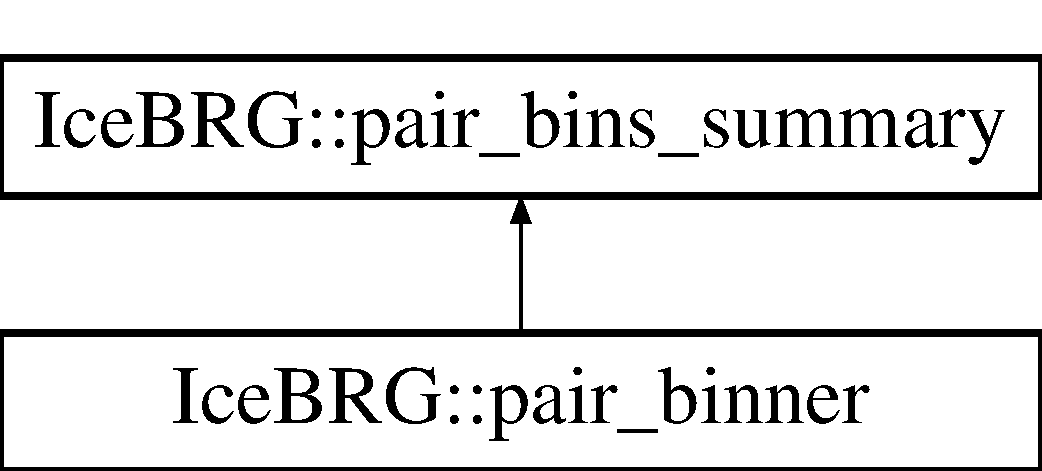
\includegraphics[height=2.000000cm]{classIceBRG_1_1pair__bins__summary}
\end{center}
\end{figure}
\subsection*{Public Member Functions}
\begin{DoxyCompactItemize}
\item 
\hyperlink{classIceBRG_1_1pair__bins__summary_adf88b28f6ffab4d0e0aadd8688efd630}{pair\+\_\+bins\+\_\+summary} ()
\item 
\hyperlink{classIceBRG_1_1pair__bins__summary_a27d287757aa70f2017be0daa9e74d6da}{pair\+\_\+bins\+\_\+summary} (\hyperlink{classIceBRG_1_1limit__vector}{Ice\+B\+R\+G\+::limit\+\_\+vector}$<$ \hyperlink{namespaceIceBRG_a45499647eb87e24c10ab32c628711cec}{distance\+\_\+type} $>$ R\+\_\+bin\+\_\+limits, \hyperlink{classIceBRG_1_1limit__vector}{Ice\+B\+R\+G\+::limit\+\_\+vector}$<$ \hyperlink{namespaceIceBRG_a1be72ac4918a9b029f2eefa084213e35}{mass\+\_\+type} $>$ m\+\_\+bin\+\_\+limits=std\+::vector$<$ \hyperlink{lib_2IceBRG__main_2common_8h_ad0f130a56eeb944d9ef2692ee881ecc4}{flt\+\_\+type} $>$(), \hyperlink{classIceBRG_1_1limit__vector}{Ice\+B\+R\+G\+::limit\+\_\+vector}$<$ \hyperlink{lib_2IceBRG__main_2common_8h_ad0f130a56eeb944d9ef2692ee881ecc4}{flt\+\_\+type} $>$ z\+\_\+bin\+\_\+limits=std\+::vector$<$ \hyperlink{lib_2IceBRG__main_2common_8h_ad0f130a56eeb944d9ef2692ee881ecc4}{flt\+\_\+type} $>$(), \hyperlink{classIceBRG_1_1limit__vector}{Ice\+B\+R\+G\+::limit\+\_\+vector}$<$ \hyperlink{lib_2IceBRG__main_2common_8h_ad0f130a56eeb944d9ef2692ee881ecc4}{flt\+\_\+type} $>$ mag\+\_\+bin\+\_\+limits=std\+::vector$<$ \hyperlink{lib_2IceBRG__main_2common_8h_ad0f130a56eeb944d9ef2692ee881ecc4}{flt\+\_\+type} $>$())
\item 
\hyperlink{classIceBRG_1_1pair__bins__summary_adcd4739bbb314a60885b8db39a679782}{pair\+\_\+bins\+\_\+summary} (const \hyperlink{namespaceIceBRG_a45499647eb87e24c10ab32c628711cec}{distance\+\_\+type} \&R\+\_\+min, const \hyperlink{namespaceIceBRG_a45499647eb87e24c10ab32c628711cec}{distance\+\_\+type} \&R\+\_\+max, const \hyperlink{lib_2IceBRG__main_2common_8h_ab322a3e50421dc5f0c43316b1b373592}{ssize\+\_\+t} \&R\+\_\+bins=1, const \hyperlink{namespaceIceBRG_a1be72ac4918a9b029f2eefa084213e35}{mass\+\_\+type} \&m\+\_\+min=-\/std\+::numeric\+\_\+limits$<$ \hyperlink{lib_2IceBRG__main_2common_8h_ad0f130a56eeb944d9ef2692ee881ecc4}{flt\+\_\+type} $>$\+::infinity()$\ast$\hyperlink{namespaceIceBRG_a9233960f6792ea35145d7db55c13e85d}{kg}, const \hyperlink{namespaceIceBRG_a1be72ac4918a9b029f2eefa084213e35}{mass\+\_\+type} \&m\+\_\+max=std\+::numeric\+\_\+limits$<$ \hyperlink{lib_2IceBRG__main_2common_8h_ad0f130a56eeb944d9ef2692ee881ecc4}{flt\+\_\+type} $>$\+::infinity()$\ast$\hyperlink{namespaceIceBRG_a9233960f6792ea35145d7db55c13e85d}{kg}, const \hyperlink{lib_2IceBRG__main_2common_8h_ab322a3e50421dc5f0c43316b1b373592}{ssize\+\_\+t} \&m\+\_\+bins=1, const \hyperlink{lib_2IceBRG__main_2common_8h_ad0f130a56eeb944d9ef2692ee881ecc4}{flt\+\_\+type} \&z\+\_\+min=-\/std\+::numeric\+\_\+limits$<$ \hyperlink{lib_2IceBRG__main_2common_8h_ad0f130a56eeb944d9ef2692ee881ecc4}{flt\+\_\+type} $>$\+::infinity(), const \hyperlink{lib_2IceBRG__main_2common_8h_ad0f130a56eeb944d9ef2692ee881ecc4}{flt\+\_\+type} \&z\+\_\+max=std\+::numeric\+\_\+limits$<$ \hyperlink{lib_2IceBRG__main_2common_8h_ad0f130a56eeb944d9ef2692ee881ecc4}{flt\+\_\+type} $>$\+::infinity(), const \hyperlink{lib_2IceBRG__main_2common_8h_ab322a3e50421dc5f0c43316b1b373592}{ssize\+\_\+t} \&\hyperlink{main__field__stats_8cpp_a6d4d8cfc3c2eccfe9ed5091d304e8dcd}{z\+\_\+bins}=1, const \hyperlink{lib_2IceBRG__main_2common_8h_ad0f130a56eeb944d9ef2692ee881ecc4}{flt\+\_\+type} \&mag\+\_\+min=-\/std\+::numeric\+\_\+limits$<$ \hyperlink{lib_2IceBRG__main_2common_8h_ad0f130a56eeb944d9ef2692ee881ecc4}{flt\+\_\+type} $>$\+::infinity(), const \hyperlink{lib_2IceBRG__main_2common_8h_ad0f130a56eeb944d9ef2692ee881ecc4}{flt\+\_\+type} \&mag\+\_\+max=std\+::numeric\+\_\+limits$<$ \hyperlink{lib_2IceBRG__main_2common_8h_ad0f130a56eeb944d9ef2692ee881ecc4}{flt\+\_\+type} $>$\+::infinity(), const \hyperlink{lib_2IceBRG__main_2common_8h_ab322a3e50421dc5f0c43316b1b373592}{ssize\+\_\+t} \&mag\+\_\+bins=1)
\item 
\hyperlink{classIceBRG_1_1pair__bins__summary_ac2f7a387e1f620cd3d7045f3138e19e6}{pair\+\_\+bins\+\_\+summary} (std\+::istream \&in)
\item 
\hyperlink{classIceBRG_1_1pair__bins__summary_a082924adf96c1604f88e73b5b3bcc87d}{pair\+\_\+bins\+\_\+summary} (const std\+::string \&filename)
\item 
\hyperlink{classIceBRG_1_1pair__bins__summary_aa031c76c0717dd77232f44fae2cb8bdd}{pair\+\_\+bins\+\_\+summary} (const \hyperlink{classIceBRG_1_1pair__binner}{pair\+\_\+binner} \&bins)
\item 
\hyperlink{classIceBRG_1_1pair__bins__summary}{pair\+\_\+bins\+\_\+summary} \& \hyperlink{classIceBRG_1_1pair__bins__summary_af1d9f93977eb8f7b17e397933a71f70c}{operator=} (const \hyperlink{classIceBRG_1_1pair__binner}{pair\+\_\+binner} \&bins)
\item 
virtual \hyperlink{classIceBRG_1_1pair__bins__summary_a20297356c0eea3b163c3f68fd9e001eb}{$\sim$pair\+\_\+bins\+\_\+summary} ()
\item 
void \hyperlink{classIceBRG_1_1pair__bins__summary_a8a65637499aead61fecf9dc057158a55}{set\+\_\+\+R\+\_\+limits} (\hyperlink{classIceBRG_1_1limit__vector}{Ice\+B\+R\+G\+::limit\+\_\+vector}$<$ \hyperlink{namespaceIceBRG_a45499647eb87e24c10ab32c628711cec}{distance\+\_\+type} $>$ R\+\_\+bin\+\_\+limits)
\item 
void \hyperlink{classIceBRG_1_1pair__bins__summary_a01a6131459f8f68a5d704c46885fcc9b}{set\+\_\+m\+\_\+limits} (\hyperlink{classIceBRG_1_1limit__vector}{Ice\+B\+R\+G\+::limit\+\_\+vector}$<$ \hyperlink{namespaceIceBRG_a1be72ac4918a9b029f2eefa084213e35}{mass\+\_\+type} $>$ m\+\_\+bin\+\_\+limits)
\item 
void \hyperlink{classIceBRG_1_1pair__bins__summary_a6625df1c0eb2c288e9e5b62d2222a3ca}{set\+\_\+z\+\_\+limits} (\hyperlink{classIceBRG_1_1limit__vector}{Ice\+B\+R\+G\+::limit\+\_\+vector}$<$ \hyperlink{lib_2IceBRG__main_2common_8h_ad0f130a56eeb944d9ef2692ee881ecc4}{flt\+\_\+type} $>$ z\+\_\+bin\+\_\+limits)
\item 
void \hyperlink{classIceBRG_1_1pair__bins__summary_a21c1b01b73f7b86666afd9f54e72b145}{set\+\_\+mag\+\_\+limits} (\hyperlink{classIceBRG_1_1limit__vector}{Ice\+B\+R\+G\+::limit\+\_\+vector}$<$ \hyperlink{lib_2IceBRG__main_2common_8h_ad0f130a56eeb944d9ef2692ee881ecc4}{flt\+\_\+type} $>$ mag\+\_\+bin\+\_\+limits)
\item 
void \hyperlink{classIceBRG_1_1pair__bins__summary_a664ff45e62edaef88f333fdbfcfe52af}{set\+\_\+linear\+\_\+\+R\+\_\+limits} (const \hyperlink{namespaceIceBRG_a45499647eb87e24c10ab32c628711cec}{distance\+\_\+type} \&R\+\_\+min, const \hyperlink{namespaceIceBRG_a45499647eb87e24c10ab32c628711cec}{distance\+\_\+type} \&R\+\_\+max, const \hyperlink{lib_2IceBRG__main_2common_8h_ab322a3e50421dc5f0c43316b1b373592}{ssize\+\_\+t} \&R\+\_\+bins)
\item 
void \hyperlink{classIceBRG_1_1pair__bins__summary_a7b2524d7dfe25fbcdc378cbc36573946}{set\+\_\+linear\+\_\+m\+\_\+limits} (const \hyperlink{namespaceIceBRG_a1be72ac4918a9b029f2eefa084213e35}{mass\+\_\+type} \&m\+\_\+min, const \hyperlink{namespaceIceBRG_a1be72ac4918a9b029f2eefa084213e35}{mass\+\_\+type} \&m\+\_\+max, const \hyperlink{lib_2IceBRG__main_2common_8h_ab322a3e50421dc5f0c43316b1b373592}{ssize\+\_\+t} \&m\+\_\+bins)
\item 
void \hyperlink{classIceBRG_1_1pair__bins__summary_a42909af4d308561fc055ea4c6766a752}{set\+\_\+linear\+\_\+z\+\_\+limits} (const \hyperlink{lib_2IceBRG__main_2common_8h_ad0f130a56eeb944d9ef2692ee881ecc4}{flt\+\_\+type} \&z\+\_\+min, const \hyperlink{lib_2IceBRG__main_2common_8h_ad0f130a56eeb944d9ef2692ee881ecc4}{flt\+\_\+type} \&z\+\_\+max, const \hyperlink{lib_2IceBRG__main_2common_8h_ab322a3e50421dc5f0c43316b1b373592}{ssize\+\_\+t} \&\hyperlink{main__field__stats_8cpp_a6d4d8cfc3c2eccfe9ed5091d304e8dcd}{z\+\_\+bins})
\item 
void \hyperlink{classIceBRG_1_1pair__bins__summary_a0dfc0341ace9bdf0d98b301bafbeebed}{set\+\_\+linear\+\_\+mag\+\_\+limits} (const \hyperlink{lib_2IceBRG__main_2common_8h_ad0f130a56eeb944d9ef2692ee881ecc4}{flt\+\_\+type} \&mag\+\_\+min, const \hyperlink{lib_2IceBRG__main_2common_8h_ad0f130a56eeb944d9ef2692ee881ecc4}{flt\+\_\+type} \&mag\+\_\+max, const \hyperlink{lib_2IceBRG__main_2common_8h_ab322a3e50421dc5f0c43316b1b373592}{ssize\+\_\+t} \&mag\+\_\+bins)
\item 
void \hyperlink{classIceBRG_1_1pair__bins__summary_a25e1c227f1d508602345aaf5c3bf2f6f}{set\+\_\+log\+\_\+\+R\+\_\+limits} (const \hyperlink{namespaceIceBRG_a45499647eb87e24c10ab32c628711cec}{distance\+\_\+type} \&R\+\_\+min, const \hyperlink{namespaceIceBRG_a45499647eb87e24c10ab32c628711cec}{distance\+\_\+type} \&R\+\_\+max, const \hyperlink{lib_2IceBRG__main_2common_8h_ab322a3e50421dc5f0c43316b1b373592}{ssize\+\_\+t} \&R\+\_\+num\+\_\+bins=1)
\item 
void \hyperlink{classIceBRG_1_1pair__bins__summary_aae072aa17b4d036a2b75adadd051e7b7}{set\+\_\+log\+\_\+m\+\_\+limits} (const \hyperlink{namespaceIceBRG_a1be72ac4918a9b029f2eefa084213e35}{mass\+\_\+type} \&m\+\_\+min, const \hyperlink{namespaceIceBRG_a1be72ac4918a9b029f2eefa084213e35}{mass\+\_\+type} \&m\+\_\+max, const \hyperlink{lib_2IceBRG__main_2common_8h_ab322a3e50421dc5f0c43316b1b373592}{ssize\+\_\+t} \&m\+\_\+num\+\_\+bins=1)
\item 
void \hyperlink{classIceBRG_1_1pair__bins__summary_aa4cc8227dd39e7694b0c7ed8f628a239}{set\+\_\+log\+\_\+z\+\_\+limits} (const \hyperlink{lib_2IceBRG__main_2common_8h_ad0f130a56eeb944d9ef2692ee881ecc4}{flt\+\_\+type} \&z\+\_\+min, const \hyperlink{lib_2IceBRG__main_2common_8h_ad0f130a56eeb944d9ef2692ee881ecc4}{flt\+\_\+type} \&z\+\_\+max, const \hyperlink{lib_2IceBRG__main_2common_8h_ab322a3e50421dc5f0c43316b1b373592}{ssize\+\_\+t} \&z\+\_\+num\+\_\+bins=1)
\item 
void \hyperlink{classIceBRG_1_1pair__bins__summary_a0b2a787e58824b62ceb8c1885fbacac9}{set\+\_\+log\+\_\+mag\+\_\+limits} (const \hyperlink{lib_2IceBRG__main_2common_8h_ad0f130a56eeb944d9ef2692ee881ecc4}{flt\+\_\+type} \&mag\+\_\+min, const \hyperlink{lib_2IceBRG__main_2common_8h_ad0f130a56eeb944d9ef2692ee881ecc4}{flt\+\_\+type} \&mag\+\_\+max, const \hyperlink{lib_2IceBRG__main_2common_8h_ab322a3e50421dc5f0c43316b1b373592}{ssize\+\_\+t} \&mag\+\_\+num\+\_\+bins=1)
\item 
void \hyperlink{classIceBRG_1_1pair__bins__summary_aa7c0b185041754b838ad5708d19d20a9}{clear\+\_\+\+R\+\_\+limits} ()
\item 
void \hyperlink{classIceBRG_1_1pair__bins__summary_a08a19acd04c4b447212b9b6e2d9d2fd1}{clear\+\_\+m\+\_\+limits} ()
\item 
void \hyperlink{classIceBRG_1_1pair__bins__summary_a4b81ecfc23d7511f156bb0618af79745}{clear\+\_\+z\+\_\+limits} ()
\item 
void \hyperlink{classIceBRG_1_1pair__bins__summary_a365a1e2bdd23df20d79212ad824ae289}{clear\+\_\+mag\+\_\+limits} ()
\item 
void \hyperlink{classIceBRG_1_1pair__bins__summary_a956cd9635846601f12fca9fd66aea3db}{set\+\_\+limits} (\hyperlink{classIceBRG_1_1limit__vector}{Ice\+B\+R\+G\+::limit\+\_\+vector}$<$ \hyperlink{namespaceIceBRG_a45499647eb87e24c10ab32c628711cec}{distance\+\_\+type} $>$ R\+\_\+bin\+\_\+limits, \hyperlink{classIceBRG_1_1limit__vector}{Ice\+B\+R\+G\+::limit\+\_\+vector}$<$ \hyperlink{namespaceIceBRG_a1be72ac4918a9b029f2eefa084213e35}{mass\+\_\+type} $>$ m\+\_\+bin\+\_\+limits=std\+::vector$<$ \hyperlink{lib_2IceBRG__main_2common_8h_ad0f130a56eeb944d9ef2692ee881ecc4}{flt\+\_\+type} $>$(), \hyperlink{classIceBRG_1_1limit__vector}{Ice\+B\+R\+G\+::limit\+\_\+vector}$<$ \hyperlink{lib_2IceBRG__main_2common_8h_ad0f130a56eeb944d9ef2692ee881ecc4}{flt\+\_\+type} $>$ z\+\_\+bin\+\_\+limits=std\+::vector$<$ \hyperlink{lib_2IceBRG__main_2common_8h_ad0f130a56eeb944d9ef2692ee881ecc4}{flt\+\_\+type} $>$(), \hyperlink{classIceBRG_1_1limit__vector}{Ice\+B\+R\+G\+::limit\+\_\+vector}$<$ \hyperlink{lib_2IceBRG__main_2common_8h_ad0f130a56eeb944d9ef2692ee881ecc4}{flt\+\_\+type} $>$ mag\+\_\+bin\+\_\+limits=std\+::vector$<$ \hyperlink{lib_2IceBRG__main_2common_8h_ad0f130a56eeb944d9ef2692ee881ecc4}{flt\+\_\+type} $>$())
\item 
void \hyperlink{classIceBRG_1_1pair__bins__summary_a98753589430c0d2622a863444dbb3878}{set\+\_\+linear\+\_\+limits} (const \hyperlink{namespaceIceBRG_a45499647eb87e24c10ab32c628711cec}{distance\+\_\+type} \&R\+\_\+min, const \hyperlink{namespaceIceBRG_a45499647eb87e24c10ab32c628711cec}{distance\+\_\+type} \&R\+\_\+max, const \hyperlink{lib_2IceBRG__main_2common_8h_ab322a3e50421dc5f0c43316b1b373592}{ssize\+\_\+t} \&R\+\_\+num\+\_\+bins=1, const \hyperlink{namespaceIceBRG_a1be72ac4918a9b029f2eefa084213e35}{mass\+\_\+type} \&m\+\_\+min=-\/std\+::numeric\+\_\+limits$<$ \hyperlink{lib_2IceBRG__main_2common_8h_ad0f130a56eeb944d9ef2692ee881ecc4}{flt\+\_\+type} $>$\+::infinity()$\ast$\hyperlink{namespaceIceBRG_a9233960f6792ea35145d7db55c13e85d}{kg}, const \hyperlink{namespaceIceBRG_a1be72ac4918a9b029f2eefa084213e35}{mass\+\_\+type} \&m\+\_\+max=std\+::numeric\+\_\+limits$<$ \hyperlink{lib_2IceBRG__main_2common_8h_ad0f130a56eeb944d9ef2692ee881ecc4}{flt\+\_\+type} $>$\+::infinity()$\ast$\hyperlink{namespaceIceBRG_a9233960f6792ea35145d7db55c13e85d}{kg}, const \hyperlink{lib_2IceBRG__main_2common_8h_ab322a3e50421dc5f0c43316b1b373592}{ssize\+\_\+t} \&m\+\_\+num\+\_\+bins=1, const \hyperlink{lib_2IceBRG__main_2common_8h_ad0f130a56eeb944d9ef2692ee881ecc4}{flt\+\_\+type} \&z\+\_\+min=-\/std\+::numeric\+\_\+limits$<$ \hyperlink{lib_2IceBRG__main_2common_8h_ad0f130a56eeb944d9ef2692ee881ecc4}{flt\+\_\+type} $>$\+::infinity(), const \hyperlink{lib_2IceBRG__main_2common_8h_ad0f130a56eeb944d9ef2692ee881ecc4}{flt\+\_\+type} \&z\+\_\+max=std\+::numeric\+\_\+limits$<$ \hyperlink{lib_2IceBRG__main_2common_8h_ad0f130a56eeb944d9ef2692ee881ecc4}{flt\+\_\+type} $>$\+::infinity(), const \hyperlink{lib_2IceBRG__main_2common_8h_ab322a3e50421dc5f0c43316b1b373592}{ssize\+\_\+t} \&z\+\_\+num\+\_\+bins=1, const \hyperlink{lib_2IceBRG__main_2common_8h_ad0f130a56eeb944d9ef2692ee881ecc4}{flt\+\_\+type} \&mag\+\_\+min=-\/std\+::numeric\+\_\+limits$<$ \hyperlink{lib_2IceBRG__main_2common_8h_ad0f130a56eeb944d9ef2692ee881ecc4}{flt\+\_\+type} $>$\+::infinity(), const \hyperlink{lib_2IceBRG__main_2common_8h_ad0f130a56eeb944d9ef2692ee881ecc4}{flt\+\_\+type} \&mag\+\_\+max=std\+::numeric\+\_\+limits$<$ \hyperlink{lib_2IceBRG__main_2common_8h_ad0f130a56eeb944d9ef2692ee881ecc4}{flt\+\_\+type} $>$\+::infinity(), const \hyperlink{lib_2IceBRG__main_2common_8h_ab322a3e50421dc5f0c43316b1b373592}{ssize\+\_\+t} \&mag\+\_\+num\+\_\+bins=1)
\item 
void \hyperlink{classIceBRG_1_1pair__bins__summary_aa6d4ef3bacbd3e796feea36d3dda99d1}{set\+\_\+log\+\_\+limits} (const \hyperlink{namespaceIceBRG_a45499647eb87e24c10ab32c628711cec}{distance\+\_\+type} \&R\+\_\+min, const \hyperlink{namespaceIceBRG_a45499647eb87e24c10ab32c628711cec}{distance\+\_\+type} \&R\+\_\+max, const \hyperlink{lib_2IceBRG__main_2common_8h_ab322a3e50421dc5f0c43316b1b373592}{ssize\+\_\+t} \&R\+\_\+num\+\_\+bins=1, const \hyperlink{namespaceIceBRG_a1be72ac4918a9b029f2eefa084213e35}{mass\+\_\+type} \&m\+\_\+min=-\/std\+::numeric\+\_\+limits$<$ \hyperlink{lib_2IceBRG__main_2common_8h_ad0f130a56eeb944d9ef2692ee881ecc4}{flt\+\_\+type} $>$\+::infinity()$\ast$\hyperlink{namespaceIceBRG_a9233960f6792ea35145d7db55c13e85d}{kg}, const \hyperlink{namespaceIceBRG_a1be72ac4918a9b029f2eefa084213e35}{mass\+\_\+type} \&m\+\_\+max=std\+::numeric\+\_\+limits$<$ \hyperlink{lib_2IceBRG__main_2common_8h_ad0f130a56eeb944d9ef2692ee881ecc4}{flt\+\_\+type} $>$\+::infinity()$\ast$\hyperlink{namespaceIceBRG_a9233960f6792ea35145d7db55c13e85d}{kg}, const \hyperlink{lib_2IceBRG__main_2common_8h_ab322a3e50421dc5f0c43316b1b373592}{ssize\+\_\+t} \&m\+\_\+num\+\_\+bins=1, const \hyperlink{lib_2IceBRG__main_2common_8h_ad0f130a56eeb944d9ef2692ee881ecc4}{flt\+\_\+type} \&z\+\_\+min=-\/std\+::numeric\+\_\+limits$<$ \hyperlink{lib_2IceBRG__main_2common_8h_ad0f130a56eeb944d9ef2692ee881ecc4}{flt\+\_\+type} $>$\+::infinity(), const \hyperlink{lib_2IceBRG__main_2common_8h_ad0f130a56eeb944d9ef2692ee881ecc4}{flt\+\_\+type} \&z\+\_\+max=std\+::numeric\+\_\+limits$<$ \hyperlink{lib_2IceBRG__main_2common_8h_ad0f130a56eeb944d9ef2692ee881ecc4}{flt\+\_\+type} $>$\+::infinity(), const \hyperlink{lib_2IceBRG__main_2common_8h_ab322a3e50421dc5f0c43316b1b373592}{ssize\+\_\+t} \&z\+\_\+num\+\_\+bins=1, const \hyperlink{lib_2IceBRG__main_2common_8h_ad0f130a56eeb944d9ef2692ee881ecc4}{flt\+\_\+type} \&mag\+\_\+min=-\/std\+::numeric\+\_\+limits$<$ \hyperlink{lib_2IceBRG__main_2common_8h_ad0f130a56eeb944d9ef2692ee881ecc4}{flt\+\_\+type} $>$\+::infinity(), const \hyperlink{lib_2IceBRG__main_2common_8h_ad0f130a56eeb944d9ef2692ee881ecc4}{flt\+\_\+type} \&mag\+\_\+max=std\+::numeric\+\_\+limits$<$ \hyperlink{lib_2IceBRG__main_2common_8h_ad0f130a56eeb944d9ef2692ee881ecc4}{flt\+\_\+type} $>$\+::infinity(), const \hyperlink{lib_2IceBRG__main_2common_8h_ab322a3e50421dc5f0c43316b1b373592}{ssize\+\_\+t} \&mag\+\_\+num\+\_\+bins=1)
\item 
void \hyperlink{classIceBRG_1_1pair__bins__summary_a2f597df610a95318de69a2692d4b6a18}{fixbad} ()
\item 
const \hyperlink{classIceBRG_1_1limit__vector}{Ice\+B\+R\+G\+::limit\+\_\+vector}$<$ \hyperlink{namespaceIceBRG_a45499647eb87e24c10ab32c628711cec}{distance\+\_\+type} $>$ \& \hyperlink{classIceBRG_1_1pair__bins__summary_acc7b46adaf08cb9026ae6cb629149a03}{R\+\_\+limits} () const 
\item 
const \hyperlink{classIceBRG_1_1limit__vector}{Ice\+B\+R\+G\+::limit\+\_\+vector}$<$ \hyperlink{namespaceIceBRG_a1be72ac4918a9b029f2eefa084213e35}{mass\+\_\+type} $>$ \& \hyperlink{classIceBRG_1_1pair__bins__summary_a86827c9706e81ed9355e2392c8f97461}{m\+\_\+limits} () const 
\item 
const \hyperlink{classIceBRG_1_1limit__vector}{Ice\+B\+R\+G\+::limit\+\_\+vector}$<$ \hyperlink{lib_2IceBRG__main_2common_8h_ad0f130a56eeb944d9ef2692ee881ecc4}{flt\+\_\+type} $>$ \& \hyperlink{classIceBRG_1_1pair__bins__summary_a6e991158024292432a331e17afe7772d}{z\+\_\+limits} () const 
\item 
const \hyperlink{classIceBRG_1_1limit__vector}{Ice\+B\+R\+G\+::limit\+\_\+vector}$<$ \hyperlink{lib_2IceBRG__main_2common_8h_ad0f130a56eeb944d9ef2692ee881ecc4}{flt\+\_\+type} $>$ \& \hyperlink{classIceBRG_1_1pair__bins__summary_ae901835c073a1b9080d5fc9d372cb076}{mag\+\_\+limits} () const 
\item 
bool \hyperlink{classIceBRG_1_1pair__bins__summary_aee577469277b57e336d06c0a55362af1}{valid\+\_\+limits} () const 
\item 
virtual void \hyperlink{classIceBRG_1_1pair__bins__summary_a02eff77640a691bae15d619cd138aec4}{sort} () const 
\item 
virtual void \hyperlink{classIceBRG_1_1pair__bins__summary_a5c15793df751321aef8bed2526c3cbe6}{clear} ()
\item 
const std\+::vector$<$ std\+::vector$<$ std\+::vector$<$ std\+::vector$<$ \hyperlink{classIceBRG_1_1pair__bin__summary}{pair\+\_\+bin\+\_\+summary} $>$ $>$ $>$ $>$ \& \hyperlink{classIceBRG_1_1pair__bins__summary_a50f037d0f5014adb5eb4e7c4d0b0092e}{pair\+\_\+bin\+\_\+summaries} () const 
\item 
virtual \hyperlink{namespaceIceBRG_a80c597ef5ba0a32491d32a9f0083b02d}{surface\+\_\+density\+\_\+type} \hyperlink{classIceBRG_1_1pair__bins__summary_a6b03be80b8d12b5d8ef4707e594fa911}{delta\+\_\+\+Sigma\+\_\+t\+\_\+mean\+\_\+for\+\_\+bin} (\hyperlink{lib_2IceBRG__main_2common_8h_ab322a3e50421dc5f0c43316b1b373592}{ssize\+\_\+t} R\+\_\+i, \hyperlink{lib_2IceBRG__main_2common_8h_ab322a3e50421dc5f0c43316b1b373592}{ssize\+\_\+t} m\+\_\+i, \hyperlink{lib_2IceBRG__main_2common_8h_ab322a3e50421dc5f0c43316b1b373592}{ssize\+\_\+t} z\+\_\+i, \hyperlink{lib_2IceBRG__main_2common_8h_ab322a3e50421dc5f0c43316b1b373592}{ssize\+\_\+t} mag\+\_\+i) const 
\item 
virtual \hyperlink{namespaceIceBRG_a80c597ef5ba0a32491d32a9f0083b02d}{surface\+\_\+density\+\_\+type} \hyperlink{classIceBRG_1_1pair__bins__summary_ad048f1e59080eef13ffc59e69b54436a}{delta\+\_\+\+Sigma\+\_\+x\+\_\+mean\+\_\+for\+\_\+bin} (\hyperlink{lib_2IceBRG__main_2common_8h_ab322a3e50421dc5f0c43316b1b373592}{ssize\+\_\+t} R\+\_\+i, \hyperlink{lib_2IceBRG__main_2common_8h_ab322a3e50421dc5f0c43316b1b373592}{ssize\+\_\+t} m\+\_\+i, \hyperlink{lib_2IceBRG__main_2common_8h_ab322a3e50421dc5f0c43316b1b373592}{ssize\+\_\+t} z\+\_\+i, \hyperlink{lib_2IceBRG__main_2common_8h_ab322a3e50421dc5f0c43316b1b373592}{ssize\+\_\+t} mag\+\_\+i) const 
\item 
virtual \hyperlink{namespaceIceBRG_a80c597ef5ba0a32491d32a9f0083b02d}{surface\+\_\+density\+\_\+type} \hyperlink{classIceBRG_1_1pair__bins__summary_a38b758fd1fe3bb0f54ce753821c615e8}{delta\+\_\+\+Sigma\+\_\+t\+\_\+std\+\_\+for\+\_\+bin} (\hyperlink{lib_2IceBRG__main_2common_8h_ab322a3e50421dc5f0c43316b1b373592}{ssize\+\_\+t} R\+\_\+i, \hyperlink{lib_2IceBRG__main_2common_8h_ab322a3e50421dc5f0c43316b1b373592}{ssize\+\_\+t} m\+\_\+i, \hyperlink{lib_2IceBRG__main_2common_8h_ab322a3e50421dc5f0c43316b1b373592}{ssize\+\_\+t} z\+\_\+i, \hyperlink{lib_2IceBRG__main_2common_8h_ab322a3e50421dc5f0c43316b1b373592}{ssize\+\_\+t} mag\+\_\+i) const 
\item 
virtual \hyperlink{namespaceIceBRG_a80c597ef5ba0a32491d32a9f0083b02d}{surface\+\_\+density\+\_\+type} \hyperlink{classIceBRG_1_1pair__bins__summary_ad61fcee9ace91debaa0c223b9201c905}{delta\+\_\+\+Sigma\+\_\+x\+\_\+std\+\_\+for\+\_\+bin} (\hyperlink{lib_2IceBRG__main_2common_8h_ab322a3e50421dc5f0c43316b1b373592}{ssize\+\_\+t} R\+\_\+i, \hyperlink{lib_2IceBRG__main_2common_8h_ab322a3e50421dc5f0c43316b1b373592}{ssize\+\_\+t} m\+\_\+i, \hyperlink{lib_2IceBRG__main_2common_8h_ab322a3e50421dc5f0c43316b1b373592}{ssize\+\_\+t} z\+\_\+i, \hyperlink{lib_2IceBRG__main_2common_8h_ab322a3e50421dc5f0c43316b1b373592}{ssize\+\_\+t} mag\+\_\+i) const 
\item 
virtual \hyperlink{namespaceIceBRG_a80c597ef5ba0a32491d32a9f0083b02d}{surface\+\_\+density\+\_\+type} \hyperlink{classIceBRG_1_1pair__bins__summary_abfa62e09139c52299605accf01edb308}{delta\+\_\+\+Sigma\+\_\+t\+\_\+stderr\+\_\+for\+\_\+bin} (\hyperlink{lib_2IceBRG__main_2common_8h_ab322a3e50421dc5f0c43316b1b373592}{ssize\+\_\+t} R\+\_\+i, \hyperlink{lib_2IceBRG__main_2common_8h_ab322a3e50421dc5f0c43316b1b373592}{ssize\+\_\+t} m\+\_\+i, \hyperlink{lib_2IceBRG__main_2common_8h_ab322a3e50421dc5f0c43316b1b373592}{ssize\+\_\+t} z\+\_\+i, \hyperlink{lib_2IceBRG__main_2common_8h_ab322a3e50421dc5f0c43316b1b373592}{ssize\+\_\+t} mag\+\_\+i) const 
\item 
virtual \hyperlink{namespaceIceBRG_a80c597ef5ba0a32491d32a9f0083b02d}{surface\+\_\+density\+\_\+type} \hyperlink{classIceBRG_1_1pair__bins__summary_ab87a6730c422e9cbf10a6e9bd45de7ba}{delta\+\_\+\+Sigma\+\_\+x\+\_\+stderr\+\_\+for\+\_\+bin} (\hyperlink{lib_2IceBRG__main_2common_8h_ab322a3e50421dc5f0c43316b1b373592}{ssize\+\_\+t} R\+\_\+i, \hyperlink{lib_2IceBRG__main_2common_8h_ab322a3e50421dc5f0c43316b1b373592}{ssize\+\_\+t} m\+\_\+i, \hyperlink{lib_2IceBRG__main_2common_8h_ab322a3e50421dc5f0c43316b1b373592}{ssize\+\_\+t} z\+\_\+i, \hyperlink{lib_2IceBRG__main_2common_8h_ab322a3e50421dc5f0c43316b1b373592}{ssize\+\_\+t} mag\+\_\+i) const 
\item 
virtual \hyperlink{namespaceIceBRG_a80c597ef5ba0a32491d32a9f0083b02d}{surface\+\_\+density\+\_\+type} \hyperlink{classIceBRG_1_1pair__bins__summary_a01057d77d2798f68962e64dc434732ee}{delta\+\_\+\+Sigma\+\_\+t\+\_\+mean\+\_\+for\+\_\+bin} (const \hyperlink{namespaceIceBRG_a45499647eb87e24c10ab32c628711cec}{distance\+\_\+type} \&R, const \hyperlink{namespaceIceBRG_a1be72ac4918a9b029f2eefa084213e35}{mass\+\_\+type} \&\hyperlink{namespaceIceBRG_ada6365c5d16106f0608afbd34f010bcc}{m}, \hyperlink{lib_2IceBRG__main_2common_8h_ad0f130a56eeb944d9ef2692ee881ecc4}{flt\+\_\+type} z, \hyperlink{lib_2IceBRG__main_2common_8h_ad0f130a56eeb944d9ef2692ee881ecc4}{flt\+\_\+type} mag) const 
\item 
virtual \hyperlink{namespaceIceBRG_a80c597ef5ba0a32491d32a9f0083b02d}{surface\+\_\+density\+\_\+type} \hyperlink{classIceBRG_1_1pair__bins__summary_a7b6965703c7756ea5f64ac8011858afd}{delta\+\_\+\+Sigma\+\_\+x\+\_\+mean\+\_\+for\+\_\+bin} (const \hyperlink{namespaceIceBRG_a45499647eb87e24c10ab32c628711cec}{distance\+\_\+type} \&R, const \hyperlink{namespaceIceBRG_a1be72ac4918a9b029f2eefa084213e35}{mass\+\_\+type} \&\hyperlink{namespaceIceBRG_ada6365c5d16106f0608afbd34f010bcc}{m}, \hyperlink{lib_2IceBRG__main_2common_8h_ad0f130a56eeb944d9ef2692ee881ecc4}{flt\+\_\+type} z, \hyperlink{lib_2IceBRG__main_2common_8h_ad0f130a56eeb944d9ef2692ee881ecc4}{flt\+\_\+type} mag) const 
\item 
virtual \hyperlink{namespaceIceBRG_a80c597ef5ba0a32491d32a9f0083b02d}{surface\+\_\+density\+\_\+type} \hyperlink{classIceBRG_1_1pair__bins__summary_ac70b7f377e378a42b401bcf91cacf638}{delta\+\_\+\+Sigma\+\_\+t\+\_\+std\+\_\+for\+\_\+bin} (const \hyperlink{namespaceIceBRG_a45499647eb87e24c10ab32c628711cec}{distance\+\_\+type} \&R, const \hyperlink{namespaceIceBRG_a1be72ac4918a9b029f2eefa084213e35}{mass\+\_\+type} \&\hyperlink{namespaceIceBRG_ada6365c5d16106f0608afbd34f010bcc}{m}, \hyperlink{lib_2IceBRG__main_2common_8h_ad0f130a56eeb944d9ef2692ee881ecc4}{flt\+\_\+type} z, \hyperlink{lib_2IceBRG__main_2common_8h_ad0f130a56eeb944d9ef2692ee881ecc4}{flt\+\_\+type} mag) const 
\item 
virtual \hyperlink{namespaceIceBRG_a80c597ef5ba0a32491d32a9f0083b02d}{surface\+\_\+density\+\_\+type} \hyperlink{classIceBRG_1_1pair__bins__summary_ab27a685fc2dead9ad9aed71b3a944b16}{delta\+\_\+\+Sigma\+\_\+x\+\_\+std\+\_\+for\+\_\+bin} (const \hyperlink{namespaceIceBRG_a45499647eb87e24c10ab32c628711cec}{distance\+\_\+type} \&R, const \hyperlink{namespaceIceBRG_a1be72ac4918a9b029f2eefa084213e35}{mass\+\_\+type} \&\hyperlink{namespaceIceBRG_ada6365c5d16106f0608afbd34f010bcc}{m}, \hyperlink{lib_2IceBRG__main_2common_8h_ad0f130a56eeb944d9ef2692ee881ecc4}{flt\+\_\+type} z, \hyperlink{lib_2IceBRG__main_2common_8h_ad0f130a56eeb944d9ef2692ee881ecc4}{flt\+\_\+type} mag) const 
\item 
virtual \hyperlink{namespaceIceBRG_a80c597ef5ba0a32491d32a9f0083b02d}{surface\+\_\+density\+\_\+type} \hyperlink{classIceBRG_1_1pair__bins__summary_a45e9b2003665acf25915833d5f89f803}{delta\+\_\+\+Sigma\+\_\+t\+\_\+stderr\+\_\+for\+\_\+bin} (const \hyperlink{namespaceIceBRG_a45499647eb87e24c10ab32c628711cec}{distance\+\_\+type} \&R, const \hyperlink{namespaceIceBRG_a1be72ac4918a9b029f2eefa084213e35}{mass\+\_\+type} \&\hyperlink{namespaceIceBRG_ada6365c5d16106f0608afbd34f010bcc}{m}, \hyperlink{lib_2IceBRG__main_2common_8h_ad0f130a56eeb944d9ef2692ee881ecc4}{flt\+\_\+type} z, \hyperlink{lib_2IceBRG__main_2common_8h_ad0f130a56eeb944d9ef2692ee881ecc4}{flt\+\_\+type} mag) const 
\item 
virtual \hyperlink{namespaceIceBRG_a80c597ef5ba0a32491d32a9f0083b02d}{surface\+\_\+density\+\_\+type} \hyperlink{classIceBRG_1_1pair__bins__summary_a4600bb6007de64667fb065d7dd4cb2c4}{delta\+\_\+\+Sigma\+\_\+x\+\_\+stderr\+\_\+for\+\_\+bin} (const \hyperlink{namespaceIceBRG_a45499647eb87e24c10ab32c628711cec}{distance\+\_\+type} \&R, const \hyperlink{namespaceIceBRG_a1be72ac4918a9b029f2eefa084213e35}{mass\+\_\+type} \&\hyperlink{namespaceIceBRG_ada6365c5d16106f0608afbd34f010bcc}{m}, \hyperlink{lib_2IceBRG__main_2common_8h_ad0f130a56eeb944d9ef2692ee881ecc4}{flt\+\_\+type} z, \hyperlink{lib_2IceBRG__main_2common_8h_ad0f130a56eeb944d9ef2692ee881ecc4}{flt\+\_\+type} mag) const 
\item 
void \hyperlink{classIceBRG_1_1pair__bins__summary_a0e483eaca5f7c7ac6e74576edf7809ad}{print\+\_\+bin\+\_\+data} (std\+::ostream \&out, const \hyperlink{namespaceIceBRG_a7dff9bcf80d56e9e3fc9d9e25c89ae68}{unitconv\+\_\+map} \&u\+\_\+map=\hyperlink{namespaceIceBRG_a7dff9bcf80d56e9e3fc9d9e25c89ae68}{unitconv\+\_\+map}())
\item 
void \hyperlink{classIceBRG_1_1pair__bins__summary_ad811192904f596011806e5079146147f}{print\+\_\+bin\+\_\+data} (const std\+::string \&file\+\_\+name, const \hyperlink{namespaceIceBRG_a7dff9bcf80d56e9e3fc9d9e25c89ae68}{unitconv\+\_\+map} \&u\+\_\+map=\hyperlink{namespaceIceBRG_a7dff9bcf80d56e9e3fc9d9e25c89ae68}{unitconv\+\_\+map}())
\item 
\hyperlink{classIceBRG_1_1pair__bins__summary}{pair\+\_\+bins\+\_\+summary} \& \hyperlink{classIceBRG_1_1pair__bins__summary_a68ecd445cbe2b33b0698188aa0647b24}{operator+=} (const \hyperlink{classIceBRG_1_1pair__bins__summary}{pair\+\_\+bins\+\_\+summary} \&other)
\item 
\hyperlink{classIceBRG_1_1pair__bins__summary}{pair\+\_\+bins\+\_\+summary} \hyperlink{classIceBRG_1_1pair__bins__summary_aa68e04a8182c4eecf874e060dbbffa2c}{operator+} (\hyperlink{classIceBRG_1_1pair__bins__summary}{pair\+\_\+bins\+\_\+summary} other) const 
\item 
void \hyperlink{classIceBRG_1_1pair__bins__summary_a715247f44df3b3aea45ef6f2a9bdd6d7}{save} (std\+::ostream \&) const 
\item 
void \hyperlink{classIceBRG_1_1pair__bins__summary_a17e08424469687b88802862e2175c1e8}{save} (const std\+::string \&) const 
\item 
void \hyperlink{classIceBRG_1_1pair__bins__summary_a987a6e30ce5768bc36c692f424b4d89a}{save} (std\+::ostream \&)
\item 
void \hyperlink{classIceBRG_1_1pair__bins__summary_ae97c13ffd6dbc26905d0b061feef323a}{save} (const std\+::string \&)
\item 
void \hyperlink{classIceBRG_1_1pair__bins__summary_aa1d09ba2a00096bdafa8cd86fd4ce85f}{load} (std\+::istream \&)
\item 
void \hyperlink{classIceBRG_1_1pair__bins__summary_a52231e18dc10d8d5874f910639229332}{load} (const std\+::string \&)
\end{DoxyCompactItemize}
\subsection*{Protected Member Functions}
\begin{DoxyCompactItemize}
\item 
void \hyperlink{classIceBRG_1_1pair__bins__summary_a7fd1953689fbf26462ad42334504b768}{\+\_\+construct} () const 
\end{DoxyCompactItemize}
\subsection*{Protected Attributes}
\begin{DoxyCompactItemize}
\item 
std\+::vector$<$ std\+::vector$<$ std\+::vector$<$ std\+::vector$<$ \hyperlink{classIceBRG_1_1pair__bin__summary}{pair\+\_\+bin\+\_\+summary} $>$ $>$ $>$ $>$ \hyperlink{classIceBRG_1_1pair__bins__summary_ae48646da7b9c9cb88fc5987a49152da0}{\+\_\+pair\+\_\+bin\+\_\+summaries\+\_\+}
\end{DoxyCompactItemize}
\subsection*{Friends}
\begin{DoxyCompactItemize}
\item 
class \hyperlink{classIceBRG_1_1pair__bins__summary_ac98d07dd8f7b70e16ccb9a01abf56b9c}{boost\+::serialization\+::access}
\end{DoxyCompactItemize}


\subsection{Constructor \& Destructor Documentation}
\hypertarget{classIceBRG_1_1pair__bins__summary_adf88b28f6ffab4d0e0aadd8688efd630}{}\index{Ice\+B\+R\+G\+::pair\+\_\+bins\+\_\+summary@{Ice\+B\+R\+G\+::pair\+\_\+bins\+\_\+summary}!pair\+\_\+bins\+\_\+summary@{pair\+\_\+bins\+\_\+summary}}
\index{pair\+\_\+bins\+\_\+summary@{pair\+\_\+bins\+\_\+summary}!Ice\+B\+R\+G\+::pair\+\_\+bins\+\_\+summary@{Ice\+B\+R\+G\+::pair\+\_\+bins\+\_\+summary}}
\subsubsection[{pair\+\_\+bins\+\_\+summary()}]{\setlength{\rightskip}{0pt plus 5cm}Ice\+B\+R\+G\+::pair\+\_\+bins\+\_\+summary\+::pair\+\_\+bins\+\_\+summary (
\begin{DoxyParamCaption}
{}
\end{DoxyParamCaption}
)\hspace{0.3cm}{\ttfamily [inline]}}\label{classIceBRG_1_1pair__bins__summary_adf88b28f6ffab4d0e0aadd8688efd630}
\hypertarget{classIceBRG_1_1pair__bins__summary_a27d287757aa70f2017be0daa9e74d6da}{}\index{Ice\+B\+R\+G\+::pair\+\_\+bins\+\_\+summary@{Ice\+B\+R\+G\+::pair\+\_\+bins\+\_\+summary}!pair\+\_\+bins\+\_\+summary@{pair\+\_\+bins\+\_\+summary}}
\index{pair\+\_\+bins\+\_\+summary@{pair\+\_\+bins\+\_\+summary}!Ice\+B\+R\+G\+::pair\+\_\+bins\+\_\+summary@{Ice\+B\+R\+G\+::pair\+\_\+bins\+\_\+summary}}
\subsubsection[{pair\+\_\+bins\+\_\+summary(\+Ice\+B\+R\+G\+::limit\+\_\+vector$<$ distance\+\_\+type $>$ R\+\_\+bin\+\_\+limits, Ice\+B\+R\+G\+::limit\+\_\+vector$<$ mass\+\_\+type $>$ m\+\_\+bin\+\_\+limits=std\+::vector$<$ flt\+\_\+type $>$(), Ice\+B\+R\+G\+::limit\+\_\+vector$<$ flt\+\_\+type $>$ z\+\_\+bin\+\_\+limits=std\+::vector$<$ flt\+\_\+type $>$(), Ice\+B\+R\+G\+::limit\+\_\+vector$<$ flt\+\_\+type $>$ mag\+\_\+bin\+\_\+limits=std\+::vector$<$ flt\+\_\+type $>$())}]{\setlength{\rightskip}{0pt plus 5cm}Ice\+B\+R\+G\+::pair\+\_\+bins\+\_\+summary\+::pair\+\_\+bins\+\_\+summary (
\begin{DoxyParamCaption}
\item[{{\bf Ice\+B\+R\+G\+::limit\+\_\+vector}$<$ {\bf distance\+\_\+type} $>$}]{R\+\_\+bin\+\_\+limits, }
\item[{{\bf Ice\+B\+R\+G\+::limit\+\_\+vector}$<$ {\bf mass\+\_\+type} $>$}]{m\+\_\+bin\+\_\+limits = {\ttfamily std\+:\+:vector$<${\bf flt\+\_\+type}$>$()}, }
\item[{{\bf Ice\+B\+R\+G\+::limit\+\_\+vector}$<$ {\bf flt\+\_\+type} $>$}]{z\+\_\+bin\+\_\+limits = {\ttfamily std\+:\+:vector$<${\bf flt\+\_\+type}$>$()}, }
\item[{{\bf Ice\+B\+R\+G\+::limit\+\_\+vector}$<$ {\bf flt\+\_\+type} $>$}]{mag\+\_\+bin\+\_\+limits = {\ttfamily std\+:\+:vector$<${\bf flt\+\_\+type}$>$()}}
\end{DoxyParamCaption}
)}\label{classIceBRG_1_1pair__bins__summary_a27d287757aa70f2017be0daa9e74d6da}
\hypertarget{classIceBRG_1_1pair__bins__summary_adcd4739bbb314a60885b8db39a679782}{}\index{Ice\+B\+R\+G\+::pair\+\_\+bins\+\_\+summary@{Ice\+B\+R\+G\+::pair\+\_\+bins\+\_\+summary}!pair\+\_\+bins\+\_\+summary@{pair\+\_\+bins\+\_\+summary}}
\index{pair\+\_\+bins\+\_\+summary@{pair\+\_\+bins\+\_\+summary}!Ice\+B\+R\+G\+::pair\+\_\+bins\+\_\+summary@{Ice\+B\+R\+G\+::pair\+\_\+bins\+\_\+summary}}
\subsubsection[{pair\+\_\+bins\+\_\+summary(const distance\+\_\+type \&\+R\+\_\+min, const distance\+\_\+type \&\+R\+\_\+max, const ssize\+\_\+t \&\+R\+\_\+bins=1, const mass\+\_\+type \&m\+\_\+min=-\/std\+::numeric\+\_\+limits$<$ flt\+\_\+type $>$\+::infinity()$\ast$kg, const mass\+\_\+type \&m\+\_\+max=std\+::numeric\+\_\+limits$<$ flt\+\_\+type $>$\+::infinity()$\ast$kg, const ssize\+\_\+t \&m\+\_\+bins=1, const flt\+\_\+type \&z\+\_\+min=-\/std\+::numeric\+\_\+limits$<$ flt\+\_\+type $>$\+::infinity(), const flt\+\_\+type \&z\+\_\+max=std\+::numeric\+\_\+limits$<$ flt\+\_\+type $>$\+::infinity(), const ssize\+\_\+t \&z\+\_\+bins=1, const flt\+\_\+type \&mag\+\_\+min=-\/std\+::numeric\+\_\+limits$<$ flt\+\_\+type $>$\+::infinity(), const flt\+\_\+type \&mag\+\_\+max=std\+::numeric\+\_\+limits$<$ flt\+\_\+type $>$\+::infinity(), const ssize\+\_\+t \&mag\+\_\+bins=1)}]{\setlength{\rightskip}{0pt plus 5cm}Ice\+B\+R\+G\+::pair\+\_\+bins\+\_\+summary\+::pair\+\_\+bins\+\_\+summary (
\begin{DoxyParamCaption}
\item[{const {\bf distance\+\_\+type} \&}]{R\+\_\+min, }
\item[{const {\bf distance\+\_\+type} \&}]{R\+\_\+max, }
\item[{const {\bf ssize\+\_\+t} \&}]{R\+\_\+bins = {\ttfamily 1}, }
\item[{const {\bf mass\+\_\+type} \&}]{m\+\_\+min = {\ttfamily -\/std\+:\+:numeric\+\_\+limits$<${\bf flt\+\_\+type}$>$\+:\+:infinity()$\ast${\bf kg}}, }
\item[{const {\bf mass\+\_\+type} \&}]{m\+\_\+max = {\ttfamily std\+:\+:numeric\+\_\+limits$<${\bf flt\+\_\+type}$>$\+:\+:infinity()$\ast${\bf kg}}, }
\item[{const {\bf ssize\+\_\+t} \&}]{m\+\_\+bins = {\ttfamily 1}, }
\item[{const {\bf flt\+\_\+type} \&}]{z\+\_\+min = {\ttfamily -\/std\+:\+:numeric\+\_\+limits$<${\bf flt\+\_\+type}$>$\+:\+:infinity()}, }
\item[{const {\bf flt\+\_\+type} \&}]{z\+\_\+max = {\ttfamily std\+:\+:numeric\+\_\+limits$<${\bf flt\+\_\+type}$>$\+:\+:infinity()}, }
\item[{const {\bf ssize\+\_\+t} \&}]{z\+\_\+bins = {\ttfamily 1}, }
\item[{const {\bf flt\+\_\+type} \&}]{mag\+\_\+min = {\ttfamily -\/std\+:\+:numeric\+\_\+limits$<${\bf flt\+\_\+type}$>$\+:\+:infinity()}, }
\item[{const {\bf flt\+\_\+type} \&}]{mag\+\_\+max = {\ttfamily std\+:\+:numeric\+\_\+limits$<${\bf flt\+\_\+type}$>$\+:\+:infinity()}, }
\item[{const {\bf ssize\+\_\+t} \&}]{mag\+\_\+bins = {\ttfamily 1}}
\end{DoxyParamCaption}
)}\label{classIceBRG_1_1pair__bins__summary_adcd4739bbb314a60885b8db39a679782}
\hypertarget{classIceBRG_1_1pair__bins__summary_ac2f7a387e1f620cd3d7045f3138e19e6}{}\index{Ice\+B\+R\+G\+::pair\+\_\+bins\+\_\+summary@{Ice\+B\+R\+G\+::pair\+\_\+bins\+\_\+summary}!pair\+\_\+bins\+\_\+summary@{pair\+\_\+bins\+\_\+summary}}
\index{pair\+\_\+bins\+\_\+summary@{pair\+\_\+bins\+\_\+summary}!Ice\+B\+R\+G\+::pair\+\_\+bins\+\_\+summary@{Ice\+B\+R\+G\+::pair\+\_\+bins\+\_\+summary}}
\subsubsection[{pair\+\_\+bins\+\_\+summary(std\+::istream \&in)}]{\setlength{\rightskip}{0pt plus 5cm}Ice\+B\+R\+G\+::pair\+\_\+bins\+\_\+summary\+::pair\+\_\+bins\+\_\+summary (
\begin{DoxyParamCaption}
\item[{std\+::istream \&}]{in}
\end{DoxyParamCaption}
)}\label{classIceBRG_1_1pair__bins__summary_ac2f7a387e1f620cd3d7045f3138e19e6}
\hypertarget{classIceBRG_1_1pair__bins__summary_a082924adf96c1604f88e73b5b3bcc87d}{}\index{Ice\+B\+R\+G\+::pair\+\_\+bins\+\_\+summary@{Ice\+B\+R\+G\+::pair\+\_\+bins\+\_\+summary}!pair\+\_\+bins\+\_\+summary@{pair\+\_\+bins\+\_\+summary}}
\index{pair\+\_\+bins\+\_\+summary@{pair\+\_\+bins\+\_\+summary}!Ice\+B\+R\+G\+::pair\+\_\+bins\+\_\+summary@{Ice\+B\+R\+G\+::pair\+\_\+bins\+\_\+summary}}
\subsubsection[{pair\+\_\+bins\+\_\+summary(const std\+::string \&filename)}]{\setlength{\rightskip}{0pt plus 5cm}Ice\+B\+R\+G\+::pair\+\_\+bins\+\_\+summary\+::pair\+\_\+bins\+\_\+summary (
\begin{DoxyParamCaption}
\item[{const std\+::string \&}]{filename}
\end{DoxyParamCaption}
)}\label{classIceBRG_1_1pair__bins__summary_a082924adf96c1604f88e73b5b3bcc87d}
\hypertarget{classIceBRG_1_1pair__bins__summary_aa031c76c0717dd77232f44fae2cb8bdd}{}\index{Ice\+B\+R\+G\+::pair\+\_\+bins\+\_\+summary@{Ice\+B\+R\+G\+::pair\+\_\+bins\+\_\+summary}!pair\+\_\+bins\+\_\+summary@{pair\+\_\+bins\+\_\+summary}}
\index{pair\+\_\+bins\+\_\+summary@{pair\+\_\+bins\+\_\+summary}!Ice\+B\+R\+G\+::pair\+\_\+bins\+\_\+summary@{Ice\+B\+R\+G\+::pair\+\_\+bins\+\_\+summary}}
\subsubsection[{pair\+\_\+bins\+\_\+summary(const pair\+\_\+binner \&bins)}]{\setlength{\rightskip}{0pt plus 5cm}Ice\+B\+R\+G\+::pair\+\_\+bins\+\_\+summary\+::pair\+\_\+bins\+\_\+summary (
\begin{DoxyParamCaption}
\item[{const {\bf pair\+\_\+binner} \&}]{bins}
\end{DoxyParamCaption}
)}\label{classIceBRG_1_1pair__bins__summary_aa031c76c0717dd77232f44fae2cb8bdd}
\hypertarget{classIceBRG_1_1pair__bins__summary_a20297356c0eea3b163c3f68fd9e001eb}{}\index{Ice\+B\+R\+G\+::pair\+\_\+bins\+\_\+summary@{Ice\+B\+R\+G\+::pair\+\_\+bins\+\_\+summary}!````~pair\+\_\+bins\+\_\+summary@{$\sim$pair\+\_\+bins\+\_\+summary}}
\index{````~pair\+\_\+bins\+\_\+summary@{$\sim$pair\+\_\+bins\+\_\+summary}!Ice\+B\+R\+G\+::pair\+\_\+bins\+\_\+summary@{Ice\+B\+R\+G\+::pair\+\_\+bins\+\_\+summary}}
\subsubsection[{$\sim$pair\+\_\+bins\+\_\+summary()}]{\setlength{\rightskip}{0pt plus 5cm}virtual Ice\+B\+R\+G\+::pair\+\_\+bins\+\_\+summary\+::$\sim$pair\+\_\+bins\+\_\+summary (
\begin{DoxyParamCaption}
{}
\end{DoxyParamCaption}
)\hspace{0.3cm}{\ttfamily [inline]}, {\ttfamily [virtual]}}\label{classIceBRG_1_1pair__bins__summary_a20297356c0eea3b163c3f68fd9e001eb}


\subsection{Member Function Documentation}
\hypertarget{classIceBRG_1_1pair__bins__summary_a7fd1953689fbf26462ad42334504b768}{}\index{Ice\+B\+R\+G\+::pair\+\_\+bins\+\_\+summary@{Ice\+B\+R\+G\+::pair\+\_\+bins\+\_\+summary}!\+\_\+construct@{\+\_\+construct}}
\index{\+\_\+construct@{\+\_\+construct}!Ice\+B\+R\+G\+::pair\+\_\+bins\+\_\+summary@{Ice\+B\+R\+G\+::pair\+\_\+bins\+\_\+summary}}
\subsubsection[{\+\_\+construct() const }]{\setlength{\rightskip}{0pt plus 5cm}void Ice\+B\+R\+G\+::pair\+\_\+bins\+\_\+summary\+::\+\_\+construct (
\begin{DoxyParamCaption}
{}
\end{DoxyParamCaption}
) const\hspace{0.3cm}{\ttfamily [inline]}, {\ttfamily [protected]}}\label{classIceBRG_1_1pair__bins__summary_a7fd1953689fbf26462ad42334504b768}
\hypertarget{classIceBRG_1_1pair__bins__summary_a5c15793df751321aef8bed2526c3cbe6}{}\index{Ice\+B\+R\+G\+::pair\+\_\+bins\+\_\+summary@{Ice\+B\+R\+G\+::pair\+\_\+bins\+\_\+summary}!clear@{clear}}
\index{clear@{clear}!Ice\+B\+R\+G\+::pair\+\_\+bins\+\_\+summary@{Ice\+B\+R\+G\+::pair\+\_\+bins\+\_\+summary}}
\subsubsection[{clear()}]{\setlength{\rightskip}{0pt plus 5cm}void Ice\+B\+R\+G\+::pair\+\_\+bins\+\_\+summary\+::clear (
\begin{DoxyParamCaption}
{}
\end{DoxyParamCaption}
)\hspace{0.3cm}{\ttfamily [virtual]}}\label{classIceBRG_1_1pair__bins__summary_a5c15793df751321aef8bed2526c3cbe6}


Reimplemented in \hyperlink{classIceBRG_1_1pair__binner_a25c3cddd7575cb0012a301772770027d}{Ice\+B\+R\+G\+::pair\+\_\+binner}.

\hypertarget{classIceBRG_1_1pair__bins__summary_a08a19acd04c4b447212b9b6e2d9d2fd1}{}\index{Ice\+B\+R\+G\+::pair\+\_\+bins\+\_\+summary@{Ice\+B\+R\+G\+::pair\+\_\+bins\+\_\+summary}!clear\+\_\+m\+\_\+limits@{clear\+\_\+m\+\_\+limits}}
\index{clear\+\_\+m\+\_\+limits@{clear\+\_\+m\+\_\+limits}!Ice\+B\+R\+G\+::pair\+\_\+bins\+\_\+summary@{Ice\+B\+R\+G\+::pair\+\_\+bins\+\_\+summary}}
\subsubsection[{clear\+\_\+m\+\_\+limits()}]{\setlength{\rightskip}{0pt plus 5cm}void Ice\+B\+R\+G\+::pair\+\_\+bins\+\_\+summary\+::clear\+\_\+m\+\_\+limits (
\begin{DoxyParamCaption}
{}
\end{DoxyParamCaption}
)}\label{classIceBRG_1_1pair__bins__summary_a08a19acd04c4b447212b9b6e2d9d2fd1}
\hypertarget{classIceBRG_1_1pair__bins__summary_a365a1e2bdd23df20d79212ad824ae289}{}\index{Ice\+B\+R\+G\+::pair\+\_\+bins\+\_\+summary@{Ice\+B\+R\+G\+::pair\+\_\+bins\+\_\+summary}!clear\+\_\+mag\+\_\+limits@{clear\+\_\+mag\+\_\+limits}}
\index{clear\+\_\+mag\+\_\+limits@{clear\+\_\+mag\+\_\+limits}!Ice\+B\+R\+G\+::pair\+\_\+bins\+\_\+summary@{Ice\+B\+R\+G\+::pair\+\_\+bins\+\_\+summary}}
\subsubsection[{clear\+\_\+mag\+\_\+limits()}]{\setlength{\rightskip}{0pt plus 5cm}void Ice\+B\+R\+G\+::pair\+\_\+bins\+\_\+summary\+::clear\+\_\+mag\+\_\+limits (
\begin{DoxyParamCaption}
{}
\end{DoxyParamCaption}
)}\label{classIceBRG_1_1pair__bins__summary_a365a1e2bdd23df20d79212ad824ae289}
\hypertarget{classIceBRG_1_1pair__bins__summary_aa7c0b185041754b838ad5708d19d20a9}{}\index{Ice\+B\+R\+G\+::pair\+\_\+bins\+\_\+summary@{Ice\+B\+R\+G\+::pair\+\_\+bins\+\_\+summary}!clear\+\_\+\+R\+\_\+limits@{clear\+\_\+\+R\+\_\+limits}}
\index{clear\+\_\+\+R\+\_\+limits@{clear\+\_\+\+R\+\_\+limits}!Ice\+B\+R\+G\+::pair\+\_\+bins\+\_\+summary@{Ice\+B\+R\+G\+::pair\+\_\+bins\+\_\+summary}}
\subsubsection[{clear\+\_\+\+R\+\_\+limits()}]{\setlength{\rightskip}{0pt plus 5cm}void Ice\+B\+R\+G\+::pair\+\_\+bins\+\_\+summary\+::clear\+\_\+\+R\+\_\+limits (
\begin{DoxyParamCaption}
{}
\end{DoxyParamCaption}
)}\label{classIceBRG_1_1pair__bins__summary_aa7c0b185041754b838ad5708d19d20a9}
\hypertarget{classIceBRG_1_1pair__bins__summary_a4b81ecfc23d7511f156bb0618af79745}{}\index{Ice\+B\+R\+G\+::pair\+\_\+bins\+\_\+summary@{Ice\+B\+R\+G\+::pair\+\_\+bins\+\_\+summary}!clear\+\_\+z\+\_\+limits@{clear\+\_\+z\+\_\+limits}}
\index{clear\+\_\+z\+\_\+limits@{clear\+\_\+z\+\_\+limits}!Ice\+B\+R\+G\+::pair\+\_\+bins\+\_\+summary@{Ice\+B\+R\+G\+::pair\+\_\+bins\+\_\+summary}}
\subsubsection[{clear\+\_\+z\+\_\+limits()}]{\setlength{\rightskip}{0pt plus 5cm}void Ice\+B\+R\+G\+::pair\+\_\+bins\+\_\+summary\+::clear\+\_\+z\+\_\+limits (
\begin{DoxyParamCaption}
{}
\end{DoxyParamCaption}
)}\label{classIceBRG_1_1pair__bins__summary_a4b81ecfc23d7511f156bb0618af79745}
\hypertarget{classIceBRG_1_1pair__bins__summary_a6b03be80b8d12b5d8ef4707e594fa911}{}\index{Ice\+B\+R\+G\+::pair\+\_\+bins\+\_\+summary@{Ice\+B\+R\+G\+::pair\+\_\+bins\+\_\+summary}!delta\+\_\+\+Sigma\+\_\+t\+\_\+mean\+\_\+for\+\_\+bin@{delta\+\_\+\+Sigma\+\_\+t\+\_\+mean\+\_\+for\+\_\+bin}}
\index{delta\+\_\+\+Sigma\+\_\+t\+\_\+mean\+\_\+for\+\_\+bin@{delta\+\_\+\+Sigma\+\_\+t\+\_\+mean\+\_\+for\+\_\+bin}!Ice\+B\+R\+G\+::pair\+\_\+bins\+\_\+summary@{Ice\+B\+R\+G\+::pair\+\_\+bins\+\_\+summary}}
\subsubsection[{delta\+\_\+\+Sigma\+\_\+t\+\_\+mean\+\_\+for\+\_\+bin(ssize\+\_\+t R\+\_\+i, ssize\+\_\+t m\+\_\+i, ssize\+\_\+t z\+\_\+i, ssize\+\_\+t mag\+\_\+i) const }]{\setlength{\rightskip}{0pt plus 5cm}{\bf surface\+\_\+density\+\_\+type} Ice\+B\+R\+G\+::pair\+\_\+bins\+\_\+summary\+::delta\+\_\+\+Sigma\+\_\+t\+\_\+mean\+\_\+for\+\_\+bin (
\begin{DoxyParamCaption}
\item[{{\bf ssize\+\_\+t}}]{R\+\_\+i, }
\item[{{\bf ssize\+\_\+t}}]{m\+\_\+i, }
\item[{{\bf ssize\+\_\+t}}]{z\+\_\+i, }
\item[{{\bf ssize\+\_\+t}}]{mag\+\_\+i}
\end{DoxyParamCaption}
) const\hspace{0.3cm}{\ttfamily [virtual]}}\label{classIceBRG_1_1pair__bins__summary_a6b03be80b8d12b5d8ef4707e594fa911}
\hypertarget{classIceBRG_1_1pair__bins__summary_a01057d77d2798f68962e64dc434732ee}{}\index{Ice\+B\+R\+G\+::pair\+\_\+bins\+\_\+summary@{Ice\+B\+R\+G\+::pair\+\_\+bins\+\_\+summary}!delta\+\_\+\+Sigma\+\_\+t\+\_\+mean\+\_\+for\+\_\+bin@{delta\+\_\+\+Sigma\+\_\+t\+\_\+mean\+\_\+for\+\_\+bin}}
\index{delta\+\_\+\+Sigma\+\_\+t\+\_\+mean\+\_\+for\+\_\+bin@{delta\+\_\+\+Sigma\+\_\+t\+\_\+mean\+\_\+for\+\_\+bin}!Ice\+B\+R\+G\+::pair\+\_\+bins\+\_\+summary@{Ice\+B\+R\+G\+::pair\+\_\+bins\+\_\+summary}}
\subsubsection[{delta\+\_\+\+Sigma\+\_\+t\+\_\+mean\+\_\+for\+\_\+bin(const distance\+\_\+type \&\+R, const mass\+\_\+type \&m, flt\+\_\+type z, flt\+\_\+type mag) const }]{\setlength{\rightskip}{0pt plus 5cm}{\bf surface\+\_\+density\+\_\+type} Ice\+B\+R\+G\+::pair\+\_\+bins\+\_\+summary\+::delta\+\_\+\+Sigma\+\_\+t\+\_\+mean\+\_\+for\+\_\+bin (
\begin{DoxyParamCaption}
\item[{const {\bf distance\+\_\+type} \&}]{R, }
\item[{const {\bf mass\+\_\+type} \&}]{m, }
\item[{{\bf flt\+\_\+type}}]{z, }
\item[{{\bf flt\+\_\+type}}]{mag}
\end{DoxyParamCaption}
) const\hspace{0.3cm}{\ttfamily [virtual]}}\label{classIceBRG_1_1pair__bins__summary_a01057d77d2798f68962e64dc434732ee}
\hypertarget{classIceBRG_1_1pair__bins__summary_a38b758fd1fe3bb0f54ce753821c615e8}{}\index{Ice\+B\+R\+G\+::pair\+\_\+bins\+\_\+summary@{Ice\+B\+R\+G\+::pair\+\_\+bins\+\_\+summary}!delta\+\_\+\+Sigma\+\_\+t\+\_\+std\+\_\+for\+\_\+bin@{delta\+\_\+\+Sigma\+\_\+t\+\_\+std\+\_\+for\+\_\+bin}}
\index{delta\+\_\+\+Sigma\+\_\+t\+\_\+std\+\_\+for\+\_\+bin@{delta\+\_\+\+Sigma\+\_\+t\+\_\+std\+\_\+for\+\_\+bin}!Ice\+B\+R\+G\+::pair\+\_\+bins\+\_\+summary@{Ice\+B\+R\+G\+::pair\+\_\+bins\+\_\+summary}}
\subsubsection[{delta\+\_\+\+Sigma\+\_\+t\+\_\+std\+\_\+for\+\_\+bin(ssize\+\_\+t R\+\_\+i, ssize\+\_\+t m\+\_\+i, ssize\+\_\+t z\+\_\+i, ssize\+\_\+t mag\+\_\+i) const }]{\setlength{\rightskip}{0pt plus 5cm}{\bf surface\+\_\+density\+\_\+type} Ice\+B\+R\+G\+::pair\+\_\+bins\+\_\+summary\+::delta\+\_\+\+Sigma\+\_\+t\+\_\+std\+\_\+for\+\_\+bin (
\begin{DoxyParamCaption}
\item[{{\bf ssize\+\_\+t}}]{R\+\_\+i, }
\item[{{\bf ssize\+\_\+t}}]{m\+\_\+i, }
\item[{{\bf ssize\+\_\+t}}]{z\+\_\+i, }
\item[{{\bf ssize\+\_\+t}}]{mag\+\_\+i}
\end{DoxyParamCaption}
) const\hspace{0.3cm}{\ttfamily [virtual]}}\label{classIceBRG_1_1pair__bins__summary_a38b758fd1fe3bb0f54ce753821c615e8}
\hypertarget{classIceBRG_1_1pair__bins__summary_ac70b7f377e378a42b401bcf91cacf638}{}\index{Ice\+B\+R\+G\+::pair\+\_\+bins\+\_\+summary@{Ice\+B\+R\+G\+::pair\+\_\+bins\+\_\+summary}!delta\+\_\+\+Sigma\+\_\+t\+\_\+std\+\_\+for\+\_\+bin@{delta\+\_\+\+Sigma\+\_\+t\+\_\+std\+\_\+for\+\_\+bin}}
\index{delta\+\_\+\+Sigma\+\_\+t\+\_\+std\+\_\+for\+\_\+bin@{delta\+\_\+\+Sigma\+\_\+t\+\_\+std\+\_\+for\+\_\+bin}!Ice\+B\+R\+G\+::pair\+\_\+bins\+\_\+summary@{Ice\+B\+R\+G\+::pair\+\_\+bins\+\_\+summary}}
\subsubsection[{delta\+\_\+\+Sigma\+\_\+t\+\_\+std\+\_\+for\+\_\+bin(const distance\+\_\+type \&\+R, const mass\+\_\+type \&m, flt\+\_\+type z, flt\+\_\+type mag) const }]{\setlength{\rightskip}{0pt plus 5cm}{\bf surface\+\_\+density\+\_\+type} Ice\+B\+R\+G\+::pair\+\_\+bins\+\_\+summary\+::delta\+\_\+\+Sigma\+\_\+t\+\_\+std\+\_\+for\+\_\+bin (
\begin{DoxyParamCaption}
\item[{const {\bf distance\+\_\+type} \&}]{R, }
\item[{const {\bf mass\+\_\+type} \&}]{m, }
\item[{{\bf flt\+\_\+type}}]{z, }
\item[{{\bf flt\+\_\+type}}]{mag}
\end{DoxyParamCaption}
) const\hspace{0.3cm}{\ttfamily [virtual]}}\label{classIceBRG_1_1pair__bins__summary_ac70b7f377e378a42b401bcf91cacf638}
\hypertarget{classIceBRG_1_1pair__bins__summary_abfa62e09139c52299605accf01edb308}{}\index{Ice\+B\+R\+G\+::pair\+\_\+bins\+\_\+summary@{Ice\+B\+R\+G\+::pair\+\_\+bins\+\_\+summary}!delta\+\_\+\+Sigma\+\_\+t\+\_\+stderr\+\_\+for\+\_\+bin@{delta\+\_\+\+Sigma\+\_\+t\+\_\+stderr\+\_\+for\+\_\+bin}}
\index{delta\+\_\+\+Sigma\+\_\+t\+\_\+stderr\+\_\+for\+\_\+bin@{delta\+\_\+\+Sigma\+\_\+t\+\_\+stderr\+\_\+for\+\_\+bin}!Ice\+B\+R\+G\+::pair\+\_\+bins\+\_\+summary@{Ice\+B\+R\+G\+::pair\+\_\+bins\+\_\+summary}}
\subsubsection[{delta\+\_\+\+Sigma\+\_\+t\+\_\+stderr\+\_\+for\+\_\+bin(ssize\+\_\+t R\+\_\+i, ssize\+\_\+t m\+\_\+i, ssize\+\_\+t z\+\_\+i, ssize\+\_\+t mag\+\_\+i) const }]{\setlength{\rightskip}{0pt plus 5cm}{\bf surface\+\_\+density\+\_\+type} Ice\+B\+R\+G\+::pair\+\_\+bins\+\_\+summary\+::delta\+\_\+\+Sigma\+\_\+t\+\_\+stderr\+\_\+for\+\_\+bin (
\begin{DoxyParamCaption}
\item[{{\bf ssize\+\_\+t}}]{R\+\_\+i, }
\item[{{\bf ssize\+\_\+t}}]{m\+\_\+i, }
\item[{{\bf ssize\+\_\+t}}]{z\+\_\+i, }
\item[{{\bf ssize\+\_\+t}}]{mag\+\_\+i}
\end{DoxyParamCaption}
) const\hspace{0.3cm}{\ttfamily [virtual]}}\label{classIceBRG_1_1pair__bins__summary_abfa62e09139c52299605accf01edb308}
\hypertarget{classIceBRG_1_1pair__bins__summary_a45e9b2003665acf25915833d5f89f803}{}\index{Ice\+B\+R\+G\+::pair\+\_\+bins\+\_\+summary@{Ice\+B\+R\+G\+::pair\+\_\+bins\+\_\+summary}!delta\+\_\+\+Sigma\+\_\+t\+\_\+stderr\+\_\+for\+\_\+bin@{delta\+\_\+\+Sigma\+\_\+t\+\_\+stderr\+\_\+for\+\_\+bin}}
\index{delta\+\_\+\+Sigma\+\_\+t\+\_\+stderr\+\_\+for\+\_\+bin@{delta\+\_\+\+Sigma\+\_\+t\+\_\+stderr\+\_\+for\+\_\+bin}!Ice\+B\+R\+G\+::pair\+\_\+bins\+\_\+summary@{Ice\+B\+R\+G\+::pair\+\_\+bins\+\_\+summary}}
\subsubsection[{delta\+\_\+\+Sigma\+\_\+t\+\_\+stderr\+\_\+for\+\_\+bin(const distance\+\_\+type \&\+R, const mass\+\_\+type \&m, flt\+\_\+type z, flt\+\_\+type mag) const }]{\setlength{\rightskip}{0pt plus 5cm}{\bf surface\+\_\+density\+\_\+type} Ice\+B\+R\+G\+::pair\+\_\+bins\+\_\+summary\+::delta\+\_\+\+Sigma\+\_\+t\+\_\+stderr\+\_\+for\+\_\+bin (
\begin{DoxyParamCaption}
\item[{const {\bf distance\+\_\+type} \&}]{R, }
\item[{const {\bf mass\+\_\+type} \&}]{m, }
\item[{{\bf flt\+\_\+type}}]{z, }
\item[{{\bf flt\+\_\+type}}]{mag}
\end{DoxyParamCaption}
) const\hspace{0.3cm}{\ttfamily [virtual]}}\label{classIceBRG_1_1pair__bins__summary_a45e9b2003665acf25915833d5f89f803}
\hypertarget{classIceBRG_1_1pair__bins__summary_ad048f1e59080eef13ffc59e69b54436a}{}\index{Ice\+B\+R\+G\+::pair\+\_\+bins\+\_\+summary@{Ice\+B\+R\+G\+::pair\+\_\+bins\+\_\+summary}!delta\+\_\+\+Sigma\+\_\+x\+\_\+mean\+\_\+for\+\_\+bin@{delta\+\_\+\+Sigma\+\_\+x\+\_\+mean\+\_\+for\+\_\+bin}}
\index{delta\+\_\+\+Sigma\+\_\+x\+\_\+mean\+\_\+for\+\_\+bin@{delta\+\_\+\+Sigma\+\_\+x\+\_\+mean\+\_\+for\+\_\+bin}!Ice\+B\+R\+G\+::pair\+\_\+bins\+\_\+summary@{Ice\+B\+R\+G\+::pair\+\_\+bins\+\_\+summary}}
\subsubsection[{delta\+\_\+\+Sigma\+\_\+x\+\_\+mean\+\_\+for\+\_\+bin(ssize\+\_\+t R\+\_\+i, ssize\+\_\+t m\+\_\+i, ssize\+\_\+t z\+\_\+i, ssize\+\_\+t mag\+\_\+i) const }]{\setlength{\rightskip}{0pt plus 5cm}{\bf surface\+\_\+density\+\_\+type} Ice\+B\+R\+G\+::pair\+\_\+bins\+\_\+summary\+::delta\+\_\+\+Sigma\+\_\+x\+\_\+mean\+\_\+for\+\_\+bin (
\begin{DoxyParamCaption}
\item[{{\bf ssize\+\_\+t}}]{R\+\_\+i, }
\item[{{\bf ssize\+\_\+t}}]{m\+\_\+i, }
\item[{{\bf ssize\+\_\+t}}]{z\+\_\+i, }
\item[{{\bf ssize\+\_\+t}}]{mag\+\_\+i}
\end{DoxyParamCaption}
) const\hspace{0.3cm}{\ttfamily [virtual]}}\label{classIceBRG_1_1pair__bins__summary_ad048f1e59080eef13ffc59e69b54436a}
\hypertarget{classIceBRG_1_1pair__bins__summary_a7b6965703c7756ea5f64ac8011858afd}{}\index{Ice\+B\+R\+G\+::pair\+\_\+bins\+\_\+summary@{Ice\+B\+R\+G\+::pair\+\_\+bins\+\_\+summary}!delta\+\_\+\+Sigma\+\_\+x\+\_\+mean\+\_\+for\+\_\+bin@{delta\+\_\+\+Sigma\+\_\+x\+\_\+mean\+\_\+for\+\_\+bin}}
\index{delta\+\_\+\+Sigma\+\_\+x\+\_\+mean\+\_\+for\+\_\+bin@{delta\+\_\+\+Sigma\+\_\+x\+\_\+mean\+\_\+for\+\_\+bin}!Ice\+B\+R\+G\+::pair\+\_\+bins\+\_\+summary@{Ice\+B\+R\+G\+::pair\+\_\+bins\+\_\+summary}}
\subsubsection[{delta\+\_\+\+Sigma\+\_\+x\+\_\+mean\+\_\+for\+\_\+bin(const distance\+\_\+type \&\+R, const mass\+\_\+type \&m, flt\+\_\+type z, flt\+\_\+type mag) const }]{\setlength{\rightskip}{0pt plus 5cm}{\bf surface\+\_\+density\+\_\+type} Ice\+B\+R\+G\+::pair\+\_\+bins\+\_\+summary\+::delta\+\_\+\+Sigma\+\_\+x\+\_\+mean\+\_\+for\+\_\+bin (
\begin{DoxyParamCaption}
\item[{const {\bf distance\+\_\+type} \&}]{R, }
\item[{const {\bf mass\+\_\+type} \&}]{m, }
\item[{{\bf flt\+\_\+type}}]{z, }
\item[{{\bf flt\+\_\+type}}]{mag}
\end{DoxyParamCaption}
) const\hspace{0.3cm}{\ttfamily [virtual]}}\label{classIceBRG_1_1pair__bins__summary_a7b6965703c7756ea5f64ac8011858afd}
\hypertarget{classIceBRG_1_1pair__bins__summary_ad61fcee9ace91debaa0c223b9201c905}{}\index{Ice\+B\+R\+G\+::pair\+\_\+bins\+\_\+summary@{Ice\+B\+R\+G\+::pair\+\_\+bins\+\_\+summary}!delta\+\_\+\+Sigma\+\_\+x\+\_\+std\+\_\+for\+\_\+bin@{delta\+\_\+\+Sigma\+\_\+x\+\_\+std\+\_\+for\+\_\+bin}}
\index{delta\+\_\+\+Sigma\+\_\+x\+\_\+std\+\_\+for\+\_\+bin@{delta\+\_\+\+Sigma\+\_\+x\+\_\+std\+\_\+for\+\_\+bin}!Ice\+B\+R\+G\+::pair\+\_\+bins\+\_\+summary@{Ice\+B\+R\+G\+::pair\+\_\+bins\+\_\+summary}}
\subsubsection[{delta\+\_\+\+Sigma\+\_\+x\+\_\+std\+\_\+for\+\_\+bin(ssize\+\_\+t R\+\_\+i, ssize\+\_\+t m\+\_\+i, ssize\+\_\+t z\+\_\+i, ssize\+\_\+t mag\+\_\+i) const }]{\setlength{\rightskip}{0pt plus 5cm}{\bf surface\+\_\+density\+\_\+type} Ice\+B\+R\+G\+::pair\+\_\+bins\+\_\+summary\+::delta\+\_\+\+Sigma\+\_\+x\+\_\+std\+\_\+for\+\_\+bin (
\begin{DoxyParamCaption}
\item[{{\bf ssize\+\_\+t}}]{R\+\_\+i, }
\item[{{\bf ssize\+\_\+t}}]{m\+\_\+i, }
\item[{{\bf ssize\+\_\+t}}]{z\+\_\+i, }
\item[{{\bf ssize\+\_\+t}}]{mag\+\_\+i}
\end{DoxyParamCaption}
) const\hspace{0.3cm}{\ttfamily [virtual]}}\label{classIceBRG_1_1pair__bins__summary_ad61fcee9ace91debaa0c223b9201c905}
\hypertarget{classIceBRG_1_1pair__bins__summary_ab27a685fc2dead9ad9aed71b3a944b16}{}\index{Ice\+B\+R\+G\+::pair\+\_\+bins\+\_\+summary@{Ice\+B\+R\+G\+::pair\+\_\+bins\+\_\+summary}!delta\+\_\+\+Sigma\+\_\+x\+\_\+std\+\_\+for\+\_\+bin@{delta\+\_\+\+Sigma\+\_\+x\+\_\+std\+\_\+for\+\_\+bin}}
\index{delta\+\_\+\+Sigma\+\_\+x\+\_\+std\+\_\+for\+\_\+bin@{delta\+\_\+\+Sigma\+\_\+x\+\_\+std\+\_\+for\+\_\+bin}!Ice\+B\+R\+G\+::pair\+\_\+bins\+\_\+summary@{Ice\+B\+R\+G\+::pair\+\_\+bins\+\_\+summary}}
\subsubsection[{delta\+\_\+\+Sigma\+\_\+x\+\_\+std\+\_\+for\+\_\+bin(const distance\+\_\+type \&\+R, const mass\+\_\+type \&m, flt\+\_\+type z, flt\+\_\+type mag) const }]{\setlength{\rightskip}{0pt plus 5cm}{\bf surface\+\_\+density\+\_\+type} Ice\+B\+R\+G\+::pair\+\_\+bins\+\_\+summary\+::delta\+\_\+\+Sigma\+\_\+x\+\_\+std\+\_\+for\+\_\+bin (
\begin{DoxyParamCaption}
\item[{const {\bf distance\+\_\+type} \&}]{R, }
\item[{const {\bf mass\+\_\+type} \&}]{m, }
\item[{{\bf flt\+\_\+type}}]{z, }
\item[{{\bf flt\+\_\+type}}]{mag}
\end{DoxyParamCaption}
) const\hspace{0.3cm}{\ttfamily [virtual]}}\label{classIceBRG_1_1pair__bins__summary_ab27a685fc2dead9ad9aed71b3a944b16}
\hypertarget{classIceBRG_1_1pair__bins__summary_ab87a6730c422e9cbf10a6e9bd45de7ba}{}\index{Ice\+B\+R\+G\+::pair\+\_\+bins\+\_\+summary@{Ice\+B\+R\+G\+::pair\+\_\+bins\+\_\+summary}!delta\+\_\+\+Sigma\+\_\+x\+\_\+stderr\+\_\+for\+\_\+bin@{delta\+\_\+\+Sigma\+\_\+x\+\_\+stderr\+\_\+for\+\_\+bin}}
\index{delta\+\_\+\+Sigma\+\_\+x\+\_\+stderr\+\_\+for\+\_\+bin@{delta\+\_\+\+Sigma\+\_\+x\+\_\+stderr\+\_\+for\+\_\+bin}!Ice\+B\+R\+G\+::pair\+\_\+bins\+\_\+summary@{Ice\+B\+R\+G\+::pair\+\_\+bins\+\_\+summary}}
\subsubsection[{delta\+\_\+\+Sigma\+\_\+x\+\_\+stderr\+\_\+for\+\_\+bin(ssize\+\_\+t R\+\_\+i, ssize\+\_\+t m\+\_\+i, ssize\+\_\+t z\+\_\+i, ssize\+\_\+t mag\+\_\+i) const }]{\setlength{\rightskip}{0pt plus 5cm}{\bf surface\+\_\+density\+\_\+type} Ice\+B\+R\+G\+::pair\+\_\+bins\+\_\+summary\+::delta\+\_\+\+Sigma\+\_\+x\+\_\+stderr\+\_\+for\+\_\+bin (
\begin{DoxyParamCaption}
\item[{{\bf ssize\+\_\+t}}]{R\+\_\+i, }
\item[{{\bf ssize\+\_\+t}}]{m\+\_\+i, }
\item[{{\bf ssize\+\_\+t}}]{z\+\_\+i, }
\item[{{\bf ssize\+\_\+t}}]{mag\+\_\+i}
\end{DoxyParamCaption}
) const\hspace{0.3cm}{\ttfamily [virtual]}}\label{classIceBRG_1_1pair__bins__summary_ab87a6730c422e9cbf10a6e9bd45de7ba}
\hypertarget{classIceBRG_1_1pair__bins__summary_a4600bb6007de64667fb065d7dd4cb2c4}{}\index{Ice\+B\+R\+G\+::pair\+\_\+bins\+\_\+summary@{Ice\+B\+R\+G\+::pair\+\_\+bins\+\_\+summary}!delta\+\_\+\+Sigma\+\_\+x\+\_\+stderr\+\_\+for\+\_\+bin@{delta\+\_\+\+Sigma\+\_\+x\+\_\+stderr\+\_\+for\+\_\+bin}}
\index{delta\+\_\+\+Sigma\+\_\+x\+\_\+stderr\+\_\+for\+\_\+bin@{delta\+\_\+\+Sigma\+\_\+x\+\_\+stderr\+\_\+for\+\_\+bin}!Ice\+B\+R\+G\+::pair\+\_\+bins\+\_\+summary@{Ice\+B\+R\+G\+::pair\+\_\+bins\+\_\+summary}}
\subsubsection[{delta\+\_\+\+Sigma\+\_\+x\+\_\+stderr\+\_\+for\+\_\+bin(const distance\+\_\+type \&\+R, const mass\+\_\+type \&m, flt\+\_\+type z, flt\+\_\+type mag) const }]{\setlength{\rightskip}{0pt plus 5cm}{\bf surface\+\_\+density\+\_\+type} Ice\+B\+R\+G\+::pair\+\_\+bins\+\_\+summary\+::delta\+\_\+\+Sigma\+\_\+x\+\_\+stderr\+\_\+for\+\_\+bin (
\begin{DoxyParamCaption}
\item[{const {\bf distance\+\_\+type} \&}]{R, }
\item[{const {\bf mass\+\_\+type} \&}]{m, }
\item[{{\bf flt\+\_\+type}}]{z, }
\item[{{\bf flt\+\_\+type}}]{mag}
\end{DoxyParamCaption}
) const\hspace{0.3cm}{\ttfamily [virtual]}}\label{classIceBRG_1_1pair__bins__summary_a4600bb6007de64667fb065d7dd4cb2c4}
\hypertarget{classIceBRG_1_1pair__bins__summary_a2f597df610a95318de69a2692d4b6a18}{}\index{Ice\+B\+R\+G\+::pair\+\_\+bins\+\_\+summary@{Ice\+B\+R\+G\+::pair\+\_\+bins\+\_\+summary}!fixbad@{fixbad}}
\index{fixbad@{fixbad}!Ice\+B\+R\+G\+::pair\+\_\+bins\+\_\+summary@{Ice\+B\+R\+G\+::pair\+\_\+bins\+\_\+summary}}
\subsubsection[{fixbad()}]{\setlength{\rightskip}{0pt plus 5cm}void Ice\+B\+R\+G\+::pair\+\_\+bins\+\_\+summary\+::fixbad (
\begin{DoxyParamCaption}
{}
\end{DoxyParamCaption}
)}\label{classIceBRG_1_1pair__bins__summary_a2f597df610a95318de69a2692d4b6a18}
\hypertarget{classIceBRG_1_1pair__bins__summary_aa1d09ba2a00096bdafa8cd86fd4ce85f}{}\index{Ice\+B\+R\+G\+::pair\+\_\+bins\+\_\+summary@{Ice\+B\+R\+G\+::pair\+\_\+bins\+\_\+summary}!load@{load}}
\index{load@{load}!Ice\+B\+R\+G\+::pair\+\_\+bins\+\_\+summary@{Ice\+B\+R\+G\+::pair\+\_\+bins\+\_\+summary}}
\subsubsection[{load(std\+::istream \&)}]{\setlength{\rightskip}{0pt plus 5cm}void Ice\+B\+R\+G\+::pair\+\_\+bins\+\_\+summary\+::load (
\begin{DoxyParamCaption}
\item[{std\+::istream \&}]{in}
\end{DoxyParamCaption}
)}\label{classIceBRG_1_1pair__bins__summary_aa1d09ba2a00096bdafa8cd86fd4ce85f}
\hypertarget{classIceBRG_1_1pair__bins__summary_a52231e18dc10d8d5874f910639229332}{}\index{Ice\+B\+R\+G\+::pair\+\_\+bins\+\_\+summary@{Ice\+B\+R\+G\+::pair\+\_\+bins\+\_\+summary}!load@{load}}
\index{load@{load}!Ice\+B\+R\+G\+::pair\+\_\+bins\+\_\+summary@{Ice\+B\+R\+G\+::pair\+\_\+bins\+\_\+summary}}
\subsubsection[{load(const std\+::string \&)}]{\setlength{\rightskip}{0pt plus 5cm}void Ice\+B\+R\+G\+::pair\+\_\+bins\+\_\+summary\+::load (
\begin{DoxyParamCaption}
\item[{const std\+::string \&}]{filename}
\end{DoxyParamCaption}
)}\label{classIceBRG_1_1pair__bins__summary_a52231e18dc10d8d5874f910639229332}
\hypertarget{classIceBRG_1_1pair__bins__summary_a86827c9706e81ed9355e2392c8f97461}{}\index{Ice\+B\+R\+G\+::pair\+\_\+bins\+\_\+summary@{Ice\+B\+R\+G\+::pair\+\_\+bins\+\_\+summary}!m\+\_\+limits@{m\+\_\+limits}}
\index{m\+\_\+limits@{m\+\_\+limits}!Ice\+B\+R\+G\+::pair\+\_\+bins\+\_\+summary@{Ice\+B\+R\+G\+::pair\+\_\+bins\+\_\+summary}}
\subsubsection[{m\+\_\+limits() const }]{\setlength{\rightskip}{0pt plus 5cm}const {\bf Ice\+B\+R\+G\+::limit\+\_\+vector}$<$ {\bf mass\+\_\+type} $>$\& Ice\+B\+R\+G\+::pair\+\_\+bins\+\_\+summary\+::m\+\_\+limits (
\begin{DoxyParamCaption}
{}
\end{DoxyParamCaption}
) const\hspace{0.3cm}{\ttfamily [inline]}}\label{classIceBRG_1_1pair__bins__summary_a86827c9706e81ed9355e2392c8f97461}
\hypertarget{classIceBRG_1_1pair__bins__summary_ae901835c073a1b9080d5fc9d372cb076}{}\index{Ice\+B\+R\+G\+::pair\+\_\+bins\+\_\+summary@{Ice\+B\+R\+G\+::pair\+\_\+bins\+\_\+summary}!mag\+\_\+limits@{mag\+\_\+limits}}
\index{mag\+\_\+limits@{mag\+\_\+limits}!Ice\+B\+R\+G\+::pair\+\_\+bins\+\_\+summary@{Ice\+B\+R\+G\+::pair\+\_\+bins\+\_\+summary}}
\subsubsection[{mag\+\_\+limits() const }]{\setlength{\rightskip}{0pt plus 5cm}const {\bf Ice\+B\+R\+G\+::limit\+\_\+vector}$<$ {\bf flt\+\_\+type} $>$\& Ice\+B\+R\+G\+::pair\+\_\+bins\+\_\+summary\+::mag\+\_\+limits (
\begin{DoxyParamCaption}
{}
\end{DoxyParamCaption}
) const\hspace{0.3cm}{\ttfamily [inline]}}\label{classIceBRG_1_1pair__bins__summary_ae901835c073a1b9080d5fc9d372cb076}
\hypertarget{classIceBRG_1_1pair__bins__summary_aa68e04a8182c4eecf874e060dbbffa2c}{}\index{Ice\+B\+R\+G\+::pair\+\_\+bins\+\_\+summary@{Ice\+B\+R\+G\+::pair\+\_\+bins\+\_\+summary}!operator+@{operator+}}
\index{operator+@{operator+}!Ice\+B\+R\+G\+::pair\+\_\+bins\+\_\+summary@{Ice\+B\+R\+G\+::pair\+\_\+bins\+\_\+summary}}
\subsubsection[{operator+(pair\+\_\+bins\+\_\+summary other) const }]{\setlength{\rightskip}{0pt plus 5cm}{\bf pair\+\_\+bins\+\_\+summary} Ice\+B\+R\+G\+::pair\+\_\+bins\+\_\+summary\+::operator+ (
\begin{DoxyParamCaption}
\item[{{\bf pair\+\_\+bins\+\_\+summary}}]{other}
\end{DoxyParamCaption}
) const\hspace{0.3cm}{\ttfamily [inline]}}\label{classIceBRG_1_1pair__bins__summary_aa68e04a8182c4eecf874e060dbbffa2c}
\hypertarget{classIceBRG_1_1pair__bins__summary_a68ecd445cbe2b33b0698188aa0647b24}{}\index{Ice\+B\+R\+G\+::pair\+\_\+bins\+\_\+summary@{Ice\+B\+R\+G\+::pair\+\_\+bins\+\_\+summary}!operator+=@{operator+=}}
\index{operator+=@{operator+=}!Ice\+B\+R\+G\+::pair\+\_\+bins\+\_\+summary@{Ice\+B\+R\+G\+::pair\+\_\+bins\+\_\+summary}}
\subsubsection[{operator+=(const pair\+\_\+bins\+\_\+summary \&other)}]{\setlength{\rightskip}{0pt plus 5cm}{\bf pair\+\_\+bins\+\_\+summary} \& Ice\+B\+R\+G\+::pair\+\_\+bins\+\_\+summary\+::operator+= (
\begin{DoxyParamCaption}
\item[{const {\bf pair\+\_\+bins\+\_\+summary} \&}]{other}
\end{DoxyParamCaption}
)}\label{classIceBRG_1_1pair__bins__summary_a68ecd445cbe2b33b0698188aa0647b24}
\hypertarget{classIceBRG_1_1pair__bins__summary_af1d9f93977eb8f7b17e397933a71f70c}{}\index{Ice\+B\+R\+G\+::pair\+\_\+bins\+\_\+summary@{Ice\+B\+R\+G\+::pair\+\_\+bins\+\_\+summary}!operator=@{operator=}}
\index{operator=@{operator=}!Ice\+B\+R\+G\+::pair\+\_\+bins\+\_\+summary@{Ice\+B\+R\+G\+::pair\+\_\+bins\+\_\+summary}}
\subsubsection[{operator=(const pair\+\_\+binner \&bins)}]{\setlength{\rightskip}{0pt plus 5cm}{\bf pair\+\_\+bins\+\_\+summary}\& Ice\+B\+R\+G\+::pair\+\_\+bins\+\_\+summary\+::operator= (
\begin{DoxyParamCaption}
\item[{const {\bf pair\+\_\+binner} \&}]{bins}
\end{DoxyParamCaption}
)\hspace{0.3cm}{\ttfamily [inline]}}\label{classIceBRG_1_1pair__bins__summary_af1d9f93977eb8f7b17e397933a71f70c}
\hypertarget{classIceBRG_1_1pair__bins__summary_a50f037d0f5014adb5eb4e7c4d0b0092e}{}\index{Ice\+B\+R\+G\+::pair\+\_\+bins\+\_\+summary@{Ice\+B\+R\+G\+::pair\+\_\+bins\+\_\+summary}!pair\+\_\+bin\+\_\+summaries@{pair\+\_\+bin\+\_\+summaries}}
\index{pair\+\_\+bin\+\_\+summaries@{pair\+\_\+bin\+\_\+summaries}!Ice\+B\+R\+G\+::pair\+\_\+bins\+\_\+summary@{Ice\+B\+R\+G\+::pair\+\_\+bins\+\_\+summary}}
\subsubsection[{pair\+\_\+bin\+\_\+summaries() const }]{\setlength{\rightskip}{0pt plus 5cm}const std\+::vector$<$ std\+::vector$<$ std\+::vector$<$ std\+::vector$<${\bf pair\+\_\+bin\+\_\+summary}$>$ $>$ $>$ $>$\& Ice\+B\+R\+G\+::pair\+\_\+bins\+\_\+summary\+::pair\+\_\+bin\+\_\+summaries (
\begin{DoxyParamCaption}
{}
\end{DoxyParamCaption}
) const\hspace{0.3cm}{\ttfamily [inline]}}\label{classIceBRG_1_1pair__bins__summary_a50f037d0f5014adb5eb4e7c4d0b0092e}
\hypertarget{classIceBRG_1_1pair__bins__summary_a0e483eaca5f7c7ac6e74576edf7809ad}{}\index{Ice\+B\+R\+G\+::pair\+\_\+bins\+\_\+summary@{Ice\+B\+R\+G\+::pair\+\_\+bins\+\_\+summary}!print\+\_\+bin\+\_\+data@{print\+\_\+bin\+\_\+data}}
\index{print\+\_\+bin\+\_\+data@{print\+\_\+bin\+\_\+data}!Ice\+B\+R\+G\+::pair\+\_\+bins\+\_\+summary@{Ice\+B\+R\+G\+::pair\+\_\+bins\+\_\+summary}}
\subsubsection[{print\+\_\+bin\+\_\+data(std\+::ostream \&out, const unitconv\+\_\+map \&u\+\_\+map=unitconv\+\_\+map())}]{\setlength{\rightskip}{0pt plus 5cm}void Ice\+B\+R\+G\+::pair\+\_\+bins\+\_\+summary\+::print\+\_\+bin\+\_\+data (
\begin{DoxyParamCaption}
\item[{std\+::ostream \&}]{out, }
\item[{const {\bf unitconv\+\_\+map} \&}]{u\+\_\+map = {\ttfamily {\bf unitconv\+\_\+map}()}}
\end{DoxyParamCaption}
)}\label{classIceBRG_1_1pair__bins__summary_a0e483eaca5f7c7ac6e74576edf7809ad}
\hypertarget{classIceBRG_1_1pair__bins__summary_ad811192904f596011806e5079146147f}{}\index{Ice\+B\+R\+G\+::pair\+\_\+bins\+\_\+summary@{Ice\+B\+R\+G\+::pair\+\_\+bins\+\_\+summary}!print\+\_\+bin\+\_\+data@{print\+\_\+bin\+\_\+data}}
\index{print\+\_\+bin\+\_\+data@{print\+\_\+bin\+\_\+data}!Ice\+B\+R\+G\+::pair\+\_\+bins\+\_\+summary@{Ice\+B\+R\+G\+::pair\+\_\+bins\+\_\+summary}}
\subsubsection[{print\+\_\+bin\+\_\+data(const std\+::string \&file\+\_\+name, const unitconv\+\_\+map \&u\+\_\+map=unitconv\+\_\+map())}]{\setlength{\rightskip}{0pt plus 5cm}void Ice\+B\+R\+G\+::pair\+\_\+bins\+\_\+summary\+::print\+\_\+bin\+\_\+data (
\begin{DoxyParamCaption}
\item[{const std\+::string \&}]{file\+\_\+name, }
\item[{const {\bf unitconv\+\_\+map} \&}]{u\+\_\+map = {\ttfamily {\bf unitconv\+\_\+map}()}}
\end{DoxyParamCaption}
)}\label{classIceBRG_1_1pair__bins__summary_ad811192904f596011806e5079146147f}
\hypertarget{classIceBRG_1_1pair__bins__summary_acc7b46adaf08cb9026ae6cb629149a03}{}\index{Ice\+B\+R\+G\+::pair\+\_\+bins\+\_\+summary@{Ice\+B\+R\+G\+::pair\+\_\+bins\+\_\+summary}!R\+\_\+limits@{R\+\_\+limits}}
\index{R\+\_\+limits@{R\+\_\+limits}!Ice\+B\+R\+G\+::pair\+\_\+bins\+\_\+summary@{Ice\+B\+R\+G\+::pair\+\_\+bins\+\_\+summary}}
\subsubsection[{R\+\_\+limits() const }]{\setlength{\rightskip}{0pt plus 5cm}const {\bf Ice\+B\+R\+G\+::limit\+\_\+vector}$<$ {\bf distance\+\_\+type} $>$\& Ice\+B\+R\+G\+::pair\+\_\+bins\+\_\+summary\+::\+R\+\_\+limits (
\begin{DoxyParamCaption}
{}
\end{DoxyParamCaption}
) const\hspace{0.3cm}{\ttfamily [inline]}}\label{classIceBRG_1_1pair__bins__summary_acc7b46adaf08cb9026ae6cb629149a03}
\hypertarget{classIceBRG_1_1pair__bins__summary_a715247f44df3b3aea45ef6f2a9bdd6d7}{}\index{Ice\+B\+R\+G\+::pair\+\_\+bins\+\_\+summary@{Ice\+B\+R\+G\+::pair\+\_\+bins\+\_\+summary}!save@{save}}
\index{save@{save}!Ice\+B\+R\+G\+::pair\+\_\+bins\+\_\+summary@{Ice\+B\+R\+G\+::pair\+\_\+bins\+\_\+summary}}
\subsubsection[{save(std\+::ostream \&) const }]{\setlength{\rightskip}{0pt plus 5cm}void Ice\+B\+R\+G\+::pair\+\_\+bins\+\_\+summary\+::save (
\begin{DoxyParamCaption}
\item[{std\+::ostream \&}]{out}
\end{DoxyParamCaption}
) const}\label{classIceBRG_1_1pair__bins__summary_a715247f44df3b3aea45ef6f2a9bdd6d7}
\hypertarget{classIceBRG_1_1pair__bins__summary_a17e08424469687b88802862e2175c1e8}{}\index{Ice\+B\+R\+G\+::pair\+\_\+bins\+\_\+summary@{Ice\+B\+R\+G\+::pair\+\_\+bins\+\_\+summary}!save@{save}}
\index{save@{save}!Ice\+B\+R\+G\+::pair\+\_\+bins\+\_\+summary@{Ice\+B\+R\+G\+::pair\+\_\+bins\+\_\+summary}}
\subsubsection[{save(const std\+::string \&) const }]{\setlength{\rightskip}{0pt plus 5cm}void Ice\+B\+R\+G\+::pair\+\_\+bins\+\_\+summary\+::save (
\begin{DoxyParamCaption}
\item[{const std\+::string \&}]{filename}
\end{DoxyParamCaption}
) const}\label{classIceBRG_1_1pair__bins__summary_a17e08424469687b88802862e2175c1e8}
\hypertarget{classIceBRG_1_1pair__bins__summary_a987a6e30ce5768bc36c692f424b4d89a}{}\index{Ice\+B\+R\+G\+::pair\+\_\+bins\+\_\+summary@{Ice\+B\+R\+G\+::pair\+\_\+bins\+\_\+summary}!save@{save}}
\index{save@{save}!Ice\+B\+R\+G\+::pair\+\_\+bins\+\_\+summary@{Ice\+B\+R\+G\+::pair\+\_\+bins\+\_\+summary}}
\subsubsection[{save(std\+::ostream \&)}]{\setlength{\rightskip}{0pt plus 5cm}void Ice\+B\+R\+G\+::pair\+\_\+bins\+\_\+summary\+::save (
\begin{DoxyParamCaption}
\item[{std\+::ostream \&}]{out}
\end{DoxyParamCaption}
)}\label{classIceBRG_1_1pair__bins__summary_a987a6e30ce5768bc36c692f424b4d89a}
\hypertarget{classIceBRG_1_1pair__bins__summary_ae97c13ffd6dbc26905d0b061feef323a}{}\index{Ice\+B\+R\+G\+::pair\+\_\+bins\+\_\+summary@{Ice\+B\+R\+G\+::pair\+\_\+bins\+\_\+summary}!save@{save}}
\index{save@{save}!Ice\+B\+R\+G\+::pair\+\_\+bins\+\_\+summary@{Ice\+B\+R\+G\+::pair\+\_\+bins\+\_\+summary}}
\subsubsection[{save(const std\+::string \&)}]{\setlength{\rightskip}{0pt plus 5cm}void Ice\+B\+R\+G\+::pair\+\_\+bins\+\_\+summary\+::save (
\begin{DoxyParamCaption}
\item[{const std\+::string \&}]{filename}
\end{DoxyParamCaption}
)}\label{classIceBRG_1_1pair__bins__summary_ae97c13ffd6dbc26905d0b061feef323a}
\hypertarget{classIceBRG_1_1pair__bins__summary_a956cd9635846601f12fca9fd66aea3db}{}\index{Ice\+B\+R\+G\+::pair\+\_\+bins\+\_\+summary@{Ice\+B\+R\+G\+::pair\+\_\+bins\+\_\+summary}!set\+\_\+limits@{set\+\_\+limits}}
\index{set\+\_\+limits@{set\+\_\+limits}!Ice\+B\+R\+G\+::pair\+\_\+bins\+\_\+summary@{Ice\+B\+R\+G\+::pair\+\_\+bins\+\_\+summary}}
\subsubsection[{set\+\_\+limits(\+Ice\+B\+R\+G\+::limit\+\_\+vector$<$ distance\+\_\+type $>$ R\+\_\+bin\+\_\+limits, Ice\+B\+R\+G\+::limit\+\_\+vector$<$ mass\+\_\+type $>$ m\+\_\+bin\+\_\+limits=std\+::vector$<$ flt\+\_\+type $>$(), Ice\+B\+R\+G\+::limit\+\_\+vector$<$ flt\+\_\+type $>$ z\+\_\+bin\+\_\+limits=std\+::vector$<$ flt\+\_\+type $>$(), Ice\+B\+R\+G\+::limit\+\_\+vector$<$ flt\+\_\+type $>$ mag\+\_\+bin\+\_\+limits=std\+::vector$<$ flt\+\_\+type $>$())}]{\setlength{\rightskip}{0pt plus 5cm}void Ice\+B\+R\+G\+::pair\+\_\+bins\+\_\+summary\+::set\+\_\+limits (
\begin{DoxyParamCaption}
\item[{{\bf Ice\+B\+R\+G\+::limit\+\_\+vector}$<$ {\bf distance\+\_\+type} $>$}]{R\+\_\+bin\+\_\+limits, }
\item[{{\bf Ice\+B\+R\+G\+::limit\+\_\+vector}$<$ {\bf mass\+\_\+type} $>$}]{m\+\_\+bin\+\_\+limits = {\ttfamily std\+:\+:vector$<${\bf flt\+\_\+type}$>$()}, }
\item[{{\bf Ice\+B\+R\+G\+::limit\+\_\+vector}$<$ {\bf flt\+\_\+type} $>$}]{z\+\_\+bin\+\_\+limits = {\ttfamily std\+:\+:vector$<${\bf flt\+\_\+type}$>$()}, }
\item[{{\bf Ice\+B\+R\+G\+::limit\+\_\+vector}$<$ {\bf flt\+\_\+type} $>$}]{mag\+\_\+bin\+\_\+limits = {\ttfamily std\+:\+:vector$<${\bf flt\+\_\+type}$>$()}}
\end{DoxyParamCaption}
)}\label{classIceBRG_1_1pair__bins__summary_a956cd9635846601f12fca9fd66aea3db}
\hypertarget{classIceBRG_1_1pair__bins__summary_a98753589430c0d2622a863444dbb3878}{}\index{Ice\+B\+R\+G\+::pair\+\_\+bins\+\_\+summary@{Ice\+B\+R\+G\+::pair\+\_\+bins\+\_\+summary}!set\+\_\+linear\+\_\+limits@{set\+\_\+linear\+\_\+limits}}
\index{set\+\_\+linear\+\_\+limits@{set\+\_\+linear\+\_\+limits}!Ice\+B\+R\+G\+::pair\+\_\+bins\+\_\+summary@{Ice\+B\+R\+G\+::pair\+\_\+bins\+\_\+summary}}
\subsubsection[{set\+\_\+linear\+\_\+limits(const distance\+\_\+type \&\+R\+\_\+min, const distance\+\_\+type \&\+R\+\_\+max, const ssize\+\_\+t \&\+R\+\_\+num\+\_\+bins=1, const mass\+\_\+type \&m\+\_\+min=-\/std\+::numeric\+\_\+limits$<$ flt\+\_\+type $>$\+::infinity()$\ast$kg, const mass\+\_\+type \&m\+\_\+max=std\+::numeric\+\_\+limits$<$ flt\+\_\+type $>$\+::infinity()$\ast$kg, const ssize\+\_\+t \&m\+\_\+num\+\_\+bins=1, const flt\+\_\+type \&z\+\_\+min=-\/std\+::numeric\+\_\+limits$<$ flt\+\_\+type $>$\+::infinity(), const flt\+\_\+type \&z\+\_\+max=std\+::numeric\+\_\+limits$<$ flt\+\_\+type $>$\+::infinity(), const ssize\+\_\+t \&z\+\_\+num\+\_\+bins=1, const flt\+\_\+type \&mag\+\_\+min=-\/std\+::numeric\+\_\+limits$<$ flt\+\_\+type $>$\+::infinity(), const flt\+\_\+type \&mag\+\_\+max=std\+::numeric\+\_\+limits$<$ flt\+\_\+type $>$\+::infinity(), const ssize\+\_\+t \&mag\+\_\+num\+\_\+bins=1)}]{\setlength{\rightskip}{0pt plus 5cm}void Ice\+B\+R\+G\+::pair\+\_\+bins\+\_\+summary\+::set\+\_\+linear\+\_\+limits (
\begin{DoxyParamCaption}
\item[{const {\bf distance\+\_\+type} \&}]{R\+\_\+min, }
\item[{const {\bf distance\+\_\+type} \&}]{R\+\_\+max, }
\item[{const {\bf ssize\+\_\+t} \&}]{R\+\_\+num\+\_\+bins = {\ttfamily 1}, }
\item[{const {\bf mass\+\_\+type} \&}]{m\+\_\+min = {\ttfamily -\/std\+:\+:numeric\+\_\+limits$<${\bf flt\+\_\+type}$>$\+:\+:infinity()$\ast${\bf kg}}, }
\item[{const {\bf mass\+\_\+type} \&}]{m\+\_\+max = {\ttfamily std\+:\+:numeric\+\_\+limits$<${\bf flt\+\_\+type}$>$\+:\+:infinity()$\ast${\bf kg}}, }
\item[{const {\bf ssize\+\_\+t} \&}]{m\+\_\+num\+\_\+bins = {\ttfamily 1}, }
\item[{const {\bf flt\+\_\+type} \&}]{z\+\_\+min = {\ttfamily -\/std\+:\+:numeric\+\_\+limits$<${\bf flt\+\_\+type}$>$\+:\+:infinity()}, }
\item[{const {\bf flt\+\_\+type} \&}]{z\+\_\+max = {\ttfamily std\+:\+:numeric\+\_\+limits$<${\bf flt\+\_\+type}$>$\+:\+:infinity()}, }
\item[{const {\bf ssize\+\_\+t} \&}]{z\+\_\+num\+\_\+bins = {\ttfamily 1}, }
\item[{const {\bf flt\+\_\+type} \&}]{mag\+\_\+min = {\ttfamily -\/std\+:\+:numeric\+\_\+limits$<${\bf flt\+\_\+type}$>$\+:\+:infinity()}, }
\item[{const {\bf flt\+\_\+type} \&}]{mag\+\_\+max = {\ttfamily std\+:\+:numeric\+\_\+limits$<${\bf flt\+\_\+type}$>$\+:\+:infinity()}, }
\item[{const {\bf ssize\+\_\+t} \&}]{mag\+\_\+num\+\_\+bins = {\ttfamily 1}}
\end{DoxyParamCaption}
)}\label{classIceBRG_1_1pair__bins__summary_a98753589430c0d2622a863444dbb3878}
\hypertarget{classIceBRG_1_1pair__bins__summary_a7b2524d7dfe25fbcdc378cbc36573946}{}\index{Ice\+B\+R\+G\+::pair\+\_\+bins\+\_\+summary@{Ice\+B\+R\+G\+::pair\+\_\+bins\+\_\+summary}!set\+\_\+linear\+\_\+m\+\_\+limits@{set\+\_\+linear\+\_\+m\+\_\+limits}}
\index{set\+\_\+linear\+\_\+m\+\_\+limits@{set\+\_\+linear\+\_\+m\+\_\+limits}!Ice\+B\+R\+G\+::pair\+\_\+bins\+\_\+summary@{Ice\+B\+R\+G\+::pair\+\_\+bins\+\_\+summary}}
\subsubsection[{set\+\_\+linear\+\_\+m\+\_\+limits(const mass\+\_\+type \&m\+\_\+min, const mass\+\_\+type \&m\+\_\+max, const ssize\+\_\+t \&m\+\_\+bins)}]{\setlength{\rightskip}{0pt plus 5cm}void Ice\+B\+R\+G\+::pair\+\_\+bins\+\_\+summary\+::set\+\_\+linear\+\_\+m\+\_\+limits (
\begin{DoxyParamCaption}
\item[{const {\bf mass\+\_\+type} \&}]{m\+\_\+min, }
\item[{const {\bf mass\+\_\+type} \&}]{m\+\_\+max, }
\item[{const {\bf ssize\+\_\+t} \&}]{m\+\_\+bins}
\end{DoxyParamCaption}
)}\label{classIceBRG_1_1pair__bins__summary_a7b2524d7dfe25fbcdc378cbc36573946}
\hypertarget{classIceBRG_1_1pair__bins__summary_a0dfc0341ace9bdf0d98b301bafbeebed}{}\index{Ice\+B\+R\+G\+::pair\+\_\+bins\+\_\+summary@{Ice\+B\+R\+G\+::pair\+\_\+bins\+\_\+summary}!set\+\_\+linear\+\_\+mag\+\_\+limits@{set\+\_\+linear\+\_\+mag\+\_\+limits}}
\index{set\+\_\+linear\+\_\+mag\+\_\+limits@{set\+\_\+linear\+\_\+mag\+\_\+limits}!Ice\+B\+R\+G\+::pair\+\_\+bins\+\_\+summary@{Ice\+B\+R\+G\+::pair\+\_\+bins\+\_\+summary}}
\subsubsection[{set\+\_\+linear\+\_\+mag\+\_\+limits(const flt\+\_\+type \&mag\+\_\+min, const flt\+\_\+type \&mag\+\_\+max, const ssize\+\_\+t \&mag\+\_\+bins)}]{\setlength{\rightskip}{0pt plus 5cm}void Ice\+B\+R\+G\+::pair\+\_\+bins\+\_\+summary\+::set\+\_\+linear\+\_\+mag\+\_\+limits (
\begin{DoxyParamCaption}
\item[{const {\bf flt\+\_\+type} \&}]{mag\+\_\+min, }
\item[{const {\bf flt\+\_\+type} \&}]{mag\+\_\+max, }
\item[{const {\bf ssize\+\_\+t} \&}]{mag\+\_\+bins}
\end{DoxyParamCaption}
)}\label{classIceBRG_1_1pair__bins__summary_a0dfc0341ace9bdf0d98b301bafbeebed}
\hypertarget{classIceBRG_1_1pair__bins__summary_a664ff45e62edaef88f333fdbfcfe52af}{}\index{Ice\+B\+R\+G\+::pair\+\_\+bins\+\_\+summary@{Ice\+B\+R\+G\+::pair\+\_\+bins\+\_\+summary}!set\+\_\+linear\+\_\+\+R\+\_\+limits@{set\+\_\+linear\+\_\+\+R\+\_\+limits}}
\index{set\+\_\+linear\+\_\+\+R\+\_\+limits@{set\+\_\+linear\+\_\+\+R\+\_\+limits}!Ice\+B\+R\+G\+::pair\+\_\+bins\+\_\+summary@{Ice\+B\+R\+G\+::pair\+\_\+bins\+\_\+summary}}
\subsubsection[{set\+\_\+linear\+\_\+\+R\+\_\+limits(const distance\+\_\+type \&\+R\+\_\+min, const distance\+\_\+type \&\+R\+\_\+max, const ssize\+\_\+t \&\+R\+\_\+bins)}]{\setlength{\rightskip}{0pt plus 5cm}void Ice\+B\+R\+G\+::pair\+\_\+bins\+\_\+summary\+::set\+\_\+linear\+\_\+\+R\+\_\+limits (
\begin{DoxyParamCaption}
\item[{const {\bf distance\+\_\+type} \&}]{R\+\_\+min, }
\item[{const {\bf distance\+\_\+type} \&}]{R\+\_\+max, }
\item[{const {\bf ssize\+\_\+t} \&}]{R\+\_\+bins}
\end{DoxyParamCaption}
)}\label{classIceBRG_1_1pair__bins__summary_a664ff45e62edaef88f333fdbfcfe52af}
\hypertarget{classIceBRG_1_1pair__bins__summary_a42909af4d308561fc055ea4c6766a752}{}\index{Ice\+B\+R\+G\+::pair\+\_\+bins\+\_\+summary@{Ice\+B\+R\+G\+::pair\+\_\+bins\+\_\+summary}!set\+\_\+linear\+\_\+z\+\_\+limits@{set\+\_\+linear\+\_\+z\+\_\+limits}}
\index{set\+\_\+linear\+\_\+z\+\_\+limits@{set\+\_\+linear\+\_\+z\+\_\+limits}!Ice\+B\+R\+G\+::pair\+\_\+bins\+\_\+summary@{Ice\+B\+R\+G\+::pair\+\_\+bins\+\_\+summary}}
\subsubsection[{set\+\_\+linear\+\_\+z\+\_\+limits(const flt\+\_\+type \&z\+\_\+min, const flt\+\_\+type \&z\+\_\+max, const ssize\+\_\+t \&z\+\_\+bins)}]{\setlength{\rightskip}{0pt plus 5cm}void Ice\+B\+R\+G\+::pair\+\_\+bins\+\_\+summary\+::set\+\_\+linear\+\_\+z\+\_\+limits (
\begin{DoxyParamCaption}
\item[{const {\bf flt\+\_\+type} \&}]{z\+\_\+min, }
\item[{const {\bf flt\+\_\+type} \&}]{z\+\_\+max, }
\item[{const {\bf ssize\+\_\+t} \&}]{z\+\_\+bins}
\end{DoxyParamCaption}
)}\label{classIceBRG_1_1pair__bins__summary_a42909af4d308561fc055ea4c6766a752}
\hypertarget{classIceBRG_1_1pair__bins__summary_aa6d4ef3bacbd3e796feea36d3dda99d1}{}\index{Ice\+B\+R\+G\+::pair\+\_\+bins\+\_\+summary@{Ice\+B\+R\+G\+::pair\+\_\+bins\+\_\+summary}!set\+\_\+log\+\_\+limits@{set\+\_\+log\+\_\+limits}}
\index{set\+\_\+log\+\_\+limits@{set\+\_\+log\+\_\+limits}!Ice\+B\+R\+G\+::pair\+\_\+bins\+\_\+summary@{Ice\+B\+R\+G\+::pair\+\_\+bins\+\_\+summary}}
\subsubsection[{set\+\_\+log\+\_\+limits(const distance\+\_\+type \&\+R\+\_\+min, const distance\+\_\+type \&\+R\+\_\+max, const ssize\+\_\+t \&\+R\+\_\+num\+\_\+bins=1, const mass\+\_\+type \&m\+\_\+min=-\/std\+::numeric\+\_\+limits$<$ flt\+\_\+type $>$\+::infinity()$\ast$kg, const mass\+\_\+type \&m\+\_\+max=std\+::numeric\+\_\+limits$<$ flt\+\_\+type $>$\+::infinity()$\ast$kg, const ssize\+\_\+t \&m\+\_\+num\+\_\+bins=1, const flt\+\_\+type \&z\+\_\+min=-\/std\+::numeric\+\_\+limits$<$ flt\+\_\+type $>$\+::infinity(), const flt\+\_\+type \&z\+\_\+max=std\+::numeric\+\_\+limits$<$ flt\+\_\+type $>$\+::infinity(), const ssize\+\_\+t \&z\+\_\+num\+\_\+bins=1, const flt\+\_\+type \&mag\+\_\+min=-\/std\+::numeric\+\_\+limits$<$ flt\+\_\+type $>$\+::infinity(), const flt\+\_\+type \&mag\+\_\+max=std\+::numeric\+\_\+limits$<$ flt\+\_\+type $>$\+::infinity(), const ssize\+\_\+t \&mag\+\_\+num\+\_\+bins=1)}]{\setlength{\rightskip}{0pt plus 5cm}void Ice\+B\+R\+G\+::pair\+\_\+bins\+\_\+summary\+::set\+\_\+log\+\_\+limits (
\begin{DoxyParamCaption}
\item[{const {\bf distance\+\_\+type} \&}]{R\+\_\+min, }
\item[{const {\bf distance\+\_\+type} \&}]{R\+\_\+max, }
\item[{const {\bf ssize\+\_\+t} \&}]{R\+\_\+num\+\_\+bins = {\ttfamily 1}, }
\item[{const {\bf mass\+\_\+type} \&}]{m\+\_\+min = {\ttfamily -\/std\+:\+:numeric\+\_\+limits$<${\bf flt\+\_\+type}$>$\+:\+:infinity()$\ast${\bf kg}}, }
\item[{const {\bf mass\+\_\+type} \&}]{m\+\_\+max = {\ttfamily std\+:\+:numeric\+\_\+limits$<${\bf flt\+\_\+type}$>$\+:\+:infinity()$\ast${\bf kg}}, }
\item[{const {\bf ssize\+\_\+t} \&}]{m\+\_\+num\+\_\+bins = {\ttfamily 1}, }
\item[{const {\bf flt\+\_\+type} \&}]{z\+\_\+min = {\ttfamily -\/std\+:\+:numeric\+\_\+limits$<${\bf flt\+\_\+type}$>$\+:\+:infinity()}, }
\item[{const {\bf flt\+\_\+type} \&}]{z\+\_\+max = {\ttfamily std\+:\+:numeric\+\_\+limits$<${\bf flt\+\_\+type}$>$\+:\+:infinity()}, }
\item[{const {\bf ssize\+\_\+t} \&}]{z\+\_\+num\+\_\+bins = {\ttfamily 1}, }
\item[{const {\bf flt\+\_\+type} \&}]{mag\+\_\+min = {\ttfamily -\/std\+:\+:numeric\+\_\+limits$<${\bf flt\+\_\+type}$>$\+:\+:infinity()}, }
\item[{const {\bf flt\+\_\+type} \&}]{mag\+\_\+max = {\ttfamily std\+:\+:numeric\+\_\+limits$<${\bf flt\+\_\+type}$>$\+:\+:infinity()}, }
\item[{const {\bf ssize\+\_\+t} \&}]{mag\+\_\+num\+\_\+bins = {\ttfamily 1}}
\end{DoxyParamCaption}
)}\label{classIceBRG_1_1pair__bins__summary_aa6d4ef3bacbd3e796feea36d3dda99d1}
\hypertarget{classIceBRG_1_1pair__bins__summary_aae072aa17b4d036a2b75adadd051e7b7}{}\index{Ice\+B\+R\+G\+::pair\+\_\+bins\+\_\+summary@{Ice\+B\+R\+G\+::pair\+\_\+bins\+\_\+summary}!set\+\_\+log\+\_\+m\+\_\+limits@{set\+\_\+log\+\_\+m\+\_\+limits}}
\index{set\+\_\+log\+\_\+m\+\_\+limits@{set\+\_\+log\+\_\+m\+\_\+limits}!Ice\+B\+R\+G\+::pair\+\_\+bins\+\_\+summary@{Ice\+B\+R\+G\+::pair\+\_\+bins\+\_\+summary}}
\subsubsection[{set\+\_\+log\+\_\+m\+\_\+limits(const mass\+\_\+type \&m\+\_\+min, const mass\+\_\+type \&m\+\_\+max, const ssize\+\_\+t \&m\+\_\+num\+\_\+bins=1)}]{\setlength{\rightskip}{0pt plus 5cm}void Ice\+B\+R\+G\+::pair\+\_\+bins\+\_\+summary\+::set\+\_\+log\+\_\+m\+\_\+limits (
\begin{DoxyParamCaption}
\item[{const {\bf mass\+\_\+type} \&}]{m\+\_\+min, }
\item[{const {\bf mass\+\_\+type} \&}]{m\+\_\+max, }
\item[{const {\bf ssize\+\_\+t} \&}]{m\+\_\+num\+\_\+bins = {\ttfamily 1}}
\end{DoxyParamCaption}
)}\label{classIceBRG_1_1pair__bins__summary_aae072aa17b4d036a2b75adadd051e7b7}
\hypertarget{classIceBRG_1_1pair__bins__summary_a0b2a787e58824b62ceb8c1885fbacac9}{}\index{Ice\+B\+R\+G\+::pair\+\_\+bins\+\_\+summary@{Ice\+B\+R\+G\+::pair\+\_\+bins\+\_\+summary}!set\+\_\+log\+\_\+mag\+\_\+limits@{set\+\_\+log\+\_\+mag\+\_\+limits}}
\index{set\+\_\+log\+\_\+mag\+\_\+limits@{set\+\_\+log\+\_\+mag\+\_\+limits}!Ice\+B\+R\+G\+::pair\+\_\+bins\+\_\+summary@{Ice\+B\+R\+G\+::pair\+\_\+bins\+\_\+summary}}
\subsubsection[{set\+\_\+log\+\_\+mag\+\_\+limits(const flt\+\_\+type \&mag\+\_\+min, const flt\+\_\+type \&mag\+\_\+max, const ssize\+\_\+t \&mag\+\_\+num\+\_\+bins=1)}]{\setlength{\rightskip}{0pt plus 5cm}void Ice\+B\+R\+G\+::pair\+\_\+bins\+\_\+summary\+::set\+\_\+log\+\_\+mag\+\_\+limits (
\begin{DoxyParamCaption}
\item[{const {\bf flt\+\_\+type} \&}]{mag\+\_\+min, }
\item[{const {\bf flt\+\_\+type} \&}]{mag\+\_\+max, }
\item[{const {\bf ssize\+\_\+t} \&}]{mag\+\_\+num\+\_\+bins = {\ttfamily 1}}
\end{DoxyParamCaption}
)}\label{classIceBRG_1_1pair__bins__summary_a0b2a787e58824b62ceb8c1885fbacac9}
\hypertarget{classIceBRG_1_1pair__bins__summary_a25e1c227f1d508602345aaf5c3bf2f6f}{}\index{Ice\+B\+R\+G\+::pair\+\_\+bins\+\_\+summary@{Ice\+B\+R\+G\+::pair\+\_\+bins\+\_\+summary}!set\+\_\+log\+\_\+\+R\+\_\+limits@{set\+\_\+log\+\_\+\+R\+\_\+limits}}
\index{set\+\_\+log\+\_\+\+R\+\_\+limits@{set\+\_\+log\+\_\+\+R\+\_\+limits}!Ice\+B\+R\+G\+::pair\+\_\+bins\+\_\+summary@{Ice\+B\+R\+G\+::pair\+\_\+bins\+\_\+summary}}
\subsubsection[{set\+\_\+log\+\_\+\+R\+\_\+limits(const distance\+\_\+type \&\+R\+\_\+min, const distance\+\_\+type \&\+R\+\_\+max, const ssize\+\_\+t \&\+R\+\_\+num\+\_\+bins=1)}]{\setlength{\rightskip}{0pt plus 5cm}void Ice\+B\+R\+G\+::pair\+\_\+bins\+\_\+summary\+::set\+\_\+log\+\_\+\+R\+\_\+limits (
\begin{DoxyParamCaption}
\item[{const {\bf distance\+\_\+type} \&}]{R\+\_\+min, }
\item[{const {\bf distance\+\_\+type} \&}]{R\+\_\+max, }
\item[{const {\bf ssize\+\_\+t} \&}]{R\+\_\+num\+\_\+bins = {\ttfamily 1}}
\end{DoxyParamCaption}
)}\label{classIceBRG_1_1pair__bins__summary_a25e1c227f1d508602345aaf5c3bf2f6f}
\hypertarget{classIceBRG_1_1pair__bins__summary_aa4cc8227dd39e7694b0c7ed8f628a239}{}\index{Ice\+B\+R\+G\+::pair\+\_\+bins\+\_\+summary@{Ice\+B\+R\+G\+::pair\+\_\+bins\+\_\+summary}!set\+\_\+log\+\_\+z\+\_\+limits@{set\+\_\+log\+\_\+z\+\_\+limits}}
\index{set\+\_\+log\+\_\+z\+\_\+limits@{set\+\_\+log\+\_\+z\+\_\+limits}!Ice\+B\+R\+G\+::pair\+\_\+bins\+\_\+summary@{Ice\+B\+R\+G\+::pair\+\_\+bins\+\_\+summary}}
\subsubsection[{set\+\_\+log\+\_\+z\+\_\+limits(const flt\+\_\+type \&z\+\_\+min, const flt\+\_\+type \&z\+\_\+max, const ssize\+\_\+t \&z\+\_\+num\+\_\+bins=1)}]{\setlength{\rightskip}{0pt plus 5cm}void Ice\+B\+R\+G\+::pair\+\_\+bins\+\_\+summary\+::set\+\_\+log\+\_\+z\+\_\+limits (
\begin{DoxyParamCaption}
\item[{const {\bf flt\+\_\+type} \&}]{z\+\_\+min, }
\item[{const {\bf flt\+\_\+type} \&}]{z\+\_\+max, }
\item[{const {\bf ssize\+\_\+t} \&}]{z\+\_\+num\+\_\+bins = {\ttfamily 1}}
\end{DoxyParamCaption}
)}\label{classIceBRG_1_1pair__bins__summary_aa4cc8227dd39e7694b0c7ed8f628a239}
\hypertarget{classIceBRG_1_1pair__bins__summary_a01a6131459f8f68a5d704c46885fcc9b}{}\index{Ice\+B\+R\+G\+::pair\+\_\+bins\+\_\+summary@{Ice\+B\+R\+G\+::pair\+\_\+bins\+\_\+summary}!set\+\_\+m\+\_\+limits@{set\+\_\+m\+\_\+limits}}
\index{set\+\_\+m\+\_\+limits@{set\+\_\+m\+\_\+limits}!Ice\+B\+R\+G\+::pair\+\_\+bins\+\_\+summary@{Ice\+B\+R\+G\+::pair\+\_\+bins\+\_\+summary}}
\subsubsection[{set\+\_\+m\+\_\+limits(\+Ice\+B\+R\+G\+::limit\+\_\+vector$<$ mass\+\_\+type $>$ m\+\_\+bin\+\_\+limits)}]{\setlength{\rightskip}{0pt plus 5cm}void Ice\+B\+R\+G\+::pair\+\_\+bins\+\_\+summary\+::set\+\_\+m\+\_\+limits (
\begin{DoxyParamCaption}
\item[{{\bf Ice\+B\+R\+G\+::limit\+\_\+vector}$<$ {\bf mass\+\_\+type} $>$}]{m\+\_\+bin\+\_\+limits}
\end{DoxyParamCaption}
)}\label{classIceBRG_1_1pair__bins__summary_a01a6131459f8f68a5d704c46885fcc9b}
\hypertarget{classIceBRG_1_1pair__bins__summary_a21c1b01b73f7b86666afd9f54e72b145}{}\index{Ice\+B\+R\+G\+::pair\+\_\+bins\+\_\+summary@{Ice\+B\+R\+G\+::pair\+\_\+bins\+\_\+summary}!set\+\_\+mag\+\_\+limits@{set\+\_\+mag\+\_\+limits}}
\index{set\+\_\+mag\+\_\+limits@{set\+\_\+mag\+\_\+limits}!Ice\+B\+R\+G\+::pair\+\_\+bins\+\_\+summary@{Ice\+B\+R\+G\+::pair\+\_\+bins\+\_\+summary}}
\subsubsection[{set\+\_\+mag\+\_\+limits(\+Ice\+B\+R\+G\+::limit\+\_\+vector$<$ flt\+\_\+type $>$ mag\+\_\+bin\+\_\+limits)}]{\setlength{\rightskip}{0pt plus 5cm}void Ice\+B\+R\+G\+::pair\+\_\+bins\+\_\+summary\+::set\+\_\+mag\+\_\+limits (
\begin{DoxyParamCaption}
\item[{{\bf Ice\+B\+R\+G\+::limit\+\_\+vector}$<$ {\bf flt\+\_\+type} $>$}]{mag\+\_\+bin\+\_\+limits}
\end{DoxyParamCaption}
)}\label{classIceBRG_1_1pair__bins__summary_a21c1b01b73f7b86666afd9f54e72b145}
\hypertarget{classIceBRG_1_1pair__bins__summary_a8a65637499aead61fecf9dc057158a55}{}\index{Ice\+B\+R\+G\+::pair\+\_\+bins\+\_\+summary@{Ice\+B\+R\+G\+::pair\+\_\+bins\+\_\+summary}!set\+\_\+\+R\+\_\+limits@{set\+\_\+\+R\+\_\+limits}}
\index{set\+\_\+\+R\+\_\+limits@{set\+\_\+\+R\+\_\+limits}!Ice\+B\+R\+G\+::pair\+\_\+bins\+\_\+summary@{Ice\+B\+R\+G\+::pair\+\_\+bins\+\_\+summary}}
\subsubsection[{set\+\_\+\+R\+\_\+limits(\+Ice\+B\+R\+G\+::limit\+\_\+vector$<$ distance\+\_\+type $>$ R\+\_\+bin\+\_\+limits)}]{\setlength{\rightskip}{0pt plus 5cm}void Ice\+B\+R\+G\+::pair\+\_\+bins\+\_\+summary\+::set\+\_\+\+R\+\_\+limits (
\begin{DoxyParamCaption}
\item[{{\bf Ice\+B\+R\+G\+::limit\+\_\+vector}$<$ {\bf distance\+\_\+type} $>$}]{R\+\_\+bin\+\_\+limits}
\end{DoxyParamCaption}
)}\label{classIceBRG_1_1pair__bins__summary_a8a65637499aead61fecf9dc057158a55}
\hypertarget{classIceBRG_1_1pair__bins__summary_a6625df1c0eb2c288e9e5b62d2222a3ca}{}\index{Ice\+B\+R\+G\+::pair\+\_\+bins\+\_\+summary@{Ice\+B\+R\+G\+::pair\+\_\+bins\+\_\+summary}!set\+\_\+z\+\_\+limits@{set\+\_\+z\+\_\+limits}}
\index{set\+\_\+z\+\_\+limits@{set\+\_\+z\+\_\+limits}!Ice\+B\+R\+G\+::pair\+\_\+bins\+\_\+summary@{Ice\+B\+R\+G\+::pair\+\_\+bins\+\_\+summary}}
\subsubsection[{set\+\_\+z\+\_\+limits(\+Ice\+B\+R\+G\+::limit\+\_\+vector$<$ flt\+\_\+type $>$ z\+\_\+bin\+\_\+limits)}]{\setlength{\rightskip}{0pt plus 5cm}void Ice\+B\+R\+G\+::pair\+\_\+bins\+\_\+summary\+::set\+\_\+z\+\_\+limits (
\begin{DoxyParamCaption}
\item[{{\bf Ice\+B\+R\+G\+::limit\+\_\+vector}$<$ {\bf flt\+\_\+type} $>$}]{z\+\_\+bin\+\_\+limits}
\end{DoxyParamCaption}
)}\label{classIceBRG_1_1pair__bins__summary_a6625df1c0eb2c288e9e5b62d2222a3ca}
\hypertarget{classIceBRG_1_1pair__bins__summary_a02eff77640a691bae15d619cd138aec4}{}\index{Ice\+B\+R\+G\+::pair\+\_\+bins\+\_\+summary@{Ice\+B\+R\+G\+::pair\+\_\+bins\+\_\+summary}!sort@{sort}}
\index{sort@{sort}!Ice\+B\+R\+G\+::pair\+\_\+bins\+\_\+summary@{Ice\+B\+R\+G\+::pair\+\_\+bins\+\_\+summary}}
\subsubsection[{sort() const }]{\setlength{\rightskip}{0pt plus 5cm}virtual void Ice\+B\+R\+G\+::pair\+\_\+bins\+\_\+summary\+::sort (
\begin{DoxyParamCaption}
{}
\end{DoxyParamCaption}
) const\hspace{0.3cm}{\ttfamily [inline]}, {\ttfamily [virtual]}}\label{classIceBRG_1_1pair__bins__summary_a02eff77640a691bae15d619cd138aec4}


Reimplemented in \hyperlink{classIceBRG_1_1pair__binner_ae164bdb3724a73f199ecdd7b4c878ee7}{Ice\+B\+R\+G\+::pair\+\_\+binner}.

\hypertarget{classIceBRG_1_1pair__bins__summary_aee577469277b57e336d06c0a55362af1}{}\index{Ice\+B\+R\+G\+::pair\+\_\+bins\+\_\+summary@{Ice\+B\+R\+G\+::pair\+\_\+bins\+\_\+summary}!valid\+\_\+limits@{valid\+\_\+limits}}
\index{valid\+\_\+limits@{valid\+\_\+limits}!Ice\+B\+R\+G\+::pair\+\_\+bins\+\_\+summary@{Ice\+B\+R\+G\+::pair\+\_\+bins\+\_\+summary}}
\subsubsection[{valid\+\_\+limits() const }]{\setlength{\rightskip}{0pt plus 5cm}bool Ice\+B\+R\+G\+::pair\+\_\+bins\+\_\+summary\+::valid\+\_\+limits (
\begin{DoxyParamCaption}
{}
\end{DoxyParamCaption}
) const\hspace{0.3cm}{\ttfamily [inline]}}\label{classIceBRG_1_1pair__bins__summary_aee577469277b57e336d06c0a55362af1}
\hypertarget{classIceBRG_1_1pair__bins__summary_a6e991158024292432a331e17afe7772d}{}\index{Ice\+B\+R\+G\+::pair\+\_\+bins\+\_\+summary@{Ice\+B\+R\+G\+::pair\+\_\+bins\+\_\+summary}!z\+\_\+limits@{z\+\_\+limits}}
\index{z\+\_\+limits@{z\+\_\+limits}!Ice\+B\+R\+G\+::pair\+\_\+bins\+\_\+summary@{Ice\+B\+R\+G\+::pair\+\_\+bins\+\_\+summary}}
\subsubsection[{z\+\_\+limits() const }]{\setlength{\rightskip}{0pt plus 5cm}const {\bf Ice\+B\+R\+G\+::limit\+\_\+vector}$<$ {\bf flt\+\_\+type} $>$\& Ice\+B\+R\+G\+::pair\+\_\+bins\+\_\+summary\+::z\+\_\+limits (
\begin{DoxyParamCaption}
{}
\end{DoxyParamCaption}
) const\hspace{0.3cm}{\ttfamily [inline]}}\label{classIceBRG_1_1pair__bins__summary_a6e991158024292432a331e17afe7772d}


\subsection{Friends And Related Function Documentation}
\hypertarget{classIceBRG_1_1pair__bins__summary_ac98d07dd8f7b70e16ccb9a01abf56b9c}{}\index{Ice\+B\+R\+G\+::pair\+\_\+bins\+\_\+summary@{Ice\+B\+R\+G\+::pair\+\_\+bins\+\_\+summary}!boost\+::serialization\+::access@{boost\+::serialization\+::access}}
\index{boost\+::serialization\+::access@{boost\+::serialization\+::access}!Ice\+B\+R\+G\+::pair\+\_\+bins\+\_\+summary@{Ice\+B\+R\+G\+::pair\+\_\+bins\+\_\+summary}}
\subsubsection[{boost\+::serialization\+::access}]{\setlength{\rightskip}{0pt plus 5cm}friend class boost\+::serialization\+::access\hspace{0.3cm}{\ttfamily [friend]}}\label{classIceBRG_1_1pair__bins__summary_ac98d07dd8f7b70e16ccb9a01abf56b9c}


\subsection{Member Data Documentation}
\hypertarget{classIceBRG_1_1pair__bins__summary_ae48646da7b9c9cb88fc5987a49152da0}{}\index{Ice\+B\+R\+G\+::pair\+\_\+bins\+\_\+summary@{Ice\+B\+R\+G\+::pair\+\_\+bins\+\_\+summary}!\+\_\+pair\+\_\+bin\+\_\+summaries\+\_\+@{\+\_\+pair\+\_\+bin\+\_\+summaries\+\_\+}}
\index{\+\_\+pair\+\_\+bin\+\_\+summaries\+\_\+@{\+\_\+pair\+\_\+bin\+\_\+summaries\+\_\+}!Ice\+B\+R\+G\+::pair\+\_\+bins\+\_\+summary@{Ice\+B\+R\+G\+::pair\+\_\+bins\+\_\+summary}}
\subsubsection[{\+\_\+pair\+\_\+bin\+\_\+summaries\+\_\+}]{\setlength{\rightskip}{0pt plus 5cm}std\+::vector$<$ std\+::vector$<$ std\+::vector$<$ std\+::vector$<${\bf pair\+\_\+bin\+\_\+summary}$>$ $>$ $>$ $>$ Ice\+B\+R\+G\+::pair\+\_\+bins\+\_\+summary\+::\+\_\+pair\+\_\+bin\+\_\+summaries\+\_\+\hspace{0.3cm}{\ttfamily [mutable]}, {\ttfamily [protected]}}\label{classIceBRG_1_1pair__bins__summary_ae48646da7b9c9cb88fc5987a49152da0}


The documentation for this class was generated from the following files\+:\begin{DoxyCompactItemize}
\item 
/disk2/brg/git/\+Magnification\+\_\+\+Public/src/lib/\+Ice\+B\+R\+G\+\_\+lensing/\hyperlink{pair__bins__summary_8h}{pair\+\_\+bins\+\_\+summary.\+h}\item 
/disk2/brg/git/\+Magnification\+\_\+\+Public/src/lib/\+Ice\+B\+R\+G\+\_\+lensing/\hyperlink{pair__bins__summary_8cpp}{pair\+\_\+bins\+\_\+summary.\+cpp}\end{DoxyCompactItemize}

\hypertarget{structIceBRG_1_1phase}{}\section{Ice\+B\+R\+G\+:\+:phase Struct Reference}
\label{structIceBRG_1_1phase}\index{Ice\+B\+R\+G\+::phase@{Ice\+B\+R\+G\+::phase}}


{\ttfamily \#include $<$phase.\+hpp$>$}

\subsection*{Public Member Functions}
\begin{DoxyCompactItemize}
\item 
\hyperlink{structIceBRG_1_1phase_a8fae2a7a33d826010fe86e5d21f368bf}{phase} (const \hyperlink{namespaceIceBRG_a45499647eb87e24c10ab32c628711cec}{distance\+\_\+type} \&init\+\_\+x=0, const \hyperlink{namespaceIceBRG_a45499647eb87e24c10ab32c628711cec}{distance\+\_\+type} \&init\+\_\+y=0, const \hyperlink{namespaceIceBRG_a45499647eb87e24c10ab32c628711cec}{distance\+\_\+type} \&init\+\_\+z=0, const \hyperlink{namespaceIceBRG_a34f8ef3b46f3408301e3c28197095eff}{velocity\+\_\+type} \&init\+\_\+vx=0, const \hyperlink{namespaceIceBRG_a34f8ef3b46f3408301e3c28197095eff}{velocity\+\_\+type} \&init\+\_\+vy=0, const \hyperlink{namespaceIceBRG_a34f8ef3b46f3408301e3c28197095eff}{velocity\+\_\+type} \&init\+\_\+vz=0, \hyperlink{namespaceIceBRG_abf6c442a2e180ef52c5cefe18e47c327}{time\+\_\+type} init\+\_\+t=0)
\item 
const \hyperlink{lib_2IceBRG__main_2common_8h_ac4de9d9335536ac22821171deec8d39e}{int\+\_\+type} \hyperlink{structIceBRG_1_1phase_a74363edea857784aa3ad3a19706eb15d}{set\+\_\+phase} (const \hyperlink{namespaceIceBRG_a45499647eb87e24c10ab32c628711cec}{distance\+\_\+type} \&init\+\_\+x=0, const \hyperlink{namespaceIceBRG_a45499647eb87e24c10ab32c628711cec}{distance\+\_\+type} \&init\+\_\+y=0, const \hyperlink{namespaceIceBRG_a45499647eb87e24c10ab32c628711cec}{distance\+\_\+type} \&init\+\_\+z=0, const \hyperlink{namespaceIceBRG_a34f8ef3b46f3408301e3c28197095eff}{velocity\+\_\+type} \&init\+\_\+vx=0, const \hyperlink{namespaceIceBRG_a34f8ef3b46f3408301e3c28197095eff}{velocity\+\_\+type} \&init\+\_\+vy=0, const \hyperlink{namespaceIceBRG_a34f8ef3b46f3408301e3c28197095eff}{velocity\+\_\+type} \&init\+\_\+vz=0, \hyperlink{namespaceIceBRG_abf6c442a2e180ef52c5cefe18e47c327}{time\+\_\+type} init\+\_\+t=0)
\end{DoxyCompactItemize}
\subsection*{Public Attributes}
\begin{DoxyCompactItemize}
\item 
\hyperlink{namespaceIceBRG_a45499647eb87e24c10ab32c628711cec}{distance\+\_\+type} \hyperlink{structIceBRG_1_1phase_ab8b6fb1682a92ccde92c2862e01fe5d2}{x}
\item 
\hyperlink{namespaceIceBRG_a45499647eb87e24c10ab32c628711cec}{distance\+\_\+type} \hyperlink{structIceBRG_1_1phase_a6c2907eb5f6a5d96368d3901a4e527b0}{y}
\item 
\hyperlink{namespaceIceBRG_a45499647eb87e24c10ab32c628711cec}{distance\+\_\+type} \hyperlink{structIceBRG_1_1phase_aab11405e00390231409ad36f24c18480}{z}
\item 
\hyperlink{namespaceIceBRG_a34f8ef3b46f3408301e3c28197095eff}{velocity\+\_\+type} \hyperlink{structIceBRG_1_1phase_a64ee85241a9ac0457b8f167d8fd3a435}{vx}
\item 
\hyperlink{namespaceIceBRG_a34f8ef3b46f3408301e3c28197095eff}{velocity\+\_\+type} \hyperlink{structIceBRG_1_1phase_a399932e300cb0d13e15ffac5f71c734d}{vy}
\item 
\hyperlink{namespaceIceBRG_a34f8ef3b46f3408301e3c28197095eff}{velocity\+\_\+type} \hyperlink{structIceBRG_1_1phase_acacd478d07601c3d8c7edb7d7f1ba6de}{vz}
\item 
\hyperlink{namespaceIceBRG_abf6c442a2e180ef52c5cefe18e47c327}{time\+\_\+type} \hyperlink{structIceBRG_1_1phase_aeade05ce501fcc4b3232f6ccf8459757}{t}
\end{DoxyCompactItemize}


\subsection{Detailed Description}
Class definitions 

\subsection{Constructor \& Destructor Documentation}
\hypertarget{structIceBRG_1_1phase_a8fae2a7a33d826010fe86e5d21f368bf}{}\index{Ice\+B\+R\+G\+::phase@{Ice\+B\+R\+G\+::phase}!phase@{phase}}
\index{phase@{phase}!Ice\+B\+R\+G\+::phase@{Ice\+B\+R\+G\+::phase}}
\subsubsection[{phase(const distance\+\_\+type \&init\+\_\+x=0, const distance\+\_\+type \&init\+\_\+y=0, const distance\+\_\+type \&init\+\_\+z=0, const velocity\+\_\+type \&init\+\_\+vx=0, const velocity\+\_\+type \&init\+\_\+vy=0, const velocity\+\_\+type \&init\+\_\+vz=0, time\+\_\+type init\+\_\+t=0)}]{\setlength{\rightskip}{0pt plus 5cm}Ice\+B\+R\+G\+::phase\+::phase (
\begin{DoxyParamCaption}
\item[{const {\bf distance\+\_\+type} \&}]{init\+\_\+x = {\ttfamily 0}, }
\item[{const {\bf distance\+\_\+type} \&}]{init\+\_\+y = {\ttfamily 0}, }
\item[{const {\bf distance\+\_\+type} \&}]{init\+\_\+z = {\ttfamily 0}, }
\item[{const {\bf velocity\+\_\+type} \&}]{init\+\_\+vx = {\ttfamily 0}, }
\item[{const {\bf velocity\+\_\+type} \&}]{init\+\_\+vy = {\ttfamily 0}, }
\item[{const {\bf velocity\+\_\+type} \&}]{init\+\_\+vz = {\ttfamily 0}, }
\item[{{\bf time\+\_\+type}}]{init\+\_\+t = {\ttfamily 0}}
\end{DoxyParamCaption}
)\hspace{0.3cm}{\ttfamily [inline]}}\label{structIceBRG_1_1phase_a8fae2a7a33d826010fe86e5d21f368bf}


\subsection{Member Function Documentation}
\hypertarget{structIceBRG_1_1phase_a74363edea857784aa3ad3a19706eb15d}{}\index{Ice\+B\+R\+G\+::phase@{Ice\+B\+R\+G\+::phase}!set\+\_\+phase@{set\+\_\+phase}}
\index{set\+\_\+phase@{set\+\_\+phase}!Ice\+B\+R\+G\+::phase@{Ice\+B\+R\+G\+::phase}}
\subsubsection[{set\+\_\+phase(const distance\+\_\+type \&init\+\_\+x=0, const distance\+\_\+type \&init\+\_\+y=0, const distance\+\_\+type \&init\+\_\+z=0, const velocity\+\_\+type \&init\+\_\+vx=0, const velocity\+\_\+type \&init\+\_\+vy=0, const velocity\+\_\+type \&init\+\_\+vz=0, time\+\_\+type init\+\_\+t=0)}]{\setlength{\rightskip}{0pt plus 5cm}const {\bf int\+\_\+type} Ice\+B\+R\+G\+::phase\+::set\+\_\+phase (
\begin{DoxyParamCaption}
\item[{const {\bf distance\+\_\+type} \&}]{init\+\_\+x = {\ttfamily 0}, }
\item[{const {\bf distance\+\_\+type} \&}]{init\+\_\+y = {\ttfamily 0}, }
\item[{const {\bf distance\+\_\+type} \&}]{init\+\_\+z = {\ttfamily 0}, }
\item[{const {\bf velocity\+\_\+type} \&}]{init\+\_\+vx = {\ttfamily 0}, }
\item[{const {\bf velocity\+\_\+type} \&}]{init\+\_\+vy = {\ttfamily 0}, }
\item[{const {\bf velocity\+\_\+type} \&}]{init\+\_\+vz = {\ttfamily 0}, }
\item[{{\bf time\+\_\+type}}]{init\+\_\+t = {\ttfamily 0}}
\end{DoxyParamCaption}
)\hspace{0.3cm}{\ttfamily [inline]}}\label{structIceBRG_1_1phase_a74363edea857784aa3ad3a19706eb15d}


\subsection{Member Data Documentation}
\hypertarget{structIceBRG_1_1phase_aeade05ce501fcc4b3232f6ccf8459757}{}\index{Ice\+B\+R\+G\+::phase@{Ice\+B\+R\+G\+::phase}!t@{t}}
\index{t@{t}!Ice\+B\+R\+G\+::phase@{Ice\+B\+R\+G\+::phase}}
\subsubsection[{t}]{\setlength{\rightskip}{0pt plus 5cm}{\bf time\+\_\+type} Ice\+B\+R\+G\+::phase\+::t}\label{structIceBRG_1_1phase_aeade05ce501fcc4b3232f6ccf8459757}
\hypertarget{structIceBRG_1_1phase_a64ee85241a9ac0457b8f167d8fd3a435}{}\index{Ice\+B\+R\+G\+::phase@{Ice\+B\+R\+G\+::phase}!vx@{vx}}
\index{vx@{vx}!Ice\+B\+R\+G\+::phase@{Ice\+B\+R\+G\+::phase}}
\subsubsection[{vx}]{\setlength{\rightskip}{0pt plus 5cm}{\bf velocity\+\_\+type} Ice\+B\+R\+G\+::phase\+::vx}\label{structIceBRG_1_1phase_a64ee85241a9ac0457b8f167d8fd3a435}
\hypertarget{structIceBRG_1_1phase_a399932e300cb0d13e15ffac5f71c734d}{}\index{Ice\+B\+R\+G\+::phase@{Ice\+B\+R\+G\+::phase}!vy@{vy}}
\index{vy@{vy}!Ice\+B\+R\+G\+::phase@{Ice\+B\+R\+G\+::phase}}
\subsubsection[{vy}]{\setlength{\rightskip}{0pt plus 5cm}{\bf velocity\+\_\+type} Ice\+B\+R\+G\+::phase\+::vy}\label{structIceBRG_1_1phase_a399932e300cb0d13e15ffac5f71c734d}
\hypertarget{structIceBRG_1_1phase_acacd478d07601c3d8c7edb7d7f1ba6de}{}\index{Ice\+B\+R\+G\+::phase@{Ice\+B\+R\+G\+::phase}!vz@{vz}}
\index{vz@{vz}!Ice\+B\+R\+G\+::phase@{Ice\+B\+R\+G\+::phase}}
\subsubsection[{vz}]{\setlength{\rightskip}{0pt plus 5cm}{\bf velocity\+\_\+type} Ice\+B\+R\+G\+::phase\+::vz}\label{structIceBRG_1_1phase_acacd478d07601c3d8c7edb7d7f1ba6de}
\hypertarget{structIceBRG_1_1phase_ab8b6fb1682a92ccde92c2862e01fe5d2}{}\index{Ice\+B\+R\+G\+::phase@{Ice\+B\+R\+G\+::phase}!x@{x}}
\index{x@{x}!Ice\+B\+R\+G\+::phase@{Ice\+B\+R\+G\+::phase}}
\subsubsection[{x}]{\setlength{\rightskip}{0pt plus 5cm}{\bf distance\+\_\+type} Ice\+B\+R\+G\+::phase\+::x}\label{structIceBRG_1_1phase_ab8b6fb1682a92ccde92c2862e01fe5d2}
\hypertarget{structIceBRG_1_1phase_a6c2907eb5f6a5d96368d3901a4e527b0}{}\index{Ice\+B\+R\+G\+::phase@{Ice\+B\+R\+G\+::phase}!y@{y}}
\index{y@{y}!Ice\+B\+R\+G\+::phase@{Ice\+B\+R\+G\+::phase}}
\subsubsection[{y}]{\setlength{\rightskip}{0pt plus 5cm}{\bf distance\+\_\+type} Ice\+B\+R\+G\+::phase\+::y}\label{structIceBRG_1_1phase_a6c2907eb5f6a5d96368d3901a4e527b0}
\hypertarget{structIceBRG_1_1phase_aab11405e00390231409ad36f24c18480}{}\index{Ice\+B\+R\+G\+::phase@{Ice\+B\+R\+G\+::phase}!z@{z}}
\index{z@{z}!Ice\+B\+R\+G\+::phase@{Ice\+B\+R\+G\+::phase}}
\subsubsection[{z}]{\setlength{\rightskip}{0pt plus 5cm}{\bf distance\+\_\+type} Ice\+B\+R\+G\+::phase\+::z}\label{structIceBRG_1_1phase_aab11405e00390231409ad36f24c18480}


The documentation for this struct was generated from the following file\+:\begin{DoxyCompactItemize}
\item 
/disk2/brg/git/\+Magnification\+\_\+\+Public/src/lib/\+Ice\+B\+R\+G\+\_\+physics/\hyperlink{phase_8hpp}{phase.\+hpp}\end{DoxyCompactItemize}

\hypertarget{classIceBRG_1_1point__mass__profile}{}\section{Ice\+B\+R\+G\+:\+:point\+\_\+mass\+\_\+profile Class Reference}
\label{classIceBRG_1_1point__mass__profile}\index{Ice\+B\+R\+G\+::point\+\_\+mass\+\_\+profile@{Ice\+B\+R\+G\+::point\+\_\+mass\+\_\+profile}}


{\ttfamily \#include $<$point\+\_\+mass\+\_\+profile.\+h$>$}

Inheritance diagram for Ice\+B\+R\+G\+:\+:point\+\_\+mass\+\_\+profile\+:\begin{figure}[H]
\begin{center}
\leavevmode
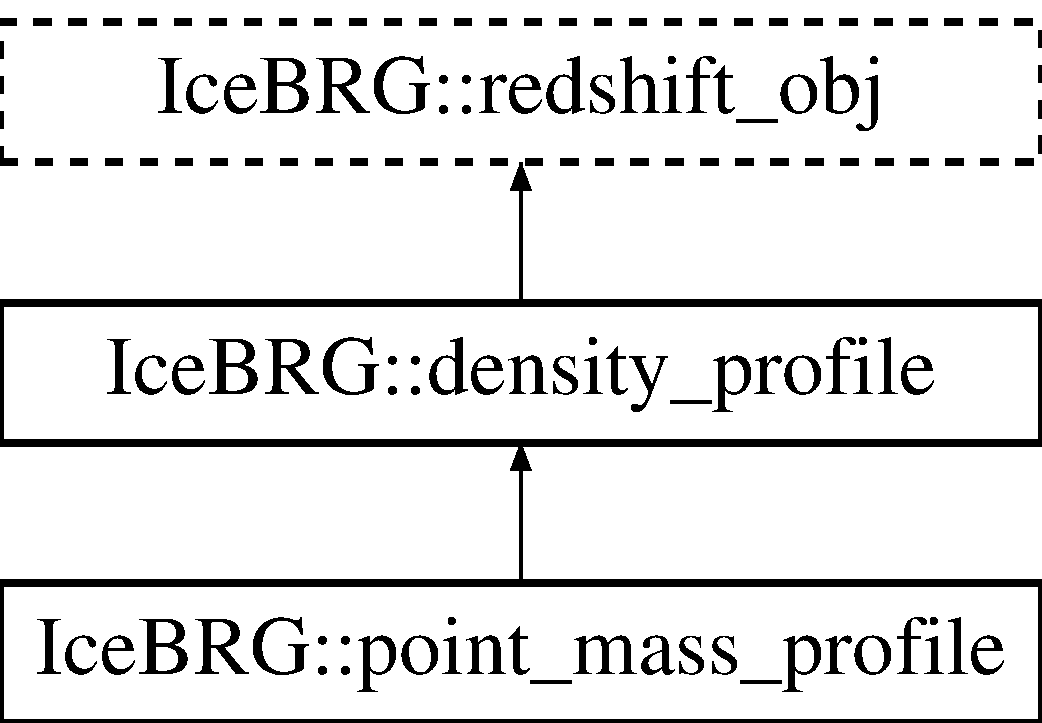
\includegraphics[height=3.000000cm]{classIceBRG_1_1point__mass__profile}
\end{center}
\end{figure}
\subsection*{Public Member Functions}
\begin{DoxyCompactItemize}
\item 
\hyperlink{classIceBRG_1_1point__mass__profile_aa256a4ac1d4761e720bc2a14f9803977}{point\+\_\+mass\+\_\+profile} ()
\item 
\hyperlink{classIceBRG_1_1point__mass__profile_a29746e6ba6a4be9dadbe3d659534c2cb}{point\+\_\+mass\+\_\+profile} (const \hyperlink{namespaceIceBRG_a1be72ac4918a9b029f2eefa084213e35}{mass\+\_\+type} init\+\_\+mass, const \hyperlink{lib_2IceBRG__main_2common_8h_ad0f130a56eeb944d9ef2692ee881ecc4}{flt\+\_\+type} \&init\+\_\+z)
\item 
\hyperlink{classIceBRG_1_1point__mass__profile_a1257cba930c725978837df2e273c1c09}{$\sim$point\+\_\+mass\+\_\+profile} ()
\item 
virtual void \hyperlink{classIceBRG_1_1point__mass__profile_adafe681034de7a44632a7b37e8109e1e}{set\+\_\+mvir} (const \hyperlink{namespaceIceBRG_a1be72ac4918a9b029f2eefa084213e35}{mass\+\_\+type} \&new\+\_\+halo\+\_\+mass)
\item 
virtual void \hyperlink{classIceBRG_1_1point__mass__profile_ac0577c7e2ff4877d57074c10ae18342d}{set\+\_\+parameters} (const std\+::vector$<$ \hyperlink{namespaceIceBRG_a3101fc159e191fa99c4ec14e445df96e}{any\+\_\+units\+\_\+type} $>$ \&new\+\_\+parameters)
\item 
\hyperlink{namespaceIceBRG_a1be72ac4918a9b029f2eefa084213e35}{mass\+\_\+type} \hyperlink{classIceBRG_1_1point__mass__profile_a93b3e78de217f95ab5ffe1109b07267f}{mass} () const 
\item 
\hyperlink{namespaceIceBRG_a1be72ac4918a9b029f2eefa084213e35}{mass\+\_\+type} \hyperlink{classIceBRG_1_1point__mass__profile_a8f9a6a1fafe39c216349ff92e1046b53}{mvir} () const 
\item 
\hyperlink{namespaceIceBRG_a1be72ac4918a9b029f2eefa084213e35}{mass\+\_\+type} \hyperlink{classIceBRG_1_1point__mass__profile_a1454cc006571f6a245e8e5046ee20bc5}{mtot} () const 
\item 
\hyperlink{namespaceIceBRG_a45499647eb87e24c10ab32c628711cec}{distance\+\_\+type} \hyperlink{classIceBRG_1_1point__mass__profile_a987603509622d26dbc20181954271c26}{rvir} () const 
\item 
\hyperlink{namespaceIceBRG_a45499647eb87e24c10ab32c628711cec}{distance\+\_\+type} \hyperlink{classIceBRG_1_1point__mass__profile_a313b65ebd5fcba8e073edabe82484b18}{rt} () const 
\item 
\hyperlink{namespaceIceBRG_a45499647eb87e24c10ab32c628711cec}{distance\+\_\+type} \hyperlink{classIceBRG_1_1point__mass__profile_aad9a12251097b4ccccf2ef02667e5073}{rs} () const 
\item 
\hyperlink{namespaceIceBRG_a34f8ef3b46f3408301e3c28197095eff}{velocity\+\_\+type} \hyperlink{classIceBRG_1_1point__mass__profile_a04bc365103dcae1b248b9e2487edd7ad}{vvir} () const 
\item 
\hyperlink{namespaceIceBRG_a9f5e5cdd641bb4c06f7305dfb5ae0238}{density\+\_\+type} \hyperlink{classIceBRG_1_1point__mass__profile_aa689ec66a40e36d9886c1b8077488161}{dens} (const \hyperlink{namespaceIceBRG_a45499647eb87e24c10ab32c628711cec}{distance\+\_\+type} \&r) const 
\item 
\hyperlink{namespaceIceBRG_a9f5e5cdd641bb4c06f7305dfb5ae0238}{density\+\_\+type} \hyperlink{classIceBRG_1_1point__mass__profile_ab52d614d0c7c163085d70ae78e6b1eed}{enc\+\_\+dens} (const \hyperlink{namespaceIceBRG_a45499647eb87e24c10ab32c628711cec}{distance\+\_\+type} \&r) const 
\item 
\hyperlink{namespaceIceBRG_a1be72ac4918a9b029f2eefa084213e35}{mass\+\_\+type} \hyperlink{classIceBRG_1_1point__mass__profile_a2e72fef9bc04039bd9119453f4aa6b13}{enc\+\_\+mass} (const \hyperlink{namespaceIceBRG_a45499647eb87e24c10ab32c628711cec}{distance\+\_\+type} \&r) const 
\item 
size\+\_\+t \hyperlink{classIceBRG_1_1point__mass__profile_a71f96138938e5e9edd0c755f131ddf5e}{num\+\_\+parameters} () const 
\item 
std\+::vector$<$ \hyperlink{namespaceIceBRG_a3101fc159e191fa99c4ec14e445df96e}{any\+\_\+units\+\_\+type} $>$ \hyperlink{classIceBRG_1_1point__mass__profile_a52bdbf1072d13ddef48df90339366ab3}{get\+\_\+parameters} () const 
\item 
std\+::vector$<$ std\+::string $>$ \hyperlink{classIceBRG_1_1point__mass__profile_a58ddc44e9a7fa78f1ec07e35db5bc141}{get\+\_\+parameter\+\_\+names} () const 
\item 
void \hyperlink{classIceBRG_1_1point__mass__profile_a17f71bc76434aea87a2043fbc526af63}{truncate\+\_\+to\+\_\+fraction} (const \hyperlink{lib_2IceBRG__main_2common_8h_ad0f130a56eeb944d9ef2692ee881ecc4}{flt\+\_\+type} \&fraction)
\item 
virtual \hyperlink{classIceBRG_1_1redshift__obj}{redshift\+\_\+obj} $\ast$ \hyperlink{classIceBRG_1_1point__mass__profile_a652993749492f4c718b77386ea3ba7af}{redshift\+\_\+obj\+\_\+clone} () const 
\item 
virtual \hyperlink{classIceBRG_1_1density__profile}{density\+\_\+profile} $\ast$ \hyperlink{classIceBRG_1_1point__mass__profile_a0e02fa9204b4d6718fb0a27b61b38b69}{density\+\_\+profile\+\_\+clone} () const 
\item 
virtual \hyperlink{classIceBRG_1_1point__mass__profile}{point\+\_\+mass\+\_\+profile} $\ast$ \hyperlink{classIceBRG_1_1point__mass__profile_ac1abfeb97d5272bf80c1aaa360b87cd8}{point\+\_\+mass\+\_\+profile\+\_\+clone} () const 
\end{DoxyCompactItemize}
\subsection*{Additional Inherited Members}


\subsection{Constructor \& Destructor Documentation}
\hypertarget{classIceBRG_1_1point__mass__profile_aa256a4ac1d4761e720bc2a14f9803977}{}\index{Ice\+B\+R\+G\+::point\+\_\+mass\+\_\+profile@{Ice\+B\+R\+G\+::point\+\_\+mass\+\_\+profile}!point\+\_\+mass\+\_\+profile@{point\+\_\+mass\+\_\+profile}}
\index{point\+\_\+mass\+\_\+profile@{point\+\_\+mass\+\_\+profile}!Ice\+B\+R\+G\+::point\+\_\+mass\+\_\+profile@{Ice\+B\+R\+G\+::point\+\_\+mass\+\_\+profile}}
\subsubsection[{point\+\_\+mass\+\_\+profile()}]{\setlength{\rightskip}{0pt plus 5cm}Ice\+B\+R\+G\+::point\+\_\+mass\+\_\+profile\+::point\+\_\+mass\+\_\+profile (
\begin{DoxyParamCaption}
{}
\end{DoxyParamCaption}
)}\label{classIceBRG_1_1point__mass__profile_aa256a4ac1d4761e720bc2a14f9803977}
\hypertarget{classIceBRG_1_1point__mass__profile_a29746e6ba6a4be9dadbe3d659534c2cb}{}\index{Ice\+B\+R\+G\+::point\+\_\+mass\+\_\+profile@{Ice\+B\+R\+G\+::point\+\_\+mass\+\_\+profile}!point\+\_\+mass\+\_\+profile@{point\+\_\+mass\+\_\+profile}}
\index{point\+\_\+mass\+\_\+profile@{point\+\_\+mass\+\_\+profile}!Ice\+B\+R\+G\+::point\+\_\+mass\+\_\+profile@{Ice\+B\+R\+G\+::point\+\_\+mass\+\_\+profile}}
\subsubsection[{point\+\_\+mass\+\_\+profile(const mass\+\_\+type init\+\_\+mass, const flt\+\_\+type \&init\+\_\+z)}]{\setlength{\rightskip}{0pt plus 5cm}Ice\+B\+R\+G\+::point\+\_\+mass\+\_\+profile\+::point\+\_\+mass\+\_\+profile (
\begin{DoxyParamCaption}
\item[{const {\bf mass\+\_\+type}}]{init\+\_\+mass, }
\item[{const {\bf flt\+\_\+type} \&}]{init\+\_\+z}
\end{DoxyParamCaption}
)}\label{classIceBRG_1_1point__mass__profile_a29746e6ba6a4be9dadbe3d659534c2cb}
\hypertarget{classIceBRG_1_1point__mass__profile_a1257cba930c725978837df2e273c1c09}{}\index{Ice\+B\+R\+G\+::point\+\_\+mass\+\_\+profile@{Ice\+B\+R\+G\+::point\+\_\+mass\+\_\+profile}!````~point\+\_\+mass\+\_\+profile@{$\sim$point\+\_\+mass\+\_\+profile}}
\index{````~point\+\_\+mass\+\_\+profile@{$\sim$point\+\_\+mass\+\_\+profile}!Ice\+B\+R\+G\+::point\+\_\+mass\+\_\+profile@{Ice\+B\+R\+G\+::point\+\_\+mass\+\_\+profile}}
\subsubsection[{$\sim$point\+\_\+mass\+\_\+profile()}]{\setlength{\rightskip}{0pt plus 5cm}Ice\+B\+R\+G\+::point\+\_\+mass\+\_\+profile\+::$\sim$point\+\_\+mass\+\_\+profile (
\begin{DoxyParamCaption}
{}
\end{DoxyParamCaption}
)}\label{classIceBRG_1_1point__mass__profile_a1257cba930c725978837df2e273c1c09}


\subsection{Member Function Documentation}
\hypertarget{classIceBRG_1_1point__mass__profile_aa689ec66a40e36d9886c1b8077488161}{}\index{Ice\+B\+R\+G\+::point\+\_\+mass\+\_\+profile@{Ice\+B\+R\+G\+::point\+\_\+mass\+\_\+profile}!dens@{dens}}
\index{dens@{dens}!Ice\+B\+R\+G\+::point\+\_\+mass\+\_\+profile@{Ice\+B\+R\+G\+::point\+\_\+mass\+\_\+profile}}
\subsubsection[{dens(const distance\+\_\+type \&r) const }]{\setlength{\rightskip}{0pt plus 5cm}{\bf Ice\+B\+R\+G\+::density\+\_\+type} Ice\+B\+R\+G\+::point\+\_\+mass\+\_\+profile\+::dens (
\begin{DoxyParamCaption}
\item[{const {\bf distance\+\_\+type} \&}]{r}
\end{DoxyParamCaption}
) const\hspace{0.3cm}{\ttfamily [virtual]}}\label{classIceBRG_1_1point__mass__profile_aa689ec66a40e36d9886c1b8077488161}


Implements \hyperlink{classIceBRG_1_1density__profile_ac47dc183eb719a6aea32e981a6f79a30}{Ice\+B\+R\+G\+::density\+\_\+profile}.

\hypertarget{classIceBRG_1_1point__mass__profile_a0e02fa9204b4d6718fb0a27b61b38b69}{}\index{Ice\+B\+R\+G\+::point\+\_\+mass\+\_\+profile@{Ice\+B\+R\+G\+::point\+\_\+mass\+\_\+profile}!density\+\_\+profile\+\_\+clone@{density\+\_\+profile\+\_\+clone}}
\index{density\+\_\+profile\+\_\+clone@{density\+\_\+profile\+\_\+clone}!Ice\+B\+R\+G\+::point\+\_\+mass\+\_\+profile@{Ice\+B\+R\+G\+::point\+\_\+mass\+\_\+profile}}
\subsubsection[{density\+\_\+profile\+\_\+clone() const }]{\setlength{\rightskip}{0pt plus 5cm}virtual {\bf density\+\_\+profile}$\ast$ Ice\+B\+R\+G\+::point\+\_\+mass\+\_\+profile\+::density\+\_\+profile\+\_\+clone (
\begin{DoxyParamCaption}
{}
\end{DoxyParamCaption}
) const\hspace{0.3cm}{\ttfamily [inline]}, {\ttfamily [virtual]}}\label{classIceBRG_1_1point__mass__profile_a0e02fa9204b4d6718fb0a27b61b38b69}


Implements \hyperlink{classIceBRG_1_1density__profile_a8a6a4033eeadf4b70ee174f293639c80}{Ice\+B\+R\+G\+::density\+\_\+profile}.

\hypertarget{classIceBRG_1_1point__mass__profile_ab52d614d0c7c163085d70ae78e6b1eed}{}\index{Ice\+B\+R\+G\+::point\+\_\+mass\+\_\+profile@{Ice\+B\+R\+G\+::point\+\_\+mass\+\_\+profile}!enc\+\_\+dens@{enc\+\_\+dens}}
\index{enc\+\_\+dens@{enc\+\_\+dens}!Ice\+B\+R\+G\+::point\+\_\+mass\+\_\+profile@{Ice\+B\+R\+G\+::point\+\_\+mass\+\_\+profile}}
\subsubsection[{enc\+\_\+dens(const distance\+\_\+type \&r) const }]{\setlength{\rightskip}{0pt plus 5cm}{\bf Ice\+B\+R\+G\+::density\+\_\+type} Ice\+B\+R\+G\+::point\+\_\+mass\+\_\+profile\+::enc\+\_\+dens (
\begin{DoxyParamCaption}
\item[{const {\bf distance\+\_\+type} \&}]{r}
\end{DoxyParamCaption}
) const\hspace{0.3cm}{\ttfamily [virtual]}}\label{classIceBRG_1_1point__mass__profile_ab52d614d0c7c163085d70ae78e6b1eed}


Reimplemented from \hyperlink{classIceBRG_1_1density__profile_abe453f2128f3ee4030092e20b8c6e380}{Ice\+B\+R\+G\+::density\+\_\+profile}.

\hypertarget{classIceBRG_1_1point__mass__profile_a2e72fef9bc04039bd9119453f4aa6b13}{}\index{Ice\+B\+R\+G\+::point\+\_\+mass\+\_\+profile@{Ice\+B\+R\+G\+::point\+\_\+mass\+\_\+profile}!enc\+\_\+mass@{enc\+\_\+mass}}
\index{enc\+\_\+mass@{enc\+\_\+mass}!Ice\+B\+R\+G\+::point\+\_\+mass\+\_\+profile@{Ice\+B\+R\+G\+::point\+\_\+mass\+\_\+profile}}
\subsubsection[{enc\+\_\+mass(const distance\+\_\+type \&r) const }]{\setlength{\rightskip}{0pt plus 5cm}{\bf Ice\+B\+R\+G\+::mass\+\_\+type} Ice\+B\+R\+G\+::point\+\_\+mass\+\_\+profile\+::enc\+\_\+mass (
\begin{DoxyParamCaption}
\item[{const {\bf distance\+\_\+type} \&}]{r}
\end{DoxyParamCaption}
) const\hspace{0.3cm}{\ttfamily [virtual]}}\label{classIceBRG_1_1point__mass__profile_a2e72fef9bc04039bd9119453f4aa6b13}


Reimplemented from \hyperlink{classIceBRG_1_1density__profile_a090e214c2228f99019c75e7fede37ae5}{Ice\+B\+R\+G\+::density\+\_\+profile}.

\hypertarget{classIceBRG_1_1point__mass__profile_a58ddc44e9a7fa78f1ec07e35db5bc141}{}\index{Ice\+B\+R\+G\+::point\+\_\+mass\+\_\+profile@{Ice\+B\+R\+G\+::point\+\_\+mass\+\_\+profile}!get\+\_\+parameter\+\_\+names@{get\+\_\+parameter\+\_\+names}}
\index{get\+\_\+parameter\+\_\+names@{get\+\_\+parameter\+\_\+names}!Ice\+B\+R\+G\+::point\+\_\+mass\+\_\+profile@{Ice\+B\+R\+G\+::point\+\_\+mass\+\_\+profile}}
\subsubsection[{get\+\_\+parameter\+\_\+names() const }]{\setlength{\rightskip}{0pt plus 5cm}std\+::vector$<$ std\+::string $>$ Ice\+B\+R\+G\+::point\+\_\+mass\+\_\+profile\+::get\+\_\+parameter\+\_\+names (
\begin{DoxyParamCaption}
{}
\end{DoxyParamCaption}
) const\hspace{0.3cm}{\ttfamily [virtual]}}\label{classIceBRG_1_1point__mass__profile_a58ddc44e9a7fa78f1ec07e35db5bc141}


Reimplemented from \hyperlink{classIceBRG_1_1density__profile_ae773cdab093dfc22ff9dc01dd2de09f4}{Ice\+B\+R\+G\+::density\+\_\+profile}.

\hypertarget{classIceBRG_1_1point__mass__profile_a52bdbf1072d13ddef48df90339366ab3}{}\index{Ice\+B\+R\+G\+::point\+\_\+mass\+\_\+profile@{Ice\+B\+R\+G\+::point\+\_\+mass\+\_\+profile}!get\+\_\+parameters@{get\+\_\+parameters}}
\index{get\+\_\+parameters@{get\+\_\+parameters}!Ice\+B\+R\+G\+::point\+\_\+mass\+\_\+profile@{Ice\+B\+R\+G\+::point\+\_\+mass\+\_\+profile}}
\subsubsection[{get\+\_\+parameters() const }]{\setlength{\rightskip}{0pt plus 5cm}std\+::vector$<$ {\bf Ice\+B\+R\+G\+::any\+\_\+units\+\_\+type} $>$ Ice\+B\+R\+G\+::point\+\_\+mass\+\_\+profile\+::get\+\_\+parameters (
\begin{DoxyParamCaption}
{}
\end{DoxyParamCaption}
) const\hspace{0.3cm}{\ttfamily [virtual]}}\label{classIceBRG_1_1point__mass__profile_a52bdbf1072d13ddef48df90339366ab3}


Reimplemented from \hyperlink{classIceBRG_1_1density__profile_a661c4e91260285e70290c8b454a0f0d9}{Ice\+B\+R\+G\+::density\+\_\+profile}.

\hypertarget{classIceBRG_1_1point__mass__profile_a93b3e78de217f95ab5ffe1109b07267f}{}\index{Ice\+B\+R\+G\+::point\+\_\+mass\+\_\+profile@{Ice\+B\+R\+G\+::point\+\_\+mass\+\_\+profile}!mass@{mass}}
\index{mass@{mass}!Ice\+B\+R\+G\+::point\+\_\+mass\+\_\+profile@{Ice\+B\+R\+G\+::point\+\_\+mass\+\_\+profile}}
\subsubsection[{mass() const }]{\setlength{\rightskip}{0pt plus 5cm}{\bf Ice\+B\+R\+G\+::mass\+\_\+type} Ice\+B\+R\+G\+::point\+\_\+mass\+\_\+profile\+::mass (
\begin{DoxyParamCaption}
{}
\end{DoxyParamCaption}
) const}\label{classIceBRG_1_1point__mass__profile_a93b3e78de217f95ab5ffe1109b07267f}
\hypertarget{classIceBRG_1_1point__mass__profile_a1454cc006571f6a245e8e5046ee20bc5}{}\index{Ice\+B\+R\+G\+::point\+\_\+mass\+\_\+profile@{Ice\+B\+R\+G\+::point\+\_\+mass\+\_\+profile}!mtot@{mtot}}
\index{mtot@{mtot}!Ice\+B\+R\+G\+::point\+\_\+mass\+\_\+profile@{Ice\+B\+R\+G\+::point\+\_\+mass\+\_\+profile}}
\subsubsection[{mtot() const }]{\setlength{\rightskip}{0pt plus 5cm}{\bf Ice\+B\+R\+G\+::mass\+\_\+type} Ice\+B\+R\+G\+::point\+\_\+mass\+\_\+profile\+::mtot (
\begin{DoxyParamCaption}
{}
\end{DoxyParamCaption}
) const\hspace{0.3cm}{\ttfamily [virtual]}}\label{classIceBRG_1_1point__mass__profile_a1454cc006571f6a245e8e5046ee20bc5}


Reimplemented from \hyperlink{classIceBRG_1_1density__profile_ada763e0637edc2efb168a9fa42daa580}{Ice\+B\+R\+G\+::density\+\_\+profile}.

\hypertarget{classIceBRG_1_1point__mass__profile_a8f9a6a1fafe39c216349ff92e1046b53}{}\index{Ice\+B\+R\+G\+::point\+\_\+mass\+\_\+profile@{Ice\+B\+R\+G\+::point\+\_\+mass\+\_\+profile}!mvir@{mvir}}
\index{mvir@{mvir}!Ice\+B\+R\+G\+::point\+\_\+mass\+\_\+profile@{Ice\+B\+R\+G\+::point\+\_\+mass\+\_\+profile}}
\subsubsection[{mvir() const }]{\setlength{\rightskip}{0pt plus 5cm}{\bf Ice\+B\+R\+G\+::mass\+\_\+type} Ice\+B\+R\+G\+::point\+\_\+mass\+\_\+profile\+::mvir (
\begin{DoxyParamCaption}
{}
\end{DoxyParamCaption}
) const\hspace{0.3cm}{\ttfamily [virtual]}}\label{classIceBRG_1_1point__mass__profile_a8f9a6a1fafe39c216349ff92e1046b53}


Implements \hyperlink{classIceBRG_1_1density__profile_aa62204b8ca04779f4477183f873b2aff}{Ice\+B\+R\+G\+::density\+\_\+profile}.

\hypertarget{classIceBRG_1_1point__mass__profile_a71f96138938e5e9edd0c755f131ddf5e}{}\index{Ice\+B\+R\+G\+::point\+\_\+mass\+\_\+profile@{Ice\+B\+R\+G\+::point\+\_\+mass\+\_\+profile}!num\+\_\+parameters@{num\+\_\+parameters}}
\index{num\+\_\+parameters@{num\+\_\+parameters}!Ice\+B\+R\+G\+::point\+\_\+mass\+\_\+profile@{Ice\+B\+R\+G\+::point\+\_\+mass\+\_\+profile}}
\subsubsection[{num\+\_\+parameters() const }]{\setlength{\rightskip}{0pt plus 5cm}size\+\_\+t Ice\+B\+R\+G\+::point\+\_\+mass\+\_\+profile\+::num\+\_\+parameters (
\begin{DoxyParamCaption}
{}
\end{DoxyParamCaption}
) const\hspace{0.3cm}{\ttfamily [inline]}, {\ttfamily [virtual]}}\label{classIceBRG_1_1point__mass__profile_a71f96138938e5e9edd0c755f131ddf5e}


Reimplemented from \hyperlink{classIceBRG_1_1density__profile_ad63fb55be18802ec2ab1d4a0a9d49236}{Ice\+B\+R\+G\+::density\+\_\+profile}.

\hypertarget{classIceBRG_1_1point__mass__profile_ac1abfeb97d5272bf80c1aaa360b87cd8}{}\index{Ice\+B\+R\+G\+::point\+\_\+mass\+\_\+profile@{Ice\+B\+R\+G\+::point\+\_\+mass\+\_\+profile}!point\+\_\+mass\+\_\+profile\+\_\+clone@{point\+\_\+mass\+\_\+profile\+\_\+clone}}
\index{point\+\_\+mass\+\_\+profile\+\_\+clone@{point\+\_\+mass\+\_\+profile\+\_\+clone}!Ice\+B\+R\+G\+::point\+\_\+mass\+\_\+profile@{Ice\+B\+R\+G\+::point\+\_\+mass\+\_\+profile}}
\subsubsection[{point\+\_\+mass\+\_\+profile\+\_\+clone() const }]{\setlength{\rightskip}{0pt plus 5cm}virtual {\bf point\+\_\+mass\+\_\+profile}$\ast$ Ice\+B\+R\+G\+::point\+\_\+mass\+\_\+profile\+::point\+\_\+mass\+\_\+profile\+\_\+clone (
\begin{DoxyParamCaption}
{}
\end{DoxyParamCaption}
) const\hspace{0.3cm}{\ttfamily [inline]}, {\ttfamily [virtual]}}\label{classIceBRG_1_1point__mass__profile_ac1abfeb97d5272bf80c1aaa360b87cd8}
\hypertarget{classIceBRG_1_1point__mass__profile_a652993749492f4c718b77386ea3ba7af}{}\index{Ice\+B\+R\+G\+::point\+\_\+mass\+\_\+profile@{Ice\+B\+R\+G\+::point\+\_\+mass\+\_\+profile}!redshift\+\_\+obj\+\_\+clone@{redshift\+\_\+obj\+\_\+clone}}
\index{redshift\+\_\+obj\+\_\+clone@{redshift\+\_\+obj\+\_\+clone}!Ice\+B\+R\+G\+::point\+\_\+mass\+\_\+profile@{Ice\+B\+R\+G\+::point\+\_\+mass\+\_\+profile}}
\subsubsection[{redshift\+\_\+obj\+\_\+clone() const }]{\setlength{\rightskip}{0pt plus 5cm}virtual {\bf redshift\+\_\+obj}$\ast$ Ice\+B\+R\+G\+::point\+\_\+mass\+\_\+profile\+::redshift\+\_\+obj\+\_\+clone (
\begin{DoxyParamCaption}
{}
\end{DoxyParamCaption}
) const\hspace{0.3cm}{\ttfamily [inline]}, {\ttfamily [virtual]}}\label{classIceBRG_1_1point__mass__profile_a652993749492f4c718b77386ea3ba7af}


Reimplemented from \hyperlink{classIceBRG_1_1redshift__obj_a02f96529ff7f42ae64ae832712930e3b}{Ice\+B\+R\+G\+::redshift\+\_\+obj}.

\hypertarget{classIceBRG_1_1point__mass__profile_aad9a12251097b4ccccf2ef02667e5073}{}\index{Ice\+B\+R\+G\+::point\+\_\+mass\+\_\+profile@{Ice\+B\+R\+G\+::point\+\_\+mass\+\_\+profile}!rs@{rs}}
\index{rs@{rs}!Ice\+B\+R\+G\+::point\+\_\+mass\+\_\+profile@{Ice\+B\+R\+G\+::point\+\_\+mass\+\_\+profile}}
\subsubsection[{rs() const }]{\setlength{\rightskip}{0pt plus 5cm}{\bf Ice\+B\+R\+G\+::distance\+\_\+type} Ice\+B\+R\+G\+::point\+\_\+mass\+\_\+profile\+::rs (
\begin{DoxyParamCaption}
{}
\end{DoxyParamCaption}
) const}\label{classIceBRG_1_1point__mass__profile_aad9a12251097b4ccccf2ef02667e5073}
\hypertarget{classIceBRG_1_1point__mass__profile_a313b65ebd5fcba8e073edabe82484b18}{}\index{Ice\+B\+R\+G\+::point\+\_\+mass\+\_\+profile@{Ice\+B\+R\+G\+::point\+\_\+mass\+\_\+profile}!rt@{rt}}
\index{rt@{rt}!Ice\+B\+R\+G\+::point\+\_\+mass\+\_\+profile@{Ice\+B\+R\+G\+::point\+\_\+mass\+\_\+profile}}
\subsubsection[{rt() const }]{\setlength{\rightskip}{0pt plus 5cm}{\bf Ice\+B\+R\+G\+::distance\+\_\+type} Ice\+B\+R\+G\+::point\+\_\+mass\+\_\+profile\+::rt (
\begin{DoxyParamCaption}
{}
\end{DoxyParamCaption}
) const\hspace{0.3cm}{\ttfamily [virtual]}}\label{classIceBRG_1_1point__mass__profile_a313b65ebd5fcba8e073edabe82484b18}


Reimplemented from \hyperlink{classIceBRG_1_1density__profile_a53c528b9d6de8506175faece58361c23}{Ice\+B\+R\+G\+::density\+\_\+profile}.

\hypertarget{classIceBRG_1_1point__mass__profile_a987603509622d26dbc20181954271c26}{}\index{Ice\+B\+R\+G\+::point\+\_\+mass\+\_\+profile@{Ice\+B\+R\+G\+::point\+\_\+mass\+\_\+profile}!rvir@{rvir}}
\index{rvir@{rvir}!Ice\+B\+R\+G\+::point\+\_\+mass\+\_\+profile@{Ice\+B\+R\+G\+::point\+\_\+mass\+\_\+profile}}
\subsubsection[{rvir() const }]{\setlength{\rightskip}{0pt plus 5cm}{\bf Ice\+B\+R\+G\+::distance\+\_\+type} Ice\+B\+R\+G\+::point\+\_\+mass\+\_\+profile\+::rvir (
\begin{DoxyParamCaption}
{}
\end{DoxyParamCaption}
) const\hspace{0.3cm}{\ttfamily [virtual]}}\label{classIceBRG_1_1point__mass__profile_a987603509622d26dbc20181954271c26}


Reimplemented from \hyperlink{classIceBRG_1_1density__profile_a34312cb028a2c481cb72224a12b4a287}{Ice\+B\+R\+G\+::density\+\_\+profile}.

\hypertarget{classIceBRG_1_1point__mass__profile_adafe681034de7a44632a7b37e8109e1e}{}\index{Ice\+B\+R\+G\+::point\+\_\+mass\+\_\+profile@{Ice\+B\+R\+G\+::point\+\_\+mass\+\_\+profile}!set\+\_\+mvir@{set\+\_\+mvir}}
\index{set\+\_\+mvir@{set\+\_\+mvir}!Ice\+B\+R\+G\+::point\+\_\+mass\+\_\+profile@{Ice\+B\+R\+G\+::point\+\_\+mass\+\_\+profile}}
\subsubsection[{set\+\_\+mvir(const mass\+\_\+type \&new\+\_\+halo\+\_\+mass)}]{\setlength{\rightskip}{0pt plus 5cm}void Ice\+B\+R\+G\+::point\+\_\+mass\+\_\+profile\+::set\+\_\+mvir (
\begin{DoxyParamCaption}
\item[{const {\bf mass\+\_\+type} \&}]{new\+\_\+halo\+\_\+mass}
\end{DoxyParamCaption}
)\hspace{0.3cm}{\ttfamily [virtual]}}\label{classIceBRG_1_1point__mass__profile_adafe681034de7a44632a7b37e8109e1e}


Reimplemented from \hyperlink{classIceBRG_1_1density__profile_ae0230aa967a251d3ce5f360514e1690d}{Ice\+B\+R\+G\+::density\+\_\+profile}.

\hypertarget{classIceBRG_1_1point__mass__profile_ac0577c7e2ff4877d57074c10ae18342d}{}\index{Ice\+B\+R\+G\+::point\+\_\+mass\+\_\+profile@{Ice\+B\+R\+G\+::point\+\_\+mass\+\_\+profile}!set\+\_\+parameters@{set\+\_\+parameters}}
\index{set\+\_\+parameters@{set\+\_\+parameters}!Ice\+B\+R\+G\+::point\+\_\+mass\+\_\+profile@{Ice\+B\+R\+G\+::point\+\_\+mass\+\_\+profile}}
\subsubsection[{set\+\_\+parameters(const std\+::vector$<$ any\+\_\+units\+\_\+type $>$ \&new\+\_\+parameters)}]{\setlength{\rightskip}{0pt plus 5cm}void Ice\+B\+R\+G\+::point\+\_\+mass\+\_\+profile\+::set\+\_\+parameters (
\begin{DoxyParamCaption}
\item[{const std\+::vector$<$ {\bf any\+\_\+units\+\_\+type} $>$ \&}]{new\+\_\+parameters}
\end{DoxyParamCaption}
)\hspace{0.3cm}{\ttfamily [virtual]}}\label{classIceBRG_1_1point__mass__profile_ac0577c7e2ff4877d57074c10ae18342d}


Reimplemented from \hyperlink{classIceBRG_1_1density__profile_af58ebb218c2abe35cfaa261cd29ba35c}{Ice\+B\+R\+G\+::density\+\_\+profile}.

\hypertarget{classIceBRG_1_1point__mass__profile_a17f71bc76434aea87a2043fbc526af63}{}\index{Ice\+B\+R\+G\+::point\+\_\+mass\+\_\+profile@{Ice\+B\+R\+G\+::point\+\_\+mass\+\_\+profile}!truncate\+\_\+to\+\_\+fraction@{truncate\+\_\+to\+\_\+fraction}}
\index{truncate\+\_\+to\+\_\+fraction@{truncate\+\_\+to\+\_\+fraction}!Ice\+B\+R\+G\+::point\+\_\+mass\+\_\+profile@{Ice\+B\+R\+G\+::point\+\_\+mass\+\_\+profile}}
\subsubsection[{truncate\+\_\+to\+\_\+fraction(const flt\+\_\+type \&fraction)}]{\setlength{\rightskip}{0pt plus 5cm}void Ice\+B\+R\+G\+::point\+\_\+mass\+\_\+profile\+::truncate\+\_\+to\+\_\+fraction (
\begin{DoxyParamCaption}
\item[{const {\bf flt\+\_\+type} \&}]{fraction}
\end{DoxyParamCaption}
)\hspace{0.3cm}{\ttfamily [virtual]}}\label{classIceBRG_1_1point__mass__profile_a17f71bc76434aea87a2043fbc526af63}


Reimplemented from \hyperlink{classIceBRG_1_1density__profile_ac7b6a0bf55ce53aeeccbf7322a49e54c}{Ice\+B\+R\+G\+::density\+\_\+profile}.

\hypertarget{classIceBRG_1_1point__mass__profile_a04bc365103dcae1b248b9e2487edd7ad}{}\index{Ice\+B\+R\+G\+::point\+\_\+mass\+\_\+profile@{Ice\+B\+R\+G\+::point\+\_\+mass\+\_\+profile}!vvir@{vvir}}
\index{vvir@{vvir}!Ice\+B\+R\+G\+::point\+\_\+mass\+\_\+profile@{Ice\+B\+R\+G\+::point\+\_\+mass\+\_\+profile}}
\subsubsection[{vvir() const }]{\setlength{\rightskip}{0pt plus 5cm}{\bf Ice\+B\+R\+G\+::velocity\+\_\+type} Ice\+B\+R\+G\+::point\+\_\+mass\+\_\+profile\+::vvir (
\begin{DoxyParamCaption}
{}
\end{DoxyParamCaption}
) const\hspace{0.3cm}{\ttfamily [virtual]}}\label{classIceBRG_1_1point__mass__profile_a04bc365103dcae1b248b9e2487edd7ad}


Reimplemented from \hyperlink{classIceBRG_1_1density__profile_a09dec0ec4468e10e87b7b30f2069c108}{Ice\+B\+R\+G\+::density\+\_\+profile}.



The documentation for this class was generated from the following files\+:\begin{DoxyCompactItemize}
\item 
/disk2/brg/git/\+Magnification\+\_\+\+Public/src/lib/\+Ice\+B\+R\+G\+\_\+physics/density\+\_\+profile/\hyperlink{point__mass__profile_8h}{point\+\_\+mass\+\_\+profile.\+h}\item 
/disk2/brg/git/\+Magnification\+\_\+\+Public/src/lib/\+Ice\+B\+R\+G\+\_\+physics/density\+\_\+profile/\hyperlink{point__mass__profile_8cpp}{point\+\_\+mass\+\_\+profile.\+cpp}\end{DoxyCompactItemize}

\hypertarget{classIceBRG_1_1position__grid__extension}{}\section{Ice\+B\+R\+G\+:\+:position\+\_\+grid\+\_\+extension$<$ name $>$ Class Template Reference}
\label{classIceBRG_1_1position__grid__extension}\index{Ice\+B\+R\+G\+::position\+\_\+grid\+\_\+extension$<$ name $>$@{Ice\+B\+R\+G\+::position\+\_\+grid\+\_\+extension$<$ name $>$}}


{\ttfamily \#include $<$position\+\_\+grid\+\_\+extension.\+hpp$>$}

\subsection*{Public Member Functions}
\begin{DoxyCompactItemize}
\item 
const \hyperlink{lib_2IceBRG__main_2common_8h_ac4de9d9335536ac22821171deec8d39e}{int\+\_\+type} \hyperlink{classIceBRG_1_1position__grid__extension_ac35e512924be07ac117e6e1ed3c2048a}{ra\+\_\+grid} () const 
\item 
const \hyperlink{lib_2IceBRG__main_2common_8h_ac4de9d9335536ac22821171deec8d39e}{int\+\_\+type} \hyperlink{classIceBRG_1_1position__grid__extension_aa4c2e0a9db54e50c3e3ccc8f81eb3f60}{dec\+\_\+grid} () const 
\item 
const \hyperlink{lib_2IceBRG__main_2common_8h_ac4de9d9335536ac22821171deec8d39e}{int\+\_\+type} \hyperlink{classIceBRG_1_1position__grid__extension_a8e7f5c11b3c0dee2050ce2f633f45d31}{z\+\_\+grid} () const 
\item 
const \hyperlink{lib_2IceBRG__main_2common_8h_ac4de9d9335536ac22821171deec8d39e}{int\+\_\+type} \hyperlink{classIceBRG_1_1position__grid__extension_aadc38967e6f232bec1c506058026674e}{quick\+\_\+ra\+\_\+grid} () const 
\item 
const \hyperlink{lib_2IceBRG__main_2common_8h_ac4de9d9335536ac22821171deec8d39e}{int\+\_\+type} \hyperlink{classIceBRG_1_1position__grid__extension_a259258e1d4ab96213ae7f9d340bedade}{quick\+\_\+dec\+\_\+grid} () const 
\item 
const \hyperlink{lib_2IceBRG__main_2common_8h_ac4de9d9335536ac22821171deec8d39e}{int\+\_\+type} \hyperlink{classIceBRG_1_1position__grid__extension_a62b09e46f25866c6778099c72a361167}{quick\+\_\+z\+\_\+grid} () const 
\item 
\hyperlink{classIceBRG_1_1position__grid__extension_a0b89f816a6c4f515831d5485d405497b}{position\+\_\+grid\+\_\+extension} ()
\item 
virtual \hyperlink{classIceBRG_1_1position__grid__extension_adb966b63b6c22b7f2b2b7c468e305055}{$\sim$position\+\_\+grid\+\_\+extension} ()
\end{DoxyCompactItemize}


\subsection{Constructor \& Destructor Documentation}
\hypertarget{classIceBRG_1_1position__grid__extension_a0b89f816a6c4f515831d5485d405497b}{}\index{Ice\+B\+R\+G\+::position\+\_\+grid\+\_\+extension@{Ice\+B\+R\+G\+::position\+\_\+grid\+\_\+extension}!position\+\_\+grid\+\_\+extension@{position\+\_\+grid\+\_\+extension}}
\index{position\+\_\+grid\+\_\+extension@{position\+\_\+grid\+\_\+extension}!Ice\+B\+R\+G\+::position\+\_\+grid\+\_\+extension@{Ice\+B\+R\+G\+::position\+\_\+grid\+\_\+extension}}
\subsubsection[{position\+\_\+grid\+\_\+extension()}]{\setlength{\rightskip}{0pt plus 5cm}template$<$typename name $>$ {\bf Ice\+B\+R\+G\+::position\+\_\+grid\+\_\+extension}$<$ name $>$\+::{\bf position\+\_\+grid\+\_\+extension} (
\begin{DoxyParamCaption}
{}
\end{DoxyParamCaption}
)\hspace{0.3cm}{\ttfamily [inline]}}\label{classIceBRG_1_1position__grid__extension_a0b89f816a6c4f515831d5485d405497b}
\hypertarget{classIceBRG_1_1position__grid__extension_adb966b63b6c22b7f2b2b7c468e305055}{}\index{Ice\+B\+R\+G\+::position\+\_\+grid\+\_\+extension@{Ice\+B\+R\+G\+::position\+\_\+grid\+\_\+extension}!````~position\+\_\+grid\+\_\+extension@{$\sim$position\+\_\+grid\+\_\+extension}}
\index{````~position\+\_\+grid\+\_\+extension@{$\sim$position\+\_\+grid\+\_\+extension}!Ice\+B\+R\+G\+::position\+\_\+grid\+\_\+extension@{Ice\+B\+R\+G\+::position\+\_\+grid\+\_\+extension}}
\subsubsection[{$\sim$position\+\_\+grid\+\_\+extension()}]{\setlength{\rightskip}{0pt plus 5cm}template$<$typename name $>$ virtual {\bf Ice\+B\+R\+G\+::position\+\_\+grid\+\_\+extension}$<$ name $>$\+::$\sim${\bf position\+\_\+grid\+\_\+extension} (
\begin{DoxyParamCaption}
{}
\end{DoxyParamCaption}
)\hspace{0.3cm}{\ttfamily [inline]}, {\ttfamily [virtual]}}\label{classIceBRG_1_1position__grid__extension_adb966b63b6c22b7f2b2b7c468e305055}


\subsection{Member Function Documentation}
\hypertarget{classIceBRG_1_1position__grid__extension_aa4c2e0a9db54e50c3e3ccc8f81eb3f60}{}\index{Ice\+B\+R\+G\+::position\+\_\+grid\+\_\+extension@{Ice\+B\+R\+G\+::position\+\_\+grid\+\_\+extension}!dec\+\_\+grid@{dec\+\_\+grid}}
\index{dec\+\_\+grid@{dec\+\_\+grid}!Ice\+B\+R\+G\+::position\+\_\+grid\+\_\+extension@{Ice\+B\+R\+G\+::position\+\_\+grid\+\_\+extension}}
\subsubsection[{dec\+\_\+grid() const }]{\setlength{\rightskip}{0pt plus 5cm}template$<$typename name $>$ const {\bf int\+\_\+type} {\bf Ice\+B\+R\+G\+::position\+\_\+grid\+\_\+extension}$<$ name $>$\+::dec\+\_\+grid (
\begin{DoxyParamCaption}
{}
\end{DoxyParamCaption}
) const\hspace{0.3cm}{\ttfamily [inline]}}\label{classIceBRG_1_1position__grid__extension_aa4c2e0a9db54e50c3e3ccc8f81eb3f60}
\hypertarget{classIceBRG_1_1position__grid__extension_a259258e1d4ab96213ae7f9d340bedade}{}\index{Ice\+B\+R\+G\+::position\+\_\+grid\+\_\+extension@{Ice\+B\+R\+G\+::position\+\_\+grid\+\_\+extension}!quick\+\_\+dec\+\_\+grid@{quick\+\_\+dec\+\_\+grid}}
\index{quick\+\_\+dec\+\_\+grid@{quick\+\_\+dec\+\_\+grid}!Ice\+B\+R\+G\+::position\+\_\+grid\+\_\+extension@{Ice\+B\+R\+G\+::position\+\_\+grid\+\_\+extension}}
\subsubsection[{quick\+\_\+dec\+\_\+grid() const }]{\setlength{\rightskip}{0pt plus 5cm}template$<$typename name $>$ const {\bf int\+\_\+type} {\bf Ice\+B\+R\+G\+::position\+\_\+grid\+\_\+extension}$<$ name $>$\+::quick\+\_\+dec\+\_\+grid (
\begin{DoxyParamCaption}
{}
\end{DoxyParamCaption}
) const\hspace{0.3cm}{\ttfamily [inline]}}\label{classIceBRG_1_1position__grid__extension_a259258e1d4ab96213ae7f9d340bedade}
\hypertarget{classIceBRG_1_1position__grid__extension_aadc38967e6f232bec1c506058026674e}{}\index{Ice\+B\+R\+G\+::position\+\_\+grid\+\_\+extension@{Ice\+B\+R\+G\+::position\+\_\+grid\+\_\+extension}!quick\+\_\+ra\+\_\+grid@{quick\+\_\+ra\+\_\+grid}}
\index{quick\+\_\+ra\+\_\+grid@{quick\+\_\+ra\+\_\+grid}!Ice\+B\+R\+G\+::position\+\_\+grid\+\_\+extension@{Ice\+B\+R\+G\+::position\+\_\+grid\+\_\+extension}}
\subsubsection[{quick\+\_\+ra\+\_\+grid() const }]{\setlength{\rightskip}{0pt plus 5cm}template$<$typename name $>$ const {\bf int\+\_\+type} {\bf Ice\+B\+R\+G\+::position\+\_\+grid\+\_\+extension}$<$ name $>$\+::quick\+\_\+ra\+\_\+grid (
\begin{DoxyParamCaption}
{}
\end{DoxyParamCaption}
) const\hspace{0.3cm}{\ttfamily [inline]}}\label{classIceBRG_1_1position__grid__extension_aadc38967e6f232bec1c506058026674e}
\hypertarget{classIceBRG_1_1position__grid__extension_a62b09e46f25866c6778099c72a361167}{}\index{Ice\+B\+R\+G\+::position\+\_\+grid\+\_\+extension@{Ice\+B\+R\+G\+::position\+\_\+grid\+\_\+extension}!quick\+\_\+z\+\_\+grid@{quick\+\_\+z\+\_\+grid}}
\index{quick\+\_\+z\+\_\+grid@{quick\+\_\+z\+\_\+grid}!Ice\+B\+R\+G\+::position\+\_\+grid\+\_\+extension@{Ice\+B\+R\+G\+::position\+\_\+grid\+\_\+extension}}
\subsubsection[{quick\+\_\+z\+\_\+grid() const }]{\setlength{\rightskip}{0pt plus 5cm}template$<$typename name $>$ const {\bf int\+\_\+type} {\bf Ice\+B\+R\+G\+::position\+\_\+grid\+\_\+extension}$<$ name $>$\+::quick\+\_\+z\+\_\+grid (
\begin{DoxyParamCaption}
{}
\end{DoxyParamCaption}
) const\hspace{0.3cm}{\ttfamily [inline]}}\label{classIceBRG_1_1position__grid__extension_a62b09e46f25866c6778099c72a361167}
\hypertarget{classIceBRG_1_1position__grid__extension_ac35e512924be07ac117e6e1ed3c2048a}{}\index{Ice\+B\+R\+G\+::position\+\_\+grid\+\_\+extension@{Ice\+B\+R\+G\+::position\+\_\+grid\+\_\+extension}!ra\+\_\+grid@{ra\+\_\+grid}}
\index{ra\+\_\+grid@{ra\+\_\+grid}!Ice\+B\+R\+G\+::position\+\_\+grid\+\_\+extension@{Ice\+B\+R\+G\+::position\+\_\+grid\+\_\+extension}}
\subsubsection[{ra\+\_\+grid() const }]{\setlength{\rightskip}{0pt plus 5cm}template$<$typename name $>$ const {\bf int\+\_\+type} {\bf Ice\+B\+R\+G\+::position\+\_\+grid\+\_\+extension}$<$ name $>$\+::ra\+\_\+grid (
\begin{DoxyParamCaption}
{}
\end{DoxyParamCaption}
) const\hspace{0.3cm}{\ttfamily [inline]}}\label{classIceBRG_1_1position__grid__extension_ac35e512924be07ac117e6e1ed3c2048a}
\hypertarget{classIceBRG_1_1position__grid__extension_a8e7f5c11b3c0dee2050ce2f633f45d31}{}\index{Ice\+B\+R\+G\+::position\+\_\+grid\+\_\+extension@{Ice\+B\+R\+G\+::position\+\_\+grid\+\_\+extension}!z\+\_\+grid@{z\+\_\+grid}}
\index{z\+\_\+grid@{z\+\_\+grid}!Ice\+B\+R\+G\+::position\+\_\+grid\+\_\+extension@{Ice\+B\+R\+G\+::position\+\_\+grid\+\_\+extension}}
\subsubsection[{z\+\_\+grid() const }]{\setlength{\rightskip}{0pt plus 5cm}template$<$typename name $>$ const {\bf int\+\_\+type} {\bf Ice\+B\+R\+G\+::position\+\_\+grid\+\_\+extension}$<$ name $>$\+::z\+\_\+grid (
\begin{DoxyParamCaption}
{}
\end{DoxyParamCaption}
) const\hspace{0.3cm}{\ttfamily [inline]}}\label{classIceBRG_1_1position__grid__extension_a8e7f5c11b3c0dee2050ce2f633f45d31}


The documentation for this class was generated from the following file\+:\begin{DoxyCompactItemize}
\item 
/disk2/brg/git/\+Magnification\+\_\+\+Public/src/lib/\+Ice\+B\+R\+G\+\_\+physics/sky\+\_\+obj/\hyperlink{position__grid__extension_8hpp}{position\+\_\+grid\+\_\+extension.\+hpp}\end{DoxyCompactItemize}

\hypertarget{classIceBRG_1_1projected__density__functor}{\section{Ice\-B\-R\-G\-:\-:projected\-\_\-density\-\_\-functor$<$ name $>$ Class Template Reference}
\label{classIceBRG_1_1projected__density__functor}\index{Ice\-B\-R\-G\-::projected\-\_\-density\-\_\-functor$<$ name $>$@{Ice\-B\-R\-G\-::projected\-\_\-density\-\_\-functor$<$ name $>$}}
}


{\ttfamily \#include $<$lensing\-\_\-profile\-\_\-extension\-\_\-functors.\-hpp$>$}

\subsection*{Public Member Functions}
\begin{DoxyCompactItemize}
\item 
void \hyperlink{classIceBRG_1_1projected__density__functor_a083e88c53aff6221e1356050c1e2d118}{set\-\_\-host\-\_\-ptr} (const name $\ast$new\-\_\-host\-\_\-ptr)
\item 
const name $\ast$ \hyperlink{classIceBRG_1_1projected__density__functor_ae5ec52d5fd90d15774e9993101333aa8}{host\-\_\-ptr} ()
\item 
void \hyperlink{classIceBRG_1_1projected__density__functor_af86b2bab997ee46dc3fd21487e22981a}{set\-\_\-offset\-\_\-\-R} (const \hyperlink{namespaceIceBRG_a45499647eb87e24c10ab32c628711cec}{distance\-\_\-type} \&new\-\_\-offset\-\_\-\-R)
\item 
const \hyperlink{namespaceIceBRG_a45499647eb87e24c10ab32c628711cec}{distance\-\_\-type} \hyperlink{classIceBRG_1_1projected__density__functor_af5d05065784a2eee5862199e76ba9327}{offset\-\_\-\-R} ()
\item 
\hyperlink{namespaceIceBRG_a80c597ef5ba0a32491d32a9f0083b02d}{surface\-\_\-density\-\_\-type} \hyperlink{classIceBRG_1_1projected__density__functor_aa03137511e069438efdf1698ac1dffd7}{operator()} (const \hyperlink{namespaceIceBRG_a45499647eb87e24c10ab32c628711cec}{distance\-\_\-type} \&in\-\_\-param) const 
\item 
\hyperlink{classIceBRG_1_1projected__density__functor_a97a1457b6e3d8a36fa4cb364d0728169}{projected\-\_\-density\-\_\-functor} (const name $\ast$init\-\_\-host=\hyperlink{lib_2IceBRG__main_2common_8h_a070d2ce7b6bb7e5c05602aa8c308d0c4}{N\-U\-L\-L}, const \hyperlink{namespaceIceBRG_a45499647eb87e24c10ab32c628711cec}{distance\-\_\-type} \&init\-\_\-offset\-\_\-\-R=0)
\item 
virtual \hyperlink{classIceBRG_1_1projected__density__functor_a2e842a2eac755b6ed5f3c0a4ec761e0a}{$\sim$projected\-\_\-density\-\_\-functor} ()
\end{DoxyCompactItemize}


\subsection{Constructor \& Destructor Documentation}
\hypertarget{classIceBRG_1_1projected__density__functor_a97a1457b6e3d8a36fa4cb364d0728169}{\index{Ice\-B\-R\-G\-::projected\-\_\-density\-\_\-functor@{Ice\-B\-R\-G\-::projected\-\_\-density\-\_\-functor}!projected\-\_\-density\-\_\-functor@{projected\-\_\-density\-\_\-functor}}
\index{projected\-\_\-density\-\_\-functor@{projected\-\_\-density\-\_\-functor}!IceBRG::projected_density_functor@{Ice\-B\-R\-G\-::projected\-\_\-density\-\_\-functor}}
\subsubsection[{projected\-\_\-density\-\_\-functor}]{\setlength{\rightskip}{0pt plus 5cm}template$<$typename name$>$ {\bf Ice\-B\-R\-G\-::projected\-\_\-density\-\_\-functor}$<$ name $>$\-::{\bf projected\-\_\-density\-\_\-functor} (
\begin{DoxyParamCaption}
\item[{const name $\ast$}]{init\-\_\-host = {\ttfamily {\bf N\-U\-L\-L}}, }
\item[{const {\bf distance\-\_\-type} \&}]{init\-\_\-offset\-\_\-\-R = {\ttfamily 0}}
\end{DoxyParamCaption}
)\hspace{0.3cm}{\ttfamily [inline]}}}\label{classIceBRG_1_1projected__density__functor_a97a1457b6e3d8a36fa4cb364d0728169}
\hypertarget{classIceBRG_1_1projected__density__functor_a2e842a2eac755b6ed5f3c0a4ec761e0a}{\index{Ice\-B\-R\-G\-::projected\-\_\-density\-\_\-functor@{Ice\-B\-R\-G\-::projected\-\_\-density\-\_\-functor}!$\sim$projected\-\_\-density\-\_\-functor@{$\sim$projected\-\_\-density\-\_\-functor}}
\index{$\sim$projected\-\_\-density\-\_\-functor@{$\sim$projected\-\_\-density\-\_\-functor}!IceBRG::projected_density_functor@{Ice\-B\-R\-G\-::projected\-\_\-density\-\_\-functor}}
\subsubsection[{$\sim$projected\-\_\-density\-\_\-functor}]{\setlength{\rightskip}{0pt plus 5cm}template$<$typename name$>$ virtual {\bf Ice\-B\-R\-G\-::projected\-\_\-density\-\_\-functor}$<$ name $>$\-::$\sim${\bf projected\-\_\-density\-\_\-functor} (
\begin{DoxyParamCaption}
{}
\end{DoxyParamCaption}
)\hspace{0.3cm}{\ttfamily [inline]}, {\ttfamily [virtual]}}}\label{classIceBRG_1_1projected__density__functor_a2e842a2eac755b6ed5f3c0a4ec761e0a}


\subsection{Member Function Documentation}
\hypertarget{classIceBRG_1_1projected__density__functor_ae5ec52d5fd90d15774e9993101333aa8}{\index{Ice\-B\-R\-G\-::projected\-\_\-density\-\_\-functor@{Ice\-B\-R\-G\-::projected\-\_\-density\-\_\-functor}!host\-\_\-ptr@{host\-\_\-ptr}}
\index{host\-\_\-ptr@{host\-\_\-ptr}!IceBRG::projected_density_functor@{Ice\-B\-R\-G\-::projected\-\_\-density\-\_\-functor}}
\subsubsection[{host\-\_\-ptr}]{\setlength{\rightskip}{0pt plus 5cm}template$<$typename name$>$ const name$\ast$ {\bf Ice\-B\-R\-G\-::projected\-\_\-density\-\_\-functor}$<$ name $>$\-::host\-\_\-ptr (
\begin{DoxyParamCaption}
{}
\end{DoxyParamCaption}
)\hspace{0.3cm}{\ttfamily [inline]}}}\label{classIceBRG_1_1projected__density__functor_ae5ec52d5fd90d15774e9993101333aa8}
\hypertarget{classIceBRG_1_1projected__density__functor_af5d05065784a2eee5862199e76ba9327}{\index{Ice\-B\-R\-G\-::projected\-\_\-density\-\_\-functor@{Ice\-B\-R\-G\-::projected\-\_\-density\-\_\-functor}!offset\-\_\-\-R@{offset\-\_\-\-R}}
\index{offset\-\_\-\-R@{offset\-\_\-\-R}!IceBRG::projected_density_functor@{Ice\-B\-R\-G\-::projected\-\_\-density\-\_\-functor}}
\subsubsection[{offset\-\_\-\-R}]{\setlength{\rightskip}{0pt plus 5cm}template$<$typename name$>$ const {\bf distance\-\_\-type} {\bf Ice\-B\-R\-G\-::projected\-\_\-density\-\_\-functor}$<$ name $>$\-::offset\-\_\-\-R (
\begin{DoxyParamCaption}
{}
\end{DoxyParamCaption}
)\hspace{0.3cm}{\ttfamily [inline]}}}\label{classIceBRG_1_1projected__density__functor_af5d05065784a2eee5862199e76ba9327}
\hypertarget{classIceBRG_1_1projected__density__functor_aa03137511e069438efdf1698ac1dffd7}{\index{Ice\-B\-R\-G\-::projected\-\_\-density\-\_\-functor@{Ice\-B\-R\-G\-::projected\-\_\-density\-\_\-functor}!operator()@{operator()}}
\index{operator()@{operator()}!IceBRG::projected_density_functor@{Ice\-B\-R\-G\-::projected\-\_\-density\-\_\-functor}}
\subsubsection[{operator()}]{\setlength{\rightskip}{0pt plus 5cm}template$<$typename name$>$ {\bf surface\-\_\-density\-\_\-type} {\bf Ice\-B\-R\-G\-::projected\-\_\-density\-\_\-functor}$<$ name $>$\-::operator() (
\begin{DoxyParamCaption}
\item[{const {\bf distance\-\_\-type} \&}]{in\-\_\-param}
\end{DoxyParamCaption}
) const\hspace{0.3cm}{\ttfamily [inline]}}}\label{classIceBRG_1_1projected__density__functor_aa03137511e069438efdf1698ac1dffd7}
\hypertarget{classIceBRG_1_1projected__density__functor_a083e88c53aff6221e1356050c1e2d118}{\index{Ice\-B\-R\-G\-::projected\-\_\-density\-\_\-functor@{Ice\-B\-R\-G\-::projected\-\_\-density\-\_\-functor}!set\-\_\-host\-\_\-ptr@{set\-\_\-host\-\_\-ptr}}
\index{set\-\_\-host\-\_\-ptr@{set\-\_\-host\-\_\-ptr}!IceBRG::projected_density_functor@{Ice\-B\-R\-G\-::projected\-\_\-density\-\_\-functor}}
\subsubsection[{set\-\_\-host\-\_\-ptr}]{\setlength{\rightskip}{0pt plus 5cm}template$<$typename name$>$ void {\bf Ice\-B\-R\-G\-::projected\-\_\-density\-\_\-functor}$<$ name $>$\-::set\-\_\-host\-\_\-ptr (
\begin{DoxyParamCaption}
\item[{const name $\ast$}]{new\-\_\-host\-\_\-ptr}
\end{DoxyParamCaption}
)\hspace{0.3cm}{\ttfamily [inline]}}}\label{classIceBRG_1_1projected__density__functor_a083e88c53aff6221e1356050c1e2d118}
\hypertarget{classIceBRG_1_1projected__density__functor_af86b2bab997ee46dc3fd21487e22981a}{\index{Ice\-B\-R\-G\-::projected\-\_\-density\-\_\-functor@{Ice\-B\-R\-G\-::projected\-\_\-density\-\_\-functor}!set\-\_\-offset\-\_\-\-R@{set\-\_\-offset\-\_\-\-R}}
\index{set\-\_\-offset\-\_\-\-R@{set\-\_\-offset\-\_\-\-R}!IceBRG::projected_density_functor@{Ice\-B\-R\-G\-::projected\-\_\-density\-\_\-functor}}
\subsubsection[{set\-\_\-offset\-\_\-\-R}]{\setlength{\rightskip}{0pt plus 5cm}template$<$typename name$>$ void {\bf Ice\-B\-R\-G\-::projected\-\_\-density\-\_\-functor}$<$ name $>$\-::set\-\_\-offset\-\_\-\-R (
\begin{DoxyParamCaption}
\item[{const {\bf distance\-\_\-type} \&}]{new\-\_\-offset\-\_\-\-R}
\end{DoxyParamCaption}
)\hspace{0.3cm}{\ttfamily [inline]}}}\label{classIceBRG_1_1projected__density__functor_af86b2bab997ee46dc3fd21487e22981a}


The documentation for this class was generated from the following file\-:\begin{DoxyCompactItemize}
\item 
/disk2/brg/git/\-Magnification\-\_\-\-Public/src/lib/\-Ice\-B\-R\-G\-\_\-lensing/\hyperlink{lensing__profile__extension__functors_8hpp}{lensing\-\_\-profile\-\_\-extension\-\_\-functors.\-hpp}\end{DoxyCompactItemize}

\hypertarget{classIceBRG_1_1quick__offset__Delta__Sigma__functor}{\section{Ice\-B\-R\-G\-:\-:quick\-\_\-offset\-\_\-\-Delta\-\_\-\-Sigma\-\_\-functor$<$ name $>$ Class Template Reference}
\label{classIceBRG_1_1quick__offset__Delta__Sigma__functor}\index{Ice\-B\-R\-G\-::quick\-\_\-offset\-\_\-\-Delta\-\_\-\-Sigma\-\_\-functor$<$ name $>$@{Ice\-B\-R\-G\-::quick\-\_\-offset\-\_\-\-Delta\-\_\-\-Sigma\-\_\-functor$<$ name $>$}}
}


{\ttfamily \#include $<$lensing\-\_\-profile\-\_\-extension\-\_\-functors.\-hpp$>$}

\subsection*{Public Member Functions}
\begin{DoxyCompactItemize}
\item 
void \hyperlink{classIceBRG_1_1quick__offset__Delta__Sigma__functor_a6c97e4d59bd72c17832b61c1e0a0f479}{set\-\_\-host\-\_\-ptr} (const name $\ast$new\-\_\-host\-\_\-ptr)
\item 
const name $\ast$ \hyperlink{classIceBRG_1_1quick__offset__Delta__Sigma__functor_a275512b6a0658f46d991980bbeeff19a}{host\-\_\-ptr} ()
\item 
void \hyperlink{classIceBRG_1_1quick__offset__Delta__Sigma__functor_a51d8eeecf5157f37a62b8af405447761}{set\-\_\-\-R} (const \hyperlink{namespaceIceBRG_a45499647eb87e24c10ab32c628711cec}{distance\-\_\-type} \&new\-\_\-\-R)
\item 
const \hyperlink{namespaceIceBRG_a45499647eb87e24c10ab32c628711cec}{distance\-\_\-type} \& \hyperlink{classIceBRG_1_1quick__offset__Delta__Sigma__functor_a238622d50e2ca51b3677884da90ce6ae}{R} ()
\item 
\hyperlink{namespaceIceBRG_a80c597ef5ba0a32491d32a9f0083b02d}{surface\-\_\-density\-\_\-type} \hyperlink{classIceBRG_1_1quick__offset__Delta__Sigma__functor_a335cbed4b8b11e1a776e9303b7702977}{operator()} (const \hyperlink{namespaceIceBRG_a45499647eb87e24c10ab32c628711cec}{distance\-\_\-type} \&in\-\_\-param) const 
\item 
\hyperlink{classIceBRG_1_1quick__offset__Delta__Sigma__functor_a54ef5555c330fcdeaca4f6e1446f92ac}{quick\-\_\-offset\-\_\-\-Delta\-\_\-\-Sigma\-\_\-functor} (const name $\ast$init\-\_\-host=\hyperlink{lib_2IceBRG__main_2common_8h_a070d2ce7b6bb7e5c05602aa8c308d0c4}{N\-U\-L\-L}, const \hyperlink{namespaceIceBRG_a45499647eb87e24c10ab32c628711cec}{distance\-\_\-type} \&init\-\_\-\-R=0)
\end{DoxyCompactItemize}


\subsection{Constructor \& Destructor Documentation}
\hypertarget{classIceBRG_1_1quick__offset__Delta__Sigma__functor_a54ef5555c330fcdeaca4f6e1446f92ac}{\index{Ice\-B\-R\-G\-::quick\-\_\-offset\-\_\-\-Delta\-\_\-\-Sigma\-\_\-functor@{Ice\-B\-R\-G\-::quick\-\_\-offset\-\_\-\-Delta\-\_\-\-Sigma\-\_\-functor}!quick\-\_\-offset\-\_\-\-Delta\-\_\-\-Sigma\-\_\-functor@{quick\-\_\-offset\-\_\-\-Delta\-\_\-\-Sigma\-\_\-functor}}
\index{quick\-\_\-offset\-\_\-\-Delta\-\_\-\-Sigma\-\_\-functor@{quick\-\_\-offset\-\_\-\-Delta\-\_\-\-Sigma\-\_\-functor}!IceBRG::quick_offset_Delta_Sigma_functor@{Ice\-B\-R\-G\-::quick\-\_\-offset\-\_\-\-Delta\-\_\-\-Sigma\-\_\-functor}}
\subsubsection[{quick\-\_\-offset\-\_\-\-Delta\-\_\-\-Sigma\-\_\-functor}]{\setlength{\rightskip}{0pt plus 5cm}template$<$typename name$>$ {\bf Ice\-B\-R\-G\-::quick\-\_\-offset\-\_\-\-Delta\-\_\-\-Sigma\-\_\-functor}$<$ name $>$\-::{\bf quick\-\_\-offset\-\_\-\-Delta\-\_\-\-Sigma\-\_\-functor} (
\begin{DoxyParamCaption}
\item[{const name $\ast$}]{init\-\_\-host = {\ttfamily {\bf N\-U\-L\-L}}, }
\item[{const {\bf distance\-\_\-type} \&}]{init\-\_\-\-R = {\ttfamily 0}}
\end{DoxyParamCaption}
)\hspace{0.3cm}{\ttfamily [inline]}}}\label{classIceBRG_1_1quick__offset__Delta__Sigma__functor_a54ef5555c330fcdeaca4f6e1446f92ac}


\subsection{Member Function Documentation}
\hypertarget{classIceBRG_1_1quick__offset__Delta__Sigma__functor_a275512b6a0658f46d991980bbeeff19a}{\index{Ice\-B\-R\-G\-::quick\-\_\-offset\-\_\-\-Delta\-\_\-\-Sigma\-\_\-functor@{Ice\-B\-R\-G\-::quick\-\_\-offset\-\_\-\-Delta\-\_\-\-Sigma\-\_\-functor}!host\-\_\-ptr@{host\-\_\-ptr}}
\index{host\-\_\-ptr@{host\-\_\-ptr}!IceBRG::quick_offset_Delta_Sigma_functor@{Ice\-B\-R\-G\-::quick\-\_\-offset\-\_\-\-Delta\-\_\-\-Sigma\-\_\-functor}}
\subsubsection[{host\-\_\-ptr}]{\setlength{\rightskip}{0pt plus 5cm}template$<$typename name$>$ const name$\ast$ {\bf Ice\-B\-R\-G\-::quick\-\_\-offset\-\_\-\-Delta\-\_\-\-Sigma\-\_\-functor}$<$ name $>$\-::host\-\_\-ptr (
\begin{DoxyParamCaption}
{}
\end{DoxyParamCaption}
)\hspace{0.3cm}{\ttfamily [inline]}}}\label{classIceBRG_1_1quick__offset__Delta__Sigma__functor_a275512b6a0658f46d991980bbeeff19a}
\hypertarget{classIceBRG_1_1quick__offset__Delta__Sigma__functor_a335cbed4b8b11e1a776e9303b7702977}{\index{Ice\-B\-R\-G\-::quick\-\_\-offset\-\_\-\-Delta\-\_\-\-Sigma\-\_\-functor@{Ice\-B\-R\-G\-::quick\-\_\-offset\-\_\-\-Delta\-\_\-\-Sigma\-\_\-functor}!operator()@{operator()}}
\index{operator()@{operator()}!IceBRG::quick_offset_Delta_Sigma_functor@{Ice\-B\-R\-G\-::quick\-\_\-offset\-\_\-\-Delta\-\_\-\-Sigma\-\_\-functor}}
\subsubsection[{operator()}]{\setlength{\rightskip}{0pt plus 5cm}template$<$typename name$>$ {\bf surface\-\_\-density\-\_\-type} {\bf Ice\-B\-R\-G\-::quick\-\_\-offset\-\_\-\-Delta\-\_\-\-Sigma\-\_\-functor}$<$ name $>$\-::operator() (
\begin{DoxyParamCaption}
\item[{const {\bf distance\-\_\-type} \&}]{in\-\_\-param}
\end{DoxyParamCaption}
) const\hspace{0.3cm}{\ttfamily [inline]}}}\label{classIceBRG_1_1quick__offset__Delta__Sigma__functor_a335cbed4b8b11e1a776e9303b7702977}
\hypertarget{classIceBRG_1_1quick__offset__Delta__Sigma__functor_a238622d50e2ca51b3677884da90ce6ae}{\index{Ice\-B\-R\-G\-::quick\-\_\-offset\-\_\-\-Delta\-\_\-\-Sigma\-\_\-functor@{Ice\-B\-R\-G\-::quick\-\_\-offset\-\_\-\-Delta\-\_\-\-Sigma\-\_\-functor}!R@{R}}
\index{R@{R}!IceBRG::quick_offset_Delta_Sigma_functor@{Ice\-B\-R\-G\-::quick\-\_\-offset\-\_\-\-Delta\-\_\-\-Sigma\-\_\-functor}}
\subsubsection[{R}]{\setlength{\rightskip}{0pt plus 5cm}template$<$typename name$>$ const {\bf distance\-\_\-type}\& {\bf Ice\-B\-R\-G\-::quick\-\_\-offset\-\_\-\-Delta\-\_\-\-Sigma\-\_\-functor}$<$ name $>$\-::R (
\begin{DoxyParamCaption}
{}
\end{DoxyParamCaption}
)\hspace{0.3cm}{\ttfamily [inline]}}}\label{classIceBRG_1_1quick__offset__Delta__Sigma__functor_a238622d50e2ca51b3677884da90ce6ae}
\hypertarget{classIceBRG_1_1quick__offset__Delta__Sigma__functor_a6c97e4d59bd72c17832b61c1e0a0f479}{\index{Ice\-B\-R\-G\-::quick\-\_\-offset\-\_\-\-Delta\-\_\-\-Sigma\-\_\-functor@{Ice\-B\-R\-G\-::quick\-\_\-offset\-\_\-\-Delta\-\_\-\-Sigma\-\_\-functor}!set\-\_\-host\-\_\-ptr@{set\-\_\-host\-\_\-ptr}}
\index{set\-\_\-host\-\_\-ptr@{set\-\_\-host\-\_\-ptr}!IceBRG::quick_offset_Delta_Sigma_functor@{Ice\-B\-R\-G\-::quick\-\_\-offset\-\_\-\-Delta\-\_\-\-Sigma\-\_\-functor}}
\subsubsection[{set\-\_\-host\-\_\-ptr}]{\setlength{\rightskip}{0pt plus 5cm}template$<$typename name$>$ void {\bf Ice\-B\-R\-G\-::quick\-\_\-offset\-\_\-\-Delta\-\_\-\-Sigma\-\_\-functor}$<$ name $>$\-::set\-\_\-host\-\_\-ptr (
\begin{DoxyParamCaption}
\item[{const name $\ast$}]{new\-\_\-host\-\_\-ptr}
\end{DoxyParamCaption}
)\hspace{0.3cm}{\ttfamily [inline]}}}\label{classIceBRG_1_1quick__offset__Delta__Sigma__functor_a6c97e4d59bd72c17832b61c1e0a0f479}
\hypertarget{classIceBRG_1_1quick__offset__Delta__Sigma__functor_a51d8eeecf5157f37a62b8af405447761}{\index{Ice\-B\-R\-G\-::quick\-\_\-offset\-\_\-\-Delta\-\_\-\-Sigma\-\_\-functor@{Ice\-B\-R\-G\-::quick\-\_\-offset\-\_\-\-Delta\-\_\-\-Sigma\-\_\-functor}!set\-\_\-\-R@{set\-\_\-\-R}}
\index{set\-\_\-\-R@{set\-\_\-\-R}!IceBRG::quick_offset_Delta_Sigma_functor@{Ice\-B\-R\-G\-::quick\-\_\-offset\-\_\-\-Delta\-\_\-\-Sigma\-\_\-functor}}
\subsubsection[{set\-\_\-\-R}]{\setlength{\rightskip}{0pt plus 5cm}template$<$typename name$>$ void {\bf Ice\-B\-R\-G\-::quick\-\_\-offset\-\_\-\-Delta\-\_\-\-Sigma\-\_\-functor}$<$ name $>$\-::set\-\_\-\-R (
\begin{DoxyParamCaption}
\item[{const {\bf distance\-\_\-type} \&}]{new\-\_\-\-R}
\end{DoxyParamCaption}
)\hspace{0.3cm}{\ttfamily [inline]}}}\label{classIceBRG_1_1quick__offset__Delta__Sigma__functor_a51d8eeecf5157f37a62b8af405447761}


The documentation for this class was generated from the following file\-:\begin{DoxyCompactItemize}
\item 
/disk2/brg/git/\-Magnification\-\_\-\-Public/src/lib/\-Ice\-B\-R\-G\-\_\-lensing/\hyperlink{lensing__profile__extension__functors_8hpp}{lensing\-\_\-profile\-\_\-extension\-\_\-functors.\-hpp}\end{DoxyCompactItemize}

\hypertarget{classIceBRG_1_1Fourier_1_1radial__vector}{}\section{Ice\+B\+R\+G\+:\+:Fourier\+:\+:radial\+\_\+vector Class Reference}
\label{classIceBRG_1_1Fourier_1_1radial__vector}\index{Ice\+B\+R\+G\+::\+Fourier\+::radial\+\_\+vector@{Ice\+B\+R\+G\+::\+Fourier\+::radial\+\_\+vector}}


{\ttfamily \#include $<$radial\+\_\+vector.\+hpp$>$}

\subsection*{Public Member Functions}
\begin{DoxyCompactItemize}
\item 
\hyperlink{classIceBRG_1_1Fourier_1_1radial__vector_a4bd62a63fe41112d7f624f420ac42d9f}{radial\+\_\+vector} ()
\begin{DoxyCompactList}\small\item\em Default constructor. \end{DoxyCompactList}\item 
\hyperlink{classIceBRG_1_1Fourier_1_1radial__vector_a71019894516d58eae9bf6144e8900b86}{radial\+\_\+vector} (const \hyperlink{classIceBRG_1_1Fourier_1_1radial__vector}{radial\+\_\+vector} \&other)=default
\begin{DoxyCompactList}\small\item\em Copy constructor. \end{DoxyCompactList}\item 
\hyperlink{classIceBRG_1_1Fourier_1_1radial__vector_aaef0714b69b1143c5be9ac40bdc1c3b0}{radial\+\_\+vector} (\hyperlink{classIceBRG_1_1Fourier_1_1radial__vector}{radial\+\_\+vector} \&\&other)=default
\begin{DoxyCompactList}\small\item\em Move constructor. \end{DoxyCompactList}\item 
{\footnotesize template$<$typename To , typename Ts , typename std\+::enable\+\_\+if$<$ std\+::is\+\_\+same$<$ typename std\+::decay$<$ To $>$\+::type, flt\+\_\+type $>$\+::value, char $>$\+::type  = 0, typename std\+::enable\+\_\+if$<$ std\+::is\+\_\+convertible$<$ Ts, flt\+\_\+type $>$\+::value, char $>$\+::type  = 0$>$ }\\\hyperlink{classIceBRG_1_1Fourier_1_1radial__vector_ab7ea2998e5c46b5daad6bac7513ace23}{radial\+\_\+vector} (To \&\&other, Ts \&\&scale=1., boost\+::optional$<$ \hyperlink{classIceBRG_1_1Fourier_1_1fftw__wisdom__accumulator}{fftw\+\_\+wisdom\+\_\+accumulator} \& $>$ wisdom=boost\+::none)
\begin{DoxyCompactList}\small\item\em Copy/move from Eigen array -\/ this loads into real-\/space array. \end{DoxyCompactList}\item 
{\footnotesize template$<$typename To , typename Ts , typename std\+::enable\+\_\+if$<$!std\+::is\+\_\+same$<$ typename std\+::decay$<$ To $>$\+::type, flt\+\_\+type $>$\+::value, char $>$\+::type  = 0, typename std\+::enable\+\_\+if$<$!std\+::is\+\_\+convertible$<$ To, flt\+\_\+type $>$\+::value, char $>$\+::type  = 0, typename std\+::enable\+\_\+if$<$!std\+::is\+\_\+convertible$<$ Ts, flt\+\_\+type $>$\+::value, char $>$\+::type  = 0$>$ }\\\hyperlink{classIceBRG_1_1Fourier_1_1radial__vector_adab57e66cf0e4d3bf4430430f4388ad3}{radial\+\_\+vector} (const To \&other, Ts \&\&scale=1., boost\+::optional$<$ \hyperlink{classIceBRG_1_1Fourier_1_1fftw__wisdom__accumulator}{fftw\+\_\+wisdom\+\_\+accumulator} \& $>$ wisdom=boost\+::none)
\begin{DoxyCompactList}\small\item\em Convert from Eigen-\/like array -\/ this loads into real-\/space array. \end{DoxyCompactList}\item 
{\footnotesize template$<$typename To , typename Ts , typename std\+::enable\+\_\+if$<$!std\+::is\+\_\+same$<$ typename std\+::decay$<$ To $>$\+::type, flt\+\_\+type $>$\+::value, char $>$\+::type  = 0, typename std\+::enable\+\_\+if$<$!std\+::is\+\_\+convertible$<$ To, flt\+\_\+type $>$\+::value, char $>$\+::type  = 0, typename std\+::enable\+\_\+if$<$ Ice\+B\+R\+G\+::is\+\_\+container$<$ To $>$\+::value, char $>$\+::type  = 0$>$ }\\\hyperlink{classIceBRG_1_1Fourier_1_1radial__vector_adab57e66cf0e4d3bf4430430f4388ad3}{radial\+\_\+vector} (const To \&other, Ts \&\&scale=1., boost\+::optional$<$ \hyperlink{classIceBRG_1_1Fourier_1_1fftw__wisdom__accumulator}{fftw\+\_\+wisdom\+\_\+accumulator} \& $>$ wisdom=boost\+::none)
\begin{DoxyCompactList}\small\item\em Convert from container -\/ this loads into real-\/space array. \end{DoxyCompactList}\item 
{\footnotesize template$<$typename Ts , typename std\+::enable\+\_\+if$<$ std\+::is\+\_\+convertible$<$ Ts, flt\+\_\+type $>$\+::value, char $>$\+::type  = 0, typename std\+::enable\+\_\+if$<$!\+Ice\+B\+R\+G\+::is\+\_\+container$<$ Ts $>$\+::value, char $>$\+::type  = 0$>$ }\\\hyperlink{classIceBRG_1_1Fourier_1_1radial__vector_aabe6f95ba0ccd95675d43fc6d0ff0f2a}{radial\+\_\+vector} (Ts \&\&scale=1., boost\+::optional$<$ \hyperlink{classIceBRG_1_1Fourier_1_1fftw__wisdom__accumulator}{fftw\+\_\+wisdom\+\_\+accumulator} \& $>$ wisdom=boost\+::none)
\begin{DoxyCompactList}\small\item\em Set up with scale only. \end{DoxyCompactList}\item 
virtual \hyperlink{classIceBRG_1_1Fourier_1_1radial__vector_aa7fe478b701afea873528946b6cbd4da}{$\sim$radial\+\_\+vector} ()
\begin{DoxyCompactList}\small\item\em Destructor. \end{DoxyCompactList}\item 
bool \hyperlink{classIceBRG_1_1Fourier_1_1radial__vector_a7bf23b1ec8a46b7ebaa3b12bc9065dbb}{is\+\_\+good} () const 
\begin{DoxyCompactList}\small\item\em Full check that this object is in a valid state. \end{DoxyCompactList}\item 
\hyperlink{classIceBRG_1_1Fourier_1_1radial__vector}{radial\+\_\+vector} \& \hyperlink{classIceBRG_1_1Fourier_1_1radial__vector_a2ce1419c3156d411c3ed4d3965138542}{operator=} (const \hyperlink{classIceBRG_1_1Fourier_1_1radial__vector}{radial\+\_\+vector} \&other)=default
\begin{DoxyCompactList}\small\item\em Copy assignment. \end{DoxyCompactList}\item 
\hyperlink{classIceBRG_1_1Fourier_1_1radial__vector}{radial\+\_\+vector} \& \hyperlink{classIceBRG_1_1Fourier_1_1radial__vector_a3339dd5e52a7177693085a7222816ee6}{operator=} (\hyperlink{classIceBRG_1_1Fourier_1_1radial__vector}{radial\+\_\+vector} \&\&other)=default
\begin{DoxyCompactList}\small\item\em Move assignment. \end{DoxyCompactList}\item 
{\footnotesize template$<$typename To , typename Ts , typename std\+::enable\+\_\+if$<$ std\+::is\+\_\+same$<$ typename std\+::decay$<$ To $>$\+::type, flt\+\_\+type $>$\+::value, char $>$\+::type  = 0$>$ }\\\hyperlink{classIceBRG_1_1Fourier_1_1radial__vector}{radial\+\_\+vector} \& \hyperlink{classIceBRG_1_1Fourier_1_1radial__vector_a4e3bb931933d1ecb95ec7922a5760f04}{operator=} (To \&\&other)
\begin{DoxyCompactList}\small\item\em Copy/move from Eigen array -\/ this loads into real-\/space array. \end{DoxyCompactList}\item 
{\footnotesize template$<$typename To , typename Ts , typename std\+::enable\+\_\+if$<$!std\+::is\+\_\+same$<$ typename std\+::decay$<$ To $>$\+::type, flt\+\_\+type $>$\+::value, char $>$\+::type  = 0, typename std\+::enable\+\_\+if$<$ std\+::is\+\_\+convertible$<$ To, flt\+\_\+type $>$\+::value, char $>$\+::type  = 0$>$ }\\\hyperlink{classIceBRG_1_1Fourier_1_1radial__vector}{radial\+\_\+vector} \& \hyperlink{classIceBRG_1_1Fourier_1_1radial__vector_a097911a84ad4d039e06a08c7ed04769b}{operator=} (const To \&other)
\begin{DoxyCompactList}\small\item\em Convert from Eigen-\/like array -\/ this loads into real-\/space array. \end{DoxyCompactList}\item 
{\footnotesize template$<$typename To , typename Ts , typename std\+::enable\+\_\+if$<$!std\+::is\+\_\+same$<$ typename std\+::decay$<$ To $>$\+::type, flt\+\_\+type $>$\+::value, char $>$\+::type  = 0, typename std\+::enable\+\_\+if$<$!std\+::is\+\_\+convertible$<$ To, flt\+\_\+type $>$\+::value, char $>$\+::type  = 0, typename std\+::enable\+\_\+if$<$ Ice\+B\+R\+G\+::is\+\_\+container$<$ To $>$\+::value, char $>$\+::type  = 0$>$ }\\\hyperlink{classIceBRG_1_1Fourier_1_1radial__vector}{radial\+\_\+vector} \& \hyperlink{classIceBRG_1_1Fourier_1_1radial__vector_af4d180769e6d4f9460865680518a71b1}{operator=} (const To \&other)
\begin{DoxyCompactList}\small\item\em Convert from container -\/ this loads into real-\/space array. \end{DoxyCompactList}\item 
const \hyperlink{namespaceIceBRG_acdca5c05302480eba6ba053449643a6d}{flt\+\_\+array\+\_\+type} \& \hyperlink{classIceBRG_1_1Fourier_1_1radial__vector_a9288163a5abd0237f5d08b5d63e47e6f}{get\+\_\+k\+\_\+array} () const 
\item 
const \hyperlink{namespaceIceBRG_acdca5c05302480eba6ba053449643a6d}{flt\+\_\+array\+\_\+type} \& \hyperlink{classIceBRG_1_1Fourier_1_1radial__vector_a7cf76957d0f50de17ed4b961cb6139e5}{get\+\_\+r\+\_\+array} () const 
\item 
const \hyperlink{lib_2IceBRG__main_2common_8h_a566c61f2ca17211f4ba8557f3f65e8d3}{size\+\_\+type} \& \hyperlink{classIceBRG_1_1Fourier_1_1radial__vector_a1f25ebb018c9b82d54fd9d5dbc8d20e7}{get\+\_\+\+N} () const  noexcept
\item 
const \hyperlink{lib_2IceBRG__main_2common_8h_ad0f130a56eeb944d9ef2692ee881ecc4}{flt\+\_\+type} \& \hyperlink{classIceBRG_1_1Fourier_1_1radial__vector_ab7a62045cafb03671283f76367c47cf8}{get\+\_\+scale} () const  noexcept
\item 
boost\+::optional$<$ \hyperlink{classIceBRG_1_1Fourier_1_1fftw__wisdom__accumulator}{fftw\+\_\+wisdom\+\_\+accumulator} \& $>$ \& \hyperlink{classIceBRG_1_1Fourier_1_1radial__vector_a5b7e8de69cfcda31cfb4ce046f30daf7}{get\+\_\+wisdom} () const  noexcept
\item 
void \hyperlink{classIceBRG_1_1Fourier_1_1radial__vector_abae33af5555fdc1cf5c32a96985caa25}{set\+\_\+k\+\_\+array} (const \hyperlink{namespaceIceBRG_acdca5c05302480eba6ba053449643a6d}{flt\+\_\+array\+\_\+type} \&array)
\item 
void \hyperlink{classIceBRG_1_1Fourier_1_1radial__vector_a36d6cf58120aaf2e4e795cb7664f7e06}{set\+\_\+r\+\_\+array} (const \hyperlink{namespaceIceBRG_acdca5c05302480eba6ba053449643a6d}{flt\+\_\+array\+\_\+type} \&array)
\item 
void \hyperlink{classIceBRG_1_1Fourier_1_1radial__vector_a60252cd582fe9f10ca2cc1749f6b6283}{set\+\_\+scale} (const \hyperlink{lib_2IceBRG__main_2common_8h_ad0f130a56eeb944d9ef2692ee881ecc4}{flt\+\_\+type} \&scale)
\item 
void \hyperlink{classIceBRG_1_1Fourier_1_1radial__vector_a64f6befadbdf161684eb35648c7eaa17}{set\+\_\+wisdom} (const boost\+::optional$<$ \hyperlink{classIceBRG_1_1Fourier_1_1fftw__wisdom__accumulator}{fftw\+\_\+wisdom\+\_\+accumulator} \& $>$ \&wisdom)
\item 
\hyperlink{lib_2IceBRG__main_2common_8h_ad0f130a56eeb944d9ef2692ee881ecc4}{flt\+\_\+type} \hyperlink{classIceBRG_1_1Fourier_1_1radial__vector_a33ae52f5a86f099cdc203a6d7d748279}{r\+\_\+min} () const 
\item 
\hyperlink{lib_2IceBRG__main_2common_8h_ad0f130a56eeb944d9ef2692ee881ecc4}{flt\+\_\+type} \hyperlink{classIceBRG_1_1Fourier_1_1radial__vector_ae03c379b205562781280e72c55bf78d7}{r\+\_\+max} () const 
\item 
\hyperlink{lib_2IceBRG__main_2common_8h_ad0f130a56eeb944d9ef2692ee881ecc4}{flt\+\_\+type} \hyperlink{classIceBRG_1_1Fourier_1_1radial__vector_a05d64c344c9c5feb85f7c2d692dc406a}{k\+\_\+min} () const 
\item 
\hyperlink{lib_2IceBRG__main_2common_8h_ad0f130a56eeb944d9ef2692ee881ecc4}{flt\+\_\+type} \hyperlink{classIceBRG_1_1Fourier_1_1radial__vector_a36a60bfadd705c83286018381a7236c5}{k\+\_\+max} () const 
\item 
void \hyperlink{classIceBRG_1_1Fourier_1_1radial__vector_af31ac06ceedde33451b49bc8b6ae9649}{rescale} (const \hyperlink{lib_2IceBRG__main_2common_8h_ad0f130a56eeb944d9ef2692ee881ecc4}{flt\+\_\+type} \&new\+\_\+scale, \hyperlink{lib_2IceBRG__main_2common_8h_a566c61f2ca17211f4ba8557f3f65e8d3}{size\+\_\+type} new\+\_\+\+N=-\/1)
\item 
void \hyperlink{classIceBRG_1_1Fourier_1_1radial__vector_a10cf893a48dc6820af965aba77b2b5a3}{rescale\+\_\+r\+\_\+array} (const \hyperlink{lib_2IceBRG__main_2common_8h_ad0f130a56eeb944d9ef2692ee881ecc4}{flt\+\_\+type} \&new\+\_\+scale, \hyperlink{lib_2IceBRG__main_2common_8h_a566c61f2ca17211f4ba8557f3f65e8d3}{size\+\_\+type} new\+\_\+\+N)
\item 
void \hyperlink{classIceBRG_1_1Fourier_1_1radial__vector_a1dbd9d6401c92b1153e8bb3465b64a88}{rescale\+\_\+k\+\_\+array} (const \hyperlink{lib_2IceBRG__main_2common_8h_ad0f130a56eeb944d9ef2692ee881ecc4}{flt\+\_\+type} \&new\+\_\+scale, \hyperlink{lib_2IceBRG__main_2common_8h_a566c61f2ca17211f4ba8557f3f65e8d3}{size\+\_\+type} new\+\_\+\+N)
\item 
\hyperlink{classIceBRG_1_1Fourier_1_1radial__vector}{radial\+\_\+vector} \hyperlink{classIceBRG_1_1Fourier_1_1radial__vector_a4e49151ead8e7a4530086df93fa3136c}{get\+\_\+rescaled} (const \hyperlink{lib_2IceBRG__main_2common_8h_ad0f130a56eeb944d9ef2692ee881ecc4}{flt\+\_\+type} \&new\+\_\+scale, \hyperlink{lib_2IceBRG__main_2common_8h_a566c61f2ca17211f4ba8557f3f65e8d3}{size\+\_\+type} new\+\_\+\+N=-\/1)
\item 
void \hyperlink{classIceBRG_1_1Fourier_1_1radial__vector_a85242c4833d110bbdb4eee1ef8cd2ea9}{rescale\+\_\+r\+\_\+to\+\_\+match} (const \hyperlink{classIceBRG_1_1Fourier_1_1radial__vector}{radial\+\_\+vector} \&other)
\item 
void \hyperlink{classIceBRG_1_1Fourier_1_1radial__vector_a6e451a1867a8b2685cbb1319ecde882d}{rescale\+\_\+k\+\_\+to\+\_\+match} (const \hyperlink{classIceBRG_1_1Fourier_1_1radial__vector}{radial\+\_\+vector} \&other)
\item 
void \hyperlink{classIceBRG_1_1Fourier_1_1radial__vector_a108e3472bca3f9e98d99b617b9a85d5c}{rescale\+\_\+to\+\_\+match} (const \hyperlink{classIceBRG_1_1Fourier_1_1radial__vector}{radial\+\_\+vector} \&other)
\item 
\hyperlink{classIceBRG_1_1Fourier_1_1radial__vector}{radial\+\_\+vector} \hyperlink{classIceBRG_1_1Fourier_1_1radial__vector_ae3a1fa92b3c127c0489dd4dcb4bd164e}{get\+\_\+rescaled\+\_\+r\+\_\+to\+\_\+match} (const \hyperlink{classIceBRG_1_1Fourier_1_1radial__vector}{radial\+\_\+vector} \&other) const 
\item 
\hyperlink{classIceBRG_1_1Fourier_1_1radial__vector}{radial\+\_\+vector} \hyperlink{classIceBRG_1_1Fourier_1_1radial__vector_a4ff3d327fa3ea0be2d8470ce7b6cd132}{get\+\_\+rescaled\+\_\+k\+\_\+to\+\_\+match} (const \hyperlink{classIceBRG_1_1Fourier_1_1radial__vector}{radial\+\_\+vector} \&other) const 
\item 
\hyperlink{classIceBRG_1_1Fourier_1_1radial__vector}{radial\+\_\+vector} \hyperlink{classIceBRG_1_1Fourier_1_1radial__vector_a0fcd21cef156944f87efa8cbff1c09b5}{get\+\_\+rescaled\+\_\+to\+\_\+match} (const \hyperlink{classIceBRG_1_1Fourier_1_1radial__vector}{radial\+\_\+vector} \&other) const 
\item 
void \hyperlink{classIceBRG_1_1Fourier_1_1radial__vector_a5120ceb165e75753e5f9e52e78bf9f7b}{convolve\+\_\+with} (const \hyperlink{classIceBRG_1_1Fourier_1_1radial__vector}{radial\+\_\+vector} \&other)
\item 
\hyperlink{classIceBRG_1_1Fourier_1_1radial__vector}{radial\+\_\+vector} \hyperlink{classIceBRG_1_1Fourier_1_1radial__vector_aa43ed2d15cc7566b428ed75866ce39e0}{get\+\_\+convolved\+\_\+with} (const \hyperlink{classIceBRG_1_1Fourier_1_1radial__vector}{radial\+\_\+vector} \&other) const 
\end{DoxyCompactItemize}
\subsection*{Static Public Member Functions}
\begin{DoxyCompactItemize}
\item 
static \hyperlink{lib_2IceBRG__main_2common_8h_ad0f130a56eeb944d9ef2692ee881ecc4}{flt\+\_\+type} \hyperlink{classIceBRG_1_1Fourier_1_1radial__vector_aadf66af5a675d48151eb2ffd44e1b96e}{r\+\_\+min} (const \hyperlink{lib_2IceBRG__main_2common_8h_ad0f130a56eeb944d9ef2692ee881ecc4}{flt\+\_\+type} \&scale, const \hyperlink{lib_2IceBRG__main_2common_8h_ac4de9d9335536ac22821171deec8d39e}{int\+\_\+type} \&N)
\item 
static \hyperlink{lib_2IceBRG__main_2common_8h_ad0f130a56eeb944d9ef2692ee881ecc4}{flt\+\_\+type} \hyperlink{classIceBRG_1_1Fourier_1_1radial__vector_a5251fa581f691f6b138fd7dda2a74a4f}{r\+\_\+max} (const \hyperlink{lib_2IceBRG__main_2common_8h_ad0f130a56eeb944d9ef2692ee881ecc4}{flt\+\_\+type} \&scale, const \hyperlink{lib_2IceBRG__main_2common_8h_ac4de9d9335536ac22821171deec8d39e}{int\+\_\+type} \&N)
\item 
static \hyperlink{lib_2IceBRG__main_2common_8h_ad0f130a56eeb944d9ef2692ee881ecc4}{flt\+\_\+type} \hyperlink{classIceBRG_1_1Fourier_1_1radial__vector_a4e6c0612d98320a95470dcc68553ac61}{k\+\_\+min} (const \hyperlink{lib_2IceBRG__main_2common_8h_ad0f130a56eeb944d9ef2692ee881ecc4}{flt\+\_\+type} \&scale, const \hyperlink{lib_2IceBRG__main_2common_8h_ac4de9d9335536ac22821171deec8d39e}{int\+\_\+type} \&N)
\item 
static \hyperlink{lib_2IceBRG__main_2common_8h_ad0f130a56eeb944d9ef2692ee881ecc4}{flt\+\_\+type} \hyperlink{classIceBRG_1_1Fourier_1_1radial__vector_a252f5b44f86317b2b17fc47e4e16a72a}{k\+\_\+max} (const \hyperlink{lib_2IceBRG__main_2common_8h_ad0f130a56eeb944d9ef2692ee881ecc4}{flt\+\_\+type} \&scale, const \hyperlink{lib_2IceBRG__main_2common_8h_ac4de9d9335536ac22821171deec8d39e}{int\+\_\+type} \&N)
\end{DoxyCompactItemize}


\subsection{Detailed Description}
An array representing some physical value which is spherically-\/symmetric. It stores information on the physical scale as well as Fourier-\/transform data. 

\subsection{Constructor \& Destructor Documentation}
\hypertarget{classIceBRG_1_1Fourier_1_1radial__vector_a4bd62a63fe41112d7f624f420ac42d9f}{}\index{Ice\+B\+R\+G\+::\+Fourier\+::radial\+\_\+vector@{Ice\+B\+R\+G\+::\+Fourier\+::radial\+\_\+vector}!radial\+\_\+vector@{radial\+\_\+vector}}
\index{radial\+\_\+vector@{radial\+\_\+vector}!Ice\+B\+R\+G\+::\+Fourier\+::radial\+\_\+vector@{Ice\+B\+R\+G\+::\+Fourier\+::radial\+\_\+vector}}
\subsubsection[{radial\+\_\+vector()}]{\setlength{\rightskip}{0pt plus 5cm}Ice\+B\+R\+G\+::\+Fourier\+::radial\+\_\+vector\+::radial\+\_\+vector (
\begin{DoxyParamCaption}
{}
\end{DoxyParamCaption}
)\hspace{0.3cm}{\ttfamily [inline]}}\label{classIceBRG_1_1Fourier_1_1radial__vector_a4bd62a63fe41112d7f624f420ac42d9f}


Default constructor. 

\hypertarget{classIceBRG_1_1Fourier_1_1radial__vector_a71019894516d58eae9bf6144e8900b86}{}\index{Ice\+B\+R\+G\+::\+Fourier\+::radial\+\_\+vector@{Ice\+B\+R\+G\+::\+Fourier\+::radial\+\_\+vector}!radial\+\_\+vector@{radial\+\_\+vector}}
\index{radial\+\_\+vector@{radial\+\_\+vector}!Ice\+B\+R\+G\+::\+Fourier\+::radial\+\_\+vector@{Ice\+B\+R\+G\+::\+Fourier\+::radial\+\_\+vector}}
\subsubsection[{radial\+\_\+vector(const radial\+\_\+vector \&other)=default}]{\setlength{\rightskip}{0pt plus 5cm}Ice\+B\+R\+G\+::\+Fourier\+::radial\+\_\+vector\+::radial\+\_\+vector (
\begin{DoxyParamCaption}
\item[{const {\bf radial\+\_\+vector} \&}]{other}
\end{DoxyParamCaption}
)\hspace{0.3cm}{\ttfamily [default]}}\label{classIceBRG_1_1Fourier_1_1radial__vector_a71019894516d58eae9bf6144e8900b86}


Copy constructor. 

\hypertarget{classIceBRG_1_1Fourier_1_1radial__vector_aaef0714b69b1143c5be9ac40bdc1c3b0}{}\index{Ice\+B\+R\+G\+::\+Fourier\+::radial\+\_\+vector@{Ice\+B\+R\+G\+::\+Fourier\+::radial\+\_\+vector}!radial\+\_\+vector@{radial\+\_\+vector}}
\index{radial\+\_\+vector@{radial\+\_\+vector}!Ice\+B\+R\+G\+::\+Fourier\+::radial\+\_\+vector@{Ice\+B\+R\+G\+::\+Fourier\+::radial\+\_\+vector}}
\subsubsection[{radial\+\_\+vector(radial\+\_\+vector \&\&other)=default}]{\setlength{\rightskip}{0pt plus 5cm}Ice\+B\+R\+G\+::\+Fourier\+::radial\+\_\+vector\+::radial\+\_\+vector (
\begin{DoxyParamCaption}
\item[{{\bf radial\+\_\+vector} \&\&}]{other}
\end{DoxyParamCaption}
)\hspace{0.3cm}{\ttfamily [default]}}\label{classIceBRG_1_1Fourier_1_1radial__vector_aaef0714b69b1143c5be9ac40bdc1c3b0}


Move constructor. 

\hypertarget{classIceBRG_1_1Fourier_1_1radial__vector_ab7ea2998e5c46b5daad6bac7513ace23}{}\index{Ice\+B\+R\+G\+::\+Fourier\+::radial\+\_\+vector@{Ice\+B\+R\+G\+::\+Fourier\+::radial\+\_\+vector}!radial\+\_\+vector@{radial\+\_\+vector}}
\index{radial\+\_\+vector@{radial\+\_\+vector}!Ice\+B\+R\+G\+::\+Fourier\+::radial\+\_\+vector@{Ice\+B\+R\+G\+::\+Fourier\+::radial\+\_\+vector}}
\subsubsection[{radial\+\_\+vector(\+To \&\&other, Ts \&\&scale=1., boost\+::optional$<$ fftw\+\_\+wisdom\+\_\+accumulator \& $>$ wisdom=boost\+::none)}]{\setlength{\rightskip}{0pt plus 5cm}template$<$typename To , typename Ts , typename std\+::enable\+\_\+if$<$ std\+::is\+\_\+same$<$ typename std\+::decay$<$ To $>$\+::type, flt\+\_\+type $>$\+::value, char $>$\+::type  = 0, typename std\+::enable\+\_\+if$<$ std\+::is\+\_\+convertible$<$ Ts, flt\+\_\+type $>$\+::value, char $>$\+::type  = 0$>$ Ice\+B\+R\+G\+::\+Fourier\+::radial\+\_\+vector\+::radial\+\_\+vector (
\begin{DoxyParamCaption}
\item[{To \&\&}]{other, }
\item[{Ts \&\&}]{scale = {\ttfamily 1.}, }
\item[{boost\+::optional$<$ {\bf fftw\+\_\+wisdom\+\_\+accumulator} \& $>$}]{wisdom = {\ttfamily boost\+:\+:none}}
\end{DoxyParamCaption}
)\hspace{0.3cm}{\ttfamily [inline]}, {\ttfamily [explicit]}}\label{classIceBRG_1_1Fourier_1_1radial__vector_ab7ea2998e5c46b5daad6bac7513ace23}


Copy/move from Eigen array -\/ this loads into real-\/space array. 

\hypertarget{classIceBRG_1_1Fourier_1_1radial__vector_adab57e66cf0e4d3bf4430430f4388ad3}{}\index{Ice\+B\+R\+G\+::\+Fourier\+::radial\+\_\+vector@{Ice\+B\+R\+G\+::\+Fourier\+::radial\+\_\+vector}!radial\+\_\+vector@{radial\+\_\+vector}}
\index{radial\+\_\+vector@{radial\+\_\+vector}!Ice\+B\+R\+G\+::\+Fourier\+::radial\+\_\+vector@{Ice\+B\+R\+G\+::\+Fourier\+::radial\+\_\+vector}}
\subsubsection[{radial\+\_\+vector(const To \&other, Ts \&\&scale=1., boost\+::optional$<$ fftw\+\_\+wisdom\+\_\+accumulator \& $>$ wisdom=boost\+::none)}]{\setlength{\rightskip}{0pt plus 5cm}template$<$typename To , typename Ts , typename std\+::enable\+\_\+if$<$!std\+::is\+\_\+same$<$ typename std\+::decay$<$ To $>$\+::type, flt\+\_\+type $>$\+::value, char $>$\+::type  = 0, typename std\+::enable\+\_\+if$<$!std\+::is\+\_\+convertible$<$ To, flt\+\_\+type $>$\+::value, char $>$\+::type  = 0, typename std\+::enable\+\_\+if$<$!std\+::is\+\_\+convertible$<$ Ts, flt\+\_\+type $>$\+::value, char $>$\+::type  = 0$>$ Ice\+B\+R\+G\+::\+Fourier\+::radial\+\_\+vector\+::radial\+\_\+vector (
\begin{DoxyParamCaption}
\item[{const To \&}]{other, }
\item[{Ts \&\&}]{scale = {\ttfamily 1.}, }
\item[{boost\+::optional$<$ {\bf fftw\+\_\+wisdom\+\_\+accumulator} \& $>$}]{wisdom = {\ttfamily boost\+:\+:none}}
\end{DoxyParamCaption}
)\hspace{0.3cm}{\ttfamily [inline]}, {\ttfamily [explicit]}}\label{classIceBRG_1_1Fourier_1_1radial__vector_adab57e66cf0e4d3bf4430430f4388ad3}


Convert from Eigen-\/like array -\/ this loads into real-\/space array. 

\hypertarget{classIceBRG_1_1Fourier_1_1radial__vector_adab57e66cf0e4d3bf4430430f4388ad3}{}\index{Ice\+B\+R\+G\+::\+Fourier\+::radial\+\_\+vector@{Ice\+B\+R\+G\+::\+Fourier\+::radial\+\_\+vector}!radial\+\_\+vector@{radial\+\_\+vector}}
\index{radial\+\_\+vector@{radial\+\_\+vector}!Ice\+B\+R\+G\+::\+Fourier\+::radial\+\_\+vector@{Ice\+B\+R\+G\+::\+Fourier\+::radial\+\_\+vector}}
\subsubsection[{radial\+\_\+vector(const To \&other, Ts \&\&scale=1., boost\+::optional$<$ fftw\+\_\+wisdom\+\_\+accumulator \& $>$ wisdom=boost\+::none)}]{\setlength{\rightskip}{0pt plus 5cm}template$<$typename To , typename Ts , typename std\+::enable\+\_\+if$<$!std\+::is\+\_\+same$<$ typename std\+::decay$<$ To $>$\+::type, flt\+\_\+type $>$\+::value, char $>$\+::type  = 0, typename std\+::enable\+\_\+if$<$!std\+::is\+\_\+convertible$<$ To, flt\+\_\+type $>$\+::value, char $>$\+::type  = 0, typename std\+::enable\+\_\+if$<$ Ice\+B\+R\+G\+::is\+\_\+container$<$ To $>$\+::value, char $>$\+::type  = 0$>$ Ice\+B\+R\+G\+::\+Fourier\+::radial\+\_\+vector\+::radial\+\_\+vector (
\begin{DoxyParamCaption}
\item[{const To \&}]{other, }
\item[{Ts \&\&}]{scale = {\ttfamily 1.}, }
\item[{boost\+::optional$<$ {\bf fftw\+\_\+wisdom\+\_\+accumulator} \& $>$}]{wisdom = {\ttfamily boost\+:\+:none}}
\end{DoxyParamCaption}
)\hspace{0.3cm}{\ttfamily [inline]}, {\ttfamily [explicit]}}\label{classIceBRG_1_1Fourier_1_1radial__vector_adab57e66cf0e4d3bf4430430f4388ad3}


Convert from container -\/ this loads into real-\/space array. 

\hypertarget{classIceBRG_1_1Fourier_1_1radial__vector_aabe6f95ba0ccd95675d43fc6d0ff0f2a}{}\index{Ice\+B\+R\+G\+::\+Fourier\+::radial\+\_\+vector@{Ice\+B\+R\+G\+::\+Fourier\+::radial\+\_\+vector}!radial\+\_\+vector@{radial\+\_\+vector}}
\index{radial\+\_\+vector@{radial\+\_\+vector}!Ice\+B\+R\+G\+::\+Fourier\+::radial\+\_\+vector@{Ice\+B\+R\+G\+::\+Fourier\+::radial\+\_\+vector}}
\subsubsection[{radial\+\_\+vector(\+Ts \&\&scale=1., boost\+::optional$<$ fftw\+\_\+wisdom\+\_\+accumulator \& $>$ wisdom=boost\+::none)}]{\setlength{\rightskip}{0pt plus 5cm}template$<$typename Ts , typename std\+::enable\+\_\+if$<$ std\+::is\+\_\+convertible$<$ Ts, flt\+\_\+type $>$\+::value, char $>$\+::type  = 0, typename std\+::enable\+\_\+if$<$!\+Ice\+B\+R\+G\+::is\+\_\+container$<$ Ts $>$\+::value, char $>$\+::type  = 0$>$ Ice\+B\+R\+G\+::\+Fourier\+::radial\+\_\+vector\+::radial\+\_\+vector (
\begin{DoxyParamCaption}
\item[{Ts \&\&}]{scale = {\ttfamily 1.}, }
\item[{boost\+::optional$<$ {\bf fftw\+\_\+wisdom\+\_\+accumulator} \& $>$}]{wisdom = {\ttfamily boost\+:\+:none}}
\end{DoxyParamCaption}
)\hspace{0.3cm}{\ttfamily [inline]}, {\ttfamily [explicit]}}\label{classIceBRG_1_1Fourier_1_1radial__vector_aabe6f95ba0ccd95675d43fc6d0ff0f2a}


Set up with scale only. 

\hypertarget{classIceBRG_1_1Fourier_1_1radial__vector_aa7fe478b701afea873528946b6cbd4da}{}\index{Ice\+B\+R\+G\+::\+Fourier\+::radial\+\_\+vector@{Ice\+B\+R\+G\+::\+Fourier\+::radial\+\_\+vector}!````~radial\+\_\+vector@{$\sim$radial\+\_\+vector}}
\index{````~radial\+\_\+vector@{$\sim$radial\+\_\+vector}!Ice\+B\+R\+G\+::\+Fourier\+::radial\+\_\+vector@{Ice\+B\+R\+G\+::\+Fourier\+::radial\+\_\+vector}}
\subsubsection[{$\sim$radial\+\_\+vector()}]{\setlength{\rightskip}{0pt plus 5cm}virtual Ice\+B\+R\+G\+::\+Fourier\+::radial\+\_\+vector\+::$\sim$radial\+\_\+vector (
\begin{DoxyParamCaption}
{}
\end{DoxyParamCaption}
)\hspace{0.3cm}{\ttfamily [inline]}, {\ttfamily [virtual]}}\label{classIceBRG_1_1Fourier_1_1radial__vector_aa7fe478b701afea873528946b6cbd4da}


Destructor. 



\subsection{Member Function Documentation}
\hypertarget{classIceBRG_1_1Fourier_1_1radial__vector_a5120ceb165e75753e5f9e52e78bf9f7b}{}\index{Ice\+B\+R\+G\+::\+Fourier\+::radial\+\_\+vector@{Ice\+B\+R\+G\+::\+Fourier\+::radial\+\_\+vector}!convolve\+\_\+with@{convolve\+\_\+with}}
\index{convolve\+\_\+with@{convolve\+\_\+with}!Ice\+B\+R\+G\+::\+Fourier\+::radial\+\_\+vector@{Ice\+B\+R\+G\+::\+Fourier\+::radial\+\_\+vector}}
\subsubsection[{convolve\+\_\+with(const radial\+\_\+vector \&other)}]{\setlength{\rightskip}{0pt plus 5cm}void Ice\+B\+R\+G\+::\+Fourier\+::radial\+\_\+vector\+::convolve\+\_\+with (
\begin{DoxyParamCaption}
\item[{const {\bf radial\+\_\+vector} \&}]{other}
\end{DoxyParamCaption}
)\hspace{0.3cm}{\ttfamily [inline]}}\label{classIceBRG_1_1Fourier_1_1radial__vector_a5120ceb165e75753e5f9e52e78bf9f7b}
\hypertarget{classIceBRG_1_1Fourier_1_1radial__vector_aa43ed2d15cc7566b428ed75866ce39e0}{}\index{Ice\+B\+R\+G\+::\+Fourier\+::radial\+\_\+vector@{Ice\+B\+R\+G\+::\+Fourier\+::radial\+\_\+vector}!get\+\_\+convolved\+\_\+with@{get\+\_\+convolved\+\_\+with}}
\index{get\+\_\+convolved\+\_\+with@{get\+\_\+convolved\+\_\+with}!Ice\+B\+R\+G\+::\+Fourier\+::radial\+\_\+vector@{Ice\+B\+R\+G\+::\+Fourier\+::radial\+\_\+vector}}
\subsubsection[{get\+\_\+convolved\+\_\+with(const radial\+\_\+vector \&other) const }]{\setlength{\rightskip}{0pt plus 5cm}{\bf radial\+\_\+vector} Ice\+B\+R\+G\+::\+Fourier\+::radial\+\_\+vector\+::get\+\_\+convolved\+\_\+with (
\begin{DoxyParamCaption}
\item[{const {\bf radial\+\_\+vector} \&}]{other}
\end{DoxyParamCaption}
) const\hspace{0.3cm}{\ttfamily [inline]}}\label{classIceBRG_1_1Fourier_1_1radial__vector_aa43ed2d15cc7566b428ed75866ce39e0}
\hypertarget{classIceBRG_1_1Fourier_1_1radial__vector_a9288163a5abd0237f5d08b5d63e47e6f}{}\index{Ice\+B\+R\+G\+::\+Fourier\+::radial\+\_\+vector@{Ice\+B\+R\+G\+::\+Fourier\+::radial\+\_\+vector}!get\+\_\+k\+\_\+array@{get\+\_\+k\+\_\+array}}
\index{get\+\_\+k\+\_\+array@{get\+\_\+k\+\_\+array}!Ice\+B\+R\+G\+::\+Fourier\+::radial\+\_\+vector@{Ice\+B\+R\+G\+::\+Fourier\+::radial\+\_\+vector}}
\subsubsection[{get\+\_\+k\+\_\+array() const }]{\setlength{\rightskip}{0pt plus 5cm}const {\bf flt\+\_\+array\+\_\+type}\& Ice\+B\+R\+G\+::\+Fourier\+::radial\+\_\+vector\+::get\+\_\+k\+\_\+array (
\begin{DoxyParamCaption}
{}
\end{DoxyParamCaption}
) const\hspace{0.3cm}{\ttfamily [inline]}}\label{classIceBRG_1_1Fourier_1_1radial__vector_a9288163a5abd0237f5d08b5d63e47e6f}
\hypertarget{classIceBRG_1_1Fourier_1_1radial__vector_a1f25ebb018c9b82d54fd9d5dbc8d20e7}{}\index{Ice\+B\+R\+G\+::\+Fourier\+::radial\+\_\+vector@{Ice\+B\+R\+G\+::\+Fourier\+::radial\+\_\+vector}!get\+\_\+\+N@{get\+\_\+\+N}}
\index{get\+\_\+\+N@{get\+\_\+\+N}!Ice\+B\+R\+G\+::\+Fourier\+::radial\+\_\+vector@{Ice\+B\+R\+G\+::\+Fourier\+::radial\+\_\+vector}}
\subsubsection[{get\+\_\+\+N() const  noexcept}]{\setlength{\rightskip}{0pt plus 5cm}const {\bf size\+\_\+type}\& Ice\+B\+R\+G\+::\+Fourier\+::radial\+\_\+vector\+::get\+\_\+\+N (
\begin{DoxyParamCaption}
{}
\end{DoxyParamCaption}
) const\hspace{0.3cm}{\ttfamily [inline]}, {\ttfamily [noexcept]}}\label{classIceBRG_1_1Fourier_1_1radial__vector_a1f25ebb018c9b82d54fd9d5dbc8d20e7}
\hypertarget{classIceBRG_1_1Fourier_1_1radial__vector_a7cf76957d0f50de17ed4b961cb6139e5}{}\index{Ice\+B\+R\+G\+::\+Fourier\+::radial\+\_\+vector@{Ice\+B\+R\+G\+::\+Fourier\+::radial\+\_\+vector}!get\+\_\+r\+\_\+array@{get\+\_\+r\+\_\+array}}
\index{get\+\_\+r\+\_\+array@{get\+\_\+r\+\_\+array}!Ice\+B\+R\+G\+::\+Fourier\+::radial\+\_\+vector@{Ice\+B\+R\+G\+::\+Fourier\+::radial\+\_\+vector}}
\subsubsection[{get\+\_\+r\+\_\+array() const }]{\setlength{\rightskip}{0pt plus 5cm}const {\bf flt\+\_\+array\+\_\+type}\& Ice\+B\+R\+G\+::\+Fourier\+::radial\+\_\+vector\+::get\+\_\+r\+\_\+array (
\begin{DoxyParamCaption}
{}
\end{DoxyParamCaption}
) const\hspace{0.3cm}{\ttfamily [inline]}}\label{classIceBRG_1_1Fourier_1_1radial__vector_a7cf76957d0f50de17ed4b961cb6139e5}
\hypertarget{classIceBRG_1_1Fourier_1_1radial__vector_a4e49151ead8e7a4530086df93fa3136c}{}\index{Ice\+B\+R\+G\+::\+Fourier\+::radial\+\_\+vector@{Ice\+B\+R\+G\+::\+Fourier\+::radial\+\_\+vector}!get\+\_\+rescaled@{get\+\_\+rescaled}}
\index{get\+\_\+rescaled@{get\+\_\+rescaled}!Ice\+B\+R\+G\+::\+Fourier\+::radial\+\_\+vector@{Ice\+B\+R\+G\+::\+Fourier\+::radial\+\_\+vector}}
\subsubsection[{get\+\_\+rescaled(const flt\+\_\+type \&new\+\_\+scale, size\+\_\+type new\+\_\+\+N=-\/1)}]{\setlength{\rightskip}{0pt plus 5cm}{\bf radial\+\_\+vector} Ice\+B\+R\+G\+::\+Fourier\+::radial\+\_\+vector\+::get\+\_\+rescaled (
\begin{DoxyParamCaption}
\item[{const {\bf flt\+\_\+type} \&}]{new\+\_\+scale, }
\item[{{\bf size\+\_\+type}}]{new\+\_\+\+N = {\ttfamily -\/1}}
\end{DoxyParamCaption}
)\hspace{0.3cm}{\ttfamily [inline]}}\label{classIceBRG_1_1Fourier_1_1radial__vector_a4e49151ead8e7a4530086df93fa3136c}
Get a rescaled copy of this. The rescale \hypertarget{classIceBRG_1_1Fourier_1_1radial__vector_a4ff3d327fa3ea0be2d8470ce7b6cd132}{}\index{Ice\+B\+R\+G\+::\+Fourier\+::radial\+\_\+vector@{Ice\+B\+R\+G\+::\+Fourier\+::radial\+\_\+vector}!get\+\_\+rescaled\+\_\+k\+\_\+to\+\_\+match@{get\+\_\+rescaled\+\_\+k\+\_\+to\+\_\+match}}
\index{get\+\_\+rescaled\+\_\+k\+\_\+to\+\_\+match@{get\+\_\+rescaled\+\_\+k\+\_\+to\+\_\+match}!Ice\+B\+R\+G\+::\+Fourier\+::radial\+\_\+vector@{Ice\+B\+R\+G\+::\+Fourier\+::radial\+\_\+vector}}
\subsubsection[{get\+\_\+rescaled\+\_\+k\+\_\+to\+\_\+match(const radial\+\_\+vector \&other) const }]{\setlength{\rightskip}{0pt plus 5cm}{\bf radial\+\_\+vector} Ice\+B\+R\+G\+::\+Fourier\+::radial\+\_\+vector\+::get\+\_\+rescaled\+\_\+k\+\_\+to\+\_\+match (
\begin{DoxyParamCaption}
\item[{const {\bf radial\+\_\+vector} \&}]{other}
\end{DoxyParamCaption}
) const\hspace{0.3cm}{\ttfamily [inline]}}\label{classIceBRG_1_1Fourier_1_1radial__vector_a4ff3d327fa3ea0be2d8470ce7b6cd132}
\hypertarget{classIceBRG_1_1Fourier_1_1radial__vector_ae3a1fa92b3c127c0489dd4dcb4bd164e}{}\index{Ice\+B\+R\+G\+::\+Fourier\+::radial\+\_\+vector@{Ice\+B\+R\+G\+::\+Fourier\+::radial\+\_\+vector}!get\+\_\+rescaled\+\_\+r\+\_\+to\+\_\+match@{get\+\_\+rescaled\+\_\+r\+\_\+to\+\_\+match}}
\index{get\+\_\+rescaled\+\_\+r\+\_\+to\+\_\+match@{get\+\_\+rescaled\+\_\+r\+\_\+to\+\_\+match}!Ice\+B\+R\+G\+::\+Fourier\+::radial\+\_\+vector@{Ice\+B\+R\+G\+::\+Fourier\+::radial\+\_\+vector}}
\subsubsection[{get\+\_\+rescaled\+\_\+r\+\_\+to\+\_\+match(const radial\+\_\+vector \&other) const }]{\setlength{\rightskip}{0pt plus 5cm}{\bf radial\+\_\+vector} Ice\+B\+R\+G\+::\+Fourier\+::radial\+\_\+vector\+::get\+\_\+rescaled\+\_\+r\+\_\+to\+\_\+match (
\begin{DoxyParamCaption}
\item[{const {\bf radial\+\_\+vector} \&}]{other}
\end{DoxyParamCaption}
) const\hspace{0.3cm}{\ttfamily [inline]}}\label{classIceBRG_1_1Fourier_1_1radial__vector_ae3a1fa92b3c127c0489dd4dcb4bd164e}
\hypertarget{classIceBRG_1_1Fourier_1_1radial__vector_a0fcd21cef156944f87efa8cbff1c09b5}{}\index{Ice\+B\+R\+G\+::\+Fourier\+::radial\+\_\+vector@{Ice\+B\+R\+G\+::\+Fourier\+::radial\+\_\+vector}!get\+\_\+rescaled\+\_\+to\+\_\+match@{get\+\_\+rescaled\+\_\+to\+\_\+match}}
\index{get\+\_\+rescaled\+\_\+to\+\_\+match@{get\+\_\+rescaled\+\_\+to\+\_\+match}!Ice\+B\+R\+G\+::\+Fourier\+::radial\+\_\+vector@{Ice\+B\+R\+G\+::\+Fourier\+::radial\+\_\+vector}}
\subsubsection[{get\+\_\+rescaled\+\_\+to\+\_\+match(const radial\+\_\+vector \&other) const }]{\setlength{\rightskip}{0pt plus 5cm}{\bf radial\+\_\+vector} Ice\+B\+R\+G\+::\+Fourier\+::radial\+\_\+vector\+::get\+\_\+rescaled\+\_\+to\+\_\+match (
\begin{DoxyParamCaption}
\item[{const {\bf radial\+\_\+vector} \&}]{other}
\end{DoxyParamCaption}
) const\hspace{0.3cm}{\ttfamily [inline]}}\label{classIceBRG_1_1Fourier_1_1radial__vector_a0fcd21cef156944f87efa8cbff1c09b5}
\hypertarget{classIceBRG_1_1Fourier_1_1radial__vector_ab7a62045cafb03671283f76367c47cf8}{}\index{Ice\+B\+R\+G\+::\+Fourier\+::radial\+\_\+vector@{Ice\+B\+R\+G\+::\+Fourier\+::radial\+\_\+vector}!get\+\_\+scale@{get\+\_\+scale}}
\index{get\+\_\+scale@{get\+\_\+scale}!Ice\+B\+R\+G\+::\+Fourier\+::radial\+\_\+vector@{Ice\+B\+R\+G\+::\+Fourier\+::radial\+\_\+vector}}
\subsubsection[{get\+\_\+scale() const  noexcept}]{\setlength{\rightskip}{0pt plus 5cm}const {\bf flt\+\_\+type}\& Ice\+B\+R\+G\+::\+Fourier\+::radial\+\_\+vector\+::get\+\_\+scale (
\begin{DoxyParamCaption}
{}
\end{DoxyParamCaption}
) const\hspace{0.3cm}{\ttfamily [inline]}, {\ttfamily [noexcept]}}\label{classIceBRG_1_1Fourier_1_1radial__vector_ab7a62045cafb03671283f76367c47cf8}
\hypertarget{classIceBRG_1_1Fourier_1_1radial__vector_a5b7e8de69cfcda31cfb4ce046f30daf7}{}\index{Ice\+B\+R\+G\+::\+Fourier\+::radial\+\_\+vector@{Ice\+B\+R\+G\+::\+Fourier\+::radial\+\_\+vector}!get\+\_\+wisdom@{get\+\_\+wisdom}}
\index{get\+\_\+wisdom@{get\+\_\+wisdom}!Ice\+B\+R\+G\+::\+Fourier\+::radial\+\_\+vector@{Ice\+B\+R\+G\+::\+Fourier\+::radial\+\_\+vector}}
\subsubsection[{get\+\_\+wisdom() const  noexcept}]{\setlength{\rightskip}{0pt plus 5cm}boost\+::optional$<${\bf fftw\+\_\+wisdom\+\_\+accumulator} \&$>$\& Ice\+B\+R\+G\+::\+Fourier\+::radial\+\_\+vector\+::get\+\_\+wisdom (
\begin{DoxyParamCaption}
{}
\end{DoxyParamCaption}
) const\hspace{0.3cm}{\ttfamily [inline]}, {\ttfamily [noexcept]}}\label{classIceBRG_1_1Fourier_1_1radial__vector_a5b7e8de69cfcda31cfb4ce046f30daf7}
\hypertarget{classIceBRG_1_1Fourier_1_1radial__vector_a7bf23b1ec8a46b7ebaa3b12bc9065dbb}{}\index{Ice\+B\+R\+G\+::\+Fourier\+::radial\+\_\+vector@{Ice\+B\+R\+G\+::\+Fourier\+::radial\+\_\+vector}!is\+\_\+good@{is\+\_\+good}}
\index{is\+\_\+good@{is\+\_\+good}!Ice\+B\+R\+G\+::\+Fourier\+::radial\+\_\+vector@{Ice\+B\+R\+G\+::\+Fourier\+::radial\+\_\+vector}}
\subsubsection[{is\+\_\+good() const }]{\setlength{\rightskip}{0pt plus 5cm}bool Ice\+B\+R\+G\+::\+Fourier\+::radial\+\_\+vector\+::is\+\_\+good (
\begin{DoxyParamCaption}
{}
\end{DoxyParamCaption}
) const\hspace{0.3cm}{\ttfamily [inline]}}\label{classIceBRG_1_1Fourier_1_1radial__vector_a7bf23b1ec8a46b7ebaa3b12bc9065dbb}


Full check that this object is in a valid state. 

\hypertarget{classIceBRG_1_1Fourier_1_1radial__vector_a36a60bfadd705c83286018381a7236c5}{}\index{Ice\+B\+R\+G\+::\+Fourier\+::radial\+\_\+vector@{Ice\+B\+R\+G\+::\+Fourier\+::radial\+\_\+vector}!k\+\_\+max@{k\+\_\+max}}
\index{k\+\_\+max@{k\+\_\+max}!Ice\+B\+R\+G\+::\+Fourier\+::radial\+\_\+vector@{Ice\+B\+R\+G\+::\+Fourier\+::radial\+\_\+vector}}
\subsubsection[{k\+\_\+max() const }]{\setlength{\rightskip}{0pt plus 5cm}{\bf flt\+\_\+type} Ice\+B\+R\+G\+::\+Fourier\+::radial\+\_\+vector\+::k\+\_\+max (
\begin{DoxyParamCaption}
{}
\end{DoxyParamCaption}
) const\hspace{0.3cm}{\ttfamily [inline]}}\label{classIceBRG_1_1Fourier_1_1radial__vector_a36a60bfadd705c83286018381a7236c5}
\hypertarget{classIceBRG_1_1Fourier_1_1radial__vector_a252f5b44f86317b2b17fc47e4e16a72a}{}\index{Ice\+B\+R\+G\+::\+Fourier\+::radial\+\_\+vector@{Ice\+B\+R\+G\+::\+Fourier\+::radial\+\_\+vector}!k\+\_\+max@{k\+\_\+max}}
\index{k\+\_\+max@{k\+\_\+max}!Ice\+B\+R\+G\+::\+Fourier\+::radial\+\_\+vector@{Ice\+B\+R\+G\+::\+Fourier\+::radial\+\_\+vector}}
\subsubsection[{k\+\_\+max(const flt\+\_\+type \&scale, const int\+\_\+type \&\+N)}]{\setlength{\rightskip}{0pt plus 5cm}static {\bf flt\+\_\+type} Ice\+B\+R\+G\+::\+Fourier\+::radial\+\_\+vector\+::k\+\_\+max (
\begin{DoxyParamCaption}
\item[{const {\bf flt\+\_\+type} \&}]{scale, }
\item[{const {\bf int\+\_\+type} \&}]{N}
\end{DoxyParamCaption}
)\hspace{0.3cm}{\ttfamily [inline]}, {\ttfamily [static]}}\label{classIceBRG_1_1Fourier_1_1radial__vector_a252f5b44f86317b2b17fc47e4e16a72a}
\hypertarget{classIceBRG_1_1Fourier_1_1radial__vector_a05d64c344c9c5feb85f7c2d692dc406a}{}\index{Ice\+B\+R\+G\+::\+Fourier\+::radial\+\_\+vector@{Ice\+B\+R\+G\+::\+Fourier\+::radial\+\_\+vector}!k\+\_\+min@{k\+\_\+min}}
\index{k\+\_\+min@{k\+\_\+min}!Ice\+B\+R\+G\+::\+Fourier\+::radial\+\_\+vector@{Ice\+B\+R\+G\+::\+Fourier\+::radial\+\_\+vector}}
\subsubsection[{k\+\_\+min() const }]{\setlength{\rightskip}{0pt plus 5cm}{\bf flt\+\_\+type} Ice\+B\+R\+G\+::\+Fourier\+::radial\+\_\+vector\+::k\+\_\+min (
\begin{DoxyParamCaption}
{}
\end{DoxyParamCaption}
) const\hspace{0.3cm}{\ttfamily [inline]}}\label{classIceBRG_1_1Fourier_1_1radial__vector_a05d64c344c9c5feb85f7c2d692dc406a}
\hypertarget{classIceBRG_1_1Fourier_1_1radial__vector_a4e6c0612d98320a95470dcc68553ac61}{}\index{Ice\+B\+R\+G\+::\+Fourier\+::radial\+\_\+vector@{Ice\+B\+R\+G\+::\+Fourier\+::radial\+\_\+vector}!k\+\_\+min@{k\+\_\+min}}
\index{k\+\_\+min@{k\+\_\+min}!Ice\+B\+R\+G\+::\+Fourier\+::radial\+\_\+vector@{Ice\+B\+R\+G\+::\+Fourier\+::radial\+\_\+vector}}
\subsubsection[{k\+\_\+min(const flt\+\_\+type \&scale, const int\+\_\+type \&\+N)}]{\setlength{\rightskip}{0pt plus 5cm}static {\bf flt\+\_\+type} Ice\+B\+R\+G\+::\+Fourier\+::radial\+\_\+vector\+::k\+\_\+min (
\begin{DoxyParamCaption}
\item[{const {\bf flt\+\_\+type} \&}]{scale, }
\item[{const {\bf int\+\_\+type} \&}]{N}
\end{DoxyParamCaption}
)\hspace{0.3cm}{\ttfamily [inline]}, {\ttfamily [static]}}\label{classIceBRG_1_1Fourier_1_1radial__vector_a4e6c0612d98320a95470dcc68553ac61}
\hypertarget{classIceBRG_1_1Fourier_1_1radial__vector_a2ce1419c3156d411c3ed4d3965138542}{}\index{Ice\+B\+R\+G\+::\+Fourier\+::radial\+\_\+vector@{Ice\+B\+R\+G\+::\+Fourier\+::radial\+\_\+vector}!operator=@{operator=}}
\index{operator=@{operator=}!Ice\+B\+R\+G\+::\+Fourier\+::radial\+\_\+vector@{Ice\+B\+R\+G\+::\+Fourier\+::radial\+\_\+vector}}
\subsubsection[{operator=(const radial\+\_\+vector \&other)=default}]{\setlength{\rightskip}{0pt plus 5cm}{\bf radial\+\_\+vector}\& Ice\+B\+R\+G\+::\+Fourier\+::radial\+\_\+vector\+::operator= (
\begin{DoxyParamCaption}
\item[{const {\bf radial\+\_\+vector} \&}]{other}
\end{DoxyParamCaption}
)\hspace{0.3cm}{\ttfamily [default]}}\label{classIceBRG_1_1Fourier_1_1radial__vector_a2ce1419c3156d411c3ed4d3965138542}


Copy assignment. 

\hypertarget{classIceBRG_1_1Fourier_1_1radial__vector_a3339dd5e52a7177693085a7222816ee6}{}\index{Ice\+B\+R\+G\+::\+Fourier\+::radial\+\_\+vector@{Ice\+B\+R\+G\+::\+Fourier\+::radial\+\_\+vector}!operator=@{operator=}}
\index{operator=@{operator=}!Ice\+B\+R\+G\+::\+Fourier\+::radial\+\_\+vector@{Ice\+B\+R\+G\+::\+Fourier\+::radial\+\_\+vector}}
\subsubsection[{operator=(radial\+\_\+vector \&\&other)=default}]{\setlength{\rightskip}{0pt plus 5cm}{\bf radial\+\_\+vector}\& Ice\+B\+R\+G\+::\+Fourier\+::radial\+\_\+vector\+::operator= (
\begin{DoxyParamCaption}
\item[{{\bf radial\+\_\+vector} \&\&}]{other}
\end{DoxyParamCaption}
)\hspace{0.3cm}{\ttfamily [default]}}\label{classIceBRG_1_1Fourier_1_1radial__vector_a3339dd5e52a7177693085a7222816ee6}


Move assignment. 

\hypertarget{classIceBRG_1_1Fourier_1_1radial__vector_a4e3bb931933d1ecb95ec7922a5760f04}{}\index{Ice\+B\+R\+G\+::\+Fourier\+::radial\+\_\+vector@{Ice\+B\+R\+G\+::\+Fourier\+::radial\+\_\+vector}!operator=@{operator=}}
\index{operator=@{operator=}!Ice\+B\+R\+G\+::\+Fourier\+::radial\+\_\+vector@{Ice\+B\+R\+G\+::\+Fourier\+::radial\+\_\+vector}}
\subsubsection[{operator=(\+To \&\&other)}]{\setlength{\rightskip}{0pt plus 5cm}template$<$typename To , typename Ts , typename std\+::enable\+\_\+if$<$ std\+::is\+\_\+same$<$ typename std\+::decay$<$ To $>$\+::type, flt\+\_\+type $>$\+::value, char $>$\+::type  = 0$>$ {\bf radial\+\_\+vector}\& Ice\+B\+R\+G\+::\+Fourier\+::radial\+\_\+vector\+::operator= (
\begin{DoxyParamCaption}
\item[{To \&\&}]{other}
\end{DoxyParamCaption}
)\hspace{0.3cm}{\ttfamily [inline]}}\label{classIceBRG_1_1Fourier_1_1radial__vector_a4e3bb931933d1ecb95ec7922a5760f04}


Copy/move from Eigen array -\/ this loads into real-\/space array. 

\hypertarget{classIceBRG_1_1Fourier_1_1radial__vector_a097911a84ad4d039e06a08c7ed04769b}{}\index{Ice\+B\+R\+G\+::\+Fourier\+::radial\+\_\+vector@{Ice\+B\+R\+G\+::\+Fourier\+::radial\+\_\+vector}!operator=@{operator=}}
\index{operator=@{operator=}!Ice\+B\+R\+G\+::\+Fourier\+::radial\+\_\+vector@{Ice\+B\+R\+G\+::\+Fourier\+::radial\+\_\+vector}}
\subsubsection[{operator=(const To \&other)}]{\setlength{\rightskip}{0pt plus 5cm}template$<$typename To , typename Ts , typename std\+::enable\+\_\+if$<$!std\+::is\+\_\+same$<$ typename std\+::decay$<$ To $>$\+::type, flt\+\_\+type $>$\+::value, char $>$\+::type  = 0, typename std\+::enable\+\_\+if$<$ std\+::is\+\_\+convertible$<$ To, flt\+\_\+type $>$\+::value, char $>$\+::type  = 0$>$ {\bf radial\+\_\+vector}\& Ice\+B\+R\+G\+::\+Fourier\+::radial\+\_\+vector\+::operator= (
\begin{DoxyParamCaption}
\item[{const To \&}]{other}
\end{DoxyParamCaption}
)\hspace{0.3cm}{\ttfamily [inline]}}\label{classIceBRG_1_1Fourier_1_1radial__vector_a097911a84ad4d039e06a08c7ed04769b}


Convert from Eigen-\/like array -\/ this loads into real-\/space array. 

\hypertarget{classIceBRG_1_1Fourier_1_1radial__vector_af4d180769e6d4f9460865680518a71b1}{}\index{Ice\+B\+R\+G\+::\+Fourier\+::radial\+\_\+vector@{Ice\+B\+R\+G\+::\+Fourier\+::radial\+\_\+vector}!operator=@{operator=}}
\index{operator=@{operator=}!Ice\+B\+R\+G\+::\+Fourier\+::radial\+\_\+vector@{Ice\+B\+R\+G\+::\+Fourier\+::radial\+\_\+vector}}
\subsubsection[{operator=(const To \&other)}]{\setlength{\rightskip}{0pt plus 5cm}template$<$typename To , typename Ts , typename std\+::enable\+\_\+if$<$!std\+::is\+\_\+same$<$ typename std\+::decay$<$ To $>$\+::type, flt\+\_\+type $>$\+::value, char $>$\+::type  = 0, typename std\+::enable\+\_\+if$<$!std\+::is\+\_\+convertible$<$ To, flt\+\_\+type $>$\+::value, char $>$\+::type  = 0, typename std\+::enable\+\_\+if$<$ Ice\+B\+R\+G\+::is\+\_\+container$<$ To $>$\+::value, char $>$\+::type  = 0$>$ {\bf radial\+\_\+vector}\& Ice\+B\+R\+G\+::\+Fourier\+::radial\+\_\+vector\+::operator= (
\begin{DoxyParamCaption}
\item[{const To \&}]{other}
\end{DoxyParamCaption}
)\hspace{0.3cm}{\ttfamily [inline]}}\label{classIceBRG_1_1Fourier_1_1radial__vector_af4d180769e6d4f9460865680518a71b1}


Convert from container -\/ this loads into real-\/space array. 

\hypertarget{classIceBRG_1_1Fourier_1_1radial__vector_ae03c379b205562781280e72c55bf78d7}{}\index{Ice\+B\+R\+G\+::\+Fourier\+::radial\+\_\+vector@{Ice\+B\+R\+G\+::\+Fourier\+::radial\+\_\+vector}!r\+\_\+max@{r\+\_\+max}}
\index{r\+\_\+max@{r\+\_\+max}!Ice\+B\+R\+G\+::\+Fourier\+::radial\+\_\+vector@{Ice\+B\+R\+G\+::\+Fourier\+::radial\+\_\+vector}}
\subsubsection[{r\+\_\+max() const }]{\setlength{\rightskip}{0pt plus 5cm}{\bf flt\+\_\+type} Ice\+B\+R\+G\+::\+Fourier\+::radial\+\_\+vector\+::r\+\_\+max (
\begin{DoxyParamCaption}
{}
\end{DoxyParamCaption}
) const\hspace{0.3cm}{\ttfamily [inline]}}\label{classIceBRG_1_1Fourier_1_1radial__vector_ae03c379b205562781280e72c55bf78d7}
\hypertarget{classIceBRG_1_1Fourier_1_1radial__vector_a5251fa581f691f6b138fd7dda2a74a4f}{}\index{Ice\+B\+R\+G\+::\+Fourier\+::radial\+\_\+vector@{Ice\+B\+R\+G\+::\+Fourier\+::radial\+\_\+vector}!r\+\_\+max@{r\+\_\+max}}
\index{r\+\_\+max@{r\+\_\+max}!Ice\+B\+R\+G\+::\+Fourier\+::radial\+\_\+vector@{Ice\+B\+R\+G\+::\+Fourier\+::radial\+\_\+vector}}
\subsubsection[{r\+\_\+max(const flt\+\_\+type \&scale, const int\+\_\+type \&\+N)}]{\setlength{\rightskip}{0pt plus 5cm}static {\bf flt\+\_\+type} Ice\+B\+R\+G\+::\+Fourier\+::radial\+\_\+vector\+::r\+\_\+max (
\begin{DoxyParamCaption}
\item[{const {\bf flt\+\_\+type} \&}]{scale, }
\item[{const {\bf int\+\_\+type} \&}]{N}
\end{DoxyParamCaption}
)\hspace{0.3cm}{\ttfamily [inline]}, {\ttfamily [static]}}\label{classIceBRG_1_1Fourier_1_1radial__vector_a5251fa581f691f6b138fd7dda2a74a4f}
\hypertarget{classIceBRG_1_1Fourier_1_1radial__vector_a33ae52f5a86f099cdc203a6d7d748279}{}\index{Ice\+B\+R\+G\+::\+Fourier\+::radial\+\_\+vector@{Ice\+B\+R\+G\+::\+Fourier\+::radial\+\_\+vector}!r\+\_\+min@{r\+\_\+min}}
\index{r\+\_\+min@{r\+\_\+min}!Ice\+B\+R\+G\+::\+Fourier\+::radial\+\_\+vector@{Ice\+B\+R\+G\+::\+Fourier\+::radial\+\_\+vector}}
\subsubsection[{r\+\_\+min() const }]{\setlength{\rightskip}{0pt plus 5cm}{\bf flt\+\_\+type} Ice\+B\+R\+G\+::\+Fourier\+::radial\+\_\+vector\+::r\+\_\+min (
\begin{DoxyParamCaption}
{}
\end{DoxyParamCaption}
) const\hspace{0.3cm}{\ttfamily [inline]}}\label{classIceBRG_1_1Fourier_1_1radial__vector_a33ae52f5a86f099cdc203a6d7d748279}
\hypertarget{classIceBRG_1_1Fourier_1_1radial__vector_aadf66af5a675d48151eb2ffd44e1b96e}{}\index{Ice\+B\+R\+G\+::\+Fourier\+::radial\+\_\+vector@{Ice\+B\+R\+G\+::\+Fourier\+::radial\+\_\+vector}!r\+\_\+min@{r\+\_\+min}}
\index{r\+\_\+min@{r\+\_\+min}!Ice\+B\+R\+G\+::\+Fourier\+::radial\+\_\+vector@{Ice\+B\+R\+G\+::\+Fourier\+::radial\+\_\+vector}}
\subsubsection[{r\+\_\+min(const flt\+\_\+type \&scale, const int\+\_\+type \&\+N)}]{\setlength{\rightskip}{0pt plus 5cm}static {\bf flt\+\_\+type} Ice\+B\+R\+G\+::\+Fourier\+::radial\+\_\+vector\+::r\+\_\+min (
\begin{DoxyParamCaption}
\item[{const {\bf flt\+\_\+type} \&}]{scale, }
\item[{const {\bf int\+\_\+type} \&}]{N}
\end{DoxyParamCaption}
)\hspace{0.3cm}{\ttfamily [inline]}, {\ttfamily [static]}}\label{classIceBRG_1_1Fourier_1_1radial__vector_aadf66af5a675d48151eb2ffd44e1b96e}
\hypertarget{classIceBRG_1_1Fourier_1_1radial__vector_af31ac06ceedde33451b49bc8b6ae9649}{}\index{Ice\+B\+R\+G\+::\+Fourier\+::radial\+\_\+vector@{Ice\+B\+R\+G\+::\+Fourier\+::radial\+\_\+vector}!rescale@{rescale}}
\index{rescale@{rescale}!Ice\+B\+R\+G\+::\+Fourier\+::radial\+\_\+vector@{Ice\+B\+R\+G\+::\+Fourier\+::radial\+\_\+vector}}
\subsubsection[{rescale(const flt\+\_\+type \&new\+\_\+scale, size\+\_\+type new\+\_\+\+N=-\/1)}]{\setlength{\rightskip}{0pt plus 5cm}void Ice\+B\+R\+G\+::\+Fourier\+::radial\+\_\+vector\+::rescale (
\begin{DoxyParamCaption}
\item[{const {\bf flt\+\_\+type} \&}]{new\+\_\+scale, }
\item[{{\bf size\+\_\+type}}]{new\+\_\+\+N = {\ttfamily -\/1}}
\end{DoxyParamCaption}
)\hspace{0.3cm}{\ttfamily [inline]}}\label{classIceBRG_1_1Fourier_1_1radial__vector_af31ac06ceedde33451b49bc8b6ae9649}
Rescale -\/ change scale and conserving data so it represents the same physical data as well as possible. \hypertarget{classIceBRG_1_1Fourier_1_1radial__vector_a1dbd9d6401c92b1153e8bb3465b64a88}{}\index{Ice\+B\+R\+G\+::\+Fourier\+::radial\+\_\+vector@{Ice\+B\+R\+G\+::\+Fourier\+::radial\+\_\+vector}!rescale\+\_\+k\+\_\+array@{rescale\+\_\+k\+\_\+array}}
\index{rescale\+\_\+k\+\_\+array@{rescale\+\_\+k\+\_\+array}!Ice\+B\+R\+G\+::\+Fourier\+::radial\+\_\+vector@{Ice\+B\+R\+G\+::\+Fourier\+::radial\+\_\+vector}}
\subsubsection[{rescale\+\_\+k\+\_\+array(const flt\+\_\+type \&new\+\_\+scale, size\+\_\+type new\+\_\+\+N)}]{\setlength{\rightskip}{0pt plus 5cm}void Ice\+B\+R\+G\+::\+Fourier\+::radial\+\_\+vector\+::rescale\+\_\+k\+\_\+array (
\begin{DoxyParamCaption}
\item[{const {\bf flt\+\_\+type} \&}]{new\+\_\+scale, }
\item[{{\bf size\+\_\+type}}]{new\+\_\+\+N}
\end{DoxyParamCaption}
)\hspace{0.3cm}{\ttfamily [inline]}}\label{classIceBRG_1_1Fourier_1_1radial__vector_a1dbd9d6401c92b1153e8bb3465b64a88}
\hypertarget{classIceBRG_1_1Fourier_1_1radial__vector_a6e451a1867a8b2685cbb1319ecde882d}{}\index{Ice\+B\+R\+G\+::\+Fourier\+::radial\+\_\+vector@{Ice\+B\+R\+G\+::\+Fourier\+::radial\+\_\+vector}!rescale\+\_\+k\+\_\+to\+\_\+match@{rescale\+\_\+k\+\_\+to\+\_\+match}}
\index{rescale\+\_\+k\+\_\+to\+\_\+match@{rescale\+\_\+k\+\_\+to\+\_\+match}!Ice\+B\+R\+G\+::\+Fourier\+::radial\+\_\+vector@{Ice\+B\+R\+G\+::\+Fourier\+::radial\+\_\+vector}}
\subsubsection[{rescale\+\_\+k\+\_\+to\+\_\+match(const radial\+\_\+vector \&other)}]{\setlength{\rightskip}{0pt plus 5cm}void Ice\+B\+R\+G\+::\+Fourier\+::radial\+\_\+vector\+::rescale\+\_\+k\+\_\+to\+\_\+match (
\begin{DoxyParamCaption}
\item[{const {\bf radial\+\_\+vector} \&}]{other}
\end{DoxyParamCaption}
)\hspace{0.3cm}{\ttfamily [inline]}}\label{classIceBRG_1_1Fourier_1_1radial__vector_a6e451a1867a8b2685cbb1319ecde882d}
\hypertarget{classIceBRG_1_1Fourier_1_1radial__vector_a10cf893a48dc6820af965aba77b2b5a3}{}\index{Ice\+B\+R\+G\+::\+Fourier\+::radial\+\_\+vector@{Ice\+B\+R\+G\+::\+Fourier\+::radial\+\_\+vector}!rescale\+\_\+r\+\_\+array@{rescale\+\_\+r\+\_\+array}}
\index{rescale\+\_\+r\+\_\+array@{rescale\+\_\+r\+\_\+array}!Ice\+B\+R\+G\+::\+Fourier\+::radial\+\_\+vector@{Ice\+B\+R\+G\+::\+Fourier\+::radial\+\_\+vector}}
\subsubsection[{rescale\+\_\+r\+\_\+array(const flt\+\_\+type \&new\+\_\+scale, size\+\_\+type new\+\_\+\+N)}]{\setlength{\rightskip}{0pt plus 5cm}void Ice\+B\+R\+G\+::\+Fourier\+::radial\+\_\+vector\+::rescale\+\_\+r\+\_\+array (
\begin{DoxyParamCaption}
\item[{const {\bf flt\+\_\+type} \&}]{new\+\_\+scale, }
\item[{{\bf size\+\_\+type}}]{new\+\_\+\+N}
\end{DoxyParamCaption}
)\hspace{0.3cm}{\ttfamily [inline]}}\label{classIceBRG_1_1Fourier_1_1radial__vector_a10cf893a48dc6820af965aba77b2b5a3}
\hypertarget{classIceBRG_1_1Fourier_1_1radial__vector_a85242c4833d110bbdb4eee1ef8cd2ea9}{}\index{Ice\+B\+R\+G\+::\+Fourier\+::radial\+\_\+vector@{Ice\+B\+R\+G\+::\+Fourier\+::radial\+\_\+vector}!rescale\+\_\+r\+\_\+to\+\_\+match@{rescale\+\_\+r\+\_\+to\+\_\+match}}
\index{rescale\+\_\+r\+\_\+to\+\_\+match@{rescale\+\_\+r\+\_\+to\+\_\+match}!Ice\+B\+R\+G\+::\+Fourier\+::radial\+\_\+vector@{Ice\+B\+R\+G\+::\+Fourier\+::radial\+\_\+vector}}
\subsubsection[{rescale\+\_\+r\+\_\+to\+\_\+match(const radial\+\_\+vector \&other)}]{\setlength{\rightskip}{0pt plus 5cm}void Ice\+B\+R\+G\+::\+Fourier\+::radial\+\_\+vector\+::rescale\+\_\+r\+\_\+to\+\_\+match (
\begin{DoxyParamCaption}
\item[{const {\bf radial\+\_\+vector} \&}]{other}
\end{DoxyParamCaption}
)\hspace{0.3cm}{\ttfamily [inline]}}\label{classIceBRG_1_1Fourier_1_1radial__vector_a85242c4833d110bbdb4eee1ef8cd2ea9}
\hypertarget{classIceBRG_1_1Fourier_1_1radial__vector_a108e3472bca3f9e98d99b617b9a85d5c}{}\index{Ice\+B\+R\+G\+::\+Fourier\+::radial\+\_\+vector@{Ice\+B\+R\+G\+::\+Fourier\+::radial\+\_\+vector}!rescale\+\_\+to\+\_\+match@{rescale\+\_\+to\+\_\+match}}
\index{rescale\+\_\+to\+\_\+match@{rescale\+\_\+to\+\_\+match}!Ice\+B\+R\+G\+::\+Fourier\+::radial\+\_\+vector@{Ice\+B\+R\+G\+::\+Fourier\+::radial\+\_\+vector}}
\subsubsection[{rescale\+\_\+to\+\_\+match(const radial\+\_\+vector \&other)}]{\setlength{\rightskip}{0pt plus 5cm}void Ice\+B\+R\+G\+::\+Fourier\+::radial\+\_\+vector\+::rescale\+\_\+to\+\_\+match (
\begin{DoxyParamCaption}
\item[{const {\bf radial\+\_\+vector} \&}]{other}
\end{DoxyParamCaption}
)\hspace{0.3cm}{\ttfamily [inline]}}\label{classIceBRG_1_1Fourier_1_1radial__vector_a108e3472bca3f9e98d99b617b9a85d5c}
\hypertarget{classIceBRG_1_1Fourier_1_1radial__vector_abae33af5555fdc1cf5c32a96985caa25}{}\index{Ice\+B\+R\+G\+::\+Fourier\+::radial\+\_\+vector@{Ice\+B\+R\+G\+::\+Fourier\+::radial\+\_\+vector}!set\+\_\+k\+\_\+array@{set\+\_\+k\+\_\+array}}
\index{set\+\_\+k\+\_\+array@{set\+\_\+k\+\_\+array}!Ice\+B\+R\+G\+::\+Fourier\+::radial\+\_\+vector@{Ice\+B\+R\+G\+::\+Fourier\+::radial\+\_\+vector}}
\subsubsection[{set\+\_\+k\+\_\+array(const flt\+\_\+array\+\_\+type \&array)}]{\setlength{\rightskip}{0pt plus 5cm}void Ice\+B\+R\+G\+::\+Fourier\+::radial\+\_\+vector\+::set\+\_\+k\+\_\+array (
\begin{DoxyParamCaption}
\item[{const {\bf flt\+\_\+array\+\_\+type} \&}]{array}
\end{DoxyParamCaption}
)\hspace{0.3cm}{\ttfamily [inline]}}\label{classIceBRG_1_1Fourier_1_1radial__vector_abae33af5555fdc1cf5c32a96985caa25}
\hypertarget{classIceBRG_1_1Fourier_1_1radial__vector_a36d6cf58120aaf2e4e795cb7664f7e06}{}\index{Ice\+B\+R\+G\+::\+Fourier\+::radial\+\_\+vector@{Ice\+B\+R\+G\+::\+Fourier\+::radial\+\_\+vector}!set\+\_\+r\+\_\+array@{set\+\_\+r\+\_\+array}}
\index{set\+\_\+r\+\_\+array@{set\+\_\+r\+\_\+array}!Ice\+B\+R\+G\+::\+Fourier\+::radial\+\_\+vector@{Ice\+B\+R\+G\+::\+Fourier\+::radial\+\_\+vector}}
\subsubsection[{set\+\_\+r\+\_\+array(const flt\+\_\+array\+\_\+type \&array)}]{\setlength{\rightskip}{0pt plus 5cm}void Ice\+B\+R\+G\+::\+Fourier\+::radial\+\_\+vector\+::set\+\_\+r\+\_\+array (
\begin{DoxyParamCaption}
\item[{const {\bf flt\+\_\+array\+\_\+type} \&}]{array}
\end{DoxyParamCaption}
)\hspace{0.3cm}{\ttfamily [inline]}}\label{classIceBRG_1_1Fourier_1_1radial__vector_a36d6cf58120aaf2e4e795cb7664f7e06}
\hypertarget{classIceBRG_1_1Fourier_1_1radial__vector_a60252cd582fe9f10ca2cc1749f6b6283}{}\index{Ice\+B\+R\+G\+::\+Fourier\+::radial\+\_\+vector@{Ice\+B\+R\+G\+::\+Fourier\+::radial\+\_\+vector}!set\+\_\+scale@{set\+\_\+scale}}
\index{set\+\_\+scale@{set\+\_\+scale}!Ice\+B\+R\+G\+::\+Fourier\+::radial\+\_\+vector@{Ice\+B\+R\+G\+::\+Fourier\+::radial\+\_\+vector}}
\subsubsection[{set\+\_\+scale(const flt\+\_\+type \&scale)}]{\setlength{\rightskip}{0pt plus 5cm}void Ice\+B\+R\+G\+::\+Fourier\+::radial\+\_\+vector\+::set\+\_\+scale (
\begin{DoxyParamCaption}
\item[{const {\bf flt\+\_\+type} \&}]{scale}
\end{DoxyParamCaption}
)\hspace{0.3cm}{\ttfamily [inline]}}\label{classIceBRG_1_1Fourier_1_1radial__vector_a60252cd582fe9f10ca2cc1749f6b6283}
\hypertarget{classIceBRG_1_1Fourier_1_1radial__vector_a64f6befadbdf161684eb35648c7eaa17}{}\index{Ice\+B\+R\+G\+::\+Fourier\+::radial\+\_\+vector@{Ice\+B\+R\+G\+::\+Fourier\+::radial\+\_\+vector}!set\+\_\+wisdom@{set\+\_\+wisdom}}
\index{set\+\_\+wisdom@{set\+\_\+wisdom}!Ice\+B\+R\+G\+::\+Fourier\+::radial\+\_\+vector@{Ice\+B\+R\+G\+::\+Fourier\+::radial\+\_\+vector}}
\subsubsection[{set\+\_\+wisdom(const boost\+::optional$<$ fftw\+\_\+wisdom\+\_\+accumulator \& $>$ \&wisdom)}]{\setlength{\rightskip}{0pt plus 5cm}void Ice\+B\+R\+G\+::\+Fourier\+::radial\+\_\+vector\+::set\+\_\+wisdom (
\begin{DoxyParamCaption}
\item[{const boost\+::optional$<$ {\bf fftw\+\_\+wisdom\+\_\+accumulator} \& $>$ \&}]{wisdom}
\end{DoxyParamCaption}
)\hspace{0.3cm}{\ttfamily [inline]}}\label{classIceBRG_1_1Fourier_1_1radial__vector_a64f6befadbdf161684eb35648c7eaa17}


The documentation for this class was generated from the following file\+:\begin{DoxyCompactItemize}
\item 
/disk2/brg/git/\+Magnification\+\_\+\+Public/src/lib/\+Ice\+B\+R\+G\+\_\+main/math/\+Fourier/\hyperlink{radial__vector_8hpp}{radial\+\_\+vector.\+hpp}\end{DoxyCompactItemize}

\hypertarget{structIceBRG_1_1range__coercer}{}\section{Ice\+B\+R\+G\+:\+:range\+\_\+coercer$<$ d, container $>$ Struct Template Reference}
\label{structIceBRG_1_1range__coercer}\index{Ice\+B\+R\+G\+::range\+\_\+coercer$<$ d, container $>$@{Ice\+B\+R\+G\+::range\+\_\+coercer$<$ d, container $>$}}


{\ttfamily \#include $<$coerce.\+hpp$>$}

\subsection*{Public Member Functions}
\begin{DoxyCompactItemize}
\item 
\hyperlink{structIceBRG_1_1range__coercer_a5901636b4d62f2246e335b573dc9e199}{range\+\_\+coercer} ()=delete
\item 
\hyperlink{structIceBRG_1_1range__coercer_a660a2c7286b2f13fdd6f5632ec3c3327}{range\+\_\+coercer} (const \hyperlink{structIceBRG_1_1range__coercer}{range\+\_\+coercer} \&)=delete
\item 
\hyperlink{structIceBRG_1_1range__coercer_a768afca9c348a0ea364449c46d89daa4}{range\+\_\+coercer} (\hyperlink{structIceBRG_1_1range__coercer}{range\+\_\+coercer} \&\&)=delete
\item 
\hyperlink{structIceBRG_1_1range__coercer}{range\+\_\+coercer} \& \hyperlink{structIceBRG_1_1range__coercer_af3c6dff0d90637b2a5362718992fd1ae}{operator=} (const \hyperlink{structIceBRG_1_1range__coercer}{range\+\_\+coercer} \&)=delete
\item 
\hyperlink{structIceBRG_1_1range__coercer}{range\+\_\+coercer} \& \hyperlink{structIceBRG_1_1range__coercer_ab08ad40ab88b03ef4928e72bf4d0db80}{operator=} (\hyperlink{structIceBRG_1_1range__coercer}{range\+\_\+coercer} \&\&)=delete
\item 
{\footnotesize template$<$typename oc , typename std\+::enable\+\_\+if$<$(\+Ice\+B\+R\+G\+::is\+\_\+stl\+\_\+container$<$ oc $>$\+::value \&\&\+Ice\+B\+R\+G\+::is\+\_\+stl\+\_\+container$<$ container $>$\+::value), oc $>$\+::type $\ast$  = nullptr$>$ }\\\hyperlink{structIceBRG_1_1range__coercer_ac210911ef260ab17c06f6257ba13baf6}{range\+\_\+coercer} (container \&obj, const oc \&other\+\_\+obj)
\item 
{\footnotesize template$<$typename oc , typename std\+::enable\+\_\+if$<$!(\+Ice\+B\+R\+G\+::is\+\_\+stl\+\_\+container$<$ oc $>$\+::value \&\&\+Ice\+B\+R\+G\+::is\+\_\+stl\+\_\+container$<$ container $>$\+::value), oc $>$\+::type $\ast$  = nullptr$>$ }\\\hyperlink{structIceBRG_1_1range__coercer_ac210911ef260ab17c06f6257ba13baf6}{range\+\_\+coercer} (container \&obj, const oc \&other\+\_\+obj)
\end{DoxyCompactItemize}


\subsection{Detailed Description}
\subsubsection*{template$<$int\+\_\+type d, typename container$>$struct Ice\+B\+R\+G\+::range\+\_\+coercer$<$ d, container $>$}

\hyperlink{structIceBRG_1_1range__coercer}{range\+\_\+coercer} -\/ a structure which performs coercion of one type to another as a side-\/effect of its constructor. 

\subsection{Constructor \& Destructor Documentation}
\hypertarget{structIceBRG_1_1range__coercer_a5901636b4d62f2246e335b573dc9e199}{}\index{Ice\+B\+R\+G\+::range\+\_\+coercer@{Ice\+B\+R\+G\+::range\+\_\+coercer}!range\+\_\+coercer@{range\+\_\+coercer}}
\index{range\+\_\+coercer@{range\+\_\+coercer}!Ice\+B\+R\+G\+::range\+\_\+coercer@{Ice\+B\+R\+G\+::range\+\_\+coercer}}
\subsubsection[{range\+\_\+coercer()=delete}]{\setlength{\rightskip}{0pt plus 5cm}template$<$int\+\_\+type d, typename container$>$ {\bf Ice\+B\+R\+G\+::range\+\_\+coercer}$<$ d, container $>$\+::{\bf range\+\_\+coercer} (
\begin{DoxyParamCaption}
{}
\end{DoxyParamCaption}
)\hspace{0.3cm}{\ttfamily [delete]}}\label{structIceBRG_1_1range__coercer_a5901636b4d62f2246e335b573dc9e199}
\hypertarget{structIceBRG_1_1range__coercer_a660a2c7286b2f13fdd6f5632ec3c3327}{}\index{Ice\+B\+R\+G\+::range\+\_\+coercer@{Ice\+B\+R\+G\+::range\+\_\+coercer}!range\+\_\+coercer@{range\+\_\+coercer}}
\index{range\+\_\+coercer@{range\+\_\+coercer}!Ice\+B\+R\+G\+::range\+\_\+coercer@{Ice\+B\+R\+G\+::range\+\_\+coercer}}
\subsubsection[{range\+\_\+coercer(const range\+\_\+coercer \&)=delete}]{\setlength{\rightskip}{0pt plus 5cm}template$<$int\+\_\+type d, typename container$>$ {\bf Ice\+B\+R\+G\+::range\+\_\+coercer}$<$ d, container $>$\+::{\bf range\+\_\+coercer} (
\begin{DoxyParamCaption}
\item[{const {\bf range\+\_\+coercer}$<$ d, container $>$ \&}]{}
\end{DoxyParamCaption}
)\hspace{0.3cm}{\ttfamily [delete]}}\label{structIceBRG_1_1range__coercer_a660a2c7286b2f13fdd6f5632ec3c3327}
\hypertarget{structIceBRG_1_1range__coercer_a768afca9c348a0ea364449c46d89daa4}{}\index{Ice\+B\+R\+G\+::range\+\_\+coercer@{Ice\+B\+R\+G\+::range\+\_\+coercer}!range\+\_\+coercer@{range\+\_\+coercer}}
\index{range\+\_\+coercer@{range\+\_\+coercer}!Ice\+B\+R\+G\+::range\+\_\+coercer@{Ice\+B\+R\+G\+::range\+\_\+coercer}}
\subsubsection[{range\+\_\+coercer(range\+\_\+coercer \&\&)=delete}]{\setlength{\rightskip}{0pt plus 5cm}template$<$int\+\_\+type d, typename container$>$ {\bf Ice\+B\+R\+G\+::range\+\_\+coercer}$<$ d, container $>$\+::{\bf range\+\_\+coercer} (
\begin{DoxyParamCaption}
\item[{{\bf range\+\_\+coercer}$<$ d, container $>$ \&\&}]{}
\end{DoxyParamCaption}
)\hspace{0.3cm}{\ttfamily [delete]}}\label{structIceBRG_1_1range__coercer_a768afca9c348a0ea364449c46d89daa4}
\hypertarget{structIceBRG_1_1range__coercer_ac210911ef260ab17c06f6257ba13baf6}{}\index{Ice\+B\+R\+G\+::range\+\_\+coercer@{Ice\+B\+R\+G\+::range\+\_\+coercer}!range\+\_\+coercer@{range\+\_\+coercer}}
\index{range\+\_\+coercer@{range\+\_\+coercer}!Ice\+B\+R\+G\+::range\+\_\+coercer@{Ice\+B\+R\+G\+::range\+\_\+coercer}}
\subsubsection[{range\+\_\+coercer(container \&obj, const oc \&other\+\_\+obj)}]{\setlength{\rightskip}{0pt plus 5cm}template$<$int\+\_\+type d, typename container$>$ template$<$typename oc , typename std\+::enable\+\_\+if$<$(\+Ice\+B\+R\+G\+::is\+\_\+stl\+\_\+container$<$ oc $>$\+::value \&\&\+Ice\+B\+R\+G\+::is\+\_\+stl\+\_\+container$<$ container $>$\+::value), oc $>$\+::type $\ast$  = nullptr$>$ {\bf Ice\+B\+R\+G\+::range\+\_\+coercer}$<$ d, container $>$\+::{\bf range\+\_\+coercer} (
\begin{DoxyParamCaption}
\item[{container \&}]{obj, }
\item[{const oc \&}]{other\+\_\+obj}
\end{DoxyParamCaption}
)\hspace{0.3cm}{\ttfamily [inline]}}\label{structIceBRG_1_1range__coercer_ac210911ef260ab17c06f6257ba13baf6}
\hypertarget{structIceBRG_1_1range__coercer_ac210911ef260ab17c06f6257ba13baf6}{}\index{Ice\+B\+R\+G\+::range\+\_\+coercer@{Ice\+B\+R\+G\+::range\+\_\+coercer}!range\+\_\+coercer@{range\+\_\+coercer}}
\index{range\+\_\+coercer@{range\+\_\+coercer}!Ice\+B\+R\+G\+::range\+\_\+coercer@{Ice\+B\+R\+G\+::range\+\_\+coercer}}
\subsubsection[{range\+\_\+coercer(container \&obj, const oc \&other\+\_\+obj)}]{\setlength{\rightskip}{0pt plus 5cm}template$<$int\+\_\+type d, typename container$>$ template$<$typename oc , typename std\+::enable\+\_\+if$<$!(\+Ice\+B\+R\+G\+::is\+\_\+stl\+\_\+container$<$ oc $>$\+::value \&\&\+Ice\+B\+R\+G\+::is\+\_\+stl\+\_\+container$<$ container $>$\+::value), oc $>$\+::type $\ast$  = nullptr$>$ {\bf Ice\+B\+R\+G\+::range\+\_\+coercer}$<$ d, container $>$\+::{\bf range\+\_\+coercer} (
\begin{DoxyParamCaption}
\item[{container \&}]{obj, }
\item[{const oc \&}]{other\+\_\+obj}
\end{DoxyParamCaption}
)\hspace{0.3cm}{\ttfamily [inline]}}\label{structIceBRG_1_1range__coercer_ac210911ef260ab17c06f6257ba13baf6}


\subsection{Member Function Documentation}
\hypertarget{structIceBRG_1_1range__coercer_af3c6dff0d90637b2a5362718992fd1ae}{}\index{Ice\+B\+R\+G\+::range\+\_\+coercer@{Ice\+B\+R\+G\+::range\+\_\+coercer}!operator=@{operator=}}
\index{operator=@{operator=}!Ice\+B\+R\+G\+::range\+\_\+coercer@{Ice\+B\+R\+G\+::range\+\_\+coercer}}
\subsubsection[{operator=(const range\+\_\+coercer \&)=delete}]{\setlength{\rightskip}{0pt plus 5cm}template$<$int\+\_\+type d, typename container$>$ {\bf range\+\_\+coercer}\& {\bf Ice\+B\+R\+G\+::range\+\_\+coercer}$<$ d, container $>$\+::operator= (
\begin{DoxyParamCaption}
\item[{const {\bf range\+\_\+coercer}$<$ d, container $>$ \&}]{}
\end{DoxyParamCaption}
)\hspace{0.3cm}{\ttfamily [delete]}}\label{structIceBRG_1_1range__coercer_af3c6dff0d90637b2a5362718992fd1ae}
\hypertarget{structIceBRG_1_1range__coercer_ab08ad40ab88b03ef4928e72bf4d0db80}{}\index{Ice\+B\+R\+G\+::range\+\_\+coercer@{Ice\+B\+R\+G\+::range\+\_\+coercer}!operator=@{operator=}}
\index{operator=@{operator=}!Ice\+B\+R\+G\+::range\+\_\+coercer@{Ice\+B\+R\+G\+::range\+\_\+coercer}}
\subsubsection[{operator=(range\+\_\+coercer \&\&)=delete}]{\setlength{\rightskip}{0pt plus 5cm}template$<$int\+\_\+type d, typename container$>$ {\bf range\+\_\+coercer}\& {\bf Ice\+B\+R\+G\+::range\+\_\+coercer}$<$ d, container $>$\+::operator= (
\begin{DoxyParamCaption}
\item[{{\bf range\+\_\+coercer}$<$ d, container $>$ \&\&}]{}
\end{DoxyParamCaption}
)\hspace{0.3cm}{\ttfamily [delete]}}\label{structIceBRG_1_1range__coercer_ab08ad40ab88b03ef4928e72bf4d0db80}


The documentation for this struct was generated from the following file\+:\begin{DoxyCompactItemize}
\item 
/disk2/brg/git/\+Magnification\+\_\+\+Public/src/lib/\+Ice\+B\+R\+G\+\_\+main/container/\hyperlink{coerce_8hpp}{coerce.\+hpp}\end{DoxyCompactItemize}

\hypertarget{structIceBRG_1_1range__coercer_3_010_00_01container_01_4}{}\section{Ice\+B\+R\+G\+:\+:range\+\_\+coercer$<$ 0, container $>$ Struct Template Reference}
\label{structIceBRG_1_1range__coercer_3_010_00_01container_01_4}\index{Ice\+B\+R\+G\+::range\+\_\+coercer$<$ 0, container $>$@{Ice\+B\+R\+G\+::range\+\_\+coercer$<$ 0, container $>$}}


{\ttfamily \#include $<$coerce.\+hpp$>$}

\subsection*{Public Member Functions}
\begin{DoxyCompactItemize}
\item 
\hyperlink{structIceBRG_1_1range__coercer_3_010_00_01container_01_4_ab8eee61ccd33338df00c333d9f83df3e}{range\+\_\+coercer} ()=delete
\item 
\hyperlink{structIceBRG_1_1range__coercer_3_010_00_01container_01_4_a5bb06ccd49c84debc7ec3cb9c85bc663}{range\+\_\+coercer} (const \hyperlink{structIceBRG_1_1range__coercer}{range\+\_\+coercer} \&)=delete
\item 
\hyperlink{structIceBRG_1_1range__coercer_3_010_00_01container_01_4_a08e44e0576953ef8244a5c220e52282a}{range\+\_\+coercer} (\hyperlink{structIceBRG_1_1range__coercer}{range\+\_\+coercer} \&\&)=delete
\item 
\hyperlink{structIceBRG_1_1range__coercer}{range\+\_\+coercer} \& \hyperlink{structIceBRG_1_1range__coercer_3_010_00_01container_01_4_a066bcbf6631613bcf5029422f56b4ae2}{operator=} (const \hyperlink{structIceBRG_1_1range__coercer}{range\+\_\+coercer} \&)=delete
\item 
\hyperlink{structIceBRG_1_1range__coercer}{range\+\_\+coercer} \& \hyperlink{structIceBRG_1_1range__coercer_3_010_00_01container_01_4_aa886cc57e6cd11dbcfdb6a3c25d47fb0}{operator=} (\hyperlink{structIceBRG_1_1range__coercer}{range\+\_\+coercer} \&\&)=delete
\item 
{\footnotesize template$<$typename oc $>$ }\\\hyperlink{structIceBRG_1_1range__coercer_3_010_00_01container_01_4_a0f9ef5eb597dda0517fe131d46b8e41d}{range\+\_\+coercer} (container \&obj, const oc \&other\+\_\+obj)
\end{DoxyCompactItemize}


\subsection{Detailed Description}
\subsubsection*{template$<$typename container$>$struct Ice\+B\+R\+G\+::range\+\_\+coercer$<$ 0, container $>$}

d=0 partial specialization of \hyperlink{structIceBRG_1_1range__coercer}{range\+\_\+coercer}. Uses simple assignment to coerce. 

\subsection{Constructor \& Destructor Documentation}
\hypertarget{structIceBRG_1_1range__coercer_3_010_00_01container_01_4_ab8eee61ccd33338df00c333d9f83df3e}{}\index{Ice\+B\+R\+G\+::range\+\_\+coercer$<$ 0, container $>$@{Ice\+B\+R\+G\+::range\+\_\+coercer$<$ 0, container $>$}!range\+\_\+coercer@{range\+\_\+coercer}}
\index{range\+\_\+coercer@{range\+\_\+coercer}!Ice\+B\+R\+G\+::range\+\_\+coercer$<$ 0, container $>$@{Ice\+B\+R\+G\+::range\+\_\+coercer$<$ 0, container $>$}}
\subsubsection[{range\+\_\+coercer()=delete}]{\setlength{\rightskip}{0pt plus 5cm}template$<$typename container $>$ {\bf Ice\+B\+R\+G\+::range\+\_\+coercer}$<$ 0, container $>$\+::{\bf range\+\_\+coercer} (
\begin{DoxyParamCaption}
{}
\end{DoxyParamCaption}
)\hspace{0.3cm}{\ttfamily [delete]}}\label{structIceBRG_1_1range__coercer_3_010_00_01container_01_4_ab8eee61ccd33338df00c333d9f83df3e}
\hypertarget{structIceBRG_1_1range__coercer_3_010_00_01container_01_4_a5bb06ccd49c84debc7ec3cb9c85bc663}{}\index{Ice\+B\+R\+G\+::range\+\_\+coercer$<$ 0, container $>$@{Ice\+B\+R\+G\+::range\+\_\+coercer$<$ 0, container $>$}!range\+\_\+coercer@{range\+\_\+coercer}}
\index{range\+\_\+coercer@{range\+\_\+coercer}!Ice\+B\+R\+G\+::range\+\_\+coercer$<$ 0, container $>$@{Ice\+B\+R\+G\+::range\+\_\+coercer$<$ 0, container $>$}}
\subsubsection[{range\+\_\+coercer(const range\+\_\+coercer \&)=delete}]{\setlength{\rightskip}{0pt plus 5cm}template$<$typename container $>$ {\bf Ice\+B\+R\+G\+::range\+\_\+coercer}$<$ 0, container $>$\+::{\bf range\+\_\+coercer} (
\begin{DoxyParamCaption}
\item[{const {\bf range\+\_\+coercer}$<$ 0, container $>$ \&}]{}
\end{DoxyParamCaption}
)\hspace{0.3cm}{\ttfamily [delete]}}\label{structIceBRG_1_1range__coercer_3_010_00_01container_01_4_a5bb06ccd49c84debc7ec3cb9c85bc663}
\hypertarget{structIceBRG_1_1range__coercer_3_010_00_01container_01_4_a08e44e0576953ef8244a5c220e52282a}{}\index{Ice\+B\+R\+G\+::range\+\_\+coercer$<$ 0, container $>$@{Ice\+B\+R\+G\+::range\+\_\+coercer$<$ 0, container $>$}!range\+\_\+coercer@{range\+\_\+coercer}}
\index{range\+\_\+coercer@{range\+\_\+coercer}!Ice\+B\+R\+G\+::range\+\_\+coercer$<$ 0, container $>$@{Ice\+B\+R\+G\+::range\+\_\+coercer$<$ 0, container $>$}}
\subsubsection[{range\+\_\+coercer(range\+\_\+coercer \&\&)=delete}]{\setlength{\rightskip}{0pt plus 5cm}template$<$typename container $>$ {\bf Ice\+B\+R\+G\+::range\+\_\+coercer}$<$ 0, container $>$\+::{\bf range\+\_\+coercer} (
\begin{DoxyParamCaption}
\item[{{\bf range\+\_\+coercer}$<$ 0, container $>$ \&\&}]{}
\end{DoxyParamCaption}
)\hspace{0.3cm}{\ttfamily [delete]}}\label{structIceBRG_1_1range__coercer_3_010_00_01container_01_4_a08e44e0576953ef8244a5c220e52282a}
\hypertarget{structIceBRG_1_1range__coercer_3_010_00_01container_01_4_a0f9ef5eb597dda0517fe131d46b8e41d}{}\index{Ice\+B\+R\+G\+::range\+\_\+coercer$<$ 0, container $>$@{Ice\+B\+R\+G\+::range\+\_\+coercer$<$ 0, container $>$}!range\+\_\+coercer@{range\+\_\+coercer}}
\index{range\+\_\+coercer@{range\+\_\+coercer}!Ice\+B\+R\+G\+::range\+\_\+coercer$<$ 0, container $>$@{Ice\+B\+R\+G\+::range\+\_\+coercer$<$ 0, container $>$}}
\subsubsection[{range\+\_\+coercer(container \&obj, const oc \&other\+\_\+obj)}]{\setlength{\rightskip}{0pt plus 5cm}template$<$typename container $>$ template$<$typename oc $>$ {\bf Ice\+B\+R\+G\+::range\+\_\+coercer}$<$ 0, container $>$\+::{\bf range\+\_\+coercer} (
\begin{DoxyParamCaption}
\item[{container \&}]{obj, }
\item[{const oc \&}]{other\+\_\+obj}
\end{DoxyParamCaption}
)\hspace{0.3cm}{\ttfamily [inline]}}\label{structIceBRG_1_1range__coercer_3_010_00_01container_01_4_a0f9ef5eb597dda0517fe131d46b8e41d}


\subsection{Member Function Documentation}
\hypertarget{structIceBRG_1_1range__coercer_3_010_00_01container_01_4_a066bcbf6631613bcf5029422f56b4ae2}{}\index{Ice\+B\+R\+G\+::range\+\_\+coercer$<$ 0, container $>$@{Ice\+B\+R\+G\+::range\+\_\+coercer$<$ 0, container $>$}!operator=@{operator=}}
\index{operator=@{operator=}!Ice\+B\+R\+G\+::range\+\_\+coercer$<$ 0, container $>$@{Ice\+B\+R\+G\+::range\+\_\+coercer$<$ 0, container $>$}}
\subsubsection[{operator=(const range\+\_\+coercer \&)=delete}]{\setlength{\rightskip}{0pt plus 5cm}template$<$typename container $>$ {\bf range\+\_\+coercer}\& {\bf Ice\+B\+R\+G\+::range\+\_\+coercer}$<$ 0, container $>$\+::operator= (
\begin{DoxyParamCaption}
\item[{const {\bf range\+\_\+coercer}$<$ 0, container $>$ \&}]{}
\end{DoxyParamCaption}
)\hspace{0.3cm}{\ttfamily [delete]}}\label{structIceBRG_1_1range__coercer_3_010_00_01container_01_4_a066bcbf6631613bcf5029422f56b4ae2}
\hypertarget{structIceBRG_1_1range__coercer_3_010_00_01container_01_4_aa886cc57e6cd11dbcfdb6a3c25d47fb0}{}\index{Ice\+B\+R\+G\+::range\+\_\+coercer$<$ 0, container $>$@{Ice\+B\+R\+G\+::range\+\_\+coercer$<$ 0, container $>$}!operator=@{operator=}}
\index{operator=@{operator=}!Ice\+B\+R\+G\+::range\+\_\+coercer$<$ 0, container $>$@{Ice\+B\+R\+G\+::range\+\_\+coercer$<$ 0, container $>$}}
\subsubsection[{operator=(range\+\_\+coercer \&\&)=delete}]{\setlength{\rightskip}{0pt plus 5cm}template$<$typename container $>$ {\bf range\+\_\+coercer}\& {\bf Ice\+B\+R\+G\+::range\+\_\+coercer}$<$ 0, container $>$\+::operator= (
\begin{DoxyParamCaption}
\item[{{\bf range\+\_\+coercer}$<$ 0, container $>$ \&\&}]{}
\end{DoxyParamCaption}
)\hspace{0.3cm}{\ttfamily [delete]}}\label{structIceBRG_1_1range__coercer_3_010_00_01container_01_4_aa886cc57e6cd11dbcfdb6a3c25d47fb0}


The documentation for this struct was generated from the following file\+:\begin{DoxyCompactItemize}
\item 
/disk2/brg/git/\+Magnification\+\_\+\+Public/src/lib/\+Ice\+B\+R\+G\+\_\+main/container/\hyperlink{coerce_8hpp}{coerce.\+hpp}\end{DoxyCompactItemize}

\hypertarget{structIceBRG_1_1range__coercer_3_011_00_01container_01_4}{}\section{Ice\+B\+R\+G\+:\+:range\+\_\+coercer$<$ 1, container $>$ Struct Template Reference}
\label{structIceBRG_1_1range__coercer_3_011_00_01container_01_4}\index{Ice\+B\+R\+G\+::range\+\_\+coercer$<$ 1, container $>$@{Ice\+B\+R\+G\+::range\+\_\+coercer$<$ 1, container $>$}}


{\ttfamily \#include $<$coerce.\+hpp$>$}

\subsection*{Public Member Functions}
\begin{DoxyCompactItemize}
\item 
\hyperlink{structIceBRG_1_1range__coercer_3_011_00_01container_01_4_acae861d0cb23f2d772fa859487fd148d}{range\+\_\+coercer} ()=delete
\item 
\hyperlink{structIceBRG_1_1range__coercer_3_011_00_01container_01_4_a08661cc84efad3abd42084e69ce947ff}{range\+\_\+coercer} (const \hyperlink{structIceBRG_1_1range__coercer}{range\+\_\+coercer} \&)=delete
\item 
\hyperlink{structIceBRG_1_1range__coercer_3_011_00_01container_01_4_a6dea5e8effe315edf3d20b405e528d14}{range\+\_\+coercer} (\hyperlink{structIceBRG_1_1range__coercer}{range\+\_\+coercer} \&\&)=delete
\item 
\hyperlink{structIceBRG_1_1range__coercer}{range\+\_\+coercer} \& \hyperlink{structIceBRG_1_1range__coercer_3_011_00_01container_01_4_a064183226a96efcfbc6a0c59fab2c0a0}{operator=} (const \hyperlink{structIceBRG_1_1range__coercer}{range\+\_\+coercer} \&)=delete
\item 
\hyperlink{structIceBRG_1_1range__coercer}{range\+\_\+coercer} \& \hyperlink{structIceBRG_1_1range__coercer_3_011_00_01container_01_4_a88f5dbc084c016c1208fe16997427ebd}{operator=} (\hyperlink{structIceBRG_1_1range__coercer}{range\+\_\+coercer} \&\&)=delete
\item 
{\footnotesize template$<$typename oc $>$ }\\\hyperlink{structIceBRG_1_1range__coercer_3_011_00_01container_01_4_aa782bb517500717633114e122d590054}{range\+\_\+coercer} (container \&obj, const oc \&other\+\_\+obj)
\end{DoxyCompactItemize}


\subsection{Detailed Description}
\subsubsection*{template$<$typename container$>$struct Ice\+B\+R\+G\+::range\+\_\+coercer$<$ 1, container $>$}

d=1 partial specialization of \hyperlink{structIceBRG_1_1range__coercer}{range\+\_\+coercer}. Uses range constructor to coerce. 

\subsection{Constructor \& Destructor Documentation}
\hypertarget{structIceBRG_1_1range__coercer_3_011_00_01container_01_4_acae861d0cb23f2d772fa859487fd148d}{}\index{Ice\+B\+R\+G\+::range\+\_\+coercer$<$ 1, container $>$@{Ice\+B\+R\+G\+::range\+\_\+coercer$<$ 1, container $>$}!range\+\_\+coercer@{range\+\_\+coercer}}
\index{range\+\_\+coercer@{range\+\_\+coercer}!Ice\+B\+R\+G\+::range\+\_\+coercer$<$ 1, container $>$@{Ice\+B\+R\+G\+::range\+\_\+coercer$<$ 1, container $>$}}
\subsubsection[{range\+\_\+coercer()=delete}]{\setlength{\rightskip}{0pt plus 5cm}template$<$typename container $>$ {\bf Ice\+B\+R\+G\+::range\+\_\+coercer}$<$ 1, container $>$\+::{\bf range\+\_\+coercer} (
\begin{DoxyParamCaption}
{}
\end{DoxyParamCaption}
)\hspace{0.3cm}{\ttfamily [delete]}}\label{structIceBRG_1_1range__coercer_3_011_00_01container_01_4_acae861d0cb23f2d772fa859487fd148d}
\hypertarget{structIceBRG_1_1range__coercer_3_011_00_01container_01_4_a08661cc84efad3abd42084e69ce947ff}{}\index{Ice\+B\+R\+G\+::range\+\_\+coercer$<$ 1, container $>$@{Ice\+B\+R\+G\+::range\+\_\+coercer$<$ 1, container $>$}!range\+\_\+coercer@{range\+\_\+coercer}}
\index{range\+\_\+coercer@{range\+\_\+coercer}!Ice\+B\+R\+G\+::range\+\_\+coercer$<$ 1, container $>$@{Ice\+B\+R\+G\+::range\+\_\+coercer$<$ 1, container $>$}}
\subsubsection[{range\+\_\+coercer(const range\+\_\+coercer \&)=delete}]{\setlength{\rightskip}{0pt plus 5cm}template$<$typename container $>$ {\bf Ice\+B\+R\+G\+::range\+\_\+coercer}$<$ 1, container $>$\+::{\bf range\+\_\+coercer} (
\begin{DoxyParamCaption}
\item[{const {\bf range\+\_\+coercer}$<$ 1, container $>$ \&}]{}
\end{DoxyParamCaption}
)\hspace{0.3cm}{\ttfamily [delete]}}\label{structIceBRG_1_1range__coercer_3_011_00_01container_01_4_a08661cc84efad3abd42084e69ce947ff}
\hypertarget{structIceBRG_1_1range__coercer_3_011_00_01container_01_4_a6dea5e8effe315edf3d20b405e528d14}{}\index{Ice\+B\+R\+G\+::range\+\_\+coercer$<$ 1, container $>$@{Ice\+B\+R\+G\+::range\+\_\+coercer$<$ 1, container $>$}!range\+\_\+coercer@{range\+\_\+coercer}}
\index{range\+\_\+coercer@{range\+\_\+coercer}!Ice\+B\+R\+G\+::range\+\_\+coercer$<$ 1, container $>$@{Ice\+B\+R\+G\+::range\+\_\+coercer$<$ 1, container $>$}}
\subsubsection[{range\+\_\+coercer(range\+\_\+coercer \&\&)=delete}]{\setlength{\rightskip}{0pt plus 5cm}template$<$typename container $>$ {\bf Ice\+B\+R\+G\+::range\+\_\+coercer}$<$ 1, container $>$\+::{\bf range\+\_\+coercer} (
\begin{DoxyParamCaption}
\item[{{\bf range\+\_\+coercer}$<$ 1, container $>$ \&\&}]{}
\end{DoxyParamCaption}
)\hspace{0.3cm}{\ttfamily [delete]}}\label{structIceBRG_1_1range__coercer_3_011_00_01container_01_4_a6dea5e8effe315edf3d20b405e528d14}
\hypertarget{structIceBRG_1_1range__coercer_3_011_00_01container_01_4_aa782bb517500717633114e122d590054}{}\index{Ice\+B\+R\+G\+::range\+\_\+coercer$<$ 1, container $>$@{Ice\+B\+R\+G\+::range\+\_\+coercer$<$ 1, container $>$}!range\+\_\+coercer@{range\+\_\+coercer}}
\index{range\+\_\+coercer@{range\+\_\+coercer}!Ice\+B\+R\+G\+::range\+\_\+coercer$<$ 1, container $>$@{Ice\+B\+R\+G\+::range\+\_\+coercer$<$ 1, container $>$}}
\subsubsection[{range\+\_\+coercer(container \&obj, const oc \&other\+\_\+obj)}]{\setlength{\rightskip}{0pt plus 5cm}template$<$typename container $>$ template$<$typename oc $>$ {\bf Ice\+B\+R\+G\+::range\+\_\+coercer}$<$ 1, container $>$\+::{\bf range\+\_\+coercer} (
\begin{DoxyParamCaption}
\item[{container \&}]{obj, }
\item[{const oc \&}]{other\+\_\+obj}
\end{DoxyParamCaption}
)\hspace{0.3cm}{\ttfamily [inline]}}\label{structIceBRG_1_1range__coercer_3_011_00_01container_01_4_aa782bb517500717633114e122d590054}


\subsection{Member Function Documentation}
\hypertarget{structIceBRG_1_1range__coercer_3_011_00_01container_01_4_a064183226a96efcfbc6a0c59fab2c0a0}{}\index{Ice\+B\+R\+G\+::range\+\_\+coercer$<$ 1, container $>$@{Ice\+B\+R\+G\+::range\+\_\+coercer$<$ 1, container $>$}!operator=@{operator=}}
\index{operator=@{operator=}!Ice\+B\+R\+G\+::range\+\_\+coercer$<$ 1, container $>$@{Ice\+B\+R\+G\+::range\+\_\+coercer$<$ 1, container $>$}}
\subsubsection[{operator=(const range\+\_\+coercer \&)=delete}]{\setlength{\rightskip}{0pt plus 5cm}template$<$typename container $>$ {\bf range\+\_\+coercer}\& {\bf Ice\+B\+R\+G\+::range\+\_\+coercer}$<$ 1, container $>$\+::operator= (
\begin{DoxyParamCaption}
\item[{const {\bf range\+\_\+coercer}$<$ 1, container $>$ \&}]{}
\end{DoxyParamCaption}
)\hspace{0.3cm}{\ttfamily [delete]}}\label{structIceBRG_1_1range__coercer_3_011_00_01container_01_4_a064183226a96efcfbc6a0c59fab2c0a0}
\hypertarget{structIceBRG_1_1range__coercer_3_011_00_01container_01_4_a88f5dbc084c016c1208fe16997427ebd}{}\index{Ice\+B\+R\+G\+::range\+\_\+coercer$<$ 1, container $>$@{Ice\+B\+R\+G\+::range\+\_\+coercer$<$ 1, container $>$}!operator=@{operator=}}
\index{operator=@{operator=}!Ice\+B\+R\+G\+::range\+\_\+coercer$<$ 1, container $>$@{Ice\+B\+R\+G\+::range\+\_\+coercer$<$ 1, container $>$}}
\subsubsection[{operator=(range\+\_\+coercer \&\&)=delete}]{\setlength{\rightskip}{0pt plus 5cm}template$<$typename container $>$ {\bf range\+\_\+coercer}\& {\bf Ice\+B\+R\+G\+::range\+\_\+coercer}$<$ 1, container $>$\+::operator= (
\begin{DoxyParamCaption}
\item[{{\bf range\+\_\+coercer}$<$ 1, container $>$ \&\&}]{}
\end{DoxyParamCaption}
)\hspace{0.3cm}{\ttfamily [delete]}}\label{structIceBRG_1_1range__coercer_3_011_00_01container_01_4_a88f5dbc084c016c1208fe16997427ebd}


The documentation for this struct was generated from the following file\+:\begin{DoxyCompactItemize}
\item 
/disk2/brg/git/\+Magnification\+\_\+\+Public/src/lib/\+Ice\+B\+R\+G\+\_\+main/container/\hyperlink{coerce_8hpp}{coerce.\+hpp}\end{DoxyCompactItemize}

\hypertarget{structredshift__calibrator__wrapper}{\section{redshift\-\_\-calibrator\-\_\-wrapper Struct Reference}
\label{structredshift__calibrator__wrapper}\index{redshift\-\_\-calibrator\-\_\-wrapper@{redshift\-\_\-calibrator\-\_\-wrapper}}
}


{\ttfamily \#include $<$correct\-\_\-redshift\-\_\-bias.\-h$>$}

\subsection*{Static Public Attributes}
\begin{DoxyCompactItemize}
\item 
static \hyperlink{classIceBRG_1_1interpolator}{Ice\-B\-R\-G\-::interpolator} \hyperlink{structredshift__calibrator__wrapper_a4e6bea17881f1f93ef19b5901bb6c5f3}{redshift\-\_\-calibration\-\_\-interpolator} = \hyperlink{classIceBRG_1_1interpolator}{Ice\-B\-R\-G\-::interpolator}()
\end{DoxyCompactItemize}


\subsection{Field Documentation}
\hypertarget{structredshift__calibrator__wrapper_a4e6bea17881f1f93ef19b5901bb6c5f3}{\index{redshift\-\_\-calibrator\-\_\-wrapper@{redshift\-\_\-calibrator\-\_\-wrapper}!redshift\-\_\-calibration\-\_\-interpolator@{redshift\-\_\-calibration\-\_\-interpolator}}
\index{redshift\-\_\-calibration\-\_\-interpolator@{redshift\-\_\-calibration\-\_\-interpolator}!redshift_calibrator_wrapper@{redshift\-\_\-calibrator\-\_\-wrapper}}
\subsubsection[{redshift\-\_\-calibration\-\_\-interpolator}]{\setlength{\rightskip}{0pt plus 5cm}static {\bf Ice\-B\-R\-G\-::interpolator} redshift\-\_\-calibrator\-\_\-wrapper\-::redshift\-\_\-calibration\-\_\-interpolator = {\bf Ice\-B\-R\-G\-::interpolator}()\hspace{0.3cm}{\ttfamily [static]}}}\label{structredshift__calibrator__wrapper_a4e6bea17881f1f93ef19b5901bb6c5f3}


The documentation for this struct was generated from the following files\-:\begin{DoxyCompactItemize}
\item 
/disk2/brg/git/\-Magnification\-\_\-\-Public/src/exec/\-C\-F\-H\-T\-Len\-S\-\_\-catalogue\-\_\-filtering/\hyperlink{correct__redshift__bias_8h}{correct\-\_\-redshift\-\_\-bias.\-h}\item 
/disk2/brg/git/\-Magnification\-\_\-\-Public/src/exec/\-C\-F\-H\-T\-Len\-S\-\_\-catalogue\-\_\-filtering/src/\hyperlink{src_2correct__redshift__bias_8h}{correct\-\_\-redshift\-\_\-bias.\-h}\item 
/disk2/brg/git/\-Magnification\-\_\-\-Public/src/exec/\-C\-F\-H\-T\-Len\-S\-\_\-catalogue\-\_\-filtering/\hyperlink{correct__redshift__bias_8cpp}{correct\-\_\-redshift\-\_\-bias.\-cpp}\item 
/disk2/brg/git/\-Magnification\-\_\-\-Public/src/exec/\-C\-F\-H\-T\-Len\-S\-\_\-catalogue\-\_\-filtering/src/\hyperlink{src_2correct__redshift__bias_8cpp}{correct\-\_\-redshift\-\_\-bias.\-cpp}\end{DoxyCompactItemize}

\hypertarget{classIceBRG_1_1redshift__obj}{}\section{Ice\+B\+R\+G\+:\+:redshift\+\_\+obj Class Reference}
\label{classIceBRG_1_1redshift__obj}\index{Ice\+B\+R\+G\+::redshift\+\_\+obj@{Ice\+B\+R\+G\+::redshift\+\_\+obj}}


{\ttfamily \#include $<$astro.\+h$>$}

Inheritance diagram for Ice\+B\+R\+G\+:\+:redshift\+\_\+obj\+:\begin{figure}[H]
\begin{center}
\leavevmode
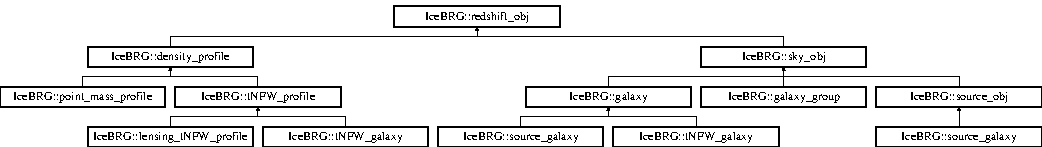
\includegraphics[height=1.975309cm]{classIceBRG_1_1redshift__obj}
\end{center}
\end{figure}
\subsection*{Public Member Functions}
\begin{DoxyCompactItemize}
\item 
\hyperlink{classIceBRG_1_1redshift__obj_a6b280539389ede3e7d511934bb4ef46d}{redshift\+\_\+obj} (const \hyperlink{lib_2IceBRG__main_2common_8h_ad0f130a56eeb944d9ef2692ee881ecc4}{flt\+\_\+type} \&init\+\_\+z=0, const \hyperlink{lib_2IceBRG__main_2common_8h_ad0f130a56eeb944d9ef2692ee881ecc4}{flt\+\_\+type} \&init\+\_\+z\+\_\+err=0)
\item 
virtual \hyperlink{classIceBRG_1_1redshift__obj_ae6bc5518532abb0e99b47ba4c722b5e3}{$\sim$redshift\+\_\+obj} ()
\item 
virtual void \hyperlink{classIceBRG_1_1redshift__obj_a0c048c6fd1c2dc08138a6352e424ad05}{set\+\_\+z} (const \hyperlink{lib_2IceBRG__main_2common_8h_ad0f130a56eeb944d9ef2692ee881ecc4}{flt\+\_\+type} \&new\+\_\+z)
\item 
virtual void \hyperlink{classIceBRG_1_1redshift__obj_ad22765859fcc9b5685f5ec86c0c002ca}{set\+\_\+z\+\_\+err} (const \hyperlink{lib_2IceBRG__main_2common_8h_ad0f130a56eeb944d9ef2692ee881ecc4}{flt\+\_\+type} \&new\+\_\+z\+\_\+err)
\item 
\hyperlink{lib_2IceBRG__main_2common_8h_ad0f130a56eeb944d9ef2692ee881ecc4}{flt\+\_\+type} \hyperlink{classIceBRG_1_1redshift__obj_a74692af753d1a101e5d170a1071ac7f4}{z} () const 
\item 
\hyperlink{lib_2IceBRG__main_2common_8h_ad0f130a56eeb944d9ef2692ee881ecc4}{flt\+\_\+type} \hyperlink{classIceBRG_1_1redshift__obj_a1d8b387d6e1f8946074af9aad7142898}{z\+\_\+err} () const 
\item 
\hyperlink{lib_2IceBRG__main_2common_8h_ac4de9d9335536ac22821171deec8d39e}{int\+\_\+type} \hyperlink{classIceBRG_1_1redshift__obj_afae560feff72a1363ed251a3eb117de5}{z\+\_\+grid} () const 
\item 
\hyperlink{namespaceIceBRG_a92c76f9b2ac706653b9b12c36904712c}{inverse\+\_\+time\+\_\+type} \hyperlink{classIceBRG_1_1redshift__obj_aefe5f94139abc4a5e2c8c7f2d4cabbb3}{H} () const 
\item 
\hyperlink{namespaceIceBRG_a9f5e5cdd641bb4c06f7305dfb5ae0238}{density\+\_\+type} \hyperlink{classIceBRG_1_1redshift__obj_ad865923687a27aa4b66e9fe728b0964d}{rho\+\_\+crit} () const 
\item 
virtual \hyperlink{classIceBRG_1_1redshift__obj}{redshift\+\_\+obj} $\ast$ \hyperlink{classIceBRG_1_1redshift__obj_a02f96529ff7f42ae64ae832712930e3b}{redshift\+\_\+obj\+\_\+clone} () const 
\end{DoxyCompactItemize}


\subsection{Detailed Description}
Class Definitions 

\subsection{Constructor \& Destructor Documentation}
\hypertarget{classIceBRG_1_1redshift__obj_a6b280539389ede3e7d511934bb4ef46d}{}\index{Ice\+B\+R\+G\+::redshift\+\_\+obj@{Ice\+B\+R\+G\+::redshift\+\_\+obj}!redshift\+\_\+obj@{redshift\+\_\+obj}}
\index{redshift\+\_\+obj@{redshift\+\_\+obj}!Ice\+B\+R\+G\+::redshift\+\_\+obj@{Ice\+B\+R\+G\+::redshift\+\_\+obj}}
\subsubsection[{redshift\+\_\+obj(const flt\+\_\+type \&init\+\_\+z=0, const flt\+\_\+type \&init\+\_\+z\+\_\+err=0)}]{\setlength{\rightskip}{0pt plus 5cm}Ice\+B\+R\+G\+::redshift\+\_\+obj\+::redshift\+\_\+obj (
\begin{DoxyParamCaption}
\item[{const {\bf flt\+\_\+type} \&}]{init\+\_\+z = {\ttfamily 0}, }
\item[{const {\bf flt\+\_\+type} \&}]{init\+\_\+z\+\_\+err = {\ttfamily 0}}
\end{DoxyParamCaption}
)\hspace{0.3cm}{\ttfamily [inline]}}\label{classIceBRG_1_1redshift__obj_a6b280539389ede3e7d511934bb4ef46d}
\hypertarget{classIceBRG_1_1redshift__obj_ae6bc5518532abb0e99b47ba4c722b5e3}{}\index{Ice\+B\+R\+G\+::redshift\+\_\+obj@{Ice\+B\+R\+G\+::redshift\+\_\+obj}!````~redshift\+\_\+obj@{$\sim$redshift\+\_\+obj}}
\index{````~redshift\+\_\+obj@{$\sim$redshift\+\_\+obj}!Ice\+B\+R\+G\+::redshift\+\_\+obj@{Ice\+B\+R\+G\+::redshift\+\_\+obj}}
\subsubsection[{$\sim$redshift\+\_\+obj()}]{\setlength{\rightskip}{0pt plus 5cm}virtual Ice\+B\+R\+G\+::redshift\+\_\+obj\+::$\sim$redshift\+\_\+obj (
\begin{DoxyParamCaption}
{}
\end{DoxyParamCaption}
)\hspace{0.3cm}{\ttfamily [inline]}, {\ttfamily [virtual]}}\label{classIceBRG_1_1redshift__obj_ae6bc5518532abb0e99b47ba4c722b5e3}


\subsection{Member Function Documentation}
\hypertarget{classIceBRG_1_1redshift__obj_aefe5f94139abc4a5e2c8c7f2d4cabbb3}{}\index{Ice\+B\+R\+G\+::redshift\+\_\+obj@{Ice\+B\+R\+G\+::redshift\+\_\+obj}!H@{H}}
\index{H@{H}!Ice\+B\+R\+G\+::redshift\+\_\+obj@{Ice\+B\+R\+G\+::redshift\+\_\+obj}}
\subsubsection[{H() const }]{\setlength{\rightskip}{0pt plus 5cm}{\bf Ice\+B\+R\+G\+::inverse\+\_\+time\+\_\+type} Ice\+B\+R\+G\+::redshift\+\_\+obj\+::\+H (
\begin{DoxyParamCaption}
{}
\end{DoxyParamCaption}
) const}\label{classIceBRG_1_1redshift__obj_aefe5f94139abc4a5e2c8c7f2d4cabbb3}
\hypertarget{classIceBRG_1_1redshift__obj_a02f96529ff7f42ae64ae832712930e3b}{}\index{Ice\+B\+R\+G\+::redshift\+\_\+obj@{Ice\+B\+R\+G\+::redshift\+\_\+obj}!redshift\+\_\+obj\+\_\+clone@{redshift\+\_\+obj\+\_\+clone}}
\index{redshift\+\_\+obj\+\_\+clone@{redshift\+\_\+obj\+\_\+clone}!Ice\+B\+R\+G\+::redshift\+\_\+obj@{Ice\+B\+R\+G\+::redshift\+\_\+obj}}
\subsubsection[{redshift\+\_\+obj\+\_\+clone() const }]{\setlength{\rightskip}{0pt plus 5cm}virtual {\bf redshift\+\_\+obj}$\ast$ Ice\+B\+R\+G\+::redshift\+\_\+obj\+::redshift\+\_\+obj\+\_\+clone (
\begin{DoxyParamCaption}
{}
\end{DoxyParamCaption}
) const\hspace{0.3cm}{\ttfamily [inline]}, {\ttfamily [virtual]}}\label{classIceBRG_1_1redshift__obj_a02f96529ff7f42ae64ae832712930e3b}


Reimplemented in \hyperlink{classIceBRG_1_1tNFW__profile_ad7e0649c9782b10fc05cd7a24d43d325}{Ice\+B\+R\+G\+::t\+N\+F\+W\+\_\+profile}, \hyperlink{classIceBRG_1_1sky__obj_a6efa97b5c6edb6c4ea741b06338ff5bc}{Ice\+B\+R\+G\+::sky\+\_\+obj}, \hyperlink{classIceBRG_1_1point__mass__profile_a652993749492f4c718b77386ea3ba7af}{Ice\+B\+R\+G\+::point\+\_\+mass\+\_\+profile}, \hyperlink{classIceBRG_1_1galaxy_a0874bd3cb3133f244a86d6101aa1ec65}{Ice\+B\+R\+G\+::galaxy}, \hyperlink{classIceBRG_1_1galaxy__group_af0ee2e7b336371e8a8f098c3bfe7372d}{Ice\+B\+R\+G\+::galaxy\+\_\+group}, \hyperlink{classIceBRG_1_1source__galaxy_a59d08611112a2118f49ce569271524e7}{Ice\+B\+R\+G\+::source\+\_\+galaxy}, and \hyperlink{classIceBRG_1_1tNFW__galaxy_a0ac2852b6fad29184222f58e18aff3b3}{Ice\+B\+R\+G\+::t\+N\+F\+W\+\_\+galaxy}.

\hypertarget{classIceBRG_1_1redshift__obj_ad865923687a27aa4b66e9fe728b0964d}{}\index{Ice\+B\+R\+G\+::redshift\+\_\+obj@{Ice\+B\+R\+G\+::redshift\+\_\+obj}!rho\+\_\+crit@{rho\+\_\+crit}}
\index{rho\+\_\+crit@{rho\+\_\+crit}!Ice\+B\+R\+G\+::redshift\+\_\+obj@{Ice\+B\+R\+G\+::redshift\+\_\+obj}}
\subsubsection[{rho\+\_\+crit() const }]{\setlength{\rightskip}{0pt plus 5cm}{\bf Ice\+B\+R\+G\+::density\+\_\+type} Ice\+B\+R\+G\+::redshift\+\_\+obj\+::rho\+\_\+crit (
\begin{DoxyParamCaption}
{}
\end{DoxyParamCaption}
) const}\label{classIceBRG_1_1redshift__obj_ad865923687a27aa4b66e9fe728b0964d}
\hypertarget{classIceBRG_1_1redshift__obj_a0c048c6fd1c2dc08138a6352e424ad05}{}\index{Ice\+B\+R\+G\+::redshift\+\_\+obj@{Ice\+B\+R\+G\+::redshift\+\_\+obj}!set\+\_\+z@{set\+\_\+z}}
\index{set\+\_\+z@{set\+\_\+z}!Ice\+B\+R\+G\+::redshift\+\_\+obj@{Ice\+B\+R\+G\+::redshift\+\_\+obj}}
\subsubsection[{set\+\_\+z(const flt\+\_\+type \&new\+\_\+z)}]{\setlength{\rightskip}{0pt plus 5cm}virtual void Ice\+B\+R\+G\+::redshift\+\_\+obj\+::set\+\_\+z (
\begin{DoxyParamCaption}
\item[{const {\bf flt\+\_\+type} \&}]{new\+\_\+z}
\end{DoxyParamCaption}
)\hspace{0.3cm}{\ttfamily [inline]}, {\ttfamily [virtual]}}\label{classIceBRG_1_1redshift__obj_a0c048c6fd1c2dc08138a6352e424ad05}


Reimplemented in \hyperlink{classIceBRG_1_1tNFW__profile_a4bfeb583dee286c98a14b826f912684a}{Ice\+B\+R\+G\+::t\+N\+F\+W\+\_\+profile}.

\hypertarget{classIceBRG_1_1redshift__obj_ad22765859fcc9b5685f5ec86c0c002ca}{}\index{Ice\+B\+R\+G\+::redshift\+\_\+obj@{Ice\+B\+R\+G\+::redshift\+\_\+obj}!set\+\_\+z\+\_\+err@{set\+\_\+z\+\_\+err}}
\index{set\+\_\+z\+\_\+err@{set\+\_\+z\+\_\+err}!Ice\+B\+R\+G\+::redshift\+\_\+obj@{Ice\+B\+R\+G\+::redshift\+\_\+obj}}
\subsubsection[{set\+\_\+z\+\_\+err(const flt\+\_\+type \&new\+\_\+z\+\_\+err)}]{\setlength{\rightskip}{0pt plus 5cm}virtual void Ice\+B\+R\+G\+::redshift\+\_\+obj\+::set\+\_\+z\+\_\+err (
\begin{DoxyParamCaption}
\item[{const {\bf flt\+\_\+type} \&}]{new\+\_\+z\+\_\+err}
\end{DoxyParamCaption}
)\hspace{0.3cm}{\ttfamily [inline]}, {\ttfamily [virtual]}}\label{classIceBRG_1_1redshift__obj_ad22765859fcc9b5685f5ec86c0c002ca}
\hypertarget{classIceBRG_1_1redshift__obj_a74692af753d1a101e5d170a1071ac7f4}{}\index{Ice\+B\+R\+G\+::redshift\+\_\+obj@{Ice\+B\+R\+G\+::redshift\+\_\+obj}!z@{z}}
\index{z@{z}!Ice\+B\+R\+G\+::redshift\+\_\+obj@{Ice\+B\+R\+G\+::redshift\+\_\+obj}}
\subsubsection[{z() const }]{\setlength{\rightskip}{0pt plus 5cm}{\bf flt\+\_\+type} Ice\+B\+R\+G\+::redshift\+\_\+obj\+::z (
\begin{DoxyParamCaption}
{}
\end{DoxyParamCaption}
) const\hspace{0.3cm}{\ttfamily [inline]}}\label{classIceBRG_1_1redshift__obj_a74692af753d1a101e5d170a1071ac7f4}
\hypertarget{classIceBRG_1_1redshift__obj_a1d8b387d6e1f8946074af9aad7142898}{}\index{Ice\+B\+R\+G\+::redshift\+\_\+obj@{Ice\+B\+R\+G\+::redshift\+\_\+obj}!z\+\_\+err@{z\+\_\+err}}
\index{z\+\_\+err@{z\+\_\+err}!Ice\+B\+R\+G\+::redshift\+\_\+obj@{Ice\+B\+R\+G\+::redshift\+\_\+obj}}
\subsubsection[{z\+\_\+err() const }]{\setlength{\rightskip}{0pt plus 5cm}{\bf flt\+\_\+type} Ice\+B\+R\+G\+::redshift\+\_\+obj\+::z\+\_\+err (
\begin{DoxyParamCaption}
{}
\end{DoxyParamCaption}
) const\hspace{0.3cm}{\ttfamily [inline]}}\label{classIceBRG_1_1redshift__obj_a1d8b387d6e1f8946074af9aad7142898}
\hypertarget{classIceBRG_1_1redshift__obj_afae560feff72a1363ed251a3eb117de5}{}\index{Ice\+B\+R\+G\+::redshift\+\_\+obj@{Ice\+B\+R\+G\+::redshift\+\_\+obj}!z\+\_\+grid@{z\+\_\+grid}}
\index{z\+\_\+grid@{z\+\_\+grid}!Ice\+B\+R\+G\+::redshift\+\_\+obj@{Ice\+B\+R\+G\+::redshift\+\_\+obj}}
\subsubsection[{z\+\_\+grid() const }]{\setlength{\rightskip}{0pt plus 5cm}{\bf int\+\_\+type} Ice\+B\+R\+G\+::redshift\+\_\+obj\+::z\+\_\+grid (
\begin{DoxyParamCaption}
{}
\end{DoxyParamCaption}
) const}\label{classIceBRG_1_1redshift__obj_afae560feff72a1363ed251a3eb117de5}


The documentation for this class was generated from the following files\+:\begin{DoxyCompactItemize}
\item 
/disk2/brg/git/\+Magnification\+\_\+\+Public/src/lib/\+Ice\+B\+R\+G\+\_\+physics/\hyperlink{astro_8h}{astro.\+h}\item 
/disk2/brg/git/\+Magnification\+\_\+\+Public/src/lib/\+Ice\+B\+R\+G\+\_\+physics/\hyperlink{astro_8cpp}{astro.\+cpp}\end{DoxyCompactItemize}

\hypertarget{classIceBRG_1_1Schechter__like__functor}{}\section{Ice\+B\+R\+G\+:\+:Schechter\+\_\+like\+\_\+functor Class Reference}
\label{classIceBRG_1_1Schechter__like__functor}\index{Ice\+B\+R\+G\+::\+Schechter\+\_\+like\+\_\+functor@{Ice\+B\+R\+G\+::\+Schechter\+\_\+like\+\_\+functor}}


{\ttfamily \#include $<$Schechter\+\_\+like\+\_\+functor.\+h$>$}

Inheritance diagram for Ice\+B\+R\+G\+:\+:Schechter\+\_\+like\+\_\+functor\+:\begin{figure}[H]
\begin{center}
\leavevmode
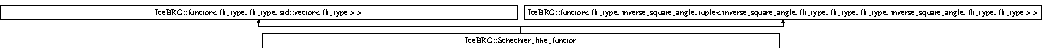
\includegraphics[height=0.639269cm]{classIceBRG_1_1Schechter__like__functor}
\end{center}
\end{figure}
\subsection*{Public Types}
\begin{DoxyCompactItemize}
\item 
typedef \hyperlink{lib_2IceBRG__main_2common_8h_ad0f130a56eeb944d9ef2692ee881ecc4}{flt\+\_\+type} \hyperlink{classIceBRG_1_1Schechter__like__functor_aa444797b63bb4d4b01859b9c6a5d528e}{fin\+\_\+type}
\item 
typedef \hyperlink{namespaceIceBRG_a26efaff9c9adf346c7d09d0b714731f6}{inverse\+\_\+square\+\_\+angle} \hyperlink{classIceBRG_1_1Schechter__like__functor_a90c760c2efcd3ae2b3a7f733672b18ed}{fout\+\_\+type}
\item 
typedef \hyperlink{namespaceIceBRG_a5148ef56bdd96f27ce60555b6aaa979e}{tuple}$<$ \hyperlink{namespaceIceBRG_a26efaff9c9adf346c7d09d0b714731f6}{inverse\+\_\+square\+\_\+angle}, \hyperlink{lib_2IceBRG__main_2common_8h_ad0f130a56eeb944d9ef2692ee881ecc4}{flt\+\_\+type}, \hyperlink{lib_2IceBRG__main_2common_8h_ad0f130a56eeb944d9ef2692ee881ecc4}{flt\+\_\+type}, \hyperlink{lib_2IceBRG__main_2common_8h_ad0f130a56eeb944d9ef2692ee881ecc4}{flt\+\_\+type}, \hyperlink{namespaceIceBRG_a26efaff9c9adf346c7d09d0b714731f6}{inverse\+\_\+square\+\_\+angle}, \hyperlink{lib_2IceBRG__main_2common_8h_ad0f130a56eeb944d9ef2692ee881ecc4}{flt\+\_\+type}, \hyperlink{lib_2IceBRG__main_2common_8h_ad0f130a56eeb944d9ef2692ee881ecc4}{flt\+\_\+type} $>$ \hyperlink{classIceBRG_1_1Schechter__like__functor_a5a7c7522b680f34ea2004184ffd099f7}{params\+\_\+type}
\item 
typedef \hyperlink{classIceBRG_1_1functor}{functor}$<$ \hyperlink{lib_2IceBRG__main_2common_8h_ad0f130a56eeb944d9ef2692ee881ecc4}{flt\+\_\+type}, \hyperlink{namespaceIceBRG_a26efaff9c9adf346c7d09d0b714731f6}{inverse\+\_\+square\+\_\+angle}, \hyperlink{classIceBRG_1_1Schechter__like__functor_a5a7c7522b680f34ea2004184ffd099f7}{params\+\_\+type} $>$ \hyperlink{classIceBRG_1_1Schechter__like__functor_a919adc2367dc8f3b9939f3ae87d14315}{base\+\_\+type}
\end{DoxyCompactItemize}
\subsection*{Public Member Functions}
\begin{DoxyCompactItemize}
\item 
\hyperlink{classIceBRG_1_1Schechter__like__functor_a98942cf327953bc6de8cdd53fde65ef7}{Schechter\+\_\+like\+\_\+functor} ()
\item 
{\footnotesize template$<$typename T $>$ }\\\hyperlink{classIceBRG_1_1Schechter__like__functor_a351e38eaf242da441ca220369def0bc6}{Schechter\+\_\+like\+\_\+functor} (T \&\&init\+\_\+params)
\item 
virtual \hyperlink{classIceBRG_1_1Schechter__like__functor_aaf1a25297a4e050deab517c7e1edebfb}{$\sim$\+Schechter\+\_\+like\+\_\+functor} ()
\item 
\hyperlink{namespaceIceBRG_a26efaff9c9adf346c7d09d0b714731f6}{inverse\+\_\+square\+\_\+angle} \hyperlink{classIceBRG_1_1Schechter__like__functor_a1c867a8a96d360d3b1da7c122f9f96a3}{N\+\_\+scale} () const 
\item 
\hyperlink{lib_2IceBRG__main_2common_8h_ad0f130a56eeb944d9ef2692ee881ecc4}{flt\+\_\+type} \hyperlink{classIceBRG_1_1Schechter__like__functor_a80a81ec7dcad32167672eec726bbca00}{m\+\_\+star} () const 
\item 
\hyperlink{lib_2IceBRG__main_2common_8h_ad0f130a56eeb944d9ef2692ee881ecc4}{flt\+\_\+type} \hyperlink{classIceBRG_1_1Schechter__like__functor_afb0660168ea5cc0462369c0559a4654c}{alpha} () const 
\item 
\hyperlink{lib_2IceBRG__main_2common_8h_ad0f130a56eeb944d9ef2692ee881ecc4}{flt\+\_\+type} \hyperlink{classIceBRG_1_1Schechter__like__functor_a36c03d8a6b0bacc3f6fbc60cf828ca7a}{mag\+\_\+lower\+\_\+lim\+\_\+sharpness} () const 
\item 
\hyperlink{namespaceIceBRG_a26efaff9c9adf346c7d09d0b714731f6}{inverse\+\_\+square\+\_\+angle} \hyperlink{classIceBRG_1_1Schechter__like__functor_a5ec784331b2eeb1a1d6077e6cc691e82}{mag23\+\_\+jump} () const 
\item 
\hyperlink{lib_2IceBRG__main_2common_8h_ad0f130a56eeb944d9ef2692ee881ecc4}{flt\+\_\+type} \hyperlink{classIceBRG_1_1Schechter__like__functor_ad51153efefe230a196400a72f6b98510}{mag\+\_\+upper\+\_\+lim} () const 
\item 
\hyperlink{lib_2IceBRG__main_2common_8h_ad0f130a56eeb944d9ef2692ee881ecc4}{flt\+\_\+type} \hyperlink{classIceBRG_1_1Schechter__like__functor_a977c88ecf83ce6116b33698d80d7b99a}{mag\+\_\+upper\+\_\+lim\+\_\+sharpness} () const 
\item 
\hyperlink{classIceBRG_1_1Schechter__like__functor_a90c760c2efcd3ae2b3a7f733672b18ed}{fout\+\_\+type} \hyperlink{classIceBRG_1_1Schechter__like__functor_af58cca1d9091086949437f9c07e1f8f9}{operator()} (const \hyperlink{classIceBRG_1_1Schechter__like__functor_aa444797b63bb4d4b01859b9c6a5d528e}{fin\+\_\+type} \&in\+\_\+params) const 
\item 
\hyperlink{classIceBRG_1_1Schechter__like__functor_a98942cf327953bc6de8cdd53fde65ef7}{Schechter\+\_\+like\+\_\+functor} ()
\item 
\hyperlink{classIceBRG_1_1Schechter__like__functor_a7541884f43f2cf37783e2abb84dc6347}{Schechter\+\_\+like\+\_\+functor} (const std\+::vector$<$ \hyperlink{lib_2IceBRG__main_2common_8h_ad0f130a56eeb944d9ef2692ee881ecc4}{flt\+\_\+type} $>$ \&init\+\_\+params)
\item 
virtual \hyperlink{classIceBRG_1_1Schechter__like__functor_aaf1a25297a4e050deab517c7e1edebfb}{$\sim$\+Schechter\+\_\+like\+\_\+functor} ()
\item 
\hyperlink{lib_2IceBRG__main_2common_8h_a7040956e7e1b504d34a9ccfb4253bdce}{long\+\_\+flt\+\_\+type} \hyperlink{classIceBRG_1_1Schechter__like__functor_a1d3bc3f012974c5e771113c611dfc8a8}{N\+\_\+scale} () const 
\item 
\hyperlink{lib_2IceBRG__main_2common_8h_a7040956e7e1b504d34a9ccfb4253bdce}{long\+\_\+flt\+\_\+type} \hyperlink{classIceBRG_1_1Schechter__like__functor_a2166028d7e17a3a97a397e8b95cda94f}{m\+\_\+star} () const 
\item 
\hyperlink{lib_2IceBRG__main_2common_8h_a7040956e7e1b504d34a9ccfb4253bdce}{long\+\_\+flt\+\_\+type} \hyperlink{classIceBRG_1_1Schechter__like__functor_a7f576357e46eed8edcf30e7950ebaaac}{alpha} () const 
\item 
\hyperlink{lib_2IceBRG__main_2common_8h_a7040956e7e1b504d34a9ccfb4253bdce}{long\+\_\+flt\+\_\+type} \hyperlink{classIceBRG_1_1Schechter__like__functor_a61505822b606261f916582fe719f5208}{mag\+\_\+lower\+\_\+lim\+\_\+sharpness} () const 
\item 
\hyperlink{lib_2IceBRG__main_2common_8h_a7040956e7e1b504d34a9ccfb4253bdce}{long\+\_\+flt\+\_\+type} \hyperlink{classIceBRG_1_1Schechter__like__functor_a562f01c56a7652050f5e501384ae7dbc}{mag23\+\_\+jump} () const 
\item 
\hyperlink{lib_2IceBRG__main_2common_8h_a7040956e7e1b504d34a9ccfb4253bdce}{long\+\_\+flt\+\_\+type} \hyperlink{classIceBRG_1_1Schechter__like__functor_adf075005214a553d0a7ed0b4ad112487}{mag\+\_\+upper\+\_\+lim} () const 
\item 
\hyperlink{lib_2IceBRG__main_2common_8h_a7040956e7e1b504d34a9ccfb4253bdce}{long\+\_\+flt\+\_\+type} \hyperlink{classIceBRG_1_1Schechter__like__functor_a9067e3ec4ebd3df8ee873f729334e7ad}{mag\+\_\+upper\+\_\+lim\+\_\+sharpness} () const 
\item 
\hyperlink{lib_2IceBRG__main_2common_8h_a7040956e7e1b504d34a9ccfb4253bdce}{long\+\_\+flt\+\_\+type} \hyperlink{classIceBRG_1_1Schechter__like__functor_a969b8cbbbb6cc12cf666d3a1e3a3dd74}{operator()} (const \hyperlink{lib_2IceBRG__main_2common_8h_a7040956e7e1b504d34a9ccfb4253bdce}{long\+\_\+flt\+\_\+type} \&in\+\_\+params) const 
\end{DoxyCompactItemize}


\subsection{Member Typedef Documentation}
\hypertarget{classIceBRG_1_1Schechter__like__functor_a919adc2367dc8f3b9939f3ae87d14315}{}\index{Ice\+B\+R\+G\+::\+Schechter\+\_\+like\+\_\+functor@{Ice\+B\+R\+G\+::\+Schechter\+\_\+like\+\_\+functor}!base\+\_\+type@{base\+\_\+type}}
\index{base\+\_\+type@{base\+\_\+type}!Ice\+B\+R\+G\+::\+Schechter\+\_\+like\+\_\+functor@{Ice\+B\+R\+G\+::\+Schechter\+\_\+like\+\_\+functor}}
\subsubsection[{base\+\_\+type}]{\setlength{\rightskip}{0pt plus 5cm}typedef {\bf functor}$<${\bf flt\+\_\+type}, {\bf inverse\+\_\+square\+\_\+angle}, {\bf params\+\_\+type}$>$ {\bf Ice\+B\+R\+G\+::\+Schechter\+\_\+like\+\_\+functor\+::base\+\_\+type}}\label{classIceBRG_1_1Schechter__like__functor_a919adc2367dc8f3b9939f3ae87d14315}
\hypertarget{classIceBRG_1_1Schechter__like__functor_aa444797b63bb4d4b01859b9c6a5d528e}{}\index{Ice\+B\+R\+G\+::\+Schechter\+\_\+like\+\_\+functor@{Ice\+B\+R\+G\+::\+Schechter\+\_\+like\+\_\+functor}!fin\+\_\+type@{fin\+\_\+type}}
\index{fin\+\_\+type@{fin\+\_\+type}!Ice\+B\+R\+G\+::\+Schechter\+\_\+like\+\_\+functor@{Ice\+B\+R\+G\+::\+Schechter\+\_\+like\+\_\+functor}}
\subsubsection[{fin\+\_\+type}]{\setlength{\rightskip}{0pt plus 5cm}typedef {\bf flt\+\_\+type} {\bf Ice\+B\+R\+G\+::\+Schechter\+\_\+like\+\_\+functor\+::fin\+\_\+type}}\label{classIceBRG_1_1Schechter__like__functor_aa444797b63bb4d4b01859b9c6a5d528e}
\hypertarget{classIceBRG_1_1Schechter__like__functor_a90c760c2efcd3ae2b3a7f733672b18ed}{}\index{Ice\+B\+R\+G\+::\+Schechter\+\_\+like\+\_\+functor@{Ice\+B\+R\+G\+::\+Schechter\+\_\+like\+\_\+functor}!fout\+\_\+type@{fout\+\_\+type}}
\index{fout\+\_\+type@{fout\+\_\+type}!Ice\+B\+R\+G\+::\+Schechter\+\_\+like\+\_\+functor@{Ice\+B\+R\+G\+::\+Schechter\+\_\+like\+\_\+functor}}
\subsubsection[{fout\+\_\+type}]{\setlength{\rightskip}{0pt plus 5cm}typedef {\bf inverse\+\_\+square\+\_\+angle} {\bf Ice\+B\+R\+G\+::\+Schechter\+\_\+like\+\_\+functor\+::fout\+\_\+type}}\label{classIceBRG_1_1Schechter__like__functor_a90c760c2efcd3ae2b3a7f733672b18ed}
\hypertarget{classIceBRG_1_1Schechter__like__functor_a5a7c7522b680f34ea2004184ffd099f7}{}\index{Ice\+B\+R\+G\+::\+Schechter\+\_\+like\+\_\+functor@{Ice\+B\+R\+G\+::\+Schechter\+\_\+like\+\_\+functor}!params\+\_\+type@{params\+\_\+type}}
\index{params\+\_\+type@{params\+\_\+type}!Ice\+B\+R\+G\+::\+Schechter\+\_\+like\+\_\+functor@{Ice\+B\+R\+G\+::\+Schechter\+\_\+like\+\_\+functor}}
\subsubsection[{params\+\_\+type}]{\setlength{\rightskip}{0pt plus 5cm}typedef {\bf tuple}$<${\bf inverse\+\_\+square\+\_\+angle},{\bf flt\+\_\+type},{\bf flt\+\_\+type},{\bf flt\+\_\+type}, {\bf inverse\+\_\+square\+\_\+angle},{\bf flt\+\_\+type},{\bf flt\+\_\+type}$>$ {\bf Ice\+B\+R\+G\+::\+Schechter\+\_\+like\+\_\+functor\+::params\+\_\+type}}\label{classIceBRG_1_1Schechter__like__functor_a5a7c7522b680f34ea2004184ffd099f7}


\subsection{Constructor \& Destructor Documentation}
\hypertarget{classIceBRG_1_1Schechter__like__functor_a98942cf327953bc6de8cdd53fde65ef7}{}\index{Ice\+B\+R\+G\+::\+Schechter\+\_\+like\+\_\+functor@{Ice\+B\+R\+G\+::\+Schechter\+\_\+like\+\_\+functor}!Schechter\+\_\+like\+\_\+functor@{Schechter\+\_\+like\+\_\+functor}}
\index{Schechter\+\_\+like\+\_\+functor@{Schechter\+\_\+like\+\_\+functor}!Ice\+B\+R\+G\+::\+Schechter\+\_\+like\+\_\+functor@{Ice\+B\+R\+G\+::\+Schechter\+\_\+like\+\_\+functor}}
\subsubsection[{Schechter\+\_\+like\+\_\+functor()}]{\setlength{\rightskip}{0pt plus 5cm}Ice\+B\+R\+G\+::\+Schechter\+\_\+like\+\_\+functor\+::\+Schechter\+\_\+like\+\_\+functor (
\begin{DoxyParamCaption}
{}
\end{DoxyParamCaption}
)\hspace{0.3cm}{\ttfamily [inline]}}\label{classIceBRG_1_1Schechter__like__functor_a98942cf327953bc6de8cdd53fde65ef7}
\hypertarget{classIceBRG_1_1Schechter__like__functor_a351e38eaf242da441ca220369def0bc6}{}\index{Ice\+B\+R\+G\+::\+Schechter\+\_\+like\+\_\+functor@{Ice\+B\+R\+G\+::\+Schechter\+\_\+like\+\_\+functor}!Schechter\+\_\+like\+\_\+functor@{Schechter\+\_\+like\+\_\+functor}}
\index{Schechter\+\_\+like\+\_\+functor@{Schechter\+\_\+like\+\_\+functor}!Ice\+B\+R\+G\+::\+Schechter\+\_\+like\+\_\+functor@{Ice\+B\+R\+G\+::\+Schechter\+\_\+like\+\_\+functor}}
\subsubsection[{Schechter\+\_\+like\+\_\+functor(\+T \&\&init\+\_\+params)}]{\setlength{\rightskip}{0pt plus 5cm}template$<$typename T $>$ Ice\+B\+R\+G\+::\+Schechter\+\_\+like\+\_\+functor\+::\+Schechter\+\_\+like\+\_\+functor (
\begin{DoxyParamCaption}
\item[{T \&\&}]{init\+\_\+params}
\end{DoxyParamCaption}
)\hspace{0.3cm}{\ttfamily [inline]}}\label{classIceBRG_1_1Schechter__like__functor_a351e38eaf242da441ca220369def0bc6}
\hypertarget{classIceBRG_1_1Schechter__like__functor_aaf1a25297a4e050deab517c7e1edebfb}{}\index{Ice\+B\+R\+G\+::\+Schechter\+\_\+like\+\_\+functor@{Ice\+B\+R\+G\+::\+Schechter\+\_\+like\+\_\+functor}!````~Schechter\+\_\+like\+\_\+functor@{$\sim$\+Schechter\+\_\+like\+\_\+functor}}
\index{````~Schechter\+\_\+like\+\_\+functor@{$\sim$\+Schechter\+\_\+like\+\_\+functor}!Ice\+B\+R\+G\+::\+Schechter\+\_\+like\+\_\+functor@{Ice\+B\+R\+G\+::\+Schechter\+\_\+like\+\_\+functor}}
\subsubsection[{$\sim$\+Schechter\+\_\+like\+\_\+functor()}]{\setlength{\rightskip}{0pt plus 5cm}virtual Ice\+B\+R\+G\+::\+Schechter\+\_\+like\+\_\+functor\+::$\sim$\+Schechter\+\_\+like\+\_\+functor (
\begin{DoxyParamCaption}
{}
\end{DoxyParamCaption}
)\hspace{0.3cm}{\ttfamily [inline]}, {\ttfamily [virtual]}}\label{classIceBRG_1_1Schechter__like__functor_aaf1a25297a4e050deab517c7e1edebfb}
\hypertarget{classIceBRG_1_1Schechter__like__functor_a98942cf327953bc6de8cdd53fde65ef7}{}\index{Ice\+B\+R\+G\+::\+Schechter\+\_\+like\+\_\+functor@{Ice\+B\+R\+G\+::\+Schechter\+\_\+like\+\_\+functor}!Schechter\+\_\+like\+\_\+functor@{Schechter\+\_\+like\+\_\+functor}}
\index{Schechter\+\_\+like\+\_\+functor@{Schechter\+\_\+like\+\_\+functor}!Ice\+B\+R\+G\+::\+Schechter\+\_\+like\+\_\+functor@{Ice\+B\+R\+G\+::\+Schechter\+\_\+like\+\_\+functor}}
\subsubsection[{Schechter\+\_\+like\+\_\+functor()}]{\setlength{\rightskip}{0pt plus 5cm}Ice\+B\+R\+G\+::\+Schechter\+\_\+like\+\_\+functor\+::\+Schechter\+\_\+like\+\_\+functor (
\begin{DoxyParamCaption}
{}
\end{DoxyParamCaption}
)\hspace{0.3cm}{\ttfamily [inline]}}\label{classIceBRG_1_1Schechter__like__functor_a98942cf327953bc6de8cdd53fde65ef7}
\hypertarget{classIceBRG_1_1Schechter__like__functor_a7541884f43f2cf37783e2abb84dc6347}{}\index{Ice\+B\+R\+G\+::\+Schechter\+\_\+like\+\_\+functor@{Ice\+B\+R\+G\+::\+Schechter\+\_\+like\+\_\+functor}!Schechter\+\_\+like\+\_\+functor@{Schechter\+\_\+like\+\_\+functor}}
\index{Schechter\+\_\+like\+\_\+functor@{Schechter\+\_\+like\+\_\+functor}!Ice\+B\+R\+G\+::\+Schechter\+\_\+like\+\_\+functor@{Ice\+B\+R\+G\+::\+Schechter\+\_\+like\+\_\+functor}}
\subsubsection[{Schechter\+\_\+like\+\_\+functor(const std\+::vector$<$ flt\+\_\+type $>$ \&init\+\_\+params)}]{\setlength{\rightskip}{0pt plus 5cm}Ice\+B\+R\+G\+::\+Schechter\+\_\+like\+\_\+functor\+::\+Schechter\+\_\+like\+\_\+functor (
\begin{DoxyParamCaption}
\item[{const std\+::vector$<$ {\bf flt\+\_\+type} $>$ \&}]{init\+\_\+params}
\end{DoxyParamCaption}
)\hspace{0.3cm}{\ttfamily [inline]}}\label{classIceBRG_1_1Schechter__like__functor_a7541884f43f2cf37783e2abb84dc6347}
\hypertarget{classIceBRG_1_1Schechter__like__functor_aaf1a25297a4e050deab517c7e1edebfb}{}\index{Ice\+B\+R\+G\+::\+Schechter\+\_\+like\+\_\+functor@{Ice\+B\+R\+G\+::\+Schechter\+\_\+like\+\_\+functor}!````~Schechter\+\_\+like\+\_\+functor@{$\sim$\+Schechter\+\_\+like\+\_\+functor}}
\index{````~Schechter\+\_\+like\+\_\+functor@{$\sim$\+Schechter\+\_\+like\+\_\+functor}!Ice\+B\+R\+G\+::\+Schechter\+\_\+like\+\_\+functor@{Ice\+B\+R\+G\+::\+Schechter\+\_\+like\+\_\+functor}}
\subsubsection[{$\sim$\+Schechter\+\_\+like\+\_\+functor()}]{\setlength{\rightskip}{0pt plus 5cm}virtual Ice\+B\+R\+G\+::\+Schechter\+\_\+like\+\_\+functor\+::$\sim$\+Schechter\+\_\+like\+\_\+functor (
\begin{DoxyParamCaption}
{}
\end{DoxyParamCaption}
)\hspace{0.3cm}{\ttfamily [inline]}, {\ttfamily [virtual]}}\label{classIceBRG_1_1Schechter__like__functor_aaf1a25297a4e050deab517c7e1edebfb}


\subsection{Member Function Documentation}
\hypertarget{classIceBRG_1_1Schechter__like__functor_a7f576357e46eed8edcf30e7950ebaaac}{}\index{Ice\+B\+R\+G\+::\+Schechter\+\_\+like\+\_\+functor@{Ice\+B\+R\+G\+::\+Schechter\+\_\+like\+\_\+functor}!alpha@{alpha}}
\index{alpha@{alpha}!Ice\+B\+R\+G\+::\+Schechter\+\_\+like\+\_\+functor@{Ice\+B\+R\+G\+::\+Schechter\+\_\+like\+\_\+functor}}
\subsubsection[{alpha() const }]{\setlength{\rightskip}{0pt plus 5cm}{\bf long\+\_\+flt\+\_\+type} Ice\+B\+R\+G\+::\+Schechter\+\_\+like\+\_\+functor\+::alpha (
\begin{DoxyParamCaption}
{}
\end{DoxyParamCaption}
) const\hspace{0.3cm}{\ttfamily [inline]}}\label{classIceBRG_1_1Schechter__like__functor_a7f576357e46eed8edcf30e7950ebaaac}
\hypertarget{classIceBRG_1_1Schechter__like__functor_afb0660168ea5cc0462369c0559a4654c}{}\index{Ice\+B\+R\+G\+::\+Schechter\+\_\+like\+\_\+functor@{Ice\+B\+R\+G\+::\+Schechter\+\_\+like\+\_\+functor}!alpha@{alpha}}
\index{alpha@{alpha}!Ice\+B\+R\+G\+::\+Schechter\+\_\+like\+\_\+functor@{Ice\+B\+R\+G\+::\+Schechter\+\_\+like\+\_\+functor}}
\subsubsection[{alpha() const }]{\setlength{\rightskip}{0pt plus 5cm}{\bf flt\+\_\+type} Ice\+B\+R\+G\+::\+Schechter\+\_\+like\+\_\+functor\+::alpha (
\begin{DoxyParamCaption}
{}
\end{DoxyParamCaption}
) const\hspace{0.3cm}{\ttfamily [inline]}}\label{classIceBRG_1_1Schechter__like__functor_afb0660168ea5cc0462369c0559a4654c}
\hypertarget{classIceBRG_1_1Schechter__like__functor_a2166028d7e17a3a97a397e8b95cda94f}{}\index{Ice\+B\+R\+G\+::\+Schechter\+\_\+like\+\_\+functor@{Ice\+B\+R\+G\+::\+Schechter\+\_\+like\+\_\+functor}!m\+\_\+star@{m\+\_\+star}}
\index{m\+\_\+star@{m\+\_\+star}!Ice\+B\+R\+G\+::\+Schechter\+\_\+like\+\_\+functor@{Ice\+B\+R\+G\+::\+Schechter\+\_\+like\+\_\+functor}}
\subsubsection[{m\+\_\+star() const }]{\setlength{\rightskip}{0pt plus 5cm}{\bf long\+\_\+flt\+\_\+type} Ice\+B\+R\+G\+::\+Schechter\+\_\+like\+\_\+functor\+::m\+\_\+star (
\begin{DoxyParamCaption}
{}
\end{DoxyParamCaption}
) const\hspace{0.3cm}{\ttfamily [inline]}}\label{classIceBRG_1_1Schechter__like__functor_a2166028d7e17a3a97a397e8b95cda94f}
\hypertarget{classIceBRG_1_1Schechter__like__functor_a80a81ec7dcad32167672eec726bbca00}{}\index{Ice\+B\+R\+G\+::\+Schechter\+\_\+like\+\_\+functor@{Ice\+B\+R\+G\+::\+Schechter\+\_\+like\+\_\+functor}!m\+\_\+star@{m\+\_\+star}}
\index{m\+\_\+star@{m\+\_\+star}!Ice\+B\+R\+G\+::\+Schechter\+\_\+like\+\_\+functor@{Ice\+B\+R\+G\+::\+Schechter\+\_\+like\+\_\+functor}}
\subsubsection[{m\+\_\+star() const }]{\setlength{\rightskip}{0pt plus 5cm}{\bf flt\+\_\+type} Ice\+B\+R\+G\+::\+Schechter\+\_\+like\+\_\+functor\+::m\+\_\+star (
\begin{DoxyParamCaption}
{}
\end{DoxyParamCaption}
) const\hspace{0.3cm}{\ttfamily [inline]}}\label{classIceBRG_1_1Schechter__like__functor_a80a81ec7dcad32167672eec726bbca00}
\hypertarget{classIceBRG_1_1Schechter__like__functor_a562f01c56a7652050f5e501384ae7dbc}{}\index{Ice\+B\+R\+G\+::\+Schechter\+\_\+like\+\_\+functor@{Ice\+B\+R\+G\+::\+Schechter\+\_\+like\+\_\+functor}!mag23\+\_\+jump@{mag23\+\_\+jump}}
\index{mag23\+\_\+jump@{mag23\+\_\+jump}!Ice\+B\+R\+G\+::\+Schechter\+\_\+like\+\_\+functor@{Ice\+B\+R\+G\+::\+Schechter\+\_\+like\+\_\+functor}}
\subsubsection[{mag23\+\_\+jump() const }]{\setlength{\rightskip}{0pt plus 5cm}{\bf long\+\_\+flt\+\_\+type} Ice\+B\+R\+G\+::\+Schechter\+\_\+like\+\_\+functor\+::mag23\+\_\+jump (
\begin{DoxyParamCaption}
{}
\end{DoxyParamCaption}
) const\hspace{0.3cm}{\ttfamily [inline]}}\label{classIceBRG_1_1Schechter__like__functor_a562f01c56a7652050f5e501384ae7dbc}
\hypertarget{classIceBRG_1_1Schechter__like__functor_a5ec784331b2eeb1a1d6077e6cc691e82}{}\index{Ice\+B\+R\+G\+::\+Schechter\+\_\+like\+\_\+functor@{Ice\+B\+R\+G\+::\+Schechter\+\_\+like\+\_\+functor}!mag23\+\_\+jump@{mag23\+\_\+jump}}
\index{mag23\+\_\+jump@{mag23\+\_\+jump}!Ice\+B\+R\+G\+::\+Schechter\+\_\+like\+\_\+functor@{Ice\+B\+R\+G\+::\+Schechter\+\_\+like\+\_\+functor}}
\subsubsection[{mag23\+\_\+jump() const }]{\setlength{\rightskip}{0pt plus 5cm}{\bf inverse\+\_\+square\+\_\+angle} Ice\+B\+R\+G\+::\+Schechter\+\_\+like\+\_\+functor\+::mag23\+\_\+jump (
\begin{DoxyParamCaption}
{}
\end{DoxyParamCaption}
) const\hspace{0.3cm}{\ttfamily [inline]}}\label{classIceBRG_1_1Schechter__like__functor_a5ec784331b2eeb1a1d6077e6cc691e82}
\hypertarget{classIceBRG_1_1Schechter__like__functor_a61505822b606261f916582fe719f5208}{}\index{Ice\+B\+R\+G\+::\+Schechter\+\_\+like\+\_\+functor@{Ice\+B\+R\+G\+::\+Schechter\+\_\+like\+\_\+functor}!mag\+\_\+lower\+\_\+lim\+\_\+sharpness@{mag\+\_\+lower\+\_\+lim\+\_\+sharpness}}
\index{mag\+\_\+lower\+\_\+lim\+\_\+sharpness@{mag\+\_\+lower\+\_\+lim\+\_\+sharpness}!Ice\+B\+R\+G\+::\+Schechter\+\_\+like\+\_\+functor@{Ice\+B\+R\+G\+::\+Schechter\+\_\+like\+\_\+functor}}
\subsubsection[{mag\+\_\+lower\+\_\+lim\+\_\+sharpness() const }]{\setlength{\rightskip}{0pt plus 5cm}{\bf long\+\_\+flt\+\_\+type} Ice\+B\+R\+G\+::\+Schechter\+\_\+like\+\_\+functor\+::mag\+\_\+lower\+\_\+lim\+\_\+sharpness (
\begin{DoxyParamCaption}
{}
\end{DoxyParamCaption}
) const\hspace{0.3cm}{\ttfamily [inline]}}\label{classIceBRG_1_1Schechter__like__functor_a61505822b606261f916582fe719f5208}
\hypertarget{classIceBRG_1_1Schechter__like__functor_a36c03d8a6b0bacc3f6fbc60cf828ca7a}{}\index{Ice\+B\+R\+G\+::\+Schechter\+\_\+like\+\_\+functor@{Ice\+B\+R\+G\+::\+Schechter\+\_\+like\+\_\+functor}!mag\+\_\+lower\+\_\+lim\+\_\+sharpness@{mag\+\_\+lower\+\_\+lim\+\_\+sharpness}}
\index{mag\+\_\+lower\+\_\+lim\+\_\+sharpness@{mag\+\_\+lower\+\_\+lim\+\_\+sharpness}!Ice\+B\+R\+G\+::\+Schechter\+\_\+like\+\_\+functor@{Ice\+B\+R\+G\+::\+Schechter\+\_\+like\+\_\+functor}}
\subsubsection[{mag\+\_\+lower\+\_\+lim\+\_\+sharpness() const }]{\setlength{\rightskip}{0pt plus 5cm}{\bf flt\+\_\+type} Ice\+B\+R\+G\+::\+Schechter\+\_\+like\+\_\+functor\+::mag\+\_\+lower\+\_\+lim\+\_\+sharpness (
\begin{DoxyParamCaption}
{}
\end{DoxyParamCaption}
) const\hspace{0.3cm}{\ttfamily [inline]}}\label{classIceBRG_1_1Schechter__like__functor_a36c03d8a6b0bacc3f6fbc60cf828ca7a}
\hypertarget{classIceBRG_1_1Schechter__like__functor_adf075005214a553d0a7ed0b4ad112487}{}\index{Ice\+B\+R\+G\+::\+Schechter\+\_\+like\+\_\+functor@{Ice\+B\+R\+G\+::\+Schechter\+\_\+like\+\_\+functor}!mag\+\_\+upper\+\_\+lim@{mag\+\_\+upper\+\_\+lim}}
\index{mag\+\_\+upper\+\_\+lim@{mag\+\_\+upper\+\_\+lim}!Ice\+B\+R\+G\+::\+Schechter\+\_\+like\+\_\+functor@{Ice\+B\+R\+G\+::\+Schechter\+\_\+like\+\_\+functor}}
\subsubsection[{mag\+\_\+upper\+\_\+lim() const }]{\setlength{\rightskip}{0pt plus 5cm}{\bf long\+\_\+flt\+\_\+type} Ice\+B\+R\+G\+::\+Schechter\+\_\+like\+\_\+functor\+::mag\+\_\+upper\+\_\+lim (
\begin{DoxyParamCaption}
{}
\end{DoxyParamCaption}
) const\hspace{0.3cm}{\ttfamily [inline]}}\label{classIceBRG_1_1Schechter__like__functor_adf075005214a553d0a7ed0b4ad112487}
\hypertarget{classIceBRG_1_1Schechter__like__functor_ad51153efefe230a196400a72f6b98510}{}\index{Ice\+B\+R\+G\+::\+Schechter\+\_\+like\+\_\+functor@{Ice\+B\+R\+G\+::\+Schechter\+\_\+like\+\_\+functor}!mag\+\_\+upper\+\_\+lim@{mag\+\_\+upper\+\_\+lim}}
\index{mag\+\_\+upper\+\_\+lim@{mag\+\_\+upper\+\_\+lim}!Ice\+B\+R\+G\+::\+Schechter\+\_\+like\+\_\+functor@{Ice\+B\+R\+G\+::\+Schechter\+\_\+like\+\_\+functor}}
\subsubsection[{mag\+\_\+upper\+\_\+lim() const }]{\setlength{\rightskip}{0pt plus 5cm}{\bf flt\+\_\+type} Ice\+B\+R\+G\+::\+Schechter\+\_\+like\+\_\+functor\+::mag\+\_\+upper\+\_\+lim (
\begin{DoxyParamCaption}
{}
\end{DoxyParamCaption}
) const\hspace{0.3cm}{\ttfamily [inline]}}\label{classIceBRG_1_1Schechter__like__functor_ad51153efefe230a196400a72f6b98510}
\hypertarget{classIceBRG_1_1Schechter__like__functor_a9067e3ec4ebd3df8ee873f729334e7ad}{}\index{Ice\+B\+R\+G\+::\+Schechter\+\_\+like\+\_\+functor@{Ice\+B\+R\+G\+::\+Schechter\+\_\+like\+\_\+functor}!mag\+\_\+upper\+\_\+lim\+\_\+sharpness@{mag\+\_\+upper\+\_\+lim\+\_\+sharpness}}
\index{mag\+\_\+upper\+\_\+lim\+\_\+sharpness@{mag\+\_\+upper\+\_\+lim\+\_\+sharpness}!Ice\+B\+R\+G\+::\+Schechter\+\_\+like\+\_\+functor@{Ice\+B\+R\+G\+::\+Schechter\+\_\+like\+\_\+functor}}
\subsubsection[{mag\+\_\+upper\+\_\+lim\+\_\+sharpness() const }]{\setlength{\rightskip}{0pt plus 5cm}{\bf long\+\_\+flt\+\_\+type} Ice\+B\+R\+G\+::\+Schechter\+\_\+like\+\_\+functor\+::mag\+\_\+upper\+\_\+lim\+\_\+sharpness (
\begin{DoxyParamCaption}
{}
\end{DoxyParamCaption}
) const\hspace{0.3cm}{\ttfamily [inline]}}\label{classIceBRG_1_1Schechter__like__functor_a9067e3ec4ebd3df8ee873f729334e7ad}
\hypertarget{classIceBRG_1_1Schechter__like__functor_a977c88ecf83ce6116b33698d80d7b99a}{}\index{Ice\+B\+R\+G\+::\+Schechter\+\_\+like\+\_\+functor@{Ice\+B\+R\+G\+::\+Schechter\+\_\+like\+\_\+functor}!mag\+\_\+upper\+\_\+lim\+\_\+sharpness@{mag\+\_\+upper\+\_\+lim\+\_\+sharpness}}
\index{mag\+\_\+upper\+\_\+lim\+\_\+sharpness@{mag\+\_\+upper\+\_\+lim\+\_\+sharpness}!Ice\+B\+R\+G\+::\+Schechter\+\_\+like\+\_\+functor@{Ice\+B\+R\+G\+::\+Schechter\+\_\+like\+\_\+functor}}
\subsubsection[{mag\+\_\+upper\+\_\+lim\+\_\+sharpness() const }]{\setlength{\rightskip}{0pt plus 5cm}{\bf flt\+\_\+type} Ice\+B\+R\+G\+::\+Schechter\+\_\+like\+\_\+functor\+::mag\+\_\+upper\+\_\+lim\+\_\+sharpness (
\begin{DoxyParamCaption}
{}
\end{DoxyParamCaption}
) const\hspace{0.3cm}{\ttfamily [inline]}}\label{classIceBRG_1_1Schechter__like__functor_a977c88ecf83ce6116b33698d80d7b99a}
\hypertarget{classIceBRG_1_1Schechter__like__functor_a1d3bc3f012974c5e771113c611dfc8a8}{}\index{Ice\+B\+R\+G\+::\+Schechter\+\_\+like\+\_\+functor@{Ice\+B\+R\+G\+::\+Schechter\+\_\+like\+\_\+functor}!N\+\_\+scale@{N\+\_\+scale}}
\index{N\+\_\+scale@{N\+\_\+scale}!Ice\+B\+R\+G\+::\+Schechter\+\_\+like\+\_\+functor@{Ice\+B\+R\+G\+::\+Schechter\+\_\+like\+\_\+functor}}
\subsubsection[{N\+\_\+scale() const }]{\setlength{\rightskip}{0pt plus 5cm}{\bf long\+\_\+flt\+\_\+type} Ice\+B\+R\+G\+::\+Schechter\+\_\+like\+\_\+functor\+::\+N\+\_\+scale (
\begin{DoxyParamCaption}
{}
\end{DoxyParamCaption}
) const\hspace{0.3cm}{\ttfamily [inline]}}\label{classIceBRG_1_1Schechter__like__functor_a1d3bc3f012974c5e771113c611dfc8a8}
\hypertarget{classIceBRG_1_1Schechter__like__functor_a1c867a8a96d360d3b1da7c122f9f96a3}{}\index{Ice\+B\+R\+G\+::\+Schechter\+\_\+like\+\_\+functor@{Ice\+B\+R\+G\+::\+Schechter\+\_\+like\+\_\+functor}!N\+\_\+scale@{N\+\_\+scale}}
\index{N\+\_\+scale@{N\+\_\+scale}!Ice\+B\+R\+G\+::\+Schechter\+\_\+like\+\_\+functor@{Ice\+B\+R\+G\+::\+Schechter\+\_\+like\+\_\+functor}}
\subsubsection[{N\+\_\+scale() const }]{\setlength{\rightskip}{0pt plus 5cm}{\bf inverse\+\_\+square\+\_\+angle} Ice\+B\+R\+G\+::\+Schechter\+\_\+like\+\_\+functor\+::\+N\+\_\+scale (
\begin{DoxyParamCaption}
{}
\end{DoxyParamCaption}
) const\hspace{0.3cm}{\ttfamily [inline]}}\label{classIceBRG_1_1Schechter__like__functor_a1c867a8a96d360d3b1da7c122f9f96a3}
\hypertarget{classIceBRG_1_1Schechter__like__functor_a969b8cbbbb6cc12cf666d3a1e3a3dd74}{}\index{Ice\+B\+R\+G\+::\+Schechter\+\_\+like\+\_\+functor@{Ice\+B\+R\+G\+::\+Schechter\+\_\+like\+\_\+functor}!operator()@{operator()}}
\index{operator()@{operator()}!Ice\+B\+R\+G\+::\+Schechter\+\_\+like\+\_\+functor@{Ice\+B\+R\+G\+::\+Schechter\+\_\+like\+\_\+functor}}
\subsubsection[{operator()(const long\+\_\+flt\+\_\+type \&in\+\_\+params) const }]{\setlength{\rightskip}{0pt plus 5cm}{\bf long\+\_\+flt\+\_\+type} Ice\+B\+R\+G\+::\+Schechter\+\_\+like\+\_\+functor\+::operator() (
\begin{DoxyParamCaption}
\item[{const {\bf long\+\_\+flt\+\_\+type} \&}]{in\+\_\+params}
\end{DoxyParamCaption}
) const}\label{classIceBRG_1_1Schechter__like__functor_a969b8cbbbb6cc12cf666d3a1e3a3dd74}
\hypertarget{classIceBRG_1_1Schechter__like__functor_af58cca1d9091086949437f9c07e1f8f9}{}\index{Ice\+B\+R\+G\+::\+Schechter\+\_\+like\+\_\+functor@{Ice\+B\+R\+G\+::\+Schechter\+\_\+like\+\_\+functor}!operator()@{operator()}}
\index{operator()@{operator()}!Ice\+B\+R\+G\+::\+Schechter\+\_\+like\+\_\+functor@{Ice\+B\+R\+G\+::\+Schechter\+\_\+like\+\_\+functor}}
\subsubsection[{operator()(const fin\+\_\+type \&in\+\_\+params) const }]{\setlength{\rightskip}{0pt plus 5cm}{\bf Schechter\+\_\+like\+\_\+functor\+::fout\+\_\+type} Ice\+B\+R\+G\+::\+Schechter\+\_\+like\+\_\+functor\+::operator() (
\begin{DoxyParamCaption}
\item[{const {\bf fin\+\_\+type} \&}]{in\+\_\+params}
\end{DoxyParamCaption}
) const\hspace{0.3cm}{\ttfamily [virtual]}}\label{classIceBRG_1_1Schechter__like__functor_af58cca1d9091086949437f9c07e1f8f9}


Implements \hyperlink{classIceBRG_1_1functor_a299cdb8972790082a99a244a4255381b}{Ice\+B\+R\+G\+::functor$<$ flt\+\_\+type, flt\+\_\+type, std\+::vector$<$ flt\+\_\+type $>$ $>$}.



The documentation for this class was generated from the following files\+:\begin{DoxyCompactItemize}
\item 
/disk2/brg/git/\+Magnification\+\_\+\+Public/src/exec/\+C\+F\+H\+T\+Len\+S\+\_\+source\+\_\+count\+\_\+fitting/\hyperlink{exec_2CFHTLenS__source__count__fitting_2Schechter__like__functor_8h}{Schechter\+\_\+like\+\_\+functor.\+h}\item 
/disk2/brg/git/\+Magnification\+\_\+\+Public/src/exec/\+C\+F\+H\+T\+Len\+S\+\_\+source\+\_\+count\+\_\+fitting/\hyperlink{exec_2CFHTLenS__source__count__fitting_2Schechter__like__functor_8cpp}{Schechter\+\_\+like\+\_\+functor.\+cpp}\end{DoxyCompactItemize}

\hypertarget{classIceBRG_1_1shifted__Delta__Sigma__circ__functor}{\section{Ice\-B\-R\-G\-:\-:shifted\-\_\-\-Delta\-\_\-\-Sigma\-\_\-circ\-\_\-functor$<$ name $>$ Class Template Reference}
\label{classIceBRG_1_1shifted__Delta__Sigma__circ__functor}\index{Ice\-B\-R\-G\-::shifted\-\_\-\-Delta\-\_\-\-Sigma\-\_\-circ\-\_\-functor$<$ name $>$@{Ice\-B\-R\-G\-::shifted\-\_\-\-Delta\-\_\-\-Sigma\-\_\-circ\-\_\-functor$<$ name $>$}}
}


{\ttfamily \#include $<$lensing\-\_\-profile\-\_\-extension\-\_\-functors.\-hpp$>$}

\subsection*{Public Member Functions}
\begin{DoxyCompactItemize}
\item 
void \hyperlink{classIceBRG_1_1shifted__Delta__Sigma__circ__functor_aa1117aedc52287f70d3f796509ec0817}{set\-\_\-host\-\_\-ptr} (const name $\ast$new\-\_\-host\-\_\-ptr)
\item 
const name $\ast$ \hyperlink{classIceBRG_1_1shifted__Delta__Sigma__circ__functor_a18ef46f183c85ad06c222ddd101cedf2}{host\-\_\-ptr} ()
\item 
void \hyperlink{classIceBRG_1_1shifted__Delta__Sigma__circ__functor_a907c0e414ca0f9b9bf189382c2cd6ed5}{set\-\_\-\-R\-\_\-shift} (const \hyperlink{namespaceIceBRG_a45499647eb87e24c10ab32c628711cec}{distance\-\_\-type} \&new\-\_\-\-R\-\_\-shift)
\item 
const \hyperlink{namespaceIceBRG_a45499647eb87e24c10ab32c628711cec}{distance\-\_\-type} \& \hyperlink{classIceBRG_1_1shifted__Delta__Sigma__circ__functor_aefc2f32724d679232d602655626fbf86}{R\-\_\-shift} ()
\item 
void \hyperlink{classIceBRG_1_1shifted__Delta__Sigma__circ__functor_ac612029c9d4ac39c5b2a30fb0b3a81a4}{set\-\_\-\-R} (const \hyperlink{namespaceIceBRG_a45499647eb87e24c10ab32c628711cec}{distance\-\_\-type} \&new\-\_\-\-R)
\item 
const \hyperlink{namespaceIceBRG_a45499647eb87e24c10ab32c628711cec}{distance\-\_\-type} \& \hyperlink{classIceBRG_1_1shifted__Delta__Sigma__circ__functor_a2d4c8d7d12a07a3a29c3778b9a764e08}{R} ()
\item 
\hyperlink{namespaceIceBRG_a80c597ef5ba0a32491d32a9f0083b02d}{surface\-\_\-density\-\_\-type} \hyperlink{classIceBRG_1_1shifted__Delta__Sigma__circ__functor_a73db85ee276a18beca470f655e021e79}{operator()} (const \hyperlink{namespaceIceBRG_a688eeb0811a2474b20b667ed2e9625a1}{angle\-\_\-type} \&in\-\_\-param) const 
\item 
\hyperlink{classIceBRG_1_1shifted__Delta__Sigma__circ__functor_a74b4bb7c374c036239d4fa180d9a4661}{shifted\-\_\-\-Delta\-\_\-\-Sigma\-\_\-circ\-\_\-functor} (const name $\ast$new\-\_\-host=\hyperlink{lib_2IceBRG__main_2common_8h_a070d2ce7b6bb7e5c05602aa8c308d0c4}{N\-U\-L\-L}, const \hyperlink{namespaceIceBRG_a45499647eb87e24c10ab32c628711cec}{distance\-\_\-type} \&new\-\_\-\-R\-\_\-shift=0, const \hyperlink{namespaceIceBRG_a45499647eb87e24c10ab32c628711cec}{distance\-\_\-type} \&new\-\_\-\-R=0)
\end{DoxyCompactItemize}


\subsection{Constructor \& Destructor Documentation}
\hypertarget{classIceBRG_1_1shifted__Delta__Sigma__circ__functor_a74b4bb7c374c036239d4fa180d9a4661}{\index{Ice\-B\-R\-G\-::shifted\-\_\-\-Delta\-\_\-\-Sigma\-\_\-circ\-\_\-functor@{Ice\-B\-R\-G\-::shifted\-\_\-\-Delta\-\_\-\-Sigma\-\_\-circ\-\_\-functor}!shifted\-\_\-\-Delta\-\_\-\-Sigma\-\_\-circ\-\_\-functor@{shifted\-\_\-\-Delta\-\_\-\-Sigma\-\_\-circ\-\_\-functor}}
\index{shifted\-\_\-\-Delta\-\_\-\-Sigma\-\_\-circ\-\_\-functor@{shifted\-\_\-\-Delta\-\_\-\-Sigma\-\_\-circ\-\_\-functor}!IceBRG::shifted_Delta_Sigma_circ_functor@{Ice\-B\-R\-G\-::shifted\-\_\-\-Delta\-\_\-\-Sigma\-\_\-circ\-\_\-functor}}
\subsubsection[{shifted\-\_\-\-Delta\-\_\-\-Sigma\-\_\-circ\-\_\-functor}]{\setlength{\rightskip}{0pt plus 5cm}template$<$typename name$>$ {\bf Ice\-B\-R\-G\-::shifted\-\_\-\-Delta\-\_\-\-Sigma\-\_\-circ\-\_\-functor}$<$ name $>$\-::{\bf shifted\-\_\-\-Delta\-\_\-\-Sigma\-\_\-circ\-\_\-functor} (
\begin{DoxyParamCaption}
\item[{const name $\ast$}]{new\-\_\-host = {\ttfamily {\bf N\-U\-L\-L}}, }
\item[{const {\bf distance\-\_\-type} \&}]{new\-\_\-\-R\-\_\-shift = {\ttfamily 0}, }
\item[{const {\bf distance\-\_\-type} \&}]{new\-\_\-\-R = {\ttfamily 0}}
\end{DoxyParamCaption}
)\hspace{0.3cm}{\ttfamily [inline]}}}\label{classIceBRG_1_1shifted__Delta__Sigma__circ__functor_a74b4bb7c374c036239d4fa180d9a4661}


\subsection{Member Function Documentation}
\hypertarget{classIceBRG_1_1shifted__Delta__Sigma__circ__functor_a18ef46f183c85ad06c222ddd101cedf2}{\index{Ice\-B\-R\-G\-::shifted\-\_\-\-Delta\-\_\-\-Sigma\-\_\-circ\-\_\-functor@{Ice\-B\-R\-G\-::shifted\-\_\-\-Delta\-\_\-\-Sigma\-\_\-circ\-\_\-functor}!host\-\_\-ptr@{host\-\_\-ptr}}
\index{host\-\_\-ptr@{host\-\_\-ptr}!IceBRG::shifted_Delta_Sigma_circ_functor@{Ice\-B\-R\-G\-::shifted\-\_\-\-Delta\-\_\-\-Sigma\-\_\-circ\-\_\-functor}}
\subsubsection[{host\-\_\-ptr}]{\setlength{\rightskip}{0pt plus 5cm}template$<$typename name$>$ const name$\ast$ {\bf Ice\-B\-R\-G\-::shifted\-\_\-\-Delta\-\_\-\-Sigma\-\_\-circ\-\_\-functor}$<$ name $>$\-::host\-\_\-ptr (
\begin{DoxyParamCaption}
{}
\end{DoxyParamCaption}
)\hspace{0.3cm}{\ttfamily [inline]}}}\label{classIceBRG_1_1shifted__Delta__Sigma__circ__functor_a18ef46f183c85ad06c222ddd101cedf2}
\hypertarget{classIceBRG_1_1shifted__Delta__Sigma__circ__functor_a73db85ee276a18beca470f655e021e79}{\index{Ice\-B\-R\-G\-::shifted\-\_\-\-Delta\-\_\-\-Sigma\-\_\-circ\-\_\-functor@{Ice\-B\-R\-G\-::shifted\-\_\-\-Delta\-\_\-\-Sigma\-\_\-circ\-\_\-functor}!operator()@{operator()}}
\index{operator()@{operator()}!IceBRG::shifted_Delta_Sigma_circ_functor@{Ice\-B\-R\-G\-::shifted\-\_\-\-Delta\-\_\-\-Sigma\-\_\-circ\-\_\-functor}}
\subsubsection[{operator()}]{\setlength{\rightskip}{0pt plus 5cm}template$<$typename name$>$ {\bf surface\-\_\-density\-\_\-type} {\bf Ice\-B\-R\-G\-::shifted\-\_\-\-Delta\-\_\-\-Sigma\-\_\-circ\-\_\-functor}$<$ name $>$\-::operator() (
\begin{DoxyParamCaption}
\item[{const {\bf angle\-\_\-type} \&}]{in\-\_\-param}
\end{DoxyParamCaption}
) const\hspace{0.3cm}{\ttfamily [inline]}}}\label{classIceBRG_1_1shifted__Delta__Sigma__circ__functor_a73db85ee276a18beca470f655e021e79}
\hypertarget{classIceBRG_1_1shifted__Delta__Sigma__circ__functor_a2d4c8d7d12a07a3a29c3778b9a764e08}{\index{Ice\-B\-R\-G\-::shifted\-\_\-\-Delta\-\_\-\-Sigma\-\_\-circ\-\_\-functor@{Ice\-B\-R\-G\-::shifted\-\_\-\-Delta\-\_\-\-Sigma\-\_\-circ\-\_\-functor}!R@{R}}
\index{R@{R}!IceBRG::shifted_Delta_Sigma_circ_functor@{Ice\-B\-R\-G\-::shifted\-\_\-\-Delta\-\_\-\-Sigma\-\_\-circ\-\_\-functor}}
\subsubsection[{R}]{\setlength{\rightskip}{0pt plus 5cm}template$<$typename name$>$ const {\bf distance\-\_\-type}\& {\bf Ice\-B\-R\-G\-::shifted\-\_\-\-Delta\-\_\-\-Sigma\-\_\-circ\-\_\-functor}$<$ name $>$\-::R (
\begin{DoxyParamCaption}
{}
\end{DoxyParamCaption}
)\hspace{0.3cm}{\ttfamily [inline]}}}\label{classIceBRG_1_1shifted__Delta__Sigma__circ__functor_a2d4c8d7d12a07a3a29c3778b9a764e08}
\hypertarget{classIceBRG_1_1shifted__Delta__Sigma__circ__functor_aefc2f32724d679232d602655626fbf86}{\index{Ice\-B\-R\-G\-::shifted\-\_\-\-Delta\-\_\-\-Sigma\-\_\-circ\-\_\-functor@{Ice\-B\-R\-G\-::shifted\-\_\-\-Delta\-\_\-\-Sigma\-\_\-circ\-\_\-functor}!R\-\_\-shift@{R\-\_\-shift}}
\index{R\-\_\-shift@{R\-\_\-shift}!IceBRG::shifted_Delta_Sigma_circ_functor@{Ice\-B\-R\-G\-::shifted\-\_\-\-Delta\-\_\-\-Sigma\-\_\-circ\-\_\-functor}}
\subsubsection[{R\-\_\-shift}]{\setlength{\rightskip}{0pt plus 5cm}template$<$typename name$>$ const {\bf distance\-\_\-type}\& {\bf Ice\-B\-R\-G\-::shifted\-\_\-\-Delta\-\_\-\-Sigma\-\_\-circ\-\_\-functor}$<$ name $>$\-::R\-\_\-shift (
\begin{DoxyParamCaption}
{}
\end{DoxyParamCaption}
)\hspace{0.3cm}{\ttfamily [inline]}}}\label{classIceBRG_1_1shifted__Delta__Sigma__circ__functor_aefc2f32724d679232d602655626fbf86}
\hypertarget{classIceBRG_1_1shifted__Delta__Sigma__circ__functor_aa1117aedc52287f70d3f796509ec0817}{\index{Ice\-B\-R\-G\-::shifted\-\_\-\-Delta\-\_\-\-Sigma\-\_\-circ\-\_\-functor@{Ice\-B\-R\-G\-::shifted\-\_\-\-Delta\-\_\-\-Sigma\-\_\-circ\-\_\-functor}!set\-\_\-host\-\_\-ptr@{set\-\_\-host\-\_\-ptr}}
\index{set\-\_\-host\-\_\-ptr@{set\-\_\-host\-\_\-ptr}!IceBRG::shifted_Delta_Sigma_circ_functor@{Ice\-B\-R\-G\-::shifted\-\_\-\-Delta\-\_\-\-Sigma\-\_\-circ\-\_\-functor}}
\subsubsection[{set\-\_\-host\-\_\-ptr}]{\setlength{\rightskip}{0pt plus 5cm}template$<$typename name$>$ void {\bf Ice\-B\-R\-G\-::shifted\-\_\-\-Delta\-\_\-\-Sigma\-\_\-circ\-\_\-functor}$<$ name $>$\-::set\-\_\-host\-\_\-ptr (
\begin{DoxyParamCaption}
\item[{const name $\ast$}]{new\-\_\-host\-\_\-ptr}
\end{DoxyParamCaption}
)\hspace{0.3cm}{\ttfamily [inline]}}}\label{classIceBRG_1_1shifted__Delta__Sigma__circ__functor_aa1117aedc52287f70d3f796509ec0817}
\hypertarget{classIceBRG_1_1shifted__Delta__Sigma__circ__functor_ac612029c9d4ac39c5b2a30fb0b3a81a4}{\index{Ice\-B\-R\-G\-::shifted\-\_\-\-Delta\-\_\-\-Sigma\-\_\-circ\-\_\-functor@{Ice\-B\-R\-G\-::shifted\-\_\-\-Delta\-\_\-\-Sigma\-\_\-circ\-\_\-functor}!set\-\_\-\-R@{set\-\_\-\-R}}
\index{set\-\_\-\-R@{set\-\_\-\-R}!IceBRG::shifted_Delta_Sigma_circ_functor@{Ice\-B\-R\-G\-::shifted\-\_\-\-Delta\-\_\-\-Sigma\-\_\-circ\-\_\-functor}}
\subsubsection[{set\-\_\-\-R}]{\setlength{\rightskip}{0pt plus 5cm}template$<$typename name$>$ void {\bf Ice\-B\-R\-G\-::shifted\-\_\-\-Delta\-\_\-\-Sigma\-\_\-circ\-\_\-functor}$<$ name $>$\-::set\-\_\-\-R (
\begin{DoxyParamCaption}
\item[{const {\bf distance\-\_\-type} \&}]{new\-\_\-\-R}
\end{DoxyParamCaption}
)\hspace{0.3cm}{\ttfamily [inline]}}}\label{classIceBRG_1_1shifted__Delta__Sigma__circ__functor_ac612029c9d4ac39c5b2a30fb0b3a81a4}
\hypertarget{classIceBRG_1_1shifted__Delta__Sigma__circ__functor_a907c0e414ca0f9b9bf189382c2cd6ed5}{\index{Ice\-B\-R\-G\-::shifted\-\_\-\-Delta\-\_\-\-Sigma\-\_\-circ\-\_\-functor@{Ice\-B\-R\-G\-::shifted\-\_\-\-Delta\-\_\-\-Sigma\-\_\-circ\-\_\-functor}!set\-\_\-\-R\-\_\-shift@{set\-\_\-\-R\-\_\-shift}}
\index{set\-\_\-\-R\-\_\-shift@{set\-\_\-\-R\-\_\-shift}!IceBRG::shifted_Delta_Sigma_circ_functor@{Ice\-B\-R\-G\-::shifted\-\_\-\-Delta\-\_\-\-Sigma\-\_\-circ\-\_\-functor}}
\subsubsection[{set\-\_\-\-R\-\_\-shift}]{\setlength{\rightskip}{0pt plus 5cm}template$<$typename name$>$ void {\bf Ice\-B\-R\-G\-::shifted\-\_\-\-Delta\-\_\-\-Sigma\-\_\-circ\-\_\-functor}$<$ name $>$\-::set\-\_\-\-R\-\_\-shift (
\begin{DoxyParamCaption}
\item[{const {\bf distance\-\_\-type} \&}]{new\-\_\-\-R\-\_\-shift}
\end{DoxyParamCaption}
)\hspace{0.3cm}{\ttfamily [inline]}}}\label{classIceBRG_1_1shifted__Delta__Sigma__circ__functor_a907c0e414ca0f9b9bf189382c2cd6ed5}


The documentation for this class was generated from the following file\-:\begin{DoxyCompactItemize}
\item 
/disk2/brg/git/\-Magnification\-\_\-\-Public/src/lib/\-Ice\-B\-R\-G\-\_\-lensing/\hyperlink{lensing__profile__extension__functors_8hpp}{lensing\-\_\-profile\-\_\-extension\-\_\-functors.\-hpp}\end{DoxyCompactItemize}

\hypertarget{classIceBRG_1_1shifted__Delta__Sigma__functor}{}\section{Ice\+B\+R\+G\+:\+:shifted\+\_\+\+Delta\+\_\+\+Sigma\+\_\+functor$<$ name $>$ Class Template Reference}
\label{classIceBRG_1_1shifted__Delta__Sigma__functor}\index{Ice\+B\+R\+G\+::shifted\+\_\+\+Delta\+\_\+\+Sigma\+\_\+functor$<$ name $>$@{Ice\+B\+R\+G\+::shifted\+\_\+\+Delta\+\_\+\+Sigma\+\_\+functor$<$ name $>$}}


{\ttfamily \#include $<$lensing\+\_\+profile\+\_\+extension\+\_\+functors.\+hpp$>$}

\subsection*{Public Member Functions}
\begin{DoxyCompactItemize}
\item 
void \hyperlink{classIceBRG_1_1shifted__Delta__Sigma__functor_a2bd009ea31f1e18682211ed44870a1a9}{set\+\_\+host\+\_\+ptr} (const name $\ast$new\+\_\+host\+\_\+ptr)
\item 
const name $\ast$ \hyperlink{classIceBRG_1_1shifted__Delta__Sigma__functor_a324af3df928b93e23413866d4e099a3a}{host\+\_\+ptr} ()
\item 
void \hyperlink{classIceBRG_1_1shifted__Delta__Sigma__functor_a82c45f87daa763cc4f0095b6ad725c0f}{set\+\_\+\+R} (const \hyperlink{namespaceIceBRG_a45499647eb87e24c10ab32c628711cec}{distance\+\_\+type} \&new\+\_\+\+R)
\item 
const \hyperlink{namespaceIceBRG_a45499647eb87e24c10ab32c628711cec}{distance\+\_\+type} \& \hyperlink{classIceBRG_1_1shifted__Delta__Sigma__functor_a03ab67eec9e4f2ee4de6cf8b8214f9b0}{R} ()
\item 
\hyperlink{namespaceIceBRG_a80c597ef5ba0a32491d32a9f0083b02d}{surface\+\_\+density\+\_\+type} \hyperlink{classIceBRG_1_1shifted__Delta__Sigma__functor_aee4ca5d44f4649e03d80d229b9a2f05d}{operator()} (const \hyperlink{namespaceIceBRG_a45499647eb87e24c10ab32c628711cec}{distance\+\_\+type} \&in\+\_\+param) const 
\item 
\hyperlink{classIceBRG_1_1shifted__Delta__Sigma__functor_a01d15cd18fde3dafb9128aceb49da3ae}{shifted\+\_\+\+Delta\+\_\+\+Sigma\+\_\+functor} (const name $\ast$new\+\_\+host=\hyperlink{lib_2IceBRG__main_2common_8h_a070d2ce7b6bb7e5c05602aa8c308d0c4}{N\+U\+L\+L}, const \hyperlink{namespaceIceBRG_a45499647eb87e24c10ab32c628711cec}{distance\+\_\+type} \&new\+\_\+\+R=0)
\end{DoxyCompactItemize}


\subsection{Constructor \& Destructor Documentation}
\hypertarget{classIceBRG_1_1shifted__Delta__Sigma__functor_a01d15cd18fde3dafb9128aceb49da3ae}{}\index{Ice\+B\+R\+G\+::shifted\+\_\+\+Delta\+\_\+\+Sigma\+\_\+functor@{Ice\+B\+R\+G\+::shifted\+\_\+\+Delta\+\_\+\+Sigma\+\_\+functor}!shifted\+\_\+\+Delta\+\_\+\+Sigma\+\_\+functor@{shifted\+\_\+\+Delta\+\_\+\+Sigma\+\_\+functor}}
\index{shifted\+\_\+\+Delta\+\_\+\+Sigma\+\_\+functor@{shifted\+\_\+\+Delta\+\_\+\+Sigma\+\_\+functor}!Ice\+B\+R\+G\+::shifted\+\_\+\+Delta\+\_\+\+Sigma\+\_\+functor@{Ice\+B\+R\+G\+::shifted\+\_\+\+Delta\+\_\+\+Sigma\+\_\+functor}}
\subsubsection[{shifted\+\_\+\+Delta\+\_\+\+Sigma\+\_\+functor(const name $\ast$new\+\_\+host=\+N\+U\+L\+L, const distance\+\_\+type \&new\+\_\+\+R=0)}]{\setlength{\rightskip}{0pt plus 5cm}template$<$typename name$>$ {\bf Ice\+B\+R\+G\+::shifted\+\_\+\+Delta\+\_\+\+Sigma\+\_\+functor}$<$ name $>$\+::{\bf shifted\+\_\+\+Delta\+\_\+\+Sigma\+\_\+functor} (
\begin{DoxyParamCaption}
\item[{const name $\ast$}]{new\+\_\+host = {\ttfamily {\bf N\+U\+L\+L}}, }
\item[{const {\bf distance\+\_\+type} \&}]{new\+\_\+\+R = {\ttfamily 0}}
\end{DoxyParamCaption}
)\hspace{0.3cm}{\ttfamily [inline]}}\label{classIceBRG_1_1shifted__Delta__Sigma__functor_a01d15cd18fde3dafb9128aceb49da3ae}


\subsection{Member Function Documentation}
\hypertarget{classIceBRG_1_1shifted__Delta__Sigma__functor_a324af3df928b93e23413866d4e099a3a}{}\index{Ice\+B\+R\+G\+::shifted\+\_\+\+Delta\+\_\+\+Sigma\+\_\+functor@{Ice\+B\+R\+G\+::shifted\+\_\+\+Delta\+\_\+\+Sigma\+\_\+functor}!host\+\_\+ptr@{host\+\_\+ptr}}
\index{host\+\_\+ptr@{host\+\_\+ptr}!Ice\+B\+R\+G\+::shifted\+\_\+\+Delta\+\_\+\+Sigma\+\_\+functor@{Ice\+B\+R\+G\+::shifted\+\_\+\+Delta\+\_\+\+Sigma\+\_\+functor}}
\subsubsection[{host\+\_\+ptr()}]{\setlength{\rightskip}{0pt plus 5cm}template$<$typename name$>$ const name$\ast$ {\bf Ice\+B\+R\+G\+::shifted\+\_\+\+Delta\+\_\+\+Sigma\+\_\+functor}$<$ name $>$\+::host\+\_\+ptr (
\begin{DoxyParamCaption}
{}
\end{DoxyParamCaption}
)\hspace{0.3cm}{\ttfamily [inline]}}\label{classIceBRG_1_1shifted__Delta__Sigma__functor_a324af3df928b93e23413866d4e099a3a}
\hypertarget{classIceBRG_1_1shifted__Delta__Sigma__functor_aee4ca5d44f4649e03d80d229b9a2f05d}{}\index{Ice\+B\+R\+G\+::shifted\+\_\+\+Delta\+\_\+\+Sigma\+\_\+functor@{Ice\+B\+R\+G\+::shifted\+\_\+\+Delta\+\_\+\+Sigma\+\_\+functor}!operator()@{operator()}}
\index{operator()@{operator()}!Ice\+B\+R\+G\+::shifted\+\_\+\+Delta\+\_\+\+Sigma\+\_\+functor@{Ice\+B\+R\+G\+::shifted\+\_\+\+Delta\+\_\+\+Sigma\+\_\+functor}}
\subsubsection[{operator()(const distance\+\_\+type \&in\+\_\+param) const }]{\setlength{\rightskip}{0pt plus 5cm}template$<$typename name$>$ {\bf surface\+\_\+density\+\_\+type} {\bf Ice\+B\+R\+G\+::shifted\+\_\+\+Delta\+\_\+\+Sigma\+\_\+functor}$<$ name $>$\+::operator() (
\begin{DoxyParamCaption}
\item[{const {\bf distance\+\_\+type} \&}]{in\+\_\+param}
\end{DoxyParamCaption}
) const\hspace{0.3cm}{\ttfamily [inline]}}\label{classIceBRG_1_1shifted__Delta__Sigma__functor_aee4ca5d44f4649e03d80d229b9a2f05d}
\hypertarget{classIceBRG_1_1shifted__Delta__Sigma__functor_a03ab67eec9e4f2ee4de6cf8b8214f9b0}{}\index{Ice\+B\+R\+G\+::shifted\+\_\+\+Delta\+\_\+\+Sigma\+\_\+functor@{Ice\+B\+R\+G\+::shifted\+\_\+\+Delta\+\_\+\+Sigma\+\_\+functor}!R@{R}}
\index{R@{R}!Ice\+B\+R\+G\+::shifted\+\_\+\+Delta\+\_\+\+Sigma\+\_\+functor@{Ice\+B\+R\+G\+::shifted\+\_\+\+Delta\+\_\+\+Sigma\+\_\+functor}}
\subsubsection[{R()}]{\setlength{\rightskip}{0pt plus 5cm}template$<$typename name$>$ const {\bf distance\+\_\+type}\& {\bf Ice\+B\+R\+G\+::shifted\+\_\+\+Delta\+\_\+\+Sigma\+\_\+functor}$<$ name $>$\+::R (
\begin{DoxyParamCaption}
{}
\end{DoxyParamCaption}
)\hspace{0.3cm}{\ttfamily [inline]}}\label{classIceBRG_1_1shifted__Delta__Sigma__functor_a03ab67eec9e4f2ee4de6cf8b8214f9b0}
\hypertarget{classIceBRG_1_1shifted__Delta__Sigma__functor_a2bd009ea31f1e18682211ed44870a1a9}{}\index{Ice\+B\+R\+G\+::shifted\+\_\+\+Delta\+\_\+\+Sigma\+\_\+functor@{Ice\+B\+R\+G\+::shifted\+\_\+\+Delta\+\_\+\+Sigma\+\_\+functor}!set\+\_\+host\+\_\+ptr@{set\+\_\+host\+\_\+ptr}}
\index{set\+\_\+host\+\_\+ptr@{set\+\_\+host\+\_\+ptr}!Ice\+B\+R\+G\+::shifted\+\_\+\+Delta\+\_\+\+Sigma\+\_\+functor@{Ice\+B\+R\+G\+::shifted\+\_\+\+Delta\+\_\+\+Sigma\+\_\+functor}}
\subsubsection[{set\+\_\+host\+\_\+ptr(const name $\ast$new\+\_\+host\+\_\+ptr)}]{\setlength{\rightskip}{0pt plus 5cm}template$<$typename name$>$ void {\bf Ice\+B\+R\+G\+::shifted\+\_\+\+Delta\+\_\+\+Sigma\+\_\+functor}$<$ name $>$\+::set\+\_\+host\+\_\+ptr (
\begin{DoxyParamCaption}
\item[{const name $\ast$}]{new\+\_\+host\+\_\+ptr}
\end{DoxyParamCaption}
)\hspace{0.3cm}{\ttfamily [inline]}}\label{classIceBRG_1_1shifted__Delta__Sigma__functor_a2bd009ea31f1e18682211ed44870a1a9}
\hypertarget{classIceBRG_1_1shifted__Delta__Sigma__functor_a82c45f87daa763cc4f0095b6ad725c0f}{}\index{Ice\+B\+R\+G\+::shifted\+\_\+\+Delta\+\_\+\+Sigma\+\_\+functor@{Ice\+B\+R\+G\+::shifted\+\_\+\+Delta\+\_\+\+Sigma\+\_\+functor}!set\+\_\+\+R@{set\+\_\+\+R}}
\index{set\+\_\+\+R@{set\+\_\+\+R}!Ice\+B\+R\+G\+::shifted\+\_\+\+Delta\+\_\+\+Sigma\+\_\+functor@{Ice\+B\+R\+G\+::shifted\+\_\+\+Delta\+\_\+\+Sigma\+\_\+functor}}
\subsubsection[{set\+\_\+\+R(const distance\+\_\+type \&new\+\_\+\+R)}]{\setlength{\rightskip}{0pt plus 5cm}template$<$typename name$>$ void {\bf Ice\+B\+R\+G\+::shifted\+\_\+\+Delta\+\_\+\+Sigma\+\_\+functor}$<$ name $>$\+::set\+\_\+\+R (
\begin{DoxyParamCaption}
\item[{const {\bf distance\+\_\+type} \&}]{new\+\_\+\+R}
\end{DoxyParamCaption}
)\hspace{0.3cm}{\ttfamily [inline]}}\label{classIceBRG_1_1shifted__Delta__Sigma__functor_a82c45f87daa763cc4f0095b6ad725c0f}


The documentation for this class was generated from the following file\+:\begin{DoxyCompactItemize}
\item 
/disk2/brg/git/\+Magnification\+\_\+\+Public/src/lib/\+Ice\+B\+R\+G\+\_\+lensing/\hyperlink{lensing__profile__extension__functors_8hpp}{lensing\+\_\+profile\+\_\+extension\+\_\+functors.\+hpp}\end{DoxyCompactItemize}

\hypertarget{classIceBRG_1_1shifted__Delta__Sigma__weight__functor}{\section{Ice\-B\-R\-G\-:\-:shifted\-\_\-\-Delta\-\_\-\-Sigma\-\_\-weight\-\_\-functor$<$ name $>$ Class Template Reference}
\label{classIceBRG_1_1shifted__Delta__Sigma__weight__functor}\index{Ice\-B\-R\-G\-::shifted\-\_\-\-Delta\-\_\-\-Sigma\-\_\-weight\-\_\-functor$<$ name $>$@{Ice\-B\-R\-G\-::shifted\-\_\-\-Delta\-\_\-\-Sigma\-\_\-weight\-\_\-functor$<$ name $>$}}
}


{\ttfamily \#include $<$lensing\-\_\-profile\-\_\-extension\-\_\-functors.\-hpp$>$}

\subsection*{Public Member Functions}
\begin{DoxyCompactItemize}
\item 
void \hyperlink{classIceBRG_1_1shifted__Delta__Sigma__weight__functor_a2026781ba59225ada097ebbfe0bd6a2e}{set\-\_\-sigma} (const \hyperlink{namespaceIceBRG_a45499647eb87e24c10ab32c628711cec}{distance\-\_\-type} \&new\-\_\-sigma)
\item 
const \hyperlink{namespaceIceBRG_a45499647eb87e24c10ab32c628711cec}{distance\-\_\-type} \& \hyperlink{classIceBRG_1_1shifted__Delta__Sigma__weight__functor_a5cfdb023c662a6a36eb71f48d145af20}{sigma} ()
\item 
\hyperlink{lib_2IceBRG__main_2common_8h_ad0f130a56eeb944d9ef2692ee881ecc4}{flt\-\_\-type} \hyperlink{classIceBRG_1_1shifted__Delta__Sigma__weight__functor_a94c86fb0144b5d0b8141432ead2ae033}{operator()} (const \hyperlink{namespaceIceBRG_a45499647eb87e24c10ab32c628711cec}{distance\-\_\-type} \&in\-\_\-param) const 
\item 
\hyperlink{classIceBRG_1_1shifted__Delta__Sigma__weight__functor_a51a1dc51c719c6e056d489b57807b8a8}{shifted\-\_\-\-Delta\-\_\-\-Sigma\-\_\-weight\-\_\-functor} (const \hyperlink{namespaceIceBRG_a45499647eb87e24c10ab32c628711cec}{distance\-\_\-type} \&new\-\_\-sigma=0)
\end{DoxyCompactItemize}


\subsection{Constructor \& Destructor Documentation}
\hypertarget{classIceBRG_1_1shifted__Delta__Sigma__weight__functor_a51a1dc51c719c6e056d489b57807b8a8}{\index{Ice\-B\-R\-G\-::shifted\-\_\-\-Delta\-\_\-\-Sigma\-\_\-weight\-\_\-functor@{Ice\-B\-R\-G\-::shifted\-\_\-\-Delta\-\_\-\-Sigma\-\_\-weight\-\_\-functor}!shifted\-\_\-\-Delta\-\_\-\-Sigma\-\_\-weight\-\_\-functor@{shifted\-\_\-\-Delta\-\_\-\-Sigma\-\_\-weight\-\_\-functor}}
\index{shifted\-\_\-\-Delta\-\_\-\-Sigma\-\_\-weight\-\_\-functor@{shifted\-\_\-\-Delta\-\_\-\-Sigma\-\_\-weight\-\_\-functor}!IceBRG::shifted_Delta_Sigma_weight_functor@{Ice\-B\-R\-G\-::shifted\-\_\-\-Delta\-\_\-\-Sigma\-\_\-weight\-\_\-functor}}
\subsubsection[{shifted\-\_\-\-Delta\-\_\-\-Sigma\-\_\-weight\-\_\-functor}]{\setlength{\rightskip}{0pt plus 5cm}template$<$typename name$>$ {\bf Ice\-B\-R\-G\-::shifted\-\_\-\-Delta\-\_\-\-Sigma\-\_\-weight\-\_\-functor}$<$ name $>$\-::{\bf shifted\-\_\-\-Delta\-\_\-\-Sigma\-\_\-weight\-\_\-functor} (
\begin{DoxyParamCaption}
\item[{const {\bf distance\-\_\-type} \&}]{new\-\_\-sigma = {\ttfamily 0}}
\end{DoxyParamCaption}
)\hspace{0.3cm}{\ttfamily [inline]}}}\label{classIceBRG_1_1shifted__Delta__Sigma__weight__functor_a51a1dc51c719c6e056d489b57807b8a8}


\subsection{Member Function Documentation}
\hypertarget{classIceBRG_1_1shifted__Delta__Sigma__weight__functor_a94c86fb0144b5d0b8141432ead2ae033}{\index{Ice\-B\-R\-G\-::shifted\-\_\-\-Delta\-\_\-\-Sigma\-\_\-weight\-\_\-functor@{Ice\-B\-R\-G\-::shifted\-\_\-\-Delta\-\_\-\-Sigma\-\_\-weight\-\_\-functor}!operator()@{operator()}}
\index{operator()@{operator()}!IceBRG::shifted_Delta_Sigma_weight_functor@{Ice\-B\-R\-G\-::shifted\-\_\-\-Delta\-\_\-\-Sigma\-\_\-weight\-\_\-functor}}
\subsubsection[{operator()}]{\setlength{\rightskip}{0pt plus 5cm}template$<$typename name$>$ {\bf flt\-\_\-type} {\bf Ice\-B\-R\-G\-::shifted\-\_\-\-Delta\-\_\-\-Sigma\-\_\-weight\-\_\-functor}$<$ name $>$\-::operator() (
\begin{DoxyParamCaption}
\item[{const {\bf distance\-\_\-type} \&}]{in\-\_\-param}
\end{DoxyParamCaption}
) const\hspace{0.3cm}{\ttfamily [inline]}}}\label{classIceBRG_1_1shifted__Delta__Sigma__weight__functor_a94c86fb0144b5d0b8141432ead2ae033}
\hypertarget{classIceBRG_1_1shifted__Delta__Sigma__weight__functor_a2026781ba59225ada097ebbfe0bd6a2e}{\index{Ice\-B\-R\-G\-::shifted\-\_\-\-Delta\-\_\-\-Sigma\-\_\-weight\-\_\-functor@{Ice\-B\-R\-G\-::shifted\-\_\-\-Delta\-\_\-\-Sigma\-\_\-weight\-\_\-functor}!set\-\_\-sigma@{set\-\_\-sigma}}
\index{set\-\_\-sigma@{set\-\_\-sigma}!IceBRG::shifted_Delta_Sigma_weight_functor@{Ice\-B\-R\-G\-::shifted\-\_\-\-Delta\-\_\-\-Sigma\-\_\-weight\-\_\-functor}}
\subsubsection[{set\-\_\-sigma}]{\setlength{\rightskip}{0pt plus 5cm}template$<$typename name$>$ void {\bf Ice\-B\-R\-G\-::shifted\-\_\-\-Delta\-\_\-\-Sigma\-\_\-weight\-\_\-functor}$<$ name $>$\-::set\-\_\-sigma (
\begin{DoxyParamCaption}
\item[{const {\bf distance\-\_\-type} \&}]{new\-\_\-sigma}
\end{DoxyParamCaption}
)\hspace{0.3cm}{\ttfamily [inline]}}}\label{classIceBRG_1_1shifted__Delta__Sigma__weight__functor_a2026781ba59225ada097ebbfe0bd6a2e}
\hypertarget{classIceBRG_1_1shifted__Delta__Sigma__weight__functor_a5cfdb023c662a6a36eb71f48d145af20}{\index{Ice\-B\-R\-G\-::shifted\-\_\-\-Delta\-\_\-\-Sigma\-\_\-weight\-\_\-functor@{Ice\-B\-R\-G\-::shifted\-\_\-\-Delta\-\_\-\-Sigma\-\_\-weight\-\_\-functor}!sigma@{sigma}}
\index{sigma@{sigma}!IceBRG::shifted_Delta_Sigma_weight_functor@{Ice\-B\-R\-G\-::shifted\-\_\-\-Delta\-\_\-\-Sigma\-\_\-weight\-\_\-functor}}
\subsubsection[{sigma}]{\setlength{\rightskip}{0pt plus 5cm}template$<$typename name$>$ const {\bf distance\-\_\-type}\& {\bf Ice\-B\-R\-G\-::shifted\-\_\-\-Delta\-\_\-\-Sigma\-\_\-weight\-\_\-functor}$<$ name $>$\-::sigma (
\begin{DoxyParamCaption}
{}
\end{DoxyParamCaption}
)\hspace{0.3cm}{\ttfamily [inline]}}}\label{classIceBRG_1_1shifted__Delta__Sigma__weight__functor_a5cfdb023c662a6a36eb71f48d145af20}


The documentation for this class was generated from the following file\-:\begin{DoxyCompactItemize}
\item 
/disk2/brg/git/\-Magnification\-\_\-\-Public/src/lib/\-Ice\-B\-R\-G\-\_\-lensing/\hyperlink{lensing__profile__extension__functors_8hpp}{lensing\-\_\-profile\-\_\-extension\-\_\-functors.\-hpp}\end{DoxyCompactItemize}

\hypertarget{classIceBRG_1_1shifting__cache}{}\section{Ice\+B\+R\+G\+:\+:shifting\+\_\+cache Class Reference}
\label{classIceBRG_1_1shifting__cache}\index{Ice\+B\+R\+G\+::shifting\+\_\+cache@{Ice\+B\+R\+G\+::shifting\+\_\+cache}}


{\ttfamily \#include $<$shifting\+\_\+cache.\+h$>$}

Inheritance diagram for Ice\+B\+R\+G\+:\+:shifting\+\_\+cache\+:\begin{figure}[H]
\begin{center}
\leavevmode
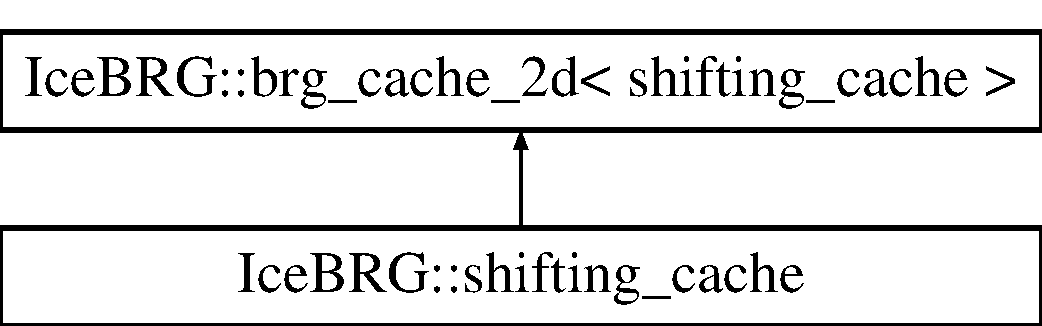
\includegraphics[height=2.000000cm]{classIceBRG_1_1shifting__cache}
\end{center}
\end{figure}
\subsection*{Public Member Functions}
\begin{DoxyCompactItemize}
\item 
\hyperlink{classIceBRG_1_1shifting__cache_a92a3afff41a2a906a84ae92e646e2d54}{shifting\+\_\+cache} ()
\item 
\hyperlink{classIceBRG_1_1shifting__cache_a79341fd1ec6588a16c669259b319b74c}{$\sim$shifting\+\_\+cache} ()
\end{DoxyCompactItemize}
\subsection*{Protected Member Functions}
\begin{DoxyCompactItemize}
\item 
std\+::string \hyperlink{classIceBRG_1_1shifting__cache_a6b8e62883a72521632375c7e98ddc6c2}{\+\_\+name\+\_\+base} () const 
\item 
\hyperlink{lib_2IceBRG__main_2common_8h_ad0f130a56eeb944d9ef2692ee881ecc4}{flt\+\_\+type} \hyperlink{classIceBRG_1_1shifting__cache_a5e61b8f959110a8efdc74ab34f268444}{\+\_\+calculate} (const \hyperlink{lib_2IceBRG__main_2common_8h_ad0f130a56eeb944d9ef2692ee881ecc4}{flt\+\_\+type} \&in\+\_\+param\+\_\+1, const \hyperlink{lib_2IceBRG__main_2common_8h_ad0f130a56eeb944d9ef2692ee881ecc4}{flt\+\_\+type} \&in\+\_\+param\+\_\+2) const 
\end{DoxyCompactItemize}
\subsection*{Friends}
\begin{DoxyCompactItemize}
\item 
class \hyperlink{classIceBRG_1_1shifting__cache_a4753ec11cca5a88c552ffaa19a8e43cf}{brg\+\_\+cache\+\_\+2d$<$ shifting\+\_\+cache $>$}
\end{DoxyCompactItemize}


\subsection{Constructor \& Destructor Documentation}
\hypertarget{classIceBRG_1_1shifting__cache_a92a3afff41a2a906a84ae92e646e2d54}{}\index{Ice\+B\+R\+G\+::shifting\+\_\+cache@{Ice\+B\+R\+G\+::shifting\+\_\+cache}!shifting\+\_\+cache@{shifting\+\_\+cache}}
\index{shifting\+\_\+cache@{shifting\+\_\+cache}!Ice\+B\+R\+G\+::shifting\+\_\+cache@{Ice\+B\+R\+G\+::shifting\+\_\+cache}}
\subsubsection[{shifting\+\_\+cache()}]{\setlength{\rightskip}{0pt plus 5cm}Ice\+B\+R\+G\+::shifting\+\_\+cache\+::shifting\+\_\+cache (
\begin{DoxyParamCaption}
{}
\end{DoxyParamCaption}
)\hspace{0.3cm}{\ttfamily [inline]}}\label{classIceBRG_1_1shifting__cache_a92a3afff41a2a906a84ae92e646e2d54}
\hypertarget{classIceBRG_1_1shifting__cache_a79341fd1ec6588a16c669259b319b74c}{}\index{Ice\+B\+R\+G\+::shifting\+\_\+cache@{Ice\+B\+R\+G\+::shifting\+\_\+cache}!````~shifting\+\_\+cache@{$\sim$shifting\+\_\+cache}}
\index{````~shifting\+\_\+cache@{$\sim$shifting\+\_\+cache}!Ice\+B\+R\+G\+::shifting\+\_\+cache@{Ice\+B\+R\+G\+::shifting\+\_\+cache}}
\subsubsection[{$\sim$shifting\+\_\+cache()}]{\setlength{\rightskip}{0pt plus 5cm}Ice\+B\+R\+G\+::shifting\+\_\+cache\+::$\sim$shifting\+\_\+cache (
\begin{DoxyParamCaption}
{}
\end{DoxyParamCaption}
)\hspace{0.3cm}{\ttfamily [inline]}}\label{classIceBRG_1_1shifting__cache_a79341fd1ec6588a16c669259b319b74c}


\subsection{Member Function Documentation}
\hypertarget{classIceBRG_1_1shifting__cache_a5e61b8f959110a8efdc74ab34f268444}{}\index{Ice\+B\+R\+G\+::shifting\+\_\+cache@{Ice\+B\+R\+G\+::shifting\+\_\+cache}!\+\_\+calculate@{\+\_\+calculate}}
\index{\+\_\+calculate@{\+\_\+calculate}!Ice\+B\+R\+G\+::shifting\+\_\+cache@{Ice\+B\+R\+G\+::shifting\+\_\+cache}}
\subsubsection[{\+\_\+calculate(const flt\+\_\+type \&in\+\_\+param\+\_\+1, const flt\+\_\+type \&in\+\_\+param\+\_\+2) const }]{\setlength{\rightskip}{0pt plus 5cm}{\bf flt\+\_\+type} Ice\+B\+R\+G\+::shifting\+\_\+cache\+::\+\_\+calculate (
\begin{DoxyParamCaption}
\item[{const {\bf flt\+\_\+type} \&}]{in\+\_\+param\+\_\+1, }
\item[{const {\bf flt\+\_\+type} \&}]{in\+\_\+param\+\_\+2}
\end{DoxyParamCaption}
) const\hspace{0.3cm}{\ttfamily [protected]}}\label{classIceBRG_1_1shifting__cache_a5e61b8f959110a8efdc74ab34f268444}
\hypertarget{classIceBRG_1_1shifting__cache_a6b8e62883a72521632375c7e98ddc6c2}{}\index{Ice\+B\+R\+G\+::shifting\+\_\+cache@{Ice\+B\+R\+G\+::shifting\+\_\+cache}!\+\_\+name\+\_\+base@{\+\_\+name\+\_\+base}}
\index{\+\_\+name\+\_\+base@{\+\_\+name\+\_\+base}!Ice\+B\+R\+G\+::shifting\+\_\+cache@{Ice\+B\+R\+G\+::shifting\+\_\+cache}}
\subsubsection[{\+\_\+name\+\_\+base() const }]{\setlength{\rightskip}{0pt plus 5cm}std\+::string Ice\+B\+R\+G\+::shifting\+\_\+cache\+::\+\_\+name\+\_\+base (
\begin{DoxyParamCaption}
{}
\end{DoxyParamCaption}
) const\hspace{0.3cm}{\ttfamily [inline]}, {\ttfamily [protected]}}\label{classIceBRG_1_1shifting__cache_a6b8e62883a72521632375c7e98ddc6c2}


\subsection{Friends And Related Function Documentation}
\hypertarget{classIceBRG_1_1shifting__cache_a4753ec11cca5a88c552ffaa19a8e43cf}{}\index{Ice\+B\+R\+G\+::shifting\+\_\+cache@{Ice\+B\+R\+G\+::shifting\+\_\+cache}!brg\+\_\+cache\+\_\+2d$<$ shifting\+\_\+cache $>$@{brg\+\_\+cache\+\_\+2d$<$ shifting\+\_\+cache $>$}}
\index{brg\+\_\+cache\+\_\+2d$<$ shifting\+\_\+cache $>$@{brg\+\_\+cache\+\_\+2d$<$ shifting\+\_\+cache $>$}!Ice\+B\+R\+G\+::shifting\+\_\+cache@{Ice\+B\+R\+G\+::shifting\+\_\+cache}}
\subsubsection[{brg\+\_\+cache\+\_\+2d$<$ shifting\+\_\+cache $>$}]{\setlength{\rightskip}{0pt plus 5cm}friend class {\bf brg\+\_\+cache\+\_\+2d}$<$ {\bf shifting\+\_\+cache} $>$\hspace{0.3cm}{\ttfamily [friend]}}\label{classIceBRG_1_1shifting__cache_a4753ec11cca5a88c552ffaa19a8e43cf}


The documentation for this class was generated from the following files\+:\begin{DoxyCompactItemize}
\item 
/disk2/brg/git/\+Magnification\+\_\+\+Public/src/lib/\+Ice\+B\+R\+G\+\_\+lensing/shifting/\hyperlink{shifting__cache_8h}{shifting\+\_\+cache.\+h}\item 
/disk2/brg/git/\+Magnification\+\_\+\+Public/src/lib/\+Ice\+B\+R\+G\+\_\+lensing/shifting/\hyperlink{shifting__cache_8cpp}{shifting\+\_\+cache.\+cpp}\end{DoxyCompactItemize}

\hypertarget{classIceBRG_1_1shifting__loader}{\section{Ice\-B\-R\-G\-:\-:shifting\-\_\-loader Class Reference}
\label{classIceBRG_1_1shifting__loader}\index{Ice\-B\-R\-G\-::shifting\-\_\-loader@{Ice\-B\-R\-G\-::shifting\-\_\-loader}}
}


{\ttfamily \#include $<$shifting\-\_\-loader.\-h$>$}

\subsection*{Public Member Functions}
\begin{DoxyCompactItemize}
\item 
\hyperlink{lib_2IceBRG__main_2common_8h_ad0f130a56eeb944d9ef2692ee881ecc4}{flt\-\_\-type} \hyperlink{classIceBRG_1_1shifting__loader_aa392b02a79a129a6e94f60b77ffbdbb9}{get} (\hyperlink{lib_2IceBRG__main_2common_8h_ad0f130a56eeb944d9ef2692ee881ecc4}{flt\-\_\-type} theta, \hyperlink{lib_2IceBRG__main_2common_8h_ad0f130a56eeb944d9ef2692ee881ecc4}{flt\-\_\-type} z)
\item 
void \hyperlink{classIceBRG_1_1shifting__loader_af29bd47511a5acd062c537eaddc8a2ee}{unload} ()
\item 
\hyperlink{classIceBRG_1_1shifting__loader_a9c4fbdad405c9a866dfadd2bd1b7d8be}{shifting\-\_\-loader} ()
\end{DoxyCompactItemize}


\subsection{Constructor \& Destructor Documentation}
\hypertarget{classIceBRG_1_1shifting__loader_a9c4fbdad405c9a866dfadd2bd1b7d8be}{\index{Ice\-B\-R\-G\-::shifting\-\_\-loader@{Ice\-B\-R\-G\-::shifting\-\_\-loader}!shifting\-\_\-loader@{shifting\-\_\-loader}}
\index{shifting\-\_\-loader@{shifting\-\_\-loader}!IceBRG::shifting_loader@{Ice\-B\-R\-G\-::shifting\-\_\-loader}}
\subsubsection[{shifting\-\_\-loader}]{\setlength{\rightskip}{0pt plus 5cm}Ice\-B\-R\-G\-::shifting\-\_\-loader\-::shifting\-\_\-loader (
\begin{DoxyParamCaption}
{}
\end{DoxyParamCaption}
)\hspace{0.3cm}{\ttfamily [inline]}}}\label{classIceBRG_1_1shifting__loader_a9c4fbdad405c9a866dfadd2bd1b7d8be}


\subsection{Member Function Documentation}
\hypertarget{classIceBRG_1_1shifting__loader_aa392b02a79a129a6e94f60b77ffbdbb9}{\index{Ice\-B\-R\-G\-::shifting\-\_\-loader@{Ice\-B\-R\-G\-::shifting\-\_\-loader}!get@{get}}
\index{get@{get}!IceBRG::shifting_loader@{Ice\-B\-R\-G\-::shifting\-\_\-loader}}
\subsubsection[{get}]{\setlength{\rightskip}{0pt plus 5cm}{\bf flt\-\_\-type} Ice\-B\-R\-G\-::shifting\-\_\-loader\-::get (
\begin{DoxyParamCaption}
\item[{{\bf flt\-\_\-type}}]{theta, }
\item[{{\bf flt\-\_\-type}}]{z}
\end{DoxyParamCaption}
)}}\label{classIceBRG_1_1shifting__loader_aa392b02a79a129a6e94f60b77ffbdbb9}
\hypertarget{classIceBRG_1_1shifting__loader_af29bd47511a5acd062c537eaddc8a2ee}{\index{Ice\-B\-R\-G\-::shifting\-\_\-loader@{Ice\-B\-R\-G\-::shifting\-\_\-loader}!unload@{unload}}
\index{unload@{unload}!IceBRG::shifting_loader@{Ice\-B\-R\-G\-::shifting\-\_\-loader}}
\subsubsection[{unload}]{\setlength{\rightskip}{0pt plus 5cm}void Ice\-B\-R\-G\-::shifting\-\_\-loader\-::unload (
\begin{DoxyParamCaption}
{}
\end{DoxyParamCaption}
)}}\label{classIceBRG_1_1shifting__loader_af29bd47511a5acd062c537eaddc8a2ee}


The documentation for this class was generated from the following files\-:\begin{DoxyCompactItemize}
\item 
/disk2/brg/git/\-Magnification\-\_\-\-Public/src/lib/\-Ice\-B\-R\-G\-\_\-lensing/shifting/\hyperlink{shifting__loader_8h}{shifting\-\_\-loader.\-h}\item 
/disk2/brg/git/\-Magnification\-\_\-\-Public/src/lib/\-Ice\-B\-R\-G\-\_\-lensing/shifting/\hyperlink{shifting__loader_8cpp}{shifting\-\_\-loader.\-cpp}\end{DoxyCompactItemize}

\hypertarget{classIceBRG_1_1sky__obj}{}\section{Ice\+B\+R\+G\+:\+:sky\+\_\+obj Class Reference}
\label{classIceBRG_1_1sky__obj}\index{Ice\+B\+R\+G\+::sky\+\_\+obj@{Ice\+B\+R\+G\+::sky\+\_\+obj}}


{\ttfamily \#include $<$sky\+\_\+obj.\+h$>$}

Inheritance diagram for Ice\+B\+R\+G\+:\+:sky\+\_\+obj\+:\begin{figure}[H]
\begin{center}
\leavevmode
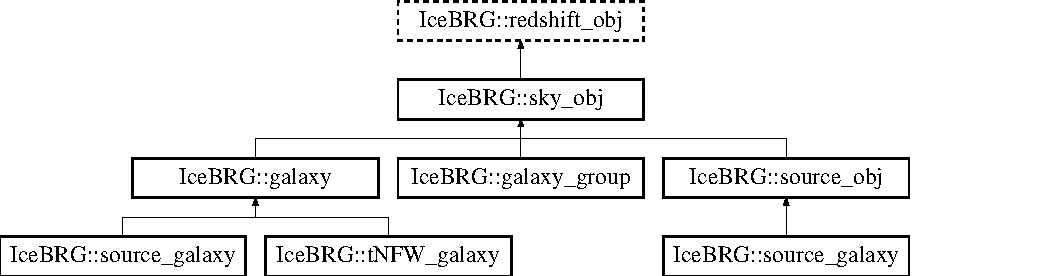
\includegraphics[height=3.708609cm]{classIceBRG_1_1sky__obj}
\end{center}
\end{figure}
\subsection*{Public Member Functions}
\begin{DoxyCompactItemize}
\item 
\hyperlink{classIceBRG_1_1sky__obj_a7f8351a5aa2b3e6f66132cfb2164b137}{sky\+\_\+obj} (const \hyperlink{namespaceIceBRG_a688eeb0811a2474b20b667ed2e9625a1}{angle\+\_\+type} \&init\+\_\+ra=0 $\ast$\hyperlink{namespaceIceBRG_a556de4acca26a5661d50a5b75880e95f}{rad}, const \hyperlink{namespaceIceBRG_a688eeb0811a2474b20b667ed2e9625a1}{angle\+\_\+type} \&init\+\_\+dec=0 $\ast$\hyperlink{namespaceIceBRG_a556de4acca26a5661d50a5b75880e95f}{rad}, const \hyperlink{lib_2IceBRG__main_2common_8h_ad0f130a56eeb944d9ef2692ee881ecc4}{flt\+\_\+type} \&init\+\_\+z=0, const \hyperlink{namespaceIceBRG_a688eeb0811a2474b20b667ed2e9625a1}{angle\+\_\+type} \&init\+\_\+ra\+\_\+err=0 $\ast$\hyperlink{namespaceIceBRG_a556de4acca26a5661d50a5b75880e95f}{rad}, const \hyperlink{namespaceIceBRG_a688eeb0811a2474b20b667ed2e9625a1}{angle\+\_\+type} \&init\+\_\+dec\+\_\+err=0 $\ast$\hyperlink{namespaceIceBRG_a556de4acca26a5661d50a5b75880e95f}{rad}, const \hyperlink{lib_2IceBRG__main_2common_8h_ad0f130a56eeb944d9ef2692ee881ecc4}{flt\+\_\+type} \&init\+\_\+z\+\_\+err=0)
\item 
virtual \hyperlink{classIceBRG_1_1sky__obj_adf2ec2bb6c1c977ed520828ecc2f3d68}{$\sim$sky\+\_\+obj} ()
\item 
virtual void \hyperlink{classIceBRG_1_1sky__obj_ad38ff17a187253f6f2fb4ef81ea03c59}{clear} ()
\item 
virtual void \hyperlink{classIceBRG_1_1sky__obj_a693bd041e7d6fef2e65a3eda379fd779}{partial\+\_\+clear} ()
\item 
virtual void \hyperlink{classIceBRG_1_1sky__obj_aaa784c2db38e7dd21d80f72cbab0bf45}{set\+\_\+ra} (const \hyperlink{namespaceIceBRG_a688eeb0811a2474b20b667ed2e9625a1}{angle\+\_\+type} \&new\+\_\+ra)
\item 
virtual void \hyperlink{classIceBRG_1_1sky__obj_a21d73e1e799792c8caaf0185032a7a08}{set\+\_\+dec} (const \hyperlink{namespaceIceBRG_a688eeb0811a2474b20b667ed2e9625a1}{angle\+\_\+type} \&new\+\_\+dec)
\item 
void \hyperlink{classIceBRG_1_1sky__obj_a7daeb396ea2789507400e51f8f7fad06}{set\+\_\+ra\+\_\+err} (const \hyperlink{namespaceIceBRG_a688eeb0811a2474b20b667ed2e9625a1}{angle\+\_\+type} \&new\+\_\+ra\+\_\+err)
\item 
void \hyperlink{classIceBRG_1_1sky__obj_a57c35b60f33d0ca12ba88fb1dbce33a2}{set\+\_\+dec\+\_\+err} (const \hyperlink{namespaceIceBRG_a688eeb0811a2474b20b667ed2e9625a1}{angle\+\_\+type} \&new\+\_\+dec\+\_\+err)
\item 
virtual void \hyperlink{classIceBRG_1_1sky__obj_acc63bf57b29d17cfa02195457427d3b8}{set\+\_\+ra\+\_\+dec} (const \hyperlink{namespaceIceBRG_a688eeb0811a2474b20b667ed2e9625a1}{angle\+\_\+type} \&new\+\_\+ra, const \hyperlink{namespaceIceBRG_a688eeb0811a2474b20b667ed2e9625a1}{angle\+\_\+type} \&new\+\_\+dec)
\item 
virtual void \hyperlink{classIceBRG_1_1sky__obj_a51fcc5ab62077ffb3889f5993f54003b}{set\+\_\+ra\+\_\+dec\+\_\+z} (const \hyperlink{namespaceIceBRG_a688eeb0811a2474b20b667ed2e9625a1}{angle\+\_\+type} \&new\+\_\+ra, const \hyperlink{namespaceIceBRG_a688eeb0811a2474b20b667ed2e9625a1}{angle\+\_\+type} \&new\+\_\+dec, const \hyperlink{lib_2IceBRG__main_2common_8h_ad0f130a56eeb944d9ef2692ee881ecc4}{flt\+\_\+type} \&new\+\_\+z)
\item 
virtual void \hyperlink{classIceBRG_1_1sky__obj_a1c1e1575557bee033e839cd0d13da8d9}{set\+\_\+ra\+\_\+dec\+\_\+z\+\_\+err} (const \hyperlink{namespaceIceBRG_a688eeb0811a2474b20b667ed2e9625a1}{angle\+\_\+type} \&new\+\_\+ra, const \hyperlink{namespaceIceBRG_a688eeb0811a2474b20b667ed2e9625a1}{angle\+\_\+type} \&new\+\_\+dec, const \hyperlink{lib_2IceBRG__main_2common_8h_ad0f130a56eeb944d9ef2692ee881ecc4}{flt\+\_\+type} \&new\+\_\+z, const \hyperlink{namespaceIceBRG_a688eeb0811a2474b20b667ed2e9625a1}{angle\+\_\+type} \&new\+\_\+ra\+\_\+err, const \hyperlink{namespaceIceBRG_a688eeb0811a2474b20b667ed2e9625a1}{angle\+\_\+type} \&new\+\_\+dec\+\_\+err, const \hyperlink{lib_2IceBRG__main_2common_8h_ad0f130a56eeb944d9ef2692ee881ecc4}{flt\+\_\+type} \&new\+\_\+z\+\_\+err)
\item 
virtual void \hyperlink{classIceBRG_1_1sky__obj_ad6212c6ae1f7c611b3d3c7ce26a6f478}{set\+\_\+ra\+\_\+dec\+\_\+err} (const \hyperlink{namespaceIceBRG_a688eeb0811a2474b20b667ed2e9625a1}{angle\+\_\+type} \&new\+\_\+ra, const \hyperlink{namespaceIceBRG_a688eeb0811a2474b20b667ed2e9625a1}{angle\+\_\+type} \&new\+\_\+dec, const \hyperlink{namespaceIceBRG_a688eeb0811a2474b20b667ed2e9625a1}{angle\+\_\+type} \&new\+\_\+ra\+\_\+err, const \hyperlink{namespaceIceBRG_a688eeb0811a2474b20b667ed2e9625a1}{angle\+\_\+type} \&new\+\_\+dec\+\_\+err)
\item 
void \hyperlink{classIceBRG_1_1sky__obj_aa52e306222c5876c361edd1e565a7e64}{set\+\_\+weight} (const \hyperlink{lib_2IceBRG__main_2common_8h_ad0f130a56eeb944d9ef2692ee881ecc4}{flt\+\_\+type} \&new\+\_\+weight)
\item 
void \hyperlink{classIceBRG_1_1sky__obj_aef489cfe00b362dfdd58f5a1d8e7c3f7}{set\+\_\+index} (const \hyperlink{lib_2IceBRG__main_2common_8h_ac4de9d9335536ac22821171deec8d39e}{int\+\_\+type} new\+\_\+index)
\item 
void \hyperlink{classIceBRG_1_1sky__obj_a12bb3624db02ce53501b9f890205232d}{set\+\_\+\+I\+D} (const std\+::string \&new\+\_\+\+I\+D)
\item 
const \hyperlink{namespaceIceBRG_a688eeb0811a2474b20b667ed2e9625a1}{angle\+\_\+type} \& \hyperlink{classIceBRG_1_1sky__obj_a2304bc2a67be4857348f3f51cde5daee}{ra} () const 
\item 
const \hyperlink{namespaceIceBRG_a688eeb0811a2474b20b667ed2e9625a1}{angle\+\_\+type} \& \hyperlink{classIceBRG_1_1sky__obj_a72579026fc6c7f6266dc29a3913e44ae}{dec} () const 
\item 
const \hyperlink{namespaceIceBRG_a688eeb0811a2474b20b667ed2e9625a1}{angle\+\_\+type} \& \hyperlink{classIceBRG_1_1sky__obj_ab39fc2800215b15fc6475f4037f2063c}{ra\+\_\+err} () const 
\item 
const \hyperlink{namespaceIceBRG_a688eeb0811a2474b20b667ed2e9625a1}{angle\+\_\+type} \& \hyperlink{classIceBRG_1_1sky__obj_a69349148162a272f1e67590121d4836e}{dec\+\_\+err} () const 
\item 
const \hyperlink{lib_2IceBRG__main_2common_8h_ad0f130a56eeb944d9ef2692ee881ecc4}{flt\+\_\+type} \& \hyperlink{classIceBRG_1_1sky__obj_a5e7765e9c60a24e4849b6ef278631b96}{weight} () const 
\item 
const \hyperlink{lib_2IceBRG__main_2common_8h_ac4de9d9335536ac22821171deec8d39e}{int\+\_\+type} \hyperlink{classIceBRG_1_1sky__obj_ad25abf998cc346d25b085440509128bc}{index} () const 
\item 
const std\+::string \& \hyperlink{classIceBRG_1_1sky__obj_a2ad6a15bb72988061826898e57298c27}{I\+D} () const 
\item 
virtual \hyperlink{namespaceIceBRG_a1be72ac4918a9b029f2eefa084213e35}{mass\+\_\+type} \hyperlink{classIceBRG_1_1sky__obj_a5296e44c7c9d809c31d9326197527d17}{m} () const  =0
\item 
virtual \hyperlink{lib_2IceBRG__main_2common_8h_ad0f130a56eeb944d9ef2692ee881ecc4}{flt\+\_\+type} \hyperlink{classIceBRG_1_1sky__obj_a40496172864c36f89d07bf54a52a9dc6}{mag} () const  =0
\item 
virtual \hyperlink{classIceBRG_1_1redshift__obj}{redshift\+\_\+obj} $\ast$ \hyperlink{classIceBRG_1_1sky__obj_a6efa97b5c6edb6c4ea741b06338ff5bc}{redshift\+\_\+obj\+\_\+clone} () const  =0
\item 
virtual \hyperlink{classIceBRG_1_1sky__obj}{sky\+\_\+obj} $\ast$ \hyperlink{classIceBRG_1_1sky__obj_a4b221bb8efb8ad5df2b03e53a077eeaa}{sky\+\_\+obj\+\_\+clone} () const  =0
\end{DoxyCompactItemize}


\subsection{Constructor \& Destructor Documentation}
\hypertarget{classIceBRG_1_1sky__obj_a7f8351a5aa2b3e6f66132cfb2164b137}{}\index{Ice\+B\+R\+G\+::sky\+\_\+obj@{Ice\+B\+R\+G\+::sky\+\_\+obj}!sky\+\_\+obj@{sky\+\_\+obj}}
\index{sky\+\_\+obj@{sky\+\_\+obj}!Ice\+B\+R\+G\+::sky\+\_\+obj@{Ice\+B\+R\+G\+::sky\+\_\+obj}}
\subsubsection[{sky\+\_\+obj(const angle\+\_\+type \&init\+\_\+ra=0 $\ast$rad, const angle\+\_\+type \&init\+\_\+dec=0 $\ast$rad, const flt\+\_\+type \&init\+\_\+z=0, const angle\+\_\+type \&init\+\_\+ra\+\_\+err=0 $\ast$rad, const angle\+\_\+type \&init\+\_\+dec\+\_\+err=0 $\ast$rad, const flt\+\_\+type \&init\+\_\+z\+\_\+err=0)}]{\setlength{\rightskip}{0pt plus 5cm}Ice\+B\+R\+G\+::sky\+\_\+obj\+::sky\+\_\+obj (
\begin{DoxyParamCaption}
\item[{const {\bf angle\+\_\+type} \&}]{init\+\_\+ra = {\ttfamily 0$\ast${\bf rad}}, }
\item[{const {\bf angle\+\_\+type} \&}]{init\+\_\+dec = {\ttfamily 0$\ast${\bf rad}}, }
\item[{const {\bf flt\+\_\+type} \&}]{init\+\_\+z = {\ttfamily 0}, }
\item[{const {\bf angle\+\_\+type} \&}]{init\+\_\+ra\+\_\+err = {\ttfamily 0$\ast${\bf rad}}, }
\item[{const {\bf angle\+\_\+type} \&}]{init\+\_\+dec\+\_\+err = {\ttfamily 0$\ast${\bf rad}}, }
\item[{const {\bf flt\+\_\+type} \&}]{init\+\_\+z\+\_\+err = {\ttfamily 0}}
\end{DoxyParamCaption}
)}\label{classIceBRG_1_1sky__obj_a7f8351a5aa2b3e6f66132cfb2164b137}
\hypertarget{classIceBRG_1_1sky__obj_adf2ec2bb6c1c977ed520828ecc2f3d68}{}\index{Ice\+B\+R\+G\+::sky\+\_\+obj@{Ice\+B\+R\+G\+::sky\+\_\+obj}!````~sky\+\_\+obj@{$\sim$sky\+\_\+obj}}
\index{````~sky\+\_\+obj@{$\sim$sky\+\_\+obj}!Ice\+B\+R\+G\+::sky\+\_\+obj@{Ice\+B\+R\+G\+::sky\+\_\+obj}}
\subsubsection[{$\sim$sky\+\_\+obj()}]{\setlength{\rightskip}{0pt plus 5cm}virtual Ice\+B\+R\+G\+::sky\+\_\+obj\+::$\sim$sky\+\_\+obj (
\begin{DoxyParamCaption}
{}
\end{DoxyParamCaption}
)\hspace{0.3cm}{\ttfamily [inline]}, {\ttfamily [virtual]}}\label{classIceBRG_1_1sky__obj_adf2ec2bb6c1c977ed520828ecc2f3d68}


\subsection{Member Function Documentation}
\hypertarget{classIceBRG_1_1sky__obj_ad38ff17a187253f6f2fb4ef81ea03c59}{}\index{Ice\+B\+R\+G\+::sky\+\_\+obj@{Ice\+B\+R\+G\+::sky\+\_\+obj}!clear@{clear}}
\index{clear@{clear}!Ice\+B\+R\+G\+::sky\+\_\+obj@{Ice\+B\+R\+G\+::sky\+\_\+obj}}
\subsubsection[{clear()}]{\setlength{\rightskip}{0pt plus 5cm}void Ice\+B\+R\+G\+::sky\+\_\+obj\+::clear (
\begin{DoxyParamCaption}
{}
\end{DoxyParamCaption}
)\hspace{0.3cm}{\ttfamily [virtual]}}\label{classIceBRG_1_1sky__obj_ad38ff17a187253f6f2fb4ef81ea03c59}


Reimplemented in \hyperlink{classIceBRG_1_1galaxy_a6a37d60a5b748e99f0c9dfac82b8ae4c}{Ice\+B\+R\+G\+::galaxy}, and \hyperlink{classIceBRG_1_1galaxy__group_af1be93cc734995c7fbfe6eb992094262}{Ice\+B\+R\+G\+::galaxy\+\_\+group}.

\hypertarget{classIceBRG_1_1sky__obj_a72579026fc6c7f6266dc29a3913e44ae}{}\index{Ice\+B\+R\+G\+::sky\+\_\+obj@{Ice\+B\+R\+G\+::sky\+\_\+obj}!dec@{dec}}
\index{dec@{dec}!Ice\+B\+R\+G\+::sky\+\_\+obj@{Ice\+B\+R\+G\+::sky\+\_\+obj}}
\subsubsection[{dec() const }]{\setlength{\rightskip}{0pt plus 5cm}const {\bf angle\+\_\+type}\& Ice\+B\+R\+G\+::sky\+\_\+obj\+::dec (
\begin{DoxyParamCaption}
{}
\end{DoxyParamCaption}
) const\hspace{0.3cm}{\ttfamily [inline]}}\label{classIceBRG_1_1sky__obj_a72579026fc6c7f6266dc29a3913e44ae}
\hypertarget{classIceBRG_1_1sky__obj_a69349148162a272f1e67590121d4836e}{}\index{Ice\+B\+R\+G\+::sky\+\_\+obj@{Ice\+B\+R\+G\+::sky\+\_\+obj}!dec\+\_\+err@{dec\+\_\+err}}
\index{dec\+\_\+err@{dec\+\_\+err}!Ice\+B\+R\+G\+::sky\+\_\+obj@{Ice\+B\+R\+G\+::sky\+\_\+obj}}
\subsubsection[{dec\+\_\+err() const }]{\setlength{\rightskip}{0pt plus 5cm}const {\bf angle\+\_\+type}\& Ice\+B\+R\+G\+::sky\+\_\+obj\+::dec\+\_\+err (
\begin{DoxyParamCaption}
{}
\end{DoxyParamCaption}
) const\hspace{0.3cm}{\ttfamily [inline]}}\label{classIceBRG_1_1sky__obj_a69349148162a272f1e67590121d4836e}
\hypertarget{classIceBRG_1_1sky__obj_a2ad6a15bb72988061826898e57298c27}{}\index{Ice\+B\+R\+G\+::sky\+\_\+obj@{Ice\+B\+R\+G\+::sky\+\_\+obj}!I\+D@{I\+D}}
\index{I\+D@{I\+D}!Ice\+B\+R\+G\+::sky\+\_\+obj@{Ice\+B\+R\+G\+::sky\+\_\+obj}}
\subsubsection[{I\+D() const }]{\setlength{\rightskip}{0pt plus 5cm}const std\+::string\& Ice\+B\+R\+G\+::sky\+\_\+obj\+::\+I\+D (
\begin{DoxyParamCaption}
{}
\end{DoxyParamCaption}
) const\hspace{0.3cm}{\ttfamily [inline]}}\label{classIceBRG_1_1sky__obj_a2ad6a15bb72988061826898e57298c27}
\hypertarget{classIceBRG_1_1sky__obj_ad25abf998cc346d25b085440509128bc}{}\index{Ice\+B\+R\+G\+::sky\+\_\+obj@{Ice\+B\+R\+G\+::sky\+\_\+obj}!index@{index}}
\index{index@{index}!Ice\+B\+R\+G\+::sky\+\_\+obj@{Ice\+B\+R\+G\+::sky\+\_\+obj}}
\subsubsection[{index() const }]{\setlength{\rightskip}{0pt plus 5cm}const {\bf int\+\_\+type} Ice\+B\+R\+G\+::sky\+\_\+obj\+::index (
\begin{DoxyParamCaption}
{}
\end{DoxyParamCaption}
) const\hspace{0.3cm}{\ttfamily [inline]}}\label{classIceBRG_1_1sky__obj_ad25abf998cc346d25b085440509128bc}
\hypertarget{classIceBRG_1_1sky__obj_a5296e44c7c9d809c31d9326197527d17}{}\index{Ice\+B\+R\+G\+::sky\+\_\+obj@{Ice\+B\+R\+G\+::sky\+\_\+obj}!m@{m}}
\index{m@{m}!Ice\+B\+R\+G\+::sky\+\_\+obj@{Ice\+B\+R\+G\+::sky\+\_\+obj}}
\subsubsection[{m() const  =0}]{\setlength{\rightskip}{0pt plus 5cm}virtual {\bf mass\+\_\+type} Ice\+B\+R\+G\+::sky\+\_\+obj\+::m (
\begin{DoxyParamCaption}
{}
\end{DoxyParamCaption}
) const\hspace{0.3cm}{\ttfamily [pure virtual]}}\label{classIceBRG_1_1sky__obj_a5296e44c7c9d809c31d9326197527d17}


Implemented in \hyperlink{classIceBRG_1_1galaxy__group_a8fe2611b0f227d213768b8ef4b6b1150}{Ice\+B\+R\+G\+::galaxy\+\_\+group}, \hyperlink{classIceBRG_1_1galaxy_abbe29ca14e53a5d12201be91aa1b4b30}{Ice\+B\+R\+G\+::galaxy}, and \hyperlink{classIceBRG_1_1source__galaxy_a2892608eb586559a48b0c37702220f31}{Ice\+B\+R\+G\+::source\+\_\+galaxy}.

\hypertarget{classIceBRG_1_1sky__obj_a40496172864c36f89d07bf54a52a9dc6}{}\index{Ice\+B\+R\+G\+::sky\+\_\+obj@{Ice\+B\+R\+G\+::sky\+\_\+obj}!mag@{mag}}
\index{mag@{mag}!Ice\+B\+R\+G\+::sky\+\_\+obj@{Ice\+B\+R\+G\+::sky\+\_\+obj}}
\subsubsection[{mag() const  =0}]{\setlength{\rightskip}{0pt plus 5cm}virtual {\bf flt\+\_\+type} Ice\+B\+R\+G\+::sky\+\_\+obj\+::mag (
\begin{DoxyParamCaption}
{}
\end{DoxyParamCaption}
) const\hspace{0.3cm}{\ttfamily [pure virtual]}}\label{classIceBRG_1_1sky__obj_a40496172864c36f89d07bf54a52a9dc6}


Implemented in \hyperlink{classIceBRG_1_1galaxy__group_aae14446ee20e2b7216317c1e8c7f4aeb}{Ice\+B\+R\+G\+::galaxy\+\_\+group}, \hyperlink{classIceBRG_1_1galaxy_ac4f8b983ac10ad86df0a2f90ce7f7593}{Ice\+B\+R\+G\+::galaxy}, and \hyperlink{classIceBRG_1_1source__galaxy_a33f22908e54b33a8a28603e1ddddd45d}{Ice\+B\+R\+G\+::source\+\_\+galaxy}.

\hypertarget{classIceBRG_1_1sky__obj_a693bd041e7d6fef2e65a3eda379fd779}{}\index{Ice\+B\+R\+G\+::sky\+\_\+obj@{Ice\+B\+R\+G\+::sky\+\_\+obj}!partial\+\_\+clear@{partial\+\_\+clear}}
\index{partial\+\_\+clear@{partial\+\_\+clear}!Ice\+B\+R\+G\+::sky\+\_\+obj@{Ice\+B\+R\+G\+::sky\+\_\+obj}}
\subsubsection[{partial\+\_\+clear()}]{\setlength{\rightskip}{0pt plus 5cm}void Ice\+B\+R\+G\+::sky\+\_\+obj\+::partial\+\_\+clear (
\begin{DoxyParamCaption}
{}
\end{DoxyParamCaption}
)\hspace{0.3cm}{\ttfamily [virtual]}}\label{classIceBRG_1_1sky__obj_a693bd041e7d6fef2e65a3eda379fd779}
\hypertarget{classIceBRG_1_1sky__obj_a2304bc2a67be4857348f3f51cde5daee}{}\index{Ice\+B\+R\+G\+::sky\+\_\+obj@{Ice\+B\+R\+G\+::sky\+\_\+obj}!ra@{ra}}
\index{ra@{ra}!Ice\+B\+R\+G\+::sky\+\_\+obj@{Ice\+B\+R\+G\+::sky\+\_\+obj}}
\subsubsection[{ra() const }]{\setlength{\rightskip}{0pt plus 5cm}const {\bf angle\+\_\+type}\& Ice\+B\+R\+G\+::sky\+\_\+obj\+::ra (
\begin{DoxyParamCaption}
{}
\end{DoxyParamCaption}
) const\hspace{0.3cm}{\ttfamily [inline]}}\label{classIceBRG_1_1sky__obj_a2304bc2a67be4857348f3f51cde5daee}
\hypertarget{classIceBRG_1_1sky__obj_ab39fc2800215b15fc6475f4037f2063c}{}\index{Ice\+B\+R\+G\+::sky\+\_\+obj@{Ice\+B\+R\+G\+::sky\+\_\+obj}!ra\+\_\+err@{ra\+\_\+err}}
\index{ra\+\_\+err@{ra\+\_\+err}!Ice\+B\+R\+G\+::sky\+\_\+obj@{Ice\+B\+R\+G\+::sky\+\_\+obj}}
\subsubsection[{ra\+\_\+err() const }]{\setlength{\rightskip}{0pt plus 5cm}const {\bf angle\+\_\+type}\& Ice\+B\+R\+G\+::sky\+\_\+obj\+::ra\+\_\+err (
\begin{DoxyParamCaption}
{}
\end{DoxyParamCaption}
) const\hspace{0.3cm}{\ttfamily [inline]}}\label{classIceBRG_1_1sky__obj_ab39fc2800215b15fc6475f4037f2063c}
\hypertarget{classIceBRG_1_1sky__obj_a6efa97b5c6edb6c4ea741b06338ff5bc}{}\index{Ice\+B\+R\+G\+::sky\+\_\+obj@{Ice\+B\+R\+G\+::sky\+\_\+obj}!redshift\+\_\+obj\+\_\+clone@{redshift\+\_\+obj\+\_\+clone}}
\index{redshift\+\_\+obj\+\_\+clone@{redshift\+\_\+obj\+\_\+clone}!Ice\+B\+R\+G\+::sky\+\_\+obj@{Ice\+B\+R\+G\+::sky\+\_\+obj}}
\subsubsection[{redshift\+\_\+obj\+\_\+clone() const  =0}]{\setlength{\rightskip}{0pt plus 5cm}virtual {\bf redshift\+\_\+obj}$\ast$ Ice\+B\+R\+G\+::sky\+\_\+obj\+::redshift\+\_\+obj\+\_\+clone (
\begin{DoxyParamCaption}
{}
\end{DoxyParamCaption}
) const\hspace{0.3cm}{\ttfamily [pure virtual]}}\label{classIceBRG_1_1sky__obj_a6efa97b5c6edb6c4ea741b06338ff5bc}


Reimplemented from \hyperlink{classIceBRG_1_1redshift__obj_a02f96529ff7f42ae64ae832712930e3b}{Ice\+B\+R\+G\+::redshift\+\_\+obj}.



Implemented in \hyperlink{classIceBRG_1_1galaxy_a0874bd3cb3133f244a86d6101aa1ec65}{Ice\+B\+R\+G\+::galaxy}, \hyperlink{classIceBRG_1_1galaxy__group_af0ee2e7b336371e8a8f098c3bfe7372d}{Ice\+B\+R\+G\+::galaxy\+\_\+group}, \hyperlink{classIceBRG_1_1source__galaxy_a59d08611112a2118f49ce569271524e7}{Ice\+B\+R\+G\+::source\+\_\+galaxy}, and \hyperlink{classIceBRG_1_1tNFW__galaxy_a0ac2852b6fad29184222f58e18aff3b3}{Ice\+B\+R\+G\+::t\+N\+F\+W\+\_\+galaxy}.

\hypertarget{classIceBRG_1_1sky__obj_a21d73e1e799792c8caaf0185032a7a08}{}\index{Ice\+B\+R\+G\+::sky\+\_\+obj@{Ice\+B\+R\+G\+::sky\+\_\+obj}!set\+\_\+dec@{set\+\_\+dec}}
\index{set\+\_\+dec@{set\+\_\+dec}!Ice\+B\+R\+G\+::sky\+\_\+obj@{Ice\+B\+R\+G\+::sky\+\_\+obj}}
\subsubsection[{set\+\_\+dec(const angle\+\_\+type \&new\+\_\+dec)}]{\setlength{\rightskip}{0pt plus 5cm}void Ice\+B\+R\+G\+::sky\+\_\+obj\+::set\+\_\+dec (
\begin{DoxyParamCaption}
\item[{const {\bf angle\+\_\+type} \&}]{new\+\_\+dec}
\end{DoxyParamCaption}
)\hspace{0.3cm}{\ttfamily [virtual]}}\label{classIceBRG_1_1sky__obj_a21d73e1e799792c8caaf0185032a7a08}
\hypertarget{classIceBRG_1_1sky__obj_a57c35b60f33d0ca12ba88fb1dbce33a2}{}\index{Ice\+B\+R\+G\+::sky\+\_\+obj@{Ice\+B\+R\+G\+::sky\+\_\+obj}!set\+\_\+dec\+\_\+err@{set\+\_\+dec\+\_\+err}}
\index{set\+\_\+dec\+\_\+err@{set\+\_\+dec\+\_\+err}!Ice\+B\+R\+G\+::sky\+\_\+obj@{Ice\+B\+R\+G\+::sky\+\_\+obj}}
\subsubsection[{set\+\_\+dec\+\_\+err(const angle\+\_\+type \&new\+\_\+dec\+\_\+err)}]{\setlength{\rightskip}{0pt plus 5cm}void Ice\+B\+R\+G\+::sky\+\_\+obj\+::set\+\_\+dec\+\_\+err (
\begin{DoxyParamCaption}
\item[{const {\bf angle\+\_\+type} \&}]{new\+\_\+dec\+\_\+err}
\end{DoxyParamCaption}
)}\label{classIceBRG_1_1sky__obj_a57c35b60f33d0ca12ba88fb1dbce33a2}
\hypertarget{classIceBRG_1_1sky__obj_a12bb3624db02ce53501b9f890205232d}{}\index{Ice\+B\+R\+G\+::sky\+\_\+obj@{Ice\+B\+R\+G\+::sky\+\_\+obj}!set\+\_\+\+I\+D@{set\+\_\+\+I\+D}}
\index{set\+\_\+\+I\+D@{set\+\_\+\+I\+D}!Ice\+B\+R\+G\+::sky\+\_\+obj@{Ice\+B\+R\+G\+::sky\+\_\+obj}}
\subsubsection[{set\+\_\+\+I\+D(const std\+::string \&new\+\_\+\+I\+D)}]{\setlength{\rightskip}{0pt plus 5cm}void Ice\+B\+R\+G\+::sky\+\_\+obj\+::set\+\_\+\+I\+D (
\begin{DoxyParamCaption}
\item[{const std\+::string \&}]{new\+\_\+\+I\+D}
\end{DoxyParamCaption}
)}\label{classIceBRG_1_1sky__obj_a12bb3624db02ce53501b9f890205232d}
\hypertarget{classIceBRG_1_1sky__obj_aef489cfe00b362dfdd58f5a1d8e7c3f7}{}\index{Ice\+B\+R\+G\+::sky\+\_\+obj@{Ice\+B\+R\+G\+::sky\+\_\+obj}!set\+\_\+index@{set\+\_\+index}}
\index{set\+\_\+index@{set\+\_\+index}!Ice\+B\+R\+G\+::sky\+\_\+obj@{Ice\+B\+R\+G\+::sky\+\_\+obj}}
\subsubsection[{set\+\_\+index(const int\+\_\+type new\+\_\+index)}]{\setlength{\rightskip}{0pt plus 5cm}void Ice\+B\+R\+G\+::sky\+\_\+obj\+::set\+\_\+index (
\begin{DoxyParamCaption}
\item[{const {\bf int\+\_\+type}}]{new\+\_\+index}
\end{DoxyParamCaption}
)}\label{classIceBRG_1_1sky__obj_aef489cfe00b362dfdd58f5a1d8e7c3f7}
\hypertarget{classIceBRG_1_1sky__obj_aaa784c2db38e7dd21d80f72cbab0bf45}{}\index{Ice\+B\+R\+G\+::sky\+\_\+obj@{Ice\+B\+R\+G\+::sky\+\_\+obj}!set\+\_\+ra@{set\+\_\+ra}}
\index{set\+\_\+ra@{set\+\_\+ra}!Ice\+B\+R\+G\+::sky\+\_\+obj@{Ice\+B\+R\+G\+::sky\+\_\+obj}}
\subsubsection[{set\+\_\+ra(const angle\+\_\+type \&new\+\_\+ra)}]{\setlength{\rightskip}{0pt plus 5cm}void Ice\+B\+R\+G\+::sky\+\_\+obj\+::set\+\_\+ra (
\begin{DoxyParamCaption}
\item[{const {\bf angle\+\_\+type} \&}]{new\+\_\+ra}
\end{DoxyParamCaption}
)\hspace{0.3cm}{\ttfamily [virtual]}}\label{classIceBRG_1_1sky__obj_aaa784c2db38e7dd21d80f72cbab0bf45}
\hypertarget{classIceBRG_1_1sky__obj_acc63bf57b29d17cfa02195457427d3b8}{}\index{Ice\+B\+R\+G\+::sky\+\_\+obj@{Ice\+B\+R\+G\+::sky\+\_\+obj}!set\+\_\+ra\+\_\+dec@{set\+\_\+ra\+\_\+dec}}
\index{set\+\_\+ra\+\_\+dec@{set\+\_\+ra\+\_\+dec}!Ice\+B\+R\+G\+::sky\+\_\+obj@{Ice\+B\+R\+G\+::sky\+\_\+obj}}
\subsubsection[{set\+\_\+ra\+\_\+dec(const angle\+\_\+type \&new\+\_\+ra, const angle\+\_\+type \&new\+\_\+dec)}]{\setlength{\rightskip}{0pt plus 5cm}void Ice\+B\+R\+G\+::sky\+\_\+obj\+::set\+\_\+ra\+\_\+dec (
\begin{DoxyParamCaption}
\item[{const {\bf angle\+\_\+type} \&}]{new\+\_\+ra, }
\item[{const {\bf angle\+\_\+type} \&}]{new\+\_\+dec}
\end{DoxyParamCaption}
)\hspace{0.3cm}{\ttfamily [virtual]}}\label{classIceBRG_1_1sky__obj_acc63bf57b29d17cfa02195457427d3b8}
\hypertarget{classIceBRG_1_1sky__obj_ad6212c6ae1f7c611b3d3c7ce26a6f478}{}\index{Ice\+B\+R\+G\+::sky\+\_\+obj@{Ice\+B\+R\+G\+::sky\+\_\+obj}!set\+\_\+ra\+\_\+dec\+\_\+err@{set\+\_\+ra\+\_\+dec\+\_\+err}}
\index{set\+\_\+ra\+\_\+dec\+\_\+err@{set\+\_\+ra\+\_\+dec\+\_\+err}!Ice\+B\+R\+G\+::sky\+\_\+obj@{Ice\+B\+R\+G\+::sky\+\_\+obj}}
\subsubsection[{set\+\_\+ra\+\_\+dec\+\_\+err(const angle\+\_\+type \&new\+\_\+ra, const angle\+\_\+type \&new\+\_\+dec, const angle\+\_\+type \&new\+\_\+ra\+\_\+err, const angle\+\_\+type \&new\+\_\+dec\+\_\+err)}]{\setlength{\rightskip}{0pt plus 5cm}void Ice\+B\+R\+G\+::sky\+\_\+obj\+::set\+\_\+ra\+\_\+dec\+\_\+err (
\begin{DoxyParamCaption}
\item[{const {\bf angle\+\_\+type} \&}]{new\+\_\+ra, }
\item[{const {\bf angle\+\_\+type} \&}]{new\+\_\+dec, }
\item[{const {\bf angle\+\_\+type} \&}]{new\+\_\+ra\+\_\+err, }
\item[{const {\bf angle\+\_\+type} \&}]{new\+\_\+dec\+\_\+err}
\end{DoxyParamCaption}
)\hspace{0.3cm}{\ttfamily [virtual]}}\label{classIceBRG_1_1sky__obj_ad6212c6ae1f7c611b3d3c7ce26a6f478}
\hypertarget{classIceBRG_1_1sky__obj_a51fcc5ab62077ffb3889f5993f54003b}{}\index{Ice\+B\+R\+G\+::sky\+\_\+obj@{Ice\+B\+R\+G\+::sky\+\_\+obj}!set\+\_\+ra\+\_\+dec\+\_\+z@{set\+\_\+ra\+\_\+dec\+\_\+z}}
\index{set\+\_\+ra\+\_\+dec\+\_\+z@{set\+\_\+ra\+\_\+dec\+\_\+z}!Ice\+B\+R\+G\+::sky\+\_\+obj@{Ice\+B\+R\+G\+::sky\+\_\+obj}}
\subsubsection[{set\+\_\+ra\+\_\+dec\+\_\+z(const angle\+\_\+type \&new\+\_\+ra, const angle\+\_\+type \&new\+\_\+dec, const flt\+\_\+type \&new\+\_\+z)}]{\setlength{\rightskip}{0pt plus 5cm}void Ice\+B\+R\+G\+::sky\+\_\+obj\+::set\+\_\+ra\+\_\+dec\+\_\+z (
\begin{DoxyParamCaption}
\item[{const {\bf angle\+\_\+type} \&}]{new\+\_\+ra, }
\item[{const {\bf angle\+\_\+type} \&}]{new\+\_\+dec, }
\item[{const {\bf flt\+\_\+type} \&}]{new\+\_\+z}
\end{DoxyParamCaption}
)\hspace{0.3cm}{\ttfamily [virtual]}}\label{classIceBRG_1_1sky__obj_a51fcc5ab62077ffb3889f5993f54003b}
\hypertarget{classIceBRG_1_1sky__obj_a1c1e1575557bee033e839cd0d13da8d9}{}\index{Ice\+B\+R\+G\+::sky\+\_\+obj@{Ice\+B\+R\+G\+::sky\+\_\+obj}!set\+\_\+ra\+\_\+dec\+\_\+z\+\_\+err@{set\+\_\+ra\+\_\+dec\+\_\+z\+\_\+err}}
\index{set\+\_\+ra\+\_\+dec\+\_\+z\+\_\+err@{set\+\_\+ra\+\_\+dec\+\_\+z\+\_\+err}!Ice\+B\+R\+G\+::sky\+\_\+obj@{Ice\+B\+R\+G\+::sky\+\_\+obj}}
\subsubsection[{set\+\_\+ra\+\_\+dec\+\_\+z\+\_\+err(const angle\+\_\+type \&new\+\_\+ra, const angle\+\_\+type \&new\+\_\+dec, const flt\+\_\+type \&new\+\_\+z, const angle\+\_\+type \&new\+\_\+ra\+\_\+err, const angle\+\_\+type \&new\+\_\+dec\+\_\+err, const flt\+\_\+type \&new\+\_\+z\+\_\+err)}]{\setlength{\rightskip}{0pt plus 5cm}void Ice\+B\+R\+G\+::sky\+\_\+obj\+::set\+\_\+ra\+\_\+dec\+\_\+z\+\_\+err (
\begin{DoxyParamCaption}
\item[{const {\bf angle\+\_\+type} \&}]{new\+\_\+ra, }
\item[{const {\bf angle\+\_\+type} \&}]{new\+\_\+dec, }
\item[{const {\bf flt\+\_\+type} \&}]{new\+\_\+z, }
\item[{const {\bf angle\+\_\+type} \&}]{new\+\_\+ra\+\_\+err, }
\item[{const {\bf angle\+\_\+type} \&}]{new\+\_\+dec\+\_\+err, }
\item[{const {\bf flt\+\_\+type} \&}]{new\+\_\+z\+\_\+err}
\end{DoxyParamCaption}
)\hspace{0.3cm}{\ttfamily [virtual]}}\label{classIceBRG_1_1sky__obj_a1c1e1575557bee033e839cd0d13da8d9}
\hypertarget{classIceBRG_1_1sky__obj_a7daeb396ea2789507400e51f8f7fad06}{}\index{Ice\+B\+R\+G\+::sky\+\_\+obj@{Ice\+B\+R\+G\+::sky\+\_\+obj}!set\+\_\+ra\+\_\+err@{set\+\_\+ra\+\_\+err}}
\index{set\+\_\+ra\+\_\+err@{set\+\_\+ra\+\_\+err}!Ice\+B\+R\+G\+::sky\+\_\+obj@{Ice\+B\+R\+G\+::sky\+\_\+obj}}
\subsubsection[{set\+\_\+ra\+\_\+err(const angle\+\_\+type \&new\+\_\+ra\+\_\+err)}]{\setlength{\rightskip}{0pt plus 5cm}void Ice\+B\+R\+G\+::sky\+\_\+obj\+::set\+\_\+ra\+\_\+err (
\begin{DoxyParamCaption}
\item[{const {\bf angle\+\_\+type} \&}]{new\+\_\+ra\+\_\+err}
\end{DoxyParamCaption}
)}\label{classIceBRG_1_1sky__obj_a7daeb396ea2789507400e51f8f7fad06}
\hypertarget{classIceBRG_1_1sky__obj_aa52e306222c5876c361edd1e565a7e64}{}\index{Ice\+B\+R\+G\+::sky\+\_\+obj@{Ice\+B\+R\+G\+::sky\+\_\+obj}!set\+\_\+weight@{set\+\_\+weight}}
\index{set\+\_\+weight@{set\+\_\+weight}!Ice\+B\+R\+G\+::sky\+\_\+obj@{Ice\+B\+R\+G\+::sky\+\_\+obj}}
\subsubsection[{set\+\_\+weight(const flt\+\_\+type \&new\+\_\+weight)}]{\setlength{\rightskip}{0pt plus 5cm}void Ice\+B\+R\+G\+::sky\+\_\+obj\+::set\+\_\+weight (
\begin{DoxyParamCaption}
\item[{const {\bf flt\+\_\+type} \&}]{new\+\_\+weight}
\end{DoxyParamCaption}
)}\label{classIceBRG_1_1sky__obj_aa52e306222c5876c361edd1e565a7e64}
\hypertarget{classIceBRG_1_1sky__obj_a4b221bb8efb8ad5df2b03e53a077eeaa}{}\index{Ice\+B\+R\+G\+::sky\+\_\+obj@{Ice\+B\+R\+G\+::sky\+\_\+obj}!sky\+\_\+obj\+\_\+clone@{sky\+\_\+obj\+\_\+clone}}
\index{sky\+\_\+obj\+\_\+clone@{sky\+\_\+obj\+\_\+clone}!Ice\+B\+R\+G\+::sky\+\_\+obj@{Ice\+B\+R\+G\+::sky\+\_\+obj}}
\subsubsection[{sky\+\_\+obj\+\_\+clone() const  =0}]{\setlength{\rightskip}{0pt plus 5cm}virtual {\bf sky\+\_\+obj}$\ast$ Ice\+B\+R\+G\+::sky\+\_\+obj\+::sky\+\_\+obj\+\_\+clone (
\begin{DoxyParamCaption}
{}
\end{DoxyParamCaption}
) const\hspace{0.3cm}{\ttfamily [pure virtual]}}\label{classIceBRG_1_1sky__obj_a4b221bb8efb8ad5df2b03e53a077eeaa}


Implemented in \hyperlink{classIceBRG_1_1galaxy_ae6c5cfc58523edcffcf9e8bdd90bc1ad}{Ice\+B\+R\+G\+::galaxy}, \hyperlink{classIceBRG_1_1galaxy__group_aa13d25256931c89489891ae8431672c7}{Ice\+B\+R\+G\+::galaxy\+\_\+group}, \hyperlink{classIceBRG_1_1source__galaxy_abf946b4f026c3ff45bfd4909a34bbbd7}{Ice\+B\+R\+G\+::source\+\_\+galaxy}, and \hyperlink{classIceBRG_1_1tNFW__galaxy_a6699f38c68e4d330a68c2319e9429138}{Ice\+B\+R\+G\+::t\+N\+F\+W\+\_\+galaxy}.

\hypertarget{classIceBRG_1_1sky__obj_a5e7765e9c60a24e4849b6ef278631b96}{}\index{Ice\+B\+R\+G\+::sky\+\_\+obj@{Ice\+B\+R\+G\+::sky\+\_\+obj}!weight@{weight}}
\index{weight@{weight}!Ice\+B\+R\+G\+::sky\+\_\+obj@{Ice\+B\+R\+G\+::sky\+\_\+obj}}
\subsubsection[{weight() const }]{\setlength{\rightskip}{0pt plus 5cm}const {\bf flt\+\_\+type}\& Ice\+B\+R\+G\+::sky\+\_\+obj\+::weight (
\begin{DoxyParamCaption}
{}
\end{DoxyParamCaption}
) const\hspace{0.3cm}{\ttfamily [inline]}}\label{classIceBRG_1_1sky__obj_a5e7765e9c60a24e4849b6ef278631b96}


The documentation for this class was generated from the following files\+:\begin{DoxyCompactItemize}
\item 
/disk2/brg/git/\+Magnification\+\_\+\+Public/src/lib/\+Ice\+B\+R\+G\+\_\+physics/sky\+\_\+obj/\hyperlink{sky__obj_8h}{sky\+\_\+obj.\+h}\item 
/disk2/brg/git/\+Magnification\+\_\+\+Public/src/lib/\+Ice\+B\+R\+G\+\_\+physics/sky\+\_\+obj/\hyperlink{sky__obj_8cpp}{sky\+\_\+obj.\+cpp}\end{DoxyCompactItemize}

\hypertarget{classIceBRG_1_1solve__rhm__functor}{}\section{Ice\+B\+R\+G\+:\+:solve\+\_\+rhm\+\_\+functor Class Reference}
\label{classIceBRG_1_1solve__rhm__functor}\index{Ice\+B\+R\+G\+::solve\+\_\+rhm\+\_\+functor@{Ice\+B\+R\+G\+::solve\+\_\+rhm\+\_\+functor}}


{\ttfamily \#include $<$density\+\_\+profile\+\_\+functors.\+h$>$}

\subsection*{Public Member Functions}
\begin{DoxyCompactItemize}
\item 
void \hyperlink{classIceBRG_1_1solve__rhm__functor_abd3409541143f784364f81da75fa031c}{set\+\_\+host\+\_\+ptr} (const \hyperlink{classIceBRG_1_1density__profile}{density\+\_\+profile} $\ast$new\+\_\+host\+\_\+ptr)
\item 
const \hyperlink{classIceBRG_1_1density__profile}{density\+\_\+profile} $\ast$ \hyperlink{classIceBRG_1_1solve__rhm__functor_adb491be13e13b4fcd56d951651d3fa9e}{host\+\_\+ptr} ()
\item 
void \hyperlink{classIceBRG_1_1solve__rhm__functor_a978ba7c3a90bf01579e5a75e174e6ba6}{set\+\_\+target\+\_\+mass} (const \hyperlink{namespaceIceBRG_a1be72ac4918a9b029f2eefa084213e35}{mass\+\_\+type} \&new\+\_\+target\+\_\+mass)
\item 
const \hyperlink{namespaceIceBRG_a1be72ac4918a9b029f2eefa084213e35}{mass\+\_\+type} \& \hyperlink{classIceBRG_1_1solve__rhm__functor_a395d630e25cf7cb05bcc6ac1ccafd8ef}{target\+\_\+mass} ()
\item 
\hyperlink{namespaceIceBRG_a1be72ac4918a9b029f2eefa084213e35}{mass\+\_\+type} \hyperlink{classIceBRG_1_1solve__rhm__functor_aebbe2dcb89bc2e00c894cfc023908fad}{operator()} (const \hyperlink{namespaceIceBRG_a45499647eb87e24c10ab32c628711cec}{distance\+\_\+type} \&in\+\_\+param) const 
\item 
\hyperlink{classIceBRG_1_1solve__rhm__functor_a457c7cf1c24146592d91d2004c011060}{solve\+\_\+rhm\+\_\+functor} ()
\item 
\hyperlink{classIceBRG_1_1solve__rhm__functor_aae0ce0636530e6de3eb01205e03d527a}{solve\+\_\+rhm\+\_\+functor} (const \hyperlink{classIceBRG_1_1density__profile}{density\+\_\+profile} $\ast$init\+\_\+host, const \hyperlink{namespaceIceBRG_a1be72ac4918a9b029f2eefa084213e35}{mass\+\_\+type} \&init\+\_\+target\+\_\+mass)
\end{DoxyCompactItemize}


\subsection{Constructor \& Destructor Documentation}
\hypertarget{classIceBRG_1_1solve__rhm__functor_a457c7cf1c24146592d91d2004c011060}{}\index{Ice\+B\+R\+G\+::solve\+\_\+rhm\+\_\+functor@{Ice\+B\+R\+G\+::solve\+\_\+rhm\+\_\+functor}!solve\+\_\+rhm\+\_\+functor@{solve\+\_\+rhm\+\_\+functor}}
\index{solve\+\_\+rhm\+\_\+functor@{solve\+\_\+rhm\+\_\+functor}!Ice\+B\+R\+G\+::solve\+\_\+rhm\+\_\+functor@{Ice\+B\+R\+G\+::solve\+\_\+rhm\+\_\+functor}}
\subsubsection[{solve\+\_\+rhm\+\_\+functor()}]{\setlength{\rightskip}{0pt plus 5cm}Ice\+B\+R\+G\+::solve\+\_\+rhm\+\_\+functor\+::solve\+\_\+rhm\+\_\+functor (
\begin{DoxyParamCaption}
{}
\end{DoxyParamCaption}
)}\label{classIceBRG_1_1solve__rhm__functor_a457c7cf1c24146592d91d2004c011060}
\hypertarget{classIceBRG_1_1solve__rhm__functor_aae0ce0636530e6de3eb01205e03d527a}{}\index{Ice\+B\+R\+G\+::solve\+\_\+rhm\+\_\+functor@{Ice\+B\+R\+G\+::solve\+\_\+rhm\+\_\+functor}!solve\+\_\+rhm\+\_\+functor@{solve\+\_\+rhm\+\_\+functor}}
\index{solve\+\_\+rhm\+\_\+functor@{solve\+\_\+rhm\+\_\+functor}!Ice\+B\+R\+G\+::solve\+\_\+rhm\+\_\+functor@{Ice\+B\+R\+G\+::solve\+\_\+rhm\+\_\+functor}}
\subsubsection[{solve\+\_\+rhm\+\_\+functor(const density\+\_\+profile $\ast$init\+\_\+host, const mass\+\_\+type \&init\+\_\+target\+\_\+mass)}]{\setlength{\rightskip}{0pt plus 5cm}Ice\+B\+R\+G\+::solve\+\_\+rhm\+\_\+functor\+::solve\+\_\+rhm\+\_\+functor (
\begin{DoxyParamCaption}
\item[{const {\bf density\+\_\+profile} $\ast$}]{init\+\_\+host, }
\item[{const {\bf mass\+\_\+type} \&}]{init\+\_\+target\+\_\+mass}
\end{DoxyParamCaption}
)}\label{classIceBRG_1_1solve__rhm__functor_aae0ce0636530e6de3eb01205e03d527a}


\subsection{Member Function Documentation}
\hypertarget{classIceBRG_1_1solve__rhm__functor_adb491be13e13b4fcd56d951651d3fa9e}{}\index{Ice\+B\+R\+G\+::solve\+\_\+rhm\+\_\+functor@{Ice\+B\+R\+G\+::solve\+\_\+rhm\+\_\+functor}!host\+\_\+ptr@{host\+\_\+ptr}}
\index{host\+\_\+ptr@{host\+\_\+ptr}!Ice\+B\+R\+G\+::solve\+\_\+rhm\+\_\+functor@{Ice\+B\+R\+G\+::solve\+\_\+rhm\+\_\+functor}}
\subsubsection[{host\+\_\+ptr()}]{\setlength{\rightskip}{0pt plus 5cm}const {\bf density\+\_\+profile}$\ast$ Ice\+B\+R\+G\+::solve\+\_\+rhm\+\_\+functor\+::host\+\_\+ptr (
\begin{DoxyParamCaption}
{}
\end{DoxyParamCaption}
)\hspace{0.3cm}{\ttfamily [inline]}}\label{classIceBRG_1_1solve__rhm__functor_adb491be13e13b4fcd56d951651d3fa9e}
\hypertarget{classIceBRG_1_1solve__rhm__functor_aebbe2dcb89bc2e00c894cfc023908fad}{}\index{Ice\+B\+R\+G\+::solve\+\_\+rhm\+\_\+functor@{Ice\+B\+R\+G\+::solve\+\_\+rhm\+\_\+functor}!operator()@{operator()}}
\index{operator()@{operator()}!Ice\+B\+R\+G\+::solve\+\_\+rhm\+\_\+functor@{Ice\+B\+R\+G\+::solve\+\_\+rhm\+\_\+functor}}
\subsubsection[{operator()(const distance\+\_\+type \&in\+\_\+param) const }]{\setlength{\rightskip}{0pt plus 5cm}{\bf Ice\+B\+R\+G\+::mass\+\_\+type} Ice\+B\+R\+G\+::solve\+\_\+rhm\+\_\+functor\+::operator() (
\begin{DoxyParamCaption}
\item[{const {\bf distance\+\_\+type} \&}]{in\+\_\+param}
\end{DoxyParamCaption}
) const}\label{classIceBRG_1_1solve__rhm__functor_aebbe2dcb89bc2e00c894cfc023908fad}
\hypertarget{classIceBRG_1_1solve__rhm__functor_abd3409541143f784364f81da75fa031c}{}\index{Ice\+B\+R\+G\+::solve\+\_\+rhm\+\_\+functor@{Ice\+B\+R\+G\+::solve\+\_\+rhm\+\_\+functor}!set\+\_\+host\+\_\+ptr@{set\+\_\+host\+\_\+ptr}}
\index{set\+\_\+host\+\_\+ptr@{set\+\_\+host\+\_\+ptr}!Ice\+B\+R\+G\+::solve\+\_\+rhm\+\_\+functor@{Ice\+B\+R\+G\+::solve\+\_\+rhm\+\_\+functor}}
\subsubsection[{set\+\_\+host\+\_\+ptr(const density\+\_\+profile $\ast$new\+\_\+host\+\_\+ptr)}]{\setlength{\rightskip}{0pt plus 5cm}void Ice\+B\+R\+G\+::solve\+\_\+rhm\+\_\+functor\+::set\+\_\+host\+\_\+ptr (
\begin{DoxyParamCaption}
\item[{const {\bf density\+\_\+profile} $\ast$}]{new\+\_\+host\+\_\+ptr}
\end{DoxyParamCaption}
)}\label{classIceBRG_1_1solve__rhm__functor_abd3409541143f784364f81da75fa031c}
\hypertarget{classIceBRG_1_1solve__rhm__functor_a978ba7c3a90bf01579e5a75e174e6ba6}{}\index{Ice\+B\+R\+G\+::solve\+\_\+rhm\+\_\+functor@{Ice\+B\+R\+G\+::solve\+\_\+rhm\+\_\+functor}!set\+\_\+target\+\_\+mass@{set\+\_\+target\+\_\+mass}}
\index{set\+\_\+target\+\_\+mass@{set\+\_\+target\+\_\+mass}!Ice\+B\+R\+G\+::solve\+\_\+rhm\+\_\+functor@{Ice\+B\+R\+G\+::solve\+\_\+rhm\+\_\+functor}}
\subsubsection[{set\+\_\+target\+\_\+mass(const mass\+\_\+type \&new\+\_\+target\+\_\+mass)}]{\setlength{\rightskip}{0pt plus 5cm}void Ice\+B\+R\+G\+::solve\+\_\+rhm\+\_\+functor\+::set\+\_\+target\+\_\+mass (
\begin{DoxyParamCaption}
\item[{const {\bf mass\+\_\+type} \&}]{new\+\_\+target\+\_\+mass}
\end{DoxyParamCaption}
)}\label{classIceBRG_1_1solve__rhm__functor_a978ba7c3a90bf01579e5a75e174e6ba6}
\hypertarget{classIceBRG_1_1solve__rhm__functor_a395d630e25cf7cb05bcc6ac1ccafd8ef}{}\index{Ice\+B\+R\+G\+::solve\+\_\+rhm\+\_\+functor@{Ice\+B\+R\+G\+::solve\+\_\+rhm\+\_\+functor}!target\+\_\+mass@{target\+\_\+mass}}
\index{target\+\_\+mass@{target\+\_\+mass}!Ice\+B\+R\+G\+::solve\+\_\+rhm\+\_\+functor@{Ice\+B\+R\+G\+::solve\+\_\+rhm\+\_\+functor}}
\subsubsection[{target\+\_\+mass()}]{\setlength{\rightskip}{0pt plus 5cm}const {\bf mass\+\_\+type}\& Ice\+B\+R\+G\+::solve\+\_\+rhm\+\_\+functor\+::target\+\_\+mass (
\begin{DoxyParamCaption}
{}
\end{DoxyParamCaption}
)\hspace{0.3cm}{\ttfamily [inline]}}\label{classIceBRG_1_1solve__rhm__functor_a395d630e25cf7cb05bcc6ac1ccafd8ef}


The documentation for this class was generated from the following files\+:\begin{DoxyCompactItemize}
\item 
/disk2/brg/git/\+Magnification\+\_\+\+Public/src/lib/\+Ice\+B\+R\+G\+\_\+physics/density\+\_\+profile/\hyperlink{density__profile__functors_8h}{density\+\_\+profile\+\_\+functors.\+h}\item 
/disk2/brg/git/\+Magnification\+\_\+\+Public/src/lib/\+Ice\+B\+R\+G\+\_\+physics/density\+\_\+profile/\hyperlink{density__profile__functors_8cpp}{density\+\_\+profile\+\_\+functors.\+cpp}\end{DoxyCompactItemize}

\hypertarget{classIceBRG_1_1source__galaxy}{}\section{Ice\+B\+R\+G\+:\+:source\+\_\+galaxy Class Reference}
\label{classIceBRG_1_1source__galaxy}\index{Ice\+B\+R\+G\+::source\+\_\+galaxy@{Ice\+B\+R\+G\+::source\+\_\+galaxy}}


{\ttfamily \#include $<$source\+\_\+galaxy.\+h$>$}

Inheritance diagram for Ice\+B\+R\+G\+:\+:source\+\_\+galaxy\+:\begin{figure}[H]
\begin{center}
\leavevmode
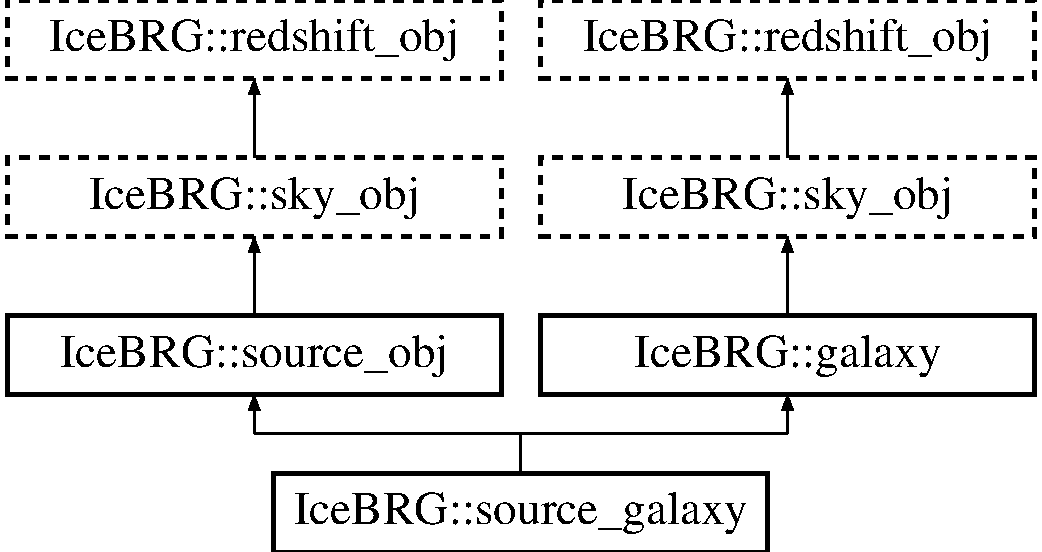
\includegraphics[height=4.000000cm]{classIceBRG_1_1source__galaxy}
\end{center}
\end{figure}
\subsection*{Public Member Functions}
\begin{DoxyCompactItemize}
\item 
\hyperlink{classIceBRG_1_1source__galaxy_a4c686c1b8886eeb4a63159e2e8f78c24}{source\+\_\+galaxy} (const \hyperlink{namespaceIceBRG_a688eeb0811a2474b20b667ed2e9625a1}{angle\+\_\+type} \&init\+\_\+ra=0, const \hyperlink{namespaceIceBRG_a688eeb0811a2474b20b667ed2e9625a1}{angle\+\_\+type} \&init\+\_\+dec=0, const \hyperlink{lib_2IceBRG__main_2common_8h_ad0f130a56eeb944d9ef2692ee881ecc4}{flt\+\_\+type} \&init\+\_\+z=0, const \hyperlink{lib_2IceBRG__main_2common_8h_ad0f130a56eeb944d9ef2692ee881ecc4}{flt\+\_\+type} \&init\+\_\+gamma\+\_\+1=0, const \hyperlink{lib_2IceBRG__main_2common_8h_ad0f130a56eeb944d9ef2692ee881ecc4}{flt\+\_\+type} \&init\+\_\+gamma\+\_\+2=0, const \hyperlink{lib_2IceBRG__main_2common_8h_ad0f130a56eeb944d9ef2692ee881ecc4}{flt\+\_\+type} \&init\+\_\+kappa=0, const \hyperlink{namespaceIceBRG_a1be72ac4918a9b029f2eefa084213e35}{mass\+\_\+type} \&init\+\_\+mstar=0, const \hyperlink{lib_2IceBRG__main_2common_8h_ad0f130a56eeb944d9ef2692ee881ecc4}{flt\+\_\+type} \&init\+\_\+mag=0, const \hyperlink{lib_2IceBRG__main_2common_8h_ad0f130a56eeb944d9ef2692ee881ecc4}{flt\+\_\+type} \&init\+\_\+weight=1)
\item 
virtual \hyperlink{classIceBRG_1_1source__galaxy_a7da38db1eff5abdf349cf6eef319d93a}{$\sim$source\+\_\+galaxy} ()
\item 
\hyperlink{namespaceIceBRG_a1be72ac4918a9b029f2eefa084213e35}{mass\+\_\+type} \hyperlink{classIceBRG_1_1source__galaxy_a2892608eb586559a48b0c37702220f31}{m} () const 
\item 
\hyperlink{lib_2IceBRG__main_2common_8h_ad0f130a56eeb944d9ef2692ee881ecc4}{flt\+\_\+type} \hyperlink{classIceBRG_1_1source__galaxy_a33f22908e54b33a8a28603e1ddddd45d}{mag} () const 
\item 
\hyperlink{classIceBRG_1_1redshift__obj}{redshift\+\_\+obj} $\ast$ \hyperlink{classIceBRG_1_1source__galaxy_a59d08611112a2118f49ce569271524e7}{redshift\+\_\+obj\+\_\+clone} () const 
\item 
\hyperlink{classIceBRG_1_1sky__obj}{sky\+\_\+obj} $\ast$ \hyperlink{classIceBRG_1_1source__galaxy_abf946b4f026c3ff45bfd4909a34bbbd7}{sky\+\_\+obj\+\_\+clone} () const 
\item 
\hyperlink{classIceBRG_1_1galaxy}{galaxy} $\ast$ \hyperlink{classIceBRG_1_1source__galaxy_acd7fb2dea893e8f22e85f5e228b9aaba}{galaxy\+\_\+clone} () const 
\item 
\hyperlink{classIceBRG_1_1source__obj}{source\+\_\+obj} $\ast$ \hyperlink{classIceBRG_1_1source__galaxy_af44074baa972ef3d0ebc59aedd047459}{source\+\_\+obj\+\_\+clone} () const 
\end{DoxyCompactItemize}
\subsection*{Additional Inherited Members}


\subsection{Constructor \& Destructor Documentation}
\hypertarget{classIceBRG_1_1source__galaxy_a4c686c1b8886eeb4a63159e2e8f78c24}{}\index{Ice\+B\+R\+G\+::source\+\_\+galaxy@{Ice\+B\+R\+G\+::source\+\_\+galaxy}!source\+\_\+galaxy@{source\+\_\+galaxy}}
\index{source\+\_\+galaxy@{source\+\_\+galaxy}!Ice\+B\+R\+G\+::source\+\_\+galaxy@{Ice\+B\+R\+G\+::source\+\_\+galaxy}}
\subsubsection[{source\+\_\+galaxy(const angle\+\_\+type \&init\+\_\+ra=0, const angle\+\_\+type \&init\+\_\+dec=0, const flt\+\_\+type \&init\+\_\+z=0, const flt\+\_\+type \&init\+\_\+gamma\+\_\+1=0, const flt\+\_\+type \&init\+\_\+gamma\+\_\+2=0, const flt\+\_\+type \&init\+\_\+kappa=0, const mass\+\_\+type \&init\+\_\+mstar=0, const flt\+\_\+type \&init\+\_\+mag=0, const flt\+\_\+type \&init\+\_\+weight=1)}]{\setlength{\rightskip}{0pt plus 5cm}Ice\+B\+R\+G\+::source\+\_\+galaxy\+::source\+\_\+galaxy (
\begin{DoxyParamCaption}
\item[{const {\bf angle\+\_\+type} \&}]{init\+\_\+ra = {\ttfamily 0}, }
\item[{const {\bf angle\+\_\+type} \&}]{init\+\_\+dec = {\ttfamily 0}, }
\item[{const {\bf flt\+\_\+type} \&}]{init\+\_\+z = {\ttfamily 0}, }
\item[{const {\bf flt\+\_\+type} \&}]{init\+\_\+gamma\+\_\+1 = {\ttfamily 0}, }
\item[{const {\bf flt\+\_\+type} \&}]{init\+\_\+gamma\+\_\+2 = {\ttfamily 0}, }
\item[{const {\bf flt\+\_\+type} \&}]{init\+\_\+kappa = {\ttfamily 0}, }
\item[{const {\bf mass\+\_\+type} \&}]{init\+\_\+mstar = {\ttfamily 0}, }
\item[{const {\bf flt\+\_\+type} \&}]{init\+\_\+mag = {\ttfamily 0}, }
\item[{const {\bf flt\+\_\+type} \&}]{init\+\_\+weight = {\ttfamily 1}}
\end{DoxyParamCaption}
)\hspace{0.3cm}{\ttfamily [inline]}}\label{classIceBRG_1_1source__galaxy_a4c686c1b8886eeb4a63159e2e8f78c24}
\hypertarget{classIceBRG_1_1source__galaxy_a7da38db1eff5abdf349cf6eef319d93a}{}\index{Ice\+B\+R\+G\+::source\+\_\+galaxy@{Ice\+B\+R\+G\+::source\+\_\+galaxy}!````~source\+\_\+galaxy@{$\sim$source\+\_\+galaxy}}
\index{````~source\+\_\+galaxy@{$\sim$source\+\_\+galaxy}!Ice\+B\+R\+G\+::source\+\_\+galaxy@{Ice\+B\+R\+G\+::source\+\_\+galaxy}}
\subsubsection[{$\sim$source\+\_\+galaxy()}]{\setlength{\rightskip}{0pt plus 5cm}virtual Ice\+B\+R\+G\+::source\+\_\+galaxy\+::$\sim$source\+\_\+galaxy (
\begin{DoxyParamCaption}
{}
\end{DoxyParamCaption}
)\hspace{0.3cm}{\ttfamily [inline]}, {\ttfamily [virtual]}}\label{classIceBRG_1_1source__galaxy_a7da38db1eff5abdf349cf6eef319d93a}


\subsection{Member Function Documentation}
\hypertarget{classIceBRG_1_1source__galaxy_acd7fb2dea893e8f22e85f5e228b9aaba}{}\index{Ice\+B\+R\+G\+::source\+\_\+galaxy@{Ice\+B\+R\+G\+::source\+\_\+galaxy}!galaxy\+\_\+clone@{galaxy\+\_\+clone}}
\index{galaxy\+\_\+clone@{galaxy\+\_\+clone}!Ice\+B\+R\+G\+::source\+\_\+galaxy@{Ice\+B\+R\+G\+::source\+\_\+galaxy}}
\subsubsection[{galaxy\+\_\+clone() const }]{\setlength{\rightskip}{0pt plus 5cm}{\bf galaxy}$\ast$ Ice\+B\+R\+G\+::source\+\_\+galaxy\+::galaxy\+\_\+clone (
\begin{DoxyParamCaption}
{}
\end{DoxyParamCaption}
) const\hspace{0.3cm}{\ttfamily [inline]}, {\ttfamily [virtual]}}\label{classIceBRG_1_1source__galaxy_acd7fb2dea893e8f22e85f5e228b9aaba}


Reimplemented from \hyperlink{classIceBRG_1_1galaxy_a58037140e845c9cd31c51e5751c28792}{Ice\+B\+R\+G\+::galaxy}.

\hypertarget{classIceBRG_1_1source__galaxy_a2892608eb586559a48b0c37702220f31}{}\index{Ice\+B\+R\+G\+::source\+\_\+galaxy@{Ice\+B\+R\+G\+::source\+\_\+galaxy}!m@{m}}
\index{m@{m}!Ice\+B\+R\+G\+::source\+\_\+galaxy@{Ice\+B\+R\+G\+::source\+\_\+galaxy}}
\subsubsection[{m() const }]{\setlength{\rightskip}{0pt plus 5cm}{\bf mass\+\_\+type} Ice\+B\+R\+G\+::source\+\_\+galaxy\+::m (
\begin{DoxyParamCaption}
{}
\end{DoxyParamCaption}
) const\hspace{0.3cm}{\ttfamily [inline]}, {\ttfamily [virtual]}}\label{classIceBRG_1_1source__galaxy_a2892608eb586559a48b0c37702220f31}


Implements \hyperlink{classIceBRG_1_1sky__obj_a5296e44c7c9d809c31d9326197527d17}{Ice\+B\+R\+G\+::sky\+\_\+obj}.

\hypertarget{classIceBRG_1_1source__galaxy_a33f22908e54b33a8a28603e1ddddd45d}{}\index{Ice\+B\+R\+G\+::source\+\_\+galaxy@{Ice\+B\+R\+G\+::source\+\_\+galaxy}!mag@{mag}}
\index{mag@{mag}!Ice\+B\+R\+G\+::source\+\_\+galaxy@{Ice\+B\+R\+G\+::source\+\_\+galaxy}}
\subsubsection[{mag() const }]{\setlength{\rightskip}{0pt plus 5cm}{\bf flt\+\_\+type} Ice\+B\+R\+G\+::source\+\_\+galaxy\+::mag (
\begin{DoxyParamCaption}
{}
\end{DoxyParamCaption}
) const\hspace{0.3cm}{\ttfamily [inline]}, {\ttfamily [virtual]}}\label{classIceBRG_1_1source__galaxy_a33f22908e54b33a8a28603e1ddddd45d}


Implements \hyperlink{classIceBRG_1_1sky__obj_a40496172864c36f89d07bf54a52a9dc6}{Ice\+B\+R\+G\+::sky\+\_\+obj}.

\hypertarget{classIceBRG_1_1source__galaxy_a59d08611112a2118f49ce569271524e7}{}\index{Ice\+B\+R\+G\+::source\+\_\+galaxy@{Ice\+B\+R\+G\+::source\+\_\+galaxy}!redshift\+\_\+obj\+\_\+clone@{redshift\+\_\+obj\+\_\+clone}}
\index{redshift\+\_\+obj\+\_\+clone@{redshift\+\_\+obj\+\_\+clone}!Ice\+B\+R\+G\+::source\+\_\+galaxy@{Ice\+B\+R\+G\+::source\+\_\+galaxy}}
\subsubsection[{redshift\+\_\+obj\+\_\+clone() const }]{\setlength{\rightskip}{0pt plus 5cm}{\bf redshift\+\_\+obj}$\ast$ Ice\+B\+R\+G\+::source\+\_\+galaxy\+::redshift\+\_\+obj\+\_\+clone (
\begin{DoxyParamCaption}
{}
\end{DoxyParamCaption}
) const\hspace{0.3cm}{\ttfamily [inline]}, {\ttfamily [virtual]}}\label{classIceBRG_1_1source__galaxy_a59d08611112a2118f49ce569271524e7}


Reimplemented from \hyperlink{classIceBRG_1_1galaxy_a0874bd3cb3133f244a86d6101aa1ec65}{Ice\+B\+R\+G\+::galaxy}.

\hypertarget{classIceBRG_1_1source__galaxy_abf946b4f026c3ff45bfd4909a34bbbd7}{}\index{Ice\+B\+R\+G\+::source\+\_\+galaxy@{Ice\+B\+R\+G\+::source\+\_\+galaxy}!sky\+\_\+obj\+\_\+clone@{sky\+\_\+obj\+\_\+clone}}
\index{sky\+\_\+obj\+\_\+clone@{sky\+\_\+obj\+\_\+clone}!Ice\+B\+R\+G\+::source\+\_\+galaxy@{Ice\+B\+R\+G\+::source\+\_\+galaxy}}
\subsubsection[{sky\+\_\+obj\+\_\+clone() const }]{\setlength{\rightskip}{0pt plus 5cm}{\bf sky\+\_\+obj}$\ast$ Ice\+B\+R\+G\+::source\+\_\+galaxy\+::sky\+\_\+obj\+\_\+clone (
\begin{DoxyParamCaption}
{}
\end{DoxyParamCaption}
) const\hspace{0.3cm}{\ttfamily [inline]}, {\ttfamily [virtual]}}\label{classIceBRG_1_1source__galaxy_abf946b4f026c3ff45bfd4909a34bbbd7}


Reimplemented from \hyperlink{classIceBRG_1_1galaxy_ae6c5cfc58523edcffcf9e8bdd90bc1ad}{Ice\+B\+R\+G\+::galaxy}.

\hypertarget{classIceBRG_1_1source__galaxy_af44074baa972ef3d0ebc59aedd047459}{}\index{Ice\+B\+R\+G\+::source\+\_\+galaxy@{Ice\+B\+R\+G\+::source\+\_\+galaxy}!source\+\_\+obj\+\_\+clone@{source\+\_\+obj\+\_\+clone}}
\index{source\+\_\+obj\+\_\+clone@{source\+\_\+obj\+\_\+clone}!Ice\+B\+R\+G\+::source\+\_\+galaxy@{Ice\+B\+R\+G\+::source\+\_\+galaxy}}
\subsubsection[{source\+\_\+obj\+\_\+clone() const }]{\setlength{\rightskip}{0pt plus 5cm}{\bf source\+\_\+obj}$\ast$ Ice\+B\+R\+G\+::source\+\_\+galaxy\+::source\+\_\+obj\+\_\+clone (
\begin{DoxyParamCaption}
{}
\end{DoxyParamCaption}
) const\hspace{0.3cm}{\ttfamily [inline]}, {\ttfamily [virtual]}}\label{classIceBRG_1_1source__galaxy_af44074baa972ef3d0ebc59aedd047459}


Implements \hyperlink{classIceBRG_1_1source__obj_a0c5bd9f6b0fa086c18c3918fcc6a5fac}{Ice\+B\+R\+G\+::source\+\_\+obj}.



The documentation for this class was generated from the following file\+:\begin{DoxyCompactItemize}
\item 
/disk2/brg/git/\+Magnification\+\_\+\+Public/src/lib/\+Ice\+B\+R\+G\+\_\+lensing/\hyperlink{source__galaxy_8h}{source\+\_\+galaxy.\+h}\end{DoxyCompactItemize}

\hypertarget{classIceBRG_1_1source__obj}{}\section{Ice\+B\+R\+G\+:\+:source\+\_\+obj Class Reference}
\label{classIceBRG_1_1source__obj}\index{Ice\+B\+R\+G\+::source\+\_\+obj@{Ice\+B\+R\+G\+::source\+\_\+obj}}


{\ttfamily \#include $<$source\+\_\+obj.\+hpp$>$}

Inheritance diagram for Ice\+B\+R\+G\+:\+:source\+\_\+obj\+:\begin{figure}[H]
\begin{center}
\leavevmode
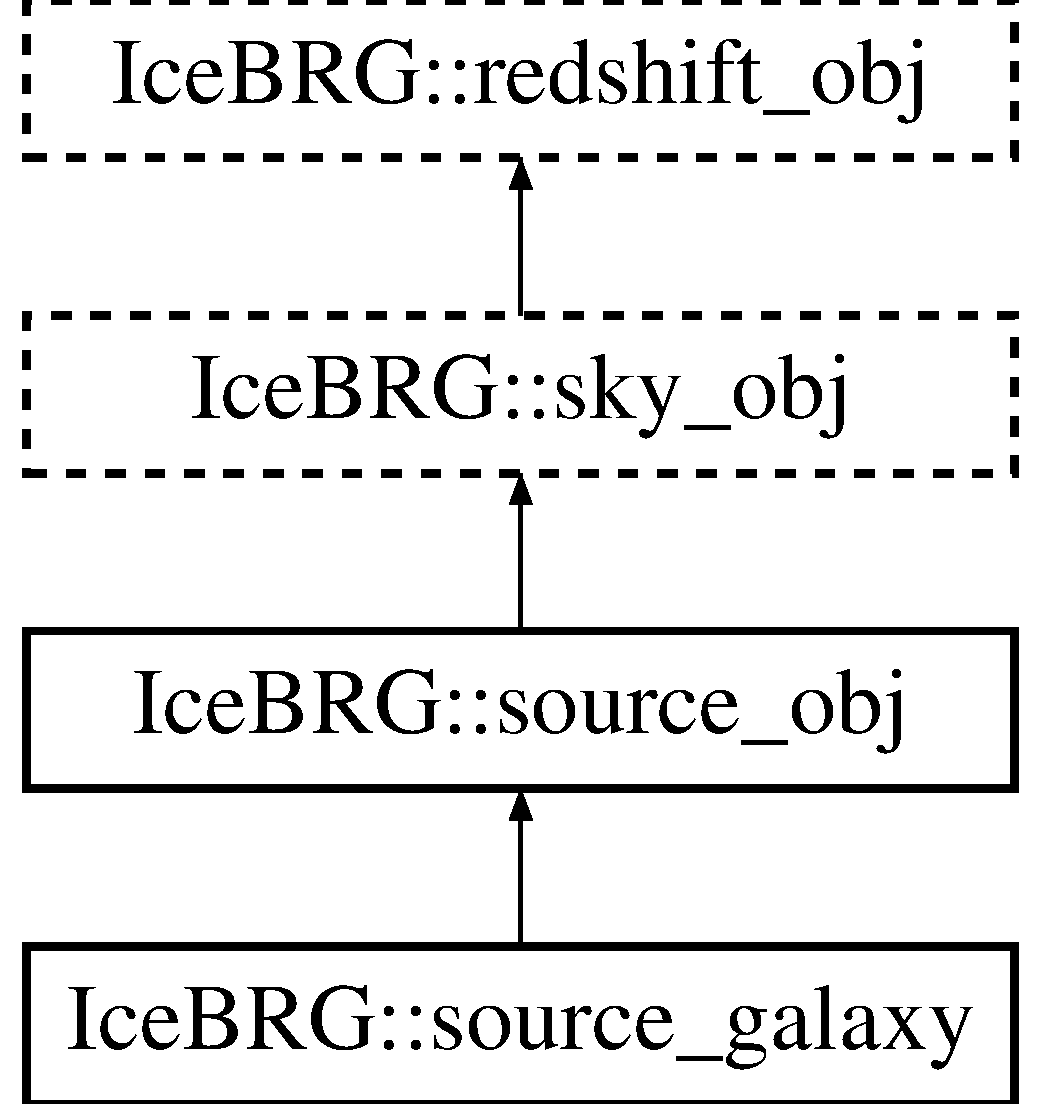
\includegraphics[height=4.000000cm]{classIceBRG_1_1source__obj}
\end{center}
\end{figure}
\subsection*{Public Member Functions}
\begin{DoxyCompactItemize}
\item 
\hyperlink{classIceBRG_1_1source__obj_a595bf7e87ae2bc9f885ac69398dc7fd6}{source\+\_\+obj} (const \hyperlink{namespaceIceBRG_a688eeb0811a2474b20b667ed2e9625a1}{angle\+\_\+type} \&init\+\_\+ra=0, const \hyperlink{namespaceIceBRG_a688eeb0811a2474b20b667ed2e9625a1}{angle\+\_\+type} \&init\+\_\+dec=0, \hyperlink{lib_2IceBRG__main_2common_8h_ad0f130a56eeb944d9ef2692ee881ecc4}{flt\+\_\+type} init\+\_\+z=0, \hyperlink{lib_2IceBRG__main_2common_8h_ad0f130a56eeb944d9ef2692ee881ecc4}{flt\+\_\+type} init\+\_\+gamma\+\_\+1=0, \hyperlink{lib_2IceBRG__main_2common_8h_ad0f130a56eeb944d9ef2692ee881ecc4}{flt\+\_\+type} init\+\_\+gamma\+\_\+2=0, \hyperlink{lib_2IceBRG__main_2common_8h_ad0f130a56eeb944d9ef2692ee881ecc4}{flt\+\_\+type} init\+\_\+kappa=0)
\item 
virtual \hyperlink{classIceBRG_1_1source__obj_aefcc60368231b021fe8166f98311e1d6}{$\sim$source\+\_\+obj} ()
\item 
virtual \hyperlink{classIceBRG_1_1source__obj}{source\+\_\+obj} $\ast$ \hyperlink{classIceBRG_1_1source__obj_a0c5bd9f6b0fa086c18c3918fcc6a5fac}{source\+\_\+obj\+\_\+clone} () const  =0
\item 
\hyperlink{lib_2IceBRG__main_2common_8h_ad0f130a56eeb944d9ef2692ee881ecc4}{flt\+\_\+type} \hyperlink{classIceBRG_1_1source__obj_a3cac72eb3217867d24a80af6be00e253}{gamma\+\_\+1} () const 
\item 
\hyperlink{lib_2IceBRG__main_2common_8h_ad0f130a56eeb944d9ef2692ee881ecc4}{flt\+\_\+type} \hyperlink{classIceBRG_1_1source__obj_a19792a6ae7f359962d3d4256c0b6482f}{gamma\+\_\+2} () const 
\item 
\hyperlink{lib_2IceBRG__main_2common_8h_ad0f130a56eeb944d9ef2692ee881ecc4}{flt\+\_\+type} \hyperlink{classIceBRG_1_1source__obj_ab25974cd9f5cf78de04e4e8afa1256de}{kappa} () const 
\item 
void \hyperlink{classIceBRG_1_1source__obj_af6aaf2d3569b3f87f7755e28c289d114}{set\+\_\+gamma\+\_\+1} (\hyperlink{lib_2IceBRG__main_2common_8h_ad0f130a56eeb944d9ef2692ee881ecc4}{flt\+\_\+type} new\+\_\+gamma\+\_\+1)
\item 
void \hyperlink{classIceBRG_1_1source__obj_a7ce0ece56cc848b4c30ade88121f1819}{set\+\_\+gamma\+\_\+2} (\hyperlink{lib_2IceBRG__main_2common_8h_ad0f130a56eeb944d9ef2692ee881ecc4}{flt\+\_\+type} new\+\_\+gamma\+\_\+2)
\item 
void \hyperlink{classIceBRG_1_1source__obj_a678744c9b44a26b43c41559a5f5200da}{set\+\_\+kappa} (\hyperlink{lib_2IceBRG__main_2common_8h_ad0f130a56eeb944d9ef2692ee881ecc4}{flt\+\_\+type} new\+\_\+kappa)
\end{DoxyCompactItemize}


\subsection{Constructor \& Destructor Documentation}
\hypertarget{classIceBRG_1_1source__obj_a595bf7e87ae2bc9f885ac69398dc7fd6}{}\index{Ice\+B\+R\+G\+::source\+\_\+obj@{Ice\+B\+R\+G\+::source\+\_\+obj}!source\+\_\+obj@{source\+\_\+obj}}
\index{source\+\_\+obj@{source\+\_\+obj}!Ice\+B\+R\+G\+::source\+\_\+obj@{Ice\+B\+R\+G\+::source\+\_\+obj}}
\subsubsection[{source\+\_\+obj(const angle\+\_\+type \&init\+\_\+ra=0, const angle\+\_\+type \&init\+\_\+dec=0, flt\+\_\+type init\+\_\+z=0, flt\+\_\+type init\+\_\+gamma\+\_\+1=0, flt\+\_\+type init\+\_\+gamma\+\_\+2=0, flt\+\_\+type init\+\_\+kappa=0)}]{\setlength{\rightskip}{0pt plus 5cm}Ice\+B\+R\+G\+::source\+\_\+obj\+::source\+\_\+obj (
\begin{DoxyParamCaption}
\item[{const {\bf angle\+\_\+type} \&}]{init\+\_\+ra = {\ttfamily 0}, }
\item[{const {\bf angle\+\_\+type} \&}]{init\+\_\+dec = {\ttfamily 0}, }
\item[{{\bf flt\+\_\+type}}]{init\+\_\+z = {\ttfamily 0}, }
\item[{{\bf flt\+\_\+type}}]{init\+\_\+gamma\+\_\+1 = {\ttfamily 0}, }
\item[{{\bf flt\+\_\+type}}]{init\+\_\+gamma\+\_\+2 = {\ttfamily 0}, }
\item[{{\bf flt\+\_\+type}}]{init\+\_\+kappa = {\ttfamily 0}}
\end{DoxyParamCaption}
)\hspace{0.3cm}{\ttfamily [inline]}}\label{classIceBRG_1_1source__obj_a595bf7e87ae2bc9f885ac69398dc7fd6}
\hypertarget{classIceBRG_1_1source__obj_aefcc60368231b021fe8166f98311e1d6}{}\index{Ice\+B\+R\+G\+::source\+\_\+obj@{Ice\+B\+R\+G\+::source\+\_\+obj}!````~source\+\_\+obj@{$\sim$source\+\_\+obj}}
\index{````~source\+\_\+obj@{$\sim$source\+\_\+obj}!Ice\+B\+R\+G\+::source\+\_\+obj@{Ice\+B\+R\+G\+::source\+\_\+obj}}
\subsubsection[{$\sim$source\+\_\+obj()}]{\setlength{\rightskip}{0pt plus 5cm}virtual Ice\+B\+R\+G\+::source\+\_\+obj\+::$\sim$source\+\_\+obj (
\begin{DoxyParamCaption}
{}
\end{DoxyParamCaption}
)\hspace{0.3cm}{\ttfamily [inline]}, {\ttfamily [virtual]}}\label{classIceBRG_1_1source__obj_aefcc60368231b021fe8166f98311e1d6}


\subsection{Member Function Documentation}
\hypertarget{classIceBRG_1_1source__obj_a3cac72eb3217867d24a80af6be00e253}{}\index{Ice\+B\+R\+G\+::source\+\_\+obj@{Ice\+B\+R\+G\+::source\+\_\+obj}!gamma\+\_\+1@{gamma\+\_\+1}}
\index{gamma\+\_\+1@{gamma\+\_\+1}!Ice\+B\+R\+G\+::source\+\_\+obj@{Ice\+B\+R\+G\+::source\+\_\+obj}}
\subsubsection[{gamma\+\_\+1() const }]{\setlength{\rightskip}{0pt plus 5cm}{\bf flt\+\_\+type} Ice\+B\+R\+G\+::source\+\_\+obj\+::gamma\+\_\+1 (
\begin{DoxyParamCaption}
{}
\end{DoxyParamCaption}
) const\hspace{0.3cm}{\ttfamily [inline]}}\label{classIceBRG_1_1source__obj_a3cac72eb3217867d24a80af6be00e253}
\hypertarget{classIceBRG_1_1source__obj_a19792a6ae7f359962d3d4256c0b6482f}{}\index{Ice\+B\+R\+G\+::source\+\_\+obj@{Ice\+B\+R\+G\+::source\+\_\+obj}!gamma\+\_\+2@{gamma\+\_\+2}}
\index{gamma\+\_\+2@{gamma\+\_\+2}!Ice\+B\+R\+G\+::source\+\_\+obj@{Ice\+B\+R\+G\+::source\+\_\+obj}}
\subsubsection[{gamma\+\_\+2() const }]{\setlength{\rightskip}{0pt plus 5cm}{\bf flt\+\_\+type} Ice\+B\+R\+G\+::source\+\_\+obj\+::gamma\+\_\+2 (
\begin{DoxyParamCaption}
{}
\end{DoxyParamCaption}
) const\hspace{0.3cm}{\ttfamily [inline]}}\label{classIceBRG_1_1source__obj_a19792a6ae7f359962d3d4256c0b6482f}
\hypertarget{classIceBRG_1_1source__obj_ab25974cd9f5cf78de04e4e8afa1256de}{}\index{Ice\+B\+R\+G\+::source\+\_\+obj@{Ice\+B\+R\+G\+::source\+\_\+obj}!kappa@{kappa}}
\index{kappa@{kappa}!Ice\+B\+R\+G\+::source\+\_\+obj@{Ice\+B\+R\+G\+::source\+\_\+obj}}
\subsubsection[{kappa() const }]{\setlength{\rightskip}{0pt plus 5cm}{\bf flt\+\_\+type} Ice\+B\+R\+G\+::source\+\_\+obj\+::kappa (
\begin{DoxyParamCaption}
{}
\end{DoxyParamCaption}
) const\hspace{0.3cm}{\ttfamily [inline]}}\label{classIceBRG_1_1source__obj_ab25974cd9f5cf78de04e4e8afa1256de}
\hypertarget{classIceBRG_1_1source__obj_af6aaf2d3569b3f87f7755e28c289d114}{}\index{Ice\+B\+R\+G\+::source\+\_\+obj@{Ice\+B\+R\+G\+::source\+\_\+obj}!set\+\_\+gamma\+\_\+1@{set\+\_\+gamma\+\_\+1}}
\index{set\+\_\+gamma\+\_\+1@{set\+\_\+gamma\+\_\+1}!Ice\+B\+R\+G\+::source\+\_\+obj@{Ice\+B\+R\+G\+::source\+\_\+obj}}
\subsubsection[{set\+\_\+gamma\+\_\+1(flt\+\_\+type new\+\_\+gamma\+\_\+1)}]{\setlength{\rightskip}{0pt plus 5cm}void Ice\+B\+R\+G\+::source\+\_\+obj\+::set\+\_\+gamma\+\_\+1 (
\begin{DoxyParamCaption}
\item[{{\bf flt\+\_\+type}}]{new\+\_\+gamma\+\_\+1}
\end{DoxyParamCaption}
)\hspace{0.3cm}{\ttfamily [inline]}}\label{classIceBRG_1_1source__obj_af6aaf2d3569b3f87f7755e28c289d114}
\hypertarget{classIceBRG_1_1source__obj_a7ce0ece56cc848b4c30ade88121f1819}{}\index{Ice\+B\+R\+G\+::source\+\_\+obj@{Ice\+B\+R\+G\+::source\+\_\+obj}!set\+\_\+gamma\+\_\+2@{set\+\_\+gamma\+\_\+2}}
\index{set\+\_\+gamma\+\_\+2@{set\+\_\+gamma\+\_\+2}!Ice\+B\+R\+G\+::source\+\_\+obj@{Ice\+B\+R\+G\+::source\+\_\+obj}}
\subsubsection[{set\+\_\+gamma\+\_\+2(flt\+\_\+type new\+\_\+gamma\+\_\+2)}]{\setlength{\rightskip}{0pt plus 5cm}void Ice\+B\+R\+G\+::source\+\_\+obj\+::set\+\_\+gamma\+\_\+2 (
\begin{DoxyParamCaption}
\item[{{\bf flt\+\_\+type}}]{new\+\_\+gamma\+\_\+2}
\end{DoxyParamCaption}
)\hspace{0.3cm}{\ttfamily [inline]}}\label{classIceBRG_1_1source__obj_a7ce0ece56cc848b4c30ade88121f1819}
\hypertarget{classIceBRG_1_1source__obj_a678744c9b44a26b43c41559a5f5200da}{}\index{Ice\+B\+R\+G\+::source\+\_\+obj@{Ice\+B\+R\+G\+::source\+\_\+obj}!set\+\_\+kappa@{set\+\_\+kappa}}
\index{set\+\_\+kappa@{set\+\_\+kappa}!Ice\+B\+R\+G\+::source\+\_\+obj@{Ice\+B\+R\+G\+::source\+\_\+obj}}
\subsubsection[{set\+\_\+kappa(flt\+\_\+type new\+\_\+kappa)}]{\setlength{\rightskip}{0pt plus 5cm}void Ice\+B\+R\+G\+::source\+\_\+obj\+::set\+\_\+kappa (
\begin{DoxyParamCaption}
\item[{{\bf flt\+\_\+type}}]{new\+\_\+kappa}
\end{DoxyParamCaption}
)\hspace{0.3cm}{\ttfamily [inline]}}\label{classIceBRG_1_1source__obj_a678744c9b44a26b43c41559a5f5200da}
\hypertarget{classIceBRG_1_1source__obj_a0c5bd9f6b0fa086c18c3918fcc6a5fac}{}\index{Ice\+B\+R\+G\+::source\+\_\+obj@{Ice\+B\+R\+G\+::source\+\_\+obj}!source\+\_\+obj\+\_\+clone@{source\+\_\+obj\+\_\+clone}}
\index{source\+\_\+obj\+\_\+clone@{source\+\_\+obj\+\_\+clone}!Ice\+B\+R\+G\+::source\+\_\+obj@{Ice\+B\+R\+G\+::source\+\_\+obj}}
\subsubsection[{source\+\_\+obj\+\_\+clone() const  =0}]{\setlength{\rightskip}{0pt plus 5cm}virtual {\bf source\+\_\+obj}$\ast$ Ice\+B\+R\+G\+::source\+\_\+obj\+::source\+\_\+obj\+\_\+clone (
\begin{DoxyParamCaption}
{}
\end{DoxyParamCaption}
) const\hspace{0.3cm}{\ttfamily [pure virtual]}}\label{classIceBRG_1_1source__obj_a0c5bd9f6b0fa086c18c3918fcc6a5fac}


Implemented in \hyperlink{classIceBRG_1_1source__galaxy_af44074baa972ef3d0ebc59aedd047459}{Ice\+B\+R\+G\+::source\+\_\+galaxy}.



The documentation for this class was generated from the following file\+:\begin{DoxyCompactItemize}
\item 
/disk2/brg/git/\+Magnification\+\_\+\+Public/src/lib/\+Ice\+B\+R\+G\+\_\+lensing/\hyperlink{source__obj_8hpp}{source\+\_\+obj.\+hpp}\end{DoxyCompactItemize}

\hypertarget{classIceBRG_1_1spherical__density__functor}{}\section{Ice\+B\+R\+G\+:\+:spherical\+\_\+density\+\_\+functor Class Reference}
\label{classIceBRG_1_1spherical__density__functor}\index{Ice\+B\+R\+G\+::spherical\+\_\+density\+\_\+functor@{Ice\+B\+R\+G\+::spherical\+\_\+density\+\_\+functor}}


{\ttfamily \#include $<$density\+\_\+profile\+\_\+functors.\+h$>$}

\subsection*{Public Member Functions}
\begin{DoxyCompactItemize}
\item 
void \hyperlink{classIceBRG_1_1spherical__density__functor_a60817cf2b168a9d5f1d31b98880a6fbe}{set\+\_\+host\+\_\+ptr} (const \hyperlink{classIceBRG_1_1density__profile}{density\+\_\+profile} $\ast$new\+\_\+host\+\_\+ptr)
\item 
const \hyperlink{classIceBRG_1_1density__profile}{density\+\_\+profile} $\ast$ \hyperlink{classIceBRG_1_1spherical__density__functor_afe7b0c3875cb3491240f1ef685d99a35}{host\+\_\+ptr} ()
\item 
\hyperlink{namespaceIceBRG_a896bc1bf7e8db5ca045b9cf35912ca5e}{custom\+\_\+unit\+\_\+type}$<$-\/1, 0, 1, 0, 0 $>$ \hyperlink{classIceBRG_1_1spherical__density__functor_a8974c9295a78c182ec4ff230d836439c}{operator()} (const \hyperlink{namespaceIceBRG_a45499647eb87e24c10ab32c628711cec}{distance\+\_\+type} \&in\+\_\+param) const 
\item 
\hyperlink{classIceBRG_1_1spherical__density__functor_ae18cd7fcc5679e8e4dfac04920ee12fc}{spherical\+\_\+density\+\_\+functor} ()
\item 
\hyperlink{classIceBRG_1_1spherical__density__functor_a2a902000b1b69bf16e63855fe18183db}{spherical\+\_\+density\+\_\+functor} (const \hyperlink{classIceBRG_1_1density__profile}{density\+\_\+profile} $\ast$init\+\_\+host)
\item 
virtual \hyperlink{classIceBRG_1_1spherical__density__functor_ac4361b6d9f844ec5ad54f766c99c16c7}{$\sim$spherical\+\_\+density\+\_\+functor} ()
\end{DoxyCompactItemize}


\subsection{Constructor \& Destructor Documentation}
\hypertarget{classIceBRG_1_1spherical__density__functor_ae18cd7fcc5679e8e4dfac04920ee12fc}{}\index{Ice\+B\+R\+G\+::spherical\+\_\+density\+\_\+functor@{Ice\+B\+R\+G\+::spherical\+\_\+density\+\_\+functor}!spherical\+\_\+density\+\_\+functor@{spherical\+\_\+density\+\_\+functor}}
\index{spherical\+\_\+density\+\_\+functor@{spherical\+\_\+density\+\_\+functor}!Ice\+B\+R\+G\+::spherical\+\_\+density\+\_\+functor@{Ice\+B\+R\+G\+::spherical\+\_\+density\+\_\+functor}}
\subsubsection[{spherical\+\_\+density\+\_\+functor()}]{\setlength{\rightskip}{0pt plus 5cm}Ice\+B\+R\+G\+::spherical\+\_\+density\+\_\+functor\+::spherical\+\_\+density\+\_\+functor (
\begin{DoxyParamCaption}
{}
\end{DoxyParamCaption}
)}\label{classIceBRG_1_1spherical__density__functor_ae18cd7fcc5679e8e4dfac04920ee12fc}
\hypertarget{classIceBRG_1_1spherical__density__functor_a2a902000b1b69bf16e63855fe18183db}{}\index{Ice\+B\+R\+G\+::spherical\+\_\+density\+\_\+functor@{Ice\+B\+R\+G\+::spherical\+\_\+density\+\_\+functor}!spherical\+\_\+density\+\_\+functor@{spherical\+\_\+density\+\_\+functor}}
\index{spherical\+\_\+density\+\_\+functor@{spherical\+\_\+density\+\_\+functor}!Ice\+B\+R\+G\+::spherical\+\_\+density\+\_\+functor@{Ice\+B\+R\+G\+::spherical\+\_\+density\+\_\+functor}}
\subsubsection[{spherical\+\_\+density\+\_\+functor(const density\+\_\+profile $\ast$init\+\_\+host)}]{\setlength{\rightskip}{0pt plus 5cm}Ice\+B\+R\+G\+::spherical\+\_\+density\+\_\+functor\+::spherical\+\_\+density\+\_\+functor (
\begin{DoxyParamCaption}
\item[{const {\bf density\+\_\+profile} $\ast$}]{init\+\_\+host}
\end{DoxyParamCaption}
)}\label{classIceBRG_1_1spherical__density__functor_a2a902000b1b69bf16e63855fe18183db}
\hypertarget{classIceBRG_1_1spherical__density__functor_ac4361b6d9f844ec5ad54f766c99c16c7}{}\index{Ice\+B\+R\+G\+::spherical\+\_\+density\+\_\+functor@{Ice\+B\+R\+G\+::spherical\+\_\+density\+\_\+functor}!````~spherical\+\_\+density\+\_\+functor@{$\sim$spherical\+\_\+density\+\_\+functor}}
\index{````~spherical\+\_\+density\+\_\+functor@{$\sim$spherical\+\_\+density\+\_\+functor}!Ice\+B\+R\+G\+::spherical\+\_\+density\+\_\+functor@{Ice\+B\+R\+G\+::spherical\+\_\+density\+\_\+functor}}
\subsubsection[{$\sim$spherical\+\_\+density\+\_\+functor()}]{\setlength{\rightskip}{0pt plus 5cm}virtual Ice\+B\+R\+G\+::spherical\+\_\+density\+\_\+functor\+::$\sim$spherical\+\_\+density\+\_\+functor (
\begin{DoxyParamCaption}
{}
\end{DoxyParamCaption}
)\hspace{0.3cm}{\ttfamily [inline]}, {\ttfamily [virtual]}}\label{classIceBRG_1_1spherical__density__functor_ac4361b6d9f844ec5ad54f766c99c16c7}


\subsection{Member Function Documentation}
\hypertarget{classIceBRG_1_1spherical__density__functor_afe7b0c3875cb3491240f1ef685d99a35}{}\index{Ice\+B\+R\+G\+::spherical\+\_\+density\+\_\+functor@{Ice\+B\+R\+G\+::spherical\+\_\+density\+\_\+functor}!host\+\_\+ptr@{host\+\_\+ptr}}
\index{host\+\_\+ptr@{host\+\_\+ptr}!Ice\+B\+R\+G\+::spherical\+\_\+density\+\_\+functor@{Ice\+B\+R\+G\+::spherical\+\_\+density\+\_\+functor}}
\subsubsection[{host\+\_\+ptr()}]{\setlength{\rightskip}{0pt plus 5cm}const {\bf density\+\_\+profile}$\ast$ Ice\+B\+R\+G\+::spherical\+\_\+density\+\_\+functor\+::host\+\_\+ptr (
\begin{DoxyParamCaption}
{}
\end{DoxyParamCaption}
)\hspace{0.3cm}{\ttfamily [inline]}}\label{classIceBRG_1_1spherical__density__functor_afe7b0c3875cb3491240f1ef685d99a35}
\hypertarget{classIceBRG_1_1spherical__density__functor_a8974c9295a78c182ec4ff230d836439c}{}\index{Ice\+B\+R\+G\+::spherical\+\_\+density\+\_\+functor@{Ice\+B\+R\+G\+::spherical\+\_\+density\+\_\+functor}!operator()@{operator()}}
\index{operator()@{operator()}!Ice\+B\+R\+G\+::spherical\+\_\+density\+\_\+functor@{Ice\+B\+R\+G\+::spherical\+\_\+density\+\_\+functor}}
\subsubsection[{operator()(const distance\+\_\+type \&in\+\_\+param) const }]{\setlength{\rightskip}{0pt plus 5cm}{\bf Ice\+B\+R\+G\+::custom\+\_\+unit\+\_\+type}$<$-\/1, 0, 1, 0, 0 $>$ Ice\+B\+R\+G\+::spherical\+\_\+density\+\_\+functor\+::operator() (
\begin{DoxyParamCaption}
\item[{const {\bf distance\+\_\+type} \&}]{in\+\_\+param}
\end{DoxyParamCaption}
) const}\label{classIceBRG_1_1spherical__density__functor_a8974c9295a78c182ec4ff230d836439c}
\hypertarget{classIceBRG_1_1spherical__density__functor_a60817cf2b168a9d5f1d31b98880a6fbe}{}\index{Ice\+B\+R\+G\+::spherical\+\_\+density\+\_\+functor@{Ice\+B\+R\+G\+::spherical\+\_\+density\+\_\+functor}!set\+\_\+host\+\_\+ptr@{set\+\_\+host\+\_\+ptr}}
\index{set\+\_\+host\+\_\+ptr@{set\+\_\+host\+\_\+ptr}!Ice\+B\+R\+G\+::spherical\+\_\+density\+\_\+functor@{Ice\+B\+R\+G\+::spherical\+\_\+density\+\_\+functor}}
\subsubsection[{set\+\_\+host\+\_\+ptr(const density\+\_\+profile $\ast$new\+\_\+host\+\_\+ptr)}]{\setlength{\rightskip}{0pt plus 5cm}void Ice\+B\+R\+G\+::spherical\+\_\+density\+\_\+functor\+::set\+\_\+host\+\_\+ptr (
\begin{DoxyParamCaption}
\item[{const {\bf density\+\_\+profile} $\ast$}]{new\+\_\+host\+\_\+ptr}
\end{DoxyParamCaption}
)}\label{classIceBRG_1_1spherical__density__functor_a60817cf2b168a9d5f1d31b98880a6fbe}


The documentation for this class was generated from the following files\+:\begin{DoxyCompactItemize}
\item 
/disk2/brg/git/\+Magnification\+\_\+\+Public/src/lib/\+Ice\+B\+R\+G\+\_\+physics/density\+\_\+profile/\hyperlink{density__profile__functors_8h}{density\+\_\+profile\+\_\+functors.\+h}\item 
/disk2/brg/git/\+Magnification\+\_\+\+Public/src/lib/\+Ice\+B\+R\+G\+\_\+physics/density\+\_\+profile/\hyperlink{density__profile__functors_8cpp}{density\+\_\+profile\+\_\+functors.\+cpp}\end{DoxyCompactItemize}

\hypertarget{classtk_1_1spline}{}\section{tk\+:\+:spline Class Reference}
\label{classtk_1_1spline}\index{tk\+::spline@{tk\+::spline}}


{\ttfamily \#include $<$tk\+\_\+spline.\+h$>$}

\subsection*{Public Member Functions}
\begin{DoxyCompactItemize}
\item 
void \hyperlink{classtk_1_1spline_aaeafc61f76356b53fa3ff153ed74a5b0}{set\+\_\+points} (const std\+::vector$<$ \hyperlink{lib_2IceBRG__main_2common_8h_ad0f130a56eeb944d9ef2692ee881ecc4}{flt\+\_\+type} $>$ \&x, const std\+::vector$<$ \hyperlink{lib_2IceBRG__main_2common_8h_ad0f130a56eeb944d9ef2692ee881ecc4}{flt\+\_\+type} $>$ \&y, bool cubic\+\_\+spline=true)
\item 
\hyperlink{lib_2IceBRG__main_2common_8h_ad0f130a56eeb944d9ef2692ee881ecc4}{flt\+\_\+type} \hyperlink{classtk_1_1spline_a84440a18f13d8f41e694e5324e99689e}{operator()} (\hyperlink{lib_2IceBRG__main_2common_8h_ad0f130a56eeb944d9ef2692ee881ecc4}{flt\+\_\+type} x) const 
\end{DoxyCompactItemize}


\subsection{Member Function Documentation}
\hypertarget{classtk_1_1spline_a84440a18f13d8f41e694e5324e99689e}{}\index{tk\+::spline@{tk\+::spline}!operator()@{operator()}}
\index{operator()@{operator()}!tk\+::spline@{tk\+::spline}}
\subsubsection[{operator()(flt\+\_\+type x) const }]{\setlength{\rightskip}{0pt plus 5cm}{\bf flt\+\_\+type} tk\+::spline\+::operator() (
\begin{DoxyParamCaption}
\item[{{\bf flt\+\_\+type}}]{x}
\end{DoxyParamCaption}
) const}\label{classtk_1_1spline_a84440a18f13d8f41e694e5324e99689e}
\hypertarget{classtk_1_1spline_aaeafc61f76356b53fa3ff153ed74a5b0}{}\index{tk\+::spline@{tk\+::spline}!set\+\_\+points@{set\+\_\+points}}
\index{set\+\_\+points@{set\+\_\+points}!tk\+::spline@{tk\+::spline}}
\subsubsection[{set\+\_\+points(const std\+::vector$<$ flt\+\_\+type $>$ \&x, const std\+::vector$<$ flt\+\_\+type $>$ \&y, bool cubic\+\_\+spline=true)}]{\setlength{\rightskip}{0pt plus 5cm}void tk\+::spline\+::set\+\_\+points (
\begin{DoxyParamCaption}
\item[{const std\+::vector$<$ {\bf flt\+\_\+type} $>$ \&}]{x, }
\item[{const std\+::vector$<$ {\bf flt\+\_\+type} $>$ \&}]{y, }
\item[{bool}]{cubic\+\_\+spline = {\ttfamily true}}
\end{DoxyParamCaption}
)}\label{classtk_1_1spline_aaeafc61f76356b53fa3ff153ed74a5b0}


The documentation for this class was generated from the following files\+:\begin{DoxyCompactItemize}
\item 
/disk2/brg/git/\+Magnification\+\_\+\+Public/src/lib/\+Ice\+B\+R\+G\+\_\+main/external/\hyperlink{tk__spline_8h}{tk\+\_\+spline.\+h}\item 
/disk2/brg/git/\+Magnification\+\_\+\+Public/src/lib/\+Ice\+B\+R\+G\+\_\+main/external/\hyperlink{tk__spline_8cpp}{tk\+\_\+spline.\+cpp}\end{DoxyCompactItemize}

\hypertarget{structboost_1_1accumulators_1_1tag_1_1sum__of__square__weights}{\section{boost\-:\-:accumulators\-:\-:tag\-:\-:sum\-\_\-of\-\_\-square\-\_\-weights Struct Reference}
\label{structboost_1_1accumulators_1_1tag_1_1sum__of__square__weights}\index{boost\-::accumulators\-::tag\-::sum\-\_\-of\-\_\-square\-\_\-weights@{boost\-::accumulators\-::tag\-::sum\-\_\-of\-\_\-square\-\_\-weights}}
}


{\ttfamily \#include $<$sum\-\_\-of\-\_\-square\-\_\-weights.\-hpp$>$}

\subsection*{Public Types}
\begin{DoxyCompactItemize}
\item 
typedef mpl\-::true\-\_\- \hyperlink{structboost_1_1accumulators_1_1tag_1_1sum__of__square__weights_aa1b4145dd1d30517a31fc2b139a4d831}{is\-\_\-weight\-\_\-accumulator}
\item 
typedef \\*
\hyperlink{structboost_1_1accumulators_1_1impl_1_1sum__of__square__weights__accumulator}{accumulators\-::impl\-::sum\-\_\-of\-\_\-square\-\_\-weights\-\_\-accumulator}\\*
$<$ mpl\-::\-\_\-1 $>$ \hyperlink{structboost_1_1accumulators_1_1tag_1_1sum__of__square__weights_a1b17755b77e02ad2286bcace0dcb9109}{impl}
\end{DoxyCompactItemize}


\subsection{Member Typedef Documentation}
\hypertarget{structboost_1_1accumulators_1_1tag_1_1sum__of__square__weights_a1b17755b77e02ad2286bcace0dcb9109}{\index{boost\-::accumulators\-::tag\-::sum\-\_\-of\-\_\-square\-\_\-weights@{boost\-::accumulators\-::tag\-::sum\-\_\-of\-\_\-square\-\_\-weights}!impl@{impl}}
\index{impl@{impl}!boost::accumulators::tag::sum_of_square_weights@{boost\-::accumulators\-::tag\-::sum\-\_\-of\-\_\-square\-\_\-weights}}
\subsubsection[{impl}]{\setlength{\rightskip}{0pt plus 5cm}typedef {\bf accumulators\-::impl\-::sum\-\_\-of\-\_\-square\-\_\-weights\-\_\-accumulator}$<$ mpl\-::\-\_\-1 $>$ {\bf boost\-::accumulators\-::tag\-::sum\-\_\-of\-\_\-square\-\_\-weights\-::impl}}}\label{structboost_1_1accumulators_1_1tag_1_1sum__of__square__weights_a1b17755b77e02ad2286bcace0dcb9109}
\hypertarget{structboost_1_1accumulators_1_1tag_1_1sum__of__square__weights_aa1b4145dd1d30517a31fc2b139a4d831}{\index{boost\-::accumulators\-::tag\-::sum\-\_\-of\-\_\-square\-\_\-weights@{boost\-::accumulators\-::tag\-::sum\-\_\-of\-\_\-square\-\_\-weights}!is\-\_\-weight\-\_\-accumulator@{is\-\_\-weight\-\_\-accumulator}}
\index{is\-\_\-weight\-\_\-accumulator@{is\-\_\-weight\-\_\-accumulator}!boost::accumulators::tag::sum_of_square_weights@{boost\-::accumulators\-::tag\-::sum\-\_\-of\-\_\-square\-\_\-weights}}
\subsubsection[{is\-\_\-weight\-\_\-accumulator}]{\setlength{\rightskip}{0pt plus 5cm}typedef mpl\-::true\-\_\- {\bf boost\-::accumulators\-::tag\-::sum\-\_\-of\-\_\-square\-\_\-weights\-::is\-\_\-weight\-\_\-accumulator}}}\label{structboost_1_1accumulators_1_1tag_1_1sum__of__square__weights_aa1b4145dd1d30517a31fc2b139a4d831}


The documentation for this struct was generated from the following file\-:\begin{DoxyCompactItemize}
\item 
/disk2/brg/git/\-Magnification\-\_\-\-Public/src/lib/\-Ice\-B\-R\-G\-\_\-main/math/statistics/\hyperlink{sum__of__square__weights_8hpp}{sum\-\_\-of\-\_\-square\-\_\-weights.\-hpp}\end{DoxyCompactItemize}

\hypertarget{structboost_1_1accumulators_1_1impl_1_1sum__of__square__weights__accumulator}{\section{boost\-:\-:accumulators\-:\-:impl\-:\-:sum\-\_\-of\-\_\-square\-\_\-weights\-\_\-accumulator$<$ Sample $>$ Struct Template Reference}
\label{structboost_1_1accumulators_1_1impl_1_1sum__of__square__weights__accumulator}\index{boost\-::accumulators\-::impl\-::sum\-\_\-of\-\_\-square\-\_\-weights\-\_\-accumulator$<$ Sample $>$@{boost\-::accumulators\-::impl\-::sum\-\_\-of\-\_\-square\-\_\-weights\-\_\-accumulator$<$ Sample $>$}}
}


{\ttfamily \#include $<$sum\-\_\-of\-\_\-square\-\_\-weights.\-hpp$>$}

\subsection*{Public Member Functions}
\begin{DoxyCompactItemize}
\item 
typedef \hyperlink{structboost_1_1accumulators_1_1impl_1_1sum__of__square__weights__accumulator_a13c60c3dc8cdeea5ca5b7d1a6a12ee1a}{decltype} (Sample()$\ast$Sample()) result\-\_\-type
\item 
{\footnotesize template$<$typename Args $>$ }\\\hyperlink{structboost_1_1accumulators_1_1impl_1_1sum__of__square__weights__accumulator_a25e5303bcf9f1136290fa80321c328b1}{sum\-\_\-of\-\_\-square\-\_\-weights\-\_\-accumulator} (Args const \&args)
\item 
{\footnotesize template$<$typename Args $>$ }\\void \hyperlink{structboost_1_1accumulators_1_1impl_1_1sum__of__square__weights__accumulator_a052432b8ef1d629762aa19a582d7b60a}{operator()} (Args const \&args)
\item 
result\-\_\-type \hyperlink{structboost_1_1accumulators_1_1impl_1_1sum__of__square__weights__accumulator_a3611a3f12c9e842e90d5d883ced69b3b}{result} (dont\-\_\-care) const 
\end{DoxyCompactItemize}


\subsection{Constructor \& Destructor Documentation}
\hypertarget{structboost_1_1accumulators_1_1impl_1_1sum__of__square__weights__accumulator_a25e5303bcf9f1136290fa80321c328b1}{\index{boost\-::accumulators\-::impl\-::sum\-\_\-of\-\_\-square\-\_\-weights\-\_\-accumulator@{boost\-::accumulators\-::impl\-::sum\-\_\-of\-\_\-square\-\_\-weights\-\_\-accumulator}!sum\-\_\-of\-\_\-square\-\_\-weights\-\_\-accumulator@{sum\-\_\-of\-\_\-square\-\_\-weights\-\_\-accumulator}}
\index{sum\-\_\-of\-\_\-square\-\_\-weights\-\_\-accumulator@{sum\-\_\-of\-\_\-square\-\_\-weights\-\_\-accumulator}!boost::accumulators::impl::sum_of_square_weights_accumulator@{boost\-::accumulators\-::impl\-::sum\-\_\-of\-\_\-square\-\_\-weights\-\_\-accumulator}}
\subsubsection[{sum\-\_\-of\-\_\-square\-\_\-weights\-\_\-accumulator}]{\setlength{\rightskip}{0pt plus 5cm}template$<$typename Sample $>$ template$<$typename Args $>$ {\bf boost\-::accumulators\-::impl\-::sum\-\_\-of\-\_\-square\-\_\-weights\-\_\-accumulator}$<$ Sample $>$\-::{\bf sum\-\_\-of\-\_\-square\-\_\-weights\-\_\-accumulator} (
\begin{DoxyParamCaption}
\item[{Args const \&}]{args}
\end{DoxyParamCaption}
)\hspace{0.3cm}{\ttfamily [inline]}}}\label{structboost_1_1accumulators_1_1impl_1_1sum__of__square__weights__accumulator_a25e5303bcf9f1136290fa80321c328b1}


\subsection{Member Function Documentation}
\hypertarget{structboost_1_1accumulators_1_1impl_1_1sum__of__square__weights__accumulator_a13c60c3dc8cdeea5ca5b7d1a6a12ee1a}{\index{boost\-::accumulators\-::impl\-::sum\-\_\-of\-\_\-square\-\_\-weights\-\_\-accumulator@{boost\-::accumulators\-::impl\-::sum\-\_\-of\-\_\-square\-\_\-weights\-\_\-accumulator}!decltype@{decltype}}
\index{decltype@{decltype}!boost::accumulators::impl::sum_of_square_weights_accumulator@{boost\-::accumulators\-::impl\-::sum\-\_\-of\-\_\-square\-\_\-weights\-\_\-accumulator}}
\subsubsection[{decltype}]{\setlength{\rightskip}{0pt plus 5cm}template$<$typename Sample $>$ typedef {\bf boost\-::accumulators\-::impl\-::sum\-\_\-of\-\_\-square\-\_\-weights\-\_\-accumulator}$<$ Sample $>$\-::decltype (
\begin{DoxyParamCaption}
\item[{Sample()$\ast$Sample()}]{}
\end{DoxyParamCaption}
)}}\label{structboost_1_1accumulators_1_1impl_1_1sum__of__square__weights__accumulator_a13c60c3dc8cdeea5ca5b7d1a6a12ee1a}
\hypertarget{structboost_1_1accumulators_1_1impl_1_1sum__of__square__weights__accumulator_a052432b8ef1d629762aa19a582d7b60a}{\index{boost\-::accumulators\-::impl\-::sum\-\_\-of\-\_\-square\-\_\-weights\-\_\-accumulator@{boost\-::accumulators\-::impl\-::sum\-\_\-of\-\_\-square\-\_\-weights\-\_\-accumulator}!operator()@{operator()}}
\index{operator()@{operator()}!boost::accumulators::impl::sum_of_square_weights_accumulator@{boost\-::accumulators\-::impl\-::sum\-\_\-of\-\_\-square\-\_\-weights\-\_\-accumulator}}
\subsubsection[{operator()}]{\setlength{\rightskip}{0pt plus 5cm}template$<$typename Sample $>$ template$<$typename Args $>$ void {\bf boost\-::accumulators\-::impl\-::sum\-\_\-of\-\_\-square\-\_\-weights\-\_\-accumulator}$<$ Sample $>$\-::operator() (
\begin{DoxyParamCaption}
\item[{Args const \&}]{args}
\end{DoxyParamCaption}
)\hspace{0.3cm}{\ttfamily [inline]}}}\label{structboost_1_1accumulators_1_1impl_1_1sum__of__square__weights__accumulator_a052432b8ef1d629762aa19a582d7b60a}
\hypertarget{structboost_1_1accumulators_1_1impl_1_1sum__of__square__weights__accumulator_a3611a3f12c9e842e90d5d883ced69b3b}{\index{boost\-::accumulators\-::impl\-::sum\-\_\-of\-\_\-square\-\_\-weights\-\_\-accumulator@{boost\-::accumulators\-::impl\-::sum\-\_\-of\-\_\-square\-\_\-weights\-\_\-accumulator}!result@{result}}
\index{result@{result}!boost::accumulators::impl::sum_of_square_weights_accumulator@{boost\-::accumulators\-::impl\-::sum\-\_\-of\-\_\-square\-\_\-weights\-\_\-accumulator}}
\subsubsection[{result}]{\setlength{\rightskip}{0pt plus 5cm}template$<$typename Sample $>$ result\-\_\-type {\bf boost\-::accumulators\-::impl\-::sum\-\_\-of\-\_\-square\-\_\-weights\-\_\-accumulator}$<$ Sample $>$\-::result (
\begin{DoxyParamCaption}
\item[{dont\-\_\-care}]{}
\end{DoxyParamCaption}
) const\hspace{0.3cm}{\ttfamily [inline]}}}\label{structboost_1_1accumulators_1_1impl_1_1sum__of__square__weights__accumulator_a3611a3f12c9e842e90d5d883ced69b3b}


The documentation for this struct was generated from the following file\-:\begin{DoxyCompactItemize}
\item 
/disk2/brg/git/\-Magnification\-\_\-\-Public/src/lib/\-Ice\-B\-R\-G\-\_\-main/math/statistics/\hyperlink{sum__of__square__weights_8hpp}{sum\-\_\-of\-\_\-square\-\_\-weights.\-hpp}\end{DoxyCompactItemize}

\hypertarget{classIceBRG_1_1tfa__cache}{}\section{Ice\+B\+R\+G\+:\+:tfa\+\_\+cache Class Reference}
\label{classIceBRG_1_1tfa__cache}\index{Ice\+B\+R\+G\+::tfa\+\_\+cache@{Ice\+B\+R\+G\+::tfa\+\_\+cache}}


{\ttfamily \#include $<$astro\+\_\+caches.\+h$>$}

Inheritance diagram for Ice\+B\+R\+G\+:\+:tfa\+\_\+cache\+:\begin{figure}[H]
\begin{center}
\leavevmode
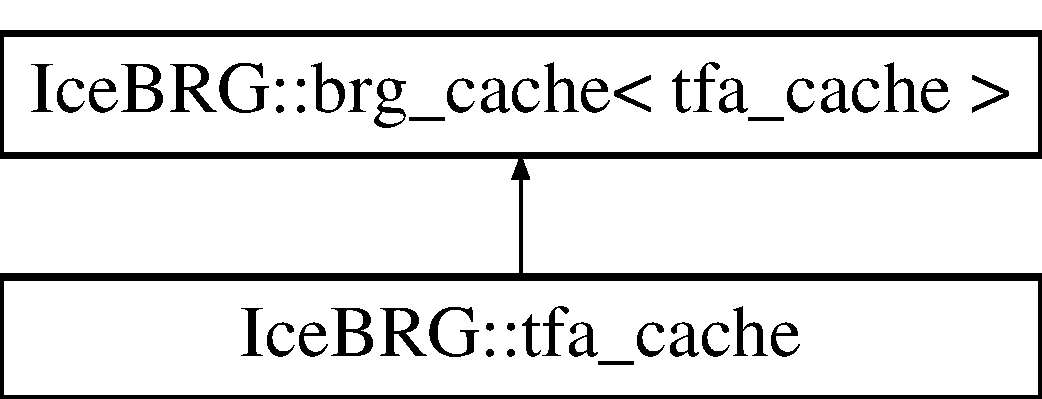
\includegraphics[height=2.000000cm]{classIceBRG_1_1tfa__cache}
\end{center}
\end{figure}
\subsection*{Public Member Functions}
\begin{DoxyCompactItemize}
\item 
\hyperlink{classIceBRG_1_1tfa__cache_ae75dedf37bbe634756a244a2b6a5d370}{$\sim$tfa\+\_\+cache} ()
\end{DoxyCompactItemize}
\subsection*{Protected Member Functions}
\begin{DoxyCompactItemize}
\item 
std\+::string \hyperlink{classIceBRG_1_1tfa__cache_a2ba816e8b181268c233a49999264381f}{\+\_\+name\+\_\+base} () const 
\item 
\hyperlink{lib_2IceBRG__main_2common_8h_ad0f130a56eeb944d9ef2692ee881ecc4}{flt\+\_\+type} \hyperlink{classIceBRG_1_1tfa__cache_a471aa05a4cc82e4a9007ab365c6a19cb}{\+\_\+calculate} (const \hyperlink{lib_2IceBRG__main_2common_8h_ad0f130a56eeb944d9ef2692ee881ecc4}{flt\+\_\+type} \&in\+\_\+param) const 
\end{DoxyCompactItemize}
\subsection*{Friends}
\begin{DoxyCompactItemize}
\item 
class \hyperlink{classIceBRG_1_1tfa__cache_a2ba9ba582d5f67ff2b264f742b3d251f}{brg\+\_\+cache$<$ tfa\+\_\+cache $>$}
\end{DoxyCompactItemize}


\subsection{Constructor \& Destructor Documentation}
\hypertarget{classIceBRG_1_1tfa__cache_ae75dedf37bbe634756a244a2b6a5d370}{}\index{Ice\+B\+R\+G\+::tfa\+\_\+cache@{Ice\+B\+R\+G\+::tfa\+\_\+cache}!````~tfa\+\_\+cache@{$\sim$tfa\+\_\+cache}}
\index{````~tfa\+\_\+cache@{$\sim$tfa\+\_\+cache}!Ice\+B\+R\+G\+::tfa\+\_\+cache@{Ice\+B\+R\+G\+::tfa\+\_\+cache}}
\subsubsection[{$\sim$tfa\+\_\+cache()}]{\setlength{\rightskip}{0pt plus 5cm}Ice\+B\+R\+G\+::tfa\+\_\+cache\+::$\sim$tfa\+\_\+cache (
\begin{DoxyParamCaption}
{}
\end{DoxyParamCaption}
)\hspace{0.3cm}{\ttfamily [inline]}}\label{classIceBRG_1_1tfa__cache_ae75dedf37bbe634756a244a2b6a5d370}


\subsection{Member Function Documentation}
\hypertarget{classIceBRG_1_1tfa__cache_a471aa05a4cc82e4a9007ab365c6a19cb}{}\index{Ice\+B\+R\+G\+::tfa\+\_\+cache@{Ice\+B\+R\+G\+::tfa\+\_\+cache}!\+\_\+calculate@{\+\_\+calculate}}
\index{\+\_\+calculate@{\+\_\+calculate}!Ice\+B\+R\+G\+::tfa\+\_\+cache@{Ice\+B\+R\+G\+::tfa\+\_\+cache}}
\subsubsection[{\+\_\+calculate(const flt\+\_\+type \&in\+\_\+param) const }]{\setlength{\rightskip}{0pt plus 5cm}{\bf flt\+\_\+type} Ice\+B\+R\+G\+::tfa\+\_\+cache\+::\+\_\+calculate (
\begin{DoxyParamCaption}
\item[{const {\bf flt\+\_\+type} \&}]{in\+\_\+param}
\end{DoxyParamCaption}
) const\hspace{0.3cm}{\ttfamily [protected]}}\label{classIceBRG_1_1tfa__cache_a471aa05a4cc82e4a9007ab365c6a19cb}
\hypertarget{classIceBRG_1_1tfa__cache_a2ba816e8b181268c233a49999264381f}{}\index{Ice\+B\+R\+G\+::tfa\+\_\+cache@{Ice\+B\+R\+G\+::tfa\+\_\+cache}!\+\_\+name\+\_\+base@{\+\_\+name\+\_\+base}}
\index{\+\_\+name\+\_\+base@{\+\_\+name\+\_\+base}!Ice\+B\+R\+G\+::tfa\+\_\+cache@{Ice\+B\+R\+G\+::tfa\+\_\+cache}}
\subsubsection[{\+\_\+name\+\_\+base() const }]{\setlength{\rightskip}{0pt plus 5cm}std\+::string Ice\+B\+R\+G\+::tfa\+\_\+cache\+::\+\_\+name\+\_\+base (
\begin{DoxyParamCaption}
{}
\end{DoxyParamCaption}
) const\hspace{0.3cm}{\ttfamily [inline]}, {\ttfamily [protected]}}\label{classIceBRG_1_1tfa__cache_a2ba816e8b181268c233a49999264381f}


\subsection{Friends And Related Function Documentation}
\hypertarget{classIceBRG_1_1tfa__cache_a2ba9ba582d5f67ff2b264f742b3d251f}{}\index{Ice\+B\+R\+G\+::tfa\+\_\+cache@{Ice\+B\+R\+G\+::tfa\+\_\+cache}!brg\+\_\+cache$<$ tfa\+\_\+cache $>$@{brg\+\_\+cache$<$ tfa\+\_\+cache $>$}}
\index{brg\+\_\+cache$<$ tfa\+\_\+cache $>$@{brg\+\_\+cache$<$ tfa\+\_\+cache $>$}!Ice\+B\+R\+G\+::tfa\+\_\+cache@{Ice\+B\+R\+G\+::tfa\+\_\+cache}}
\subsubsection[{brg\+\_\+cache$<$ tfa\+\_\+cache $>$}]{\setlength{\rightskip}{0pt plus 5cm}friend class {\bf brg\+\_\+cache}$<$ {\bf tfa\+\_\+cache} $>$\hspace{0.3cm}{\ttfamily [friend]}}\label{classIceBRG_1_1tfa__cache_a2ba9ba582d5f67ff2b264f742b3d251f}


The documentation for this class was generated from the following files\+:\begin{DoxyCompactItemize}
\item 
/disk2/brg/git/\+Magnification\+\_\+\+Public/src/lib/\+Ice\+B\+R\+G\+\_\+physics/\hyperlink{astro__caches_8h}{astro\+\_\+caches.\+h}\item 
/disk2/brg/git/\+Magnification\+\_\+\+Public/src/lib/\+Ice\+B\+R\+G\+\_\+physics/\hyperlink{astro__caches_8cpp}{astro\+\_\+caches.\+cpp}\end{DoxyCompactItemize}

\hypertarget{classIceBRG_1_1tNFW__galaxy}{}\section{Ice\+B\+R\+G\+:\+:t\+N\+F\+W\+\_\+galaxy Class Reference}
\label{classIceBRG_1_1tNFW__galaxy}\index{Ice\+B\+R\+G\+::t\+N\+F\+W\+\_\+galaxy@{Ice\+B\+R\+G\+::t\+N\+F\+W\+\_\+galaxy}}


{\ttfamily \#include $<$t\+N\+F\+W\+\_\+galaxy.\+h$>$}

Inheritance diagram for Ice\+B\+R\+G\+:\+:t\+N\+F\+W\+\_\+galaxy\+:\begin{figure}[H]
\begin{center}
\leavevmode
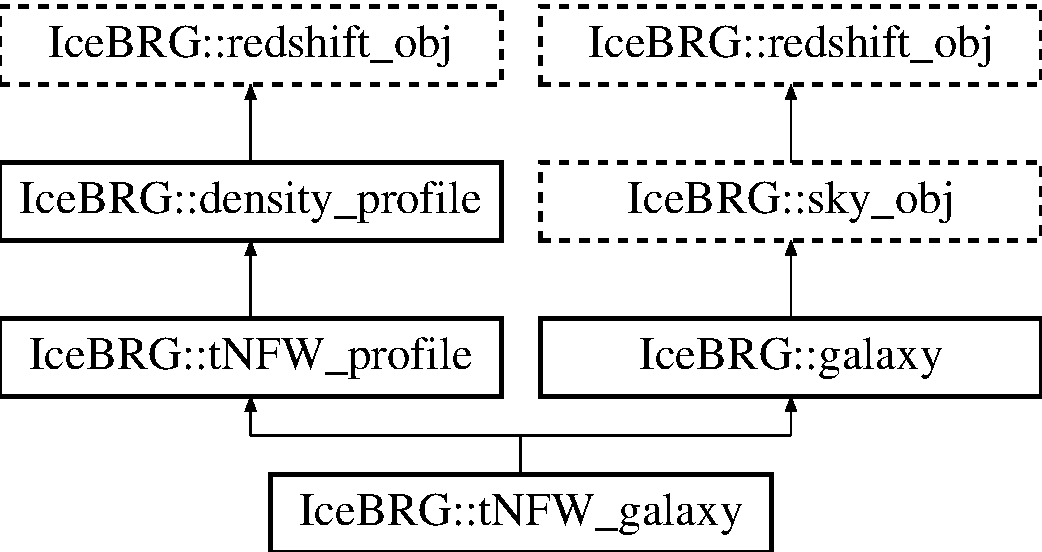
\includegraphics[height=4.000000cm]{classIceBRG_1_1tNFW__galaxy}
\end{center}
\end{figure}
\subsection*{Public Member Functions}
\begin{DoxyCompactItemize}
\item 
\hyperlink{classIceBRG_1_1tNFW__galaxy_af5746ad63480a59b1fa080be9ea280f4}{t\+N\+F\+W\+\_\+galaxy} ()
\item 
virtual \hyperlink{classIceBRG_1_1redshift__obj}{redshift\+\_\+obj} $\ast$ \hyperlink{classIceBRG_1_1tNFW__galaxy_a0ac2852b6fad29184222f58e18aff3b3}{redshift\+\_\+obj\+\_\+clone} () const 
\item 
virtual \hyperlink{classIceBRG_1_1density__profile}{density\+\_\+profile} $\ast$ \hyperlink{classIceBRG_1_1tNFW__galaxy_aa571e02cd48ac9f97f205077d29dfcf5}{density\+\_\+profile\+\_\+clone} () const 
\item 
virtual \hyperlink{classIceBRG_1_1tNFW__profile}{t\+N\+F\+W\+\_\+profile} $\ast$ \hyperlink{classIceBRG_1_1tNFW__galaxy_ae9fa3a91d493e1763ffd01b0f454df29}{t\+N\+F\+W\+\_\+profile\+\_\+clone} () const 
\item 
virtual \hyperlink{classIceBRG_1_1sky__obj}{sky\+\_\+obj} $\ast$ \hyperlink{classIceBRG_1_1tNFW__galaxy_a6699f38c68e4d330a68c2319e9429138}{sky\+\_\+obj\+\_\+clone} () const 
\item 
virtual \hyperlink{classIceBRG_1_1galaxy}{galaxy} $\ast$ \hyperlink{classIceBRG_1_1tNFW__galaxy_a636dcf8380204b86e7d850ba2465a3c1}{galaxy\+\_\+clone} () const 
\end{DoxyCompactItemize}
\subsection*{Additional Inherited Members}


\subsection{Constructor \& Destructor Documentation}
\hypertarget{classIceBRG_1_1tNFW__galaxy_af5746ad63480a59b1fa080be9ea280f4}{}\index{Ice\+B\+R\+G\+::t\+N\+F\+W\+\_\+galaxy@{Ice\+B\+R\+G\+::t\+N\+F\+W\+\_\+galaxy}!t\+N\+F\+W\+\_\+galaxy@{t\+N\+F\+W\+\_\+galaxy}}
\index{t\+N\+F\+W\+\_\+galaxy@{t\+N\+F\+W\+\_\+galaxy}!Ice\+B\+R\+G\+::t\+N\+F\+W\+\_\+galaxy@{Ice\+B\+R\+G\+::t\+N\+F\+W\+\_\+galaxy}}
\subsubsection[{t\+N\+F\+W\+\_\+galaxy()}]{\setlength{\rightskip}{0pt plus 5cm}Ice\+B\+R\+G\+::t\+N\+F\+W\+\_\+galaxy\+::t\+N\+F\+W\+\_\+galaxy (
\begin{DoxyParamCaption}
{}
\end{DoxyParamCaption}
)\hspace{0.3cm}{\ttfamily [inline]}}\label{classIceBRG_1_1tNFW__galaxy_af5746ad63480a59b1fa080be9ea280f4}


\subsection{Member Function Documentation}
\hypertarget{classIceBRG_1_1tNFW__galaxy_aa571e02cd48ac9f97f205077d29dfcf5}{}\index{Ice\+B\+R\+G\+::t\+N\+F\+W\+\_\+galaxy@{Ice\+B\+R\+G\+::t\+N\+F\+W\+\_\+galaxy}!density\+\_\+profile\+\_\+clone@{density\+\_\+profile\+\_\+clone}}
\index{density\+\_\+profile\+\_\+clone@{density\+\_\+profile\+\_\+clone}!Ice\+B\+R\+G\+::t\+N\+F\+W\+\_\+galaxy@{Ice\+B\+R\+G\+::t\+N\+F\+W\+\_\+galaxy}}
\subsubsection[{density\+\_\+profile\+\_\+clone() const }]{\setlength{\rightskip}{0pt plus 5cm}virtual {\bf density\+\_\+profile}$\ast$ Ice\+B\+R\+G\+::t\+N\+F\+W\+\_\+galaxy\+::density\+\_\+profile\+\_\+clone (
\begin{DoxyParamCaption}
{}
\end{DoxyParamCaption}
) const\hspace{0.3cm}{\ttfamily [inline]}, {\ttfamily [virtual]}}\label{classIceBRG_1_1tNFW__galaxy_aa571e02cd48ac9f97f205077d29dfcf5}


Reimplemented from \hyperlink{classIceBRG_1_1tNFW__profile_abf08721d23c2f612f92c1e97e6bf6453}{Ice\+B\+R\+G\+::t\+N\+F\+W\+\_\+profile}.

\hypertarget{classIceBRG_1_1tNFW__galaxy_a636dcf8380204b86e7d850ba2465a3c1}{}\index{Ice\+B\+R\+G\+::t\+N\+F\+W\+\_\+galaxy@{Ice\+B\+R\+G\+::t\+N\+F\+W\+\_\+galaxy}!galaxy\+\_\+clone@{galaxy\+\_\+clone}}
\index{galaxy\+\_\+clone@{galaxy\+\_\+clone}!Ice\+B\+R\+G\+::t\+N\+F\+W\+\_\+galaxy@{Ice\+B\+R\+G\+::t\+N\+F\+W\+\_\+galaxy}}
\subsubsection[{galaxy\+\_\+clone() const }]{\setlength{\rightskip}{0pt plus 5cm}virtual {\bf galaxy}$\ast$ Ice\+B\+R\+G\+::t\+N\+F\+W\+\_\+galaxy\+::galaxy\+\_\+clone (
\begin{DoxyParamCaption}
{}
\end{DoxyParamCaption}
) const\hspace{0.3cm}{\ttfamily [inline]}, {\ttfamily [virtual]}}\label{classIceBRG_1_1tNFW__galaxy_a636dcf8380204b86e7d850ba2465a3c1}


Reimplemented from \hyperlink{classIceBRG_1_1galaxy_a58037140e845c9cd31c51e5751c28792}{Ice\+B\+R\+G\+::galaxy}.

\hypertarget{classIceBRG_1_1tNFW__galaxy_a0ac2852b6fad29184222f58e18aff3b3}{}\index{Ice\+B\+R\+G\+::t\+N\+F\+W\+\_\+galaxy@{Ice\+B\+R\+G\+::t\+N\+F\+W\+\_\+galaxy}!redshift\+\_\+obj\+\_\+clone@{redshift\+\_\+obj\+\_\+clone}}
\index{redshift\+\_\+obj\+\_\+clone@{redshift\+\_\+obj\+\_\+clone}!Ice\+B\+R\+G\+::t\+N\+F\+W\+\_\+galaxy@{Ice\+B\+R\+G\+::t\+N\+F\+W\+\_\+galaxy}}
\subsubsection[{redshift\+\_\+obj\+\_\+clone() const }]{\setlength{\rightskip}{0pt plus 5cm}virtual {\bf redshift\+\_\+obj}$\ast$ Ice\+B\+R\+G\+::t\+N\+F\+W\+\_\+galaxy\+::redshift\+\_\+obj\+\_\+clone (
\begin{DoxyParamCaption}
{}
\end{DoxyParamCaption}
) const\hspace{0.3cm}{\ttfamily [inline]}, {\ttfamily [virtual]}}\label{classIceBRG_1_1tNFW__galaxy_a0ac2852b6fad29184222f58e18aff3b3}


Reimplemented from \hyperlink{classIceBRG_1_1tNFW__profile_ad7e0649c9782b10fc05cd7a24d43d325}{Ice\+B\+R\+G\+::t\+N\+F\+W\+\_\+profile}.

\hypertarget{classIceBRG_1_1tNFW__galaxy_a6699f38c68e4d330a68c2319e9429138}{}\index{Ice\+B\+R\+G\+::t\+N\+F\+W\+\_\+galaxy@{Ice\+B\+R\+G\+::t\+N\+F\+W\+\_\+galaxy}!sky\+\_\+obj\+\_\+clone@{sky\+\_\+obj\+\_\+clone}}
\index{sky\+\_\+obj\+\_\+clone@{sky\+\_\+obj\+\_\+clone}!Ice\+B\+R\+G\+::t\+N\+F\+W\+\_\+galaxy@{Ice\+B\+R\+G\+::t\+N\+F\+W\+\_\+galaxy}}
\subsubsection[{sky\+\_\+obj\+\_\+clone() const }]{\setlength{\rightskip}{0pt plus 5cm}virtual {\bf sky\+\_\+obj}$\ast$ Ice\+B\+R\+G\+::t\+N\+F\+W\+\_\+galaxy\+::sky\+\_\+obj\+\_\+clone (
\begin{DoxyParamCaption}
{}
\end{DoxyParamCaption}
) const\hspace{0.3cm}{\ttfamily [inline]}, {\ttfamily [virtual]}}\label{classIceBRG_1_1tNFW__galaxy_a6699f38c68e4d330a68c2319e9429138}


Reimplemented from \hyperlink{classIceBRG_1_1galaxy_ae6c5cfc58523edcffcf9e8bdd90bc1ad}{Ice\+B\+R\+G\+::galaxy}.

\hypertarget{classIceBRG_1_1tNFW__galaxy_ae9fa3a91d493e1763ffd01b0f454df29}{}\index{Ice\+B\+R\+G\+::t\+N\+F\+W\+\_\+galaxy@{Ice\+B\+R\+G\+::t\+N\+F\+W\+\_\+galaxy}!t\+N\+F\+W\+\_\+profile\+\_\+clone@{t\+N\+F\+W\+\_\+profile\+\_\+clone}}
\index{t\+N\+F\+W\+\_\+profile\+\_\+clone@{t\+N\+F\+W\+\_\+profile\+\_\+clone}!Ice\+B\+R\+G\+::t\+N\+F\+W\+\_\+galaxy@{Ice\+B\+R\+G\+::t\+N\+F\+W\+\_\+galaxy}}
\subsubsection[{t\+N\+F\+W\+\_\+profile\+\_\+clone() const }]{\setlength{\rightskip}{0pt plus 5cm}virtual {\bf t\+N\+F\+W\+\_\+profile}$\ast$ Ice\+B\+R\+G\+::t\+N\+F\+W\+\_\+galaxy\+::t\+N\+F\+W\+\_\+profile\+\_\+clone (
\begin{DoxyParamCaption}
{}
\end{DoxyParamCaption}
) const\hspace{0.3cm}{\ttfamily [inline]}, {\ttfamily [virtual]}}\label{classIceBRG_1_1tNFW__galaxy_ae9fa3a91d493e1763ffd01b0f454df29}


Reimplemented from \hyperlink{classIceBRG_1_1tNFW__profile_a7b652f93aa159c0bdffa657f4bfa1c46}{Ice\+B\+R\+G\+::t\+N\+F\+W\+\_\+profile}.



The documentation for this class was generated from the following file\+:\begin{DoxyCompactItemize}
\item 
/disk2/brg/git/\+Magnification\+\_\+\+Public/src/lib/\+Ice\+B\+R\+G\+\_\+physics/sky\+\_\+obj\+\_\+with\+\_\+density\+\_\+profile/\hyperlink{tNFW__galaxy_8h}{t\+N\+F\+W\+\_\+galaxy.\+h}\end{DoxyCompactItemize}

\hypertarget{classIceBRG_1_1tNFW__group__sig__cache}{\section{Ice\-B\-R\-G\-:\-:t\-N\-F\-W\-\_\-group\-\_\-sig\-\_\-cache Class Reference}
\label{classIceBRG_1_1tNFW__group__sig__cache}\index{Ice\-B\-R\-G\-::t\-N\-F\-W\-\_\-group\-\_\-sig\-\_\-cache@{Ice\-B\-R\-G\-::t\-N\-F\-W\-\_\-group\-\_\-sig\-\_\-cache}}
}


{\ttfamily \#include $<$lensing\-\_\-t\-N\-F\-W\-\_\-caches.\-h$>$}

Inheritance diagram for Ice\-B\-R\-G\-:\-:t\-N\-F\-W\-\_\-group\-\_\-sig\-\_\-cache\-:\begin{figure}[H]
\begin{center}
\leavevmode
\includegraphics[height=2.000000cm]{classIceBRG_1_1tNFW__group__sig__cache}
\end{center}
\end{figure}
\subsection*{Public Member Functions}
\begin{DoxyCompactItemize}
\item 
\hyperlink{classIceBRG_1_1tNFW__group__sig__cache_a6a4dd7e7ab2356a0e74bccc6a03d46f1}{$\sim$t\-N\-F\-W\-\_\-group\-\_\-sig\-\_\-cache} ()
\end{DoxyCompactItemize}
\subsection*{Protected Member Functions}
\begin{DoxyCompactItemize}
\item 
const std\-::string \hyperlink{classIceBRG_1_1tNFW__group__sig__cache_af13fbfb83bf04be0e895ca3bd8f215a9}{\-\_\-name\-\_\-base} () const 
\item 
void \hyperlink{classIceBRG_1_1tNFW__group__sig__cache_a000f3c95c988adeedadb8f2acd32c950}{\-\_\-load\-\_\-cache\-\_\-dependencies} () const 
\item 
\hyperlink{lib_2IceBRG__main_2common_8h_ad0f130a56eeb944d9ef2692ee881ecc4}{flt\-\_\-type} \hyperlink{classIceBRG_1_1tNFW__group__sig__cache_ae679ace3d05bf7bbb8d8ef9ca74a67b3}{\-\_\-calculate} (const \hyperlink{lib_2IceBRG__main_2common_8h_ad0f130a56eeb944d9ef2692ee881ecc4}{flt\-\_\-type} \&in\-\_\-param\-\_\-1, const \hyperlink{lib_2IceBRG__main_2common_8h_ad0f130a56eeb944d9ef2692ee881ecc4}{flt\-\_\-type} \&in\-\_\-param\-\_\-2, const \hyperlink{lib_2IceBRG__main_2common_8h_ad0f130a56eeb944d9ef2692ee881ecc4}{flt\-\_\-type} \&in\-\_\-param\-\_\-3, const \hyperlink{lib_2IceBRG__main_2common_8h_ad0f130a56eeb944d9ef2692ee881ecc4}{flt\-\_\-type} \&in\-\_\-param\-\_\-4) const 
\end{DoxyCompactItemize}
\subsection*{Friends}
\begin{DoxyCompactItemize}
\item 
class \hyperlink{classIceBRG_1_1tNFW__group__sig__cache_aa3ca0cd0a431d93e9b6650451f88b84a}{brg\-\_\-cache\-\_\-4d$<$ t\-N\-F\-W\-\_\-group\-\_\-sig\-\_\-cache $>$}
\end{DoxyCompactItemize}


\subsection{Constructor \& Destructor Documentation}
\hypertarget{classIceBRG_1_1tNFW__group__sig__cache_a6a4dd7e7ab2356a0e74bccc6a03d46f1}{\index{Ice\-B\-R\-G\-::t\-N\-F\-W\-\_\-group\-\_\-sig\-\_\-cache@{Ice\-B\-R\-G\-::t\-N\-F\-W\-\_\-group\-\_\-sig\-\_\-cache}!$\sim$t\-N\-F\-W\-\_\-group\-\_\-sig\-\_\-cache@{$\sim$t\-N\-F\-W\-\_\-group\-\_\-sig\-\_\-cache}}
\index{$\sim$t\-N\-F\-W\-\_\-group\-\_\-sig\-\_\-cache@{$\sim$t\-N\-F\-W\-\_\-group\-\_\-sig\-\_\-cache}!IceBRG::tNFW_group_sig_cache@{Ice\-B\-R\-G\-::t\-N\-F\-W\-\_\-group\-\_\-sig\-\_\-cache}}
\subsubsection[{$\sim$t\-N\-F\-W\-\_\-group\-\_\-sig\-\_\-cache}]{\setlength{\rightskip}{0pt plus 5cm}Ice\-B\-R\-G\-::t\-N\-F\-W\-\_\-group\-\_\-sig\-\_\-cache\-::$\sim$t\-N\-F\-W\-\_\-group\-\_\-sig\-\_\-cache (
\begin{DoxyParamCaption}
{}
\end{DoxyParamCaption}
)\hspace{0.3cm}{\ttfamily [inline]}}}\label{classIceBRG_1_1tNFW__group__sig__cache_a6a4dd7e7ab2356a0e74bccc6a03d46f1}


\subsection{Member Function Documentation}
\hypertarget{classIceBRG_1_1tNFW__group__sig__cache_ae679ace3d05bf7bbb8d8ef9ca74a67b3}{\index{Ice\-B\-R\-G\-::t\-N\-F\-W\-\_\-group\-\_\-sig\-\_\-cache@{Ice\-B\-R\-G\-::t\-N\-F\-W\-\_\-group\-\_\-sig\-\_\-cache}!\-\_\-calculate@{\-\_\-calculate}}
\index{\-\_\-calculate@{\-\_\-calculate}!IceBRG::tNFW_group_sig_cache@{Ice\-B\-R\-G\-::t\-N\-F\-W\-\_\-group\-\_\-sig\-\_\-cache}}
\subsubsection[{\-\_\-calculate}]{\setlength{\rightskip}{0pt plus 5cm}{\bf flt\-\_\-type} Ice\-B\-R\-G\-::t\-N\-F\-W\-\_\-group\-\_\-sig\-\_\-cache\-::\-\_\-calculate (
\begin{DoxyParamCaption}
\item[{const {\bf flt\-\_\-type} \&}]{in\-\_\-param\-\_\-1, }
\item[{const {\bf flt\-\_\-type} \&}]{in\-\_\-param\-\_\-2, }
\item[{const {\bf flt\-\_\-type} \&}]{in\-\_\-param\-\_\-3, }
\item[{const {\bf flt\-\_\-type} \&}]{in\-\_\-param\-\_\-4}
\end{DoxyParamCaption}
) const\hspace{0.3cm}{\ttfamily [protected]}}}\label{classIceBRG_1_1tNFW__group__sig__cache_ae679ace3d05bf7bbb8d8ef9ca74a67b3}


Reimplemented from \hyperlink{classIceBRG_1_1brg__cache__4d_a7c73fe2ee294ba85fe0d6d51dd0f1156}{Ice\-B\-R\-G\-::brg\-\_\-cache\-\_\-4d$<$ t\-N\-F\-W\-\_\-group\-\_\-sig\-\_\-cache $>$}.

\hypertarget{classIceBRG_1_1tNFW__group__sig__cache_a000f3c95c988adeedadb8f2acd32c950}{\index{Ice\-B\-R\-G\-::t\-N\-F\-W\-\_\-group\-\_\-sig\-\_\-cache@{Ice\-B\-R\-G\-::t\-N\-F\-W\-\_\-group\-\_\-sig\-\_\-cache}!\-\_\-load\-\_\-cache\-\_\-dependencies@{\-\_\-load\-\_\-cache\-\_\-dependencies}}
\index{\-\_\-load\-\_\-cache\-\_\-dependencies@{\-\_\-load\-\_\-cache\-\_\-dependencies}!IceBRG::tNFW_group_sig_cache@{Ice\-B\-R\-G\-::t\-N\-F\-W\-\_\-group\-\_\-sig\-\_\-cache}}
\subsubsection[{\-\_\-load\-\_\-cache\-\_\-dependencies}]{\setlength{\rightskip}{0pt plus 5cm}void Ice\-B\-R\-G\-::t\-N\-F\-W\-\_\-group\-\_\-sig\-\_\-cache\-::\-\_\-load\-\_\-cache\-\_\-dependencies (
\begin{DoxyParamCaption}
{}
\end{DoxyParamCaption}
) const\hspace{0.3cm}{\ttfamily [inline]}, {\ttfamily [protected]}}}\label{classIceBRG_1_1tNFW__group__sig__cache_a000f3c95c988adeedadb8f2acd32c950}


Reimplemented from \hyperlink{classIceBRG_1_1brg__cache__4d_af79c67f2dfccfdfbfcfed081d65e07af}{Ice\-B\-R\-G\-::brg\-\_\-cache\-\_\-4d$<$ t\-N\-F\-W\-\_\-group\-\_\-sig\-\_\-cache $>$}.

\hypertarget{classIceBRG_1_1tNFW__group__sig__cache_af13fbfb83bf04be0e895ca3bd8f215a9}{\index{Ice\-B\-R\-G\-::t\-N\-F\-W\-\_\-group\-\_\-sig\-\_\-cache@{Ice\-B\-R\-G\-::t\-N\-F\-W\-\_\-group\-\_\-sig\-\_\-cache}!\-\_\-name\-\_\-base@{\-\_\-name\-\_\-base}}
\index{\-\_\-name\-\_\-base@{\-\_\-name\-\_\-base}!IceBRG::tNFW_group_sig_cache@{Ice\-B\-R\-G\-::t\-N\-F\-W\-\_\-group\-\_\-sig\-\_\-cache}}
\subsubsection[{\-\_\-name\-\_\-base}]{\setlength{\rightskip}{0pt plus 5cm}const std\-::string Ice\-B\-R\-G\-::t\-N\-F\-W\-\_\-group\-\_\-sig\-\_\-cache\-::\-\_\-name\-\_\-base (
\begin{DoxyParamCaption}
{}
\end{DoxyParamCaption}
) const\hspace{0.3cm}{\ttfamily [inline]}, {\ttfamily [protected]}}}\label{classIceBRG_1_1tNFW__group__sig__cache_af13fbfb83bf04be0e895ca3bd8f215a9}


Reimplemented from \hyperlink{classIceBRG_1_1brg__cache__4d_a422e37f487c9c39ce42d26e3b1866693}{Ice\-B\-R\-G\-::brg\-\_\-cache\-\_\-4d$<$ t\-N\-F\-W\-\_\-group\-\_\-sig\-\_\-cache $>$}.



\subsection{Friends And Related Function Documentation}
\hypertarget{classIceBRG_1_1tNFW__group__sig__cache_aa3ca0cd0a431d93e9b6650451f88b84a}{\index{Ice\-B\-R\-G\-::t\-N\-F\-W\-\_\-group\-\_\-sig\-\_\-cache@{Ice\-B\-R\-G\-::t\-N\-F\-W\-\_\-group\-\_\-sig\-\_\-cache}!brg\-\_\-cache\-\_\-4d$<$ t\-N\-F\-W\-\_\-group\-\_\-sig\-\_\-cache $>$@{brg\-\_\-cache\-\_\-4d$<$ t\-N\-F\-W\-\_\-group\-\_\-sig\-\_\-cache $>$}}
\index{brg\-\_\-cache\-\_\-4d$<$ t\-N\-F\-W\-\_\-group\-\_\-sig\-\_\-cache $>$@{brg\-\_\-cache\-\_\-4d$<$ t\-N\-F\-W\-\_\-group\-\_\-sig\-\_\-cache $>$}!IceBRG::tNFW_group_sig_cache@{Ice\-B\-R\-G\-::t\-N\-F\-W\-\_\-group\-\_\-sig\-\_\-cache}}
\subsubsection[{brg\-\_\-cache\-\_\-4d$<$ t\-N\-F\-W\-\_\-group\-\_\-sig\-\_\-cache $>$}]{\setlength{\rightskip}{0pt plus 5cm}friend class {\bf brg\-\_\-cache\-\_\-4d}$<$ {\bf t\-N\-F\-W\-\_\-group\-\_\-sig\-\_\-cache} $>$\hspace{0.3cm}{\ttfamily [friend]}}}\label{classIceBRG_1_1tNFW__group__sig__cache_aa3ca0cd0a431d93e9b6650451f88b84a}


The documentation for this class was generated from the following files\-:\begin{DoxyCompactItemize}
\item 
/disk2/brg/git/\-Magnification\-\_\-\-Public/src/lib/\-Ice\-B\-R\-G\-\_\-lensing/\hyperlink{lensing__tNFW__caches_8h}{lensing\-\_\-t\-N\-F\-W\-\_\-caches.\-h}\item 
/disk2/brg/git/\-Magnification\-\_\-\-Public/src/lib/\-Ice\-B\-R\-G\-\_\-lensing/\hyperlink{lensing__tNFW__caches_8cpp}{lensing\-\_\-t\-N\-F\-W\-\_\-caches.\-cpp}\end{DoxyCompactItemize}

\hypertarget{classIceBRG_1_1tNFW__group__Sigma__cache}{}\section{Ice\+B\+R\+G\+:\+:t\+N\+F\+W\+\_\+group\+\_\+\+Sigma\+\_\+cache Class Reference}
\label{classIceBRG_1_1tNFW__group__Sigma__cache}\index{Ice\+B\+R\+G\+::t\+N\+F\+W\+\_\+group\+\_\+\+Sigma\+\_\+cache@{Ice\+B\+R\+G\+::t\+N\+F\+W\+\_\+group\+\_\+\+Sigma\+\_\+cache}}


{\ttfamily \#include $<$lensing\+\_\+t\+N\+F\+W\+\_\+caches.\+h$>$}

Inheritance diagram for Ice\+B\+R\+G\+:\+:t\+N\+F\+W\+\_\+group\+\_\+\+Sigma\+\_\+cache\+:\begin{figure}[H]
\begin{center}
\leavevmode
\includegraphics[height=2.000000cm]{classIceBRG_1_1tNFW__group__Sigma__cache}
\end{center}
\end{figure}
\subsection*{Public Member Functions}
\begin{DoxyCompactItemize}
\item 
\hyperlink{classIceBRG_1_1tNFW__group__Sigma__cache_ac366180ba50597dcfb66e68c75106c10}{$\sim$t\+N\+F\+W\+\_\+group\+\_\+\+Sigma\+\_\+cache} ()
\end{DoxyCompactItemize}
\subsection*{Protected Member Functions}
\begin{DoxyCompactItemize}
\item 
const std\+::string \hyperlink{classIceBRG_1_1tNFW__group__Sigma__cache_a282f8dad6e50f4e532c93f6752fddd93}{\+\_\+name\+\_\+base} () const 
\item 
void \hyperlink{classIceBRG_1_1tNFW__group__Sigma__cache_af9d40651218d6a373ceb870610b82cca}{\+\_\+load\+\_\+cache\+\_\+dependencies} () const 
\item 
\hyperlink{lib_2IceBRG__main_2common_8h_ad0f130a56eeb944d9ef2692ee881ecc4}{flt\+\_\+type} \hyperlink{classIceBRG_1_1tNFW__group__Sigma__cache_af7f054cc977c9ef587561f7a5a6ad539}{\+\_\+calculate} (const \hyperlink{lib_2IceBRG__main_2common_8h_ad0f130a56eeb944d9ef2692ee881ecc4}{flt\+\_\+type} \&in\+\_\+param\+\_\+1, const \hyperlink{lib_2IceBRG__main_2common_8h_ad0f130a56eeb944d9ef2692ee881ecc4}{flt\+\_\+type} \&in\+\_\+param\+\_\+2, const \hyperlink{lib_2IceBRG__main_2common_8h_ad0f130a56eeb944d9ef2692ee881ecc4}{flt\+\_\+type} \&in\+\_\+param\+\_\+3, const \hyperlink{lib_2IceBRG__main_2common_8h_ad0f130a56eeb944d9ef2692ee881ecc4}{flt\+\_\+type} \&in\+\_\+param\+\_\+4) const 
\end{DoxyCompactItemize}
\subsection*{Friends}
\begin{DoxyCompactItemize}
\item 
class \hyperlink{classIceBRG_1_1tNFW__group__Sigma__cache_ade8ff42c2723026057604497f2d31c9a}{brg\+\_\+cache\+\_\+4d$<$ t\+N\+F\+W\+\_\+group\+\_\+\+Sigma\+\_\+cache $>$}
\end{DoxyCompactItemize}


\subsection{Constructor \& Destructor Documentation}
\hypertarget{classIceBRG_1_1tNFW__group__Sigma__cache_ac366180ba50597dcfb66e68c75106c10}{}\index{Ice\+B\+R\+G\+::t\+N\+F\+W\+\_\+group\+\_\+\+Sigma\+\_\+cache@{Ice\+B\+R\+G\+::t\+N\+F\+W\+\_\+group\+\_\+\+Sigma\+\_\+cache}!````~t\+N\+F\+W\+\_\+group\+\_\+\+Sigma\+\_\+cache@{$\sim$t\+N\+F\+W\+\_\+group\+\_\+\+Sigma\+\_\+cache}}
\index{````~t\+N\+F\+W\+\_\+group\+\_\+\+Sigma\+\_\+cache@{$\sim$t\+N\+F\+W\+\_\+group\+\_\+\+Sigma\+\_\+cache}!Ice\+B\+R\+G\+::t\+N\+F\+W\+\_\+group\+\_\+\+Sigma\+\_\+cache@{Ice\+B\+R\+G\+::t\+N\+F\+W\+\_\+group\+\_\+\+Sigma\+\_\+cache}}
\subsubsection[{$\sim$t\+N\+F\+W\+\_\+group\+\_\+\+Sigma\+\_\+cache()}]{\setlength{\rightskip}{0pt plus 5cm}Ice\+B\+R\+G\+::t\+N\+F\+W\+\_\+group\+\_\+\+Sigma\+\_\+cache\+::$\sim$t\+N\+F\+W\+\_\+group\+\_\+\+Sigma\+\_\+cache (
\begin{DoxyParamCaption}
{}
\end{DoxyParamCaption}
)\hspace{0.3cm}{\ttfamily [inline]}}\label{classIceBRG_1_1tNFW__group__Sigma__cache_ac366180ba50597dcfb66e68c75106c10}


\subsection{Member Function Documentation}
\hypertarget{classIceBRG_1_1tNFW__group__Sigma__cache_af7f054cc977c9ef587561f7a5a6ad539}{}\index{Ice\+B\+R\+G\+::t\+N\+F\+W\+\_\+group\+\_\+\+Sigma\+\_\+cache@{Ice\+B\+R\+G\+::t\+N\+F\+W\+\_\+group\+\_\+\+Sigma\+\_\+cache}!\+\_\+calculate@{\+\_\+calculate}}
\index{\+\_\+calculate@{\+\_\+calculate}!Ice\+B\+R\+G\+::t\+N\+F\+W\+\_\+group\+\_\+\+Sigma\+\_\+cache@{Ice\+B\+R\+G\+::t\+N\+F\+W\+\_\+group\+\_\+\+Sigma\+\_\+cache}}
\subsubsection[{\+\_\+calculate(const flt\+\_\+type \&in\+\_\+param\+\_\+1, const flt\+\_\+type \&in\+\_\+param\+\_\+2, const flt\+\_\+type \&in\+\_\+param\+\_\+3, const flt\+\_\+type \&in\+\_\+param\+\_\+4) const }]{\setlength{\rightskip}{0pt plus 5cm}{\bf flt\+\_\+type} Ice\+B\+R\+G\+::t\+N\+F\+W\+\_\+group\+\_\+\+Sigma\+\_\+cache\+::\+\_\+calculate (
\begin{DoxyParamCaption}
\item[{const {\bf flt\+\_\+type} \&}]{in\+\_\+param\+\_\+1, }
\item[{const {\bf flt\+\_\+type} \&}]{in\+\_\+param\+\_\+2, }
\item[{const {\bf flt\+\_\+type} \&}]{in\+\_\+param\+\_\+3, }
\item[{const {\bf flt\+\_\+type} \&}]{in\+\_\+param\+\_\+4}
\end{DoxyParamCaption}
) const\hspace{0.3cm}{\ttfamily [protected]}}\label{classIceBRG_1_1tNFW__group__Sigma__cache_af7f054cc977c9ef587561f7a5a6ad539}
\hypertarget{classIceBRG_1_1tNFW__group__Sigma__cache_af9d40651218d6a373ceb870610b82cca}{}\index{Ice\+B\+R\+G\+::t\+N\+F\+W\+\_\+group\+\_\+\+Sigma\+\_\+cache@{Ice\+B\+R\+G\+::t\+N\+F\+W\+\_\+group\+\_\+\+Sigma\+\_\+cache}!\+\_\+load\+\_\+cache\+\_\+dependencies@{\+\_\+load\+\_\+cache\+\_\+dependencies}}
\index{\+\_\+load\+\_\+cache\+\_\+dependencies@{\+\_\+load\+\_\+cache\+\_\+dependencies}!Ice\+B\+R\+G\+::t\+N\+F\+W\+\_\+group\+\_\+\+Sigma\+\_\+cache@{Ice\+B\+R\+G\+::t\+N\+F\+W\+\_\+group\+\_\+\+Sigma\+\_\+cache}}
\subsubsection[{\+\_\+load\+\_\+cache\+\_\+dependencies() const }]{\setlength{\rightskip}{0pt plus 5cm}void Ice\+B\+R\+G\+::t\+N\+F\+W\+\_\+group\+\_\+\+Sigma\+\_\+cache\+::\+\_\+load\+\_\+cache\+\_\+dependencies (
\begin{DoxyParamCaption}
{}
\end{DoxyParamCaption}
) const\hspace{0.3cm}{\ttfamily [inline]}, {\ttfamily [protected]}}\label{classIceBRG_1_1tNFW__group__Sigma__cache_af9d40651218d6a373ceb870610b82cca}
\hypertarget{classIceBRG_1_1tNFW__group__Sigma__cache_a282f8dad6e50f4e532c93f6752fddd93}{}\index{Ice\+B\+R\+G\+::t\+N\+F\+W\+\_\+group\+\_\+\+Sigma\+\_\+cache@{Ice\+B\+R\+G\+::t\+N\+F\+W\+\_\+group\+\_\+\+Sigma\+\_\+cache}!\+\_\+name\+\_\+base@{\+\_\+name\+\_\+base}}
\index{\+\_\+name\+\_\+base@{\+\_\+name\+\_\+base}!Ice\+B\+R\+G\+::t\+N\+F\+W\+\_\+group\+\_\+\+Sigma\+\_\+cache@{Ice\+B\+R\+G\+::t\+N\+F\+W\+\_\+group\+\_\+\+Sigma\+\_\+cache}}
\subsubsection[{\+\_\+name\+\_\+base() const }]{\setlength{\rightskip}{0pt plus 5cm}const std\+::string Ice\+B\+R\+G\+::t\+N\+F\+W\+\_\+group\+\_\+\+Sigma\+\_\+cache\+::\+\_\+name\+\_\+base (
\begin{DoxyParamCaption}
{}
\end{DoxyParamCaption}
) const\hspace{0.3cm}{\ttfamily [inline]}, {\ttfamily [protected]}}\label{classIceBRG_1_1tNFW__group__Sigma__cache_a282f8dad6e50f4e532c93f6752fddd93}


\subsection{Friends And Related Function Documentation}
\hypertarget{classIceBRG_1_1tNFW__group__Sigma__cache_ade8ff42c2723026057604497f2d31c9a}{}\index{Ice\+B\+R\+G\+::t\+N\+F\+W\+\_\+group\+\_\+\+Sigma\+\_\+cache@{Ice\+B\+R\+G\+::t\+N\+F\+W\+\_\+group\+\_\+\+Sigma\+\_\+cache}!brg\+\_\+cache\+\_\+4d$<$ t\+N\+F\+W\+\_\+group\+\_\+\+Sigma\+\_\+cache $>$@{brg\+\_\+cache\+\_\+4d$<$ t\+N\+F\+W\+\_\+group\+\_\+\+Sigma\+\_\+cache $>$}}
\index{brg\+\_\+cache\+\_\+4d$<$ t\+N\+F\+W\+\_\+group\+\_\+\+Sigma\+\_\+cache $>$@{brg\+\_\+cache\+\_\+4d$<$ t\+N\+F\+W\+\_\+group\+\_\+\+Sigma\+\_\+cache $>$}!Ice\+B\+R\+G\+::t\+N\+F\+W\+\_\+group\+\_\+\+Sigma\+\_\+cache@{Ice\+B\+R\+G\+::t\+N\+F\+W\+\_\+group\+\_\+\+Sigma\+\_\+cache}}
\subsubsection[{brg\+\_\+cache\+\_\+4d$<$ t\+N\+F\+W\+\_\+group\+\_\+\+Sigma\+\_\+cache $>$}]{\setlength{\rightskip}{0pt plus 5cm}friend class {\bf brg\+\_\+cache\+\_\+4d}$<$ {\bf t\+N\+F\+W\+\_\+group\+\_\+\+Sigma\+\_\+cache} $>$\hspace{0.3cm}{\ttfamily [friend]}}\label{classIceBRG_1_1tNFW__group__Sigma__cache_ade8ff42c2723026057604497f2d31c9a}


The documentation for this class was generated from the following files\+:\begin{DoxyCompactItemize}
\item 
/disk2/brg/git/\+Magnification\+\_\+\+Public/src/lib/\+Ice\+B\+R\+G\+\_\+lensing/\hyperlink{lensing__tNFW__caches_8h}{lensing\+\_\+t\+N\+F\+W\+\_\+caches.\+h}\item 
/disk2/brg/git/\+Magnification\+\_\+\+Public/src/lib/\+Ice\+B\+R\+G\+\_\+lensing/\hyperlink{lensing__tNFW__caches_8cpp}{lensing\+\_\+t\+N\+F\+W\+\_\+caches.\+cpp}\end{DoxyCompactItemize}

\hypertarget{classIceBRG_1_1tNFW__offset__sig__cache}{}\section{Ice\+B\+R\+G\+:\+:t\+N\+F\+W\+\_\+offset\+\_\+sig\+\_\+cache Class Reference}
\label{classIceBRG_1_1tNFW__offset__sig__cache}\index{Ice\+B\+R\+G\+::t\+N\+F\+W\+\_\+offset\+\_\+sig\+\_\+cache@{Ice\+B\+R\+G\+::t\+N\+F\+W\+\_\+offset\+\_\+sig\+\_\+cache}}


{\ttfamily \#include $<$lensing\+\_\+t\+N\+F\+W\+\_\+caches.\+h$>$}

Inheritance diagram for Ice\+B\+R\+G\+:\+:t\+N\+F\+W\+\_\+offset\+\_\+sig\+\_\+cache\+:\begin{figure}[H]
\begin{center}
\leavevmode
\includegraphics[height=2.000000cm]{classIceBRG_1_1tNFW__offset__sig__cache}
\end{center}
\end{figure}
\subsection*{Public Member Functions}
\begin{DoxyCompactItemize}
\item 
\hyperlink{classIceBRG_1_1tNFW__offset__sig__cache_ae6477deb6a2e6449d4cce2a92053fc69}{$\sim$t\+N\+F\+W\+\_\+offset\+\_\+sig\+\_\+cache} ()
\end{DoxyCompactItemize}
\subsection*{Protected Member Functions}
\begin{DoxyCompactItemize}
\item 
const std\+::string \hyperlink{classIceBRG_1_1tNFW__offset__sig__cache_a93e0baf8668ed0e6f420e64ce5b0d105}{\+\_\+name\+\_\+base} () const 
\item 
\hyperlink{lib_2IceBRG__main_2common_8h_ad0f130a56eeb944d9ef2692ee881ecc4}{flt\+\_\+type} \hyperlink{classIceBRG_1_1tNFW__offset__sig__cache_a724eb5a7817521a54fbe7e7e01db1ac0}{\+\_\+calculate} (const \hyperlink{lib_2IceBRG__main_2common_8h_ad0f130a56eeb944d9ef2692ee881ecc4}{flt\+\_\+type} \&in\+\_\+param\+\_\+1, const \hyperlink{lib_2IceBRG__main_2common_8h_ad0f130a56eeb944d9ef2692ee881ecc4}{flt\+\_\+type} \&in\+\_\+param\+\_\+2, const \hyperlink{lib_2IceBRG__main_2common_8h_ad0f130a56eeb944d9ef2692ee881ecc4}{flt\+\_\+type} \&in\+\_\+param\+\_\+3, const \hyperlink{lib_2IceBRG__main_2common_8h_ad0f130a56eeb944d9ef2692ee881ecc4}{flt\+\_\+type} \&in\+\_\+param\+\_\+4) const 
\end{DoxyCompactItemize}
\subsection*{Friends}
\begin{DoxyCompactItemize}
\item 
class \hyperlink{classIceBRG_1_1tNFW__offset__sig__cache_a2eb544ffcd492a0d9b3b8b21e832c03b}{brg\+\_\+cache\+\_\+4d$<$ t\+N\+F\+W\+\_\+offset\+\_\+sig\+\_\+cache $>$}
\end{DoxyCompactItemize}


\subsection{Constructor \& Destructor Documentation}
\hypertarget{classIceBRG_1_1tNFW__offset__sig__cache_ae6477deb6a2e6449d4cce2a92053fc69}{}\index{Ice\+B\+R\+G\+::t\+N\+F\+W\+\_\+offset\+\_\+sig\+\_\+cache@{Ice\+B\+R\+G\+::t\+N\+F\+W\+\_\+offset\+\_\+sig\+\_\+cache}!````~t\+N\+F\+W\+\_\+offset\+\_\+sig\+\_\+cache@{$\sim$t\+N\+F\+W\+\_\+offset\+\_\+sig\+\_\+cache}}
\index{````~t\+N\+F\+W\+\_\+offset\+\_\+sig\+\_\+cache@{$\sim$t\+N\+F\+W\+\_\+offset\+\_\+sig\+\_\+cache}!Ice\+B\+R\+G\+::t\+N\+F\+W\+\_\+offset\+\_\+sig\+\_\+cache@{Ice\+B\+R\+G\+::t\+N\+F\+W\+\_\+offset\+\_\+sig\+\_\+cache}}
\subsubsection[{$\sim$t\+N\+F\+W\+\_\+offset\+\_\+sig\+\_\+cache()}]{\setlength{\rightskip}{0pt plus 5cm}Ice\+B\+R\+G\+::t\+N\+F\+W\+\_\+offset\+\_\+sig\+\_\+cache\+::$\sim$t\+N\+F\+W\+\_\+offset\+\_\+sig\+\_\+cache (
\begin{DoxyParamCaption}
{}
\end{DoxyParamCaption}
)\hspace{0.3cm}{\ttfamily [inline]}}\label{classIceBRG_1_1tNFW__offset__sig__cache_ae6477deb6a2e6449d4cce2a92053fc69}


\subsection{Member Function Documentation}
\hypertarget{classIceBRG_1_1tNFW__offset__sig__cache_a724eb5a7817521a54fbe7e7e01db1ac0}{}\index{Ice\+B\+R\+G\+::t\+N\+F\+W\+\_\+offset\+\_\+sig\+\_\+cache@{Ice\+B\+R\+G\+::t\+N\+F\+W\+\_\+offset\+\_\+sig\+\_\+cache}!\+\_\+calculate@{\+\_\+calculate}}
\index{\+\_\+calculate@{\+\_\+calculate}!Ice\+B\+R\+G\+::t\+N\+F\+W\+\_\+offset\+\_\+sig\+\_\+cache@{Ice\+B\+R\+G\+::t\+N\+F\+W\+\_\+offset\+\_\+sig\+\_\+cache}}
\subsubsection[{\+\_\+calculate(const flt\+\_\+type \&in\+\_\+param\+\_\+1, const flt\+\_\+type \&in\+\_\+param\+\_\+2, const flt\+\_\+type \&in\+\_\+param\+\_\+3, const flt\+\_\+type \&in\+\_\+param\+\_\+4) const }]{\setlength{\rightskip}{0pt plus 5cm}{\bf flt\+\_\+type} Ice\+B\+R\+G\+::t\+N\+F\+W\+\_\+offset\+\_\+sig\+\_\+cache\+::\+\_\+calculate (
\begin{DoxyParamCaption}
\item[{const {\bf flt\+\_\+type} \&}]{in\+\_\+param\+\_\+1, }
\item[{const {\bf flt\+\_\+type} \&}]{in\+\_\+param\+\_\+2, }
\item[{const {\bf flt\+\_\+type} \&}]{in\+\_\+param\+\_\+3, }
\item[{const {\bf flt\+\_\+type} \&}]{in\+\_\+param\+\_\+4}
\end{DoxyParamCaption}
) const\hspace{0.3cm}{\ttfamily [protected]}}\label{classIceBRG_1_1tNFW__offset__sig__cache_a724eb5a7817521a54fbe7e7e01db1ac0}
\hypertarget{classIceBRG_1_1tNFW__offset__sig__cache_a93e0baf8668ed0e6f420e64ce5b0d105}{}\index{Ice\+B\+R\+G\+::t\+N\+F\+W\+\_\+offset\+\_\+sig\+\_\+cache@{Ice\+B\+R\+G\+::t\+N\+F\+W\+\_\+offset\+\_\+sig\+\_\+cache}!\+\_\+name\+\_\+base@{\+\_\+name\+\_\+base}}
\index{\+\_\+name\+\_\+base@{\+\_\+name\+\_\+base}!Ice\+B\+R\+G\+::t\+N\+F\+W\+\_\+offset\+\_\+sig\+\_\+cache@{Ice\+B\+R\+G\+::t\+N\+F\+W\+\_\+offset\+\_\+sig\+\_\+cache}}
\subsubsection[{\+\_\+name\+\_\+base() const }]{\setlength{\rightskip}{0pt plus 5cm}const std\+::string Ice\+B\+R\+G\+::t\+N\+F\+W\+\_\+offset\+\_\+sig\+\_\+cache\+::\+\_\+name\+\_\+base (
\begin{DoxyParamCaption}
{}
\end{DoxyParamCaption}
) const\hspace{0.3cm}{\ttfamily [inline]}, {\ttfamily [protected]}}\label{classIceBRG_1_1tNFW__offset__sig__cache_a93e0baf8668ed0e6f420e64ce5b0d105}


\subsection{Friends And Related Function Documentation}
\hypertarget{classIceBRG_1_1tNFW__offset__sig__cache_a2eb544ffcd492a0d9b3b8b21e832c03b}{}\index{Ice\+B\+R\+G\+::t\+N\+F\+W\+\_\+offset\+\_\+sig\+\_\+cache@{Ice\+B\+R\+G\+::t\+N\+F\+W\+\_\+offset\+\_\+sig\+\_\+cache}!brg\+\_\+cache\+\_\+4d$<$ t\+N\+F\+W\+\_\+offset\+\_\+sig\+\_\+cache $>$@{brg\+\_\+cache\+\_\+4d$<$ t\+N\+F\+W\+\_\+offset\+\_\+sig\+\_\+cache $>$}}
\index{brg\+\_\+cache\+\_\+4d$<$ t\+N\+F\+W\+\_\+offset\+\_\+sig\+\_\+cache $>$@{brg\+\_\+cache\+\_\+4d$<$ t\+N\+F\+W\+\_\+offset\+\_\+sig\+\_\+cache $>$}!Ice\+B\+R\+G\+::t\+N\+F\+W\+\_\+offset\+\_\+sig\+\_\+cache@{Ice\+B\+R\+G\+::t\+N\+F\+W\+\_\+offset\+\_\+sig\+\_\+cache}}
\subsubsection[{brg\+\_\+cache\+\_\+4d$<$ t\+N\+F\+W\+\_\+offset\+\_\+sig\+\_\+cache $>$}]{\setlength{\rightskip}{0pt plus 5cm}friend class {\bf brg\+\_\+cache\+\_\+4d}$<$ {\bf t\+N\+F\+W\+\_\+offset\+\_\+sig\+\_\+cache} $>$\hspace{0.3cm}{\ttfamily [friend]}}\label{classIceBRG_1_1tNFW__offset__sig__cache_a2eb544ffcd492a0d9b3b8b21e832c03b}


The documentation for this class was generated from the following files\+:\begin{DoxyCompactItemize}
\item 
/disk2/brg/git/\+Magnification\+\_\+\+Public/src/lib/\+Ice\+B\+R\+G\+\_\+lensing/\hyperlink{lensing__tNFW__caches_8h}{lensing\+\_\+t\+N\+F\+W\+\_\+caches.\+h}\item 
/disk2/brg/git/\+Magnification\+\_\+\+Public/src/lib/\+Ice\+B\+R\+G\+\_\+lensing/\hyperlink{lensing__tNFW__caches_8cpp}{lensing\+\_\+t\+N\+F\+W\+\_\+caches.\+cpp}\end{DoxyCompactItemize}

\hypertarget{classIceBRG_1_1tNFW__offset__Sigma__cache}{\section{Ice\-B\-R\-G\-:\-:t\-N\-F\-W\-\_\-offset\-\_\-\-Sigma\-\_\-cache Class Reference}
\label{classIceBRG_1_1tNFW__offset__Sigma__cache}\index{Ice\-B\-R\-G\-::t\-N\-F\-W\-\_\-offset\-\_\-\-Sigma\-\_\-cache@{Ice\-B\-R\-G\-::t\-N\-F\-W\-\_\-offset\-\_\-\-Sigma\-\_\-cache}}
}


{\ttfamily \#include $<$lensing\-\_\-t\-N\-F\-W\-\_\-caches.\-h$>$}

Inheritance diagram for Ice\-B\-R\-G\-:\-:t\-N\-F\-W\-\_\-offset\-\_\-\-Sigma\-\_\-cache\-:\begin{figure}[H]
\begin{center}
\leavevmode
\includegraphics[height=2.000000cm]{classIceBRG_1_1tNFW__offset__Sigma__cache}
\end{center}
\end{figure}
\subsection*{Public Member Functions}
\begin{DoxyCompactItemize}
\item 
\hyperlink{classIceBRG_1_1tNFW__offset__Sigma__cache_a13dd2428c8cf0b54f1b97aea7e5edb63}{$\sim$t\-N\-F\-W\-\_\-offset\-\_\-\-Sigma\-\_\-cache} ()
\end{DoxyCompactItemize}
\subsection*{Protected Member Functions}
\begin{DoxyCompactItemize}
\item 
const std\-::string \hyperlink{classIceBRG_1_1tNFW__offset__Sigma__cache_a8880eaf40b9befee40ad062029d90766}{\-\_\-name\-\_\-base} () const 
\item 
\hyperlink{lib_2IceBRG__main_2common_8h_ad0f130a56eeb944d9ef2692ee881ecc4}{flt\-\_\-type} \hyperlink{classIceBRG_1_1tNFW__offset__Sigma__cache_ad21361cf013e2da85ac26a85af773b94}{\-\_\-calculate} (const \hyperlink{lib_2IceBRG__main_2common_8h_ad0f130a56eeb944d9ef2692ee881ecc4}{flt\-\_\-type} \&in\-\_\-param\-\_\-1, const \hyperlink{lib_2IceBRG__main_2common_8h_ad0f130a56eeb944d9ef2692ee881ecc4}{flt\-\_\-type} \&in\-\_\-param\-\_\-2, const \hyperlink{lib_2IceBRG__main_2common_8h_ad0f130a56eeb944d9ef2692ee881ecc4}{flt\-\_\-type} \&in\-\_\-param\-\_\-3, const \hyperlink{lib_2IceBRG__main_2common_8h_ad0f130a56eeb944d9ef2692ee881ecc4}{flt\-\_\-type} \&in\-\_\-param\-\_\-4) const 
\end{DoxyCompactItemize}
\subsection*{Friends}
\begin{DoxyCompactItemize}
\item 
class \hyperlink{classIceBRG_1_1tNFW__offset__Sigma__cache_a070c97d6c85feabe82ca95b429759bbc}{brg\-\_\-cache\-\_\-4d$<$ t\-N\-F\-W\-\_\-offset\-\_\-\-Sigma\-\_\-cache $>$}
\end{DoxyCompactItemize}


\subsection{Constructor \& Destructor Documentation}
\hypertarget{classIceBRG_1_1tNFW__offset__Sigma__cache_a13dd2428c8cf0b54f1b97aea7e5edb63}{\index{Ice\-B\-R\-G\-::t\-N\-F\-W\-\_\-offset\-\_\-\-Sigma\-\_\-cache@{Ice\-B\-R\-G\-::t\-N\-F\-W\-\_\-offset\-\_\-\-Sigma\-\_\-cache}!$\sim$t\-N\-F\-W\-\_\-offset\-\_\-\-Sigma\-\_\-cache@{$\sim$t\-N\-F\-W\-\_\-offset\-\_\-\-Sigma\-\_\-cache}}
\index{$\sim$t\-N\-F\-W\-\_\-offset\-\_\-\-Sigma\-\_\-cache@{$\sim$t\-N\-F\-W\-\_\-offset\-\_\-\-Sigma\-\_\-cache}!IceBRG::tNFW_offset_Sigma_cache@{Ice\-B\-R\-G\-::t\-N\-F\-W\-\_\-offset\-\_\-\-Sigma\-\_\-cache}}
\subsubsection[{$\sim$t\-N\-F\-W\-\_\-offset\-\_\-\-Sigma\-\_\-cache}]{\setlength{\rightskip}{0pt plus 5cm}Ice\-B\-R\-G\-::t\-N\-F\-W\-\_\-offset\-\_\-\-Sigma\-\_\-cache\-::$\sim$t\-N\-F\-W\-\_\-offset\-\_\-\-Sigma\-\_\-cache (
\begin{DoxyParamCaption}
{}
\end{DoxyParamCaption}
)\hspace{0.3cm}{\ttfamily [inline]}}}\label{classIceBRG_1_1tNFW__offset__Sigma__cache_a13dd2428c8cf0b54f1b97aea7e5edb63}


\subsection{Member Function Documentation}
\hypertarget{classIceBRG_1_1tNFW__offset__Sigma__cache_ad21361cf013e2da85ac26a85af773b94}{\index{Ice\-B\-R\-G\-::t\-N\-F\-W\-\_\-offset\-\_\-\-Sigma\-\_\-cache@{Ice\-B\-R\-G\-::t\-N\-F\-W\-\_\-offset\-\_\-\-Sigma\-\_\-cache}!\-\_\-calculate@{\-\_\-calculate}}
\index{\-\_\-calculate@{\-\_\-calculate}!IceBRG::tNFW_offset_Sigma_cache@{Ice\-B\-R\-G\-::t\-N\-F\-W\-\_\-offset\-\_\-\-Sigma\-\_\-cache}}
\subsubsection[{\-\_\-calculate}]{\setlength{\rightskip}{0pt plus 5cm}{\bf flt\-\_\-type} Ice\-B\-R\-G\-::t\-N\-F\-W\-\_\-offset\-\_\-\-Sigma\-\_\-cache\-::\-\_\-calculate (
\begin{DoxyParamCaption}
\item[{const {\bf flt\-\_\-type} \&}]{in\-\_\-param\-\_\-1, }
\item[{const {\bf flt\-\_\-type} \&}]{in\-\_\-param\-\_\-2, }
\item[{const {\bf flt\-\_\-type} \&}]{in\-\_\-param\-\_\-3, }
\item[{const {\bf flt\-\_\-type} \&}]{in\-\_\-param\-\_\-4}
\end{DoxyParamCaption}
) const\hspace{0.3cm}{\ttfamily [protected]}}}\label{classIceBRG_1_1tNFW__offset__Sigma__cache_ad21361cf013e2da85ac26a85af773b94}


Reimplemented from \hyperlink{classIceBRG_1_1brg__cache__4d_a7c73fe2ee294ba85fe0d6d51dd0f1156}{Ice\-B\-R\-G\-::brg\-\_\-cache\-\_\-4d$<$ t\-N\-F\-W\-\_\-offset\-\_\-\-Sigma\-\_\-cache $>$}.

\hypertarget{classIceBRG_1_1tNFW__offset__Sigma__cache_a8880eaf40b9befee40ad062029d90766}{\index{Ice\-B\-R\-G\-::t\-N\-F\-W\-\_\-offset\-\_\-\-Sigma\-\_\-cache@{Ice\-B\-R\-G\-::t\-N\-F\-W\-\_\-offset\-\_\-\-Sigma\-\_\-cache}!\-\_\-name\-\_\-base@{\-\_\-name\-\_\-base}}
\index{\-\_\-name\-\_\-base@{\-\_\-name\-\_\-base}!IceBRG::tNFW_offset_Sigma_cache@{Ice\-B\-R\-G\-::t\-N\-F\-W\-\_\-offset\-\_\-\-Sigma\-\_\-cache}}
\subsubsection[{\-\_\-name\-\_\-base}]{\setlength{\rightskip}{0pt plus 5cm}const std\-::string Ice\-B\-R\-G\-::t\-N\-F\-W\-\_\-offset\-\_\-\-Sigma\-\_\-cache\-::\-\_\-name\-\_\-base (
\begin{DoxyParamCaption}
{}
\end{DoxyParamCaption}
) const\hspace{0.3cm}{\ttfamily [inline]}, {\ttfamily [protected]}}}\label{classIceBRG_1_1tNFW__offset__Sigma__cache_a8880eaf40b9befee40ad062029d90766}


Reimplemented from \hyperlink{classIceBRG_1_1brg__cache__4d_a422e37f487c9c39ce42d26e3b1866693}{Ice\-B\-R\-G\-::brg\-\_\-cache\-\_\-4d$<$ t\-N\-F\-W\-\_\-offset\-\_\-\-Sigma\-\_\-cache $>$}.



\subsection{Friends And Related Function Documentation}
\hypertarget{classIceBRG_1_1tNFW__offset__Sigma__cache_a070c97d6c85feabe82ca95b429759bbc}{\index{Ice\-B\-R\-G\-::t\-N\-F\-W\-\_\-offset\-\_\-\-Sigma\-\_\-cache@{Ice\-B\-R\-G\-::t\-N\-F\-W\-\_\-offset\-\_\-\-Sigma\-\_\-cache}!brg\-\_\-cache\-\_\-4d$<$ t\-N\-F\-W\-\_\-offset\-\_\-\-Sigma\-\_\-cache $>$@{brg\-\_\-cache\-\_\-4d$<$ t\-N\-F\-W\-\_\-offset\-\_\-\-Sigma\-\_\-cache $>$}}
\index{brg\-\_\-cache\-\_\-4d$<$ t\-N\-F\-W\-\_\-offset\-\_\-\-Sigma\-\_\-cache $>$@{brg\-\_\-cache\-\_\-4d$<$ t\-N\-F\-W\-\_\-offset\-\_\-\-Sigma\-\_\-cache $>$}!IceBRG::tNFW_offset_Sigma_cache@{Ice\-B\-R\-G\-::t\-N\-F\-W\-\_\-offset\-\_\-\-Sigma\-\_\-cache}}
\subsubsection[{brg\-\_\-cache\-\_\-4d$<$ t\-N\-F\-W\-\_\-offset\-\_\-\-Sigma\-\_\-cache $>$}]{\setlength{\rightskip}{0pt plus 5cm}friend class {\bf brg\-\_\-cache\-\_\-4d}$<$ {\bf t\-N\-F\-W\-\_\-offset\-\_\-\-Sigma\-\_\-cache} $>$\hspace{0.3cm}{\ttfamily [friend]}}}\label{classIceBRG_1_1tNFW__offset__Sigma__cache_a070c97d6c85feabe82ca95b429759bbc}


The documentation for this class was generated from the following files\-:\begin{DoxyCompactItemize}
\item 
/disk2/brg/git/\-Magnification\-\_\-\-Public/src/lib/\-Ice\-B\-R\-G\-\_\-lensing/\hyperlink{lensing__tNFW__caches_8h}{lensing\-\_\-t\-N\-F\-W\-\_\-caches.\-h}\item 
/disk2/brg/git/\-Magnification\-\_\-\-Public/src/lib/\-Ice\-B\-R\-G\-\_\-lensing/\hyperlink{lensing__tNFW__caches_8cpp}{lensing\-\_\-t\-N\-F\-W\-\_\-caches.\-cpp}\end{DoxyCompactItemize}

\hypertarget{classIceBRG_1_1tNFW__profile}{}\section{Ice\+B\+R\+G\+:\+:t\+N\+F\+W\+\_\+profile Class Reference}
\label{classIceBRG_1_1tNFW__profile}\index{Ice\+B\+R\+G\+::t\+N\+F\+W\+\_\+profile@{Ice\+B\+R\+G\+::t\+N\+F\+W\+\_\+profile}}


{\ttfamily \#include $<$t\+N\+F\+W\+\_\+profile.\+h$>$}

Inheritance diagram for Ice\+B\+R\+G\+:\+:t\+N\+F\+W\+\_\+profile\+:\begin{figure}[H]
\begin{center}
\leavevmode
\includegraphics[height=4.000000cm]{classIceBRG_1_1tNFW__profile}
\end{center}
\end{figure}
\subsection*{Public Member Functions}
\begin{DoxyCompactItemize}
\item 
\hyperlink{classIceBRG_1_1tNFW__profile_ae0daa0942c5f26a60ea5376c7bbbf8a3}{t\+N\+F\+W\+\_\+profile} ()
\item 
\hyperlink{classIceBRG_1_1tNFW__profile_a513f0492cf5d3391ebabdd0585f7eff1}{t\+N\+F\+W\+\_\+profile} (const \hyperlink{namespaceIceBRG_a1be72ac4918a9b029f2eefa084213e35}{mass\+\_\+type} \&init\+\_\+mvir0, const \hyperlink{lib_2IceBRG__main_2common_8h_ad0f130a56eeb944d9ef2692ee881ecc4}{flt\+\_\+type} \&init\+\_\+z=0, const \hyperlink{lib_2IceBRG__main_2common_8h_ad0f130a56eeb944d9ef2692ee881ecc4}{flt\+\_\+type} \&init\+\_\+c=-\/1, const \hyperlink{lib_2IceBRG__main_2common_8h_ad0f130a56eeb944d9ef2692ee881ecc4}{flt\+\_\+type} \&init\+\_\+tau=-\/1)
\item 
virtual \hyperlink{classIceBRG_1_1tNFW__profile_a40267497dbb33ec3fc33095e91714154}{$\sim$t\+N\+F\+W\+\_\+profile} ()
\item 
virtual void \hyperlink{classIceBRG_1_1tNFW__profile_ab2a95dcaff2589e25d4892267fe765ce}{set\+\_\+mvir} (const \hyperlink{namespaceIceBRG_a1be72ac4918a9b029f2eefa084213e35}{mass\+\_\+type} \&new\+\_\+halo\+\_\+mass=false) override
\item 
virtual void \hyperlink{classIceBRG_1_1tNFW__profile_a80de1f502ac7deb9d8d993564fefb5cd}{set\+\_\+parameters} (const std\+::vector$<$ \hyperlink{namespaceIceBRG_a3101fc159e191fa99c4ec14e445df96e}{any\+\_\+units\+\_\+type} $>$ \&new\+\_\+parameters) override
\item 
virtual void \hyperlink{classIceBRG_1_1tNFW__profile_a4bfeb583dee286c98a14b826f912684a}{set\+\_\+z} (const \hyperlink{lib_2IceBRG__main_2common_8h_ad0f130a56eeb944d9ef2692ee881ecc4}{flt\+\_\+type} \&new\+\_\+z) override
\item 
virtual void \hyperlink{classIceBRG_1_1tNFW__profile_ae17b380bde747f52bd09ccd9137b8f80}{set\+\_\+tau} (const \hyperlink{lib_2IceBRG__main_2common_8h_ad0f130a56eeb944d9ef2692ee881ecc4}{flt\+\_\+type} \&new\+\_\+halo\+\_\+tau) override
\item 
virtual void \hyperlink{classIceBRG_1_1tNFW__profile_a1bfe72b182d4794a16bdd827ad5bcd79}{set\+\_\+c} (const \hyperlink{lib_2IceBRG__main_2common_8h_ad0f130a56eeb944d9ef2692ee881ecc4}{flt\+\_\+type} \&new\+\_\+halo\+\_\+c) override
\item 
virtual \hyperlink{namespaceIceBRG_a1be72ac4918a9b029f2eefa084213e35}{mass\+\_\+type} \hyperlink{classIceBRG_1_1tNFW__profile_aaa10d679c4d68b608213391ad207a9e8}{mvir} () const  override
\item 
const \hyperlink{namespaceIceBRG_a1be72ac4918a9b029f2eefa084213e35}{mass\+\_\+type} \& \hyperlink{classIceBRG_1_1tNFW__profile_a10d263889719dad83c3427418f500398}{mvir0} () const 
\item 
virtual \hyperlink{namespaceIceBRG_a1be72ac4918a9b029f2eefa084213e35}{mass\+\_\+type} \hyperlink{classIceBRG_1_1tNFW__profile_a8bb04b5e598b5d7ecb7d54c99383fdf6}{mtot} () const  override
\item 
virtual \hyperlink{namespaceIceBRG_a45499647eb87e24c10ab32c628711cec}{distance\+\_\+type} \hyperlink{classIceBRG_1_1tNFW__profile_a11c1a61f078c840a851e5a94c5b11fa9}{rvir} () const  override
\item 
\hyperlink{namespaceIceBRG_a45499647eb87e24c10ab32c628711cec}{distance\+\_\+type} \hyperlink{classIceBRG_1_1tNFW__profile_a06bacd5860bd6b3a7c7fe9806e882325}{rvir0} () const 
\item 
virtual \hyperlink{namespaceIceBRG_a45499647eb87e24c10ab32c628711cec}{distance\+\_\+type} \hyperlink{classIceBRG_1_1tNFW__profile_a5174a3f3cd9479b84369b7eef1f14a46}{rt} () const  override
\item 
\hyperlink{namespaceIceBRG_a45499647eb87e24c10ab32c628711cec}{distance\+\_\+type} \hyperlink{classIceBRG_1_1tNFW__profile_ae2002c071622afc42e9d71b2efbf5bcf}{rs} () const 
\item 
virtual \hyperlink{namespaceIceBRG_a34f8ef3b46f3408301e3c28197095eff}{velocity\+\_\+type} \hyperlink{classIceBRG_1_1tNFW__profile_a40db21729ec339b460b391b7a7b8e573}{vvir} () const  override
\item 
\hyperlink{namespaceIceBRG_a34f8ef3b46f3408301e3c28197095eff}{velocity\+\_\+type} \hyperlink{classIceBRG_1_1tNFW__profile_a072117f482aae948534b4c8ef02b0e66}{vvir0} () const 
\item 
\hyperlink{lib_2IceBRG__main_2common_8h_ad0f130a56eeb944d9ef2692ee881ecc4}{flt\+\_\+type} \hyperlink{classIceBRG_1_1tNFW__profile_a8a23013afebe3011a93e96b198996daa}{c} () const 
\item 
\hyperlink{lib_2IceBRG__main_2common_8h_ad0f130a56eeb944d9ef2692ee881ecc4}{flt\+\_\+type} \hyperlink{classIceBRG_1_1tNFW__profile_ae626c7f519332a795204a55ff843e514}{tau} () const 
\item 
virtual \hyperlink{namespaceIceBRG_a9f5e5cdd641bb4c06f7305dfb5ae0238}{density\+\_\+type} \hyperlink{classIceBRG_1_1tNFW__profile_a1ab9b1e6c9e677b51efa72980f7c59a6}{dens} (const \hyperlink{namespaceIceBRG_a45499647eb87e24c10ab32c628711cec}{distance\+\_\+type} \&r) const  override
\item 
virtual \hyperlink{namespaceIceBRG_a1be72ac4918a9b029f2eefa084213e35}{mass\+\_\+type} \hyperlink{classIceBRG_1_1tNFW__profile_a13939b7320cf1fd3be20343212d0e663}{enc\+\_\+mass} (const \hyperlink{namespaceIceBRG_a45499647eb87e24c10ab32c628711cec}{distance\+\_\+type} \&r) const  override
\item 
virtual size\+\_\+t \hyperlink{classIceBRG_1_1tNFW__profile_a3317838b91dfafb06fc61343ad63b365}{num\+\_\+parameters} () const  override
\item 
virtual std\+::vector$<$ \hyperlink{namespaceIceBRG_a3101fc159e191fa99c4ec14e445df96e}{any\+\_\+units\+\_\+type} $>$ \hyperlink{classIceBRG_1_1tNFW__profile_ab659523c00e3fabc0350b8d9a423aefd}{get\+\_\+parameters} () const  override
\item 
virtual std\+::vector$<$ std\+::string $>$ \hyperlink{classIceBRG_1_1tNFW__profile_a89938a2cecd5905c558e35fd295335cd}{get\+\_\+parameter\+\_\+names} () const  override
\item 
virtual void \hyperlink{classIceBRG_1_1tNFW__profile_a163f67ff1329a1a251d7fb8c99a32d17}{truncate\+\_\+to\+\_\+fraction} (const \hyperlink{lib_2IceBRG__main_2common_8h_ad0f130a56eeb944d9ef2692ee881ecc4}{flt\+\_\+type} \&fraction) override
\item 
virtual \hyperlink{classIceBRG_1_1redshift__obj}{redshift\+\_\+obj} $\ast$ \hyperlink{classIceBRG_1_1tNFW__profile_ad7e0649c9782b10fc05cd7a24d43d325}{redshift\+\_\+obj\+\_\+clone} () const  override
\item 
virtual \hyperlink{classIceBRG_1_1density__profile}{density\+\_\+profile} $\ast$ \hyperlink{classIceBRG_1_1tNFW__profile_abf08721d23c2f612f92c1e97e6bf6453}{density\+\_\+profile\+\_\+clone} () const  override
\item 
virtual \hyperlink{classIceBRG_1_1tNFW__profile}{t\+N\+F\+W\+\_\+profile} $\ast$ \hyperlink{classIceBRG_1_1tNFW__profile_a7b652f93aa159c0bdffa657f4bfa1c46}{t\+N\+F\+W\+\_\+profile\+\_\+clone} () const 
\end{DoxyCompactItemize}
\subsection*{Protected Member Functions}
\begin{DoxyCompactItemize}
\item 
void \hyperlink{classIceBRG_1_1tNFW__profile_a8945cf84888b8f09c0c414db2f0a4cc1}{\+\_\+uncache\+\_\+mass} ()
\item 
\hyperlink{lib_2IceBRG__main_2common_8h_ad0f130a56eeb944d9ef2692ee881ecc4}{flt\+\_\+type} \hyperlink{classIceBRG_1_1tNFW__profile_aa57f20796698a14dccd967b0d9b2726d}{\+\_\+taufm} (const \hyperlink{lib_2IceBRG__main_2common_8h_ad0f130a56eeb944d9ef2692ee881ecc4}{flt\+\_\+type} \&mratio, \hyperlink{lib_2IceBRG__main_2common_8h_ad0f130a56eeb944d9ef2692ee881ecc4}{flt\+\_\+type} precision=0.\+00001) const 
\item 
\hyperlink{lib_2IceBRG__main_2common_8h_ad0f130a56eeb944d9ef2692ee881ecc4}{flt\+\_\+type} \hyperlink{classIceBRG_1_1tNFW__profile_aabad2566aa6fa557d58ea118044368b8}{\+\_\+delta\+\_\+c} () const 
\item 
\hyperlink{lib_2IceBRG__main_2common_8h_ad0f130a56eeb944d9ef2692ee881ecc4}{flt\+\_\+type} \hyperlink{classIceBRG_1_1tNFW__profile_a77c5b74b41fb2728436bcbdfac9e379b}{\+\_\+cfm} (const \hyperlink{namespaceIceBRG_a1be72ac4918a9b029f2eefa084213e35}{mass\+\_\+type} \hyperlink{namespaceIceBRG_a1be72ac4918a9b029f2eefa084213e35}{mass\+\_\+type}, const \hyperlink{lib_2IceBRG__main_2common_8h_ad0f130a56eeb944d9ef2692ee881ecc4}{flt\+\_\+type} \&\hyperlink{classIceBRG_1_1redshift__obj_a74692af753d1a101e5d170a1071ac7f4}{z}=0) const 
\item 
\hyperlink{lib_2IceBRG__main_2common_8h_ad0f130a56eeb944d9ef2692ee881ecc4}{flt\+\_\+type} \hyperlink{classIceBRG_1_1tNFW__profile_add4254d1aa3eb04ba6518102e78282fe}{\+\_\+cfm} () const 
\item 
\hyperlink{lib_2IceBRG__main_2common_8h_ad0f130a56eeb944d9ef2692ee881ecc4}{flt\+\_\+type} \hyperlink{classIceBRG_1_1tNFW__profile_aaa8493a6646ea96a10e845788a4461df}{\+\_\+mftau} (const \hyperlink{lib_2IceBRG__main_2common_8h_ad0f130a56eeb944d9ef2692ee881ecc4}{flt\+\_\+type} \&\hyperlink{classIceBRG_1_1tNFW__profile_ae626c7f519332a795204a55ff843e514}{tau}, const \hyperlink{lib_2IceBRG__main_2common_8h_ad0f130a56eeb944d9ef2692ee881ecc4}{flt\+\_\+type} \&conc) const 
\item 
\hyperlink{lib_2IceBRG__main_2common_8h_ad0f130a56eeb944d9ef2692ee881ecc4}{flt\+\_\+type} \hyperlink{classIceBRG_1_1tNFW__profile_a4a8281a092e16cc702561f52e8926284}{\+\_\+mftau} (const \hyperlink{lib_2IceBRG__main_2common_8h_ad0f130a56eeb944d9ef2692ee881ecc4}{flt\+\_\+type} \&\hyperlink{classIceBRG_1_1tNFW__profile_ae626c7f519332a795204a55ff843e514}{tau}) const 
\item 
\hyperlink{lib_2IceBRG__main_2common_8h_ad0f130a56eeb944d9ef2692ee881ecc4}{flt\+\_\+type} \hyperlink{classIceBRG_1_1tNFW__profile_a36593a6d2a12cd55d157978a23e15d09}{\+\_\+mftau} () const 
\end{DoxyCompactItemize}
\subsection*{Additional Inherited Members}


\subsection{Constructor \& Destructor Documentation}
\hypertarget{classIceBRG_1_1tNFW__profile_ae0daa0942c5f26a60ea5376c7bbbf8a3}{}\index{Ice\+B\+R\+G\+::t\+N\+F\+W\+\_\+profile@{Ice\+B\+R\+G\+::t\+N\+F\+W\+\_\+profile}!t\+N\+F\+W\+\_\+profile@{t\+N\+F\+W\+\_\+profile}}
\index{t\+N\+F\+W\+\_\+profile@{t\+N\+F\+W\+\_\+profile}!Ice\+B\+R\+G\+::t\+N\+F\+W\+\_\+profile@{Ice\+B\+R\+G\+::t\+N\+F\+W\+\_\+profile}}
\subsubsection[{t\+N\+F\+W\+\_\+profile()}]{\setlength{\rightskip}{0pt plus 5cm}Ice\+B\+R\+G\+::t\+N\+F\+W\+\_\+profile\+::t\+N\+F\+W\+\_\+profile (
\begin{DoxyParamCaption}
{}
\end{DoxyParamCaption}
)}\label{classIceBRG_1_1tNFW__profile_ae0daa0942c5f26a60ea5376c7bbbf8a3}
\hypertarget{classIceBRG_1_1tNFW__profile_a513f0492cf5d3391ebabdd0585f7eff1}{}\index{Ice\+B\+R\+G\+::t\+N\+F\+W\+\_\+profile@{Ice\+B\+R\+G\+::t\+N\+F\+W\+\_\+profile}!t\+N\+F\+W\+\_\+profile@{t\+N\+F\+W\+\_\+profile}}
\index{t\+N\+F\+W\+\_\+profile@{t\+N\+F\+W\+\_\+profile}!Ice\+B\+R\+G\+::t\+N\+F\+W\+\_\+profile@{Ice\+B\+R\+G\+::t\+N\+F\+W\+\_\+profile}}
\subsubsection[{t\+N\+F\+W\+\_\+profile(const mass\+\_\+type \&init\+\_\+mvir0, const flt\+\_\+type \&init\+\_\+z=0, const flt\+\_\+type \&init\+\_\+c=-\/1, const flt\+\_\+type \&init\+\_\+tau=-\/1)}]{\setlength{\rightskip}{0pt plus 5cm}Ice\+B\+R\+G\+::t\+N\+F\+W\+\_\+profile\+::t\+N\+F\+W\+\_\+profile (
\begin{DoxyParamCaption}
\item[{const {\bf mass\+\_\+type} \&}]{init\+\_\+mvir0, }
\item[{const {\bf flt\+\_\+type} \&}]{init\+\_\+z = {\ttfamily 0}, }
\item[{const {\bf flt\+\_\+type} \&}]{init\+\_\+c = {\ttfamily -\/1}, }
\item[{const {\bf flt\+\_\+type} \&}]{init\+\_\+tau = {\ttfamily -\/1}}
\end{DoxyParamCaption}
)\hspace{0.3cm}{\ttfamily [explicit]}}\label{classIceBRG_1_1tNFW__profile_a513f0492cf5d3391ebabdd0585f7eff1}
\hypertarget{classIceBRG_1_1tNFW__profile_a40267497dbb33ec3fc33095e91714154}{}\index{Ice\+B\+R\+G\+::t\+N\+F\+W\+\_\+profile@{Ice\+B\+R\+G\+::t\+N\+F\+W\+\_\+profile}!````~t\+N\+F\+W\+\_\+profile@{$\sim$t\+N\+F\+W\+\_\+profile}}
\index{````~t\+N\+F\+W\+\_\+profile@{$\sim$t\+N\+F\+W\+\_\+profile}!Ice\+B\+R\+G\+::t\+N\+F\+W\+\_\+profile@{Ice\+B\+R\+G\+::t\+N\+F\+W\+\_\+profile}}
\subsubsection[{$\sim$t\+N\+F\+W\+\_\+profile()}]{\setlength{\rightskip}{0pt plus 5cm}virtual Ice\+B\+R\+G\+::t\+N\+F\+W\+\_\+profile\+::$\sim$t\+N\+F\+W\+\_\+profile (
\begin{DoxyParamCaption}
{}
\end{DoxyParamCaption}
)\hspace{0.3cm}{\ttfamily [inline]}, {\ttfamily [virtual]}}\label{classIceBRG_1_1tNFW__profile_a40267497dbb33ec3fc33095e91714154}


\subsection{Member Function Documentation}
\hypertarget{classIceBRG_1_1tNFW__profile_a77c5b74b41fb2728436bcbdfac9e379b}{}\index{Ice\+B\+R\+G\+::t\+N\+F\+W\+\_\+profile@{Ice\+B\+R\+G\+::t\+N\+F\+W\+\_\+profile}!\+\_\+cfm@{\+\_\+cfm}}
\index{\+\_\+cfm@{\+\_\+cfm}!Ice\+B\+R\+G\+::t\+N\+F\+W\+\_\+profile@{Ice\+B\+R\+G\+::t\+N\+F\+W\+\_\+profile}}
\subsubsection[{\+\_\+cfm(const mass\+\_\+type mass\+\_\+type, const flt\+\_\+type \&z=0) const }]{\setlength{\rightskip}{0pt plus 5cm}{\bf flt\+\_\+type} Ice\+B\+R\+G\+::t\+N\+F\+W\+\_\+profile\+::\+\_\+cfm (
\begin{DoxyParamCaption}
\item[{const {\bf mass\+\_\+type}}]{mass\+\_\+type, }
\item[{const {\bf flt\+\_\+type} \&}]{z = {\ttfamily 0}}
\end{DoxyParamCaption}
) const\hspace{0.3cm}{\ttfamily [inline]}, {\ttfamily [protected]}}\label{classIceBRG_1_1tNFW__profile_a77c5b74b41fb2728436bcbdfac9e379b}
\hypertarget{classIceBRG_1_1tNFW__profile_add4254d1aa3eb04ba6518102e78282fe}{}\index{Ice\+B\+R\+G\+::t\+N\+F\+W\+\_\+profile@{Ice\+B\+R\+G\+::t\+N\+F\+W\+\_\+profile}!\+\_\+cfm@{\+\_\+cfm}}
\index{\+\_\+cfm@{\+\_\+cfm}!Ice\+B\+R\+G\+::t\+N\+F\+W\+\_\+profile@{Ice\+B\+R\+G\+::t\+N\+F\+W\+\_\+profile}}
\subsubsection[{\+\_\+cfm() const }]{\setlength{\rightskip}{0pt plus 5cm}{\bf flt\+\_\+type} Ice\+B\+R\+G\+::t\+N\+F\+W\+\_\+profile\+::\+\_\+cfm (
\begin{DoxyParamCaption}
{}
\end{DoxyParamCaption}
) const\hspace{0.3cm}{\ttfamily [inline]}, {\ttfamily [protected]}}\label{classIceBRG_1_1tNFW__profile_add4254d1aa3eb04ba6518102e78282fe}
\hypertarget{classIceBRG_1_1tNFW__profile_aabad2566aa6fa557d58ea118044368b8}{}\index{Ice\+B\+R\+G\+::t\+N\+F\+W\+\_\+profile@{Ice\+B\+R\+G\+::t\+N\+F\+W\+\_\+profile}!\+\_\+delta\+\_\+c@{\+\_\+delta\+\_\+c}}
\index{\+\_\+delta\+\_\+c@{\+\_\+delta\+\_\+c}!Ice\+B\+R\+G\+::t\+N\+F\+W\+\_\+profile@{Ice\+B\+R\+G\+::t\+N\+F\+W\+\_\+profile}}
\subsubsection[{\+\_\+delta\+\_\+c() const }]{\setlength{\rightskip}{0pt plus 5cm}{\bf flt\+\_\+type} Ice\+B\+R\+G\+::t\+N\+F\+W\+\_\+profile\+::\+\_\+delta\+\_\+c (
\begin{DoxyParamCaption}
{}
\end{DoxyParamCaption}
) const\hspace{0.3cm}{\ttfamily [inline]}, {\ttfamily [protected]}}\label{classIceBRG_1_1tNFW__profile_aabad2566aa6fa557d58ea118044368b8}
\hypertarget{classIceBRG_1_1tNFW__profile_aaa8493a6646ea96a10e845788a4461df}{}\index{Ice\+B\+R\+G\+::t\+N\+F\+W\+\_\+profile@{Ice\+B\+R\+G\+::t\+N\+F\+W\+\_\+profile}!\+\_\+mftau@{\+\_\+mftau}}
\index{\+\_\+mftau@{\+\_\+mftau}!Ice\+B\+R\+G\+::t\+N\+F\+W\+\_\+profile@{Ice\+B\+R\+G\+::t\+N\+F\+W\+\_\+profile}}
\subsubsection[{\+\_\+mftau(const flt\+\_\+type \&tau, const flt\+\_\+type \&conc) const }]{\setlength{\rightskip}{0pt plus 5cm}{\bf flt\+\_\+type} Ice\+B\+R\+G\+::t\+N\+F\+W\+\_\+profile\+::\+\_\+mftau (
\begin{DoxyParamCaption}
\item[{const {\bf flt\+\_\+type} \&}]{tau, }
\item[{const {\bf flt\+\_\+type} \&}]{conc}
\end{DoxyParamCaption}
) const\hspace{0.3cm}{\ttfamily [inline]}, {\ttfamily [protected]}}\label{classIceBRG_1_1tNFW__profile_aaa8493a6646ea96a10e845788a4461df}
\hypertarget{classIceBRG_1_1tNFW__profile_a4a8281a092e16cc702561f52e8926284}{}\index{Ice\+B\+R\+G\+::t\+N\+F\+W\+\_\+profile@{Ice\+B\+R\+G\+::t\+N\+F\+W\+\_\+profile}!\+\_\+mftau@{\+\_\+mftau}}
\index{\+\_\+mftau@{\+\_\+mftau}!Ice\+B\+R\+G\+::t\+N\+F\+W\+\_\+profile@{Ice\+B\+R\+G\+::t\+N\+F\+W\+\_\+profile}}
\subsubsection[{\+\_\+mftau(const flt\+\_\+type \&tau) const }]{\setlength{\rightskip}{0pt plus 5cm}{\bf flt\+\_\+type} Ice\+B\+R\+G\+::t\+N\+F\+W\+\_\+profile\+::\+\_\+mftau (
\begin{DoxyParamCaption}
\item[{const {\bf flt\+\_\+type} \&}]{tau}
\end{DoxyParamCaption}
) const\hspace{0.3cm}{\ttfamily [inline]}, {\ttfamily [protected]}}\label{classIceBRG_1_1tNFW__profile_a4a8281a092e16cc702561f52e8926284}
\hypertarget{classIceBRG_1_1tNFW__profile_a36593a6d2a12cd55d157978a23e15d09}{}\index{Ice\+B\+R\+G\+::t\+N\+F\+W\+\_\+profile@{Ice\+B\+R\+G\+::t\+N\+F\+W\+\_\+profile}!\+\_\+mftau@{\+\_\+mftau}}
\index{\+\_\+mftau@{\+\_\+mftau}!Ice\+B\+R\+G\+::t\+N\+F\+W\+\_\+profile@{Ice\+B\+R\+G\+::t\+N\+F\+W\+\_\+profile}}
\subsubsection[{\+\_\+mftau() const }]{\setlength{\rightskip}{0pt plus 5cm}{\bf flt\+\_\+type} Ice\+B\+R\+G\+::t\+N\+F\+W\+\_\+profile\+::\+\_\+mftau (
\begin{DoxyParamCaption}
{}
\end{DoxyParamCaption}
) const\hspace{0.3cm}{\ttfamily [inline]}, {\ttfamily [protected]}}\label{classIceBRG_1_1tNFW__profile_a36593a6d2a12cd55d157978a23e15d09}
\hypertarget{classIceBRG_1_1tNFW__profile_aa57f20796698a14dccd967b0d9b2726d}{}\index{Ice\+B\+R\+G\+::t\+N\+F\+W\+\_\+profile@{Ice\+B\+R\+G\+::t\+N\+F\+W\+\_\+profile}!\+\_\+taufm@{\+\_\+taufm}}
\index{\+\_\+taufm@{\+\_\+taufm}!Ice\+B\+R\+G\+::t\+N\+F\+W\+\_\+profile@{Ice\+B\+R\+G\+::t\+N\+F\+W\+\_\+profile}}
\subsubsection[{\+\_\+taufm(const flt\+\_\+type \&mratio, flt\+\_\+type precision=0.\+00001) const }]{\setlength{\rightskip}{0pt plus 5cm}{\bf flt\+\_\+type} Ice\+B\+R\+G\+::t\+N\+F\+W\+\_\+profile\+::\+\_\+taufm (
\begin{DoxyParamCaption}
\item[{const {\bf flt\+\_\+type} \&}]{mratio, }
\item[{{\bf flt\+\_\+type}}]{precision = {\ttfamily 0.00001}}
\end{DoxyParamCaption}
) const\hspace{0.3cm}{\ttfamily [protected]}}\label{classIceBRG_1_1tNFW__profile_aa57f20796698a14dccd967b0d9b2726d}
\hypertarget{classIceBRG_1_1tNFW__profile_a8945cf84888b8f09c0c414db2f0a4cc1}{}\index{Ice\+B\+R\+G\+::t\+N\+F\+W\+\_\+profile@{Ice\+B\+R\+G\+::t\+N\+F\+W\+\_\+profile}!\+\_\+uncache\+\_\+mass@{\+\_\+uncache\+\_\+mass}}
\index{\+\_\+uncache\+\_\+mass@{\+\_\+uncache\+\_\+mass}!Ice\+B\+R\+G\+::t\+N\+F\+W\+\_\+profile@{Ice\+B\+R\+G\+::t\+N\+F\+W\+\_\+profile}}
\subsubsection[{\+\_\+uncache\+\_\+mass()}]{\setlength{\rightskip}{0pt plus 5cm}void Ice\+B\+R\+G\+::t\+N\+F\+W\+\_\+profile\+::\+\_\+uncache\+\_\+mass (
\begin{DoxyParamCaption}
{}
\end{DoxyParamCaption}
)\hspace{0.3cm}{\ttfamily [protected]}}\label{classIceBRG_1_1tNFW__profile_a8945cf84888b8f09c0c414db2f0a4cc1}
\hypertarget{classIceBRG_1_1tNFW__profile_a8a23013afebe3011a93e96b198996daa}{}\index{Ice\+B\+R\+G\+::t\+N\+F\+W\+\_\+profile@{Ice\+B\+R\+G\+::t\+N\+F\+W\+\_\+profile}!c@{c}}
\index{c@{c}!Ice\+B\+R\+G\+::t\+N\+F\+W\+\_\+profile@{Ice\+B\+R\+G\+::t\+N\+F\+W\+\_\+profile}}
\subsubsection[{c() const }]{\setlength{\rightskip}{0pt plus 5cm}{\bf flt\+\_\+type} Ice\+B\+R\+G\+::t\+N\+F\+W\+\_\+profile\+::c (
\begin{DoxyParamCaption}
{}
\end{DoxyParamCaption}
) const}\label{classIceBRG_1_1tNFW__profile_a8a23013afebe3011a93e96b198996daa}
\hypertarget{classIceBRG_1_1tNFW__profile_a1ab9b1e6c9e677b51efa72980f7c59a6}{}\index{Ice\+B\+R\+G\+::t\+N\+F\+W\+\_\+profile@{Ice\+B\+R\+G\+::t\+N\+F\+W\+\_\+profile}!dens@{dens}}
\index{dens@{dens}!Ice\+B\+R\+G\+::t\+N\+F\+W\+\_\+profile@{Ice\+B\+R\+G\+::t\+N\+F\+W\+\_\+profile}}
\subsubsection[{dens(const distance\+\_\+type \&r) const  override}]{\setlength{\rightskip}{0pt plus 5cm}{\bf Ice\+B\+R\+G\+::density\+\_\+type} Ice\+B\+R\+G\+::t\+N\+F\+W\+\_\+profile\+::dens (
\begin{DoxyParamCaption}
\item[{const {\bf distance\+\_\+type} \&}]{r}
\end{DoxyParamCaption}
) const\hspace{0.3cm}{\ttfamily [override]}, {\ttfamily [virtual]}}\label{classIceBRG_1_1tNFW__profile_a1ab9b1e6c9e677b51efa72980f7c59a6}


Implements \hyperlink{classIceBRG_1_1density__profile_ac47dc183eb719a6aea32e981a6f79a30}{Ice\+B\+R\+G\+::density\+\_\+profile}.

\hypertarget{classIceBRG_1_1tNFW__profile_abf08721d23c2f612f92c1e97e6bf6453}{}\index{Ice\+B\+R\+G\+::t\+N\+F\+W\+\_\+profile@{Ice\+B\+R\+G\+::t\+N\+F\+W\+\_\+profile}!density\+\_\+profile\+\_\+clone@{density\+\_\+profile\+\_\+clone}}
\index{density\+\_\+profile\+\_\+clone@{density\+\_\+profile\+\_\+clone}!Ice\+B\+R\+G\+::t\+N\+F\+W\+\_\+profile@{Ice\+B\+R\+G\+::t\+N\+F\+W\+\_\+profile}}
\subsubsection[{density\+\_\+profile\+\_\+clone() const  override}]{\setlength{\rightskip}{0pt plus 5cm}virtual {\bf density\+\_\+profile}$\ast$ Ice\+B\+R\+G\+::t\+N\+F\+W\+\_\+profile\+::density\+\_\+profile\+\_\+clone (
\begin{DoxyParamCaption}
{}
\end{DoxyParamCaption}
) const\hspace{0.3cm}{\ttfamily [inline]}, {\ttfamily [override]}, {\ttfamily [virtual]}}\label{classIceBRG_1_1tNFW__profile_abf08721d23c2f612f92c1e97e6bf6453}


Implements \hyperlink{classIceBRG_1_1density__profile_a8a6a4033eeadf4b70ee174f293639c80}{Ice\+B\+R\+G\+::density\+\_\+profile}.



Reimplemented in \hyperlink{classIceBRG_1_1lensing__tNFW__profile_af196f26f5ed61c128e2931157676eb3a}{Ice\+B\+R\+G\+::lensing\+\_\+t\+N\+F\+W\+\_\+profile}, and \hyperlink{classIceBRG_1_1tNFW__galaxy_aa571e02cd48ac9f97f205077d29dfcf5}{Ice\+B\+R\+G\+::t\+N\+F\+W\+\_\+galaxy}.

\hypertarget{classIceBRG_1_1tNFW__profile_a13939b7320cf1fd3be20343212d0e663}{}\index{Ice\+B\+R\+G\+::t\+N\+F\+W\+\_\+profile@{Ice\+B\+R\+G\+::t\+N\+F\+W\+\_\+profile}!enc\+\_\+mass@{enc\+\_\+mass}}
\index{enc\+\_\+mass@{enc\+\_\+mass}!Ice\+B\+R\+G\+::t\+N\+F\+W\+\_\+profile@{Ice\+B\+R\+G\+::t\+N\+F\+W\+\_\+profile}}
\subsubsection[{enc\+\_\+mass(const distance\+\_\+type \&r) const  override}]{\setlength{\rightskip}{0pt plus 5cm}{\bf Ice\+B\+R\+G\+::mass\+\_\+type} Ice\+B\+R\+G\+::t\+N\+F\+W\+\_\+profile\+::enc\+\_\+mass (
\begin{DoxyParamCaption}
\item[{const {\bf distance\+\_\+type} \&}]{r}
\end{DoxyParamCaption}
) const\hspace{0.3cm}{\ttfamily [override]}, {\ttfamily [virtual]}}\label{classIceBRG_1_1tNFW__profile_a13939b7320cf1fd3be20343212d0e663}


Reimplemented from \hyperlink{classIceBRG_1_1density__profile_a090e214c2228f99019c75e7fede37ae5}{Ice\+B\+R\+G\+::density\+\_\+profile}.

\hypertarget{classIceBRG_1_1tNFW__profile_a89938a2cecd5905c558e35fd295335cd}{}\index{Ice\+B\+R\+G\+::t\+N\+F\+W\+\_\+profile@{Ice\+B\+R\+G\+::t\+N\+F\+W\+\_\+profile}!get\+\_\+parameter\+\_\+names@{get\+\_\+parameter\+\_\+names}}
\index{get\+\_\+parameter\+\_\+names@{get\+\_\+parameter\+\_\+names}!Ice\+B\+R\+G\+::t\+N\+F\+W\+\_\+profile@{Ice\+B\+R\+G\+::t\+N\+F\+W\+\_\+profile}}
\subsubsection[{get\+\_\+parameter\+\_\+names() const  override}]{\setlength{\rightskip}{0pt plus 5cm}std\+::vector$<$ std\+::string $>$ Ice\+B\+R\+G\+::t\+N\+F\+W\+\_\+profile\+::get\+\_\+parameter\+\_\+names (
\begin{DoxyParamCaption}
{}
\end{DoxyParamCaption}
) const\hspace{0.3cm}{\ttfamily [override]}, {\ttfamily [virtual]}}\label{classIceBRG_1_1tNFW__profile_a89938a2cecd5905c558e35fd295335cd}


Reimplemented from \hyperlink{classIceBRG_1_1density__profile_ae773cdab093dfc22ff9dc01dd2de09f4}{Ice\+B\+R\+G\+::density\+\_\+profile}.

\hypertarget{classIceBRG_1_1tNFW__profile_ab659523c00e3fabc0350b8d9a423aefd}{}\index{Ice\+B\+R\+G\+::t\+N\+F\+W\+\_\+profile@{Ice\+B\+R\+G\+::t\+N\+F\+W\+\_\+profile}!get\+\_\+parameters@{get\+\_\+parameters}}
\index{get\+\_\+parameters@{get\+\_\+parameters}!Ice\+B\+R\+G\+::t\+N\+F\+W\+\_\+profile@{Ice\+B\+R\+G\+::t\+N\+F\+W\+\_\+profile}}
\subsubsection[{get\+\_\+parameters() const  override}]{\setlength{\rightskip}{0pt plus 5cm}std\+::vector$<$ {\bf Ice\+B\+R\+G\+::any\+\_\+units\+\_\+type} $>$ Ice\+B\+R\+G\+::t\+N\+F\+W\+\_\+profile\+::get\+\_\+parameters (
\begin{DoxyParamCaption}
{}
\end{DoxyParamCaption}
) const\hspace{0.3cm}{\ttfamily [override]}, {\ttfamily [virtual]}}\label{classIceBRG_1_1tNFW__profile_ab659523c00e3fabc0350b8d9a423aefd}


Reimplemented from \hyperlink{classIceBRG_1_1density__profile_a661c4e91260285e70290c8b454a0f0d9}{Ice\+B\+R\+G\+::density\+\_\+profile}.

\hypertarget{classIceBRG_1_1tNFW__profile_a8bb04b5e598b5d7ecb7d54c99383fdf6}{}\index{Ice\+B\+R\+G\+::t\+N\+F\+W\+\_\+profile@{Ice\+B\+R\+G\+::t\+N\+F\+W\+\_\+profile}!mtot@{mtot}}
\index{mtot@{mtot}!Ice\+B\+R\+G\+::t\+N\+F\+W\+\_\+profile@{Ice\+B\+R\+G\+::t\+N\+F\+W\+\_\+profile}}
\subsubsection[{mtot() const  override}]{\setlength{\rightskip}{0pt plus 5cm}{\bf Ice\+B\+R\+G\+::mass\+\_\+type} Ice\+B\+R\+G\+::t\+N\+F\+W\+\_\+profile\+::mtot (
\begin{DoxyParamCaption}
{}
\end{DoxyParamCaption}
) const\hspace{0.3cm}{\ttfamily [override]}, {\ttfamily [virtual]}}\label{classIceBRG_1_1tNFW__profile_a8bb04b5e598b5d7ecb7d54c99383fdf6}


Reimplemented from \hyperlink{classIceBRG_1_1density__profile_ada763e0637edc2efb168a9fa42daa580}{Ice\+B\+R\+G\+::density\+\_\+profile}.

\hypertarget{classIceBRG_1_1tNFW__profile_aaa10d679c4d68b608213391ad207a9e8}{}\index{Ice\+B\+R\+G\+::t\+N\+F\+W\+\_\+profile@{Ice\+B\+R\+G\+::t\+N\+F\+W\+\_\+profile}!mvir@{mvir}}
\index{mvir@{mvir}!Ice\+B\+R\+G\+::t\+N\+F\+W\+\_\+profile@{Ice\+B\+R\+G\+::t\+N\+F\+W\+\_\+profile}}
\subsubsection[{mvir() const  override}]{\setlength{\rightskip}{0pt plus 5cm}{\bf Ice\+B\+R\+G\+::mass\+\_\+type} Ice\+B\+R\+G\+::t\+N\+F\+W\+\_\+profile\+::mvir (
\begin{DoxyParamCaption}
{}
\end{DoxyParamCaption}
) const\hspace{0.3cm}{\ttfamily [override]}, {\ttfamily [virtual]}}\label{classIceBRG_1_1tNFW__profile_aaa10d679c4d68b608213391ad207a9e8}


Implements \hyperlink{classIceBRG_1_1density__profile_aa62204b8ca04779f4477183f873b2aff}{Ice\+B\+R\+G\+::density\+\_\+profile}.

\hypertarget{classIceBRG_1_1tNFW__profile_a10d263889719dad83c3427418f500398}{}\index{Ice\+B\+R\+G\+::t\+N\+F\+W\+\_\+profile@{Ice\+B\+R\+G\+::t\+N\+F\+W\+\_\+profile}!mvir0@{mvir0}}
\index{mvir0@{mvir0}!Ice\+B\+R\+G\+::t\+N\+F\+W\+\_\+profile@{Ice\+B\+R\+G\+::t\+N\+F\+W\+\_\+profile}}
\subsubsection[{mvir0() const }]{\setlength{\rightskip}{0pt plus 5cm}const {\bf Ice\+B\+R\+G\+::mass\+\_\+type} \& Ice\+B\+R\+G\+::t\+N\+F\+W\+\_\+profile\+::mvir0 (
\begin{DoxyParamCaption}
{}
\end{DoxyParamCaption}
) const}\label{classIceBRG_1_1tNFW__profile_a10d263889719dad83c3427418f500398}
\hypertarget{classIceBRG_1_1tNFW__profile_a3317838b91dfafb06fc61343ad63b365}{}\index{Ice\+B\+R\+G\+::t\+N\+F\+W\+\_\+profile@{Ice\+B\+R\+G\+::t\+N\+F\+W\+\_\+profile}!num\+\_\+parameters@{num\+\_\+parameters}}
\index{num\+\_\+parameters@{num\+\_\+parameters}!Ice\+B\+R\+G\+::t\+N\+F\+W\+\_\+profile@{Ice\+B\+R\+G\+::t\+N\+F\+W\+\_\+profile}}
\subsubsection[{num\+\_\+parameters() const  override}]{\setlength{\rightskip}{0pt plus 5cm}virtual size\+\_\+t Ice\+B\+R\+G\+::t\+N\+F\+W\+\_\+profile\+::num\+\_\+parameters (
\begin{DoxyParamCaption}
{}
\end{DoxyParamCaption}
) const\hspace{0.3cm}{\ttfamily [inline]}, {\ttfamily [override]}, {\ttfamily [virtual]}}\label{classIceBRG_1_1tNFW__profile_a3317838b91dfafb06fc61343ad63b365}


Reimplemented from \hyperlink{classIceBRG_1_1density__profile_ad63fb55be18802ec2ab1d4a0a9d49236}{Ice\+B\+R\+G\+::density\+\_\+profile}.

\hypertarget{classIceBRG_1_1tNFW__profile_ad7e0649c9782b10fc05cd7a24d43d325}{}\index{Ice\+B\+R\+G\+::t\+N\+F\+W\+\_\+profile@{Ice\+B\+R\+G\+::t\+N\+F\+W\+\_\+profile}!redshift\+\_\+obj\+\_\+clone@{redshift\+\_\+obj\+\_\+clone}}
\index{redshift\+\_\+obj\+\_\+clone@{redshift\+\_\+obj\+\_\+clone}!Ice\+B\+R\+G\+::t\+N\+F\+W\+\_\+profile@{Ice\+B\+R\+G\+::t\+N\+F\+W\+\_\+profile}}
\subsubsection[{redshift\+\_\+obj\+\_\+clone() const  override}]{\setlength{\rightskip}{0pt plus 5cm}virtual {\bf redshift\+\_\+obj}$\ast$ Ice\+B\+R\+G\+::t\+N\+F\+W\+\_\+profile\+::redshift\+\_\+obj\+\_\+clone (
\begin{DoxyParamCaption}
{}
\end{DoxyParamCaption}
) const\hspace{0.3cm}{\ttfamily [inline]}, {\ttfamily [override]}, {\ttfamily [virtual]}}\label{classIceBRG_1_1tNFW__profile_ad7e0649c9782b10fc05cd7a24d43d325}


Reimplemented from \hyperlink{classIceBRG_1_1redshift__obj_a02f96529ff7f42ae64ae832712930e3b}{Ice\+B\+R\+G\+::redshift\+\_\+obj}.



Reimplemented in \hyperlink{classIceBRG_1_1tNFW__galaxy_a0ac2852b6fad29184222f58e18aff3b3}{Ice\+B\+R\+G\+::t\+N\+F\+W\+\_\+galaxy}.

\hypertarget{classIceBRG_1_1tNFW__profile_ae2002c071622afc42e9d71b2efbf5bcf}{}\index{Ice\+B\+R\+G\+::t\+N\+F\+W\+\_\+profile@{Ice\+B\+R\+G\+::t\+N\+F\+W\+\_\+profile}!rs@{rs}}
\index{rs@{rs}!Ice\+B\+R\+G\+::t\+N\+F\+W\+\_\+profile@{Ice\+B\+R\+G\+::t\+N\+F\+W\+\_\+profile}}
\subsubsection[{rs() const }]{\setlength{\rightskip}{0pt plus 5cm}{\bf Ice\+B\+R\+G\+::distance\+\_\+type} Ice\+B\+R\+G\+::t\+N\+F\+W\+\_\+profile\+::rs (
\begin{DoxyParamCaption}
{}
\end{DoxyParamCaption}
) const}\label{classIceBRG_1_1tNFW__profile_ae2002c071622afc42e9d71b2efbf5bcf}
\hypertarget{classIceBRG_1_1tNFW__profile_a5174a3f3cd9479b84369b7eef1f14a46}{}\index{Ice\+B\+R\+G\+::t\+N\+F\+W\+\_\+profile@{Ice\+B\+R\+G\+::t\+N\+F\+W\+\_\+profile}!rt@{rt}}
\index{rt@{rt}!Ice\+B\+R\+G\+::t\+N\+F\+W\+\_\+profile@{Ice\+B\+R\+G\+::t\+N\+F\+W\+\_\+profile}}
\subsubsection[{rt() const  override}]{\setlength{\rightskip}{0pt plus 5cm}{\bf Ice\+B\+R\+G\+::distance\+\_\+type} Ice\+B\+R\+G\+::t\+N\+F\+W\+\_\+profile\+::rt (
\begin{DoxyParamCaption}
{}
\end{DoxyParamCaption}
) const\hspace{0.3cm}{\ttfamily [override]}, {\ttfamily [virtual]}}\label{classIceBRG_1_1tNFW__profile_a5174a3f3cd9479b84369b7eef1f14a46}


Reimplemented from \hyperlink{classIceBRG_1_1density__profile_a53c528b9d6de8506175faece58361c23}{Ice\+B\+R\+G\+::density\+\_\+profile}.

\hypertarget{classIceBRG_1_1tNFW__profile_a11c1a61f078c840a851e5a94c5b11fa9}{}\index{Ice\+B\+R\+G\+::t\+N\+F\+W\+\_\+profile@{Ice\+B\+R\+G\+::t\+N\+F\+W\+\_\+profile}!rvir@{rvir}}
\index{rvir@{rvir}!Ice\+B\+R\+G\+::t\+N\+F\+W\+\_\+profile@{Ice\+B\+R\+G\+::t\+N\+F\+W\+\_\+profile}}
\subsubsection[{rvir() const  override}]{\setlength{\rightskip}{0pt plus 5cm}{\bf Ice\+B\+R\+G\+::distance\+\_\+type} Ice\+B\+R\+G\+::t\+N\+F\+W\+\_\+profile\+::rvir (
\begin{DoxyParamCaption}
{}
\end{DoxyParamCaption}
) const\hspace{0.3cm}{\ttfamily [override]}, {\ttfamily [virtual]}}\label{classIceBRG_1_1tNFW__profile_a11c1a61f078c840a851e5a94c5b11fa9}


Reimplemented from \hyperlink{classIceBRG_1_1density__profile_a34312cb028a2c481cb72224a12b4a287}{Ice\+B\+R\+G\+::density\+\_\+profile}.

\hypertarget{classIceBRG_1_1tNFW__profile_a06bacd5860bd6b3a7c7fe9806e882325}{}\index{Ice\+B\+R\+G\+::t\+N\+F\+W\+\_\+profile@{Ice\+B\+R\+G\+::t\+N\+F\+W\+\_\+profile}!rvir0@{rvir0}}
\index{rvir0@{rvir0}!Ice\+B\+R\+G\+::t\+N\+F\+W\+\_\+profile@{Ice\+B\+R\+G\+::t\+N\+F\+W\+\_\+profile}}
\subsubsection[{rvir0() const }]{\setlength{\rightskip}{0pt plus 5cm}{\bf Ice\+B\+R\+G\+::distance\+\_\+type} Ice\+B\+R\+G\+::t\+N\+F\+W\+\_\+profile\+::rvir0 (
\begin{DoxyParamCaption}
{}
\end{DoxyParamCaption}
) const}\label{classIceBRG_1_1tNFW__profile_a06bacd5860bd6b3a7c7fe9806e882325}
\hypertarget{classIceBRG_1_1tNFW__profile_a1bfe72b182d4794a16bdd827ad5bcd79}{}\index{Ice\+B\+R\+G\+::t\+N\+F\+W\+\_\+profile@{Ice\+B\+R\+G\+::t\+N\+F\+W\+\_\+profile}!set\+\_\+c@{set\+\_\+c}}
\index{set\+\_\+c@{set\+\_\+c}!Ice\+B\+R\+G\+::t\+N\+F\+W\+\_\+profile@{Ice\+B\+R\+G\+::t\+N\+F\+W\+\_\+profile}}
\subsubsection[{set\+\_\+c(const flt\+\_\+type \&new\+\_\+halo\+\_\+c) override}]{\setlength{\rightskip}{0pt plus 5cm}void Ice\+B\+R\+G\+::t\+N\+F\+W\+\_\+profile\+::set\+\_\+c (
\begin{DoxyParamCaption}
\item[{const {\bf flt\+\_\+type} \&}]{new\+\_\+halo\+\_\+c}
\end{DoxyParamCaption}
)\hspace{0.3cm}{\ttfamily [override]}, {\ttfamily [virtual]}}\label{classIceBRG_1_1tNFW__profile_a1bfe72b182d4794a16bdd827ad5bcd79}


Reimplemented from \hyperlink{classIceBRG_1_1density__profile_a667b94f29c17889c6e987e39ecacd8ad}{Ice\+B\+R\+G\+::density\+\_\+profile}.

\hypertarget{classIceBRG_1_1tNFW__profile_ab2a95dcaff2589e25d4892267fe765ce}{}\index{Ice\+B\+R\+G\+::t\+N\+F\+W\+\_\+profile@{Ice\+B\+R\+G\+::t\+N\+F\+W\+\_\+profile}!set\+\_\+mvir@{set\+\_\+mvir}}
\index{set\+\_\+mvir@{set\+\_\+mvir}!Ice\+B\+R\+G\+::t\+N\+F\+W\+\_\+profile@{Ice\+B\+R\+G\+::t\+N\+F\+W\+\_\+profile}}
\subsubsection[{set\+\_\+mvir(const mass\+\_\+type \&new\+\_\+halo\+\_\+mass=false) override}]{\setlength{\rightskip}{0pt plus 5cm}void Ice\+B\+R\+G\+::t\+N\+F\+W\+\_\+profile\+::set\+\_\+mvir (
\begin{DoxyParamCaption}
\item[{const {\bf mass\+\_\+type} \&}]{new\+\_\+halo\+\_\+mass = {\ttfamily false}}
\end{DoxyParamCaption}
)\hspace{0.3cm}{\ttfamily [override]}, {\ttfamily [virtual]}}\label{classIceBRG_1_1tNFW__profile_ab2a95dcaff2589e25d4892267fe765ce}


Reimplemented from \hyperlink{classIceBRG_1_1density__profile_ae0230aa967a251d3ce5f360514e1690d}{Ice\+B\+R\+G\+::density\+\_\+profile}.

\hypertarget{classIceBRG_1_1tNFW__profile_a80de1f502ac7deb9d8d993564fefb5cd}{}\index{Ice\+B\+R\+G\+::t\+N\+F\+W\+\_\+profile@{Ice\+B\+R\+G\+::t\+N\+F\+W\+\_\+profile}!set\+\_\+parameters@{set\+\_\+parameters}}
\index{set\+\_\+parameters@{set\+\_\+parameters}!Ice\+B\+R\+G\+::t\+N\+F\+W\+\_\+profile@{Ice\+B\+R\+G\+::t\+N\+F\+W\+\_\+profile}}
\subsubsection[{set\+\_\+parameters(const std\+::vector$<$ any\+\_\+units\+\_\+type $>$ \&new\+\_\+parameters) override}]{\setlength{\rightskip}{0pt plus 5cm}void Ice\+B\+R\+G\+::t\+N\+F\+W\+\_\+profile\+::set\+\_\+parameters (
\begin{DoxyParamCaption}
\item[{const std\+::vector$<$ {\bf any\+\_\+units\+\_\+type} $>$ \&}]{new\+\_\+parameters}
\end{DoxyParamCaption}
)\hspace{0.3cm}{\ttfamily [override]}, {\ttfamily [virtual]}}\label{classIceBRG_1_1tNFW__profile_a80de1f502ac7deb9d8d993564fefb5cd}


Reimplemented from \hyperlink{classIceBRG_1_1density__profile_af58ebb218c2abe35cfaa261cd29ba35c}{Ice\+B\+R\+G\+::density\+\_\+profile}.

\hypertarget{classIceBRG_1_1tNFW__profile_ae17b380bde747f52bd09ccd9137b8f80}{}\index{Ice\+B\+R\+G\+::t\+N\+F\+W\+\_\+profile@{Ice\+B\+R\+G\+::t\+N\+F\+W\+\_\+profile}!set\+\_\+tau@{set\+\_\+tau}}
\index{set\+\_\+tau@{set\+\_\+tau}!Ice\+B\+R\+G\+::t\+N\+F\+W\+\_\+profile@{Ice\+B\+R\+G\+::t\+N\+F\+W\+\_\+profile}}
\subsubsection[{set\+\_\+tau(const flt\+\_\+type \&new\+\_\+halo\+\_\+tau) override}]{\setlength{\rightskip}{0pt plus 5cm}void Ice\+B\+R\+G\+::t\+N\+F\+W\+\_\+profile\+::set\+\_\+tau (
\begin{DoxyParamCaption}
\item[{const {\bf flt\+\_\+type} \&}]{new\+\_\+halo\+\_\+tau}
\end{DoxyParamCaption}
)\hspace{0.3cm}{\ttfamily [override]}, {\ttfamily [virtual]}}\label{classIceBRG_1_1tNFW__profile_ae17b380bde747f52bd09ccd9137b8f80}


Reimplemented from \hyperlink{classIceBRG_1_1density__profile_ac555b90ef308964a086b94aff857c0ea}{Ice\+B\+R\+G\+::density\+\_\+profile}.

\hypertarget{classIceBRG_1_1tNFW__profile_a4bfeb583dee286c98a14b826f912684a}{}\index{Ice\+B\+R\+G\+::t\+N\+F\+W\+\_\+profile@{Ice\+B\+R\+G\+::t\+N\+F\+W\+\_\+profile}!set\+\_\+z@{set\+\_\+z}}
\index{set\+\_\+z@{set\+\_\+z}!Ice\+B\+R\+G\+::t\+N\+F\+W\+\_\+profile@{Ice\+B\+R\+G\+::t\+N\+F\+W\+\_\+profile}}
\subsubsection[{set\+\_\+z(const flt\+\_\+type \&new\+\_\+z) override}]{\setlength{\rightskip}{0pt plus 5cm}void Ice\+B\+R\+G\+::t\+N\+F\+W\+\_\+profile\+::set\+\_\+z (
\begin{DoxyParamCaption}
\item[{const {\bf flt\+\_\+type} \&}]{new\+\_\+z}
\end{DoxyParamCaption}
)\hspace{0.3cm}{\ttfamily [override]}, {\ttfamily [virtual]}}\label{classIceBRG_1_1tNFW__profile_a4bfeb583dee286c98a14b826f912684a}


Reimplemented from \hyperlink{classIceBRG_1_1redshift__obj_a0c048c6fd1c2dc08138a6352e424ad05}{Ice\+B\+R\+G\+::redshift\+\_\+obj}.

\hypertarget{classIceBRG_1_1tNFW__profile_ae626c7f519332a795204a55ff843e514}{}\index{Ice\+B\+R\+G\+::t\+N\+F\+W\+\_\+profile@{Ice\+B\+R\+G\+::t\+N\+F\+W\+\_\+profile}!tau@{tau}}
\index{tau@{tau}!Ice\+B\+R\+G\+::t\+N\+F\+W\+\_\+profile@{Ice\+B\+R\+G\+::t\+N\+F\+W\+\_\+profile}}
\subsubsection[{tau() const }]{\setlength{\rightskip}{0pt plus 5cm}{\bf flt\+\_\+type} Ice\+B\+R\+G\+::t\+N\+F\+W\+\_\+profile\+::tau (
\begin{DoxyParamCaption}
{}
\end{DoxyParamCaption}
) const}\label{classIceBRG_1_1tNFW__profile_ae626c7f519332a795204a55ff843e514}
\hypertarget{classIceBRG_1_1tNFW__profile_a7b652f93aa159c0bdffa657f4bfa1c46}{}\index{Ice\+B\+R\+G\+::t\+N\+F\+W\+\_\+profile@{Ice\+B\+R\+G\+::t\+N\+F\+W\+\_\+profile}!t\+N\+F\+W\+\_\+profile\+\_\+clone@{t\+N\+F\+W\+\_\+profile\+\_\+clone}}
\index{t\+N\+F\+W\+\_\+profile\+\_\+clone@{t\+N\+F\+W\+\_\+profile\+\_\+clone}!Ice\+B\+R\+G\+::t\+N\+F\+W\+\_\+profile@{Ice\+B\+R\+G\+::t\+N\+F\+W\+\_\+profile}}
\subsubsection[{t\+N\+F\+W\+\_\+profile\+\_\+clone() const }]{\setlength{\rightskip}{0pt plus 5cm}virtual {\bf t\+N\+F\+W\+\_\+profile}$\ast$ Ice\+B\+R\+G\+::t\+N\+F\+W\+\_\+profile\+::t\+N\+F\+W\+\_\+profile\+\_\+clone (
\begin{DoxyParamCaption}
{}
\end{DoxyParamCaption}
) const\hspace{0.3cm}{\ttfamily [inline]}, {\ttfamily [virtual]}}\label{classIceBRG_1_1tNFW__profile_a7b652f93aa159c0bdffa657f4bfa1c46}


Reimplemented in \hyperlink{classIceBRG_1_1lensing__tNFW__profile_a6954e2ab7524e90a2b1f61b7387982d7}{Ice\+B\+R\+G\+::lensing\+\_\+t\+N\+F\+W\+\_\+profile}, and \hyperlink{classIceBRG_1_1tNFW__galaxy_ae9fa3a91d493e1763ffd01b0f454df29}{Ice\+B\+R\+G\+::t\+N\+F\+W\+\_\+galaxy}.

\hypertarget{classIceBRG_1_1tNFW__profile_a163f67ff1329a1a251d7fb8c99a32d17}{}\index{Ice\+B\+R\+G\+::t\+N\+F\+W\+\_\+profile@{Ice\+B\+R\+G\+::t\+N\+F\+W\+\_\+profile}!truncate\+\_\+to\+\_\+fraction@{truncate\+\_\+to\+\_\+fraction}}
\index{truncate\+\_\+to\+\_\+fraction@{truncate\+\_\+to\+\_\+fraction}!Ice\+B\+R\+G\+::t\+N\+F\+W\+\_\+profile@{Ice\+B\+R\+G\+::t\+N\+F\+W\+\_\+profile}}
\subsubsection[{truncate\+\_\+to\+\_\+fraction(const flt\+\_\+type \&fraction) override}]{\setlength{\rightskip}{0pt plus 5cm}void Ice\+B\+R\+G\+::t\+N\+F\+W\+\_\+profile\+::truncate\+\_\+to\+\_\+fraction (
\begin{DoxyParamCaption}
\item[{const {\bf flt\+\_\+type} \&}]{fraction}
\end{DoxyParamCaption}
)\hspace{0.3cm}{\ttfamily [override]}, {\ttfamily [virtual]}}\label{classIceBRG_1_1tNFW__profile_a163f67ff1329a1a251d7fb8c99a32d17}


Reimplemented from \hyperlink{classIceBRG_1_1density__profile_ac7b6a0bf55ce53aeeccbf7322a49e54c}{Ice\+B\+R\+G\+::density\+\_\+profile}.

\hypertarget{classIceBRG_1_1tNFW__profile_a40db21729ec339b460b391b7a7b8e573}{}\index{Ice\+B\+R\+G\+::t\+N\+F\+W\+\_\+profile@{Ice\+B\+R\+G\+::t\+N\+F\+W\+\_\+profile}!vvir@{vvir}}
\index{vvir@{vvir}!Ice\+B\+R\+G\+::t\+N\+F\+W\+\_\+profile@{Ice\+B\+R\+G\+::t\+N\+F\+W\+\_\+profile}}
\subsubsection[{vvir() const  override}]{\setlength{\rightskip}{0pt plus 5cm}{\bf Ice\+B\+R\+G\+::velocity\+\_\+type} Ice\+B\+R\+G\+::t\+N\+F\+W\+\_\+profile\+::vvir (
\begin{DoxyParamCaption}
{}
\end{DoxyParamCaption}
) const\hspace{0.3cm}{\ttfamily [override]}, {\ttfamily [virtual]}}\label{classIceBRG_1_1tNFW__profile_a40db21729ec339b460b391b7a7b8e573}


Reimplemented from \hyperlink{classIceBRG_1_1density__profile_a09dec0ec4468e10e87b7b30f2069c108}{Ice\+B\+R\+G\+::density\+\_\+profile}.

\hypertarget{classIceBRG_1_1tNFW__profile_a072117f482aae948534b4c8ef02b0e66}{}\index{Ice\+B\+R\+G\+::t\+N\+F\+W\+\_\+profile@{Ice\+B\+R\+G\+::t\+N\+F\+W\+\_\+profile}!vvir0@{vvir0}}
\index{vvir0@{vvir0}!Ice\+B\+R\+G\+::t\+N\+F\+W\+\_\+profile@{Ice\+B\+R\+G\+::t\+N\+F\+W\+\_\+profile}}
\subsubsection[{vvir0() const }]{\setlength{\rightskip}{0pt plus 5cm}{\bf Ice\+B\+R\+G\+::velocity\+\_\+type} Ice\+B\+R\+G\+::t\+N\+F\+W\+\_\+profile\+::vvir0 (
\begin{DoxyParamCaption}
{}
\end{DoxyParamCaption}
) const}\label{classIceBRG_1_1tNFW__profile_a072117f482aae948534b4c8ef02b0e66}


The documentation for this class was generated from the following files\+:\begin{DoxyCompactItemize}
\item 
/disk2/brg/git/\+Magnification\+\_\+\+Public/src/lib/\+Ice\+B\+R\+G\+\_\+physics/density\+\_\+profile/\hyperlink{tNFW__profile_8h}{t\+N\+F\+W\+\_\+profile.\+h}\item 
/disk2/brg/git/\+Magnification\+\_\+\+Public/src/lib/\+Ice\+B\+R\+G\+\_\+physics/density\+\_\+profile/\hyperlink{tNFW__profile_8cpp}{t\+N\+F\+W\+\_\+profile.\+cpp}\end{DoxyCompactItemize}

\hypertarget{classIceBRG_1_1tNFW__shifted__sig__cache}{}\section{Ice\+B\+R\+G\+:\+:t\+N\+F\+W\+\_\+shifted\+\_\+sig\+\_\+cache Class Reference}
\label{classIceBRG_1_1tNFW__shifted__sig__cache}\index{Ice\+B\+R\+G\+::t\+N\+F\+W\+\_\+shifted\+\_\+sig\+\_\+cache@{Ice\+B\+R\+G\+::t\+N\+F\+W\+\_\+shifted\+\_\+sig\+\_\+cache}}


{\ttfamily \#include $<$lensing\+\_\+t\+N\+F\+W\+\_\+caches.\+h$>$}

Inheritance diagram for Ice\+B\+R\+G\+:\+:t\+N\+F\+W\+\_\+shifted\+\_\+sig\+\_\+cache\+:\begin{figure}[H]
\begin{center}
\leavevmode
\includegraphics[height=2.000000cm]{classIceBRG_1_1tNFW__shifted__sig__cache}
\end{center}
\end{figure}
\subsection*{Public Member Functions}
\begin{DoxyCompactItemize}
\item 
\hyperlink{classIceBRG_1_1tNFW__shifted__sig__cache_a3a3b0f919c72a584189e238d7046c254}{$\sim$t\+N\+F\+W\+\_\+shifted\+\_\+sig\+\_\+cache} ()
\end{DoxyCompactItemize}
\subsection*{Protected Member Functions}
\begin{DoxyCompactItemize}
\item 
const std\+::string \hyperlink{classIceBRG_1_1tNFW__shifted__sig__cache_aab456822c86bf60e53dda313daa2ca26}{\+\_\+name\+\_\+base} () const 
\item 
void \hyperlink{classIceBRG_1_1tNFW__shifted__sig__cache_a27ef9eeccf76f1e7c79766ac3ee458b6}{\+\_\+load\+\_\+cache\+\_\+dependencies} () const 
\item 
\hyperlink{lib_2IceBRG__main_2common_8h_ad0f130a56eeb944d9ef2692ee881ecc4}{flt\+\_\+type} \hyperlink{classIceBRG_1_1tNFW__shifted__sig__cache_abe308d79507fc34f91e9ef27a5533a31}{\+\_\+calculate} (const \hyperlink{lib_2IceBRG__main_2common_8h_ad0f130a56eeb944d9ef2692ee881ecc4}{flt\+\_\+type} \&in\+\_\+param\+\_\+1, const \hyperlink{lib_2IceBRG__main_2common_8h_ad0f130a56eeb944d9ef2692ee881ecc4}{flt\+\_\+type} \&in\+\_\+param\+\_\+2, const \hyperlink{lib_2IceBRG__main_2common_8h_ad0f130a56eeb944d9ef2692ee881ecc4}{flt\+\_\+type} \&in\+\_\+param\+\_\+3) const 
\end{DoxyCompactItemize}
\subsection*{Friends}
\begin{DoxyCompactItemize}
\item 
class \hyperlink{classIceBRG_1_1tNFW__shifted__sig__cache_a37adbe0e112811f3df154516aa658d09}{brg\+\_\+cache\+\_\+3d$<$ t\+N\+F\+W\+\_\+shifted\+\_\+sig\+\_\+cache $>$}
\end{DoxyCompactItemize}


\subsection{Constructor \& Destructor Documentation}
\hypertarget{classIceBRG_1_1tNFW__shifted__sig__cache_a3a3b0f919c72a584189e238d7046c254}{}\index{Ice\+B\+R\+G\+::t\+N\+F\+W\+\_\+shifted\+\_\+sig\+\_\+cache@{Ice\+B\+R\+G\+::t\+N\+F\+W\+\_\+shifted\+\_\+sig\+\_\+cache}!````~t\+N\+F\+W\+\_\+shifted\+\_\+sig\+\_\+cache@{$\sim$t\+N\+F\+W\+\_\+shifted\+\_\+sig\+\_\+cache}}
\index{````~t\+N\+F\+W\+\_\+shifted\+\_\+sig\+\_\+cache@{$\sim$t\+N\+F\+W\+\_\+shifted\+\_\+sig\+\_\+cache}!Ice\+B\+R\+G\+::t\+N\+F\+W\+\_\+shifted\+\_\+sig\+\_\+cache@{Ice\+B\+R\+G\+::t\+N\+F\+W\+\_\+shifted\+\_\+sig\+\_\+cache}}
\subsubsection[{$\sim$t\+N\+F\+W\+\_\+shifted\+\_\+sig\+\_\+cache()}]{\setlength{\rightskip}{0pt plus 5cm}Ice\+B\+R\+G\+::t\+N\+F\+W\+\_\+shifted\+\_\+sig\+\_\+cache\+::$\sim$t\+N\+F\+W\+\_\+shifted\+\_\+sig\+\_\+cache (
\begin{DoxyParamCaption}
{}
\end{DoxyParamCaption}
)\hspace{0.3cm}{\ttfamily [inline]}}\label{classIceBRG_1_1tNFW__shifted__sig__cache_a3a3b0f919c72a584189e238d7046c254}


\subsection{Member Function Documentation}
\hypertarget{classIceBRG_1_1tNFW__shifted__sig__cache_abe308d79507fc34f91e9ef27a5533a31}{}\index{Ice\+B\+R\+G\+::t\+N\+F\+W\+\_\+shifted\+\_\+sig\+\_\+cache@{Ice\+B\+R\+G\+::t\+N\+F\+W\+\_\+shifted\+\_\+sig\+\_\+cache}!\+\_\+calculate@{\+\_\+calculate}}
\index{\+\_\+calculate@{\+\_\+calculate}!Ice\+B\+R\+G\+::t\+N\+F\+W\+\_\+shifted\+\_\+sig\+\_\+cache@{Ice\+B\+R\+G\+::t\+N\+F\+W\+\_\+shifted\+\_\+sig\+\_\+cache}}
\subsubsection[{\+\_\+calculate(const flt\+\_\+type \&in\+\_\+param\+\_\+1, const flt\+\_\+type \&in\+\_\+param\+\_\+2, const flt\+\_\+type \&in\+\_\+param\+\_\+3) const }]{\setlength{\rightskip}{0pt plus 5cm}{\bf flt\+\_\+type} Ice\+B\+R\+G\+::t\+N\+F\+W\+\_\+shifted\+\_\+sig\+\_\+cache\+::\+\_\+calculate (
\begin{DoxyParamCaption}
\item[{const {\bf flt\+\_\+type} \&}]{in\+\_\+param\+\_\+1, }
\item[{const {\bf flt\+\_\+type} \&}]{in\+\_\+param\+\_\+2, }
\item[{const {\bf flt\+\_\+type} \&}]{in\+\_\+param\+\_\+3}
\end{DoxyParamCaption}
) const\hspace{0.3cm}{\ttfamily [protected]}}\label{classIceBRG_1_1tNFW__shifted__sig__cache_abe308d79507fc34f91e9ef27a5533a31}
\hypertarget{classIceBRG_1_1tNFW__shifted__sig__cache_a27ef9eeccf76f1e7c79766ac3ee458b6}{}\index{Ice\+B\+R\+G\+::t\+N\+F\+W\+\_\+shifted\+\_\+sig\+\_\+cache@{Ice\+B\+R\+G\+::t\+N\+F\+W\+\_\+shifted\+\_\+sig\+\_\+cache}!\+\_\+load\+\_\+cache\+\_\+dependencies@{\+\_\+load\+\_\+cache\+\_\+dependencies}}
\index{\+\_\+load\+\_\+cache\+\_\+dependencies@{\+\_\+load\+\_\+cache\+\_\+dependencies}!Ice\+B\+R\+G\+::t\+N\+F\+W\+\_\+shifted\+\_\+sig\+\_\+cache@{Ice\+B\+R\+G\+::t\+N\+F\+W\+\_\+shifted\+\_\+sig\+\_\+cache}}
\subsubsection[{\+\_\+load\+\_\+cache\+\_\+dependencies() const }]{\setlength{\rightskip}{0pt plus 5cm}void Ice\+B\+R\+G\+::t\+N\+F\+W\+\_\+shifted\+\_\+sig\+\_\+cache\+::\+\_\+load\+\_\+cache\+\_\+dependencies (
\begin{DoxyParamCaption}
{}
\end{DoxyParamCaption}
) const\hspace{0.3cm}{\ttfamily [inline]}, {\ttfamily [protected]}}\label{classIceBRG_1_1tNFW__shifted__sig__cache_a27ef9eeccf76f1e7c79766ac3ee458b6}
\hypertarget{classIceBRG_1_1tNFW__shifted__sig__cache_aab456822c86bf60e53dda313daa2ca26}{}\index{Ice\+B\+R\+G\+::t\+N\+F\+W\+\_\+shifted\+\_\+sig\+\_\+cache@{Ice\+B\+R\+G\+::t\+N\+F\+W\+\_\+shifted\+\_\+sig\+\_\+cache}!\+\_\+name\+\_\+base@{\+\_\+name\+\_\+base}}
\index{\+\_\+name\+\_\+base@{\+\_\+name\+\_\+base}!Ice\+B\+R\+G\+::t\+N\+F\+W\+\_\+shifted\+\_\+sig\+\_\+cache@{Ice\+B\+R\+G\+::t\+N\+F\+W\+\_\+shifted\+\_\+sig\+\_\+cache}}
\subsubsection[{\+\_\+name\+\_\+base() const }]{\setlength{\rightskip}{0pt plus 5cm}const std\+::string Ice\+B\+R\+G\+::t\+N\+F\+W\+\_\+shifted\+\_\+sig\+\_\+cache\+::\+\_\+name\+\_\+base (
\begin{DoxyParamCaption}
{}
\end{DoxyParamCaption}
) const\hspace{0.3cm}{\ttfamily [inline]}, {\ttfamily [protected]}}\label{classIceBRG_1_1tNFW__shifted__sig__cache_aab456822c86bf60e53dda313daa2ca26}


\subsection{Friends And Related Function Documentation}
\hypertarget{classIceBRG_1_1tNFW__shifted__sig__cache_a37adbe0e112811f3df154516aa658d09}{}\index{Ice\+B\+R\+G\+::t\+N\+F\+W\+\_\+shifted\+\_\+sig\+\_\+cache@{Ice\+B\+R\+G\+::t\+N\+F\+W\+\_\+shifted\+\_\+sig\+\_\+cache}!brg\+\_\+cache\+\_\+3d$<$ t\+N\+F\+W\+\_\+shifted\+\_\+sig\+\_\+cache $>$@{brg\+\_\+cache\+\_\+3d$<$ t\+N\+F\+W\+\_\+shifted\+\_\+sig\+\_\+cache $>$}}
\index{brg\+\_\+cache\+\_\+3d$<$ t\+N\+F\+W\+\_\+shifted\+\_\+sig\+\_\+cache $>$@{brg\+\_\+cache\+\_\+3d$<$ t\+N\+F\+W\+\_\+shifted\+\_\+sig\+\_\+cache $>$}!Ice\+B\+R\+G\+::t\+N\+F\+W\+\_\+shifted\+\_\+sig\+\_\+cache@{Ice\+B\+R\+G\+::t\+N\+F\+W\+\_\+shifted\+\_\+sig\+\_\+cache}}
\subsubsection[{brg\+\_\+cache\+\_\+3d$<$ t\+N\+F\+W\+\_\+shifted\+\_\+sig\+\_\+cache $>$}]{\setlength{\rightskip}{0pt plus 5cm}friend class {\bf brg\+\_\+cache\+\_\+3d}$<$ {\bf t\+N\+F\+W\+\_\+shifted\+\_\+sig\+\_\+cache} $>$\hspace{0.3cm}{\ttfamily [friend]}}\label{classIceBRG_1_1tNFW__shifted__sig__cache_a37adbe0e112811f3df154516aa658d09}


The documentation for this class was generated from the following files\+:\begin{DoxyCompactItemize}
\item 
/disk2/brg/git/\+Magnification\+\_\+\+Public/src/lib/\+Ice\+B\+R\+G\+\_\+lensing/\hyperlink{lensing__tNFW__caches_8h}{lensing\+\_\+t\+N\+F\+W\+\_\+caches.\+h}\item 
/disk2/brg/git/\+Magnification\+\_\+\+Public/src/lib/\+Ice\+B\+R\+G\+\_\+lensing/\hyperlink{lensing__tNFW__caches_8cpp}{lensing\+\_\+t\+N\+F\+W\+\_\+caches.\+cpp}\end{DoxyCompactItemize}

\hypertarget{classIceBRG_1_1tNFW__sig__cache}{}\section{Ice\+B\+R\+G\+:\+:t\+N\+F\+W\+\_\+sig\+\_\+cache Class Reference}
\label{classIceBRG_1_1tNFW__sig__cache}\index{Ice\+B\+R\+G\+::t\+N\+F\+W\+\_\+sig\+\_\+cache@{Ice\+B\+R\+G\+::t\+N\+F\+W\+\_\+sig\+\_\+cache}}


{\ttfamily \#include $<$lensing\+\_\+t\+N\+F\+W\+\_\+caches.\+h$>$}

Inheritance diagram for Ice\+B\+R\+G\+:\+:t\+N\+F\+W\+\_\+sig\+\_\+cache\+:\begin{figure}[H]
\begin{center}
\leavevmode
\includegraphics[height=2.000000cm]{classIceBRG_1_1tNFW__sig__cache}
\end{center}
\end{figure}
\subsection*{Public Member Functions}
\begin{DoxyCompactItemize}
\item 
\hyperlink{classIceBRG_1_1tNFW__sig__cache_a5debb1198b2d0a1d53e8c8deb43f6a5a}{$\sim$t\+N\+F\+W\+\_\+sig\+\_\+cache} ()
\end{DoxyCompactItemize}
\subsection*{Protected Member Functions}
\begin{DoxyCompactItemize}
\item 
const std\+::string \hyperlink{classIceBRG_1_1tNFW__sig__cache_a2a2c3ab5ce403a9718796b15a9cff55c}{\+\_\+name\+\_\+base} () const 
\item 
\hyperlink{lib_2IceBRG__main_2common_8h_ad0f130a56eeb944d9ef2692ee881ecc4}{flt\+\_\+type} \hyperlink{classIceBRG_1_1tNFW__sig__cache_ae26a90e0eda69be614a622816629cc76}{\+\_\+calculate} (const \hyperlink{lib_2IceBRG__main_2common_8h_ad0f130a56eeb944d9ef2692ee881ecc4}{flt\+\_\+type} \&in\+\_\+param\+\_\+1, const \hyperlink{lib_2IceBRG__main_2common_8h_ad0f130a56eeb944d9ef2692ee881ecc4}{flt\+\_\+type} \&in\+\_\+param\+\_\+2, const \hyperlink{lib_2IceBRG__main_2common_8h_ad0f130a56eeb944d9ef2692ee881ecc4}{flt\+\_\+type} \&in\+\_\+param\+\_\+3) const 
\end{DoxyCompactItemize}
\subsection*{Friends}
\begin{DoxyCompactItemize}
\item 
class \hyperlink{classIceBRG_1_1tNFW__sig__cache_ab708b180518c4a67afb01c6910438b1b}{brg\+\_\+cache\+\_\+3d$<$ t\+N\+F\+W\+\_\+sig\+\_\+cache $>$}
\end{DoxyCompactItemize}


\subsection{Constructor \& Destructor Documentation}
\hypertarget{classIceBRG_1_1tNFW__sig__cache_a5debb1198b2d0a1d53e8c8deb43f6a5a}{}\index{Ice\+B\+R\+G\+::t\+N\+F\+W\+\_\+sig\+\_\+cache@{Ice\+B\+R\+G\+::t\+N\+F\+W\+\_\+sig\+\_\+cache}!````~t\+N\+F\+W\+\_\+sig\+\_\+cache@{$\sim$t\+N\+F\+W\+\_\+sig\+\_\+cache}}
\index{````~t\+N\+F\+W\+\_\+sig\+\_\+cache@{$\sim$t\+N\+F\+W\+\_\+sig\+\_\+cache}!Ice\+B\+R\+G\+::t\+N\+F\+W\+\_\+sig\+\_\+cache@{Ice\+B\+R\+G\+::t\+N\+F\+W\+\_\+sig\+\_\+cache}}
\subsubsection[{$\sim$t\+N\+F\+W\+\_\+sig\+\_\+cache()}]{\setlength{\rightskip}{0pt plus 5cm}Ice\+B\+R\+G\+::t\+N\+F\+W\+\_\+sig\+\_\+cache\+::$\sim$t\+N\+F\+W\+\_\+sig\+\_\+cache (
\begin{DoxyParamCaption}
{}
\end{DoxyParamCaption}
)\hspace{0.3cm}{\ttfamily [inline]}}\label{classIceBRG_1_1tNFW__sig__cache_a5debb1198b2d0a1d53e8c8deb43f6a5a}


\subsection{Member Function Documentation}
\hypertarget{classIceBRG_1_1tNFW__sig__cache_ae26a90e0eda69be614a622816629cc76}{}\index{Ice\+B\+R\+G\+::t\+N\+F\+W\+\_\+sig\+\_\+cache@{Ice\+B\+R\+G\+::t\+N\+F\+W\+\_\+sig\+\_\+cache}!\+\_\+calculate@{\+\_\+calculate}}
\index{\+\_\+calculate@{\+\_\+calculate}!Ice\+B\+R\+G\+::t\+N\+F\+W\+\_\+sig\+\_\+cache@{Ice\+B\+R\+G\+::t\+N\+F\+W\+\_\+sig\+\_\+cache}}
\subsubsection[{\+\_\+calculate(const flt\+\_\+type \&in\+\_\+param\+\_\+1, const flt\+\_\+type \&in\+\_\+param\+\_\+2, const flt\+\_\+type \&in\+\_\+param\+\_\+3) const }]{\setlength{\rightskip}{0pt plus 5cm}{\bf flt\+\_\+type} Ice\+B\+R\+G\+::t\+N\+F\+W\+\_\+sig\+\_\+cache\+::\+\_\+calculate (
\begin{DoxyParamCaption}
\item[{const {\bf flt\+\_\+type} \&}]{in\+\_\+param\+\_\+1, }
\item[{const {\bf flt\+\_\+type} \&}]{in\+\_\+param\+\_\+2, }
\item[{const {\bf flt\+\_\+type} \&}]{in\+\_\+param\+\_\+3}
\end{DoxyParamCaption}
) const\hspace{0.3cm}{\ttfamily [protected]}}\label{classIceBRG_1_1tNFW__sig__cache_ae26a90e0eda69be614a622816629cc76}
\hypertarget{classIceBRG_1_1tNFW__sig__cache_a2a2c3ab5ce403a9718796b15a9cff55c}{}\index{Ice\+B\+R\+G\+::t\+N\+F\+W\+\_\+sig\+\_\+cache@{Ice\+B\+R\+G\+::t\+N\+F\+W\+\_\+sig\+\_\+cache}!\+\_\+name\+\_\+base@{\+\_\+name\+\_\+base}}
\index{\+\_\+name\+\_\+base@{\+\_\+name\+\_\+base}!Ice\+B\+R\+G\+::t\+N\+F\+W\+\_\+sig\+\_\+cache@{Ice\+B\+R\+G\+::t\+N\+F\+W\+\_\+sig\+\_\+cache}}
\subsubsection[{\+\_\+name\+\_\+base() const }]{\setlength{\rightskip}{0pt plus 5cm}const std\+::string Ice\+B\+R\+G\+::t\+N\+F\+W\+\_\+sig\+\_\+cache\+::\+\_\+name\+\_\+base (
\begin{DoxyParamCaption}
{}
\end{DoxyParamCaption}
) const\hspace{0.3cm}{\ttfamily [inline]}, {\ttfamily [protected]}}\label{classIceBRG_1_1tNFW__sig__cache_a2a2c3ab5ce403a9718796b15a9cff55c}


\subsection{Friends And Related Function Documentation}
\hypertarget{classIceBRG_1_1tNFW__sig__cache_ab708b180518c4a67afb01c6910438b1b}{}\index{Ice\+B\+R\+G\+::t\+N\+F\+W\+\_\+sig\+\_\+cache@{Ice\+B\+R\+G\+::t\+N\+F\+W\+\_\+sig\+\_\+cache}!brg\+\_\+cache\+\_\+3d$<$ t\+N\+F\+W\+\_\+sig\+\_\+cache $>$@{brg\+\_\+cache\+\_\+3d$<$ t\+N\+F\+W\+\_\+sig\+\_\+cache $>$}}
\index{brg\+\_\+cache\+\_\+3d$<$ t\+N\+F\+W\+\_\+sig\+\_\+cache $>$@{brg\+\_\+cache\+\_\+3d$<$ t\+N\+F\+W\+\_\+sig\+\_\+cache $>$}!Ice\+B\+R\+G\+::t\+N\+F\+W\+\_\+sig\+\_\+cache@{Ice\+B\+R\+G\+::t\+N\+F\+W\+\_\+sig\+\_\+cache}}
\subsubsection[{brg\+\_\+cache\+\_\+3d$<$ t\+N\+F\+W\+\_\+sig\+\_\+cache $>$}]{\setlength{\rightskip}{0pt plus 5cm}friend class {\bf brg\+\_\+cache\+\_\+3d}$<$ {\bf t\+N\+F\+W\+\_\+sig\+\_\+cache} $>$\hspace{0.3cm}{\ttfamily [friend]}}\label{classIceBRG_1_1tNFW__sig__cache_ab708b180518c4a67afb01c6910438b1b}


The documentation for this class was generated from the following files\+:\begin{DoxyCompactItemize}
\item 
/disk2/brg/git/\+Magnification\+\_\+\+Public/src/lib/\+Ice\+B\+R\+G\+\_\+lensing/\hyperlink{lensing__tNFW__caches_8h}{lensing\+\_\+t\+N\+F\+W\+\_\+caches.\+h}\item 
/disk2/brg/git/\+Magnification\+\_\+\+Public/src/lib/\+Ice\+B\+R\+G\+\_\+lensing/\hyperlink{lensing__tNFW__caches_8cpp}{lensing\+\_\+t\+N\+F\+W\+\_\+caches.\+cpp}\end{DoxyCompactItemize}

\hypertarget{classIceBRG_1_1tNFW__Sigma__cache}{\section{Ice\-B\-R\-G\-:\-:t\-N\-F\-W\-\_\-\-Sigma\-\_\-cache Class Reference}
\label{classIceBRG_1_1tNFW__Sigma__cache}\index{Ice\-B\-R\-G\-::t\-N\-F\-W\-\_\-\-Sigma\-\_\-cache@{Ice\-B\-R\-G\-::t\-N\-F\-W\-\_\-\-Sigma\-\_\-cache}}
}


{\ttfamily \#include $<$lensing\-\_\-t\-N\-F\-W\-\_\-caches.\-h$>$}

Inheritance diagram for Ice\-B\-R\-G\-:\-:t\-N\-F\-W\-\_\-\-Sigma\-\_\-cache\-:\begin{figure}[H]
\begin{center}
\leavevmode
\includegraphics[height=2.000000cm]{classIceBRG_1_1tNFW__Sigma__cache}
\end{center}
\end{figure}
\subsection*{Public Member Functions}
\begin{DoxyCompactItemize}
\item 
\hyperlink{classIceBRG_1_1tNFW__Sigma__cache_ad1eb185ee4cf56fcea3fd56ba3f768b5}{$\sim$t\-N\-F\-W\-\_\-\-Sigma\-\_\-cache} ()
\end{DoxyCompactItemize}
\subsection*{Protected Member Functions}
\begin{DoxyCompactItemize}
\item 
const std\-::string \hyperlink{classIceBRG_1_1tNFW__Sigma__cache_add7a48fb279fed783f4670c3cd940d7e}{\-\_\-name\-\_\-base} () const 
\item 
\hyperlink{lib_2IceBRG__main_2common_8h_ad0f130a56eeb944d9ef2692ee881ecc4}{flt\-\_\-type} \hyperlink{classIceBRG_1_1tNFW__Sigma__cache_a362d58c29eda67d75183d090385649bf}{\-\_\-calculate} (const \hyperlink{lib_2IceBRG__main_2common_8h_ad0f130a56eeb944d9ef2692ee881ecc4}{flt\-\_\-type} \&in\-\_\-param\-\_\-1, const \hyperlink{lib_2IceBRG__main_2common_8h_ad0f130a56eeb944d9ef2692ee881ecc4}{flt\-\_\-type} \&in\-\_\-param\-\_\-2, const \hyperlink{lib_2IceBRG__main_2common_8h_ad0f130a56eeb944d9ef2692ee881ecc4}{flt\-\_\-type} \&in\-\_\-param\-\_\-3) const 
\end{DoxyCompactItemize}
\subsection*{Friends}
\begin{DoxyCompactItemize}
\item 
class \hyperlink{classIceBRG_1_1tNFW__Sigma__cache_a55fa430ea2bcfdde9110c10b1511d4d0}{brg\-\_\-cache\-\_\-3d$<$ t\-N\-F\-W\-\_\-\-Sigma\-\_\-cache $>$}
\end{DoxyCompactItemize}


\subsection{Constructor \& Destructor Documentation}
\hypertarget{classIceBRG_1_1tNFW__Sigma__cache_ad1eb185ee4cf56fcea3fd56ba3f768b5}{\index{Ice\-B\-R\-G\-::t\-N\-F\-W\-\_\-\-Sigma\-\_\-cache@{Ice\-B\-R\-G\-::t\-N\-F\-W\-\_\-\-Sigma\-\_\-cache}!$\sim$t\-N\-F\-W\-\_\-\-Sigma\-\_\-cache@{$\sim$t\-N\-F\-W\-\_\-\-Sigma\-\_\-cache}}
\index{$\sim$t\-N\-F\-W\-\_\-\-Sigma\-\_\-cache@{$\sim$t\-N\-F\-W\-\_\-\-Sigma\-\_\-cache}!IceBRG::tNFW_Sigma_cache@{Ice\-B\-R\-G\-::t\-N\-F\-W\-\_\-\-Sigma\-\_\-cache}}
\subsubsection[{$\sim$t\-N\-F\-W\-\_\-\-Sigma\-\_\-cache}]{\setlength{\rightskip}{0pt plus 5cm}Ice\-B\-R\-G\-::t\-N\-F\-W\-\_\-\-Sigma\-\_\-cache\-::$\sim$t\-N\-F\-W\-\_\-\-Sigma\-\_\-cache (
\begin{DoxyParamCaption}
{}
\end{DoxyParamCaption}
)\hspace{0.3cm}{\ttfamily [inline]}}}\label{classIceBRG_1_1tNFW__Sigma__cache_ad1eb185ee4cf56fcea3fd56ba3f768b5}


\subsection{Member Function Documentation}
\hypertarget{classIceBRG_1_1tNFW__Sigma__cache_a362d58c29eda67d75183d090385649bf}{\index{Ice\-B\-R\-G\-::t\-N\-F\-W\-\_\-\-Sigma\-\_\-cache@{Ice\-B\-R\-G\-::t\-N\-F\-W\-\_\-\-Sigma\-\_\-cache}!\-\_\-calculate@{\-\_\-calculate}}
\index{\-\_\-calculate@{\-\_\-calculate}!IceBRG::tNFW_Sigma_cache@{Ice\-B\-R\-G\-::t\-N\-F\-W\-\_\-\-Sigma\-\_\-cache}}
\subsubsection[{\-\_\-calculate}]{\setlength{\rightskip}{0pt plus 5cm}{\bf flt\-\_\-type} Ice\-B\-R\-G\-::t\-N\-F\-W\-\_\-\-Sigma\-\_\-cache\-::\-\_\-calculate (
\begin{DoxyParamCaption}
\item[{const {\bf flt\-\_\-type} \&}]{in\-\_\-param\-\_\-1, }
\item[{const {\bf flt\-\_\-type} \&}]{in\-\_\-param\-\_\-2, }
\item[{const {\bf flt\-\_\-type} \&}]{in\-\_\-param\-\_\-3}
\end{DoxyParamCaption}
) const\hspace{0.3cm}{\ttfamily [protected]}}}\label{classIceBRG_1_1tNFW__Sigma__cache_a362d58c29eda67d75183d090385649bf}


Reimplemented from \hyperlink{classIceBRG_1_1brg__cache__3d_aa3b16c143f747fc9b8adb2a9ca435b9d}{Ice\-B\-R\-G\-::brg\-\_\-cache\-\_\-3d$<$ t\-N\-F\-W\-\_\-\-Sigma\-\_\-cache $>$}.

\hypertarget{classIceBRG_1_1tNFW__Sigma__cache_add7a48fb279fed783f4670c3cd940d7e}{\index{Ice\-B\-R\-G\-::t\-N\-F\-W\-\_\-\-Sigma\-\_\-cache@{Ice\-B\-R\-G\-::t\-N\-F\-W\-\_\-\-Sigma\-\_\-cache}!\-\_\-name\-\_\-base@{\-\_\-name\-\_\-base}}
\index{\-\_\-name\-\_\-base@{\-\_\-name\-\_\-base}!IceBRG::tNFW_Sigma_cache@{Ice\-B\-R\-G\-::t\-N\-F\-W\-\_\-\-Sigma\-\_\-cache}}
\subsubsection[{\-\_\-name\-\_\-base}]{\setlength{\rightskip}{0pt plus 5cm}const std\-::string Ice\-B\-R\-G\-::t\-N\-F\-W\-\_\-\-Sigma\-\_\-cache\-::\-\_\-name\-\_\-base (
\begin{DoxyParamCaption}
{}
\end{DoxyParamCaption}
) const\hspace{0.3cm}{\ttfamily [inline]}, {\ttfamily [protected]}}}\label{classIceBRG_1_1tNFW__Sigma__cache_add7a48fb279fed783f4670c3cd940d7e}


Reimplemented from \hyperlink{classIceBRG_1_1brg__cache__3d_af934bb6a675f2a38b4da4092b35c6120}{Ice\-B\-R\-G\-::brg\-\_\-cache\-\_\-3d$<$ t\-N\-F\-W\-\_\-\-Sigma\-\_\-cache $>$}.



\subsection{Friends And Related Function Documentation}
\hypertarget{classIceBRG_1_1tNFW__Sigma__cache_a55fa430ea2bcfdde9110c10b1511d4d0}{\index{Ice\-B\-R\-G\-::t\-N\-F\-W\-\_\-\-Sigma\-\_\-cache@{Ice\-B\-R\-G\-::t\-N\-F\-W\-\_\-\-Sigma\-\_\-cache}!brg\-\_\-cache\-\_\-3d$<$ t\-N\-F\-W\-\_\-\-Sigma\-\_\-cache $>$@{brg\-\_\-cache\-\_\-3d$<$ t\-N\-F\-W\-\_\-\-Sigma\-\_\-cache $>$}}
\index{brg\-\_\-cache\-\_\-3d$<$ t\-N\-F\-W\-\_\-\-Sigma\-\_\-cache $>$@{brg\-\_\-cache\-\_\-3d$<$ t\-N\-F\-W\-\_\-\-Sigma\-\_\-cache $>$}!IceBRG::tNFW_Sigma_cache@{Ice\-B\-R\-G\-::t\-N\-F\-W\-\_\-\-Sigma\-\_\-cache}}
\subsubsection[{brg\-\_\-cache\-\_\-3d$<$ t\-N\-F\-W\-\_\-\-Sigma\-\_\-cache $>$}]{\setlength{\rightskip}{0pt plus 5cm}friend class {\bf brg\-\_\-cache\-\_\-3d}$<$ {\bf t\-N\-F\-W\-\_\-\-Sigma\-\_\-cache} $>$\hspace{0.3cm}{\ttfamily [friend]}}}\label{classIceBRG_1_1tNFW__Sigma__cache_a55fa430ea2bcfdde9110c10b1511d4d0}


The documentation for this class was generated from the following files\-:\begin{DoxyCompactItemize}
\item 
/disk2/brg/git/\-Magnification\-\_\-\-Public/src/lib/\-Ice\-B\-R\-G\-\_\-lensing/\hyperlink{lensing__tNFW__caches_8h}{lensing\-\_\-t\-N\-F\-W\-\_\-caches.\-h}\item 
/disk2/brg/git/\-Magnification\-\_\-\-Public/src/lib/\-Ice\-B\-R\-G\-\_\-lensing/\hyperlink{lensing__tNFW__caches_8cpp}{lensing\-\_\-t\-N\-F\-W\-\_\-caches.\-cpp}\end{DoxyCompactItemize}

\hypertarget{classIceBRG_1_1tNFW__solve__rvir__iterative__functor}{}\section{Ice\+B\+R\+G\+:\+:t\+N\+F\+W\+\_\+solve\+\_\+rvir\+\_\+iterative\+\_\+functor Class Reference}
\label{classIceBRG_1_1tNFW__solve__rvir__iterative__functor}\index{Ice\+B\+R\+G\+::t\+N\+F\+W\+\_\+solve\+\_\+rvir\+\_\+iterative\+\_\+functor@{Ice\+B\+R\+G\+::t\+N\+F\+W\+\_\+solve\+\_\+rvir\+\_\+iterative\+\_\+functor}}


{\ttfamily \#include $<$t\+N\+F\+W\+\_\+profile\+\_\+functors.\+hpp$>$}

\subsection*{Public Member Functions}
\begin{DoxyCompactItemize}
\item 
\hyperlink{classIceBRG_1_1tNFW__solve__rvir__iterative__functor_aef6ac77eb153fd78fb13571446976478}{t\+N\+F\+W\+\_\+solve\+\_\+rvir\+\_\+iterative\+\_\+functor} (const \hyperlink{classIceBRG_1_1tNFW__profile}{t\+N\+F\+W\+\_\+profile} $\ast$halo)
\item 
\hyperlink{namespaceIceBRG_a45499647eb87e24c10ab32c628711cec}{distance\+\_\+type} \hyperlink{classIceBRG_1_1tNFW__solve__rvir__iterative__functor_ab5665bd4c378a6329b1dcbb591596489}{operator()} (const \hyperlink{namespaceIceBRG_a45499647eb87e24c10ab32c628711cec}{distance\+\_\+type} \&in\+\_\+param) const 
\end{DoxyCompactItemize}


\subsection{Constructor \& Destructor Documentation}
\hypertarget{classIceBRG_1_1tNFW__solve__rvir__iterative__functor_aef6ac77eb153fd78fb13571446976478}{}\index{Ice\+B\+R\+G\+::t\+N\+F\+W\+\_\+solve\+\_\+rvir\+\_\+iterative\+\_\+functor@{Ice\+B\+R\+G\+::t\+N\+F\+W\+\_\+solve\+\_\+rvir\+\_\+iterative\+\_\+functor}!t\+N\+F\+W\+\_\+solve\+\_\+rvir\+\_\+iterative\+\_\+functor@{t\+N\+F\+W\+\_\+solve\+\_\+rvir\+\_\+iterative\+\_\+functor}}
\index{t\+N\+F\+W\+\_\+solve\+\_\+rvir\+\_\+iterative\+\_\+functor@{t\+N\+F\+W\+\_\+solve\+\_\+rvir\+\_\+iterative\+\_\+functor}!Ice\+B\+R\+G\+::t\+N\+F\+W\+\_\+solve\+\_\+rvir\+\_\+iterative\+\_\+functor@{Ice\+B\+R\+G\+::t\+N\+F\+W\+\_\+solve\+\_\+rvir\+\_\+iterative\+\_\+functor}}
\subsubsection[{t\+N\+F\+W\+\_\+solve\+\_\+rvir\+\_\+iterative\+\_\+functor(const t\+N\+F\+W\+\_\+profile $\ast$halo)}]{\setlength{\rightskip}{0pt plus 5cm}Ice\+B\+R\+G\+::t\+N\+F\+W\+\_\+solve\+\_\+rvir\+\_\+iterative\+\_\+functor\+::t\+N\+F\+W\+\_\+solve\+\_\+rvir\+\_\+iterative\+\_\+functor (
\begin{DoxyParamCaption}
\item[{const {\bf t\+N\+F\+W\+\_\+profile} $\ast$}]{halo}
\end{DoxyParamCaption}
)\hspace{0.3cm}{\ttfamily [inline]}}\label{classIceBRG_1_1tNFW__solve__rvir__iterative__functor_aef6ac77eb153fd78fb13571446976478}


\subsection{Member Function Documentation}
\hypertarget{classIceBRG_1_1tNFW__solve__rvir__iterative__functor_ab5665bd4c378a6329b1dcbb591596489}{}\index{Ice\+B\+R\+G\+::t\+N\+F\+W\+\_\+solve\+\_\+rvir\+\_\+iterative\+\_\+functor@{Ice\+B\+R\+G\+::t\+N\+F\+W\+\_\+solve\+\_\+rvir\+\_\+iterative\+\_\+functor}!operator()@{operator()}}
\index{operator()@{operator()}!Ice\+B\+R\+G\+::t\+N\+F\+W\+\_\+solve\+\_\+rvir\+\_\+iterative\+\_\+functor@{Ice\+B\+R\+G\+::t\+N\+F\+W\+\_\+solve\+\_\+rvir\+\_\+iterative\+\_\+functor}}
\subsubsection[{operator()(const distance\+\_\+type \&in\+\_\+param) const }]{\setlength{\rightskip}{0pt plus 5cm}{\bf distance\+\_\+type} Ice\+B\+R\+G\+::t\+N\+F\+W\+\_\+solve\+\_\+rvir\+\_\+iterative\+\_\+functor\+::operator() (
\begin{DoxyParamCaption}
\item[{const {\bf distance\+\_\+type} \&}]{in\+\_\+param}
\end{DoxyParamCaption}
) const\hspace{0.3cm}{\ttfamily [inline]}}\label{classIceBRG_1_1tNFW__solve__rvir__iterative__functor_ab5665bd4c378a6329b1dcbb591596489}


The documentation for this class was generated from the following file\+:\begin{DoxyCompactItemize}
\item 
/disk2/brg/git/\+Magnification\+\_\+\+Public/src/lib/\+Ice\+B\+R\+G\+\_\+physics/density\+\_\+profile/\hyperlink{tNFW__profile__functors_8hpp}{t\+N\+F\+W\+\_\+profile\+\_\+functors.\+hpp}\end{DoxyCompactItemize}

\hypertarget{classIceBRG_1_1tNFW__solve__rvir__minimize__functor}{}\section{Ice\+B\+R\+G\+:\+:t\+N\+F\+W\+\_\+solve\+\_\+rvir\+\_\+minimize\+\_\+functor Class Reference}
\label{classIceBRG_1_1tNFW__solve__rvir__minimize__functor}\index{Ice\+B\+R\+G\+::t\+N\+F\+W\+\_\+solve\+\_\+rvir\+\_\+minimize\+\_\+functor@{Ice\+B\+R\+G\+::t\+N\+F\+W\+\_\+solve\+\_\+rvir\+\_\+minimize\+\_\+functor}}


{\ttfamily \#include $<$t\+N\+F\+W\+\_\+profile\+\_\+functors.\+hpp$>$}

\subsection*{Public Member Functions}
\begin{DoxyCompactItemize}
\item 
\hyperlink{classIceBRG_1_1tNFW__solve__rvir__minimize__functor_aac0ec5193898b73a131aabbe7914112c}{t\+N\+F\+W\+\_\+solve\+\_\+rvir\+\_\+minimize\+\_\+functor} (const \hyperlink{classIceBRG_1_1tNFW__profile}{t\+N\+F\+W\+\_\+profile} $\ast$halo)
\item 
\hyperlink{namespaceIceBRG_a9f5e5cdd641bb4c06f7305dfb5ae0238}{density\+\_\+type} \hyperlink{classIceBRG_1_1tNFW__solve__rvir__minimize__functor_abbbe089c877efce1e83c5b7f6924c254}{operator()} (const \hyperlink{namespaceIceBRG_a45499647eb87e24c10ab32c628711cec}{distance\+\_\+type} \&in\+\_\+param) const 
\end{DoxyCompactItemize}


\subsection{Constructor \& Destructor Documentation}
\hypertarget{classIceBRG_1_1tNFW__solve__rvir__minimize__functor_aac0ec5193898b73a131aabbe7914112c}{}\index{Ice\+B\+R\+G\+::t\+N\+F\+W\+\_\+solve\+\_\+rvir\+\_\+minimize\+\_\+functor@{Ice\+B\+R\+G\+::t\+N\+F\+W\+\_\+solve\+\_\+rvir\+\_\+minimize\+\_\+functor}!t\+N\+F\+W\+\_\+solve\+\_\+rvir\+\_\+minimize\+\_\+functor@{t\+N\+F\+W\+\_\+solve\+\_\+rvir\+\_\+minimize\+\_\+functor}}
\index{t\+N\+F\+W\+\_\+solve\+\_\+rvir\+\_\+minimize\+\_\+functor@{t\+N\+F\+W\+\_\+solve\+\_\+rvir\+\_\+minimize\+\_\+functor}!Ice\+B\+R\+G\+::t\+N\+F\+W\+\_\+solve\+\_\+rvir\+\_\+minimize\+\_\+functor@{Ice\+B\+R\+G\+::t\+N\+F\+W\+\_\+solve\+\_\+rvir\+\_\+minimize\+\_\+functor}}
\subsubsection[{t\+N\+F\+W\+\_\+solve\+\_\+rvir\+\_\+minimize\+\_\+functor(const t\+N\+F\+W\+\_\+profile $\ast$halo)}]{\setlength{\rightskip}{0pt plus 5cm}Ice\+B\+R\+G\+::t\+N\+F\+W\+\_\+solve\+\_\+rvir\+\_\+minimize\+\_\+functor\+::t\+N\+F\+W\+\_\+solve\+\_\+rvir\+\_\+minimize\+\_\+functor (
\begin{DoxyParamCaption}
\item[{const {\bf t\+N\+F\+W\+\_\+profile} $\ast$}]{halo}
\end{DoxyParamCaption}
)\hspace{0.3cm}{\ttfamily [inline]}}\label{classIceBRG_1_1tNFW__solve__rvir__minimize__functor_aac0ec5193898b73a131aabbe7914112c}


\subsection{Member Function Documentation}
\hypertarget{classIceBRG_1_1tNFW__solve__rvir__minimize__functor_abbbe089c877efce1e83c5b7f6924c254}{}\index{Ice\+B\+R\+G\+::t\+N\+F\+W\+\_\+solve\+\_\+rvir\+\_\+minimize\+\_\+functor@{Ice\+B\+R\+G\+::t\+N\+F\+W\+\_\+solve\+\_\+rvir\+\_\+minimize\+\_\+functor}!operator()@{operator()}}
\index{operator()@{operator()}!Ice\+B\+R\+G\+::t\+N\+F\+W\+\_\+solve\+\_\+rvir\+\_\+minimize\+\_\+functor@{Ice\+B\+R\+G\+::t\+N\+F\+W\+\_\+solve\+\_\+rvir\+\_\+minimize\+\_\+functor}}
\subsubsection[{operator()(const distance\+\_\+type \&in\+\_\+param) const }]{\setlength{\rightskip}{0pt plus 5cm}{\bf density\+\_\+type} Ice\+B\+R\+G\+::t\+N\+F\+W\+\_\+solve\+\_\+rvir\+\_\+minimize\+\_\+functor\+::operator() (
\begin{DoxyParamCaption}
\item[{const {\bf distance\+\_\+type} \&}]{in\+\_\+param}
\end{DoxyParamCaption}
) const\hspace{0.3cm}{\ttfamily [inline]}}\label{classIceBRG_1_1tNFW__solve__rvir__minimize__functor_abbbe089c877efce1e83c5b7f6924c254}


The documentation for this class was generated from the following file\+:\begin{DoxyCompactItemize}
\item 
/disk2/brg/git/\+Magnification\+\_\+\+Public/src/lib/\+Ice\+B\+R\+G\+\_\+physics/density\+\_\+profile/\hyperlink{tNFW__profile__functors_8hpp}{t\+N\+F\+W\+\_\+profile\+\_\+functors.\+hpp}\end{DoxyCompactItemize}

\hypertarget{structIceBRG_1_1tuples_1_1unary__rand__typeof__helper_3_01f_00_01T1_00_01BRG__S__IS__TUPLE_07T1_08_4}{}\section{Ice\+B\+R\+G\+:\+:tuples\+:\+:unary\+\_\+rand\+\_\+typeof\+\_\+helper$<$ f, T1, B\+R\+G\+\_\+\+S\+\_\+\+I\+S\+\_\+\+T\+U\+P\+L\+E(T1)$>$ Struct Template Reference}
\label{structIceBRG_1_1tuples_1_1unary__rand__typeof__helper_3_01f_00_01T1_00_01BRG__S__IS__TUPLE_07T1_08_4}\index{Ice\+B\+R\+G\+::tuples\+::unary\+\_\+rand\+\_\+typeof\+\_\+helper$<$ f, T1, B\+R\+G\+\_\+\+S\+\_\+\+I\+S\+\_\+\+T\+U\+P\+L\+E(\+T1)$>$@{Ice\+B\+R\+G\+::tuples\+::unary\+\_\+rand\+\_\+typeof\+\_\+helper$<$ f, T1, B\+R\+G\+\_\+\+S\+\_\+\+I\+S\+\_\+\+T\+U\+P\+L\+E(\+T1)$>$}}


{\ttfamily \#include $<$tuple.\+hpp$>$}

\subsection*{Public Types}
\begin{DoxyCompactItemize}
\item 
typedef std\+::decay$<$ T1 $>$\+::\hyperlink{structIceBRG_1_1tuples_1_1unary__rand__typeof__helper_3_01f_00_01T1_00_01BRG__S__IS__TUPLE_07T1_08_4_a1936e83b3ef0820a319846b7c3f3b9a6}{type} \hyperlink{structIceBRG_1_1tuples_1_1unary__rand__typeof__helper_3_01f_00_01T1_00_01BRG__S__IS__TUPLE_07T1_08_4_ac47636122d9eb47f1b4b42e03d2ca3ad}{T1d}
\item 
typedef boost\+::tuples\+::cons$<$ decltype(std\+::declval$<$ f $>$)(\hyperlink{structIceBRG_1_1tuples_1_1unary__rand__typeof__helper_3_01f_00_01T1_00_01BRG__S__IS__TUPLE_07T1_08_4_ac47636122d9eb47f1b4b42e03d2ca3ad}{T1d}().get\+\_\+head())), typename \hyperlink{namespaceIceBRG_1_1tuples_structIceBRG_1_1tuples_1_1unary__rand__typeof__helper}{unary\+\_\+rand\+\_\+typeof\+\_\+helper}$<$ f, decltype(\hyperlink{structIceBRG_1_1tuples_1_1unary__rand__typeof__helper_3_01f_00_01T1_00_01BRG__S__IS__TUPLE_07T1_08_4_ac47636122d9eb47f1b4b42e03d2ca3ad}{T1d}().get\+\_\+tail())$>$\+::\hyperlink{structIceBRG_1_1tuples_1_1unary__rand__typeof__helper_3_01f_00_01T1_00_01BRG__S__IS__TUPLE_07T1_08_4_a1936e83b3ef0820a319846b7c3f3b9a6}{type} $>$ \hyperlink{structIceBRG_1_1tuples_1_1unary__rand__typeof__helper_3_01f_00_01T1_00_01BRG__S__IS__TUPLE_07T1_08_4_a1936e83b3ef0820a319846b7c3f3b9a6}{type}
\end{DoxyCompactItemize}


\subsection{Detailed Description}
\subsubsection*{template$<$class f, class T1$>$struct Ice\+B\+R\+G\+::tuples\+::unary\+\_\+rand\+\_\+typeof\+\_\+helper$<$ f, T1, B\+R\+G\+\_\+\+S\+\_\+\+I\+S\+\_\+\+T\+U\+P\+L\+E(\+T1)$>$}

Helper structure to determine the type of generating a random tuple from a function. This is needed since the compiler won\textquotesingle{}t fully recurse function decltypes, but it will fully recurse a structure. 

\subsection{Member Typedef Documentation}
\hypertarget{structIceBRG_1_1tuples_1_1unary__rand__typeof__helper_3_01f_00_01T1_00_01BRG__S__IS__TUPLE_07T1_08_4_ac47636122d9eb47f1b4b42e03d2ca3ad}{}\index{Ice\+B\+R\+G\+::tuples\+::unary\+\_\+rand\+\_\+typeof\+\_\+helper$<$ f, T1, B\+R\+G\+\_\+\+S\+\_\+\+I\+S\+\_\+\+T\+U\+P\+L\+E(\+T1)$>$@{Ice\+B\+R\+G\+::tuples\+::unary\+\_\+rand\+\_\+typeof\+\_\+helper$<$ f, T1, B\+R\+G\+\_\+\+S\+\_\+\+I\+S\+\_\+\+T\+U\+P\+L\+E(\+T1)$>$}!T1d@{T1d}}
\index{T1d@{T1d}!Ice\+B\+R\+G\+::tuples\+::unary\+\_\+rand\+\_\+typeof\+\_\+helper$<$ f, T1, B\+R\+G\+\_\+\+S\+\_\+\+I\+S\+\_\+\+T\+U\+P\+L\+E(\+T1)$>$@{Ice\+B\+R\+G\+::tuples\+::unary\+\_\+rand\+\_\+typeof\+\_\+helper$<$ f, T1, B\+R\+G\+\_\+\+S\+\_\+\+I\+S\+\_\+\+T\+U\+P\+L\+E(\+T1)$>$}}
\subsubsection[{T1d}]{\setlength{\rightskip}{0pt plus 5cm}template$<$class f , class T1 $>$ typedef std\+::decay$<$T1$>$\+::{\bf type} {\bf Ice\+B\+R\+G\+::tuples\+::unary\+\_\+rand\+\_\+typeof\+\_\+helper}$<$ f, T1, {\bf B\+R\+G\+\_\+\+S\+\_\+\+I\+S\+\_\+\+T\+U\+P\+L\+E}(T1)$>$\+::{\bf T1d}}\label{structIceBRG_1_1tuples_1_1unary__rand__typeof__helper_3_01f_00_01T1_00_01BRG__S__IS__TUPLE_07T1_08_4_ac47636122d9eb47f1b4b42e03d2ca3ad}
\hypertarget{structIceBRG_1_1tuples_1_1unary__rand__typeof__helper_3_01f_00_01T1_00_01BRG__S__IS__TUPLE_07T1_08_4_a1936e83b3ef0820a319846b7c3f3b9a6}{}\index{Ice\+B\+R\+G\+::tuples\+::unary\+\_\+rand\+\_\+typeof\+\_\+helper$<$ f, T1, B\+R\+G\+\_\+\+S\+\_\+\+I\+S\+\_\+\+T\+U\+P\+L\+E(\+T1)$>$@{Ice\+B\+R\+G\+::tuples\+::unary\+\_\+rand\+\_\+typeof\+\_\+helper$<$ f, T1, B\+R\+G\+\_\+\+S\+\_\+\+I\+S\+\_\+\+T\+U\+P\+L\+E(\+T1)$>$}!type@{type}}
\index{type@{type}!Ice\+B\+R\+G\+::tuples\+::unary\+\_\+rand\+\_\+typeof\+\_\+helper$<$ f, T1, B\+R\+G\+\_\+\+S\+\_\+\+I\+S\+\_\+\+T\+U\+P\+L\+E(\+T1)$>$@{Ice\+B\+R\+G\+::tuples\+::unary\+\_\+rand\+\_\+typeof\+\_\+helper$<$ f, T1, B\+R\+G\+\_\+\+S\+\_\+\+I\+S\+\_\+\+T\+U\+P\+L\+E(\+T1)$>$}}
\subsubsection[{type}]{\setlength{\rightskip}{0pt plus 5cm}template$<$class f , class T1 $>$ typedef boost\+::tuples\+::cons$<$decltype(std\+::declval$<$f$>$)({\bf T1d}().get\+\_\+head())), typename {\bf unary\+\_\+rand\+\_\+typeof\+\_\+helper}$<$f,decltype({\bf T1d}().get\+\_\+tail())$>$\+::{\bf type}$>$ {\bf Ice\+B\+R\+G\+::tuples\+::unary\+\_\+rand\+\_\+typeof\+\_\+helper}$<$ f, T1, {\bf B\+R\+G\+\_\+\+S\+\_\+\+I\+S\+\_\+\+T\+U\+P\+L\+E}(T1)$>$\+::{\bf type}}\label{structIceBRG_1_1tuples_1_1unary__rand__typeof__helper_3_01f_00_01T1_00_01BRG__S__IS__TUPLE_07T1_08_4_a1936e83b3ef0820a319846b7c3f3b9a6}


The documentation for this struct was generated from the following file\+:\begin{DoxyCompactItemize}
\item 
/disk2/brg/git/\+Magnification\+\_\+\+Public/src/lib/\+Ice\+B\+R\+G\+\_\+main/container/\hyperlink{tuple_8hpp}{tuple.\+hpp}\end{DoxyCompactItemize}

\hypertarget{structIceBRG_1_1vector__defaulter}{}\section{Ice\+B\+R\+G\+:\+:vector\+\_\+defaulter$<$ d, container, other\+\_\+container $>$ Struct Template Reference}
\label{structIceBRG_1_1vector__defaulter}\index{Ice\+B\+R\+G\+::vector\+\_\+defaulter$<$ d, container, other\+\_\+container $>$@{Ice\+B\+R\+G\+::vector\+\_\+defaulter$<$ d, container, other\+\_\+container $>$}}


{\ttfamily \#include $<$make\+\_\+vector.\+hpp$>$}

\subsection*{Public Member Functions}
\begin{DoxyCompactItemize}
\item 
\hyperlink{structIceBRG_1_1vector__defaulter_aa1b6895760b1d1066c7c62b60150304f}{vector\+\_\+defaulter} (container \&vec, const other\+\_\+container \&other\+\_\+vec)
\end{DoxyCompactItemize}


\subsection{Constructor \& Destructor Documentation}
\hypertarget{structIceBRG_1_1vector__defaulter_aa1b6895760b1d1066c7c62b60150304f}{}\index{Ice\+B\+R\+G\+::vector\+\_\+defaulter@{Ice\+B\+R\+G\+::vector\+\_\+defaulter}!vector\+\_\+defaulter@{vector\+\_\+defaulter}}
\index{vector\+\_\+defaulter@{vector\+\_\+defaulter}!Ice\+B\+R\+G\+::vector\+\_\+defaulter@{Ice\+B\+R\+G\+::vector\+\_\+defaulter}}
\subsubsection[{vector\+\_\+defaulter(container \&vec, const other\+\_\+container \&other\+\_\+vec)}]{\setlength{\rightskip}{0pt plus 5cm}template$<$int\+\_\+type d, typename container, typename other\+\_\+container$>$ {\bf Ice\+B\+R\+G\+::vector\+\_\+defaulter}$<$ d, container, other\+\_\+container $>$\+::{\bf vector\+\_\+defaulter} (
\begin{DoxyParamCaption}
\item[{container \&}]{vec, }
\item[{const other\+\_\+container \&}]{other\+\_\+vec}
\end{DoxyParamCaption}
)\hspace{0.3cm}{\ttfamily [inline]}}\label{structIceBRG_1_1vector__defaulter_aa1b6895760b1d1066c7c62b60150304f}


The documentation for this struct was generated from the following file\+:\begin{DoxyCompactItemize}
\item 
/disk2/brg/git/\+Magnification\+\_\+\+Public/src/lib/\+Ice\+B\+R\+G\+\_\+main/vector/\hyperlink{make__vector_8hpp}{make\+\_\+vector.\+hpp}\end{DoxyCompactItemize}

\hypertarget{structIceBRG_1_1vector__defaulter_3_010_00_01container_00_01other__container_01_4}{}\section{Ice\+B\+R\+G\+:\+:vector\+\_\+defaulter$<$ 0, container, other\+\_\+container $>$ Struct Template Reference}
\label{structIceBRG_1_1vector__defaulter_3_010_00_01container_00_01other__container_01_4}\index{Ice\+B\+R\+G\+::vector\+\_\+defaulter$<$ 0, container, other\+\_\+container $>$@{Ice\+B\+R\+G\+::vector\+\_\+defaulter$<$ 0, container, other\+\_\+container $>$}}


{\ttfamily \#include $<$make\+\_\+vector.\+hpp$>$}

\subsection*{Public Member Functions}
\begin{DoxyCompactItemize}
\item 
\hyperlink{structIceBRG_1_1vector__defaulter_3_010_00_01container_00_01other__container_01_4_abee54ee19f8ab509c75119529ef5c739}{vector\+\_\+defaulter} (container \&vec, const other\+\_\+container \&other\+\_\+vec)
\end{DoxyCompactItemize}


\subsection{Constructor \& Destructor Documentation}
\hypertarget{structIceBRG_1_1vector__defaulter_3_010_00_01container_00_01other__container_01_4_abee54ee19f8ab509c75119529ef5c739}{}\index{Ice\+B\+R\+G\+::vector\+\_\+defaulter$<$ 0, container, other\+\_\+container $>$@{Ice\+B\+R\+G\+::vector\+\_\+defaulter$<$ 0, container, other\+\_\+container $>$}!vector\+\_\+defaulter@{vector\+\_\+defaulter}}
\index{vector\+\_\+defaulter@{vector\+\_\+defaulter}!Ice\+B\+R\+G\+::vector\+\_\+defaulter$<$ 0, container, other\+\_\+container $>$@{Ice\+B\+R\+G\+::vector\+\_\+defaulter$<$ 0, container, other\+\_\+container $>$}}
\subsubsection[{vector\+\_\+defaulter(container \&vec, const other\+\_\+container \&other\+\_\+vec)}]{\setlength{\rightskip}{0pt plus 5cm}template$<$typename container , typename other\+\_\+container $>$ {\bf Ice\+B\+R\+G\+::vector\+\_\+defaulter}$<$ 0, container, other\+\_\+container $>$\+::{\bf vector\+\_\+defaulter} (
\begin{DoxyParamCaption}
\item[{container \&}]{vec, }
\item[{const other\+\_\+container \&}]{other\+\_\+vec}
\end{DoxyParamCaption}
)\hspace{0.3cm}{\ttfamily [inline]}}\label{structIceBRG_1_1vector__defaulter_3_010_00_01container_00_01other__container_01_4_abee54ee19f8ab509c75119529ef5c739}


The documentation for this struct was generated from the following file\+:\begin{DoxyCompactItemize}
\item 
/disk2/brg/git/\+Magnification\+\_\+\+Public/src/lib/\+Ice\+B\+R\+G\+\_\+main/vector/\hyperlink{make__vector_8hpp}{make\+\_\+vector.\+hpp}\end{DoxyCompactItemize}

\hypertarget{structIceBRG_1_1vector__defaulter_3_011_00_01container_00_01other__container_01_4}{}\section{Ice\+B\+R\+G\+:\+:vector\+\_\+defaulter$<$ 1, container, other\+\_\+container $>$ Struct Template Reference}
\label{structIceBRG_1_1vector__defaulter_3_011_00_01container_00_01other__container_01_4}\index{Ice\+B\+R\+G\+::vector\+\_\+defaulter$<$ 1, container, other\+\_\+container $>$@{Ice\+B\+R\+G\+::vector\+\_\+defaulter$<$ 1, container, other\+\_\+container $>$}}


{\ttfamily \#include $<$make\+\_\+vector.\+hpp$>$}

\subsection*{Public Member Functions}
\begin{DoxyCompactItemize}
\item 
\hyperlink{structIceBRG_1_1vector__defaulter_3_011_00_01container_00_01other__container_01_4_a3fcc65345ad6884b2f39b3c376404ae6}{vector\+\_\+defaulter} (container \&vec, const other\+\_\+container \&other\+\_\+vec)
\end{DoxyCompactItemize}


\subsection{Constructor \& Destructor Documentation}
\hypertarget{structIceBRG_1_1vector__defaulter_3_011_00_01container_00_01other__container_01_4_a3fcc65345ad6884b2f39b3c376404ae6}{}\index{Ice\+B\+R\+G\+::vector\+\_\+defaulter$<$ 1, container, other\+\_\+container $>$@{Ice\+B\+R\+G\+::vector\+\_\+defaulter$<$ 1, container, other\+\_\+container $>$}!vector\+\_\+defaulter@{vector\+\_\+defaulter}}
\index{vector\+\_\+defaulter@{vector\+\_\+defaulter}!Ice\+B\+R\+G\+::vector\+\_\+defaulter$<$ 1, container, other\+\_\+container $>$@{Ice\+B\+R\+G\+::vector\+\_\+defaulter$<$ 1, container, other\+\_\+container $>$}}
\subsubsection[{vector\+\_\+defaulter(container \&vec, const other\+\_\+container \&other\+\_\+vec)}]{\setlength{\rightskip}{0pt plus 5cm}template$<$typename container , typename other\+\_\+container $>$ {\bf Ice\+B\+R\+G\+::vector\+\_\+defaulter}$<$ 1, container, other\+\_\+container $>$\+::{\bf vector\+\_\+defaulter} (
\begin{DoxyParamCaption}
\item[{container \&}]{vec, }
\item[{const other\+\_\+container \&}]{other\+\_\+vec}
\end{DoxyParamCaption}
)\hspace{0.3cm}{\ttfamily [inline]}}\label{structIceBRG_1_1vector__defaulter_3_011_00_01container_00_01other__container_01_4_a3fcc65345ad6884b2f39b3c376404ae6}


The documentation for this struct was generated from the following file\+:\begin{DoxyCompactItemize}
\item 
/disk2/brg/git/\+Magnification\+\_\+\+Public/src/lib/\+Ice\+B\+R\+G\+\_\+main/vector/\hyperlink{make__vector_8hpp}{make\+\_\+vector.\+hpp}\end{DoxyCompactItemize}

\hypertarget{structIceBRG_1_1vector__functioner}{}\section{Ice\+B\+R\+G\+:\+:vector\+\_\+functioner$<$ d, container, func\+\_\+type, other\+\_\+container $>$ Struct Template Reference}
\label{structIceBRG_1_1vector__functioner}\index{Ice\+B\+R\+G\+::vector\+\_\+functioner$<$ d, container, func\+\_\+type, other\+\_\+container $>$@{Ice\+B\+R\+G\+::vector\+\_\+functioner$<$ d, container, func\+\_\+type, other\+\_\+container $>$}}


{\ttfamily \#include $<$make\+\_\+vector.\+hpp$>$}

\subsection*{Public Member Functions}
\begin{DoxyCompactItemize}
\item 
{\footnotesize template$<$typename... Args$>$ }\\\hyperlink{structIceBRG_1_1vector__functioner_a1e7709ed9de5872e1cee399a8f931e2b}{vector\+\_\+functioner} (container \&vec, const func\+\_\+type \&func, const other\+\_\+container \&other\+\_\+vec)
\end{DoxyCompactItemize}


\subsection{Constructor \& Destructor Documentation}
\hypertarget{structIceBRG_1_1vector__functioner_a1e7709ed9de5872e1cee399a8f931e2b}{}\index{Ice\+B\+R\+G\+::vector\+\_\+functioner@{Ice\+B\+R\+G\+::vector\+\_\+functioner}!vector\+\_\+functioner@{vector\+\_\+functioner}}
\index{vector\+\_\+functioner@{vector\+\_\+functioner}!Ice\+B\+R\+G\+::vector\+\_\+functioner@{Ice\+B\+R\+G\+::vector\+\_\+functioner}}
\subsubsection[{vector\+\_\+functioner(container \&vec, const func\+\_\+type \&func, const other\+\_\+container \&other\+\_\+vec)}]{\setlength{\rightskip}{0pt plus 5cm}template$<$int\+\_\+type d, typename container, typename func\+\_\+type, typename other\+\_\+container$>$ template$<$typename... Args$>$ {\bf Ice\+B\+R\+G\+::vector\+\_\+functioner}$<$ d, container, func\+\_\+type, other\+\_\+container $>$\+::{\bf vector\+\_\+functioner} (
\begin{DoxyParamCaption}
\item[{container \&}]{vec, }
\item[{const func\+\_\+type \&}]{func, }
\item[{const other\+\_\+container \&}]{other\+\_\+vec}
\end{DoxyParamCaption}
)\hspace{0.3cm}{\ttfamily [inline]}}\label{structIceBRG_1_1vector__functioner_a1e7709ed9de5872e1cee399a8f931e2b}


The documentation for this struct was generated from the following file\+:\begin{DoxyCompactItemize}
\item 
/disk2/brg/git/\+Magnification\+\_\+\+Public/src/lib/\+Ice\+B\+R\+G\+\_\+main/vector/\hyperlink{make__vector_8hpp}{make\+\_\+vector.\+hpp}\end{DoxyCompactItemize}

\hypertarget{structIceBRG_1_1vector__functioner_3_010_00_01container_00_01func__type_00_01other__container_01_4}{}\section{Ice\+B\+R\+G\+:\+:vector\+\_\+functioner$<$ 0, container, func\+\_\+type, other\+\_\+container $>$ Struct Template Reference}
\label{structIceBRG_1_1vector__functioner_3_010_00_01container_00_01func__type_00_01other__container_01_4}\index{Ice\+B\+R\+G\+::vector\+\_\+functioner$<$ 0, container, func\+\_\+type, other\+\_\+container $>$@{Ice\+B\+R\+G\+::vector\+\_\+functioner$<$ 0, container, func\+\_\+type, other\+\_\+container $>$}}


{\ttfamily \#include $<$make\+\_\+vector.\+hpp$>$}

\subsection*{Public Member Functions}
\begin{DoxyCompactItemize}
\item 
\hyperlink{structIceBRG_1_1vector__functioner_3_010_00_01container_00_01func__type_00_01other__container_01_4_a45c40a05e5701c54e1b0997d841ff55e}{vector\+\_\+functioner} (container \&vec, const func\+\_\+type \&func, const other\+\_\+container \&other\+\_\+vec)
\end{DoxyCompactItemize}


\subsection{Constructor \& Destructor Documentation}
\hypertarget{structIceBRG_1_1vector__functioner_3_010_00_01container_00_01func__type_00_01other__container_01_4_a45c40a05e5701c54e1b0997d841ff55e}{}\index{Ice\+B\+R\+G\+::vector\+\_\+functioner$<$ 0, container, func\+\_\+type, other\+\_\+container $>$@{Ice\+B\+R\+G\+::vector\+\_\+functioner$<$ 0, container, func\+\_\+type, other\+\_\+container $>$}!vector\+\_\+functioner@{vector\+\_\+functioner}}
\index{vector\+\_\+functioner@{vector\+\_\+functioner}!Ice\+B\+R\+G\+::vector\+\_\+functioner$<$ 0, container, func\+\_\+type, other\+\_\+container $>$@{Ice\+B\+R\+G\+::vector\+\_\+functioner$<$ 0, container, func\+\_\+type, other\+\_\+container $>$}}
\subsubsection[{vector\+\_\+functioner(container \&vec, const func\+\_\+type \&func, const other\+\_\+container \&other\+\_\+vec)}]{\setlength{\rightskip}{0pt plus 5cm}template$<$typename container , typename func\+\_\+type , typename other\+\_\+container $>$ {\bf Ice\+B\+R\+G\+::vector\+\_\+functioner}$<$ 0, container, func\+\_\+type, other\+\_\+container $>$\+::{\bf vector\+\_\+functioner} (
\begin{DoxyParamCaption}
\item[{container \&}]{vec, }
\item[{const func\+\_\+type \&}]{func, }
\item[{const other\+\_\+container \&}]{other\+\_\+vec}
\end{DoxyParamCaption}
)\hspace{0.3cm}{\ttfamily [inline]}}\label{structIceBRG_1_1vector__functioner_3_010_00_01container_00_01func__type_00_01other__container_01_4_a45c40a05e5701c54e1b0997d841ff55e}


The documentation for this struct was generated from the following file\+:\begin{DoxyCompactItemize}
\item 
/disk2/brg/git/\+Magnification\+\_\+\+Public/src/lib/\+Ice\+B\+R\+G\+\_\+main/vector/\hyperlink{make__vector_8hpp}{make\+\_\+vector.\+hpp}\end{DoxyCompactItemize}

\hypertarget{structIceBRG_1_1vector__functioner_3_011_00_01container_00_01func__type_00_01other__container_01_4}{}\section{Ice\+B\+R\+G\+:\+:vector\+\_\+functioner$<$ 1, container, func\+\_\+type, other\+\_\+container $>$ Struct Template Reference}
\label{structIceBRG_1_1vector__functioner_3_011_00_01container_00_01func__type_00_01other__container_01_4}\index{Ice\+B\+R\+G\+::vector\+\_\+functioner$<$ 1, container, func\+\_\+type, other\+\_\+container $>$@{Ice\+B\+R\+G\+::vector\+\_\+functioner$<$ 1, container, func\+\_\+type, other\+\_\+container $>$}}


{\ttfamily \#include $<$make\+\_\+vector.\+hpp$>$}

\subsection*{Public Member Functions}
\begin{DoxyCompactItemize}
\item 
\hyperlink{structIceBRG_1_1vector__functioner_3_011_00_01container_00_01func__type_00_01other__container_01_4_adb22620b6ed368dfe6343bcea9690ca2}{vector\+\_\+functioner} (container \&vec, const func\+\_\+type \&func, const other\+\_\+container \&other\+\_\+vec)
\end{DoxyCompactItemize}


\subsection{Constructor \& Destructor Documentation}
\hypertarget{structIceBRG_1_1vector__functioner_3_011_00_01container_00_01func__type_00_01other__container_01_4_adb22620b6ed368dfe6343bcea9690ca2}{}\index{Ice\+B\+R\+G\+::vector\+\_\+functioner$<$ 1, container, func\+\_\+type, other\+\_\+container $>$@{Ice\+B\+R\+G\+::vector\+\_\+functioner$<$ 1, container, func\+\_\+type, other\+\_\+container $>$}!vector\+\_\+functioner@{vector\+\_\+functioner}}
\index{vector\+\_\+functioner@{vector\+\_\+functioner}!Ice\+B\+R\+G\+::vector\+\_\+functioner$<$ 1, container, func\+\_\+type, other\+\_\+container $>$@{Ice\+B\+R\+G\+::vector\+\_\+functioner$<$ 1, container, func\+\_\+type, other\+\_\+container $>$}}
\subsubsection[{vector\+\_\+functioner(container \&vec, const func\+\_\+type \&func, const other\+\_\+container \&other\+\_\+vec)}]{\setlength{\rightskip}{0pt plus 5cm}template$<$typename container , typename func\+\_\+type , typename other\+\_\+container $>$ {\bf Ice\+B\+R\+G\+::vector\+\_\+functioner}$<$ 1, container, func\+\_\+type, other\+\_\+container $>$\+::{\bf vector\+\_\+functioner} (
\begin{DoxyParamCaption}
\item[{container \&}]{vec, }
\item[{const func\+\_\+type \&}]{func, }
\item[{const other\+\_\+container \&}]{other\+\_\+vec}
\end{DoxyParamCaption}
)\hspace{0.3cm}{\ttfamily [inline]}}\label{structIceBRG_1_1vector__functioner_3_011_00_01container_00_01func__type_00_01other__container_01_4_adb22620b6ed368dfe6343bcea9690ca2}


The documentation for this struct was generated from the following file\+:\begin{DoxyCompactItemize}
\item 
/disk2/brg/git/\+Magnification\+\_\+\+Public/src/lib/\+Ice\+B\+R\+G\+\_\+main/vector/\hyperlink{make__vector_8hpp}{make\+\_\+vector.\+hpp}\end{DoxyCompactItemize}

\hypertarget{structIceBRG_1_1vector__valuer}{}\section{Ice\+B\+R\+G\+:\+:vector\+\_\+valuer$<$ d, container, value\+\_\+type, other\+\_\+container $>$ Struct Template Reference}
\label{structIceBRG_1_1vector__valuer}\index{Ice\+B\+R\+G\+::vector\+\_\+valuer$<$ d, container, value\+\_\+type, other\+\_\+container $>$@{Ice\+B\+R\+G\+::vector\+\_\+valuer$<$ d, container, value\+\_\+type, other\+\_\+container $>$}}


{\ttfamily \#include $<$make\+\_\+vector.\+hpp$>$}

\subsection*{Public Member Functions}
\begin{DoxyCompactItemize}
\item 
\hyperlink{structIceBRG_1_1vector__valuer_ae2ee179adf5b553dc7bf0603aad451e6}{vector\+\_\+valuer} (container \&vec, const value\+\_\+type \&val, const other\+\_\+container \&other\+\_\+vec)
\end{DoxyCompactItemize}


\subsection{Constructor \& Destructor Documentation}
\hypertarget{structIceBRG_1_1vector__valuer_ae2ee179adf5b553dc7bf0603aad451e6}{}\index{Ice\+B\+R\+G\+::vector\+\_\+valuer@{Ice\+B\+R\+G\+::vector\+\_\+valuer}!vector\+\_\+valuer@{vector\+\_\+valuer}}
\index{vector\+\_\+valuer@{vector\+\_\+valuer}!Ice\+B\+R\+G\+::vector\+\_\+valuer@{Ice\+B\+R\+G\+::vector\+\_\+valuer}}
\subsubsection[{vector\+\_\+valuer(container \&vec, const value\+\_\+type \&val, const other\+\_\+container \&other\+\_\+vec)}]{\setlength{\rightskip}{0pt plus 5cm}template$<$int\+\_\+type d, typename container, typename value\+\_\+type, typename other\+\_\+container$>$ {\bf Ice\+B\+R\+G\+::vector\+\_\+valuer}$<$ d, container, value\+\_\+type, other\+\_\+container $>$\+::{\bf vector\+\_\+valuer} (
\begin{DoxyParamCaption}
\item[{container \&}]{vec, }
\item[{const value\+\_\+type \&}]{val, }
\item[{const other\+\_\+container \&}]{other\+\_\+vec}
\end{DoxyParamCaption}
)\hspace{0.3cm}{\ttfamily [inline]}}\label{structIceBRG_1_1vector__valuer_ae2ee179adf5b553dc7bf0603aad451e6}


The documentation for this struct was generated from the following file\+:\begin{DoxyCompactItemize}
\item 
/disk2/brg/git/\+Magnification\+\_\+\+Public/src/lib/\+Ice\+B\+R\+G\+\_\+main/vector/\hyperlink{make__vector_8hpp}{make\+\_\+vector.\+hpp}\end{DoxyCompactItemize}

\hypertarget{structIceBRG_1_1vector__valuer_3_010_00_01container_00_01value__type_00_01other__container_01_4}{}\section{Ice\+B\+R\+G\+:\+:vector\+\_\+valuer$<$ 0, container, value\+\_\+type, other\+\_\+container $>$ Struct Template Reference}
\label{structIceBRG_1_1vector__valuer_3_010_00_01container_00_01value__type_00_01other__container_01_4}\index{Ice\+B\+R\+G\+::vector\+\_\+valuer$<$ 0, container, value\+\_\+type, other\+\_\+container $>$@{Ice\+B\+R\+G\+::vector\+\_\+valuer$<$ 0, container, value\+\_\+type, other\+\_\+container $>$}}


{\ttfamily \#include $<$make\+\_\+vector.\+hpp$>$}

\subsection*{Public Member Functions}
\begin{DoxyCompactItemize}
\item 
\hyperlink{structIceBRG_1_1vector__valuer_3_010_00_01container_00_01value__type_00_01other__container_01_4_a429dc9a88e351027d15bea4a64e74131}{vector\+\_\+valuer} (container \&vec, const value\+\_\+type \&val, const other\+\_\+container \&other\+\_\+vec)
\end{DoxyCompactItemize}


\subsection{Constructor \& Destructor Documentation}
\hypertarget{structIceBRG_1_1vector__valuer_3_010_00_01container_00_01value__type_00_01other__container_01_4_a429dc9a88e351027d15bea4a64e74131}{}\index{Ice\+B\+R\+G\+::vector\+\_\+valuer$<$ 0, container, value\+\_\+type, other\+\_\+container $>$@{Ice\+B\+R\+G\+::vector\+\_\+valuer$<$ 0, container, value\+\_\+type, other\+\_\+container $>$}!vector\+\_\+valuer@{vector\+\_\+valuer}}
\index{vector\+\_\+valuer@{vector\+\_\+valuer}!Ice\+B\+R\+G\+::vector\+\_\+valuer$<$ 0, container, value\+\_\+type, other\+\_\+container $>$@{Ice\+B\+R\+G\+::vector\+\_\+valuer$<$ 0, container, value\+\_\+type, other\+\_\+container $>$}}
\subsubsection[{vector\+\_\+valuer(container \&vec, const value\+\_\+type \&val, const other\+\_\+container \&other\+\_\+vec)}]{\setlength{\rightskip}{0pt plus 5cm}template$<$typename container , typename value\+\_\+type , typename other\+\_\+container $>$ {\bf Ice\+B\+R\+G\+::vector\+\_\+valuer}$<$ 0, container, value\+\_\+type, other\+\_\+container $>$\+::{\bf vector\+\_\+valuer} (
\begin{DoxyParamCaption}
\item[{container \&}]{vec, }
\item[{const value\+\_\+type \&}]{val, }
\item[{const other\+\_\+container \&}]{other\+\_\+vec}
\end{DoxyParamCaption}
)\hspace{0.3cm}{\ttfamily [inline]}}\label{structIceBRG_1_1vector__valuer_3_010_00_01container_00_01value__type_00_01other__container_01_4_a429dc9a88e351027d15bea4a64e74131}


The documentation for this struct was generated from the following file\+:\begin{DoxyCompactItemize}
\item 
/disk2/brg/git/\+Magnification\+\_\+\+Public/src/lib/\+Ice\+B\+R\+G\+\_\+main/vector/\hyperlink{make__vector_8hpp}{make\+\_\+vector.\+hpp}\end{DoxyCompactItemize}

\hypertarget{structIceBRG_1_1vector__valuer_3_011_00_01container_00_01value__type_00_01other__container_01_4}{}\section{Ice\+B\+R\+G\+:\+:vector\+\_\+valuer$<$ 1, container, value\+\_\+type, other\+\_\+container $>$ Struct Template Reference}
\label{structIceBRG_1_1vector__valuer_3_011_00_01container_00_01value__type_00_01other__container_01_4}\index{Ice\+B\+R\+G\+::vector\+\_\+valuer$<$ 1, container, value\+\_\+type, other\+\_\+container $>$@{Ice\+B\+R\+G\+::vector\+\_\+valuer$<$ 1, container, value\+\_\+type, other\+\_\+container $>$}}


{\ttfamily \#include $<$make\+\_\+vector.\+hpp$>$}

\subsection*{Public Member Functions}
\begin{DoxyCompactItemize}
\item 
\hyperlink{structIceBRG_1_1vector__valuer_3_011_00_01container_00_01value__type_00_01other__container_01_4_a2a71478b130b616baa90e057b25ba0ed}{vector\+\_\+valuer} (container \&vec, const value\+\_\+type \&val, const other\+\_\+container \&other\+\_\+vec)
\end{DoxyCompactItemize}


\subsection{Constructor \& Destructor Documentation}
\hypertarget{structIceBRG_1_1vector__valuer_3_011_00_01container_00_01value__type_00_01other__container_01_4_a2a71478b130b616baa90e057b25ba0ed}{}\index{Ice\+B\+R\+G\+::vector\+\_\+valuer$<$ 1, container, value\+\_\+type, other\+\_\+container $>$@{Ice\+B\+R\+G\+::vector\+\_\+valuer$<$ 1, container, value\+\_\+type, other\+\_\+container $>$}!vector\+\_\+valuer@{vector\+\_\+valuer}}
\index{vector\+\_\+valuer@{vector\+\_\+valuer}!Ice\+B\+R\+G\+::vector\+\_\+valuer$<$ 1, container, value\+\_\+type, other\+\_\+container $>$@{Ice\+B\+R\+G\+::vector\+\_\+valuer$<$ 1, container, value\+\_\+type, other\+\_\+container $>$}}
\subsubsection[{vector\+\_\+valuer(container \&vec, const value\+\_\+type \&val, const other\+\_\+container \&other\+\_\+vec)}]{\setlength{\rightskip}{0pt plus 5cm}template$<$typename container , typename value\+\_\+type , typename other\+\_\+container $>$ {\bf Ice\+B\+R\+G\+::vector\+\_\+valuer}$<$ 1, container, value\+\_\+type, other\+\_\+container $>$\+::{\bf vector\+\_\+valuer} (
\begin{DoxyParamCaption}
\item[{container \&}]{vec, }
\item[{const value\+\_\+type \&}]{val, }
\item[{const other\+\_\+container \&}]{other\+\_\+vec}
\end{DoxyParamCaption}
)\hspace{0.3cm}{\ttfamily [inline]}}\label{structIceBRG_1_1vector__valuer_3_011_00_01container_00_01value__type_00_01other__container_01_4_a2a71478b130b616baa90e057b25ba0ed}


The documentation for this struct was generated from the following file\+:\begin{DoxyCompactItemize}
\item 
/disk2/brg/git/\+Magnification\+\_\+\+Public/src/lib/\+Ice\+B\+R\+G\+\_\+main/vector/\hyperlink{make__vector_8hpp}{make\+\_\+vector.\+hpp}\end{DoxyCompactItemize}

\hypertarget{structIceBRG_1_1vector__zeroer}{}\section{Ice\+B\+R\+G\+:\+:vector\+\_\+zeroer$<$ d, container, other\+\_\+container $>$ Struct Template Reference}
\label{structIceBRG_1_1vector__zeroer}\index{Ice\+B\+R\+G\+::vector\+\_\+zeroer$<$ d, container, other\+\_\+container $>$@{Ice\+B\+R\+G\+::vector\+\_\+zeroer$<$ d, container, other\+\_\+container $>$}}


{\ttfamily \#include $<$make\+\_\+vector.\+hpp$>$}

\subsection*{Public Member Functions}
\begin{DoxyCompactItemize}
\item 
\hyperlink{structIceBRG_1_1vector__zeroer_a1811ea63701db93ce937b76869002d4a}{vector\+\_\+zeroer} (container \&vec, const other\+\_\+container \&other\+\_\+vec)
\end{DoxyCompactItemize}


\subsection{Constructor \& Destructor Documentation}
\hypertarget{structIceBRG_1_1vector__zeroer_a1811ea63701db93ce937b76869002d4a}{}\index{Ice\+B\+R\+G\+::vector\+\_\+zeroer@{Ice\+B\+R\+G\+::vector\+\_\+zeroer}!vector\+\_\+zeroer@{vector\+\_\+zeroer}}
\index{vector\+\_\+zeroer@{vector\+\_\+zeroer}!Ice\+B\+R\+G\+::vector\+\_\+zeroer@{Ice\+B\+R\+G\+::vector\+\_\+zeroer}}
\subsubsection[{vector\+\_\+zeroer(container \&vec, const other\+\_\+container \&other\+\_\+vec)}]{\setlength{\rightskip}{0pt plus 5cm}template$<$int\+\_\+type d, typename container, typename other\+\_\+container$>$ {\bf Ice\+B\+R\+G\+::vector\+\_\+zeroer}$<$ d, container, other\+\_\+container $>$\+::{\bf vector\+\_\+zeroer} (
\begin{DoxyParamCaption}
\item[{container \&}]{vec, }
\item[{const other\+\_\+container \&}]{other\+\_\+vec}
\end{DoxyParamCaption}
)\hspace{0.3cm}{\ttfamily [inline]}}\label{structIceBRG_1_1vector__zeroer_a1811ea63701db93ce937b76869002d4a}


The documentation for this struct was generated from the following file\+:\begin{DoxyCompactItemize}
\item 
/disk2/brg/git/\+Magnification\+\_\+\+Public/src/lib/\+Ice\+B\+R\+G\+\_\+main/vector/\hyperlink{make__vector_8hpp}{make\+\_\+vector.\+hpp}\end{DoxyCompactItemize}

\hypertarget{structIceBRG_1_1vector__zeroer_3_010_00_01container_00_01other__container_01_4}{}\section{Ice\+B\+R\+G\+:\+:vector\+\_\+zeroer$<$ 0, container, other\+\_\+container $>$ Struct Template Reference}
\label{structIceBRG_1_1vector__zeroer_3_010_00_01container_00_01other__container_01_4}\index{Ice\+B\+R\+G\+::vector\+\_\+zeroer$<$ 0, container, other\+\_\+container $>$@{Ice\+B\+R\+G\+::vector\+\_\+zeroer$<$ 0, container, other\+\_\+container $>$}}


{\ttfamily \#include $<$make\+\_\+vector.\+hpp$>$}

\subsection*{Public Member Functions}
\begin{DoxyCompactItemize}
\item 
\hyperlink{structIceBRG_1_1vector__zeroer_3_010_00_01container_00_01other__container_01_4_a1a23d41d4c7f5805b21cfe7fd7f2175f}{vector\+\_\+zeroer} (container \&vec, const other\+\_\+container \&other\+\_\+vec)
\end{DoxyCompactItemize}


\subsection{Constructor \& Destructor Documentation}
\hypertarget{structIceBRG_1_1vector__zeroer_3_010_00_01container_00_01other__container_01_4_a1a23d41d4c7f5805b21cfe7fd7f2175f}{}\index{Ice\+B\+R\+G\+::vector\+\_\+zeroer$<$ 0, container, other\+\_\+container $>$@{Ice\+B\+R\+G\+::vector\+\_\+zeroer$<$ 0, container, other\+\_\+container $>$}!vector\+\_\+zeroer@{vector\+\_\+zeroer}}
\index{vector\+\_\+zeroer@{vector\+\_\+zeroer}!Ice\+B\+R\+G\+::vector\+\_\+zeroer$<$ 0, container, other\+\_\+container $>$@{Ice\+B\+R\+G\+::vector\+\_\+zeroer$<$ 0, container, other\+\_\+container $>$}}
\subsubsection[{vector\+\_\+zeroer(container \&vec, const other\+\_\+container \&other\+\_\+vec)}]{\setlength{\rightskip}{0pt plus 5cm}template$<$typename container , typename other\+\_\+container $>$ {\bf Ice\+B\+R\+G\+::vector\+\_\+zeroer}$<$ 0, container, other\+\_\+container $>$\+::{\bf vector\+\_\+zeroer} (
\begin{DoxyParamCaption}
\item[{container \&}]{vec, }
\item[{const other\+\_\+container \&}]{other\+\_\+vec}
\end{DoxyParamCaption}
)\hspace{0.3cm}{\ttfamily [inline]}}\label{structIceBRG_1_1vector__zeroer_3_010_00_01container_00_01other__container_01_4_a1a23d41d4c7f5805b21cfe7fd7f2175f}


The documentation for this struct was generated from the following file\+:\begin{DoxyCompactItemize}
\item 
/disk2/brg/git/\+Magnification\+\_\+\+Public/src/lib/\+Ice\+B\+R\+G\+\_\+main/vector/\hyperlink{make__vector_8hpp}{make\+\_\+vector.\+hpp}\end{DoxyCompactItemize}

\hypertarget{structIceBRG_1_1vector__zeroer_3_011_00_01container_00_01other__container_01_4}{}\section{Ice\+B\+R\+G\+:\+:vector\+\_\+zeroer$<$ 1, container, other\+\_\+container $>$ Struct Template Reference}
\label{structIceBRG_1_1vector__zeroer_3_011_00_01container_00_01other__container_01_4}\index{Ice\+B\+R\+G\+::vector\+\_\+zeroer$<$ 1, container, other\+\_\+container $>$@{Ice\+B\+R\+G\+::vector\+\_\+zeroer$<$ 1, container, other\+\_\+container $>$}}


{\ttfamily \#include $<$make\+\_\+vector.\+hpp$>$}

\subsection*{Public Member Functions}
\begin{DoxyCompactItemize}
\item 
\hyperlink{structIceBRG_1_1vector__zeroer_3_011_00_01container_00_01other__container_01_4_a97f1913199eea91ffb61e83398c97a66}{vector\+\_\+zeroer} (container \&vec, const other\+\_\+container \&other\+\_\+vec)
\end{DoxyCompactItemize}


\subsection{Constructor \& Destructor Documentation}
\hypertarget{structIceBRG_1_1vector__zeroer_3_011_00_01container_00_01other__container_01_4_a97f1913199eea91ffb61e83398c97a66}{}\index{Ice\+B\+R\+G\+::vector\+\_\+zeroer$<$ 1, container, other\+\_\+container $>$@{Ice\+B\+R\+G\+::vector\+\_\+zeroer$<$ 1, container, other\+\_\+container $>$}!vector\+\_\+zeroer@{vector\+\_\+zeroer}}
\index{vector\+\_\+zeroer@{vector\+\_\+zeroer}!Ice\+B\+R\+G\+::vector\+\_\+zeroer$<$ 1, container, other\+\_\+container $>$@{Ice\+B\+R\+G\+::vector\+\_\+zeroer$<$ 1, container, other\+\_\+container $>$}}
\subsubsection[{vector\+\_\+zeroer(container \&vec, const other\+\_\+container \&other\+\_\+vec)}]{\setlength{\rightskip}{0pt plus 5cm}template$<$typename container , typename other\+\_\+container $>$ {\bf Ice\+B\+R\+G\+::vector\+\_\+zeroer}$<$ 1, container, other\+\_\+container $>$\+::{\bf vector\+\_\+zeroer} (
\begin{DoxyParamCaption}
\item[{container \&}]{vec, }
\item[{const other\+\_\+container \&}]{other\+\_\+vec}
\end{DoxyParamCaption}
)\hspace{0.3cm}{\ttfamily [inline]}}\label{structIceBRG_1_1vector__zeroer_3_011_00_01container_00_01other__container_01_4_a97f1913199eea91ffb61e83398c97a66}


The documentation for this struct was generated from the following file\+:\begin{DoxyCompactItemize}
\item 
/disk2/brg/git/\+Magnification\+\_\+\+Public/src/lib/\+Ice\+B\+R\+G\+\_\+main/vector/\hyperlink{make__vector_8hpp}{make\+\_\+vector.\+hpp}\end{DoxyCompactItemize}

\chapter{File Documentation}
\hypertarget{IceBRG__lensing_8md}{}\section{Ice\+B\+R\+G\+\_\+lensing.\+md File Reference}
\label{IceBRG__lensing_8md}\index{Ice\+B\+R\+G\+\_\+lensing.\+md@{Ice\+B\+R\+G\+\_\+lensing.\+md}}

\hypertarget{IceBRG__main_8md}{}\section{Ice\+B\+R\+G\+\_\+main.\+md File Reference}
\label{IceBRG__main_8md}\index{Ice\+B\+R\+G\+\_\+main.\+md@{Ice\+B\+R\+G\+\_\+main.\+md}}

\hypertarget{IceBRG__physics_8md}{}\section{Ice\+B\+R\+G\+\_\+physics.\+md File Reference}
\label{IceBRG__physics_8md}\index{Ice\+B\+R\+G\+\_\+physics.\+md@{Ice\+B\+R\+G\+\_\+physics.\+md}}

\hypertarget{index_8md}{}\section{index.\+md File Reference}
\label{index_8md}\index{index.\+md@{index.\+md}}

\hypertarget{README_8md}{}\section{/disk2/brg/git/\+Magnification\+\_\+\+Public/\+R\+E\+A\+D\+M\+E.md File Reference}
\label{README_8md}\index{/disk2/brg/git/\+Magnification\+\_\+\+Public/\+R\+E\+A\+D\+M\+E.\+md@{/disk2/brg/git/\+Magnification\+\_\+\+Public/\+R\+E\+A\+D\+M\+E.\+md}}

\hypertarget{____init_____8py}{}\section{/disk2/brg/git/\+Magnification\+\_\+\+Public/src/exec/\+C\+F\+H\+T\+Len\+S\+\_\+catalogue\+\_\+fetching/\+C\+F\+H\+T\+Len\+S\+\_\+\+Mag\+\_\+fetching\+\_\+data/\+\_\+\+\_\+init\+\_\+\+\_\+.py File Reference}
\label{____init_____8py}\index{/disk2/brg/git/\+Magnification\+\_\+\+Public/src/exec/\+C\+F\+H\+T\+Len\+S\+\_\+catalogue\+\_\+fetching/\+C\+F\+H\+T\+Len\+S\+\_\+\+Mag\+\_\+fetching\+\_\+data/\+\_\+\+\_\+init\+\_\+\+\_\+.\+py@{/disk2/brg/git/\+Magnification\+\_\+\+Public/src/exec/\+C\+F\+H\+T\+Len\+S\+\_\+catalogue\+\_\+fetching/\+C\+F\+H\+T\+Len\+S\+\_\+\+Mag\+\_\+fetching\+\_\+data/\+\_\+\+\_\+init\+\_\+\+\_\+.\+py}}
\subsection*{Namespaces}
\begin{DoxyCompactItemize}
\item 
 \hyperlink{namespaceCFHTLenS__Mag__fetching__data}{C\+F\+H\+T\+Len\+S\+\_\+\+Mag\+\_\+fetching\+\_\+data}
\end{DoxyCompactItemize}

\hypertarget{fields__lists_8py}{}\section{/disk2/brg/git/\+Magnification\+\_\+\+Public/src/exec/\+C\+F\+H\+T\+Len\+S\+\_\+catalogue\+\_\+fetching/\+C\+F\+H\+T\+Len\+S\+\_\+\+Mag\+\_\+fetching\+\_\+data/fields\+\_\+lists.py File Reference}
\label{fields__lists_8py}\index{/disk2/brg/git/\+Magnification\+\_\+\+Public/src/exec/\+C\+F\+H\+T\+Len\+S\+\_\+catalogue\+\_\+fetching/\+C\+F\+H\+T\+Len\+S\+\_\+\+Mag\+\_\+fetching\+\_\+data/fields\+\_\+lists.\+py@{/disk2/brg/git/\+Magnification\+\_\+\+Public/src/exec/\+C\+F\+H\+T\+Len\+S\+\_\+catalogue\+\_\+fetching/\+C\+F\+H\+T\+Len\+S\+\_\+\+Mag\+\_\+fetching\+\_\+data/fields\+\_\+lists.\+py}}
\subsection*{Namespaces}
\begin{DoxyCompactItemize}
\item 
 \hyperlink{namespaceCFHTLenS__Mag__fetching__data_1_1fields__lists}{C\+F\+H\+T\+Len\+S\+\_\+\+Mag\+\_\+fetching\+\_\+data.\+fields\+\_\+lists}
\end{DoxyCompactItemize}
\subsection*{Functions}
\begin{DoxyCompactItemize}
\item 
def \hyperlink{namespaceCFHTLenS__Mag__fetching__data_1_1fields__lists_ab74f5024e79c971ece9580d3637d22a4}{C\+F\+H\+T\+Len\+S\+\_\+\+Mag\+\_\+fetching\+\_\+data.\+fields\+\_\+lists.\+get\+\_\+good\+\_\+fields}
\item 
def \hyperlink{namespaceCFHTLenS__Mag__fetching__data_1_1fields__lists_a0d0cdfbac7217965c0884213c567b75c}{C\+F\+H\+T\+Len\+S\+\_\+\+Mag\+\_\+fetching\+\_\+data.\+fields\+\_\+lists.\+get\+\_\+bad\+\_\+fields}
\item 
def \hyperlink{namespaceCFHTLenS__Mag__fetching__data_1_1fields__lists_a872d360bad7302ea510e9d81ad04fc2f}{C\+F\+H\+T\+Len\+S\+\_\+\+Mag\+\_\+fetching\+\_\+data.\+fields\+\_\+lists.\+get\+\_\+all\+\_\+fields}
\end{DoxyCompactItemize}

\hypertarget{magic__values_8py}{}\section{/disk2/brg/git/\+Magnification\+\_\+\+Public/src/exec/\+C\+F\+H\+T\+Len\+S\+\_\+catalogue\+\_\+fetching/\+C\+F\+H\+T\+Len\+S\+\_\+\+Mag\+\_\+fetching\+\_\+data/magic\+\_\+values.py File Reference}
\label{magic__values_8py}\index{/disk2/brg/git/\+Magnification\+\_\+\+Public/src/exec/\+C\+F\+H\+T\+Len\+S\+\_\+catalogue\+\_\+fetching/\+C\+F\+H\+T\+Len\+S\+\_\+\+Mag\+\_\+fetching\+\_\+data/magic\+\_\+values.\+py@{/disk2/brg/git/\+Magnification\+\_\+\+Public/src/exec/\+C\+F\+H\+T\+Len\+S\+\_\+catalogue\+\_\+fetching/\+C\+F\+H\+T\+Len\+S\+\_\+\+Mag\+\_\+fetching\+\_\+data/magic\+\_\+values.\+py}}
\subsection*{Namespaces}
\begin{DoxyCompactItemize}
\item 
 \hyperlink{namespaceCFHTLenS__Mag__fetching__data_1_1magic__values}{C\+F\+H\+T\+Len\+S\+\_\+\+Mag\+\_\+fetching\+\_\+data.\+magic\+\_\+values}
\end{DoxyCompactItemize}
\subsection*{Variables}
\begin{DoxyCompactItemize}
\item 
string \hyperlink{namespaceCFHTLenS__Mag__fetching__data_1_1magic__values_a6623af4a04d0c179f222fed2ebefd1c4}{C\+F\+H\+T\+Len\+S\+\_\+\+Mag\+\_\+fetching\+\_\+data.\+magic\+\_\+values.\+full\+\_\+tables\+\_\+path} = \char`\"{}full\+\_\+tables/\char`\"{}
\item 
string \hyperlink{namespaceCFHTLenS__Mag__fetching__data_1_1magic__values_aad072510df8746840ffa27dec1412edf}{C\+F\+H\+T\+Len\+S\+\_\+\+Mag\+\_\+fetching\+\_\+data.\+magic\+\_\+values.\+filtered\+\_\+tables\+\_\+path} = \char`\"{}filtered\+\_\+tables/\char`\"{}
\item 
string \hyperlink{namespaceCFHTLenS__Mag__fetching__data_1_1magic__values_a569e8242a22473719634cb6689432e43}{C\+F\+H\+T\+Len\+S\+\_\+\+Mag\+\_\+fetching\+\_\+data.\+magic\+\_\+values.\+spec\+\_\+matched\+\_\+tables\+\_\+path} = \char`\"{}spec\+\_\+matched\+\_\+tables/\char`\"{}
\item 
string \hyperlink{namespaceCFHTLenS__Mag__fetching__data_1_1magic__values_a878848b9f808cb3179e8c9da5a4c3dfe}{C\+F\+H\+T\+Len\+S\+\_\+\+Mag\+\_\+fetching\+\_\+data.\+magic\+\_\+values.\+mask\+\_\+path} = \char`\"{}masks/\char`\"{}
\item 
string \hyperlink{namespaceCFHTLenS__Mag__fetching__data_1_1magic__values_ae3fe6964df3fa290e69d437cf8822643}{C\+F\+H\+T\+Len\+S\+\_\+\+Mag\+\_\+fetching\+\_\+data.\+magic\+\_\+values.\+base\+\_\+good\+\_\+fields\+\_\+filename} = \char`\"{}good\+\_\+fields\+\_\+list.\+txt\char`\"{}
\item 
string \hyperlink{namespaceCFHTLenS__Mag__fetching__data_1_1magic__values_a7b2ee7b5c782ab9a557d8dfc76a54d54}{C\+F\+H\+T\+Len\+S\+\_\+\+Mag\+\_\+fetching\+\_\+data.\+magic\+\_\+values.\+base\+\_\+bad\+\_\+fields\+\_\+filename} = \char`\"{}bad\+\_\+fields\+\_\+list.\+txt\char`\"{}
\item 
string \hyperlink{namespaceCFHTLenS__Mag__fetching__data_1_1magic__values_a6f1af329b28ab8462022dfb43da9f383}{C\+F\+H\+T\+Len\+S\+\_\+\+Mag\+\_\+fetching\+\_\+data.\+magic\+\_\+values.\+base\+\_\+all\+\_\+fields\+\_\+filename} = \char`\"{}fields\+\_\+list.\+txt\char`\"{}
\item 
string \hyperlink{namespaceCFHTLenS__Mag__fetching__data_1_1magic__values_a3a435017ca0c52b0b2c9321234e3098b}{C\+F\+H\+T\+Len\+S\+\_\+\+Mag\+\_\+fetching\+\_\+data.\+magic\+\_\+values.\+spec\+\_\+matched\+\_\+output\+\_\+file} = \char`\"{}all\+\_\+matched\+\_\+galaxies.\+dat\char`\"{}
\item 
string \hyperlink{namespaceCFHTLenS__Mag__fetching__data_1_1magic__values_a056a77ba60ed7310cca0c428e6fa7aca}{C\+F\+H\+T\+Len\+S\+\_\+\+Mag\+\_\+fetching\+\_\+data.\+magic\+\_\+values.\+query\+\_\+field\+\_\+replace\+\_\+tag} = \char`\"{}R\+E\+P\+L\+A\+C\+E\+M\+E\+\_\+\+F\+I\+E\+L\+D\char`\"{}
\item 
string \hyperlink{namespaceCFHTLenS__Mag__fetching__data_1_1magic__values_ad7132d2537c4635bcbc48077bf4b8c63}{C\+F\+H\+T\+Len\+S\+\_\+\+Mag\+\_\+fetching\+\_\+data.\+magic\+\_\+values.\+query\+\_\+i\+\_\+or\+\_\+y\+\_\+replace\+\_\+tag} = \char`\"{}R\+E\+P\+L\+A\+C\+E\+M\+E\+\_\+\+I\+\_\+\+O\+R\+\_\+\+Y\char`\"{}
\item 
string \hyperlink{namespaceCFHTLenS__Mag__fetching__data_1_1magic__values_aef60f791ed4f6f621b7dbe1762acd691}{C\+F\+H\+T\+Len\+S\+\_\+\+Mag\+\_\+fetching\+\_\+data.\+magic\+\_\+values.\+command\+\_\+output\+\_\+replace\+\_\+tag} = \char`\"{}R\+E\+P\+L\+A\+C\+E\+M\+E\+\_\+\+O\+U\+T\+P\+U\+T\+\_\+\+N\+A\+M\+E\char`\"{}
\item 
string \hyperlink{namespaceCFHTLenS__Mag__fetching__data_1_1magic__values_ab1baa78799dd76e5885876c52eb169fb}{C\+F\+H\+T\+Len\+S\+\_\+\+Mag\+\_\+fetching\+\_\+data.\+magic\+\_\+values.\+command\+\_\+query\+\_\+replace\+\_\+tag} = \char`\"{}R\+E\+P\+L\+A\+C\+E\+M\+E\+\_\+\+Q\+U\+E\+R\+Y\char`\"{}
\item 
string \hyperlink{namespaceCFHTLenS__Mag__fetching__data_1_1magic__values_afe4cede121b216e23e2f68fdff89fe0d}{C\+F\+H\+T\+Len\+S\+\_\+\+Mag\+\_\+fetching\+\_\+data.\+magic\+\_\+values.\+input\+\_\+replace\+\_\+tag} = \char`\"{}R\+E\+P\+L\+A\+C\+E\+M\+E\+\_\+\+I\+N\+P\+U\+T\char`\"{}
\item 
string \hyperlink{namespaceCFHTLenS__Mag__fetching__data_1_1magic__values_a6c3644e92e83c59f6fd9c5087b0de75a}{C\+F\+H\+T\+Len\+S\+\_\+\+Mag\+\_\+fetching\+\_\+data.\+magic\+\_\+values.\+output\+\_\+replace\+\_\+tag} = \char`\"{}R\+E\+P\+L\+A\+C\+E\+M\+E\+\_\+\+O\+U\+T\+P\+U\+T\char`\"{}
\end{DoxyCompactItemize}

\hypertarget{match__command_8py}{\section{/disk2/brg/git/\-Magnification\-\_\-\-Public/src/exec/\-C\-F\-H\-T\-Len\-S\-\_\-catalogue\-\_\-fetching/\-C\-F\-H\-T\-Len\-S\-\_\-\-Mag\-\_\-fetching\-\_\-data/match\-\_\-command.py File Reference}
\label{match__command_8py}\index{/disk2/brg/git/\-Magnification\-\_\-\-Public/src/exec/\-C\-F\-H\-T\-Len\-S\-\_\-catalogue\-\_\-fetching/\-C\-F\-H\-T\-Len\-S\-\_\-\-Mag\-\_\-fetching\-\_\-data/match\-\_\-command.\-py@{/disk2/brg/git/\-Magnification\-\_\-\-Public/src/exec/\-C\-F\-H\-T\-Len\-S\-\_\-catalogue\-\_\-fetching/\-C\-F\-H\-T\-Len\-S\-\_\-\-Mag\-\_\-fetching\-\_\-data/match\-\_\-command.\-py}}
}
\subsection*{Namespaces}
\begin{DoxyCompactItemize}
\item 
namespace \hyperlink{namespaceCFHTLenS__Mag__fetching__data_1_1match__command}{C\-F\-H\-T\-Len\-S\-\_\-\-Mag\-\_\-fetching\-\_\-data.\-match\-\_\-command}
\end{DoxyCompactItemize}
\subsection*{Functions}
\begin{DoxyCompactItemize}
\item 
def \hyperlink{namespaceCFHTLenS__Mag__fetching__data_1_1match__command_a73192edec1aec32b3511f743a2f9095e}{C\-F\-H\-T\-Len\-S\-\_\-\-Mag\-\_\-fetching\-\_\-data.\-match\-\_\-command.\-get\-\_\-match\-\_\-command}
\end{DoxyCompactItemize}

\hypertarget{query_8py}{}\section{/disk2/brg/git/\+Magnification\+\_\+\+Public/src/exec/\+C\+F\+H\+T\+Len\+S\+\_\+catalogue\+\_\+fetching/\+C\+F\+H\+T\+Len\+S\+\_\+\+Mag\+\_\+fetching\+\_\+data/query.py File Reference}
\label{query_8py}\index{/disk2/brg/git/\+Magnification\+\_\+\+Public/src/exec/\+C\+F\+H\+T\+Len\+S\+\_\+catalogue\+\_\+fetching/\+C\+F\+H\+T\+Len\+S\+\_\+\+Mag\+\_\+fetching\+\_\+data/query.\+py@{/disk2/brg/git/\+Magnification\+\_\+\+Public/src/exec/\+C\+F\+H\+T\+Len\+S\+\_\+catalogue\+\_\+fetching/\+C\+F\+H\+T\+Len\+S\+\_\+\+Mag\+\_\+fetching\+\_\+data/query.\+py}}
\subsection*{Namespaces}
\begin{DoxyCompactItemize}
\item 
 \hyperlink{namespaceCFHTLenS__Mag__fetching__data_1_1query}{C\+F\+H\+T\+Len\+S\+\_\+\+Mag\+\_\+fetching\+\_\+data.\+query}
\end{DoxyCompactItemize}
\subsection*{Functions}
\begin{DoxyCompactItemize}
\item 
def \hyperlink{namespaceCFHTLenS__Mag__fetching__data_1_1query_aa42cfb67904470afd2b83ba1de3f6296}{C\+F\+H\+T\+Len\+S\+\_\+\+Mag\+\_\+fetching\+\_\+data.\+query.\+get\+\_\+query} ()
\item 
def \hyperlink{namespaceCFHTLenS__Mag__fetching__data_1_1query_a7582c1993ad3ffea26798327f655ee7e}{C\+F\+H\+T\+Len\+S\+\_\+\+Mag\+\_\+fetching\+\_\+data.\+query.\+get\+\_\+wget\+\_\+command} ()
\item 
def \hyperlink{namespaceCFHTLenS__Mag__fetching__data_1_1query_a757575b5b6a1a1b6e6a90820e90a476d}{C\+F\+H\+T\+Len\+S\+\_\+\+Mag\+\_\+fetching\+\_\+data.\+query.\+get\+\_\+mask\+\_\+wget\+\_\+command} ()
\end{DoxyCompactItemize}

\hypertarget{CFHTLenS__Mag__get__fields_8py}{}\section{/disk2/brg/git/\+Magnification\+\_\+\+Public/src/exec/\+C\+F\+H\+T\+Len\+S\+\_\+catalogue\+\_\+fetching/\+C\+F\+H\+T\+Len\+S\+\_\+\+Mag\+\_\+get\+\_\+fields.py File Reference}
\label{CFHTLenS__Mag__get__fields_8py}\index{/disk2/brg/git/\+Magnification\+\_\+\+Public/src/exec/\+C\+F\+H\+T\+Len\+S\+\_\+catalogue\+\_\+fetching/\+C\+F\+H\+T\+Len\+S\+\_\+\+Mag\+\_\+get\+\_\+fields.\+py@{/disk2/brg/git/\+Magnification\+\_\+\+Public/src/exec/\+C\+F\+H\+T\+Len\+S\+\_\+catalogue\+\_\+fetching/\+C\+F\+H\+T\+Len\+S\+\_\+\+Mag\+\_\+get\+\_\+fields.\+py}}
\subsection*{Namespaces}
\begin{DoxyCompactItemize}
\item 
 \hyperlink{namespaceCFHTLenS__Mag__get__fields}{C\+F\+H\+T\+Len\+S\+\_\+\+Mag\+\_\+get\+\_\+fields}
\end{DoxyCompactItemize}
\subsection*{Functions}
\begin{DoxyCompactItemize}
\item 
def \hyperlink{namespaceCFHTLenS__Mag__get__fields_a1e51a3737eac34086f1a42e51a2244a9}{C\+F\+H\+T\+Len\+S\+\_\+\+Mag\+\_\+get\+\_\+fields.\+main} (argv)
\end{DoxyCompactItemize}

\hypertarget{CFHTLenS__Mag__get__masks_8py}{}\section{/disk2/brg/git/\+Magnification\+\_\+\+Public/src/exec/\+C\+F\+H\+T\+Len\+S\+\_\+catalogue\+\_\+fetching/\+C\+F\+H\+T\+Len\+S\+\_\+\+Mag\+\_\+get\+\_\+masks.py File Reference}
\label{CFHTLenS__Mag__get__masks_8py}\index{/disk2/brg/git/\+Magnification\+\_\+\+Public/src/exec/\+C\+F\+H\+T\+Len\+S\+\_\+catalogue\+\_\+fetching/\+C\+F\+H\+T\+Len\+S\+\_\+\+Mag\+\_\+get\+\_\+masks.\+py@{/disk2/brg/git/\+Magnification\+\_\+\+Public/src/exec/\+C\+F\+H\+T\+Len\+S\+\_\+catalogue\+\_\+fetching/\+C\+F\+H\+T\+Len\+S\+\_\+\+Mag\+\_\+get\+\_\+masks.\+py}}
\subsection*{Namespaces}
\begin{DoxyCompactItemize}
\item 
 \hyperlink{namespaceCFHTLenS__Mag__get__masks}{C\+F\+H\+T\+Len\+S\+\_\+\+Mag\+\_\+get\+\_\+masks}
\end{DoxyCompactItemize}
\subsection*{Functions}
\begin{DoxyCompactItemize}
\item 
def \hyperlink{namespaceCFHTLenS__Mag__get__masks_a15a017e68c224cbde82b95b0b3f519f5}{C\+F\+H\+T\+Len\+S\+\_\+\+Mag\+\_\+get\+\_\+masks.\+main} (argv)
\end{DoxyCompactItemize}

\hypertarget{match__to__spec_8py}{}\section{/disk2/brg/git/\+Magnification\+\_\+\+Public/src/exec/\+C\+F\+H\+T\+Len\+S\+\_\+catalogue\+\_\+fetching/match\+\_\+to\+\_\+spec.py File Reference}
\label{match__to__spec_8py}\index{/disk2/brg/git/\+Magnification\+\_\+\+Public/src/exec/\+C\+F\+H\+T\+Len\+S\+\_\+catalogue\+\_\+fetching/match\+\_\+to\+\_\+spec.\+py@{/disk2/brg/git/\+Magnification\+\_\+\+Public/src/exec/\+C\+F\+H\+T\+Len\+S\+\_\+catalogue\+\_\+fetching/match\+\_\+to\+\_\+spec.\+py}}
\subsection*{Namespaces}
\begin{DoxyCompactItemize}
\item 
 \hyperlink{namespacematch__to__spec}{match\+\_\+to\+\_\+spec}
\end{DoxyCompactItemize}
\subsection*{Functions}
\begin{DoxyCompactItemize}
\item 
def \hyperlink{namespacematch__to__spec_a06b0c9e4b05776f6dd9e01860db6586d}{match\+\_\+to\+\_\+spec.\+main} (argv)
\end{DoxyCompactItemize}

\hypertarget{correct__redshift__bias_8cpp}{\section{/disk2/brg/git/\-Magnification\-\_\-\-Public/src/exec/\-C\-F\-H\-T\-Len\-S\-\_\-catalogue\-\_\-filtering/correct\-\_\-redshift\-\_\-bias.cpp File Reference}
\label{correct__redshift__bias_8cpp}\index{/disk2/brg/git/\-Magnification\-\_\-\-Public/src/exec/\-C\-F\-H\-T\-Len\-S\-\_\-catalogue\-\_\-filtering/correct\-\_\-redshift\-\_\-bias.\-cpp@{/disk2/brg/git/\-Magnification\-\_\-\-Public/src/exec/\-C\-F\-H\-T\-Len\-S\-\_\-catalogue\-\_\-filtering/correct\-\_\-redshift\-\_\-bias.\-cpp}}
}
{\ttfamily \#include $<$string$>$}\\*
{\ttfamily \#include $<$vector$>$}\\*
{\ttfamily \#include $<$boost/lexical\-\_\-cast.\-hpp$>$}\\*
{\ttfamily \#include \char`\"{}Ice\-B\-R\-G\-\_\-main/math/interpolator/interpolator.\-h\char`\"{}}\\*
{\ttfamily \#include \char`\"{}Ice\-B\-R\-G\-\_\-main/file\-\_\-access/ascii\-\_\-table\-\_\-map.\-hpp\char`\"{}}\\*
{\ttfamily \#include \char`\"{}magic\-\_\-values.\-hpp\char`\"{}}\\*
{\ttfamily \#include \char`\"{}correct\-\_\-redshift\-\_\-bias.\-h\char`\"{}}\\*
\subsection*{Functions}
\begin{DoxyCompactItemize}
\item 
void \hyperlink{correct__redshift__bias_8cpp_af76b0f51c31b54638a7a5069dc6d6207}{correct\-\_\-redshift\-\_\-bias} (std\-::vector$<$ std\-::string $>$ \&redshifts)
\end{DoxyCompactItemize}


\subsection{Function Documentation}
\hypertarget{correct__redshift__bias_8cpp_af76b0f51c31b54638a7a5069dc6d6207}{\index{correct\-\_\-redshift\-\_\-bias.\-cpp@{correct\-\_\-redshift\-\_\-bias.\-cpp}!correct\-\_\-redshift\-\_\-bias@{correct\-\_\-redshift\-\_\-bias}}
\index{correct\-\_\-redshift\-\_\-bias@{correct\-\_\-redshift\-\_\-bias}!correct_redshift_bias.cpp@{correct\-\_\-redshift\-\_\-bias.\-cpp}}
\subsubsection[{correct\-\_\-redshift\-\_\-bias}]{\setlength{\rightskip}{0pt plus 5cm}void correct\-\_\-redshift\-\_\-bias (
\begin{DoxyParamCaption}
\item[{std\-::vector$<$ std\-::string $>$ \&}]{redshifts}
\end{DoxyParamCaption}
)}}\label{correct__redshift__bias_8cpp_af76b0f51c31b54638a7a5069dc6d6207}

\hypertarget{correct__redshift__bias_8h}{}\section{/disk2/brg/git/\+Magnification\+\_\+\+Public/src/exec/\+C\+F\+H\+T\+Len\+S\+\_\+catalogue\+\_\+filtering/correct\+\_\+redshift\+\_\+bias.h File Reference}
\label{correct__redshift__bias_8h}\index{/disk2/brg/git/\+Magnification\+\_\+\+Public/src/exec/\+C\+F\+H\+T\+Len\+S\+\_\+catalogue\+\_\+filtering/correct\+\_\+redshift\+\_\+bias.\+h@{/disk2/brg/git/\+Magnification\+\_\+\+Public/src/exec/\+C\+F\+H\+T\+Len\+S\+\_\+catalogue\+\_\+filtering/correct\+\_\+redshift\+\_\+bias.\+h}}
{\ttfamily \#include $<$string$>$}\\*
{\ttfamily \#include $<$vector$>$}\\*
{\ttfamily \#include \char`\"{}Ice\+B\+R\+G\+\_\+main/math/interpolator/interpolator.\+h\char`\"{}}\\*
\subsection*{Classes}
\begin{DoxyCompactItemize}
\item 
struct \hyperlink{structredshift__calibrator__wrapper}{redshift\+\_\+calibrator\+\_\+wrapper}
\end{DoxyCompactItemize}
\subsection*{Functions}
\begin{DoxyCompactItemize}
\item 
void \hyperlink{correct__redshift__bias_8h_af76b0f51c31b54638a7a5069dc6d6207}{correct\+\_\+redshift\+\_\+bias} (std\+::vector$<$ std\+::string $>$ \&redshifts)
\end{DoxyCompactItemize}


\subsection{Function Documentation}
\hypertarget{correct__redshift__bias_8h_af76b0f51c31b54638a7a5069dc6d6207}{}\index{correct\+\_\+redshift\+\_\+bias.\+h@{correct\+\_\+redshift\+\_\+bias.\+h}!correct\+\_\+redshift\+\_\+bias@{correct\+\_\+redshift\+\_\+bias}}
\index{correct\+\_\+redshift\+\_\+bias@{correct\+\_\+redshift\+\_\+bias}!correct\+\_\+redshift\+\_\+bias.\+h@{correct\+\_\+redshift\+\_\+bias.\+h}}
\subsubsection[{correct\+\_\+redshift\+\_\+bias(std\+::vector$<$ std\+::string $>$ \&redshifts)}]{\setlength{\rightskip}{0pt plus 5cm}void correct\+\_\+redshift\+\_\+bias (
\begin{DoxyParamCaption}
\item[{std\+::vector$<$ std\+::string $>$ \&}]{redshifts}
\end{DoxyParamCaption}
)}\label{correct__redshift__bias_8h_af76b0f51c31b54638a7a5069dc6d6207}

\hypertarget{get__filtered__indices_8cpp}{\section{/disk2/brg/git/\-Magnification\-\_\-\-Public/src/exec/\-C\-F\-H\-T\-Len\-S\-\_\-catalogue\-\_\-filtering/get\-\_\-filtered\-\_\-indices.cpp File Reference}
\label{get__filtered__indices_8cpp}\index{/disk2/brg/git/\-Magnification\-\_\-\-Public/src/exec/\-C\-F\-H\-T\-Len\-S\-\_\-catalogue\-\_\-filtering/get\-\_\-filtered\-\_\-indices.\-cpp@{/disk2/brg/git/\-Magnification\-\_\-\-Public/src/exec/\-C\-F\-H\-T\-Len\-S\-\_\-catalogue\-\_\-filtering/get\-\_\-filtered\-\_\-indices.\-cpp}}
}
{\ttfamily \#include $<$limits$>$}\\*
{\ttfamily \#include $<$map$>$}\\*
{\ttfamily \#include $<$utility$>$}\\*
{\ttfamily \#include $<$vector$>$}\\*
{\ttfamily \#include $<$boost/lexical\-\_\-cast.\-hpp$>$}\\*
{\ttfamily \#include \char`\"{}Ice\-B\-R\-G\-\_\-main/container/table\-\_\-typedefs.\-hpp\char`\"{}}\\*
{\ttfamily \#include \char`\"{}Ice\-B\-R\-G\-\_\-main/math/misc\-\_\-math.\-hpp\char`\"{}}\\*
{\ttfamily \#include \char`\"{}is\-\_\-good\-\_\-position.\-hpp\char`\"{}}\\*
{\ttfamily \#include \char`\"{}get\-\_\-filtered\-\_\-indices.\-h\char`\"{}}\\*
\subsection*{Functions}
\begin{DoxyCompactItemize}
\item 
void \hyperlink{get__filtered__indices_8cpp_aed0697e322d8e7cd0f1014242dad678d}{move\-\_\-y\-\_\-column\-\_\-to\-\_\-i} (\hyperlink{classIceBRG_1_1labeled__array}{Ice\-B\-R\-G\-::labeled\-\_\-array}$<$ double $>$ \&map)
\item 
std\-::vector$<$ size\-\_\-t $>$ \hyperlink{get__filtered__indices_8cpp_a02c16dae70a7302f4f65daddb4406f59}{get\-\_\-good\-\_\-lenses} (const \hyperlink{classIceBRG_1_1labeled__array}{Ice\-B\-R\-G\-::labeled\-\_\-array}$<$ double $>$ \&map, const std\-::vector$<$ std\-::vector$<$ bool $>$$>$ good\-\_\-pixels)
\item 
std\-::vector$<$ size\-\_\-t $>$ \hyperlink{get__filtered__indices_8cpp_a3d18bb57fe0b583174cd51428350ccc5}{get\-\_\-good\-\_\-sources} (const \hyperlink{classIceBRG_1_1labeled__array}{Ice\-B\-R\-G\-::labeled\-\_\-array}$<$ double $>$ \&map, const std\-::vector$<$ std\-::vector$<$ bool $>$$>$ good\-\_\-pixels)
\item 
bool \hyperlink{get__filtered__indices_8cpp_a2f3a98c56666137ea020e7c0758147a3}{galaxy\-\_\-passes\-\_\-lens\-\_\-filter} (const \hyperlink{classIceBRG_1_1labeled__array}{Ice\-B\-R\-G\-::labeled\-\_\-array}$<$ double $>$\-::const\-\_\-row\-\_\-reference \&galaxy)
\item 
bool \hyperlink{get__filtered__indices_8cpp_a8e8219426b8a9caf150e21aafcfca22f}{galaxy\-\_\-passes\-\_\-source\-\_\-filter} (const \hyperlink{classIceBRG_1_1labeled__array}{Ice\-B\-R\-G\-::labeled\-\_\-array}$<$ double $>$\-::const\-\_\-row\-\_\-reference \&galaxy)
\item 
bool \hyperlink{get__filtered__indices_8cpp_a4bfd712bfbc72626779049115927275e}{galaxy\-\_\-passes\-\_\-global\-\_\-filter} (const \hyperlink{classIceBRG_1_1labeled__array}{Ice\-B\-R\-G\-::labeled\-\_\-array}$<$ double $>$\-::const\-\_\-row\-\_\-reference \&galaxy)
\end{DoxyCompactItemize}


\subsection{Function Documentation}
\hypertarget{get__filtered__indices_8cpp_a4bfd712bfbc72626779049115927275e}{\index{get\-\_\-filtered\-\_\-indices.\-cpp@{get\-\_\-filtered\-\_\-indices.\-cpp}!galaxy\-\_\-passes\-\_\-global\-\_\-filter@{galaxy\-\_\-passes\-\_\-global\-\_\-filter}}
\index{galaxy\-\_\-passes\-\_\-global\-\_\-filter@{galaxy\-\_\-passes\-\_\-global\-\_\-filter}!get_filtered_indices.cpp@{get\-\_\-filtered\-\_\-indices.\-cpp}}
\subsubsection[{galaxy\-\_\-passes\-\_\-global\-\_\-filter}]{\setlength{\rightskip}{0pt plus 5cm}bool galaxy\-\_\-passes\-\_\-global\-\_\-filter (
\begin{DoxyParamCaption}
\item[{const {\bf Ice\-B\-R\-G\-::labeled\-\_\-array}$<$ double $>$\-::const\-\_\-row\-\_\-reference \&}]{galaxy}
\end{DoxyParamCaption}
)}}\label{get__filtered__indices_8cpp_a4bfd712bfbc72626779049115927275e}
\hypertarget{get__filtered__indices_8cpp_a2f3a98c56666137ea020e7c0758147a3}{\index{get\-\_\-filtered\-\_\-indices.\-cpp@{get\-\_\-filtered\-\_\-indices.\-cpp}!galaxy\-\_\-passes\-\_\-lens\-\_\-filter@{galaxy\-\_\-passes\-\_\-lens\-\_\-filter}}
\index{galaxy\-\_\-passes\-\_\-lens\-\_\-filter@{galaxy\-\_\-passes\-\_\-lens\-\_\-filter}!get_filtered_indices.cpp@{get\-\_\-filtered\-\_\-indices.\-cpp}}
\subsubsection[{galaxy\-\_\-passes\-\_\-lens\-\_\-filter}]{\setlength{\rightskip}{0pt plus 5cm}bool galaxy\-\_\-passes\-\_\-lens\-\_\-filter (
\begin{DoxyParamCaption}
\item[{const {\bf Ice\-B\-R\-G\-::labeled\-\_\-array}$<$ double $>$\-::const\-\_\-row\-\_\-reference \&}]{galaxy}
\end{DoxyParamCaption}
)}}\label{get__filtered__indices_8cpp_a2f3a98c56666137ea020e7c0758147a3}
\hypertarget{get__filtered__indices_8cpp_a8e8219426b8a9caf150e21aafcfca22f}{\index{get\-\_\-filtered\-\_\-indices.\-cpp@{get\-\_\-filtered\-\_\-indices.\-cpp}!galaxy\-\_\-passes\-\_\-source\-\_\-filter@{galaxy\-\_\-passes\-\_\-source\-\_\-filter}}
\index{galaxy\-\_\-passes\-\_\-source\-\_\-filter@{galaxy\-\_\-passes\-\_\-source\-\_\-filter}!get_filtered_indices.cpp@{get\-\_\-filtered\-\_\-indices.\-cpp}}
\subsubsection[{galaxy\-\_\-passes\-\_\-source\-\_\-filter}]{\setlength{\rightskip}{0pt plus 5cm}bool galaxy\-\_\-passes\-\_\-source\-\_\-filter (
\begin{DoxyParamCaption}
\item[{const {\bf Ice\-B\-R\-G\-::labeled\-\_\-array}$<$ double $>$\-::const\-\_\-row\-\_\-reference \&}]{galaxy}
\end{DoxyParamCaption}
)}}\label{get__filtered__indices_8cpp_a8e8219426b8a9caf150e21aafcfca22f}
\hypertarget{get__filtered__indices_8cpp_a02c16dae70a7302f4f65daddb4406f59}{\index{get\-\_\-filtered\-\_\-indices.\-cpp@{get\-\_\-filtered\-\_\-indices.\-cpp}!get\-\_\-good\-\_\-lenses@{get\-\_\-good\-\_\-lenses}}
\index{get\-\_\-good\-\_\-lenses@{get\-\_\-good\-\_\-lenses}!get_filtered_indices.cpp@{get\-\_\-filtered\-\_\-indices.\-cpp}}
\subsubsection[{get\-\_\-good\-\_\-lenses}]{\setlength{\rightskip}{0pt plus 5cm}std\-::vector$<$size\-\_\-t$>$ get\-\_\-good\-\_\-lenses (
\begin{DoxyParamCaption}
\item[{const {\bf Ice\-B\-R\-G\-::labeled\-\_\-array}$<$ double $>$ \&}]{map, }
\item[{const std\-::vector$<$ std\-::vector$<$ bool $>$$>$}]{good\-\_\-pixels}
\end{DoxyParamCaption}
)}}\label{get__filtered__indices_8cpp_a02c16dae70a7302f4f65daddb4406f59}
\hypertarget{get__filtered__indices_8cpp_a3d18bb57fe0b583174cd51428350ccc5}{\index{get\-\_\-filtered\-\_\-indices.\-cpp@{get\-\_\-filtered\-\_\-indices.\-cpp}!get\-\_\-good\-\_\-sources@{get\-\_\-good\-\_\-sources}}
\index{get\-\_\-good\-\_\-sources@{get\-\_\-good\-\_\-sources}!get_filtered_indices.cpp@{get\-\_\-filtered\-\_\-indices.\-cpp}}
\subsubsection[{get\-\_\-good\-\_\-sources}]{\setlength{\rightskip}{0pt plus 5cm}std\-::vector$<$size\-\_\-t$>$ get\-\_\-good\-\_\-sources (
\begin{DoxyParamCaption}
\item[{const {\bf Ice\-B\-R\-G\-::labeled\-\_\-array}$<$ double $>$ \&}]{map, }
\item[{const std\-::vector$<$ std\-::vector$<$ bool $>$$>$}]{good\-\_\-pixels}
\end{DoxyParamCaption}
)}}\label{get__filtered__indices_8cpp_a3d18bb57fe0b583174cd51428350ccc5}
\hypertarget{get__filtered__indices_8cpp_aed0697e322d8e7cd0f1014242dad678d}{\index{get\-\_\-filtered\-\_\-indices.\-cpp@{get\-\_\-filtered\-\_\-indices.\-cpp}!move\-\_\-y\-\_\-column\-\_\-to\-\_\-i@{move\-\_\-y\-\_\-column\-\_\-to\-\_\-i}}
\index{move\-\_\-y\-\_\-column\-\_\-to\-\_\-i@{move\-\_\-y\-\_\-column\-\_\-to\-\_\-i}!get_filtered_indices.cpp@{get\-\_\-filtered\-\_\-indices.\-cpp}}
\subsubsection[{move\-\_\-y\-\_\-column\-\_\-to\-\_\-i}]{\setlength{\rightskip}{0pt plus 5cm}void move\-\_\-y\-\_\-column\-\_\-to\-\_\-i (
\begin{DoxyParamCaption}
\item[{{\bf Ice\-B\-R\-G\-::labeled\-\_\-array}$<$ double $>$ \&}]{map}
\end{DoxyParamCaption}
)}}\label{get__filtered__indices_8cpp_aed0697e322d8e7cd0f1014242dad678d}

\hypertarget{get__filtered__indices_8h}{\section{/disk2/brg/git/\-Magnification\-\_\-\-Public/src/exec/\-C\-F\-H\-T\-Len\-S\-\_\-catalogue\-\_\-filtering/get\-\_\-filtered\-\_\-indices.h File Reference}
\label{get__filtered__indices_8h}\index{/disk2/brg/git/\-Magnification\-\_\-\-Public/src/exec/\-C\-F\-H\-T\-Len\-S\-\_\-catalogue\-\_\-filtering/get\-\_\-filtered\-\_\-indices.\-h@{/disk2/brg/git/\-Magnification\-\_\-\-Public/src/exec/\-C\-F\-H\-T\-Len\-S\-\_\-catalogue\-\_\-filtering/get\-\_\-filtered\-\_\-indices.\-h}}
}
{\ttfamily \#include $<$vector$>$}\\*
{\ttfamily \#include \char`\"{}Ice\-B\-R\-G\-\_\-main/container/labeled\-\_\-array.\-hpp\char`\"{}}\\*
{\ttfamily \#include \char`\"{}Ice\-B\-R\-G\-\_\-main/container/table\-\_\-typedefs.\-hpp\char`\"{}}\\*
\subsection*{Functions}
\begin{DoxyCompactItemize}
\item 
void \hyperlink{get__filtered__indices_8h_aed0697e322d8e7cd0f1014242dad678d}{move\-\_\-y\-\_\-column\-\_\-to\-\_\-i} (\hyperlink{classIceBRG_1_1labeled__array}{Ice\-B\-R\-G\-::labeled\-\_\-array}$<$ double $>$ \&map)
\item 
std\-::vector$<$ size\-\_\-t $>$ \hyperlink{get__filtered__indices_8h_a02c16dae70a7302f4f65daddb4406f59}{get\-\_\-good\-\_\-lenses} (const \hyperlink{classIceBRG_1_1labeled__array}{Ice\-B\-R\-G\-::labeled\-\_\-array}$<$ double $>$ \&map, const std\-::vector$<$ std\-::vector$<$ bool $>$$>$ good\-\_\-pixels)
\item 
std\-::vector$<$ size\-\_\-t $>$ \hyperlink{get__filtered__indices_8h_a3d18bb57fe0b583174cd51428350ccc5}{get\-\_\-good\-\_\-sources} (const \hyperlink{classIceBRG_1_1labeled__array}{Ice\-B\-R\-G\-::labeled\-\_\-array}$<$ double $>$ \&map, const std\-::vector$<$ std\-::vector$<$ bool $>$$>$ good\-\_\-pixels)
\item 
bool \hyperlink{get__filtered__indices_8h_a2f3a98c56666137ea020e7c0758147a3}{galaxy\-\_\-passes\-\_\-lens\-\_\-filter} (const \hyperlink{classIceBRG_1_1labeled__array}{Ice\-B\-R\-G\-::labeled\-\_\-array}$<$ double $>$\-::const\-\_\-row\-\_\-reference \&galaxy)
\item 
bool \hyperlink{get__filtered__indices_8h_a8e8219426b8a9caf150e21aafcfca22f}{galaxy\-\_\-passes\-\_\-source\-\_\-filter} (const \hyperlink{classIceBRG_1_1labeled__array}{Ice\-B\-R\-G\-::labeled\-\_\-array}$<$ double $>$\-::const\-\_\-row\-\_\-reference \&galaxy)
\item 
bool \hyperlink{get__filtered__indices_8h_a4bfd712bfbc72626779049115927275e}{galaxy\-\_\-passes\-\_\-global\-\_\-filter} (const \hyperlink{classIceBRG_1_1labeled__array}{Ice\-B\-R\-G\-::labeled\-\_\-array}$<$ double $>$\-::const\-\_\-row\-\_\-reference \&galaxy)
\end{DoxyCompactItemize}


\subsection{Function Documentation}
\hypertarget{get__filtered__indices_8h_a4bfd712bfbc72626779049115927275e}{\index{get\-\_\-filtered\-\_\-indices.\-h@{get\-\_\-filtered\-\_\-indices.\-h}!galaxy\-\_\-passes\-\_\-global\-\_\-filter@{galaxy\-\_\-passes\-\_\-global\-\_\-filter}}
\index{galaxy\-\_\-passes\-\_\-global\-\_\-filter@{galaxy\-\_\-passes\-\_\-global\-\_\-filter}!get_filtered_indices.h@{get\-\_\-filtered\-\_\-indices.\-h}}
\subsubsection[{galaxy\-\_\-passes\-\_\-global\-\_\-filter}]{\setlength{\rightskip}{0pt plus 5cm}bool galaxy\-\_\-passes\-\_\-global\-\_\-filter (
\begin{DoxyParamCaption}
\item[{const {\bf Ice\-B\-R\-G\-::labeled\-\_\-array}$<$ double $>$\-::const\-\_\-row\-\_\-reference \&}]{galaxy}
\end{DoxyParamCaption}
)}}\label{get__filtered__indices_8h_a4bfd712bfbc72626779049115927275e}
\hypertarget{get__filtered__indices_8h_a2f3a98c56666137ea020e7c0758147a3}{\index{get\-\_\-filtered\-\_\-indices.\-h@{get\-\_\-filtered\-\_\-indices.\-h}!galaxy\-\_\-passes\-\_\-lens\-\_\-filter@{galaxy\-\_\-passes\-\_\-lens\-\_\-filter}}
\index{galaxy\-\_\-passes\-\_\-lens\-\_\-filter@{galaxy\-\_\-passes\-\_\-lens\-\_\-filter}!get_filtered_indices.h@{get\-\_\-filtered\-\_\-indices.\-h}}
\subsubsection[{galaxy\-\_\-passes\-\_\-lens\-\_\-filter}]{\setlength{\rightskip}{0pt plus 5cm}bool galaxy\-\_\-passes\-\_\-lens\-\_\-filter (
\begin{DoxyParamCaption}
\item[{const {\bf Ice\-B\-R\-G\-::labeled\-\_\-array}$<$ double $>$\-::const\-\_\-row\-\_\-reference \&}]{galaxy}
\end{DoxyParamCaption}
)}}\label{get__filtered__indices_8h_a2f3a98c56666137ea020e7c0758147a3}
\hypertarget{get__filtered__indices_8h_a8e8219426b8a9caf150e21aafcfca22f}{\index{get\-\_\-filtered\-\_\-indices.\-h@{get\-\_\-filtered\-\_\-indices.\-h}!galaxy\-\_\-passes\-\_\-source\-\_\-filter@{galaxy\-\_\-passes\-\_\-source\-\_\-filter}}
\index{galaxy\-\_\-passes\-\_\-source\-\_\-filter@{galaxy\-\_\-passes\-\_\-source\-\_\-filter}!get_filtered_indices.h@{get\-\_\-filtered\-\_\-indices.\-h}}
\subsubsection[{galaxy\-\_\-passes\-\_\-source\-\_\-filter}]{\setlength{\rightskip}{0pt plus 5cm}bool galaxy\-\_\-passes\-\_\-source\-\_\-filter (
\begin{DoxyParamCaption}
\item[{const {\bf Ice\-B\-R\-G\-::labeled\-\_\-array}$<$ double $>$\-::const\-\_\-row\-\_\-reference \&}]{galaxy}
\end{DoxyParamCaption}
)}}\label{get__filtered__indices_8h_a8e8219426b8a9caf150e21aafcfca22f}
\hypertarget{get__filtered__indices_8h_a02c16dae70a7302f4f65daddb4406f59}{\index{get\-\_\-filtered\-\_\-indices.\-h@{get\-\_\-filtered\-\_\-indices.\-h}!get\-\_\-good\-\_\-lenses@{get\-\_\-good\-\_\-lenses}}
\index{get\-\_\-good\-\_\-lenses@{get\-\_\-good\-\_\-lenses}!get_filtered_indices.h@{get\-\_\-filtered\-\_\-indices.\-h}}
\subsubsection[{get\-\_\-good\-\_\-lenses}]{\setlength{\rightskip}{0pt plus 5cm}std\-::vector$<$size\-\_\-t$>$ get\-\_\-good\-\_\-lenses (
\begin{DoxyParamCaption}
\item[{const {\bf Ice\-B\-R\-G\-::labeled\-\_\-array}$<$ double $>$ \&}]{map, }
\item[{const std\-::vector$<$ std\-::vector$<$ bool $>$$>$}]{good\-\_\-pixels}
\end{DoxyParamCaption}
)}}\label{get__filtered__indices_8h_a02c16dae70a7302f4f65daddb4406f59}
\hypertarget{get__filtered__indices_8h_a3d18bb57fe0b583174cd51428350ccc5}{\index{get\-\_\-filtered\-\_\-indices.\-h@{get\-\_\-filtered\-\_\-indices.\-h}!get\-\_\-good\-\_\-sources@{get\-\_\-good\-\_\-sources}}
\index{get\-\_\-good\-\_\-sources@{get\-\_\-good\-\_\-sources}!get_filtered_indices.h@{get\-\_\-filtered\-\_\-indices.\-h}}
\subsubsection[{get\-\_\-good\-\_\-sources}]{\setlength{\rightskip}{0pt plus 5cm}std\-::vector$<$size\-\_\-t$>$ get\-\_\-good\-\_\-sources (
\begin{DoxyParamCaption}
\item[{const {\bf Ice\-B\-R\-G\-::labeled\-\_\-array}$<$ double $>$ \&}]{map, }
\item[{const std\-::vector$<$ std\-::vector$<$ bool $>$$>$}]{good\-\_\-pixels}
\end{DoxyParamCaption}
)}}\label{get__filtered__indices_8h_a3d18bb57fe0b583174cd51428350ccc5}
\hypertarget{get__filtered__indices_8h_aed0697e322d8e7cd0f1014242dad678d}{\index{get\-\_\-filtered\-\_\-indices.\-h@{get\-\_\-filtered\-\_\-indices.\-h}!move\-\_\-y\-\_\-column\-\_\-to\-\_\-i@{move\-\_\-y\-\_\-column\-\_\-to\-\_\-i}}
\index{move\-\_\-y\-\_\-column\-\_\-to\-\_\-i@{move\-\_\-y\-\_\-column\-\_\-to\-\_\-i}!get_filtered_indices.h@{get\-\_\-filtered\-\_\-indices.\-h}}
\subsubsection[{move\-\_\-y\-\_\-column\-\_\-to\-\_\-i}]{\setlength{\rightskip}{0pt plus 5cm}void move\-\_\-y\-\_\-column\-\_\-to\-\_\-i (
\begin{DoxyParamCaption}
\item[{{\bf Ice\-B\-R\-G\-::labeled\-\_\-array}$<$ double $>$ \&}]{map}
\end{DoxyParamCaption}
)}}\label{get__filtered__indices_8h_aed0697e322d8e7cd0f1014242dad678d}

\hypertarget{CFHTLenS__catalogue__filtering_2is__good__position_8hpp}{\section{/disk2/brg/git/\-Magnification\-\_\-\-Public/src/exec/\-C\-F\-H\-T\-Len\-S\-\_\-catalogue\-\_\-filtering/is\-\_\-good\-\_\-position.hpp File Reference}
\label{CFHTLenS__catalogue__filtering_2is__good__position_8hpp}\index{/disk2/brg/git/\-Magnification\-\_\-\-Public/src/exec/\-C\-F\-H\-T\-Len\-S\-\_\-catalogue\-\_\-filtering/is\-\_\-good\-\_\-position.\-hpp@{/disk2/brg/git/\-Magnification\-\_\-\-Public/src/exec/\-C\-F\-H\-T\-Len\-S\-\_\-catalogue\-\_\-filtering/is\-\_\-good\-\_\-position.\-hpp}}
}
{\ttfamily \#include $<$vector$>$}\\*
\subsection*{Functions}
\begin{DoxyCompactItemize}
\item 
bool \hyperlink{CFHTLenS__catalogue__filtering_2is__good__position_8hpp_a107462620a2654711de45e8631d69d3c}{is\-\_\-good\-\_\-position} (int i, int j, const std\-::vector$<$ std\-::vector$<$ bool $>$$>$ \&vec)
\end{DoxyCompactItemize}


\subsection{Function Documentation}
\hypertarget{CFHTLenS__catalogue__filtering_2is__good__position_8hpp_a107462620a2654711de45e8631d69d3c}{\index{C\-F\-H\-T\-Len\-S\-\_\-catalogue\-\_\-filtering/is\-\_\-good\-\_\-position.\-hpp@{C\-F\-H\-T\-Len\-S\-\_\-catalogue\-\_\-filtering/is\-\_\-good\-\_\-position.\-hpp}!is\-\_\-good\-\_\-position@{is\-\_\-good\-\_\-position}}
\index{is\-\_\-good\-\_\-position@{is\-\_\-good\-\_\-position}!CFHTLenS_catalogue_filtering/is_good_position.hpp@{C\-F\-H\-T\-Len\-S\-\_\-catalogue\-\_\-filtering/is\-\_\-good\-\_\-position.\-hpp}}
\subsubsection[{is\-\_\-good\-\_\-position}]{\setlength{\rightskip}{0pt plus 5cm}bool is\-\_\-good\-\_\-position (
\begin{DoxyParamCaption}
\item[{int}]{i, }
\item[{int}]{j, }
\item[{const std\-::vector$<$ std\-::vector$<$ bool $>$$>$ \&}]{vec}
\end{DoxyParamCaption}
)\hspace{0.3cm}{\ttfamily [inline]}}}\label{CFHTLenS__catalogue__filtering_2is__good__position_8hpp_a107462620a2654711de45e8631d69d3c}

\hypertarget{CFHTLenS__get__unmasked__fractions_2is__good__position_8hpp}{\section{/disk2/brg/git/\-Magnification\-\_\-\-Public/src/exec/\-C\-F\-H\-T\-Len\-S\-\_\-get\-\_\-unmasked\-\_\-fractions/is\-\_\-good\-\_\-position.hpp File Reference}
\label{CFHTLenS__get__unmasked__fractions_2is__good__position_8hpp}\index{/disk2/brg/git/\-Magnification\-\_\-\-Public/src/exec/\-C\-F\-H\-T\-Len\-S\-\_\-get\-\_\-unmasked\-\_\-fractions/is\-\_\-good\-\_\-position.\-hpp@{/disk2/brg/git/\-Magnification\-\_\-\-Public/src/exec/\-C\-F\-H\-T\-Len\-S\-\_\-get\-\_\-unmasked\-\_\-fractions/is\-\_\-good\-\_\-position.\-hpp}}
}
{\ttfamily \#include $<$vector$>$}\\*
\subsection*{Functions}
\begin{DoxyCompactItemize}
\item 
bool \hyperlink{CFHTLenS__get__unmasked__fractions_2is__good__position_8hpp_a107462620a2654711de45e8631d69d3c}{is\-\_\-good\-\_\-position} (int i, int j, const std\-::vector$<$ std\-::vector$<$ bool $>$$>$ \&vec)
\end{DoxyCompactItemize}


\subsection{Function Documentation}
\hypertarget{CFHTLenS__get__unmasked__fractions_2is__good__position_8hpp_a107462620a2654711de45e8631d69d3c}{\index{C\-F\-H\-T\-Len\-S\-\_\-get\-\_\-unmasked\-\_\-fractions/is\-\_\-good\-\_\-position.\-hpp@{C\-F\-H\-T\-Len\-S\-\_\-get\-\_\-unmasked\-\_\-fractions/is\-\_\-good\-\_\-position.\-hpp}!is\-\_\-good\-\_\-position@{is\-\_\-good\-\_\-position}}
\index{is\-\_\-good\-\_\-position@{is\-\_\-good\-\_\-position}!CFHTLenS_get_unmasked_fractions/is_good_position.hpp@{C\-F\-H\-T\-Len\-S\-\_\-get\-\_\-unmasked\-\_\-fractions/is\-\_\-good\-\_\-position.\-hpp}}
\subsubsection[{is\-\_\-good\-\_\-position}]{\setlength{\rightskip}{0pt plus 5cm}bool is\-\_\-good\-\_\-position (
\begin{DoxyParamCaption}
\item[{int}]{i, }
\item[{int}]{j, }
\item[{const std\-::vector$<$ std\-::vector$<$ bool $>$$>$ \&}]{vec}
\end{DoxyParamCaption}
)\hspace{0.3cm}{\ttfamily [inline]}}}\label{CFHTLenS__get__unmasked__fractions_2is__good__position_8hpp_a107462620a2654711de45e8631d69d3c}

\hypertarget{main_8cpp}{\section{/disk2/brg/git/\-Magnification\-\_\-\-Public/src/exec/\-C\-F\-H\-T\-Len\-S\-\_\-catalogue\-\_\-filtering/src/main.cpp File Reference}
\label{main_8cpp}\index{/disk2/brg/git/\-Magnification\-\_\-\-Public/src/exec/\-C\-F\-H\-T\-Len\-S\-\_\-catalogue\-\_\-filtering/src/main.\-cpp@{/disk2/brg/git/\-Magnification\-\_\-\-Public/src/exec/\-C\-F\-H\-T\-Len\-S\-\_\-catalogue\-\_\-filtering/src/main.\-cpp}}
}
{\ttfamily \#include \char`\"{}Ice\-B\-R\-G\-\_\-main/units/unit\-\_\-conversions.\-hpp\char`\"{}}\\*
{\ttfamily \#include $<$cmath$>$}\\*
{\ttfamily \#include $<$iostream$>$}\\*
{\ttfamily \#include $<$fstream$>$}\\*
{\ttfamily \#include $<$functional$>$}\\*
{\ttfamily \#include $<$sstream$>$}\\*
{\ttfamily \#include $<$string$>$}\\*
{\ttfamily \#include \char`\"{}Ice\-B\-R\-G\-\_\-main/container/labeled\-\_\-array.\-hpp\char`\"{}}\\*
{\ttfamily \#include \char`\"{}Ice\-B\-R\-G\-\_\-main/error\-\_\-handling.\-h\char`\"{}}\\*
{\ttfamily \#include \char`\"{}Ice\-B\-R\-G\-\_\-main/file\-\_\-access/binary\-\_\-archive.\-hpp\char`\"{}}\\*
{\ttfamily \#include \char`\"{}Ice\-B\-R\-G\-\_\-main/file\-\_\-access/open\-\_\-file.\-hpp\char`\"{}}\\*
{\ttfamily \#include \char`\"{}correct\-\_\-redshift\-\_\-bias.\-h\char`\"{}}\\*
{\ttfamily \#include \char`\"{}get\-\_\-filtered\-\_\-indices.\-h\char`\"{}}\\*
{\ttfamily \#include \char`\"{}make\-\_\-output\-\_\-map.\-h\char`\"{}}\\*
\subsection*{Functions}
\begin{DoxyCompactItemize}
\item 
int \hyperlink{main_8cpp_ad53223b8779f25caeddb70a3b9172967}{main} (const int argc, const char $\ast$argv\mbox{[}$\,$\mbox{]})
\end{DoxyCompactItemize}
\subsection*{Variables}
\begin{DoxyCompactItemize}
\item 
const std\-::string \hyperlink{main_8cpp_ac211f32e4cc0f4ab2536c746b0fc94e7}{fields\-\_\-directory} = \char`\"{}/disk2/brg/git/C\-F\-H\-T\-Len\-S\-\_\-cat/Data/\char`\"{}
\item 
const std\-::string \hyperlink{main_8cpp_aa8aafcb202757c03ca163d1bc97e65a1}{fields\-\_\-list} = \char`\"{}fields\-\_\-list.\-txt\char`\"{}
\item 
const std\-::string \hyperlink{main_8cpp_a765d7aedec39fe93a8a3fde67ec93224}{lens\-\_\-pixel\-\_\-map\-\_\-root} = \char`\"{}\-\_\-lens\-\_\-good\-\_\-pixels.\-bin\char`\"{}
\end{DoxyCompactItemize}


\subsection{Function Documentation}
\hypertarget{main_8cpp_ad53223b8779f25caeddb70a3b9172967}{\index{main.\-cpp@{main.\-cpp}!main@{main}}
\index{main@{main}!main.cpp@{main.\-cpp}}
\subsubsection[{main}]{\setlength{\rightskip}{0pt plus 5cm}int main (
\begin{DoxyParamCaption}
\item[{const int}]{argc, }
\item[{const char $\ast$}]{argv\mbox{[}$\,$\mbox{]}}
\end{DoxyParamCaption}
)}}\label{main_8cpp_ad53223b8779f25caeddb70a3b9172967}


\subsection{Variable Documentation}
\hypertarget{main_8cpp_ac211f32e4cc0f4ab2536c746b0fc94e7}{\index{main.\-cpp@{main.\-cpp}!fields\-\_\-directory@{fields\-\_\-directory}}
\index{fields\-\_\-directory@{fields\-\_\-directory}!main.cpp@{main.\-cpp}}
\subsubsection[{fields\-\_\-directory}]{\setlength{\rightskip}{0pt plus 5cm}const std\-::string fields\-\_\-directory = \char`\"{}/disk2/brg/git/C\-F\-H\-T\-Len\-S\-\_\-cat/Data/\char`\"{}}}\label{main_8cpp_ac211f32e4cc0f4ab2536c746b0fc94e7}
\hypertarget{main_8cpp_aa8aafcb202757c03ca163d1bc97e65a1}{\index{main.\-cpp@{main.\-cpp}!fields\-\_\-list@{fields\-\_\-list}}
\index{fields\-\_\-list@{fields\-\_\-list}!main.cpp@{main.\-cpp}}
\subsubsection[{fields\-\_\-list}]{\setlength{\rightskip}{0pt plus 5cm}const std\-::string fields\-\_\-list = \char`\"{}fields\-\_\-list.\-txt\char`\"{}}}\label{main_8cpp_aa8aafcb202757c03ca163d1bc97e65a1}
\hypertarget{main_8cpp_a765d7aedec39fe93a8a3fde67ec93224}{\index{main.\-cpp@{main.\-cpp}!lens\-\_\-pixel\-\_\-map\-\_\-root@{lens\-\_\-pixel\-\_\-map\-\_\-root}}
\index{lens\-\_\-pixel\-\_\-map\-\_\-root@{lens\-\_\-pixel\-\_\-map\-\_\-root}!main.cpp@{main.\-cpp}}
\subsubsection[{lens\-\_\-pixel\-\_\-map\-\_\-root}]{\setlength{\rightskip}{0pt plus 5cm}const std\-::string lens\-\_\-pixel\-\_\-map\-\_\-root = \char`\"{}\-\_\-lens\-\_\-good\-\_\-pixels.\-bin\char`\"{}}}\label{main_8cpp_a765d7aedec39fe93a8a3fde67ec93224}

\hypertarget{main__catalogue__filtering_8cpp}{}\section{/disk2/brg/git/\+Magnification\+\_\+\+Public/src/exec/\+C\+F\+H\+T\+Len\+S\+\_\+catalogue\+\_\+filtering/main\+\_\+catalogue\+\_\+filtering.cpp File Reference}
\label{main__catalogue__filtering_8cpp}\index{/disk2/brg/git/\+Magnification\+\_\+\+Public/src/exec/\+C\+F\+H\+T\+Len\+S\+\_\+catalogue\+\_\+filtering/main\+\_\+catalogue\+\_\+filtering.\+cpp@{/disk2/brg/git/\+Magnification\+\_\+\+Public/src/exec/\+C\+F\+H\+T\+Len\+S\+\_\+catalogue\+\_\+filtering/main\+\_\+catalogue\+\_\+filtering.\+cpp}}
{\ttfamily \#include \char`\"{}Ice\+B\+R\+G\+\_\+main/units/unit\+\_\+conversions.\+hpp\char`\"{}}\\*
{\ttfamily \#include $<$cmath$>$}\\*
{\ttfamily \#include $<$iostream$>$}\\*
{\ttfamily \#include $<$fstream$>$}\\*
{\ttfamily \#include $<$functional$>$}\\*
{\ttfamily \#include $<$sstream$>$}\\*
{\ttfamily \#include $<$string$>$}\\*
{\ttfamily \#include \char`\"{}Ice\+B\+R\+G\+\_\+main/container/labeled\+\_\+array.\+hpp\char`\"{}}\\*
{\ttfamily \#include \char`\"{}Ice\+B\+R\+G\+\_\+main/error\+\_\+handling.\+h\char`\"{}}\\*
{\ttfamily \#include \char`\"{}Ice\+B\+R\+G\+\_\+main/file\+\_\+access/binary\+\_\+archive.\+hpp\char`\"{}}\\*
{\ttfamily \#include \char`\"{}Ice\+B\+R\+G\+\_\+main/file\+\_\+access/open\+\_\+file.\+hpp\char`\"{}}\\*
{\ttfamily \#include \char`\"{}Ice\+B\+R\+G\+\_\+main/join\+\_\+path.\+hpp\char`\"{}}\\*
{\ttfamily \#include \char`\"{}get\+\_\+data\+\_\+directory.\+hpp\char`\"{}}\\*
{\ttfamily \#include \char`\"{}magic\+\_\+values.\+hpp\char`\"{}}\\*
{\ttfamily \#include \char`\"{}correct\+\_\+redshift\+\_\+bias.\+h\char`\"{}}\\*
{\ttfamily \#include \char`\"{}get\+\_\+filtered\+\_\+indices.\+h\char`\"{}}\\*
{\ttfamily \#include \char`\"{}make\+\_\+output\+\_\+map.\+h\char`\"{}}\\*
\subsection*{Functions}
\begin{DoxyCompactItemize}
\item 
int \hyperlink{main__catalogue__filtering_8cpp_ad53223b8779f25caeddb70a3b9172967}{main} (const int argc, const char $\ast$argv\mbox{[}$\,$\mbox{]})
\end{DoxyCompactItemize}


\subsection{Function Documentation}
\hypertarget{main__catalogue__filtering_8cpp_ad53223b8779f25caeddb70a3b9172967}{}\index{main\+\_\+catalogue\+\_\+filtering.\+cpp@{main\+\_\+catalogue\+\_\+filtering.\+cpp}!main@{main}}
\index{main@{main}!main\+\_\+catalogue\+\_\+filtering.\+cpp@{main\+\_\+catalogue\+\_\+filtering.\+cpp}}
\subsubsection[{main(const int argc, const char $\ast$argv[])}]{\setlength{\rightskip}{0pt plus 5cm}int main (
\begin{DoxyParamCaption}
\item[{const int}]{argc, }
\item[{const char $\ast$}]{argv\mbox{[}$\,$\mbox{]}}
\end{DoxyParamCaption}
)}\label{main__catalogue__filtering_8cpp_ad53223b8779f25caeddb70a3b9172967}

\hypertarget{make__output__map_8cpp}{}\section{/disk2/brg/git/\+Magnification\+\_\+\+Public/src/exec/\+C\+F\+H\+T\+Len\+S\+\_\+catalogue\+\_\+filtering/make\+\_\+output\+\_\+map.cpp File Reference}
\label{make__output__map_8cpp}\index{/disk2/brg/git/\+Magnification\+\_\+\+Public/src/exec/\+C\+F\+H\+T\+Len\+S\+\_\+catalogue\+\_\+filtering/make\+\_\+output\+\_\+map.\+cpp@{/disk2/brg/git/\+Magnification\+\_\+\+Public/src/exec/\+C\+F\+H\+T\+Len\+S\+\_\+catalogue\+\_\+filtering/make\+\_\+output\+\_\+map.\+cpp}}
{\ttfamily \#include $<$functional$>$}\\*
{\ttfamily \#include $<$map$>$}\\*
{\ttfamily \#include $<$string$>$}\\*
{\ttfamily \#include $<$vector$>$}\\*
{\ttfamily \#include $<$boost/lexical\+\_\+cast.\+hpp$>$}\\*
{\ttfamily \#include \char`\"{}Ice\+B\+R\+G\+\_\+main/container/table\+\_\+typedefs.\+hpp\char`\"{}}\\*
{\ttfamily \#include \char`\"{}make\+\_\+output\+\_\+map.\+h\char`\"{}}\\*
\subsection*{Functions}
\begin{DoxyCompactItemize}
\item 
\hyperlink{classIceBRG_1_1labeled__array}{Ice\+B\+R\+G\+::labeled\+\_\+array}$<$ double $>$ \hyperlink{make__output__map_8cpp_a8284ef13f74f48d1c3565bbca1bb82eb}{make\+\_\+output\+\_\+map} (const \hyperlink{classIceBRG_1_1labeled__array}{Ice\+B\+R\+G\+::labeled\+\_\+array}$<$ double $>$ \&map, const std\+::vector$<$ size\+\_\+t $>$ \&good\+\_\+indices, const \hyperlink{namespaceIceBRG_a49e8b48f1dbd351e9748e7cbe80705df}{Ice\+B\+R\+G\+::header\+\_\+t} \&header\+\_\+labels, const std\+::map$<$ std\+::string, std\+::function$<$ double(double)$>$$>$ \&conversions)
\end{DoxyCompactItemize}


\subsection{Function Documentation}
\hypertarget{make__output__map_8cpp_a8284ef13f74f48d1c3565bbca1bb82eb}{}\index{make\+\_\+output\+\_\+map.\+cpp@{make\+\_\+output\+\_\+map.\+cpp}!make\+\_\+output\+\_\+map@{make\+\_\+output\+\_\+map}}
\index{make\+\_\+output\+\_\+map@{make\+\_\+output\+\_\+map}!make\+\_\+output\+\_\+map.\+cpp@{make\+\_\+output\+\_\+map.\+cpp}}
\subsubsection[{make\+\_\+output\+\_\+map(const Ice\+B\+R\+G\+::labeled\+\_\+array$<$ double $>$ \&map, const std\+::vector$<$ size\+\_\+t $>$ \&good\+\_\+indices, const Ice\+B\+R\+G\+::header\+\_\+t \&header\+\_\+labels, const std\+::map$<$ std\+::string, std\+::function$<$ double(double)$>$$>$ \&conversions)}]{\setlength{\rightskip}{0pt plus 5cm}{\bf Ice\+B\+R\+G\+::labeled\+\_\+array}$<$double$>$ make\+\_\+output\+\_\+map (
\begin{DoxyParamCaption}
\item[{const {\bf Ice\+B\+R\+G\+::labeled\+\_\+array}$<$ double $>$ \&}]{map, }
\item[{const std\+::vector$<$ size\+\_\+t $>$ \&}]{good\+\_\+indices, }
\item[{const {\bf Ice\+B\+R\+G\+::header\+\_\+t} \&}]{header\+\_\+labels, }
\item[{const std\+::map$<$ std\+::string, std\+::function$<$ double(double)$>$$>$ \&}]{conversions}
\end{DoxyParamCaption}
)}\label{make__output__map_8cpp_a8284ef13f74f48d1c3565bbca1bb82eb}

\hypertarget{make__output__map_8h}{\section{/disk2/brg/git/\-Magnification\-\_\-\-Public/src/exec/\-C\-F\-H\-T\-Len\-S\-\_\-catalogue\-\_\-filtering/make\-\_\-output\-\_\-map.h File Reference}
\label{make__output__map_8h}\index{/disk2/brg/git/\-Magnification\-\_\-\-Public/src/exec/\-C\-F\-H\-T\-Len\-S\-\_\-catalogue\-\_\-filtering/make\-\_\-output\-\_\-map.\-h@{/disk2/brg/git/\-Magnification\-\_\-\-Public/src/exec/\-C\-F\-H\-T\-Len\-S\-\_\-catalogue\-\_\-filtering/make\-\_\-output\-\_\-map.\-h}}
}
{\ttfamily \#include $<$functional$>$}\\*
{\ttfamily \#include $<$map$>$}\\*
{\ttfamily \#include $<$string$>$}\\*
{\ttfamily \#include $<$vector$>$}\\*
{\ttfamily \#include \char`\"{}Ice\-B\-R\-G\-\_\-main/container/labeled\-\_\-array.\-hpp\char`\"{}}\\*
{\ttfamily \#include \char`\"{}Ice\-B\-R\-G\-\_\-main/container/table\-\_\-typedefs.\-hpp\char`\"{}}\\*
\subsection*{Functions}
\begin{DoxyCompactItemize}
\item 
\hyperlink{classIceBRG_1_1labeled__array}{Ice\-B\-R\-G\-::labeled\-\_\-array}$<$ double $>$ \hyperlink{make__output__map_8h_a8284ef13f74f48d1c3565bbca1bb82eb}{make\-\_\-output\-\_\-map} (const \hyperlink{classIceBRG_1_1labeled__array}{Ice\-B\-R\-G\-::labeled\-\_\-array}$<$ double $>$ \&map, const std\-::vector$<$ size\-\_\-t $>$ \&good\-\_\-indices, const \hyperlink{namespaceIceBRG_a49e8b48f1dbd351e9748e7cbe80705df}{Ice\-B\-R\-G\-::header\-\_\-t} \&header\-\_\-labels, const std\-::map$<$ std\-::string, std\-::function$<$ double(double)$>$$>$ \&conversions)
\end{DoxyCompactItemize}


\subsection{Function Documentation}
\hypertarget{make__output__map_8h_a8284ef13f74f48d1c3565bbca1bb82eb}{\index{make\-\_\-output\-\_\-map.\-h@{make\-\_\-output\-\_\-map.\-h}!make\-\_\-output\-\_\-map@{make\-\_\-output\-\_\-map}}
\index{make\-\_\-output\-\_\-map@{make\-\_\-output\-\_\-map}!make_output_map.h@{make\-\_\-output\-\_\-map.\-h}}
\subsubsection[{make\-\_\-output\-\_\-map}]{\setlength{\rightskip}{0pt plus 5cm}{\bf Ice\-B\-R\-G\-::labeled\-\_\-array}$<$double$>$ make\-\_\-output\-\_\-map (
\begin{DoxyParamCaption}
\item[{const {\bf Ice\-B\-R\-G\-::labeled\-\_\-array}$<$ double $>$ \&}]{map, }
\item[{const std\-::vector$<$ size\-\_\-t $>$ \&}]{good\-\_\-indices, }
\item[{const {\bf Ice\-B\-R\-G\-::header\-\_\-t} \&}]{header\-\_\-labels, }
\item[{const std\-::map$<$ std\-::string, std\-::function$<$ double(double)$>$$>$ \&}]{conversions}
\end{DoxyParamCaption}
)}}\label{make__output__map_8h_a8284ef13f74f48d1c3565bbca1bb82eb}

\hypertarget{corr__func__bin_8hpp}{\section{/disk2/brg/git/\-Magnification\-\_\-\-Public/src/exec/\-C\-F\-H\-T\-Len\-S\-\_\-corr\-\_\-func/corr\-\_\-func\-\_\-bin.hpp File Reference}
\label{corr__func__bin_8hpp}\index{/disk2/brg/git/\-Magnification\-\_\-\-Public/src/exec/\-C\-F\-H\-T\-Len\-S\-\_\-corr\-\_\-func/corr\-\_\-func\-\_\-bin.\-hpp@{/disk2/brg/git/\-Magnification\-\_\-\-Public/src/exec/\-C\-F\-H\-T\-Len\-S\-\_\-corr\-\_\-func/corr\-\_\-func\-\_\-bin.\-hpp}}
}
{\ttfamily \#include $<$boost/optional.\-hpp$>$}\\*
{\ttfamily \#include \char`\"{}Ice\-B\-R\-G\-\_\-main/vector/limit\-\_\-vector.\-hpp\char`\"{}}\\*
{\ttfamily \#include \char`\"{}Ice\-B\-R\-G\-\_\-main/units/units.\-hpp\char`\"{}}\\*
{\ttfamily \#include \char`\"{}Ice\-B\-R\-G\-\_\-physics/astro.\-h\char`\"{}}\\*
{\ttfamily \#include \char`\"{}Ice\-B\-R\-G\-\_\-physics/correlation\-\_\-function\-\_\-estimator.\-h\char`\"{}}\\*
{\ttfamily \#include \char`\"{}Ice\-B\-R\-G\-\_\-physics/lensing\-\_\-correlation\-\_\-function\-\_\-estimator.\-h\char`\"{}}\\*
{\ttfamily \#include \char`\"{}Ice\-B\-R\-G\-\_\-lensing/magnification/mag\-\_\-correlation\-\_\-function\-\_\-estimator.\-h\char`\"{}}\\*
\subsection*{Data Structures}
\begin{DoxyCompactItemize}
\item 
struct \hyperlink{structcorr__func__bin}{corr\-\_\-func\-\_\-bin}
\end{DoxyCompactItemize}

\hypertarget{corr__func__config_8cpp}{}\section{/disk2/brg/git/\+Magnification\+\_\+\+Public/src/exec/\+C\+F\+H\+T\+Len\+S\+\_\+corr\+\_\+func/corr\+\_\+func\+\_\+config.cpp File Reference}
\label{corr__func__config_8cpp}\index{/disk2/brg/git/\+Magnification\+\_\+\+Public/src/exec/\+C\+F\+H\+T\+Len\+S\+\_\+corr\+\_\+func/corr\+\_\+func\+\_\+config.\+cpp@{/disk2/brg/git/\+Magnification\+\_\+\+Public/src/exec/\+C\+F\+H\+T\+Len\+S\+\_\+corr\+\_\+func/corr\+\_\+func\+\_\+config.\+cpp}}
{\ttfamily \#include $<$fstream$>$}\\*
{\ttfamily \#include $<$limits$>$}\\*
{\ttfamily \#include $<$sstream$>$}\\*
{\ttfamily \#include $<$string$>$}\\*
{\ttfamily \#include $<$vector$>$}\\*
{\ttfamily \#include \char`\"{}Ice\+B\+R\+G\+\_\+main/file\+\_\+access/open\+\_\+file.\+hpp\char`\"{}}\\*
{\ttfamily \#include \char`\"{}Ice\+B\+R\+G\+\_\+main/file\+\_\+access/trim\+\_\+comments.\+hpp\char`\"{}}\\*
{\ttfamily \#include \char`\"{}Ice\+B\+R\+G\+\_\+main/lexical\+\_\+cast.\+hpp\char`\"{}}\\*
{\ttfamily \#include \char`\"{}corr\+\_\+func\+\_\+config.\+h\char`\"{}}\\*

\hypertarget{corr__func__config_8h}{}\section{/disk2/brg/git/\+Magnification\+\_\+\+Public/src/exec/\+C\+F\+H\+T\+Len\+S\+\_\+corr\+\_\+func/corr\+\_\+func\+\_\+config.h File Reference}
\label{corr__func__config_8h}\index{/disk2/brg/git/\+Magnification\+\_\+\+Public/src/exec/\+C\+F\+H\+T\+Len\+S\+\_\+corr\+\_\+func/corr\+\_\+func\+\_\+config.\+h@{/disk2/brg/git/\+Magnification\+\_\+\+Public/src/exec/\+C\+F\+H\+T\+Len\+S\+\_\+corr\+\_\+func/corr\+\_\+func\+\_\+config.\+h}}
{\ttfamily \#include $<$cassert$>$}\\*
{\ttfamily \#include $<$cstdlib$>$}\\*
{\ttfamily \#include \char`\"{}Ice\+B\+R\+G\+\_\+main/common.\+h\char`\"{}}\\*
{\ttfamily \#include \char`\"{}Ice\+B\+R\+G\+\_\+main/units/unit\+\_\+conversions.\+hpp\char`\"{}}\\*
{\ttfamily \#include \char`\"{}Ice\+B\+R\+G\+\_\+main/units/units.\+hpp\char`\"{}}\\*
\subsection*{Classes}
\begin{DoxyCompactItemize}
\item 
struct \hyperlink{structcorr__func__config}{corr\+\_\+func\+\_\+config}
\end{DoxyCompactItemize}

\hypertarget{main__corr__func_8cpp}{}\section{/disk2/brg/git/\+Magnification\+\_\+\+Public/src/exec/\+C\+F\+H\+T\+Len\+S\+\_\+corr\+\_\+func/main\+\_\+corr\+\_\+func.cpp File Reference}
\label{main__corr__func_8cpp}\index{/disk2/brg/git/\+Magnification\+\_\+\+Public/src/exec/\+C\+F\+H\+T\+Len\+S\+\_\+corr\+\_\+func/main\+\_\+corr\+\_\+func.\+cpp@{/disk2/brg/git/\+Magnification\+\_\+\+Public/src/exec/\+C\+F\+H\+T\+Len\+S\+\_\+corr\+\_\+func/main\+\_\+corr\+\_\+func.\+cpp}}
{\ttfamily \#include $<$fstream$>$}\\*
{\ttfamily \#include $<$iostream$>$}\\*
{\ttfamily \#include $<$tuple$>$}\\*
{\ttfamily \#include $<$vector$>$}\\*
{\ttfamily \#include $<$boost/lexical\+\_\+cast.\+hpp$>$}\\*
{\ttfamily \#include $<$Eigen/\+Core$>$}\\*
{\ttfamily \#include \char`\"{}Ice\+B\+R\+G\+\_\+main/container/coerce.\+hpp\char`\"{}}\\*
{\ttfamily \#include \char`\"{}Ice\+B\+R\+G\+\_\+main/container/labeled\+\_\+array.\+hpp\char`\"{}}\\*
{\ttfamily \#include \char`\"{}Ice\+B\+R\+G\+\_\+main/file\+\_\+access/open\+\_\+file.\+hpp\char`\"{}}\\*
{\ttfamily \#include \char`\"{}Ice\+B\+R\+G\+\_\+main/file\+\_\+access/ascii\+\_\+table\+\_\+map.\+hpp\char`\"{}}\\*
{\ttfamily \#include \char`\"{}Ice\+B\+R\+G\+\_\+main/units/unit\+\_\+conversions.\+hpp\char`\"{}}\\*
{\ttfamily \#include \char`\"{}Ice\+B\+R\+G\+\_\+main/units/unitconv\+\_\+map.\+hpp\char`\"{}}\\*
{\ttfamily \#include \char`\"{}Ice\+B\+R\+G\+\_\+main/utility.\+hpp\char`\"{}}\\*
{\ttfamily \#include \char`\"{}Ice\+B\+R\+G\+\_\+main/vector/limit\+\_\+vector.\+hpp\char`\"{}}\\*
{\ttfamily \#include \char`\"{}Ice\+B\+R\+G\+\_\+physics/lensing\+\_\+correlation\+\_\+function\+\_\+estimator.\+h\char`\"{}}\\*
{\ttfamily \#include \char`\"{}Ice\+B\+R\+G\+\_\+physics/correlation\+\_\+function\+\_\+estimator.\+h\char`\"{}}\\*
{\ttfamily \#include \char`\"{}Ice\+B\+R\+G\+\_\+lensing/magnification/mag\+\_\+global\+\_\+values.\+h\char`\"{}}\\*
{\ttfamily \#include \char`\"{}get\+\_\+data\+\_\+directory.\+hpp\char`\"{}}\\*
{\ttfamily \#include \char`\"{}magic\+\_\+values.\+hpp\char`\"{}}\\*
{\ttfamily \#include \char`\"{}corr\+\_\+func\+\_\+bin.\+hpp\char`\"{}}\\*
{\ttfamily \#include \char`\"{}corr\+\_\+func\+\_\+config.\+h\char`\"{}}\\*
\subsection*{Macros}
\begin{DoxyCompactItemize}
\item 
\#define \hyperlink{main__corr__func_8cpp_aefd7a64f2bd364fd0132577ff4834d35}{L\+I\+M\+I\+T\+\_\+\+T\+O\+\_\+\+M\+O\+N\+O\+P\+O\+L\+E}
\item 
\#define \hyperlink{main__corr__func_8cpp_a8bc46c9cfcdbf8122cfe5547137b241a}{U\+S\+E\+\_\+\+F\+I\+E\+L\+D\+\_\+\+W\+E\+I\+G\+H\+T\+I\+N\+G}
\end{DoxyCompactItemize}
\subsection*{Functions}
\begin{DoxyCompactItemize}
\item 
int \hyperlink{main__corr__func_8cpp_ad53223b8779f25caeddb70a3b9172967}{main} (const int argc, const char $\ast$argv\mbox{[}$\,$\mbox{]})
\end{DoxyCompactItemize}
\subsection*{Variables}
\begin{DoxyCompactItemize}
\item 
constexpr int \hyperlink{main__corr__func_8cpp_ae5037404450d3256324fa9143be21b99}{reserve\+\_\+factor} = 10000
\end{DoxyCompactItemize}


\subsection{Macro Definition Documentation}
\hypertarget{main__corr__func_8cpp_aefd7a64f2bd364fd0132577ff4834d35}{}\index{main\+\_\+corr\+\_\+func.\+cpp@{main\+\_\+corr\+\_\+func.\+cpp}!L\+I\+M\+I\+T\+\_\+\+T\+O\+\_\+\+M\+O\+N\+O\+P\+O\+L\+E@{L\+I\+M\+I\+T\+\_\+\+T\+O\+\_\+\+M\+O\+N\+O\+P\+O\+L\+E}}
\index{L\+I\+M\+I\+T\+\_\+\+T\+O\+\_\+\+M\+O\+N\+O\+P\+O\+L\+E@{L\+I\+M\+I\+T\+\_\+\+T\+O\+\_\+\+M\+O\+N\+O\+P\+O\+L\+E}!main\+\_\+corr\+\_\+func.\+cpp@{main\+\_\+corr\+\_\+func.\+cpp}}
\subsubsection[{L\+I\+M\+I\+T\+\_\+\+T\+O\+\_\+\+M\+O\+N\+O\+P\+O\+L\+E}]{\setlength{\rightskip}{0pt plus 5cm}\#define L\+I\+M\+I\+T\+\_\+\+T\+O\+\_\+\+M\+O\+N\+O\+P\+O\+L\+E}\label{main__corr__func_8cpp_aefd7a64f2bd364fd0132577ff4834d35}
\hypertarget{main__corr__func_8cpp_a8bc46c9cfcdbf8122cfe5547137b241a}{}\index{main\+\_\+corr\+\_\+func.\+cpp@{main\+\_\+corr\+\_\+func.\+cpp}!U\+S\+E\+\_\+\+F\+I\+E\+L\+D\+\_\+\+W\+E\+I\+G\+H\+T\+I\+N\+G@{U\+S\+E\+\_\+\+F\+I\+E\+L\+D\+\_\+\+W\+E\+I\+G\+H\+T\+I\+N\+G}}
\index{U\+S\+E\+\_\+\+F\+I\+E\+L\+D\+\_\+\+W\+E\+I\+G\+H\+T\+I\+N\+G@{U\+S\+E\+\_\+\+F\+I\+E\+L\+D\+\_\+\+W\+E\+I\+G\+H\+T\+I\+N\+G}!main\+\_\+corr\+\_\+func.\+cpp@{main\+\_\+corr\+\_\+func.\+cpp}}
\subsubsection[{U\+S\+E\+\_\+\+F\+I\+E\+L\+D\+\_\+\+W\+E\+I\+G\+H\+T\+I\+N\+G}]{\setlength{\rightskip}{0pt plus 5cm}\#define U\+S\+E\+\_\+\+F\+I\+E\+L\+D\+\_\+\+W\+E\+I\+G\+H\+T\+I\+N\+G}\label{main__corr__func_8cpp_a8bc46c9cfcdbf8122cfe5547137b241a}


\subsection{Function Documentation}
\hypertarget{main__corr__func_8cpp_ad53223b8779f25caeddb70a3b9172967}{}\index{main\+\_\+corr\+\_\+func.\+cpp@{main\+\_\+corr\+\_\+func.\+cpp}!main@{main}}
\index{main@{main}!main\+\_\+corr\+\_\+func.\+cpp@{main\+\_\+corr\+\_\+func.\+cpp}}
\subsubsection[{main(const int argc, const char $\ast$argv[])}]{\setlength{\rightskip}{0pt plus 5cm}int main (
\begin{DoxyParamCaption}
\item[{const int}]{argc, }
\item[{const char $\ast$}]{argv\mbox{[}$\,$\mbox{]}}
\end{DoxyParamCaption}
)}\label{main__corr__func_8cpp_ad53223b8779f25caeddb70a3b9172967}


\subsection{Variable Documentation}
\hypertarget{main__corr__func_8cpp_ae5037404450d3256324fa9143be21b99}{}\index{main\+\_\+corr\+\_\+func.\+cpp@{main\+\_\+corr\+\_\+func.\+cpp}!reserve\+\_\+factor@{reserve\+\_\+factor}}
\index{reserve\+\_\+factor@{reserve\+\_\+factor}!main\+\_\+corr\+\_\+func.\+cpp@{main\+\_\+corr\+\_\+func.\+cpp}}
\subsubsection[{reserve\+\_\+factor}]{\setlength{\rightskip}{0pt plus 5cm}constexpr int reserve\+\_\+factor = 10000}\label{main__corr__func_8cpp_ae5037404450d3256324fa9143be21b99}

\hypertarget{main__field__stats_8cpp}{}\section{/disk2/brg/git/\+Magnification\+\_\+\+Public/src/exec/\+C\+F\+H\+T\+Len\+S\+\_\+field\+\_\+stats/main\+\_\+field\+\_\+stats.cpp File Reference}
\label{main__field__stats_8cpp}\index{/disk2/brg/git/\+Magnification\+\_\+\+Public/src/exec/\+C\+F\+H\+T\+Len\+S\+\_\+field\+\_\+stats/main\+\_\+field\+\_\+stats.\+cpp@{/disk2/brg/git/\+Magnification\+\_\+\+Public/src/exec/\+C\+F\+H\+T\+Len\+S\+\_\+field\+\_\+stats/main\+\_\+field\+\_\+stats.\+cpp}}
{\ttfamily \#include $<$iostream$>$}\\*
{\ttfamily \#include $<$string$>$}\\*
{\ttfamily \#include $<$vector$>$}\\*
{\ttfamily \#include $<$Eigen/\+Core$>$}\\*
{\ttfamily \#include \char`\"{}Ice\+B\+R\+G\+\_\+main/container/labeled\+\_\+array.\+hpp\char`\"{}}\\*
{\ttfamily \#include \char`\"{}Ice\+B\+R\+G\+\_\+main/file\+\_\+access/ascii\+\_\+table\+\_\+map.\+hpp\char`\"{}}\\*
{\ttfamily \#include \char`\"{}Ice\+B\+R\+G\+\_\+main/file\+\_\+access/binary\+\_\+archive.\+hpp\char`\"{}}\\*
{\ttfamily \#include \char`\"{}Ice\+B\+R\+G\+\_\+main/file\+\_\+access/open\+\_\+file.\+hpp\char`\"{}}\\*
{\ttfamily \#include \char`\"{}Ice\+B\+R\+G\+\_\+main/join\+\_\+path.\+hpp\char`\"{}}\\*
{\ttfamily \#include \char`\"{}Ice\+B\+R\+G\+\_\+main/math/misc\+\_\+math.\+hpp\char`\"{}}\\*
{\ttfamily \#include \char`\"{}Ice\+B\+R\+G\+\_\+main/units/unit\+\_\+conversions.\+hpp\char`\"{}}\\*
{\ttfamily \#include \char`\"{}Ice\+B\+R\+G\+\_\+main/vector/limit\+\_\+vector.\+hpp\char`\"{}}\\*
{\ttfamily \#include \char`\"{}get\+\_\+data\+\_\+directory.\+hpp\char`\"{}}\\*
{\ttfamily \#include \char`\"{}magic\+\_\+values.\+hpp\char`\"{}}\\*
\subsection*{Macros}
\begin{DoxyCompactItemize}
\item 
\#define \hyperlink{main__field__stats_8cpp_ae586289c7dcfec8adb6006665b8c24ff}{M\+A\+K\+E\+\_\+\+W\+E\+I\+G\+H\+T\+\_\+\+T\+A\+B\+L\+E}
\end{DoxyCompactItemize}
\subsection*{Functions}
\begin{DoxyCompactItemize}
\item 
size\+\_\+t \hyperlink{main__field__stats_8cpp_a622bee76d6c64489639fa2ae549a8403}{num\+\_\+good\+\_\+pixels} (const std\+::vector$<$ std\+::vector$<$ bool $>$$>$ \&input)
\item 
int \hyperlink{main__field__stats_8cpp_ad53223b8779f25caeddb70a3b9172967}{main} (const int argc, const char $\ast$argv\mbox{[}$\,$\mbox{]})
\end{DoxyCompactItemize}
\subsection*{Variables}
\begin{DoxyCompactItemize}
\item 
const std\+::string \hyperlink{main__field__stats_8cpp_a88d48aa9101c673522dda66c9e311e64}{output\+\_\+filename} = \char`\"{}field\+\_\+lens\+\_\+weights.\+dat\char`\"{}
\item 
constexpr unsigned \hyperlink{main__field__stats_8cpp_a6d4d8cfc3c2eccfe9ed5091d304e8dcd}{z\+\_\+bins} = 110
\end{DoxyCompactItemize}


\subsection{Macro Definition Documentation}
\hypertarget{main__field__stats_8cpp_ae586289c7dcfec8adb6006665b8c24ff}{}\index{main\+\_\+field\+\_\+stats.\+cpp@{main\+\_\+field\+\_\+stats.\+cpp}!M\+A\+K\+E\+\_\+\+W\+E\+I\+G\+H\+T\+\_\+\+T\+A\+B\+L\+E@{M\+A\+K\+E\+\_\+\+W\+E\+I\+G\+H\+T\+\_\+\+T\+A\+B\+L\+E}}
\index{M\+A\+K\+E\+\_\+\+W\+E\+I\+G\+H\+T\+\_\+\+T\+A\+B\+L\+E@{M\+A\+K\+E\+\_\+\+W\+E\+I\+G\+H\+T\+\_\+\+T\+A\+B\+L\+E}!main\+\_\+field\+\_\+stats.\+cpp@{main\+\_\+field\+\_\+stats.\+cpp}}
\subsubsection[{M\+A\+K\+E\+\_\+\+W\+E\+I\+G\+H\+T\+\_\+\+T\+A\+B\+L\+E}]{\setlength{\rightskip}{0pt plus 5cm}\#define M\+A\+K\+E\+\_\+\+W\+E\+I\+G\+H\+T\+\_\+\+T\+A\+B\+L\+E}\label{main__field__stats_8cpp_ae586289c7dcfec8adb6006665b8c24ff}


\subsection{Function Documentation}
\hypertarget{main__field__stats_8cpp_ad53223b8779f25caeddb70a3b9172967}{}\index{main\+\_\+field\+\_\+stats.\+cpp@{main\+\_\+field\+\_\+stats.\+cpp}!main@{main}}
\index{main@{main}!main\+\_\+field\+\_\+stats.\+cpp@{main\+\_\+field\+\_\+stats.\+cpp}}
\subsubsection[{main(const int argc, const char $\ast$argv[])}]{\setlength{\rightskip}{0pt plus 5cm}int main (
\begin{DoxyParamCaption}
\item[{const int}]{argc, }
\item[{const char $\ast$}]{argv\mbox{[}$\,$\mbox{]}}
\end{DoxyParamCaption}
)}\label{main__field__stats_8cpp_ad53223b8779f25caeddb70a3b9172967}
T\+O\+D\+O (description)


\begin{DoxyParams}{Parameters}
{\em T\+O\+D\+O} & (params to be passed at command-\/line) \\
\hline
\end{DoxyParams}
\begin{DoxyReturn}{Returns}

\end{DoxyReturn}
\hypertarget{main__field__stats_8cpp_a622bee76d6c64489639fa2ae549a8403}{}\index{main\+\_\+field\+\_\+stats.\+cpp@{main\+\_\+field\+\_\+stats.\+cpp}!num\+\_\+good\+\_\+pixels@{num\+\_\+good\+\_\+pixels}}
\index{num\+\_\+good\+\_\+pixels@{num\+\_\+good\+\_\+pixels}!main\+\_\+field\+\_\+stats.\+cpp@{main\+\_\+field\+\_\+stats.\+cpp}}
\subsubsection[{num\+\_\+good\+\_\+pixels(const std\+::vector$<$ std\+::vector$<$ bool $>$$>$ \&input)}]{\setlength{\rightskip}{0pt plus 5cm}size\+\_\+t num\+\_\+good\+\_\+pixels (
\begin{DoxyParamCaption}
\item[{const std\+::vector$<$ std\+::vector$<$ bool $>$$>$ \&}]{input}
\end{DoxyParamCaption}
)\hspace{0.3cm}{\ttfamily [inline]}}\label{main__field__stats_8cpp_a622bee76d6c64489639fa2ae549a8403}


\subsection{Variable Documentation}
\hypertarget{main__field__stats_8cpp_a88d48aa9101c673522dda66c9e311e64}{}\index{main\+\_\+field\+\_\+stats.\+cpp@{main\+\_\+field\+\_\+stats.\+cpp}!output\+\_\+filename@{output\+\_\+filename}}
\index{output\+\_\+filename@{output\+\_\+filename}!main\+\_\+field\+\_\+stats.\+cpp@{main\+\_\+field\+\_\+stats.\+cpp}}
\subsubsection[{output\+\_\+filename}]{\setlength{\rightskip}{0pt plus 5cm}const std\+::string output\+\_\+filename = \char`\"{}field\+\_\+lens\+\_\+weights.\+dat\char`\"{}}\label{main__field__stats_8cpp_a88d48aa9101c673522dda66c9e311e64}
\hypertarget{main__field__stats_8cpp_a6d4d8cfc3c2eccfe9ed5091d304e8dcd}{}\index{main\+\_\+field\+\_\+stats.\+cpp@{main\+\_\+field\+\_\+stats.\+cpp}!z\+\_\+bins@{z\+\_\+bins}}
\index{z\+\_\+bins@{z\+\_\+bins}!main\+\_\+field\+\_\+stats.\+cpp@{main\+\_\+field\+\_\+stats.\+cpp}}
\subsubsection[{z\+\_\+bins}]{\setlength{\rightskip}{0pt plus 5cm}constexpr unsigned z\+\_\+bins = 110}\label{main__field__stats_8cpp_a6d4d8cfc3c2eccfe9ed5091d304e8dcd}

\hypertarget{exec_2CFHTLenS__fit__lensing__models_2common_8h}{}\section{/disk2/brg/git/\+Magnification\+\_\+\+Public/src/exec/\+C\+F\+H\+T\+Len\+S\+\_\+fit\+\_\+lensing\+\_\+models/common.h File Reference}
\label{exec_2CFHTLenS__fit__lensing__models_2common_8h}\index{/disk2/brg/git/\+Magnification\+\_\+\+Public/src/exec/\+C\+F\+H\+T\+Len\+S\+\_\+fit\+\_\+lensing\+\_\+models/common.\+h@{/disk2/brg/git/\+Magnification\+\_\+\+Public/src/exec/\+C\+F\+H\+T\+Len\+S\+\_\+fit\+\_\+lensing\+\_\+models/common.\+h}}
\subsection*{Variables}
\begin{DoxyCompactItemize}
\item 
constexpr const char $\ast$ \hyperlink{exec_2CFHTLenS__fit__lensing__models_2common_8h_a7d1bd36b33161afd413f94b111603ae1}{R\+\_\+min\+\_\+label} = \char`\"{}R\+\_\+min\char`\"{}
\item 
constexpr const char $\ast$ \hyperlink{exec_2CFHTLenS__fit__lensing__models_2common_8h_aa20437108e5220ae68d2fb68adec6291}{R\+\_\+max\+\_\+label} = \char`\"{}R\+\_\+max\char`\"{}
\item 
constexpr const char $\ast$ \hyperlink{exec_2CFHTLenS__fit__lensing__models_2common_8h_ab3435a8d1ffc9a29b51f65a2a66b48ad}{m\+\_\+min\+\_\+label} = \char`\"{}m\+\_\+min\char`\"{}
\item 
constexpr const char $\ast$ \hyperlink{exec_2CFHTLenS__fit__lensing__models_2common_8h_a9ba8d5a9d9530f5da617c9472e004b30}{m\+\_\+max\+\_\+label} = \char`\"{}m\+\_\+max\char`\"{}
\item 
constexpr const char $\ast$ \hyperlink{exec_2CFHTLenS__fit__lensing__models_2common_8h_a992dba62dc6f7526d6f421b02b2211c3}{z\+\_\+min\+\_\+label} = \char`\"{}z\+\_\+min\char`\"{}
\item 
constexpr const char $\ast$ \hyperlink{exec_2CFHTLenS__fit__lensing__models_2common_8h_ae9421b755f9acc6dff38e9c699c30af6}{z\+\_\+max\+\_\+label} = \char`\"{}z\+\_\+max\char`\"{}
\item 
constexpr const char $\ast$ \hyperlink{exec_2CFHTLenS__fit__lensing__models_2common_8h_a5e9fe872f770dfc73309565e8abb10d3}{mag\+\_\+min\+\_\+label} = \char`\"{}z\+\_\+min\char`\"{}
\item 
constexpr const char $\ast$ \hyperlink{exec_2CFHTLenS__fit__lensing__models_2common_8h_a79fefb9b54a2bcefd8a662709710693a}{mag\+\_\+max\+\_\+label} = \char`\"{}z\+\_\+max\char`\"{}
\item 
constexpr const char $\ast$ \hyperlink{exec_2CFHTLenS__fit__lensing__models_2common_8h_a49d2b0fce00711f22a651c09d2c45aa7}{shear\+\_\+\+R\+\_\+mean\+\_\+label} = \char`\"{}shear\+\_\+\+R\+\_\+mean\char`\"{}
\item 
constexpr const char $\ast$ \hyperlink{exec_2CFHTLenS__fit__lensing__models_2common_8h_ab07e568e92c6c5aa59afb077120087d0}{shear\+\_\+lens\+\_\+m\+\_\+mean\+\_\+label} = \char`\"{}shear\+\_\+lens\+\_\+m\+\_\+mean\char`\"{}
\item 
constexpr const char $\ast$ \hyperlink{exec_2CFHTLenS__fit__lensing__models_2common_8h_abfb8cfece38593ef17d40ead907169fd}{shear\+\_\+lens\+\_\+z\+\_\+mean\+\_\+label} = \char`\"{}shear\+\_\+lens\+\_\+z\+\_\+mean\char`\"{}
\item 
constexpr const char $\ast$ \hyperlink{exec_2CFHTLenS__fit__lensing__models_2common_8h_abe3b179c0db0db814905556fcfe97de5}{shear\+\_\+lens\+\_\+mag\+\_\+mean\+\_\+label} = \char`\"{}shear\+\_\+lens\+\_\+mag\+\_\+mean\char`\"{}
\item 
constexpr const char $\ast$ \hyperlink{exec_2CFHTLenS__fit__lensing__models_2common_8h_a9e4f5e3e4c4662b5fba830b5046f6d32}{d\+S\+\_\+t\+\_\+mean\+\_\+label} = \char`\"{}d\+S\+\_\+t\+\_\+mean\char`\"{}
\item 
constexpr const char $\ast$ \hyperlink{exec_2CFHTLenS__fit__lensing__models_2common_8h_a323a8ee9945cef1cb9bf5b469e8ccfef}{d\+S\+\_\+t\+\_\+std\+\_\+label} = \char`\"{}d\+S\+\_\+t\+\_\+stddev\char`\"{}
\item 
constexpr const char $\ast$ \hyperlink{exec_2CFHTLenS__fit__lensing__models_2common_8h_ab18d1a1a071565e38edefdf2b72480c5}{d\+S\+\_\+t\+\_\+stderr\+\_\+label} = \char`\"{}d\+S\+\_\+t\+\_\+stderr\char`\"{}
\item 
constexpr const char $\ast$ \hyperlink{exec_2CFHTLenS__fit__lensing__models_2common_8h_a79be9139c95aaf4d31ee9f39a25ff3f0}{d\+S\+\_\+x\+\_\+mean\+\_\+label} = \char`\"{}d\+S\+\_\+x\+\_\+mean\char`\"{}
\item 
constexpr const char $\ast$ \hyperlink{exec_2CFHTLenS__fit__lensing__models_2common_8h_a40003d4a98caeea028bd7bee4f9de367}{d\+S\+\_\+x\+\_\+std\+\_\+label} = \char`\"{}d\+S\+\_\+x\+\_\+stddev\char`\"{}
\item 
constexpr const char $\ast$ \hyperlink{exec_2CFHTLenS__fit__lensing__models_2common_8h_a701c154bb0af85c3628bdd4a68cbcc30}{d\+S\+\_\+x\+\_\+stderr\+\_\+label} = \char`\"{}d\+S\+\_\+x\+\_\+stderr\char`\"{}
\item 
constexpr const char $\ast$ \hyperlink{exec_2CFHTLenS__fit__lensing__models_2common_8h_a0336cf413c1e31633e56498f634a0bd2}{model\+\_\+d\+S\+\_\+t\+\_\+label} = \char`\"{}model\+\_\+d\+S\+\_\+t\char`\"{}
\item 
constexpr const char $\ast$ \hyperlink{exec_2CFHTLenS__fit__lensing__models_2common_8h_a86f33d39ef4fe4cc5a53138fa8e1bd83}{shear\+\_\+\+Sigma\+\_\+crit\+\_\+label} = \char`\"{}shear\+\_\+\+Sigma\+\_\+crit\char`\"{}
\item 
constexpr const char $\ast$ \hyperlink{exec_2CFHTLenS__fit__lensing__models_2common_8h_a650a1ff2ee4da2c8000671057df1ceed}{magf\+\_\+\+R\+\_\+mean\+\_\+label} = \char`\"{}magf\+\_\+\+R\+\_\+mean\char`\"{}
\item 
constexpr const char $\ast$ \hyperlink{exec_2CFHTLenS__fit__lensing__models_2common_8h_a656894f4837f8ae383541ff30f97c440}{magf\+\_\+lens\+\_\+m\+\_\+mean\+\_\+label} = \char`\"{}magf\+\_\+lens\+\_\+m\+\_\+mean\char`\"{}
\item 
constexpr const char $\ast$ \hyperlink{exec_2CFHTLenS__fit__lensing__models_2common_8h_a08f36838f25f619a8d3aec4dac58e6f3}{magf\+\_\+lens\+\_\+z\+\_\+mean\+\_\+label} = \char`\"{}magf\+\_\+lens\+\_\+z\+\_\+mean\char`\"{}
\item 
constexpr const char $\ast$ \hyperlink{exec_2CFHTLenS__fit__lensing__models_2common_8h_a5059714e824111bcf57ed3e8a5484436}{magf\+\_\+lens\+\_\+mag\+\_\+mean\+\_\+label} = \char`\"{}magf\+\_\+lens\+\_\+mag\+\_\+mean\char`\"{}
\item 
constexpr const char $\ast$ \hyperlink{exec_2CFHTLenS__fit__lensing__models_2common_8h_afc768fabbd05b6e8b3f39007e4c7730b}{magf\+\_\+area\+\_\+label} = \char`\"{}magf\+\_\+area\char`\"{}
\item 
constexpr const char $\ast$ \hyperlink{exec_2CFHTLenS__fit__lensing__models_2common_8h_a334323b2e10a7ac1f5afb5be1e8d1907}{Sigma\+\_\+mean\+\_\+label} = \char`\"{}Sigma\char`\"{}
\item 
constexpr const char $\ast$ \hyperlink{exec_2CFHTLenS__fit__lensing__models_2common_8h_a9872319fe436cfabcc2ba2788ef9825b}{Sigma\+\_\+std\+\_\+label} = \char`\"{}Sigma\+\_\+stddev\char`\"{}
\item 
constexpr const char $\ast$ \hyperlink{exec_2CFHTLenS__fit__lensing__models_2common_8h_a27912d2bc99a8557ced8caeef138ea1a}{Sigma\+\_\+stderr\+\_\+label} = \char`\"{}Sigma\+\_\+stderr\char`\"{}
\item 
constexpr const char $\ast$ \hyperlink{exec_2CFHTLenS__fit__lensing__models_2common_8h_a7ac656b98e7b352a3c4800164b78cbdf}{model\+\_\+\+Sigma\+\_\+label} = \char`\"{}model\+\_\+\+Sigma\char`\"{}
\item 
constexpr const char $\ast$ \hyperlink{exec_2CFHTLenS__fit__lensing__models_2common_8h_a0c4d69de190db8c23d9d24d1ccec401e}{magf\+\_\+\+Sigma\+\_\+crit\+\_\+label} = \char`\"{}magf\+\_\+\+Sigma\+\_\+crit\char`\"{}
\item 
constexpr const char $\ast$ \hyperlink{exec_2CFHTLenS__fit__lensing__models_2common_8h_a440babc47c8826037f40b2abfaef3a66}{Sigma\+\_\+crit\+\_\+label} = \hyperlink{exec_2CFHTLenS__fit__lensing__models_2common_8h_a0c4d69de190db8c23d9d24d1ccec401e}{magf\+\_\+\+Sigma\+\_\+crit\+\_\+label}
\item 
constexpr const char $\ast$ \hyperlink{exec_2CFHTLenS__fit__lensing__models_2common_8h_aa430adf2048254a4eda16299a1f05402}{best\+\_\+fit\+\_\+shear\+\_\+model\+\_\+d\+S\+\_\+t\+\_\+label} = \char`\"{}bf\+\_\+shear\+\_\+model\+\_\+d\+S\+\_\+t\char`\"{}
\item 
constexpr const char $\ast$ \hyperlink{exec_2CFHTLenS__fit__lensing__models_2common_8h_a5cec1cb8bdfb9c5c25aeb13b3e530e68}{best\+\_\+fit\+\_\+shear\+\_\+model\+\_\+\+Sigma\+\_\+label} = \char`\"{}bf\+\_\+shear\+\_\+model\+\_\+\+Sigma\char`\"{}
\item 
constexpr const char $\ast$ \hyperlink{exec_2CFHTLenS__fit__lensing__models_2common_8h_a8a7fef3671df80a79db49030acf61022}{best\+\_\+fit\+\_\+magf\+\_\+model\+\_\+d\+S\+\_\+t\+\_\+label} = \char`\"{}bf\+\_\+magf\+\_\+model\+\_\+d\+S\+\_\+t\char`\"{}
\item 
constexpr const char $\ast$ \hyperlink{exec_2CFHTLenS__fit__lensing__models_2common_8h_a7acbcce3abf1cce94a6d792c3d921f26}{best\+\_\+fit\+\_\+magf\+\_\+model\+\_\+\+Sigma\+\_\+label} = \char`\"{}bf\+\_\+magf\+\_\+model\+\_\+\+Sigma\char`\"{}
\item 
constexpr const char $\ast$ \hyperlink{exec_2CFHTLenS__fit__lensing__models_2common_8h_a9f3ff03b13a9549c3c4177c604059e98}{best\+\_\+fit\+\_\+magf\+\_\+\+Sigma\+\_\+offset\+\_\+label} = \char`\"{}bf\+\_\+magf\+\_\+\+Sigma\+\_\+offset\char`\"{}
\item 
constexpr const char $\ast$ \hyperlink{exec_2CFHTLenS__fit__lensing__models_2common_8h_ae7b283cb25c93ab9b6aba413f3f99105}{best\+\_\+fit\+\_\+overall\+\_\+model\+\_\+d\+S\+\_\+t\+\_\+label} = \char`\"{}bf\+\_\+overall\+\_\+model\+\_\+d\+S\+\_\+t\char`\"{}
\item 
constexpr const char $\ast$ \hyperlink{exec_2CFHTLenS__fit__lensing__models_2common_8h_aa4443212d479e1c0d63c8fca689bee94}{best\+\_\+fit\+\_\+overall\+\_\+model\+\_\+\+Sigma\+\_\+label} = \char`\"{}bf\+\_\+overall\+\_\+model\+\_\+\+Sigma\char`\"{}
\item 
constexpr const char $\ast$ \hyperlink{exec_2CFHTLenS__fit__lensing__models_2common_8h_a8477afff4fb82f0b1fcba1945d82e7e0}{best\+\_\+fit\+\_\+overall\+\_\+\+Sigma\+\_\+offset\+\_\+label} = \char`\"{}bf\+\_\+overall\+\_\+\+Sigma\+\_\+offset\char`\"{}
\end{DoxyCompactItemize}


\subsection{Variable Documentation}
\hypertarget{exec_2CFHTLenS__fit__lensing__models_2common_8h_a8a7fef3671df80a79db49030acf61022}{}\index{exec/\+C\+F\+H\+T\+Len\+S\+\_\+fit\+\_\+lensing\+\_\+models/common.\+h@{exec/\+C\+F\+H\+T\+Len\+S\+\_\+fit\+\_\+lensing\+\_\+models/common.\+h}!best\+\_\+fit\+\_\+magf\+\_\+model\+\_\+d\+S\+\_\+t\+\_\+label@{best\+\_\+fit\+\_\+magf\+\_\+model\+\_\+d\+S\+\_\+t\+\_\+label}}
\index{best\+\_\+fit\+\_\+magf\+\_\+model\+\_\+d\+S\+\_\+t\+\_\+label@{best\+\_\+fit\+\_\+magf\+\_\+model\+\_\+d\+S\+\_\+t\+\_\+label}!exec/\+C\+F\+H\+T\+Len\+S\+\_\+fit\+\_\+lensing\+\_\+models/common.\+h@{exec/\+C\+F\+H\+T\+Len\+S\+\_\+fit\+\_\+lensing\+\_\+models/common.\+h}}
\subsubsection[{best\+\_\+fit\+\_\+magf\+\_\+model\+\_\+d\+S\+\_\+t\+\_\+label}]{\setlength{\rightskip}{0pt plus 5cm}constexpr const char$\ast$ best\+\_\+fit\+\_\+magf\+\_\+model\+\_\+d\+S\+\_\+t\+\_\+label = \char`\"{}bf\+\_\+magf\+\_\+model\+\_\+d\+S\+\_\+t\char`\"{}}\label{exec_2CFHTLenS__fit__lensing__models_2common_8h_a8a7fef3671df80a79db49030acf61022}
\hypertarget{exec_2CFHTLenS__fit__lensing__models_2common_8h_a7acbcce3abf1cce94a6d792c3d921f26}{}\index{exec/\+C\+F\+H\+T\+Len\+S\+\_\+fit\+\_\+lensing\+\_\+models/common.\+h@{exec/\+C\+F\+H\+T\+Len\+S\+\_\+fit\+\_\+lensing\+\_\+models/common.\+h}!best\+\_\+fit\+\_\+magf\+\_\+model\+\_\+\+Sigma\+\_\+label@{best\+\_\+fit\+\_\+magf\+\_\+model\+\_\+\+Sigma\+\_\+label}}
\index{best\+\_\+fit\+\_\+magf\+\_\+model\+\_\+\+Sigma\+\_\+label@{best\+\_\+fit\+\_\+magf\+\_\+model\+\_\+\+Sigma\+\_\+label}!exec/\+C\+F\+H\+T\+Len\+S\+\_\+fit\+\_\+lensing\+\_\+models/common.\+h@{exec/\+C\+F\+H\+T\+Len\+S\+\_\+fit\+\_\+lensing\+\_\+models/common.\+h}}
\subsubsection[{best\+\_\+fit\+\_\+magf\+\_\+model\+\_\+\+Sigma\+\_\+label}]{\setlength{\rightskip}{0pt plus 5cm}constexpr const char$\ast$ best\+\_\+fit\+\_\+magf\+\_\+model\+\_\+\+Sigma\+\_\+label = \char`\"{}bf\+\_\+magf\+\_\+model\+\_\+\+Sigma\char`\"{}}\label{exec_2CFHTLenS__fit__lensing__models_2common_8h_a7acbcce3abf1cce94a6d792c3d921f26}
\hypertarget{exec_2CFHTLenS__fit__lensing__models_2common_8h_a9f3ff03b13a9549c3c4177c604059e98}{}\index{exec/\+C\+F\+H\+T\+Len\+S\+\_\+fit\+\_\+lensing\+\_\+models/common.\+h@{exec/\+C\+F\+H\+T\+Len\+S\+\_\+fit\+\_\+lensing\+\_\+models/common.\+h}!best\+\_\+fit\+\_\+magf\+\_\+\+Sigma\+\_\+offset\+\_\+label@{best\+\_\+fit\+\_\+magf\+\_\+\+Sigma\+\_\+offset\+\_\+label}}
\index{best\+\_\+fit\+\_\+magf\+\_\+\+Sigma\+\_\+offset\+\_\+label@{best\+\_\+fit\+\_\+magf\+\_\+\+Sigma\+\_\+offset\+\_\+label}!exec/\+C\+F\+H\+T\+Len\+S\+\_\+fit\+\_\+lensing\+\_\+models/common.\+h@{exec/\+C\+F\+H\+T\+Len\+S\+\_\+fit\+\_\+lensing\+\_\+models/common.\+h}}
\subsubsection[{best\+\_\+fit\+\_\+magf\+\_\+\+Sigma\+\_\+offset\+\_\+label}]{\setlength{\rightskip}{0pt plus 5cm}constexpr const char$\ast$ best\+\_\+fit\+\_\+magf\+\_\+\+Sigma\+\_\+offset\+\_\+label = \char`\"{}bf\+\_\+magf\+\_\+\+Sigma\+\_\+offset\char`\"{}}\label{exec_2CFHTLenS__fit__lensing__models_2common_8h_a9f3ff03b13a9549c3c4177c604059e98}
\hypertarget{exec_2CFHTLenS__fit__lensing__models_2common_8h_ae7b283cb25c93ab9b6aba413f3f99105}{}\index{exec/\+C\+F\+H\+T\+Len\+S\+\_\+fit\+\_\+lensing\+\_\+models/common.\+h@{exec/\+C\+F\+H\+T\+Len\+S\+\_\+fit\+\_\+lensing\+\_\+models/common.\+h}!best\+\_\+fit\+\_\+overall\+\_\+model\+\_\+d\+S\+\_\+t\+\_\+label@{best\+\_\+fit\+\_\+overall\+\_\+model\+\_\+d\+S\+\_\+t\+\_\+label}}
\index{best\+\_\+fit\+\_\+overall\+\_\+model\+\_\+d\+S\+\_\+t\+\_\+label@{best\+\_\+fit\+\_\+overall\+\_\+model\+\_\+d\+S\+\_\+t\+\_\+label}!exec/\+C\+F\+H\+T\+Len\+S\+\_\+fit\+\_\+lensing\+\_\+models/common.\+h@{exec/\+C\+F\+H\+T\+Len\+S\+\_\+fit\+\_\+lensing\+\_\+models/common.\+h}}
\subsubsection[{best\+\_\+fit\+\_\+overall\+\_\+model\+\_\+d\+S\+\_\+t\+\_\+label}]{\setlength{\rightskip}{0pt plus 5cm}constexpr const char$\ast$ best\+\_\+fit\+\_\+overall\+\_\+model\+\_\+d\+S\+\_\+t\+\_\+label = \char`\"{}bf\+\_\+overall\+\_\+model\+\_\+d\+S\+\_\+t\char`\"{}}\label{exec_2CFHTLenS__fit__lensing__models_2common_8h_ae7b283cb25c93ab9b6aba413f3f99105}
\hypertarget{exec_2CFHTLenS__fit__lensing__models_2common_8h_aa4443212d479e1c0d63c8fca689bee94}{}\index{exec/\+C\+F\+H\+T\+Len\+S\+\_\+fit\+\_\+lensing\+\_\+models/common.\+h@{exec/\+C\+F\+H\+T\+Len\+S\+\_\+fit\+\_\+lensing\+\_\+models/common.\+h}!best\+\_\+fit\+\_\+overall\+\_\+model\+\_\+\+Sigma\+\_\+label@{best\+\_\+fit\+\_\+overall\+\_\+model\+\_\+\+Sigma\+\_\+label}}
\index{best\+\_\+fit\+\_\+overall\+\_\+model\+\_\+\+Sigma\+\_\+label@{best\+\_\+fit\+\_\+overall\+\_\+model\+\_\+\+Sigma\+\_\+label}!exec/\+C\+F\+H\+T\+Len\+S\+\_\+fit\+\_\+lensing\+\_\+models/common.\+h@{exec/\+C\+F\+H\+T\+Len\+S\+\_\+fit\+\_\+lensing\+\_\+models/common.\+h}}
\subsubsection[{best\+\_\+fit\+\_\+overall\+\_\+model\+\_\+\+Sigma\+\_\+label}]{\setlength{\rightskip}{0pt plus 5cm}constexpr const char$\ast$ best\+\_\+fit\+\_\+overall\+\_\+model\+\_\+\+Sigma\+\_\+label = \char`\"{}bf\+\_\+overall\+\_\+model\+\_\+\+Sigma\char`\"{}}\label{exec_2CFHTLenS__fit__lensing__models_2common_8h_aa4443212d479e1c0d63c8fca689bee94}
\hypertarget{exec_2CFHTLenS__fit__lensing__models_2common_8h_a8477afff4fb82f0b1fcba1945d82e7e0}{}\index{exec/\+C\+F\+H\+T\+Len\+S\+\_\+fit\+\_\+lensing\+\_\+models/common.\+h@{exec/\+C\+F\+H\+T\+Len\+S\+\_\+fit\+\_\+lensing\+\_\+models/common.\+h}!best\+\_\+fit\+\_\+overall\+\_\+\+Sigma\+\_\+offset\+\_\+label@{best\+\_\+fit\+\_\+overall\+\_\+\+Sigma\+\_\+offset\+\_\+label}}
\index{best\+\_\+fit\+\_\+overall\+\_\+\+Sigma\+\_\+offset\+\_\+label@{best\+\_\+fit\+\_\+overall\+\_\+\+Sigma\+\_\+offset\+\_\+label}!exec/\+C\+F\+H\+T\+Len\+S\+\_\+fit\+\_\+lensing\+\_\+models/common.\+h@{exec/\+C\+F\+H\+T\+Len\+S\+\_\+fit\+\_\+lensing\+\_\+models/common.\+h}}
\subsubsection[{best\+\_\+fit\+\_\+overall\+\_\+\+Sigma\+\_\+offset\+\_\+label}]{\setlength{\rightskip}{0pt plus 5cm}constexpr const char$\ast$ best\+\_\+fit\+\_\+overall\+\_\+\+Sigma\+\_\+offset\+\_\+label = \char`\"{}bf\+\_\+overall\+\_\+\+Sigma\+\_\+offset\char`\"{}}\label{exec_2CFHTLenS__fit__lensing__models_2common_8h_a8477afff4fb82f0b1fcba1945d82e7e0}
\hypertarget{exec_2CFHTLenS__fit__lensing__models_2common_8h_aa430adf2048254a4eda16299a1f05402}{}\index{exec/\+C\+F\+H\+T\+Len\+S\+\_\+fit\+\_\+lensing\+\_\+models/common.\+h@{exec/\+C\+F\+H\+T\+Len\+S\+\_\+fit\+\_\+lensing\+\_\+models/common.\+h}!best\+\_\+fit\+\_\+shear\+\_\+model\+\_\+d\+S\+\_\+t\+\_\+label@{best\+\_\+fit\+\_\+shear\+\_\+model\+\_\+d\+S\+\_\+t\+\_\+label}}
\index{best\+\_\+fit\+\_\+shear\+\_\+model\+\_\+d\+S\+\_\+t\+\_\+label@{best\+\_\+fit\+\_\+shear\+\_\+model\+\_\+d\+S\+\_\+t\+\_\+label}!exec/\+C\+F\+H\+T\+Len\+S\+\_\+fit\+\_\+lensing\+\_\+models/common.\+h@{exec/\+C\+F\+H\+T\+Len\+S\+\_\+fit\+\_\+lensing\+\_\+models/common.\+h}}
\subsubsection[{best\+\_\+fit\+\_\+shear\+\_\+model\+\_\+d\+S\+\_\+t\+\_\+label}]{\setlength{\rightskip}{0pt plus 5cm}constexpr const char$\ast$ best\+\_\+fit\+\_\+shear\+\_\+model\+\_\+d\+S\+\_\+t\+\_\+label = \char`\"{}bf\+\_\+shear\+\_\+model\+\_\+d\+S\+\_\+t\char`\"{}}\label{exec_2CFHTLenS__fit__lensing__models_2common_8h_aa430adf2048254a4eda16299a1f05402}
\hypertarget{exec_2CFHTLenS__fit__lensing__models_2common_8h_a5cec1cb8bdfb9c5c25aeb13b3e530e68}{}\index{exec/\+C\+F\+H\+T\+Len\+S\+\_\+fit\+\_\+lensing\+\_\+models/common.\+h@{exec/\+C\+F\+H\+T\+Len\+S\+\_\+fit\+\_\+lensing\+\_\+models/common.\+h}!best\+\_\+fit\+\_\+shear\+\_\+model\+\_\+\+Sigma\+\_\+label@{best\+\_\+fit\+\_\+shear\+\_\+model\+\_\+\+Sigma\+\_\+label}}
\index{best\+\_\+fit\+\_\+shear\+\_\+model\+\_\+\+Sigma\+\_\+label@{best\+\_\+fit\+\_\+shear\+\_\+model\+\_\+\+Sigma\+\_\+label}!exec/\+C\+F\+H\+T\+Len\+S\+\_\+fit\+\_\+lensing\+\_\+models/common.\+h@{exec/\+C\+F\+H\+T\+Len\+S\+\_\+fit\+\_\+lensing\+\_\+models/common.\+h}}
\subsubsection[{best\+\_\+fit\+\_\+shear\+\_\+model\+\_\+\+Sigma\+\_\+label}]{\setlength{\rightskip}{0pt plus 5cm}constexpr const char$\ast$ best\+\_\+fit\+\_\+shear\+\_\+model\+\_\+\+Sigma\+\_\+label = \char`\"{}bf\+\_\+shear\+\_\+model\+\_\+\+Sigma\char`\"{}}\label{exec_2CFHTLenS__fit__lensing__models_2common_8h_a5cec1cb8bdfb9c5c25aeb13b3e530e68}
\hypertarget{exec_2CFHTLenS__fit__lensing__models_2common_8h_a9e4f5e3e4c4662b5fba830b5046f6d32}{}\index{exec/\+C\+F\+H\+T\+Len\+S\+\_\+fit\+\_\+lensing\+\_\+models/common.\+h@{exec/\+C\+F\+H\+T\+Len\+S\+\_\+fit\+\_\+lensing\+\_\+models/common.\+h}!d\+S\+\_\+t\+\_\+mean\+\_\+label@{d\+S\+\_\+t\+\_\+mean\+\_\+label}}
\index{d\+S\+\_\+t\+\_\+mean\+\_\+label@{d\+S\+\_\+t\+\_\+mean\+\_\+label}!exec/\+C\+F\+H\+T\+Len\+S\+\_\+fit\+\_\+lensing\+\_\+models/common.\+h@{exec/\+C\+F\+H\+T\+Len\+S\+\_\+fit\+\_\+lensing\+\_\+models/common.\+h}}
\subsubsection[{d\+S\+\_\+t\+\_\+mean\+\_\+label}]{\setlength{\rightskip}{0pt plus 5cm}constexpr const char$\ast$ d\+S\+\_\+t\+\_\+mean\+\_\+label = \char`\"{}d\+S\+\_\+t\+\_\+mean\char`\"{}}\label{exec_2CFHTLenS__fit__lensing__models_2common_8h_a9e4f5e3e4c4662b5fba830b5046f6d32}
\hypertarget{exec_2CFHTLenS__fit__lensing__models_2common_8h_a323a8ee9945cef1cb9bf5b469e8ccfef}{}\index{exec/\+C\+F\+H\+T\+Len\+S\+\_\+fit\+\_\+lensing\+\_\+models/common.\+h@{exec/\+C\+F\+H\+T\+Len\+S\+\_\+fit\+\_\+lensing\+\_\+models/common.\+h}!d\+S\+\_\+t\+\_\+std\+\_\+label@{d\+S\+\_\+t\+\_\+std\+\_\+label}}
\index{d\+S\+\_\+t\+\_\+std\+\_\+label@{d\+S\+\_\+t\+\_\+std\+\_\+label}!exec/\+C\+F\+H\+T\+Len\+S\+\_\+fit\+\_\+lensing\+\_\+models/common.\+h@{exec/\+C\+F\+H\+T\+Len\+S\+\_\+fit\+\_\+lensing\+\_\+models/common.\+h}}
\subsubsection[{d\+S\+\_\+t\+\_\+std\+\_\+label}]{\setlength{\rightskip}{0pt plus 5cm}constexpr const char$\ast$ d\+S\+\_\+t\+\_\+std\+\_\+label = \char`\"{}d\+S\+\_\+t\+\_\+stddev\char`\"{}}\label{exec_2CFHTLenS__fit__lensing__models_2common_8h_a323a8ee9945cef1cb9bf5b469e8ccfef}
\hypertarget{exec_2CFHTLenS__fit__lensing__models_2common_8h_ab18d1a1a071565e38edefdf2b72480c5}{}\index{exec/\+C\+F\+H\+T\+Len\+S\+\_\+fit\+\_\+lensing\+\_\+models/common.\+h@{exec/\+C\+F\+H\+T\+Len\+S\+\_\+fit\+\_\+lensing\+\_\+models/common.\+h}!d\+S\+\_\+t\+\_\+stderr\+\_\+label@{d\+S\+\_\+t\+\_\+stderr\+\_\+label}}
\index{d\+S\+\_\+t\+\_\+stderr\+\_\+label@{d\+S\+\_\+t\+\_\+stderr\+\_\+label}!exec/\+C\+F\+H\+T\+Len\+S\+\_\+fit\+\_\+lensing\+\_\+models/common.\+h@{exec/\+C\+F\+H\+T\+Len\+S\+\_\+fit\+\_\+lensing\+\_\+models/common.\+h}}
\subsubsection[{d\+S\+\_\+t\+\_\+stderr\+\_\+label}]{\setlength{\rightskip}{0pt plus 5cm}constexpr const char$\ast$ d\+S\+\_\+t\+\_\+stderr\+\_\+label = \char`\"{}d\+S\+\_\+t\+\_\+stderr\char`\"{}}\label{exec_2CFHTLenS__fit__lensing__models_2common_8h_ab18d1a1a071565e38edefdf2b72480c5}
\hypertarget{exec_2CFHTLenS__fit__lensing__models_2common_8h_a79be9139c95aaf4d31ee9f39a25ff3f0}{}\index{exec/\+C\+F\+H\+T\+Len\+S\+\_\+fit\+\_\+lensing\+\_\+models/common.\+h@{exec/\+C\+F\+H\+T\+Len\+S\+\_\+fit\+\_\+lensing\+\_\+models/common.\+h}!d\+S\+\_\+x\+\_\+mean\+\_\+label@{d\+S\+\_\+x\+\_\+mean\+\_\+label}}
\index{d\+S\+\_\+x\+\_\+mean\+\_\+label@{d\+S\+\_\+x\+\_\+mean\+\_\+label}!exec/\+C\+F\+H\+T\+Len\+S\+\_\+fit\+\_\+lensing\+\_\+models/common.\+h@{exec/\+C\+F\+H\+T\+Len\+S\+\_\+fit\+\_\+lensing\+\_\+models/common.\+h}}
\subsubsection[{d\+S\+\_\+x\+\_\+mean\+\_\+label}]{\setlength{\rightskip}{0pt plus 5cm}constexpr const char$\ast$ d\+S\+\_\+x\+\_\+mean\+\_\+label = \char`\"{}d\+S\+\_\+x\+\_\+mean\char`\"{}}\label{exec_2CFHTLenS__fit__lensing__models_2common_8h_a79be9139c95aaf4d31ee9f39a25ff3f0}
\hypertarget{exec_2CFHTLenS__fit__lensing__models_2common_8h_a40003d4a98caeea028bd7bee4f9de367}{}\index{exec/\+C\+F\+H\+T\+Len\+S\+\_\+fit\+\_\+lensing\+\_\+models/common.\+h@{exec/\+C\+F\+H\+T\+Len\+S\+\_\+fit\+\_\+lensing\+\_\+models/common.\+h}!d\+S\+\_\+x\+\_\+std\+\_\+label@{d\+S\+\_\+x\+\_\+std\+\_\+label}}
\index{d\+S\+\_\+x\+\_\+std\+\_\+label@{d\+S\+\_\+x\+\_\+std\+\_\+label}!exec/\+C\+F\+H\+T\+Len\+S\+\_\+fit\+\_\+lensing\+\_\+models/common.\+h@{exec/\+C\+F\+H\+T\+Len\+S\+\_\+fit\+\_\+lensing\+\_\+models/common.\+h}}
\subsubsection[{d\+S\+\_\+x\+\_\+std\+\_\+label}]{\setlength{\rightskip}{0pt plus 5cm}constexpr const char$\ast$ d\+S\+\_\+x\+\_\+std\+\_\+label = \char`\"{}d\+S\+\_\+x\+\_\+stddev\char`\"{}}\label{exec_2CFHTLenS__fit__lensing__models_2common_8h_a40003d4a98caeea028bd7bee4f9de367}
\hypertarget{exec_2CFHTLenS__fit__lensing__models_2common_8h_a701c154bb0af85c3628bdd4a68cbcc30}{}\index{exec/\+C\+F\+H\+T\+Len\+S\+\_\+fit\+\_\+lensing\+\_\+models/common.\+h@{exec/\+C\+F\+H\+T\+Len\+S\+\_\+fit\+\_\+lensing\+\_\+models/common.\+h}!d\+S\+\_\+x\+\_\+stderr\+\_\+label@{d\+S\+\_\+x\+\_\+stderr\+\_\+label}}
\index{d\+S\+\_\+x\+\_\+stderr\+\_\+label@{d\+S\+\_\+x\+\_\+stderr\+\_\+label}!exec/\+C\+F\+H\+T\+Len\+S\+\_\+fit\+\_\+lensing\+\_\+models/common.\+h@{exec/\+C\+F\+H\+T\+Len\+S\+\_\+fit\+\_\+lensing\+\_\+models/common.\+h}}
\subsubsection[{d\+S\+\_\+x\+\_\+stderr\+\_\+label}]{\setlength{\rightskip}{0pt plus 5cm}constexpr const char$\ast$ d\+S\+\_\+x\+\_\+stderr\+\_\+label = \char`\"{}d\+S\+\_\+x\+\_\+stderr\char`\"{}}\label{exec_2CFHTLenS__fit__lensing__models_2common_8h_a701c154bb0af85c3628bdd4a68cbcc30}
\hypertarget{exec_2CFHTLenS__fit__lensing__models_2common_8h_a9ba8d5a9d9530f5da617c9472e004b30}{}\index{exec/\+C\+F\+H\+T\+Len\+S\+\_\+fit\+\_\+lensing\+\_\+models/common.\+h@{exec/\+C\+F\+H\+T\+Len\+S\+\_\+fit\+\_\+lensing\+\_\+models/common.\+h}!m\+\_\+max\+\_\+label@{m\+\_\+max\+\_\+label}}
\index{m\+\_\+max\+\_\+label@{m\+\_\+max\+\_\+label}!exec/\+C\+F\+H\+T\+Len\+S\+\_\+fit\+\_\+lensing\+\_\+models/common.\+h@{exec/\+C\+F\+H\+T\+Len\+S\+\_\+fit\+\_\+lensing\+\_\+models/common.\+h}}
\subsubsection[{m\+\_\+max\+\_\+label}]{\setlength{\rightskip}{0pt plus 5cm}constexpr const char$\ast$ m\+\_\+max\+\_\+label = \char`\"{}m\+\_\+max\char`\"{}}\label{exec_2CFHTLenS__fit__lensing__models_2common_8h_a9ba8d5a9d9530f5da617c9472e004b30}
\hypertarget{exec_2CFHTLenS__fit__lensing__models_2common_8h_ab3435a8d1ffc9a29b51f65a2a66b48ad}{}\index{exec/\+C\+F\+H\+T\+Len\+S\+\_\+fit\+\_\+lensing\+\_\+models/common.\+h@{exec/\+C\+F\+H\+T\+Len\+S\+\_\+fit\+\_\+lensing\+\_\+models/common.\+h}!m\+\_\+min\+\_\+label@{m\+\_\+min\+\_\+label}}
\index{m\+\_\+min\+\_\+label@{m\+\_\+min\+\_\+label}!exec/\+C\+F\+H\+T\+Len\+S\+\_\+fit\+\_\+lensing\+\_\+models/common.\+h@{exec/\+C\+F\+H\+T\+Len\+S\+\_\+fit\+\_\+lensing\+\_\+models/common.\+h}}
\subsubsection[{m\+\_\+min\+\_\+label}]{\setlength{\rightskip}{0pt plus 5cm}constexpr const char$\ast$ m\+\_\+min\+\_\+label = \char`\"{}m\+\_\+min\char`\"{}}\label{exec_2CFHTLenS__fit__lensing__models_2common_8h_ab3435a8d1ffc9a29b51f65a2a66b48ad}
\hypertarget{exec_2CFHTLenS__fit__lensing__models_2common_8h_a79fefb9b54a2bcefd8a662709710693a}{}\index{exec/\+C\+F\+H\+T\+Len\+S\+\_\+fit\+\_\+lensing\+\_\+models/common.\+h@{exec/\+C\+F\+H\+T\+Len\+S\+\_\+fit\+\_\+lensing\+\_\+models/common.\+h}!mag\+\_\+max\+\_\+label@{mag\+\_\+max\+\_\+label}}
\index{mag\+\_\+max\+\_\+label@{mag\+\_\+max\+\_\+label}!exec/\+C\+F\+H\+T\+Len\+S\+\_\+fit\+\_\+lensing\+\_\+models/common.\+h@{exec/\+C\+F\+H\+T\+Len\+S\+\_\+fit\+\_\+lensing\+\_\+models/common.\+h}}
\subsubsection[{mag\+\_\+max\+\_\+label}]{\setlength{\rightskip}{0pt plus 5cm}constexpr const char$\ast$ mag\+\_\+max\+\_\+label = \char`\"{}z\+\_\+max\char`\"{}}\label{exec_2CFHTLenS__fit__lensing__models_2common_8h_a79fefb9b54a2bcefd8a662709710693a}
\hypertarget{exec_2CFHTLenS__fit__lensing__models_2common_8h_a5e9fe872f770dfc73309565e8abb10d3}{}\index{exec/\+C\+F\+H\+T\+Len\+S\+\_\+fit\+\_\+lensing\+\_\+models/common.\+h@{exec/\+C\+F\+H\+T\+Len\+S\+\_\+fit\+\_\+lensing\+\_\+models/common.\+h}!mag\+\_\+min\+\_\+label@{mag\+\_\+min\+\_\+label}}
\index{mag\+\_\+min\+\_\+label@{mag\+\_\+min\+\_\+label}!exec/\+C\+F\+H\+T\+Len\+S\+\_\+fit\+\_\+lensing\+\_\+models/common.\+h@{exec/\+C\+F\+H\+T\+Len\+S\+\_\+fit\+\_\+lensing\+\_\+models/common.\+h}}
\subsubsection[{mag\+\_\+min\+\_\+label}]{\setlength{\rightskip}{0pt plus 5cm}constexpr const char$\ast$ mag\+\_\+min\+\_\+label = \char`\"{}z\+\_\+min\char`\"{}}\label{exec_2CFHTLenS__fit__lensing__models_2common_8h_a5e9fe872f770dfc73309565e8abb10d3}
\hypertarget{exec_2CFHTLenS__fit__lensing__models_2common_8h_afc768fabbd05b6e8b3f39007e4c7730b}{}\index{exec/\+C\+F\+H\+T\+Len\+S\+\_\+fit\+\_\+lensing\+\_\+models/common.\+h@{exec/\+C\+F\+H\+T\+Len\+S\+\_\+fit\+\_\+lensing\+\_\+models/common.\+h}!magf\+\_\+area\+\_\+label@{magf\+\_\+area\+\_\+label}}
\index{magf\+\_\+area\+\_\+label@{magf\+\_\+area\+\_\+label}!exec/\+C\+F\+H\+T\+Len\+S\+\_\+fit\+\_\+lensing\+\_\+models/common.\+h@{exec/\+C\+F\+H\+T\+Len\+S\+\_\+fit\+\_\+lensing\+\_\+models/common.\+h}}
\subsubsection[{magf\+\_\+area\+\_\+label}]{\setlength{\rightskip}{0pt plus 5cm}constexpr const char$\ast$ magf\+\_\+area\+\_\+label = \char`\"{}magf\+\_\+area\char`\"{}}\label{exec_2CFHTLenS__fit__lensing__models_2common_8h_afc768fabbd05b6e8b3f39007e4c7730b}
\hypertarget{exec_2CFHTLenS__fit__lensing__models_2common_8h_a656894f4837f8ae383541ff30f97c440}{}\index{exec/\+C\+F\+H\+T\+Len\+S\+\_\+fit\+\_\+lensing\+\_\+models/common.\+h@{exec/\+C\+F\+H\+T\+Len\+S\+\_\+fit\+\_\+lensing\+\_\+models/common.\+h}!magf\+\_\+lens\+\_\+m\+\_\+mean\+\_\+label@{magf\+\_\+lens\+\_\+m\+\_\+mean\+\_\+label}}
\index{magf\+\_\+lens\+\_\+m\+\_\+mean\+\_\+label@{magf\+\_\+lens\+\_\+m\+\_\+mean\+\_\+label}!exec/\+C\+F\+H\+T\+Len\+S\+\_\+fit\+\_\+lensing\+\_\+models/common.\+h@{exec/\+C\+F\+H\+T\+Len\+S\+\_\+fit\+\_\+lensing\+\_\+models/common.\+h}}
\subsubsection[{magf\+\_\+lens\+\_\+m\+\_\+mean\+\_\+label}]{\setlength{\rightskip}{0pt plus 5cm}constexpr const char$\ast$ magf\+\_\+lens\+\_\+m\+\_\+mean\+\_\+label = \char`\"{}magf\+\_\+lens\+\_\+m\+\_\+mean\char`\"{}}\label{exec_2CFHTLenS__fit__lensing__models_2common_8h_a656894f4837f8ae383541ff30f97c440}
\hypertarget{exec_2CFHTLenS__fit__lensing__models_2common_8h_a5059714e824111bcf57ed3e8a5484436}{}\index{exec/\+C\+F\+H\+T\+Len\+S\+\_\+fit\+\_\+lensing\+\_\+models/common.\+h@{exec/\+C\+F\+H\+T\+Len\+S\+\_\+fit\+\_\+lensing\+\_\+models/common.\+h}!magf\+\_\+lens\+\_\+mag\+\_\+mean\+\_\+label@{magf\+\_\+lens\+\_\+mag\+\_\+mean\+\_\+label}}
\index{magf\+\_\+lens\+\_\+mag\+\_\+mean\+\_\+label@{magf\+\_\+lens\+\_\+mag\+\_\+mean\+\_\+label}!exec/\+C\+F\+H\+T\+Len\+S\+\_\+fit\+\_\+lensing\+\_\+models/common.\+h@{exec/\+C\+F\+H\+T\+Len\+S\+\_\+fit\+\_\+lensing\+\_\+models/common.\+h}}
\subsubsection[{magf\+\_\+lens\+\_\+mag\+\_\+mean\+\_\+label}]{\setlength{\rightskip}{0pt plus 5cm}constexpr const char$\ast$ magf\+\_\+lens\+\_\+mag\+\_\+mean\+\_\+label = \char`\"{}magf\+\_\+lens\+\_\+mag\+\_\+mean\char`\"{}}\label{exec_2CFHTLenS__fit__lensing__models_2common_8h_a5059714e824111bcf57ed3e8a5484436}
\hypertarget{exec_2CFHTLenS__fit__lensing__models_2common_8h_a08f36838f25f619a8d3aec4dac58e6f3}{}\index{exec/\+C\+F\+H\+T\+Len\+S\+\_\+fit\+\_\+lensing\+\_\+models/common.\+h@{exec/\+C\+F\+H\+T\+Len\+S\+\_\+fit\+\_\+lensing\+\_\+models/common.\+h}!magf\+\_\+lens\+\_\+z\+\_\+mean\+\_\+label@{magf\+\_\+lens\+\_\+z\+\_\+mean\+\_\+label}}
\index{magf\+\_\+lens\+\_\+z\+\_\+mean\+\_\+label@{magf\+\_\+lens\+\_\+z\+\_\+mean\+\_\+label}!exec/\+C\+F\+H\+T\+Len\+S\+\_\+fit\+\_\+lensing\+\_\+models/common.\+h@{exec/\+C\+F\+H\+T\+Len\+S\+\_\+fit\+\_\+lensing\+\_\+models/common.\+h}}
\subsubsection[{magf\+\_\+lens\+\_\+z\+\_\+mean\+\_\+label}]{\setlength{\rightskip}{0pt plus 5cm}constexpr const char$\ast$ magf\+\_\+lens\+\_\+z\+\_\+mean\+\_\+label = \char`\"{}magf\+\_\+lens\+\_\+z\+\_\+mean\char`\"{}}\label{exec_2CFHTLenS__fit__lensing__models_2common_8h_a08f36838f25f619a8d3aec4dac58e6f3}
\hypertarget{exec_2CFHTLenS__fit__lensing__models_2common_8h_a650a1ff2ee4da2c8000671057df1ceed}{}\index{exec/\+C\+F\+H\+T\+Len\+S\+\_\+fit\+\_\+lensing\+\_\+models/common.\+h@{exec/\+C\+F\+H\+T\+Len\+S\+\_\+fit\+\_\+lensing\+\_\+models/common.\+h}!magf\+\_\+\+R\+\_\+mean\+\_\+label@{magf\+\_\+\+R\+\_\+mean\+\_\+label}}
\index{magf\+\_\+\+R\+\_\+mean\+\_\+label@{magf\+\_\+\+R\+\_\+mean\+\_\+label}!exec/\+C\+F\+H\+T\+Len\+S\+\_\+fit\+\_\+lensing\+\_\+models/common.\+h@{exec/\+C\+F\+H\+T\+Len\+S\+\_\+fit\+\_\+lensing\+\_\+models/common.\+h}}
\subsubsection[{magf\+\_\+\+R\+\_\+mean\+\_\+label}]{\setlength{\rightskip}{0pt plus 5cm}constexpr const char$\ast$ magf\+\_\+\+R\+\_\+mean\+\_\+label = \char`\"{}magf\+\_\+\+R\+\_\+mean\char`\"{}}\label{exec_2CFHTLenS__fit__lensing__models_2common_8h_a650a1ff2ee4da2c8000671057df1ceed}
\hypertarget{exec_2CFHTLenS__fit__lensing__models_2common_8h_a0c4d69de190db8c23d9d24d1ccec401e}{}\index{exec/\+C\+F\+H\+T\+Len\+S\+\_\+fit\+\_\+lensing\+\_\+models/common.\+h@{exec/\+C\+F\+H\+T\+Len\+S\+\_\+fit\+\_\+lensing\+\_\+models/common.\+h}!magf\+\_\+\+Sigma\+\_\+crit\+\_\+label@{magf\+\_\+\+Sigma\+\_\+crit\+\_\+label}}
\index{magf\+\_\+\+Sigma\+\_\+crit\+\_\+label@{magf\+\_\+\+Sigma\+\_\+crit\+\_\+label}!exec/\+C\+F\+H\+T\+Len\+S\+\_\+fit\+\_\+lensing\+\_\+models/common.\+h@{exec/\+C\+F\+H\+T\+Len\+S\+\_\+fit\+\_\+lensing\+\_\+models/common.\+h}}
\subsubsection[{magf\+\_\+\+Sigma\+\_\+crit\+\_\+label}]{\setlength{\rightskip}{0pt plus 5cm}constexpr const char$\ast$ magf\+\_\+\+Sigma\+\_\+crit\+\_\+label = \char`\"{}magf\+\_\+\+Sigma\+\_\+crit\char`\"{}}\label{exec_2CFHTLenS__fit__lensing__models_2common_8h_a0c4d69de190db8c23d9d24d1ccec401e}
\hypertarget{exec_2CFHTLenS__fit__lensing__models_2common_8h_a0336cf413c1e31633e56498f634a0bd2}{}\index{exec/\+C\+F\+H\+T\+Len\+S\+\_\+fit\+\_\+lensing\+\_\+models/common.\+h@{exec/\+C\+F\+H\+T\+Len\+S\+\_\+fit\+\_\+lensing\+\_\+models/common.\+h}!model\+\_\+d\+S\+\_\+t\+\_\+label@{model\+\_\+d\+S\+\_\+t\+\_\+label}}
\index{model\+\_\+d\+S\+\_\+t\+\_\+label@{model\+\_\+d\+S\+\_\+t\+\_\+label}!exec/\+C\+F\+H\+T\+Len\+S\+\_\+fit\+\_\+lensing\+\_\+models/common.\+h@{exec/\+C\+F\+H\+T\+Len\+S\+\_\+fit\+\_\+lensing\+\_\+models/common.\+h}}
\subsubsection[{model\+\_\+d\+S\+\_\+t\+\_\+label}]{\setlength{\rightskip}{0pt plus 5cm}constexpr const char$\ast$ model\+\_\+d\+S\+\_\+t\+\_\+label = \char`\"{}model\+\_\+d\+S\+\_\+t\char`\"{}}\label{exec_2CFHTLenS__fit__lensing__models_2common_8h_a0336cf413c1e31633e56498f634a0bd2}
\hypertarget{exec_2CFHTLenS__fit__lensing__models_2common_8h_a7ac656b98e7b352a3c4800164b78cbdf}{}\index{exec/\+C\+F\+H\+T\+Len\+S\+\_\+fit\+\_\+lensing\+\_\+models/common.\+h@{exec/\+C\+F\+H\+T\+Len\+S\+\_\+fit\+\_\+lensing\+\_\+models/common.\+h}!model\+\_\+\+Sigma\+\_\+label@{model\+\_\+\+Sigma\+\_\+label}}
\index{model\+\_\+\+Sigma\+\_\+label@{model\+\_\+\+Sigma\+\_\+label}!exec/\+C\+F\+H\+T\+Len\+S\+\_\+fit\+\_\+lensing\+\_\+models/common.\+h@{exec/\+C\+F\+H\+T\+Len\+S\+\_\+fit\+\_\+lensing\+\_\+models/common.\+h}}
\subsubsection[{model\+\_\+\+Sigma\+\_\+label}]{\setlength{\rightskip}{0pt plus 5cm}constexpr const char$\ast$ model\+\_\+\+Sigma\+\_\+label = \char`\"{}model\+\_\+\+Sigma\char`\"{}}\label{exec_2CFHTLenS__fit__lensing__models_2common_8h_a7ac656b98e7b352a3c4800164b78cbdf}
\hypertarget{exec_2CFHTLenS__fit__lensing__models_2common_8h_aa20437108e5220ae68d2fb68adec6291}{}\index{exec/\+C\+F\+H\+T\+Len\+S\+\_\+fit\+\_\+lensing\+\_\+models/common.\+h@{exec/\+C\+F\+H\+T\+Len\+S\+\_\+fit\+\_\+lensing\+\_\+models/common.\+h}!R\+\_\+max\+\_\+label@{R\+\_\+max\+\_\+label}}
\index{R\+\_\+max\+\_\+label@{R\+\_\+max\+\_\+label}!exec/\+C\+F\+H\+T\+Len\+S\+\_\+fit\+\_\+lensing\+\_\+models/common.\+h@{exec/\+C\+F\+H\+T\+Len\+S\+\_\+fit\+\_\+lensing\+\_\+models/common.\+h}}
\subsubsection[{R\+\_\+max\+\_\+label}]{\setlength{\rightskip}{0pt plus 5cm}constexpr const char$\ast$ R\+\_\+max\+\_\+label = \char`\"{}R\+\_\+max\char`\"{}}\label{exec_2CFHTLenS__fit__lensing__models_2common_8h_aa20437108e5220ae68d2fb68adec6291}
\hypertarget{exec_2CFHTLenS__fit__lensing__models_2common_8h_a7d1bd36b33161afd413f94b111603ae1}{}\index{exec/\+C\+F\+H\+T\+Len\+S\+\_\+fit\+\_\+lensing\+\_\+models/common.\+h@{exec/\+C\+F\+H\+T\+Len\+S\+\_\+fit\+\_\+lensing\+\_\+models/common.\+h}!R\+\_\+min\+\_\+label@{R\+\_\+min\+\_\+label}}
\index{R\+\_\+min\+\_\+label@{R\+\_\+min\+\_\+label}!exec/\+C\+F\+H\+T\+Len\+S\+\_\+fit\+\_\+lensing\+\_\+models/common.\+h@{exec/\+C\+F\+H\+T\+Len\+S\+\_\+fit\+\_\+lensing\+\_\+models/common.\+h}}
\subsubsection[{R\+\_\+min\+\_\+label}]{\setlength{\rightskip}{0pt plus 5cm}constexpr const char$\ast$ R\+\_\+min\+\_\+label = \char`\"{}R\+\_\+min\char`\"{}}\label{exec_2CFHTLenS__fit__lensing__models_2common_8h_a7d1bd36b33161afd413f94b111603ae1}
\hypertarget{exec_2CFHTLenS__fit__lensing__models_2common_8h_ab07e568e92c6c5aa59afb077120087d0}{}\index{exec/\+C\+F\+H\+T\+Len\+S\+\_\+fit\+\_\+lensing\+\_\+models/common.\+h@{exec/\+C\+F\+H\+T\+Len\+S\+\_\+fit\+\_\+lensing\+\_\+models/common.\+h}!shear\+\_\+lens\+\_\+m\+\_\+mean\+\_\+label@{shear\+\_\+lens\+\_\+m\+\_\+mean\+\_\+label}}
\index{shear\+\_\+lens\+\_\+m\+\_\+mean\+\_\+label@{shear\+\_\+lens\+\_\+m\+\_\+mean\+\_\+label}!exec/\+C\+F\+H\+T\+Len\+S\+\_\+fit\+\_\+lensing\+\_\+models/common.\+h@{exec/\+C\+F\+H\+T\+Len\+S\+\_\+fit\+\_\+lensing\+\_\+models/common.\+h}}
\subsubsection[{shear\+\_\+lens\+\_\+m\+\_\+mean\+\_\+label}]{\setlength{\rightskip}{0pt plus 5cm}constexpr const char$\ast$ shear\+\_\+lens\+\_\+m\+\_\+mean\+\_\+label = \char`\"{}shear\+\_\+lens\+\_\+m\+\_\+mean\char`\"{}}\label{exec_2CFHTLenS__fit__lensing__models_2common_8h_ab07e568e92c6c5aa59afb077120087d0}
\hypertarget{exec_2CFHTLenS__fit__lensing__models_2common_8h_abe3b179c0db0db814905556fcfe97de5}{}\index{exec/\+C\+F\+H\+T\+Len\+S\+\_\+fit\+\_\+lensing\+\_\+models/common.\+h@{exec/\+C\+F\+H\+T\+Len\+S\+\_\+fit\+\_\+lensing\+\_\+models/common.\+h}!shear\+\_\+lens\+\_\+mag\+\_\+mean\+\_\+label@{shear\+\_\+lens\+\_\+mag\+\_\+mean\+\_\+label}}
\index{shear\+\_\+lens\+\_\+mag\+\_\+mean\+\_\+label@{shear\+\_\+lens\+\_\+mag\+\_\+mean\+\_\+label}!exec/\+C\+F\+H\+T\+Len\+S\+\_\+fit\+\_\+lensing\+\_\+models/common.\+h@{exec/\+C\+F\+H\+T\+Len\+S\+\_\+fit\+\_\+lensing\+\_\+models/common.\+h}}
\subsubsection[{shear\+\_\+lens\+\_\+mag\+\_\+mean\+\_\+label}]{\setlength{\rightskip}{0pt plus 5cm}constexpr const char$\ast$ shear\+\_\+lens\+\_\+mag\+\_\+mean\+\_\+label = \char`\"{}shear\+\_\+lens\+\_\+mag\+\_\+mean\char`\"{}}\label{exec_2CFHTLenS__fit__lensing__models_2common_8h_abe3b179c0db0db814905556fcfe97de5}
\hypertarget{exec_2CFHTLenS__fit__lensing__models_2common_8h_abfb8cfece38593ef17d40ead907169fd}{}\index{exec/\+C\+F\+H\+T\+Len\+S\+\_\+fit\+\_\+lensing\+\_\+models/common.\+h@{exec/\+C\+F\+H\+T\+Len\+S\+\_\+fit\+\_\+lensing\+\_\+models/common.\+h}!shear\+\_\+lens\+\_\+z\+\_\+mean\+\_\+label@{shear\+\_\+lens\+\_\+z\+\_\+mean\+\_\+label}}
\index{shear\+\_\+lens\+\_\+z\+\_\+mean\+\_\+label@{shear\+\_\+lens\+\_\+z\+\_\+mean\+\_\+label}!exec/\+C\+F\+H\+T\+Len\+S\+\_\+fit\+\_\+lensing\+\_\+models/common.\+h@{exec/\+C\+F\+H\+T\+Len\+S\+\_\+fit\+\_\+lensing\+\_\+models/common.\+h}}
\subsubsection[{shear\+\_\+lens\+\_\+z\+\_\+mean\+\_\+label}]{\setlength{\rightskip}{0pt plus 5cm}constexpr const char$\ast$ shear\+\_\+lens\+\_\+z\+\_\+mean\+\_\+label = \char`\"{}shear\+\_\+lens\+\_\+z\+\_\+mean\char`\"{}}\label{exec_2CFHTLenS__fit__lensing__models_2common_8h_abfb8cfece38593ef17d40ead907169fd}
\hypertarget{exec_2CFHTLenS__fit__lensing__models_2common_8h_a49d2b0fce00711f22a651c09d2c45aa7}{}\index{exec/\+C\+F\+H\+T\+Len\+S\+\_\+fit\+\_\+lensing\+\_\+models/common.\+h@{exec/\+C\+F\+H\+T\+Len\+S\+\_\+fit\+\_\+lensing\+\_\+models/common.\+h}!shear\+\_\+\+R\+\_\+mean\+\_\+label@{shear\+\_\+\+R\+\_\+mean\+\_\+label}}
\index{shear\+\_\+\+R\+\_\+mean\+\_\+label@{shear\+\_\+\+R\+\_\+mean\+\_\+label}!exec/\+C\+F\+H\+T\+Len\+S\+\_\+fit\+\_\+lensing\+\_\+models/common.\+h@{exec/\+C\+F\+H\+T\+Len\+S\+\_\+fit\+\_\+lensing\+\_\+models/common.\+h}}
\subsubsection[{shear\+\_\+\+R\+\_\+mean\+\_\+label}]{\setlength{\rightskip}{0pt plus 5cm}constexpr const char$\ast$ shear\+\_\+\+R\+\_\+mean\+\_\+label = \char`\"{}shear\+\_\+\+R\+\_\+mean\char`\"{}}\label{exec_2CFHTLenS__fit__lensing__models_2common_8h_a49d2b0fce00711f22a651c09d2c45aa7}
\hypertarget{exec_2CFHTLenS__fit__lensing__models_2common_8h_a86f33d39ef4fe4cc5a53138fa8e1bd83}{}\index{exec/\+C\+F\+H\+T\+Len\+S\+\_\+fit\+\_\+lensing\+\_\+models/common.\+h@{exec/\+C\+F\+H\+T\+Len\+S\+\_\+fit\+\_\+lensing\+\_\+models/common.\+h}!shear\+\_\+\+Sigma\+\_\+crit\+\_\+label@{shear\+\_\+\+Sigma\+\_\+crit\+\_\+label}}
\index{shear\+\_\+\+Sigma\+\_\+crit\+\_\+label@{shear\+\_\+\+Sigma\+\_\+crit\+\_\+label}!exec/\+C\+F\+H\+T\+Len\+S\+\_\+fit\+\_\+lensing\+\_\+models/common.\+h@{exec/\+C\+F\+H\+T\+Len\+S\+\_\+fit\+\_\+lensing\+\_\+models/common.\+h}}
\subsubsection[{shear\+\_\+\+Sigma\+\_\+crit\+\_\+label}]{\setlength{\rightskip}{0pt plus 5cm}constexpr const char$\ast$ shear\+\_\+\+Sigma\+\_\+crit\+\_\+label = \char`\"{}shear\+\_\+\+Sigma\+\_\+crit\char`\"{}}\label{exec_2CFHTLenS__fit__lensing__models_2common_8h_a86f33d39ef4fe4cc5a53138fa8e1bd83}
\hypertarget{exec_2CFHTLenS__fit__lensing__models_2common_8h_a440babc47c8826037f40b2abfaef3a66}{}\index{exec/\+C\+F\+H\+T\+Len\+S\+\_\+fit\+\_\+lensing\+\_\+models/common.\+h@{exec/\+C\+F\+H\+T\+Len\+S\+\_\+fit\+\_\+lensing\+\_\+models/common.\+h}!Sigma\+\_\+crit\+\_\+label@{Sigma\+\_\+crit\+\_\+label}}
\index{Sigma\+\_\+crit\+\_\+label@{Sigma\+\_\+crit\+\_\+label}!exec/\+C\+F\+H\+T\+Len\+S\+\_\+fit\+\_\+lensing\+\_\+models/common.\+h@{exec/\+C\+F\+H\+T\+Len\+S\+\_\+fit\+\_\+lensing\+\_\+models/common.\+h}}
\subsubsection[{Sigma\+\_\+crit\+\_\+label}]{\setlength{\rightskip}{0pt plus 5cm}constexpr const char$\ast$ Sigma\+\_\+crit\+\_\+label = {\bf magf\+\_\+\+Sigma\+\_\+crit\+\_\+label}}\label{exec_2CFHTLenS__fit__lensing__models_2common_8h_a440babc47c8826037f40b2abfaef3a66}
\hypertarget{exec_2CFHTLenS__fit__lensing__models_2common_8h_a334323b2e10a7ac1f5afb5be1e8d1907}{}\index{exec/\+C\+F\+H\+T\+Len\+S\+\_\+fit\+\_\+lensing\+\_\+models/common.\+h@{exec/\+C\+F\+H\+T\+Len\+S\+\_\+fit\+\_\+lensing\+\_\+models/common.\+h}!Sigma\+\_\+mean\+\_\+label@{Sigma\+\_\+mean\+\_\+label}}
\index{Sigma\+\_\+mean\+\_\+label@{Sigma\+\_\+mean\+\_\+label}!exec/\+C\+F\+H\+T\+Len\+S\+\_\+fit\+\_\+lensing\+\_\+models/common.\+h@{exec/\+C\+F\+H\+T\+Len\+S\+\_\+fit\+\_\+lensing\+\_\+models/common.\+h}}
\subsubsection[{Sigma\+\_\+mean\+\_\+label}]{\setlength{\rightskip}{0pt plus 5cm}constexpr const char$\ast$ Sigma\+\_\+mean\+\_\+label = \char`\"{}Sigma\char`\"{}}\label{exec_2CFHTLenS__fit__lensing__models_2common_8h_a334323b2e10a7ac1f5afb5be1e8d1907}
\hypertarget{exec_2CFHTLenS__fit__lensing__models_2common_8h_a9872319fe436cfabcc2ba2788ef9825b}{}\index{exec/\+C\+F\+H\+T\+Len\+S\+\_\+fit\+\_\+lensing\+\_\+models/common.\+h@{exec/\+C\+F\+H\+T\+Len\+S\+\_\+fit\+\_\+lensing\+\_\+models/common.\+h}!Sigma\+\_\+std\+\_\+label@{Sigma\+\_\+std\+\_\+label}}
\index{Sigma\+\_\+std\+\_\+label@{Sigma\+\_\+std\+\_\+label}!exec/\+C\+F\+H\+T\+Len\+S\+\_\+fit\+\_\+lensing\+\_\+models/common.\+h@{exec/\+C\+F\+H\+T\+Len\+S\+\_\+fit\+\_\+lensing\+\_\+models/common.\+h}}
\subsubsection[{Sigma\+\_\+std\+\_\+label}]{\setlength{\rightskip}{0pt plus 5cm}constexpr const char$\ast$ Sigma\+\_\+std\+\_\+label = \char`\"{}Sigma\+\_\+stddev\char`\"{}}\label{exec_2CFHTLenS__fit__lensing__models_2common_8h_a9872319fe436cfabcc2ba2788ef9825b}
\hypertarget{exec_2CFHTLenS__fit__lensing__models_2common_8h_a27912d2bc99a8557ced8caeef138ea1a}{}\index{exec/\+C\+F\+H\+T\+Len\+S\+\_\+fit\+\_\+lensing\+\_\+models/common.\+h@{exec/\+C\+F\+H\+T\+Len\+S\+\_\+fit\+\_\+lensing\+\_\+models/common.\+h}!Sigma\+\_\+stderr\+\_\+label@{Sigma\+\_\+stderr\+\_\+label}}
\index{Sigma\+\_\+stderr\+\_\+label@{Sigma\+\_\+stderr\+\_\+label}!exec/\+C\+F\+H\+T\+Len\+S\+\_\+fit\+\_\+lensing\+\_\+models/common.\+h@{exec/\+C\+F\+H\+T\+Len\+S\+\_\+fit\+\_\+lensing\+\_\+models/common.\+h}}
\subsubsection[{Sigma\+\_\+stderr\+\_\+label}]{\setlength{\rightskip}{0pt plus 5cm}constexpr const char$\ast$ Sigma\+\_\+stderr\+\_\+label = \char`\"{}Sigma\+\_\+stderr\char`\"{}}\label{exec_2CFHTLenS__fit__lensing__models_2common_8h_a27912d2bc99a8557ced8caeef138ea1a}
\hypertarget{exec_2CFHTLenS__fit__lensing__models_2common_8h_ae9421b755f9acc6dff38e9c699c30af6}{}\index{exec/\+C\+F\+H\+T\+Len\+S\+\_\+fit\+\_\+lensing\+\_\+models/common.\+h@{exec/\+C\+F\+H\+T\+Len\+S\+\_\+fit\+\_\+lensing\+\_\+models/common.\+h}!z\+\_\+max\+\_\+label@{z\+\_\+max\+\_\+label}}
\index{z\+\_\+max\+\_\+label@{z\+\_\+max\+\_\+label}!exec/\+C\+F\+H\+T\+Len\+S\+\_\+fit\+\_\+lensing\+\_\+models/common.\+h@{exec/\+C\+F\+H\+T\+Len\+S\+\_\+fit\+\_\+lensing\+\_\+models/common.\+h}}
\subsubsection[{z\+\_\+max\+\_\+label}]{\setlength{\rightskip}{0pt plus 5cm}constexpr const char$\ast$ z\+\_\+max\+\_\+label = \char`\"{}z\+\_\+max\char`\"{}}\label{exec_2CFHTLenS__fit__lensing__models_2common_8h_ae9421b755f9acc6dff38e9c699c30af6}
\hypertarget{exec_2CFHTLenS__fit__lensing__models_2common_8h_a992dba62dc6f7526d6f421b02b2211c3}{}\index{exec/\+C\+F\+H\+T\+Len\+S\+\_\+fit\+\_\+lensing\+\_\+models/common.\+h@{exec/\+C\+F\+H\+T\+Len\+S\+\_\+fit\+\_\+lensing\+\_\+models/common.\+h}!z\+\_\+min\+\_\+label@{z\+\_\+min\+\_\+label}}
\index{z\+\_\+min\+\_\+label@{z\+\_\+min\+\_\+label}!exec/\+C\+F\+H\+T\+Len\+S\+\_\+fit\+\_\+lensing\+\_\+models/common.\+h@{exec/\+C\+F\+H\+T\+Len\+S\+\_\+fit\+\_\+lensing\+\_\+models/common.\+h}}
\subsubsection[{z\+\_\+min\+\_\+label}]{\setlength{\rightskip}{0pt plus 5cm}constexpr const char$\ast$ z\+\_\+min\+\_\+label = \char`\"{}z\+\_\+min\char`\"{}}\label{exec_2CFHTLenS__fit__lensing__models_2common_8h_a992dba62dc6f7526d6f421b02b2211c3}

\hypertarget{lib_2IceBRG__main_2common_8h}{}\section{/disk2/brg/git/\+Magnification\+\_\+\+Public/src/lib/\+Ice\+B\+R\+G\+\_\+main/common.h File Reference}
\label{lib_2IceBRG__main_2common_8h}\index{/disk2/brg/git/\+Magnification\+\_\+\+Public/src/lib/\+Ice\+B\+R\+G\+\_\+main/common.\+h@{/disk2/brg/git/\+Magnification\+\_\+\+Public/src/lib/\+Ice\+B\+R\+G\+\_\+main/common.\+h}}
{\ttfamily \#include $<$complex$>$}\\*
{\ttfamily \#include $<$vector$>$}\\*
\subsection*{Macros}
\begin{DoxyCompactItemize}
\item 
\#define \hyperlink{lib_2IceBRG__main_2common_8h_a74ed1b9142f61820369029d040228db1}{M\+A\+X\+\_\+\+S\+T\+A\+C\+K\+\_\+\+D\+E\+P\+T\+H}~100
\item 
\#define \hyperlink{lib_2IceBRG__main_2common_8h_ad945cd646a47f9625c4a79b7744d3860}{\+\_\+\+B\+R\+G\+\_\+\+P\+I\+\_\+\+D\+E\+F\+I\+N\+E\+D\+\_\+}
\item 
\#define \hyperlink{lib_2IceBRG__main_2common_8h_a4bf9a3f78367c4acea5abd9c73eaa5b4}{M\+I\+N\+\_\+\+D\+I\+V\+I\+S\+O\+R}~1e-\/99
\item 
\#define \hyperlink{lib_2IceBRG__main_2common_8h_a730d3bec6e12c0566140efd6b77e3d7d}{S\+M\+A\+L\+L\+\_\+\+F\+A\+C\+T\+O\+R}~1e-\/9
\item 
\#define \hyperlink{lib_2IceBRG__main_2common_8h_a3fb3d9196658f2fa5343c1cb41face83}{F\+L\+T\+\_\+\+R\+O\+U\+N\+D\+I\+N\+G\+\_\+\+E\+P\+S\+I\+L\+O\+N}~10$\ast$F\+L\+T\+\_\+\+E\+P\+S\+I\+L\+O\+N
\item 
\#define \hyperlink{lib_2IceBRG__main_2common_8h_aec6b986cfaeb6454c32e5436b7f1397e}{R\+O\+U\+N\+D\+I\+N\+G\+\_\+\+E\+P\+S\+I\+L\+O\+N}~10$\ast$D\+B\+L\+\_\+\+E\+P\+S\+I\+L\+O\+N
\item 
\#define \hyperlink{lib_2IceBRG__main_2common_8h_ad123ef6890e13f7f3f9bd597d6d956f9}{D\+B\+L\+\_\+\+M\+A\+X\+\_\+\+P\+R\+E\+C\+I\+S\+I\+O\+N}~14
\item 
\#define \hyperlink{lib_2IceBRG__main_2common_8h_a14fca7a819f4969aaf506478b426c11d}{B\+R\+G\+\_\+\+U\+N\+I\+Q\+U\+E\+\_\+\+P\+T\+R}~std\+::auto\+\_\+ptr
\item 
\#define \hyperlink{lib_2IceBRG__main_2common_8h_ae87c3095726e8d074ad7e2510bfd1fa7}{B\+R\+G\+\_\+\+S\+H\+A\+R\+E\+D\+\_\+\+P\+T\+R}~boost\+::shared\+\_\+ptr
\item 
\#define \hyperlink{lib_2IceBRG__main_2common_8h_a070d2ce7b6bb7e5c05602aa8c308d0c4}{N\+U\+L\+L}~(void $\ast$)0
\end{DoxyCompactItemize}
\subsection*{Typedefs}
\begin{DoxyCompactItemize}
\item 
typedef double \hyperlink{lib_2IceBRG__main_2common_8h_ad0f130a56eeb944d9ef2692ee881ecc4}{flt\+\_\+type}
\item 
typedef long double \hyperlink{lib_2IceBRG__main_2common_8h_a7040956e7e1b504d34a9ccfb4253bdce}{long\+\_\+flt\+\_\+type}
\item 
typedef int \hyperlink{lib_2IceBRG__main_2common_8h_ac4de9d9335536ac22821171deec8d39e}{int\+\_\+type}
\item 
typedef long int \hyperlink{lib_2IceBRG__main_2common_8h_a155f1d4a7ac7ced2a2aa269b30ba2558}{long\+\_\+int\+\_\+type}
\item 
typedef short int \hyperlink{lib_2IceBRG__main_2common_8h_a9a4c2c3afa89b73437fa1d63d607c7c1}{short\+\_\+int\+\_\+type}
\item 
typedef unsigned int \hyperlink{lib_2IceBRG__main_2common_8h_ad07df5ef3fc84baf3f65e6f4c1b80afc}{unsigned\+\_\+int\+\_\+type}
\item 
typedef long unsigned int \hyperlink{lib_2IceBRG__main_2common_8h_a2841818dd07dccd18e6f99e0224a049c}{long\+\_\+unsigned\+\_\+int\+\_\+type}
\item 
typedef short unsigned int \hyperlink{lib_2IceBRG__main_2common_8h_a244cb886c75b7f7021c7f2bc416ec5f9}{short\+\_\+unsigned\+\_\+int\+\_\+type}
\item 
typedef std\+::complex$<$ \hyperlink{lib_2IceBRG__main_2common_8h_ad0f130a56eeb944d9ef2692ee881ecc4}{flt\+\_\+type} $>$ \hyperlink{lib_2IceBRG__main_2common_8h_a2ffd8cd4a164cbda79695e6c1029a44a}{complex\+\_\+type}
\item 
typedef std\+::complex$<$ \hyperlink{lib_2IceBRG__main_2common_8h_a7040956e7e1b504d34a9ccfb4253bdce}{long\+\_\+flt\+\_\+type} $>$ \hyperlink{lib_2IceBRG__main_2common_8h_ab3b5c20fe2722eb08a444f2c268752da}{long\+\_\+complex\+\_\+type}
\item 
typedef std\+::vector$<$ \hyperlink{lib_2IceBRG__main_2common_8h_ac4de9d9335536ac22821171deec8d39e}{int\+\_\+type} $>$ \hyperlink{lib_2IceBRG__main_2common_8h_a3c7b39bb50e9907beac9779d7dbb6ae1}{int\+\_\+vector\+\_\+type}
\item 
typedef std\+::vector$<$ \hyperlink{lib_2IceBRG__main_2common_8h_a155f1d4a7ac7ced2a2aa269b30ba2558}{long\+\_\+int\+\_\+type} $>$ \hyperlink{lib_2IceBRG__main_2common_8h_a89d784f49a0ac0448e2c1b03de67c25a}{long\+\_\+int\+\_\+vector\+\_\+type}
\item 
typedef std\+::vector$<$ \hyperlink{lib_2IceBRG__main_2common_8h_a9a4c2c3afa89b73437fa1d63d607c7c1}{short\+\_\+int\+\_\+type} $>$ \hyperlink{lib_2IceBRG__main_2common_8h_a3a1ec0261daa2f5af848bc6f3fcb1c65}{short\+\_\+int\+\_\+vector\+\_\+type}
\item 
typedef std\+::vector$<$ \hyperlink{lib_2IceBRG__main_2common_8h_ad07df5ef3fc84baf3f65e6f4c1b80afc}{unsigned\+\_\+int\+\_\+type} $>$ \hyperlink{lib_2IceBRG__main_2common_8h_a4904abd89c2aa3aac5085ca5af0a7301}{unsigned\+\_\+int\+\_\+vector\+\_\+type}
\item 
typedef std\+::vector$<$ \hyperlink{lib_2IceBRG__main_2common_8h_a2841818dd07dccd18e6f99e0224a049c}{long\+\_\+unsigned\+\_\+int\+\_\+type} $>$ \hyperlink{lib_2IceBRG__main_2common_8h_a978b11d4a9fb17ab39eb42c404826bd4}{long\+\_\+unsigned\+\_\+int\+\_\+vector\+\_\+type}
\item 
typedef std\+::vector$<$ \hyperlink{lib_2IceBRG__main_2common_8h_a244cb886c75b7f7021c7f2bc416ec5f9}{short\+\_\+unsigned\+\_\+int\+\_\+type} $>$ \hyperlink{lib_2IceBRG__main_2common_8h_add2373d3237cf8a07143e0332f57130b}{short\+\_\+unsigned\+\_\+int\+\_\+vector\+\_\+type}
\item 
typedef std\+::vector$<$ \hyperlink{lib_2IceBRG__main_2common_8h_ad0f130a56eeb944d9ef2692ee881ecc4}{flt\+\_\+type} $>$ \hyperlink{lib_2IceBRG__main_2common_8h_ab7b04bb475996b18d7653bb03d72f2c6}{flt\+\_\+vector\+\_\+type}
\item 
typedef std\+::vector$<$ \hyperlink{lib_2IceBRG__main_2common_8h_a7040956e7e1b504d34a9ccfb4253bdce}{long\+\_\+flt\+\_\+type} $>$ \hyperlink{lib_2IceBRG__main_2common_8h_a16f44cde63e60ac45e5b9b1df26b5f9b}{long\+\_\+flt\+\_\+vector\+\_\+type}
\item 
typedef std\+::vector$<$ \hyperlink{lib_2IceBRG__main_2common_8h_a2ffd8cd4a164cbda79695e6c1029a44a}{complex\+\_\+type} $>$ \hyperlink{lib_2IceBRG__main_2common_8h_ac594825d73aff1b9672f3d22f69c3307}{complex\+\_\+vector\+\_\+type}
\item 
typedef std\+::vector$<$ \hyperlink{lib_2IceBRG__main_2common_8h_ab3b5c20fe2722eb08a444f2c268752da}{long\+\_\+complex\+\_\+type} $>$ \hyperlink{lib_2IceBRG__main_2common_8h_a1c96dddabdaaadffa5d2015f3da435b4}{long\+\_\+complex\+\_\+vector\+\_\+type}
\item 
typedef std\+::make\+\_\+signed$<$ size\+\_\+t $>$\+::type \hyperlink{lib_2IceBRG__main_2common_8h_ab322a3e50421dc5f0c43316b1b373592}{ssize\+\_\+t}
\item 
typedef \hyperlink{lib_2IceBRG__main_2common_8h_ab322a3e50421dc5f0c43316b1b373592}{ssize\+\_\+t} \hyperlink{lib_2IceBRG__main_2common_8h_a566c61f2ca17211f4ba8557f3f65e8d3}{size\+\_\+type}
\end{DoxyCompactItemize}
\subsection*{Variables}
\begin{DoxyCompactItemize}
\item 
constexpr \hyperlink{lib_2IceBRG__main_2common_8h_ad0f130a56eeb944d9ef2692ee881ecc4}{flt\+\_\+type} \hyperlink{lib_2IceBRG__main_2common_8h_a760599b948a916811c38dcfeba424956}{pi} = M\+\_\+\+P\+I
\end{DoxyCompactItemize}


\subsection{Macro Definition Documentation}
\hypertarget{lib_2IceBRG__main_2common_8h_ad945cd646a47f9625c4a79b7744d3860}{}\index{lib/\+Ice\+B\+R\+G\+\_\+main/common.\+h@{lib/\+Ice\+B\+R\+G\+\_\+main/common.\+h}!\+\_\+\+B\+R\+G\+\_\+\+P\+I\+\_\+\+D\+E\+F\+I\+N\+E\+D\+\_\+@{\+\_\+\+B\+R\+G\+\_\+\+P\+I\+\_\+\+D\+E\+F\+I\+N\+E\+D\+\_\+}}
\index{\+\_\+\+B\+R\+G\+\_\+\+P\+I\+\_\+\+D\+E\+F\+I\+N\+E\+D\+\_\+@{\+\_\+\+B\+R\+G\+\_\+\+P\+I\+\_\+\+D\+E\+F\+I\+N\+E\+D\+\_\+}!lib/\+Ice\+B\+R\+G\+\_\+main/common.\+h@{lib/\+Ice\+B\+R\+G\+\_\+main/common.\+h}}
\subsubsection[{\+\_\+\+B\+R\+G\+\_\+\+P\+I\+\_\+\+D\+E\+F\+I\+N\+E\+D\+\_\+}]{\setlength{\rightskip}{0pt plus 5cm}\#define \+\_\+\+B\+R\+G\+\_\+\+P\+I\+\_\+\+D\+E\+F\+I\+N\+E\+D\+\_\+}\label{lib_2IceBRG__main_2common_8h_ad945cd646a47f9625c4a79b7744d3860}
\hypertarget{lib_2IceBRG__main_2common_8h_ae87c3095726e8d074ad7e2510bfd1fa7}{}\index{lib/\+Ice\+B\+R\+G\+\_\+main/common.\+h@{lib/\+Ice\+B\+R\+G\+\_\+main/common.\+h}!B\+R\+G\+\_\+\+S\+H\+A\+R\+E\+D\+\_\+\+P\+T\+R@{B\+R\+G\+\_\+\+S\+H\+A\+R\+E\+D\+\_\+\+P\+T\+R}}
\index{B\+R\+G\+\_\+\+S\+H\+A\+R\+E\+D\+\_\+\+P\+T\+R@{B\+R\+G\+\_\+\+S\+H\+A\+R\+E\+D\+\_\+\+P\+T\+R}!lib/\+Ice\+B\+R\+G\+\_\+main/common.\+h@{lib/\+Ice\+B\+R\+G\+\_\+main/common.\+h}}
\subsubsection[{B\+R\+G\+\_\+\+S\+H\+A\+R\+E\+D\+\_\+\+P\+T\+R}]{\setlength{\rightskip}{0pt plus 5cm}\#define B\+R\+G\+\_\+\+S\+H\+A\+R\+E\+D\+\_\+\+P\+T\+R~boost\+::shared\+\_\+ptr}\label{lib_2IceBRG__main_2common_8h_ae87c3095726e8d074ad7e2510bfd1fa7}
\hypertarget{lib_2IceBRG__main_2common_8h_a14fca7a819f4969aaf506478b426c11d}{}\index{lib/\+Ice\+B\+R\+G\+\_\+main/common.\+h@{lib/\+Ice\+B\+R\+G\+\_\+main/common.\+h}!B\+R\+G\+\_\+\+U\+N\+I\+Q\+U\+E\+\_\+\+P\+T\+R@{B\+R\+G\+\_\+\+U\+N\+I\+Q\+U\+E\+\_\+\+P\+T\+R}}
\index{B\+R\+G\+\_\+\+U\+N\+I\+Q\+U\+E\+\_\+\+P\+T\+R@{B\+R\+G\+\_\+\+U\+N\+I\+Q\+U\+E\+\_\+\+P\+T\+R}!lib/\+Ice\+B\+R\+G\+\_\+main/common.\+h@{lib/\+Ice\+B\+R\+G\+\_\+main/common.\+h}}
\subsubsection[{B\+R\+G\+\_\+\+U\+N\+I\+Q\+U\+E\+\_\+\+P\+T\+R}]{\setlength{\rightskip}{0pt plus 5cm}\#define B\+R\+G\+\_\+\+U\+N\+I\+Q\+U\+E\+\_\+\+P\+T\+R~std\+::auto\+\_\+ptr}\label{lib_2IceBRG__main_2common_8h_a14fca7a819f4969aaf506478b426c11d}
\hypertarget{lib_2IceBRG__main_2common_8h_ad123ef6890e13f7f3f9bd597d6d956f9}{}\index{lib/\+Ice\+B\+R\+G\+\_\+main/common.\+h@{lib/\+Ice\+B\+R\+G\+\_\+main/common.\+h}!D\+B\+L\+\_\+\+M\+A\+X\+\_\+\+P\+R\+E\+C\+I\+S\+I\+O\+N@{D\+B\+L\+\_\+\+M\+A\+X\+\_\+\+P\+R\+E\+C\+I\+S\+I\+O\+N}}
\index{D\+B\+L\+\_\+\+M\+A\+X\+\_\+\+P\+R\+E\+C\+I\+S\+I\+O\+N@{D\+B\+L\+\_\+\+M\+A\+X\+\_\+\+P\+R\+E\+C\+I\+S\+I\+O\+N}!lib/\+Ice\+B\+R\+G\+\_\+main/common.\+h@{lib/\+Ice\+B\+R\+G\+\_\+main/common.\+h}}
\subsubsection[{D\+B\+L\+\_\+\+M\+A\+X\+\_\+\+P\+R\+E\+C\+I\+S\+I\+O\+N}]{\setlength{\rightskip}{0pt plus 5cm}\#define D\+B\+L\+\_\+\+M\+A\+X\+\_\+\+P\+R\+E\+C\+I\+S\+I\+O\+N~14}\label{lib_2IceBRG__main_2common_8h_ad123ef6890e13f7f3f9bd597d6d956f9}
\hypertarget{lib_2IceBRG__main_2common_8h_a3fb3d9196658f2fa5343c1cb41face83}{}\index{lib/\+Ice\+B\+R\+G\+\_\+main/common.\+h@{lib/\+Ice\+B\+R\+G\+\_\+main/common.\+h}!F\+L\+T\+\_\+\+R\+O\+U\+N\+D\+I\+N\+G\+\_\+\+E\+P\+S\+I\+L\+O\+N@{F\+L\+T\+\_\+\+R\+O\+U\+N\+D\+I\+N\+G\+\_\+\+E\+P\+S\+I\+L\+O\+N}}
\index{F\+L\+T\+\_\+\+R\+O\+U\+N\+D\+I\+N\+G\+\_\+\+E\+P\+S\+I\+L\+O\+N@{F\+L\+T\+\_\+\+R\+O\+U\+N\+D\+I\+N\+G\+\_\+\+E\+P\+S\+I\+L\+O\+N}!lib/\+Ice\+B\+R\+G\+\_\+main/common.\+h@{lib/\+Ice\+B\+R\+G\+\_\+main/common.\+h}}
\subsubsection[{F\+L\+T\+\_\+\+R\+O\+U\+N\+D\+I\+N\+G\+\_\+\+E\+P\+S\+I\+L\+O\+N}]{\setlength{\rightskip}{0pt plus 5cm}\#define F\+L\+T\+\_\+\+R\+O\+U\+N\+D\+I\+N\+G\+\_\+\+E\+P\+S\+I\+L\+O\+N~10$\ast$F\+L\+T\+\_\+\+E\+P\+S\+I\+L\+O\+N}\label{lib_2IceBRG__main_2common_8h_a3fb3d9196658f2fa5343c1cb41face83}
\hypertarget{lib_2IceBRG__main_2common_8h_a74ed1b9142f61820369029d040228db1}{}\index{lib/\+Ice\+B\+R\+G\+\_\+main/common.\+h@{lib/\+Ice\+B\+R\+G\+\_\+main/common.\+h}!M\+A\+X\+\_\+\+S\+T\+A\+C\+K\+\_\+\+D\+E\+P\+T\+H@{M\+A\+X\+\_\+\+S\+T\+A\+C\+K\+\_\+\+D\+E\+P\+T\+H}}
\index{M\+A\+X\+\_\+\+S\+T\+A\+C\+K\+\_\+\+D\+E\+P\+T\+H@{M\+A\+X\+\_\+\+S\+T\+A\+C\+K\+\_\+\+D\+E\+P\+T\+H}!lib/\+Ice\+B\+R\+G\+\_\+main/common.\+h@{lib/\+Ice\+B\+R\+G\+\_\+main/common.\+h}}
\subsubsection[{M\+A\+X\+\_\+\+S\+T\+A\+C\+K\+\_\+\+D\+E\+P\+T\+H}]{\setlength{\rightskip}{0pt plus 5cm}\#define M\+A\+X\+\_\+\+S\+T\+A\+C\+K\+\_\+\+D\+E\+P\+T\+H~100}\label{lib_2IceBRG__main_2common_8h_a74ed1b9142f61820369029d040228db1}
\hypertarget{lib_2IceBRG__main_2common_8h_a4bf9a3f78367c4acea5abd9c73eaa5b4}{}\index{lib/\+Ice\+B\+R\+G\+\_\+main/common.\+h@{lib/\+Ice\+B\+R\+G\+\_\+main/common.\+h}!M\+I\+N\+\_\+\+D\+I\+V\+I\+S\+O\+R@{M\+I\+N\+\_\+\+D\+I\+V\+I\+S\+O\+R}}
\index{M\+I\+N\+\_\+\+D\+I\+V\+I\+S\+O\+R@{M\+I\+N\+\_\+\+D\+I\+V\+I\+S\+O\+R}!lib/\+Ice\+B\+R\+G\+\_\+main/common.\+h@{lib/\+Ice\+B\+R\+G\+\_\+main/common.\+h}}
\subsubsection[{M\+I\+N\+\_\+\+D\+I\+V\+I\+S\+O\+R}]{\setlength{\rightskip}{0pt plus 5cm}\#define M\+I\+N\+\_\+\+D\+I\+V\+I\+S\+O\+R~1e-\/99}\label{lib_2IceBRG__main_2common_8h_a4bf9a3f78367c4acea5abd9c73eaa5b4}
\hypertarget{lib_2IceBRG__main_2common_8h_a070d2ce7b6bb7e5c05602aa8c308d0c4}{}\index{lib/\+Ice\+B\+R\+G\+\_\+main/common.\+h@{lib/\+Ice\+B\+R\+G\+\_\+main/common.\+h}!N\+U\+L\+L@{N\+U\+L\+L}}
\index{N\+U\+L\+L@{N\+U\+L\+L}!lib/\+Ice\+B\+R\+G\+\_\+main/common.\+h@{lib/\+Ice\+B\+R\+G\+\_\+main/common.\+h}}
\subsubsection[{N\+U\+L\+L}]{\setlength{\rightskip}{0pt plus 5cm}\#define N\+U\+L\+L~(void $\ast$)0}\label{lib_2IceBRG__main_2common_8h_a070d2ce7b6bb7e5c05602aa8c308d0c4}
\hypertarget{lib_2IceBRG__main_2common_8h_aec6b986cfaeb6454c32e5436b7f1397e}{}\index{lib/\+Ice\+B\+R\+G\+\_\+main/common.\+h@{lib/\+Ice\+B\+R\+G\+\_\+main/common.\+h}!R\+O\+U\+N\+D\+I\+N\+G\+\_\+\+E\+P\+S\+I\+L\+O\+N@{R\+O\+U\+N\+D\+I\+N\+G\+\_\+\+E\+P\+S\+I\+L\+O\+N}}
\index{R\+O\+U\+N\+D\+I\+N\+G\+\_\+\+E\+P\+S\+I\+L\+O\+N@{R\+O\+U\+N\+D\+I\+N\+G\+\_\+\+E\+P\+S\+I\+L\+O\+N}!lib/\+Ice\+B\+R\+G\+\_\+main/common.\+h@{lib/\+Ice\+B\+R\+G\+\_\+main/common.\+h}}
\subsubsection[{R\+O\+U\+N\+D\+I\+N\+G\+\_\+\+E\+P\+S\+I\+L\+O\+N}]{\setlength{\rightskip}{0pt plus 5cm}\#define R\+O\+U\+N\+D\+I\+N\+G\+\_\+\+E\+P\+S\+I\+L\+O\+N~10$\ast$D\+B\+L\+\_\+\+E\+P\+S\+I\+L\+O\+N}\label{lib_2IceBRG__main_2common_8h_aec6b986cfaeb6454c32e5436b7f1397e}
\hypertarget{lib_2IceBRG__main_2common_8h_a730d3bec6e12c0566140efd6b77e3d7d}{}\index{lib/\+Ice\+B\+R\+G\+\_\+main/common.\+h@{lib/\+Ice\+B\+R\+G\+\_\+main/common.\+h}!S\+M\+A\+L\+L\+\_\+\+F\+A\+C\+T\+O\+R@{S\+M\+A\+L\+L\+\_\+\+F\+A\+C\+T\+O\+R}}
\index{S\+M\+A\+L\+L\+\_\+\+F\+A\+C\+T\+O\+R@{S\+M\+A\+L\+L\+\_\+\+F\+A\+C\+T\+O\+R}!lib/\+Ice\+B\+R\+G\+\_\+main/common.\+h@{lib/\+Ice\+B\+R\+G\+\_\+main/common.\+h}}
\subsubsection[{S\+M\+A\+L\+L\+\_\+\+F\+A\+C\+T\+O\+R}]{\setlength{\rightskip}{0pt plus 5cm}\#define S\+M\+A\+L\+L\+\_\+\+F\+A\+C\+T\+O\+R~1e-\/9}\label{lib_2IceBRG__main_2common_8h_a730d3bec6e12c0566140efd6b77e3d7d}


\subsection{Typedef Documentation}
\hypertarget{lib_2IceBRG__main_2common_8h_a2ffd8cd4a164cbda79695e6c1029a44a}{}\index{lib/\+Ice\+B\+R\+G\+\_\+main/common.\+h@{lib/\+Ice\+B\+R\+G\+\_\+main/common.\+h}!complex\+\_\+type@{complex\+\_\+type}}
\index{complex\+\_\+type@{complex\+\_\+type}!lib/\+Ice\+B\+R\+G\+\_\+main/common.\+h@{lib/\+Ice\+B\+R\+G\+\_\+main/common.\+h}}
\subsubsection[{complex\+\_\+type}]{\setlength{\rightskip}{0pt plus 5cm}typedef std\+::complex$<${\bf flt\+\_\+type}$>$ {\bf complex\+\_\+type}}\label{lib_2IceBRG__main_2common_8h_a2ffd8cd4a164cbda79695e6c1029a44a}
\hypertarget{lib_2IceBRG__main_2common_8h_ac594825d73aff1b9672f3d22f69c3307}{}\index{lib/\+Ice\+B\+R\+G\+\_\+main/common.\+h@{lib/\+Ice\+B\+R\+G\+\_\+main/common.\+h}!complex\+\_\+vector\+\_\+type@{complex\+\_\+vector\+\_\+type}}
\index{complex\+\_\+vector\+\_\+type@{complex\+\_\+vector\+\_\+type}!lib/\+Ice\+B\+R\+G\+\_\+main/common.\+h@{lib/\+Ice\+B\+R\+G\+\_\+main/common.\+h}}
\subsubsection[{complex\+\_\+vector\+\_\+type}]{\setlength{\rightskip}{0pt plus 5cm}typedef std\+::vector$<${\bf complex\+\_\+type}$>$ {\bf complex\+\_\+vector\+\_\+type}}\label{lib_2IceBRG__main_2common_8h_ac594825d73aff1b9672f3d22f69c3307}
\hypertarget{lib_2IceBRG__main_2common_8h_ad0f130a56eeb944d9ef2692ee881ecc4}{}\index{lib/\+Ice\+B\+R\+G\+\_\+main/common.\+h@{lib/\+Ice\+B\+R\+G\+\_\+main/common.\+h}!flt\+\_\+type@{flt\+\_\+type}}
\index{flt\+\_\+type@{flt\+\_\+type}!lib/\+Ice\+B\+R\+G\+\_\+main/common.\+h@{lib/\+Ice\+B\+R\+G\+\_\+main/common.\+h}}
\subsubsection[{flt\+\_\+type}]{\setlength{\rightskip}{0pt plus 5cm}typedef double {\bf flt\+\_\+type}}\label{lib_2IceBRG__main_2common_8h_ad0f130a56eeb944d9ef2692ee881ecc4}
\hypertarget{lib_2IceBRG__main_2common_8h_ab7b04bb475996b18d7653bb03d72f2c6}{}\index{lib/\+Ice\+B\+R\+G\+\_\+main/common.\+h@{lib/\+Ice\+B\+R\+G\+\_\+main/common.\+h}!flt\+\_\+vector\+\_\+type@{flt\+\_\+vector\+\_\+type}}
\index{flt\+\_\+vector\+\_\+type@{flt\+\_\+vector\+\_\+type}!lib/\+Ice\+B\+R\+G\+\_\+main/common.\+h@{lib/\+Ice\+B\+R\+G\+\_\+main/common.\+h}}
\subsubsection[{flt\+\_\+vector\+\_\+type}]{\setlength{\rightskip}{0pt plus 5cm}typedef std\+::vector$<${\bf flt\+\_\+type}$>$ {\bf flt\+\_\+vector\+\_\+type}}\label{lib_2IceBRG__main_2common_8h_ab7b04bb475996b18d7653bb03d72f2c6}
\hypertarget{lib_2IceBRG__main_2common_8h_ac4de9d9335536ac22821171deec8d39e}{}\index{lib/\+Ice\+B\+R\+G\+\_\+main/common.\+h@{lib/\+Ice\+B\+R\+G\+\_\+main/common.\+h}!int\+\_\+type@{int\+\_\+type}}
\index{int\+\_\+type@{int\+\_\+type}!lib/\+Ice\+B\+R\+G\+\_\+main/common.\+h@{lib/\+Ice\+B\+R\+G\+\_\+main/common.\+h}}
\subsubsection[{int\+\_\+type}]{\setlength{\rightskip}{0pt plus 5cm}typedef int {\bf int\+\_\+type}}\label{lib_2IceBRG__main_2common_8h_ac4de9d9335536ac22821171deec8d39e}
\hypertarget{lib_2IceBRG__main_2common_8h_a3c7b39bb50e9907beac9779d7dbb6ae1}{}\index{lib/\+Ice\+B\+R\+G\+\_\+main/common.\+h@{lib/\+Ice\+B\+R\+G\+\_\+main/common.\+h}!int\+\_\+vector\+\_\+type@{int\+\_\+vector\+\_\+type}}
\index{int\+\_\+vector\+\_\+type@{int\+\_\+vector\+\_\+type}!lib/\+Ice\+B\+R\+G\+\_\+main/common.\+h@{lib/\+Ice\+B\+R\+G\+\_\+main/common.\+h}}
\subsubsection[{int\+\_\+vector\+\_\+type}]{\setlength{\rightskip}{0pt plus 5cm}typedef std\+::vector$<${\bf int\+\_\+type}$>$ {\bf int\+\_\+vector\+\_\+type}}\label{lib_2IceBRG__main_2common_8h_a3c7b39bb50e9907beac9779d7dbb6ae1}
\hypertarget{lib_2IceBRG__main_2common_8h_ab3b5c20fe2722eb08a444f2c268752da}{}\index{lib/\+Ice\+B\+R\+G\+\_\+main/common.\+h@{lib/\+Ice\+B\+R\+G\+\_\+main/common.\+h}!long\+\_\+complex\+\_\+type@{long\+\_\+complex\+\_\+type}}
\index{long\+\_\+complex\+\_\+type@{long\+\_\+complex\+\_\+type}!lib/\+Ice\+B\+R\+G\+\_\+main/common.\+h@{lib/\+Ice\+B\+R\+G\+\_\+main/common.\+h}}
\subsubsection[{long\+\_\+complex\+\_\+type}]{\setlength{\rightskip}{0pt plus 5cm}typedef std\+::complex$<${\bf long\+\_\+flt\+\_\+type}$>$ {\bf long\+\_\+complex\+\_\+type}}\label{lib_2IceBRG__main_2common_8h_ab3b5c20fe2722eb08a444f2c268752da}
\hypertarget{lib_2IceBRG__main_2common_8h_a1c96dddabdaaadffa5d2015f3da435b4}{}\index{lib/\+Ice\+B\+R\+G\+\_\+main/common.\+h@{lib/\+Ice\+B\+R\+G\+\_\+main/common.\+h}!long\+\_\+complex\+\_\+vector\+\_\+type@{long\+\_\+complex\+\_\+vector\+\_\+type}}
\index{long\+\_\+complex\+\_\+vector\+\_\+type@{long\+\_\+complex\+\_\+vector\+\_\+type}!lib/\+Ice\+B\+R\+G\+\_\+main/common.\+h@{lib/\+Ice\+B\+R\+G\+\_\+main/common.\+h}}
\subsubsection[{long\+\_\+complex\+\_\+vector\+\_\+type}]{\setlength{\rightskip}{0pt plus 5cm}typedef std\+::vector$<${\bf long\+\_\+complex\+\_\+type}$>$ {\bf long\+\_\+complex\+\_\+vector\+\_\+type}}\label{lib_2IceBRG__main_2common_8h_a1c96dddabdaaadffa5d2015f3da435b4}
\hypertarget{lib_2IceBRG__main_2common_8h_a7040956e7e1b504d34a9ccfb4253bdce}{}\index{lib/\+Ice\+B\+R\+G\+\_\+main/common.\+h@{lib/\+Ice\+B\+R\+G\+\_\+main/common.\+h}!long\+\_\+flt\+\_\+type@{long\+\_\+flt\+\_\+type}}
\index{long\+\_\+flt\+\_\+type@{long\+\_\+flt\+\_\+type}!lib/\+Ice\+B\+R\+G\+\_\+main/common.\+h@{lib/\+Ice\+B\+R\+G\+\_\+main/common.\+h}}
\subsubsection[{long\+\_\+flt\+\_\+type}]{\setlength{\rightskip}{0pt plus 5cm}typedef long double {\bf long\+\_\+flt\+\_\+type}}\label{lib_2IceBRG__main_2common_8h_a7040956e7e1b504d34a9ccfb4253bdce}
\hypertarget{lib_2IceBRG__main_2common_8h_a16f44cde63e60ac45e5b9b1df26b5f9b}{}\index{lib/\+Ice\+B\+R\+G\+\_\+main/common.\+h@{lib/\+Ice\+B\+R\+G\+\_\+main/common.\+h}!long\+\_\+flt\+\_\+vector\+\_\+type@{long\+\_\+flt\+\_\+vector\+\_\+type}}
\index{long\+\_\+flt\+\_\+vector\+\_\+type@{long\+\_\+flt\+\_\+vector\+\_\+type}!lib/\+Ice\+B\+R\+G\+\_\+main/common.\+h@{lib/\+Ice\+B\+R\+G\+\_\+main/common.\+h}}
\subsubsection[{long\+\_\+flt\+\_\+vector\+\_\+type}]{\setlength{\rightskip}{0pt plus 5cm}typedef std\+::vector$<${\bf long\+\_\+flt\+\_\+type}$>$ {\bf long\+\_\+flt\+\_\+vector\+\_\+type}}\label{lib_2IceBRG__main_2common_8h_a16f44cde63e60ac45e5b9b1df26b5f9b}
\hypertarget{lib_2IceBRG__main_2common_8h_a155f1d4a7ac7ced2a2aa269b30ba2558}{}\index{lib/\+Ice\+B\+R\+G\+\_\+main/common.\+h@{lib/\+Ice\+B\+R\+G\+\_\+main/common.\+h}!long\+\_\+int\+\_\+type@{long\+\_\+int\+\_\+type}}
\index{long\+\_\+int\+\_\+type@{long\+\_\+int\+\_\+type}!lib/\+Ice\+B\+R\+G\+\_\+main/common.\+h@{lib/\+Ice\+B\+R\+G\+\_\+main/common.\+h}}
\subsubsection[{long\+\_\+int\+\_\+type}]{\setlength{\rightskip}{0pt plus 5cm}typedef long int {\bf long\+\_\+int\+\_\+type}}\label{lib_2IceBRG__main_2common_8h_a155f1d4a7ac7ced2a2aa269b30ba2558}
\hypertarget{lib_2IceBRG__main_2common_8h_a89d784f49a0ac0448e2c1b03de67c25a}{}\index{lib/\+Ice\+B\+R\+G\+\_\+main/common.\+h@{lib/\+Ice\+B\+R\+G\+\_\+main/common.\+h}!long\+\_\+int\+\_\+vector\+\_\+type@{long\+\_\+int\+\_\+vector\+\_\+type}}
\index{long\+\_\+int\+\_\+vector\+\_\+type@{long\+\_\+int\+\_\+vector\+\_\+type}!lib/\+Ice\+B\+R\+G\+\_\+main/common.\+h@{lib/\+Ice\+B\+R\+G\+\_\+main/common.\+h}}
\subsubsection[{long\+\_\+int\+\_\+vector\+\_\+type}]{\setlength{\rightskip}{0pt plus 5cm}typedef std\+::vector$<${\bf long\+\_\+int\+\_\+type}$>$ {\bf long\+\_\+int\+\_\+vector\+\_\+type}}\label{lib_2IceBRG__main_2common_8h_a89d784f49a0ac0448e2c1b03de67c25a}
\hypertarget{lib_2IceBRG__main_2common_8h_a2841818dd07dccd18e6f99e0224a049c}{}\index{lib/\+Ice\+B\+R\+G\+\_\+main/common.\+h@{lib/\+Ice\+B\+R\+G\+\_\+main/common.\+h}!long\+\_\+unsigned\+\_\+int\+\_\+type@{long\+\_\+unsigned\+\_\+int\+\_\+type}}
\index{long\+\_\+unsigned\+\_\+int\+\_\+type@{long\+\_\+unsigned\+\_\+int\+\_\+type}!lib/\+Ice\+B\+R\+G\+\_\+main/common.\+h@{lib/\+Ice\+B\+R\+G\+\_\+main/common.\+h}}
\subsubsection[{long\+\_\+unsigned\+\_\+int\+\_\+type}]{\setlength{\rightskip}{0pt plus 5cm}typedef long unsigned int {\bf long\+\_\+unsigned\+\_\+int\+\_\+type}}\label{lib_2IceBRG__main_2common_8h_a2841818dd07dccd18e6f99e0224a049c}
\hypertarget{lib_2IceBRG__main_2common_8h_a978b11d4a9fb17ab39eb42c404826bd4}{}\index{lib/\+Ice\+B\+R\+G\+\_\+main/common.\+h@{lib/\+Ice\+B\+R\+G\+\_\+main/common.\+h}!long\+\_\+unsigned\+\_\+int\+\_\+vector\+\_\+type@{long\+\_\+unsigned\+\_\+int\+\_\+vector\+\_\+type}}
\index{long\+\_\+unsigned\+\_\+int\+\_\+vector\+\_\+type@{long\+\_\+unsigned\+\_\+int\+\_\+vector\+\_\+type}!lib/\+Ice\+B\+R\+G\+\_\+main/common.\+h@{lib/\+Ice\+B\+R\+G\+\_\+main/common.\+h}}
\subsubsection[{long\+\_\+unsigned\+\_\+int\+\_\+vector\+\_\+type}]{\setlength{\rightskip}{0pt plus 5cm}typedef std\+::vector$<${\bf long\+\_\+unsigned\+\_\+int\+\_\+type}$>$ {\bf long\+\_\+unsigned\+\_\+int\+\_\+vector\+\_\+type}}\label{lib_2IceBRG__main_2common_8h_a978b11d4a9fb17ab39eb42c404826bd4}
\hypertarget{lib_2IceBRG__main_2common_8h_a9a4c2c3afa89b73437fa1d63d607c7c1}{}\index{lib/\+Ice\+B\+R\+G\+\_\+main/common.\+h@{lib/\+Ice\+B\+R\+G\+\_\+main/common.\+h}!short\+\_\+int\+\_\+type@{short\+\_\+int\+\_\+type}}
\index{short\+\_\+int\+\_\+type@{short\+\_\+int\+\_\+type}!lib/\+Ice\+B\+R\+G\+\_\+main/common.\+h@{lib/\+Ice\+B\+R\+G\+\_\+main/common.\+h}}
\subsubsection[{short\+\_\+int\+\_\+type}]{\setlength{\rightskip}{0pt plus 5cm}typedef short int {\bf short\+\_\+int\+\_\+type}}\label{lib_2IceBRG__main_2common_8h_a9a4c2c3afa89b73437fa1d63d607c7c1}
\hypertarget{lib_2IceBRG__main_2common_8h_a3a1ec0261daa2f5af848bc6f3fcb1c65}{}\index{lib/\+Ice\+B\+R\+G\+\_\+main/common.\+h@{lib/\+Ice\+B\+R\+G\+\_\+main/common.\+h}!short\+\_\+int\+\_\+vector\+\_\+type@{short\+\_\+int\+\_\+vector\+\_\+type}}
\index{short\+\_\+int\+\_\+vector\+\_\+type@{short\+\_\+int\+\_\+vector\+\_\+type}!lib/\+Ice\+B\+R\+G\+\_\+main/common.\+h@{lib/\+Ice\+B\+R\+G\+\_\+main/common.\+h}}
\subsubsection[{short\+\_\+int\+\_\+vector\+\_\+type}]{\setlength{\rightskip}{0pt plus 5cm}typedef std\+::vector$<${\bf short\+\_\+int\+\_\+type}$>$ {\bf short\+\_\+int\+\_\+vector\+\_\+type}}\label{lib_2IceBRG__main_2common_8h_a3a1ec0261daa2f5af848bc6f3fcb1c65}
\hypertarget{lib_2IceBRG__main_2common_8h_a244cb886c75b7f7021c7f2bc416ec5f9}{}\index{lib/\+Ice\+B\+R\+G\+\_\+main/common.\+h@{lib/\+Ice\+B\+R\+G\+\_\+main/common.\+h}!short\+\_\+unsigned\+\_\+int\+\_\+type@{short\+\_\+unsigned\+\_\+int\+\_\+type}}
\index{short\+\_\+unsigned\+\_\+int\+\_\+type@{short\+\_\+unsigned\+\_\+int\+\_\+type}!lib/\+Ice\+B\+R\+G\+\_\+main/common.\+h@{lib/\+Ice\+B\+R\+G\+\_\+main/common.\+h}}
\subsubsection[{short\+\_\+unsigned\+\_\+int\+\_\+type}]{\setlength{\rightskip}{0pt plus 5cm}typedef short unsigned int {\bf short\+\_\+unsigned\+\_\+int\+\_\+type}}\label{lib_2IceBRG__main_2common_8h_a244cb886c75b7f7021c7f2bc416ec5f9}
\hypertarget{lib_2IceBRG__main_2common_8h_add2373d3237cf8a07143e0332f57130b}{}\index{lib/\+Ice\+B\+R\+G\+\_\+main/common.\+h@{lib/\+Ice\+B\+R\+G\+\_\+main/common.\+h}!short\+\_\+unsigned\+\_\+int\+\_\+vector\+\_\+type@{short\+\_\+unsigned\+\_\+int\+\_\+vector\+\_\+type}}
\index{short\+\_\+unsigned\+\_\+int\+\_\+vector\+\_\+type@{short\+\_\+unsigned\+\_\+int\+\_\+vector\+\_\+type}!lib/\+Ice\+B\+R\+G\+\_\+main/common.\+h@{lib/\+Ice\+B\+R\+G\+\_\+main/common.\+h}}
\subsubsection[{short\+\_\+unsigned\+\_\+int\+\_\+vector\+\_\+type}]{\setlength{\rightskip}{0pt plus 5cm}typedef std\+::vector$<${\bf short\+\_\+unsigned\+\_\+int\+\_\+type}$>$ {\bf short\+\_\+unsigned\+\_\+int\+\_\+vector\+\_\+type}}\label{lib_2IceBRG__main_2common_8h_add2373d3237cf8a07143e0332f57130b}
\hypertarget{lib_2IceBRG__main_2common_8h_a566c61f2ca17211f4ba8557f3f65e8d3}{}\index{lib/\+Ice\+B\+R\+G\+\_\+main/common.\+h@{lib/\+Ice\+B\+R\+G\+\_\+main/common.\+h}!size\+\_\+type@{size\+\_\+type}}
\index{size\+\_\+type@{size\+\_\+type}!lib/\+Ice\+B\+R\+G\+\_\+main/common.\+h@{lib/\+Ice\+B\+R\+G\+\_\+main/common.\+h}}
\subsubsection[{size\+\_\+type}]{\setlength{\rightskip}{0pt plus 5cm}typedef {\bf ssize\+\_\+t} {\bf size\+\_\+type}}\label{lib_2IceBRG__main_2common_8h_a566c61f2ca17211f4ba8557f3f65e8d3}
\hypertarget{lib_2IceBRG__main_2common_8h_ab322a3e50421dc5f0c43316b1b373592}{}\index{lib/\+Ice\+B\+R\+G\+\_\+main/common.\+h@{lib/\+Ice\+B\+R\+G\+\_\+main/common.\+h}!ssize\+\_\+t@{ssize\+\_\+t}}
\index{ssize\+\_\+t@{ssize\+\_\+t}!lib/\+Ice\+B\+R\+G\+\_\+main/common.\+h@{lib/\+Ice\+B\+R\+G\+\_\+main/common.\+h}}
\subsubsection[{ssize\+\_\+t}]{\setlength{\rightskip}{0pt plus 5cm}typedef std\+::make\+\_\+signed$<$size\+\_\+t$>$\+::type {\bf ssize\+\_\+t}}\label{lib_2IceBRG__main_2common_8h_ab322a3e50421dc5f0c43316b1b373592}
\hypertarget{lib_2IceBRG__main_2common_8h_ad07df5ef3fc84baf3f65e6f4c1b80afc}{}\index{lib/\+Ice\+B\+R\+G\+\_\+main/common.\+h@{lib/\+Ice\+B\+R\+G\+\_\+main/common.\+h}!unsigned\+\_\+int\+\_\+type@{unsigned\+\_\+int\+\_\+type}}
\index{unsigned\+\_\+int\+\_\+type@{unsigned\+\_\+int\+\_\+type}!lib/\+Ice\+B\+R\+G\+\_\+main/common.\+h@{lib/\+Ice\+B\+R\+G\+\_\+main/common.\+h}}
\subsubsection[{unsigned\+\_\+int\+\_\+type}]{\setlength{\rightskip}{0pt plus 5cm}typedef unsigned int {\bf unsigned\+\_\+int\+\_\+type}}\label{lib_2IceBRG__main_2common_8h_ad07df5ef3fc84baf3f65e6f4c1b80afc}
\hypertarget{lib_2IceBRG__main_2common_8h_a4904abd89c2aa3aac5085ca5af0a7301}{}\index{lib/\+Ice\+B\+R\+G\+\_\+main/common.\+h@{lib/\+Ice\+B\+R\+G\+\_\+main/common.\+h}!unsigned\+\_\+int\+\_\+vector\+\_\+type@{unsigned\+\_\+int\+\_\+vector\+\_\+type}}
\index{unsigned\+\_\+int\+\_\+vector\+\_\+type@{unsigned\+\_\+int\+\_\+vector\+\_\+type}!lib/\+Ice\+B\+R\+G\+\_\+main/common.\+h@{lib/\+Ice\+B\+R\+G\+\_\+main/common.\+h}}
\subsubsection[{unsigned\+\_\+int\+\_\+vector\+\_\+type}]{\setlength{\rightskip}{0pt plus 5cm}typedef std\+::vector$<${\bf unsigned\+\_\+int\+\_\+type}$>$ {\bf unsigned\+\_\+int\+\_\+vector\+\_\+type}}\label{lib_2IceBRG__main_2common_8h_a4904abd89c2aa3aac5085ca5af0a7301}


\subsection{Variable Documentation}
\hypertarget{lib_2IceBRG__main_2common_8h_a760599b948a916811c38dcfeba424956}{}\index{lib/\+Ice\+B\+R\+G\+\_\+main/common.\+h@{lib/\+Ice\+B\+R\+G\+\_\+main/common.\+h}!pi@{pi}}
\index{pi@{pi}!lib/\+Ice\+B\+R\+G\+\_\+main/common.\+h@{lib/\+Ice\+B\+R\+G\+\_\+main/common.\+h}}
\subsubsection[{pi}]{\setlength{\rightskip}{0pt plus 5cm}constexpr {\bf flt\+\_\+type} pi = M\+\_\+\+P\+I}\label{lib_2IceBRG__main_2common_8h_a760599b948a916811c38dcfeba424956}

\hypertarget{fitting__bin_8hpp}{}\section{/disk2/brg/git/\+Magnification\+\_\+\+Public/src/exec/\+C\+F\+H\+T\+Len\+S\+\_\+fit\+\_\+lensing\+\_\+models/fitting\+\_\+bin.hpp File Reference}
\label{fitting__bin_8hpp}\index{/disk2/brg/git/\+Magnification\+\_\+\+Public/src/exec/\+C\+F\+H\+T\+Len\+S\+\_\+fit\+\_\+lensing\+\_\+models/fitting\+\_\+bin.\+hpp@{/disk2/brg/git/\+Magnification\+\_\+\+Public/src/exec/\+C\+F\+H\+T\+Len\+S\+\_\+fit\+\_\+lensing\+\_\+models/fitting\+\_\+bin.\+hpp}}
{\ttfamily \#include $<$utility$>$}\\*
{\ttfamily \#include \char`\"{}common.\+h\char`\"{}}\\*
\subsection*{Classes}
\begin{DoxyCompactItemize}
\item 
struct \hyperlink{structfitting__bin}{fitting\+\_\+bin}
\end{DoxyCompactItemize}

\hypertarget{get__errors__on__fit_8hpp}{}\section{/disk2/brg/git/\+Magnification\+\_\+\+Public/src/exec/\+C\+F\+H\+T\+Len\+S\+\_\+fit\+\_\+lensing\+\_\+models/get\+\_\+errors\+\_\+on\+\_\+fit.hpp File Reference}
\label{get__errors__on__fit_8hpp}\index{/disk2/brg/git/\+Magnification\+\_\+\+Public/src/exec/\+C\+F\+H\+T\+Len\+S\+\_\+fit\+\_\+lensing\+\_\+models/get\+\_\+errors\+\_\+on\+\_\+fit.\+hpp@{/disk2/brg/git/\+Magnification\+\_\+\+Public/src/exec/\+C\+F\+H\+T\+Len\+S\+\_\+fit\+\_\+lensing\+\_\+models/get\+\_\+errors\+\_\+on\+\_\+fit.\+hpp}}
{\ttfamily \#include $<$cmath$>$}\\*
{\ttfamily \#include $<$stdexcept$>$}\\*
{\ttfamily \#include $<$utility$>$}\\*
{\ttfamily \#include \char`\"{}common.\+h\char`\"{}}\\*
\subsection*{Functions}
\begin{DoxyCompactItemize}
\item 
{\footnotesize template$<$typename T\+\_\+func , typename T\+\_\+in\+\_\+params , typename T\+\_\+chi\+\_\+squared $>$ }\\std\+::vector$<$ \hyperlink{lib_2IceBRG__main_2common_8h_ad0f130a56eeb944d9ef2692ee881ecc4}{flt\+\_\+type} $>$ \hyperlink{get__errors__on__fit_8hpp_a89182931db3c9230154cef31f4b37a4a}{get\+\_\+errors\+\_\+on\+\_\+in\+\_\+params} (const T\+\_\+func \&func, T\+\_\+in\+\_\+params \&best\+\_\+in\+\_\+params, T\+\_\+chi\+\_\+squared \&best\+\_\+chi\+\_\+squared)
\end{DoxyCompactItemize}
\subsection*{Variables}
\begin{DoxyCompactItemize}
\item 
constexpr \hyperlink{lib_2IceBRG__main_2common_8h_ac4de9d9335536ac22821171deec8d39e}{int\+\_\+type} \hyperlink{get__errors__on__fit_8hpp_af17f1e78cb7399a5c9e387c7c36fcfd4}{counter\+\_\+max} = 10000000
\item 
constexpr \hyperlink{lib_2IceBRG__main_2common_8h_ad0f130a56eeb944d9ef2692ee881ecc4}{flt\+\_\+type} \hyperlink{get__errors__on__fit_8hpp_ab2cf66fc23a70e7ab359e2dae9ba409b}{error\+\_\+step\+\_\+factor} = 0.\+01
\end{DoxyCompactItemize}


\subsection{Function Documentation}
\hypertarget{get__errors__on__fit_8hpp_a89182931db3c9230154cef31f4b37a4a}{}\index{get\+\_\+errors\+\_\+on\+\_\+fit.\+hpp@{get\+\_\+errors\+\_\+on\+\_\+fit.\+hpp}!get\+\_\+errors\+\_\+on\+\_\+in\+\_\+params@{get\+\_\+errors\+\_\+on\+\_\+in\+\_\+params}}
\index{get\+\_\+errors\+\_\+on\+\_\+in\+\_\+params@{get\+\_\+errors\+\_\+on\+\_\+in\+\_\+params}!get\+\_\+errors\+\_\+on\+\_\+fit.\+hpp@{get\+\_\+errors\+\_\+on\+\_\+fit.\+hpp}}
\subsubsection[{get\+\_\+errors\+\_\+on\+\_\+in\+\_\+params(const T\+\_\+func \&func, T\+\_\+in\+\_\+params \&best\+\_\+in\+\_\+params, T\+\_\+chi\+\_\+squared \&best\+\_\+chi\+\_\+squared)}]{\setlength{\rightskip}{0pt plus 5cm}template$<$typename T\+\_\+func , typename T\+\_\+in\+\_\+params , typename T\+\_\+chi\+\_\+squared $>$ std\+::vector$<${\bf flt\+\_\+type}$>$ get\+\_\+errors\+\_\+on\+\_\+in\+\_\+params (
\begin{DoxyParamCaption}
\item[{const T\+\_\+func \&}]{func, }
\item[{T\+\_\+in\+\_\+params \&}]{best\+\_\+in\+\_\+params, }
\item[{T\+\_\+chi\+\_\+squared \&}]{best\+\_\+chi\+\_\+squared}
\end{DoxyParamCaption}
)}\label{get__errors__on__fit_8hpp_a89182931db3c9230154cef31f4b37a4a}


\subsection{Variable Documentation}
\hypertarget{get__errors__on__fit_8hpp_af17f1e78cb7399a5c9e387c7c36fcfd4}{}\index{get\+\_\+errors\+\_\+on\+\_\+fit.\+hpp@{get\+\_\+errors\+\_\+on\+\_\+fit.\+hpp}!counter\+\_\+max@{counter\+\_\+max}}
\index{counter\+\_\+max@{counter\+\_\+max}!get\+\_\+errors\+\_\+on\+\_\+fit.\+hpp@{get\+\_\+errors\+\_\+on\+\_\+fit.\+hpp}}
\subsubsection[{counter\+\_\+max}]{\setlength{\rightskip}{0pt plus 5cm}constexpr {\bf int\+\_\+type} counter\+\_\+max = 10000000}\label{get__errors__on__fit_8hpp_af17f1e78cb7399a5c9e387c7c36fcfd4}
\hypertarget{get__errors__on__fit_8hpp_ab2cf66fc23a70e7ab359e2dae9ba409b}{}\index{get\+\_\+errors\+\_\+on\+\_\+fit.\+hpp@{get\+\_\+errors\+\_\+on\+\_\+fit.\+hpp}!error\+\_\+step\+\_\+factor@{error\+\_\+step\+\_\+factor}}
\index{error\+\_\+step\+\_\+factor@{error\+\_\+step\+\_\+factor}!get\+\_\+errors\+\_\+on\+\_\+fit.\+hpp@{get\+\_\+errors\+\_\+on\+\_\+fit.\+hpp}}
\subsubsection[{error\+\_\+step\+\_\+factor}]{\setlength{\rightskip}{0pt plus 5cm}constexpr {\bf flt\+\_\+type} error\+\_\+step\+\_\+factor = 0.\+01}\label{get__errors__on__fit_8hpp_ab2cf66fc23a70e7ab359e2dae9ba409b}

\hypertarget{lensing__fitting__bin_8hpp}{\section{/disk2/brg/git/\-Magnification\-\_\-\-Public/src/exec/\-C\-F\-H\-T\-Len\-S\-\_\-fit\-\_\-lensing\-\_\-models/lensing\-\_\-fitting\-\_\-bin.hpp File Reference}
\label{lensing__fitting__bin_8hpp}\index{/disk2/brg/git/\-Magnification\-\_\-\-Public/src/exec/\-C\-F\-H\-T\-Len\-S\-\_\-fit\-\_\-lensing\-\_\-models/lensing\-\_\-fitting\-\_\-bin.\-hpp@{/disk2/brg/git/\-Magnification\-\_\-\-Public/src/exec/\-C\-F\-H\-T\-Len\-S\-\_\-fit\-\_\-lensing\-\_\-models/lensing\-\_\-fitting\-\_\-bin.\-hpp}}
}
{\ttfamily \#include $<$cassert$>$}\\*
{\ttfamily \#include $<$vector$>$}\\*
{\ttfamily \#include \char`\"{}Ice\-B\-R\-G\-\_\-main/container/labeled\-\_\-array.\-hpp\char`\"{}}\\*
{\ttfamily \#include \char`\"{}Ice\-B\-R\-G\-\_\-main/math/misc\-\_\-math.\-hpp\char`\"{}}\\*
{\ttfamily \#include \char`\"{}common.\-h\char`\"{}}\\*
{\ttfamily \#include \char`\"{}fitting\-\_\-bin.\-hpp\char`\"{}}\\*
\subsection*{Data Structures}
\begin{DoxyCompactItemize}
\item 
class \hyperlink{classlensing__fitting__bin}{lensing\-\_\-fitting\-\_\-bin}
\end{DoxyCompactItemize}

\hypertarget{main__lensing__model__fitter_8cpp}{\section{/disk2/brg/git/\-Magnification\-\_\-\-Public/src/exec/\-C\-F\-H\-T\-Len\-S\-\_\-fit\-\_\-lensing\-\_\-models/main\-\_\-lensing\-\_\-model\-\_\-fitter.cpp File Reference}
\label{main__lensing__model__fitter_8cpp}\index{/disk2/brg/git/\-Magnification\-\_\-\-Public/src/exec/\-C\-F\-H\-T\-Len\-S\-\_\-fit\-\_\-lensing\-\_\-models/main\-\_\-lensing\-\_\-model\-\_\-fitter.\-cpp@{/disk2/brg/git/\-Magnification\-\_\-\-Public/src/exec/\-C\-F\-H\-T\-Len\-S\-\_\-fit\-\_\-lensing\-\_\-models/main\-\_\-lensing\-\_\-model\-\_\-fitter.\-cpp}}
}
{\ttfamily \#include $<$cmath$>$}\\*
{\ttfamily \#include $<$iostream$>$}\\*
{\ttfamily \#include $<$string$>$}\\*
{\ttfamily \#include $<$utility$>$}\\*
{\ttfamily \#include $<$boost/bimap.\-hpp$>$}\\*
{\ttfamily \#include \char`\"{}Ice\-B\-R\-G\-\_\-main/container/labeled\-\_\-array.\-hpp\char`\"{}}\\*
{\ttfamily \#include \char`\"{}Ice\-B\-R\-G\-\_\-main/math/solvers/solver\-\_\-classes.\-hpp\char`\"{}}\\*
{\ttfamily \#include \char`\"{}Ice\-B\-R\-G\-\_\-main/units/unit\-\_\-conversions.\-hpp\char`\"{}}\\*
{\ttfamily \#include \char`\"{}Ice\-B\-R\-G\-\_\-main/units/unitconv\-\_\-map.\-hpp\char`\"{}}\\*
{\ttfamily \#include \char`\"{}Ice\-B\-R\-G\-\_\-lensing/lensing\-\_\-t\-N\-F\-W\-\_\-profile.\-h\char`\"{}}\\*
{\ttfamily \#include \char`\"{}Ice\-B\-R\-G\-\_\-lensing/lensing\-\_\-t\-N\-F\-W\-\_\-caches.\-h\char`\"{}}\\*
{\ttfamily \#include \char`\"{}common.\-h\char`\"{}}\\*
{\ttfamily \#include \char`\"{}get\-\_\-errors\-\_\-on\-\_\-fit.\-hpp\char`\"{}}\\*
{\ttfamily \#include \char`\"{}lensing\-\_\-fitting\-\_\-bin.\-hpp\char`\"{}}\\*
\subsection*{Macros}
\begin{DoxyCompactItemize}
\item 
\#define \hyperlink{main__lensing__model__fitter_8cpp_afc55e8b1633436bcb297e3c60b74974b}{S\-K\-I\-P\-\_\-\-C\-A\-C\-H\-E\-\_\-\-O\-U\-T\-P\-U\-T}
\end{DoxyCompactItemize}
\subsection*{Typedefs}
\begin{DoxyCompactItemize}
\item 
typedef Eigen\-::\-Array$<$ \hyperlink{lib_2IceBRG__main_2common_8h_ad0f130a56eeb944d9ef2692ee881ecc4}{flt\-\_\-type}, \\*
\hyperlink{main__lensing__model__fitter_8cpp_a46ff4d22d26465938fe069c3f937a273}{num\-\_\-params}, 1 $>$ \hyperlink{main__lensing__model__fitter_8cpp_ad3282ec06f468e9f4cb74fee9155540e}{array\-\_\-type}
\item 
typedef \hyperlink{classIceBRG_1_1MCMC__solver}{M\-C\-M\-C\-\_\-solver}$<$ \hyperlink{lib_2IceBRG__main_2common_8h_ad0f130a56eeb944d9ef2692ee881ecc4}{flt\-\_\-type}, \\*
\hyperlink{main__lensing__model__fitter_8cpp_a46ff4d22d26465938fe069c3f937a273}{num\-\_\-params} $>$ \hyperlink{main__lensing__model__fitter_8cpp_a62f77865c461fbf695db3f34ae8d7eff}{solver\-\_\-type}
\end{DoxyCompactItemize}
\subsection*{Functions}
\begin{DoxyCompactItemize}
\item 
\hyperlink{lib_2IceBRG__main_2common_8h_ac4de9d9335536ac22821171deec8d39e}{int\-\_\-type} \hyperlink{main__lensing__model__fitter_8cpp_afc7b9903e451d6de4f837251a0656578}{main} (const \hyperlink{lib_2IceBRG__main_2common_8h_ac4de9d9335536ac22821171deec8d39e}{int\-\_\-type} argc, const char $\ast$argv\mbox{[}$\,$\mbox{]})
\end{DoxyCompactItemize}
\subsection*{Variables}
\begin{DoxyCompactItemize}
\item 
constexpr \hyperlink{lib_2IceBRG__main_2common_8h_ad0f130a56eeb944d9ef2692ee881ecc4}{flt\-\_\-type} \hyperlink{main__lensing__model__fitter_8cpp_aa1bc24e97f41b22aa4443705c6ede41c}{init\-\_\-frac\-\_\-in\-\_\-groups} = 0.\-1
\item 
constexpr \hyperlink{lib_2IceBRG__main_2common_8h_ad0f130a56eeb944d9ef2692ee881ecc4}{flt\-\_\-type} \hyperlink{main__lensing__model__fitter_8cpp_a151ecc8969d53d59bc106e8fd54c2ca9}{min\-\_\-frac\-\_\-in\-\_\-groups} = 0.
\item 
constexpr \hyperlink{lib_2IceBRG__main_2common_8h_ad0f130a56eeb944d9ef2692ee881ecc4}{flt\-\_\-type} \hyperlink{main__lensing__model__fitter_8cpp_a178b1d5b956ca244f59c96043f7110cd}{max\-\_\-frac\-\_\-in\-\_\-groups} = 1.
\item 
const \hyperlink{namespaceIceBRG_a1be72ac4918a9b029f2eefa084213e35}{mass\-\_\-type} \hyperlink{main__lensing__model__fitter_8cpp_a14c267f024e1060cfdc60adb15d00b91}{max\-\_\-group\-\_\-mass} = 1e16$\ast$unitconv\-::\-Msuntokg$\ast$kg
\item 
constexpr \hyperlink{lib_2IceBRG__main_2common_8h_ad0f130a56eeb944d9ef2692ee881ecc4}{flt\-\_\-type} \hyperlink{main__lensing__model__fitter_8cpp_ac1a8490c0f700b1ed91ea76b79c40f0d}{max\-\_\-\-Sigma\-\_\-offset} = 50 $\ast$ unitconv\-::\-Msuntokg/(unitconv\-::pctom$\ast$unitconv\-::pctom)
\item 
constexpr \hyperlink{lib_2IceBRG__main_2common_8h_ad0f130a56eeb944d9ef2692ee881ecc4}{flt\-\_\-type} \hyperlink{main__lensing__model__fitter_8cpp_a2b95d50358ce0e14bcee9dbdc84c262e}{min\-\_\-\-Sigma\-\_\-offset} = -\/\hyperlink{main__lensing__model__fitter_8cpp_ac1a8490c0f700b1ed91ea76b79c40f0d}{max\-\_\-\-Sigma\-\_\-offset}
\item 
constexpr \hyperlink{lib_2IceBRG__main_2common_8h_ac4de9d9335536ac22821171deec8d39e}{int\-\_\-type} \hyperlink{main__lensing__model__fitter_8cpp_aadbdcbe3761fb5617e7f84b3b6a4eef8}{M\-C\-M\-C\-\_\-max\-\_\-steps} = 10000
\item 
constexpr \hyperlink{lib_2IceBRG__main_2common_8h_ac4de9d9335536ac22821171deec8d39e}{int\-\_\-type} \hyperlink{main__lensing__model__fitter_8cpp_a2861763988c8c7c48aabd8693da449fd}{M\-C\-M\-C\-\_\-annealing\-\_\-period} = \hyperlink{main__lensing__model__fitter_8cpp_aadbdcbe3761fb5617e7f84b3b6a4eef8}{M\-C\-M\-C\-\_\-max\-\_\-steps}/10
\item 
constexpr \hyperlink{lib_2IceBRG__main_2common_8h_ad0f130a56eeb944d9ef2692ee881ecc4}{flt\-\_\-type} \hyperlink{main__lensing__model__fitter_8cpp_aaad63107269e4fb46d7d1dee29c3c0d7}{M\-C\-M\-C\-\_\-annealing\-\_\-factor} = 4
\item 
constexpr \hyperlink{lib_2IceBRG__main_2common_8h_ac4de9d9335536ac22821171deec8d39e}{int\-\_\-type} \hyperlink{main__lensing__model__fitter_8cpp_a1cb3f72d6c337c329db0a9205eb25a9a}{M\-C\-M\-C\-\_\-skip\-\_\-factor} = 10
\item 
constexpr \hyperlink{lib_2IceBRG__main_2common_8h_ac4de9d9335536ac22821171deec8d39e}{int\-\_\-type} \hyperlink{main__lensing__model__fitter_8cpp_a46ff4d22d26465938fe069c3f937a273}{num\-\_\-params} = 4
\end{DoxyCompactItemize}


\subsection{Macro Definition Documentation}
\hypertarget{main__lensing__model__fitter_8cpp_afc55e8b1633436bcb297e3c60b74974b}{\index{main\-\_\-lensing\-\_\-model\-\_\-fitter.\-cpp@{main\-\_\-lensing\-\_\-model\-\_\-fitter.\-cpp}!S\-K\-I\-P\-\_\-\-C\-A\-C\-H\-E\-\_\-\-O\-U\-T\-P\-U\-T@{S\-K\-I\-P\-\_\-\-C\-A\-C\-H\-E\-\_\-\-O\-U\-T\-P\-U\-T}}
\index{S\-K\-I\-P\-\_\-\-C\-A\-C\-H\-E\-\_\-\-O\-U\-T\-P\-U\-T@{S\-K\-I\-P\-\_\-\-C\-A\-C\-H\-E\-\_\-\-O\-U\-T\-P\-U\-T}!main_lensing_model_fitter.cpp@{main\-\_\-lensing\-\_\-model\-\_\-fitter.\-cpp}}
\subsubsection[{S\-K\-I\-P\-\_\-\-C\-A\-C\-H\-E\-\_\-\-O\-U\-T\-P\-U\-T}]{\setlength{\rightskip}{0pt plus 5cm}\#define S\-K\-I\-P\-\_\-\-C\-A\-C\-H\-E\-\_\-\-O\-U\-T\-P\-U\-T}}\label{main__lensing__model__fitter_8cpp_afc55e8b1633436bcb297e3c60b74974b}


\subsection{Typedef Documentation}
\hypertarget{main__lensing__model__fitter_8cpp_ad3282ec06f468e9f4cb74fee9155540e}{\index{main\-\_\-lensing\-\_\-model\-\_\-fitter.\-cpp@{main\-\_\-lensing\-\_\-model\-\_\-fitter.\-cpp}!array\-\_\-type@{array\-\_\-type}}
\index{array\-\_\-type@{array\-\_\-type}!main_lensing_model_fitter.cpp@{main\-\_\-lensing\-\_\-model\-\_\-fitter.\-cpp}}
\subsubsection[{array\-\_\-type}]{\setlength{\rightskip}{0pt plus 5cm}typedef Eigen\-::\-Array$<${\bf flt\-\_\-type},{\bf num\-\_\-params},1$>$ {\bf array\-\_\-type}}}\label{main__lensing__model__fitter_8cpp_ad3282ec06f468e9f4cb74fee9155540e}
\hypertarget{main__lensing__model__fitter_8cpp_a62f77865c461fbf695db3f34ae8d7eff}{\index{main\-\_\-lensing\-\_\-model\-\_\-fitter.\-cpp@{main\-\_\-lensing\-\_\-model\-\_\-fitter.\-cpp}!solver\-\_\-type@{solver\-\_\-type}}
\index{solver\-\_\-type@{solver\-\_\-type}!main_lensing_model_fitter.cpp@{main\-\_\-lensing\-\_\-model\-\_\-fitter.\-cpp}}
\subsubsection[{solver\-\_\-type}]{\setlength{\rightskip}{0pt plus 5cm}typedef {\bf M\-C\-M\-C\-\_\-solver}$<${\bf flt\-\_\-type},{\bf num\-\_\-params}$>$ {\bf solver\-\_\-type}}}\label{main__lensing__model__fitter_8cpp_a62f77865c461fbf695db3f34ae8d7eff}


\subsection{Function Documentation}
\hypertarget{main__lensing__model__fitter_8cpp_afc7b9903e451d6de4f837251a0656578}{\index{main\-\_\-lensing\-\_\-model\-\_\-fitter.\-cpp@{main\-\_\-lensing\-\_\-model\-\_\-fitter.\-cpp}!main@{main}}
\index{main@{main}!main_lensing_model_fitter.cpp@{main\-\_\-lensing\-\_\-model\-\_\-fitter.\-cpp}}
\subsubsection[{main}]{\setlength{\rightskip}{0pt plus 5cm}{\bf int\-\_\-type} main (
\begin{DoxyParamCaption}
\item[{const {\bf int\-\_\-type}}]{argc, }
\item[{const char $\ast$}]{argv\mbox{[}$\,$\mbox{]}}
\end{DoxyParamCaption}
)}}\label{main__lensing__model__fitter_8cpp_afc7b9903e451d6de4f837251a0656578}
T\-O\-D\-O (description)


\begin{DoxyParams}{Parameters}
{\em T\-O\-D\-O} & (params to be passed at command-\/line) \\
\hline
\end{DoxyParams}
\begin{DoxyReturn}{Returns}

\end{DoxyReturn}


\subsection{Variable Documentation}
\hypertarget{main__lensing__model__fitter_8cpp_aa1bc24e97f41b22aa4443705c6ede41c}{\index{main\-\_\-lensing\-\_\-model\-\_\-fitter.\-cpp@{main\-\_\-lensing\-\_\-model\-\_\-fitter.\-cpp}!init\-\_\-frac\-\_\-in\-\_\-groups@{init\-\_\-frac\-\_\-in\-\_\-groups}}
\index{init\-\_\-frac\-\_\-in\-\_\-groups@{init\-\_\-frac\-\_\-in\-\_\-groups}!main_lensing_model_fitter.cpp@{main\-\_\-lensing\-\_\-model\-\_\-fitter.\-cpp}}
\subsubsection[{init\-\_\-frac\-\_\-in\-\_\-groups}]{\setlength{\rightskip}{0pt plus 5cm}constexpr {\bf flt\-\_\-type} init\-\_\-frac\-\_\-in\-\_\-groups = 0.\-1}}\label{main__lensing__model__fitter_8cpp_aa1bc24e97f41b22aa4443705c6ede41c}
\hypertarget{main__lensing__model__fitter_8cpp_a178b1d5b956ca244f59c96043f7110cd}{\index{main\-\_\-lensing\-\_\-model\-\_\-fitter.\-cpp@{main\-\_\-lensing\-\_\-model\-\_\-fitter.\-cpp}!max\-\_\-frac\-\_\-in\-\_\-groups@{max\-\_\-frac\-\_\-in\-\_\-groups}}
\index{max\-\_\-frac\-\_\-in\-\_\-groups@{max\-\_\-frac\-\_\-in\-\_\-groups}!main_lensing_model_fitter.cpp@{main\-\_\-lensing\-\_\-model\-\_\-fitter.\-cpp}}
\subsubsection[{max\-\_\-frac\-\_\-in\-\_\-groups}]{\setlength{\rightskip}{0pt plus 5cm}constexpr {\bf flt\-\_\-type} max\-\_\-frac\-\_\-in\-\_\-groups = 1.}}\label{main__lensing__model__fitter_8cpp_a178b1d5b956ca244f59c96043f7110cd}
\hypertarget{main__lensing__model__fitter_8cpp_a14c267f024e1060cfdc60adb15d00b91}{\index{main\-\_\-lensing\-\_\-model\-\_\-fitter.\-cpp@{main\-\_\-lensing\-\_\-model\-\_\-fitter.\-cpp}!max\-\_\-group\-\_\-mass@{max\-\_\-group\-\_\-mass}}
\index{max\-\_\-group\-\_\-mass@{max\-\_\-group\-\_\-mass}!main_lensing_model_fitter.cpp@{main\-\_\-lensing\-\_\-model\-\_\-fitter.\-cpp}}
\subsubsection[{max\-\_\-group\-\_\-mass}]{\setlength{\rightskip}{0pt plus 5cm}const {\bf mass\-\_\-type} max\-\_\-group\-\_\-mass = 1e16$\ast$unitconv\-::\-Msuntokg$\ast$kg}}\label{main__lensing__model__fitter_8cpp_a14c267f024e1060cfdc60adb15d00b91}
\hypertarget{main__lensing__model__fitter_8cpp_ac1a8490c0f700b1ed91ea76b79c40f0d}{\index{main\-\_\-lensing\-\_\-model\-\_\-fitter.\-cpp@{main\-\_\-lensing\-\_\-model\-\_\-fitter.\-cpp}!max\-\_\-\-Sigma\-\_\-offset@{max\-\_\-\-Sigma\-\_\-offset}}
\index{max\-\_\-\-Sigma\-\_\-offset@{max\-\_\-\-Sigma\-\_\-offset}!main_lensing_model_fitter.cpp@{main\-\_\-lensing\-\_\-model\-\_\-fitter.\-cpp}}
\subsubsection[{max\-\_\-\-Sigma\-\_\-offset}]{\setlength{\rightskip}{0pt plus 5cm}constexpr {\bf flt\-\_\-type} max\-\_\-\-Sigma\-\_\-offset = 50 $\ast$ unitconv\-::\-Msuntokg/(unitconv\-::pctom$\ast$unitconv\-::pctom)}}\label{main__lensing__model__fitter_8cpp_ac1a8490c0f700b1ed91ea76b79c40f0d}
\hypertarget{main__lensing__model__fitter_8cpp_aaad63107269e4fb46d7d1dee29c3c0d7}{\index{main\-\_\-lensing\-\_\-model\-\_\-fitter.\-cpp@{main\-\_\-lensing\-\_\-model\-\_\-fitter.\-cpp}!M\-C\-M\-C\-\_\-annealing\-\_\-factor@{M\-C\-M\-C\-\_\-annealing\-\_\-factor}}
\index{M\-C\-M\-C\-\_\-annealing\-\_\-factor@{M\-C\-M\-C\-\_\-annealing\-\_\-factor}!main_lensing_model_fitter.cpp@{main\-\_\-lensing\-\_\-model\-\_\-fitter.\-cpp}}
\subsubsection[{M\-C\-M\-C\-\_\-annealing\-\_\-factor}]{\setlength{\rightskip}{0pt plus 5cm}constexpr {\bf flt\-\_\-type} M\-C\-M\-C\-\_\-annealing\-\_\-factor = 4}}\label{main__lensing__model__fitter_8cpp_aaad63107269e4fb46d7d1dee29c3c0d7}
\hypertarget{main__lensing__model__fitter_8cpp_a2861763988c8c7c48aabd8693da449fd}{\index{main\-\_\-lensing\-\_\-model\-\_\-fitter.\-cpp@{main\-\_\-lensing\-\_\-model\-\_\-fitter.\-cpp}!M\-C\-M\-C\-\_\-annealing\-\_\-period@{M\-C\-M\-C\-\_\-annealing\-\_\-period}}
\index{M\-C\-M\-C\-\_\-annealing\-\_\-period@{M\-C\-M\-C\-\_\-annealing\-\_\-period}!main_lensing_model_fitter.cpp@{main\-\_\-lensing\-\_\-model\-\_\-fitter.\-cpp}}
\subsubsection[{M\-C\-M\-C\-\_\-annealing\-\_\-period}]{\setlength{\rightskip}{0pt plus 5cm}constexpr {\bf int\-\_\-type} M\-C\-M\-C\-\_\-annealing\-\_\-period = {\bf M\-C\-M\-C\-\_\-max\-\_\-steps}/10}}\label{main__lensing__model__fitter_8cpp_a2861763988c8c7c48aabd8693da449fd}
\hypertarget{main__lensing__model__fitter_8cpp_aadbdcbe3761fb5617e7f84b3b6a4eef8}{\index{main\-\_\-lensing\-\_\-model\-\_\-fitter.\-cpp@{main\-\_\-lensing\-\_\-model\-\_\-fitter.\-cpp}!M\-C\-M\-C\-\_\-max\-\_\-steps@{M\-C\-M\-C\-\_\-max\-\_\-steps}}
\index{M\-C\-M\-C\-\_\-max\-\_\-steps@{M\-C\-M\-C\-\_\-max\-\_\-steps}!main_lensing_model_fitter.cpp@{main\-\_\-lensing\-\_\-model\-\_\-fitter.\-cpp}}
\subsubsection[{M\-C\-M\-C\-\_\-max\-\_\-steps}]{\setlength{\rightskip}{0pt plus 5cm}constexpr {\bf int\-\_\-type} M\-C\-M\-C\-\_\-max\-\_\-steps = 10000}}\label{main__lensing__model__fitter_8cpp_aadbdcbe3761fb5617e7f84b3b6a4eef8}
\hypertarget{main__lensing__model__fitter_8cpp_a1cb3f72d6c337c329db0a9205eb25a9a}{\index{main\-\_\-lensing\-\_\-model\-\_\-fitter.\-cpp@{main\-\_\-lensing\-\_\-model\-\_\-fitter.\-cpp}!M\-C\-M\-C\-\_\-skip\-\_\-factor@{M\-C\-M\-C\-\_\-skip\-\_\-factor}}
\index{M\-C\-M\-C\-\_\-skip\-\_\-factor@{M\-C\-M\-C\-\_\-skip\-\_\-factor}!main_lensing_model_fitter.cpp@{main\-\_\-lensing\-\_\-model\-\_\-fitter.\-cpp}}
\subsubsection[{M\-C\-M\-C\-\_\-skip\-\_\-factor}]{\setlength{\rightskip}{0pt plus 5cm}constexpr {\bf int\-\_\-type} M\-C\-M\-C\-\_\-skip\-\_\-factor = 10}}\label{main__lensing__model__fitter_8cpp_a1cb3f72d6c337c329db0a9205eb25a9a}
\hypertarget{main__lensing__model__fitter_8cpp_a151ecc8969d53d59bc106e8fd54c2ca9}{\index{main\-\_\-lensing\-\_\-model\-\_\-fitter.\-cpp@{main\-\_\-lensing\-\_\-model\-\_\-fitter.\-cpp}!min\-\_\-frac\-\_\-in\-\_\-groups@{min\-\_\-frac\-\_\-in\-\_\-groups}}
\index{min\-\_\-frac\-\_\-in\-\_\-groups@{min\-\_\-frac\-\_\-in\-\_\-groups}!main_lensing_model_fitter.cpp@{main\-\_\-lensing\-\_\-model\-\_\-fitter.\-cpp}}
\subsubsection[{min\-\_\-frac\-\_\-in\-\_\-groups}]{\setlength{\rightskip}{0pt plus 5cm}constexpr {\bf flt\-\_\-type} min\-\_\-frac\-\_\-in\-\_\-groups = 0.}}\label{main__lensing__model__fitter_8cpp_a151ecc8969d53d59bc106e8fd54c2ca9}
\hypertarget{main__lensing__model__fitter_8cpp_a2b95d50358ce0e14bcee9dbdc84c262e}{\index{main\-\_\-lensing\-\_\-model\-\_\-fitter.\-cpp@{main\-\_\-lensing\-\_\-model\-\_\-fitter.\-cpp}!min\-\_\-\-Sigma\-\_\-offset@{min\-\_\-\-Sigma\-\_\-offset}}
\index{min\-\_\-\-Sigma\-\_\-offset@{min\-\_\-\-Sigma\-\_\-offset}!main_lensing_model_fitter.cpp@{main\-\_\-lensing\-\_\-model\-\_\-fitter.\-cpp}}
\subsubsection[{min\-\_\-\-Sigma\-\_\-offset}]{\setlength{\rightskip}{0pt plus 5cm}constexpr {\bf flt\-\_\-type} min\-\_\-\-Sigma\-\_\-offset = -\/{\bf max\-\_\-\-Sigma\-\_\-offset}}}\label{main__lensing__model__fitter_8cpp_a2b95d50358ce0e14bcee9dbdc84c262e}
\hypertarget{main__lensing__model__fitter_8cpp_a46ff4d22d26465938fe069c3f937a273}{\index{main\-\_\-lensing\-\_\-model\-\_\-fitter.\-cpp@{main\-\_\-lensing\-\_\-model\-\_\-fitter.\-cpp}!num\-\_\-params@{num\-\_\-params}}
\index{num\-\_\-params@{num\-\_\-params}!main_lensing_model_fitter.cpp@{main\-\_\-lensing\-\_\-model\-\_\-fitter.\-cpp}}
\subsubsection[{num\-\_\-params}]{\setlength{\rightskip}{0pt plus 5cm}constexpr {\bf int\-\_\-type} num\-\_\-params = 4}}\label{main__lensing__model__fitter_8cpp_a46ff4d22d26465938fe069c3f937a273}

\hypertarget{get__good__positions_8hpp}{\section{/disk2/brg/git/\-Magnification\-\_\-\-Public/src/exec/\-C\-F\-H\-T\-Len\-S\-\_\-get\-\_\-unmasked\-\_\-fractions/get\-\_\-good\-\_\-positions.hpp File Reference}
\label{get__good__positions_8hpp}\index{/disk2/brg/git/\-Magnification\-\_\-\-Public/src/exec/\-C\-F\-H\-T\-Len\-S\-\_\-get\-\_\-unmasked\-\_\-fractions/get\-\_\-good\-\_\-positions.\-hpp@{/disk2/brg/git/\-Magnification\-\_\-\-Public/src/exec/\-C\-F\-H\-T\-Len\-S\-\_\-get\-\_\-unmasked\-\_\-fractions/get\-\_\-good\-\_\-positions.\-hpp}}
}
{\ttfamily \#include $<$cassert$>$}\\*
\subsection*{Functions}
\begin{DoxyCompactItemize}
\item 
std\-::vector$<$ std\-::vector$<$ bool $>$ $>$ \hyperlink{get__good__positions_8hpp_a1447f148ac5172093a867a9146bc4a28}{get\-\_\-good\-\_\-positions} (const std\-::vector$<$ std\-::vector$<$ bool $>$$>$ \&input)
\item 
size\-\_\-t \hyperlink{get__good__positions_8hpp_a622bee76d6c64489639fa2ae549a8403}{num\-\_\-good\-\_\-pixels} (const std\-::vector$<$ std\-::vector$<$ bool $>$$>$ \&input)
\end{DoxyCompactItemize}


\subsection{Function Documentation}
\hypertarget{get__good__positions_8hpp_a1447f148ac5172093a867a9146bc4a28}{\index{get\-\_\-good\-\_\-positions.\-hpp@{get\-\_\-good\-\_\-positions.\-hpp}!get\-\_\-good\-\_\-positions@{get\-\_\-good\-\_\-positions}}
\index{get\-\_\-good\-\_\-positions@{get\-\_\-good\-\_\-positions}!get_good_positions.hpp@{get\-\_\-good\-\_\-positions.\-hpp}}
\subsubsection[{get\-\_\-good\-\_\-positions}]{\setlength{\rightskip}{0pt plus 5cm}std\-::vector$<$std\-::vector$<$bool$>$ $>$ get\-\_\-good\-\_\-positions (
\begin{DoxyParamCaption}
\item[{const std\-::vector$<$ std\-::vector$<$ bool $>$$>$ \&}]{input}
\end{DoxyParamCaption}
)}}\label{get__good__positions_8hpp_a1447f148ac5172093a867a9146bc4a28}
\hypertarget{get__good__positions_8hpp_a622bee76d6c64489639fa2ae549a8403}{\index{get\-\_\-good\-\_\-positions.\-hpp@{get\-\_\-good\-\_\-positions.\-hpp}!num\-\_\-good\-\_\-pixels@{num\-\_\-good\-\_\-pixels}}
\index{num\-\_\-good\-\_\-pixels@{num\-\_\-good\-\_\-pixels}!get_good_positions.hpp@{get\-\_\-good\-\_\-positions.\-hpp}}
\subsubsection[{num\-\_\-good\-\_\-pixels}]{\setlength{\rightskip}{0pt plus 5cm}size\-\_\-t num\-\_\-good\-\_\-pixels (
\begin{DoxyParamCaption}
\item[{const std\-::vector$<$ std\-::vector$<$ bool $>$$>$ \&}]{input}
\end{DoxyParamCaption}
)}}\label{get__good__positions_8hpp_a622bee76d6c64489639fa2ae549a8403}

\hypertarget{load__pixel__table_8cpp}{}\section{/disk2/brg/git/\+Magnification\+\_\+\+Public/src/exec/\+C\+F\+H\+T\+Len\+S\+\_\+get\+\_\+unmasked\+\_\+fractions/load\+\_\+pixel\+\_\+table.cpp File Reference}
\label{load__pixel__table_8cpp}\index{/disk2/brg/git/\+Magnification\+\_\+\+Public/src/exec/\+C\+F\+H\+T\+Len\+S\+\_\+get\+\_\+unmasked\+\_\+fractions/load\+\_\+pixel\+\_\+table.\+cpp@{/disk2/brg/git/\+Magnification\+\_\+\+Public/src/exec/\+C\+F\+H\+T\+Len\+S\+\_\+get\+\_\+unmasked\+\_\+fractions/load\+\_\+pixel\+\_\+table.\+cpp}}
{\ttfamily \#include $<$iostream$>$}\\*
{\ttfamily \#include $<$memory$>$}\\*
{\ttfamily \#include $<$string$>$}\\*
{\ttfamily \#include $<$stdexcept$>$}\\*
{\ttfamily \#include $<$unistd.\+h$>$}\\*
{\ttfamily \#include $<$vector$>$}\\*
{\ttfamily \#include $<$wait.\+h$>$}\\*
{\ttfamily \#include $<$C\+Cfits/\+C\+Cfits$>$}\\*
{\ttfamily \#include \char`\"{}Ice\+B\+R\+G\+\_\+main/call\+\_\+program.\+hpp\char`\"{}}\\*
{\ttfamily \#include \char`\"{}Ice\+B\+R\+G\+\_\+main/math/random/random\+\_\+functions.\+hpp\char`\"{}}\\*
{\ttfamily \#include \char`\"{}load\+\_\+pixel\+\_\+table.\+h\char`\"{}}\\*
\subsection*{Functions}
\begin{DoxyCompactItemize}
\item 
std\+::string \hyperlink{load__pixel__table_8cpp_a094bfba68326b431ac51027f4a53b52b}{unpack\+\_\+fits} (const std\+::string \&filename)
\item 
void \hyperlink{load__pixel__table_8cpp_a32e15f62b39dcb1db5c93e957f71d2d8}{delete\+\_\+file} (const std\+::string \&filename)
\item 
std\+::vector$<$ std\+::vector$<$ bool $>$ $>$ \hyperlink{load__pixel__table_8cpp_a5fcc1b0e03c6deeb66e70d96589698b9}{load\+\_\+pixel\+\_\+table} (const std\+::string \&filename)
\end{DoxyCompactItemize}


\subsection{Function Documentation}
\hypertarget{load__pixel__table_8cpp_a32e15f62b39dcb1db5c93e957f71d2d8}{}\index{load\+\_\+pixel\+\_\+table.\+cpp@{load\+\_\+pixel\+\_\+table.\+cpp}!delete\+\_\+file@{delete\+\_\+file}}
\index{delete\+\_\+file@{delete\+\_\+file}!load\+\_\+pixel\+\_\+table.\+cpp@{load\+\_\+pixel\+\_\+table.\+cpp}}
\subsubsection[{delete\+\_\+file(const std\+::string \&filename)}]{\setlength{\rightskip}{0pt plus 5cm}void delete\+\_\+file (
\begin{DoxyParamCaption}
\item[{const std\+::string \&}]{filename}
\end{DoxyParamCaption}
)}\label{load__pixel__table_8cpp_a32e15f62b39dcb1db5c93e957f71d2d8}
\hypertarget{load__pixel__table_8cpp_a5fcc1b0e03c6deeb66e70d96589698b9}{}\index{load\+\_\+pixel\+\_\+table.\+cpp@{load\+\_\+pixel\+\_\+table.\+cpp}!load\+\_\+pixel\+\_\+table@{load\+\_\+pixel\+\_\+table}}
\index{load\+\_\+pixel\+\_\+table@{load\+\_\+pixel\+\_\+table}!load\+\_\+pixel\+\_\+table.\+cpp@{load\+\_\+pixel\+\_\+table.\+cpp}}
\subsubsection[{load\+\_\+pixel\+\_\+table(const std\+::string \&filename)}]{\setlength{\rightskip}{0pt plus 5cm}std\+::vector$<$std\+::vector$<$bool$>$ $>$ load\+\_\+pixel\+\_\+table (
\begin{DoxyParamCaption}
\item[{const std\+::string \&}]{filename}
\end{DoxyParamCaption}
)}\label{load__pixel__table_8cpp_a5fcc1b0e03c6deeb66e70d96589698b9}
\hypertarget{load__pixel__table_8cpp_a094bfba68326b431ac51027f4a53b52b}{}\index{load\+\_\+pixel\+\_\+table.\+cpp@{load\+\_\+pixel\+\_\+table.\+cpp}!unpack\+\_\+fits@{unpack\+\_\+fits}}
\index{unpack\+\_\+fits@{unpack\+\_\+fits}!load\+\_\+pixel\+\_\+table.\+cpp@{load\+\_\+pixel\+\_\+table.\+cpp}}
\subsubsection[{unpack\+\_\+fits(const std\+::string \&filename)}]{\setlength{\rightskip}{0pt plus 5cm}std\+::string unpack\+\_\+fits (
\begin{DoxyParamCaption}
\item[{const std\+::string \&}]{filename}
\end{DoxyParamCaption}
)}\label{load__pixel__table_8cpp_a094bfba68326b431ac51027f4a53b52b}

\hypertarget{load__pixel__table_8h}{\section{/disk2/brg/git/\-Magnification\-\_\-\-Public/src/exec/\-C\-F\-H\-T\-Len\-S\-\_\-get\-\_\-unmasked\-\_\-fractions/load\-\_\-pixel\-\_\-table.h File Reference}
\label{load__pixel__table_8h}\index{/disk2/brg/git/\-Magnification\-\_\-\-Public/src/exec/\-C\-F\-H\-T\-Len\-S\-\_\-get\-\_\-unmasked\-\_\-fractions/load\-\_\-pixel\-\_\-table.\-h@{/disk2/brg/git/\-Magnification\-\_\-\-Public/src/exec/\-C\-F\-H\-T\-Len\-S\-\_\-get\-\_\-unmasked\-\_\-fractions/load\-\_\-pixel\-\_\-table.\-h}}
}
{\ttfamily \#include $<$string$>$}\\*
{\ttfamily \#include $<$vector$>$}\\*
\subsection*{Functions}
\begin{DoxyCompactItemize}
\item 
std\-::string \hyperlink{load__pixel__table_8h_a094bfba68326b431ac51027f4a53b52b}{unpack\-\_\-fits} (const std\-::string \&filename)
\item 
void \hyperlink{load__pixel__table_8h_a32e15f62b39dcb1db5c93e957f71d2d8}{delete\-\_\-file} (const std\-::string \&filename)
\item 
std\-::vector$<$ std\-::vector$<$ bool $>$ $>$ \hyperlink{load__pixel__table_8h_a5fcc1b0e03c6deeb66e70d96589698b9}{load\-\_\-pixel\-\_\-table} (const std\-::string \&filename)
\end{DoxyCompactItemize}


\subsection{Function Documentation}
\hypertarget{load__pixel__table_8h_a32e15f62b39dcb1db5c93e957f71d2d8}{\index{load\-\_\-pixel\-\_\-table.\-h@{load\-\_\-pixel\-\_\-table.\-h}!delete\-\_\-file@{delete\-\_\-file}}
\index{delete\-\_\-file@{delete\-\_\-file}!load_pixel_table.h@{load\-\_\-pixel\-\_\-table.\-h}}
\subsubsection[{delete\-\_\-file}]{\setlength{\rightskip}{0pt plus 5cm}void delete\-\_\-file (
\begin{DoxyParamCaption}
\item[{const std\-::string \&}]{filename}
\end{DoxyParamCaption}
)}}\label{load__pixel__table_8h_a32e15f62b39dcb1db5c93e957f71d2d8}
\hypertarget{load__pixel__table_8h_a5fcc1b0e03c6deeb66e70d96589698b9}{\index{load\-\_\-pixel\-\_\-table.\-h@{load\-\_\-pixel\-\_\-table.\-h}!load\-\_\-pixel\-\_\-table@{load\-\_\-pixel\-\_\-table}}
\index{load\-\_\-pixel\-\_\-table@{load\-\_\-pixel\-\_\-table}!load_pixel_table.h@{load\-\_\-pixel\-\_\-table.\-h}}
\subsubsection[{load\-\_\-pixel\-\_\-table}]{\setlength{\rightskip}{0pt plus 5cm}std\-::vector$<$std\-::vector$<$bool$>$ $>$ load\-\_\-pixel\-\_\-table (
\begin{DoxyParamCaption}
\item[{const std\-::string \&}]{filename}
\end{DoxyParamCaption}
)}}\label{load__pixel__table_8h_a5fcc1b0e03c6deeb66e70d96589698b9}
\hypertarget{load__pixel__table_8h_a094bfba68326b431ac51027f4a53b52b}{\index{load\-\_\-pixel\-\_\-table.\-h@{load\-\_\-pixel\-\_\-table.\-h}!unpack\-\_\-fits@{unpack\-\_\-fits}}
\index{unpack\-\_\-fits@{unpack\-\_\-fits}!load_pixel_table.h@{load\-\_\-pixel\-\_\-table.\-h}}
\subsubsection[{unpack\-\_\-fits}]{\setlength{\rightskip}{0pt plus 5cm}std\-::string unpack\-\_\-fits (
\begin{DoxyParamCaption}
\item[{const std\-::string \&}]{filename}
\end{DoxyParamCaption}
)}}\label{load__pixel__table_8h_a094bfba68326b431ac51027f4a53b52b}

\hypertarget{main__mask__testing_8cpp}{}\section{/disk2/brg/git/\+Magnification\+\_\+\+Public/src/exec/\+C\+F\+H\+T\+Len\+S\+\_\+get\+\_\+unmasked\+\_\+fractions/main\+\_\+mask\+\_\+testing.cpp File Reference}
\label{main__mask__testing_8cpp}\index{/disk2/brg/git/\+Magnification\+\_\+\+Public/src/exec/\+C\+F\+H\+T\+Len\+S\+\_\+get\+\_\+unmasked\+\_\+fractions/main\+\_\+mask\+\_\+testing.\+cpp@{/disk2/brg/git/\+Magnification\+\_\+\+Public/src/exec/\+C\+F\+H\+T\+Len\+S\+\_\+get\+\_\+unmasked\+\_\+fractions/main\+\_\+mask\+\_\+testing.\+cpp}}
{\ttfamily \#include $<$cmath$>$}\\*
{\ttfamily \#include $<$cstdlib$>$}\\*
{\ttfamily \#include $<$iostream$>$}\\*
{\ttfamily \#include $<$fstream$>$}\\*
{\ttfamily \#include $<$functional$>$}\\*
{\ttfamily \#include $<$sstream$>$}\\*
{\ttfamily \#include $<$string$>$}\\*
{\ttfamily \#include $<$unordered\+\_\+map$>$}\\*
{\ttfamily \#include $<$boost/lexical\+\_\+cast.\+hpp$>$}\\*
{\ttfamily \#include $<$boost/serialization/vector.\+hpp$>$}\\*
{\ttfamily \#include $<$C\+Cfits/\+C\+Cfits$>$}\\*
{\ttfamily \#include \char`\"{}Ice\+B\+R\+G\+\_\+main/external/sgsmooth.\+h\char`\"{}}\\*
{\ttfamily \#include \char`\"{}Ice\+B\+R\+G\+\_\+main/file\+\_\+access/ascii\+\_\+table\+\_\+map.\+hpp\char`\"{}}\\*
{\ttfamily \#include \char`\"{}Ice\+B\+R\+G\+\_\+main/file\+\_\+access/binary\+\_\+archive.\+hpp\char`\"{}}\\*
{\ttfamily \#include \char`\"{}Ice\+B\+R\+G\+\_\+main/file\+\_\+access/open\+\_\+file.\+hpp\char`\"{}}\\*
{\ttfamily \#include \char`\"{}Ice\+B\+R\+G\+\_\+main/join\+\_\+path.\+hpp\char`\"{}}\\*
{\ttfamily \#include \char`\"{}Ice\+B\+R\+G\+\_\+main/math/misc\+\_\+math.\+hpp\char`\"{}}\\*
{\ttfamily \#include \char`\"{}Ice\+B\+R\+G\+\_\+main/math/random/random\+\_\+functions.\+hpp\char`\"{}}\\*
{\ttfamily \#include \char`\"{}Ice\+B\+R\+G\+\_\+main/vector/limit\+\_\+vector.\+hpp\char`\"{}}\\*
{\ttfamily \#include \char`\"{}Ice\+B\+R\+G\+\_\+physics/astro.\+h\char`\"{}}\\*
{\ttfamily \#include \char`\"{}Ice\+B\+R\+G\+\_\+main/units/units.\+hpp\char`\"{}}\\*
{\ttfamily \#include \char`\"{}Ice\+B\+R\+G\+\_\+main/units/unit\+\_\+conversions.\+hpp\char`\"{}}\\*
{\ttfamily \#include \char`\"{}get\+\_\+data\+\_\+directory.\+hpp\char`\"{}}\\*
{\ttfamily \#include \char`\"{}magic\+\_\+values.\+hpp\char`\"{}}\\*
{\ttfamily \#include \char`\"{}get\+\_\+good\+\_\+positions.\+hpp\char`\"{}}\\*
{\ttfamily \#include \char`\"{}load\+\_\+pixel\+\_\+table.\+h\char`\"{}}\\*
\subsection*{Macros}
\begin{DoxyCompactItemize}
\item 
\#define \hyperlink{main__mask__testing_8cpp_a3e644c60ca2a9c695476fdd345d97a81}{U\+S\+E\+\_\+\+S\+A\+V\+E\+D\+\_\+\+M\+A\+S\+K}
\item 
\#define \hyperlink{main__mask__testing_8cpp_aa191df2ef678a241803ad0c9c319f27d}{C\+O\+U\+N\+T\+I\+N\+G\+\_\+\+T\+Y\+P\+E}~unsigned
\end{DoxyCompactItemize}
\subsection*{Functions}
\begin{DoxyCompactItemize}
\item 
void \hyperlink{main__mask__testing_8cpp_aaddf3e07be2d8b5df648783ddacec3dd}{\+\_\+increment\+\_\+bin} (unsigned index, bool good, std\+::vector$<$ \hyperlink{main__mask__testing_8cpp_aa191df2ef678a241803ad0c9c319f27d}{C\+O\+U\+N\+T\+I\+N\+G\+\_\+\+T\+Y\+P\+E} $>$ \&total\+\_\+px\+\_\+per\+\_\+bin, std\+::vector$<$ \hyperlink{main__mask__testing_8cpp_aa191df2ef678a241803ad0c9c319f27d}{C\+O\+U\+N\+T\+I\+N\+G\+\_\+\+T\+Y\+P\+E} $>$ \&lens\+\_\+total\+\_\+px\+\_\+per\+\_\+bin, std\+::vector$<$ \hyperlink{main__mask__testing_8cpp_aa191df2ef678a241803ad0c9c319f27d}{C\+O\+U\+N\+T\+I\+N\+G\+\_\+\+T\+Y\+P\+E} $>$ \&good\+\_\+px\+\_\+per\+\_\+bin, std\+::vector$<$ \hyperlink{main__mask__testing_8cpp_aa191df2ef678a241803ad0c9c319f27d}{C\+O\+U\+N\+T\+I\+N\+G\+\_\+\+T\+Y\+P\+E} $>$ \&lens\+\_\+good\+\_\+px\+\_\+per\+\_\+bin)
\item 
int \hyperlink{main__mask__testing_8cpp_ad53223b8779f25caeddb70a3b9172967}{main} (const int argc, const char $\ast$argv\mbox{[}$\,$\mbox{]})
\end{DoxyCompactItemize}
\subsection*{Variables}
\begin{DoxyCompactItemize}
\item 
const std\+::string \hyperlink{main__mask__testing_8cpp_a68b396b065fb3961863b6b7fdae996ae}{lens\+\_\+root} = \char`\"{}\+\_\+lens.\+dat\char`\"{}
\item 
const std\+::string \hyperlink{main__mask__testing_8cpp_a8d88e7b8b4e219f86117c58483d4107b}{lens\+\_\+output\+\_\+root} = \char`\"{}\+\_\+lens\+\_\+mask\+\_\+frac.\+dat\char`\"{}
\item 
constexpr float \hyperlink{main__mask__testing_8cpp_a3b1f28dabe96a1d895e254d64a31f6fc}{min\+\_\+kpc\+\_\+sep} =0
\item 
constexpr float \hyperlink{main__mask__testing_8cpp_a0069398e3e5011233cb2725fc793b206}{max\+\_\+kpc\+\_\+sep} =2000
\item 
constexpr float \hyperlink{main__mask__testing_8cpp_a0c37f2e3f409e11758357e5957a03153}{num\+\_\+sep\+\_\+steps} = 40
\item 
constexpr unsigned short \hyperlink{main__mask__testing_8cpp_a4e2d480170ab45dfbb9695b77bbeced0}{sampling\+\_\+factor} =4
\item 
constexpr short unsigned \hyperlink{main__mask__testing_8cpp_a3416b0c72dfe4e8bff30541785d4d21c}{sg\+\_\+window\+\_\+small} = 2
\item 
constexpr short unsigned \hyperlink{main__mask__testing_8cpp_a2936b7d84a77e75dace7756a7a8d9b85}{sg\+\_\+window\+\_\+large} = 5
\item 
constexpr short unsigned \hyperlink{main__mask__testing_8cpp_a6578e5abe35d03b4966c7935712e246e}{sg\+\_\+deg} = 3
\end{DoxyCompactItemize}


\subsection{Macro Definition Documentation}
\hypertarget{main__mask__testing_8cpp_aa191df2ef678a241803ad0c9c319f27d}{}\index{main\+\_\+mask\+\_\+testing.\+cpp@{main\+\_\+mask\+\_\+testing.\+cpp}!C\+O\+U\+N\+T\+I\+N\+G\+\_\+\+T\+Y\+P\+E@{C\+O\+U\+N\+T\+I\+N\+G\+\_\+\+T\+Y\+P\+E}}
\index{C\+O\+U\+N\+T\+I\+N\+G\+\_\+\+T\+Y\+P\+E@{C\+O\+U\+N\+T\+I\+N\+G\+\_\+\+T\+Y\+P\+E}!main\+\_\+mask\+\_\+testing.\+cpp@{main\+\_\+mask\+\_\+testing.\+cpp}}
\subsubsection[{C\+O\+U\+N\+T\+I\+N\+G\+\_\+\+T\+Y\+P\+E}]{\setlength{\rightskip}{0pt plus 5cm}\#define C\+O\+U\+N\+T\+I\+N\+G\+\_\+\+T\+Y\+P\+E~unsigned}\label{main__mask__testing_8cpp_aa191df2ef678a241803ad0c9c319f27d}
\hypertarget{main__mask__testing_8cpp_a3e644c60ca2a9c695476fdd345d97a81}{}\index{main\+\_\+mask\+\_\+testing.\+cpp@{main\+\_\+mask\+\_\+testing.\+cpp}!U\+S\+E\+\_\+\+S\+A\+V\+E\+D\+\_\+\+M\+A\+S\+K@{U\+S\+E\+\_\+\+S\+A\+V\+E\+D\+\_\+\+M\+A\+S\+K}}
\index{U\+S\+E\+\_\+\+S\+A\+V\+E\+D\+\_\+\+M\+A\+S\+K@{U\+S\+E\+\_\+\+S\+A\+V\+E\+D\+\_\+\+M\+A\+S\+K}!main\+\_\+mask\+\_\+testing.\+cpp@{main\+\_\+mask\+\_\+testing.\+cpp}}
\subsubsection[{U\+S\+E\+\_\+\+S\+A\+V\+E\+D\+\_\+\+M\+A\+S\+K}]{\setlength{\rightskip}{0pt plus 5cm}\#define U\+S\+E\+\_\+\+S\+A\+V\+E\+D\+\_\+\+M\+A\+S\+K}\label{main__mask__testing_8cpp_a3e644c60ca2a9c695476fdd345d97a81}


\subsection{Function Documentation}
\hypertarget{main__mask__testing_8cpp_aaddf3e07be2d8b5df648783ddacec3dd}{}\index{main\+\_\+mask\+\_\+testing.\+cpp@{main\+\_\+mask\+\_\+testing.\+cpp}!\+\_\+increment\+\_\+bin@{\+\_\+increment\+\_\+bin}}
\index{\+\_\+increment\+\_\+bin@{\+\_\+increment\+\_\+bin}!main\+\_\+mask\+\_\+testing.\+cpp@{main\+\_\+mask\+\_\+testing.\+cpp}}
\subsubsection[{\+\_\+increment\+\_\+bin(unsigned index, bool good, std\+::vector$<$ C\+O\+U\+N\+T\+I\+N\+G\+\_\+\+T\+Y\+P\+E $>$ \&total\+\_\+px\+\_\+per\+\_\+bin, std\+::vector$<$ C\+O\+U\+N\+T\+I\+N\+G\+\_\+\+T\+Y\+P\+E $>$ \&lens\+\_\+total\+\_\+px\+\_\+per\+\_\+bin, std\+::vector$<$ C\+O\+U\+N\+T\+I\+N\+G\+\_\+\+T\+Y\+P\+E $>$ \&good\+\_\+px\+\_\+per\+\_\+bin, std\+::vector$<$ C\+O\+U\+N\+T\+I\+N\+G\+\_\+\+T\+Y\+P\+E $>$ \&lens\+\_\+good\+\_\+px\+\_\+per\+\_\+bin)}]{\setlength{\rightskip}{0pt plus 5cm}void \+\_\+increment\+\_\+bin (
\begin{DoxyParamCaption}
\item[{unsigned}]{index, }
\item[{bool}]{good, }
\item[{std\+::vector$<$ {\bf C\+O\+U\+N\+T\+I\+N\+G\+\_\+\+T\+Y\+P\+E} $>$ \&}]{total\+\_\+px\+\_\+per\+\_\+bin, }
\item[{std\+::vector$<$ {\bf C\+O\+U\+N\+T\+I\+N\+G\+\_\+\+T\+Y\+P\+E} $>$ \&}]{lens\+\_\+total\+\_\+px\+\_\+per\+\_\+bin, }
\item[{std\+::vector$<$ {\bf C\+O\+U\+N\+T\+I\+N\+G\+\_\+\+T\+Y\+P\+E} $>$ \&}]{good\+\_\+px\+\_\+per\+\_\+bin, }
\item[{std\+::vector$<$ {\bf C\+O\+U\+N\+T\+I\+N\+G\+\_\+\+T\+Y\+P\+E} $>$ \&}]{lens\+\_\+good\+\_\+px\+\_\+per\+\_\+bin}
\end{DoxyParamCaption}
)\hspace{0.3cm}{\ttfamily [inline]}}\label{main__mask__testing_8cpp_aaddf3e07be2d8b5df648783ddacec3dd}
\hypertarget{main__mask__testing_8cpp_ad53223b8779f25caeddb70a3b9172967}{}\index{main\+\_\+mask\+\_\+testing.\+cpp@{main\+\_\+mask\+\_\+testing.\+cpp}!main@{main}}
\index{main@{main}!main\+\_\+mask\+\_\+testing.\+cpp@{main\+\_\+mask\+\_\+testing.\+cpp}}
\subsubsection[{main(const int argc, const char $\ast$argv[])}]{\setlength{\rightskip}{0pt plus 5cm}int main (
\begin{DoxyParamCaption}
\item[{const int}]{argc, }
\item[{const char $\ast$}]{argv\mbox{[}$\,$\mbox{]}}
\end{DoxyParamCaption}
)}\label{main__mask__testing_8cpp_ad53223b8779f25caeddb70a3b9172967}


\subsection{Variable Documentation}
\hypertarget{main__mask__testing_8cpp_a8d88e7b8b4e219f86117c58483d4107b}{}\index{main\+\_\+mask\+\_\+testing.\+cpp@{main\+\_\+mask\+\_\+testing.\+cpp}!lens\+\_\+output\+\_\+root@{lens\+\_\+output\+\_\+root}}
\index{lens\+\_\+output\+\_\+root@{lens\+\_\+output\+\_\+root}!main\+\_\+mask\+\_\+testing.\+cpp@{main\+\_\+mask\+\_\+testing.\+cpp}}
\subsubsection[{lens\+\_\+output\+\_\+root}]{\setlength{\rightskip}{0pt plus 5cm}const std\+::string lens\+\_\+output\+\_\+root = \char`\"{}\+\_\+lens\+\_\+mask\+\_\+frac.\+dat\char`\"{}}\label{main__mask__testing_8cpp_a8d88e7b8b4e219f86117c58483d4107b}
\hypertarget{main__mask__testing_8cpp_a68b396b065fb3961863b6b7fdae996ae}{}\index{main\+\_\+mask\+\_\+testing.\+cpp@{main\+\_\+mask\+\_\+testing.\+cpp}!lens\+\_\+root@{lens\+\_\+root}}
\index{lens\+\_\+root@{lens\+\_\+root}!main\+\_\+mask\+\_\+testing.\+cpp@{main\+\_\+mask\+\_\+testing.\+cpp}}
\subsubsection[{lens\+\_\+root}]{\setlength{\rightskip}{0pt plus 5cm}const std\+::string lens\+\_\+root = \char`\"{}\+\_\+lens.\+dat\char`\"{}}\label{main__mask__testing_8cpp_a68b396b065fb3961863b6b7fdae996ae}
\hypertarget{main__mask__testing_8cpp_a0069398e3e5011233cb2725fc793b206}{}\index{main\+\_\+mask\+\_\+testing.\+cpp@{main\+\_\+mask\+\_\+testing.\+cpp}!max\+\_\+kpc\+\_\+sep@{max\+\_\+kpc\+\_\+sep}}
\index{max\+\_\+kpc\+\_\+sep@{max\+\_\+kpc\+\_\+sep}!main\+\_\+mask\+\_\+testing.\+cpp@{main\+\_\+mask\+\_\+testing.\+cpp}}
\subsubsection[{max\+\_\+kpc\+\_\+sep}]{\setlength{\rightskip}{0pt plus 5cm}constexpr float max\+\_\+kpc\+\_\+sep =2000}\label{main__mask__testing_8cpp_a0069398e3e5011233cb2725fc793b206}
\hypertarget{main__mask__testing_8cpp_a3b1f28dabe96a1d895e254d64a31f6fc}{}\index{main\+\_\+mask\+\_\+testing.\+cpp@{main\+\_\+mask\+\_\+testing.\+cpp}!min\+\_\+kpc\+\_\+sep@{min\+\_\+kpc\+\_\+sep}}
\index{min\+\_\+kpc\+\_\+sep@{min\+\_\+kpc\+\_\+sep}!main\+\_\+mask\+\_\+testing.\+cpp@{main\+\_\+mask\+\_\+testing.\+cpp}}
\subsubsection[{min\+\_\+kpc\+\_\+sep}]{\setlength{\rightskip}{0pt plus 5cm}constexpr float min\+\_\+kpc\+\_\+sep =0}\label{main__mask__testing_8cpp_a3b1f28dabe96a1d895e254d64a31f6fc}
\hypertarget{main__mask__testing_8cpp_a0c37f2e3f409e11758357e5957a03153}{}\index{main\+\_\+mask\+\_\+testing.\+cpp@{main\+\_\+mask\+\_\+testing.\+cpp}!num\+\_\+sep\+\_\+steps@{num\+\_\+sep\+\_\+steps}}
\index{num\+\_\+sep\+\_\+steps@{num\+\_\+sep\+\_\+steps}!main\+\_\+mask\+\_\+testing.\+cpp@{main\+\_\+mask\+\_\+testing.\+cpp}}
\subsubsection[{num\+\_\+sep\+\_\+steps}]{\setlength{\rightskip}{0pt plus 5cm}constexpr float num\+\_\+sep\+\_\+steps = 40}\label{main__mask__testing_8cpp_a0c37f2e3f409e11758357e5957a03153}
\hypertarget{main__mask__testing_8cpp_a4e2d480170ab45dfbb9695b77bbeced0}{}\index{main\+\_\+mask\+\_\+testing.\+cpp@{main\+\_\+mask\+\_\+testing.\+cpp}!sampling\+\_\+factor@{sampling\+\_\+factor}}
\index{sampling\+\_\+factor@{sampling\+\_\+factor}!main\+\_\+mask\+\_\+testing.\+cpp@{main\+\_\+mask\+\_\+testing.\+cpp}}
\subsubsection[{sampling\+\_\+factor}]{\setlength{\rightskip}{0pt plus 5cm}constexpr unsigned short sampling\+\_\+factor =4}\label{main__mask__testing_8cpp_a4e2d480170ab45dfbb9695b77bbeced0}
\hypertarget{main__mask__testing_8cpp_a6578e5abe35d03b4966c7935712e246e}{}\index{main\+\_\+mask\+\_\+testing.\+cpp@{main\+\_\+mask\+\_\+testing.\+cpp}!sg\+\_\+deg@{sg\+\_\+deg}}
\index{sg\+\_\+deg@{sg\+\_\+deg}!main\+\_\+mask\+\_\+testing.\+cpp@{main\+\_\+mask\+\_\+testing.\+cpp}}
\subsubsection[{sg\+\_\+deg}]{\setlength{\rightskip}{0pt plus 5cm}constexpr short unsigned sg\+\_\+deg = 3}\label{main__mask__testing_8cpp_a6578e5abe35d03b4966c7935712e246e}
\hypertarget{main__mask__testing_8cpp_a2936b7d84a77e75dace7756a7a8d9b85}{}\index{main\+\_\+mask\+\_\+testing.\+cpp@{main\+\_\+mask\+\_\+testing.\+cpp}!sg\+\_\+window\+\_\+large@{sg\+\_\+window\+\_\+large}}
\index{sg\+\_\+window\+\_\+large@{sg\+\_\+window\+\_\+large}!main\+\_\+mask\+\_\+testing.\+cpp@{main\+\_\+mask\+\_\+testing.\+cpp}}
\subsubsection[{sg\+\_\+window\+\_\+large}]{\setlength{\rightskip}{0pt plus 5cm}constexpr short unsigned sg\+\_\+window\+\_\+large = 5}\label{main__mask__testing_8cpp_a2936b7d84a77e75dace7756a7a8d9b85}
\hypertarget{main__mask__testing_8cpp_a3416b0c72dfe4e8bff30541785d4d21c}{}\index{main\+\_\+mask\+\_\+testing.\+cpp@{main\+\_\+mask\+\_\+testing.\+cpp}!sg\+\_\+window\+\_\+small@{sg\+\_\+window\+\_\+small}}
\index{sg\+\_\+window\+\_\+small@{sg\+\_\+window\+\_\+small}!main\+\_\+mask\+\_\+testing.\+cpp@{main\+\_\+mask\+\_\+testing.\+cpp}}
\subsubsection[{sg\+\_\+window\+\_\+small}]{\setlength{\rightskip}{0pt plus 5cm}constexpr short unsigned sg\+\_\+window\+\_\+small = 2}\label{main__mask__testing_8cpp_a3416b0c72dfe4e8bff30541785d4d21c}

\hypertarget{gg__lensing__config_8cpp}{\section{/disk2/brg/git/\-Magnification\-\_\-\-Public/src/exec/\-C\-F\-H\-T\-Len\-S\-\_\-gg\-\_\-lensing/gg\-\_\-lensing\-\_\-config.cpp File Reference}
\label{gg__lensing__config_8cpp}\index{/disk2/brg/git/\-Magnification\-\_\-\-Public/src/exec/\-C\-F\-H\-T\-Len\-S\-\_\-gg\-\_\-lensing/gg\-\_\-lensing\-\_\-config.\-cpp@{/disk2/brg/git/\-Magnification\-\_\-\-Public/src/exec/\-C\-F\-H\-T\-Len\-S\-\_\-gg\-\_\-lensing/gg\-\_\-lensing\-\_\-config.\-cpp}}
}
{\ttfamily \#include $<$fstream$>$}\\*
{\ttfamily \#include $<$limits$>$}\\*
{\ttfamily \#include $<$sstream$>$}\\*
{\ttfamily \#include $<$string$>$}\\*
{\ttfamily \#include $<$vector$>$}\\*
{\ttfamily \#include \char`\"{}Ice\-B\-R\-G\-\_\-main/error\-\_\-handling.\-h\char`\"{}}\\*
{\ttfamily \#include \char`\"{}Ice\-B\-R\-G\-\_\-main/file\-\_\-access/open\-\_\-file.\-hpp\char`\"{}}\\*
{\ttfamily \#include \char`\"{}Ice\-B\-R\-G\-\_\-main/file\-\_\-access/trim\-\_\-comments.\-hpp\char`\"{}}\\*
{\ttfamily \#include \char`\"{}Ice\-B\-R\-G\-\_\-main/lexical\-\_\-cast.\-hpp\char`\"{}}\\*
{\ttfamily \#include \char`\"{}Ice\-B\-R\-G\-\_\-main/units/unit\-\_\-conversions.\-hpp\char`\"{}}\\*
{\ttfamily \#include \char`\"{}Ice\-B\-R\-G\-\_\-main/units/units.\-hpp\char`\"{}}\\*
{\ttfamily \#include \char`\"{}gg\-\_\-lensing\-\_\-config.\-h\char`\"{}}\\*

\hypertarget{gg__lensing__config_8h}{}\section{/disk2/brg/git/\+Magnification\+\_\+\+Public/src/exec/\+C\+F\+H\+T\+Len\+S\+\_\+gg\+\_\+lensing/gg\+\_\+lensing\+\_\+config.h File Reference}
\label{gg__lensing__config_8h}\index{/disk2/brg/git/\+Magnification\+\_\+\+Public/src/exec/\+C\+F\+H\+T\+Len\+S\+\_\+gg\+\_\+lensing/gg\+\_\+lensing\+\_\+config.\+h@{/disk2/brg/git/\+Magnification\+\_\+\+Public/src/exec/\+C\+F\+H\+T\+Len\+S\+\_\+gg\+\_\+lensing/gg\+\_\+lensing\+\_\+config.\+h}}
{\ttfamily \#include $<$cassert$>$}\\*
{\ttfamily \#include $<$cstdlib$>$}\\*
{\ttfamily \#include \char`\"{}Ice\+B\+R\+G\+\_\+main/common.\+h\char`\"{}}\\*
{\ttfamily \#include \char`\"{}Ice\+B\+R\+G\+\_\+main/units/unit\+\_\+conversions.\+hpp\char`\"{}}\\*
{\ttfamily \#include \char`\"{}Ice\+B\+R\+G\+\_\+main/units/units.\+hpp\char`\"{}}\\*
\subsection*{Classes}
\begin{DoxyCompactItemize}
\item 
struct \hyperlink{structgg__lensing__config}{gg\+\_\+lensing\+\_\+config}
\end{DoxyCompactItemize}

\hypertarget{main__gg__lensing_8cpp}{}\section{/disk2/brg/git/\+Magnification\+\_\+\+Public/src/exec/\+C\+F\+H\+T\+Len\+S\+\_\+gg\+\_\+lensing/main\+\_\+gg\+\_\+lensing.cpp File Reference}
\label{main__gg__lensing_8cpp}\index{/disk2/brg/git/\+Magnification\+\_\+\+Public/src/exec/\+C\+F\+H\+T\+Len\+S\+\_\+gg\+\_\+lensing/main\+\_\+gg\+\_\+lensing.\+cpp@{/disk2/brg/git/\+Magnification\+\_\+\+Public/src/exec/\+C\+F\+H\+T\+Len\+S\+\_\+gg\+\_\+lensing/main\+\_\+gg\+\_\+lensing.\+cpp}}
{\ttfamily \#include $<$fstream$>$}\\*
{\ttfamily \#include $<$iostream$>$}\\*
{\ttfamily \#include $<$vector$>$}\\*
{\ttfamily \#include $<$boost/lexical\+\_\+cast.\+hpp$>$}\\*
{\ttfamily \#include \char`\"{}Ice\+B\+R\+G\+\_\+main/container/labeled\+\_\+array.\+hpp\char`\"{}}\\*
{\ttfamily \#include \char`\"{}Ice\+B\+R\+G\+\_\+main/file\+\_\+access/ascii\+\_\+table\+\_\+map.\+hpp\char`\"{}}\\*
{\ttfamily \#include \char`\"{}Ice\+B\+R\+G\+\_\+main/file\+\_\+access/open\+\_\+file.\+hpp\char`\"{}}\\*
{\ttfamily \#include \char`\"{}Ice\+B\+R\+G\+\_\+main/units/unitconv\+\_\+map.\+hpp\char`\"{}}\\*
{\ttfamily \#include \char`\"{}Ice\+B\+R\+G\+\_\+main/units/units.\+hpp\char`\"{}}\\*
{\ttfamily \#include \char`\"{}Ice\+B\+R\+G\+\_\+main/vector/elementwise\+\_\+functions.\+hpp\char`\"{}}\\*
{\ttfamily \#include \char`\"{}Ice\+B\+R\+G\+\_\+main/vector/limit\+\_\+vector.\+hpp\char`\"{}}\\*
{\ttfamily \#include \char`\"{}Ice\+B\+R\+G\+\_\+lensing/magnification/expected\+\_\+count\+\_\+cache.\+h\char`\"{}}\\*
{\ttfamily \#include \char`\"{}Ice\+B\+R\+G\+\_\+lensing/magnification/expected\+\_\+count\+\_\+derivative\+\_\+cache.\+h\char`\"{}}\\*
{\ttfamily \#include \char`\"{}Ice\+B\+R\+G\+\_\+lensing/magnification/mag\+\_\+calibration\+\_\+cache.\+h\char`\"{}}\\*
{\ttfamily \#include \char`\"{}Ice\+B\+R\+G\+\_\+lensing/magnification/mag\+\_\+signal\+\_\+integral\+\_\+cache.\+h\char`\"{}}\\*
{\ttfamily \#include \char`\"{}Ice\+B\+R\+G\+\_\+lensing/magnification/mag\+\_\+weight\+\_\+integral\+\_\+cache.\+h\char`\"{}}\\*
{\ttfamily \#include \char`\"{}Ice\+B\+R\+G\+\_\+lensing/magnification/mag\+\_\+global\+\_\+values.\+h\char`\"{}}\\*
{\ttfamily \#include \char`\"{}Ice\+B\+R\+G\+\_\+lensing/pair\+\_\+binner.\+h\char`\"{}}\\*
{\ttfamily \#include \char`\"{}Ice\+B\+R\+G\+\_\+lensing/pair\+\_\+bins\+\_\+summary.\+h\char`\"{}}\\*
{\ttfamily \#include \char`\"{}Ice\+B\+R\+G\+\_\+lensing/source\+\_\+galaxy.\+h\char`\"{}}\\*
{\ttfamily \#include \char`\"{}Ice\+B\+R\+G\+\_\+physics/astro.\+h\char`\"{}}\\*
{\ttfamily \#include \char`\"{}Ice\+B\+R\+G\+\_\+physics/astro\+\_\+caches.\+h\char`\"{}}\\*
{\ttfamily \#include \char`\"{}Ice\+B\+R\+G\+\_\+physics/sky\+\_\+obj/galaxy.\+h\char`\"{}}\\*
{\ttfamily \#include \char`\"{}get\+\_\+data\+\_\+directory.\+hpp\char`\"{}}\\*
{\ttfamily \#include \char`\"{}magic\+\_\+values.\+hpp\char`\"{}}\\*
{\ttfamily \#include \char`\"{}gg\+\_\+lensing\+\_\+config.\+h\char`\"{}}\\*
{\ttfamily \#include \char`\"{}pass\+\_\+configs\+\_\+to\+\_\+binner.\+h\char`\"{}}\\*
\subsection*{Functions}
\begin{DoxyCompactItemize}
\item 
int \hyperlink{main__gg__lensing_8cpp_ad53223b8779f25caeddb70a3b9172967}{main} (const int argc, const char $\ast$argv\mbox{[}$\,$\mbox{]})
\end{DoxyCompactItemize}
\subsection*{Variables}
\begin{DoxyCompactItemize}
\item 
const std\+::string \hyperlink{main__gg__lensing_8cpp_a68b396b065fb3961863b6b7fdae996ae}{lens\+\_\+root} = \char`\"{}\+\_\+lens.\+dat\char`\"{}
\item 
const std\+::string \hyperlink{main__gg__lensing_8cpp_a8add411587f85631bb08f3dccdafc390}{lens\+\_\+unmasked\+\_\+frac\+\_\+root} = \char`\"{}\+\_\+lens\+\_\+mask\+\_\+frac.\+dat\char`\"{}
\item 
const std\+::string \hyperlink{main__gg__lensing_8cpp_ae4fdee3e0a9fb9065528aa407b7f1ee2}{source\+\_\+root} = \char`\"{}\+\_\+source.\+dat\char`\"{}
\end{DoxyCompactItemize}


\subsection{Function Documentation}
\hypertarget{main__gg__lensing_8cpp_ad53223b8779f25caeddb70a3b9172967}{}\index{main\+\_\+gg\+\_\+lensing.\+cpp@{main\+\_\+gg\+\_\+lensing.\+cpp}!main@{main}}
\index{main@{main}!main\+\_\+gg\+\_\+lensing.\+cpp@{main\+\_\+gg\+\_\+lensing.\+cpp}}
\subsubsection[{main(const int argc, const char $\ast$argv[])}]{\setlength{\rightskip}{0pt plus 5cm}int main (
\begin{DoxyParamCaption}
\item[{const int}]{argc, }
\item[{const char $\ast$}]{argv\mbox{[}$\,$\mbox{]}}
\end{DoxyParamCaption}
)}\label{main__gg__lensing_8cpp_ad53223b8779f25caeddb70a3b9172967}


\subsection{Variable Documentation}
\hypertarget{main__gg__lensing_8cpp_a68b396b065fb3961863b6b7fdae996ae}{}\index{main\+\_\+gg\+\_\+lensing.\+cpp@{main\+\_\+gg\+\_\+lensing.\+cpp}!lens\+\_\+root@{lens\+\_\+root}}
\index{lens\+\_\+root@{lens\+\_\+root}!main\+\_\+gg\+\_\+lensing.\+cpp@{main\+\_\+gg\+\_\+lensing.\+cpp}}
\subsubsection[{lens\+\_\+root}]{\setlength{\rightskip}{0pt plus 5cm}const std\+::string lens\+\_\+root = \char`\"{}\+\_\+lens.\+dat\char`\"{}}\label{main__gg__lensing_8cpp_a68b396b065fb3961863b6b7fdae996ae}
\hypertarget{main__gg__lensing_8cpp_a8add411587f85631bb08f3dccdafc390}{}\index{main\+\_\+gg\+\_\+lensing.\+cpp@{main\+\_\+gg\+\_\+lensing.\+cpp}!lens\+\_\+unmasked\+\_\+frac\+\_\+root@{lens\+\_\+unmasked\+\_\+frac\+\_\+root}}
\index{lens\+\_\+unmasked\+\_\+frac\+\_\+root@{lens\+\_\+unmasked\+\_\+frac\+\_\+root}!main\+\_\+gg\+\_\+lensing.\+cpp@{main\+\_\+gg\+\_\+lensing.\+cpp}}
\subsubsection[{lens\+\_\+unmasked\+\_\+frac\+\_\+root}]{\setlength{\rightskip}{0pt plus 5cm}const std\+::string lens\+\_\+unmasked\+\_\+frac\+\_\+root = \char`\"{}\+\_\+lens\+\_\+mask\+\_\+frac.\+dat\char`\"{}}\label{main__gg__lensing_8cpp_a8add411587f85631bb08f3dccdafc390}
\hypertarget{main__gg__lensing_8cpp_ae4fdee3e0a9fb9065528aa407b7f1ee2}{}\index{main\+\_\+gg\+\_\+lensing.\+cpp@{main\+\_\+gg\+\_\+lensing.\+cpp}!source\+\_\+root@{source\+\_\+root}}
\index{source\+\_\+root@{source\+\_\+root}!main\+\_\+gg\+\_\+lensing.\+cpp@{main\+\_\+gg\+\_\+lensing.\+cpp}}
\subsubsection[{source\+\_\+root}]{\setlength{\rightskip}{0pt plus 5cm}const std\+::string source\+\_\+root = \char`\"{}\+\_\+source.\+dat\char`\"{}}\label{main__gg__lensing_8cpp_ae4fdee3e0a9fb9065528aa407b7f1ee2}

\hypertarget{pass__configs__to__binner_8cpp}{}\section{/disk2/brg/git/\+Magnification\+\_\+\+Public/src/exec/\+C\+F\+H\+T\+Len\+S\+\_\+gg\+\_\+lensing/pass\+\_\+configs\+\_\+to\+\_\+binner.cpp File Reference}
\label{pass__configs__to__binner_8cpp}\index{/disk2/brg/git/\+Magnification\+\_\+\+Public/src/exec/\+C\+F\+H\+T\+Len\+S\+\_\+gg\+\_\+lensing/pass\+\_\+configs\+\_\+to\+\_\+binner.\+cpp@{/disk2/brg/git/\+Magnification\+\_\+\+Public/src/exec/\+C\+F\+H\+T\+Len\+S\+\_\+gg\+\_\+lensing/pass\+\_\+configs\+\_\+to\+\_\+binner.\+cpp}}
{\ttfamily \#include \char`\"{}Ice\+B\+R\+G\+\_\+lensing/pair\+\_\+binner.\+h\char`\"{}}\\*
{\ttfamily \#include \char`\"{}magic\+\_\+values.\+hpp\char`\"{}}\\*
{\ttfamily \#include \char`\"{}gg\+\_\+lensing\+\_\+config.\+h\char`\"{}}\\*
{\ttfamily \#include \char`\"{}pass\+\_\+configs\+\_\+to\+\_\+binner.\+h\char`\"{}}\\*
\subsection*{Functions}
\begin{DoxyCompactItemize}
\item 
\hyperlink{classIceBRG_1_1pair__binner}{Ice\+B\+R\+G\+::pair\+\_\+binner} \hyperlink{pass__configs__to__binner_8cpp_af0c88dc766d0353a81adb417598af72c}{pass\+\_\+configs\+\_\+to\+\_\+binner} (const \hyperlink{structgg__lensing__config}{gg\+\_\+lensing\+\_\+config} \&config)
\end{DoxyCompactItemize}


\subsection{Function Documentation}
\hypertarget{pass__configs__to__binner_8cpp_af0c88dc766d0353a81adb417598af72c}{}\index{pass\+\_\+configs\+\_\+to\+\_\+binner.\+cpp@{pass\+\_\+configs\+\_\+to\+\_\+binner.\+cpp}!pass\+\_\+configs\+\_\+to\+\_\+binner@{pass\+\_\+configs\+\_\+to\+\_\+binner}}
\index{pass\+\_\+configs\+\_\+to\+\_\+binner@{pass\+\_\+configs\+\_\+to\+\_\+binner}!pass\+\_\+configs\+\_\+to\+\_\+binner.\+cpp@{pass\+\_\+configs\+\_\+to\+\_\+binner.\+cpp}}
\subsubsection[{pass\+\_\+configs\+\_\+to\+\_\+binner(const gg\+\_\+lensing\+\_\+config \&config)}]{\setlength{\rightskip}{0pt plus 5cm}{\bf Ice\+B\+R\+G\+::pair\+\_\+binner} pass\+\_\+configs\+\_\+to\+\_\+binner (
\begin{DoxyParamCaption}
\item[{const {\bf gg\+\_\+lensing\+\_\+config} \&}]{config}
\end{DoxyParamCaption}
)}\label{pass__configs__to__binner_8cpp_af0c88dc766d0353a81adb417598af72c}

\hypertarget{pass__configs__to__binner_8h}{}\section{/disk2/brg/git/\+Magnification\+\_\+\+Public/src/exec/\+C\+F\+H\+T\+Len\+S\+\_\+gg\+\_\+lensing/pass\+\_\+configs\+\_\+to\+\_\+binner.h File Reference}
\label{pass__configs__to__binner_8h}\index{/disk2/brg/git/\+Magnification\+\_\+\+Public/src/exec/\+C\+F\+H\+T\+Len\+S\+\_\+gg\+\_\+lensing/pass\+\_\+configs\+\_\+to\+\_\+binner.\+h@{/disk2/brg/git/\+Magnification\+\_\+\+Public/src/exec/\+C\+F\+H\+T\+Len\+S\+\_\+gg\+\_\+lensing/pass\+\_\+configs\+\_\+to\+\_\+binner.\+h}}
{\ttfamily \#include \char`\"{}Ice\+B\+R\+G\+\_\+lensing/pair\+\_\+binner.\+h\char`\"{}}\\*
{\ttfamily \#include \char`\"{}gg\+\_\+lensing\+\_\+config.\+h\char`\"{}}\\*
\subsection*{Functions}
\begin{DoxyCompactItemize}
\item 
\hyperlink{classIceBRG_1_1pair__binner}{Ice\+B\+R\+G\+::pair\+\_\+binner} \hyperlink{pass__configs__to__binner_8h_af0c88dc766d0353a81adb417598af72c}{pass\+\_\+configs\+\_\+to\+\_\+binner} (const \hyperlink{structgg__lensing__config}{gg\+\_\+lensing\+\_\+config} \&config)
\end{DoxyCompactItemize}


\subsection{Function Documentation}
\hypertarget{pass__configs__to__binner_8h_af0c88dc766d0353a81adb417598af72c}{}\index{pass\+\_\+configs\+\_\+to\+\_\+binner.\+h@{pass\+\_\+configs\+\_\+to\+\_\+binner.\+h}!pass\+\_\+configs\+\_\+to\+\_\+binner@{pass\+\_\+configs\+\_\+to\+\_\+binner}}
\index{pass\+\_\+configs\+\_\+to\+\_\+binner@{pass\+\_\+configs\+\_\+to\+\_\+binner}!pass\+\_\+configs\+\_\+to\+\_\+binner.\+h@{pass\+\_\+configs\+\_\+to\+\_\+binner.\+h}}
\subsubsection[{pass\+\_\+configs\+\_\+to\+\_\+binner(const gg\+\_\+lensing\+\_\+config \&config)}]{\setlength{\rightskip}{0pt plus 5cm}{\bf Ice\+B\+R\+G\+::pair\+\_\+binner} pass\+\_\+configs\+\_\+to\+\_\+binner (
\begin{DoxyParamCaption}
\item[{const {\bf gg\+\_\+lensing\+\_\+config} \&}]{config}
\end{DoxyParamCaption}
)}\label{pass__configs__to__binner_8h_af0c88dc766d0353a81adb417598af72c}

\hypertarget{get__ra__dec_8cpp}{\section{/disk2/brg/git/\-Magnification\-\_\-\-Public/src/exec/\-C\-F\-H\-T\-Len\-S\-\_\-make\-\_\-mock\-\_\-cats/get\-\_\-ra\-\_\-dec.cpp File Reference}
\label{get__ra__dec_8cpp}\index{/disk2/brg/git/\-Magnification\-\_\-\-Public/src/exec/\-C\-F\-H\-T\-Len\-S\-\_\-make\-\_\-mock\-\_\-cats/get\-\_\-ra\-\_\-dec.\-cpp@{/disk2/brg/git/\-Magnification\-\_\-\-Public/src/exec/\-C\-F\-H\-T\-Len\-S\-\_\-make\-\_\-mock\-\_\-cats/get\-\_\-ra\-\_\-dec.\-cpp}}
}
{\ttfamily \#include $<$sstream$>$}\\*
{\ttfamily \#include $<$string$>$}\\*
{\ttfamily \#include $<$utility$>$}\\*
{\ttfamily \#include $<$vector$>$}\\*
{\ttfamily \#include $<$boost/lexical\-\_\-cast.\-hpp$>$}\\*
{\ttfamily \#include \char`\"{}Ice\-B\-R\-G\-\_\-main/call\-\_\-program.\-hpp\char`\"{}}\\*
{\ttfamily \#include \char`\"{}get\-\_\-ra\-\_\-dec.\-h\char`\"{}}\\*
{\ttfamily \#include \char`\"{}Ice\-B\-R\-G\-\_\-main/file\-\_\-access/ascii\-\_\-table.\-hpp\char`\"{}}\\*
\subsection*{Functions}
\begin{DoxyCompactItemize}
\item 
std\-::vector$<$ std\-::pair\\*
$<$ std\-::pair$<$ double, double $>$\\*
, std\-::pair$<$ double, double $>$ $>$ $>$ \hyperlink{get__ra__dec_8cpp_a49ef6897e606f2e8401f4f91b97f97b0}{get\-\_\-ra\-\_\-dec} (const std\-::string \&field\-\_\-name, const std\-::vector$<$ std\-::pair$<$ double, double $>$$>$ \&xp\-\_\-yp)
\end{DoxyCompactItemize}
\subsection*{Variables}
\begin{DoxyCompactItemize}
\item 
const std\-::string \hyperlink{get__ra__dec_8cpp_a785fc64a1818af5fa19cf474852df851}{data\-\_\-directory} = \char`\"{}/disk2/brg/git/C\-F\-H\-T\-Len\-S\-\_\-cat/Data/\char`\"{}
\item 
const std\-::string \hyperlink{get__ra__dec_8cpp_a13ca7a49acc4f96ca81fae3b851f818c}{mask\-\_\-directory} = \char`\"{}masks/\char`\"{}
\item 
const std\-::string \hyperlink{get__ra__dec_8cpp_ac72b6d3d4b57486838589bbad4d7fc29}{mask\-\_\-file\-\_\-root} = \char`\"{}.fits.\-fz\char`\"{}
\item 
const std\-::string \hyperlink{get__ra__dec_8cpp_a017e312e6861dab7e83742cfeda6cd62}{list\-\_\-file\-\_\-root} = \char`\"{}\-\_\-poslist.\-tmp\char`\"{}
\item 
const std\-::string \hyperlink{get__ra__dec_8cpp_a9121d9c100d3e5e19de8535e2d0b8b53}{temp\-\_\-file\-\_\-root} = \char`\"{}.tmp\char`\"{}
\item 
const std\-::string \hyperlink{get__ra__dec_8cpp_a840bb17b05b65909b836fe25b37184dc}{get\-\_\-ra\-\_\-dec\-\_\-command} = \char`\"{}/disk2/brg/bin/xy2sky\char`\"{}
\item 
const std\-::string \hyperlink{get__ra__dec_8cpp_a2c2badabc2b39cf9563fa69ad391837e}{get\-\_\-ra\-\_\-dec\-\_\-args} = \char`\"{}-\/d -\/n 10 \char`\"{}
\end{DoxyCompactItemize}


\subsection{Function Documentation}
\hypertarget{get__ra__dec_8cpp_a49ef6897e606f2e8401f4f91b97f97b0}{\index{get\-\_\-ra\-\_\-dec.\-cpp@{get\-\_\-ra\-\_\-dec.\-cpp}!get\-\_\-ra\-\_\-dec@{get\-\_\-ra\-\_\-dec}}
\index{get\-\_\-ra\-\_\-dec@{get\-\_\-ra\-\_\-dec}!get_ra_dec.cpp@{get\-\_\-ra\-\_\-dec.\-cpp}}
\subsubsection[{get\-\_\-ra\-\_\-dec}]{\setlength{\rightskip}{0pt plus 5cm}std\-::vector$<$std\-::pair$<$std\-::pair$<$double,double$>$,std\-::pair$<$double,double$>$ $>$ $>$ get\-\_\-ra\-\_\-dec (
\begin{DoxyParamCaption}
\item[{const std\-::string \&}]{field\-\_\-name, }
\item[{const std\-::vector$<$ std\-::pair$<$ double, double $>$$>$ \&}]{xp\-\_\-yp}
\end{DoxyParamCaption}
)}}\label{get__ra__dec_8cpp_a49ef6897e606f2e8401f4f91b97f97b0}


\subsection{Variable Documentation}
\hypertarget{get__ra__dec_8cpp_a785fc64a1818af5fa19cf474852df851}{\index{get\-\_\-ra\-\_\-dec.\-cpp@{get\-\_\-ra\-\_\-dec.\-cpp}!data\-\_\-directory@{data\-\_\-directory}}
\index{data\-\_\-directory@{data\-\_\-directory}!get_ra_dec.cpp@{get\-\_\-ra\-\_\-dec.\-cpp}}
\subsubsection[{data\-\_\-directory}]{\setlength{\rightskip}{0pt plus 5cm}const std\-::string data\-\_\-directory = \char`\"{}/disk2/brg/git/C\-F\-H\-T\-Len\-S\-\_\-cat/Data/\char`\"{}}}\label{get__ra__dec_8cpp_a785fc64a1818af5fa19cf474852df851}
\hypertarget{get__ra__dec_8cpp_a2c2badabc2b39cf9563fa69ad391837e}{\index{get\-\_\-ra\-\_\-dec.\-cpp@{get\-\_\-ra\-\_\-dec.\-cpp}!get\-\_\-ra\-\_\-dec\-\_\-args@{get\-\_\-ra\-\_\-dec\-\_\-args}}
\index{get\-\_\-ra\-\_\-dec\-\_\-args@{get\-\_\-ra\-\_\-dec\-\_\-args}!get_ra_dec.cpp@{get\-\_\-ra\-\_\-dec.\-cpp}}
\subsubsection[{get\-\_\-ra\-\_\-dec\-\_\-args}]{\setlength{\rightskip}{0pt plus 5cm}const std\-::string get\-\_\-ra\-\_\-dec\-\_\-args = \char`\"{}-\/d -\/n 10 \char`\"{}}}\label{get__ra__dec_8cpp_a2c2badabc2b39cf9563fa69ad391837e}
\hypertarget{get__ra__dec_8cpp_a840bb17b05b65909b836fe25b37184dc}{\index{get\-\_\-ra\-\_\-dec.\-cpp@{get\-\_\-ra\-\_\-dec.\-cpp}!get\-\_\-ra\-\_\-dec\-\_\-command@{get\-\_\-ra\-\_\-dec\-\_\-command}}
\index{get\-\_\-ra\-\_\-dec\-\_\-command@{get\-\_\-ra\-\_\-dec\-\_\-command}!get_ra_dec.cpp@{get\-\_\-ra\-\_\-dec.\-cpp}}
\subsubsection[{get\-\_\-ra\-\_\-dec\-\_\-command}]{\setlength{\rightskip}{0pt plus 5cm}const std\-::string get\-\_\-ra\-\_\-dec\-\_\-command = \char`\"{}/disk2/brg/bin/xy2sky\char`\"{}}}\label{get__ra__dec_8cpp_a840bb17b05b65909b836fe25b37184dc}
\hypertarget{get__ra__dec_8cpp_a017e312e6861dab7e83742cfeda6cd62}{\index{get\-\_\-ra\-\_\-dec.\-cpp@{get\-\_\-ra\-\_\-dec.\-cpp}!list\-\_\-file\-\_\-root@{list\-\_\-file\-\_\-root}}
\index{list\-\_\-file\-\_\-root@{list\-\_\-file\-\_\-root}!get_ra_dec.cpp@{get\-\_\-ra\-\_\-dec.\-cpp}}
\subsubsection[{list\-\_\-file\-\_\-root}]{\setlength{\rightskip}{0pt plus 5cm}const std\-::string list\-\_\-file\-\_\-root = \char`\"{}\-\_\-poslist.\-tmp\char`\"{}}}\label{get__ra__dec_8cpp_a017e312e6861dab7e83742cfeda6cd62}
\hypertarget{get__ra__dec_8cpp_a13ca7a49acc4f96ca81fae3b851f818c}{\index{get\-\_\-ra\-\_\-dec.\-cpp@{get\-\_\-ra\-\_\-dec.\-cpp}!mask\-\_\-directory@{mask\-\_\-directory}}
\index{mask\-\_\-directory@{mask\-\_\-directory}!get_ra_dec.cpp@{get\-\_\-ra\-\_\-dec.\-cpp}}
\subsubsection[{mask\-\_\-directory}]{\setlength{\rightskip}{0pt plus 5cm}const std\-::string mask\-\_\-directory = \char`\"{}masks/\char`\"{}}}\label{get__ra__dec_8cpp_a13ca7a49acc4f96ca81fae3b851f818c}
\hypertarget{get__ra__dec_8cpp_ac72b6d3d4b57486838589bbad4d7fc29}{\index{get\-\_\-ra\-\_\-dec.\-cpp@{get\-\_\-ra\-\_\-dec.\-cpp}!mask\-\_\-file\-\_\-root@{mask\-\_\-file\-\_\-root}}
\index{mask\-\_\-file\-\_\-root@{mask\-\_\-file\-\_\-root}!get_ra_dec.cpp@{get\-\_\-ra\-\_\-dec.\-cpp}}
\subsubsection[{mask\-\_\-file\-\_\-root}]{\setlength{\rightskip}{0pt plus 5cm}const std\-::string mask\-\_\-file\-\_\-root = \char`\"{}.fits.\-fz\char`\"{}}}\label{get__ra__dec_8cpp_ac72b6d3d4b57486838589bbad4d7fc29}
\hypertarget{get__ra__dec_8cpp_a9121d9c100d3e5e19de8535e2d0b8b53}{\index{get\-\_\-ra\-\_\-dec.\-cpp@{get\-\_\-ra\-\_\-dec.\-cpp}!temp\-\_\-file\-\_\-root@{temp\-\_\-file\-\_\-root}}
\index{temp\-\_\-file\-\_\-root@{temp\-\_\-file\-\_\-root}!get_ra_dec.cpp@{get\-\_\-ra\-\_\-dec.\-cpp}}
\subsubsection[{temp\-\_\-file\-\_\-root}]{\setlength{\rightskip}{0pt plus 5cm}const std\-::string temp\-\_\-file\-\_\-root = \char`\"{}.tmp\char`\"{}}}\label{get__ra__dec_8cpp_a9121d9c100d3e5e19de8535e2d0b8b53}

\hypertarget{get__ra__dec_8h}{\section{/disk2/brg/git/\-Magnification\-\_\-\-Public/src/exec/\-C\-F\-H\-T\-Len\-S\-\_\-make\-\_\-mock\-\_\-cats/get\-\_\-ra\-\_\-dec.h File Reference}
\label{get__ra__dec_8h}\index{/disk2/brg/git/\-Magnification\-\_\-\-Public/src/exec/\-C\-F\-H\-T\-Len\-S\-\_\-make\-\_\-mock\-\_\-cats/get\-\_\-ra\-\_\-dec.\-h@{/disk2/brg/git/\-Magnification\-\_\-\-Public/src/exec/\-C\-F\-H\-T\-Len\-S\-\_\-make\-\_\-mock\-\_\-cats/get\-\_\-ra\-\_\-dec.\-h}}
}
{\ttfamily \#include $<$string$>$}\\*
{\ttfamily \#include $<$utility$>$}\\*
{\ttfamily \#include $<$vector$>$}\\*
\subsection*{Functions}
\begin{DoxyCompactItemize}
\item 
std\-::vector$<$ std\-::pair\\*
$<$ std\-::pair$<$ double, double $>$\\*
, std\-::pair$<$ double, double $>$ $>$ $>$ \hyperlink{get__ra__dec_8h_a49ef6897e606f2e8401f4f91b97f97b0}{get\-\_\-ra\-\_\-dec} (const std\-::string \&field\-\_\-name, const std\-::vector$<$ std\-::pair$<$ double, double $>$$>$ \&xp\-\_\-yp)
\end{DoxyCompactItemize}


\subsection{Function Documentation}
\hypertarget{get__ra__dec_8h_a49ef6897e606f2e8401f4f91b97f97b0}{\index{get\-\_\-ra\-\_\-dec.\-h@{get\-\_\-ra\-\_\-dec.\-h}!get\-\_\-ra\-\_\-dec@{get\-\_\-ra\-\_\-dec}}
\index{get\-\_\-ra\-\_\-dec@{get\-\_\-ra\-\_\-dec}!get_ra_dec.h@{get\-\_\-ra\-\_\-dec.\-h}}
\subsubsection[{get\-\_\-ra\-\_\-dec}]{\setlength{\rightskip}{0pt plus 5cm}std\-::vector$<$std\-::pair$<$std\-::pair$<$double,double$>$,std\-::pair$<$double,double$>$ $>$ $>$ get\-\_\-ra\-\_\-dec (
\begin{DoxyParamCaption}
\item[{const std\-::string \&}]{field\-\_\-name, }
\item[{const std\-::vector$<$ std\-::pair$<$ double, double $>$$>$ \&}]{xp\-\_\-yp}
\end{DoxyParamCaption}
)}}\label{get__ra__dec_8h_a49ef6897e606f2e8401f4f91b97f97b0}

\hypertarget{main__make__mock__cats_8cpp}{}\section{/disk2/brg/git/\+Magnification\+\_\+\+Public/src/exec/\+C\+F\+H\+T\+Len\+S\+\_\+make\+\_\+mock\+\_\+cats/main\+\_\+make\+\_\+mock\+\_\+cats.cpp File Reference}
\label{main__make__mock__cats_8cpp}\index{/disk2/brg/git/\+Magnification\+\_\+\+Public/src/exec/\+C\+F\+H\+T\+Len\+S\+\_\+make\+\_\+mock\+\_\+cats/main\+\_\+make\+\_\+mock\+\_\+cats.\+cpp@{/disk2/brg/git/\+Magnification\+\_\+\+Public/src/exec/\+C\+F\+H\+T\+Len\+S\+\_\+make\+\_\+mock\+\_\+cats/main\+\_\+make\+\_\+mock\+\_\+cats.\+cpp}}
{\ttfamily \#include $<$cassert$>$}\\*
{\ttfamily \#include $<$iostream$>$}\\*
{\ttfamily \#include $<$string$>$}\\*
{\ttfamily \#include $<$utility$>$}\\*
{\ttfamily \#include $<$vector$>$}\\*
{\ttfamily \#include $<$boost/serialization/vector.\+hpp$>$}\\*
{\ttfamily \#include \char`\"{}Ice\+B\+R\+G\+\_\+main/file\+\_\+access/binary\+\_\+archive.\+hpp\char`\"{}}\\*
{\ttfamily \#include \char`\"{}Ice\+B\+R\+G\+\_\+main/file\+\_\+access/open\+\_\+file.\+hpp\char`\"{}}\\*
{\ttfamily \#include \char`\"{}Ice\+B\+R\+G\+\_\+main/file\+\_\+access/ascii\+\_\+table\+\_\+map.\+hpp\char`\"{}}\\*
{\ttfamily \#include \char`\"{}Ice\+B\+R\+G\+\_\+main/math/misc\+\_\+math.\+hpp\char`\"{}}\\*
{\ttfamily \#include \char`\"{}Ice\+B\+R\+G\+\_\+main/math/random/random\+\_\+functions.\+hpp\char`\"{}}\\*
{\ttfamily \#include \char`\"{}Ice\+B\+R\+G\+\_\+main/units/unit\+\_\+conversions.\+hpp\char`\"{}}\\*
{\ttfamily \#include \char`\"{}Ice\+B\+R\+G\+\_\+lensing/magnification/mag\+\_\+global\+\_\+values.\+h\char`\"{}}\\*
{\ttfamily \#include \char`\"{}get\+\_\+ra\+\_\+dec.\+h\char`\"{}}\\*
{\ttfamily \#include \char`\"{}num\+\_\+good\+\_\+pixels.\+hpp\char`\"{}}\\*
\subsection*{Functions}
\begin{DoxyCompactItemize}
\item 
int \hyperlink{main__make__mock__cats_8cpp_ad53223b8779f25caeddb70a3b9172967}{main} (const int argc, const char $\ast$argv\mbox{[}$\,$\mbox{]})
\end{DoxyCompactItemize}
\subsection*{Variables}
\begin{DoxyCompactItemize}
\item 
const std\+::string \hyperlink{main__make__mock__cats_8cpp_a785fc64a1818af5fa19cf474852df851}{data\+\_\+directory} = \char`\"{}/disk2/brg/git/C\+F\+H\+T\+Len\+S\+\_\+cat/Data/\char`\"{}
\item 
const std\+::string \hyperlink{main__make__mock__cats_8cpp_a13ca7a49acc4f96ca81fae3b851f818c}{mask\+\_\+directory} = \hyperlink{main__make__mock__cats_8cpp_a785fc64a1818af5fa19cf474852df851}{data\+\_\+directory} + \char`\"{}masks/\char`\"{}
\item 
const std\+::string \hyperlink{main__make__mock__cats_8cpp_a46921c3d2e529ce32a052c9783262d57}{field\+\_\+directory} = \hyperlink{main__make__mock__cats_8cpp_a785fc64a1818af5fa19cf474852df851}{data\+\_\+directory} + \char`\"{}filtered\+\_\+tables/\char`\"{}
\item 
const std\+::string \hyperlink{main__make__mock__cats_8cpp_aa8aafcb202757c03ca163d1bc97e65a1}{fields\+\_\+list} = \hyperlink{main__make__mock__cats_8cpp_a785fc64a1818af5fa19cf474852df851}{data\+\_\+directory} + \char`\"{}fields\+\_\+list.\+txt\char`\"{}
\item 
const std\+::string \hyperlink{main__make__mock__cats_8cpp_ac9db068452349a793d079d776783a2d2}{pixel\+\_\+map\+\_\+root} = \char`\"{}\+\_\+lens\+\_\+good\+\_\+pixels.\+bin\char`\"{}
\item 
const std\+::string \hyperlink{main__make__mock__cats_8cpp_a8d88e7b8b4e219f86117c58483d4107b}{lens\+\_\+output\+\_\+root} = \char`\"{}\+\_\+mock\+\_\+lens.\+dat\char`\"{}
\item 
const std\+::string \hyperlink{main__make__mock__cats_8cpp_a2247b0db9379bd5a9d9fb214b8a296a2}{source\+\_\+output\+\_\+root} = \char`\"{}\+\_\+mock\+\_\+source.\+dat\char`\"{}
\item 
constexpr unsigned \hyperlink{main__make__mock__cats_8cpp_a61b09d16337fdd0118d65f0487f3fd3d}{num\+\_\+lenses\+\_\+to\+\_\+generate} = 400000
\item 
constexpr unsigned \hyperlink{main__make__mock__cats_8cpp_a3c4959181750ba8621234225ec4322d6}{num\+\_\+sources\+\_\+to\+\_\+generate} = 600000
\item 
constexpr double \hyperlink{main__make__mock__cats_8cpp_a3e503591e5e8b583979527f33df82cf7}{min\+\_\+lens\+\_\+z} = 0.\+2
\item 
constexpr double \hyperlink{main__make__mock__cats_8cpp_a5221fb3a6c3bb008788c35e2d0d5ce82}{max\+\_\+lens\+\_\+z} = 1.\+6
\item 
constexpr double \hyperlink{main__make__mock__cats_8cpp_a28f1e75de2cf344a3d7017a7ad81b9d7}{min\+\_\+source\+\_\+z} = 0.\+2
\item 
constexpr double \hyperlink{main__make__mock__cats_8cpp_ab376ea55ed71cc67ce3d6c95dbc99d0b}{max\+\_\+source\+\_\+z} = 4.\+0
\item 
constexpr double \hyperlink{main__make__mock__cats_8cpp_adffed06be278ef8723d0731cd82d32d3}{min\+\_\+lens\+\_\+mag} = 15
\item 
constexpr double \hyperlink{main__make__mock__cats_8cpp_a02c15acc6d4c5989f91e5541e23cfd5f}{max\+\_\+lens\+\_\+mag} = 23
\item 
constexpr double \hyperlink{main__make__mock__cats_8cpp_a05862d0773528965fd36c8e50abc450f}{min\+\_\+source\+\_\+mag} = 19
\item 
constexpr double \hyperlink{main__make__mock__cats_8cpp_ae353f7dd195370b927952bf3aee9794a}{max\+\_\+source\+\_\+mag} = 25
\item 
constexpr double \hyperlink{main__make__mock__cats_8cpp_ad6556a6e8541adcd266082e2db132370}{min\+\_\+lens\+\_\+lmsun} = 9
\item 
constexpr double \hyperlink{main__make__mock__cats_8cpp_a2799ea39e22f39153531fceda0a6bf4d}{max\+\_\+lens\+\_\+lmsun} = 12
\item 
constexpr double \hyperlink{main__make__mock__cats_8cpp_a25c9d7826217a63b9020606339875089}{min\+\_\+\+T} = 1.\+0
\item 
constexpr double \hyperlink{main__make__mock__cats_8cpp_ab456a77dc085e6bdb636b1c43c4509da}{max\+\_\+\+T} = 6.\+0
\item 
constexpr double \hyperlink{main__make__mock__cats_8cpp_a1f5032082c1cf28fe911f050a9f22e69}{min\+\_\+good\+\_\+frac} = 0.\+01
\item 
constexpr int \hyperlink{main__make__mock__cats_8cpp_a05d1ef6a67e0a9039495066e196c517c}{base\+\_\+seed} = 12431
\end{DoxyCompactItemize}


\subsection{Function Documentation}
\hypertarget{main__make__mock__cats_8cpp_ad53223b8779f25caeddb70a3b9172967}{}\index{main\+\_\+make\+\_\+mock\+\_\+cats.\+cpp@{main\+\_\+make\+\_\+mock\+\_\+cats.\+cpp}!main@{main}}
\index{main@{main}!main\+\_\+make\+\_\+mock\+\_\+cats.\+cpp@{main\+\_\+make\+\_\+mock\+\_\+cats.\+cpp}}
\subsubsection[{main(const int argc, const char $\ast$argv[])}]{\setlength{\rightskip}{0pt plus 5cm}int main (
\begin{DoxyParamCaption}
\item[{const int}]{argc, }
\item[{const char $\ast$}]{argv\mbox{[}$\,$\mbox{]}}
\end{DoxyParamCaption}
)}\label{main__make__mock__cats_8cpp_ad53223b8779f25caeddb70a3b9172967}


\subsection{Variable Documentation}
\hypertarget{main__make__mock__cats_8cpp_a05d1ef6a67e0a9039495066e196c517c}{}\index{main\+\_\+make\+\_\+mock\+\_\+cats.\+cpp@{main\+\_\+make\+\_\+mock\+\_\+cats.\+cpp}!base\+\_\+seed@{base\+\_\+seed}}
\index{base\+\_\+seed@{base\+\_\+seed}!main\+\_\+make\+\_\+mock\+\_\+cats.\+cpp@{main\+\_\+make\+\_\+mock\+\_\+cats.\+cpp}}
\subsubsection[{base\+\_\+seed}]{\setlength{\rightskip}{0pt plus 5cm}constexpr int base\+\_\+seed = 12431}\label{main__make__mock__cats_8cpp_a05d1ef6a67e0a9039495066e196c517c}
\hypertarget{main__make__mock__cats_8cpp_a785fc64a1818af5fa19cf474852df851}{}\index{main\+\_\+make\+\_\+mock\+\_\+cats.\+cpp@{main\+\_\+make\+\_\+mock\+\_\+cats.\+cpp}!data\+\_\+directory@{data\+\_\+directory}}
\index{data\+\_\+directory@{data\+\_\+directory}!main\+\_\+make\+\_\+mock\+\_\+cats.\+cpp@{main\+\_\+make\+\_\+mock\+\_\+cats.\+cpp}}
\subsubsection[{data\+\_\+directory}]{\setlength{\rightskip}{0pt plus 5cm}const std\+::string data\+\_\+directory = \char`\"{}/disk2/brg/git/C\+F\+H\+T\+Len\+S\+\_\+cat/Data/\char`\"{}}\label{main__make__mock__cats_8cpp_a785fc64a1818af5fa19cf474852df851}
\hypertarget{main__make__mock__cats_8cpp_a46921c3d2e529ce32a052c9783262d57}{}\index{main\+\_\+make\+\_\+mock\+\_\+cats.\+cpp@{main\+\_\+make\+\_\+mock\+\_\+cats.\+cpp}!field\+\_\+directory@{field\+\_\+directory}}
\index{field\+\_\+directory@{field\+\_\+directory}!main\+\_\+make\+\_\+mock\+\_\+cats.\+cpp@{main\+\_\+make\+\_\+mock\+\_\+cats.\+cpp}}
\subsubsection[{field\+\_\+directory}]{\setlength{\rightskip}{0pt plus 5cm}const std\+::string field\+\_\+directory = {\bf data\+\_\+directory} + \char`\"{}filtered\+\_\+tables/\char`\"{}}\label{main__make__mock__cats_8cpp_a46921c3d2e529ce32a052c9783262d57}
\hypertarget{main__make__mock__cats_8cpp_aa8aafcb202757c03ca163d1bc97e65a1}{}\index{main\+\_\+make\+\_\+mock\+\_\+cats.\+cpp@{main\+\_\+make\+\_\+mock\+\_\+cats.\+cpp}!fields\+\_\+list@{fields\+\_\+list}}
\index{fields\+\_\+list@{fields\+\_\+list}!main\+\_\+make\+\_\+mock\+\_\+cats.\+cpp@{main\+\_\+make\+\_\+mock\+\_\+cats.\+cpp}}
\subsubsection[{fields\+\_\+list}]{\setlength{\rightskip}{0pt plus 5cm}const std\+::string fields\+\_\+list = {\bf data\+\_\+directory} + \char`\"{}fields\+\_\+list.\+txt\char`\"{}}\label{main__make__mock__cats_8cpp_aa8aafcb202757c03ca163d1bc97e65a1}
\hypertarget{main__make__mock__cats_8cpp_a8d88e7b8b4e219f86117c58483d4107b}{}\index{main\+\_\+make\+\_\+mock\+\_\+cats.\+cpp@{main\+\_\+make\+\_\+mock\+\_\+cats.\+cpp}!lens\+\_\+output\+\_\+root@{lens\+\_\+output\+\_\+root}}
\index{lens\+\_\+output\+\_\+root@{lens\+\_\+output\+\_\+root}!main\+\_\+make\+\_\+mock\+\_\+cats.\+cpp@{main\+\_\+make\+\_\+mock\+\_\+cats.\+cpp}}
\subsubsection[{lens\+\_\+output\+\_\+root}]{\setlength{\rightskip}{0pt plus 5cm}const std\+::string lens\+\_\+output\+\_\+root = \char`\"{}\+\_\+mock\+\_\+lens.\+dat\char`\"{}}\label{main__make__mock__cats_8cpp_a8d88e7b8b4e219f86117c58483d4107b}
\hypertarget{main__make__mock__cats_8cpp_a13ca7a49acc4f96ca81fae3b851f818c}{}\index{main\+\_\+make\+\_\+mock\+\_\+cats.\+cpp@{main\+\_\+make\+\_\+mock\+\_\+cats.\+cpp}!mask\+\_\+directory@{mask\+\_\+directory}}
\index{mask\+\_\+directory@{mask\+\_\+directory}!main\+\_\+make\+\_\+mock\+\_\+cats.\+cpp@{main\+\_\+make\+\_\+mock\+\_\+cats.\+cpp}}
\subsubsection[{mask\+\_\+directory}]{\setlength{\rightskip}{0pt plus 5cm}const std\+::string mask\+\_\+directory = {\bf data\+\_\+directory} + \char`\"{}masks/\char`\"{}}\label{main__make__mock__cats_8cpp_a13ca7a49acc4f96ca81fae3b851f818c}
\hypertarget{main__make__mock__cats_8cpp_a2799ea39e22f39153531fceda0a6bf4d}{}\index{main\+\_\+make\+\_\+mock\+\_\+cats.\+cpp@{main\+\_\+make\+\_\+mock\+\_\+cats.\+cpp}!max\+\_\+lens\+\_\+lmsun@{max\+\_\+lens\+\_\+lmsun}}
\index{max\+\_\+lens\+\_\+lmsun@{max\+\_\+lens\+\_\+lmsun}!main\+\_\+make\+\_\+mock\+\_\+cats.\+cpp@{main\+\_\+make\+\_\+mock\+\_\+cats.\+cpp}}
\subsubsection[{max\+\_\+lens\+\_\+lmsun}]{\setlength{\rightskip}{0pt plus 5cm}constexpr double max\+\_\+lens\+\_\+lmsun = 12}\label{main__make__mock__cats_8cpp_a2799ea39e22f39153531fceda0a6bf4d}
\hypertarget{main__make__mock__cats_8cpp_a02c15acc6d4c5989f91e5541e23cfd5f}{}\index{main\+\_\+make\+\_\+mock\+\_\+cats.\+cpp@{main\+\_\+make\+\_\+mock\+\_\+cats.\+cpp}!max\+\_\+lens\+\_\+mag@{max\+\_\+lens\+\_\+mag}}
\index{max\+\_\+lens\+\_\+mag@{max\+\_\+lens\+\_\+mag}!main\+\_\+make\+\_\+mock\+\_\+cats.\+cpp@{main\+\_\+make\+\_\+mock\+\_\+cats.\+cpp}}
\subsubsection[{max\+\_\+lens\+\_\+mag}]{\setlength{\rightskip}{0pt plus 5cm}constexpr double max\+\_\+lens\+\_\+mag = 23}\label{main__make__mock__cats_8cpp_a02c15acc6d4c5989f91e5541e23cfd5f}
\hypertarget{main__make__mock__cats_8cpp_a5221fb3a6c3bb008788c35e2d0d5ce82}{}\index{main\+\_\+make\+\_\+mock\+\_\+cats.\+cpp@{main\+\_\+make\+\_\+mock\+\_\+cats.\+cpp}!max\+\_\+lens\+\_\+z@{max\+\_\+lens\+\_\+z}}
\index{max\+\_\+lens\+\_\+z@{max\+\_\+lens\+\_\+z}!main\+\_\+make\+\_\+mock\+\_\+cats.\+cpp@{main\+\_\+make\+\_\+mock\+\_\+cats.\+cpp}}
\subsubsection[{max\+\_\+lens\+\_\+z}]{\setlength{\rightskip}{0pt plus 5cm}constexpr double max\+\_\+lens\+\_\+z = 1.\+6}\label{main__make__mock__cats_8cpp_a5221fb3a6c3bb008788c35e2d0d5ce82}
\hypertarget{main__make__mock__cats_8cpp_ae353f7dd195370b927952bf3aee9794a}{}\index{main\+\_\+make\+\_\+mock\+\_\+cats.\+cpp@{main\+\_\+make\+\_\+mock\+\_\+cats.\+cpp}!max\+\_\+source\+\_\+mag@{max\+\_\+source\+\_\+mag}}
\index{max\+\_\+source\+\_\+mag@{max\+\_\+source\+\_\+mag}!main\+\_\+make\+\_\+mock\+\_\+cats.\+cpp@{main\+\_\+make\+\_\+mock\+\_\+cats.\+cpp}}
\subsubsection[{max\+\_\+source\+\_\+mag}]{\setlength{\rightskip}{0pt plus 5cm}constexpr double max\+\_\+source\+\_\+mag = 25}\label{main__make__mock__cats_8cpp_ae353f7dd195370b927952bf3aee9794a}
\hypertarget{main__make__mock__cats_8cpp_ab376ea55ed71cc67ce3d6c95dbc99d0b}{}\index{main\+\_\+make\+\_\+mock\+\_\+cats.\+cpp@{main\+\_\+make\+\_\+mock\+\_\+cats.\+cpp}!max\+\_\+source\+\_\+z@{max\+\_\+source\+\_\+z}}
\index{max\+\_\+source\+\_\+z@{max\+\_\+source\+\_\+z}!main\+\_\+make\+\_\+mock\+\_\+cats.\+cpp@{main\+\_\+make\+\_\+mock\+\_\+cats.\+cpp}}
\subsubsection[{max\+\_\+source\+\_\+z}]{\setlength{\rightskip}{0pt plus 5cm}constexpr double max\+\_\+source\+\_\+z = 4.\+0}\label{main__make__mock__cats_8cpp_ab376ea55ed71cc67ce3d6c95dbc99d0b}
\hypertarget{main__make__mock__cats_8cpp_ab456a77dc085e6bdb636b1c43c4509da}{}\index{main\+\_\+make\+\_\+mock\+\_\+cats.\+cpp@{main\+\_\+make\+\_\+mock\+\_\+cats.\+cpp}!max\+\_\+\+T@{max\+\_\+\+T}}
\index{max\+\_\+\+T@{max\+\_\+\+T}!main\+\_\+make\+\_\+mock\+\_\+cats.\+cpp@{main\+\_\+make\+\_\+mock\+\_\+cats.\+cpp}}
\subsubsection[{max\+\_\+\+T}]{\setlength{\rightskip}{0pt plus 5cm}constexpr double max\+\_\+\+T = 6.\+0}\label{main__make__mock__cats_8cpp_ab456a77dc085e6bdb636b1c43c4509da}
\hypertarget{main__make__mock__cats_8cpp_a1f5032082c1cf28fe911f050a9f22e69}{}\index{main\+\_\+make\+\_\+mock\+\_\+cats.\+cpp@{main\+\_\+make\+\_\+mock\+\_\+cats.\+cpp}!min\+\_\+good\+\_\+frac@{min\+\_\+good\+\_\+frac}}
\index{min\+\_\+good\+\_\+frac@{min\+\_\+good\+\_\+frac}!main\+\_\+make\+\_\+mock\+\_\+cats.\+cpp@{main\+\_\+make\+\_\+mock\+\_\+cats.\+cpp}}
\subsubsection[{min\+\_\+good\+\_\+frac}]{\setlength{\rightskip}{0pt plus 5cm}constexpr double min\+\_\+good\+\_\+frac = 0.\+01}\label{main__make__mock__cats_8cpp_a1f5032082c1cf28fe911f050a9f22e69}
\hypertarget{main__make__mock__cats_8cpp_ad6556a6e8541adcd266082e2db132370}{}\index{main\+\_\+make\+\_\+mock\+\_\+cats.\+cpp@{main\+\_\+make\+\_\+mock\+\_\+cats.\+cpp}!min\+\_\+lens\+\_\+lmsun@{min\+\_\+lens\+\_\+lmsun}}
\index{min\+\_\+lens\+\_\+lmsun@{min\+\_\+lens\+\_\+lmsun}!main\+\_\+make\+\_\+mock\+\_\+cats.\+cpp@{main\+\_\+make\+\_\+mock\+\_\+cats.\+cpp}}
\subsubsection[{min\+\_\+lens\+\_\+lmsun}]{\setlength{\rightskip}{0pt plus 5cm}constexpr double min\+\_\+lens\+\_\+lmsun = 9}\label{main__make__mock__cats_8cpp_ad6556a6e8541adcd266082e2db132370}
\hypertarget{main__make__mock__cats_8cpp_adffed06be278ef8723d0731cd82d32d3}{}\index{main\+\_\+make\+\_\+mock\+\_\+cats.\+cpp@{main\+\_\+make\+\_\+mock\+\_\+cats.\+cpp}!min\+\_\+lens\+\_\+mag@{min\+\_\+lens\+\_\+mag}}
\index{min\+\_\+lens\+\_\+mag@{min\+\_\+lens\+\_\+mag}!main\+\_\+make\+\_\+mock\+\_\+cats.\+cpp@{main\+\_\+make\+\_\+mock\+\_\+cats.\+cpp}}
\subsubsection[{min\+\_\+lens\+\_\+mag}]{\setlength{\rightskip}{0pt plus 5cm}constexpr double min\+\_\+lens\+\_\+mag = 15}\label{main__make__mock__cats_8cpp_adffed06be278ef8723d0731cd82d32d3}
\hypertarget{main__make__mock__cats_8cpp_a3e503591e5e8b583979527f33df82cf7}{}\index{main\+\_\+make\+\_\+mock\+\_\+cats.\+cpp@{main\+\_\+make\+\_\+mock\+\_\+cats.\+cpp}!min\+\_\+lens\+\_\+z@{min\+\_\+lens\+\_\+z}}
\index{min\+\_\+lens\+\_\+z@{min\+\_\+lens\+\_\+z}!main\+\_\+make\+\_\+mock\+\_\+cats.\+cpp@{main\+\_\+make\+\_\+mock\+\_\+cats.\+cpp}}
\subsubsection[{min\+\_\+lens\+\_\+z}]{\setlength{\rightskip}{0pt plus 5cm}constexpr double min\+\_\+lens\+\_\+z = 0.\+2}\label{main__make__mock__cats_8cpp_a3e503591e5e8b583979527f33df82cf7}
\hypertarget{main__make__mock__cats_8cpp_a05862d0773528965fd36c8e50abc450f}{}\index{main\+\_\+make\+\_\+mock\+\_\+cats.\+cpp@{main\+\_\+make\+\_\+mock\+\_\+cats.\+cpp}!min\+\_\+source\+\_\+mag@{min\+\_\+source\+\_\+mag}}
\index{min\+\_\+source\+\_\+mag@{min\+\_\+source\+\_\+mag}!main\+\_\+make\+\_\+mock\+\_\+cats.\+cpp@{main\+\_\+make\+\_\+mock\+\_\+cats.\+cpp}}
\subsubsection[{min\+\_\+source\+\_\+mag}]{\setlength{\rightskip}{0pt plus 5cm}constexpr double min\+\_\+source\+\_\+mag = 19}\label{main__make__mock__cats_8cpp_a05862d0773528965fd36c8e50abc450f}
\hypertarget{main__make__mock__cats_8cpp_a28f1e75de2cf344a3d7017a7ad81b9d7}{}\index{main\+\_\+make\+\_\+mock\+\_\+cats.\+cpp@{main\+\_\+make\+\_\+mock\+\_\+cats.\+cpp}!min\+\_\+source\+\_\+z@{min\+\_\+source\+\_\+z}}
\index{min\+\_\+source\+\_\+z@{min\+\_\+source\+\_\+z}!main\+\_\+make\+\_\+mock\+\_\+cats.\+cpp@{main\+\_\+make\+\_\+mock\+\_\+cats.\+cpp}}
\subsubsection[{min\+\_\+source\+\_\+z}]{\setlength{\rightskip}{0pt plus 5cm}constexpr double min\+\_\+source\+\_\+z = 0.\+2}\label{main__make__mock__cats_8cpp_a28f1e75de2cf344a3d7017a7ad81b9d7}
\hypertarget{main__make__mock__cats_8cpp_a25c9d7826217a63b9020606339875089}{}\index{main\+\_\+make\+\_\+mock\+\_\+cats.\+cpp@{main\+\_\+make\+\_\+mock\+\_\+cats.\+cpp}!min\+\_\+\+T@{min\+\_\+\+T}}
\index{min\+\_\+\+T@{min\+\_\+\+T}!main\+\_\+make\+\_\+mock\+\_\+cats.\+cpp@{main\+\_\+make\+\_\+mock\+\_\+cats.\+cpp}}
\subsubsection[{min\+\_\+\+T}]{\setlength{\rightskip}{0pt plus 5cm}constexpr double min\+\_\+\+T = 1.\+0}\label{main__make__mock__cats_8cpp_a25c9d7826217a63b9020606339875089}
\hypertarget{main__make__mock__cats_8cpp_a61b09d16337fdd0118d65f0487f3fd3d}{}\index{main\+\_\+make\+\_\+mock\+\_\+cats.\+cpp@{main\+\_\+make\+\_\+mock\+\_\+cats.\+cpp}!num\+\_\+lenses\+\_\+to\+\_\+generate@{num\+\_\+lenses\+\_\+to\+\_\+generate}}
\index{num\+\_\+lenses\+\_\+to\+\_\+generate@{num\+\_\+lenses\+\_\+to\+\_\+generate}!main\+\_\+make\+\_\+mock\+\_\+cats.\+cpp@{main\+\_\+make\+\_\+mock\+\_\+cats.\+cpp}}
\subsubsection[{num\+\_\+lenses\+\_\+to\+\_\+generate}]{\setlength{\rightskip}{0pt plus 5cm}constexpr unsigned num\+\_\+lenses\+\_\+to\+\_\+generate = 400000}\label{main__make__mock__cats_8cpp_a61b09d16337fdd0118d65f0487f3fd3d}
\hypertarget{main__make__mock__cats_8cpp_a3c4959181750ba8621234225ec4322d6}{}\index{main\+\_\+make\+\_\+mock\+\_\+cats.\+cpp@{main\+\_\+make\+\_\+mock\+\_\+cats.\+cpp}!num\+\_\+sources\+\_\+to\+\_\+generate@{num\+\_\+sources\+\_\+to\+\_\+generate}}
\index{num\+\_\+sources\+\_\+to\+\_\+generate@{num\+\_\+sources\+\_\+to\+\_\+generate}!main\+\_\+make\+\_\+mock\+\_\+cats.\+cpp@{main\+\_\+make\+\_\+mock\+\_\+cats.\+cpp}}
\subsubsection[{num\+\_\+sources\+\_\+to\+\_\+generate}]{\setlength{\rightskip}{0pt plus 5cm}constexpr unsigned num\+\_\+sources\+\_\+to\+\_\+generate = 600000}\label{main__make__mock__cats_8cpp_a3c4959181750ba8621234225ec4322d6}
\hypertarget{main__make__mock__cats_8cpp_ac9db068452349a793d079d776783a2d2}{}\index{main\+\_\+make\+\_\+mock\+\_\+cats.\+cpp@{main\+\_\+make\+\_\+mock\+\_\+cats.\+cpp}!pixel\+\_\+map\+\_\+root@{pixel\+\_\+map\+\_\+root}}
\index{pixel\+\_\+map\+\_\+root@{pixel\+\_\+map\+\_\+root}!main\+\_\+make\+\_\+mock\+\_\+cats.\+cpp@{main\+\_\+make\+\_\+mock\+\_\+cats.\+cpp}}
\subsubsection[{pixel\+\_\+map\+\_\+root}]{\setlength{\rightskip}{0pt plus 5cm}const std\+::string pixel\+\_\+map\+\_\+root = \char`\"{}\+\_\+lens\+\_\+good\+\_\+pixels.\+bin\char`\"{}}\label{main__make__mock__cats_8cpp_ac9db068452349a793d079d776783a2d2}
\hypertarget{main__make__mock__cats_8cpp_a2247b0db9379bd5a9d9fb214b8a296a2}{}\index{main\+\_\+make\+\_\+mock\+\_\+cats.\+cpp@{main\+\_\+make\+\_\+mock\+\_\+cats.\+cpp}!source\+\_\+output\+\_\+root@{source\+\_\+output\+\_\+root}}
\index{source\+\_\+output\+\_\+root@{source\+\_\+output\+\_\+root}!main\+\_\+make\+\_\+mock\+\_\+cats.\+cpp@{main\+\_\+make\+\_\+mock\+\_\+cats.\+cpp}}
\subsubsection[{source\+\_\+output\+\_\+root}]{\setlength{\rightskip}{0pt plus 5cm}const std\+::string source\+\_\+output\+\_\+root = \char`\"{}\+\_\+mock\+\_\+source.\+dat\char`\"{}}\label{main__make__mock__cats_8cpp_a2247b0db9379bd5a9d9fb214b8a296a2}

\hypertarget{num__good__pixels_8hpp}{\section{/disk2/brg/git/\-Magnification\-\_\-\-Public/src/exec/\-C\-F\-H\-T\-Len\-S\-\_\-make\-\_\-mock\-\_\-cats/num\-\_\-good\-\_\-pixels.hpp File Reference}
\label{num__good__pixels_8hpp}\index{/disk2/brg/git/\-Magnification\-\_\-\-Public/src/exec/\-C\-F\-H\-T\-Len\-S\-\_\-make\-\_\-mock\-\_\-cats/num\-\_\-good\-\_\-pixels.\-hpp@{/disk2/brg/git/\-Magnification\-\_\-\-Public/src/exec/\-C\-F\-H\-T\-Len\-S\-\_\-make\-\_\-mock\-\_\-cats/num\-\_\-good\-\_\-pixels.\-hpp}}
}
{\ttfamily \#include $<$cassert$>$}\\*
{\ttfamily \#include $<$vector$>$}\\*
\subsection*{Functions}
\begin{DoxyCompactItemize}
\item 
size\-\_\-t \hyperlink{num__good__pixels_8hpp_a622bee76d6c64489639fa2ae549a8403}{num\-\_\-good\-\_\-pixels} (const std\-::vector$<$ std\-::vector$<$ bool $>$$>$ \&input)
\end{DoxyCompactItemize}


\subsection{Function Documentation}
\hypertarget{num__good__pixels_8hpp_a622bee76d6c64489639fa2ae549a8403}{\index{num\-\_\-good\-\_\-pixels.\-hpp@{num\-\_\-good\-\_\-pixels.\-hpp}!num\-\_\-good\-\_\-pixels@{num\-\_\-good\-\_\-pixels}}
\index{num\-\_\-good\-\_\-pixels@{num\-\_\-good\-\_\-pixels}!num_good_pixels.hpp@{num\-\_\-good\-\_\-pixels.\-hpp}}
\subsubsection[{num\-\_\-good\-\_\-pixels}]{\setlength{\rightskip}{0pt plus 5cm}size\-\_\-t num\-\_\-good\-\_\-pixels (
\begin{DoxyParamCaption}
\item[{const std\-::vector$<$ std\-::vector$<$ bool $>$$>$ \&}]{input}
\end{DoxyParamCaption}
)}}\label{num__good__pixels_8hpp_a622bee76d6c64489639fa2ae549a8403}

\hypertarget{count__fitting__functor_8hpp}{\section{/disk2/brg/git/\-Magnification\-\_\-\-Public/src/exec/\-C\-F\-H\-T\-Len\-S\-\_\-source\-\_\-count\-\_\-fitting/count\-\_\-fitting\-\_\-functor.hpp File Reference}
\label{count__fitting__functor_8hpp}\index{/disk2/brg/git/\-Magnification\-\_\-\-Public/src/exec/\-C\-F\-H\-T\-Len\-S\-\_\-source\-\_\-count\-\_\-fitting/count\-\_\-fitting\-\_\-functor.\-hpp@{/disk2/brg/git/\-Magnification\-\_\-\-Public/src/exec/\-C\-F\-H\-T\-Len\-S\-\_\-source\-\_\-count\-\_\-fitting/count\-\_\-fitting\-\_\-functor.\-hpp}}
}
{\ttfamily \#include \char`\"{}Ice\-B\-R\-G\-\_\-main/common.\-h\char`\"{}}\\*
{\ttfamily \#include \char`\"{}Ice\-B\-R\-G\-\_\-main/math/functor/functor.\-hpp\char`\"{}}\\*
{\ttfamily \#include \char`\"{}Ice\-B\-R\-G\-\_\-main/units/unit\-\_\-conversions.\-hpp\char`\"{}}\\*
{\ttfamily \#include \char`\"{}Ice\-B\-R\-G\-\_\-main/units/units.\-hpp\char`\"{}}\\*
\subsection*{Data Structures}
\begin{DoxyCompactItemize}
\item 
class \hyperlink{classIceBRG_1_1count__fitting__functor}{Ice\-B\-R\-G\-::count\-\_\-fitting\-\_\-functor$<$ Tf $>$}
\end{DoxyCompactItemize}
\subsection*{Namespaces}
\begin{DoxyCompactItemize}
\item 
namespace \hyperlink{namespaceIceBRG}{Ice\-B\-R\-G}
\end{DoxyCompactItemize}

\hypertarget{main__source__count__fitting_8cpp}{}\section{/disk2/brg/git/\+Magnification\+\_\+\+Public/src/exec/\+C\+F\+H\+T\+Len\+S\+\_\+source\+\_\+count\+\_\+fitting/main\+\_\+source\+\_\+count\+\_\+fitting.cpp File Reference}
\label{main__source__count__fitting_8cpp}\index{/disk2/brg/git/\+Magnification\+\_\+\+Public/src/exec/\+C\+F\+H\+T\+Len\+S\+\_\+source\+\_\+count\+\_\+fitting/main\+\_\+source\+\_\+count\+\_\+fitting.\+cpp@{/disk2/brg/git/\+Magnification\+\_\+\+Public/src/exec/\+C\+F\+H\+T\+Len\+S\+\_\+source\+\_\+count\+\_\+fitting/main\+\_\+source\+\_\+count\+\_\+fitting.\+cpp}}
{\ttfamily \#include $<$fstream$>$}\\*
{\ttfamily \#include $<$iostream$>$}\\*
{\ttfamily \#include $<$stdexcept$>$}\\*
{\ttfamily \#include $<$string$>$}\\*
{\ttfamily \#include $<$vector$>$}\\*
{\ttfamily \#include $<$boost/lexical\+\_\+cast.\+hpp$>$}\\*
{\ttfamily \#include \char`\"{}Ice\+B\+R\+G\+\_\+main/file\+\_\+access/ascii\+\_\+table\+\_\+map.\+hpp\char`\"{}}\\*
{\ttfamily \#include \char`\"{}Ice\+B\+R\+G\+\_\+main/join\+\_\+path.\+hpp\char`\"{}}\\*
{\ttfamily \#include \char`\"{}Ice\+B\+R\+G\+\_\+main/math/misc\+\_\+math.\+hpp\char`\"{}}\\*
{\ttfamily \#include \char`\"{}Ice\+B\+R\+G\+\_\+main/math/solvers/solvers.\+hpp\char`\"{}}\\*
{\ttfamily \#include \char`\"{}Ice\+B\+R\+G\+\_\+main/units/units.\+hpp\char`\"{}}\\*
{\ttfamily \#include \char`\"{}Ice\+B\+R\+G\+\_\+main/vector/elementwise\+\_\+functions.\+hpp\char`\"{}}\\*
{\ttfamily \#include \char`\"{}get\+\_\+data\+\_\+directory.\+hpp\char`\"{}}\\*
{\ttfamily \#include \char`\"{}magic\+\_\+values.\+hpp\char`\"{}}\\*
{\ttfamily \#include \char`\"{}count\+\_\+fitting\+\_\+functor.\+hpp\char`\"{}}\\*
{\ttfamily \#include \char`\"{}Schechter\+\_\+like\+\_\+functor.\+h\char`\"{}}\\*
\subsection*{Functions}
\begin{DoxyCompactItemize}
\item 
int \hyperlink{main__source__count__fitting_8cpp_ad53223b8779f25caeddb70a3b9172967}{main} (const int argc, const char $\ast$argv\mbox{[}$\,$\mbox{]})
\end{DoxyCompactItemize}
\subsection*{Variables}
\begin{DoxyCompactItemize}
\item 
const std\+::string \hyperlink{main__source__count__fitting_8cpp_a88d48aa9101c673522dda66c9e311e64}{output\+\_\+filename} = \char`\"{}count\+\_\+fitting\+\_\+results.\+dat\char`\"{}
\item 
const unsigned int \hyperlink{main__source__count__fitting_8cpp_a25be5586bab94174d13c817527c045cb}{zlo} = 200
\item 
const unsigned int \hyperlink{main__source__count__fitting_8cpp_a06437a833e0b24e2b2b41408a9bf0b76}{zstep} = 40
\item 
const unsigned int \hyperlink{main__source__count__fitting_8cpp_abc48e5f2f39f3edd4803ac17c2cbc821}{zhi} = 1960
\item 
const double \hyperlink{main__source__count__fitting_8cpp_af9751da693bc02eb274ff43ee1a07d3f}{z\+\_\+bin\+\_\+size} = \hyperlink{main__source__count__fitting_8cpp_a06437a833e0b24e2b2b41408a9bf0b76}{zstep}$\ast$0.\+01
\end{DoxyCompactItemize}


\subsection{Function Documentation}
\hypertarget{main__source__count__fitting_8cpp_ad53223b8779f25caeddb70a3b9172967}{}\index{main\+\_\+source\+\_\+count\+\_\+fitting.\+cpp@{main\+\_\+source\+\_\+count\+\_\+fitting.\+cpp}!main@{main}}
\index{main@{main}!main\+\_\+source\+\_\+count\+\_\+fitting.\+cpp@{main\+\_\+source\+\_\+count\+\_\+fitting.\+cpp}}
\subsubsection[{main(const int argc, const char $\ast$argv[])}]{\setlength{\rightskip}{0pt plus 5cm}int main (
\begin{DoxyParamCaption}
\item[{const int}]{argc, }
\item[{const char $\ast$}]{argv\mbox{[}$\,$\mbox{]}}
\end{DoxyParamCaption}
)}\label{main__source__count__fitting_8cpp_ad53223b8779f25caeddb70a3b9172967}


\subsection{Variable Documentation}
\hypertarget{main__source__count__fitting_8cpp_a88d48aa9101c673522dda66c9e311e64}{}\index{main\+\_\+source\+\_\+count\+\_\+fitting.\+cpp@{main\+\_\+source\+\_\+count\+\_\+fitting.\+cpp}!output\+\_\+filename@{output\+\_\+filename}}
\index{output\+\_\+filename@{output\+\_\+filename}!main\+\_\+source\+\_\+count\+\_\+fitting.\+cpp@{main\+\_\+source\+\_\+count\+\_\+fitting.\+cpp}}
\subsubsection[{output\+\_\+filename}]{\setlength{\rightskip}{0pt plus 5cm}const std\+::string output\+\_\+filename = \char`\"{}count\+\_\+fitting\+\_\+results.\+dat\char`\"{}}\label{main__source__count__fitting_8cpp_a88d48aa9101c673522dda66c9e311e64}
\hypertarget{main__source__count__fitting_8cpp_af9751da693bc02eb274ff43ee1a07d3f}{}\index{main\+\_\+source\+\_\+count\+\_\+fitting.\+cpp@{main\+\_\+source\+\_\+count\+\_\+fitting.\+cpp}!z\+\_\+bin\+\_\+size@{z\+\_\+bin\+\_\+size}}
\index{z\+\_\+bin\+\_\+size@{z\+\_\+bin\+\_\+size}!main\+\_\+source\+\_\+count\+\_\+fitting.\+cpp@{main\+\_\+source\+\_\+count\+\_\+fitting.\+cpp}}
\subsubsection[{z\+\_\+bin\+\_\+size}]{\setlength{\rightskip}{0pt plus 5cm}const double z\+\_\+bin\+\_\+size = {\bf zstep}$\ast$0.\+01}\label{main__source__count__fitting_8cpp_af9751da693bc02eb274ff43ee1a07d3f}
\hypertarget{main__source__count__fitting_8cpp_abc48e5f2f39f3edd4803ac17c2cbc821}{}\index{main\+\_\+source\+\_\+count\+\_\+fitting.\+cpp@{main\+\_\+source\+\_\+count\+\_\+fitting.\+cpp}!zhi@{zhi}}
\index{zhi@{zhi}!main\+\_\+source\+\_\+count\+\_\+fitting.\+cpp@{main\+\_\+source\+\_\+count\+\_\+fitting.\+cpp}}
\subsubsection[{zhi}]{\setlength{\rightskip}{0pt plus 5cm}const unsigned int zhi = 1960}\label{main__source__count__fitting_8cpp_abc48e5f2f39f3edd4803ac17c2cbc821}
\hypertarget{main__source__count__fitting_8cpp_a25be5586bab94174d13c817527c045cb}{}\index{main\+\_\+source\+\_\+count\+\_\+fitting.\+cpp@{main\+\_\+source\+\_\+count\+\_\+fitting.\+cpp}!zlo@{zlo}}
\index{zlo@{zlo}!main\+\_\+source\+\_\+count\+\_\+fitting.\+cpp@{main\+\_\+source\+\_\+count\+\_\+fitting.\+cpp}}
\subsubsection[{zlo}]{\setlength{\rightskip}{0pt plus 5cm}const unsigned int zlo = 200}\label{main__source__count__fitting_8cpp_a25be5586bab94174d13c817527c045cb}
\hypertarget{main__source__count__fitting_8cpp_a06437a833e0b24e2b2b41408a9bf0b76}{}\index{main\+\_\+source\+\_\+count\+\_\+fitting.\+cpp@{main\+\_\+source\+\_\+count\+\_\+fitting.\+cpp}!zstep@{zstep}}
\index{zstep@{zstep}!main\+\_\+source\+\_\+count\+\_\+fitting.\+cpp@{main\+\_\+source\+\_\+count\+\_\+fitting.\+cpp}}
\subsubsection[{zstep}]{\setlength{\rightskip}{0pt plus 5cm}const unsigned int zstep = 40}\label{main__source__count__fitting_8cpp_a06437a833e0b24e2b2b41408a9bf0b76}

\hypertarget{exec_2CFHTLenS__source__count__fitting_2Schechter__like__functor_8cpp}{}\section{/disk2/brg/git/\+Magnification\+\_\+\+Public/src/exec/\+C\+F\+H\+T\+Len\+S\+\_\+source\+\_\+count\+\_\+fitting/\+Schechter\+\_\+like\+\_\+functor.cpp File Reference}
\label{exec_2CFHTLenS__source__count__fitting_2Schechter__like__functor_8cpp}\index{/disk2/brg/git/\+Magnification\+\_\+\+Public/src/exec/\+C\+F\+H\+T\+Len\+S\+\_\+source\+\_\+count\+\_\+fitting/\+Schechter\+\_\+like\+\_\+functor.\+cpp@{/disk2/brg/git/\+Magnification\+\_\+\+Public/src/exec/\+C\+F\+H\+T\+Len\+S\+\_\+source\+\_\+count\+\_\+fitting/\+Schechter\+\_\+like\+\_\+functor.\+cpp}}
{\ttfamily \#include $<$cmath$>$}\\*
{\ttfamily \#include $<$cstdlib$>$}\\*
{\ttfamily \#include \char`\"{}Ice\+B\+R\+G\+\_\+main/units/units.\+hpp\char`\"{}}\\*
{\ttfamily \#include \char`\"{}Schechter\+\_\+like\+\_\+functor.\+h\char`\"{}}\\*
\subsection*{Namespaces}
\begin{DoxyCompactItemize}
\item 
 \hyperlink{namespaceIceBRG}{Ice\+B\+R\+G}
\end{DoxyCompactItemize}

\hypertarget{lib_2IceBRG__lensing_2magnification_2Schechter__like__functor_8cpp}{}\section{/disk2/brg/git/\+Magnification\+\_\+\+Public/src/lib/\+Ice\+B\+R\+G\+\_\+lensing/magnification/\+Schechter\+\_\+like\+\_\+functor.cpp File Reference}
\label{lib_2IceBRG__lensing_2magnification_2Schechter__like__functor_8cpp}\index{/disk2/brg/git/\+Magnification\+\_\+\+Public/src/lib/\+Ice\+B\+R\+G\+\_\+lensing/magnification/\+Schechter\+\_\+like\+\_\+functor.\+cpp@{/disk2/brg/git/\+Magnification\+\_\+\+Public/src/lib/\+Ice\+B\+R\+G\+\_\+lensing/magnification/\+Schechter\+\_\+like\+\_\+functor.\+cpp}}
{\ttfamily \#include $<$cmath$>$}\\*
{\ttfamily \#include $<$cstdlib$>$}\\*
{\ttfamily \#include \char`\"{}Schechter\+\_\+like\+\_\+functor.\+h\char`\"{}}\\*
\subsection*{Namespaces}
\begin{DoxyCompactItemize}
\item 
 \hyperlink{namespaceIceBRG}{Ice\+B\+R\+G}
\end{DoxyCompactItemize}

\hypertarget{exec_2CFHTLenS__source__count__fitting_2Schechter__like__functor_8h}{\section{/disk2/brg/git/\-Magnification\-\_\-\-Public/src/exec/\-C\-F\-H\-T\-Len\-S\-\_\-source\-\_\-count\-\_\-fitting/\-Schechter\-\_\-like\-\_\-functor.h File Reference}
\label{exec_2CFHTLenS__source__count__fitting_2Schechter__like__functor_8h}\index{/disk2/brg/git/\-Magnification\-\_\-\-Public/src/exec/\-C\-F\-H\-T\-Len\-S\-\_\-source\-\_\-count\-\_\-fitting/\-Schechter\-\_\-like\-\_\-functor.\-h@{/disk2/brg/git/\-Magnification\-\_\-\-Public/src/exec/\-C\-F\-H\-T\-Len\-S\-\_\-source\-\_\-count\-\_\-fitting/\-Schechter\-\_\-like\-\_\-functor.\-h}}
}
{\ttfamily \#include $<$cassert$>$}\\*
{\ttfamily \#include $<$utility$>$}\\*
{\ttfamily \#include \char`\"{}Ice\-B\-R\-G\-\_\-main/container/tuple.\-hpp\char`\"{}}\\*
{\ttfamily \#include \char`\"{}Ice\-B\-R\-G\-\_\-main/math/functor/functor.\-hpp\char`\"{}}\\*
{\ttfamily \#include \char`\"{}Ice\-B\-R\-G\-\_\-main/units/units.\-hpp\char`\"{}}\\*
\subsection*{Data Structures}
\begin{DoxyCompactItemize}
\item 
class \hyperlink{classIceBRG_1_1Schechter__like__functor}{Ice\-B\-R\-G\-::\-Schechter\-\_\-like\-\_\-functor}
\end{DoxyCompactItemize}
\subsection*{Namespaces}
\begin{DoxyCompactItemize}
\item 
namespace \hyperlink{namespaceIceBRG}{Ice\-B\-R\-G}
\end{DoxyCompactItemize}
\subsection*{Typedefs}
\begin{DoxyCompactItemize}
\item 
typedef custom\-\_\-unit\-\_\-type$<$ 0, 0, 0,-\/2, 0 $>$ \hyperlink{namespaceIceBRG_a26efaff9c9adf346c7d09d0b714731f6}{Ice\-B\-R\-G\-::inverse\-\_\-square\-\_\-angle}
\end{DoxyCompactItemize}

\hypertarget{lib_2IceBRG__lensing_2magnification_2Schechter__like__functor_8h}{}\section{/disk2/brg/git/\+Magnification\+\_\+\+Public/src/lib/\+Ice\+B\+R\+G\+\_\+lensing/magnification/\+Schechter\+\_\+like\+\_\+functor.h File Reference}
\label{lib_2IceBRG__lensing_2magnification_2Schechter__like__functor_8h}\index{/disk2/brg/git/\+Magnification\+\_\+\+Public/src/lib/\+Ice\+B\+R\+G\+\_\+lensing/magnification/\+Schechter\+\_\+like\+\_\+functor.\+h@{/disk2/brg/git/\+Magnification\+\_\+\+Public/src/lib/\+Ice\+B\+R\+G\+\_\+lensing/magnification/\+Schechter\+\_\+like\+\_\+functor.\+h}}
{\ttfamily \#include $<$cassert$>$}\\*
{\ttfamily \#include $<$vector$>$}\\*
{\ttfamily \#include \char`\"{}Ice\+B\+R\+G\+\_\+main/math/functor/functor.\+hpp\char`\"{}}\\*
{\ttfamily \#include \char`\"{}Ice\+B\+R\+G\+\_\+main/utility.\+hpp\char`\"{}}\\*
\subsection*{Classes}
\begin{DoxyCompactItemize}
\item 
class \hyperlink{classIceBRG_1_1Schechter__like__functor}{Ice\+B\+R\+G\+::\+Schechter\+\_\+like\+\_\+functor}
\end{DoxyCompactItemize}
\subsection*{Namespaces}
\begin{DoxyCompactItemize}
\item 
 \hyperlink{namespaceIceBRG}{Ice\+B\+R\+G}
\end{DoxyCompactItemize}

\hypertarget{main__source__counting_8cpp}{}\section{/disk2/brg/git/\+Magnification\+\_\+\+Public/src/exec/\+C\+F\+H\+T\+Len\+S\+\_\+source\+\_\+counting/main\+\_\+source\+\_\+counting.cpp File Reference}
\label{main__source__counting_8cpp}\index{/disk2/brg/git/\+Magnification\+\_\+\+Public/src/exec/\+C\+F\+H\+T\+Len\+S\+\_\+source\+\_\+counting/main\+\_\+source\+\_\+counting.\+cpp@{/disk2/brg/git/\+Magnification\+\_\+\+Public/src/exec/\+C\+F\+H\+T\+Len\+S\+\_\+source\+\_\+counting/main\+\_\+source\+\_\+counting.\+cpp}}
{\ttfamily \#include $<$fstream$>$}\\*
{\ttfamily \#include $<$iostream$>$}\\*
{\ttfamily \#include $<$string$>$}\\*
{\ttfamily \#include $<$vector$>$}\\*
{\ttfamily \#include $<$boost/lexical\+\_\+cast.\+hpp$>$}\\*
{\ttfamily \#include $<$Eigen/\+Core$>$}\\*
{\ttfamily \#include \char`\"{}Ice\+B\+R\+G\+\_\+main/container/labeled\+\_\+array.\+hpp\char`\"{}}\\*
{\ttfamily \#include \char`\"{}Ice\+B\+R\+G\+\_\+main/container/table\+\_\+typedefs.\+hpp\char`\"{}}\\*
{\ttfamily \#include \char`\"{}Ice\+B\+R\+G\+\_\+main/external/sgsmooth.\+h\char`\"{}}\\*
{\ttfamily \#include \char`\"{}Ice\+B\+R\+G\+\_\+main/file\+\_\+access/ascii\+\_\+table\+\_\+map.\+hpp\char`\"{}}\\*
{\ttfamily \#include \char`\"{}Ice\+B\+R\+G\+\_\+main/file\+\_\+access/open\+\_\+file.\+hpp\char`\"{}}\\*
{\ttfamily \#include \char`\"{}Ice\+B\+R\+G\+\_\+main/join\+\_\+path.\+hpp\char`\"{}}\\*
{\ttfamily \#include \char`\"{}Ice\+B\+R\+G\+\_\+main/math/misc\+\_\+math.\+hpp\char`\"{}}\\*
{\ttfamily \#include \char`\"{}Ice\+B\+R\+G\+\_\+main/math/calculus/integrate.\+hpp\char`\"{}}\\*
{\ttfamily \#include \char`\"{}Ice\+B\+R\+G\+\_\+main/math/solvers/solvers.\+hpp\char`\"{}}\\*
{\ttfamily \#include \char`\"{}Ice\+B\+R\+G\+\_\+main/vector/elementwise\+\_\+functions.\+hpp\char`\"{}}\\*
{\ttfamily \#include \char`\"{}Ice\+B\+R\+G\+\_\+main/vector/limit\+\_\+vector.\+hpp\char`\"{}}\\*
{\ttfamily \#include \char`\"{}Ice\+B\+R\+G\+\_\+main/vector/manipulations.\+hpp\char`\"{}}\\*
{\ttfamily \#include \char`\"{}Ice\+B\+R\+G\+\_\+lensing/magnification/mag\+\_\+global\+\_\+values.\+h\char`\"{}}\\*
{\ttfamily \#include \char`\"{}Ice\+B\+R\+G\+\_\+lensing/pair\+\_\+binner.\+h\char`\"{}}\\*
{\ttfamily \#include \char`\"{}Ice\+B\+R\+G\+\_\+lensing/pair\+\_\+bins\+\_\+summary.\+h\char`\"{}}\\*
{\ttfamily \#include \char`\"{}Ice\+B\+R\+G\+\_\+lensing/source\+\_\+galaxy.\+h\char`\"{}}\\*
{\ttfamily \#include \char`\"{}Ice\+B\+R\+G\+\_\+physics/astro.\+h\char`\"{}}\\*
{\ttfamily \#include \char`\"{}Ice\+B\+R\+G\+\_\+physics/sky\+\_\+obj/galaxy.\+h\char`\"{}}\\*
{\ttfamily \#include \char`\"{}get\+\_\+data\+\_\+directory.\+hpp\char`\"{}}\\*
{\ttfamily \#include \char`\"{}magic\+\_\+values.\+hpp\char`\"{}}\\*
\subsection*{Functions}
\begin{DoxyCompactItemize}
\item 
int \hyperlink{main__source__counting_8cpp_ad53223b8779f25caeddb70a3b9172967}{main} (const int argc, const char $\ast$argv\mbox{[}$\,$\mbox{]})
\end{DoxyCompactItemize}
\subsection*{Variables}
\begin{DoxyCompactItemize}
\item 
const std\+::string \hyperlink{main__source__counting_8cpp_a09b66102fd7ac700826367e6bc6dbb6f}{source\+\_\+base} = \char`\"{}\+\_\+source.\+dat\char`\"{}
\item 
const std\+::string \hyperlink{main__source__counting_8cpp_aa3339d275ceecfd00b3dc16f07091640}{count\+\_\+column\+\_\+to\+\_\+use} = \char`\"{}count\char`\"{}
\item 
constexpr double \hyperlink{main__source__counting_8cpp_a2030ef14fa30727707c1409f5ea95c27}{sg\+\_\+mag\+\_\+window} = 0.\+4
\item 
constexpr short unsigned \hyperlink{main__source__counting_8cpp_ab699c6a321df00a45e2fe14c207419f7}{sg\+\_\+window} = \hyperlink{main__source__counting_8cpp_a2030ef14fa30727707c1409f5ea95c27}{sg\+\_\+mag\+\_\+window}/mag\+\_\+m\+\_\+step
\item 
constexpr short unsigned \hyperlink{main__source__counting_8cpp_a6578e5abe35d03b4966c7935712e246e}{sg\+\_\+deg} = 3
\end{DoxyCompactItemize}


\subsection{Function Documentation}
\hypertarget{main__source__counting_8cpp_ad53223b8779f25caeddb70a3b9172967}{}\index{main\+\_\+source\+\_\+counting.\+cpp@{main\+\_\+source\+\_\+counting.\+cpp}!main@{main}}
\index{main@{main}!main\+\_\+source\+\_\+counting.\+cpp@{main\+\_\+source\+\_\+counting.\+cpp}}
\subsubsection[{main(const int argc, const char $\ast$argv[])}]{\setlength{\rightskip}{0pt plus 5cm}int main (
\begin{DoxyParamCaption}
\item[{const int}]{argc, }
\item[{const char $\ast$}]{argv\mbox{[}$\,$\mbox{]}}
\end{DoxyParamCaption}
)}\label{main__source__counting_8cpp_ad53223b8779f25caeddb70a3b9172967}


\subsection{Variable Documentation}
\hypertarget{main__source__counting_8cpp_aa3339d275ceecfd00b3dc16f07091640}{}\index{main\+\_\+source\+\_\+counting.\+cpp@{main\+\_\+source\+\_\+counting.\+cpp}!count\+\_\+column\+\_\+to\+\_\+use@{count\+\_\+column\+\_\+to\+\_\+use}}
\index{count\+\_\+column\+\_\+to\+\_\+use@{count\+\_\+column\+\_\+to\+\_\+use}!main\+\_\+source\+\_\+counting.\+cpp@{main\+\_\+source\+\_\+counting.\+cpp}}
\subsubsection[{count\+\_\+column\+\_\+to\+\_\+use}]{\setlength{\rightskip}{0pt plus 5cm}const std\+::string count\+\_\+column\+\_\+to\+\_\+use = \char`\"{}count\char`\"{}}\label{main__source__counting_8cpp_aa3339d275ceecfd00b3dc16f07091640}
\hypertarget{main__source__counting_8cpp_a6578e5abe35d03b4966c7935712e246e}{}\index{main\+\_\+source\+\_\+counting.\+cpp@{main\+\_\+source\+\_\+counting.\+cpp}!sg\+\_\+deg@{sg\+\_\+deg}}
\index{sg\+\_\+deg@{sg\+\_\+deg}!main\+\_\+source\+\_\+counting.\+cpp@{main\+\_\+source\+\_\+counting.\+cpp}}
\subsubsection[{sg\+\_\+deg}]{\setlength{\rightskip}{0pt plus 5cm}constexpr short unsigned sg\+\_\+deg = 3}\label{main__source__counting_8cpp_a6578e5abe35d03b4966c7935712e246e}
\hypertarget{main__source__counting_8cpp_a2030ef14fa30727707c1409f5ea95c27}{}\index{main\+\_\+source\+\_\+counting.\+cpp@{main\+\_\+source\+\_\+counting.\+cpp}!sg\+\_\+mag\+\_\+window@{sg\+\_\+mag\+\_\+window}}
\index{sg\+\_\+mag\+\_\+window@{sg\+\_\+mag\+\_\+window}!main\+\_\+source\+\_\+counting.\+cpp@{main\+\_\+source\+\_\+counting.\+cpp}}
\subsubsection[{sg\+\_\+mag\+\_\+window}]{\setlength{\rightskip}{0pt plus 5cm}constexpr double sg\+\_\+mag\+\_\+window = 0.\+4}\label{main__source__counting_8cpp_a2030ef14fa30727707c1409f5ea95c27}
\hypertarget{main__source__counting_8cpp_ab699c6a321df00a45e2fe14c207419f7}{}\index{main\+\_\+source\+\_\+counting.\+cpp@{main\+\_\+source\+\_\+counting.\+cpp}!sg\+\_\+window@{sg\+\_\+window}}
\index{sg\+\_\+window@{sg\+\_\+window}!main\+\_\+source\+\_\+counting.\+cpp@{main\+\_\+source\+\_\+counting.\+cpp}}
\subsubsection[{sg\+\_\+window}]{\setlength{\rightskip}{0pt plus 5cm}constexpr short unsigned sg\+\_\+window = {\bf sg\+\_\+mag\+\_\+window}/mag\+\_\+m\+\_\+step}\label{main__source__counting_8cpp_ab699c6a321df00a45e2fe14c207419f7}
\hypertarget{main__source__counting_8cpp_a09b66102fd7ac700826367e6bc6dbb6f}{}\index{main\+\_\+source\+\_\+counting.\+cpp@{main\+\_\+source\+\_\+counting.\+cpp}!source\+\_\+base@{source\+\_\+base}}
\index{source\+\_\+base@{source\+\_\+base}!main\+\_\+source\+\_\+counting.\+cpp@{main\+\_\+source\+\_\+counting.\+cpp}}
\subsubsection[{source\+\_\+base}]{\setlength{\rightskip}{0pt plus 5cm}const std\+::string source\+\_\+base = \char`\"{}\+\_\+source.\+dat\char`\"{}}\label{main__source__counting_8cpp_a09b66102fd7ac700826367e6bc6dbb6f}

\hypertarget{get__data__directory_8hpp}{}\section{/disk2/brg/git/\+Magnification\+\_\+\+Public/src/lib/\+C\+F\+H\+T\+Len\+S\+\_\+include/get\+\_\+data\+\_\+directory.hpp File Reference}
\label{get__data__directory_8hpp}\index{/disk2/brg/git/\+Magnification\+\_\+\+Public/src/lib/\+C\+F\+H\+T\+Len\+S\+\_\+include/get\+\_\+data\+\_\+directory.\+hpp@{/disk2/brg/git/\+Magnification\+\_\+\+Public/src/lib/\+C\+F\+H\+T\+Len\+S\+\_\+include/get\+\_\+data\+\_\+directory.\+hpp}}
{\ttfamily \#include $<$memory$>$}\\*
{\ttfamily \#include $<$string$>$}\\*
{\ttfamily \#include \char`\"{}Ice\+B\+R\+G\+\_\+main/command\+\_\+line.\+hpp\char`\"{}}\\*
{\ttfamily \#include \char`\"{}Ice\+B\+R\+G\+\_\+main/error\+\_\+handling.\+h\char`\"{}}\\*
{\ttfamily \#include \char`\"{}Ice\+B\+R\+G\+\_\+main/join\+\_\+path.\+hpp\char`\"{}}\\*
{\ttfamily \#include \char`\"{}Ice\+B\+R\+G\+\_\+main/file\+\_\+access/open\+\_\+file.\+hpp\char`\"{}}\\*
\subsection*{Functions}
\begin{DoxyCompactItemize}
\item 
std\+::string \hyperlink{get__data__directory_8hpp_a8ad1c7fba6012704df04ea4169497ad9}{get\+\_\+data\+\_\+directory} (const int \&argc, const char $\ast$argv\mbox{[}$\,$\mbox{]}, std\+::ifstream $\ast$fi)
\item 
std\+::string \hyperlink{get__data__directory_8hpp_a60595a513ca7db55cae9d01461f2a499}{get\+\_\+data\+\_\+directory} (const int \&argc, const char $\ast$argv\mbox{[}$\,$\mbox{]})
\item 
std\+::string \hyperlink{get__data__directory_8hpp_a60b283aabb915bcbcf68f6130a7d133b}{get\+\_\+data\+\_\+directory} (const int \&argc, const char $\ast$argv\mbox{[}$\,$\mbox{]}, std\+::ifstream \&fi)
\end{DoxyCompactItemize}
\subsection*{Variables}
\begin{DoxyCompactItemize}
\item 
const std\+::string \hyperlink{get__data__directory_8hpp_a962d192ff9afdc1ac74b054e91236ee9}{primary\+\_\+default\+\_\+data\+\_\+directory} = \char`\"{}./Data/\char`\"{}
\item 
const std\+::string \hyperlink{get__data__directory_8hpp_ab732416d73295baf76064e8106355541}{secondary\+\_\+default\+\_\+data\+\_\+directory} = \char`\"{}../Data/\char`\"{}
\end{DoxyCompactItemize}


\subsection{Function Documentation}
\hypertarget{get__data__directory_8hpp_a8ad1c7fba6012704df04ea4169497ad9}{}\index{get\+\_\+data\+\_\+directory.\+hpp@{get\+\_\+data\+\_\+directory.\+hpp}!get\+\_\+data\+\_\+directory@{get\+\_\+data\+\_\+directory}}
\index{get\+\_\+data\+\_\+directory@{get\+\_\+data\+\_\+directory}!get\+\_\+data\+\_\+directory.\+hpp@{get\+\_\+data\+\_\+directory.\+hpp}}
\subsubsection[{get\+\_\+data\+\_\+directory(const int \&argc, const char $\ast$argv[], std\+::ifstream $\ast$fi)}]{\setlength{\rightskip}{0pt plus 5cm}std\+::string get\+\_\+data\+\_\+directory (
\begin{DoxyParamCaption}
\item[{const int \&}]{argc, }
\item[{const char $\ast$}]{argv\mbox{[}$\,$\mbox{]}, }
\item[{std\+::ifstream $\ast$}]{fi}
\end{DoxyParamCaption}
)\hspace{0.3cm}{\ttfamily [inline]}}\label{get__data__directory_8hpp_a8ad1c7fba6012704df04ea4169497ad9}
\hypertarget{get__data__directory_8hpp_a60595a513ca7db55cae9d01461f2a499}{}\index{get\+\_\+data\+\_\+directory.\+hpp@{get\+\_\+data\+\_\+directory.\+hpp}!get\+\_\+data\+\_\+directory@{get\+\_\+data\+\_\+directory}}
\index{get\+\_\+data\+\_\+directory@{get\+\_\+data\+\_\+directory}!get\+\_\+data\+\_\+directory.\+hpp@{get\+\_\+data\+\_\+directory.\+hpp}}
\subsubsection[{get\+\_\+data\+\_\+directory(const int \&argc, const char $\ast$argv[])}]{\setlength{\rightskip}{0pt plus 5cm}std\+::string get\+\_\+data\+\_\+directory (
\begin{DoxyParamCaption}
\item[{const int \&}]{argc, }
\item[{const char $\ast$}]{argv\mbox{[}$\,$\mbox{]}}
\end{DoxyParamCaption}
)\hspace{0.3cm}{\ttfamily [inline]}}\label{get__data__directory_8hpp_a60595a513ca7db55cae9d01461f2a499}
\hypertarget{get__data__directory_8hpp_a60b283aabb915bcbcf68f6130a7d133b}{}\index{get\+\_\+data\+\_\+directory.\+hpp@{get\+\_\+data\+\_\+directory.\+hpp}!get\+\_\+data\+\_\+directory@{get\+\_\+data\+\_\+directory}}
\index{get\+\_\+data\+\_\+directory@{get\+\_\+data\+\_\+directory}!get\+\_\+data\+\_\+directory.\+hpp@{get\+\_\+data\+\_\+directory.\+hpp}}
\subsubsection[{get\+\_\+data\+\_\+directory(const int \&argc, const char $\ast$argv[], std\+::ifstream \&fi)}]{\setlength{\rightskip}{0pt plus 5cm}std\+::string get\+\_\+data\+\_\+directory (
\begin{DoxyParamCaption}
\item[{const int \&}]{argc, }
\item[{const char $\ast$}]{argv\mbox{[}$\,$\mbox{]}, }
\item[{std\+::ifstream \&}]{fi}
\end{DoxyParamCaption}
)\hspace{0.3cm}{\ttfamily [inline]}}\label{get__data__directory_8hpp_a60b283aabb915bcbcf68f6130a7d133b}


\subsection{Variable Documentation}
\hypertarget{get__data__directory_8hpp_a962d192ff9afdc1ac74b054e91236ee9}{}\index{get\+\_\+data\+\_\+directory.\+hpp@{get\+\_\+data\+\_\+directory.\+hpp}!primary\+\_\+default\+\_\+data\+\_\+directory@{primary\+\_\+default\+\_\+data\+\_\+directory}}
\index{primary\+\_\+default\+\_\+data\+\_\+directory@{primary\+\_\+default\+\_\+data\+\_\+directory}!get\+\_\+data\+\_\+directory.\+hpp@{get\+\_\+data\+\_\+directory.\+hpp}}
\subsubsection[{primary\+\_\+default\+\_\+data\+\_\+directory}]{\setlength{\rightskip}{0pt plus 5cm}const std\+::string primary\+\_\+default\+\_\+data\+\_\+directory = \char`\"{}./Data/\char`\"{}}\label{get__data__directory_8hpp_a962d192ff9afdc1ac74b054e91236ee9}
\hypertarget{get__data__directory_8hpp_ab732416d73295baf76064e8106355541}{}\index{get\+\_\+data\+\_\+directory.\+hpp@{get\+\_\+data\+\_\+directory.\+hpp}!secondary\+\_\+default\+\_\+data\+\_\+directory@{secondary\+\_\+default\+\_\+data\+\_\+directory}}
\index{secondary\+\_\+default\+\_\+data\+\_\+directory@{secondary\+\_\+default\+\_\+data\+\_\+directory}!get\+\_\+data\+\_\+directory.\+hpp@{get\+\_\+data\+\_\+directory.\+hpp}}
\subsubsection[{secondary\+\_\+default\+\_\+data\+\_\+directory}]{\setlength{\rightskip}{0pt plus 5cm}const std\+::string secondary\+\_\+default\+\_\+data\+\_\+directory = \char`\"{}../Data/\char`\"{}}\label{get__data__directory_8hpp_ab732416d73295baf76064e8106355541}

\hypertarget{magic__values_8hpp}{\section{/disk2/brg/git/\-Magnification\-\_\-\-Public/src/lib/\-C\-F\-H\-T\-Len\-S\-\_\-include/magic\-\_\-values.hpp File Reference}
\label{magic__values_8hpp}\index{/disk2/brg/git/\-Magnification\-\_\-\-Public/src/lib/\-C\-F\-H\-T\-Len\-S\-\_\-include/magic\-\_\-values.\-hpp@{/disk2/brg/git/\-Magnification\-\_\-\-Public/src/lib/\-C\-F\-H\-T\-Len\-S\-\_\-include/magic\-\_\-values.\-hpp}}
}
{\ttfamily \#include \char`\"{}Ice\-B\-R\-G\-\_\-main/math/misc\-\_\-math.\-hpp\char`\"{}}\\*
{\ttfamily \#include \char`\"{}Ice\-B\-R\-G\-\_\-main/units/units.\-hpp\char`\"{}}\\*
{\ttfamily \#include \char`\"{}Ice\-B\-R\-G\-\_\-main/units/unit\-\_\-conversions.\-hpp\char`\"{}}\\*
\subsection*{Functions}
\begin{DoxyCompactItemize}
\item 
const Ice\-B\-R\-G\-::square\-\_\-angle\-\_\-type \hyperlink{magic__values_8hpp_acf47b8f23f3c2115a0701ec6ee59fc44}{field\-\_\-size} (130.\-98 $\ast$\hyperlink{namespaceIceBRG_a97aa4e94a7b6218fcb6f9689e1f6b557}{Ice\-B\-R\-G\-::square}((M\-\_\-\-P\-I/180 $\ast$\hyperlink{namespaceIceBRG_af78fec3f42ee23d596793328b8991468}{Ice\-B\-R\-G\-::radian})))
\end{DoxyCompactItemize}
\subsection*{Variables}
\begin{DoxyCompactItemize}
\item 
const std\-::string \hyperlink{magic__values_8hpp_a086b097451835fb037ca1577681b7a82}{unfiltered\-\_\-field\-\_\-subdirectory} = \char`\"{}full\-\_\-tables/\char`\"{}
\item 
const std\-::string \hyperlink{magic__values_8hpp_a91f58220bc5c2c8481c58820575f8bf0}{field\-\_\-subdirectory} = \char`\"{}filtered\-\_\-tables/\char`\"{}
\item 
const std\-::string \hyperlink{magic__values_8hpp_acac7b8a04a64c402de246aa1639db0a8}{mask\-\_\-subdirectory} = \char`\"{}masks/\char`\"{}
\item 
const std\-::string \hyperlink{magic__values_8hpp_af5515de15175433be633ed12b9fff3a5}{count\-\_\-fitting\-\_\-results\-\_\-filename} = \char`\"{}count\-\_\-fitting\-\_\-results.\-dat\char`\"{}
\item 
const std\-::string \hyperlink{magic__values_8hpp_abae0fc55c7d4a91c9f771c82f72065b5}{lens\-\_\-weight\-\_\-filename} = \char`\"{}field\-\_\-lens\-\_\-weights.\-dat\char`\"{}
\item 
const std\-::string \hyperlink{magic__values_8hpp_a815b964b6bf7f04215b53e03803b21e4}{field\-\_\-size\-\_\-filename} = \char`\"{}masks/field\-\_\-sizes.\-dat\char`\"{}
\item 
const std\-::string \hyperlink{magic__values_8hpp_a7dba8ece479d8f71cab645eda3494c42}{z\-\_\-cal\-\_\-filename} = \char`\"{}/disk2/brg/git/C\-F\-H\-T\-Len\-S\-\_\-cat/Data/redshift\-\_\-calibration\-\_\-table.\-dat\char`\"{}
\item 
const std\-::string \hyperlink{magic__values_8hpp_a5fc238d5c9988e6fc0ebf64002a419ef}{gg\-\_\-lensing\-\_\-signal\-\_\-filename} = \char`\"{}gg\-\_\-lensing\-\_\-signal.\-dat\char`\"{}
\item 
const std\-::string \hyperlink{magic__values_8hpp_a8272b3a9c21a52a722d7843ca8202207}{gg\-\_\-lensing\-\_\-data\-\_\-filename} = \char`\"{}gg\-\_\-lensing\-\_\-serialization.\-dat\char`\"{}
\item 
const std\-::string \hyperlink{magic__values_8hpp_a633111cb0dd643a0550b8d5072ecdbc1}{expected\-\_\-count\-\_\-cache\-\_\-output\-\_\-filename} = \char`\"{}ex\-\_\-count\-\_\-cache.\-dat\char`\"{}
\item 
const std\-::string \hyperlink{magic__values_8hpp_a8e646e9104335db22bb79e509b2f9c33}{expected\-\_\-count\-\_\-derivative\-\_\-cache\-\_\-output\-\_\-filename} = \char`\"{}alpha\-\_\-cache.\-dat\char`\"{}
\item 
const std\-::string \hyperlink{magic__values_8hpp_ab1a4143be9b71af2ab42e2b588f3cfb6}{mag\-\_\-signal\-\_\-integral\-\_\-cache\-\_\-output\-\_\-filename} = \char`\"{}mag\-\_\-sig\-\_\-integral\-\_\-cache.\-dat\char`\"{}
\item 
const std\-::string \hyperlink{magic__values_8hpp_a13739df302312bb1d6e61b8843f5b705}{mag\-\_\-weight\-\_\-integral\-\_\-cache\-\_\-output\-\_\-filename} = \char`\"{}mag\-\_\-\-W\-\_\-integral\-\_\-cache.\-dat\char`\"{}
\item 
const std\-::string \hyperlink{magic__values_8hpp_a2cffb4c5a88ab21410b05b3a3f5335c7}{mag\-\_\-calibration\-\_\-cache\-\_\-output\-\_\-filename} = \char`\"{}mag\-\_\-calibration\-\_\-cache.\-dat\char`\"{}
\item 
const std\-::string \hyperlink{magic__values_8hpp_a8daf36fb8267acd7e046ae0055cebbed}{mag\-\_\-hist\-\_\-table\-\_\-name\-\_\-base} = \char`\"{}magnitude\-\_\-hist\-\_\-z\char`\"{}
\item 
const std\-::string \hyperlink{magic__values_8hpp_a8c202dfa404deebc69606cb964eecf01}{g\-\_\-mag\-\_\-hist\-\_\-table\-\_\-name\-\_\-base} = \char`\"{}magnitude\-\_\-hist\-\_\-gz\char`\"{}
\item 
const std\-::string \hyperlink{magic__values_8hpp_a63866c5ab9c128ea32c90c1655e50433}{data\-\_\-file\-\_\-tail} = \char`\"{}.dat\char`\"{}
\item 
const std\-::string \hyperlink{magic__values_8hpp_a9515ffd0d04a0dc30831ef52245ac61c}{lens\-\_\-tail} = \char`\"{}\-\_\-lens\char`\"{} + data\-\_\-file\-\_\-tail
\item 
const std\-::string \hyperlink{magic__values_8hpp_a7786e4acd576f8861bc4582f06a2eaae}{source\-\_\-tail} = \char`\"{}\-\_\-source\char`\"{} + data\-\_\-file\-\_\-tail
\item 
const std\-::string \hyperlink{magic__values_8hpp_a3d5d0597b3c2a32d0962c812a2e68927}{pixel\-\_\-map\-\_\-tail} = \char`\"{}\-\_\-lens\-\_\-good\-\_\-pixels.\-bin\char`\"{}
\item 
const std\-::string \hyperlink{magic__values_8hpp_a1b6010ca41b43073b301316322b24567}{count\-\_\-table\-\_\-tail} = \hyperlink{magic__values_8hpp_a63866c5ab9c128ea32c90c1655e50433}{data\-\_\-file\-\_\-tail}
\item 
const std\-::string \hyperlink{magic__values_8hpp_aa4a2ab0070e4d0a78b544b02eae53003}{mag\-\_\-hist\-\_\-table\-\_\-tail} = \hyperlink{magic__values_8hpp_a63866c5ab9c128ea32c90c1655e50433}{data\-\_\-file\-\_\-tail}
\item 
constexpr double \hyperlink{magic__values_8hpp_ad15b8237b2b3c71f36496e1f928ad20b}{lens\-\_\-z\-\_\-min} = 0.\-2
\item 
constexpr double \hyperlink{magic__values_8hpp_a7bc270b145a71e1ef39cb72dc205f533}{lens\-\_\-z\-\_\-max} = 1.\-3
\item 
constexpr double \hyperlink{magic__values_8hpp_a5a0e46c6592cc4a55a69930f6dab953a}{z\-\_\-bin\-\_\-min} = \hyperlink{magic__values_8hpp_ad15b8237b2b3c71f36496e1f928ad20b}{lens\-\_\-z\-\_\-min}
\item 
constexpr double \hyperlink{magic__values_8hpp_aacb99787ea07792dfc77436523b47bd4}{z\-\_\-bin\-\_\-max} = \hyperlink{magic__values_8hpp_a7bc270b145a71e1ef39cb72dc205f533}{lens\-\_\-z\-\_\-max}
\item 
constexpr double \hyperlink{magic__values_8hpp_a424f49a8036e9de5962c718fb785356f}{z\-\_\-buffer} = 0.\-2
\item 
const \hyperlink{namespaceIceBRG_a1be72ac4918a9b029f2eefa084213e35}{Ice\-B\-R\-G\-::mass\-\_\-type} \hyperlink{magic__values_8hpp_a5cc849457522e8b56f064a8b5451576e}{lens\-\_\-m\-\_\-min} = 1e9$\ast$\-Ice\-B\-R\-G\-::unitconv\-::\-Msuntokg$\ast$\-Ice\-B\-R\-G\-::kg
\item 
const \hyperlink{namespaceIceBRG_a1be72ac4918a9b029f2eefa084213e35}{Ice\-B\-R\-G\-::mass\-\_\-type} \hyperlink{magic__values_8hpp_af7ba2c066d977385c3cecdd79e22c7f8}{lens\-\_\-m\-\_\-max} = 1e12$\ast$\-Ice\-B\-R\-G\-::unitconv\-::\-Msuntokg$\ast$\-Ice\-B\-R\-G\-::kg
\item 
constexpr double \hyperlink{magic__values_8hpp_a5dab06c005e3bfaf4d39ab6be9bad424}{rad\-\_\-per\-\_\-px} = 0.\-185965$\ast$\hyperlink{namespaceIceBRG_1_1unitconv_aac89183abac5a460b75c78424824797c}{Ice\-B\-R\-G\-::unitconv\-::asectorad}
\end{DoxyCompactItemize}


\subsection{Function Documentation}
\hypertarget{magic__values_8hpp_acf47b8f23f3c2115a0701ec6ee59fc44}{\index{magic\-\_\-values.\-hpp@{magic\-\_\-values.\-hpp}!field\-\_\-size@{field\-\_\-size}}
\index{field\-\_\-size@{field\-\_\-size}!magic_values.hpp@{magic\-\_\-values.\-hpp}}
\subsubsection[{field\-\_\-size}]{\setlength{\rightskip}{0pt plus 5cm}const Ice\-B\-R\-G\-::square\-\_\-angle\-\_\-type field\-\_\-size (
\begin{DoxyParamCaption}
\item[{130.\-98 $\ast$Ice\-B\-R\-G\-::}]{square(\-M\-\_\-\-P\-I/180 $\ast$\-Ice\-B\-R\-G\-::radian)}
\end{DoxyParamCaption}
)}}\label{magic__values_8hpp_acf47b8f23f3c2115a0701ec6ee59fc44}


\subsection{Variable Documentation}
\hypertarget{magic__values_8hpp_af5515de15175433be633ed12b9fff3a5}{\index{magic\-\_\-values.\-hpp@{magic\-\_\-values.\-hpp}!count\-\_\-fitting\-\_\-results\-\_\-filename@{count\-\_\-fitting\-\_\-results\-\_\-filename}}
\index{count\-\_\-fitting\-\_\-results\-\_\-filename@{count\-\_\-fitting\-\_\-results\-\_\-filename}!magic_values.hpp@{magic\-\_\-values.\-hpp}}
\subsubsection[{count\-\_\-fitting\-\_\-results\-\_\-filename}]{\setlength{\rightskip}{0pt plus 5cm}const std\-::string count\-\_\-fitting\-\_\-results\-\_\-filename = \char`\"{}count\-\_\-fitting\-\_\-results.\-dat\char`\"{}}}\label{magic__values_8hpp_af5515de15175433be633ed12b9fff3a5}
\hypertarget{magic__values_8hpp_a1b6010ca41b43073b301316322b24567}{\index{magic\-\_\-values.\-hpp@{magic\-\_\-values.\-hpp}!count\-\_\-table\-\_\-tail@{count\-\_\-table\-\_\-tail}}
\index{count\-\_\-table\-\_\-tail@{count\-\_\-table\-\_\-tail}!magic_values.hpp@{magic\-\_\-values.\-hpp}}
\subsubsection[{count\-\_\-table\-\_\-tail}]{\setlength{\rightskip}{0pt plus 5cm}const std\-::string count\-\_\-table\-\_\-tail = {\bf data\-\_\-file\-\_\-tail}}}\label{magic__values_8hpp_a1b6010ca41b43073b301316322b24567}
\hypertarget{magic__values_8hpp_a63866c5ab9c128ea32c90c1655e50433}{\index{magic\-\_\-values.\-hpp@{magic\-\_\-values.\-hpp}!data\-\_\-file\-\_\-tail@{data\-\_\-file\-\_\-tail}}
\index{data\-\_\-file\-\_\-tail@{data\-\_\-file\-\_\-tail}!magic_values.hpp@{magic\-\_\-values.\-hpp}}
\subsubsection[{data\-\_\-file\-\_\-tail}]{\setlength{\rightskip}{0pt plus 5cm}const std\-::string data\-\_\-file\-\_\-tail = \char`\"{}.dat\char`\"{}}}\label{magic__values_8hpp_a63866c5ab9c128ea32c90c1655e50433}
\hypertarget{magic__values_8hpp_a633111cb0dd643a0550b8d5072ecdbc1}{\index{magic\-\_\-values.\-hpp@{magic\-\_\-values.\-hpp}!expected\-\_\-count\-\_\-cache\-\_\-output\-\_\-filename@{expected\-\_\-count\-\_\-cache\-\_\-output\-\_\-filename}}
\index{expected\-\_\-count\-\_\-cache\-\_\-output\-\_\-filename@{expected\-\_\-count\-\_\-cache\-\_\-output\-\_\-filename}!magic_values.hpp@{magic\-\_\-values.\-hpp}}
\subsubsection[{expected\-\_\-count\-\_\-cache\-\_\-output\-\_\-filename}]{\setlength{\rightskip}{0pt plus 5cm}const std\-::string expected\-\_\-count\-\_\-cache\-\_\-output\-\_\-filename = \char`\"{}ex\-\_\-count\-\_\-cache.\-dat\char`\"{}}}\label{magic__values_8hpp_a633111cb0dd643a0550b8d5072ecdbc1}
\hypertarget{magic__values_8hpp_a8e646e9104335db22bb79e509b2f9c33}{\index{magic\-\_\-values.\-hpp@{magic\-\_\-values.\-hpp}!expected\-\_\-count\-\_\-derivative\-\_\-cache\-\_\-output\-\_\-filename@{expected\-\_\-count\-\_\-derivative\-\_\-cache\-\_\-output\-\_\-filename}}
\index{expected\-\_\-count\-\_\-derivative\-\_\-cache\-\_\-output\-\_\-filename@{expected\-\_\-count\-\_\-derivative\-\_\-cache\-\_\-output\-\_\-filename}!magic_values.hpp@{magic\-\_\-values.\-hpp}}
\subsubsection[{expected\-\_\-count\-\_\-derivative\-\_\-cache\-\_\-output\-\_\-filename}]{\setlength{\rightskip}{0pt plus 5cm}const std\-::string expected\-\_\-count\-\_\-derivative\-\_\-cache\-\_\-output\-\_\-filename = \char`\"{}alpha\-\_\-cache.\-dat\char`\"{}}}\label{magic__values_8hpp_a8e646e9104335db22bb79e509b2f9c33}
\hypertarget{magic__values_8hpp_a815b964b6bf7f04215b53e03803b21e4}{\index{magic\-\_\-values.\-hpp@{magic\-\_\-values.\-hpp}!field\-\_\-size\-\_\-filename@{field\-\_\-size\-\_\-filename}}
\index{field\-\_\-size\-\_\-filename@{field\-\_\-size\-\_\-filename}!magic_values.hpp@{magic\-\_\-values.\-hpp}}
\subsubsection[{field\-\_\-size\-\_\-filename}]{\setlength{\rightskip}{0pt plus 5cm}const std\-::string field\-\_\-size\-\_\-filename = \char`\"{}masks/field\-\_\-sizes.\-dat\char`\"{}}}\label{magic__values_8hpp_a815b964b6bf7f04215b53e03803b21e4}
\hypertarget{magic__values_8hpp_a91f58220bc5c2c8481c58820575f8bf0}{\index{magic\-\_\-values.\-hpp@{magic\-\_\-values.\-hpp}!field\-\_\-subdirectory@{field\-\_\-subdirectory}}
\index{field\-\_\-subdirectory@{field\-\_\-subdirectory}!magic_values.hpp@{magic\-\_\-values.\-hpp}}
\subsubsection[{field\-\_\-subdirectory}]{\setlength{\rightskip}{0pt plus 5cm}const std\-::string field\-\_\-subdirectory = \char`\"{}filtered\-\_\-tables/\char`\"{}}}\label{magic__values_8hpp_a91f58220bc5c2c8481c58820575f8bf0}
\hypertarget{magic__values_8hpp_a8c202dfa404deebc69606cb964eecf01}{\index{magic\-\_\-values.\-hpp@{magic\-\_\-values.\-hpp}!g\-\_\-mag\-\_\-hist\-\_\-table\-\_\-name\-\_\-base@{g\-\_\-mag\-\_\-hist\-\_\-table\-\_\-name\-\_\-base}}
\index{g\-\_\-mag\-\_\-hist\-\_\-table\-\_\-name\-\_\-base@{g\-\_\-mag\-\_\-hist\-\_\-table\-\_\-name\-\_\-base}!magic_values.hpp@{magic\-\_\-values.\-hpp}}
\subsubsection[{g\-\_\-mag\-\_\-hist\-\_\-table\-\_\-name\-\_\-base}]{\setlength{\rightskip}{0pt plus 5cm}const std\-::string g\-\_\-mag\-\_\-hist\-\_\-table\-\_\-name\-\_\-base = \char`\"{}magnitude\-\_\-hist\-\_\-gz\char`\"{}}}\label{magic__values_8hpp_a8c202dfa404deebc69606cb964eecf01}
\hypertarget{magic__values_8hpp_a8272b3a9c21a52a722d7843ca8202207}{\index{magic\-\_\-values.\-hpp@{magic\-\_\-values.\-hpp}!gg\-\_\-lensing\-\_\-data\-\_\-filename@{gg\-\_\-lensing\-\_\-data\-\_\-filename}}
\index{gg\-\_\-lensing\-\_\-data\-\_\-filename@{gg\-\_\-lensing\-\_\-data\-\_\-filename}!magic_values.hpp@{magic\-\_\-values.\-hpp}}
\subsubsection[{gg\-\_\-lensing\-\_\-data\-\_\-filename}]{\setlength{\rightskip}{0pt plus 5cm}const std\-::string gg\-\_\-lensing\-\_\-data\-\_\-filename = \char`\"{}gg\-\_\-lensing\-\_\-serialization.\-dat\char`\"{}}}\label{magic__values_8hpp_a8272b3a9c21a52a722d7843ca8202207}
\hypertarget{magic__values_8hpp_a5fc238d5c9988e6fc0ebf64002a419ef}{\index{magic\-\_\-values.\-hpp@{magic\-\_\-values.\-hpp}!gg\-\_\-lensing\-\_\-signal\-\_\-filename@{gg\-\_\-lensing\-\_\-signal\-\_\-filename}}
\index{gg\-\_\-lensing\-\_\-signal\-\_\-filename@{gg\-\_\-lensing\-\_\-signal\-\_\-filename}!magic_values.hpp@{magic\-\_\-values.\-hpp}}
\subsubsection[{gg\-\_\-lensing\-\_\-signal\-\_\-filename}]{\setlength{\rightskip}{0pt plus 5cm}const std\-::string gg\-\_\-lensing\-\_\-signal\-\_\-filename = \char`\"{}gg\-\_\-lensing\-\_\-signal.\-dat\char`\"{}}}\label{magic__values_8hpp_a5fc238d5c9988e6fc0ebf64002a419ef}
\hypertarget{magic__values_8hpp_af7ba2c066d977385c3cecdd79e22c7f8}{\index{magic\-\_\-values.\-hpp@{magic\-\_\-values.\-hpp}!lens\-\_\-m\-\_\-max@{lens\-\_\-m\-\_\-max}}
\index{lens\-\_\-m\-\_\-max@{lens\-\_\-m\-\_\-max}!magic_values.hpp@{magic\-\_\-values.\-hpp}}
\subsubsection[{lens\-\_\-m\-\_\-max}]{\setlength{\rightskip}{0pt plus 5cm}const {\bf Ice\-B\-R\-G\-::mass\-\_\-type} lens\-\_\-m\-\_\-max = 1e12$\ast$\-Ice\-B\-R\-G\-::unitconv\-::\-Msuntokg$\ast$\-Ice\-B\-R\-G\-::kg}}\label{magic__values_8hpp_af7ba2c066d977385c3cecdd79e22c7f8}
\hypertarget{magic__values_8hpp_a5cc849457522e8b56f064a8b5451576e}{\index{magic\-\_\-values.\-hpp@{magic\-\_\-values.\-hpp}!lens\-\_\-m\-\_\-min@{lens\-\_\-m\-\_\-min}}
\index{lens\-\_\-m\-\_\-min@{lens\-\_\-m\-\_\-min}!magic_values.hpp@{magic\-\_\-values.\-hpp}}
\subsubsection[{lens\-\_\-m\-\_\-min}]{\setlength{\rightskip}{0pt plus 5cm}const {\bf Ice\-B\-R\-G\-::mass\-\_\-type} lens\-\_\-m\-\_\-min = 1e9$\ast$\-Ice\-B\-R\-G\-::unitconv\-::\-Msuntokg$\ast$\-Ice\-B\-R\-G\-::kg}}\label{magic__values_8hpp_a5cc849457522e8b56f064a8b5451576e}
\hypertarget{magic__values_8hpp_a9515ffd0d04a0dc30831ef52245ac61c}{\index{magic\-\_\-values.\-hpp@{magic\-\_\-values.\-hpp}!lens\-\_\-tail@{lens\-\_\-tail}}
\index{lens\-\_\-tail@{lens\-\_\-tail}!magic_values.hpp@{magic\-\_\-values.\-hpp}}
\subsubsection[{lens\-\_\-tail}]{\setlength{\rightskip}{0pt plus 5cm}const std\-::string lens\-\_\-tail = \char`\"{}\-\_\-lens\char`\"{} + data\-\_\-file\-\_\-tail}}\label{magic__values_8hpp_a9515ffd0d04a0dc30831ef52245ac61c}
\hypertarget{magic__values_8hpp_abae0fc55c7d4a91c9f771c82f72065b5}{\index{magic\-\_\-values.\-hpp@{magic\-\_\-values.\-hpp}!lens\-\_\-weight\-\_\-filename@{lens\-\_\-weight\-\_\-filename}}
\index{lens\-\_\-weight\-\_\-filename@{lens\-\_\-weight\-\_\-filename}!magic_values.hpp@{magic\-\_\-values.\-hpp}}
\subsubsection[{lens\-\_\-weight\-\_\-filename}]{\setlength{\rightskip}{0pt plus 5cm}const std\-::string lens\-\_\-weight\-\_\-filename = \char`\"{}field\-\_\-lens\-\_\-weights.\-dat\char`\"{}}}\label{magic__values_8hpp_abae0fc55c7d4a91c9f771c82f72065b5}
\hypertarget{magic__values_8hpp_a7bc270b145a71e1ef39cb72dc205f533}{\index{magic\-\_\-values.\-hpp@{magic\-\_\-values.\-hpp}!lens\-\_\-z\-\_\-max@{lens\-\_\-z\-\_\-max}}
\index{lens\-\_\-z\-\_\-max@{lens\-\_\-z\-\_\-max}!magic_values.hpp@{magic\-\_\-values.\-hpp}}
\subsubsection[{lens\-\_\-z\-\_\-max}]{\setlength{\rightskip}{0pt plus 5cm}constexpr double lens\-\_\-z\-\_\-max = 1.\-3}}\label{magic__values_8hpp_a7bc270b145a71e1ef39cb72dc205f533}
\hypertarget{magic__values_8hpp_ad15b8237b2b3c71f36496e1f928ad20b}{\index{magic\-\_\-values.\-hpp@{magic\-\_\-values.\-hpp}!lens\-\_\-z\-\_\-min@{lens\-\_\-z\-\_\-min}}
\index{lens\-\_\-z\-\_\-min@{lens\-\_\-z\-\_\-min}!magic_values.hpp@{magic\-\_\-values.\-hpp}}
\subsubsection[{lens\-\_\-z\-\_\-min}]{\setlength{\rightskip}{0pt plus 5cm}constexpr double lens\-\_\-z\-\_\-min = 0.\-2}}\label{magic__values_8hpp_ad15b8237b2b3c71f36496e1f928ad20b}
\hypertarget{magic__values_8hpp_a2cffb4c5a88ab21410b05b3a3f5335c7}{\index{magic\-\_\-values.\-hpp@{magic\-\_\-values.\-hpp}!mag\-\_\-calibration\-\_\-cache\-\_\-output\-\_\-filename@{mag\-\_\-calibration\-\_\-cache\-\_\-output\-\_\-filename}}
\index{mag\-\_\-calibration\-\_\-cache\-\_\-output\-\_\-filename@{mag\-\_\-calibration\-\_\-cache\-\_\-output\-\_\-filename}!magic_values.hpp@{magic\-\_\-values.\-hpp}}
\subsubsection[{mag\-\_\-calibration\-\_\-cache\-\_\-output\-\_\-filename}]{\setlength{\rightskip}{0pt plus 5cm}const std\-::string mag\-\_\-calibration\-\_\-cache\-\_\-output\-\_\-filename = \char`\"{}mag\-\_\-calibration\-\_\-cache.\-dat\char`\"{}}}\label{magic__values_8hpp_a2cffb4c5a88ab21410b05b3a3f5335c7}
\hypertarget{magic__values_8hpp_a8daf36fb8267acd7e046ae0055cebbed}{\index{magic\-\_\-values.\-hpp@{magic\-\_\-values.\-hpp}!mag\-\_\-hist\-\_\-table\-\_\-name\-\_\-base@{mag\-\_\-hist\-\_\-table\-\_\-name\-\_\-base}}
\index{mag\-\_\-hist\-\_\-table\-\_\-name\-\_\-base@{mag\-\_\-hist\-\_\-table\-\_\-name\-\_\-base}!magic_values.hpp@{magic\-\_\-values.\-hpp}}
\subsubsection[{mag\-\_\-hist\-\_\-table\-\_\-name\-\_\-base}]{\setlength{\rightskip}{0pt plus 5cm}const std\-::string mag\-\_\-hist\-\_\-table\-\_\-name\-\_\-base = \char`\"{}magnitude\-\_\-hist\-\_\-z\char`\"{}}}\label{magic__values_8hpp_a8daf36fb8267acd7e046ae0055cebbed}
\hypertarget{magic__values_8hpp_aa4a2ab0070e4d0a78b544b02eae53003}{\index{magic\-\_\-values.\-hpp@{magic\-\_\-values.\-hpp}!mag\-\_\-hist\-\_\-table\-\_\-tail@{mag\-\_\-hist\-\_\-table\-\_\-tail}}
\index{mag\-\_\-hist\-\_\-table\-\_\-tail@{mag\-\_\-hist\-\_\-table\-\_\-tail}!magic_values.hpp@{magic\-\_\-values.\-hpp}}
\subsubsection[{mag\-\_\-hist\-\_\-table\-\_\-tail}]{\setlength{\rightskip}{0pt plus 5cm}const std\-::string mag\-\_\-hist\-\_\-table\-\_\-tail = {\bf data\-\_\-file\-\_\-tail}}}\label{magic__values_8hpp_aa4a2ab0070e4d0a78b544b02eae53003}
\hypertarget{magic__values_8hpp_ab1a4143be9b71af2ab42e2b588f3cfb6}{\index{magic\-\_\-values.\-hpp@{magic\-\_\-values.\-hpp}!mag\-\_\-signal\-\_\-integral\-\_\-cache\-\_\-output\-\_\-filename@{mag\-\_\-signal\-\_\-integral\-\_\-cache\-\_\-output\-\_\-filename}}
\index{mag\-\_\-signal\-\_\-integral\-\_\-cache\-\_\-output\-\_\-filename@{mag\-\_\-signal\-\_\-integral\-\_\-cache\-\_\-output\-\_\-filename}!magic_values.hpp@{magic\-\_\-values.\-hpp}}
\subsubsection[{mag\-\_\-signal\-\_\-integral\-\_\-cache\-\_\-output\-\_\-filename}]{\setlength{\rightskip}{0pt plus 5cm}const std\-::string mag\-\_\-signal\-\_\-integral\-\_\-cache\-\_\-output\-\_\-filename = \char`\"{}mag\-\_\-sig\-\_\-integral\-\_\-cache.\-dat\char`\"{}}}\label{magic__values_8hpp_ab1a4143be9b71af2ab42e2b588f3cfb6}
\hypertarget{magic__values_8hpp_a13739df302312bb1d6e61b8843f5b705}{\index{magic\-\_\-values.\-hpp@{magic\-\_\-values.\-hpp}!mag\-\_\-weight\-\_\-integral\-\_\-cache\-\_\-output\-\_\-filename@{mag\-\_\-weight\-\_\-integral\-\_\-cache\-\_\-output\-\_\-filename}}
\index{mag\-\_\-weight\-\_\-integral\-\_\-cache\-\_\-output\-\_\-filename@{mag\-\_\-weight\-\_\-integral\-\_\-cache\-\_\-output\-\_\-filename}!magic_values.hpp@{magic\-\_\-values.\-hpp}}
\subsubsection[{mag\-\_\-weight\-\_\-integral\-\_\-cache\-\_\-output\-\_\-filename}]{\setlength{\rightskip}{0pt plus 5cm}const std\-::string mag\-\_\-weight\-\_\-integral\-\_\-cache\-\_\-output\-\_\-filename = \char`\"{}mag\-\_\-\-W\-\_\-integral\-\_\-cache.\-dat\char`\"{}}}\label{magic__values_8hpp_a13739df302312bb1d6e61b8843f5b705}
\hypertarget{magic__values_8hpp_acac7b8a04a64c402de246aa1639db0a8}{\index{magic\-\_\-values.\-hpp@{magic\-\_\-values.\-hpp}!mask\-\_\-subdirectory@{mask\-\_\-subdirectory}}
\index{mask\-\_\-subdirectory@{mask\-\_\-subdirectory}!magic_values.hpp@{magic\-\_\-values.\-hpp}}
\subsubsection[{mask\-\_\-subdirectory}]{\setlength{\rightskip}{0pt plus 5cm}const std\-::string mask\-\_\-subdirectory = \char`\"{}masks/\char`\"{}}}\label{magic__values_8hpp_acac7b8a04a64c402de246aa1639db0a8}
\hypertarget{magic__values_8hpp_a3d5d0597b3c2a32d0962c812a2e68927}{\index{magic\-\_\-values.\-hpp@{magic\-\_\-values.\-hpp}!pixel\-\_\-map\-\_\-tail@{pixel\-\_\-map\-\_\-tail}}
\index{pixel\-\_\-map\-\_\-tail@{pixel\-\_\-map\-\_\-tail}!magic_values.hpp@{magic\-\_\-values.\-hpp}}
\subsubsection[{pixel\-\_\-map\-\_\-tail}]{\setlength{\rightskip}{0pt plus 5cm}const std\-::string pixel\-\_\-map\-\_\-tail = \char`\"{}\-\_\-lens\-\_\-good\-\_\-pixels.\-bin\char`\"{}}}\label{magic__values_8hpp_a3d5d0597b3c2a32d0962c812a2e68927}
\hypertarget{magic__values_8hpp_a5dab06c005e3bfaf4d39ab6be9bad424}{\index{magic\-\_\-values.\-hpp@{magic\-\_\-values.\-hpp}!rad\-\_\-per\-\_\-px@{rad\-\_\-per\-\_\-px}}
\index{rad\-\_\-per\-\_\-px@{rad\-\_\-per\-\_\-px}!magic_values.hpp@{magic\-\_\-values.\-hpp}}
\subsubsection[{rad\-\_\-per\-\_\-px}]{\setlength{\rightskip}{0pt plus 5cm}constexpr double rad\-\_\-per\-\_\-px = 0.\-185965$\ast${\bf Ice\-B\-R\-G\-::unitconv\-::asectorad}}}\label{magic__values_8hpp_a5dab06c005e3bfaf4d39ab6be9bad424}
\hypertarget{magic__values_8hpp_a7786e4acd576f8861bc4582f06a2eaae}{\index{magic\-\_\-values.\-hpp@{magic\-\_\-values.\-hpp}!source\-\_\-tail@{source\-\_\-tail}}
\index{source\-\_\-tail@{source\-\_\-tail}!magic_values.hpp@{magic\-\_\-values.\-hpp}}
\subsubsection[{source\-\_\-tail}]{\setlength{\rightskip}{0pt plus 5cm}const std\-::string source\-\_\-tail = \char`\"{}\-\_\-source\char`\"{} + data\-\_\-file\-\_\-tail}}\label{magic__values_8hpp_a7786e4acd576f8861bc4582f06a2eaae}
\hypertarget{magic__values_8hpp_a086b097451835fb037ca1577681b7a82}{\index{magic\-\_\-values.\-hpp@{magic\-\_\-values.\-hpp}!unfiltered\-\_\-field\-\_\-subdirectory@{unfiltered\-\_\-field\-\_\-subdirectory}}
\index{unfiltered\-\_\-field\-\_\-subdirectory@{unfiltered\-\_\-field\-\_\-subdirectory}!magic_values.hpp@{magic\-\_\-values.\-hpp}}
\subsubsection[{unfiltered\-\_\-field\-\_\-subdirectory}]{\setlength{\rightskip}{0pt plus 5cm}const std\-::string unfiltered\-\_\-field\-\_\-subdirectory = \char`\"{}full\-\_\-tables/\char`\"{}}}\label{magic__values_8hpp_a086b097451835fb037ca1577681b7a82}
\hypertarget{magic__values_8hpp_aacb99787ea07792dfc77436523b47bd4}{\index{magic\-\_\-values.\-hpp@{magic\-\_\-values.\-hpp}!z\-\_\-bin\-\_\-max@{z\-\_\-bin\-\_\-max}}
\index{z\-\_\-bin\-\_\-max@{z\-\_\-bin\-\_\-max}!magic_values.hpp@{magic\-\_\-values.\-hpp}}
\subsubsection[{z\-\_\-bin\-\_\-max}]{\setlength{\rightskip}{0pt plus 5cm}constexpr double z\-\_\-bin\-\_\-max = {\bf lens\-\_\-z\-\_\-max}}}\label{magic__values_8hpp_aacb99787ea07792dfc77436523b47bd4}
\hypertarget{magic__values_8hpp_a5a0e46c6592cc4a55a69930f6dab953a}{\index{magic\-\_\-values.\-hpp@{magic\-\_\-values.\-hpp}!z\-\_\-bin\-\_\-min@{z\-\_\-bin\-\_\-min}}
\index{z\-\_\-bin\-\_\-min@{z\-\_\-bin\-\_\-min}!magic_values.hpp@{magic\-\_\-values.\-hpp}}
\subsubsection[{z\-\_\-bin\-\_\-min}]{\setlength{\rightskip}{0pt plus 5cm}constexpr double z\-\_\-bin\-\_\-min = {\bf lens\-\_\-z\-\_\-min}}}\label{magic__values_8hpp_a5a0e46c6592cc4a55a69930f6dab953a}
\hypertarget{magic__values_8hpp_a424f49a8036e9de5962c718fb785356f}{\index{magic\-\_\-values.\-hpp@{magic\-\_\-values.\-hpp}!z\-\_\-buffer@{z\-\_\-buffer}}
\index{z\-\_\-buffer@{z\-\_\-buffer}!magic_values.hpp@{magic\-\_\-values.\-hpp}}
\subsubsection[{z\-\_\-buffer}]{\setlength{\rightskip}{0pt plus 5cm}constexpr double z\-\_\-buffer = 0.\-2}}\label{magic__values_8hpp_a424f49a8036e9de5962c718fb785356f}
\hypertarget{magic__values_8hpp_a7dba8ece479d8f71cab645eda3494c42}{\index{magic\-\_\-values.\-hpp@{magic\-\_\-values.\-hpp}!z\-\_\-cal\-\_\-filename@{z\-\_\-cal\-\_\-filename}}
\index{z\-\_\-cal\-\_\-filename@{z\-\_\-cal\-\_\-filename}!magic_values.hpp@{magic\-\_\-values.\-hpp}}
\subsubsection[{z\-\_\-cal\-\_\-filename}]{\setlength{\rightskip}{0pt plus 5cm}const std\-::string z\-\_\-cal\-\_\-filename = \char`\"{}/disk2/brg/git/C\-F\-H\-T\-Len\-S\-\_\-cat/Data/redshift\-\_\-calibration\-\_\-table.\-dat\char`\"{}}}\label{magic__values_8hpp_a7dba8ece479d8f71cab645eda3494c42}

\hypertarget{lens__source__pair_8cpp}{\section{/disk2/brg/git/\-Magnification\-\_\-\-Public/src/lib/\-Ice\-B\-R\-G\-\_\-lensing/lens\-\_\-source\-\_\-pair.cpp File Reference}
\label{lens__source__pair_8cpp}\index{/disk2/brg/git/\-Magnification\-\_\-\-Public/src/lib/\-Ice\-B\-R\-G\-\_\-lensing/lens\-\_\-source\-\_\-pair.\-cpp@{/disk2/brg/git/\-Magnification\-\_\-\-Public/src/lib/\-Ice\-B\-R\-G\-\_\-lensing/lens\-\_\-source\-\_\-pair.\-cpp}}
}
{\ttfamily \#include $<$cassert$>$}\\*
{\ttfamily \#include $<$boost/shared\-\_\-ptr.\-hpp$>$}\\*
{\ttfamily \#include \char`\"{}Ice\-B\-R\-G\-\_\-main/common.\-h\char`\"{}}\\*
{\ttfamily \#include \char`\"{}Ice\-B\-R\-G\-\_\-main/math/misc\-\_\-math.\-hpp\char`\"{}}\\*
{\ttfamily \#include \char`\"{}Ice\-B\-R\-G\-\_\-lensing/source\-\_\-obj.\-hpp\char`\"{}}\\*
{\ttfamily \#include \char`\"{}Ice\-B\-R\-G\-\_\-physics/sky\-\_\-obj/sky\-\_\-obj.\-h\char`\"{}}\\*
{\ttfamily \#include \char`\"{}Ice\-B\-R\-G\-\_\-main/units/units.\-hpp\char`\"{}}\\*
{\ttfamily \#include \char`\"{}lens\-\_\-source\-\_\-pair.\-h\char`\"{}}\\*
\subsection*{Namespaces}
\begin{DoxyCompactItemize}
\item 
namespace \hyperlink{namespaceIceBRG}{Ice\-B\-R\-G}
\end{DoxyCompactItemize}

\hypertarget{lens__source__pair_8h}{}\section{/disk2/brg/git/\+Magnification\+\_\+\+Public/src/lib/\+Ice\+B\+R\+G\+\_\+lensing/lens\+\_\+source\+\_\+pair.h File Reference}
\label{lens__source__pair_8h}\index{/disk2/brg/git/\+Magnification\+\_\+\+Public/src/lib/\+Ice\+B\+R\+G\+\_\+lensing/lens\+\_\+source\+\_\+pair.\+h@{/disk2/brg/git/\+Magnification\+\_\+\+Public/src/lib/\+Ice\+B\+R\+G\+\_\+lensing/lens\+\_\+source\+\_\+pair.\+h}}
{\ttfamily \#include $<$boost/shared\+\_\+ptr.\+hpp$>$}\\*
{\ttfamily \#include \char`\"{}Ice\+B\+R\+G\+\_\+main/common.\+h\char`\"{}}\\*
{\ttfamily \#include \char`\"{}Ice\+B\+R\+G\+\_\+lensing/source\+\_\+obj.\+hpp\char`\"{}}\\*
{\ttfamily \#include \char`\"{}Ice\+B\+R\+G\+\_\+physics/sky\+\_\+obj/sky\+\_\+obj.\+h\char`\"{}}\\*
{\ttfamily \#include \char`\"{}Ice\+B\+R\+G\+\_\+main/units/units.\+hpp\char`\"{}}\\*
\subsection*{Classes}
\begin{DoxyCompactItemize}
\item 
class \hyperlink{classIceBRG_1_1lens__source__pair}{Ice\+B\+R\+G\+::lens\+\_\+source\+\_\+pair}
\end{DoxyCompactItemize}
\subsection*{Namespaces}
\begin{DoxyCompactItemize}
\item 
 \hyperlink{namespaceIceBRG}{Ice\+B\+R\+G}
\end{DoxyCompactItemize}

\hypertarget{lensing__profile__extension_8hpp}{\section{/disk2/brg/git/\-Magnification\-\_\-\-Public/src/lib/\-Ice\-B\-R\-G\-\_\-lensing/lensing\-\_\-profile\-\_\-extension.hpp File Reference}
\label{lensing__profile__extension_8hpp}\index{/disk2/brg/git/\-Magnification\-\_\-\-Public/src/lib/\-Ice\-B\-R\-G\-\_\-lensing/lensing\-\_\-profile\-\_\-extension.\-hpp@{/disk2/brg/git/\-Magnification\-\_\-\-Public/src/lib/\-Ice\-B\-R\-G\-\_\-lensing/lensing\-\_\-profile\-\_\-extension.\-hpp}}
}
{\ttfamily \#include \char`\"{}Ice\-B\-R\-G\-\_\-main/common.\-h\char`\"{}}\\*
{\ttfamily \#include \char`\"{}Ice\-B\-R\-G\-\_\-main/math/interpolator/interpolator.\-h\char`\"{}}\\*
{\ttfamily \#include \char`\"{}Ice\-B\-R\-G\-\_\-main/units/units.\-hpp\char`\"{}}\\*
{\ttfamily \#include \char`\"{}Ice\-B\-R\-G\-\_\-lensing/lensing\-\_\-profile\-\_\-extension\-\_\-functors.\-hpp\char`\"{}}\\*
{\ttfamily \#include \char`\"{}Ice\-B\-R\-G\-\_\-lensing/shifting/shifting\-\_\-cache.\-h\char`\"{}}\\*
{\ttfamily \#include \char`\"{}Ice\-B\-R\-G\-\_\-lensing/two\-\_\-halo\-\_\-term\-\_\-functions.\-hpp\char`\"{}}\\*
{\ttfamily \#include \char`\"{}Ice\-B\-R\-G\-\_\-physics/density\-\_\-profile/density\-\_\-profile.\-h\char`\"{}}\\*
{\ttfamily \#include \char`\"{}Ice\-B\-R\-G\-\_\-lensing/two\-\_\-halo\-\_\-term\-\_\-methods.\-hpp\char`\"{}}\\*
\subsection*{Data Structures}
\begin{DoxyCompactItemize}
\item 
class \hyperlink{classIceBRG_1_1lensing__profile__extension}{Ice\-B\-R\-G\-::lensing\-\_\-profile\-\_\-extension$<$ name $>$}
\end{DoxyCompactItemize}
\subsection*{Namespaces}
\begin{DoxyCompactItemize}
\item 
namespace \hyperlink{namespaceIceBRG}{Ice\-B\-R\-G}
\end{DoxyCompactItemize}
\subsection*{Macros}
\begin{DoxyCompactItemize}
\item 
\#define \hyperlink{lensing__profile__extension_8hpp_a83708651aeadbeb7d3851329e9b67c04}{S\-P\-C\-P}(name)~static\-\_\-cast$<$const name$\ast$$>$(this)
\end{DoxyCompactItemize}
\subsection*{Variables}
\begin{DoxyCompactItemize}
\item 
constexpr \hyperlink{lib_2IceBRG__main_2common_8h_ad0f130a56eeb944d9ef2692ee881ecc4}{flt\-\_\-type} \hyperlink{namespaceIceBRG_a7ec2b20e0b731b6392e5779857559ba2}{Ice\-B\-R\-G\-::delta\-\_\-c} = 1.\-686
\end{DoxyCompactItemize}


\subsection{Macro Definition Documentation}
\hypertarget{lensing__profile__extension_8hpp_a83708651aeadbeb7d3851329e9b67c04}{\index{lensing\-\_\-profile\-\_\-extension.\-hpp@{lensing\-\_\-profile\-\_\-extension.\-hpp}!S\-P\-C\-P@{S\-P\-C\-P}}
\index{S\-P\-C\-P@{S\-P\-C\-P}!lensing_profile_extension.hpp@{lensing\-\_\-profile\-\_\-extension.\-hpp}}
\subsubsection[{S\-P\-C\-P}]{\setlength{\rightskip}{0pt plus 5cm}\#define S\-P\-C\-P(
\begin{DoxyParamCaption}
\item[{}]{name}
\end{DoxyParamCaption}
)~static\-\_\-cast$<$const name$\ast$$>$(this)}}\label{lensing__profile__extension_8hpp_a83708651aeadbeb7d3851329e9b67c04}

\hypertarget{lensing__profile__extension__functors_8hpp}{}\section{/disk2/brg/git/\+Magnification\+\_\+\+Public/src/lib/\+Ice\+B\+R\+G\+\_\+lensing/lensing\+\_\+profile\+\_\+extension\+\_\+functors.hpp File Reference}
\label{lensing__profile__extension__functors_8hpp}\index{/disk2/brg/git/\+Magnification\+\_\+\+Public/src/lib/\+Ice\+B\+R\+G\+\_\+lensing/lensing\+\_\+profile\+\_\+extension\+\_\+functors.\+hpp@{/disk2/brg/git/\+Magnification\+\_\+\+Public/src/lib/\+Ice\+B\+R\+G\+\_\+lensing/lensing\+\_\+profile\+\_\+extension\+\_\+functors.\+hpp}}
{\ttfamily \#include \char`\"{}Ice\+B\+R\+G\+\_\+main/units/unit\+\_\+conversions.\+hpp\char`\"{}}\\*
{\ttfamily \#include \char`\"{}Ice\+B\+R\+G\+\_\+main/units/units.\+hpp\char`\"{}}\\*
{\ttfamily \#include \char`\"{}Ice\+B\+R\+G\+\_\+main/common.\+h\char`\"{}}\\*
{\ttfamily \#include \char`\"{}Ice\+B\+R\+G\+\_\+main/math/calculus/integrate.\+hpp\char`\"{}}\\*
{\ttfamily \#include \char`\"{}Ice\+B\+R\+G\+\_\+physics/astro.\+h\char`\"{}}\\*
\subsection*{Classes}
\begin{DoxyCompactItemize}
\item 
class \hyperlink{classIceBRG_1_1projected__density__functor}{Ice\+B\+R\+G\+::projected\+\_\+density\+\_\+functor$<$ name $>$}
\item 
class \hyperlink{classIceBRG_1_1cylindrical__density__functor}{Ice\+B\+R\+G\+::cylindrical\+\_\+density\+\_\+functor$<$ name $>$}
\item 
class \hyperlink{classIceBRG_1_1offset__ring__dens__functor}{Ice\+B\+R\+G\+::offset\+\_\+ring\+\_\+dens\+\_\+functor$<$ name $>$}
\item 
class \hyperlink{classIceBRG_1_1offset__circ__dens__functor}{Ice\+B\+R\+G\+::offset\+\_\+circ\+\_\+dens\+\_\+functor$<$ name $>$}
\item 
class \hyperlink{classIceBRG_1_1offset__Delta__Sigma__functor}{Ice\+B\+R\+G\+::offset\+\_\+\+Delta\+\_\+\+Sigma\+\_\+functor$<$ name $>$}
\item 
class \hyperlink{classIceBRG_1_1quick__offset__Delta__Sigma__functor}{Ice\+B\+R\+G\+::quick\+\_\+offset\+\_\+\+Delta\+\_\+\+Sigma\+\_\+functor$<$ name $>$}
\item 
class \hyperlink{classIceBRG_1_1group__Delta__Sigma__weight__functor}{Ice\+B\+R\+G\+::group\+\_\+\+Delta\+\_\+\+Sigma\+\_\+weight\+\_\+functor$<$ name $>$}
\item 
class \hyperlink{classIceBRG_1_1shifted__Delta__Sigma__weight__functor}{Ice\+B\+R\+G\+::shifted\+\_\+\+Delta\+\_\+\+Sigma\+\_\+weight\+\_\+functor$<$ name $>$}
\item 
class \hyperlink{classIceBRG_1_1shifted__Delta__Sigma__circ__functor}{Ice\+B\+R\+G\+::shifted\+\_\+\+Delta\+\_\+\+Sigma\+\_\+circ\+\_\+functor$<$ name $>$}
\item 
class \hyperlink{classIceBRG_1_1shifted__Delta__Sigma__functor}{Ice\+B\+R\+G\+::shifted\+\_\+\+Delta\+\_\+\+Sigma\+\_\+functor$<$ name $>$}
\end{DoxyCompactItemize}
\subsection*{Namespaces}
\begin{DoxyCompactItemize}
\item 
 \hyperlink{namespaceIceBRG}{Ice\+B\+R\+G}
\end{DoxyCompactItemize}

\hypertarget{lensing__tNFW__caches_8cpp}{\section{/disk2/brg/git/\-Magnification\-\_\-\-Public/src/lib/\-Ice\-B\-R\-G\-\_\-lensing/lensing\-\_\-t\-N\-F\-W\-\_\-caches.cpp File Reference}
\label{lensing__tNFW__caches_8cpp}\index{/disk2/brg/git/\-Magnification\-\_\-\-Public/src/lib/\-Ice\-B\-R\-G\-\_\-lensing/lensing\-\_\-t\-N\-F\-W\-\_\-caches.\-cpp@{/disk2/brg/git/\-Magnification\-\_\-\-Public/src/lib/\-Ice\-B\-R\-G\-\_\-lensing/lensing\-\_\-t\-N\-F\-W\-\_\-caches.\-cpp}}
}
{\ttfamily \#include $<$iostream$>$}\\*
{\ttfamily \#include $<$fstream$>$}\\*
{\ttfamily \#include $<$sstream$>$}\\*
{\ttfamily \#include $<$string$>$}\\*
{\ttfamily \#include $<$vector$>$}\\*
{\ttfamily \#include \char`\"{}Ice\-B\-R\-G\-\_\-main/common.\-h\char`\"{}}\\*
{\ttfamily \#include \char`\"{}Ice\-B\-R\-G\-\_\-main/math/cache/cache\-\_\-4d.\-hpp\char`\"{}}\\*
{\ttfamily \#include \char`\"{}Ice\-B\-R\-G\-\_\-lensing/lensing\-\_\-t\-N\-F\-W\-\_\-profile.\-h\char`\"{}}\\*
{\ttfamily \#include \char`\"{}Ice\-B\-R\-G\-\_\-physics/astro.\-h\char`\"{}}\\*
{\ttfamily \#include \char`\"{}lensing\-\_\-t\-N\-F\-W\-\_\-caches.\-h\char`\"{}}\\*
{\ttfamily \#include \char`\"{}Ice\-B\-R\-G\-\_\-main/units/units.\-hpp\char`\"{}}\\*
\subsection*{Functions}
\begin{DoxyCompactItemize}
\item 
\hyperlink{lensing__tNFW__caches_8cpp_a253db235d6abc0866028653240ad818f}{D\-E\-F\-I\-N\-E\-\_\-\-B\-R\-G\-\_\-\-C\-A\-C\-H\-E\-\_\-3\-D\-\_\-\-S\-T\-A\-T\-I\-C\-\_\-\-V\-A\-R\-S} (t\-N\-F\-W\-\_\-sig\-\_\-cache, std\-::log(1e7 $\ast$unitconv\-::\-Msuntokg), std\-::log(1e16 $\ast$unitconv\-::\-Msuntokg),(std\-::log(1e16)-\/std\-::log(1e7))/300, 0.\-1, 1.\-5, 0.\-1, std\-::log(0.\-1 $\ast$unitconv\-::kpctom), std\-::log(2000 $\ast$unitconv\-::kpctom),(std\-::log(2000)-\/std\-::log(0.\-1))/300)
\item 
\hyperlink{lensing__tNFW__caches_8cpp_ab45cbb524075d2c9d70e6f760d50431b}{D\-E\-F\-I\-N\-E\-\_\-\-B\-R\-G\-\_\-\-C\-A\-C\-H\-E\-\_\-4\-D\-\_\-\-S\-T\-A\-T\-I\-C\-\_\-\-V\-A\-R\-S} (t\-N\-F\-W\-\_\-offset\-\_\-sig\-\_\-cache, std\-::log(1e13 $\ast$unitconv\-::\-Msuntokg), std\-::log(1e16 $\ast$unitconv\-::\-Msuntokg),(std\-::log(1e16)-\/std\-::log(1e13))/30, 0.\-1, 1.\-5, 0.\-4, std\-::log(0.\-1 $\ast$unitconv\-::kpctom), std\-::log(4000 $\ast$unitconv\-::kpctom),(std\-::log(4000)-\/std\-::log(0.\-1))/1000, std\-::log(0.\-01 $\ast$unitconv\-::kpctom), std\-::log(2000 $\ast$unitconv\-::kpctom),(std\-::log(2000)-\/std\-::log(0.\-01))/100)
\item 
\hyperlink{lensing__tNFW__caches_8cpp_add6b5654f70bd9eaf522de22464302c3}{D\-E\-F\-I\-N\-E\-\_\-\-B\-R\-G\-\_\-\-C\-A\-C\-H\-E\-\_\-4\-D\-\_\-\-S\-T\-A\-T\-I\-C\-\_\-\-V\-A\-R\-S} (t\-N\-F\-W\-\_\-group\-\_\-sig\-\_\-cache, std\-::log(1e13 $\ast$unitconv\-::\-Msuntokg), std\-::log(1e15 $\ast$unitconv\-::\-Msuntokg),(std\-::log(1e16)-\/std\-::log(1e13))/30, 0.\-1, 1.\-5, 0.\-4, std\-::log(0.\-1 $\ast$unitconv\-::kpctom), std\-::log(2000 $\ast$unitconv\-::kpctom),(std\-::log(2000)-\/std\-::log(0.\-1))/100, 2.\-5, 10., 2.\-5)
\item 
\hyperlink{lensing__tNFW__caches_8cpp_ad259b4a1a53e50d1df8f23666219ac2b}{D\-E\-F\-I\-N\-E\-\_\-\-B\-R\-G\-\_\-\-C\-A\-C\-H\-E\-\_\-3\-D\-\_\-\-S\-T\-A\-T\-I\-C\-\_\-\-V\-A\-R\-S} (t\-N\-F\-W\-\_\-shifted\-\_\-sig\-\_\-cache, std\-::log(1e7 $\ast$unitconv\-::\-Msuntokg), std\-::log(1e16 $\ast$unitconv\-::\-Msuntokg),(std\-::log(1e16)-\/std\-::log(1e7))/100, 0.\-1, 1.\-5, 0.\-4, std\-::log(0.\-1 $\ast$unitconv\-::kpctom), std\-::log(2000 $\ast$unitconv\-::kpctom),(std\-::log(2000)-\/std\-::log(0.\-1))/100)
\item 
\hyperlink{lensing__tNFW__caches_8cpp_a0dea51a51e7e3d468a1032b257a68b28}{D\-E\-F\-I\-N\-E\-\_\-\-B\-R\-G\-\_\-\-C\-A\-C\-H\-E\-\_\-3\-D\-\_\-\-S\-T\-A\-T\-I\-C\-\_\-\-V\-A\-R\-S} (t\-N\-F\-W\-\_\-\-Sigma\-\_\-cache, std\-::log(1e7 $\ast$unitconv\-::\-Msuntokg), std\-::log(1e16 $\ast$unitconv\-::\-Msuntokg),(std\-::log(1e16)-\/std\-::log(1e7))/300, 0.\-1, 1.\-5, 0.\-1, std\-::log(0.\-1 $\ast$unitconv\-::kpctom), std\-::log(2000 $\ast$unitconv\-::kpctom),(std\-::log(2000)-\/std\-::log(0.\-1))/300)
\item 
\hyperlink{lensing__tNFW__caches_8cpp_a8c0541d70559630907364834e5445d61}{D\-E\-F\-I\-N\-E\-\_\-\-B\-R\-G\-\_\-\-C\-A\-C\-H\-E\-\_\-4\-D\-\_\-\-S\-T\-A\-T\-I\-C\-\_\-\-V\-A\-R\-S} (t\-N\-F\-W\-\_\-offset\-\_\-\-Sigma\-\_\-cache, std\-::log(1e13 $\ast$unitconv\-::\-Msuntokg), std\-::log(1e16 $\ast$unitconv\-::\-Msuntokg),(std\-::log(1e16)-\/std\-::log(1e13))/30, 0.\-1, 1.\-5, 0.\-4, std\-::log(0.\-1 $\ast$unitconv\-::kpctom), std\-::log(4000 $\ast$unitconv\-::kpctom),(std\-::log(4000)-\/std\-::log(0.\-1))/1000, std\-::log(0.\-1 $\ast$unitconv\-::kpctom), std\-::log(4000 $\ast$unitconv\-::kpctom),(std\-::log(4000)-\/std\-::log(0.\-01))/100)
\item 
\hyperlink{lensing__tNFW__caches_8cpp_a98af5c956241ebcce6cec43ba1d31c74}{D\-E\-F\-I\-N\-E\-\_\-\-B\-R\-G\-\_\-\-C\-A\-C\-H\-E\-\_\-4\-D\-\_\-\-S\-T\-A\-T\-I\-C\-\_\-\-V\-A\-R\-S} (t\-N\-F\-W\-\_\-group\-\_\-\-Sigma\-\_\-cache, std\-::log(1e13 $\ast$unitconv\-::\-Msuntokg), std\-::log(1e16 $\ast$unitconv\-::\-Msuntokg),(std\-::log(1e16)-\/std\-::log(1e13))/30, 0.\-1, 1.\-5, 0.\-4, std\-::log(0.\-1 $\ast$unitconv\-::kpctom), std\-::log(4000 $\ast$unitconv\-::kpctom),(std\-::log(4000)-\/std\-::log(0.\-1))/200, 2.\-5, 5.\-0, 2.\-5)
\end{DoxyCompactItemize}


\subsection{Function Documentation}
\hypertarget{lensing__tNFW__caches_8cpp_a253db235d6abc0866028653240ad818f}{\index{lensing\-\_\-t\-N\-F\-W\-\_\-caches.\-cpp@{lensing\-\_\-t\-N\-F\-W\-\_\-caches.\-cpp}!D\-E\-F\-I\-N\-E\-\_\-\-B\-R\-G\-\_\-\-C\-A\-C\-H\-E\-\_\-3\-D\-\_\-\-S\-T\-A\-T\-I\-C\-\_\-\-V\-A\-R\-S@{D\-E\-F\-I\-N\-E\-\_\-\-B\-R\-G\-\_\-\-C\-A\-C\-H\-E\-\_\-3\-D\-\_\-\-S\-T\-A\-T\-I\-C\-\_\-\-V\-A\-R\-S}}
\index{D\-E\-F\-I\-N\-E\-\_\-\-B\-R\-G\-\_\-\-C\-A\-C\-H\-E\-\_\-3\-D\-\_\-\-S\-T\-A\-T\-I\-C\-\_\-\-V\-A\-R\-S@{D\-E\-F\-I\-N\-E\-\_\-\-B\-R\-G\-\_\-\-C\-A\-C\-H\-E\-\_\-3\-D\-\_\-\-S\-T\-A\-T\-I\-C\-\_\-\-V\-A\-R\-S}!lensing_tNFW_caches.cpp@{lensing\-\_\-t\-N\-F\-W\-\_\-caches.\-cpp}}
\subsubsection[{D\-E\-F\-I\-N\-E\-\_\-\-B\-R\-G\-\_\-\-C\-A\-C\-H\-E\-\_\-3\-D\-\_\-\-S\-T\-A\-T\-I\-C\-\_\-\-V\-A\-R\-S}]{\setlength{\rightskip}{0pt plus 5cm}D\-E\-F\-I\-N\-E\-\_\-\-B\-R\-G\-\_\-\-C\-A\-C\-H\-E\-\_\-3\-D\-\_\-\-S\-T\-A\-T\-I\-C\-\_\-\-V\-A\-R\-S (
\begin{DoxyParamCaption}
\item[{t\-N\-F\-W\-\_\-sig\-\_\-cache}]{, }
\item[{std\-::}]{log1e7 $\ast$unitconv\-::\-Msuntokg, }
\item[{std\-::}]{log1e16 $\ast$unitconv\-::\-Msuntokg, }
\item[{(std\-::log(1e16)-\/std\-::log(1e7))/}]{300, }
\item[{0.}]{1, }
\item[{1.}]{5, }
\item[{0.}]{1, }
\item[{std\-::}]{log0.\-1 $\ast$unitconv\-::kpctom, }
\item[{std\-::}]{log2000 $\ast$unitconv\-::kpctom, }
\item[{(std\-::log(2000)-\/std\-::log(0.\-1))/}]{300}
\end{DoxyParamCaption}
)}}\label{lensing__tNFW__caches_8cpp_a253db235d6abc0866028653240ad818f}
\hypertarget{lensing__tNFW__caches_8cpp_ad259b4a1a53e50d1df8f23666219ac2b}{\index{lensing\-\_\-t\-N\-F\-W\-\_\-caches.\-cpp@{lensing\-\_\-t\-N\-F\-W\-\_\-caches.\-cpp}!D\-E\-F\-I\-N\-E\-\_\-\-B\-R\-G\-\_\-\-C\-A\-C\-H\-E\-\_\-3\-D\-\_\-\-S\-T\-A\-T\-I\-C\-\_\-\-V\-A\-R\-S@{D\-E\-F\-I\-N\-E\-\_\-\-B\-R\-G\-\_\-\-C\-A\-C\-H\-E\-\_\-3\-D\-\_\-\-S\-T\-A\-T\-I\-C\-\_\-\-V\-A\-R\-S}}
\index{D\-E\-F\-I\-N\-E\-\_\-\-B\-R\-G\-\_\-\-C\-A\-C\-H\-E\-\_\-3\-D\-\_\-\-S\-T\-A\-T\-I\-C\-\_\-\-V\-A\-R\-S@{D\-E\-F\-I\-N\-E\-\_\-\-B\-R\-G\-\_\-\-C\-A\-C\-H\-E\-\_\-3\-D\-\_\-\-S\-T\-A\-T\-I\-C\-\_\-\-V\-A\-R\-S}!lensing_tNFW_caches.cpp@{lensing\-\_\-t\-N\-F\-W\-\_\-caches.\-cpp}}
\subsubsection[{D\-E\-F\-I\-N\-E\-\_\-\-B\-R\-G\-\_\-\-C\-A\-C\-H\-E\-\_\-3\-D\-\_\-\-S\-T\-A\-T\-I\-C\-\_\-\-V\-A\-R\-S}]{\setlength{\rightskip}{0pt plus 5cm}D\-E\-F\-I\-N\-E\-\_\-\-B\-R\-G\-\_\-\-C\-A\-C\-H\-E\-\_\-3\-D\-\_\-\-S\-T\-A\-T\-I\-C\-\_\-\-V\-A\-R\-S (
\begin{DoxyParamCaption}
\item[{t\-N\-F\-W\-\_\-shifted\-\_\-sig\-\_\-cache}]{, }
\item[{std\-::}]{log1e7 $\ast$unitconv\-::\-Msuntokg, }
\item[{std\-::}]{log1e16 $\ast$unitconv\-::\-Msuntokg, }
\item[{(std\-::log(1e16)-\/std\-::log(1e7))/}]{100, }
\item[{0.}]{1, }
\item[{1.}]{5, }
\item[{0.}]{4, }
\item[{std\-::}]{log0.\-1 $\ast$unitconv\-::kpctom, }
\item[{std\-::}]{log2000 $\ast$unitconv\-::kpctom, }
\item[{(std\-::log(2000)-\/std\-::log(0.\-1))/}]{100}
\end{DoxyParamCaption}
)}}\label{lensing__tNFW__caches_8cpp_ad259b4a1a53e50d1df8f23666219ac2b}
\hypertarget{lensing__tNFW__caches_8cpp_a0dea51a51e7e3d468a1032b257a68b28}{\index{lensing\-\_\-t\-N\-F\-W\-\_\-caches.\-cpp@{lensing\-\_\-t\-N\-F\-W\-\_\-caches.\-cpp}!D\-E\-F\-I\-N\-E\-\_\-\-B\-R\-G\-\_\-\-C\-A\-C\-H\-E\-\_\-3\-D\-\_\-\-S\-T\-A\-T\-I\-C\-\_\-\-V\-A\-R\-S@{D\-E\-F\-I\-N\-E\-\_\-\-B\-R\-G\-\_\-\-C\-A\-C\-H\-E\-\_\-3\-D\-\_\-\-S\-T\-A\-T\-I\-C\-\_\-\-V\-A\-R\-S}}
\index{D\-E\-F\-I\-N\-E\-\_\-\-B\-R\-G\-\_\-\-C\-A\-C\-H\-E\-\_\-3\-D\-\_\-\-S\-T\-A\-T\-I\-C\-\_\-\-V\-A\-R\-S@{D\-E\-F\-I\-N\-E\-\_\-\-B\-R\-G\-\_\-\-C\-A\-C\-H\-E\-\_\-3\-D\-\_\-\-S\-T\-A\-T\-I\-C\-\_\-\-V\-A\-R\-S}!lensing_tNFW_caches.cpp@{lensing\-\_\-t\-N\-F\-W\-\_\-caches.\-cpp}}
\subsubsection[{D\-E\-F\-I\-N\-E\-\_\-\-B\-R\-G\-\_\-\-C\-A\-C\-H\-E\-\_\-3\-D\-\_\-\-S\-T\-A\-T\-I\-C\-\_\-\-V\-A\-R\-S}]{\setlength{\rightskip}{0pt plus 5cm}D\-E\-F\-I\-N\-E\-\_\-\-B\-R\-G\-\_\-\-C\-A\-C\-H\-E\-\_\-3\-D\-\_\-\-S\-T\-A\-T\-I\-C\-\_\-\-V\-A\-R\-S (
\begin{DoxyParamCaption}
\item[{t\-N\-F\-W\-\_\-\-Sigma\-\_\-cache}]{, }
\item[{std\-::}]{log1e7 $\ast$unitconv\-::\-Msuntokg, }
\item[{std\-::}]{log1e16 $\ast$unitconv\-::\-Msuntokg, }
\item[{(std\-::log(1e16)-\/std\-::log(1e7))/}]{300, }
\item[{0.}]{1, }
\item[{1.}]{5, }
\item[{0.}]{1, }
\item[{std\-::}]{log0.\-1 $\ast$unitconv\-::kpctom, }
\item[{std\-::}]{log2000 $\ast$unitconv\-::kpctom, }
\item[{(std\-::log(2000)-\/std\-::log(0.\-1))/}]{300}
\end{DoxyParamCaption}
)}}\label{lensing__tNFW__caches_8cpp_a0dea51a51e7e3d468a1032b257a68b28}
\hypertarget{lensing__tNFW__caches_8cpp_ab45cbb524075d2c9d70e6f760d50431b}{\index{lensing\-\_\-t\-N\-F\-W\-\_\-caches.\-cpp@{lensing\-\_\-t\-N\-F\-W\-\_\-caches.\-cpp}!D\-E\-F\-I\-N\-E\-\_\-\-B\-R\-G\-\_\-\-C\-A\-C\-H\-E\-\_\-4\-D\-\_\-\-S\-T\-A\-T\-I\-C\-\_\-\-V\-A\-R\-S@{D\-E\-F\-I\-N\-E\-\_\-\-B\-R\-G\-\_\-\-C\-A\-C\-H\-E\-\_\-4\-D\-\_\-\-S\-T\-A\-T\-I\-C\-\_\-\-V\-A\-R\-S}}
\index{D\-E\-F\-I\-N\-E\-\_\-\-B\-R\-G\-\_\-\-C\-A\-C\-H\-E\-\_\-4\-D\-\_\-\-S\-T\-A\-T\-I\-C\-\_\-\-V\-A\-R\-S@{D\-E\-F\-I\-N\-E\-\_\-\-B\-R\-G\-\_\-\-C\-A\-C\-H\-E\-\_\-4\-D\-\_\-\-S\-T\-A\-T\-I\-C\-\_\-\-V\-A\-R\-S}!lensing_tNFW_caches.cpp@{lensing\-\_\-t\-N\-F\-W\-\_\-caches.\-cpp}}
\subsubsection[{D\-E\-F\-I\-N\-E\-\_\-\-B\-R\-G\-\_\-\-C\-A\-C\-H\-E\-\_\-4\-D\-\_\-\-S\-T\-A\-T\-I\-C\-\_\-\-V\-A\-R\-S}]{\setlength{\rightskip}{0pt plus 5cm}D\-E\-F\-I\-N\-E\-\_\-\-B\-R\-G\-\_\-\-C\-A\-C\-H\-E\-\_\-4\-D\-\_\-\-S\-T\-A\-T\-I\-C\-\_\-\-V\-A\-R\-S (
\begin{DoxyParamCaption}
\item[{t\-N\-F\-W\-\_\-offset\-\_\-sig\-\_\-cache}]{, }
\item[{std\-::}]{log1e13 $\ast$unitconv\-::\-Msuntokg, }
\item[{std\-::}]{log1e16 $\ast$unitconv\-::\-Msuntokg, }
\item[{(std\-::log(1e16)-\/std\-::log(1e13))/}]{30, }
\item[{0.}]{1, }
\item[{1.}]{5, }
\item[{0.}]{4, }
\item[{std\-::}]{log0.\-1 $\ast$unitconv\-::kpctom, }
\item[{std\-::}]{log4000 $\ast$unitconv\-::kpctom, }
\item[{(std\-::log(4000)-\/std\-::log(0.\-1))/}]{1000, }
\item[{std\-::}]{log0.\-01 $\ast$unitconv\-::kpctom, }
\item[{std\-::}]{log2000 $\ast$unitconv\-::kpctom, }
\item[{(std\-::log(2000)-\/std\-::log(0.\-01))/}]{100}
\end{DoxyParamCaption}
)}}\label{lensing__tNFW__caches_8cpp_ab45cbb524075d2c9d70e6f760d50431b}
\hypertarget{lensing__tNFW__caches_8cpp_add6b5654f70bd9eaf522de22464302c3}{\index{lensing\-\_\-t\-N\-F\-W\-\_\-caches.\-cpp@{lensing\-\_\-t\-N\-F\-W\-\_\-caches.\-cpp}!D\-E\-F\-I\-N\-E\-\_\-\-B\-R\-G\-\_\-\-C\-A\-C\-H\-E\-\_\-4\-D\-\_\-\-S\-T\-A\-T\-I\-C\-\_\-\-V\-A\-R\-S@{D\-E\-F\-I\-N\-E\-\_\-\-B\-R\-G\-\_\-\-C\-A\-C\-H\-E\-\_\-4\-D\-\_\-\-S\-T\-A\-T\-I\-C\-\_\-\-V\-A\-R\-S}}
\index{D\-E\-F\-I\-N\-E\-\_\-\-B\-R\-G\-\_\-\-C\-A\-C\-H\-E\-\_\-4\-D\-\_\-\-S\-T\-A\-T\-I\-C\-\_\-\-V\-A\-R\-S@{D\-E\-F\-I\-N\-E\-\_\-\-B\-R\-G\-\_\-\-C\-A\-C\-H\-E\-\_\-4\-D\-\_\-\-S\-T\-A\-T\-I\-C\-\_\-\-V\-A\-R\-S}!lensing_tNFW_caches.cpp@{lensing\-\_\-t\-N\-F\-W\-\_\-caches.\-cpp}}
\subsubsection[{D\-E\-F\-I\-N\-E\-\_\-\-B\-R\-G\-\_\-\-C\-A\-C\-H\-E\-\_\-4\-D\-\_\-\-S\-T\-A\-T\-I\-C\-\_\-\-V\-A\-R\-S}]{\setlength{\rightskip}{0pt plus 5cm}D\-E\-F\-I\-N\-E\-\_\-\-B\-R\-G\-\_\-\-C\-A\-C\-H\-E\-\_\-4\-D\-\_\-\-S\-T\-A\-T\-I\-C\-\_\-\-V\-A\-R\-S (
\begin{DoxyParamCaption}
\item[{t\-N\-F\-W\-\_\-group\-\_\-sig\-\_\-cache}]{, }
\item[{std\-::}]{log1e13 $\ast$unitconv\-::\-Msuntokg, }
\item[{std\-::}]{log1e15 $\ast$unitconv\-::\-Msuntokg, }
\item[{(std\-::log(1e16)-\/std\-::log(1e13))/}]{30, }
\item[{0.}]{1, }
\item[{1.}]{5, }
\item[{0.}]{4, }
\item[{std\-::}]{log0.\-1 $\ast$unitconv\-::kpctom, }
\item[{std\-::}]{log2000 $\ast$unitconv\-::kpctom, }
\item[{(std\-::log(2000)-\/std\-::log(0.\-1))/}]{100, }
\item[{2.}]{5, }
\item[{10.}]{, }
\item[{2.}]{5}
\end{DoxyParamCaption}
)}}\label{lensing__tNFW__caches_8cpp_add6b5654f70bd9eaf522de22464302c3}
\hypertarget{lensing__tNFW__caches_8cpp_a8c0541d70559630907364834e5445d61}{\index{lensing\-\_\-t\-N\-F\-W\-\_\-caches.\-cpp@{lensing\-\_\-t\-N\-F\-W\-\_\-caches.\-cpp}!D\-E\-F\-I\-N\-E\-\_\-\-B\-R\-G\-\_\-\-C\-A\-C\-H\-E\-\_\-4\-D\-\_\-\-S\-T\-A\-T\-I\-C\-\_\-\-V\-A\-R\-S@{D\-E\-F\-I\-N\-E\-\_\-\-B\-R\-G\-\_\-\-C\-A\-C\-H\-E\-\_\-4\-D\-\_\-\-S\-T\-A\-T\-I\-C\-\_\-\-V\-A\-R\-S}}
\index{D\-E\-F\-I\-N\-E\-\_\-\-B\-R\-G\-\_\-\-C\-A\-C\-H\-E\-\_\-4\-D\-\_\-\-S\-T\-A\-T\-I\-C\-\_\-\-V\-A\-R\-S@{D\-E\-F\-I\-N\-E\-\_\-\-B\-R\-G\-\_\-\-C\-A\-C\-H\-E\-\_\-4\-D\-\_\-\-S\-T\-A\-T\-I\-C\-\_\-\-V\-A\-R\-S}!lensing_tNFW_caches.cpp@{lensing\-\_\-t\-N\-F\-W\-\_\-caches.\-cpp}}
\subsubsection[{D\-E\-F\-I\-N\-E\-\_\-\-B\-R\-G\-\_\-\-C\-A\-C\-H\-E\-\_\-4\-D\-\_\-\-S\-T\-A\-T\-I\-C\-\_\-\-V\-A\-R\-S}]{\setlength{\rightskip}{0pt plus 5cm}D\-E\-F\-I\-N\-E\-\_\-\-B\-R\-G\-\_\-\-C\-A\-C\-H\-E\-\_\-4\-D\-\_\-\-S\-T\-A\-T\-I\-C\-\_\-\-V\-A\-R\-S (
\begin{DoxyParamCaption}
\item[{t\-N\-F\-W\-\_\-offset\-\_\-\-Sigma\-\_\-cache}]{, }
\item[{std\-::}]{log1e13 $\ast$unitconv\-::\-Msuntokg, }
\item[{std\-::}]{log1e16 $\ast$unitconv\-::\-Msuntokg, }
\item[{(std\-::log(1e16)-\/std\-::log(1e13))/}]{30, }
\item[{0.}]{1, }
\item[{1.}]{5, }
\item[{0.}]{4, }
\item[{std\-::}]{log0.\-1 $\ast$unitconv\-::kpctom, }
\item[{std\-::}]{log4000 $\ast$unitconv\-::kpctom, }
\item[{(std\-::log(4000)-\/std\-::log(0.\-1))/}]{1000, }
\item[{std\-::}]{log0.\-1 $\ast$unitconv\-::kpctom, }
\item[{std\-::}]{log4000 $\ast$unitconv\-::kpctom, }
\item[{(std\-::log(4000)-\/std\-::log(0.\-01))/}]{100}
\end{DoxyParamCaption}
)}}\label{lensing__tNFW__caches_8cpp_a8c0541d70559630907364834e5445d61}
\hypertarget{lensing__tNFW__caches_8cpp_a98af5c956241ebcce6cec43ba1d31c74}{\index{lensing\-\_\-t\-N\-F\-W\-\_\-caches.\-cpp@{lensing\-\_\-t\-N\-F\-W\-\_\-caches.\-cpp}!D\-E\-F\-I\-N\-E\-\_\-\-B\-R\-G\-\_\-\-C\-A\-C\-H\-E\-\_\-4\-D\-\_\-\-S\-T\-A\-T\-I\-C\-\_\-\-V\-A\-R\-S@{D\-E\-F\-I\-N\-E\-\_\-\-B\-R\-G\-\_\-\-C\-A\-C\-H\-E\-\_\-4\-D\-\_\-\-S\-T\-A\-T\-I\-C\-\_\-\-V\-A\-R\-S}}
\index{D\-E\-F\-I\-N\-E\-\_\-\-B\-R\-G\-\_\-\-C\-A\-C\-H\-E\-\_\-4\-D\-\_\-\-S\-T\-A\-T\-I\-C\-\_\-\-V\-A\-R\-S@{D\-E\-F\-I\-N\-E\-\_\-\-B\-R\-G\-\_\-\-C\-A\-C\-H\-E\-\_\-4\-D\-\_\-\-S\-T\-A\-T\-I\-C\-\_\-\-V\-A\-R\-S}!lensing_tNFW_caches.cpp@{lensing\-\_\-t\-N\-F\-W\-\_\-caches.\-cpp}}
\subsubsection[{D\-E\-F\-I\-N\-E\-\_\-\-B\-R\-G\-\_\-\-C\-A\-C\-H\-E\-\_\-4\-D\-\_\-\-S\-T\-A\-T\-I\-C\-\_\-\-V\-A\-R\-S}]{\setlength{\rightskip}{0pt plus 5cm}D\-E\-F\-I\-N\-E\-\_\-\-B\-R\-G\-\_\-\-C\-A\-C\-H\-E\-\_\-4\-D\-\_\-\-S\-T\-A\-T\-I\-C\-\_\-\-V\-A\-R\-S (
\begin{DoxyParamCaption}
\item[{t\-N\-F\-W\-\_\-group\-\_\-\-Sigma\-\_\-cache}]{, }
\item[{std\-::}]{log1e13 $\ast$unitconv\-::\-Msuntokg, }
\item[{std\-::}]{log1e16 $\ast$unitconv\-::\-Msuntokg, }
\item[{(std\-::log(1e16)-\/std\-::log(1e13))/}]{30, }
\item[{0.}]{1, }
\item[{1.}]{5, }
\item[{0.}]{4, }
\item[{std\-::}]{log0.\-1 $\ast$unitconv\-::kpctom, }
\item[{std\-::}]{log4000 $\ast$unitconv\-::kpctom, }
\item[{(std\-::log(4000)-\/std\-::log(0.\-1))/}]{200, }
\item[{2.}]{5, }
\item[{5.}]{0, }
\item[{2.}]{5}
\end{DoxyParamCaption}
)}}\label{lensing__tNFW__caches_8cpp_a98af5c956241ebcce6cec43ba1d31c74}

\hypertarget{lensing__tNFW__caches_8h}{}\section{/disk2/brg/git/\+Magnification\+\_\+\+Public/src/lib/\+Ice\+B\+R\+G\+\_\+lensing/lensing\+\_\+t\+N\+F\+W\+\_\+caches.h File Reference}
\label{lensing__tNFW__caches_8h}\index{/disk2/brg/git/\+Magnification\+\_\+\+Public/src/lib/\+Ice\+B\+R\+G\+\_\+lensing/lensing\+\_\+t\+N\+F\+W\+\_\+caches.\+h@{/disk2/brg/git/\+Magnification\+\_\+\+Public/src/lib/\+Ice\+B\+R\+G\+\_\+lensing/lensing\+\_\+t\+N\+F\+W\+\_\+caches.\+h}}
{\ttfamily \#include $<$string$>$}\\*
{\ttfamily \#include $<$vector$>$}\\*
{\ttfamily \#include \char`\"{}Ice\+B\+R\+G\+\_\+main/common.\+h\char`\"{}}\\*
{\ttfamily \#include \char`\"{}Ice\+B\+R\+G\+\_\+main/math/cache/cache\+\_\+3d.\+hpp\char`\"{}}\\*
{\ttfamily \#include \char`\"{}Ice\+B\+R\+G\+\_\+main/math/cache/cache\+\_\+4d.\+hpp\char`\"{}}\\*
\subsection*{Classes}
\begin{DoxyCompactItemize}
\item 
class \hyperlink{classIceBRG_1_1tNFW__sig__cache}{Ice\+B\+R\+G\+::t\+N\+F\+W\+\_\+sig\+\_\+cache}
\item 
class \hyperlink{classIceBRG_1_1tNFW__offset__sig__cache}{Ice\+B\+R\+G\+::t\+N\+F\+W\+\_\+offset\+\_\+sig\+\_\+cache}
\item 
class \hyperlink{classIceBRG_1_1tNFW__group__sig__cache}{Ice\+B\+R\+G\+::t\+N\+F\+W\+\_\+group\+\_\+sig\+\_\+cache}
\item 
class \hyperlink{classIceBRG_1_1tNFW__shifted__sig__cache}{Ice\+B\+R\+G\+::t\+N\+F\+W\+\_\+shifted\+\_\+sig\+\_\+cache}
\item 
class \hyperlink{classIceBRG_1_1tNFW__Sigma__cache}{Ice\+B\+R\+G\+::t\+N\+F\+W\+\_\+\+Sigma\+\_\+cache}
\item 
class \hyperlink{classIceBRG_1_1tNFW__offset__Sigma__cache}{Ice\+B\+R\+G\+::t\+N\+F\+W\+\_\+offset\+\_\+\+Sigma\+\_\+cache}
\item 
class \hyperlink{classIceBRG_1_1tNFW__group__Sigma__cache}{Ice\+B\+R\+G\+::t\+N\+F\+W\+\_\+group\+\_\+\+Sigma\+\_\+cache}
\end{DoxyCompactItemize}
\subsection*{Namespaces}
\begin{DoxyCompactItemize}
\item 
 \hyperlink{namespaceIceBRG}{Ice\+B\+R\+G}
\end{DoxyCompactItemize}

\hypertarget{lensing__tNFW__profile_8cpp}{\section{/disk2/brg/git/\-Magnification\-\_\-\-Public/src/lib/\-Ice\-B\-R\-G\-\_\-lensing/lensing\-\_\-t\-N\-F\-W\-\_\-profile.cpp File Reference}
\label{lensing__tNFW__profile_8cpp}\index{/disk2/brg/git/\-Magnification\-\_\-\-Public/src/lib/\-Ice\-B\-R\-G\-\_\-lensing/lensing\-\_\-t\-N\-F\-W\-\_\-profile.\-cpp@{/disk2/brg/git/\-Magnification\-\_\-\-Public/src/lib/\-Ice\-B\-R\-G\-\_\-lensing/lensing\-\_\-t\-N\-F\-W\-\_\-profile.\-cpp}}
}
{\ttfamily \#include $<$vector$>$}\\*
{\ttfamily \#include \char`\"{}Ice\-B\-R\-G\-\_\-main/common.\-h\char`\"{}}\\*
{\ttfamily \#include \char`\"{}Ice\-B\-R\-G\-\_\-main/units/units.\-hpp\char`\"{}}\\*
{\ttfamily \#include \char`\"{}Ice\-B\-R\-G\-\_\-lensing/lensing\-\_\-t\-N\-F\-W\-\_\-caches.\-h\char`\"{}}\\*
{\ttfamily \#include \char`\"{}lensing\-\_\-t\-N\-F\-W\-\_\-profile.\-h\char`\"{}}\\*
\subsection*{Namespaces}
\begin{DoxyCompactItemize}
\item 
namespace \hyperlink{namespaceIceBRG}{Ice\-B\-R\-G}
\end{DoxyCompactItemize}
\subsection*{Variables}
\begin{DoxyCompactItemize}
\item 
const \hyperlink{lib_2IceBRG__main_2common_8h_ad0f130a56eeb944d9ef2692ee881ecc4}{flt\-\_\-type} \& \hyperlink{namespaceIceBRG_a2669894c97834b30c36e7a378a161fda}{Ice\-B\-R\-G\-::min\-\_\-x} = 0.\-000001
\end{DoxyCompactItemize}

\hypertarget{lensing__tNFW__profile_8h}{\section{/disk2/brg/git/\-Magnification\-\_\-\-Public/src/lib/\-Ice\-B\-R\-G\-\_\-lensing/lensing\-\_\-t\-N\-F\-W\-\_\-profile.h File Reference}
\label{lensing__tNFW__profile_8h}\index{/disk2/brg/git/\-Magnification\-\_\-\-Public/src/lib/\-Ice\-B\-R\-G\-\_\-lensing/lensing\-\_\-t\-N\-F\-W\-\_\-profile.\-h@{/disk2/brg/git/\-Magnification\-\_\-\-Public/src/lib/\-Ice\-B\-R\-G\-\_\-lensing/lensing\-\_\-t\-N\-F\-W\-\_\-profile.\-h}}
}
{\ttfamily \#include \char`\"{}Ice\-B\-R\-G\-\_\-main/common.\-h\char`\"{}}\\*
{\ttfamily \#include \char`\"{}Ice\-B\-R\-G\-\_\-lensing/lensing\-\_\-profile\-\_\-extension.\-hpp\char`\"{}}\\*
{\ttfamily \#include \char`\"{}Ice\-B\-R\-G\-\_\-physics/density\-\_\-profile/t\-N\-F\-W\-\_\-profile.\-h\char`\"{}}\\*
\subsection*{Data Structures}
\begin{DoxyCompactItemize}
\item 
class \hyperlink{classIceBRG_1_1lensing__tNFW__profile}{Ice\-B\-R\-G\-::lensing\-\_\-t\-N\-F\-W\-\_\-profile}
\end{DoxyCompactItemize}
\subsection*{Namespaces}
\begin{DoxyCompactItemize}
\item 
namespace \hyperlink{namespaceIceBRG}{Ice\-B\-R\-G}
\end{DoxyCompactItemize}

\hypertarget{count__fitting__results_8hpp}{\section{/disk2/brg/git/\-Magnification\-\_\-\-Public/src/lib/\-Ice\-B\-R\-G\-\_\-lensing/magnification/count\-\_\-fitting\-\_\-results.hpp File Reference}
\label{count__fitting__results_8hpp}\index{/disk2/brg/git/\-Magnification\-\_\-\-Public/src/lib/\-Ice\-B\-R\-G\-\_\-lensing/magnification/count\-\_\-fitting\-\_\-results.\-hpp@{/disk2/brg/git/\-Magnification\-\_\-\-Public/src/lib/\-Ice\-B\-R\-G\-\_\-lensing/magnification/count\-\_\-fitting\-\_\-results.\-hpp}}
}
\subsection*{Variables}
\begin{DoxyCompactItemize}
\item 
const char $\ast$ \hyperlink{count__fitting__results_8hpp_a23944da3a2b0469569ca06f90185f982}{count\-\_\-fitting\-\_\-result\-\_\-data} = \char`\"{}\# z\-\_\-mid N\-\_\-scale m\-\_\-star\-\_\-lower alpha lower\-\_\-cutoff\-\_\-sharpness mag23\-\_\-jump m\-\_\-star\-\_\-upper upper\-\_\-cutoff\-\_\-sharpness\textbackslash{}n 0.\-21 3.\-05242e+06 16.\-9733 -\/1.\-54694 2 0 24.\-8204 5.\-29309\textbackslash{}n 0.\-23 3.\-94833e+06 17.\-6972 -\/1.\-46312 1.\-77447 0 24.\-7526 5.\-68806\textbackslash{}n 0.\-25 6.\-6948e+06 18.\-1844 -\/1.\-43672 1.\-48402 0 24.\-7503 3.\-16828\textbackslash{}n 0.\-27 1.\-41398e+07 18.\-8891 -\/1.\-27233 1.\-01104 0 24.\-8129 2.\-75303\textbackslash{}n 0.\-29 1.\-19219e+07 18.\-7228 -\/1.\-30736 1.\-29305 0 24.\-7792 4.\-87492\textbackslash{}n 0.\-31 2.\-17254e+07 19.\-143 -\/1.\-29381 1.\-14674 0 24.\-7444 4.\-30196\textbackslash{}n 0.\-33 2.\-9347e+07 19.\-6896 -\/1.\-19372 0.\-965162 0 24.\-849 3.\-97232\textbackslash{}n 0.\-35 7.\-25293e+06 18.\-8461 -\/1.\-427 2 0 26.\-3163 5.\-13129\textbackslash{}n 0.\-37 2.\-16066e+07 19.\-6864 -\/1.\-15791 1.\-25492 0 27.\-3183 4.\-86782\textbackslash{}n 0.\-39 5.\-00921e+07 20.\-6278 -\/0.\-955092 0.\-891565 0 28.\-3651 4.\-02682\textbackslash{}n 0.\-41 5.\-33512e+07 21.\-0506 -\/1.\-06217 0.\-775845 0 28.\-3436 4.\-65291\textbackslash{}n 0.\-43 7.\-87945e+07 21.\-3827 -\/1.\-00692 0.\-696784 0 27.\-87 4.\-98425\textbackslash{}n 0.\-45 5.\-15663e+07 20.\-6871 -\/1.\-06036 0.\-955898 0 27.\-386 5.\-2895\textbackslash{}n 0.\-47 2.\-53147e+07 20.\-2369 -\/1.\-17422 1.\-43627 0 26.\-8274 5.\-58109\textbackslash{}n 0.\-49 4.\-95797e+07 20.\-892 -\/0.\-961796 1.\-06335 0 26.\-2438 5.\-35809\textbackslash{}n 0.\-51 1.\-45795e+07 20.\-1481 -\/1.\-38942 1.\-99353 0 26.\-9943 4.\-98045\textbackslash{}n 0.\-53 1.\-17847e+07 20.\-1629 -\/1.\-56708 1.\-91888 0 27.\-4211 5.\-01412\textbackslash{}n 0.\-55 5.\-04401e+07 21.\-0719 -\/1.\-19184 1.\-14738 0 27.\-0342 4.\-31141\textbackslash{}n 0.\-57 9.\-99938e+07 21.\-6958 -\/0.\-976916 0.\-935259 0 26.\-6515 3.\-99901\textbackslash{}n 0.\-59 1.\-63415e+08 22.\-7671 -\/0.\-747613 0.\-703285 0 25.\-6081 4.\-66562\textbackslash{}n 0.\-61 2.\-72122e+07 21.\-088 -\/1.\-41541 1.\-40574 0 26.\-5137 4.\-83416\textbackslash{}n 0.\-63 7.\-05394e+07 21.\-7053 -\/1.\-17342 1.\-03247 0 26.\-3116 4.\-82747\textbackslash{}n 0.\-65 2.\-24986e+08 22.\-9772 -\/0.\-719965 0.\-739431 0 25.\-5115 1.\-90365\textbackslash{}n 0.\-67 2.\-28026e+08 23.\-0699 -\/0.\-913392 0.\-723189 0 25.\-0066 0.\-158021\textbackslash{}n 0.\-69 2.\-54256e+08 22.\-6092 -\/1.\-03573 0.\-857658 0 24.\-9935 1.\-04907\textbackslash{}n 0.\-71 3.\-00455e+08 24.\-3401 -\/0.\-238639 0.\-621339 0 25.\-4785 0.\-984731\textbackslash{}n 0.\-73 3.\-04809e+08 23.\-311 -\/0.\-716934 0.\-796102 0 26.\-8378 0.\-279082\textbackslash{}n 0.\-75 3.\-28281e+08 23.\-7428 -\/0.\-445253 0.\-756287 0 26.\-9991 0.\-184026\textbackslash{}n 0.\-77 3.\-21622e+08 23.\-3283 -\/0.\-579829 0.\-873545 0 27.\-4056 0.\-14071\textbackslash{}n 0.\-79 2.\-95611e+08 24.\-8374 0.\-0692558 0.\-653692 0 27.\-8633 0.\-429615\textbackslash{}n 0.\-81 2.\-84407e+08 25.\-1346 -\/0.\-0210768 0.\-601958 0 28.\-5643 0.\-0930351\textbackslash{}n 0.\-83 2.\-3777e+08 25.\-4781 0.\-583984 0.\-621807 0 28.\-0363 0.\-0359601\textbackslash{}n 0.\-85 2.\-64521e+08 25.\-9784 0.\-335239 0.\-559473 0 27.\-8433 0.\-14445\textbackslash{}n 0.\-87 2.\-36366e+08 27.\-6477 -\/0.\-0121297 0.\-419438 0 28.\-1095 1.\-40882\textbackslash{}n 0.\-89 2.\-79759e+08 26.\-1883 -\/0.\-390487 0.\-494242 0 27.\-9142 2.\-12483\textbackslash{}n 0.\-91 2.\-71368e+08 24.\-577 -\/0.\-719106 0.\-672308 0 28.\-1591 1.\-27636e-\/17\textbackslash{}n 0.\-93 2.\-89263e+08 25.\-066 -\/0.\-149749 0.\-666942 0 28.\-3727 0.\-479586\textbackslash{}n 0.\-95 3.\-07022e+08 23.\-8576 -\/0.\-83409 0.\-874143 0 28.\-9822 0.\-0950634\textbackslash{}n 0.\-97 2.\-85257e+08 23.\-4654 -\/1.\-07149 1.\-00425 0 29.\-8972 0.\-00529401\textbackslash{}n 0.\-99 2.\-87707e+08 24.\-856 -\/0.\-275247 0.\-733223 0 29.\-9495 0.\-116801\textbackslash{}n 1.\-01 2.\-90692e+08 24.\-8618 -\/0.\-396039 0.\-725555 0 29.\-5708 0.\-11227\textbackslash{}n 1.\-03 2.\-94083e+08 23.\-9324 -\/0.\-946102 0.\-925269 0 29.\-5776 0.\-0872322\textbackslash{}n 1.\-05 3.\-03209e+08 24.\-169 -\/0.\-905646 0.\-885338 0 29.\-7455 0.\-208455\textbackslash{}n 1.\-07 2.\-944e+08 24.\-9423 -\/0.\-371303 0.\-766426 0 29.\-6756 0.\-3182\textbackslash{}n 1.\-09 2.\-96464e+08 24.\-6716 -\/0.\-399285 0.\-809428 0 28.\-941 0.\-121237\textbackslash{}n 1.\-11 2.\-9375e+08 25.\-1686 -\/0.\-233264 0.\-717953 0 28.\-5548 0.\-24159\textbackslash{}n 1.\-13 2.\-89566e+08 25.\-2435 -\/0.\-177749 0.\-728882 0 27.\-9248 0.\-34103\textbackslash{}n 1.\-15 2.\-74915e+08 25.\-8251 -\/0.\-25205 0.\-614346 0 28.\-0208 1.\-22531e-\/15\textbackslash{}n 1.\-17 2.\-37098e+08 25.\-1262 -\/0.\-350748 0.\-719727 0 28.\-3404 0.\-0049791\textbackslash{}n 1.\-19 2.\-0193e+08 25.\-1863 -\/0.\-0624705 0.\-750401 0 26.\-9103 0.\-00453047\textbackslash{}n 1.\-21 3.\-0034e+08 24.\-0848 -\/1.\-38969 1.\-06809 0 25.\-6053 1.\-45801\textbackslash{}n 1.\-23 3.\-1977e+08 24.\-2327 -\/2.\-60504 0.\-876774 0 24.\-8206 1.\-69897\textbackslash{}n 1.\-25 3.\-28056e+08 24.\-3652 -\/2.\-07314 0.\-811882 0 24.\-4901 1.\-08742\textbackslash{}n 1.\-27 3.\-19421e+08 24.\-29 -\/2.\-50586 0.\-702128 0 24.\-3954 1.\-20351\textbackslash{}n 1.\-29 3.\-09351e+08 24.\-1387 -\/2.\-73419 0.\-664995 0 24.\-1578 1.\-10384\textbackslash{}n 1.\-31 3.\-11384e+08 24.\-1085 -\/2.\-7644 0.\-641178 0 24 1.\-0777\textbackslash{}n 1.\-33 2.\-72132e+08 24.\-4148 -\/3.\-71251 0.\-0181087 0 24.\-2085 1.\-52689\textbackslash{}n 1.\-35 2.\-5554e+08 24.\-4727 -\/2.\-85671 0.\-51232 0 24 1.\-25972\textbackslash{}n 1.\-37 2.\-70605e+08 24.\-04 -\/2.\-50455 0.\-672193 0 24 1.\-31625\textbackslash{}n 1.\-39 2.\-38518e+08 24.\-5138 -\/2.\-4255 0.\-555546 0 24.\-0026 1.\-09038\textbackslash{}n 1.\-41 2.\-22144e+08 24.\-5564 -\/3.\-36639 0.\-0107549 0 24.\-2442 1.\-41937\textbackslash{}n 1.\-43 2.\-22219e+08 24.\-6006 -\/3.\-3274 0.\-137639 0 24.\-1547 1.\-36832\textbackslash{}n 1.\-45 0 24.\-6006 -\/3.\-3274 0.\-137639 0 24.\-1547 1.\-36832\textbackslash{}n 1.\-47 0 24.\-6006 -\/3.\-3274 0.\-137639 0 24.\-1547 1.\-36832\textbackslash{}n 1.\-49 0 24.\-6006 -\/3.\-3274 0.\-137639 0 24.\-1547 1.\-36832\textbackslash{}n 1.\-51 0 24.\-6006 -\/3.\-3274 0.\-137639 0 24.\-1547 1.\-36832\textbackslash{}n 1.\-53 0 24.\-6006 -\/3.\-3274 0.\-137639 0 24.\-1547 1.\-36832\textbackslash{}n 1.\-55 0 24.\-6006 -\/3.\-3274 0.\-137639 0 24.\-1547 1.\-36832\textbackslash{}n 1.\-57 0 24.\-6006 -\/3.\-3274 0.\-137639 0 24.\-1547 1.\-36832\textbackslash{}n 1.\-59 0 24.\-6006 -\/3.\-3274 0.\-137639 0 24.\-1547 1.\-36832\textbackslash{}n 1.\-61 0 24.\-6006 -\/3.\-3274 0.\-137639 0 24.\-1547 1.\-36832\textbackslash{}n 1.\-63 2.\-42409e+08 24.\-3992 -\/3.\-75391 0.\-00566779 0 24.\-5196 1.\-49246\textbackslash{}n 1.\-65 0 24.\-3992 -\/3.\-75391 0.\-00566779 0 24.\-5196 1.\-49246\textbackslash{}n 1.\-67 0 24.\-3992 -\/3.\-75391 0.\-00566779 0 24.\-5196 1.\-49246\textbackslash{}n 1.\-69 2.\-59136e+08 24.\-756 -\/3.\-29322 0.\-00110595 0 25.\-0025 3.\-06205\textbackslash{}n 1.\-71 2.\-42001e+08 24.\-5814 -\/3.\-85715 0.\-00672582 0 24.\-8187 1.\-83352\textbackslash{}n 1.\-73 2.\-85754e+08 25.\-1807 -\/2.\-74454 0.\-435191 0 24.\-8342 3.\-33482\textbackslash{}n 1.\-75 2.\-93126e+08 25.\-7077 -\/1.\-35219 0.\-576998 0 25.\-2625 3.\-96251\textbackslash{}n 1.\-77 2.\-84237e+08 26.\-0282 -\/0.\-847362 0.\-604117 0 25.\-3882 1.\-6047\textbackslash{}n 1.\-79 0 26.\-0282 -\/0.\-847362 0.\-604117 0 25.\-3882 1.\-6047\textbackslash{}n 1.\-81 0 26.\-0282 -\/0.\-847362 0.\-604117 0 25.\-3882 1.\-6047\textbackslash{}n 1.\-83 0 26.\-0282 -\/0.\-847362 0.\-604117 0 25.\-3882 1.\-6047\textbackslash{}n 1.\-85 0 26.\-0282 -\/0.\-847362 0.\-604117 0 25.\-3882 1.\-6047\textbackslash{}n 1.\-87 0 26.\-0282 -\/0.\-847362 0.\-604117 0 25.\-3882 1.\-6047\textbackslash{}n 1.\-89 0 26.\-0282 -\/0.\-847362 0.\-604117 0 25.\-3882 1.\-6047\textbackslash{}n 1.\-91 0 26.\-0282 -\/0.\-847362 0.\-604117 0 25.\-3882 1.\-6047\textbackslash{}n 1.\-93 3.\-25747e+08 25.\-0426 -\/1.\-34382 0.\-940262 0 24.\-3562 1.\-18286\textbackslash{}n 1.\-95 0 25.\-0426 -\/1.\-34382 0.\-940262 0 24.\-3562 1.\-18286\textbackslash{}n 1.\-97 3.\-24709e+08 24.\-2815 -\/2.\-91434 0.\-650426 0 24.\-4918 2.\-61134\textbackslash{}n 1.\-99 0 24.\-2815 -\/2.\-91434 0.\-650426 0 24.\-4918 2.\-61134\textbackslash{}n 2.\-01 0 24.\-2815 -\/2.\-91434 0.\-650426 0 24.\-4918 2.\-61134\textbackslash{}n 2.\-03 0 24.\-2815 -\/2.\-91434 0.\-650426 0 24.\-4918 2.\-61134\textbackslash{}n 2.\-05 0 24.\-2815 -\/2.\-91434 0.\-650426 0 24.\-4918 2.\-61134\textbackslash{}n 2.\-07 0 24.\-2815 -\/2.\-91434 0.\-650426 0 24.\-4918 2.\-61134\textbackslash{}n 2.\-09 0 24.\-2815 -\/2.\-91434 0.\-650426 0 24.\-4918 2.\-61134\textbackslash{}n 2.\-11 0 24.\-2815 -\/2.\-91434 0.\-650426 0 24.\-4918 2.\-61134\textbackslash{}n 2.\-13 0 24.\-2815 -\/2.\-91434 0.\-650426 0 24.\-4918 2.\-61134\textbackslash{}n 2.\-15 0 24.\-2815 -\/2.\-91434 0.\-650426 0 24.\-4918 2.\-61134\textbackslash{}n 2.\-17 0 24.\-2815 -\/2.\-91434 0.\-650426 0 24.\-4918 2.\-61134\textbackslash{}n 2.\-19 0 24.\-2815 -\/2.\-91434 0.\-650426 0 24.\-4918 2.\-61134\textbackslash{}n 2.\-21 0 24.\-2815 -\/2.\-91434 0.\-650426 0 24.\-4918 2.\-61134\textbackslash{}n 2.\-23 0 24.\-2815 -\/2.\-91434 0.\-650426 0 24.\-4918 2.\-61134\textbackslash{}n 2.\-25 0 24.\-2815 -\/2.\-91434 0.\-650426 0 24.\-4918 2.\-61134\textbackslash{}n 2.\-27 0 24.\-2815 -\/2.\-91434 0.\-650426 0 24.\-4918 2.\-61134\textbackslash{}n 2.\-29 0 24.\-2815 -\/2.\-91434 0.\-650426 0 24.\-4918 2.\-61134\textbackslash{}n 2.\-31 0 24.\-2815 -\/2.\-91434 0.\-650426 0 24.\-4918 2.\-61134\textbackslash{}n 2.\-33 0 24.\-2815 -\/2.\-91434 0.\-650426 0 24.\-4918 2.\-61134\textbackslash{}n 2.\-35 0 24.\-2815 -\/2.\-91434 0.\-650426 0 24.\-4918 2.\-61134\textbackslash{}n 2.\-37 0 24.\-2815 -\/2.\-91434 0.\-650426 0 24.\-4918 2.\-61134\textbackslash{}n 2.\-39 0 24.\-2815 -\/2.\-91434 0.\-650426 0 24.\-4918 2.\-61134\textbackslash{}n 2.\-41 0 24.\-2815 -\/2.\-91434 0.\-650426 0 24.\-4918 2.\-61134\textbackslash{}n 2.\-43 0 24.\-2815 -\/2.\-91434 0.\-650426 0 24.\-4918 2.\-61134\textbackslash{}n 2.\-45 0 24.\-2815 -\/2.\-91434 0.\-650426 0 24.\-4918 2.\-61134\textbackslash{}n 2.\-47 0 24.\-2815 -\/2.\-91434 0.\-650426 0 24.\-4918 2.\-61134\textbackslash{}n 2.\-49 0 24.\-2815 -\/2.\-91434 0.\-650426 0 24.\-4918 2.\-61134\textbackslash{}n 2.\-51 0 24.\-2815 -\/2.\-91434 0.\-650426 0 24.\-4918 2.\-61134\textbackslash{}n 2.\-53 0 24.\-2815 -\/2.\-91434 0.\-650426 0 24.\-4918 2.\-61134\textbackslash{}n 2.\-55 0 24.\-2815 -\/2.\-91434 0.\-650426 0 24.\-4918 2.\-61134\textbackslash{}n 2.\-57 0 24.\-2815 -\/2.\-91434 0.\-650426 0 24.\-4918 2.\-61134\textbackslash{}n 2.\-59 0 24.\-2815 -\/2.\-91434 0.\-650426 0 24.\-4918 2.\-61134\textbackslash{}n 2.\-61 0 24.\-2815 -\/2.\-91434 0.\-650426 0 24.\-4918 2.\-61134\textbackslash{}n 2.\-63 0 24.\-2815 -\/2.\-91434 0.\-650426 0 24.\-4918 2.\-61134\textbackslash{}n 2.\-65 0 24.\-2815 -\/2.\-91434 0.\-650426 0 24.\-4918 2.\-61134\textbackslash{}n 2.\-67 0 24.\-2815 -\/2.\-91434 0.\-650426 0 24.\-4918 2.\-61134\textbackslash{}n 2.\-69 0 24.\-2815 -\/2.\-91434 0.\-650426 0 24.\-4918 2.\-61134\textbackslash{}n 2.\-71 0 24.\-2815 -\/2.\-91434 0.\-650426 0 24.\-4918 2.\-61134\textbackslash{}n 2.\-73 0 24.\-2815 -\/2.\-91434 0.\-650426 0 24.\-4918 2.\-61134\textbackslash{}n 2.\-75 0 24.\-2815 -\/2.\-91434 0.\-650426 0 24.\-4918 2.\-61134\textbackslash{}n 2.\-77 0 24.\-2815 -\/2.\-91434 0.\-650426 0 24.\-4918 2.\-61134\textbackslash{}n 2.\-79 0 24.\-2815 -\/2.\-91434 0.\-650426 0 24.\-4918 2.\-61134\textbackslash{}n 2.\-81 0 24.\-2815 -\/2.\-91434 0.\-650426 0 24.\-4918 2.\-61134\textbackslash{}n 2.\-83 0 24.\-2815 -\/2.\-91434 0.\-650426 0 24.\-4918 2.\-61134\textbackslash{}n 2.\-85 0 24.\-2815 -\/2.\-91434 0.\-650426 0 24.\-4918 2.\-61134\textbackslash{}n 2.\-87 0 24.\-2815 -\/2.\-91434 0.\-650426 0 24.\-4918 2.\-61134\textbackslash{}n 2.\-89 0 24.\-2815 -\/2.\-91434 0.\-650426 0 24.\-4918 2.\-61134\textbackslash{}n 2.\-91 0 24.\-2815 -\/2.\-91434 0.\-650426 0 24.\-4918 2.\-61134\textbackslash{}n 2.\-93 0 24.\-2815 -\/2.\-91434 0.\-650426 0 24.\-4918 2.\-61134\textbackslash{}n 2.\-95 0 24.\-2815 -\/2.\-91434 0.\-650426 0 24.\-4918 2.\-61134\textbackslash{}n 2.\-97 0 24.\-2815 -\/2.\-91434 0.\-650426 0 24.\-4918 2.\-61134\textbackslash{}n 2.\-99 0 24.\-2815 -\/2.\-91434 0.\-650426 0 24.\-4918 2.\-61134\textbackslash{}n 3.\-01 0 24.\-2815 -\/2.\-91434 0.\-650426 0 24.\-4918 2.\-61134\textbackslash{}n 3.\-03 0 24.\-2815 -\/2.\-91434 0.\-650426 0 24.\-4918 2.\-61134\textbackslash{}n 3.\-05 0 24.\-2815 -\/2.\-91434 0.\-650426 0 24.\-4918 2.\-61134\textbackslash{}n 3.\-07 0 24.\-2815 -\/2.\-91434 0.\-650426 0 24.\-4918 2.\-61134\textbackslash{}n 3.\-09 0 24.\-2815 -\/2.\-91434 0.\-650426 0 24.\-4918 2.\-61134\textbackslash{}n 3.\-11 0 24.\-2815 -\/2.\-91434 0.\-650426 0 24.\-4918 2.\-61134\textbackslash{}n 3.\-13 0 24.\-2815 -\/2.\-91434 0.\-650426 0 24.\-4918 2.\-61134\textbackslash{}n 3.\-15 0 24.\-2815 -\/2.\-91434 0.\-650426 0 24.\-4918 2.\-61134\textbackslash{}n 3.\-17 0 24.\-2815 -\/2.\-91434 0.\-650426 0 24.\-4918 2.\-61134\textbackslash{}n 3.\-19 0 24.\-2815 -\/2.\-91434 0.\-650426 0 24.\-4918 2.\-61134\textbackslash{}n 3.\-21 0 24.\-2815 -\/2.\-91434 0.\-650426 0 24.\-4918 2.\-61134\textbackslash{}n 3.\-23 0 24.\-2815 -\/2.\-91434 0.\-650426 0 24.\-4918 2.\-61134\textbackslash{}n 3.\-25 0 24.\-2815 -\/2.\-91434 0.\-650426 0 24.\-4918 2.\-61134\textbackslash{}n 3.\-27 0 24.\-2815 -\/2.\-91434 0.\-650426 0 24.\-4918 2.\-61134\textbackslash{}n 3.\-29 0 24.\-2815 -\/2.\-91434 0.\-650426 0 24.\-4918 2.\-61134\textbackslash{}n 3.\-31 0 24.\-2815 -\/2.\-91434 0.\-650426 0 24.\-4918 2.\-61134\textbackslash{}n 3.\-33 0 24.\-2815 -\/2.\-91434 0.\-650426 0 24.\-4918 2.\-61134\textbackslash{}n 3.\-35 0 24.\-2815 -\/2.\-91434 0.\-650426 0 24.\-4918 2.\-61134\textbackslash{}n 3.\-37 0 24.\-2815 -\/2.\-91434 0.\-650426 0 24.\-4918 2.\-61134\textbackslash{}n 3.\-39 0 24.\-2815 -\/2.\-91434 0.\-650426 0 24.\-4918 2.\-61134\textbackslash{}n 3.\-41 0 24.\-2815 -\/2.\-91434 0.\-650426 0 24.\-4918 2.\-61134\textbackslash{}n 3.\-43 0 24.\-2815 -\/2.\-91434 0.\-650426 0 24.\-4918 2.\-61134\textbackslash{}n 3.\-45 0 24.\-2815 -\/2.\-91434 0.\-650426 0 24.\-4918 2.\-61134\textbackslash{}n 3.\-47 0 24.\-2815 -\/2.\-91434 0.\-650426 0 24.\-4918 2.\-61134\textbackslash{}n 3.\-49 0 24.\-2815 -\/2.\-91434 0.\-650426 0 24.\-4918 2.\-61134\textbackslash{}n 3.\-51 0 24.\-2815 -\/2.\-91434 0.\-650426 0 24.\-4918 2.\-61134\textbackslash{}n 3.\-53 0 24.\-2815 -\/2.\-91434 0.\-650426 0 24.\-4918 2.\-61134\textbackslash{}n 3.\-55 0 24.\-2815 -\/2.\-91434 0.\-650426 0 24.\-4918 2.\-61134\textbackslash{}n 3.\-57 0 24.\-2815 -\/2.\-91434 0.\-650426 0 24.\-4918 2.\-61134\textbackslash{}n 3.\-59 0 24.\-2815 -\/2.\-91434 0.\-650426 0 24.\-4918 2.\-61134\textbackslash{}n 3.\-61 0 24.\-2815 -\/2.\-91434 0.\-650426 0 24.\-4918 2.\-61134\textbackslash{}n 3.\-63 0 24.\-2815 -\/2.\-91434 0.\-650426 0 24.\-4918 2.\-61134\textbackslash{}n 3.\-65 0 24.\-2815 -\/2.\-91434 0.\-650426 0 24.\-4918 2.\-61134\textbackslash{}n 3.\-67 0 24.\-2815 -\/2.\-91434 0.\-650426 0 24.\-4918 2.\-61134\textbackslash{}n 3.\-69 0 24.\-2815 -\/2.\-91434 0.\-650426 0 24.\-4918 2.\-61134\textbackslash{}n 3.\-71 0 24.\-2815 -\/2.\-91434 0.\-650426 0 24.\-4918 2.\-61134\textbackslash{}n 3.\-73 0 24.\-2815 -\/2.\-91434 0.\-650426 0 24.\-4918 2.\-61134\textbackslash{}n 3.\-75 0 24.\-2815 -\/2.\-91434 0.\-650426 0 24.\-4918 2.\-61134\textbackslash{}n 3.\-77 0 24.\-2815 -\/2.\-91434 0.\-650426 0 24.\-4918 2.\-61134\textbackslash{}n 3.\-79 0 24.\-2815 -\/2.\-91434 0.\-650426 0 24.\-4918 2.\-61134\textbackslash{}n 3.\-81 0 24.\-2815 -\/2.\-91434 0.\-650426 0 24.\-4918 2.\-61134\textbackslash{}n 3.\-83 0 24.\-2815 -\/2.\-91434 0.\-650426 0 24.\-4918 2.\-61134\textbackslash{}n 3.\-85 0 24.\-2815 -\/2.\-91434 0.\-650426 0 24.\-4918 2.\-61134\textbackslash{}n 3.\-87 0 24.\-2815 -\/2.\-91434 0.\-650426 0 24.\-4918 2.\-61134\textbackslash{}n 3.\-89 0 24.\-2815 -\/2.\-91434 0.\-650426 0 24.\-4918 2.\-61134\textbackslash{}n 3.\-91 0 24.\-2815 -\/2.\-91434 0.\-650426 0 24.\-4918 2.\-61134\textbackslash{}n\textbackslash{}0\char`\"{}
\end{DoxyCompactItemize}


\subsection{Variable Documentation}
\hypertarget{count__fitting__results_8hpp_a23944da3a2b0469569ca06f90185f982}{\index{count\-\_\-fitting\-\_\-results.\-hpp@{count\-\_\-fitting\-\_\-results.\-hpp}!count\-\_\-fitting\-\_\-result\-\_\-data@{count\-\_\-fitting\-\_\-result\-\_\-data}}
\index{count\-\_\-fitting\-\_\-result\-\_\-data@{count\-\_\-fitting\-\_\-result\-\_\-data}!count_fitting_results.hpp@{count\-\_\-fitting\-\_\-results.\-hpp}}
\subsubsection[{count\-\_\-fitting\-\_\-result\-\_\-data}]{\setlength{\rightskip}{0pt plus 5cm}const char$\ast$ count\-\_\-fitting\-\_\-result\-\_\-data = \char`\"{}\# z\-\_\-mid N\-\_\-scale m\-\_\-star\-\_\-lower alpha lower\-\_\-cutoff\-\_\-sharpness mag23\-\_\-jump m\-\_\-star\-\_\-upper upper\-\_\-cutoff\-\_\-sharpness\textbackslash{}n 0.\-21 3.\-05242e+06 16.\-9733 -\/1.\-54694 2 0 24.\-8204 5.\-29309\textbackslash{}n 0.\-23 3.\-94833e+06 17.\-6972 -\/1.\-46312 1.\-77447 0 24.\-7526 5.\-68806\textbackslash{}n 0.\-25 6.\-6948e+06 18.\-1844 -\/1.\-43672 1.\-48402 0 24.\-7503 3.\-16828\textbackslash{}n 0.\-27 1.\-41398e+07 18.\-8891 -\/1.\-27233 1.\-01104 0 24.\-8129 2.\-75303\textbackslash{}n 0.\-29 1.\-19219e+07 18.\-7228 -\/1.\-30736 1.\-29305 0 24.\-7792 4.\-87492\textbackslash{}n 0.\-31 2.\-17254e+07 19.\-143 -\/1.\-29381 1.\-14674 0 24.\-7444 4.\-30196\textbackslash{}n 0.\-33 2.\-9347e+07 19.\-6896 -\/1.\-19372 0.\-965162 0 24.\-849 3.\-97232\textbackslash{}n 0.\-35 7.\-25293e+06 18.\-8461 -\/1.\-427 2 0 26.\-3163 5.\-13129\textbackslash{}n 0.\-37 2.\-16066e+07 19.\-6864 -\/1.\-15791 1.\-25492 0 27.\-3183 4.\-86782\textbackslash{}n 0.\-39 5.\-00921e+07 20.\-6278 -\/0.\-955092 0.\-891565 0 28.\-3651 4.\-02682\textbackslash{}n 0.\-41 5.\-33512e+07 21.\-0506 -\/1.\-06217 0.\-775845 0 28.\-3436 4.\-65291\textbackslash{}n 0.\-43 7.\-87945e+07 21.\-3827 -\/1.\-00692 0.\-696784 0 27.\-87 4.\-98425\textbackslash{}n 0.\-45 5.\-15663e+07 20.\-6871 -\/1.\-06036 0.\-955898 0 27.\-386 5.\-2895\textbackslash{}n 0.\-47 2.\-53147e+07 20.\-2369 -\/1.\-17422 1.\-43627 0 26.\-8274 5.\-58109\textbackslash{}n 0.\-49 4.\-95797e+07 20.\-892 -\/0.\-961796 1.\-06335 0 26.\-2438 5.\-35809\textbackslash{}n 0.\-51 1.\-45795e+07 20.\-1481 -\/1.\-38942 1.\-99353 0 26.\-9943 4.\-98045\textbackslash{}n 0.\-53 1.\-17847e+07 20.\-1629 -\/1.\-56708 1.\-91888 0 27.\-4211 5.\-01412\textbackslash{}n 0.\-55 5.\-04401e+07 21.\-0719 -\/1.\-19184 1.\-14738 0 27.\-0342 4.\-31141\textbackslash{}n 0.\-57 9.\-99938e+07 21.\-6958 -\/0.\-976916 0.\-935259 0 26.\-6515 3.\-99901\textbackslash{}n 0.\-59 1.\-63415e+08 22.\-7671 -\/0.\-747613 0.\-703285 0 25.\-6081 4.\-66562\textbackslash{}n 0.\-61 2.\-72122e+07 21.\-088 -\/1.\-41541 1.\-40574 0 26.\-5137 4.\-83416\textbackslash{}n 0.\-63 7.\-05394e+07 21.\-7053 -\/1.\-17342 1.\-03247 0 26.\-3116 4.\-82747\textbackslash{}n 0.\-65 2.\-24986e+08 22.\-9772 -\/0.\-719965 0.\-739431 0 25.\-5115 1.\-90365\textbackslash{}n 0.\-67 2.\-28026e+08 23.\-0699 -\/0.\-913392 0.\-723189 0 25.\-0066 0.\-158021\textbackslash{}n 0.\-69 2.\-54256e+08 22.\-6092 -\/1.\-03573 0.\-857658 0 24.\-9935 1.\-04907\textbackslash{}n 0.\-71 3.\-00455e+08 24.\-3401 -\/0.\-238639 0.\-621339 0 25.\-4785 0.\-984731\textbackslash{}n 0.\-73 3.\-04809e+08 23.\-311 -\/0.\-716934 0.\-796102 0 26.\-8378 0.\-279082\textbackslash{}n 0.\-75 3.\-28281e+08 23.\-7428 -\/0.\-445253 0.\-756287 0 26.\-9991 0.\-184026\textbackslash{}n 0.\-77 3.\-21622e+08 23.\-3283 -\/0.\-579829 0.\-873545 0 27.\-4056 0.\-14071\textbackslash{}n 0.\-79 2.\-95611e+08 24.\-8374 0.\-0692558 0.\-653692 0 27.\-8633 0.\-429615\textbackslash{}n 0.\-81 2.\-84407e+08 25.\-1346 -\/0.\-0210768 0.\-601958 0 28.\-5643 0.\-0930351\textbackslash{}n 0.\-83 2.\-3777e+08 25.\-4781 0.\-583984 0.\-621807 0 28.\-0363 0.\-0359601\textbackslash{}n 0.\-85 2.\-64521e+08 25.\-9784 0.\-335239 0.\-559473 0 27.\-8433 0.\-14445\textbackslash{}n 0.\-87 2.\-36366e+08 27.\-6477 -\/0.\-0121297 0.\-419438 0 28.\-1095 1.\-40882\textbackslash{}n 0.\-89 2.\-79759e+08 26.\-1883 -\/0.\-390487 0.\-494242 0 27.\-9142 2.\-12483\textbackslash{}n 0.\-91 2.\-71368e+08 24.\-577 -\/0.\-719106 0.\-672308 0 28.\-1591 1.\-27636e-\/17\textbackslash{}n 0.\-93 2.\-89263e+08 25.\-066 -\/0.\-149749 0.\-666942 0 28.\-3727 0.\-479586\textbackslash{}n 0.\-95 3.\-07022e+08 23.\-8576 -\/0.\-83409 0.\-874143 0 28.\-9822 0.\-0950634\textbackslash{}n 0.\-97 2.\-85257e+08 23.\-4654 -\/1.\-07149 1.\-00425 0 29.\-8972 0.\-00529401\textbackslash{}n 0.\-99 2.\-87707e+08 24.\-856 -\/0.\-275247 0.\-733223 0 29.\-9495 0.\-116801\textbackslash{}n 1.\-01 2.\-90692e+08 24.\-8618 -\/0.\-396039 0.\-725555 0 29.\-5708 0.\-11227\textbackslash{}n 1.\-03 2.\-94083e+08 23.\-9324 -\/0.\-946102 0.\-925269 0 29.\-5776 0.\-0872322\textbackslash{}n 1.\-05 3.\-03209e+08 24.\-169 -\/0.\-905646 0.\-885338 0 29.\-7455 0.\-208455\textbackslash{}n 1.\-07 2.\-944e+08 24.\-9423 -\/0.\-371303 0.\-766426 0 29.\-6756 0.\-3182\textbackslash{}n 1.\-09 2.\-96464e+08 24.\-6716 -\/0.\-399285 0.\-809428 0 28.\-941 0.\-121237\textbackslash{}n 1.\-11 2.\-9375e+08 25.\-1686 -\/0.\-233264 0.\-717953 0 28.\-5548 0.\-24159\textbackslash{}n 1.\-13 2.\-89566e+08 25.\-2435 -\/0.\-177749 0.\-728882 0 27.\-9248 0.\-34103\textbackslash{}n 1.\-15 2.\-74915e+08 25.\-8251 -\/0.\-25205 0.\-614346 0 28.\-0208 1.\-22531e-\/15\textbackslash{}n 1.\-17 2.\-37098e+08 25.\-1262 -\/0.\-350748 0.\-719727 0 28.\-3404 0.\-0049791\textbackslash{}n 1.\-19 2.\-0193e+08 25.\-1863 -\/0.\-0624705 0.\-750401 0 26.\-9103 0.\-00453047\textbackslash{}n 1.\-21 3.\-0034e+08 24.\-0848 -\/1.\-38969 1.\-06809 0 25.\-6053 1.\-45801\textbackslash{}n 1.\-23 3.\-1977e+08 24.\-2327 -\/2.\-60504 0.\-876774 0 24.\-8206 1.\-69897\textbackslash{}n 1.\-25 3.\-28056e+08 24.\-3652 -\/2.\-07314 0.\-811882 0 24.\-4901 1.\-08742\textbackslash{}n 1.\-27 3.\-19421e+08 24.\-29 -\/2.\-50586 0.\-702128 0 24.\-3954 1.\-20351\textbackslash{}n 1.\-29 3.\-09351e+08 24.\-1387 -\/2.\-73419 0.\-664995 0 24.\-1578 1.\-10384\textbackslash{}n 1.\-31 3.\-11384e+08 24.\-1085 -\/2.\-7644 0.\-641178 0 24 1.\-0777\textbackslash{}n 1.\-33 2.\-72132e+08 24.\-4148 -\/3.\-71251 0.\-0181087 0 24.\-2085 1.\-52689\textbackslash{}n 1.\-35 2.\-5554e+08 24.\-4727 -\/2.\-85671 0.\-51232 0 24 1.\-25972\textbackslash{}n 1.\-37 2.\-70605e+08 24.\-04 -\/2.\-50455 0.\-672193 0 24 1.\-31625\textbackslash{}n 1.\-39 2.\-38518e+08 24.\-5138 -\/2.\-4255 0.\-555546 0 24.\-0026 1.\-09038\textbackslash{}n 1.\-41 2.\-22144e+08 24.\-5564 -\/3.\-36639 0.\-0107549 0 24.\-2442 1.\-41937\textbackslash{}n 1.\-43 2.\-22219e+08 24.\-6006 -\/3.\-3274 0.\-137639 0 24.\-1547 1.\-36832\textbackslash{}n 1.\-45 0 24.\-6006 -\/3.\-3274 0.\-137639 0 24.\-1547 1.\-36832\textbackslash{}n 1.\-47 0 24.\-6006 -\/3.\-3274 0.\-137639 0 24.\-1547 1.\-36832\textbackslash{}n 1.\-49 0 24.\-6006 -\/3.\-3274 0.\-137639 0 24.\-1547 1.\-36832\textbackslash{}n 1.\-51 0 24.\-6006 -\/3.\-3274 0.\-137639 0 24.\-1547 1.\-36832\textbackslash{}n 1.\-53 0 24.\-6006 -\/3.\-3274 0.\-137639 0 24.\-1547 1.\-36832\textbackslash{}n 1.\-55 0 24.\-6006 -\/3.\-3274 0.\-137639 0 24.\-1547 1.\-36832\textbackslash{}n 1.\-57 0 24.\-6006 -\/3.\-3274 0.\-137639 0 24.\-1547 1.\-36832\textbackslash{}n 1.\-59 0 24.\-6006 -\/3.\-3274 0.\-137639 0 24.\-1547 1.\-36832\textbackslash{}n 1.\-61 0 24.\-6006 -\/3.\-3274 0.\-137639 0 24.\-1547 1.\-36832\textbackslash{}n 1.\-63 2.\-42409e+08 24.\-3992 -\/3.\-75391 0.\-00566779 0 24.\-5196 1.\-49246\textbackslash{}n 1.\-65 0 24.\-3992 -\/3.\-75391 0.\-00566779 0 24.\-5196 1.\-49246\textbackslash{}n 1.\-67 0 24.\-3992 -\/3.\-75391 0.\-00566779 0 24.\-5196 1.\-49246\textbackslash{}n 1.\-69 2.\-59136e+08 24.\-756 -\/3.\-29322 0.\-00110595 0 25.\-0025 3.\-06205\textbackslash{}n 1.\-71 2.\-42001e+08 24.\-5814 -\/3.\-85715 0.\-00672582 0 24.\-8187 1.\-83352\textbackslash{}n 1.\-73 2.\-85754e+08 25.\-1807 -\/2.\-74454 0.\-435191 0 24.\-8342 3.\-33482\textbackslash{}n 1.\-75 2.\-93126e+08 25.\-7077 -\/1.\-35219 0.\-576998 0 25.\-2625 3.\-96251\textbackslash{}n 1.\-77 2.\-84237e+08 26.\-0282 -\/0.\-847362 0.\-604117 0 25.\-3882 1.\-6047\textbackslash{}n 1.\-79 0 26.\-0282 -\/0.\-847362 0.\-604117 0 25.\-3882 1.\-6047\textbackslash{}n 1.\-81 0 26.\-0282 -\/0.\-847362 0.\-604117 0 25.\-3882 1.\-6047\textbackslash{}n 1.\-83 0 26.\-0282 -\/0.\-847362 0.\-604117 0 25.\-3882 1.\-6047\textbackslash{}n 1.\-85 0 26.\-0282 -\/0.\-847362 0.\-604117 0 25.\-3882 1.\-6047\textbackslash{}n 1.\-87 0 26.\-0282 -\/0.\-847362 0.\-604117 0 25.\-3882 1.\-6047\textbackslash{}n 1.\-89 0 26.\-0282 -\/0.\-847362 0.\-604117 0 25.\-3882 1.\-6047\textbackslash{}n 1.\-91 0 26.\-0282 -\/0.\-847362 0.\-604117 0 25.\-3882 1.\-6047\textbackslash{}n 1.\-93 3.\-25747e+08 25.\-0426 -\/1.\-34382 0.\-940262 0 24.\-3562 1.\-18286\textbackslash{}n 1.\-95 0 25.\-0426 -\/1.\-34382 0.\-940262 0 24.\-3562 1.\-18286\textbackslash{}n 1.\-97 3.\-24709e+08 24.\-2815 -\/2.\-91434 0.\-650426 0 24.\-4918 2.\-61134\textbackslash{}n 1.\-99 0 24.\-2815 -\/2.\-91434 0.\-650426 0 24.\-4918 2.\-61134\textbackslash{}n 2.\-01 0 24.\-2815 -\/2.\-91434 0.\-650426 0 24.\-4918 2.\-61134\textbackslash{}n 2.\-03 0 24.\-2815 -\/2.\-91434 0.\-650426 0 24.\-4918 2.\-61134\textbackslash{}n 2.\-05 0 24.\-2815 -\/2.\-91434 0.\-650426 0 24.\-4918 2.\-61134\textbackslash{}n 2.\-07 0 24.\-2815 -\/2.\-91434 0.\-650426 0 24.\-4918 2.\-61134\textbackslash{}n 2.\-09 0 24.\-2815 -\/2.\-91434 0.\-650426 0 24.\-4918 2.\-61134\textbackslash{}n 2.\-11 0 24.\-2815 -\/2.\-91434 0.\-650426 0 24.\-4918 2.\-61134\textbackslash{}n 2.\-13 0 24.\-2815 -\/2.\-91434 0.\-650426 0 24.\-4918 2.\-61134\textbackslash{}n 2.\-15 0 24.\-2815 -\/2.\-91434 0.\-650426 0 24.\-4918 2.\-61134\textbackslash{}n 2.\-17 0 24.\-2815 -\/2.\-91434 0.\-650426 0 24.\-4918 2.\-61134\textbackslash{}n 2.\-19 0 24.\-2815 -\/2.\-91434 0.\-650426 0 24.\-4918 2.\-61134\textbackslash{}n 2.\-21 0 24.\-2815 -\/2.\-91434 0.\-650426 0 24.\-4918 2.\-61134\textbackslash{}n 2.\-23 0 24.\-2815 -\/2.\-91434 0.\-650426 0 24.\-4918 2.\-61134\textbackslash{}n 2.\-25 0 24.\-2815 -\/2.\-91434 0.\-650426 0 24.\-4918 2.\-61134\textbackslash{}n 2.\-27 0 24.\-2815 -\/2.\-91434 0.\-650426 0 24.\-4918 2.\-61134\textbackslash{}n 2.\-29 0 24.\-2815 -\/2.\-91434 0.\-650426 0 24.\-4918 2.\-61134\textbackslash{}n 2.\-31 0 24.\-2815 -\/2.\-91434 0.\-650426 0 24.\-4918 2.\-61134\textbackslash{}n 2.\-33 0 24.\-2815 -\/2.\-91434 0.\-650426 0 24.\-4918 2.\-61134\textbackslash{}n 2.\-35 0 24.\-2815 -\/2.\-91434 0.\-650426 0 24.\-4918 2.\-61134\textbackslash{}n 2.\-37 0 24.\-2815 -\/2.\-91434 0.\-650426 0 24.\-4918 2.\-61134\textbackslash{}n 2.\-39 0 24.\-2815 -\/2.\-91434 0.\-650426 0 24.\-4918 2.\-61134\textbackslash{}n 2.\-41 0 24.\-2815 -\/2.\-91434 0.\-650426 0 24.\-4918 2.\-61134\textbackslash{}n 2.\-43 0 24.\-2815 -\/2.\-91434 0.\-650426 0 24.\-4918 2.\-61134\textbackslash{}n 2.\-45 0 24.\-2815 -\/2.\-91434 0.\-650426 0 24.\-4918 2.\-61134\textbackslash{}n 2.\-47 0 24.\-2815 -\/2.\-91434 0.\-650426 0 24.\-4918 2.\-61134\textbackslash{}n 2.\-49 0 24.\-2815 -\/2.\-91434 0.\-650426 0 24.\-4918 2.\-61134\textbackslash{}n 2.\-51 0 24.\-2815 -\/2.\-91434 0.\-650426 0 24.\-4918 2.\-61134\textbackslash{}n 2.\-53 0 24.\-2815 -\/2.\-91434 0.\-650426 0 24.\-4918 2.\-61134\textbackslash{}n 2.\-55 0 24.\-2815 -\/2.\-91434 0.\-650426 0 24.\-4918 2.\-61134\textbackslash{}n 2.\-57 0 24.\-2815 -\/2.\-91434 0.\-650426 0 24.\-4918 2.\-61134\textbackslash{}n 2.\-59 0 24.\-2815 -\/2.\-91434 0.\-650426 0 24.\-4918 2.\-61134\textbackslash{}n 2.\-61 0 24.\-2815 -\/2.\-91434 0.\-650426 0 24.\-4918 2.\-61134\textbackslash{}n 2.\-63 0 24.\-2815 -\/2.\-91434 0.\-650426 0 24.\-4918 2.\-61134\textbackslash{}n 2.\-65 0 24.\-2815 -\/2.\-91434 0.\-650426 0 24.\-4918 2.\-61134\textbackslash{}n 2.\-67 0 24.\-2815 -\/2.\-91434 0.\-650426 0 24.\-4918 2.\-61134\textbackslash{}n 2.\-69 0 24.\-2815 -\/2.\-91434 0.\-650426 0 24.\-4918 2.\-61134\textbackslash{}n 2.\-71 0 24.\-2815 -\/2.\-91434 0.\-650426 0 24.\-4918 2.\-61134\textbackslash{}n 2.\-73 0 24.\-2815 -\/2.\-91434 0.\-650426 0 24.\-4918 2.\-61134\textbackslash{}n 2.\-75 0 24.\-2815 -\/2.\-91434 0.\-650426 0 24.\-4918 2.\-61134\textbackslash{}n 2.\-77 0 24.\-2815 -\/2.\-91434 0.\-650426 0 24.\-4918 2.\-61134\textbackslash{}n 2.\-79 0 24.\-2815 -\/2.\-91434 0.\-650426 0 24.\-4918 2.\-61134\textbackslash{}n 2.\-81 0 24.\-2815 -\/2.\-91434 0.\-650426 0 24.\-4918 2.\-61134\textbackslash{}n 2.\-83 0 24.\-2815 -\/2.\-91434 0.\-650426 0 24.\-4918 2.\-61134\textbackslash{}n 2.\-85 0 24.\-2815 -\/2.\-91434 0.\-650426 0 24.\-4918 2.\-61134\textbackslash{}n 2.\-87 0 24.\-2815 -\/2.\-91434 0.\-650426 0 24.\-4918 2.\-61134\textbackslash{}n 2.\-89 0 24.\-2815 -\/2.\-91434 0.\-650426 0 24.\-4918 2.\-61134\textbackslash{}n 2.\-91 0 24.\-2815 -\/2.\-91434 0.\-650426 0 24.\-4918 2.\-61134\textbackslash{}n 2.\-93 0 24.\-2815 -\/2.\-91434 0.\-650426 0 24.\-4918 2.\-61134\textbackslash{}n 2.\-95 0 24.\-2815 -\/2.\-91434 0.\-650426 0 24.\-4918 2.\-61134\textbackslash{}n 2.\-97 0 24.\-2815 -\/2.\-91434 0.\-650426 0 24.\-4918 2.\-61134\textbackslash{}n 2.\-99 0 24.\-2815 -\/2.\-91434 0.\-650426 0 24.\-4918 2.\-61134\textbackslash{}n 3.\-01 0 24.\-2815 -\/2.\-91434 0.\-650426 0 24.\-4918 2.\-61134\textbackslash{}n 3.\-03 0 24.\-2815 -\/2.\-91434 0.\-650426 0 24.\-4918 2.\-61134\textbackslash{}n 3.\-05 0 24.\-2815 -\/2.\-91434 0.\-650426 0 24.\-4918 2.\-61134\textbackslash{}n 3.\-07 0 24.\-2815 -\/2.\-91434 0.\-650426 0 24.\-4918 2.\-61134\textbackslash{}n 3.\-09 0 24.\-2815 -\/2.\-91434 0.\-650426 0 24.\-4918 2.\-61134\textbackslash{}n 3.\-11 0 24.\-2815 -\/2.\-91434 0.\-650426 0 24.\-4918 2.\-61134\textbackslash{}n 3.\-13 0 24.\-2815 -\/2.\-91434 0.\-650426 0 24.\-4918 2.\-61134\textbackslash{}n 3.\-15 0 24.\-2815 -\/2.\-91434 0.\-650426 0 24.\-4918 2.\-61134\textbackslash{}n 3.\-17 0 24.\-2815 -\/2.\-91434 0.\-650426 0 24.\-4918 2.\-61134\textbackslash{}n 3.\-19 0 24.\-2815 -\/2.\-91434 0.\-650426 0 24.\-4918 2.\-61134\textbackslash{}n 3.\-21 0 24.\-2815 -\/2.\-91434 0.\-650426 0 24.\-4918 2.\-61134\textbackslash{}n 3.\-23 0 24.\-2815 -\/2.\-91434 0.\-650426 0 24.\-4918 2.\-61134\textbackslash{}n 3.\-25 0 24.\-2815 -\/2.\-91434 0.\-650426 0 24.\-4918 2.\-61134\textbackslash{}n 3.\-27 0 24.\-2815 -\/2.\-91434 0.\-650426 0 24.\-4918 2.\-61134\textbackslash{}n 3.\-29 0 24.\-2815 -\/2.\-91434 0.\-650426 0 24.\-4918 2.\-61134\textbackslash{}n 3.\-31 0 24.\-2815 -\/2.\-91434 0.\-650426 0 24.\-4918 2.\-61134\textbackslash{}n 3.\-33 0 24.\-2815 -\/2.\-91434 0.\-650426 0 24.\-4918 2.\-61134\textbackslash{}n 3.\-35 0 24.\-2815 -\/2.\-91434 0.\-650426 0 24.\-4918 2.\-61134\textbackslash{}n 3.\-37 0 24.\-2815 -\/2.\-91434 0.\-650426 0 24.\-4918 2.\-61134\textbackslash{}n 3.\-39 0 24.\-2815 -\/2.\-91434 0.\-650426 0 24.\-4918 2.\-61134\textbackslash{}n 3.\-41 0 24.\-2815 -\/2.\-91434 0.\-650426 0 24.\-4918 2.\-61134\textbackslash{}n 3.\-43 0 24.\-2815 -\/2.\-91434 0.\-650426 0 24.\-4918 2.\-61134\textbackslash{}n 3.\-45 0 24.\-2815 -\/2.\-91434 0.\-650426 0 24.\-4918 2.\-61134\textbackslash{}n 3.\-47 0 24.\-2815 -\/2.\-91434 0.\-650426 0 24.\-4918 2.\-61134\textbackslash{}n 3.\-49 0 24.\-2815 -\/2.\-91434 0.\-650426 0 24.\-4918 2.\-61134\textbackslash{}n 3.\-51 0 24.\-2815 -\/2.\-91434 0.\-650426 0 24.\-4918 2.\-61134\textbackslash{}n 3.\-53 0 24.\-2815 -\/2.\-91434 0.\-650426 0 24.\-4918 2.\-61134\textbackslash{}n 3.\-55 0 24.\-2815 -\/2.\-91434 0.\-650426 0 24.\-4918 2.\-61134\textbackslash{}n 3.\-57 0 24.\-2815 -\/2.\-91434 0.\-650426 0 24.\-4918 2.\-61134\textbackslash{}n 3.\-59 0 24.\-2815 -\/2.\-91434 0.\-650426 0 24.\-4918 2.\-61134\textbackslash{}n 3.\-61 0 24.\-2815 -\/2.\-91434 0.\-650426 0 24.\-4918 2.\-61134\textbackslash{}n 3.\-63 0 24.\-2815 -\/2.\-91434 0.\-650426 0 24.\-4918 2.\-61134\textbackslash{}n 3.\-65 0 24.\-2815 -\/2.\-91434 0.\-650426 0 24.\-4918 2.\-61134\textbackslash{}n 3.\-67 0 24.\-2815 -\/2.\-91434 0.\-650426 0 24.\-4918 2.\-61134\textbackslash{}n 3.\-69 0 24.\-2815 -\/2.\-91434 0.\-650426 0 24.\-4918 2.\-61134\textbackslash{}n 3.\-71 0 24.\-2815 -\/2.\-91434 0.\-650426 0 24.\-4918 2.\-61134\textbackslash{}n 3.\-73 0 24.\-2815 -\/2.\-91434 0.\-650426 0 24.\-4918 2.\-61134\textbackslash{}n 3.\-75 0 24.\-2815 -\/2.\-91434 0.\-650426 0 24.\-4918 2.\-61134\textbackslash{}n 3.\-77 0 24.\-2815 -\/2.\-91434 0.\-650426 0 24.\-4918 2.\-61134\textbackslash{}n 3.\-79 0 24.\-2815 -\/2.\-91434 0.\-650426 0 24.\-4918 2.\-61134\textbackslash{}n 3.\-81 0 24.\-2815 -\/2.\-91434 0.\-650426 0 24.\-4918 2.\-61134\textbackslash{}n 3.\-83 0 24.\-2815 -\/2.\-91434 0.\-650426 0 24.\-4918 2.\-61134\textbackslash{}n 3.\-85 0 24.\-2815 -\/2.\-91434 0.\-650426 0 24.\-4918 2.\-61134\textbackslash{}n 3.\-87 0 24.\-2815 -\/2.\-91434 0.\-650426 0 24.\-4918 2.\-61134\textbackslash{}n 3.\-89 0 24.\-2815 -\/2.\-91434 0.\-650426 0 24.\-4918 2.\-61134\textbackslash{}n 3.\-91 0 24.\-2815 -\/2.\-91434 0.\-650426 0 24.\-4918 2.\-61134\textbackslash{}n\textbackslash{}0\char`\"{}}}\label{count__fitting__results_8hpp_a23944da3a2b0469569ca06f90185f982}
This file was automatically generated with convert\-\_\-to\-\_\-hpp.\-py, run on ../brg/physics/lensing/magnification/count\-\_\-fitting\-\_\-results.dat 
\hypertarget{expected__count__cache_8cpp}{\section{/disk2/brg/git/\-Magnification\-\_\-\-Public/src/lib/\-Ice\-B\-R\-G\-\_\-lensing/magnification/expected\-\_\-count\-\_\-cache.cpp File Reference}
\label{expected__count__cache_8cpp}\index{/disk2/brg/git/\-Magnification\-\_\-\-Public/src/lib/\-Ice\-B\-R\-G\-\_\-lensing/magnification/expected\-\_\-count\-\_\-cache.\-cpp@{/disk2/brg/git/\-Magnification\-\_\-\-Public/src/lib/\-Ice\-B\-R\-G\-\_\-lensing/magnification/expected\-\_\-count\-\_\-cache.\-cpp}}
}
{\ttfamily \#include $<$cstdlib$>$}\\*
{\ttfamily \#include \char`\"{}Ice\-B\-R\-G\-\_\-main/common.\-h\char`\"{}}\\*
{\ttfamily \#include \char`\"{}Ice\-B\-R\-G\-\_\-lensing/magnification/expected\-\_\-count\-\_\-loader.\-h\char`\"{}}\\*
{\ttfamily \#include \char`\"{}Ice\-B\-R\-G\-\_\-lensing/magnification/mag\-\_\-global\-\_\-values.\-h\char`\"{}}\\*
{\ttfamily \#include \char`\"{}expected\-\_\-count\-\_\-cache.\-h\char`\"{}}\\*
\subsection*{Functions}
\begin{DoxyCompactItemize}
\item 
\hyperlink{expected__count__cache_8cpp_ac6a548ada116eecfc6a695149500edce}{D\-E\-F\-I\-N\-E\-\_\-\-B\-R\-G\-\_\-\-C\-A\-C\-H\-E\-\_\-2\-D\-\_\-\-S\-T\-A\-T\-I\-C\-\_\-\-V\-A\-R\-S} (expected\-\_\-count\-\_\-cache, \hyperlink{namespaceIceBRG_af21cb728e53beb5bc6bf61e06d466535}{Ice\-B\-R\-G\-::mag\-\_\-m\-\_\-min}, \hyperlink{namespaceIceBRG_afe312c946480f9d2fa951168035a3a09}{Ice\-B\-R\-G\-::mag\-\_\-m\-\_\-max}, 0.\-01, \hyperlink{namespaceIceBRG_ad984585cf2116d7dba1d297d6fa7d3f1}{Ice\-B\-R\-G\-::mag\-\_\-z\-\_\-min}, \hyperlink{namespaceIceBRG_ac405728ac8f0dd2dc9ef8e4e332c48a2}{Ice\-B\-R\-G\-::mag\-\_\-z\-\_\-max}-\/0.\-01, 0.\-01)
\end{DoxyCompactItemize}


\subsection{Function Documentation}
\hypertarget{expected__count__cache_8cpp_ac6a548ada116eecfc6a695149500edce}{\index{expected\-\_\-count\-\_\-cache.\-cpp@{expected\-\_\-count\-\_\-cache.\-cpp}!D\-E\-F\-I\-N\-E\-\_\-\-B\-R\-G\-\_\-\-C\-A\-C\-H\-E\-\_\-2\-D\-\_\-\-S\-T\-A\-T\-I\-C\-\_\-\-V\-A\-R\-S@{D\-E\-F\-I\-N\-E\-\_\-\-B\-R\-G\-\_\-\-C\-A\-C\-H\-E\-\_\-2\-D\-\_\-\-S\-T\-A\-T\-I\-C\-\_\-\-V\-A\-R\-S}}
\index{D\-E\-F\-I\-N\-E\-\_\-\-B\-R\-G\-\_\-\-C\-A\-C\-H\-E\-\_\-2\-D\-\_\-\-S\-T\-A\-T\-I\-C\-\_\-\-V\-A\-R\-S@{D\-E\-F\-I\-N\-E\-\_\-\-B\-R\-G\-\_\-\-C\-A\-C\-H\-E\-\_\-2\-D\-\_\-\-S\-T\-A\-T\-I\-C\-\_\-\-V\-A\-R\-S}!expected_count_cache.cpp@{expected\-\_\-count\-\_\-cache.\-cpp}}
\subsubsection[{D\-E\-F\-I\-N\-E\-\_\-\-B\-R\-G\-\_\-\-C\-A\-C\-H\-E\-\_\-2\-D\-\_\-\-S\-T\-A\-T\-I\-C\-\_\-\-V\-A\-R\-S}]{\setlength{\rightskip}{0pt plus 5cm}D\-E\-F\-I\-N\-E\-\_\-\-B\-R\-G\-\_\-\-C\-A\-C\-H\-E\-\_\-2\-D\-\_\-\-S\-T\-A\-T\-I\-C\-\_\-\-V\-A\-R\-S (
\begin{DoxyParamCaption}
\item[{expected\-\_\-count\-\_\-cache}]{, }
\item[{{\bf Ice\-B\-R\-G\-::mag\-\_\-m\-\_\-min}}]{, }
\item[{{\bf Ice\-B\-R\-G\-::mag\-\_\-m\-\_\-max}}]{, }
\item[{0.}]{01, }
\item[{{\bf Ice\-B\-R\-G\-::mag\-\_\-z\-\_\-min}}]{, }
\item[{{\bf Ice\-B\-R\-G\-::mag\-\_\-z\-\_\-max}-\/0.}]{01, }
\item[{0.}]{01}
\end{DoxyParamCaption}
)}}\label{expected__count__cache_8cpp_ac6a548ada116eecfc6a695149500edce}

\hypertarget{expected__count__cache_8h}{\section{/disk2/brg/git/\-Magnification\-\_\-\-Public/src/lib/\-Ice\-B\-R\-G\-\_\-lensing/magnification/expected\-\_\-count\-\_\-cache.h File Reference}
\label{expected__count__cache_8h}\index{/disk2/brg/git/\-Magnification\-\_\-\-Public/src/lib/\-Ice\-B\-R\-G\-\_\-lensing/magnification/expected\-\_\-count\-\_\-cache.\-h@{/disk2/brg/git/\-Magnification\-\_\-\-Public/src/lib/\-Ice\-B\-R\-G\-\_\-lensing/magnification/expected\-\_\-count\-\_\-cache.\-h}}
}
{\ttfamily \#include \char`\"{}Ice\-B\-R\-G\-\_\-main/units/units.\-hpp\char`\"{}}\\*
{\ttfamily \#include $<$string$>$}\\*
{\ttfamily \#include \char`\"{}Ice\-B\-R\-G\-\_\-main/common.\-h\char`\"{}}\\*
{\ttfamily \#include \char`\"{}Ice\-B\-R\-G\-\_\-main/math/cache/cache\-\_\-2d.\-hpp\char`\"{}}\\*
\subsection*{Data Structures}
\begin{DoxyCompactItemize}
\item 
class \hyperlink{classIceBRG_1_1expected__count__cache}{Ice\-B\-R\-G\-::expected\-\_\-count\-\_\-cache}
\end{DoxyCompactItemize}
\subsection*{Namespaces}
\begin{DoxyCompactItemize}
\item 
namespace \hyperlink{namespaceIceBRG}{Ice\-B\-R\-G}
\end{DoxyCompactItemize}

\hypertarget{expected__count__derivative__cache_8cpp}{\section{/disk2/brg/git/\-Magnification\-\_\-\-Public/src/lib/\-Ice\-B\-R\-G\-\_\-lensing/magnification/expected\-\_\-count\-\_\-derivative\-\_\-cache.cpp File Reference}
\label{expected__count__derivative__cache_8cpp}\index{/disk2/brg/git/\-Magnification\-\_\-\-Public/src/lib/\-Ice\-B\-R\-G\-\_\-lensing/magnification/expected\-\_\-count\-\_\-derivative\-\_\-cache.\-cpp@{/disk2/brg/git/\-Magnification\-\_\-\-Public/src/lib/\-Ice\-B\-R\-G\-\_\-lensing/magnification/expected\-\_\-count\-\_\-derivative\-\_\-cache.\-cpp}}
}
{\ttfamily \#include $<$cstdlib$>$}\\*
{\ttfamily \#include \char`\"{}Ice\-B\-R\-G\-\_\-main/common.\-h\char`\"{}}\\*
{\ttfamily \#include \char`\"{}Ice\-B\-R\-G\-\_\-lensing/magnification/expected\-\_\-count\-\_\-loader.\-h\char`\"{}}\\*
{\ttfamily \#include \char`\"{}Ice\-B\-R\-G\-\_\-lensing/magnification/mag\-\_\-global\-\_\-values.\-h\char`\"{}}\\*
{\ttfamily \#include \char`\"{}expected\-\_\-count\-\_\-derivative\-\_\-cache.\-h\char`\"{}}\\*
\subsection*{Functions}
\begin{DoxyCompactItemize}
\item 
\hyperlink{expected__count__derivative__cache_8cpp_a31a55b044116b187bd440f6873eda768}{D\-E\-F\-I\-N\-E\-\_\-\-B\-R\-G\-\_\-\-C\-A\-C\-H\-E\-\_\-2\-D\-\_\-\-S\-T\-A\-T\-I\-C\-\_\-\-V\-A\-R\-S} (expected\-\_\-count\-\_\-derivative\-\_\-cache, \hyperlink{namespaceIceBRG_af21cb728e53beb5bc6bf61e06d466535}{Ice\-B\-R\-G\-::mag\-\_\-m\-\_\-min}, \hyperlink{namespaceIceBRG_afe312c946480f9d2fa951168035a3a09}{Ice\-B\-R\-G\-::mag\-\_\-m\-\_\-max}, 0.\-01, \hyperlink{namespaceIceBRG_ad984585cf2116d7dba1d297d6fa7d3f1}{Ice\-B\-R\-G\-::mag\-\_\-z\-\_\-min}, \hyperlink{namespaceIceBRG_ac405728ac8f0dd2dc9ef8e4e332c48a2}{Ice\-B\-R\-G\-::mag\-\_\-z\-\_\-max}-\/0.\-01, 0.\-01)
\end{DoxyCompactItemize}


\subsection{Function Documentation}
\hypertarget{expected__count__derivative__cache_8cpp_a31a55b044116b187bd440f6873eda768}{\index{expected\-\_\-count\-\_\-derivative\-\_\-cache.\-cpp@{expected\-\_\-count\-\_\-derivative\-\_\-cache.\-cpp}!D\-E\-F\-I\-N\-E\-\_\-\-B\-R\-G\-\_\-\-C\-A\-C\-H\-E\-\_\-2\-D\-\_\-\-S\-T\-A\-T\-I\-C\-\_\-\-V\-A\-R\-S@{D\-E\-F\-I\-N\-E\-\_\-\-B\-R\-G\-\_\-\-C\-A\-C\-H\-E\-\_\-2\-D\-\_\-\-S\-T\-A\-T\-I\-C\-\_\-\-V\-A\-R\-S}}
\index{D\-E\-F\-I\-N\-E\-\_\-\-B\-R\-G\-\_\-\-C\-A\-C\-H\-E\-\_\-2\-D\-\_\-\-S\-T\-A\-T\-I\-C\-\_\-\-V\-A\-R\-S@{D\-E\-F\-I\-N\-E\-\_\-\-B\-R\-G\-\_\-\-C\-A\-C\-H\-E\-\_\-2\-D\-\_\-\-S\-T\-A\-T\-I\-C\-\_\-\-V\-A\-R\-S}!expected_count_derivative_cache.cpp@{expected\-\_\-count\-\_\-derivative\-\_\-cache.\-cpp}}
\subsubsection[{D\-E\-F\-I\-N\-E\-\_\-\-B\-R\-G\-\_\-\-C\-A\-C\-H\-E\-\_\-2\-D\-\_\-\-S\-T\-A\-T\-I\-C\-\_\-\-V\-A\-R\-S}]{\setlength{\rightskip}{0pt plus 5cm}D\-E\-F\-I\-N\-E\-\_\-\-B\-R\-G\-\_\-\-C\-A\-C\-H\-E\-\_\-2\-D\-\_\-\-S\-T\-A\-T\-I\-C\-\_\-\-V\-A\-R\-S (
\begin{DoxyParamCaption}
\item[{expected\-\_\-count\-\_\-derivative\-\_\-cache}]{, }
\item[{{\bf Ice\-B\-R\-G\-::mag\-\_\-m\-\_\-min}}]{, }
\item[{{\bf Ice\-B\-R\-G\-::mag\-\_\-m\-\_\-max}}]{, }
\item[{0.}]{01, }
\item[{{\bf Ice\-B\-R\-G\-::mag\-\_\-z\-\_\-min}}]{, }
\item[{{\bf Ice\-B\-R\-G\-::mag\-\_\-z\-\_\-max}-\/0.}]{01, }
\item[{0.}]{01}
\end{DoxyParamCaption}
)}}\label{expected__count__derivative__cache_8cpp_a31a55b044116b187bd440f6873eda768}

\hypertarget{expected__count__derivative__cache_8h}{}\section{/disk2/brg/git/\+Magnification\+\_\+\+Public/src/lib/\+Ice\+B\+R\+G\+\_\+lensing/magnification/expected\+\_\+count\+\_\+derivative\+\_\+cache.h File Reference}
\label{expected__count__derivative__cache_8h}\index{/disk2/brg/git/\+Magnification\+\_\+\+Public/src/lib/\+Ice\+B\+R\+G\+\_\+lensing/magnification/expected\+\_\+count\+\_\+derivative\+\_\+cache.\+h@{/disk2/brg/git/\+Magnification\+\_\+\+Public/src/lib/\+Ice\+B\+R\+G\+\_\+lensing/magnification/expected\+\_\+count\+\_\+derivative\+\_\+cache.\+h}}
{\ttfamily \#include \char`\"{}Ice\+B\+R\+G\+\_\+main/units/units.\+hpp\char`\"{}}\\*
{\ttfamily \#include $<$string$>$}\\*
{\ttfamily \#include \char`\"{}Ice\+B\+R\+G\+\_\+main/common.\+h\char`\"{}}\\*
{\ttfamily \#include \char`\"{}Ice\+B\+R\+G\+\_\+main/math/cache/cache\+\_\+2d.\+hpp\char`\"{}}\\*
\subsection*{Classes}
\begin{DoxyCompactItemize}
\item 
class \hyperlink{classIceBRG_1_1expected__count__derivative__cache}{Ice\+B\+R\+G\+::expected\+\_\+count\+\_\+derivative\+\_\+cache}
\end{DoxyCompactItemize}
\subsection*{Namespaces}
\begin{DoxyCompactItemize}
\item 
 \hyperlink{namespaceIceBRG}{Ice\+B\+R\+G}
\end{DoxyCompactItemize}

\hypertarget{expected__count__fit__loader_8cpp}{}\section{/disk2/brg/git/\+Magnification\+\_\+\+Public/src/lib/\+Ice\+B\+R\+G\+\_\+lensing/magnification/expected\+\_\+count\+\_\+fit\+\_\+loader.cpp File Reference}
\label{expected__count__fit__loader_8cpp}\index{/disk2/brg/git/\+Magnification\+\_\+\+Public/src/lib/\+Ice\+B\+R\+G\+\_\+lensing/magnification/expected\+\_\+count\+\_\+fit\+\_\+loader.\+cpp@{/disk2/brg/git/\+Magnification\+\_\+\+Public/src/lib/\+Ice\+B\+R\+G\+\_\+lensing/magnification/expected\+\_\+count\+\_\+fit\+\_\+loader.\+cpp}}
{\ttfamily \#include $<$cassert$>$}\\*
{\ttfamily \#include $<$iostream$>$}\\*
{\ttfamily \#include $<$sstream$>$}\\*
{\ttfamily \#include $<$string$>$}\\*
{\ttfamily \#include $<$vector$>$}\\*
{\ttfamily \#include \char`\"{}Ice\+B\+R\+G\+\_\+main/common.\+h\char`\"{}}\\*
{\ttfamily \#include \char`\"{}Ice\+B\+R\+G\+\_\+main/file\+\_\+access/ascii\+\_\+table\+\_\+map.\+hpp\char`\"{}}\\*
{\ttfamily \#include \char`\"{}Ice\+B\+R\+G\+\_\+main/utility.\+hpp\char`\"{}}\\*
{\ttfamily \#include \char`\"{}Ice\+B\+R\+G\+\_\+main/vector/elementwise\+\_\+functions.\+hpp\char`\"{}}\\*
{\ttfamily \#include \char`\"{}Ice\+B\+R\+G\+\_\+main/units/units.\+hpp\char`\"{}}\\*
{\ttfamily \#include \char`\"{}Ice\+B\+R\+G\+\_\+lensing/magnification/count\+\_\+fitting\+\_\+results.\+hpp\char`\"{}}\\*
{\ttfamily \#include \char`\"{}expected\+\_\+count\+\_\+fit\+\_\+loader.\+h\char`\"{}}\\*
\subsection*{Variables}
\begin{DoxyCompactItemize}
\item 
const \hyperlink{lib_2IceBRG__main_2common_8h_ad0f130a56eeb944d9ef2692ee881ecc4}{flt\+\_\+type} \& \hyperlink{expected__count__fit__loader_8cpp_a6f21a45344c3fcdae612dc71907ce5eb}{num\+\_\+columns} =8
\end{DoxyCompactItemize}


\subsection{Variable Documentation}
\hypertarget{expected__count__fit__loader_8cpp_a6f21a45344c3fcdae612dc71907ce5eb}{}\index{expected\+\_\+count\+\_\+fit\+\_\+loader.\+cpp@{expected\+\_\+count\+\_\+fit\+\_\+loader.\+cpp}!num\+\_\+columns@{num\+\_\+columns}}
\index{num\+\_\+columns@{num\+\_\+columns}!expected\+\_\+count\+\_\+fit\+\_\+loader.\+cpp@{expected\+\_\+count\+\_\+fit\+\_\+loader.\+cpp}}
\subsubsection[{num\+\_\+columns}]{\setlength{\rightskip}{0pt plus 5cm}const {\bf flt\+\_\+type}\& num\+\_\+columns =8}\label{expected__count__fit__loader_8cpp_a6f21a45344c3fcdae612dc71907ce5eb}

\hypertarget{expected__count__fit__loader_8h}{\section{/disk2/brg/git/\-Magnification\-\_\-\-Public/src/lib/\-Ice\-B\-R\-G\-\_\-lensing/magnification/expected\-\_\-count\-\_\-fit\-\_\-loader.h File Reference}
\label{expected__count__fit__loader_8h}\index{/disk2/brg/git/\-Magnification\-\_\-\-Public/src/lib/\-Ice\-B\-R\-G\-\_\-lensing/magnification/expected\-\_\-count\-\_\-fit\-\_\-loader.\-h@{/disk2/brg/git/\-Magnification\-\_\-\-Public/src/lib/\-Ice\-B\-R\-G\-\_\-lensing/magnification/expected\-\_\-count\-\_\-fit\-\_\-loader.\-h}}
}
{\ttfamily \#include $<$cassert$>$}\\*
{\ttfamily \#include $<$string$>$}\\*
{\ttfamily \#include $<$vector$>$}\\*
{\ttfamily \#include \char`\"{}Ice\-B\-R\-G\-\_\-main/common.\-h\char`\"{}}\\*
{\ttfamily \#include \char`\"{}Ice\-B\-R\-G\-\_\-main/container/table\-\_\-typedefs.\-hpp\char`\"{}}\\*
\subsection*{Data Structures}
\begin{DoxyCompactItemize}
\item 
class \hyperlink{classIceBRG_1_1expected__count__fit__loader}{Ice\-B\-R\-G\-::expected\-\_\-count\-\_\-fit\-\_\-loader}
\end{DoxyCompactItemize}
\subsection*{Namespaces}
\begin{DoxyCompactItemize}
\item 
namespace \hyperlink{namespaceIceBRG}{Ice\-B\-R\-G}
\end{DoxyCompactItemize}

\hypertarget{expected__count__loader_8cpp}{\section{/disk2/brg/git/\-Magnification\-\_\-\-Public/src/lib/\-Ice\-B\-R\-G\-\_\-lensing/magnification/expected\-\_\-count\-\_\-loader.cpp File Reference}
\label{expected__count__loader_8cpp}\index{/disk2/brg/git/\-Magnification\-\_\-\-Public/src/lib/\-Ice\-B\-R\-G\-\_\-lensing/magnification/expected\-\_\-count\-\_\-loader.\-cpp@{/disk2/brg/git/\-Magnification\-\_\-\-Public/src/lib/\-Ice\-B\-R\-G\-\_\-lensing/magnification/expected\-\_\-count\-\_\-loader.\-cpp}}
}
{\ttfamily \#include $<$stdexcept$>$}\\*
{\ttfamily \#include $<$string$>$}\\*
{\ttfamily \#include $<$utility$>$}\\*
{\ttfamily \#include $<$vector$>$}\\*
{\ttfamily \#include $<$boost/lexical\-\_\-cast.\-hpp$>$}\\*
{\ttfamily \#include \char`\"{}Ice\-B\-R\-G\-\_\-main/common.\-h\char`\"{}}\\*
{\ttfamily \#include \char`\"{}Ice\-B\-R\-G\-\_\-main/file\-\_\-access/ascii\-\_\-table\-\_\-map.\-hpp\char`\"{}}\\*
{\ttfamily \#include \char`\"{}Ice\-B\-R\-G\-\_\-main/math/misc\-\_\-math.\-hpp\char`\"{}}\\*
{\ttfamily \#include \char`\"{}Ice\-B\-R\-G\-\_\-main/utility.\-hpp\char`\"{}}\\*
{\ttfamily \#include \char`\"{}Ice\-B\-R\-G\-\_\-main/vector/limit\-\_\-vector.\-hpp\char`\"{}}\\*
{\ttfamily \#include \char`\"{}Ice\-B\-R\-G\-\_\-lensing/magnification/expected\-\_\-count\-\_\-loader.\-h\char`\"{}}\\*
{\ttfamily \#include \char`\"{}Ice\-B\-R\-G\-\_\-lensing/magnification/mag\-\_\-global\-\_\-values.\-h\char`\"{}}\\*
\subsection*{Namespaces}
\begin{DoxyCompactItemize}
\item 
namespace \hyperlink{namespaceIceBRG}{Ice\-B\-R\-G}
\end{DoxyCompactItemize}
\subsection*{Macros}
\begin{DoxyCompactItemize}
\item 
\#define \hyperlink{expected__count__loader_8cpp_a914858d256480931949fd8252d6849a7}{C\-O\-U\-N\-T\-\_\-\-C\-O\-L\-U\-M\-N}~\char`\"{}count\char`\"{}
\end{DoxyCompactItemize}


\subsection{Macro Definition Documentation}
\hypertarget{expected__count__loader_8cpp_a914858d256480931949fd8252d6849a7}{\index{expected\-\_\-count\-\_\-loader.\-cpp@{expected\-\_\-count\-\_\-loader.\-cpp}!C\-O\-U\-N\-T\-\_\-\-C\-O\-L\-U\-M\-N@{C\-O\-U\-N\-T\-\_\-\-C\-O\-L\-U\-M\-N}}
\index{C\-O\-U\-N\-T\-\_\-\-C\-O\-L\-U\-M\-N@{C\-O\-U\-N\-T\-\_\-\-C\-O\-L\-U\-M\-N}!expected_count_loader.cpp@{expected\-\_\-count\-\_\-loader.\-cpp}}
\subsubsection[{C\-O\-U\-N\-T\-\_\-\-C\-O\-L\-U\-M\-N}]{\setlength{\rightskip}{0pt plus 5cm}\#define C\-O\-U\-N\-T\-\_\-\-C\-O\-L\-U\-M\-N~\char`\"{}count\char`\"{}}}\label{expected__count__loader_8cpp_a914858d256480931949fd8252d6849a7}

\hypertarget{expected__count__loader_8h}{}\section{/disk2/brg/git/\+Magnification\+\_\+\+Public/src/lib/\+Ice\+B\+R\+G\+\_\+lensing/magnification/expected\+\_\+count\+\_\+loader.h File Reference}
\label{expected__count__loader_8h}\index{/disk2/brg/git/\+Magnification\+\_\+\+Public/src/lib/\+Ice\+B\+R\+G\+\_\+lensing/magnification/expected\+\_\+count\+\_\+loader.\+h@{/disk2/brg/git/\+Magnification\+\_\+\+Public/src/lib/\+Ice\+B\+R\+G\+\_\+lensing/magnification/expected\+\_\+count\+\_\+loader.\+h}}
{\ttfamily \#include $<$string$>$}\\*
{\ttfamily \#include $<$vector$>$}\\*
{\ttfamily \#include \char`\"{}Ice\+B\+R\+G\+\_\+main/common.\+h\char`\"{}}\\*
{\ttfamily \#include \char`\"{}Ice\+B\+R\+G\+\_\+main/vector/limit\+\_\+vector.\+hpp\char`\"{}}\\*
\subsection*{Classes}
\begin{DoxyCompactItemize}
\item 
class \hyperlink{classIceBRG_1_1expected__count__loader}{Ice\+B\+R\+G\+::expected\+\_\+count\+\_\+loader}
\end{DoxyCompactItemize}
\subsection*{Namespaces}
\begin{DoxyCompactItemize}
\item 
 \hyperlink{namespaceIceBRG}{Ice\+B\+R\+G}
\end{DoxyCompactItemize}

\hypertarget{mag__calibration__cache_8cpp}{}\section{/disk2/brg/git/\+Magnification\+\_\+\+Public/src/lib/\+Ice\+B\+R\+G\+\_\+lensing/magnification/mag\+\_\+calibration\+\_\+cache.cpp File Reference}
\label{mag__calibration__cache_8cpp}\index{/disk2/brg/git/\+Magnification\+\_\+\+Public/src/lib/\+Ice\+B\+R\+G\+\_\+lensing/magnification/mag\+\_\+calibration\+\_\+cache.\+cpp@{/disk2/brg/git/\+Magnification\+\_\+\+Public/src/lib/\+Ice\+B\+R\+G\+\_\+lensing/magnification/mag\+\_\+calibration\+\_\+cache.\+cpp}}
{\ttfamily \#include $<$cstdlib$>$}\\*
{\ttfamily \#include \char`\"{}Ice\+B\+R\+G\+\_\+main/common.\+h\char`\"{}}\\*
{\ttfamily \#include \char`\"{}Ice\+B\+R\+G\+\_\+main/math/misc\+\_\+math.\+hpp\char`\"{}}\\*
{\ttfamily \#include \char`\"{}Ice\+B\+R\+G\+\_\+lensing/magnification/mag\+\_\+calibration\+\_\+loader.\+h\char`\"{}}\\*
{\ttfamily \#include \char`\"{}Ice\+B\+R\+G\+\_\+lensing/magnification/mag\+\_\+global\+\_\+values.\+h\char`\"{}}\\*
{\ttfamily \#include \char`\"{}Ice\+B\+R\+G\+\_\+lensing/magnification/magnification\+\_\+alpha.\+h\char`\"{}}\\*
{\ttfamily \#include \char`\"{}mag\+\_\+calibration\+\_\+cache.\+h\char`\"{}}\\*
\subsection*{Functions}
\begin{DoxyCompactItemize}
\item 
\hyperlink{mag__calibration__cache_8cpp_a31c0980cf35ba3b0c3c4fbbaea482c61}{D\+E\+F\+I\+N\+E\+\_\+\+B\+R\+G\+\_\+\+C\+A\+C\+H\+E\+\_\+\+S\+T\+A\+T\+I\+C\+\_\+\+V\+A\+R\+S} (mag\+\_\+calibration\+\_\+cache, \hyperlink{namespaceIceBRG_ad984585cf2116d7dba1d297d6fa7d3f1}{Ice\+B\+R\+G\+::mag\+\_\+z\+\_\+min}, \hyperlink{namespaceIceBRG_ac405728ac8f0dd2dc9ef8e4e332c48a2}{Ice\+B\+R\+G\+::mag\+\_\+z\+\_\+max}, \hyperlink{namespaceIceBRG_a1394dcf9ab9fe4a99d8315787e81a2eb}{Ice\+B\+R\+G\+::mag\+\_\+z\+\_\+step})
\end{DoxyCompactItemize}


\subsection{Function Documentation}
\hypertarget{mag__calibration__cache_8cpp_a31c0980cf35ba3b0c3c4fbbaea482c61}{}\index{mag\+\_\+calibration\+\_\+cache.\+cpp@{mag\+\_\+calibration\+\_\+cache.\+cpp}!D\+E\+F\+I\+N\+E\+\_\+\+B\+R\+G\+\_\+\+C\+A\+C\+H\+E\+\_\+\+S\+T\+A\+T\+I\+C\+\_\+\+V\+A\+R\+S@{D\+E\+F\+I\+N\+E\+\_\+\+B\+R\+G\+\_\+\+C\+A\+C\+H\+E\+\_\+\+S\+T\+A\+T\+I\+C\+\_\+\+V\+A\+R\+S}}
\index{D\+E\+F\+I\+N\+E\+\_\+\+B\+R\+G\+\_\+\+C\+A\+C\+H\+E\+\_\+\+S\+T\+A\+T\+I\+C\+\_\+\+V\+A\+R\+S@{D\+E\+F\+I\+N\+E\+\_\+\+B\+R\+G\+\_\+\+C\+A\+C\+H\+E\+\_\+\+S\+T\+A\+T\+I\+C\+\_\+\+V\+A\+R\+S}!mag\+\_\+calibration\+\_\+cache.\+cpp@{mag\+\_\+calibration\+\_\+cache.\+cpp}}
\subsubsection[{D\+E\+F\+I\+N\+E\+\_\+\+B\+R\+G\+\_\+\+C\+A\+C\+H\+E\+\_\+\+S\+T\+A\+T\+I\+C\+\_\+\+V\+A\+R\+S(mag\+\_\+calibration\+\_\+cache, Ice\+B\+R\+G\+::mag\+\_\+z\+\_\+min, Ice\+B\+R\+G\+::mag\+\_\+z\+\_\+max, Ice\+B\+R\+G\+::mag\+\_\+z\+\_\+step)}]{\setlength{\rightskip}{0pt plus 5cm}D\+E\+F\+I\+N\+E\+\_\+\+B\+R\+G\+\_\+\+C\+A\+C\+H\+E\+\_\+\+S\+T\+A\+T\+I\+C\+\_\+\+V\+A\+R\+S (
\begin{DoxyParamCaption}
\item[{mag\+\_\+calibration\+\_\+cache}]{, }
\item[{{\bf Ice\+B\+R\+G\+::mag\+\_\+z\+\_\+min}}]{, }
\item[{{\bf Ice\+B\+R\+G\+::mag\+\_\+z\+\_\+max}}]{, }
\item[{{\bf Ice\+B\+R\+G\+::mag\+\_\+z\+\_\+step}}]{}
\end{DoxyParamCaption}
)}\label{mag__calibration__cache_8cpp_a31c0980cf35ba3b0c3c4fbbaea482c61}

\hypertarget{mag__calibration__cache_8h}{\section{/disk2/brg/git/\-Magnification\-\_\-\-Public/src/lib/\-Ice\-B\-R\-G\-\_\-lensing/magnification/mag\-\_\-calibration\-\_\-cache.h File Reference}
\label{mag__calibration__cache_8h}\index{/disk2/brg/git/\-Magnification\-\_\-\-Public/src/lib/\-Ice\-B\-R\-G\-\_\-lensing/magnification/mag\-\_\-calibration\-\_\-cache.\-h@{/disk2/brg/git/\-Magnification\-\_\-\-Public/src/lib/\-Ice\-B\-R\-G\-\_\-lensing/magnification/mag\-\_\-calibration\-\_\-cache.\-h}}
}
{\ttfamily \#include \char`\"{}Ice\-B\-R\-G\-\_\-main/units/units.\-hpp\char`\"{}}\\*
{\ttfamily \#include $<$string$>$}\\*
{\ttfamily \#include \char`\"{}Ice\-B\-R\-G\-\_\-main/common.\-h\char`\"{}}\\*
{\ttfamily \#include \char`\"{}Ice\-B\-R\-G\-\_\-main/math/cache/cache.\-hpp\char`\"{}}\\*
\subsection*{Data Structures}
\begin{DoxyCompactItemize}
\item 
class \hyperlink{classIceBRG_1_1mag__calibration__cache}{Ice\-B\-R\-G\-::mag\-\_\-calibration\-\_\-cache}
\end{DoxyCompactItemize}
\subsection*{Namespaces}
\begin{DoxyCompactItemize}
\item 
namespace \hyperlink{namespaceIceBRG}{Ice\-B\-R\-G}
\end{DoxyCompactItemize}

\hypertarget{mag__calibration__loader_8cpp}{\section{/disk2/brg/git/\-Magnification\-\_\-\-Public/src/lib/\-Ice\-B\-R\-G\-\_\-lensing/magnification/mag\-\_\-calibration\-\_\-loader.cpp File Reference}
\label{mag__calibration__loader_8cpp}\index{/disk2/brg/git/\-Magnification\-\_\-\-Public/src/lib/\-Ice\-B\-R\-G\-\_\-lensing/magnification/mag\-\_\-calibration\-\_\-loader.\-cpp@{/disk2/brg/git/\-Magnification\-\_\-\-Public/src/lib/\-Ice\-B\-R\-G\-\_\-lensing/magnification/mag\-\_\-calibration\-\_\-loader.\-cpp}}
}
{\ttfamily \#include $<$stdexcept$>$}\\*
{\ttfamily \#include $<$string$>$}\\*
{\ttfamily \#include $<$utility$>$}\\*
{\ttfamily \#include $<$vector$>$}\\*
{\ttfamily \#include $<$boost/lexical\-\_\-cast.\-hpp$>$}\\*
{\ttfamily \#include \char`\"{}Ice\-B\-R\-G\-\_\-main/common.\-h\char`\"{}}\\*
{\ttfamily \#include \char`\"{}Ice\-B\-R\-G\-\_\-main/file\-\_\-access/ascii\-\_\-table\-\_\-map.\-hpp\char`\"{}}\\*
{\ttfamily \#include \char`\"{}Ice\-B\-R\-G\-\_\-main/math/misc\-\_\-math.\-hpp\char`\"{}}\\*
{\ttfamily \#include \char`\"{}Ice\-B\-R\-G\-\_\-main/utility.\-hpp\char`\"{}}\\*
{\ttfamily \#include \char`\"{}Ice\-B\-R\-G\-\_\-main/vector/summary\-\_\-functions.\-hpp\char`\"{}}\\*
{\ttfamily \#include \char`\"{}Ice\-B\-R\-G\-\_\-lensing/magnification/mag\-\_\-calibration\-\_\-loader.\-h\char`\"{}}\\*
{\ttfamily \#include \char`\"{}Ice\-B\-R\-G\-\_\-lensing/magnification/mag\-\_\-global\-\_\-values.\-h\char`\"{}}\\*
\subsection*{Namespaces}
\begin{DoxyCompactItemize}
\item 
namespace \hyperlink{namespaceIceBRG}{Ice\-B\-R\-G}
\end{DoxyCompactItemize}

\hypertarget{mag__calibration__loader_8h}{}\section{/disk2/brg/git/\+Magnification\+\_\+\+Public/src/lib/\+Ice\+B\+R\+G\+\_\+lensing/magnification/mag\+\_\+calibration\+\_\+loader.h File Reference}
\label{mag__calibration__loader_8h}\index{/disk2/brg/git/\+Magnification\+\_\+\+Public/src/lib/\+Ice\+B\+R\+G\+\_\+lensing/magnification/mag\+\_\+calibration\+\_\+loader.\+h@{/disk2/brg/git/\+Magnification\+\_\+\+Public/src/lib/\+Ice\+B\+R\+G\+\_\+lensing/magnification/mag\+\_\+calibration\+\_\+loader.\+h}}
{\ttfamily \#include $<$string$>$}\\*
{\ttfamily \#include $<$vector$>$}\\*
{\ttfamily \#include \char`\"{}Ice\+B\+R\+G\+\_\+main/common.\+h\char`\"{}}\\*
\subsection*{Classes}
\begin{DoxyCompactItemize}
\item 
class \hyperlink{classIceBRG_1_1mag__calibration__loader}{Ice\+B\+R\+G\+::mag\+\_\+calibration\+\_\+loader}
\end{DoxyCompactItemize}
\subsection*{Namespaces}
\begin{DoxyCompactItemize}
\item 
 \hyperlink{namespaceIceBRG}{Ice\+B\+R\+G}
\end{DoxyCompactItemize}

\hypertarget{mag__correlation__function__estimator_8cpp}{}\section{/disk2/brg/git/\+Magnification\+\_\+\+Public/src/lib/\+Ice\+B\+R\+G\+\_\+lensing/magnification/mag\+\_\+correlation\+\_\+function\+\_\+estimator.cpp File Reference}
\label{mag__correlation__function__estimator_8cpp}\index{/disk2/brg/git/\+Magnification\+\_\+\+Public/src/lib/\+Ice\+B\+R\+G\+\_\+lensing/magnification/mag\+\_\+correlation\+\_\+function\+\_\+estimator.\+cpp@{/disk2/brg/git/\+Magnification\+\_\+\+Public/src/lib/\+Ice\+B\+R\+G\+\_\+lensing/magnification/mag\+\_\+correlation\+\_\+function\+\_\+estimator.\+cpp}}
{\ttfamily \#include $<$functional$>$}\\*
{\ttfamily \#include $<$tuple$>$}\\*
{\ttfamily \#include $<$vector$>$}\\*
{\ttfamily \#include \char`\"{}Ice\+B\+R\+G\+\_\+main/common.\+h\char`\"{}}\\*
{\ttfamily \#include \char`\"{}Ice\+B\+R\+G\+\_\+main/\+Eigen.\+hpp\char`\"{}}\\*
{\ttfamily \#include \char`\"{}Ice\+B\+R\+G\+\_\+main/math/misc\+\_\+math.\+hpp\char`\"{}}\\*
{\ttfamily \#include \char`\"{}Ice\+B\+R\+G\+\_\+main/math/safe\+\_\+math.\+hpp\char`\"{}}\\*
{\ttfamily \#include \char`\"{}Ice\+B\+R\+G\+\_\+main/utility.\+hpp\char`\"{}}\\*
{\ttfamily \#include \char`\"{}Ice\+B\+R\+G\+\_\+main/units/units.\+hpp\char`\"{}}\\*
{\ttfamily \#include \char`\"{}Ice\+B\+R\+G\+\_\+main/vector/limit\+\_\+vector.\+hpp\char`\"{}}\\*
{\ttfamily \#include \char`\"{}Ice\+B\+R\+G\+\_\+lensing/magnification/magnification\+\_\+alpha.\+h\char`\"{}}\\*
{\ttfamily \#include \char`\"{}mag\+\_\+correlation\+\_\+function\+\_\+estimator.\+h\char`\"{}}\\*
\subsection*{Namespaces}
\begin{DoxyCompactItemize}
\item 
 \hyperlink{namespaceIceBRG}{Ice\+B\+R\+G}
\end{DoxyCompactItemize}

\hypertarget{mag__correlation__function__estimator_8h}{\section{/disk2/brg/git/\-Magnification\-\_\-\-Public/src/lib/\-Ice\-B\-R\-G\-\_\-lensing/magnification/mag\-\_\-correlation\-\_\-function\-\_\-estimator.h File Reference}
\label{mag__correlation__function__estimator_8h}\index{/disk2/brg/git/\-Magnification\-\_\-\-Public/src/lib/\-Ice\-B\-R\-G\-\_\-lensing/magnification/mag\-\_\-correlation\-\_\-function\-\_\-estimator.\-h@{/disk2/brg/git/\-Magnification\-\_\-\-Public/src/lib/\-Ice\-B\-R\-G\-\_\-lensing/magnification/mag\-\_\-correlation\-\_\-function\-\_\-estimator.\-h}}
}
{\ttfamily \#include $<$functional$>$}\\*
{\ttfamily \#include $<$limits$>$}\\*
{\ttfamily \#include $<$tuple$>$}\\*
{\ttfamily \#include $<$vector$>$}\\*
{\ttfamily \#include \char`\"{}Ice\-B\-R\-G\-\_\-main/common.\-h\char`\"{}}\\*
{\ttfamily \#include \char`\"{}Ice\-B\-R\-G\-\_\-main/\-Eigen.\-hpp\char`\"{}}\\*
{\ttfamily \#include \char`\"{}Ice\-B\-R\-G\-\_\-main/units/units.\-hpp\char`\"{}}\\*
{\ttfamily \#include \char`\"{}Ice\-B\-R\-G\-\_\-main/vector/limit\-\_\-vector.\-hpp\char`\"{}}\\*
\subsection*{Data Structures}
\begin{DoxyCompactItemize}
\item 
class \hyperlink{classIceBRG_1_1mag__correlation__function__estimator}{Ice\-B\-R\-G\-::mag\-\_\-correlation\-\_\-function\-\_\-estimator}
\end{DoxyCompactItemize}
\subsection*{Namespaces}
\begin{DoxyCompactItemize}
\item 
namespace \hyperlink{namespaceIceBRG}{Ice\-B\-R\-G}
\end{DoxyCompactItemize}

\hypertarget{mag__global__values_8h}{}\section{/disk2/brg/git/\+Magnification\+\_\+\+Public/src/lib/\+Ice\+B\+R\+G\+\_\+lensing/magnification/mag\+\_\+global\+\_\+values.h File Reference}
\label{mag__global__values_8h}\index{/disk2/brg/git/\+Magnification\+\_\+\+Public/src/lib/\+Ice\+B\+R\+G\+\_\+lensing/magnification/mag\+\_\+global\+\_\+values.\+h@{/disk2/brg/git/\+Magnification\+\_\+\+Public/src/lib/\+Ice\+B\+R\+G\+\_\+lensing/magnification/mag\+\_\+global\+\_\+values.\+h}}
{\ttfamily \#include \char`\"{}Ice\+B\+R\+G\+\_\+main/units/unit\+\_\+conversions.\+hpp\char`\"{}}\\*
{\ttfamily \#include \char`\"{}Ice\+B\+R\+G\+\_\+main/math/misc\+\_\+math.\+hpp\char`\"{}}\\*
\subsection*{Namespaces}
\begin{DoxyCompactItemize}
\item 
 \hyperlink{namespaceIceBRG}{Ice\+B\+R\+G}
\end{DoxyCompactItemize}
\subsection*{Variables}
\begin{DoxyCompactItemize}
\item 
constexpr \hyperlink{lib_2IceBRG__main_2common_8h_ad0f130a56eeb944d9ef2692ee881ecc4}{flt\+\_\+type} \hyperlink{namespaceIceBRG_a94be0eaeb0bfcdc8dae4a1aa020b5e60}{Ice\+B\+R\+G\+::mag\+\_\+m\+\_\+counting\+\_\+min} = 19
\item 
constexpr \hyperlink{lib_2IceBRG__main_2common_8h_ad0f130a56eeb944d9ef2692ee881ecc4}{flt\+\_\+type} \hyperlink{namespaceIceBRG_ac6de07edf41f9e5c1c7e8c5f1689f17c}{Ice\+B\+R\+G\+::mag\+\_\+m\+\_\+counting\+\_\+max} = 24.\+7
\item 
constexpr \hyperlink{lib_2IceBRG__main_2common_8h_ad0f130a56eeb944d9ef2692ee881ecc4}{flt\+\_\+type} \hyperlink{namespaceIceBRG_af21cb728e53beb5bc6bf61e06d466535}{Ice\+B\+R\+G\+::mag\+\_\+m\+\_\+min} = 20
\item 
constexpr \hyperlink{lib_2IceBRG__main_2common_8h_ad0f130a56eeb944d9ef2692ee881ecc4}{flt\+\_\+type} \hyperlink{namespaceIceBRG_afe312c946480f9d2fa951168035a3a09}{Ice\+B\+R\+G\+::mag\+\_\+m\+\_\+max} = 24.\+7
\item 
constexpr \hyperlink{lib_2IceBRG__main_2common_8h_ad0f130a56eeb944d9ef2692ee881ecc4}{flt\+\_\+type} \hyperlink{namespaceIceBRG_a0dc0ffd6663af1f01df1e07c25556a13}{Ice\+B\+R\+G\+::mag\+\_\+m\+\_\+step} = 0.\+1
\item 
constexpr \hyperlink{lib_2IceBRG__main_2common_8h_ad0f130a56eeb944d9ef2692ee881ecc4}{flt\+\_\+type} \hyperlink{namespaceIceBRG_ad984585cf2116d7dba1d297d6fa7d3f1}{Ice\+B\+R\+G\+::mag\+\_\+z\+\_\+min} = 0.\+2
\item 
constexpr \hyperlink{lib_2IceBRG__main_2common_8h_ad0f130a56eeb944d9ef2692ee881ecc4}{flt\+\_\+type} \hyperlink{namespaceIceBRG_ac405728ac8f0dd2dc9ef8e4e332c48a2}{Ice\+B\+R\+G\+::mag\+\_\+z\+\_\+max} = 4.\+0
\item 
constexpr \hyperlink{lib_2IceBRG__main_2common_8h_ad0f130a56eeb944d9ef2692ee881ecc4}{flt\+\_\+type} \hyperlink{namespaceIceBRG_a1394dcf9ab9fe4a99d8315787e81a2eb}{Ice\+B\+R\+G\+::mag\+\_\+z\+\_\+step} = 0.\+01
\item 
constexpr \hyperlink{lib_2IceBRG__main_2common_8h_ad0f130a56eeb944d9ef2692ee881ecc4}{flt\+\_\+type} \hyperlink{namespaceIceBRG_ac8678d1f61a28341bc7157159256bb3b}{Ice\+B\+R\+G\+::mag\+\_\+lens\+\_\+\+T\+\_\+min} = 2.\+0
\item 
constexpr \hyperlink{lib_2IceBRG__main_2common_8h_ad0f130a56eeb944d9ef2692ee881ecc4}{flt\+\_\+type} \hyperlink{namespaceIceBRG_a2396686715e28d2b62baac2dfb9021a9}{Ice\+B\+R\+G\+::mag\+\_\+lens\+\_\+\+T\+\_\+max} = 4.\+0
\item 
constexpr \hyperlink{lib_2IceBRG__main_2common_8h_ad0f130a56eeb944d9ef2692ee881ecc4}{flt\+\_\+type} \hyperlink{namespaceIceBRG_a64cda385b1f9579a049d1d58d0844611}{Ice\+B\+R\+G\+::mag\+\_\+min\+\_\+count} = 0.\+1
\end{DoxyCompactItemize}

\hypertarget{mag__signal__integral__cache_8cpp}{}\section{/disk2/brg/git/\+Magnification\+\_\+\+Public/src/lib/\+Ice\+B\+R\+G\+\_\+lensing/magnification/mag\+\_\+signal\+\_\+integral\+\_\+cache.cpp File Reference}
\label{mag__signal__integral__cache_8cpp}\index{/disk2/brg/git/\+Magnification\+\_\+\+Public/src/lib/\+Ice\+B\+R\+G\+\_\+lensing/magnification/mag\+\_\+signal\+\_\+integral\+\_\+cache.\+cpp@{/disk2/brg/git/\+Magnification\+\_\+\+Public/src/lib/\+Ice\+B\+R\+G\+\_\+lensing/magnification/mag\+\_\+signal\+\_\+integral\+\_\+cache.\+cpp}}
{\ttfamily \#include $<$cstdlib$>$}\\*
{\ttfamily \#include \char`\"{}Ice\+B\+R\+G\+\_\+main/common.\+h\char`\"{}}\\*
{\ttfamily \#include \char`\"{}Ice\+B\+R\+G\+\_\+main/math/calculus/integrate.\+hpp\char`\"{}}\\*
{\ttfamily \#include \char`\"{}Ice\+B\+R\+G\+\_\+lensing/magnification/expected\+\_\+count\+\_\+cache.\+h\char`\"{}}\\*
{\ttfamily \#include \char`\"{}Ice\+B\+R\+G\+\_\+lensing/magnification/mag\+\_\+global\+\_\+values.\+h\char`\"{}}\\*
{\ttfamily \#include \char`\"{}Ice\+B\+R\+G\+\_\+lensing/magnification/magnification\+\_\+functors.\+h\char`\"{}}\\*
{\ttfamily \#include \char`\"{}mag\+\_\+signal\+\_\+integral\+\_\+cache.\+h\char`\"{}}\\*
\subsection*{Functions}
\begin{DoxyCompactItemize}
\item 
\hyperlink{mag__signal__integral__cache_8cpp_a14e57daaaaafc55da318ff364e60cd79}{D\+E\+F\+I\+N\+E\+\_\+\+B\+R\+G\+\_\+\+C\+A\+C\+H\+E\+\_\+\+S\+T\+A\+T\+I\+C\+\_\+\+V\+A\+R\+S} (mag\+\_\+signal\+\_\+integral\+\_\+cache, 0.\+2, \hyperlink{namespaceIceBRG_ac405728ac8f0dd2dc9ef8e4e332c48a2}{Ice\+B\+R\+G\+::mag\+\_\+z\+\_\+max}-\/0.\+01, 0.\+01)
\end{DoxyCompactItemize}


\subsection{Function Documentation}
\hypertarget{mag__signal__integral__cache_8cpp_a14e57daaaaafc55da318ff364e60cd79}{}\index{mag\+\_\+signal\+\_\+integral\+\_\+cache.\+cpp@{mag\+\_\+signal\+\_\+integral\+\_\+cache.\+cpp}!D\+E\+F\+I\+N\+E\+\_\+\+B\+R\+G\+\_\+\+C\+A\+C\+H\+E\+\_\+\+S\+T\+A\+T\+I\+C\+\_\+\+V\+A\+R\+S@{D\+E\+F\+I\+N\+E\+\_\+\+B\+R\+G\+\_\+\+C\+A\+C\+H\+E\+\_\+\+S\+T\+A\+T\+I\+C\+\_\+\+V\+A\+R\+S}}
\index{D\+E\+F\+I\+N\+E\+\_\+\+B\+R\+G\+\_\+\+C\+A\+C\+H\+E\+\_\+\+S\+T\+A\+T\+I\+C\+\_\+\+V\+A\+R\+S@{D\+E\+F\+I\+N\+E\+\_\+\+B\+R\+G\+\_\+\+C\+A\+C\+H\+E\+\_\+\+S\+T\+A\+T\+I\+C\+\_\+\+V\+A\+R\+S}!mag\+\_\+signal\+\_\+integral\+\_\+cache.\+cpp@{mag\+\_\+signal\+\_\+integral\+\_\+cache.\+cpp}}
\subsubsection[{D\+E\+F\+I\+N\+E\+\_\+\+B\+R\+G\+\_\+\+C\+A\+C\+H\+E\+\_\+\+S\+T\+A\+T\+I\+C\+\_\+\+V\+A\+R\+S(mag\+\_\+signal\+\_\+integral\+\_\+cache, 0.\+2, Ice\+B\+R\+G\+::mag\+\_\+z\+\_\+max-\/0.\+01, 0.\+01)}]{\setlength{\rightskip}{0pt plus 5cm}D\+E\+F\+I\+N\+E\+\_\+\+B\+R\+G\+\_\+\+C\+A\+C\+H\+E\+\_\+\+S\+T\+A\+T\+I\+C\+\_\+\+V\+A\+R\+S (
\begin{DoxyParamCaption}
\item[{mag\+\_\+signal\+\_\+integral\+\_\+cache}]{, }
\item[{0.}]{2, }
\item[{{\bf Ice\+B\+R\+G\+::mag\+\_\+z\+\_\+max}-\/0.}]{01, }
\item[{0.}]{01}
\end{DoxyParamCaption}
)}\label{mag__signal__integral__cache_8cpp_a14e57daaaaafc55da318ff364e60cd79}

\hypertarget{mag__signal__integral__cache_8h}{}\section{/disk2/brg/git/\+Magnification\+\_\+\+Public/src/lib/\+Ice\+B\+R\+G\+\_\+lensing/magnification/mag\+\_\+signal\+\_\+integral\+\_\+cache.h File Reference}
\label{mag__signal__integral__cache_8h}\index{/disk2/brg/git/\+Magnification\+\_\+\+Public/src/lib/\+Ice\+B\+R\+G\+\_\+lensing/magnification/mag\+\_\+signal\+\_\+integral\+\_\+cache.\+h@{/disk2/brg/git/\+Magnification\+\_\+\+Public/src/lib/\+Ice\+B\+R\+G\+\_\+lensing/magnification/mag\+\_\+signal\+\_\+integral\+\_\+cache.\+h}}
{\ttfamily \#include $<$string$>$}\\*
{\ttfamily \#include \char`\"{}Ice\+B\+R\+G\+\_\+main/common.\+h\char`\"{}}\\*
{\ttfamily \#include \char`\"{}Ice\+B\+R\+G\+\_\+main/math/cache/cache.\+hpp\char`\"{}}\\*
{\ttfamily \#include \char`\"{}Ice\+B\+R\+G\+\_\+main/units/units.\+hpp\char`\"{}}\\*
\subsection*{Classes}
\begin{DoxyCompactItemize}
\item 
class \hyperlink{classIceBRG_1_1mag__signal__integral__cache}{Ice\+B\+R\+G\+::mag\+\_\+signal\+\_\+integral\+\_\+cache}
\end{DoxyCompactItemize}
\subsection*{Namespaces}
\begin{DoxyCompactItemize}
\item 
 \hyperlink{namespaceIceBRG}{Ice\+B\+R\+G}
\end{DoxyCompactItemize}

\hypertarget{mag__weight__integral__cache_8cpp}{\section{/disk2/brg/git/\-Magnification\-\_\-\-Public/src/lib/\-Ice\-B\-R\-G\-\_\-lensing/magnification/mag\-\_\-weight\-\_\-integral\-\_\-cache.cpp File Reference}
\label{mag__weight__integral__cache_8cpp}\index{/disk2/brg/git/\-Magnification\-\_\-\-Public/src/lib/\-Ice\-B\-R\-G\-\_\-lensing/magnification/mag\-\_\-weight\-\_\-integral\-\_\-cache.\-cpp@{/disk2/brg/git/\-Magnification\-\_\-\-Public/src/lib/\-Ice\-B\-R\-G\-\_\-lensing/magnification/mag\-\_\-weight\-\_\-integral\-\_\-cache.\-cpp}}
}
{\ttfamily \#include $<$cstdlib$>$}\\*
{\ttfamily \#include \char`\"{}Ice\-B\-R\-G\-\_\-main/common.\-h\char`\"{}}\\*
{\ttfamily \#include \char`\"{}Ice\-B\-R\-G\-\_\-main/math/calculus/integrate.\-hpp\char`\"{}}\\*
{\ttfamily \#include \char`\"{}Ice\-B\-R\-G\-\_\-lensing/magnification/expected\-\_\-count\-\_\-cache.\-h\char`\"{}}\\*
{\ttfamily \#include \char`\"{}Ice\-B\-R\-G\-\_\-lensing/magnification/mag\-\_\-global\-\_\-values.\-h\char`\"{}}\\*
{\ttfamily \#include \char`\"{}Ice\-B\-R\-G\-\_\-lensing/magnification/magnification\-\_\-functors.\-h\char`\"{}}\\*
{\ttfamily \#include \char`\"{}mag\-\_\-weight\-\_\-integral\-\_\-cache.\-h\char`\"{}}\\*
\subsection*{Functions}
\begin{DoxyCompactItemize}
\item 
\hyperlink{mag__weight__integral__cache_8cpp_ae3e22281c751602b2429d86824fb808a}{D\-E\-F\-I\-N\-E\-\_\-\-B\-R\-G\-\_\-\-C\-A\-C\-H\-E\-\_\-\-S\-T\-A\-T\-I\-C\-\_\-\-V\-A\-R\-S} (mag\-\_\-weight\-\_\-integral\-\_\-cache, 0.\-2, \hyperlink{namespaceIceBRG_ac405728ac8f0dd2dc9ef8e4e332c48a2}{Ice\-B\-R\-G\-::mag\-\_\-z\-\_\-max}-\/0.\-01, 0.\-01)
\end{DoxyCompactItemize}


\subsection{Function Documentation}
\hypertarget{mag__weight__integral__cache_8cpp_ae3e22281c751602b2429d86824fb808a}{\index{mag\-\_\-weight\-\_\-integral\-\_\-cache.\-cpp@{mag\-\_\-weight\-\_\-integral\-\_\-cache.\-cpp}!D\-E\-F\-I\-N\-E\-\_\-\-B\-R\-G\-\_\-\-C\-A\-C\-H\-E\-\_\-\-S\-T\-A\-T\-I\-C\-\_\-\-V\-A\-R\-S@{D\-E\-F\-I\-N\-E\-\_\-\-B\-R\-G\-\_\-\-C\-A\-C\-H\-E\-\_\-\-S\-T\-A\-T\-I\-C\-\_\-\-V\-A\-R\-S}}
\index{D\-E\-F\-I\-N\-E\-\_\-\-B\-R\-G\-\_\-\-C\-A\-C\-H\-E\-\_\-\-S\-T\-A\-T\-I\-C\-\_\-\-V\-A\-R\-S@{D\-E\-F\-I\-N\-E\-\_\-\-B\-R\-G\-\_\-\-C\-A\-C\-H\-E\-\_\-\-S\-T\-A\-T\-I\-C\-\_\-\-V\-A\-R\-S}!mag_weight_integral_cache.cpp@{mag\-\_\-weight\-\_\-integral\-\_\-cache.\-cpp}}
\subsubsection[{D\-E\-F\-I\-N\-E\-\_\-\-B\-R\-G\-\_\-\-C\-A\-C\-H\-E\-\_\-\-S\-T\-A\-T\-I\-C\-\_\-\-V\-A\-R\-S}]{\setlength{\rightskip}{0pt plus 5cm}D\-E\-F\-I\-N\-E\-\_\-\-B\-R\-G\-\_\-\-C\-A\-C\-H\-E\-\_\-\-S\-T\-A\-T\-I\-C\-\_\-\-V\-A\-R\-S (
\begin{DoxyParamCaption}
\item[{mag\-\_\-weight\-\_\-integral\-\_\-cache}]{, }
\item[{0.}]{2, }
\item[{{\bf Ice\-B\-R\-G\-::mag\-\_\-z\-\_\-max}-\/0.}]{01, }
\item[{0.}]{01}
\end{DoxyParamCaption}
)}}\label{mag__weight__integral__cache_8cpp_ae3e22281c751602b2429d86824fb808a}

\hypertarget{mag__weight__integral__cache_8h}{}\section{/disk2/brg/git/\+Magnification\+\_\+\+Public/src/lib/\+Ice\+B\+R\+G\+\_\+lensing/magnification/mag\+\_\+weight\+\_\+integral\+\_\+cache.h File Reference}
\label{mag__weight__integral__cache_8h}\index{/disk2/brg/git/\+Magnification\+\_\+\+Public/src/lib/\+Ice\+B\+R\+G\+\_\+lensing/magnification/mag\+\_\+weight\+\_\+integral\+\_\+cache.\+h@{/disk2/brg/git/\+Magnification\+\_\+\+Public/src/lib/\+Ice\+B\+R\+G\+\_\+lensing/magnification/mag\+\_\+weight\+\_\+integral\+\_\+cache.\+h}}
{\ttfamily \#include \char`\"{}Ice\+B\+R\+G\+\_\+main/units/units.\+hpp\char`\"{}}\\*
{\ttfamily \#include $<$string$>$}\\*
{\ttfamily \#include \char`\"{}Ice\+B\+R\+G\+\_\+main/common.\+h\char`\"{}}\\*
{\ttfamily \#include \char`\"{}Ice\+B\+R\+G\+\_\+main/math/cache/cache.\+hpp\char`\"{}}\\*
\subsection*{Classes}
\begin{DoxyCompactItemize}
\item 
class \hyperlink{classIceBRG_1_1mag__weight__integral__cache}{Ice\+B\+R\+G\+::mag\+\_\+weight\+\_\+integral\+\_\+cache}
\end{DoxyCompactItemize}
\subsection*{Namespaces}
\begin{DoxyCompactItemize}
\item 
 \hyperlink{namespaceIceBRG}{Ice\+B\+R\+G}
\end{DoxyCompactItemize}

\hypertarget{magnification__alpha_8cpp}{\section{/disk2/brg/git/\-Magnification\-\_\-\-Public/src/lib/\-Ice\-B\-R\-G\-\_\-lensing/magnification/magnification\-\_\-alpha.cpp File Reference}
\label{magnification__alpha_8cpp}\index{/disk2/brg/git/\-Magnification\-\_\-\-Public/src/lib/\-Ice\-B\-R\-G\-\_\-lensing/magnification/magnification\-\_\-alpha.\-cpp@{/disk2/brg/git/\-Magnification\-\_\-\-Public/src/lib/\-Ice\-B\-R\-G\-\_\-lensing/magnification/magnification\-\_\-alpha.\-cpp}}
}
{\ttfamily \#include \char`\"{}Ice\-B\-R\-G\-\_\-main/common.\-h\char`\"{}}\\*
{\ttfamily \#include \char`\"{}Ice\-B\-R\-G\-\_\-main/math/calculus/differentiate.\-hpp\char`\"{}}\\*
{\ttfamily \#include \char`\"{}Ice\-B\-R\-G\-\_\-main/units/units.\-hpp\char`\"{}}\\*
{\ttfamily \#include \char`\"{}Ice\-B\-R\-G\-\_\-lensing/magnification/expected\-\_\-count\-\_\-cache.\-h\char`\"{}}\\*
{\ttfamily \#include \char`\"{}Ice\-B\-R\-G\-\_\-lensing/magnification/expected\-\_\-count\-\_\-derivative\-\_\-cache.\-h\char`\"{}}\\*
{\ttfamily \#include \char`\"{}Ice\-B\-R\-G\-\_\-lensing/magnification/magnification\-\_\-alpha.\-h\char`\"{}}\\*
\subsection*{Namespaces}
\begin{DoxyCompactItemize}
\item 
namespace \hyperlink{namespaceIceBRG}{Ice\-B\-R\-G}
\end{DoxyCompactItemize}
\subsection*{Functions}
\begin{DoxyCompactItemize}
\item 
\hyperlink{lib_2IceBRG__main_2common_8h_ad0f130a56eeb944d9ef2692ee881ecc4}{flt\-\_\-type} \hyperlink{namespaceIceBRG_ab587729cb9260a99134b08c6c2225656}{Ice\-B\-R\-G\-::magnification\-\_\-alpha} (const \hyperlink{lib_2IceBRG__main_2common_8h_ad0f130a56eeb944d9ef2692ee881ecc4}{flt\-\_\-type} \&m, const \hyperlink{lib_2IceBRG__main_2common_8h_ad0f130a56eeb944d9ef2692ee881ecc4}{flt\-\_\-type} \&z)
\end{DoxyCompactItemize}

\hypertarget{magnification__alpha_8h}{}\section{/disk2/brg/git/\+Magnification\+\_\+\+Public/src/lib/\+Ice\+B\+R\+G\+\_\+lensing/magnification/magnification\+\_\+alpha.h File Reference}
\label{magnification__alpha_8h}\index{/disk2/brg/git/\+Magnification\+\_\+\+Public/src/lib/\+Ice\+B\+R\+G\+\_\+lensing/magnification/magnification\+\_\+alpha.\+h@{/disk2/brg/git/\+Magnification\+\_\+\+Public/src/lib/\+Ice\+B\+R\+G\+\_\+lensing/magnification/magnification\+\_\+alpha.\+h}}
{\ttfamily \#include \char`\"{}Ice\+B\+R\+G\+\_\+main/common.\+h\char`\"{}}\\*
\subsection*{Namespaces}
\begin{DoxyCompactItemize}
\item 
 \hyperlink{namespaceIceBRG}{Ice\+B\+R\+G}
\end{DoxyCompactItemize}
\subsection*{Functions}
\begin{DoxyCompactItemize}
\item 
\hyperlink{lib_2IceBRG__main_2common_8h_ad0f130a56eeb944d9ef2692ee881ecc4}{flt\+\_\+type} \hyperlink{namespaceIceBRG_ab587729cb9260a99134b08c6c2225656}{Ice\+B\+R\+G\+::magnification\+\_\+alpha} (const \hyperlink{lib_2IceBRG__main_2common_8h_ad0f130a56eeb944d9ef2692ee881ecc4}{flt\+\_\+type} \&m, const \hyperlink{lib_2IceBRG__main_2common_8h_ad0f130a56eeb944d9ef2692ee881ecc4}{flt\+\_\+type} \&z)
\end{DoxyCompactItemize}

\hypertarget{magnification__functors_8cpp}{\section{/disk2/brg/git/\-Magnification\-\_\-\-Public/src/lib/\-Ice\-B\-R\-G\-\_\-lensing/magnification/magnification\-\_\-functors.cpp File Reference}
\label{magnification__functors_8cpp}\index{/disk2/brg/git/\-Magnification\-\_\-\-Public/src/lib/\-Ice\-B\-R\-G\-\_\-lensing/magnification/magnification\-\_\-functors.\-cpp@{/disk2/brg/git/\-Magnification\-\_\-\-Public/src/lib/\-Ice\-B\-R\-G\-\_\-lensing/magnification/magnification\-\_\-functors.\-cpp}}
}
{\ttfamily \#include \char`\"{}Ice\-B\-R\-G\-\_\-main/common.\-h\char`\"{}}\\*
{\ttfamily \#include \char`\"{}Ice\-B\-R\-G\-\_\-main/math/misc\-\_\-math.\-hpp\char`\"{}}\\*
{\ttfamily \#include \char`\"{}Ice\-B\-R\-G\-\_\-main/units/units.\-hpp\char`\"{}}\\*
{\ttfamily \#include \char`\"{}Ice\-B\-R\-G\-\_\-physics/astro.\-h\char`\"{}}\\*
{\ttfamily \#include \char`\"{}Ice\-B\-R\-G\-\_\-lensing/magnification/expected\-\_\-count\-\_\-cache.\-h\char`\"{}}\\*
{\ttfamily \#include \char`\"{}Ice\-B\-R\-G\-\_\-lensing/magnification/magnification\-\_\-alpha.\-h\char`\"{}}\\*
{\ttfamily \#include \char`\"{}Ice\-B\-R\-G\-\_\-lensing/magnification/magnification\-\_\-functors.\-h\char`\"{}}\\*
\subsection*{Namespaces}
\begin{DoxyCompactItemize}
\item 
namespace \hyperlink{namespaceIceBRG}{Ice\-B\-R\-G}
\end{DoxyCompactItemize}
\subsection*{Variables}
\begin{DoxyCompactItemize}
\item 
constexpr \hyperlink{lib_2IceBRG__main_2common_8h_ad0f130a56eeb944d9ef2692ee881ecc4}{flt\-\_\-type} \hyperlink{namespaceIceBRG_ada4d38aafd54f8dff69cf92960cfa2a9}{Ice\-B\-R\-G\-::test\-\_\-fudge\-\_\-factor} = 1.
\end{DoxyCompactItemize}

\hypertarget{magnification__functors_8h}{\section{/disk2/brg/git/\-Magnification\-\_\-\-Public/src/lib/\-Ice\-B\-R\-G\-\_\-lensing/magnification/magnification\-\_\-functors.h File Reference}
\label{magnification__functors_8h}\index{/disk2/brg/git/\-Magnification\-\_\-\-Public/src/lib/\-Ice\-B\-R\-G\-\_\-lensing/magnification/magnification\-\_\-functors.\-h@{/disk2/brg/git/\-Magnification\-\_\-\-Public/src/lib/\-Ice\-B\-R\-G\-\_\-lensing/magnification/magnification\-\_\-functors.\-h}}
}
{\ttfamily \#include \char`\"{}Ice\-B\-R\-G\-\_\-main/common.\-h\char`\"{}}\\*
\subsection*{Data Structures}
\begin{DoxyCompactItemize}
\item 
class \hyperlink{classIceBRG_1_1mag__expected__count__functor}{Ice\-B\-R\-G\-::mag\-\_\-expected\-\_\-count\-\_\-functor}
\item 
class \hyperlink{classIceBRG_1_1mu__signal__integration__functor}{Ice\-B\-R\-G\-::mu\-\_\-signal\-\_\-integration\-\_\-functor}
\item 
class \hyperlink{classIceBRG_1_1mu__weight__integration__functor}{Ice\-B\-R\-G\-::mu\-\_\-weight\-\_\-integration\-\_\-functor}
\end{DoxyCompactItemize}
\subsection*{Namespaces}
\begin{DoxyCompactItemize}
\item 
namespace \hyperlink{namespaceIceBRG}{Ice\-B\-R\-G}
\end{DoxyCompactItemize}

\hypertarget{pair__bin_8cpp}{}\section{/disk2/brg/git/\+Magnification\+\_\+\+Public/src/lib/\+Ice\+B\+R\+G\+\_\+lensing/pair\+\_\+bin.cpp File Reference}
\label{pair__bin_8cpp}\index{/disk2/brg/git/\+Magnification\+\_\+\+Public/src/lib/\+Ice\+B\+R\+G\+\_\+lensing/pair\+\_\+bin.\+cpp@{/disk2/brg/git/\+Magnification\+\_\+\+Public/src/lib/\+Ice\+B\+R\+G\+\_\+lensing/pair\+\_\+bin.\+cpp}}
{\ttfamily \#include $<$limits$>$}\\*
{\ttfamily \#include $<$boost/accumulators/accumulators.\+hpp$>$}\\*
{\ttfamily \#include $<$boost/accumulators/statistics/count.\+hpp$>$}\\*
{\ttfamily \#include $<$boost/accumulators/statistics/mean.\+hpp$>$}\\*
{\ttfamily \#include $<$boost/accumulators/statistics/moment.\+hpp$>$}\\*
{\ttfamily \#include $<$boost/accumulators/statistics/variance.\+hpp$>$}\\*
{\ttfamily \#include $<$boost/accumulators/statistics/stats.\+hpp$>$}\\*
{\ttfamily \#include \char`\"{}Ice\+B\+R\+G\+\_\+main/common.\+h\char`\"{}}\\*
{\ttfamily \#include \char`\"{}Ice\+B\+R\+G\+\_\+main/math/calculus/integrate.\+hpp\char`\"{}}\\*
{\ttfamily \#include \char`\"{}Ice\+B\+R\+G\+\_\+main/math/statistics/statistic\+\_\+extractors.\+hpp\char`\"{}}\\*
{\ttfamily \#include \char`\"{}Ice\+B\+R\+G\+\_\+main/utility.\+hpp\char`\"{}}\\*
{\ttfamily \#include \char`\"{}Ice\+B\+R\+G\+\_\+main/math/statistics/effective\+\_\+count.\+hpp\char`\"{}}\\*
{\ttfamily \#include \char`\"{}Ice\+B\+R\+G\+\_\+main/math/statistics/error\+\_\+of\+\_\+weighted\+\_\+mean.\+hpp\char`\"{}}\\*
{\ttfamily \#include \char`\"{}Ice\+B\+R\+G\+\_\+lensing/lens\+\_\+source\+\_\+pair.\+h\char`\"{}}\\*
{\ttfamily \#include \char`\"{}Ice\+B\+R\+G\+\_\+lensing/pair\+\_\+bin\+\_\+summary.\+h\char`\"{}}\\*
{\ttfamily \#include \char`\"{}Ice\+B\+R\+G\+\_\+lensing/magnification/mag\+\_\+global\+\_\+values.\+h\char`\"{}}\\*
{\ttfamily \#include \char`\"{}Ice\+B\+R\+G\+\_\+lensing/magnification/magnification\+\_\+alpha.\+h\char`\"{}}\\*
{\ttfamily \#include \char`\"{}Ice\+B\+R\+G\+\_\+lensing/magnification/magnification\+\_\+functors.\+h\char`\"{}}\\*
{\ttfamily \#include \char`\"{}Ice\+B\+R\+G\+\_\+lensing/magnification/mag\+\_\+calibration\+\_\+cache.\+h\char`\"{}}\\*
{\ttfamily \#include \char`\"{}Ice\+B\+R\+G\+\_\+lensing/magnification/mag\+\_\+signal\+\_\+integral\+\_\+cache.\+h\char`\"{}}\\*
{\ttfamily \#include \char`\"{}Ice\+B\+R\+G\+\_\+lensing/magnification/mag\+\_\+weight\+\_\+integral\+\_\+cache.\+h\char`\"{}}\\*
{\ttfamily \#include \char`\"{}pair\+\_\+bin.\+h\char`\"{}}\\*
{\ttfamily \#include \char`\"{}Ice\+B\+R\+G\+\_\+main/units/units.\+hpp\char`\"{}}\\*
\subsection*{Namespaces}
\begin{DoxyCompactItemize}
\item 
 \hyperlink{namespaceIceBRG}{Ice\+B\+R\+G}
\end{DoxyCompactItemize}

\hypertarget{pair__bin_8h}{\section{/disk2/brg/git/\-Magnification\-\_\-\-Public/src/lib/\-Ice\-B\-R\-G\-\_\-lensing/pair\-\_\-bin.h File Reference}
\label{pair__bin_8h}\index{/disk2/brg/git/\-Magnification\-\_\-\-Public/src/lib/\-Ice\-B\-R\-G\-\_\-lensing/pair\-\_\-bin.\-h@{/disk2/brg/git/\-Magnification\-\_\-\-Public/src/lib/\-Ice\-B\-R\-G\-\_\-lensing/pair\-\_\-bin.\-h}}
}
{\ttfamily \#include $<$vector$>$}\\*
{\ttfamily \#include $<$boost/accumulators/accumulators.\-hpp$>$}\\*
{\ttfamily \#include $<$boost/accumulators/statistics/count.\-hpp$>$}\\*
{\ttfamily \#include $<$boost/accumulators/statistics/weighted\-\_\-mean.\-hpp$>$}\\*
{\ttfamily \#include $<$boost/accumulators/statistics/weighted\-\_\-moment.\-hpp$>$}\\*
{\ttfamily \#include $<$boost/accumulators/statistics/weighted\-\_\-variance.\-hpp$>$}\\*
{\ttfamily \#include $<$boost/accumulators/statistics/stats.\-hpp$>$}\\*
{\ttfamily \#include $<$boost/container/flat\-\_\-map.\-hpp$>$}\\*
{\ttfamily \#include $<$boost/container/flat\-\_\-set.\-hpp$>$}\\*
{\ttfamily \#include \char`\"{}Ice\-B\-R\-G\-\_\-main/common.\-h\char`\"{}}\\*
{\ttfamily \#include \char`\"{}Ice\-B\-R\-G\-\_\-main/math/statistics/effective\-\_\-count.\-hpp\char`\"{}}\\*
{\ttfamily \#include \char`\"{}Ice\-B\-R\-G\-\_\-main/math/statistics/error\-\_\-of\-\_\-weighted\-\_\-mean.\-hpp\char`\"{}}\\*
{\ttfamily \#include \char`\"{}Ice\-B\-R\-G\-\_\-main/math/statistics/mean\-\_\-weight.\-hpp\char`\"{}}\\*
{\ttfamily \#include \char`\"{}Ice\-B\-R\-G\-\_\-main/math/statistics/statistic\-\_\-extractors.\-hpp\char`\"{}}\\*
{\ttfamily \#include \char`\"{}Ice\-B\-R\-G\-\_\-main/units/units.\-hpp\char`\"{}}\\*
{\ttfamily \#include \char`\"{}Ice\-B\-R\-G\-\_\-main/utility.\-hpp\char`\"{}}\\*
{\ttfamily \#include \char`\"{}Ice\-B\-R\-G\-\_\-main/vector/limit\-\_\-vector.\-hpp\char`\"{}}\\*
{\ttfamily \#include \char`\"{}Ice\-B\-R\-G\-\_\-main/vector/summary\-\_\-functions.\-hpp\char`\"{}}\\*
{\ttfamily \#include \char`\"{}Ice\-B\-R\-G\-\_\-lensing/lens\-\_\-source\-\_\-pair.\-h\char`\"{}}\\*
{\ttfamily \#include \char`\"{}Ice\-B\-R\-G\-\_\-lensing/pair\-\_\-bin\-\_\-summary.\-h\char`\"{}}\\*
\subsection*{Data Structures}
\begin{DoxyCompactItemize}
\item 
struct \hyperlink{structIceBRG_1_1lens__id}{Ice\-B\-R\-G\-::lens\-\_\-id}
\item 
class \hyperlink{classIceBRG_1_1pair__bin}{Ice\-B\-R\-G\-::pair\-\_\-bin}
\end{DoxyCompactItemize}
\subsection*{Namespaces}
\begin{DoxyCompactItemize}
\item 
namespace \hyperlink{namespaceIceBRG}{Ice\-B\-R\-G}
\end{DoxyCompactItemize}

\hypertarget{pair__bin__summary_8cpp}{\section{/disk2/brg/git/\-Magnification\-\_\-\-Public/src/lib/\-Ice\-B\-R\-G\-\_\-lensing/pair\-\_\-bin\-\_\-summary.cpp File Reference}
\label{pair__bin__summary_8cpp}\index{/disk2/brg/git/\-Magnification\-\_\-\-Public/src/lib/\-Ice\-B\-R\-G\-\_\-lensing/pair\-\_\-bin\-\_\-summary.\-cpp@{/disk2/brg/git/\-Magnification\-\_\-\-Public/src/lib/\-Ice\-B\-R\-G\-\_\-lensing/pair\-\_\-bin\-\_\-summary.\-cpp}}
}
{\ttfamily \#include $<$cassert$>$}\\*
{\ttfamily \#include $<$fstream$>$}\\*
{\ttfamily \#include $<$boost/archive/text\-\_\-oarchive.\-hpp$>$}\\*
{\ttfamily \#include $<$boost/archive/text\-\_\-iarchive.\-hpp$>$}\\*
{\ttfamily \#include \char`\"{}Ice\-B\-R\-G\-\_\-main/common.\-h\char`\"{}}\\*
{\ttfamily \#include \char`\"{}Ice\-B\-R\-G\-\_\-main/file\-\_\-access/open\-\_\-file.\-hpp\char`\"{}}\\*
{\ttfamily \#include \char`\"{}Ice\-B\-R\-G\-\_\-main/math/calculus/integrate.\-hpp\char`\"{}}\\*
{\ttfamily \#include \char`\"{}Ice\-B\-R\-G\-\_\-main/math/misc\-\_\-math.\-hpp\char`\"{}}\\*
{\ttfamily \#include \char`\"{}Ice\-B\-R\-G\-\_\-main/vector/summary\-\_\-functions.\-hpp\char`\"{}}\\*
{\ttfamily \#include \char`\"{}Ice\-B\-R\-G\-\_\-lensing/magnification/magnification\-\_\-alpha.\-h\char`\"{}}\\*
{\ttfamily \#include \char`\"{}Ice\-B\-R\-G\-\_\-lensing/magnification/magnification\-\_\-functors.\-h\char`\"{}}\\*
{\ttfamily \#include \char`\"{}Ice\-B\-R\-G\-\_\-lensing/pair\-\_\-bin.\-h\char`\"{}}\\*
{\ttfamily \#include \char`\"{}Ice\-B\-R\-G\-\_\-main/units/units.\-hpp\char`\"{}}\\*
{\ttfamily \#include \char`\"{}pair\-\_\-bin\-\_\-summary.\-h\char`\"{}}\\*
\subsection*{Namespaces}
\begin{DoxyCompactItemize}
\item 
namespace \hyperlink{namespaceIceBRG}{Ice\-B\-R\-G}
\end{DoxyCompactItemize}

\hypertarget{pair__bin__summary_8h}{\section{/disk2/brg/git/\-Magnification\-\_\-\-Public/src/lib/\-Ice\-B\-R\-G\-\_\-lensing/pair\-\_\-bin\-\_\-summary.h File Reference}
\label{pair__bin__summary_8h}\index{/disk2/brg/git/\-Magnification\-\_\-\-Public/src/lib/\-Ice\-B\-R\-G\-\_\-lensing/pair\-\_\-bin\-\_\-summary.\-h@{/disk2/brg/git/\-Magnification\-\_\-\-Public/src/lib/\-Ice\-B\-R\-G\-\_\-lensing/pair\-\_\-bin\-\_\-summary.\-h}}
}
{\ttfamily \#include $<$utility$>$}\\*
{\ttfamily \#include $<$vector$>$}\\*
{\ttfamily \#include $<$boost/archive/text\-\_\-oarchive.\-hpp$>$}\\*
{\ttfamily \#include $<$boost/archive/text\-\_\-iarchive.\-hpp$>$}\\*
{\ttfamily \#include $<$boost/serialization/access.\-hpp$>$}\\*
{\ttfamily \#include \char`\"{}Ice\-B\-R\-G\-\_\-main/units/units.\-hpp\char`\"{}}\\*
{\ttfamily \#include \char`\"{}Ice\-B\-R\-G\-\_\-main/common.\-h\char`\"{}}\\*
{\ttfamily \#include \char`\"{}Ice\-B\-R\-G\-\_\-main/container/table\-\_\-typedefs.\-hpp\char`\"{}}\\*
{\ttfamily \#include \char`\"{}Ice\-B\-R\-G\-\_\-main/vector/summary\-\_\-functions.\-hpp\char`\"{}}\\*
{\ttfamily \#include \char`\"{}Ice\-B\-R\-G\-\_\-lensing/lensing\-\_\-t\-N\-F\-W\-\_\-profile.\-h\char`\"{}}\\*
\subsection*{Data Structures}
\begin{DoxyCompactItemize}
\item 
class \hyperlink{classIceBRG_1_1pair__bin__summary}{Ice\-B\-R\-G\-::pair\-\_\-bin\-\_\-summary}
\end{DoxyCompactItemize}
\subsection*{Namespaces}
\begin{DoxyCompactItemize}
\item 
namespace \hyperlink{namespaceIceBRG}{Ice\-B\-R\-G}
\end{DoxyCompactItemize}

\hypertarget{pair__binner_8cpp}{\section{/disk2/brg/git/\-Magnification\-\_\-\-Public/src/lib/\-Ice\-B\-R\-G\-\_\-lensing/pair\-\_\-binner.cpp File Reference}
\label{pair__binner_8cpp}\index{/disk2/brg/git/\-Magnification\-\_\-\-Public/src/lib/\-Ice\-B\-R\-G\-\_\-lensing/pair\-\_\-binner.\-cpp@{/disk2/brg/git/\-Magnification\-\_\-\-Public/src/lib/\-Ice\-B\-R\-G\-\_\-lensing/pair\-\_\-binner.\-cpp}}
}
{\ttfamily \#include $<$algorithm$>$}\\*
{\ttfamily \#include $<$fstream$>$}\\*
{\ttfamily \#include $<$iostream$>$}\\*
{\ttfamily \#include $<$limits$>$}\\*
{\ttfamily \#include $<$stdexcept$>$}\\*
{\ttfamily \#include $<$vector$>$}\\*
{\ttfamily \#include \char`\"{}Ice\-B\-R\-G\-\_\-main/common.\-h\char`\"{}}\\*
{\ttfamily \#include \char`\"{}Ice\-B\-R\-G\-\_\-main/utility.\-hpp\char`\"{}}\\*
{\ttfamily \#include \char`\"{}Ice\-B\-R\-G\-\_\-main/vector/limit\-\_\-vector.\-hpp\char`\"{}}\\*
{\ttfamily \#include \char`\"{}Ice\-B\-R\-G\-\_\-main/vector/make\-\_\-vector.\-hpp\char`\"{}}\\*
{\ttfamily \#include \char`\"{}Ice\-B\-R\-G\-\_\-main/vector/summary\-\_\-functions.\-hpp\char`\"{}}\\*
{\ttfamily \#include \char`\"{}pair\-\_\-binner.\-h\char`\"{}}\\*
{\ttfamily \#include \char`\"{}Ice\-B\-R\-G\-\_\-main/file\-\_\-access/ascii\-\_\-table.\-hpp\char`\"{}}\\*
{\ttfamily \#include \char`\"{}Ice\-B\-R\-G\-\_\-main/units/units.\-hpp\char`\"{}}\\*
\subsection*{Namespaces}
\begin{DoxyCompactItemize}
\item 
namespace \hyperlink{namespaceIceBRG}{Ice\-B\-R\-G}
\end{DoxyCompactItemize}

\hypertarget{pair__binner_8h}{\section{/disk2/brg/git/\-Magnification\-\_\-\-Public/src/lib/\-Ice\-B\-R\-G\-\_\-lensing/pair\-\_\-binner.h File Reference}
\label{pair__binner_8h}\index{/disk2/brg/git/\-Magnification\-\_\-\-Public/src/lib/\-Ice\-B\-R\-G\-\_\-lensing/pair\-\_\-binner.\-h@{/disk2/brg/git/\-Magnification\-\_\-\-Public/src/lib/\-Ice\-B\-R\-G\-\_\-lensing/pair\-\_\-binner.\-h}}
}
{\ttfamily \#include $<$functional$>$}\\*
{\ttfamily \#include $<$limits$>$}\\*
{\ttfamily \#include $<$iostream$>$}\\*
{\ttfamily \#include $<$set$>$}\\*
{\ttfamily \#include $<$string$>$}\\*
{\ttfamily \#include $<$vector$>$}\\*
{\ttfamily \#include $<$boost/container/flat\-\_\-set.\-hpp$>$}\\*
{\ttfamily \#include $<$boost/optional.\-hpp$>$}\\*
{\ttfamily \#include \char`\"{}Ice\-B\-R\-G\-\_\-main/units/units.\-hpp\char`\"{}}\\*
{\ttfamily \#include \char`\"{}Ice\-B\-R\-G\-\_\-main/common.\-h\char`\"{}}\\*
{\ttfamily \#include \char`\"{}Ice\-B\-R\-G\-\_\-lensing/pair\-\_\-bin.\-h\char`\"{}}\\*
{\ttfamily \#include \char`\"{}Ice\-B\-R\-G\-\_\-lensing/pair\-\_\-bins\-\_\-summary.\-h\char`\"{}}\\*
{\ttfamily \#include \char`\"{}Ice\-B\-R\-G\-\_\-physics/sky\-\_\-obj/galaxy.\-h\char`\"{}}\\*
\subsection*{Data Structures}
\begin{DoxyCompactItemize}
\item 
struct \hyperlink{structIceBRG_1_1lens__id__lt}{Ice\-B\-R\-G\-::lens\-\_\-id\-\_\-lt}
\item 
class \hyperlink{classIceBRG_1_1pair__binner}{Ice\-B\-R\-G\-::pair\-\_\-binner}
\end{DoxyCompactItemize}
\subsection*{Namespaces}
\begin{DoxyCompactItemize}
\item 
namespace \hyperlink{namespaceIceBRG}{Ice\-B\-R\-G}
\end{DoxyCompactItemize}

\hypertarget{pair__bins__summary_8cpp}{\section{/disk2/brg/git/\-Magnification\-\_\-\-Public/src/lib/\-Ice\-B\-R\-G\-\_\-lensing/pair\-\_\-bins\-\_\-summary.cpp File Reference}
\label{pair__bins__summary_8cpp}\index{/disk2/brg/git/\-Magnification\-\_\-\-Public/src/lib/\-Ice\-B\-R\-G\-\_\-lensing/pair\-\_\-bins\-\_\-summary.\-cpp@{/disk2/brg/git/\-Magnification\-\_\-\-Public/src/lib/\-Ice\-B\-R\-G\-\_\-lensing/pair\-\_\-bins\-\_\-summary.\-cpp}}
}
{\ttfamily \#include $<$algorithm$>$}\\*
{\ttfamily \#include $<$cassert$>$}\\*
{\ttfamily \#include $<$fstream$>$}\\*
{\ttfamily \#include $<$iostream$>$}\\*
{\ttfamily \#include $<$stdexcept$>$}\\*
{\ttfamily \#include $<$vector$>$}\\*
{\ttfamily \#include $<$boost/archive/text\-\_\-oarchive.\-hpp$>$}\\*
{\ttfamily \#include $<$boost/archive/text\-\_\-iarchive.\-hpp$>$}\\*
{\ttfamily \#include \char`\"{}Ice\-B\-R\-G\-\_\-main/common.\-h\char`\"{}}\\*
{\ttfamily \#include \char`\"{}Ice\-B\-R\-G\-\_\-main/file\-\_\-access/ascii\-\_\-table\-\_\-map.\-hpp\char`\"{}}\\*
{\ttfamily \#include \char`\"{}Ice\-B\-R\-G\-\_\-main/file\-\_\-access/open\-\_\-file.\-hpp\char`\"{}}\\*
{\ttfamily \#include \char`\"{}Ice\-B\-R\-G\-\_\-main/math/misc\-\_\-math.\-hpp\char`\"{}}\\*
{\ttfamily \#include \char`\"{}Ice\-B\-R\-G\-\_\-main/units/apply\-\_\-unitconvs.\-hpp\char`\"{}}\\*
{\ttfamily \#include \char`\"{}Ice\-B\-R\-G\-\_\-main/units/units.\-hpp\char`\"{}}\\*
{\ttfamily \#include \char`\"{}Ice\-B\-R\-G\-\_\-main/utility.\-hpp\char`\"{}}\\*
{\ttfamily \#include \char`\"{}Ice\-B\-R\-G\-\_\-main/vector/make\-\_\-vector.\-hpp\char`\"{}}\\*
{\ttfamily \#include \char`\"{}Ice\-B\-R\-G\-\_\-main/vector/limit\-\_\-vector.\-hpp\char`\"{}}\\*
{\ttfamily \#include \char`\"{}Ice\-B\-R\-G\-\_\-main/vector/summary\-\_\-functions.\-hpp\char`\"{}}\\*
{\ttfamily \#include \char`\"{}Ice\-B\-R\-G\-\_\-lensing/pair\-\_\-bin.\-h\char`\"{}}\\*
{\ttfamily \#include \char`\"{}Ice\-B\-R\-G\-\_\-lensing/pair\-\_\-binner.\-h\char`\"{}}\\*
{\ttfamily \#include \char`\"{}pair\-\_\-bins\-\_\-summary.\-h\char`\"{}}\\*
\subsection*{Namespaces}
\begin{DoxyCompactItemize}
\item 
namespace \hyperlink{namespaceIceBRG}{Ice\-B\-R\-G}
\end{DoxyCompactItemize}

\hypertarget{pair__bins__summary_8h}{\section{/disk2/brg/git/\-Magnification\-\_\-\-Public/src/lib/\-Ice\-B\-R\-G\-\_\-lensing/pair\-\_\-bins\-\_\-summary.h File Reference}
\label{pair__bins__summary_8h}\index{/disk2/brg/git/\-Magnification\-\_\-\-Public/src/lib/\-Ice\-B\-R\-G\-\_\-lensing/pair\-\_\-bins\-\_\-summary.\-h@{/disk2/brg/git/\-Magnification\-\_\-\-Public/src/lib/\-Ice\-B\-R\-G\-\_\-lensing/pair\-\_\-bins\-\_\-summary.\-h}}
}
{\ttfamily \#include $<$limits$>$}\\*
{\ttfamily \#include $<$iostream$>$}\\*
{\ttfamily \#include $<$string$>$}\\*
{\ttfamily \#include $<$vector$>$}\\*
{\ttfamily \#include $<$boost/serialization/vector.\-hpp$>$}\\*
{\ttfamily \#include \char`\"{}Ice\-B\-R\-G\-\_\-main/common.\-h\char`\"{}}\\*
{\ttfamily \#include \char`\"{}Ice\-B\-R\-G\-\_\-main/units/unitconv\-\_\-map.\-hpp\char`\"{}}\\*
{\ttfamily \#include \char`\"{}Ice\-B\-R\-G\-\_\-main/units/units.\-hpp\char`\"{}}\\*
{\ttfamily \#include \char`\"{}Ice\-B\-R\-G\-\_\-main/vector/limit\-\_\-vector.\-hpp\char`\"{}}\\*
{\ttfamily \#include \char`\"{}Ice\-B\-R\-G\-\_\-lensing/pair\-\_\-bin\-\_\-summary.\-h\char`\"{}}\\*
\subsection*{Data Structures}
\begin{DoxyCompactItemize}
\item 
class \hyperlink{classIceBRG_1_1pair__bins__summary}{Ice\-B\-R\-G\-::pair\-\_\-bins\-\_\-summary}
\end{DoxyCompactItemize}
\subsection*{Namespaces}
\begin{DoxyCompactItemize}
\item 
namespace \hyperlink{namespaceIceBRG}{Ice\-B\-R\-G}
\end{DoxyCompactItemize}

\hypertarget{corr__alpha_8hpp}{}\section{/disk2/brg/git/\+Magnification\+\_\+\+Public/src/lib/\+Ice\+B\+R\+G\+\_\+lensing/shifting/corr\+\_\+alpha.hpp File Reference}
\label{corr__alpha_8hpp}\index{/disk2/brg/git/\+Magnification\+\_\+\+Public/src/lib/\+Ice\+B\+R\+G\+\_\+lensing/shifting/corr\+\_\+alpha.\+hpp@{/disk2/brg/git/\+Magnification\+\_\+\+Public/src/lib/\+Ice\+B\+R\+G\+\_\+lensing/shifting/corr\+\_\+alpha.\+hpp}}
\subsection*{Variables}
\begin{DoxyCompactItemize}
\item 
const char $\ast$ \hyperlink{corr__alpha_8hpp_a1880c6fa04411446ec8f8ea18443ad95}{corr\+\_\+alph\+\_\+data} = \char`\"{}3763.\+92101872 0.\+00307071563012 0.\+00372748633745 0.\+00366081902351 0.\+0032678207556\textbackslash{}n3541.\+07683556 0.\+00552291495195 0.\+00738758264399 0.\+00892742470396 0.\+00939785189203\textbackslash{}n3331.\+42619466 0.\+00818401272423 0.\+0113724747411 0.\+0146839979495 0.\+0161092089242\textbackslash{}n3134.\+1880864 0.\+0110479049229 0.\+0156758764844 0.\+0209271010103 0.\+0234009546902\textbackslash{}n2948.\+62745624 0.\+014108993886 0.\+0202920389215 0.\+0276516736605 0.\+0312690233375\textbackslash{}n2774.\+05299803 0.\+0173605828889 0.\+0252145935951 0.\+0348540725125 0.\+03971188193\textbackslash{}n2609.\+81427909 0.\+0207911676872 0.\+0304315261118 0.\+0425259527258 0.\+0487245075944\textbackslash{}n2455.\+29934305 0.\+0243806944504 0.\+0359193367838 0.\+0506432594736 0.\+0582839878684\textbackslash{}n2309.\+9325474 0.\+0281021307874 0.\+0416472371464 0.\+0591770204872 0.\+0683637654662\textbackslash{}n2173.\+17224895 0.\+0319289688732 0.\+0475850963896 0.\+0680985633001 0.\+0789378051859\textbackslash{}n2044.\+50888265 0.\+0358426496594 0.\+0537122178012 0.\+077389614853 0.\+0899905828151\textbackslash{}n1923.\+46305418 0.\+0398347064297 0.\+0600200878406 0.\+0870464238919 0.\+101521892735\textbackslash{}n1809.\+58382739 0.\+0439020426879 0.\+0665062884085 0.\+0970713439914 0.\+113538002894\textbackslash{}n1702.\+44681804 0.\+0480435447163 0.\+0731720286893 0.\+107473190381 0.\+12605315422\textbackslash{}n1601.\+65288205 0.\+0522566004449 0.\+0800161372332 0.\+11825638099 0.\+139075983716\textbackslash{}n1506.\+82651008 0.\+0565370984272 0.\+0870356535371 0.\+129424816692 0.\+152615860593\textbackslash{}n1417.\+61435718 0.\+0608784968546 0.\+0942234747744 0.\+140975843797 0.\+166675072628\textbackslash{}n1333.\+68404284 0.\+0652716532309 0.\+101569195814 0.\+152903983552 0.\+181253387648\textbackslash{}n1254.\+72284067 0.\+0697030680935 0.\+109055251182 0.\+165194882345 0.\+196341376878\textbackslash{}n1180.\+43655932 0.\+0741547857488 0.\+116656627264 0.\+177822551013 0.\+211916195007\textbackslash{}n1110.\+54843324 0.\+0786077268681 0.\+124346267929 0.\+190760522806 0.\+227955850442\textbackslash{}n1044.\+79803764 0.\+0830467794746 0.\+132103252232 0.\+203989212122 0.\+244445159257\textbackslash{}n982.\+940431717 0.\+0874625791247 0.\+139915349401 0.\+217499832088 0.\+261380040065\textbackslash{}n924.\+745100007 0.\+0918485995418 0.\+147773734365 0.\+231287608525 0.\+278761301568\textbackslash{}n869.\+995311692 0.\+0961976552963 0.\+155666821761 0.\+245343083111 0.\+296584565958\textbackslash{}n818.\+486952598 0.\+100499824548 0.\+163576540951 0.\+259645540727 0.\+31483220139\textbackslash{}n770.\+028165206 0.\+104743083915 0.\+171479998957 0.\+274167497338 0.\+333479280977\textbackslash{}n724.\+438392552 0.\+10891624765 0.\+179355255095 0.\+288882357705 0.\+352502001606\textbackslash{}n681.\+547757093 0.\+113010916626 0.\+18718522516 0.\+303769674479 0.\+37188333398\textbackslash{}n641.\+196520203 0.\+117020601836 0.\+194955038536 0.\+318809099792 0.\+391604760085\textbackslash{}n603.\+234274073 0.\+120939108207 0.\+20264870228 0.\+333977055685 0.\+411643939912\textbackslash{}n567.\+519592563 0.\+124760286703 0.\+210248810462 0.\+349245780677 0.\+431973614723\textbackslash{}n533.\+919405459 0.\+128478768105 0.\+217739183414 0.\+364588153355 0.\+452566917897\textbackslash{}n502.\+308526269 0.\+13209029219 0.\+225105381365 0.\+379976572294 0.\+473395012094\textbackslash{}n472.\+569195945 0.\+135591431058 0.\+232333603994 0.\+395380925477 0.\+494425005513\textbackslash{}n444.\+590573865 0.\+138979424103 0.\+239411150794 0.\+41077087424 0.\+5156232767\textbackslash{}n418.\+268447633 0.\+142252221266 0.\+246327004303 0.\+426116714832 0.\+5369559581\textbackslash{}n393.\+504723587 0.\+145408405196 0.\+25307158003 0.\+441388248764 0.\+558387075584\textbackslash{}n370.\+207154212 0.\+148447081528 0.\+259636621581 0.\+45655455879 0.\+579877925943\textbackslash{}n348.\+288913006 0.\+151367812561 0.\+266015227943 0.\+471584686826 0.\+601388221919\textbackslash{}n327.\+668361996 0.\+154170592975 0.\+272201848385 0.\+486448250403 0.\+622876768968\textbackslash{}n308.\+268647106 0.\+156855812087 0.\+278192221125 0.\+501115715959 0.\+644301211625\textbackslash{}n290.\+017500945 0.\+159424274274 0.\+283983314134 0.\+51555907007 0.\+665618793574\textbackslash{}n272.\+846918857 0.\+161877165826 0.\+289573022119 0.\+529751871907 0.\+686786410139\textbackslash{}n256.\+692929443 0.\+164216040013 0.\+294959991759 0.\+54366968547 0.\+707761637791\textbackslash{}n241.\+49533914 0.\+166442783881 0.\+300143459327 0.\+55729005488 0.\+728502425418\textbackslash{}n227.\+197530245 0.\+168559601158 0.\+305123234373 0.\+570592938803 0.\+748968034754\textbackslash{}n213.\+746225598 0.\+170568980658 0.\+309899700152 0.\+583560803383 0.\+769119241493\textbackslash{}n201.\+091311375 0.\+17247366975 0.\+31447384918 0.\+596178899948 0.\+788919161877\textbackslash{}n189.\+185634147 0.\+17427663527 0.\+318847270919 0.\+608435183604 0.\+808333411614\textbackslash{}n177.\+984837867 0.\+175981047362 0.\+323022195131 0.\+620320412009 0.\+82733101842\textbackslash{}n167.\+447187622 0.\+177590237085 0.\+327001436602 0.\+631827704517 0.\+845884342984\textbackslash{}n157.\+533421043 0.\+179107665394 0.\+330788370486 0.\+64295210352 0.\+863969361324\textbackslash{}n148.\+206603353 0.\+180536897655 0.\+334386900047 0.\+653690042159 0.\+881565751393\textbackslash{}n139.\+431983278 0.\+181881572006 0.\+337801412902 0.\+664039126195 0.\+898657289137\textbackslash{}n131.\+176866619 0.\+183145366732 0.\+341036719232 0.\+673997880178 0.\+915231290998\textbackslash{}n123.\+41049849 0.\+184331981036 0.\+344098012119 0.\+683565812704 0.\+931278254892\textbackslash{}n116.\+103938826 0.\+18544510485 0.\+346990798886 0.\+692743532027 0.\+946791306558\textbackslash{}n109.\+229967666 0.\+186488398186 0.\+349720856979 0.\+701532831878 0.\+961765497055\textbackslash{}n102.\+762972826 0.\+187465476304 0.\+352294188673 0.\+709936746931 0.\+976197430882\textbackslash{}n96.\+6788574528 0.\+188379884554 0.\+354716943025 0.\+717959427574 0.\+990084867731\textbackslash{}n90.\+9549511917 0.\+18923508663 0.\+356995387265 0.\+725606198616 1.\+0034270373\textbackslash{}n85.\+5699373794 0.\+190034451976 0.\+359135850466 0.\+732883406497 1.\+01622455105\textbackslash{}n80.\+5037387278 0.\+190781242286 0.\+361144678896 0.\+739798430846 1.\+0284797907\textbackslash{}n75.\+7374885351 0.\+19147860576 0.\+363028206474 0.\+746359574998 1.\+04019679608\textbackslash{}n71.\+2534256074 0.\+192129567898 0.\+364792710648 0.\+752575979292 1.\+051381323\textbackslash{}n67.\+0348452091 0.\+192737025001 0.\+366444372583 0.\+758457477087 1.\+06204066473\textbackslash{}n63.\+0660248725 0.\+193303742645 0.\+367989264174 0.\+764014590726 1.\+07218379879\textbackslash{}n59.\+3321800549 0.\+193832348843 0.\+369433295001 0.\+769258214514 1.\+08182070871\textbackslash{}n55.\+8193998464 0.\+194325338317 0.\+370782218492 0.\+774199770081 1.\+09096298918\textbackslash{}n52.\+514593222 0.\+19478507101 0.\+372041606351 0.\+778851007182 1.\+09962339854\textbackslash{}n49.\+4054488812 0.\+195213774737 0.\+373216834677 0.\+783223921002 1.\+10781575941\textbackslash{}n46.\+4803847612 0.\+195613542563 0.\+374313054559 0.\+787330561175 1.\+11555458198\textbackslash{}n43.\+7284973718 0.\+195986338324 0.\+3753351938 0.\+791182993833 1.\+12285500201\textbackslash{}n41.\+1395377699 0.\+196334006823 0.\+376287973752 0.\+794793387992 1.\+12973307427\textbackslash{}n38.\+7038579683 0.\+196658271388 0.\+37717588066 0.\+798173787365 1.\+13620525428\textbackslash{}n36.\+4123835954 0.\+196960738934 0.\+378003163345 0.\+801336005376 1.\+14228811326\textbackslash{}n34.\+2565766204 0.\+197242907513 0.\+378773844006 0.\+804291656778 1.\+14799846057\textbackslash{}n32.\+2284043729 0.\+197506170771 0.\+379491716237 0.\+807052071109 1.\+15335313898\textbackslash{}n30.\+3203113492 0.\+197751826859 0.\+380160363965 0.\+80962835349 1.\+15836916979\textbackslash{}n28.\+5251875822 0.\+197981083122 0.\+380783162367 0.\+81203132143 1.\+1630635884\textbackslash{}n26.\+8363445907 0.\+198195050867 0.\+381363237865 0.\+814271129685 1.\+16745244598\textbackslash{}n25.\+2474896865 0.\+198394773212 0.\+381903570404 0.\+816357942201 1.\+17155255801\textbackslash{}n23.\+7527037395 0.\+198581205442 0.\+382406895052 0.\+818301138438 1.\+17537938489\textbackslash{}n22.\+3464172641 0.\+19875523851 0.\+382875787723 0.\+820109863067 1.\+17894846654\textbackslash{}n21.\+0233906244 0.\+198917700395 0.\+383312658193 0.\+821792901806 1.\+18227505391\textbackslash{}n19.\+778693633 0.\+19906935516 0.\+383719734761 0.\+823358501899 1.\+18537360511\textbackslash{}n18.\+6076896174 0.\+199210910505 0.\+384099085681 0.\+824814458264 1.\+1882579824\textbackslash{}n17.\+5060155451 0.\+199343023009 0.\+38445263259 0.\+826168152308 1.\+19094151538\textbackslash{}n16.\+4695661175 0.\+199466301977 0.\+384782158031 0.\+82742654532 1.\+19343694838\textbackslash{}n15.\+4944800771 0.\+19958131296 0.\+385089313095 0.\+828596176702 1.\+1957564034\textbackslash{}n14.\+5771243051 0.\+199688582574 0.\+385375631674 0.\+829683218656 1.\+1979114872\textbackslash{}n13.\+7140809173 0.\+199788603738 0.\+385642546725 0.\+830693545626 1.\+19991344181\textbackslash{}n12.\+902134289 0.\+199881833998 0.\+385891378451 0.\+831632602496 1.\+20177276468\textbackslash{}n12.\+1382592232 0.\+199968692737 0.\+386123318313 0.\+832505246769 1.\+20349875519\textbackslash{}n11.\+4196096331 0.\+20004957933 0.\+386339502193 0.\+833316245846 1.\+20510080118\textbackslash{}n10.\+743507415 0.\+200124870786 0.\+38654099742 0.\+834070147597 1.\+20658801037\textbackslash{}n10.\+1074345422 0.\+200194905455 0.\+386728731429 0.\+834770727547 1.\+20796771652\textbackslash{}n9.\+50902106741 0.\+200260020153 0.\+386903646806 0.\+83542209581 1.\+20924838562\textbackslash{}n8.\+94603601972 0.\+200320511029 0.\+38706653398 0.\+83602744678 1.\+21043628231\textbackslash{}n8.\+41638342549 0.\+20037667673 0.\+387218212158 0.\+836590358417 1.\+21153888451\textbackslash{}n7.\+91808883729 0.\+20042877699 0.\+387359354127 0.\+837113496843 1.\+21256143836\textbackslash{}n7.\+44929564496 0.\+200477079573 0.\+387490682842 0.\+837600029245 1.\+21351067456\textbackslash{}n7.\+00825780421 0.\+200521814749 0.\+387612779201 0.\+838052208175 1.\+2143910473\textbackslash{}n6.\+59333132155 0.\+200563215422 0.\+387726251048 0.\+838472592264 1.\+21520794732\textbackslash{}n6.\+20297121172 0.\+200601500108 0.\+38783166075 0.\+838863504452 1.\+21596625521\textbackslash{}n5.\+83572215197 0.\+200636861457 0.\+387929476975 0.\+839226672394 1.\+21666937631\textbackslash{}n5.\+49021633282 0.\+200669499366 0.\+388020213955 0.\+839564234649 1.\+21732188995\textbackslash{}n5.\+1651662337 0.\+20069959864 0.\+388104337498 0.\+839878050823 1.\+21792771823\textbackslash{}n4.\+85936087256 0.\+200727321425 0.\+388182232716 0.\+840169457831 1.\+21848946746\textbackslash{}n4.\+57166097629 0.\+200752830664 0.\+388254303118 0.\+840439990336 1.\+21901032686\textbackslash{}n4.\+30099425049 0.\+200776287703 0.\+388320960382 0.\+840691302916 1.\+21949385832\textbackslash{}n4.\+04635246615 0.\+200797836121 0.\+3883825559 0.\+840924666844 1.\+21994265784\textbackslash{}n3.\+80678681708 0.\+200817604929 0.\+3884393942 0.\+841141066388 1.\+22035860313\textbackslash{}n3.\+58140474964 0.\+200835721177 0.\+388491785886 0.\+84134158345 1.\+22074386653\textbackslash{}n3.\+36936652446 0.\+200852311303 0.\+388540053057 0.\+841527436781 1.\+22110101741\textbackslash{}n3.\+16988208156 0.\+20086749341 0.\+388584496374 0.\+841699740668 1.\+22143238107\textbackslash{}n2.\+98220822855 0.\+20088137281 0.\+388625375848 0.\+841859363564 1.\+22173966066\textbackslash{}n2.\+80564560321 0.\+200894044815 0.\+388662922189 0.\+842007010305 1.\+22202415124\textbackslash{}n2.\+63953640356 0.\+200905600009 0.\+388697358564 0.\+842143380317 1.\+22228715649\textbackslash{}n2.\+4832617809 0.\+200916126814 0.\+388728910946 0.\+842269243189 1.\+22253018868\textbackslash{}n2.\+33623945658 0.\+200925710537 0.\+388757803536 0.\+842385404719 1.\+2227548787\textbackslash{}n2.\+19792166562 0.\+200934430952 0.\+388784247975 0.\+842492627327 1.\+22296276494\textbackslash{}n2.\+06779297563 0.\+200942360619 0.\+388808435667 0.\+842591573071 1.\+22315514142\textbackslash{}n1.\+94536864466 0.\+200949564812 0.\+388830536884 0.\+842682795805 1.\+22333303584\textbackslash{}n1.\+83019244067 0.\+200956102635 0.\+38885070489 0.\+842766770173 1.\+22349728555\textbackslash{}n1.\+72183530617 0.\+200962028538 0.\+388869081745 0.\+84284393247 1.\+22364864522\textbackslash{}n1.\+619893492 0.\+200967393509 0.\+388885802762 0.\+842914712008 1.\+22378787011\textbackslash{}n1.\+52398715567 0.\+200972245732 0.\+388900998731 0.\+842979545669 1.\+2239157547\textbackslash{}n1.\+43375900001 0.\+200976630727 0.\+388914795956 0.\+843038876644 1.\+22403312958\textbackslash{}n1.\+34887283128 0.\+200980591192 0.\+388927315074 0.\+843093144037 1.\+22414083401\textbackslash{}n1.\+26901237573 0.\+200984166772 0.\+388938669567 0.\+843142770071 1.\+22423968176\textbackslash{}n1.\+19388009106 0.\+200987393881 0.\+388948964548 0.\+84318814932 1.\+22433043227\textbackslash{}n1.\+12319603018 0.\+200990305669 0.\+388958296151 0.\+843229642256 1.\+224413773\textbackslash{}n1.\+05669687515 0.\+200992932116 0.\+388966751533 0.\+843267573272 1.\+22449031357\textbackslash{}n0.\+994134788845 0.\+20099530024 0.\+388974409341 0.\+84330223216 1.\+22456058899\textbackslash{}n0.\+935276688185 0.\+200997434371 0.\+388981340502 0.\+84333387791 1.\+22462506906\textbackslash{}n0.\+879903301886 0.\+200999356435 0.\+388987609095 0.\+843362743279 1.\+2246841698\textbackslash{}n0.\+827808351329 0.\+201001086244 0.\+388993273243 0.\+84338903952 1.\+22473826529\textbackslash{}n0.\+778797722363 0.\+201002641748 0.\+388998385913 0.\+843412960516 1.\+22478769794\textbackslash{}n0.\+732688702958 0.\+201004039265 0.\+389002995601 0.\+843434686129 1.\+22483278667\textbackslash{}n0.\+689309637251 0.\+201005293667 0.\+389007146881 0.\+843454384656 1.\+22487383269\textbackslash{}n0.\+648498851256 0.\+201006418522 0.\+389010880798 0.\+843472214363 1.\+22491112298\textbackslash{}n0.\+610104275859 0.\+201007426237 0.\+389014235246 0.\+843488324726 1.\+2249449327\textbackslash{}n\textbackslash{}0\char`\"{}
\end{DoxyCompactItemize}


\subsection{Variable Documentation}
\hypertarget{corr__alpha_8hpp_a1880c6fa04411446ec8f8ea18443ad95}{}\index{corr\+\_\+alpha.\+hpp@{corr\+\_\+alpha.\+hpp}!corr\+\_\+alph\+\_\+data@{corr\+\_\+alph\+\_\+data}}
\index{corr\+\_\+alph\+\_\+data@{corr\+\_\+alph\+\_\+data}!corr\+\_\+alpha.\+hpp@{corr\+\_\+alpha.\+hpp}}
\subsubsection[{corr\+\_\+alph\+\_\+data}]{\setlength{\rightskip}{0pt plus 5cm}const char$\ast$ corr\+\_\+alph\+\_\+data = \char`\"{}3763.\+92101872 0.\+00307071563012 0.\+00372748633745 0.\+00366081902351 0.\+0032678207556\textbackslash{}n3541.\+07683556 0.\+00552291495195 0.\+00738758264399 0.\+00892742470396 0.\+00939785189203\textbackslash{}n3331.\+42619466 0.\+00818401272423 0.\+0113724747411 0.\+0146839979495 0.\+0161092089242\textbackslash{}n3134.\+1880864 0.\+0110479049229 0.\+0156758764844 0.\+0209271010103 0.\+0234009546902\textbackslash{}n2948.\+62745624 0.\+014108993886 0.\+0202920389215 0.\+0276516736605 0.\+0312690233375\textbackslash{}n2774.\+05299803 0.\+0173605828889 0.\+0252145935951 0.\+0348540725125 0.\+03971188193\textbackslash{}n2609.\+81427909 0.\+0207911676872 0.\+0304315261118 0.\+0425259527258 0.\+0487245075944\textbackslash{}n2455.\+29934305 0.\+0243806944504 0.\+0359193367838 0.\+0506432594736 0.\+0582839878684\textbackslash{}n2309.\+9325474 0.\+0281021307874 0.\+0416472371464 0.\+0591770204872 0.\+0683637654662\textbackslash{}n2173.\+17224895 0.\+0319289688732 0.\+0475850963896 0.\+0680985633001 0.\+0789378051859\textbackslash{}n2044.\+50888265 0.\+0358426496594 0.\+0537122178012 0.\+077389614853 0.\+0899905828151\textbackslash{}n1923.\+46305418 0.\+0398347064297 0.\+0600200878406 0.\+0870464238919 0.\+101521892735\textbackslash{}n1809.\+58382739 0.\+0439020426879 0.\+0665062884085 0.\+0970713439914 0.\+113538002894\textbackslash{}n1702.\+44681804 0.\+0480435447163 0.\+0731720286893 0.\+107473190381 0.\+12605315422\textbackslash{}n1601.\+65288205 0.\+0522566004449 0.\+0800161372332 0.\+11825638099 0.\+139075983716\textbackslash{}n1506.\+82651008 0.\+0565370984272 0.\+0870356535371 0.\+129424816692 0.\+152615860593\textbackslash{}n1417.\+61435718 0.\+0608784968546 0.\+0942234747744 0.\+140975843797 0.\+166675072628\textbackslash{}n1333.\+68404284 0.\+0652716532309 0.\+101569195814 0.\+152903983552 0.\+181253387648\textbackslash{}n1254.\+72284067 0.\+0697030680935 0.\+109055251182 0.\+165194882345 0.\+196341376878\textbackslash{}n1180.\+43655932 0.\+0741547857488 0.\+116656627264 0.\+177822551013 0.\+211916195007\textbackslash{}n1110.\+54843324 0.\+0786077268681 0.\+124346267929 0.\+190760522806 0.\+227955850442\textbackslash{}n1044.\+79803764 0.\+0830467794746 0.\+132103252232 0.\+203989212122 0.\+244445159257\textbackslash{}n982.\+940431717 0.\+0874625791247 0.\+139915349401 0.\+217499832088 0.\+261380040065\textbackslash{}n924.\+745100007 0.\+0918485995418 0.\+147773734365 0.\+231287608525 0.\+278761301568\textbackslash{}n869.\+995311692 0.\+0961976552963 0.\+155666821761 0.\+245343083111 0.\+296584565958\textbackslash{}n818.\+486952598 0.\+100499824548 0.\+163576540951 0.\+259645540727 0.\+31483220139\textbackslash{}n770.\+028165206 0.\+104743083915 0.\+171479998957 0.\+274167497338 0.\+333479280977\textbackslash{}n724.\+438392552 0.\+10891624765 0.\+179355255095 0.\+288882357705 0.\+352502001606\textbackslash{}n681.\+547757093 0.\+113010916626 0.\+18718522516 0.\+303769674479 0.\+37188333398\textbackslash{}n641.\+196520203 0.\+117020601836 0.\+194955038536 0.\+318809099792 0.\+391604760085\textbackslash{}n603.\+234274073 0.\+120939108207 0.\+20264870228 0.\+333977055685 0.\+411643939912\textbackslash{}n567.\+519592563 0.\+124760286703 0.\+210248810462 0.\+349245780677 0.\+431973614723\textbackslash{}n533.\+919405459 0.\+128478768105 0.\+217739183414 0.\+364588153355 0.\+452566917897\textbackslash{}n502.\+308526269 0.\+13209029219 0.\+225105381365 0.\+379976572294 0.\+473395012094\textbackslash{}n472.\+569195945 0.\+135591431058 0.\+232333603994 0.\+395380925477 0.\+494425005513\textbackslash{}n444.\+590573865 0.\+138979424103 0.\+239411150794 0.\+41077087424 0.\+5156232767\textbackslash{}n418.\+268447633 0.\+142252221266 0.\+246327004303 0.\+426116714832 0.\+5369559581\textbackslash{}n393.\+504723587 0.\+145408405196 0.\+25307158003 0.\+441388248764 0.\+558387075584\textbackslash{}n370.\+207154212 0.\+148447081528 0.\+259636621581 0.\+45655455879 0.\+579877925943\textbackslash{}n348.\+288913006 0.\+151367812561 0.\+266015227943 0.\+471584686826 0.\+601388221919\textbackslash{}n327.\+668361996 0.\+154170592975 0.\+272201848385 0.\+486448250403 0.\+622876768968\textbackslash{}n308.\+268647106 0.\+156855812087 0.\+278192221125 0.\+501115715959 0.\+644301211625\textbackslash{}n290.\+017500945 0.\+159424274274 0.\+283983314134 0.\+51555907007 0.\+665618793574\textbackslash{}n272.\+846918857 0.\+161877165826 0.\+289573022119 0.\+529751871907 0.\+686786410139\textbackslash{}n256.\+692929443 0.\+164216040013 0.\+294959991759 0.\+54366968547 0.\+707761637791\textbackslash{}n241.\+49533914 0.\+166442783881 0.\+300143459327 0.\+55729005488 0.\+728502425418\textbackslash{}n227.\+197530245 0.\+168559601158 0.\+305123234373 0.\+570592938803 0.\+748968034754\textbackslash{}n213.\+746225598 0.\+170568980658 0.\+309899700152 0.\+583560803383 0.\+769119241493\textbackslash{}n201.\+091311375 0.\+17247366975 0.\+31447384918 0.\+596178899948 0.\+788919161877\textbackslash{}n189.\+185634147 0.\+17427663527 0.\+318847270919 0.\+608435183604 0.\+808333411614\textbackslash{}n177.\+984837867 0.\+175981047362 0.\+323022195131 0.\+620320412009 0.\+82733101842\textbackslash{}n167.\+447187622 0.\+177590237085 0.\+327001436602 0.\+631827704517 0.\+845884342984\textbackslash{}n157.\+533421043 0.\+179107665394 0.\+330788370486 0.\+64295210352 0.\+863969361324\textbackslash{}n148.\+206603353 0.\+180536897655 0.\+334386900047 0.\+653690042159 0.\+881565751393\textbackslash{}n139.\+431983278 0.\+181881572006 0.\+337801412902 0.\+664039126195 0.\+898657289137\textbackslash{}n131.\+176866619 0.\+183145366732 0.\+341036719232 0.\+673997880178 0.\+915231290998\textbackslash{}n123.\+41049849 0.\+184331981036 0.\+344098012119 0.\+683565812704 0.\+931278254892\textbackslash{}n116.\+103938826 0.\+18544510485 0.\+346990798886 0.\+692743532027 0.\+946791306558\textbackslash{}n109.\+229967666 0.\+186488398186 0.\+349720856979 0.\+701532831878 0.\+961765497055\textbackslash{}n102.\+762972826 0.\+187465476304 0.\+352294188673 0.\+709936746931 0.\+976197430882\textbackslash{}n96.\+6788574528 0.\+188379884554 0.\+354716943025 0.\+717959427574 0.\+990084867731\textbackslash{}n90.\+9549511917 0.\+18923508663 0.\+356995387265 0.\+725606198616 1.\+0034270373\textbackslash{}n85.\+5699373794 0.\+190034451976 0.\+359135850466 0.\+732883406497 1.\+01622455105\textbackslash{}n80.\+5037387278 0.\+190781242286 0.\+361144678896 0.\+739798430846 1.\+0284797907\textbackslash{}n75.\+7374885351 0.\+19147860576 0.\+363028206474 0.\+746359574998 1.\+04019679608\textbackslash{}n71.\+2534256074 0.\+192129567898 0.\+364792710648 0.\+752575979292 1.\+051381323\textbackslash{}n67.\+0348452091 0.\+192737025001 0.\+366444372583 0.\+758457477087 1.\+06204066473\textbackslash{}n63.\+0660248725 0.\+193303742645 0.\+367989264174 0.\+764014590726 1.\+07218379879\textbackslash{}n59.\+3321800549 0.\+193832348843 0.\+369433295001 0.\+769258214514 1.\+08182070871\textbackslash{}n55.\+8193998464 0.\+194325338317 0.\+370782218492 0.\+774199770081 1.\+09096298918\textbackslash{}n52.\+514593222 0.\+19478507101 0.\+372041606351 0.\+778851007182 1.\+09962339854\textbackslash{}n49.\+4054488812 0.\+195213774737 0.\+373216834677 0.\+783223921002 1.\+10781575941\textbackslash{}n46.\+4803847612 0.\+195613542563 0.\+374313054559 0.\+787330561175 1.\+11555458198\textbackslash{}n43.\+7284973718 0.\+195986338324 0.\+3753351938 0.\+791182993833 1.\+12285500201\textbackslash{}n41.\+1395377699 0.\+196334006823 0.\+376287973752 0.\+794793387992 1.\+12973307427\textbackslash{}n38.\+7038579683 0.\+196658271388 0.\+37717588066 0.\+798173787365 1.\+13620525428\textbackslash{}n36.\+4123835954 0.\+196960738934 0.\+378003163345 0.\+801336005376 1.\+14228811326\textbackslash{}n34.\+2565766204 0.\+197242907513 0.\+378773844006 0.\+804291656778 1.\+14799846057\textbackslash{}n32.\+2284043729 0.\+197506170771 0.\+379491716237 0.\+807052071109 1.\+15335313898\textbackslash{}n30.\+3203113492 0.\+197751826859 0.\+380160363965 0.\+80962835349 1.\+15836916979\textbackslash{}n28.\+5251875822 0.\+197981083122 0.\+380783162367 0.\+81203132143 1.\+1630635884\textbackslash{}n26.\+8363445907 0.\+198195050867 0.\+381363237865 0.\+814271129685 1.\+16745244598\textbackslash{}n25.\+2474896865 0.\+198394773212 0.\+381903570404 0.\+816357942201 1.\+17155255801\textbackslash{}n23.\+7527037395 0.\+198581205442 0.\+382406895052 0.\+818301138438 1.\+17537938489\textbackslash{}n22.\+3464172641 0.\+19875523851 0.\+382875787723 0.\+820109863067 1.\+17894846654\textbackslash{}n21.\+0233906244 0.\+198917700395 0.\+383312658193 0.\+821792901806 1.\+18227505391\textbackslash{}n19.\+778693633 0.\+19906935516 0.\+383719734761 0.\+823358501899 1.\+18537360511\textbackslash{}n18.\+6076896174 0.\+199210910505 0.\+384099085681 0.\+824814458264 1.\+1882579824\textbackslash{}n17.\+5060155451 0.\+199343023009 0.\+38445263259 0.\+826168152308 1.\+19094151538\textbackslash{}n16.\+4695661175 0.\+199466301977 0.\+384782158031 0.\+82742654532 1.\+19343694838\textbackslash{}n15.\+4944800771 0.\+19958131296 0.\+385089313095 0.\+828596176702 1.\+1957564034\textbackslash{}n14.\+5771243051 0.\+199688582574 0.\+385375631674 0.\+829683218656 1.\+1979114872\textbackslash{}n13.\+7140809173 0.\+199788603738 0.\+385642546725 0.\+830693545626 1.\+19991344181\textbackslash{}n12.\+902134289 0.\+199881833998 0.\+385891378451 0.\+831632602496 1.\+20177276468\textbackslash{}n12.\+1382592232 0.\+199968692737 0.\+386123318313 0.\+832505246769 1.\+20349875519\textbackslash{}n11.\+4196096331 0.\+20004957933 0.\+386339502193 0.\+833316245846 1.\+20510080118\textbackslash{}n10.\+743507415 0.\+200124870786 0.\+38654099742 0.\+834070147597 1.\+20658801037\textbackslash{}n10.\+1074345422 0.\+200194905455 0.\+386728731429 0.\+834770727547 1.\+20796771652\textbackslash{}n9.\+50902106741 0.\+200260020153 0.\+386903646806 0.\+83542209581 1.\+20924838562\textbackslash{}n8.\+94603601972 0.\+200320511029 0.\+38706653398 0.\+83602744678 1.\+21043628231\textbackslash{}n8.\+41638342549 0.\+20037667673 0.\+387218212158 0.\+836590358417 1.\+21153888451\textbackslash{}n7.\+91808883729 0.\+20042877699 0.\+387359354127 0.\+837113496843 1.\+21256143836\textbackslash{}n7.\+44929564496 0.\+200477079573 0.\+387490682842 0.\+837600029245 1.\+21351067456\textbackslash{}n7.\+00825780421 0.\+200521814749 0.\+387612779201 0.\+838052208175 1.\+2143910473\textbackslash{}n6.\+59333132155 0.\+200563215422 0.\+387726251048 0.\+838472592264 1.\+21520794732\textbackslash{}n6.\+20297121172 0.\+200601500108 0.\+38783166075 0.\+838863504452 1.\+21596625521\textbackslash{}n5.\+83572215197 0.\+200636861457 0.\+387929476975 0.\+839226672394 1.\+21666937631\textbackslash{}n5.\+49021633282 0.\+200669499366 0.\+388020213955 0.\+839564234649 1.\+21732188995\textbackslash{}n5.\+1651662337 0.\+20069959864 0.\+388104337498 0.\+839878050823 1.\+21792771823\textbackslash{}n4.\+85936087256 0.\+200727321425 0.\+388182232716 0.\+840169457831 1.\+21848946746\textbackslash{}n4.\+57166097629 0.\+200752830664 0.\+388254303118 0.\+840439990336 1.\+21901032686\textbackslash{}n4.\+30099425049 0.\+200776287703 0.\+388320960382 0.\+840691302916 1.\+21949385832\textbackslash{}n4.\+04635246615 0.\+200797836121 0.\+3883825559 0.\+840924666844 1.\+21994265784\textbackslash{}n3.\+80678681708 0.\+200817604929 0.\+3884393942 0.\+841141066388 1.\+22035860313\textbackslash{}n3.\+58140474964 0.\+200835721177 0.\+388491785886 0.\+84134158345 1.\+22074386653\textbackslash{}n3.\+36936652446 0.\+200852311303 0.\+388540053057 0.\+841527436781 1.\+22110101741\textbackslash{}n3.\+16988208156 0.\+20086749341 0.\+388584496374 0.\+841699740668 1.\+22143238107\textbackslash{}n2.\+98220822855 0.\+20088137281 0.\+388625375848 0.\+841859363564 1.\+22173966066\textbackslash{}n2.\+80564560321 0.\+200894044815 0.\+388662922189 0.\+842007010305 1.\+22202415124\textbackslash{}n2.\+63953640356 0.\+200905600009 0.\+388697358564 0.\+842143380317 1.\+22228715649\textbackslash{}n2.\+4832617809 0.\+200916126814 0.\+388728910946 0.\+842269243189 1.\+22253018868\textbackslash{}n2.\+33623945658 0.\+200925710537 0.\+388757803536 0.\+842385404719 1.\+2227548787\textbackslash{}n2.\+19792166562 0.\+200934430952 0.\+388784247975 0.\+842492627327 1.\+22296276494\textbackslash{}n2.\+06779297563 0.\+200942360619 0.\+388808435667 0.\+842591573071 1.\+22315514142\textbackslash{}n1.\+94536864466 0.\+200949564812 0.\+388830536884 0.\+842682795805 1.\+22333303584\textbackslash{}n1.\+83019244067 0.\+200956102635 0.\+38885070489 0.\+842766770173 1.\+22349728555\textbackslash{}n1.\+72183530617 0.\+200962028538 0.\+388869081745 0.\+84284393247 1.\+22364864522\textbackslash{}n1.\+619893492 0.\+200967393509 0.\+388885802762 0.\+842914712008 1.\+22378787011\textbackslash{}n1.\+52398715567 0.\+200972245732 0.\+388900998731 0.\+842979545669 1.\+2239157547\textbackslash{}n1.\+43375900001 0.\+200976630727 0.\+388914795956 0.\+843038876644 1.\+22403312958\textbackslash{}n1.\+34887283128 0.\+200980591192 0.\+388927315074 0.\+843093144037 1.\+22414083401\textbackslash{}n1.\+26901237573 0.\+200984166772 0.\+388938669567 0.\+843142770071 1.\+22423968176\textbackslash{}n1.\+19388009106 0.\+200987393881 0.\+388948964548 0.\+84318814932 1.\+22433043227\textbackslash{}n1.\+12319603018 0.\+200990305669 0.\+388958296151 0.\+843229642256 1.\+224413773\textbackslash{}n1.\+05669687515 0.\+200992932116 0.\+388966751533 0.\+843267573272 1.\+22449031357\textbackslash{}n0.\+994134788845 0.\+20099530024 0.\+388974409341 0.\+84330223216 1.\+22456058899\textbackslash{}n0.\+935276688185 0.\+200997434371 0.\+388981340502 0.\+84333387791 1.\+22462506906\textbackslash{}n0.\+879903301886 0.\+200999356435 0.\+388987609095 0.\+843362743279 1.\+2246841698\textbackslash{}n0.\+827808351329 0.\+201001086244 0.\+388993273243 0.\+84338903952 1.\+22473826529\textbackslash{}n0.\+778797722363 0.\+201002641748 0.\+388998385913 0.\+843412960516 1.\+22478769794\textbackslash{}n0.\+732688702958 0.\+201004039265 0.\+389002995601 0.\+843434686129 1.\+22483278667\textbackslash{}n0.\+689309637251 0.\+201005293667 0.\+389007146881 0.\+843454384656 1.\+22487383269\textbackslash{}n0.\+648498851256 0.\+201006418522 0.\+389010880798 0.\+843472214363 1.\+22491112298\textbackslash{}n0.\+610104275859 0.\+201007426237 0.\+389014235246 0.\+843488324726 1.\+2249449327\textbackslash{}n\textbackslash{}0\char`\"{}}\label{corr__alpha_8hpp_a1880c6fa04411446ec8f8ea18443ad95}
This file was automatically generated with convert\+\_\+to\+\_\+hpp.\+py, run on ../brg/physics/density\+\_\+profile/lensing/shifting/corr\+\_\+alpha 
\hypertarget{shifting__cache_8cpp}{}\section{/disk2/brg/git/\+Magnification\+\_\+\+Public/src/lib/\+Ice\+B\+R\+G\+\_\+lensing/shifting/shifting\+\_\+cache.cpp File Reference}
\label{shifting__cache_8cpp}\index{/disk2/brg/git/\+Magnification\+\_\+\+Public/src/lib/\+Ice\+B\+R\+G\+\_\+lensing/shifting/shifting\+\_\+cache.\+cpp@{/disk2/brg/git/\+Magnification\+\_\+\+Public/src/lib/\+Ice\+B\+R\+G\+\_\+lensing/shifting/shifting\+\_\+cache.\+cpp}}
{\ttfamily \#include $<$cstdlib$>$}\\*
{\ttfamily \#include \char`\"{}Ice\+B\+R\+G\+\_\+main/common.\+h\char`\"{}}\\*
{\ttfamily \#include \char`\"{}Ice\+B\+R\+G\+\_\+main/math/safe\+\_\+math.\+hpp\char`\"{}}\\*
{\ttfamily \#include \char`\"{}Ice\+B\+R\+G\+\_\+lensing/shifting/shifting\+\_\+loader.\+h\char`\"{}}\\*
{\ttfamily \#include \char`\"{}shifting\+\_\+cache.\+h\char`\"{}}\\*
{\ttfamily \#include \char`\"{}Ice\+B\+R\+G\+\_\+main/units/unit\+\_\+conversions.\+hpp\char`\"{}}\\*
\subsection*{Functions}
\begin{DoxyCompactItemize}
\item 
\hyperlink{shifting__cache_8cpp_a27b3ef1378bab7a361e03d64439bf716}{D\+E\+F\+I\+N\+E\+\_\+\+B\+R\+G\+\_\+\+C\+A\+C\+H\+E\+\_\+2\+D\+\_\+\+S\+T\+A\+T\+I\+C\+\_\+\+V\+A\+R\+S} (shifting\+\_\+cache, 0, 3800 $\ast$\hyperlink{namespaceIceBRG_1_1unitconv_a9be38bf31fba01dc35895cfc68c78cd4}{Ice\+B\+R\+G\+::unitconv\+::amintorad}, 1 $\ast$\hyperlink{namespaceIceBRG_1_1unitconv_a9be38bf31fba01dc35895cfc68c78cd4}{Ice\+B\+R\+G\+::unitconv\+::amintorad}, 0.\+1, 1.\+5, 0.\+1)
\end{DoxyCompactItemize}


\subsection{Function Documentation}
\hypertarget{shifting__cache_8cpp_a27b3ef1378bab7a361e03d64439bf716}{}\index{shifting\+\_\+cache.\+cpp@{shifting\+\_\+cache.\+cpp}!D\+E\+F\+I\+N\+E\+\_\+\+B\+R\+G\+\_\+\+C\+A\+C\+H\+E\+\_\+2\+D\+\_\+\+S\+T\+A\+T\+I\+C\+\_\+\+V\+A\+R\+S@{D\+E\+F\+I\+N\+E\+\_\+\+B\+R\+G\+\_\+\+C\+A\+C\+H\+E\+\_\+2\+D\+\_\+\+S\+T\+A\+T\+I\+C\+\_\+\+V\+A\+R\+S}}
\index{D\+E\+F\+I\+N\+E\+\_\+\+B\+R\+G\+\_\+\+C\+A\+C\+H\+E\+\_\+2\+D\+\_\+\+S\+T\+A\+T\+I\+C\+\_\+\+V\+A\+R\+S@{D\+E\+F\+I\+N\+E\+\_\+\+B\+R\+G\+\_\+\+C\+A\+C\+H\+E\+\_\+2\+D\+\_\+\+S\+T\+A\+T\+I\+C\+\_\+\+V\+A\+R\+S}!shifting\+\_\+cache.\+cpp@{shifting\+\_\+cache.\+cpp}}
\subsubsection[{D\+E\+F\+I\+N\+E\+\_\+\+B\+R\+G\+\_\+\+C\+A\+C\+H\+E\+\_\+2\+D\+\_\+\+S\+T\+A\+T\+I\+C\+\_\+\+V\+A\+R\+S(shifting\+\_\+cache, 0, 3800 $\ast$\+Ice\+B\+R\+G\+::unitconv\+::amintorad, 1 $\ast$\+Ice\+B\+R\+G\+::unitconv\+::amintorad, 0.\+1, 1.\+5, 0.\+1)}]{\setlength{\rightskip}{0pt plus 5cm}D\+E\+F\+I\+N\+E\+\_\+\+B\+R\+G\+\_\+\+C\+A\+C\+H\+E\+\_\+2\+D\+\_\+\+S\+T\+A\+T\+I\+C\+\_\+\+V\+A\+R\+S (
\begin{DoxyParamCaption}
\item[{shifting\+\_\+cache}]{, }
\item[{0}]{, }
\item[{3800 $\ast${\bf Ice\+B\+R\+G\+::unitconv\+::amintorad}}]{, }
\item[{1 $\ast${\bf Ice\+B\+R\+G\+::unitconv\+::amintorad}}]{, }
\item[{0.}]{1, }
\item[{1.}]{5, }
\item[{0.}]{1}
\end{DoxyParamCaption}
)}\label{shifting__cache_8cpp_a27b3ef1378bab7a361e03d64439bf716}

\hypertarget{shifting__cache_8h}{\section{/disk2/brg/git/\-Magnification\-\_\-\-Public/src/lib/\-Ice\-B\-R\-G\-\_\-lensing/shifting/shifting\-\_\-cache.h File Reference}
\label{shifting__cache_8h}\index{/disk2/brg/git/\-Magnification\-\_\-\-Public/src/lib/\-Ice\-B\-R\-G\-\_\-lensing/shifting/shifting\-\_\-cache.\-h@{/disk2/brg/git/\-Magnification\-\_\-\-Public/src/lib/\-Ice\-B\-R\-G\-\_\-lensing/shifting/shifting\-\_\-cache.\-h}}
}
{\ttfamily \#include \char`\"{}Ice\-B\-R\-G\-\_\-main/units/units.\-hpp\char`\"{}}\\*
{\ttfamily \#include $<$string$>$}\\*
{\ttfamily \#include \char`\"{}Ice\-B\-R\-G\-\_\-main/common.\-h\char`\"{}}\\*
{\ttfamily \#include \char`\"{}Ice\-B\-R\-G\-\_\-main/math/cache/cache\-\_\-2d.\-hpp\char`\"{}}\\*
\subsection*{Data Structures}
\begin{DoxyCompactItemize}
\item 
class \hyperlink{classIceBRG_1_1shifting__cache}{Ice\-B\-R\-G\-::shifting\-\_\-cache}
\end{DoxyCompactItemize}
\subsection*{Namespaces}
\begin{DoxyCompactItemize}
\item 
namespace \hyperlink{namespaceIceBRG}{Ice\-B\-R\-G}
\end{DoxyCompactItemize}

\hypertarget{shifting__loader_8cpp}{\section{/disk2/brg/git/\-Magnification\-\_\-\-Public/src/lib/\-Ice\-B\-R\-G\-\_\-lensing/shifting/shifting\-\_\-loader.cpp File Reference}
\label{shifting__loader_8cpp}\index{/disk2/brg/git/\-Magnification\-\_\-\-Public/src/lib/\-Ice\-B\-R\-G\-\_\-lensing/shifting/shifting\-\_\-loader.\-cpp@{/disk2/brg/git/\-Magnification\-\_\-\-Public/src/lib/\-Ice\-B\-R\-G\-\_\-lensing/shifting/shifting\-\_\-loader.\-cpp}}
}
{\ttfamily \#include $<$cassert$>$}\\*
{\ttfamily \#include $<$iostream$>$}\\*
{\ttfamily \#include $<$sstream$>$}\\*
{\ttfamily \#include $<$string$>$}\\*
{\ttfamily \#include $<$vector$>$}\\*
{\ttfamily \#include \char`\"{}Ice\-B\-R\-G\-\_\-main/common.\-h\char`\"{}}\\*
{\ttfamily \#include \char`\"{}Ice\-B\-R\-G\-\_\-main/file\-\_\-access/ascii\-\_\-table.\-hpp\char`\"{}}\\*
{\ttfamily \#include \char`\"{}Ice\-B\-R\-G\-\_\-main/utility.\-hpp\char`\"{}}\\*
{\ttfamily \#include \char`\"{}Ice\-B\-R\-G\-\_\-main/vector/manipulations.\-hpp\char`\"{}}\\*
{\ttfamily \#include \char`\"{}Ice\-B\-R\-G\-\_\-lensing/shifting/corr\-\_\-alpha.\-hpp\char`\"{}}\\*
{\ttfamily \#include \char`\"{}shifting\-\_\-loader.\-h\char`\"{}}\\*

\hypertarget{shifting__loader_8h}{\section{/disk2/brg/git/\-Magnification\-\_\-\-Public/src/lib/\-Ice\-B\-R\-G\-\_\-lensing/shifting/shifting\-\_\-loader.h File Reference}
\label{shifting__loader_8h}\index{/disk2/brg/git/\-Magnification\-\_\-\-Public/src/lib/\-Ice\-B\-R\-G\-\_\-lensing/shifting/shifting\-\_\-loader.\-h@{/disk2/brg/git/\-Magnification\-\_\-\-Public/src/lib/\-Ice\-B\-R\-G\-\_\-lensing/shifting/shifting\-\_\-loader.\-h}}
}
{\ttfamily \#include $<$cassert$>$}\\*
{\ttfamily \#include $<$string$>$}\\*
{\ttfamily \#include $<$vector$>$}\\*
{\ttfamily \#include \char`\"{}Ice\-B\-R\-G\-\_\-main/common.\-h\char`\"{}}\\*
{\ttfamily \#include \char`\"{}Ice\-B\-R\-G\-\_\-main/utility.\-hpp\char`\"{}}\\*
\subsection*{Data Structures}
\begin{DoxyCompactItemize}
\item 
class \hyperlink{classIceBRG_1_1shifting__loader}{Ice\-B\-R\-G\-::shifting\-\_\-loader}
\end{DoxyCompactItemize}
\subsection*{Namespaces}
\begin{DoxyCompactItemize}
\item 
namespace \hyperlink{namespaceIceBRG}{Ice\-B\-R\-G}
\end{DoxyCompactItemize}

\hypertarget{source__galaxy_8cpp}{}\section{/disk2/brg/git/\+Magnification\+\_\+\+Public/src/lib/\+Ice\+B\+R\+G\+\_\+lensing/source\+\_\+galaxy.cpp File Reference}
\label{source__galaxy_8cpp}\index{/disk2/brg/git/\+Magnification\+\_\+\+Public/src/lib/\+Ice\+B\+R\+G\+\_\+lensing/source\+\_\+galaxy.\+cpp@{/disk2/brg/git/\+Magnification\+\_\+\+Public/src/lib/\+Ice\+B\+R\+G\+\_\+lensing/source\+\_\+galaxy.\+cpp}}
{\ttfamily \#include \char`\"{}Ice\+B\+R\+G\+\_\+lensing/source\+\_\+galaxy.\+h\char`\"{}}\\*
\subsection*{Namespaces}
\begin{DoxyCompactItemize}
\item 
 \hyperlink{namespaceIceBRG}{Ice\+B\+R\+G}
\end{DoxyCompactItemize}

\hypertarget{source__galaxy_8h}{\section{/disk2/brg/git/\-Magnification\-\_\-\-Public/src/lib/\-Ice\-B\-R\-G\-\_\-lensing/source\-\_\-galaxy.h File Reference}
\label{source__galaxy_8h}\index{/disk2/brg/git/\-Magnification\-\_\-\-Public/src/lib/\-Ice\-B\-R\-G\-\_\-lensing/source\-\_\-galaxy.\-h@{/disk2/brg/git/\-Magnification\-\_\-\-Public/src/lib/\-Ice\-B\-R\-G\-\_\-lensing/source\-\_\-galaxy.\-h}}
}
{\ttfamily \#include \char`\"{}Ice\-B\-R\-G\-\_\-lensing/source\-\_\-obj.\-hpp\char`\"{}}\\*
{\ttfamily \#include \char`\"{}Ice\-B\-R\-G\-\_\-physics/sky\-\_\-obj/galaxy.\-h\char`\"{}}\\*
\subsection*{Data Structures}
\begin{DoxyCompactItemize}
\item 
class \hyperlink{classIceBRG_1_1source__galaxy}{Ice\-B\-R\-G\-::source\-\_\-galaxy}
\end{DoxyCompactItemize}
\subsection*{Namespaces}
\begin{DoxyCompactItemize}
\item 
namespace \hyperlink{namespaceIceBRG}{Ice\-B\-R\-G}
\end{DoxyCompactItemize}

\hypertarget{source__obj_8hpp}{}\section{/disk2/brg/git/\+Magnification\+\_\+\+Public/src/lib/\+Ice\+B\+R\+G\+\_\+lensing/source\+\_\+obj.hpp File Reference}
\label{source__obj_8hpp}\index{/disk2/brg/git/\+Magnification\+\_\+\+Public/src/lib/\+Ice\+B\+R\+G\+\_\+lensing/source\+\_\+obj.\+hpp@{/disk2/brg/git/\+Magnification\+\_\+\+Public/src/lib/\+Ice\+B\+R\+G\+\_\+lensing/source\+\_\+obj.\+hpp}}
{\ttfamily \#include \char`\"{}Ice\+B\+R\+G\+\_\+physics/sky\+\_\+obj/sky\+\_\+obj.\+h\char`\"{}}\\*
\subsection*{Classes}
\begin{DoxyCompactItemize}
\item 
class \hyperlink{classIceBRG_1_1source__obj}{Ice\+B\+R\+G\+::source\+\_\+obj}
\end{DoxyCompactItemize}
\subsection*{Namespaces}
\begin{DoxyCompactItemize}
\item 
 \hyperlink{namespaceIceBRG}{Ice\+B\+R\+G}
\end{DoxyCompactItemize}

\hypertarget{two__halo__term__functions_8hpp}{\section{/disk2/brg/git/\-Magnification\-\_\-\-Public/src/lib/\-Ice\-B\-R\-G\-\_\-lensing/two\-\_\-halo\-\_\-term\-\_\-functions.hpp File Reference}
\label{two__halo__term__functions_8hpp}\index{/disk2/brg/git/\-Magnification\-\_\-\-Public/src/lib/\-Ice\-B\-R\-G\-\_\-lensing/two\-\_\-halo\-\_\-term\-\_\-functions.\-hpp@{/disk2/brg/git/\-Magnification\-\_\-\-Public/src/lib/\-Ice\-B\-R\-G\-\_\-lensing/two\-\_\-halo\-\_\-term\-\_\-functions.\-hpp}}
}
{\ttfamily \#include $<$cmath$>$}\\*
{\ttfamily \#include \char`\"{}Ice\-B\-R\-G\-\_\-main/common.\-h\char`\"{}}\\*
\subsection*{Namespaces}
\begin{DoxyCompactItemize}
\item 
namespace \hyperlink{namespaceIceBRG}{Ice\-B\-R\-G}
\item 
namespace \hyperlink{namespaceIceBRG_1_1two__halo__calcs}{Ice\-B\-R\-G\-::two\-\_\-halo\-\_\-calcs}
\end{DoxyCompactItemize}
\subsection*{Functions}
\begin{DoxyCompactItemize}
\item 
\hyperlink{lib_2IceBRG__main_2common_8h_ad0f130a56eeb944d9ef2692ee881ecc4}{flt\-\_\-type} \hyperlink{namespaceIceBRG_1_1two__halo__calcs_a637856cdb19649f65374d1d5d86583ed}{Ice\-B\-R\-G\-::two\-\_\-halo\-\_\-calcs\-::nu\-\_\-prime} (\hyperlink{lib_2IceBRG__main_2common_8h_ad0f130a56eeb944d9ef2692ee881ecc4}{flt\-\_\-type} nu)
\item 
\hyperlink{lib_2IceBRG__main_2common_8h_ad0f130a56eeb944d9ef2692ee881ecc4}{flt\-\_\-type} \hyperlink{namespaceIceBRG_1_1two__halo__calcs_a685c3349747cf2f45ce07ee13a8e58eb}{Ice\-B\-R\-G\-::two\-\_\-halo\-\_\-calcs\-::nu\-\_\-f\-\_\-nu} (\hyperlink{lib_2IceBRG__main_2common_8h_ad0f130a56eeb944d9ef2692ee881ecc4}{flt\-\_\-type} nu)
\item 
\hyperlink{lib_2IceBRG__main_2common_8h_ad0f130a56eeb944d9ef2692ee881ecc4}{flt\-\_\-type} \hyperlink{namespaceIceBRG_1_1two__halo__calcs_a8778132bcc56a2bcddcb4857ede66e64}{Ice\-B\-R\-G\-::two\-\_\-halo\-\_\-calcs\-::b\-\_\-of\-\_\-nu} (const \hyperlink{lib_2IceBRG__main_2common_8h_ad0f130a56eeb944d9ef2692ee881ecc4}{flt\-\_\-type} \&nu)
\item 
\hyperlink{lib_2IceBRG__main_2common_8h_ad0f130a56eeb944d9ef2692ee881ecc4}{flt\-\_\-type} \hyperlink{namespaceIceBRG_1_1two__halo__calcs_adb13081660d28ff9a780080228b7f2c4}{Ice\-B\-R\-G\-::two\-\_\-halo\-\_\-calcs\-::\-\_\-\-W\-\_\-\-R\-\_\-k} (const \hyperlink{lib_2IceBRG__main_2common_8h_ad0f130a56eeb944d9ef2692ee881ecc4}{flt\-\_\-type} \&R, const \hyperlink{lib_2IceBRG__main_2common_8h_ad0f130a56eeb944d9ef2692ee881ecc4}{flt\-\_\-type} \&k)
\end{DoxyCompactItemize}
\subsection*{Variables}
\begin{DoxyCompactItemize}
\item 
constexpr \hyperlink{lib_2IceBRG__main_2common_8h_ad0f130a56eeb944d9ef2692ee881ecc4}{flt\-\_\-type} \hyperlink{namespaceIceBRG_1_1two__halo__calcs_a5727ff5d6c87da669194d3380408ca41}{Ice\-B\-R\-G\-::two\-\_\-halo\-\_\-calcs\-::delta\-\_\-c} = 1.\-686
\item 
constexpr \hyperlink{lib_2IceBRG__main_2common_8h_ad0f130a56eeb944d9ef2692ee881ecc4}{flt\-\_\-type} \hyperlink{namespaceIceBRG_1_1two__halo__calcs_aa6c7287a1d42b243ed38f946af0bf536}{Ice\-B\-R\-G\-::two\-\_\-halo\-\_\-calcs\-::\-A} = 1.
\item 
constexpr \hyperlink{lib_2IceBRG__main_2common_8h_ad0f130a56eeb944d9ef2692ee881ecc4}{flt\-\_\-type} \hyperlink{namespaceIceBRG_1_1two__halo__calcs_abb15800ff1ecc6d29d6a649319841b43}{Ice\-B\-R\-G\-::two\-\_\-halo\-\_\-calcs\-::a} = 0.\-707
\item 
constexpr \hyperlink{lib_2IceBRG__main_2common_8h_ad0f130a56eeb944d9ef2692ee881ecc4}{flt\-\_\-type} \hyperlink{namespaceIceBRG_1_1two__halo__calcs_a4bc1d5f20184d2fedf74f7cf76bd83d1}{Ice\-B\-R\-G\-::two\-\_\-halo\-\_\-calcs\-::p} = 0.\-3
\end{DoxyCompactItemize}

\hypertarget{two__halo__term__methods_8hpp}{\section{/disk2/brg/git/\-Magnification\-\_\-\-Public/src/lib/\-Ice\-B\-R\-G\-\_\-lensing/two\-\_\-halo\-\_\-term\-\_\-methods.hpp File Reference}
\label{two__halo__term__methods_8hpp}\index{/disk2/brg/git/\-Magnification\-\_\-\-Public/src/lib/\-Ice\-B\-R\-G\-\_\-lensing/two\-\_\-halo\-\_\-term\-\_\-methods.\-hpp@{/disk2/brg/git/\-Magnification\-\_\-\-Public/src/lib/\-Ice\-B\-R\-G\-\_\-lensing/two\-\_\-halo\-\_\-term\-\_\-methods.\-hpp}}
}
\subsection*{Macros}
\begin{DoxyCompactItemize}
\item 
\#define \hyperlink{two__halo__term__methods_8hpp_a6c90492754b8b6a5f2572a640c2f36ea}{D\-E\-C\-L\-A\-R\-E\-\_\-\-L\-E\-N\-S\-I\-N\-G\-\_\-\-E\-X\-T\-E\-N\-S\-I\-O\-N\-\_\-\-S\-T\-A\-T\-I\-C\-\_\-\-V\-A\-R\-S}()~static \hyperlink{classIceBRG_1_1interpolator}{Ice\-B\-R\-G\-::interpolator} \-\_\-rho\-\_\-tilde\-\_\-cache\-\_\-;
\item 
\#define \hyperlink{two__halo__term__methods_8hpp_a450a9998562c56e506478c9f6792c379}{D\-E\-F\-I\-N\-E\-\_\-\-L\-E\-N\-S\-I\-N\-G\-\_\-\-E\-X\-T\-E\-N\-S\-I\-O\-N\-\_\-\-S\-T\-A\-T\-I\-C\-\_\-\-V\-A\-R\-S}(class\-\_\-name)~\hyperlink{lib_2IceBRG__main_2common_8h_ad0f130a56eeb944d9ef2692ee881ecc4}{flt\-\_\-type} Ice\-B\-R\-G\-::class\-\_\-name\-::\-\_\-rho\-\_\-tilde\-\_\-cache\-\_\-;
\end{DoxyCompactItemize}
\subsection*{Functions}
\begin{DoxyCompactItemize}
\item 
void \hyperlink{two__halo__term__methods_8hpp_add7e0c1c4b9b6f72761d15bf5b282cf1}{\-\_\-cache\-\_\-rho\-\_\-tilde} () const 
\item 
void \hyperlink{two__halo__term__methods_8hpp_a6aeed7bf36519514a6e4802f6f2420a3}{\-\_\-ensure\-\_\-rho\-\_\-tilde\-\_\-cached} () const 
\item 
\hyperlink{lib_2IceBRG__main_2common_8h_ad0f130a56eeb944d9ef2692ee881ecc4}{flt\-\_\-type} \hyperlink{two__halo__term__methods_8hpp_aba15b4738418e94259345370d4a96562}{\-\_\-y} (const \hyperlink{lib_2IceBRG__main_2common_8h_ad0f130a56eeb944d9ef2692ee881ecc4}{flt\-\_\-type} \&k) const 
\item 
\hyperlink{lib_2IceBRG__main_2common_8h_ad0f130a56eeb944d9ef2692ee881ecc4}{flt\-\_\-type} \hyperlink{two__halo__term__methods_8hpp_a5f54cba2dcbc44ebbb89ae6d3d2af3fa}{\-\_\-two\-\_\-halo\-\_\-power\-\_\-spectrum} (const \hyperlink{lib_2IceBRG__main_2common_8h_ad0f130a56eeb944d9ef2692ee881ecc4}{flt\-\_\-type} \&k) const 
\item 
\hyperlink{lib_2IceBRG__main_2common_8h_ad0f130a56eeb944d9ef2692ee881ecc4}{flt\-\_\-type} \hyperlink{two__halo__term__methods_8hpp_ad9d43469de232e9c8d830dfa737db319}{\-\_\-two\-\_\-halo\-\_\-ps\-\_\-integral} (const \hyperlink{lib_2IceBRG__main_2common_8h_ad0f130a56eeb944d9ef2692ee881ecc4}{flt\-\_\-type} \&k) const 
\item 
\hyperlink{lib_2IceBRG__main_2common_8h_ad0f130a56eeb944d9ef2692ee881ecc4}{flt\-\_\-type} \hyperlink{two__halo__term__methods_8hpp_afb1af6e5c63daa5aaa33aa6da31cb35a}{\-\_\-sigma} (\hyperlink{lib_2IceBRG__main_2common_8h_ad0f130a56eeb944d9ef2692ee881ecc4}{flt\-\_\-type} m)
\item 
\hyperlink{lib_2IceBRG__main_2common_8h_ad0f130a56eeb944d9ef2692ee881ecc4}{flt\-\_\-type} \hyperlink{two__halo__term__methods_8hpp_ad0c1dc746e9f51838784313e23bc3bfb}{\-\_\-nu\-\_\-of\-\_\-m} (\hyperlink{lib_2IceBRG__main_2common_8h_ad0f130a56eeb944d9ef2692ee881ecc4}{flt\-\_\-type} m)
\item 
\hyperlink{lib_2IceBRG__main_2common_8h_ad0f130a56eeb944d9ef2692ee881ecc4}{flt\-\_\-type} \hyperlink{two__halo__term__methods_8hpp_a9c137b8a3f48becb7b1be04bdb470e9d}{rho\-\_\-tilde} (const \hyperlink{lib_2IceBRG__main_2common_8h_ad0f130a56eeb944d9ef2692ee881ecc4}{flt\-\_\-type} \&k) const 
\end{DoxyCompactItemize}


\subsection{Macro Definition Documentation}
\hypertarget{two__halo__term__methods_8hpp_a6c90492754b8b6a5f2572a640c2f36ea}{\index{two\-\_\-halo\-\_\-term\-\_\-methods.\-hpp@{two\-\_\-halo\-\_\-term\-\_\-methods.\-hpp}!D\-E\-C\-L\-A\-R\-E\-\_\-\-L\-E\-N\-S\-I\-N\-G\-\_\-\-E\-X\-T\-E\-N\-S\-I\-O\-N\-\_\-\-S\-T\-A\-T\-I\-C\-\_\-\-V\-A\-R\-S@{D\-E\-C\-L\-A\-R\-E\-\_\-\-L\-E\-N\-S\-I\-N\-G\-\_\-\-E\-X\-T\-E\-N\-S\-I\-O\-N\-\_\-\-S\-T\-A\-T\-I\-C\-\_\-\-V\-A\-R\-S}}
\index{D\-E\-C\-L\-A\-R\-E\-\_\-\-L\-E\-N\-S\-I\-N\-G\-\_\-\-E\-X\-T\-E\-N\-S\-I\-O\-N\-\_\-\-S\-T\-A\-T\-I\-C\-\_\-\-V\-A\-R\-S@{D\-E\-C\-L\-A\-R\-E\-\_\-\-L\-E\-N\-S\-I\-N\-G\-\_\-\-E\-X\-T\-E\-N\-S\-I\-O\-N\-\_\-\-S\-T\-A\-T\-I\-C\-\_\-\-V\-A\-R\-S}!two_halo_term_methods.hpp@{two\-\_\-halo\-\_\-term\-\_\-methods.\-hpp}}
\subsubsection[{D\-E\-C\-L\-A\-R\-E\-\_\-\-L\-E\-N\-S\-I\-N\-G\-\_\-\-E\-X\-T\-E\-N\-S\-I\-O\-N\-\_\-\-S\-T\-A\-T\-I\-C\-\_\-\-V\-A\-R\-S}]{\setlength{\rightskip}{0pt plus 5cm}\#define D\-E\-C\-L\-A\-R\-E\-\_\-\-L\-E\-N\-S\-I\-N\-G\-\_\-\-E\-X\-T\-E\-N\-S\-I\-O\-N\-\_\-\-S\-T\-A\-T\-I\-C\-\_\-\-V\-A\-R\-S(
\begin{DoxyParamCaption}
{}
\end{DoxyParamCaption}
)~static {\bf Ice\-B\-R\-G\-::interpolator} \-\_\-rho\-\_\-tilde\-\_\-cache\-\_\-;}}\label{two__halo__term__methods_8hpp_a6c90492754b8b6a5f2572a640c2f36ea}
\hypertarget{two__halo__term__methods_8hpp_a450a9998562c56e506478c9f6792c379}{\index{two\-\_\-halo\-\_\-term\-\_\-methods.\-hpp@{two\-\_\-halo\-\_\-term\-\_\-methods.\-hpp}!D\-E\-F\-I\-N\-E\-\_\-\-L\-E\-N\-S\-I\-N\-G\-\_\-\-E\-X\-T\-E\-N\-S\-I\-O\-N\-\_\-\-S\-T\-A\-T\-I\-C\-\_\-\-V\-A\-R\-S@{D\-E\-F\-I\-N\-E\-\_\-\-L\-E\-N\-S\-I\-N\-G\-\_\-\-E\-X\-T\-E\-N\-S\-I\-O\-N\-\_\-\-S\-T\-A\-T\-I\-C\-\_\-\-V\-A\-R\-S}}
\index{D\-E\-F\-I\-N\-E\-\_\-\-L\-E\-N\-S\-I\-N\-G\-\_\-\-E\-X\-T\-E\-N\-S\-I\-O\-N\-\_\-\-S\-T\-A\-T\-I\-C\-\_\-\-V\-A\-R\-S@{D\-E\-F\-I\-N\-E\-\_\-\-L\-E\-N\-S\-I\-N\-G\-\_\-\-E\-X\-T\-E\-N\-S\-I\-O\-N\-\_\-\-S\-T\-A\-T\-I\-C\-\_\-\-V\-A\-R\-S}!two_halo_term_methods.hpp@{two\-\_\-halo\-\_\-term\-\_\-methods.\-hpp}}
\subsubsection[{D\-E\-F\-I\-N\-E\-\_\-\-L\-E\-N\-S\-I\-N\-G\-\_\-\-E\-X\-T\-E\-N\-S\-I\-O\-N\-\_\-\-S\-T\-A\-T\-I\-C\-\_\-\-V\-A\-R\-S}]{\setlength{\rightskip}{0pt plus 5cm}\#define D\-E\-F\-I\-N\-E\-\_\-\-L\-E\-N\-S\-I\-N\-G\-\_\-\-E\-X\-T\-E\-N\-S\-I\-O\-N\-\_\-\-S\-T\-A\-T\-I\-C\-\_\-\-V\-A\-R\-S(
\begin{DoxyParamCaption}
\item[{}]{class\-\_\-name}
\end{DoxyParamCaption}
)~{\bf flt\-\_\-type} Ice\-B\-R\-G\-::class\-\_\-name\-::\-\_\-rho\-\_\-tilde\-\_\-cache\-\_\-;}}\label{two__halo__term__methods_8hpp_a450a9998562c56e506478c9f6792c379}


\subsection{Function Documentation}
\hypertarget{two__halo__term__methods_8hpp_add7e0c1c4b9b6f72761d15bf5b282cf1}{\index{two\-\_\-halo\-\_\-term\-\_\-methods.\-hpp@{two\-\_\-halo\-\_\-term\-\_\-methods.\-hpp}!\-\_\-cache\-\_\-rho\-\_\-tilde@{\-\_\-cache\-\_\-rho\-\_\-tilde}}
\index{\-\_\-cache\-\_\-rho\-\_\-tilde@{\-\_\-cache\-\_\-rho\-\_\-tilde}!two_halo_term_methods.hpp@{two\-\_\-halo\-\_\-term\-\_\-methods.\-hpp}}
\subsubsection[{\-\_\-cache\-\_\-rho\-\_\-tilde}]{\setlength{\rightskip}{0pt plus 5cm}void \-\_\-cache\-\_\-rho\-\_\-tilde (
\begin{DoxyParamCaption}
{}
\end{DoxyParamCaption}
) const}}\label{two__halo__term__methods_8hpp_add7e0c1c4b9b6f72761d15bf5b282cf1}
\hypertarget{two__halo__term__methods_8hpp_a6aeed7bf36519514a6e4802f6f2420a3}{\index{two\-\_\-halo\-\_\-term\-\_\-methods.\-hpp@{two\-\_\-halo\-\_\-term\-\_\-methods.\-hpp}!\-\_\-ensure\-\_\-rho\-\_\-tilde\-\_\-cached@{\-\_\-ensure\-\_\-rho\-\_\-tilde\-\_\-cached}}
\index{\-\_\-ensure\-\_\-rho\-\_\-tilde\-\_\-cached@{\-\_\-ensure\-\_\-rho\-\_\-tilde\-\_\-cached}!two_halo_term_methods.hpp@{two\-\_\-halo\-\_\-term\-\_\-methods.\-hpp}}
\subsubsection[{\-\_\-ensure\-\_\-rho\-\_\-tilde\-\_\-cached}]{\setlength{\rightskip}{0pt plus 5cm}void \-\_\-ensure\-\_\-rho\-\_\-tilde\-\_\-cached (
\begin{DoxyParamCaption}
{}
\end{DoxyParamCaption}
) const}}\label{two__halo__term__methods_8hpp_a6aeed7bf36519514a6e4802f6f2420a3}
\hypertarget{two__halo__term__methods_8hpp_ad0c1dc746e9f51838784313e23bc3bfb}{\index{two\-\_\-halo\-\_\-term\-\_\-methods.\-hpp@{two\-\_\-halo\-\_\-term\-\_\-methods.\-hpp}!\-\_\-nu\-\_\-of\-\_\-m@{\-\_\-nu\-\_\-of\-\_\-m}}
\index{\-\_\-nu\-\_\-of\-\_\-m@{\-\_\-nu\-\_\-of\-\_\-m}!two_halo_term_methods.hpp@{two\-\_\-halo\-\_\-term\-\_\-methods.\-hpp}}
\subsubsection[{\-\_\-nu\-\_\-of\-\_\-m}]{\setlength{\rightskip}{0pt plus 5cm}{\bf flt\-\_\-type} \-\_\-nu\-\_\-of\-\_\-m (
\begin{DoxyParamCaption}
\item[{{\bf flt\-\_\-type}}]{m}
\end{DoxyParamCaption}
)\hspace{0.3cm}{\ttfamily [inline]}}}\label{two__halo__term__methods_8hpp_ad0c1dc746e9f51838784313e23bc3bfb}
\hypertarget{two__halo__term__methods_8hpp_afb1af6e5c63daa5aaa33aa6da31cb35a}{\index{two\-\_\-halo\-\_\-term\-\_\-methods.\-hpp@{two\-\_\-halo\-\_\-term\-\_\-methods.\-hpp}!\-\_\-sigma@{\-\_\-sigma}}
\index{\-\_\-sigma@{\-\_\-sigma}!two_halo_term_methods.hpp@{two\-\_\-halo\-\_\-term\-\_\-methods.\-hpp}}
\subsubsection[{\-\_\-sigma}]{\setlength{\rightskip}{0pt plus 5cm}{\bf flt\-\_\-type} \-\_\-sigma (
\begin{DoxyParamCaption}
\item[{{\bf flt\-\_\-type}}]{m}
\end{DoxyParamCaption}
)\hspace{0.3cm}{\ttfamily [inline]}}}\label{two__halo__term__methods_8hpp_afb1af6e5c63daa5aaa33aa6da31cb35a}
\hypertarget{two__halo__term__methods_8hpp_a5f54cba2dcbc44ebbb89ae6d3d2af3fa}{\index{two\-\_\-halo\-\_\-term\-\_\-methods.\-hpp@{two\-\_\-halo\-\_\-term\-\_\-methods.\-hpp}!\-\_\-two\-\_\-halo\-\_\-power\-\_\-spectrum@{\-\_\-two\-\_\-halo\-\_\-power\-\_\-spectrum}}
\index{\-\_\-two\-\_\-halo\-\_\-power\-\_\-spectrum@{\-\_\-two\-\_\-halo\-\_\-power\-\_\-spectrum}!two_halo_term_methods.hpp@{two\-\_\-halo\-\_\-term\-\_\-methods.\-hpp}}
\subsubsection[{\-\_\-two\-\_\-halo\-\_\-power\-\_\-spectrum}]{\setlength{\rightskip}{0pt plus 5cm}{\bf flt\-\_\-type} \-\_\-two\-\_\-halo\-\_\-power\-\_\-spectrum (
\begin{DoxyParamCaption}
\item[{const {\bf flt\-\_\-type} \&}]{k}
\end{DoxyParamCaption}
) const}}\label{two__halo__term__methods_8hpp_a5f54cba2dcbc44ebbb89ae6d3d2af3fa}
\hypertarget{two__halo__term__methods_8hpp_ad9d43469de232e9c8d830dfa737db319}{\index{two\-\_\-halo\-\_\-term\-\_\-methods.\-hpp@{two\-\_\-halo\-\_\-term\-\_\-methods.\-hpp}!\-\_\-two\-\_\-halo\-\_\-ps\-\_\-integral@{\-\_\-two\-\_\-halo\-\_\-ps\-\_\-integral}}
\index{\-\_\-two\-\_\-halo\-\_\-ps\-\_\-integral@{\-\_\-two\-\_\-halo\-\_\-ps\-\_\-integral}!two_halo_term_methods.hpp@{two\-\_\-halo\-\_\-term\-\_\-methods.\-hpp}}
\subsubsection[{\-\_\-two\-\_\-halo\-\_\-ps\-\_\-integral}]{\setlength{\rightskip}{0pt plus 5cm}{\bf flt\-\_\-type} \-\_\-two\-\_\-halo\-\_\-ps\-\_\-integral (
\begin{DoxyParamCaption}
\item[{const {\bf flt\-\_\-type} \&}]{k}
\end{DoxyParamCaption}
) const}}\label{two__halo__term__methods_8hpp_ad9d43469de232e9c8d830dfa737db319}
\hypertarget{two__halo__term__methods_8hpp_aba15b4738418e94259345370d4a96562}{\index{two\-\_\-halo\-\_\-term\-\_\-methods.\-hpp@{two\-\_\-halo\-\_\-term\-\_\-methods.\-hpp}!\-\_\-y@{\-\_\-y}}
\index{\-\_\-y@{\-\_\-y}!two_halo_term_methods.hpp@{two\-\_\-halo\-\_\-term\-\_\-methods.\-hpp}}
\subsubsection[{\-\_\-y}]{\setlength{\rightskip}{0pt plus 5cm}{\bf flt\-\_\-type} \-\_\-y (
\begin{DoxyParamCaption}
\item[{const {\bf flt\-\_\-type} \&}]{k}
\end{DoxyParamCaption}
) const}}\label{two__halo__term__methods_8hpp_aba15b4738418e94259345370d4a96562}
\hypertarget{two__halo__term__methods_8hpp_a9c137b8a3f48becb7b1be04bdb470e9d}{\index{two\-\_\-halo\-\_\-term\-\_\-methods.\-hpp@{two\-\_\-halo\-\_\-term\-\_\-methods.\-hpp}!rho\-\_\-tilde@{rho\-\_\-tilde}}
\index{rho\-\_\-tilde@{rho\-\_\-tilde}!two_halo_term_methods.hpp@{two\-\_\-halo\-\_\-term\-\_\-methods.\-hpp}}
\subsubsection[{rho\-\_\-tilde}]{\setlength{\rightskip}{0pt plus 5cm}{\bf flt\-\_\-type} rho\-\_\-tilde (
\begin{DoxyParamCaption}
\item[{const {\bf flt\-\_\-type} \&}]{k}
\end{DoxyParamCaption}
) const}}\label{two__halo__term__methods_8hpp_a9c137b8a3f48becb7b1be04bdb470e9d}

\hypertarget{call__program_8hpp}{}\section{/disk2/brg/git/\+Magnification\+\_\+\+Public/src/lib/\+Ice\+B\+R\+G\+\_\+main/call\+\_\+program.hpp File Reference}
\label{call__program_8hpp}\index{/disk2/brg/git/\+Magnification\+\_\+\+Public/src/lib/\+Ice\+B\+R\+G\+\_\+main/call\+\_\+program.\+hpp@{/disk2/brg/git/\+Magnification\+\_\+\+Public/src/lib/\+Ice\+B\+R\+G\+\_\+main/call\+\_\+program.\+hpp}}
{\ttfamily \#include $<$stdexcept$>$}\\*
{\ttfamily \#include $<$string$>$}\\*
{\ttfamily \#include $<$unistd.\+h$>$}\\*
{\ttfamily \#include $<$wait.\+h$>$}\\*
{\ttfamily \#include $<$boost/lexical\+\_\+cast.\+hpp$>$}\\*
{\ttfamily \#include \char`\"{}Ice\+B\+R\+G\+\_\+main/common.\+h\char`\"{}}\\*
\subsection*{Namespaces}
\begin{DoxyCompactItemize}
\item 
 \hyperlink{namespaceIceBRG}{Ice\+B\+R\+G}
\end{DoxyCompactItemize}
\subsection*{Functions}
\begin{DoxyCompactItemize}
\item 
{\footnotesize template$<$typename... Args$>$ }\\\hyperlink{lib_2IceBRG__main_2common_8h_ac4de9d9335536ac22821171deec8d39e}{int\+\_\+type} \hyperlink{namespaceIceBRG_a787c194c18a920c51d124701a10b099b}{Ice\+B\+R\+G\+::call\+\_\+program\+\_\+noexcept} (const char $\ast$program\+\_\+name, \hyperlink{lib_2IceBRG__main_2common_8h_ac4de9d9335536ac22821171deec8d39e}{int\+\_\+type} num\+\_\+retries, Args...\+args)
\item 
\hyperlink{lib_2IceBRG__main_2common_8h_ac4de9d9335536ac22821171deec8d39e}{int\+\_\+type} \hyperlink{namespaceIceBRG_a12c66268892e5e8f2f380bf90faab6e4}{Ice\+B\+R\+G\+::call\+\_\+program\+\_\+noexcept} (const char $\ast$program\+\_\+name)
\item 
{\footnotesize template$<$typename... Args$>$ }\\void \hyperlink{namespaceIceBRG_a705a3bbc26675b984251b60e8096c776}{Ice\+B\+R\+G\+::call\+\_\+program} (const char $\ast$program\+\_\+name, \hyperlink{lib_2IceBRG__main_2common_8h_ac4de9d9335536ac22821171deec8d39e}{int\+\_\+type} num\+\_\+retries, Args...\+args)
\item 
std\+::string \hyperlink{namespaceIceBRG_aca768403716d346762c67bcadb91e583}{Ice\+B\+R\+G\+::exec} (const char $\ast$cmd)
\end{DoxyCompactItemize}

\hypertarget{command__line_8hpp}{}\section{/disk2/brg/git/\+Magnification\+\_\+\+Public/src/lib/\+Ice\+B\+R\+G\+\_\+main/command\+\_\+line.hpp File Reference}
\label{command__line_8hpp}\index{/disk2/brg/git/\+Magnification\+\_\+\+Public/src/lib/\+Ice\+B\+R\+G\+\_\+main/command\+\_\+line.\+hpp@{/disk2/brg/git/\+Magnification\+\_\+\+Public/src/lib/\+Ice\+B\+R\+G\+\_\+main/command\+\_\+line.\+hpp}}
{\ttfamily \#include $<$functional$>$}\\*
{\ttfamily \#include $<$stdexcept$>$}\\*
{\ttfamily \#include $<$string$>$}\\*
{\ttfamily \#include $<$boost/lexical\+\_\+cast.\+hpp$>$}\\*
{\ttfamily \#include $<$boost/type\+\_\+index.\+hpp$>$}\\*
{\ttfamily \#include \char`\"{}common.\+h\char`\"{}}\\*
\subsection*{Namespaces}
\begin{DoxyCompactItemize}
\item 
 \hyperlink{namespaceIceBRG}{Ice\+B\+R\+G}
\end{DoxyCompactItemize}
\subsection*{Functions}
\begin{DoxyCompactItemize}
\item 
{\footnotesize template$<$typename To $>$ }\\To \hyperlink{namespaceIceBRG_a2bff5d916867d1b6ebeee4103079781f}{Ice\+B\+R\+G\+::get\+\_\+cline\+\_\+arg} (const int \&argc, const char $\ast$argv\mbox{[}$\,$\mbox{]}, const int \&i)
\item 
{\footnotesize template$<$typename To $>$ }\\To \hyperlink{namespaceIceBRG_a5221e1eae3598f8a7231dad7024ca213}{Ice\+B\+R\+G\+::get\+\_\+cline\+\_\+arg} (const int \&argc, const char $\ast$argv\mbox{[}$\,$\mbox{]}, const int \&i, const std\+::function$<$ bool(const To \&)$>$ \&test)
\item 
{\footnotesize template$<$typename To $>$ }\\To \hyperlink{namespaceIceBRG_ad6e7875dca5d5dd7b6be7bec2f14bb04}{Ice\+B\+R\+G\+::get\+\_\+cline\+\_\+arg} (const int \&argc, const char $\ast$argv\mbox{[}$\,$\mbox{]}, const int \&i, const To \&default\+\_\+out)
\item 
{\footnotesize template$<$typename To $>$ }\\To \hyperlink{namespaceIceBRG_ad87dd6b92237fba5a42dbeacac9fffc0}{Ice\+B\+R\+G\+::get\+\_\+cline\+\_\+arg} (const int \&argc, const char $\ast$argv\mbox{[}$\,$\mbox{]}, const int \&i, const std\+::function$<$ bool(const To \&)$>$ \&test, const To \&default\+\_\+out)
\item 
{\footnotesize template$<$typename To , typename... Tos$>$ }\\To \hyperlink{namespaceIceBRG_a429b26c37fb4c307de54593208a1613f}{Ice\+B\+R\+G\+::get\+\_\+cline\+\_\+arg} (const int \&argc, const char $\ast$argv\mbox{[}$\,$\mbox{]}, const int \&i, const std\+::function$<$ bool(const To \&)$>$ \&test, const To \&primary\+\_\+default\+\_\+out, const To \&secondary\+\_\+default\+\_\+out, Tos...\+other\+\_\+default\+\_\+outs)
\end{DoxyCompactItemize}

\hypertarget{coerce_8hpp}{}\section{/disk2/brg/git/\+Magnification\+\_\+\+Public/src/lib/\+Ice\+B\+R\+G\+\_\+main/container/coerce.hpp File Reference}
\label{coerce_8hpp}\index{/disk2/brg/git/\+Magnification\+\_\+\+Public/src/lib/\+Ice\+B\+R\+G\+\_\+main/container/coerce.\+hpp@{/disk2/brg/git/\+Magnification\+\_\+\+Public/src/lib/\+Ice\+B\+R\+G\+\_\+main/container/coerce.\+hpp}}
{\ttfamily \#include $<$type\+\_\+traits$>$}\\*
{\ttfamily \#include $<$iterator$>$}\\*
{\ttfamily \#include \char`\"{}Ice\+B\+R\+G\+\_\+main/container/is\+\_\+eigen\+\_\+container.\+hpp\char`\"{}}\\*
{\ttfamily \#include \char`\"{}Ice\+B\+R\+G\+\_\+main/utility.\+hpp\char`\"{}}\\*
{\ttfamily \#include \char`\"{}is\+\_\+stl\+\_\+container.\+hpp\char`\"{}}\\*
\subsection*{Classes}
\begin{DoxyCompactItemize}
\item 
struct \hyperlink{structIceBRG_1_1assignment__coercer}{Ice\+B\+R\+G\+::assignment\+\_\+coercer$<$ d, container $>$}
\item 
struct \hyperlink{structIceBRG_1_1assignment__coercer_3_010_00_01container_01_4}{Ice\+B\+R\+G\+::assignment\+\_\+coercer$<$ 0, container $>$}
\item 
struct \hyperlink{structIceBRG_1_1range__coercer}{Ice\+B\+R\+G\+::range\+\_\+coercer$<$ d, container $>$}
\item 
struct \hyperlink{structIceBRG_1_1range__coercer_3_011_00_01container_01_4}{Ice\+B\+R\+G\+::range\+\_\+coercer$<$ 1, container $>$}
\item 
struct \hyperlink{structIceBRG_1_1range__coercer_3_010_00_01container_01_4}{Ice\+B\+R\+G\+::range\+\_\+coercer$<$ 0, container $>$}
\end{DoxyCompactItemize}
\subsection*{Namespaces}
\begin{DoxyCompactItemize}
\item 
 \hyperlink{namespaceIceBRG}{Ice\+B\+R\+G}
\end{DoxyCompactItemize}
\subsection*{Functions}
\begin{DoxyCompactItemize}
\item 
{\footnotesize template$<$typename New\+Type , int\+\_\+type d = 1, typename Old\+Type  = New\+Type$>$ }\\New\+Type \hyperlink{namespaceIceBRG_a75bea19938f98230645198228e8b11f7}{Ice\+B\+R\+G\+::coerce} (const Old\+Type \&old)
\item 
{\footnotesize template$<$typename New\+Type , int\+\_\+type d = 1, typename Old\+Type  = New\+Type$>$ }\\New\+Type \hyperlink{namespaceIceBRG_a1cb0b56c6ec1f1c1398efc974ef0bd37}{Ice\+B\+R\+G\+::range\+\_\+coerce} (const Old\+Type \&old)
\end{DoxyCompactItemize}

\hypertarget{comparison__type_8hpp}{}\section{/disk2/brg/git/\+Magnification\+\_\+\+Public/src/lib/\+Ice\+B\+R\+G\+\_\+main/container/comparison\+\_\+type.hpp File Reference}
\label{comparison__type_8hpp}\index{/disk2/brg/git/\+Magnification\+\_\+\+Public/src/lib/\+Ice\+B\+R\+G\+\_\+main/container/comparison\+\_\+type.\+hpp@{/disk2/brg/git/\+Magnification\+\_\+\+Public/src/lib/\+Ice\+B\+R\+G\+\_\+main/container/comparison\+\_\+type.\+hpp}}
{\ttfamily \#include $<$type\+\_\+traits$>$}\\*
\subsection*{Classes}
\begin{DoxyCompactItemize}
\item 
struct \hyperlink{namespaceIceBRG_structIceBRG_1_1ct}{Ice\+B\+R\+G\+::ct$<$ T $>$}
\end{DoxyCompactItemize}
\subsection*{Namespaces}
\begin{DoxyCompactItemize}
\item 
 \hyperlink{namespaceIceBRG}{Ice\+B\+R\+G}
\end{DoxyCompactItemize}


\subsection{Class Documentation}
\index{Ice\+B\+R\+G\+::ct@{Ice\+B\+R\+G\+::ct}}\label{structIceBRG_1_1ct}
\hypertarget{namespaceIceBRG_structIceBRG_1_1ct}{}
\subsubsection{struct Ice\+B\+R\+G\+:\+:ct}
\subsubsection*{template$<$typename T$>$struct Ice\+B\+R\+G\+::ct$<$ T $>$}

\begin{DoxyFields}{Class Members}
\hypertarget{namespaceIceBRG_a05329b20d301ee47691fcbf1395fc75d}{}typedef remove\+\_\+cv$<$ typename \\*
decay$<$ T $>$\+::\hyperlink{namespaceIceBRG_a05329b20d301ee47691fcbf1395fc75d}{type} $>$\+::\hyperlink{namespaceIceBRG_a05329b20d301ee47691fcbf1395fc75d}{type}\label{namespaceIceBRG_a05329b20d301ee47691fcbf1395fc75d}
&
type&
\\
\hline

\end{DoxyFields}

\hypertarget{element__accessor_8hpp}{\section{/disk2/brg/git/\-Magnification\-\_\-\-Public/src/lib/\-Ice\-B\-R\-G\-\_\-main/container/element\-\_\-accessor.hpp File Reference}
\label{element__accessor_8hpp}\index{/disk2/brg/git/\-Magnification\-\_\-\-Public/src/lib/\-Ice\-B\-R\-G\-\_\-main/container/element\-\_\-accessor.\-hpp@{/disk2/brg/git/\-Magnification\-\_\-\-Public/src/lib/\-Ice\-B\-R\-G\-\_\-main/container/element\-\_\-accessor.\-hpp}}
}
{\ttfamily \#include \char`\"{}Ice\-B\-R\-G\-\_\-main/utility.\-hpp\char`\"{}}\\*
\subsection*{Data Structures}
\begin{DoxyCompactItemize}
\item 
class \hyperlink{classIceBRG_1_1element__accessor}{Ice\-B\-R\-G\-::element\-\_\-accessor$<$ Container\-Type $>$}
\end{DoxyCompactItemize}
\subsection*{Namespaces}
\begin{DoxyCompactItemize}
\item 
namespace \hyperlink{namespaceIceBRG}{Ice\-B\-R\-G}
\end{DoxyCompactItemize}

\hypertarget{generic__functions_8hpp}{\section{/disk2/brg/git/\-Magnification\-\_\-\-Public/src/lib/\-Ice\-B\-R\-G\-\_\-main/container/generic\-\_\-functions.hpp File Reference}
\label{generic__functions_8hpp}\index{/disk2/brg/git/\-Magnification\-\_\-\-Public/src/lib/\-Ice\-B\-R\-G\-\_\-main/container/generic\-\_\-functions.\-hpp@{/disk2/brg/git/\-Magnification\-\_\-\-Public/src/lib/\-Ice\-B\-R\-G\-\_\-main/container/generic\-\_\-functions.\-hpp}}
}
{\ttfamily \#include $<$cassert$>$}\\*
{\ttfamily \#include $<$utility$>$}\\*
{\ttfamily \#include \char`\"{}Ice\-B\-R\-G\-\_\-main/container/is\-\_\-container.\-hpp\char`\"{}}\\*
{\ttfamily \#include \char`\"{}Ice\-B\-R\-G\-\_\-main/units/units.\-hpp\char`\"{}}\\*
{\ttfamily \#include \char`\"{}Ice\-B\-R\-G\-\_\-main/utility.\-hpp\char`\"{}}\\*
\subsection*{Data Structures}
\begin{DoxyCompactItemize}
\item 
struct \hyperlink{namespaceIceBRG_structIceBRG_1_1all__flt__type}{Ice\-B\-R\-G\-::all\-\_\-flt\-\_\-type$<$ T, Enable $>$}
\item 
struct \hyperlink{structIceBRG_1_1all__flt__type_3_01T_00_01BRG__S__IS__STL_07T_08_4}{Ice\-B\-R\-G\-::all\-\_\-flt\-\_\-type$<$ T, B\-R\-G\-\_\-\-S\-\_\-\-I\-S\-\_\-\-S\-T\-L(\-T)$>$}
\item 
struct \hyperlink{structIceBRG_1_1all__flt__type_3_01T_00_01BRG__S__IS__EIGEN_07T_08_4}{Ice\-B\-R\-G\-::all\-\_\-flt\-\_\-type$<$ T, B\-R\-G\-\_\-\-S\-\_\-\-I\-S\-\_\-\-E\-I\-G\-E\-N(\-T)$>$}
\item 
struct \hyperlink{structIceBRG_1_1all__flt__type_3_01T_00_01BRG__S__IS__NULL_07T_08_4}{Ice\-B\-R\-G\-::all\-\_\-flt\-\_\-type$<$ T, B\-R\-G\-\_\-\-S\-\_\-\-I\-S\-\_\-\-N\-U\-L\-L(\-T)$>$}
\item 
struct \hyperlink{structIceBRG_1_1all__flt__type_3_01T_00_01BRG__S__IS__TUPLE_07T_08_4}{Ice\-B\-R\-G\-::all\-\_\-flt\-\_\-type$<$ T, B\-R\-G\-\_\-\-S\-\_\-\-I\-S\-\_\-\-T\-U\-P\-L\-E(\-T)$>$}
\end{DoxyCompactItemize}
\subsection*{Namespaces}
\begin{DoxyCompactItemize}
\item 
namespace \hyperlink{namespaceIceBRG}{Ice\-B\-R\-G}
\end{DoxyCompactItemize}
\subsection*{Functions}
\begin{DoxyCompactItemize}
\item 
{\footnotesize template$<$typename T , B\-R\-G\-\_\-\-F\-\_\-\-I\-S\-\_\-\-C\-O\-N\-T\-A\-I\-N\-E\-R(\-T) $>$ }\\auto \hyperlink{namespaceIceBRG_a8dab53a7f9a46c62f6760c21ccfe1f66}{Ice\-B\-R\-G\-::get} (T \&v, const \hyperlink{lib_2IceBRG__main_2common_8h_ac4de9d9335536ac22821171deec8d39e}{int\-\_\-type} \&i)-\/$>$ decltype(v\mbox{[}i\mbox{]})
\item 
{\footnotesize template$<$typename T , B\-R\-G\-\_\-\-F\-\_\-\-I\-S\-\_\-\-C\-O\-N\-T\-A\-I\-N\-E\-R(\-T) $>$ }\\void \hyperlink{namespaceIceBRG_a6a80d91835add9f6719b9233a19cdea5}{Ice\-B\-R\-G\-::fix\-\_\-min\-\_\-and\-\_\-max} (T \&v1, T \&v2)
\item 
{\footnotesize template$<$typename T , B\-R\-G\-\_\-\-F\-\_\-\-I\-S\-\_\-\-N\-U\-L\-L(\-T) $>$ }\\void \hyperlink{namespaceIceBRG_a084bf1186811c3fd362d52cf79e3948c}{Ice\-B\-R\-G\-::fix\-\_\-min\-\_\-and\-\_\-max} (const T \&v1, const T \&v2)
\item 
{\footnotesize template$<$typename T , B\-R\-G\-\_\-\-F\-\_\-\-I\-S\-\_\-\-C\-O\-N\-T\-A\-I\-N\-E\-R(\-T) $>$ }\\void \hyperlink{namespaceIceBRG_ab5f6386b56383dcac68a24808b83fb6c}{Ice\-B\-R\-G\-::fix\-\_\-step\-\_\-sigmas} (T \&v\-\_\-sigmas, const T \&v\-\_\-min, const T \&v\-\_\-max)
\item 
{\footnotesize template$<$typename T , B\-R\-G\-\_\-\-F\-\_\-\-I\-S\-\_\-\-N\-U\-L\-L(\-T) $>$ }\\void \hyperlink{namespaceIceBRG_aebcfb0c04e9854acc78a326c43785560}{Ice\-B\-R\-G\-::fix\-\_\-step\-\_\-sigmas} (const T \&v\-\_\-sigmas, const T \&v\-\_\-min, const T \&v\-\_\-max)
\item 
{\footnotesize template$<$typename T , B\-R\-G\-\_\-\-F\-\_\-\-I\-S\-\_\-\-C\-O\-N\-T\-A\-I\-N\-E\-R(\-T) $>$ }\\void \hyperlink{namespaceIceBRG_a8e7080546dfa40b9457149562d7c81ed}{Ice\-B\-R\-G\-::fix\-\_\-step\-\_\-sigmas} (const T \&v\-\_\-sigmas)
\item 
{\footnotesize template$<$typename T , B\-R\-G\-\_\-\-F\-\_\-\-I\-S\-\_\-\-T\-U\-P\-L\-E(\-T) $>$ }\\void \hyperlink{namespaceIceBRG_a0269eb85770d5903ad410f3732145184}{Ice\-B\-R\-G\-::fix\-\_\-step\-\_\-sigmas} (T \&v\-\_\-sigmas)
\item 
{\footnotesize template$<$typename T , B\-R\-G\-\_\-\-F\-\_\-\-I\-S\-\_\-\-C\-O\-N\-T\-A\-I\-N\-E\-R(\-T) $>$ }\\auto \hyperlink{namespaceIceBRG_a7e4ad51abcee05e3f624b6c72ee38693}{Ice\-B\-R\-G\-::attempt\-\_\-get} (T \&v, const \hyperlink{lib_2IceBRG__main_2common_8h_ac4de9d9335536ac22821171deec8d39e}{int\-\_\-type} \&i)-\/$>$ decltype(v\mbox{[}i\mbox{]})
\end{DoxyCompactItemize}


\subsection{Data Structure Documentation}
\index{Ice\-B\-R\-G\-::all\-\_\-flt\-\_\-type@{Ice\-B\-R\-G\-::all\-\_\-flt\-\_\-type}}\label{structIceBRG_1_1all__flt__type}
\hypertarget{namespaceIceBRG_structIceBRG_1_1all__flt__type}{}
\subsubsection{struct Ice\-B\-R\-G\-:\-:all\-\_\-flt\-\_\-type}
\subsubsection*{template$<$typename T, typename Enable = void$>$struct Ice\-B\-R\-G\-::all\-\_\-flt\-\_\-type$<$ T, Enable $>$}


\hypertarget{insertion__ordered__map_8hpp}{}\section{/disk2/brg/git/\+Magnification\+\_\+\+Public/src/lib/\+Ice\+B\+R\+G\+\_\+main/container/insertion\+\_\+ordered\+\_\+map.hpp File Reference}
\label{insertion__ordered__map_8hpp}\index{/disk2/brg/git/\+Magnification\+\_\+\+Public/src/lib/\+Ice\+B\+R\+G\+\_\+main/container/insertion\+\_\+ordered\+\_\+map.\+hpp@{/disk2/brg/git/\+Magnification\+\_\+\+Public/src/lib/\+Ice\+B\+R\+G\+\_\+main/container/insertion\+\_\+ordered\+\_\+map.\+hpp}}
{\ttfamily \#include $<$stdexcept$>$}\\*
{\ttfamily \#include $<$sstream$>$}\\*
{\ttfamily \#include $<$string$>$}\\*
{\ttfamily \#include $<$unordered\+\_\+map$>$}\\*
{\ttfamily \#include $<$utility$>$}\\*
{\ttfamily \#include $<$type\+\_\+traits$>$}\\*
{\ttfamily \#include $<$vector$>$}\\*
{\ttfamily \#include \char`\"{}Ice\+B\+R\+G\+\_\+main/utility.\+hpp\char`\"{}}\\*
\subsection*{Classes}
\begin{DoxyCompactItemize}
\item 
class \hyperlink{classIceBRG_1_1insertion__ordered__map}{Ice\+B\+R\+G\+::insertion\+\_\+ordered\+\_\+map$<$ T\+\_\+key\+\_\+type, T\+\_\+mapped\+\_\+type $>$}
\end{DoxyCompactItemize}
\subsection*{Namespaces}
\begin{DoxyCompactItemize}
\item 
 \hyperlink{namespaceIceBRG}{Ice\+B\+R\+G}
\end{DoxyCompactItemize}
\subsection*{Functions}
\begin{DoxyCompactItemize}
\item 
{\footnotesize template$<$typename key\+\_\+type , typename mapped\+\_\+type $>$ }\\void \hyperlink{insertion__ordered__map_8hpp_a9e4bbc7dd98c5c7d04617f52473382d8}{swap} (\hyperlink{classIceBRG_1_1insertion__ordered__map}{Ice\+B\+R\+G\+::insertion\+\_\+ordered\+\_\+map}$<$ key\+\_\+type, mapped\+\_\+type $>$ \&same, \hyperlink{classIceBRG_1_1insertion__ordered__map}{Ice\+B\+R\+G\+::insertion\+\_\+ordered\+\_\+map}$<$ key\+\_\+type, mapped\+\_\+type $>$ \&other)
\item 
{\footnotesize template$<$typename key\+\_\+type , typename mapped\+\_\+type $>$ }\\void {\bfseries std\+::swap} (\hyperlink{classIceBRG_1_1insertion__ordered__map}{Ice\+B\+R\+G\+::insertion\+\_\+ordered\+\_\+map}$<$ key\+\_\+type, mapped\+\_\+type $>$ \&same, \hyperlink{classIceBRG_1_1insertion__ordered__map}{Ice\+B\+R\+G\+::insertion\+\_\+ordered\+\_\+map}$<$ key\+\_\+type, mapped\+\_\+type $>$ \&other)
\end{DoxyCompactItemize}


\subsection{Function Documentation}
\hypertarget{insertion__ordered__map_8hpp_a9e4bbc7dd98c5c7d04617f52473382d8}{}\index{insertion\+\_\+ordered\+\_\+map.\+hpp@{insertion\+\_\+ordered\+\_\+map.\+hpp}!swap@{swap}}
\index{swap@{swap}!insertion\+\_\+ordered\+\_\+map.\+hpp@{insertion\+\_\+ordered\+\_\+map.\+hpp}}
\subsubsection[{swap(\+Ice\+B\+R\+G\+::insertion\+\_\+ordered\+\_\+map$<$ key\+\_\+type, mapped\+\_\+type $>$ \&same, Ice\+B\+R\+G\+::insertion\+\_\+ordered\+\_\+map$<$ key\+\_\+type, mapped\+\_\+type $>$ \&other)}]{\setlength{\rightskip}{0pt plus 5cm}template$<$typename key\+\_\+type , typename mapped\+\_\+type $>$ void swap (
\begin{DoxyParamCaption}
\item[{{\bf Ice\+B\+R\+G\+::insertion\+\_\+ordered\+\_\+map}$<$ key\+\_\+type, mapped\+\_\+type $>$ \&}]{same, }
\item[{{\bf Ice\+B\+R\+G\+::insertion\+\_\+ordered\+\_\+map}$<$ key\+\_\+type, mapped\+\_\+type $>$ \&}]{other}
\end{DoxyParamCaption}
)}\label{insertion__ordered__map_8hpp_a9e4bbc7dd98c5c7d04617f52473382d8}

\hypertarget{is__boost__tuple_8hpp}{\section{/disk2/brg/git/\-Magnification\-\_\-\-Public/src/lib/\-Ice\-B\-R\-G\-\_\-main/container/is\-\_\-boost\-\_\-tuple.hpp File Reference}
\label{is__boost__tuple_8hpp}\index{/disk2/brg/git/\-Magnification\-\_\-\-Public/src/lib/\-Ice\-B\-R\-G\-\_\-main/container/is\-\_\-boost\-\_\-tuple.\-hpp@{/disk2/brg/git/\-Magnification\-\_\-\-Public/src/lib/\-Ice\-B\-R\-G\-\_\-main/container/is\-\_\-boost\-\_\-tuple.\-hpp}}
}
{\ttfamily \#include $<$type\-\_\-traits$>$}\\*
{\ttfamily \#include $<$utility$>$}\\*
{\ttfamily \#include $<$boost/tti/has\-\_\-member\-\_\-function.\-hpp$>$}\\*
{\ttfamily \#include $<$boost/tuple/tuple.\-hpp$>$}\\*
\subsection*{Data Structures}
\begin{DoxyCompactItemize}
\item 
struct \hyperlink{structIceBRG_1_1__is__boost__tuple}{Ice\-B\-R\-G\-::\-\_\-is\-\_\-boost\-\_\-tuple$<$ T $>$}
\item 
struct \hyperlink{namespaceIceBRG_structIceBRG_1_1__is__boost__tuple_3_01boost_1_1tuple_3_01T0_00_01T1_00_01T2_00_01T3_00_01T4_00_aeaacd25f11a77396b5b6e53a5953fba}{Ice\-B\-R\-G\-::\-\_\-is\-\_\-boost\-\_\-tuple$<$ boost\-::tuple$<$ T0, T1, T2, T3, T4, T5, T6, T7, T8, T9 $>$ $>$}
\item 
struct \hyperlink{namespaceIceBRG_structIceBRG_1_1__is__boost__tuple_3_01boost_1_1tuples_1_1cons_3_01TH_00_01TT_01_4_01_4}{Ice\-B\-R\-G\-::\-\_\-is\-\_\-boost\-\_\-tuple$<$ boost\-::tuples\-::cons$<$ T\-H, T\-T $>$ $>$}
\item 
struct \hyperlink{namespaceIceBRG_structIceBRG_1_1__is__boost__tuple_3_01boost_1_1tuples_1_1null__type_01_4}{Ice\-B\-R\-G\-::\-\_\-is\-\_\-boost\-\_\-tuple$<$ boost\-::tuples\-::null\-\_\-type $>$}
\item 
struct \hyperlink{structIceBRG_1_1is__boost__tuple}{Ice\-B\-R\-G\-::is\-\_\-boost\-\_\-tuple$<$ T $>$}
\item 
struct \hyperlink{structIceBRG_1_1__is__null__type}{Ice\-B\-R\-G\-::\-\_\-is\-\_\-null\-\_\-type$<$ T $>$}
\item 
struct \hyperlink{namespaceIceBRG_structIceBRG_1_1__is__null__type_3_01boost_1_1tuples_1_1null__type_01_4}{Ice\-B\-R\-G\-::\-\_\-is\-\_\-null\-\_\-type$<$ boost\-::tuples\-::null\-\_\-type $>$}
\item 
struct \hyperlink{structIceBRG_1_1is__null__type}{Ice\-B\-R\-G\-::is\-\_\-null\-\_\-type$<$ T $>$}
\end{DoxyCompactItemize}
\subsection*{Namespaces}
\begin{DoxyCompactItemize}
\item 
namespace \hyperlink{namespaceIceBRG}{Ice\-B\-R\-G}
\end{DoxyCompactItemize}
\subsection*{Functions}
\begin{DoxyCompactItemize}
\item 
\hyperlink{namespaceIceBRG_a7a9571fb7490674b0f8acd9256dcc932}{Ice\-B\-R\-G\-::static\-\_\-assert} (is\-\_\-boost\-\_\-tuple$<$ boost\-::tuple$<$ double, double $>$$>$\-::value,\char`\"{}E\-R\-R\-O\-R\-: is\-\_\-boost\-\_\-tuple isn't working for tuples.\char`\"{})
\item 
\hyperlink{namespaceIceBRG_a7866cc13dddaaf3bd32ce393c500dee8}{Ice\-B\-R\-G\-::static\-\_\-assert} (is\-\_\-boost\-\_\-tuple$<$ boost\-::tuple$<$ double, double $>$ \& $>$\-::value,\char`\"{}E\-R\-R\-O\-R\-: is\-\_\-boost\-\_\-tuple isn't working for tuple references.\char`\"{})
\item 
\hyperlink{namespaceIceBRG_af5e597b676e38857d98740c77370197b}{Ice\-B\-R\-G\-::static\-\_\-assert} (is\-\_\-boost\-\_\-tuple$<$ boost\-::tuples\-::cons$<$ double, boost\-::tuples\-::null\-\_\-type $>$$>$\-::value,\char`\"{}E\-R\-R\-O\-R\-: is\-\_\-boost\-\_\-tuple isn't cons lists.\char`\"{})
\item 
\hyperlink{namespaceIceBRG_a27a3a0aa49a3fbf88870fe884260ec59}{Ice\-B\-R\-G\-::static\-\_\-assert} (is\-\_\-boost\-\_\-tuple$<$ boost\-::tuples\-::cons$<$ double, boost\-::tuples\-::null\-\_\-type $>$ \& $>$\-::value,\char`\"{}E\-R\-R\-O\-R\-: is\-\_\-boost\-\_\-tuple isn't cons list references.\char`\"{})
\end{DoxyCompactItemize}


\subsection{Data Structure Documentation}
\index{Ice\-B\-R\-G\-::\-\_\-is\-\_\-boost\-\_\-tuple$<$ boost\-::tuple$<$ T0, T1, T2, T3, T4, T5, T6, T7, T8, T9 $>$ $>$@{Ice\-B\-R\-G\-::\-\_\-is\-\_\-boost\-\_\-tuple$<$ boost\-::tuple$<$ T0, T1, T2, T3, T4, T5, T6, T7, T8, T9 $>$ $>$}}\label{structIceBRG_1_1__is__boost__tuple_3_01boost_1_1tuple_3_01T0_00_01T1_00_01T2_00_01T3_00_01T4_00_aeaacd25f11a77396b5b6e53a5953fba}
\hypertarget{namespaceIceBRG_structIceBRG_1_1__is__boost__tuple_3_01boost_1_1tuple_3_01T0_00_01T1_00_01T2_00_01T3_00_01T4_00_aeaacd25f11a77396b5b6e53a5953fba}{}
\subsubsection{struct Ice\-B\-R\-G\-:\-:\-\_\-is\-\_\-boost\-\_\-tuple$<$ boost\-:\-:tuple$<$ T0, T1, T2, T3, T4, T5, T6, T7, T8, T9 $>$ $>$}
\subsubsection*{template$<$class T0, class T1, class T2, class T3, class T4, class T5, class T6, class T7, class T8, class T9$>$struct Ice\-B\-R\-G\-::\-\_\-is\-\_\-boost\-\_\-tuple$<$ boost\-::tuple$<$ T0, T1, T2, T3, T4, T5, T6, T7, T8, T9 $>$ $>$}

\index{Ice\-B\-R\-G\-::\-\_\-is\-\_\-boost\-\_\-tuple$<$ boost\-::tuples\-::cons$<$ T\-H, T\-T $>$ $>$@{Ice\-B\-R\-G\-::\-\_\-is\-\_\-boost\-\_\-tuple$<$ boost\-::tuples\-::cons$<$ T\-H, T\-T $>$ $>$}}\label{structIceBRG_1_1__is__boost__tuple_3_01boost_1_1tuples_1_1cons_3_01TH_00_01TT_01_4_01_4}
\hypertarget{namespaceIceBRG_structIceBRG_1_1__is__boost__tuple_3_01boost_1_1tuples_1_1cons_3_01TH_00_01TT_01_4_01_4}{}
\subsubsection{struct Ice\-B\-R\-G\-:\-:\-\_\-is\-\_\-boost\-\_\-tuple$<$ boost\-:\-:tuples\-:\-:cons$<$ T\-H, T\-T $>$ $>$}
\subsubsection*{template$<$class T\-H, class T\-T$>$struct Ice\-B\-R\-G\-::\-\_\-is\-\_\-boost\-\_\-tuple$<$ boost\-::tuples\-::cons$<$ T\-H, T\-T $>$ $>$}

\index{Ice\-B\-R\-G\-::\-\_\-is\-\_\-boost\-\_\-tuple$<$ boost\-::tuples\-::null\-\_\-type $>$@{Ice\-B\-R\-G\-::\-\_\-is\-\_\-boost\-\_\-tuple$<$ boost\-::tuples\-::null\-\_\-type $>$}}\label{structIceBRG_1_1__is__boost__tuple_3_01boost_1_1tuples_1_1null__type_01_4}
\hypertarget{namespaceIceBRG_structIceBRG_1_1__is__boost__tuple_3_01boost_1_1tuples_1_1null__type_01_4}{}
\subsubsection{struct Ice\-B\-R\-G\-:\-:\-\_\-is\-\_\-boost\-\_\-tuple$<$ boost\-:\-:tuples\-:\-:null\-\_\-type $>$}
\subsubsection*{template$<$$>$struct Ice\-B\-R\-G\-::\-\_\-is\-\_\-boost\-\_\-tuple$<$ boost\-::tuples\-::null\-\_\-type $>$}

\index{Ice\-B\-R\-G\-::\-\_\-is\-\_\-null\-\_\-type$<$ boost\-::tuples\-::null\-\_\-type $>$@{Ice\-B\-R\-G\-::\-\_\-is\-\_\-null\-\_\-type$<$ boost\-::tuples\-::null\-\_\-type $>$}}\label{structIceBRG_1_1__is__null__type_3_01boost_1_1tuples_1_1null__type_01_4}
\hypertarget{namespaceIceBRG_structIceBRG_1_1__is__null__type_3_01boost_1_1tuples_1_1null__type_01_4}{}
\subsubsection{struct Ice\-B\-R\-G\-:\-:\-\_\-is\-\_\-null\-\_\-type$<$ boost\-:\-:tuples\-:\-:null\-\_\-type $>$}
\subsubsection*{template$<$$>$struct Ice\-B\-R\-G\-::\-\_\-is\-\_\-null\-\_\-type$<$ boost\-::tuples\-::null\-\_\-type $>$}


\hypertarget{is__container_8hpp}{}\section{/disk2/brg/git/\+Magnification\+\_\+\+Public/src/lib/\+Ice\+B\+R\+G\+\_\+main/container/is\+\_\+container.hpp File Reference}
\label{is__container_8hpp}\index{/disk2/brg/git/\+Magnification\+\_\+\+Public/src/lib/\+Ice\+B\+R\+G\+\_\+main/container/is\+\_\+container.\+hpp@{/disk2/brg/git/\+Magnification\+\_\+\+Public/src/lib/\+Ice\+B\+R\+G\+\_\+main/container/is\+\_\+container.\+hpp}}
{\ttfamily \#include $<$type\+\_\+traits$>$}\\*
{\ttfamily \#include \char`\"{}Ice\+B\+R\+G\+\_\+main/container/is\+\_\+boost\+\_\+tuple.\+hpp\char`\"{}}\\*
{\ttfamily \#include \char`\"{}Ice\+B\+R\+G\+\_\+main/container/is\+\_\+eigen\+\_\+container.\+hpp\char`\"{}}\\*
{\ttfamily \#include \char`\"{}Ice\+B\+R\+G\+\_\+main/container/is\+\_\+stl\+\_\+container.\+hpp\char`\"{}}\\*
\subsection*{Classes}
\begin{DoxyCompactItemize}
\item 
struct \hyperlink{structIceBRG_1_1is__container}{Ice\+B\+R\+G\+::is\+\_\+container$<$ T $>$}
\item 
struct \hyperlink{structIceBRG_1_1is__container__or__boost__tuple}{Ice\+B\+R\+G\+::is\+\_\+container\+\_\+or\+\_\+boost\+\_\+tuple$<$ T $>$}
\item 
struct \hyperlink{structIceBRG_1_1is__scalar}{Ice\+B\+R\+G\+::is\+\_\+scalar$<$ T $>$}
\item 
struct \hyperlink{structIceBRG_1_1is__scalar__or__eigen}{Ice\+B\+R\+G\+::is\+\_\+scalar\+\_\+or\+\_\+eigen$<$ T $>$}
\end{DoxyCompactItemize}
\subsection*{Namespaces}
\begin{DoxyCompactItemize}
\item 
 \hyperlink{namespaceIceBRG}{Ice\+B\+R\+G}
\end{DoxyCompactItemize}
\subsection*{Macros}
\begin{DoxyCompactItemize}
\item 
\#define \hyperlink{is__container_8hpp_a4789d14e902fdba341e73da2f72a95b4}{B\+R\+G\+\_\+\+S\+\_\+\+B\+O\+T\+H\+\_\+\+S\+T\+L}(T1,  T2)
\item 
\#define \hyperlink{is__container_8hpp_a946d3e394ef6340dc1bc3e6d5dcf86e7}{B\+R\+G\+\_\+\+S\+\_\+\+F\+I\+R\+S\+T\+\_\+\+S\+T\+L}(T1,  T2)
\item 
\#define \hyperlink{is__container_8hpp_adfcf9668180fde17a20bfefb0cf7bef9}{B\+R\+G\+\_\+\+S\+\_\+\+S\+E\+C\+O\+N\+D\+\_\+\+S\+T\+L}(T1,  T2)
\item 
\#define \hyperlink{is__container_8hpp_aadf7b9e5c92ad369260f90f8371549b0}{B\+R\+G\+\_\+\+S\+\_\+\+N\+E\+I\+T\+H\+E\+R\+\_\+\+S\+T\+L}(T1,  T2)
\item 
\#define \hyperlink{is__container_8hpp_a97747ddb093c4d57fceefd2a8af6930d}{B\+R\+G\+\_\+\+S\+\_\+\+I\+S\+\_\+\+E\+I\+G\+E\+N}(T1)~typename std\+::enable\+\_\+if$<$\hyperlink{structIceBRG_1_1is__eigen__container}{Ice\+B\+R\+G\+::is\+\_\+eigen\+\_\+container}$<$T1$>$\+::value$>$\+::type
\item 
\#define \hyperlink{is__container_8hpp_af1a2dd7dffce12361841f9af4d91b42c}{B\+R\+G\+\_\+\+S\+\_\+\+I\+S\+\_\+\+E\+I\+G\+E\+N\+\_\+\+O\+R\+\_\+\+S\+C\+A\+L\+A\+R}(T1)~typename std\+::enable\+\_\+if$<$\hyperlink{structIceBRG_1_1is__scalar__or__eigen}{Ice\+B\+R\+G\+::is\+\_\+scalar\+\_\+or\+\_\+eigen}$<$T1$>$\+::value$>$\+::type
\item 
\#define \hyperlink{is__container_8hpp_a0634ab4d5553c9db8d318d857cd388d1}{B\+R\+G\+\_\+\+S\+\_\+\+I\+S\+\_\+\+S\+T\+L\+\_\+\+O\+R\+\_\+\+E\+I\+G\+E\+N}(T1)~typename std\+::enable\+\_\+if$<$\hyperlink{structIceBRG_1_1is__container}{Ice\+B\+R\+G\+::is\+\_\+container}$<$T1$>$\+::value$>$\+::type
\item 
\#define \hyperlink{is__container_8hpp_a5525b9c5e2e0bfb2e0a5b31d7c1cb2de}{B\+R\+G\+\_\+\+S\+\_\+\+I\+S\+\_\+\+S\+T\+L}(T1)~typename std\+::enable\+\_\+if$<$\hyperlink{structIceBRG_1_1is__stl__container}{Ice\+B\+R\+G\+::is\+\_\+stl\+\_\+container}$<$T1$>$\+::value$>$\+::type
\item 
\#define \hyperlink{is__container_8hpp_a08c2a293636021da26b9ed12f2974d7a}{B\+R\+G\+\_\+\+F\+\_\+\+B\+O\+T\+H\+\_\+\+S\+T\+L}(T1,  T2)
\item 
\#define \hyperlink{is__container_8hpp_af160d54d5857a3cbf8e1319cd4e69977}{B\+R\+G\+\_\+\+F\+\_\+\+F\+I\+R\+S\+T\+\_\+\+S\+T\+L}(T1,  T2)
\item 
\#define \hyperlink{is__container_8hpp_a63d65e5647cd34661a486034f4c2e450}{B\+R\+G\+\_\+\+F\+\_\+\+S\+E\+C\+O\+N\+D\+\_\+\+S\+T\+L}(T1,  T2)
\item 
\#define \hyperlink{is__container_8hpp_ace2fe37166174307b82ab1fa6777174e}{B\+R\+G\+\_\+\+F\+\_\+\+N\+E\+I\+T\+H\+E\+R\+\_\+\+S\+T\+L}(T1,  T2)
\item 
\#define \hyperlink{is__container_8hpp_af761db1f133b9b30518b2ef58538c05f}{B\+R\+G\+\_\+\+F\+\_\+\+I\+S\+\_\+\+E\+I\+G\+E\+N}(T1)~typename std\+::enable\+\_\+if$<$\hyperlink{structIceBRG_1_1is__eigen__container}{Ice\+B\+R\+G\+::is\+\_\+eigen\+\_\+container}$<$T1$>$\+::value,char$>$\+::type = 0
\item 
\#define \hyperlink{is__container_8hpp_ae110f1672abb9edfbf5c20f1aaed1f8d}{B\+R\+G\+\_\+\+F\+\_\+\+I\+S\+\_\+\+E\+I\+G\+E\+N\+\_\+\+O\+R\+\_\+\+S\+C\+A\+L\+A\+R}(T1)~typename std\+::enable\+\_\+if$<$\hyperlink{structIceBRG_1_1is__scalar__or__eigen}{Ice\+B\+R\+G\+::is\+\_\+scalar\+\_\+or\+\_\+eigen}$<$T1$>$\+::value,char$>$\+::type = 0
\item 
\#define \hyperlink{is__container_8hpp_a3c7df806a4050b5dbb4d41649e0eb93b}{B\+R\+G\+\_\+\+F\+\_\+\+I\+S\+\_\+\+S\+T\+L\+\_\+\+O\+R\+\_\+\+E\+I\+G\+E\+N}(T1)~typename std\+::enable\+\_\+if$<$\hyperlink{structIceBRG_1_1is__container}{Ice\+B\+R\+G\+::is\+\_\+container}$<$T1$>$\+::value,char$>$\+::type = 0
\item 
\#define \hyperlink{is__container_8hpp_ada43da7289dfa86d5d557351e686f51f}{B\+R\+G\+\_\+\+F\+\_\+\+I\+S\+\_\+\+S\+T\+L}(T1)~typename std\+::enable\+\_\+if$<$\hyperlink{structIceBRG_1_1is__stl__container}{Ice\+B\+R\+G\+::is\+\_\+stl\+\_\+container}$<$T1$>$\+::value,char$>$\+::type = 0
\item 
\#define \hyperlink{is__container_8hpp_a31c5ccab1022e8eb9e8fdafe4c24c769}{B\+R\+G\+\_\+\+S\+\_\+\+I\+S\+\_\+\+T\+U\+P\+L\+E}(T1)
\item 
\#define \hyperlink{is__container_8hpp_aa2ca0450580516a75c4310121f32b663}{B\+R\+G\+\_\+\+S\+\_\+\+N\+O\+T\+\_\+\+T\+U\+P\+L\+E}(T1)~typename std\+::enable\+\_\+if$<$!\hyperlink{structIceBRG_1_1is__boost__tuple}{Ice\+B\+R\+G\+::is\+\_\+boost\+\_\+tuple}$<$T1$>$\+::value$>$\+::type
\item 
\#define \hyperlink{is__container_8hpp_a7c97cb0ec8106f844610d5d579fc79f0}{B\+R\+G\+\_\+\+S\+\_\+\+I\+S\+\_\+\+N\+U\+L\+L}(T1)~typename std\+::enable\+\_\+if$<$\hyperlink{structIceBRG_1_1is__null__type}{Ice\+B\+R\+G\+::is\+\_\+null\+\_\+type}$<$T1$>$\+::value$>$\+::type
\item 
\#define \hyperlink{is__container_8hpp_aad7081d76e9a151540be02855c214726}{B\+R\+G\+\_\+\+S\+\_\+\+E\+I\+T\+H\+E\+R\+\_\+\+I\+S\+\_\+\+N\+U\+L\+L}(T1,  T2)
\item 
\#define \hyperlink{is__container_8hpp_a106d23874f5c62a780a484314869df02}{B\+R\+G\+\_\+\+F\+\_\+\+I\+S\+\_\+\+T\+U\+P\+L\+E}(T1)
\item 
\#define \hyperlink{is__container_8hpp_ae026f8a3847ad4e0e0bc7908164e9491}{B\+R\+G\+\_\+\+F\+\_\+\+N\+O\+T\+\_\+\+T\+U\+P\+L\+E}(T1)~typename std\+::enable\+\_\+if$<$!\hyperlink{structIceBRG_1_1is__boost__tuple}{Ice\+B\+R\+G\+::is\+\_\+boost\+\_\+tuple}$<$T1$>$\+::value,char$>$\+::type = 0
\item 
\#define \hyperlink{is__container_8hpp_a3ef41ec0bfacbe7227b20551dd754008}{B\+R\+G\+\_\+\+F\+\_\+\+I\+S\+\_\+\+N\+U\+L\+L}(T1)~typename std\+::enable\+\_\+if$<$\hyperlink{structIceBRG_1_1is__null__type}{Ice\+B\+R\+G\+::is\+\_\+null\+\_\+type}$<$T1$>$\+::value,char$>$\+::type = 0
\item 
\#define \hyperlink{is__container_8hpp_a1186afc34107a4bda513fd76896c7aff}{B\+R\+G\+\_\+\+F\+\_\+\+E\+I\+T\+H\+E\+R\+\_\+\+I\+S\+\_\+\+N\+U\+L\+L}(T1,  T2)
\item 
\#define \hyperlink{is__container_8hpp_a8e873eba1553634bf02a20fddc6a439d}{B\+R\+G\+\_\+\+S\+\_\+\+I\+S\+\_\+\+C\+O\+N\+T\+A\+I\+N\+E\+R}(T1)~typename std\+::enable\+\_\+if$<$\hyperlink{structIceBRG_1_1is__container}{Ice\+B\+R\+G\+::is\+\_\+container}$<$T1$>$\+::value$>$\+::type
\item 
\#define \hyperlink{is__container_8hpp_acb76384a4c15233f5e8c63ca3bf241eb}{B\+R\+G\+\_\+\+S\+\_\+\+I\+S\+\_\+\+C\+O\+N\+T\+A\+I\+N\+E\+R\+\_\+\+O\+R\+\_\+\+T\+U\+P\+L\+E}(T1)
\item 
\#define \hyperlink{is__container_8hpp_ac88270a5f98d3ce9e7c1b53c0fba224f}{B\+R\+G\+\_\+\+S\+\_\+\+N\+O\+T\+\_\+\+C\+O\+N\+T\+A\+I\+N\+E\+R}(T1)~typename std\+::enable\+\_\+if$<$\hyperlink{structIceBRG_1_1is__scalar}{Ice\+B\+R\+G\+::is\+\_\+scalar}$<$T1$>$\+::value$>$\+::type
\item 
\#define \hyperlink{is__container_8hpp_aa8dc9877780781f3ff7c46fc3bd3bbba}{B\+R\+G\+\_\+\+F\+\_\+\+I\+S\+\_\+\+C\+O\+N\+T\+A\+I\+N\+E\+R}(T1)~typename std\+::enable\+\_\+if$<$\hyperlink{structIceBRG_1_1is__container}{Ice\+B\+R\+G\+::is\+\_\+container}$<$T1$>$\+::value,char$>$\+::type = 0
\item 
\#define \hyperlink{is__container_8hpp_a904e60e31b3fe2cabb2f96a76fa62fd6}{B\+R\+G\+\_\+\+F\+\_\+\+I\+S\+\_\+\+C\+O\+N\+T\+A\+I\+N\+E\+R\+\_\+\+O\+R\+\_\+\+T\+U\+P\+L\+E}(T1)
\item 
\#define \hyperlink{is__container_8hpp_a047b7ab420c6204f13b12407db45cc8c}{B\+R\+G\+\_\+\+F\+\_\+\+N\+O\+T\+\_\+\+C\+O\+N\+T\+A\+I\+N\+E\+R}(T1)~typename std\+::enable\+\_\+if$<$\hyperlink{structIceBRG_1_1is__scalar}{Ice\+B\+R\+G\+::is\+\_\+scalar}$<$T1$>$\+::value,char$>$\+::type = 0
\end{DoxyCompactItemize}


\subsection{Macro Definition Documentation}
\hypertarget{is__container_8hpp_a08c2a293636021da26b9ed12f2974d7a}{}\index{is\+\_\+container.\+hpp@{is\+\_\+container.\+hpp}!B\+R\+G\+\_\+\+F\+\_\+\+B\+O\+T\+H\+\_\+\+S\+T\+L@{B\+R\+G\+\_\+\+F\+\_\+\+B\+O\+T\+H\+\_\+\+S\+T\+L}}
\index{B\+R\+G\+\_\+\+F\+\_\+\+B\+O\+T\+H\+\_\+\+S\+T\+L@{B\+R\+G\+\_\+\+F\+\_\+\+B\+O\+T\+H\+\_\+\+S\+T\+L}!is\+\_\+container.\+hpp@{is\+\_\+container.\+hpp}}
\subsubsection[{B\+R\+G\+\_\+\+F\+\_\+\+B\+O\+T\+H\+\_\+\+S\+T\+L}]{\setlength{\rightskip}{0pt plus 5cm}\#define B\+R\+G\+\_\+\+F\+\_\+\+B\+O\+T\+H\+\_\+\+S\+T\+L(
\begin{DoxyParamCaption}
\item[{}]{T1, }
\item[{}]{T2}
\end{DoxyParamCaption}
)}\label{is__container_8hpp_a08c2a293636021da26b9ed12f2974d7a}
{\bfseries Value\+:}
\begin{DoxyCode}
\textcolor{keyword}{typename} std::enable\_if<IceBRG::is\_stl\_container<T1>::value && \(\backslash\)
    IceBRG::is\_stl\_container<T2>::value,\textcolor{keywordtype}{char}>::type = 0
\end{DoxyCode}
\hypertarget{is__container_8hpp_a1186afc34107a4bda513fd76896c7aff}{}\index{is\+\_\+container.\+hpp@{is\+\_\+container.\+hpp}!B\+R\+G\+\_\+\+F\+\_\+\+E\+I\+T\+H\+E\+R\+\_\+\+I\+S\+\_\+\+N\+U\+L\+L@{B\+R\+G\+\_\+\+F\+\_\+\+E\+I\+T\+H\+E\+R\+\_\+\+I\+S\+\_\+\+N\+U\+L\+L}}
\index{B\+R\+G\+\_\+\+F\+\_\+\+E\+I\+T\+H\+E\+R\+\_\+\+I\+S\+\_\+\+N\+U\+L\+L@{B\+R\+G\+\_\+\+F\+\_\+\+E\+I\+T\+H\+E\+R\+\_\+\+I\+S\+\_\+\+N\+U\+L\+L}!is\+\_\+container.\+hpp@{is\+\_\+container.\+hpp}}
\subsubsection[{B\+R\+G\+\_\+\+F\+\_\+\+E\+I\+T\+H\+E\+R\+\_\+\+I\+S\+\_\+\+N\+U\+L\+L}]{\setlength{\rightskip}{0pt plus 5cm}\#define B\+R\+G\+\_\+\+F\+\_\+\+E\+I\+T\+H\+E\+R\+\_\+\+I\+S\+\_\+\+N\+U\+L\+L(
\begin{DoxyParamCaption}
\item[{}]{T1, }
\item[{}]{T2}
\end{DoxyParamCaption}
)}\label{is__container_8hpp_a1186afc34107a4bda513fd76896c7aff}
{\bfseries Value\+:}
\begin{DoxyCode}
\textcolor{keyword}{typename} std::enable\_if<IceBRG::is\_null\_type<T1>::value || \(\backslash\)
    IceBRG::is\_null\_type<T2>::value,\textcolor{keywordtype}{char}>::type = 0
\end{DoxyCode}
\hypertarget{is__container_8hpp_af160d54d5857a3cbf8e1319cd4e69977}{}\index{is\+\_\+container.\+hpp@{is\+\_\+container.\+hpp}!B\+R\+G\+\_\+\+F\+\_\+\+F\+I\+R\+S\+T\+\_\+\+S\+T\+L@{B\+R\+G\+\_\+\+F\+\_\+\+F\+I\+R\+S\+T\+\_\+\+S\+T\+L}}
\index{B\+R\+G\+\_\+\+F\+\_\+\+F\+I\+R\+S\+T\+\_\+\+S\+T\+L@{B\+R\+G\+\_\+\+F\+\_\+\+F\+I\+R\+S\+T\+\_\+\+S\+T\+L}!is\+\_\+container.\+hpp@{is\+\_\+container.\+hpp}}
\subsubsection[{B\+R\+G\+\_\+\+F\+\_\+\+F\+I\+R\+S\+T\+\_\+\+S\+T\+L}]{\setlength{\rightskip}{0pt plus 5cm}\#define B\+R\+G\+\_\+\+F\+\_\+\+F\+I\+R\+S\+T\+\_\+\+S\+T\+L(
\begin{DoxyParamCaption}
\item[{}]{T1, }
\item[{}]{T2}
\end{DoxyParamCaption}
)}\label{is__container_8hpp_af160d54d5857a3cbf8e1319cd4e69977}
{\bfseries Value\+:}
\begin{DoxyCode}
\textcolor{keyword}{typename} std::enable\_if<IceBRG::is\_stl\_container<T1>::value && \(\backslash\)
    IceBRG::is\_scalar\_or\_eigen<T2>::value,\textcolor{keywordtype}{char}>::type = 0
\end{DoxyCode}
\hypertarget{is__container_8hpp_aa8dc9877780781f3ff7c46fc3bd3bbba}{}\index{is\+\_\+container.\+hpp@{is\+\_\+container.\+hpp}!B\+R\+G\+\_\+\+F\+\_\+\+I\+S\+\_\+\+C\+O\+N\+T\+A\+I\+N\+E\+R@{B\+R\+G\+\_\+\+F\+\_\+\+I\+S\+\_\+\+C\+O\+N\+T\+A\+I\+N\+E\+R}}
\index{B\+R\+G\+\_\+\+F\+\_\+\+I\+S\+\_\+\+C\+O\+N\+T\+A\+I\+N\+E\+R@{B\+R\+G\+\_\+\+F\+\_\+\+I\+S\+\_\+\+C\+O\+N\+T\+A\+I\+N\+E\+R}!is\+\_\+container.\+hpp@{is\+\_\+container.\+hpp}}
\subsubsection[{B\+R\+G\+\_\+\+F\+\_\+\+I\+S\+\_\+\+C\+O\+N\+T\+A\+I\+N\+E\+R}]{\setlength{\rightskip}{0pt plus 5cm}\#define B\+R\+G\+\_\+\+F\+\_\+\+I\+S\+\_\+\+C\+O\+N\+T\+A\+I\+N\+E\+R(
\begin{DoxyParamCaption}
\item[{}]{T1}
\end{DoxyParamCaption}
)~typename std\+::enable\+\_\+if$<${\bf Ice\+B\+R\+G\+::is\+\_\+container}$<$T1$>$\+::value,char$>$\+::type = 0}\label{is__container_8hpp_aa8dc9877780781f3ff7c46fc3bd3bbba}
\hypertarget{is__container_8hpp_a904e60e31b3fe2cabb2f96a76fa62fd6}{}\index{is\+\_\+container.\+hpp@{is\+\_\+container.\+hpp}!B\+R\+G\+\_\+\+F\+\_\+\+I\+S\+\_\+\+C\+O\+N\+T\+A\+I\+N\+E\+R\+\_\+\+O\+R\+\_\+\+T\+U\+P\+L\+E@{B\+R\+G\+\_\+\+F\+\_\+\+I\+S\+\_\+\+C\+O\+N\+T\+A\+I\+N\+E\+R\+\_\+\+O\+R\+\_\+\+T\+U\+P\+L\+E}}
\index{B\+R\+G\+\_\+\+F\+\_\+\+I\+S\+\_\+\+C\+O\+N\+T\+A\+I\+N\+E\+R\+\_\+\+O\+R\+\_\+\+T\+U\+P\+L\+E@{B\+R\+G\+\_\+\+F\+\_\+\+I\+S\+\_\+\+C\+O\+N\+T\+A\+I\+N\+E\+R\+\_\+\+O\+R\+\_\+\+T\+U\+P\+L\+E}!is\+\_\+container.\+hpp@{is\+\_\+container.\+hpp}}
\subsubsection[{B\+R\+G\+\_\+\+F\+\_\+\+I\+S\+\_\+\+C\+O\+N\+T\+A\+I\+N\+E\+R\+\_\+\+O\+R\+\_\+\+T\+U\+P\+L\+E}]{\setlength{\rightskip}{0pt plus 5cm}\#define B\+R\+G\+\_\+\+F\+\_\+\+I\+S\+\_\+\+C\+O\+N\+T\+A\+I\+N\+E\+R\+\_\+\+O\+R\+\_\+\+T\+U\+P\+L\+E(
\begin{DoxyParamCaption}
\item[{}]{T1}
\end{DoxyParamCaption}
)}\label{is__container_8hpp_a904e60e31b3fe2cabb2f96a76fa62fd6}
{\bfseries Value\+:}
\begin{DoxyCode}
\textcolor{keyword}{typename} std::enable\_if< \(\backslash\)
    IceBRG::is\_container\_or\_boost\_tuple<T1>::value,\textcolor{keywordtype}{char}>::type = 0
\end{DoxyCode}
\hypertarget{is__container_8hpp_af761db1f133b9b30518b2ef58538c05f}{}\index{is\+\_\+container.\+hpp@{is\+\_\+container.\+hpp}!B\+R\+G\+\_\+\+F\+\_\+\+I\+S\+\_\+\+E\+I\+G\+E\+N@{B\+R\+G\+\_\+\+F\+\_\+\+I\+S\+\_\+\+E\+I\+G\+E\+N}}
\index{B\+R\+G\+\_\+\+F\+\_\+\+I\+S\+\_\+\+E\+I\+G\+E\+N@{B\+R\+G\+\_\+\+F\+\_\+\+I\+S\+\_\+\+E\+I\+G\+E\+N}!is\+\_\+container.\+hpp@{is\+\_\+container.\+hpp}}
\subsubsection[{B\+R\+G\+\_\+\+F\+\_\+\+I\+S\+\_\+\+E\+I\+G\+E\+N}]{\setlength{\rightskip}{0pt plus 5cm}\#define B\+R\+G\+\_\+\+F\+\_\+\+I\+S\+\_\+\+E\+I\+G\+E\+N(
\begin{DoxyParamCaption}
\item[{}]{T1}
\end{DoxyParamCaption}
)~typename std\+::enable\+\_\+if$<${\bf Ice\+B\+R\+G\+::is\+\_\+eigen\+\_\+container}$<$T1$>$\+::value,char$>$\+::type = 0}\label{is__container_8hpp_af761db1f133b9b30518b2ef58538c05f}
\hypertarget{is__container_8hpp_ae110f1672abb9edfbf5c20f1aaed1f8d}{}\index{is\+\_\+container.\+hpp@{is\+\_\+container.\+hpp}!B\+R\+G\+\_\+\+F\+\_\+\+I\+S\+\_\+\+E\+I\+G\+E\+N\+\_\+\+O\+R\+\_\+\+S\+C\+A\+L\+A\+R@{B\+R\+G\+\_\+\+F\+\_\+\+I\+S\+\_\+\+E\+I\+G\+E\+N\+\_\+\+O\+R\+\_\+\+S\+C\+A\+L\+A\+R}}
\index{B\+R\+G\+\_\+\+F\+\_\+\+I\+S\+\_\+\+E\+I\+G\+E\+N\+\_\+\+O\+R\+\_\+\+S\+C\+A\+L\+A\+R@{B\+R\+G\+\_\+\+F\+\_\+\+I\+S\+\_\+\+E\+I\+G\+E\+N\+\_\+\+O\+R\+\_\+\+S\+C\+A\+L\+A\+R}!is\+\_\+container.\+hpp@{is\+\_\+container.\+hpp}}
\subsubsection[{B\+R\+G\+\_\+\+F\+\_\+\+I\+S\+\_\+\+E\+I\+G\+E\+N\+\_\+\+O\+R\+\_\+\+S\+C\+A\+L\+A\+R}]{\setlength{\rightskip}{0pt plus 5cm}\#define B\+R\+G\+\_\+\+F\+\_\+\+I\+S\+\_\+\+E\+I\+G\+E\+N\+\_\+\+O\+R\+\_\+\+S\+C\+A\+L\+A\+R(
\begin{DoxyParamCaption}
\item[{}]{T1}
\end{DoxyParamCaption}
)~typename std\+::enable\+\_\+if$<${\bf Ice\+B\+R\+G\+::is\+\_\+scalar\+\_\+or\+\_\+eigen}$<$T1$>$\+::value,char$>$\+::type = 0}\label{is__container_8hpp_ae110f1672abb9edfbf5c20f1aaed1f8d}
\hypertarget{is__container_8hpp_a3ef41ec0bfacbe7227b20551dd754008}{}\index{is\+\_\+container.\+hpp@{is\+\_\+container.\+hpp}!B\+R\+G\+\_\+\+F\+\_\+\+I\+S\+\_\+\+N\+U\+L\+L@{B\+R\+G\+\_\+\+F\+\_\+\+I\+S\+\_\+\+N\+U\+L\+L}}
\index{B\+R\+G\+\_\+\+F\+\_\+\+I\+S\+\_\+\+N\+U\+L\+L@{B\+R\+G\+\_\+\+F\+\_\+\+I\+S\+\_\+\+N\+U\+L\+L}!is\+\_\+container.\+hpp@{is\+\_\+container.\+hpp}}
\subsubsection[{B\+R\+G\+\_\+\+F\+\_\+\+I\+S\+\_\+\+N\+U\+L\+L}]{\setlength{\rightskip}{0pt plus 5cm}\#define B\+R\+G\+\_\+\+F\+\_\+\+I\+S\+\_\+\+N\+U\+L\+L(
\begin{DoxyParamCaption}
\item[{}]{T1}
\end{DoxyParamCaption}
)~typename std\+::enable\+\_\+if$<${\bf Ice\+B\+R\+G\+::is\+\_\+null\+\_\+type}$<$T1$>$\+::value,char$>$\+::type = 0}\label{is__container_8hpp_a3ef41ec0bfacbe7227b20551dd754008}
\hypertarget{is__container_8hpp_ada43da7289dfa86d5d557351e686f51f}{}\index{is\+\_\+container.\+hpp@{is\+\_\+container.\+hpp}!B\+R\+G\+\_\+\+F\+\_\+\+I\+S\+\_\+\+S\+T\+L@{B\+R\+G\+\_\+\+F\+\_\+\+I\+S\+\_\+\+S\+T\+L}}
\index{B\+R\+G\+\_\+\+F\+\_\+\+I\+S\+\_\+\+S\+T\+L@{B\+R\+G\+\_\+\+F\+\_\+\+I\+S\+\_\+\+S\+T\+L}!is\+\_\+container.\+hpp@{is\+\_\+container.\+hpp}}
\subsubsection[{B\+R\+G\+\_\+\+F\+\_\+\+I\+S\+\_\+\+S\+T\+L}]{\setlength{\rightskip}{0pt plus 5cm}\#define B\+R\+G\+\_\+\+F\+\_\+\+I\+S\+\_\+\+S\+T\+L(
\begin{DoxyParamCaption}
\item[{}]{T1}
\end{DoxyParamCaption}
)~typename std\+::enable\+\_\+if$<${\bf Ice\+B\+R\+G\+::is\+\_\+stl\+\_\+container}$<$T1$>$\+::value,char$>$\+::type = 0}\label{is__container_8hpp_ada43da7289dfa86d5d557351e686f51f}
\hypertarget{is__container_8hpp_a3c7df806a4050b5dbb4d41649e0eb93b}{}\index{is\+\_\+container.\+hpp@{is\+\_\+container.\+hpp}!B\+R\+G\+\_\+\+F\+\_\+\+I\+S\+\_\+\+S\+T\+L\+\_\+\+O\+R\+\_\+\+E\+I\+G\+E\+N@{B\+R\+G\+\_\+\+F\+\_\+\+I\+S\+\_\+\+S\+T\+L\+\_\+\+O\+R\+\_\+\+E\+I\+G\+E\+N}}
\index{B\+R\+G\+\_\+\+F\+\_\+\+I\+S\+\_\+\+S\+T\+L\+\_\+\+O\+R\+\_\+\+E\+I\+G\+E\+N@{B\+R\+G\+\_\+\+F\+\_\+\+I\+S\+\_\+\+S\+T\+L\+\_\+\+O\+R\+\_\+\+E\+I\+G\+E\+N}!is\+\_\+container.\+hpp@{is\+\_\+container.\+hpp}}
\subsubsection[{B\+R\+G\+\_\+\+F\+\_\+\+I\+S\+\_\+\+S\+T\+L\+\_\+\+O\+R\+\_\+\+E\+I\+G\+E\+N}]{\setlength{\rightskip}{0pt plus 5cm}\#define B\+R\+G\+\_\+\+F\+\_\+\+I\+S\+\_\+\+S\+T\+L\+\_\+\+O\+R\+\_\+\+E\+I\+G\+E\+N(
\begin{DoxyParamCaption}
\item[{}]{T1}
\end{DoxyParamCaption}
)~typename std\+::enable\+\_\+if$<${\bf Ice\+B\+R\+G\+::is\+\_\+container}$<$T1$>$\+::value,char$>$\+::type = 0}\label{is__container_8hpp_a3c7df806a4050b5dbb4d41649e0eb93b}
\hypertarget{is__container_8hpp_a106d23874f5c62a780a484314869df02}{}\index{is\+\_\+container.\+hpp@{is\+\_\+container.\+hpp}!B\+R\+G\+\_\+\+F\+\_\+\+I\+S\+\_\+\+T\+U\+P\+L\+E@{B\+R\+G\+\_\+\+F\+\_\+\+I\+S\+\_\+\+T\+U\+P\+L\+E}}
\index{B\+R\+G\+\_\+\+F\+\_\+\+I\+S\+\_\+\+T\+U\+P\+L\+E@{B\+R\+G\+\_\+\+F\+\_\+\+I\+S\+\_\+\+T\+U\+P\+L\+E}!is\+\_\+container.\+hpp@{is\+\_\+container.\+hpp}}
\subsubsection[{B\+R\+G\+\_\+\+F\+\_\+\+I\+S\+\_\+\+T\+U\+P\+L\+E}]{\setlength{\rightskip}{0pt plus 5cm}\#define B\+R\+G\+\_\+\+F\+\_\+\+I\+S\+\_\+\+T\+U\+P\+L\+E(
\begin{DoxyParamCaption}
\item[{}]{T1}
\end{DoxyParamCaption}
)}\label{is__container_8hpp_a106d23874f5c62a780a484314869df02}
{\bfseries Value\+:}
\begin{DoxyCode}
\textcolor{keyword}{typename} std::enable\_if<IceBRG::is\_boost\_tuple<T1>::value && \(\backslash\)
    !\hyperlink{structIceBRG_1_1is__null__type}{IceBRG::is\_null\_type<T1>::value},\textcolor{keywordtype}{char}>::type = 0
\end{DoxyCode}
\hypertarget{is__container_8hpp_ace2fe37166174307b82ab1fa6777174e}{}\index{is\+\_\+container.\+hpp@{is\+\_\+container.\+hpp}!B\+R\+G\+\_\+\+F\+\_\+\+N\+E\+I\+T\+H\+E\+R\+\_\+\+S\+T\+L@{B\+R\+G\+\_\+\+F\+\_\+\+N\+E\+I\+T\+H\+E\+R\+\_\+\+S\+T\+L}}
\index{B\+R\+G\+\_\+\+F\+\_\+\+N\+E\+I\+T\+H\+E\+R\+\_\+\+S\+T\+L@{B\+R\+G\+\_\+\+F\+\_\+\+N\+E\+I\+T\+H\+E\+R\+\_\+\+S\+T\+L}!is\+\_\+container.\+hpp@{is\+\_\+container.\+hpp}}
\subsubsection[{B\+R\+G\+\_\+\+F\+\_\+\+N\+E\+I\+T\+H\+E\+R\+\_\+\+S\+T\+L}]{\setlength{\rightskip}{0pt plus 5cm}\#define B\+R\+G\+\_\+\+F\+\_\+\+N\+E\+I\+T\+H\+E\+R\+\_\+\+S\+T\+L(
\begin{DoxyParamCaption}
\item[{}]{T1, }
\item[{}]{T2}
\end{DoxyParamCaption}
)}\label{is__container_8hpp_ace2fe37166174307b82ab1fa6777174e}
{\bfseries Value\+:}
\begin{DoxyCode}
\textcolor{keyword}{typename} std::enable\_if<IceBRG::is\_scalar\_or\_eigen<T1>::value && \(\backslash\)
    IceBRG::is\_scalar\_or\_eigen<T2>::value,\textcolor{keywordtype}{char}>::type = 0
\end{DoxyCode}
\hypertarget{is__container_8hpp_a047b7ab420c6204f13b12407db45cc8c}{}\index{is\+\_\+container.\+hpp@{is\+\_\+container.\+hpp}!B\+R\+G\+\_\+\+F\+\_\+\+N\+O\+T\+\_\+\+C\+O\+N\+T\+A\+I\+N\+E\+R@{B\+R\+G\+\_\+\+F\+\_\+\+N\+O\+T\+\_\+\+C\+O\+N\+T\+A\+I\+N\+E\+R}}
\index{B\+R\+G\+\_\+\+F\+\_\+\+N\+O\+T\+\_\+\+C\+O\+N\+T\+A\+I\+N\+E\+R@{B\+R\+G\+\_\+\+F\+\_\+\+N\+O\+T\+\_\+\+C\+O\+N\+T\+A\+I\+N\+E\+R}!is\+\_\+container.\+hpp@{is\+\_\+container.\+hpp}}
\subsubsection[{B\+R\+G\+\_\+\+F\+\_\+\+N\+O\+T\+\_\+\+C\+O\+N\+T\+A\+I\+N\+E\+R}]{\setlength{\rightskip}{0pt plus 5cm}\#define B\+R\+G\+\_\+\+F\+\_\+\+N\+O\+T\+\_\+\+C\+O\+N\+T\+A\+I\+N\+E\+R(
\begin{DoxyParamCaption}
\item[{}]{T1}
\end{DoxyParamCaption}
)~typename std\+::enable\+\_\+if$<${\bf Ice\+B\+R\+G\+::is\+\_\+scalar}$<$T1$>$\+::value,char$>$\+::type = 0}\label{is__container_8hpp_a047b7ab420c6204f13b12407db45cc8c}
\hypertarget{is__container_8hpp_ae026f8a3847ad4e0e0bc7908164e9491}{}\index{is\+\_\+container.\+hpp@{is\+\_\+container.\+hpp}!B\+R\+G\+\_\+\+F\+\_\+\+N\+O\+T\+\_\+\+T\+U\+P\+L\+E@{B\+R\+G\+\_\+\+F\+\_\+\+N\+O\+T\+\_\+\+T\+U\+P\+L\+E}}
\index{B\+R\+G\+\_\+\+F\+\_\+\+N\+O\+T\+\_\+\+T\+U\+P\+L\+E@{B\+R\+G\+\_\+\+F\+\_\+\+N\+O\+T\+\_\+\+T\+U\+P\+L\+E}!is\+\_\+container.\+hpp@{is\+\_\+container.\+hpp}}
\subsubsection[{B\+R\+G\+\_\+\+F\+\_\+\+N\+O\+T\+\_\+\+T\+U\+P\+L\+E}]{\setlength{\rightskip}{0pt plus 5cm}\#define B\+R\+G\+\_\+\+F\+\_\+\+N\+O\+T\+\_\+\+T\+U\+P\+L\+E(
\begin{DoxyParamCaption}
\item[{}]{T1}
\end{DoxyParamCaption}
)~typename std\+::enable\+\_\+if$<$!{\bf Ice\+B\+R\+G\+::is\+\_\+boost\+\_\+tuple}$<$T1$>$\+::value,char$>$\+::type = 0}\label{is__container_8hpp_ae026f8a3847ad4e0e0bc7908164e9491}
\hypertarget{is__container_8hpp_a63d65e5647cd34661a486034f4c2e450}{}\index{is\+\_\+container.\+hpp@{is\+\_\+container.\+hpp}!B\+R\+G\+\_\+\+F\+\_\+\+S\+E\+C\+O\+N\+D\+\_\+\+S\+T\+L@{B\+R\+G\+\_\+\+F\+\_\+\+S\+E\+C\+O\+N\+D\+\_\+\+S\+T\+L}}
\index{B\+R\+G\+\_\+\+F\+\_\+\+S\+E\+C\+O\+N\+D\+\_\+\+S\+T\+L@{B\+R\+G\+\_\+\+F\+\_\+\+S\+E\+C\+O\+N\+D\+\_\+\+S\+T\+L}!is\+\_\+container.\+hpp@{is\+\_\+container.\+hpp}}
\subsubsection[{B\+R\+G\+\_\+\+F\+\_\+\+S\+E\+C\+O\+N\+D\+\_\+\+S\+T\+L}]{\setlength{\rightskip}{0pt plus 5cm}\#define B\+R\+G\+\_\+\+F\+\_\+\+S\+E\+C\+O\+N\+D\+\_\+\+S\+T\+L(
\begin{DoxyParamCaption}
\item[{}]{T1, }
\item[{}]{T2}
\end{DoxyParamCaption}
)}\label{is__container_8hpp_a63d65e5647cd34661a486034f4c2e450}
{\bfseries Value\+:}
\begin{DoxyCode}
\textcolor{keyword}{typename} std::enable\_if<IceBRG::is\_stl\_container<T2>::value && \(\backslash\)
    IceBRG::is\_scalar\_or\_eigen<T1>::value,\textcolor{keywordtype}{char}>::type = 0
\end{DoxyCode}
\hypertarget{is__container_8hpp_a4789d14e902fdba341e73da2f72a95b4}{}\index{is\+\_\+container.\+hpp@{is\+\_\+container.\+hpp}!B\+R\+G\+\_\+\+S\+\_\+\+B\+O\+T\+H\+\_\+\+S\+T\+L@{B\+R\+G\+\_\+\+S\+\_\+\+B\+O\+T\+H\+\_\+\+S\+T\+L}}
\index{B\+R\+G\+\_\+\+S\+\_\+\+B\+O\+T\+H\+\_\+\+S\+T\+L@{B\+R\+G\+\_\+\+S\+\_\+\+B\+O\+T\+H\+\_\+\+S\+T\+L}!is\+\_\+container.\+hpp@{is\+\_\+container.\+hpp}}
\subsubsection[{B\+R\+G\+\_\+\+S\+\_\+\+B\+O\+T\+H\+\_\+\+S\+T\+L}]{\setlength{\rightskip}{0pt plus 5cm}\#define B\+R\+G\+\_\+\+S\+\_\+\+B\+O\+T\+H\+\_\+\+S\+T\+L(
\begin{DoxyParamCaption}
\item[{}]{T1, }
\item[{}]{T2}
\end{DoxyParamCaption}
)}\label{is__container_8hpp_a4789d14e902fdba341e73da2f72a95b4}
{\bfseries Value\+:}
\begin{DoxyCode}
\textcolor{keyword}{typename} std::enable\_if<IceBRG::is\_stl\_container<T1>::value && \(\backslash\)
    IceBRG::is\_stl\_container<T2>::value>::type
\end{DoxyCode}
\hypertarget{is__container_8hpp_aad7081d76e9a151540be02855c214726}{}\index{is\+\_\+container.\+hpp@{is\+\_\+container.\+hpp}!B\+R\+G\+\_\+\+S\+\_\+\+E\+I\+T\+H\+E\+R\+\_\+\+I\+S\+\_\+\+N\+U\+L\+L@{B\+R\+G\+\_\+\+S\+\_\+\+E\+I\+T\+H\+E\+R\+\_\+\+I\+S\+\_\+\+N\+U\+L\+L}}
\index{B\+R\+G\+\_\+\+S\+\_\+\+E\+I\+T\+H\+E\+R\+\_\+\+I\+S\+\_\+\+N\+U\+L\+L@{B\+R\+G\+\_\+\+S\+\_\+\+E\+I\+T\+H\+E\+R\+\_\+\+I\+S\+\_\+\+N\+U\+L\+L}!is\+\_\+container.\+hpp@{is\+\_\+container.\+hpp}}
\subsubsection[{B\+R\+G\+\_\+\+S\+\_\+\+E\+I\+T\+H\+E\+R\+\_\+\+I\+S\+\_\+\+N\+U\+L\+L}]{\setlength{\rightskip}{0pt plus 5cm}\#define B\+R\+G\+\_\+\+S\+\_\+\+E\+I\+T\+H\+E\+R\+\_\+\+I\+S\+\_\+\+N\+U\+L\+L(
\begin{DoxyParamCaption}
\item[{}]{T1, }
\item[{}]{T2}
\end{DoxyParamCaption}
)}\label{is__container_8hpp_aad7081d76e9a151540be02855c214726}
{\bfseries Value\+:}
\begin{DoxyCode}
\textcolor{keyword}{typename} std::enable\_if<IceBRG::is\_null\_type<T1>::value || \(\backslash\)
    IceBRG::is\_null\_type<T2>::value>::type
\end{DoxyCode}
\hypertarget{is__container_8hpp_a946d3e394ef6340dc1bc3e6d5dcf86e7}{}\index{is\+\_\+container.\+hpp@{is\+\_\+container.\+hpp}!B\+R\+G\+\_\+\+S\+\_\+\+F\+I\+R\+S\+T\+\_\+\+S\+T\+L@{B\+R\+G\+\_\+\+S\+\_\+\+F\+I\+R\+S\+T\+\_\+\+S\+T\+L}}
\index{B\+R\+G\+\_\+\+S\+\_\+\+F\+I\+R\+S\+T\+\_\+\+S\+T\+L@{B\+R\+G\+\_\+\+S\+\_\+\+F\+I\+R\+S\+T\+\_\+\+S\+T\+L}!is\+\_\+container.\+hpp@{is\+\_\+container.\+hpp}}
\subsubsection[{B\+R\+G\+\_\+\+S\+\_\+\+F\+I\+R\+S\+T\+\_\+\+S\+T\+L}]{\setlength{\rightskip}{0pt plus 5cm}\#define B\+R\+G\+\_\+\+S\+\_\+\+F\+I\+R\+S\+T\+\_\+\+S\+T\+L(
\begin{DoxyParamCaption}
\item[{}]{T1, }
\item[{}]{T2}
\end{DoxyParamCaption}
)}\label{is__container_8hpp_a946d3e394ef6340dc1bc3e6d5dcf86e7}
{\bfseries Value\+:}
\begin{DoxyCode}
\textcolor{keyword}{typename} std::enable\_if<IceBRG::is\_stl\_container<T1>::value && \(\backslash\)
    IceBRG::is\_scalar\_or\_eigen<T2>::value>::type
\end{DoxyCode}
\hypertarget{is__container_8hpp_a8e873eba1553634bf02a20fddc6a439d}{}\index{is\+\_\+container.\+hpp@{is\+\_\+container.\+hpp}!B\+R\+G\+\_\+\+S\+\_\+\+I\+S\+\_\+\+C\+O\+N\+T\+A\+I\+N\+E\+R@{B\+R\+G\+\_\+\+S\+\_\+\+I\+S\+\_\+\+C\+O\+N\+T\+A\+I\+N\+E\+R}}
\index{B\+R\+G\+\_\+\+S\+\_\+\+I\+S\+\_\+\+C\+O\+N\+T\+A\+I\+N\+E\+R@{B\+R\+G\+\_\+\+S\+\_\+\+I\+S\+\_\+\+C\+O\+N\+T\+A\+I\+N\+E\+R}!is\+\_\+container.\+hpp@{is\+\_\+container.\+hpp}}
\subsubsection[{B\+R\+G\+\_\+\+S\+\_\+\+I\+S\+\_\+\+C\+O\+N\+T\+A\+I\+N\+E\+R}]{\setlength{\rightskip}{0pt plus 5cm}\#define B\+R\+G\+\_\+\+S\+\_\+\+I\+S\+\_\+\+C\+O\+N\+T\+A\+I\+N\+E\+R(
\begin{DoxyParamCaption}
\item[{}]{T1}
\end{DoxyParamCaption}
)~typename std\+::enable\+\_\+if$<${\bf Ice\+B\+R\+G\+::is\+\_\+container}$<$T1$>$\+::value$>$\+::type}\label{is__container_8hpp_a8e873eba1553634bf02a20fddc6a439d}
\hypertarget{is__container_8hpp_acb76384a4c15233f5e8c63ca3bf241eb}{}\index{is\+\_\+container.\+hpp@{is\+\_\+container.\+hpp}!B\+R\+G\+\_\+\+S\+\_\+\+I\+S\+\_\+\+C\+O\+N\+T\+A\+I\+N\+E\+R\+\_\+\+O\+R\+\_\+\+T\+U\+P\+L\+E@{B\+R\+G\+\_\+\+S\+\_\+\+I\+S\+\_\+\+C\+O\+N\+T\+A\+I\+N\+E\+R\+\_\+\+O\+R\+\_\+\+T\+U\+P\+L\+E}}
\index{B\+R\+G\+\_\+\+S\+\_\+\+I\+S\+\_\+\+C\+O\+N\+T\+A\+I\+N\+E\+R\+\_\+\+O\+R\+\_\+\+T\+U\+P\+L\+E@{B\+R\+G\+\_\+\+S\+\_\+\+I\+S\+\_\+\+C\+O\+N\+T\+A\+I\+N\+E\+R\+\_\+\+O\+R\+\_\+\+T\+U\+P\+L\+E}!is\+\_\+container.\+hpp@{is\+\_\+container.\+hpp}}
\subsubsection[{B\+R\+G\+\_\+\+S\+\_\+\+I\+S\+\_\+\+C\+O\+N\+T\+A\+I\+N\+E\+R\+\_\+\+O\+R\+\_\+\+T\+U\+P\+L\+E}]{\setlength{\rightskip}{0pt plus 5cm}\#define B\+R\+G\+\_\+\+S\+\_\+\+I\+S\+\_\+\+C\+O\+N\+T\+A\+I\+N\+E\+R\+\_\+\+O\+R\+\_\+\+T\+U\+P\+L\+E(
\begin{DoxyParamCaption}
\item[{}]{T1}
\end{DoxyParamCaption}
)}\label{is__container_8hpp_acb76384a4c15233f5e8c63ca3bf241eb}
{\bfseries Value\+:}
\begin{DoxyCode}
\textcolor{keyword}{typename} std::enable\_if< \(\backslash\)
    IceBRG::is\_container\_or\_boost\_tuple<T1>::value>::type
\end{DoxyCode}
\hypertarget{is__container_8hpp_a97747ddb093c4d57fceefd2a8af6930d}{}\index{is\+\_\+container.\+hpp@{is\+\_\+container.\+hpp}!B\+R\+G\+\_\+\+S\+\_\+\+I\+S\+\_\+\+E\+I\+G\+E\+N@{B\+R\+G\+\_\+\+S\+\_\+\+I\+S\+\_\+\+E\+I\+G\+E\+N}}
\index{B\+R\+G\+\_\+\+S\+\_\+\+I\+S\+\_\+\+E\+I\+G\+E\+N@{B\+R\+G\+\_\+\+S\+\_\+\+I\+S\+\_\+\+E\+I\+G\+E\+N}!is\+\_\+container.\+hpp@{is\+\_\+container.\+hpp}}
\subsubsection[{B\+R\+G\+\_\+\+S\+\_\+\+I\+S\+\_\+\+E\+I\+G\+E\+N}]{\setlength{\rightskip}{0pt plus 5cm}\#define B\+R\+G\+\_\+\+S\+\_\+\+I\+S\+\_\+\+E\+I\+G\+E\+N(
\begin{DoxyParamCaption}
\item[{}]{T1}
\end{DoxyParamCaption}
)~typename std\+::enable\+\_\+if$<${\bf Ice\+B\+R\+G\+::is\+\_\+eigen\+\_\+container}$<$T1$>$\+::value$>$\+::type}\label{is__container_8hpp_a97747ddb093c4d57fceefd2a8af6930d}
\hypertarget{is__container_8hpp_af1a2dd7dffce12361841f9af4d91b42c}{}\index{is\+\_\+container.\+hpp@{is\+\_\+container.\+hpp}!B\+R\+G\+\_\+\+S\+\_\+\+I\+S\+\_\+\+E\+I\+G\+E\+N\+\_\+\+O\+R\+\_\+\+S\+C\+A\+L\+A\+R@{B\+R\+G\+\_\+\+S\+\_\+\+I\+S\+\_\+\+E\+I\+G\+E\+N\+\_\+\+O\+R\+\_\+\+S\+C\+A\+L\+A\+R}}
\index{B\+R\+G\+\_\+\+S\+\_\+\+I\+S\+\_\+\+E\+I\+G\+E\+N\+\_\+\+O\+R\+\_\+\+S\+C\+A\+L\+A\+R@{B\+R\+G\+\_\+\+S\+\_\+\+I\+S\+\_\+\+E\+I\+G\+E\+N\+\_\+\+O\+R\+\_\+\+S\+C\+A\+L\+A\+R}!is\+\_\+container.\+hpp@{is\+\_\+container.\+hpp}}
\subsubsection[{B\+R\+G\+\_\+\+S\+\_\+\+I\+S\+\_\+\+E\+I\+G\+E\+N\+\_\+\+O\+R\+\_\+\+S\+C\+A\+L\+A\+R}]{\setlength{\rightskip}{0pt plus 5cm}\#define B\+R\+G\+\_\+\+S\+\_\+\+I\+S\+\_\+\+E\+I\+G\+E\+N\+\_\+\+O\+R\+\_\+\+S\+C\+A\+L\+A\+R(
\begin{DoxyParamCaption}
\item[{}]{T1}
\end{DoxyParamCaption}
)~typename std\+::enable\+\_\+if$<${\bf Ice\+B\+R\+G\+::is\+\_\+scalar\+\_\+or\+\_\+eigen}$<$T1$>$\+::value$>$\+::type}\label{is__container_8hpp_af1a2dd7dffce12361841f9af4d91b42c}
\hypertarget{is__container_8hpp_a7c97cb0ec8106f844610d5d579fc79f0}{}\index{is\+\_\+container.\+hpp@{is\+\_\+container.\+hpp}!B\+R\+G\+\_\+\+S\+\_\+\+I\+S\+\_\+\+N\+U\+L\+L@{B\+R\+G\+\_\+\+S\+\_\+\+I\+S\+\_\+\+N\+U\+L\+L}}
\index{B\+R\+G\+\_\+\+S\+\_\+\+I\+S\+\_\+\+N\+U\+L\+L@{B\+R\+G\+\_\+\+S\+\_\+\+I\+S\+\_\+\+N\+U\+L\+L}!is\+\_\+container.\+hpp@{is\+\_\+container.\+hpp}}
\subsubsection[{B\+R\+G\+\_\+\+S\+\_\+\+I\+S\+\_\+\+N\+U\+L\+L}]{\setlength{\rightskip}{0pt plus 5cm}\#define B\+R\+G\+\_\+\+S\+\_\+\+I\+S\+\_\+\+N\+U\+L\+L(
\begin{DoxyParamCaption}
\item[{}]{T1}
\end{DoxyParamCaption}
)~typename std\+::enable\+\_\+if$<${\bf Ice\+B\+R\+G\+::is\+\_\+null\+\_\+type}$<$T1$>$\+::value$>$\+::type}\label{is__container_8hpp_a7c97cb0ec8106f844610d5d579fc79f0}
\hypertarget{is__container_8hpp_a5525b9c5e2e0bfb2e0a5b31d7c1cb2de}{}\index{is\+\_\+container.\+hpp@{is\+\_\+container.\+hpp}!B\+R\+G\+\_\+\+S\+\_\+\+I\+S\+\_\+\+S\+T\+L@{B\+R\+G\+\_\+\+S\+\_\+\+I\+S\+\_\+\+S\+T\+L}}
\index{B\+R\+G\+\_\+\+S\+\_\+\+I\+S\+\_\+\+S\+T\+L@{B\+R\+G\+\_\+\+S\+\_\+\+I\+S\+\_\+\+S\+T\+L}!is\+\_\+container.\+hpp@{is\+\_\+container.\+hpp}}
\subsubsection[{B\+R\+G\+\_\+\+S\+\_\+\+I\+S\+\_\+\+S\+T\+L}]{\setlength{\rightskip}{0pt plus 5cm}\#define B\+R\+G\+\_\+\+S\+\_\+\+I\+S\+\_\+\+S\+T\+L(
\begin{DoxyParamCaption}
\item[{}]{T1}
\end{DoxyParamCaption}
)~typename std\+::enable\+\_\+if$<${\bf Ice\+B\+R\+G\+::is\+\_\+stl\+\_\+container}$<$T1$>$\+::value$>$\+::type}\label{is__container_8hpp_a5525b9c5e2e0bfb2e0a5b31d7c1cb2de}
\hypertarget{is__container_8hpp_a0634ab4d5553c9db8d318d857cd388d1}{}\index{is\+\_\+container.\+hpp@{is\+\_\+container.\+hpp}!B\+R\+G\+\_\+\+S\+\_\+\+I\+S\+\_\+\+S\+T\+L\+\_\+\+O\+R\+\_\+\+E\+I\+G\+E\+N@{B\+R\+G\+\_\+\+S\+\_\+\+I\+S\+\_\+\+S\+T\+L\+\_\+\+O\+R\+\_\+\+E\+I\+G\+E\+N}}
\index{B\+R\+G\+\_\+\+S\+\_\+\+I\+S\+\_\+\+S\+T\+L\+\_\+\+O\+R\+\_\+\+E\+I\+G\+E\+N@{B\+R\+G\+\_\+\+S\+\_\+\+I\+S\+\_\+\+S\+T\+L\+\_\+\+O\+R\+\_\+\+E\+I\+G\+E\+N}!is\+\_\+container.\+hpp@{is\+\_\+container.\+hpp}}
\subsubsection[{B\+R\+G\+\_\+\+S\+\_\+\+I\+S\+\_\+\+S\+T\+L\+\_\+\+O\+R\+\_\+\+E\+I\+G\+E\+N}]{\setlength{\rightskip}{0pt plus 5cm}\#define B\+R\+G\+\_\+\+S\+\_\+\+I\+S\+\_\+\+S\+T\+L\+\_\+\+O\+R\+\_\+\+E\+I\+G\+E\+N(
\begin{DoxyParamCaption}
\item[{}]{T1}
\end{DoxyParamCaption}
)~typename std\+::enable\+\_\+if$<${\bf Ice\+B\+R\+G\+::is\+\_\+container}$<$T1$>$\+::value$>$\+::type}\label{is__container_8hpp_a0634ab4d5553c9db8d318d857cd388d1}
\hypertarget{is__container_8hpp_a31c5ccab1022e8eb9e8fdafe4c24c769}{}\index{is\+\_\+container.\+hpp@{is\+\_\+container.\+hpp}!B\+R\+G\+\_\+\+S\+\_\+\+I\+S\+\_\+\+T\+U\+P\+L\+E@{B\+R\+G\+\_\+\+S\+\_\+\+I\+S\+\_\+\+T\+U\+P\+L\+E}}
\index{B\+R\+G\+\_\+\+S\+\_\+\+I\+S\+\_\+\+T\+U\+P\+L\+E@{B\+R\+G\+\_\+\+S\+\_\+\+I\+S\+\_\+\+T\+U\+P\+L\+E}!is\+\_\+container.\+hpp@{is\+\_\+container.\+hpp}}
\subsubsection[{B\+R\+G\+\_\+\+S\+\_\+\+I\+S\+\_\+\+T\+U\+P\+L\+E}]{\setlength{\rightskip}{0pt plus 5cm}\#define B\+R\+G\+\_\+\+S\+\_\+\+I\+S\+\_\+\+T\+U\+P\+L\+E(
\begin{DoxyParamCaption}
\item[{}]{T1}
\end{DoxyParamCaption}
)}\label{is__container_8hpp_a31c5ccab1022e8eb9e8fdafe4c24c769}
{\bfseries Value\+:}
\begin{DoxyCode}
\textcolor{keyword}{typename} std::enable\_if<IceBRG::is\_boost\_tuple<T1>::value && \(\backslash\)
    !\hyperlink{structIceBRG_1_1is__null__type}{IceBRG::is\_null\_type<T1>::value}>::type
\end{DoxyCode}
\hypertarget{is__container_8hpp_aadf7b9e5c92ad369260f90f8371549b0}{}\index{is\+\_\+container.\+hpp@{is\+\_\+container.\+hpp}!B\+R\+G\+\_\+\+S\+\_\+\+N\+E\+I\+T\+H\+E\+R\+\_\+\+S\+T\+L@{B\+R\+G\+\_\+\+S\+\_\+\+N\+E\+I\+T\+H\+E\+R\+\_\+\+S\+T\+L}}
\index{B\+R\+G\+\_\+\+S\+\_\+\+N\+E\+I\+T\+H\+E\+R\+\_\+\+S\+T\+L@{B\+R\+G\+\_\+\+S\+\_\+\+N\+E\+I\+T\+H\+E\+R\+\_\+\+S\+T\+L}!is\+\_\+container.\+hpp@{is\+\_\+container.\+hpp}}
\subsubsection[{B\+R\+G\+\_\+\+S\+\_\+\+N\+E\+I\+T\+H\+E\+R\+\_\+\+S\+T\+L}]{\setlength{\rightskip}{0pt plus 5cm}\#define B\+R\+G\+\_\+\+S\+\_\+\+N\+E\+I\+T\+H\+E\+R\+\_\+\+S\+T\+L(
\begin{DoxyParamCaption}
\item[{}]{T1, }
\item[{}]{T2}
\end{DoxyParamCaption}
)}\label{is__container_8hpp_aadf7b9e5c92ad369260f90f8371549b0}
{\bfseries Value\+:}
\begin{DoxyCode}
\textcolor{keyword}{typename} std::enable\_if<IceBRG::is\_scalar\_or\_eigen<T1>::value && \(\backslash\)
    IceBRG::is\_scalar\_or\_eigen<T2>::value>::type
\end{DoxyCode}
\hypertarget{is__container_8hpp_ac88270a5f98d3ce9e7c1b53c0fba224f}{}\index{is\+\_\+container.\+hpp@{is\+\_\+container.\+hpp}!B\+R\+G\+\_\+\+S\+\_\+\+N\+O\+T\+\_\+\+C\+O\+N\+T\+A\+I\+N\+E\+R@{B\+R\+G\+\_\+\+S\+\_\+\+N\+O\+T\+\_\+\+C\+O\+N\+T\+A\+I\+N\+E\+R}}
\index{B\+R\+G\+\_\+\+S\+\_\+\+N\+O\+T\+\_\+\+C\+O\+N\+T\+A\+I\+N\+E\+R@{B\+R\+G\+\_\+\+S\+\_\+\+N\+O\+T\+\_\+\+C\+O\+N\+T\+A\+I\+N\+E\+R}!is\+\_\+container.\+hpp@{is\+\_\+container.\+hpp}}
\subsubsection[{B\+R\+G\+\_\+\+S\+\_\+\+N\+O\+T\+\_\+\+C\+O\+N\+T\+A\+I\+N\+E\+R}]{\setlength{\rightskip}{0pt plus 5cm}\#define B\+R\+G\+\_\+\+S\+\_\+\+N\+O\+T\+\_\+\+C\+O\+N\+T\+A\+I\+N\+E\+R(
\begin{DoxyParamCaption}
\item[{}]{T1}
\end{DoxyParamCaption}
)~typename std\+::enable\+\_\+if$<${\bf Ice\+B\+R\+G\+::is\+\_\+scalar}$<$T1$>$\+::value$>$\+::type}\label{is__container_8hpp_ac88270a5f98d3ce9e7c1b53c0fba224f}
\hypertarget{is__container_8hpp_aa2ca0450580516a75c4310121f32b663}{}\index{is\+\_\+container.\+hpp@{is\+\_\+container.\+hpp}!B\+R\+G\+\_\+\+S\+\_\+\+N\+O\+T\+\_\+\+T\+U\+P\+L\+E@{B\+R\+G\+\_\+\+S\+\_\+\+N\+O\+T\+\_\+\+T\+U\+P\+L\+E}}
\index{B\+R\+G\+\_\+\+S\+\_\+\+N\+O\+T\+\_\+\+T\+U\+P\+L\+E@{B\+R\+G\+\_\+\+S\+\_\+\+N\+O\+T\+\_\+\+T\+U\+P\+L\+E}!is\+\_\+container.\+hpp@{is\+\_\+container.\+hpp}}
\subsubsection[{B\+R\+G\+\_\+\+S\+\_\+\+N\+O\+T\+\_\+\+T\+U\+P\+L\+E}]{\setlength{\rightskip}{0pt plus 5cm}\#define B\+R\+G\+\_\+\+S\+\_\+\+N\+O\+T\+\_\+\+T\+U\+P\+L\+E(
\begin{DoxyParamCaption}
\item[{}]{T1}
\end{DoxyParamCaption}
)~typename std\+::enable\+\_\+if$<$!{\bf Ice\+B\+R\+G\+::is\+\_\+boost\+\_\+tuple}$<$T1$>$\+::value$>$\+::type}\label{is__container_8hpp_aa2ca0450580516a75c4310121f32b663}
\hypertarget{is__container_8hpp_adfcf9668180fde17a20bfefb0cf7bef9}{}\index{is\+\_\+container.\+hpp@{is\+\_\+container.\+hpp}!B\+R\+G\+\_\+\+S\+\_\+\+S\+E\+C\+O\+N\+D\+\_\+\+S\+T\+L@{B\+R\+G\+\_\+\+S\+\_\+\+S\+E\+C\+O\+N\+D\+\_\+\+S\+T\+L}}
\index{B\+R\+G\+\_\+\+S\+\_\+\+S\+E\+C\+O\+N\+D\+\_\+\+S\+T\+L@{B\+R\+G\+\_\+\+S\+\_\+\+S\+E\+C\+O\+N\+D\+\_\+\+S\+T\+L}!is\+\_\+container.\+hpp@{is\+\_\+container.\+hpp}}
\subsubsection[{B\+R\+G\+\_\+\+S\+\_\+\+S\+E\+C\+O\+N\+D\+\_\+\+S\+T\+L}]{\setlength{\rightskip}{0pt plus 5cm}\#define B\+R\+G\+\_\+\+S\+\_\+\+S\+E\+C\+O\+N\+D\+\_\+\+S\+T\+L(
\begin{DoxyParamCaption}
\item[{}]{T1, }
\item[{}]{T2}
\end{DoxyParamCaption}
)}\label{is__container_8hpp_adfcf9668180fde17a20bfefb0cf7bef9}
{\bfseries Value\+:}
\begin{DoxyCode}
\textcolor{keyword}{typename} std::enable\_if<IceBRG::is\_stl\_container<T2>::value && \(\backslash\)
    IceBRG::is\_scalar\_or\_eigen<T1>::value>::type
\end{DoxyCode}

\hypertarget{is__eigen__container_8hpp}{\section{/disk2/brg/git/\-Magnification\-\_\-\-Public/src/lib/\-Ice\-B\-R\-G\-\_\-main/container/is\-\_\-eigen\-\_\-container.hpp File Reference}
\label{is__eigen__container_8hpp}\index{/disk2/brg/git/\-Magnification\-\_\-\-Public/src/lib/\-Ice\-B\-R\-G\-\_\-main/container/is\-\_\-eigen\-\_\-container.\-hpp@{/disk2/brg/git/\-Magnification\-\_\-\-Public/src/lib/\-Ice\-B\-R\-G\-\_\-main/container/is\-\_\-eigen\-\_\-container.\-hpp}}
}
{\ttfamily \#include $<$type\-\_\-traits$>$}\\*
{\ttfamily \#include \char`\"{}Ice\-B\-R\-G\-\_\-main/\-Eigen.\-hpp\char`\"{}}\\*
{\ttfamily \#include \char`\"{}is\-\_\-stl\-\_\-container.\-hpp\char`\"{}}\\*
\subsection*{Data Structures}
\begin{DoxyCompactItemize}
\item 
struct \hyperlink{namespaceIceBRG_structIceBRG_1_1is__eigen__container}{Ice\-B\-R\-G\-::is\-\_\-eigen\-\_\-container$<$ T $>$}
\end{DoxyCompactItemize}
\subsection*{Namespaces}
\begin{DoxyCompactItemize}
\item 
namespace \hyperlink{namespaceIceBRG}{Ice\-B\-R\-G}
\end{DoxyCompactItemize}


\subsection{Data Structure Documentation}
\index{Ice\-B\-R\-G\-::is\-\_\-eigen\-\_\-container@{Ice\-B\-R\-G\-::is\-\_\-eigen\-\_\-container}}\label{structIceBRG_1_1is__eigen__container}
\hypertarget{namespaceIceBRG_structIceBRG_1_1is__eigen__container}{}
\subsubsection{struct Ice\-B\-R\-G\-:\-:is\-\_\-eigen\-\_\-container}
\subsubsection*{template$<$typename T$>$struct Ice\-B\-R\-G\-::is\-\_\-eigen\-\_\-container$<$ T $>$}


\hypertarget{is__stl__container_8hpp}{\section{/disk2/brg/git/\-Magnification\-\_\-\-Public/src/lib/\-Ice\-B\-R\-G\-\_\-main/container/is\-\_\-stl\-\_\-container.hpp File Reference}
\label{is__stl__container_8hpp}\index{/disk2/brg/git/\-Magnification\-\_\-\-Public/src/lib/\-Ice\-B\-R\-G\-\_\-main/container/is\-\_\-stl\-\_\-container.\-hpp@{/disk2/brg/git/\-Magnification\-\_\-\-Public/src/lib/\-Ice\-B\-R\-G\-\_\-main/container/is\-\_\-stl\-\_\-container.\-hpp}}
}
\subsection*{Data Structures}
\begin{DoxyCompactItemize}
\item 
struct \hyperlink{structIceBRG_1_1has__const__iterator}{Ice\-B\-R\-G\-::has\-\_\-const\-\_\-iterator$<$ T $>$}
\item 
struct {\bfseries Ice\-B\-R\-G\-::has\-\_\-const\-\_\-iterator$<$ T $>$\-::no}
\item 
struct \hyperlink{structIceBRG_1_1has__iterator}{Ice\-B\-R\-G\-::has\-\_\-iterator$<$ T $>$}
\item 
struct {\bfseries Ice\-B\-R\-G\-::has\-\_\-iterator$<$ T $>$\-::no}
\item 
struct \hyperlink{structIceBRG_1_1has__begin__end}{Ice\-B\-R\-G\-::has\-\_\-begin\-\_\-end$<$ T $>$}
\item 
struct \hyperlink{namespaceIceBRG_structIceBRG_1_1is__stl__container}{Ice\-B\-R\-G\-::is\-\_\-stl\-\_\-container$<$ T $>$}
\end{DoxyCompactItemize}
\subsection*{Namespaces}
\begin{DoxyCompactItemize}
\item 
namespace \hyperlink{namespaceIceBRG}{Ice\-B\-R\-G}
\end{DoxyCompactItemize}


\subsection{Data Structure Documentation}
\index{Ice\-B\-R\-G\-::is\-\_\-stl\-\_\-container@{Ice\-B\-R\-G\-::is\-\_\-stl\-\_\-container}}\label{structIceBRG_1_1is__stl__container}
\hypertarget{namespaceIceBRG_structIceBRG_1_1is__stl__container}{}
\subsubsection{struct Ice\-B\-R\-G\-:\-:is\-\_\-stl\-\_\-container}
\subsubsection*{template$<$typename T$>$struct Ice\-B\-R\-G\-::is\-\_\-stl\-\_\-container$<$ T $>$}


\hypertarget{labeled__array_8hpp}{}\section{/disk2/brg/git/\+Magnification\+\_\+\+Public/src/lib/\+Ice\+B\+R\+G\+\_\+main/container/labeled\+\_\+array.hpp File Reference}
\label{labeled__array_8hpp}\index{/disk2/brg/git/\+Magnification\+\_\+\+Public/src/lib/\+Ice\+B\+R\+G\+\_\+main/container/labeled\+\_\+array.\+hpp@{/disk2/brg/git/\+Magnification\+\_\+\+Public/src/lib/\+Ice\+B\+R\+G\+\_\+main/container/labeled\+\_\+array.\+hpp}}
{\ttfamily \#include $<$fstream$>$}\\*
{\ttfamily \#include $<$stdexcept$>$}\\*
{\ttfamily \#include $<$string$>$}\\*
{\ttfamily \#include $<$sstream$>$}\\*
{\ttfamily \#include $<$utility$>$}\\*
{\ttfamily \#include $<$type\+\_\+traits$>$}\\*
{\ttfamily \#include $<$boost/bimap.\+hpp$>$}\\*
{\ttfamily \#include $<$boost/iterator.\+hpp$>$}\\*
{\ttfamily \#include $<$boost/lexical\+\_\+cast.\+hpp$>$}\\*
{\ttfamily \#include \char`\"{}Ice\+B\+R\+G\+\_\+main/\+Eigen.\+hpp\char`\"{}}\\*
{\ttfamily \#include \char`\"{}Ice\+B\+R\+G\+\_\+main/container/coerce.\+hpp\char`\"{}}\\*
{\ttfamily \#include \char`\"{}Ice\+B\+R\+G\+\_\+main/container/comparison\+\_\+type.\+hpp\char`\"{}}\\*
{\ttfamily \#include \char`\"{}Ice\+B\+R\+G\+\_\+main/container/insertion\+\_\+ordered\+\_\+map.\+hpp\char`\"{}}\\*
{\ttfamily \#include \char`\"{}Ice\+B\+R\+G\+\_\+main/container/table\+\_\+typedefs.\+hpp\char`\"{}}\\*
{\ttfamily \#include \char`\"{}Ice\+B\+R\+G\+\_\+main/file\+\_\+access/ascii\+\_\+table.\+hpp\char`\"{}}\\*
{\ttfamily \#include \char`\"{}Ice\+B\+R\+G\+\_\+main/file\+\_\+access/open\+\_\+file.\+hpp\char`\"{}}\\*
{\ttfamily \#include \char`\"{}Ice\+B\+R\+G\+\_\+main/math/misc\+\_\+math.\+hpp\char`\"{}}\\*
{\ttfamily \#include \char`\"{}is\+\_\+stl\+\_\+container.\+hpp\char`\"{}}\\*
{\ttfamily \#include \char`\"{}labeled\+\_\+array/labeled\+\_\+array\+\_\+col\+\_\+iterator.\+hpp\char`\"{}}\\*
{\ttfamily \#include \char`\"{}labeled\+\_\+array/labeled\+\_\+array\+\_\+col\+\_\+reference.\+hpp\char`\"{}}\\*
{\ttfamily \#include \char`\"{}labeled\+\_\+array/labeled\+\_\+array\+\_\+element\+\_\+iterator.\+hpp\char`\"{}}\\*
{\ttfamily \#include \char`\"{}labeled\+\_\+array/labeled\+\_\+array\+\_\+iterator\+\_\+chooser.\+hpp\char`\"{}}\\*
{\ttfamily \#include \char`\"{}labeled\+\_\+array/labeled\+\_\+array\+\_\+raw\+\_\+col\+\_\+iterator.\+hpp\char`\"{}}\\*
{\ttfamily \#include \char`\"{}labeled\+\_\+array/labeled\+\_\+array\+\_\+raw\+\_\+row\+\_\+iterator.\+hpp\char`\"{}}\\*
{\ttfamily \#include \char`\"{}labeled\+\_\+array/labeled\+\_\+array\+\_\+row\+\_\+iterator.\+hpp\char`\"{}}\\*
{\ttfamily \#include \char`\"{}labeled\+\_\+array/labeled\+\_\+array\+\_\+row\+\_\+reference.\+hpp\char`\"{}}\\*
{\ttfamily \#include \char`\"{}labeled\+\_\+array/labeled\+\_\+array\+\_\+vecs.\+hpp\char`\"{}}\\*
\subsection*{Classes}
\begin{DoxyCompactItemize}
\item 
class \hyperlink{classIceBRG_1_1labeled__array}{Ice\+B\+R\+G\+::labeled\+\_\+array$<$ T\+\_\+value\+\_\+type, T\+\_\+major\+\_\+tag, T\+\_\+label\+\_\+type $>$}
\end{DoxyCompactItemize}
\subsection*{Namespaces}
\begin{DoxyCompactItemize}
\item 
 \hyperlink{namespaceIceBRG}{Ice\+B\+R\+G}
\end{DoxyCompactItemize}

\hypertarget{labeled__array__col__iterator_8hpp}{}\section{/disk2/brg/git/\+Magnification\+\_\+\+Public/src/lib/\+Ice\+B\+R\+G\+\_\+main/container/labeled\+\_\+array/labeled\+\_\+array\+\_\+col\+\_\+iterator.hpp File Reference}
\label{labeled__array__col__iterator_8hpp}\index{/disk2/brg/git/\+Magnification\+\_\+\+Public/src/lib/\+Ice\+B\+R\+G\+\_\+main/container/labeled\+\_\+array/labeled\+\_\+array\+\_\+col\+\_\+iterator.\+hpp@{/disk2/brg/git/\+Magnification\+\_\+\+Public/src/lib/\+Ice\+B\+R\+G\+\_\+main/container/labeled\+\_\+array/labeled\+\_\+array\+\_\+col\+\_\+iterator.\+hpp}}
{\ttfamily \#include $<$boost/iterator/iterator\+\_\+facade.\+hpp$>$}\\*
\subsection*{Classes}
\begin{DoxyCompactItemize}
\item 
class \hyperlink{classIceBRG_1_1labeled__array__col__iterator}{Ice\+B\+R\+G\+::labeled\+\_\+array\+\_\+col\+\_\+iterator$<$ labeled\+\_\+array\+\_\+type, T, T\+\_\+reference $>$}
\end{DoxyCompactItemize}
\subsection*{Namespaces}
\begin{DoxyCompactItemize}
\item 
 \hyperlink{namespaceIceBRG}{Ice\+B\+R\+G}
\end{DoxyCompactItemize}

\hypertarget{labeled__array__col__reference_8hpp}{}\section{/disk2/brg/git/\+Magnification\+\_\+\+Public/src/lib/\+Ice\+B\+R\+G\+\_\+main/container/labeled\+\_\+array/labeled\+\_\+array\+\_\+col\+\_\+reference.hpp File Reference}
\label{labeled__array__col__reference_8hpp}\index{/disk2/brg/git/\+Magnification\+\_\+\+Public/src/lib/\+Ice\+B\+R\+G\+\_\+main/container/labeled\+\_\+array/labeled\+\_\+array\+\_\+col\+\_\+reference.\+hpp@{/disk2/brg/git/\+Magnification\+\_\+\+Public/src/lib/\+Ice\+B\+R\+G\+\_\+main/container/labeled\+\_\+array/labeled\+\_\+array\+\_\+col\+\_\+reference.\+hpp}}
{\ttfamily \#include $<$utility$>$}\\*
{\ttfamily \#include $<$boost/type\+\_\+traits/is\+\_\+convertible.\+hpp$>$}\\*
{\ttfamily \#include \char`\"{}Ice\+B\+R\+G\+\_\+main/container/labeled\+\_\+array.\+hpp\char`\"{}}\\*
{\ttfamily \#include \char`\"{}Ice\+B\+R\+G\+\_\+main/utility.\+hpp\char`\"{}}\\*
\subsection*{Classes}
\begin{DoxyCompactItemize}
\item 
class \hyperlink{classIceBRG_1_1labeled__array__col__reference}{Ice\+B\+R\+G\+::labeled\+\_\+array\+\_\+col\+\_\+reference$<$ labeled\+\_\+array\+\_\+type, T\+\_\+col\+\_\+type $>$}
\end{DoxyCompactItemize}
\subsection*{Namespaces}
\begin{DoxyCompactItemize}
\item 
 \hyperlink{namespaceIceBRG}{Ice\+B\+R\+G}
\end{DoxyCompactItemize}

\hypertarget{labeled__array__element__iterator_8hpp}{}\section{/disk2/brg/git/\+Magnification\+\_\+\+Public/src/lib/\+Ice\+B\+R\+G\+\_\+main/container/labeled\+\_\+array/labeled\+\_\+array\+\_\+element\+\_\+iterator.hpp File Reference}
\label{labeled__array__element__iterator_8hpp}\index{/disk2/brg/git/\+Magnification\+\_\+\+Public/src/lib/\+Ice\+B\+R\+G\+\_\+main/container/labeled\+\_\+array/labeled\+\_\+array\+\_\+element\+\_\+iterator.\+hpp@{/disk2/brg/git/\+Magnification\+\_\+\+Public/src/lib/\+Ice\+B\+R\+G\+\_\+main/container/labeled\+\_\+array/labeled\+\_\+array\+\_\+element\+\_\+iterator.\+hpp}}
{\ttfamily \#include $<$boost/iterator/iterator\+\_\+facade.\+hpp$>$}\\*
\subsection*{Classes}
\begin{DoxyCompactItemize}
\item 
class \hyperlink{classIceBRG_1_1labeled__array__element__iterator}{Ice\+B\+R\+G\+::labeled\+\_\+array\+\_\+element\+\_\+iterator$<$ value\+\_\+type $>$}
\end{DoxyCompactItemize}
\subsection*{Namespaces}
\begin{DoxyCompactItemize}
\item 
 \hyperlink{namespaceIceBRG}{Ice\+B\+R\+G}
\end{DoxyCompactItemize}

\hypertarget{labeled__array__iterator__chooser_8hpp}{\section{/disk2/brg/git/\-Magnification\-\_\-\-Public/src/lib/\-Ice\-B\-R\-G\-\_\-main/container/labeled\-\_\-array/labeled\-\_\-array\-\_\-iterator\-\_\-chooser.hpp File Reference}
\label{labeled__array__iterator__chooser_8hpp}\index{/disk2/brg/git/\-Magnification\-\_\-\-Public/src/lib/\-Ice\-B\-R\-G\-\_\-main/container/labeled\-\_\-array/labeled\-\_\-array\-\_\-iterator\-\_\-chooser.\-hpp@{/disk2/brg/git/\-Magnification\-\_\-\-Public/src/lib/\-Ice\-B\-R\-G\-\_\-main/container/labeled\-\_\-array/labeled\-\_\-array\-\_\-iterator\-\_\-chooser.\-hpp}}
}
{\ttfamily \#include $<$type\-\_\-traits$>$}\\*
{\ttfamily \#include $<$boost/type\-\_\-traits.\-hpp$>$}\\*
{\ttfamily \#include \char`\"{}Ice\-B\-R\-G\-\_\-main/\-Eigen.\-hpp\char`\"{}}\\*
{\ttfamily \#include \char`\"{}labeled\-\_\-array\-\_\-element\-\_\-iterator.\-hpp\char`\"{}}\\*
\subsection*{Data Structures}
\begin{DoxyCompactItemize}
\item 
struct \hyperlink{namespaceIceBRG_structIceBRG_1_1labeled__array__iterator__chooser}{Ice\-B\-R\-G\-::labeled\-\_\-array\-\_\-iterator\-\_\-chooser$<$ value\-\_\-type, tag $>$}
\item 
struct \hyperlink{structIceBRG_1_1labeled__array__iterator__chooser_3_01value__type_00_01Eigen_1_1ColMajor_01_4}{Ice\-B\-R\-G\-::labeled\-\_\-array\-\_\-iterator\-\_\-chooser$<$ value\-\_\-type, Eigen\-::\-Col\-Major $>$}
\item 
struct \hyperlink{structIceBRG_1_1labeled__array__iterator__chooser_3_01value__type_00_01Eigen_1_1RowMajor_01_4}{Ice\-B\-R\-G\-::labeled\-\_\-array\-\_\-iterator\-\_\-chooser$<$ value\-\_\-type, Eigen\-::\-Row\-Major $>$}
\end{DoxyCompactItemize}
\subsection*{Namespaces}
\begin{DoxyCompactItemize}
\item 
namespace \hyperlink{namespaceIceBRG}{Ice\-B\-R\-G}
\end{DoxyCompactItemize}


\subsection{Data Structure Documentation}
\index{Ice\-B\-R\-G\-::labeled\-\_\-array\-\_\-iterator\-\_\-chooser@{Ice\-B\-R\-G\-::labeled\-\_\-array\-\_\-iterator\-\_\-chooser}}\label{structIceBRG_1_1labeled__array__iterator__chooser}
\hypertarget{namespaceIceBRG_structIceBRG_1_1labeled__array__iterator__chooser}{}
\subsubsection{struct Ice\-B\-R\-G\-:\-:labeled\-\_\-array\-\_\-iterator\-\_\-chooser}
\subsubsection*{template$<$typename value\-\_\-type, char tag$>$struct Ice\-B\-R\-G\-::labeled\-\_\-array\-\_\-iterator\-\_\-chooser$<$ value\-\_\-type, tag $>$}


\hypertarget{labeled__array__raw__col__iterator_8hpp}{}\section{/disk2/brg/git/\+Magnification\+\_\+\+Public/src/lib/\+Ice\+B\+R\+G\+\_\+main/container/labeled\+\_\+array/labeled\+\_\+array\+\_\+raw\+\_\+col\+\_\+iterator.hpp File Reference}
\label{labeled__array__raw__col__iterator_8hpp}\index{/disk2/brg/git/\+Magnification\+\_\+\+Public/src/lib/\+Ice\+B\+R\+G\+\_\+main/container/labeled\+\_\+array/labeled\+\_\+array\+\_\+raw\+\_\+col\+\_\+iterator.\+hpp@{/disk2/brg/git/\+Magnification\+\_\+\+Public/src/lib/\+Ice\+B\+R\+G\+\_\+main/container/labeled\+\_\+array/labeled\+\_\+array\+\_\+raw\+\_\+col\+\_\+iterator.\+hpp}}
{\ttfamily \#include $<$boost/iterator/iterator\+\_\+facade.\+hpp$>$}\\*
\subsection*{Classes}
\begin{DoxyCompactItemize}
\item 
class \hyperlink{classIceBRG_1_1labeled__array__raw__col__iterator}{Ice\+B\+R\+G\+::labeled\+\_\+array\+\_\+raw\+\_\+col\+\_\+iterator$<$ labeled\+\_\+array\+\_\+type, T, T\+\_\+reference $>$}
\end{DoxyCompactItemize}
\subsection*{Namespaces}
\begin{DoxyCompactItemize}
\item 
 \hyperlink{namespaceIceBRG}{Ice\+B\+R\+G}
\end{DoxyCompactItemize}

\hypertarget{labeled__array__raw__row__iterator_8hpp}{}\section{/disk2/brg/git/\+Magnification\+\_\+\+Public/src/lib/\+Ice\+B\+R\+G\+\_\+main/container/labeled\+\_\+array/labeled\+\_\+array\+\_\+raw\+\_\+row\+\_\+iterator.hpp File Reference}
\label{labeled__array__raw__row__iterator_8hpp}\index{/disk2/brg/git/\+Magnification\+\_\+\+Public/src/lib/\+Ice\+B\+R\+G\+\_\+main/container/labeled\+\_\+array/labeled\+\_\+array\+\_\+raw\+\_\+row\+\_\+iterator.\+hpp@{/disk2/brg/git/\+Magnification\+\_\+\+Public/src/lib/\+Ice\+B\+R\+G\+\_\+main/container/labeled\+\_\+array/labeled\+\_\+array\+\_\+raw\+\_\+row\+\_\+iterator.\+hpp}}
{\ttfamily \#include $<$boost/iterator/iterator\+\_\+facade.\+hpp$>$}\\*
\subsection*{Classes}
\begin{DoxyCompactItemize}
\item 
class \hyperlink{classIceBRG_1_1labeled__array__raw__row__iterator}{Ice\+B\+R\+G\+::labeled\+\_\+array\+\_\+raw\+\_\+row\+\_\+iterator$<$ labeled\+\_\+array\+\_\+type, T, T\+\_\+reference $>$}
\end{DoxyCompactItemize}
\subsection*{Namespaces}
\begin{DoxyCompactItemize}
\item 
 \hyperlink{namespaceIceBRG}{Ice\+B\+R\+G}
\end{DoxyCompactItemize}

\hypertarget{labeled__array__row__iterator_8hpp}{}\section{/disk2/brg/git/\+Magnification\+\_\+\+Public/src/lib/\+Ice\+B\+R\+G\+\_\+main/container/labeled\+\_\+array/labeled\+\_\+array\+\_\+row\+\_\+iterator.hpp File Reference}
\label{labeled__array__row__iterator_8hpp}\index{/disk2/brg/git/\+Magnification\+\_\+\+Public/src/lib/\+Ice\+B\+R\+G\+\_\+main/container/labeled\+\_\+array/labeled\+\_\+array\+\_\+row\+\_\+iterator.\+hpp@{/disk2/brg/git/\+Magnification\+\_\+\+Public/src/lib/\+Ice\+B\+R\+G\+\_\+main/container/labeled\+\_\+array/labeled\+\_\+array\+\_\+row\+\_\+iterator.\+hpp}}
{\ttfamily \#include $<$boost/iterator/iterator\+\_\+facade.\+hpp$>$}\\*
\subsection*{Classes}
\begin{DoxyCompactItemize}
\item 
class \hyperlink{classIceBRG_1_1labeled__array__row__iterator}{Ice\+B\+R\+G\+::labeled\+\_\+array\+\_\+row\+\_\+iterator$<$ labeled\+\_\+array\+\_\+type, T, T\+\_\+reference $>$}
\end{DoxyCompactItemize}
\subsection*{Namespaces}
\begin{DoxyCompactItemize}
\item 
 \hyperlink{namespaceIceBRG}{Ice\+B\+R\+G}
\end{DoxyCompactItemize}

\hypertarget{labeled__array__row__reference_8hpp}{}\section{/disk2/brg/git/\+Magnification\+\_\+\+Public/src/lib/\+Ice\+B\+R\+G\+\_\+main/container/labeled\+\_\+array/labeled\+\_\+array\+\_\+row\+\_\+reference.hpp File Reference}
\label{labeled__array__row__reference_8hpp}\index{/disk2/brg/git/\+Magnification\+\_\+\+Public/src/lib/\+Ice\+B\+R\+G\+\_\+main/container/labeled\+\_\+array/labeled\+\_\+array\+\_\+row\+\_\+reference.\+hpp@{/disk2/brg/git/\+Magnification\+\_\+\+Public/src/lib/\+Ice\+B\+R\+G\+\_\+main/container/labeled\+\_\+array/labeled\+\_\+array\+\_\+row\+\_\+reference.\+hpp}}
{\ttfamily \#include $<$cstdlib$>$}\\*
{\ttfamily \#include $<$utility$>$}\\*
{\ttfamily \#include $<$boost/type\+\_\+traits/is\+\_\+convertible.\+hpp$>$}\\*
{\ttfamily \#include \char`\"{}Ice\+B\+R\+G\+\_\+main/container/labeled\+\_\+array.\+hpp\char`\"{}}\\*
{\ttfamily \#include \char`\"{}Ice\+B\+R\+G\+\_\+main/utility.\+hpp\char`\"{}}\\*
\subsection*{Classes}
\begin{DoxyCompactItemize}
\item 
class \hyperlink{classIceBRG_1_1labeled__array__row__reference}{Ice\+B\+R\+G\+::labeled\+\_\+array\+\_\+row\+\_\+reference$<$ labeled\+\_\+array\+\_\+type, T\+\_\+row\+\_\+type $>$}
\end{DoxyCompactItemize}
\subsection*{Namespaces}
\begin{DoxyCompactItemize}
\item 
 \hyperlink{namespaceIceBRG}{Ice\+B\+R\+G}
\end{DoxyCompactItemize}

\hypertarget{labeled__array__vecs_8hpp}{\section{/disk2/brg/git/\-Magnification\-\_\-\-Public/src/lib/\-Ice\-B\-R\-G\-\_\-main/container/labeled\-\_\-array/labeled\-\_\-array\-\_\-vecs.hpp File Reference}
\label{labeled__array__vecs_8hpp}\index{/disk2/brg/git/\-Magnification\-\_\-\-Public/src/lib/\-Ice\-B\-R\-G\-\_\-main/container/labeled\-\_\-array/labeled\-\_\-array\-\_\-vecs.\-hpp@{/disk2/brg/git/\-Magnification\-\_\-\-Public/src/lib/\-Ice\-B\-R\-G\-\_\-main/container/labeled\-\_\-array/labeled\-\_\-array\-\_\-vecs.\-hpp}}
}
{\ttfamily \#include $<$utility$>$}\\*
{\ttfamily \#include $<$boost/iterator.\-hpp$>$}\\*
{\ttfamily \#include \char`\"{}Ice\-B\-R\-G\-\_\-main/container/labeled\-\_\-array.\-hpp\char`\"{}}\\*
{\ttfamily \#include \char`\"{}Ice\-B\-R\-G\-\_\-main/utility.\-hpp\char`\"{}}\\*
\subsection*{Data Structures}
\begin{DoxyCompactItemize}
\item 
class \hyperlink{classIceBRG_1_1labeled__array__vecs}{Ice\-B\-R\-G\-::labeled\-\_\-array\-\_\-vecs$<$ labeled\-\_\-array\-\_\-type, T\-\_\-vec\-\_\-type, T\-\_\-const\-\_\-vec\-\_\-type, T\-\_\-reference, T\-\_\-const\-\_\-reference, T\-\_\-iterator, T\-\_\-const\-\_\-iterator, T\-\_\-direction\-\_\-tag $>$}
\end{DoxyCompactItemize}
\subsection*{Namespaces}
\begin{DoxyCompactItemize}
\item 
namespace \hyperlink{namespaceIceBRG}{Ice\-B\-R\-G}
\end{DoxyCompactItemize}
\subsection*{Enumerations}
\begin{DoxyCompactItemize}
\item 
enum \{ \hyperlink{namespaceIceBRG_a3f2c2517005b9902e3eb97894b072f91ac4e94566c20918ca2fe2c7ccdfdec928}{Ice\-B\-R\-G\-::forward\-\_\-tag} =  false, 
\hyperlink{namespaceIceBRG_a3f2c2517005b9902e3eb97894b072f91a9793d1e2c6b63e17ed62034e78307b63}{Ice\-B\-R\-G\-::reverse\-\_\-tag} =  true
 \}
\end{DoxyCompactItemize}

\hypertarget{table__typedefs_8hpp}{}\section{/disk2/brg/git/\+Magnification\+\_\+\+Public/src/lib/\+Ice\+B\+R\+G\+\_\+main/container/table\+\_\+typedefs.hpp File Reference}
\label{table__typedefs_8hpp}\index{/disk2/brg/git/\+Magnification\+\_\+\+Public/src/lib/\+Ice\+B\+R\+G\+\_\+main/container/table\+\_\+typedefs.\+hpp@{/disk2/brg/git/\+Magnification\+\_\+\+Public/src/lib/\+Ice\+B\+R\+G\+\_\+main/container/table\+\_\+typedefs.\+hpp}}
{\ttfamily \#include $<$map$>$}\\*
{\ttfamily \#include $<$string$>$}\\*
{\ttfamily \#include $<$vector$>$}\\*
{\ttfamily \#include \char`\"{}Ice\+B\+R\+G\+\_\+main/container/insertion\+\_\+ordered\+\_\+map.\+hpp\char`\"{}}\\*
\subsection*{Namespaces}
\begin{DoxyCompactItemize}
\item 
 \hyperlink{namespaceIceBRG}{Ice\+B\+R\+G}
\end{DoxyCompactItemize}
\subsection*{Typedefs}
\begin{DoxyCompactItemize}
\item 
typedef std\+::vector$<$ std\+::string $>$ \hyperlink{namespaceIceBRG_a49e8b48f1dbd351e9748e7cbe80705df}{Ice\+B\+R\+G\+::header\+\_\+t}
\item 
{\footnotesize template$<$typename T $>$ }\\using \hyperlink{namespaceIceBRG_a59734b1a7b525d7d926f69a91bc8553b}{Ice\+B\+R\+G\+::table\+\_\+t} = std\+::vector$<$ std\+::vector$<$ T $>$ $>$
\item 
{\footnotesize template$<$typename T , typename key\+\_\+type  = std\+::string$>$ }\\using \hyperlink{namespaceIceBRG_a30d3b56b57feeb81f66815ff1bfaec6c}{Ice\+B\+R\+G\+::table\+\_\+map\+\_\+t} = \hyperlink{classIceBRG_1_1insertion__ordered__map}{Ice\+B\+R\+G\+::insertion\+\_\+ordered\+\_\+map}$<$ key\+\_\+type, std\+::vector$<$ T $>$$>$
\end{DoxyCompactItemize}

\hypertarget{tuple_8hpp}{\section{/disk2/brg/git/\-Magnification\-\_\-\-Public/src/lib/\-Ice\-B\-R\-G\-\_\-main/container/tuple.hpp File Reference}
\label{tuple_8hpp}\index{/disk2/brg/git/\-Magnification\-\_\-\-Public/src/lib/\-Ice\-B\-R\-G\-\_\-main/container/tuple.\-hpp@{/disk2/brg/git/\-Magnification\-\_\-\-Public/src/lib/\-Ice\-B\-R\-G\-\_\-main/container/tuple.\-hpp}}
}
{\ttfamily \#include $<$type\-\_\-traits$>$}\\*
{\ttfamily \#include $<$utility$>$}\\*
{\ttfamily \#include $<$boost/tuple/tuple.\-hpp$>$}\\*
{\ttfamily \#include $<$boost/type\-\_\-traits/is\-\_\-convertible.\-hpp$>$}\\*
{\ttfamily \#include \char`\"{}Ice\-B\-R\-G\-\_\-main/container/is\-\_\-container.\-hpp\char`\"{}}\\*
{\ttfamily \#include \char`\"{}Ice\-B\-R\-G\-\_\-main/units/units.\-hpp\char`\"{}}\\*
{\ttfamily \#include \char`\"{}Ice\-B\-R\-G\-\_\-main/vector/elementwise\-\_\-functions.\-hpp\char`\"{}}\\*
\subsection*{Data Structures}
\begin{DoxyCompactItemize}
\item 
struct \hyperlink{namespaceIceBRG_1_1tuples_structIceBRG_1_1tuples_1_1add__typeof__helper}{Ice\-B\-R\-G\-::tuples\-::add\-\_\-typeof\-\_\-helper$<$ T1, T2, Enable1, Enable2 $>$}
\item 
struct \hyperlink{structIceBRG_1_1tuples_1_1add__typeof__helper_3_01T1_00_01T2_00_01BRG__S__IS__TUPLE_07T1_08_00_01BRG__S__IS__TUPLE_07T2_08_4}{Ice\-B\-R\-G\-::tuples\-::add\-\_\-typeof\-\_\-helper$<$ T1, T2, B\-R\-G\-\_\-\-S\-\_\-\-I\-S\-\_\-\-T\-U\-P\-L\-E(\-T1), B\-R\-G\-\_\-\-S\-\_\-\-I\-S\-\_\-\-T\-U\-P\-L\-E(\-T2)$>$}
\item 
struct \hyperlink{structIceBRG_1_1tuples_1_1add__typeof__helper_3_01T1_00_01T2_00_01BRG__S__IS__TUPLE_07T1_08_00_01BRG__S__NOT__TUPLE_07T2_08_4}{Ice\-B\-R\-G\-::tuples\-::add\-\_\-typeof\-\_\-helper$<$ T1, T2, B\-R\-G\-\_\-\-S\-\_\-\-I\-S\-\_\-\-T\-U\-P\-L\-E(\-T1), B\-R\-G\-\_\-\-S\-\_\-\-N\-O\-T\-\_\-\-T\-U\-P\-L\-E(\-T2)$>$}
\item 
struct \hyperlink{structIceBRG_1_1tuples_1_1add__typeof__helper_3_01T1_00_01T2_00_01BRG__S__NOT__TUPLE_07T1_08_00_01BRG__S__IS__TUPLE_07T2_08_4}{Ice\-B\-R\-G\-::tuples\-::add\-\_\-typeof\-\_\-helper$<$ T1, T2, B\-R\-G\-\_\-\-S\-\_\-\-N\-O\-T\-\_\-\-T\-U\-P\-L\-E(\-T1), B\-R\-G\-\_\-\-S\-\_\-\-I\-S\-\_\-\-T\-U\-P\-L\-E(\-T2)$>$}
\item 
struct \hyperlink{structIceBRG_1_1tuples_1_1add__typeof__helper_3_01boost_1_1tuples_1_1null__type_00_01T_00_01void_01_4}{Ice\-B\-R\-G\-::tuples\-::add\-\_\-typeof\-\_\-helper$<$ boost\-::tuples\-::null\-\_\-type, T, void $>$}
\item 
struct \hyperlink{structIceBRG_1_1tuples_1_1add__typeof__helper_3_01T_00_01boost_1_1tuples_1_1null__type_00_01void_01_4}{Ice\-B\-R\-G\-::tuples\-::add\-\_\-typeof\-\_\-helper$<$ T, boost\-::tuples\-::null\-\_\-type, void $>$}
\item 
struct \hyperlink{structIceBRG_1_1tuples_1_1add__typeof__helper_3_01boost_1_1tuples_1_1null__type_00_01boost_1_1tuc2970434d93561fa1e1db195cb99b491}{Ice\-B\-R\-G\-::tuples\-::add\-\_\-typeof\-\_\-helper$<$ boost\-::tuples\-::null\-\_\-type, boost\-::tuples\-::null\-\_\-type, void $>$}
\item 
struct \hyperlink{namespaceIceBRG_1_1tuples_structIceBRG_1_1tuples_1_1subtract__typeof__helper}{Ice\-B\-R\-G\-::tuples\-::subtract\-\_\-typeof\-\_\-helper$<$ T1, T2, Enable1, Enable2 $>$}
\item 
struct \hyperlink{structIceBRG_1_1tuples_1_1subtract__typeof__helper_3_01T1_00_01T2_00_01BRG__S__IS__TUPLE_07T1_08c8e4888bfd8d316092f0dc03c7128272}{Ice\-B\-R\-G\-::tuples\-::subtract\-\_\-typeof\-\_\-helper$<$ T1, T2, B\-R\-G\-\_\-\-S\-\_\-\-I\-S\-\_\-\-T\-U\-P\-L\-E(\-T1), B\-R\-G\-\_\-\-S\-\_\-\-I\-S\-\_\-\-T\-U\-P\-L\-E(\-T2)$>$}
\item 
struct \hyperlink{structIceBRG_1_1tuples_1_1subtract__typeof__helper_3_01T1_00_01T2_00_01BRG__S__IS__TUPLE_07T1_08131694fe54a3c7a6002fbebfff754799}{Ice\-B\-R\-G\-::tuples\-::subtract\-\_\-typeof\-\_\-helper$<$ T1, T2, B\-R\-G\-\_\-\-S\-\_\-\-I\-S\-\_\-\-T\-U\-P\-L\-E(\-T1), B\-R\-G\-\_\-\-S\-\_\-\-N\-O\-T\-\_\-\-T\-U\-P\-L\-E(\-T2)$>$}
\item 
struct \hyperlink{structIceBRG_1_1tuples_1_1subtract__typeof__helper_3_01T1_00_01T2_00_01BRG__S__NOT__TUPLE_07T1_055529bde261c2acf7cf4746a6301cbf1}{Ice\-B\-R\-G\-::tuples\-::subtract\-\_\-typeof\-\_\-helper$<$ T1, T2, B\-R\-G\-\_\-\-S\-\_\-\-N\-O\-T\-\_\-\-T\-U\-P\-L\-E(\-T1), B\-R\-G\-\_\-\-S\-\_\-\-I\-S\-\_\-\-T\-U\-P\-L\-E(\-T2)$>$}
\item 
struct \hyperlink{structIceBRG_1_1tuples_1_1subtract__typeof__helper_3_01boost_1_1tuples_1_1null__type_00_01T_00_01void_01_4}{Ice\-B\-R\-G\-::tuples\-::subtract\-\_\-typeof\-\_\-helper$<$ boost\-::tuples\-::null\-\_\-type, T, void $>$}
\item 
struct \hyperlink{structIceBRG_1_1tuples_1_1subtract__typeof__helper_3_01T_00_01boost_1_1tuples_1_1null__type_00_01void_01_4}{Ice\-B\-R\-G\-::tuples\-::subtract\-\_\-typeof\-\_\-helper$<$ T, boost\-::tuples\-::null\-\_\-type, void $>$}
\item 
struct \hyperlink{structIceBRG_1_1tuples_1_1subtract__typeof__helper_3_01boost_1_1tuples_1_1null__type_00_01boost_80010c4fbaf3d761a5da3d020e0023b6}{Ice\-B\-R\-G\-::tuples\-::subtract\-\_\-typeof\-\_\-helper$<$ boost\-::tuples\-::null\-\_\-type, boost\-::tuples\-::null\-\_\-type, void $>$}
\item 
struct \hyperlink{namespaceIceBRG_1_1tuples_structIceBRG_1_1tuples_1_1multiply__typeof__helper}{Ice\-B\-R\-G\-::tuples\-::multiply\-\_\-typeof\-\_\-helper$<$ T1, T2, Enable1, Enable2 $>$}
\item 
struct \hyperlink{structIceBRG_1_1tuples_1_1multiply__typeof__helper_3_01T1_00_01T2_00_01BRG__S__IS__TUPLE_07T1_081d8a4cfcf4cba4b6dba7b46ae822b392}{Ice\-B\-R\-G\-::tuples\-::multiply\-\_\-typeof\-\_\-helper$<$ T1, T2, B\-R\-G\-\_\-\-S\-\_\-\-I\-S\-\_\-\-T\-U\-P\-L\-E(\-T1), B\-R\-G\-\_\-\-S\-\_\-\-I\-S\-\_\-\-T\-U\-P\-L\-E(\-T2)$>$}
\item 
struct \hyperlink{structIceBRG_1_1tuples_1_1multiply__typeof__helper_3_01T1_00_01T2_00_01BRG__S__IS__TUPLE_07T1_08d0dac86c84971415068079a4f4319b30}{Ice\-B\-R\-G\-::tuples\-::multiply\-\_\-typeof\-\_\-helper$<$ T1, T2, B\-R\-G\-\_\-\-S\-\_\-\-I\-S\-\_\-\-T\-U\-P\-L\-E(\-T1), B\-R\-G\-\_\-\-S\-\_\-\-N\-O\-T\-\_\-\-T\-U\-P\-L\-E(\-T2)$>$}
\item 
struct \hyperlink{structIceBRG_1_1tuples_1_1multiply__typeof__helper_3_01T1_00_01T2_00_01BRG__S__NOT__TUPLE_07T1_0f8b2bfe2074bcff168e50ce88774b3d8}{Ice\-B\-R\-G\-::tuples\-::multiply\-\_\-typeof\-\_\-helper$<$ T1, T2, B\-R\-G\-\_\-\-S\-\_\-\-N\-O\-T\-\_\-\-T\-U\-P\-L\-E(\-T1), B\-R\-G\-\_\-\-S\-\_\-\-I\-S\-\_\-\-T\-U\-P\-L\-E(\-T2)$>$}
\item 
struct \hyperlink{structIceBRG_1_1tuples_1_1multiply__typeof__helper_3_01boost_1_1tuples_1_1null__type_00_01T_00_01void_01_4}{Ice\-B\-R\-G\-::tuples\-::multiply\-\_\-typeof\-\_\-helper$<$ boost\-::tuples\-::null\-\_\-type, T, void $>$}
\item 
struct \hyperlink{structIceBRG_1_1tuples_1_1multiply__typeof__helper_3_01T_00_01boost_1_1tuples_1_1null__type_00_01void_01_4}{Ice\-B\-R\-G\-::tuples\-::multiply\-\_\-typeof\-\_\-helper$<$ T, boost\-::tuples\-::null\-\_\-type, void $>$}
\item 
struct \hyperlink{structIceBRG_1_1tuples_1_1multiply__typeof__helper_3_01boost_1_1tuples_1_1null__type_00_01boost_3879c0d85d6ebd176aeb832142f492bd}{Ice\-B\-R\-G\-::tuples\-::multiply\-\_\-typeof\-\_\-helper$<$ boost\-::tuples\-::null\-\_\-type, boost\-::tuples\-::null\-\_\-type, void $>$}
\item 
struct \hyperlink{namespaceIceBRG_1_1tuples_structIceBRG_1_1tuples_1_1divide__typeof__helper}{Ice\-B\-R\-G\-::tuples\-::divide\-\_\-typeof\-\_\-helper$<$ T1, T2, Enable1, Enable2 $>$}
\item 
struct \hyperlink{structIceBRG_1_1tuples_1_1divide__typeof__helper_3_01T1_00_01T2_00_01BRG__S__IS__TUPLE_07T1_08_00_01BRG__S__IS__TUPLE_07T2_08_4}{Ice\-B\-R\-G\-::tuples\-::divide\-\_\-typeof\-\_\-helper$<$ T1, T2, B\-R\-G\-\_\-\-S\-\_\-\-I\-S\-\_\-\-T\-U\-P\-L\-E(\-T1), B\-R\-G\-\_\-\-S\-\_\-\-I\-S\-\_\-\-T\-U\-P\-L\-E(\-T2)$>$}
\item 
struct \hyperlink{structIceBRG_1_1tuples_1_1divide__typeof__helper_3_01T1_00_01T2_00_01BRG__S__IS__TUPLE_07T1_08_086c96d3c3ec89211a6e76f31c5665b8a}{Ice\-B\-R\-G\-::tuples\-::divide\-\_\-typeof\-\_\-helper$<$ T1, T2, B\-R\-G\-\_\-\-S\-\_\-\-I\-S\-\_\-\-T\-U\-P\-L\-E(\-T1), B\-R\-G\-\_\-\-S\-\_\-\-N\-O\-T\-\_\-\-T\-U\-P\-L\-E(\-T2)$>$}
\item 
struct \hyperlink{structIceBRG_1_1tuples_1_1divide__typeof__helper_3_01T1_00_01T2_00_01BRG__S__NOT__TUPLE_07T1_08_f2134547733f778a855586b5d8107f2b}{Ice\-B\-R\-G\-::tuples\-::divide\-\_\-typeof\-\_\-helper$<$ T1, T2, B\-R\-G\-\_\-\-S\-\_\-\-N\-O\-T\-\_\-\-T\-U\-P\-L\-E(\-T1), B\-R\-G\-\_\-\-S\-\_\-\-I\-S\-\_\-\-T\-U\-P\-L\-E(\-T2)$>$}
\item 
struct \hyperlink{structIceBRG_1_1tuples_1_1divide__typeof__helper_3_01boost_1_1tuples_1_1null__type_00_01T_00_01void_01_4}{Ice\-B\-R\-G\-::tuples\-::divide\-\_\-typeof\-\_\-helper$<$ boost\-::tuples\-::null\-\_\-type, T, void $>$}
\item 
struct \hyperlink{structIceBRG_1_1tuples_1_1divide__typeof__helper_3_01T_00_01boost_1_1tuples_1_1null__type_00_01void_01_4}{Ice\-B\-R\-G\-::tuples\-::divide\-\_\-typeof\-\_\-helper$<$ T, boost\-::tuples\-::null\-\_\-type, void $>$}
\item 
struct \hyperlink{structIceBRG_1_1tuples_1_1divide__typeof__helper_3_01boost_1_1tuples_1_1null__type_00_01boost_1_bd03af67120e73dd34936ad50f2c1b33}{Ice\-B\-R\-G\-::tuples\-::divide\-\_\-typeof\-\_\-helper$<$ boost\-::tuples\-::null\-\_\-type, boost\-::tuples\-::null\-\_\-type, void $>$}
\item 
struct \hyperlink{namespaceIceBRG_1_1tuples_structIceBRG_1_1tuples_1_1sqrt__typeof__helper}{Ice\-B\-R\-G\-::tuples\-::sqrt\-\_\-typeof\-\_\-helper$<$ T1, Enable1, Enable2 $>$}
\item 
struct \hyperlink{structIceBRG_1_1tuples_1_1sqrt__typeof__helper_3_01T1_00_01BRG__S__IS__TUPLE_07T1_08_4}{Ice\-B\-R\-G\-::tuples\-::sqrt\-\_\-typeof\-\_\-helper$<$ T1, B\-R\-G\-\_\-\-S\-\_\-\-I\-S\-\_\-\-T\-U\-P\-L\-E(\-T1)$>$}
\item 
struct \hyperlink{structIceBRG_1_1tuples_1_1sqrt__typeof__helper_3_01boost_1_1tuples_1_1null__type_00_01void_01_4}{Ice\-B\-R\-G\-::tuples\-::sqrt\-\_\-typeof\-\_\-helper$<$ boost\-::tuples\-::null\-\_\-type, void $>$}
\item 
struct \hyperlink{namespaceIceBRG_1_1tuples_structIceBRG_1_1tuples_1_1ipow__typeof__helper}{Ice\-B\-R\-G\-::tuples\-::ipow\-\_\-typeof\-\_\-helper$<$ p, T1, Enable1, Enable2 $>$}
\item 
struct \hyperlink{structIceBRG_1_1tuples_1_1ipow__typeof__helper_3_01p_00_01T1_00_01BRG__S__IS__TUPLE_07T1_08_4}{Ice\-B\-R\-G\-::tuples\-::ipow\-\_\-typeof\-\_\-helper$<$ p, T1, B\-R\-G\-\_\-\-S\-\_\-\-I\-S\-\_\-\-T\-U\-P\-L\-E(\-T1)$>$}
\item 
struct \hyperlink{structIceBRG_1_1tuples_1_1ipow__typeof__helper_3_01p_00_01boost_1_1tuples_1_1null__type_00_01void_01_4}{Ice\-B\-R\-G\-::tuples\-::ipow\-\_\-typeof\-\_\-helper$<$ p, boost\-::tuples\-::null\-\_\-type, void $>$}
\item 
struct \hyperlink{namespaceIceBRG_1_1tuples_structIceBRG_1_1tuples_1_1sct__typeof__helper}{Ice\-B\-R\-G\-::tuples\-::sct\-\_\-typeof\-\_\-helper$<$ T1, Enable1, Enable2 $>$}
\item 
struct \hyperlink{structIceBRG_1_1tuples_1_1sct__typeof__helper_3_01T1_00_01BRG__S__IS__TUPLE_07T1_08_4}{Ice\-B\-R\-G\-::tuples\-::sct\-\_\-typeof\-\_\-helper$<$ T1, B\-R\-G\-\_\-\-S\-\_\-\-I\-S\-\_\-\-T\-U\-P\-L\-E(\-T1)$>$}
\item 
struct \hyperlink{structIceBRG_1_1tuples_1_1sct__typeof__helper_3_01boost_1_1tuples_1_1null__type_00_01void_01_4}{Ice\-B\-R\-G\-::tuples\-::sct\-\_\-typeof\-\_\-helper$<$ boost\-::tuples\-::null\-\_\-type, void $>$}
\item 
struct \hyperlink{namespaceIceBRG_1_1tuples_structIceBRG_1_1tuples_1_1asct__typeof__helper}{Ice\-B\-R\-G\-::tuples\-::asct\-\_\-typeof\-\_\-helper$<$ T1, Enable1, Enable2 $>$}
\item 
struct \hyperlink{structIceBRG_1_1tuples_1_1asct__typeof__helper_3_01T1_00_01BRG__S__IS__TUPLE_07T1_08_4}{Ice\-B\-R\-G\-::tuples\-::asct\-\_\-typeof\-\_\-helper$<$ T1, B\-R\-G\-\_\-\-S\-\_\-\-I\-S\-\_\-\-T\-U\-P\-L\-E(\-T1)$>$}
\item 
struct \hyperlink{structIceBRG_1_1tuples_1_1asct__typeof__helper_3_01boost_1_1tuples_1_1null__type_00_01void_01_4}{Ice\-B\-R\-G\-::tuples\-::asct\-\_\-typeof\-\_\-helper$<$ boost\-::tuples\-::null\-\_\-type, void $>$}
\item 
struct \hyperlink{namespaceIceBRG_1_1tuples_structIceBRG_1_1tuples_1_1unary__rand__typeof__helper}{Ice\-B\-R\-G\-::tuples\-::unary\-\_\-rand\-\_\-typeof\-\_\-helper$<$ f, T1, Enable1 $>$}
\item 
struct \hyperlink{structIceBRG_1_1tuples_1_1unary__rand__typeof__helper_3_01f_00_01T1_00_01BRG__S__IS__TUPLE_07T1_08_4}{Ice\-B\-R\-G\-::tuples\-::unary\-\_\-rand\-\_\-typeof\-\_\-helper$<$ f, T1, B\-R\-G\-\_\-\-S\-\_\-\-I\-S\-\_\-\-T\-U\-P\-L\-E(\-T1)$>$}
\item 
struct \hyperlink{structIceBRG_1_1tuples_1_1unary__rand__typeof__helper_3_01f_00_01boost_1_1tuples_1_1null__type_00_01void_01_4}{Ice\-B\-R\-G\-::tuples\-::unary\-\_\-rand\-\_\-typeof\-\_\-helper$<$ f, boost\-::tuples\-::null\-\_\-type, void $>$}
\item 
struct \hyperlink{namespaceIceBRG_1_1tuples_structIceBRG_1_1tuples_1_1binary__rand__typeof__helper}{Ice\-B\-R\-G\-::tuples\-::binary\-\_\-rand\-\_\-typeof\-\_\-helper$<$ f, T1, T2, Enable1, Enable2 $>$}
\item 
struct \hyperlink{structIceBRG_1_1tuples_1_1binary__rand__typeof__helper_3_01f_00_01T1_00_01T2_00_01BRG__S__IS__TU17fb7ccd40b5d61da5648c1c2c034d10}{Ice\-B\-R\-G\-::tuples\-::binary\-\_\-rand\-\_\-typeof\-\_\-helper$<$ f, T1, T2, B\-R\-G\-\_\-\-S\-\_\-\-I\-S\-\_\-\-T\-U\-P\-L\-E(\-T1), B\-R\-G\-\_\-\-S\-\_\-\-I\-S\-\_\-\-T\-U\-P\-L\-E(\-T2)$>$}
\item 
struct \hyperlink{structIceBRG_1_1tuples_1_1binary__rand__typeof__helper_3_01f_00_01T1_00_01T2_00_01BRG__S__IS__TU0ef4e05af1a56449fbbcc207cdc65c2c}{Ice\-B\-R\-G\-::tuples\-::binary\-\_\-rand\-\_\-typeof\-\_\-helper$<$ f, T1, T2, B\-R\-G\-\_\-\-S\-\_\-\-I\-S\-\_\-\-T\-U\-P\-L\-E(\-T1), B\-R\-G\-\_\-\-S\-\_\-\-N\-O\-T\-\_\-\-T\-U\-P\-L\-E(\-T2)$>$}
\item 
struct \hyperlink{structIceBRG_1_1tuples_1_1binary__rand__typeof__helper_3_01f_00_01T1_00_01T2_00_01BRG__S__NOT__Taf66ad01f9236805ac3540fbfcbdbe8d}{Ice\-B\-R\-G\-::tuples\-::binary\-\_\-rand\-\_\-typeof\-\_\-helper$<$ f, T1, T2, B\-R\-G\-\_\-\-S\-\_\-\-N\-O\-T\-\_\-\-T\-U\-P\-L\-E(\-T1), B\-R\-G\-\_\-\-S\-\_\-\-I\-S\-\_\-\-T\-U\-P\-L\-E(\-T2)$>$}
\item 
struct \hyperlink{structIceBRG_1_1tuples_1_1binary__rand__typeof__helper_3_01f_00_01boost_1_1tuples_1_1null__type_00_01T_00_01void_01_4}{Ice\-B\-R\-G\-::tuples\-::binary\-\_\-rand\-\_\-typeof\-\_\-helper$<$ f, boost\-::tuples\-::null\-\_\-type, T, void $>$}
\item 
struct \hyperlink{structIceBRG_1_1tuples_1_1binary__rand__typeof__helper_3_01f_00_01T_00_01boost_1_1tuples_1_1null__type_00_01void_01_4}{Ice\-B\-R\-G\-::tuples\-::binary\-\_\-rand\-\_\-typeof\-\_\-helper$<$ f, T, boost\-::tuples\-::null\-\_\-type, void $>$}
\item 
struct \hyperlink{structIceBRG_1_1tuples_1_1binary__rand__typeof__helper_3_01f_00_01boost_1_1tuples_1_1null__type_5c02c427c306686c3b1206a9b133bf57}{Ice\-B\-R\-G\-::tuples\-::binary\-\_\-rand\-\_\-typeof\-\_\-helper$<$ f, boost\-::tuples\-::null\-\_\-type, boost\-::tuples\-::null\-\_\-type, void $>$}
\end{DoxyCompactItemize}
\subsection*{Namespaces}
\begin{DoxyCompactItemize}
\item 
namespace \hyperlink{namespaceIceBRG}{Ice\-B\-R\-G}
\item 
namespace \hyperlink{namespaceIceBRG_1_1tuples}{Ice\-B\-R\-G\-::tuples}
\end{DoxyCompactItemize}
\subsection*{Functions}
\begin{DoxyCompactItemize}
\item 
{\footnotesize template$<$typename Th , typename Tt $>$ }\\boost\-::tuples\-::cons$<$ Th, Tt $>$ \hyperlink{namespaceIceBRG_1_1tuples_ac21b3a3433cc3c2ee33c4950b92689e6}{Ice\-B\-R\-G\-::tuples\-::make\-\_\-cons} (Th \&\&h, Tt \&\&t)
\begin{DoxyCompactList}\small\item\em Helper function to construct a cons list with argument deduction. \end{DoxyCompactList}\item 
{\footnotesize template$<$typename f $>$ }\\void \hyperlink{namespaceIceBRG_a3ce931aa21aaf3aa29d3d6b7f18572af}{Ice\-B\-R\-G\-::unary\-\_\-for\-\_\-each} (const f \&func, const boost\-::tuples\-::null\-\_\-type \&)
\item 
{\footnotesize template$<$typename f , class Th , class Tt $>$ }\\void \hyperlink{namespaceIceBRG_ad343ae0a099d104a93327826bd0b3ae6}{Ice\-B\-R\-G\-::unary\-\_\-for\-\_\-each} (const f \&func, const boost\-::tuples\-::cons$<$ Th, Tt $>$ \&t1)
\item 
{\footnotesize template$<$typename f , class Th , class Tt $>$ }\\void \hyperlink{namespaceIceBRG_a0972f52ef0036f145d36ef72fe30c0cd}{Ice\-B\-R\-G\-::unary\-\_\-for\-\_\-each} (const f \&func, boost\-::tuples\-::cons$<$ Th, Tt $>$ \&t1)
\item 
{\footnotesize template$<$typename f $>$ }\\void \hyperlink{namespaceIceBRG_abb18e99d1d2a8d9d4bb6c7a7c6bf612e}{Ice\-B\-R\-G\-::binary\-\_\-for\-\_\-each} (const f \&func, const boost\-::tuples\-::null\-\_\-type \&, const boost\-::tuples\-::null\-\_\-type \&)
\item 
{\footnotesize template$<$typename f , class Th , class Tt , typename T2 $>$ }\\void \hyperlink{namespaceIceBRG_aad1e93a9503d54382cc33627a2fc3fd2}{Ice\-B\-R\-G\-::binary\-\_\-for\-\_\-each} (const f \&func, const boost\-::tuples\-::cons$<$ Th, Tt $>$ \&t1, T2 \&\&t2)
\item 
{\footnotesize template$<$typename f , class Th , class Tt , typename T2 $>$ }\\void \hyperlink{namespaceIceBRG_a493a5731d276b5caebf58044bd458dd8}{Ice\-B\-R\-G\-::binary\-\_\-for\-\_\-each} (const f \&func, boost\-::tuples\-::cons$<$ Th, Tt $>$ \&t1, T2 \&\&t2)
\item 
{\footnotesize template$<$typename f $>$ }\\void \hyperlink{namespaceIceBRG_a6a88a4930e8c382bce5d55d4630c131f}{Ice\-B\-R\-G\-::trinary\-\_\-for\-\_\-each} (const f \&func, const boost\-::tuples\-::null\-\_\-type \&, const boost\-::tuples\-::null\-\_\-type \&)
\item 
{\footnotesize template$<$typename f , class Th , class Tt , typename T2 , typename T3 $>$ }\\void \hyperlink{namespaceIceBRG_ab9fe1517fcdfa97efaf8d8ce9923855b}{Ice\-B\-R\-G\-::trinary\-\_\-for\-\_\-each} (const f \&func, const boost\-::tuples\-::cons$<$ Th, Tt $>$ \&t1, T2 \&\&t2, T3 \&\&t3)
\item 
{\footnotesize template$<$typename f , class Th , class Tt , typename T2 , typename T3 $>$ }\\void \hyperlink{namespaceIceBRG_a79ab6db846823a5ab49f0f530d605512}{Ice\-B\-R\-G\-::trinary\-\_\-for\-\_\-each} (const f \&func, boost\-::tuples\-::cons$<$ Th, Tt $>$ \&t1, T2 \&\&t2, T3 \&\&t3)
\item 
{\footnotesize template$<$class T1 , class T2 , B\-R\-G\-\_\-\-F\-\_\-\-E\-I\-T\-H\-E\-R\-\_\-\-I\-S\-\_\-\-N\-U\-L\-L(\-T1, T2) $>$ }\\boost\-::tuples\-::null\-\_\-type \hyperlink{namespaceIceBRG_a3b6257f50ca02b4f31a39ec81ab1b38d}{Ice\-B\-R\-G\-::add} (T1 \&\&, T2 \&\&)
\item 
{\footnotesize template$<$class T1 , class T2 , B\-R\-G\-\_\-\-F\-\_\-\-I\-S\-\_\-\-T\-U\-P\-L\-E(\-T1) , B\-R\-G\-\_\-\-F\-\_\-\-I\-S\-\_\-\-T\-U\-P\-L\-E(\-T2) $>$ }\\tuples\-::add\-\_\-typeof\-\_\-helper$<$ T1, \\*
T2 $>$\-::type \hyperlink{namespaceIceBRG_a073df9445861d65d982a2defc81f3291}{Ice\-B\-R\-G\-::add} (const T1 \&t1, const T2 \&t2)
\item 
{\footnotesize template$<$class T1 , class T2 , B\-R\-G\-\_\-\-F\-\_\-\-E\-I\-T\-H\-E\-R\-\_\-\-I\-S\-\_\-\-N\-U\-L\-L(\-T1, T2) $>$ }\\boost\-::tuples\-::null\-\_\-type \hyperlink{namespaceIceBRG_ae47ad1ad601f3c2f4e6b20fbe3e7006f}{Ice\-B\-R\-G\-::subtract} (T1 \&\&, T2 \&\&)
\item 
{\footnotesize template$<$class T1 , class T2 , B\-R\-G\-\_\-\-F\-\_\-\-I\-S\-\_\-\-T\-U\-P\-L\-E(\-T1) , B\-R\-G\-\_\-\-F\-\_\-\-I\-S\-\_\-\-T\-U\-P\-L\-E(\-T2) $>$ }\\tuples\-::subtract\-\_\-typeof\-\_\-helper\\*
$<$ T1, T2 $>$\-::type \hyperlink{namespaceIceBRG_a26622f7657144b52b7d18be7033fe5f2}{Ice\-B\-R\-G\-::subtract} (const T1 \&t1, const T2 \&t2)
\item 
{\footnotesize template$<$class T1 , class T2 , B\-R\-G\-\_\-\-F\-\_\-\-E\-I\-T\-H\-E\-R\-\_\-\-I\-S\-\_\-\-N\-U\-L\-L(\-T1, T2) $>$ }\\boost\-::tuples\-::null\-\_\-type \hyperlink{namespaceIceBRG_ab535c998baac3ffc8412fdbae750b7d1}{Ice\-B\-R\-G\-::multiply} (T1 \&\&, T2 \&\&)
\item 
{\footnotesize template$<$class T1 , class T2 , B\-R\-G\-\_\-\-F\-\_\-\-I\-S\-\_\-\-T\-U\-P\-L\-E(\-T1) , B\-R\-G\-\_\-\-F\-\_\-\-I\-S\-\_\-\-T\-U\-P\-L\-E(\-T2) $>$ }\\tuples\-::multiply\-\_\-typeof\-\_\-helper\\*
$<$ T1, T2 $>$\-::type \hyperlink{namespaceIceBRG_ad579274ad3c2e2455f1116bfdcf7544a}{Ice\-B\-R\-G\-::multiply} (const T1 \&t1, const T2 \&t2)
\item 
{\footnotesize template$<$class T1 , class T2 , B\-R\-G\-\_\-\-F\-\_\-\-E\-I\-T\-H\-E\-R\-\_\-\-I\-S\-\_\-\-N\-U\-L\-L(\-T1, T2) $>$ }\\boost\-::tuples\-::null\-\_\-type \hyperlink{namespaceIceBRG_ab43969c262e2747108975f52fc9b47fd}{Ice\-B\-R\-G\-::divide} (T1 \&\&, T2 \&\&)
\item 
{\footnotesize template$<$class T1 , class T2 , B\-R\-G\-\_\-\-F\-\_\-\-I\-S\-\_\-\-T\-U\-P\-L\-E(\-T1) , B\-R\-G\-\_\-\-F\-\_\-\-I\-S\-\_\-\-T\-U\-P\-L\-E(\-T2) $>$ }\\tuples\-::divide\-\_\-typeof\-\_\-helper\\*
$<$ T1, T2 $>$\-::type \hyperlink{namespaceIceBRG_a08411d216e202daf8f5bd9ff54065b3e}{Ice\-B\-R\-G\-::divide} (const T1 \&t1, const T2 \&t2)
\item 
{\footnotesize template$<$class T1 , class T2 , B\-R\-G\-\_\-\-F\-\_\-\-I\-S\-\_\-\-N\-U\-L\-L(\-T1) $>$ }\\const T1 \& \hyperlink{namespaceIceBRG_a06f5e1f4699ca69ee50e614fc314fc61}{Ice\-B\-R\-G\-::add\-\_\-equal} (const T1 \&t1, T2 \&\&)
\item 
{\footnotesize template$<$class T1 , class T2 , B\-R\-G\-\_\-\-F\-\_\-\-I\-S\-\_\-\-T\-U\-P\-L\-E(\-T1) , B\-R\-G\-\_\-\-F\-\_\-\-I\-S\-\_\-\-T\-U\-P\-L\-E(\-T2) $>$ }\\T1 \& \hyperlink{namespaceIceBRG_abb979116386359a9542c9bca10712bc2}{Ice\-B\-R\-G\-::add\-\_\-equal} (T1 \&t1, const T2 \&t2)
\item 
{\footnotesize template$<$class T1 , class T2 , B\-R\-G\-\_\-\-F\-\_\-\-I\-S\-\_\-\-N\-U\-L\-L(\-T1) $>$ }\\const T1 \& \hyperlink{namespaceIceBRG_aba433f0f1df8de11e5f738da8ef67d39}{Ice\-B\-R\-G\-::subtract\-\_\-equal} (const T1 \&t1, T2 \&\&)
\item 
{\footnotesize template$<$class T1 , class T2 , B\-R\-G\-\_\-\-F\-\_\-\-I\-S\-\_\-\-T\-U\-P\-L\-E(\-T1) , B\-R\-G\-\_\-\-F\-\_\-\-I\-S\-\_\-\-T\-U\-P\-L\-E(\-T2) $>$ }\\T1 \& \hyperlink{namespaceIceBRG_aa00439fb1f98b5ab3fd4435a4ff85325}{Ice\-B\-R\-G\-::subtract\-\_\-equal} (T1 \&t1, const T2 \&t2)
\item 
{\footnotesize template$<$class T1 , class T2 , B\-R\-G\-\_\-\-F\-\_\-\-I\-S\-\_\-\-N\-U\-L\-L(\-T1) $>$ }\\const T1 \& \hyperlink{namespaceIceBRG_a7a4405ff31b49e9215bd1ace7a8d1e9d}{Ice\-B\-R\-G\-::multiply\-\_\-equal} (const T1 \&t1, T2 \&\&)
\item 
{\footnotesize template$<$class T1 , class T2 , B\-R\-G\-\_\-\-F\-\_\-\-I\-S\-\_\-\-T\-U\-P\-L\-E(\-T1) , B\-R\-G\-\_\-\-F\-\_\-\-I\-S\-\_\-\-T\-U\-P\-L\-E(\-T2) $>$ }\\T1 \& \hyperlink{namespaceIceBRG_a8a9b9c18a8f33f1e7a11e3c5074ad657}{Ice\-B\-R\-G\-::multiply\-\_\-equal} (T1 \&t1, const T2 \&t2)
\item 
{\footnotesize template$<$class T1 , class T2 , B\-R\-G\-\_\-\-F\-\_\-\-I\-S\-\_\-\-N\-U\-L\-L(\-T1) $>$ }\\const T1 \& \hyperlink{namespaceIceBRG_afa3822bbe4a1004507a161f17facc454}{Ice\-B\-R\-G\-::divide\-\_\-equal} (const T1 \&t1, T2 \&\&)
\item 
{\footnotesize template$<$class T1 , class T2 , B\-R\-G\-\_\-\-F\-\_\-\-I\-S\-\_\-\-T\-U\-P\-L\-E(\-T1) , B\-R\-G\-\_\-\-F\-\_\-\-I\-S\-\_\-\-T\-U\-P\-L\-E(\-T2) $>$ }\\T1 \& \hyperlink{namespaceIceBRG_a5634c6e0abab0629573daa2c53f9101b}{Ice\-B\-R\-G\-::divide\-\_\-equal} (T1 \&t1, const T2 \&t2)
\item 
{\footnotesize template$<$class T1 , B\-R\-G\-\_\-\-F\-\_\-\-I\-S\-\_\-\-N\-U\-L\-L(\-T1) $>$ }\\boost\-::tuples\-::null\-\_\-type \hyperlink{namespaceIceBRG_a26641f6efbb3a938bb24d35ed496af37}{Ice\-B\-R\-G\-::abs} (const T1 \&t1)
\item 
{\footnotesize template$<$class T1 , B\-R\-G\-\_\-\-F\-\_\-\-I\-S\-\_\-\-N\-U\-L\-L(\-T1) $>$ }\\boost\-::tuples\-::null\-\_\-type \hyperlink{namespaceIceBRG_a6d1f86374f5747fba2a4af3fc6672580}{Ice\-B\-R\-G\-::sqrt} (const T1 \&t1)
\item 
{\footnotesize template$<$class T1 , class T2 , B\-R\-G\-\_\-\-F\-\_\-\-I\-S\-\_\-\-N\-U\-L\-L(\-T1) , B\-R\-G\-\_\-\-F\-\_\-\-I\-S\-\_\-\-N\-U\-L\-L(\-T2) $>$ }\\boost\-::tuples\-::null\-\_\-type \hyperlink{namespaceIceBRG_a1df1260c6f6ca6ef2b2d336f2908825b}{Ice\-B\-R\-G\-::pow} (const T1 \&t1, const T2 \&t2)
\item 
{\footnotesize template$<$class T1 , class T2 , B\-R\-G\-\_\-\-F\-\_\-\-E\-I\-T\-H\-E\-R\-\_\-\-I\-S\-\_\-\-N\-U\-L\-L(\-T1, T2) $>$ }\\boost\-::tuples\-::null\-\_\-type \hyperlink{namespaceIceBRG_ae5afc3a219af15dc1c73a15ca40486ce}{Ice\-B\-R\-G\-::runtime\-\_\-ipow} (const T1 \&t1, T2 \&\&)
\item 
{\footnotesize template$<$class T1 , class T2 , B\-R\-G\-\_\-\-F\-\_\-\-I\-S\-\_\-\-T\-U\-P\-L\-E(\-T1) , B\-R\-G\-\_\-\-F\-\_\-\-I\-S\-\_\-\-T\-U\-P\-L\-E(\-T2) $>$ }\\T1 \hyperlink{namespaceIceBRG_a7b6ce9eb65d0d796d9a8239a620aa50c}{Ice\-B\-R\-G\-::runtime\-\_\-ipow} (const T1 \&t1, const T2 \&t2)
\item 
{\footnotesize template$<$int\-\_\-type p$>$ }\\boost\-::tuples\-::null\-\_\-type \hyperlink{namespaceIceBRG_ae7f18ccc5167613b85197709db7a0622}{Ice\-B\-R\-G\-::ipow} (const boost\-::tuples\-::null\-\_\-type \&t1)
\item 
{\footnotesize template$<$int\-\_\-type p, class T1 , B\-R\-G\-\_\-\-F\-\_\-\-I\-S\-\_\-\-T\-U\-P\-L\-E(\-T1) $>$ }\\tuples\-::ipow\-\_\-typeof\-\_\-helper$<$ p, \\*
T1 $>$\-::type \hyperlink{namespaceIceBRG_a32105d97f288cf7ddc6359c296ad616b}{Ice\-B\-R\-G\-::ipow} (const T1 \&t1)
\item 
{\footnotesize template$<$class T1 , B\-R\-G\-\_\-\-F\-\_\-\-I\-S\-\_\-\-N\-U\-L\-L(\-T1) $>$ }\\boost\-::tuples\-::null\-\_\-type \hyperlink{namespaceIceBRG_ac211c1b7a59b3aa4c1a53a69bdac081c}{Ice\-B\-R\-G\-::sin} (const T1 \&t1)
\item 
{\footnotesize template$<$class T1 , B\-R\-G\-\_\-\-F\-\_\-\-I\-S\-\_\-\-N\-U\-L\-L(\-T1) $>$ }\\boost\-::tuples\-::null\-\_\-type \hyperlink{namespaceIceBRG_a44e715f6354ca547283ab042e1577a70}{Ice\-B\-R\-G\-::cos} (const T1 \&t1)
\item 
{\footnotesize template$<$class T1 , B\-R\-G\-\_\-\-F\-\_\-\-I\-S\-\_\-\-N\-U\-L\-L(\-T1) $>$ }\\boost\-::tuples\-::null\-\_\-type \hyperlink{namespaceIceBRG_a8a5983167146faac01720ff2ba36a51c}{Ice\-B\-R\-G\-::tan} (const T1 \&t1)
\item 
{\footnotesize template$<$class T1 , B\-R\-G\-\_\-\-F\-\_\-\-I\-S\-\_\-\-N\-U\-L\-L(\-T1) $>$ }\\boost\-::tuples\-::null\-\_\-type \hyperlink{namespaceIceBRG_a8c2642e95953da00a32b5b1fe0423c19}{Ice\-B\-R\-G\-::asin} (const T1 \&t1)
\item 
{\footnotesize template$<$class T1 , B\-R\-G\-\_\-\-F\-\_\-\-I\-S\-\_\-\-N\-U\-L\-L(\-T1) $>$ }\\boost\-::tuples\-::null\-\_\-type \hyperlink{namespaceIceBRG_a89e2863517ced5a8dcc69c4eafe765c7}{Ice\-B\-R\-G\-::acos} (const T1 \&t1)
\item 
{\footnotesize template$<$class T1 , B\-R\-G\-\_\-\-F\-\_\-\-I\-S\-\_\-\-N\-U\-L\-L(\-T1) $>$ }\\boost\-::tuples\-::null\-\_\-type \hyperlink{namespaceIceBRG_abcf7b09a39bd6e87b66b81b364b1faf0}{Ice\-B\-R\-G\-::atan} (const T1 \&t1)
\item 
{\footnotesize template$<$class T1 , class T2 , B\-R\-G\-\_\-\-F\-\_\-\-I\-S\-\_\-\-N\-U\-L\-L(\-T1) , B\-R\-G\-\_\-\-F\-\_\-\-I\-S\-\_\-\-N\-U\-L\-L(\-T2) $>$ }\\boost\-::tuples\-::null\-\_\-type \hyperlink{namespaceIceBRG_ad79c6bf9877e0d543cf61a479754e4b6}{Ice\-B\-R\-G\-::min} (const T1 \&t1, const T2 \&t2)
\item 
{\footnotesize template$<$class T1 , class T2 , B\-R\-G\-\_\-\-F\-\_\-\-I\-S\-\_\-\-N\-U\-L\-L(\-T1) , B\-R\-G\-\_\-\-F\-\_\-\-I\-S\-\_\-\-N\-U\-L\-L(\-T2) $>$ }\\boost\-::tuples\-::null\-\_\-type \hyperlink{namespaceIceBRG_a095a1ee68bf6116d22d2e23a2b8bfb9d}{Ice\-B\-R\-G\-::max} (const T1 \&t1, const T2 \&t2)
\item 
{\footnotesize template$<$typename f , typename T1 , B\-R\-G\-\_\-\-F\-\_\-\-I\-S\-\_\-\-N\-U\-L\-L(\-T1) $>$ }\\boost\-::tuples\-::null\-\_\-type \hyperlink{namespaceIceBRG_ab5e5f415466ee5dfe3f6b380655930e2}{Ice\-B\-R\-G\-::rand\-\_\-container} (const f func, const T1 \&v1)
\item 
{\footnotesize template$<$typename f , typename T1 , typename T2 , B\-R\-G\-\_\-\-F\-\_\-\-I\-S\-\_\-\-N\-U\-L\-L(\-T1) , B\-R\-G\-\_\-\-F\-\_\-\-I\-S\-\_\-\-N\-U\-L\-L(\-T2) $>$ }\\boost\-::tuples\-::null\-\_\-type \hyperlink{namespaceIceBRG_a534bd6639bf41e5d23d461dcd793f3a3}{Ice\-B\-R\-G\-::rand\-\_\-container} (const f func, const T1 \&v1, const T2 \&v2)
\item 
{\footnotesize template$<$typename T , typename f , typename Tout  = typename std\-::decay$<$\-T$>$\-::type, B\-R\-G\-\_\-\-F\-\_\-\-I\-S\-\_\-\-N\-U\-L\-L(\-Tout) $>$ }\\boost\-::tuples\-::null\-\_\-type \hyperlink{namespaceIceBRG_a36220fb059d97255a863e2ddb0af3a4c}{Ice\-B\-R\-G\-::rand\-\_\-container\-\_\-of\-\_\-size} (const f func, const \hyperlink{lib_2IceBRG__main_2common_8h_ac4de9d9335536ac22821171deec8d39e}{int\-\_\-type} \&)
\item 
{\footnotesize template$<$typename T , typename f , typename T1 , typename Tout  = typename std\-::decay$<$\-T$>$\-::type, B\-R\-G\-\_\-\-F\-\_\-\-I\-S\-\_\-\-N\-U\-L\-L(\-Tout) $>$ }\\boost\-::tuples\-::null\-\_\-type \hyperlink{namespaceIceBRG_add5eb16ffae5a41b94ba78fcef654034}{Ice\-B\-R\-G\-::rand\-\_\-container\-\_\-of\-\_\-size} (const f func, const T1 \&v1, const \hyperlink{lib_2IceBRG__main_2common_8h_ac4de9d9335536ac22821171deec8d39e}{int\-\_\-type} \&)
\item 
{\footnotesize template$<$typename T , typename f , typename T1 , typename Tout  = typename std\-::decay$<$\-T$>$\-::type, B\-R\-G\-\_\-\-F\-\_\-\-I\-S\-\_\-\-T\-U\-P\-L\-E(\-Tout) , B\-R\-G\-\_\-\-F\-\_\-\-I\-S\-\_\-\-T\-U\-P\-L\-E(\-T1) $>$ }\\Tout \hyperlink{namespaceIceBRG_ab9909381a61dbdafd69115b03725733c}{Ice\-B\-R\-G\-::rand\-\_\-container\-\_\-of\-\_\-size} (const f func, const T1 \&v1, const \hyperlink{lib_2IceBRG__main_2common_8h_ac4de9d9335536ac22821171deec8d39e}{int\-\_\-type} \&)
\item 
{\footnotesize template$<$typename T , typename f , typename T1 , typename T2 , typename Tout  = typename std\-::decay$<$\-T$>$\-::type, B\-R\-G\-\_\-\-F\-\_\-\-I\-S\-\_\-\-N\-U\-L\-L(\-Tout) $>$ }\\boost\-::tuples\-::null\-\_\-type \hyperlink{namespaceIceBRG_a26124be0d6d1a9d551d4470410b450a6}{Ice\-B\-R\-G\-::rand\-\_\-container\-\_\-of\-\_\-size} (const f func, const T1 \&v1, const T2 \&v2, const \hyperlink{lib_2IceBRG__main_2common_8h_ac4de9d9335536ac22821171deec8d39e}{int\-\_\-type} \&)
\item 
{\footnotesize template$<$typename T , typename f , typename T1 , typename T2 , typename Tout  = typename std\-::decay$<$\-T$>$\-::type, B\-R\-G\-\_\-\-F\-\_\-\-I\-S\-\_\-\-T\-U\-P\-L\-E(\-Tout) , B\-R\-G\-\_\-\-F\-\_\-\-I\-S\-\_\-\-T\-U\-P\-L\-E(\-T1) , B\-R\-G\-\_\-\-F\-\_\-\-I\-S\-\_\-\-T\-U\-P\-L\-E(\-T2) $>$ }\\Tout \hyperlink{namespaceIceBRG_aefd19d7a32a95306171961805a41db18}{Ice\-B\-R\-G\-::rand\-\_\-container\-\_\-of\-\_\-size} (const f func, const T1 \&v1, const T2 \&v2, const \hyperlink{lib_2IceBRG__main_2common_8h_ac4de9d9335536ac22821171deec8d39e}{int\-\_\-type} \&)
\end{DoxyCompactItemize}


\subsection{Data Structure Documentation}
\index{Ice\-B\-R\-G\-::tuples\-::add\-\_\-typeof\-\_\-helper@{Ice\-B\-R\-G\-::tuples\-::add\-\_\-typeof\-\_\-helper}}\label{structIceBRG_1_1tuples_1_1add__typeof__helper}
\hypertarget{namespaceIceBRG_1_1tuples_structIceBRG_1_1tuples_1_1add__typeof__helper}{}
\subsubsection{struct Ice\-B\-R\-G\-:\-:tuples\-:\-:add\-\_\-typeof\-\_\-helper}
\subsubsection*{template$<$class T1, class T2, class Enable1 = void, class Enable2 = void$>$struct Ice\-B\-R\-G\-::tuples\-::add\-\_\-typeof\-\_\-helper$<$ T1, T2, Enable1, Enable2 $>$}

Helper structure to determine the type of adding two values or tuples together. This is needed since the compiler won't fully recurse function decltypes, but it will fully recurse a structure. \index{Ice\-B\-R\-G\-::tuples\-::subtract\-\_\-typeof\-\_\-helper@{Ice\-B\-R\-G\-::tuples\-::subtract\-\_\-typeof\-\_\-helper}}\label{structIceBRG_1_1tuples_1_1subtract__typeof__helper}
\hypertarget{namespaceIceBRG_1_1tuples_structIceBRG_1_1tuples_1_1subtract__typeof__helper}{}
\subsubsection{struct Ice\-B\-R\-G\-:\-:tuples\-:\-:subtract\-\_\-typeof\-\_\-helper}
\subsubsection*{template$<$class T1, class T2, class Enable1 = void, class Enable2 = void$>$struct Ice\-B\-R\-G\-::tuples\-::subtract\-\_\-typeof\-\_\-helper$<$ T1, T2, Enable1, Enable2 $>$}

Helper structure to determine the type of subtracting two values or tuples together. This is needed since the compiler won't fully recurse function decltypes, but it will fully recurse a structure. \index{Ice\-B\-R\-G\-::tuples\-::multiply\-\_\-typeof\-\_\-helper@{Ice\-B\-R\-G\-::tuples\-::multiply\-\_\-typeof\-\_\-helper}}\label{structIceBRG_1_1tuples_1_1multiply__typeof__helper}
\hypertarget{namespaceIceBRG_1_1tuples_structIceBRG_1_1tuples_1_1multiply__typeof__helper}{}
\subsubsection{struct Ice\-B\-R\-G\-:\-:tuples\-:\-:multiply\-\_\-typeof\-\_\-helper}
\subsubsection*{template$<$class T1, class T2, class Enable1 = void, class Enable2 = void$>$struct Ice\-B\-R\-G\-::tuples\-::multiply\-\_\-typeof\-\_\-helper$<$ T1, T2, Enable1, Enable2 $>$}

Helper structure to determine the type of multiplying two values or tuples together. This is needed since the compiler won't fully recurse function decltypes, but it will fully recurse a structure. \index{Ice\-B\-R\-G\-::tuples\-::divide\-\_\-typeof\-\_\-helper@{Ice\-B\-R\-G\-::tuples\-::divide\-\_\-typeof\-\_\-helper}}\label{structIceBRG_1_1tuples_1_1divide__typeof__helper}
\hypertarget{namespaceIceBRG_1_1tuples_structIceBRG_1_1tuples_1_1divide__typeof__helper}{}
\subsubsection{struct Ice\-B\-R\-G\-:\-:tuples\-:\-:divide\-\_\-typeof\-\_\-helper}
\subsubsection*{template$<$class T1, class T2, class Enable1 = void, class Enable2 = void$>$struct Ice\-B\-R\-G\-::tuples\-::divide\-\_\-typeof\-\_\-helper$<$ T1, T2, Enable1, Enable2 $>$}

Helper structure to determine the type of divideing two values or tuples together. This is needed since the compiler won't fully recurse function decltypes, but it will fully recurse a structure. \index{Ice\-B\-R\-G\-::tuples\-::sqrt\-\_\-typeof\-\_\-helper@{Ice\-B\-R\-G\-::tuples\-::sqrt\-\_\-typeof\-\_\-helper}}\label{structIceBRG_1_1tuples_1_1sqrt__typeof__helper}
\hypertarget{namespaceIceBRG_1_1tuples_structIceBRG_1_1tuples_1_1sqrt__typeof__helper}{}
\subsubsection{struct Ice\-B\-R\-G\-:\-:tuples\-:\-:sqrt\-\_\-typeof\-\_\-helper}
\subsubsection*{template$<$class T1, class Enable1 = void, class Enable2 = void$>$struct Ice\-B\-R\-G\-::tuples\-::sqrt\-\_\-typeof\-\_\-helper$<$ T1, Enable1, Enable2 $>$}

Helper structure to determine the type of sqrting a tuple. This is needed since the compiler won't fully recurse function decltypes, but it will fully recurse a structure. \index{Ice\-B\-R\-G\-::tuples\-::ipow\-\_\-typeof\-\_\-helper@{Ice\-B\-R\-G\-::tuples\-::ipow\-\_\-typeof\-\_\-helper}}\label{structIceBRG_1_1tuples_1_1ipow__typeof__helper}
\hypertarget{namespaceIceBRG_1_1tuples_structIceBRG_1_1tuples_1_1ipow__typeof__helper}{}
\subsubsection{struct Ice\-B\-R\-G\-:\-:tuples\-:\-:ipow\-\_\-typeof\-\_\-helper}
\subsubsection*{template$<$int\-\_\-type p, class T1, class Enable1 = void, class Enable2 = void$>$struct Ice\-B\-R\-G\-::tuples\-::ipow\-\_\-typeof\-\_\-helper$<$ p, T1, Enable1, Enable2 $>$}

Helper structure to determine the type of ipowing a tuple. This is needed since the compiler won't fully recurse function decltypes, but it will fully recurse a structure. \index{Ice\-B\-R\-G\-::tuples\-::sct\-\_\-typeof\-\_\-helper@{Ice\-B\-R\-G\-::tuples\-::sct\-\_\-typeof\-\_\-helper}}\label{structIceBRG_1_1tuples_1_1sct__typeof__helper}
\hypertarget{namespaceIceBRG_1_1tuples_structIceBRG_1_1tuples_1_1sct__typeof__helper}{}
\subsubsection{struct Ice\-B\-R\-G\-:\-:tuples\-:\-:sct\-\_\-typeof\-\_\-helper}
\subsubsection*{template$<$class T1, class Enable1 = void, class Enable2 = void$>$struct Ice\-B\-R\-G\-::tuples\-::sct\-\_\-typeof\-\_\-helper$<$ T1, Enable1, Enable2 $>$}

Helper structure to determine the type of scting a tuple. This is needed since the compiler won't fully recurse function decltypes, but it will fully recurse a structure. \index{Ice\-B\-R\-G\-::tuples\-::asct\-\_\-typeof\-\_\-helper@{Ice\-B\-R\-G\-::tuples\-::asct\-\_\-typeof\-\_\-helper}}\label{structIceBRG_1_1tuples_1_1asct__typeof__helper}
\hypertarget{namespaceIceBRG_1_1tuples_structIceBRG_1_1tuples_1_1asct__typeof__helper}{}
\subsubsection{struct Ice\-B\-R\-G\-:\-:tuples\-:\-:asct\-\_\-typeof\-\_\-helper}
\subsubsection*{template$<$class T1, class Enable1 = void, class Enable2 = void$>$struct Ice\-B\-R\-G\-::tuples\-::asct\-\_\-typeof\-\_\-helper$<$ T1, Enable1, Enable2 $>$}

Helper structure to determine the type of scting a tuple. This is needed since the compiler won't fully recurse function decltypes, but it will fully recurse a structure. \index{Ice\-B\-R\-G\-::tuples\-::unary\-\_\-rand\-\_\-typeof\-\_\-helper@{Ice\-B\-R\-G\-::tuples\-::unary\-\_\-rand\-\_\-typeof\-\_\-helper}}\label{structIceBRG_1_1tuples_1_1unary__rand__typeof__helper}
\hypertarget{namespaceIceBRG_1_1tuples_structIceBRG_1_1tuples_1_1unary__rand__typeof__helper}{}
\subsubsection{struct Ice\-B\-R\-G\-:\-:tuples\-:\-:unary\-\_\-rand\-\_\-typeof\-\_\-helper}
\subsubsection*{template$<$class f, class T1, class Enable1 = void$>$struct Ice\-B\-R\-G\-::tuples\-::unary\-\_\-rand\-\_\-typeof\-\_\-helper$<$ f, T1, Enable1 $>$}

Helper structure to determine the type of generating a random tuple from a function. This is needed since the compiler won't fully recurse function decltypes, but it will fully recurse a structure. \index{Ice\-B\-R\-G\-::tuples\-::binary\-\_\-rand\-\_\-typeof\-\_\-helper@{Ice\-B\-R\-G\-::tuples\-::binary\-\_\-rand\-\_\-typeof\-\_\-helper}}\label{structIceBRG_1_1tuples_1_1binary__rand__typeof__helper}
\hypertarget{namespaceIceBRG_1_1tuples_structIceBRG_1_1tuples_1_1binary__rand__typeof__helper}{}
\subsubsection{struct Ice\-B\-R\-G\-:\-:tuples\-:\-:binary\-\_\-rand\-\_\-typeof\-\_\-helper}
\subsubsection*{template$<$class f, class T1, class T2, class Enable1 = void, class Enable2 = void$>$struct Ice\-B\-R\-G\-::tuples\-::binary\-\_\-rand\-\_\-typeof\-\_\-helper$<$ f, T1, T2, Enable1, Enable2 $>$}

Helper structure to determine the type of generating a random tuple from a function. This is needed since the compiler won't fully recurse function decltypes, but it will fully recurse a structure. 
\hypertarget{Eigen_8hpp}{}\section{/disk2/brg/git/\+Magnification\+\_\+\+Public/src/lib/\+Ice\+B\+R\+G\+\_\+main/\+Eigen.hpp File Reference}
\label{Eigen_8hpp}\index{/disk2/brg/git/\+Magnification\+\_\+\+Public/src/lib/\+Ice\+B\+R\+G\+\_\+main/\+Eigen.\+hpp@{/disk2/brg/git/\+Magnification\+\_\+\+Public/src/lib/\+Ice\+B\+R\+G\+\_\+main/\+Eigen.\+hpp}}
{\ttfamily \#include $<$Eigen/\+Core$>$}\\*
{\ttfamily \#include \char`\"{}common.\+h\char`\"{}}\\*
\subsection*{Namespaces}
\begin{DoxyCompactItemize}
\item 
 \hyperlink{namespaceIceBRG}{Ice\+B\+R\+G}
\end{DoxyCompactItemize}
\subsection*{Typedefs}
\begin{DoxyCompactItemize}
\item 
typedef Eigen\+::\+Array$<$ \hyperlink{lib_2IceBRG__main_2common_8h_ad0f130a56eeb944d9ef2692ee881ecc4}{flt\+\_\+type}, Eigen\+::\+Dynamic, 1 $>$ \hyperlink{namespaceIceBRG_acdca5c05302480eba6ba053449643a6d}{Ice\+B\+R\+G\+::flt\+\_\+array\+\_\+type}
\item 
typedef Eigen\+::\+Array$<$ \hyperlink{lib_2IceBRG__main_2common_8h_a7040956e7e1b504d34a9ccfb4253bdce}{long\+\_\+flt\+\_\+type}, Eigen\+::\+Dynamic, 1 $>$ \hyperlink{namespaceIceBRG_a92601c7ccb2563723f800de23ba666a6}{Ice\+B\+R\+G\+::long\+\_\+flt\+\_\+array\+\_\+type}
\item 
typedef Eigen\+::\+Array$<$ \hyperlink{lib_2IceBRG__main_2common_8h_ac4de9d9335536ac22821171deec8d39e}{int\+\_\+type}, Eigen\+::\+Dynamic, 1 $>$ \hyperlink{namespaceIceBRG_a72d4ae57531ad9188ff53d6b8ff93d32}{Ice\+B\+R\+G\+::int\+\_\+array\+\_\+type}
\item 
typedef Eigen\+::\+Array$<$ \hyperlink{lib_2IceBRG__main_2common_8h_a155f1d4a7ac7ced2a2aa269b30ba2558}{long\+\_\+int\+\_\+type}, Eigen\+::\+Dynamic, 1 $>$ \hyperlink{namespaceIceBRG_a17a6514be330cb5afcbb419e6c50e844}{Ice\+B\+R\+G\+::long\+\_\+int\+\_\+array\+\_\+type}
\item 
typedef Eigen\+::\+Array$<$ \hyperlink{lib_2IceBRG__main_2common_8h_a9a4c2c3afa89b73437fa1d63d607c7c1}{short\+\_\+int\+\_\+type}, Eigen\+::\+Dynamic, 1 $>$ \hyperlink{namespaceIceBRG_a5dfb15d72d312a490f6e4db9e75f4359}{Ice\+B\+R\+G\+::short\+\_\+int\+\_\+array\+\_\+type}
\item 
typedef Eigen\+::\+Array$<$ \hyperlink{lib_2IceBRG__main_2common_8h_ad07df5ef3fc84baf3f65e6f4c1b80afc}{unsigned\+\_\+int\+\_\+type}, Eigen\+::\+Dynamic, 1 $>$ \hyperlink{namespaceIceBRG_ae27e6046fd8aeb0c4451b4836a03b31f}{Ice\+B\+R\+G\+::unsigned\+\_\+int\+\_\+array\+\_\+type}
\item 
typedef Eigen\+::\+Array$<$ \hyperlink{lib_2IceBRG__main_2common_8h_a2841818dd07dccd18e6f99e0224a049c}{long\+\_\+unsigned\+\_\+int\+\_\+type}, Eigen\+::\+Dynamic, 1 $>$ \hyperlink{namespaceIceBRG_aceb755f0ad553ba8e208e6d6d3855c97}{Ice\+B\+R\+G\+::long\+\_\+unsigned\+\_\+int\+\_\+array\+\_\+type}
\item 
typedef Eigen\+::\+Array$<$ \hyperlink{lib_2IceBRG__main_2common_8h_a244cb886c75b7f7021c7f2bc416ec5f9}{short\+\_\+unsigned\+\_\+int\+\_\+type}, Eigen\+::\+Dynamic, 1 $>$ \hyperlink{namespaceIceBRG_a7acb9cc3ca6afdd487166f5c720a308c}{Ice\+B\+R\+G\+::short\+\_\+unsigned\+\_\+int\+\_\+array\+\_\+type}
\item 
typedef Eigen\+::\+Array$<$ \hyperlink{lib_2IceBRG__main_2common_8h_a2ffd8cd4a164cbda79695e6c1029a44a}{complex\+\_\+type}, Eigen\+::\+Dynamic, 1 $>$ \hyperlink{namespaceIceBRG_a02e79930ea75411b7883d2786b2fc5d7}{Ice\+B\+R\+G\+::complex\+\_\+array\+\_\+type}
\item 
typedef Eigen\+::\+Array$<$ \hyperlink{lib_2IceBRG__main_2common_8h_ab3b5c20fe2722eb08a444f2c268752da}{long\+\_\+complex\+\_\+type}, Eigen\+::\+Dynamic, 1 $>$ \hyperlink{namespaceIceBRG_acf641fef465eff0b8d32ec8895129d26}{Ice\+B\+R\+G\+::long\+\_\+complex\+\_\+array\+\_\+type}
\end{DoxyCompactItemize}
\subsection*{Functions}
\begin{DoxyCompactItemize}
\item 
{\footnotesize template$<$typename Derived $>$ }\\auto \hyperlink{Eigen_8hpp_aa393945ed417107dd7b37d8d49f94e83}{begin} (const Eigen\+::\+Eigen\+Base$<$ Derived $>$ \&vec) -\/$>$ decltype(vec.\+data())
\item 
{\footnotesize template$<$typename Derived $>$ }\\auto \hyperlink{Eigen_8hpp_aa9d189cae4a0d465ace0d4979cee3fbe}{begin} (Eigen\+::\+Eigen\+Base$<$ Derived $>$ \&vec) -\/$>$ decltype(vec.\+data())
\item 
{\footnotesize template$<$typename Derived $>$ }\\auto \hyperlink{Eigen_8hpp_a7f4f763b218b7d08d24a49ca5781fc89}{end} (const Eigen\+::\+Eigen\+Base$<$ Derived $>$ \&vec) -\/$>$ decltype(vec.\+data())
\item 
{\footnotesize template$<$typename Derived $>$ }\\auto \hyperlink{Eigen_8hpp_a0a9525f97eb5ce5a8a5c160844fea001}{end} (Eigen\+::\+Eigen\+Base$<$ Derived $>$ \&vec) -\/$>$ decltype(vec.\+data())
\end{DoxyCompactItemize}


\subsection{Function Documentation}
\hypertarget{Eigen_8hpp_aa393945ed417107dd7b37d8d49f94e83}{}\index{Eigen.\+hpp@{Eigen.\+hpp}!begin@{begin}}
\index{begin@{begin}!Eigen.\+hpp@{Eigen.\+hpp}}
\subsubsection[{begin(const Eigen\+::\+Eigen\+Base$<$ Derived $>$ \&vec) -\/$>$ decltype(vec.\+data())}]{\setlength{\rightskip}{0pt plus 5cm}template$<$typename Derived $>$ auto begin (
\begin{DoxyParamCaption}
\item[{const Eigen\+::\+Eigen\+Base$<$ Derived $>$ \&}]{vec}
\end{DoxyParamCaption}
) -\/$>$ decltype(vec.\+data())
}\label{Eigen_8hpp_aa393945ed417107dd7b37d8d49f94e83}
\hypertarget{Eigen_8hpp_aa9d189cae4a0d465ace0d4979cee3fbe}{}\index{Eigen.\+hpp@{Eigen.\+hpp}!begin@{begin}}
\index{begin@{begin}!Eigen.\+hpp@{Eigen.\+hpp}}
\subsubsection[{begin(\+Eigen\+::\+Eigen\+Base$<$ Derived $>$ \&vec) -\/$>$ decltype(vec.\+data())}]{\setlength{\rightskip}{0pt plus 5cm}template$<$typename Derived $>$ auto begin (
\begin{DoxyParamCaption}
\item[{Eigen\+::\+Eigen\+Base$<$ Derived $>$ \&}]{vec}
\end{DoxyParamCaption}
) -\/$>$ decltype(vec.\+data())
}\label{Eigen_8hpp_aa9d189cae4a0d465ace0d4979cee3fbe}
\hypertarget{Eigen_8hpp_a7f4f763b218b7d08d24a49ca5781fc89}{}\index{Eigen.\+hpp@{Eigen.\+hpp}!end@{end}}
\index{end@{end}!Eigen.\+hpp@{Eigen.\+hpp}}
\subsubsection[{end(const Eigen\+::\+Eigen\+Base$<$ Derived $>$ \&vec) -\/$>$ decltype(vec.\+data())}]{\setlength{\rightskip}{0pt plus 5cm}template$<$typename Derived $>$ auto end (
\begin{DoxyParamCaption}
\item[{const Eigen\+::\+Eigen\+Base$<$ Derived $>$ \&}]{vec}
\end{DoxyParamCaption}
) -\/$>$ decltype(vec.\+data())
}\label{Eigen_8hpp_a7f4f763b218b7d08d24a49ca5781fc89}
\hypertarget{Eigen_8hpp_a0a9525f97eb5ce5a8a5c160844fea001}{}\index{Eigen.\+hpp@{Eigen.\+hpp}!end@{end}}
\index{end@{end}!Eigen.\+hpp@{Eigen.\+hpp}}
\subsubsection[{end(\+Eigen\+::\+Eigen\+Base$<$ Derived $>$ \&vec) -\/$>$ decltype(vec.\+data())}]{\setlength{\rightskip}{0pt plus 5cm}template$<$typename Derived $>$ auto end (
\begin{DoxyParamCaption}
\item[{Eigen\+::\+Eigen\+Base$<$ Derived $>$ \&}]{vec}
\end{DoxyParamCaption}
) -\/$>$ decltype(vec.\+data())
}\label{Eigen_8hpp_a0a9525f97eb5ce5a8a5c160844fea001}

\hypertarget{error__handling_8cpp}{}\section{/disk2/brg/git/\+Magnification\+\_\+\+Public/src/lib/\+Ice\+B\+R\+G\+\_\+main/error\+\_\+handling.cpp File Reference}
\label{error__handling_8cpp}\index{/disk2/brg/git/\+Magnification\+\_\+\+Public/src/lib/\+Ice\+B\+R\+G\+\_\+main/error\+\_\+handling.\+cpp@{/disk2/brg/git/\+Magnification\+\_\+\+Public/src/lib/\+Ice\+B\+R\+G\+\_\+main/error\+\_\+handling.\+cpp}}
{\ttfamily \#include \char`\"{}error\+\_\+handling.\+h\char`\"{}}\\*
\subsection*{Namespaces}
\begin{DoxyCompactItemize}
\item 
 \hyperlink{namespaceIceBRG}{Ice\+B\+R\+G}
\end{DoxyCompactItemize}
\subsection*{Variables}
\begin{DoxyCompactItemize}
\item 
error\+\_\+behavior\+\_\+type \hyperlink{namespaceIceBRG_a7c664338d0bd76bc09ed343d7478e65f}{Ice\+B\+R\+G\+::error\+\_\+behavior} = error\+\_\+behavior\+\_\+type\+::\+W\+A\+R\+N
\end{DoxyCompactItemize}

\hypertarget{error__handling_8h}{}\section{/disk2/brg/git/\+Magnification\+\_\+\+Public/src/lib/\+Ice\+B\+R\+G\+\_\+main/error\+\_\+handling.h File Reference}
\label{error__handling_8h}\index{/disk2/brg/git/\+Magnification\+\_\+\+Public/src/lib/\+Ice\+B\+R\+G\+\_\+main/error\+\_\+handling.\+h@{/disk2/brg/git/\+Magnification\+\_\+\+Public/src/lib/\+Ice\+B\+R\+G\+\_\+main/error\+\_\+handling.\+h}}
{\ttfamily \#include $<$iostream$>$}\\*
{\ttfamily \#include $<$stdexcept$>$}\\*
{\ttfamily \#include $<$string$>$}\\*
\subsection*{Namespaces}
\begin{DoxyCompactItemize}
\item 
 \hyperlink{namespaceIceBRG}{Ice\+B\+R\+G}
\end{DoxyCompactItemize}
\subsection*{Enumerations}
\begin{DoxyCompactItemize}
\item 
enum \hyperlink{namespaceIceBRG_afc0a41c01ba37ad05cd3032371417832}{Ice\+B\+R\+G\+::error\+\_\+behavior\+\_\+type} \{ \hyperlink{namespaceIceBRG_afc0a41c01ba37ad05cd3032371417832a655474de4674aba7a436a73cd8d9a906}{Ice\+B\+R\+G\+::error\+\_\+behavior\+\_\+type\+::\+T\+H\+R\+O\+W}, 
\hyperlink{namespaceIceBRG_afc0a41c01ba37ad05cd3032371417832a32bd8a1db2275458673903bdb84cb277}{Ice\+B\+R\+G\+::error\+\_\+behavior\+\_\+type\+::\+W\+A\+R\+N}, 
\hyperlink{namespaceIceBRG_afc0a41c01ba37ad05cd3032371417832a4b5ffcdaf38ce4d463171f5c977c5ab3}{Ice\+B\+R\+G\+::error\+\_\+behavior\+\_\+type\+::\+L\+O\+G}, 
\hyperlink{namespaceIceBRG_afc0a41c01ba37ad05cd3032371417832a8697250efc73639dd2a6e7da243ac68b}{Ice\+B\+R\+G\+::error\+\_\+behavior\+\_\+type\+::\+N\+O\+T\+H\+I\+N\+G}
 \}\begin{DoxyCompactList}\small\item\em Error behavior enum. \end{DoxyCompactList}
\end{DoxyCompactItemize}
\subsection*{Functions}
\begin{DoxyCompactItemize}
\item 
void \hyperlink{namespaceIceBRG_af9f5b4e0afa15ed2c2f25f06a66d8fff}{Ice\+B\+R\+G\+::handle\+\_\+error} (const std\+::string \&str)
\begin{DoxyCompactList}\small\item\em Handle an error message. \end{DoxyCompactList}\item 
void \hyperlink{namespaceIceBRG_ab990faa42b7ef106893de947760421ce}{Ice\+B\+R\+G\+::handle\+\_\+notification} (const std\+::string \&str)
\begin{DoxyCompactList}\small\item\em Handle a notification. \end{DoxyCompactList}\item 
void \hyperlink{namespaceIceBRG_a6f24276adcb82f30036bdef384bf674e}{Ice\+B\+R\+G\+::handle\+\_\+error\+\_\+message} (const std\+::string \&str)
\begin{DoxyCompactList}\small\item\em Handle an error message when throwing isn\textquotesingle{}t an option. \end{DoxyCompactList}\end{DoxyCompactItemize}

\hypertarget{sgsmooth_8cpp}{\section{/disk2/brg/git/\-Magnification\-\_\-\-Public/src/lib/\-Ice\-B\-R\-G\-\_\-main/external/sgsmooth.cpp File Reference}
\label{sgsmooth_8cpp}\index{/disk2/brg/git/\-Magnification\-\_\-\-Public/src/lib/\-Ice\-B\-R\-G\-\_\-main/external/sgsmooth.\-cpp@{/disk2/brg/git/\-Magnification\-\_\-\-Public/src/lib/\-Ice\-B\-R\-G\-\_\-main/external/sgsmooth.\-cpp}}
}
{\ttfamily \#include $<$stdexcept$>$}\\*
{\ttfamily \#include $<$stdio.\-h$>$}\\*
{\ttfamily \#include $<$stddef.\-h$>$}\\*
{\ttfamily \#include $<$math.\-h$>$}\\*
{\ttfamily \#include $<$vector$>$}\\*
{\ttfamily \#include \char`\"{}Ice\-B\-R\-G\-\_\-main/common.\-h\char`\"{}}\\*
{\ttfamily \#include \char`\"{}Ice\-B\-R\-G\-\_\-main/math/misc\-\_\-math.\-hpp\char`\"{}}\\*
{\ttfamily \#include \char`\"{}sgsmooth.\-h\char`\"{}}\\*
\subsection*{Data Structures}
\begin{DoxyCompactItemize}
\item 
class \hyperlink{classIceBRG_1_1sgsmooth_1_1float__mat}{Ice\-B\-R\-G\-::sgsmooth\-::float\-\_\-mat}
\begin{DoxyCompactList}\small\item\em two dimensional floating point array \end{DoxyCompactList}\end{DoxyCompactItemize}
\subsection*{Namespaces}
\begin{DoxyCompactItemize}
\item 
namespace \hyperlink{namespaceIceBRG}{Ice\-B\-R\-G}
\item 
namespace \hyperlink{namespaceIceBRG_1_1sgsmooth}{Ice\-B\-R\-G\-::sgsmooth}
\end{DoxyCompactItemize}
\subsection*{Typedefs}
\begin{DoxyCompactItemize}
\item 
typedef std\-::vector$<$ size\-\_\-t $>$ \hyperlink{namespaceIceBRG_1_1sgsmooth_ad7ed0983e4da9c1babc83f2da0a17c51}{Ice\-B\-R\-G\-::sgsmooth\-::uint\-\_\-vect}
\begin{DoxyCompactList}\small\item\em comfortable array of ints; \end{DoxyCompactList}\end{DoxyCompactItemize}
\subsection*{Functions}
\begin{DoxyCompactItemize}
\item 
void \hyperlink{namespaceIceBRG_1_1sgsmooth_a327eec08134fde8d831cdb8d5cc6ef41}{Ice\-B\-R\-G\-::sgsmooth\-::permute} (float\-\_\-mat \&A, uint\-\_\-vect \&idx)
\begin{DoxyCompactList}\small\item\em \hyperlink{namespaceIceBRG_1_1sgsmooth_a327eec08134fde8d831cdb8d5cc6ef41}{permute()} orders the rows of A to match the integers in the index array. \end{DoxyCompactList}\item 
float\-\_\-mat \hyperlink{namespaceIceBRG_1_1sgsmooth_aa92e2446e9622897f99011b9e9f3b462}{Ice\-B\-R\-G\-::sgsmooth\-::operator$\ast$} (const float\-\_\-mat \&a, const float\-\_\-mat \&b)
\begin{DoxyCompactList}\small\item\em matrix multiplication. \end{DoxyCompactList}\item 
\hyperlink{lib_2IceBRG__main_2common_8h_ab7b04bb475996b18d7653bb03d72f2c6}{flt\-\_\-vector\-\_\-type} \hyperlink{namespaceIceBRG_1_1sgsmooth_aec9a47f68e8ff4d230ef5ddfcaf0db53}{Ice\-B\-R\-G\-::sgsmooth\-::sg\-\_\-smooth} (const \hyperlink{lib_2IceBRG__main_2common_8h_ab7b04bb475996b18d7653bb03d72f2c6}{flt\-\_\-vector\-\_\-type} \&v, const size\-\_\-t \&width, const size\-\_\-t \&deg)
\begin{DoxyCompactList}\small\item\em savitzky golay smoothing. \end{DoxyCompactList}\item 
std\-::vector$<$ \hyperlink{lib_2IceBRG__main_2common_8h_ad0f130a56eeb944d9ef2692ee881ecc4}{flt\-\_\-type} $>$ \hyperlink{namespaceIceBRG_1_1sgsmooth_aab6c3ca9cc4e41ba7474e14cc5b33d6e}{Ice\-B\-R\-G\-::sgsmooth\-::sg\-\_\-derivative} (const std\-::vector$<$ \hyperlink{lib_2IceBRG__main_2common_8h_ad0f130a56eeb944d9ef2692ee881ecc4}{flt\-\_\-type} $>$ \&v, const size\-\_\-t \&width, const size\-\_\-t \&deg, const \hyperlink{lib_2IceBRG__main_2common_8h_ad0f130a56eeb944d9ef2692ee881ecc4}{flt\-\_\-type} \&h)
\begin{DoxyCompactList}\small\item\em savitzky golay smoothed numerical derivative. \end{DoxyCompactList}\item 
void \hyperlink{namespaceIceBRG_1_1sgsmooth_a37245b3b20825085d86d9d1fbe86e032}{Ice\-B\-R\-G\-::sgsmooth\-::sgs\-\_\-error} (const char $\ast$errmsg)
\end{DoxyCompactItemize}

\hypertarget{sgsmooth_8h}{}\section{/disk2/brg/git/\+Magnification\+\_\+\+Public/src/lib/\+Ice\+B\+R\+G\+\_\+main/external/sgsmooth.h File Reference}
\label{sgsmooth_8h}\index{/disk2/brg/git/\+Magnification\+\_\+\+Public/src/lib/\+Ice\+B\+R\+G\+\_\+main/external/sgsmooth.\+h@{/disk2/brg/git/\+Magnification\+\_\+\+Public/src/lib/\+Ice\+B\+R\+G\+\_\+main/external/sgsmooth.\+h}}
{\ttfamily \#include $<$vector$>$}\\*
{\ttfamily \#include \char`\"{}Ice\+B\+R\+G\+\_\+main/common.\+h\char`\"{}}\\*
\subsection*{Namespaces}
\begin{DoxyCompactItemize}
\item 
 \hyperlink{namespaceIceBRG}{Ice\+B\+R\+G}
\item 
 \hyperlink{namespaceIceBRG_1_1sgsmooth}{Ice\+B\+R\+G\+::sgsmooth}
\end{DoxyCompactItemize}
\subsection*{Functions}
\begin{DoxyCompactItemize}
\item 
\hyperlink{lib_2IceBRG__main_2common_8h_ab7b04bb475996b18d7653bb03d72f2c6}{flt\+\_\+vector\+\_\+type} \hyperlink{namespaceIceBRG_1_1sgsmooth_aec9a47f68e8ff4d230ef5ddfcaf0db53}{Ice\+B\+R\+G\+::sgsmooth\+::sg\+\_\+smooth} (const \hyperlink{lib_2IceBRG__main_2common_8h_ab7b04bb475996b18d7653bb03d72f2c6}{flt\+\_\+vector\+\_\+type} \&v, const size\+\_\+t \&width, const size\+\_\+t \&deg)
\begin{DoxyCompactList}\small\item\em savitzky golay smoothing. \end{DoxyCompactList}\item 
\hyperlink{lib_2IceBRG__main_2common_8h_ab7b04bb475996b18d7653bb03d72f2c6}{flt\+\_\+vector\+\_\+type} \hyperlink{namespaceIceBRG_1_1sgsmooth_ac45ce50c22cf69d2c46653732031ceaa}{Ice\+B\+R\+G\+::sgsmooth\+::sg\+\_\+derivative} (const \hyperlink{lib_2IceBRG__main_2common_8h_ab7b04bb475996b18d7653bb03d72f2c6}{flt\+\_\+vector\+\_\+type} \&input, const size\+\_\+t \&window, const size\+\_\+t \&order, const \hyperlink{lib_2IceBRG__main_2common_8h_ad0f130a56eeb944d9ef2692ee881ecc4}{flt\+\_\+type} \&delta=1.\+0)
\item 
void \hyperlink{namespaceIceBRG_1_1sgsmooth_a37245b3b20825085d86d9d1fbe86e032}{Ice\+B\+R\+G\+::sgsmooth\+::sgs\+\_\+error} (const char $\ast$errmsg)
\end{DoxyCompactItemize}

\hypertarget{tk__spline_8cpp}{\section{/disk2/brg/git/\-Magnification\-\_\-\-Public/src/lib/\-Ice\-B\-R\-G\-\_\-main/external/tk\-\_\-spline.cpp File Reference}
\label{tk__spline_8cpp}\index{/disk2/brg/git/\-Magnification\-\_\-\-Public/src/lib/\-Ice\-B\-R\-G\-\_\-main/external/tk\-\_\-spline.\-cpp@{/disk2/brg/git/\-Magnification\-\_\-\-Public/src/lib/\-Ice\-B\-R\-G\-\_\-main/external/tk\-\_\-spline.\-cpp}}
}
{\ttfamily \#include $<$algorithm$>$}\\*
{\ttfamily \#include $<$cassert$>$}\\*
{\ttfamily \#include $<$cstdio$>$}\\*
{\ttfamily \#include \char`\"{}tk\-\_\-spline.\-h\char`\"{}}\\*
{\ttfamily \#include \char`\"{}Ice\-B\-R\-G\-\_\-main/utility.\-hpp\char`\"{}}\\*


\subsection{Detailed Description}
simple cubic spline interpolation library without external dependencies

Split into .h and .cpp by Bryan Gillis July 16, 2014 

 Copyright (C) 2011, 2014 Tino Kluge (ttk448 at gmail.\-com)

This program is free software; you can redistribute it and/or modify it under the terms of the G\-N\-U General Public License as published by the Free Software Foundation; either version 2 of the License, or (at your option) any later version.

This program is distributed in the hope that it will be useful, but W\-I\-T\-H\-O\-U\-T A\-N\-Y W\-A\-R\-R\-A\-N\-T\-Y; without even the implied warranty of M\-E\-R\-C\-H\-A\-N\-T\-A\-B\-I\-L\-I\-T\-Y or F\-I\-T\-N\-E\-S\-S F\-O\-R A P\-A\-R\-T\-I\-C\-U\-L\-A\-R P\-U\-R\-P\-O\-S\-E. See the G\-N\-U General Public License for more details.

You should have received a copy of the G\-N\-U General Public License \subsubsection*{along with this program. If not, see \href{http://www.gnu.org/licenses/}{\tt http\-://www.\-gnu.\-org/licenses/}.}
\hypertarget{tk__spline_8h}{}\section{/disk2/brg/git/\+Magnification\+\_\+\+Public/src/lib/\+Ice\+B\+R\+G\+\_\+main/external/tk\+\_\+spline.h File Reference}
\label{tk__spline_8h}\index{/disk2/brg/git/\+Magnification\+\_\+\+Public/src/lib/\+Ice\+B\+R\+G\+\_\+main/external/tk\+\_\+spline.\+h@{/disk2/brg/git/\+Magnification\+\_\+\+Public/src/lib/\+Ice\+B\+R\+G\+\_\+main/external/tk\+\_\+spline.\+h}}
{\ttfamily \#include $<$vector$>$}\\*
{\ttfamily \#include \char`\"{}Ice\+B\+R\+G\+\_\+main/utility.\+hpp\char`\"{}}\\*
\subsection*{Classes}
\begin{DoxyCompactItemize}
\item 
class \hyperlink{classtk_1_1band__matrix}{tk\+::band\+\_\+matrix}
\item 
class \hyperlink{classtk_1_1spline}{tk\+::spline}
\end{DoxyCompactItemize}
\subsection*{Namespaces}
\begin{DoxyCompactItemize}
\item 
 \hyperlink{namespacetk}{tk}
\end{DoxyCompactItemize}


\subsection{Detailed Description}
simple cubic spline interpolation library without external dependencies

Split into .h and .cpp by Bryan Gillis July 16, 2014 

 Copyright (C) 2011, 2014 Tino Kluge (ttk448 at gmail.\+com)

This program is free software; you can redistribute it and/or modify it under the terms of the G\+N\+U General Public License as published by the Free Software Foundation; either version 2 of the License, or (at your option) any later version.

This program is distributed in the hope that it will be useful, but W\+I\+T\+H\+O\+U\+T A\+N\+Y W\+A\+R\+R\+A\+N\+T\+Y; without even the implied warranty of M\+E\+R\+C\+H\+A\+N\+T\+A\+B\+I\+L\+I\+T\+Y or F\+I\+T\+N\+E\+S\+S F\+O\+R A P\+A\+R\+T\+I\+C\+U\+L\+A\+R P\+U\+R\+P\+O\+S\+E. See the G\+N\+U General Public License for more details.

You should have received a copy of the G\+N\+U General Public License \subsubsection*{along with this program. If not, see \href{http://www.gnu.org/licenses/}{\tt http\+://www.\+gnu.\+org/licenses/}. }
\hypertarget{ascii__table_8hpp}{\section{/disk2/brg/git/\-Magnification\-\_\-\-Public/src/lib/\-Ice\-B\-R\-G\-\_\-main/file\-\_\-access/ascii\-\_\-table.hpp File Reference}
\label{ascii__table_8hpp}\index{/disk2/brg/git/\-Magnification\-\_\-\-Public/src/lib/\-Ice\-B\-R\-G\-\_\-main/file\-\_\-access/ascii\-\_\-table.\-hpp@{/disk2/brg/git/\-Magnification\-\_\-\-Public/src/lib/\-Ice\-B\-R\-G\-\_\-main/file\-\_\-access/ascii\-\_\-table.\-hpp}}
}
{\ttfamily \#include $<$iomanip$>$}\\*
{\ttfamily \#include $<$iostream$>$}\\*
{\ttfamily \#include $<$map$>$}\\*
{\ttfamily \#include $<$sstream$>$}\\*
{\ttfamily \#include $<$string$>$}\\*
{\ttfamily \#include $<$vector$>$}\\*
{\ttfamily \#include \char`\"{}Ice\-B\-R\-G\-\_\-main/common.\-h\char`\"{}}\\*
{\ttfamily \#include \char`\"{}Ice\-B\-R\-G\-\_\-main/\-Eigen.\-hpp\char`\"{}}\\*
{\ttfamily \#include \char`\"{}Ice\-B\-R\-G\-\_\-main/container/table\-\_\-typedefs.\-hpp\char`\"{}}\\*
{\ttfamily \#include \char`\"{}Ice\-B\-R\-G\-\_\-main/file\-\_\-access/open\-\_\-file.\-hpp\char`\"{}}\\*
{\ttfamily \#include \char`\"{}Ice\-B\-R\-G\-\_\-main/file\-\_\-access/table\-\_\-utility.\-hpp\char`\"{}}\\*
{\ttfamily \#include \char`\"{}Ice\-B\-R\-G\-\_\-main/file\-\_\-access/trim\-\_\-comments.\-hpp\char`\"{}}\\*
{\ttfamily \#include \char`\"{}Ice\-B\-R\-G\-\_\-main/math/misc\-\_\-math.\-hpp\char`\"{}}\\*
{\ttfamily \#include \char`\"{}Ice\-B\-R\-G\-\_\-main/utility.\-hpp\char`\"{}}\\*
{\ttfamily \#include \char`\"{}Ice\-B\-R\-G\-\_\-main/vector/manipulations.\-hpp\char`\"{}}\\*
\subsection*{Namespaces}
\begin{DoxyCompactItemize}
\item 
namespace \hyperlink{namespaceIceBRG}{Ice\-B\-R\-G}
\end{DoxyCompactItemize}
\subsection*{Macros}
\begin{DoxyCompactItemize}
\item 
\#define \hyperlink{ascii__table_8hpp_ae91483aed93824585beeb595ae28b4a5}{\-\_\-\-B\-R\-G\-\_\-\-A\-S\-C\-I\-I\-\_\-\-T\-A\-B\-L\-E\-\_\-\-H\-\_\-\-I\-N\-C\-L\-U\-D\-E\-D\-\_\-}
\end{DoxyCompactItemize}
\subsection*{Functions}
\begin{DoxyCompactItemize}
\item 
{\footnotesize template$<$typename T $>$ }\\void \hyperlink{namespaceIceBRG_ae53d90be96da8318b9d62188970ce1d7}{Ice\-B\-R\-G\-::print\-\_\-table} (std\-::ostream \&out\-\_\-stream, const table\-\_\-t$<$ T $>$ \&data, const header\-\_\-t \&header=header\-\_\-t(), const char major\-\_\-tag=Eigen\-::\-Col\-Major, const char precision=10)
\item 
{\footnotesize template$<$typename T $>$ }\\void \hyperlink{namespaceIceBRG_ac15c03b00d4dc1d1fb843d1c5e8f9b01}{Ice\-B\-R\-G\-::print\-\_\-table} (const std\-::string \&file\-\_\-name, const table\-\_\-t$<$ T $>$ \&data, const header\-\_\-t \&header=header\-\_\-t(), const char major\-\_\-tag=Eigen\-::\-Col\-Major)
\item 
{\footnotesize template$<$typename T $>$ }\\table\-\_\-t$<$ T $>$ \hyperlink{namespaceIceBRG_ae243e8ce14d6e346cceab63a4d76637a}{Ice\-B\-R\-G\-::load\-\_\-table} (std\-::istream \&fi, const char major\-\_\-tag=Eigen\-::\-Col\-Major, const T \&default\-\_\-value=T(), size\-\_\-t min\-\_\-length=0)
\item 
{\footnotesize template$<$typename T $>$ }\\table\-\_\-t$<$ T $>$ \hyperlink{namespaceIceBRG_ac978c55b40895ee8d5d3731532e4b1c7}{Ice\-B\-R\-G\-::load\-\_\-table} (const std\-::string \&file\-\_\-name, const char major\-\_\-tag=Eigen\-::\-Col\-Major, const T \&default\-\_\-value=T())
\item 
header\-\_\-t \hyperlink{namespaceIceBRG_a047b573042d337c558184344d9d7fae1}{Ice\-B\-R\-G\-::load\-\_\-header} (std\-::istream \&table\-\_\-stream)
\item 
header\-\_\-t \hyperlink{namespaceIceBRG_adc28049500e5c5e79d321cc31847267a}{Ice\-B\-R\-G\-::load\-\_\-header} (const std\-::string \&file\-\_\-name)
\end{DoxyCompactItemize}


\subsection{Macro Definition Documentation}
\hypertarget{ascii__table_8hpp_ae91483aed93824585beeb595ae28b4a5}{\index{ascii\-\_\-table.\-hpp@{ascii\-\_\-table.\-hpp}!\-\_\-\-B\-R\-G\-\_\-\-A\-S\-C\-I\-I\-\_\-\-T\-A\-B\-L\-E\-\_\-\-H\-\_\-\-I\-N\-C\-L\-U\-D\-E\-D\-\_\-@{\-\_\-\-B\-R\-G\-\_\-\-A\-S\-C\-I\-I\-\_\-\-T\-A\-B\-L\-E\-\_\-\-H\-\_\-\-I\-N\-C\-L\-U\-D\-E\-D\-\_\-}}
\index{\-\_\-\-B\-R\-G\-\_\-\-A\-S\-C\-I\-I\-\_\-\-T\-A\-B\-L\-E\-\_\-\-H\-\_\-\-I\-N\-C\-L\-U\-D\-E\-D\-\_\-@{\-\_\-\-B\-R\-G\-\_\-\-A\-S\-C\-I\-I\-\_\-\-T\-A\-B\-L\-E\-\_\-\-H\-\_\-\-I\-N\-C\-L\-U\-D\-E\-D\-\_\-}!ascii_table.hpp@{ascii\-\_\-table.\-hpp}}
\subsubsection[{\-\_\-\-B\-R\-G\-\_\-\-A\-S\-C\-I\-I\-\_\-\-T\-A\-B\-L\-E\-\_\-\-H\-\_\-\-I\-N\-C\-L\-U\-D\-E\-D\-\_\-}]{\setlength{\rightskip}{0pt plus 5cm}\#define \-\_\-\-B\-R\-G\-\_\-\-A\-S\-C\-I\-I\-\_\-\-T\-A\-B\-L\-E\-\_\-\-H\-\_\-\-I\-N\-C\-L\-U\-D\-E\-D\-\_\-}}\label{ascii__table_8hpp_ae91483aed93824585beeb595ae28b4a5}

\hypertarget{ascii__table__map_8hpp}{\section{/disk2/brg/git/\-Magnification\-\_\-\-Public/src/lib/\-Ice\-B\-R\-G\-\_\-main/file\-\_\-access/ascii\-\_\-table\-\_\-map.hpp File Reference}
\label{ascii__table__map_8hpp}\index{/disk2/brg/git/\-Magnification\-\_\-\-Public/src/lib/\-Ice\-B\-R\-G\-\_\-main/file\-\_\-access/ascii\-\_\-table\-\_\-map.\-hpp@{/disk2/brg/git/\-Magnification\-\_\-\-Public/src/lib/\-Ice\-B\-R\-G\-\_\-main/file\-\_\-access/ascii\-\_\-table\-\_\-map.\-hpp}}
}
{\ttfamily \#include $<$iostream$>$}\\*
{\ttfamily \#include $<$map$>$}\\*
{\ttfamily \#include $<$vector$>$}\\*
{\ttfamily \#include \char`\"{}Ice\-B\-R\-G\-\_\-main/common.\-h\char`\"{}}\\*
{\ttfamily \#include \char`\"{}Ice\-B\-R\-G\-\_\-main/\-Eigen.\-hpp\char`\"{}}\\*
{\ttfamily \#include \char`\"{}Ice\-B\-R\-G\-\_\-main/container/table\-\_\-typedefs.\-hpp\char`\"{}}\\*
{\ttfamily \#include \char`\"{}Ice\-B\-R\-G\-\_\-main/file\-\_\-access/ascii\-\_\-table.\-hpp\char`\"{}}\\*
{\ttfamily \#include \char`\"{}Ice\-B\-R\-G\-\_\-main/file\-\_\-access/table\-\_\-utility.\-hpp\char`\"{}}\\*
\subsection*{Namespaces}
\begin{DoxyCompactItemize}
\item 
namespace \hyperlink{namespaceIceBRG}{Ice\-B\-R\-G}
\end{DoxyCompactItemize}
\subsection*{Functions}
\begin{DoxyCompactItemize}
\item 
{\footnotesize template$<$typename T $>$ }\\void \hyperlink{namespaceIceBRG_a1379800d6e0cafd9a437e456e95a3b1f}{Ice\-B\-R\-G\-::print\-\_\-table\-\_\-map} (std\-::ostream \&out, const table\-\_\-map\-\_\-t$<$ T $>$ \&table\-\_\-map)
\item 
{\footnotesize template$<$typename T $>$ }\\void \hyperlink{namespaceIceBRG_aabd3e256b75420ca59af04c81c9bae99}{Ice\-B\-R\-G\-::print\-\_\-table\-\_\-map} (const std\-::string \&file\-\_\-name, const table\-\_\-map\-\_\-t$<$ T $>$ \&table\-\_\-map)
\item 
{\footnotesize template$<$typename T $>$ }\\table\-\_\-map\-\_\-t$<$ T $>$ \hyperlink{namespaceIceBRG_a845530aefc4255d4d98730502e0ad5b6}{Ice\-B\-R\-G\-::load\-\_\-table\-\_\-map} (std\-::istream \&fi, const T default\-\_\-value=T())
\item 
{\footnotesize template$<$typename T $>$ }\\table\-\_\-map\-\_\-t$<$ T $>$ \hyperlink{namespaceIceBRG_a3f55c2c1511c52252fc04d73b77fe777}{Ice\-B\-R\-G\-::load\-\_\-table\-\_\-map} (const std\-::string \&file\-\_\-name, const T default\-\_\-value=T())
\item 
{\footnotesize template$<$typename T $>$ }\\void \hyperlink{namespaceIceBRG_ac0ffd49fd81c88cfada1e555c0bef325}{Ice\-B\-R\-G\-::load\-\_\-table\-\_\-columns} (std\-::istream \&fi, std\-::map$<$ std\-::string, std\-::vector$<$ T $>$ $\ast$ $>$ \&column\-\_\-map, const bool case\-\_\-sensitive=false, const T default\-\_\-value=T())
\item 
{\footnotesize template$<$typename T $>$ }\\void \hyperlink{namespaceIceBRG_a613f4da18fa3608894513caf3abeb80a}{Ice\-B\-R\-G\-::load\-\_\-table\-\_\-columns} (const std\-::string \&file\-\_\-name, std\-::map$<$ std\-::string, std\-::vector$<$ T $>$ $\ast$ $>$ \&column\-\_\-map, const bool case\-\_\-sensitive=false, const T default\-\_\-value=T())
\end{DoxyCompactItemize}

\hypertarget{binary__archive_8hpp}{}\section{/disk2/brg/git/\+Magnification\+\_\+\+Public/src/lib/\+Ice\+B\+R\+G\+\_\+main/file\+\_\+access/binary\+\_\+archive.hpp File Reference}
\label{binary__archive_8hpp}\index{/disk2/brg/git/\+Magnification\+\_\+\+Public/src/lib/\+Ice\+B\+R\+G\+\_\+main/file\+\_\+access/binary\+\_\+archive.\+hpp@{/disk2/brg/git/\+Magnification\+\_\+\+Public/src/lib/\+Ice\+B\+R\+G\+\_\+main/file\+\_\+access/binary\+\_\+archive.\+hpp}}
{\ttfamily \#include $<$fstream$>$}\\*
{\ttfamily \#include $<$iostream$>$}\\*
{\ttfamily \#include $<$limits$>$}\\*
{\ttfamily \#include $<$string$>$}\\*
{\ttfamily \#include $<$type\+\_\+traits$>$}\\*
{\ttfamily \#include $<$boost/archive/binary\+\_\+oarchive.\+hpp$>$}\\*
{\ttfamily \#include $<$boost/archive/binary\+\_\+iarchive.\+hpp$>$}\\*
{\ttfamily \#include \char`\"{}../container/is\+\_\+stl\+\_\+container.\+hpp\char`\"{}}\\*
{\ttfamily \#include \char`\"{}Ice\+B\+R\+G\+\_\+main/file\+\_\+access/open\+\_\+file.\+hpp\char`\"{}}\\*
{\ttfamily \#include \char`\"{}Ice\+B\+R\+G\+\_\+main/utility.\+hpp\char`\"{}}\\*
\subsection*{Namespaces}
\begin{DoxyCompactItemize}
\item 
 \hyperlink{namespaceIceBRG}{Ice\+B\+R\+G}
\end{DoxyCompactItemize}
\subsection*{Functions}
\begin{DoxyCompactItemize}
\item 
{\footnotesize template$<$typename T , typename std\+::enable\+\_\+if$<$!\+Ice\+B\+R\+G\+::is\+\_\+stl\+\_\+container$<$ T $>$\+::value, char $>$\+::type  = 0$>$ }\\void \hyperlink{namespaceIceBRG_a8ad6dd269bdf0b61bfa03156b7334896}{Ice\+B\+R\+G\+::binary\+\_\+save} (boost\+::archive\+::binary\+\_\+oarchive \&ar, const T \&obj)
\item 
{\footnotesize template$<$typename T , typename std\+::enable\+\_\+if$<$ Ice\+B\+R\+G\+::is\+\_\+stl\+\_\+container$<$ T $>$\+::value, char $>$\+::type  = 0, typename std\+::enable\+\_\+if$<$ std\+::is\+\_\+same$<$ typename T\+::value\+\_\+type, bool $>$\+::value, char $>$\+::type  = 0$>$ }\\void \hyperlink{namespaceIceBRG_aa9f1e3e52dfe4499a3c67814bed947bf}{Ice\+B\+R\+G\+::binary\+\_\+save} (boost\+::archive\+::binary\+\_\+oarchive \&ar, const T \&obj)
\item 
{\footnotesize template$<$typename T , typename std\+::enable\+\_\+if$<$ Ice\+B\+R\+G\+::is\+\_\+stl\+\_\+container$<$ T $>$\+::value, char $>$\+::type  = 0, typename std\+::enable\+\_\+if$<$!std\+::is\+\_\+same$<$ typename T\+::value\+\_\+type, bool $>$\+::value, char $>$\+::type  = 0$>$ }\\void \hyperlink{namespaceIceBRG_abce0217603974a82ebb98e0b8064b156}{Ice\+B\+R\+G\+::binary\+\_\+save} (boost\+::archive\+::binary\+\_\+oarchive \&ar, const std\+::vector$<$ T $>$ \&obj)
\item 
{\footnotesize template$<$typename T $>$ }\\void \hyperlink{namespaceIceBRG_a3597c081ff5001c7b440f80f0ff5b8ef}{Ice\+B\+R\+G\+::binary\+\_\+save} (std\+::ostream \&out, const T \&obj)
\item 
{\footnotesize template$<$typename T $>$ }\\void \hyperlink{namespaceIceBRG_a13f20aa9889ffb60ebedbc7ed93190d8}{Ice\+B\+R\+G\+::binary\+\_\+save} (const std\+::string \&filename, const T \&obj)
\item 
{\footnotesize template$<$typename T , typename T\+\_\+test  = T, typename std\+::enable\+\_\+if$<$!\+Ice\+B\+R\+G\+::is\+\_\+stl\+\_\+container$<$ T\+\_\+test $>$\+::value, char $>$\+::type  = 0$>$ }\\T \hyperlink{namespaceIceBRG_a549b45e1c2a20ce0d322078b362703f6}{Ice\+B\+R\+G\+::binary\+\_\+load} (boost\+::archive\+::binary\+\_\+iarchive \&ar)
\item 
{\footnotesize template$<$typename T , typename T\+\_\+test  = T, typename std\+::enable\+\_\+if$<$ Ice\+B\+R\+G\+::is\+\_\+stl\+\_\+container$<$ T\+\_\+test $>$\+::value, char $>$\+::type  = 0, typename std\+::enable\+\_\+if$<$ std\+::is\+\_\+same$<$ typename T\+\_\+test\+::value\+\_\+type, bool $>$\+::value, char $>$\+::type  = 0$>$ }\\T \hyperlink{namespaceIceBRG_ab7ff0ea3712ba0c10f1bb6c53ce5cf38}{Ice\+B\+R\+G\+::binary\+\_\+load} (boost\+::archive\+::binary\+\_\+iarchive \&ar)
\item 
{\footnotesize template$<$typename T $>$ }\\T \hyperlink{namespaceIceBRG_a1b7650b6041017d3000f92c16bbe1624}{Ice\+B\+R\+G\+::binary\+\_\+load} (std\+::istream \&in)
\item 
{\footnotesize template$<$typename T $>$ }\\T \hyperlink{namespaceIceBRG_a62821f1be451ec92aa181b8a1780fb57}{Ice\+B\+R\+G\+::binary\+\_\+load} (const std\+::string \&filename)
\end{DoxyCompactItemize}

\hypertarget{open__file_8hpp}{}\section{/disk2/brg/git/\+Magnification\+\_\+\+Public/src/lib/\+Ice\+B\+R\+G\+\_\+main/file\+\_\+access/open\+\_\+file.hpp File Reference}
\label{open__file_8hpp}\index{/disk2/brg/git/\+Magnification\+\_\+\+Public/src/lib/\+Ice\+B\+R\+G\+\_\+main/file\+\_\+access/open\+\_\+file.\+hpp@{/disk2/brg/git/\+Magnification\+\_\+\+Public/src/lib/\+Ice\+B\+R\+G\+\_\+main/file\+\_\+access/open\+\_\+file.\+hpp}}
{\ttfamily \#include $<$fstream$>$}\\*
{\ttfamily \#include $<$stdexcept$>$}\\*
{\ttfamily \#include $<$string$>$}\\*
{\ttfamily \#include \char`\"{}Ice\+B\+R\+G\+\_\+main/common.\+h\char`\"{}}\\*
\subsection*{Namespaces}
\begin{DoxyCompactItemize}
\item 
 \hyperlink{namespaceIceBRG}{Ice\+B\+R\+G}
\end{DoxyCompactItemize}
\subsection*{Functions}
\begin{DoxyCompactItemize}
\item 
{\footnotesize template$<$typename stream\+\_\+type $>$ }\\void \hyperlink{namespaceIceBRG_a5b4ac3464869824e71dfa81466ec2928}{Ice\+B\+R\+G\+::open\+\_\+file} (stream\+\_\+type \&stream, const std\+::string \&name)
\item 
{\footnotesize template$<$typename stream\+\_\+type $>$ }\\void \hyperlink{namespaceIceBRG_a6efe96f7b5966041c9a2340e7b905a0e}{Ice\+B\+R\+G\+::open\+\_\+file\+\_\+input} (stream\+\_\+type \&stream, const std\+::string \&name)
\item 
{\footnotesize template$<$typename stream\+\_\+type $>$ }\\void \hyperlink{namespaceIceBRG_a449b2c7b749810a767c3debbcfc3f623}{Ice\+B\+R\+G\+::open\+\_\+file\+\_\+output} (stream\+\_\+type \&stream, const std\+::string \&name)
\item 
{\footnotesize template$<$typename stream\+\_\+type $>$ }\\void \hyperlink{namespaceIceBRG_a04052c6797231d6de214b714a9cc91de}{Ice\+B\+R\+G\+::open\+\_\+file\+\_\+io} (stream\+\_\+type \&stream, const std\+::string \&name)
\item 
{\footnotesize template$<$typename stream\+\_\+type $>$ }\\void \hyperlink{namespaceIceBRG_aaca651220c0f96240a39b6195092b360}{Ice\+B\+R\+G\+::open\+\_\+file\+\_\+append} (stream\+\_\+type \&stream, const std\+::string \&name)
\item 
{\footnotesize template$<$typename stream\+\_\+type $>$ }\\void \hyperlink{namespaceIceBRG_a1636a432cee12f68613153e766cc12c3}{Ice\+B\+R\+G\+::open\+\_\+bin\+\_\+file} (stream\+\_\+type \&stream, const std\+::string \&name)
\item 
void \hyperlink{namespaceIceBRG_a88b24096fcbca74385c3cce8cb6465df}{Ice\+B\+R\+G\+::open\+\_\+bin\+\_\+file} (std\+::fstream \&stream, const std\+::string \&name)
\item 
{\footnotesize template$<$typename stream\+\_\+type $>$ }\\void \hyperlink{namespaceIceBRG_a9edd83707395d401d3156f92c00180bb}{Ice\+B\+R\+G\+::open\+\_\+bin\+\_\+file\+\_\+input} (stream\+\_\+type \&stream, const std\+::string \&name)
\item 
{\footnotesize template$<$typename stream\+\_\+type $>$ }\\void \hyperlink{namespaceIceBRG_a309c9817a7e278ce46a00c29ab30eb60}{Ice\+B\+R\+G\+::open\+\_\+bin\+\_\+file\+\_\+io} (stream\+\_\+type \&stream, const std\+::string \&name)
\item 
{\footnotesize template$<$typename stream\+\_\+type $>$ }\\void \hyperlink{namespaceIceBRG_aaa8c8a1d592d139f48c5c18f94774dfd}{Ice\+B\+R\+G\+::open\+\_\+bin\+\_\+file\+\_\+output} (stream\+\_\+type \&stream, const std\+::string \&name)
\item 
{\footnotesize template$<$typename stream\+\_\+type $>$ }\\void \hyperlink{namespaceIceBRG_afce33e7856f705bb3b736e29d4dcf5c6}{Ice\+B\+R\+G\+::open\+\_\+bin\+\_\+file\+\_\+append} (stream\+\_\+type \&stream, const std\+::string \&name)
\end{DoxyCompactItemize}

\hypertarget{print__pixels_8hpp}{\section{/disk2/brg/git/\-Magnification\-\_\-\-Public/src/lib/\-Ice\-B\-R\-G\-\_\-main/file\-\_\-access/print\-\_\-pixels.hpp File Reference}
\label{print__pixels_8hpp}\index{/disk2/brg/git/\-Magnification\-\_\-\-Public/src/lib/\-Ice\-B\-R\-G\-\_\-main/file\-\_\-access/print\-\_\-pixels.\-hpp@{/disk2/brg/git/\-Magnification\-\_\-\-Public/src/lib/\-Ice\-B\-R\-G\-\_\-main/file\-\_\-access/print\-\_\-pixels.\-hpp}}
}
{\ttfamily \#include $<$type\-\_\-traits$>$}\\*
{\ttfamily \#include \char`\"{}Ice\-B\-R\-G\-\_\-main/file\-\_\-access/ascii\-\_\-table\-\_\-map.\-hpp\char`\"{}}\\*
{\ttfamily \#include \char`\"{}Ice\-B\-R\-G\-\_\-main/file\-\_\-access/open\-\_\-file.\-hpp\char`\"{}}\\*
{\ttfamily \#include \char`\"{}Ice\-B\-R\-G\-\_\-main/utility.\-hpp\char`\"{}}\\*
{\ttfamily \#include \char`\"{}../container/is\-\_\-stl\-\_\-container.\-hpp\char`\"{}}\\*
\subsection*{Namespaces}
\begin{DoxyCompactItemize}
\item 
namespace \hyperlink{namespaceIceBRG}{Ice\-B\-R\-G}
\end{DoxyCompactItemize}
\subsection*{Functions}
\begin{DoxyCompactItemize}
\item 
{\footnotesize template$<$typename T , typename T\-\_\-data  = typename T\-::value\-\_\-type, typename std\-::enable\-\_\-if$<$ Ice\-B\-R\-G\-::is\-\_\-stl\-\_\-container$<$ T $>$\-::value, T $>$\-::type $\ast$  = nullptr, typename std\-::enable\-\_\-if$<$!\-Ice\-B\-R\-G\-::is\-\_\-stl\-\_\-container$<$ typename T\-::value\-\_\-type $>$\-::value, typename T\-::value\-\_\-type $>$\-::type $\ast$  = nullptr$>$ }\\void \hyperlink{namespaceIceBRG_a4f6b170fb120d0d143532edc551443d0}{Ice\-B\-R\-G\-::print\-\_\-pixels} (std\-::ostream \&out\-\_\-stream, const T \&data)
\item 
{\footnotesize template$<$typename T , typename T\-\_\-data  = typename T\-::value\-\_\-type, typename std\-::enable\-\_\-if$<$ Ice\-B\-R\-G\-::is\-\_\-stl\-\_\-container$<$ T $>$\-::value, T $>$\-::type $\ast$  = nullptr, typename std\-::enable\-\_\-if$<$!\-Ice\-B\-R\-G\-::is\-\_\-stl\-\_\-container$<$ typename T\-::value\-\_\-type $>$\-::value, typename T\-::value\-\_\-type $>$\-::type $\ast$  = nullptr$>$ }\\void \hyperlink{namespaceIceBRG_ac6dc2cd6e8dd4c94975f19c502decb62}{Ice\-B\-R\-G\-::print\-\_\-pixels} (const std\-::string \&file\-\_\-name, const T \&data)
\item 
{\footnotesize template$<$typename T , typename T\-\_\-data  = typename T\-::value\-\_\-type\-::value\-\_\-type, typename std\-::enable\-\_\-if$<$ Ice\-B\-R\-G\-::is\-\_\-stl\-\_\-container$<$ T $>$\-::value, T $>$\-::type $\ast$  = nullptr, typename std\-::enable\-\_\-if$<$ Ice\-B\-R\-G\-::is\-\_\-stl\-\_\-container$<$ typename T\-::value\-\_\-type $>$\-::value, typename T\-::value\-\_\-type $>$\-::type $\ast$  = nullptr, typename std\-::enable\-\_\-if$<$!\-Ice\-B\-R\-G\-::is\-\_\-stl\-\_\-container$<$ typename T\-::value\-\_\-type\-::value\-\_\-type $>$\-::value, typename T\-::value\-\_\-type\-::value\-\_\-type $>$\-::type $\ast$  = nullptr$>$ }\\void \hyperlink{namespaceIceBRG_a6f81451b445822cf2de4e3e9063e2784}{Ice\-B\-R\-G\-::print\-\_\-pixels} (std\-::ostream \&out\-\_\-stream, const T \&data)
\item 
{\footnotesize template$<$typename T , typename T\-\_\-data  = typename T\-::value\-\_\-type\-::value\-\_\-type, typename std\-::enable\-\_\-if$<$ Ice\-B\-R\-G\-::is\-\_\-stl\-\_\-container$<$ T $>$\-::value, T $>$\-::type $\ast$  = nullptr, typename std\-::enable\-\_\-if$<$ Ice\-B\-R\-G\-::is\-\_\-stl\-\_\-container$<$ typename T\-::value\-\_\-type $>$\-::value, typename T\-::value\-\_\-type $>$\-::type $\ast$  = nullptr, typename std\-::enable\-\_\-if$<$!\-Ice\-B\-R\-G\-::is\-\_\-stl\-\_\-container$<$ typename T\-::value\-\_\-type\-::value\-\_\-type $>$\-::value, typename T\-::value\-\_\-type\-::value\-\_\-type $>$\-::type $\ast$  = nullptr$>$ }\\void \hyperlink{namespaceIceBRG_a4f163d09ba4f5ab10a90f0ef68af2759}{Ice\-B\-R\-G\-::print\-\_\-pixels} (const std\-::string \&file\-\_\-name, const T \&data)
\item 
{\footnotesize template$<$typename T , typename T\-\_\-data  = typename T\-::value\-\_\-type\-::value\-\_\-type\-::value\-\_\-type, typename std\-::enable\-\_\-if$<$ Ice\-B\-R\-G\-::is\-\_\-stl\-\_\-container$<$ T $>$\-::value, T $>$\-::type $\ast$  = nullptr, typename std\-::enable\-\_\-if$<$ Ice\-B\-R\-G\-::is\-\_\-stl\-\_\-container$<$ typename T\-::value\-\_\-type $>$\-::value, typename T\-::value\-\_\-type $>$\-::type $\ast$  = nullptr, typename std\-::enable\-\_\-if$<$ Ice\-B\-R\-G\-::is\-\_\-stl\-\_\-container$<$ typename T\-::value\-\_\-type\-::value\-\_\-type $>$\-::value, typename T\-::value\-\_\-type\-::value\-\_\-type $>$\-::type $\ast$  = nullptr, typename std\-::enable\-\_\-if$<$!\-Ice\-B\-R\-G\-::is\-\_\-stl\-\_\-container$<$ typename T\-::value\-\_\-type\-::value\-\_\-type\-::value\-\_\-type $>$\-::value, typename T\-::value\-\_\-type\-::value\-\_\-type\-::value\-\_\-type $>$\-::type $\ast$  = nullptr$>$ }\\void \hyperlink{namespaceIceBRG_a5c2f8ff1ebca7dea7058492da6c9cb81}{Ice\-B\-R\-G\-::print\-\_\-pixels} (std\-::ostream \&out\-\_\-stream, const T \&data)
\item 
{\footnotesize template$<$typename T , typename T\-\_\-data  = typename T\-::value\-\_\-type\-::value\-\_\-type\-::value\-\_\-type, typename std\-::enable\-\_\-if$<$ Ice\-B\-R\-G\-::is\-\_\-stl\-\_\-container$<$ T $>$\-::value, T $>$\-::type $\ast$  = nullptr, typename std\-::enable\-\_\-if$<$ Ice\-B\-R\-G\-::is\-\_\-stl\-\_\-container$<$ typename T\-::value\-\_\-type $>$\-::value, typename T\-::value\-\_\-type $>$\-::type $\ast$  = nullptr, typename std\-::enable\-\_\-if$<$ Ice\-B\-R\-G\-::is\-\_\-stl\-\_\-container$<$ typename T\-::value\-\_\-type\-::value\-\_\-type $>$\-::value, typename T\-::value\-\_\-type\-::value\-\_\-type $>$\-::type $\ast$  = nullptr, typename std\-::enable\-\_\-if$<$!\-Ice\-B\-R\-G\-::is\-\_\-stl\-\_\-container$<$ typename T\-::value\-\_\-type\-::value\-\_\-type\-::value\-\_\-type $>$\-::value, typename T\-::value\-\_\-type\-::value\-\_\-type\-::value\-\_\-type $>$\-::type $\ast$  = nullptr$>$ }\\void \hyperlink{namespaceIceBRG_a44ae5278f1a504368ffedf3064c6b186}{Ice\-B\-R\-G\-::print\-\_\-pixels} (const std\-::string \&file\-\_\-name, const T \&data)
\end{DoxyCompactItemize}

\hypertarget{table__utility_8hpp}{}\section{/disk2/brg/git/\+Magnification\+\_\+\+Public/src/lib/\+Ice\+B\+R\+G\+\_\+main/file\+\_\+access/table\+\_\+utility.hpp File Reference}
\label{table__utility_8hpp}\index{/disk2/brg/git/\+Magnification\+\_\+\+Public/src/lib/\+Ice\+B\+R\+G\+\_\+main/file\+\_\+access/table\+\_\+utility.\+hpp@{/disk2/brg/git/\+Magnification\+\_\+\+Public/src/lib/\+Ice\+B\+R\+G\+\_\+main/file\+\_\+access/table\+\_\+utility.\+hpp}}
{\ttfamily \#include $<$cstdlib$>$}\\*
{\ttfamily \#include $<$sstream$>$}\\*
{\ttfamily \#include $<$string$>$}\\*
{\ttfamily \#include $<$type\+\_\+traits$>$}\\*
{\ttfamily \#include $<$vector$>$}\\*
{\ttfamily \#include \char`\"{}Ice\+B\+R\+G\+\_\+main/common.\+h\char`\"{}}\\*
{\ttfamily \#include \char`\"{}Ice\+B\+R\+G\+\_\+main/container/table\+\_\+typedefs.\+hpp\char`\"{}}\\*
{\ttfamily \#include \char`\"{}Ice\+B\+R\+G\+\_\+main/utility.\+hpp\char`\"{}}\\*
{\ttfamily \#include \char`\"{}Ice\+B\+R\+G\+\_\+main/vector/make\+\_\+vector.\+hpp\char`\"{}}\\*
\subsection*{Namespaces}
\begin{DoxyCompactItemize}
\item 
 \hyperlink{namespaceIceBRG}{Ice\+B\+R\+G}
\end{DoxyCompactItemize}
\subsection*{Functions}
\begin{DoxyCompactItemize}
\item 
{\footnotesize template$<$typename T $>$ }\\table\+\_\+map\+\_\+t$<$ T $>$ \hyperlink{namespaceIceBRG_a8b16d77487fb029cea7629dc52bd7dc7}{Ice\+B\+R\+G\+::make\+\_\+table\+\_\+map} (const table\+\_\+t$<$ T $>$ \&data, const header\+\_\+t \&header)
\item 
std\+::vector$<$ std\+::string $>$ \hyperlink{namespaceIceBRG_aad40379211c58b53606d4bdb8bf7e4aa}{Ice\+B\+R\+G\+::split\+\_\+on\+\_\+whitespace} (const std\+::string \&sentence)
\item 
header\+\_\+t \hyperlink{namespaceIceBRG_a9f5dc0a1a78255329f619200e7dca2ac}{Ice\+B\+R\+G\+::convert\+\_\+to\+\_\+header} (const std\+::string \&line)
\item 
{\footnotesize template$<$typename T\+\_\+out , typename T\+\_\+in , typename std\+::enable\+\_\+if$<$ std\+::is\+\_\+same$<$ T\+\_\+out, std\+::string $>$\+::value, char $>$\+::type  = 0$>$ }\\T\+\_\+in \& \hyperlink{namespaceIceBRG_a1ff20754fdcf67b62d9d29e53769f22f}{Ice\+B\+R\+G\+::pop\+\_\+from\+\_\+istream} (T\+\_\+in \&in, T\+\_\+out \&out)
\item 
{\footnotesize template$<$typename T\+\_\+out , typename T\+\_\+in $>$ }\\std\+::vector$<$ T\+\_\+out $>$ \hyperlink{namespaceIceBRG_a7468ea3f83d5b2502eb12fd7894e4b59}{Ice\+B\+R\+G\+::split\+\_\+line} (T\+\_\+in \&\&line\+\_\+data, const T\+\_\+out \&default\+\_\+value=T\+\_\+out(), const size\+\_\+t \&min\+\_\+length=0)
\end{DoxyCompactItemize}

\hypertarget{trim__comments_8hpp}{}\section{/disk2/brg/git/\+Magnification\+\_\+\+Public/src/lib/\+Ice\+B\+R\+G\+\_\+main/file\+\_\+access/trim\+\_\+comments.hpp File Reference}
\label{trim__comments_8hpp}\index{/disk2/brg/git/\+Magnification\+\_\+\+Public/src/lib/\+Ice\+B\+R\+G\+\_\+main/file\+\_\+access/trim\+\_\+comments.\+hpp@{/disk2/brg/git/\+Magnification\+\_\+\+Public/src/lib/\+Ice\+B\+R\+G\+\_\+main/file\+\_\+access/trim\+\_\+comments.\+hpp}}
{\ttfamily \#include $<$fstream$>$}\\*
{\ttfamily \#include $<$string$>$}\\*
{\ttfamily \#include \char`\"{}Ice\+B\+R\+G\+\_\+main/common.\+h\char`\"{}}\\*
\subsection*{Namespaces}
\begin{DoxyCompactItemize}
\item 
 \hyperlink{namespaceIceBRG}{Ice\+B\+R\+G}
\end{DoxyCompactItemize}
\subsection*{Functions}
\begin{DoxyCompactItemize}
\item 
{\footnotesize template$<$typename streamtype $>$ }\\void \hyperlink{namespaceIceBRG_a349cf2523982e3a7dbbf85a19f7b2961}{Ice\+B\+R\+G\+::trim\+\_\+comments\+\_\+one\+\_\+line} (streamtype \&stream)
\item 
{\footnotesize template$<$typename streamtype $>$ }\\void \hyperlink{namespaceIceBRG_acd00ce9e6eda20948b9394a63ef2f3c7}{Ice\+B\+R\+G\+::trim\+\_\+comments\+\_\+all\+\_\+at\+\_\+top} (streamtype \&stream)
\end{DoxyCompactItemize}

\hypertarget{join__path_8hpp}{}\section{/disk2/brg/git/\+Magnification\+\_\+\+Public/src/lib/\+Ice\+B\+R\+G\+\_\+main/join\+\_\+path.hpp File Reference}
\label{join__path_8hpp}\index{/disk2/brg/git/\+Magnification\+\_\+\+Public/src/lib/\+Ice\+B\+R\+G\+\_\+main/join\+\_\+path.\+hpp@{/disk2/brg/git/\+Magnification\+\_\+\+Public/src/lib/\+Ice\+B\+R\+G\+\_\+main/join\+\_\+path.\+hpp}}
{\ttfamily \#include $<$boost/algorithm/string/replace.\+hpp$>$}\\*
\subsection*{Namespaces}
\begin{DoxyCompactItemize}
\item 
 \hyperlink{namespaceIceBRG}{Ice\+B\+R\+G}
\end{DoxyCompactItemize}
\subsection*{Functions}
\begin{DoxyCompactItemize}
\item 
void \hyperlink{namespaceIceBRG_ae8113add7cad89108e48028787a7a41e}{Ice\+B\+R\+G\+::reduce\+\_\+slashes} (std\+::string \&s)
\item 
std\+::string \hyperlink{namespaceIceBRG_a4669723c2cfad096fab4c4dcac0e0db3}{Ice\+B\+R\+G\+::join\+\_\+strings} (const std\+::string \&s1, const std\+::string \&s2)
\item 
{\footnotesize template$<$typename... To$>$ }\\std\+::string \hyperlink{namespaceIceBRG_a9852cb8b07f894ff48d4af25870bba33}{Ice\+B\+R\+G\+::join\+\_\+strings} (const std\+::string \&s1, const std\+::string \&s2, const std\+::string \&s3, To...\+so)
\item 
std\+::string \hyperlink{namespaceIceBRG_ac55f20ecca54f7f764524d2d48242e8c}{Ice\+B\+R\+G\+::join\+\_\+path} (const std\+::string \&s1, const std\+::string \&s2)
\item 
{\footnotesize template$<$typename... To$>$ }\\std\+::string \hyperlink{namespaceIceBRG_aa0859ec40cf4e02d03a53f29b939a676}{Ice\+B\+R\+G\+::join\+\_\+path} (const std\+::string \&s1, const std\+::string \&s2, const std\+::string \&s3, To...\+so)
\end{DoxyCompactItemize}

\hypertarget{lexical__cast_8hpp}{\section{/disk2/brg/git/\-Magnification\-\_\-\-Public/src/lib/\-Ice\-B\-R\-G\-\_\-main/lexical\-\_\-cast.hpp File Reference}
\label{lexical__cast_8hpp}\index{/disk2/brg/git/\-Magnification\-\_\-\-Public/src/lib/\-Ice\-B\-R\-G\-\_\-main/lexical\-\_\-cast.\-hpp@{/disk2/brg/git/\-Magnification\-\_\-\-Public/src/lib/\-Ice\-B\-R\-G\-\_\-main/lexical\-\_\-cast.\-hpp}}
}
{\ttfamily \#include $<$string$>$}\\*
{\ttfamily \#include $<$type\-\_\-traits$>$}\\*
{\ttfamily \#include $<$boost/lexical\-\_\-cast.\-hpp$>$}\\*
\subsection*{Namespaces}
\begin{DoxyCompactItemize}
\item 
namespace \hyperlink{namespaceIceBRG}{Ice\-B\-R\-G}
\end{DoxyCompactItemize}
\subsection*{Functions}
\begin{DoxyCompactItemize}
\item 
bool \hyperlink{namespaceIceBRG_ab1e55cf51f919239eb88b3d4e6a2d2d9}{Ice\-B\-R\-G\-::bool\-\_\-cast} (const std\-::string \&s)
\item 
{\footnotesize template$<$typename T\-\_\-o , typename T\-\_\-i $>$ }\\T\-\_\-o \hyperlink{namespaceIceBRG_a7808efd6744cf133cf249120e8df5cb5}{Ice\-B\-R\-G\-::min\-\_\-cast} (const T\-\_\-i \&s)
\item 
{\footnotesize template$<$typename T\-\_\-o , typename T\-\_\-i $>$ }\\T\-\_\-o \hyperlink{namespaceIceBRG_a27981cf15a5a2520505203f61a5bf4b3}{Ice\-B\-R\-G\-::max\-\_\-cast} (const T\-\_\-i \&s)
\end{DoxyCompactItemize}

\hypertarget{cache_8hpp}{\section{/disk2/brg/git/\-Magnification\-\_\-\-Public/src/lib/\-Ice\-B\-R\-G\-\_\-main/math/cache/cache.hpp File Reference}
\label{cache_8hpp}\index{/disk2/brg/git/\-Magnification\-\_\-\-Public/src/lib/\-Ice\-B\-R\-G\-\_\-main/math/cache/cache.\-hpp@{/disk2/brg/git/\-Magnification\-\_\-\-Public/src/lib/\-Ice\-B\-R\-G\-\_\-main/math/cache/cache.\-hpp}}
}
{\ttfamily \#include $<$cstdlib$>$}\\*
{\ttfamily \#include $<$iostream$>$}\\*
{\ttfamily \#include $<$fstream$>$}\\*
{\ttfamily \#include $<$stdexcept$>$}\\*
{\ttfamily \#include $<$string$>$}\\*
{\ttfamily \#include $<$sstream$>$}\\*
{\ttfamily \#include \char`\"{}Ice\-B\-R\-G\-\_\-main/common.\-h\char`\"{}}\\*
{\ttfamily \#include \char`\"{}Ice\-B\-R\-G\-\_\-main/error\-\_\-handling.\-h\char`\"{}}\\*
{\ttfamily \#include \char`\"{}Ice\-B\-R\-G\-\_\-main/file\-\_\-access/ascii\-\_\-table.\-hpp\char`\"{}}\\*
{\ttfamily \#include \char`\"{}Ice\-B\-R\-G\-\_\-main/file\-\_\-access/open\-\_\-file.\-hpp\char`\"{}}\\*
{\ttfamily \#include \char`\"{}Ice\-B\-R\-G\-\_\-main/file\-\_\-access/trim\-\_\-comments.\-hpp\char`\"{}}\\*
{\ttfamily \#include \char`\"{}Ice\-B\-R\-G\-\_\-main/math/misc\-\_\-math.\-hpp\char`\"{}}\\*
{\ttfamily \#include \char`\"{}Ice\-B\-R\-G\-\_\-main/math/safe\-\_\-math.\-hpp\char`\"{}}\\*
{\ttfamily \#include \char`\"{}Ice\-B\-R\-G\-\_\-main/units/units.\-hpp\char`\"{}}\\*
\subsection*{Data Structures}
\begin{DoxyCompactItemize}
\item 
class \hyperlink{classIceBRG_1_1brg__cache}{Ice\-B\-R\-G\-::brg\-\_\-cache$<$ name $>$}
\end{DoxyCompactItemize}
\subsection*{Namespaces}
\begin{DoxyCompactItemize}
\item 
namespace \hyperlink{namespaceIceBRG}{Ice\-B\-R\-G}
\end{DoxyCompactItemize}
\subsection*{Macros}
\begin{DoxyCompactItemize}
\item 
\#define \hyperlink{cache_8hpp_a83708651aeadbeb7d3851329e9b67c04}{S\-P\-C\-P}(name)~static\-\_\-cast$<$const name$\ast$$>$(this)
\item 
\#define \hyperlink{cache_8hpp_aafe8a78cf7b43e2fbcfecf80a4703e34}{S\-P\-P}(name)~static\-\_\-cast$<$name$\ast$$>$(this)
\item 
\#define \hyperlink{cache_8hpp_a2f2fc4f49b24b8377431ece6779f71e7}{D\-E\-C\-L\-A\-R\-E\-\_\-\-B\-R\-G\-\_\-\-C\-A\-C\-H\-E\-\_\-\-S\-T\-A\-T\-I\-C\-\_\-\-V\-A\-R\-S}()
\item 
\#define \hyperlink{cache_8hpp_a9028eb38452bd279519554ecc13ab71f}{D\-E\-F\-I\-N\-E\-\_\-\-B\-R\-G\-\_\-\-C\-A\-C\-H\-E\-\_\-\-S\-T\-A\-T\-I\-C\-\_\-\-V\-A\-R\-S}(class\-\_\-name, init\-\_\-min, init\-\_\-max, init\-\_\-step)
\end{DoxyCompactItemize}


\subsection{Macro Definition Documentation}
\hypertarget{cache_8hpp_a2f2fc4f49b24b8377431ece6779f71e7}{\index{cache.\-hpp@{cache.\-hpp}!D\-E\-C\-L\-A\-R\-E\-\_\-\-B\-R\-G\-\_\-\-C\-A\-C\-H\-E\-\_\-\-S\-T\-A\-T\-I\-C\-\_\-\-V\-A\-R\-S@{D\-E\-C\-L\-A\-R\-E\-\_\-\-B\-R\-G\-\_\-\-C\-A\-C\-H\-E\-\_\-\-S\-T\-A\-T\-I\-C\-\_\-\-V\-A\-R\-S}}
\index{D\-E\-C\-L\-A\-R\-E\-\_\-\-B\-R\-G\-\_\-\-C\-A\-C\-H\-E\-\_\-\-S\-T\-A\-T\-I\-C\-\_\-\-V\-A\-R\-S@{D\-E\-C\-L\-A\-R\-E\-\_\-\-B\-R\-G\-\_\-\-C\-A\-C\-H\-E\-\_\-\-S\-T\-A\-T\-I\-C\-\_\-\-V\-A\-R\-S}!cache.hpp@{cache.\-hpp}}
\subsubsection[{D\-E\-C\-L\-A\-R\-E\-\_\-\-B\-R\-G\-\_\-\-C\-A\-C\-H\-E\-\_\-\-S\-T\-A\-T\-I\-C\-\_\-\-V\-A\-R\-S}]{\setlength{\rightskip}{0pt plus 5cm}\#define D\-E\-C\-L\-A\-R\-E\-\_\-\-B\-R\-G\-\_\-\-C\-A\-C\-H\-E\-\_\-\-S\-T\-A\-T\-I\-C\-\_\-\-V\-A\-R\-S(
\begin{DoxyParamCaption}
{}
\end{DoxyParamCaption}
)}}\label{cache_8hpp_a2f2fc4f49b24b8377431ece6779f71e7}
{\bfseries Value\-:}
\begin{DoxyCode}
\textcolor{keyword}{static} \hyperlink{lib_2IceBRG__main_2common_8h_ad0f130a56eeb944d9ef2692ee881ecc4}{flt\_type} \_min\_1\_, \_max\_1\_, \_step\_1\_; \(\backslash\)
    static \textcolor{keywordtype}{size\_t} \_resolution\_1\_;           \(\backslash\)
    static std::vector< flt\_type > \_results\_; \(\backslash\)
                                            \(\backslash\)
    static std::string \_file\_name\_;         \(\backslash\)
    static std::string \_header\_string\_;     \(\backslash\)
                                            \(\backslash\)
    static \textcolor{keywordtype}{bool} \_loaded\_, \_initialised\_;    \(\backslash\)
    static \hyperlink{lib_2IceBRG__main_2common_8h_a9a4c2c3afa89b73437fa1d63d607c7c1}{short\_int\_type} \_is\_monotonic\_;     \(\backslash\)
                                            \(\backslash\)
    static \hyperlink{lib_2IceBRG__main_2common_8h_ac4de9d9335536ac22821171deec8d39e}{int\_type} \_sig\_digits\_;
\end{DoxyCode}
\hypertarget{cache_8hpp_a9028eb38452bd279519554ecc13ab71f}{\index{cache.\-hpp@{cache.\-hpp}!D\-E\-F\-I\-N\-E\-\_\-\-B\-R\-G\-\_\-\-C\-A\-C\-H\-E\-\_\-\-S\-T\-A\-T\-I\-C\-\_\-\-V\-A\-R\-S@{D\-E\-F\-I\-N\-E\-\_\-\-B\-R\-G\-\_\-\-C\-A\-C\-H\-E\-\_\-\-S\-T\-A\-T\-I\-C\-\_\-\-V\-A\-R\-S}}
\index{D\-E\-F\-I\-N\-E\-\_\-\-B\-R\-G\-\_\-\-C\-A\-C\-H\-E\-\_\-\-S\-T\-A\-T\-I\-C\-\_\-\-V\-A\-R\-S@{D\-E\-F\-I\-N\-E\-\_\-\-B\-R\-G\-\_\-\-C\-A\-C\-H\-E\-\_\-\-S\-T\-A\-T\-I\-C\-\_\-\-V\-A\-R\-S}!cache.hpp@{cache.\-hpp}}
\subsubsection[{D\-E\-F\-I\-N\-E\-\_\-\-B\-R\-G\-\_\-\-C\-A\-C\-H\-E\-\_\-\-S\-T\-A\-T\-I\-C\-\_\-\-V\-A\-R\-S}]{\setlength{\rightskip}{0pt plus 5cm}\#define D\-E\-F\-I\-N\-E\-\_\-\-B\-R\-G\-\_\-\-C\-A\-C\-H\-E\-\_\-\-S\-T\-A\-T\-I\-C\-\_\-\-V\-A\-R\-S(
\begin{DoxyParamCaption}
\item[{}]{class\-\_\-name, }
\item[{}]{init\-\_\-min, }
\item[{}]{init\-\_\-max, }
\item[{}]{init\-\_\-step}
\end{DoxyParamCaption}
)}}\label{cache_8hpp_a9028eb38452bd279519554ecc13ab71f}
{\bfseries Value\-:}
\begin{DoxyCode}
\hyperlink{lib_2IceBRG__main_2common_8h_ad0f130a56eeb944d9ef2692ee881ecc4}{flt\_type} IceBRG::class\_name::\_min\_1\_ = init\_min;                        
      \hyperlink{lib_2IceBRG__main_2common_8h_ad0f130a56eeb944d9ef2692ee881ecc4}{\(\backslash\)}
\hyperlink{lib_2IceBRG__main_2common_8h_ad0f130a56eeb944d9ef2692ee881ecc4}{    flt\_type} IceBRG::class\_name::\_max\_1\_ = init\_max;                       
      \hyperlink{lib_2IceBRG__main_2common_8h_ad0f130a56eeb944d9ef2692ee881ecc4}{\(\backslash\)}
\hyperlink{lib_2IceBRG__main_2common_8h_ad0f130a56eeb944d9ef2692ee881ecc4}{    flt\_type} IceBRG::class\_name::\_step\_1\_ = init\_step;                         
      \(\backslash\)
    bool IceBRG::class\_name::\_loaded\_ = \textcolor{keyword}{false};                          \(\backslash\)
    bool IceBRG::class\_name::\_initialised\_ = \textcolor{keyword}{false};                     \hyperlink{lib_2IceBRG__main_2common_8h_a9a4c2c3afa89b73437fa1d63d607c7c1}{\(\backslash\)}
\hyperlink{lib_2IceBRG__main_2common_8h_a9a4c2c3afa89b73437fa1d63d607c7c1}{    short\_int\_type} IceBRG::class\_name::\_is\_monotonic\_ = 0;                       
      \hyperlink{lib_2IceBRG__main_2common_8h_ac4de9d9335536ac22821171deec8d39e}{\(\backslash\)}
\hyperlink{lib_2IceBRG__main_2common_8h_ac4de9d9335536ac22821171deec8d39e}{    int\_type} IceBRG::class\_name::\_sig\_digits\_ = 8;                 \(\backslash\)
    size\_t IceBRG::class\_name::\_resolution\_1\_ = 0;                      \(\backslash\)
    std::string IceBRG::class\_name::\_file\_name\_ = \textcolor{stringliteral}{""};                       \(\backslash\)
    std::string IceBRG::class\_name::\_header\_string\_ = \textcolor{stringliteral}{""};                   \(\backslash\)
    std::vector<flt\_type> IceBRG::class\_name::\_results\_;
\end{DoxyCode}
\hypertarget{cache_8hpp_a83708651aeadbeb7d3851329e9b67c04}{\index{cache.\-hpp@{cache.\-hpp}!S\-P\-C\-P@{S\-P\-C\-P}}
\index{S\-P\-C\-P@{S\-P\-C\-P}!cache.hpp@{cache.\-hpp}}
\subsubsection[{S\-P\-C\-P}]{\setlength{\rightskip}{0pt plus 5cm}\#define S\-P\-C\-P(
\begin{DoxyParamCaption}
\item[{}]{name}
\end{DoxyParamCaption}
)~static\-\_\-cast$<$const name$\ast$$>$(this)}}\label{cache_8hpp_a83708651aeadbeb7d3851329e9b67c04}
\hypertarget{cache_8hpp_aafe8a78cf7b43e2fbcfecf80a4703e34}{\index{cache.\-hpp@{cache.\-hpp}!S\-P\-P@{S\-P\-P}}
\index{S\-P\-P@{S\-P\-P}!cache.hpp@{cache.\-hpp}}
\subsubsection[{S\-P\-P}]{\setlength{\rightskip}{0pt plus 5cm}\#define S\-P\-P(
\begin{DoxyParamCaption}
\item[{}]{name}
\end{DoxyParamCaption}
)~static\-\_\-cast$<$name$\ast$$>$(this)}}\label{cache_8hpp_aafe8a78cf7b43e2fbcfecf80a4703e34}

\hypertarget{cache__2d_8hpp}{}\section{/disk2/brg/git/\+Magnification\+\_\+\+Public/src/lib/\+Ice\+B\+R\+G\+\_\+main/math/cache/cache\+\_\+2d.hpp File Reference}
\label{cache__2d_8hpp}\index{/disk2/brg/git/\+Magnification\+\_\+\+Public/src/lib/\+Ice\+B\+R\+G\+\_\+main/math/cache/cache\+\_\+2d.\+hpp@{/disk2/brg/git/\+Magnification\+\_\+\+Public/src/lib/\+Ice\+B\+R\+G\+\_\+main/math/cache/cache\+\_\+2d.\+hpp}}
{\ttfamily \#include $<$cstdlib$>$}\\*
{\ttfamily \#include $<$exception$>$}\\*
{\ttfamily \#include $<$fstream$>$}\\*
{\ttfamily \#include $<$iostream$>$}\\*
{\ttfamily \#include $<$string$>$}\\*
{\ttfamily \#include $<$sstream$>$}\\*
{\ttfamily \#include \char`\"{}Ice\+B\+R\+G\+\_\+main/common.\+h\char`\"{}}\\*
{\ttfamily \#include \char`\"{}Ice\+B\+R\+G\+\_\+main/error\+\_\+handling.\+h\char`\"{}}\\*
{\ttfamily \#include \char`\"{}Ice\+B\+R\+G\+\_\+main/file\+\_\+access/ascii\+\_\+table.\+hpp\char`\"{}}\\*
{\ttfamily \#include \char`\"{}Ice\+B\+R\+G\+\_\+main/file\+\_\+access/open\+\_\+file.\+hpp\char`\"{}}\\*
{\ttfamily \#include \char`\"{}Ice\+B\+R\+G\+\_\+main/math/misc\+\_\+math.\+hpp\char`\"{}}\\*
{\ttfamily \#include \char`\"{}Ice\+B\+R\+G\+\_\+main/math/safe\+\_\+math.\+hpp\char`\"{}}\\*
{\ttfamily \#include \char`\"{}Ice\+B\+R\+G\+\_\+main/units/units.\+hpp\char`\"{}}\\*
{\ttfamily \#include \char`\"{}Ice\+B\+R\+G\+\_\+main/vector/make\+\_\+vector.\+hpp\char`\"{}}\\*
\subsection*{Classes}
\begin{DoxyCompactItemize}
\item 
class \hyperlink{classIceBRG_1_1brg__cache__2d}{Ice\+B\+R\+G\+::brg\+\_\+cache\+\_\+2d$<$ name $>$}
\end{DoxyCompactItemize}
\subsection*{Namespaces}
\begin{DoxyCompactItemize}
\item 
 \hyperlink{namespaceIceBRG}{Ice\+B\+R\+G}
\end{DoxyCompactItemize}
\subsection*{Macros}
\begin{DoxyCompactItemize}
\item 
\#define \hyperlink{cache__2d_8hpp_afe288d6d2c0de97ac3694a642d0a310a}{B\+R\+G\+\_\+\+C\+A\+C\+H\+E\+\_\+\+N\+D\+\_\+\+N\+A\+M\+E\+\_\+\+S\+I\+Z\+E}~9
\item 
\#define \hyperlink{cache__2d_8hpp_a83708651aeadbeb7d3851329e9b67c04}{S\+P\+C\+P}(name)~static\+\_\+cast$<$const name$\ast$$>$(this)
\item 
\#define \hyperlink{cache__2d_8hpp_aafe8a78cf7b43e2fbcfecf80a4703e34}{S\+P\+P}(name)~static\+\_\+cast$<$name$\ast$$>$(this)
\item 
\#define \hyperlink{cache__2d_8hpp_a4a6b448e8af02dea15d81748146fb679}{D\+E\+C\+L\+A\+R\+E\+\_\+\+B\+R\+G\+\_\+\+C\+A\+C\+H\+E\+\_\+2\+D\+\_\+\+S\+T\+A\+T\+I\+C\+\_\+\+V\+A\+R\+S}()                          
\item 
\#define \hyperlink{cache__2d_8hpp_a17f034114cca5d0898532b26fad56131}{D\+E\+F\+I\+N\+E\+\_\+\+B\+R\+G\+\_\+\+C\+A\+C\+H\+E\+\_\+2\+D\+\_\+\+S\+T\+A\+T\+I\+C\+\_\+\+V\+A\+R\+S}(class\+\_\+name,  init\+\_\+min\+\_\+1,  init\+\_\+max\+\_\+1,  init\+\_\+step\+\_\+1,  init\+\_\+min\+\_\+2,  init\+\_\+max\+\_\+2,  init\+\_\+step\+\_\+2)
\end{DoxyCompactItemize}


\subsection{Macro Definition Documentation}
\hypertarget{cache__2d_8hpp_afe288d6d2c0de97ac3694a642d0a310a}{}\index{cache\+\_\+2d.\+hpp@{cache\+\_\+2d.\+hpp}!B\+R\+G\+\_\+\+C\+A\+C\+H\+E\+\_\+\+N\+D\+\_\+\+N\+A\+M\+E\+\_\+\+S\+I\+Z\+E@{B\+R\+G\+\_\+\+C\+A\+C\+H\+E\+\_\+\+N\+D\+\_\+\+N\+A\+M\+E\+\_\+\+S\+I\+Z\+E}}
\index{B\+R\+G\+\_\+\+C\+A\+C\+H\+E\+\_\+\+N\+D\+\_\+\+N\+A\+M\+E\+\_\+\+S\+I\+Z\+E@{B\+R\+G\+\_\+\+C\+A\+C\+H\+E\+\_\+\+N\+D\+\_\+\+N\+A\+M\+E\+\_\+\+S\+I\+Z\+E}!cache\+\_\+2d.\+hpp@{cache\+\_\+2d.\+hpp}}
\subsubsection[{B\+R\+G\+\_\+\+C\+A\+C\+H\+E\+\_\+\+N\+D\+\_\+\+N\+A\+M\+E\+\_\+\+S\+I\+Z\+E}]{\setlength{\rightskip}{0pt plus 5cm}\#define B\+R\+G\+\_\+\+C\+A\+C\+H\+E\+\_\+\+N\+D\+\_\+\+N\+A\+M\+E\+\_\+\+S\+I\+Z\+E~9}\label{cache__2d_8hpp_afe288d6d2c0de97ac3694a642d0a310a}
\hypertarget{cache__2d_8hpp_a4a6b448e8af02dea15d81748146fb679}{}\index{cache\+\_\+2d.\+hpp@{cache\+\_\+2d.\+hpp}!D\+E\+C\+L\+A\+R\+E\+\_\+\+B\+R\+G\+\_\+\+C\+A\+C\+H\+E\+\_\+2\+D\+\_\+\+S\+T\+A\+T\+I\+C\+\_\+\+V\+A\+R\+S@{D\+E\+C\+L\+A\+R\+E\+\_\+\+B\+R\+G\+\_\+\+C\+A\+C\+H\+E\+\_\+2\+D\+\_\+\+S\+T\+A\+T\+I\+C\+\_\+\+V\+A\+R\+S}}
\index{D\+E\+C\+L\+A\+R\+E\+\_\+\+B\+R\+G\+\_\+\+C\+A\+C\+H\+E\+\_\+2\+D\+\_\+\+S\+T\+A\+T\+I\+C\+\_\+\+V\+A\+R\+S@{D\+E\+C\+L\+A\+R\+E\+\_\+\+B\+R\+G\+\_\+\+C\+A\+C\+H\+E\+\_\+2\+D\+\_\+\+S\+T\+A\+T\+I\+C\+\_\+\+V\+A\+R\+S}!cache\+\_\+2d.\+hpp@{cache\+\_\+2d.\+hpp}}
\subsubsection[{D\+E\+C\+L\+A\+R\+E\+\_\+\+B\+R\+G\+\_\+\+C\+A\+C\+H\+E\+\_\+2\+D\+\_\+\+S\+T\+A\+T\+I\+C\+\_\+\+V\+A\+R\+S}]{\setlength{\rightskip}{0pt plus 5cm}\#define D\+E\+C\+L\+A\+R\+E\+\_\+\+B\+R\+G\+\_\+\+C\+A\+C\+H\+E\+\_\+2\+D\+\_\+\+S\+T\+A\+T\+I\+C\+\_\+\+V\+A\+R\+S(
\begin{DoxyParamCaption}
{}
\end{DoxyParamCaption}
)}\label{cache__2d_8hpp_a4a6b448e8af02dea15d81748146fb679}
{\bfseries Value\+:}
\begin{DoxyCode}
\textcolor{keyword}{static} \hyperlink{lib_2IceBRG__main_2common_8h_ad0f130a56eeb944d9ef2692ee881ecc4}{flt\_type} \_min\_1\_, \_max\_1\_, \_step\_1\_;                  \(\backslash\)
    static \textcolor{keywordtype}{size\_t} \_resolution\_1\_;                        \(\backslash\)
    static \hyperlink{lib_2IceBRG__main_2common_8h_ad0f130a56eeb944d9ef2692ee881ecc4}{flt\_type} \_min\_2\_, \_max\_2\_, \_step\_2\_;                  \(\backslash\)
    static \textcolor{keywordtype}{size\_t} \_resolution\_2\_;                        \(\backslash\)
    static std::vector< std::vector< flt\_type > > \_results\_;     \(\backslash\)
                                                               \(\backslash\)
    static std::string \_file\_name\_;                            \(\backslash\)
    static \hyperlink{lib_2IceBRG__main_2common_8h_ac4de9d9335536ac22821171deec8d39e}{int\_type} \_version\_number\_;                      \(\backslash\)
                                                               \(\backslash\)
    static \textcolor{keywordtype}{bool} \_loaded\_, \_initialised\_;
\end{DoxyCode}
\hypertarget{cache__2d_8hpp_a17f034114cca5d0898532b26fad56131}{}\index{cache\+\_\+2d.\+hpp@{cache\+\_\+2d.\+hpp}!D\+E\+F\+I\+N\+E\+\_\+\+B\+R\+G\+\_\+\+C\+A\+C\+H\+E\+\_\+2\+D\+\_\+\+S\+T\+A\+T\+I\+C\+\_\+\+V\+A\+R\+S@{D\+E\+F\+I\+N\+E\+\_\+\+B\+R\+G\+\_\+\+C\+A\+C\+H\+E\+\_\+2\+D\+\_\+\+S\+T\+A\+T\+I\+C\+\_\+\+V\+A\+R\+S}}
\index{D\+E\+F\+I\+N\+E\+\_\+\+B\+R\+G\+\_\+\+C\+A\+C\+H\+E\+\_\+2\+D\+\_\+\+S\+T\+A\+T\+I\+C\+\_\+\+V\+A\+R\+S@{D\+E\+F\+I\+N\+E\+\_\+\+B\+R\+G\+\_\+\+C\+A\+C\+H\+E\+\_\+2\+D\+\_\+\+S\+T\+A\+T\+I\+C\+\_\+\+V\+A\+R\+S}!cache\+\_\+2d.\+hpp@{cache\+\_\+2d.\+hpp}}
\subsubsection[{D\+E\+F\+I\+N\+E\+\_\+\+B\+R\+G\+\_\+\+C\+A\+C\+H\+E\+\_\+2\+D\+\_\+\+S\+T\+A\+T\+I\+C\+\_\+\+V\+A\+R\+S}]{\setlength{\rightskip}{0pt plus 5cm}\#define D\+E\+F\+I\+N\+E\+\_\+\+B\+R\+G\+\_\+\+C\+A\+C\+H\+E\+\_\+2\+D\+\_\+\+S\+T\+A\+T\+I\+C\+\_\+\+V\+A\+R\+S(
\begin{DoxyParamCaption}
\item[{}]{class\+\_\+name, }
\item[{}]{init\+\_\+min\+\_\+1, }
\item[{}]{init\+\_\+max\+\_\+1, }
\item[{}]{init\+\_\+step\+\_\+1, }
\item[{}]{init\+\_\+min\+\_\+2, }
\item[{}]{init\+\_\+max\+\_\+2, }
\item[{}]{init\+\_\+step\+\_\+2}
\end{DoxyParamCaption}
)}\label{cache__2d_8hpp_a17f034114cca5d0898532b26fad56131}
{\bfseries Value\+:}
\begin{DoxyCode}
\hyperlink{lib_2IceBRG__main_2common_8h_ad0f130a56eeb944d9ef2692ee881ecc4}{flt\_type} IceBRG::class\_name::\_min\_1\_ = init\_min\_1;                      
      \hyperlink{lib_2IceBRG__main_2common_8h_ad0f130a56eeb944d9ef2692ee881ecc4}{\(\backslash\)}
\hyperlink{lib_2IceBRG__main_2common_8h_ad0f130a56eeb944d9ef2692ee881ecc4}{    flt\_type} IceBRG::class\_name::\_max\_1\_ = init\_max\_1;                         
      \hyperlink{lib_2IceBRG__main_2common_8h_ad0f130a56eeb944d9ef2692ee881ecc4}{\(\backslash\)}
\hyperlink{lib_2IceBRG__main_2common_8h_ad0f130a56eeb944d9ef2692ee881ecc4}{    flt\_type} IceBRG::class\_name::\_step\_1\_ = init\_step\_1;                   \(\backslash\)
    size\_t IceBRG::class\_name::\_resolution\_1\_ = 0;                  \hyperlink{lib_2IceBRG__main_2common_8h_ad0f130a56eeb944d9ef2692ee881ecc4}{\(\backslash\)}
\hyperlink{lib_2IceBRG__main_2common_8h_ad0f130a56eeb944d9ef2692ee881ecc4}{    flt\_type} IceBRG::class\_name::\_min\_2\_ = init\_min\_2;                     
      \hyperlink{lib_2IceBRG__main_2common_8h_ad0f130a56eeb944d9ef2692ee881ecc4}{\(\backslash\)}
\hyperlink{lib_2IceBRG__main_2common_8h_ad0f130a56eeb944d9ef2692ee881ecc4}{    flt\_type} IceBRG::class\_name::\_max\_2\_ = init\_max\_2;                         
      \hyperlink{lib_2IceBRG__main_2common_8h_ad0f130a56eeb944d9ef2692ee881ecc4}{\(\backslash\)}
\hyperlink{lib_2IceBRG__main_2common_8h_ad0f130a56eeb944d9ef2692ee881ecc4}{    flt\_type} IceBRG::class\_name::\_step\_2\_ = init\_step\_2;                   \(\backslash\)
    size\_t IceBRG::class\_name::\_resolution\_2\_ = 0;                  \(\backslash\)
    bool IceBRG::class\_name::\_loaded\_ = \textcolor{keyword}{false};                          \(\backslash\)
    bool IceBRG::class\_name::\_initialised\_ = \textcolor{keyword}{false};                     \(\backslash\)
    std::string IceBRG::class\_name::\_file\_name\_ = \textcolor{stringliteral}{""};                       \hyperlink{lib_2IceBRG__main_2common_8h_ac4de9d9335536ac22821171deec8d39e}{\(\backslash\)}
\hyperlink{lib_2IceBRG__main_2common_8h_ac4de9d9335536ac22821171deec8d39e}{    int\_type} IceBRG::class\_name::\_version\_number\_ = 2;             \(\backslash\)
    std::vector< std::vector< flt\_type > > IceBRG::class\_name::\_results\_;
\end{DoxyCode}
\hypertarget{cache__2d_8hpp_a83708651aeadbeb7d3851329e9b67c04}{}\index{cache\+\_\+2d.\+hpp@{cache\+\_\+2d.\+hpp}!S\+P\+C\+P@{S\+P\+C\+P}}
\index{S\+P\+C\+P@{S\+P\+C\+P}!cache\+\_\+2d.\+hpp@{cache\+\_\+2d.\+hpp}}
\subsubsection[{S\+P\+C\+P}]{\setlength{\rightskip}{0pt plus 5cm}\#define S\+P\+C\+P(
\begin{DoxyParamCaption}
\item[{}]{name}
\end{DoxyParamCaption}
)~static\+\_\+cast$<$const name$\ast$$>$(this)}\label{cache__2d_8hpp_a83708651aeadbeb7d3851329e9b67c04}
\hypertarget{cache__2d_8hpp_aafe8a78cf7b43e2fbcfecf80a4703e34}{}\index{cache\+\_\+2d.\+hpp@{cache\+\_\+2d.\+hpp}!S\+P\+P@{S\+P\+P}}
\index{S\+P\+P@{S\+P\+P}!cache\+\_\+2d.\+hpp@{cache\+\_\+2d.\+hpp}}
\subsubsection[{S\+P\+P}]{\setlength{\rightskip}{0pt plus 5cm}\#define S\+P\+P(
\begin{DoxyParamCaption}
\item[{}]{name}
\end{DoxyParamCaption}
)~static\+\_\+cast$<$name$\ast$$>$(this)}\label{cache__2d_8hpp_aafe8a78cf7b43e2fbcfecf80a4703e34}

\hypertarget{cache__3d_8hpp}{\section{/disk2/brg/git/\-Magnification\-\_\-\-Public/src/lib/\-Ice\-B\-R\-G\-\_\-main/math/cache/cache\-\_\-3d.hpp File Reference}
\label{cache__3d_8hpp}\index{/disk2/brg/git/\-Magnification\-\_\-\-Public/src/lib/\-Ice\-B\-R\-G\-\_\-main/math/cache/cache\-\_\-3d.\-hpp@{/disk2/brg/git/\-Magnification\-\_\-\-Public/src/lib/\-Ice\-B\-R\-G\-\_\-main/math/cache/cache\-\_\-3d.\-hpp}}
}
{\ttfamily \#include $<$cstdlib$>$}\\*
{\ttfamily \#include $<$exception$>$}\\*
{\ttfamily \#include $<$fstream$>$}\\*
{\ttfamily \#include $<$iostream$>$}\\*
{\ttfamily \#include $<$string$>$}\\*
{\ttfamily \#include $<$sstream$>$}\\*
{\ttfamily \#include \char`\"{}Ice\-B\-R\-G\-\_\-main/common.\-h\char`\"{}}\\*
{\ttfamily \#include \char`\"{}Ice\-B\-R\-G\-\_\-main/error\-\_\-handling.\-h\char`\"{}}\\*
{\ttfamily \#include \char`\"{}Ice\-B\-R\-G\-\_\-main/file\-\_\-access/ascii\-\_\-table.\-hpp\char`\"{}}\\*
{\ttfamily \#include \char`\"{}Ice\-B\-R\-G\-\_\-main/file\-\_\-access/open\-\_\-file.\-hpp\char`\"{}}\\*
{\ttfamily \#include \char`\"{}Ice\-B\-R\-G\-\_\-main/math/misc\-\_\-math.\-hpp\char`\"{}}\\*
{\ttfamily \#include \char`\"{}Ice\-B\-R\-G\-\_\-main/math/safe\-\_\-math.\-hpp\char`\"{}}\\*
{\ttfamily \#include \char`\"{}Ice\-B\-R\-G\-\_\-main/units/units.\-hpp\char`\"{}}\\*
{\ttfamily \#include \char`\"{}Ice\-B\-R\-G\-\_\-main/utility.\-hpp\char`\"{}}\\*
\subsection*{Data Structures}
\begin{DoxyCompactItemize}
\item 
class \hyperlink{classIceBRG_1_1brg__cache__3d}{Ice\-B\-R\-G\-::brg\-\_\-cache\-\_\-3d$<$ name $>$}
\end{DoxyCompactItemize}
\subsection*{Namespaces}
\begin{DoxyCompactItemize}
\item 
namespace \hyperlink{namespaceIceBRG}{Ice\-B\-R\-G}
\end{DoxyCompactItemize}
\subsection*{Macros}
\begin{DoxyCompactItemize}
\item 
\#define \hyperlink{cache__3d_8hpp_afe288d6d2c0de97ac3694a642d0a310a}{B\-R\-G\-\_\-\-C\-A\-C\-H\-E\-\_\-\-N\-D\-\_\-\-N\-A\-M\-E\-\_\-\-S\-I\-Z\-E}~9
\item 
\#define \hyperlink{cache__3d_8hpp_a83708651aeadbeb7d3851329e9b67c04}{S\-P\-C\-P}(name)~static\-\_\-cast$<$const name$\ast$$>$(this)
\item 
\#define \hyperlink{cache__3d_8hpp_aafe8a78cf7b43e2fbcfecf80a4703e34}{S\-P\-P}(name)~static\-\_\-cast$<$name$\ast$$>$(this)
\item 
\#define \hyperlink{cache__3d_8hpp_af6ebdab8d779ad2c63e7407907ab9b80}{D\-E\-C\-L\-A\-R\-E\-\_\-\-B\-R\-G\-\_\-\-C\-A\-C\-H\-E\-\_\-3\-D\-\_\-\-S\-T\-A\-T\-I\-C\-\_\-\-V\-A\-R\-S}()
\item 
\#define \hyperlink{cache__3d_8hpp_a991d6b4252b367e67cd4f2b19da4e55b}{D\-E\-F\-I\-N\-E\-\_\-\-B\-R\-G\-\_\-\-C\-A\-C\-H\-E\-\_\-3\-D\-\_\-\-S\-T\-A\-T\-I\-C\-\_\-\-V\-A\-R\-S}(class\-\_\-name, init\-\_\-min\-\_\-1, init\-\_\-max\-\_\-1, init\-\_\-step\-\_\-1, init\-\_\-min\-\_\-2, init\-\_\-max\-\_\-2, init\-\_\-step\-\_\-2, init\-\_\-min\-\_\-3, init\-\_\-max\-\_\-3, init\-\_\-step\-\_\-3)
\end{DoxyCompactItemize}


\subsection{Macro Definition Documentation}
\hypertarget{cache__3d_8hpp_afe288d6d2c0de97ac3694a642d0a310a}{\index{cache\-\_\-3d.\-hpp@{cache\-\_\-3d.\-hpp}!B\-R\-G\-\_\-\-C\-A\-C\-H\-E\-\_\-\-N\-D\-\_\-\-N\-A\-M\-E\-\_\-\-S\-I\-Z\-E@{B\-R\-G\-\_\-\-C\-A\-C\-H\-E\-\_\-\-N\-D\-\_\-\-N\-A\-M\-E\-\_\-\-S\-I\-Z\-E}}
\index{B\-R\-G\-\_\-\-C\-A\-C\-H\-E\-\_\-\-N\-D\-\_\-\-N\-A\-M\-E\-\_\-\-S\-I\-Z\-E@{B\-R\-G\-\_\-\-C\-A\-C\-H\-E\-\_\-\-N\-D\-\_\-\-N\-A\-M\-E\-\_\-\-S\-I\-Z\-E}!cache_3d.hpp@{cache\-\_\-3d.\-hpp}}
\subsubsection[{B\-R\-G\-\_\-\-C\-A\-C\-H\-E\-\_\-\-N\-D\-\_\-\-N\-A\-M\-E\-\_\-\-S\-I\-Z\-E}]{\setlength{\rightskip}{0pt plus 5cm}\#define B\-R\-G\-\_\-\-C\-A\-C\-H\-E\-\_\-\-N\-D\-\_\-\-N\-A\-M\-E\-\_\-\-S\-I\-Z\-E~9}}\label{cache__3d_8hpp_afe288d6d2c0de97ac3694a642d0a310a}
\hypertarget{cache__3d_8hpp_af6ebdab8d779ad2c63e7407907ab9b80}{\index{cache\-\_\-3d.\-hpp@{cache\-\_\-3d.\-hpp}!D\-E\-C\-L\-A\-R\-E\-\_\-\-B\-R\-G\-\_\-\-C\-A\-C\-H\-E\-\_\-3\-D\-\_\-\-S\-T\-A\-T\-I\-C\-\_\-\-V\-A\-R\-S@{D\-E\-C\-L\-A\-R\-E\-\_\-\-B\-R\-G\-\_\-\-C\-A\-C\-H\-E\-\_\-3\-D\-\_\-\-S\-T\-A\-T\-I\-C\-\_\-\-V\-A\-R\-S}}
\index{D\-E\-C\-L\-A\-R\-E\-\_\-\-B\-R\-G\-\_\-\-C\-A\-C\-H\-E\-\_\-3\-D\-\_\-\-S\-T\-A\-T\-I\-C\-\_\-\-V\-A\-R\-S@{D\-E\-C\-L\-A\-R\-E\-\_\-\-B\-R\-G\-\_\-\-C\-A\-C\-H\-E\-\_\-3\-D\-\_\-\-S\-T\-A\-T\-I\-C\-\_\-\-V\-A\-R\-S}!cache_3d.hpp@{cache\-\_\-3d.\-hpp}}
\subsubsection[{D\-E\-C\-L\-A\-R\-E\-\_\-\-B\-R\-G\-\_\-\-C\-A\-C\-H\-E\-\_\-3\-D\-\_\-\-S\-T\-A\-T\-I\-C\-\_\-\-V\-A\-R\-S}]{\setlength{\rightskip}{0pt plus 5cm}\#define D\-E\-C\-L\-A\-R\-E\-\_\-\-B\-R\-G\-\_\-\-C\-A\-C\-H\-E\-\_\-3\-D\-\_\-\-S\-T\-A\-T\-I\-C\-\_\-\-V\-A\-R\-S(
\begin{DoxyParamCaption}
{}
\end{DoxyParamCaption}
)}}\label{cache__3d_8hpp_af6ebdab8d779ad2c63e7407907ab9b80}
{\bfseries Value\-:}
\begin{DoxyCode}
\textcolor{keyword}{static} \hyperlink{lib_2IceBRG__main_2common_8h_ad0f130a56eeb944d9ef2692ee881ecc4}{flt\_type} \_min\_1\_, \_max\_1\_, \_step\_1\_;                  \(\backslash\)
    static \textcolor{keywordtype}{size\_t} \_resolution\_1\_;                        \(\backslash\)
    static \hyperlink{lib_2IceBRG__main_2common_8h_ad0f130a56eeb944d9ef2692ee881ecc4}{flt\_type} \_min\_2\_, \_max\_2\_, \_step\_2\_;                  \(\backslash\)
    static \textcolor{keywordtype}{size\_t} \_resolution\_2\_;                        \(\backslash\)
    static \hyperlink{lib_2IceBRG__main_2common_8h_ad0f130a56eeb944d9ef2692ee881ecc4}{flt\_type} \_min\_3\_, \_max\_3\_, \_step\_3\_;                  \(\backslash\)
    static \textcolor{keywordtype}{size\_t} \_resolution\_3\_;                        \(\backslash\)
    static std::vector< std::vector< std::vector< flt\_type > > > \_results\_;    
       \(\backslash\)
                                                               \(\backslash\)
    static std::string \_file\_name\_;                            \(\backslash\)
    static \hyperlink{lib_2IceBRG__main_2common_8h_ac4de9d9335536ac22821171deec8d39e}{int\_type} \_version\_number\_;                      \(\backslash\)
                                                               \(\backslash\)
    static \textcolor{keywordtype}{bool} \_loaded\_, \_initialised\_;
\end{DoxyCode}
\hypertarget{cache__3d_8hpp_a991d6b4252b367e67cd4f2b19da4e55b}{\index{cache\-\_\-3d.\-hpp@{cache\-\_\-3d.\-hpp}!D\-E\-F\-I\-N\-E\-\_\-\-B\-R\-G\-\_\-\-C\-A\-C\-H\-E\-\_\-3\-D\-\_\-\-S\-T\-A\-T\-I\-C\-\_\-\-V\-A\-R\-S@{D\-E\-F\-I\-N\-E\-\_\-\-B\-R\-G\-\_\-\-C\-A\-C\-H\-E\-\_\-3\-D\-\_\-\-S\-T\-A\-T\-I\-C\-\_\-\-V\-A\-R\-S}}
\index{D\-E\-F\-I\-N\-E\-\_\-\-B\-R\-G\-\_\-\-C\-A\-C\-H\-E\-\_\-3\-D\-\_\-\-S\-T\-A\-T\-I\-C\-\_\-\-V\-A\-R\-S@{D\-E\-F\-I\-N\-E\-\_\-\-B\-R\-G\-\_\-\-C\-A\-C\-H\-E\-\_\-3\-D\-\_\-\-S\-T\-A\-T\-I\-C\-\_\-\-V\-A\-R\-S}!cache_3d.hpp@{cache\-\_\-3d.\-hpp}}
\subsubsection[{D\-E\-F\-I\-N\-E\-\_\-\-B\-R\-G\-\_\-\-C\-A\-C\-H\-E\-\_\-3\-D\-\_\-\-S\-T\-A\-T\-I\-C\-\_\-\-V\-A\-R\-S}]{\setlength{\rightskip}{0pt plus 5cm}\#define D\-E\-F\-I\-N\-E\-\_\-\-B\-R\-G\-\_\-\-C\-A\-C\-H\-E\-\_\-3\-D\-\_\-\-S\-T\-A\-T\-I\-C\-\_\-\-V\-A\-R\-S(
\begin{DoxyParamCaption}
\item[{}]{class\-\_\-name, }
\item[{}]{init\-\_\-min\-\_\-1, }
\item[{}]{init\-\_\-max\-\_\-1, }
\item[{}]{init\-\_\-step\-\_\-1, }
\item[{}]{init\-\_\-min\-\_\-2, }
\item[{}]{init\-\_\-max\-\_\-2, }
\item[{}]{init\-\_\-step\-\_\-2, }
\item[{}]{init\-\_\-min\-\_\-3, }
\item[{}]{init\-\_\-max\-\_\-3, }
\item[{}]{init\-\_\-step\-\_\-3}
\end{DoxyParamCaption}
)}}\label{cache__3d_8hpp_a991d6b4252b367e67cd4f2b19da4e55b}
{\bfseries Value\-:}
\begin{DoxyCode}
\hyperlink{lib_2IceBRG__main_2common_8h_ad0f130a56eeb944d9ef2692ee881ecc4}{flt\_type} IceBRG::class\_name::\_min\_1\_ = init\_min\_1;                      
      \hyperlink{lib_2IceBRG__main_2common_8h_ad0f130a56eeb944d9ef2692ee881ecc4}{\(\backslash\)}
\hyperlink{lib_2IceBRG__main_2common_8h_ad0f130a56eeb944d9ef2692ee881ecc4}{    flt\_type} IceBRG::class\_name::\_max\_1\_ = init\_max\_1;                         
      \hyperlink{lib_2IceBRG__main_2common_8h_ad0f130a56eeb944d9ef2692ee881ecc4}{\(\backslash\)}
\hyperlink{lib_2IceBRG__main_2common_8h_ad0f130a56eeb944d9ef2692ee881ecc4}{    flt\_type} IceBRG::class\_name::\_step\_1\_ = init\_step\_1;                   
      \(\backslash\)
    size\_t IceBRG::class\_name::\_resolution\_1\_ = 0;                  \hyperlink{lib_2IceBRG__main_2common_8h_ad0f130a56eeb944d9ef2692ee881ecc4}{\(\backslash\)}
\hyperlink{lib_2IceBRG__main_2common_8h_ad0f130a56eeb944d9ef2692ee881ecc4}{    flt\_type} IceBRG::class\_name::\_min\_2\_ = init\_min\_2;                     
      \hyperlink{lib_2IceBRG__main_2common_8h_ad0f130a56eeb944d9ef2692ee881ecc4}{\(\backslash\)}
\hyperlink{lib_2IceBRG__main_2common_8h_ad0f130a56eeb944d9ef2692ee881ecc4}{    flt\_type} IceBRG::class\_name::\_max\_2\_ = init\_max\_2;                         
      \hyperlink{lib_2IceBRG__main_2common_8h_ad0f130a56eeb944d9ef2692ee881ecc4}{\(\backslash\)}
\hyperlink{lib_2IceBRG__main_2common_8h_ad0f130a56eeb944d9ef2692ee881ecc4}{    flt\_type} IceBRG::class\_name::\_step\_2\_ = init\_step\_2;                   
      \(\backslash\)
    size\_t IceBRG::class\_name::\_resolution\_2\_ = 0;                  \hyperlink{lib_2IceBRG__main_2common_8h_ad0f130a56eeb944d9ef2692ee881ecc4}{\(\backslash\)}
\hyperlink{lib_2IceBRG__main_2common_8h_ad0f130a56eeb944d9ef2692ee881ecc4}{    flt\_type} IceBRG::class\_name::\_min\_3\_ = init\_min\_3;                     
      \hyperlink{lib_2IceBRG__main_2common_8h_ad0f130a56eeb944d9ef2692ee881ecc4}{\(\backslash\)}
\hyperlink{lib_2IceBRG__main_2common_8h_ad0f130a56eeb944d9ef2692ee881ecc4}{    flt\_type} IceBRG::class\_name::\_max\_3\_ = init\_max\_3;                         
      \hyperlink{lib_2IceBRG__main_2common_8h_ad0f130a56eeb944d9ef2692ee881ecc4}{\(\backslash\)}
\hyperlink{lib_2IceBRG__main_2common_8h_ad0f130a56eeb944d9ef2692ee881ecc4}{    flt\_type} IceBRG::class\_name::\_step\_3\_ = init\_step\_3;                   
      \(\backslash\)
    size\_t IceBRG::class\_name::\_resolution\_3\_ = 0;                  \(\backslash\)
    bool IceBRG::class\_name::\_loaded\_ = \textcolor{keyword}{false};                          \(\backslash\)
    bool IceBRG::class\_name::\_initialised\_ = \textcolor{keyword}{false};                     \(\backslash\)
    std::string IceBRG::class\_name::\_file\_name\_ = \textcolor{stringliteral}{""};                       \hyperlink{lib_2IceBRG__main_2common_8h_ac4de9d9335536ac22821171deec8d39e}{\(\backslash\)}
\hyperlink{lib_2IceBRG__main_2common_8h_ac4de9d9335536ac22821171deec8d39e}{    int\_type} IceBRG::class\_name::\_version\_number\_ = 2;             \(\backslash\)
    std::vector< std::vector< std::vector< flt\_type > > > 
      IceBRG::class\_name::\_results\_;
\end{DoxyCode}
\hypertarget{cache__3d_8hpp_a83708651aeadbeb7d3851329e9b67c04}{\index{cache\-\_\-3d.\-hpp@{cache\-\_\-3d.\-hpp}!S\-P\-C\-P@{S\-P\-C\-P}}
\index{S\-P\-C\-P@{S\-P\-C\-P}!cache_3d.hpp@{cache\-\_\-3d.\-hpp}}
\subsubsection[{S\-P\-C\-P}]{\setlength{\rightskip}{0pt plus 5cm}\#define S\-P\-C\-P(
\begin{DoxyParamCaption}
\item[{}]{name}
\end{DoxyParamCaption}
)~static\-\_\-cast$<$const name$\ast$$>$(this)}}\label{cache__3d_8hpp_a83708651aeadbeb7d3851329e9b67c04}
\hypertarget{cache__3d_8hpp_aafe8a78cf7b43e2fbcfecf80a4703e34}{\index{cache\-\_\-3d.\-hpp@{cache\-\_\-3d.\-hpp}!S\-P\-P@{S\-P\-P}}
\index{S\-P\-P@{S\-P\-P}!cache_3d.hpp@{cache\-\_\-3d.\-hpp}}
\subsubsection[{S\-P\-P}]{\setlength{\rightskip}{0pt plus 5cm}\#define S\-P\-P(
\begin{DoxyParamCaption}
\item[{}]{name}
\end{DoxyParamCaption}
)~static\-\_\-cast$<$name$\ast$$>$(this)}}\label{cache__3d_8hpp_aafe8a78cf7b43e2fbcfecf80a4703e34}

\hypertarget{cache__4d_8hpp}{}\section{/disk2/brg/git/\+Magnification\+\_\+\+Public/src/lib/\+Ice\+B\+R\+G\+\_\+main/math/cache/cache\+\_\+4d.hpp File Reference}
\label{cache__4d_8hpp}\index{/disk2/brg/git/\+Magnification\+\_\+\+Public/src/lib/\+Ice\+B\+R\+G\+\_\+main/math/cache/cache\+\_\+4d.\+hpp@{/disk2/brg/git/\+Magnification\+\_\+\+Public/src/lib/\+Ice\+B\+R\+G\+\_\+main/math/cache/cache\+\_\+4d.\+hpp}}
{\ttfamily \#include $<$cstdlib$>$}\\*
{\ttfamily \#include $<$exception$>$}\\*
{\ttfamily \#include $<$fstream$>$}\\*
{\ttfamily \#include $<$iostream$>$}\\*
{\ttfamily \#include $<$string$>$}\\*
{\ttfamily \#include $<$sstream$>$}\\*
{\ttfamily \#include \char`\"{}Ice\+B\+R\+G\+\_\+main/common.\+h\char`\"{}}\\*
{\ttfamily \#include \char`\"{}Ice\+B\+R\+G\+\_\+main/error\+\_\+handling.\+h\char`\"{}}\\*
{\ttfamily \#include \char`\"{}Ice\+B\+R\+G\+\_\+main/file\+\_\+access/ascii\+\_\+table.\+hpp\char`\"{}}\\*
{\ttfamily \#include \char`\"{}Ice\+B\+R\+G\+\_\+main/file\+\_\+access/open\+\_\+file.\+hpp\char`\"{}}\\*
{\ttfamily \#include \char`\"{}Ice\+B\+R\+G\+\_\+main/math/misc\+\_\+math.\+hpp\char`\"{}}\\*
{\ttfamily \#include \char`\"{}Ice\+B\+R\+G\+\_\+main/math/safe\+\_\+math.\+hpp\char`\"{}}\\*
{\ttfamily \#include \char`\"{}Ice\+B\+R\+G\+\_\+main/units/units.\+hpp\char`\"{}}\\*
{\ttfamily \#include \char`\"{}Ice\+B\+R\+G\+\_\+main/utility.\+hpp\char`\"{}}\\*
\subsection*{Classes}
\begin{DoxyCompactItemize}
\item 
class \hyperlink{classIceBRG_1_1brg__cache__4d}{Ice\+B\+R\+G\+::brg\+\_\+cache\+\_\+4d$<$ name $>$}
\end{DoxyCompactItemize}
\subsection*{Namespaces}
\begin{DoxyCompactItemize}
\item 
 \hyperlink{namespaceIceBRG}{Ice\+B\+R\+G}
\end{DoxyCompactItemize}
\subsection*{Macros}
\begin{DoxyCompactItemize}
\item 
\#define \hyperlink{cache__4d_8hpp_afe288d6d2c0de97ac3694a642d0a310a}{B\+R\+G\+\_\+\+C\+A\+C\+H\+E\+\_\+\+N\+D\+\_\+\+N\+A\+M\+E\+\_\+\+S\+I\+Z\+E}~9
\item 
\#define \hyperlink{cache__4d_8hpp_a83708651aeadbeb7d3851329e9b67c04}{S\+P\+C\+P}(name)~static\+\_\+cast$<$const name$\ast$$>$(this)
\item 
\#define \hyperlink{cache__4d_8hpp_aafe8a78cf7b43e2fbcfecf80a4703e34}{S\+P\+P}(name)~static\+\_\+cast$<$name$\ast$$>$(this)
\item 
\#define \hyperlink{cache__4d_8hpp_a9fd82d28788800bd89ae988d3642f1c1}{D\+E\+C\+L\+A\+R\+E\+\_\+\+B\+R\+G\+\_\+\+C\+A\+C\+H\+E\+\_\+4\+D\+\_\+\+S\+T\+A\+T\+I\+C\+\_\+\+V\+A\+R\+S}()                          
\item 
\#define \hyperlink{cache__4d_8hpp_af3e7636e8b0558253079623e493f376c}{D\+E\+F\+I\+N\+E\+\_\+\+B\+R\+G\+\_\+\+C\+A\+C\+H\+E\+\_\+4\+D\+\_\+\+S\+T\+A\+T\+I\+C\+\_\+\+V\+A\+R\+S}(class\+\_\+name,  init\+\_\+min\+\_\+1,  init\+\_\+max\+\_\+1,  init\+\_\+step\+\_\+1,  init\+\_\+min\+\_\+2,  init\+\_\+max\+\_\+2,  init\+\_\+step\+\_\+2,  init\+\_\+min\+\_\+3,  init\+\_\+max\+\_\+3,  init\+\_\+step\+\_\+3,  init\+\_\+min\+\_\+4,  init\+\_\+max\+\_\+4,  init\+\_\+step\+\_\+4)
\end{DoxyCompactItemize}


\subsection{Macro Definition Documentation}
\hypertarget{cache__4d_8hpp_afe288d6d2c0de97ac3694a642d0a310a}{}\index{cache\+\_\+4d.\+hpp@{cache\+\_\+4d.\+hpp}!B\+R\+G\+\_\+\+C\+A\+C\+H\+E\+\_\+\+N\+D\+\_\+\+N\+A\+M\+E\+\_\+\+S\+I\+Z\+E@{B\+R\+G\+\_\+\+C\+A\+C\+H\+E\+\_\+\+N\+D\+\_\+\+N\+A\+M\+E\+\_\+\+S\+I\+Z\+E}}
\index{B\+R\+G\+\_\+\+C\+A\+C\+H\+E\+\_\+\+N\+D\+\_\+\+N\+A\+M\+E\+\_\+\+S\+I\+Z\+E@{B\+R\+G\+\_\+\+C\+A\+C\+H\+E\+\_\+\+N\+D\+\_\+\+N\+A\+M\+E\+\_\+\+S\+I\+Z\+E}!cache\+\_\+4d.\+hpp@{cache\+\_\+4d.\+hpp}}
\subsubsection[{B\+R\+G\+\_\+\+C\+A\+C\+H\+E\+\_\+\+N\+D\+\_\+\+N\+A\+M\+E\+\_\+\+S\+I\+Z\+E}]{\setlength{\rightskip}{0pt plus 5cm}\#define B\+R\+G\+\_\+\+C\+A\+C\+H\+E\+\_\+\+N\+D\+\_\+\+N\+A\+M\+E\+\_\+\+S\+I\+Z\+E~9}\label{cache__4d_8hpp_afe288d6d2c0de97ac3694a642d0a310a}
\hypertarget{cache__4d_8hpp_a9fd82d28788800bd89ae988d3642f1c1}{}\index{cache\+\_\+4d.\+hpp@{cache\+\_\+4d.\+hpp}!D\+E\+C\+L\+A\+R\+E\+\_\+\+B\+R\+G\+\_\+\+C\+A\+C\+H\+E\+\_\+4\+D\+\_\+\+S\+T\+A\+T\+I\+C\+\_\+\+V\+A\+R\+S@{D\+E\+C\+L\+A\+R\+E\+\_\+\+B\+R\+G\+\_\+\+C\+A\+C\+H\+E\+\_\+4\+D\+\_\+\+S\+T\+A\+T\+I\+C\+\_\+\+V\+A\+R\+S}}
\index{D\+E\+C\+L\+A\+R\+E\+\_\+\+B\+R\+G\+\_\+\+C\+A\+C\+H\+E\+\_\+4\+D\+\_\+\+S\+T\+A\+T\+I\+C\+\_\+\+V\+A\+R\+S@{D\+E\+C\+L\+A\+R\+E\+\_\+\+B\+R\+G\+\_\+\+C\+A\+C\+H\+E\+\_\+4\+D\+\_\+\+S\+T\+A\+T\+I\+C\+\_\+\+V\+A\+R\+S}!cache\+\_\+4d.\+hpp@{cache\+\_\+4d.\+hpp}}
\subsubsection[{D\+E\+C\+L\+A\+R\+E\+\_\+\+B\+R\+G\+\_\+\+C\+A\+C\+H\+E\+\_\+4\+D\+\_\+\+S\+T\+A\+T\+I\+C\+\_\+\+V\+A\+R\+S}]{\setlength{\rightskip}{0pt plus 5cm}\#define D\+E\+C\+L\+A\+R\+E\+\_\+\+B\+R\+G\+\_\+\+C\+A\+C\+H\+E\+\_\+4\+D\+\_\+\+S\+T\+A\+T\+I\+C\+\_\+\+V\+A\+R\+S(
\begin{DoxyParamCaption}
{}
\end{DoxyParamCaption}
)}\label{cache__4d_8hpp_a9fd82d28788800bd89ae988d3642f1c1}
{\bfseries Value\+:}
\begin{DoxyCode}
\textcolor{keyword}{static} \hyperlink{lib_2IceBRG__main_2common_8h_ad0f130a56eeb944d9ef2692ee881ecc4}{flt\_type} \_min\_1\_, \_max\_1\_, \_step\_1\_;                  \(\backslash\)
    static \textcolor{keywordtype}{size\_t} \_resolution\_1\_;                        \(\backslash\)
    static \hyperlink{lib_2IceBRG__main_2common_8h_ad0f130a56eeb944d9ef2692ee881ecc4}{flt\_type} \_min\_2\_, \_max\_2\_, \_step\_2\_;                  \(\backslash\)
    static \textcolor{keywordtype}{size\_t} \_resolution\_2\_;                        \(\backslash\)
    static \hyperlink{lib_2IceBRG__main_2common_8h_ad0f130a56eeb944d9ef2692ee881ecc4}{flt\_type} \_min\_3\_, \_max\_3\_, \_step\_3\_;                  \(\backslash\)
    static \textcolor{keywordtype}{size\_t} \_resolution\_3\_;                        \(\backslash\)
    static \hyperlink{lib_2IceBRG__main_2common_8h_ad0f130a56eeb944d9ef2692ee881ecc4}{flt\_type} \_min\_4\_, \_max\_4\_, \_step\_4\_;                  \(\backslash\)
    static \textcolor{keywordtype}{size\_t} \_resolution\_4\_;                        \(\backslash\)
    static std::vector< std::vector< std::vector< std::vector< flt\_type > > > > \_results\_;     \(\backslash\)
                                                               \(\backslash\)
    static std::string \_file\_name\_;                            \(\backslash\)
    static \hyperlink{lib_2IceBRG__main_2common_8h_ac4de9d9335536ac22821171deec8d39e}{int\_type} \_version\_number\_;                      \(\backslash\)
                                                               \(\backslash\)
    static \textcolor{keywordtype}{bool} \_loaded\_, \_initialised\_;
\end{DoxyCode}
\hypertarget{cache__4d_8hpp_af3e7636e8b0558253079623e493f376c}{}\index{cache\+\_\+4d.\+hpp@{cache\+\_\+4d.\+hpp}!D\+E\+F\+I\+N\+E\+\_\+\+B\+R\+G\+\_\+\+C\+A\+C\+H\+E\+\_\+4\+D\+\_\+\+S\+T\+A\+T\+I\+C\+\_\+\+V\+A\+R\+S@{D\+E\+F\+I\+N\+E\+\_\+\+B\+R\+G\+\_\+\+C\+A\+C\+H\+E\+\_\+4\+D\+\_\+\+S\+T\+A\+T\+I\+C\+\_\+\+V\+A\+R\+S}}
\index{D\+E\+F\+I\+N\+E\+\_\+\+B\+R\+G\+\_\+\+C\+A\+C\+H\+E\+\_\+4\+D\+\_\+\+S\+T\+A\+T\+I\+C\+\_\+\+V\+A\+R\+S@{D\+E\+F\+I\+N\+E\+\_\+\+B\+R\+G\+\_\+\+C\+A\+C\+H\+E\+\_\+4\+D\+\_\+\+S\+T\+A\+T\+I\+C\+\_\+\+V\+A\+R\+S}!cache\+\_\+4d.\+hpp@{cache\+\_\+4d.\+hpp}}
\subsubsection[{D\+E\+F\+I\+N\+E\+\_\+\+B\+R\+G\+\_\+\+C\+A\+C\+H\+E\+\_\+4\+D\+\_\+\+S\+T\+A\+T\+I\+C\+\_\+\+V\+A\+R\+S}]{\setlength{\rightskip}{0pt plus 5cm}\#define D\+E\+F\+I\+N\+E\+\_\+\+B\+R\+G\+\_\+\+C\+A\+C\+H\+E\+\_\+4\+D\+\_\+\+S\+T\+A\+T\+I\+C\+\_\+\+V\+A\+R\+S(
\begin{DoxyParamCaption}
\item[{}]{class\+\_\+name, }
\item[{}]{init\+\_\+min\+\_\+1, }
\item[{}]{init\+\_\+max\+\_\+1, }
\item[{}]{init\+\_\+step\+\_\+1, }
\item[{}]{init\+\_\+min\+\_\+2, }
\item[{}]{init\+\_\+max\+\_\+2, }
\item[{}]{init\+\_\+step\+\_\+2, }
\item[{}]{init\+\_\+min\+\_\+3, }
\item[{}]{init\+\_\+max\+\_\+3, }
\item[{}]{init\+\_\+step\+\_\+3, }
\item[{}]{init\+\_\+min\+\_\+4, }
\item[{}]{init\+\_\+max\+\_\+4, }
\item[{}]{init\+\_\+step\+\_\+4}
\end{DoxyParamCaption}
)}\label{cache__4d_8hpp_af3e7636e8b0558253079623e493f376c}
{\bfseries Value\+:}
\begin{DoxyCode}
\hyperlink{lib_2IceBRG__main_2common_8h_ad0f130a56eeb944d9ef2692ee881ecc4}{flt\_type} IceBRG::class\_name::\_min\_1\_ = init\_min\_1;                      
      \hyperlink{lib_2IceBRG__main_2common_8h_ad0f130a56eeb944d9ef2692ee881ecc4}{\(\backslash\)}
\hyperlink{lib_2IceBRG__main_2common_8h_ad0f130a56eeb944d9ef2692ee881ecc4}{    flt\_type} IceBRG::class\_name::\_max\_1\_ = init\_max\_1;                         
      \hyperlink{lib_2IceBRG__main_2common_8h_ad0f130a56eeb944d9ef2692ee881ecc4}{\(\backslash\)}
\hyperlink{lib_2IceBRG__main_2common_8h_ad0f130a56eeb944d9ef2692ee881ecc4}{    flt\_type} IceBRG::class\_name::\_step\_1\_ = init\_step\_1;                   \(\backslash\)
    size\_t IceBRG::class\_name::\_resolution\_1\_ = 0;                  \hyperlink{lib_2IceBRG__main_2common_8h_ad0f130a56eeb944d9ef2692ee881ecc4}{\(\backslash\)}
\hyperlink{lib_2IceBRG__main_2common_8h_ad0f130a56eeb944d9ef2692ee881ecc4}{    flt\_type} IceBRG::class\_name::\_min\_2\_ = init\_min\_2;                     
      \hyperlink{lib_2IceBRG__main_2common_8h_ad0f130a56eeb944d9ef2692ee881ecc4}{\(\backslash\)}
\hyperlink{lib_2IceBRG__main_2common_8h_ad0f130a56eeb944d9ef2692ee881ecc4}{    flt\_type} IceBRG::class\_name::\_max\_2\_ = init\_max\_2;                         
      \hyperlink{lib_2IceBRG__main_2common_8h_ad0f130a56eeb944d9ef2692ee881ecc4}{\(\backslash\)}
\hyperlink{lib_2IceBRG__main_2common_8h_ad0f130a56eeb944d9ef2692ee881ecc4}{    flt\_type} IceBRG::class\_name::\_step\_2\_ = init\_step\_2;                   \(\backslash\)
    size\_t IceBRG::class\_name::\_resolution\_2\_ = 0;                  \hyperlink{lib_2IceBRG__main_2common_8h_ad0f130a56eeb944d9ef2692ee881ecc4}{\(\backslash\)}
\hyperlink{lib_2IceBRG__main_2common_8h_ad0f130a56eeb944d9ef2692ee881ecc4}{    flt\_type} IceBRG::class\_name::\_min\_3\_ = init\_min\_3;                     
      \hyperlink{lib_2IceBRG__main_2common_8h_ad0f130a56eeb944d9ef2692ee881ecc4}{\(\backslash\)}
\hyperlink{lib_2IceBRG__main_2common_8h_ad0f130a56eeb944d9ef2692ee881ecc4}{    flt\_type} IceBRG::class\_name::\_max\_3\_ = init\_max\_3;                         
      \hyperlink{lib_2IceBRG__main_2common_8h_ad0f130a56eeb944d9ef2692ee881ecc4}{\(\backslash\)}
\hyperlink{lib_2IceBRG__main_2common_8h_ad0f130a56eeb944d9ef2692ee881ecc4}{    flt\_type} IceBRG::class\_name::\_step\_3\_ = init\_step\_3;                   \(\backslash\)
    size\_t IceBRG::class\_name::\_resolution\_3\_ = 0;                  \hyperlink{lib_2IceBRG__main_2common_8h_ad0f130a56eeb944d9ef2692ee881ecc4}{\(\backslash\)}
\hyperlink{lib_2IceBRG__main_2common_8h_ad0f130a56eeb944d9ef2692ee881ecc4}{    flt\_type} IceBRG::class\_name::\_min\_4\_ = init\_min\_4;                     
      \hyperlink{lib_2IceBRG__main_2common_8h_ad0f130a56eeb944d9ef2692ee881ecc4}{\(\backslash\)}
\hyperlink{lib_2IceBRG__main_2common_8h_ad0f130a56eeb944d9ef2692ee881ecc4}{    flt\_type} IceBRG::class\_name::\_max\_4\_ = init\_max\_4;                         
      \hyperlink{lib_2IceBRG__main_2common_8h_ad0f130a56eeb944d9ef2692ee881ecc4}{\(\backslash\)}
\hyperlink{lib_2IceBRG__main_2common_8h_ad0f130a56eeb944d9ef2692ee881ecc4}{    flt\_type} IceBRG::class\_name::\_step\_4\_ = init\_step\_4;                   \(\backslash\)
    size\_t IceBRG::class\_name::\_resolution\_4\_ = 0;                  \(\backslash\)
    bool IceBRG::class\_name::\_loaded\_ = \textcolor{keyword}{false};                          \(\backslash\)
    bool IceBRG::class\_name::\_initialised\_ = \textcolor{keyword}{false};                     \(\backslash\)
    std::string IceBRG::class\_name::\_file\_name\_ = \textcolor{stringliteral}{""};                       \hyperlink{lib_2IceBRG__main_2common_8h_ac4de9d9335536ac22821171deec8d39e}{\(\backslash\)}
\hyperlink{lib_2IceBRG__main_2common_8h_ac4de9d9335536ac22821171deec8d39e}{    int\_type} IceBRG::class\_name::\_version\_number\_ = 2;             \(\backslash\)
    std::vector< std::vector< std::vector< std::vector< flt\_type > > > > IceBRG::class\_name::\_results\_;
\end{DoxyCode}
\hypertarget{cache__4d_8hpp_a83708651aeadbeb7d3851329e9b67c04}{}\index{cache\+\_\+4d.\+hpp@{cache\+\_\+4d.\+hpp}!S\+P\+C\+P@{S\+P\+C\+P}}
\index{S\+P\+C\+P@{S\+P\+C\+P}!cache\+\_\+4d.\+hpp@{cache\+\_\+4d.\+hpp}}
\subsubsection[{S\+P\+C\+P}]{\setlength{\rightskip}{0pt plus 5cm}\#define S\+P\+C\+P(
\begin{DoxyParamCaption}
\item[{}]{name}
\end{DoxyParamCaption}
)~static\+\_\+cast$<$const name$\ast$$>$(this)}\label{cache__4d_8hpp_a83708651aeadbeb7d3851329e9b67c04}
\hypertarget{cache__4d_8hpp_aafe8a78cf7b43e2fbcfecf80a4703e34}{}\index{cache\+\_\+4d.\+hpp@{cache\+\_\+4d.\+hpp}!S\+P\+P@{S\+P\+P}}
\index{S\+P\+P@{S\+P\+P}!cache\+\_\+4d.\+hpp@{cache\+\_\+4d.\+hpp}}
\subsubsection[{S\+P\+P}]{\setlength{\rightskip}{0pt plus 5cm}\#define S\+P\+P(
\begin{DoxyParamCaption}
\item[{}]{name}
\end{DoxyParamCaption}
)~static\+\_\+cast$<$name$\ast$$>$(this)}\label{cache__4d_8hpp_aafe8a78cf7b43e2fbcfecf80a4703e34}

\hypertarget{cache__nd_8hpp}{\section{/disk2/brg/git/\-Magnification\-\_\-\-Public/src/lib/\-Ice\-B\-R\-G\-\_\-main/math/cache/cache\-\_\-nd.hpp File Reference}
\label{cache__nd_8hpp}\index{/disk2/brg/git/\-Magnification\-\_\-\-Public/src/lib/\-Ice\-B\-R\-G\-\_\-main/math/cache/cache\-\_\-nd.\-hpp@{/disk2/brg/git/\-Magnification\-\_\-\-Public/src/lib/\-Ice\-B\-R\-G\-\_\-main/math/cache/cache\-\_\-nd.\-hpp}}
}
{\ttfamily \#include $<$cstdlib$>$}\\*
{\ttfamily \#include $<$iostream$>$}\\*
{\ttfamily \#include $<$fstream$>$}\\*
{\ttfamily \#include $<$string$>$}\\*
{\ttfamily \#include $<$sstream$>$}\\*
{\ttfamily \#include $<$exception$>$}\\*
{\ttfamily \#include \char`\"{}Ice\-B\-R\-G\-\_\-main/common.\-h\char`\"{}}\\*
{\ttfamily \#include \char`\"{}Ice\-B\-R\-G\-\_\-main/error\-\_\-handling.\-h\char`\"{}}\\*
{\ttfamily \#include \char`\"{}Ice\-B\-R\-G\-\_\-main/file\-\_\-access/ascii\-\_\-table.\-hpp\char`\"{}}\\*
{\ttfamily \#include \char`\"{}Ice\-B\-R\-G\-\_\-main/file\-\_\-access/open\-\_\-file.\-hpp\char`\"{}}\\*
{\ttfamily \#include \char`\"{}Ice\-B\-R\-G\-\_\-main/units/units.\-hpp\char`\"{}}\\*
{\ttfamily \#include \char`\"{}Ice\-B\-R\-G\-\_\-main/utility.\-hpp\char`\"{}}\\*
{\ttfamily \#include \char`\"{}Ice\-B\-R\-G\-\_\-main/vector/multi\-\_\-vector.\-hpp\char`\"{}}\\*
{\ttfamily \#include \char`\"{}Ice\-B\-R\-G\-\_\-main/vector/elementwise\-\_\-functions.\-hpp\char`\"{}}\\*
\subsection*{Data Structures}
\begin{DoxyCompactItemize}
\item 
class \hyperlink{classIceBRG_1_1brg__cache__nd}{Ice\-B\-R\-G\-::brg\-\_\-cache\-\_\-nd$<$ name $>$}
\end{DoxyCompactItemize}
\subsection*{Namespaces}
\begin{DoxyCompactItemize}
\item 
namespace \hyperlink{namespaceIceBRG}{Ice\-B\-R\-G}
\end{DoxyCompactItemize}
\subsection*{Macros}
\begin{DoxyCompactItemize}
\item 
\#define \hyperlink{cache__nd_8hpp_afe288d6d2c0de97ac3694a642d0a310a}{B\-R\-G\-\_\-\-C\-A\-C\-H\-E\-\_\-\-N\-D\-\_\-\-N\-A\-M\-E\-\_\-\-S\-I\-Z\-E}~9
\item 
\#define \hyperlink{cache__nd_8hpp_a83708651aeadbeb7d3851329e9b67c04}{S\-P\-C\-P}(name)~static\-\_\-cast$<$const name$\ast$$>$(this)
\item 
\#define \hyperlink{cache__nd_8hpp_aafe8a78cf7b43e2fbcfecf80a4703e34}{S\-P\-P}(name)~static\-\_\-cast$<$name$\ast$$>$(this)
\item 
\#define \hyperlink{cache__nd_8hpp_adf139af72ca4f9a1648105b4dbd10a31}{D\-E\-C\-L\-A\-R\-E\-\_\-\-B\-R\-G\-\_\-\-C\-A\-C\-H\-E\-\_\-\-N\-D\-\_\-\-S\-T\-A\-T\-I\-C\-\_\-\-V\-A\-R\-S}()
\item 
\#define \hyperlink{cache__nd_8hpp_a7b0259ae10b018b6522a4319304bb09b}{D\-E\-F\-I\-N\-E\-\_\-\-B\-R\-G\-\_\-\-C\-A\-C\-H\-E\-\_\-\-N\-D\-\_\-\-S\-T\-A\-T\-I\-C\-\_\-\-V\-A\-R\-S}(class\-\_\-name, init\-\_\-mins, init\-\_\-maxes, init\-\_\-steps, init\-\_\-num\-\_\-dim)
\end{DoxyCompactItemize}


\subsection{Macro Definition Documentation}
\hypertarget{cache__nd_8hpp_afe288d6d2c0de97ac3694a642d0a310a}{\index{cache\-\_\-nd.\-hpp@{cache\-\_\-nd.\-hpp}!B\-R\-G\-\_\-\-C\-A\-C\-H\-E\-\_\-\-N\-D\-\_\-\-N\-A\-M\-E\-\_\-\-S\-I\-Z\-E@{B\-R\-G\-\_\-\-C\-A\-C\-H\-E\-\_\-\-N\-D\-\_\-\-N\-A\-M\-E\-\_\-\-S\-I\-Z\-E}}
\index{B\-R\-G\-\_\-\-C\-A\-C\-H\-E\-\_\-\-N\-D\-\_\-\-N\-A\-M\-E\-\_\-\-S\-I\-Z\-E@{B\-R\-G\-\_\-\-C\-A\-C\-H\-E\-\_\-\-N\-D\-\_\-\-N\-A\-M\-E\-\_\-\-S\-I\-Z\-E}!cache_nd.hpp@{cache\-\_\-nd.\-hpp}}
\subsubsection[{B\-R\-G\-\_\-\-C\-A\-C\-H\-E\-\_\-\-N\-D\-\_\-\-N\-A\-M\-E\-\_\-\-S\-I\-Z\-E}]{\setlength{\rightskip}{0pt plus 5cm}\#define B\-R\-G\-\_\-\-C\-A\-C\-H\-E\-\_\-\-N\-D\-\_\-\-N\-A\-M\-E\-\_\-\-S\-I\-Z\-E~9}}\label{cache__nd_8hpp_afe288d6d2c0de97ac3694a642d0a310a}
\hypertarget{cache__nd_8hpp_adf139af72ca4f9a1648105b4dbd10a31}{\index{cache\-\_\-nd.\-hpp@{cache\-\_\-nd.\-hpp}!D\-E\-C\-L\-A\-R\-E\-\_\-\-B\-R\-G\-\_\-\-C\-A\-C\-H\-E\-\_\-\-N\-D\-\_\-\-S\-T\-A\-T\-I\-C\-\_\-\-V\-A\-R\-S@{D\-E\-C\-L\-A\-R\-E\-\_\-\-B\-R\-G\-\_\-\-C\-A\-C\-H\-E\-\_\-\-N\-D\-\_\-\-S\-T\-A\-T\-I\-C\-\_\-\-V\-A\-R\-S}}
\index{D\-E\-C\-L\-A\-R\-E\-\_\-\-B\-R\-G\-\_\-\-C\-A\-C\-H\-E\-\_\-\-N\-D\-\_\-\-S\-T\-A\-T\-I\-C\-\_\-\-V\-A\-R\-S@{D\-E\-C\-L\-A\-R\-E\-\_\-\-B\-R\-G\-\_\-\-C\-A\-C\-H\-E\-\_\-\-N\-D\-\_\-\-S\-T\-A\-T\-I\-C\-\_\-\-V\-A\-R\-S}!cache_nd.hpp@{cache\-\_\-nd.\-hpp}}
\subsubsection[{D\-E\-C\-L\-A\-R\-E\-\_\-\-B\-R\-G\-\_\-\-C\-A\-C\-H\-E\-\_\-\-N\-D\-\_\-\-S\-T\-A\-T\-I\-C\-\_\-\-V\-A\-R\-S}]{\setlength{\rightskip}{0pt plus 5cm}\#define D\-E\-C\-L\-A\-R\-E\-\_\-\-B\-R\-G\-\_\-\-C\-A\-C\-H\-E\-\_\-\-N\-D\-\_\-\-S\-T\-A\-T\-I\-C\-\_\-\-V\-A\-R\-S(
\begin{DoxyParamCaption}
{}
\end{DoxyParamCaption}
)}}\label{cache__nd_8hpp_adf139af72ca4f9a1648105b4dbd10a31}
{\bfseries Value\-:}
\begin{DoxyCode}
\textcolor{keyword}{static} \hyperlink{classIceBRG_1_1multi__vector}{IceBRG::multi\_vector<flt\_type>} \_mins\_, 
      \_maxes\_, \_steps\_;      \(\backslash\)
    static \hyperlink{classIceBRG_1_1multi__vector}{IceBRG::multi\_vector<ssize\_t>} 
      \_resolutions\_;           \(\backslash\)
    static \hyperlink{classIceBRG_1_1multi__vector}{IceBRG::multi\_vector<flt\_type>} 
      \_results\_;                     \(\backslash\)
                                                                   \(\backslash\)
    static std::string \_file\_name\_;                                \(\backslash\)
    static \hyperlink{lib_2IceBRG__main_2common_8h_ac4de9d9335536ac22821171deec8d39e}{int\_type} \_version\_number\_;                          \(\backslash\)
                                                                   \(\backslash\)
    static \textcolor{keywordtype}{bool} \_loaded\_, \_initialised\_;                           \(\backslash\)
                                                                   \(\backslash\)
    static \hyperlink{lib_2IceBRG__main_2common_8h_ac4de9d9335536ac22821171deec8d39e}{int\_type} \_num\_dim\_;
\end{DoxyCode}
\hypertarget{cache__nd_8hpp_a7b0259ae10b018b6522a4319304bb09b}{\index{cache\-\_\-nd.\-hpp@{cache\-\_\-nd.\-hpp}!D\-E\-F\-I\-N\-E\-\_\-\-B\-R\-G\-\_\-\-C\-A\-C\-H\-E\-\_\-\-N\-D\-\_\-\-S\-T\-A\-T\-I\-C\-\_\-\-V\-A\-R\-S@{D\-E\-F\-I\-N\-E\-\_\-\-B\-R\-G\-\_\-\-C\-A\-C\-H\-E\-\_\-\-N\-D\-\_\-\-S\-T\-A\-T\-I\-C\-\_\-\-V\-A\-R\-S}}
\index{D\-E\-F\-I\-N\-E\-\_\-\-B\-R\-G\-\_\-\-C\-A\-C\-H\-E\-\_\-\-N\-D\-\_\-\-S\-T\-A\-T\-I\-C\-\_\-\-V\-A\-R\-S@{D\-E\-F\-I\-N\-E\-\_\-\-B\-R\-G\-\_\-\-C\-A\-C\-H\-E\-\_\-\-N\-D\-\_\-\-S\-T\-A\-T\-I\-C\-\_\-\-V\-A\-R\-S}!cache_nd.hpp@{cache\-\_\-nd.\-hpp}}
\subsubsection[{D\-E\-F\-I\-N\-E\-\_\-\-B\-R\-G\-\_\-\-C\-A\-C\-H\-E\-\_\-\-N\-D\-\_\-\-S\-T\-A\-T\-I\-C\-\_\-\-V\-A\-R\-S}]{\setlength{\rightskip}{0pt plus 5cm}\#define D\-E\-F\-I\-N\-E\-\_\-\-B\-R\-G\-\_\-\-C\-A\-C\-H\-E\-\_\-\-N\-D\-\_\-\-S\-T\-A\-T\-I\-C\-\_\-\-V\-A\-R\-S(
\begin{DoxyParamCaption}
\item[{}]{class\-\_\-name, }
\item[{}]{init\-\_\-mins, }
\item[{}]{init\-\_\-maxes, }
\item[{}]{init\-\_\-steps, }
\item[{}]{init\-\_\-num\-\_\-dim}
\end{DoxyParamCaption}
)}}\label{cache__nd_8hpp_a7b0259ae10b018b6522a4319304bb09b}
{\bfseries Value\-:}
\begin{DoxyCode}
IceBRG::vector<flt\_type> IceBRG::class\_name::\_mins\_ = init\_mins;               
                    \(\backslash\)
    IceBRG::vector<flt\_type> IceBRG::class\_name::\_maxes\_ = init\_maxes;         
                      \(\backslash\)
    IceBRG::vector<flt\_type> IceBRG::class\_name::\_steps\_ = init\_steps;         
                      \(\backslash\)
    bool IceBRG::class\_name::\_loaded\_ = \textcolor{keyword}{false};                                 
                    \(\backslash\)
    bool IceBRG::class\_name::\_initialised\_ = \textcolor{keyword}{false};                            
                    \(\backslash\)
    IceBRG::vector<ssize\_t> IceBRG::class\_name::\_resolutions\_ =                
               \(\backslash\)
        max( (((IceBRG::class\_name::\_maxes\_-IceBRG::class\_name::\_mins\_) /      
                    \(\backslash\)
                \hyperlink{namespaceIceBRG_a01edeedeadd173dccf4cc4a82f49ebfd}{safe\_d}(IceBRG::class\_name::\_steps\_))+1), 1);             
                            \(\backslash\)
    std::string IceBRG::class\_name::\_file\_name\_ = \textcolor{stringliteral}{""};                           
                       \hyperlink{lib_2IceBRG__main_2common_8h_ac4de9d9335536ac22821171deec8d39e}{\(\backslash\)}
\hyperlink{lib_2IceBRG__main_2common_8h_ac4de9d9335536ac22821171deec8d39e}{    int\_type} IceBRG::class\_name::\_version\_number\_ = 1;                 
                       \(\backslash\)
    IceBRG::vector<flt\_type> IceBRG::class\_name::\_results\_;                    
                      \hyperlink{lib_2IceBRG__main_2common_8h_ac4de9d9335536ac22821171deec8d39e}{\(\backslash\)}
\hyperlink{lib_2IceBRG__main_2common_8h_ac4de9d9335536ac22821171deec8d39e}{    int\_type} IceBRG::class\_name::\_num\_dim\_ = init\_num\_dim;
\end{DoxyCode}
\hypertarget{cache__nd_8hpp_a83708651aeadbeb7d3851329e9b67c04}{\index{cache\-\_\-nd.\-hpp@{cache\-\_\-nd.\-hpp}!S\-P\-C\-P@{S\-P\-C\-P}}
\index{S\-P\-C\-P@{S\-P\-C\-P}!cache_nd.hpp@{cache\-\_\-nd.\-hpp}}
\subsubsection[{S\-P\-C\-P}]{\setlength{\rightskip}{0pt plus 5cm}\#define S\-P\-C\-P(
\begin{DoxyParamCaption}
\item[{}]{name}
\end{DoxyParamCaption}
)~static\-\_\-cast$<$const name$\ast$$>$(this)}}\label{cache__nd_8hpp_a83708651aeadbeb7d3851329e9b67c04}
\hypertarget{cache__nd_8hpp_aafe8a78cf7b43e2fbcfecf80a4703e34}{\index{cache\-\_\-nd.\-hpp@{cache\-\_\-nd.\-hpp}!S\-P\-P@{S\-P\-P}}
\index{S\-P\-P@{S\-P\-P}!cache_nd.hpp@{cache\-\_\-nd.\-hpp}}
\subsubsection[{S\-P\-P}]{\setlength{\rightskip}{0pt plus 5cm}\#define S\-P\-P(
\begin{DoxyParamCaption}
\item[{}]{name}
\end{DoxyParamCaption}
)~static\-\_\-cast$<$name$\ast$$>$(this)}}\label{cache__nd_8hpp_aafe8a78cf7b43e2fbcfecf80a4703e34}

\hypertarget{DE_8hpp}{}\section{/disk2/brg/git/\+Magnification\+\_\+\+Public/src/lib/\+Ice\+B\+R\+G\+\_\+main/math/calculus/\+D\+E.hpp File Reference}
\label{DE_8hpp}\index{/disk2/brg/git/\+Magnification\+\_\+\+Public/src/lib/\+Ice\+B\+R\+G\+\_\+main/math/calculus/\+D\+E.\+hpp@{/disk2/brg/git/\+Magnification\+\_\+\+Public/src/lib/\+Ice\+B\+R\+G\+\_\+main/math/calculus/\+D\+E.\+hpp}}
{\ttfamily \#include $<$type\+\_\+traits$>$}\\*
{\ttfamily \#include \char`\"{}Ice\+B\+R\+G\+\_\+main/common.\+h\char`\"{}}\\*
{\ttfamily \#include \char`\"{}Ice\+B\+R\+G\+\_\+main/math/misc\+\_\+math.\+hpp\char`\"{}}\\*
\subsection*{Namespaces}
\begin{DoxyCompactItemize}
\item 
 \hyperlink{namespaceIceBRG}{Ice\+B\+R\+G}
\end{DoxyCompactItemize}
\subsection*{Functions}
\begin{DoxyCompactItemize}
\item 
{\footnotesize template$<$typename f , typename Td  = flt\+\_\+type, typename Tv  = flt\+\_\+type, typename Tt  = flt\+\_\+type$>$ }\\const \hyperlink{lib_2IceBRG__main_2common_8h_ac4de9d9335536ac22821171deec8d39e}{int\+\_\+type} \hyperlink{namespaceIceBRG_afdc416d05295db2480bc85842942cf27}{Ice\+B\+R\+G\+::leapfrog\+\_\+step} (const Td \&x, const Td \&y, const Td \&z, const Tv \&vx, const Tv \&vy, const Tv \&vz, Td \&new\+\_\+x, Td \&new\+\_\+y, Td \&new\+\_\+z, Tv \&new\+\_\+vx, Tv \&new\+\_\+vy, Tv \&new\+\_\+vz, const Tt \&t\+\_\+step, const f $\ast$accel\+\_\+func)
\item 
{\footnotesize template$<$typename f , typename Td  = flt\+\_\+type, typename Tv  = flt\+\_\+type, typename Tt  = flt\+\_\+type$>$ }\\const \hyperlink{lib_2IceBRG__main_2common_8h_ac4de9d9335536ac22821171deec8d39e}{int\+\_\+type} \hyperlink{namespaceIceBRG_a0e0b347c2e0c02cb1558169ebfcf74b8}{Ice\+B\+R\+G\+::leapfrog\+\_\+step} (Td \&x, Td \&y, Td \&z, Tv \&vx, Tv \&vy, Tv \&vz, const Tt \&t\+\_\+step, const f $\ast$accel\+\_\+func)
\item 
{\footnotesize template$<$typename f , typename Tp , typename Tt  = flt\+\_\+type$>$ }\\const \hyperlink{lib_2IceBRG__main_2common_8h_ac4de9d9335536ac22821171deec8d39e}{int\+\_\+type} \hyperlink{namespaceIceBRG_a67327eb98e2cdb7f17d7c84bf9f200da}{Ice\+B\+R\+G\+::leapfrog\+\_\+step} (const Tp \&p, Tp \&new\+\_\+p, const Tt \&t\+\_\+step, const f $\ast$accel\+\_\+func)
\item 
{\footnotesize template$<$typename f , typename Tp , typename Tt  = flt\+\_\+type$>$ }\\const \hyperlink{lib_2IceBRG__main_2common_8h_ac4de9d9335536ac22821171deec8d39e}{int\+\_\+type} \hyperlink{namespaceIceBRG_aa9d2ab9f41c447558b2db6076dfcf3c1}{Ice\+B\+R\+G\+::leapfrog\+\_\+step} (Tp \&p, const Tt \&t\+\_\+step, const f $\ast$accel\+\_\+func)
\end{DoxyCompactItemize}

\hypertarget{differentiate_8hpp}{\section{/disk2/brg/git/\-Magnification\-\_\-\-Public/src/lib/\-Ice\-B\-R\-G\-\_\-main/math/calculus/differentiate.hpp File Reference}
\label{differentiate_8hpp}\index{/disk2/brg/git/\-Magnification\-\_\-\-Public/src/lib/\-Ice\-B\-R\-G\-\_\-main/math/calculus/differentiate.\-hpp@{/disk2/brg/git/\-Magnification\-\_\-\-Public/src/lib/\-Ice\-B\-R\-G\-\_\-main/math/calculus/differentiate.\-hpp}}
}
{\ttfamily \#include $<$cstdlib$>$}\\*
{\ttfamily \#include $<$iostream$>$}\\*
{\ttfamily \#include $<$stdexcept$>$}\\*
{\ttfamily \#include $<$vector$>$}\\*
{\ttfamily \#include \char`\"{}Ice\-B\-R\-G\-\_\-main/common.\-h\char`\"{}}\\*
{\ttfamily \#include \char`\"{}Ice\-B\-R\-G\-\_\-main/math/misc\-\_\-math.\-hpp\char`\"{}}\\*
{\ttfamily \#include \char`\"{}Ice\-B\-R\-G\-\_\-main/math/safe\-\_\-math.\-hpp\char`\"{}}\\*
{\ttfamily \#include \char`\"{}Ice\-B\-R\-G\-\_\-main/utility.\-hpp\char`\"{}}\\*
{\ttfamily \#include \char`\"{}Ice\-B\-R\-G\-\_\-main/vector/make\-\_\-vector.\-hpp\char`\"{}}\\*
\subsection*{Namespaces}
\begin{DoxyCompactItemize}
\item 
namespace \hyperlink{namespaceIceBRG}{Ice\-B\-R\-G}
\end{DoxyCompactItemize}
\subsection*{Functions}
\begin{DoxyCompactItemize}
\item 
{\footnotesize template$<$typename f , typename T $>$ }\\T \hyperlink{namespaceIceBRG_a2e5e6245a68a169006582de78ed4760d}{Ice\-B\-R\-G\-::differentiate} (const f $\ast$func, const T \&in\-\_\-param, const \hyperlink{lib_2IceBRG__main_2common_8h_ac4de9d9335536ac22821171deec8d39e}{int\-\_\-type} order=1, const \hyperlink{lib_2IceBRG__main_2common_8h_ad0f130a56eeb944d9ef2692ee881ecc4}{flt\-\_\-type} \&power=1, const T \&factor=\hyperlink{lib_2IceBRG__main_2common_8h_a730d3bec6e12c0566140efd6b77e3d7d}{S\-M\-A\-L\-L\-\_\-\-F\-A\-C\-T\-O\-R})
\item 
{\footnotesize template$<$typename f , typename T $>$ }\\std\-::vector$<$ std\-::vector$<$ T $>$ $>$ \hyperlink{namespaceIceBRG_a066b3f43de151d16ff1ded1cabd4dae6}{Ice\-B\-R\-G\-::differentiate} (const f $\ast$func, const std\-::vector$<$ T $>$ \&in\-\_\-params, const \hyperlink{lib_2IceBRG__main_2common_8h_ac4de9d9335536ac22821171deec8d39e}{int\-\_\-type} order=1, const \hyperlink{lib_2IceBRG__main_2common_8h_ad0f130a56eeb944d9ef2692ee881ecc4}{flt\-\_\-type} \&power=1)
\end{DoxyCompactItemize}

\hypertarget{integrate_8hpp}{\section{/disk2/brg/git/\-Magnification\-\_\-\-Public/src/lib/\-Ice\-B\-R\-G\-\_\-main/math/calculus/integrate.hpp File Reference}
\label{integrate_8hpp}\index{/disk2/brg/git/\-Magnification\-\_\-\-Public/src/lib/\-Ice\-B\-R\-G\-\_\-main/math/calculus/integrate.\-hpp@{/disk2/brg/git/\-Magnification\-\_\-\-Public/src/lib/\-Ice\-B\-R\-G\-\_\-main/math/calculus/integrate.\-hpp}}
}
{\ttfamily \#include $<$cstdlib$>$}\\*
{\ttfamily \#include $<$cmath$>$}\\*
{\ttfamily \#include $<$utility$>$}\\*
{\ttfamily \#include \char`\"{}Ice\-B\-R\-G\-\_\-main/common.\-h\char`\"{}}\\*
{\ttfamily \#include \char`\"{}Ice\-B\-R\-G\-\_\-main/math/functor/functor\-\_\-product.\-hpp\char`\"{}}\\*
{\ttfamily \#include \char`\"{}Ice\-B\-R\-G\-\_\-main/math/misc\-\_\-math.\-hpp\char`\"{}}\\*
{\ttfamily \#include \char`\"{}Ice\-B\-R\-G\-\_\-main/math/safe\-\_\-math.\-hpp\char`\"{}}\\*
{\ttfamily \#include \char`\"{}Ice\-B\-R\-G\-\_\-main/utility.\-hpp\char`\"{}}\\*
{\ttfamily \#include \char`\"{}Ice\-B\-R\-G\-\_\-main/units/units.\-hpp\char`\"{}}\\*
\subsection*{Namespaces}
\begin{DoxyCompactItemize}
\item 
namespace \hyperlink{namespaceIceBRG}{Ice\-B\-R\-G}
\end{DoxyCompactItemize}
\subsection*{Macros}
\begin{DoxyCompactItemize}
\item 
\#define \hyperlink{integrate_8hpp_a60e25e397461d7f7278e67c86abd391a}{R\-O\-M\-B\-E\-R\-G\-\_\-\-N\-\_\-\-M\-A\-X}~20
\end{DoxyCompactItemize}
\subsection*{Functions}
\begin{DoxyCompactItemize}
\item 
{\footnotesize template$<$typename f , typename T $>$ }\\auto \hyperlink{namespaceIceBRG_af83a968326dc509b1c0a4cec8d8445e5}{Ice\-B\-R\-G\-::integrate\-\_\-trapezoid} (const f $\ast$func, const T \&min\-\_\-in\-\_\-param, const T \&max\-\_\-in\-\_\-param, const T \&in\-\_\-param\-\_\-step)-\/$>$ decltype(func(min\-\_\-in\-\_\-param)$\ast$min\-\_\-in\-\_\-param)
\item 
{\footnotesize template$<$typename f , typename T $>$ }\\auto \hyperlink{namespaceIceBRG_aba8ba8fad2576794a6d64e7dd4f7182b}{Ice\-B\-R\-G\-::integrate\-\_\-trapezoid} (const f $\ast$func, const std\-::vector$<$ T $>$ \&min\-\_\-in\-\_\-param, const std\-::vector$<$ T $>$ \&max\-\_\-in\-\_\-param, const std\-::vector$<$ T $>$ \&in\-\_\-param\-\_\-step, const std\-::vector$<$ T $>$ \&passed\-\_\-in\-\_\-param=std\-::vector$<$ T $>$(0))-\/$>$ decltype(multiply(func(min\-\_\-in\-\_\-param)
\item 
T auto \hyperlink{namespaceIceBRG_a15a1759738b2a5b0d322185709994d2d}{Ice\-B\-R\-G\-::integrate\-\_\-trapezoid} (const f $\ast$func, const T \&min\-\_\-in\-\_\-param, const T \&max\-\_\-in\-\_\-param, const \hyperlink{lib_2IceBRG__main_2common_8h_ac4de9d9335536ac22821171deec8d39e}{int\-\_\-type} num\-\_\-samples)-\/$>$ decltype(func(min\-\_\-in\-\_\-param)$\ast$min\-\_\-in\-\_\-param)
\item 
{\footnotesize template$<$typename f , typename T $>$ }\\auto \hyperlink{namespaceIceBRG_a70acf6f27f4e427fecf63a63bc9b7956}{Ice\-B\-R\-G\-::integrate\-\_\-trapezoid} (const f $\ast$func, const std\-::vector$<$ T $>$ \&min\-\_\-in\-\_\-param, const std\-::vector$<$ T $>$ \&max\-\_\-in\-\_\-param, const \hyperlink{lib_2IceBRG__main_2common_8h_ac4de9d9335536ac22821171deec8d39e}{int\-\_\-type} num\-\_\-samples, const std\-::vector$<$ T $>$ \&passed\-\_\-in\-\_\-param=std\-::vector$<$ T $>$(0))-\/$>$ decltype(func(min\-\_\-in\-\_\-param))
\item 
{\footnotesize template$<$typename f1 , typename f2 , typename T $>$ }\\auto \hyperlink{namespaceIceBRG_ad1898a609bb2c9fc5de836d74d6bf7c5}{Ice\-B\-R\-G\-::integrate\-\_\-weighted\-\_\-trapezoid} (const f1 $\ast$func, const f2 $\ast$func\-\_\-weight, const T \&min\-\_\-in\-\_\-param, const T \&max\-\_\-in\-\_\-param, const T \&in\-\_\-param\-\_\-step)-\/$>$ decltype(func(min\-\_\-in\-\_\-param))
\item 
{\footnotesize template$<$typename f1 , typename f2 , typename T $>$ }\\auto \hyperlink{namespaceIceBRG_aa74f29c2c49652e29ab9646b20e357fe}{Ice\-B\-R\-G\-::integrate\-\_\-weighted\-\_\-trapezoid} (const f1 $\ast$func, const f2 $\ast$func\-\_\-weight, const std\-::vector$<$ T $>$ \&min\-\_\-in\-\_\-param, const std\-::vector$<$ T $>$ \&max\-\_\-in\-\_\-param, const std\-::vector$<$ T $>$ \&in\-\_\-param\-\_\-step, const std\-::vector$<$ T $>$ \&passed\-\_\-in\-\_\-param=std\-::vector$<$ T $>$(0))-\/$>$ decltype(func(min\-\_\-in\-\_\-param))
\item 
{\footnotesize template$<$typename f1 , typename f2 , typename T $>$ }\\auto \hyperlink{namespaceIceBRG_a670f934b369725e1717d370976901793}{Ice\-B\-R\-G\-::integrate\-\_\-weighted\-\_\-trapezoid} (const f1 $\ast$func, const f2 $\ast$func\-\_\-weight, const T \&min\-\_\-in\-\_\-param, const T \&max\-\_\-in\-\_\-param, const \hyperlink{lib_2IceBRG__main_2common_8h_ac4de9d9335536ac22821171deec8d39e}{int\-\_\-type} num\-\_\-samples)-\/$>$ decltype(func(min\-\_\-in\-\_\-param))
\item 
{\footnotesize template$<$typename f1 , typename f2 , typename T $>$ }\\auto \hyperlink{namespaceIceBRG_a5022c662a850dda7068a5aa61650f90b}{Ice\-B\-R\-G\-::integrate\-\_\-weighted\-\_\-trapezoid} (const f1 $\ast$func, const f2 $\ast$func\-\_\-weight, const std\-::vector$<$ T $>$ \&min\-\_\-in\-\_\-param, const std\-::vector$<$ T $>$ \&max\-\_\-in\-\_\-param, const \hyperlink{lib_2IceBRG__main_2common_8h_ac4de9d9335536ac22821171deec8d39e}{int\-\_\-type} num\-\_\-samples, const std\-::vector$<$ T $>$ \&passed\-\_\-in\-\_\-param=std\-::vector$<$ T $>$(0))-\/$>$ decltype(func(min\-\_\-in\-\_\-param))
\item 
{\footnotesize template$<$typename f , typename T $>$ }\\auto \hyperlink{namespaceIceBRG_ad4da4152e4d4d3cc66927c687e4d9b58}{Ice\-B\-R\-G\-::integrate\-\_\-mc} (const f $\ast$func, const std\-::vector$<$ T $>$ \&min\-\_\-in\-\_\-param, const std\-::vector$<$ T $>$ \&max\-\_\-in\-\_\-param, const \hyperlink{lib_2IceBRG__main_2common_8h_ac4de9d9335536ac22821171deec8d39e}{int\-\_\-type} num\-\_\-samples)-\/$>$ decltype(multiply(func(min\-\_\-in\-\_\-param)
\item 
Tin auto \hyperlink{namespaceIceBRG_a0e6c29343ae00962e82baac43dbcf218}{Ice\-B\-R\-G\-::integrate\-\_\-\-Romberg} (const f \&func, const Tin \&min\-\_\-in\-\_\-param, const Tin \&max\-\_\-in\-\_\-param, \hyperlink{lib_2IceBRG__main_2common_8h_ad0f130a56eeb944d9ef2692ee881ecc4}{flt\-\_\-type} precision=0.\-00001, bool tighten\-\_\-precision=false)-\/$>$ decltype(func(min\-\_\-in\-\_\-param)$\ast$min\-\_\-in\-\_\-param)
\item 
{\footnotesize template$<$typename f , typename T $>$ }\\auto \hyperlink{namespaceIceBRG_aa50843627e51f1027baf470bcb056a5c}{Ice\-B\-R\-G\-::integrate\-\_\-\-Romberg} (const f \&func, const std\-::vector$<$ T $>$ \&min\-\_\-in\-\_\-param, const std\-::vector$<$ T $>$ \&max\-\_\-in\-\_\-param, const \hyperlink{lib_2IceBRG__main_2common_8h_ad0f130a56eeb944d9ef2692ee881ecc4}{flt\-\_\-type} \&precision=0.\-00001, const bool tighten\-\_\-precision=false, const std\-::vector$<$ T $>$ \&passed\-\_\-in\-\_\-param=std\-::vector$<$ T $>$(0))-\/$>$ decltype(multiply(func(min\-\_\-in\-\_\-param)
\item 
T auto \hyperlink{namespaceIceBRG_a67f78e65357664f5e9019db9cf5f555e}{Ice\-B\-R\-G\-::integrate\-\_\-product\-\_\-\-Romberg} (const f\-\_\-in\-\_\-1 \&func1, const f\-\_\-in\-\_\-2 \&func2, const T \&min\-\_\-in\-\_\-param, const T \&max\-\_\-in\-\_\-param, const \hyperlink{lib_2IceBRG__main_2common_8h_ad0f130a56eeb944d9ef2692ee881ecc4}{flt\-\_\-type} \&precision=0.\-00001, const bool tighten\-\_\-precision=false)-\/$>$ decltype(func1(min\-\_\-in\-\_\-param)$\ast$func2(min\-\_\-in\-\_\-param)$\ast$min\-\_\-in\-\_\-param)
\item 
{\footnotesize template$<$typename f\-\_\-in\-\_\-1 , typename f\-\_\-in\-\_\-2 , typename T $>$ }\\auto \hyperlink{namespaceIceBRG_adac863d65cb941e31b127f9e1b1b1a14}{Ice\-B\-R\-G\-::integrate\-\_\-product\-\_\-\-Romberg} (const f\-\_\-in\-\_\-1 \&func1, const f\-\_\-in\-\_\-2 \&func2, const std\-::vector$<$ T $>$ \&min\-\_\-in\-\_\-param, const std\-::vector$<$ T $>$ \&max\-\_\-in\-\_\-param, const \hyperlink{lib_2IceBRG__main_2common_8h_ad0f130a56eeb944d9ef2692ee881ecc4}{flt\-\_\-type} \&precision=0.\-00001, const bool tighten\-\_\-precision=false, const std\-::vector$<$ T $>$ \&passed\-\_\-in\-\_\-param=std\-::vector$<$ T $>$(0))-\/$>$ decltype(multiply(multiply(func1(min\-\_\-in\-\_\-param)
\item 
auto \hyperlink{namespaceIceBRG_a26f5c1539710bf77e731d964fc5ac5bb}{Ice\-B\-R\-G\-::func2} (min\-\_\-in\-\_\-param))
\item 
T auto \hyperlink{namespaceIceBRG_a0acbac239138d461fded71903189abc0}{Ice\-B\-R\-G\-::integrate\-\_\-weighted\-\_\-\-Romberg} (const f\-\_\-in\-\_\-1 \&func, const f\-\_\-in\-\_\-2 \&func\-\_\-weight, const T \&min\-\_\-in\-\_\-param, const T \&max\-\_\-in\-\_\-param, const \hyperlink{lib_2IceBRG__main_2common_8h_ad0f130a56eeb944d9ef2692ee881ecc4}{flt\-\_\-type} \&precision=0.\-00001, const bool tighten\-\_\-precision=false)-\/$>$ decltype(func(min\-\_\-in\-\_\-param))
\item 
{\footnotesize template$<$typename f\-\_\-in\-\_\-1 , typename f\-\_\-in\-\_\-2 , typename T $>$ }\\auto \hyperlink{namespaceIceBRG_a8ff7cad0caa44a8e1200d0d72bae4ed9}{Ice\-B\-R\-G\-::integrate\-\_\-weighted\-\_\-\-Romberg} (const f\-\_\-in\-\_\-1 \&func, const f\-\_\-in\-\_\-2 \&func\-\_\-weight, const std\-::vector$<$ T $>$ \&min\-\_\-in\-\_\-param, const std\-::vector$<$ T $>$ \&max\-\_\-in\-\_\-param, const \hyperlink{lib_2IceBRG__main_2common_8h_ad0f130a56eeb944d9ef2692ee881ecc4}{flt\-\_\-type} \&precision=0.\-00001, const bool tighten\-\_\-precision=false, const std\-::vector$<$ T $>$ \&passed\-\_\-in\-\_\-param=std\-::vector$<$ T $>$(0))-\/$>$ decltype(func(min\-\_\-in\-\_\-param))
\end{DoxyCompactItemize}
\subsection*{Variables}
\begin{DoxyCompactItemize}
\item 
\hyperlink{namespaceIceBRG_adc45d5d0dcb62999139c819c97077451}{Ice\-B\-R\-G\-::f\-\_\-in\-\_\-2}
\end{DoxyCompactItemize}


\subsection{Macro Definition Documentation}
\hypertarget{integrate_8hpp_a60e25e397461d7f7278e67c86abd391a}{\index{integrate.\-hpp@{integrate.\-hpp}!R\-O\-M\-B\-E\-R\-G\-\_\-\-N\-\_\-\-M\-A\-X@{R\-O\-M\-B\-E\-R\-G\-\_\-\-N\-\_\-\-M\-A\-X}}
\index{R\-O\-M\-B\-E\-R\-G\-\_\-\-N\-\_\-\-M\-A\-X@{R\-O\-M\-B\-E\-R\-G\-\_\-\-N\-\_\-\-M\-A\-X}!integrate.hpp@{integrate.\-hpp}}
\subsubsection[{R\-O\-M\-B\-E\-R\-G\-\_\-\-N\-\_\-\-M\-A\-X}]{\setlength{\rightskip}{0pt plus 5cm}\#define R\-O\-M\-B\-E\-R\-G\-\_\-\-N\-\_\-\-M\-A\-X~20}}\label{integrate_8hpp_a60e25e397461d7f7278e67c86abd391a}

\hypertarget{management_8hpp}{}\section{/disk2/brg/git/\+Magnification\+\_\+\+Public/src/lib/\+Ice\+B\+R\+G\+\_\+main/math/\+Fourier/management.hpp File Reference}
\label{management_8hpp}\index{/disk2/brg/git/\+Magnification\+\_\+\+Public/src/lib/\+Ice\+B\+R\+G\+\_\+main/math/\+Fourier/management.\+hpp@{/disk2/brg/git/\+Magnification\+\_\+\+Public/src/lib/\+Ice\+B\+R\+G\+\_\+main/math/\+Fourier/management.\+hpp}}
{\ttfamily \#include $<$memory$>$}\\*
{\ttfamily \#include $<$stdexcept$>$}\\*
{\ttfamily \#include $<$string$>$}\\*
{\ttfamily \#include $<$utility$>$}\\*
{\ttfamily \#include $<$fftw3.\+h$>$}\\*
{\ttfamily \#include \char`\"{}Ice\+B\+R\+G\+\_\+main/utility.\+hpp\char`\"{}}\\*
\subsection*{Classes}
\begin{DoxyCompactItemize}
\item 
class \hyperlink{classIceBRG_1_1Fourier_1_1managed__fftw__plan}{Ice\+B\+R\+G\+::\+Fourier\+::managed\+\_\+fftw\+\_\+plan}
\item 
class \hyperlink{classIceBRG_1_1Fourier_1_1fftw__wisdom__accumulator}{Ice\+B\+R\+G\+::\+Fourier\+::fftw\+\_\+wisdom\+\_\+accumulator}
\item 
struct \hyperlink{structIceBRG_1_1Fourier_1_1fftw__array__deleter}{Ice\+B\+R\+G\+::\+Fourier\+::fftw\+\_\+array\+\_\+deleter$<$ T $>$}
\end{DoxyCompactItemize}
\subsection*{Namespaces}
\begin{DoxyCompactItemize}
\item 
 \hyperlink{namespaceIceBRG}{Ice\+B\+R\+G}
\item 
 \hyperlink{namespaceIceBRG_1_1Fourier}{Ice\+B\+R\+G\+::\+Fourier}
\end{DoxyCompactItemize}
\subsection*{Typedefs}
\begin{DoxyCompactItemize}
\item 
typedef Eigen\+::\+Map$<$ flt\+\_\+array\+\_\+type $>$ \hyperlink{namespaceIceBRG_1_1Fourier_a6fc544fe13bd85c16ab9f67052e1a882}{Ice\+B\+R\+G\+::\+Fourier\+::flt\+\_\+array\+\_\+map\+\_\+type}
\item 
typedef Eigen\+::\+Map$<$ complex\+\_\+array\+\_\+type $>$ \hyperlink{namespaceIceBRG_1_1Fourier_a647364fe9550c95ba04a10e0228b3c8d}{Ice\+B\+R\+G\+::\+Fourier\+::complex\+\_\+array\+\_\+map\+\_\+type}
\item 
typedef std\+::unique\+\_\+ptr$<$ \hyperlink{lib_2IceBRG__main_2common_8h_ad0f130a56eeb944d9ef2692ee881ecc4}{flt\+\_\+type}, fftw\+\_\+array\+\_\+deleter$<$ \hyperlink{lib_2IceBRG__main_2common_8h_ad0f130a56eeb944d9ef2692ee881ecc4}{flt\+\_\+type} $>$ $>$ \hyperlink{namespaceIceBRG_1_1Fourier_ad7f59ed7cb7a3053346be0e1102a5af3}{Ice\+B\+R\+G\+::\+Fourier\+::fftw\+\_\+flt\+\_\+ptr}
\item 
typedef std\+::unique\+\_\+ptr$<$ fftw\+\_\+complex, fftw\+\_\+array\+\_\+deleter$<$ fftw\+\_\+complex $>$ $>$ \hyperlink{namespaceIceBRG_1_1Fourier_adbfb704fc18fb22a63f5d6c6b080fcd1}{Ice\+B\+R\+G\+::\+Fourier\+::fftw\+\_\+complex\+\_\+ptr}
\end{DoxyCompactItemize}
\subsection*{Variables}
\begin{DoxyCompactItemize}
\item 
constexpr const char $\ast$ \hyperlink{namespaceIceBRG_1_1Fourier_a6ebd3b65a33ddde6362840e1dd67866b}{Ice\+B\+R\+G\+::\+Fourier\+::default\+\_\+fftw\+\_\+wisdom\+\_\+filename} = \char`\"{}.fftw\+\_\+wisdom\char`\"{}
\end{DoxyCompactItemize}

\hypertarget{radial__vector_8hpp}{\section{/disk2/brg/git/\-Magnification\-\_\-\-Public/src/lib/\-Ice\-B\-R\-G\-\_\-main/math/\-Fourier/radial\-\_\-vector.hpp File Reference}
\label{radial__vector_8hpp}\index{/disk2/brg/git/\-Magnification\-\_\-\-Public/src/lib/\-Ice\-B\-R\-G\-\_\-main/math/\-Fourier/radial\-\_\-vector.\-hpp@{/disk2/brg/git/\-Magnification\-\_\-\-Public/src/lib/\-Ice\-B\-R\-G\-\_\-main/math/\-Fourier/radial\-\_\-vector.\-hpp}}
}
{\ttfamily \#include $<$cassert$>$}\\*
{\ttfamily \#include $<$cmath$>$}\\*
{\ttfamily \#include $<$iostream$>$}\\*
{\ttfamily \#include $<$stdexcept$>$}\\*
{\ttfamily \#include $<$type\-\_\-traits$>$}\\*
{\ttfamily \#include $<$utility$>$}\\*
{\ttfamily \#include $<$boost/optional.\-hpp$>$}\\*
{\ttfamily \#include \char`\"{}Ice\-B\-R\-G\-\_\-main/common.\-h\char`\"{}}\\*
{\ttfamily \#include \char`\"{}Ice\-B\-R\-G\-\_\-main/\-Eigen.\-hpp\char`\"{}}\\*
{\ttfamily \#include \char`\"{}Ice\-B\-R\-G\-\_\-main/container/is\-\_\-eigen\-\_\-container.\-hpp\char`\"{}}\\*
{\ttfamily \#include \char`\"{}Ice\-B\-R\-G\-\_\-main/error\-\_\-handling.\-h\char`\"{}}\\*
{\ttfamily \#include \char`\"{}Ice\-B\-R\-G\-\_\-main/math/interpolator/interpolator.\-h\char`\"{}}\\*
{\ttfamily \#include \char`\"{}Ice\-B\-R\-G\-\_\-main/math/misc\-\_\-math.\-hpp\char`\"{}}\\*
\subsection*{Data Structures}
\begin{DoxyCompactItemize}
\item 
class \hyperlink{classIceBRG_1_1Fourier_1_1radial__vector}{Ice\-B\-R\-G\-::\-Fourier\-::radial\-\_\-vector}
\end{DoxyCompactItemize}
\subsection*{Namespaces}
\begin{DoxyCompactItemize}
\item 
namespace \hyperlink{namespaceIceBRG}{Ice\-B\-R\-G}
\item 
namespace \hyperlink{namespaceIceBRG_1_1Fourier}{Ice\-B\-R\-G\-::\-Fourier}
\end{DoxyCompactItemize}

\hypertarget{transform_8hpp}{\section{/disk2/brg/git/\-Magnification\-\_\-\-Public/src/lib/\-Ice\-B\-R\-G\-\_\-main/math/\-Fourier/transform.hpp File Reference}
\label{transform_8hpp}\index{/disk2/brg/git/\-Magnification\-\_\-\-Public/src/lib/\-Ice\-B\-R\-G\-\_\-main/math/\-Fourier/transform.\-hpp@{/disk2/brg/git/\-Magnification\-\_\-\-Public/src/lib/\-Ice\-B\-R\-G\-\_\-main/math/\-Fourier/transform.\-hpp}}
}
{\ttfamily \#include $<$type\-\_\-traits$>$}\\*
{\ttfamily \#include $<$utility$>$}\\*
{\ttfamily \#include $<$boost/optional.\-hpp$>$}\\*
{\ttfamily \#include $<$fftw3.\-h$>$}\\*
{\ttfamily \#include \char`\"{}Ice\-B\-R\-G\-\_\-main/\-Eigen.\-hpp\char`\"{}}\\*
{\ttfamily \#include \char`\"{}Ice\-B\-R\-G\-\_\-main/container/coerce.\-hpp\char`\"{}}\\*
{\ttfamily \#include \char`\"{}Ice\-B\-R\-G\-\_\-main/container/is\-\_\-eigen\-\_\-container.\-hpp\char`\"{}}\\*
{\ttfamily \#include \char`\"{}Ice\-B\-R\-G\-\_\-main/math/misc\-\_\-math.\-hpp\char`\"{}}\\*
{\ttfamily \#include \char`\"{}Ice\-B\-R\-G\-\_\-main/utility.\-hpp\char`\"{}}\\*
{\ttfamily \#include \char`\"{}management.\-hpp\char`\"{}}\\*
\subsection*{Namespaces}
\begin{DoxyCompactItemize}
\item 
namespace \hyperlink{namespaceIceBRG}{Ice\-B\-R\-G}
\item 
namespace \hyperlink{namespaceIceBRG_1_1Fourier}{Ice\-B\-R\-G\-::\-Fourier}
\end{DoxyCompactItemize}
\subsection*{Functions}
\begin{DoxyCompactItemize}
\item 
{\footnotesize template$<$typename array\-\_\-type , typename std\-::enable\-\_\-if$<$ Ice\-B\-R\-G\-::is\-\_\-container$<$ array\-\_\-type $>$\-::value, char $>$\-::type  = 0$>$ }\\complex\-\_\-array\-\_\-type \hyperlink{namespaceIceBRG_1_1Fourier_ad1efe4a24e34a8b704205a52629cb707}{Ice\-B\-R\-G\-::\-Fourier\-::\-Fourier\-\_\-transform} (const \hyperlink{main__lensing__model__fitter_8cpp_ad3282ec06f468e9f4cb74fee9155540e}{array\-\_\-type} \&vals, const boost\-::optional$<$ fftw\-\_\-wisdom\-\_\-accumulator \& $>$ \&wisdom=boost\-::none)
\item 
{\footnotesize template$<$typename array\-\_\-type , typename std\-::enable\-\_\-if$<$ Ice\-B\-R\-G\-::is\-\_\-container$<$ array\-\_\-type $>$\-::value, char $>$\-::type  = 0$>$ }\\flt\-\_\-array\-\_\-type \hyperlink{namespaceIceBRG_1_1Fourier_affb54aec64ffd50653afcdc145ece870}{Ice\-B\-R\-G\-::\-Fourier\-::inverse\-\_\-\-Fourier\-\_\-transform} (const \hyperlink{main__lensing__model__fitter_8cpp_ad3282ec06f468e9f4cb74fee9155540e}{array\-\_\-type} \&vals, const boost\-::optional$<$ fftw\-\_\-wisdom\-\_\-accumulator \& $>$ \&wisdom=boost\-::none)
\item 
{\footnotesize template$<$typename array\-\_\-type , typename std\-::enable\-\_\-if$<$ Ice\-B\-R\-G\-::is\-\_\-container$<$ array\-\_\-type $>$\-::value, char $>$\-::type  = 0$>$ }\\flt\-\_\-array\-\_\-type \hyperlink{namespaceIceBRG_1_1Fourier_aec332460e7be732629ad96425628a858}{Ice\-B\-R\-G\-::\-Fourier\-::\-Fourier\-\_\-sin\-\_\-transform} (const \hyperlink{main__lensing__model__fitter_8cpp_ad3282ec06f468e9f4cb74fee9155540e}{array\-\_\-type} \&vals, const boost\-::optional$<$ fftw\-\_\-wisdom\-\_\-accumulator \& $>$ \&wisdom=boost\-::none)
\item 
{\footnotesize template$<$typename array\-\_\-type , typename std\-::enable\-\_\-if$<$ Ice\-B\-R\-G\-::is\-\_\-container$<$ array\-\_\-type $>$\-::value, char $>$\-::type  = 0$>$ }\\flt\-\_\-array\-\_\-type \hyperlink{namespaceIceBRG_1_1Fourier_a2f02fa3fbb88e69e1355ac8823fa02e9}{Ice\-B\-R\-G\-::\-Fourier\-::inverse\-\_\-\-Fourier\-\_\-sin\-\_\-transform} (const \hyperlink{main__lensing__model__fitter_8cpp_ad3282ec06f468e9f4cb74fee9155540e}{array\-\_\-type} \&vals, const boost\-::optional$<$ fftw\-\_\-wisdom\-\_\-accumulator \& $>$ \&wisdom=boost\-::none)
\item 
{\footnotesize template$<$typename array\-\_\-type , typename std\-::enable\-\_\-if$<$ Ice\-B\-R\-G\-::is\-\_\-container$<$ array\-\_\-type $>$\-::value, char $>$\-::type  = 0$>$ }\\flt\-\_\-array\-\_\-type \hyperlink{namespaceIceBRG_1_1Fourier_a97aa6b3ec3f4fe380be476a24f613cfc}{Ice\-B\-R\-G\-::\-Fourier\-::spherical\-\_\-\-Fourier\-\_\-transform} (\hyperlink{main__lensing__model__fitter_8cpp_ad3282ec06f468e9f4cb74fee9155540e}{array\-\_\-type} vals, const boost\-::optional$<$ fftw\-\_\-wisdom\-\_\-accumulator \& $>$ \&wisdom=boost\-::none)
\item 
{\footnotesize template$<$typename array\-\_\-type , typename std\-::enable\-\_\-if$<$ Ice\-B\-R\-G\-::is\-\_\-container$<$ array\-\_\-type $>$\-::value, char $>$\-::type  = 0$>$ }\\flt\-\_\-array\-\_\-type \hyperlink{namespaceIceBRG_1_1Fourier_afabdc17609e1191649e571a21dbe3c13}{Ice\-B\-R\-G\-::\-Fourier\-::inverse\-\_\-spherical\-\_\-\-Fourier\-\_\-transform} (\hyperlink{main__lensing__model__fitter_8cpp_ad3282ec06f468e9f4cb74fee9155540e}{array\-\_\-type} vals, const boost\-::optional$<$ fftw\-\_\-wisdom\-\_\-accumulator \& $>$ \&wisdom=boost\-::none)
\item 
{\footnotesize template$<$typename func\-\_\-type , typename std\-::enable\-\_\-if$<$!\-Ice\-B\-R\-G\-::is\-\_\-container$<$ func\-\_\-type $>$\-::value, char $>$\-::type  = 0$>$ }\\complex\-\_\-array\-\_\-type \hyperlink{namespaceIceBRG_1_1Fourier_a129c362c44c64c7e1e303abcf96f55e9}{Ice\-B\-R\-G\-::\-Fourier\-::\-Fourier\-\_\-transform} (const func\-\_\-type \&func, const \hyperlink{lib_2IceBRG__main_2common_8h_ad0f130a56eeb944d9ef2692ee881ecc4}{flt\-\_\-type} \&min=0., const \hyperlink{lib_2IceBRG__main_2common_8h_ad0f130a56eeb944d9ef2692ee881ecc4}{flt\-\_\-type} \&max=1., const \hyperlink{lib_2IceBRG__main_2common_8h_ac4de9d9335536ac22821171deec8d39e}{int\-\_\-type} \&samples=1024, const boost\-::optional$<$ fftw\-\_\-wisdom\-\_\-accumulator \& $>$ \&wisdom=boost\-::none)
\item 
{\footnotesize template$<$typename func\-\_\-type , typename std\-::enable\-\_\-if$<$!\-Ice\-B\-R\-G\-::is\-\_\-container$<$ func\-\_\-type $>$\-::value, char $>$\-::type  = 0$>$ }\\flt\-\_\-array\-\_\-type \hyperlink{namespaceIceBRG_1_1Fourier_a1f070994484cad6c11dd8a58871d0b60}{Ice\-B\-R\-G\-::\-Fourier\-::\-Fourier\-\_\-sin\-\_\-transform} (const func\-\_\-type \&func, const \hyperlink{lib_2IceBRG__main_2common_8h_ad0f130a56eeb944d9ef2692ee881ecc4}{flt\-\_\-type} \&max=1., const \hyperlink{lib_2IceBRG__main_2common_8h_ac4de9d9335536ac22821171deec8d39e}{int\-\_\-type} \&samples=1024, const boost\-::optional$<$ fftw\-\_\-wisdom\-\_\-accumulator \& $>$ \&wisdom=boost\-::none)
\item 
{\footnotesize template$<$typename func\-\_\-type , typename std\-::enable\-\_\-if$<$!\-Ice\-B\-R\-G\-::is\-\_\-container$<$ func\-\_\-type $>$\-::value, char $>$\-::type  = 0$>$ }\\flt\-\_\-array\-\_\-type \hyperlink{namespaceIceBRG_1_1Fourier_a51335fd335a542a763e192bb1f341a83}{Ice\-B\-R\-G\-::\-Fourier\-::spherical\-\_\-\-Fourier\-\_\-transform} (const func\-\_\-type \&func, const \hyperlink{lib_2IceBRG__main_2common_8h_ad0f130a56eeb944d9ef2692ee881ecc4}{flt\-\_\-type} \&max=1., const \hyperlink{lib_2IceBRG__main_2common_8h_ac4de9d9335536ac22821171deec8d39e}{int\-\_\-type} \&samples=1024, const boost\-::optional$<$ fftw\-\_\-wisdom\-\_\-accumulator \& $>$ \&wisdom=boost\-::none)
\end{DoxyCompactItemize}

\hypertarget{functor_8hpp}{}\section{/disk2/brg/git/\+Magnification\+\_\+\+Public/src/lib/\+Ice\+B\+R\+G\+\_\+main/math/functor/functor.hpp File Reference}
\label{functor_8hpp}\index{/disk2/brg/git/\+Magnification\+\_\+\+Public/src/lib/\+Ice\+B\+R\+G\+\_\+main/math/functor/functor.\+hpp@{/disk2/brg/git/\+Magnification\+\_\+\+Public/src/lib/\+Ice\+B\+R\+G\+\_\+main/math/functor/functor.\+hpp}}
{\ttfamily \#include $<$utility$>$}\\*
{\ttfamily \#include \char`\"{}Ice\+B\+R\+G\+\_\+main/common.\+h\char`\"{}}\\*
\subsection*{Classes}
\begin{DoxyCompactItemize}
\item 
class \hyperlink{classIceBRG_1_1functor}{Ice\+B\+R\+G\+::functor$<$ Tin, Tout, param\+\_\+struct $>$}
\end{DoxyCompactItemize}
\subsection*{Namespaces}
\begin{DoxyCompactItemize}
\item 
 \hyperlink{namespaceIceBRG}{Ice\+B\+R\+G}
\end{DoxyCompactItemize}

\hypertarget{functor__product_8hpp}{\section{/disk2/brg/git/\-Magnification\-\_\-\-Public/src/lib/\-Ice\-B\-R\-G\-\_\-main/math/functor/functor\-\_\-product.hpp File Reference}
\label{functor__product_8hpp}\index{/disk2/brg/git/\-Magnification\-\_\-\-Public/src/lib/\-Ice\-B\-R\-G\-\_\-main/math/functor/functor\-\_\-product.\-hpp@{/disk2/brg/git/\-Magnification\-\_\-\-Public/src/lib/\-Ice\-B\-R\-G\-\_\-main/math/functor/functor\-\_\-product.\-hpp}}
}
{\ttfamily \#include $<$cassert$>$}\\*
{\ttfamily \#include $<$iostream$>$}\\*
{\ttfamily \#include $<$stdexcept$>$}\\*
{\ttfamily \#include $<$vector$>$}\\*
{\ttfamily \#include \char`\"{}Ice\-B\-R\-G\-\_\-main/common.\-h\char`\"{}}\\*
{\ttfamily \#include \char`\"{}Ice\-B\-R\-G\-\_\-main/vector/elementwise\-\_\-functions.\-hpp\char`\"{}}\\*
\subsection*{Data Structures}
\begin{DoxyCompactItemize}
\item 
class \hyperlink{classIceBRG_1_1functor__product}{Ice\-B\-R\-G\-::functor\-\_\-product$<$ f1, f2, T $>$}
\end{DoxyCompactItemize}
\subsection*{Namespaces}
\begin{DoxyCompactItemize}
\item 
namespace \hyperlink{namespaceIceBRG}{Ice\-B\-R\-G}
\end{DoxyCompactItemize}

\hypertarget{interpolator_8cpp}{}\section{/disk2/brg/git/\+Magnification\+\_\+\+Public/src/lib/\+Ice\+B\+R\+G\+\_\+main/math/interpolator/interpolator.cpp File Reference}
\label{interpolator_8cpp}\index{/disk2/brg/git/\+Magnification\+\_\+\+Public/src/lib/\+Ice\+B\+R\+G\+\_\+main/math/interpolator/interpolator.\+cpp@{/disk2/brg/git/\+Magnification\+\_\+\+Public/src/lib/\+Ice\+B\+R\+G\+\_\+main/math/interpolator/interpolator.\+cpp}}
{\ttfamily \#include $<$algorithm$>$}\\*
{\ttfamily \#include $<$cassert$>$}\\*
{\ttfamily \#include \char`\"{}Ice\+B\+R\+G\+\_\+main/common.\+h\char`\"{}}\\*
{\ttfamily \#include \char`\"{}Ice\+B\+R\+G\+\_\+main/utility.\+hpp\char`\"{}}\\*
{\ttfamily \#include \char`\"{}interpolator.\+h\char`\"{}}\\*

\hypertarget{interpolator_8h}{}\section{/disk2/brg/git/\+Magnification\+\_\+\+Public/src/lib/\+Ice\+B\+R\+G\+\_\+main/math/interpolator/interpolator.h File Reference}
\label{interpolator_8h}\index{/disk2/brg/git/\+Magnification\+\_\+\+Public/src/lib/\+Ice\+B\+R\+G\+\_\+main/math/interpolator/interpolator.\+h@{/disk2/brg/git/\+Magnification\+\_\+\+Public/src/lib/\+Ice\+B\+R\+G\+\_\+main/math/interpolator/interpolator.\+h}}
{\ttfamily \#include $<$cstdlib$>$}\\*
{\ttfamily \#include $<$vector$>$}\\*
{\ttfamily \#include $<$stdexcept$>$}\\*
{\ttfamily \#include \char`\"{}Ice\+B\+R\+G\+\_\+main/common.\+h\char`\"{}}\\*
{\ttfamily \#include \char`\"{}Ice\+B\+R\+G\+\_\+main/utility.\+hpp\char`\"{}}\\*
{\ttfamily \#include \char`\"{}Ice\+B\+R\+G\+\_\+main/external/tk\+\_\+spline.\+h\char`\"{}}\\*
\subsection*{Classes}
\begin{DoxyCompactItemize}
\item 
class \hyperlink{classIceBRG_1_1interpolator}{Ice\+B\+R\+G\+::interpolator}
\end{DoxyCompactItemize}
\subsection*{Namespaces}
\begin{DoxyCompactItemize}
\item 
 \hyperlink{namespaceIceBRG}{Ice\+B\+R\+G}
\end{DoxyCompactItemize}
\subsection*{Functions}
\begin{DoxyCompactItemize}
\item 
bool \hyperlink{namespaceIceBRG_a7edd8a20990998ff70f754bfc538ee75}{Ice\+B\+R\+G\+::p1first\+\_\+lt\+\_\+p2first} (std\+::pair$<$ \hyperlink{lib_2IceBRG__main_2common_8h_ad0f130a56eeb944d9ef2692ee881ecc4}{flt\+\_\+type}, \hyperlink{lib_2IceBRG__main_2common_8h_ad0f130a56eeb944d9ef2692ee881ecc4}{flt\+\_\+type} $>$ pair1, std\+::pair$<$ \hyperlink{lib_2IceBRG__main_2common_8h_ad0f130a56eeb944d9ef2692ee881ecc4}{flt\+\_\+type}, \hyperlink{lib_2IceBRG__main_2common_8h_ad0f130a56eeb944d9ef2692ee881ecc4}{flt\+\_\+type} $>$ pair2)
\item 
bool \hyperlink{namespaceIceBRG_a1f1e1dd28db99e71a21174fd343959a4}{Ice\+B\+R\+G\+::p1first\+\_\+lt\+\_\+v2} (std\+::pair$<$ \hyperlink{lib_2IceBRG__main_2common_8h_ad0f130a56eeb944d9ef2692ee881ecc4}{flt\+\_\+type}, \hyperlink{lib_2IceBRG__main_2common_8h_ad0f130a56eeb944d9ef2692ee881ecc4}{flt\+\_\+type} $>$ pair1, \hyperlink{lib_2IceBRG__main_2common_8h_ad0f130a56eeb944d9ef2692ee881ecc4}{flt\+\_\+type} v2)
\end{DoxyCompactItemize}

\hypertarget{interpolator__derivative_8cpp}{\section{/disk2/brg/git/\-Magnification\-\_\-\-Public/src/lib/\-Ice\-B\-R\-G\-\_\-main/math/interpolator/interpolator\-\_\-derivative.cpp File Reference}
\label{interpolator__derivative_8cpp}\index{/disk2/brg/git/\-Magnification\-\_\-\-Public/src/lib/\-Ice\-B\-R\-G\-\_\-main/math/interpolator/interpolator\-\_\-derivative.\-cpp@{/disk2/brg/git/\-Magnification\-\_\-\-Public/src/lib/\-Ice\-B\-R\-G\-\_\-main/math/interpolator/interpolator\-\_\-derivative.\-cpp}}
}
{\ttfamily \#include $<$utility$>$}\\*
{\ttfamily \#include \char`\"{}Ice\-B\-R\-G\-\_\-main/math/calculus/differentiate.\-hpp\char`\"{}}\\*
{\ttfamily \#include \char`\"{}Ice\-B\-R\-G\-\_\-main/math/calculus/integrate.\-hpp\char`\"{}}\\*
{\ttfamily \#include \char`\"{}Ice\-B\-R\-G\-\_\-main/math/random/distributions.\-hpp\char`\"{}}\\*
{\ttfamily \#include \char`\"{}Ice\-B\-R\-G\-\_\-main/utility.\-hpp\char`\"{}}\\*
{\ttfamily \#include \char`\"{}interpolator\-\_\-derivative.\-h\char`\"{}}\\*
\subsection*{Functions}
\begin{DoxyCompactItemize}
\item 
{\footnotesize template$<$$>$ }\\void {\bfseries std\-::swap} (\hyperlink{classIceBRG_1_1interpolator__derivative}{Ice\-B\-R\-G\-::interpolator\-\_\-derivative} \&same, \hyperlink{classIceBRG_1_1interpolator__derivative}{Ice\-B\-R\-G\-::interpolator\-\_\-derivative} \&other)
\end{DoxyCompactItemize}

\hypertarget{interpolator__derivative_8h}{\section{/disk2/brg/git/\-Magnification\-\_\-\-Public/src/lib/\-Ice\-B\-R\-G\-\_\-main/math/interpolator/interpolator\-\_\-derivative.h File Reference}
\label{interpolator__derivative_8h}\index{/disk2/brg/git/\-Magnification\-\_\-\-Public/src/lib/\-Ice\-B\-R\-G\-\_\-main/math/interpolator/interpolator\-\_\-derivative.\-h@{/disk2/brg/git/\-Magnification\-\_\-\-Public/src/lib/\-Ice\-B\-R\-G\-\_\-main/math/interpolator/interpolator\-\_\-derivative.\-h}}
}
{\ttfamily \#include $<$vector$>$}\\*
{\ttfamily \#include \char`\"{}Ice\-B\-R\-G\-\_\-main/common.\-h\char`\"{}}\\*
{\ttfamily \#include \char`\"{}Ice\-B\-R\-G\-\_\-main/math/interpolator/interpolator.\-h\char`\"{}}\\*
{\ttfamily \#include \char`\"{}Ice\-B\-R\-G\-\_\-main/utility.\-hpp\char`\"{}}\\*
\subsection*{Data Structures}
\begin{DoxyCompactItemize}
\item 
class \hyperlink{classIceBRG_1_1interpolator__derivative}{Ice\-B\-R\-G\-::interpolator\-\_\-derivative}
\end{DoxyCompactItemize}
\subsection*{Namespaces}
\begin{DoxyCompactItemize}
\item 
namespace \hyperlink{namespaceIceBRG}{Ice\-B\-R\-G}
\end{DoxyCompactItemize}

\hypertarget{ipow_8hpp}{}\section{/disk2/brg/git/\+Magnification\+\_\+\+Public/src/lib/\+Ice\+B\+R\+G\+\_\+main/math/ipow.hpp File Reference}
\label{ipow_8hpp}\index{/disk2/brg/git/\+Magnification\+\_\+\+Public/src/lib/\+Ice\+B\+R\+G\+\_\+main/math/ipow.\+hpp@{/disk2/brg/git/\+Magnification\+\_\+\+Public/src/lib/\+Ice\+B\+R\+G\+\_\+main/math/ipow.\+hpp}}
{\ttfamily \#include $<$type\+\_\+traits$>$}\\*
{\ttfamily \#include \char`\"{}../container/is\+\_\+stl\+\_\+container.\+hpp\char`\"{}}\\*
\subsection*{Classes}
\begin{DoxyCompactItemize}
\item 
struct \hyperlink{structIceBRG_1_1__ipow__s}{Ice\+B\+R\+G\+::\+\_\+ipow\+\_\+s$<$ p $>$}
\item 
struct \hyperlink{structIceBRG_1_1__ipow__s_3_011_01_4}{Ice\+B\+R\+G\+::\+\_\+ipow\+\_\+s$<$ 1 $>$}
\item 
struct \hyperlink{structIceBRG_1_1__ipow__s_3_010_01_4}{Ice\+B\+R\+G\+::\+\_\+ipow\+\_\+s$<$ 0 $>$}
\end{DoxyCompactItemize}
\subsection*{Namespaces}
\begin{DoxyCompactItemize}
\item 
 \hyperlink{namespaceIceBRG}{Ice\+B\+R\+G}
\end{DoxyCompactItemize}
\subsection*{Functions}
\begin{DoxyCompactItemize}
\item 
{\footnotesize template$<$typename T , typename std\+::enable\+\_\+if$<$!\+Ice\+B\+R\+G\+::is\+\_\+stl\+\_\+container$<$ T $>$\+::value, T $>$\+::type $\ast$  = nullptr$>$ }\\T \hyperlink{namespaceIceBRG_ad1f5b3c9b2eb70ba214aba9328126012}{Ice\+B\+R\+G\+::\+\_\+runtime\+\_\+ipow} (T v, \hyperlink{lib_2IceBRG__main_2common_8h_ac4de9d9335536ac22821171deec8d39e}{int\+\_\+type} p)
\item 
{\footnotesize template$<$typename T , typename std\+::enable\+\_\+if$<$!\+Ice\+B\+R\+G\+::is\+\_\+stl\+\_\+container$<$ T $>$\+::value, T $>$\+::type $\ast$  = nullptr$>$ }\\T \hyperlink{namespaceIceBRG_a0cd4e17ad6fb6e8df06e33ebc54c349b}{Ice\+B\+R\+G\+::runtime\+\_\+ipow} (T v, \hyperlink{lib_2IceBRG__main_2common_8h_ac4de9d9335536ac22821171deec8d39e}{int\+\_\+type} p)
\item 
{\footnotesize template$<$int\+\_\+type p$>$ }\\\hyperlink{lib_2IceBRG__main_2common_8h_ad0f130a56eeb944d9ef2692ee881ecc4}{flt\+\_\+type} \hyperlink{namespaceIceBRG_aecfcbd2c8977334d94e794f80ce161c5}{Ice\+B\+R\+G\+::ipow} (const \hyperlink{lib_2IceBRG__main_2common_8h_ad0f130a56eeb944d9ef2692ee881ecc4}{flt\+\_\+type} \&v)
\end{DoxyCompactItemize}

\hypertarget{misc__math_8hpp}{}\section{/disk2/brg/git/\+Magnification\+\_\+\+Public/src/lib/\+Ice\+B\+R\+G\+\_\+main/math/misc\+\_\+math.hpp File Reference}
\label{misc__math_8hpp}\index{/disk2/brg/git/\+Magnification\+\_\+\+Public/src/lib/\+Ice\+B\+R\+G\+\_\+main/math/misc\+\_\+math.\+hpp@{/disk2/brg/git/\+Magnification\+\_\+\+Public/src/lib/\+Ice\+B\+R\+G\+\_\+main/math/misc\+\_\+math.\+hpp}}
{\ttfamily \#include $<$cmath$>$}\\*
{\ttfamily \#include $<$cstdlib$>$}\\*
{\ttfamily \#include $<$limits$>$}\\*
{\ttfamily \#include $<$stdexcept$>$}\\*
{\ttfamily \#include $<$type\+\_\+traits$>$}\\*
{\ttfamily \#include $<$vector$>$}\\*
{\ttfamily \#include $<$boost/units/is\+\_\+quantity.\+hpp$>$}\\*
{\ttfamily \#include \char`\"{}Ice\+B\+R\+G\+\_\+main/common.\+h\char`\"{}}\\*
{\ttfamily \#include \char`\"{}Ice\+B\+R\+G\+\_\+main/utility.\+hpp\char`\"{}}\\*
{\ttfamily \#include \char`\"{}Ice\+B\+R\+G\+\_\+main/container/is\+\_\+container.\+hpp\char`\"{}}\\*
{\ttfamily \#include \char`\"{}Ice\+B\+R\+G\+\_\+main/units/units.\+hpp\char`\"{}}\\*
\subsection*{Namespaces}
\begin{DoxyCompactItemize}
\item 
 \hyperlink{namespaceIceBRG}{Ice\+B\+R\+G}
\end{DoxyCompactItemize}
\subsection*{Functions}
\begin{DoxyCompactItemize}
\item 
{\footnotesize template$<$typename T , typename std\+::enable\+\_\+if$<$ std\+::numeric\+\_\+limits$<$ T $>$\+::has\+\_\+quiet\+\_\+\+Na\+N, T $>$\+::type $\ast$  = nullptr$>$ }\\bool \hyperlink{namespaceIceBRG_adbe9ce0cffebbd69fcb608e82c981c88}{Ice\+B\+R\+G\+::isnan} (const T \&val)
\item 
bool \hyperlink{namespaceIceBRG_a027dae62449c386354edc015ff2ad4c3}{Ice\+B\+R\+G\+::isnan} (const std\+::string \&val)
\item 
{\footnotesize template$<$typename T , typename std\+::enable\+\_\+if$<$ std\+::numeric\+\_\+limits$<$ T $>$\+::has\+\_\+infinity, T $>$\+::type $\ast$  = nullptr$>$ }\\bool \hyperlink{namespaceIceBRG_a4cb3be60db622e1725dd98f1d2a9426e}{Ice\+B\+R\+G\+::isinf} (T val)
\item 
bool \hyperlink{namespaceIceBRG_aaa4ce17f7d4a69e37d9938a884e59e0b}{Ice\+B\+R\+G\+::isinf} (const std\+::string \&val)
\item 
{\footnotesize template$<$typename T , typename std\+::enable\+\_\+if$<$ !std\+::numeric\+\_\+limits$<$ T $>$\+::has\+\_\+infinity, T $>$\+::type $\ast$  = nullptr$>$ }\\bool \hyperlink{namespaceIceBRG_a1de0e89c2b5cbac3986540f5de1aba7b}{Ice\+B\+R\+G\+::isinf} (const T \&val)
\item 
{\footnotesize template$<$typename T $>$ }\\bool \hyperlink{namespaceIceBRG_a9f5f5e14a09c77d24762abb9a9113c44}{Ice\+B\+R\+G\+::isbad} (const T \&val)
\item 
bool \hyperlink{namespaceIceBRG_ae949c431603e4a17fca77492139a5588}{Ice\+B\+R\+G\+::isbad} (std\+::string \&val)
\item 
{\footnotesize template$<$typename T $>$ }\\bool \hyperlink{namespaceIceBRG_a7753729aa16c554765dc86e409d093b0}{Ice\+B\+R\+G\+::isgood} (const T \&val)
\item 
{\footnotesize template$<$typename T , typename std\+::enable\+\_\+if$<$!boost\+::units\+::is\+\_\+quantity$<$ T $>$\+::value, char $>$\+::type  = 0$>$ }\\void \hyperlink{namespaceIceBRG_a8a20b03a1a9e2b214eb673dd7b999f6c}{Ice\+B\+R\+G\+::fixbad} (T \&val)
\item 
{\footnotesize template$<$class T1 , class T2 , B\+R\+G\+\_\+\+F\+\_\+\+I\+S\+\_\+\+T\+U\+P\+L\+E(\+T1) , B\+R\+G\+\_\+\+F\+\_\+\+I\+S\+\_\+\+T\+U\+P\+L\+E(\+T2) $>$ }\\T1 \hyperlink{namespaceIceBRG_a12b9b6f4525e902edd948303a8f45987}{Ice\+B\+R\+G\+::min} (const T1 \&t1, const T2 \&t2)
\item 
{\footnotesize template$<$class T1 , class T2 , B\+R\+G\+\_\+\+F\+\_\+\+I\+S\+\_\+\+T\+U\+P\+L\+E(\+T1) , B\+R\+G\+\_\+\+F\+\_\+\+I\+S\+\_\+\+T\+U\+P\+L\+E(\+T2) $>$ }\\T1 \hyperlink{namespaceIceBRG_a60b6b976c835b6e3bc8a6861f775cc64}{Ice\+B\+R\+G\+::max} (const T1 \&t1, const T2 \&t2)
\item 
{\footnotesize template$<$class T1 , class T2 , class T3 , B\+R\+G\+\_\+\+F\+\_\+\+N\+O\+T\+\_\+\+C\+O\+N\+T\+A\+I\+N\+E\+R(\+T1) , B\+R\+G\+\_\+\+F\+\_\+\+N\+O\+T\+\_\+\+C\+O\+N\+T\+A\+I\+N\+E\+R(\+T2) , B\+R\+G\+\_\+\+F\+\_\+\+N\+O\+T\+\_\+\+C\+O\+N\+T\+A\+I\+N\+E\+R(\+T3) $>$ }\\T2 \hyperlink{namespaceIceBRG_a44be96a2452436d8bc78acc2f1c74daf}{Ice\+B\+R\+G\+::bound} (T1 \&\&lower\+\_\+bound, T2 \&\&a, T3 \&\&upper\+\_\+bound)
\item 
{\footnotesize template$<$class T $>$ }\\T \& \hyperlink{namespaceIceBRG_a8b6724cfb5d64ace2a219237a6897988}{Ice\+B\+R\+G\+::min\+\_\+ref} (T \&a, T \&b)
\item 
{\footnotesize template$<$class T $>$ }\\T \& \hyperlink{namespaceIceBRG_a653dff34ed3915f793d34fd1e14126c0}{Ice\+B\+R\+G\+::max\+\_\+ref} (T \&a, T \&b)
\item 
{\footnotesize template$<$typename Ta , typename Tb $>$ }\\bool \hyperlink{namespaceIceBRG_a9b71ab7234b6b6db9f6d292fe1ac4da8}{Ice\+B\+R\+G\+::divisible} (const Ta \&a, const Tb \&b)
\item 
\hyperlink{lib_2IceBRG__main_2common_8h_ac4de9d9335536ac22821171deec8d39e}{int\+\_\+type} \hyperlink{namespaceIceBRG_a26b76a1dceee5e7c257d09c006a28b4b}{Ice\+B\+R\+G\+::round\+\_\+int} (\hyperlink{lib_2IceBRG__main_2common_8h_ad0f130a56eeb944d9ef2692ee881ecc4}{flt\+\_\+type} value, const \hyperlink{lib_2IceBRG__main_2common_8h_ad0f130a56eeb944d9ef2692ee881ecc4}{flt\+\_\+type} \&epsilon=std\+::numeric\+\_\+limits$<$ \hyperlink{lib_2IceBRG__main_2common_8h_ad0f130a56eeb944d9ef2692ee881ecc4}{flt\+\_\+type} $>$\+::epsilon())
\item 
{\footnotesize template$<$typename T , B\+R\+G\+\_\+\+F\+\_\+\+I\+S\+\_\+\+E\+I\+G\+E\+N\+\_\+\+O\+R\+\_\+\+S\+C\+A\+L\+A\+R(\+T) $>$ }\\decltype(T()$\ast$T()) \hyperlink{namespaceIceBRG_acb41b216878b9fbfb640e4d952245454}{Ice\+B\+R\+G\+::square} (const T \&v1)
\item 
{\footnotesize template$<$typename T , B\+R\+G\+\_\+\+F\+\_\+\+I\+S\+\_\+\+E\+I\+G\+E\+N\+\_\+\+O\+R\+\_\+\+S\+C\+A\+L\+A\+R(\+T) $>$ }\\decltype(T()$\ast$square(T())) \hyperlink{namespaceIceBRG_a004e76de29014018d52a7e1960ec0379}{Ice\+B\+R\+G\+::cube} (const T \&v1)
\item 
{\footnotesize template$<$typename T , B\+R\+G\+\_\+\+F\+\_\+\+I\+S\+\_\+\+E\+I\+G\+E\+N\+\_\+\+O\+R\+\_\+\+S\+C\+A\+L\+A\+R(\+T) $>$ }\\decltype(square(T())$\ast$square(T())) \hyperlink{namespaceIceBRG_ad2c9ac76b2a0e4b14e2a18374dc1cb22}{Ice\+B\+R\+G\+::quart} (const T \&v1)
\item 
{\footnotesize template$<$typename T , B\+R\+G\+\_\+\+F\+\_\+\+I\+S\+\_\+\+E\+I\+G\+E\+N\+\_\+\+O\+R\+\_\+\+S\+C\+A\+L\+A\+R(\+T) $>$ }\\decltype(1/T()) \hyperlink{namespaceIceBRG_ab1443aa39081e660922881dd0d41f3f0}{Ice\+B\+R\+G\+::inverse} (const T \&v1)
\item 
{\footnotesize template$<$typename T , B\+R\+G\+\_\+\+F\+\_\+\+I\+S\+\_\+\+E\+I\+G\+E\+N\+\_\+\+O\+R\+\_\+\+S\+C\+A\+L\+A\+R(\+T) $>$ }\\decltype(inverse(square(T()))) \hyperlink{namespaceIceBRG_abf9f507b4cf165d2cb8da1b74b8d2659}{Ice\+B\+R\+G\+::inv\+\_\+square} (const T \&v1)
\item 
{\footnotesize template$<$typename T , B\+R\+G\+\_\+\+F\+\_\+\+I\+S\+\_\+\+E\+I\+G\+E\+N\+\_\+\+O\+R\+\_\+\+S\+C\+A\+L\+A\+R(\+T) $>$ }\\decltype(inverse(cube(T()))) \hyperlink{namespaceIceBRG_a2f42d0fdbd7fc5aba3248dbc920fc545}{Ice\+B\+R\+G\+::inv\+\_\+cube} (const T \&v1)
\item 
{\footnotesize template$<$typename T , B\+R\+G\+\_\+\+F\+\_\+\+I\+S\+\_\+\+E\+I\+G\+E\+N\+\_\+\+O\+R\+\_\+\+S\+C\+A\+L\+A\+R(\+T) $>$ }\\decltype(inverse(quart(T()))) \hyperlink{namespaceIceBRG_a75d2aad472c6d7ef535754be2f1ced8d}{Ice\+B\+R\+G\+::inv\+\_\+quart} (const T \&v1)
\item 
{\footnotesize template$<$typename T , B\+R\+G\+\_\+\+F\+\_\+\+N\+O\+T\+\_\+\+C\+O\+N\+T\+A\+I\+N\+E\+R(\+T) $>$ }\\constexpr \hyperlink{lib_2IceBRG__main_2common_8h_a9a4c2c3afa89b73437fa1d63d607c7c1}{short\+\_\+int\+\_\+type} \hyperlink{namespaceIceBRG_aed6c1ff50448ae44b342bd1be9f27745}{Ice\+B\+R\+G\+::sign} (const T \&x, std\+::false\+\_\+type is\+\_\+signed)
\item 
{\footnotesize template$<$typename T , B\+R\+G\+\_\+\+F\+\_\+\+N\+O\+T\+\_\+\+C\+O\+N\+T\+A\+I\+N\+E\+R(\+T) $>$ }\\constexpr \hyperlink{lib_2IceBRG__main_2common_8h_a9a4c2c3afa89b73437fa1d63d607c7c1}{short\+\_\+int\+\_\+type} \hyperlink{namespaceIceBRG_a76091edf55c9e911511b09f5fe8fda81}{Ice\+B\+R\+G\+::sign} (const T \&x, std\+::true\+\_\+type is\+\_\+signed)
\item 
{\footnotesize template$<$typename T , B\+R\+G\+\_\+\+F\+\_\+\+N\+O\+T\+\_\+\+C\+O\+N\+T\+A\+I\+N\+E\+R(\+T) $>$ }\\constexpr \hyperlink{lib_2IceBRG__main_2common_8h_a9a4c2c3afa89b73437fa1d63d607c7c1}{short\+\_\+int\+\_\+type} \hyperlink{namespaceIceBRG_a28283204e50f408fb1c5e6312981c1ab}{Ice\+B\+R\+G\+::sign} (const T \&x)
\item 
{\footnotesize template$<$typename T1 , typename T2 , B\+R\+G\+\_\+\+F\+\_\+\+I\+S\+\_\+\+E\+I\+G\+E\+N\+\_\+\+O\+R\+\_\+\+S\+C\+A\+L\+A\+R(\+T1) , B\+R\+G\+\_\+\+F\+\_\+\+I\+S\+\_\+\+E\+I\+G\+E\+N\+\_\+\+O\+R\+\_\+\+S\+C\+A\+L\+A\+R(\+T2) $>$ }\\T1 \hyperlink{namespaceIceBRG_a2c4958952bda89f2403890a62c523d87}{Ice\+B\+R\+G\+::quad\+\_\+add} (const T1 \&v1, const T2 \&v2)
\item 
{\footnotesize template$<$typename T1 , typename T2 , typename T3 , B\+R\+G\+\_\+\+F\+\_\+\+I\+S\+\_\+\+E\+I\+G\+E\+N\+\_\+\+O\+R\+\_\+\+S\+C\+A\+L\+A\+R(\+T1) , B\+R\+G\+\_\+\+F\+\_\+\+I\+S\+\_\+\+E\+I\+G\+E\+N\+\_\+\+O\+R\+\_\+\+S\+C\+A\+L\+A\+R(\+T2) , B\+R\+G\+\_\+\+F\+\_\+\+I\+S\+\_\+\+E\+I\+G\+E\+N\+\_\+\+O\+R\+\_\+\+S\+C\+A\+L\+A\+R(\+T3) $>$ }\\T1 \hyperlink{namespaceIceBRG_afa30f99c3dcd8fe6d6adaf6a79174cd2}{Ice\+B\+R\+G\+::quad\+\_\+add} (const T1 \&v1, const T2 \&v2, const T3 v3)
\item 
{\footnotesize template$<$typename T1 , typename T2 , B\+R\+G\+\_\+\+F\+\_\+\+I\+S\+\_\+\+E\+I\+G\+E\+N\+\_\+\+O\+R\+\_\+\+S\+C\+A\+L\+A\+R(\+T1) , B\+R\+G\+\_\+\+F\+\_\+\+I\+S\+\_\+\+E\+I\+G\+E\+N\+\_\+\+O\+R\+\_\+\+S\+C\+A\+L\+A\+R(\+T2) $>$ }\\T1 \hyperlink{namespaceIceBRG_a0ed96352aa8c6745c1ddc132c774e437}{Ice\+B\+R\+G\+::quad\+\_\+sub} (const T1 \&v1, const T2 v2)
\item 
{\footnotesize template$<$typename Tx1 , typename Ty1 , typename Tx2 , typename Ty2 , B\+R\+G\+\_\+\+F\+\_\+\+I\+S\+\_\+\+E\+I\+G\+E\+N\+\_\+\+O\+R\+\_\+\+S\+C\+A\+L\+A\+R(\+Tx1) , B\+R\+G\+\_\+\+F\+\_\+\+I\+S\+\_\+\+E\+I\+G\+E\+N\+\_\+\+O\+R\+\_\+\+S\+C\+A\+L\+A\+R(\+Ty1) , B\+R\+G\+\_\+\+F\+\_\+\+I\+S\+\_\+\+E\+I\+G\+E\+N\+\_\+\+O\+R\+\_\+\+S\+C\+A\+L\+A\+R(\+Tx2) , B\+R\+G\+\_\+\+F\+\_\+\+I\+S\+\_\+\+E\+I\+G\+E\+N\+\_\+\+O\+R\+\_\+\+S\+C\+A\+L\+A\+R(\+Ty2) $>$ }\\Tx1 \hyperlink{namespaceIceBRG_a1b4a86edf11877125aecd31b976282dc}{Ice\+B\+R\+G\+::dist2d} (const Tx1 \&x1, const Ty1 \&y1, const Tx2 \&x2, const Ty2 \&y2)
\item 
{\footnotesize template$<$typename Tx1 , typename Ty1 , B\+R\+G\+\_\+\+F\+\_\+\+I\+S\+\_\+\+E\+I\+G\+E\+N\+\_\+\+O\+R\+\_\+\+S\+C\+A\+L\+A\+R(\+Tx1) , B\+R\+G\+\_\+\+F\+\_\+\+I\+S\+\_\+\+E\+I\+G\+E\+N\+\_\+\+O\+R\+\_\+\+S\+C\+A\+L\+A\+R(\+Ty1) $>$ }\\Tx1 \hyperlink{namespaceIceBRG_ac6b3d187a888e42c79d2dfd1a02ec7d7}{Ice\+B\+R\+G\+::dist2d} (const Tx1 \&x1, const Ty1 \&y1)
\item 
{\footnotesize template$<$typename Tx1 , typename Ty1 , typename Ta1 , B\+R\+G\+\_\+\+F\+\_\+\+I\+S\+\_\+\+E\+I\+G\+E\+N\+\_\+\+O\+R\+\_\+\+S\+C\+A\+L\+A\+R(\+Tx1) , B\+R\+G\+\_\+\+F\+\_\+\+I\+S\+\_\+\+E\+I\+G\+E\+N\+\_\+\+O\+R\+\_\+\+S\+C\+A\+L\+A\+R(\+Ty1) , B\+R\+G\+\_\+\+F\+\_\+\+I\+S\+\_\+\+E\+I\+G\+E\+N\+\_\+\+O\+R\+\_\+\+S\+C\+A\+L\+A\+R(\+Ta1) $>$ }\\Tx1 \hyperlink{namespaceIceBRG_a9c4d1ff1aaf95513be4b6202bcbfe96a}{Ice\+B\+R\+G\+::lc\+\_\+add} (const Tx1 \&x1, const Ty1 \&y1, const Ta1 \&a1)
\item 
{\footnotesize template$<$typename Tx1 , typename Ty1 , typename Tz1 , typename Tx2 , typename Ty2 , typename Tz2 , B\+R\+G\+\_\+\+F\+\_\+\+I\+S\+\_\+\+E\+I\+G\+E\+N\+\_\+\+O\+R\+\_\+\+S\+C\+A\+L\+A\+R(\+Tx1) , B\+R\+G\+\_\+\+F\+\_\+\+I\+S\+\_\+\+E\+I\+G\+E\+N\+\_\+\+O\+R\+\_\+\+S\+C\+A\+L\+A\+R(\+Ty1) , B\+R\+G\+\_\+\+F\+\_\+\+I\+S\+\_\+\+E\+I\+G\+E\+N\+\_\+\+O\+R\+\_\+\+S\+C\+A\+L\+A\+R(\+Tz1) , B\+R\+G\+\_\+\+F\+\_\+\+I\+S\+\_\+\+E\+I\+G\+E\+N\+\_\+\+O\+R\+\_\+\+S\+C\+A\+L\+A\+R(\+Tx2) , B\+R\+G\+\_\+\+F\+\_\+\+I\+S\+\_\+\+E\+I\+G\+E\+N\+\_\+\+O\+R\+\_\+\+S\+C\+A\+L\+A\+R(\+Ty2) , B\+R\+G\+\_\+\+F\+\_\+\+I\+S\+\_\+\+E\+I\+G\+E\+N\+\_\+\+O\+R\+\_\+\+S\+C\+A\+L\+A\+R(\+Tz2) $>$ }\\Tx1 \hyperlink{namespaceIceBRG_ad7d8ac9fe85a6b6c56aeac3069587606}{Ice\+B\+R\+G\+::dist3d} (const Tx1 \&x1, const Ty1 \&y1, const Tz1 \&z1, const Tx2 \&x2, const Ty2 \&y2, const Tz2 \&z2)
\item 
{\footnotesize template$<$typename Tx1 , typename Ty1 , typename Tz1 , B\+R\+G\+\_\+\+F\+\_\+\+I\+S\+\_\+\+E\+I\+G\+E\+N\+\_\+\+O\+R\+\_\+\+S\+C\+A\+L\+A\+R(\+Tx1) , B\+R\+G\+\_\+\+F\+\_\+\+I\+S\+\_\+\+E\+I\+G\+E\+N\+\_\+\+O\+R\+\_\+\+S\+C\+A\+L\+A\+R(\+Ty1) , B\+R\+G\+\_\+\+F\+\_\+\+I\+S\+\_\+\+E\+I\+G\+E\+N\+\_\+\+O\+R\+\_\+\+S\+C\+A\+L\+A\+R(\+Tz1) $>$ }\\Tx1 \hyperlink{namespaceIceBRG_af0eb3c0dd713f6176fb1d7689b6db021}{Ice\+B\+R\+G\+::dist3d} (const Tx1 \&x1, const Ty1 \&y1, const Tz1 \&z1)
\item 
{\footnotesize template$<$typename Ta , typename Tb , B\+R\+G\+\_\+\+F\+\_\+\+N\+O\+T\+\_\+\+C\+O\+N\+T\+A\+I\+N\+E\+R(\+Ta) , B\+R\+G\+\_\+\+F\+\_\+\+N\+O\+T\+\_\+\+C\+O\+N\+T\+A\+I\+N\+E\+R(\+Tb) $>$ }\\Ta \hyperlink{namespaceIceBRG_a80fff1ca77a46f0d13cb68c2486ed172}{Ice\+B\+R\+G\+::weighted\+\_\+dist} (const std\+::vector$<$ Ta $>$ \&a, const std\+::vector$<$ Tb $>$ \&b)
\item 
{\footnotesize template$<$typename Ta , typename Tb , typename Tc , B\+R\+G\+\_\+\+F\+\_\+\+N\+O\+T\+\_\+\+C\+O\+N\+T\+A\+I\+N\+E\+R(\+Ta) , B\+R\+G\+\_\+\+F\+\_\+\+N\+O\+T\+\_\+\+C\+O\+N\+T\+A\+I\+N\+E\+R(\+Tb) , B\+R\+G\+\_\+\+F\+\_\+\+N\+O\+T\+\_\+\+C\+O\+N\+T\+A\+I\+N\+E\+R(\+Tc) $>$ }\\Ta \hyperlink{namespaceIceBRG_a6fc01772c041b44d2db3e85d6f350459}{Ice\+B\+R\+G\+::weighted\+\_\+dist} (const std\+::vector$<$ Ta $>$ \&a, const std\+::vector$<$ Tb $>$ \&b, const std\+::vector$<$ Tc $>$ \&c)
\item 
{\footnotesize template$<$typename Tx1 , typename Ty1 , typename Tz1 , typename Tx2 , typename Ty2 , typename Tz2 , B\+R\+G\+\_\+\+F\+\_\+\+I\+S\+\_\+\+E\+I\+G\+E\+N\+\_\+\+O\+R\+\_\+\+S\+C\+A\+L\+A\+R(\+Tx1) , B\+R\+G\+\_\+\+F\+\_\+\+I\+S\+\_\+\+E\+I\+G\+E\+N\+\_\+\+O\+R\+\_\+\+S\+C\+A\+L\+A\+R(\+Ty1) , B\+R\+G\+\_\+\+F\+\_\+\+I\+S\+\_\+\+E\+I\+G\+E\+N\+\_\+\+O\+R\+\_\+\+S\+C\+A\+L\+A\+R(\+Tz1) , B\+R\+G\+\_\+\+F\+\_\+\+I\+S\+\_\+\+E\+I\+G\+E\+N\+\_\+\+O\+R\+\_\+\+S\+C\+A\+L\+A\+R(\+Tx2) , B\+R\+G\+\_\+\+F\+\_\+\+I\+S\+\_\+\+E\+I\+G\+E\+N\+\_\+\+O\+R\+\_\+\+S\+C\+A\+L\+A\+R(\+Ty2) , B\+R\+G\+\_\+\+F\+\_\+\+I\+S\+\_\+\+E\+I\+G\+E\+N\+\_\+\+O\+R\+\_\+\+S\+C\+A\+L\+A\+R(\+Tz2) $>$ }\\Tx1 \hyperlink{namespaceIceBRG_a7be15030ad49d6a978105c2b85d66f54}{Ice\+B\+R\+G\+::dot\+\_\+product} (const Tx1 \&x1, const Ty1 \&y1, const Tz1 \&z1, const Tx2 \&x2, const Ty2 \&y2, const Tz2 \&z2)
\item 
{\footnotesize template$<$typename T1 , typename T2 , B\+R\+G\+\_\+\+F\+\_\+\+N\+O\+T\+\_\+\+C\+O\+N\+T\+A\+I\+N\+E\+R(\+T1) , B\+R\+G\+\_\+\+F\+\_\+\+N\+O\+T\+\_\+\+C\+O\+N\+T\+A\+I\+N\+E\+R(\+T2) $>$ }\\T1 \hyperlink{namespaceIceBRG_a263a2159bf418d0f5f84bed960ab3c81}{Ice\+B\+R\+G\+::dot\+\_\+product} (const std\+::vector$<$ T1 $>$ \&a, const std\+::vector$<$ T2 $>$ \&b)
\item 
{\footnotesize template$<$typename T1 , typename T2 , B\+R\+G\+\_\+\+F\+\_\+\+I\+S\+\_\+\+E\+I\+G\+E\+N\+\_\+\+O\+R\+\_\+\+S\+C\+A\+L\+A\+R(\+T1) , B\+R\+G\+\_\+\+F\+\_\+\+I\+S\+\_\+\+E\+I\+G\+E\+N\+\_\+\+O\+R\+\_\+\+S\+C\+A\+L\+A\+R(\+T2) $>$ }\\T1 \hyperlink{namespaceIceBRG_a8146f3c5303dff416be460ce5262c9d7}{Ice\+B\+R\+G\+::quad\+\_\+add\+\_\+err} (const T1 \&v1, const T1 \&v1\+\_\+err, const T2 \&v2, const T2 \&v2\+\_\+err)
\item 
{\footnotesize template$<$typename T1 , typename T2 , typename T3 , B\+R\+G\+\_\+\+F\+\_\+\+I\+S\+\_\+\+E\+I\+G\+E\+N\+\_\+\+O\+R\+\_\+\+S\+C\+A\+L\+A\+R(\+T1) , B\+R\+G\+\_\+\+F\+\_\+\+I\+S\+\_\+\+E\+I\+G\+E\+N\+\_\+\+O\+R\+\_\+\+S\+C\+A\+L\+A\+R(\+T2) , B\+R\+G\+\_\+\+F\+\_\+\+I\+S\+\_\+\+E\+I\+G\+E\+N\+\_\+\+O\+R\+\_\+\+S\+C\+A\+L\+A\+R(\+T3) $>$ }\\T1 \hyperlink{namespaceIceBRG_a921419d07502c291853529dab2eb9dd3}{Ice\+B\+R\+G\+::quad\+\_\+add\+\_\+err} (const T1 \&v1, const T1 \&v1\+\_\+err, const T2 \&v2, const T2 \&v2\+\_\+err, const T3 \&v3, const T3 \&v3\+\_\+err)
\item 
{\footnotesize template$<$typename T1 , B\+R\+G\+\_\+\+F\+\_\+\+I\+S\+\_\+\+E\+I\+G\+E\+N\+\_\+\+O\+R\+\_\+\+S\+C\+A\+L\+A\+R(\+T1) $>$ }\\T1 \hyperlink{namespaceIceBRG_ae39a991d56ebe65d206807140a5389b4}{Ice\+B\+R\+G\+::square\+\_\+err} (T1 v, T1 v\+\_\+err)
\item 
{\footnotesize template$<$typename T1 , B\+R\+G\+\_\+\+F\+\_\+\+I\+S\+\_\+\+E\+I\+G\+E\+N\+\_\+\+O\+R\+\_\+\+S\+C\+A\+L\+A\+R(\+T1) $>$ }\\T1 \hyperlink{namespaceIceBRG_a2f0a4e4c33a8437fab257f602f5f9b03}{Ice\+B\+R\+G\+::sqrt\+\_\+err} (const T1 \&v, T1 v\+\_\+err)
\item 
{\footnotesize template$<$typename T1 , B\+R\+G\+\_\+\+F\+\_\+\+I\+S\+\_\+\+E\+I\+G\+E\+N\+\_\+\+O\+R\+\_\+\+S\+C\+A\+L\+A\+R(\+T1) $>$ }\\T1 \hyperlink{namespaceIceBRG_a2de650b0f4e004fd68bbba6414369d6a}{Ice\+B\+R\+G\+::pow\+\_\+err} (const T1 \&v, T1 v\+\_\+err, const \hyperlink{lib_2IceBRG__main_2common_8h_a7040956e7e1b504d34a9ccfb4253bdce}{long\+\_\+flt\+\_\+type} \&p)
\item 
{\footnotesize template$<$typename T1 , B\+R\+G\+\_\+\+F\+\_\+\+I\+S\+\_\+\+E\+I\+G\+E\+N\+\_\+\+O\+R\+\_\+\+S\+C\+A\+L\+A\+R(\+T1) $>$ }\\T1 \hyperlink{namespaceIceBRG_a9c1dffeb9bad10147701507dcb91faf5}{Ice\+B\+R\+G\+::ipow\+\_\+err} (const T1 \&v, T1 v\+\_\+err, \hyperlink{lib_2IceBRG__main_2common_8h_ac4de9d9335536ac22821171deec8d39e}{int\+\_\+type} p)
\end{DoxyCompactItemize}

\hypertarget{distributions_8hpp}{\section{/disk2/brg/git/\-Magnification\-\_\-\-Public/src/lib/\-Ice\-B\-R\-G\-\_\-main/math/random/distributions.hpp File Reference}
\label{distributions_8hpp}\index{/disk2/brg/git/\-Magnification\-\_\-\-Public/src/lib/\-Ice\-B\-R\-G\-\_\-main/math/random/distributions.\-hpp@{/disk2/brg/git/\-Magnification\-\_\-\-Public/src/lib/\-Ice\-B\-R\-G\-\_\-main/math/random/distributions.\-hpp}}
}
{\ttfamily \#include $<$cmath$>$}\\*
{\ttfamily \#include $<$cstdlib$>$}\\*
{\ttfamily \#include \char`\"{}Ice\-B\-R\-G\-\_\-main/common.\-h\char`\"{}}\\*
{\ttfamily \#include \char`\"{}Ice\-B\-R\-G\-\_\-main/math/misc\-\_\-math.\-hpp\char`\"{}}\\*
\subsection*{Namespaces}
\begin{DoxyCompactItemize}
\item 
namespace \hyperlink{namespaceIceBRG}{Ice\-B\-R\-G}
\end{DoxyCompactItemize}
\subsection*{Functions}
\begin{DoxyCompactItemize}
\item 
{\footnotesize template$<$typename Tx $>$ }\\Tx \hyperlink{namespaceIceBRG_a2928d6109d3a3e013f025bce4a9d1189}{Ice\-B\-R\-G\-::erf} (Tx \&\&x)
\item 
{\footnotesize template$<$typename Tx $>$ }\\Tx \hyperlink{namespaceIceBRG_a9eb8301c8a38e4f1336c7de5623fd1db}{Ice\-B\-R\-G\-::erfc} (Tx \&\&x)
\item 
{\footnotesize template$<$typename Tx , typename Tmean , typename Tstddev $>$ }\\\hyperlink{lib_2IceBRG__main_2common_8h_ad0f130a56eeb944d9ef2692ee881ecc4}{flt\-\_\-type} \hyperlink{namespaceIceBRG_a73cf4343d44ab035f5c003bcdf91512f}{Ice\-B\-R\-G\-::\-Gaus\-\_\-pdf} (const Tx x, const Tmean mean, const Tstddev std\-\_\-dev)
\item 
{\footnotesize template$<$typename Tx , typename Tmean $>$ }\\\hyperlink{lib_2IceBRG__main_2common_8h_ad0f130a56eeb944d9ef2692ee881ecc4}{flt\-\_\-type} \hyperlink{namespaceIceBRG_a89dab16190cfd407bbce8198ba2e47f1}{Ice\-B\-R\-G\-::\-Gaus\-\_\-pdf} (const Tx x, const Tmean mean)
\item 
{\footnotesize template$<$typename Tx $>$ }\\\hyperlink{lib_2IceBRG__main_2common_8h_ad0f130a56eeb944d9ef2692ee881ecc4}{flt\-\_\-type} \hyperlink{namespaceIceBRG_a50467489e498f200633a8b6a61463128}{Ice\-B\-R\-G\-::\-Gaus\-\_\-pdf} (const Tx x)
\item 
{\footnotesize template$<$typename Tr , typename Tstddev $>$ }\\\hyperlink{lib_2IceBRG__main_2common_8h_ad0f130a56eeb944d9ef2692ee881ecc4}{flt\-\_\-type} \hyperlink{namespaceIceBRG_a86dea37686c1770a3a8aaab374cc3687}{Ice\-B\-R\-G\-::spherical\-\_\-\-Gaus\-\_\-pdf} (const Tr \&r, const Tstddev \&stddev)
\item 
{\footnotesize template$<$typename Tr $>$ }\\\hyperlink{lib_2IceBRG__main_2common_8h_ad0f130a56eeb944d9ef2692ee881ecc4}{flt\-\_\-type} \hyperlink{namespaceIceBRG_a4f04b3480baf1f252d04f7f1c4777a7d}{Ice\-B\-R\-G\-::spherical\-\_\-\-Gaus\-\_\-pdf} (const Tr \&r)
\item 
{\footnotesize template$<$typename Tlo , typename Thi , typename Tmean , typename Tstddev $>$ }\\\hyperlink{lib_2IceBRG__main_2common_8h_ad0f130a56eeb944d9ef2692ee881ecc4}{flt\-\_\-type} \hyperlink{namespaceIceBRG_a22ce04cc01b33b6d2b6de4125456bd34}{Ice\-B\-R\-G\-::\-Gaus\-\_\-int} (const Tlo min, const Thi max)
\item 
{\footnotesize template$<$typename Tlo , typename Thi , typename Tmean $>$ }\\\hyperlink{lib_2IceBRG__main_2common_8h_ad0f130a56eeb944d9ef2692ee881ecc4}{flt\-\_\-type} \hyperlink{namespaceIceBRG_a2056e0efcbeb941094f619adebc2a375}{Ice\-B\-R\-G\-::\-Gaus\-\_\-int} (const Tlo min, const Thi max, const Tmean mean)
\item 
{\footnotesize template$<$typename Tlo , typename Thi , typename Tmean , typename Tstddev $>$ }\\\hyperlink{lib_2IceBRG__main_2common_8h_ad0f130a56eeb944d9ef2692ee881ecc4}{flt\-\_\-type} \hyperlink{namespaceIceBRG_ace47a01b4a92f314bca2201efd67ede9}{Ice\-B\-R\-G\-::\-Gaus\-\_\-int} (const Tlo min, const Thi max, const Tmean mean, const Tstddev std\-\_\-dev)
\end{DoxyCompactItemize}

\hypertarget{random__functions_8cpp}{\section{/disk2/brg/git/\-Magnification\-\_\-\-Public/src/lib/\-Ice\-B\-R\-G\-\_\-main/math/random/random\-\_\-functions.cpp File Reference}
\label{random__functions_8cpp}\index{/disk2/brg/git/\-Magnification\-\_\-\-Public/src/lib/\-Ice\-B\-R\-G\-\_\-main/math/random/random\-\_\-functions.\-cpp@{/disk2/brg/git/\-Magnification\-\_\-\-Public/src/lib/\-Ice\-B\-R\-G\-\_\-main/math/random/random\-\_\-functions.\-cpp}}
}
{\ttfamily \#include $<$random$>$}\\*
\subsection*{Namespaces}
\begin{DoxyCompactItemize}
\item 
namespace \hyperlink{namespaceIceBRG}{Ice\-B\-R\-G}
\end{DoxyCompactItemize}
\subsection*{Variables}
\begin{DoxyCompactItemize}
\item 
std\-::ranlux48 \hyperlink{namespaceIceBRG_a43349d2fe56e49b46f2da45c2472137d}{Ice\-B\-R\-G\-::rng}
\end{DoxyCompactItemize}

\hypertarget{random__functions_8hpp}{}\section{/disk2/brg/git/\+Magnification\+\_\+\+Public/src/lib/\+Ice\+B\+R\+G\+\_\+main/math/random/random\+\_\+functions.hpp File Reference}
\label{random__functions_8hpp}\index{/disk2/brg/git/\+Magnification\+\_\+\+Public/src/lib/\+Ice\+B\+R\+G\+\_\+main/math/random/random\+\_\+functions.\+hpp@{/disk2/brg/git/\+Magnification\+\_\+\+Public/src/lib/\+Ice\+B\+R\+G\+\_\+main/math/random/random\+\_\+functions.\+hpp}}
{\ttfamily \#include $<$cmath$>$}\\*
{\ttfamily \#include $<$random$>$}\\*
{\ttfamily \#include \char`\"{}Ice\+B\+R\+G\+\_\+main/common.\+h\char`\"{}}\\*
{\ttfamily \#include \char`\"{}Ice\+B\+R\+G\+\_\+main/math/misc\+\_\+math.\+hpp\char`\"{}}\\*
\subsection*{Namespaces}
\begin{DoxyCompactItemize}
\item 
 \hyperlink{namespaceIceBRG}{Ice\+B\+R\+G}
\end{DoxyCompactItemize}
\subsection*{Functions}
\begin{DoxyCompactItemize}
\item 
{\footnotesize template$<$typename T  = int\+\_\+type, typename T\+\_\+in  = int\+\_\+type, typename T\+\_\+gen  = decltype(rng)$>$ }\\T \hyperlink{namespaceIceBRG_ab6adcd84220e59c9d57ea09c717e0632}{Ice\+B\+R\+G\+::irand} (T\+\_\+in \&\&min, T\+\_\+in \&\&max, T\+\_\+gen \&gen=rng)
\item 
{\footnotesize template$<$typename T  = flt\+\_\+type, typename T\+\_\+gen  = decltype(rng)$>$ }\\T \hyperlink{namespaceIceBRG_a3dc62dbc81a4973ecc1038db665b07f0}{Ice\+B\+R\+G\+::drand} (T\+\_\+gen \&gen=rng)
\item 
{\footnotesize template$<$typename T  = flt\+\_\+type, typename T\+\_\+in  = flt\+\_\+type, typename T\+\_\+gen  = decltype(rng)$>$ }\\T \hyperlink{namespaceIceBRG_a78b425be2a3d71234c706b330b71acbc}{Ice\+B\+R\+G\+::drand} (T\+\_\+in \&\&min, T\+\_\+in \&\&max, T\+\_\+gen \&gen=rng)
\item 
{\footnotesize template$<$typename T  = flt\+\_\+type, typename T\+\_\+gen  = decltype(rng)$>$ }\\T \hyperlink{namespaceIceBRG_ab4693120c7a7cdf4e14f7524ab723ec0}{Ice\+B\+R\+G\+::\+Gaus\+\_\+rand} (T\+\_\+gen \&gen=rng)
\item 
{\footnotesize template$<$typename T  = flt\+\_\+type, typename T\+\_\+in  = flt\+\_\+type, typename T\+\_\+gen  = decltype(rng)$>$ }\\T \hyperlink{namespaceIceBRG_a1e02559a05bc53757d08f048a3fb018f}{Ice\+B\+R\+G\+::\+Gaus\+\_\+rand} (T\+\_\+in \&\&mean, T\+\_\+in \&\&stddev=1.\+0, T\+\_\+gen \&gen=rng)
\item 
{\footnotesize template$<$typename T  = flt\+\_\+type, typename T\+\_\+gen  = decltype(rng)$>$ }\\T \hyperlink{namespaceIceBRG_a855ebb82510a9cbbec19be3ce5b160c0}{Ice\+B\+R\+G\+::log10\+Gaus\+\_\+rand} (T\+\_\+gen \&gen=rng)
\item 
{\footnotesize template$<$typename T  = flt\+\_\+type, typename T\+\_\+in  = flt\+\_\+type, typename T\+\_\+gen  = decltype(rng)$>$ }\\T \hyperlink{namespaceIceBRG_a1bc93f595f23f7e31e7a2b8a721a9d64}{Ice\+B\+R\+G\+::log10\+Gaus\+\_\+rand} (T\+\_\+in \&\&mean, T\+\_\+in \&\&stddev=1., T\+\_\+gen \&gen=rng)
\item 
{\footnotesize template$<$typename T  = flt\+\_\+type, typename T\+\_\+gen  = decltype(rng)$>$ }\\T \hyperlink{namespaceIceBRG_ad5beaf7f31c4ecdbabf5c1f1fa0f7f6b}{Ice\+B\+R\+G\+::\+Rayleigh\+\_\+rand} (T\+\_\+gen \&gen=rng)
\item 
{\footnotesize template$<$typename T  = flt\+\_\+type, typename T\+\_\+in  = flt\+\_\+type, typename T\+\_\+gen  = decltype(rng)$>$ }\\T \hyperlink{namespaceIceBRG_a9fab2dcec2635a4e59ba071c32da779d}{Ice\+B\+R\+G\+::\+Rayleigh\+\_\+rand} (T\+\_\+in \&\&sigma, T\+\_\+gen \&gen=rng)
\item 
{\footnotesize template$<$typename T  = int\+\_\+type, typename T\+\_\+gen  = decltype(rng)$>$ }\\T \hyperlink{namespaceIceBRG_a1c9e722659890cce624c4ce86284b114}{Ice\+B\+R\+G\+::\+Pois\+\_\+rand} (T\+\_\+gen \&gen=rng)
\item 
{\footnotesize template$<$typename T  = int\+\_\+type, typename T\+\_\+in  = flt\+\_\+type, typename T\+\_\+gen  = decltype(rng)$>$ }\\T \hyperlink{namespaceIceBRG_a37cc4f8621b4da03b565610c6849aa25}{Ice\+B\+R\+G\+::\+Pois\+\_\+rand} (T\+\_\+in \&\&lambda=1., T\+\_\+gen \&gen=rng)
\end{DoxyCompactItemize}

\hypertarget{safe__math_8hpp}{\section{/disk2/brg/git/\-Magnification\-\_\-\-Public/src/lib/\-Ice\-B\-R\-G\-\_\-main/math/safe\-\_\-math.hpp File Reference}
\label{safe__math_8hpp}\index{/disk2/brg/git/\-Magnification\-\_\-\-Public/src/lib/\-Ice\-B\-R\-G\-\_\-main/math/safe\-\_\-math.\-hpp@{/disk2/brg/git/\-Magnification\-\_\-\-Public/src/lib/\-Ice\-B\-R\-G\-\_\-main/math/safe\-\_\-math.\-hpp}}
}
{\ttfamily \#include $<$cmath$>$}\\*
{\ttfamily \#include $<$cstdlib$>$}\\*
{\ttfamily \#include $<$iostream$>$}\\*
{\ttfamily \#include $<$limits$>$}\\*
{\ttfamily \#include $<$type\-\_\-traits$>$}\\*
{\ttfamily \#include $<$boost/units/get\-\_\-dimension.\-hpp$>$}\\*
{\ttfamily \#include $<$boost/units/is\-\_\-quantity.\-hpp$>$}\\*
{\ttfamily \#include \char`\"{}../container/is\-\_\-stl\-\_\-container.\-hpp\char`\"{}}\\*
{\ttfamily \#include \char`\"{}Ice\-B\-R\-G\-\_\-main/common.\-h\char`\"{}}\\*
{\ttfamily \#include \char`\"{}Ice\-B\-R\-G\-\_\-main/container/is\-\_\-eigen\-\_\-container.\-hpp\char`\"{}}\\*
{\ttfamily \#include \char`\"{}Ice\-B\-R\-G\-\_\-main/utility.\-hpp\char`\"{}}\\*
\subsection*{Namespaces}
\begin{DoxyCompactItemize}
\item 
namespace \hyperlink{namespaceIceBRG}{Ice\-B\-R\-G}
\end{DoxyCompactItemize}
\subsection*{Functions}
\begin{DoxyCompactItemize}
\item 
{\footnotesize template$<$class T $>$ }\\const T \hyperlink{namespaceIceBRG_ad03a73cb47a7f99aa7bef24b52f72d61}{Ice\-B\-R\-G\-::safe\-\_\-sqrt} (const T \&a)
\item 
\hyperlink{lib_2IceBRG__main_2common_8h_ad0f130a56eeb944d9ef2692ee881ecc4}{flt\-\_\-type} \hyperlink{namespaceIceBRG_ae33e2111d94e17405d5b736a7ac159cd}{Ice\-B\-R\-G\-::safe\-\_\-sqrt} (const \hyperlink{lib_2IceBRG__main_2common_8h_ac4de9d9335536ac22821171deec8d39e}{int\-\_\-type} a)
\item 
{\footnotesize template$<$class Ta $>$ }\\const Ta \hyperlink{namespaceIceBRG_ae960572dedc59ab5314b423617082dbd}{Ice\-B\-R\-G\-::safe\-\_\-pow} (const Ta \&a, const \hyperlink{lib_2IceBRG__main_2common_8h_ad0f130a56eeb944d9ef2692ee881ecc4}{flt\-\_\-type} \&x)
\item 
{\footnotesize template$<$typename T1 , typename T2 $>$ }\\const T1 \hyperlink{namespaceIceBRG_abe9f946b5055d9c54a76fa82371bc8e4}{Ice\-B\-R\-G\-::safe\-\_\-quad\-\_\-sub} (const T1 \&v1, const T2 \&v2)
\item 
{\footnotesize template$<$class T , typename std\-::enable\-\_\-if$<$!\-Ice\-B\-R\-G\-::is\-\_\-stl\-\_\-container$<$ T $>$\-::value, char $>$\-::type  = 0, typename std\-::enable\-\_\-if$<$!\-Ice\-B\-R\-G\-::is\-\_\-eigen\-\_\-container$<$ T $>$\-::value, char $>$\-::type  = 0, typename std\-::enable\-\_\-if$<$!boost\-::units\-::is\-\_\-quantity$<$ T $>$\-::value, char $>$\-::type  = 0$>$ }\\const T \hyperlink{namespaceIceBRG_a01edeedeadd173dccf4cc4a82f49ebfd}{Ice\-B\-R\-G\-::safe\-\_\-d} (const T \&a)
\item 
{\footnotesize template$<$class T , typename std\-::enable\-\_\-if$<$!\-Ice\-B\-R\-G\-::is\-\_\-stl\-\_\-container$<$ T $>$\-::value, char $>$\-::type  = 0, typename std\-::enable\-\_\-if$<$ Ice\-B\-R\-G\-::is\-\_\-eigen\-\_\-container$<$ T $>$\-::value, char $>$\-::type  = 0$>$ }\\T \hyperlink{namespaceIceBRG_aa9da8e44096a08c6f97c598ffe1e1713}{Ice\-B\-R\-G\-::safe\-\_\-d} (T array)
\end{DoxyCompactItemize}

\hypertarget{solver__classes_8hpp}{}\section{/disk2/brg/git/\+Magnification\+\_\+\+Public/src/lib/\+Ice\+B\+R\+G\+\_\+main/math/solvers/solver\+\_\+classes.hpp File Reference}
\label{solver__classes_8hpp}\index{/disk2/brg/git/\+Magnification\+\_\+\+Public/src/lib/\+Ice\+B\+R\+G\+\_\+main/math/solvers/solver\+\_\+classes.\+hpp@{/disk2/brg/git/\+Magnification\+\_\+\+Public/src/lib/\+Ice\+B\+R\+G\+\_\+main/math/solvers/solver\+\_\+classes.\+hpp}}
{\ttfamily \#include $<$cassert$>$}\\*
{\ttfamily \#include $<$cmath$>$}\\*
{\ttfamily \#include $<$type\+\_\+traits$>$}\\*
{\ttfamily \#include $<$utility$>$}\\*
{\ttfamily \#include $<$boost/optional.\+hpp$>$}\\*
{\ttfamily \#include \char`\"{}Ice\+B\+R\+G\+\_\+main/\+Eigen.\+hpp\char`\"{}}\\*
{\ttfamily \#include \char`\"{}Ice\+B\+R\+G\+\_\+main/math/random/random\+\_\+functions.\+hpp\char`\"{}}\\*
{\ttfamily \#include \char`\"{}Ice\+B\+R\+G\+\_\+main/math/misc\+\_\+math.\+hpp\char`\"{}}\\*
{\ttfamily \#include \char`\"{}Ice\+B\+R\+G\+\_\+main/math/safe\+\_\+math.\+hpp\char`\"{}}\\*
{\ttfamily \#include \char`\"{}Ice\+B\+R\+G\+\_\+main/vector/elementwise\+\_\+functions.\+hpp\char`\"{}}\\*
{\ttfamily \#include \char`\"{}Ice\+B\+R\+G\+\_\+main/utility.\+hpp\char`\"{}}\\*
\subsection*{Classes}
\begin{DoxyCompactItemize}
\item 
class \hyperlink{classIceBRG_1_1MCMC__solver}{Ice\+B\+R\+G\+::\+M\+C\+M\+C\+\_\+solver$<$ T\+\_\+value\+\_\+type, T\+\_\+num\+\_\+params $>$}
\end{DoxyCompactItemize}
\subsection*{Namespaces}
\begin{DoxyCompactItemize}
\item 
 \hyperlink{namespaceIceBRG}{Ice\+B\+R\+G}
\end{DoxyCompactItemize}

\hypertarget{solvers_8hpp}{\section{/disk2/brg/git/\-Magnification\-\_\-\-Public/src/lib/\-Ice\-B\-R\-G\-\_\-main/math/solvers/solvers.hpp File Reference}
\label{solvers_8hpp}\index{/disk2/brg/git/\-Magnification\-\_\-\-Public/src/lib/\-Ice\-B\-R\-G\-\_\-main/math/solvers/solvers.\-hpp@{/disk2/brg/git/\-Magnification\-\_\-\-Public/src/lib/\-Ice\-B\-R\-G\-\_\-main/math/solvers/solvers.\-hpp}}
}
{\ttfamily \#include \char`\"{}Ice\-B\-R\-G\-\_\-main/common.\-h\char`\"{}}\\*
{\ttfamily \#include $<$cstdlib$>$}\\*
{\ttfamily \#include $<$cmath$>$}\\*
{\ttfamily \#include $<$type\-\_\-traits$>$}\\*
{\ttfamily \#include $<$utility$>$}\\*
{\ttfamily \#include \char`\"{}Ice\-B\-R\-G\-\_\-main/container/is\-\_\-container.\-hpp\char`\"{}}\\*
{\ttfamily \#include \char`\"{}Ice\-B\-R\-G\-\_\-main/container/generic\-\_\-functions.\-hpp\char`\"{}}\\*
{\ttfamily \#include \char`\"{}Ice\-B\-R\-G\-\_\-main/container/tuple.\-hpp\char`\"{}}\\*
{\ttfamily \#include \char`\"{}Ice\-B\-R\-G\-\_\-main/math/misc\-\_\-math.\-hpp\char`\"{}}\\*
{\ttfamily \#include \char`\"{}Ice\-B\-R\-G\-\_\-main/math/random/random\-\_\-functions.\-hpp\char`\"{}}\\*
{\ttfamily \#include \char`\"{}Ice\-B\-R\-G\-\_\-main/units/units.\-hpp\char`\"{}}\\*
{\ttfamily \#include \char`\"{}Ice\-B\-R\-G\-\_\-main/utility.\-hpp\char`\"{}}\\*
{\ttfamily \#include \char`\"{}Ice\-B\-R\-G\-\_\-main/vector/elementwise\-\_\-functions.\-hpp\char`\"{}}\\*
{\ttfamily \#include \char`\"{}Ice\-B\-R\-G\-\_\-main/vector/summary\-\_\-functions.\-hpp\char`\"{}}\\*
\subsection*{Namespaces}
\begin{DoxyCompactItemize}
\item 
namespace \hyperlink{namespaceIceBRG}{Ice\-B\-R\-G}
\end{DoxyCompactItemize}
\subsection*{Functions}
\begin{DoxyCompactItemize}
\item 
{\footnotesize template$<$typename f , typename T , B\-R\-G\-\_\-\-F\-\_\-\-N\-O\-T\-\_\-\-C\-O\-N\-T\-A\-I\-N\-E\-R(\-T) $>$ }\\const T \hyperlink{namespaceIceBRG_aba08cc0e1042eef39f76f91fb7342a7b}{Ice\-B\-R\-G\-::solve\-\_\-iterate} (const f \&func, const T \&init\-\_\-param=0, const \hyperlink{lib_2IceBRG__main_2common_8h_ac4de9d9335536ac22821171deec8d39e}{int\-\_\-type} slowdown=1, const \hyperlink{lib_2IceBRG__main_2common_8h_ad0f130a56eeb944d9ef2692ee881ecc4}{flt\-\_\-type} \&precision=0.\-0001, const \hyperlink{lib_2IceBRG__main_2common_8h_ac4de9d9335536ac22821171deec8d39e}{int\-\_\-type} max\-\_\-counter=10000)
\item 
{\footnotesize template$<$typename f , typename T , B\-R\-G\-\_\-\-F\-\_\-\-N\-O\-T\-\_\-\-C\-O\-N\-T\-A\-I\-N\-E\-R(\-T) $>$ }\\T \hyperlink{namespaceIceBRG_a6004428eeca5db8cfd9c372d359059e9}{Ice\-B\-R\-G\-::solve\-\_\-sd} (const f \&func, const T \&init\-\_\-in\-\_\-params, const \hyperlink{lib_2IceBRG__main_2common_8h_ad0f130a56eeb944d9ef2692ee881ecc4}{flt\-\_\-type} \&precision=0.\-00001, const \hyperlink{lib_2IceBRG__main_2common_8h_ad0f130a56eeb944d9ef2692ee881ecc4}{flt\-\_\-type} \&lambda=0.\-1, const \hyperlink{lib_2IceBRG__main_2common_8h_ad0f130a56eeb944d9ef2692ee881ecc4}{flt\-\_\-type} \&cusp\-\_\-override\-\_\-power=0, const \hyperlink{lib_2IceBRG__main_2common_8h_ac4de9d9335536ac22821171deec8d39e}{int\-\_\-type} max\-\_\-steps=10000)
\item 
{\footnotesize template$<$typename f , typename T , B\-R\-G\-\_\-\-F\-\_\-\-N\-O\-T\-\_\-\-C\-O\-N\-T\-A\-I\-N\-E\-R(\-T) $>$ }\\std\-::vector$<$ T $>$ \hyperlink{namespaceIceBRG_ae7b3a2eee0410a3273377df6ad8c6fa6}{Ice\-B\-R\-G\-::solve\-\_\-sd} (const f \&func, const std\-::vector$<$ T $>$ \&init\-\_\-in\-\_\-params, const \hyperlink{lib_2IceBRG__main_2common_8h_ad0f130a56eeb944d9ef2692ee881ecc4}{flt\-\_\-type} \&precision=0.\-00001, const \hyperlink{lib_2IceBRG__main_2common_8h_ad0f130a56eeb944d9ef2692ee881ecc4}{flt\-\_\-type} \&lambda=0.\-1, const \hyperlink{lib_2IceBRG__main_2common_8h_ad0f130a56eeb944d9ef2692ee881ecc4}{flt\-\_\-type} \&cusp\-\_\-override\-\_\-power=0, const \hyperlink{lib_2IceBRG__main_2common_8h_ac4de9d9335536ac22821171deec8d39e}{int\-\_\-type} max\-\_\-steps=10000)
\item 
{\footnotesize template$<$typename f , typename Tin , typename Tout , B\-R\-G\-\_\-\-F\-\_\-\-N\-O\-T\-\_\-\-C\-O\-N\-T\-A\-I\-N\-E\-R(\-Tin) , B\-R\-G\-\_\-\-F\-\_\-\-N\-O\-T\-\_\-\-C\-O\-N\-T\-A\-I\-N\-E\-R(\-Tout) $>$ }\\Tin \hyperlink{namespaceIceBRG_a2e57f2ccc8ea554486782ec73f24cec3}{Ice\-B\-R\-G\-::solve\-\_\-grid} (const f \&func, const Tin \&init\-\_\-min\-\_\-in\-\_\-param, const Tin \&init\-\_\-max\-\_\-in\-\_\-param, const Tin \&init\-\_\-init\-\_\-in\-\_\-params\-\_\-step, const Tout \&target\-\_\-out\-\_\-param, const \hyperlink{lib_2IceBRG__main_2common_8h_ad0f130a56eeb944d9ef2692ee881ecc4}{flt\-\_\-type} \&init\-\_\-init\-\_\-precision=0.\-00001, const \hyperlink{lib_2IceBRG__main_2common_8h_ad0f130a56eeb944d9ef2692ee881ecc4}{flt\-\_\-type} \&search\-\_\-precision=0.\-1)
\item 
{\footnotesize template$<$typename f , typename Tin , B\-R\-G\-\_\-\-F\-\_\-\-N\-O\-T\-\_\-\-C\-O\-N\-T\-A\-I\-N\-E\-R(\-Tin) $>$ }\\std\-::vector$<$ Tin $>$ \hyperlink{namespaceIceBRG_ace50e9ed28a4b15e0cffb9322e8c0ff8}{Ice\-B\-R\-G\-::solve\-\_\-grid} (const f \&func, const std\-::vector$<$ Tin $>$ \&init\-\_\-min\-\_\-in\-\_\-params, const std\-::vector$<$ Tin $>$ \&init\-\_\-max\-\_\-in\-\_\-params, const std\-::vector$<$ Tin $>$ \&init\-\_\-init\-\_\-in\-\_\-params\-\_\-step, const decltype(f()(std\-::vector$<$ Tin $>$()))\&target\-\_\-out\-\_\-params=decltype(f()(std\-::vector$<$ Tin $>$()))(), const \hyperlink{lib_2IceBRG__main_2common_8h_ad0f130a56eeb944d9ef2692ee881ecc4}{flt\-\_\-type} \&init\-\_\-init\-\_\-precision=0.\-00001, const \hyperlink{lib_2IceBRG__main_2common_8h_ad0f130a56eeb944d9ef2692ee881ecc4}{flt\-\_\-type} \&search\-\_\-precision=0.\-1, const std\-::vector$<$ \hyperlink{lib_2IceBRG__main_2common_8h_ad0f130a56eeb944d9ef2692ee881ecc4}{flt\-\_\-type} $>$ \&init\-\_\-out\-\_\-params\-\_\-weight=std\-::vector$<$ \hyperlink{lib_2IceBRG__main_2common_8h_ad0f130a56eeb944d9ef2692ee881ecc4}{flt\-\_\-type} $>$(0))
\item 
{\footnotesize template$<$typename f , typename Tin , typename Tout , B\-R\-G\-\_\-\-F\-\_\-\-N\-O\-T\-\_\-\-C\-O\-N\-T\-A\-I\-N\-E\-R(\-Tin) , B\-R\-G\-\_\-\-F\-\_\-\-N\-O\-T\-\_\-\-C\-O\-N\-T\-A\-I\-N\-E\-R(\-Tout) $>$ }\\Tin \hyperlink{namespaceIceBRG_aa1178c976ba772b025aacf4b686cf17f}{Ice\-B\-R\-G\-::solve\-\_\-grid} (const f \&func, const Tin \&init\-\_\-min\-\_\-in\-\_\-params, const Tin \&init\-\_\-max\-\_\-in\-\_\-params, const \hyperlink{lib_2IceBRG__main_2common_8h_ac4de9d9335536ac22821171deec8d39e}{int\-\_\-type} \&num\-\_\-search\-\_\-steps, const Tout \&target\-\_\-out\-\_\-params, const \hyperlink{lib_2IceBRG__main_2common_8h_ad0f130a56eeb944d9ef2692ee881ecc4}{flt\-\_\-type} \&init\-\_\-init\-\_\-precision=0.\-00001, const \hyperlink{lib_2IceBRG__main_2common_8h_ad0f130a56eeb944d9ef2692ee881ecc4}{flt\-\_\-type} \&search\-\_\-precision=0.\-1)
\item 
{\footnotesize template$<$typename f , typename Tin , typename Tout , B\-R\-G\-\_\-\-F\-\_\-\-N\-O\-T\-\_\-\-C\-O\-N\-T\-A\-I\-N\-E\-R(\-Tin) , B\-R\-G\-\_\-\-F\-\_\-\-N\-O\-T\-\_\-\-C\-O\-N\-T\-A\-I\-N\-E\-R(\-Tout) $>$ }\\std\-::vector$<$ Tin $>$ \hyperlink{namespaceIceBRG_a796f8239c7c8e5771b901fe380d24b96}{Ice\-B\-R\-G\-::solve\-\_\-grid} (const f \&func, const std\-::vector$<$ Tin $>$ \&init\-\_\-min\-\_\-in\-\_\-params, const std\-::vector$<$ Tin $>$ \&init\-\_\-max\-\_\-in\-\_\-params, const \hyperlink{lib_2IceBRG__main_2common_8h_ac4de9d9335536ac22821171deec8d39e}{int\-\_\-type} \&num\-\_\-search\-\_\-steps, const std\-::vector$<$ Tout $>$ \&target\-\_\-out\-\_\-params, const \hyperlink{lib_2IceBRG__main_2common_8h_ad0f130a56eeb944d9ef2692ee881ecc4}{flt\-\_\-type} \&init\-\_\-init\-\_\-precision=0.\-00001, const \hyperlink{lib_2IceBRG__main_2common_8h_ad0f130a56eeb944d9ef2692ee881ecc4}{flt\-\_\-type} \&search\-\_\-precision=0.\-1, const std\-::vector$<$ \hyperlink{lib_2IceBRG__main_2common_8h_ad0f130a56eeb944d9ef2692ee881ecc4}{flt\-\_\-type} $>$ \&out\-\_\-params\-\_\-weight=std\-::vector$<$ \hyperlink{lib_2IceBRG__main_2common_8h_ad0f130a56eeb944d9ef2692ee881ecc4}{flt\-\_\-type} $>$(0))
\item 
{\footnotesize template$<$typename f , typename T , B\-R\-G\-\_\-\-F\-\_\-\-N\-O\-T\-\_\-\-C\-O\-N\-T\-A\-I\-N\-E\-R(\-T) $>$ }\\T \hyperlink{namespaceIceBRG_aa51e1e175ccdd0ca0c583481f27cd903}{Ice\-B\-R\-G\-::solve\-\_\-\-M\-C\-M\-C} (const f \&func, const T \&init\-\_\-in\-\_\-param, const T \&init\-\_\-min\-\_\-in\-\_\-param, const T \&init\-\_\-max\-\_\-in\-\_\-param, const T \&init\-\_\-in\-\_\-param\-\_\-step\-\_\-sigma, const \hyperlink{lib_2IceBRG__main_2common_8h_ac4de9d9335536ac22821171deec8d39e}{int\-\_\-type} \&max\-\_\-steps=1000000, const \hyperlink{lib_2IceBRG__main_2common_8h_ac4de9d9335536ac22821171deec8d39e}{int\-\_\-type} \&annealing\-\_\-period=100000, const \hyperlink{lib_2IceBRG__main_2common_8h_ad0f130a56eeb944d9ef2692ee881ecc4}{flt\-\_\-type} \&annealing\-\_\-factor=4)
\end{DoxyCompactItemize}

\hypertarget{effective__count_8hpp}{}\section{/disk2/brg/git/\+Magnification\+\_\+\+Public/src/lib/\+Ice\+B\+R\+G\+\_\+main/math/statistics/effective\+\_\+count.hpp File Reference}
\label{effective__count_8hpp}\index{/disk2/brg/git/\+Magnification\+\_\+\+Public/src/lib/\+Ice\+B\+R\+G\+\_\+main/math/statistics/effective\+\_\+count.\+hpp@{/disk2/brg/git/\+Magnification\+\_\+\+Public/src/lib/\+Ice\+B\+R\+G\+\_\+main/math/statistics/effective\+\_\+count.\+hpp}}
{\ttfamily \#include $<$boost/accumulators/framework/accumulator\+\_\+base.\+hpp$>$}\\*
{\ttfamily \#include $<$boost/accumulators/framework/extractor.\+hpp$>$}\\*
{\ttfamily \#include $<$boost/accumulators/framework/features.\+hpp$>$}\\*
{\ttfamily \#include $<$boost/accumulators/framework/parameters/sample.\+hpp$>$}\\*
{\ttfamily \#include $<$boost/accumulators/framework/depends\+\_\+on.\+hpp$>$}\\*
{\ttfamily \#include $<$boost/accumulators/statistics/count.\+hpp$>$}\\*
{\ttfamily \#include $<$boost/accumulators/statistics/sum.\+hpp$>$}\\*
{\ttfamily \#include \char`\"{}Ice\+B\+R\+G\+\_\+main/common.\+h\char`\"{}}\\*
{\ttfamily \#include \char`\"{}Ice\+B\+R\+G\+\_\+main/math/misc\+\_\+math.\+hpp\char`\"{}}\\*
{\ttfamily \#include \char`\"{}Ice\+B\+R\+G\+\_\+main/math/statistics/sum\+\_\+of\+\_\+square\+\_\+weights.\+hpp\char`\"{}}\\*
{\ttfamily \#include \char`\"{}Ice\+B\+R\+G\+\_\+main/units/units.\+hpp\char`\"{}}\\*
\subsection*{Classes}
\begin{DoxyCompactItemize}
\item 
struct \hyperlink{structboost_1_1accumulators_1_1impl_1_1effective__count__accumulator}{boost\+::accumulators\+::impl\+::effective\+\_\+count\+\_\+accumulator$<$ Sample $>$}
\item 
struct \hyperlink{structboost_1_1accumulators_1_1tag_1_1effective__count}{boost\+::accumulators\+::tag\+::effective\+\_\+count}
\end{DoxyCompactItemize}
\subsection*{Namespaces}
\begin{DoxyCompactItemize}
\item 
 \hyperlink{namespaceboost}{boost}
\item 
 \hyperlink{namespaceboost_1_1accumulators}{boost\+::accumulators}
\item 
 \hyperlink{namespaceboost_1_1accumulators_1_1impl}{boost\+::accumulators\+::impl}
\item 
 \hyperlink{namespaceboost_1_1accumulators_1_1tag}{boost\+::accumulators\+::tag}
\item 
 \hyperlink{namespaceboost_1_1accumulators_1_1extract}{boost\+::accumulators\+::extract}
\end{DoxyCompactItemize}
\subsection*{Variables}
\begin{DoxyCompactItemize}
\item 
extractor$<$ tag\+::effective\+\_\+count $>$ const \hyperlink{namespaceboost_1_1accumulators_1_1extract_a3053aac83dc8752f96916fe5b8d4ce31}{boost\+::accumulators\+::extract\+::effective\+\_\+count} = \{\}
\end{DoxyCompactItemize}

\hypertarget{error__of__weighted__mean_8hpp}{\section{/disk2/brg/git/\-Magnification\-\_\-\-Public/src/lib/\-Ice\-B\-R\-G\-\_\-main/math/statistics/error\-\_\-of\-\_\-weighted\-\_\-mean.hpp File Reference}
\label{error__of__weighted__mean_8hpp}\index{/disk2/brg/git/\-Magnification\-\_\-\-Public/src/lib/\-Ice\-B\-R\-G\-\_\-main/math/statistics/error\-\_\-of\-\_\-weighted\-\_\-mean.\-hpp@{/disk2/brg/git/\-Magnification\-\_\-\-Public/src/lib/\-Ice\-B\-R\-G\-\_\-main/math/statistics/error\-\_\-of\-\_\-weighted\-\_\-mean.\-hpp}}
}
{\ttfamily \#include $<$limits$>$}\\*
{\ttfamily \#include $<$boost/accumulators/framework/accumulator\-\_\-base.\-hpp$>$}\\*
{\ttfamily \#include $<$boost/accumulators/framework/extractor.\-hpp$>$}\\*
{\ttfamily \#include $<$boost/accumulators/framework/features.\-hpp$>$}\\*
{\ttfamily \#include $<$boost/accumulators/framework/parameters/sample.\-hpp$>$}\\*
{\ttfamily \#include $<$boost/accumulators/statistics/count.\-hpp$>$}\\*
{\ttfamily \#include $<$boost/accumulators/statistics/weighted\-\_\-variance.\-hpp$>$}\\*
{\ttfamily \#include \char`\"{}Ice\-B\-R\-G\-\_\-main/common.\-h\char`\"{}}\\*
{\ttfamily \#include \char`\"{}Ice\-B\-R\-G\-\_\-main/math/misc\-\_\-math.\-hpp\char`\"{}}\\*
{\ttfamily \#include \char`\"{}Ice\-B\-R\-G\-\_\-main/math/statistics/effective\-\_\-count.\-hpp\char`\"{}}\\*
\subsection*{Data Structures}
\begin{DoxyCompactItemize}
\item 
struct \hyperlink{structboost_1_1accumulators_1_1impl_1_1error__of__weighted__mean__accumulator}{boost\-::accumulators\-::impl\-::error\-\_\-of\-\_\-weighted\-\_\-mean\-\_\-accumulator$<$ Sample $>$}
\item 
struct \hyperlink{structboost_1_1accumulators_1_1tag_1_1error__of__weighted__mean}{boost\-::accumulators\-::tag\-::error\-\_\-of\-\_\-weighted\-\_\-mean}
\end{DoxyCompactItemize}
\subsection*{Namespaces}
\begin{DoxyCompactItemize}
\item 
namespace \hyperlink{namespaceboost}{boost}
\item 
namespace \hyperlink{namespaceboost_1_1accumulators}{boost\-::accumulators}
\item 
namespace \hyperlink{namespaceboost_1_1accumulators_1_1impl}{boost\-::accumulators\-::impl}
\item 
namespace \hyperlink{namespaceboost_1_1accumulators_1_1tag}{boost\-::accumulators\-::tag}
\item 
namespace \hyperlink{namespaceboost_1_1accumulators_1_1extract}{boost\-::accumulators\-::extract}
\end{DoxyCompactItemize}
\subsection*{Variables}
\begin{DoxyCompactItemize}
\item 
extractor\\*
$<$ tag\-::error\-\_\-of\-\_\-weighted\-\_\-mean $>$\\*
 const \hyperlink{namespaceboost_1_1accumulators_1_1extract_aa736c1893587667ab411a7d91493e2a5}{boost\-::accumulators\-::extract\-::error\-\_\-of\-\_\-weighted\-\_\-mean} = \{\}
\end{DoxyCompactItemize}

\hypertarget{mean__weight_8hpp}{\section{/disk2/brg/git/\-Magnification\-\_\-\-Public/src/lib/\-Ice\-B\-R\-G\-\_\-main/math/statistics/mean\-\_\-weight.hpp File Reference}
\label{mean__weight_8hpp}\index{/disk2/brg/git/\-Magnification\-\_\-\-Public/src/lib/\-Ice\-B\-R\-G\-\_\-main/math/statistics/mean\-\_\-weight.\-hpp@{/disk2/brg/git/\-Magnification\-\_\-\-Public/src/lib/\-Ice\-B\-R\-G\-\_\-main/math/statistics/mean\-\_\-weight.\-hpp}}
}
{\ttfamily \#include $<$limits$>$}\\*
{\ttfamily \#include $<$boost/accumulators/framework/accumulator\-\_\-base.\-hpp$>$}\\*
{\ttfamily \#include $<$boost/accumulators/framework/extractor.\-hpp$>$}\\*
{\ttfamily \#include $<$boost/accumulators/framework/features.\-hpp$>$}\\*
{\ttfamily \#include $<$boost/accumulators/framework/parameters/sample.\-hpp$>$}\\*
{\ttfamily \#include $<$boost/accumulators/statistics/count.\-hpp$>$}\\*
{\ttfamily \#include $<$boost/accumulators/statistics/weighted\-\_\-mean.\-hpp$>$}\\*
{\ttfamily \#include \char`\"{}Ice\-B\-R\-G\-\_\-main/common.\-h\char`\"{}}\\*
{\ttfamily \#include \char`\"{}Ice\-B\-R\-G\-\_\-main/math/misc\-\_\-math.\-hpp\char`\"{}}\\*
\subsection*{Data Structures}
\begin{DoxyCompactItemize}
\item 
struct \hyperlink{structboost_1_1accumulators_1_1impl_1_1mean__weight__accumulator}{boost\-::accumulators\-::impl\-::mean\-\_\-weight\-\_\-accumulator$<$ Sample $>$}
\item 
struct \hyperlink{structboost_1_1accumulators_1_1tag_1_1mean__weight}{boost\-::accumulators\-::tag\-::mean\-\_\-weight}
\end{DoxyCompactItemize}
\subsection*{Namespaces}
\begin{DoxyCompactItemize}
\item 
namespace \hyperlink{namespaceboost}{boost}
\item 
namespace \hyperlink{namespaceboost_1_1accumulators}{boost\-::accumulators}
\item 
namespace \hyperlink{namespaceboost_1_1accumulators_1_1impl}{boost\-::accumulators\-::impl}
\item 
namespace \hyperlink{namespaceboost_1_1accumulators_1_1tag}{boost\-::accumulators\-::tag}
\item 
namespace \hyperlink{namespaceboost_1_1accumulators_1_1extract}{boost\-::accumulators\-::extract}
\end{DoxyCompactItemize}
\subsection*{Variables}
\begin{DoxyCompactItemize}
\item 
extractor$<$ tag\-::mean\-\_\-weight $>$ const \hyperlink{namespaceboost_1_1accumulators_1_1extract_aece73c78440e8b94bdcb26286cf53d99}{boost\-::accumulators\-::extract\-::mean\-\_\-weight} = \{\}
\end{DoxyCompactItemize}

\hypertarget{resampling_8hpp}{}\section{/disk2/brg/git/\+Magnification\+\_\+\+Public/src/lib/\+Ice\+B\+R\+G\+\_\+main/math/statistics/resampling.hpp File Reference}
\label{resampling_8hpp}\index{/disk2/brg/git/\+Magnification\+\_\+\+Public/src/lib/\+Ice\+B\+R\+G\+\_\+main/math/statistics/resampling.\+hpp@{/disk2/brg/git/\+Magnification\+\_\+\+Public/src/lib/\+Ice\+B\+R\+G\+\_\+main/math/statistics/resampling.\+hpp}}
{\ttfamily \#include $<$algorithm$>$}\\*
{\ttfamily \#include $<$functional$>$}\\*
{\ttfamily \#include $<$random$>$}\\*
{\ttfamily \#include $<$utility$>$}\\*
{\ttfamily \#include $<$boost/optional.\+hpp$>$}\\*
{\ttfamily \#include \char`\"{}Ice\+B\+R\+G\+\_\+main/\+Eigen.\+hpp\char`\"{}}\\*
{\ttfamily \#include \char`\"{}Ice\+B\+R\+G\+\_\+main/common.\+h\char`\"{}}\\*
{\ttfamily \#include \char`\"{}Ice\+B\+R\+G\+\_\+main/math/random/random\+\_\+functions.\+hpp\char`\"{}}\\*
\subsection*{Classes}
\begin{DoxyCompactItemize}
\item 
class \hyperlink{classIceBRG_1_1bootstrap}{Ice\+B\+R\+G\+::bootstrap$<$ T\+\_\+vec, T\+\_\+func, T\+\_\+gen $>$}
\item 
class \hyperlink{classIceBRG_1_1jackknife}{Ice\+B\+R\+G\+::jackknife$<$ T\+\_\+vec, T\+\_\+func $>$}
\end{DoxyCompactItemize}
\subsection*{Namespaces}
\begin{DoxyCompactItemize}
\item 
 \hyperlink{namespaceIceBRG}{Ice\+B\+R\+G}
\end{DoxyCompactItemize}
\subsection*{Functions}
\begin{DoxyCompactItemize}
\item 
{\footnotesize template$<$typename T\+\_\+vec , typename T\+\_\+gen  = decltype(rng)$>$ }\\T\+\_\+vec \hyperlink{namespaceIceBRG_ae922ec487b3be5021f32c3df392cc8da}{Ice\+B\+R\+G\+::get\+\_\+case\+\_\+resampled} (const T\+\_\+vec \&vec, T\+\_\+gen \&gen=rng)
\item 
{\footnotesize template$<$typename T\+\_\+vec , std\+::enable\+\_\+if$<$ Ice\+B\+R\+G\+::is\+\_\+eigen\+\_\+container$<$ T\+\_\+vec $>$\+::value, char $>$  = 0$>$ }\\T\+\_\+vec \hyperlink{namespaceIceBRG_afc154bf91798fed11ad39165acd952bb}{Ice\+B\+R\+G\+::get\+\_\+jackknife\+\_\+resampled} (const T\+\_\+vec \&vec, const \hyperlink{lib_2IceBRG__main_2common_8h_ac4de9d9335536ac22821171deec8d39e}{int\+\_\+type} \&sample\+\_\+num=0, const \hyperlink{lib_2IceBRG__main_2common_8h_ac4de9d9335536ac22821171deec8d39e}{int\+\_\+type} \&num\+\_\+samples=2)
\end{DoxyCompactItemize}

\hypertarget{statistic__extractors_8hpp}{}\section{/disk2/brg/git/\+Magnification\+\_\+\+Public/src/lib/\+Ice\+B\+R\+G\+\_\+main/math/statistics/statistic\+\_\+extractors.hpp File Reference}
\label{statistic__extractors_8hpp}\index{/disk2/brg/git/\+Magnification\+\_\+\+Public/src/lib/\+Ice\+B\+R\+G\+\_\+main/math/statistics/statistic\+\_\+extractors.\+hpp@{/disk2/brg/git/\+Magnification\+\_\+\+Public/src/lib/\+Ice\+B\+R\+G\+\_\+main/math/statistics/statistic\+\_\+extractors.\+hpp}}
{\ttfamily \#include $<$utility$>$}\\*
{\ttfamily \#include $<$boost/accumulators/statistics/mean.\+hpp$>$}\\*
{\ttfamily \#include $<$boost/accumulators/statistics/error\+\_\+of\+\_\+mean.\+hpp$>$}\\*
{\ttfamily \#include $<$boost/accumulators/statistics/moment.\+hpp$>$}\\*
{\ttfamily \#include $<$boost/accumulators/statistics/variance.\+hpp$>$}\\*
{\ttfamily \#include $<$boost/accumulators/statistics/weighted\+\_\+mean.\+hpp$>$}\\*
{\ttfamily \#include $<$boost/accumulators/statistics/weighted\+\_\+moment.\+hpp$>$}\\*
{\ttfamily \#include $<$boost/accumulators/statistics/weighted\+\_\+variance.\+hpp$>$}\\*
{\ttfamily \#include \char`\"{}Ice\+B\+R\+G\+\_\+main/math/statistics/effective\+\_\+count.\+hpp\char`\"{}}\\*
{\ttfamily \#include \char`\"{}Ice\+B\+R\+G\+\_\+main/math/statistics/error\+\_\+of\+\_\+weighted\+\_\+mean.\+hpp\char`\"{}}\\*
{\ttfamily \#include \char`\"{}Ice\+B\+R\+G\+\_\+main/math/statistics/mean\+\_\+weight.\+hpp\char`\"{}}\\*
{\ttfamily \#include \char`\"{}Ice\+B\+R\+G\+\_\+main/math/statistics/sum\+\_\+of\+\_\+square\+\_\+weights.\+hpp\char`\"{}}\\*
\subsection*{Namespaces}
\begin{DoxyCompactItemize}
\item 
 \hyperlink{namespaceIceBRG}{Ice\+B\+R\+G}
\end{DoxyCompactItemize}
\subsection*{Functions}
\begin{DoxyCompactItemize}
\item 
{\footnotesize template$<$typename Ti $>$ }\\auto \hyperlink{namespaceIceBRG_a75d35aa72ae3736b68382f3ca42657e0}{Ice\+B\+R\+G\+::extract\+\_\+count} (Ti \&\&acc) -\/$>$ decltype(boost\+::accumulators\+::count(std\+::forward$<$ Ti $>$(acc)))
\item 
{\footnotesize template$<$typename Ti $>$ }\\auto \hyperlink{namespaceIceBRG_a4f46efc43f2fc8d95db203182ef6fc32}{Ice\+B\+R\+G\+::safe\+\_\+extract\+\_\+count} (Ti \&\&acc) -\/$>$ decltype(boost\+::accumulators\+::count(std\+::forward$<$ Ti $>$(acc)))
\item 
{\footnotesize template$<$typename Ti $>$ }\\auto \hyperlink{namespaceIceBRG_ad807205719340ed71a2514f6e77a1fd3}{Ice\+B\+R\+G\+::extract\+\_\+effective\+\_\+count} (Ti \&\&acc) -\/$>$ decltype(boost\+::accumulators\+::effective\+\_\+count(std\+::forward$<$ Ti $>$(acc)))
\item 
{\footnotesize template$<$typename Ti $>$ }\\auto \hyperlink{namespaceIceBRG_a5c808a5e225d0768a50bd712ef7426c7}{Ice\+B\+R\+G\+::safe\+\_\+extract\+\_\+effective\+\_\+count} (Ti \&\&acc) -\/$>$ decltype(boost\+::accumulators\+::effective\+\_\+count(std\+::forward$<$ Ti $>$(acc)))
\item 
{\footnotesize template$<$typename Ti $>$ }\\auto \hyperlink{namespaceIceBRG_a4bf198a273d57a21710dead846cf269c}{Ice\+B\+R\+G\+::extract\+\_\+sum\+\_\+of\+\_\+weights} (Ti \&\&acc) -\/$>$ decltype(boost\+::accumulators\+::sum\+\_\+of\+\_\+weights(std\+::forward$<$ Ti $>$(acc)))
\item 
{\footnotesize template$<$typename Ti $>$ }\\auto \hyperlink{namespaceIceBRG_afcbd6038c7fa0f33805d87f75e98f6b9}{Ice\+B\+R\+G\+::safe\+\_\+extract\+\_\+sum\+\_\+of\+\_\+weights} (Ti \&\&acc) -\/$>$ decltype(boost\+::accumulators\+::sum\+\_\+of\+\_\+weights(std\+::forward$<$ Ti $>$(acc)))
\item 
{\footnotesize template$<$typename Ti $>$ }\\auto \hyperlink{namespaceIceBRG_a728019da879dc9500594414b56dc85bc}{Ice\+B\+R\+G\+::extract\+\_\+mean\+\_\+weight} (Ti \&\&acc) -\/$>$ decltype(boost\+::accumulators\+::mean\+\_\+weight(std\+::forward$<$ Ti $>$(acc)))
\item 
{\footnotesize template$<$typename Ti $>$ }\\auto \hyperlink{namespaceIceBRG_a042bba7c8b44a6a7ca623bfe373b273f}{Ice\+B\+R\+G\+::safe\+\_\+extract\+\_\+mean\+\_\+weight} (Ti \&\&acc) -\/$>$ decltype(boost\+::accumulators\+::mean\+\_\+weight(std\+::forward$<$ Ti $>$(acc)))
\item 
{\footnotesize template$<$typename Ti $>$ }\\auto \hyperlink{namespaceIceBRG_aea29007252f30bb20f0620f59b297603}{Ice\+B\+R\+G\+::extract\+\_\+sum\+\_\+of\+\_\+square\+\_\+weights} (Ti \&\&acc) -\/$>$ decltype(boost\+::accumulators\+::sum\+\_\+of\+\_\+square\+\_\+weights(std\+::forward$<$ Ti $>$(acc)))
\item 
{\footnotesize template$<$typename Ti $>$ }\\auto \hyperlink{namespaceIceBRG_aa2d4cecfba45ec3ae1870783f5a04f63}{Ice\+B\+R\+G\+::safe\+\_\+extract\+\_\+sum\+\_\+of\+\_\+square\+\_\+weights} (Ti \&\&acc) -\/$>$ decltype(boost\+::accumulators\+::sum\+\_\+of\+\_\+square\+\_\+weights(std\+::forward$<$ Ti $>$(acc)))
\item 
{\footnotesize template$<$typename Ti $>$ }\\auto \hyperlink{namespaceIceBRG_a40b1eb8685c7b8e5c159ace2976a59c0}{Ice\+B\+R\+G\+::extract\+\_\+sum} (Ti \&\&acc) -\/$>$ decltype(boost\+::accumulators\+::sum(std\+::forward$<$ Ti $>$(acc)))
\item 
{\footnotesize template$<$typename Ti $>$ }\\auto \hyperlink{namespaceIceBRG_ad1e41f2a4d446c69e71e74c05b1408ed}{Ice\+B\+R\+G\+::safe\+\_\+extract\+\_\+sum} (Ti \&\&acc) -\/$>$ decltype(boost\+::accumulators\+::sum(std\+::forward$<$ Ti $>$(acc)))
\item 
{\footnotesize template$<$typename Ti $>$ }\\auto \hyperlink{namespaceIceBRG_ab34cf70501400f6f066c9973c36fa32a}{Ice\+B\+R\+G\+::extract\+\_\+weighted\+\_\+sum} (Ti \&\&acc) -\/$>$ decltype(boost\+::accumulators\+::weighted\+\_\+sum(std\+::forward$<$ Ti $>$(acc)))
\item 
{\footnotesize template$<$typename Ti $>$ }\\auto \hyperlink{namespaceIceBRG_a3300519b0f536b08ac80fbd6e0a68746}{Ice\+B\+R\+G\+::safe\+\_\+extract\+\_\+weighted\+\_\+sum} (Ti \&\&acc) -\/$>$ decltype(boost\+::accumulators\+::weighted\+\_\+sum(std\+::forward$<$ Ti $>$(acc)))
\item 
{\footnotesize template$<$typename Ti $>$ }\\auto \hyperlink{namespaceIceBRG_a4122b8dc1ecb425c81b4db3895c32f9b}{Ice\+B\+R\+G\+::extract\+\_\+mean} (Ti \&\&acc) -\/$>$ decltype(boost\+::accumulators\+::mean(std\+::forward$<$ Ti $>$(acc)))
\item 
{\footnotesize template$<$typename Ti $>$ }\\auto \hyperlink{namespaceIceBRG_aa481db79e7e803a54fac6acd148a04b1}{Ice\+B\+R\+G\+::safe\+\_\+extract\+\_\+mean} (Ti \&\&acc) -\/$>$ decltype(boost\+::accumulators\+::mean(std\+::forward$<$ Ti $>$(acc)))
\item 
{\footnotesize template$<$typename Ti $>$ }\\auto \hyperlink{namespaceIceBRG_a3c40074b2db7040d09500bb38943810c}{Ice\+B\+R\+G\+::extract\+\_\+weighted\+\_\+mean} (Ti \&\&acc) -\/$>$ decltype(boost\+::accumulators\+::weighted\+\_\+mean(std\+::forward$<$ Ti $>$(acc)))
\item 
{\footnotesize template$<$typename Ti $>$ }\\auto \hyperlink{namespaceIceBRG_aa2abdc23aea604106db2956e96a556c3}{Ice\+B\+R\+G\+::safe\+\_\+extract\+\_\+weighted\+\_\+mean} (Ti \&\&acc) -\/$>$ decltype(boost\+::accumulators\+::weighted\+\_\+mean(std\+::forward$<$ Ti $>$(acc)))
\item 
{\footnotesize template$<$typename Ti $>$ }\\auto \hyperlink{namespaceIceBRG_a66390bd354e17fa02cc3b97938eebd30}{Ice\+B\+R\+G\+::extract\+\_\+error\+\_\+of\+\_\+mean} (Ti \&\&acc) -\/$>$ decltype(boost\+::accumulators\+::error\+\_\+of$<$ boost\+::accumulators\+::tag\+::mean $>$(std\+::forward$<$ Ti $>$(acc)))
\item 
{\footnotesize template$<$typename Ti $>$ }\\auto \hyperlink{namespaceIceBRG_af9fda323150adcd72e18ea2a0f580c40}{Ice\+B\+R\+G\+::safe\+\_\+extract\+\_\+error\+\_\+of\+\_\+mean} (Ti \&\&acc) -\/$>$ decltype(boost\+::accumulators\+::error\+\_\+of$<$ boost\+::accumulators\+::tag\+::mean $>$(std\+::forward$<$ Ti $>$(acc)))
\item 
{\footnotesize template$<$typename Ti $>$ }\\auto \hyperlink{namespaceIceBRG_a97a93271bc992491c6279059eff9bc8e}{Ice\+B\+R\+G\+::extract\+\_\+error\+\_\+of\+\_\+weighted\+\_\+mean} (Ti \&\&acc) -\/$>$ decltype(boost\+::accumulators\+::error\+\_\+of\+\_\+weighted\+\_\+mean(std\+::forward$<$ Ti $>$(acc)))
\item 
{\footnotesize template$<$typename Ti $>$ }\\auto \hyperlink{namespaceIceBRG_a504319d2e3f772df661baf7683b9228b}{Ice\+B\+R\+G\+::safe\+\_\+extract\+\_\+error\+\_\+of\+\_\+weighted\+\_\+mean} (Ti \&\&acc) -\/$>$ decltype(boost\+::accumulators\+::error\+\_\+of\+\_\+weighted\+\_\+mean(std\+::forward$<$ Ti $>$(acc)))
\item 
{\footnotesize template$<$typename Ti $>$ }\\auto \hyperlink{namespaceIceBRG_a8984d996a3218f6f25237d4abfd8e6e9}{Ice\+B\+R\+G\+::extract\+\_\+variance} (Ti \&\&acc) -\/$>$ decltype(boost\+::accumulators\+::variance(std\+::forward$<$ Ti $>$(acc)))
\item 
{\footnotesize template$<$typename Ti $>$ }\\auto \hyperlink{namespaceIceBRG_a1148efd8f20b36a1ae36cde5e846d1cf}{Ice\+B\+R\+G\+::safe\+\_\+extract\+\_\+variance} (Ti \&\&acc) -\/$>$ decltype(boost\+::accumulators\+::variance(std\+::forward$<$ Ti $>$(acc)))
\item 
{\footnotesize template$<$typename Ti $>$ }\\auto \hyperlink{namespaceIceBRG_a7ba80483c5dd983ec5885955aede683b}{Ice\+B\+R\+G\+::extract\+\_\+weighted\+\_\+variance} (Ti \&\&acc) -\/$>$ decltype(boost\+::accumulators\+::weighted\+\_\+variance(std\+::forward$<$ Ti $>$(acc)))
\item 
{\footnotesize template$<$typename Ti $>$ }\\auto \hyperlink{namespaceIceBRG_ad04e308c37c6d964cdfd5d1adf2dda69}{Ice\+B\+R\+G\+::safe\+\_\+extract\+\_\+weighted\+\_\+variance} (Ti \&\&acc) -\/$>$ decltype(boost\+::accumulators\+::weighted\+\_\+variance(std\+::forward$<$ Ti $>$(acc)))
\item 
{\footnotesize template$<$int\+\_\+type n, typename Ti $>$ }\\auto \hyperlink{namespaceIceBRG_a2d8804cbac17895c9a8c38d9d7592795}{Ice\+B\+R\+G\+::extract\+\_\+moment} (Ti \&\&acc) -\/$>$ decltype(boost\+::accumulators\+::moment$<$ n $>$(std\+::forward$<$ Ti $>$(acc)))
\item 
{\footnotesize template$<$int\+\_\+type n, typename Ti $>$ }\\auto \hyperlink{namespaceIceBRG_a5a4e94e443d9c7d31491031dff9dd2b6}{Ice\+B\+R\+G\+::safe\+\_\+extract\+\_\+moment} (Ti \&\&acc) -\/$>$ decltype(boost\+::accumulators\+::moment$<$ n $>$(std\+::forward$<$ Ti $>$(acc)))
\item 
{\footnotesize template$<$int\+\_\+type n, typename Ti $>$ }\\auto \hyperlink{namespaceIceBRG_ae8f57dd98ef9adb164062bcac6818a4b}{Ice\+B\+R\+G\+::extract\+\_\+weighted\+\_\+moment} (Ti \&\&acc) -\/$>$ decltype(boost\+::accumulators\+::weighted\+\_\+moment$<$ n $>$(std\+::forward$<$ Ti $>$(acc)))
\item 
{\footnotesize template$<$int\+\_\+type n, typename Ti $>$ }\\auto \hyperlink{namespaceIceBRG_a2ca931a6f8819c75e4e1119fbd11ada7}{Ice\+B\+R\+G\+::safe\+\_\+extract\+\_\+weighted\+\_\+moment} (Ti \&\&acc) -\/$>$ decltype(boost\+::accumulators\+::weighted\+\_\+moment$<$ n $>$(std\+::forward$<$ Ti $>$(acc)))
\end{DoxyCompactItemize}

\hypertarget{sum__of__square__weights_8hpp}{\section{/disk2/brg/git/\-Magnification\-\_\-\-Public/src/lib/\-Ice\-B\-R\-G\-\_\-main/math/statistics/sum\-\_\-of\-\_\-square\-\_\-weights.hpp File Reference}
\label{sum__of__square__weights_8hpp}\index{/disk2/brg/git/\-Magnification\-\_\-\-Public/src/lib/\-Ice\-B\-R\-G\-\_\-main/math/statistics/sum\-\_\-of\-\_\-square\-\_\-weights.\-hpp@{/disk2/brg/git/\-Magnification\-\_\-\-Public/src/lib/\-Ice\-B\-R\-G\-\_\-main/math/statistics/sum\-\_\-of\-\_\-square\-\_\-weights.\-hpp}}
}
{\ttfamily \#include $<$boost/accumulators/framework/accumulator\-\_\-base.\-hpp$>$}\\*
{\ttfamily \#include $<$boost/accumulators/framework/extractor.\-hpp$>$}\\*
{\ttfamily \#include $<$boost/accumulators/framework/features.\-hpp$>$}\\*
{\ttfamily \#include $<$boost/accumulators/framework/parameters/sample.\-hpp$>$}\\*
{\ttfamily \#include \char`\"{}Ice\-B\-R\-G\-\_\-main/common.\-h\char`\"{}}\\*
{\ttfamily \#include \char`\"{}Ice\-B\-R\-G\-\_\-main/math/misc\-\_\-math.\-hpp\char`\"{}}\\*
\subsection*{Data Structures}
\begin{DoxyCompactItemize}
\item 
struct \hyperlink{structboost_1_1accumulators_1_1impl_1_1sum__of__square__weights__accumulator}{boost\-::accumulators\-::impl\-::sum\-\_\-of\-\_\-square\-\_\-weights\-\_\-accumulator$<$ Sample $>$}
\item 
struct \hyperlink{structboost_1_1accumulators_1_1tag_1_1sum__of__square__weights}{boost\-::accumulators\-::tag\-::sum\-\_\-of\-\_\-square\-\_\-weights}
\end{DoxyCompactItemize}
\subsection*{Namespaces}
\begin{DoxyCompactItemize}
\item 
namespace \hyperlink{namespaceboost}{boost}
\item 
namespace \hyperlink{namespaceboost_1_1accumulators}{boost\-::accumulators}
\item 
namespace \hyperlink{namespaceboost_1_1accumulators_1_1impl}{boost\-::accumulators\-::impl}
\item 
namespace \hyperlink{namespaceboost_1_1accumulators_1_1tag}{boost\-::accumulators\-::tag}
\item 
namespace \hyperlink{namespaceboost_1_1accumulators_1_1extract}{boost\-::accumulators\-::extract}
\end{DoxyCompactItemize}
\subsection*{Variables}
\begin{DoxyCompactItemize}
\item 
extractor\\*
$<$ tag\-::sum\-\_\-of\-\_\-square\-\_\-weights $>$\\*
 const \hyperlink{namespaceboost_1_1accumulators_1_1extract_a3dfd926200a900b5e56b582630bca0a4}{boost\-::accumulators\-::extract\-::sum\-\_\-of\-\_\-square\-\_\-weights} = \{\}
\end{DoxyCompactItemize}

\hypertarget{apply__unitconvs_8hpp}{}\section{/disk2/brg/git/\+Magnification\+\_\+\+Public/src/lib/\+Ice\+B\+R\+G\+\_\+main/units/apply\+\_\+unitconvs.hpp File Reference}
\label{apply__unitconvs_8hpp}\index{/disk2/brg/git/\+Magnification\+\_\+\+Public/src/lib/\+Ice\+B\+R\+G\+\_\+main/units/apply\+\_\+unitconvs.\+hpp@{/disk2/brg/git/\+Magnification\+\_\+\+Public/src/lib/\+Ice\+B\+R\+G\+\_\+main/units/apply\+\_\+unitconvs.\+hpp}}
{\ttfamily \#include \char`\"{}Ice\+B\+R\+G\+\_\+main/units/unitconv\+\_\+map.\+hpp\char`\"{}}\\*
{\ttfamily \#include $<$map$>$}\\*
{\ttfamily \#include $<$string$>$}\\*
{\ttfamily \#include $<$vector$>$}\\*
{\ttfamily \#include \char`\"{}Ice\+B\+R\+G\+\_\+main/common.\+h\char`\"{}}\\*
{\ttfamily \#include \char`\"{}Ice\+B\+R\+G\+\_\+main/container/table\+\_\+typedefs.\+hpp\char`\"{}}\\*
{\ttfamily \#include \char`\"{}Ice\+B\+R\+G\+\_\+main/math/misc\+\_\+math.\+hpp\char`\"{}}\\*
{\ttfamily \#include \char`\"{}Ice\+B\+R\+G\+\_\+main/vector/elementwise\+\_\+functions.\+hpp\char`\"{}}\\*
{\ttfamily \#include \char`\"{}Ice\+B\+R\+G\+\_\+main/vector/make\+\_\+vector.\+hpp\char`\"{}}\\*
\subsection*{Namespaces}
\begin{DoxyCompactItemize}
\item 
 \hyperlink{namespaceIceBRG}{Ice\+B\+R\+G}
\end{DoxyCompactItemize}
\subsection*{Functions}
\begin{DoxyCompactItemize}
\item 
table\+\_\+map\+\_\+t$<$ \hyperlink{lib_2IceBRG__main_2common_8h_ad0f130a56eeb944d9ef2692ee881ecc4}{flt\+\_\+type} $>$ \hyperlink{namespaceIceBRG_a2b542305d65147d0b94242382ac56de8}{Ice\+B\+R\+G\+::get\+\_\+table\+\_\+after\+\_\+unitconv} (table\+\_\+map\+\_\+t$<$ \hyperlink{lib_2IceBRG__main_2common_8h_ad0f130a56eeb944d9ef2692ee881ecc4}{flt\+\_\+type} $>$ data\+\_\+map, const unitconv\+\_\+map \&u\+\_\+map)
\item 
{\footnotesize template$<$typename T $>$ }\\table\+\_\+map\+\_\+t$<$ \hyperlink{lib_2IceBRG__main_2common_8h_ad0f130a56eeb944d9ef2692ee881ecc4}{flt\+\_\+type} $>$ \hyperlink{namespaceIceBRG_aca898700c1a50aa7fb8481673c56ae98}{Ice\+B\+R\+G\+::get\+\_\+table\+\_\+after\+\_\+unitconv} (const table\+\_\+map\+\_\+t$<$ T $>$ \&data\+\_\+map, const unitconv\+\_\+map \&u\+\_\+map)
\end{DoxyCompactItemize}

\hypertarget{unit__conversions_8hpp}{}\section{/disk2/brg/git/\+Magnification\+\_\+\+Public/src/lib/\+Ice\+B\+R\+G\+\_\+main/units/unit\+\_\+conversions.hpp File Reference}
\label{unit__conversions_8hpp}\index{/disk2/brg/git/\+Magnification\+\_\+\+Public/src/lib/\+Ice\+B\+R\+G\+\_\+main/units/unit\+\_\+conversions.\+hpp@{/disk2/brg/git/\+Magnification\+\_\+\+Public/src/lib/\+Ice\+B\+R\+G\+\_\+main/units/unit\+\_\+conversions.\+hpp}}
{\ttfamily \#include \char`\"{}Ice\+B\+R\+G\+\_\+main/common.\+h\char`\"{}}\\*
\subsection*{Namespaces}
\begin{DoxyCompactItemize}
\item 
 \hyperlink{namespaceIceBRG}{Ice\+B\+R\+G}
\item 
 \hyperlink{namespaceIceBRG_1_1unitconv}{Ice\+B\+R\+G\+::unitconv}
\end{DoxyCompactItemize}
\subsection*{Variables}
\begin{DoxyCompactItemize}
\item 
constexpr \hyperlink{lib_2IceBRG__main_2common_8h_ad0f130a56eeb944d9ef2692ee881ecc4}{flt\+\_\+type} \hyperlink{namespaceIceBRG_1_1unitconv_a74daefd07edcb727cfb81bcbee32fda6}{Ice\+B\+R\+G\+::unitconv\+::mtom} = 1
\item 
constexpr \hyperlink{lib_2IceBRG__main_2common_8h_ad0f130a56eeb944d9ef2692ee881ecc4}{flt\+\_\+type} \hyperlink{namespaceIceBRG_1_1unitconv_a97ff30f991dfcc4d3efb37b56f8d413d}{Ice\+B\+R\+G\+::unitconv\+::mtomm} = 1e3
\item 
constexpr \hyperlink{lib_2IceBRG__main_2common_8h_ad0f130a56eeb944d9ef2692ee881ecc4}{flt\+\_\+type} \hyperlink{namespaceIceBRG_1_1unitconv_a48ae0a96fd539ae3e6d4af99faeb67aa}{Ice\+B\+R\+G\+::unitconv\+::mmtom} = 1 / mtomm
\item 
constexpr \hyperlink{lib_2IceBRG__main_2common_8h_ad0f130a56eeb944d9ef2692ee881ecc4}{flt\+\_\+type} \hyperlink{namespaceIceBRG_1_1unitconv_a7df943f40f1d4d1d3cb6aeae549a34f9}{Ice\+B\+R\+G\+::unitconv\+::mtocm} = 1e2
\item 
constexpr \hyperlink{lib_2IceBRG__main_2common_8h_ad0f130a56eeb944d9ef2692ee881ecc4}{flt\+\_\+type} \hyperlink{namespaceIceBRG_1_1unitconv_aed8caa21654848af6e1f08e0fe03da7b}{Ice\+B\+R\+G\+::unitconv\+::cmtom} = 1 / mtocm
\item 
constexpr \hyperlink{lib_2IceBRG__main_2common_8h_ad0f130a56eeb944d9ef2692ee881ecc4}{flt\+\_\+type} \hyperlink{namespaceIceBRG_1_1unitconv_a2f37d6dcda7953f12afa278778b7e256}{Ice\+B\+R\+G\+::unitconv\+::mtoum} = 1e6
\item 
constexpr \hyperlink{lib_2IceBRG__main_2common_8h_ad0f130a56eeb944d9ef2692ee881ecc4}{flt\+\_\+type} \hyperlink{namespaceIceBRG_1_1unitconv_aa1386b920e7e1910102f787af80e7da7}{Ice\+B\+R\+G\+::unitconv\+::umtom} = 1 / mtoum
\item 
constexpr \hyperlink{lib_2IceBRG__main_2common_8h_ad0f130a56eeb944d9ef2692ee881ecc4}{flt\+\_\+type} \hyperlink{namespaceIceBRG_1_1unitconv_a7f73f7a919a494076732759964c87efc}{Ice\+B\+R\+G\+::unitconv\+::mtonm} = 1e9
\item 
constexpr \hyperlink{lib_2IceBRG__main_2common_8h_ad0f130a56eeb944d9ef2692ee881ecc4}{flt\+\_\+type} \hyperlink{namespaceIceBRG_1_1unitconv_aae0bf919fb6de8ed11bac8da359c8581}{Ice\+B\+R\+G\+::unitconv\+::nmtom} = 1 / mtonm
\item 
constexpr \hyperlink{lib_2IceBRG__main_2common_8h_ad0f130a56eeb944d9ef2692ee881ecc4}{flt\+\_\+type} \hyperlink{namespaceIceBRG_1_1unitconv_ae7bd0b00a98825c753a78179964ca15c}{Ice\+B\+R\+G\+::unitconv\+::mtoangstrom} = 1e10
\item 
constexpr \hyperlink{lib_2IceBRG__main_2common_8h_ad0f130a56eeb944d9ef2692ee881ecc4}{flt\+\_\+type} \hyperlink{namespaceIceBRG_1_1unitconv_a053e8f3a83efad4b7ffa6d8c6e2fa2e5}{Ice\+B\+R\+G\+::unitconv\+::angstromtom} = 1 / mtoangstrom
\item 
constexpr \hyperlink{lib_2IceBRG__main_2common_8h_ad0f130a56eeb944d9ef2692ee881ecc4}{flt\+\_\+type} \hyperlink{namespaceIceBRG_1_1unitconv_add2770e80de2de4046af14a99434f71d}{Ice\+B\+R\+G\+::unitconv\+::mtokm} = 1e-\/3
\item 
constexpr \hyperlink{lib_2IceBRG__main_2common_8h_ad0f130a56eeb944d9ef2692ee881ecc4}{flt\+\_\+type} \hyperlink{namespaceIceBRG_1_1unitconv_a7376e879917949c32e630c898b3ccef4}{Ice\+B\+R\+G\+::unitconv\+::kmtom} = 1 / mtokm
\item 
constexpr \hyperlink{lib_2IceBRG__main_2common_8h_ad0f130a56eeb944d9ef2692ee881ecc4}{flt\+\_\+type} \hyperlink{namespaceIceBRG_1_1unitconv_a9774e861945da1ba7c27aa88b2b6b221}{Ice\+B\+R\+G\+::unitconv\+::ltyrtom} = 9460730472580800
\item 
constexpr \hyperlink{lib_2IceBRG__main_2common_8h_ad0f130a56eeb944d9ef2692ee881ecc4}{flt\+\_\+type} \hyperlink{namespaceIceBRG_1_1unitconv_a1e7662b670d56d1a7aba14b48384d525}{Ice\+B\+R\+G\+::unitconv\+::mtoltyr} = 1 / ltyrtom
\item 
constexpr \hyperlink{lib_2IceBRG__main_2common_8h_ad0f130a56eeb944d9ef2692ee881ecc4}{flt\+\_\+type} \hyperlink{namespaceIceBRG_1_1unitconv_ab9543422c9eedb077e2696610d8698ea}{Ice\+B\+R\+G\+::unitconv\+::\+A\+Utom} = 149597870700
\item 
constexpr \hyperlink{lib_2IceBRG__main_2common_8h_ad0f130a56eeb944d9ef2692ee881ecc4}{flt\+\_\+type} \hyperlink{namespaceIceBRG_1_1unitconv_af55863b6985a1efa76c6dcd18163e119}{Ice\+B\+R\+G\+::unitconv\+::mto\+A\+U} = 1 / A\+Utom
\item 
constexpr \hyperlink{lib_2IceBRG__main_2common_8h_ad0f130a56eeb944d9ef2692ee881ecc4}{flt\+\_\+type} \hyperlink{namespaceIceBRG_1_1unitconv_a9b7cf59666fcd20b97a7f8d2048b3062}{Ice\+B\+R\+G\+::unitconv\+::pctom} = A\+Utom $\ast$ 648000 / \hyperlink{astro_8h_ab93673585019b7cd625ac62489070410}{pi}
\item 
constexpr \hyperlink{lib_2IceBRG__main_2common_8h_ad0f130a56eeb944d9ef2692ee881ecc4}{flt\+\_\+type} \hyperlink{namespaceIceBRG_1_1unitconv_a8ca1be1d7bdd345038fed69eeb559ce0}{Ice\+B\+R\+G\+::unitconv\+::mtopc} = 1 / pctom
\item 
constexpr \hyperlink{lib_2IceBRG__main_2common_8h_ad0f130a56eeb944d9ef2692ee881ecc4}{flt\+\_\+type} \hyperlink{namespaceIceBRG_1_1unitconv_a939e167c62fea513edb861b7a62786c2}{Ice\+B\+R\+G\+::unitconv\+::kpctom} = 1000 $\ast$ pctom
\item 
constexpr \hyperlink{lib_2IceBRG__main_2common_8h_ad0f130a56eeb944d9ef2692ee881ecc4}{flt\+\_\+type} \hyperlink{namespaceIceBRG_1_1unitconv_ab591dc07343d9e0b89940a64584309e9}{Ice\+B\+R\+G\+::unitconv\+::mtokpc} = 1 / kpctom
\item 
constexpr \hyperlink{lib_2IceBRG__main_2common_8h_ad0f130a56eeb944d9ef2692ee881ecc4}{flt\+\_\+type} \hyperlink{namespaceIceBRG_1_1unitconv_ad4408e8c25b2d1f1cb17bae1eddb5de4}{Ice\+B\+R\+G\+::unitconv\+::\+Mpctom} = 1000000 $\ast$ pctom
\item 
constexpr \hyperlink{lib_2IceBRG__main_2common_8h_ad0f130a56eeb944d9ef2692ee881ecc4}{flt\+\_\+type} \hyperlink{namespaceIceBRG_1_1unitconv_a9f47a1741cda9dd0d041f9dc093f475e}{Ice\+B\+R\+G\+::unitconv\+::mto\+Mpc} = 1 / Mpctom
\item 
constexpr \hyperlink{lib_2IceBRG__main_2common_8h_ad0f130a56eeb944d9ef2692ee881ecc4}{flt\+\_\+type} \hyperlink{namespaceIceBRG_1_1unitconv_a7a6b1bd015eeebb8eaec3adb9599aa45}{Ice\+B\+R\+G\+::unitconv\+::mitom} = 1609.\+344
\item 
constexpr \hyperlink{lib_2IceBRG__main_2common_8h_ad0f130a56eeb944d9ef2692ee881ecc4}{flt\+\_\+type} \hyperlink{namespaceIceBRG_1_1unitconv_ad738d2a9e3af7c0fc41c63ca99f90f12}{Ice\+B\+R\+G\+::unitconv\+::mtomi} = 1 / mitom
\item 
constexpr \hyperlink{lib_2IceBRG__main_2common_8h_ad0f130a56eeb944d9ef2692ee881ecc4}{flt\+\_\+type} \hyperlink{namespaceIceBRG_1_1unitconv_af3e6184dd790741b009d5363f3f5fd42}{Ice\+B\+R\+G\+::unitconv\+::\+Mmitom} = 1e6 $\ast$ mitom
\item 
constexpr \hyperlink{lib_2IceBRG__main_2common_8h_ad0f130a56eeb944d9ef2692ee881ecc4}{flt\+\_\+type} \hyperlink{namespaceIceBRG_1_1unitconv_a2fbf6570a87779a65260ad3027c00478}{Ice\+B\+R\+G\+::unitconv\+::mto\+Mmi} = 1 / Mmitom
\item 
constexpr \hyperlink{lib_2IceBRG__main_2common_8h_ad0f130a56eeb944d9ef2692ee881ecc4}{flt\+\_\+type} \hyperlink{namespaceIceBRG_1_1unitconv_abdcf8c1ce157eb8bb8c092dfaa86ab4e}{Ice\+B\+R\+G\+::unitconv\+::fttom} = 0.\+3048
\item 
constexpr \hyperlink{lib_2IceBRG__main_2common_8h_ad0f130a56eeb944d9ef2692ee881ecc4}{flt\+\_\+type} \hyperlink{namespaceIceBRG_1_1unitconv_aaf08afc8ae31133c13dbdc80e88f5c44}{Ice\+B\+R\+G\+::unitconv\+::mtoft} = 1 / fttom
\item 
constexpr \hyperlink{lib_2IceBRG__main_2common_8h_ad0f130a56eeb944d9ef2692ee881ecc4}{flt\+\_\+type} \hyperlink{namespaceIceBRG_1_1unitconv_ad0cb9cc83967bfc48c1fe9268eaef1db}{Ice\+B\+R\+G\+::unitconv\+::intom} = .\+0254
\item 
constexpr \hyperlink{lib_2IceBRG__main_2common_8h_ad0f130a56eeb944d9ef2692ee881ecc4}{flt\+\_\+type} \hyperlink{namespaceIceBRG_1_1unitconv_a1fbce783451e4e0cf333d50a5f5dfbe6}{Ice\+B\+R\+G\+::unitconv\+::mtoin} = 1 / intom
\item 
constexpr \hyperlink{lib_2IceBRG__main_2common_8h_ad0f130a56eeb944d9ef2692ee881ecc4}{flt\+\_\+type} \hyperlink{namespaceIceBRG_1_1unitconv_a470ebb18fe144ca40ff0fb7b40550af1}{Ice\+B\+R\+G\+::unitconv\+::ydtom} = 0.\+9144
\item 
constexpr \hyperlink{lib_2IceBRG__main_2common_8h_ad0f130a56eeb944d9ef2692ee881ecc4}{flt\+\_\+type} \hyperlink{namespaceIceBRG_1_1unitconv_a63a2fb6c572e1d6c51b9b7ef2e1d4cac}{Ice\+B\+R\+G\+::unitconv\+::mtoyd} = 1 / ydtom
\item 
constexpr \hyperlink{lib_2IceBRG__main_2common_8h_ad0f130a56eeb944d9ef2692ee881ecc4}{flt\+\_\+type} \hyperlink{namespaceIceBRG_1_1unitconv_a9974944e490b1899879debccacb60a1e}{Ice\+B\+R\+G\+::unitconv\+::stos} = 1
\item 
constexpr \hyperlink{lib_2IceBRG__main_2common_8h_ad0f130a56eeb944d9ef2692ee881ecc4}{flt\+\_\+type} \hyperlink{namespaceIceBRG_1_1unitconv_ae82a3ddfd08d31a4dd7e076aff873299}{Ice\+B\+R\+G\+::unitconv\+::stocs} = 1e2
\item 
constexpr \hyperlink{lib_2IceBRG__main_2common_8h_ad0f130a56eeb944d9ef2692ee881ecc4}{flt\+\_\+type} \hyperlink{namespaceIceBRG_1_1unitconv_a640c49e0a9c2b9a2ce5a4036272541c0}{Ice\+B\+R\+G\+::unitconv\+::cstos} = 1 / stocs
\item 
constexpr \hyperlink{lib_2IceBRG__main_2common_8h_ad0f130a56eeb944d9ef2692ee881ecc4}{flt\+\_\+type} \hyperlink{namespaceIceBRG_1_1unitconv_aa7e2d2815bb3181270217087581e9efd}{Ice\+B\+R\+G\+::unitconv\+::stoms} = 1e3
\item 
constexpr \hyperlink{lib_2IceBRG__main_2common_8h_ad0f130a56eeb944d9ef2692ee881ecc4}{flt\+\_\+type} \hyperlink{namespaceIceBRG_1_1unitconv_a9d405defd89708f095c3e3a468e6aafa}{Ice\+B\+R\+G\+::unitconv\+::mstos} = 1 / stoms
\item 
constexpr \hyperlink{lib_2IceBRG__main_2common_8h_ad0f130a56eeb944d9ef2692ee881ecc4}{flt\+\_\+type} \hyperlink{namespaceIceBRG_1_1unitconv_a14b9598e88d781388ad487b065a86655}{Ice\+B\+R\+G\+::unitconv\+::stous} = 1e6
\item 
constexpr \hyperlink{lib_2IceBRG__main_2common_8h_ad0f130a56eeb944d9ef2692ee881ecc4}{flt\+\_\+type} \hyperlink{namespaceIceBRG_1_1unitconv_acb67b5f54883d1235c9e12930c0ec099}{Ice\+B\+R\+G\+::unitconv\+::ustos} = 1 / stous
\item 
constexpr \hyperlink{lib_2IceBRG__main_2common_8h_ad0f130a56eeb944d9ef2692ee881ecc4}{flt\+\_\+type} \hyperlink{namespaceIceBRG_1_1unitconv_a35cdeef295eb8f76dc1a1ee2210963e0}{Ice\+B\+R\+G\+::unitconv\+::stons} = 1e9
\item 
constexpr \hyperlink{lib_2IceBRG__main_2common_8h_ad0f130a56eeb944d9ef2692ee881ecc4}{flt\+\_\+type} \hyperlink{namespaceIceBRG_1_1unitconv_a855184b193ccc5390e79834b3ebfd673}{Ice\+B\+R\+G\+::unitconv\+::nstos} = 1 / stons
\item 
constexpr \hyperlink{lib_2IceBRG__main_2common_8h_ad0f130a56eeb944d9ef2692ee881ecc4}{flt\+\_\+type} \hyperlink{namespaceIceBRG_1_1unitconv_a322788e3e58b45ac08d57e2e1e2ede0a}{Ice\+B\+R\+G\+::unitconv\+::mintos} = 60
\item 
constexpr \hyperlink{lib_2IceBRG__main_2common_8h_ad0f130a56eeb944d9ef2692ee881ecc4}{flt\+\_\+type} \hyperlink{namespaceIceBRG_1_1unitconv_a25a055b291d2174dcdc520c0971d7288}{Ice\+B\+R\+G\+::unitconv\+::stomin} = 1 / mintos
\item 
constexpr \hyperlink{lib_2IceBRG__main_2common_8h_ad0f130a56eeb944d9ef2692ee881ecc4}{flt\+\_\+type} \hyperlink{namespaceIceBRG_1_1unitconv_ab482eba5c67b88c2874dc202aaee9bca}{Ice\+B\+R\+G\+::unitconv\+::hrtos} = mintos $\ast$ 60
\item 
constexpr \hyperlink{lib_2IceBRG__main_2common_8h_ad0f130a56eeb944d9ef2692ee881ecc4}{flt\+\_\+type} \hyperlink{namespaceIceBRG_1_1unitconv_a6ad8f8ca37aa75dc5157627446570a2d}{Ice\+B\+R\+G\+::unitconv\+::stohr} = 1 / hrtos
\item 
constexpr \hyperlink{lib_2IceBRG__main_2common_8h_ad0f130a56eeb944d9ef2692ee881ecc4}{flt\+\_\+type} \hyperlink{namespaceIceBRG_1_1unitconv_aed5d6912a78832dde44187bc926f2b35}{Ice\+B\+R\+G\+::unitconv\+::daytos} = hrtos $\ast$ 24
\item 
constexpr \hyperlink{lib_2IceBRG__main_2common_8h_ad0f130a56eeb944d9ef2692ee881ecc4}{flt\+\_\+type} \hyperlink{namespaceIceBRG_1_1unitconv_abd1d9e471c12143842e27217abef5360}{Ice\+B\+R\+G\+::unitconv\+::stoday} = 1 / daytos
\item 
constexpr \hyperlink{lib_2IceBRG__main_2common_8h_ad0f130a56eeb944d9ef2692ee881ecc4}{flt\+\_\+type} \hyperlink{namespaceIceBRG_1_1unitconv_a510b7ecd45f3a639607655e622e668d5}{Ice\+B\+R\+G\+::unitconv\+::weektos} = daytos $\ast$ 7
\item 
constexpr \hyperlink{lib_2IceBRG__main_2common_8h_ad0f130a56eeb944d9ef2692ee881ecc4}{flt\+\_\+type} \hyperlink{namespaceIceBRG_1_1unitconv_a7b5cbe2cd56245cd9cce8787cad2aa30}{Ice\+B\+R\+G\+::unitconv\+::stoweek} = 1 / weektos
\item 
constexpr \hyperlink{lib_2IceBRG__main_2common_8h_ad0f130a56eeb944d9ef2692ee881ecc4}{flt\+\_\+type} \hyperlink{namespaceIceBRG_1_1unitconv_af7d69d955e539febbb036cedaf1526c8}{Ice\+B\+R\+G\+::unitconv\+::yrtos} = daytos $\ast$ 365.\+25
\item 
constexpr \hyperlink{lib_2IceBRG__main_2common_8h_ad0f130a56eeb944d9ef2692ee881ecc4}{flt\+\_\+type} \hyperlink{namespaceIceBRG_1_1unitconv_a959f815670c89ca0c81221ee0221392b}{Ice\+B\+R\+G\+::unitconv\+::stoyr} = 1 / yrtos
\item 
constexpr \hyperlink{lib_2IceBRG__main_2common_8h_ad0f130a56eeb944d9ef2692ee881ecc4}{flt\+\_\+type} \hyperlink{namespaceIceBRG_1_1unitconv_a2b85d8b5aae54ebff770fed659b7c672}{Ice\+B\+R\+G\+::unitconv\+::monthtos} = yrtos / 12
\item 
constexpr \hyperlink{lib_2IceBRG__main_2common_8h_ad0f130a56eeb944d9ef2692ee881ecc4}{flt\+\_\+type} \hyperlink{namespaceIceBRG_1_1unitconv_ae70e876896c92863e2901aba370754bb}{Ice\+B\+R\+G\+::unitconv\+::stomonth} = 1 / monthtos
\item 
constexpr \hyperlink{lib_2IceBRG__main_2common_8h_ad0f130a56eeb944d9ef2692ee881ecc4}{flt\+\_\+type} \hyperlink{namespaceIceBRG_1_1unitconv_af347d927cc3206bd2f82029580cdc1ad}{Ice\+B\+R\+G\+::unitconv\+::kyrtos} = yrtos $\ast$ 1e3
\item 
constexpr \hyperlink{lib_2IceBRG__main_2common_8h_ad0f130a56eeb944d9ef2692ee881ecc4}{flt\+\_\+type} \hyperlink{namespaceIceBRG_1_1unitconv_a45a3e219cdb1d207e3147921c1dbe58a}{Ice\+B\+R\+G\+::unitconv\+::stokyr} = 1 / kyrtos
\item 
constexpr \hyperlink{lib_2IceBRG__main_2common_8h_ad0f130a56eeb944d9ef2692ee881ecc4}{flt\+\_\+type} \hyperlink{namespaceIceBRG_1_1unitconv_a291c0c3839a79c6f608064e64449f4d6}{Ice\+B\+R\+G\+::unitconv\+::\+Myrtos} = yrtos $\ast$ 1e6
\item 
constexpr \hyperlink{lib_2IceBRG__main_2common_8h_ad0f130a56eeb944d9ef2692ee881ecc4}{flt\+\_\+type} \hyperlink{namespaceIceBRG_1_1unitconv_a9f0f6ce103cd5bdd7d39eb0ce91bf5f9}{Ice\+B\+R\+G\+::unitconv\+::sto\+Myr} = 1 / Myrtos
\item 
constexpr \hyperlink{lib_2IceBRG__main_2common_8h_ad0f130a56eeb944d9ef2692ee881ecc4}{flt\+\_\+type} \hyperlink{namespaceIceBRG_1_1unitconv_ac74d772981f57a4574a544e40f694f16}{Ice\+B\+R\+G\+::unitconv\+::\+Gyrtos} = yrtos $\ast$ 1e9
\item 
constexpr \hyperlink{lib_2IceBRG__main_2common_8h_ad0f130a56eeb944d9ef2692ee881ecc4}{flt\+\_\+type} \hyperlink{namespaceIceBRG_1_1unitconv_a25c7377a7f43fef4455b630cb734d1e7}{Ice\+B\+R\+G\+::unitconv\+::sto\+Gyr} = 1 / Gyrtos
\item 
constexpr \hyperlink{lib_2IceBRG__main_2common_8h_ad0f130a56eeb944d9ef2692ee881ecc4}{flt\+\_\+type} \hyperlink{namespaceIceBRG_1_1unitconv_a0b42febee2d6ccb999c540bc0686e9c3}{Ice\+B\+R\+G\+::unitconv\+::mpstomps} = 1
\item 
constexpr \hyperlink{lib_2IceBRG__main_2common_8h_ad0f130a56eeb944d9ef2692ee881ecc4}{flt\+\_\+type} \hyperlink{namespaceIceBRG_1_1unitconv_a384cb6e5d3a93ef169a762850a496b50}{Ice\+B\+R\+G\+::unitconv\+::mpstokmps} = 1e-\/3
\item 
constexpr \hyperlink{lib_2IceBRG__main_2common_8h_ad0f130a56eeb944d9ef2692ee881ecc4}{flt\+\_\+type} \hyperlink{namespaceIceBRG_1_1unitconv_aa6a9fd9bf309f8f52029c87eab4cdbd6}{Ice\+B\+R\+G\+::unitconv\+::kmpstomps} = 1 / mpstokmps
\item 
constexpr \hyperlink{lib_2IceBRG__main_2common_8h_ad0f130a56eeb944d9ef2692ee881ecc4}{flt\+\_\+type} \hyperlink{namespaceIceBRG_1_1unitconv_a4452bf41e30df2caf01bd4494fb7da32}{Ice\+B\+R\+G\+::unitconv\+::ctomps} = 299792458
\item 
constexpr \hyperlink{lib_2IceBRG__main_2common_8h_ad0f130a56eeb944d9ef2692ee881ecc4}{flt\+\_\+type} \hyperlink{namespaceIceBRG_1_1unitconv_a0840a18afe50bb92210e4c5aedb6704f}{Ice\+B\+R\+G\+::unitconv\+::mpstoc} = 1 / ctomps
\item 
constexpr \hyperlink{lib_2IceBRG__main_2common_8h_ad0f130a56eeb944d9ef2692ee881ecc4}{flt\+\_\+type} \hyperlink{namespaceIceBRG_1_1unitconv_af8f8d8f6cec6371e34cb5335b284d922}{Ice\+B\+R\+G\+::unitconv\+::mpstomiphr} = mtomi / stohr
\item 
constexpr \hyperlink{lib_2IceBRG__main_2common_8h_ad0f130a56eeb944d9ef2692ee881ecc4}{flt\+\_\+type} \hyperlink{namespaceIceBRG_1_1unitconv_af1314a212005ed6b7d3fa6d2451feb45}{Ice\+B\+R\+G\+::unitconv\+::miphr} = 1 / mpstomiphr
\item 
constexpr \hyperlink{lib_2IceBRG__main_2common_8h_ad0f130a56eeb944d9ef2692ee881ecc4}{flt\+\_\+type} \hyperlink{namespaceIceBRG_1_1unitconv_a41a582b56116556e72f9829566bec57d}{Ice\+B\+R\+G\+::unitconv\+::kgtokg} = 1
\item 
constexpr \hyperlink{lib_2IceBRG__main_2common_8h_ad0f130a56eeb944d9ef2692ee881ecc4}{flt\+\_\+type} \hyperlink{namespaceIceBRG_1_1unitconv_a0139c7377db85ea33ac749dda7f08b6d}{Ice\+B\+R\+G\+::unitconv\+::kgtogm} = 1e3
\item 
constexpr \hyperlink{lib_2IceBRG__main_2common_8h_ad0f130a56eeb944d9ef2692ee881ecc4}{flt\+\_\+type} \hyperlink{namespaceIceBRG_1_1unitconv_ab9b925d541a5302d95841d5fd7971133}{Ice\+B\+R\+G\+::unitconv\+::gmtokg} = 1 / kgtogm
\item 
constexpr \hyperlink{lib_2IceBRG__main_2common_8h_ad0f130a56eeb944d9ef2692ee881ecc4}{flt\+\_\+type} \hyperlink{namespaceIceBRG_1_1unitconv_a7c0f68724a137ea0d3f4aec1fb3af356}{Ice\+B\+R\+G\+::unitconv\+::\+Mearthtokg} = 5.\+9736e24
\item 
constexpr \hyperlink{lib_2IceBRG__main_2common_8h_ad0f130a56eeb944d9ef2692ee881ecc4}{flt\+\_\+type} \hyperlink{namespaceIceBRG_1_1unitconv_ab8172f1f5b66af0f35fea42d06f7695c}{Ice\+B\+R\+G\+::unitconv\+::kgto\+Mearth} = 1 / Mearthtokg
\item 
constexpr \hyperlink{lib_2IceBRG__main_2common_8h_ad0f130a56eeb944d9ef2692ee881ecc4}{flt\+\_\+type} \hyperlink{namespaceIceBRG_1_1unitconv_a007b726a8cad8ef07724c277686b8ef8}{Ice\+B\+R\+G\+::unitconv\+::\+Msuntokg} = 1.\+9891e30
\item 
constexpr \hyperlink{lib_2IceBRG__main_2common_8h_ad0f130a56eeb944d9ef2692ee881ecc4}{flt\+\_\+type} \hyperlink{namespaceIceBRG_1_1unitconv_a13a6d3d3f1bd4d738865aafccea48518}{Ice\+B\+R\+G\+::unitconv\+::kgto\+Msun} = 1 / Msuntokg
\item 
constexpr \hyperlink{lib_2IceBRG__main_2common_8h_ad0f130a56eeb944d9ef2692ee881ecc4}{flt\+\_\+type} \hyperlink{namespaceIceBRG_1_1unitconv_ac142dc85ba36f5c8934dd8f92519733d}{Ice\+B\+R\+G\+::unitconv\+::kgtott\+Msun} = kgto\+Msun $\ast$ 1e-\/10
\item 
constexpr \hyperlink{lib_2IceBRG__main_2common_8h_ad0f130a56eeb944d9ef2692ee881ecc4}{flt\+\_\+type} \hyperlink{namespaceIceBRG_1_1unitconv_a8d099c28cb6a8908806f601bf0dab5f2}{Ice\+B\+R\+G\+::unitconv\+::tt\+Msuntokg} = 1 / kgtott\+Msun
\item 
constexpr \hyperlink{lib_2IceBRG__main_2common_8h_ad0f130a56eeb944d9ef2692ee881ecc4}{flt\+\_\+type} \hyperlink{namespaceIceBRG_1_1unitconv_aac1606e07695af7671017f914e88fcaf}{Ice\+B\+R\+G\+::unitconv\+::\+Kto\+K} = 1
\item 
constexpr \hyperlink{lib_2IceBRG__main_2common_8h_ad0f130a56eeb944d9ef2692ee881ecc4}{flt\+\_\+type} \hyperlink{namespaceIceBRG_1_1unitconv_ad978522ad440d2da6576c8bdad009869}{Ice\+B\+R\+G\+::unitconv\+::\+Ktodeg\+F} = 1.\+8
\item 
constexpr \hyperlink{lib_2IceBRG__main_2common_8h_ad0f130a56eeb944d9ef2692ee881ecc4}{flt\+\_\+type} \hyperlink{namespaceIceBRG_1_1unitconv_a9075e94de0082aeaf9e31c47c732e2e3}{Ice\+B\+R\+G\+::unitconv\+::deg\+Cto\+K} = Kto\+K
\item 
constexpr \hyperlink{lib_2IceBRG__main_2common_8h_ad0f130a56eeb944d9ef2692ee881ecc4}{flt\+\_\+type} \hyperlink{namespaceIceBRG_1_1unitconv_a63bbe9a33b095aa0a83a6327bd54cb22}{Ice\+B\+R\+G\+::unitconv\+::\+Ktodeg\+C} = 1 / deg\+Cto\+K
\item 
constexpr \hyperlink{lib_2IceBRG__main_2common_8h_ad0f130a56eeb944d9ef2692ee881ecc4}{flt\+\_\+type} \hyperlink{namespaceIceBRG_1_1unitconv_abaaa687452276185c78d46894b113b92}{Ice\+B\+R\+G\+::unitconv\+::deg\+Fto\+K} = 1 / Ktodeg\+F
\item 
constexpr \hyperlink{lib_2IceBRG__main_2common_8h_ad0f130a56eeb944d9ef2692ee881ecc4}{flt\+\_\+type} \hyperlink{namespaceIceBRG_1_1unitconv_ab11230c975f66a2cf991fa56b1ebda61}{Ice\+B\+R\+G\+::unitconv\+::deg\+Ctodeg\+F} = Ktodeg\+F
\item 
constexpr \hyperlink{lib_2IceBRG__main_2common_8h_ad0f130a56eeb944d9ef2692ee881ecc4}{flt\+\_\+type} \hyperlink{namespaceIceBRG_1_1unitconv_ae3b3d1da761125b91b9db75f39b5bb7c}{Ice\+B\+R\+G\+::unitconv\+::deg\+Ftodeg\+C} = deg\+Fto\+K
\item 
constexpr \hyperlink{lib_2IceBRG__main_2common_8h_ad0f130a56eeb944d9ef2692ee881ecc4}{flt\+\_\+type} \hyperlink{namespaceIceBRG_1_1unitconv_aa882dbf226822a85a52f8782d0161a2d}{Ice\+B\+R\+G\+::unitconv\+::\+Ktodeg\+R} = Ktodeg\+F
\item 
constexpr \hyperlink{lib_2IceBRG__main_2common_8h_ad0f130a56eeb944d9ef2692ee881ecc4}{flt\+\_\+type} \hyperlink{namespaceIceBRG_1_1unitconv_aa18074bff1f7a5aea642acd4d3d9fa07}{Ice\+B\+R\+G\+::unitconv\+::deg\+Rto\+K} = deg\+Fto\+K
\item 
constexpr \hyperlink{lib_2IceBRG__main_2common_8h_ad0f130a56eeb944d9ef2692ee881ecc4}{flt\+\_\+type} \hyperlink{namespaceIceBRG_1_1unitconv_ac518ebad84e8217ca0ff94a1d9f00b34}{Ice\+B\+R\+G\+::unitconv\+::deg\+Ctodeg\+R} = Ktodeg\+F
\item 
constexpr \hyperlink{lib_2IceBRG__main_2common_8h_ad0f130a56eeb944d9ef2692ee881ecc4}{flt\+\_\+type} \hyperlink{namespaceIceBRG_1_1unitconv_a2e9c579a90605f280fd3d9ebec989dc0}{Ice\+B\+R\+G\+::unitconv\+::deg\+Rtodeg\+C} = deg\+Fto\+K
\item 
constexpr \hyperlink{lib_2IceBRG__main_2common_8h_ad0f130a56eeb944d9ef2692ee881ecc4}{flt\+\_\+type} \hyperlink{namespaceIceBRG_1_1unitconv_a2fa9e19700589fb3cb2973a52efb0d4a}{Ice\+B\+R\+G\+::unitconv\+::radtorad} = 1
\item 
constexpr \hyperlink{lib_2IceBRG__main_2common_8h_ad0f130a56eeb944d9ef2692ee881ecc4}{flt\+\_\+type} \hyperlink{namespaceIceBRG_1_1unitconv_a4c6ac59ab3c4791eb00efcc673a392d3}{Ice\+B\+R\+G\+::unitconv\+::degtorad} = \hyperlink{astro_8h_ab93673585019b7cd625ac62489070410}{pi} / 180
\item 
constexpr \hyperlink{lib_2IceBRG__main_2common_8h_ad0f130a56eeb944d9ef2692ee881ecc4}{flt\+\_\+type} \hyperlink{namespaceIceBRG_1_1unitconv_a4d3abf3e99716b322bf8ec50f6a753aa}{Ice\+B\+R\+G\+::unitconv\+::radtodeg} = 1 / degtorad
\item 
constexpr \hyperlink{lib_2IceBRG__main_2common_8h_ad0f130a56eeb944d9ef2692ee881ecc4}{flt\+\_\+type} \hyperlink{namespaceIceBRG_1_1unitconv_a21a6bd7ae8d55348c171762f6f9603cd}{Ice\+B\+R\+G\+::unitconv\+::degtoamin} = 60
\item 
constexpr \hyperlink{lib_2IceBRG__main_2common_8h_ad0f130a56eeb944d9ef2692ee881ecc4}{flt\+\_\+type} \hyperlink{namespaceIceBRG_1_1unitconv_a9f2c4441a3294623935c4f9d11bf23b6}{Ice\+B\+R\+G\+::unitconv\+::amintodeg} = 1 / degtoamin
\item 
constexpr \hyperlink{lib_2IceBRG__main_2common_8h_ad0f130a56eeb944d9ef2692ee881ecc4}{flt\+\_\+type} \hyperlink{namespaceIceBRG_1_1unitconv_a5d7925c49f5a3c729d73a2471f4ca012}{Ice\+B\+R\+G\+::unitconv\+::amintoasec} = 60
\item 
constexpr \hyperlink{lib_2IceBRG__main_2common_8h_ad0f130a56eeb944d9ef2692ee881ecc4}{flt\+\_\+type} \hyperlink{namespaceIceBRG_1_1unitconv_a69006baf9666f8b3eadf372f11c21d3d}{Ice\+B\+R\+G\+::unitconv\+::asectoamin} = 1 / amintoasec
\item 
constexpr \hyperlink{lib_2IceBRG__main_2common_8h_ad0f130a56eeb944d9ef2692ee881ecc4}{flt\+\_\+type} \hyperlink{namespaceIceBRG_1_1unitconv_a423c3f9f72df329bc63f5401785a09d2}{Ice\+B\+R\+G\+::unitconv\+::asectodeg} = asectoamin $\ast$ amintodeg
\item 
constexpr \hyperlink{lib_2IceBRG__main_2common_8h_ad0f130a56eeb944d9ef2692ee881ecc4}{flt\+\_\+type} \hyperlink{namespaceIceBRG_1_1unitconv_aa01c554ed0e793f74acd672444aeb31b}{Ice\+B\+R\+G\+::unitconv\+::degtoasec} = 1 / asectodeg
\item 
constexpr \hyperlink{lib_2IceBRG__main_2common_8h_ad0f130a56eeb944d9ef2692ee881ecc4}{flt\+\_\+type} \hyperlink{namespaceIceBRG_1_1unitconv_a9be38bf31fba01dc35895cfc68c78cd4}{Ice\+B\+R\+G\+::unitconv\+::amintorad} = amintodeg $\ast$ degtorad
\item 
constexpr \hyperlink{lib_2IceBRG__main_2common_8h_ad0f130a56eeb944d9ef2692ee881ecc4}{flt\+\_\+type} \hyperlink{namespaceIceBRG_1_1unitconv_a17f1d967b18ef4f253e34b937503faad}{Ice\+B\+R\+G\+::unitconv\+::radtoamin} = 1 / amintorad
\item 
constexpr \hyperlink{lib_2IceBRG__main_2common_8h_ad0f130a56eeb944d9ef2692ee881ecc4}{flt\+\_\+type} \hyperlink{namespaceIceBRG_1_1unitconv_aac89183abac5a460b75c78424824797c}{Ice\+B\+R\+G\+::unitconv\+::asectorad} = asectodeg $\ast$ degtorad
\item 
constexpr \hyperlink{lib_2IceBRG__main_2common_8h_ad0f130a56eeb944d9ef2692ee881ecc4}{flt\+\_\+type} \hyperlink{namespaceIceBRG_1_1unitconv_a09a2034ad6ab76378b92efbd0ad5b137}{Ice\+B\+R\+G\+::unitconv\+::radtoasec} = 1 / asectorad
\item 
constexpr \hyperlink{lib_2IceBRG__main_2common_8h_ad0f130a56eeb944d9ef2692ee881ecc4}{flt\+\_\+type} \hyperlink{namespaceIceBRG_1_1unitconv_a8cfff2b62437e07dd4e75260e1e5ce95}{Ice\+B\+R\+G\+::unitconv\+::\+Cto\+C} = 1
\item 
constexpr \hyperlink{lib_2IceBRG__main_2common_8h_ad0f130a56eeb944d9ef2692ee881ecc4}{flt\+\_\+type} \hyperlink{namespaceIceBRG_1_1unitconv_a53360211812748d35f99d2fa652b173b}{Ice\+B\+R\+G\+::unitconv\+::\+Ctoesu} = 6.\+241509324e18
\item 
constexpr \hyperlink{lib_2IceBRG__main_2common_8h_ad0f130a56eeb944d9ef2692ee881ecc4}{flt\+\_\+type} \hyperlink{namespaceIceBRG_1_1unitconv_aecc45391d888e1a1b87d1bfe36739b9a}{Ice\+B\+R\+G\+::unitconv\+::esuto\+C} = 1 / Ctoesu
\end{DoxyCompactItemize}

\hypertarget{unitconv__map_8hpp}{}\section{/disk2/brg/git/\+Magnification\+\_\+\+Public/src/lib/\+Ice\+B\+R\+G\+\_\+main/units/unitconv\+\_\+map.hpp File Reference}
\label{unitconv__map_8hpp}\index{/disk2/brg/git/\+Magnification\+\_\+\+Public/src/lib/\+Ice\+B\+R\+G\+\_\+main/units/unitconv\+\_\+map.\+hpp@{/disk2/brg/git/\+Magnification\+\_\+\+Public/src/lib/\+Ice\+B\+R\+G\+\_\+main/units/unitconv\+\_\+map.\+hpp}}
{\ttfamily \#include $<$map$>$}\\*
{\ttfamily \#include $<$string$>$}\\*
{\ttfamily \#include \char`\"{}Ice\+B\+R\+G\+\_\+main/common.\+h\char`\"{}}\\*
\subsection*{Namespaces}
\begin{DoxyCompactItemize}
\item 
 \hyperlink{namespaceIceBRG}{Ice\+B\+R\+G}
\end{DoxyCompactItemize}
\subsection*{Typedefs}
\begin{DoxyCompactItemize}
\item 
typedef std\+::map$<$ std\+::string, \hyperlink{lib_2IceBRG__main_2common_8h_ad0f130a56eeb944d9ef2692ee881ecc4}{flt\+\_\+type} $>$ \hyperlink{namespaceIceBRG_a7dff9bcf80d56e9e3fc9d9e25c89ae68}{Ice\+B\+R\+G\+::unitconv\+\_\+map}
\end{DoxyCompactItemize}

\hypertarget{units_8hpp}{\section{/disk2/brg/git/\-Magnification\-\_\-\-Public/src/lib/\-Ice\-B\-R\-G\-\_\-main/units/units.hpp File Reference}
\label{units_8hpp}\index{/disk2/brg/git/\-Magnification\-\_\-\-Public/src/lib/\-Ice\-B\-R\-G\-\_\-main/units/units.\-hpp@{/disk2/brg/git/\-Magnification\-\_\-\-Public/src/lib/\-Ice\-B\-R\-G\-\_\-main/units/units.\-hpp}}
}
{\ttfamily \#include $<$cmath$>$}\\*
{\ttfamily \#include \char`\"{}Ice\-B\-R\-G\-\_\-main/common.\-h\char`\"{}}\\*
{\ttfamily \#include \char`\"{}Ice\-B\-R\-G\-\_\-main/container/is\-\_\-boost\-\_\-tuple.\-hpp\char`\"{}}\\*
{\ttfamily \#include \char`\"{}Ice\-B\-R\-G\-\_\-main/math/ipow.\-hpp\char`\"{}}\\*
{\ttfamily \#include $<$boost/units/cmath.\-hpp$>$}\\*
{\ttfamily \#include $<$boost/units/derived\-\_\-dimension.\-hpp$>$}\\*
{\ttfamily \#include $<$boost/units/is\-\_\-quantity.\-hpp$>$}\\*
{\ttfamily \#include $<$boost/units/systems/si.\-hpp$>$}\\*
{\ttfamily \#include $<$boost/any.\-hpp$>$}\\*
{\ttfamily \#include $<$boost/serialization/split\-\_\-free.\-hpp$>$}\\*
\subsection*{Namespaces}
\begin{DoxyCompactItemize}
\item 
namespace \hyperlink{namespaceIceBRG}{Ice\-B\-R\-G}
\item 
namespace \hyperlink{namespaceboost}{boost}
\item 
namespace \hyperlink{namespaceboost_1_1serialization}{boost\-::serialization}
\end{DoxyCompactItemize}
\subsection*{Macros}
\begin{DoxyCompactItemize}
\item 
\#define \hyperlink{units_8hpp_a16d92dcfd4e0d15bae447c2b9f172a20}{\-\_\-\-B\-R\-G\-\_\-\-U\-S\-E\-\_\-\-U\-N\-I\-T\-S\-\_\-}
\end{DoxyCompactItemize}
\subsection*{Typedefs}
\begin{DoxyCompactItemize}
\item 
typedef boost\-::any \hyperlink{namespaceIceBRG_a3101fc159e191fa99c4ec14e445df96e}{Ice\-B\-R\-G\-::any\-\_\-units\-\_\-type}
\item 
typedef boost\-::units\-::quantity\\*
$<$ boost\-::units\-::si\-::dimensionless $>$ \hyperlink{namespaceIceBRG_a9ae604a735e60597c32674c8cd07706f}{Ice\-B\-R\-G\-::dimensionless\-\_\-type}
\item 
typedef boost\-::units\-::quantity\\*
$<$ boost\-::units\-::si\-::length $>$ \hyperlink{namespaceIceBRG_a45499647eb87e24c10ab32c628711cec}{Ice\-B\-R\-G\-::distance\-\_\-type}
\item 
typedef boost\-::units\-::quantity\\*
$<$ boost\-::units\-::si\-::area $>$ \hyperlink{namespaceIceBRG_afed43f9e24ef5cdea34327ea9e9b1b83}{Ice\-B\-R\-G\-::area\-\_\-type}
\item 
typedef boost\-::units\-::quantity\\*
$<$ boost\-::units\-::si\-::wavenumber $>$ \hyperlink{namespaceIceBRG_a2d5122b3cac0d29c24c8b92645057638}{Ice\-B\-R\-G\-::inverse\-\_\-distance\-\_\-type}
\item 
typedef boost\-::units\-::quantity\\*
$<$ boost\-::units\-::si\-::time $>$ \hyperlink{namespaceIceBRG_abf6c442a2e180ef52c5cefe18e47c327}{Ice\-B\-R\-G\-::time\-\_\-type}
\item 
typedef boost\-::units\-::quantity\\*
$<$ boost\-::units\-::si\-::frequency $>$ \hyperlink{namespaceIceBRG_a92c76f9b2ac706653b9b12c36904712c}{Ice\-B\-R\-G\-::inverse\-\_\-time\-\_\-type}
\item 
typedef boost\-::units\-::quantity\\*
$<$ boost\-::units\-::si\-::mass $>$ \hyperlink{namespaceIceBRG_a1be72ac4918a9b029f2eefa084213e35}{Ice\-B\-R\-G\-::mass\-\_\-type}
\item 
typedef boost\-::units\-::quantity\\*
$<$ boost\-::units\-::si\-::plane\-\_\-angle $>$ \hyperlink{namespaceIceBRG_a688eeb0811a2474b20b667ed2e9625a1}{Ice\-B\-R\-G\-::angle\-\_\-type}
\item 
typedef boost\-::units\-::quantity\\*
$<$ boost\-::units\-::si\-::temperature $>$ \hyperlink{namespaceIceBRG_afc3df702762e93c9a692609f0389d8d3}{Ice\-B\-R\-G\-::temperature\-\_\-type}
\item 
typedef boost\-::units\-::quantity\\*
$<$ boost\-::units\-::si\-::velocity $>$ \hyperlink{namespaceIceBRG_a34f8ef3b46f3408301e3c28197095eff}{Ice\-B\-R\-G\-::velocity\-\_\-type}
\item 
typedef boost\-::units\-::quantity\\*
$<$ boost\-::units\-::si\-::acceleration $>$ \hyperlink{namespaceIceBRG_ab10fe6d8fe6432a7dc0aa5a8ecac6a14}{Ice\-B\-R\-G\-::acceleration\-\_\-type}
\item 
typedef boost\-::units\-::quantity\\*
$<$ boost\-::units\-::si\-::mass\-\_\-density $>$ \hyperlink{namespaceIceBRG_a9f5e5cdd641bb4c06f7305dfb5ae0238}{Ice\-B\-R\-G\-::density\-\_\-type}
\item 
typedef boost\-::units\-::quantity\\*
$<$ boost\-::units\-::si\-::surface\-\_\-density $>$ \hyperlink{namespaceIceBRG_a80c597ef5ba0a32491d32a9f0083b02d}{Ice\-B\-R\-G\-::surface\-\_\-density\-\_\-type}
\end{DoxyCompactItemize}
\subsection*{Functions}
\begin{DoxyCompactItemize}
\item 
typedef \hyperlink{namespaceIceBRG_ae575e298a3ae1c0fd6b40e3b6cf89a25}{Ice\-B\-R\-G\-::decltype} (angle\-\_\-type()$\ast$angle\-\_\-type()) square\-\_\-angle\-\_\-type
\item 
const auto \hyperlink{namespaceIceBRG_a08cdd3f6d83518620b066a3e6c65701d}{Ice\-B\-R\-G\-::meter\-\_\-per\-\_\-second} (boost\-::units\-::si\-::meter/boost\-::units\-::si\-::second)
\item 
{\footnotesize template$<$typename T , typename std\-::enable\-\_\-if$<$!std\-::is\-\_\-same$<$ T, any\-\_\-units\-\_\-type $>$\-::value \&\&boost\-::units\-::is\-\_\-quantity$<$ T $>$\-::value, char $>$\-::type  = 0$>$ }\\\hyperlink{lib_2IceBRG__main_2common_8h_ad0f130a56eeb944d9ef2692ee881ecc4}{flt\-\_\-type} \hyperlink{namespaceIceBRG_a381f2d74ab3585a8e238dbf1d2074a30}{Ice\-B\-R\-G\-::value\-\_\-of} (const T \&x)
\item 
{\footnotesize template$<$typename Tstored , typename T , typename std\-::enable\-\_\-if$<$ std\-::is\-\_\-same$<$ T, any\-\_\-units\-\_\-type $>$\-::value, char $>$\-::type  = 0$>$ }\\\hyperlink{lib_2IceBRG__main_2common_8h_ad0f130a56eeb944d9ef2692ee881ecc4}{flt\-\_\-type} \hyperlink{namespaceIceBRG_ad3ed8ee7dcfd906dbb8eaae25e817cbe}{Ice\-B\-R\-G\-::value\-\_\-of} (const T \&x)
\item 
{\footnotesize template$<$typename Tout , typename Tin , typename Tout\-\_\-copy  = Tout, typename std\-::enable\-\_\-if$<$ boost\-::units\-::is\-\_\-quantity$<$ Tout\-\_\-copy $>$\-::value, char $>$\-::type  = 0$>$ }\\Tout \hyperlink{namespaceIceBRG_ad862134d7bd92597d38ee7e67b4f0b90}{Ice\-B\-R\-G\-::units\-\_\-cast} (const Tin \&x)
\item 
{\footnotesize template$<$typename Tout , typename Tin $>$ }\\any\-\_\-units\-\_\-type \hyperlink{namespaceIceBRG_ad9815b4f9bbc60d3b6698d63738a6adb}{Ice\-B\-R\-G\-::any\-\_\-units\-\_\-cast} (const Tin \&x)
\item 
{\footnotesize template$<$typename T , typename std\-::enable\-\_\-if$<$ boost\-::units\-::is\-\_\-quantity$<$ T $>$\-::value, char $>$\-::type  = 0, typename std\-::enable\-\_\-if$<$!is\-\_\-boost\-\_\-tuple$<$ T $>$\-::value, char $>$\-::type  = 0$>$ }\\T \hyperlink{namespaceIceBRG_a4c7e2f9b86e76cd9cca67a355b2817e3}{Ice\-B\-R\-G\-::abs} (const T \&x)
\item 
{\footnotesize template$<$typename T , typename std\-::enable\-\_\-if$<$ boost\-::units\-::is\-\_\-quantity$<$ T $>$\-::value, char $>$\-::type  = 0, typename std\-::enable\-\_\-if$<$!is\-\_\-boost\-\_\-tuple$<$ T $>$\-::value, char $>$\-::type  = 0$>$ }\\auto \hyperlink{namespaceIceBRG_a9eaa1969c120d6b466ce05f895f9684f}{Ice\-B\-R\-G\-::sqrt} (const T \&x)-\/$>$ decltype(boost
\item 
{\footnotesize template$<$int\-\_\-type e, typename T , typename std\-::enable\-\_\-if$<$ boost\-::units\-::is\-\_\-quantity$<$ T $>$\-::value, char $>$\-::type  = 0, typename std\-::enable\-\_\-if$<$!is\-\_\-boost\-\_\-tuple$<$ T $>$\-::value, char $>$\-::type  = 0$>$ }\\auto \hyperlink{namespaceIceBRG_aa481516ced5bf468b991464da89b6a81}{Ice\-B\-R\-G\-::ipow} (const T \&x)-\/$>$ decltype(boost
\item 
{\footnotesize template$<$int\-\_\-type en, int\-\_\-type ed, typename T , typename std\-::enable\-\_\-if$<$ boost\-::units\-::is\-\_\-quantity$<$ T $>$\-::value, char $>$\-::type  = 0, typename std\-::enable\-\_\-if$<$!is\-\_\-boost\-\_\-tuple$<$ T $>$\-::value, char $>$\-::type  = 0$>$ }\\auto \hyperlink{namespaceIceBRG_a842ec4995f2cb4e8fb8f76af88d65582}{Ice\-B\-R\-G\-::ipow} (const T \&x)-\/$>$ decltype(boost
\item 
{\footnotesize template$<$typename T , typename std\-::enable\-\_\-if$<$ boost\-::units\-::is\-\_\-quantity$<$ T $>$\-::value, char $>$\-::type  = 0, typename std\-::enable\-\_\-if$<$!is\-\_\-boost\-\_\-tuple$<$ T $>$\-::value, char $>$\-::type  = 0$>$ }\\\hyperlink{lib_2IceBRG__main_2common_8h_ad0f130a56eeb944d9ef2692ee881ecc4}{flt\-\_\-type} \hyperlink{namespaceIceBRG_a04ad41f0eaebbdc9dd5cc3ebfa442aef}{Ice\-B\-R\-G\-::sin} (const T \&x)
\item 
{\footnotesize template$<$typename T , typename std\-::enable\-\_\-if$<$ boost\-::units\-::is\-\_\-quantity$<$ T $>$\-::value, char $>$\-::type  = 0, typename std\-::enable\-\_\-if$<$!is\-\_\-boost\-\_\-tuple$<$ T $>$\-::value, char $>$\-::type  = 0$>$ }\\\hyperlink{lib_2IceBRG__main_2common_8h_ad0f130a56eeb944d9ef2692ee881ecc4}{flt\-\_\-type} \hyperlink{namespaceIceBRG_a7b18a17729d2c769d6a997fdca424e0d}{Ice\-B\-R\-G\-::cos} (const T \&x)
\item 
{\footnotesize template$<$typename T , typename std\-::enable\-\_\-if$<$ boost\-::units\-::is\-\_\-quantity$<$ T $>$\-::value, char $>$\-::type  = 0, typename std\-::enable\-\_\-if$<$!is\-\_\-boost\-\_\-tuple$<$ T $>$\-::value, char $>$\-::type  = 0$>$ }\\\hyperlink{lib_2IceBRG__main_2common_8h_ad0f130a56eeb944d9ef2692ee881ecc4}{flt\-\_\-type} \hyperlink{namespaceIceBRG_a20953f0d45c0e18a4afca58bdcd494d8}{Ice\-B\-R\-G\-::tan} (const T \&x)
\item 
{\footnotesize template$<$typename T , typename std\-::enable\-\_\-if$<$ boost\-::units\-::is\-\_\-quantity$<$ T $>$\-::value, char $>$\-::type  = 0, typename std\-::enable\-\_\-if$<$!is\-\_\-boost\-\_\-tuple$<$ T $>$\-::value, char $>$\-::type  = 0$>$ }\\angle\-\_\-type \hyperlink{namespaceIceBRG_aad70c8f9e18dfb0f3e6634e8839fc2a2}{Ice\-B\-R\-G\-::asin} (const T \&x)
\item 
{\footnotesize template$<$typename T , typename std\-::enable\-\_\-if$<$ boost\-::units\-::is\-\_\-quantity$<$ T $>$\-::value, char $>$\-::type  = 0, typename std\-::enable\-\_\-if$<$!is\-\_\-boost\-\_\-tuple$<$ T $>$\-::value, char $>$\-::type  = 0$>$ }\\angle\-\_\-type \hyperlink{namespaceIceBRG_aafffed9107a979b514798b6493c15919}{Ice\-B\-R\-G\-::acos} (const T \&x)
\item 
{\footnotesize template$<$typename T , typename std\-::enable\-\_\-if$<$ boost\-::units\-::is\-\_\-quantity$<$ T $>$\-::value, char $>$\-::type  = 0, typename std\-::enable\-\_\-if$<$!is\-\_\-boost\-\_\-tuple$<$ T $>$\-::value, char $>$\-::type  = 0$>$ }\\angle\-\_\-type \hyperlink{namespaceIceBRG_af151d6be2f37ea1565bed01089b72e07}{Ice\-B\-R\-G\-::atan} (const T \&y)
\item 
{\footnotesize template$<$typename T , typename std\-::enable\-\_\-if$<$ boost\-::units\-::is\-\_\-quantity$<$ T $>$\-::value, char $>$\-::type  = 0, typename std\-::enable\-\_\-if$<$!is\-\_\-boost\-\_\-tuple$<$ T $>$\-::value, char $>$\-::type  = 0$>$ }\\angle\-\_\-type \hyperlink{namespaceIceBRG_acf53c14d1ce0383c5618779cd4f7aa08}{Ice\-B\-R\-G\-::atan2} (const T \&y, const T \&x=1.)
\item 
{\footnotesize template$<$class Archive , class T $>$ }\\void \hyperlink{namespaceboost_1_1serialization_a8b18acb08566610b11320641dd959e91}{boost\-::serialization\-::save} (Archive \&ar, const boost\-::units\-::quantity$<$ T $>$ \&g, const unsigned int version)
\item 
{\footnotesize template$<$class Archive , class T $>$ }\\void \hyperlink{namespaceboost_1_1serialization_a83faef3c98a4142f91a60d27993a44bb}{boost\-::serialization\-::load} (Archive \&ar, boost\-::units\-::quantity$<$ T $>$ \&g, const unsigned int version)
\item 
{\footnotesize template$<$class Archive , class T $>$ }\\void \hyperlink{namespaceboost_1_1serialization_a270816c2d1606a727f39dadc6728a473}{boost\-::serialization\-::serialize} (Archive \&ar, boost\-::units\-::quantity$<$ T $>$ \&g, const unsigned int file\-\_\-version)
\end{DoxyCompactItemize}
\subsection*{Variables}
\begin{DoxyCompactItemize}
\item 
const auto \hyperlink{namespaceIceBRG_aa73b527a69b3a11b2dcb1d5c1b1d5ef1}{Ice\-B\-R\-G\-::meter} = boost\-::units\-::si\-::meter
\item 
const auto \hyperlink{namespaceIceBRG_a542d4177a57d87415daf841cf88e6b15}{Ice\-B\-R\-G\-::second} = boost\-::units\-::si\-::second
\item 
const auto \hyperlink{namespaceIceBRG_aaf220eb7f44e1dc31c74784c7e1ff646}{Ice\-B\-R\-G\-::kilogram} = boost\-::units\-::si\-::kilogram
\item 
const auto \hyperlink{namespaceIceBRG_af78fec3f42ee23d596793328b8991468}{Ice\-B\-R\-G\-::radian} = boost\-::units\-::si\-::radian
\item 
const auto \hyperlink{namespaceIceBRG_ada6365c5d16106f0608afbd34f010bcc}{Ice\-B\-R\-G\-::m} = meter
\item 
const auto \hyperlink{namespaceIceBRG_ad0b9ada1ad5ccc9d88c2050483109e06}{Ice\-B\-R\-G\-::s} = second
\item 
const auto \hyperlink{namespaceIceBRG_a9233960f6792ea35145d7db55c13e85d}{Ice\-B\-R\-G\-::kg} = kilogram
\item 
const auto \hyperlink{namespaceIceBRG_a556de4acca26a5661d50a5b75880e95f}{Ice\-B\-R\-G\-::rad} = radian
\item 
const auto \hyperlink{namespaceIceBRG_ad5f22cbf0896ee33ad84e89b40c7c065}{Ice\-B\-R\-G\-::mps} = meter\-\_\-per\-\_\-second
\end{DoxyCompactItemize}


\subsection{Macro Definition Documentation}
\hypertarget{units_8hpp_a16d92dcfd4e0d15bae447c2b9f172a20}{\index{units.\-hpp@{units.\-hpp}!\-\_\-\-B\-R\-G\-\_\-\-U\-S\-E\-\_\-\-U\-N\-I\-T\-S\-\_\-@{\-\_\-\-B\-R\-G\-\_\-\-U\-S\-E\-\_\-\-U\-N\-I\-T\-S\-\_\-}}
\index{\-\_\-\-B\-R\-G\-\_\-\-U\-S\-E\-\_\-\-U\-N\-I\-T\-S\-\_\-@{\-\_\-\-B\-R\-G\-\_\-\-U\-S\-E\-\_\-\-U\-N\-I\-T\-S\-\_\-}!units.hpp@{units.\-hpp}}
\subsubsection[{\-\_\-\-B\-R\-G\-\_\-\-U\-S\-E\-\_\-\-U\-N\-I\-T\-S\-\_\-}]{\setlength{\rightskip}{0pt plus 5cm}\#define \-\_\-\-B\-R\-G\-\_\-\-U\-S\-E\-\_\-\-U\-N\-I\-T\-S\-\_\-}}\label{units_8hpp_a16d92dcfd4e0d15bae447c2b9f172a20}

\hypertarget{utility_8hpp}{}\section{/disk2/brg/git/\+Magnification\+\_\+\+Public/src/lib/\+Ice\+B\+R\+G\+\_\+main/utility.hpp File Reference}
\label{utility_8hpp}\index{/disk2/brg/git/\+Magnification\+\_\+\+Public/src/lib/\+Ice\+B\+R\+G\+\_\+main/utility.\+hpp@{/disk2/brg/git/\+Magnification\+\_\+\+Public/src/lib/\+Ice\+B\+R\+G\+\_\+main/utility.\+hpp}}
{\ttfamily \#include $<$cassert$>$}\\*
{\ttfamily \#include $<$complex$>$}\\*
{\ttfamily \#include $<$cstdlib$>$}\\*
{\ttfamily \#include $<$iostream$>$}\\*
{\ttfamily \#include $<$limits$>$}\\*
{\ttfamily \#include $<$memory$>$}\\*
{\ttfamily \#include $<$type\+\_\+traits$>$}\\*
{\ttfamily \#include $<$utility$>$}\\*
{\ttfamily \#include $<$vector$>$}\\*
{\ttfamily \#include $<$boost/tuple/tuple.\+hpp$>$}\\*
{\ttfamily \#include \char`\"{}Ice\+B\+R\+G\+\_\+main/common.\+h\char`\"{}}\\*
{\ttfamily \#include \char`\"{}Ice\+B\+R\+G\+\_\+main/container/is\+\_\+container.\+hpp\char`\"{}}\\*
\subsection*{Namespaces}
\begin{DoxyCompactItemize}
\item 
 \hyperlink{namespaceIceBRG}{Ice\+B\+R\+G}
\end{DoxyCompactItemize}
\subsection*{Functions}
\begin{DoxyCompactItemize}
\item 
{\footnotesize template$<$typename T , B\+R\+G\+\_\+\+F\+\_\+\+I\+S\+\_\+\+C\+O\+N\+T\+A\+I\+N\+E\+R(\+T) $>$ }\\\hyperlink{lib_2IceBRG__main_2common_8h_ac4de9d9335536ac22821171deec8d39e}{int\+\_\+type} \hyperlink{namespaceIceBRG_a1c98028bf4680f4efbc1e733387e8372}{Ice\+B\+R\+G\+::ssize} (const T \&container)
\item 
{\footnotesize template$<$typename T , B\+R\+G\+\_\+\+F\+\_\+\+I\+S\+\_\+\+T\+U\+P\+L\+E(\+T) $>$ }\\constexpr \hyperlink{lib_2IceBRG__main_2common_8h_ac4de9d9335536ac22821171deec8d39e}{int\+\_\+type} \hyperlink{namespaceIceBRG_ac1a2389088324d112920ccf87a49b1e6}{Ice\+B\+R\+G\+::ssize} (const T \&tuple)
\item 
void \hyperlink{namespaceIceBRG_a60c9c906d9f458bf783e375345e7a4b9}{Ice\+B\+R\+G\+::set\+\_\+zero} (\hyperlink{lib_2IceBRG__main_2common_8h_ac4de9d9335536ac22821171deec8d39e}{int\+\_\+type} \&obj)
\item 
void \hyperlink{namespaceIceBRG_a69aded32f9a7eb7f673e1ee1ee61fc5a}{Ice\+B\+R\+G\+::set\+\_\+zero} (\hyperlink{lib_2IceBRG__main_2common_8h_a9a4c2c3afa89b73437fa1d63d607c7c1}{short\+\_\+int\+\_\+type} \&obj)
\item 
void \hyperlink{namespaceIceBRG_a665dc0f345896d185932ca88f01d047b}{Ice\+B\+R\+G\+::set\+\_\+zero} (\hyperlink{lib_2IceBRG__main_2common_8h_a155f1d4a7ac7ced2a2aa269b30ba2558}{long\+\_\+int\+\_\+type} \&obj)
\item 
void \hyperlink{namespaceIceBRG_a33a8c84fa22b6a3426175293c4a7f2e8}{Ice\+B\+R\+G\+::set\+\_\+zero} (\hyperlink{lib_2IceBRG__main_2common_8h_ad0f130a56eeb944d9ef2692ee881ecc4}{flt\+\_\+type} \&obj)
\item 
void \hyperlink{namespaceIceBRG_a30f227fc88aa56ab4348f5a18a5f1d54}{Ice\+B\+R\+G\+::set\+\_\+zero} (\hyperlink{lib_2IceBRG__main_2common_8h_a7040956e7e1b504d34a9ccfb4253bdce}{long\+\_\+flt\+\_\+type} \&obj)
\item 
{\footnotesize template$<$typename T $>$ }\\void \hyperlink{namespaceIceBRG_a9c366be6b3a40d49d9418d9da8d1a1c6}{Ice\+B\+R\+G\+::set\+\_\+zero} (std\+::vector$<$ T $>$ \&vec)
\item 
{\footnotesize template$<$typename T $>$ }\\void \hyperlink{namespaceIceBRG_ad1026e1aa1d1c1bf6ce4887bc3c7e75e}{Ice\+B\+R\+G\+::set\+\_\+zero} (T $\ast$\&obj)
\item 
{\footnotesize template$<$typename obj\+\_\+type $>$ }\\void \hyperlink{namespaceIceBRG_a22bcc23a96823f19209ee1a872f4b2d5}{Ice\+B\+R\+G\+::set\+\_\+zero} (obj\+\_\+type \&obj)
\item 
{\footnotesize template$<$typename obj\+\_\+type $>$ }\\void \hyperlink{namespaceIceBRG_ab7e2d18e0bff491788b46ca3720ea674}{Ice\+B\+R\+G\+::make\+\_\+obj} (\hyperlink{lib_2IceBRG__main_2common_8h_a14fca7a819f4969aaf506478b426c11d}{B\+R\+G\+\_\+\+U\+N\+I\+Q\+U\+E\+\_\+\+P\+T\+R}$<$ obj\+\_\+type $>$ \&obj\+\_\+pointer)
\end{DoxyCompactItemize}

\hypertarget{elementwise__functions_8hpp}{\section{/disk2/brg/git/\-Magnification\-\_\-\-Public/src/lib/\-Ice\-B\-R\-G\-\_\-main/vector/elementwise\-\_\-functions.hpp File Reference}
\label{elementwise__functions_8hpp}\index{/disk2/brg/git/\-Magnification\-\_\-\-Public/src/lib/\-Ice\-B\-R\-G\-\_\-main/vector/elementwise\-\_\-functions.\-hpp@{/disk2/brg/git/\-Magnification\-\_\-\-Public/src/lib/\-Ice\-B\-R\-G\-\_\-main/vector/elementwise\-\_\-functions.\-hpp}}
}
{\ttfamily \#include $<$algorithm$>$}\\*
{\ttfamily \#include $<$cassert$>$}\\*
{\ttfamily \#include $<$cstdlib$>$}\\*
{\ttfamily \#include $<$cmath$>$}\\*
{\ttfamily \#include $<$type\-\_\-traits$>$}\\*
{\ttfamily \#include $<$vector$>$}\\*
{\ttfamily \#include \char`\"{}Ice\-B\-R\-G\-\_\-main/common.\-h\char`\"{}}\\*
{\ttfamily \#include \char`\"{}Ice\-B\-R\-G\-\_\-main/container/is\-\_\-container.\-hpp\char`\"{}}\\*
{\ttfamily \#include \char`\"{}Ice\-B\-R\-G\-\_\-main/math/misc\-\_\-math.\-hpp\char`\"{}}\\*
{\ttfamily \#include \char`\"{}Ice\-B\-R\-G\-\_\-main/math/safe\-\_\-math.\-hpp\char`\"{}}\\*
{\ttfamily \#include \char`\"{}Ice\-B\-R\-G\-\_\-main/utility.\-hpp\char`\"{}}\\*
\subsection*{Namespaces}
\begin{DoxyCompactItemize}
\item 
namespace \hyperlink{namespaceIceBRG}{Ice\-B\-R\-G}
\end{DoxyCompactItemize}
\subsection*{Functions}
\begin{DoxyCompactItemize}
\item 
{\footnotesize template$<$typename f , typename T $>$ }\\T \hyperlink{namespaceIceBRG_a64188b3b7eac4a6e5a45251eeeae4b29}{Ice\-B\-R\-G\-::apply} (const f \&func, T v1)
\item 
{\footnotesize template$<$typename f , typename T1 , typename T2 , B\-R\-G\-\_\-\-F\-\_\-\-B\-O\-T\-H\-\_\-\-S\-T\-L(\-T1, T2) $>$ }\\T1 \hyperlink{namespaceIceBRG_afdee92c19500126c2295f1a37fa56b41}{Ice\-B\-R\-G\-::apply} (const f \&func, T1 v1, const T2 \&v2)
\item 
{\footnotesize template$<$typename f , typename T1 , typename T2 , B\-R\-G\-\_\-\-F\-\_\-\-F\-I\-R\-S\-T\-\_\-\-S\-T\-L(\-T1, T2) $>$ }\\T2 \hyperlink{namespaceIceBRG_a7e4010db72267b0919f514be5eaf68c0}{Ice\-B\-R\-G\-::apply} (const f \&func, const T1 \&v1, T2 v2)
\item 
{\footnotesize template$<$typename f , typename T1 , typename T2 , B\-R\-G\-\_\-\-F\-\_\-\-N\-E\-I\-T\-H\-E\-R\-\_\-\-S\-T\-L(\-T1, T2) $>$ }\\T1 \hyperlink{namespaceIceBRG_a171e97e6b0cf6304cdec912e18c091fa}{Ice\-B\-R\-G\-::apply} (const f \&func, const T1 \&v1, const T2 \&v2)
\item 
{\footnotesize template$<$typename T , typename f , typename Tout  = typename std\-::decay$<$\-T$>$\-::type, B\-R\-G\-\_\-\-F\-\_\-\-I\-S\-\_\-\-N\-U\-L\-L(\-Tout) $>$ }\\boost\-::tuples\-::null\-\_\-type \hyperlink{namespaceIceBRG_a36220fb059d97255a863e2ddb0af3a4c}{Ice\-B\-R\-G\-::rand\-\_\-container\-\_\-of\-\_\-size} (const f func, const \hyperlink{lib_2IceBRG__main_2common_8h_ac4de9d9335536ac22821171deec8d39e}{int\-\_\-type} \&)
\item 
{\footnotesize template$<$typename T , typename f , typename T1 , typename Tout  = typename std\-::decay$<$\-T$>$\-::type, B\-R\-G\-\_\-\-F\-\_\-\-I\-S\-\_\-\-N\-U\-L\-L(\-Tout) $>$ }\\boost\-::tuples\-::null\-\_\-type \hyperlink{namespaceIceBRG_add5eb16ffae5a41b94ba78fcef654034}{Ice\-B\-R\-G\-::rand\-\_\-container\-\_\-of\-\_\-size} (const f func, const T1 \&v1, const \hyperlink{lib_2IceBRG__main_2common_8h_ac4de9d9335536ac22821171deec8d39e}{int\-\_\-type} \&)
\item 
{\footnotesize template$<$typename T , typename f , typename T1 , typename T2 , typename Tout  = typename std\-::decay$<$\-T$>$\-::type, B\-R\-G\-\_\-\-F\-\_\-\-I\-S\-\_\-\-N\-U\-L\-L(\-Tout) $>$ }\\boost\-::tuples\-::null\-\_\-type \hyperlink{namespaceIceBRG_a26124be0d6d1a9d551d4470410b450a6}{Ice\-B\-R\-G\-::rand\-\_\-container\-\_\-of\-\_\-size} (const f func, const T1 \&v1, const T2 \&v2, const \hyperlink{lib_2IceBRG__main_2common_8h_ac4de9d9335536ac22821171deec8d39e}{int\-\_\-type} \&)
\item 
{\footnotesize template$<$typename f , typename T1 , B\-R\-G\-\_\-\-F\-\_\-\-I\-S\-\_\-\-N\-U\-L\-L(\-T1) $>$ }\\boost\-::tuples\-::null\-\_\-type \hyperlink{namespaceIceBRG_ab5e5f415466ee5dfe3f6b380655930e2}{Ice\-B\-R\-G\-::rand\-\_\-container} (const f func, const T1 \&v1)
\item 
{\footnotesize template$<$typename f , typename T1 , typename T2 , B\-R\-G\-\_\-\-F\-\_\-\-B\-O\-T\-H\-\_\-\-S\-T\-L(\-T1, T2) $>$ }\\auto \hyperlink{namespaceIceBRG_ad9269218a7f4352e6c289180d8cb2ff8}{Ice\-B\-R\-G\-::rand\-\_\-container} (const f func, const T1 \&v1, const T2 \&v2)-\/$>$ std
\item 
{\footnotesize template$<$typename f , typename T1 , typename T2 , B\-R\-G\-\_\-\-F\-\_\-\-I\-S\-\_\-\-N\-U\-L\-L(\-T1) , B\-R\-G\-\_\-\-F\-\_\-\-I\-S\-\_\-\-N\-U\-L\-L(\-T2) $>$ }\\boost\-::tuples\-::null\-\_\-type \hyperlink{namespaceIceBRG_a534bd6639bf41e5d23d461dcd793f3a3}{Ice\-B\-R\-G\-::rand\-\_\-container} (const f func, const T1 \&v1, const T2 \&v2)
\item 
{\footnotesize template$<$typename T1 , typename T2 , B\-R\-G\-\_\-\-F\-\_\-\-N\-E\-I\-T\-H\-E\-R\-\_\-\-S\-T\-L(\-T1, T2) $>$ }\\auto \hyperlink{namespaceIceBRG_a747582ca9173656cbfa4a759b45063a7}{Ice\-B\-R\-G\-::add} (const T1 \&v1, const T2 \&v2)-\/$>$ decltype(v1+v2)
\item 
{\footnotesize template$<$typename T1 , typename T2 , B\-R\-G\-\_\-\-F\-\_\-\-N\-E\-I\-T\-H\-E\-R\-\_\-\-S\-T\-L(\-T1, T2) $>$ }\\auto \hyperlink{namespaceIceBRG_a2f797beb05f093c2ab0bf755782b7698}{Ice\-B\-R\-G\-::subtract} (const T1 \&v1, const T2 \&v2)-\/$>$ decltype(v1-\/v2)
\item 
{\footnotesize template$<$typename T1 , typename T2 , B\-R\-G\-\_\-\-F\-\_\-\-N\-E\-I\-T\-H\-E\-R\-\_\-\-S\-T\-L(\-T1, T2) $>$ }\\auto \hyperlink{namespaceIceBRG_a8e630a2f094b4528023edf931286468f}{Ice\-B\-R\-G\-::multiply} (const T1 \&v1, const T2 \&v2)-\/$>$ decltype(v1 $\ast$v2)
\item 
{\footnotesize template$<$typename T1 , typename T2 , B\-R\-G\-\_\-\-F\-\_\-\-N\-E\-I\-T\-H\-E\-R\-\_\-\-S\-T\-L(\-T1, T2) $>$ }\\auto \hyperlink{namespaceIceBRG_ab51e399dcfa9da59097195c55e1b6254}{Ice\-B\-R\-G\-::divide} (const T1 \&v1, const T2 \&v2)-\/$>$ decltype(v1/v2)
\item 
{\footnotesize template$<$typename T1 , typename T2 , B\-R\-G\-\_\-\-F\-\_\-\-N\-E\-I\-T\-H\-E\-R\-\_\-\-S\-T\-L(\-T1, T2) $>$ }\\T1 \hyperlink{namespaceIceBRG_a608b4383d87426c6c580589479142d6f}{Ice\-B\-R\-G\-::pow} (const T1 \&v1, const T2 \&v2)
\item 
{\footnotesize template$<$typename T1 , typename T2 , B\-R\-G\-\_\-\-F\-\_\-\-F\-I\-R\-S\-T\-\_\-\-S\-T\-L(\-T1, T2) $>$ }\\T1 \hyperlink{namespaceIceBRG_abfc85e29061e58044f32d7164394ab1c}{Ice\-B\-R\-G\-::pow} (T1 v1, const T2 \&v2)
\item 
{\footnotesize template$<$typename T1 , typename T2 , B\-R\-G\-\_\-\-F\-\_\-\-S\-E\-C\-O\-N\-D\-\_\-\-S\-T\-L(\-T1, T2) $>$ }\\T2 \hyperlink{namespaceIceBRG_aa42fcad652ea8f5eb852b980db53703e}{Ice\-B\-R\-G\-::pow} (const T1 \&v1, T2 v2)
\item 
{\footnotesize template$<$typename T1 , typename T2 , B\-R\-G\-\_\-\-F\-\_\-\-F\-I\-R\-S\-T\-\_\-\-S\-T\-L(\-T1, T2) $>$ }\\T1 \hyperlink{namespaceIceBRG_a103f2beeb1b3437601f364189bfe96c5}{Ice\-B\-R\-G\-::runtime\-\_\-ipow} (T1 v1, const T2 \&v2)
\item 
{\footnotesize template$<$typename T1 , typename T2 , B\-R\-G\-\_\-\-F\-\_\-\-S\-E\-C\-O\-N\-D\-\_\-\-S\-T\-L(\-T1, T2) $>$ }\\T1 \hyperlink{namespaceIceBRG_a35bc45172b1ae3aa1a1eb3bdc38c66ed}{Ice\-B\-R\-G\-::runtime\-\_\-ipow} (const T1 \&v1, const T2 \&v2)
\item 
{\footnotesize template$<$typename T1 , typename T2 , B\-R\-G\-\_\-\-F\-\_\-\-F\-I\-R\-S\-T\-\_\-\-S\-T\-L(\-T1, T2) $>$ }\\T1 \hyperlink{namespaceIceBRG_a78af4ecc72d253d05473d3d7c2de59d1}{Ice\-B\-R\-G\-::safe\-\_\-pow} (T1 v1, const T2 \&v2)
\item 
{\footnotesize template$<$typename T1 , typename T2 , B\-R\-G\-\_\-\-F\-\_\-\-S\-E\-C\-O\-N\-D\-\_\-\-S\-T\-L(\-T1, T2) $>$ }\\T2 \hyperlink{namespaceIceBRG_a2ce745aa5aae2b2eb0b9c11401b18e53}{Ice\-B\-R\-G\-::safe\-\_\-pow} (const T1 \&v1, T2 v2)
\item 
{\footnotesize template$<$class T1 , class T2 , B\-R\-G\-\_\-\-F\-\_\-\-I\-S\-\_\-\-N\-U\-L\-L(\-T1) , B\-R\-G\-\_\-\-F\-\_\-\-I\-S\-\_\-\-N\-U\-L\-L(\-T2) $>$ }\\boost\-::tuples\-::null\-\_\-type \hyperlink{namespaceIceBRG_a095a1ee68bf6116d22d2e23a2b8bfb9d}{Ice\-B\-R\-G\-::max} (const T1 \&t1, const T2 \&t2)
\item 
{\footnotesize template$<$typename T1 , typename T2 , B\-R\-G\-\_\-\-F\-\_\-\-I\-S\-\_\-\-S\-T\-L\-\_\-\-O\-R\-\_\-\-E\-I\-G\-E\-N(\-T1) , B\-R\-G\-\_\-\-F\-\_\-\-I\-S\-\_\-\-S\-T\-L\-\_\-\-O\-R\-\_\-\-E\-I\-G\-E\-N(\-T2) $>$ }\\T1 \hyperlink{namespaceIceBRG_a49fc08c69c7c1410646ae71b65e8d7d9}{Ice\-B\-R\-G\-::max} (T1 \&\&v1, const T2 \&v2)
\item 
{\footnotesize template$<$typename T1 , typename T2 , B\-R\-G\-\_\-\-F\-\_\-\-F\-I\-R\-S\-T\-\_\-\-S\-T\-L(\-T1, T2) $>$ }\\T1 \hyperlink{namespaceIceBRG_a3f712c88cb13dee58c517feadd58d56f}{Ice\-B\-R\-G\-::max} (const T1 \&v1, const T2 \&v2)
\item 
{\footnotesize template$<$typename T1 , typename T2 , B\-R\-G\-\_\-\-F\-\_\-\-F\-I\-R\-S\-T\-\_\-\-S\-T\-L(\-T1, T2) $>$ }\\T1 \hyperlink{namespaceIceBRG_aa7c1dd695b32d75f8960eb79b6bf3f47}{Ice\-B\-R\-G\-::max} (T1 \&\&v1, const T2 \&v2)
\item 
{\footnotesize template$<$typename T1 , typename T2 , B\-R\-G\-\_\-\-F\-\_\-\-I\-S\-\_\-\-E\-I\-G\-E\-N(\-T1) , B\-R\-G\-\_\-\-F\-\_\-\-N\-O\-T\-\_\-\-C\-O\-N\-T\-A\-I\-N\-E\-R(\-T2) , typename std\-::enable\-\_\-if$<$!\-Ice\-B\-R\-G\-::is\-\_\-eigen\-\_\-container$<$ T2 $>$\-::value, char $>$\-::type  = 0$>$ }\\T1 \hyperlink{namespaceIceBRG_a7b06eec2559936490f7664b4e7fd0b1b}{Ice\-B\-R\-G\-::max} (const T1 \&v1, const T2 \&v2)
\item 
{\footnotesize template$<$typename T1 , typename T2 , B\-R\-G\-\_\-\-F\-\_\-\-I\-S\-\_\-\-E\-I\-G\-E\-N(\-T1) , B\-R\-G\-\_\-\-F\-\_\-\-N\-O\-T\-\_\-\-C\-O\-N\-T\-A\-I\-N\-E\-R(\-T2) , typename std\-::enable\-\_\-if$<$!\-Ice\-B\-R\-G\-::is\-\_\-eigen\-\_\-container$<$ T2 $>$\-::value, char $>$\-::type  = 0$>$ }\\T1 \hyperlink{namespaceIceBRG_a68c20de7810cc8fe09874eea809d58e8}{Ice\-B\-R\-G\-::max} (T1 \&\&v1, const T2 \&v2)
\item 
{\footnotesize template$<$typename T1 , typename T2 , B\-R\-G\-\_\-\-F\-\_\-\-N\-O\-T\-\_\-\-C\-O\-N\-T\-A\-I\-N\-E\-R(\-T1) , B\-R\-G\-\_\-\-F\-\_\-\-I\-S\-\_\-\-S\-T\-L(\-T2) $>$ }\\T2 \hyperlink{namespaceIceBRG_a064fa851b24be3a0f16df5fd7e778307}{Ice\-B\-R\-G\-::max} (const T1 \&v1, T2 \&\&v2)
\item 
{\footnotesize template$<$class T1 , class T2 , B\-R\-G\-\_\-\-F\-\_\-\-I\-S\-\_\-\-N\-U\-L\-L(\-T1) , B\-R\-G\-\_\-\-F\-\_\-\-I\-S\-\_\-\-N\-U\-L\-L(\-T2) $>$ }\\boost\-::tuples\-::null\-\_\-type \hyperlink{namespaceIceBRG_ad79c6bf9877e0d543cf61a479754e4b6}{Ice\-B\-R\-G\-::min} (const T1 \&t1, const T2 \&t2)
\item 
{\footnotesize template$<$typename T1 , typename T2 , B\-R\-G\-\_\-\-F\-\_\-\-I\-S\-\_\-\-S\-T\-L\-\_\-\-O\-R\-\_\-\-E\-I\-G\-E\-N(\-T1) , B\-R\-G\-\_\-\-F\-\_\-\-I\-S\-\_\-\-S\-T\-L\-\_\-\-O\-R\-\_\-\-E\-I\-G\-E\-N(\-T2) $>$ }\\T1 \hyperlink{namespaceIceBRG_a18c1da312ebca1c790a1cadc488e5ef0}{Ice\-B\-R\-G\-::min} (T1 \&\&v1, const T2 \&v2)
\item 
{\footnotesize template$<$typename T1 , typename T2 , B\-R\-G\-\_\-\-F\-\_\-\-I\-S\-\_\-\-E\-I\-G\-E\-N(\-T1) , B\-R\-G\-\_\-\-F\-\_\-\-N\-O\-T\-\_\-\-C\-O\-N\-T\-A\-I\-N\-E\-R(\-T2) , typename std\-::enable\-\_\-if$<$!\-Ice\-B\-R\-G\-::is\-\_\-eigen\-\_\-container$<$ T2 $>$\-::value, char $>$\-::type  = 0$>$ }\\T1 \hyperlink{namespaceIceBRG_a5aeeb131d380c8e7fa1e0ad902a0b235}{Ice\-B\-R\-G\-::min} (const T1 \&v1, const T2 \&v2)
\item 
{\footnotesize template$<$typename T1 , typename T2 , B\-R\-G\-\_\-\-F\-\_\-\-I\-S\-\_\-\-E\-I\-G\-E\-N(\-T1) , B\-R\-G\-\_\-\-F\-\_\-\-N\-O\-T\-\_\-\-C\-O\-N\-T\-A\-I\-N\-E\-R(\-T2) , typename std\-::enable\-\_\-if$<$!\-Ice\-B\-R\-G\-::is\-\_\-eigen\-\_\-container$<$ T2 $>$\-::value, char $>$\-::type  = 0$>$ }\\T1 \hyperlink{namespaceIceBRG_aa02603bb006552a228cc8bb4c025d69c}{Ice\-B\-R\-G\-::min} (T1 \&\&v1, const T2 \&v2)
\item 
{\footnotesize template$<$typename T1 , typename T2 , B\-R\-G\-\_\-\-F\-\_\-\-N\-O\-T\-\_\-\-C\-O\-N\-T\-A\-I\-N\-E\-R(\-T1) , B\-R\-G\-\_\-\-F\-\_\-\-I\-S\-\_\-\-S\-T\-L(\-T2) $>$ }\\T2 \hyperlink{namespaceIceBRG_af73f1aa40a37b83ae2ba115e8c46d4ac}{Ice\-B\-R\-G\-::min} (const T1 \&v1, T2 \&\&v2)
\item 
{\footnotesize template$<$typename T1 , typename T2 , typename T3 , typename std\-::enable\-\_\-if$<$ Ice\-B\-R\-G\-::is\-\_\-stl\-\_\-container$<$ T1 $>$\-::value$|$$|$\-Ice\-B\-R\-G\-::is\-\_\-eigen\-\_\-container$<$ T1 $>$\-::value$|$$|$\-Ice\-B\-R\-G\-::is\-\_\-stl\-\_\-container$<$ T2 $>$\-::value$|$$|$\-Ice\-B\-R\-G\-::is\-\_\-eigen\-\_\-container$<$ T2 $>$\-::value$|$$|$\-Ice\-B\-R\-G\-::is\-\_\-stl\-\_\-container$<$ T3 $>$\-::value$|$$|$\-Ice\-B\-R\-G\-::is\-\_\-eigen\-\_\-container$<$ T3 $>$\-::value, char $>$\-::type  = 0$>$ }\\T2 \hyperlink{namespaceIceBRG_afb9d707ea1f160da7f32d1005ccff199}{Ice\-B\-R\-G\-::bound} (T1 \&\&lower\-\_\-bound, T2 \&\&a, T3 \&\&upper\-\_\-bound)
\item 
{\footnotesize template$<$typename T , B\-R\-G\-\_\-\-F\-\_\-\-I\-S\-\_\-\-S\-T\-L(\-T) $>$ }\\T \hyperlink{namespaceIceBRG_a840c2bf73d4fe2f99006a0057b58e709}{Ice\-B\-R\-G\-::negate} (T v)
\item 
{\footnotesize template$<$typename T , B\-R\-G\-\_\-\-F\-\_\-\-I\-S\-\_\-\-S\-T\-L(\-T) $>$ }\\T \hyperlink{namespaceIceBRG_a03db4c808b800d589c05437ff083f7da}{Ice\-B\-R\-G\-::negate} (const T \&v)
\item 
{\footnotesize template$<$typename T , B\-R\-G\-\_\-\-F\-\_\-\-I\-S\-\_\-\-S\-T\-L(\-T) $>$ }\\T \hyperlink{namespaceIceBRG_a9935318c04d99a09b99e4b87d88ba856}{Ice\-B\-R\-G\-::abs} (T v)
\item 
{\footnotesize template$<$typename T , B\-R\-G\-\_\-\-F\-\_\-\-I\-S\-\_\-\-S\-T\-L(\-T) $>$ }\\T \hyperlink{namespaceIceBRG_a79dbde230197b096e9c185f82de1c4a6}{Ice\-B\-R\-G\-::sqrt} (T v)
\item 
{\footnotesize template$<$typename T , B\-R\-G\-\_\-\-F\-\_\-\-I\-S\-\_\-\-S\-T\-L(\-T) $>$ }\\T \hyperlink{namespaceIceBRG_a29934e2c9bad92a531fb21b4067cd997}{Ice\-B\-R\-G\-::safe\-\_\-sqrt} (T v)
\item 
{\footnotesize template$<$typename T , B\-R\-G\-\_\-\-F\-\_\-\-I\-S\-\_\-\-S\-T\-L(\-T) $>$ }\\T \hyperlink{namespaceIceBRG_aeb3fa61993d04b9be3cff2c32cadab13}{Ice\-B\-R\-G\-::exp} (T v)
\item 
{\footnotesize template$<$typename T , B\-R\-G\-\_\-\-F\-\_\-\-I\-S\-\_\-\-S\-T\-L(\-T) $>$ }\\T \hyperlink{namespaceIceBRG_a7b12afefe78507c9db209418443b3ead}{Ice\-B\-R\-G\-::log} (T v)
\item 
{\footnotesize template$<$typename T , B\-R\-G\-\_\-\-F\-\_\-\-I\-S\-\_\-\-S\-T\-L(\-T) $>$ }\\T \hyperlink{namespaceIceBRG_a97aa4e94a7b6218fcb6f9689e1f6b557}{Ice\-B\-R\-G\-::square} (T v)
\item 
{\footnotesize template$<$typename T , B\-R\-G\-\_\-\-F\-\_\-\-I\-S\-\_\-\-S\-T\-L(\-T) $>$ }\\T \hyperlink{namespaceIceBRG_a2cdc8520f62b9c88cfcd50132fd80ee4}{Ice\-B\-R\-G\-::cube} (T v)
\item 
{\footnotesize template$<$typename T , B\-R\-G\-\_\-\-F\-\_\-\-I\-S\-\_\-\-S\-T\-L(\-T) $>$ }\\T \hyperlink{namespaceIceBRG_af54e101d5c62b8c91bfb607c86335ac8}{Ice\-B\-R\-G\-::quart} (T v)
\item 
{\footnotesize template$<$typename T , B\-R\-G\-\_\-\-F\-\_\-\-I\-S\-\_\-\-S\-T\-L(\-T) $>$ }\\T \hyperlink{namespaceIceBRG_ab6a58902bc117f9f8bf7ba9f8211a4bb}{Ice\-B\-R\-G\-::inverse} (T v)
\item 
{\footnotesize template$<$typename T , B\-R\-G\-\_\-\-F\-\_\-\-I\-S\-\_\-\-S\-T\-L(\-T) $>$ }\\T \hyperlink{namespaceIceBRG_a49bbe2d1cefc03dfb98f65daa1ebf19b}{Ice\-B\-R\-G\-::inv\-\_\-square} (T v)
\item 
{\footnotesize template$<$typename T , B\-R\-G\-\_\-\-F\-\_\-\-I\-S\-\_\-\-S\-T\-L(\-T) $>$ }\\T \hyperlink{namespaceIceBRG_a6ffc82b0f391872a4a42bfa5a2fdb843}{Ice\-B\-R\-G\-::inv\-\_\-cube} (T v)
\item 
{\footnotesize template$<$typename T , B\-R\-G\-\_\-\-F\-\_\-\-I\-S\-\_\-\-S\-T\-L(\-T) $>$ }\\T \hyperlink{namespaceIceBRG_aa9817804e41ecd000dfbd83394b93d27}{Ice\-B\-R\-G\-::inv\-\_\-quart} (T v)
\item 
{\footnotesize template$<$typename T , B\-R\-G\-\_\-\-F\-\_\-\-I\-S\-\_\-\-S\-T\-L(\-T) $>$ }\\T \hyperlink{namespaceIceBRG_a9a89fcacc3ccd94858bbacb8136e0c4a}{Ice\-B\-R\-G\-::safe\-\_\-d} (T v)
\item 
{\footnotesize template$<$typename T1 , typename T2 , B\-R\-G\-\_\-\-F\-\_\-\-N\-E\-I\-T\-H\-E\-R\-\_\-\-S\-T\-L(\-T1, T2) $>$ }\\T1 \& \hyperlink{namespaceIceBRG_ab21dd9318b49555455e55da08556189c}{Ice\-B\-R\-G\-::add\-\_\-equal} (T1 \&v1, const T2 \&v2)
\item 
{\footnotesize template$<$typename T1 , typename T2 , B\-R\-G\-\_\-\-F\-\_\-\-B\-O\-T\-H\-\_\-\-S\-T\-L(\-T1, T2) $>$ }\\T1 \& \hyperlink{namespaceIceBRG_a95be95920f4fb62f65b451929aba41e2}{Ice\-B\-R\-G\-::add\-\_\-equal} (const T1 \&v1, const T2 \&v2)
\item 
{\footnotesize template$<$typename T1 , typename T2 , B\-R\-G\-\_\-\-F\-\_\-\-N\-E\-I\-T\-H\-E\-R\-\_\-\-S\-T\-L(\-T1, T2) $>$ }\\T1 \& \hyperlink{namespaceIceBRG_aa2b7769fa098ff13b1726b741321ffe9}{Ice\-B\-R\-G\-::subtract\-\_\-equal} (T1 \&v1, const T2 \&v2)
\item 
{\footnotesize template$<$typename T1 , typename T2 , B\-R\-G\-\_\-\-F\-\_\-\-B\-O\-T\-H\-\_\-\-S\-T\-L(\-T1, T2) $>$ }\\T1 \& \hyperlink{namespaceIceBRG_a9a5378e1a8aa51111c3e838a12fc119a}{Ice\-B\-R\-G\-::subtract\-\_\-equal} (const T1 \&v1, const T2 \&v2)
\item 
{\footnotesize template$<$typename T1 , typename T2 , B\-R\-G\-\_\-\-F\-\_\-\-N\-E\-I\-T\-H\-E\-R\-\_\-\-S\-T\-L(\-T1, T2) $>$ }\\T1 \& \hyperlink{namespaceIceBRG_a94f7d3a6e835b43a374e8f0f6f3b89ea}{Ice\-B\-R\-G\-::multiply\-\_\-equal} (T1 \&v1, const T2 \&v2)
\item 
{\footnotesize template$<$typename T1 , typename T2 , B\-R\-G\-\_\-\-F\-\_\-\-B\-O\-T\-H\-\_\-\-S\-T\-L(\-T1, T2) $>$ }\\T1 \& \hyperlink{namespaceIceBRG_aa66c71e85623b0be9cd03d3a295947f7}{Ice\-B\-R\-G\-::multiply\-\_\-equal} (const T1 \&v1, const T2 \&v2)
\item 
{\footnotesize template$<$typename T1 , typename T2 , B\-R\-G\-\_\-\-F\-\_\-\-N\-E\-I\-T\-H\-E\-R\-\_\-\-S\-T\-L(\-T1, T2) $>$ }\\T1 \& \hyperlink{namespaceIceBRG_a5106c5eed809484b3622b6e07e31a660}{Ice\-B\-R\-G\-::divide\-\_\-equal} (T1 \&v1, const T2 \&v2)
\item 
{\footnotesize template$<$typename T1 , typename T2 , B\-R\-G\-\_\-\-F\-\_\-\-B\-O\-T\-H\-\_\-\-S\-T\-L(\-T1, T2) $>$ }\\T1 \& \hyperlink{namespaceIceBRG_a9130da5983c859a212eea03b6c692b8b}{Ice\-B\-R\-G\-::divide\-\_\-equal} (const T1 \&v1, const T2 \&v2)
\item 
const std\-::vector$<$ bool $>$ \hyperlink{namespaceIceBRG_a6b8e5b6feec061a24ee1e3855b3835a9}{Ice\-B\-R\-G\-::v\-\_\-not} (std\-::vector$<$ bool $>$ v)
\item 
{\footnotesize template$<$typename T1 , typename T2 $>$ }\\std\-::vector$<$ bool $>$ \hyperlink{namespaceIceBRG_ac85bf4dc1998925b4bb559f533f7e9a4}{Ice\-B\-R\-G\-::equal} (const T1 \&v1, const T2 \&v2)
\item 
{\footnotesize template$<$typename T1 , typename T2 , B\-R\-G\-\_\-\-F\-\_\-\-I\-S\-\_\-\-S\-T\-L(\-T2) $>$ }\\std\-::vector$<$ bool $>$ \hyperlink{namespaceIceBRG_a1ebec5772373de03ee0343f31cf87ca2}{Ice\-B\-R\-G\-::equal} (const T1 \&v1, const T2 \&v2)
\item 
{\footnotesize template$<$typename T1 , typename T2 $>$ }\\std\-::vector$<$ bool $>$ \hyperlink{namespaceIceBRG_ad45410c31d75fe373de350af8cb4dae1}{Ice\-B\-R\-G\-::equal} (const T2 \&v1, const T1 \&v2)
\item 
{\footnotesize template$<$typename T1 , typename T2 $>$ }\\std\-::vector$<$ bool $>$ \hyperlink{namespaceIceBRG_ad207b5d4fe8f8273639819f70a57037a}{Ice\-B\-R\-G\-::not\-\_\-equal} (const T1 \&v1, const T2 \&v2)
\item 
{\footnotesize template$<$typename T1 , typename T2 , B\-R\-G\-\_\-\-F\-\_\-\-I\-S\-\_\-\-S\-T\-L(\-T2) $>$ }\\std\-::vector$<$ bool $>$ \hyperlink{namespaceIceBRG_ae2a472a378de04c88c60a122b81aec55}{Ice\-B\-R\-G\-::not\-\_\-equal} (const T1 \&v1, const T2 \&v2)
\item 
{\footnotesize template$<$typename T1 , typename T2 $>$ }\\std\-::vector$<$ bool $>$ \hyperlink{namespaceIceBRG_a4ae596505d9c9552fe386013ddeb5613}{Ice\-B\-R\-G\-::not\-\_\-equal} (const T2 \&v1, const T1 \&v2)
\item 
{\footnotesize template$<$typename T1 , typename T2 $>$ }\\std\-::vector$<$ bool $>$ \hyperlink{namespaceIceBRG_a68bb47b54ce71cba64e8994fe85dfc24}{Ice\-B\-R\-G\-::less\-\_\-than} (const T1 \&v1, const T2 \&v2)
\item 
{\footnotesize template$<$typename T1 , typename T2 , B\-R\-G\-\_\-\-F\-\_\-\-I\-S\-\_\-\-S\-T\-L(\-T2) $>$ }\\std\-::vector$<$ bool $>$ \hyperlink{namespaceIceBRG_ad9a6b93cf1e50003bcaf98d4ef6f537a}{Ice\-B\-R\-G\-::less\-\_\-than} (const T1 \&v1, const T2 \&v2)
\item 
{\footnotesize template$<$typename T1 , typename T2 $>$ }\\std\-::vector$<$ bool $>$ \hyperlink{namespaceIceBRG_a56d63b814bffc9554df6af62e49826d8}{Ice\-B\-R\-G\-::less\-\_\-than} (const T2 \&v1, const T1 \&v2)
\item 
{\footnotesize template$<$typename T1 , typename T2 $>$ }\\std\-::vector$<$ bool $>$ \hyperlink{namespaceIceBRG_a1d302939f700d169e47b7224d5280063}{Ice\-B\-R\-G\-::greater\-\_\-than} (const T1 \&v1, const T2 \&v2)
\item 
{\footnotesize template$<$typename T1 , typename T2 , B\-R\-G\-\_\-\-F\-\_\-\-I\-S\-\_\-\-S\-T\-L(\-T2) $>$ }\\std\-::vector$<$ bool $>$ \hyperlink{namespaceIceBRG_a0048345d5175e50882e7785f6b9c66ac}{Ice\-B\-R\-G\-::greater\-\_\-than} (const T1 \&v1, const T2 \&v2)
\item 
{\footnotesize template$<$typename T1 , typename T2 $>$ }\\std\-::vector$<$ bool $>$ \hyperlink{namespaceIceBRG_a59cb42b81ab02e1d00efad0d798a3e2d}{Ice\-B\-R\-G\-::greater\-\_\-than} (const T2 \&v1, const T1 \&v2)
\item 
{\footnotesize template$<$typename T1 , typename T2 $>$ }\\std\-::vector$<$ bool $>$ \hyperlink{namespaceIceBRG_a12020ef392d57258d20eea92c0033a74}{Ice\-B\-R\-G\-::less\-\_\-than\-\_\-or\-\_\-equal} (const T1 \&v1, const T2 \&v2)
\item 
{\footnotesize template$<$typename T1 , typename T2 , B\-R\-G\-\_\-\-F\-\_\-\-I\-S\-\_\-\-S\-T\-L(\-T2) $>$ }\\std\-::vector$<$ bool $>$ \hyperlink{namespaceIceBRG_aac59a44862c5669775ff2eb2ee78c92e}{Ice\-B\-R\-G\-::less\-\_\-than\-\_\-or\-\_\-equal} (const T1 \&v1, const T2 \&v2)
\item 
{\footnotesize template$<$typename T1 , typename T2 $>$ }\\std\-::vector$<$ bool $>$ \hyperlink{namespaceIceBRG_abf00adcaf63fe850211a15ed53809400}{Ice\-B\-R\-G\-::less\-\_\-than\-\_\-or\-\_\-equal} (const T2 \&v1, const T1 \&v2)
\item 
{\footnotesize template$<$typename T1 , typename T2 $>$ }\\std\-::vector$<$ bool $>$ \hyperlink{namespaceIceBRG_ae127b6cb8c91e296de8533f11d67592a}{Ice\-B\-R\-G\-::greater\-\_\-than\-\_\-or\-\_\-equal} (const T1 \&v1, const T2 \&v2)
\item 
{\footnotesize template$<$typename T1 , typename T2 , B\-R\-G\-\_\-\-F\-\_\-\-I\-S\-\_\-\-S\-T\-L(\-T2) $>$ }\\std\-::vector$<$ bool $>$ \hyperlink{namespaceIceBRG_a754e0fd68894a6914c0b069594a45e90}{Ice\-B\-R\-G\-::greater\-\_\-than\-\_\-or\-\_\-equal} (const T1 \&v1, const T2 \&v2)
\item 
{\footnotesize template$<$typename T1 , typename T2 $>$ }\\std\-::vector$<$ bool $>$ \hyperlink{namespaceIceBRG_a4a9541ae4d7ace0ccf0dac1df41ea0e7}{Ice\-B\-R\-G\-::greater\-\_\-than\-\_\-or\-\_\-equal} (const T2 \&v1, const T1 \&v2)
\item 
{\footnotesize template$<$typename T $>$ }\\const T \hyperlink{namespaceIceBRG_a984be4397fcd5e074b7868a630ea1726}{Ice\-B\-R\-G\-::v\-\_\-not} (T v)
\item 
const bool \hyperlink{namespaceIceBRG_a23b9cbe4ecc6be9a47f62631832ca8b1}{Ice\-B\-R\-G\-::v\-\_\-not} (const bool v)
\end{DoxyCompactItemize}

\hypertarget{limit__vector_8hpp}{}\section{/disk2/brg/git/\+Magnification\+\_\+\+Public/src/lib/\+Ice\+B\+R\+G\+\_\+main/vector/limit\+\_\+vector.hpp File Reference}
\label{limit__vector_8hpp}\index{/disk2/brg/git/\+Magnification\+\_\+\+Public/src/lib/\+Ice\+B\+R\+G\+\_\+main/vector/limit\+\_\+vector.\+hpp@{/disk2/brg/git/\+Magnification\+\_\+\+Public/src/lib/\+Ice\+B\+R\+G\+\_\+main/vector/limit\+\_\+vector.\+hpp}}
{\ttfamily \#include $<$cassert$>$}\\*
{\ttfamily \#include $<$cstdlib$>$}\\*
{\ttfamily \#include $<$limits$>$}\\*
{\ttfamily \#include $<$type\+\_\+traits$>$}\\*
{\ttfamily \#include $<$utility$>$}\\*
{\ttfamily \#include $<$vector$>$}\\*
{\ttfamily \#include $<$boost/serialization/vector.\+hpp$>$}\\*
{\ttfamily \#include \char`\"{}Ice\+B\+R\+G\+\_\+main/common.\+h\char`\"{}}\\*
{\ttfamily \#include \char`\"{}Ice\+B\+R\+G\+\_\+main/\+Eigen.\+hpp\char`\"{}}\\*
{\ttfamily \#include \char`\"{}Ice\+B\+R\+G\+\_\+main/utility.\+hpp\char`\"{}}\\*
{\ttfamily \#include \char`\"{}Ice\+B\+R\+G\+\_\+main/vector/make\+\_\+limit\+\_\+vector\+\_\+base.\+hpp\char`\"{}}\\*
{\ttfamily \#include \char`\"{}Ice\+B\+R\+G\+\_\+main/vector/make\+\_\+vector.\+hpp\char`\"{}}\\*
{\ttfamily \#include \char`\"{}Ice\+B\+R\+G\+\_\+main/vector/summary\+\_\+functions.\+hpp\char`\"{}}\\*
\subsection*{Classes}
\begin{DoxyCompactItemize}
\item 
class \hyperlink{classIceBRG_1_1limit__vector}{Ice\+B\+R\+G\+::limit\+\_\+vector$<$ T, A $>$}
\end{DoxyCompactItemize}
\subsection*{Namespaces}
\begin{DoxyCompactItemize}
\item 
 \hyperlink{namespaceIceBRG}{Ice\+B\+R\+G}
\end{DoxyCompactItemize}
\subsection*{Functions}
\begin{DoxyCompactItemize}
\item 
{\footnotesize template$<$typename T , typename A  = std\+::allocator$<$\+T$>$$>$ }\\void \hyperlink{limit__vector_8hpp_a8ea8ebe2d6408d4d672ce50179dd1ddb}{swap} (\hyperlink{classIceBRG_1_1limit__vector}{Ice\+B\+R\+G\+::limit\+\_\+vector}$<$ T, A $>$ \&same, \hyperlink{classIceBRG_1_1limit__vector}{Ice\+B\+R\+G\+::limit\+\_\+vector}$<$ T, A $>$ \&other)
\item 
{\footnotesize template$<$typename T , typename A  = std\+::allocator$<$\+T$>$$>$ }\\void {\bfseries std\+::swap} (\hyperlink{classIceBRG_1_1limit__vector}{Ice\+B\+R\+G\+::limit\+\_\+vector}$<$ T, A $>$ \&same, \hyperlink{classIceBRG_1_1limit__vector}{Ice\+B\+R\+G\+::limit\+\_\+vector}$<$ T, A $>$ \&other)
\item 
{\footnotesize template$<$typename T , typename A  = std\+::allocator$<$\+T$>$$>$ }\\bool \hyperlink{namespaceIceBRG_ae2148f6d961c8db175a69be787359dfe}{Ice\+B\+R\+G\+::is\+\_\+monotonically\+\_\+increasing} (const \hyperlink{classIceBRG_1_1limit__vector}{Ice\+B\+R\+G\+::limit\+\_\+vector}$<$ T, A $>$ \&v)
\end{DoxyCompactItemize}


\subsection{Function Documentation}
\hypertarget{limit__vector_8hpp_a8ea8ebe2d6408d4d672ce50179dd1ddb}{}\index{limit\+\_\+vector.\+hpp@{limit\+\_\+vector.\+hpp}!swap@{swap}}
\index{swap@{swap}!limit\+\_\+vector.\+hpp@{limit\+\_\+vector.\+hpp}}
\subsubsection[{swap(\+Ice\+B\+R\+G\+::limit\+\_\+vector$<$ T, A $>$ \&same, Ice\+B\+R\+G\+::limit\+\_\+vector$<$ T, A $>$ \&other)}]{\setlength{\rightskip}{0pt plus 5cm}template$<$typename T , typename A  = std\+::allocator$<$\+T$>$$>$ void swap (
\begin{DoxyParamCaption}
\item[{{\bf Ice\+B\+R\+G\+::limit\+\_\+vector}$<$ T, A $>$ \&}]{same, }
\item[{{\bf Ice\+B\+R\+G\+::limit\+\_\+vector}$<$ T, A $>$ \&}]{other}
\end{DoxyParamCaption}
)}\label{limit__vector_8hpp_a8ea8ebe2d6408d4d672ce50179dd1ddb}

\hypertarget{limit__vector__operations_8hpp}{}\section{/disk2/brg/git/\+Magnification\+\_\+\+Public/src/lib/\+Ice\+B\+R\+G\+\_\+main/vector/limit\+\_\+vector\+\_\+operations.hpp File Reference}
\label{limit__vector__operations_8hpp}\index{/disk2/brg/git/\+Magnification\+\_\+\+Public/src/lib/\+Ice\+B\+R\+G\+\_\+main/vector/limit\+\_\+vector\+\_\+operations.\+hpp@{/disk2/brg/git/\+Magnification\+\_\+\+Public/src/lib/\+Ice\+B\+R\+G\+\_\+main/vector/limit\+\_\+vector\+\_\+operations.\+hpp}}
{\ttfamily \#include $<$cassert$>$}\\*
{\ttfamily \#include $<$stdexcept$>$}\\*
{\ttfamily \#include $<$vector$>$}\\*
{\ttfamily \#include \char`\"{}Ice\+B\+R\+G\+\_\+main/common.\+h\char`\"{}}\\*
{\ttfamily \#include \char`\"{}Ice\+B\+R\+G\+\_\+main/utility.\+hpp\char`\"{}}\\*
{\ttfamily \#include \char`\"{}Ice\+B\+R\+G\+\_\+main/vector/limit\+\_\+vector.\+hpp\char`\"{}}\\*
{\ttfamily \#include \char`\"{}Ice\+B\+R\+G\+\_\+main/vector/summary\+\_\+functions.\+hpp\char`\"{}}\\*
\subsection*{Namespaces}
\begin{DoxyCompactItemize}
\item 
 \hyperlink{namespaceIceBRG}{Ice\+B\+R\+G}
\end{DoxyCompactItemize}
\subsection*{Functions}
\begin{DoxyCompactItemize}
\item 
{\footnotesize template$<$typename T , typename A  = std\+::allocator$<$\+T$>$$>$ }\\bool \hyperlink{namespaceIceBRG_a4bcaa29d9318ef306312f1c51db11668}{Ice\+B\+R\+G\+::above\+\_\+limits} (const T \&val, const std\+::vector$<$ T, A $>$ \&vec)
\item 
{\footnotesize template$<$typename T , typename A  = std\+::allocator$<$\+T$>$$>$ }\\bool \hyperlink{namespaceIceBRG_afb58e3b6322418f5f9f8cde4a71b0d2b}{Ice\+B\+R\+G\+::above\+\_\+limits} (const T \&val, const \hyperlink{classIceBRG_1_1limit__vector}{Ice\+B\+R\+G\+::limit\+\_\+vector}$<$ T, A $>$ \&vec)
\item 
{\footnotesize template$<$typename T , typename A  = std\+::allocator$<$\+T$>$$>$ }\\bool \hyperlink{namespaceIceBRG_a2389fe7efeff369cedbb856ab781c8af}{Ice\+B\+R\+G\+::checked\+\_\+above\+\_\+limits} (const T \&val, const std\+::vector$<$ T, A $>$ \&vec)
\item 
{\footnotesize template$<$typename T , typename A  = std\+::allocator$<$\+T$>$$>$ }\\bool \hyperlink{namespaceIceBRG_a2a47e7a3d229db34ca80d8c99193f2b0}{Ice\+B\+R\+G\+::checked\+\_\+above\+\_\+limits} (const T \&val, const \hyperlink{classIceBRG_1_1limit__vector}{Ice\+B\+R\+G\+::limit\+\_\+vector}$<$ T, A $>$ \&vec)
\item 
{\footnotesize template$<$typename T , typename A  = std\+::allocator$<$\+T$>$$>$ }\\bool \hyperlink{namespaceIceBRG_aafe25f4f0ad51f73298dd7bf319f036c}{Ice\+B\+R\+G\+::under\+\_\+limits} (const T \&val, const std\+::vector$<$ T, A $>$ \&vec)
\item 
{\footnotesize template$<$typename T , typename A  = std\+::allocator$<$\+T$>$$>$ }\\bool \hyperlink{namespaceIceBRG_aa6300e19daf7aacf957423c46a5ef6ac}{Ice\+B\+R\+G\+::under\+\_\+limits} (const T \&val, const \hyperlink{classIceBRG_1_1limit__vector}{Ice\+B\+R\+G\+::limit\+\_\+vector}$<$ T, A $>$ \&vec)
\item 
{\footnotesize template$<$typename T , typename A  = std\+::allocator$<$\+T$>$$>$ }\\bool \hyperlink{namespaceIceBRG_ac416bded552db2c134ff3713946f6b66}{Ice\+B\+R\+G\+::checked\+\_\+under\+\_\+limits} (const T \&val, const std\+::vector$<$ T, A $>$ \&vec)
\item 
{\footnotesize template$<$typename T , typename A  = std\+::allocator$<$\+T$>$$>$ }\\bool \hyperlink{namespaceIceBRG_ab9f63819b1cf703cba44a420c8e462fb}{Ice\+B\+R\+G\+::checked\+\_\+under\+\_\+limits} (const T \&val, const \hyperlink{classIceBRG_1_1limit__vector}{Ice\+B\+R\+G\+::limit\+\_\+vector}$<$ T, A $>$ \&vec)
\item 
{\footnotesize template$<$typename T , typename A  = std\+::allocator$<$\+T$>$$>$ }\\bool \hyperlink{namespaceIceBRG_a92b83173ac4b0a27eee20b87b50e388b}{Ice\+B\+R\+G\+::outside\+\_\+limits} (const T \&val, const std\+::vector$<$ T, A $>$ \&vec)
\item 
{\footnotesize template$<$typename T , typename A  = std\+::allocator$<$\+T$>$$>$ }\\bool \hyperlink{namespaceIceBRG_a84c08c8dc501f707a52701a072ddb29f}{Ice\+B\+R\+G\+::outside\+\_\+limits} (const T \&val, const \hyperlink{classIceBRG_1_1limit__vector}{Ice\+B\+R\+G\+::limit\+\_\+vector}$<$ T, A $>$ \&vec)
\item 
{\footnotesize template$<$typename T , typename A  = std\+::allocator$<$\+T$>$$>$ }\\bool \hyperlink{namespaceIceBRG_af9e798dd462260ac34c932996d36253b}{Ice\+B\+R\+G\+::checked\+\_\+outside\+\_\+limits} (const T \&val, const std\+::vector$<$ T, A $>$ \&vec)
\item 
{\footnotesize template$<$typename T , typename A  = std\+::allocator$<$\+T$>$$>$ }\\bool \hyperlink{namespaceIceBRG_a35d96508b6d0d95ac5dbc965954b6938}{Ice\+B\+R\+G\+::checked\+\_\+outside\+\_\+limits} (const T \&val, const \hyperlink{classIceBRG_1_1limit__vector}{Ice\+B\+R\+G\+::limit\+\_\+vector}$<$ T, A $>$ \&vec)
\item 
{\footnotesize template$<$typename T , typename A  = std\+::allocator$<$\+T$>$$>$ }\\bool \hyperlink{namespaceIceBRG_a5ce044d37b6efa63d34670eb7c2c6bf9}{Ice\+B\+R\+G\+::inside\+\_\+limits} (const T \&val, const std\+::vector$<$ T, A $>$ \&vec)
\item 
{\footnotesize template$<$typename T , typename A  = std\+::allocator$<$\+T$>$$>$ }\\bool \hyperlink{namespaceIceBRG_a3c1033698095dfc69d4c1a1403e1e70f}{Ice\+B\+R\+G\+::inside\+\_\+limits} (const T \&val, const \hyperlink{classIceBRG_1_1limit__vector}{Ice\+B\+R\+G\+::limit\+\_\+vector}$<$ T, A $>$ \&vec)
\item 
{\footnotesize template$<$typename T , typename A  = std\+::allocator$<$\+T$>$$>$ }\\bool \hyperlink{namespaceIceBRG_afce5f1508d70c6254391c86630328f54}{Ice\+B\+R\+G\+::checked\+\_\+inside\+\_\+limits} (const T \&val, const std\+::vector$<$ T, A $>$ \&vec)
\item 
{\footnotesize template$<$typename T , typename A  = std\+::allocator$<$\+T$>$$>$ }\\bool \hyperlink{namespaceIceBRG_a86067823c6cae3f38101cc1c5236519c}{Ice\+B\+R\+G\+::checked\+\_\+inside\+\_\+limits} (const T \&val, const \hyperlink{classIceBRG_1_1limit__vector}{Ice\+B\+R\+G\+::limit\+\_\+vector}$<$ T, A $>$ \&vec)
\item 
{\footnotesize template$<$typename T , typename A  = std\+::allocator$<$\+T$>$$>$ }\\\hyperlink{lib_2IceBRG__main_2common_8h_ab322a3e50421dc5f0c43316b1b373592}{ssize\+\_\+t} \hyperlink{namespaceIceBRG_acc5bf8baaf034d42a26d9409eb60850d}{Ice\+B\+R\+G\+::checked\+\_\+get\+\_\+bin\+\_\+index} (const T \&val, const std\+::vector$<$ T, A $>$ \&vec)
\item 
{\footnotesize template$<$typename T , typename A  = std\+::allocator$<$\+T$>$$>$ }\\\hyperlink{lib_2IceBRG__main_2common_8h_ab322a3e50421dc5f0c43316b1b373592}{ssize\+\_\+t} \hyperlink{namespaceIceBRG_a62d9df0114c29f79ae77142c455ea324}{Ice\+B\+R\+G\+::checked\+\_\+get\+\_\+bin\+\_\+index} (const T \&val, const \hyperlink{classIceBRG_1_1limit__vector}{Ice\+B\+R\+G\+::limit\+\_\+vector}$<$ T, A $>$ \&vec)
\item 
{\footnotesize template$<$typename T , typename A  = std\+::allocator$<$\+T$>$$>$ }\\\hyperlink{lib_2IceBRG__main_2common_8h_ab322a3e50421dc5f0c43316b1b373592}{ssize\+\_\+t} \hyperlink{namespaceIceBRG_a0d177f40b329aa7a095bfc02051046aa}{Ice\+B\+R\+G\+::get\+\_\+bin\+\_\+index} (const T \&val, const std\+::vector$<$ T, A $>$ \&vec)
\item 
{\footnotesize template$<$typename T , typename A  = std\+::allocator$<$\+T$>$$>$ }\\\hyperlink{lib_2IceBRG__main_2common_8h_ab322a3e50421dc5f0c43316b1b373592}{ssize\+\_\+t} \hyperlink{namespaceIceBRG_a6c955f3530858da3bcafaaa2cb21a456}{Ice\+B\+R\+G\+::get\+\_\+bin\+\_\+index} (const T \&val, const \hyperlink{classIceBRG_1_1limit__vector}{Ice\+B\+R\+G\+::limit\+\_\+vector}$<$ T, A $>$ \&vec)
\item 
{\footnotesize template$<$typename T , typename A  = std\+::allocator$<$\+T$>$$>$ }\\\hyperlink{lib_2IceBRG__main_2common_8h_ab322a3e50421dc5f0c43316b1b373592}{ssize\+\_\+t} \hyperlink{namespaceIceBRG_a9a5e49d0ca7f9c3013fecfb5454ec557}{Ice\+B\+R\+G\+::get\+\_\+bin\+\_\+index\+\_\+no\+\_\+overflow} (const T \&val, const std\+::vector$<$ T, A $>$ \&vec)
\item 
{\footnotesize template$<$typename T , typename A  = std\+::allocator$<$\+T$>$$>$ }\\\hyperlink{lib_2IceBRG__main_2common_8h_ab322a3e50421dc5f0c43316b1b373592}{ssize\+\_\+t} \hyperlink{namespaceIceBRG_a282fa57b97668087d0b492a65e2d268b}{Ice\+B\+R\+G\+::get\+\_\+bin\+\_\+index\+\_\+no\+\_\+overflow} (const T \&val, const \hyperlink{classIceBRG_1_1limit__vector}{Ice\+B\+R\+G\+::limit\+\_\+vector}$<$ T, A $>$ \&vec)
\item 
{\footnotesize template$<$typename T1 , typename A1  = std\+::allocator$<$\+T1$>$, typename T2  = T1, typename A2  = std\+::allocator$<$\+T2$>$$>$ }\\T2 \hyperlink{namespaceIceBRG_ab951dba63c7caf7695832d4991da041f}{Ice\+B\+R\+G\+::interpolate\+\_\+bins} (const T2 \&val, const std\+::vector$<$ T1, A1 $>$ \&lim\+\_\+vec, const std\+::vector$<$ T2, A2 $>$ \&val\+\_\+vec)
\item 
{\footnotesize template$<$typename T1 , typename A1  = std\+::allocator$<$\+T1$>$, typename T2  = T1, typename A2  = std\+::allocator$<$\+T2$>$$>$ }\\T2 \hyperlink{namespaceIceBRG_ab00a5bc9c31ab027035a0255ab9fa4b4}{Ice\+B\+R\+G\+::interpolate\+\_\+bins} (const T2 \&val, const \hyperlink{classIceBRG_1_1limit__vector}{Ice\+B\+R\+G\+::limit\+\_\+vector}$<$ T1, A1 $>$ \&lim\+\_\+vec, const std\+::vector$<$ T2, A2 $>$ \&val\+\_\+vec)
\item 
{\footnotesize template$<$typename T1 , typename A1  = std\+::allocator$<$\+T1$>$$>$ }\\std\+::vector$<$ T1, A1 $>$ \hyperlink{namespaceIceBRG_a25cbd77d4d61fa7f65b76d8778b906df}{Ice\+B\+R\+G\+::get\+\_\+bin\+\_\+mids\+\_\+from\+\_\+limits} (std\+::vector$<$ T1, A1 $>$ vec)
\item 
{\footnotesize template$<$typename T1 , typename A1  = std\+::allocator$<$\+T1$>$$>$ }\\std\+::vector$<$ T1, A1 $>$ \hyperlink{namespaceIceBRG_a5297d4484fe448a720bb3e02a4ad03a8}{Ice\+B\+R\+G\+::get\+\_\+bin\+\_\+mids\+\_\+from\+\_\+limits} (const \hyperlink{classIceBRG_1_1limit__vector}{Ice\+B\+R\+G\+::limit\+\_\+vector}$<$ T1, A1 $>$ \&vec)
\item 
{\footnotesize template$<$typename T1 , typename A1  = std\+::allocator$<$\+T1$>$$>$ }\\std\+::vector$<$ T1, A1 $>$ \hyperlink{namespaceIceBRG_aa1e0478e05928e5b62f51b5df35ca7ca}{Ice\+B\+R\+G\+::get\+\_\+bin\+\_\+limits\+\_\+from\+\_\+mids} (std\+::vector$<$ T1, A1 $>$ vec)
\item 
{\footnotesize template$<$typename T1 , typename A1  = std\+::allocator$<$\+T1$>$$>$ }\\\hyperlink{classIceBRG_1_1limit__vector}{Ice\+B\+R\+G\+::limit\+\_\+vector}$<$ T1, A1 $>$ \hyperlink{namespaceIceBRG_a89f92f8b74eb89c0aea4e36cc30e1b4c}{Ice\+B\+R\+G\+::make\+\_\+limit\+\_\+vector\+\_\+from\+\_\+mids} (std\+::vector$<$ T1, A1 $>$ vec)
\item 
{\footnotesize template$<$typename T1 , typename A1  = std\+::allocator$<$\+T1$>$$>$ }\\\hyperlink{classIceBRG_1_1limit__vector}{Ice\+B\+R\+G\+::limit\+\_\+vector}$<$ T1, A1 $>$ \hyperlink{namespaceIceBRG_a2024da38ca764c4ddcb6945d528b7d26}{Ice\+B\+R\+G\+::make\+\_\+limit\+\_\+vector\+\_\+from\+\_\+mids} (std\+::vector$<$ T1, A1 $>$ \&\&vec)
\end{DoxyCompactItemize}

\hypertarget{make__limit__vector__base_8hpp}{}\section{/disk2/brg/git/\+Magnification\+\_\+\+Public/src/lib/\+Ice\+B\+R\+G\+\_\+main/vector/make\+\_\+limit\+\_\+vector\+\_\+base.hpp File Reference}
\label{make__limit__vector__base_8hpp}\index{/disk2/brg/git/\+Magnification\+\_\+\+Public/src/lib/\+Ice\+B\+R\+G\+\_\+main/vector/make\+\_\+limit\+\_\+vector\+\_\+base.\+hpp@{/disk2/brg/git/\+Magnification\+\_\+\+Public/src/lib/\+Ice\+B\+R\+G\+\_\+main/vector/make\+\_\+limit\+\_\+vector\+\_\+base.\+hpp}}
{\ttfamily \#include $<$type\+\_\+traits$>$}\\*
{\ttfamily \#include $<$vector$>$}\\*
{\ttfamily \#include \char`\"{}Ice\+B\+R\+G\+\_\+main/common.\+h\char`\"{}}\\*
{\ttfamily \#include \char`\"{}Ice\+B\+R\+G\+\_\+main/math/misc\+\_\+math.\+hpp\char`\"{}}\\*
\subsection*{Namespaces}
\begin{DoxyCompactItemize}
\item 
 \hyperlink{namespaceIceBRG}{Ice\+B\+R\+G}
\end{DoxyCompactItemize}
\subsection*{Functions}
\begin{DoxyCompactItemize}
\item 
{\footnotesize template$<$typename T , typename A  = std\+::allocator$<$\+T$>$$>$ }\\std\+::vector$<$ T, A $>$ \hyperlink{namespaceIceBRG_a264c30f1b296ff478c4bb8a7a0f09eac}{Ice\+B\+R\+G\+::make\+\_\+linear\+\_\+limit\+\_\+vector\+\_\+base} (const T \&min, const T \&max, const size\+\_\+t \&num\+\_\+bins)
\item 
{\footnotesize template$<$typename T , typename A  = std\+::allocator$<$\+T$>$$>$ }\\std\+::vector$<$ T, A $>$ \hyperlink{namespaceIceBRG_a5374d4453275e8d42e85890f9076de67}{Ice\+B\+R\+G\+::make\+\_\+log\+\_\+limit\+\_\+vector\+\_\+base} (const T \&min, const T \&max, const size\+\_\+t \&num\+\_\+bins)
\end{DoxyCompactItemize}

\hypertarget{make__vector_8hpp}{}\section{/disk2/brg/git/\+Magnification\+\_\+\+Public/src/lib/\+Ice\+B\+R\+G\+\_\+main/vector/make\+\_\+vector.hpp File Reference}
\label{make__vector_8hpp}\index{/disk2/brg/git/\+Magnification\+\_\+\+Public/src/lib/\+Ice\+B\+R\+G\+\_\+main/vector/make\+\_\+vector.\+hpp@{/disk2/brg/git/\+Magnification\+\_\+\+Public/src/lib/\+Ice\+B\+R\+G\+\_\+main/vector/make\+\_\+vector.\+hpp}}
{\ttfamily \#include $<$iterator$>$}\\*
{\ttfamily \#include $<$type\+\_\+traits$>$}\\*
{\ttfamily \#include $<$vector$>$}\\*
{\ttfamily \#include \char`\"{}Ice\+B\+R\+G\+\_\+main/common.\+h\char`\"{}}\\*
{\ttfamily \#include \char`\"{}Ice\+B\+R\+G\+\_\+main/container/coerce.\+hpp\char`\"{}}\\*
{\ttfamily \#include \char`\"{}Ice\+B\+R\+G\+\_\+main/utility.\+hpp\char`\"{}}\\*
\subsection*{Classes}
\begin{DoxyCompactItemize}
\item 
struct \hyperlink{structIceBRG_1_1vector__defaulter}{Ice\+B\+R\+G\+::vector\+\_\+defaulter$<$ d, container, other\+\_\+container $>$}
\item 
struct \hyperlink{structIceBRG_1_1vector__defaulter_3_011_00_01container_00_01other__container_01_4}{Ice\+B\+R\+G\+::vector\+\_\+defaulter$<$ 1, container, other\+\_\+container $>$}
\item 
struct \hyperlink{structIceBRG_1_1vector__defaulter_3_010_00_01container_00_01other__container_01_4}{Ice\+B\+R\+G\+::vector\+\_\+defaulter$<$ 0, container, other\+\_\+container $>$}
\item 
struct \hyperlink{structIceBRG_1_1vector__zeroer}{Ice\+B\+R\+G\+::vector\+\_\+zeroer$<$ d, container, other\+\_\+container $>$}
\item 
struct \hyperlink{structIceBRG_1_1vector__zeroer_3_011_00_01container_00_01other__container_01_4}{Ice\+B\+R\+G\+::vector\+\_\+zeroer$<$ 1, container, other\+\_\+container $>$}
\item 
struct \hyperlink{structIceBRG_1_1vector__zeroer_3_010_00_01container_00_01other__container_01_4}{Ice\+B\+R\+G\+::vector\+\_\+zeroer$<$ 0, container, other\+\_\+container $>$}
\item 
struct \hyperlink{structIceBRG_1_1vector__valuer}{Ice\+B\+R\+G\+::vector\+\_\+valuer$<$ d, container, value\+\_\+type, other\+\_\+container $>$}
\item 
struct \hyperlink{structIceBRG_1_1vector__valuer_3_011_00_01container_00_01value__type_00_01other__container_01_4}{Ice\+B\+R\+G\+::vector\+\_\+valuer$<$ 1, container, value\+\_\+type, other\+\_\+container $>$}
\item 
struct \hyperlink{structIceBRG_1_1vector__valuer_3_010_00_01container_00_01value__type_00_01other__container_01_4}{Ice\+B\+R\+G\+::vector\+\_\+valuer$<$ 0, container, value\+\_\+type, other\+\_\+container $>$}
\item 
struct \hyperlink{structIceBRG_1_1vector__functioner}{Ice\+B\+R\+G\+::vector\+\_\+functioner$<$ d, container, func\+\_\+type, other\+\_\+container $>$}
\item 
struct \hyperlink{structIceBRG_1_1vector__functioner_3_011_00_01container_00_01func__type_00_01other__container_01_4}{Ice\+B\+R\+G\+::vector\+\_\+functioner$<$ 1, container, func\+\_\+type, other\+\_\+container $>$}
\item 
struct \hyperlink{structIceBRG_1_1vector__functioner_3_010_00_01container_00_01func__type_00_01other__container_01_4}{Ice\+B\+R\+G\+::vector\+\_\+functioner$<$ 0, container, func\+\_\+type, other\+\_\+container $>$}
\end{DoxyCompactItemize}
\subsection*{Namespaces}
\begin{DoxyCompactItemize}
\item 
 \hyperlink{namespaceIceBRG}{Ice\+B\+R\+G}
\end{DoxyCompactItemize}
\subsection*{Functions}
\begin{DoxyCompactItemize}
\item 
{\footnotesize template$<$typename container $>$ }\\void \hyperlink{namespaceIceBRG_adae9c4fcd34840e25150cbc7dede3acd}{Ice\+B\+R\+G\+::make\+\_\+vector\+\_\+default} (container \&vec, const typename \hyperlink{lib_2IceBRG__main_2common_8h_a566c61f2ca17211f4ba8557f3f65e8d3}{container\+::size\+\_\+type} \&d1)
\item 
{\footnotesize template$<$typename container , typename... Args$>$ }\\void \hyperlink{namespaceIceBRG_afbf18251ba74da55c00f8f3215c221c2}{Ice\+B\+R\+G\+::make\+\_\+vector\+\_\+default} (container \&vec, const typename \hyperlink{lib_2IceBRG__main_2common_8h_a566c61f2ca17211f4ba8557f3f65e8d3}{container\+::size\+\_\+type} \&d1, const typename \hyperlink{lib_2IceBRG__main_2common_8h_a566c61f2ca17211f4ba8557f3f65e8d3}{container\+::size\+\_\+type} \&d2, Args...\+remaining\+\_\+dims)
\item 
{\footnotesize template$<$int\+\_\+type d, typename container , typename value\+\_\+type , typename other\+\_\+container $>$ }\\void \hyperlink{namespaceIceBRG_a71eeb68549f8242b92eef96cfc87a06b}{Ice\+B\+R\+G\+::make\+\_\+vector\+\_\+default} (container \&vec, const value\+\_\+type \&val, const other\+\_\+container \&other\+\_\+vec)
\item 
{\footnotesize template$<$typename container $>$ }\\void \hyperlink{namespaceIceBRG_a47bca7bc99b76f1c99a35a84fee5694e}{Ice\+B\+R\+G\+::make\+\_\+vector\+\_\+zeroes} (container \&vec, const typename \hyperlink{lib_2IceBRG__main_2common_8h_a566c61f2ca17211f4ba8557f3f65e8d3}{container\+::size\+\_\+type} \&d1)
\item 
{\footnotesize template$<$typename container , typename... Args$>$ }\\void \hyperlink{namespaceIceBRG_a3639599d532b4861b6f0bb6295854d52}{Ice\+B\+R\+G\+::make\+\_\+vector\+\_\+zeroes} (container \&vec, const typename \hyperlink{lib_2IceBRG__main_2common_8h_a566c61f2ca17211f4ba8557f3f65e8d3}{container\+::size\+\_\+type} \&d1, const typename \hyperlink{lib_2IceBRG__main_2common_8h_a566c61f2ca17211f4ba8557f3f65e8d3}{container\+::size\+\_\+type} \&d2, Args...\+remaining\+\_\+dims)
\item 
{\footnotesize template$<$int\+\_\+type d, typename container , typename value\+\_\+type , typename other\+\_\+container $>$ }\\void \hyperlink{namespaceIceBRG_a5791a10e6c507524702dee353e33086c}{Ice\+B\+R\+G\+::make\+\_\+vector\+\_\+zeroes} (container \&vec, const value\+\_\+type \&val, const other\+\_\+container \&other\+\_\+vec)
\item 
{\footnotesize template$<$typename container , typename val\+\_\+type $>$ }\\void \hyperlink{namespaceIceBRG_a9176023dbe7fc7e68f8e0811a0de0c81}{Ice\+B\+R\+G\+::make\+\_\+vector\+\_\+value} (container \&vec, const val\+\_\+type \&val, const typename \hyperlink{lib_2IceBRG__main_2common_8h_a566c61f2ca17211f4ba8557f3f65e8d3}{container\+::size\+\_\+type} \&d1)
\item 
{\footnotesize template$<$typename container , typename val\+\_\+type , typename... Args$>$ }\\void \hyperlink{namespaceIceBRG_a9e09c8639427a3259d4947879a3597fb}{Ice\+B\+R\+G\+::make\+\_\+vector\+\_\+value} (container \&vec, const val\+\_\+type \&val, const typename \hyperlink{lib_2IceBRG__main_2common_8h_a566c61f2ca17211f4ba8557f3f65e8d3}{container\+::size\+\_\+type} \&d1, const typename \hyperlink{lib_2IceBRG__main_2common_8h_a566c61f2ca17211f4ba8557f3f65e8d3}{container\+::size\+\_\+type} \&d2, Args...\+remaining\+\_\+dims)
\item 
{\footnotesize template$<$int\+\_\+type d, typename container , typename value\+\_\+type , typename other\+\_\+container $>$ }\\void \hyperlink{namespaceIceBRG_aea1d0e75aa6b086d67d0dbd5625b53d6}{Ice\+B\+R\+G\+::make\+\_\+vector\+\_\+value} (container \&vec, const value\+\_\+type \&val, const other\+\_\+container \&other\+\_\+vec)
\item 
{\footnotesize template$<$typename container , typename func\+\_\+type $>$ }\\void \hyperlink{namespaceIceBRG_a305cbfd9d239119500de04cffef48e2e}{Ice\+B\+R\+G\+::make\+\_\+vector\+\_\+function} (container \&vec, const func\+\_\+type \&func, const typename \hyperlink{lib_2IceBRG__main_2common_8h_a566c61f2ca17211f4ba8557f3f65e8d3}{container\+::size\+\_\+type} \&d1)
\item 
{\footnotesize template$<$typename container , typename func\+\_\+type , typename... Args$>$ }\\void \hyperlink{namespaceIceBRG_a7da023ce0735e27d4d6482c833d0dec9}{Ice\+B\+R\+G\+::make\+\_\+vector\+\_\+function} (container \&vec, const func\+\_\+type \&func, const typename \hyperlink{lib_2IceBRG__main_2common_8h_a566c61f2ca17211f4ba8557f3f65e8d3}{container\+::size\+\_\+type} \&d1, const typename \hyperlink{lib_2IceBRG__main_2common_8h_a566c61f2ca17211f4ba8557f3f65e8d3}{container\+::size\+\_\+type} \&d2, Args...\+remaining\+\_\+dims)
\item 
{\footnotesize template$<$int\+\_\+type d, typename container , typename func\+\_\+type , typename other\+\_\+container $>$ }\\void \hyperlink{namespaceIceBRG_af2c3d875d64225a57d4590e0f4356774}{Ice\+B\+R\+G\+::make\+\_\+vector\+\_\+function} (container \&vec, const func\+\_\+type \&func, const other\+\_\+container \&other\+\_\+vec)
\item 
{\footnotesize template$<$int\+\_\+type d, typename container , typename other\+\_\+container $>$ }\\void \hyperlink{namespaceIceBRG_aa5b2a2789b13159ed029d2fe742f0b0b}{Ice\+B\+R\+G\+::make\+\_\+vector\+\_\+coerce} (container \&vec, const other\+\_\+container \&other\+\_\+vec)
\end{DoxyCompactItemize}

\hypertarget{manipulations_8hpp}{\section{/disk2/brg/git/\-Magnification\-\_\-\-Public/src/lib/\-Ice\-B\-R\-G\-\_\-main/vector/manipulations.hpp File Reference}
\label{manipulations_8hpp}\index{/disk2/brg/git/\-Magnification\-\_\-\-Public/src/lib/\-Ice\-B\-R\-G\-\_\-main/vector/manipulations.\-hpp@{/disk2/brg/git/\-Magnification\-\_\-\-Public/src/lib/\-Ice\-B\-R\-G\-\_\-main/vector/manipulations.\-hpp}}
}
{\ttfamily \#include $<$vector$>$}\\*
{\ttfamily \#include \char`\"{}Ice\-B\-R\-G\-\_\-main/common.\-h\char`\"{}}\\*
{\ttfamily \#include \char`\"{}Ice\-B\-R\-G\-\_\-main/utility.\-hpp\char`\"{}}\\*
{\ttfamily \#include \char`\"{}Ice\-B\-R\-G\-\_\-main/vector/make\-\_\-vector.\-hpp\char`\"{}}\\*
\subsection*{Namespaces}
\begin{DoxyCompactItemize}
\item 
namespace \hyperlink{namespaceIceBRG}{Ice\-B\-R\-G}
\end{DoxyCompactItemize}
\subsection*{Functions}
\begin{DoxyCompactItemize}
\item 
{\footnotesize template$<$typename T1 $>$ }\\void \hyperlink{namespaceIceBRG_a27a64b4cc8310d5498bd80ca330e2376}{Ice\-B\-R\-G\-::concatenate} (T1 \&v1, const T1 \&v2)
\item 
{\footnotesize template$<$typename T1 , typename T2 $>$ }\\void \hyperlink{namespaceIceBRG_a040abc5b8234609fbb702a63c5d84003}{Ice\-B\-R\-G\-::concatenate} (T1 \&v1, const T2 \&v2)
\item 
{\footnotesize template$<$typename T1 $>$ }\\void \hyperlink{namespaceIceBRG_ad537c906b69ad9bf8a3b3a99ec3f8010}{Ice\-B\-R\-G\-::concatenate\-\_\-map} (T1 \&v1, const T1 \&v2)
\item 
{\footnotesize template$<$typename T $>$ }\\std\-::vector$<$ std\-::vector$<$ T $>$ $>$ \hyperlink{namespaceIceBRG_aef9f2dd77b66243d70b9769d0d875a51}{Ice\-B\-R\-G\-::pad} (const std\-::vector$<$ std\-::vector$<$ T $>$ $>$ \&v, const T \&default\-\_\-value=T())
\item 
{\footnotesize template$<$typename T $>$ }\\std\-::vector$<$ std\-::vector$<$ T $>$ $>$ \hyperlink{namespaceIceBRG_aea224837bf18bf302230391b70763000}{Ice\-B\-R\-G\-::transpose} (const std\-::vector$<$ std\-::vector$<$ T $>$ $>$ \&v, const T \&default\-\_\-value=T())
\item 
{\footnotesize template$<$typename T $>$ }\\std\-::vector$<$ std\-::vector$<$ T $>$ $>$ \hyperlink{namespaceIceBRG_a519594af3e1f63d4e7b60cb3116d36a6}{Ice\-B\-R\-G\-::reverse\-\_\-vertical} (const std\-::vector$<$ std\-::vector$<$ T $>$ $>$ \&v)
\end{DoxyCompactItemize}

\hypertarget{multi__vector_8hpp}{\section{/disk2/brg/git/\-Magnification\-\_\-\-Public/src/lib/\-Ice\-B\-R\-G\-\_\-main/vector/multi\-\_\-vector.hpp File Reference}
\label{multi__vector_8hpp}\index{/disk2/brg/git/\-Magnification\-\_\-\-Public/src/lib/\-Ice\-B\-R\-G\-\_\-main/vector/multi\-\_\-vector.\-hpp@{/disk2/brg/git/\-Magnification\-\_\-\-Public/src/lib/\-Ice\-B\-R\-G\-\_\-main/vector/multi\-\_\-vector.\-hpp}}
}
{\ttfamily \#include $<$vector$>$}\\*
{\ttfamily \#include $<$iterator$>$}\\*
{\ttfamily \#include $<$stdexcept$>$}\\*
{\ttfamily \#include $<$memory$>$}\\*
{\ttfamily \#include \char`\"{}Ice\-B\-R\-G\-\_\-main/utility.\-hpp\char`\"{}}\\*
{\ttfamily \#include \char`\"{}Ice\-B\-R\-G\-\_\-main/vector/elementwise\-\_\-functions.\-hpp\char`\"{}}\\*
{\ttfamily \#include \char`\"{}Ice\-B\-R\-G\-\_\-main/vector/summary\-\_\-functions.\-hpp\char`\"{}}\\*
\subsection*{Data Structures}
\begin{DoxyCompactItemize}
\item 
class \hyperlink{classIceBRG_1_1multi__vector}{Ice\-B\-R\-G\-::multi\-\_\-vector$<$ T, A $>$}
\end{DoxyCompactItemize}
\subsection*{Namespaces}
\begin{DoxyCompactItemize}
\item 
namespace \hyperlink{namespaceIceBRG}{Ice\-B\-R\-G}
\end{DoxyCompactItemize}
\subsection*{Functions}
\begin{DoxyCompactItemize}
\item 
{\footnotesize template$<$typename T , typename A $>$ }\\void \hyperlink{namespaceIceBRG_a7493a46bbc68c3aa67603f1e453cb266}{Ice\-B\-R\-G\-::swap} (multi\-\_\-vector$<$ T, A $>$ \&v1, multi\-\_\-vector$<$ T, A $>$ \&v2)
\item 
{\footnotesize template$<$typename T1 , typename A1 , typename T2 , typename A2 $>$ }\\const multi\-\_\-vector$<$ T1, A1 $>$ \hyperlink{namespaceIceBRG_a5b38eff204dde0267a08172da735dc2c}{Ice\-B\-R\-G\-::operator+} (multi\-\_\-vector$<$ T1, A1 $>$ v1, const multi\-\_\-vector$<$ T2, A2 $>$ \&v2)
\item 
{\footnotesize template$<$typename T1 , typename A1 , typename T2 , typename A2 $>$ }\\const multi\-\_\-vector$<$ T1, A1 $>$ \hyperlink{namespaceIceBRG_aef9c10918e088bb2fc977df06ce504fc}{Ice\-B\-R\-G\-::operator+} (multi\-\_\-vector$<$ T1, A1 $>$ v1, const std\-::vector$<$ T2, A2 $>$ \&v2)
\item 
{\footnotesize template$<$typename T1 , typename A1 , typename T2 , typename A2 $>$ }\\const multi\-\_\-vector$<$ T1, A1 $>$ \hyperlink{namespaceIceBRG_a620df17dfe0302262ba3d345ea47fc35}{Ice\-B\-R\-G\-::operator+} (const std\-::vector$<$ T1, A1 $>$ \&v1, multi\-\_\-vector$<$ T2, A2 $>$ v2)
\item 
{\footnotesize template$<$typename T1 , typename A1 , typename T2 $>$ }\\const multi\-\_\-vector$<$ T1, A1 $>$ \hyperlink{namespaceIceBRG_a51bf8f08ec7aacd6315b72d860fc29f4}{Ice\-B\-R\-G\-::operator+} (multi\-\_\-vector$<$ T1, A1 $>$ v1, T2 v2)
\item 
{\footnotesize template$<$typename T1 , typename T2 , typename A2 $>$ }\\const multi\-\_\-vector$<$ T2, A2 $>$ \hyperlink{namespaceIceBRG_ac814fa6496297941b5cd2a3eee09942f}{Ice\-B\-R\-G\-::operator+} (T1 v1, multi\-\_\-vector$<$ T2, A2 $>$ v2)
\item 
{\footnotesize template$<$typename T1 , typename A1 , typename T2 , typename A2 $>$ }\\const multi\-\_\-vector$<$ T1, A1 $>$ \hyperlink{namespaceIceBRG_a1efdf0e26382c2842a20882b4d6ea88b}{Ice\-B\-R\-G\-::operator-\/} (multi\-\_\-vector$<$ T1, A1 $>$ v1, const multi\-\_\-vector$<$ T2, A2 $>$ \&v2)
\item 
{\footnotesize template$<$typename T1 , typename A1 , typename T2 , typename A2 $>$ }\\const multi\-\_\-vector$<$ T1, A1 $>$ \hyperlink{namespaceIceBRG_ad19694786b76b7fa8b31f7ecca068067}{Ice\-B\-R\-G\-::operator-\/} (multi\-\_\-vector$<$ T1, A1 $>$ v1, const std\-::vector$<$ T2, A2 $>$ \&v2)
\item 
{\footnotesize template$<$typename T1 , typename A1 , typename T2 , typename A2 $>$ }\\const multi\-\_\-vector$<$ T1, A1 $>$ \hyperlink{namespaceIceBRG_a0702c555cb23a263c1ff00cdaea34f6c}{Ice\-B\-R\-G\-::operator-\/} (const std\-::vector$<$ T1, A1 $>$ \&v1, multi\-\_\-vector$<$ T2, A2 $>$ v2)
\item 
{\footnotesize template$<$typename T1 , typename A1 , typename T2 $>$ }\\const multi\-\_\-vector$<$ T1, A1 $>$ \hyperlink{namespaceIceBRG_ad9f2edab0f323edcf75b29603b5953f6}{Ice\-B\-R\-G\-::operator-\/} (multi\-\_\-vector$<$ T1, A1 $>$ v1, T2 v2)
\item 
{\footnotesize template$<$typename T1 , typename T2 , typename A2 $>$ }\\const multi\-\_\-vector$<$ T2, A2 $>$ \hyperlink{namespaceIceBRG_ab6f562c73028eb890e26e18c80a131ca}{Ice\-B\-R\-G\-::operator-\/} (T1 v1, multi\-\_\-vector$<$ T2, A2 $>$ v2)
\item 
{\footnotesize template$<$typename T1 , typename A1 , typename T2 , typename A2 $>$ }\\const multi\-\_\-vector$<$ T1, A1 $>$ \hyperlink{namespaceIceBRG_a46636b1c68a548740eb744c5e14a5af8}{Ice\-B\-R\-G\-::operator$\ast$} (multi\-\_\-vector$<$ T1, A1 $>$ v1, const multi\-\_\-vector$<$ T2, A2 $>$ \&v2)
\item 
{\footnotesize template$<$typename T1 , typename A1 , typename T2 , typename A2 $>$ }\\const multi\-\_\-vector$<$ T1, A1 $>$ \hyperlink{namespaceIceBRG_a8970349c8399f859b43145564b36fd51}{Ice\-B\-R\-G\-::operator$\ast$} (multi\-\_\-vector$<$ T1, A1 $>$ v1, const std\-::vector$<$ T2, A2 $>$ \&v2)
\item 
{\footnotesize template$<$typename T1 , typename A1 , typename T2 , typename A2 $>$ }\\const multi\-\_\-vector$<$ T1, A1 $>$ \hyperlink{namespaceIceBRG_a53dbde352dc28555860e0e453beb61bb}{Ice\-B\-R\-G\-::operator$\ast$} (const std\-::vector$<$ T1, A1 $>$ \&v1, multi\-\_\-vector$<$ T2, A2 $>$ v2)
\item 
{\footnotesize template$<$typename T1 , typename A1 , typename T2 $>$ }\\const multi\-\_\-vector$<$ T1, A1 $>$ \hyperlink{namespaceIceBRG_a52ad9ecdfacfd81a0b3071f17322bbe4}{Ice\-B\-R\-G\-::operator$\ast$} (multi\-\_\-vector$<$ T1, A1 $>$ v1, T2 v2)
\item 
{\footnotesize template$<$typename T1 , typename T2 , typename A2 $>$ }\\const multi\-\_\-vector$<$ T2, A2 $>$ \hyperlink{namespaceIceBRG_a2bed0c80e72d70765507f839f5d7024d}{Ice\-B\-R\-G\-::operator$\ast$} (T1 v1, multi\-\_\-vector$<$ T2, A2 $>$ v2)
\item 
{\footnotesize template$<$typename T1 , typename A1 , typename T2 , typename A2 $>$ }\\const multi\-\_\-vector$<$ T1, A1 $>$ \hyperlink{namespaceIceBRG_a74e3345007374a26851ec9409f9a1b49}{Ice\-B\-R\-G\-::operator/} (multi\-\_\-vector$<$ T1, A1 $>$ v1, const multi\-\_\-vector$<$ T2, A2 $>$ \&v2)
\item 
{\footnotesize template$<$typename T1 , typename A1 , typename T2 , typename A2 $>$ }\\const multi\-\_\-vector$<$ T1, A1 $>$ \hyperlink{namespaceIceBRG_a9efa03563d9a194728d53b924956194c}{Ice\-B\-R\-G\-::operator/} (multi\-\_\-vector$<$ T1, A1 $>$ v1, const std\-::vector$<$ T2, A2 $>$ \&v2)
\item 
{\footnotesize template$<$typename T1 , typename A1 , typename T2 , typename A2 $>$ }\\const multi\-\_\-vector$<$ T1, A1 $>$ \hyperlink{namespaceIceBRG_a08b92990f0e893494599c7450a206690}{Ice\-B\-R\-G\-::operator/} (const std\-::vector$<$ T1, A1 $>$ \&v1, multi\-\_\-vector$<$ T2, A2 $>$ v2)
\item 
{\footnotesize template$<$typename T1 , typename A1 , typename T2 $>$ }\\const multi\-\_\-vector$<$ T1, A1 $>$ \hyperlink{namespaceIceBRG_af4f974023316002e353c6218f893f2e9}{Ice\-B\-R\-G\-::operator/} (multi\-\_\-vector$<$ T1, A1 $>$ v1, T2 v2)
\item 
{\footnotesize template$<$typename T1 , typename T2 , typename A2 $>$ }\\const multi\-\_\-vector$<$ T2, A2 $>$ \hyperlink{namespaceIceBRG_ae69a8c98c2896391015340a87c07ae16}{Ice\-B\-R\-G\-::operator/} (T1 v1, multi\-\_\-vector$<$ T2, A2 $>$ v2)
\item 
{\footnotesize template$<$typename T1 , typename A1 , typename T2 , typename A2 $>$ }\\const std\-::vector$<$ bool $>$ \& \hyperlink{namespaceIceBRG_ad06312f2e05a9d4994ddaec243242500}{Ice\-B\-R\-G\-::operator==} (const multi\-\_\-vector$<$ T1, A1 $>$ \&v1, const multi\-\_\-vector$<$ T2, A2 $>$ \&v2)
\item 
{\footnotesize template$<$typename T1 , typename A1 , typename T2 $>$ }\\const std\-::vector$<$ bool $>$ \& \hyperlink{namespaceIceBRG_a331262aa3c5a33293c68f35aee0350bd}{Ice\-B\-R\-G\-::operator==} (const multi\-\_\-vector$<$ T1, A1 $>$ \&v1, const T2 v2)
\item 
{\footnotesize template$<$typename T1 , typename T2 , typename A2 $>$ }\\const std\-::vector$<$ bool $>$ \& \hyperlink{namespaceIceBRG_aa6fa4a8424f5051ddbe4b39c77b698f5}{Ice\-B\-R\-G\-::operator==} (const T1 v1, const multi\-\_\-vector$<$ T2, A2 $>$ \&v2)
\item 
{\footnotesize template$<$typename T1 , typename A1 , typename T2 , typename A2 $>$ }\\const std\-::vector$<$ bool $>$ \& \hyperlink{namespaceIceBRG_a654d1bb4d81bda12ddfd3f1877e716b9}{Ice\-B\-R\-G\-::operator!=} (const multi\-\_\-vector$<$ T1, A1 $>$ \&v1, const multi\-\_\-vector$<$ T2, A2 $>$ \&v2)
\item 
{\footnotesize template$<$typename T1 , typename A1 , typename T2 $>$ }\\const std\-::vector$<$ bool $>$ \& \hyperlink{namespaceIceBRG_acf8f5e81f304de50c114edfb923a980e}{Ice\-B\-R\-G\-::operator!=} (const multi\-\_\-vector$<$ T1, A1 $>$ \&v1, const T2 v2)
\item 
{\footnotesize template$<$typename T1 , typename T2 , typename A2 $>$ }\\const std\-::vector$<$ bool $>$ \& \hyperlink{namespaceIceBRG_a34f4a8f890be55fae2a455f900738a28}{Ice\-B\-R\-G\-::operator!=} (const T1 v1, const multi\-\_\-vector$<$ T2, A2 $>$ \&v2)
\item 
{\footnotesize template$<$typename T1 , typename A1 , typename T2 , typename A2 $>$ }\\const std\-::vector$<$ bool $>$ \& \hyperlink{namespaceIceBRG_a97d457a38fd83f749dc536408f9dcce7}{Ice\-B\-R\-G\-::operator$<$} (const multi\-\_\-vector$<$ T1, A1 $>$ \&v1, const multi\-\_\-vector$<$ T2, A2 $>$ \&v2)
\item 
{\footnotesize template$<$typename T1 , typename A1 , typename T2 $>$ }\\const std\-::vector$<$ bool $>$ \& \hyperlink{namespaceIceBRG_ad027dea3a036f6b7fe3e9569264b0ef4}{Ice\-B\-R\-G\-::operator$<$} (const multi\-\_\-vector$<$ T1, A1 $>$ \&v1, const T2 v2)
\item 
{\footnotesize template$<$typename T1 , typename T2 , typename A2 $>$ }\\const std\-::vector$<$ bool $>$ \& \hyperlink{namespaceIceBRG_aebc2ba24a7364380cba288a9dc0e11bb}{Ice\-B\-R\-G\-::operator$<$} (const T1 v1, const multi\-\_\-vector$<$ T2, A2 $>$ \&v2)
\item 
{\footnotesize template$<$typename T1 , typename A1 , typename T2 , typename A2 $>$ }\\const std\-::vector$<$ bool $>$ \& \hyperlink{namespaceIceBRG_af66da99a25ff1a0c0a0648d6f4cacafd}{Ice\-B\-R\-G\-::operator$>$} (const multi\-\_\-vector$<$ T1, A1 $>$ \&v1, const multi\-\_\-vector$<$ T2, A2 $>$ \&v2)
\item 
{\footnotesize template$<$typename T1 , typename A1 , typename T2 $>$ }\\const std\-::vector$<$ bool $>$ \& \hyperlink{namespaceIceBRG_a23c02407348b8ccead4ef56ace20dbea}{Ice\-B\-R\-G\-::operator$>$} (const multi\-\_\-vector$<$ T1, A1 $>$ \&v1, const T2 v2)
\item 
{\footnotesize template$<$typename T1 , typename T2 , typename A2 $>$ }\\const std\-::vector$<$ bool $>$ \& \hyperlink{namespaceIceBRG_afdb9ff9e0936048867925814e5b812c5}{Ice\-B\-R\-G\-::operator$>$} (const T1 v1, const multi\-\_\-vector$<$ T2, A2 $>$ \&v2)
\item 
{\footnotesize template$<$typename T1 , typename A1 , typename T2 , typename A2 $>$ }\\const std\-::vector$<$ bool $>$ \& \hyperlink{namespaceIceBRG_a6202208614894a948e4e2a42c21a7e02}{Ice\-B\-R\-G\-::operator$<$=} (const multi\-\_\-vector$<$ T1, A1 $>$ \&v1, const multi\-\_\-vector$<$ T2, A2 $>$ \&v2)
\item 
{\footnotesize template$<$typename T1 , typename A1 , typename T2 $>$ }\\const std\-::vector$<$ bool $>$ \& \hyperlink{namespaceIceBRG_a2840f4f6c157ae44809aa2147cb5634b}{Ice\-B\-R\-G\-::operator$<$=} (const multi\-\_\-vector$<$ T1, A1 $>$ \&v1, T2 v2)
\item 
{\footnotesize template$<$typename T1 , typename T2 , typename A2 $>$ }\\const std\-::vector$<$ bool $>$ \& \hyperlink{namespaceIceBRG_aa5d89b08e3fb79a1e60fb1b0bec45c87}{Ice\-B\-R\-G\-::operator$<$=} (const T1 v1, const multi\-\_\-vector$<$ T2, A2 $>$ \&v2)
\item 
{\footnotesize template$<$typename T1 , typename A1 , typename T2 , typename A2 $>$ }\\const std\-::vector$<$ bool $>$ \& \hyperlink{namespaceIceBRG_a96bb204a67d7c22b5b0478290744c36c}{Ice\-B\-R\-G\-::operator$>$=} (const multi\-\_\-vector$<$ T1, A1 $>$ \&v1, const multi\-\_\-vector$<$ T2, A2 $>$ \&v2)
\item 
{\footnotesize template$<$typename T1 , typename A1 , typename T2 $>$ }\\const std\-::vector$<$ bool $>$ \& \hyperlink{namespaceIceBRG_a593cbe10c8b991eed3439719f440bbb1}{Ice\-B\-R\-G\-::operator$>$=} (const multi\-\_\-vector$<$ T1, A1 $>$ \&v1, const T2 v2)
\item 
{\footnotesize template$<$typename T1 , typename T2 , typename A2 $>$ }\\const std\-::vector$<$ bool $>$ \& \hyperlink{namespaceIceBRG_ac43383dc65efeb8b2c80995ef751aad8}{Ice\-B\-R\-G\-::operator$>$=} (const T1 v1, const multi\-\_\-vector$<$ T2, A2 $>$ \&v2)
\item 
{\footnotesize template$<$typename T , typename A , typename T\-\_\-o , typename A\-\_\-o $>$ }\\multi\-\_\-vector$<$ T, A $>$ \hyperlink{namespaceIceBRG_ab587eb53926cf8e4dbee0fd61d4e7c3a}{Ice\-B\-R\-G\-::min} (multi\-\_\-vector$<$ T, A $>$ v1, const multi\-\_\-vector$<$ T\-\_\-o, A\-\_\-o $>$ \&v2)
\item 
{\footnotesize template$<$typename T , typename A , typename T\-\_\-o , typename A\-\_\-o $>$ }\\multi\-\_\-vector$<$ T, A $>$ \hyperlink{namespaceIceBRG_ac7d617bf12fb3e93fed83f86a8857e82}{Ice\-B\-R\-G\-::min} (multi\-\_\-vector$<$ T, A $>$ v1, const std\-::vector$<$ T\-\_\-o, A\-\_\-o $>$ \&v2)
\item 
{\footnotesize template$<$typename T , typename A , typename T\-\_\-o , typename A\-\_\-o $>$ }\\multi\-\_\-vector$<$ T, A $>$ \hyperlink{namespaceIceBRG_af5f5bb2549b40fc144eaa8ff79955dbc}{Ice\-B\-R\-G\-::min} (const std\-::vector$<$ T, A $>$ \&v1, const multi\-\_\-vector$<$ T\-\_\-o, A\-\_\-o $>$ \&v2)
\item 
{\footnotesize template$<$typename T , typename T\-\_\-o , typename A\-\_\-o $>$ }\\multi\-\_\-vector$<$ T\-\_\-o, A\-\_\-o $>$ \hyperlink{namespaceIceBRG_a41dfd1c517715eecd797955d5bbcfd3b}{Ice\-B\-R\-G\-::min} (T v1, multi\-\_\-vector$<$ T\-\_\-o, A\-\_\-o $>$ v2)
\item 
{\footnotesize template$<$typename T , typename A , typename T\-\_\-o $>$ }\\multi\-\_\-vector$<$ T, A $>$ \hyperlink{namespaceIceBRG_a58195c6e7b76bbc581b38ccf2a393262}{Ice\-B\-R\-G\-::min} (multi\-\_\-vector$<$ T, A $>$ v1, const T\-\_\-o v2)
\item 
{\footnotesize template$<$typename T , typename A , typename T\-\_\-o , typename A\-\_\-o $>$ }\\multi\-\_\-vector$<$ T, A $>$ \hyperlink{namespaceIceBRG_af201b849bae0a34deca8224b6ec33e31}{Ice\-B\-R\-G\-::max} (multi\-\_\-vector$<$ T, A $>$ v1, const multi\-\_\-vector$<$ T\-\_\-o, A\-\_\-o $>$ \&v2)
\item 
{\footnotesize template$<$typename T , typename A , typename T\-\_\-o , typename A\-\_\-o $>$ }\\multi\-\_\-vector$<$ T, A $>$ \hyperlink{namespaceIceBRG_aa9d3aa0facb2e56fbf35dc931bb377c3}{Ice\-B\-R\-G\-::max} (multi\-\_\-vector$<$ T, A $>$ v1, const std\-::vector$<$ T\-\_\-o, A\-\_\-o $>$ \&v2)
\item 
{\footnotesize template$<$typename T , typename A , typename T\-\_\-o , typename A\-\_\-o $>$ }\\multi\-\_\-vector$<$ T, A $>$ \hyperlink{namespaceIceBRG_a4dfe17c79cc4b37a1e1e9de7abc72e8b}{Ice\-B\-R\-G\-::max} (const std\-::vector$<$ T, A $>$ \&v1, const multi\-\_\-vector$<$ T\-\_\-o, A\-\_\-o $>$ \&v2)
\item 
{\footnotesize template$<$typename T , typename T\-\_\-o , typename A\-\_\-o $>$ }\\multi\-\_\-vector$<$ T\-\_\-o, A\-\_\-o $>$ \hyperlink{namespaceIceBRG_aaaa561d241312f48ff79afd0c8023361}{Ice\-B\-R\-G\-::max} (const T v1, multi\-\_\-vector$<$ T\-\_\-o, A\-\_\-o $>$ v2)
\item 
{\footnotesize template$<$typename T , typename A , typename T\-\_\-o $>$ }\\multi\-\_\-vector$<$ T, A $>$ \hyperlink{namespaceIceBRG_a223be429a666e2ef2ca22c26ea8e5f19}{Ice\-B\-R\-G\-::max} (multi\-\_\-vector$<$ T, A $>$ v1, const T\-\_\-o v2)
\item 
{\footnotesize template$<$typename T1 , typename A1 , typename T2 , typename A2 $>$ }\\const multi\-\_\-vector$<$ T1, A1 $>$ \hyperlink{namespaceIceBRG_a2be9de849c61ce02aba5477f4792391c}{Ice\-B\-R\-G\-::pow} (multi\-\_\-vector$<$ T1, A1 $>$ v1, const multi\-\_\-vector$<$ T2, A2 $>$ \&v2)
\item 
{\footnotesize template$<$typename T1 , typename A1 , typename T2 $>$ }\\const multi\-\_\-vector$<$ T1, A1 $>$ \hyperlink{namespaceIceBRG_aa4e163dd2a9d355e27dbd2450eece323}{Ice\-B\-R\-G\-::pow} (const multi\-\_\-vector$<$ T1, A1 $>$ \&v1, const T2 \&v2)
\item 
{\footnotesize template$<$typename T1 , typename T2 , typename A2 $>$ }\\const multi\-\_\-vector$<$ T2, A2 $>$ \hyperlink{namespaceIceBRG_aa64d6be7b7c668b8ec3afe185a9bbe45}{Ice\-B\-R\-G\-::pow} (const T1 \&v1, multi\-\_\-vector$<$ T2, A2 $>$ v2)
\item 
{\footnotesize template$<$typename T1 , typename A1 , typename T2 , typename A2 $>$ }\\const multi\-\_\-vector$<$ T1, A1 $>$ \hyperlink{namespaceIceBRG_a9c3ecdd0b11c370f8d575bd9368687af}{Ice\-B\-R\-G\-::safe\-\_\-pow} (multi\-\_\-vector$<$ T1, A1 $>$ v1, const multi\-\_\-vector$<$ T2, A2 $>$ \&v2)
\item 
{\footnotesize template$<$typename T1 , typename A1 , typename T2 $>$ }\\const multi\-\_\-vector$<$ T1, A1 $>$ \hyperlink{namespaceIceBRG_adf05dc7cf51f011bea3a3c29d54d44e0}{Ice\-B\-R\-G\-::safe\-\_\-pow} (const multi\-\_\-vector$<$ T1, A1 $>$ \&v1, const T2 \&v2)
\item 
{\footnotesize template$<$typename T1 , typename T2 , typename A2 $>$ }\\const multi\-\_\-vector$<$ T2, A2 $>$ \hyperlink{namespaceIceBRG_a6cf85db10c2fba10bd89f305ee5ac52f}{Ice\-B\-R\-G\-::safe\-\_\-pow} (const T1 \&v1, multi\-\_\-vector$<$ T2, A2 $>$ v2)
\item 
{\footnotesize template$<$typename T , typename A $>$ }\\const multi\-\_\-vector$<$ T, A $>$ \hyperlink{namespaceIceBRG_af5a45a1ae5b6ab5ebae83d9f649318a5}{Ice\-B\-R\-G\-::operator-\/} (multi\-\_\-vector$<$ T, A $>$ v)
\item 
{\footnotesize template$<$typename T , typename A $>$ }\\const multi\-\_\-vector$<$ T, A $>$ \hyperlink{namespaceIceBRG_ad6f65f5bba2c8b96b6b33f93cfa3cd7f}{Ice\-B\-R\-G\-::abs} (multi\-\_\-vector$<$ T, A $>$ v)
\item 
{\footnotesize template$<$typename T , typename A $>$ }\\const multi\-\_\-vector$<$ T, A $>$ \hyperlink{namespaceIceBRG_ad78a65d06e8bdc03534b89fd3ec01789}{Ice\-B\-R\-G\-::sqrt} (multi\-\_\-vector$<$ T, A $>$ v)
\item 
{\footnotesize template$<$typename T , typename A $>$ }\\const multi\-\_\-vector$<$ T, A $>$ \hyperlink{namespaceIceBRG_a4d1466ea7750a9f6de43a79e4c8d23d1}{Ice\-B\-R\-G\-::safe\-\_\-sqrt} (multi\-\_\-vector$<$ T, A $>$ v)
\item 
{\footnotesize template$<$typename T , typename A $>$ }\\const multi\-\_\-vector$<$ T, A $>$ \hyperlink{namespaceIceBRG_ac32d08c445a60fcadf434ace48406d94}{Ice\-B\-R\-G\-::exp} (multi\-\_\-vector$<$ T, A $>$ v)
\item 
{\footnotesize template$<$typename T , typename A $>$ }\\const multi\-\_\-vector$<$ T, A $>$ \hyperlink{namespaceIceBRG_a12901d9ef42c183e7268f4334a95628b}{Ice\-B\-R\-G\-::square} (multi\-\_\-vector$<$ T, A $>$ v)
\item 
{\footnotesize template$<$typename T , typename A $>$ }\\const multi\-\_\-vector$<$ T, A $>$ \hyperlink{namespaceIceBRG_a44985542dda9e074751a55cc354bfc38}{Ice\-B\-R\-G\-::cube} (multi\-\_\-vector$<$ T, A $>$ v)
\item 
{\footnotesize template$<$typename T , typename A $>$ }\\const multi\-\_\-vector$<$ T, A $>$ \hyperlink{namespaceIceBRG_af10adb416b6990751b8a95a59ee16f12}{Ice\-B\-R\-G\-::quart} (multi\-\_\-vector$<$ T, A $>$ v)
\item 
{\footnotesize template$<$typename T , typename A $>$ }\\const multi\-\_\-vector$<$ T, A $>$ \hyperlink{namespaceIceBRG_a530690fc21a37b60c129ced409bceaa5}{Ice\-B\-R\-G\-::inverse} (multi\-\_\-vector$<$ T, A $>$ v)
\item 
{\footnotesize template$<$typename T , typename A $>$ }\\const multi\-\_\-vector$<$ T, A $>$ \hyperlink{namespaceIceBRG_a0c6241d2692d5628797728af2efd0c0f}{Ice\-B\-R\-G\-::inv\-\_\-square} (multi\-\_\-vector$<$ T, A $>$ v)
\item 
{\footnotesize template$<$typename T , typename A $>$ }\\const multi\-\_\-vector$<$ T, A $>$ \hyperlink{namespaceIceBRG_a327fa8b9cb72205f2d07d21cad508feb}{Ice\-B\-R\-G\-::inv\-\_\-cube} (multi\-\_\-vector$<$ T, A $>$ v)
\item 
{\footnotesize template$<$typename T , typename A $>$ }\\const multi\-\_\-vector$<$ T, A $>$ \hyperlink{namespaceIceBRG_a66e21644cb97134df27c37f6b17ff847}{Ice\-B\-R\-G\-::inv\-\_\-quart} (multi\-\_\-vector$<$ T, A $>$ v)
\item 
{\footnotesize template$<$typename T , typename A $>$ }\\const multi\-\_\-vector$<$ T, A $>$ \hyperlink{namespaceIceBRG_a6a42ffe9a64197dfc458f9e5ff648ce2}{Ice\-B\-R\-G\-::safe\-\_\-d} (multi\-\_\-vector$<$ T, A $>$ v)
\item 
{\footnotesize template$<$typename T , typename A $>$ }\\const T \hyperlink{namespaceIceBRG_a506ce09b9b1cefbe1bd3b8e062a8938b}{Ice\-B\-R\-G\-::sum} (const \hyperlink{classIceBRG_1_1multi__vector}{Ice\-B\-R\-G\-::multi\-\_\-vector}$<$ T, A $>$ \&v)
\item 
{\footnotesize template$<$typename T , typename A $>$ }\\const T \hyperlink{namespaceIceBRG_a631ab58f518c17b99a3e2d1c2d022830}{Ice\-B\-R\-G\-::product} (const \hyperlink{classIceBRG_1_1multi__vector}{Ice\-B\-R\-G\-::multi\-\_\-vector}$<$ T, A $>$ \&v)
\item 
{\footnotesize template$<$typename T , typename A $>$ }\\const T \hyperlink{namespaceIceBRG_a31912d66a78938bcc3e0fdbc917c5eec}{Ice\-B\-R\-G\-::mean} (const \hyperlink{classIceBRG_1_1multi__vector}{Ice\-B\-R\-G\-::multi\-\_\-vector}$<$ T, A $>$ \&v)
\item 
{\footnotesize template$<$typename T , typename A $>$ }\\const T \hyperlink{namespaceIceBRG_a97e1636544e3bdcfc71f53292e1c3df3}{Ice\-B\-R\-G\-::std} (const \hyperlink{classIceBRG_1_1multi__vector}{Ice\-B\-R\-G\-::multi\-\_\-vector}$<$ T, A $>$ \&v)
\item 
{\footnotesize template$<$typename T , typename A $>$ }\\const T \hyperlink{namespaceIceBRG_a9db49a32658ae04d4e5780e90c58ae15}{Ice\-B\-R\-G\-::stddev} (const \hyperlink{classIceBRG_1_1multi__vector}{Ice\-B\-R\-G\-::multi\-\_\-vector}$<$ T, A $>$ \&v)
\end{DoxyCompactItemize}

\hypertarget{summary__functions_8hpp}{}\section{/disk2/brg/git/\+Magnification\+\_\+\+Public/src/lib/\+Ice\+B\+R\+G\+\_\+main/vector/summary\+\_\+functions.hpp File Reference}
\label{summary__functions_8hpp}\index{/disk2/brg/git/\+Magnification\+\_\+\+Public/src/lib/\+Ice\+B\+R\+G\+\_\+main/vector/summary\+\_\+functions.\+hpp@{/disk2/brg/git/\+Magnification\+\_\+\+Public/src/lib/\+Ice\+B\+R\+G\+\_\+main/vector/summary\+\_\+functions.\+hpp}}
{\ttfamily \#include $<$vector$>$}\\*
{\ttfamily \#include \char`\"{}../container/is\+\_\+stl\+\_\+container.\+hpp\char`\"{}}\\*
{\ttfamily \#include \char`\"{}Ice\+B\+R\+G\+\_\+main/common.\+h\char`\"{}}\\*
{\ttfamily \#include \char`\"{}Ice\+B\+R\+G\+\_\+main/container/is\+\_\+eigen\+\_\+container.\+hpp\char`\"{}}\\*
{\ttfamily \#include \char`\"{}Ice\+B\+R\+G\+\_\+main/utility.\+hpp\char`\"{}}\\*
{\ttfamily \#include \char`\"{}Ice\+B\+R\+G\+\_\+main/vector/elementwise\+\_\+functions.\+hpp\char`\"{}}\\*
\subsection*{Namespaces}
\begin{DoxyCompactItemize}
\item 
 \hyperlink{namespaceIceBRG}{Ice\+B\+R\+G}
\end{DoxyCompactItemize}
\subsection*{Functions}
\begin{DoxyCompactItemize}
\item 
{\footnotesize template$<$typename T , typename std\+::enable\+\_\+if$<$!\+Ice\+B\+R\+G\+::is\+\_\+stl\+\_\+container$<$ T $>$\+::value, char $>$\+::type  = 0, typename std\+::enable\+\_\+if$<$ Ice\+B\+R\+G\+::is\+\_\+eigen\+\_\+container$<$ T $>$\+::value, char $>$\+::type  = 0$>$ }\\T\+::\+Index \hyperlink{namespaceIceBRG_afbe388c8efd6b79e9ac9be89427a4d2c}{Ice\+B\+R\+G\+::rsize} (const T \&v)
\item 
{\footnotesize template$<$typename T , typename std\+::enable\+\_\+if$<$!\+Ice\+B\+R\+G\+::is\+\_\+stl\+\_\+container$<$ T $>$\+::value, char $>$\+::type  = 0, typename std\+::enable\+\_\+if$<$!\+Ice\+B\+R\+G\+::is\+\_\+eigen\+\_\+container$<$ T $>$\+::value, char $>$\+::type  = 0$>$ }\\\hyperlink{lib_2IceBRG__main_2common_8h_ab322a3e50421dc5f0c43316b1b373592}{ssize\+\_\+t} \hyperlink{namespaceIceBRG_a94a21bbd3c82f3ddd3761ca9823ff566}{Ice\+B\+R\+G\+::rsize} (const T \&v)
\item 
{\footnotesize template$<$typename T , typename std\+::enable\+\_\+if$<$ Ice\+B\+R\+G\+::is\+\_\+stl\+\_\+container$<$ T $>$\+::value, char $>$\+::type  = 0$>$ }\\\hyperlink{lib_2IceBRG__main_2common_8h_ab322a3e50421dc5f0c43316b1b373592}{ssize\+\_\+t} \hyperlink{namespaceIceBRG_aefb05b16dc7a6741f629c5157871f849}{Ice\+B\+R\+G\+::rsize} (const T \&v)
\item 
{\footnotesize template$<$typename T , typename std\+::enable\+\_\+if$<$!\+Ice\+B\+R\+G\+::is\+\_\+stl\+\_\+container$<$ T $>$\+::value, char $>$\+::type  = 0, typename std\+::enable\+\_\+if$<$!\+Ice\+B\+R\+G\+::is\+\_\+eigen\+\_\+container$<$ T $>$\+::value, char $>$\+::type  = 0$>$ }\\T \hyperlink{namespaceIceBRG_a36c9b10b7be11915a8d4cf8fe9f8dc91}{Ice\+B\+R\+G\+::sum} (const T \&v)
\item 
{\footnotesize template$<$typename T , typename std\+::enable\+\_\+if$<$!\+Ice\+B\+R\+G\+::is\+\_\+stl\+\_\+container$<$ T $>$\+::value, char $>$\+::type  = 0, typename std\+::enable\+\_\+if$<$ Ice\+B\+R\+G\+::is\+\_\+eigen\+\_\+container$<$ T $>$\+::value, char $>$\+::type  = 0$>$ }\\T\+::\+Scalar \hyperlink{namespaceIceBRG_a0ebf8d347cd03981dc41cd75cd391841}{Ice\+B\+R\+G\+::sum} (const T \&v)
\item 
{\footnotesize template$<$typename T , typename std\+::enable\+\_\+if$<$ Ice\+B\+R\+G\+::is\+\_\+stl\+\_\+container$<$ T $>$\+::value, char $>$\+::type  = 0$>$ }\\T\+::value\+\_\+type \hyperlink{namespaceIceBRG_ab90ec04fd5d0d17b2987abbe753c34f2}{Ice\+B\+R\+G\+::sum} (const T \&v)
\item 
{\footnotesize template$<$typename T , typename std\+::enable\+\_\+if$<$!\+Ice\+B\+R\+G\+::is\+\_\+stl\+\_\+container$<$ T $>$\+::value, char $>$\+::type  = 0, typename std\+::enable\+\_\+if$<$ Ice\+B\+R\+G\+::is\+\_\+eigen\+\_\+container$<$ T $>$\+::value, char $>$\+::type  = 0$>$ }\\T\+::\+Scalar \hyperlink{namespaceIceBRG_a57a9ced2b9bb6a12c9c663ba5650ba2c}{Ice\+B\+R\+G\+::product} (const T \&v)
\item 
{\footnotesize template$<$typename T , typename std\+::enable\+\_\+if$<$!\+Ice\+B\+R\+G\+::is\+\_\+stl\+\_\+container$<$ T $>$\+::value, char $>$\+::type  = 0, typename std\+::enable\+\_\+if$<$!\+Ice\+B\+R\+G\+::is\+\_\+eigen\+\_\+container$<$ T $>$\+::value, char $>$\+::type  = 0$>$ }\\T \hyperlink{namespaceIceBRG_a5b006e2f5c04b43666cb2dba51da57d8}{Ice\+B\+R\+G\+::product} (const T v)
\item 
{\footnotesize template$<$typename T , typename std\+::enable\+\_\+if$<$ Ice\+B\+R\+G\+::is\+\_\+stl\+\_\+container$<$ T $>$\+::value, char $>$\+::type  = 0$>$ }\\T\+::value\+\_\+type \hyperlink{namespaceIceBRG_a54b40ae345b36c4f89d3a8ff5f260b1d}{Ice\+B\+R\+G\+::product} (const T \&v)
\item 
{\footnotesize template$<$typename T , typename std\+::enable\+\_\+if$<$ Ice\+B\+R\+G\+::is\+\_\+stl\+\_\+container$<$ T $>$\+::value, char $>$\+::type  = 0$>$ }\\T\+::value\+\_\+type \hyperlink{namespaceIceBRG_abbbe4951d6842fd1ab32f5185b166290}{Ice\+B\+R\+G\+::mean} (const std\+::vector$<$ T $>$ \&v)
\item 
{\footnotesize template$<$typename T , typename std\+::enable\+\_\+if$<$!\+Ice\+B\+R\+G\+::is\+\_\+stl\+\_\+container$<$ T $>$\+::value, char $>$\+::type  = 0, typename std\+::enable\+\_\+if$<$ Ice\+B\+R\+G\+::is\+\_\+eigen\+\_\+container$<$ T $>$\+::value, char $>$\+::type  = 0$>$ }\\T\+::\+Scalar \hyperlink{namespaceIceBRG_a43bc80023e59318ec70bde232042b7d9}{Ice\+B\+R\+G\+::mean} (const T \&v)
\item 
{\footnotesize template$<$typename T , typename std\+::enable\+\_\+if$<$!\+Ice\+B\+R\+G\+::is\+\_\+stl\+\_\+container$<$ T $>$\+::value, char $>$\+::type  = 0, typename std\+::enable\+\_\+if$<$!\+Ice\+B\+R\+G\+::is\+\_\+eigen\+\_\+container$<$ T $>$\+::value, char $>$\+::type  = 0$>$ }\\T \hyperlink{namespaceIceBRG_a0216ec77f9ca493d99f2588328e5077e}{Ice\+B\+R\+G\+::mean} (const T \&v)
\item 
{\footnotesize template$<$typename T , typename std\+::enable\+\_\+if$<$ Ice\+B\+R\+G\+::is\+\_\+stl\+\_\+container$<$ T $>$\+::value, char $>$\+::type  = 0$>$ }\\T\+::value\+\_\+type \hyperlink{namespaceIceBRG_af864d5f683b2b6c9be2c4175c77a1a6b}{Ice\+B\+R\+G\+::std} (const T \&v)
\item 
{\footnotesize template$<$typename T , typename std\+::enable\+\_\+if$<$ Ice\+B\+R\+G\+::is\+\_\+stl\+\_\+container$<$ T $>$\+::value, char $>$\+::type  = 0$>$ }\\T\+::value\+\_\+type \hyperlink{namespaceIceBRG_abd6d34ef6f0ad79c2aad4ba53bddc304}{Ice\+B\+R\+G\+::stddev} (const T \&v)
\item 
{\footnotesize template$<$typename T , typename std\+::enable\+\_\+if$<$!\+Ice\+B\+R\+G\+::is\+\_\+stl\+\_\+container$<$ T $>$\+::value, char $>$\+::type  = 0, typename std\+::enable\+\_\+if$<$ Ice\+B\+R\+G\+::is\+\_\+eigen\+\_\+container$<$ T $>$\+::value, char $>$\+::type  = 0$>$ }\\T\+::\+Scalar \hyperlink{namespaceIceBRG_a6d1cf29fb9c5ed814cfa56f70ca9292b}{Ice\+B\+R\+G\+::std} (const T \&v)
\item 
{\footnotesize template$<$typename T , typename std\+::enable\+\_\+if$<$!\+Ice\+B\+R\+G\+::is\+\_\+stl\+\_\+container$<$ T $>$\+::value, char $>$\+::type  = 0, typename std\+::enable\+\_\+if$<$ Ice\+B\+R\+G\+::is\+\_\+eigen\+\_\+container$<$ T $>$\+::value, char $>$\+::type  = 0$>$ }\\T\+::\+Scalar \hyperlink{namespaceIceBRG_a739b51e10c98326c6cc0a2b9fc860b87}{Ice\+B\+R\+G\+::stddev} (const T \&v)
\item 
{\footnotesize template$<$typename T , typename std\+::enable\+\_\+if$<$!\+Ice\+B\+R\+G\+::is\+\_\+stl\+\_\+container$<$ T $>$\+::value, char $>$\+::type  = 0, typename std\+::enable\+\_\+if$<$!\+Ice\+B\+R\+G\+::is\+\_\+eigen\+\_\+container$<$ T $>$\+::value, char $>$\+::type  = 0$>$ }\\T \hyperlink{namespaceIceBRG_a89437436d5ee2c84abd195ad919e455b}{Ice\+B\+R\+G\+::std} (const T \&v)
\item 
{\footnotesize template$<$typename T , typename std\+::enable\+\_\+if$<$!\+Ice\+B\+R\+G\+::is\+\_\+stl\+\_\+container$<$ T $>$\+::value, char $>$\+::type  = 0, typename std\+::enable\+\_\+if$<$!\+Ice\+B\+R\+G\+::is\+\_\+eigen\+\_\+container$<$ T $>$\+::value, char $>$\+::type  = 0$>$ }\\T \hyperlink{namespaceIceBRG_a97d7a8e516f72dd60d5a2a9f48b0afa4}{Ice\+B\+R\+G\+::stddev} (const T \&v)
\item 
{\footnotesize template$<$typename T , typename std\+::enable\+\_\+if$<$ Ice\+B\+R\+G\+::is\+\_\+stl\+\_\+container$<$ T $>$\+::value, char $>$\+::type  = 0$>$ }\\T\+::value\+\_\+type \hyperlink{namespaceIceBRG_a160ebe50855051da278febcc1dacb505}{Ice\+B\+R\+G\+::stderr} (const T \&v)
\item 
{\footnotesize template$<$typename T , typename std\+::enable\+\_\+if$<$!\+Ice\+B\+R\+G\+::is\+\_\+stl\+\_\+container$<$ T $>$\+::value, char $>$\+::type  = 0, typename std\+::enable\+\_\+if$<$ Ice\+B\+R\+G\+::is\+\_\+eigen\+\_\+container$<$ T $>$\+::value, char $>$\+::type  = 0$>$ }\\T\+::\+Scalar \hyperlink{namespaceIceBRG_aab954807ba81d29f014e4b75f1e008a1}{Ice\+B\+R\+G\+::stderr} (const T \&v)
\item 
{\footnotesize template$<$typename T , typename std\+::enable\+\_\+if$<$!\+Ice\+B\+R\+G\+::is\+\_\+stl\+\_\+container$<$ T $>$\+::value, char $>$\+::type  = 0, typename std\+::enable\+\_\+if$<$!\+Ice\+B\+R\+G\+::is\+\_\+eigen\+\_\+container$<$ T $>$\+::value, char $>$\+::type  = 0$>$ }\\T \hyperlink{namespaceIceBRG_a1386f337d1cddabb7e330b1ba3656a02}{Ice\+B\+R\+G\+::stderr} (const T \&v)
\item 
{\footnotesize template$<$typename Input\+Iterator $>$ }\\bool \hyperlink{namespaceIceBRG_a4872db04b3f0c65e61fc720b24db1260}{Ice\+B\+R\+G\+::is\+\_\+monotonically\+\_\+increasing} (const Input\+Iterator \&first, const Input\+Iterator \&last)
\item 
{\footnotesize template$<$typename T , typename std\+::enable\+\_\+if$<$ Ice\+B\+R\+G\+::is\+\_\+stl\+\_\+container$<$ T $>$\+::value$\vert$$\vert$\+Ice\+B\+R\+G\+::is\+\_\+eigen\+\_\+container$<$ T $>$\+::value, char $>$\+::type  = 0$>$ }\\bool \hyperlink{namespaceIceBRG_a6d6258193eb3feced10b23ca662473bb}{Ice\+B\+R\+G\+::is\+\_\+monotonically\+\_\+increasing} (const T \&v)
\item 
{\footnotesize template$<$typename Input\+Iterator $>$ }\\bool \hyperlink{namespaceIceBRG_a5de3f3893745c6fa915ca2e820344187}{Ice\+B\+R\+G\+::is\+\_\+monotonically\+\_\+decreasing} (const Input\+Iterator \&first, const Input\+Iterator \&last)
\item 
{\footnotesize template$<$typename T , typename std\+::enable\+\_\+if$<$ Ice\+B\+R\+G\+::is\+\_\+stl\+\_\+container$<$ T $>$\+::value$\vert$$\vert$\+Ice\+B\+R\+G\+::is\+\_\+eigen\+\_\+container$<$ T $>$\+::value, char $>$\+::type  = 0$>$ }\\bool \hyperlink{namespaceIceBRG_aedd0e74fc4343d564368d1015137ef5a}{Ice\+B\+R\+G\+::is\+\_\+monotonically\+\_\+decreasing} (const T \&v)
\item 
bool \hyperlink{namespaceIceBRG_af9098bcac037682e8986a8ec5d88c79b}{Ice\+B\+R\+G\+::all\+\_\+true} (const std\+::vector$<$ bool $>$ \&vec)
\item 
constexpr bool \hyperlink{namespaceIceBRG_a7d2ac823d6961756fe9ea54bf87b8111}{Ice\+B\+R\+G\+::all\+\_\+true} (bool v)
\item 
bool \hyperlink{namespaceIceBRG_a48a767b435f4ff5ef45ff7f867a19c18}{Ice\+B\+R\+G\+::all\+\_\+false} (const std\+::vector$<$ bool $>$ \&vec)
\item 
constexpr bool \hyperlink{namespaceIceBRG_a6885c450dd3bfb50871f75f3a97347a0}{Ice\+B\+R\+G\+::all\+\_\+false} (const bool \&v)
\item 
bool \hyperlink{namespaceIceBRG_aed7c90957522d926cb86c1b40795d3a9}{Ice\+B\+R\+G\+::not\+\_\+all\+\_\+true} (const std\+::vector$<$ bool $>$ \&v)
\item 
constexpr bool \hyperlink{namespaceIceBRG_ae181e2ded84f5b9ae71d0fba832e07b0}{Ice\+B\+R\+G\+::not\+\_\+all\+\_\+true} (const bool \&v)
\item 
bool \hyperlink{namespaceIceBRG_aa8d6b83bee6ce0255f06dd70a2071b3b}{Ice\+B\+R\+G\+::not\+\_\+all\+\_\+false} (const std\+::vector$<$ bool $>$ \&v)
\item 
constexpr bool \hyperlink{namespaceIceBRG_aae5dc775b1239b7484b099924efd31a9}{Ice\+B\+R\+G\+::not\+\_\+all\+\_\+false} (bool v)
\item 
bool \hyperlink{namespaceIceBRG_a24a36d7ed494d21773993a0d6bd7f402}{Ice\+B\+R\+G\+::some\+\_\+true\+\_\+some\+\_\+false} (const std\+::vector$<$ bool $>$ \&v)
\item 
constexpr bool \hyperlink{namespaceIceBRG_af2c6abeffc949083e53a7499c272a46d}{Ice\+B\+R\+G\+::some\+\_\+true\+\_\+some\+\_\+false} (const bool \&v)
\end{DoxyCompactItemize}

\hypertarget{astro_8cpp}{\section{/disk2/brg/git/\-Magnification\-\_\-\-Public/src/lib/\-Ice\-B\-R\-G\-\_\-physics/astro.cpp File Reference}
\label{astro_8cpp}\index{/disk2/brg/git/\-Magnification\-\_\-\-Public/src/lib/\-Ice\-B\-R\-G\-\_\-physics/astro.\-cpp@{/disk2/brg/git/\-Magnification\-\_\-\-Public/src/lib/\-Ice\-B\-R\-G\-\_\-physics/astro.\-cpp}}
}
{\ttfamily \#include $<$cstdlib$>$}\\*
{\ttfamily \#include $<$iostream$>$}\\*
{\ttfamily \#include $<$string$>$}\\*
{\ttfamily \#include \char`\"{}Ice\-B\-R\-G\-\_\-main/common.\-h\char`\"{}}\\*
{\ttfamily \#include \char`\"{}Ice\-B\-R\-G\-\_\-main/math/cache/cache.\-hpp\char`\"{}}\\*
{\ttfamily \#include \char`\"{}Ice\-B\-R\-G\-\_\-main/math/cache/cache\-\_\-2d.\-hpp\char`\"{}}\\*
{\ttfamily \#include \char`\"{}Ice\-B\-R\-G\-\_\-physics/astro\-\_\-caches.\-h\char`\"{}}\\*
{\ttfamily \#include \char`\"{}Ice\-B\-R\-G\-\_\-physics/astro.\-h\char`\"{}}\\*
{\ttfamily \#include \char`\"{}Ice\-B\-R\-G\-\_\-main/units/units.\-hpp\char`\"{}}\\*
{\ttfamily \#include \char`\"{}Ice\-B\-R\-G\-\_\-physics/sky\-\_\-obj/position\-\_\-grid\-\_\-cache.\-h\char`\"{}}\\*

\hypertarget{astro_8h}{\section{/disk2/brg/git/\-Magnification\-\_\-\-Public/src/lib/\-Ice\-B\-R\-G\-\_\-physics/astro.h File Reference}
\label{astro_8h}\index{/disk2/brg/git/\-Magnification\-\_\-\-Public/src/lib/\-Ice\-B\-R\-G\-\_\-physics/astro.\-h@{/disk2/brg/git/\-Magnification\-\_\-\-Public/src/lib/\-Ice\-B\-R\-G\-\_\-physics/astro.\-h}}
}
{\ttfamily \#include $<$cstdlib$>$}\\*
{\ttfamily \#include $<$cmath$>$}\\*
{\ttfamily \#include $<$iostream$>$}\\*
{\ttfamily \#include $<$string$>$}\\*
{\ttfamily \#include $<$sstream$>$}\\*
{\ttfamily \#include \char`\"{}Ice\-B\-R\-G\-\_\-main/common.\-h\char`\"{}}\\*
{\ttfamily \#include \char`\"{}Ice\-B\-R\-G\-\_\-main/units/unit\-\_\-conversions.\-hpp\char`\"{}}\\*
{\ttfamily \#include \char`\"{}Ice\-B\-R\-G\-\_\-main/units/units.\-hpp\char`\"{}}\\*
{\ttfamily \#include \char`\"{}Ice\-B\-R\-G\-\_\-main/math/misc\-\_\-math.\-hpp\char`\"{}}\\*
\subsection*{Data Structures}
\begin{DoxyCompactItemize}
\item 
class \hyperlink{classIceBRG_1_1redshift__obj}{Ice\-B\-R\-G\-::redshift\-\_\-obj}
\end{DoxyCompactItemize}
\subsection*{Namespaces}
\begin{DoxyCompactItemize}
\item 
namespace \hyperlink{namespaceIceBRG}{Ice\-B\-R\-G}
\end{DoxyCompactItemize}
\subsection*{Macros}
\begin{DoxyCompactItemize}
\item 
\#define \hyperlink{astro_8h_ad945cd646a47f9625c4a79b7744d3860}{\-\_\-\-B\-R\-G\-\_\-\-P\-I\-\_\-\-D\-E\-F\-I\-N\-E\-D\-\_\-}
\item 
\#define \hyperlink{astro_8h_a063dcb8f85e5d1cae17ad35ada1baf07}{\-\_\-\-P\-H\-Y\-S\-\_\-\-V\-A\-R\-S\-\_\-\-D\-E\-F\-I\-N\-E\-D\-\_\-}
\item 
\#define \hyperlink{astro_8h_ae7aacc643482cd4e8c9e1462a6a7c148}{\-\_\-\-C\-O\-S\-M\-O\-\_\-\-V\-A\-R\-S\-\_\-\-D\-E\-F\-I\-N\-E\-D\-\_\-}
\item 
\#define \hyperlink{astro_8h_a8912dc3f47b3da6d5b3e937c2487ee98}{\-\_\-\-B\-R\-G\-\_\-\-D\-E\-F\-A\-U\-L\-T\-\_\-\-A\-S\-T\-R\-O\-\_\-\-V\-A\-R\-S\-\_\-\-D\-E\-F\-I\-N\-E\-D\-\_\-}
\end{DoxyCompactItemize}
\subsection*{Functions}
\begin{DoxyCompactItemize}
\item 
const velocity\-\_\-type \hyperlink{namespaceIceBRG_a064ef8d17408ee9f2c81f8aa1f87155e}{Ice\-B\-R\-G\-::c} (\hyperlink{namespaceIceBRG_1_1unitconv_a4452bf41e30df2caf01bd4494fb7da32}{Ice\-B\-R\-G\-::unitconv\-::ctomps} $\ast$mps)
\item 
const inverse\-\_\-time\-\_\-type \hyperlink{namespaceIceBRG_a5d7bd223bbc2553d0dfa6d12ee830d2b}{Ice\-B\-R\-G\-::\-H\-\_\-0} (70 $\ast$unitconv\-::kmtom/unitconv\-::stos/unitconv\-::\-Mpctom/\hyperlink{namespaceIceBRG_a542d4177a57d87415daf841cf88e6b15}{Ice\-B\-R\-G\-::second})
\item 
inverse\-\_\-time\-\_\-type \hyperlink{namespaceIceBRG_addecf77361206a35290044de4c398220}{Ice\-B\-R\-G\-::\-H} (const \hyperlink{lib_2IceBRG__main_2common_8h_ad0f130a56eeb944d9ef2692ee881ecc4}{flt\-\_\-type} \&z)
\item 
custom\-\_\-unit\-\_\-type$<$ 1, 0, 0,-\/1, 0 $>$ \hyperlink{namespaceIceBRG_aa3f4f062a080eb902eb579c6b85318c7}{Ice\-B\-R\-G\-::dfa} (const \hyperlink{lib_2IceBRG__main_2common_8h_ad0f130a56eeb944d9ef2692ee881ecc4}{flt\-\_\-type} \&z)
\item 
distance\-\_\-type \hyperlink{namespaceIceBRG_a35339f67e46b35ffdd2166ccc82c9a32}{Ice\-B\-R\-G\-::dfa} (const angle\-\_\-type \&da, const \hyperlink{lib_2IceBRG__main_2common_8h_ad0f130a56eeb944d9ef2692ee881ecc4}{flt\-\_\-type} \&z)
\item 
distance\-\_\-type \hyperlink{namespaceIceBRG_aadcee0c5b6b0258dfef54e576a9f48d6}{Ice\-B\-R\-G\-::dfa} (const angle\-\_\-type \&a1, const angle\-\_\-type \&a2, const \hyperlink{lib_2IceBRG__main_2common_8h_ad0f130a56eeb944d9ef2692ee881ecc4}{flt\-\_\-type} \&z)
\item 
distance\-\_\-type \hyperlink{namespaceIceBRG_a25e66a91dfb063dd1c370d210d4664f2}{Ice\-B\-R\-G\-::dfa} (const angle\-\_\-type \&a1x, const angle\-\_\-type \&a1y, const angle\-\_\-type \&a2x, const angle\-\_\-type \&a2y, const \hyperlink{lib_2IceBRG__main_2common_8h_ad0f130a56eeb944d9ef2692ee881ecc4}{flt\-\_\-type} \&z)
\item 
custom\-\_\-unit\-\_\-type$<$-\/1, 0, 0, 1, 0 $>$ \hyperlink{namespaceIceBRG_a37a7c079075ab49d54d820dff1a08689}{Ice\-B\-R\-G\-::afd} (const \hyperlink{lib_2IceBRG__main_2common_8h_ad0f130a56eeb944d9ef2692ee881ecc4}{flt\-\_\-type} \&z)
\item 
angle\-\_\-type \hyperlink{namespaceIceBRG_a2d43e09e2a9f096392dc89e0e0dcb580}{Ice\-B\-R\-G\-::afd} (const distance\-\_\-type \&dd, const \hyperlink{lib_2IceBRG__main_2common_8h_ad0f130a56eeb944d9ef2692ee881ecc4}{flt\-\_\-type} \&z)
\item 
angle\-\_\-type \hyperlink{namespaceIceBRG_ae0c64eb958d8720654841e8123e0612b}{Ice\-B\-R\-G\-::afd} (const distance\-\_\-type \&d1, const distance\-\_\-type \&d2, const \hyperlink{lib_2IceBRG__main_2common_8h_ad0f130a56eeb944d9ef2692ee881ecc4}{flt\-\_\-type} \&z)
\item 
angle\-\_\-type \hyperlink{namespaceIceBRG_a75ab9ba6f091a98c22692ebe8511faad}{Ice\-B\-R\-G\-::afd} (const distance\-\_\-type \&d1x, const distance\-\_\-type \&d1y, const distance\-\_\-type \&d2x, const distance\-\_\-type \&d2y, const \hyperlink{lib_2IceBRG__main_2common_8h_ad0f130a56eeb944d9ef2692ee881ecc4}{flt\-\_\-type} \&z)
\item 
\hyperlink{lib_2IceBRG__main_2common_8h_ad0f130a56eeb944d9ef2692ee881ecc4}{flt\-\_\-type} \hyperlink{namespaceIceBRG_ab201f049a3140d4267a402bdd87fc4b7}{Ice\-B\-R\-G\-::zfa} (const \hyperlink{lib_2IceBRG__main_2common_8h_ad0f130a56eeb944d9ef2692ee881ecc4}{flt\-\_\-type} \&a)
\item 
\hyperlink{lib_2IceBRG__main_2common_8h_ad0f130a56eeb944d9ef2692ee881ecc4}{flt\-\_\-type} \hyperlink{namespaceIceBRG_ae1f945396c7f24f274ee9e9e054445a4}{Ice\-B\-R\-G\-::afz} (const \hyperlink{lib_2IceBRG__main_2common_8h_ad0f130a56eeb944d9ef2692ee881ecc4}{flt\-\_\-type} \&z)
\item 
time\-\_\-type \hyperlink{namespaceIceBRG_a286b57454b570266d1494163bb9ab956}{Ice\-B\-R\-G\-::tfz} (const \hyperlink{lib_2IceBRG__main_2common_8h_ad0f130a56eeb944d9ef2692ee881ecc4}{flt\-\_\-type} \&z)
\item 
time\-\_\-type \hyperlink{namespaceIceBRG_ad4d2ec9c3d2729517ed0e12138e431f7}{Ice\-B\-R\-G\-::tfa} (const \hyperlink{lib_2IceBRG__main_2common_8h_ad0f130a56eeb944d9ef2692ee881ecc4}{flt\-\_\-type} \&z)
\item 
\hyperlink{lib_2IceBRG__main_2common_8h_ad0f130a56eeb944d9ef2692ee881ecc4}{flt\-\_\-type} \hyperlink{namespaceIceBRG_a5e8ffffddca0034ee8cbf7d0c4388035}{Ice\-B\-R\-G\-::zft} (const time\-\_\-type \&t)
\item 
\hyperlink{lib_2IceBRG__main_2common_8h_ad0f130a56eeb944d9ef2692ee881ecc4}{flt\-\_\-type} \hyperlink{namespaceIceBRG_a5b8d858b4409256b4b3c37000fcd9878}{Ice\-B\-R\-G\-::aft} (const time\-\_\-type \&t)
\item 
distance\-\_\-type \hyperlink{namespaceIceBRG_a3dae2765a994021cfd7984e01d049c1c}{Ice\-B\-R\-G\-::integrate\-\_\-add} (const \hyperlink{lib_2IceBRG__main_2common_8h_ad0f130a56eeb944d9ef2692ee881ecc4}{flt\-\_\-type} \&z1, const \hyperlink{lib_2IceBRG__main_2common_8h_ad0f130a56eeb944d9ef2692ee881ecc4}{flt\-\_\-type} \&z2)
\item 
distance\-\_\-type \hyperlink{namespaceIceBRG_a8a0120e45c0042742873813af7209b99}{Ice\-B\-R\-G\-::integrate\-\_\-cmd} (const \hyperlink{lib_2IceBRG__main_2common_8h_ad0f130a56eeb944d9ef2692ee881ecc4}{flt\-\_\-type} \&z1, const \hyperlink{lib_2IceBRG__main_2common_8h_ad0f130a56eeb944d9ef2692ee881ecc4}{flt\-\_\-type} \&z2)
\item 
distance\-\_\-type \hyperlink{namespaceIceBRG_a05ee282684a7b00dfe06c5e56162444b}{Ice\-B\-R\-G\-::integrate\-\_\-\-Ld} (const \hyperlink{lib_2IceBRG__main_2common_8h_ad0f130a56eeb944d9ef2692ee881ecc4}{flt\-\_\-type} \&z1, const \hyperlink{lib_2IceBRG__main_2common_8h_ad0f130a56eeb944d9ef2692ee881ecc4}{flt\-\_\-type} \&z2)
\item 
distance\-\_\-type \hyperlink{namespaceIceBRG_ad26acf5308cef1b32f3d1bbe50da3899}{Ice\-B\-R\-G\-::integrate\-\_\-ltd} (const \hyperlink{lib_2IceBRG__main_2common_8h_ad0f130a56eeb944d9ef2692ee881ecc4}{flt\-\_\-type} \&z1, const \hyperlink{lib_2IceBRG__main_2common_8h_ad0f130a56eeb944d9ef2692ee881ecc4}{flt\-\_\-type} \&z2)
\item 
distance\-\_\-type \hyperlink{namespaceIceBRG_a36a9d9b01c4b3decad051fd96a65f255}{Ice\-B\-R\-G\-::integrate\-\_\-add} (const \hyperlink{lib_2IceBRG__main_2common_8h_ad0f130a56eeb944d9ef2692ee881ecc4}{flt\-\_\-type} \&z)
\item 
distance\-\_\-type \hyperlink{namespaceIceBRG_ad2ce8086bbc4c5965a1aa76bd84562b8}{Ice\-B\-R\-G\-::integrate\-\_\-cmd} (const \hyperlink{lib_2IceBRG__main_2common_8h_ad0f130a56eeb944d9ef2692ee881ecc4}{flt\-\_\-type} \&z)
\item 
distance\-\_\-type \hyperlink{namespaceIceBRG_a210041d97246c7869226f8568231abab}{Ice\-B\-R\-G\-::integrate\-\_\-\-Ld} (const \hyperlink{lib_2IceBRG__main_2common_8h_ad0f130a56eeb944d9ef2692ee881ecc4}{flt\-\_\-type} \&z)
\item 
distance\-\_\-type \hyperlink{namespaceIceBRG_a20a04918dd827e062b09cb52a37c5f38}{Ice\-B\-R\-G\-::integrate\-\_\-ltd} (const \hyperlink{lib_2IceBRG__main_2common_8h_ad0f130a56eeb944d9ef2692ee881ecc4}{flt\-\_\-type} \&z)
\item 
distance\-\_\-type \hyperlink{namespaceIceBRG_a9a93961201a81685266c5a6ba22a9a4f}{Ice\-B\-R\-G\-::integrate\-\_\-distance} (const \hyperlink{lib_2IceBRG__main_2common_8h_ad0f130a56eeb944d9ef2692ee881ecc4}{flt\-\_\-type} \&z1, const \hyperlink{lib_2IceBRG__main_2common_8h_ad0f130a56eeb944d9ef2692ee881ecc4}{flt\-\_\-type} \&z2, const \hyperlink{lib_2IceBRG__main_2common_8h_ac4de9d9335536ac22821171deec8d39e}{int\-\_\-type} \&mode, const \hyperlink{lib_2IceBRG__main_2common_8h_ac4de9d9335536ac22821171deec8d39e}{int\-\_\-type} \&resolution=10000)
\item 
distance\-\_\-type \hyperlink{namespaceIceBRG_a6f2a47905657fc5eb2fabd9ff1cf2cb6}{Ice\-B\-R\-G\-::ad\-\_\-distance} (\hyperlink{lib_2IceBRG__main_2common_8h_ad0f130a56eeb944d9ef2692ee881ecc4}{flt\-\_\-type} z1, \hyperlink{lib_2IceBRG__main_2common_8h_ad0f130a56eeb944d9ef2692ee881ecc4}{flt\-\_\-type} z2=0)
\item 
surface\-\_\-density\-\_\-type \hyperlink{namespaceIceBRG_a06ceb81b816047973b849f9d0ed7ab33}{Ice\-B\-R\-G\-::sigma\-\_\-crit} (const \hyperlink{lib_2IceBRG__main_2common_8h_ad0f130a56eeb944d9ef2692ee881ecc4}{flt\-\_\-type} \&z\-\_\-lens, const \hyperlink{lib_2IceBRG__main_2common_8h_ad0f130a56eeb944d9ef2692ee881ecc4}{flt\-\_\-type} \&z\-\_\-source)
\item 
{\footnotesize template$<$typename Tr1 , typename Td1 , typename Tr2 , typename Td2 $>$ }\\const Tr1 \hyperlink{namespaceIceBRG_ad7a84367f7e6f0d26e5c47b9b6acdc88}{Ice\-B\-R\-G\-::skydist2d} (const Tr1 \&ra1, const Td1 \&dec1, const Tr2 \&ra2, const Td2 \&dec2)
\end{DoxyCompactItemize}
\subsection*{Variables}
\begin{DoxyCompactItemize}
\item 
const \hyperlink{lib_2IceBRG__main_2common_8h_ad0f130a56eeb944d9ef2692ee881ecc4}{flt\-\_\-type} \& \hyperlink{astro_8h_ab93673585019b7cd625ac62489070410}{pi} = M\-\_\-\-P\-I
\item 
constexpr \hyperlink{lib_2IceBRG__main_2common_8h_ad0f130a56eeb944d9ef2692ee881ecc4}{flt\-\_\-type} \hyperlink{namespaceIceBRG_ae34ca33d4c7073fde8efcc53cf6fd5f4}{Ice\-B\-R\-G\-::\-Gc} = 6.\-67384e-\/11
\item 
constexpr \hyperlink{lib_2IceBRG__main_2common_8h_ad0f130a56eeb944d9ef2692ee881ecc4}{flt\-\_\-type} \hyperlink{namespaceIceBRG_acddabe6e9443c1f8cb4b3c1093342aa3}{Ice\-B\-R\-G\-::\-Omega\-\_\-m} = 0.\-288
\item 
constexpr \hyperlink{lib_2IceBRG__main_2common_8h_ad0f130a56eeb944d9ef2692ee881ecc4}{flt\-\_\-type} \hyperlink{namespaceIceBRG_a8861a491b3586ab09c51c1bfc9020698}{Ice\-B\-R\-G\-::\-Omega\-\_\-r} = 0.\-000086
\item 
constexpr \hyperlink{lib_2IceBRG__main_2common_8h_ad0f130a56eeb944d9ef2692ee881ecc4}{flt\-\_\-type} \hyperlink{namespaceIceBRG_afb35c6ac056f6db5d60d8cb03a7b997a}{Ice\-B\-R\-G\-::\-Omega\-\_\-k} = 0
\item 
constexpr \hyperlink{lib_2IceBRG__main_2common_8h_ad0f130a56eeb944d9ef2692ee881ecc4}{flt\-\_\-type} \hyperlink{namespaceIceBRG_adb990b0d239fa166345fc328d173dfec}{Ice\-B\-R\-G\-::\-Omega\-\_\-l} = 1 -\/ Omega\-\_\-k -\/ Omega\-\_\-m -\/ Omega\-\_\-r
\item 
constexpr \hyperlink{lib_2IceBRG__main_2common_8h_ad0f130a56eeb944d9ef2692ee881ecc4}{flt\-\_\-type} \hyperlink{namespaceIceBRG_a109232f7a7118dd2b89b92a18df26a79}{Ice\-B\-R\-G\-::\-Omega\-\_\-b} = 0.\-0472
\item 
constexpr \hyperlink{lib_2IceBRG__main_2common_8h_ad0f130a56eeb944d9ef2692ee881ecc4}{flt\-\_\-type} \hyperlink{namespaceIceBRG_a110c5768e115f02bf29631b9f0bde3cc}{Ice\-B\-R\-G\-::sigma\-\_\-8} = 0.\-830
\item 
constexpr \hyperlink{lib_2IceBRG__main_2common_8h_ad0f130a56eeb944d9ef2692ee881ecc4}{flt\-\_\-type} \hyperlink{namespaceIceBRG_a08eb14835ddd7739204fc116ccfff92d}{Ice\-B\-R\-G\-::n\-\_\-s} = 0.\-971
\item 
constexpr \hyperlink{lib_2IceBRG__main_2common_8h_ad0f130a56eeb944d9ef2692ee881ecc4}{flt\-\_\-type} \hyperlink{namespaceIceBRG_abcd07f4d78fce67e4c2d0a7929722725}{Ice\-B\-R\-G\-::default\-\_\-c} = 6.
\item 
constexpr \hyperlink{lib_2IceBRG__main_2common_8h_ad0f130a56eeb944d9ef2692ee881ecc4}{flt\-\_\-type} \hyperlink{namespaceIceBRG_a0676bacdb07e422cde03208f56210270}{Ice\-B\-R\-G\-::default\-\_\-tau\-\_\-factor} = 2.
\end{DoxyCompactItemize}


\subsection{Macro Definition Documentation}
\hypertarget{astro_8h_a8912dc3f47b3da6d5b3e937c2487ee98}{\index{astro.\-h@{astro.\-h}!\-\_\-\-B\-R\-G\-\_\-\-D\-E\-F\-A\-U\-L\-T\-\_\-\-A\-S\-T\-R\-O\-\_\-\-V\-A\-R\-S\-\_\-\-D\-E\-F\-I\-N\-E\-D\-\_\-@{\-\_\-\-B\-R\-G\-\_\-\-D\-E\-F\-A\-U\-L\-T\-\_\-\-A\-S\-T\-R\-O\-\_\-\-V\-A\-R\-S\-\_\-\-D\-E\-F\-I\-N\-E\-D\-\_\-}}
\index{\-\_\-\-B\-R\-G\-\_\-\-D\-E\-F\-A\-U\-L\-T\-\_\-\-A\-S\-T\-R\-O\-\_\-\-V\-A\-R\-S\-\_\-\-D\-E\-F\-I\-N\-E\-D\-\_\-@{\-\_\-\-B\-R\-G\-\_\-\-D\-E\-F\-A\-U\-L\-T\-\_\-\-A\-S\-T\-R\-O\-\_\-\-V\-A\-R\-S\-\_\-\-D\-E\-F\-I\-N\-E\-D\-\_\-}!astro.h@{astro.\-h}}
\subsubsection[{\-\_\-\-B\-R\-G\-\_\-\-D\-E\-F\-A\-U\-L\-T\-\_\-\-A\-S\-T\-R\-O\-\_\-\-V\-A\-R\-S\-\_\-\-D\-E\-F\-I\-N\-E\-D\-\_\-}]{\setlength{\rightskip}{0pt plus 5cm}\#define \-\_\-\-B\-R\-G\-\_\-\-D\-E\-F\-A\-U\-L\-T\-\_\-\-A\-S\-T\-R\-O\-\_\-\-V\-A\-R\-S\-\_\-\-D\-E\-F\-I\-N\-E\-D\-\_\-}}\label{astro_8h_a8912dc3f47b3da6d5b3e937c2487ee98}
\hypertarget{astro_8h_ad945cd646a47f9625c4a79b7744d3860}{\index{astro.\-h@{astro.\-h}!\-\_\-\-B\-R\-G\-\_\-\-P\-I\-\_\-\-D\-E\-F\-I\-N\-E\-D\-\_\-@{\-\_\-\-B\-R\-G\-\_\-\-P\-I\-\_\-\-D\-E\-F\-I\-N\-E\-D\-\_\-}}
\index{\-\_\-\-B\-R\-G\-\_\-\-P\-I\-\_\-\-D\-E\-F\-I\-N\-E\-D\-\_\-@{\-\_\-\-B\-R\-G\-\_\-\-P\-I\-\_\-\-D\-E\-F\-I\-N\-E\-D\-\_\-}!astro.h@{astro.\-h}}
\subsubsection[{\-\_\-\-B\-R\-G\-\_\-\-P\-I\-\_\-\-D\-E\-F\-I\-N\-E\-D\-\_\-}]{\setlength{\rightskip}{0pt plus 5cm}\#define \-\_\-\-B\-R\-G\-\_\-\-P\-I\-\_\-\-D\-E\-F\-I\-N\-E\-D\-\_\-}}\label{astro_8h_ad945cd646a47f9625c4a79b7744d3860}
Constant Definitions \hypertarget{astro_8h_ae7aacc643482cd4e8c9e1462a6a7c148}{\index{astro.\-h@{astro.\-h}!\-\_\-\-C\-O\-S\-M\-O\-\_\-\-V\-A\-R\-S\-\_\-\-D\-E\-F\-I\-N\-E\-D\-\_\-@{\-\_\-\-C\-O\-S\-M\-O\-\_\-\-V\-A\-R\-S\-\_\-\-D\-E\-F\-I\-N\-E\-D\-\_\-}}
\index{\-\_\-\-C\-O\-S\-M\-O\-\_\-\-V\-A\-R\-S\-\_\-\-D\-E\-F\-I\-N\-E\-D\-\_\-@{\-\_\-\-C\-O\-S\-M\-O\-\_\-\-V\-A\-R\-S\-\_\-\-D\-E\-F\-I\-N\-E\-D\-\_\-}!astro.h@{astro.\-h}}
\subsubsection[{\-\_\-\-C\-O\-S\-M\-O\-\_\-\-V\-A\-R\-S\-\_\-\-D\-E\-F\-I\-N\-E\-D\-\_\-}]{\setlength{\rightskip}{0pt plus 5cm}\#define \-\_\-\-C\-O\-S\-M\-O\-\_\-\-V\-A\-R\-S\-\_\-\-D\-E\-F\-I\-N\-E\-D\-\_\-}}\label{astro_8h_ae7aacc643482cd4e8c9e1462a6a7c148}
\hypertarget{astro_8h_a063dcb8f85e5d1cae17ad35ada1baf07}{\index{astro.\-h@{astro.\-h}!\-\_\-\-P\-H\-Y\-S\-\_\-\-V\-A\-R\-S\-\_\-\-D\-E\-F\-I\-N\-E\-D\-\_\-@{\-\_\-\-P\-H\-Y\-S\-\_\-\-V\-A\-R\-S\-\_\-\-D\-E\-F\-I\-N\-E\-D\-\_\-}}
\index{\-\_\-\-P\-H\-Y\-S\-\_\-\-V\-A\-R\-S\-\_\-\-D\-E\-F\-I\-N\-E\-D\-\_\-@{\-\_\-\-P\-H\-Y\-S\-\_\-\-V\-A\-R\-S\-\_\-\-D\-E\-F\-I\-N\-E\-D\-\_\-}!astro.h@{astro.\-h}}
\subsubsection[{\-\_\-\-P\-H\-Y\-S\-\_\-\-V\-A\-R\-S\-\_\-\-D\-E\-F\-I\-N\-E\-D\-\_\-}]{\setlength{\rightskip}{0pt plus 5cm}\#define \-\_\-\-P\-H\-Y\-S\-\_\-\-V\-A\-R\-S\-\_\-\-D\-E\-F\-I\-N\-E\-D\-\_\-}}\label{astro_8h_a063dcb8f85e5d1cae17ad35ada1baf07}


\subsection{Variable Documentation}
\hypertarget{astro_8h_ab93673585019b7cd625ac62489070410}{\index{astro.\-h@{astro.\-h}!pi@{pi}}
\index{pi@{pi}!astro.h@{astro.\-h}}
\subsubsection[{pi}]{\setlength{\rightskip}{0pt plus 5cm}const {\bf flt\-\_\-type}\& pi = M\-\_\-\-P\-I}}\label{astro_8h_ab93673585019b7cd625ac62489070410}

\hypertarget{astro__caches_8cpp}{}\section{/disk2/brg/git/\+Magnification\+\_\+\+Public/src/lib/\+Ice\+B\+R\+G\+\_\+physics/astro\+\_\+caches.cpp File Reference}
\label{astro__caches_8cpp}\index{/disk2/brg/git/\+Magnification\+\_\+\+Public/src/lib/\+Ice\+B\+R\+G\+\_\+physics/astro\+\_\+caches.\+cpp@{/disk2/brg/git/\+Magnification\+\_\+\+Public/src/lib/\+Ice\+B\+R\+G\+\_\+physics/astro\+\_\+caches.\+cpp}}
{\ttfamily \#include $<$cstdlib$>$}\\*
{\ttfamily \#include $<$iostream$>$}\\*
{\ttfamily \#include $<$exception$>$}\\*
{\ttfamily \#include $<$string$>$}\\*
{\ttfamily \#include \char`\"{}Ice\+B\+R\+G\+\_\+main/common.\+h\char`\"{}}\\*
{\ttfamily \#include \char`\"{}Ice\+B\+R\+G\+\_\+main/math/cache/cache.\+hpp\char`\"{}}\\*
{\ttfamily \#include \char`\"{}Ice\+B\+R\+G\+\_\+main/math/cache/cache\+\_\+2d.\+hpp\char`\"{}}\\*
{\ttfamily \#include \char`\"{}Ice\+B\+R\+G\+\_\+main/units/units.\+hpp\char`\"{}}\\*
{\ttfamily \#include \char`\"{}Ice\+B\+R\+G\+\_\+physics/astro.\+h\char`\"{}}\\*
{\ttfamily \#include \char`\"{}astro\+\_\+caches.\+h\char`\"{}}\\*
\subsection*{Functions}
\begin{DoxyCompactItemize}
\item 
\hyperlink{astro__caches_8cpp_ad26aeefe33b3328db82c97e0db6e0d70}{D\+E\+F\+I\+N\+E\+\_\+\+B\+R\+G\+\_\+\+C\+A\+C\+H\+E\+\_\+\+S\+T\+A\+T\+I\+C\+\_\+\+V\+A\+R\+S} (dfa\+\_\+cache, 0, 5, 0.\+001)
\item 
\hyperlink{astro__caches_8cpp_ad2aeef88d858be516370cdc0e7248271}{D\+E\+F\+I\+N\+E\+\_\+\+B\+R\+G\+\_\+\+C\+A\+C\+H\+E\+\_\+2\+D\+\_\+\+S\+T\+A\+T\+I\+C\+\_\+\+V\+A\+R\+S} (add\+\_\+cache, 0, 5, 0.\+01, 0, 5, 0.\+01)
\item 
\hyperlink{astro__caches_8cpp_a25b74e5bc3862cce8c6d57f158ca0e15}{D\+E\+F\+I\+N\+E\+\_\+\+B\+R\+G\+\_\+\+C\+A\+C\+H\+E\+\_\+\+S\+T\+A\+T\+I\+C\+\_\+\+V\+A\+R\+S} (tfa\+\_\+cache, 0.\+001, 1.\+02, 0.\+001)
\end{DoxyCompactItemize}


\subsection{Function Documentation}
\hypertarget{astro__caches_8cpp_ad2aeef88d858be516370cdc0e7248271}{}\index{astro\+\_\+caches.\+cpp@{astro\+\_\+caches.\+cpp}!D\+E\+F\+I\+N\+E\+\_\+\+B\+R\+G\+\_\+\+C\+A\+C\+H\+E\+\_\+2\+D\+\_\+\+S\+T\+A\+T\+I\+C\+\_\+\+V\+A\+R\+S@{D\+E\+F\+I\+N\+E\+\_\+\+B\+R\+G\+\_\+\+C\+A\+C\+H\+E\+\_\+2\+D\+\_\+\+S\+T\+A\+T\+I\+C\+\_\+\+V\+A\+R\+S}}
\index{D\+E\+F\+I\+N\+E\+\_\+\+B\+R\+G\+\_\+\+C\+A\+C\+H\+E\+\_\+2\+D\+\_\+\+S\+T\+A\+T\+I\+C\+\_\+\+V\+A\+R\+S@{D\+E\+F\+I\+N\+E\+\_\+\+B\+R\+G\+\_\+\+C\+A\+C\+H\+E\+\_\+2\+D\+\_\+\+S\+T\+A\+T\+I\+C\+\_\+\+V\+A\+R\+S}!astro\+\_\+caches.\+cpp@{astro\+\_\+caches.\+cpp}}
\subsubsection[{D\+E\+F\+I\+N\+E\+\_\+\+B\+R\+G\+\_\+\+C\+A\+C\+H\+E\+\_\+2\+D\+\_\+\+S\+T\+A\+T\+I\+C\+\_\+\+V\+A\+R\+S(add\+\_\+cache, 0, 5, 0.\+01, 0, 5, 0.\+01)}]{\setlength{\rightskip}{0pt plus 5cm}D\+E\+F\+I\+N\+E\+\_\+\+B\+R\+G\+\_\+\+C\+A\+C\+H\+E\+\_\+2\+D\+\_\+\+S\+T\+A\+T\+I\+C\+\_\+\+V\+A\+R\+S (
\begin{DoxyParamCaption}
\item[{add\+\_\+cache}]{, }
\item[{0}]{, }
\item[{5}]{, }
\item[{0.}]{01, }
\item[{0}]{, }
\item[{5}]{, }
\item[{0.}]{01}
\end{DoxyParamCaption}
)}\label{astro__caches_8cpp_ad2aeef88d858be516370cdc0e7248271}
\hypertarget{astro__caches_8cpp_ad26aeefe33b3328db82c97e0db6e0d70}{}\index{astro\+\_\+caches.\+cpp@{astro\+\_\+caches.\+cpp}!D\+E\+F\+I\+N\+E\+\_\+\+B\+R\+G\+\_\+\+C\+A\+C\+H\+E\+\_\+\+S\+T\+A\+T\+I\+C\+\_\+\+V\+A\+R\+S@{D\+E\+F\+I\+N\+E\+\_\+\+B\+R\+G\+\_\+\+C\+A\+C\+H\+E\+\_\+\+S\+T\+A\+T\+I\+C\+\_\+\+V\+A\+R\+S}}
\index{D\+E\+F\+I\+N\+E\+\_\+\+B\+R\+G\+\_\+\+C\+A\+C\+H\+E\+\_\+\+S\+T\+A\+T\+I\+C\+\_\+\+V\+A\+R\+S@{D\+E\+F\+I\+N\+E\+\_\+\+B\+R\+G\+\_\+\+C\+A\+C\+H\+E\+\_\+\+S\+T\+A\+T\+I\+C\+\_\+\+V\+A\+R\+S}!astro\+\_\+caches.\+cpp@{astro\+\_\+caches.\+cpp}}
\subsubsection[{D\+E\+F\+I\+N\+E\+\_\+\+B\+R\+G\+\_\+\+C\+A\+C\+H\+E\+\_\+\+S\+T\+A\+T\+I\+C\+\_\+\+V\+A\+R\+S(dfa\+\_\+cache, 0, 5, 0.\+001)}]{\setlength{\rightskip}{0pt plus 5cm}D\+E\+F\+I\+N\+E\+\_\+\+B\+R\+G\+\_\+\+C\+A\+C\+H\+E\+\_\+\+S\+T\+A\+T\+I\+C\+\_\+\+V\+A\+R\+S (
\begin{DoxyParamCaption}
\item[{dfa\+\_\+cache}]{, }
\item[{0}]{, }
\item[{5}]{, }
\item[{0.}]{001}
\end{DoxyParamCaption}
)}\label{astro__caches_8cpp_ad26aeefe33b3328db82c97e0db6e0d70}
Static Class Initialisation \hypertarget{astro__caches_8cpp_a25b74e5bc3862cce8c6d57f158ca0e15}{}\index{astro\+\_\+caches.\+cpp@{astro\+\_\+caches.\+cpp}!D\+E\+F\+I\+N\+E\+\_\+\+B\+R\+G\+\_\+\+C\+A\+C\+H\+E\+\_\+\+S\+T\+A\+T\+I\+C\+\_\+\+V\+A\+R\+S@{D\+E\+F\+I\+N\+E\+\_\+\+B\+R\+G\+\_\+\+C\+A\+C\+H\+E\+\_\+\+S\+T\+A\+T\+I\+C\+\_\+\+V\+A\+R\+S}}
\index{D\+E\+F\+I\+N\+E\+\_\+\+B\+R\+G\+\_\+\+C\+A\+C\+H\+E\+\_\+\+S\+T\+A\+T\+I\+C\+\_\+\+V\+A\+R\+S@{D\+E\+F\+I\+N\+E\+\_\+\+B\+R\+G\+\_\+\+C\+A\+C\+H\+E\+\_\+\+S\+T\+A\+T\+I\+C\+\_\+\+V\+A\+R\+S}!astro\+\_\+caches.\+cpp@{astro\+\_\+caches.\+cpp}}
\subsubsection[{D\+E\+F\+I\+N\+E\+\_\+\+B\+R\+G\+\_\+\+C\+A\+C\+H\+E\+\_\+\+S\+T\+A\+T\+I\+C\+\_\+\+V\+A\+R\+S(tfa\+\_\+cache, 0.\+001, 1.\+02, 0.\+001)}]{\setlength{\rightskip}{0pt plus 5cm}D\+E\+F\+I\+N\+E\+\_\+\+B\+R\+G\+\_\+\+C\+A\+C\+H\+E\+\_\+\+S\+T\+A\+T\+I\+C\+\_\+\+V\+A\+R\+S (
\begin{DoxyParamCaption}
\item[{tfa\+\_\+cache}]{, }
\item[{0.}]{001, }
\item[{1.}]{02, }
\item[{0.}]{001}
\end{DoxyParamCaption}
)}\label{astro__caches_8cpp_a25b74e5bc3862cce8c6d57f158ca0e15}

\hypertarget{astro__caches_8h}{}\section{/disk2/brg/git/\+Magnification\+\_\+\+Public/src/lib/\+Ice\+B\+R\+G\+\_\+physics/astro\+\_\+caches.h File Reference}
\label{astro__caches_8h}\index{/disk2/brg/git/\+Magnification\+\_\+\+Public/src/lib/\+Ice\+B\+R\+G\+\_\+physics/astro\+\_\+caches.\+h@{/disk2/brg/git/\+Magnification\+\_\+\+Public/src/lib/\+Ice\+B\+R\+G\+\_\+physics/astro\+\_\+caches.\+h}}
{\ttfamily \#include $<$string$>$}\\*
{\ttfamily \#include \char`\"{}Ice\+B\+R\+G\+\_\+main/common.\+h\char`\"{}}\\*
{\ttfamily \#include \char`\"{}Ice\+B\+R\+G\+\_\+main/math/cache/cache.\+hpp\char`\"{}}\\*
{\ttfamily \#include \char`\"{}Ice\+B\+R\+G\+\_\+main/math/cache/cache\+\_\+2d.\+hpp\char`\"{}}\\*
\subsection*{Classes}
\begin{DoxyCompactItemize}
\item 
class \hyperlink{classIceBRG_1_1dfa__cache}{Ice\+B\+R\+G\+::dfa\+\_\+cache}
\item 
class \hyperlink{classIceBRG_1_1add__cache}{Ice\+B\+R\+G\+::add\+\_\+cache}
\item 
class \hyperlink{classIceBRG_1_1tfa__cache}{Ice\+B\+R\+G\+::tfa\+\_\+cache}
\end{DoxyCompactItemize}
\subsection*{Namespaces}
\begin{DoxyCompactItemize}
\item 
 \hyperlink{namespaceIceBRG}{Ice\+B\+R\+G}
\end{DoxyCompactItemize}

\hypertarget{correlation__function__estimator_8cpp}{}\section{/disk2/brg/git/\+Magnification\+\_\+\+Public/src/lib/\+Ice\+B\+R\+G\+\_\+physics/correlation\+\_\+function\+\_\+estimator.cpp File Reference}
\label{correlation__function__estimator_8cpp}\index{/disk2/brg/git/\+Magnification\+\_\+\+Public/src/lib/\+Ice\+B\+R\+G\+\_\+physics/correlation\+\_\+function\+\_\+estimator.\+cpp@{/disk2/brg/git/\+Magnification\+\_\+\+Public/src/lib/\+Ice\+B\+R\+G\+\_\+physics/correlation\+\_\+function\+\_\+estimator.\+cpp}}
{\ttfamily \#include $<$functional$>$}\\*
{\ttfamily \#include $<$tuple$>$}\\*
{\ttfamily \#include $<$vector$>$}\\*
{\ttfamily \#include \char`\"{}Ice\+B\+R\+G\+\_\+main/common.\+h\char`\"{}}\\*
{\ttfamily \#include \char`\"{}Ice\+B\+R\+G\+\_\+main/\+Eigen.\+hpp\char`\"{}}\\*
{\ttfamily \#include \char`\"{}Ice\+B\+R\+G\+\_\+main/math/misc\+\_\+math.\+hpp\char`\"{}}\\*
{\ttfamily \#include \char`\"{}Ice\+B\+R\+G\+\_\+main/math/safe\+\_\+math.\+hpp\char`\"{}}\\*
{\ttfamily \#include \char`\"{}Ice\+B\+R\+G\+\_\+main/utility.\+hpp\char`\"{}}\\*
{\ttfamily \#include \char`\"{}Ice\+B\+R\+G\+\_\+main/vector/limit\+\_\+vector.\+hpp\char`\"{}}\\*
{\ttfamily \#include \char`\"{}correlation\+\_\+function\+\_\+estimator.\+h\char`\"{}}\\*
\subsection*{Namespaces}
\begin{DoxyCompactItemize}
\item 
 \hyperlink{namespaceIceBRG}{Ice\+B\+R\+G}
\end{DoxyCompactItemize}

\hypertarget{correlation__function__estimator_8h}{\section{/disk2/brg/git/\-Magnification\-\_\-\-Public/src/lib/\-Ice\-B\-R\-G\-\_\-physics/correlation\-\_\-function\-\_\-estimator.h File Reference}
\label{correlation__function__estimator_8h}\index{/disk2/brg/git/\-Magnification\-\_\-\-Public/src/lib/\-Ice\-B\-R\-G\-\_\-physics/correlation\-\_\-function\-\_\-estimator.\-h@{/disk2/brg/git/\-Magnification\-\_\-\-Public/src/lib/\-Ice\-B\-R\-G\-\_\-physics/correlation\-\_\-function\-\_\-estimator.\-h}}
}
{\ttfamily \#include $<$functional$>$}\\*
{\ttfamily \#include $<$limits$>$}\\*
{\ttfamily \#include $<$tuple$>$}\\*
{\ttfamily \#include $<$vector$>$}\\*
{\ttfamily \#include \char`\"{}Ice\-B\-R\-G\-\_\-main/common.\-h\char`\"{}}\\*
{\ttfamily \#include \char`\"{}Ice\-B\-R\-G\-\_\-main/\-Eigen.\-hpp\char`\"{}}\\*
{\ttfamily \#include \char`\"{}Ice\-B\-R\-G\-\_\-main/vector/limit\-\_\-vector.\-hpp\char`\"{}}\\*
\subsection*{Data Structures}
\begin{DoxyCompactItemize}
\item 
class \hyperlink{classIceBRG_1_1correlation__function__estimator}{Ice\-B\-R\-G\-::correlation\-\_\-function\-\_\-estimator}
\end{DoxyCompactItemize}
\subsection*{Namespaces}
\begin{DoxyCompactItemize}
\item 
namespace \hyperlink{namespaceIceBRG}{Ice\-B\-R\-G}
\end{DoxyCompactItemize}

\hypertarget{density__profile_8cpp}{}\section{/disk2/brg/git/\+Magnification\+\_\+\+Public/src/lib/\+Ice\+B\+R\+G\+\_\+physics/density\+\_\+profile/density\+\_\+profile.cpp File Reference}
\label{density__profile_8cpp}\index{/disk2/brg/git/\+Magnification\+\_\+\+Public/src/lib/\+Ice\+B\+R\+G\+\_\+physics/density\+\_\+profile/density\+\_\+profile.\+cpp@{/disk2/brg/git/\+Magnification\+\_\+\+Public/src/lib/\+Ice\+B\+R\+G\+\_\+physics/density\+\_\+profile/density\+\_\+profile.\+cpp}}
{\ttfamily \#include $<$iostream$>$}\\*
{\ttfamily \#include \char`\"{}Ice\+B\+R\+G\+\_\+main/common.\+h\char`\"{}}\\*
{\ttfamily \#include \char`\"{}Ice\+B\+R\+G\+\_\+main/error\+\_\+handling.\+h\char`\"{}}\\*
{\ttfamily \#include \char`\"{}Ice\+B\+R\+G\+\_\+main/math/calculus/integrate.\+hpp\char`\"{}}\\*
{\ttfamily \#include \char`\"{}Ice\+B\+R\+G\+\_\+main/math/solvers/solvers.\+hpp\char`\"{}}\\*
{\ttfamily \#include \char`\"{}Ice\+B\+R\+G\+\_\+main/units/units.\+hpp\char`\"{}}\\*
{\ttfamily \#include \char`\"{}Ice\+B\+R\+G\+\_\+physics/density\+\_\+profile/density\+\_\+profile\+\_\+functors.\+h\char`\"{}}\\*
{\ttfamily \#include \char`\"{}density\+\_\+profile.\+h\char`\"{}}\\*

\hypertarget{density__profile_8h}{\section{/disk2/brg/git/\-Magnification\-\_\-\-Public/src/lib/\-Ice\-B\-R\-G\-\_\-physics/density\-\_\-profile/density\-\_\-profile.h File Reference}
\label{density__profile_8h}\index{/disk2/brg/git/\-Magnification\-\_\-\-Public/src/lib/\-Ice\-B\-R\-G\-\_\-physics/density\-\_\-profile/density\-\_\-profile.\-h@{/disk2/brg/git/\-Magnification\-\_\-\-Public/src/lib/\-Ice\-B\-R\-G\-\_\-physics/density\-\_\-profile/density\-\_\-profile.\-h}}
}
{\ttfamily \#include \char`\"{}Ice\-B\-R\-G\-\_\-main/units/units.\-hpp\char`\"{}}\\*
{\ttfamily \#include $<$stdexcept$>$}\\*
{\ttfamily \#include $<$vector$>$}\\*
{\ttfamily \#include \char`\"{}Ice\-B\-R\-G\-\_\-main/common.\-h\char`\"{}}\\*
{\ttfamily \#include \char`\"{}Ice\-B\-R\-G\-\_\-main/math/misc\-\_\-math.\-hpp\char`\"{}}\\*
{\ttfamily \#include \char`\"{}Ice\-B\-R\-G\-\_\-main/math/safe\-\_\-math.\-hpp\char`\"{}}\\*
{\ttfamily \#include \char`\"{}Ice\-B\-R\-G\-\_\-physics/astro.\-h\char`\"{}}\\*
\subsection*{Data Structures}
\begin{DoxyCompactItemize}
\item 
class \hyperlink{classIceBRG_1_1density__profile}{Ice\-B\-R\-G\-::density\-\_\-profile}
\end{DoxyCompactItemize}
\subsection*{Namespaces}
\begin{DoxyCompactItemize}
\item 
namespace \hyperlink{namespaceIceBRG}{Ice\-B\-R\-G}
\end{DoxyCompactItemize}
\subsection*{Macros}
\begin{DoxyCompactItemize}
\item 
\#define \hyperlink{density__profile_8h_a68d25745cd71d4636f507b81ce07ea4f}{\-\_\-\-B\-R\-G\-\_\-\-V\-I\-R\-I\-A\-L\-\_\-\-D\-E\-N\-S\-I\-T\-Y\-\_\-\-F\-A\-C\-T\-O\-R\-\_\-\-D\-E\-F\-F\-E\-D\-\_\-}
\end{DoxyCompactItemize}
\subsection*{Functions}
\begin{DoxyCompactItemize}
\item 
time\-\_\-type \hyperlink{namespaceIceBRG_a2fbc1704fd1ae8dadb77e9b1d45f7c0d}{Ice\-B\-R\-G\-::period} (const density\-\_\-profile $\ast$host, const distance\-\_\-type \&r, const velocity\-\_\-type \&vr, const velocity\-\_\-type \&vt=0)
\end{DoxyCompactItemize}
\subsection*{Variables}
\begin{DoxyCompactItemize}
\item 
constexpr \hyperlink{lib_2IceBRG__main_2common_8h_ad0f130a56eeb944d9ef2692ee881ecc4}{flt\-\_\-type} \hyperlink{namespaceIceBRG_aefc8a3f77d90888480c87cde4e641f9e}{Ice\-B\-R\-G\-::virial\-\_\-density\-\_\-factor} = 200.
\end{DoxyCompactItemize}


\subsection{Macro Definition Documentation}
\hypertarget{density__profile_8h_a68d25745cd71d4636f507b81ce07ea4f}{\index{density\-\_\-profile.\-h@{density\-\_\-profile.\-h}!\-\_\-\-B\-R\-G\-\_\-\-V\-I\-R\-I\-A\-L\-\_\-\-D\-E\-N\-S\-I\-T\-Y\-\_\-\-F\-A\-C\-T\-O\-R\-\_\-\-D\-E\-F\-F\-E\-D\-\_\-@{\-\_\-\-B\-R\-G\-\_\-\-V\-I\-R\-I\-A\-L\-\_\-\-D\-E\-N\-S\-I\-T\-Y\-\_\-\-F\-A\-C\-T\-O\-R\-\_\-\-D\-E\-F\-F\-E\-D\-\_\-}}
\index{\-\_\-\-B\-R\-G\-\_\-\-V\-I\-R\-I\-A\-L\-\_\-\-D\-E\-N\-S\-I\-T\-Y\-\_\-\-F\-A\-C\-T\-O\-R\-\_\-\-D\-E\-F\-F\-E\-D\-\_\-@{\-\_\-\-B\-R\-G\-\_\-\-V\-I\-R\-I\-A\-L\-\_\-\-D\-E\-N\-S\-I\-T\-Y\-\_\-\-F\-A\-C\-T\-O\-R\-\_\-\-D\-E\-F\-F\-E\-D\-\_\-}!density_profile.h@{density\-\_\-profile.\-h}}
\subsubsection[{\-\_\-\-B\-R\-G\-\_\-\-V\-I\-R\-I\-A\-L\-\_\-\-D\-E\-N\-S\-I\-T\-Y\-\_\-\-F\-A\-C\-T\-O\-R\-\_\-\-D\-E\-F\-F\-E\-D\-\_\-}]{\setlength{\rightskip}{0pt plus 5cm}\#define \-\_\-\-B\-R\-G\-\_\-\-V\-I\-R\-I\-A\-L\-\_\-\-D\-E\-N\-S\-I\-T\-Y\-\_\-\-F\-A\-C\-T\-O\-R\-\_\-\-D\-E\-F\-F\-E\-D\-\_\-}}\label{density__profile_8h_a68d25745cd71d4636f507b81ce07ea4f}

\hypertarget{density__profile__functors_8cpp}{}\section{/disk2/brg/git/\+Magnification\+\_\+\+Public/src/lib/\+Ice\+B\+R\+G\+\_\+physics/density\+\_\+profile/density\+\_\+profile\+\_\+functors.cpp File Reference}
\label{density__profile__functors_8cpp}\index{/disk2/brg/git/\+Magnification\+\_\+\+Public/src/lib/\+Ice\+B\+R\+G\+\_\+physics/density\+\_\+profile/density\+\_\+profile\+\_\+functors.\+cpp@{/disk2/brg/git/\+Magnification\+\_\+\+Public/src/lib/\+Ice\+B\+R\+G\+\_\+physics/density\+\_\+profile/density\+\_\+profile\+\_\+functors.\+cpp}}
{\ttfamily \#include $<$iostream$>$}\\*
{\ttfamily \#include \char`\"{}Ice\+B\+R\+G\+\_\+main/common.\+h\char`\"{}}\\*
{\ttfamily \#include \char`\"{}Ice\+B\+R\+G\+\_\+main/utility.\+hpp\char`\"{}}\\*
{\ttfamily \#include \char`\"{}density\+\_\+profile\+\_\+functors.\+h\char`\"{}}\\*
{\ttfamily \#include \char`\"{}Ice\+B\+R\+G\+\_\+main/units/units.\+hpp\char`\"{}}\\*

\hypertarget{density__profile__functors_8h}{}\section{/disk2/brg/git/\+Magnification\+\_\+\+Public/src/lib/\+Ice\+B\+R\+G\+\_\+physics/density\+\_\+profile/density\+\_\+profile\+\_\+functors.h File Reference}
\label{density__profile__functors_8h}\index{/disk2/brg/git/\+Magnification\+\_\+\+Public/src/lib/\+Ice\+B\+R\+G\+\_\+physics/density\+\_\+profile/density\+\_\+profile\+\_\+functors.\+h@{/disk2/brg/git/\+Magnification\+\_\+\+Public/src/lib/\+Ice\+B\+R\+G\+\_\+physics/density\+\_\+profile/density\+\_\+profile\+\_\+functors.\+h}}
{\ttfamily \#include \char`\"{}Ice\+B\+R\+G\+\_\+main/units/units.\+hpp\char`\"{}}\\*
{\ttfamily \#include \char`\"{}Ice\+B\+R\+G\+\_\+main/common.\+h\char`\"{}}\\*
{\ttfamily \#include \char`\"{}Ice\+B\+R\+G\+\_\+physics/density\+\_\+profile/density\+\_\+profile.\+h\char`\"{}}\\*
\subsection*{Classes}
\begin{DoxyCompactItemize}
\item 
class \hyperlink{classIceBRG_1_1accel__functor}{Ice\+B\+R\+G\+::accel\+\_\+functor}
\item 
class \hyperlink{classIceBRG_1_1solve__rhm__functor}{Ice\+B\+R\+G\+::solve\+\_\+rhm\+\_\+functor}
\item 
class \hyperlink{classIceBRG_1_1spherical__density__functor}{Ice\+B\+R\+G\+::spherical\+\_\+density\+\_\+functor}
\end{DoxyCompactItemize}
\subsection*{Namespaces}
\begin{DoxyCompactItemize}
\item 
 \hyperlink{namespaceIceBRG}{Ice\+B\+R\+G}
\end{DoxyCompactItemize}

\hypertarget{point__mass__profile_8cpp}{}\section{/disk2/brg/git/\+Magnification\+\_\+\+Public/src/lib/\+Ice\+B\+R\+G\+\_\+physics/density\+\_\+profile/point\+\_\+mass\+\_\+profile.cpp File Reference}
\label{point__mass__profile_8cpp}\index{/disk2/brg/git/\+Magnification\+\_\+\+Public/src/lib/\+Ice\+B\+R\+G\+\_\+physics/density\+\_\+profile/point\+\_\+mass\+\_\+profile.\+cpp@{/disk2/brg/git/\+Magnification\+\_\+\+Public/src/lib/\+Ice\+B\+R\+G\+\_\+physics/density\+\_\+profile/point\+\_\+mass\+\_\+profile.\+cpp}}
{\ttfamily \#include $<$cassert$>$}\\*
{\ttfamily \#include $<$cstdlib$>$}\\*
{\ttfamily \#include $<$iostream$>$}\\*
{\ttfamily \#include $<$vector$>$}\\*
{\ttfamily \#include \char`\"{}Ice\+B\+R\+G\+\_\+main/common.\+h\char`\"{}}\\*
{\ttfamily \#include \char`\"{}Ice\+B\+R\+G\+\_\+main/error\+\_\+handling.\+h\char`\"{}}\\*
{\ttfamily \#include \char`\"{}Ice\+B\+R\+G\+\_\+main/utility.\+hpp\char`\"{}}\\*
{\ttfamily \#include \char`\"{}Ice\+B\+R\+G\+\_\+main/units/units.\+hpp\char`\"{}}\\*
{\ttfamily \#include \char`\"{}point\+\_\+mass\+\_\+profile.\+h\char`\"{}}\\*

\hypertarget{point__mass__profile_8h}{\section{/disk2/brg/git/\-Magnification\-\_\-\-Public/src/lib/\-Ice\-B\-R\-G\-\_\-physics/density\-\_\-profile/point\-\_\-mass\-\_\-profile.h File Reference}
\label{point__mass__profile_8h}\index{/disk2/brg/git/\-Magnification\-\_\-\-Public/src/lib/\-Ice\-B\-R\-G\-\_\-physics/density\-\_\-profile/point\-\_\-mass\-\_\-profile.\-h@{/disk2/brg/git/\-Magnification\-\_\-\-Public/src/lib/\-Ice\-B\-R\-G\-\_\-physics/density\-\_\-profile/point\-\_\-mass\-\_\-profile.\-h}}
}
{\ttfamily \#include $<$vector$>$}\\*
{\ttfamily \#include \char`\"{}Ice\-B\-R\-G\-\_\-main/common.\-h\char`\"{}}\\*
{\ttfamily \#include \char`\"{}Ice\-B\-R\-G\-\_\-physics/density\-\_\-profile/density\-\_\-profile.\-h\char`\"{}}\\*
{\ttfamily \#include \char`\"{}Ice\-B\-R\-G\-\_\-main/units/units.\-hpp\char`\"{}}\\*
\subsection*{Data Structures}
\begin{DoxyCompactItemize}
\item 
class \hyperlink{classIceBRG_1_1point__mass__profile}{Ice\-B\-R\-G\-::point\-\_\-mass\-\_\-profile}
\end{DoxyCompactItemize}
\subsection*{Namespaces}
\begin{DoxyCompactItemize}
\item 
namespace \hyperlink{namespaceIceBRG}{Ice\-B\-R\-G}
\end{DoxyCompactItemize}

\hypertarget{tNFW__profile_8cpp}{\section{/disk2/brg/git/\-Magnification\-\_\-\-Public/src/lib/\-Ice\-B\-R\-G\-\_\-physics/density\-\_\-profile/t\-N\-F\-W\-\_\-profile.cpp File Reference}
\label{tNFW__profile_8cpp}\index{/disk2/brg/git/\-Magnification\-\_\-\-Public/src/lib/\-Ice\-B\-R\-G\-\_\-physics/density\-\_\-profile/t\-N\-F\-W\-\_\-profile.\-cpp@{/disk2/brg/git/\-Magnification\-\_\-\-Public/src/lib/\-Ice\-B\-R\-G\-\_\-physics/density\-\_\-profile/t\-N\-F\-W\-\_\-profile.\-cpp}}
}
{\ttfamily \#include $<$cassert$>$}\\*
{\ttfamily \#include $<$cstdlib$>$}\\*
{\ttfamily \#include $<$iostream$>$}\\*
{\ttfamily \#include $<$stdexcept$>$}\\*
{\ttfamily \#include $<$vector$>$}\\*
{\ttfamily \#include \char`\"{}Ice\-B\-R\-G\-\_\-main/error\-\_\-handling.\-h\char`\"{}}\\*
{\ttfamily \#include \char`\"{}Ice\-B\-R\-G\-\_\-main/math/solvers/solvers.\-hpp\char`\"{}}\\*
{\ttfamily \#include \char`\"{}Ice\-B\-R\-G\-\_\-physics/density\-\_\-profile/t\-N\-F\-W\-\_\-profile\-\_\-functors.\-hpp\char`\"{}}\\*
{\ttfamily \#include \char`\"{}Ice\-B\-R\-G\-\_\-main/units/units.\-hpp\char`\"{}}\\*
{\ttfamily \#include \char`\"{}Ice\-B\-R\-G\-\_\-main/utility.\-hpp\char`\"{}}\\*
{\ttfamily \#include \char`\"{}t\-N\-F\-W\-\_\-profile.\-h\char`\"{}}\\*
\subsection*{Variables}
\begin{DoxyCompactItemize}
\item 
const \hyperlink{lib_2IceBRG__main_2common_8h_ad0f130a56eeb944d9ef2692ee881ecc4}{flt\-\_\-type} \& \hyperlink{tNFW__profile_8cpp_a39fc29304c26058b0c09d15222085410}{min\-\_\-x} = 0.\-0001
\end{DoxyCompactItemize}


\subsection{Variable Documentation}
\hypertarget{tNFW__profile_8cpp_a39fc29304c26058b0c09d15222085410}{\index{t\-N\-F\-W\-\_\-profile.\-cpp@{t\-N\-F\-W\-\_\-profile.\-cpp}!min\-\_\-x@{min\-\_\-x}}
\index{min\-\_\-x@{min\-\_\-x}!tNFW_profile.cpp@{t\-N\-F\-W\-\_\-profile.\-cpp}}
\subsubsection[{min\-\_\-x}]{\setlength{\rightskip}{0pt plus 5cm}const {\bf flt\-\_\-type}\& min\-\_\-x = 0.\-0001}}\label{tNFW__profile_8cpp_a39fc29304c26058b0c09d15222085410}

\hypertarget{tNFW__profile_8h}{\section{/disk2/brg/git/\-Magnification\-\_\-\-Public/src/lib/\-Ice\-B\-R\-G\-\_\-physics/density\-\_\-profile/t\-N\-F\-W\-\_\-profile.h File Reference}
\label{tNFW__profile_8h}\index{/disk2/brg/git/\-Magnification\-\_\-\-Public/src/lib/\-Ice\-B\-R\-G\-\_\-physics/density\-\_\-profile/t\-N\-F\-W\-\_\-profile.\-h@{/disk2/brg/git/\-Magnification\-\_\-\-Public/src/lib/\-Ice\-B\-R\-G\-\_\-physics/density\-\_\-profile/t\-N\-F\-W\-\_\-profile.\-h}}
}
{\ttfamily \#include \char`\"{}Ice\-B\-R\-G\-\_\-main/units/units.\-hpp\char`\"{}}\\*
{\ttfamily \#include $<$cmath$>$}\\*
{\ttfamily \#include $<$cstdlib$>$}\\*
{\ttfamily \#include $<$vector$>$}\\*
{\ttfamily \#include \char`\"{}Ice\-B\-R\-G\-\_\-main/common.\-h\char`\"{}}\\*
{\ttfamily \#include \char`\"{}Ice\-B\-R\-G\-\_\-main/utility.\-hpp\char`\"{}}\\*
{\ttfamily \#include \char`\"{}Ice\-B\-R\-G\-\_\-physics/density\-\_\-profile/density\-\_\-profile.\-h\char`\"{}}\\*
\subsection*{Data Structures}
\begin{DoxyCompactItemize}
\item 
class \hyperlink{classIceBRG_1_1tNFW__profile}{Ice\-B\-R\-G\-::t\-N\-F\-W\-\_\-profile}
\end{DoxyCompactItemize}
\subsection*{Namespaces}
\begin{DoxyCompactItemize}
\item 
namespace \hyperlink{namespaceIceBRG}{Ice\-B\-R\-G}
\end{DoxyCompactItemize}

\hypertarget{tNFW__profile__functors_8hpp}{}\section{/disk2/brg/git/\+Magnification\+\_\+\+Public/src/lib/\+Ice\+B\+R\+G\+\_\+physics/density\+\_\+profile/t\+N\+F\+W\+\_\+profile\+\_\+functors.hpp File Reference}
\label{tNFW__profile__functors_8hpp}\index{/disk2/brg/git/\+Magnification\+\_\+\+Public/src/lib/\+Ice\+B\+R\+G\+\_\+physics/density\+\_\+profile/t\+N\+F\+W\+\_\+profile\+\_\+functors.\+hpp@{/disk2/brg/git/\+Magnification\+\_\+\+Public/src/lib/\+Ice\+B\+R\+G\+\_\+physics/density\+\_\+profile/t\+N\+F\+W\+\_\+profile\+\_\+functors.\+hpp}}
{\ttfamily \#include $<$cstdlib$>$}\\*
{\ttfamily \#include \char`\"{}Ice\+B\+R\+G\+\_\+main/common.\+h\char`\"{}}\\*
{\ttfamily \#include \char`\"{}Ice\+B\+R\+G\+\_\+physics/density\+\_\+profile/density\+\_\+profile.\+h\char`\"{}}\\*
{\ttfamily \#include \char`\"{}Ice\+B\+R\+G\+\_\+physics/density\+\_\+profile/t\+N\+F\+W\+\_\+profile.\+h\char`\"{}}\\*
\subsection*{Classes}
\begin{DoxyCompactItemize}
\item 
class \hyperlink{classIceBRG_1_1tNFW__solve__rvir__iterative__functor}{Ice\+B\+R\+G\+::t\+N\+F\+W\+\_\+solve\+\_\+rvir\+\_\+iterative\+\_\+functor}
\item 
class \hyperlink{classIceBRG_1_1tNFW__solve__rvir__minimize__functor}{Ice\+B\+R\+G\+::t\+N\+F\+W\+\_\+solve\+\_\+rvir\+\_\+minimize\+\_\+functor}
\end{DoxyCompactItemize}
\subsection*{Namespaces}
\begin{DoxyCompactItemize}
\item 
 \hyperlink{namespaceIceBRG}{Ice\+B\+R\+G}
\end{DoxyCompactItemize}

\hypertarget{lensing__correlation__function__estimator_8cpp}{}\section{/disk2/brg/git/\+Magnification\+\_\+\+Public/src/lib/\+Ice\+B\+R\+G\+\_\+physics/lensing\+\_\+correlation\+\_\+function\+\_\+estimator.cpp File Reference}
\label{lensing__correlation__function__estimator_8cpp}\index{/disk2/brg/git/\+Magnification\+\_\+\+Public/src/lib/\+Ice\+B\+R\+G\+\_\+physics/lensing\+\_\+correlation\+\_\+function\+\_\+estimator.\+cpp@{/disk2/brg/git/\+Magnification\+\_\+\+Public/src/lib/\+Ice\+B\+R\+G\+\_\+physics/lensing\+\_\+correlation\+\_\+function\+\_\+estimator.\+cpp}}
{\ttfamily \#include $<$functional$>$}\\*
{\ttfamily \#include $<$tuple$>$}\\*
{\ttfamily \#include $<$vector$>$}\\*
{\ttfamily \#include \char`\"{}Ice\+B\+R\+G\+\_\+main/common.\+h\char`\"{}}\\*
{\ttfamily \#include \char`\"{}Ice\+B\+R\+G\+\_\+main/\+Eigen.\+hpp\char`\"{}}\\*
{\ttfamily \#include \char`\"{}Ice\+B\+R\+G\+\_\+main/math/misc\+\_\+math.\+hpp\char`\"{}}\\*
{\ttfamily \#include \char`\"{}Ice\+B\+R\+G\+\_\+main/math/safe\+\_\+math.\+hpp\char`\"{}}\\*
{\ttfamily \#include \char`\"{}Ice\+B\+R\+G\+\_\+main/units/units.\+hpp\char`\"{}}\\*
{\ttfamily \#include \char`\"{}Ice\+B\+R\+G\+\_\+main/utility.\+hpp\char`\"{}}\\*
{\ttfamily \#include \char`\"{}Ice\+B\+R\+G\+\_\+main/vector/limit\+\_\+vector.\+hpp\char`\"{}}\\*
{\ttfamily \#include \char`\"{}lensing\+\_\+correlation\+\_\+function\+\_\+estimator.\+h\char`\"{}}\\*
\subsection*{Namespaces}
\begin{DoxyCompactItemize}
\item 
 \hyperlink{namespaceIceBRG}{Ice\+B\+R\+G}
\end{DoxyCompactItemize}

\hypertarget{lensing__correlation__function__estimator_8h}{\section{/disk2/brg/git/\-Magnification\-\_\-\-Public/src/lib/\-Ice\-B\-R\-G\-\_\-physics/lensing\-\_\-correlation\-\_\-function\-\_\-estimator.h File Reference}
\label{lensing__correlation__function__estimator_8h}\index{/disk2/brg/git/\-Magnification\-\_\-\-Public/src/lib/\-Ice\-B\-R\-G\-\_\-physics/lensing\-\_\-correlation\-\_\-function\-\_\-estimator.\-h@{/disk2/brg/git/\-Magnification\-\_\-\-Public/src/lib/\-Ice\-B\-R\-G\-\_\-physics/lensing\-\_\-correlation\-\_\-function\-\_\-estimator.\-h}}
}
{\ttfamily \#include $<$functional$>$}\\*
{\ttfamily \#include $<$limits$>$}\\*
{\ttfamily \#include $<$tuple$>$}\\*
{\ttfamily \#include $<$vector$>$}\\*
{\ttfamily \#include \char`\"{}Ice\-B\-R\-G\-\_\-main/common.\-h\char`\"{}}\\*
{\ttfamily \#include \char`\"{}Ice\-B\-R\-G\-\_\-main/\-Eigen.\-hpp\char`\"{}}\\*
{\ttfamily \#include \char`\"{}Ice\-B\-R\-G\-\_\-main/vector/limit\-\_\-vector.\-hpp\char`\"{}}\\*
\subsection*{Data Structures}
\begin{DoxyCompactItemize}
\item 
class \hyperlink{classIceBRG_1_1lensing__correlation__function__estimator}{Ice\-B\-R\-G\-::lensing\-\_\-correlation\-\_\-function\-\_\-estimator}
\end{DoxyCompactItemize}
\subsection*{Namespaces}
\begin{DoxyCompactItemize}
\item 
namespace \hyperlink{namespaceIceBRG}{Ice\-B\-R\-G}
\end{DoxyCompactItemize}

\hypertarget{phase_8hpp}{}\section{/disk2/brg/git/\+Magnification\+\_\+\+Public/src/lib/\+Ice\+B\+R\+G\+\_\+physics/phase.hpp File Reference}
\label{phase_8hpp}\index{/disk2/brg/git/\+Magnification\+\_\+\+Public/src/lib/\+Ice\+B\+R\+G\+\_\+physics/phase.\+hpp@{/disk2/brg/git/\+Magnification\+\_\+\+Public/src/lib/\+Ice\+B\+R\+G\+\_\+physics/phase.\+hpp}}
{\ttfamily \#include \char`\"{}Ice\+B\+R\+G\+\_\+main/common.\+h\char`\"{}}\\*
\subsection*{Classes}
\begin{DoxyCompactItemize}
\item 
struct \hyperlink{structIceBRG_1_1phase}{Ice\+B\+R\+G\+::phase}
\end{DoxyCompactItemize}
\subsection*{Namespaces}
\begin{DoxyCompactItemize}
\item 
 \hyperlink{namespaceIceBRG}{Ice\+B\+R\+G}
\end{DoxyCompactItemize}

\hypertarget{galaxy_8cpp}{}\section{/disk2/brg/git/\+Magnification\+\_\+\+Public/src/lib/\+Ice\+B\+R\+G\+\_\+physics/sky\+\_\+obj/galaxy.cpp File Reference}
\label{galaxy_8cpp}\index{/disk2/brg/git/\+Magnification\+\_\+\+Public/src/lib/\+Ice\+B\+R\+G\+\_\+physics/sky\+\_\+obj/galaxy.\+cpp@{/disk2/brg/git/\+Magnification\+\_\+\+Public/src/lib/\+Ice\+B\+R\+G\+\_\+physics/sky\+\_\+obj/galaxy.\+cpp}}
{\ttfamily \#include \char`\"{}Ice\+B\+R\+G\+\_\+main/common.\+h\char`\"{}}\\*
{\ttfamily \#include \char`\"{}galaxy.\+h\char`\"{}}\\*

\hypertarget{galaxy_8h}{\section{/disk2/brg/git/\-Magnification\-\_\-\-Public/src/lib/\-Ice\-B\-R\-G\-\_\-physics/sky\-\_\-obj/galaxy.h File Reference}
\label{galaxy_8h}\index{/disk2/brg/git/\-Magnification\-\_\-\-Public/src/lib/\-Ice\-B\-R\-G\-\_\-physics/sky\-\_\-obj/galaxy.\-h@{/disk2/brg/git/\-Magnification\-\_\-\-Public/src/lib/\-Ice\-B\-R\-G\-\_\-physics/sky\-\_\-obj/galaxy.\-h}}
}
{\ttfamily \#include \char`\"{}Ice\-B\-R\-G\-\_\-main/units/units.\-hpp\char`\"{}}\\*
{\ttfamily \#include \char`\"{}Ice\-B\-R\-G\-\_\-main/common.\-h\char`\"{}}\\*
{\ttfamily \#include \char`\"{}Ice\-B\-R\-G\-\_\-physics/sky\-\_\-obj/sky\-\_\-obj.\-h\char`\"{}}\\*
\subsection*{Data Structures}
\begin{DoxyCompactItemize}
\item 
class \hyperlink{classIceBRG_1_1galaxy}{Ice\-B\-R\-G\-::galaxy}
\end{DoxyCompactItemize}
\subsection*{Namespaces}
\begin{DoxyCompactItemize}
\item 
namespace \hyperlink{namespaceIceBRG}{Ice\-B\-R\-G}
\end{DoxyCompactItemize}

\hypertarget{galaxy__group_8cpp}{}\section{/disk2/brg/git/\+Magnification\+\_\+\+Public/src/lib/\+Ice\+B\+R\+G\+\_\+physics/sky\+\_\+obj/galaxy\+\_\+group.cpp File Reference}
\label{galaxy__group_8cpp}\index{/disk2/brg/git/\+Magnification\+\_\+\+Public/src/lib/\+Ice\+B\+R\+G\+\_\+physics/sky\+\_\+obj/galaxy\+\_\+group.\+cpp@{/disk2/brg/git/\+Magnification\+\_\+\+Public/src/lib/\+Ice\+B\+R\+G\+\_\+physics/sky\+\_\+obj/galaxy\+\_\+group.\+cpp}}
{\ttfamily \#include $<$cstdio$>$}\\*
{\ttfamily \#include $<$stdexcept$>$}\\*
{\ttfamily \#include $<$vector$>$}\\*
{\ttfamily \#include \char`\"{}Ice\+B\+R\+G\+\_\+main/common.\+h\char`\"{}}\\*
{\ttfamily \#include \char`\"{}Ice\+B\+R\+G\+\_\+main/error\+\_\+handling.\+h\char`\"{}}\\*
{\ttfamily \#include \char`\"{}Ice\+B\+R\+G\+\_\+physics/sky\+\_\+obj/galaxy.\+h\char`\"{}}\\*
{\ttfamily \#include \char`\"{}galaxy\+\_\+group.\+h\char`\"{}}\\*

\hypertarget{galaxy__group_8h}{\section{/disk2/brg/git/\-Magnification\-\_\-\-Public/src/lib/\-Ice\-B\-R\-G\-\_\-physics/sky\-\_\-obj/galaxy\-\_\-group.h File Reference}
\label{galaxy__group_8h}\index{/disk2/brg/git/\-Magnification\-\_\-\-Public/src/lib/\-Ice\-B\-R\-G\-\_\-physics/sky\-\_\-obj/galaxy\-\_\-group.\-h@{/disk2/brg/git/\-Magnification\-\_\-\-Public/src/lib/\-Ice\-B\-R\-G\-\_\-physics/sky\-\_\-obj/galaxy\-\_\-group.\-h}}
}
{\ttfamily \#include $<$vector$>$}\\*
{\ttfamily \#include \char`\"{}Ice\-B\-R\-G\-\_\-main/common.\-h\char`\"{}}\\*
{\ttfamily \#include \char`\"{}Ice\-B\-R\-G\-\_\-physics/sky\-\_\-obj/galaxy.\-h\char`\"{}}\\*
{\ttfamily \#include \char`\"{}Ice\-B\-R\-G\-\_\-physics/sky\-\_\-obj/sky\-\_\-obj.\-h\char`\"{}}\\*
\subsection*{Data Structures}
\begin{DoxyCompactItemize}
\item 
class \hyperlink{classIceBRG_1_1galaxy__group}{Ice\-B\-R\-G\-::galaxy\-\_\-group}
\end{DoxyCompactItemize}
\subsection*{Namespaces}
\begin{DoxyCompactItemize}
\item 
namespace \hyperlink{namespaceIceBRG}{Ice\-B\-R\-G}
\end{DoxyCompactItemize}

\hypertarget{position__grid__cache_8cpp}{\section{/disk2/brg/git/\-Magnification\-\_\-\-Public/src/lib/\-Ice\-B\-R\-G\-\_\-physics/sky\-\_\-obj/position\-\_\-grid\-\_\-cache.cpp File Reference}
\label{position__grid__cache_8cpp}\index{/disk2/brg/git/\-Magnification\-\_\-\-Public/src/lib/\-Ice\-B\-R\-G\-\_\-physics/sky\-\_\-obj/position\-\_\-grid\-\_\-cache.\-cpp@{/disk2/brg/git/\-Magnification\-\_\-\-Public/src/lib/\-Ice\-B\-R\-G\-\_\-physics/sky\-\_\-obj/position\-\_\-grid\-\_\-cache.\-cpp}}
}
{\ttfamily \#include \char`\"{}Ice\-B\-R\-G\-\_\-main/common.\-h\char`\"{}}\\*
{\ttfamily \#include \char`\"{}position\-\_\-grid\-\_\-cache.\-h\char`\"{}}\\*
{\ttfamily \#include \char`\"{}Ice\-B\-R\-G\-\_\-main/units/units.\-hpp\char`\"{}}\\*

\hypertarget{position__grid__cache_8h}{\section{/disk2/brg/git/\-Magnification\-\_\-\-Public/src/lib/\-Ice\-B\-R\-G\-\_\-physics/sky\-\_\-obj/position\-\_\-grid\-\_\-cache.h File Reference}
\label{position__grid__cache_8h}\index{/disk2/brg/git/\-Magnification\-\_\-\-Public/src/lib/\-Ice\-B\-R\-G\-\_\-physics/sky\-\_\-obj/position\-\_\-grid\-\_\-cache.\-h@{/disk2/brg/git/\-Magnification\-\_\-\-Public/src/lib/\-Ice\-B\-R\-G\-\_\-physics/sky\-\_\-obj/position\-\_\-grid\-\_\-cache.\-h}}
}
{\ttfamily \#include \char`\"{}Ice\-B\-R\-G\-\_\-main/units/units.\-hpp\char`\"{}}\\*
{\ttfamily \#include $<$cmath$>$}\\*
{\ttfamily \#include \char`\"{}Ice\-B\-R\-G\-\_\-main/common.\-h\char`\"{}}\\*
{\ttfamily \#include \char`\"{}Ice\-B\-R\-G\-\_\-main/math/safe\-\_\-math.\-hpp\char`\"{}}\\*
\subsection*{Data Structures}
\begin{DoxyCompactItemize}
\item 
class \hyperlink{classIceBRG_1_1grid__cache}{Ice\-B\-R\-G\-::grid\-\_\-cache}
\end{DoxyCompactItemize}
\subsection*{Namespaces}
\begin{DoxyCompactItemize}
\item 
namespace \hyperlink{namespaceIceBRG}{Ice\-B\-R\-G}
\end{DoxyCompactItemize}

\hypertarget{position__grid__extension_8hpp}{}\section{/disk2/brg/git/\+Magnification\+\_\+\+Public/src/lib/\+Ice\+B\+R\+G\+\_\+physics/sky\+\_\+obj/position\+\_\+grid\+\_\+extension.hpp File Reference}
\label{position__grid__extension_8hpp}\index{/disk2/brg/git/\+Magnification\+\_\+\+Public/src/lib/\+Ice\+B\+R\+G\+\_\+physics/sky\+\_\+obj/position\+\_\+grid\+\_\+extension.\+hpp@{/disk2/brg/git/\+Magnification\+\_\+\+Public/src/lib/\+Ice\+B\+R\+G\+\_\+physics/sky\+\_\+obj/position\+\_\+grid\+\_\+extension.\+hpp}}
{\ttfamily \#include $<$cassert$>$}\\*
{\ttfamily \#include \char`\"{}Ice\+B\+R\+G\+\_\+main/common.\+h\char`\"{}}\\*
{\ttfamily \#include \char`\"{}Ice\+B\+R\+G\+\_\+physics/astro.\+h\char`\"{}}\\*
{\ttfamily \#include \char`\"{}Ice\+B\+R\+G\+\_\+physics/sky\+\_\+obj/position\+\_\+grid\+\_\+cache.\+h\char`\"{}}\\*
\subsection*{Classes}
\begin{DoxyCompactItemize}
\item 
class \hyperlink{classIceBRG_1_1position__grid__extension}{Ice\+B\+R\+G\+::position\+\_\+grid\+\_\+extension$<$ name $>$}
\end{DoxyCompactItemize}
\subsection*{Namespaces}
\begin{DoxyCompactItemize}
\item 
 \hyperlink{namespaceIceBRG}{Ice\+B\+R\+G}
\end{DoxyCompactItemize}
\subsection*{Macros}
\begin{DoxyCompactItemize}
\item 
\#define \hyperlink{position__grid__extension_8hpp_a83708651aeadbeb7d3851329e9b67c04}{S\+P\+C\+P}(name)~static\+\_\+cast$<$const name$\ast$$>$(this)
\item 
\#define \hyperlink{position__grid__extension_8hpp_aafe8a78cf7b43e2fbcfecf80a4703e34}{S\+P\+P}(name)~static\+\_\+cast$<$name$\ast$$>$(this)
\end{DoxyCompactItemize}


\subsection{Macro Definition Documentation}
\hypertarget{position__grid__extension_8hpp_a83708651aeadbeb7d3851329e9b67c04}{}\index{position\+\_\+grid\+\_\+extension.\+hpp@{position\+\_\+grid\+\_\+extension.\+hpp}!S\+P\+C\+P@{S\+P\+C\+P}}
\index{S\+P\+C\+P@{S\+P\+C\+P}!position\+\_\+grid\+\_\+extension.\+hpp@{position\+\_\+grid\+\_\+extension.\+hpp}}
\subsubsection[{S\+P\+C\+P}]{\setlength{\rightskip}{0pt plus 5cm}\#define S\+P\+C\+P(
\begin{DoxyParamCaption}
\item[{}]{name}
\end{DoxyParamCaption}
)~static\+\_\+cast$<$const name$\ast$$>$(this)}\label{position__grid__extension_8hpp_a83708651aeadbeb7d3851329e9b67c04}
\hypertarget{position__grid__extension_8hpp_aafe8a78cf7b43e2fbcfecf80a4703e34}{}\index{position\+\_\+grid\+\_\+extension.\+hpp@{position\+\_\+grid\+\_\+extension.\+hpp}!S\+P\+P@{S\+P\+P}}
\index{S\+P\+P@{S\+P\+P}!position\+\_\+grid\+\_\+extension.\+hpp@{position\+\_\+grid\+\_\+extension.\+hpp}}
\subsubsection[{S\+P\+P}]{\setlength{\rightskip}{0pt plus 5cm}\#define S\+P\+P(
\begin{DoxyParamCaption}
\item[{}]{name}
\end{DoxyParamCaption}
)~static\+\_\+cast$<$name$\ast$$>$(this)}\label{position__grid__extension_8hpp_aafe8a78cf7b43e2fbcfecf80a4703e34}

\hypertarget{sky__obj_8cpp}{\section{/disk2/brg/git/\-Magnification\-\_\-\-Public/src/lib/\-Ice\-B\-R\-G\-\_\-physics/sky\-\_\-obj/sky\-\_\-obj.cpp File Reference}
\label{sky__obj_8cpp}\index{/disk2/brg/git/\-Magnification\-\_\-\-Public/src/lib/\-Ice\-B\-R\-G\-\_\-physics/sky\-\_\-obj/sky\-\_\-obj.\-cpp@{/disk2/brg/git/\-Magnification\-\_\-\-Public/src/lib/\-Ice\-B\-R\-G\-\_\-physics/sky\-\_\-obj/sky\-\_\-obj.\-cpp}}
}
{\ttfamily \#include \char`\"{}Ice\-B\-R\-G\-\_\-main/common.\-h\char`\"{}}\\*
{\ttfamily \#include \char`\"{}Ice\-B\-R\-G\-\_\-main/units/units.\-hpp\char`\"{}}\\*
{\ttfamily \#include \char`\"{}Ice\-B\-R\-G\-\_\-physics/astro\-\_\-caches.\-h\char`\"{}}\\*
{\ttfamily \#include \char`\"{}Ice\-B\-R\-G\-\_\-physics/astro.\-h\char`\"{}}\\*
{\ttfamily \#include \char`\"{}sky\-\_\-obj.\-h\char`\"{}}\\*

\hypertarget{sky__obj_8h}{}\section{/disk2/brg/git/\+Magnification\+\_\+\+Public/src/lib/\+Ice\+B\+R\+G\+\_\+physics/sky\+\_\+obj/sky\+\_\+obj.h File Reference}
\label{sky__obj_8h}\index{/disk2/brg/git/\+Magnification\+\_\+\+Public/src/lib/\+Ice\+B\+R\+G\+\_\+physics/sky\+\_\+obj/sky\+\_\+obj.\+h@{/disk2/brg/git/\+Magnification\+\_\+\+Public/src/lib/\+Ice\+B\+R\+G\+\_\+physics/sky\+\_\+obj/sky\+\_\+obj.\+h}}
{\ttfamily \#include \char`\"{}Ice\+B\+R\+G\+\_\+main/common.\+h\char`\"{}}\\*
{\ttfamily \#include \char`\"{}Ice\+B\+R\+G\+\_\+main/units/units.\+hpp\char`\"{}}\\*
{\ttfamily \#include \char`\"{}Ice\+B\+R\+G\+\_\+physics/astro.\+h\char`\"{}}\\*
{\ttfamily \#include \char`\"{}Ice\+B\+R\+G\+\_\+physics/sky\+\_\+obj/position\+\_\+grid\+\_\+cache.\+h\char`\"{}}\\*
\subsection*{Classes}
\begin{DoxyCompactItemize}
\item 
class \hyperlink{classIceBRG_1_1sky__obj}{Ice\+B\+R\+G\+::sky\+\_\+obj}
\end{DoxyCompactItemize}
\subsection*{Namespaces}
\begin{DoxyCompactItemize}
\item 
 \hyperlink{namespaceIceBRG}{Ice\+B\+R\+G}
\end{DoxyCompactItemize}
\subsection*{Functions}
\begin{DoxyCompactItemize}
\item 
distance\+\_\+type \hyperlink{namespaceIceBRG_a064d602ab6df82494989acf2e37ec0e1}{Ice\+B\+R\+G\+::dfa} (const sky\+\_\+obj $\ast$obj1, const sky\+\_\+obj $\ast$obj2, const \hyperlink{lib_2IceBRG__main_2common_8h_ad0f130a56eeb944d9ef2692ee881ecc4}{flt\+\_\+type} \&z=-\/1.)
\item 
angle\+\_\+type \hyperlink{namespaceIceBRG_a224102b59de2be94e8a53cfe8292a534}{Ice\+B\+R\+G\+::skydist2d} (const sky\+\_\+obj $\ast$obj1, const sky\+\_\+obj $\ast$obj2)
\end{DoxyCompactItemize}

\hypertarget{tNFW__galaxy_8cpp}{\section{/disk2/brg/git/\-Magnification\-\_\-\-Public/src/lib/\-Ice\-B\-R\-G\-\_\-physics/sky\-\_\-obj\-\_\-with\-\_\-density\-\_\-profile/t\-N\-F\-W\-\_\-galaxy.cpp File Reference}
\label{tNFW__galaxy_8cpp}\index{/disk2/brg/git/\-Magnification\-\_\-\-Public/src/lib/\-Ice\-B\-R\-G\-\_\-physics/sky\-\_\-obj\-\_\-with\-\_\-density\-\_\-profile/t\-N\-F\-W\-\_\-galaxy.\-cpp@{/disk2/brg/git/\-Magnification\-\_\-\-Public/src/lib/\-Ice\-B\-R\-G\-\_\-physics/sky\-\_\-obj\-\_\-with\-\_\-density\-\_\-profile/t\-N\-F\-W\-\_\-galaxy.\-cpp}}
}
{\ttfamily \#include \char`\"{}t\-N\-F\-W\-\_\-galaxy.\-h\char`\"{}}\\*

\hypertarget{tNFW__galaxy_8h}{}\section{/disk2/brg/git/\+Magnification\+\_\+\+Public/src/lib/\+Ice\+B\+R\+G\+\_\+physics/sky\+\_\+obj\+\_\+with\+\_\+density\+\_\+profile/t\+N\+F\+W\+\_\+galaxy.h File Reference}
\label{tNFW__galaxy_8h}\index{/disk2/brg/git/\+Magnification\+\_\+\+Public/src/lib/\+Ice\+B\+R\+G\+\_\+physics/sky\+\_\+obj\+\_\+with\+\_\+density\+\_\+profile/t\+N\+F\+W\+\_\+galaxy.\+h@{/disk2/brg/git/\+Magnification\+\_\+\+Public/src/lib/\+Ice\+B\+R\+G\+\_\+physics/sky\+\_\+obj\+\_\+with\+\_\+density\+\_\+profile/t\+N\+F\+W\+\_\+galaxy.\+h}}
{\ttfamily \#include \char`\"{}Ice\+B\+R\+G\+\_\+main/common.\+h\char`\"{}}\\*
{\ttfamily \#include \char`\"{}Ice\+B\+R\+G\+\_\+physics/density\+\_\+profile/density\+\_\+profile.\+h\char`\"{}}\\*
{\ttfamily \#include \char`\"{}Ice\+B\+R\+G\+\_\+physics/density\+\_\+profile/t\+N\+F\+W\+\_\+profile.\+h\char`\"{}}\\*
{\ttfamily \#include \char`\"{}Ice\+B\+R\+G\+\_\+physics/sky\+\_\+obj/sky\+\_\+obj.\+h\char`\"{}}\\*
{\ttfamily \#include \char`\"{}Ice\+B\+R\+G\+\_\+physics/sky\+\_\+obj/galaxy.\+h\char`\"{}}\\*
\subsection*{Classes}
\begin{DoxyCompactItemize}
\item 
class \hyperlink{classIceBRG_1_1tNFW__galaxy}{Ice\+B\+R\+G\+::t\+N\+F\+W\+\_\+galaxy}
\end{DoxyCompactItemize}
\subsection*{Namespaces}
\begin{DoxyCompactItemize}
\item 
 \hyperlink{namespaceIceBRG}{Ice\+B\+R\+G}
\end{DoxyCompactItemize}

%--- End generated contents ---

% Index
\backmatter
\newpage
\phantomsection
\clearemptydoublepage
\addcontentsline{toc}{chapter}{Index}
\printindex

\end{document}
